% =====================================================================
%  La Bibbia del Game Design -- volume autonomo: Seminari per il Game Designer
%  Stesso contenuto della parte omonima del libro completo (main.tex).
% =====================================================================
\documentclass{book}
% Preambolo comune al libro completo (main.tex) e ai volumi autonomi (libro-*.tex).
\usepackage[margin=1in]{geometry}
%\usepackage[italian]{babel}, \usepackage[T1]{fontenc},
\usepackage[utf8]{inputenc} \usepackage{booktabs}
\usepackage{amsmath, amsfonts}
\usepackage{graphicx}
\usepackage{enumitem, url, siunitx, comment, booktabs}
\usepackage[colorlinks=true, linkcolor=blue]{hyperref}

\usepackage{amssymb, amsthm, algpseudocode}
\usepackage{bm}
\usepackage{mathtools}
\usepackage{tikz}
\usetikzlibrary{shapes.geometric,shapes.symbols,shapes.misc, arrows.meta,positioning,calc,fit}

\newtheorem{theorem}{Theorem}[chapter]
\newtheorem{definition}{Definition}[chapter]
\newtheorem{remark}{Remark}[chapter]
\newtheorem{example}{Example}[chapter]
\newtheorem{question}{Question}[chapter]


% Indice: spazio piu' largo per i numeri lunghi (es. 0.9.10, 2.1.10.3)
\usepackage{etoolbox}
\makeatletter
\patchcmd{\l@chapter}{1.5em}{2.4em}{}{}
\renewcommand*\l@section{\@dottedtocline{1}{1.5em}{3.3em}}
\renewcommand*\l@subsection{\@dottedtocline{2}{4.8em}{4.3em}}
\makeatother

% ---------------------------------------------------------------------
% Figure: le immagini tratte dalle slide e dalle dispense delle lezioni
% ---------------------------------------------------------------------
\usepackage{morefloats}
\extrafloats{150}
\setcounter{topnumber}{3}
\setcounter{bottomnumber}{2}
\setcounter{totalnumber}{5}
\renewcommand{\topfraction}{0.85}
\renewcommand{\bottomfraction}{0.6}
\renewcommand{\textfraction}{0.12}
\renewcommand{\floatpagefraction}{0.7}

% \slidefig{file}{didascalia}{fonte}{etichetta}
% Inserisce una slide (o un collage di slide) con didascalia e fonte.
\newcommand{\slidefig}[4]{%
  \begin{figure}[htbp]
    \centering
    \includegraphics[width=0.92\textwidth,height=0.42\textheight,keepaspectratio]{#1}
    \caption[#2]{#2 {\footnotesize\textit{(Fonte: #3.)}}}%
    \label{#4}
  \end{figure}}

% ---------------------------------------------------------------------
% Copertine dei volumi e delle parti
% ---------------------------------------------------------------------
% =====================================================================
%  copertine.tex -- copertine dei volumi e illustrazioni delle parti
% ---------------------------------------------------------------------
%  Uso:
%    \copertinaLibro{<chiave>}            copertina a tutta pagina di un volume
%    \parteillustrata{<chiave>}{<titolo>}  \part{<titolo>} con la pagina illustrata
%  Chiavi: completo, seminari, conferenze, unreal, agd, professioni,
%          gamedesign, revisioni.
%  Ogni copertina e' disegnata in TikZ (con alcune fotografie tratte dalle
%  slide delle lezioni per AGD e Game Design). La parte centrale resta
%  libera: nei volumi ospita titolo e autore, nel libro completo ospita il
%  titolo della parte stampato da \part.
% =====================================================================
\usetikzlibrary{shadows,decorations.pathmorphing,decorations.markings}

% --- Palette ----------------------------------------------------------
\definecolor{copNavy}{HTML}{0F1B33}
\definecolor{copGold}{HTML}{E8B84A}
\definecolor{copOrange}{HTML}{F08A24}
\definecolor{copRed}{HTML}{B5292E}
\definecolor{copPurple}{HTML}{241238}
\definecolor{copViolet}{HTML}{7B3FA0}
\definecolor{copBlueprint}{HTML}{1C2838}
\definecolor{copGridA}{HTML}{26364A}
\definecolor{copGridB}{HTML}{33485F}
\definecolor{copFelt}{HTML}{1E5C3C}
\definecolor{copFeltDark}{HTML}{123D27}
\definecolor{copTeal}{HTML}{0E4D55}
\definecolor{copTealLight}{HTML}{4FB3BF}
\definecolor{copSlate}{HTML}{22262E}
\definecolor{copCyan}{HTML}{3FC1E0}
\definecolor{copPaper}{HTML}{FBF8EF}
\definecolor{copRule}{HTML}{BFD3E6}
\definecolor{copPen}{HTML}{D0262B}
\definecolor{copPostit}{HTML}{FFE873}

% --- Elementi grafici riutilizzabili -----------------------------------
\tikzset{
  % dado a sei facce: faccia del 5
  dado5/.pic={
    \draw[pic actions, rounded corners=2.5pt, line width=0.6pt] (-.5,-.5) rectangle (.5,.5);
    \foreach \p in {(-.24,-.24),(.24,.24),(-.24,.24),(.24,-.24),(0,0)}
      \fill[black!85] \p circle (.085);
  },
  % dado a sei facce: faccia del 3
  dado3/.pic={
    \draw[pic actions, rounded corners=2.5pt, line width=0.6pt] (-.5,-.5) rectangle (.5,.5);
    \foreach \p in {(-.24,-.24),(.24,.24),(0,0)}
      \fill[black!85] \p circle (.085);
  },
  % meeple stilizzato
  meeple/.pic={
    \fill[pic actions] (0,.78) circle (.2);
    \fill[pic actions] (-.48,0) -- (-.14,0) -- (0,.24) -- (.14,0) -- (.48,0)
      -- (.22,.36) -- (.56,.5) to[out=90,in=0] (.3,.62) -- (-.3,.62)
      to[out=180,in=90] (-.56,.5) -- (-.22,.36) -- cycle;
  },
  % carta da gioco
  carta/.pic={
    \draw[pic actions, rounded corners=3pt, line width=0.6pt] (-.7,-1) rectangle (.7,1);
    \draw[rounded corners=2pt, line width=0.4pt, black!30] (-.55,-.85) rectangle (.55,.85);
  },
  % controller
  pad/.pic={
    \fill[pic actions, rounded corners=10pt] (-1.9,-.55) rectangle (1.9,.85);
    \fill[pic actions] (-1.45,-.45) circle (.8);
    \fill[pic actions] (1.45,-.45) circle (.8);
    \fill[copNavy] (-1.55,.05) rectangle (-1.05,.25);
    \fill[copNavy] (-1.4,-.1) rectangle (-1.2,.4);
    \foreach \p in {(1.3,.15),(1.55,.4),(1.55,-.1),(1.8,.15)}
      \fill[copNavy] \p circle (.1);
  },
  % cubo isometrico (blockout)
  cubo/.pic={
    \fill[pic actions, fill=black!55] (0,0) -- (.87,.5) -- (.87,1.5) -- (0,1) -- cycle;
    \fill[pic actions, fill=black!35] (0,0) -- (-.87,.5) -- (-.87,1.5) -- (0,1) -- cycle;
    \fill[pic actions, fill=black!15] (0,1) -- (.87,1.5) -- (0,2) -- (-.87,1.5) -- cycle;
  },
  % fumetto
  fumetto/.style={rounded corners=8pt, fill=white, fill opacity=.92, text opacity=1,
    inner xsep=10pt, inner ysep=7pt, font=\sffamily\bfseries},
  % fotografia con bordo bianco (polaroid)
  polaroid/.style={fill=white, inner sep=5pt, inner ysep=5pt, drop shadow={opacity=.45}},
}

% Nodo Blueprint: \copBPnode{x}{y}{larghezza}{colore}{titolo}{righe}
\newcommand{\copBPnode}[6]{%
  \begin{scope}[shift={(#1,#2)}]
    \fill[black, opacity=.35, rounded corners=4pt] (.12,-.12) rectangle ++(#3,-#6*0.55-.9);
    \fill[black!80, fill opacity=.92, rounded corners=4pt] (0,0) rectangle ++(#3,-#6*0.55-.9);
    \fill[#4, rounded corners=4pt] (0,0) rectangle ++(#3,-.7);
    \fill[#4] (0,-.4) rectangle ++(#3,-.3);
    \node[anchor=west, text=white, font=\sffamily\bfseries\small] at (.2,-.35) {#5};
    \foreach \r in {1,...,#6} {
      \fill[white!85!black] (.3,-.55-\r*0.55) circle (.09);
      \fill[white!30!black] (.55,-.6-\r*0.55) rectangle ++(1.3,.12);
    }
    \fill[white] (.15,-1.0) -- (.32,-1.0) -- (.42,-1.1) -- (.32,-1.2) -- (.15,-1.2) -- cycle;
    \fill[white] (#3-.45,-1.0) -- (#3-.28,-1.0) -- (#3-.18,-1.1) -- (#3-.28,-1.2) -- (#3-.45,-1.2) -- cycle;
  \end{scope}}

% --- Dati dei volumi -----------------------------------------------------
\makeatletter
\def\copertina@titolo@completo{La Bibbia del Game Design}
\def\copertina@sotto@completo{Lezioni, seminari e conferenze: il libro completo}
\def\copertina@vol@completo{Edizione completa}
\def\copertina@col@completo{copNavy}

\def\copertina@titolo@seminari{Seminari per il Game Designer}
\def\copertina@sotto@seminari{Feedback, leadership, Agile, producer, mindset, audio}
\def\copertina@vol@seminari{Volume 0}
\def\copertina@col@seminari{copRed}

\def\copertina@titolo@conferenze{Conferenze}
\def\copertina@sotto@conferenze{GAMM di Roma -- Checkpoint Festival \textperiodcentered\ On The Road, Zagarolo}
\def\copertina@vol@conferenze{Volume C}
\def\copertina@col@conferenze{copViolet}

\def\copertina@titolo@unreal{Fondamenti di Unreal Engine}
\def\copertina@sotto@unreal{Blueprint, materiali, animazione, luci e livelli}
\def\copertina@vol@unreal{Volume 1}
\def\copertina@col@unreal{copBlueprint}

\def\copertina@titolo@agd{Analog Game Design}
\def\copertina@sotto@agd{Giochi da tavolo, di ruolo, LARP e giochi pervasivi}
\def\copertina@vol@agd{Volume 2}
\def\copertina@col@agd{copFeltDark}

\def\copertina@titolo@professioni{Alcune Professioni nel Mondo Videoludico}
\def\copertina@sotto@professioni{Game, level e narrative design, animazione, programmazione, 3D art}
\def\copertina@vol@professioni{Volume 3}
\def\copertina@col@professioni{copTeal}

\def\copertina@titolo@gamedesign{Game Design}
\def\copertina@sotto@gamedesign{Metodi di design, documentazione e level design}
\def\copertina@vol@gamedesign{Volume 4}
\def\copertina@col@gamedesign{copSlate}

\def\copertina@titolo@revisioni{Revisioni dei Compiti}
\def\copertina@sotto@revisioni{Gli errori ricorrenti nei task, e come evitarli}
\def\copertina@vol@revisioni{Volume 5}
\def\copertina@col@revisioni{copPen}

% --- Sfondi ---------------------------------------------------------------
% Ogni sfondo disegna in coordinate di pagina (cm), con \W e \H dimensioni
% del foglio. La fascia centrale (circa H/2 +- 4.6 cm) resta per i testi.

% Libro completo: tavolo da gioco notturno, analogico e digitale insieme
\def\copertina@completo{%
  \fill[copNavy] (0,0) rectangle (\W,\H);
  \begin{scope}[opacity=.13]
    \foreach \i in {0,...,14} \foreach \j in {0,...,20} {
      \pgfmathsetmacro{\hx}{\i*1.6 + mod(\j,2)*0.8}
      \pgfmathsetmacro{\hy}{\j*1.39}
      \node[draw=copGold, line width=.5pt, regular polygon, regular polygon sides=6,
            minimum size=1.6cm, inner sep=0pt] at (\hx,\hy) {};
    }
  \end{scope}
  % alone centrale
  \fill[copGold, opacity=.06] (\W/2,\H/2) circle (10);
  % icone in alto
  \pic[fill=copGold, rotate=-12, scale=1.6] at (3.4,\H-4.4) {dado5};
  \pic[fill=white, rotate=18, scale=1.1] at (5.4,\H-3.1) {dado3};
  \pic[fill=copGold, scale=1.15] at (\W-4,\H-4.6) {pad};
  \pic[fill=copRed, scale=1.3] at (\W/2-1.2,\H-5.2) {meeple};
  \pic[fill=copCyan, scale=1.3] at (\W/2+1.2,\H-5.2) {meeple};
  \pic[fill=white, rotate=-8] at (\W/2-3.6,\H-3) {carta};
  \pic[fill=copGold!30, rotate=6] at (\W/2+3.4,\H-2.8) {carta};
  % mini flowchart in basso
  \begin{scope}[shift={(2.2,4.6)}, every node/.style={font=\sffamily\scriptsize\bfseries, text=copNavy}]
    \node[fill=copGold, rounded corners=6pt, minimum width=1.6cm, minimum height=.7cm] (a) at (0,0) {START};
    \node[fill=white, minimum width=1.8cm, minimum height=.7cm] (b) at (3,0) {IDEA};
    \node[fill=copCyan, diamond, aspect=1.6, inner sep=1pt] (c) at (6.3,0) {PLAYTEST?};
    \node[fill=white, minimum width=1.8cm, minimum height=.7cm] (d) at (9.8,0) {ITERA};
    \node[fill=copGold, rounded corners=6pt, minimum width=1.6cm, minimum height=.7cm] (e) at (13.4,0) {GIOCO};
    \draw[-{Stealth[length=3mm]}, white, line width=1pt] (a) -- (b);
    \draw[-{Stealth[length=3mm]}, white, line width=1pt] (b) -- (c);
    \draw[-{Stealth[length=3mm]}, white, line width=1pt] (c) -- (d);
    \draw[-{Stealth[length=3mm]}, white, line width=1pt] (d) -- (e);
    \draw[-{Stealth[length=3mm]}, white, line width=1pt, dashed] (d.south) to[bend left=35] (b.south);
  \end{scope}
  % dorsi dei sette volumi
  \foreach \c/\t [count=\k] in {copRed/0, copViolet/C, copBlueprint/1, copFelt/2, copTeal/3, copSlate/4, copPen/5} {
    \pgfmathsetmacro{\sx}{\W/2 - 7*1.1/2 + (\k-1)*1.1}
    \fill[\c, draw=copGold, line width=.6pt] (\sx,1.2) rectangle ++(1,2.2);
    \node[text=copGold, font=\sffamily\bfseries] at (\sx+.5,2.3) {\t};
  }
}

% Seminari: un caldo dialogo di fumetti
\def\copertina@seminari{%
  \shade[top color=copOrange, bottom color=copRed] (0,0) rectangle (\W,\H);
  \foreach \x/\y/\r in {3/24/2.4, 18/22.5/3.2, 9/26/1.4, 19/5/2.6, 2.5/4/1.8, 11/2/1.1}
    \fill[white, opacity=.08] (\x,\y) circle (\r);
  \foreach \x/\y/\t/\a in {
      2.6/\H-2.6/Feedback/-6, 9.0/\H-2.0/Leadership/4, 15.6/\H-2.9/Agile e Scrum/-3,
      4.8/\H-5.3/Publisher/5, 11.3/\H-4.9/Producer/-4, 17.2/\H-5.9/Mindset/7,
      3.4/5.4/Hackerare un gioco/4, 11.0/6.0/Metaverso/-5, 17.0/4.8/Game audio/3,
      6.8/2.4/Tempo e idee/-3, 14.8/2.1/Cultura del feedback/2} {
    \node[fumetto, text=copRed, rotate=\a, font=\sffamily\bfseries\large] (f) at (\x,\y) {\t};
    \fill[white, opacity=.92, rotate around={\a:(f.center)}]
      ([xshift=-6pt]f.south) -- ([xshift=6pt]f.south) -- ([xshift=-14pt,yshift=-10pt]f.south) -- cycle;
  }
  % microfono
  \begin{scope}[shift={(\W-2.4,\H/2+5.4)}, rotate=-20]
    \fill[white, opacity=.9, rounded corners=8pt] (-.45,0) rectangle (.45,1.4);
    \fill[copRed!70!black] (-.12,-1.6) rectangle (.12,0);
    \draw[white, line width=1.5pt] (-.65,.6) to[out=-90,in=-90] (.65,.6);
  \end{scope}
}

% Conferenze: palco, riflettori e pubblico
\def\copertina@conferenze{%
  \fill[copPurple] (0,0) rectangle (\W,\H);
  % riflettori
  \foreach \x/\tx in {3/6, .5*\W/.5*\W, \W-3/\W-6} {
    \fill[white, opacity=.10] (\x,\H) -- (\tx-3.2,3.2) -- (\tx+3.2,3.2) -- cycle;
    \fill[copGold] (\x,\H-.1) circle (.35);
  }
  % sipario
  \foreach \s/\d in {0/1, \W/-1} {
    \foreach \k in {0,...,4}
      \fill[copRed!80!black, opacity=.9]
        ({\s+\d*\k*0.35},\H) .. controls ({\s+\d*(\k*0.35+0.6)},{\H/2}) .. ({\s+\d*\k*0.25},2.5)
        -- (\s,2.5) -- (\s,\H) -- cycle;
  }
  \fill[copRed!70!black] (0,\H-1.2) -- (\W,\H-1.2) -- (\W,\H) -- (0,\H) -- cycle;
  \foreach \k in {0,...,11}
    \fill[copRed!55!black] (\k*\W/12,\H-1.2) arc (180:360:\W/24 and .45);
  % palco
  \fill[copViolet!45!black] (0,2.5) rectangle (\W,3.6);
  \foreach \x/\y in {6/3.2, \W/2/3.2, \W-6/3.2} \fill[white, opacity=.15] (\x,\y) ellipse (3.2 and .35);
  % leggio
  \fill[copGold!80!black] (\W/2-.8,3.6) -- (\W/2+.8,3.6) -- (\W/2+.5,5.3) -- (\W/2-.5,5.3) -- cycle;
  % pubblico
  \foreach \k in {0,...,13} {
    \pgfmathsetmacro{\px}{0.8+\k*1.55}
    \fill[black] (\px,1.6) circle (.42);
    \fill[black] (\px-.75,0) .. controls (\px-.75,1.2) and (\px+.75,1.2) .. (\px+.75,0) -- cycle;
  }
  % badge degli eventi
  \node[fill=copGold, text=copPurple, rounded corners=4pt, font=\sffamily\bfseries\small, rotate=-4]
    at (5.2,\H-3.4) {GAMM -- Checkpoint Festival, Roma};
  \node[fill=white, text=copPurple, rounded corners=4pt, font=\sffamily\bfseries\small, rotate=3]
    at (\W-5.6,\H-4.4) {On The Road -- Zagarolo};
}

% Unreal Engine: la griglia dei Blueprint
\def\copertina@unreal{%
  \fill[copBlueprint] (0,0) rectangle (\W,\H);
  \draw[copGridA, line width=.3pt, step=.5] (0,0) grid (\W,\H);
  \draw[copGridB, line width=.7pt, step=2.5] (0,0) grid (\W,\H);
  % nodi in alto
  \copBPnode{1.3}{\H-1.6}{4.4}{copRed}{Event BeginPlay}{1}
  \copBPnode{8.2}{\H-2.6}{5.4}{blue!55!black}{Spawn Actor from Class}{3}
  \copBPnode{15.0}{\H-1.4}{5.0}{blue!55!black}{Set Timer by Event}{2}
  % nodi in basso
  \copBPnode{1.6}{7.6}{4.0}{gray!60!black}{Branch}{2}
  \copBPnode{8.0}{6.6}{5.0}{green!45!black}{Get Player Character}{1}
  \copBPnode{14.6}{7.9}{4.4}{blue!55!black}{Print String}{2}
  % fili di esecuzione e dati
  \draw[white, line width=1.6pt] (5.5,\H-2.7) .. controls (7,\H-2.7) and (6.8,\H-3.7) .. (8.3,\H-3.7);
  \draw[white, line width=1.6pt] (13.4,\H-3.7) .. controls (14.6,\H-3.7) and (13.8,\H-2.5) .. (15.1,\H-2.5);
  \draw[copCyan, line width=1.4pt] (13.4,\H-4.9) .. controls (16,\H-4.9) and (15,\H-3.6) .. (15.3,\H-3.6);
  \draw[white, line width=1.6pt] (5.4,6.5) .. controls (6.8,6.5) and (6.6,5.5) .. (8.1,5.5);
  \draw[copRed!60, line width=1.4pt] (13.0,5.0) .. controls (14,5.0) and (13.6,6.4) .. (14.8,6.4);
  \draw[white, line width=1.6pt] (12.8,5.5) .. controls (14.0,5.5) and (13.6,6.8) .. (14.7,6.8);
  % cubo di Unreal (wireframe)
  \begin{scope}[shift={(\W/2,1.6)}, scale=.9, copCyan, line width=1pt]
    \draw (0,0) -- (1.6,.9) -- (1.6,2.7) -- (0,1.8) -- cycle;
    \draw (0,0) -- (-1.6,.9) -- (-1.6,2.7) -- (0,1.8);
    \draw (-1.6,2.7) -- (0,3.6) -- (1.6,2.7);
  \end{scope}
}

% Analog Game Design: il tavolo da gioco, con le foto delle lezioni
\def\copertina@agd{%
  \fill[copFelt] (0,0) rectangle (\W,\H);
  \shade[inner color=copFelt!70!white, outer color=copFelt, opacity=.6] (\W/2,\H/2) circle (12);
  % tessere esagonali
  \foreach \i/\j/\c in {0/0/brown!70, 1/0/green!50!black, 2/0/yellow!70!brown, 0/1/blue!40!gray,
                        1/1/brown!50, 2/1/green!35!black, 3/0/orange!70!brown, 3/1/gray!60} {
    \pgfmathsetmacro{\hx}{1.4 + \i*1.75 + mod(\j,2)*0.875}
    \pgfmathsetmacro{\hy}{1.3 + \j*1.52}
    \node[fill=\c, draw=copFeltDark, line width=1.2pt, regular polygon, regular polygon sides=6,
          minimum size=2cm, inner sep=0pt] at (\hx,\hy) {};
  }
  % carte a ventaglio
  \foreach \a/\c in {-24/copRed!80, -8/copGold, 8/white, 24/copCyan!70} \pic[fill=\c, rotate=\a, scale=1.25] at (\W-3.2,2.2) {carta};
  % dadi e meeple
  \pic[fill=white, rotate=14, scale=.9] at (10.2,1.7) {dado5};
  \pic[fill=copRed!80, rotate=-20, scale=.9] at (11.6,2.4) {dado3};
  \pic[fill=copGold, scale=1.1] at (13.6,1.4) {meeple};
  \pic[fill=copCyan, scale=1.1] at (8.6,1.6) {meeple};
  \pic[fill=white, scale=.8] at (\W-1.3,\H-1.6) {meeple};
  \pic[fill=copRed!80, scale=.8] at (1.2,\H-1.5) {meeple};
  % fotografie dalle lezioni
  \node[polaroid, rotate=-7]  at (4.3,\H-4.6)  {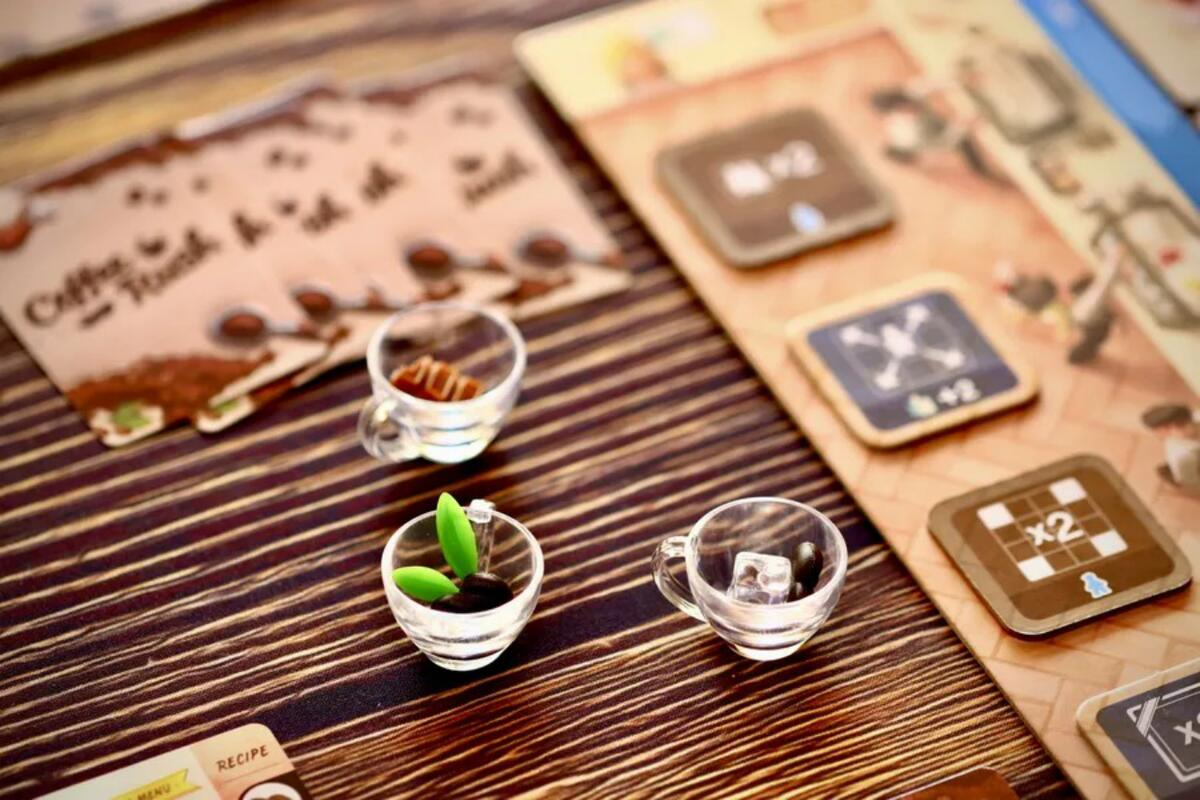
\includegraphics[width=5.2cm]{img/copertine/agd-coffee}};
  \node[polaroid, rotate=5]   at (\W/2+.2,\H-3.6) {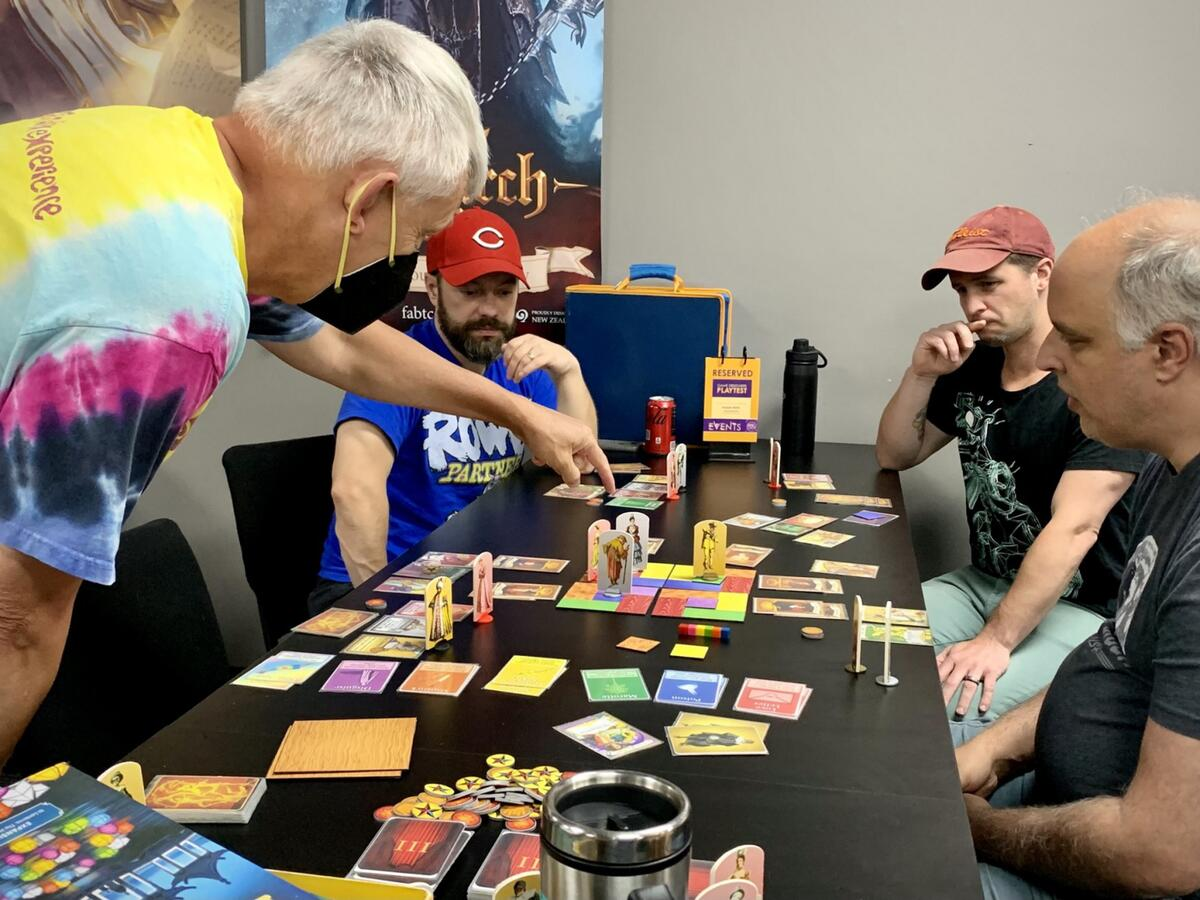
\includegraphics[width=4.6cm]{img/copertine/agd-playtest}};
  \node[polaroid, rotate=-3]  at (\W-4.2,\H-4.9) {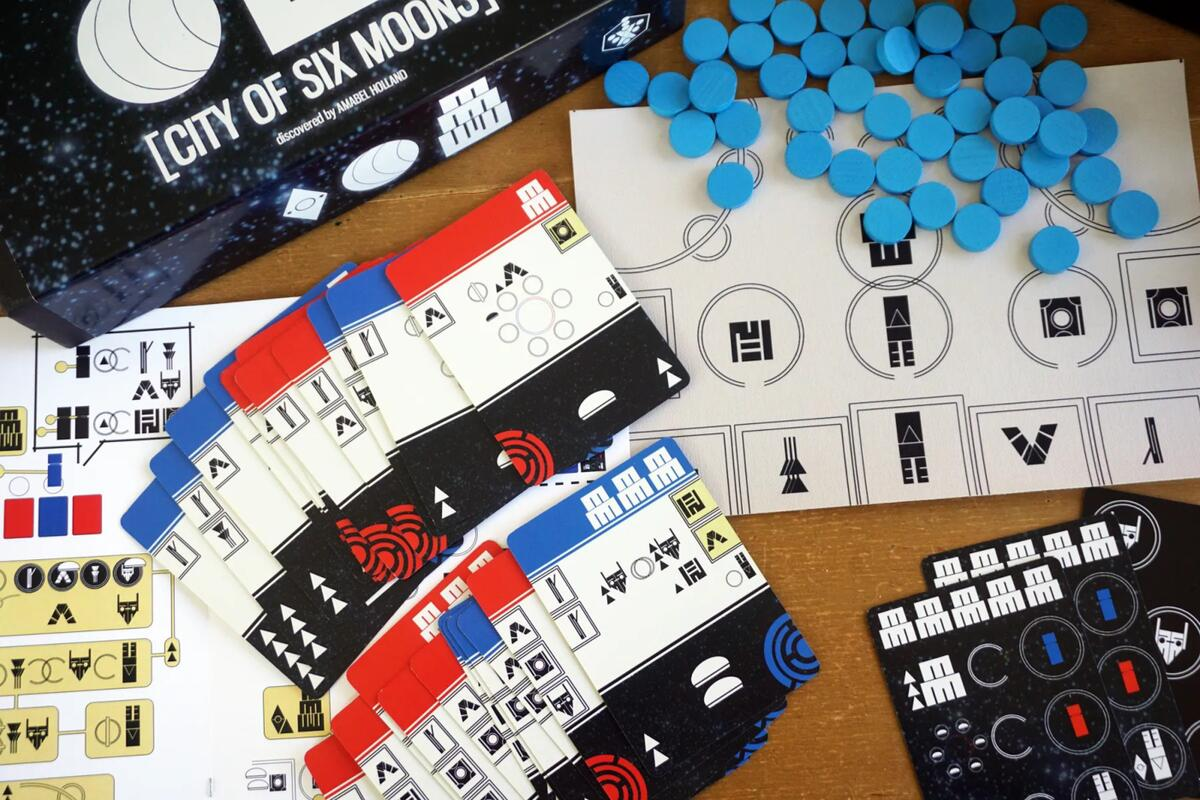
\includegraphics[width=5.0cm]{img/copertine/agd-city}};
  \node[polaroid, rotate=6]   at (3.8,7.9)  {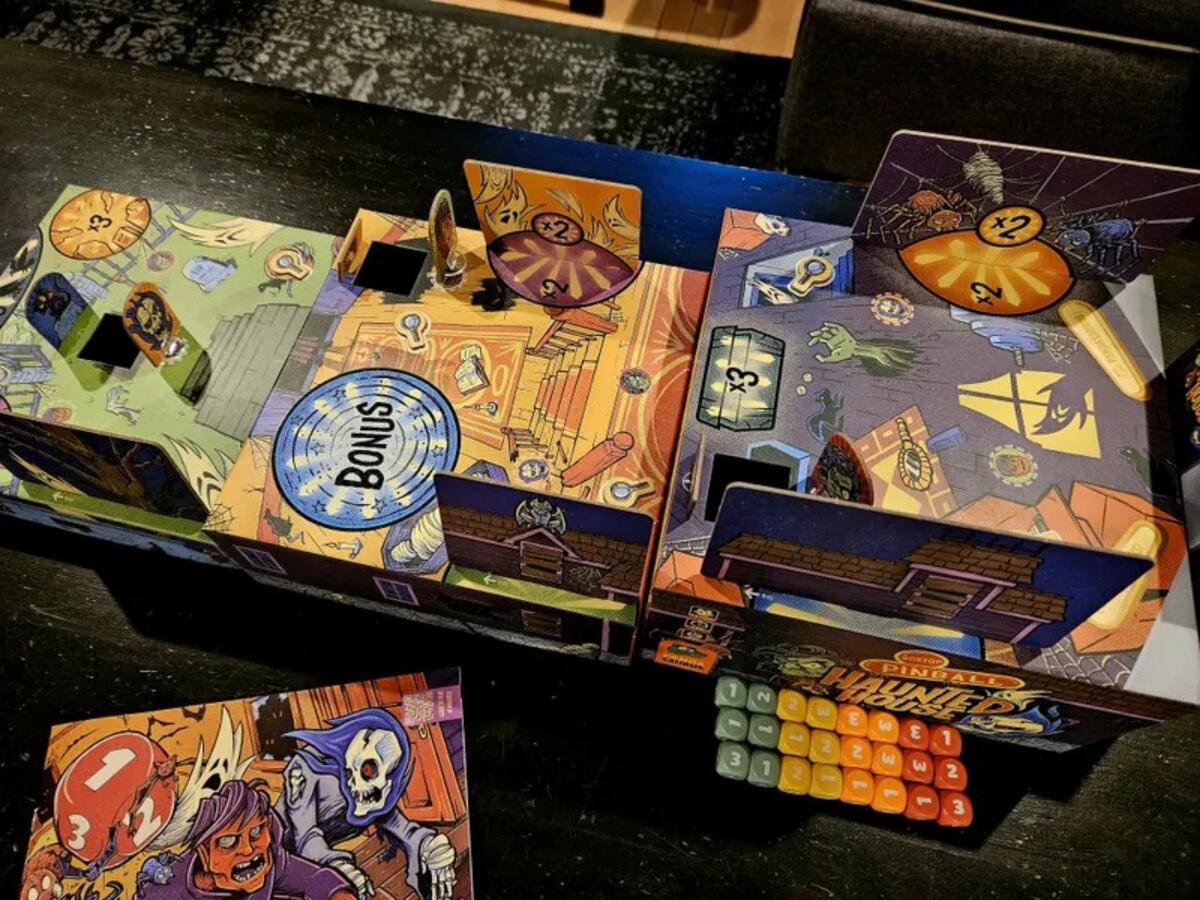
\includegraphics[width=4.8cm]{img/copertine/agd-pinball}};
  \node[polaroid, rotate=-4]  at (\W/2+.4,7.2) {
\includegraphics[width=4.6cm]{img/copertine/agd-larp}};
  \node[polaroid, rotate=4]   at (\W-4.0,7.8)  {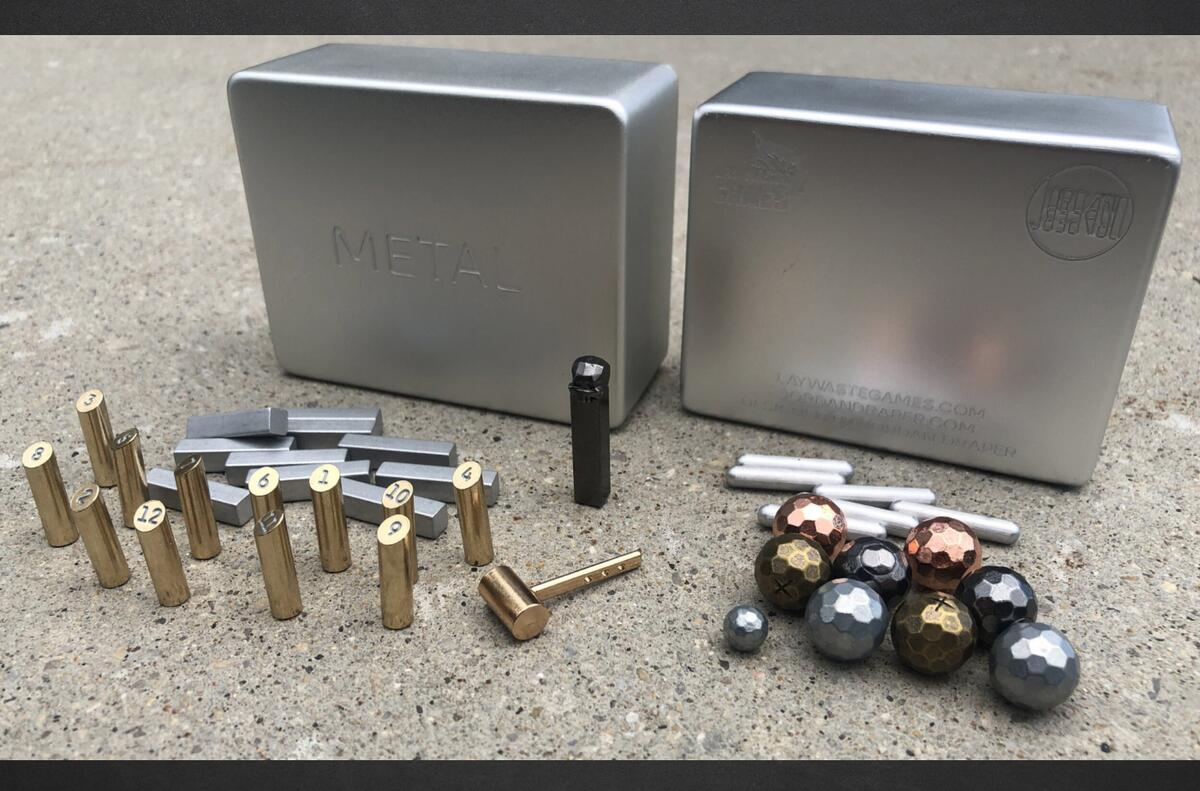
\includegraphics[width=4.8cm]{img/copertine/agd-metal}};
}

% Professioni: la rete dei mestieri
\def\copertina@professioni{%
  \fill[copTeal] (0,0) rectangle (\W,\H);
  \foreach \k in {1,...,9} \draw[copTealLight, opacity=.12, line width=.8pt] (\W/2,\H/2) circle (\k*1.6);
  \foreach \x/\y/\t/\i [count=\n] in {
      3.6/\H-3.6/Game designer/d, .5*\W/\H-2.6/Level designer/l, \W-3.6/\H-3.6/Narrative designer/n,
      3.6/4.4/Character animator/a, .5*\W/3.4/Programmatore/p, \W-3.6/4.4/3D artist/c} {
    \draw[copTealLight, line width=1.2pt, opacity=.6] (\x,\y) -- (.5*\W,.5*\H);
    \fill[white] (\x,\y) circle (1.35);
    \fill[copTealLight] (\x,\y) circle (1.15);
    \node[text=white, font=\sffamily\bfseries\small, below] at (\x,\y-1.45) {\t};
    \begin{scope}[shift={(\x,\y)}]
      \ifnum\n=1 \pic[fill=white, scale=.95, rotate=10] at (0,0) {dado5}; \fi
      \ifnum\n=2 \pic[scale=.55] at (0,-.6) {cubo}; \fi
      \ifnum\n=3 \node[fill=white, rounded corners=5pt, text=copTeal, font=\bfseries\Large, inner sep=4pt] at (0,0) {``\,\dots''}; \fi
      \ifnum\n=4 \begin{scope}[white, line width=2pt, line cap=round]
                 \fill (0,.55) circle (.2); \draw (0,.35) -- (0,-.2) -- (-.35,-.65); \draw (0,-.2) -- (.4,-.6);
                 \draw (-.45,.25) -- (0,.15) -- (.45,.4); \end{scope} \fi
      \ifnum\n=5 \node[text=white, font=\ttfamily\bfseries\LARGE] at (0,0) {\{\,\}}; \fi
      \ifnum\n=6 \begin{scope}[white, line width=1.4pt, scale=.55]
                 \draw (0,-1) -- (.87,-.5) -- (.87,.5) -- (0,0) -- cycle; \draw (0,-1) -- (-.87,-.5) -- (-.87,.5) -- (0,0);
                 \draw (-.87,.5) -- (0,1) -- (.87,.5); \end{scope} \fi
    \end{scope}
  }
}

% Game Design: flowchart, blockout e un rullino di immagini
\def\copertina@gamedesign{%
  \fill[copSlate] (0,0) rectangle (\W,\H);
  \draw[white, opacity=.05, step=1] (0,0) grid (\W,\H);
  % flowchart in alto
  \begin{scope}[shift={(0,\H-3.3)}, every node/.style={font=\sffamily\bfseries\small, text=copSlate}]
    \node[fill=copCyan, rounded corners=8pt, minimum width=2.2cm, minimum height=.9cm] (s) at (2.6,0) {Start};
    \node[fill=white, minimum width=2.6cm, minimum height=.9cm] (r) at (6.8,0) {Ricerca};
    \node[fill=copGold, diamond, aspect=1.7, inner sep=1.5pt] (d) at (11.2,0) {Funziona?};
    \node[fill=white, minimum width=2.4cm, minimum height=.9cm] (i) at (11.2,-2.2) {Itera};
    \node[fill=copCyan, rounded corners=8pt, minimum width=2.2cm, minimum height=.9cm] (e) at (15.8,0) {Vision};
    \draw[-{Stealth[length=3mm]}, white, line width=1.1pt] (s) -- (r);
    \draw[-{Stealth[length=3mm]}, white, line width=1.1pt] (r) -- (d);
    \draw[-{Stealth[length=3mm]}, white, line width=1.1pt] (d) -- node[above, text=white, font=\sffamily\scriptsize] {s\`i} (e);
    \draw[-{Stealth[length=3mm]}, white, line width=1.1pt] (d) -- node[right, text=white, font=\sffamily\scriptsize] {no} (i);
    \draw[-{Stealth[length=3mm]}, white, line width=1.1pt] (i) -| (r);
  \end{scope}
  % blockout isometrico ai lati
  \foreach \x/\y/\s in {1.6/.5*\H+5.6/.8, 2.6/.5*\H+5.1/.55, \W-1.8/.5*\H+5.4/.9, \W-2.9/.5*\H+5.0/.5}
    \pic[scale=\s] at (\x,\y) {cubo};
  % rullino
  \fill[black] (0,1.0) rectangle (\W,6.4);
  \foreach \k in {0,...,26} {
    \fill[copSlate!40] (.3+\k*.8,1.2) rectangle ++(.45,.3);
    \fill[copSlate!40] (.3+\k*.8,5.9) rectangle ++(.45,.3);
  }
  \foreach \f/\x in {gd-blockout/2.9, gd-uncharted/8.2, gd-interior/13.5, gd-liesofp/18.6}
    \node[inner sep=0pt] at (\x,3.7) {\includegraphics[height=3.9cm,width=4.9cm,keepaspectratio]{img/copertine/\f}};
}

% Revisioni: un foglio corretto a penna rossa
\def\copertina@revisioni{%
  \fill[copPaper] (0,0) rectangle (\W,\H);
  \foreach \k in {1,...,34} \draw[copRule, line width=.5pt] (0,\k*0.8) -- (\W,\k*0.8);
  \draw[copPen!70, line width=.8pt] (2.6,0) -- (2.6,\H);
  % righe di testo stilizzate in alto e in basso
  \foreach \y/\l in {\H-2.0/14, \H-2.8/16.5, \H-3.6/12, \H-4.4/15.5, \H-5.2/9,
                     6.4/15, 5.6/13, 4.8/16, 4.0/11, 3.2/14.5, 2.4/8} {
    \fill[black!45, rounded corners=1pt] (3.2,\y-.12) rectangle ++(\l,.24);
  }
  % correzioni
  \draw[copPen, line width=1.6pt, decorate, decoration={zigzag, amplitude=1.2pt, segment length=4pt}]
    (6,\H-2.8) -- (13.5,\H-2.8);
  \draw[copPen, line width=1.4pt] (10.6,\H-4.4) ellipse (2.8 and .45);
  \draw[copPen, line width=1.6pt, decorate, decoration={zigzag, amplitude=1.2pt, segment length=4pt}]
    (4.5,4.8) -- (12.5,4.8);
  \draw[copPen, line width=1.4pt] (8.8,2.4) ellipse (3 and .45);
  \node[text=copPen, font=\sffamily\bfseries\Huge, rotate=8] at (1.3,\H-3.6) {!};
  \node[text=copPen, font=\sffamily\bfseries\Huge, rotate=-6] at (1.3,4.0) {?};
  \foreach \x/\y in {19.4/\H-2.0, 19.4/6.4, 19.4/3.2}
    \draw[green!50!black, line width=2.4pt, line cap=round] (\x-.35,\y) -- (\x-.05,\y-.3) -- (\x+.5,\y+.45);
  % post-it
  \foreach \x/\y/\a/\t in {\W-3.4/\H-6.6/-6/Mostra{,} non scrivere!, 4.4/8.4/5/Fonte?, \W-4.0/8.0/4/Perch\'e?} {
    \node[fill=copPostit, drop shadow={opacity=.3}, rotate=\a, minimum width=3.6cm, minimum height=2.2cm,
          text width=3.2cm, align=center, font=\sffamily\bfseries\itshape\large, text=copPen] at (\x,\y) {\t};
  }
}

% --- Modi: volume autonomo o pagina di parte --------------------------------
\def\copertina@pannello{%
  \fill[white, opacity=.93, rounded corners=14pt, drop shadow={opacity=.35}]
    (2.2,\H/2-4.6) rectangle (\W-2.2,\H/2+4.6);}

\def\copertina@modo@libro#1{%
  \copertina@pannello
  \edef\copcol{\csname copertina@col@#1\endcsname}%
  \pgfmathsetmacro{\TW}{\W-6}%
  \fill[\copcol] (2.2,\H/2+3.4) rectangle (\W-2.2,\H/2+3.55);
  \node[text=\copcol, font=\sffamily\bfseries\large, anchor=south] at (\W/2,\H/2+3.7)
    {\csname copertina@vol@#1\endcsname};
  \node[text=\copcol, font=\sffamily\bfseries\fontsize{30}{34}\selectfont, text width=\TW cm,
        align=center] at (\W/2,\H/2+1.1) {\csname copertina@titolo@#1\endcsname};
  \node[text=black!70, font=\sffamily\large, text width=\TW cm, align=center]
    at (\W/2,\H/2-1.6) {\csname copertina@sotto@#1\endcsname};
  \fill[\copcol] (2.2,\H/2-3.0) rectangle (\W-2.2,\H/2-2.85);
  \node[text=black!80, font=\sffamily\bfseries\Large] at (\W/2,\H/2-3.75) {Lorenzo Vergata};
}

% Nella pagina di parte il testo stampato da \part cade poco sopra il centro
\def\copertina@modo@parte#1{%
  \fill[white, opacity=.93, rounded corners=14pt, drop shadow={opacity=.35}]
    (2.2,\H/2-0.4) rectangle (\W-2.2,\H/2+5.6);
  \edef\copcol{\csname copertina@col@#1\endcsname}%
  \fill[\copcol] (2.2,\H/2+0.4) rectangle (\W-2.2,\H/2+0.55);}

\newcommand{\disegnacopertina}[2]{%
  \begin{tikzpicture}[remember picture, overlay]
    \begin{scope}[shift={(current page.south west)}]
      \pgfmathsetmacro{\W}{\paperwidth/1cm}%
      \pgfmathsetmacro{\H}{\paperheight/1cm}%
      \csname copertina@#1\endcsname
      \csname copertina@modo@#2\endcsname{#1}%
    \end{scope}
  \end{tikzpicture}}

% Copertina a tutta pagina di un volume
\newcommand{\copertinaLibro}[1]{%
  \pagenumbering{Alph}%
  \begin{titlepage}
    \thispagestyle{empty}%
    \disegnacopertina{#1}{libro}%
    \null
  \end{titlepage}%
  \pagenumbering{arabic}}

% Pagina di parte illustrata (libro completo)
\newcommand{\partart}{}
\pretocmd{\@part}{\partart}{}{\PackageWarning{copertine}{Impossibile illustrare le parti}}
\pretocmd{\@spart}{\partart}{}{}
\newcommand{\parteillustrata}[2]{%
  \gdef\partart{\thispagestyle{empty}\disegnacopertina{#1}{parte}}%
  \part{#2}%
  \gdef\partart{}}
\makeatother



\title{Seminari per il Game Designer}
\author{Lorenzo Vergata}
\date{\today}
\hypersetup{pdftitle={Seminari per il Game Designer}, pdfauthor={Lorenzo Vergata}}

\begin{document}

    \copertinaLibro{seminari}
    \maketitle
    \tableofcontents

    % Contenuto della parte "Seminari per il Game Designer".
% Incluso sia dal libro completo (main.tex) sia dal volume autonomo corrispondente.
\renewcommand{\thechapter}{0.\arabic{chapter}} \renewcommand{\theHchapter}{sem.\arabic{chapter}}
\setcounter{chapter}{0}
% =====================================================================
%  Lezione zero 1 — Lavorare in squadra: la cultura del feedback
%  Fonte: trascrizione della prima "lezione zero" (GD0), prima giornata di
%  un workshop di due giorni tenuto prima dell'inizio del corso di Game
%  Design, dedicato alla figura professionale e al lavoro in team.
%  Pacchetti richiesti nel preambolo del libro:
%    \usepackage[italian]{babel}, \usepackage[T1]{fontenc},
%    \usepackage[utf8]{inputenc} (solo pdfLaTeX), \usepackage{booktabs}
%
%  Collocazione consigliata nel libro: le lezioni zero precedono il corso,
%  quindi vanno in una parte separata PRIMA di GD1, con numerazione propria
%  (0.1, 0.2, ...) così che i capitoli del corso conservino i numeri 1, 2, 3.
%  Nel file principale del libro, ad esempio:
%
%    \part{Lezioni zero: il game designer nell'industria}
%    \renewcommand{\thechapter}{0.\arabic{chapter}}
%    \setcounter{chapter}{0}
%    % =====================================================================
%  Lezione zero 1 — Lavorare in squadra: la cultura del feedback
%  Fonte: trascrizione della prima "lezione zero" (GD0), prima giornata di
%  un workshop di due giorni tenuto prima dell'inizio del corso di Game
%  Design, dedicato alla figura professionale e al lavoro in team.
%  Pacchetti richiesti nel preambolo del libro:
%    \usepackage[italian]{babel}, \usepackage[T1]{fontenc},
%    \usepackage[utf8]{inputenc} (solo pdfLaTeX), \usepackage{booktabs}
%
%  Collocazione consigliata nel libro: le lezioni zero precedono il corso,
%  quindi vanno in una parte separata PRIMA di GD1, con numerazione propria
%  (0.1, 0.2, ...) così che i capitoli del corso conservino i numeri 1, 2, 3.
%  Nel file principale del libro, ad esempio:
%
%    \part{Lezioni zero: il game designer nell'industria}
%    \renewcommand{\thechapter}{0.\arabic{chapter}}
%    \setcounter{chapter}{0}
%    \input{Seminari/GD0_1_cultura_del_feedback}
%    % ... altre lezioni zero ...
%    \part{Il corso di Game Design}
%    \renewcommand{\thechapter}{\arabic{chapter}}
%    \setcounter{chapter}{0}
%    \input{GD1/GD1_introduzione_al_game_design}
%    % ...
%
%  (Con hyperref aggiungere anche \renewcommand{\theHchapter}{z.\arabic{chapter}}
%  nella parte zero, per evitare ancore duplicate.)
%  Tutte le etichette di questo capitolo hanno il prefisso "z1:" per non
%  collidere con quelle dei capitoli del corso.
% =====================================================================

\chapter[La cultura del feedback]{Lavorare in squadra: la cultura del feedback}
\label{cap:z1-feedback}

Questo capitolo apre le \emph{lezioni zero}: incontri che precedono l'inizio
vero e proprio del corso di Game Design e che non riguardano una tecnica di
design in senso stretto, ma \textbf{la figura professionale} di chi lavora
nell'industria dei videogiochi. Prima di imparare a progettare un gioco
conviene infatti capire in che tipo di ambiente lo si progetterà: un ambiente
fatto di team, di gerarchie, di scadenze e, soprattutto, di persone che devono
riuscire a lavorare insieme.

La lezione è la prima giornata di un \textbf{workshop di due giorni} (circa
dieci ore in totale, pause pranzo comprese) tenuto da Stefano
Cozzi\footnote{Il cognome è riportato come compare nella trascrizione
automatica, che in più punti storpia i nomi propri; andrebbe verificato.
Nella stessa trascrizione lo studio per cui lavora appare come
``Stormine'', ``Stormline'' e ``Stormind'': si tratta di Stormind Games,
studio con sede a Catania, coerentemente con quanto detto in lezione.}, un
professionista con circa quindici anni di esperienza nel settore, tra
Blizzard Entertainment, Riot Games e, oggi, Stormind Games. Il workshop è
nato da un confronto con i coordinatori dell'accademia\footnote{Nella
trascrizione l'accademia è resa in modi diversi (``Hive'', ``a dive'',
``D.I.V.''); i coordinatori citati sono Enrico e Andrea, insieme al
direttore Diego Ricchiuti. Nel resto del capitolo si usa semplicemente
``l'accademia'', come negli altri capitoli.}: serviva un momento dedicato a
\emph{come ci si comporta in un ambiente professionale}, cosa che riguarda sia
il lavoro futuro sia i progetti di gruppo svolti durante il percorso di
studi, dove ci si deve già abituare a comportarsi ``come se si fosse in
un'azienda''.

La prima giornata ha un unico grande tema, sezionato in più parti:
\textbf{la cultura del feedback}. La seconda giornata (che sarà oggetto della
prossima lezione zero) sarà più pratica: \emph{time management},
\emph{brainstorming} e il ``guidare da dentro'' un team anche senza esserne
il leader (sezione~\ref{sec:z1-domani}).

Il percorso del capitolo segue quello della lezione:
\begin{enumerate}
  \item il formato del workshop e il percorso professionale del relatore
        (sezione~\ref{sec:z1-relatore});
  \item perché le aziende tengono tanto al lavoro di squadra e al
        \emph{fit} culturale (sezione~\ref{sec:z1-squadra});
  \item che cos'è il feedback e da che cosa dipende il modo di darlo
        (sezione~\ref{sec:z1-cose-feedback});
  \item le cinque fasi di vita di un team e il valore del
        \emph{post-mortem} (sezioni~\ref{sec:z1-fasi-team}
        e~\ref{sec:z1-qa-fasi});
  \item il confronto con i colleghi e alcune domande sul lavoro nei grandi
        studi (sezioni~\ref{sec:z1-rivalita} e~\ref{sec:z1-industria});
  \item il circolo virtuoso tra feedback, miglioramento e fiducia, e i suoi
        effetti sulla \emph{retention} e sulla cultura aziendale
        (sezioni~\ref{sec:z1-triangolo} e~\ref{sec:z1-cultura});
  \item il ``gioco del traditore'' e il principio del
        \textbf{default to trust} (sezioni~\ref{sec:z1-among-us}
        e~\ref{sec:z1-default-trust});
  \item le traiettorie di carriera e la valutazione delle performance
        (sezione~\ref{sec:z1-traiettorie});
  \item come si dà, come si riceve e quando si dà un feedback
        (sezioni~\ref{sec:z1-dare}, \ref{sec:z1-ricevere}
        e~\ref{sec:z1-quando});
  \item il feedback come regalo, le domande finali e le anticipazioni
        della seconda giornata (sezioni~\ref{sec:z1-regalo},
        \ref{sec:z1-qa-finale} e~\ref{sec:z1-domani}).
\end{enumerate}

Una premessa di metodo: il relatore ha alternato continuamente teoria,
domande alla classe e racconti della propria esperienza. I racconti non sono
digressioni: sono gli esempi concreti con cui i principi vengono resi
tangibili, e per questo sono riportati con cura.

% ---------------------------------------------------------------------
\section{Il workshop e il relatore}
\label{sec:z1-relatore}

\subsection{Formato e regole di partecipazione}

Il relatore ha cercato di ``riassumere quindici anni di esperienza in dieci
ore''. Ha materiale per circa il doppio delle ore disponibili: le cose
strettamente necessarie vengono trattate per prime, il resto è tenuto ``in
riserva'' come \emph{nice to have}. Le regole del workshop:
\begin{itemize}
  \item le domande si fanno \textbf{alla fine di ogni slide}, così da chiudere
        prima il discorso; non c'è un'unica sessione finale di domande e
        risposte (anche se ci sarà), perché il relatore preferisce fermarsi
        spesso e non fare ``uno spiegone di dieci ore'';
  \item le domande non devono per forza riguardare la slide appena vista: se
        una slide dà lo spunto per altro, se ne può parlare; al massimo sarà
        il relatore a rispondere in breve o a rimandare a una slide
        successiva;
  \item si può chiedere anche di esperienze passate, opinioni e sensazioni;
        se per NDA o per serietà professionale non può rispondere, lo dirà
        esplicitamente (``non lasciate che sia un \emph{blocker}'');
  \item su Zoom si usa l'alzata di mano o la chat, che il relatore tiene
        aperta sul secondo monitor;
  \item non ci sono pause ufficiali: la lezione è registrata e ognuno è
        libero di assentarsi quando serve, cercando però di non disturbare il
        flusso della lezione;
  \item le slide verranno fornite integralmente tramite la segreteria
        dell'accademia (Vanessa), insieme alle registrazioni: le slide senza
        il parlato servono poco, ma sono un buon promemoria.
\end{itemize}

\subsection{Il percorso professionale}

Il relatore si presenta (scherzosamente) come la ``guida escursionistica''
che accompagna la classe nella ``foresta incantata'' della cultura del
feedback, perché per molti è un territorio sconosciuto. Il suo percorso:
\begin{itemize}
  \item in Italia ha lavorato per aziende che fornivano servizi a terzi, tra
        cui il lavoro su \emph{Warhammer Online}, e per un canale televisivo
        sul digitale terrestre dedicato ai videogiochi\footnote{Nella
        trascrizione: ``Digital Game Network Channel''. Il nome esatto del
        canale andrebbe verificato.};
  \item a \textbf{Blizzard Entertainment} (circa sei anni, a Parigi) ha fatto
        il \emph{community manager} per l'Italia (\emph{StarCraft~II},
        \emph{World of Warcraft} da \emph{Mists of Pandaria} in poi,
        \emph{Hearthstone}, \emph{Diablo~III}, le espansioni di
        \emph{StarCraft}, il lancio di Battle.net), per poi diventare il
        manager dei community manager europei;
  \item a \textbf{Riot Games} (circa cinque anni, a Dublino) è stato
        brevemente community manager italiano e poi \emph{publishing
        manager} di un team di circa trenta persone per l'Europa. Il
        \emph{publishing} non è solo community: è l'unione di
        \textbf{community, marketing e PR};
  \item a \textbf{PG Esports} si è occupato di eventi dal vivo e online
        (ad esempio la Milano Games Week e tornei di \emph{Valorant} e
        \emph{League of Legends}), restando in contatto con Riot e Blizzard;
  \item da circa un anno è tornato nello sviluppo, a \textbf{Stormind
        Games}, dove oggi si occupa di risorse umane e organizzazione del
        lavoro; lo studio verrà presentato più ampiamente al \emph{Career
        Day} dell'accademia insieme alla sua HR manager;
  \item fa inoltre consulenze aziendali anche al di fuori dei videogiochi e
        insegna in master universitari (IULM di Milano).
\end{itemize}

Il suo ruolo ricorrente, sia a Blizzard sia a Riot, è stato quello di
\emph{Mr.~Wolf} (``per chi ha visto \emph{Pulp Fiction}''): quello che
risolve i problemi. Veniva inserito nei team più in difficoltà, ad esempio
dal punto di vista delle performance, per sistemarli e passare al successivo.
Era presente in alcuni dei momenti più critici, come il lancio di
\emph{Diablo~III} o il lancio di espansioni di \emph{World of
Warcraft}\footnote{La trascrizione riporta ``il lancio con i Gary's'' e
``World of Trenor'': si tratta verosimilmente di \emph{Mists of Pandaria} e
di \emph{Warlords of Draenor}.}, a fare \emph{damage control}.

La scoperta fondamentale di questi anni è che i problemi da risolvere
\textbf{quasi mai riguardavano il prodotto} (non era certo lui a sistemare i
server di \emph{Diablo~III}), ma i team che c'erano dietro: persone che
litigavano, non collaboravano, non riuscivano a stare nella stessa stanza
senza urlarsi contro. E nel 90\% dei casi tutto questo si riduce a
\textbf{problemi di comunicazione}: è raro che perfino le incompatibilità
caratteriali non siano risolvibili parlando.

\subsection{Struttura non vuol dire burocrazia}

A Stormind il relatore sta accompagnando un team passato da 30 a 95 persone
in meno di un anno, attraverso tutti i cambiamenti di cui parla il workshop.
Darsi una struttura viene spesso percepito male, come ``più processi, più
procedure'', ma bisogna distinguere:
\begin{itemize}
  \item un processo come ``timbrare il cartellino'' può essere davvero
        invasivo e noioso;
  \item definire \emph{come funziona un documento di game design, chi lo
        approva, chi lo visiona e chi no} è invece una struttura necessaria.
\end{itemize}
Uno studio di 30 persone nella stessa sede può farne a meno: quando c'è un
dubbio ci si alza e si va alla scrivania del collega. Uno studio di 95
persone sparse per l'Italia (e in parte per l'Europa) non può più farlo:
servono una struttura diversa, un modo di lavorare diverso e una
pianificazione del futuro diversa.

% ---------------------------------------------------------------------
\section{Perché il lavoro è sempre lavoro di squadra}
\label{sec:z1-squadra}

\subsection{Non si va in ufficio per fare amicizia}

Il primo messaggio è netto: \textbf{non si va in ufficio per fare amici} o
per trovare compagni di vita. Si va in ufficio perché c'è un lavoro da fare, e
lo scopo è riuscire a farlo \emph{anche con chi sta antipatico}. Con le
persone simpatiche è facile: diventeranno amici, e non sarà mai un problema.
È con chi sta antipatico che le cose si complicano, ed è lì che emergono i
\textbf{veri professionisti}: quelli che riescono a lavorare con chiunque
senza che l'antipatia pesi sul modo in cui lavorano e collaborano, mettendo il
prodotto e il team davanti al proprio ego e alle proprie preferenze personali.

La frase che fa da filo conduttore a tutto il workshop (e che il relatore
promette di riproporre ``fino alla nausea'') è:

\begin{quote}
  \emph{La capacità di un gruppo di persone di fare cose straordinarie
  dipende dal modo in cui queste persone operano insieme.}
\end{quote}

Le aziende raramente pensano che l'innesto di una singola persona possa
cambiare il destino di un progetto. Questo è tanto più vero quanto più grande
è il team, ma vale anche per i piccoli studi, anche per un gruppo di cinque
persone. Come negli sport di squadra: l'individuo conta fino a un certo punto,
e anche se si ha Dončić in squadra, se si gioca uno contro cinque si perde
comunque\footnote{Il riferimento è alle finali NBA in corso nei giorni del
workshop tra Dallas Mavericks e Boston Celtics (giugno 2024), il che
permette di datare approssimativamente la lezione.}.

\subsection{Lo \emph{useless genius} e il costo delle persone tossiche}

Molti dipartimenti HR usano la definizione di \textbf{useless
genius}\footnote{Il concetto è più noto in letteratura manageriale come
\emph{brilliant jerk}; in lezione è usata l'espressione \emph{useless
genius}.}: si può essere bravissimi, a volte i migliori nel proprio lavoro,
ma se non ci si sa comportare, relazionare e operare in un gruppo si è
fondamentalmente inutili ai fini del gruppo. Nel migliore dei casi inutili,
nel peggiore \emph{dannosi}.

In passato le aziende tendevano a ``chiudere un occhio'': la persona è
fondamentale, la teniamo. Oggi la domanda è diventata: \emph{quanto costa
all'azienda, oltre al suo stipendio, tenere una persona che crea un ambiente
tossico e peggiora chi le sta intorno?} Ci sono costi sommersi che le aziende
cominciano a vedere, e la tendenza è liberarsi di queste persone il prima
possibile. Il ragionamento è semplice:
\begin{itemize}
  \item le \textbf{competenze si possono trasmettere} o sostituire: si trova
        qualcuno che fa lo stesso lavoro magari nel doppio del tempo, oppure
        più persone che se lo dividono;
  \item il \textbf{carattere delle persone} invece cambia molto raramente.
\end{itemize}

\subsection{Il fit culturale}

Quando qualcuno \textbf{non è un \emph{fit} culturale} per un'azienda è
meglio separarsi presto. Ma non essere adatti a \emph{quell'}azienda non
significa non essere adatti a lavorare: è perfettamente legittimo che una
persona inadatta a un'azienda sia adattissima a un'altra.

Il relatore l'ha vissuto in prima persona. Dopo sei anni a Blizzard viene
contattato da Riot e affronta un processo di selezione lunghissimo (``quasi
undici colloqui''), al termine del quale viene scartato. Scrive allora una
mail che gli ha ``cambiato la traiettoria di carriera'': chiede
semplicemente perché non è stato ritenuto adatto. La risposta: in nessun
colloquio si era esposto abbastanza da far capire \emph{perché} volesse
lasciare Blizzard, e quindi pensavano che in realtà stesse bene dov'era. Il
motivo era che, per educazione professionale, non gli piace parlare male del
proprio posto di lavoro; portata all'eccesso, però, questa riservatezza era
diventata un ``è tutto bellissimo, ma vorrei provare Riot'', senza un perché.
Lo invitano comunque a un incontro dal vivo (``dal vivo è diverso''), e alla
fine viene assunto.

Una volta arrivato, i sei mesi di prova (\emph{probation}) sono serviti tutti
per smettere di ragionare e lavorare ``come a Blizzard''. La differenza
culturale era enorme, tanto che in Riot esisteva un gruppo di supporto
interno tra ex dipendenti Blizzard: un collega gliel'ha descritto come
``uscire da una relazione tossica e doversi riabituare a una relazione
normale''\footnote{Il relatore precisa che parla della Blizzard di allora,
che non esiste più: oggi è parte di Microsoft e nessuno dei suoi ex colleghi
vi lavora ancora, anche a causa dei licenziamenti di massa.}.
\begin{description}
  \item[Blizzard] era \emph{developer first}: il focus era chiaramente sugli
        sviluppatori, prima di tutti gli altri. Dopo sei anni c'erano ancora
        meeting a cui non poteva partecipare perché non abbastanza
        \emph{senior}, informazioni che non poteva sapere, piani che non
        poteva vedere.
  \item[Riot] era \emph{player first}: prima i giocatori, e i dipendenti come
        mezzo per trasferire il feedback dei giocatori dentro il gioco. Il
        secondo giorno lo portano in una stanza e gli mostrano il piano dei
        cinque anni successivi. Lui, sorpreso, pensa a un errore (``sono qui
        da oggi, non vorrei mettervi nei guai''); la risposta è: ``sei un
        dipendente Riot o no? Allora non ci sono livelli di accesso: devi
        sapere queste cose per fare meglio il tuo lavoro''.
\end{description}

Da questa esperienza ha imparato molto sulla \textbf{trasparenza}: condividere
le informazioni aiuta il lavoro. Non sempre, però: a volte non si condivide
qualcosa non per segretezza, ma perché non è ancora pronta per essere
presentata, esattamente come non si mostra un gioco quando è ancora solo
teoria (``te lo faccio vedere quando ho qualcosa di tangibile'').

La lezione per gli studenti è doppia: le aziende valuteranno il \emph{fit}
culturale sempre di più, ma capire se si è un \emph{fit} richiede anche
\textbf{lavoro da parte del candidato}. Bisogna avere la presenza di spirito
di dire: ``conosco i valori di questa azienda, non mando nemmeno il CV,
perché so che durerei un mese e mezzo''.

% ---------------------------------------------------------------------
\section{Che cos'è il feedback}
\label{sec:z1-cose-feedback}

\subsection{Le prime risposte della classe}

La prima domanda alla classe è: \emph{quando sentite la parola
``feedback'', a cosa pensate?} Le risposte raccolte, a voce e in chat:
\begin{itemize}
  \item un \textbf{riscontro} su ciò che si fa e su come lo si fa, sul lavoro
        o sul modo in cui ci si interfaccia con il gruppo; può essere
        lavorativo oppure comunicativo e comportamentale. Chi ha risposto lo
        vede come qualcosa che, se l'azienda non dà, va attivamente
        richiesto, perché è importante sapere come sta andando per
        migliorarsi;
  \item né positivo né negativo, ma \textbf{costruttivo}: in entrambi i casi
        serve a migliorarsi;
  \item uno \emph{scambio di opinioni}, un \emph{riscontro produttivo};
  \item un feedback ``di reazione'', non verbale: si fa una cosa e si
        osserva come cambia l'ambiente o il comportamento delle persone
        intorno (anche perché a voce la gente spesso si tiene le cose
        negative);
  \item per un designer, anche il \textbf{linguaggio del corpo}: osservando
        un giocatore giocare si può dedurre l'emozione che prova (frustrazione,
        incomprensione).
\end{itemize}

Sulla forma (scritto o orale?) le opinioni divergono: c'è chi lo preferisce
\emph{mille volte} scritto; chi pensa che dipenda dalle dimensioni
dell'azienda (orale nelle piccole, scritto in quelle con team di centinaia di
persone); chi pensa che dipenda dall'importanza del feedback (scritto se
tecnico o pieno di dati, da tenere sotto gli occhi; orale se è un consiglio
veloce).

Il relatore usa due esempi per mostrare che \emph{dipende}:
\begin{itemize}
  \item un feedback sulla programmazione ha senso darlo scritto, magari
        commentando direttamente il codice, più che ``andando a prendere un
        caffè'';
  \item ma se il feedback è ``ieri, durante il meeting, ho percepito male il
        fatto che mi interrompessi di continuo'', ce lo si aspetta
        \textbf{orale}.
\end{itemize}

\subsection{Da che cosa dipende il modo di dare feedback}

Lo \emph{spoiler} della giornata è che \textbf{non esiste una risposta univoca}
su come dare feedback. Il workshop non insegna ``il'' modo, ma fornisce
\emph{tutte le opzioni}, perché il modo giusto cambia in base a molti fattori:
\begin{itemize}
  \item a chi lo si dà: un collega, un superiore, il proprio capo, un proprio
        \emph{report} (un sottoposto);
  \item se è personale o professionale;
  \item se è la prima volta o la terza volta che si dà lo stesso feedback;
  \item se riguarda un progetto importante o secondario.
\end{itemize}

Manca però l'elemento fondamentale, che la classe individua subito:
\textbf{l'altro}. A parità di tutti gli altri fattori, il \emph{carattere
della persona che riceve il feedback} dovrebbe far cambiare il modo in cui lo
si dà. Per questo, prima della lezione, agli studenti era stato chiesto di
fare un test di personalità: non un test di psicologia avanzata, ma uno
strumento per rendersi conto di quanta varietà ci sia anche solo in una
classe di 53 persone (il che non vuol dire trovare 52 modi diversi di dare
feedback, ma lavorarci un po' sì).

Il relatore porta se stesso come esempio. Preferisce:
\begin{itemize}
  \item i feedback \textbf{positivi scritti}, perché è a disagio a ricevere
        complimenti in pubblico;
  \item i feedback sul proprio lavoro \textbf{diretti}: ``vai subito al
        punto e non girarmi intorno''.
\end{itemize}
È molto orgoglioso del suo lavoro e, quando qualcuno lo critica, la sua
primissima reazione istintiva è ``come ti permetti''. Negli anni ha imparato
a farla durare un secondo, ma chi gli dà feedback di persona dice di
vederla ancora negli occhi. Per mitigarla, dice esplicitamente a chi gli dà
feedback: \emph{``ignora il modo in cui reagisco nei primi cinque secondi,
vai avanti, poi mi passa''}. È considerato da tutti molto aperto al feedback
e non ha problemi a dire ``hai ragione, facciamo diversamente'': ma ci sono
reazioni istintive e caratteriali che è difficile controllare al cento per
cento.

\subsection{Con chi si lavora meglio}

Guardando le persone con cui si lavora abitualmente (anche nei progetti
dell'accademia), si noterà che si lavora meglio con due profili:
\begin{enumerate}
  \item chi è \textbf{esattamente come noi}, ma qui è un 50 e 50: alcuni
        caratteri vanno d'accordo con i propri simili, altri non vogliono
        nessuno con lo stesso carattere nel gruppo (e si potrebbe rientrare
        in questa categoria);
  \item chi è \textbf{affine}: ha qualcosa in comune con noi, ma non tutto,
        e proprio per questo può dare punti di vista differenti.
\end{enumerate}
Il lavoro della giornata è capire come valorizzare il secondo caso: ottenere
feedback da persone con caratteri, visioni e background diversi, per
completare una visione del proprio lavoro che è necessariamente limitata. È
come esplorare una mappa con la nebbia di guerra: un'altra persona, al di là
del muro, vede cose che noi non vediamo.

\subsection{Il feedback come somma di piccoli miglioramenti}

Per il relatore il feedback è questo: \textbf{applicare tanti piccoli
miglioramenti periodici}, che si sommano nel tempo. Migliorare dello 0,1\%
ogni giorno porta a fine anno a un miglioramento enorme, e questo vale per i
prodotti, per i giochi, per le persone e per i team.

\paragraph{L'esempio del ciclismo britannico.} La squadra di ciclismo
britannica, fino a una quindicina d'anni fa, non aveva vinto quasi nulla.
Cambiato il team manager, tutti si aspettavano grandi cambiamenti sportivi
(convocazioni, strategie di gara). Arrivarono invece \emph{minuscoli
cambiamenti non sportivi}: un altro chef in trasferta, materassi migliori nei
camper per riposare meglio, un sellino più comodo a fine tappa. Cambiamenti
marginali che da soli non avrebbero cambiato niente; eppure, dopo due o tre
anni di questo lavoro quotidiano, la squadra ha cominciato a vincere a
ripetizione, Olimpiadi comprese, cambiando il modo in cui il ciclismo è
visto in Gran Bretagna\footnote{È la nota strategia delle \emph{marginal
gains} associata a Dave Brailsford (British Cycling e Team Sky); il nome non
è citato in lezione.}. Certo, si è investito anche sulle persone giuste, ma
tutto è partito dai piccoli miglioramenti periodici.

Per gli studenti vale lo stesso: chiarire un conflitto con una persona con
cui si ha ancora poco a che fare, o una situazione che ha lasciato
``l'amaro in bocca'', sembra inutile oggi, ma darà i suoi frutti tra tre, sei,
nove mesi. Sono \emph{investimenti sul futuro}.

\paragraph{Peggiorare ogni giorno.} Esiste anche il percorso inverso:
lasciar correre, ``buttare sotto il tappeto'' le cose perché ``tanto è
inutile parlarne''. Queste cose tornano sempre fuori dopo otto mesi, come il
\emph{libro dei rancori} dei nani di Warhammer: ``ti ricordi quando, un anno
e mezzo fa, all'inizio del progetto, mi hai detto quella cosa? Mi sono
offeso''. A quel punto è quasi impossibile risolvere, perché nessuno ricorda
più con precisione cosa sia successo (``ma quale cena?'', ``forse era in
pizzeria'', ``no, eravamo da un'altra parte''). \textbf{Tenersi le cose nel
cassetto per tirarle fuori quando servono è sempre sconsigliato}: non servono
ed è impossibile usarle in modo costruttivo.

% ---------------------------------------------------------------------
\section{Le cinque fasi di vita di un team}
\label{sec:z1-fasi-team}

\subsection{Perché conoscerle}

Quasi tutti gli studenti lavorano già in gruppo (al primo anno su un gioco da
tavolo, negli anni successivi su un videogioco) e si saranno accorti che un
team attraversa delle fasi: il modo di lavorare insieme cambia nel tempo.
Spesso ci si fa prendere di sorpresa: ``eravamo così affiatati, cosa è
successo?''.

Un esempio da una consulenza fuori dai videogiochi: un'azienda farmaceutica
gli affida un team commerciale (rappresentanti che presentano medicinali a
ospedali, medici e privati). Il problema: ``prima andava tutto bene; ora che
siamo in diciotto dovremmo lavorare meno e meglio, e invece va peggio''. Va
peggio perché le persone nuove sono appena arrivate, mentre il management si
aspettava già di vedere i risultati dell'investimento.

Fino a pochi anni fa le fasi di un team venivano disegnate come una
\textbf{linea dritta verso l'alto}: le fasi erano le stesse, ma viste come un
miglioramento costante. Non si vedevano le parti \emph{fisiologiche} del
lavoro in team, cioè anche i peggioramenti. Accettarle è il primo passo per
accettare i fallimenti: nessun percorso personale o di team è lineare.

Il relatore ammette che il suo modo di lavorare è nato per il 70\% dal
proprio impegno a imparare, fare bene e rispettare le persone, e per il 30\%
dall'aver lavorato con ``incapaci colossali'' che gli hanno insegnato come
\emph{non} fare le cose. A Blizzard un manager gli fece capire che, pur non
sapendo ancora che tipo di \emph{people manager} sarebbe diventato, sapeva
benissimo quale tipo di manager \emph{non} voleva essere.

\subsection{Forming, storming, norming, performing, adjourning}

Le fasi sono cinque, un po' come le fasi del lutto. Molte aziende ne
considerano solo quattro (``e sono quelle che solitamente chiudono''); le
aziende al passo con i tempi ne considerano cinque\footnote{Il modello è
quello di Bruce Tuckman (1965), a cui la quinta fase, \emph{adjourning}, fu
aggiunta nel 1977. Il nome di Tuckman non è citato in lezione; la
trascrizione riporta la quinta fase come ``journing''.}.

\begin{description}
  \item[Forming] Si viene messi insieme e si comincia a lavorare. Non si sa
        nulla degli altri; spesso non si conoscono nemmeno i nomi, ed è
        normale.
  \item[Storming] Si cominciano a ``dare le testate come le capre in
        montagna per determinare il territorio'': questa cosa la faccio io,
        questa la vorrei fare così, chi decide? Si stabilisce chi fa cosa e
        come si divide il lavoro. Nel grafico è una \textbf{fase di
        peggioramento}: che il team litighi o discuta civilmente non cambia
        nulla, il team deve investire parte di tempo ed energie per risolvere
        queste questioni. È normale e \textbf{non è evitabile}.
  \item[Norming] Si comincia a capire come lavorano gli altri, cosa sanno
        fare e come far funzionare il gruppo; iniziano i miglioramenti. È una
        forma di \emph{accettazione} degli altri, che deriva dall'aver capito
        cosa devo fare io e cosa devono fare loro.
  \item[Performing] C'è uno sforzo \textbf{proattivo}: ``questa cosa
        toccherebbe a me, ma so che Alessio la fa molto meglio, quindi gli
        chiedo aiuto''. Si sfruttano i punti di forza degli altri, perché li
        si conosce e perché si sa che passare il testimone non avrà effetti
        negativi (il capo non dirà ``perché non l'hai fatta tu?'').
  \item[Adjourning] Il progetto finisce, si chiude o viene riorganizzato, il
        team viene sciolto. Quello che andrebbe fatto è analizzare
        \textbf{cosa ha funzionato, cosa no e cosa migliorare} per il
        progetto successivo.
\end{description}

\subsection{La fase che tutti saltano}

``Spoiler incredibile'': l'\emph{adjourning} è la fase che molte aziende
saltano, \textbf{perché c'è sempre il progetto dopo}.

A PG Esports, per la Milano Games Week (come per qualsiasi evento dal vivo a
cadenza annuale: Lucca Comics, Etna Comics, Comicon\dots), finita l'edizione
di un anno si cominciava dal giorno dopo a lavorare a quella successiva,
perché un anno sembra tanto ma non basta mai. Nei videogiochi è lo stesso:
finito un gioco, a parte le patch di mantenimento e del \emph{day one}, si
passa subito al successivo.

Il cambiamento introdotto dal relatore (in parte già praticato, ma da lui
strutturato) è stato: finita la Games Week, \textbf{tutti in ferie per una
settimana}; poi ci si ritrova per definire cosa ha funzionato e cosa no, con
un \textbf{post-mortem} (o \emph{debrief}); solo dopo si inizia a lavorare
all'edizione successiva. Senza questa fase manca la parte di
\emph{learning}, cioè di ciò che si è imparato dal progetto.

Il consiglio vale per gli studenti: quando si finisce il gioco da tavolo, e
poi il gioco digitale, bisogna trovare il tempo per il post-mortem,
altrimenti si butta via \textbf{il 90\% dell'utilità del progetto}. Una
struttura semplice per farlo è descritta nella sezione~\ref{sec:z1-qa-finale}.

% ---------------------------------------------------------------------
\section{Domande sulle fasi del team}
\label{sec:z1-qa-fasi}

\subsection{Lo storming che ritorna}

\paragraph{Capita che lo storming si ritagli spazio anche nelle altre fasi?}
Lo \emph{storming} è una fase precisa, che però molti manager, coordinatori e
team cercano di \textbf{saltare}: ``se io sono bravo come manager e loro sono
bravi come team, passeremo da forming a norming senza problemi''. È un errore,
perché senza una fase in cui si discute davvero non si sviluppa una
\emph{skill} fondamentale: \textbf{saper discutere}. Tutti conoscono persone
non abituate a farlo, per cui ogni minimo disaccordo diventa un affronto
personale (``avevamo deciso la pizza, perché andiamo al sushi? Perché mi fate
questo affronto?''): sono persone che non sono abituate ad avere conflitti
costruttivi.

Se si pensa di essere in \emph{norming} e continuano a emergere conflitti, il
punto è che \textbf{non si era davvero in norming}: lo storming non ``si
trascina'' nelle fasi successive, semplicemente non se n'è mai usciti.
Allo stesso modo, a chi chiede se ogni mini-fase di storming durante la vita
del gruppo sia frutto di uno storming fatto male o solo di carattere, la
risposta è già contenuta qui.

Un partecipante osserva che spesso, ancor prima di finire un progetto, si è
già messi su quello successivo: è il modo migliore per essere in costante
\emph{damage control}. Era l'esperienza del relatore a Blizzard: veniva
spostato fisicamente da un team all'altro, e finito il lancio di
\emph{Diablo~III} era già su \emph{World of Warcraft}, senza vivere il
``dopo''. Si è dovuto ritagliare da solo lo spazio per un debrief personale,
ed è lì che ha deciso che tipo di manager non voleva essere. Il consiglio:
\textbf{se non lo fa il team, fatelo voi}.

\subsection{Dove si passa la maggior parte del tempo}

\emph{In quale fase si passa più tempo nella propria carriera?} Gli studenti
rispondono \emph{storming} e \emph{norming}. Il relatore, in quindici anni,
calcola di aver passato in \emph{performing} circa \textbf{dieci mesi}. Non è
pessimismo: arrivare a performing deve essere sempre l'obiettivo, sia da
manager sia da membro del team; ma è difficile arrivarci, ed è normale che non
sempre ci si arrivi.

Lo storming può durare a lungo, ma con team molto esperti dura pochissimo,
perché c'è chi lo sa gestire. In realtà \textbf{la maggior parte del tempo si
passa in forming}, perché ogni equilibrio raggiunto vale per \emph{quelle}
persone, \emph{quel} progetto, \emph{quelle} tempistiche. Basta che cambi un
qualsiasi fattore (una deadline spostata, una persona nuova, qualcuno che si
dimette, un progetto cancellato) e si ricomincia, perché i bilanciamenti
precedenti non valgono più.

Esempio: un team di cinque persone affiatatissimo, in pieno performing. La
dirigenza, entusiasta, ``raddoppia le risorse'' e lo porta a dieci. O si
lascia tutto com'è (e i cinque nuovi non fanno niente), o bisogna ridiscutere
chi fa cosa e come i nuovi possono aiutare: che piaccia o no, si ricomincia
da forming.

Quindi la bravura di un manager, ma anche di un membro del team,
\textbf{non sta nel passare tanto tempo in performing, ma nell'accelerare il
passaggio da una fase all'altra}, e nel fare bene la fase di
\emph{adjourning}.

\subsection{Analizzare anche i successi}

C'è la tendenza a fare post-mortem solo dei progetti andati male: ``questa
cosa non ha funzionato, vediamo perché''. Va benissimo. Ma quando un progetto
va bene si dà per scontato che sia andato bene ``perché era buono''. Bisogna
invece chiedersi \emph{perché} è andato bene: era il prodotto? La
tempistica? Il modo in cui abbiamo fatto una cosa piuttosto che un'altra?
\textbf{Se non si capisce davvero il motivo del proprio successo, si
tenderanno a replicare le cose sbagliate.}

\paragraph{Blockbuster.} Quando arrivò la notizia che Netflix avrebbe
lanciato un servizio di streaming, Blockbuster (la catena di noleggio di
videocassette e DVD) aveva tutto il tempo per preparare un'offerta
concorrente. In una riunione del management raccontata in un libro (di cui il
relatore non ricorda il titolo), la direzione sembrava orientata a investire
nello streaming, finché un dirigente fece notare che il 12\% del fatturato
derivava dalle \emph{multe per riconsegna tardiva}, impossibili con lo
streaming, mentre secondo le stime lo streaming avrebbe prodotto il 10\% del
fatturato. ``Non possiamo rinunciare a questo 2\%'': niente streaming. Oggi
non c'è più un Blockbuster ``manco a cercarlo col lanternino''. Non avevano
capito qual era il vero motivo del loro successo, cioè il loro modello di
business\footnote{Le percentuali sono quelle riferite in lezione e non sono
state verificate.}.

\paragraph{The Founder.} Nel film sulla nascita di McDonald's c'è una scena in
cui il futuro socio del protagonista gli dice: ``tu pensi di essere nella
\emph{food industry}, e invece sei nella \emph{real estate industry}''. Non
dovrebbe investire sugli hamburger, ma sui terreni su cui costruisce i
ristoranti. Anche per un team vale lo stesso: bisogna capire che cosa
l'ha reso davvero di successo, oppure no.

\subsection{L'autoanalisi personale}

\paragraph{E quando si cambia azienda?} Uno studente chiede se il debrief sia
possibile anche quando si lascia un'azienda. Non si può tornare in ufficio a
discutere della propria esperienza, ma lo si può fare \textbf{per se stessi}.
Il relatore l'ha fatto, anche se all'epoca in modo poco consapevole, ed è
così che è passato dal \emph{community management} al \emph{people
management}. Analizzando cosa aveva fatto bene a Blizzard si era reso conto
che:
\begin{itemize}
  \item aveva costruito un ottimo rapporto di fiducia con i giocatori (con
        alcuni proprietari di fansite parla ancora oggi);
  \item pur senza la seniority, era diventato un punto di riferimento per il
        team, visto come imparziale ed equilibrato anche su temi che non lo
        riguardavano direttamente;
  \item sapeva \textbf{risolvere problemi}: durante il lancio di
        \emph{Diablo~III} era il più tranquillo di tutti, non perché
        sminuisse il problema, ma perché sapeva che si sarebbe risolto con i
        suoi tempi; il lavoro non era spegnere l'incendio ma ``far sfollare
        la gente'' e aspettare che tutto tornasse in ordine.
\end{itemize}
E aveva capito cosa sapeva fare meno bene, ad esempio \textbf{gestire il
proprio manager}. Avere un manager non significa che il manager gestisca te:
il manager gestisce il tuo lavoro, ma tu devi saper gestire i tuoi
\emph{stakeholder}. Spesso lo stakeholder è il proprio manager; da manager,
gli stakeholder saranno CEO, CFO e così via. Gestirli significa conoscerli,
sapere come portare loro le informazioni, come far presente che qualcosa non
va. Fa parte del lavoro, anche se a lui non piace, e ci ha lavorato.

Nel mese e mezzo di pausa prima di entrare in Riot si è concentrato su
questo: ``cosa porto come mio punto di forza?''. L'autoanalisi è culminata
nel chiedere espressamente alla persona che l'aveva assunto: ``prima mi avete
detto di no, ora mi avete preso: perché?''.

\paragraph{Come si capisce se un progetto è andato bene?} Dipende
dall'\textbf{obiettivo}. Se l'obiettivo era vendere milioni di copie e il
gioco le ha vendute, bisogna capire perché. Se, più ragionevolmente,
l'obiettivo era un gioco da tavolo che permettesse di mettere in pratica le
conoscenze del corso, va valutato per quello: ha permesso di farlo? Se sì,
perché? Se no, perché no? L'obiettivo va fissato \textbf{all'inizio del
progetto, non alla fine}, proprio per poterlo valutare dopo.

\subsection{Quando il team cambia di continuo}

\paragraph{Tutti questi cambiamenti non sono dannosi per il progetto?}
Assolutamente sì, ma quasi mai sono volontari. I progetti andati male sono
spesso progetti grandi.

Il relatore racconta di \emph{Cyberpunk 2077}. Conosceva persone in CD
Projekt Red (``il mondo è piccolissimo, le cose si sanno''). Alla Gamescom va
con Diego Ricchiuti, direttore dell'accademia, a vedere la presentazione del
primo gameplay, quella ``in cui regalavano il giubbottino da samurai''.
Finito il video, tra gli applausi, si guardano e capiscono entrambi che
\textbf{il gioco non è pronto}, a soli quattro mesi dall'uscita prevista:
Diego aveva notato il combattimento e la guida. Gli amici di CD Projekt Red
(uno aveva lavorato con lui a Blizzard per sei anni) gli confermano tra le
righe che ``ce la faremo, ma ci sono ancora cose da sistemare''. Il gioco fu
poi rimandato più volte\footnote{In lezione il relatore dice ``due, forse
tre volte''; l'uscita di \emph{Cyberpunk 2077} è stata effettivamente
rinviata tre volte prima del dicembre 2020.}.

Per deformazione professionale, chi ha sviluppato l'occhio critico non
riesce più a godersi un trailer: in un trailer di \emph{The Day Before} Diego
gli aveva fatto notare che l'effetto della fiammata di un fucile era stato
chiaramente aggiunto in postproduzione e non faceva parte del gameplay. ``È
il triste epilogo di questa storia'': non riescono più a godersi un trailer.

Il punto è che più il team è grande, più queste variabili vengono imposte, e
più è facile che il fallimento \textbf{non dipenda dal fatto che il prodotto
sia brutto} (\emph{Cyberpunk} è un bellissimo gioco sotto molti punti di
vista, e il relatore lo sta rigiocando ora che è stato corretto ed espanso).
Nei grandi gruppi qualcuno arriva, qualcuno si dimette, cambia il budget,
arriva il rinvio; nel caso di \emph{Anthem}, il team ha fatto così tante volte
forming--storming--forming--storming che ne è uscito ``un prodotto che
dovevamo espellere: l'abbiamo espulso, buttato fuori dal nostro organismo pur
di liberarcene''.

Tra i cambiamenti c'è anche la crescita verticale: se il capo viene promosso
perché lavora benissimo, bisogna scegliere un nuovo capo, ed è sempre un
caos (chi ci resta male, chi pensava di meritarlo, chi voleva il suo amico,
chi non sopporta il prescelto). Per questo il relatore è \textbf{contrario
alle promozioni durante i progetti}: si rischia di rovinare tutto il lavoro di
storming.

\subsection{Obiettivi chiari nei piccoli gruppi}

Nei gruppi piccoli, come quelli degli studenti, il problema deriva più
spesso dal \textbf{non avere chiaro che cosa si vuole ottenere}: un prodotto
puramente educativo e formativo, o un prodotto richiesto dall'accademia che,
se viene bene, si potrebbe anche vendere? Un gioco commerciale o un gioco
artistico? Va chiarito subito, perché ci saranno sempre momenti in cui
scegliere tra A e B, e a guidare la scelta sarà la domanda: \emph{quale delle
due opzioni ci porta più vicino all'obiettivo?} Se l'obiettivo non è chiaro,
non si sa cosa scegliere.

Questo porta molte aziende a fare \textbf{scelte di design che in realtà sono
scelte commerciali}. Le microtransazioni sono scelte commerciali: nessuno ha
mai pensato ``sai cosa piacerebbe tanto ai giocatori? Pagare le bustine''.
Prima le bustine si guadagnavano giocando; ora la tendenza è ``potresti
giocare, ma se paghi è meglio''. Si pensi alle polemiche su Ubisoft per
l'opzione di ``saltare il gioco'' pagando, o ai famosi \emph{boost} di livello
di \emph{World of Warcraft}: ``devo pagarti per saltare il gioco?''.

Una studentessa (Silvia) cita \emph{Final Fantasy XIV}, che a un certo punto fu
``resettato'' perché non funzionava: un esempio positivo. Il relatore aggiunge
quello negativo di \emph{Age of Conan}, che non è mai riuscito a fare quel
reset iniziale (``è una schifezza, ve lo ripresentiamo quando è pronto''). Ci
vuole consapevolezza, ma anche i mezzi: un conto è Square Enix, che può
permetterselo, un altro è un'azienda che non può chiudere tutto per un anno
continuando a pagare gli stipendi.

Riassumendo: nei piccoli gruppi i problemi sono più di
\textbf{comunicazione e chiarezza} (obiettivi non chiari o che si spostano);
nelle grandi aziende di più di \textbf{persone che vanno e vengono, obiettivi
e tempistiche che cambiano}. In accademia le scadenze sono fisse (il gioco da
tavolo si consegna a fine anno scolastico, a giugno, e giugno resta); in
azienda può succedere che una feature prevista per la \emph{vertical slice}
di luglio venga anticipata a maggio per portarla alla Gamescom, e un sistema
perfetto per consegnare a giugno può non esserlo più per consegnare a maggio.

\subsection{L'ambiente determina la qualità del prodotto}

\paragraph{È vero che chi passa per Electronic Arts finisce per fare brutti
giochi?} Uno studente cita BioWare, che faceva ottimi giochi finché era
autonoma. Il problema non è dei developer, che non sono ``improvvisamente
diventati incapaci'': è evidente che il problema è altrove, e che
\textbf{l'ambiente in cui si fa un gioco determina molto spesso la qualità del
prodotto}.

Un esempio locale positivo: Tommaso Bonanni, conosciuto dal relatore insieme a
Diego e già docente dell'accademia, ha fondato a Roma Caracal Games Studio,
applicando fin dall'inizio questi concetti di cultura aziendale. L'azienda è
rimasta piccola, ma ha molto chiaro cosa vuole fare e come. Quando si
predispone fin dall'inizio l'azienda e il team a lavorare in un certo modo è
fattibilissimo; è molto più difficile quando si è EA, si acquisisce
un'azienda e le si dice ``da oggi si fa così''.

Il relatore ha vissuto la transizione da Blizzard ad Activision Blizzard (uno
dei motivi per cui se n'è andato, volontariamente). Ha visto la cultura
interna cambiare per gradi:
\begin{enumerate}
  \item ``facciamo giochi fighissimi, perché i giochi devono essere
        fighissimi'';
  \item ``facciamo giochi fighi così vendono di più'';
  \item ``vendiamo di più facendo giochi fighi'' (sembra uguale, ma è molto
        diverso);
  \item ``facciamo più soldi''.
\end{enumerate}
Lo si capiva dalle scelte di design, osservando quale fosse il peso più
grande sulla bilancia. Lo stesso varrà per gli studenti, nei loro giochi e nei
colloqui di lavoro: capire subito che cosa vuole l'altra parte.

\paragraph{Leader e visione.} Nei gruppi dell'accademia, dal secondo anno, c'è
una persona che assume il ruolo di \emph{lead} o \emph{scrum master}. È
diverso dall'essere un \emph{game director} (``il gioco si fa come dico io,
aiutatemi a farlo con la mia visione''), come avviene nei grandi studi: da lì
nascono i nomi nei titoli, come \emph{Sid Meier's Civilization}, che indicano
la persona che ha fatto quel gioco, oppure un puro branding, come \emph{Tom
Clancy's Rainbow Six}.

\paragraph{Inclusion come jolly.} A margine, uno studente osserva che in molte
aziende ``la risposta giusta è sempre \emph{inclusion}'', usata come un
jolly. È comunissimo, conferma il relatore: \emph{diversity and inclusion}
viene spesso usata per dire ``così includiamo più clienti'', ma non è quello
il suo punto (``altro discorso'').

% ---------------------------------------------------------------------
\section{Confrontarsi con chi è più bravo}
\label{sec:z1-rivalita}

Arrivato a Riot dopo sei anni a Blizzard, il relatore pensava di avere un buon
bagaglio di esperienza. Si è trovato invece ``come un fante buttato in mezzo
ai Navy SEAL'': persone che avevano superato 11, 12, 13 colloqui, con un
livello molto alto.

Individua subito un collega francese che, nella sua testa, diventa ``la
versione migliore di me'': stesso ruolo (community manager), esperienza
simile (arrivava da Ubisoft, come quasi tutti i francesi di Riot), ma molto
più spigliato, sempre con la battuta pronta, ``l'anima della festa''. Il
relatore invece è introverso: un workshop come questo per lui è
\emph{emotivamente drenante}, non ama parlare in pubblico pur amando
condividere le proprie esperienze, e non riesce a sostenere conversazioni
come ``cosa hai fatto questo weekend?''. Lavorando raramente insieme, aveva
sviluppato una rivalità ``da allenatore di Pokémon'' (lui era Ash, il
relatore l'antagonista).

Dopo sei mesi, a un evento di \emph{team building} aziendale (a Tenerife), il
suo capo, molto attento a queste dinamiche, li mette apposta nello stesso
gruppo. A fine serata, complice l'open bar, il relatore gli confessa di averlo
mal sopportato dal primo giorno per invidia della sua estroversione. Il
collega ride e risponde che pochi giorni prima aveva detto al capo la stessa
cosa al contrario: invidiava a Stefano il suo essere sempre organizzato, sul
pezzo, presentarsi nella sala riunioni giusta (mentre lui finiva in quella
sbagliata), arrivare con gli appunti, con i dati a supporto e le analisi di
mercato, mentre lui spesso non aveva nemmeno letto la mail del meeting.
Un'invidia in due direzioni, che li ha portati a lavorare molto insieme e a
migliorarsi a vicenda.

Le lezioni:
\begin{itemize}
  \item non bisogna demoralizzarsi vedendo qualcuno che fa lo stesso lavoro
        ed è più avanti sotto alcuni aspetti: spesso c'è un bilanciamento. I
        ``punti caratteristica'' sono limitati: se li ha messi in carisma,
        non li avrà messi in saggezza;
  \item conviene \textbf{chiedere a queste persone come mai} sono così brave
        in qualcosa, come si fa con un progetto andato bene: magari non lo si
        farà mai bene quanto loro, ma si comincerà ad avere il
        \emph{mindset} giusto; e viceversa, loro saranno spinti a chiedere a
        noi;
  \item spesso \textbf{le proprie doti le scopriamo dagli altri}. Il relatore
        non si era mai accorto di essere ``quello che resta calmo durante le
        emergenze'' (il lancio di \emph{Diablo~III}, quello di
        \emph{Draenor}, i problemi dal vivo alla Games Week) finché non
        gliel'hanno fatto notare tutti: per lui era la normalità. A chi pensa
        ``non sono capace, forse non è il mio percorso'', può darsi che
        semplicemente nessuno gli abbia ancora detto ``questa cosa la sai
        fare davvero bene, concentrati su questo''.
\end{itemize}

% ---------------------------------------------------------------------
\section{Domande sul lavoro nell'industria}
\label{sec:z1-industria}

Diverse domande degli studenti hanno riguardato le condizioni di lavoro nei
grandi studi internazionali. Le risposte sono raccolte qui per argomento.

\subsection{Presenza, remoto e trasferimenti}

\paragraph{Grandi studi: quasi solo in presenza.} Sia a Blizzard sia a Riot si
lavorava \textbf{solo in presenza}, senza smart working: sei anni a Parigi e
cinque a Dublino. Si parlava solo inglese: anche nei meeting tra soli
italiani si tendeva a comunicare e a scrivere in inglese, per correttezza
verso chi si fosse aggiunto e per lasciare una traccia comprensibile a tutti.
Il francese serviva per fare la spesa e sopravvivere, non in ufficio.
L'ambiente era estremamente eterogeneo (francesi, polacchi, spagnoli e
molti altri): durante il colloquio dal vivo a Dublino, mentre si preoccupava
di essersi vestito in modo adeguato, vide passare dietro la parete a vetro un
collega svedese con i dreadlock, a piedi scalzi, con una pianta sotto un
braccio e un aquilone sotto l'altro, e capì di essere ``a posto così''.
Un'esposizione a molte culture e modi di pensare che il relatore considera
bellissima.

Anche oggi, tranne alcuni studi particolari, la maggior parte del lavoro si
svolge di persona: amici a Paradox lavorano a Stoccolma, i pochi rimasti a
Blizzard si sono dovuti trasferire a Irvine. Per posizioni \emph{junior} o
\emph{entry level} i grandi studi raramente concedono il lavoro da casa; per
profili senior può esserci qualche eccezione (ad esempio nove mesi da remoto
e tre in sede).

\paragraph{Relocation.} Spesso tocca spostarsi, ma il relatore non ha mai
pagato un trasloco di tasca propria: queste aziende offrono la
\emph{relocation} (aiuto a trovare casa, ad aprire il conto in banca e
supporto pratico), perché è un investimento sulla persona.

\paragraph{Colloqui mentre si lavora altrove.} Per i colloqui in presenza
prendeva ferie, senza dire dove andava. Il consiglio generale: per fare
colloqui \textbf{prendete ferie o permessi}, non datevi malati, ``che non è un
bel modo di comportarsi''.

\paragraph{Remoto ``doppio''.} Un collega lavora per l'azienda coreana che
gestisce \emph{PUBG}, con ufficio ad Amsterdam, ma lavora da Milano: un
``doppio remoto''. Si trova, ma in genere un ambiente anglofono con sedi in
Europa chiederà di trasferirsi in Europa.

\paragraph{Famiglia e trasferimenti.} Il relatore ha avuto la fortuna di
sposare una persona che fa lo stesso lavoro (conosciuta lavorando su
\emph{Warhammer Online}, poi con lui a Blizzard e a Riot, nella
localizzazione e nel doppiaggio, ad esempio di \emph{World of Warcraft} in
italiano): avendo competenze rare, spesso venivano assunti entrambi, al
massimo a pochi mesi di distanza. Per i developer la soluzione frequente è
che la famiglia segua la persona assunta, perché lo stipendio basta per
tutti. Ma non sempre c'è equilibrio, e a volte uno dei due deve sacrificarsi:
sua moglie ha lasciato Blizzard per seguirlo a Dublino (per poi essere
assunta da Riot); lui ha lasciato Riot per tornare in Italia quando lei ha
trovato lavoro qui. Ha dovuto rinunciare più volte a lavorare in Islanda per
CCP (\emph{EVE Online}), perché non era una scelta solo sua. Si fanno
compromessi, ma si riesce a far quadrare.

\paragraph{Ci si sposta per ogni progetto?} No: si sono spostati
esclusivamente per cambiare azienda. Cambiando progetto nella stessa azienda
è raro, quasi mai (``non l'ho mai visto succedere''), che venga chiesto di
trasferirsi. In Francia stavano benissimo (vivevano fuori Parigi; ``i
problemi con i francesi sono in realtà problemi con i parigini''), parlavano
francese ed erano vicini alla doppia cittadinanza: se ne sono andati perché
non vedevano un futuro a Blizzard, per il modo in cui l'azienda trattava i
colleghi.

\paragraph{Il mercato oggi.} Non esiste un \emph{silver bullet} per trovare
lavoro domani dove si vuole. Con tutti i \emph{layoff} recenti ci sono
migliaia di esperti del settore che cercano lavoro: serve pazienza, ma è
fattibile.

\paragraph{Studi indie e remoto.} Negli studi più piccoli il remoto è più
diffuso: a Stormind circa 60 persone su 95 lavorano da remoto, ma lo studio
si è strutturato fin dall'inizio per farlo. Serve consapevolezza. Bending
Spoons (che sviluppa app per mobile, non giochi, ed è l'azienda dell'app
Immuni), pur essendo grandissima e con sede a Milano, lavora da remoto e
lascia l'ufficio a chi vuole: lo smart working è posizionato quasi come un
\emph{benefit}, ma permette anche di avere un ufficio da 300 persone invece
che da 700. Le sedi fisiche costano decine di milioni all'anno (Blizzard ha
chiuso le sedi di Amsterdam e di Parigi). Tuttavia, per lavori molto
verticali e specifici gli studi preferiscono avere le persone dal vivo; i
ruoli più spesso remoti sono quelli che non fanno sviluppo (customer service,
PR\dots).

Anche gli artisti lavorano spesso in presenza: l'accademia può dare solo una
\emph{simulazione} di quanto stretto sarà il contatto tra programmazione,
design e art. ``Sarà ancora di più.''

\paragraph{La comunicazione da remoto.} È più difficile. Pur essendo
estremamente introverso, il relatore \textbf{obbliga tutti a usare la webcam}
nei meeting in cui conta: non in un aggiornamento con novanta persone
collegate, ma certamente in un colloquio a due sulla performance dell'ultimo
anno. La componente fisica è una parte enorme della
comunicazione\footnote{In lezione si parla di ``quasi l'ottanta per cento'';
il dato va preso come indicativo, poiché le percentuali di questo tipo
circolano in forme diverse e sono spesso citate fuori contesto.}: anche se si
è timidi, accendere la webcam è l'approssimazione più vicina all'essere dal
vivo. Negli ambienti dove si lavorava senza webcam la situazione era
``esponenzialmente peggiore''.

\subsection{Differenze culturali nel team}

\paragraph{Gestire sensibilità diverse.} A Riot i team erano divisi per
\emph{lingua}, non per nazione: il team di lingua spagnola includeva anche un
messicano, quello di lingua russa includeva russi e ucraini, proprio nel
periodo della guerra in Crimea. Tra i colleghi non c'era alcun problema (erano
amici), ma ci si è posti la domanda: \emph{come comunichiamo con una community
che sarà divisa su questo tema?} Nei giochi online la divisione era evidente:
in \emph{Rocket League} c'era chi, con un compagno di squadra con la bandiera
avversaria, si faceva otto autogol pur di farlo perdere. Allo stesso modo,
con molti americani mandati a Dublino a coprire posizioni scoperte, c'erano le
elezioni (Clinton--Trump, Biden--Trump) e varie guerre: serviva sempre una
certa sensibilità.

Imparare a navigare queste situazioni lo ha reso un professionista migliore:
gli ha insegnato a fermarsi e chiedersi ``io la percepisco così; gli altri
dieci, con background, storie e lingue diverse, come la penseranno?'', a
ragionare più \emph{long term} e più \emph{big picture}, con più empatia.

\paragraph{Stili di comunicazione.} Un partecipante che ha lavorato nel Regno
Unito chiede dello stile comunicativo italiano, a volte frainteso. Uno dei più
grandi complimenti ricevuti dal relatore è stato ``non sembri italiano''
(``gesticoli poco per essere italiano'', ``parli bene inglese per essere
italiano''). Ha imparato ad \textbf{adattare la comunicazione alla persona}:
con spagnoli e francesi la battuta sulla nazione funziona, perché c'è un
``odio--amore'' condiviso; con russi e giapponesi no. Doveva adattare anche
l'umorismo. Un collega metà russo e metà messicano diceva di aver preso ``il
lato peggiore di entrambe le nazionalità'', ed è stato un ottimo maestro per
imparare a leggere culture diverse.

Non bisogna generalizzare, ma gli stereotipi possono essere un punto di
partenza ragionevole, \emph{sapendo che troverete sempre le eccezioni}. E
vanno letti correttamente: gli americani tendono a essere più estroversi e ad
avere sempre qualcosa da dire non perché ``sono fatti così'', ma perché
vengono educati così (all'università tra i corsi c'è il \emph{debate}, saper
argomentare in pubblico); un collega giapponese può essere più introverso per
ragioni culturali. Nel dubbio si parte da lì, poi si conosce la persona.

\subsection{Negoziare, discriminazione e stipendi}

\paragraph{La famiglia come leva.} Avere un partner riduce le opzioni, ma le
aziende lo sanno: uno spostamento è per due. Si può usare come leva per
negoziare (un compenso diverso, un supporto per il trasloco): se un'azienda ha
deciso di volere quella persona, 2, 3, 4 o 10.000 euro in più all'anno, per
un'azienda che fattura centinaia di milioni o miliardi, non cambiano nulla.

\paragraph{Essere sposati è un motivo per non essere assunti?} No. In alcuni
paesi è proprio illegale discriminare su questo: in Francia era illegale
chiedere CV con data di nascita, foto, sesso o religione, e chiedere se si
vogliono figli. Purtroppo, dai racconti dei suoi studenti di master (in
settori come \emph{beauty and wellness} e \emph{food and wine}), in piccole
realtà italiane queste domande (``hai 25 anni, hai intenzione di
sposarti?'') vengono ancora fatte, e servono a filtrare i candidati. Nelle
grandi aziende ci sono sistemi per evitarlo; anzi, molte danno \emph{più}
benefit a chi ha famiglia (``porta pure la famiglia, è tutto pagato''),
perché le persone competenti hanno spesso una certa età e quindi,
ragionevolmente, una famiglia.

\paragraph{Gli stipendi.} Dipendono molto da dove si vive. Lo stipendio a Riot
non era paragonabile a quello di Blizzard perché in Francia era tassato al
52\% e in Irlanda al 17\%\footnote{Aliquote come riportate in lezione,
riferite alla situazione personale del relatore.}: nessuno stipendio
competitivo può compensare il 35\% di differenza di tasse. Negli Stati Uniti,
con pochissima previdenza pubblica, gli stipendi sono molto più alti perché
poi ci si paga tutto (``se hai un raffreddore paghi tu''). Bisogna valutare il
potere d'acquisto di quei soldi nel paese in cui si andrà a vivere.

\subsection{Freelance e \emph{work for hire}}

All'inizio della sessione pomeridiana uno studente che lavora nell'audio
chiede quali siano le condizioni per chi lavora come \emph{freelance}.
\begin{itemize}
  \item Dipende molto dal progetto: spesso il contratto è a progetto, per
        portare a termine una parte o un intero progetto.
  \item Non tutte le aziende usano freelance: Riot e Blizzard lo facevano
        pochissimo e preferivano assumere (magari trattando poi la persona
        ``come un freelance'', lasciandola a casa a fine progetto).
  \item Spesso i lavori offerti come freelance sono in realtà
        \textbf{sostitutivi di un full time} (``freelance, ma sei ore al
        giorno'').
  \item Si può fare, ma bisogna essere molto chiari nel definire l'impegno
        (quante ore, come vengono tracciate): non tutti specificano cosa
        significa davvero ``freelance''. Lavorando così per due o tre aziende
        si può arrivare a un tempo pieno.
  \item È più comune il \emph{work for hire}: aziende che forniscono personale
        ad altre aziende; si è assunti da X ma si lavora ``embeddati'' presso
        Y (una sorta di subappalto). Anche lo studio del relatore lo fa.
  \item Il puro freelance di quattro mesi esiste, ma di solito per quei
        quattro mesi diventa un lavoro a tempo pieno; è raro ``quattro mesi,
        due ore al giorno''. Nelle grandi aziende è improbabile lavorare nello
        stesso mese per Ubisoft, Riot e Blizzard tre ore ciascuna; è più
        realistico lavorare per più startup indie italiane, che non possono
        permettersi un'assunzione ma possono pagare due ore al giorno.
  \item Molto passa dai contatti: trovare le aziende giuste e rendere esplicite
        le condizioni.
\end{itemize}

% ---------------------------------------------------------------------
\section{Il circolo virtuoso: feedback, miglioramento, fiducia}
\label{sec:z1-triangolo}

\subsection{Il triangolo}

L'obiettivo a cui il workshop vuole arrivare è un \textbf{triangolo che si
autoalimenta}:
\begin{enumerate}
  \item si dà un \textbf{feedback} con l'obiettivo di migliorare le
        performance (inclusi elementi caratteriali);
  \item la persona \textbf{migliora} e vede di averne beneficiato;
  \item questo genera \textbf{fiducia}, che rende più facile dare e ricevere
        il feedback successivo.
\end{enumerate}
Togliendo uno qualsiasi dei tre elementi, il circolo non è altrettanto forte.

In qualsiasi fase si parta, il rispetto per i colleghi è inizialmente dettato
dall'\emph{educazione}, non dalla fiducia. La fiducia arriva quando i colleghi
cominciano a dire cose giuste e sensate e a \textbf{mantenere la parola}.
Dare e ricevere feedback è il modo in cui, in un certo senso,
``inganniamo il cervello'' per creare una \emph{case history} di fiducia: si
ha motivo di fidarsi di più, di ascoltare di più, di essere più ricettivi. E
si diventa sempre più bravi ad accettare il feedback e ad agire di
conseguenza.

\subsection{Accettare un feedback non vuol dire fare come dice l'altro}

Dieci anni fa il relatore non era ostile ai feedback, ma molto
\emph{difensivo}: ``sì, sì, va bene, ora ci guardo''; oppure, a chi gli diceva
``avresti dovuto farla così'', rispondeva spiegando perché l'aveva fatta in
quel modo. Oggi ha imparato a dire ``ok, grazie, ora ci ragiono'': non deve
difendere la propria posizione da chi viene solo a dire ``hai pensato a
questa cosa?''. Prima lo viveva come un attacco (``mi viene a dire che non so
fare il mio lavoro''), ora come un ``ottimo punto di vista, lo prendo in
considerazione''.

Con una postilla fondamentale: \textbf{accettare il feedback non significa
fare come dice l'altro}. ``Mi hai detto che preferisci questo mob verde. Ho
pensato anche a farlo verde? Sì. Penso comunque che giallo sia meglio? Sì, lo
faccio giallo.'' Il relatore accetta \emph{sempre} il feedback, valido o no:
garantisce di tenerlo a mente quando lavora. Che poi faccia come gli viene
detto è un altro discorso.

\subsection{Fiducia e scadenze}

La fiducia funziona allo stesso modo con gli impegni. Se si chiede a qualcuno
una cosa per venerdì e la consegna venerdì, la volta dopo gliela si chiederà
per venerdì. Se invece arriva il giovedì della settimana dopo, la volta dopo
gli si darà una \textbf{deadline anticipata}, come con chi arriva sempre in
ritardo agli appuntamenti (``se ti dico alle 7 arrivi alle 7 e mezza; la
prossima volta ti dico alle 6 e mezza'').

Al lavoro questo è dannosissimo, perché crea \textbf{deadline fittizie} che
non sono mai quelle vere, e nascono discussioni del tipo ``perché devo farlo
in due giorni se si fa in cinque?'' (``sì, se tu lo facessi in cinque''). La
conversazione giusta è un'altra: \emph{``che problemi hai avuto nel
consegnare venerdì?'' ``Questo, questo e questo.'' ``Cosa posso fare per
evitare che succeda?''}

Il relatore non vuole mai sentirsi dire ``non sono riuscito a farlo''.
Preferisce di gran lunga sentirsi dire, tre giorni prima, \textbf{``potrei non
riuscire a farlo, per questi motivi''}. Chi ha la visione d'insieme può dare
più budget, più persone, spostare la deadline, cambiare lo scopo del progetto:
può fare qualsiasi cosa per aiutare. Ma se lo si scopre il venerdì, cinque
minuti prima della deadline, non può fare più niente. Il messaggio è:
\textbf{``aiutami a poterti aiutare''}. Non penserà mai male di chi dice ``non
ce la faccio per questi motivi'', perché non sta dicendo ``non ho voglia'': sta
indicando i problemi, e lavorare su quei problemi è compito del manager. Non
può invece fidarsi di chi fino al giorno prima dice ``tranquillo, ce la
faccio'' e il giorno dopo ``non ce l'ho fatta''.

Questo è fondamentale per chi lavora in programmazione, design o art, perché
ci saranno sempre deadline: bisogna sempre \textbf{lavorare sulle aspettative},
dire al proprio manager (o al proprio report) cosa è lecito aspettarsi. Non
bisogna fare come i pinguini di \emph{Madagascar} (``sorridete e salutate, va
tutto bene''): se c'è un problema, va detto, altrimenti si peggiora solo la
propria situazione.

Da italiani si tende a non voler mai alzare la mano per chiedere aiuto
(``no, no, ce la facciamo, lo faccio io''). A volte non ce la si può fare, non
perché non si è capaci, ma perché vari fattori lo impediscono. Accettarlo è
importante: \textbf{è molto meglio avvisare e chiedere una mano che dire
``non ce l'ho fatta''}.

\subsection{Domande sul dare e ricevere feedback}

\paragraph{``Ne parliamo a fare, se poi fai come vuoi?''} Uno studente (Cristian)
riceve feedback che, dopo averli analizzati, non ritiene congrui; quando non
li segue gli viene detto ``ne parliamo a fare?''. C'è un problema di
\textbf{aspettative}: l'idea che accettare un feedback voglia dire fare come
dice l'altro. Accettarlo significa prendere in considerazione ciò che è stato
detto. Chi decide diversamente ha però un \textbf{onere}: argomentare perché
si fa comunque a modo proprio (``mi hai detto verde, la facciamo gialla
perché\dots''). Poi bisogna solo aspettare i risultati per vedere chi aveva
ragione.

La decisione spetta sempre \textbf{a chi ha la responsabilità di quella
decisione}. Se il game director deve scegliere tra A e B, anche se il
feedback dice B, la scelta è sua perché la responsabilità è sua. Non sarebbe
corretto essere ritenuti responsabili di una scelta delegata a chi dà
feedback. La risposta può essere semplicemente: ``l'ho tenuto in
considerazione, ma visto che ne sono responsabile io e le conseguenze sono
mie, ho scelto di fare X''.

\paragraph{E se l'altro fa ripicca?} Un partecipante chiede di chi, vedendo
il proprio feedback non accolto, si vendica ignorando a sua volta feedback
buoni. Per il relatore è un problema caratteriale: chi si comporta così ``è
già sulla strada per uscire''. Non c'è spazio per l'ego in team di questo
tipo. Il fenomeno nasce dall'idea che \emph{il feedback negativo faccia fare
brutta figura}, che il fatto che si potesse fare meglio tolga qualcosa alle
proprie capacità.

Non è così: \textbf{il feedback non è un giudizio}. Si può passare un anno a
Riot ricevendo solo feedback negativi e avere una valutazione annuale
stellare, perché ricevere molti feedback negativi significa essere una persona
approcciabile, che agisce sul feedback e invita gli altri a darlo. Il relatore
ha visto valutazioni molto peggiori per chi riceveva solo feedback positivi,
perché la gente aveva paura di dargliene di negativi: ma solo ``pacche sulle
spalle'' non fanno migliorare. Il problema va affrontato parlando con la
persona; a volte le conversazioni iniziano con \textbf{``ti do un feedback sul
feedback''}, cioè sul modo in cui l'altro ha dato il suo.

Esempi dalla sua esperienza:
\begin{itemize}
  \item lui chiede spesso di \textbf{non ricevere feedback senza esempi
        tangibili}, perché fa fatica ad astrarre: ``sei stato maleducato'' non
        significa nulla, ``ieri al meeting mi hai risposto male su questa
        cosa'' sì;
  \item ad altri serve l'opposto: ha ricevuto il feedback ``quando devi dirmi
        che ho sbagliato, puoi girarci un po' intorno e darmi del contesto?'',
        perché il suo stile diretto (``questa cosa non ha funzionato, dovremmo
        fare così'') feriva. Ha adattato il suo modo di dare feedback: con
        alcuni è diretto, con altri gira intorno. L'importante è saperlo.
\end{itemize}

\subsection{Non portare la soluzione}

Un consiglio centrale: \textbf{quando si dà un feedback, non si dà una
soluzione}. Non si dice ``io farei così'', ma ``secondo me questa cosa si
potrebbe fare diversamente, per questo e questo motivo: come potremmo farla
diversamente?''. È come chi smette di fumare perché vuole e chi smette perché
glielo dicono moglie e figli: se non si è convinti, spesso non si smette.

Quando il relatore diceva ``c'è questo problema, io farei così'', il meeting
successivo iniziava inevitabilmente con ``ci ho provato come hai detto tu, con
me non ha funzionato''. Sempre. Perché la soluzione era sua. La
responsabilità della soluzione deve essere invece \textbf{congiunta}: ogni
feedback deve creare un piccolo team che ha come obiettivo risolvere quel
problema. Questo toglie l'antagonismo (non ``ti dico che non sai fare il tuo
lavoro'', ma ``ti voglio aiutare a farlo meglio, lavoriamoci insieme'') e
sposta il focus: il problema non sei tu, è ciò che sta accadendo.

\paragraph{E se sono i piani alti a tenere all'oscuro dei problemi?} È una
questione di cultura aziendale. Il relatore fa sempre presente al proprio capo
il concetto di \textbf{service level agreement} (che verrà ripreso nella
seconda giornata): ``se mi dai questi input, ti garantisco questo output in
questi tempi''. Se il capo chiede delle cose senza dire budget, tempi e
perché, non può aspettarsi lo stesso risultato. È una comunicazione a due
vie: si dice al manager cosa serve per fare il lavoro, e lui deve fornirlo o
accettare che il risultato non sarà quello voluto.

\subsection{Amici, parenti e parole proibite}

\paragraph{``Non si lavora con amici e parenti''?} Per sua definizione
personale il relatore ha pochissimi amici (``stanno sulle dita di una mano'')
e una soglia molto alta per considerare amico un collega. Allo stesso tempo,
in quindici anni e con centinaia di colleghi, ha avuto solo \textbf{due}
esperienze in cui non è riuscito a lavorare con qualcuno: non serve essere
amici per far funzionare le cose. Con gli amici, anzi, gli viene più facile:
se dice a un amico che una cosa ``fa schifo'', l'amico non pensa ``come si
permette'', ma ``se perfino Stefano, che è mio amico, me lo dice, allora è
proprio così''. Diventa un rafforzativo, grazie alla fiducia costruita prima.
Il problema del lavorare con amici e parenti nasce dal \emph{non voler} dire
all'amico che sta sbagliando; se invece la confidenza permette di dirlo, si
può saltare la ``confezione'' del messaggio e passare direttamente al
contenuto.

\paragraph{Le frasi peggiori.} Alla domanda se esistano parole peggiori di
``ottimo lavoro'', il relatore indica la sua classifica: ``ottimo lavoro''
(detto in modo vuoto)\footnote{Il passaggio della trascrizione è
frammentario: si intende verosimilmente il complimento generico e di
circostanza, che non dice nulla di utile.}; poi la frase che lo ``fa uscire di
testa'', \textbf{``abbiamo sempre fatto così''} (``e infatti avete chiuso'',
come Blockbuster); infine \textbf{``siamo una famiglia''}, riferito al posto di
lavoro. Un'azienda non è mai una famiglia, perché non ci si può aspettare lo
stesso impegno da chi la possiede e da chi ci lavora: non c'è un
corrispettivo proporzionale tra impegno e ritorno. Per quanto inclusiva,
flessibile e razionale, non sarà mai una famiglia.

\subsection{Ego, muri e il peggior modo di scegliere un leader}

\paragraph{Chi mette davanti l'ego e alza muri.} Esistono, ma di solito durano
pochissimo in azienda. Non si tratta di avere un ego forte, ma di \textbf{non
saper ricevere feedback}. Spesso sono persone bravissime nel loro lavoro che
poi si chiedono perché tutti intorno diventino più bravi di loro: perché gli
altri accettano feedback e hanno più fonti da cui attingere, mentre loro si
sono rintanati nella loro torre.

Molti manager tendono ad \textbf{assumere persone un filo peggiori di loro},
per non fare brutta figura. Il relatore assume solo persone più brave di lui,
``perché non è una gara'': ha lavorato con molti community manager più bravi
di lui come community manager, ma lui era più bravo a fare il manager. Non
viene valutato su quanto sa fare il community manager, ma su quanto il suo
team sa farlo. Un partecipante chiede se la paura di avere qualcuno di
migliore esista anche in ambito accademico. Assolutamente sì: al relatore è
capitato di non essere preso come docente in un corso di formazione sui
videogiochi perché il responsabile aveva percepito che ne sapesse più di
lui\footnote{La trascrizione dice ``che non sapevo più di lui'', ma il senso
del passaggio richiede il contrario.}. ``Ma perché te ne importa? Tu sei quello che ha portato chi
sa fare il suo lavoro: ben venga.'' O si ha questa cultura, o si ha paura per
il proprio posto.

\paragraph{Promuovere il migliore.} Quando bisogna scegliere un leader per un
team (programmazione, design, art), molto spesso si sceglie \textbf{il migliore
tecnico}: il miglior programmatore, il miglior designer. È spesso la scelta
sbagliata: è come prendere un idraulico per fare l'elettricista. Fare il
\emph{people manager} non è come fare il designer o il programmatore; si può
essere un ottimo programmatore e un pessimo manager, e viceversa. Le aziende
l'hanno capito e lo fanno meno di prima. A Blizzard c'era un grave problema di
\emph{middle management}: molte persone in ruoli importanti erano state
promosse cercando le skill sbagliate, erano frustrate dal non saper fare il
proprio lavoro e schiacciavano chi stava sotto per paura di fare brutta
figura.

Un partecipante cita una teoria simile: una persona viene promossa finché non
raggiunge \emph{il proprio livello di incompetenza}, dove si blocca\footnote{È
il \emph{principio di Peter} (Laurence J.\ Peter, 1969), citato in lezione
come ``la teoria di Peter''.}. Un altro cita Michael Scott di \emph{The
Office}, su cui il relatore tornerà (sezione~\ref{sec:z1-quando}).

% ---------------------------------------------------------------------
\section{Perché la cultura conta: retention, costi e fiducia}
\label{sec:z1-cultura}

\subsection{L'ambiente di lavoro e la retention}

Perché tutto questo è così importante? Perché l'ambiente di lavoro conta
moltissimo per la \textbf{retention}, cioè per trattenere le persone e farle
lavorare in modo efficiente. Se contasse solo lo stipendio, molti non
lascerebbero mai Riot o Blizzard; e più si va avanti con l'età, più si impara
a dare valore anche al resto.

Inoltre, secondo gli studi citati nelle slide, chi vive il proprio lavoro in
modo negativo è \textbf{meno efficiente nel problem solving}: l'energia
mentale va verso ``come faccio a non farmi dare la colpa'' o ``come faccio a
fare bella figura'', non verso la soluzione del problema. In ambienti negativi,
dove ci si deve preoccupare della propria ``sopravvivenza'', si lavora
peggio.

\subsection{Il costo di chi se ne va}

Ogni volta che qualcuno si dimette o viene licenziato, il costo di trovare
una nuova persona, fare i colloqui, formarla e farle attraversare forming,
storming, norming\dots\ è circa \textbf{un terzo del suo stipendio}. Per questo
le aziende tendono a fare più \emph{retention} che \emph{acquisition}, almeno
con le figure considerate utili alla produzione.

Allo stesso tempo si vedono sempre più spesso \emph{layoff} e \emph{hiring
wave}: si licenziano 3.000 persone e sei mesi dopo se ne riassumono 2.500 o
3.500, ma tutte più junior. Il relatore ne ha scritto in un articolo su
Eurogamer.it, in cui spiega anche alcuni ``trucchi del mestiere'': perché i
licenziamenti avvengono sempre in certi periodi e sempre ``a gruppi'' (prima
Bethesda, poi Blizzard, poi un'altra\dots).

\paragraph{L'offerta di Riot.} A Riot esisteva una pratica (di cui il relatore
non ricorda il nome) per cui, firmato il contratto, si aveva \textbf{un anno
di tempo per dire ``non mi piace, non me la sento, me ne vado''} e ricevere
subito come buonuscita un anno di stipendio. Avevano stimato che fosse molto
meglio pagare subito un anno a qualcuno e lasciarlo andare che tenerlo due,
tre, quattro anni come \emph{underperformer}: la responsabilità della scelta
di assumere era dell'azienda\footnote{La pratica, nota come ``The Offer'', è
descritta in fonti pubbliche con condizioni diverse (un periodo più breve e
una somma pari a una frazione dello stipendio annuo). Si riportano le
condizioni come raccontate in lezione; andrebbero verificate.}. L'hanno usata
pochissimi, ma il solo fatto che esistesse faceva lavorare meglio anche lui da
manager, perché sapeva che chi non si trovava bene poteva andarsene con un
anno di tempo per trovare un altro lavoro.

\paragraph{Il ricircolo.} C'è un forte ricircolo nell'industria: molti ex
colleghi passano da Ubisoft a Paradox, da Paradox a Funcom, da Funcom a
Blizzard. Il relatore ha scelto di uscirne lavorando solo per aziende
\textbf{indipendenti}: Stormind non è un indie di cinque persone, ma è
indipendente, e non deve accontentare azionisti. Quando vede un'azienda con
utili miliardari licenziare migliaia di persone si chiede ``dov'è la linea''
(\emph{when enough is enough}): con azionisti che vogliono un ritorno, se
quello è l'obiettivo stanno facendo la cosa giusta, ma lui non condivide
l'obiettivo\footnote{In lezione si parla di ``6,5 miliardi di utile'' e di
``3.000 persone licenziate''; le cifre sono riportate come dette e non sono
state verificate.}.

\paragraph{L'open space vuoto.} A Riot, durante un'ondata di licenziamenti,
del suo team di trenta persone è rimasto solo lui: ``teniamo te come
coordinatore, poi ricostruirai il team''. Ha rifiutato di ricostruire un team
cancellato ``con un colpo di spugna'' e ha deciso che non avrebbe più lavorato
per una grande azienda. Nessuno aveva pensato di spostarlo, e ha lavorato per
tre mesi in un open space di cento metri quadri con la sua scrivania e altre
ventinove vuote. Su una lavagna aveva scritto i nomi dei suoi ragazzi e li
cancellava man mano che, anche grazie ai suoi \emph{referral}, trovavano
lavoro. Cancellato l'ultimo nome, si è dimesso: per lui il lavoro era finito.

\paragraph{Team che si dissolvono.} Uno studente cita un articolo su Larian
Studios, il cui management è contrario a ricostruire ogni volta il team a fine
progetto. È lo stesso problema: si pensa ai ``giochi Blizzard'' o ai ``giochi
BioWare'', ma le persone che li hanno fatti non ci sono più; è rimasto solo il
brand, e non ha senso avere le stesse aspettative da un gioco fatto da persone
diverse. E anche chi sopravvive ai layoff vive pensando che il prossimo
potrebbe essere lui: alcune persone, licenziate nell'ultima ondata a
Blizzard, gli hanno detto ``erano due anni che lo sapevo''. Vivevano a Cork,
``un paesotto irlandese dove o vai per lavorare a Blizzard o non ci vai'',
avevano comprato casa: non ci si può aspettare chissà che morale.

\subsection{La cultura è forte quando si lavora per gli altri}

\begin{quote}
  \emph{La cultura è forte quando le persone lavorano per gli altri e a favore
  degli altri, e non per se stesse.}
\end{quote}

Se si dà feedback per far migliorare l'altro e non per imporre il proprio
modo, se si aiuta per il bene del progetto e non per fare bella figura, la
cultura si rafforza. È dai \textbf{piccoli gesti} che emerge la cultura
aziendale: ad esempio, dal non dover chiedere ``perché mi stai aiutando?''.

\paragraph{L'incognita.} \textbf{L'incognita è spesso dannosa quanto le
cattive intenzioni.} In un esperimento (``mi pare a Stoccolma, cinque o sei
anni fa'') si distribuivano per strada banconote da 500 euro, e la maggior
parte delle persone le rifiutava chiedendosi ``dov'è la fregatura?''
\footnote{L'esperimento è riportato in modo vago in lezione e non è stato
possibile identificarlo con certezza.}. Lo stesso accadeva al relatore,
arrivato a PG e a Stormind da Riot: a ``vedo che sei in difficoltà, posso
aiutarti?'' la risposta era sempre ``perché?''. Alla fine rispondeva: ``perché
quando sarò in difficoltà io vorrei che tu mi aiutassi''.

Quando si comincia a lavorare per gli altri e si smette di pensare ``così avrò
la promozione, così avrò l'aumento'', promozioni, aumenti e rispetto arrivano
da soli. A Blizzard aveva fallito tre volte i colloqui per essere promosso a
manager (inteso come coordinatore del team); quando ha deciso di smettere di
pensarci e di fare solo il bene del proprio lavoro, la volta dopo è stato
promosso. Funziona così: chi aiuta i colleghi e fa andare bene il progetto
viene notato (``questa persona fa migliorare cinque persone, non solo se
stessa: vale di più'').

\subsection{Il lavoro è valutato come opera d'insieme}

Il relatore riconosce che buona parte del suo successo è venuto dal fatto che
il suo team lavorava bene, non dalla sua bravura personale. Anche i progetti
degli studenti, presentati a Diego, a Enrico, ad Andrea, verranno valutati
\textbf{come opera d'insieme}. Nessuno dice ``il \emph{combat system} di questo
gioco l'ha fatto X, che bravo'': si dice ``BioWare ha fatto un bel gioco'',
``Blizzard ha fatto un bel gioco''.

Lo ha replicato anche lato HR. In molte aziende ci sono \textbf{bonus
personali} legati a obiettivi (se il gioco vende X, se la feature è pronta in
tempo). Il relatore li ha dimezzati: metà restano personali, metà diventano
\textbf{bonus di team}, che tutti ricevono se il team raggiunge gli obiettivi.
Un incentivo concreto a collaborare: non solo si dice che il lavoro di gruppo è
importante, lo si dimostra dandogli più valore economico. Aveva proposto il
100\% di bonus di team, ma gli è stato concesso il 50 e 50; ha funzionato
comunque, anche se sarebbe stato ancora più potente. Ovviamente, alla
domanda ``perché mi aiuti?'' si può anche rispondere ``perché voglio il
bonus'': un aiuto dato ``per il motivo sbagliato'' era un compromesso che era
disposto ad accettare.

\subsection{Il coraggio di chiedere aiuto}

Un partecipante osserva che aiutarsi dovrebbe essere la norma. Il modello
diffuso, invece, è ``devi essere forte e indipendente, non chiedere mai una
mano'', e vale in tutte le direzioni (dal maschilismo alla ``donna forte e
indipendente che non ha bisogno di nessuno''): \textbf{non ammettere di avere
bisogno di aiuto è sempre uno dei motivi per cui le aziende vanno male}, che si
tratti di uomini, donne o persone non binarie. Il problema è non avere la
sicurezza di poter alzare la mano.

Il relatore ha cercato di togliere ogni conseguenza dall'aver alzato la mano:
se si \emph{depenalizza} qualcosa, le persone non sono più disincentivate a
farla. Ha detto espressamente che non avrebbe mai valutato nessuno per il
numero di volte in cui chiedeva aiuto o per il numero di feedback negativi
ricevuti, e questo ha funzionato.

\subsection{Perché si dà un feedback}

\emph{Perché avete dato il vostro ultimo feedback? Che cosa volevate ottenere?}
Le risposte della classe:
\begin{itemize}
  \item per \textbf{riconoscere il valore} di un collega, anche verso il
        manager, perché qualcuno che non aveva visibilità vedesse quanto
        quella persona fosse efficace;
  \item per \textbf{spingere una persona a superarsi};
  \item per aiutare un collega a rendere il prodotto all'altezza di ciò che
        voleva rappresentare;
  \item per \textbf{genuinità}: c'era qualcosa che poteva essere fatto meglio.
\end{itemize}
Il relatore aggiunge che la forma cambia col tempo: all'inizio era ``devo
darti un feedback, hai dieci minuti?''; ora è un messaggio informale su
Discord, perché ha costruito un rapporto di fiducia e sa che non verrà letto
come ``l'HR manager mi scrive, sono nei guai?'', ma come ``Stefano è così, mi
dà feedback, resterà tra noi e lo risolveremo insieme''.

Un altro motivo è \textbf{risolvere incompatibilità caratteriali}: le
conversazioni più difficili, del tipo ``io e te non stiamo funzionando, cosa
possiamo fare diversamente?''. Sono importanti perché, se due responsabili non
vanno d'accordo, il team se ne accorge, comincia a raccontarsi storie (``si
odiano, ci saranno problemi'') e, per difendere il proprio manager, comincia a
giudicare male il lavoro dell'altro gruppo. È la dinamica da fermare:
\textbf{valutare gli altri solo per difendere la propria fazione}.

Dare e ricevere feedback sono \textbf{due muscoli da allenare} (il relatore è
sempre stato più bravo a darlo che a riceverlo), e si impara col tempo. È come
fare colloqui: fare colloqui è una skill a parte, che non indica quanto si è
bravi nel proprio lavoro. Essere scartati non significa non saper fare quel
lavoro: spesso significa aver fatto male il colloquio o che è stato preferito
qualcun altro.

\paragraph{Feedback pubblici e privati.} Uno studente racconta di aver dato un
feedback negativo a un superiore, senza un motivo particolare, per dimostrare
a sé e ai colleghi che non si viene licenziati per questo. Il relatore coglie
l'occasione per precisare che \textbf{i feedback negativi si danno
individualmente}: lui dà moltissimi feedback di cui il resto dell'azienda non
sa nulla. Reagirebbe molto male se, in un meeting, qualcuno alzasse la mano per
dire ``comunque questa cosa non l'hai fatta bene'': quello non è feedback, è
discussione, accettabile solo se è un brainstorming e se l'opinione è stata
chiesta. Alcune aziende hanno piattaforme pubbliche di feedback, ma spesso
servono solo ad applaudire; lo stesso accade nelle aziende che
\emph{obbligano} a lasciare un certo numero di feedback a settimana, che
diventano ``lui è bravo, lei è competente, anche questa settimana l'abbiamo
fatto''. Bisognerebbe chiedere a chi le adotta cosa pensa di ottenere (forse
trasparenza), ma difficilmente una persona ``attaccata'' pubblicamente reagisce
bene.

% ---------------------------------------------------------------------
\section{Among Us: la caccia al traditore}
\label{sec:z1-among-us}

Prima della pausa pranzo il relatore mostra tre film di fantascienza di
qualche decennio fa e chiede che cosa li accomuni\footnote{I titoli non sono
leggibili nella trascrizione: viene citato \emph{Event Horizon} da uno
studente, e il film ``in mezzo'' è indicato come ``l'originale'',
verosimilmente \emph{La cosa} (\emph{The Thing}).}. In ognuno c'è un gruppo di
persone con un obiettivo e la presenza, reale o percepita, di qualcuno che
rema contro: \textbf{l'energia del gruppo viene spesa per trovare il
responsabile}.

\paragraph{L'esperimento degli alieni.} Nei master in presenza il relatore
propone un esercizio. Distribuisce segretamente cartellini plastificati con
scritto ``essere umano'' o ``alieno''; le carte alieno contengono istruzioni di
comportamento con cui gli alieni, che cercano di fingersi umani, si
tradirebbero (dare sempre ragione a chi ha parlato prima, finire ogni frase
con una domanda, parlare in un certo modo). Lo scopo: in dieci minuti formare
gruppi, e \textbf{vince il gruppo più numeroso senza alieni}; basta un alieno
per perdere. Si formano sempre gruppi piccoli (due, cinque, sei persone),
perché la tendenza è ``mi fido al massimo di voi due''.

Ma vincono i gruppi più grandi, per un motivo semplice: il relatore
\textbf{non distribuisce nessuna carta alieno}. Mostra a tutti entrambe le
carte, ma consegna solo carte ``umano''. Vuole simulare ciò che accade in
ufficio: la tendenza a percepire sempre qualcuno che rema contro (i manager,
l'altro team, quel collega), quando in realtà non c'è nessuno, ``è tutto nella
nostra testa''. Quando chiede le motivazioni, emergono sospetti
\emph{fabbricati}: ``faceva sempre domande'', ``parlava solo all'infinito''
(``no, parla così e basta''). Ci si fabbrica da soli i motivi per non fidarsi
degli altri, ed è comunissimo.

\paragraph{Among Us.} L'autosabotaggio è, per tornare ad \emph{Among Us},
\textbf{concentrarsi sul cercare cadaveri e traditori invece di fare le
task}: non si vince perché non si sono completate le task, mentre si cercava il
colpevole. Succede tantissimo negli uffici, ed è il motivo per cui l'80\% dei
problemi che il relatore risolveva erano di comunicazione. Entrando nei team
sentiva immancabilmente: ``facciamo il possibile, ma questa lotta continua con
l'altro gruppo è estenuante''. ``Perché c'è questo problema?'' ``Non lo so,
c'era già quando sono arrivato.'' Un paradosso: c'è un problema, nessuno sa
dire quale sia, ma c'è sempre stato e quindi lo si accetta.

\paragraph{L'esperimento delle scimmie.} È l'esempio, ``finto o reale'', delle
scimmie in gabbia\footnote{È il noto racconto delle ``cinque scimmie'', spesso
presentato come esperimento scientifico ma probabilmente apocrifo (lo stesso
relatore lo definisce ``finto barra reale''); nella trascrizione il numero
delle scimmie varia.}. In una gabbia con alcune scimmie pende una banana
elettrificata: chi la tocca fa prendere la scossa a tutte. Le scimmie imparano
e, quando una si avvicina alla banana, le altre la picchiano. Poi si
sostituisce una scimmia alla volta con una nuova: la nuova va verso la banana,
le altre la picchiano, e smette. Si continua finché nella gabbia ci sono solo
scimmie nuove, poi si toglie la corrente. Nessuna scimmia tocca la banana:
nessuna ha mai preso la scossa, ma tutte hanno imparato che chi tocca la
banana prende le botte.

Nei team è lo stesso: il motivo per cui si ``odia'' l'altro team si
trasforma, ma un vero motivo non c'è. Ne derivano la sfiducia, il non alzare
mai la mano per chiedere aiuto, il non dire mai ``bel lavoro'' agli altri
perché non sia mai che qualcuno ti veda fare un complimento ``a quelli''.
Risolvere queste dinamiche è lungo e tedioso, e sempre pieno di ``non mi
ricordo'', ``io non c'ero'' e ``abbiamo sempre fatto così'', la cosa più
frustrante per chi cerca di risolverle.

% ---------------------------------------------------------------------
\section{Il principio del default to trust}
\label{sec:z1-default-trust}

\subsection{La definizione}

Il relatore indica questa come la slide più importante della presentazione.
\textbf{Default to trust} è uno dei valori aziendali di Riot Games, che lui ha
tradotto, adattato e ``esportato'':

\begin{quote}
  \emph{Approccio ogni situazione di conflitto partendo dal presupposto che una
  persona abbia agito in un certo modo perché, con le informazioni a sua
  disposizione in quel momento, ha pensato che fosse la soluzione migliore, e
  non perché sia un'incapace o volesse danneggiare il progetto
  intenzionalmente.}
\end{quote}

In altre parole: \textbf{di default, mi fido}.

\subsection{L'esempio del ritardo al daily stand-up}

A Riot il relatore aveva un \emph{daily stand-up} dal vivo alle 15 con il suo
team di venti persone. Una ragazza arrivava regolarmente alle 15:15, per una,
due, tre settimane. Alla quarta ci ha parlato. \emph{Come iniziereste la
conversazione?} Le proposte della classe:
\begin{itemize}
  \item sottolineare l'importanza di esserci dall'inizio, perché potrebbe
        perdersi qualcosa che le interessa, e per rispetto dei colleghi
        presenti;
  \item ``devi arrivare in orario'', spiegando perché è importante;
  \item \textbf{chiedere perché}.
\end{itemize}

Il relatore osserva, anche dalle sue consulenze fuori dai videogiochi, che
\textbf{più si sale con la seniority}, più la risposta è ``devi smettere di
arrivare in ritardo'', spesso con un \emph{or else} finale (``altrimenti
succede quest'altra cosa''). Più si scende con l'età, e quindi con meno
abitudini consolidate, più la prima domanda diventa ``dimmi perché arrivi in
ritardo''. Già spiegare perché è importante è ``miglia avanti'' rispetto al
semplice ``smetti''.

Partire dal perché gli ha permesso di scoprire la causa: il meeting precedente
della ragazza, in un'altra zona del campus a un quarto d'ora di distanza,
finiva sempre tardi, e lei doveva attraversare il campus di corsa. Non aveva
la confidenza per dire all'altro manager, che insisteva perché si restasse
fino alla fine, che doveva andare; sacrificava quindi il meeting del relatore,
sapendo che era il più comprensivo dei due.

Il relatore si è offerto di \textbf{mediare}: ha detto all'altro manager che
o anticipava l'inizio del suo meeting, così da finire comunque in tempo,
oppure lasciava uscire la ragazza, perché quel meeting gli serviva. C'è anche
una questione di \textbf{economia di scala}, spesso sottovalutata: se venti
persone aspettano qualcuno per dieci minuti, si sono sprecati dieci minuti per
venti. Per lo stesso motivo il workshop è iniziato alle 10:05: iniziare alle
10:10 avrebbe significato far aspettare cinquanta persone cinque minuti in
più. A Riot c'era una scrivania vuota con un pupazzo gonfiabile, \textbf{Mr.\
Late}: sommando tutti i minuti di ritardo a meeting, call e conversazioni, in
un anno veniva fuori praticamente \emph{una persona a tempo pieno}. Serviva a
ricordare che anche cinque minuti contano, e che bisogna rispettare gli altri
arrivando in orario o almeno avvisando.

\paragraph{Gli effetti.} La conversazione era avvenuta nel primissimo periodo a
Riot, quando il team non aveva ancora motivo di fidarsi di lui. Risolvendo il
problema ha eliminato anche tutto lo strato di micro-dinamiche spiacevoli che
un manager impara a vedere (due colleghi che si guardano con la risatina
quando lei entra in ritardo). La ragazza ha cominciato a entrare tranquilla,
con una certa leggerezza: non le faceva piacere arrivare in ritardo (``ci sono
anche persone che lo fanno apposta, e quello è un problema da affrontare
diversamente''). Soprattutto, con i colleghi non parlava di lui come del capo
che minacciava, ma come di chi le aveva risolto un problema: era diventato
un \textbf{alleato}. La settimana dopo altre tre persone sono andate da lui
con un problema da risolvere. Ripetuto cinque, sei, sette, dodici volte, in un
paio di mesi poteva dire quasi qualsiasi cosa nei meeting sapendo che
richieste e critiche sarebbero state percepite come ``me lo chiede perché vuole
darmi una mano'', non per fare bella figura o per presentare i successi del
team ai suoi superiori.

\subsection{Condividere i successi, schermare i fallimenti}

Un altro elemento fondamentale (ripreso nella seconda giornata): il manager
\textbf{condivide i successi e protegge il team dai fallimenti}. ``Se va male
qualcosa è colpa mia; se va bene qualcosa, voglio che ne parliate voi.'' Il
lavoro del manager non dovrebbe essere valutato su ciò che presenta del lavoro
del team: tutti sanno comunque chi è il manager. Tanto vale lasciar presentare
il team, che potrà dire con orgoglio di aver presentato a Mike
Morhaime\footnote{Cofondatore ed ex presidente di Blizzard; nella
trascrizione ``Mike Morayme''.} la propria campagna europea per
\emph{StarCraft~II}. Ci sono manager che dicono ``come mi prendo le colpe, mi
prendo i meriti'', ma i meriti li hanno già: è inutile ostentarli. Con i
fallimenti invece il manager è la \textbf{rete di sicurezza} del team. Il
relatore ne ha fatto una questione di principio: \textbf{non scaricare mai la
colpa su qualcun altro}.

\paragraph{Colpevole o causa.} Un esempio che il relatore attribuisce a Pirate
Software, creatore di contenuti ed ex dipendente Blizzard\footnote{Il relatore
aggiunge che si tratterebbe del figlio dello sviluppatore a cui si sarebbe
ispirato il personaggio del giocatore ``senza vita'' nell'episodio di
\emph{South Park} dedicato a \emph{World of Warcraft}. L'informazione è
riportata come detta in lezione e non è verificata.}. Contattando il servizio
clienti Blizzard per motivi personali, aveva scoperto che i colleghi gli
avevano scritto nei ticket informazioni confidenziali che non avrebbero dovuto
condividere in quel modo, nemmeno con un collega. Non ha segnalato le persone
da punire: ha detto ``c'è un problema, evidentemente le policy non sono
chiare''. Quando gli hanno chiesto i nomi, ha rifiutato: ``se vi dico chi è,
punite quelli, e gli altri cinquecento continueranno a farlo; non avremo
cambiato la causa alla fonte''.

\begin{quote}
  \emph{È inutile trovare il colpevole. Voglio trovare la causa. Perché il
  colpevole cambia.}
\end{quote}

Il colpevole a volte è vittima della situazione: per questo la definizione
dice \emph{``con le informazioni a sua disposizione in quel momento''}. Se il
relatore avesse rimproverato la ragazza in ritardo, non solo non avrebbe
risolto il problema, ma avrebbe creato un'\textbf{ingiustizia}: lei, che
attraversava il campus di corsa per una colpa non sua e di cui non poteva
parlare, sarebbe stata anche rimproverata.

Nessuno fa un brutto lavoro apposta: nessuno è contento quando sbaglia o
perde. Perché al lavoro diamo per scontato che gli altri sbaglino
intenzionalmente? Se qualcuno ha fatto una cosa male, è perché in quel momento
credeva fosse la scelta migliore. La domanda giusta non è ``perché hai fatto
questa cosa che è stata un fallimento?'', ma:

\begin{quote}
  \emph{Che cosa ti ha fatto pensare che questa fosse la scelta giusta?}
\end{quote}

Magari erano limiti di budget, di tempo, di scopo: si agisce su quelli, non
sulla persona. Se si cambia la persona ma le si danno gli stessi fattori, è
molto probabile che arrivi alle stesse conclusioni, e ci si troverà a dover
``disciplinare'' anche lei.

\paragraph{La reputazione costruita sui rumor.} Durante il giro di
presentazione in un ufficio (non in nessuna delle aziende citate), al relatore
è stato detto: ``questo è il dipartimento di design; se ti serve qualcosa
chiedi a lei, non a lui, perché lui consegna sempre in ritardo''. Oltre a
trovarlo poco professionale, una settimana dopo ha chiesto: ``cosa ti ha fatto
questa persona?'' ``A me niente, però ho sentito che\dots''. Si torna alle
scimmie: magari quella persona non consegna in ritardo da mesi, ma ormai lo
dicono tutti. È un circolo vizioso da fermare subito.

\paragraph{Niente escalation inutili.} Lo stesso vale per il feedback: quando
qualcuno va dal relatore dicendo ``ho un problema con questa persona'', lui
chiede: \textbf{``perché ne stai parlando a me e non a lei?''}. ``Perché sei il
mio capo'' non basta. Passare da lui significa dare per scontato che l'altra
persona non abbia interesse a risolvere, mentre magari basta parlarle. È la
strada più facile (``lo dico a Stefano, ci pensa Stefano''), e proprio per
questo bisogna mettere dei paletti: il manager interviene quando serve, ma le
cose che si possono gestire da soli vanno gestite da soli. (Quando invece il
confronto diretto fallisce, l'escalation è legittima: si veda la
sezione~\ref{sec:z1-qa-finale}.)

% ---------------------------------------------------------------------
\section{Traiettorie di carriera e valutazione delle performance}
\label{sec:z1-traiettorie}

\subsection{Quale traiettoria vorreste?}

Il relatore mostra un grafico con quattro curve colorate, contrassegnate
anche da lettere (A, B, C, D) per eventuali persone daltoniche (``a me è
capitato che qualcuno scoprisse di esserlo durante una lezione''). Le curve
rappresentano la performance lavorativa nel tempo. Due domande: \emph{quale
vorreste essere? E quale pensate realisticamente di essere?} Un partecipante
aspira a B e pensa di essere C; quasi tutti scelgono B.

Perché non A, che sale più rapidamente? Un partecipante risponde che una
crescita così repentina può essere più dannosa che utile, come una ``rush'' di
studio molto faticosa che poi non si riesce a sostenere. Il relatore propone
una lettura suggerita da un amico psicologo, che spiega la forma del grafico:
di B, C e D \textbf{vediamo dove finiscono}; di A no. Potrebbe continuare a
salire oltre la scala del grafico, o crollare sotto D. Non saperlo ci spinge a
preferire B. (A chi obietta che anche le altre proseguono oltre il bordo, il
relatore precisa: il bordo destro è ``oggi'', e di A non sappiamo come sia
arrivata fin lì.)

\subsection{La carriera non è una linea retta}

Tutti immaginano la carriera come una linea: si parte da X e, attraverso
stage e posizioni, si arriva a Y. In realtà carriera e performance avranno un
andamento irregolare, con alti e bassi. Come non si accetta che un team possa
temporaneamente \emph{underperformare}, tanto meno lo si accetta da se stessi.
Bisogna accettare che ci saranno momenti bassi.

Per questo il relatore \textbf{detesta le valutazioni annuali delle
performance}: prendono un punto casuale della traiettoria, che se si è
fortunati è il picco più alto e se si è sfortunati il più basso, e lo usano
per valutare un intero anno. Insegna ai manager a fare più punti di controllo
e a guardare altre cose:
\begin{enumerate}
  \item \textbf{quanto tempo passa tra un picco e l'altro}, cioè quanto
        \emph{cooldown} serve a una persona. È il motivo per cui, dopo la
        Games Week, tutti staccavano una o due settimane. Il relatore stesso,
        che si impegna moltissimo e tende al burnout, non potrebbe rifare lo
        stesso workshop il lunedì e il martedì successivi con la stessa
        qualità;
  \item \textbf{la differenza tra la miglior performance e la peggiore}: che
        cosa ha portato a lavorare così bene, e così male? Con chi si
        lavorava, su cosa ci si concentrava, quanto tempo e budget c'erano?
        L'obiettivo è capire come \emph{replicare} le condizioni che fanno
        lavorare bene, invece del solito ``hai lavorato male, è colpa tua''.
        Il relatore ha avuto molti manager per cui quando lavorava male era
        colpa sua e quando lavorava bene ``che bravo'', ma sapeva che raramente
        era l'unico fattore della propria performance. È la fallacia del ``se
        sai fare 100, perché non fai sempre 100?'', come nella scena di
        \emph{Schindler's List} sull'operaio che produce una vite in pochi
        secondi: non sempre un ritmo è sostenibile;
  \item \textbf{il fallimento di oggi confrontato con quello di sei mesi fa}.
        Il relatore non è contento della presentazione di oggi (l'avrebbe
        migliorata per altri due anni), ma rispetto a quelle di cinque anni fa
        vede un grande miglioramento di chiarezza: il suo peggior fallimento di
        oggi equivale al suo primo successo di inizio carriera.
\end{enumerate}
Quello che conta è la \textbf{traiettoria} dall'inizio dell'anno a oggi, non
i singoli punti. E se si riesce a capire insieme quando e perché si ha
successo e quando e perché si fallisce, si può lavorare per replicare solo le
situazioni che fanno lavorare bene.

\paragraph{Lo stesso vale per i giochi.} È il motivo principale per cui i
giochi delle grandi case vanno bene o male. Quando si riescono a replicare le
condizioni che hanno prodotto \emph{Warcraft~II}, esce \emph{Warcraft~III};
quando non ci si riesce, esce ``il nuovo \emph{Dragon Age}'': la gente non è
arrabbiata perché il gioco non è bello, ma perché non è come gli altri
\emph{Dragon Age}; non ne replica il \emph{feeling}, anche se potrebbe
essere un gioco favoloso. L'eccezione positiva è il passaggio da \emph{Dune} a
\emph{Dune~II}: il primo era di fatto un'avventura grafica, il secondo ha
generato il genere degli strategici in tempo reale. Gli sviluppatori avevano
capito che il successo non stava nel tipo di gioco, ma nell'ambientazione che
attirava le persone: un bel gioco in quell'ambientazione sarebbe piaciuto
comunque. Il relatore comprò \emph{Dune~II} aspettandosi un seguito
dell'avventura e, pur sorpreso, lo finì.

\subsection{Lying, hiding, faking}

Quando si è valutati su un singolo punto nel tempo, e da quel punto dipendono
bonus, stipendio e il rischio di licenziamento, si comincia a fare
\textbf{lying, hiding e faking}:
\begin{description}
  \item[Lying] dire che è sempre andato tutto bene, che si finirà sempre in
        orario, che non c'è nessun problema;
  \item[Hiding] nascondere: ``non era un mio task'', ``non c'ero'', ``non ho
        visto niente'';
  \item[Faking] fingere, anche in cose apparentemente innocue come ``sì, sì,
        ho capito tutto'' quando si ha solo paura di dire ``me lo rispieghi?
        Non ho capito niente''.
\end{description}

\subsection{``Non ho capito'' e la conferma delle istruzioni}

Dire ``non ho capito, ripetimelo'' è ancora visto come una figura da sciocco.
Il relatore non si arrabbierà mai se qualcuno gli chiede di rispiegare
un'intera slide: le cose ovvie per lui possono non esserlo per altri. Più si
conosce qualcosa, \textbf{più è difficile spiegarla}, perché si danno per
scontate molte cose. Ne parlava proprio con Diego, che gli diceva che fare
l'insegnante diventa sempre più difficile man mano che si diventa esperti. È
come spiegare \emph{EVE Online}, uno dei giochi più complessi in circolazione:
chi lo conosce bene dà per scontato che ``ovviamente non puoi fare questa
cosa'', mentre per un nuovo giocatore non è affatto ovvio. A scuola chi dice
``non ho capito'' viene visto come lo ``scemo''; nessuno si chiede ``non è che
l'ho spiegato male?''.

Il racconto più ``traumatico'' dei ragazzi che fanno stage nelle grandi
aziende è sempre lo stesso: ``Cinzia, devi fare questa cosa.'' Cinzia la fa.
``Non te l'avevo chiesta così.'' Il problema è che nessuno ha
\textbf{confermato che Cinzia avesse capito}. Il consiglio, valido sempre:
\begin{itemize}
  \item quando si \emph{ricevono} istruzioni, ripeterle: ``ho capito bene?
        Vuoi che faccia questa cosa in questo modo?'';
  \item quando si \emph{danno} istruzioni, chiedere a chi le riceve di
        ripeterle, non perché lo si ritenga incapace, ma per capire che cosa
        ha capito dalla propria spiegazione (``quindi vuoi un quadrato?''
        ``No, ho detto un triangolo\dots'' ``Però mi hai detto una forma con
        quattro angoli.'' ``Hai ragione: voglio un quadrato'').
\end{itemize}
Frasi come ``non te lo ripeto due volte'' o ``stammi dietro'' portano solo a
fare le cose come si pensa che vadano fatte e a sentirsi dire a fine progetto
``non la volevo così'': che si tratti di una feature, di un design o di un
modello 3D. (Un partecipante osserva che lo stesso accade insegnando le lingue:
chi insegna dà per scontato, ad esempio, che si sappia dell'esistenza del
genere neutro in tedesco.)

\paragraph{Come convincere il team a chiedere?} Il relatore mette sempre come
premessa che \textbf{l'obiettivo non è trovare la persona più intelligente
nella stanza, ma fare un buon lavoro}. Che Gianni capisca alla prima e un altro
alla quinta non gli interessa, se alla fine entrambi lavorano bene: ripetere
cinque volte è comunque meno lavoro che far rifare le cose sette volte. È un
investimento a lungo termine, e non dissimula alcun fastidio: davvero non gli
dà fastidio. Ma ripetere le stesse parole non aiuta: ``non ho sentito'' si
risolve ripetendo; ``non ho capito'' si risolve cambiando spiegazione. Meglio
ancora: ``dimmi che cosa hai capito tu, e vediamo cosa non torna''. Se
intravedesse nel team uno sguardo del tipo ``è la quinta volta che lo
chiede'', interverrebbe: spesso chi giudica è proprio chi dice ``ho capito'' e
poi sbaglia. Preferisce di gran lunga chi chiede cinque volte.

\subsection{Il feedback più utile che abbiate ricevuto}

\emph{Qual è il feedback più utile che abbiate mai ricevuto?} Il relatore ne ha
almeno dieci che gli hanno cambiato il modo di lavorare. Le risposte:
\begin{itemize}
  \item un semplice \textbf{``grazie''} per un lavoro fatto, più utile di un
        ``questa cosa fa schifo'';
  \item un feedback sulla propria \textbf{impulsività} nel rispondere: fermarsi
        un attimo e capire di cosa si sta parlando prima di intervenire;
  \item \textbf{essere se stessi}, anche al lavoro, e non scusarsi
        continuamente per ogni cosa.
\end{itemize}
I feedback che toccano di più sono quelli \textbf{veri}. Il ``grazie''
significa ``ho visto quello che hai fatto e l'ho apprezzato''. Quelli negativi
che si ricordano sono quelli che hanno fatto realizzare ``questa cosa che
pensavo di saper fare, non la so fare'', oppure ``la so fare, ma questa volta
non mi è venuta'' (non è che se una cosa una volta non riesce non la si sa più
fare: può capitare di sbagliare una porta). Arrivano sempre da un
\textbf{punto cieco}: qualcosa che non si sapeva fosse percepito dagli altri.
Conta più ciò che le persone ti dicono di ciò che pensi che pensino di te; e
ciò che il relatore pensa che gli altri pensino di lui è sempre terribile,
mentre il loro giudizio si rivela molto più positivo del previsto.

\paragraph{Il denominatore comune siete voi.} Si potrebbe pensare che questi
concetti non siano applicabili da chi arriva in un'azienda senza poterne
cambiare la cultura. Ma c'è sempre un denominatore comune a cui applicarli:
\emph{se stessi}. La cultura aziendale può non spingere a dare feedback, può
vedere male chi chiede aiuto; ma il relatore ha visto che quando lui lo fa, le
persone intorno tendono a farlo, e un gruppo che lo fa lavora meglio. Perfino
i CEO più ostici a un certo punto gli chiedevano: ``perché il tuo team ora
performa meglio degli altri?''. La differenza è il default to trust: una
pratica che col tempo fa operare il team \emph{come un team} e non come un
insieme di individui. Un videogioco è un progetto corale: c'è chi fa giochi da
solo, ma non si fa da soli \emph{Red Dead Redemption~2}; e se il gruppo non è
affiatato e allineato non esce \emph{Red Dead Redemption~2}, esce
\emph{Anthem} (``oggi la mia fissazione è \emph{Anthem}, domani sarà
un'altra'').

% ---------------------------------------------------------------------
\section{Come dare un feedback}
\label{sec:z1-dare}

\subsection{Concentrarsi sull'azione e sui suoi effetti}

Il primo principio: \textbf{il feedback non riguarda mai la persona}. Non si
dice ``tu hai fatto questa cosa che non va bene'', ma ``questa cosa non va
bene: come facciamo a non farla più?''. Che sia un comportamento, un'azione,
una decisione o una strategia, ci si concentra su quello, e si
\textbf{esplicita l'effetto} che ha. Nell'esempio del ritardo l'effetto era
``quindici minuti di attesa moltiplicati per venti persone''. In un progetto
può essere una catena:
\begin{quote}
  se non rispetti le deadline, l'animazione che viene dopo resta ferma; se
  loro sono in ritardo, la \emph{vertical slice} è in ritardo; se la vertical
  slice non è pronta per la Gamescom, non andiamo alla Gamescom e non troviamo
  un publisher; se non troviamo un publisher, chiudiamo.
\end{quote}
Più la conseguenza è grave, più dovrebbe sembrare piccolo il gesto di dire
``datemi una mano'': è il \emph{male minore}. Poi, a cose fatte, ci si dà
feedback: cosa ha funzionato, cosa no, cosa fare di più, di meno, cosa smettere
di fare.

\subsection{Il pericolo degli ambienti solo positivi}

Gli ambienti dove ci si fa sempre grandi complimenti e nessuno parla dei
problemi creano difficoltà vere alle aziende. Il problema non è mai la
mancanza di complimenti, ma un \textbf{eccesso di ottimismo}: si comincia a
pensare che le cose andranno come si spera, perché tutti intorno danno solo
feedback positivi.

A Blizzard i feedback determinavano gli \textbf{aumenti annuali}: ognuno
doveva indicare cinque persone che avrebbero dato feedback su di lui, e
ovviamente tutti indicavano gli amici, o colleghi di progetti andati bene. Un
sistema nato con le migliori intenzioni diventava uno \emph{scambio di voti}
(``se mi metti follow ti metto follow''), senza alcun miglioramento.

Al contrario, \textbf{le conversazioni più brutte sono state le più utili}:
affrontare i licenziamenti a Riot, o la cancellazione di \emph{Project Titan}
a Blizzard, il progetto che doveva essere il nuovo MMO dopo \emph{World of
Warcraft} e da cui poi è nato \emph{Overwatch}\footnote{Nella trascrizione si
legge anche ``doveva essere Warcraft 2'', probabilmente un lapsus o un errore
di trascrizione.}. Andando a vedere perché lo si cancellava, c'erano solo
motivazioni razionali e pragmatiche, di business, chiare a tutti, non un ``Mike
Morhaime ci odia''. Sono anche le conversazioni in cui ha lavorato su se
stesso: è molto \textbf{avverso ai conflitti}, e questo a volte gli ha
procurato conseguenze molto più gravi di quanto sarebbe costato un piccolo
disagio. Dieci anni fa faceva fatica ad accettare questo difetto; ha dovuto
subire le conseguenze di conflitti evitati e poi cresciuti.

\subsection{Che cosa fare}

Le linee guida della slide, che il relatore legge rapidamente perché saranno
disponibili nel materiale:
\begin{description}
  \item[Attenzione al linguaggio del corpo] dare un feedback a braccia
        incrociate o guardando altrove è diverso dal guardare l'altro negli
        occhi.
  \item[Sii specifico] con esempi tangibili.
  \item[Esplicita gli effetti] come visto sopra.
  \item[Discuti il prima possibile] non aspettare un mese per parlare di
        qualcosa successo ieri, altrimenti nessuno ricorderà più bene cosa sia
        accaduto.
  \item[Concentrati sull'azione e sul problema, non sulla persona] il nemico è
        l'azione, non la persona che si ha davanti. Non bisogna far cambiare
        l'altro: bisogna evitare che il problema si ripresenti.
\end{description}

\paragraph{Gli insulti sono rivolti al ruolo.} Un esempio solo apparentemente
scollegato. Il relatore ha lavorato su \emph{League of Legends}, ``non
esattamente noto per avere una community da orsetti del cuore'', in varie
\emph{task force} sulla tossicità. A chi smetteva di giocare veniva inviato un
sondaggio sul perché; il 33\% indicava la tossicità della community. Dopo varie
campagne di sensibilizzazione e cambiamenti si è scesi al 30\%: sembra solo
un 3\% in meno, ma valeva circa \textbf{120 milioni di revenue in più
all'anno}, perché quei giocatori restavano esposti a skin e contenuti e
continuavano a comprare. Anche qui, piccoli guadagni che si sommano.

Lavorando con degli psicologi, aveva notato che gli insulti \textbf{non sono
quasi mai rivolti alla persona, ma al ruolo}: ``il mio jungler fa schifo'',
``il mio DPS non è capace'', ``il nostro portiere è una pippa''. Chiamare
qualcuno per ruolo lo \emph{depersonalizza} e rende più facile insultarlo. Lo
stesso nell'esempio del giro dell'ufficio: non ``non chiedere a Giulio'', ma
``non chiedere a quel grafico, consegna sempre in ritardo''. Concentrarsi
sull'azione, senza attaccare la persona, fa sì che il feedback non sia (e non
venga percepito come) un attacco personale.

\paragraph{Considera il carattere.} Qui tornano utili i test di personalità.
Servono più agli studenti che al relatore (che sa già che usciranno 53 profili
diversi, senza un pattern): bisogna conoscere il proprio profilo e
\textbf{condividerlo con chi lavora con noi}, chiedendo anche agli altri di
fare lo stesso. In ufficio il relatore ha usato una versione più avanzata, a
pagamento, con un report di circa trenta pagine: il \textbf{profilo
DISC}\footnote{Nella trascrizione ``disk''. Si tratta del modello DISC
(Dominance, Influence, Steadiness, Conscientiousness).}. Ha mappato tutta
l'azienda e ha fatto stampare il profilo di ciascuno sulla sua scrivania, così
che tutti sapessero con chi stavano parlando. Capire come ragionano gli altri
(``è introverso, non gliene parlo davanti a tutti'') è una delle cose che gli
sono tornate più utili: \emph{adattare ciò che si vuole dire a chi si ha
davanti}.

\paragraph{Assicurati di non disturbare.} Sotto il profilo di ognuno c'era un
piccolo \textbf{semaforo}: verde, ``parlami pure, interrompimi''; giallo,
``interrompimi solo se è urgente''; rosso, ``mi sto concentrando, non mi
parlare''.

\paragraph{Lascia finire il lavoro.} Durante gli eventi dal vivo il relatore si
era reso conto di quanto fosse grave dare feedback mentre qualcuno sta ancora
lavorando. Se una cosa sta andando male, dirlo in quel momento non aiuta: tra
la pressione di finire e quella del feedback, peggiorano entrambe le cose, e
anche il rapporto. Meglio lasciarla finire, anche male, e parlarne dopo.

\subsection{Che cosa non fare}

\begin{description}
  \item[Non basarti su supposizioni] ``mi hanno detto che ieri in un meeting
        hai fatto\dots'': o c'eri e l'hai visto, o non esiste.
  \item[Non giudicare la persona.]
  \item[Non fornire feedback vago.]
  \item[Non accettare e non fornire feedback di terze parti] Se qualcuno vi
        dicesse ``mi hanno detto che hai fatto un brutto lavoro'', il primo
        pensiero non sarebbe ``cosa ho fatto male?'', ma \emph{``chi te l'ha
        detto? Chi è la vipera che ho in seno? Chi è l'impostore?''}. Siamo
        fatti così. Ogni conversazione che inizia con ``mi hanno detto che'' è
        inutile: l'altro non ascolterà, penserà solo a chi dare la caccia, e
        spesso penserà alla persona sbagliata, creando antipatie tra persone
        che non c'entravano nulla. Quando al relatore dicono ``mi hanno detto
        che lui ha fatto\dots'', risponde ``vai a parlarne con lui''; se gli
        dicono ``mi hanno detto che tu hai fatto\dots'', risponde ``mandami la
        persona che te l'ha detto, altrimenti non ne parliamo''. Non per
        cattiveria: se chiedesse ``che cosa ho detto di preciso a Marco?'' e la
        risposta fosse ``non lo so, non c'ero'', di cosa si starebbe parlando?
        \textbf{Parlate con la fonte}, altrimenti fate come se quel feedback non
        esistesse.
  \item[Non dare consigli non richiesti] come visto, non portare la soluzione:
        la soluzione deve venire da chi riceve il feedback.
  \item[``Non mi piace'' non è un feedback] ``Penso che questo design non
        funzioni perché, visto che il nostro obiettivo è\dots'' ha argomenti;
        ``non mi piace il combat system'' è un'opinione. Anche ``io l'avrei
        fatto diversamente'' non è un feedback.
  \item[Accettare non vuol dire fare come proponi] deve essere chiaro a chi dà
        il feedback: l'aspettativa è essere ascoltati e presi in
        considerazione, ma se la responsabilità è dell'altro, deciderà
        l'altro.
  \item[Non offenderti] se il feedback non viene seguito. Restarci male
        significa pensare di saperne più dell'altro, cioè \emph{venire meno al
        default to trust}. ``Decidi tu'' significa ``mi fido di te, perché sei
        lo specialista, e mi fido che mi ascolterai e farai la cosa migliore
        per tutti'', che potrebbe anche non essere ciò che ho detto io. Se
        voglio che l'altro faccia sempre come dico io, mi sto fidando solo di
        me stesso.
\end{description}

\subsection{Il primo feedback e il debriefing}

La cosa più difficile è dare il \textbf{primo} feedback: è un muscolo da
allenare. Chi non l'ha mai fatto (soprattutto con questa struttura) dovrebbe
provarci, anche su minuzie (``abbiamo concordato di usare WhatsApp nel gruppo:
non potremmo usare Telegram?''), anche solo per vedere come va. Altre
indicazioni:
\begin{itemize}
  \item feedback \textbf{solo uno a uno}, mai davanti ad altri, soprattutto se
        negativo;
  \item \textbf{prepararsi} prima;
  \item fare il \textbf{debriefing del feedback}: dopo, fermarsi a pensare a
        com'è andato. Il relatore, quando media un feedback tra due persone,
        si sente spesso rispondere ``benissimo'' da una e ``malissimo''
        dall'altra: la percezione è molto diversa. Non si fa problemi a tornare
        dalla stessa persona: ``ieri ti ho dato un feedback: com'è andata? Sei
        soddisfatto? Come poteva andare meglio?''. Con le persone con cui si ha
        meno a che fare, questo aiuta molto la volta successiva.
\end{itemize}

% ---------------------------------------------------------------------
\section{Come ricevere un feedback}
\label{sec:z1-ricevere}

Per il relatore è la parte più difficile. Si riassume in quattro passi:
\begin{enumerate}
  \item \textbf{Ascolta}: si parte sempre ascoltando.
  \item \textbf{Chiedi dettagli}, se serve, ma per capire meglio, non per
        difenderti.
  \item \textbf{Accetta, a prescindere}: non si sta decidendo chi ha ragione;
        si sta ascoltando un'opinione. Non c'è nulla da cui difendersi.
  \item \textbf{Agisci}: fatti un piano. Può essere banale (``mi hanno detto
        che interrompo sempre: cerco di non interrompere''), oppure ``devo
        migliorare questa cosa: come?''. Pensa anche a \emph{chi} potrebbe
        aiutarti e a \emph{che supporto} ti serve: il piano non deve essere
        per forza ``devo risolvere tutto da solo''.
\end{enumerate}
Una domanda che molti sottovalutano: \emph{``sono junior in un'azienda: sarò
mica il primo ad avere questo problema?''}. Probabilmente qualcun altro l'ha
già avuto: basta chiedere ``tu come hai fatto?''.

\subsection{Il feedback positivo}

Tutto questo vale per i feedback costruttivi negativi, a cui si pensa di
default; ma esistono anche i \textbf{feedback positivi}, e vanno usati. Quando
si riceve un ``grazie'' o un ``bravo'', la domanda è: \emph{come faccio a
ricreare le stesse condizioni?}

Il relatore ha lavorato anche in aziende dove il feedback era solo negativo.
Il rischio? Si immagini l'impiegato ideale: vuole sempre migliorare, è sempre
pronto a dire ``magari sbaglio io''. Se nessuno gli dice cosa sta facendo
\emph{bene}, spinto dal desiderio di migliorare rischia di cambiare cose che
erano già buone, e di farle peggio. Il rinforzo positivo \textbf{non è solo una
gentilezza}: è un atto pratico, che evita che le persone peggiorino ciò che
sanno già fare bene.

\subsection{Il feedback accidentale}

Esiste infine il \textbf{feedback accidentale}, molto frequente negli uffici:
\begin{itemize}
  \item il ``chiedi a lei, non a quel grafico'' del giro dell'ufficio è un
        feedback negativo su una persona, dato accidentalmente, né richiesto
        né voluto;
  \item a Riot li chiamavano \textbf{drive-by}, come nelle scene dei film in
        cui passa un'auto, si abbassa il finestrino, si spara e si riparte. In
        molte aziende con una ``cultura del feedback'' in cui tutti devono
        dire la loro, si riceve una valanga di commenti del tipo ``comunque il
        sito a me non piace, ciao''. Non si sa perché, non si sa cosa fare di
        diverso, non si sa che rischi ci siano: \emph{a che cosa è servita
        questa conversazione?} A niente.
\end{itemize}

% ---------------------------------------------------------------------
\section{Quando, quanto e con chi}
\label{sec:z1-quando}

\subsection{Frequentemente e recentemente}

\emph{Quando avete ricevuto il vostro ultimo feedback?} Per gli studenti,
qualche giorno fa (nel corso) o qualche mese fa (al lavoro, dopo una
consegna). Come aveva osservato Silvia, il feedback andrebbe dato
spesso.

Il relatore usa l'esempio di una nave da crociera (``la Costa Concordia'') che
deve andare da A a B. La rotta ideale (azzurra) è quasi impossibile: nessun
progetto va esattamente come previsto. C'è la rotta ``panoramica'' (verde), che
gira intorno all'isola d'Elba; ci sono poi rotte (arancione e rosa) che a un
certo punto si allontanano molto e poi correggono bruscamente: qualcuno si è
accorto che si stava sbagliando, ``ma non è quello che avevo chiesto'',
``non è dove dovevamo andare''. Sono i famosi \textbf{sanity check} o
\emph{checkpoint}.

L'ideale è avere \textbf{tanti piccoli check per fare tante micro-correzioni}:
correggere la rotta di un paio di gradi è molto più rapido che farlo dopo
essersi allontanati. Bastano trenta secondi di ``ehi, vado bene?''. Spesso non
lo si fa per paura di sembrare insicuri o poco autonomi, ma per il relatore è
l'opposto: quando qualcuno gli chiede ``vado bene così?'' e lui risponde
``sì'', si alleggerisce anche del proprio carico mentale. Un capo che assegna
un compito e lo vede solo alla fine vive sempre col dubbio (``avranno capito?
Lo staranno facendo giusto? Arriverà in tempo?''); con un check di dieci
secondi al giorno (``tutto ok, Stefano'') è tranquillo, e la persona va avanti
sapendo che quanto fatto finora va bene. Non serve fare ogni giorno il giro del
dipartimento: anche ogni uno o due giorni basta a evitare la rotta verde.

Per il feedback è lo stesso: \textbf{va dato subito}. Dire oggi ``ieri hai
fatto questa cosa'' è molto diverso da dire ``negli ultimi sei mesi hai fatto
questa cosa''. Il relatore si è sentito dire più volte, alla valutazione di
dicembre, ``da maggio hai fatto questa cosa che non andava''. La sua risposta:
``e aspetti dicembre per dirmelo? Mi hai lasciato sbagliare per sei mesi?''. È
una mancanza di rispetto, e la conversazione non può più essere costruttiva.
Per questo non ama le valutazioni annuali: i manager crescono abituandosi a
prendere appunti delle cose negative per tirarle fuori alla valutazione
(``a marzo hai fatto questa cosa'' ``sì, però poi ho smesso'' ``sì, però a
marzo l'hai fatta'').

In sintesi:
\begin{description}
  \item[Frequentemente] riguarda l'intervallo tra un check e l'altro.
  \item[Recentemente] significa non lasciar passare un anno prima di dare il
        feedback, altrimenti non serve più a niente.
\end{description}

\subsection{Quanto dura un feedback}

Un feedback dura \textbf{da trenta secondi a quindici minuti}; raramente di
più. Chi non ne ha mai dato uno dovrebbe sforzarsi di darne almeno uno, magari
positivo per cominciare. Ogni feedback dato o ricevuto è un
\textbf{deposito nel proprio ``fondo fiduciario''} (\emph{trust fund}), che
costruisce la reputazione futura. Il relatore si è costruito la reputazione di
chi dà feedback il più possibile oggettivi e analitici: giusti o sbagliati che
siano, costringono a pensare. Non impone mai il suo punto di vista (``si fa
come dico io''), ma chiede ``tu come faresti? Come posso aiutarti?''. Il
feedback, per lui, serve a \emph{far crescere qualcun altro}.

\subsection{I manager peggiori: ``a che numero sto pensando?''}

I peggiori manager che il relatore abbia avuto erano quelli che volevano che si
facesse come volevano loro, anche quando chiedevano ``tu come la faresti?''.
In realtà la domanda era ``\emph{a che numero sto pensando?}'': se dicevi 5,
``no, dovremmo fare 9''; se dicevi 9, ``no, 5''. Lo stress costante di dover
indovinare cosa vuole il capo nasce dalla mancanza di fiducia (``se mi chiedi
come fare, fammelo fare'').

Lo stesso gli succede con i CEO che lo chiamano per ``sistemare la cultura
aziendale'' e poi dicono ``non sono sicuro, io farei diversamente''. La sua
risposta: ``lo so che faresti diversamente, per questo mi hai chiamato''. Se si
chiama un esperto, bisogna lasciargli fare il suo lavoro: non si va dal
meccanico a cambiare le gomme per poi dirgli ``non dovresti girare un po' di
più quel bullone?''. Chiedere un parere a un esperto significa dargli anche il
potere di scegliere. Il problema è il \emph{micromanagement}, o in generale il
non accettare punti di vista diversi dal proprio (magari perché si è il
fondatore e si pensa di essere l'unico a saper fare le cose).

\subsection{Dare feedback a un superiore egocentrico}

\paragraph{Come si dà un feedback negativo a un superiore con un grande ego?}
Il trucco è \textbf{non puntare sull'ego, ma sull'azione e sui suoi effetti}.
Non ``tu fai così e io mi sento così'': anzi, si alimenta il suo ego
rendendolo il \emph{main character} dell'avventura, l'eroe che risolve il
problema (``tu, grande manager, aiutaci a risolvere questo problema che
affligge noi che facciamo l'operatività''). Non è l'ideale (``io cambierei
manager''), ma pochissimi possono scegliersi i colleghi: il relatore stesso ha
quasi sempre ricevuto team preassemblati (``ecco le chiavi, questa è la tua
macchina''). Bisogna giocare con le carte che si hanno in mano.

\paragraph{Un esempio pratico.} Con un manager che fa micromanagement e mette
sempre ``il becco'' nel proprio lavoro, si può dire: ``se ti fidi di me per
questo lavoro, con le tue capacità potresti dedicarti a questa cosa più
strategica e di lungo termine: pensa quanto sarebbe più utile per l'azienda''.
In sostanza: ``guarda cosa potresti raggiungere se mi lasciassi fare il mio
lavoro''. Non come un ``tu fai il tuo e io faccio il mio'', ma come un
``ti sollevo da questa parte del carico, che so che ritieni importante: lascia
che ci pensi io, così puoi dedicarti ad altro'', che magari gli dà anche più
visibilità.

Si gioca su ciò che quella persona pensa di saper fare, e che probabilmente sa
anche fare. Anche Michael Scott di \emph{The Office}, per quanto preso in giro,
è raccontato come un venditore bravissimo, che ha chiuso i contratti più
importanti per l'azienda, e rispetto ai manager che gli succedono è forse
``uno dei meno peggiori''. Tutti, anche i manager peggiori, hanno punti di
forza: \textbf{giocate su quelli}.

% ---------------------------------------------------------------------
\section{Il feedback come regalo}
\label{sec:z1-regalo}

Per chiudere, il relatore risponde alla domanda d'apertura, che aveva lasciato
apposta in sospeso: che cos'è il feedback per lui?

\begin{quote}
  \emph{Il feedback è un regalo che mi viene fatto da qualcuno che so che vuole
  il mio interesse.}
\end{quote}

Ha costruito un team di persone che si fidano di lui e che non hanno motivo di
sabotarlo o di ferirlo: per questo interpreta anche le cose peggiori con il
default to trust. È un regalo, e cerca di prenderlo in considerazione il più
possibile.

Ci è arrivato partendo da se stesso. Oltre a essere avverso ai conflitti, si
definisce ``avverso alla comunicazione umana'': paradossalmente, una persona
introversa e timida finita a fare comunicazione, marketing e ora HR (``succede
spesso''). Prima di ordinare una pizza al telefono ha dieci minuti di
preparazione mentale, e se l'ordine delle domande cambia va in confusione. Per
lui un feedback di dieci minuti sono spesso \textbf{tre ore di preparazione}:
costruisce un \textbf{albero dei dialoghi}, come in un'avventura grafica
personale, con tutte le opzioni. Poi spesso finisce con ``hai fatto questa
cosa, andrebbe migliorata'' ``hai ragione, grazie'', e basta.

Così ha pensato: chissà quanti si fanno gli stessi problemi con lui, e passano
ore a prepararsi per dirgli ``questa cosa l'hai fatta male'', sapendo che
riceveranno comunque quell'occhiata fugace del ``come ti permetti''. Eppure
vengono a dirglielo. Non può far altro che rispondere: ``grazie, hai ragione,
cercherò di fare meglio''. È così che ha metabolizzato il ricevere feedback:
capendo che non c'è nessuna cattiva intenzione e che, se non proprio felice
(``ci ho messo una pietra sopra''), può almeno essere \emph{grato} che ci sia
ancora qualcuno che ha così a cuore il suo interesse da dargli feedback.

\paragraph{Il silenzio fa più paura.} Non bisogna spaventarsi dei feedback
negativi che emergono dai sondaggi aziendali: bisogna spaventarsi del
\textbf{silenzio}, quando nessuno dice più nulla. Significa che nessuno si
fida più che si sappiano risolvere i problemi.

\paragraph{La sindrome dell'impostore.} Il suo motivatore personale, all'inizio,
era soprattutto ``non voglio fallire'': per questo cercava di migliorare, e
migliorare è diventato accettare feedback, perché più feedback riceve, più
migliora. Il feedback è un \textbf{acceleratore}, e lui cerca di incentivare
gli altri a darglielo. Resta però sempre la vocina del ``e se si accorgono che
non sei capace?''. Con la \emph{impostor syndrome} convive da anni e
continuerà a conviverci; se ce l'avete, conviveteci anche voi. Avrete sempre
la sensazione che ``se ne accorgeranno'': forse sì, ma sapete fare anche
altre cose. Non concentratevi solo su ciò che non sapete fare. Gli errori
capitano: la perfezione non è di questo mondo.

\paragraph{Esercitarsi in accademia.} Per fare pratica con il feedback,
l'ambiente migliore è quello dei colleghi di corso: persone nella stessa
situazione, con esperienza simile e lo stesso obiettivo, in un contesto in cui
non si può essere licenziati e l'unico effetto a lungo termine è ``ho parlato
con questa persona, ora le cose vanno meglio''. E bisogna avere il coraggio di
parlare anche con i docenti (``dire a Diego: secondo me questa lezione potevi
farla in questo modo''; ``so che è una persona che lo accetta''), senza farsi
bloccare dalla gerarchia. Nell'azienda giusta (come quella in cui lavora ora) il
relatore va sempre dal CEO a dare feedback, sapendo che non verrà licenziato:
il CEO gli ha detto ``ti ho preso per darmi feedback''.

La frase di chiusura:

\begin{quote}
  \emph{Per superare le vostre difficoltà, tutto quello che vi viene chiesto è
  il coraggio di chiedere aiuto.}
\end{quote}

Chiedere aiuto non è una debolezza: è un segno di consapevolezza di sé
(\emph{self-awareness}) e di forza personale. Se tutti lo facessero, i
progetti andrebbero molto meglio; spesso invece ci si fa frenare dal ``non
voglio fare brutta figura'', ``non voglio passare per quello scemo'', e sono
proprio queste paure a rallentarci e a impedirci di raggiungere gli obiettivi.

% ---------------------------------------------------------------------
\section{Domande e risposte finali}
\label{sec:z1-qa-finale}

L'ultima mezz'ora è dedicata a domande libere.

\paragraph{E se una persona peggiora per uno o due anni di fila?} Se nessuno
gliel'ha mai detto, c'è un grosso problema, non suo ma dell'azienda. Se invece
c'è consapevolezza, il percorso è: ``cosa vuoi fare per risolvere?''; ``ho
provato questo, questo e questo''; ``visto che non ha funzionato, vuoi un mio
consiglio? Proviamo con quello?''; ``che supporto ti serve?''. Se, con tutto il
supporto, il tempo e le soluzioni concordate per mesi, il miglioramento non
arriva, per il relatore la soluzione è: \textbf{``dimmi un prezzo per andare
via''}. Preferisce pagare una buonuscita (\emph{severance package}) che
avviare la strada dei richiami formali sulla performance fino al
licenziamento per giusta causa. A un certo punto andare avanti non è un favore
per nessuno.

\paragraph{È vero che nei videogiochi si viene sfruttati? Meglio un piccolo
studio italiano?} Per il relatore si è quasi più a rischio a Blizzard che in un
piccolo studio di Roma o Torino. Nel piccolo studio si sa dove ci si va a
cacciare: non ci sarà il team building a Santo Domingo, ma ci si concentra su
un gioco alla volta e, se va bene, si fa il successivo. A Blizzard si può
lavorare su \emph{Overwatch}, che vende milioni, e perdere comunque il posto,
in modo totalmente scollegato dal proprio lavoro. Gli stipendi più alti
all'estero compensano anche questo rischio, che spesso non dipende da come va
il gioco (anzi, ``il gioco non ha fatto come volevamo'' è spesso una scusa per
licenziamenti che non avevano motivo).

\paragraph{Cambiare settore a trent'anni, da web developer full remote?} Lo
stipendio indicato dallo studente non è fuori dalla portata di vari studi
italiani, anzi è superabile. Non va esclusa la possibilità di lavorare da
remoto per aziende piccole ma estere. Alcuni amici del relatore, pagati con
stipendi italiani, si sono trasferiti a Bali o in paesi con un costo della vita
più basso; il collega di \emph{PUBG} percepisce uno stipendio olandese vivendo
a Milano, che per quanto cara non costa come i Paesi Bassi.

\paragraph{Come si diventa manager?} Dipende dall'azienda: alcune promuovono i
migliori (processo tendenzialmente sbagliato), altre propongono un percorso di
\emph{people management}. Diventare manager significa \textbf{abbandonare ciò
che si sa fare per imparare a fare altro}. Il relatore ha dovuto accettare che
non sarebbe più stato ``il miglior community manager italiano del mondo''
(``eravamo in pochi, quindi era facile''): dedicandosi alle persone non poteva
più fare il suo lavoro bene come prima. È stata una negoziazione con se
stesso: fare il manager significa non essere più l'esperto di qualcosa, ma
saper gestire e far crescere persone. Significa anche \textbf{cedere il
controllo della propria carriera}: se il team decidesse di non fare più nulla,
il manager ne pagherebbe le conseguenze. Il suo lavoro diventa scegliere le
persone giuste e farle lavorare bene. Lui lo esplicita sempre: sa di affidare
al team parte della propria carriera, e il team sa che lui combatterà per
loro, anche prendendosi le colpe.

\paragraph{L'inglese.} \textbf{Va assolutamente imparato}, anche lavorando in
Italia. Non saperlo preclude circa il 95\% del mercato (tutto quello fuori
dall'Italia) e soprattutto il \emph{networking} con persone che potrebbero dare
occasioni future: l'inglese è spesso l'unica lingua in comune con chi lavora
all'estero ed è oggi la lingua universale dei videogiochi.
\begin{itemize}
  \item \emph{Che livello serve?} Non importa B2 o C2: bisogna saper sostenere
        una conversazione, guardare almeno Netflix con sottotitoli in inglese,
        comunicare senza dodici pause e senza ``come si dice\dots''. Il
        certificato non verrà mai chiesto: verrà chiesto se si sa parlare
        inglese. Il relatore ha sentito persone con un C2 che non sapevano
        parlarlo.
  \item \emph{Come allenarlo senza occasioni di conversazione?} Netflix, Prime
        Video, Now TV, Udemy, Coursera, YouTube, Duolingo, siti di scambio
        linguistico con madrelingua, Discord: non sono mai esistiti così tanti
        mezzi gratuiti. Il relatore ha imparato l'inglese giocando (con una
        pronuncia sbagliata, perché leggeva senza sentire, su cui ha poi
        dovuto lavorare); guardare un film in inglese con i sottotitoli in
        italiano insegna anche la traduzione.
  \item Oltre all'ascolto passivo è fondamentale \textbf{parlare}: in una
        flotta di \emph{EVE Online} con 150 persone quasi tutte madrelingua
        inglese si è esposti a decine di accenti e modi di dire (mille modi di
        dire ``come stai'' oltre a \emph{how are you}); lavorando all'estero si
        impara a distinguere gli accenti (Manchester, Londra) e ad apprezzarli
        anche nei media.
\end{itemize}

\paragraph{Quanto deve sapere un junior?} Dipende da quanto è tecnico il
ruolo. Un game designer junior che non sa qualcosa può essere affiancato da un
senior; un programmatore che non sa programmare, in quel momento, non è utile
all'azienda.

\paragraph{Annunci ``junior con cinque anni di esperienza''.} ``Cercasi
ventenne con trent'anni di esperienza.'' Non è l'annuncio per un junior: è un
errore dell'azienda, che in realtà cerca un \emph{mid}. Riceverà profili
junior, si stupirà che non abbiano cinque anni di esperienza, rifarà l'annuncio
e avrà perso sei mesi. Il consiglio: tenere d'occhio quella pagina, perché
dopo qualche mese l'annuncio verrà corretto.

\paragraph{Una struttura per il post-mortem.} A chi chiede un formato di base,
il relatore anticipa quanto vedrà nella seconda giornata a proposito di
brainstorming: una lavagna \textbf{divisa in quattro aree}, su cui ognuno
attacca tutti i post-it che vuole:
\begin{center}
  \begin{tabular}{@{}p{0.44\textwidth}p{0.44\textwidth}@{}}
    \toprule
    \textbf{Smettere di fare} & \textbf{Iniziare a fare} \\
    ciò che non ha funzionato & ciò che non abbiamo fatto e andava fatto \\
    \midrule
    \textbf{Fare di meno} & \textbf{Fare di più} \\
    ciò che ha fatto perdere tempo rispetto all'impatto ottenuto &
    ciò che ha funzionato ma, fatto con troppa leggerezza, non ha dato i
    frutti sperati \\
    \bottomrule
  \end{tabular}
\end{center}
Con i post-it ognuno ha voce e tutto risulta catalogato; per il report basta
una foto della lavagna (o uno screenshot, se la lavagna è digitale, come Miro).

\paragraph{Come sbloccare la paralisi del feedback verso il management?} Uno
studente ha visto manager dire ``non abbiate paura, la mia porta è sempre
aperta'' senza che cambiasse nulla. C'è una dissonanza tra ciò che dicono e
ciò che fanno: è ``la mamma che dice vieni qua che non ti faccio niente''.
Qualcosa deve aver fatto pensare alle persone che non è sicuro. Prima va
sistemato quello; poi si può provare con i \textbf{feedback anonimi}.
L'obiettivo del relatore resta il feedback aperto e firmato, ma a Stormind ha
iniziato con feedback anonimi verso il management per verificare se
l'anonimato fosse un fattore. Non lo era (evidentemente non c'erano problemi a
parlare con il CEO), e la volta successiva intende abbandonarli. Ma è un buon
\emph{check}: se senza anonimato non arriva nulla e con l'anonimato arrivano
cento feedback, il problema è chiaro.

\paragraph{Quando è giusto rivolgersi a un superiore?} La strada giusta resta
parlare direttamente con l'interessato. Ma se si prova e non si trova una
soluzione, la cosa più ovvia è andare dal proprio manager insieme: ``ci
aiuti?''. Quando il relatore parlava di mediare i dialoghi, era proprio questo:
fare da moderatore, aiutare a sbloccare i punti fermi o, se non si riesce a
scegliere tra A e B, scegliere lui. L'escalation, quando necessaria, va fatta.

\paragraph{Il tempo libero veniva rispettato?} No, e se l'è dovuto imporre
lui. Il lavoro gli piaceva così tanto che continuare a casa non gli sembrava
lavorare. Gli si è ritorto contro con il lancio di \emph{Diablo~III}, fatto in
orario americano (le due o l'una di notte in Europa), con l'ufficio chiuso
perché a nessuno era stato chiesto di restare. Il lancio va malissimo, i
giocatori protestano, e lui, sveglio, risponde sui forum fino alle tre, quattro,
cinque del mattino: ``non posso risolvere il problema, ma resto qui ad
aggiornarvi con quello che riesco a sapere dal team di sviluppo''. Il giorno
dopo trova sulla scrivania un \textbf{richiamo formale dell'HR}: aver lavorato
fuori orario senza autorizzazione, condotta non professionale. Per lui è stato
un interruttore: ``ora me ne vado''. Due settimane dopo faceva colloqui con
Riot. Ancora oggi è contrario a quel richiamo, ma gli ha fatto capire come
ragiona un'azienda: ``hai un contratto 9--18, non mi interessa se l'hai fatto
con le migliori intenzioni''. Eppure per anni ha goduto di un'ottima
reputazione in quelle community come ``quello che è rimasto con noi fino alle
cinque del mattino'', e anche l'azienda ne ha beneficiato.

Ci sono poi aziende in cui, soprattutto per i developer, viene richiesto il
famigerato \textbf{crunch}: lavoro straordinario continuativo, senza pause.
Dipende molto dall'azienda; sta venendo (``grazie al cielo'') deprecato, perché
molte aziende capiscono che non è sano ed è visto male anche dal pubblico, ma
esiste ancora.

\paragraph{E se il tuo capo demotiva qualcuno del tuo team?} Qui ``diventa
personale'': il team del relatore si fida di lui perché sa che in questi casi
``diventa una bestia''. ``Te la puoi prendere con me quanto vuoi, ma il mio
team non lo tocchi.'' Lo gestisce direttamente con l'altro manager, per quanto
brutta possa diventare la conversazione. Lo sforzo più grande è \textbf{non
andarne poi a parlare con il team} (``ragazzi, ho fatto questa cosa''), perché
minerebbe la fiducia verso l'alto: non vuole un rapporto ottimo fino a lui e
pessimo oltre. L'obiettivo è che l'altro manager ``si faccia perdonare''
cambiando il proprio comportamento, e che il team percepisca da solo il
cambiamento.

\paragraph{Chiusura della giornata.} Il relatore chiede un feedback collettivo
in chat (``se domani ci dai \emph{more of the same} siamo contenti, oppure
ditemi cosa limare''), si scusa per i ripetuti crash della connessione e
ringrazia per la proattività nelle domande, che gli servono anche come
\emph{check}: se nessuno chiede nulla su un argomento, significa che può
andare avanti. Racconta di aver passato una settimana a decidere che cosa
mettere nelle slide e di averle poi preparate in poco tempo (rifacendone
alcune fino alle tre di notte). Ricorda infine di usare il test di
personalità per sé e per il proprio gruppo, facendolo fare a chi non l'ha
ancora fatto: tornerà molto utile per cooperare meglio.

% ---------------------------------------------------------------------
\section{Anticipazioni sulla seconda giornata}
\label{sec:z1-domani}

La seconda giornata del workshop sarà più pratica: ``oggi vi ho spiegato
perché, domani vi insegno come lo fanno queste aziende''. Gli argomenti
previsti:
\begin{description}
  \item[Time management] come organizzarsi una giornata professionale in
        azienda: come strutturare una \emph{task list}, cosa fare e cosa non
        fare, come e cosa prioritizzare.
  \item[Brainstorming] i gruppi dovranno fare moltissimi meeting (come facciamo
        il gioco, come lo chiamiamo, che scopo gli diamo). Se non si sanno fare
        bene, i brainstorming sono \textbf{dannosi ed eterni}: un brainstorming
        dovrebbe durare \textbf{al massimo due ore}. Verranno mostrati metodi
        che accorciano la durata, massimizzano l'effetto e, soprattutto,
        \textbf{fanno partecipare tutti}: non c'è niente di peggio di un
        brainstorming in cui parlano in due per il 90\% del tempo. Il classico
        ``ragazzi, non esistono idee sbagliate, sparate'' è il modo peggiore di
        farlo; non è colpa di nessuno, ma si può fare diversamente.
  \item[Guidare da dentro] come essere leader nel proprio team anche senza
        esserne il leader: sviluppare responsabilità personale e verso gli
        altri. Non essere il manager di qualcuno non significa non esserne
        responsabili: la persona accanto è responsabilità di tutti, perché si
        è un team e non un insieme di individui. ``Se qualcuno cade, tutti lo
        facciamo rialzare: non c'è l'addetto al rialzamento.'' È la versione
        \emph{advanced} della giornata: come comportarsi da manager senza
        averne il titolo.
\end{description}
Torneranno inoltre il \emph{service level agreement} e il tema della
condivisione dei successi e della protezione del team dai fallimenti.

% ---------------------------------------------------------------------
\section*{Punti chiave del capitolo}
\addcontentsline{toc}{section}{Punti chiave del capitolo}

\begin{itemize}
  \item ``La capacità di un gruppo di persone di fare cose straordinarie
        dipende dal modo in cui queste persone operano insieme.'' Il 90\% dei
        problemi dei team sono \textbf{problemi di comunicazione}.
  \item Le aziende si liberano sempre più presto dello \textbf{useless
        genius}: le competenze si trasmettono, il carattere no. Il
        \textbf{fit culturale} va valutato anche dal candidato.
  \item Non esiste un unico modo di dare feedback: dipende dal contesto e
        soprattutto da \textbf{chi lo riceve}. Il feedback è una somma di
        piccoli miglioramenti periodici; tenersi le cose nel cassetto non
        serve mai.
  \item I team attraversano \textbf{forming, storming, norming, performing e
        adjourning}. Lo storming non si salta; si passa la maggior parte del
        tempo in forming; la bravura sta nell'accelerare i passaggi e nel
        fare bene il \textbf{post-mortem}, anche dei successi.
  \item Gli obiettivi di un progetto vanno fissati \textbf{all'inizio}: solo
        così si può valutare se è andato bene e scegliere tra A e B.
  \item Il circolo virtuoso è \textbf{feedback $\rightarrow$ miglioramento
        $\rightarrow$ fiducia}. Accettare un feedback non significa fare come
        dice l'altro: decide chi ha la responsabilità, ma deve argomentare.
  \item ``Aiutami a poterti aiutare'': meglio dire in anticipo ``potrei non
        farcela'' che ``non ce l'ho fatta''. Chiedere aiuto non è una
        debolezza.
  \item Quando si dà feedback \textbf{non si porta la soluzione}: la si
        costruisce insieme a chi lo riceve.
  \item La cultura è forte quando si lavora \textbf{per gli altri}; il lavoro
        è valutato come opera d'insieme (anche con bonus di team).
  \item Come in \emph{Among Us}, i team sprecano energie a cercare il
        traditore invece di fare le task. \textbf{Default to trust}: chi ha
        sbagliato ha agito con le informazioni che aveva. Cercare
        \textbf{la causa, non il colpevole}: ``che cosa ti ha fatto pensare
        che fosse la scelta giusta?''.
  \item Carriere e performance non sono lineari: vanno valutate le
        \textbf{traiettorie}, non un punto dell'anno. Le valutazioni puntuali
        generano \emph{lying, hiding, faking}.
  \item Confermare sempre le istruzioni facendosele ripetere; ``non ho
        capito'' non è una colpa.
  \item Dare feedback: sull'\textbf{azione} e sui suoi \textbf{effetti}, specifico,
        presto, uno a uno, adattato al carattere, senza terze parti, senza
        ``non mi piace'', senza offendersi se non viene seguito; poi fare il
        debriefing.
  \item Ricevere feedback: \textbf{ascolta, chiedi dettagli, accetta, agisci}.
        Il feedback positivo serve a non peggiorare ciò che si fa bene; il
        feedback accidentale e il \emph{drive-by} non servono a nulla.
  \item Feedback \textbf{frequenti e recenti}: tanti piccoli \emph{sanity
        check} costano meno di una grande correzione di rotta.
  \item Il feedback è \textbf{un regalo} di chi ha a cuore il nostro
        interesse; fa paura il silenzio, non le critiche.
\end{itemize}

%    % ... altre lezioni zero ...
%    \part{Il corso di Game Design}
%    \renewcommand{\thechapter}{\arabic{chapter}}
%    \setcounter{chapter}{0}
%    % =====================================================================
%  Capitolo 1 — Introduzione al corso e al mestiere del game designer
%  Fonte: trascrizione della lezione GD1 (Game Design, primo anno)
%  Pacchetti richiesti nel preambolo del libro:
%    \usepackage[italian]{babel}, \usepackage[T1]{fontenc},
%    \usepackage[utf8]{inputenc} (solo pdfLaTeX), \usepackage{booktabs}
% =====================================================================

\chapter[Il mestiere del game designer]{Il mestiere del game designer: introduzione al corso}
\label{cap:introduzione-game-design}

Questo primo capitolo fa da soglia. Prima di affrontare metodi, framework e
documenti, è necessario capire \emph{in che modo} si impara il game design,
\emph{con chi} lo si fa, \emph{con quali strumenti} e, soprattutto,
\emph{che cosa fa concretamente} un game designer nel suo lavoro quotidiano.
Il capitolo segue l'impostazione della lezione inaugurale del corso: si parte
dal contesto formativo (il corso come simulazione di lavoro), si passa al
metodo di apprendimento (l'\emph{inquiry-based learning}), si elencano
letture e risorse di riferimento, e si arriva infine a una prima definizione
operativa del ruolo del designer, dei limiti entro cui lavora e delle sue
possibili specializzazioni.

Una premessa terminologica: il game design è una disciplina giovane e quasi
tutta la sua letteratura è scritta in inglese. Per questo motivo molti termini
tecnici verranno lasciati in lingua originale (\emph{pipeline},
\emph{pitching}, \emph{tuning}, \emph{feature team}, \dots): sono i termini che
si useranno nel lavoro, ed è importante imparare a riconoscerli e a usarli
correttamente fin da subito.

% ---------------------------------------------------------------------
\section{Il contesto: un corso come simulazione di lavoro}
\label{sec:simulazione-lavoro}

\subsection{Il principio fondamentale}

Il primo concetto da fissare è che il corso \textbf{si presenta come una
simulazione del lavoro}. Dal momento in cui si entra in aula si viene trattati
come \emph{potenziali professionisti dell'industria}: non soltanto studenti,
ma lavoratori effettivi di uno studio (l'accademia), con una gerarchia, dei
referenti, dei compiti e delle scadenze.

Ne derivano alcune conseguenze pratiche:
\begin{itemize}
  \item il docente non assegna un ``compitino'' da risolvere per accumulare
        punti o presenze: ogni \emph{task} è pensato per far dedicare tempo
        all'apprendimento di qualcosa di concreto;
  \item non consegnare un task non danneggia il docente (che ``vive ancora
        domani e viene pagato ugualmente''), ma lo studente, che perde
        l'occasione di mettere le mani su un argomento e diventare più abile;
  \item docenti e studenti devono trattarsi \textbf{da colleghi}, perché è
        molto probabile che un domani lo diventino davvero.
\end{itemize}

\subsection{Perché l'impegno conta più che mai}

Il lavoro del game designer è descritto come \emph{molto romantico, ma anche
molto duro}, e sempre più duro col passare degli anni. Durante il periodo del
Covid l'industria ha visto grandi investimenti; quei ``rubinetti'' sono stati
chiusi da tempo, il rapporto con i publisher è diventato più complesso e le
opportunità lavorative non sono più quelle di tre o quattro anni fa. Questo
significa:
\begin{itemize}
  \item più competizione per ogni posizione;
  \item aspettative più alte: ci si aspetta che i candidati siano ancora più
        preparati e sicuri delle proprie competenze;
  \item un unico modo per diventarlo: \textbf{lavorare}. Più tempo si dedica
        oggi ad apprendere il mestiere, più facilmente si sarà assumibili
        domani e più agevole sarà il lavoro di tutti i giorni.
\end{itemize}

\subsection{Sbagliare qui per non sbagliare fuori}

Il mantra del corso è: \textbf{quanto più provate qui, anche in modo goffo e
sbagliando, tanto meno sbaglierete là fuori}. In accademia, per quanto la
simulazione sia realistica, nessuno toglie lo stipendio e nessuno licenzia da
un momento all'altro. Nell'industria sì, e un errore può costare molto denaro
all'azienda, ancora di più se l'azienda è la propria.

\subsection{Il valore del fallimento}

Il fallimento, se affrontato con la mentalità corretta, è probabilmente
\emph{la cosa più vantaggiosa} che si possa fare durante la formazione:
\begin{itemize}
  \item un successo (``avete superato questa deadline'') conferma le proprie
        abilità, ma insegna relativamente poco;
  \item dopo $n$ fallimenti si impara moltissimo, e i successi arrivano;
  \item è fondamentale non demoralizzarsi: il feedback negativo non è mai un
        giudizio sulla persona, ma su ciò che è stato consegnato.
\end{itemize}

Il docente riconosce apertamente che dedicare tempo ed energia a un progetto e
vederlo rifiutato, o vederlo non uscire mai, è demotivante: è successo a lui e
lo ha visto accadere anche su progetti molto grandi, con team numerosi. Il
punto però non è ciò che si è ottenuto materialmente, ma \textbf{quanto si è
cresciuti}. Da ogni esperienza ci si portano a casa due cose:
\begin{enumerate}
  \item \textbf{l'esperienza}: quanto si è diventati bravi, veloci,
        praticamente abili nell'applicare un framework, quanto si è cresciuti
        come designer;
  \item \textbf{il rapporto umano}: nel lavoro si ``suda sangue'' fianco a
        fianco con altre persone, e questo crea legami molto forti che
        portano avanti l'industria nel senso più positivo del termine: nascono
        progetti privati, ci si porta da un'azienda all'altra, si formano team
        con basi solide.
\end{enumerate}

Va evitato anche l'eccesso opposto: la cultura del \emph{grinding} si è
appropriata di questi discorsi in modo distorto. Non bisogna diventare robot.

% ---------------------------------------------------------------------
\section{Organizzazione del corso e gerarchia}
\label{sec:gerarchia-corso}

\subsection{La struttura gerarchica}

La struttura dei referenti del corso ricalca volutamente una
\textbf{gerarchia tipica dell'industria}:
\begin{itemize}
  \item al vertice c'è il \textbf{direttore del corso} (Diego Ricciuti), che
        corrisponde al \emph{creative director}: supervisiona la visione del
        progetto (il concetto di ``visione'' verrà approfondito più avanti);
  \item sotto di lui ci sono i \textbf{referenti di dipartimento}, uno per
        disciplina, con un corrispettivo per ciascuna sede (Milano e Roma);
  \item in fondo ci sono gli studenti, che occupano il primo gradino di
        un'azienda: l'\emph{intern} (stagista) o il \emph{junior}, il passo
        che precede il lavoratore ``regolare''.
\end{itemize}

\begin{table}[htbp]
  \centering
  \begin{tabular}{@{}p{0.34\textwidth}p{0.29\textwidth}p{0.29\textwidth}@{}}
    \toprule
    \textbf{Disciplina} & \textbf{Milano} & \textbf{Roma} \\
    \midrule
    Direzione (\emph{creative director}) & \multicolumn{2}{p{0.58\textwidth}}{Diego Ricciuti} \\
    Game design      & Mattia Podini        & Giacomo ``Jack'' Danna \\
    Level design     & Stefano Zocchi       & Andrea Dispoli \\
    Narrative design & \multicolumn{2}{p{0.58\textwidth}}{Daniele Fusetto (lezioni condivise), Giacomo Masi} \\
    Programmazione (Unreal) & Alessandro Pregnolato & Matteo Velardi \\
    \bottomrule
  \end{tabular}
  \caption{Referenti del corso per disciplina e sede (nomi come riportati in lezione).}
  \label{tab:referenti}
\end{table}

Per il primo anno, il referente diretto degli studenti di game design è il
docente di game design: è a lui che ci si rivolge per dubbi e domande. Altre
figure utili sono il direttore didattico (severo, ``giustamente severo'', da
contattare solo per questioni particolarmente importanti), l'amministrazione
(contratti e documentazione) e la segreteria.

\subsection{I canali di comunicazione}

\begin{description}
  \item[Discord] è il canale per le comunicazioni ufficiali del corso e per
        le domande che non richiedono urgenza immediata; può avere qualche
        ritardo.
  \item[E-mail] è il canale per tutto ciò che è formale o ``ancora più
        ufficiale'' e per le comunicazioni rapide e immediate.
  \item[Telegram] esistono residui di vecchi canali precedenti a Discord, da
        evitare.
\end{description}

Le domande che valgono per tutti vanno fatte in classe (anche da un portavoce
a nome del gruppo); quelle singole e personali via Discord o, se formali, via
e-mail. Se il docente non risponde a una domanda c'è un motivo, ad esempio
ragioni legali, e lo dirà esplicitamente.

\subsection{I tre moduli e la settimana tipo}

Le tre discipline principali del primo anno (e non solo) sono:
\begin{itemize}
  \item \textbf{Game Design} (tendenzialmente il lunedì);
  \item \textbf{Level Design} (tendenzialmente il mercoledì);
  \item \textbf{Programmazione} (tendenzialmente il venerdì).
\end{itemize}
Nel primo mese le lezioni sono tutte di game design (lunedì, mercoledì e
venerdì). Sono previste anche lezioni di narrativa, ma il piano formativo si
aggiorna ogni anno: le ore di narrativa sono state ridotte a favore di quelle
di programmazione. Le poche lezioni di narrativa daranno quindi dei
\emph{cenni}, non la preparazione di un narrative designer. Ciò che serve
davvero è imparare \textbf{come comunicano gli altri dipartimenti} e come
lavorare con persone che fanno un lavoro diverso ma complementare al proprio.

\subsection{Le due anime delle lezioni di game design}

\begin{description}
  \item[Design methods (metodologie)] lezioni prevalentemente teoriche, ma con
        una buona componente pratica, in cui si studiano metodologie di design
        e i cosiddetti \emph{framework} dell'industria.
  \item[Documentazione e pitching] il cuore del lavoro quotidiano del
        designer.
\end{description}

\paragraph{La documentazione.}
Il docente si definisce ``il più grande nerd della documentazione'' che si
possa incontrare. È una parte dura, perché a pochi piace documentare, ma il
lavoro del designer \emph{è principalmente questo}: scrivere documenti e, da
quei documenti, passare alla pratica e all'implementazione. Chi non sa
documentare bene parte male. Quando non si è presenti, il documento è il
proprio \textbf{biglietto da visita}: qualcun altro lo leggerà, quindi va
scritto nel modo più chiaro e comprensibile possibile.

Un esempio concreto del perché la documentazione conta: CD Projekt Red ha
sviluppato un proprio engine proprietario, ma buona parte della sua
documentazione è stata ``buttata all'acqua''. Chi deve usarlo o lo sa già
usare, o ha competenze di un altro engine da trasferire, oppure è in
difficoltà. Si documenta \textbf{perché altri possano leggere}.

\paragraph{Il pitching.}
Il \emph{pitching} è l'esposizione, la presentazione orale. La parte creativa
del team presenta spesso:
\begin{itemize}
  \item le proprie idee ai colleghi;
  \item il gioco a convention ed eventi;
  \item il pitch del gioco agli investitori, per ottenere i fondi necessari a
        realizzarlo.
\end{itemize}
Saper parlare e comunicare chiaramente le idee è fondamentale. In sintesi:
\emph{il game designer parla}, e bisogna farsene una ragione.

\subsection{Altre componenti del corso}

\begin{description}
  \item[Gioco critico e playtest] la classe viene divisa in due gruppi: uno
        gioca, l'altro osserva. Chi osserva non applaude ``come le
        scimmiette'': annota, segna e analizza il \emph{playtest}, esattamente
        come si fa nell'industria. Il playtest fa parte delle mansioni del
        designer, ma esiste anche come specializzazione autonoma.
  \item[Pipeline] termine che indica tutto ciò che riguarda i processi
        formalizzati dell'industria; di solito si intende la \emph{pipeline di
        produzione}: come si divide il team, qual è la sua gerarchia, come il
        \emph{producer} gestisce le deadline. In breve: \emph{come} e
        \emph{quando} si fanno le cose. Al primo anno è meno rilevante (si
        dovrà ``nuotare'' un po' da soli); dal secondo anno si vedranno le
        metodologie effettivamente applicate ai progetti digitali. Si
        scoprirà quanto sia difficile lavorare a un progetto digitale, e
        ancor più fisico, senza un piano di sviluppo comprovato, come quelli
        usati per qualsiasi software in qualsiasi parte del mondo.
  \item[Engine] il motore di riferimento è \textbf{Unreal Engine}
        (sezione~\ref{sec:engine}).
  \item[Programmazione] principalmente tramite \emph{Blueprint} in Unreal,
        più eventuali sistemi di versionamento; il corso parte da zero.
  \item[Progetti pratici] probabilmente la cosa più importante. Al primo
        anno i progetti di gruppo restano circoscritti al corso di design,
        perché mancano ancora alcune nozioni (come comunicare, affrontare
        problemi, dare e ricevere feedback). In seguito si allargheranno a
        progetti digitali, molto più difficili di quelli fisici, con membri
        di altri team: un rapporto non unilaterale, ma ``covalente''.
\end{description}

% ---------------------------------------------------------------------
\section{Il metodo: l'inquiry-based learning}
\label{sec:inquiry}

\subsection{Che cos'è}

Il corso è costruito secondo l'\textbf{inquiry-based learning}
(apprendimento basato sull'indagine), un approccio pedagogico nato intorno
agli anni Sessanta, che si richiama a pensatori come Dewey e Piaget. In
generale, le discipline da cui il design attinge sono quasi sempre la
sociologia, la psicologia e, talvolta, l'economia.

Il funzionamento è un ciclo:
\begin{enumerate}
  \item il docente fornisce metodologie e framework dell'industria durante
        la lezione;
  \item lo studente, fuori dalle ore di lezione, lavora sui \emph{task}:
        mette a terra le nozioni, le maneggia, le assorbe meglio;
  \item da questo lavoro nascono nuovi dubbi;
  \item i dubbi tornano in aula: lo studente chiede, il docente risponde
        (ammesso che dare la risposta sia utile, e ammesso che una risposta
        esista).
\end{enumerate}

\subsection{Non sempre esiste una risposta giusta}

Non tutto ciò che si studia ha ``la risposta migliore possibile in assoluto
nel vuoto''. Esistono metodologie, limiti e framework che aiutano il lavoro,
ma non sono fissi: cambiano da azienda ad azienda, da lavoro a lavoro, da
progetto a progetto, e a volte vengono stravolti. Sta alla
\textbf{sensibilità del designer} capire quale strumento o framework usare in
un dato momento, e questa sensibilità si impara solo con l'esperienza. Nel
lavoro nessuno dirà ``usa questa cosa'' o ``è meglio quest'altra'': sarà il
designer a scegliere.

Anche l'esperienza del docente ha confini: sei-sette anni di lavoro, un modo
personale di approcciare il design e un certo insieme di progetti (ad esempio
nessun MMO). Oltre quei confini si cercano risposte nella ricerca, studiando
come aziende con esperienza specifica (ad esempio Riot) hanno affrontato
problemi simili e hanno condiviso le loro soluzioni, sempre valutando quali
metodi siano adatti alla dimensione del team, al tipo di progetto e al tempo
disponibile.

\subsection{Sensibilità, non memoria}

Non interessa imparare a memoria un framework o la teoria di un autore. Certe
terminologie vanno conosciute, ma per ragioni di comunicazione e chiarezza.
Ciò che conta è sviluppare la \textbf{capacità di farsi domande}, di farle
agli altri, di fare ricerca e di trovare una propria risposta. È esattamente
ciò che si fa nel lavoro: davanti a qualcosa che non si sa fare, l'abilità
del designer sta nel cercare come qualcun altro ha risolto un problema simile.

\subsection{Le lezioni come corsi di aggiornamento}

Le lezioni frontali simulano i \emph{corsi di aggiornamento} aziendali: le
sessioni che un lead di design tiene al suo team di design (o il lead di
level design al suo team, e così via). Alla fine dell'aggiornamento c'è quasi
sempre un lavoro da fare, un obiettivo da portare a terra:
\textbf{l'obiettivo della settimana}. Si lavora di settimana in settimana, e
il perché verrà chiarito in seguito.

Struttura tipica di una lezione:
\begin{enumerate}
  \item breve sessione di domande e risposte sulla lezione precedente;
  \item analisi di eventuali esercizi particolarmente critici;
  \item lezione vera e propria;
  \item discussione di gruppo, se c'è tempo;
  \item assegnazione del task della settimana.
\end{enumerate}
Il docente tende a ``parlare e straparlare'', ad aprire parentesi e a saltare
da un argomento all'altro: l'unico modo per fermarlo è che siano gli studenti
a interromperlo con domande.

\subsection{La gerarchia della competenza}

L'inquiry-based learning può essere rappresentato come una scala di
competenza:
\begin{enumerate}
  \item la sola lezione frontale porta a \textbf{conoscenze incomplete},
        perché manca la parte pratica e di ricerca;
  \item il lavoro a casa (task, ricerca) porta a una competenza \textbf{più
        completa}, non sbagliata in sé, ma ancora parziale e complementare ad
        altre;
  \item la \textbf{condivisione} dei task e dei feedback con gli altri porta
        idealmente alla competenza più completa possibile;
  \item il picco della competenza è la sua \textbf{applicazione nei
        progetti} (fisici o digitali, di gruppo): ``con le cose che avete
        imparato e ricercato, riuscite a fare un gioco?''. Quando la risposta
        diventa positiva, o comunque si inizia a navigare nei processi di
        design per realizzarne uno, quella è la vittoria.
\end{enumerate}
Non si parte subito creando giochi: si parte dall'analisi, dal design e dalle
regole generali di design, prima ``nel vuoto'', poi contestualizzando i
framework, infine unendo i puntini nei progetti.

Rimarranno comunque delle lacune, per tutti, docente compreso, perché il game
design \textbf{non è una scienza esatta}, anzi, a rigore non è affatto una
scienza. Prende in prestito metodologie dalle discipline scientifiche, ma
contiene una componente imprevedibile e incalcolabile: \textbf{la
produzione}. Si possono applicare perfettamente le regole di un framework, e
quel framework può comunque non essere adatto al gioco, al proprio modo di
sviluppare o al tempo di produzione disponibile (alcuni framework richiedono
una ricerca e un'attenzione che il tempo non concede).

C'è poi la componente creativa, la parte ``romantica'' del lavoro: esiste, ma
è \textbf{metà del lavoro}. L'altra metà è ricerca, metodo scientifico al
100\%. Dagli stessi dati $n$ designer diversi, con sensibilità diverse,
possono ottenere $n$ risposte diverse. Non tutte saranno valide: vanno
applicate, messe a terra, e questa scrematura fa parte del lavoro.

\subsection{I livelli dell'apprendimento}

Un secondo modello, a gradini, descrive i livelli di apprendimento (è la
cosiddetta tassonomia SOLO):
\begin{description}
  \item[Pre-strutturale] il docente dà il compito e lo studente lo risolve,
        possibilmente il prima possibile. È esattamente ciò che \emph{non} si
        vuole.
  \item[Uni-strutturale] si affronta una sola disciplina: è il primo passo
        necessario, ed è il motivo per cui nel primo mese ci sono solo lezioni
        di game design.
  \item[Multi-strutturale] entrano in gioco altri dipartimenti: level design,
        game design, programmazione e così via.
  \item[Relazionale] si capisce che alcune cose valgono per più
        dipartimenti: alcuni framework di narrativa derivano dal design o
        possono essere usati per fare design; le regole di documentazione si
        applicano anche ad altri dipartimenti; le regole di level design si
        mescolano con quelle di game design. Dopotutto, per fare un gioco
        servono molti dipartimenti.
  \item[Astratto esteso] il punto finale: muoversi autonomamente e capire
        cosa usare e quando, sulla base della propria esperienza. L'unico modo
        per arrivarci è fare pratica e fare progetti.
\end{description}

% ---------------------------------------------------------------------
\section{Task, feedback e regole del corso}
\label{sec:task-feedback}

\subsection{I task come opportunità}

I task non sono strettamente obbligatori (esiste un numero minimo di
consegne), ma sono \textbf{opportunità}. Quanto e come ci si lavora dipende
dallo studente. Un task fatto in cinque minuti, o in cui si è stati ``furbi'',
non verrà letto né riceverà feedback.

Domande da porsi davanti a ogni task:
\begin{enumerate}
  \item \textbf{Perché} mi è stato assegnato? Qual è l'obiettivo?
  \item Come ci lavoro per ottenere un risultato \textbf{che abbia senso}? Se
        la ricerca e i dati indicano una direzione, è inutile andare in
        un'altra.
\end{enumerate}

\subsection{Quanto lavorare: un calcolo indicativo}

Se il corso è una simulazione di lavoro, vale il carico di un lavoro normale:
\begin{itemize}
  \item un lavoro a tempo pieno comprende da 30 a 45 ore settimanali; si
        considera una media di \textbf{40 ore};
  \item si sottraggono circa 9 ore di lezione: restano $\approx 31$, diciamo
        \textbf{30 ore};
  \item con circa 3 task a settimana: $30 / 3 = $ \textbf{circa 10 ore per
        task}.
\end{itemize}
Il numero può variare, ma rende l'idea: dedicare un'ora a un task e poi fare
altro non fa guadagnare nulla a nessuno. Lo studente ``butta soldi'', il
docente risparmia tempo leggendo il task in un minuto (o non leggendolo).
Dedicando invece attenzione, ricerca, cura nella formattazione e
sperimentazione, e facendolo con cognizione di causa, si impara.

\subsection{Niente voti, solo feedback}

Ad eccezione del corso di programmazione, non ci sono voti (né ``ottimo'', né
10, né 100). Ci sono \textbf{feedback}:
\begin{itemize}
  \item in game design, generalmente sulla documentazione;
  \item in level design, sui progetti pratici.
\end{itemize}
Il docente indica cosa va bene e cosa va modificato, concentrandosi in
particolare su ciò che va cambiato. Il feedback \textbf{non è mai un giudizio
sulla persona}, ma su ciò che è stato consegnato nel concreto.

\subsection{La condivisione dei task}

Tutti i task consegnati vengono \textbf{condivisi} con la classe, e possono
essere letti solo dopo aver ricevuto i feedback del docente. Si cresce così
non solo con i propri feedback, ma anche con quelli dati agli altri. Regola
importante: ciò che il docente dice a uno studente \textbf{vale per tutti}. Se
a una persona viene detto ``questa cosa non va mai più fatta'', da quel
momento vale per l'intera classe.

\subsection{Non copiare}

Copiare i task degli altri è una delle cose peggiori che si possano fare, non
per una questione morale, ma perché annulla il senso del percorso. Si può
dedicare a ogni task il tempo e l'attenzione che si ritengono opportuni, ed è
normale che col tempo ci si specializzi (preferendo, ad esempio, il level
design o la programmazione tecnica) e si investa meno dove si sente meno
necessità. In questi casi l'alternativa corretta è:
\begin{itemize}
  \item non consegnare;
  \item studiare ciò che hanno fatto gli altri;
  \item eventualmente riconsegnare in seguito.
\end{itemize}
Ci saranno momenti in cui si verrà sommersi dalle cose da fare: bisogna
imparare a scegliere.

\subsection{Il ``non leggo''}

Il docente ha piena facoltà di non dare alcun feedback a un task (il
cosiddetto \textbf{``non leggo''}) se:
\begin{itemize}
  \item non si è lavorato con attenzione;
  \item non si rispettano le indicazioni date;
  \item è stata violata una regola estremamente importante.
\end{itemize}
Un task ``non letto'' equivale a un task non consegnato e non entra nel
conteggio. Attenzione: un task \emph{perfetto} e un task che \emph{fallisce}
nel comprendere o applicare un framework sono \textbf{ugualmente validi},
purché ci si sia impegnati e si sia dedicato tempo, pazienza e ``sudore''.

\paragraph{Riconsegna.} Un task non letto, in ritardo o che si vuole
migliorare può essere riconsegnato e verrà conteggiato, a patto che:
\begin{itemize}
  \item i problemi segnalati siano stati risolti;
  \item sia stato fatto ulteriore lavoro, integrando anche tutto ciò che nel
        frattempo è stato detto agli altri colleghi nei loro feedback.
\end{itemize}
Il task va sviluppato con le competenze che si hanno nel momento della
riconsegna, non con quelle del momento della prima consegna.

\subsection{Requisiti per superare l'anno}

\begin{itemize}
  \item consegnare almeno l'\textbf{80\% dei task} assegnati (soglia
        malleabile);
  \item partecipare almeno all'\textbf{80\% delle lezioni}, in presenza o
        da remoto, preferibilmente in presenza; i ritardi vengono valutati
        caso per caso;
  \item comportarsi da persone corrette e rispettose (è stata firmata una
        carta dello studente): non urlare, non alzare le mani, non
        vandalizzare, non compiere atti illegali.
\end{itemize}
Impegnarsi di più porta inoltre a essere selezionati per varie opportunità.

\subsection{Scadenze}

\begin{itemize}
  \item la scadenza di un task è \textbf{sempre prima dell'inizio della
        lezione} successiva indicata;
  \item se la classe, come team, mantiene comportamenti scorretti, il docente
        può \textbf{anticipare le deadline} per tutti.
\end{itemize}

\subsection{Accessibilità e DSA}

Gli studenti con disturbi specifici dell'apprendimento o neurodivergenze
(dislessia, ADHD, autismo, ecc.) sono invitati a segnalarlo. Quando si
affronteranno le regole di formattazione e documentazione (errori
grammaticali, mancanze, incoerenze) se ne terrà conto e si potranno trovare
dei compromessi, pur ricordando che nel mondo del lavoro nessuno farà
``sconti''. La documentazione può essere inviata all'amministrazione o alla
segreteria, che la comunicherà a tutti i docenti, ma il consiglio è parlarne
anche direttamente con ogni singolo docente.

% ---------------------------------------------------------------------
\section{Le competenze trasversali}
\label{sec:soft-skill}

\subsection{I giochi si fanno in gruppo}

Si possono fare giochi da soli, ed è un'impresa ammirevole; ma lavorando da
soli \textbf{tutto ciò che si guadagna in libertà si perde in produttività}.

\paragraph{Il caso Stardew Valley.} \emph{Stardew Valley} è stato realizzato
da una sola persona, Eric Barone, in anni di sviluppo e di sacrifici: faceva
un altro lavoro per mantenersi (in un cinema) e di notte programmava, faceva
l'arte e componeva la musica. Il risultato è stato straordinario e lo ha reso
ricco, ma si tratta di un caso estremamente raro. Quanti giochi simili, nati
nelle stesse condizioni, sono falliti? Molti di più.

\paragraph{Il rischio d'impresa.} Lavorare da soli non è sbagliato di per sé
e ha aspetti molto positivi: si ha il privilegio di creare esattamente ciò che
si vuole. Ma ci si fa carico anche di tutto il \textbf{rischio d'impresa}: se
si lavora a un gioco per cinque anni e poi il gioco va male, resta il
vantaggio di averlo pubblicato, ma il dopo è sperare di vivere di quella
release o di finanziare con essa il gioco successivo. Le grandi aziende hanno
gli stessi problemi, ma li distribuiscono su più persone e più responsabilità.

L'obiettivo di un professionista è \textbf{saper lavorare in diverse
condizioni}, e la più comune è quella del dipendente (o del freelance /
libero professionista con partita IVA): si viene assunti per le proprie
capacità da un'azienda, piccola o grande che sia, e si lavora con altre
persone.

\subsection{Essere persone con cui si vuole lavorare}

Se le persone non vogliono lavorare con voi, quello è \textbf{il primo motivo
di licenziamento}. E se non si viene licenziati, il clima nell'azienda
diventa terribile: la produttività crolla, la motivazione crolla. Le
\emph{soft skill}, cioè l'insieme di abilità che rendono una persona
piacevole con cui lavorare, vanno coltivate e diventano sempre più importanti
col passare degli anni (relativamente meno ora, molto di più quando i team
saranno più grandi). Anche chi è un ``lupo solitario'' deve imparare a:
\begin{itemize}
  \item lavorare con altre persone;
  \item comunicare con altre persone;
  \item trovare un punto in comune da cui partire per fare le cose.
\end{itemize}

\subsection{Indipendenza e proattività}

Sono le altre due parole chiave del corso:
\begin{description}
  \item[Indipendenza] spesso si verrà lasciati da soli, non per cattiveria ma
        per sfida: quando si cerca una risposta da soli, ciò che conta non è
        tanto la risposta quanto \textbf{il processo}. Una risposta data dal
        docente non vale niente.
  \item[Proattività] chiedere, domandare, agire da soli senza aspettare
        direttive, perché spesso quelle direttive non ci sono, a maggior
        ragione nei team piccoli.
\end{description}
Tutto questo si concretizza nel parlare, nel presentare e nel fare
\emph{post-mortem} (l'analisi a posteriori di un progetto concluso, che verrà
approfondita più avanti), e in generale nell'attenzione alla crescita
personale.

\subsection{Fare domande}

Il corso insiste sulle domande: alzare la mano, intervenire anche ``a
bomba'', fermare il docente ogni volta che qualcosa non è chiaro. Se una
persona non conosce qualcosa, molto probabilmente c'è almeno un'altra persona
che non la conosce. Il docente può dare per scontata la conoscenza di termini
che non lo sono, ed è del tutto normale, soprattutto all'inizio.

% ---------------------------------------------------------------------
\section{Strumenti: engine, Unreal e materiali}
\label{sec:engine}

\subsection{Unreal Engine e gli altri motori}

Il motore di riferimento del corso, usato in level design, è \textbf{Unreal
Engine}: ``un gran mattone'', ma che dà a un designer molte possibilità. Il
vantaggio principale è che permette a un designer non pratico di
programmazione di \textbf{prototipare tramite i Blueprint} (il sistema di
scripting visuale di Unreal). Questo non impedisce di passare a Unity o ad
altri engine, e viceversa: il docente stesso ha studiato e lavorato a lungo
con Unreal, ma la sua ultima esperienza professionale (come level designer) è
stata su Unity, un engine che non conosceva, a dimostrazione che il salto da
un engine all'altro è possibile.

Panorama dei motori citati:
\begin{itemize}
  \item \textbf{Unreal Engine} e \textbf{Unity}: i due più diffusi, con
        modelli di sorgente ``più o meno'' aperto;
  \item \textbf{Godot}: engine open source;
  \item \textbf{CryEngine}: proprietario di Crytek;
  \item \textbf{Snowdrop}: engine di Ubisoft;
  \item Rockstar usa un proprio engine proprietario;
  \item alcune aziende usano versioni \textbf{personalizzate} di engine
        esistenti: ad esempio Milestone, nei giochi di corse, usa un Unreal
        customizzato;
  \item CD Projekt Red ha un engine proprietario (con i problemi di
        documentazione già citati).
\end{itemize}
In sintesi: ogni azienda può avere un engine proprietario oppure una versione
modificata di un engine commerciale, ma si parte sempre da una base.

\subsection{Programmazione: cosa ci si aspetta da un designer}

Non è richiesto alcun bagaglio pregresso di programmazione: il corso parte da
zero. Gli studenti sono stati selezionati (il corso è a numero chiuso) per
competenze analitiche e critiche sopra la media. Anche nel mercato del lavoro,
per una posizione di game designer generalmente \textbf{non ci si aspetta
competenza di scripting} (C++, Java, C\#, ecc.), a meno di voler fare il
\emph{technical designer}, e anche lì varia da azienda ad azienda.

\subsection{Versione e preparazione}

Indicazioni pratiche emerse in aula:
\begin{itemize}
  \item scaricare Unreal Engine; la versione consigliata per il corso è
        stata indicata nella \textbf{5.6} (con conferma successiva). La
        stabilità dipende da cosa si deve fare, da quali tool e plugin si
        usano: i problemi nascono spesso dai plugin. Nel passaggio da Unreal 4
        a Unreal 5, ad esempio, il sistema \emph{Landscape} era inizialmente
        inutilizzabile, mentre in Unreal 4 funzionava molto bene;
  \item è consigliato installare tramite \textbf{Epic Games Launcher}, più
        comodo: permette anche di riscattare giochi gratuiti periodici e di
        accedere ai pacchetti di \textbf{Fab} (il marketplace di asset
        acquisito da Epic), che ogni mese offre alcuni asset gratuiti utili
        per esercitarsi nel level design (ad esempio per fare \emph{speed
        level design});
  \item molti pacchetti di UI o di sistemi di interazione sono utili per
        prototipare al volo, ma spesso inutilmente complicati;
  \item un plugin di \textbf{materiali di prototipazione a griglia} (adattivi,
        con metriche, allineabili alla griglia, con materiali già pronti e
        colori modificabili, dal costo di circa 5 euro) è indicato come
        ``salvavita'' per il level designer; se necessario, i pacchetti
        indispensabili vengono forniti;
  \item portare \textbf{sempre il portatile} alle lezioni di level design
        (da novembre, a partire dall'interfaccia dell'engine); alle lezioni
        di game design basta che lo porti almeno metà della classe, per i
        lavori a coppie. Serve comunque qualcosa per prendere appunti
        (``tavolette d'argilla e cannucce, se volete fare i babilonesi'',
        oppure carta e penna).
\end{itemize}
Chi ha un portatile poco potente dovrebbe comunque provare a installare
l'engine e aprire un template per vedere come gira: all'inizio non si faranno
cose pesanti. Nelle prime lezioni di level design è importante mettere subito
le mani sull'interfaccia: ascoltare dove si trova uno strumento (ad esempio lo
\emph{snapping}) senza provarlo porta a dimenticarlo.

% ---------------------------------------------------------------------
\section{Letture e risorse di riferimento}
\label{sec:risorse}

\subsection{I libri}

\begin{description}
  \item[\emph{The Art of Game Design: A Book of Lenses} (Jesse Schell)] il
        testo \textbf{davvero importante}. Alcune lezioni finali dell'anno si
        baseranno sulle sue terminologie. È utile perché apre la mente sulla
        possibilità di applicare metodologie diverse a giochi diversi, ma
        soprattutto per la \textbf{terminologia} comune. Esiste anche in
        audiolibro (circa 25 ore).
  \item[\emph{Challenges for Game Designers} (Brenda Romero e Ian Schreiber)]
        libro \emph{entry level} con moltissimi esercizi, molto caro al
        direttore del corso.
  \item[\emph{21st Century Game Design} (Chris Bateman)] utile come
        retrospettiva: è un libro visionario che ha previsto metodi e
        soprattutto \emph{archetipizzazioni} dei giocatori tuttora valide nel
        design e nel marketing. Servirà per una delle lezioni più importanti
        dell'anno. È utile leggerlo per vedere quanto aveva previsto, ma è
        utile ``fino a un certo punto''.
  \item[\emph{An Architectural Approach to Level Design} (Christopher
        Totten)] non strettamente necessario, ma di lettura semplice. Ha due
        anime: parte dall'architettura (babilonese, greca, ecc.) e la trasla
        su esempi di level design (come \emph{Doom} e \emph{Team Fortress}).
        Un tempo ne esisteva un riassunto su Gamasutra (oggi
        \emph{Game Developer}).
  \item[\emph{A Theory of Fun for Game Design} (Raph Koster)] utile fino a un
        certo punto: contiene diverse idee superate, che lo stesso Koster ha
        affrontato in vari talk reperibili nel GDC Vault. Verrà ripreso nelle
        prime lezioni, poi messo da parte.
\end{description}

\subsection{Canali e conferenze}

\begin{description}
  \item[GDC (Game Developers Conference)] il suo canale raccoglie talk e
        panel estremamente importanti: è ``uno strumento misterioso che ci
        servirà più tardi''. \textbf{Attenzione}: per molti talk mancano ancora
        le competenze per interpretarli, e alcuni potrebbero fuorviare o
        mettere in testa idee strane. La GDC si concentra spesso su
        produttività e mobile.
  \item[Il \emph{Dragon Speech} di Chris Crawford] il talk del fondatore della
        GDC: appartiene a un passato lontano, ma è molto motivante. Da vedere
        subito.
  \item[Game Maker's Toolkit] canale particolarmente utile per nozioni
        pratiche, con video brevi e alcune interviste.
  \item[Nordic Game] altra conferenza importante, con talk e panel di esperti
        del settore.
\end{description}

\subsection{Associazioni e premi: come leggerli}

Le associazioni di settore (ad esempio IIDEA in Italia, o la IGDA) non sono
il male, anzi: sono un canale importante per affacciarsi all'estero o per
accedere a fondi. Va però ricordato che \textbf{tutelano i propri associati}:
non esiste solo il loro palinsesto, e bisogna valutare quanto spazio occupano
nel panorama della visibilità.

Lo stesso vale per i \textbf{premi} (Game Awards, ``Best Mobile Game'',
``Games for Change'', ecc.): al designer \emph{non interessano}. Che un gioco
abbia vinto ``più di 90 premi'' non dice nulla di utile. Servono a dare
visibilità e lustro ai giochi ed è giusto che esistano, perché ampliano il
panorama e il numero di giocatori. Ma ciò che interessa al designer sono i
\textbf{dati}:
\begin{itemize}
  \item come sono state implementate certe cose;
  \item come è stato fatto il marketing e dove il gioco è stato presentato;
  \item non quante wishlist ha fatto, ma \emph{come} le ha fatte;
  \item in che periodo storico è uscito e quali erano i competitor in quel
        momento.
\end{itemize}

% ---------------------------------------------------------------------
\section{Che cosa fa un game designer}
\label{sec:cosa-fa}

Per arrivare a una prima definizione, la classe ha condotto un brainstorming:
ognuno doveva indicare una cosa che, secondo lui, fa il game designer (senza
ripetere quelle già dette). Ne è emersa la lista seguente, commentata punto
per punto.

\subsection{Progettare meccaniche e struttura del gioco}

Il ruolo più generico è quello del \textbf{core mechanic designer}, detto
anche \emph{gameplay designer} e, un tempo, \emph{black box designer}: si
occupa delle \textbf{meccaniche di gioco}. Si va dal piccolo al grande (in
funzione anche della dimensione dell'azienda):
\begin{itemize}
  \item nel \textbf{piccolo} ci sono le singole meccaniche;
  \item nel \textbf{grande} ci sono i \textbf{sistemi}. Nei giochi
        \emph{sistemici}, con molti sistemi interconnessi (ad esempio
        \emph{GTA}), esistono specializzazioni dedicate a bilanciare e
        supervisionare i sistemi: è il \emph{system design}.
\end{itemize}

\paragraph{Quando un gioco è ``sistemico''?}
Non dipende solo da come le meccaniche interagiscono con il giocatore (le
\emph{dinamiche}, secondo i framework che passano dalle meccaniche alle
dinamiche, che verranno studiati più avanti), ma anche da \emph{quante}
meccaniche ci sono e da quanto interagiscono tra loro. Non diremmo che
\emph{Super Mario} sia un gioco sistemico, eppure contiene dei sistemi: la
linea è sottile. Quando i sistemi aumentano molto, sono complessi e si
influenzano a vicenda, il gioco diventa sistemico. Esempio: in \emph{The
Legend of Zelda: Breath of the Wild} il vento modifica quanto il personaggio
sale o scende; il fuoco può incendiare l'erba; l'erba prende fuoco se colpita
da una freccia infuocata; e così via. Nel mercato moderno i giochi sistemici
sono spesso, ma non sempre, legati a mappe \emph{open world}.

\subsection{Le 3C: camera, character, control}

La base del gioco, da cui generalmente si inizia a lavorare (anche nei
prototipi), è la ``sacra trinità videoludica'' delle \textbf{3C}:
\begin{description}
  \item[Camera] che tipo di inquadratura ha il gioco: prima persona, terza
        persona, isometrica, ecc.
  \item[Character] quanto è grande il personaggio, che tipo di personaggio è
        e, di conseguenza, quali azioni può compiere.
  \item[Control] i controlli: che cosa il personaggio può fare, quali sono i
        \emph{verbi} di gioco.
\end{description}
Le 3C sono definite dal designer, ed esiste anche una specializzazione per
questo lavoro. Esistono varianti: quella del direttore del corso è
\textbf{4C + J}, cioè \emph{camera, character, control, conflict} (conflitto)
e \emph{juice} (il ``succo'', il feedback che rende piacevole l'interazione).
Verranno approfondite più avanti.

\subsection{Il personaggio}

Il designer definisce il personaggio dal punto di vista delle meccaniche
(dimensioni, azioni, capacità), all'interno delle 3C. L'aspetto estetico è
invece competenza di altri dipartimenti.

\subsection{Documentare le informazioni per gli altri dipartimenti}

Assolutamente vero: la documentazione è una delle prime attività del
designer. Più l'azienda è grande, più questo lavoro diventa prominente; più è
piccola, meno è rilevante. In \textbf{pre-produzione}, però, è sempre
fondamentale.

\subsection{Mediatore e leader ``al servizio''}

Il designer è un \textbf{mediatore} nei conflitti interni al team, una sorta
di collante che si relaziona con dipartimenti diversi (non sempre gli stessi,
a seconda della fase di produzione). A volte fa anche da leader, a seconda di
come sono gestite la pipeline e la gerarchia.

Questa leadership è difficile da definire perché \textbf{non è verticale}: è
una leadership \emph{al servizio} (\emph{servant leadership}). Il designer
``è asservito al programmatore'': il suo compito non è arrivare con un'idea e
scaricarla addosso agli altri, né portare la soluzione e lasciare il problema
a qualcun altro, ma \textbf{seguire il processo a basso livello}, sporcandosi
le mani.

\paragraph{I feature team.} Nei team medio-piccoli o medio-grandi possono
esistere sotto-team (\emph{feature team}) dedicati a un obiettivo specifico:
ad esempio un designer incaricato del character o della camera, affiancato da
uno o due programmatori e da un artista. In questi casi il designer
supervisiona il lavoro e gestisce la produzione del sotto-team.

\subsection{Gestire l'avanzamento del prodotto}

Esiste una specializzazione che si occupa solo di questo, il
\textbf{producer}, a un livello gerarchico completamente diverso (e che
potrebbe essere una strada percorribile al termine del percorso di studi).
All'interno di un feature team anche il designer può farlo, ma non è detto.
Può certamente \emph{dare la direzione}: nella sua documentazione può
indicare che per arrivare a uno stato giocabile del prototipo serve un certo
lavoro di arte e di programmazione, per lo stato successivo un altro, e così
via. In ambito produttivo esistono metodologie strutturate come
\textbf{Agile}, che verranno viste in seguito.

\subsection{Presentare le idee}

Il pitching (sezione~\ref{sec:gerarchia-corso}) è richiesto al designer sia
in pre-produzione sia in produzione, in misura che dipende dall'azienda. Ad
esempio Ubisoft lascia ai designer, e in realtà a qualsiasi membro, la
possibilità di \emph{pitchare} un'idea prima di una nuova produzione, perché
possa iniziare a prendere vita.

\subsection{Bozze e prototipi}

Le bozze vanno bene, ma devono essere \textbf{chiare}. C'è un'eterna lotta tra
documentazione e gioco giocabile: se si fa solo documentazione il gioco non
avanza; se si fa solo il gioco manca la documentazione e si perde la visione.
Sono due cose \textbf{complementari}.

Il modo per comunicare un'idea in forma grezza ma giocabile è il
\textbf{prototipo}. Un prototipo può essere qualsiasi cosa: di carta, in
Unreal con Blueprint ``brutti''. \emph{Non deve essere bello, deve essere
giocabile}.

\paragraph{Esempio: il prototipo di carta di Mario + Rabbids.} Durante lo
sviluppo di \emph{Mario + Rabbids}, i programmatori di Ubisoft erano impegnati
su altri progetti (come \emph{Ghost Recon}). I designer realizzarono allora
un \textbf{gioco da tavolo} che riproduceva le meccaniche del gioco, quelle
di uno strategico a turni sul modello di \emph{XCOM}. E funzionava.
L'obiettivo era \textbf{validare un'idea}, validare un gameplay.

Altri modi per rendere chiara un'idea sono i \emph{mock-up} nella
documentazione e le immagini modificate o i \emph{mash-up} di qualsiasi
natura. Lato documentazione l'importante è che sia chiaro; lato prototipo,
che sia giocabile.

\subsection{Fare ricerca per l'idea, e poi smontarla}

Il designer ha una componente creativa importante e fa ricerca per arrivare a
un'idea. Ma ciò che deve poi fare necessariamente è \textbf{smontarla}. Il
suo lavoro è scientifico, esattamente come il \textbf{metodo scientifico}, il
cui obiettivo è \emph{confutare un'ipotesi}: si arriva a un'ipotesi tramite
sperimentazione e poi si cerca $n$ volte di confutarla; se resiste, la si
assume come valida \emph{in un certo contesto} (le regole della fisica
classica, ad esempio, non valgono nella meccanica quantistica).

Allo stesso modo il designer arriva a un'idea (tramite ricerca o chiedendo
agli altri: le idee le hanno tutti, non sono un privilegio del designer),
cerca di smontarla e poi cerca di \textbf{metterla a terra}. Se l'idea non è
applicabile, non è implementabile, finché non si trova un modo per
realizzarla va scartata. Può essere l'idea più bella dell'universo, ma
\textbf{se non può essere messa a terra, non esiste}.

\paragraph{L'originalità.} Serve un'idea originale? Dipende dall'obiettivo e
dalla visione del progetto:
\begin{itemize}
  \item se l'obiettivo è vendere molto, un'idea originale non serve
        necessariamente;
  \item se si vuole creare un nuovo filone, serve un'idea, se non originale,
        almeno interessante: può essere un discorso di marketing o una
        meccanica innovativa, con il rischio di non vendere.
\end{itemize}
Il ruolo del \emph{director} e il concetto di \emph{visione} verranno
approfonditi in seguito.

\subsection{Analizzare i competitor}

Arrivati a un'idea (``vogliamo un certo tipo di combattimento''), si va a
vedere se qualcuno l'ha già fatta e \emph{come}. Le meccaniche non sono
privilegio di nessuno, salvo quando vengono brevettate, come il
\textbf{Nemesis System} di \emph{La Terra di Mezzo: L'Ombra di Mordor}.

\paragraph{Esempio: il combattimento da ridimensionare.} In un progetto
(presso Stormind Games) il team si trovò con un sistema di combattimento
troppo costoso: mancavano le risorse e gli animatori per realizzarlo. Poco
output lato gameplay significava non poter fare qualcosa di complesso e
profondo come in \emph{Elden Ring}; al contrario, il team aveva molti
artisti e poteva puntare su qualcosa di più artistico. Si iniziò così a
orbitare intorno al corpo a corpo di \emph{The Last of Us} (parte I e II).
Sul canale della GDC esistono diversi talk che raccontano cosa è stato fatto
e come, con successi, insuccessi e costi (ad esempio del \emph{motion
capture}): da quei talk si ricavarono moltissime informazioni utili.

I competitor possono essere:
\begin{itemize}
  \item \textbf{diretti}: un gioco molto simile al proprio;
  \item \textbf{di mercato}: un gioco che domina il mercato in cui ci si vuole
        affacciare;
  \item \textbf{indiretti}: un gioco con un sistema simile al proprio, ma
        tutto il resto diverso.
\end{itemize}
Regola d'oro: \textbf{là fuori, nascosto nell'ombra, c'è sicuramente un gioco
molto simile al vostro}. Va solo trovato. E se per qualche ragione non ha
venduto, bisogna capire perché.

\subsection{Lavorare in engine e fare tuning}

Il level designer lavora in engine, così come il technical designer; ma
qualsiasi game designer, a seconda di ciò che deve fare, può finire in
engine, soprattutto per il \textbf{bilanciamento} e il \textbf{tuning}.

Il \emph{tuning} è l'azione di bilanciare con precisione i dati. Esempio: in
\emph{Super Mario} si modifica quanto in alto salta il personaggio, con che
velocità, in quanto tempo raggiunge l'apice, e così via. Questo lavoro rende
il gioco:
\begin{itemize}
  \item ad alto livello, dotato della \textbf{progressione} giusta;
  \item a basso livello, \textbf{piacevole da giocare}.
\end{itemize}
Il \emph{fine tuning} è un lavoro di dettaglio, paziente e minuzioso.

\subsection{Bilanciare}

Il bilanciamento, emerso tardi nel brainstorming, è una delle attività
centrali del designer e ha anche una specializzazione dedicata
(l'\emph{economy designer}, sezione~\ref{sec:tipi-designer}).

\subsection{Analizzare il mercato}

In pre-produzione, di solito, sì: capire le tendenze, i generi che cambiano
nel tempo, la compatibilità del gioco con il momento storico, in vista ad
esempio di un possibile publisher. Va capito quanto, come e con quanto tempo
farlo, perché si è sempre limitati da molte cose.

\subsection{Sintesi}

\begin{quote}
Il designer parte dall'idea ma non si ferma lì: la confuta, lavora sui
dettagli, bilancia, fa \emph{fine tuning}; lavora con il team e fa da
\emph{manager} per diversi dipartimenti; e naviga costantemente tra i limiti.
\end{quote}

% ---------------------------------------------------------------------
\section{I limiti del design}
\label{sec:limiti}

I limiti ci sono sempre, e nel mondo del design sono spesso numerosi. I più
importanti entro cui navigare sono:
\begin{description}
  \item[Tempo] ad alto livello, l'idea deve essere realizzabile nel tempo di
        produzione disponibile; a basso livello, il proprio lavoro
        settimanale deve essere fattibile nel tempo che si ha. Non ci si può
        dividere tra mille feature team se realisticamente se ne può seguire
        uno solo.
  \item[Tecnologia] si può o non si può fare qualcosa? Ci sono i server per un
        multiplayer con un certo numero di giocatori? Ci si può permettere,
        ad esempio, una fauna che reagisce alla fisica come quella di
        \emph{GTA VI}, che richiede il meglio dei \emph{technical artist}?
  \item[Background e competenze] che cosa sa fare il team? Realisticamente,
        chi ha lavorato dieci anni su giochi horror viene assunto per un
        horror, perché ha le competenze per risolvere problemi già visti.
  \item[Persone e motivazione] il team ha la motivazione e le competenze per
        fare un certo tipo di gioco, e per lavorare insieme?
  \item[Denaro] tutto ruota intorno ai soldi. Che si lavori da soli o in mille,
        le persone vanno pagate e il gioco deve avere un ritorno economico.
        Bisogna decidere dove tracciare la linea: raggiungere il
        \textbf{break-even} (guadagnare esattamente quanto speso) o puntare a
        grandi guadagni. Con un \textbf{publisher}, inoltre, una parte
        consistente dei ricavi va a lui (ripartizioni dell'ordine di 80/20 o
        70/30, che dipendono dal contratto firmato).
\end{description}

\subsection{Non siete ``gli uomini delle idee''}

Per qualcuno può essere un problema scoprirlo, ma il designer non è
``l'uomo (o la donna) delle idee'': accanto alla parte creativa c'è una parte
tecnica, e si è fortemente limitati da molti fattori. Questi limiti, però,
sono un aiuto:
\begin{itemize}
  \item riducono il ventaglio di possibilità potenzialmente distruttive per il
        team (cose che non si riescono a fare, che non piacciono o per cui
        mancano le risorse);
  \item aiutano a mirare bene, trovando soluzioni creative in uno spazio più
        piccolo e più attuabile.
\end{itemize}

\begin{quote}
\centering
\textbf{Le idee sono nulla, l'implementazione è tutto.}
\end{quote}

% ---------------------------------------------------------------------
\section{Ruoli e specializzazioni}
\label{sec:tipi-designer}

\subsection{La scala gerarchica}

\begin{description}
  \item[Creative Director (CD)] mantiene la \textbf{visione} e dà l'idea, in
        modo che tutto segua una certa direzione. In teoria può diventarlo
        chiunque, ma con un'esperienza notevole, nell'ordine dei decenni: si
        assume che in quel tempo abbia visto come lavorano molti dipartimenti.
        Naturalmente un CD con un background artistico ha meno competenze di
        design, e viceversa.
  \item[Director di disciplina] uno per dipartimento: \emph{game director},
        \emph{level director}, \emph{art director}, ecc.
  \item[Lead] il capo del dipartimento, che gestisce i gruppi di persone. Chi
        lavora in un dipartimento risponde al proprio lead (ad esempio un game
        designer risponde al \emph{lead designer}, non al game director).
  \item[Senior / Principal] i profili più esperti (a seconda dell'azienda).
  \item[Junior] il profilo di inizio carriera.
  \item[Intern] lo stagista.
\end{description}
Lo schema si replica uno a uno per ogni dipartimento: arte, suono, animazione
(a volte arte e animazione insieme, o \emph{rigging} e animazione insieme),
programmazione, UX/UI e così via. A fare la differenza, a parità di ruolo, è
il \textbf{livello di seniority}.

\subsection{UX e UI}

UX e UI stanno a metà tra game design e arte: a seconda dell'azienda il ruolo
si chiama \emph{UX/UI Artist} o \emph{UX/UI Designer}.
\begin{description}
  \item[UX (User Experience)] come una persona interagisce con le cose. Esempio:
        su uno smartphone, un pulsante accende e spegne lo schermo; per
        digitare la password si scorre verso l'alto e compaiono i punti da
        toccare.
  \item[UI (User Interface)] come sono ``vestite'' queste cose: ad esempio
        l'aspetto della barra dei punti vita (HP), realizzata con asset 2D o
        3D.
\end{description}

\subsection{Le specializzazioni del game design}

Più l'azienda è grande, più la specializzazione è puntuale.
\begin{description}
  \item[Gameplay / Core mechanics designer] (sono la stessa cosa) si occupa
        delle meccaniche e delle 3C.
  \item[System designer] si occupa dei sistemi e delle loro interazioni.
  \item[Economy designer] si occupa del bilanciamento; lavora soprattutto con
        fogli di calcolo (Excel, Google Sheets).
  \item[Combat designer] si occupa del combattimento; negli annunci di lavoro
        indica quasi sempre un combattimento \emph{action}, con gameplay
        reattivo (non strategico), anche se non è una regola.
  \item[Multiplayer designer] si occupa delle interazioni multigiocatore.
  \item[Technical designer] fa da ponte tra game design e programmazione.
\end{description}

\subsection{Le specializzazioni del level design}

\begin{description}
  \item[Encounter designer] posiziona i nemici nella mappa in modo che gli
        scontri siano bilanciati e la progressione equilibrata come
        desiderato.
  \item[World / map designer] popola il mondo di gioco.
  \item[Quest designer] popola il mondo con le missioni e pensa alla
        progressione al loro interno, cioè a dove il giocatore deve andare (si
        vedano ad esempio gli annunci di lavoro di CD Projekt Red o di
        Larian).
  \item[Technical level designer] fa da ponte tra level design e
        programmazione.
\end{description}

\subsection{Discipline vicine: suono, UI, produzione}

Il monte ore del corso non permette di uscire come \emph{narrative designer}
(o \emph{sound designer}) completi. Ciò non toglie che si possano coltivare
queste discipline:
\begin{itemize}
  \item nei progetti di gruppo si può occuparsi anche del suono, della UI/UX,
        o provare ad applicare metodologie come Agile per fare
        \emph{producing} e gestire il team;
  \item il tempo dedicato a queste attività va però sottratto al game design,
        e dipende da quante persone ci sono nel team, da quanto lavoro c'è e
        da quanto è grande il progetto;
  \item avere sviluppato e rilasciato un progetto, anche piccolo (anche una
        \emph{game jam}), documentando i propri processi, è già un ottimo
        argomento da presentare in futuro;
  \item la via migliore resta lavorare nell'industria e, da lì, chiedere di
        imparare anche altre discipline.
\end{itemize}
Un gioco si può fare su qualsiasi cosa: sugli scarafaggi, sui piedini delle
sedie, sui pennarelli. Si parte avvantaggiati da ciò che è vicino alla propria
sensibilità: chi ama la musica può pensare a un gioco con meccaniche legate
alla musica, con un gameplay innovativo ma contenuto e realizzabile. Il design
è un cappello che comprende molte discipline.

% ---------------------------------------------------------------------
\section{Approfondimenti emersi in lezione}
\label{sec:approfondimenti}

\subsection{Roguelike e roguelite}

Un esempio di come il marketing conia generi: Supergiant Games, con
\emph{Hades}, rese celebre il termine \textbf{roguelite} al posto di
\emph{roguelike} (pur non essendo il primo roguelite in assoluto). La
differenza:
\begin{itemize}
  \item il \textbf{roguelike} si fonda su una serie di punti fissati in una
        sorta di \emph{manifesto} che definisce che cosa rende un gioco
        roguelike; uno su tutti: a ogni morte si ricomincia la \emph{run} da
        capo;
  \item il \textbf{roguelite} rompe alcuni di questi punti, in particolare
        introducendo una \textbf{progressione esterna alla run}: il giocatore
        può potenziarsi fuori dalla singola partita per vincere più
        facilmente in quelle successive. \emph{Hades} ne è il caso principe.
\end{itemize}
Analogamente, un mobile game sviluppato dal direttore del corso fu
promosso come ``il primo \emph{donation game} al mondo'': un gioco che
convertiva il tempo di gioco in donazioni reali a enti benefici per animali.
Anche qui un neologismo creato lato marketing per definire un genere.

\subsection{Applicazioni fuori dall'industria videoludica}

Le competenze sviluppate non servono solo ai videogiochi:
\begin{itemize}
  \item i \textbf{render architettonici} oggi possono essere realizzati con
        Unreal, e diversi professionisti formati nel game design lavorano in
        questo campo;
  \item la \textbf{gamification}, cioè l'applicazione di regole videoludiche
        a contesti non ludici (mostre interattive, progetti culturali,
        consulenze come quella per applicare questi concetti alle macchine da
        allenamento di un'azienda di fitness), è in Italia uno dei modi più
        redditizi di spendere queste competenze, spesso con finanziamenti
        pubblici.
\end{itemize}

% ---------------------------------------------------------------------
\section{Il primo task}
\label{sec:primo-task}

\begin{enumerate}
  \item Creare un indirizzo e-mail \textbf{professionale} (consigliato: un indirizzo Gmail nella forma
        \texttt{nome.cognome@gmail.com}; l'anno di nascita è accettabile).
        Va bene anche un indirizzo professionale già esistente usato per
        lavoro. Da evitare indirizzi poco seri (``non \texttt{blackfire67}'').
  \item Una persona della classe raccoglie tutti gli indirizzi in un unico
        documento e lo invia via e-mail al docente, che aggiungerà tutti al
        Drive condiviso del corso (dove verranno caricate lezioni, slide e
        materiali, per avere i documenti tutti nello stesso posto).
  \item Installare Discord e iscriversi al server del corso, dove passano le
        comunicazioni ufficiali. È consuetudine, e utile, creare anche un
        gruppo tra studenti.
\end{enumerate}
\textbf{Scadenza}: prima della lezione del venerdì.

% ---------------------------------------------------------------------
\section*{Punti chiave del capitolo}
\addcontentsline{toc}{section}{Punti chiave del capitolo}

\begin{itemize}
  \item Il corso è una \textbf{simulazione di lavoro}: ci si tratta da
        colleghi, con una gerarchia da studio di sviluppo.
  \item Si impara con l'\textbf{inquiry-based learning}: lezione, task,
        dubbi, domande, condivisione, progetti.
  \item Il fallimento affrontato con la mentalità giusta è la principale fonte
        di crescita; i feedback riguardano il lavoro, mai la persona.
  \item Il lavoro del designer è per metà creativo e per metà
        \textbf{ricerca e metodo scientifico}; il game design non è una
        scienza esatta.
  \item \textbf{Documentazione} e \textbf{pitching} sono il cuore del
        mestiere.
  \item Il designer progetta meccaniche e sistemi (partendo dalle
        \textbf{3C}), documenta, media, prototipa, confuta le idee, studia i
        competitor, bilancia e fa tuning.
  \item La leadership del designer è \textbf{al servizio} del team, non
        verticale.
  \item I limiti (tempo, tecnologia, competenze, persone, denaro) restringono
        e indirizzano la creatività.
  \item \textbf{Le idee sono nulla, l'implementazione è tutto.}
\end{itemize}

%    % ...
%
%  (Con hyperref aggiungere anche \renewcommand{\theHchapter}{z.\arabic{chapter}}
%  nella parte zero, per evitare ancore duplicate.)
%  Tutte le etichette di questo capitolo hanno il prefisso "z1:" per non
%  collidere con quelle dei capitoli del corso.
% =====================================================================

\chapter[La cultura del feedback]{Lavorare in squadra: la cultura del feedback}
\label{cap:z1-feedback}

Questo capitolo apre le \emph{lezioni zero}: incontri che precedono l'inizio
vero e proprio del corso di Game Design e che non riguardano una tecnica di
design in senso stretto, ma \textbf{la figura professionale} di chi lavora
nell'industria dei videogiochi. Prima di imparare a progettare un gioco
conviene infatti capire in che tipo di ambiente lo si progetterà: un ambiente
fatto di team, di gerarchie, di scadenze e, soprattutto, di persone che devono
riuscire a lavorare insieme.

La lezione è la prima giornata di un \textbf{workshop di due giorni} (circa
dieci ore in totale, pause pranzo comprese) tenuto da Stefano
Cozzi\footnote{Il cognome è riportato come compare nella trascrizione
automatica, che in più punti storpia i nomi propri; andrebbe verificato.
Nella stessa trascrizione lo studio per cui lavora appare come
``Stormine'', ``Stormline'' e ``Stormind'': si tratta di Stormind Games,
studio con sede a Catania, coerentemente con quanto detto in lezione.}, un
professionista con circa quindici anni di esperienza nel settore, tra
Blizzard Entertainment, Riot Games e, oggi, Stormind Games. Il workshop è
nato da un confronto con i coordinatori dell'accademia\footnote{Nella
trascrizione l'accademia è resa in modi diversi (``Hive'', ``a dive'',
``D.I.V.''); i coordinatori citati sono Enrico e Andrea, insieme al
direttore Diego Ricchiuti. Nel resto del capitolo si usa semplicemente
``l'accademia'', come negli altri capitoli.}: serviva un momento dedicato a
\emph{come ci si comporta in un ambiente professionale}, cosa che riguarda sia
il lavoro futuro sia i progetti di gruppo svolti durante il percorso di
studi, dove ci si deve già abituare a comportarsi ``come se si fosse in
un'azienda''.

La prima giornata ha un unico grande tema, sezionato in più parti:
\textbf{la cultura del feedback}. La seconda giornata (che sarà oggetto della
prossima lezione zero) sarà più pratica: \emph{time management},
\emph{brainstorming} e il ``guidare da dentro'' un team anche senza esserne
il leader (sezione~\ref{sec:z1-domani}).

Il percorso del capitolo segue quello della lezione:
\begin{enumerate}
  \item il formato del workshop e il percorso professionale del relatore
        (sezione~\ref{sec:z1-relatore});
  \item perché le aziende tengono tanto al lavoro di squadra e al
        \emph{fit} culturale (sezione~\ref{sec:z1-squadra});
  \item che cos'è il feedback e da che cosa dipende il modo di darlo
        (sezione~\ref{sec:z1-cose-feedback});
  \item le cinque fasi di vita di un team e il valore del
        \emph{post-mortem} (sezioni~\ref{sec:z1-fasi-team}
        e~\ref{sec:z1-qa-fasi});
  \item il confronto con i colleghi e alcune domande sul lavoro nei grandi
        studi (sezioni~\ref{sec:z1-rivalita} e~\ref{sec:z1-industria});
  \item il circolo virtuoso tra feedback, miglioramento e fiducia, e i suoi
        effetti sulla \emph{retention} e sulla cultura aziendale
        (sezioni~\ref{sec:z1-triangolo} e~\ref{sec:z1-cultura});
  \item il ``gioco del traditore'' e il principio del
        \textbf{default to trust} (sezioni~\ref{sec:z1-among-us}
        e~\ref{sec:z1-default-trust});
  \item le traiettorie di carriera e la valutazione delle performance
        (sezione~\ref{sec:z1-traiettorie});
  \item come si dà, come si riceve e quando si dà un feedback
        (sezioni~\ref{sec:z1-dare}, \ref{sec:z1-ricevere}
        e~\ref{sec:z1-quando});
  \item il feedback come regalo, le domande finali e le anticipazioni
        della seconda giornata (sezioni~\ref{sec:z1-regalo},
        \ref{sec:z1-qa-finale} e~\ref{sec:z1-domani}).
\end{enumerate}

Una premessa di metodo: il relatore ha alternato continuamente teoria,
domande alla classe e racconti della propria esperienza. I racconti non sono
digressioni: sono gli esempi concreti con cui i principi vengono resi
tangibili, e per questo sono riportati con cura.

% ---------------------------------------------------------------------
\section{Il workshop e il relatore}
\label{sec:z1-relatore}

\subsection{Formato e regole di partecipazione}

Il relatore ha cercato di ``riassumere quindici anni di esperienza in dieci
ore''. Ha materiale per circa il doppio delle ore disponibili: le cose
strettamente necessarie vengono trattate per prime, il resto è tenuto ``in
riserva'' come \emph{nice to have}. Le regole del workshop:
\begin{itemize}
  \item le domande si fanno \textbf{alla fine di ogni slide}, così da chiudere
        prima il discorso; non c'è un'unica sessione finale di domande e
        risposte (anche se ci sarà), perché il relatore preferisce fermarsi
        spesso e non fare ``uno spiegone di dieci ore'';
  \item le domande non devono per forza riguardare la slide appena vista: se
        una slide dà lo spunto per altro, se ne può parlare; al massimo sarà
        il relatore a rispondere in breve o a rimandare a una slide
        successiva;
  \item si può chiedere anche di esperienze passate, opinioni e sensazioni;
        se per NDA o per serietà professionale non può rispondere, lo dirà
        esplicitamente (``non lasciate che sia un \emph{blocker}'');
  \item su Zoom si usa l'alzata di mano o la chat, che il relatore tiene
        aperta sul secondo monitor;
  \item non ci sono pause ufficiali: la lezione è registrata e ognuno è
        libero di assentarsi quando serve, cercando però di non disturbare il
        flusso della lezione;
  \item le slide verranno fornite integralmente tramite la segreteria
        dell'accademia (Vanessa), insieme alle registrazioni: le slide senza
        il parlato servono poco, ma sono un buon promemoria.
\end{itemize}

\subsection{Il percorso professionale}

Il relatore si presenta (scherzosamente) come la ``guida escursionistica''
che accompagna la classe nella ``foresta incantata'' della cultura del
feedback, perché per molti è un territorio sconosciuto. Il suo percorso:
\begin{itemize}
  \item in Italia ha lavorato per aziende che fornivano servizi a terzi, tra
        cui il lavoro su \emph{Warhammer Online}, e per un canale televisivo
        sul digitale terrestre dedicato ai videogiochi\footnote{Nella
        trascrizione: ``Digital Game Network Channel''. Il nome esatto del
        canale andrebbe verificato.};
  \item a \textbf{Blizzard Entertainment} (circa sei anni, a Parigi) ha fatto
        il \emph{community manager} per l'Italia (\emph{StarCraft~II},
        \emph{World of Warcraft} da \emph{Mists of Pandaria} in poi,
        \emph{Hearthstone}, \emph{Diablo~III}, le espansioni di
        \emph{StarCraft}, il lancio di Battle.net), per poi diventare il
        manager dei community manager europei;
  \item a \textbf{Riot Games} (circa cinque anni, a Dublino) è stato
        brevemente community manager italiano e poi \emph{publishing
        manager} di un team di circa trenta persone per l'Europa. Il
        \emph{publishing} non è solo community: è l'unione di
        \textbf{community, marketing e PR};
  \item a \textbf{PG Esports} si è occupato di eventi dal vivo e online
        (ad esempio la Milano Games Week e tornei di \emph{Valorant} e
        \emph{League of Legends}), restando in contatto con Riot e Blizzard;
  \item da circa un anno è tornato nello sviluppo, a \textbf{Stormind
        Games}, dove oggi si occupa di risorse umane e organizzazione del
        lavoro; lo studio verrà presentato più ampiamente al \emph{Career
        Day} dell'accademia insieme alla sua HR manager;
  \item fa inoltre consulenze aziendali anche al di fuori dei videogiochi e
        insegna in master universitari (IULM di Milano).
\end{itemize}

Il suo ruolo ricorrente, sia a Blizzard sia a Riot, è stato quello di
\emph{Mr.~Wolf} (``per chi ha visto \emph{Pulp Fiction}''): quello che
risolve i problemi. Veniva inserito nei team più in difficoltà, ad esempio
dal punto di vista delle performance, per sistemarli e passare al successivo.
Era presente in alcuni dei momenti più critici, come il lancio di
\emph{Diablo~III} o il lancio di espansioni di \emph{World of
Warcraft}\footnote{La trascrizione riporta ``il lancio con i Gary's'' e
``World of Trenor'': si tratta verosimilmente di \emph{Mists of Pandaria} e
di \emph{Warlords of Draenor}.}, a fare \emph{damage control}.

La scoperta fondamentale di questi anni è che i problemi da risolvere
\textbf{quasi mai riguardavano il prodotto} (non era certo lui a sistemare i
server di \emph{Diablo~III}), ma i team che c'erano dietro: persone che
litigavano, non collaboravano, non riuscivano a stare nella stessa stanza
senza urlarsi contro. E nel 90\% dei casi tutto questo si riduce a
\textbf{problemi di comunicazione}: è raro che perfino le incompatibilità
caratteriali non siano risolvibili parlando.

\subsection{Struttura non vuol dire burocrazia}

A Stormind il relatore sta accompagnando un team passato da 30 a 95 persone
in meno di un anno, attraverso tutti i cambiamenti di cui parla il workshop.
Darsi una struttura viene spesso percepito male, come ``più processi, più
procedure'', ma bisogna distinguere:
\begin{itemize}
  \item un processo come ``timbrare il cartellino'' può essere davvero
        invasivo e noioso;
  \item definire \emph{come funziona un documento di game design, chi lo
        approva, chi lo visiona e chi no} è invece una struttura necessaria.
\end{itemize}
Uno studio di 30 persone nella stessa sede può farne a meno: quando c'è un
dubbio ci si alza e si va alla scrivania del collega. Uno studio di 95
persone sparse per l'Italia (e in parte per l'Europa) non può più farlo:
servono una struttura diversa, un modo di lavorare diverso e una
pianificazione del futuro diversa.

% ---------------------------------------------------------------------
\section{Perché il lavoro è sempre lavoro di squadra}
\label{sec:z1-squadra}

\subsection{Non si va in ufficio per fare amicizia}

Il primo messaggio è netto: \textbf{non si va in ufficio per fare amici} o
per trovare compagni di vita. Si va in ufficio perché c'è un lavoro da fare, e
lo scopo è riuscire a farlo \emph{anche con chi sta antipatico}. Con le
persone simpatiche è facile: diventeranno amici, e non sarà mai un problema.
È con chi sta antipatico che le cose si complicano, ed è lì che emergono i
\textbf{veri professionisti}: quelli che riescono a lavorare con chiunque
senza che l'antipatia pesi sul modo in cui lavorano e collaborano, mettendo il
prodotto e il team davanti al proprio ego e alle proprie preferenze personali.

La frase che fa da filo conduttore a tutto il workshop (e che il relatore
promette di riproporre ``fino alla nausea'') è:

\begin{quote}
  \emph{La capacità di un gruppo di persone di fare cose straordinarie
  dipende dal modo in cui queste persone operano insieme.}
\end{quote}

Le aziende raramente pensano che l'innesto di una singola persona possa
cambiare il destino di un progetto. Questo è tanto più vero quanto più grande
è il team, ma vale anche per i piccoli studi, anche per un gruppo di cinque
persone. Come negli sport di squadra: l'individuo conta fino a un certo punto,
e anche se si ha Dončić in squadra, se si gioca uno contro cinque si perde
comunque\footnote{Il riferimento è alle finali NBA in corso nei giorni del
workshop tra Dallas Mavericks e Boston Celtics (giugno 2024), il che
permette di datare approssimativamente la lezione.}.

\subsection{Lo \emph{useless genius} e il costo delle persone tossiche}

Molti dipartimenti HR usano la definizione di \textbf{useless
genius}\footnote{Il concetto è più noto in letteratura manageriale come
\emph{brilliant jerk}; in lezione è usata l'espressione \emph{useless
genius}.}: si può essere bravissimi, a volte i migliori nel proprio lavoro,
ma se non ci si sa comportare, relazionare e operare in un gruppo si è
fondamentalmente inutili ai fini del gruppo. Nel migliore dei casi inutili,
nel peggiore \emph{dannosi}.

In passato le aziende tendevano a ``chiudere un occhio'': la persona è
fondamentale, la teniamo. Oggi la domanda è diventata: \emph{quanto costa
all'azienda, oltre al suo stipendio, tenere una persona che crea un ambiente
tossico e peggiora chi le sta intorno?} Ci sono costi sommersi che le aziende
cominciano a vedere, e la tendenza è liberarsi di queste persone il prima
possibile. Il ragionamento è semplice:
\begin{itemize}
  \item le \textbf{competenze si possono trasmettere} o sostituire: si trova
        qualcuno che fa lo stesso lavoro magari nel doppio del tempo, oppure
        più persone che se lo dividono;
  \item il \textbf{carattere delle persone} invece cambia molto raramente.
\end{itemize}

\subsection{Il fit culturale}

Quando qualcuno \textbf{non è un \emph{fit} culturale} per un'azienda è
meglio separarsi presto. Ma non essere adatti a \emph{quell'}azienda non
significa non essere adatti a lavorare: è perfettamente legittimo che una
persona inadatta a un'azienda sia adattissima a un'altra.

Il relatore l'ha vissuto in prima persona. Dopo sei anni a Blizzard viene
contattato da Riot e affronta un processo di selezione lunghissimo (``quasi
undici colloqui''), al termine del quale viene scartato. Scrive allora una
mail che gli ha ``cambiato la traiettoria di carriera'': chiede
semplicemente perché non è stato ritenuto adatto. La risposta: in nessun
colloquio si era esposto abbastanza da far capire \emph{perché} volesse
lasciare Blizzard, e quindi pensavano che in realtà stesse bene dov'era. Il
motivo era che, per educazione professionale, non gli piace parlare male del
proprio posto di lavoro; portata all'eccesso, però, questa riservatezza era
diventata un ``è tutto bellissimo, ma vorrei provare Riot'', senza un perché.
Lo invitano comunque a un incontro dal vivo (``dal vivo è diverso''), e alla
fine viene assunto.

Una volta arrivato, i sei mesi di prova (\emph{probation}) sono serviti tutti
per smettere di ragionare e lavorare ``come a Blizzard''. La differenza
culturale era enorme, tanto che in Riot esisteva un gruppo di supporto
interno tra ex dipendenti Blizzard: un collega gliel'ha descritto come
``uscire da una relazione tossica e doversi riabituare a una relazione
normale''\footnote{Il relatore precisa che parla della Blizzard di allora,
che non esiste più: oggi è parte di Microsoft e nessuno dei suoi ex colleghi
vi lavora ancora, anche a causa dei licenziamenti di massa.}.
\begin{description}
  \item[Blizzard] era \emph{developer first}: il focus era chiaramente sugli
        sviluppatori, prima di tutti gli altri. Dopo sei anni c'erano ancora
        meeting a cui non poteva partecipare perché non abbastanza
        \emph{senior}, informazioni che non poteva sapere, piani che non
        poteva vedere.
  \item[Riot] era \emph{player first}: prima i giocatori, e i dipendenti come
        mezzo per trasferire il feedback dei giocatori dentro il gioco. Il
        secondo giorno lo portano in una stanza e gli mostrano il piano dei
        cinque anni successivi. Lui, sorpreso, pensa a un errore (``sono qui
        da oggi, non vorrei mettervi nei guai''); la risposta è: ``sei un
        dipendente Riot o no? Allora non ci sono livelli di accesso: devi
        sapere queste cose per fare meglio il tuo lavoro''.
\end{description}

Da questa esperienza ha imparato molto sulla \textbf{trasparenza}: condividere
le informazioni aiuta il lavoro. Non sempre, però: a volte non si condivide
qualcosa non per segretezza, ma perché non è ancora pronta per essere
presentata, esattamente come non si mostra un gioco quando è ancora solo
teoria (``te lo faccio vedere quando ho qualcosa di tangibile'').

La lezione per gli studenti è doppia: le aziende valuteranno il \emph{fit}
culturale sempre di più, ma capire se si è un \emph{fit} richiede anche
\textbf{lavoro da parte del candidato}. Bisogna avere la presenza di spirito
di dire: ``conosco i valori di questa azienda, non mando nemmeno il CV,
perché so che durerei un mese e mezzo''.

% ---------------------------------------------------------------------
\section{Che cos'è il feedback}
\label{sec:z1-cose-feedback}

\subsection{Le prime risposte della classe}

La prima domanda alla classe è: \emph{quando sentite la parola
``feedback'', a cosa pensate?} Le risposte raccolte, a voce e in chat:
\begin{itemize}
  \item un \textbf{riscontro} su ciò che si fa e su come lo si fa, sul lavoro
        o sul modo in cui ci si interfaccia con il gruppo; può essere
        lavorativo oppure comunicativo e comportamentale. Chi ha risposto lo
        vede come qualcosa che, se l'azienda non dà, va attivamente
        richiesto, perché è importante sapere come sta andando per
        migliorarsi;
  \item né positivo né negativo, ma \textbf{costruttivo}: in entrambi i casi
        serve a migliorarsi;
  \item uno \emph{scambio di opinioni}, un \emph{riscontro produttivo};
  \item un feedback ``di reazione'', non verbale: si fa una cosa e si
        osserva come cambia l'ambiente o il comportamento delle persone
        intorno (anche perché a voce la gente spesso si tiene le cose
        negative);
  \item per un designer, anche il \textbf{linguaggio del corpo}: osservando
        un giocatore giocare si può dedurre l'emozione che prova (frustrazione,
        incomprensione).
\end{itemize}

Sulla forma (scritto o orale?) le opinioni divergono: c'è chi lo preferisce
\emph{mille volte} scritto; chi pensa che dipenda dalle dimensioni
dell'azienda (orale nelle piccole, scritto in quelle con team di centinaia di
persone); chi pensa che dipenda dall'importanza del feedback (scritto se
tecnico o pieno di dati, da tenere sotto gli occhi; orale se è un consiglio
veloce).

Il relatore usa due esempi per mostrare che \emph{dipende}:
\begin{itemize}
  \item un feedback sulla programmazione ha senso darlo scritto, magari
        commentando direttamente il codice, più che ``andando a prendere un
        caffè'';
  \item ma se il feedback è ``ieri, durante il meeting, ho percepito male il
        fatto che mi interrompessi di continuo'', ce lo si aspetta
        \textbf{orale}.
\end{itemize}

\subsection{Da che cosa dipende il modo di dare feedback}

Lo \emph{spoiler} della giornata è che \textbf{non esiste una risposta univoca}
su come dare feedback. Il workshop non insegna ``il'' modo, ma fornisce
\emph{tutte le opzioni}, perché il modo giusto cambia in base a molti fattori:
\begin{itemize}
  \item a chi lo si dà: un collega, un superiore, il proprio capo, un proprio
        \emph{report} (un sottoposto);
  \item se è personale o professionale;
  \item se è la prima volta o la terza volta che si dà lo stesso feedback;
  \item se riguarda un progetto importante o secondario.
\end{itemize}

Manca però l'elemento fondamentale, che la classe individua subito:
\textbf{l'altro}. A parità di tutti gli altri fattori, il \emph{carattere
della persona che riceve il feedback} dovrebbe far cambiare il modo in cui lo
si dà. Per questo, prima della lezione, agli studenti era stato chiesto di
fare un test di personalità: non un test di psicologia avanzata, ma uno
strumento per rendersi conto di quanta varietà ci sia anche solo in una
classe di 53 persone (il che non vuol dire trovare 52 modi diversi di dare
feedback, ma lavorarci un po' sì).

Il relatore porta se stesso come esempio. Preferisce:
\begin{itemize}
  \item i feedback \textbf{positivi scritti}, perché è a disagio a ricevere
        complimenti in pubblico;
  \item i feedback sul proprio lavoro \textbf{diretti}: ``vai subito al
        punto e non girarmi intorno''.
\end{itemize}
È molto orgoglioso del suo lavoro e, quando qualcuno lo critica, la sua
primissima reazione istintiva è ``come ti permetti''. Negli anni ha imparato
a farla durare un secondo, ma chi gli dà feedback di persona dice di
vederla ancora negli occhi. Per mitigarla, dice esplicitamente a chi gli dà
feedback: \emph{``ignora il modo in cui reagisco nei primi cinque secondi,
vai avanti, poi mi passa''}. È considerato da tutti molto aperto al feedback
e non ha problemi a dire ``hai ragione, facciamo diversamente'': ma ci sono
reazioni istintive e caratteriali che è difficile controllare al cento per
cento.

\subsection{Con chi si lavora meglio}

Guardando le persone con cui si lavora abitualmente (anche nei progetti
dell'accademia), si noterà che si lavora meglio con due profili:
\begin{enumerate}
  \item chi è \textbf{esattamente come noi}, ma qui è un 50 e 50: alcuni
        caratteri vanno d'accordo con i propri simili, altri non vogliono
        nessuno con lo stesso carattere nel gruppo (e si potrebbe rientrare
        in questa categoria);
  \item chi è \textbf{affine}: ha qualcosa in comune con noi, ma non tutto,
        e proprio per questo può dare punti di vista differenti.
\end{enumerate}
Il lavoro della giornata è capire come valorizzare il secondo caso: ottenere
feedback da persone con caratteri, visioni e background diversi, per
completare una visione del proprio lavoro che è necessariamente limitata. È
come esplorare una mappa con la nebbia di guerra: un'altra persona, al di là
del muro, vede cose che noi non vediamo.

\subsection{Il feedback come somma di piccoli miglioramenti}

Per il relatore il feedback è questo: \textbf{applicare tanti piccoli
miglioramenti periodici}, che si sommano nel tempo. Migliorare dello 0,1\%
ogni giorno porta a fine anno a un miglioramento enorme, e questo vale per i
prodotti, per i giochi, per le persone e per i team.

\paragraph{L'esempio del ciclismo britannico.} La squadra di ciclismo
britannica, fino a una quindicina d'anni fa, non aveva vinto quasi nulla.
Cambiato il team manager, tutti si aspettavano grandi cambiamenti sportivi
(convocazioni, strategie di gara). Arrivarono invece \emph{minuscoli
cambiamenti non sportivi}: un altro chef in trasferta, materassi migliori nei
camper per riposare meglio, un sellino più comodo a fine tappa. Cambiamenti
marginali che da soli non avrebbero cambiato niente; eppure, dopo due o tre
anni di questo lavoro quotidiano, la squadra ha cominciato a vincere a
ripetizione, Olimpiadi comprese, cambiando il modo in cui il ciclismo è
visto in Gran Bretagna\footnote{È la nota strategia delle \emph{marginal
gains} associata a Dave Brailsford (British Cycling e Team Sky); il nome non
è citato in lezione.}. Certo, si è investito anche sulle persone giuste, ma
tutto è partito dai piccoli miglioramenti periodici.

Per gli studenti vale lo stesso: chiarire un conflitto con una persona con
cui si ha ancora poco a che fare, o una situazione che ha lasciato
``l'amaro in bocca'', sembra inutile oggi, ma darà i suoi frutti tra tre, sei,
nove mesi. Sono \emph{investimenti sul futuro}.

\paragraph{Peggiorare ogni giorno.} Esiste anche il percorso inverso:
lasciar correre, ``buttare sotto il tappeto'' le cose perché ``tanto è
inutile parlarne''. Queste cose tornano sempre fuori dopo otto mesi, come il
\emph{libro dei rancori} dei nani di Warhammer: ``ti ricordi quando, un anno
e mezzo fa, all'inizio del progetto, mi hai detto quella cosa? Mi sono
offeso''. A quel punto è quasi impossibile risolvere, perché nessuno ricorda
più con precisione cosa sia successo (``ma quale cena?'', ``forse era in
pizzeria'', ``no, eravamo da un'altra parte''). \textbf{Tenersi le cose nel
cassetto per tirarle fuori quando servono è sempre sconsigliato}: non servono
ed è impossibile usarle in modo costruttivo.

% ---------------------------------------------------------------------
\section{Le cinque fasi di vita di un team}
\label{sec:z1-fasi-team}

\subsection{Perché conoscerle}

Quasi tutti gli studenti lavorano già in gruppo (al primo anno su un gioco da
tavolo, negli anni successivi su un videogioco) e si saranno accorti che un
team attraversa delle fasi: il modo di lavorare insieme cambia nel tempo.
Spesso ci si fa prendere di sorpresa: ``eravamo così affiatati, cosa è
successo?''.

Un esempio da una consulenza fuori dai videogiochi: un'azienda farmaceutica
gli affida un team commerciale (rappresentanti che presentano medicinali a
ospedali, medici e privati). Il problema: ``prima andava tutto bene; ora che
siamo in diciotto dovremmo lavorare meno e meglio, e invece va peggio''. Va
peggio perché le persone nuove sono appena arrivate, mentre il management si
aspettava già di vedere i risultati dell'investimento.

Fino a pochi anni fa le fasi di un team venivano disegnate come una
\textbf{linea dritta verso l'alto}: le fasi erano le stesse, ma viste come un
miglioramento costante. Non si vedevano le parti \emph{fisiologiche} del
lavoro in team, cioè anche i peggioramenti. Accettarle è il primo passo per
accettare i fallimenti: nessun percorso personale o di team è lineare.

Il relatore ammette che il suo modo di lavorare è nato per il 70\% dal
proprio impegno a imparare, fare bene e rispettare le persone, e per il 30\%
dall'aver lavorato con ``incapaci colossali'' che gli hanno insegnato come
\emph{non} fare le cose. A Blizzard un manager gli fece capire che, pur non
sapendo ancora che tipo di \emph{people manager} sarebbe diventato, sapeva
benissimo quale tipo di manager \emph{non} voleva essere.

\subsection{Forming, storming, norming, performing, adjourning}

Le fasi sono cinque, un po' come le fasi del lutto. Molte aziende ne
considerano solo quattro (``e sono quelle che solitamente chiudono''); le
aziende al passo con i tempi ne considerano cinque\footnote{Il modello è
quello di Bruce Tuckman (1965), a cui la quinta fase, \emph{adjourning}, fu
aggiunta nel 1977. Il nome di Tuckman non è citato in lezione; la
trascrizione riporta la quinta fase come ``journing''.}.

\begin{description}
  \item[Forming] Si viene messi insieme e si comincia a lavorare. Non si sa
        nulla degli altri; spesso non si conoscono nemmeno i nomi, ed è
        normale.
  \item[Storming] Si cominciano a ``dare le testate come le capre in
        montagna per determinare il territorio'': questa cosa la faccio io,
        questa la vorrei fare così, chi decide? Si stabilisce chi fa cosa e
        come si divide il lavoro. Nel grafico è una \textbf{fase di
        peggioramento}: che il team litighi o discuta civilmente non cambia
        nulla, il team deve investire parte di tempo ed energie per risolvere
        queste questioni. È normale e \textbf{non è evitabile}.
  \item[Norming] Si comincia a capire come lavorano gli altri, cosa sanno
        fare e come far funzionare il gruppo; iniziano i miglioramenti. È una
        forma di \emph{accettazione} degli altri, che deriva dall'aver capito
        cosa devo fare io e cosa devono fare loro.
  \item[Performing] C'è uno sforzo \textbf{proattivo}: ``questa cosa
        toccherebbe a me, ma so che Alessio la fa molto meglio, quindi gli
        chiedo aiuto''. Si sfruttano i punti di forza degli altri, perché li
        si conosce e perché si sa che passare il testimone non avrà effetti
        negativi (il capo non dirà ``perché non l'hai fatta tu?'').
  \item[Adjourning] Il progetto finisce, si chiude o viene riorganizzato, il
        team viene sciolto. Quello che andrebbe fatto è analizzare
        \textbf{cosa ha funzionato, cosa no e cosa migliorare} per il
        progetto successivo.
\end{description}

\subsection{La fase che tutti saltano}

``Spoiler incredibile'': l'\emph{adjourning} è la fase che molte aziende
saltano, \textbf{perché c'è sempre il progetto dopo}.

A PG Esports, per la Milano Games Week (come per qualsiasi evento dal vivo a
cadenza annuale: Lucca Comics, Etna Comics, Comicon\dots), finita l'edizione
di un anno si cominciava dal giorno dopo a lavorare a quella successiva,
perché un anno sembra tanto ma non basta mai. Nei videogiochi è lo stesso:
finito un gioco, a parte le patch di mantenimento e del \emph{day one}, si
passa subito al successivo.

Il cambiamento introdotto dal relatore (in parte già praticato, ma da lui
strutturato) è stato: finita la Games Week, \textbf{tutti in ferie per una
settimana}; poi ci si ritrova per definire cosa ha funzionato e cosa no, con
un \textbf{post-mortem} (o \emph{debrief}); solo dopo si inizia a lavorare
all'edizione successiva. Senza questa fase manca la parte di
\emph{learning}, cioè di ciò che si è imparato dal progetto.

Il consiglio vale per gli studenti: quando si finisce il gioco da tavolo, e
poi il gioco digitale, bisogna trovare il tempo per il post-mortem,
altrimenti si butta via \textbf{il 90\% dell'utilità del progetto}. Una
struttura semplice per farlo è descritta nella sezione~\ref{sec:z1-qa-finale}.

% ---------------------------------------------------------------------
\section{Domande sulle fasi del team}
\label{sec:z1-qa-fasi}

\subsection{Lo storming che ritorna}

\paragraph{Capita che lo storming si ritagli spazio anche nelle altre fasi?}
Lo \emph{storming} è una fase precisa, che però molti manager, coordinatori e
team cercano di \textbf{saltare}: ``se io sono bravo come manager e loro sono
bravi come team, passeremo da forming a norming senza problemi''. È un errore,
perché senza una fase in cui si discute davvero non si sviluppa una
\emph{skill} fondamentale: \textbf{saper discutere}. Tutti conoscono persone
non abituate a farlo, per cui ogni minimo disaccordo diventa un affronto
personale (``avevamo deciso la pizza, perché andiamo al sushi? Perché mi fate
questo affronto?''): sono persone che non sono abituate ad avere conflitti
costruttivi.

Se si pensa di essere in \emph{norming} e continuano a emergere conflitti, il
punto è che \textbf{non si era davvero in norming}: lo storming non ``si
trascina'' nelle fasi successive, semplicemente non se n'è mai usciti.
Allo stesso modo, a chi chiede se ogni mini-fase di storming durante la vita
del gruppo sia frutto di uno storming fatto male o solo di carattere, la
risposta è già contenuta qui.

Un partecipante osserva che spesso, ancor prima di finire un progetto, si è
già messi su quello successivo: è il modo migliore per essere in costante
\emph{damage control}. Era l'esperienza del relatore a Blizzard: veniva
spostato fisicamente da un team all'altro, e finito il lancio di
\emph{Diablo~III} era già su \emph{World of Warcraft}, senza vivere il
``dopo''. Si è dovuto ritagliare da solo lo spazio per un debrief personale,
ed è lì che ha deciso che tipo di manager non voleva essere. Il consiglio:
\textbf{se non lo fa il team, fatelo voi}.

\subsection{Dove si passa la maggior parte del tempo}

\emph{In quale fase si passa più tempo nella propria carriera?} Gli studenti
rispondono \emph{storming} e \emph{norming}. Il relatore, in quindici anni,
calcola di aver passato in \emph{performing} circa \textbf{dieci mesi}. Non è
pessimismo: arrivare a performing deve essere sempre l'obiettivo, sia da
manager sia da membro del team; ma è difficile arrivarci, ed è normale che non
sempre ci si arrivi.

Lo storming può durare a lungo, ma con team molto esperti dura pochissimo,
perché c'è chi lo sa gestire. In realtà \textbf{la maggior parte del tempo si
passa in forming}, perché ogni equilibrio raggiunto vale per \emph{quelle}
persone, \emph{quel} progetto, \emph{quelle} tempistiche. Basta che cambi un
qualsiasi fattore (una deadline spostata, una persona nuova, qualcuno che si
dimette, un progetto cancellato) e si ricomincia, perché i bilanciamenti
precedenti non valgono più.

Esempio: un team di cinque persone affiatatissimo, in pieno performing. La
dirigenza, entusiasta, ``raddoppia le risorse'' e lo porta a dieci. O si
lascia tutto com'è (e i cinque nuovi non fanno niente), o bisogna ridiscutere
chi fa cosa e come i nuovi possono aiutare: che piaccia o no, si ricomincia
da forming.

Quindi la bravura di un manager, ma anche di un membro del team,
\textbf{non sta nel passare tanto tempo in performing, ma nell'accelerare il
passaggio da una fase all'altra}, e nel fare bene la fase di
\emph{adjourning}.

\subsection{Analizzare anche i successi}

C'è la tendenza a fare post-mortem solo dei progetti andati male: ``questa
cosa non ha funzionato, vediamo perché''. Va benissimo. Ma quando un progetto
va bene si dà per scontato che sia andato bene ``perché era buono''. Bisogna
invece chiedersi \emph{perché} è andato bene: era il prodotto? La
tempistica? Il modo in cui abbiamo fatto una cosa piuttosto che un'altra?
\textbf{Se non si capisce davvero il motivo del proprio successo, si
tenderanno a replicare le cose sbagliate.}

\paragraph{Blockbuster.} Quando arrivò la notizia che Netflix avrebbe
lanciato un servizio di streaming, Blockbuster (la catena di noleggio di
videocassette e DVD) aveva tutto il tempo per preparare un'offerta
concorrente. In una riunione del management raccontata in un libro (di cui il
relatore non ricorda il titolo), la direzione sembrava orientata a investire
nello streaming, finché un dirigente fece notare che il 12\% del fatturato
derivava dalle \emph{multe per riconsegna tardiva}, impossibili con lo
streaming, mentre secondo le stime lo streaming avrebbe prodotto il 10\% del
fatturato. ``Non possiamo rinunciare a questo 2\%'': niente streaming. Oggi
non c'è più un Blockbuster ``manco a cercarlo col lanternino''. Non avevano
capito qual era il vero motivo del loro successo, cioè il loro modello di
business\footnote{Le percentuali sono quelle riferite in lezione e non sono
state verificate.}.

\paragraph{The Founder.} Nel film sulla nascita di McDonald's c'è una scena in
cui il futuro socio del protagonista gli dice: ``tu pensi di essere nella
\emph{food industry}, e invece sei nella \emph{real estate industry}''. Non
dovrebbe investire sugli hamburger, ma sui terreni su cui costruisce i
ristoranti. Anche per un team vale lo stesso: bisogna capire che cosa
l'ha reso davvero di successo, oppure no.

\subsection{L'autoanalisi personale}

\paragraph{E quando si cambia azienda?} Uno studente chiede se il debrief sia
possibile anche quando si lascia un'azienda. Non si può tornare in ufficio a
discutere della propria esperienza, ma lo si può fare \textbf{per se stessi}.
Il relatore l'ha fatto, anche se all'epoca in modo poco consapevole, ed è
così che è passato dal \emph{community management} al \emph{people
management}. Analizzando cosa aveva fatto bene a Blizzard si era reso conto
che:
\begin{itemize}
  \item aveva costruito un ottimo rapporto di fiducia con i giocatori (con
        alcuni proprietari di fansite parla ancora oggi);
  \item pur senza la seniority, era diventato un punto di riferimento per il
        team, visto come imparziale ed equilibrato anche su temi che non lo
        riguardavano direttamente;
  \item sapeva \textbf{risolvere problemi}: durante il lancio di
        \emph{Diablo~III} era il più tranquillo di tutti, non perché
        sminuisse il problema, ma perché sapeva che si sarebbe risolto con i
        suoi tempi; il lavoro non era spegnere l'incendio ma ``far sfollare
        la gente'' e aspettare che tutto tornasse in ordine.
\end{itemize}
E aveva capito cosa sapeva fare meno bene, ad esempio \textbf{gestire il
proprio manager}. Avere un manager non significa che il manager gestisca te:
il manager gestisce il tuo lavoro, ma tu devi saper gestire i tuoi
\emph{stakeholder}. Spesso lo stakeholder è il proprio manager; da manager,
gli stakeholder saranno CEO, CFO e così via. Gestirli significa conoscerli,
sapere come portare loro le informazioni, come far presente che qualcosa non
va. Fa parte del lavoro, anche se a lui non piace, e ci ha lavorato.

Nel mese e mezzo di pausa prima di entrare in Riot si è concentrato su
questo: ``cosa porto come mio punto di forza?''. L'autoanalisi è culminata
nel chiedere espressamente alla persona che l'aveva assunto: ``prima mi avete
detto di no, ora mi avete preso: perché?''.

\paragraph{Come si capisce se un progetto è andato bene?} Dipende
dall'\textbf{obiettivo}. Se l'obiettivo era vendere milioni di copie e il
gioco le ha vendute, bisogna capire perché. Se, più ragionevolmente,
l'obiettivo era un gioco da tavolo che permettesse di mettere in pratica le
conoscenze del corso, va valutato per quello: ha permesso di farlo? Se sì,
perché? Se no, perché no? L'obiettivo va fissato \textbf{all'inizio del
progetto, non alla fine}, proprio per poterlo valutare dopo.

\subsection{Quando il team cambia di continuo}

\paragraph{Tutti questi cambiamenti non sono dannosi per il progetto?}
Assolutamente sì, ma quasi mai sono volontari. I progetti andati male sono
spesso progetti grandi.

Il relatore racconta di \emph{Cyberpunk 2077}. Conosceva persone in CD
Projekt Red (``il mondo è piccolissimo, le cose si sanno''). Alla Gamescom va
con Diego Ricchiuti, direttore dell'accademia, a vedere la presentazione del
primo gameplay, quella ``in cui regalavano il giubbottino da samurai''.
Finito il video, tra gli applausi, si guardano e capiscono entrambi che
\textbf{il gioco non è pronto}, a soli quattro mesi dall'uscita prevista:
Diego aveva notato il combattimento e la guida. Gli amici di CD Projekt Red
(uno aveva lavorato con lui a Blizzard per sei anni) gli confermano tra le
righe che ``ce la faremo, ma ci sono ancora cose da sistemare''. Il gioco fu
poi rimandato più volte\footnote{In lezione il relatore dice ``due, forse
tre volte''; l'uscita di \emph{Cyberpunk 2077} è stata effettivamente
rinviata tre volte prima del dicembre 2020.}.

Per deformazione professionale, chi ha sviluppato l'occhio critico non
riesce più a godersi un trailer: in un trailer di \emph{The Day Before} Diego
gli aveva fatto notare che l'effetto della fiammata di un fucile era stato
chiaramente aggiunto in postproduzione e non faceva parte del gameplay. ``È
il triste epilogo di questa storia'': non riescono più a godersi un trailer.

Il punto è che più il team è grande, più queste variabili vengono imposte, e
più è facile che il fallimento \textbf{non dipenda dal fatto che il prodotto
sia brutto} (\emph{Cyberpunk} è un bellissimo gioco sotto molti punti di
vista, e il relatore lo sta rigiocando ora che è stato corretto ed espanso).
Nei grandi gruppi qualcuno arriva, qualcuno si dimette, cambia il budget,
arriva il rinvio; nel caso di \emph{Anthem}, il team ha fatto così tante volte
forming--storming--forming--storming che ne è uscito ``un prodotto che
dovevamo espellere: l'abbiamo espulso, buttato fuori dal nostro organismo pur
di liberarcene''.

Tra i cambiamenti c'è anche la crescita verticale: se il capo viene promosso
perché lavora benissimo, bisogna scegliere un nuovo capo, ed è sempre un
caos (chi ci resta male, chi pensava di meritarlo, chi voleva il suo amico,
chi non sopporta il prescelto). Per questo il relatore è \textbf{contrario
alle promozioni durante i progetti}: si rischia di rovinare tutto il lavoro di
storming.

\subsection{Obiettivi chiari nei piccoli gruppi}

Nei gruppi piccoli, come quelli degli studenti, il problema deriva più
spesso dal \textbf{non avere chiaro che cosa si vuole ottenere}: un prodotto
puramente educativo e formativo, o un prodotto richiesto dall'accademia che,
se viene bene, si potrebbe anche vendere? Un gioco commerciale o un gioco
artistico? Va chiarito subito, perché ci saranno sempre momenti in cui
scegliere tra A e B, e a guidare la scelta sarà la domanda: \emph{quale delle
due opzioni ci porta più vicino all'obiettivo?} Se l'obiettivo non è chiaro,
non si sa cosa scegliere.

Questo porta molte aziende a fare \textbf{scelte di design che in realtà sono
scelte commerciali}. Le microtransazioni sono scelte commerciali: nessuno ha
mai pensato ``sai cosa piacerebbe tanto ai giocatori? Pagare le bustine''.
Prima le bustine si guadagnavano giocando; ora la tendenza è ``potresti
giocare, ma se paghi è meglio''. Si pensi alle polemiche su Ubisoft per
l'opzione di ``saltare il gioco'' pagando, o ai famosi \emph{boost} di livello
di \emph{World of Warcraft}: ``devo pagarti per saltare il gioco?''.

Una studentessa (Silvia) cita \emph{Final Fantasy XIV}, che a un certo punto fu
``resettato'' perché non funzionava: un esempio positivo. Il relatore aggiunge
quello negativo di \emph{Age of Conan}, che non è mai riuscito a fare quel
reset iniziale (``è una schifezza, ve lo ripresentiamo quando è pronto''). Ci
vuole consapevolezza, ma anche i mezzi: un conto è Square Enix, che può
permetterselo, un altro è un'azienda che non può chiudere tutto per un anno
continuando a pagare gli stipendi.

Riassumendo: nei piccoli gruppi i problemi sono più di
\textbf{comunicazione e chiarezza} (obiettivi non chiari o che si spostano);
nelle grandi aziende di più di \textbf{persone che vanno e vengono, obiettivi
e tempistiche che cambiano}. In accademia le scadenze sono fisse (il gioco da
tavolo si consegna a fine anno scolastico, a giugno, e giugno resta); in
azienda può succedere che una feature prevista per la \emph{vertical slice}
di luglio venga anticipata a maggio per portarla alla Gamescom, e un sistema
perfetto per consegnare a giugno può non esserlo più per consegnare a maggio.

\subsection{L'ambiente determina la qualità del prodotto}

\paragraph{È vero che chi passa per Electronic Arts finisce per fare brutti
giochi?} Uno studente cita BioWare, che faceva ottimi giochi finché era
autonoma. Il problema non è dei developer, che non sono ``improvvisamente
diventati incapaci'': è evidente che il problema è altrove, e che
\textbf{l'ambiente in cui si fa un gioco determina molto spesso la qualità del
prodotto}.

Un esempio locale positivo: Tommaso Bonanni, conosciuto dal relatore insieme a
Diego e già docente dell'accademia, ha fondato a Roma Caracal Games Studio,
applicando fin dall'inizio questi concetti di cultura aziendale. L'azienda è
rimasta piccola, ma ha molto chiaro cosa vuole fare e come. Quando si
predispone fin dall'inizio l'azienda e il team a lavorare in un certo modo è
fattibilissimo; è molto più difficile quando si è EA, si acquisisce
un'azienda e le si dice ``da oggi si fa così''.

Il relatore ha vissuto la transizione da Blizzard ad Activision Blizzard (uno
dei motivi per cui se n'è andato, volontariamente). Ha visto la cultura
interna cambiare per gradi:
\begin{enumerate}
  \item ``facciamo giochi fighissimi, perché i giochi devono essere
        fighissimi'';
  \item ``facciamo giochi fighi così vendono di più'';
  \item ``vendiamo di più facendo giochi fighi'' (sembra uguale, ma è molto
        diverso);
  \item ``facciamo più soldi''.
\end{enumerate}
Lo si capiva dalle scelte di design, osservando quale fosse il peso più
grande sulla bilancia. Lo stesso varrà per gli studenti, nei loro giochi e nei
colloqui di lavoro: capire subito che cosa vuole l'altra parte.

\paragraph{Leader e visione.} Nei gruppi dell'accademia, dal secondo anno, c'è
una persona che assume il ruolo di \emph{lead} o \emph{scrum master}. È
diverso dall'essere un \emph{game director} (``il gioco si fa come dico io,
aiutatemi a farlo con la mia visione''), come avviene nei grandi studi: da lì
nascono i nomi nei titoli, come \emph{Sid Meier's Civilization}, che indicano
la persona che ha fatto quel gioco, oppure un puro branding, come \emph{Tom
Clancy's Rainbow Six}.

\paragraph{Inclusion come jolly.} A margine, uno studente osserva che in molte
aziende ``la risposta giusta è sempre \emph{inclusion}'', usata come un
jolly. È comunissimo, conferma il relatore: \emph{diversity and inclusion}
viene spesso usata per dire ``così includiamo più clienti'', ma non è quello
il suo punto (``altro discorso'').

% ---------------------------------------------------------------------
\section{Confrontarsi con chi è più bravo}
\label{sec:z1-rivalita}

Arrivato a Riot dopo sei anni a Blizzard, il relatore pensava di avere un buon
bagaglio di esperienza. Si è trovato invece ``come un fante buttato in mezzo
ai Navy SEAL'': persone che avevano superato 11, 12, 13 colloqui, con un
livello molto alto.

Individua subito un collega francese che, nella sua testa, diventa ``la
versione migliore di me'': stesso ruolo (community manager), esperienza
simile (arrivava da Ubisoft, come quasi tutti i francesi di Riot), ma molto
più spigliato, sempre con la battuta pronta, ``l'anima della festa''. Il
relatore invece è introverso: un workshop come questo per lui è
\emph{emotivamente drenante}, non ama parlare in pubblico pur amando
condividere le proprie esperienze, e non riesce a sostenere conversazioni
come ``cosa hai fatto questo weekend?''. Lavorando raramente insieme, aveva
sviluppato una rivalità ``da allenatore di Pokémon'' (lui era Ash, il
relatore l'antagonista).

Dopo sei mesi, a un evento di \emph{team building} aziendale (a Tenerife), il
suo capo, molto attento a queste dinamiche, li mette apposta nello stesso
gruppo. A fine serata, complice l'open bar, il relatore gli confessa di averlo
mal sopportato dal primo giorno per invidia della sua estroversione. Il
collega ride e risponde che pochi giorni prima aveva detto al capo la stessa
cosa al contrario: invidiava a Stefano il suo essere sempre organizzato, sul
pezzo, presentarsi nella sala riunioni giusta (mentre lui finiva in quella
sbagliata), arrivare con gli appunti, con i dati a supporto e le analisi di
mercato, mentre lui spesso non aveva nemmeno letto la mail del meeting.
Un'invidia in due direzioni, che li ha portati a lavorare molto insieme e a
migliorarsi a vicenda.

Le lezioni:
\begin{itemize}
  \item non bisogna demoralizzarsi vedendo qualcuno che fa lo stesso lavoro
        ed è più avanti sotto alcuni aspetti: spesso c'è un bilanciamento. I
        ``punti caratteristica'' sono limitati: se li ha messi in carisma,
        non li avrà messi in saggezza;
  \item conviene \textbf{chiedere a queste persone come mai} sono così brave
        in qualcosa, come si fa con un progetto andato bene: magari non lo si
        farà mai bene quanto loro, ma si comincerà ad avere il
        \emph{mindset} giusto; e viceversa, loro saranno spinti a chiedere a
        noi;
  \item spesso \textbf{le proprie doti le scopriamo dagli altri}. Il relatore
        non si era mai accorto di essere ``quello che resta calmo durante le
        emergenze'' (il lancio di \emph{Diablo~III}, quello di
        \emph{Draenor}, i problemi dal vivo alla Games Week) finché non
        gliel'hanno fatto notare tutti: per lui era la normalità. A chi pensa
        ``non sono capace, forse non è il mio percorso'', può darsi che
        semplicemente nessuno gli abbia ancora detto ``questa cosa la sai
        fare davvero bene, concentrati su questo''.
\end{itemize}

% ---------------------------------------------------------------------
\section{Domande sul lavoro nell'industria}
\label{sec:z1-industria}

Diverse domande degli studenti hanno riguardato le condizioni di lavoro nei
grandi studi internazionali. Le risposte sono raccolte qui per argomento.

\subsection{Presenza, remoto e trasferimenti}

\paragraph{Grandi studi: quasi solo in presenza.} Sia a Blizzard sia a Riot si
lavorava \textbf{solo in presenza}, senza smart working: sei anni a Parigi e
cinque a Dublino. Si parlava solo inglese: anche nei meeting tra soli
italiani si tendeva a comunicare e a scrivere in inglese, per correttezza
verso chi si fosse aggiunto e per lasciare una traccia comprensibile a tutti.
Il francese serviva per fare la spesa e sopravvivere, non in ufficio.
L'ambiente era estremamente eterogeneo (francesi, polacchi, spagnoli e
molti altri): durante il colloquio dal vivo a Dublino, mentre si preoccupava
di essersi vestito in modo adeguato, vide passare dietro la parete a vetro un
collega svedese con i dreadlock, a piedi scalzi, con una pianta sotto un
braccio e un aquilone sotto l'altro, e capì di essere ``a posto così''.
Un'esposizione a molte culture e modi di pensare che il relatore considera
bellissima.

Anche oggi, tranne alcuni studi particolari, la maggior parte del lavoro si
svolge di persona: amici a Paradox lavorano a Stoccolma, i pochi rimasti a
Blizzard si sono dovuti trasferire a Irvine. Per posizioni \emph{junior} o
\emph{entry level} i grandi studi raramente concedono il lavoro da casa; per
profili senior può esserci qualche eccezione (ad esempio nove mesi da remoto
e tre in sede).

\paragraph{Relocation.} Spesso tocca spostarsi, ma il relatore non ha mai
pagato un trasloco di tasca propria: queste aziende offrono la
\emph{relocation} (aiuto a trovare casa, ad aprire il conto in banca e
supporto pratico), perché è un investimento sulla persona.

\paragraph{Colloqui mentre si lavora altrove.} Per i colloqui in presenza
prendeva ferie, senza dire dove andava. Il consiglio generale: per fare
colloqui \textbf{prendete ferie o permessi}, non datevi malati, ``che non è un
bel modo di comportarsi''.

\paragraph{Remoto ``doppio''.} Un collega lavora per l'azienda coreana che
gestisce \emph{PUBG}, con ufficio ad Amsterdam, ma lavora da Milano: un
``doppio remoto''. Si trova, ma in genere un ambiente anglofono con sedi in
Europa chiederà di trasferirsi in Europa.

\paragraph{Famiglia e trasferimenti.} Il relatore ha avuto la fortuna di
sposare una persona che fa lo stesso lavoro (conosciuta lavorando su
\emph{Warhammer Online}, poi con lui a Blizzard e a Riot, nella
localizzazione e nel doppiaggio, ad esempio di \emph{World of Warcraft} in
italiano): avendo competenze rare, spesso venivano assunti entrambi, al
massimo a pochi mesi di distanza. Per i developer la soluzione frequente è
che la famiglia segua la persona assunta, perché lo stipendio basta per
tutti. Ma non sempre c'è equilibrio, e a volte uno dei due deve sacrificarsi:
sua moglie ha lasciato Blizzard per seguirlo a Dublino (per poi essere
assunta da Riot); lui ha lasciato Riot per tornare in Italia quando lei ha
trovato lavoro qui. Ha dovuto rinunciare più volte a lavorare in Islanda per
CCP (\emph{EVE Online}), perché non era una scelta solo sua. Si fanno
compromessi, ma si riesce a far quadrare.

\paragraph{Ci si sposta per ogni progetto?} No: si sono spostati
esclusivamente per cambiare azienda. Cambiando progetto nella stessa azienda
è raro, quasi mai (``non l'ho mai visto succedere''), che venga chiesto di
trasferirsi. In Francia stavano benissimo (vivevano fuori Parigi; ``i
problemi con i francesi sono in realtà problemi con i parigini''), parlavano
francese ed erano vicini alla doppia cittadinanza: se ne sono andati perché
non vedevano un futuro a Blizzard, per il modo in cui l'azienda trattava i
colleghi.

\paragraph{Il mercato oggi.} Non esiste un \emph{silver bullet} per trovare
lavoro domani dove si vuole. Con tutti i \emph{layoff} recenti ci sono
migliaia di esperti del settore che cercano lavoro: serve pazienza, ma è
fattibile.

\paragraph{Studi indie e remoto.} Negli studi più piccoli il remoto è più
diffuso: a Stormind circa 60 persone su 95 lavorano da remoto, ma lo studio
si è strutturato fin dall'inizio per farlo. Serve consapevolezza. Bending
Spoons (che sviluppa app per mobile, non giochi, ed è l'azienda dell'app
Immuni), pur essendo grandissima e con sede a Milano, lavora da remoto e
lascia l'ufficio a chi vuole: lo smart working è posizionato quasi come un
\emph{benefit}, ma permette anche di avere un ufficio da 300 persone invece
che da 700. Le sedi fisiche costano decine di milioni all'anno (Blizzard ha
chiuso le sedi di Amsterdam e di Parigi). Tuttavia, per lavori molto
verticali e specifici gli studi preferiscono avere le persone dal vivo; i
ruoli più spesso remoti sono quelli che non fanno sviluppo (customer service,
PR\dots).

Anche gli artisti lavorano spesso in presenza: l'accademia può dare solo una
\emph{simulazione} di quanto stretto sarà il contatto tra programmazione,
design e art. ``Sarà ancora di più.''

\paragraph{La comunicazione da remoto.} È più difficile. Pur essendo
estremamente introverso, il relatore \textbf{obbliga tutti a usare la webcam}
nei meeting in cui conta: non in un aggiornamento con novanta persone
collegate, ma certamente in un colloquio a due sulla performance dell'ultimo
anno. La componente fisica è una parte enorme della
comunicazione\footnote{In lezione si parla di ``quasi l'ottanta per cento'';
il dato va preso come indicativo, poiché le percentuali di questo tipo
circolano in forme diverse e sono spesso citate fuori contesto.}: anche se si
è timidi, accendere la webcam è l'approssimazione più vicina all'essere dal
vivo. Negli ambienti dove si lavorava senza webcam la situazione era
``esponenzialmente peggiore''.

\subsection{Differenze culturali nel team}

\paragraph{Gestire sensibilità diverse.} A Riot i team erano divisi per
\emph{lingua}, non per nazione: il team di lingua spagnola includeva anche un
messicano, quello di lingua russa includeva russi e ucraini, proprio nel
periodo della guerra in Crimea. Tra i colleghi non c'era alcun problema (erano
amici), ma ci si è posti la domanda: \emph{come comunichiamo con una community
che sarà divisa su questo tema?} Nei giochi online la divisione era evidente:
in \emph{Rocket League} c'era chi, con un compagno di squadra con la bandiera
avversaria, si faceva otto autogol pur di farlo perdere. Allo stesso modo,
con molti americani mandati a Dublino a coprire posizioni scoperte, c'erano le
elezioni (Clinton--Trump, Biden--Trump) e varie guerre: serviva sempre una
certa sensibilità.

Imparare a navigare queste situazioni lo ha reso un professionista migliore:
gli ha insegnato a fermarsi e chiedersi ``io la percepisco così; gli altri
dieci, con background, storie e lingue diverse, come la penseranno?'', a
ragionare più \emph{long term} e più \emph{big picture}, con più empatia.

\paragraph{Stili di comunicazione.} Un partecipante che ha lavorato nel Regno
Unito chiede dello stile comunicativo italiano, a volte frainteso. Uno dei più
grandi complimenti ricevuti dal relatore è stato ``non sembri italiano''
(``gesticoli poco per essere italiano'', ``parli bene inglese per essere
italiano''). Ha imparato ad \textbf{adattare la comunicazione alla persona}:
con spagnoli e francesi la battuta sulla nazione funziona, perché c'è un
``odio--amore'' condiviso; con russi e giapponesi no. Doveva adattare anche
l'umorismo. Un collega metà russo e metà messicano diceva di aver preso ``il
lato peggiore di entrambe le nazionalità'', ed è stato un ottimo maestro per
imparare a leggere culture diverse.

Non bisogna generalizzare, ma gli stereotipi possono essere un punto di
partenza ragionevole, \emph{sapendo che troverete sempre le eccezioni}. E
vanno letti correttamente: gli americani tendono a essere più estroversi e ad
avere sempre qualcosa da dire non perché ``sono fatti così'', ma perché
vengono educati così (all'università tra i corsi c'è il \emph{debate}, saper
argomentare in pubblico); un collega giapponese può essere più introverso per
ragioni culturali. Nel dubbio si parte da lì, poi si conosce la persona.

\subsection{Negoziare, discriminazione e stipendi}

\paragraph{La famiglia come leva.} Avere un partner riduce le opzioni, ma le
aziende lo sanno: uno spostamento è per due. Si può usare come leva per
negoziare (un compenso diverso, un supporto per il trasloco): se un'azienda ha
deciso di volere quella persona, 2, 3, 4 o 10.000 euro in più all'anno, per
un'azienda che fattura centinaia di milioni o miliardi, non cambiano nulla.

\paragraph{Essere sposati è un motivo per non essere assunti?} No. In alcuni
paesi è proprio illegale discriminare su questo: in Francia era illegale
chiedere CV con data di nascita, foto, sesso o religione, e chiedere se si
vogliono figli. Purtroppo, dai racconti dei suoi studenti di master (in
settori come \emph{beauty and wellness} e \emph{food and wine}), in piccole
realtà italiane queste domande (``hai 25 anni, hai intenzione di
sposarti?'') vengono ancora fatte, e servono a filtrare i candidati. Nelle
grandi aziende ci sono sistemi per evitarlo; anzi, molte danno \emph{più}
benefit a chi ha famiglia (``porta pure la famiglia, è tutto pagato''),
perché le persone competenti hanno spesso una certa età e quindi,
ragionevolmente, una famiglia.

\paragraph{Gli stipendi.} Dipendono molto da dove si vive. Lo stipendio a Riot
non era paragonabile a quello di Blizzard perché in Francia era tassato al
52\% e in Irlanda al 17\%\footnote{Aliquote come riportate in lezione,
riferite alla situazione personale del relatore.}: nessuno stipendio
competitivo può compensare il 35\% di differenza di tasse. Negli Stati Uniti,
con pochissima previdenza pubblica, gli stipendi sono molto più alti perché
poi ci si paga tutto (``se hai un raffreddore paghi tu''). Bisogna valutare il
potere d'acquisto di quei soldi nel paese in cui si andrà a vivere.

\subsection{Freelance e \emph{work for hire}}

All'inizio della sessione pomeridiana uno studente che lavora nell'audio
chiede quali siano le condizioni per chi lavora come \emph{freelance}.
\begin{itemize}
  \item Dipende molto dal progetto: spesso il contratto è a progetto, per
        portare a termine una parte o un intero progetto.
  \item Non tutte le aziende usano freelance: Riot e Blizzard lo facevano
        pochissimo e preferivano assumere (magari trattando poi la persona
        ``come un freelance'', lasciandola a casa a fine progetto).
  \item Spesso i lavori offerti come freelance sono in realtà
        \textbf{sostitutivi di un full time} (``freelance, ma sei ore al
        giorno'').
  \item Si può fare, ma bisogna essere molto chiari nel definire l'impegno
        (quante ore, come vengono tracciate): non tutti specificano cosa
        significa davvero ``freelance''. Lavorando così per due o tre aziende
        si può arrivare a un tempo pieno.
  \item È più comune il \emph{work for hire}: aziende che forniscono personale
        ad altre aziende; si è assunti da X ma si lavora ``embeddati'' presso
        Y (una sorta di subappalto). Anche lo studio del relatore lo fa.
  \item Il puro freelance di quattro mesi esiste, ma di solito per quei
        quattro mesi diventa un lavoro a tempo pieno; è raro ``quattro mesi,
        due ore al giorno''. Nelle grandi aziende è improbabile lavorare nello
        stesso mese per Ubisoft, Riot e Blizzard tre ore ciascuna; è più
        realistico lavorare per più startup indie italiane, che non possono
        permettersi un'assunzione ma possono pagare due ore al giorno.
  \item Molto passa dai contatti: trovare le aziende giuste e rendere esplicite
        le condizioni.
\end{itemize}

% ---------------------------------------------------------------------
\section{Il circolo virtuoso: feedback, miglioramento, fiducia}
\label{sec:z1-triangolo}

\subsection{Il triangolo}

L'obiettivo a cui il workshop vuole arrivare è un \textbf{triangolo che si
autoalimenta}:
\begin{enumerate}
  \item si dà un \textbf{feedback} con l'obiettivo di migliorare le
        performance (inclusi elementi caratteriali);
  \item la persona \textbf{migliora} e vede di averne beneficiato;
  \item questo genera \textbf{fiducia}, che rende più facile dare e ricevere
        il feedback successivo.
\end{enumerate}
Togliendo uno qualsiasi dei tre elementi, il circolo non è altrettanto forte.

In qualsiasi fase si parta, il rispetto per i colleghi è inizialmente dettato
dall'\emph{educazione}, non dalla fiducia. La fiducia arriva quando i colleghi
cominciano a dire cose giuste e sensate e a \textbf{mantenere la parola}.
Dare e ricevere feedback è il modo in cui, in un certo senso,
``inganniamo il cervello'' per creare una \emph{case history} di fiducia: si
ha motivo di fidarsi di più, di ascoltare di più, di essere più ricettivi. E
si diventa sempre più bravi ad accettare il feedback e ad agire di
conseguenza.

\subsection{Accettare un feedback non vuol dire fare come dice l'altro}

Dieci anni fa il relatore non era ostile ai feedback, ma molto
\emph{difensivo}: ``sì, sì, va bene, ora ci guardo''; oppure, a chi gli diceva
``avresti dovuto farla così'', rispondeva spiegando perché l'aveva fatta in
quel modo. Oggi ha imparato a dire ``ok, grazie, ora ci ragiono'': non deve
difendere la propria posizione da chi viene solo a dire ``hai pensato a
questa cosa?''. Prima lo viveva come un attacco (``mi viene a dire che non so
fare il mio lavoro''), ora come un ``ottimo punto di vista, lo prendo in
considerazione''.

Con una postilla fondamentale: \textbf{accettare il feedback non significa
fare come dice l'altro}. ``Mi hai detto che preferisci questo mob verde. Ho
pensato anche a farlo verde? Sì. Penso comunque che giallo sia meglio? Sì, lo
faccio giallo.'' Il relatore accetta \emph{sempre} il feedback, valido o no:
garantisce di tenerlo a mente quando lavora. Che poi faccia come gli viene
detto è un altro discorso.

\subsection{Fiducia e scadenze}

La fiducia funziona allo stesso modo con gli impegni. Se si chiede a qualcuno
una cosa per venerdì e la consegna venerdì, la volta dopo gliela si chiederà
per venerdì. Se invece arriva il giovedì della settimana dopo, la volta dopo
gli si darà una \textbf{deadline anticipata}, come con chi arriva sempre in
ritardo agli appuntamenti (``se ti dico alle 7 arrivi alle 7 e mezza; la
prossima volta ti dico alle 6 e mezza'').

Al lavoro questo è dannosissimo, perché crea \textbf{deadline fittizie} che
non sono mai quelle vere, e nascono discussioni del tipo ``perché devo farlo
in due giorni se si fa in cinque?'' (``sì, se tu lo facessi in cinque''). La
conversazione giusta è un'altra: \emph{``che problemi hai avuto nel
consegnare venerdì?'' ``Questo, questo e questo.'' ``Cosa posso fare per
evitare che succeda?''}

Il relatore non vuole mai sentirsi dire ``non sono riuscito a farlo''.
Preferisce di gran lunga sentirsi dire, tre giorni prima, \textbf{``potrei non
riuscire a farlo, per questi motivi''}. Chi ha la visione d'insieme può dare
più budget, più persone, spostare la deadline, cambiare lo scopo del progetto:
può fare qualsiasi cosa per aiutare. Ma se lo si scopre il venerdì, cinque
minuti prima della deadline, non può fare più niente. Il messaggio è:
\textbf{``aiutami a poterti aiutare''}. Non penserà mai male di chi dice ``non
ce la faccio per questi motivi'', perché non sta dicendo ``non ho voglia'': sta
indicando i problemi, e lavorare su quei problemi è compito del manager. Non
può invece fidarsi di chi fino al giorno prima dice ``tranquillo, ce la
faccio'' e il giorno dopo ``non ce l'ho fatta''.

Questo è fondamentale per chi lavora in programmazione, design o art, perché
ci saranno sempre deadline: bisogna sempre \textbf{lavorare sulle aspettative},
dire al proprio manager (o al proprio report) cosa è lecito aspettarsi. Non
bisogna fare come i pinguini di \emph{Madagascar} (``sorridete e salutate, va
tutto bene''): se c'è un problema, va detto, altrimenti si peggiora solo la
propria situazione.

Da italiani si tende a non voler mai alzare la mano per chiedere aiuto
(``no, no, ce la facciamo, lo faccio io''). A volte non ce la si può fare, non
perché non si è capaci, ma perché vari fattori lo impediscono. Accettarlo è
importante: \textbf{è molto meglio avvisare e chiedere una mano che dire
``non ce l'ho fatta''}.

\subsection{Domande sul dare e ricevere feedback}

\paragraph{``Ne parliamo a fare, se poi fai come vuoi?''} Uno studente (Cristian)
riceve feedback che, dopo averli analizzati, non ritiene congrui; quando non
li segue gli viene detto ``ne parliamo a fare?''. C'è un problema di
\textbf{aspettative}: l'idea che accettare un feedback voglia dire fare come
dice l'altro. Accettarlo significa prendere in considerazione ciò che è stato
detto. Chi decide diversamente ha però un \textbf{onere}: argomentare perché
si fa comunque a modo proprio (``mi hai detto verde, la facciamo gialla
perché\dots''). Poi bisogna solo aspettare i risultati per vedere chi aveva
ragione.

La decisione spetta sempre \textbf{a chi ha la responsabilità di quella
decisione}. Se il game director deve scegliere tra A e B, anche se il
feedback dice B, la scelta è sua perché la responsabilità è sua. Non sarebbe
corretto essere ritenuti responsabili di una scelta delegata a chi dà
feedback. La risposta può essere semplicemente: ``l'ho tenuto in
considerazione, ma visto che ne sono responsabile io e le conseguenze sono
mie, ho scelto di fare X''.

\paragraph{E se l'altro fa ripicca?} Un partecipante chiede di chi, vedendo
il proprio feedback non accolto, si vendica ignorando a sua volta feedback
buoni. Per il relatore è un problema caratteriale: chi si comporta così ``è
già sulla strada per uscire''. Non c'è spazio per l'ego in team di questo
tipo. Il fenomeno nasce dall'idea che \emph{il feedback negativo faccia fare
brutta figura}, che il fatto che si potesse fare meglio tolga qualcosa alle
proprie capacità.

Non è così: \textbf{il feedback non è un giudizio}. Si può passare un anno a
Riot ricevendo solo feedback negativi e avere una valutazione annuale
stellare, perché ricevere molti feedback negativi significa essere una persona
approcciabile, che agisce sul feedback e invita gli altri a darlo. Il relatore
ha visto valutazioni molto peggiori per chi riceveva solo feedback positivi,
perché la gente aveva paura di dargliene di negativi: ma solo ``pacche sulle
spalle'' non fanno migliorare. Il problema va affrontato parlando con la
persona; a volte le conversazioni iniziano con \textbf{``ti do un feedback sul
feedback''}, cioè sul modo in cui l'altro ha dato il suo.

Esempi dalla sua esperienza:
\begin{itemize}
  \item lui chiede spesso di \textbf{non ricevere feedback senza esempi
        tangibili}, perché fa fatica ad astrarre: ``sei stato maleducato'' non
        significa nulla, ``ieri al meeting mi hai risposto male su questa
        cosa'' sì;
  \item ad altri serve l'opposto: ha ricevuto il feedback ``quando devi dirmi
        che ho sbagliato, puoi girarci un po' intorno e darmi del contesto?'',
        perché il suo stile diretto (``questa cosa non ha funzionato, dovremmo
        fare così'') feriva. Ha adattato il suo modo di dare feedback: con
        alcuni è diretto, con altri gira intorno. L'importante è saperlo.
\end{itemize}

\subsection{Non portare la soluzione}

Un consiglio centrale: \textbf{quando si dà un feedback, non si dà una
soluzione}. Non si dice ``io farei così'', ma ``secondo me questa cosa si
potrebbe fare diversamente, per questo e questo motivo: come potremmo farla
diversamente?''. È come chi smette di fumare perché vuole e chi smette perché
glielo dicono moglie e figli: se non si è convinti, spesso non si smette.

Quando il relatore diceva ``c'è questo problema, io farei così'', il meeting
successivo iniziava inevitabilmente con ``ci ho provato come hai detto tu, con
me non ha funzionato''. Sempre. Perché la soluzione era sua. La
responsabilità della soluzione deve essere invece \textbf{congiunta}: ogni
feedback deve creare un piccolo team che ha come obiettivo risolvere quel
problema. Questo toglie l'antagonismo (non ``ti dico che non sai fare il tuo
lavoro'', ma ``ti voglio aiutare a farlo meglio, lavoriamoci insieme'') e
sposta il focus: il problema non sei tu, è ciò che sta accadendo.

\paragraph{E se sono i piani alti a tenere all'oscuro dei problemi?} È una
questione di cultura aziendale. Il relatore fa sempre presente al proprio capo
il concetto di \textbf{service level agreement} (che verrà ripreso nella
seconda giornata): ``se mi dai questi input, ti garantisco questo output in
questi tempi''. Se il capo chiede delle cose senza dire budget, tempi e
perché, non può aspettarsi lo stesso risultato. È una comunicazione a due
vie: si dice al manager cosa serve per fare il lavoro, e lui deve fornirlo o
accettare che il risultato non sarà quello voluto.

\subsection{Amici, parenti e parole proibite}

\paragraph{``Non si lavora con amici e parenti''?} Per sua definizione
personale il relatore ha pochissimi amici (``stanno sulle dita di una mano'')
e una soglia molto alta per considerare amico un collega. Allo stesso tempo,
in quindici anni e con centinaia di colleghi, ha avuto solo \textbf{due}
esperienze in cui non è riuscito a lavorare con qualcuno: non serve essere
amici per far funzionare le cose. Con gli amici, anzi, gli viene più facile:
se dice a un amico che una cosa ``fa schifo'', l'amico non pensa ``come si
permette'', ma ``se perfino Stefano, che è mio amico, me lo dice, allora è
proprio così''. Diventa un rafforzativo, grazie alla fiducia costruita prima.
Il problema del lavorare con amici e parenti nasce dal \emph{non voler} dire
all'amico che sta sbagliando; se invece la confidenza permette di dirlo, si
può saltare la ``confezione'' del messaggio e passare direttamente al
contenuto.

\paragraph{Le frasi peggiori.} Alla domanda se esistano parole peggiori di
``ottimo lavoro'', il relatore indica la sua classifica: ``ottimo lavoro''
(detto in modo vuoto)\footnote{Il passaggio della trascrizione è
frammentario: si intende verosimilmente il complimento generico e di
circostanza, che non dice nulla di utile.}; poi la frase che lo ``fa uscire di
testa'', \textbf{``abbiamo sempre fatto così''} (``e infatti avete chiuso'',
come Blockbuster); infine \textbf{``siamo una famiglia''}, riferito al posto di
lavoro. Un'azienda non è mai una famiglia, perché non ci si può aspettare lo
stesso impegno da chi la possiede e da chi ci lavora: non c'è un
corrispettivo proporzionale tra impegno e ritorno. Per quanto inclusiva,
flessibile e razionale, non sarà mai una famiglia.

\subsection{Ego, muri e il peggior modo di scegliere un leader}

\paragraph{Chi mette davanti l'ego e alza muri.} Esistono, ma di solito durano
pochissimo in azienda. Non si tratta di avere un ego forte, ma di \textbf{non
saper ricevere feedback}. Spesso sono persone bravissime nel loro lavoro che
poi si chiedono perché tutti intorno diventino più bravi di loro: perché gli
altri accettano feedback e hanno più fonti da cui attingere, mentre loro si
sono rintanati nella loro torre.

Molti manager tendono ad \textbf{assumere persone un filo peggiori di loro},
per non fare brutta figura. Il relatore assume solo persone più brave di lui,
``perché non è una gara'': ha lavorato con molti community manager più bravi
di lui come community manager, ma lui era più bravo a fare il manager. Non
viene valutato su quanto sa fare il community manager, ma su quanto il suo
team sa farlo. Un partecipante chiede se la paura di avere qualcuno di
migliore esista anche in ambito accademico. Assolutamente sì: al relatore è
capitato di non essere preso come docente in un corso di formazione sui
videogiochi perché il responsabile aveva percepito che ne sapesse più di
lui\footnote{La trascrizione dice ``che non sapevo più di lui'', ma il senso
del passaggio richiede il contrario.}. ``Ma perché te ne importa? Tu sei quello che ha portato chi
sa fare il suo lavoro: ben venga.'' O si ha questa cultura, o si ha paura per
il proprio posto.

\paragraph{Promuovere il migliore.} Quando bisogna scegliere un leader per un
team (programmazione, design, art), molto spesso si sceglie \textbf{il migliore
tecnico}: il miglior programmatore, il miglior designer. È spesso la scelta
sbagliata: è come prendere un idraulico per fare l'elettricista. Fare il
\emph{people manager} non è come fare il designer o il programmatore; si può
essere un ottimo programmatore e un pessimo manager, e viceversa. Le aziende
l'hanno capito e lo fanno meno di prima. A Blizzard c'era un grave problema di
\emph{middle management}: molte persone in ruoli importanti erano state
promosse cercando le skill sbagliate, erano frustrate dal non saper fare il
proprio lavoro e schiacciavano chi stava sotto per paura di fare brutta
figura.

Un partecipante cita una teoria simile: una persona viene promossa finché non
raggiunge \emph{il proprio livello di incompetenza}, dove si blocca\footnote{È
il \emph{principio di Peter} (Laurence J.\ Peter, 1969), citato in lezione
come ``la teoria di Peter''.}. Un altro cita Michael Scott di \emph{The
Office}, su cui il relatore tornerà (sezione~\ref{sec:z1-quando}).

% ---------------------------------------------------------------------
\section{Perché la cultura conta: retention, costi e fiducia}
\label{sec:z1-cultura}

\subsection{L'ambiente di lavoro e la retention}

Perché tutto questo è così importante? Perché l'ambiente di lavoro conta
moltissimo per la \textbf{retention}, cioè per trattenere le persone e farle
lavorare in modo efficiente. Se contasse solo lo stipendio, molti non
lascerebbero mai Riot o Blizzard; e più si va avanti con l'età, più si impara
a dare valore anche al resto.

Inoltre, secondo gli studi citati nelle slide, chi vive il proprio lavoro in
modo negativo è \textbf{meno efficiente nel problem solving}: l'energia
mentale va verso ``come faccio a non farmi dare la colpa'' o ``come faccio a
fare bella figura'', non verso la soluzione del problema. In ambienti negativi,
dove ci si deve preoccupare della propria ``sopravvivenza'', si lavora
peggio.

\subsection{Il costo di chi se ne va}

Ogni volta che qualcuno si dimette o viene licenziato, il costo di trovare
una nuova persona, fare i colloqui, formarla e farle attraversare forming,
storming, norming\dots\ è circa \textbf{un terzo del suo stipendio}. Per questo
le aziende tendono a fare più \emph{retention} che \emph{acquisition}, almeno
con le figure considerate utili alla produzione.

Allo stesso tempo si vedono sempre più spesso \emph{layoff} e \emph{hiring
wave}: si licenziano 3.000 persone e sei mesi dopo se ne riassumono 2.500 o
3.500, ma tutte più junior. Il relatore ne ha scritto in un articolo su
Eurogamer.it, in cui spiega anche alcuni ``trucchi del mestiere'': perché i
licenziamenti avvengono sempre in certi periodi e sempre ``a gruppi'' (prima
Bethesda, poi Blizzard, poi un'altra\dots).

\paragraph{L'offerta di Riot.} A Riot esisteva una pratica (di cui il relatore
non ricorda il nome) per cui, firmato il contratto, si aveva \textbf{un anno
di tempo per dire ``non mi piace, non me la sento, me ne vado''} e ricevere
subito come buonuscita un anno di stipendio. Avevano stimato che fosse molto
meglio pagare subito un anno a qualcuno e lasciarlo andare che tenerlo due,
tre, quattro anni come \emph{underperformer}: la responsabilità della scelta
di assumere era dell'azienda\footnote{La pratica, nota come ``The Offer'', è
descritta in fonti pubbliche con condizioni diverse (un periodo più breve e
una somma pari a una frazione dello stipendio annuo). Si riportano le
condizioni come raccontate in lezione; andrebbero verificate.}. L'hanno usata
pochissimi, ma il solo fatto che esistesse faceva lavorare meglio anche lui da
manager, perché sapeva che chi non si trovava bene poteva andarsene con un
anno di tempo per trovare un altro lavoro.

\paragraph{Il ricircolo.} C'è un forte ricircolo nell'industria: molti ex
colleghi passano da Ubisoft a Paradox, da Paradox a Funcom, da Funcom a
Blizzard. Il relatore ha scelto di uscirne lavorando solo per aziende
\textbf{indipendenti}: Stormind non è un indie di cinque persone, ma è
indipendente, e non deve accontentare azionisti. Quando vede un'azienda con
utili miliardari licenziare migliaia di persone si chiede ``dov'è la linea''
(\emph{when enough is enough}): con azionisti che vogliono un ritorno, se
quello è l'obiettivo stanno facendo la cosa giusta, ma lui non condivide
l'obiettivo\footnote{In lezione si parla di ``6,5 miliardi di utile'' e di
``3.000 persone licenziate''; le cifre sono riportate come dette e non sono
state verificate.}.

\paragraph{L'open space vuoto.} A Riot, durante un'ondata di licenziamenti,
del suo team di trenta persone è rimasto solo lui: ``teniamo te come
coordinatore, poi ricostruirai il team''. Ha rifiutato di ricostruire un team
cancellato ``con un colpo di spugna'' e ha deciso che non avrebbe più lavorato
per una grande azienda. Nessuno aveva pensato di spostarlo, e ha lavorato per
tre mesi in un open space di cento metri quadri con la sua scrivania e altre
ventinove vuote. Su una lavagna aveva scritto i nomi dei suoi ragazzi e li
cancellava man mano che, anche grazie ai suoi \emph{referral}, trovavano
lavoro. Cancellato l'ultimo nome, si è dimesso: per lui il lavoro era finito.

\paragraph{Team che si dissolvono.} Uno studente cita un articolo su Larian
Studios, il cui management è contrario a ricostruire ogni volta il team a fine
progetto. È lo stesso problema: si pensa ai ``giochi Blizzard'' o ai ``giochi
BioWare'', ma le persone che li hanno fatti non ci sono più; è rimasto solo il
brand, e non ha senso avere le stesse aspettative da un gioco fatto da persone
diverse. E anche chi sopravvive ai layoff vive pensando che il prossimo
potrebbe essere lui: alcune persone, licenziate nell'ultima ondata a
Blizzard, gli hanno detto ``erano due anni che lo sapevo''. Vivevano a Cork,
``un paesotto irlandese dove o vai per lavorare a Blizzard o non ci vai'',
avevano comprato casa: non ci si può aspettare chissà che morale.

\subsection{La cultura è forte quando si lavora per gli altri}

\begin{quote}
  \emph{La cultura è forte quando le persone lavorano per gli altri e a favore
  degli altri, e non per se stesse.}
\end{quote}

Se si dà feedback per far migliorare l'altro e non per imporre il proprio
modo, se si aiuta per il bene del progetto e non per fare bella figura, la
cultura si rafforza. È dai \textbf{piccoli gesti} che emerge la cultura
aziendale: ad esempio, dal non dover chiedere ``perché mi stai aiutando?''.

\paragraph{L'incognita.} \textbf{L'incognita è spesso dannosa quanto le
cattive intenzioni.} In un esperimento (``mi pare a Stoccolma, cinque o sei
anni fa'') si distribuivano per strada banconote da 500 euro, e la maggior
parte delle persone le rifiutava chiedendosi ``dov'è la fregatura?''
\footnote{L'esperimento è riportato in modo vago in lezione e non è stato
possibile identificarlo con certezza.}. Lo stesso accadeva al relatore,
arrivato a PG e a Stormind da Riot: a ``vedo che sei in difficoltà, posso
aiutarti?'' la risposta era sempre ``perché?''. Alla fine rispondeva: ``perché
quando sarò in difficoltà io vorrei che tu mi aiutassi''.

Quando si comincia a lavorare per gli altri e si smette di pensare ``così avrò
la promozione, così avrò l'aumento'', promozioni, aumenti e rispetto arrivano
da soli. A Blizzard aveva fallito tre volte i colloqui per essere promosso a
manager (inteso come coordinatore del team); quando ha deciso di smettere di
pensarci e di fare solo il bene del proprio lavoro, la volta dopo è stato
promosso. Funziona così: chi aiuta i colleghi e fa andare bene il progetto
viene notato (``questa persona fa migliorare cinque persone, non solo se
stessa: vale di più'').

\subsection{Il lavoro è valutato come opera d'insieme}

Il relatore riconosce che buona parte del suo successo è venuto dal fatto che
il suo team lavorava bene, non dalla sua bravura personale. Anche i progetti
degli studenti, presentati a Diego, a Enrico, ad Andrea, verranno valutati
\textbf{come opera d'insieme}. Nessuno dice ``il \emph{combat system} di questo
gioco l'ha fatto X, che bravo'': si dice ``BioWare ha fatto un bel gioco'',
``Blizzard ha fatto un bel gioco''.

Lo ha replicato anche lato HR. In molte aziende ci sono \textbf{bonus
personali} legati a obiettivi (se il gioco vende X, se la feature è pronta in
tempo). Il relatore li ha dimezzati: metà restano personali, metà diventano
\textbf{bonus di team}, che tutti ricevono se il team raggiunge gli obiettivi.
Un incentivo concreto a collaborare: non solo si dice che il lavoro di gruppo è
importante, lo si dimostra dandogli più valore economico. Aveva proposto il
100\% di bonus di team, ma gli è stato concesso il 50 e 50; ha funzionato
comunque, anche se sarebbe stato ancora più potente. Ovviamente, alla
domanda ``perché mi aiuti?'' si può anche rispondere ``perché voglio il
bonus'': un aiuto dato ``per il motivo sbagliato'' era un compromesso che era
disposto ad accettare.

\subsection{Il coraggio di chiedere aiuto}

Un partecipante osserva che aiutarsi dovrebbe essere la norma. Il modello
diffuso, invece, è ``devi essere forte e indipendente, non chiedere mai una
mano'', e vale in tutte le direzioni (dal maschilismo alla ``donna forte e
indipendente che non ha bisogno di nessuno''): \textbf{non ammettere di avere
bisogno di aiuto è sempre uno dei motivi per cui le aziende vanno male}, che si
tratti di uomini, donne o persone non binarie. Il problema è non avere la
sicurezza di poter alzare la mano.

Il relatore ha cercato di togliere ogni conseguenza dall'aver alzato la mano:
se si \emph{depenalizza} qualcosa, le persone non sono più disincentivate a
farla. Ha detto espressamente che non avrebbe mai valutato nessuno per il
numero di volte in cui chiedeva aiuto o per il numero di feedback negativi
ricevuti, e questo ha funzionato.

\subsection{Perché si dà un feedback}

\emph{Perché avete dato il vostro ultimo feedback? Che cosa volevate ottenere?}
Le risposte della classe:
\begin{itemize}
  \item per \textbf{riconoscere il valore} di un collega, anche verso il
        manager, perché qualcuno che non aveva visibilità vedesse quanto
        quella persona fosse efficace;
  \item per \textbf{spingere una persona a superarsi};
  \item per aiutare un collega a rendere il prodotto all'altezza di ciò che
        voleva rappresentare;
  \item per \textbf{genuinità}: c'era qualcosa che poteva essere fatto meglio.
\end{itemize}
Il relatore aggiunge che la forma cambia col tempo: all'inizio era ``devo
darti un feedback, hai dieci minuti?''; ora è un messaggio informale su
Discord, perché ha costruito un rapporto di fiducia e sa che non verrà letto
come ``l'HR manager mi scrive, sono nei guai?'', ma come ``Stefano è così, mi
dà feedback, resterà tra noi e lo risolveremo insieme''.

Un altro motivo è \textbf{risolvere incompatibilità caratteriali}: le
conversazioni più difficili, del tipo ``io e te non stiamo funzionando, cosa
possiamo fare diversamente?''. Sono importanti perché, se due responsabili non
vanno d'accordo, il team se ne accorge, comincia a raccontarsi storie (``si
odiano, ci saranno problemi'') e, per difendere il proprio manager, comincia a
giudicare male il lavoro dell'altro gruppo. È la dinamica da fermare:
\textbf{valutare gli altri solo per difendere la propria fazione}.

Dare e ricevere feedback sono \textbf{due muscoli da allenare} (il relatore è
sempre stato più bravo a darlo che a riceverlo), e si impara col tempo. È come
fare colloqui: fare colloqui è una skill a parte, che non indica quanto si è
bravi nel proprio lavoro. Essere scartati non significa non saper fare quel
lavoro: spesso significa aver fatto male il colloquio o che è stato preferito
qualcun altro.

\paragraph{Feedback pubblici e privati.} Uno studente racconta di aver dato un
feedback negativo a un superiore, senza un motivo particolare, per dimostrare
a sé e ai colleghi che non si viene licenziati per questo. Il relatore coglie
l'occasione per precisare che \textbf{i feedback negativi si danno
individualmente}: lui dà moltissimi feedback di cui il resto dell'azienda non
sa nulla. Reagirebbe molto male se, in un meeting, qualcuno alzasse la mano per
dire ``comunque questa cosa non l'hai fatta bene'': quello non è feedback, è
discussione, accettabile solo se è un brainstorming e se l'opinione è stata
chiesta. Alcune aziende hanno piattaforme pubbliche di feedback, ma spesso
servono solo ad applaudire; lo stesso accade nelle aziende che
\emph{obbligano} a lasciare un certo numero di feedback a settimana, che
diventano ``lui è bravo, lei è competente, anche questa settimana l'abbiamo
fatto''. Bisognerebbe chiedere a chi le adotta cosa pensa di ottenere (forse
trasparenza), ma difficilmente una persona ``attaccata'' pubblicamente reagisce
bene.

% ---------------------------------------------------------------------
\section{Among Us: la caccia al traditore}
\label{sec:z1-among-us}

Prima della pausa pranzo il relatore mostra tre film di fantascienza di
qualche decennio fa e chiede che cosa li accomuni\footnote{I titoli non sono
leggibili nella trascrizione: viene citato \emph{Event Horizon} da uno
studente, e il film ``in mezzo'' è indicato come ``l'originale'',
verosimilmente \emph{La cosa} (\emph{The Thing}).}. In ognuno c'è un gruppo di
persone con un obiettivo e la presenza, reale o percepita, di qualcuno che
rema contro: \textbf{l'energia del gruppo viene spesa per trovare il
responsabile}.

\paragraph{L'esperimento degli alieni.} Nei master in presenza il relatore
propone un esercizio. Distribuisce segretamente cartellini plastificati con
scritto ``essere umano'' o ``alieno''; le carte alieno contengono istruzioni di
comportamento con cui gli alieni, che cercano di fingersi umani, si
tradirebbero (dare sempre ragione a chi ha parlato prima, finire ogni frase
con una domanda, parlare in un certo modo). Lo scopo: in dieci minuti formare
gruppi, e \textbf{vince il gruppo più numeroso senza alieni}; basta un alieno
per perdere. Si formano sempre gruppi piccoli (due, cinque, sei persone),
perché la tendenza è ``mi fido al massimo di voi due''.

Ma vincono i gruppi più grandi, per un motivo semplice: il relatore
\textbf{non distribuisce nessuna carta alieno}. Mostra a tutti entrambe le
carte, ma consegna solo carte ``umano''. Vuole simulare ciò che accade in
ufficio: la tendenza a percepire sempre qualcuno che rema contro (i manager,
l'altro team, quel collega), quando in realtà non c'è nessuno, ``è tutto nella
nostra testa''. Quando chiede le motivazioni, emergono sospetti
\emph{fabbricati}: ``faceva sempre domande'', ``parlava solo all'infinito''
(``no, parla così e basta''). Ci si fabbrica da soli i motivi per non fidarsi
degli altri, ed è comunissimo.

\paragraph{Among Us.} L'autosabotaggio è, per tornare ad \emph{Among Us},
\textbf{concentrarsi sul cercare cadaveri e traditori invece di fare le
task}: non si vince perché non si sono completate le task, mentre si cercava il
colpevole. Succede tantissimo negli uffici, ed è il motivo per cui l'80\% dei
problemi che il relatore risolveva erano di comunicazione. Entrando nei team
sentiva immancabilmente: ``facciamo il possibile, ma questa lotta continua con
l'altro gruppo è estenuante''. ``Perché c'è questo problema?'' ``Non lo so,
c'era già quando sono arrivato.'' Un paradosso: c'è un problema, nessuno sa
dire quale sia, ma c'è sempre stato e quindi lo si accetta.

\paragraph{L'esperimento delle scimmie.} È l'esempio, ``finto o reale'', delle
scimmie in gabbia\footnote{È il noto racconto delle ``cinque scimmie'', spesso
presentato come esperimento scientifico ma probabilmente apocrifo (lo stesso
relatore lo definisce ``finto barra reale''); nella trascrizione il numero
delle scimmie varia.}. In una gabbia con alcune scimmie pende una banana
elettrificata: chi la tocca fa prendere la scossa a tutte. Le scimmie imparano
e, quando una si avvicina alla banana, le altre la picchiano. Poi si
sostituisce una scimmia alla volta con una nuova: la nuova va verso la banana,
le altre la picchiano, e smette. Si continua finché nella gabbia ci sono solo
scimmie nuove, poi si toglie la corrente. Nessuna scimmia tocca la banana:
nessuna ha mai preso la scossa, ma tutte hanno imparato che chi tocca la
banana prende le botte.

Nei team è lo stesso: il motivo per cui si ``odia'' l'altro team si
trasforma, ma un vero motivo non c'è. Ne derivano la sfiducia, il non alzare
mai la mano per chiedere aiuto, il non dire mai ``bel lavoro'' agli altri
perché non sia mai che qualcuno ti veda fare un complimento ``a quelli''.
Risolvere queste dinamiche è lungo e tedioso, e sempre pieno di ``non mi
ricordo'', ``io non c'ero'' e ``abbiamo sempre fatto così'', la cosa più
frustrante per chi cerca di risolverle.

% ---------------------------------------------------------------------
\section{Il principio del default to trust}
\label{sec:z1-default-trust}

\subsection{La definizione}

Il relatore indica questa come la slide più importante della presentazione.
\textbf{Default to trust} è uno dei valori aziendali di Riot Games, che lui ha
tradotto, adattato e ``esportato'':

\begin{quote}
  \emph{Approccio ogni situazione di conflitto partendo dal presupposto che una
  persona abbia agito in un certo modo perché, con le informazioni a sua
  disposizione in quel momento, ha pensato che fosse la soluzione migliore, e
  non perché sia un'incapace o volesse danneggiare il progetto
  intenzionalmente.}
\end{quote}

In altre parole: \textbf{di default, mi fido}.

\subsection{L'esempio del ritardo al daily stand-up}

A Riot il relatore aveva un \emph{daily stand-up} dal vivo alle 15 con il suo
team di venti persone. Una ragazza arrivava regolarmente alle 15:15, per una,
due, tre settimane. Alla quarta ci ha parlato. \emph{Come iniziereste la
conversazione?} Le proposte della classe:
\begin{itemize}
  \item sottolineare l'importanza di esserci dall'inizio, perché potrebbe
        perdersi qualcosa che le interessa, e per rispetto dei colleghi
        presenti;
  \item ``devi arrivare in orario'', spiegando perché è importante;
  \item \textbf{chiedere perché}.
\end{itemize}

Il relatore osserva, anche dalle sue consulenze fuori dai videogiochi, che
\textbf{più si sale con la seniority}, più la risposta è ``devi smettere di
arrivare in ritardo'', spesso con un \emph{or else} finale (``altrimenti
succede quest'altra cosa''). Più si scende con l'età, e quindi con meno
abitudini consolidate, più la prima domanda diventa ``dimmi perché arrivi in
ritardo''. Già spiegare perché è importante è ``miglia avanti'' rispetto al
semplice ``smetti''.

Partire dal perché gli ha permesso di scoprire la causa: il meeting precedente
della ragazza, in un'altra zona del campus a un quarto d'ora di distanza,
finiva sempre tardi, e lei doveva attraversare il campus di corsa. Non aveva
la confidenza per dire all'altro manager, che insisteva perché si restasse
fino alla fine, che doveva andare; sacrificava quindi il meeting del relatore,
sapendo che era il più comprensivo dei due.

Il relatore si è offerto di \textbf{mediare}: ha detto all'altro manager che
o anticipava l'inizio del suo meeting, così da finire comunque in tempo,
oppure lasciava uscire la ragazza, perché quel meeting gli serviva. C'è anche
una questione di \textbf{economia di scala}, spesso sottovalutata: se venti
persone aspettano qualcuno per dieci minuti, si sono sprecati dieci minuti per
venti. Per lo stesso motivo il workshop è iniziato alle 10:05: iniziare alle
10:10 avrebbe significato far aspettare cinquanta persone cinque minuti in
più. A Riot c'era una scrivania vuota con un pupazzo gonfiabile, \textbf{Mr.\
Late}: sommando tutti i minuti di ritardo a meeting, call e conversazioni, in
un anno veniva fuori praticamente \emph{una persona a tempo pieno}. Serviva a
ricordare che anche cinque minuti contano, e che bisogna rispettare gli altri
arrivando in orario o almeno avvisando.

\paragraph{Gli effetti.} La conversazione era avvenuta nel primissimo periodo a
Riot, quando il team non aveva ancora motivo di fidarsi di lui. Risolvendo il
problema ha eliminato anche tutto lo strato di micro-dinamiche spiacevoli che
un manager impara a vedere (due colleghi che si guardano con la risatina
quando lei entra in ritardo). La ragazza ha cominciato a entrare tranquilla,
con una certa leggerezza: non le faceva piacere arrivare in ritardo (``ci sono
anche persone che lo fanno apposta, e quello è un problema da affrontare
diversamente''). Soprattutto, con i colleghi non parlava di lui come del capo
che minacciava, ma come di chi le aveva risolto un problema: era diventato
un \textbf{alleato}. La settimana dopo altre tre persone sono andate da lui
con un problema da risolvere. Ripetuto cinque, sei, sette, dodici volte, in un
paio di mesi poteva dire quasi qualsiasi cosa nei meeting sapendo che
richieste e critiche sarebbero state percepite come ``me lo chiede perché vuole
darmi una mano'', non per fare bella figura o per presentare i successi del
team ai suoi superiori.

\subsection{Condividere i successi, schermare i fallimenti}

Un altro elemento fondamentale (ripreso nella seconda giornata): il manager
\textbf{condivide i successi e protegge il team dai fallimenti}. ``Se va male
qualcosa è colpa mia; se va bene qualcosa, voglio che ne parliate voi.'' Il
lavoro del manager non dovrebbe essere valutato su ciò che presenta del lavoro
del team: tutti sanno comunque chi è il manager. Tanto vale lasciar presentare
il team, che potrà dire con orgoglio di aver presentato a Mike
Morhaime\footnote{Cofondatore ed ex presidente di Blizzard; nella
trascrizione ``Mike Morayme''.} la propria campagna europea per
\emph{StarCraft~II}. Ci sono manager che dicono ``come mi prendo le colpe, mi
prendo i meriti'', ma i meriti li hanno già: è inutile ostentarli. Con i
fallimenti invece il manager è la \textbf{rete di sicurezza} del team. Il
relatore ne ha fatto una questione di principio: \textbf{non scaricare mai la
colpa su qualcun altro}.

\paragraph{Colpevole o causa.} Un esempio che il relatore attribuisce a Pirate
Software, creatore di contenuti ed ex dipendente Blizzard\footnote{Il relatore
aggiunge che si tratterebbe del figlio dello sviluppatore a cui si sarebbe
ispirato il personaggio del giocatore ``senza vita'' nell'episodio di
\emph{South Park} dedicato a \emph{World of Warcraft}. L'informazione è
riportata come detta in lezione e non è verificata.}. Contattando il servizio
clienti Blizzard per motivi personali, aveva scoperto che i colleghi gli
avevano scritto nei ticket informazioni confidenziali che non avrebbero dovuto
condividere in quel modo, nemmeno con un collega. Non ha segnalato le persone
da punire: ha detto ``c'è un problema, evidentemente le policy non sono
chiare''. Quando gli hanno chiesto i nomi, ha rifiutato: ``se vi dico chi è,
punite quelli, e gli altri cinquecento continueranno a farlo; non avremo
cambiato la causa alla fonte''.

\begin{quote}
  \emph{È inutile trovare il colpevole. Voglio trovare la causa. Perché il
  colpevole cambia.}
\end{quote}

Il colpevole a volte è vittima della situazione: per questo la definizione
dice \emph{``con le informazioni a sua disposizione in quel momento''}. Se il
relatore avesse rimproverato la ragazza in ritardo, non solo non avrebbe
risolto il problema, ma avrebbe creato un'\textbf{ingiustizia}: lei, che
attraversava il campus di corsa per una colpa non sua e di cui non poteva
parlare, sarebbe stata anche rimproverata.

Nessuno fa un brutto lavoro apposta: nessuno è contento quando sbaglia o
perde. Perché al lavoro diamo per scontato che gli altri sbaglino
intenzionalmente? Se qualcuno ha fatto una cosa male, è perché in quel momento
credeva fosse la scelta migliore. La domanda giusta non è ``perché hai fatto
questa cosa che è stata un fallimento?'', ma:

\begin{quote}
  \emph{Che cosa ti ha fatto pensare che questa fosse la scelta giusta?}
\end{quote}

Magari erano limiti di budget, di tempo, di scopo: si agisce su quelli, non
sulla persona. Se si cambia la persona ma le si danno gli stessi fattori, è
molto probabile che arrivi alle stesse conclusioni, e ci si troverà a dover
``disciplinare'' anche lei.

\paragraph{La reputazione costruita sui rumor.} Durante il giro di
presentazione in un ufficio (non in nessuna delle aziende citate), al relatore
è stato detto: ``questo è il dipartimento di design; se ti serve qualcosa
chiedi a lei, non a lui, perché lui consegna sempre in ritardo''. Oltre a
trovarlo poco professionale, una settimana dopo ha chiesto: ``cosa ti ha fatto
questa persona?'' ``A me niente, però ho sentito che\dots''. Si torna alle
scimmie: magari quella persona non consegna in ritardo da mesi, ma ormai lo
dicono tutti. È un circolo vizioso da fermare subito.

\paragraph{Niente escalation inutili.} Lo stesso vale per il feedback: quando
qualcuno va dal relatore dicendo ``ho un problema con questa persona'', lui
chiede: \textbf{``perché ne stai parlando a me e non a lei?''}. ``Perché sei il
mio capo'' non basta. Passare da lui significa dare per scontato che l'altra
persona non abbia interesse a risolvere, mentre magari basta parlarle. È la
strada più facile (``lo dico a Stefano, ci pensa Stefano''), e proprio per
questo bisogna mettere dei paletti: il manager interviene quando serve, ma le
cose che si possono gestire da soli vanno gestite da soli. (Quando invece il
confronto diretto fallisce, l'escalation è legittima: si veda la
sezione~\ref{sec:z1-qa-finale}.)

% ---------------------------------------------------------------------
\section{Traiettorie di carriera e valutazione delle performance}
\label{sec:z1-traiettorie}

\subsection{Quale traiettoria vorreste?}

Il relatore mostra un grafico con quattro curve colorate, contrassegnate
anche da lettere (A, B, C, D) per eventuali persone daltoniche (``a me è
capitato che qualcuno scoprisse di esserlo durante una lezione''). Le curve
rappresentano la performance lavorativa nel tempo. Due domande: \emph{quale
vorreste essere? E quale pensate realisticamente di essere?} Un partecipante
aspira a B e pensa di essere C; quasi tutti scelgono B.

Perché non A, che sale più rapidamente? Un partecipante risponde che una
crescita così repentina può essere più dannosa che utile, come una ``rush'' di
studio molto faticosa che poi non si riesce a sostenere. Il relatore propone
una lettura suggerita da un amico psicologo, che spiega la forma del grafico:
di B, C e D \textbf{vediamo dove finiscono}; di A no. Potrebbe continuare a
salire oltre la scala del grafico, o crollare sotto D. Non saperlo ci spinge a
preferire B. (A chi obietta che anche le altre proseguono oltre il bordo, il
relatore precisa: il bordo destro è ``oggi'', e di A non sappiamo come sia
arrivata fin lì.)

\subsection{La carriera non è una linea retta}

Tutti immaginano la carriera come una linea: si parte da X e, attraverso
stage e posizioni, si arriva a Y. In realtà carriera e performance avranno un
andamento irregolare, con alti e bassi. Come non si accetta che un team possa
temporaneamente \emph{underperformare}, tanto meno lo si accetta da se stessi.
Bisogna accettare che ci saranno momenti bassi.

Per questo il relatore \textbf{detesta le valutazioni annuali delle
performance}: prendono un punto casuale della traiettoria, che se si è
fortunati è il picco più alto e se si è sfortunati il più basso, e lo usano
per valutare un intero anno. Insegna ai manager a fare più punti di controllo
e a guardare altre cose:
\begin{enumerate}
  \item \textbf{quanto tempo passa tra un picco e l'altro}, cioè quanto
        \emph{cooldown} serve a una persona. È il motivo per cui, dopo la
        Games Week, tutti staccavano una o due settimane. Il relatore stesso,
        che si impegna moltissimo e tende al burnout, non potrebbe rifare lo
        stesso workshop il lunedì e il martedì successivi con la stessa
        qualità;
  \item \textbf{la differenza tra la miglior performance e la peggiore}: che
        cosa ha portato a lavorare così bene, e così male? Con chi si
        lavorava, su cosa ci si concentrava, quanto tempo e budget c'erano?
        L'obiettivo è capire come \emph{replicare} le condizioni che fanno
        lavorare bene, invece del solito ``hai lavorato male, è colpa tua''.
        Il relatore ha avuto molti manager per cui quando lavorava male era
        colpa sua e quando lavorava bene ``che bravo'', ma sapeva che raramente
        era l'unico fattore della propria performance. È la fallacia del ``se
        sai fare 100, perché non fai sempre 100?'', come nella scena di
        \emph{Schindler's List} sull'operaio che produce una vite in pochi
        secondi: non sempre un ritmo è sostenibile;
  \item \textbf{il fallimento di oggi confrontato con quello di sei mesi fa}.
        Il relatore non è contento della presentazione di oggi (l'avrebbe
        migliorata per altri due anni), ma rispetto a quelle di cinque anni fa
        vede un grande miglioramento di chiarezza: il suo peggior fallimento di
        oggi equivale al suo primo successo di inizio carriera.
\end{enumerate}
Quello che conta è la \textbf{traiettoria} dall'inizio dell'anno a oggi, non
i singoli punti. E se si riesce a capire insieme quando e perché si ha
successo e quando e perché si fallisce, si può lavorare per replicare solo le
situazioni che fanno lavorare bene.

\paragraph{Lo stesso vale per i giochi.} È il motivo principale per cui i
giochi delle grandi case vanno bene o male. Quando si riescono a replicare le
condizioni che hanno prodotto \emph{Warcraft~II}, esce \emph{Warcraft~III};
quando non ci si riesce, esce ``il nuovo \emph{Dragon Age}'': la gente non è
arrabbiata perché il gioco non è bello, ma perché non è come gli altri
\emph{Dragon Age}; non ne replica il \emph{feeling}, anche se potrebbe
essere un gioco favoloso. L'eccezione positiva è il passaggio da \emph{Dune} a
\emph{Dune~II}: il primo era di fatto un'avventura grafica, il secondo ha
generato il genere degli strategici in tempo reale. Gli sviluppatori avevano
capito che il successo non stava nel tipo di gioco, ma nell'ambientazione che
attirava le persone: un bel gioco in quell'ambientazione sarebbe piaciuto
comunque. Il relatore comprò \emph{Dune~II} aspettandosi un seguito
dell'avventura e, pur sorpreso, lo finì.

\subsection{Lying, hiding, faking}

Quando si è valutati su un singolo punto nel tempo, e da quel punto dipendono
bonus, stipendio e il rischio di licenziamento, si comincia a fare
\textbf{lying, hiding e faking}:
\begin{description}
  \item[Lying] dire che è sempre andato tutto bene, che si finirà sempre in
        orario, che non c'è nessun problema;
  \item[Hiding] nascondere: ``non era un mio task'', ``non c'ero'', ``non ho
        visto niente'';
  \item[Faking] fingere, anche in cose apparentemente innocue come ``sì, sì,
        ho capito tutto'' quando si ha solo paura di dire ``me lo rispieghi?
        Non ho capito niente''.
\end{description}

\subsection{``Non ho capito'' e la conferma delle istruzioni}

Dire ``non ho capito, ripetimelo'' è ancora visto come una figura da sciocco.
Il relatore non si arrabbierà mai se qualcuno gli chiede di rispiegare
un'intera slide: le cose ovvie per lui possono non esserlo per altri. Più si
conosce qualcosa, \textbf{più è difficile spiegarla}, perché si danno per
scontate molte cose. Ne parlava proprio con Diego, che gli diceva che fare
l'insegnante diventa sempre più difficile man mano che si diventa esperti. È
come spiegare \emph{EVE Online}, uno dei giochi più complessi in circolazione:
chi lo conosce bene dà per scontato che ``ovviamente non puoi fare questa
cosa'', mentre per un nuovo giocatore non è affatto ovvio. A scuola chi dice
``non ho capito'' viene visto come lo ``scemo''; nessuno si chiede ``non è che
l'ho spiegato male?''.

Il racconto più ``traumatico'' dei ragazzi che fanno stage nelle grandi
aziende è sempre lo stesso: ``Cinzia, devi fare questa cosa.'' Cinzia la fa.
``Non te l'avevo chiesta così.'' Il problema è che nessuno ha
\textbf{confermato che Cinzia avesse capito}. Il consiglio, valido sempre:
\begin{itemize}
  \item quando si \emph{ricevono} istruzioni, ripeterle: ``ho capito bene?
        Vuoi che faccia questa cosa in questo modo?'';
  \item quando si \emph{danno} istruzioni, chiedere a chi le riceve di
        ripeterle, non perché lo si ritenga incapace, ma per capire che cosa
        ha capito dalla propria spiegazione (``quindi vuoi un quadrato?''
        ``No, ho detto un triangolo\dots'' ``Però mi hai detto una forma con
        quattro angoli.'' ``Hai ragione: voglio un quadrato'').
\end{itemize}
Frasi come ``non te lo ripeto due volte'' o ``stammi dietro'' portano solo a
fare le cose come si pensa che vadano fatte e a sentirsi dire a fine progetto
``non la volevo così'': che si tratti di una feature, di un design o di un
modello 3D. (Un partecipante osserva che lo stesso accade insegnando le lingue:
chi insegna dà per scontato, ad esempio, che si sappia dell'esistenza del
genere neutro in tedesco.)

\paragraph{Come convincere il team a chiedere?} Il relatore mette sempre come
premessa che \textbf{l'obiettivo non è trovare la persona più intelligente
nella stanza, ma fare un buon lavoro}. Che Gianni capisca alla prima e un altro
alla quinta non gli interessa, se alla fine entrambi lavorano bene: ripetere
cinque volte è comunque meno lavoro che far rifare le cose sette volte. È un
investimento a lungo termine, e non dissimula alcun fastidio: davvero non gli
dà fastidio. Ma ripetere le stesse parole non aiuta: ``non ho sentito'' si
risolve ripetendo; ``non ho capito'' si risolve cambiando spiegazione. Meglio
ancora: ``dimmi che cosa hai capito tu, e vediamo cosa non torna''. Se
intravedesse nel team uno sguardo del tipo ``è la quinta volta che lo
chiede'', interverrebbe: spesso chi giudica è proprio chi dice ``ho capito'' e
poi sbaglia. Preferisce di gran lunga chi chiede cinque volte.

\subsection{Il feedback più utile che abbiate ricevuto}

\emph{Qual è il feedback più utile che abbiate mai ricevuto?} Il relatore ne ha
almeno dieci che gli hanno cambiato il modo di lavorare. Le risposte:
\begin{itemize}
  \item un semplice \textbf{``grazie''} per un lavoro fatto, più utile di un
        ``questa cosa fa schifo'';
  \item un feedback sulla propria \textbf{impulsività} nel rispondere: fermarsi
        un attimo e capire di cosa si sta parlando prima di intervenire;
  \item \textbf{essere se stessi}, anche al lavoro, e non scusarsi
        continuamente per ogni cosa.
\end{itemize}
I feedback che toccano di più sono quelli \textbf{veri}. Il ``grazie''
significa ``ho visto quello che hai fatto e l'ho apprezzato''. Quelli negativi
che si ricordano sono quelli che hanno fatto realizzare ``questa cosa che
pensavo di saper fare, non la so fare'', oppure ``la so fare, ma questa volta
non mi è venuta'' (non è che se una cosa una volta non riesce non la si sa più
fare: può capitare di sbagliare una porta). Arrivano sempre da un
\textbf{punto cieco}: qualcosa che non si sapeva fosse percepito dagli altri.
Conta più ciò che le persone ti dicono di ciò che pensi che pensino di te; e
ciò che il relatore pensa che gli altri pensino di lui è sempre terribile,
mentre il loro giudizio si rivela molto più positivo del previsto.

\paragraph{Il denominatore comune siete voi.} Si potrebbe pensare che questi
concetti non siano applicabili da chi arriva in un'azienda senza poterne
cambiare la cultura. Ma c'è sempre un denominatore comune a cui applicarli:
\emph{se stessi}. La cultura aziendale può non spingere a dare feedback, può
vedere male chi chiede aiuto; ma il relatore ha visto che quando lui lo fa, le
persone intorno tendono a farlo, e un gruppo che lo fa lavora meglio. Perfino
i CEO più ostici a un certo punto gli chiedevano: ``perché il tuo team ora
performa meglio degli altri?''. La differenza è il default to trust: una
pratica che col tempo fa operare il team \emph{come un team} e non come un
insieme di individui. Un videogioco è un progetto corale: c'è chi fa giochi da
solo, ma non si fa da soli \emph{Red Dead Redemption~2}; e se il gruppo non è
affiatato e allineato non esce \emph{Red Dead Redemption~2}, esce
\emph{Anthem} (``oggi la mia fissazione è \emph{Anthem}, domani sarà
un'altra'').

% ---------------------------------------------------------------------
\section{Come dare un feedback}
\label{sec:z1-dare}

\subsection{Concentrarsi sull'azione e sui suoi effetti}

Il primo principio: \textbf{il feedback non riguarda mai la persona}. Non si
dice ``tu hai fatto questa cosa che non va bene'', ma ``questa cosa non va
bene: come facciamo a non farla più?''. Che sia un comportamento, un'azione,
una decisione o una strategia, ci si concentra su quello, e si
\textbf{esplicita l'effetto} che ha. Nell'esempio del ritardo l'effetto era
``quindici minuti di attesa moltiplicati per venti persone''. In un progetto
può essere una catena:
\begin{quote}
  se non rispetti le deadline, l'animazione che viene dopo resta ferma; se
  loro sono in ritardo, la \emph{vertical slice} è in ritardo; se la vertical
  slice non è pronta per la Gamescom, non andiamo alla Gamescom e non troviamo
  un publisher; se non troviamo un publisher, chiudiamo.
\end{quote}
Più la conseguenza è grave, più dovrebbe sembrare piccolo il gesto di dire
``datemi una mano'': è il \emph{male minore}. Poi, a cose fatte, ci si dà
feedback: cosa ha funzionato, cosa no, cosa fare di più, di meno, cosa smettere
di fare.

\subsection{Il pericolo degli ambienti solo positivi}

Gli ambienti dove ci si fa sempre grandi complimenti e nessuno parla dei
problemi creano difficoltà vere alle aziende. Il problema non è mai la
mancanza di complimenti, ma un \textbf{eccesso di ottimismo}: si comincia a
pensare che le cose andranno come si spera, perché tutti intorno danno solo
feedback positivi.

A Blizzard i feedback determinavano gli \textbf{aumenti annuali}: ognuno
doveva indicare cinque persone che avrebbero dato feedback su di lui, e
ovviamente tutti indicavano gli amici, o colleghi di progetti andati bene. Un
sistema nato con le migliori intenzioni diventava uno \emph{scambio di voti}
(``se mi metti follow ti metto follow''), senza alcun miglioramento.

Al contrario, \textbf{le conversazioni più brutte sono state le più utili}:
affrontare i licenziamenti a Riot, o la cancellazione di \emph{Project Titan}
a Blizzard, il progetto che doveva essere il nuovo MMO dopo \emph{World of
Warcraft} e da cui poi è nato \emph{Overwatch}\footnote{Nella trascrizione si
legge anche ``doveva essere Warcraft 2'', probabilmente un lapsus o un errore
di trascrizione.}. Andando a vedere perché lo si cancellava, c'erano solo
motivazioni razionali e pragmatiche, di business, chiare a tutti, non un ``Mike
Morhaime ci odia''. Sono anche le conversazioni in cui ha lavorato su se
stesso: è molto \textbf{avverso ai conflitti}, e questo a volte gli ha
procurato conseguenze molto più gravi di quanto sarebbe costato un piccolo
disagio. Dieci anni fa faceva fatica ad accettare questo difetto; ha dovuto
subire le conseguenze di conflitti evitati e poi cresciuti.

\subsection{Che cosa fare}

Le linee guida della slide, che il relatore legge rapidamente perché saranno
disponibili nel materiale:
\begin{description}
  \item[Attenzione al linguaggio del corpo] dare un feedback a braccia
        incrociate o guardando altrove è diverso dal guardare l'altro negli
        occhi.
  \item[Sii specifico] con esempi tangibili.
  \item[Esplicita gli effetti] come visto sopra.
  \item[Discuti il prima possibile] non aspettare un mese per parlare di
        qualcosa successo ieri, altrimenti nessuno ricorderà più bene cosa sia
        accaduto.
  \item[Concentrati sull'azione e sul problema, non sulla persona] il nemico è
        l'azione, non la persona che si ha davanti. Non bisogna far cambiare
        l'altro: bisogna evitare che il problema si ripresenti.
\end{description}

\paragraph{Gli insulti sono rivolti al ruolo.} Un esempio solo apparentemente
scollegato. Il relatore ha lavorato su \emph{League of Legends}, ``non
esattamente noto per avere una community da orsetti del cuore'', in varie
\emph{task force} sulla tossicità. A chi smetteva di giocare veniva inviato un
sondaggio sul perché; il 33\% indicava la tossicità della community. Dopo varie
campagne di sensibilizzazione e cambiamenti si è scesi al 30\%: sembra solo
un 3\% in meno, ma valeva circa \textbf{120 milioni di revenue in più
all'anno}, perché quei giocatori restavano esposti a skin e contenuti e
continuavano a comprare. Anche qui, piccoli guadagni che si sommano.

Lavorando con degli psicologi, aveva notato che gli insulti \textbf{non sono
quasi mai rivolti alla persona, ma al ruolo}: ``il mio jungler fa schifo'',
``il mio DPS non è capace'', ``il nostro portiere è una pippa''. Chiamare
qualcuno per ruolo lo \emph{depersonalizza} e rende più facile insultarlo. Lo
stesso nell'esempio del giro dell'ufficio: non ``non chiedere a Giulio'', ma
``non chiedere a quel grafico, consegna sempre in ritardo''. Concentrarsi
sull'azione, senza attaccare la persona, fa sì che il feedback non sia (e non
venga percepito come) un attacco personale.

\paragraph{Considera il carattere.} Qui tornano utili i test di personalità.
Servono più agli studenti che al relatore (che sa già che usciranno 53 profili
diversi, senza un pattern): bisogna conoscere il proprio profilo e
\textbf{condividerlo con chi lavora con noi}, chiedendo anche agli altri di
fare lo stesso. In ufficio il relatore ha usato una versione più avanzata, a
pagamento, con un report di circa trenta pagine: il \textbf{profilo
DISC}\footnote{Nella trascrizione ``disk''. Si tratta del modello DISC
(Dominance, Influence, Steadiness, Conscientiousness).}. Ha mappato tutta
l'azienda e ha fatto stampare il profilo di ciascuno sulla sua scrivania, così
che tutti sapessero con chi stavano parlando. Capire come ragionano gli altri
(``è introverso, non gliene parlo davanti a tutti'') è una delle cose che gli
sono tornate più utili: \emph{adattare ciò che si vuole dire a chi si ha
davanti}.

\paragraph{Assicurati di non disturbare.} Sotto il profilo di ognuno c'era un
piccolo \textbf{semaforo}: verde, ``parlami pure, interrompimi''; giallo,
``interrompimi solo se è urgente''; rosso, ``mi sto concentrando, non mi
parlare''.

\paragraph{Lascia finire il lavoro.} Durante gli eventi dal vivo il relatore si
era reso conto di quanto fosse grave dare feedback mentre qualcuno sta ancora
lavorando. Se una cosa sta andando male, dirlo in quel momento non aiuta: tra
la pressione di finire e quella del feedback, peggiorano entrambe le cose, e
anche il rapporto. Meglio lasciarla finire, anche male, e parlarne dopo.

\subsection{Che cosa non fare}

\begin{description}
  \item[Non basarti su supposizioni] ``mi hanno detto che ieri in un meeting
        hai fatto\dots'': o c'eri e l'hai visto, o non esiste.
  \item[Non giudicare la persona.]
  \item[Non fornire feedback vago.]
  \item[Non accettare e non fornire feedback di terze parti] Se qualcuno vi
        dicesse ``mi hanno detto che hai fatto un brutto lavoro'', il primo
        pensiero non sarebbe ``cosa ho fatto male?'', ma \emph{``chi te l'ha
        detto? Chi è la vipera che ho in seno? Chi è l'impostore?''}. Siamo
        fatti così. Ogni conversazione che inizia con ``mi hanno detto che'' è
        inutile: l'altro non ascolterà, penserà solo a chi dare la caccia, e
        spesso penserà alla persona sbagliata, creando antipatie tra persone
        che non c'entravano nulla. Quando al relatore dicono ``mi hanno detto
        che lui ha fatto\dots'', risponde ``vai a parlarne con lui''; se gli
        dicono ``mi hanno detto che tu hai fatto\dots'', risponde ``mandami la
        persona che te l'ha detto, altrimenti non ne parliamo''. Non per
        cattiveria: se chiedesse ``che cosa ho detto di preciso a Marco?'' e la
        risposta fosse ``non lo so, non c'ero'', di cosa si starebbe parlando?
        \textbf{Parlate con la fonte}, altrimenti fate come se quel feedback non
        esistesse.
  \item[Non dare consigli non richiesti] come visto, non portare la soluzione:
        la soluzione deve venire da chi riceve il feedback.
  \item[``Non mi piace'' non è un feedback] ``Penso che questo design non
        funzioni perché, visto che il nostro obiettivo è\dots'' ha argomenti;
        ``non mi piace il combat system'' è un'opinione. Anche ``io l'avrei
        fatto diversamente'' non è un feedback.
  \item[Accettare non vuol dire fare come proponi] deve essere chiaro a chi dà
        il feedback: l'aspettativa è essere ascoltati e presi in
        considerazione, ma se la responsabilità è dell'altro, deciderà
        l'altro.
  \item[Non offenderti] se il feedback non viene seguito. Restarci male
        significa pensare di saperne più dell'altro, cioè \emph{venire meno al
        default to trust}. ``Decidi tu'' significa ``mi fido di te, perché sei
        lo specialista, e mi fido che mi ascolterai e farai la cosa migliore
        per tutti'', che potrebbe anche non essere ciò che ho detto io. Se
        voglio che l'altro faccia sempre come dico io, mi sto fidando solo di
        me stesso.
\end{description}

\subsection{Il primo feedback e il debriefing}

La cosa più difficile è dare il \textbf{primo} feedback: è un muscolo da
allenare. Chi non l'ha mai fatto (soprattutto con questa struttura) dovrebbe
provarci, anche su minuzie (``abbiamo concordato di usare WhatsApp nel gruppo:
non potremmo usare Telegram?''), anche solo per vedere come va. Altre
indicazioni:
\begin{itemize}
  \item feedback \textbf{solo uno a uno}, mai davanti ad altri, soprattutto se
        negativo;
  \item \textbf{prepararsi} prima;
  \item fare il \textbf{debriefing del feedback}: dopo, fermarsi a pensare a
        com'è andato. Il relatore, quando media un feedback tra due persone,
        si sente spesso rispondere ``benissimo'' da una e ``malissimo''
        dall'altra: la percezione è molto diversa. Non si fa problemi a tornare
        dalla stessa persona: ``ieri ti ho dato un feedback: com'è andata? Sei
        soddisfatto? Come poteva andare meglio?''. Con le persone con cui si ha
        meno a che fare, questo aiuta molto la volta successiva.
\end{itemize}

% ---------------------------------------------------------------------
\section{Come ricevere un feedback}
\label{sec:z1-ricevere}

Per il relatore è la parte più difficile. Si riassume in quattro passi:
\begin{enumerate}
  \item \textbf{Ascolta}: si parte sempre ascoltando.
  \item \textbf{Chiedi dettagli}, se serve, ma per capire meglio, non per
        difenderti.
  \item \textbf{Accetta, a prescindere}: non si sta decidendo chi ha ragione;
        si sta ascoltando un'opinione. Non c'è nulla da cui difendersi.
  \item \textbf{Agisci}: fatti un piano. Può essere banale (``mi hanno detto
        che interrompo sempre: cerco di non interrompere''), oppure ``devo
        migliorare questa cosa: come?''. Pensa anche a \emph{chi} potrebbe
        aiutarti e a \emph{che supporto} ti serve: il piano non deve essere
        per forza ``devo risolvere tutto da solo''.
\end{enumerate}
Una domanda che molti sottovalutano: \emph{``sono junior in un'azienda: sarò
mica il primo ad avere questo problema?''}. Probabilmente qualcun altro l'ha
già avuto: basta chiedere ``tu come hai fatto?''.

\subsection{Il feedback positivo}

Tutto questo vale per i feedback costruttivi negativi, a cui si pensa di
default; ma esistono anche i \textbf{feedback positivi}, e vanno usati. Quando
si riceve un ``grazie'' o un ``bravo'', la domanda è: \emph{come faccio a
ricreare le stesse condizioni?}

Il relatore ha lavorato anche in aziende dove il feedback era solo negativo.
Il rischio? Si immagini l'impiegato ideale: vuole sempre migliorare, è sempre
pronto a dire ``magari sbaglio io''. Se nessuno gli dice cosa sta facendo
\emph{bene}, spinto dal desiderio di migliorare rischia di cambiare cose che
erano già buone, e di farle peggio. Il rinforzo positivo \textbf{non è solo una
gentilezza}: è un atto pratico, che evita che le persone peggiorino ciò che
sanno già fare bene.

\subsection{Il feedback accidentale}

Esiste infine il \textbf{feedback accidentale}, molto frequente negli uffici:
\begin{itemize}
  \item il ``chiedi a lei, non a quel grafico'' del giro dell'ufficio è un
        feedback negativo su una persona, dato accidentalmente, né richiesto
        né voluto;
  \item a Riot li chiamavano \textbf{drive-by}, come nelle scene dei film in
        cui passa un'auto, si abbassa il finestrino, si spara e si riparte. In
        molte aziende con una ``cultura del feedback'' in cui tutti devono
        dire la loro, si riceve una valanga di commenti del tipo ``comunque il
        sito a me non piace, ciao''. Non si sa perché, non si sa cosa fare di
        diverso, non si sa che rischi ci siano: \emph{a che cosa è servita
        questa conversazione?} A niente.
\end{itemize}

% ---------------------------------------------------------------------
\section{Quando, quanto e con chi}
\label{sec:z1-quando}

\subsection{Frequentemente e recentemente}

\emph{Quando avete ricevuto il vostro ultimo feedback?} Per gli studenti,
qualche giorno fa (nel corso) o qualche mese fa (al lavoro, dopo una
consegna). Come aveva osservato Silvia, il feedback andrebbe dato
spesso.

Il relatore usa l'esempio di una nave da crociera (``la Costa Concordia'') che
deve andare da A a B. La rotta ideale (azzurra) è quasi impossibile: nessun
progetto va esattamente come previsto. C'è la rotta ``panoramica'' (verde), che
gira intorno all'isola d'Elba; ci sono poi rotte (arancione e rosa) che a un
certo punto si allontanano molto e poi correggono bruscamente: qualcuno si è
accorto che si stava sbagliando, ``ma non è quello che avevo chiesto'',
``non è dove dovevamo andare''. Sono i famosi \textbf{sanity check} o
\emph{checkpoint}.

L'ideale è avere \textbf{tanti piccoli check per fare tante micro-correzioni}:
correggere la rotta di un paio di gradi è molto più rapido che farlo dopo
essersi allontanati. Bastano trenta secondi di ``ehi, vado bene?''. Spesso non
lo si fa per paura di sembrare insicuri o poco autonomi, ma per il relatore è
l'opposto: quando qualcuno gli chiede ``vado bene così?'' e lui risponde
``sì'', si alleggerisce anche del proprio carico mentale. Un capo che assegna
un compito e lo vede solo alla fine vive sempre col dubbio (``avranno capito?
Lo staranno facendo giusto? Arriverà in tempo?''); con un check di dieci
secondi al giorno (``tutto ok, Stefano'') è tranquillo, e la persona va avanti
sapendo che quanto fatto finora va bene. Non serve fare ogni giorno il giro del
dipartimento: anche ogni uno o due giorni basta a evitare la rotta verde.

Per il feedback è lo stesso: \textbf{va dato subito}. Dire oggi ``ieri hai
fatto questa cosa'' è molto diverso da dire ``negli ultimi sei mesi hai fatto
questa cosa''. Il relatore si è sentito dire più volte, alla valutazione di
dicembre, ``da maggio hai fatto questa cosa che non andava''. La sua risposta:
``e aspetti dicembre per dirmelo? Mi hai lasciato sbagliare per sei mesi?''. È
una mancanza di rispetto, e la conversazione non può più essere costruttiva.
Per questo non ama le valutazioni annuali: i manager crescono abituandosi a
prendere appunti delle cose negative per tirarle fuori alla valutazione
(``a marzo hai fatto questa cosa'' ``sì, però poi ho smesso'' ``sì, però a
marzo l'hai fatta'').

In sintesi:
\begin{description}
  \item[Frequentemente] riguarda l'intervallo tra un check e l'altro.
  \item[Recentemente] significa non lasciar passare un anno prima di dare il
        feedback, altrimenti non serve più a niente.
\end{description}

\subsection{Quanto dura un feedback}

Un feedback dura \textbf{da trenta secondi a quindici minuti}; raramente di
più. Chi non ne ha mai dato uno dovrebbe sforzarsi di darne almeno uno, magari
positivo per cominciare. Ogni feedback dato o ricevuto è un
\textbf{deposito nel proprio ``fondo fiduciario''} (\emph{trust fund}), che
costruisce la reputazione futura. Il relatore si è costruito la reputazione di
chi dà feedback il più possibile oggettivi e analitici: giusti o sbagliati che
siano, costringono a pensare. Non impone mai il suo punto di vista (``si fa
come dico io''), ma chiede ``tu come faresti? Come posso aiutarti?''. Il
feedback, per lui, serve a \emph{far crescere qualcun altro}.

\subsection{I manager peggiori: ``a che numero sto pensando?''}

I peggiori manager che il relatore abbia avuto erano quelli che volevano che si
facesse come volevano loro, anche quando chiedevano ``tu come la faresti?''.
In realtà la domanda era ``\emph{a che numero sto pensando?}'': se dicevi 5,
``no, dovremmo fare 9''; se dicevi 9, ``no, 5''. Lo stress costante di dover
indovinare cosa vuole il capo nasce dalla mancanza di fiducia (``se mi chiedi
come fare, fammelo fare'').

Lo stesso gli succede con i CEO che lo chiamano per ``sistemare la cultura
aziendale'' e poi dicono ``non sono sicuro, io farei diversamente''. La sua
risposta: ``lo so che faresti diversamente, per questo mi hai chiamato''. Se si
chiama un esperto, bisogna lasciargli fare il suo lavoro: non si va dal
meccanico a cambiare le gomme per poi dirgli ``non dovresti girare un po' di
più quel bullone?''. Chiedere un parere a un esperto significa dargli anche il
potere di scegliere. Il problema è il \emph{micromanagement}, o in generale il
non accettare punti di vista diversi dal proprio (magari perché si è il
fondatore e si pensa di essere l'unico a saper fare le cose).

\subsection{Dare feedback a un superiore egocentrico}

\paragraph{Come si dà un feedback negativo a un superiore con un grande ego?}
Il trucco è \textbf{non puntare sull'ego, ma sull'azione e sui suoi effetti}.
Non ``tu fai così e io mi sento così'': anzi, si alimenta il suo ego
rendendolo il \emph{main character} dell'avventura, l'eroe che risolve il
problema (``tu, grande manager, aiutaci a risolvere questo problema che
affligge noi che facciamo l'operatività''). Non è l'ideale (``io cambierei
manager''), ma pochissimi possono scegliersi i colleghi: il relatore stesso ha
quasi sempre ricevuto team preassemblati (``ecco le chiavi, questa è la tua
macchina''). Bisogna giocare con le carte che si hanno in mano.

\paragraph{Un esempio pratico.} Con un manager che fa micromanagement e mette
sempre ``il becco'' nel proprio lavoro, si può dire: ``se ti fidi di me per
questo lavoro, con le tue capacità potresti dedicarti a questa cosa più
strategica e di lungo termine: pensa quanto sarebbe più utile per l'azienda''.
In sostanza: ``guarda cosa potresti raggiungere se mi lasciassi fare il mio
lavoro''. Non come un ``tu fai il tuo e io faccio il mio'', ma come un
``ti sollevo da questa parte del carico, che so che ritieni importante: lascia
che ci pensi io, così puoi dedicarti ad altro'', che magari gli dà anche più
visibilità.

Si gioca su ciò che quella persona pensa di saper fare, e che probabilmente sa
anche fare. Anche Michael Scott di \emph{The Office}, per quanto preso in giro,
è raccontato come un venditore bravissimo, che ha chiuso i contratti più
importanti per l'azienda, e rispetto ai manager che gli succedono è forse
``uno dei meno peggiori''. Tutti, anche i manager peggiori, hanno punti di
forza: \textbf{giocate su quelli}.

% ---------------------------------------------------------------------
\section{Il feedback come regalo}
\label{sec:z1-regalo}

Per chiudere, il relatore risponde alla domanda d'apertura, che aveva lasciato
apposta in sospeso: che cos'è il feedback per lui?

\begin{quote}
  \emph{Il feedback è un regalo che mi viene fatto da qualcuno che so che vuole
  il mio interesse.}
\end{quote}

Ha costruito un team di persone che si fidano di lui e che non hanno motivo di
sabotarlo o di ferirlo: per questo interpreta anche le cose peggiori con il
default to trust. È un regalo, e cerca di prenderlo in considerazione il più
possibile.

Ci è arrivato partendo da se stesso. Oltre a essere avverso ai conflitti, si
definisce ``avverso alla comunicazione umana'': paradossalmente, una persona
introversa e timida finita a fare comunicazione, marketing e ora HR (``succede
spesso''). Prima di ordinare una pizza al telefono ha dieci minuti di
preparazione mentale, e se l'ordine delle domande cambia va in confusione. Per
lui un feedback di dieci minuti sono spesso \textbf{tre ore di preparazione}:
costruisce un \textbf{albero dei dialoghi}, come in un'avventura grafica
personale, con tutte le opzioni. Poi spesso finisce con ``hai fatto questa
cosa, andrebbe migliorata'' ``hai ragione, grazie'', e basta.

Così ha pensato: chissà quanti si fanno gli stessi problemi con lui, e passano
ore a prepararsi per dirgli ``questa cosa l'hai fatta male'', sapendo che
riceveranno comunque quell'occhiata fugace del ``come ti permetti''. Eppure
vengono a dirglielo. Non può far altro che rispondere: ``grazie, hai ragione,
cercherò di fare meglio''. È così che ha metabolizzato il ricevere feedback:
capendo che non c'è nessuna cattiva intenzione e che, se non proprio felice
(``ci ho messo una pietra sopra''), può almeno essere \emph{grato} che ci sia
ancora qualcuno che ha così a cuore il suo interesse da dargli feedback.

\paragraph{Il silenzio fa più paura.} Non bisogna spaventarsi dei feedback
negativi che emergono dai sondaggi aziendali: bisogna spaventarsi del
\textbf{silenzio}, quando nessuno dice più nulla. Significa che nessuno si
fida più che si sappiano risolvere i problemi.

\paragraph{La sindrome dell'impostore.} Il suo motivatore personale, all'inizio,
era soprattutto ``non voglio fallire'': per questo cercava di migliorare, e
migliorare è diventato accettare feedback, perché più feedback riceve, più
migliora. Il feedback è un \textbf{acceleratore}, e lui cerca di incentivare
gli altri a darglielo. Resta però sempre la vocina del ``e se si accorgono che
non sei capace?''. Con la \emph{impostor syndrome} convive da anni e
continuerà a conviverci; se ce l'avete, conviveteci anche voi. Avrete sempre
la sensazione che ``se ne accorgeranno'': forse sì, ma sapete fare anche
altre cose. Non concentratevi solo su ciò che non sapete fare. Gli errori
capitano: la perfezione non è di questo mondo.

\paragraph{Esercitarsi in accademia.} Per fare pratica con il feedback,
l'ambiente migliore è quello dei colleghi di corso: persone nella stessa
situazione, con esperienza simile e lo stesso obiettivo, in un contesto in cui
non si può essere licenziati e l'unico effetto a lungo termine è ``ho parlato
con questa persona, ora le cose vanno meglio''. E bisogna avere il coraggio di
parlare anche con i docenti (``dire a Diego: secondo me questa lezione potevi
farla in questo modo''; ``so che è una persona che lo accetta''), senza farsi
bloccare dalla gerarchia. Nell'azienda giusta (come quella in cui lavora ora) il
relatore va sempre dal CEO a dare feedback, sapendo che non verrà licenziato:
il CEO gli ha detto ``ti ho preso per darmi feedback''.

La frase di chiusura:

\begin{quote}
  \emph{Per superare le vostre difficoltà, tutto quello che vi viene chiesto è
  il coraggio di chiedere aiuto.}
\end{quote}

Chiedere aiuto non è una debolezza: è un segno di consapevolezza di sé
(\emph{self-awareness}) e di forza personale. Se tutti lo facessero, i
progetti andrebbero molto meglio; spesso invece ci si fa frenare dal ``non
voglio fare brutta figura'', ``non voglio passare per quello scemo'', e sono
proprio queste paure a rallentarci e a impedirci di raggiungere gli obiettivi.

% ---------------------------------------------------------------------
\section{Domande e risposte finali}
\label{sec:z1-qa-finale}

L'ultima mezz'ora è dedicata a domande libere.

\paragraph{E se una persona peggiora per uno o due anni di fila?} Se nessuno
gliel'ha mai detto, c'è un grosso problema, non suo ma dell'azienda. Se invece
c'è consapevolezza, il percorso è: ``cosa vuoi fare per risolvere?''; ``ho
provato questo, questo e questo''; ``visto che non ha funzionato, vuoi un mio
consiglio? Proviamo con quello?''; ``che supporto ti serve?''. Se, con tutto il
supporto, il tempo e le soluzioni concordate per mesi, il miglioramento non
arriva, per il relatore la soluzione è: \textbf{``dimmi un prezzo per andare
via''}. Preferisce pagare una buonuscita (\emph{severance package}) che
avviare la strada dei richiami formali sulla performance fino al
licenziamento per giusta causa. A un certo punto andare avanti non è un favore
per nessuno.

\paragraph{È vero che nei videogiochi si viene sfruttati? Meglio un piccolo
studio italiano?} Per il relatore si è quasi più a rischio a Blizzard che in un
piccolo studio di Roma o Torino. Nel piccolo studio si sa dove ci si va a
cacciare: non ci sarà il team building a Santo Domingo, ma ci si concentra su
un gioco alla volta e, se va bene, si fa il successivo. A Blizzard si può
lavorare su \emph{Overwatch}, che vende milioni, e perdere comunque il posto,
in modo totalmente scollegato dal proprio lavoro. Gli stipendi più alti
all'estero compensano anche questo rischio, che spesso non dipende da come va
il gioco (anzi, ``il gioco non ha fatto come volevamo'' è spesso una scusa per
licenziamenti che non avevano motivo).

\paragraph{Cambiare settore a trent'anni, da web developer full remote?} Lo
stipendio indicato dallo studente non è fuori dalla portata di vari studi
italiani, anzi è superabile. Non va esclusa la possibilità di lavorare da
remoto per aziende piccole ma estere. Alcuni amici del relatore, pagati con
stipendi italiani, si sono trasferiti a Bali o in paesi con un costo della vita
più basso; il collega di \emph{PUBG} percepisce uno stipendio olandese vivendo
a Milano, che per quanto cara non costa come i Paesi Bassi.

\paragraph{Come si diventa manager?} Dipende dall'azienda: alcune promuovono i
migliori (processo tendenzialmente sbagliato), altre propongono un percorso di
\emph{people management}. Diventare manager significa \textbf{abbandonare ciò
che si sa fare per imparare a fare altro}. Il relatore ha dovuto accettare che
non sarebbe più stato ``il miglior community manager italiano del mondo''
(``eravamo in pochi, quindi era facile''): dedicandosi alle persone non poteva
più fare il suo lavoro bene come prima. È stata una negoziazione con se
stesso: fare il manager significa non essere più l'esperto di qualcosa, ma
saper gestire e far crescere persone. Significa anche \textbf{cedere il
controllo della propria carriera}: se il team decidesse di non fare più nulla,
il manager ne pagherebbe le conseguenze. Il suo lavoro diventa scegliere le
persone giuste e farle lavorare bene. Lui lo esplicita sempre: sa di affidare
al team parte della propria carriera, e il team sa che lui combatterà per
loro, anche prendendosi le colpe.

\paragraph{L'inglese.} \textbf{Va assolutamente imparato}, anche lavorando in
Italia. Non saperlo preclude circa il 95\% del mercato (tutto quello fuori
dall'Italia) e soprattutto il \emph{networking} con persone che potrebbero dare
occasioni future: l'inglese è spesso l'unica lingua in comune con chi lavora
all'estero ed è oggi la lingua universale dei videogiochi.
\begin{itemize}
  \item \emph{Che livello serve?} Non importa B2 o C2: bisogna saper sostenere
        una conversazione, guardare almeno Netflix con sottotitoli in inglese,
        comunicare senza dodici pause e senza ``come si dice\dots''. Il
        certificato non verrà mai chiesto: verrà chiesto se si sa parlare
        inglese. Il relatore ha sentito persone con un C2 che non sapevano
        parlarlo.
  \item \emph{Come allenarlo senza occasioni di conversazione?} Netflix, Prime
        Video, Now TV, Udemy, Coursera, YouTube, Duolingo, siti di scambio
        linguistico con madrelingua, Discord: non sono mai esistiti così tanti
        mezzi gratuiti. Il relatore ha imparato l'inglese giocando (con una
        pronuncia sbagliata, perché leggeva senza sentire, su cui ha poi
        dovuto lavorare); guardare un film in inglese con i sottotitoli in
        italiano insegna anche la traduzione.
  \item Oltre all'ascolto passivo è fondamentale \textbf{parlare}: in una
        flotta di \emph{EVE Online} con 150 persone quasi tutte madrelingua
        inglese si è esposti a decine di accenti e modi di dire (mille modi di
        dire ``come stai'' oltre a \emph{how are you}); lavorando all'estero si
        impara a distinguere gli accenti (Manchester, Londra) e ad apprezzarli
        anche nei media.
\end{itemize}

\paragraph{Quanto deve sapere un junior?} Dipende da quanto è tecnico il
ruolo. Un game designer junior che non sa qualcosa può essere affiancato da un
senior; un programmatore che non sa programmare, in quel momento, non è utile
all'azienda.

\paragraph{Annunci ``junior con cinque anni di esperienza''.} ``Cercasi
ventenne con trent'anni di esperienza.'' Non è l'annuncio per un junior: è un
errore dell'azienda, che in realtà cerca un \emph{mid}. Riceverà profili
junior, si stupirà che non abbiano cinque anni di esperienza, rifarà l'annuncio
e avrà perso sei mesi. Il consiglio: tenere d'occhio quella pagina, perché
dopo qualche mese l'annuncio verrà corretto.

\paragraph{Una struttura per il post-mortem.} A chi chiede un formato di base,
il relatore anticipa quanto vedrà nella seconda giornata a proposito di
brainstorming: una lavagna \textbf{divisa in quattro aree}, su cui ognuno
attacca tutti i post-it che vuole:
\begin{center}
  \begin{tabular}{@{}p{0.44\textwidth}p{0.44\textwidth}@{}}
    \toprule
    \textbf{Smettere di fare} & \textbf{Iniziare a fare} \\
    ciò che non ha funzionato & ciò che non abbiamo fatto e andava fatto \\
    \midrule
    \textbf{Fare di meno} & \textbf{Fare di più} \\
    ciò che ha fatto perdere tempo rispetto all'impatto ottenuto &
    ciò che ha funzionato ma, fatto con troppa leggerezza, non ha dato i
    frutti sperati \\
    \bottomrule
  \end{tabular}
\end{center}
Con i post-it ognuno ha voce e tutto risulta catalogato; per il report basta
una foto della lavagna (o uno screenshot, se la lavagna è digitale, come Miro).

\paragraph{Come sbloccare la paralisi del feedback verso il management?} Uno
studente ha visto manager dire ``non abbiate paura, la mia porta è sempre
aperta'' senza che cambiasse nulla. C'è una dissonanza tra ciò che dicono e
ciò che fanno: è ``la mamma che dice vieni qua che non ti faccio niente''.
Qualcosa deve aver fatto pensare alle persone che non è sicuro. Prima va
sistemato quello; poi si può provare con i \textbf{feedback anonimi}.
L'obiettivo del relatore resta il feedback aperto e firmato, ma a Stormind ha
iniziato con feedback anonimi verso il management per verificare se
l'anonimato fosse un fattore. Non lo era (evidentemente non c'erano problemi a
parlare con il CEO), e la volta successiva intende abbandonarli. Ma è un buon
\emph{check}: se senza anonimato non arriva nulla e con l'anonimato arrivano
cento feedback, il problema è chiaro.

\paragraph{Quando è giusto rivolgersi a un superiore?} La strada giusta resta
parlare direttamente con l'interessato. Ma se si prova e non si trova una
soluzione, la cosa più ovvia è andare dal proprio manager insieme: ``ci
aiuti?''. Quando il relatore parlava di mediare i dialoghi, era proprio questo:
fare da moderatore, aiutare a sbloccare i punti fermi o, se non si riesce a
scegliere tra A e B, scegliere lui. L'escalation, quando necessaria, va fatta.

\paragraph{Il tempo libero veniva rispettato?} No, e se l'è dovuto imporre
lui. Il lavoro gli piaceva così tanto che continuare a casa non gli sembrava
lavorare. Gli si è ritorto contro con il lancio di \emph{Diablo~III}, fatto in
orario americano (le due o l'una di notte in Europa), con l'ufficio chiuso
perché a nessuno era stato chiesto di restare. Il lancio va malissimo, i
giocatori protestano, e lui, sveglio, risponde sui forum fino alle tre, quattro,
cinque del mattino: ``non posso risolvere il problema, ma resto qui ad
aggiornarvi con quello che riesco a sapere dal team di sviluppo''. Il giorno
dopo trova sulla scrivania un \textbf{richiamo formale dell'HR}: aver lavorato
fuori orario senza autorizzazione, condotta non professionale. Per lui è stato
un interruttore: ``ora me ne vado''. Due settimane dopo faceva colloqui con
Riot. Ancora oggi è contrario a quel richiamo, ma gli ha fatto capire come
ragiona un'azienda: ``hai un contratto 9--18, non mi interessa se l'hai fatto
con le migliori intenzioni''. Eppure per anni ha goduto di un'ottima
reputazione in quelle community come ``quello che è rimasto con noi fino alle
cinque del mattino'', e anche l'azienda ne ha beneficiato.

Ci sono poi aziende in cui, soprattutto per i developer, viene richiesto il
famigerato \textbf{crunch}: lavoro straordinario continuativo, senza pause.
Dipende molto dall'azienda; sta venendo (``grazie al cielo'') deprecato, perché
molte aziende capiscono che non è sano ed è visto male anche dal pubblico, ma
esiste ancora.

\paragraph{E se il tuo capo demotiva qualcuno del tuo team?} Qui ``diventa
personale'': il team del relatore si fida di lui perché sa che in questi casi
``diventa una bestia''. ``Te la puoi prendere con me quanto vuoi, ma il mio
team non lo tocchi.'' Lo gestisce direttamente con l'altro manager, per quanto
brutta possa diventare la conversazione. Lo sforzo più grande è \textbf{non
andarne poi a parlare con il team} (``ragazzi, ho fatto questa cosa''), perché
minerebbe la fiducia verso l'alto: non vuole un rapporto ottimo fino a lui e
pessimo oltre. L'obiettivo è che l'altro manager ``si faccia perdonare''
cambiando il proprio comportamento, e che il team percepisca da solo il
cambiamento.

\paragraph{Chiusura della giornata.} Il relatore chiede un feedback collettivo
in chat (``se domani ci dai \emph{more of the same} siamo contenti, oppure
ditemi cosa limare''), si scusa per i ripetuti crash della connessione e
ringrazia per la proattività nelle domande, che gli servono anche come
\emph{check}: se nessuno chiede nulla su un argomento, significa che può
andare avanti. Racconta di aver passato una settimana a decidere che cosa
mettere nelle slide e di averle poi preparate in poco tempo (rifacendone
alcune fino alle tre di notte). Ricorda infine di usare il test di
personalità per sé e per il proprio gruppo, facendolo fare a chi non l'ha
ancora fatto: tornerà molto utile per cooperare meglio.

% ---------------------------------------------------------------------
\section{Anticipazioni sulla seconda giornata}
\label{sec:z1-domani}

La seconda giornata del workshop sarà più pratica: ``oggi vi ho spiegato
perché, domani vi insegno come lo fanno queste aziende''. Gli argomenti
previsti:
\begin{description}
  \item[Time management] come organizzarsi una giornata professionale in
        azienda: come strutturare una \emph{task list}, cosa fare e cosa non
        fare, come e cosa prioritizzare.
  \item[Brainstorming] i gruppi dovranno fare moltissimi meeting (come facciamo
        il gioco, come lo chiamiamo, che scopo gli diamo). Se non si sanno fare
        bene, i brainstorming sono \textbf{dannosi ed eterni}: un brainstorming
        dovrebbe durare \textbf{al massimo due ore}. Verranno mostrati metodi
        che accorciano la durata, massimizzano l'effetto e, soprattutto,
        \textbf{fanno partecipare tutti}: non c'è niente di peggio di un
        brainstorming in cui parlano in due per il 90\% del tempo. Il classico
        ``ragazzi, non esistono idee sbagliate, sparate'' è il modo peggiore di
        farlo; non è colpa di nessuno, ma si può fare diversamente.
  \item[Guidare da dentro] come essere leader nel proprio team anche senza
        esserne il leader: sviluppare responsabilità personale e verso gli
        altri. Non essere il manager di qualcuno non significa non esserne
        responsabili: la persona accanto è responsabilità di tutti, perché si
        è un team e non un insieme di individui. ``Se qualcuno cade, tutti lo
        facciamo rialzare: non c'è l'addetto al rialzamento.'' È la versione
        \emph{advanced} della giornata: come comportarsi da manager senza
        averne il titolo.
\end{description}
Torneranno inoltre il \emph{service level agreement} e il tema della
condivisione dei successi e della protezione del team dai fallimenti.

% ---------------------------------------------------------------------
\section*{Punti chiave del capitolo}
\addcontentsline{toc}{section}{Punti chiave del capitolo}

\begin{itemize}
  \item ``La capacità di un gruppo di persone di fare cose straordinarie
        dipende dal modo in cui queste persone operano insieme.'' Il 90\% dei
        problemi dei team sono \textbf{problemi di comunicazione}.
  \item Le aziende si liberano sempre più presto dello \textbf{useless
        genius}: le competenze si trasmettono, il carattere no. Il
        \textbf{fit culturale} va valutato anche dal candidato.
  \item Non esiste un unico modo di dare feedback: dipende dal contesto e
        soprattutto da \textbf{chi lo riceve}. Il feedback è una somma di
        piccoli miglioramenti periodici; tenersi le cose nel cassetto non
        serve mai.
  \item I team attraversano \textbf{forming, storming, norming, performing e
        adjourning}. Lo storming non si salta; si passa la maggior parte del
        tempo in forming; la bravura sta nell'accelerare i passaggi e nel
        fare bene il \textbf{post-mortem}, anche dei successi.
  \item Gli obiettivi di un progetto vanno fissati \textbf{all'inizio}: solo
        così si può valutare se è andato bene e scegliere tra A e B.
  \item Il circolo virtuoso è \textbf{feedback $\rightarrow$ miglioramento
        $\rightarrow$ fiducia}. Accettare un feedback non significa fare come
        dice l'altro: decide chi ha la responsabilità, ma deve argomentare.
  \item ``Aiutami a poterti aiutare'': meglio dire in anticipo ``potrei non
        farcela'' che ``non ce l'ho fatta''. Chiedere aiuto non è una
        debolezza.
  \item Quando si dà feedback \textbf{non si porta la soluzione}: la si
        costruisce insieme a chi lo riceve.
  \item La cultura è forte quando si lavora \textbf{per gli altri}; il lavoro
        è valutato come opera d'insieme (anche con bonus di team).
  \item Come in \emph{Among Us}, i team sprecano energie a cercare il
        traditore invece di fare le task. \textbf{Default to trust}: chi ha
        sbagliato ha agito con le informazioni che aveva. Cercare
        \textbf{la causa, non il colpevole}: ``che cosa ti ha fatto pensare
        che fosse la scelta giusta?''.
  \item Carriere e performance non sono lineari: vanno valutate le
        \textbf{traiettorie}, non un punto dell'anno. Le valutazioni puntuali
        generano \emph{lying, hiding, faking}.
  \item Confermare sempre le istruzioni facendosele ripetere; ``non ho
        capito'' non è una colpa.
  \item Dare feedback: sull'\textbf{azione} e sui suoi \textbf{effetti}, specifico,
        presto, uno a uno, adattato al carattere, senza terze parti, senza
        ``non mi piace'', senza offendersi se non viene seguito; poi fare il
        debriefing.
  \item Ricevere feedback: \textbf{ascolta, chiedi dettagli, accetta, agisci}.
        Il feedback positivo serve a non peggiorare ciò che si fa bene; il
        feedback accidentale e il \emph{drive-by} non servono a nulla.
  \item Feedback \textbf{frequenti e recenti}: tanti piccoli \emph{sanity
        check} costano meno di una grande correzione di rotta.
  \item Il feedback è \textbf{un regalo} di chi ha a cuore il nostro
        interesse; fa paura il silenzio, non le critiche.
\end{itemize}

% =====================================================================
%  Lezione zero 2 — Gestire il tempo, generare idee, guidare da dentro
%  Fonte: trascrizione della seconda "lezione zero" (GD0_2), seconda e
%  ultima giornata del workshop di due giorni tenuto prima dell'inizio del
%  corso di Game Design, dedicato alla figura professionale e al lavoro in
%  team. Prosegue direttamente il capitolo 0.1 (cultura del feedback).
%  Pacchetti richiesti nel preambolo del libro:
%    \usepackage[italian]{babel}, \usepackage[T1]{fontenc},
%    \usepackage[utf8]{inputenc} (solo pdfLaTeX), \usepackage{booktabs}
%
%  Collocazione nel libro: parte "Lezioni zero", subito dopo
%  GD0_1_cultura_del_feedback, con la stessa numerazione propria (0.2).
%  Nel file principale del libro, ad esempio:
%
%    \part{Lezioni zero: il game designer nell'industria}
%    \renewcommand{\thechapter}{0.\arabic{chapter}}
%    \setcounter{chapter}{0}
%    % =====================================================================
%  Lezione zero 1 — Lavorare in squadra: la cultura del feedback
%  Fonte: trascrizione della prima "lezione zero" (GD0), prima giornata di
%  un workshop di due giorni tenuto prima dell'inizio del corso di Game
%  Design, dedicato alla figura professionale e al lavoro in team.
%  Pacchetti richiesti nel preambolo del libro:
%    \usepackage[italian]{babel}, \usepackage[T1]{fontenc},
%    \usepackage[utf8]{inputenc} (solo pdfLaTeX), \usepackage{booktabs}
%
%  Collocazione consigliata nel libro: le lezioni zero precedono il corso,
%  quindi vanno in una parte separata PRIMA di GD1, con numerazione propria
%  (0.1, 0.2, ...) così che i capitoli del corso conservino i numeri 1, 2, 3.
%  Nel file principale del libro, ad esempio:
%
%    \part{Lezioni zero: il game designer nell'industria}
%    \renewcommand{\thechapter}{0.\arabic{chapter}}
%    \setcounter{chapter}{0}
%    \input{Seminari/GD0_1_cultura_del_feedback}
%    % ... altre lezioni zero ...
%    \part{Il corso di Game Design}
%    \renewcommand{\thechapter}{\arabic{chapter}}
%    \setcounter{chapter}{0}
%    \input{GD1/GD1_introduzione_al_game_design}
%    % ...
%
%  (Con hyperref aggiungere anche \renewcommand{\theHchapter}{z.\arabic{chapter}}
%  nella parte zero, per evitare ancore duplicate.)
%  Tutte le etichette di questo capitolo hanno il prefisso "z1:" per non
%  collidere con quelle dei capitoli del corso.
% =====================================================================

\chapter[La cultura del feedback]{Lavorare in squadra: la cultura del feedback}
\label{cap:z1-feedback}

Questo capitolo apre le \emph{lezioni zero}: incontri che precedono l'inizio
vero e proprio del corso di Game Design e che non riguardano una tecnica di
design in senso stretto, ma \textbf{la figura professionale} di chi lavora
nell'industria dei videogiochi. Prima di imparare a progettare un gioco
conviene infatti capire in che tipo di ambiente lo si progetterà: un ambiente
fatto di team, di gerarchie, di scadenze e, soprattutto, di persone che devono
riuscire a lavorare insieme.

La lezione è la prima giornata di un \textbf{workshop di due giorni} (circa
dieci ore in totale, pause pranzo comprese) tenuto da Stefano
Cozzi\footnote{Il cognome è riportato come compare nella trascrizione
automatica, che in più punti storpia i nomi propri; andrebbe verificato.
Nella stessa trascrizione lo studio per cui lavora appare come
``Stormine'', ``Stormline'' e ``Stormind'': si tratta di Stormind Games,
studio con sede a Catania, coerentemente con quanto detto in lezione.}, un
professionista con circa quindici anni di esperienza nel settore, tra
Blizzard Entertainment, Riot Games e, oggi, Stormind Games. Il workshop è
nato da un confronto con i coordinatori dell'accademia\footnote{Nella
trascrizione l'accademia è resa in modi diversi (``Hive'', ``a dive'',
``D.I.V.''); i coordinatori citati sono Enrico e Andrea, insieme al
direttore Diego Ricchiuti. Nel resto del capitolo si usa semplicemente
``l'accademia'', come negli altri capitoli.}: serviva un momento dedicato a
\emph{come ci si comporta in un ambiente professionale}, cosa che riguarda sia
il lavoro futuro sia i progetti di gruppo svolti durante il percorso di
studi, dove ci si deve già abituare a comportarsi ``come se si fosse in
un'azienda''.

La prima giornata ha un unico grande tema, sezionato in più parti:
\textbf{la cultura del feedback}. La seconda giornata (che sarà oggetto della
prossima lezione zero) sarà più pratica: \emph{time management},
\emph{brainstorming} e il ``guidare da dentro'' un team anche senza esserne
il leader (sezione~\ref{sec:z1-domani}).

Il percorso del capitolo segue quello della lezione:
\begin{enumerate}
  \item il formato del workshop e il percorso professionale del relatore
        (sezione~\ref{sec:z1-relatore});
  \item perché le aziende tengono tanto al lavoro di squadra e al
        \emph{fit} culturale (sezione~\ref{sec:z1-squadra});
  \item che cos'è il feedback e da che cosa dipende il modo di darlo
        (sezione~\ref{sec:z1-cose-feedback});
  \item le cinque fasi di vita di un team e il valore del
        \emph{post-mortem} (sezioni~\ref{sec:z1-fasi-team}
        e~\ref{sec:z1-qa-fasi});
  \item il confronto con i colleghi e alcune domande sul lavoro nei grandi
        studi (sezioni~\ref{sec:z1-rivalita} e~\ref{sec:z1-industria});
  \item il circolo virtuoso tra feedback, miglioramento e fiducia, e i suoi
        effetti sulla \emph{retention} e sulla cultura aziendale
        (sezioni~\ref{sec:z1-triangolo} e~\ref{sec:z1-cultura});
  \item il ``gioco del traditore'' e il principio del
        \textbf{default to trust} (sezioni~\ref{sec:z1-among-us}
        e~\ref{sec:z1-default-trust});
  \item le traiettorie di carriera e la valutazione delle performance
        (sezione~\ref{sec:z1-traiettorie});
  \item come si dà, come si riceve e quando si dà un feedback
        (sezioni~\ref{sec:z1-dare}, \ref{sec:z1-ricevere}
        e~\ref{sec:z1-quando});
  \item il feedback come regalo, le domande finali e le anticipazioni
        della seconda giornata (sezioni~\ref{sec:z1-regalo},
        \ref{sec:z1-qa-finale} e~\ref{sec:z1-domani}).
\end{enumerate}

Una premessa di metodo: il relatore ha alternato continuamente teoria,
domande alla classe e racconti della propria esperienza. I racconti non sono
digressioni: sono gli esempi concreti con cui i principi vengono resi
tangibili, e per questo sono riportati con cura.

% ---------------------------------------------------------------------
\section{Il workshop e il relatore}
\label{sec:z1-relatore}

\subsection{Formato e regole di partecipazione}

Il relatore ha cercato di ``riassumere quindici anni di esperienza in dieci
ore''. Ha materiale per circa il doppio delle ore disponibili: le cose
strettamente necessarie vengono trattate per prime, il resto è tenuto ``in
riserva'' come \emph{nice to have}. Le regole del workshop:
\begin{itemize}
  \item le domande si fanno \textbf{alla fine di ogni slide}, così da chiudere
        prima il discorso; non c'è un'unica sessione finale di domande e
        risposte (anche se ci sarà), perché il relatore preferisce fermarsi
        spesso e non fare ``uno spiegone di dieci ore'';
  \item le domande non devono per forza riguardare la slide appena vista: se
        una slide dà lo spunto per altro, se ne può parlare; al massimo sarà
        il relatore a rispondere in breve o a rimandare a una slide
        successiva;
  \item si può chiedere anche di esperienze passate, opinioni e sensazioni;
        se per NDA o per serietà professionale non può rispondere, lo dirà
        esplicitamente (``non lasciate che sia un \emph{blocker}'');
  \item su Zoom si usa l'alzata di mano o la chat, che il relatore tiene
        aperta sul secondo monitor;
  \item non ci sono pause ufficiali: la lezione è registrata e ognuno è
        libero di assentarsi quando serve, cercando però di non disturbare il
        flusso della lezione;
  \item le slide verranno fornite integralmente tramite la segreteria
        dell'accademia (Vanessa), insieme alle registrazioni: le slide senza
        il parlato servono poco, ma sono un buon promemoria.
\end{itemize}

\subsection{Il percorso professionale}

Il relatore si presenta (scherzosamente) come la ``guida escursionistica''
che accompagna la classe nella ``foresta incantata'' della cultura del
feedback, perché per molti è un territorio sconosciuto. Il suo percorso:
\begin{itemize}
  \item in Italia ha lavorato per aziende che fornivano servizi a terzi, tra
        cui il lavoro su \emph{Warhammer Online}, e per un canale televisivo
        sul digitale terrestre dedicato ai videogiochi\footnote{Nella
        trascrizione: ``Digital Game Network Channel''. Il nome esatto del
        canale andrebbe verificato.};
  \item a \textbf{Blizzard Entertainment} (circa sei anni, a Parigi) ha fatto
        il \emph{community manager} per l'Italia (\emph{StarCraft~II},
        \emph{World of Warcraft} da \emph{Mists of Pandaria} in poi,
        \emph{Hearthstone}, \emph{Diablo~III}, le espansioni di
        \emph{StarCraft}, il lancio di Battle.net), per poi diventare il
        manager dei community manager europei;
  \item a \textbf{Riot Games} (circa cinque anni, a Dublino) è stato
        brevemente community manager italiano e poi \emph{publishing
        manager} di un team di circa trenta persone per l'Europa. Il
        \emph{publishing} non è solo community: è l'unione di
        \textbf{community, marketing e PR};
  \item a \textbf{PG Esports} si è occupato di eventi dal vivo e online
        (ad esempio la Milano Games Week e tornei di \emph{Valorant} e
        \emph{League of Legends}), restando in contatto con Riot e Blizzard;
  \item da circa un anno è tornato nello sviluppo, a \textbf{Stormind
        Games}, dove oggi si occupa di risorse umane e organizzazione del
        lavoro; lo studio verrà presentato più ampiamente al \emph{Career
        Day} dell'accademia insieme alla sua HR manager;
  \item fa inoltre consulenze aziendali anche al di fuori dei videogiochi e
        insegna in master universitari (IULM di Milano).
\end{itemize}

Il suo ruolo ricorrente, sia a Blizzard sia a Riot, è stato quello di
\emph{Mr.~Wolf} (``per chi ha visto \emph{Pulp Fiction}''): quello che
risolve i problemi. Veniva inserito nei team più in difficoltà, ad esempio
dal punto di vista delle performance, per sistemarli e passare al successivo.
Era presente in alcuni dei momenti più critici, come il lancio di
\emph{Diablo~III} o il lancio di espansioni di \emph{World of
Warcraft}\footnote{La trascrizione riporta ``il lancio con i Gary's'' e
``World of Trenor'': si tratta verosimilmente di \emph{Mists of Pandaria} e
di \emph{Warlords of Draenor}.}, a fare \emph{damage control}.

La scoperta fondamentale di questi anni è che i problemi da risolvere
\textbf{quasi mai riguardavano il prodotto} (non era certo lui a sistemare i
server di \emph{Diablo~III}), ma i team che c'erano dietro: persone che
litigavano, non collaboravano, non riuscivano a stare nella stessa stanza
senza urlarsi contro. E nel 90\% dei casi tutto questo si riduce a
\textbf{problemi di comunicazione}: è raro che perfino le incompatibilità
caratteriali non siano risolvibili parlando.

\subsection{Struttura non vuol dire burocrazia}

A Stormind il relatore sta accompagnando un team passato da 30 a 95 persone
in meno di un anno, attraverso tutti i cambiamenti di cui parla il workshop.
Darsi una struttura viene spesso percepito male, come ``più processi, più
procedure'', ma bisogna distinguere:
\begin{itemize}
  \item un processo come ``timbrare il cartellino'' può essere davvero
        invasivo e noioso;
  \item definire \emph{come funziona un documento di game design, chi lo
        approva, chi lo visiona e chi no} è invece una struttura necessaria.
\end{itemize}
Uno studio di 30 persone nella stessa sede può farne a meno: quando c'è un
dubbio ci si alza e si va alla scrivania del collega. Uno studio di 95
persone sparse per l'Italia (e in parte per l'Europa) non può più farlo:
servono una struttura diversa, un modo di lavorare diverso e una
pianificazione del futuro diversa.

% ---------------------------------------------------------------------
\section{Perché il lavoro è sempre lavoro di squadra}
\label{sec:z1-squadra}

\subsection{Non si va in ufficio per fare amicizia}

Il primo messaggio è netto: \textbf{non si va in ufficio per fare amici} o
per trovare compagni di vita. Si va in ufficio perché c'è un lavoro da fare, e
lo scopo è riuscire a farlo \emph{anche con chi sta antipatico}. Con le
persone simpatiche è facile: diventeranno amici, e non sarà mai un problema.
È con chi sta antipatico che le cose si complicano, ed è lì che emergono i
\textbf{veri professionisti}: quelli che riescono a lavorare con chiunque
senza che l'antipatia pesi sul modo in cui lavorano e collaborano, mettendo il
prodotto e il team davanti al proprio ego e alle proprie preferenze personali.

La frase che fa da filo conduttore a tutto il workshop (e che il relatore
promette di riproporre ``fino alla nausea'') è:

\begin{quote}
  \emph{La capacità di un gruppo di persone di fare cose straordinarie
  dipende dal modo in cui queste persone operano insieme.}
\end{quote}

Le aziende raramente pensano che l'innesto di una singola persona possa
cambiare il destino di un progetto. Questo è tanto più vero quanto più grande
è il team, ma vale anche per i piccoli studi, anche per un gruppo di cinque
persone. Come negli sport di squadra: l'individuo conta fino a un certo punto,
e anche se si ha Dončić in squadra, se si gioca uno contro cinque si perde
comunque\footnote{Il riferimento è alle finali NBA in corso nei giorni del
workshop tra Dallas Mavericks e Boston Celtics (giugno 2024), il che
permette di datare approssimativamente la lezione.}.

\subsection{Lo \emph{useless genius} e il costo delle persone tossiche}

Molti dipartimenti HR usano la definizione di \textbf{useless
genius}\footnote{Il concetto è più noto in letteratura manageriale come
\emph{brilliant jerk}; in lezione è usata l'espressione \emph{useless
genius}.}: si può essere bravissimi, a volte i migliori nel proprio lavoro,
ma se non ci si sa comportare, relazionare e operare in un gruppo si è
fondamentalmente inutili ai fini del gruppo. Nel migliore dei casi inutili,
nel peggiore \emph{dannosi}.

In passato le aziende tendevano a ``chiudere un occhio'': la persona è
fondamentale, la teniamo. Oggi la domanda è diventata: \emph{quanto costa
all'azienda, oltre al suo stipendio, tenere una persona che crea un ambiente
tossico e peggiora chi le sta intorno?} Ci sono costi sommersi che le aziende
cominciano a vedere, e la tendenza è liberarsi di queste persone il prima
possibile. Il ragionamento è semplice:
\begin{itemize}
  \item le \textbf{competenze si possono trasmettere} o sostituire: si trova
        qualcuno che fa lo stesso lavoro magari nel doppio del tempo, oppure
        più persone che se lo dividono;
  \item il \textbf{carattere delle persone} invece cambia molto raramente.
\end{itemize}

\subsection{Il fit culturale}

Quando qualcuno \textbf{non è un \emph{fit} culturale} per un'azienda è
meglio separarsi presto. Ma non essere adatti a \emph{quell'}azienda non
significa non essere adatti a lavorare: è perfettamente legittimo che una
persona inadatta a un'azienda sia adattissima a un'altra.

Il relatore l'ha vissuto in prima persona. Dopo sei anni a Blizzard viene
contattato da Riot e affronta un processo di selezione lunghissimo (``quasi
undici colloqui''), al termine del quale viene scartato. Scrive allora una
mail che gli ha ``cambiato la traiettoria di carriera'': chiede
semplicemente perché non è stato ritenuto adatto. La risposta: in nessun
colloquio si era esposto abbastanza da far capire \emph{perché} volesse
lasciare Blizzard, e quindi pensavano che in realtà stesse bene dov'era. Il
motivo era che, per educazione professionale, non gli piace parlare male del
proprio posto di lavoro; portata all'eccesso, però, questa riservatezza era
diventata un ``è tutto bellissimo, ma vorrei provare Riot'', senza un perché.
Lo invitano comunque a un incontro dal vivo (``dal vivo è diverso''), e alla
fine viene assunto.

Una volta arrivato, i sei mesi di prova (\emph{probation}) sono serviti tutti
per smettere di ragionare e lavorare ``come a Blizzard''. La differenza
culturale era enorme, tanto che in Riot esisteva un gruppo di supporto
interno tra ex dipendenti Blizzard: un collega gliel'ha descritto come
``uscire da una relazione tossica e doversi riabituare a una relazione
normale''\footnote{Il relatore precisa che parla della Blizzard di allora,
che non esiste più: oggi è parte di Microsoft e nessuno dei suoi ex colleghi
vi lavora ancora, anche a causa dei licenziamenti di massa.}.
\begin{description}
  \item[Blizzard] era \emph{developer first}: il focus era chiaramente sugli
        sviluppatori, prima di tutti gli altri. Dopo sei anni c'erano ancora
        meeting a cui non poteva partecipare perché non abbastanza
        \emph{senior}, informazioni che non poteva sapere, piani che non
        poteva vedere.
  \item[Riot] era \emph{player first}: prima i giocatori, e i dipendenti come
        mezzo per trasferire il feedback dei giocatori dentro il gioco. Il
        secondo giorno lo portano in una stanza e gli mostrano il piano dei
        cinque anni successivi. Lui, sorpreso, pensa a un errore (``sono qui
        da oggi, non vorrei mettervi nei guai''); la risposta è: ``sei un
        dipendente Riot o no? Allora non ci sono livelli di accesso: devi
        sapere queste cose per fare meglio il tuo lavoro''.
\end{description}

Da questa esperienza ha imparato molto sulla \textbf{trasparenza}: condividere
le informazioni aiuta il lavoro. Non sempre, però: a volte non si condivide
qualcosa non per segretezza, ma perché non è ancora pronta per essere
presentata, esattamente come non si mostra un gioco quando è ancora solo
teoria (``te lo faccio vedere quando ho qualcosa di tangibile'').

La lezione per gli studenti è doppia: le aziende valuteranno il \emph{fit}
culturale sempre di più, ma capire se si è un \emph{fit} richiede anche
\textbf{lavoro da parte del candidato}. Bisogna avere la presenza di spirito
di dire: ``conosco i valori di questa azienda, non mando nemmeno il CV,
perché so che durerei un mese e mezzo''.

% ---------------------------------------------------------------------
\section{Che cos'è il feedback}
\label{sec:z1-cose-feedback}

\subsection{Le prime risposte della classe}

La prima domanda alla classe è: \emph{quando sentite la parola
``feedback'', a cosa pensate?} Le risposte raccolte, a voce e in chat:
\begin{itemize}
  \item un \textbf{riscontro} su ciò che si fa e su come lo si fa, sul lavoro
        o sul modo in cui ci si interfaccia con il gruppo; può essere
        lavorativo oppure comunicativo e comportamentale. Chi ha risposto lo
        vede come qualcosa che, se l'azienda non dà, va attivamente
        richiesto, perché è importante sapere come sta andando per
        migliorarsi;
  \item né positivo né negativo, ma \textbf{costruttivo}: in entrambi i casi
        serve a migliorarsi;
  \item uno \emph{scambio di opinioni}, un \emph{riscontro produttivo};
  \item un feedback ``di reazione'', non verbale: si fa una cosa e si
        osserva come cambia l'ambiente o il comportamento delle persone
        intorno (anche perché a voce la gente spesso si tiene le cose
        negative);
  \item per un designer, anche il \textbf{linguaggio del corpo}: osservando
        un giocatore giocare si può dedurre l'emozione che prova (frustrazione,
        incomprensione).
\end{itemize}

Sulla forma (scritto o orale?) le opinioni divergono: c'è chi lo preferisce
\emph{mille volte} scritto; chi pensa che dipenda dalle dimensioni
dell'azienda (orale nelle piccole, scritto in quelle con team di centinaia di
persone); chi pensa che dipenda dall'importanza del feedback (scritto se
tecnico o pieno di dati, da tenere sotto gli occhi; orale se è un consiglio
veloce).

Il relatore usa due esempi per mostrare che \emph{dipende}:
\begin{itemize}
  \item un feedback sulla programmazione ha senso darlo scritto, magari
        commentando direttamente il codice, più che ``andando a prendere un
        caffè'';
  \item ma se il feedback è ``ieri, durante il meeting, ho percepito male il
        fatto che mi interrompessi di continuo'', ce lo si aspetta
        \textbf{orale}.
\end{itemize}

\subsection{Da che cosa dipende il modo di dare feedback}

Lo \emph{spoiler} della giornata è che \textbf{non esiste una risposta univoca}
su come dare feedback. Il workshop non insegna ``il'' modo, ma fornisce
\emph{tutte le opzioni}, perché il modo giusto cambia in base a molti fattori:
\begin{itemize}
  \item a chi lo si dà: un collega, un superiore, il proprio capo, un proprio
        \emph{report} (un sottoposto);
  \item se è personale o professionale;
  \item se è la prima volta o la terza volta che si dà lo stesso feedback;
  \item se riguarda un progetto importante o secondario.
\end{itemize}

Manca però l'elemento fondamentale, che la classe individua subito:
\textbf{l'altro}. A parità di tutti gli altri fattori, il \emph{carattere
della persona che riceve il feedback} dovrebbe far cambiare il modo in cui lo
si dà. Per questo, prima della lezione, agli studenti era stato chiesto di
fare un test di personalità: non un test di psicologia avanzata, ma uno
strumento per rendersi conto di quanta varietà ci sia anche solo in una
classe di 53 persone (il che non vuol dire trovare 52 modi diversi di dare
feedback, ma lavorarci un po' sì).

Il relatore porta se stesso come esempio. Preferisce:
\begin{itemize}
  \item i feedback \textbf{positivi scritti}, perché è a disagio a ricevere
        complimenti in pubblico;
  \item i feedback sul proprio lavoro \textbf{diretti}: ``vai subito al
        punto e non girarmi intorno''.
\end{itemize}
È molto orgoglioso del suo lavoro e, quando qualcuno lo critica, la sua
primissima reazione istintiva è ``come ti permetti''. Negli anni ha imparato
a farla durare un secondo, ma chi gli dà feedback di persona dice di
vederla ancora negli occhi. Per mitigarla, dice esplicitamente a chi gli dà
feedback: \emph{``ignora il modo in cui reagisco nei primi cinque secondi,
vai avanti, poi mi passa''}. È considerato da tutti molto aperto al feedback
e non ha problemi a dire ``hai ragione, facciamo diversamente'': ma ci sono
reazioni istintive e caratteriali che è difficile controllare al cento per
cento.

\subsection{Con chi si lavora meglio}

Guardando le persone con cui si lavora abitualmente (anche nei progetti
dell'accademia), si noterà che si lavora meglio con due profili:
\begin{enumerate}
  \item chi è \textbf{esattamente come noi}, ma qui è un 50 e 50: alcuni
        caratteri vanno d'accordo con i propri simili, altri non vogliono
        nessuno con lo stesso carattere nel gruppo (e si potrebbe rientrare
        in questa categoria);
  \item chi è \textbf{affine}: ha qualcosa in comune con noi, ma non tutto,
        e proprio per questo può dare punti di vista differenti.
\end{enumerate}
Il lavoro della giornata è capire come valorizzare il secondo caso: ottenere
feedback da persone con caratteri, visioni e background diversi, per
completare una visione del proprio lavoro che è necessariamente limitata. È
come esplorare una mappa con la nebbia di guerra: un'altra persona, al di là
del muro, vede cose che noi non vediamo.

\subsection{Il feedback come somma di piccoli miglioramenti}

Per il relatore il feedback è questo: \textbf{applicare tanti piccoli
miglioramenti periodici}, che si sommano nel tempo. Migliorare dello 0,1\%
ogni giorno porta a fine anno a un miglioramento enorme, e questo vale per i
prodotti, per i giochi, per le persone e per i team.

\paragraph{L'esempio del ciclismo britannico.} La squadra di ciclismo
britannica, fino a una quindicina d'anni fa, non aveva vinto quasi nulla.
Cambiato il team manager, tutti si aspettavano grandi cambiamenti sportivi
(convocazioni, strategie di gara). Arrivarono invece \emph{minuscoli
cambiamenti non sportivi}: un altro chef in trasferta, materassi migliori nei
camper per riposare meglio, un sellino più comodo a fine tappa. Cambiamenti
marginali che da soli non avrebbero cambiato niente; eppure, dopo due o tre
anni di questo lavoro quotidiano, la squadra ha cominciato a vincere a
ripetizione, Olimpiadi comprese, cambiando il modo in cui il ciclismo è
visto in Gran Bretagna\footnote{È la nota strategia delle \emph{marginal
gains} associata a Dave Brailsford (British Cycling e Team Sky); il nome non
è citato in lezione.}. Certo, si è investito anche sulle persone giuste, ma
tutto è partito dai piccoli miglioramenti periodici.

Per gli studenti vale lo stesso: chiarire un conflitto con una persona con
cui si ha ancora poco a che fare, o una situazione che ha lasciato
``l'amaro in bocca'', sembra inutile oggi, ma darà i suoi frutti tra tre, sei,
nove mesi. Sono \emph{investimenti sul futuro}.

\paragraph{Peggiorare ogni giorno.} Esiste anche il percorso inverso:
lasciar correre, ``buttare sotto il tappeto'' le cose perché ``tanto è
inutile parlarne''. Queste cose tornano sempre fuori dopo otto mesi, come il
\emph{libro dei rancori} dei nani di Warhammer: ``ti ricordi quando, un anno
e mezzo fa, all'inizio del progetto, mi hai detto quella cosa? Mi sono
offeso''. A quel punto è quasi impossibile risolvere, perché nessuno ricorda
più con precisione cosa sia successo (``ma quale cena?'', ``forse era in
pizzeria'', ``no, eravamo da un'altra parte''). \textbf{Tenersi le cose nel
cassetto per tirarle fuori quando servono è sempre sconsigliato}: non servono
ed è impossibile usarle in modo costruttivo.

% ---------------------------------------------------------------------
\section{Le cinque fasi di vita di un team}
\label{sec:z1-fasi-team}

\subsection{Perché conoscerle}

Quasi tutti gli studenti lavorano già in gruppo (al primo anno su un gioco da
tavolo, negli anni successivi su un videogioco) e si saranno accorti che un
team attraversa delle fasi: il modo di lavorare insieme cambia nel tempo.
Spesso ci si fa prendere di sorpresa: ``eravamo così affiatati, cosa è
successo?''.

Un esempio da una consulenza fuori dai videogiochi: un'azienda farmaceutica
gli affida un team commerciale (rappresentanti che presentano medicinali a
ospedali, medici e privati). Il problema: ``prima andava tutto bene; ora che
siamo in diciotto dovremmo lavorare meno e meglio, e invece va peggio''. Va
peggio perché le persone nuove sono appena arrivate, mentre il management si
aspettava già di vedere i risultati dell'investimento.

Fino a pochi anni fa le fasi di un team venivano disegnate come una
\textbf{linea dritta verso l'alto}: le fasi erano le stesse, ma viste come un
miglioramento costante. Non si vedevano le parti \emph{fisiologiche} del
lavoro in team, cioè anche i peggioramenti. Accettarle è il primo passo per
accettare i fallimenti: nessun percorso personale o di team è lineare.

Il relatore ammette che il suo modo di lavorare è nato per il 70\% dal
proprio impegno a imparare, fare bene e rispettare le persone, e per il 30\%
dall'aver lavorato con ``incapaci colossali'' che gli hanno insegnato come
\emph{non} fare le cose. A Blizzard un manager gli fece capire che, pur non
sapendo ancora che tipo di \emph{people manager} sarebbe diventato, sapeva
benissimo quale tipo di manager \emph{non} voleva essere.

\subsection{Forming, storming, norming, performing, adjourning}

Le fasi sono cinque, un po' come le fasi del lutto. Molte aziende ne
considerano solo quattro (``e sono quelle che solitamente chiudono''); le
aziende al passo con i tempi ne considerano cinque\footnote{Il modello è
quello di Bruce Tuckman (1965), a cui la quinta fase, \emph{adjourning}, fu
aggiunta nel 1977. Il nome di Tuckman non è citato in lezione; la
trascrizione riporta la quinta fase come ``journing''.}.

\begin{description}
  \item[Forming] Si viene messi insieme e si comincia a lavorare. Non si sa
        nulla degli altri; spesso non si conoscono nemmeno i nomi, ed è
        normale.
  \item[Storming] Si cominciano a ``dare le testate come le capre in
        montagna per determinare il territorio'': questa cosa la faccio io,
        questa la vorrei fare così, chi decide? Si stabilisce chi fa cosa e
        come si divide il lavoro. Nel grafico è una \textbf{fase di
        peggioramento}: che il team litighi o discuta civilmente non cambia
        nulla, il team deve investire parte di tempo ed energie per risolvere
        queste questioni. È normale e \textbf{non è evitabile}.
  \item[Norming] Si comincia a capire come lavorano gli altri, cosa sanno
        fare e come far funzionare il gruppo; iniziano i miglioramenti. È una
        forma di \emph{accettazione} degli altri, che deriva dall'aver capito
        cosa devo fare io e cosa devono fare loro.
  \item[Performing] C'è uno sforzo \textbf{proattivo}: ``questa cosa
        toccherebbe a me, ma so che Alessio la fa molto meglio, quindi gli
        chiedo aiuto''. Si sfruttano i punti di forza degli altri, perché li
        si conosce e perché si sa che passare il testimone non avrà effetti
        negativi (il capo non dirà ``perché non l'hai fatta tu?'').
  \item[Adjourning] Il progetto finisce, si chiude o viene riorganizzato, il
        team viene sciolto. Quello che andrebbe fatto è analizzare
        \textbf{cosa ha funzionato, cosa no e cosa migliorare} per il
        progetto successivo.
\end{description}

\subsection{La fase che tutti saltano}

``Spoiler incredibile'': l'\emph{adjourning} è la fase che molte aziende
saltano, \textbf{perché c'è sempre il progetto dopo}.

A PG Esports, per la Milano Games Week (come per qualsiasi evento dal vivo a
cadenza annuale: Lucca Comics, Etna Comics, Comicon\dots), finita l'edizione
di un anno si cominciava dal giorno dopo a lavorare a quella successiva,
perché un anno sembra tanto ma non basta mai. Nei videogiochi è lo stesso:
finito un gioco, a parte le patch di mantenimento e del \emph{day one}, si
passa subito al successivo.

Il cambiamento introdotto dal relatore (in parte già praticato, ma da lui
strutturato) è stato: finita la Games Week, \textbf{tutti in ferie per una
settimana}; poi ci si ritrova per definire cosa ha funzionato e cosa no, con
un \textbf{post-mortem} (o \emph{debrief}); solo dopo si inizia a lavorare
all'edizione successiva. Senza questa fase manca la parte di
\emph{learning}, cioè di ciò che si è imparato dal progetto.

Il consiglio vale per gli studenti: quando si finisce il gioco da tavolo, e
poi il gioco digitale, bisogna trovare il tempo per il post-mortem,
altrimenti si butta via \textbf{il 90\% dell'utilità del progetto}. Una
struttura semplice per farlo è descritta nella sezione~\ref{sec:z1-qa-finale}.

% ---------------------------------------------------------------------
\section{Domande sulle fasi del team}
\label{sec:z1-qa-fasi}

\subsection{Lo storming che ritorna}

\paragraph{Capita che lo storming si ritagli spazio anche nelle altre fasi?}
Lo \emph{storming} è una fase precisa, che però molti manager, coordinatori e
team cercano di \textbf{saltare}: ``se io sono bravo come manager e loro sono
bravi come team, passeremo da forming a norming senza problemi''. È un errore,
perché senza una fase in cui si discute davvero non si sviluppa una
\emph{skill} fondamentale: \textbf{saper discutere}. Tutti conoscono persone
non abituate a farlo, per cui ogni minimo disaccordo diventa un affronto
personale (``avevamo deciso la pizza, perché andiamo al sushi? Perché mi fate
questo affronto?''): sono persone che non sono abituate ad avere conflitti
costruttivi.

Se si pensa di essere in \emph{norming} e continuano a emergere conflitti, il
punto è che \textbf{non si era davvero in norming}: lo storming non ``si
trascina'' nelle fasi successive, semplicemente non se n'è mai usciti.
Allo stesso modo, a chi chiede se ogni mini-fase di storming durante la vita
del gruppo sia frutto di uno storming fatto male o solo di carattere, la
risposta è già contenuta qui.

Un partecipante osserva che spesso, ancor prima di finire un progetto, si è
già messi su quello successivo: è il modo migliore per essere in costante
\emph{damage control}. Era l'esperienza del relatore a Blizzard: veniva
spostato fisicamente da un team all'altro, e finito il lancio di
\emph{Diablo~III} era già su \emph{World of Warcraft}, senza vivere il
``dopo''. Si è dovuto ritagliare da solo lo spazio per un debrief personale,
ed è lì che ha deciso che tipo di manager non voleva essere. Il consiglio:
\textbf{se non lo fa il team, fatelo voi}.

\subsection{Dove si passa la maggior parte del tempo}

\emph{In quale fase si passa più tempo nella propria carriera?} Gli studenti
rispondono \emph{storming} e \emph{norming}. Il relatore, in quindici anni,
calcola di aver passato in \emph{performing} circa \textbf{dieci mesi}. Non è
pessimismo: arrivare a performing deve essere sempre l'obiettivo, sia da
manager sia da membro del team; ma è difficile arrivarci, ed è normale che non
sempre ci si arrivi.

Lo storming può durare a lungo, ma con team molto esperti dura pochissimo,
perché c'è chi lo sa gestire. In realtà \textbf{la maggior parte del tempo si
passa in forming}, perché ogni equilibrio raggiunto vale per \emph{quelle}
persone, \emph{quel} progetto, \emph{quelle} tempistiche. Basta che cambi un
qualsiasi fattore (una deadline spostata, una persona nuova, qualcuno che si
dimette, un progetto cancellato) e si ricomincia, perché i bilanciamenti
precedenti non valgono più.

Esempio: un team di cinque persone affiatatissimo, in pieno performing. La
dirigenza, entusiasta, ``raddoppia le risorse'' e lo porta a dieci. O si
lascia tutto com'è (e i cinque nuovi non fanno niente), o bisogna ridiscutere
chi fa cosa e come i nuovi possono aiutare: che piaccia o no, si ricomincia
da forming.

Quindi la bravura di un manager, ma anche di un membro del team,
\textbf{non sta nel passare tanto tempo in performing, ma nell'accelerare il
passaggio da una fase all'altra}, e nel fare bene la fase di
\emph{adjourning}.

\subsection{Analizzare anche i successi}

C'è la tendenza a fare post-mortem solo dei progetti andati male: ``questa
cosa non ha funzionato, vediamo perché''. Va benissimo. Ma quando un progetto
va bene si dà per scontato che sia andato bene ``perché era buono''. Bisogna
invece chiedersi \emph{perché} è andato bene: era il prodotto? La
tempistica? Il modo in cui abbiamo fatto una cosa piuttosto che un'altra?
\textbf{Se non si capisce davvero il motivo del proprio successo, si
tenderanno a replicare le cose sbagliate.}

\paragraph{Blockbuster.} Quando arrivò la notizia che Netflix avrebbe
lanciato un servizio di streaming, Blockbuster (la catena di noleggio di
videocassette e DVD) aveva tutto il tempo per preparare un'offerta
concorrente. In una riunione del management raccontata in un libro (di cui il
relatore non ricorda il titolo), la direzione sembrava orientata a investire
nello streaming, finché un dirigente fece notare che il 12\% del fatturato
derivava dalle \emph{multe per riconsegna tardiva}, impossibili con lo
streaming, mentre secondo le stime lo streaming avrebbe prodotto il 10\% del
fatturato. ``Non possiamo rinunciare a questo 2\%'': niente streaming. Oggi
non c'è più un Blockbuster ``manco a cercarlo col lanternino''. Non avevano
capito qual era il vero motivo del loro successo, cioè il loro modello di
business\footnote{Le percentuali sono quelle riferite in lezione e non sono
state verificate.}.

\paragraph{The Founder.} Nel film sulla nascita di McDonald's c'è una scena in
cui il futuro socio del protagonista gli dice: ``tu pensi di essere nella
\emph{food industry}, e invece sei nella \emph{real estate industry}''. Non
dovrebbe investire sugli hamburger, ma sui terreni su cui costruisce i
ristoranti. Anche per un team vale lo stesso: bisogna capire che cosa
l'ha reso davvero di successo, oppure no.

\subsection{L'autoanalisi personale}

\paragraph{E quando si cambia azienda?} Uno studente chiede se il debrief sia
possibile anche quando si lascia un'azienda. Non si può tornare in ufficio a
discutere della propria esperienza, ma lo si può fare \textbf{per se stessi}.
Il relatore l'ha fatto, anche se all'epoca in modo poco consapevole, ed è
così che è passato dal \emph{community management} al \emph{people
management}. Analizzando cosa aveva fatto bene a Blizzard si era reso conto
che:
\begin{itemize}
  \item aveva costruito un ottimo rapporto di fiducia con i giocatori (con
        alcuni proprietari di fansite parla ancora oggi);
  \item pur senza la seniority, era diventato un punto di riferimento per il
        team, visto come imparziale ed equilibrato anche su temi che non lo
        riguardavano direttamente;
  \item sapeva \textbf{risolvere problemi}: durante il lancio di
        \emph{Diablo~III} era il più tranquillo di tutti, non perché
        sminuisse il problema, ma perché sapeva che si sarebbe risolto con i
        suoi tempi; il lavoro non era spegnere l'incendio ma ``far sfollare
        la gente'' e aspettare che tutto tornasse in ordine.
\end{itemize}
E aveva capito cosa sapeva fare meno bene, ad esempio \textbf{gestire il
proprio manager}. Avere un manager non significa che il manager gestisca te:
il manager gestisce il tuo lavoro, ma tu devi saper gestire i tuoi
\emph{stakeholder}. Spesso lo stakeholder è il proprio manager; da manager,
gli stakeholder saranno CEO, CFO e così via. Gestirli significa conoscerli,
sapere come portare loro le informazioni, come far presente che qualcosa non
va. Fa parte del lavoro, anche se a lui non piace, e ci ha lavorato.

Nel mese e mezzo di pausa prima di entrare in Riot si è concentrato su
questo: ``cosa porto come mio punto di forza?''. L'autoanalisi è culminata
nel chiedere espressamente alla persona che l'aveva assunto: ``prima mi avete
detto di no, ora mi avete preso: perché?''.

\paragraph{Come si capisce se un progetto è andato bene?} Dipende
dall'\textbf{obiettivo}. Se l'obiettivo era vendere milioni di copie e il
gioco le ha vendute, bisogna capire perché. Se, più ragionevolmente,
l'obiettivo era un gioco da tavolo che permettesse di mettere in pratica le
conoscenze del corso, va valutato per quello: ha permesso di farlo? Se sì,
perché? Se no, perché no? L'obiettivo va fissato \textbf{all'inizio del
progetto, non alla fine}, proprio per poterlo valutare dopo.

\subsection{Quando il team cambia di continuo}

\paragraph{Tutti questi cambiamenti non sono dannosi per il progetto?}
Assolutamente sì, ma quasi mai sono volontari. I progetti andati male sono
spesso progetti grandi.

Il relatore racconta di \emph{Cyberpunk 2077}. Conosceva persone in CD
Projekt Red (``il mondo è piccolissimo, le cose si sanno''). Alla Gamescom va
con Diego Ricchiuti, direttore dell'accademia, a vedere la presentazione del
primo gameplay, quella ``in cui regalavano il giubbottino da samurai''.
Finito il video, tra gli applausi, si guardano e capiscono entrambi che
\textbf{il gioco non è pronto}, a soli quattro mesi dall'uscita prevista:
Diego aveva notato il combattimento e la guida. Gli amici di CD Projekt Red
(uno aveva lavorato con lui a Blizzard per sei anni) gli confermano tra le
righe che ``ce la faremo, ma ci sono ancora cose da sistemare''. Il gioco fu
poi rimandato più volte\footnote{In lezione il relatore dice ``due, forse
tre volte''; l'uscita di \emph{Cyberpunk 2077} è stata effettivamente
rinviata tre volte prima del dicembre 2020.}.

Per deformazione professionale, chi ha sviluppato l'occhio critico non
riesce più a godersi un trailer: in un trailer di \emph{The Day Before} Diego
gli aveva fatto notare che l'effetto della fiammata di un fucile era stato
chiaramente aggiunto in postproduzione e non faceva parte del gameplay. ``È
il triste epilogo di questa storia'': non riescono più a godersi un trailer.

Il punto è che più il team è grande, più queste variabili vengono imposte, e
più è facile che il fallimento \textbf{non dipenda dal fatto che il prodotto
sia brutto} (\emph{Cyberpunk} è un bellissimo gioco sotto molti punti di
vista, e il relatore lo sta rigiocando ora che è stato corretto ed espanso).
Nei grandi gruppi qualcuno arriva, qualcuno si dimette, cambia il budget,
arriva il rinvio; nel caso di \emph{Anthem}, il team ha fatto così tante volte
forming--storming--forming--storming che ne è uscito ``un prodotto che
dovevamo espellere: l'abbiamo espulso, buttato fuori dal nostro organismo pur
di liberarcene''.

Tra i cambiamenti c'è anche la crescita verticale: se il capo viene promosso
perché lavora benissimo, bisogna scegliere un nuovo capo, ed è sempre un
caos (chi ci resta male, chi pensava di meritarlo, chi voleva il suo amico,
chi non sopporta il prescelto). Per questo il relatore è \textbf{contrario
alle promozioni durante i progetti}: si rischia di rovinare tutto il lavoro di
storming.

\subsection{Obiettivi chiari nei piccoli gruppi}

Nei gruppi piccoli, come quelli degli studenti, il problema deriva più
spesso dal \textbf{non avere chiaro che cosa si vuole ottenere}: un prodotto
puramente educativo e formativo, o un prodotto richiesto dall'accademia che,
se viene bene, si potrebbe anche vendere? Un gioco commerciale o un gioco
artistico? Va chiarito subito, perché ci saranno sempre momenti in cui
scegliere tra A e B, e a guidare la scelta sarà la domanda: \emph{quale delle
due opzioni ci porta più vicino all'obiettivo?} Se l'obiettivo non è chiaro,
non si sa cosa scegliere.

Questo porta molte aziende a fare \textbf{scelte di design che in realtà sono
scelte commerciali}. Le microtransazioni sono scelte commerciali: nessuno ha
mai pensato ``sai cosa piacerebbe tanto ai giocatori? Pagare le bustine''.
Prima le bustine si guadagnavano giocando; ora la tendenza è ``potresti
giocare, ma se paghi è meglio''. Si pensi alle polemiche su Ubisoft per
l'opzione di ``saltare il gioco'' pagando, o ai famosi \emph{boost} di livello
di \emph{World of Warcraft}: ``devo pagarti per saltare il gioco?''.

Una studentessa (Silvia) cita \emph{Final Fantasy XIV}, che a un certo punto fu
``resettato'' perché non funzionava: un esempio positivo. Il relatore aggiunge
quello negativo di \emph{Age of Conan}, che non è mai riuscito a fare quel
reset iniziale (``è una schifezza, ve lo ripresentiamo quando è pronto''). Ci
vuole consapevolezza, ma anche i mezzi: un conto è Square Enix, che può
permetterselo, un altro è un'azienda che non può chiudere tutto per un anno
continuando a pagare gli stipendi.

Riassumendo: nei piccoli gruppi i problemi sono più di
\textbf{comunicazione e chiarezza} (obiettivi non chiari o che si spostano);
nelle grandi aziende di più di \textbf{persone che vanno e vengono, obiettivi
e tempistiche che cambiano}. In accademia le scadenze sono fisse (il gioco da
tavolo si consegna a fine anno scolastico, a giugno, e giugno resta); in
azienda può succedere che una feature prevista per la \emph{vertical slice}
di luglio venga anticipata a maggio per portarla alla Gamescom, e un sistema
perfetto per consegnare a giugno può non esserlo più per consegnare a maggio.

\subsection{L'ambiente determina la qualità del prodotto}

\paragraph{È vero che chi passa per Electronic Arts finisce per fare brutti
giochi?} Uno studente cita BioWare, che faceva ottimi giochi finché era
autonoma. Il problema non è dei developer, che non sono ``improvvisamente
diventati incapaci'': è evidente che il problema è altrove, e che
\textbf{l'ambiente in cui si fa un gioco determina molto spesso la qualità del
prodotto}.

Un esempio locale positivo: Tommaso Bonanni, conosciuto dal relatore insieme a
Diego e già docente dell'accademia, ha fondato a Roma Caracal Games Studio,
applicando fin dall'inizio questi concetti di cultura aziendale. L'azienda è
rimasta piccola, ma ha molto chiaro cosa vuole fare e come. Quando si
predispone fin dall'inizio l'azienda e il team a lavorare in un certo modo è
fattibilissimo; è molto più difficile quando si è EA, si acquisisce
un'azienda e le si dice ``da oggi si fa così''.

Il relatore ha vissuto la transizione da Blizzard ad Activision Blizzard (uno
dei motivi per cui se n'è andato, volontariamente). Ha visto la cultura
interna cambiare per gradi:
\begin{enumerate}
  \item ``facciamo giochi fighissimi, perché i giochi devono essere
        fighissimi'';
  \item ``facciamo giochi fighi così vendono di più'';
  \item ``vendiamo di più facendo giochi fighi'' (sembra uguale, ma è molto
        diverso);
  \item ``facciamo più soldi''.
\end{enumerate}
Lo si capiva dalle scelte di design, osservando quale fosse il peso più
grande sulla bilancia. Lo stesso varrà per gli studenti, nei loro giochi e nei
colloqui di lavoro: capire subito che cosa vuole l'altra parte.

\paragraph{Leader e visione.} Nei gruppi dell'accademia, dal secondo anno, c'è
una persona che assume il ruolo di \emph{lead} o \emph{scrum master}. È
diverso dall'essere un \emph{game director} (``il gioco si fa come dico io,
aiutatemi a farlo con la mia visione''), come avviene nei grandi studi: da lì
nascono i nomi nei titoli, come \emph{Sid Meier's Civilization}, che indicano
la persona che ha fatto quel gioco, oppure un puro branding, come \emph{Tom
Clancy's Rainbow Six}.

\paragraph{Inclusion come jolly.} A margine, uno studente osserva che in molte
aziende ``la risposta giusta è sempre \emph{inclusion}'', usata come un
jolly. È comunissimo, conferma il relatore: \emph{diversity and inclusion}
viene spesso usata per dire ``così includiamo più clienti'', ma non è quello
il suo punto (``altro discorso'').

% ---------------------------------------------------------------------
\section{Confrontarsi con chi è più bravo}
\label{sec:z1-rivalita}

Arrivato a Riot dopo sei anni a Blizzard, il relatore pensava di avere un buon
bagaglio di esperienza. Si è trovato invece ``come un fante buttato in mezzo
ai Navy SEAL'': persone che avevano superato 11, 12, 13 colloqui, con un
livello molto alto.

Individua subito un collega francese che, nella sua testa, diventa ``la
versione migliore di me'': stesso ruolo (community manager), esperienza
simile (arrivava da Ubisoft, come quasi tutti i francesi di Riot), ma molto
più spigliato, sempre con la battuta pronta, ``l'anima della festa''. Il
relatore invece è introverso: un workshop come questo per lui è
\emph{emotivamente drenante}, non ama parlare in pubblico pur amando
condividere le proprie esperienze, e non riesce a sostenere conversazioni
come ``cosa hai fatto questo weekend?''. Lavorando raramente insieme, aveva
sviluppato una rivalità ``da allenatore di Pokémon'' (lui era Ash, il
relatore l'antagonista).

Dopo sei mesi, a un evento di \emph{team building} aziendale (a Tenerife), il
suo capo, molto attento a queste dinamiche, li mette apposta nello stesso
gruppo. A fine serata, complice l'open bar, il relatore gli confessa di averlo
mal sopportato dal primo giorno per invidia della sua estroversione. Il
collega ride e risponde che pochi giorni prima aveva detto al capo la stessa
cosa al contrario: invidiava a Stefano il suo essere sempre organizzato, sul
pezzo, presentarsi nella sala riunioni giusta (mentre lui finiva in quella
sbagliata), arrivare con gli appunti, con i dati a supporto e le analisi di
mercato, mentre lui spesso non aveva nemmeno letto la mail del meeting.
Un'invidia in due direzioni, che li ha portati a lavorare molto insieme e a
migliorarsi a vicenda.

Le lezioni:
\begin{itemize}
  \item non bisogna demoralizzarsi vedendo qualcuno che fa lo stesso lavoro
        ed è più avanti sotto alcuni aspetti: spesso c'è un bilanciamento. I
        ``punti caratteristica'' sono limitati: se li ha messi in carisma,
        non li avrà messi in saggezza;
  \item conviene \textbf{chiedere a queste persone come mai} sono così brave
        in qualcosa, come si fa con un progetto andato bene: magari non lo si
        farà mai bene quanto loro, ma si comincerà ad avere il
        \emph{mindset} giusto; e viceversa, loro saranno spinti a chiedere a
        noi;
  \item spesso \textbf{le proprie doti le scopriamo dagli altri}. Il relatore
        non si era mai accorto di essere ``quello che resta calmo durante le
        emergenze'' (il lancio di \emph{Diablo~III}, quello di
        \emph{Draenor}, i problemi dal vivo alla Games Week) finché non
        gliel'hanno fatto notare tutti: per lui era la normalità. A chi pensa
        ``non sono capace, forse non è il mio percorso'', può darsi che
        semplicemente nessuno gli abbia ancora detto ``questa cosa la sai
        fare davvero bene, concentrati su questo''.
\end{itemize}

% ---------------------------------------------------------------------
\section{Domande sul lavoro nell'industria}
\label{sec:z1-industria}

Diverse domande degli studenti hanno riguardato le condizioni di lavoro nei
grandi studi internazionali. Le risposte sono raccolte qui per argomento.

\subsection{Presenza, remoto e trasferimenti}

\paragraph{Grandi studi: quasi solo in presenza.} Sia a Blizzard sia a Riot si
lavorava \textbf{solo in presenza}, senza smart working: sei anni a Parigi e
cinque a Dublino. Si parlava solo inglese: anche nei meeting tra soli
italiani si tendeva a comunicare e a scrivere in inglese, per correttezza
verso chi si fosse aggiunto e per lasciare una traccia comprensibile a tutti.
Il francese serviva per fare la spesa e sopravvivere, non in ufficio.
L'ambiente era estremamente eterogeneo (francesi, polacchi, spagnoli e
molti altri): durante il colloquio dal vivo a Dublino, mentre si preoccupava
di essersi vestito in modo adeguato, vide passare dietro la parete a vetro un
collega svedese con i dreadlock, a piedi scalzi, con una pianta sotto un
braccio e un aquilone sotto l'altro, e capì di essere ``a posto così''.
Un'esposizione a molte culture e modi di pensare che il relatore considera
bellissima.

Anche oggi, tranne alcuni studi particolari, la maggior parte del lavoro si
svolge di persona: amici a Paradox lavorano a Stoccolma, i pochi rimasti a
Blizzard si sono dovuti trasferire a Irvine. Per posizioni \emph{junior} o
\emph{entry level} i grandi studi raramente concedono il lavoro da casa; per
profili senior può esserci qualche eccezione (ad esempio nove mesi da remoto
e tre in sede).

\paragraph{Relocation.} Spesso tocca spostarsi, ma il relatore non ha mai
pagato un trasloco di tasca propria: queste aziende offrono la
\emph{relocation} (aiuto a trovare casa, ad aprire il conto in banca e
supporto pratico), perché è un investimento sulla persona.

\paragraph{Colloqui mentre si lavora altrove.} Per i colloqui in presenza
prendeva ferie, senza dire dove andava. Il consiglio generale: per fare
colloqui \textbf{prendete ferie o permessi}, non datevi malati, ``che non è un
bel modo di comportarsi''.

\paragraph{Remoto ``doppio''.} Un collega lavora per l'azienda coreana che
gestisce \emph{PUBG}, con ufficio ad Amsterdam, ma lavora da Milano: un
``doppio remoto''. Si trova, ma in genere un ambiente anglofono con sedi in
Europa chiederà di trasferirsi in Europa.

\paragraph{Famiglia e trasferimenti.} Il relatore ha avuto la fortuna di
sposare una persona che fa lo stesso lavoro (conosciuta lavorando su
\emph{Warhammer Online}, poi con lui a Blizzard e a Riot, nella
localizzazione e nel doppiaggio, ad esempio di \emph{World of Warcraft} in
italiano): avendo competenze rare, spesso venivano assunti entrambi, al
massimo a pochi mesi di distanza. Per i developer la soluzione frequente è
che la famiglia segua la persona assunta, perché lo stipendio basta per
tutti. Ma non sempre c'è equilibrio, e a volte uno dei due deve sacrificarsi:
sua moglie ha lasciato Blizzard per seguirlo a Dublino (per poi essere
assunta da Riot); lui ha lasciato Riot per tornare in Italia quando lei ha
trovato lavoro qui. Ha dovuto rinunciare più volte a lavorare in Islanda per
CCP (\emph{EVE Online}), perché non era una scelta solo sua. Si fanno
compromessi, ma si riesce a far quadrare.

\paragraph{Ci si sposta per ogni progetto?} No: si sono spostati
esclusivamente per cambiare azienda. Cambiando progetto nella stessa azienda
è raro, quasi mai (``non l'ho mai visto succedere''), che venga chiesto di
trasferirsi. In Francia stavano benissimo (vivevano fuori Parigi; ``i
problemi con i francesi sono in realtà problemi con i parigini''), parlavano
francese ed erano vicini alla doppia cittadinanza: se ne sono andati perché
non vedevano un futuro a Blizzard, per il modo in cui l'azienda trattava i
colleghi.

\paragraph{Il mercato oggi.} Non esiste un \emph{silver bullet} per trovare
lavoro domani dove si vuole. Con tutti i \emph{layoff} recenti ci sono
migliaia di esperti del settore che cercano lavoro: serve pazienza, ma è
fattibile.

\paragraph{Studi indie e remoto.} Negli studi più piccoli il remoto è più
diffuso: a Stormind circa 60 persone su 95 lavorano da remoto, ma lo studio
si è strutturato fin dall'inizio per farlo. Serve consapevolezza. Bending
Spoons (che sviluppa app per mobile, non giochi, ed è l'azienda dell'app
Immuni), pur essendo grandissima e con sede a Milano, lavora da remoto e
lascia l'ufficio a chi vuole: lo smart working è posizionato quasi come un
\emph{benefit}, ma permette anche di avere un ufficio da 300 persone invece
che da 700. Le sedi fisiche costano decine di milioni all'anno (Blizzard ha
chiuso le sedi di Amsterdam e di Parigi). Tuttavia, per lavori molto
verticali e specifici gli studi preferiscono avere le persone dal vivo; i
ruoli più spesso remoti sono quelli che non fanno sviluppo (customer service,
PR\dots).

Anche gli artisti lavorano spesso in presenza: l'accademia può dare solo una
\emph{simulazione} di quanto stretto sarà il contatto tra programmazione,
design e art. ``Sarà ancora di più.''

\paragraph{La comunicazione da remoto.} È più difficile. Pur essendo
estremamente introverso, il relatore \textbf{obbliga tutti a usare la webcam}
nei meeting in cui conta: non in un aggiornamento con novanta persone
collegate, ma certamente in un colloquio a due sulla performance dell'ultimo
anno. La componente fisica è una parte enorme della
comunicazione\footnote{In lezione si parla di ``quasi l'ottanta per cento'';
il dato va preso come indicativo, poiché le percentuali di questo tipo
circolano in forme diverse e sono spesso citate fuori contesto.}: anche se si
è timidi, accendere la webcam è l'approssimazione più vicina all'essere dal
vivo. Negli ambienti dove si lavorava senza webcam la situazione era
``esponenzialmente peggiore''.

\subsection{Differenze culturali nel team}

\paragraph{Gestire sensibilità diverse.} A Riot i team erano divisi per
\emph{lingua}, non per nazione: il team di lingua spagnola includeva anche un
messicano, quello di lingua russa includeva russi e ucraini, proprio nel
periodo della guerra in Crimea. Tra i colleghi non c'era alcun problema (erano
amici), ma ci si è posti la domanda: \emph{come comunichiamo con una community
che sarà divisa su questo tema?} Nei giochi online la divisione era evidente:
in \emph{Rocket League} c'era chi, con un compagno di squadra con la bandiera
avversaria, si faceva otto autogol pur di farlo perdere. Allo stesso modo,
con molti americani mandati a Dublino a coprire posizioni scoperte, c'erano le
elezioni (Clinton--Trump, Biden--Trump) e varie guerre: serviva sempre una
certa sensibilità.

Imparare a navigare queste situazioni lo ha reso un professionista migliore:
gli ha insegnato a fermarsi e chiedersi ``io la percepisco così; gli altri
dieci, con background, storie e lingue diverse, come la penseranno?'', a
ragionare più \emph{long term} e più \emph{big picture}, con più empatia.

\paragraph{Stili di comunicazione.} Un partecipante che ha lavorato nel Regno
Unito chiede dello stile comunicativo italiano, a volte frainteso. Uno dei più
grandi complimenti ricevuti dal relatore è stato ``non sembri italiano''
(``gesticoli poco per essere italiano'', ``parli bene inglese per essere
italiano''). Ha imparato ad \textbf{adattare la comunicazione alla persona}:
con spagnoli e francesi la battuta sulla nazione funziona, perché c'è un
``odio--amore'' condiviso; con russi e giapponesi no. Doveva adattare anche
l'umorismo. Un collega metà russo e metà messicano diceva di aver preso ``il
lato peggiore di entrambe le nazionalità'', ed è stato un ottimo maestro per
imparare a leggere culture diverse.

Non bisogna generalizzare, ma gli stereotipi possono essere un punto di
partenza ragionevole, \emph{sapendo che troverete sempre le eccezioni}. E
vanno letti correttamente: gli americani tendono a essere più estroversi e ad
avere sempre qualcosa da dire non perché ``sono fatti così'', ma perché
vengono educati così (all'università tra i corsi c'è il \emph{debate}, saper
argomentare in pubblico); un collega giapponese può essere più introverso per
ragioni culturali. Nel dubbio si parte da lì, poi si conosce la persona.

\subsection{Negoziare, discriminazione e stipendi}

\paragraph{La famiglia come leva.} Avere un partner riduce le opzioni, ma le
aziende lo sanno: uno spostamento è per due. Si può usare come leva per
negoziare (un compenso diverso, un supporto per il trasloco): se un'azienda ha
deciso di volere quella persona, 2, 3, 4 o 10.000 euro in più all'anno, per
un'azienda che fattura centinaia di milioni o miliardi, non cambiano nulla.

\paragraph{Essere sposati è un motivo per non essere assunti?} No. In alcuni
paesi è proprio illegale discriminare su questo: in Francia era illegale
chiedere CV con data di nascita, foto, sesso o religione, e chiedere se si
vogliono figli. Purtroppo, dai racconti dei suoi studenti di master (in
settori come \emph{beauty and wellness} e \emph{food and wine}), in piccole
realtà italiane queste domande (``hai 25 anni, hai intenzione di
sposarti?'') vengono ancora fatte, e servono a filtrare i candidati. Nelle
grandi aziende ci sono sistemi per evitarlo; anzi, molte danno \emph{più}
benefit a chi ha famiglia (``porta pure la famiglia, è tutto pagato''),
perché le persone competenti hanno spesso una certa età e quindi,
ragionevolmente, una famiglia.

\paragraph{Gli stipendi.} Dipendono molto da dove si vive. Lo stipendio a Riot
non era paragonabile a quello di Blizzard perché in Francia era tassato al
52\% e in Irlanda al 17\%\footnote{Aliquote come riportate in lezione,
riferite alla situazione personale del relatore.}: nessuno stipendio
competitivo può compensare il 35\% di differenza di tasse. Negli Stati Uniti,
con pochissima previdenza pubblica, gli stipendi sono molto più alti perché
poi ci si paga tutto (``se hai un raffreddore paghi tu''). Bisogna valutare il
potere d'acquisto di quei soldi nel paese in cui si andrà a vivere.

\subsection{Freelance e \emph{work for hire}}

All'inizio della sessione pomeridiana uno studente che lavora nell'audio
chiede quali siano le condizioni per chi lavora come \emph{freelance}.
\begin{itemize}
  \item Dipende molto dal progetto: spesso il contratto è a progetto, per
        portare a termine una parte o un intero progetto.
  \item Non tutte le aziende usano freelance: Riot e Blizzard lo facevano
        pochissimo e preferivano assumere (magari trattando poi la persona
        ``come un freelance'', lasciandola a casa a fine progetto).
  \item Spesso i lavori offerti come freelance sono in realtà
        \textbf{sostitutivi di un full time} (``freelance, ma sei ore al
        giorno'').
  \item Si può fare, ma bisogna essere molto chiari nel definire l'impegno
        (quante ore, come vengono tracciate): non tutti specificano cosa
        significa davvero ``freelance''. Lavorando così per due o tre aziende
        si può arrivare a un tempo pieno.
  \item È più comune il \emph{work for hire}: aziende che forniscono personale
        ad altre aziende; si è assunti da X ma si lavora ``embeddati'' presso
        Y (una sorta di subappalto). Anche lo studio del relatore lo fa.
  \item Il puro freelance di quattro mesi esiste, ma di solito per quei
        quattro mesi diventa un lavoro a tempo pieno; è raro ``quattro mesi,
        due ore al giorno''. Nelle grandi aziende è improbabile lavorare nello
        stesso mese per Ubisoft, Riot e Blizzard tre ore ciascuna; è più
        realistico lavorare per più startup indie italiane, che non possono
        permettersi un'assunzione ma possono pagare due ore al giorno.
  \item Molto passa dai contatti: trovare le aziende giuste e rendere esplicite
        le condizioni.
\end{itemize}

% ---------------------------------------------------------------------
\section{Il circolo virtuoso: feedback, miglioramento, fiducia}
\label{sec:z1-triangolo}

\subsection{Il triangolo}

L'obiettivo a cui il workshop vuole arrivare è un \textbf{triangolo che si
autoalimenta}:
\begin{enumerate}
  \item si dà un \textbf{feedback} con l'obiettivo di migliorare le
        performance (inclusi elementi caratteriali);
  \item la persona \textbf{migliora} e vede di averne beneficiato;
  \item questo genera \textbf{fiducia}, che rende più facile dare e ricevere
        il feedback successivo.
\end{enumerate}
Togliendo uno qualsiasi dei tre elementi, il circolo non è altrettanto forte.

In qualsiasi fase si parta, il rispetto per i colleghi è inizialmente dettato
dall'\emph{educazione}, non dalla fiducia. La fiducia arriva quando i colleghi
cominciano a dire cose giuste e sensate e a \textbf{mantenere la parola}.
Dare e ricevere feedback è il modo in cui, in un certo senso,
``inganniamo il cervello'' per creare una \emph{case history} di fiducia: si
ha motivo di fidarsi di più, di ascoltare di più, di essere più ricettivi. E
si diventa sempre più bravi ad accettare il feedback e ad agire di
conseguenza.

\subsection{Accettare un feedback non vuol dire fare come dice l'altro}

Dieci anni fa il relatore non era ostile ai feedback, ma molto
\emph{difensivo}: ``sì, sì, va bene, ora ci guardo''; oppure, a chi gli diceva
``avresti dovuto farla così'', rispondeva spiegando perché l'aveva fatta in
quel modo. Oggi ha imparato a dire ``ok, grazie, ora ci ragiono'': non deve
difendere la propria posizione da chi viene solo a dire ``hai pensato a
questa cosa?''. Prima lo viveva come un attacco (``mi viene a dire che non so
fare il mio lavoro''), ora come un ``ottimo punto di vista, lo prendo in
considerazione''.

Con una postilla fondamentale: \textbf{accettare il feedback non significa
fare come dice l'altro}. ``Mi hai detto che preferisci questo mob verde. Ho
pensato anche a farlo verde? Sì. Penso comunque che giallo sia meglio? Sì, lo
faccio giallo.'' Il relatore accetta \emph{sempre} il feedback, valido o no:
garantisce di tenerlo a mente quando lavora. Che poi faccia come gli viene
detto è un altro discorso.

\subsection{Fiducia e scadenze}

La fiducia funziona allo stesso modo con gli impegni. Se si chiede a qualcuno
una cosa per venerdì e la consegna venerdì, la volta dopo gliela si chiederà
per venerdì. Se invece arriva il giovedì della settimana dopo, la volta dopo
gli si darà una \textbf{deadline anticipata}, come con chi arriva sempre in
ritardo agli appuntamenti (``se ti dico alle 7 arrivi alle 7 e mezza; la
prossima volta ti dico alle 6 e mezza'').

Al lavoro questo è dannosissimo, perché crea \textbf{deadline fittizie} che
non sono mai quelle vere, e nascono discussioni del tipo ``perché devo farlo
in due giorni se si fa in cinque?'' (``sì, se tu lo facessi in cinque''). La
conversazione giusta è un'altra: \emph{``che problemi hai avuto nel
consegnare venerdì?'' ``Questo, questo e questo.'' ``Cosa posso fare per
evitare che succeda?''}

Il relatore non vuole mai sentirsi dire ``non sono riuscito a farlo''.
Preferisce di gran lunga sentirsi dire, tre giorni prima, \textbf{``potrei non
riuscire a farlo, per questi motivi''}. Chi ha la visione d'insieme può dare
più budget, più persone, spostare la deadline, cambiare lo scopo del progetto:
può fare qualsiasi cosa per aiutare. Ma se lo si scopre il venerdì, cinque
minuti prima della deadline, non può fare più niente. Il messaggio è:
\textbf{``aiutami a poterti aiutare''}. Non penserà mai male di chi dice ``non
ce la faccio per questi motivi'', perché non sta dicendo ``non ho voglia'': sta
indicando i problemi, e lavorare su quei problemi è compito del manager. Non
può invece fidarsi di chi fino al giorno prima dice ``tranquillo, ce la
faccio'' e il giorno dopo ``non ce l'ho fatta''.

Questo è fondamentale per chi lavora in programmazione, design o art, perché
ci saranno sempre deadline: bisogna sempre \textbf{lavorare sulle aspettative},
dire al proprio manager (o al proprio report) cosa è lecito aspettarsi. Non
bisogna fare come i pinguini di \emph{Madagascar} (``sorridete e salutate, va
tutto bene''): se c'è un problema, va detto, altrimenti si peggiora solo la
propria situazione.

Da italiani si tende a non voler mai alzare la mano per chiedere aiuto
(``no, no, ce la facciamo, lo faccio io''). A volte non ce la si può fare, non
perché non si è capaci, ma perché vari fattori lo impediscono. Accettarlo è
importante: \textbf{è molto meglio avvisare e chiedere una mano che dire
``non ce l'ho fatta''}.

\subsection{Domande sul dare e ricevere feedback}

\paragraph{``Ne parliamo a fare, se poi fai come vuoi?''} Uno studente (Cristian)
riceve feedback che, dopo averli analizzati, non ritiene congrui; quando non
li segue gli viene detto ``ne parliamo a fare?''. C'è un problema di
\textbf{aspettative}: l'idea che accettare un feedback voglia dire fare come
dice l'altro. Accettarlo significa prendere in considerazione ciò che è stato
detto. Chi decide diversamente ha però un \textbf{onere}: argomentare perché
si fa comunque a modo proprio (``mi hai detto verde, la facciamo gialla
perché\dots''). Poi bisogna solo aspettare i risultati per vedere chi aveva
ragione.

La decisione spetta sempre \textbf{a chi ha la responsabilità di quella
decisione}. Se il game director deve scegliere tra A e B, anche se il
feedback dice B, la scelta è sua perché la responsabilità è sua. Non sarebbe
corretto essere ritenuti responsabili di una scelta delegata a chi dà
feedback. La risposta può essere semplicemente: ``l'ho tenuto in
considerazione, ma visto che ne sono responsabile io e le conseguenze sono
mie, ho scelto di fare X''.

\paragraph{E se l'altro fa ripicca?} Un partecipante chiede di chi, vedendo
il proprio feedback non accolto, si vendica ignorando a sua volta feedback
buoni. Per il relatore è un problema caratteriale: chi si comporta così ``è
già sulla strada per uscire''. Non c'è spazio per l'ego in team di questo
tipo. Il fenomeno nasce dall'idea che \emph{il feedback negativo faccia fare
brutta figura}, che il fatto che si potesse fare meglio tolga qualcosa alle
proprie capacità.

Non è così: \textbf{il feedback non è un giudizio}. Si può passare un anno a
Riot ricevendo solo feedback negativi e avere una valutazione annuale
stellare, perché ricevere molti feedback negativi significa essere una persona
approcciabile, che agisce sul feedback e invita gli altri a darlo. Il relatore
ha visto valutazioni molto peggiori per chi riceveva solo feedback positivi,
perché la gente aveva paura di dargliene di negativi: ma solo ``pacche sulle
spalle'' non fanno migliorare. Il problema va affrontato parlando con la
persona; a volte le conversazioni iniziano con \textbf{``ti do un feedback sul
feedback''}, cioè sul modo in cui l'altro ha dato il suo.

Esempi dalla sua esperienza:
\begin{itemize}
  \item lui chiede spesso di \textbf{non ricevere feedback senza esempi
        tangibili}, perché fa fatica ad astrarre: ``sei stato maleducato'' non
        significa nulla, ``ieri al meeting mi hai risposto male su questa
        cosa'' sì;
  \item ad altri serve l'opposto: ha ricevuto il feedback ``quando devi dirmi
        che ho sbagliato, puoi girarci un po' intorno e darmi del contesto?'',
        perché il suo stile diretto (``questa cosa non ha funzionato, dovremmo
        fare così'') feriva. Ha adattato il suo modo di dare feedback: con
        alcuni è diretto, con altri gira intorno. L'importante è saperlo.
\end{itemize}

\subsection{Non portare la soluzione}

Un consiglio centrale: \textbf{quando si dà un feedback, non si dà una
soluzione}. Non si dice ``io farei così'', ma ``secondo me questa cosa si
potrebbe fare diversamente, per questo e questo motivo: come potremmo farla
diversamente?''. È come chi smette di fumare perché vuole e chi smette perché
glielo dicono moglie e figli: se non si è convinti, spesso non si smette.

Quando il relatore diceva ``c'è questo problema, io farei così'', il meeting
successivo iniziava inevitabilmente con ``ci ho provato come hai detto tu, con
me non ha funzionato''. Sempre. Perché la soluzione era sua. La
responsabilità della soluzione deve essere invece \textbf{congiunta}: ogni
feedback deve creare un piccolo team che ha come obiettivo risolvere quel
problema. Questo toglie l'antagonismo (non ``ti dico che non sai fare il tuo
lavoro'', ma ``ti voglio aiutare a farlo meglio, lavoriamoci insieme'') e
sposta il focus: il problema non sei tu, è ciò che sta accadendo.

\paragraph{E se sono i piani alti a tenere all'oscuro dei problemi?} È una
questione di cultura aziendale. Il relatore fa sempre presente al proprio capo
il concetto di \textbf{service level agreement} (che verrà ripreso nella
seconda giornata): ``se mi dai questi input, ti garantisco questo output in
questi tempi''. Se il capo chiede delle cose senza dire budget, tempi e
perché, non può aspettarsi lo stesso risultato. È una comunicazione a due
vie: si dice al manager cosa serve per fare il lavoro, e lui deve fornirlo o
accettare che il risultato non sarà quello voluto.

\subsection{Amici, parenti e parole proibite}

\paragraph{``Non si lavora con amici e parenti''?} Per sua definizione
personale il relatore ha pochissimi amici (``stanno sulle dita di una mano'')
e una soglia molto alta per considerare amico un collega. Allo stesso tempo,
in quindici anni e con centinaia di colleghi, ha avuto solo \textbf{due}
esperienze in cui non è riuscito a lavorare con qualcuno: non serve essere
amici per far funzionare le cose. Con gli amici, anzi, gli viene più facile:
se dice a un amico che una cosa ``fa schifo'', l'amico non pensa ``come si
permette'', ma ``se perfino Stefano, che è mio amico, me lo dice, allora è
proprio così''. Diventa un rafforzativo, grazie alla fiducia costruita prima.
Il problema del lavorare con amici e parenti nasce dal \emph{non voler} dire
all'amico che sta sbagliando; se invece la confidenza permette di dirlo, si
può saltare la ``confezione'' del messaggio e passare direttamente al
contenuto.

\paragraph{Le frasi peggiori.} Alla domanda se esistano parole peggiori di
``ottimo lavoro'', il relatore indica la sua classifica: ``ottimo lavoro''
(detto in modo vuoto)\footnote{Il passaggio della trascrizione è
frammentario: si intende verosimilmente il complimento generico e di
circostanza, che non dice nulla di utile.}; poi la frase che lo ``fa uscire di
testa'', \textbf{``abbiamo sempre fatto così''} (``e infatti avete chiuso'',
come Blockbuster); infine \textbf{``siamo una famiglia''}, riferito al posto di
lavoro. Un'azienda non è mai una famiglia, perché non ci si può aspettare lo
stesso impegno da chi la possiede e da chi ci lavora: non c'è un
corrispettivo proporzionale tra impegno e ritorno. Per quanto inclusiva,
flessibile e razionale, non sarà mai una famiglia.

\subsection{Ego, muri e il peggior modo di scegliere un leader}

\paragraph{Chi mette davanti l'ego e alza muri.} Esistono, ma di solito durano
pochissimo in azienda. Non si tratta di avere un ego forte, ma di \textbf{non
saper ricevere feedback}. Spesso sono persone bravissime nel loro lavoro che
poi si chiedono perché tutti intorno diventino più bravi di loro: perché gli
altri accettano feedback e hanno più fonti da cui attingere, mentre loro si
sono rintanati nella loro torre.

Molti manager tendono ad \textbf{assumere persone un filo peggiori di loro},
per non fare brutta figura. Il relatore assume solo persone più brave di lui,
``perché non è una gara'': ha lavorato con molti community manager più bravi
di lui come community manager, ma lui era più bravo a fare il manager. Non
viene valutato su quanto sa fare il community manager, ma su quanto il suo
team sa farlo. Un partecipante chiede se la paura di avere qualcuno di
migliore esista anche in ambito accademico. Assolutamente sì: al relatore è
capitato di non essere preso come docente in un corso di formazione sui
videogiochi perché il responsabile aveva percepito che ne sapesse più di
lui\footnote{La trascrizione dice ``che non sapevo più di lui'', ma il senso
del passaggio richiede il contrario.}. ``Ma perché te ne importa? Tu sei quello che ha portato chi
sa fare il suo lavoro: ben venga.'' O si ha questa cultura, o si ha paura per
il proprio posto.

\paragraph{Promuovere il migliore.} Quando bisogna scegliere un leader per un
team (programmazione, design, art), molto spesso si sceglie \textbf{il migliore
tecnico}: il miglior programmatore, il miglior designer. È spesso la scelta
sbagliata: è come prendere un idraulico per fare l'elettricista. Fare il
\emph{people manager} non è come fare il designer o il programmatore; si può
essere un ottimo programmatore e un pessimo manager, e viceversa. Le aziende
l'hanno capito e lo fanno meno di prima. A Blizzard c'era un grave problema di
\emph{middle management}: molte persone in ruoli importanti erano state
promosse cercando le skill sbagliate, erano frustrate dal non saper fare il
proprio lavoro e schiacciavano chi stava sotto per paura di fare brutta
figura.

Un partecipante cita una teoria simile: una persona viene promossa finché non
raggiunge \emph{il proprio livello di incompetenza}, dove si blocca\footnote{È
il \emph{principio di Peter} (Laurence J.\ Peter, 1969), citato in lezione
come ``la teoria di Peter''.}. Un altro cita Michael Scott di \emph{The
Office}, su cui il relatore tornerà (sezione~\ref{sec:z1-quando}).

% ---------------------------------------------------------------------
\section{Perché la cultura conta: retention, costi e fiducia}
\label{sec:z1-cultura}

\subsection{L'ambiente di lavoro e la retention}

Perché tutto questo è così importante? Perché l'ambiente di lavoro conta
moltissimo per la \textbf{retention}, cioè per trattenere le persone e farle
lavorare in modo efficiente. Se contasse solo lo stipendio, molti non
lascerebbero mai Riot o Blizzard; e più si va avanti con l'età, più si impara
a dare valore anche al resto.

Inoltre, secondo gli studi citati nelle slide, chi vive il proprio lavoro in
modo negativo è \textbf{meno efficiente nel problem solving}: l'energia
mentale va verso ``come faccio a non farmi dare la colpa'' o ``come faccio a
fare bella figura'', non verso la soluzione del problema. In ambienti negativi,
dove ci si deve preoccupare della propria ``sopravvivenza'', si lavora
peggio.

\subsection{Il costo di chi se ne va}

Ogni volta che qualcuno si dimette o viene licenziato, il costo di trovare
una nuova persona, fare i colloqui, formarla e farle attraversare forming,
storming, norming\dots\ è circa \textbf{un terzo del suo stipendio}. Per questo
le aziende tendono a fare più \emph{retention} che \emph{acquisition}, almeno
con le figure considerate utili alla produzione.

Allo stesso tempo si vedono sempre più spesso \emph{layoff} e \emph{hiring
wave}: si licenziano 3.000 persone e sei mesi dopo se ne riassumono 2.500 o
3.500, ma tutte più junior. Il relatore ne ha scritto in un articolo su
Eurogamer.it, in cui spiega anche alcuni ``trucchi del mestiere'': perché i
licenziamenti avvengono sempre in certi periodi e sempre ``a gruppi'' (prima
Bethesda, poi Blizzard, poi un'altra\dots).

\paragraph{L'offerta di Riot.} A Riot esisteva una pratica (di cui il relatore
non ricorda il nome) per cui, firmato il contratto, si aveva \textbf{un anno
di tempo per dire ``non mi piace, non me la sento, me ne vado''} e ricevere
subito come buonuscita un anno di stipendio. Avevano stimato che fosse molto
meglio pagare subito un anno a qualcuno e lasciarlo andare che tenerlo due,
tre, quattro anni come \emph{underperformer}: la responsabilità della scelta
di assumere era dell'azienda\footnote{La pratica, nota come ``The Offer'', è
descritta in fonti pubbliche con condizioni diverse (un periodo più breve e
una somma pari a una frazione dello stipendio annuo). Si riportano le
condizioni come raccontate in lezione; andrebbero verificate.}. L'hanno usata
pochissimi, ma il solo fatto che esistesse faceva lavorare meglio anche lui da
manager, perché sapeva che chi non si trovava bene poteva andarsene con un
anno di tempo per trovare un altro lavoro.

\paragraph{Il ricircolo.} C'è un forte ricircolo nell'industria: molti ex
colleghi passano da Ubisoft a Paradox, da Paradox a Funcom, da Funcom a
Blizzard. Il relatore ha scelto di uscirne lavorando solo per aziende
\textbf{indipendenti}: Stormind non è un indie di cinque persone, ma è
indipendente, e non deve accontentare azionisti. Quando vede un'azienda con
utili miliardari licenziare migliaia di persone si chiede ``dov'è la linea''
(\emph{when enough is enough}): con azionisti che vogliono un ritorno, se
quello è l'obiettivo stanno facendo la cosa giusta, ma lui non condivide
l'obiettivo\footnote{In lezione si parla di ``6,5 miliardi di utile'' e di
``3.000 persone licenziate''; le cifre sono riportate come dette e non sono
state verificate.}.

\paragraph{L'open space vuoto.} A Riot, durante un'ondata di licenziamenti,
del suo team di trenta persone è rimasto solo lui: ``teniamo te come
coordinatore, poi ricostruirai il team''. Ha rifiutato di ricostruire un team
cancellato ``con un colpo di spugna'' e ha deciso che non avrebbe più lavorato
per una grande azienda. Nessuno aveva pensato di spostarlo, e ha lavorato per
tre mesi in un open space di cento metri quadri con la sua scrivania e altre
ventinove vuote. Su una lavagna aveva scritto i nomi dei suoi ragazzi e li
cancellava man mano che, anche grazie ai suoi \emph{referral}, trovavano
lavoro. Cancellato l'ultimo nome, si è dimesso: per lui il lavoro era finito.

\paragraph{Team che si dissolvono.} Uno studente cita un articolo su Larian
Studios, il cui management è contrario a ricostruire ogni volta il team a fine
progetto. È lo stesso problema: si pensa ai ``giochi Blizzard'' o ai ``giochi
BioWare'', ma le persone che li hanno fatti non ci sono più; è rimasto solo il
brand, e non ha senso avere le stesse aspettative da un gioco fatto da persone
diverse. E anche chi sopravvive ai layoff vive pensando che il prossimo
potrebbe essere lui: alcune persone, licenziate nell'ultima ondata a
Blizzard, gli hanno detto ``erano due anni che lo sapevo''. Vivevano a Cork,
``un paesotto irlandese dove o vai per lavorare a Blizzard o non ci vai'',
avevano comprato casa: non ci si può aspettare chissà che morale.

\subsection{La cultura è forte quando si lavora per gli altri}

\begin{quote}
  \emph{La cultura è forte quando le persone lavorano per gli altri e a favore
  degli altri, e non per se stesse.}
\end{quote}

Se si dà feedback per far migliorare l'altro e non per imporre il proprio
modo, se si aiuta per il bene del progetto e non per fare bella figura, la
cultura si rafforza. È dai \textbf{piccoli gesti} che emerge la cultura
aziendale: ad esempio, dal non dover chiedere ``perché mi stai aiutando?''.

\paragraph{L'incognita.} \textbf{L'incognita è spesso dannosa quanto le
cattive intenzioni.} In un esperimento (``mi pare a Stoccolma, cinque o sei
anni fa'') si distribuivano per strada banconote da 500 euro, e la maggior
parte delle persone le rifiutava chiedendosi ``dov'è la fregatura?''
\footnote{L'esperimento è riportato in modo vago in lezione e non è stato
possibile identificarlo con certezza.}. Lo stesso accadeva al relatore,
arrivato a PG e a Stormind da Riot: a ``vedo che sei in difficoltà, posso
aiutarti?'' la risposta era sempre ``perché?''. Alla fine rispondeva: ``perché
quando sarò in difficoltà io vorrei che tu mi aiutassi''.

Quando si comincia a lavorare per gli altri e si smette di pensare ``così avrò
la promozione, così avrò l'aumento'', promozioni, aumenti e rispetto arrivano
da soli. A Blizzard aveva fallito tre volte i colloqui per essere promosso a
manager (inteso come coordinatore del team); quando ha deciso di smettere di
pensarci e di fare solo il bene del proprio lavoro, la volta dopo è stato
promosso. Funziona così: chi aiuta i colleghi e fa andare bene il progetto
viene notato (``questa persona fa migliorare cinque persone, non solo se
stessa: vale di più'').

\subsection{Il lavoro è valutato come opera d'insieme}

Il relatore riconosce che buona parte del suo successo è venuto dal fatto che
il suo team lavorava bene, non dalla sua bravura personale. Anche i progetti
degli studenti, presentati a Diego, a Enrico, ad Andrea, verranno valutati
\textbf{come opera d'insieme}. Nessuno dice ``il \emph{combat system} di questo
gioco l'ha fatto X, che bravo'': si dice ``BioWare ha fatto un bel gioco'',
``Blizzard ha fatto un bel gioco''.

Lo ha replicato anche lato HR. In molte aziende ci sono \textbf{bonus
personali} legati a obiettivi (se il gioco vende X, se la feature è pronta in
tempo). Il relatore li ha dimezzati: metà restano personali, metà diventano
\textbf{bonus di team}, che tutti ricevono se il team raggiunge gli obiettivi.
Un incentivo concreto a collaborare: non solo si dice che il lavoro di gruppo è
importante, lo si dimostra dandogli più valore economico. Aveva proposto il
100\% di bonus di team, ma gli è stato concesso il 50 e 50; ha funzionato
comunque, anche se sarebbe stato ancora più potente. Ovviamente, alla
domanda ``perché mi aiuti?'' si può anche rispondere ``perché voglio il
bonus'': un aiuto dato ``per il motivo sbagliato'' era un compromesso che era
disposto ad accettare.

\subsection{Il coraggio di chiedere aiuto}

Un partecipante osserva che aiutarsi dovrebbe essere la norma. Il modello
diffuso, invece, è ``devi essere forte e indipendente, non chiedere mai una
mano'', e vale in tutte le direzioni (dal maschilismo alla ``donna forte e
indipendente che non ha bisogno di nessuno''): \textbf{non ammettere di avere
bisogno di aiuto è sempre uno dei motivi per cui le aziende vanno male}, che si
tratti di uomini, donne o persone non binarie. Il problema è non avere la
sicurezza di poter alzare la mano.

Il relatore ha cercato di togliere ogni conseguenza dall'aver alzato la mano:
se si \emph{depenalizza} qualcosa, le persone non sono più disincentivate a
farla. Ha detto espressamente che non avrebbe mai valutato nessuno per il
numero di volte in cui chiedeva aiuto o per il numero di feedback negativi
ricevuti, e questo ha funzionato.

\subsection{Perché si dà un feedback}

\emph{Perché avete dato il vostro ultimo feedback? Che cosa volevate ottenere?}
Le risposte della classe:
\begin{itemize}
  \item per \textbf{riconoscere il valore} di un collega, anche verso il
        manager, perché qualcuno che non aveva visibilità vedesse quanto
        quella persona fosse efficace;
  \item per \textbf{spingere una persona a superarsi};
  \item per aiutare un collega a rendere il prodotto all'altezza di ciò che
        voleva rappresentare;
  \item per \textbf{genuinità}: c'era qualcosa che poteva essere fatto meglio.
\end{itemize}
Il relatore aggiunge che la forma cambia col tempo: all'inizio era ``devo
darti un feedback, hai dieci minuti?''; ora è un messaggio informale su
Discord, perché ha costruito un rapporto di fiducia e sa che non verrà letto
come ``l'HR manager mi scrive, sono nei guai?'', ma come ``Stefano è così, mi
dà feedback, resterà tra noi e lo risolveremo insieme''.

Un altro motivo è \textbf{risolvere incompatibilità caratteriali}: le
conversazioni più difficili, del tipo ``io e te non stiamo funzionando, cosa
possiamo fare diversamente?''. Sono importanti perché, se due responsabili non
vanno d'accordo, il team se ne accorge, comincia a raccontarsi storie (``si
odiano, ci saranno problemi'') e, per difendere il proprio manager, comincia a
giudicare male il lavoro dell'altro gruppo. È la dinamica da fermare:
\textbf{valutare gli altri solo per difendere la propria fazione}.

Dare e ricevere feedback sono \textbf{due muscoli da allenare} (il relatore è
sempre stato più bravo a darlo che a riceverlo), e si impara col tempo. È come
fare colloqui: fare colloqui è una skill a parte, che non indica quanto si è
bravi nel proprio lavoro. Essere scartati non significa non saper fare quel
lavoro: spesso significa aver fatto male il colloquio o che è stato preferito
qualcun altro.

\paragraph{Feedback pubblici e privati.} Uno studente racconta di aver dato un
feedback negativo a un superiore, senza un motivo particolare, per dimostrare
a sé e ai colleghi che non si viene licenziati per questo. Il relatore coglie
l'occasione per precisare che \textbf{i feedback negativi si danno
individualmente}: lui dà moltissimi feedback di cui il resto dell'azienda non
sa nulla. Reagirebbe molto male se, in un meeting, qualcuno alzasse la mano per
dire ``comunque questa cosa non l'hai fatta bene'': quello non è feedback, è
discussione, accettabile solo se è un brainstorming e se l'opinione è stata
chiesta. Alcune aziende hanno piattaforme pubbliche di feedback, ma spesso
servono solo ad applaudire; lo stesso accade nelle aziende che
\emph{obbligano} a lasciare un certo numero di feedback a settimana, che
diventano ``lui è bravo, lei è competente, anche questa settimana l'abbiamo
fatto''. Bisognerebbe chiedere a chi le adotta cosa pensa di ottenere (forse
trasparenza), ma difficilmente una persona ``attaccata'' pubblicamente reagisce
bene.

% ---------------------------------------------------------------------
\section{Among Us: la caccia al traditore}
\label{sec:z1-among-us}

Prima della pausa pranzo il relatore mostra tre film di fantascienza di
qualche decennio fa e chiede che cosa li accomuni\footnote{I titoli non sono
leggibili nella trascrizione: viene citato \emph{Event Horizon} da uno
studente, e il film ``in mezzo'' è indicato come ``l'originale'',
verosimilmente \emph{La cosa} (\emph{The Thing}).}. In ognuno c'è un gruppo di
persone con un obiettivo e la presenza, reale o percepita, di qualcuno che
rema contro: \textbf{l'energia del gruppo viene spesa per trovare il
responsabile}.

\paragraph{L'esperimento degli alieni.} Nei master in presenza il relatore
propone un esercizio. Distribuisce segretamente cartellini plastificati con
scritto ``essere umano'' o ``alieno''; le carte alieno contengono istruzioni di
comportamento con cui gli alieni, che cercano di fingersi umani, si
tradirebbero (dare sempre ragione a chi ha parlato prima, finire ogni frase
con una domanda, parlare in un certo modo). Lo scopo: in dieci minuti formare
gruppi, e \textbf{vince il gruppo più numeroso senza alieni}; basta un alieno
per perdere. Si formano sempre gruppi piccoli (due, cinque, sei persone),
perché la tendenza è ``mi fido al massimo di voi due''.

Ma vincono i gruppi più grandi, per un motivo semplice: il relatore
\textbf{non distribuisce nessuna carta alieno}. Mostra a tutti entrambe le
carte, ma consegna solo carte ``umano''. Vuole simulare ciò che accade in
ufficio: la tendenza a percepire sempre qualcuno che rema contro (i manager,
l'altro team, quel collega), quando in realtà non c'è nessuno, ``è tutto nella
nostra testa''. Quando chiede le motivazioni, emergono sospetti
\emph{fabbricati}: ``faceva sempre domande'', ``parlava solo all'infinito''
(``no, parla così e basta''). Ci si fabbrica da soli i motivi per non fidarsi
degli altri, ed è comunissimo.

\paragraph{Among Us.} L'autosabotaggio è, per tornare ad \emph{Among Us},
\textbf{concentrarsi sul cercare cadaveri e traditori invece di fare le
task}: non si vince perché non si sono completate le task, mentre si cercava il
colpevole. Succede tantissimo negli uffici, ed è il motivo per cui l'80\% dei
problemi che il relatore risolveva erano di comunicazione. Entrando nei team
sentiva immancabilmente: ``facciamo il possibile, ma questa lotta continua con
l'altro gruppo è estenuante''. ``Perché c'è questo problema?'' ``Non lo so,
c'era già quando sono arrivato.'' Un paradosso: c'è un problema, nessuno sa
dire quale sia, ma c'è sempre stato e quindi lo si accetta.

\paragraph{L'esperimento delle scimmie.} È l'esempio, ``finto o reale'', delle
scimmie in gabbia\footnote{È il noto racconto delle ``cinque scimmie'', spesso
presentato come esperimento scientifico ma probabilmente apocrifo (lo stesso
relatore lo definisce ``finto barra reale''); nella trascrizione il numero
delle scimmie varia.}. In una gabbia con alcune scimmie pende una banana
elettrificata: chi la tocca fa prendere la scossa a tutte. Le scimmie imparano
e, quando una si avvicina alla banana, le altre la picchiano. Poi si
sostituisce una scimmia alla volta con una nuova: la nuova va verso la banana,
le altre la picchiano, e smette. Si continua finché nella gabbia ci sono solo
scimmie nuove, poi si toglie la corrente. Nessuna scimmia tocca la banana:
nessuna ha mai preso la scossa, ma tutte hanno imparato che chi tocca la
banana prende le botte.

Nei team è lo stesso: il motivo per cui si ``odia'' l'altro team si
trasforma, ma un vero motivo non c'è. Ne derivano la sfiducia, il non alzare
mai la mano per chiedere aiuto, il non dire mai ``bel lavoro'' agli altri
perché non sia mai che qualcuno ti veda fare un complimento ``a quelli''.
Risolvere queste dinamiche è lungo e tedioso, e sempre pieno di ``non mi
ricordo'', ``io non c'ero'' e ``abbiamo sempre fatto così'', la cosa più
frustrante per chi cerca di risolverle.

% ---------------------------------------------------------------------
\section{Il principio del default to trust}
\label{sec:z1-default-trust}

\subsection{La definizione}

Il relatore indica questa come la slide più importante della presentazione.
\textbf{Default to trust} è uno dei valori aziendali di Riot Games, che lui ha
tradotto, adattato e ``esportato'':

\begin{quote}
  \emph{Approccio ogni situazione di conflitto partendo dal presupposto che una
  persona abbia agito in un certo modo perché, con le informazioni a sua
  disposizione in quel momento, ha pensato che fosse la soluzione migliore, e
  non perché sia un'incapace o volesse danneggiare il progetto
  intenzionalmente.}
\end{quote}

In altre parole: \textbf{di default, mi fido}.

\subsection{L'esempio del ritardo al daily stand-up}

A Riot il relatore aveva un \emph{daily stand-up} dal vivo alle 15 con il suo
team di venti persone. Una ragazza arrivava regolarmente alle 15:15, per una,
due, tre settimane. Alla quarta ci ha parlato. \emph{Come iniziereste la
conversazione?} Le proposte della classe:
\begin{itemize}
  \item sottolineare l'importanza di esserci dall'inizio, perché potrebbe
        perdersi qualcosa che le interessa, e per rispetto dei colleghi
        presenti;
  \item ``devi arrivare in orario'', spiegando perché è importante;
  \item \textbf{chiedere perché}.
\end{itemize}

Il relatore osserva, anche dalle sue consulenze fuori dai videogiochi, che
\textbf{più si sale con la seniority}, più la risposta è ``devi smettere di
arrivare in ritardo'', spesso con un \emph{or else} finale (``altrimenti
succede quest'altra cosa''). Più si scende con l'età, e quindi con meno
abitudini consolidate, più la prima domanda diventa ``dimmi perché arrivi in
ritardo''. Già spiegare perché è importante è ``miglia avanti'' rispetto al
semplice ``smetti''.

Partire dal perché gli ha permesso di scoprire la causa: il meeting precedente
della ragazza, in un'altra zona del campus a un quarto d'ora di distanza,
finiva sempre tardi, e lei doveva attraversare il campus di corsa. Non aveva
la confidenza per dire all'altro manager, che insisteva perché si restasse
fino alla fine, che doveva andare; sacrificava quindi il meeting del relatore,
sapendo che era il più comprensivo dei due.

Il relatore si è offerto di \textbf{mediare}: ha detto all'altro manager che
o anticipava l'inizio del suo meeting, così da finire comunque in tempo,
oppure lasciava uscire la ragazza, perché quel meeting gli serviva. C'è anche
una questione di \textbf{economia di scala}, spesso sottovalutata: se venti
persone aspettano qualcuno per dieci minuti, si sono sprecati dieci minuti per
venti. Per lo stesso motivo il workshop è iniziato alle 10:05: iniziare alle
10:10 avrebbe significato far aspettare cinquanta persone cinque minuti in
più. A Riot c'era una scrivania vuota con un pupazzo gonfiabile, \textbf{Mr.\
Late}: sommando tutti i minuti di ritardo a meeting, call e conversazioni, in
un anno veniva fuori praticamente \emph{una persona a tempo pieno}. Serviva a
ricordare che anche cinque minuti contano, e che bisogna rispettare gli altri
arrivando in orario o almeno avvisando.

\paragraph{Gli effetti.} La conversazione era avvenuta nel primissimo periodo a
Riot, quando il team non aveva ancora motivo di fidarsi di lui. Risolvendo il
problema ha eliminato anche tutto lo strato di micro-dinamiche spiacevoli che
un manager impara a vedere (due colleghi che si guardano con la risatina
quando lei entra in ritardo). La ragazza ha cominciato a entrare tranquilla,
con una certa leggerezza: non le faceva piacere arrivare in ritardo (``ci sono
anche persone che lo fanno apposta, e quello è un problema da affrontare
diversamente''). Soprattutto, con i colleghi non parlava di lui come del capo
che minacciava, ma come di chi le aveva risolto un problema: era diventato
un \textbf{alleato}. La settimana dopo altre tre persone sono andate da lui
con un problema da risolvere. Ripetuto cinque, sei, sette, dodici volte, in un
paio di mesi poteva dire quasi qualsiasi cosa nei meeting sapendo che
richieste e critiche sarebbero state percepite come ``me lo chiede perché vuole
darmi una mano'', non per fare bella figura o per presentare i successi del
team ai suoi superiori.

\subsection{Condividere i successi, schermare i fallimenti}

Un altro elemento fondamentale (ripreso nella seconda giornata): il manager
\textbf{condivide i successi e protegge il team dai fallimenti}. ``Se va male
qualcosa è colpa mia; se va bene qualcosa, voglio che ne parliate voi.'' Il
lavoro del manager non dovrebbe essere valutato su ciò che presenta del lavoro
del team: tutti sanno comunque chi è il manager. Tanto vale lasciar presentare
il team, che potrà dire con orgoglio di aver presentato a Mike
Morhaime\footnote{Cofondatore ed ex presidente di Blizzard; nella
trascrizione ``Mike Morayme''.} la propria campagna europea per
\emph{StarCraft~II}. Ci sono manager che dicono ``come mi prendo le colpe, mi
prendo i meriti'', ma i meriti li hanno già: è inutile ostentarli. Con i
fallimenti invece il manager è la \textbf{rete di sicurezza} del team. Il
relatore ne ha fatto una questione di principio: \textbf{non scaricare mai la
colpa su qualcun altro}.

\paragraph{Colpevole o causa.} Un esempio che il relatore attribuisce a Pirate
Software, creatore di contenuti ed ex dipendente Blizzard\footnote{Il relatore
aggiunge che si tratterebbe del figlio dello sviluppatore a cui si sarebbe
ispirato il personaggio del giocatore ``senza vita'' nell'episodio di
\emph{South Park} dedicato a \emph{World of Warcraft}. L'informazione è
riportata come detta in lezione e non è verificata.}. Contattando il servizio
clienti Blizzard per motivi personali, aveva scoperto che i colleghi gli
avevano scritto nei ticket informazioni confidenziali che non avrebbero dovuto
condividere in quel modo, nemmeno con un collega. Non ha segnalato le persone
da punire: ha detto ``c'è un problema, evidentemente le policy non sono
chiare''. Quando gli hanno chiesto i nomi, ha rifiutato: ``se vi dico chi è,
punite quelli, e gli altri cinquecento continueranno a farlo; non avremo
cambiato la causa alla fonte''.

\begin{quote}
  \emph{È inutile trovare il colpevole. Voglio trovare la causa. Perché il
  colpevole cambia.}
\end{quote}

Il colpevole a volte è vittima della situazione: per questo la definizione
dice \emph{``con le informazioni a sua disposizione in quel momento''}. Se il
relatore avesse rimproverato la ragazza in ritardo, non solo non avrebbe
risolto il problema, ma avrebbe creato un'\textbf{ingiustizia}: lei, che
attraversava il campus di corsa per una colpa non sua e di cui non poteva
parlare, sarebbe stata anche rimproverata.

Nessuno fa un brutto lavoro apposta: nessuno è contento quando sbaglia o
perde. Perché al lavoro diamo per scontato che gli altri sbaglino
intenzionalmente? Se qualcuno ha fatto una cosa male, è perché in quel momento
credeva fosse la scelta migliore. La domanda giusta non è ``perché hai fatto
questa cosa che è stata un fallimento?'', ma:

\begin{quote}
  \emph{Che cosa ti ha fatto pensare che questa fosse la scelta giusta?}
\end{quote}

Magari erano limiti di budget, di tempo, di scopo: si agisce su quelli, non
sulla persona. Se si cambia la persona ma le si danno gli stessi fattori, è
molto probabile che arrivi alle stesse conclusioni, e ci si troverà a dover
``disciplinare'' anche lei.

\paragraph{La reputazione costruita sui rumor.} Durante il giro di
presentazione in un ufficio (non in nessuna delle aziende citate), al relatore
è stato detto: ``questo è il dipartimento di design; se ti serve qualcosa
chiedi a lei, non a lui, perché lui consegna sempre in ritardo''. Oltre a
trovarlo poco professionale, una settimana dopo ha chiesto: ``cosa ti ha fatto
questa persona?'' ``A me niente, però ho sentito che\dots''. Si torna alle
scimmie: magari quella persona non consegna in ritardo da mesi, ma ormai lo
dicono tutti. È un circolo vizioso da fermare subito.

\paragraph{Niente escalation inutili.} Lo stesso vale per il feedback: quando
qualcuno va dal relatore dicendo ``ho un problema con questa persona'', lui
chiede: \textbf{``perché ne stai parlando a me e non a lei?''}. ``Perché sei il
mio capo'' non basta. Passare da lui significa dare per scontato che l'altra
persona non abbia interesse a risolvere, mentre magari basta parlarle. È la
strada più facile (``lo dico a Stefano, ci pensa Stefano''), e proprio per
questo bisogna mettere dei paletti: il manager interviene quando serve, ma le
cose che si possono gestire da soli vanno gestite da soli. (Quando invece il
confronto diretto fallisce, l'escalation è legittima: si veda la
sezione~\ref{sec:z1-qa-finale}.)

% ---------------------------------------------------------------------
\section{Traiettorie di carriera e valutazione delle performance}
\label{sec:z1-traiettorie}

\subsection{Quale traiettoria vorreste?}

Il relatore mostra un grafico con quattro curve colorate, contrassegnate
anche da lettere (A, B, C, D) per eventuali persone daltoniche (``a me è
capitato che qualcuno scoprisse di esserlo durante una lezione''). Le curve
rappresentano la performance lavorativa nel tempo. Due domande: \emph{quale
vorreste essere? E quale pensate realisticamente di essere?} Un partecipante
aspira a B e pensa di essere C; quasi tutti scelgono B.

Perché non A, che sale più rapidamente? Un partecipante risponde che una
crescita così repentina può essere più dannosa che utile, come una ``rush'' di
studio molto faticosa che poi non si riesce a sostenere. Il relatore propone
una lettura suggerita da un amico psicologo, che spiega la forma del grafico:
di B, C e D \textbf{vediamo dove finiscono}; di A no. Potrebbe continuare a
salire oltre la scala del grafico, o crollare sotto D. Non saperlo ci spinge a
preferire B. (A chi obietta che anche le altre proseguono oltre il bordo, il
relatore precisa: il bordo destro è ``oggi'', e di A non sappiamo come sia
arrivata fin lì.)

\subsection{La carriera non è una linea retta}

Tutti immaginano la carriera come una linea: si parte da X e, attraverso
stage e posizioni, si arriva a Y. In realtà carriera e performance avranno un
andamento irregolare, con alti e bassi. Come non si accetta che un team possa
temporaneamente \emph{underperformare}, tanto meno lo si accetta da se stessi.
Bisogna accettare che ci saranno momenti bassi.

Per questo il relatore \textbf{detesta le valutazioni annuali delle
performance}: prendono un punto casuale della traiettoria, che se si è
fortunati è il picco più alto e se si è sfortunati il più basso, e lo usano
per valutare un intero anno. Insegna ai manager a fare più punti di controllo
e a guardare altre cose:
\begin{enumerate}
  \item \textbf{quanto tempo passa tra un picco e l'altro}, cioè quanto
        \emph{cooldown} serve a una persona. È il motivo per cui, dopo la
        Games Week, tutti staccavano una o due settimane. Il relatore stesso,
        che si impegna moltissimo e tende al burnout, non potrebbe rifare lo
        stesso workshop il lunedì e il martedì successivi con la stessa
        qualità;
  \item \textbf{la differenza tra la miglior performance e la peggiore}: che
        cosa ha portato a lavorare così bene, e così male? Con chi si
        lavorava, su cosa ci si concentrava, quanto tempo e budget c'erano?
        L'obiettivo è capire come \emph{replicare} le condizioni che fanno
        lavorare bene, invece del solito ``hai lavorato male, è colpa tua''.
        Il relatore ha avuto molti manager per cui quando lavorava male era
        colpa sua e quando lavorava bene ``che bravo'', ma sapeva che raramente
        era l'unico fattore della propria performance. È la fallacia del ``se
        sai fare 100, perché non fai sempre 100?'', come nella scena di
        \emph{Schindler's List} sull'operaio che produce una vite in pochi
        secondi: non sempre un ritmo è sostenibile;
  \item \textbf{il fallimento di oggi confrontato con quello di sei mesi fa}.
        Il relatore non è contento della presentazione di oggi (l'avrebbe
        migliorata per altri due anni), ma rispetto a quelle di cinque anni fa
        vede un grande miglioramento di chiarezza: il suo peggior fallimento di
        oggi equivale al suo primo successo di inizio carriera.
\end{enumerate}
Quello che conta è la \textbf{traiettoria} dall'inizio dell'anno a oggi, non
i singoli punti. E se si riesce a capire insieme quando e perché si ha
successo e quando e perché si fallisce, si può lavorare per replicare solo le
situazioni che fanno lavorare bene.

\paragraph{Lo stesso vale per i giochi.} È il motivo principale per cui i
giochi delle grandi case vanno bene o male. Quando si riescono a replicare le
condizioni che hanno prodotto \emph{Warcraft~II}, esce \emph{Warcraft~III};
quando non ci si riesce, esce ``il nuovo \emph{Dragon Age}'': la gente non è
arrabbiata perché il gioco non è bello, ma perché non è come gli altri
\emph{Dragon Age}; non ne replica il \emph{feeling}, anche se potrebbe
essere un gioco favoloso. L'eccezione positiva è il passaggio da \emph{Dune} a
\emph{Dune~II}: il primo era di fatto un'avventura grafica, il secondo ha
generato il genere degli strategici in tempo reale. Gli sviluppatori avevano
capito che il successo non stava nel tipo di gioco, ma nell'ambientazione che
attirava le persone: un bel gioco in quell'ambientazione sarebbe piaciuto
comunque. Il relatore comprò \emph{Dune~II} aspettandosi un seguito
dell'avventura e, pur sorpreso, lo finì.

\subsection{Lying, hiding, faking}

Quando si è valutati su un singolo punto nel tempo, e da quel punto dipendono
bonus, stipendio e il rischio di licenziamento, si comincia a fare
\textbf{lying, hiding e faking}:
\begin{description}
  \item[Lying] dire che è sempre andato tutto bene, che si finirà sempre in
        orario, che non c'è nessun problema;
  \item[Hiding] nascondere: ``non era un mio task'', ``non c'ero'', ``non ho
        visto niente'';
  \item[Faking] fingere, anche in cose apparentemente innocue come ``sì, sì,
        ho capito tutto'' quando si ha solo paura di dire ``me lo rispieghi?
        Non ho capito niente''.
\end{description}

\subsection{``Non ho capito'' e la conferma delle istruzioni}

Dire ``non ho capito, ripetimelo'' è ancora visto come una figura da sciocco.
Il relatore non si arrabbierà mai se qualcuno gli chiede di rispiegare
un'intera slide: le cose ovvie per lui possono non esserlo per altri. Più si
conosce qualcosa, \textbf{più è difficile spiegarla}, perché si danno per
scontate molte cose. Ne parlava proprio con Diego, che gli diceva che fare
l'insegnante diventa sempre più difficile man mano che si diventa esperti. È
come spiegare \emph{EVE Online}, uno dei giochi più complessi in circolazione:
chi lo conosce bene dà per scontato che ``ovviamente non puoi fare questa
cosa'', mentre per un nuovo giocatore non è affatto ovvio. A scuola chi dice
``non ho capito'' viene visto come lo ``scemo''; nessuno si chiede ``non è che
l'ho spiegato male?''.

Il racconto più ``traumatico'' dei ragazzi che fanno stage nelle grandi
aziende è sempre lo stesso: ``Cinzia, devi fare questa cosa.'' Cinzia la fa.
``Non te l'avevo chiesta così.'' Il problema è che nessuno ha
\textbf{confermato che Cinzia avesse capito}. Il consiglio, valido sempre:
\begin{itemize}
  \item quando si \emph{ricevono} istruzioni, ripeterle: ``ho capito bene?
        Vuoi che faccia questa cosa in questo modo?'';
  \item quando si \emph{danno} istruzioni, chiedere a chi le riceve di
        ripeterle, non perché lo si ritenga incapace, ma per capire che cosa
        ha capito dalla propria spiegazione (``quindi vuoi un quadrato?''
        ``No, ho detto un triangolo\dots'' ``Però mi hai detto una forma con
        quattro angoli.'' ``Hai ragione: voglio un quadrato'').
\end{itemize}
Frasi come ``non te lo ripeto due volte'' o ``stammi dietro'' portano solo a
fare le cose come si pensa che vadano fatte e a sentirsi dire a fine progetto
``non la volevo così'': che si tratti di una feature, di un design o di un
modello 3D. (Un partecipante osserva che lo stesso accade insegnando le lingue:
chi insegna dà per scontato, ad esempio, che si sappia dell'esistenza del
genere neutro in tedesco.)

\paragraph{Come convincere il team a chiedere?} Il relatore mette sempre come
premessa che \textbf{l'obiettivo non è trovare la persona più intelligente
nella stanza, ma fare un buon lavoro}. Che Gianni capisca alla prima e un altro
alla quinta non gli interessa, se alla fine entrambi lavorano bene: ripetere
cinque volte è comunque meno lavoro che far rifare le cose sette volte. È un
investimento a lungo termine, e non dissimula alcun fastidio: davvero non gli
dà fastidio. Ma ripetere le stesse parole non aiuta: ``non ho sentito'' si
risolve ripetendo; ``non ho capito'' si risolve cambiando spiegazione. Meglio
ancora: ``dimmi che cosa hai capito tu, e vediamo cosa non torna''. Se
intravedesse nel team uno sguardo del tipo ``è la quinta volta che lo
chiede'', interverrebbe: spesso chi giudica è proprio chi dice ``ho capito'' e
poi sbaglia. Preferisce di gran lunga chi chiede cinque volte.

\subsection{Il feedback più utile che abbiate ricevuto}

\emph{Qual è il feedback più utile che abbiate mai ricevuto?} Il relatore ne ha
almeno dieci che gli hanno cambiato il modo di lavorare. Le risposte:
\begin{itemize}
  \item un semplice \textbf{``grazie''} per un lavoro fatto, più utile di un
        ``questa cosa fa schifo'';
  \item un feedback sulla propria \textbf{impulsività} nel rispondere: fermarsi
        un attimo e capire di cosa si sta parlando prima di intervenire;
  \item \textbf{essere se stessi}, anche al lavoro, e non scusarsi
        continuamente per ogni cosa.
\end{itemize}
I feedback che toccano di più sono quelli \textbf{veri}. Il ``grazie''
significa ``ho visto quello che hai fatto e l'ho apprezzato''. Quelli negativi
che si ricordano sono quelli che hanno fatto realizzare ``questa cosa che
pensavo di saper fare, non la so fare'', oppure ``la so fare, ma questa volta
non mi è venuta'' (non è che se una cosa una volta non riesce non la si sa più
fare: può capitare di sbagliare una porta). Arrivano sempre da un
\textbf{punto cieco}: qualcosa che non si sapeva fosse percepito dagli altri.
Conta più ciò che le persone ti dicono di ciò che pensi che pensino di te; e
ciò che il relatore pensa che gli altri pensino di lui è sempre terribile,
mentre il loro giudizio si rivela molto più positivo del previsto.

\paragraph{Il denominatore comune siete voi.} Si potrebbe pensare che questi
concetti non siano applicabili da chi arriva in un'azienda senza poterne
cambiare la cultura. Ma c'è sempre un denominatore comune a cui applicarli:
\emph{se stessi}. La cultura aziendale può non spingere a dare feedback, può
vedere male chi chiede aiuto; ma il relatore ha visto che quando lui lo fa, le
persone intorno tendono a farlo, e un gruppo che lo fa lavora meglio. Perfino
i CEO più ostici a un certo punto gli chiedevano: ``perché il tuo team ora
performa meglio degli altri?''. La differenza è il default to trust: una
pratica che col tempo fa operare il team \emph{come un team} e non come un
insieme di individui. Un videogioco è un progetto corale: c'è chi fa giochi da
solo, ma non si fa da soli \emph{Red Dead Redemption~2}; e se il gruppo non è
affiatato e allineato non esce \emph{Red Dead Redemption~2}, esce
\emph{Anthem} (``oggi la mia fissazione è \emph{Anthem}, domani sarà
un'altra'').

% ---------------------------------------------------------------------
\section{Come dare un feedback}
\label{sec:z1-dare}

\subsection{Concentrarsi sull'azione e sui suoi effetti}

Il primo principio: \textbf{il feedback non riguarda mai la persona}. Non si
dice ``tu hai fatto questa cosa che non va bene'', ma ``questa cosa non va
bene: come facciamo a non farla più?''. Che sia un comportamento, un'azione,
una decisione o una strategia, ci si concentra su quello, e si
\textbf{esplicita l'effetto} che ha. Nell'esempio del ritardo l'effetto era
``quindici minuti di attesa moltiplicati per venti persone''. In un progetto
può essere una catena:
\begin{quote}
  se non rispetti le deadline, l'animazione che viene dopo resta ferma; se
  loro sono in ritardo, la \emph{vertical slice} è in ritardo; se la vertical
  slice non è pronta per la Gamescom, non andiamo alla Gamescom e non troviamo
  un publisher; se non troviamo un publisher, chiudiamo.
\end{quote}
Più la conseguenza è grave, più dovrebbe sembrare piccolo il gesto di dire
``datemi una mano'': è il \emph{male minore}. Poi, a cose fatte, ci si dà
feedback: cosa ha funzionato, cosa no, cosa fare di più, di meno, cosa smettere
di fare.

\subsection{Il pericolo degli ambienti solo positivi}

Gli ambienti dove ci si fa sempre grandi complimenti e nessuno parla dei
problemi creano difficoltà vere alle aziende. Il problema non è mai la
mancanza di complimenti, ma un \textbf{eccesso di ottimismo}: si comincia a
pensare che le cose andranno come si spera, perché tutti intorno danno solo
feedback positivi.

A Blizzard i feedback determinavano gli \textbf{aumenti annuali}: ognuno
doveva indicare cinque persone che avrebbero dato feedback su di lui, e
ovviamente tutti indicavano gli amici, o colleghi di progetti andati bene. Un
sistema nato con le migliori intenzioni diventava uno \emph{scambio di voti}
(``se mi metti follow ti metto follow''), senza alcun miglioramento.

Al contrario, \textbf{le conversazioni più brutte sono state le più utili}:
affrontare i licenziamenti a Riot, o la cancellazione di \emph{Project Titan}
a Blizzard, il progetto che doveva essere il nuovo MMO dopo \emph{World of
Warcraft} e da cui poi è nato \emph{Overwatch}\footnote{Nella trascrizione si
legge anche ``doveva essere Warcraft 2'', probabilmente un lapsus o un errore
di trascrizione.}. Andando a vedere perché lo si cancellava, c'erano solo
motivazioni razionali e pragmatiche, di business, chiare a tutti, non un ``Mike
Morhaime ci odia''. Sono anche le conversazioni in cui ha lavorato su se
stesso: è molto \textbf{avverso ai conflitti}, e questo a volte gli ha
procurato conseguenze molto più gravi di quanto sarebbe costato un piccolo
disagio. Dieci anni fa faceva fatica ad accettare questo difetto; ha dovuto
subire le conseguenze di conflitti evitati e poi cresciuti.

\subsection{Che cosa fare}

Le linee guida della slide, che il relatore legge rapidamente perché saranno
disponibili nel materiale:
\begin{description}
  \item[Attenzione al linguaggio del corpo] dare un feedback a braccia
        incrociate o guardando altrove è diverso dal guardare l'altro negli
        occhi.
  \item[Sii specifico] con esempi tangibili.
  \item[Esplicita gli effetti] come visto sopra.
  \item[Discuti il prima possibile] non aspettare un mese per parlare di
        qualcosa successo ieri, altrimenti nessuno ricorderà più bene cosa sia
        accaduto.
  \item[Concentrati sull'azione e sul problema, non sulla persona] il nemico è
        l'azione, non la persona che si ha davanti. Non bisogna far cambiare
        l'altro: bisogna evitare che il problema si ripresenti.
\end{description}

\paragraph{Gli insulti sono rivolti al ruolo.} Un esempio solo apparentemente
scollegato. Il relatore ha lavorato su \emph{League of Legends}, ``non
esattamente noto per avere una community da orsetti del cuore'', in varie
\emph{task force} sulla tossicità. A chi smetteva di giocare veniva inviato un
sondaggio sul perché; il 33\% indicava la tossicità della community. Dopo varie
campagne di sensibilizzazione e cambiamenti si è scesi al 30\%: sembra solo
un 3\% in meno, ma valeva circa \textbf{120 milioni di revenue in più
all'anno}, perché quei giocatori restavano esposti a skin e contenuti e
continuavano a comprare. Anche qui, piccoli guadagni che si sommano.

Lavorando con degli psicologi, aveva notato che gli insulti \textbf{non sono
quasi mai rivolti alla persona, ma al ruolo}: ``il mio jungler fa schifo'',
``il mio DPS non è capace'', ``il nostro portiere è una pippa''. Chiamare
qualcuno per ruolo lo \emph{depersonalizza} e rende più facile insultarlo. Lo
stesso nell'esempio del giro dell'ufficio: non ``non chiedere a Giulio'', ma
``non chiedere a quel grafico, consegna sempre in ritardo''. Concentrarsi
sull'azione, senza attaccare la persona, fa sì che il feedback non sia (e non
venga percepito come) un attacco personale.

\paragraph{Considera il carattere.} Qui tornano utili i test di personalità.
Servono più agli studenti che al relatore (che sa già che usciranno 53 profili
diversi, senza un pattern): bisogna conoscere il proprio profilo e
\textbf{condividerlo con chi lavora con noi}, chiedendo anche agli altri di
fare lo stesso. In ufficio il relatore ha usato una versione più avanzata, a
pagamento, con un report di circa trenta pagine: il \textbf{profilo
DISC}\footnote{Nella trascrizione ``disk''. Si tratta del modello DISC
(Dominance, Influence, Steadiness, Conscientiousness).}. Ha mappato tutta
l'azienda e ha fatto stampare il profilo di ciascuno sulla sua scrivania, così
che tutti sapessero con chi stavano parlando. Capire come ragionano gli altri
(``è introverso, non gliene parlo davanti a tutti'') è una delle cose che gli
sono tornate più utili: \emph{adattare ciò che si vuole dire a chi si ha
davanti}.

\paragraph{Assicurati di non disturbare.} Sotto il profilo di ognuno c'era un
piccolo \textbf{semaforo}: verde, ``parlami pure, interrompimi''; giallo,
``interrompimi solo se è urgente''; rosso, ``mi sto concentrando, non mi
parlare''.

\paragraph{Lascia finire il lavoro.} Durante gli eventi dal vivo il relatore si
era reso conto di quanto fosse grave dare feedback mentre qualcuno sta ancora
lavorando. Se una cosa sta andando male, dirlo in quel momento non aiuta: tra
la pressione di finire e quella del feedback, peggiorano entrambe le cose, e
anche il rapporto. Meglio lasciarla finire, anche male, e parlarne dopo.

\subsection{Che cosa non fare}

\begin{description}
  \item[Non basarti su supposizioni] ``mi hanno detto che ieri in un meeting
        hai fatto\dots'': o c'eri e l'hai visto, o non esiste.
  \item[Non giudicare la persona.]
  \item[Non fornire feedback vago.]
  \item[Non accettare e non fornire feedback di terze parti] Se qualcuno vi
        dicesse ``mi hanno detto che hai fatto un brutto lavoro'', il primo
        pensiero non sarebbe ``cosa ho fatto male?'', ma \emph{``chi te l'ha
        detto? Chi è la vipera che ho in seno? Chi è l'impostore?''}. Siamo
        fatti così. Ogni conversazione che inizia con ``mi hanno detto che'' è
        inutile: l'altro non ascolterà, penserà solo a chi dare la caccia, e
        spesso penserà alla persona sbagliata, creando antipatie tra persone
        che non c'entravano nulla. Quando al relatore dicono ``mi hanno detto
        che lui ha fatto\dots'', risponde ``vai a parlarne con lui''; se gli
        dicono ``mi hanno detto che tu hai fatto\dots'', risponde ``mandami la
        persona che te l'ha detto, altrimenti non ne parliamo''. Non per
        cattiveria: se chiedesse ``che cosa ho detto di preciso a Marco?'' e la
        risposta fosse ``non lo so, non c'ero'', di cosa si starebbe parlando?
        \textbf{Parlate con la fonte}, altrimenti fate come se quel feedback non
        esistesse.
  \item[Non dare consigli non richiesti] come visto, non portare la soluzione:
        la soluzione deve venire da chi riceve il feedback.
  \item[``Non mi piace'' non è un feedback] ``Penso che questo design non
        funzioni perché, visto che il nostro obiettivo è\dots'' ha argomenti;
        ``non mi piace il combat system'' è un'opinione. Anche ``io l'avrei
        fatto diversamente'' non è un feedback.
  \item[Accettare non vuol dire fare come proponi] deve essere chiaro a chi dà
        il feedback: l'aspettativa è essere ascoltati e presi in
        considerazione, ma se la responsabilità è dell'altro, deciderà
        l'altro.
  \item[Non offenderti] se il feedback non viene seguito. Restarci male
        significa pensare di saperne più dell'altro, cioè \emph{venire meno al
        default to trust}. ``Decidi tu'' significa ``mi fido di te, perché sei
        lo specialista, e mi fido che mi ascolterai e farai la cosa migliore
        per tutti'', che potrebbe anche non essere ciò che ho detto io. Se
        voglio che l'altro faccia sempre come dico io, mi sto fidando solo di
        me stesso.
\end{description}

\subsection{Il primo feedback e il debriefing}

La cosa più difficile è dare il \textbf{primo} feedback: è un muscolo da
allenare. Chi non l'ha mai fatto (soprattutto con questa struttura) dovrebbe
provarci, anche su minuzie (``abbiamo concordato di usare WhatsApp nel gruppo:
non potremmo usare Telegram?''), anche solo per vedere come va. Altre
indicazioni:
\begin{itemize}
  \item feedback \textbf{solo uno a uno}, mai davanti ad altri, soprattutto se
        negativo;
  \item \textbf{prepararsi} prima;
  \item fare il \textbf{debriefing del feedback}: dopo, fermarsi a pensare a
        com'è andato. Il relatore, quando media un feedback tra due persone,
        si sente spesso rispondere ``benissimo'' da una e ``malissimo''
        dall'altra: la percezione è molto diversa. Non si fa problemi a tornare
        dalla stessa persona: ``ieri ti ho dato un feedback: com'è andata? Sei
        soddisfatto? Come poteva andare meglio?''. Con le persone con cui si ha
        meno a che fare, questo aiuta molto la volta successiva.
\end{itemize}

% ---------------------------------------------------------------------
\section{Come ricevere un feedback}
\label{sec:z1-ricevere}

Per il relatore è la parte più difficile. Si riassume in quattro passi:
\begin{enumerate}
  \item \textbf{Ascolta}: si parte sempre ascoltando.
  \item \textbf{Chiedi dettagli}, se serve, ma per capire meglio, non per
        difenderti.
  \item \textbf{Accetta, a prescindere}: non si sta decidendo chi ha ragione;
        si sta ascoltando un'opinione. Non c'è nulla da cui difendersi.
  \item \textbf{Agisci}: fatti un piano. Può essere banale (``mi hanno detto
        che interrompo sempre: cerco di non interrompere''), oppure ``devo
        migliorare questa cosa: come?''. Pensa anche a \emph{chi} potrebbe
        aiutarti e a \emph{che supporto} ti serve: il piano non deve essere
        per forza ``devo risolvere tutto da solo''.
\end{enumerate}
Una domanda che molti sottovalutano: \emph{``sono junior in un'azienda: sarò
mica il primo ad avere questo problema?''}. Probabilmente qualcun altro l'ha
già avuto: basta chiedere ``tu come hai fatto?''.

\subsection{Il feedback positivo}

Tutto questo vale per i feedback costruttivi negativi, a cui si pensa di
default; ma esistono anche i \textbf{feedback positivi}, e vanno usati. Quando
si riceve un ``grazie'' o un ``bravo'', la domanda è: \emph{come faccio a
ricreare le stesse condizioni?}

Il relatore ha lavorato anche in aziende dove il feedback era solo negativo.
Il rischio? Si immagini l'impiegato ideale: vuole sempre migliorare, è sempre
pronto a dire ``magari sbaglio io''. Se nessuno gli dice cosa sta facendo
\emph{bene}, spinto dal desiderio di migliorare rischia di cambiare cose che
erano già buone, e di farle peggio. Il rinforzo positivo \textbf{non è solo una
gentilezza}: è un atto pratico, che evita che le persone peggiorino ciò che
sanno già fare bene.

\subsection{Il feedback accidentale}

Esiste infine il \textbf{feedback accidentale}, molto frequente negli uffici:
\begin{itemize}
  \item il ``chiedi a lei, non a quel grafico'' del giro dell'ufficio è un
        feedback negativo su una persona, dato accidentalmente, né richiesto
        né voluto;
  \item a Riot li chiamavano \textbf{drive-by}, come nelle scene dei film in
        cui passa un'auto, si abbassa il finestrino, si spara e si riparte. In
        molte aziende con una ``cultura del feedback'' in cui tutti devono
        dire la loro, si riceve una valanga di commenti del tipo ``comunque il
        sito a me non piace, ciao''. Non si sa perché, non si sa cosa fare di
        diverso, non si sa che rischi ci siano: \emph{a che cosa è servita
        questa conversazione?} A niente.
\end{itemize}

% ---------------------------------------------------------------------
\section{Quando, quanto e con chi}
\label{sec:z1-quando}

\subsection{Frequentemente e recentemente}

\emph{Quando avete ricevuto il vostro ultimo feedback?} Per gli studenti,
qualche giorno fa (nel corso) o qualche mese fa (al lavoro, dopo una
consegna). Come aveva osservato Silvia, il feedback andrebbe dato
spesso.

Il relatore usa l'esempio di una nave da crociera (``la Costa Concordia'') che
deve andare da A a B. La rotta ideale (azzurra) è quasi impossibile: nessun
progetto va esattamente come previsto. C'è la rotta ``panoramica'' (verde), che
gira intorno all'isola d'Elba; ci sono poi rotte (arancione e rosa) che a un
certo punto si allontanano molto e poi correggono bruscamente: qualcuno si è
accorto che si stava sbagliando, ``ma non è quello che avevo chiesto'',
``non è dove dovevamo andare''. Sono i famosi \textbf{sanity check} o
\emph{checkpoint}.

L'ideale è avere \textbf{tanti piccoli check per fare tante micro-correzioni}:
correggere la rotta di un paio di gradi è molto più rapido che farlo dopo
essersi allontanati. Bastano trenta secondi di ``ehi, vado bene?''. Spesso non
lo si fa per paura di sembrare insicuri o poco autonomi, ma per il relatore è
l'opposto: quando qualcuno gli chiede ``vado bene così?'' e lui risponde
``sì'', si alleggerisce anche del proprio carico mentale. Un capo che assegna
un compito e lo vede solo alla fine vive sempre col dubbio (``avranno capito?
Lo staranno facendo giusto? Arriverà in tempo?''); con un check di dieci
secondi al giorno (``tutto ok, Stefano'') è tranquillo, e la persona va avanti
sapendo che quanto fatto finora va bene. Non serve fare ogni giorno il giro del
dipartimento: anche ogni uno o due giorni basta a evitare la rotta verde.

Per il feedback è lo stesso: \textbf{va dato subito}. Dire oggi ``ieri hai
fatto questa cosa'' è molto diverso da dire ``negli ultimi sei mesi hai fatto
questa cosa''. Il relatore si è sentito dire più volte, alla valutazione di
dicembre, ``da maggio hai fatto questa cosa che non andava''. La sua risposta:
``e aspetti dicembre per dirmelo? Mi hai lasciato sbagliare per sei mesi?''. È
una mancanza di rispetto, e la conversazione non può più essere costruttiva.
Per questo non ama le valutazioni annuali: i manager crescono abituandosi a
prendere appunti delle cose negative per tirarle fuori alla valutazione
(``a marzo hai fatto questa cosa'' ``sì, però poi ho smesso'' ``sì, però a
marzo l'hai fatta'').

In sintesi:
\begin{description}
  \item[Frequentemente] riguarda l'intervallo tra un check e l'altro.
  \item[Recentemente] significa non lasciar passare un anno prima di dare il
        feedback, altrimenti non serve più a niente.
\end{description}

\subsection{Quanto dura un feedback}

Un feedback dura \textbf{da trenta secondi a quindici minuti}; raramente di
più. Chi non ne ha mai dato uno dovrebbe sforzarsi di darne almeno uno, magari
positivo per cominciare. Ogni feedback dato o ricevuto è un
\textbf{deposito nel proprio ``fondo fiduciario''} (\emph{trust fund}), che
costruisce la reputazione futura. Il relatore si è costruito la reputazione di
chi dà feedback il più possibile oggettivi e analitici: giusti o sbagliati che
siano, costringono a pensare. Non impone mai il suo punto di vista (``si fa
come dico io''), ma chiede ``tu come faresti? Come posso aiutarti?''. Il
feedback, per lui, serve a \emph{far crescere qualcun altro}.

\subsection{I manager peggiori: ``a che numero sto pensando?''}

I peggiori manager che il relatore abbia avuto erano quelli che volevano che si
facesse come volevano loro, anche quando chiedevano ``tu come la faresti?''.
In realtà la domanda era ``\emph{a che numero sto pensando?}'': se dicevi 5,
``no, dovremmo fare 9''; se dicevi 9, ``no, 5''. Lo stress costante di dover
indovinare cosa vuole il capo nasce dalla mancanza di fiducia (``se mi chiedi
come fare, fammelo fare'').

Lo stesso gli succede con i CEO che lo chiamano per ``sistemare la cultura
aziendale'' e poi dicono ``non sono sicuro, io farei diversamente''. La sua
risposta: ``lo so che faresti diversamente, per questo mi hai chiamato''. Se si
chiama un esperto, bisogna lasciargli fare il suo lavoro: non si va dal
meccanico a cambiare le gomme per poi dirgli ``non dovresti girare un po' di
più quel bullone?''. Chiedere un parere a un esperto significa dargli anche il
potere di scegliere. Il problema è il \emph{micromanagement}, o in generale il
non accettare punti di vista diversi dal proprio (magari perché si è il
fondatore e si pensa di essere l'unico a saper fare le cose).

\subsection{Dare feedback a un superiore egocentrico}

\paragraph{Come si dà un feedback negativo a un superiore con un grande ego?}
Il trucco è \textbf{non puntare sull'ego, ma sull'azione e sui suoi effetti}.
Non ``tu fai così e io mi sento così'': anzi, si alimenta il suo ego
rendendolo il \emph{main character} dell'avventura, l'eroe che risolve il
problema (``tu, grande manager, aiutaci a risolvere questo problema che
affligge noi che facciamo l'operatività''). Non è l'ideale (``io cambierei
manager''), ma pochissimi possono scegliersi i colleghi: il relatore stesso ha
quasi sempre ricevuto team preassemblati (``ecco le chiavi, questa è la tua
macchina''). Bisogna giocare con le carte che si hanno in mano.

\paragraph{Un esempio pratico.} Con un manager che fa micromanagement e mette
sempre ``il becco'' nel proprio lavoro, si può dire: ``se ti fidi di me per
questo lavoro, con le tue capacità potresti dedicarti a questa cosa più
strategica e di lungo termine: pensa quanto sarebbe più utile per l'azienda''.
In sostanza: ``guarda cosa potresti raggiungere se mi lasciassi fare il mio
lavoro''. Non come un ``tu fai il tuo e io faccio il mio'', ma come un
``ti sollevo da questa parte del carico, che so che ritieni importante: lascia
che ci pensi io, così puoi dedicarti ad altro'', che magari gli dà anche più
visibilità.

Si gioca su ciò che quella persona pensa di saper fare, e che probabilmente sa
anche fare. Anche Michael Scott di \emph{The Office}, per quanto preso in giro,
è raccontato come un venditore bravissimo, che ha chiuso i contratti più
importanti per l'azienda, e rispetto ai manager che gli succedono è forse
``uno dei meno peggiori''. Tutti, anche i manager peggiori, hanno punti di
forza: \textbf{giocate su quelli}.

% ---------------------------------------------------------------------
\section{Il feedback come regalo}
\label{sec:z1-regalo}

Per chiudere, il relatore risponde alla domanda d'apertura, che aveva lasciato
apposta in sospeso: che cos'è il feedback per lui?

\begin{quote}
  \emph{Il feedback è un regalo che mi viene fatto da qualcuno che so che vuole
  il mio interesse.}
\end{quote}

Ha costruito un team di persone che si fidano di lui e che non hanno motivo di
sabotarlo o di ferirlo: per questo interpreta anche le cose peggiori con il
default to trust. È un regalo, e cerca di prenderlo in considerazione il più
possibile.

Ci è arrivato partendo da se stesso. Oltre a essere avverso ai conflitti, si
definisce ``avverso alla comunicazione umana'': paradossalmente, una persona
introversa e timida finita a fare comunicazione, marketing e ora HR (``succede
spesso''). Prima di ordinare una pizza al telefono ha dieci minuti di
preparazione mentale, e se l'ordine delle domande cambia va in confusione. Per
lui un feedback di dieci minuti sono spesso \textbf{tre ore di preparazione}:
costruisce un \textbf{albero dei dialoghi}, come in un'avventura grafica
personale, con tutte le opzioni. Poi spesso finisce con ``hai fatto questa
cosa, andrebbe migliorata'' ``hai ragione, grazie'', e basta.

Così ha pensato: chissà quanti si fanno gli stessi problemi con lui, e passano
ore a prepararsi per dirgli ``questa cosa l'hai fatta male'', sapendo che
riceveranno comunque quell'occhiata fugace del ``come ti permetti''. Eppure
vengono a dirglielo. Non può far altro che rispondere: ``grazie, hai ragione,
cercherò di fare meglio''. È così che ha metabolizzato il ricevere feedback:
capendo che non c'è nessuna cattiva intenzione e che, se non proprio felice
(``ci ho messo una pietra sopra''), può almeno essere \emph{grato} che ci sia
ancora qualcuno che ha così a cuore il suo interesse da dargli feedback.

\paragraph{Il silenzio fa più paura.} Non bisogna spaventarsi dei feedback
negativi che emergono dai sondaggi aziendali: bisogna spaventarsi del
\textbf{silenzio}, quando nessuno dice più nulla. Significa che nessuno si
fida più che si sappiano risolvere i problemi.

\paragraph{La sindrome dell'impostore.} Il suo motivatore personale, all'inizio,
era soprattutto ``non voglio fallire'': per questo cercava di migliorare, e
migliorare è diventato accettare feedback, perché più feedback riceve, più
migliora. Il feedback è un \textbf{acceleratore}, e lui cerca di incentivare
gli altri a darglielo. Resta però sempre la vocina del ``e se si accorgono che
non sei capace?''. Con la \emph{impostor syndrome} convive da anni e
continuerà a conviverci; se ce l'avete, conviveteci anche voi. Avrete sempre
la sensazione che ``se ne accorgeranno'': forse sì, ma sapete fare anche
altre cose. Non concentratevi solo su ciò che non sapete fare. Gli errori
capitano: la perfezione non è di questo mondo.

\paragraph{Esercitarsi in accademia.} Per fare pratica con il feedback,
l'ambiente migliore è quello dei colleghi di corso: persone nella stessa
situazione, con esperienza simile e lo stesso obiettivo, in un contesto in cui
non si può essere licenziati e l'unico effetto a lungo termine è ``ho parlato
con questa persona, ora le cose vanno meglio''. E bisogna avere il coraggio di
parlare anche con i docenti (``dire a Diego: secondo me questa lezione potevi
farla in questo modo''; ``so che è una persona che lo accetta''), senza farsi
bloccare dalla gerarchia. Nell'azienda giusta (come quella in cui lavora ora) il
relatore va sempre dal CEO a dare feedback, sapendo che non verrà licenziato:
il CEO gli ha detto ``ti ho preso per darmi feedback''.

La frase di chiusura:

\begin{quote}
  \emph{Per superare le vostre difficoltà, tutto quello che vi viene chiesto è
  il coraggio di chiedere aiuto.}
\end{quote}

Chiedere aiuto non è una debolezza: è un segno di consapevolezza di sé
(\emph{self-awareness}) e di forza personale. Se tutti lo facessero, i
progetti andrebbero molto meglio; spesso invece ci si fa frenare dal ``non
voglio fare brutta figura'', ``non voglio passare per quello scemo'', e sono
proprio queste paure a rallentarci e a impedirci di raggiungere gli obiettivi.

% ---------------------------------------------------------------------
\section{Domande e risposte finali}
\label{sec:z1-qa-finale}

L'ultima mezz'ora è dedicata a domande libere.

\paragraph{E se una persona peggiora per uno o due anni di fila?} Se nessuno
gliel'ha mai detto, c'è un grosso problema, non suo ma dell'azienda. Se invece
c'è consapevolezza, il percorso è: ``cosa vuoi fare per risolvere?''; ``ho
provato questo, questo e questo''; ``visto che non ha funzionato, vuoi un mio
consiglio? Proviamo con quello?''; ``che supporto ti serve?''. Se, con tutto il
supporto, il tempo e le soluzioni concordate per mesi, il miglioramento non
arriva, per il relatore la soluzione è: \textbf{``dimmi un prezzo per andare
via''}. Preferisce pagare una buonuscita (\emph{severance package}) che
avviare la strada dei richiami formali sulla performance fino al
licenziamento per giusta causa. A un certo punto andare avanti non è un favore
per nessuno.

\paragraph{È vero che nei videogiochi si viene sfruttati? Meglio un piccolo
studio italiano?} Per il relatore si è quasi più a rischio a Blizzard che in un
piccolo studio di Roma o Torino. Nel piccolo studio si sa dove ci si va a
cacciare: non ci sarà il team building a Santo Domingo, ma ci si concentra su
un gioco alla volta e, se va bene, si fa il successivo. A Blizzard si può
lavorare su \emph{Overwatch}, che vende milioni, e perdere comunque il posto,
in modo totalmente scollegato dal proprio lavoro. Gli stipendi più alti
all'estero compensano anche questo rischio, che spesso non dipende da come va
il gioco (anzi, ``il gioco non ha fatto come volevamo'' è spesso una scusa per
licenziamenti che non avevano motivo).

\paragraph{Cambiare settore a trent'anni, da web developer full remote?} Lo
stipendio indicato dallo studente non è fuori dalla portata di vari studi
italiani, anzi è superabile. Non va esclusa la possibilità di lavorare da
remoto per aziende piccole ma estere. Alcuni amici del relatore, pagati con
stipendi italiani, si sono trasferiti a Bali o in paesi con un costo della vita
più basso; il collega di \emph{PUBG} percepisce uno stipendio olandese vivendo
a Milano, che per quanto cara non costa come i Paesi Bassi.

\paragraph{Come si diventa manager?} Dipende dall'azienda: alcune promuovono i
migliori (processo tendenzialmente sbagliato), altre propongono un percorso di
\emph{people management}. Diventare manager significa \textbf{abbandonare ciò
che si sa fare per imparare a fare altro}. Il relatore ha dovuto accettare che
non sarebbe più stato ``il miglior community manager italiano del mondo''
(``eravamo in pochi, quindi era facile''): dedicandosi alle persone non poteva
più fare il suo lavoro bene come prima. È stata una negoziazione con se
stesso: fare il manager significa non essere più l'esperto di qualcosa, ma
saper gestire e far crescere persone. Significa anche \textbf{cedere il
controllo della propria carriera}: se il team decidesse di non fare più nulla,
il manager ne pagherebbe le conseguenze. Il suo lavoro diventa scegliere le
persone giuste e farle lavorare bene. Lui lo esplicita sempre: sa di affidare
al team parte della propria carriera, e il team sa che lui combatterà per
loro, anche prendendosi le colpe.

\paragraph{L'inglese.} \textbf{Va assolutamente imparato}, anche lavorando in
Italia. Non saperlo preclude circa il 95\% del mercato (tutto quello fuori
dall'Italia) e soprattutto il \emph{networking} con persone che potrebbero dare
occasioni future: l'inglese è spesso l'unica lingua in comune con chi lavora
all'estero ed è oggi la lingua universale dei videogiochi.
\begin{itemize}
  \item \emph{Che livello serve?} Non importa B2 o C2: bisogna saper sostenere
        una conversazione, guardare almeno Netflix con sottotitoli in inglese,
        comunicare senza dodici pause e senza ``come si dice\dots''. Il
        certificato non verrà mai chiesto: verrà chiesto se si sa parlare
        inglese. Il relatore ha sentito persone con un C2 che non sapevano
        parlarlo.
  \item \emph{Come allenarlo senza occasioni di conversazione?} Netflix, Prime
        Video, Now TV, Udemy, Coursera, YouTube, Duolingo, siti di scambio
        linguistico con madrelingua, Discord: non sono mai esistiti così tanti
        mezzi gratuiti. Il relatore ha imparato l'inglese giocando (con una
        pronuncia sbagliata, perché leggeva senza sentire, su cui ha poi
        dovuto lavorare); guardare un film in inglese con i sottotitoli in
        italiano insegna anche la traduzione.
  \item Oltre all'ascolto passivo è fondamentale \textbf{parlare}: in una
        flotta di \emph{EVE Online} con 150 persone quasi tutte madrelingua
        inglese si è esposti a decine di accenti e modi di dire (mille modi di
        dire ``come stai'' oltre a \emph{how are you}); lavorando all'estero si
        impara a distinguere gli accenti (Manchester, Londra) e ad apprezzarli
        anche nei media.
\end{itemize}

\paragraph{Quanto deve sapere un junior?} Dipende da quanto è tecnico il
ruolo. Un game designer junior che non sa qualcosa può essere affiancato da un
senior; un programmatore che non sa programmare, in quel momento, non è utile
all'azienda.

\paragraph{Annunci ``junior con cinque anni di esperienza''.} ``Cercasi
ventenne con trent'anni di esperienza.'' Non è l'annuncio per un junior: è un
errore dell'azienda, che in realtà cerca un \emph{mid}. Riceverà profili
junior, si stupirà che non abbiano cinque anni di esperienza, rifarà l'annuncio
e avrà perso sei mesi. Il consiglio: tenere d'occhio quella pagina, perché
dopo qualche mese l'annuncio verrà corretto.

\paragraph{Una struttura per il post-mortem.} A chi chiede un formato di base,
il relatore anticipa quanto vedrà nella seconda giornata a proposito di
brainstorming: una lavagna \textbf{divisa in quattro aree}, su cui ognuno
attacca tutti i post-it che vuole:
\begin{center}
  \begin{tabular}{@{}p{0.44\textwidth}p{0.44\textwidth}@{}}
    \toprule
    \textbf{Smettere di fare} & \textbf{Iniziare a fare} \\
    ciò che non ha funzionato & ciò che non abbiamo fatto e andava fatto \\
    \midrule
    \textbf{Fare di meno} & \textbf{Fare di più} \\
    ciò che ha fatto perdere tempo rispetto all'impatto ottenuto &
    ciò che ha funzionato ma, fatto con troppa leggerezza, non ha dato i
    frutti sperati \\
    \bottomrule
  \end{tabular}
\end{center}
Con i post-it ognuno ha voce e tutto risulta catalogato; per il report basta
una foto della lavagna (o uno screenshot, se la lavagna è digitale, come Miro).

\paragraph{Come sbloccare la paralisi del feedback verso il management?} Uno
studente ha visto manager dire ``non abbiate paura, la mia porta è sempre
aperta'' senza che cambiasse nulla. C'è una dissonanza tra ciò che dicono e
ciò che fanno: è ``la mamma che dice vieni qua che non ti faccio niente''.
Qualcosa deve aver fatto pensare alle persone che non è sicuro. Prima va
sistemato quello; poi si può provare con i \textbf{feedback anonimi}.
L'obiettivo del relatore resta il feedback aperto e firmato, ma a Stormind ha
iniziato con feedback anonimi verso il management per verificare se
l'anonimato fosse un fattore. Non lo era (evidentemente non c'erano problemi a
parlare con il CEO), e la volta successiva intende abbandonarli. Ma è un buon
\emph{check}: se senza anonimato non arriva nulla e con l'anonimato arrivano
cento feedback, il problema è chiaro.

\paragraph{Quando è giusto rivolgersi a un superiore?} La strada giusta resta
parlare direttamente con l'interessato. Ma se si prova e non si trova una
soluzione, la cosa più ovvia è andare dal proprio manager insieme: ``ci
aiuti?''. Quando il relatore parlava di mediare i dialoghi, era proprio questo:
fare da moderatore, aiutare a sbloccare i punti fermi o, se non si riesce a
scegliere tra A e B, scegliere lui. L'escalation, quando necessaria, va fatta.

\paragraph{Il tempo libero veniva rispettato?} No, e se l'è dovuto imporre
lui. Il lavoro gli piaceva così tanto che continuare a casa non gli sembrava
lavorare. Gli si è ritorto contro con il lancio di \emph{Diablo~III}, fatto in
orario americano (le due o l'una di notte in Europa), con l'ufficio chiuso
perché a nessuno era stato chiesto di restare. Il lancio va malissimo, i
giocatori protestano, e lui, sveglio, risponde sui forum fino alle tre, quattro,
cinque del mattino: ``non posso risolvere il problema, ma resto qui ad
aggiornarvi con quello che riesco a sapere dal team di sviluppo''. Il giorno
dopo trova sulla scrivania un \textbf{richiamo formale dell'HR}: aver lavorato
fuori orario senza autorizzazione, condotta non professionale. Per lui è stato
un interruttore: ``ora me ne vado''. Due settimane dopo faceva colloqui con
Riot. Ancora oggi è contrario a quel richiamo, ma gli ha fatto capire come
ragiona un'azienda: ``hai un contratto 9--18, non mi interessa se l'hai fatto
con le migliori intenzioni''. Eppure per anni ha goduto di un'ottima
reputazione in quelle community come ``quello che è rimasto con noi fino alle
cinque del mattino'', e anche l'azienda ne ha beneficiato.

Ci sono poi aziende in cui, soprattutto per i developer, viene richiesto il
famigerato \textbf{crunch}: lavoro straordinario continuativo, senza pause.
Dipende molto dall'azienda; sta venendo (``grazie al cielo'') deprecato, perché
molte aziende capiscono che non è sano ed è visto male anche dal pubblico, ma
esiste ancora.

\paragraph{E se il tuo capo demotiva qualcuno del tuo team?} Qui ``diventa
personale'': il team del relatore si fida di lui perché sa che in questi casi
``diventa una bestia''. ``Te la puoi prendere con me quanto vuoi, ma il mio
team non lo tocchi.'' Lo gestisce direttamente con l'altro manager, per quanto
brutta possa diventare la conversazione. Lo sforzo più grande è \textbf{non
andarne poi a parlare con il team} (``ragazzi, ho fatto questa cosa''), perché
minerebbe la fiducia verso l'alto: non vuole un rapporto ottimo fino a lui e
pessimo oltre. L'obiettivo è che l'altro manager ``si faccia perdonare''
cambiando il proprio comportamento, e che il team percepisca da solo il
cambiamento.

\paragraph{Chiusura della giornata.} Il relatore chiede un feedback collettivo
in chat (``se domani ci dai \emph{more of the same} siamo contenti, oppure
ditemi cosa limare''), si scusa per i ripetuti crash della connessione e
ringrazia per la proattività nelle domande, che gli servono anche come
\emph{check}: se nessuno chiede nulla su un argomento, significa che può
andare avanti. Racconta di aver passato una settimana a decidere che cosa
mettere nelle slide e di averle poi preparate in poco tempo (rifacendone
alcune fino alle tre di notte). Ricorda infine di usare il test di
personalità per sé e per il proprio gruppo, facendolo fare a chi non l'ha
ancora fatto: tornerà molto utile per cooperare meglio.

% ---------------------------------------------------------------------
\section{Anticipazioni sulla seconda giornata}
\label{sec:z1-domani}

La seconda giornata del workshop sarà più pratica: ``oggi vi ho spiegato
perché, domani vi insegno come lo fanno queste aziende''. Gli argomenti
previsti:
\begin{description}
  \item[Time management] come organizzarsi una giornata professionale in
        azienda: come strutturare una \emph{task list}, cosa fare e cosa non
        fare, come e cosa prioritizzare.
  \item[Brainstorming] i gruppi dovranno fare moltissimi meeting (come facciamo
        il gioco, come lo chiamiamo, che scopo gli diamo). Se non si sanno fare
        bene, i brainstorming sono \textbf{dannosi ed eterni}: un brainstorming
        dovrebbe durare \textbf{al massimo due ore}. Verranno mostrati metodi
        che accorciano la durata, massimizzano l'effetto e, soprattutto,
        \textbf{fanno partecipare tutti}: non c'è niente di peggio di un
        brainstorming in cui parlano in due per il 90\% del tempo. Il classico
        ``ragazzi, non esistono idee sbagliate, sparate'' è il modo peggiore di
        farlo; non è colpa di nessuno, ma si può fare diversamente.
  \item[Guidare da dentro] come essere leader nel proprio team anche senza
        esserne il leader: sviluppare responsabilità personale e verso gli
        altri. Non essere il manager di qualcuno non significa non esserne
        responsabili: la persona accanto è responsabilità di tutti, perché si
        è un team e non un insieme di individui. ``Se qualcuno cade, tutti lo
        facciamo rialzare: non c'è l'addetto al rialzamento.'' È la versione
        \emph{advanced} della giornata: come comportarsi da manager senza
        averne il titolo.
\end{description}
Torneranno inoltre il \emph{service level agreement} e il tema della
condivisione dei successi e della protezione del team dai fallimenti.

% ---------------------------------------------------------------------
\section*{Punti chiave del capitolo}
\addcontentsline{toc}{section}{Punti chiave del capitolo}

\begin{itemize}
  \item ``La capacità di un gruppo di persone di fare cose straordinarie
        dipende dal modo in cui queste persone operano insieme.'' Il 90\% dei
        problemi dei team sono \textbf{problemi di comunicazione}.
  \item Le aziende si liberano sempre più presto dello \textbf{useless
        genius}: le competenze si trasmettono, il carattere no. Il
        \textbf{fit culturale} va valutato anche dal candidato.
  \item Non esiste un unico modo di dare feedback: dipende dal contesto e
        soprattutto da \textbf{chi lo riceve}. Il feedback è una somma di
        piccoli miglioramenti periodici; tenersi le cose nel cassetto non
        serve mai.
  \item I team attraversano \textbf{forming, storming, norming, performing e
        adjourning}. Lo storming non si salta; si passa la maggior parte del
        tempo in forming; la bravura sta nell'accelerare i passaggi e nel
        fare bene il \textbf{post-mortem}, anche dei successi.
  \item Gli obiettivi di un progetto vanno fissati \textbf{all'inizio}: solo
        così si può valutare se è andato bene e scegliere tra A e B.
  \item Il circolo virtuoso è \textbf{feedback $\rightarrow$ miglioramento
        $\rightarrow$ fiducia}. Accettare un feedback non significa fare come
        dice l'altro: decide chi ha la responsabilità, ma deve argomentare.
  \item ``Aiutami a poterti aiutare'': meglio dire in anticipo ``potrei non
        farcela'' che ``non ce l'ho fatta''. Chiedere aiuto non è una
        debolezza.
  \item Quando si dà feedback \textbf{non si porta la soluzione}: la si
        costruisce insieme a chi lo riceve.
  \item La cultura è forte quando si lavora \textbf{per gli altri}; il lavoro
        è valutato come opera d'insieme (anche con bonus di team).
  \item Come in \emph{Among Us}, i team sprecano energie a cercare il
        traditore invece di fare le task. \textbf{Default to trust}: chi ha
        sbagliato ha agito con le informazioni che aveva. Cercare
        \textbf{la causa, non il colpevole}: ``che cosa ti ha fatto pensare
        che fosse la scelta giusta?''.
  \item Carriere e performance non sono lineari: vanno valutate le
        \textbf{traiettorie}, non un punto dell'anno. Le valutazioni puntuali
        generano \emph{lying, hiding, faking}.
  \item Confermare sempre le istruzioni facendosele ripetere; ``non ho
        capito'' non è una colpa.
  \item Dare feedback: sull'\textbf{azione} e sui suoi \textbf{effetti}, specifico,
        presto, uno a uno, adattato al carattere, senza terze parti, senza
        ``non mi piace'', senza offendersi se non viene seguito; poi fare il
        debriefing.
  \item Ricevere feedback: \textbf{ascolta, chiedi dettagli, accetta, agisci}.
        Il feedback positivo serve a non peggiorare ciò che si fa bene; il
        feedback accidentale e il \emph{drive-by} non servono a nulla.
  \item Feedback \textbf{frequenti e recenti}: tanti piccoli \emph{sanity
        check} costano meno di una grande correzione di rotta.
  \item Il feedback è \textbf{un regalo} di chi ha a cuore il nostro
        interesse; fa paura il silenzio, non le critiche.
\end{itemize}

%    % =====================================================================
%  Lezione zero 2 — Gestire il tempo, generare idee, guidare da dentro
%  Fonte: trascrizione della seconda "lezione zero" (GD0_2), seconda e
%  ultima giornata del workshop di due giorni tenuto prima dell'inizio del
%  corso di Game Design, dedicato alla figura professionale e al lavoro in
%  team. Prosegue direttamente il capitolo 0.1 (cultura del feedback).
%  Pacchetti richiesti nel preambolo del libro:
%    \usepackage[italian]{babel}, \usepackage[T1]{fontenc},
%    \usepackage[utf8]{inputenc} (solo pdfLaTeX), \usepackage{booktabs}
%
%  Collocazione nel libro: parte "Lezioni zero", subito dopo
%  GD0_1_cultura_del_feedback, con la stessa numerazione propria (0.2).
%  Nel file principale del libro, ad esempio:
%
%    \part{Lezioni zero: il game designer nell'industria}
%    \renewcommand{\thechapter}{0.\arabic{chapter}}
%    \setcounter{chapter}{0}
%    \input{Seminari/GD0_1_cultura_del_feedback}
%    \input{Seminari/GD0_2_tempo_idee_e_leadership}
%    \part{Il corso di Game Design}
%    \renewcommand{\thechapter}{\arabic{chapter}}
%    \setcounter{chapter}{0}
%    \input{GD1/GD1_introduzione_al_game_design}
%    % ...
%
%  (Con hyperref aggiungere anche \renewcommand{\theHchapter}{z.\arabic{chapter}}
%  nella parte zero, per evitare ancore duplicate.)
%  Tutte le etichette di questo capitolo hanno il prefisso "z2:"; i
%  rimandi al capitolo precedente usano le etichette "z1:" già definite in
%  GD0_1_cultura_del_feedback.tex.
% =====================================================================

\chapter[Tempo, idee e leadership]{Gestire il tempo, generare idee, guidare da dentro}
\label{cap:z2-tempo-idee-leadership}

Questo capitolo raccoglie la \textbf{seconda giornata} del workshop di due
giorni con cui si aprono le lezioni zero, tenuto dallo stesso relatore del
capitolo~\ref{cap:z1-feedback}, Stefano Cozzi\footnote{Per il cognome e per
il nome dello studio (Stormind Games) valgono le avvertenze della nota
all'inizio del capitolo~\ref{cap:z1-feedback}. In questa giornata la
trascrizione riporta soltanto il nome di battesimo, ``Stefano'', con cui il
relatore si cita più volte nei suoi esempi.}. Se la prima giornata spiegava
\emph{perché} le aziende tengono tanto alla cultura del feedback, la seconda
è dichiaratamente più pratica: ``ieri vi ho spiegato perché, oggi vi insegno
come lo fanno queste aziende''. I concetti della prima giornata (il
\emph{default to trust}, il ``potrei non farcela'' detto in anticipo, la
condivisione dei successi, il feedback frequente) ritornano di continuo,
applicati alla gestione del tempo, alle riunioni creative e alla leadership.

La giornata si è svolta di domenica, a chiusura di un fine settimana di
workshop\footnote{Il relatore dice ``oggi chiaramente è domenica'' e saluta
la classe con ``buon resto del weekend''; la prima giornata si era quindi
svolta di sabato. Più avanti parla di ``dodici ore'' di workshop in totale,
mentre nel capitolo~\ref{cap:z1-feedback} si parlava di circa dieci ore: la
differenza dipende probabilmente dal conteggio delle pause.}, con il
relatore alle prese con la voce un po' calata dal giorno prima (``la sfida
principale di oggi sarà contro la mia voce'').

Il percorso del capitolo segue quello della lezione:
\begin{enumerate}
  \item il programma della giornata (sezione~\ref{sec:z2-programma});
  \item le domande sulla prima giornata, che si trasformano in una lunga
        sessione su \textbf{colloqui e selezione}
        (sezione~\ref{sec:z2-colloqui});
  \item il \textbf{time management}: pianificare la giornata, le liste, le
        checklist, le interruzioni (sezione~\ref{sec:z2-pianificare});
  \item la \textbf{matrice di Eisenhower} per prioritizzare
        (sezione~\ref{sec:z2-eisenhower});
  \item come proteggere il proprio tempo: sprechi, distrazioni, il saper dire
        di no (anche ai meeting), il mito del multitasking e la chiusura della
        giornata (sezione~\ref{sec:z2-proteggere});
  \item le domande sul time management e una parentesi su tempo libero, ferie
        e benessere in azienda (sezioni~\ref{sec:z2-qa-tempo}
        e~\ref{sec:z2-benessere});
  \item il \textbf{brainstorming}: obiettivi, problemi tipici, un metodo
        completo (\emph{rapid ideation} e \emph{dot voting}) e la
        \textbf{matrice impatto--sforzo} per decidere
        (sezioni~\ref{sec:z2-brainstorming}, \ref{sec:z2-metodo}
        e~\ref{sec:z2-impatto});
  \item i consigli pratici, le domande sul brainstorming e il principio del
        \textbf{disagree and commit} (sezioni~\ref{sec:z2-qa-brainstorming}
        e~\ref{sec:z2-disagree});
  \item il \textbf{leading from within}: perché la leadership non è un
        titolo, le carriere divise tra manager ed esperti
        (sezione~\ref{sec:z2-leadership});
  \item il ``momento Piero Angela'' sulla biologia del gruppo e le domande
        che ne sono nate (sezioni~\ref{sec:z2-biologia}
        e~\ref{sec:z2-qa-biologia});
  \item la \textbf{piramide della fiducia}, il prendersi cura del gruppo e
        che cosa cambia quando si diventa manager
        (sezioni~\ref{sec:z2-piramide}, \ref{sec:z2-gruppo}
        e~\ref{sec:z2-manager});
  \item le domande finali e la chiusura del workshop
        (sezioni~\ref{sec:z2-qa-finale} e~\ref{sec:z2-chiusura}).
\end{enumerate}

Come per il capitolo precedente, una premessa di metodo: buona parte della
giornata è fatta di domande della classe e di racconti dell'esperienza del
relatore. Sono riportati con cura perché sono il modo in cui i principi
vengono resi concreti, e perché spesso contengono le indicazioni più
direttamente utilizzabili (soprattutto sui colloqui di lavoro).

% ---------------------------------------------------------------------
\section{Il programma della giornata}
\label{sec:z2-programma}

Come annunciato alla fine della prima giornata
(sezione~\ref{sec:z1-domani}), gli argomenti sono due:
\begin{itemize}
  \item un ``doppio topic'', \textbf{time management e brainstorming};
  \item il \textbf{leading from within}, che il relatore definisce ``la
        versione avanzata di ieri'': come guidare un team stando dentro al
        team, verso i colleghi e verso il gruppo con cui si lavora.
\end{itemize}
Poiché l'ordine è indifferente, il relatore lascia scegliere alla classe: dalle
poche preferenze espresse, la leadership va al pomeriggio, così che le domande
finali si concentrino su quella, mentre la mattina è dedicata a time
management e brainstorming. Il materiale c'è, ma il relatore avverte che la
giornata potrebbe finire prima delle quattro: non vuole trattenere nessuno se
non c'è niente di specifico da fare. Per l'eventuale tempo avanzato prima della
pausa pranzo propone un \textbf{argomento bonus}: i colloqui di lavoro,
selezione e \emph{recruitment}, visto che il relatore ha fatto e fa tuttora
selezione del personale e che per molti studenti sarà la cosa più immediata da
affrontare finito il percorso di studi (domande comuni, come rispondere,
eccetera).

Prima di cominciare, però, il relatore apre a \textbf{domande sulla giornata
precedente}: la classe ha avuto modo di ``metabolizzare'' i contenuti e
potrebbero essere emersi dubbi a posteriori. È proprio da una di queste domande
che nasce, in anticipo, la parte sui colloqui.

% ---------------------------------------------------------------------
\section{Colloqui di lavoro: capire che cosa cerca l'azienda}
\label{sec:z2-colloqui}

\subsection{L'annuncio come prima fonte di informazione}

La domanda: il giorno prima si era detto che è importante capire che cosa
l'azienda cerca davvero; ma se il primo colloquio è con le risorse umane, cioè
con qualcuno che magari ``di tecnico non sa'', come si fa a capirlo? Il
relatore risponde subito, nel dubbio che più tardi manchi il tempo.

La prima fonte è \textbf{l'annuncio}. Non viene scritto a caso: è approvato
sia dall'HR sia dall'\emph{hiring manager}\footnote{Nella trascrizione
``Airing Manager'' e ``Iron Manager''; allo stesso modo ``e-char'' e ``char''
stanno per HR.}, cioè la persona che seguirà il candidato una volta assunto,
e spesso dall'intero dipartimento HR. È calcolato e scritto in un certo modo
per far capire che cosa serve. Molti annunci moderni, oltre alla parte su
\emph{che cosa si verrà a fare}, contengono una parte su \emph{che cosa ci si
aspetta da questa persona}, cioè il comportamento e il carattere che servono
in quella posizione: ed è quella che dice molto sulla \textbf{cultura
aziendale}.

L'esempio è quello di due annunci per la stessa posizione (programmatore
senior) descritta in modo diverso:
\begin{enumerate}
  \item ``cerchiamo un programmatore esperto che possa prendersi cura dei
        nostri programmatori junior, aiutarli a crescere, sviluppare un
        ambiente di lavoro inclusivo e stimolante, in modo che i nostri
        progetti futuri siano all'avanguardia'';
  \item ``cerchiamo un programmatore esperto che sappia rispettare le
        deadline, seguire le indicazioni dei dati, sia indipendente nel suo
        lavoro e sappia relazionarsi con gli \emph{stakeholder} per capire e
        proporre nuove direzioni per il progetto''.
\end{enumerate}
Nel primo caso ci si aspetta un team di junior, probabilmente con un'età media
più bassa, con cui ci si relazionerà soprattutto; per un senior è l'occasione
di sviluppare le doti da \emph{people manager}, e al colloquio arriveranno
domande come ``hai mai lavorato con dei team? Con che età media? Ti sei mai
trovato a guidare un gruppo?''. Nel secondo caso il senior deve eseguire un
piano deciso o proporre qualcosa, e si relazionerà soprattutto \emph{verso
l'alto}; al colloquio arriverà piuttosto ``fammi questo test di
programmazione''. Sono, di fatto, due colloqui completamente diversi.

\subsection{Quanti colloqui e con chi}

Ormai è molto raro essere assunti con un solo colloquio: ne servono almeno
due, realisticamente \textbf{tre}, che è diventata la media. L'iter tipico:
\begin{enumerate}
  \item il primo con l'HR;
  \item il secondo con l'HR o con il futuro manager;
  \item il terzo sicuramente con il futuro manager, perché l'azienda vuole far
        conoscere al candidato la persona con cui lavorerà, e viceversa.
\end{enumerate}
Già le domande diverse dei vari interlocutori aiutano a capire che cosa
cercano. Ma c'è una parte fondamentale, che secondo il relatore molti
sottovalutano: il momento finale delle \textbf{``hai domande?''}.

\subsection{Le domande da fare al selezionatore}

Un principio di base: \textbf{i colloqui non sono ``devo farmi selezionare
dall'azienda'', sono ``dobbiamo selezionarci a vicenda''}. Le domande vanno
quindi preparate: ci sarà sempre qualcosa che, dalla \emph{job description} o
dal colloquio, non è chiaro al cento per cento. Nel dubbio, il relatore
suggerisce tre domande ``che funzionano sempre'':

\paragraph{``Se iniziassi domani, quale sarebbe il mio \emph{day to day}?''}
Ottiene due effetti. Il primo è pratico: descrive la giornata tipo e fa capire
se piacerebbe o no. Il secondo è più psicologico, ma il relatore sa che
funziona: costringe l'interlocutore a pensare al candidato \emph{già dentro
l'azienda}, cioè a che cosa potrebbe fare da subito e a quale impatto potrebbe
avere con le sue competenze.

\paragraph{``Se aveste una bacchetta magica, che cosa cambiereste subito
dell'azienda?''} Sposta la conversazione su di loro e va bene sia con l'HR sia
con l'hiring manager. Li obbliga a indicare una sfida interna che vorrebbero
risolvere, ed è sempre un'informazione utile: se entrambi rispondono che
cambierebbero il modo in cui si prendono le decisioni, viene da pensare che non
ci sia un percorso chiaro e trasparente da parte di chi sta in alto.

\paragraph{Lo scambio: ``vi do un motivo per non prendermi, voi datemene uno
per non venire''.} È più avanzata e il relatore non la usa sempre, ma la trova
particolarmente interessante. Permette al candidato di esprimere i propri dubbi
in modo costruttivo (``mi dite che lavorerei a stretto contatto con un team di
junior: un motivo per non prendermi è che non ho anni di esperienza nella
gestione di giovani sviluppatori, sarebbe la mia prima volta; però penso di
poterlo fare perché ho questo interesse e queste competenze''). Dall'altra
parte, il selezionatore dirà che cosa secondo lui sarebbe più difficile per il
candidato: si scopre così che cosa sta già pensando, e l'informazione torna
utile anche per i colloqui successivi.

\paragraph{E se il selezionatore si innervosisce?} ``Se un recruiter si
innervosisce per le domande del candidato, ha sbagliato lavoro.'' Al massimo il
relatore si innervosisce se un senior gli chiede che cosa faccia di preciso un
programmatore senior (``lo fai da dieci anni, lo saprai tu''); ma se un junior
chiede che cosa dovrebbe fare ogni giorno, lo si spiega volentieri. E in realtà
vale anche per i senior, perché \textbf{in ogni azienda lo stesso ruolo fa cose
diverse}: conviene sempre farsi spiegare che cosa intendono per quel titolo.
L'esempio viene dal mondo delle community: \emph{community manager} a Riot
indicava la persona a capo del team di \emph{community representative} di una
nazionalità (``community manager italiano''); a Blizzard indicava la persona
sopra l'intero dipartimento che gestiva quei team. Candidarsi per lo stesso
titolo non garantisce di aver capito per che cosa ci si sta candidando, e i
recruiter lo sanno.

Se poi un recruiter si innervosisce comunque, sta dando più risposte di quelle
che pensa: vuol dire che l'azienda non vuole domande, o non vuole interazioni
del tipo ``ma perché facciamo questa cosa?''. Che abbia formato i suoi
recruiter a innervosirsi, o che accetti che lo facciano, è informativo.

\subsection{Le domande che dicono molto sull'azienda}

Allo stesso modo, come detto il giorno prima, è informativo se un recruiter
chiede a una donna se vuole avere figli: ``ah, quindi a voi interessa sapere se
voglio avere figli: questo già mi dice che probabilmente non voglio lavorare
qui''.

Un esempio \emph{gender neutral}: la richiesta di vedere la \textbf{busta paga
precedente}. ``Quanto è la tua RAL? Mandami una busta paga.'' La risposta del
relatore è no: ``ti ho detto qual è la mia RAL; se vogliamo instaurare un
rapporto in cui non ti fidi di quello che dico, abbiamo un altro problema''. È
di nuovo \emph{default to trust} (sezione~\ref{sec:z1-default-trust}). Il
relatore è quasi sicuro che legalmente non si possa chiedere la busta paga di
un candidato\footnote{È l'opinione del relatore, espressa come tale (``sono
quasi sicuro''); non si tratta di un parere legale e non è stata verificata.}:
a quel punto diventa lui antagonista del recruiter, e visto che la
conversazione è finita in una ``zona grigia'', fa lui le domande (``come mai è
legale questa cosa che mi chiedi?''). Ha già deciso che probabilmente non
lavorerà lì, ma così magari evita che i candidati successivi debbano subire le
stesse richieste. Cita l'esempio perché sa che in Italia è abbastanza comune,
mentre all'estero non gli è mai successo, anche se avrebbe potuto ``sparare
qualsiasi cifra''.

Il motivo è che \textbf{non c'è alcun onere di dimostrare quanto si
guadagna}: chi spara troppo alto si autoesclude. Recruiter e manager non
arrivano al colloquio con carta bianca né con l'indicazione di risparmiare il
più possibile, ma con un \emph{range}: ``per questa posizione possiamo
spendere dai 30 ai 40 mila euro l'anno; paga questa persona a seconda della
sua seniority''. Se un candidato che guadagna 30 dice di prenderne 55 per
``provare a fare i soldi'' e il budget arriva al massimo a 40, il relatore non
chiederebbe nessuna prova: direbbe ``grazie, siamo in un range diverso, possiamo
salutarci''. La domanda sulla busta paga è quindi \emph{formulata male}, perché
è poco furba. Quella giusta è: \textbf{``hai già una RAL in mente per questa
posizione?''}. Si ottengono le stesse informazioni senza passare per la zona
grigia.

\subsection{La cifra minima mentale}

E se la domanda la fanno a un junior che non ha mai lavorato? Il consiglio vale
per tutti: \textbf{preparatevi sempre la vostra cifra minima mentale}, per
qualsiasi offerta di lavoro, prima ancora di fare il colloquio. Non serve
conoscere la media italiana per quella posizione o quanto paga quell'azienda:
serve sapere \emph{quanto si è disposti ad accettare senza andare in negativo},
tenendo conto dei propri costi (la benzina per andare in ufficio ogni giorno, un
eventuale trasferimento, e così via). Quella cifra va sempre avuta in testa.

\subsection{La scrematura iniziale e il portfolio}

Uno studente chiede come funzioni la risposta a una candidatura: arriva un
rifiuto diretto, oppure c'è una scrematura iniziale e poi i colloqui? E vale
per tutti i ruoli? Sì: c'è una \textbf{scrematura iniziale} fatta dall'HR o, in
alcune aziende, direttamente dal software dell'HR. Si scarta chi è chiaramente
fuori da ciò che si cerca:
\begin{itemize}
  \item si cerca un \emph{graphic designer} e arriva il CV di un programmatore
        (``faccio questi esempi perché purtroppo succede'');
  \item si cerca un \emph{animator} tecnico bravo con MotionBuilder, lo si
        scrive nell'annuncio, e il candidato risponde ``so fare tutto tranne
        MotionBuilder'': c'è un motivo tecnico per non poterlo prendere;
  \item problemi di seniority: si cerca un senior e risponde un junior con un
        anno di esperienza.
\end{itemize}
Se la figura non è già chiaramente fuori target, si fa il primo colloquio.

\paragraph{Gli anni di esperienza negli annunci junior.} Spesso gli annunci
junior chiedono come minimo tre anni di esperienza. \textbf{Se l'annuncio dice
``junior'', ignorate i requisiti di esperienza}: o sono lì per sbaglio, o sono lì
per scremare. Il secondo caso è più \emph{borderline}, ma il relatore l'ha
visto fare in alcune aziende americane: si mettono requisiti molto alti,
chiaramente irraggiungibili, per vedere chi ha la ``faccia tosta'' di mandare
comunque il CV (``non me ne frega se chiedete un \emph{bachelor's degree}, non ce
l'ho, mando lo stesso''). Così però si filtra una grossa fetta di popolazione e
si seleziona un certo tipo di carattere: si stanno cercando ``i Top Gun''. Non è
quindi necessario iniziare con uno stage: si può iniziare direttamente da
junior.

\paragraph{Chi guarda il portfolio.} Il relatore non ha mai avuto un portfolio,
ma per le figure che lo richiedono parte comunque dal CV (per escludere, ad
esempio, il designer che si candida da programmatore) e guarda il portfolio
solo a parità con altri candidati: da HR può aprirlo e dire ``bello'', ma non
può dare un giudizio tecnico. Il portfolio lo apre chi sarà l'hiring manager,
che è sempre molto più tecnico. L'ordine quindi è: l'HR guarda il CV e si salva
il portfolio; se il candidato passa la prima scrematura, CV e portfolio vanno
a un tecnico che conferma (``sì, sa fare queste cose'') o boccia (``il
portfolio indica chiaramente che non sarebbe in grado, digli pure che non
facciamo il colloquio'').

\subsection{Test pratici, da casa e con qualsiasi strumento}

\paragraph{Si può chiedere un test pratico al posto del portfolio?} Uno
studente chiede se, con un portfolio che non rispecchia le proprie capacità, si
possa chiedere direttamente un test. No: se l'azienda ha bisogno di verificare
una competenza ha già pronto un test e lo fa fare a prescindere. Il relatore,
per esempio, fa fare un test ai programmatori e lo fa correggere dal suo senior
developer; per gli artisti si chiedono animazioni di prova, chiaramente veloci.
Non chiede mai test troppo lunghi, perché non vuole far lavorare nessuno gratis:
non chiede ``fammi un pitch di progetto'', chiede uno spunto per capire come si
ragiona e come si lavora. Per il resto, \textbf{se il portfolio non è
indicativo, va aggiornato il portfolio}.

\paragraph{Test dal vivo o a casa?} Il relatore li fa fare sempre a casa. Sa
benissimo che un programmatore a casa lavorerà con due monitor, il codice da
una parte e Google o ChatGPT dall'altra. Ne ha discusso con i suoi senior
programmer: interessa che qualcuno sappia le cose a memoria, o che sappia
trovarle e fare quel lavoro a prescindere? A lui interessa che il lavoro
\textbf{venga fatto}: che il candidato abbia imparato il codice a memoria o che
in venti minuti trovi le informazioni, le metta insieme, le faccia elaborare a
ChatGPT, le corregga e consegni il codice che serve, non ha preferenze. Quando
si lavora le indicazioni saranno ``fai questa cosa il prima possibile'': se la
si sa fare anche con strumenti aggiuntivi, ben venga, ``anzi, spiegalo anche
agli altri''. Farla a memoria va benissimo, ``ma perché mettere l'\emph{hard
mode}?''. E comunque ci sono cose che non si possono delegare a uno strumento:
se arriva un codice che non funziona e va fatto il \emph{debug}, bisogna
saperlo fare e saper progettare i test. La figura più completa, per il
relatore, è anche quella che sa trovarsi le informazioni e gli aiuti.

Le prove dal vivo sono soprattutto domande di \emph{problem solving}: il
relatore vuole sentire come si ragiona e chiede espressamente di \textbf{pensare
ad alta voce}, per seguire il percorso mentale che porta alla conclusione. Sono
più domande impegnative che veri test. I test veri e propri si fanno con i
propri tempi e i propri strumenti: ``scegli il momento, ti mandiamo il test, hai
due ore per rimandarlo indietro''. Questo è l'accordo; in quelle due ore si può
fare quello che si vuole.

\subsection{Junior, mid e senior}

\paragraph{Perché ci sono così pochi annunci per figure mid?} Uno studente ha
notato su LinkedIn e sulle piattaforme di recruiting un divario notevole tra le
richieste di junior e quelle di mid. Il motivo è che per molte aziende,
Stormind inclusa, \textbf{la differenza tra junior e mid è sparita}: o si è
senior o non lo si è. Ci si è resi conto che la differenza tra un junior e un
mid è che il mid si è abituato a lavorare in quell'azienda e il junior non
ancora; ma un mid che arriva con tre anni di esperienza in un altro studio (ad
esempio Milestone\footnote{Nella trascrizione ``se ha fatto tre anni in
milestone'': si tratta verosimilmente di Milestone, studio di sviluppo
milanese.}) va comunque ``ripreso come junior'', perché si lavora in modo
diverso e deve reimparare. Un senior, invece, ha molte più competenze e le sa
applicare in un certo modo, e quella distinzione resta netta.

\paragraph{Ci si può candidare anche se il livello non coincide?} Un'altra
studentessa dava per scontato che, se un annuncio non specifica ``junior'', sia
per mid. Se non è specificato ``senior'', secondo il relatore si può mandare il
CV chiedendo di valutare. Certo, se è specificato junior e si è junior le
possibilità di essere contattati sono maggiori. Ma vale lo stesso discorso del
livello di inglese fatto il giorno prima: si cerca qualcuno che \emph{sappia
fare quelle cose}, non una certificazione. Se serve un programmatore che sappia
usare Unreal Engine~5 e sistemare la cosa X o Y, che sia mid da due anni o
junior da uno non è un problema.

\subsection{Gli strumenti di intelligenza artificiale}

Una domanda in chat riguarda l'uso quotidiano dell'intelligenza artificiale in
azienda. Il relatore sta facendo fare corsi di IA al suo team ``perché voglio che
la gente lavori meno'': vuole che si sfrutti qualsiasi strumento disponibile,
perché gli altri lo stanno facendo e non vuole restare indietro. Se un lavoro
si può fare in tre ore di meno, non c'è alcun vantaggio a farlo in modo lungo e
tortuoso. Il rischio esiste: se si fa fare tutto a ChatGPT e non ci si tiene al
passo con il proprio \emph{know-how}, quando ci sarà da risolvere qualcosa ci si
potrebbe ``impallare''. Ma sta al singolo restare aggiornato e saper fare il
proprio lavoro: \textbf{gli strumenti devono essere strumenti, non un sostituto
delle competenze}. ``Non è una partita di calcio, con regole su come si devono
fare le cose o un \emph{dress code}'': il lavoro va fatto nel modo più efficiente
possibile.

A uno studente a cui era saltata la connessione proprio in questo momento il
relatore risponde che la lezione è registrata e si può recuperare dal video.
Poi chiude la parentesi: ``la parte difficile era finire ieri in tempo, ce
l'abbiamo fatta''.

% ---------------------------------------------------------------------
\section{Time management: pianificare la giornata}
\label{sec:z2-pianificare}

\subsection{Time management o prioritizzazione?}

La domanda di partenza alla classe è: \emph{chi di voi, in questo momento, fa
time management su se stesso}, cioè si organizza la giornata all'inizio e
organizza il proprio tempo? Qualcuno risponde di sì, qualcuno ha uno
\emph{schedule} settimanale con orari da rispettare, qualcuno ``ci prova''
(``hai fatto bene a specificare \emph{ci provo}: magari non la rispetto''). Il
relatore lo chiede perché è uno di quegli argomenti in cui molti, dopo aver
visto la spiegazione, si accorgono di non fare davvero time management: fanno
piuttosto \textbf{prioritizzazione}, ad esempio una lista di cose da fare, che
è un po' diverso.

Nessuna delle tecniche è complicatissima, ma è utile sapersi muovere. Il
relatore colloca volutamente questo modulo \emph{dopo} quello sul feedback: saper
gestire il proprio tempo permette anche di dare feedback agli altri sulla loro
gestione del tempo.

\subsection{La \emph{must do list}}

Il punto di partenza è il \textbf{planning iniziale}: non improvvisare la
giornata. Improvvisando si è in balia di una grande limitazione umana: ci si
dimentica le cose, oppure ci si lascia trascinare dal task più urgente o
dall'ultimo arrivato. Esistono modi di dire come ``se arriva una mail o rispondi
subito o diventa un task per domani'', perché il ``rispondo dopo'' non arriva
mai; più avanti si vedranno modi più raffinati di gestire le zone grigie, ma la
pianificazione resta fondamentale.

La prima cosa da fare \emph{non} è la lista delle cose da fare oggi, ma la lista
delle cose che \textbf{assolutamente} vanno fatte oggi. Le due liste non devono
coincidere: la seconda richiede un livello di ragionamento in più. Sono le cose
per cui, se alle sei si stacca e non sono fatte, si resta finché non sono fatte,
perché sono imprescindibili.

\paragraph{Il primo momento per dire ``potrei non farcela''.} La \emph{must do
list} è anche il primo indicatore della giornata. Se è troppo corposa (dipende
naturalmente dalla complessità dei task), quello è il momento, ``alle 9:01 se
iniziate alle 9'', per dire al proprio manager \emph{oggi sarò in difficoltà}.
Alle 9:01 il manager ha l'intera giornata per aiutare; se invece si pecca di
ottimismo o di presunzione (``ce la posso fare'') e glielo si dice alle 17:59,
non può fare nulla. È lo stesso discorso del giorno prima
(sezione~\ref{sec:z1-triangolo}): anche facendo la to-do list si applicano i
concetti della cultura del feedback, ed è il motivo per cui questo modulo viene
dopo. Ci saranno vari momenti di questo tipo nella giornata, ma questo è il
primo.

\paragraph{E se ci si accorge a metà giornata di non farcela?} Uno studente
chiede che cosa fare se, convinto di farcela, si accorge a metà giornata di non
poter completare bene la \emph{must do list}. Il relatore lo concederebbe
\emph{una volta}: se si vogliono testare i propri limiti, va bene, ma
comunque si dice al capo ``oggi potrei essere tirato, ci provo'', e sarà lui a
valutare se il rischio è accettabile. Dipende dal rischio: se il \emph{must do}
è consegnare una milestone a un cliente, ``nel dubbio facciamolo fare a
qualcun altro, non possiamo correre quel rischio''; se il rischio è che domani
un animator riceva il codice con tre ore di ritardo, lo si può correre. ``È un
po' questo il lavoro.''

\paragraph{Cinque minuti e una stima.} Tutto questo va fatto in circa cinque
minuti. Se non è chiaro che cosa si deve fare in una giornata, \textbf{si
chiede}: ogni giorno dovrebbe essere chiaro. Poi si cerca di \textbf{stimare il
tempo} di ogni cosa. Si diventa più bravi col tempo: alla quinta volta che si
fa il report mensile si sa che ci vuole un'ora e ventidue minuti; la prima volta
si può chiedere a un collega quanto ci mette lui, sapendo che per noi potrebbe
essere diverso.

\subsection{To-do list e checklist}

Esistono molti strumenti per tenere to-do list e checklist; il relatore non ne
consiglia uno in particolare e cita come esempi Any.do, i promemoria di Windows
o Samsung Notes\footnote{Nella trascrizione ``AnyDo, Windows Memo''. Any.do è
un'app di liste e promemoria; ``Windows Memo'' indica probabilmente le note o i
promemoria integrati in Windows (Sticky Notes, Microsoft To Do).}: ``potete usare
davvero la qualunque''. L'importante è tenere la lista \textbf{visibile} da
qualche parte sul computer. Alcuni accorgimenti:
\begin{itemize}
  \item i \textbf{must do} vanno sempre \textbf{in cima} alla lista;
  \item quando durante la giornata arriva un task nuovo, la cosa da fare subito
        non è \emph{eseguirlo}, ma \textbf{aggiungerlo alla lista}: ``se arriva
        una mail, aggiungete subito alla lista \emph{rispondi alla mail}'',
        decidendo se è diventato un \emph{must do} o se è comunque un task per
        oggi;
  \item non limitarsi alle cose operative: il relatore ha iniziato ad
        aggiungere anche task come ``parla con Tizio'' o ``parla con Caio'',
        perché è da un po' che non chiede loro un aggiornamento; se non li
        mette in lista si accorge di non farli;
  \item spuntare le voci completate: per quanto minimo, rilascia
        \textbf{dopamina} (se ne parlerà nel pomeriggio,
        sezione~\ref{sec:z2-biologia}), aiuta a motivarsi e ad andare avanti.
        Sono piccole cose, ma si sommano.
\end{itemize}

\paragraph{Priorità contro recenza.} Che cosa succede se si esegue sempre
l'ultimo task arrivato? Lo chiede il relatore alla classe. Si interrompe il
flusso di lavoro e si cambia continuamente attività, certo; ma soprattutto si
stanno \textbf{mescolando priorità e recenza}: si sta dicendo ``non importa come
ho prioritizzato i task, la mia priorità è sempre l'ultimo arrivato'', che non
vuol dire fare le cose più importanti. È il motivo per cui tanti dipartimenti IT,
quando si chiede loro qualcosa, rispondono ``mi apri un ticket?''. È diventata
quasi una battuta, ma il concetto è chiarissimo: devono poter prioritizzare
quella richiesta rispetto alle altre 112 arrivate in giornata, e senza ticket
non possono confrontarla con le altre. Il relatore è totalmente a favore: ``certo
che ti apro un ticket, altrimenti tu come fai a tracciare il tuo lavoro?''.

\subsection{La checklist: l'esempio dell'aviazione}

La \textbf{checklist} non è la task list. La task list contiene le cose da fare;
la checklist contiene \textbf{i passi da seguire quando si esegue un task
specifico}. L'esempio è quello delle \textbf{checklist pre-volo}, introdotte
nell'aviazione (secondo il relatore tra gli anni Sessanta e Settanta): chi vola
spesso nota che i piloti seguono sempre un ordine simile nei controlli, tanto
che il relatore capisce quanto manca al decollo da quando controllano i flap, i
motori, quando accendono e spengono le luci. L'introduzione delle checklist
avrebbe ridotto di circa il 75\% gli incidenti in fase di decollo\footnote{Date
e percentuale sono quelle riferite in lezione e non sono state verificate.
L'origine della checklist pre-volo viene di solito fatta risalire al 1935, dopo
l'incidente del prototipo del Boeing B-17, causato da un controllo dimenticato da
un equipaggio molto esperto; la diffusione sistematica delle checklist e dei
protocolli di cabina è invece successiva.}, e soprattutto per i \textbf{piloti
più senior}. Perché? Perché chi ha fatto un decollo centomila volte non va a
controllare l'alettone destro: ha funzionato centocinquantamila volte, funzionerà
anche stavolta. Quando ci si abitua a fare qualcosa, si sbaglia proprio quando
qualcosa non va. La checklist ha obbligato a fare quei controlli ogni volta e ha
ridotto in modo drastico gli incidenti.

Il relatore usa checklist anche per cose banali, ad esempio le \textbf{email}:
essendo una persona abbastanza ansiosa su queste cose, se prepara una mail alla
leggera finisce per passare troppo tempo a ricontrollare l'oggetto, il
destinatario, l'allegato, e comunque si dimentica qualcosa. Seguire una checklist
sembra più complesso, ma \textbf{fa risparmiare tempo}: se la checklist è
completa, si sa di aver fatto tutto e si può andare avanti senza continuare a
pensare ``ho chiuso il gas? ho spento la luce?''. È come la lista della spesa: se
tutto è segnato e preso, punto. È un investimento: trenta secondi in più per
fare la cosa, invece di cinque minuti a sperare di averla fatta giusta.

\paragraph{E se ci si dimentica qualcosa nella checklist?} Succede. A quel
punto \emph{preparare la checklist} è un task in sé: un giorno in cui si ha
tempo si fa quel task pensando a quali passi si seguono e a come assicurarsi che
funzioni. Nessuna checklist è perfetta: ci saranno sempre compromessi tra ``devo
davvero controllarlo ogni volta?'' e ``posso farne a meno?''. Però, in generale,
\textbf{se qualcosa anche solo una volta ha dato problemi, va in checklist},
perché vuol dire che potrebbe darne di nuovo. Nessun manager rimprovererà
``come hai fatto a non prevedere che questa cosa poteva andare male?'': si
diventa esperti anche nelle checklist di un task facendo quel task, ed è un
processo iterativo. Se qualcosa è stato dimenticato e ha creato problemi, lo si
aggiunge per la volta dopo. Sbagliare una o due volte non è un problema;
l'importante è che la situazione migliori la volta successiva.

\paragraph{L'inizio di un junior e l'\emph{onboarding}.} A uno studente che
osserva che l'inizio di un junior è quindi inevitabilmente un po' travagliato,
il relatore risponde che è giusto così: ``se volessi il dipendente perfetto da
subito, cercherei un senior, non un junior''. Allo stesso modo non capisce le
aziende che prendono un junior e non lo fanno seguire da nessuno: che cosa ci si
aspetta, che assorba passivamente tutto quello che ha intorno e impari ``per
osmosi''? Può succedere, ma imparerà a fare le cose come vuole lui, perché
nessuno gli sta dicendo ``meglio farle così''. Moltissime aziende, oltre al
manager (che magari ha quindici \emph{report} e non ha il tempo materiale di
seguire un junior come andrebbe seguito), assegnano un \textbf{referente}, di
solito un senior, con il compito di prendersi cura della persona nuova e
insegnarle a fare le cose. Altrimenti l'\textbf{onboarding}, cioè il tempo
necessario per arrivare al cento per cento nel proprio lavoro, dura un anno.
Più risorse l'azienda dà all'inizio, prima la persona diventa operativa: è
nell'interesse dell'azienda dare il massimo supporto a chi arriva.

Il relatore diffida delle aziende che ``vogliono vedere se uno se la cava''. È
il discorso dei cento metri e della corsa a ostacoli\footnote{Il relatore lo
introduce come un discorso già fatto (``si torna al discorso: vuoi fare i cento
metri o la corsa a ostacoli?''), ma il passaggio non compare nella trascrizione
della prima giornata riportata nel capitolo~\ref{cap:z1-feedback}.}: non si può
far correre uno sui cento metri e l'altro con gli ostacoli e aspettarsi tempi
simili, perché chi ha gli ostacoli ci metterà per forza di più. Il supporto ai junior è un
investimento sensato.

\subsection{\emph{First contact resolution}}

Un concetto che viene dai call center: \textbf{quante richieste vengono risolte
al primo contatto}. È importante quando un task richiede iterazioni o
comunicazione con altri: bisogna organizzarsi come se si dovesse risolvere la
cosa \emph{in una sola passata}. Se viene chiesto un modello 3D, lo si fa giusto
la prima volta, al meglio delle proprie possibilità. Se si deve parlare con
qualcuno, si raccolgono tutte le richieste in una.

L'esempio è quello dei ticket che il relatore mandava ai colleghi del supporto di
Blizzard: ``ciao, ho un problema, non riesco a loggarmi'' --- ``mi dici lo
username?'' --- ``è questo'' --- ``mi dici l'email?'' --- ``è questa'' --- e così
via, con un paio d'ore tra un messaggio e l'altro perché il ticket deve fare il
suo giro. Tutto poteva essere riassunto in ``ciao, mi servono username, email e
questo e quest'altro''. Unificare le richieste su una singola cosa aiuta a
risolverla il prima possibile; bisogna avere chiaro \emph{che cosa serve prima
di fare una richiesta}, in modo che ce ne sia una sola. In molti sistemi di
supporto, se si apre un secondo ticket per aggiungere informazioni al primo, il
primo, anche se era quasi in lavorazione, viene rimandato in fondo alla coda:
serve a disincentivare chi manda continuamente ticket del tipo ``mi sono
ricordato questa cosa''. O si manda tutto subito, o ci vorrà tempo.

\subsection{Non iniziare senza le informazioni}

Corollario: \textbf{se non si ha tutto quello che serve per completare un task,
non lo si inizia}. Prima ci si procura quello che manca. Al relatore capita con
la pianificazione dei due anni di lavoro successivi: se non ha tutte le
informazioni, prima lavora per averle (``mi dai questa informazione, mi dai
quell'altra''), poi pianifica; altrimenti pianificherebbe qualcosa di cui non ha
completa visibilità.

\subsection{Il costo delle interruzioni}

Alternare continuamente l'attenzione tra i task e, soprattutto, reagire di
continuo agli input esterni (la mail, il messaggio, il collega che parla) fa
\textbf{sparire il tempo dalla giornata}. Se mentre si prepara un report in
Excel si viene interrotti (dal gatto, da una mail, da un collega, da una
telefonata) e poi si torna al foglio, servono in media \textbf{un quarto d'ora}
per tornare mentalmente al cento per cento; chi è particolarmente bravo ci mette
dieci minuti, ma si parla comunque di dieci-quindici minuti\footnote{Ordini di
grandezza come riportati in lezione. Le ricerche più citate sul tema (ad esempio
quelle di Gloria Mark sulle interruzioni nel lavoro d'ufficio) indicano tempi
medi di ripresa anche superiori, intorno ai venti minuti.}. Se si viene
interrotti di continuo, si passa più tempo a cercare di tornare al cento per
cento che a lavorare. È una partita persa in partenza.

Per questo il giorno prima si era parlato dei \textbf{semafori} sulla scrivania
(sezione~\ref{sec:z1-dare}): il semaforo può essere anche semplicemente il
proprio stato su Slack, su Discord o su qualunque strumento si usi con i
colleghi. Se si è occupati, si è occupati: è una propria valutazione che,
accettando di essere disturbati di continuo, quella cosa non si riuscirà a
farla, o almeno non in tempo.

% ---------------------------------------------------------------------
\section{Prioritizzare: la matrice di Eisenhower}
\label{sec:z2-eisenhower}

Ora che si hanno task list, checklist, \emph{must do} e \emph{nice to do}, resta
la domanda di prima: se arriva un task nuovo e si decide di non fare per prime le
cose nuove, \emph{come si capisce se è davvero urgente}? Serve un metodo, ed è la
\textbf{matrice di Eisenhower}\footnote{Nella trascrizione anche ``Jason
Howard''. Dal nome del presidente statunitense Dwight D.~Eisenhower, a cui si
attribuisce la distinzione tra urgente e importante.} (la classe prova a
indovinarne il nome proponendo altre matrici, come una matrice dei rischi, ma è
un'altra cosa). Ogni task che arriva va posizionato su questa tabella:

\begin{center}
  \begin{tabular}{@{}p{0.2\textwidth}p{0.36\textwidth}p{0.36\textwidth}@{}}
    \toprule
    & \textbf{Urgente} & \textbf{Non urgente} \\
    \midrule
    \textbf{Importante} &
    \textbf{Fallo} (\emph{do}): diventa un task di oggi. &
    \textbf{Pianificalo} (\emph{schedule}): va fatto, ma non subito. \\
    \addlinespace
    \textbf{Non importante} &
    \textbf{Delegalo} (\emph{delegate}): va fatto, ma non serve che lo faccia
    tu. &
    \textbf{Eliminalo} (\emph{delete}): non lo fai. \\
    \bottomrule
  \end{tabular}
\end{center}

\paragraph{Urgente e importante: lo fai.} Sono di solito task con una
\textbf{deadline molto chiara} (entro oggi, entro un'ora, entro X) e con
\textbf{conseguenze} se non vengono fatti: da qui l'``importante''.

\paragraph{Importante ma non urgente: lo pianifichi.} Va fatto, ma non subito:
o lo si mette tra le cose di oggi ``ma dopo'', o anche alla settimana successiva.
L'esempio: un collaboratore scrive ``il mio rinnovo è tra tre mesi, ne possiamo
parlare?''. È importante, perché il rinnovo di una persona è importante; non è
urgente, se ne può parlare anche domani, così da potersi preparare e fare altre
cose nel frattempo.

\paragraph{Urgente ma non importante: lo deleghi.} Qui ``non importante''
\textbf{non} vuol dire che il task non sia importante, ma che \textbf{non è
importante che lo faccia tu}, che è molto diverso. Se arriva ``mi serve questo
cambio a questa animazione 3D'' e ciò che conta è il cambio, non chi lo fa, si può
dire ``sono d'accordo che è urgente, ma non serve che lo faccia io'' e chiedere a
qualcun altro. Sono task che vanno fatti ma non richiedono la propria particolare
\emph{expertise}.

Il relatore insiste molto su questo punto con manager e senior: quando arriva un
task urgente, i senior tendono a dire ``lo faccio io, perché è urgente''. Ma se un
junior può farlo, lo si fa fare al junior e si investono le competenze più alte
del senior in qualcos'altro: il senior può fare il lavoro del junior, ma il
junior non può fare il lavoro del senior mentre il senior fa quello del junior.
Le persone non sono intercambiabili. Si usa il \textbf{minimo sforzo
necessario}: se una cosa la può fare un mid, la fa il mid, non il senior.

\paragraph{Né urgente né importante: lo elimini.} È il quadrante che quasi
nessuno usa: tutti fanno, delegano o pianificano, ma non pensano mai a
\emph{delete}. Invece è fondamentale. A volte è corretto dire: ``questa cosa non
dovrei farla io, non è urgente, non la faccio; sappi che non la faccio, e se c'è
un problema ne parli con il manager''. Non si sta delegando a qualcun altro: si
sta dicendo che quella cosa così com'è \textbf{non andrebbe fatta}, perché non
ne sono chiari l'importanza e il perché. Nella propria lista di oggi non ha
spazio, e non è abbastanza importante per essere fatta da sé nemmeno nei giorni
successivi.

Un esempio di \emph{delete} che non è un vero \emph{delete}: arriva una richiesta
di meeting di tre ore sul futuro del progetto, con invitati tutti gli art
director, il game director e così via. Il relatore spesso risponde ``io non
vengo'': per lui è \emph{delete}, ma il meeting si fa lo stesso. Uno studente
osserva che a volte si tratta di una richiesta mal formulata o poco chiara: è
esattamente così. ``Nella sua forma per me è no; se poi mi spieghi meglio perché
dovrei farlo io o perché è urgente, allora cambia.''

% ---------------------------------------------------------------------
\section{Proteggere il proprio tempo}
\label{sec:z2-proteggere}

\subsection{Evitare gli sprechi: un limite che nessuno può insegnare}

Evitare gli sprechi di tempo è difficile, soprattutto da remoto: è una sfida
costante con se stessi. Ha molto a che fare con il carattere, il
\emph{self-control} e (``passatemi anche questa'') la professionalità. Il
relatore può dare tutti i consigli del mondo, ma se dentro di sé non si percepisce
l'urgenza di fare il proprio lavoro quando lo si deve fare, non lo si può
insegnare. Se si è a casa e invece di lavorare si gioca a qualcosa su Steam,
nessuno deve spiegare che non si dovrebbe. Ci sono limiti oltre i quali non si
può andare.

Quello che si può fare è sapere che \textbf{ogni interruzione ha un costo
sommerso}: ogni messaggio, domanda, telefonata, ogni cambio di focus. Sono i
quindici minuti di prima, che possono arrivare a trenta a seconda del tipo di
task.

\paragraph{È più difficile tornare su un task logico o creativo?} Il relatore lo
chiede alla classe: fa più fatica un artista a tornare sul suo modello 3D o un
\emph{data analyst} a tornare sul suo foglio Excel? Le risposte si dividono
(``creativo'', ``entrambi''), ed è proprio il punto: dipende a chi lo si chiede. I
creativi rispondono ``creativo'', gli analisti ``analitico'', perché ognuno ha una
chiara comprensione di che cosa serve per essere davvero concentrati su ciò che
fa. Il creativo sa che per essere pienamente creativo gli servono l'ambiente, la
concentrazione, gli spunti, gli esempi da tenere chiari in testa; l'analista deve
avere in testa i conti, i fogli di dati e così via. Sono \textbf{ugualmente
difficili}, ma solo chi fa quella cosa ne apprezza fino in fondo la difficoltà. Si
può avere un assaggio dell'altra parte, ma la piena comprensione arriva solo
facendo: è come guardare uno sport in tv e pensare ``potrei farlo anch'io'',
finché non ci si trova lì.

\subsection{Distrazioni volontarie e involontarie}

Uno studente, che sta leggendo manuali di \emph{design thinking}, chiede come
conciliare tutto questo con l'idea che distrarsi, cioè non restare focalizzati,
aiuti a trovare un nuovo punto di vista per risolvere un problema. Qual è il
giusto equilibrio? Il relatore è \textbf{totalmente d'accordo} con quel concetto:
sta parlando di \textbf{interruzioni non volontarie}. Sa benissimo che dopo cinque
ore su un foglio Excel ``esplode la testa''; ma se si pianifica un quarto d'ora di
pausa e lo si rispetta, si sta investendo sulla propria creatività ed
efficienza. Non è un investimento dover rispondere a una chiamata ogni tre
minuti.

Anzi, il consiglio è \textbf{crearsi interruzioni pianificate}, sotto il proprio
controllo: fare pause, fare altro, soprattutto nel \emph{problem solving}. Il
relatore stesso, se non trova una soluzione, si ferma, fa un altro task e poi ci
torna; ma è una sua scelta. La discriminante è che la pausa sia \emph{scelta} e
non imposta: anche se si fanno le pause giuste, se si viene interrotti proprio
nel momento di massima concentrazione (raggiunta magari grazie alla pausa) si
butta via tutto. Uno studente cita la \textbf{tecnica del pomodoro}: è
esattamente quello, piccole pause pianificate che aiutano a essere creativi,
purché restino pianificate. Se i quindici minuti diventano ``vabbè, facciamo
mezz'ora'' o ``lo faccio nel pomeriggio'', non è più la tecnica del pomodoro:
diventano interruzioni, o un pretesto per non lavorare.

\subsection{Il peggior nemico siamo noi}

E chi sono i peggiori nemici in questo? ``Noi stessi'': siamo noi ad
autoconvincerci che venti minuti vanno bene quanto quindici. Le
\textbf{distrazioni autoinflitte} sono spesso le peggiori. Il relatore porta
l'esempio di una sua giornata, che ha annotato perché lo aveva fatto ridere
quanto tempo era riuscito a buttare via senza che nessuno glielo imponesse:
\begin{itemize}
  \item gli piace avere qualcosa in sottofondo mentre lavora (``ha a che fare con
        l'ADHD sicuramente''\footnote{Nella trascrizione ``IDACD''. Più avanti il
        relatore dice di avere l'ADHD ``come dicevo ieri''; il capitolo 0.1 non
        lo riporta, ma riferisce il suo racconto sull'``overthinking'' anche
        nell'ordinare una pizza (sezione~\ref{sec:z1-regalo}).}),
        e in genere lo aiuta. Il problema è quando il sottofondo è troppo
        interessante: la musica va bene, ma se nella playlist di Spotify parte un
        podcast di Alessandro Barbero sulla guerra civile americana, finisce per
        ascoltare quello più del lavoro;
  \item un'abitudine che ha poi perso: se faceva straordinari alle due di notte,
        da solo, per qualcosa di urgentissimo, apriva comunque Slack a
        controllare i messaggi, e la mail. ``Come se alle due di notte qualcuno
        mi scrivesse qualcosa di urgente'';
  \item la pausa con un po' di TikTok, dopo la quale si accorgeva di aver
        dimenticato su quale slide della presentazione stava lavorando.
\end{itemize}
La regola: \textbf{inserire i break è meglio che subirli passivamente}. Un conto
è dire ``faccio una pausa intenzionalmente'', un conto è ``mi sono distratto e ho
perso due ore di lavoro''. Chi ne è particolarmente soggetto non deve
demoralizzarsi: è anche un allenamento.

\subsection{Spezzettare i task grandi}

Un altro concetto utile: se si fa molta fatica a iniziare i task grossi, perché
sembrano infiniti (``più tardi inizio, più tardi inizia questa sofferenza''),
\textbf{vanno spezzettati}. Un task grosso non è quasi mai un task grosso: è
spesso un insieme di task piccoli. Si comincia a farne dei pezzi e si va avanti
piano piano, spuntandoli. Aiuta tantissimo anche nel \emph{problem solving}: un
problema gigante va scomposto in problemi più piccoli, da risolvere per primi, per
poi ricomporre il puzzle.

\subsection{Accettare di dire di no}

Tornando alla matrice di Eisenhower: bisogna \textbf{accettare di dover dire di
no}, perché dire sempre sì porta a problemi ben peggiori di quanto si pensi.

\paragraph{Il collega che diceva sempre sì.} A Riot il relatore aveva un collega
estremamente disponibile, amichevole e collaborativo: qualsiasi cosa gli si
chiedesse, rispondeva ``certo, la faccio io'' (``mi porti fuori il cane?'' ---
``certo''). Il problema è che era umano: a un certo punto si supera la quantità di
cose umanamente possibili in una giornata. In più tendeva a offrirsi volontario
per far vedere che era intraprendente e aveva iniziativa, e nei progetti che
coordinava il relatore doveva spesso rifiutare la sua candidatura perché era
sicuro che non ce l'avrebbe fatta. Il suo dire sempre sì, a un certo punto, lo ha
danneggiato: era quello che dice sempre che lo fa lui, ma non è detto che lo
faccia. ``Ce la fai?'' --- ``Sì, sì, assolutamente'' --- e poi ``scusa, non ce l'ho
fatta''. ``Ok, però ora hai messo nei guai me e il resto del team.'' Quella
disponibilità era più dannosa di un ``no, non posso''. È lo stesso discorso del
giorno prima: dire all'ultimo momento che non ce la si fa è peggio che dirlo a
inizio settimana.

Uno studente lo paragona alla \emph{sindrome dello yes man}. Non proprio: lo
\emph{yes man} dà sempre ragione all'altro perché è avverso al conflitto e non vuole
la discussione del ``spiegami perché sei in disaccordo''. Il collega, invece,
pensava davvero di poter fare molto più di quanto potesse, e rifiutava l'idea di
non riuscirci.

\paragraph{``Ci hai pensato bene?''} Vale per i progetti e per le deadline. Con i
junior soprattutto, quando a ``vuoi fare questa cosa?'' arriva un sì troppo
convinto, il relatore chiede sempre: ``ci hai pensato bene? Me lo stai dicendo
per farmi contento? Sappi che se mi dici di no non penso peggio di te; penso
peggio di te se mi dici di sì e poi non ce la fai. Vuoi rivalutare la risposta, e
magari dirmi \emph{non lo so} invece di un sì categorico?''.

\paragraph{Che cos'è una sconfitta.} Uno studente chiede se davanti alle
``sconfitte'' non si dovrebbe rimediare. Il relatore chiarisce che per lui la
sconfitta non è il task non fatto: quella è una sconfitta \emph{a breve termine},
si troverà un modo di farlo, è un danno ``ma chi se ne frega''. La vera sconfitta,
un danno \emph{a lungo termine}, è aver pensato di riuscirci e non esserci
riusciti: se non si risolve il motivo per cui si è detto sì quando era no, lo si
ripeterà altre cinque, dieci, quindici volte. Nella testa del collega di Riot c'era
sempre una scusante (``c'erano questi imprevisti che mi hanno bloccato''), come
quella con cui ci si giustifica le interruzioni. Il relatore gli rispondeva: ``se
ogni volta c'è un imprevisto, forse c'è un \emph{pattern}: il problema non è che
non riesci a fare le cose, è che non prevedi mai gli imprevisti''. Dopo sette
ritardi su dieci dovrebbe scattare l'ingranaggio mentale (``forse sbaglio io a
dire sempre di sì''), ma non è sempre facile farlo scattare, e a volte serve una
spinta. È una delle situazioni più frequenti. E la cosa più difficile è che,
quando glielo si fa notare, queste persone lo prendono come un ``non sei capace''.
Il messaggio è invece: \textbf{``sei bravo, ma sei umano anche tu''}. Non si può
fare un numero infinito di cose in un'ora: bisogna accettare i propri limiti ``dati
dalla carne'' e non pensare di essere un cyborg.

\paragraph{Il cliente non ha sempre ragione.} Uno studente osserva che vale anche
per i project manager e per il principio ``il cliente ha sempre ragione''. Anzi:
il relatore ha lavorato con molti clienti e a volte \textbf{il cliente non sa che
cosa vuole}, che è molto diverso dall'avere sempre ragione. Soprattutto con i
clienti che chiedevano pitch creativi, la sua squadra presentava sì un'opzione
con la loro richiesta, ma anche le proprie (``se vuoi raggiungere questo, sarebbe
meglio fare così''), e molto spesso il cliente sceglieva quella proposta dal team.
Spesso il cliente ha in mente \emph{una soluzione}, ma bisogna capire \emph{quale
obiettivo} ha in mente e poi dargli una soluzione: non vuole la soluzione, vuole il
\emph{goal}, e se c'è un modo migliore per arrivarci, forse è meglio un'altra
soluzione.

\subsection{Dire di no ai meeting}

La prima cosa a cui il relatore ha imparato a dire di no sono i \textbf{meeting}.
Ha passato anni in ambienti in cui il suo calendario era letteralmente solo
meeting dalla mattina alla sera: estenuante per lui e inutile per il team. Tra i
fattori c'è il \textbf{FOMO}: tanti manager vogliono essere in tutti i meeting per
non perdersi niente ed essere sempre informati su quello che fa il team. In realtà
vanno in \emph{burnout}, passano i pomeriggi nei meeting e finiscono per essere i
più distratti, quelli che non ascoltano e che fanno domande inutili solo per far
sentire che fanno domande, senza aiutare davvero.

Prima di accettare un invito il relatore si fa una serie di domande, \textbf{come
una checklist} (e le fa anche agli altri):
\begin{enumerate}
  \item \textbf{Sono davvero necessario?} Servo davvero io, o se mancassi non
        succederebbe niente? Ai meeting ``di cortesia'' non va: se pensa di
        essere necessario lo dice lui, e il fatto che si faccia un meeting
        importante e urgente senza di lui non danneggia il suo ego. ``Non
        aggiungermi solo perché pensi che serva che io venga aggiunto.''
  \item \textbf{Uno di noi potrebbe partecipare e informare il resto del team?}
        C'è già qualcuno del suo team? Se sì, non può andare solo lui? Per un
        meeting informativo (una nuova policy, una nuova procedura da spiegare a
        tutti i dipartimenti), andarci tutti significa investire tre ore a
        testa; se ci va uno solo e poi spiega agli altri, si risparmia tempo.
  \item \textbf{Il riassunto sarà reso disponibile?} Per il relatore è
        obbligatorio. Per lo stesso motivo per cui la lezione viene
        registrata: se ci si perde un pezzo lo si può rivedere, se qualcosa non è
        chiaro lo si può risentire. Ma c'è anche un motivo di \emph{office
        politics}: se in un meeting si chiede ``mi fai questa cosa per venerdì?''
        e la risposta è sì, non si vuole sentire venerdì ``intendevo venerdì
        prossimo'' o ``non ero sicuro''. Nelle note del meeting c'è scritto che hai
        detto sì. ``Lo so che è un po' paraculo, ma in realtà è così che si
        lavora'': bisogna dare più peso alla parola data, e quindi tenerne
        traccia. Finché tutto resta orale, niente rimane scritto e tutto è
        interpretabile. Oggi è anche facile: Zoom, con l'assistente IA, produce
        in automatico trascrizione e sottotitoli, senza bisogno di qualcuno
        addetto alle \emph{meeting minutes}. In ogni caso, se in un meeting viene
        presa una decisione, il relatore vuole che sia \textbf{ripetuta per
        iscritto}: non deve ipotizzare, deve poter andare a rileggere.
  \item \textbf{Il meeting aggiunge valore rispetto al documento?} Se arriva un
        invito con allegato un documento di venti pagine, il relatore chiede: ``il
        meeting consiste nel leggermi il documento? Perché altrimenti non
        vengo''. Se non c'è un valore aggiunto, se lo legge da solo e manda
        conferma di averlo letto. È lo stesso motivo per cui si sconsigliano le
        presentazioni in cui si leggono le slide; e infatti, osserva, in quel
        momento lui stesso stava leggendo una slide, ma aggiungendo informazioni.
        ``Se tutta la lezione fosse io che vi leggo le slide, non servirei io: vi
        manderei le slide.''
  \item \textbf{Per che cos'altro potrei usare questo tempo?} È forse la più
        importante. Anche ammesso che serva, che serva proprio lui e che il
        meeting sia importante, in quel momento dovrebbe fare qualcosa di più
        importante? Se sì, fa quella. Non bisogna avere paura di dire ``no, non
        vengo'' anche se si serve, oppure ``ho un'altra cosa importante,
        spostiamo il meeting''. Il relatore si è sforzato di essere più
        \textbf{assertivo}: ``capisco la richiesta, ma ho qualcosa di più urgente
        da fare in questo momento''.
\end{enumerate}

\paragraph{E le richieste a voce?} Uno studente chiede se una richiesta fatta a
voce da un senior (``devi fare questo'') vada accettata così o fatta mandare per
mail o per messaggio. Accettarla a voce ci può stare. Ma se la richiesta è ``devi
farla in questo modo particolare e preciso'', è meglio farsi mandare il modo
preciso \textbf{per iscritto}: non si deve lasciare a interpretazione \emph{come}
fare quella cosa, per non ricadere nel ``ah, ma io non la volevo così''. Oppure si
conferma: ``sì, la faccio; va bene se la faccio così, così e così?''. Se dice sì,
si è a posto.

\paragraph{Non dovrebbero pensarci gli organizzatori?} Dalla chat: queste domande
non dovrebbero farsele già gli organizzatori dei meeting? Sì, sarebbe meglio che
tutti lo facessero, e il relatore stesso se le fa quando invita qualcuno: ``è
davvero necessario Marco? È davvero necessario Andrea?'', e solo se sì li invita.
Ma lavora in aziende anche di cinquecento dipendenti, dove non è detto che tutti
conoscano o applichino questa logica; per questo la applica per sé, sperando che
la applichino tutti. Ha sempre chiarito con tutti che da lui non arriveranno mai
inviti di cortesia o dettati dalla gerarchia (``deve esserci anche il mio capo''):
``devi esserci tu; se vuoi portarti il capo, portatelo, ma non lo invito solo
perché qui si vuole sempre il capo presente: sono sicuro che avrà di meglio da
fare''.

\paragraph{E i task?} Dire di no vale naturalmente anche per i task: si applica la
matrice di Eisenhower (sezione~\ref{sec:z2-eisenhower}) e si decide se fare,
delegare, pianificare o cancellare. Non c'è molto da aggiungere.

\subsection{Il multitasking non esiste}

``Questo potrà urtare tanti ego'', ma \textbf{il multitasking non esiste}. Si può
essere più bravi o più portati di altri a fare più cose contemporaneamente; la
realtà è che, concentrandosi su più cose, \textbf{la somma non farà mai cento}. Se
si lavora su due cose non si lavora al 50\% su una e al 50\% sull'altra, ma al 40\%
e al 40\%, e il 20\% va perso in ``costo di manutenzione'', cioè nella capacità di
seguirle entrambe. Il consiglio è dedicarsi al cento per cento a un task, poi
passare al successivo, poi al successivo, invece di farne cinque insieme: si può
avere la percezione di andare più veloci, ma non è così.

Uno studente cita una lettura di neuroscienze secondo cui il cervello è in grado
di fare una sola operazione alla volta. Il relatore conferma: smettiamola di
parlarne come di un pregio o di una \emph{skill}. È un modo che alcuni cervelli
trovano per svagarsi, l'equivalente di accendere un podcast: fare due cose
insieme vuol dire cercare di distrarsi alternandole, e farle entrambe peggio di
quanto si farebbero una alla volta. A chi preferisce fare tante cose insieme
suggerisce di provare a farne una alla volta: le farà più velocemente. Anche il
semplice passaggio da una cosa all'altra non è istantaneo: ci sono sempre una
decina di secondi in cui il cervello si chiede ``che cosa stavo facendo?''; per
cinquanta cambi, già questo spiega la perdita di velocità. È una questione di
\textbf{bandwidth mentale}, un concetto che tornerà nel pomeriggio: anche lo
\emph{switch} occupa banda.

\subsection{La fine della giornata}

A fine giornata si \textbf{rimette a fuoco la giornata}: si riguardano la task list
e la \emph{must do list} e si conferma di aver fatto tutto. È letteralmente il
controllo prima di uscire di casa: chiavi, porta chiusa, cellulare, portafoglio.
Al relatore è capitato di dimenticare un \emph{must do} rimasto in lista per tutto
il giorno, ed entra in gioco quella che chiama la \textbf{sindrome del
tirannosauro}\footnote{Il riferimento è alla celebre scena di \emph{Jurassic Park},
in cui si dice che il tirannosauro vede la preda solo se si muove.}: se una cosa è
lì, non è detto che la si veda finché non si muove. Averla in lista tutto il giorno
non vuol dire averla percepita come da fare.

Può anche capitare di non farcela perché quel giorno sono arrivate così tante cose
urgenti e importanti da rendere inutili le stime: la giornata no capita e non c'è
nessun problema. Ma se era davvero un \emph{must do}, \textbf{va fatto comunque}:
è lì che scattano la richiesta di straordinario o il ``devo farlo comunque''.
Attenzione: se si chiude la giornata con un \emph{must do} ancora aperto e si
decide ``vabbè, lo faccio domani'', può starci, ma allora \textbf{non doveva essere
in quella lista}, perché era rimandabile.

Al relatore questo controllo serve anche ``per quieto vivere'': se chiude ogni
giornata con la \emph{must do list} completa, sa che magari non ha fatto tutto
quello che c'era nella to-do list, ma i \emph{must do} sì. ``Il mio, oggi, l'ho
fatto'': può stare tranquillo senza continuare a chiedersi se ha fatto quello che
doveva.

% ---------------------------------------------------------------------
\section{Domande sul time management}
\label{sec:z2-qa-tempo}

\paragraph{C'è un numero medio ``sano'' di \emph{must do} quotidiani?} No, perché un
conto è avere dieci \emph{must do} come ``rispondere a dieci mail'', un conto è
averne uno solo come ``inventarmi un nuovo gioco''. Dipende dalla dimensione: se ne
gestiscono di più se sono minuscoli, di meno se sono giganteschi. Ci sono lavori
che per definizione hanno tantissimi \emph{must do} quotidiani e lavori che ne hanno
uno al giorno. Si imparerà da sé qual è il numero giusto.

\paragraph{C'è un modo per stimare quanto si riesce a fare in una giornata?} ``Lo so
che non è una bella risposta'', ma l'unico modo è la propria \textbf{storia}:
sapere quanto si riesce a fare nel quotidiano. È normale e fisiologico che le
prime stime siano sbagliate, e probabilmente eccessivamente ottimistiche;
l'importante è rendersene conto. È letteralmente la \emph{seniority}: abituarsi a
fare qualcosa insegna quanto ci si mette. Va benissimo metterci di più all'inizio,
ed è normale che il tempo cambi man mano che si migliora: ciò che oggi si stima in
un'ora, tra sei mesi lo si stimerà in mezz'ora. Chi ha lavorato con Scrum lo sa:
su un progetto nuovo tutti sbagliano la dimensione delle \emph{stories} all'inizio,
perché nessuno sa quanto ci vorrà, e al terzo \emph{sprint} consecutivo è più
chiaro. Le stime sono stime, altrimenti si chiamerebbero ``inserire quanto tempo ci
metterai''.

Se però si dà una stima e poi il lavoro si rivela il triplo, il problema non è la
stima: è che \textbf{bisognava chiedere più informazioni} prima di darla. La
risposta giusta non è la stima, ma ``per darti una stima accurata mi serve sapere
questo, questo e questo''. Il problema non è sbagliare la stima, è non darsi i mezzi
per azzeccarla.

\paragraph{Come si fa a far entrare questi metodi nella routine? È solo
determinazione?} È un misto. Il relatore risponde da persona con ADHD, con la
tendenza a distrarsi e a fare un mucchio di \emph{overthinking} (``come dicevo ieri,
anche ordinare la pizza è overthinking''). È un po' disciplina, ma soprattutto far
diventare qualcosa un'\textbf{abitudine}: lo sforzo per fare le checklist era molto
più alto un anno prima, oggi è un'abitudine. Di solito servono \textbf{circa tre
mesi} perché qualcosa diventi un'abitudine\footnote{Stima come riportata in lezione.
Gli studi più citati sulla formazione delle abitudini indicano tempi molto variabili
da persona a persona, con una mediana intorno ai due mesi.}: la teoria dice che chi
inizia oggi ad andare in palestra ogni giorno, dopo tre mesi non penserà più ``oggi
devo andare in palestra'', ma la palestra farà parte della sua giornata. Non è più
uno sforzo, ma ``è così che lavoro''.

\paragraph{Chi fa davvero time management?} Prima di passare al brainstorming il
relatore torna alla domanda iniziale: qualcuno, ora che sa che cosa intendeva,
cambierebbe risposta? Uno studente risponde che lo fa, ma senza checklist, perché
non ne sente il bisogno (non gli capita spesso di dimenticare le cose); la
\emph{must do list} invece la segue sempre, e le cose meno importanti capitano nelle
giornate in cui ne salta qualcuna. Va benissimo: non esiste un unico modo, ognuno
troverà il proprio. Il relatore porta il suo esempio perché sa che è servito a molte
persone con cui ha lavorato; con chi faceva fatica ad applicare un metodo (come
chiedeva prima uno studente) ne hanno trovati altri, perché ciò che funziona per uno
non è detto che funzioni per un altro. L'importante è che \textbf{ognuno trovi il
proprio metodo}, perché la soluzione non è non fare time management: ci si sentirà
più ``liberi'' improvvisando la giornata, ma non la si sta sfruttando a dovere.

E non si parla dei video sul \emph{mindset} in cui ci si alza alle cinque, si fa la
checklist e si fa colazione leggendo le mail: organizzarsi meglio la giornata
\textbf{dà più tempo libero}. E per il relatore il tempo libero delle persone è
fondamentale, perché è ciò che permette loro di lavorare meglio.

% ---------------------------------------------------------------------
\section{Una parentesi: tempo libero, ferie e benessere}
\label{sec:z2-benessere}

\subsection{Le tre condizioni del relatore}

Il relatore è un sostenitore della \textbf{settimana lavorativa di quattro giorni},
che ha applicato in varie aziende; dove non ci è riuscito, ha introdotto almeno
\textbf{venerdì liberi}, due volte al mese o una volta al mese, cioè giornate in
cui non si fa niente. Come le pause brevi sono importanti per essere creativi,
anche le pause lunghe, cioè giornate intere, lo sono per essere creativi ed
efficienti. È lo stesso motivo per cui, dopo la Games Week, dava una settimana
libera alle persone (sezione~\ref{sec:z1-fasi-team}): ha bisogno che siano
riposate, e quella settimana ``persa'' è in realtà un investimento per le
settimane successive. In chat qualcuno lo paragona al ``metodo finlandese'': è un
misto tra quello e il metodo del buonsenso.

Il relatore viene spesso chiamato a \textbf{cambiare le culture aziendali}, ed è un
po' il suo focus. Come un allenatore che accetta una squadra solo se può portare il
suo staff (il preparatore, il tecnico), lui chiede tre elementi:
\begin{enumerate}
  \item possibilmente \textbf{quattro giorni lavorativi}, o altrimenti giornate
        libere per dare spazio alle persone;
  \item \textbf{ferie illimitate}: nessun limite massimo, ma un \textbf{limite
        minimo garantito}. Ferie illimitate non devono voler dire poter scegliere
        di non prenderle: ``devi prendere almeno X giorni, fino a infinito'';
  \item la \textbf{feedback culture}.
\end{enumerate}
Senza questi tre elementi non garantisce il risultato: è un modo di gestire le
aspettative fin dall'inizio, come si diceva il giorno prima.

\paragraph{La feedback culture.} Il perché è stato spiegato nella prima giornata, ma
il relatore lo sottolinea: un ambiente in cui ci si può fidare del team vale
moltissimo. Quando va a fare lezione allo IULM, anche in settimana, non deve
preoccuparsi di che cosa stia facendo il team mentre lui non lavora (``oggi è
domenica e non ho questa preoccupazione a prescindere, ma anche se fosse mercoledì
non l'avrei''): sa che stanno facendo del loro meglio, e non gli interessa sapere
altro.

\paragraph{Ferie e permessi illimitati.} Nell'esperienza del relatore, sia a Riot sia
a Blizzard, avere ferie illimitate significava spesso \emph{prenderne meno} di quelle
obbligatorie: c'è una vocina che dice ``ti serve davvero un giorno di ferie oggi?
Tanto sono illimitate, te le prenderai quando ti serviranno'', e sapere di averne
illimitate spingeva a lavorare di più. Per lui era altrettanto dannoso, e per questo
ha introdotto un \textbf{minimo obbligatorio di 24 giorni} di ferie.

C'è stato però un effetto non previsto, e molto desiderato: in tutte le aziende in
cui ha introdotto ferie e permessi illimitati, \textbf{i giorni di malattia sono
calati del 70\%}\footnote{Dato riferito dal relatore sulla base della propria
esperienza, non verificabile.}. La gente si ammala di meno? O piuttosto il giorno in
cui ci si sveglia e si pensa ``oggi non ne ho voglia, mi do malato'' diventa il
giorno in cui si prende un permesso? Si smette di usare come malattia un giorno che
non era di malattia.

\paragraph{L'\emph{Hangover Day}.} Sia a Riot sia a PG Esports il relatore aveva
introdotto quello che a Riot, ``essendo Riot a Dublino'', si chiamava
\textbf{Hangover Day}\footnote{Nella trascrizione ``Angover Day''.}: una giornata
all'anno in cui si aveva il diritto di telefonare alle nove del mattino e dire ``oggi
non vengo perché non ne ho voglia'' (tradotto: perché ieri sera ho bevuto troppo).
Altrimenti quella giornata sarebbe diventata un giorno di malattia o di ferie. Il
fatto è che \textbf{quasi nessuno lo usava}: il relatore stesso a volte ci ha
pensato, ma poi la mattina si chiedeva ``voglio davvero giocarmelo oggi? Tutto
sommato potrei anche andare'', e ci andava. Ma anche solo sapere di averlo lo faceva
stare tranquillo. Allo stesso modo, con le ferie illimitate, chi voleva prendersi un
mese lo faceva (``buon per loro''), chi non lo faceva andava bene lo stesso:
l'importante era che staccassero. C'era un \textbf{benessere più diffuso} nel team,
perché sapevano che, volendo, avrebbero potuto.

\paragraph{Il \emph{Neko Day}.} Il primo punto, i giorni liberi, era chiamato
\textbf{Neko Day}, da \emph{neko}, ``gatto'' in giapponese: il giorno in cui si può
fare il gatto, rannicchiati davanti al camino a non fare niente. Perché
introdurlo? Chi lavora dal lunedì al venerdì passa di solito il sabato o la domenica
a fare le commissioni che non può fare nei giorni lavorativi: la spesa, le bollette,
il bollo dell'auto. In questo modo sfrutta meno il weekend. Con un venerdì libero al
mese (o due, o tre) le persone facevano quel giorno le commissioni del weekend, e
sabato e domenica si riposavano davvero (``anche non fare niente andava bene,
chiaramente''). Il lunedì arrivavano molto più cariche e riposate. Questo ha aiutato
tantissimo a mantenere un team sano, fisicamente e mentalmente.

\paragraph{Il supporto psicologico.} A PG Esports il relatore ha introdotto anche il
\textbf{supporto psicoterapeutico offerto dall'azienda}: sei sedute da un'ora con
uno psicoterapeuta, online. Era il periodo in cui si parlava del bonus psicologo
statale, ``che poi non è mai arrivato''\footnote{Così in lezione. In realtà il bonus
psicologo è stato istituito in Italia nel 2022, ma con fondi limitati rispetto alle
richieste e con forti ritardi nell'erogazione; il relatore si riferisce
probabilmente a questo.}, e lui ha pensato: l'idea è buona, perché non introdurla a
livello aziendale? Erano gli anni dei lockdown: l'azienda stava perdendo molte persone
che andavano in depressione o non avevano più voglia di lavorare, perché avevano
difficoltà a vivere quel periodo (``io stesso non è che l'abbia vissuto benissimo'').
Qualcuno ne ha usufruito e gli ha detto: ``mi stavo per dimettere, poi ho risolto le
cose e ho preferito restare''.

Secondo il relatore oggi c'è una consapevolezza maggiore da parte delle aziende
sulla \textbf{salute mentale}: vuol dire dare più ferie, dare questo tipo di
supporto, dare più \emph{benefit} (anche i buoni pasto). Il benessere non è solo
economico, è anche mentale, ed è una cosa positiva da sapere.

% ---------------------------------------------------------------------
\section{Brainstorming: obiettivo e problemi tipici}
\label{sec:z2-brainstorming}

\subsection{Perché il brainstorming riguarda tutti}

Secondo il relatore questa è la parte che servirà di più, sia nei gruppi e nei
progetti del percorso di studi (il gioco da tavolo, il gioco digitale) sia nelle
aziende. Rispetto al time management ha una pertinenza più immediata: tutti
hanno esempi di \textbf{brainstorming andati male}, da cui si è usciti esausti, con
la sensazione di non aver ottenuto niente, o di non aver parlato abbastanza (``ha
parlato solo quello''), o di non essere sicuri della scelta. Il brainstorming lascia
una sensazione molto chiara, a fine meeting, che qualcosa non torna; il time
management dà piuttosto la tristezza del ``non ce l'ho fatta a fare quello che
dovevo oggi, come mai?''.

\subsection{Generare idee, non decidere}

Il primo chiarimento riguarda \textbf{l'obiettivo}, che il relatore vede spesso
travisato. L'obiettivo del brainstorming è \textbf{generare idee}; invece diventa
spesso decisionale, con lo scopo di scegliere che cosa fare. Ma allora non sarebbe
un brainstorming, sarebbe un \emph{decision making meeting}. Generare molte idee e
scegliere la migliore nello stesso meeting non funziona né per generare idee né per
scegliere la migliore, perché sono \textbf{due metodi che si contrappongono}. Il
brainstorming va fatto quando si devono generare idee \emph{per poi} scegliere che
cosa fare: deve venire \textbf{prima} del \emph{decision making}, come primo passo
della fase di esplorazione di un nuovo progetto.

\subsection{``Non esistono cattive idee''?}

Bisogna evitare che i membri del team \textbf{autofiltrino} le proprie idee per paura
di essere rifiutati o presi alla leggera. Da qui nasce la frase ``non esistono
cattive idee, buttate fuori tutto'', che è vera solo fino a un certo punto. Le
cattive idee esistono, oggettivamente; quello che non si deve fare è
\emph{colpevolizzarle}. Né si deve per forza perseguire ogni opzione: parlare di
opzioni che sono effettivamente brutte è uno spreco di tempo, e il brainstorming ha
anche un problema di gestione del tempo. Il relatore vede spesso brainstorming
gonfiati a ore e ore in cui si parla anche di cose che non meritano nemmeno dieci
minuti, come i feedback buoni ma inutili del giorno prima. \textbf{Trattare tutte le
idee allo stesso modo è sbagliato}, perché non hanno la stessa qualità. Bisogna
trovare un modo di valutarle senza che chi le ha proposte si senta preso di mira,
bullizzato o sminuito.

Per questo a ogni brainstorming dovrebbe seguire un \textbf{follow-up}, il momento in
cui si decide che cosa fare: le due parti vanno separate, altrimenti ``si crea solo
casino''. Il vero lavoro arriva quando le idee vengono messe a terra: c'è la parte di
brainstorming e di \emph{theorycrafting}, e la parte esecutiva viene dopo.

\subsection{I problemi più comuni}

\begin{description}
  \item[Le prime idee monopolizzano la sessione] Le prime due idee ``sparate a
        caso'' sono quelle su cui ci si concentra per la maggior parte del tempo,
        sviscerandone i dettagli (``intendevi così o così?''), per poi chiudere con
        ``altre idee? Questa, questa e questa? Sì, no, ok, andiamo avanti''. Si
        parla troppo delle prime idee e poco delle ultime.
  \item[Poche persone parlano per la maggior parte del tempo] È un effetto
        collegato al precedente.
  \item[\emph{Anchoring}] Ci si lega alle prime idee, e spesso si votano o si
        scelgono non perché siano le migliori, ma perché sembra di conoscerle meglio
        di quelle menzionate in trenta secondi alla fine. Non c'è nessun motivo per
        pensare che un'idea detta alla fine sia peggiore: era solo arrivata dopo.
        C'è un problema di \emph{timing}. Anzi, un'idea venuta istantaneamente è
        forse quella meno ragionata, perché ci si è pensato meno tempo.
  \item[Silenzi imbarazzanti] Spesso le persone arrivano al meeting senza nemmeno
        sapere che è un brainstorming. Quando il relatore convoca un brainstorming,
        comunica prima a tutti il \emph{topic}, il tipo di idee cercate, i paletti e
        le restrizioni, così che anche chi è meno portato all'improvvisazione arrivi
        con qualche idea pronta. Se la gente arriva impreparata rischia di non dire
        niente per un'ora, e allora perché è stata invitata? Non è un difetto loro:
        tanti manager dicevano al relatore ``ci sono persone inadatte ai
        brainstorming perché non sanno improvvisare''. No: si sta facendo
        brainstorming con un metodo che premia solo chi sa improvvisare ed è
        abbastanza estroverso da parlare sul momento. Non significa che chi non
        parla non avrebbe potuto contribuire, ma che non gli è stato dato modo di
        farlo.
  \item[Estroversi e pensatori rapidi dominano] Le personalità estroverse e chi
        pensa velocemente tendono a dominare la conversazione, più o meno
        intenzionalmente, senza lasciare agli altri il tempo di contribuire. Non c'è
        uno spazio in cui un introverso possa dire ``veramente io volevo\dots'':
        ``no, no, stiamo parlando di questa bellissima idea, facciamo questa''.
\end{description}

% ---------------------------------------------------------------------
\section{Un metodo di brainstorming}
\label{sec:z2-metodo}

Il relatore propone una soluzione principale, declinata in vari modi, che tocca
tutti questi punti.

\subsection{Preparazione e ambiente inclusivo}

\paragraph{Arrivare con un obiettivo chiaro.} Bisogna arrivare al brainstorming con
chiaro e preciso che cosa si sta cercando, cioè \textbf{che cosa si sta cercando di
risolvere}, \textbf{perché} e soprattutto \textbf{con quali vincoli}. Si stanno solo
raccogliendo idee per un cliente? Si cercano idee fattibili, o idee innovative? Che
cosa si vuole produrre da questo meeting? Deve essere chiaro a tutti \emph{prima}
del meeting, non spiegato durante, perché altrimenti si ricade nel problema delle
persone non pronte a intervenire.

\paragraph{Non giudicare le idee degli altri.} Al relatore è capitato spessissimo di
sentire un'idea terribile da una persona e, mezz'ora dopo, l'idea perfetta dalla
stessa persona. Ma se all'idea terribile tutti rispondono ``che stupidaggine, per
favore stai zitto'', quella persona non dirà la successiva, perché non vuole
rivivere l'esperienza. Giudicando le idee degli altri, di fatto, li si zittisce.
Le idee migliori nascono quando si propone quella che si pensa sia l'idea perfetta,
magari non è buona e non viene scelta (``fa niente''), si ascoltano anche le altre e
poi la si \textbf{riformula} integrando i pareri sentiti nel frattempo. Sono queste
\textbf{idee combinate} a essere spesso le soluzioni migliori.

\subsection{Separare generazione e discussione: \emph{brainwriting} e
\emph{rapid ideation}}

Con il classico ``non ci sono cattive idee, sparate'', succede spesso che uno prenda
la parola, spieghi la sua idea e il suo concetto, e gli altri comincino subito a
fargli domande (``ma quindi la vedi così?''): si sta unendo la persona che
\emph{genera} l'idea con la persona che la \emph{discute}, nello stesso momento.
Invece bisogna \textbf{dividere la generazione dalla discussione}: un momento in cui
si generano idee e un momento in cui si discutono. È il principio del
\textbf{brainwriting}. Funziona molto quando nel team c'è una figura con una
posizione gerarchica più alta: se quella persona esprime un'idea e i due momenti
sono uniti, tutti tenderanno ad allinearsi. E si vuole che \emph{tutti} possano
avere idee.

Lo strumento è la \textbf{rapid ideation}. Il relatore di solito dice: ``per i primi
cinque minuti non parliamo; scrivete su dei post-it il pitch delle vostre idee''. Se
ne possono scrivere quanti se ne vuole, dieci o uno, e si mettono da parte. Ma il
tempo è di \textbf{cinque minuti}: non dieci, non due, e soprattutto non mezz'ora.
Il \textbf{limite di tempo breve} è importantissimo, perché costringe,
consapevolmente o meno, a filtrare le idee mentalmente e a scrivere solo quelle che
si ritengono migliori: magari non è chiaro perché si preferisca un'idea all'altra,
ma il cervello sta facendo il lavoro in background e fa venire in mente le cose più
importanti o più giuste. È ottimo anche per i team che tendono a distrarsi, perché
sono solo cinque minuti.

\subsection{\emph{Dot voting}}

Poi si passa al \textbf{dot voting}:
\begin{enumerate}
  \item si attaccano \textbf{tutte} le idee su una lavagna fisica, un muro o una
        lavagna digitale (come Miro\footnote{Nella trascrizione ``mirror board'':
        si tratta della lavagna digitale Miro, già citata nella prima
        giornata.});
  \item si \textbf{uniscono le idee che hanno lo stesso concetto di base}. Se si sta
        pensando a un evento dal vivo e la proposta del relatore è un parco di
        dinosauri, mentre quella di un collega è un parco di dinosauri ``del
        paleolitico'' con i tirannosauri, le si raggruppa sotto ``parco di
        dinosauri'': non sono due idee separate. Un altro gruppo potrebbe essere,
        ad esempio, un parco a tema Avengers;
  \item ognuno ha \textbf{da tre a cinque voti} e va alla lavagna a mettere i propri
        pallini sulle idee che gli piacciono e di cui vorrebbe sapere di più.
\end{enumerate}
Il risultato tipico: un'idea con molti voti, una con un paio, altre con un numero
discreto.

\paragraph{Che cosa si vede subito?} Il relatore lo chiede alla classe. Si vede una
\textbf{preferenza} per un tema o per un'idea. Non c'è \textbf{polarizzazione} su una
o due idee iniziali, perché c'è varietà. Il voto è \textbf{anonimo}: non ci sono nomi.
E soprattutto manca un'altra cosa importantissima: \textbf{il giudizio negativo
espresso}. Se c'è un'idea con sette voti, una con cinque e una con tre, è
ragionevole parlare prima di quelle, perché tutti hanno espresso interesse e vogliono
saperne di più; ma nessuno sta dicendo ``non voglio assolutamente parlare di questa
perché mi fa schifo''. È semplicemente oggettivo che quell'idea non ha ricevuto voti.

\paragraph{Autovotarsi.} Il sistema permette anche di votare la propria idea, e non c'è
nessun problema: se la propria idea ha un pallino e gli altri ne mettono sette su
un'altra, il proprio voto è ininfluente. Il relatore vedeva spesso che all'inizio la
gente tendeva ad autovotarsi, poi capiva che era inutile, perché non sarebbe mai stato
il voto decisivo, e tanto valeva votare le idee che interessavano davvero. La
tendenza spariva con il tempo.

\paragraph{Che cosa si è ottenuto.} Tre ore di meeting sono state filtrate in una
discussione concentrata solo sulle idee che tutti ritengono interessanti, con un
\emph{agreement} di fondo: non si parla dell'idea numero uno perché è uscita per prima,
non è una questione di \emph{timing} ma di qualità. Il relatore ha vissuto tanti
meeting con la frustrazione interna del ``stiamo sprecando tempo su questa idea,
quando vorrei dire la mia che secondo me è meglio''. Qui non si può sprecare tempo,
perché si parla di qualcosa che tutti vogliono sentire.

\paragraph{E se si formano sottogruppi che si votano a vicenda?} Uno studente chiede se
non possano esistere ``cordate''. Anche se esistessero, significherebbe che il gruppo di
quel meeting vuole parlare di quella cosa, e va bene: l'importante è non sprecare tempo
su idee che non interessano a nessuno. Se si investono due ore, quarantacinque minuti
su ciascuna di tre idee vanno benissimo; dieci minuti per ogni idea no. E comunque il
voto è anonimo: non si può sapere che un'idea è di Gianni per dare supporto a Gianni,
quindi un eventuale sostegno reciproco sarebbe involontario.

\paragraph{E chi è lento a elaborare?} Uno studente osserva che il problema degli
introversi potrebbe ripresentarsi con i post-it: con un tempo così ristretto, chi è più
lento potrebbe andare ancora più in panico. Per questo bisogna \textbf{arrivare
preparati}: si conosce il topic in anticipo, quindi almeno un paio di idee già
formalizzate si hanno in mente. Magari non se ne scriveranno quindici, ma un paio sì.

\subsection{Quanti voti e quali varianti}

Dare più pallini a testa sarebbe controproducente? Il relatore indicava da tre a
cinque voti. Chiede alla classe quanti siano i gruppi di lavoro: dai quattro agli otto,
alcuni gruppi del secondo anno sono nove. La sua prassi:
\begin{itemize}
  \item \textbf{dai cinque partecipanti in su}, \textbf{tre voti} a testa, più che
        sufficienti per popolare molto la lavagna;
  \item \textbf{fino a cinque partecipanti}, \textbf{cinque voti} a testa, che
        permettono anche di variare un po'.
\end{itemize}
Esistono varianti: ad esempio tre voti di colori diversi, il blu per l'idea più
innovativa, il verde per quella più bella, il giallo per quella più facile, così da
qualificare \emph{perché} un'idea piace. Se l'obiettivo è proporre a un cliente tre
pitch (uno facile, uno medio, uno avanzato), la votazione è già fatta. All'inizio,
però, meglio partire da tre o cinque voti generici; con il tempo si imparerà ad
accelerare.

\subsection{Il moderatore e gli invitati}

\paragraph{Serve un moderatore?} Può essere utile. Il relatore fa spessissimo il
moderatore: partecipa ai brainstorming senza fare altro che moderare, ``perché so che
le persone con le idee fighe sono loro e non io''. Ci si può anche autogestire. Nei team
piccoli non ha senso ``perdere'' una persona per la moderazione; nei team più grandi
(dai cinque in su, sette-otto persone), se qualcuno dice ``non penso di avere idee
particolari su questo, vi modero così vi aiuto'', è un ottimo modo di contribuire.

\paragraph{Chi invitare?} Dipende da che cosa si cerca. Per inventare un nuovo gioco il
relatore invita i game director, gli art director e magari il \emph{publishing manager}
per un input commerciale; per decidere il \emph{combat system} invita magari il senior
game designer e il game director. La domanda che si fa chi convoca il meeting è: dato
l'obiettivo, chi è più ragionevole che possa contribuire?

Un 3D artist della classe chiede se allora gli artisti 3D non vengano inclusi. Dipende:
se l'obiettivo è definire la linea creativa dello stile dei personaggi, il relatore
invita anche il 3D artist, e non solo i \emph{concept artist}. Il 3D artist può dare un
input diverso dal concept: vota un'idea perché per lui è \emph{più fattibile}. Un
concept può essere bellissimo ma ``un inferno'' da modellare, e chi sa di doverlo fare
entro giugno non vota un'idea che sa già infattibile.

In realtà si può invitare chiunque: per un pitch su un'area dedicata al basket alla
Games Week, il relatore ha invitato un tecnico di regia che gioca a basket, per avere
anche la prospettiva di chi ha familiarità con il tema. A uno studente che porta
l'esempio di un elemento di interfaccia sul personaggio, il relatore risponde che,
volendo, si trova un motivo per invitare chiunque: l'importante è avere chiaro
\textbf{chi è necessario}. Il gruppo di lavoro può essere di otto e il brainstorming di
dodici, con input esterni a chi poi farà il lavoro. Basta non esagerare: se la maggior
parte dei voti arriva da chi non farà quel lavoro, si vota su qualcosa che poi non
faranno loro, e non ha più senso.

% ---------------------------------------------------------------------
\section{Dalla votazione alla decisione: la matrice impatto--sforzo}
\label{sec:z2-impatto}

\subsection{Massimo impatto, minimo sforzo}

Fatto questo, non si è finito: ora si sa quali idee interessano di più, ma non si è
ancora deciso che cosa fare. Serve la parte decisionale. L'obiettivo di qualsiasi
azienda (ed è il motivo per cui al relatore non importa se il programmatore fa il test
da casa cercando su Google) è \textbf{massimizzare l'impatto e minimizzare lo sforzo}.
Vale per i progetti, i task, il recruitment, per qualsiasi cosa: ``non perché sono
pigro, ma perché sarebbe stupido fare diversamente''.

Le idee selezionate si mettono quindi in un'altra matrice, con due assi:
\begin{itemize}
  \item sull'asse verticale il \textbf{valore}, cioè quanto \textbf{impatto} avrebbe
        l'idea (in alto l'impatto alto);
  \item sull'asse orizzontale lo \textbf{sforzo} (\emph{effort}), da basso (a sinistra)
        ad alto (a destra).
\end{itemize}
In alto a sinistra ci sono quindi le idee ad alto impatto e basso sforzo, in alto a
destra quelle ad alto impatto e alto sforzo, e così via.

\paragraph{L'esempio Adidas.} Se il cliente è Adidas, con la linea di abbigliamento per
il basket, un'idea a basso valore potrebbe essere una campagna su TikTok in cui gli
utenti condividono i loro momenti con un pallone da basket; un'idea ad alto valore
potrebbe essere fondare un parco divertimenti dove i giocatori NBA vengono a sfidarti
uno contro uno. Questo non dice che una sia meglio dell'altra: dice che l'impatto è
diverso. Allo stesso modo si valuta lo sforzo: la campagna social è a basso sforzo, il
parco divertimenti ad alto sforzo per molti motivi (i permessi di costruzione, i
giocatori NBA).

\subsection{Posizionare le idee, insieme e con precisione}

Il gruppo che a quel punto è \textbf{il gruppo decisionale}, cioè chi farà il lavoro,
deve posizionare sulla matrice le idee ritenute migliori, e deve essere \textbf{d'accordo
tutto il gruppo}: ``siamo tutti d'accordo che il parco dei dinosauri di Stefano e Andrea è
ad alto valore ma anche ad alto sforzo? Sì? Allora lo mettiamo qui''. E bisogna indicare
\textbf{un punto preciso}, non solo il quadrante: piazzare un'idea in un punto non è come
piazzarla poco più in là. Il risultato è una sorta di \textbf{mosaico} delle idee sul
grafico.

\subsection{Leggere la matrice in diagonale}

Davanti a una situazione tipica, con varie idee sparse, il relatore chiede alla classe:
se foste i project manager, se doveste fare voi queste cose, \emph{quali} fareste? Al
plurale, perché spesso da un brainstorming si esce con più idee realizzabili e si deve
scegliere su quali concentrarsi. Le risposte variano: c'è chi sceglie le due con più
impatto, chi aggiunge che dipende da tempi, budget e risorse, chi preferisce quella più
innovativa ma anche più rischiosa.

Il metodo che secondo il relatore va applicato è \textbf{procedere in diagonale}, dalle
idee a basso sforzo e alto impatto verso quelle ad alto sforzo e basso
impatto\footnote{Nella slide le idee erano rappresentate da post-it colorati (rossa,
rosa o salmone, azzurra, verde acqua, viola, blu, gialla), e le indicazioni del
relatore si riferiscono a quei colori. Dalla sola trascrizione non è possibile
ricostruire con certezza la posizione di ciascun post-it, e alcune indicazioni sui
colori risultano contraddittorie; qui è riportato il principio generale, che il
relatore chiarisce nelle risposte alle domande.}:
\begin{enumerate}
  \item un'idea a \textbf{basso sforzo e alto impatto} (nella slide, quella rossa) va
        fatta \textbf{per prima, sempre}: ``non dovrebbe essere nemmeno in discussione'';
  \item poi, a seconda delle risorse e del tempo, si possono fare
        \textbf{contemporaneamente} le idee che stanno sulla stessa diagonale
        successiva, che hanno cioè un rapporto simile tra impatto e sforzo;
  \item poi le successive;
  \item le idee ad \textbf{alto sforzo e basso impatto} (nella slide, la gialla)
        \textbf{non vanno nemmeno considerate}. Nessuno, infatti, l'aveva scelta.
\end{enumerate}
Per le scelte intermedie valgono due criteri, chiariti rispondendo a uno studente che
non capiva perché alcune idee fossero preferibili ad altre: \textbf{a parità di sforzo si
sceglie l'idea con più impatto}; \textbf{a parità di impatto si sceglie quella con meno
sforzo}. Con risorse infinite si farebbero anche le idee più costose; ma di solito le
risorse sono limitate, e allora tra due idee con lo stesso sforzo e un impatto molto
diverso la scelta è evidente. Se ci piacerebbe fare un'idea più ambiziosa ma abbiamo
risorse solo per una meno costosa sulla stessa diagonale, va bene lo stesso: abbiamo
comunque stabilito che è meglio delle idee sulle diagonali successive. Quanto fare dipende
dalla \textbf{bandwidth} a disposizione.

\paragraph{``La gialla era la mia idea: devo offendermi?''} No. Qualcuno ha detto che
l'autore fa schifo? No. Si è concordato che la sua idea, per quanto votata (``qualcuno ha
votato per la mia idea''), è piuttosto difficile da realizzare rispetto al suo impatto.
Non si sta dicendo che non sa più fare il suo lavoro. Anzi, se lui stesso dovesse
scegliere tra la propria idea gialla e la rossa di un altro, sceglierebbe la rossa: non è
nemmeno una questione di discussione. La matrice rende \textbf{visivamente evidente} che
cosa fare, e permette di aggirare molte discussioni che non sono più soggettive:
oggettivamente, dovremmo fare così.

\subsection{Il ruolo del moderatore e dell'esperto}

È qui che lavora il moderatore: ``non è più una discussione; visto il posizionamento,
dobbiamo fare queste cose''. Non si decide a maggioranza dove mettere le idee: se uno
posiziona un'idea e un altro non è d'accordo, difficilmente dirà ``la rossa dovrebbe stare
al posto della gialla''; dirà ``secondo me è un po' più a destra, un po' più in basso'', e
si fanno gli aggiustamenti. Se invece nascono discussioni del tipo ``la rossa dovrebbe
stare al posto della gialla'', vuol dire che non si è definita bene l'idea e non è chiaro
quanto sia davvero difficile da realizzare.

Oppure interviene \textbf{l'esperto}: è l'esempio del concept artist e del 3D artist. Il
concept artist dice che un'idea è a basso sforzo e alto impatto; il 3D artist risponde ``ne
condivido l'impatto, ma dovendola fare io ti assicuro che lo sforzo non è basso, è molto
alto''. Allora è un altro discorso, perché l'esperto sta dicendo che lo sforzo è diverso
da quello stimato. Ma alla fine tutto deve essere concordato.

\subsection{Chi decide}

\paragraph{Il gruppo decisionale può essere diverso da quello del brainstorming?} Sì: a
questo punto escono quelli invitati come ``consulenti'', che hanno dato idee ma non devono
poi realizzarle. Farli votare anche qui significherebbe perdere il collegamento tra chi
deve fare le cose e che cosa si decide di fare. In quel momento non hanno responsabilità:
hanno dato un input, e se decidessero che cosa devono fare gli altri dovrebbero esserne
i manager. Non dovrebbero poter dire agli altri che cosa fare se non ne hanno la
responsabilità. Vale per tutti i team, piccoli e grandi; secondo il relatore chi decide
dovrebbe essere \textbf{al massimo una decina di persone}. In un team di dieci che fa il
brainstorming tutto insieme, va benissimo che chi vota coincida con chi ha partecipato:
l'importante è che \textbf{chi vota sia chi farà il lavoro}.

\paragraph{Lo sforzo è il costo o la fatica?} Uno studente chiede se l'alto impatto
includa anche il costo. No, il costo sta nello sforzo, che per il relatore va
\textbf{ragionato in risorse}: denaro, tempo e così via. Un'idea può avere un basso costo
monetario ma un alto costo in tempo, e allora va bilanciata e si troverà a metà. È lì che
si spostano le idee e che avviene la conversazione: i tecnici dicono che lo sforzo tecnico
è un certo, poi arriva l'\emph{accountant} che dice che a livello economico è un altro, e
la si sposta.

\paragraph{E il piacere di fare il progetto?} In un gruppo di due o tre persone, osserva
uno studente, si finisce per votare anche per preferenza personale: quando si fa un gioco
bisogna avere anche il piacere di farlo. Ma \textbf{anche quello è impatto}: l'impatto
sulla motivazione. Come lo sforzo sono le risorse, l'impatto è l'impatto \emph{su di te,
sul team, sul mercato}, su ciò che si vuole. Il relatore lo ha tenuto volutamente
generico: può essere quanti soldi si fanno o quanto è utile per il proprio CV, e
l'impatto cambia tra un progetto accademico e uno professionale.

% ---------------------------------------------------------------------
\section{Consigli pratici e domande sul brainstorming}
\label{sec:z2-qa-brainstorming}

\subsection{Musica e cambio di scenario}

``Sembrano tutte stupidaggini, ma vi assicuro che aiutano.''

\paragraph{Musica di sottofondo.} È dimostrato che aiuta\footnote{Le affermazioni sugli
effetti della musica (chiave maggiore, rumore ambientale) sono riportate come dette in
lezione e non sono state verificate.}. Meglio una musica con \textbf{tempo e volume
costanti}: niente \emph{bass drop}, niente variazioni di tema o di ritmo. Va bene la
musica fatta di rumore ambientale a basso volume; è stato rilevato anche che le canzoni
in \textbf{chiave maggiore} aiutano la parte creativa a produrre idee più originali.
Meglio la \textbf{musica strumentale}, senza testo: per quanto ci si impegni a non
ascoltarlo, il cervello cercherà di capire le parole. È un effetto marginale e non
succede niente se capita la canzone con il testo, ma si mette in conto che ``l'uno per
cento del cervello'' sarà impegnato a capirlo, come quando in treno si ascolta, che lo si
voglia o no, la telefonata di qualcun altro. È \emph{min-maxing}.

\paragraph{Cambiare scenario.} A Riot c'era una stanza dedicata al brainstorming, pensata
per essere creativa: le finestre sul fiume, le porte a vetri colorati, tutto fatto per
ispirare creatività. Ma fare brainstorming sempre nella stessa stanza generava sempre lo
stesso tipo di idee: anche solo cambiare ambiente aiutava ad averne di diverse. Il
relatore spesso spostava il meeting, ad esempio nello Starbucks sotto l'ufficio. Lo
spazio fisico gioca un ruolo importante, ma anche quello virtuale: se lo si fa sempre su
Discord, si può provare con ognuno uno sfondo diverso e simpatico. Oppure: ha sempre
moderato la stessa persona? Si prova con un altro moderatore. Si cambiano i fattori
perché i risultati non siano sempre gli stessi.

Uno studente chiede se il cambio di scenario possa essere anche qualcosa come passarsi una
palla per avere la parola, o un altro espediente per tenere viva l'attenzione. Con questo
modello, che non richiede di prendere la parola, l'esempio della palla perde senso, ma come
esempio va benissimo: anche il comportamento fisico e il \emph{modus operandi} sono un ottimo
cambio di scenario. Come lo sono cambiare il moderatore o \textbf{cambiare l'obiettivo}: se
il cliente chiede X, gli si darà un'idea X, ma si può provare anche a votare per un'idea Y,
facendo più votazioni con vari criteri di valutazione.

\subsection{Domande}

\paragraph{L'idea scelta deve essere approvata da qualcun altro?} Se un manager dice ``fate
questo brainstorming senza di me'', sta \textbf{delegando la scelta}: ``mi fido di quello che
sceglierete''. Avendo preparato prima limiti, paletti e \emph{constraint}, si aspetta che la
soluzione portata sia in linea con essi; ma se non partecipa deve fidarsi della scelta. Se
poi la scelta debba passare anche da un livello superiore dipende dall'azienda e dagli
accordi precedenti.

\paragraph{Si può fare un brainstorming ibrido, tra presenza e remoto?} Uno studente fa
l'esempio di un gruppo in cui uno è a New York e gli altri a Milano. Sì, senza problemi: si
fa una call, il portatile punta verso il muro con le idee, o le si mostra fisicamente con
il cellulare. Chi è da remoto scrive i suoi post-it, ad esempio mandandoli su WhatsApp al
moderatore o a qualcuno presente che li scrive per lui, e vota dicendo ``mettimi un pallino
qui, qui e qui'' (in quel caso il voto non è anonimo, ma si può fare tranquillamente); se
deve parlare, parla.

\paragraph{E se i colleghi non riconoscono o non condividono il metodo?} Ci deve essere un
\textbf{agreement}: non si può arrivare e dire ``facciamo così'' se gli altri non vogliono.
Questo metodo funziona solo se tutti sono d'accordo a usarlo. Il relatore ne ha proposto
uno tra i cento metodi di brainstorming esistenti, un buon compromesso tra semplicità ed
efficienza (ce ne sono di più semplici e di molto più efficienti ma più complessi). Se il
gruppo non ne vede il valore, al massimo insisterebbe per \textbf{fare almeno una prova},
altrimenti diventa chiusura mentale; se poi per quel team non funziona, se ne cercano
altri.

\paragraph{E nei gruppi molto piccoli, dove diventa un duello?} Uno studente ha lavorato in
gruppi di tre o anche di due persone, dove il brainstorming diventa quasi un duello in cui
ognuno difende la propria idea. Bisogna \textbf{aspettare la discussione}: invece di ``scegliamo
tra la mia idea e la tua'', si cerca di concordare quale idea abbia l'impatto maggiore e
quella lo sforzo minore. E se non si è d'accordo, bisogna \textbf{portare esempi}: se uno
dice ``questa idea costa di più'', l'altro chiede ``in che senso? Che cosa costa di più?''. Se
non sa rispondere, non si può fare qualcosa senza sapere come va a finire: meglio rimandare
la discussione a quando si avranno le informazioni. A volte la domanda giusta è \emph{perché
non abbiamo queste informazioni?}: forse è \textbf{prematuro} decidere, perché non si hanno
ancora tutti i fattori.

Nei team piccoli non dovrebbe esserci un ``si fa come dici tu o come dico io'', una scelta a
pelle: si dovrebbero conoscere così bene le proprie proposte da poterle posizionare con
assoluta certezza sulla matrice, e avere anche la presenza di spirito di dire ``la tua è
chiaramente migliore, si fa la tua''. Si fa la cosa migliore per entrambi, che dovrebbe
essere oggettiva e non soggettiva. Non è facile arrivarci, ma deve essere l'obiettivo del
team.

% ---------------------------------------------------------------------
\section{Disagree and commit}
\label{sec:z2-disagree}

\subsection{Quando la scelta non ci convince}

Uno studente teme che chi vede scartata la propria idea perda motivazione, in un gruppo
piccolo come in uno grande. Non è un deragliamento: è una conseguenza potenziale di
qualsiasi scelta. Il relatore ha visto gente demotivata perfino dalla settimana di quattro
giorni: ci sarà sempre qualcuno più o meno motivato dalle scelte. Ma qual era l'alternativa?
Un brainstorming classico in cui tutti parlano, chi più chi meno, e si sceglie un'idea che
tutti pensano sia la migliore senza esserne davvero sicuri, perché non si è votato, né
espresso una preferenza, né discusso davvero le idee migliori.

Qui entra il concetto di teamwork del \textbf{disagree and commit}: ``non sono d'accordo con
questa decisione, non mi piace, non penso sia la migliore, ma la faccio''. Per due motivi:
\begin{enumerate}
  \item perché \textbf{è il mio lavoro}, e dovrebbe essere il punto principale;
  \item perché \textbf{voi ritenete che sia la scelta migliore}. Se si è la voce fuori dal coro
        e tutti hanno scelto un'altra strada, non si rema contro: è \emph{default to trust}.
        Se gli altri vi hanno visto più potenzialità, e (grande premessa) \textbf{hanno
        ascoltato} il proprio disaccordo e i suoi motivi, e hanno comunque scelto così, ci si
        fida di loro.
\end{enumerate}
Con una postilla: se le cose vanno male, \textbf{non si dà la colpa agli altri} e non si dice
``ve l'avevo detto'', come se non si facesse parte del team. Disagree and commit vuol dire ``mi
fido del team e facciamo questa cosa''; se poi si rivela sbagliata, \emph{il team} ha
sbagliato, e la volta dopo si cambierà il modo di scegliere. Altrimenti non è disagree and
commit, è ``\emph{disagree and ostracize}'': disaccordo più ostilità. Non bisogna cercare il
colpevole, perché si è deciso tutti insieme (sezione~\ref{sec:z1-default-trust}).

Se si pensa davvero che si stia sbagliando clamorosamente il posizionamento di un'idea, si
dice piuttosto ``non andiamo avanti finché non definiamo bene lo sforzo di questa cosa''; ma
bisogna saperlo giustificare, altrimenti è chi dissente a dover fare un passo indietro.

\subsection{La demotivazione fa parte del lavoro}

La demotivazione ci sarà sempre, perché non si sceglierà mai solo ciò che piace: per quanto
piaccia il proprio lavoro, ci saranno task sgradevoli e scelte che non spettano a noi. E
ci saranno scelte (``ve lo dico per esperienza personale'') che si è convinti siano
sbagliate, al punto di pensare ``piuttosto lascio il team'', ma che si finisce per accettare,
per poi rendersi conto che gli altri avevano ragione. Come c'è un \emph{bias} verso l'amico e
il nemico, c'è anche un \textbf{bias verso noi stessi}: crediamo di conoscere bene una cosa, e
se altre dieci persone dicono ``secondo me è fattibile'', bisognerebbe aprirsi alla
possibilità che ne sappiano più di noi.

``Non lo accetto ma lo faccio'' dovrebbe essere alla base del lavoro insieme, perché è
\emph{default to trust}: rifiutarsi (``non mi fido di voi, non lo faccio'') significa non
fidarsi del giudizio del proprio team. E dire ad alta voce ``non sono d'accordo, ma ti darò
comunque il massimo'' è la cosa che \textbf{fa guadagnare di più il rispetto degli altri}.
Non c'è niente di meglio che vedere qualcuno che aveva un'opinione diversa impegnarsi per
far vedere di avere torto, facendo andare bene la cosa. Per il relatore dimostra solo che è
una persona matura e importante; ha avuto persone che, passate da questa situazione, gli
hanno fatto pensare ``è molto più matura di quanto credessi'', e che ha valorizzato molto di
più in seguito, perché sa di potersi fidare di chi fa disagree and commit: è stato aperto
nella comunicazione, ha detto che cosa secondo lui non andava, ma non ha fatto niente per
remare contro, anzi ha dato il suo supporto. ``Non posso chiedere di più a una persona.''

\subsection{Chi arriva a lavori iniziati}

\paragraph{Se il team cambia in corso d'opera, chi subentra come si rapporta alle decisioni
già prese?} (per dimissioni, promozioni e così via). Deve \textbf{accettare lo status quo}. Al
relatore capita spesso di entrare in team con progetti già in corso: si fa dire che cosa è
stato scelto finora e va \textbf{in commit di default}: ``non ho preso parte a questa decisione,
quindi non sono in \emph{agreement}, ma ora faccio parte del team, quindi vado in commit''.

\paragraph{E se l'esperienza dice che una scelta ha uno sforzo molto diverso?} Ad esempio
che un'idea ``rossa'' ha in realtà lo sforzo di una ``viola''. Lo si fa presente, ma dipende dal
\textbf{tempismo}: se la scelta è appena stata fatta e c'è ancora modo di cambiarla, la si
segnala; se si è al 90\% del progetto, è controproducente dire ``fermi tutti, passo
indietro'', e a un certo punto bisogna rispettare la scelta del team (``avete scelto così,
andiamo avanti e vediamo come va''). E se si sa che, calcolando ferie e periodo estivo,
un'animazione prevista per giugno arriverà a settembre? È molto \emph{case by case}: a
seconda dell'apporto si può modificare il risultato o no. È come riaprire un processo se
emergono nuove prove: se dimostrano che l'imputato non è l'assassino, è giusto riaprirlo; se
dimostrano che l'assassino ha sparato con la sinistra invece che con la destra, conta fino a
un certo punto. È giusto segnalarlo, ma non sempre quello che si porta giustifica uno
``\emph{scratch that}, rifacciamo tutto'': diventa \textbf{un feedback, non una risoluzione}
(``state facendo così, questo è il mio feedback, poi vediamo come va'').

Con cinque minuti di anticipo si va in pausa pranzo, con l'accordo per il pomeriggio: circa
un'ora di presentazione più ``standard'' sul leading from within, poi domande e risposte,
``e quando finiscono le domande abbiamo finito''.

% ---------------------------------------------------------------------
\section{Leading from within: perché parlare di leadership}
\label{sec:z2-leadership}

\subsection{La ripresa del pomeriggio}

Alla ripresa, mentre si aspettano gli ultimi arrivati, il relatore chiede se durante la
pausa siano venute in mente domande. L'unica è logistica: le slide verranno date a fine
workshop? Sì: il relatore le passerà all'accademia (a Vanessa, Andrea ed
Enrico\footnote{Nella trascrizione l'accademia è chiamata ``Ive'' e ``Hive'', come nella
prima giornata; per i nomi dei referenti vedi la nota all'inizio del
capitolo~\ref{cap:z1-feedback}.}), che le farà avere alla classe. Gli appunti vanno
comunque presi, meglio su quello che dice che su quello che mostra.

L'ultima parte, dice, dovrebbe essere abbastanza veloce da presentare, ma vale la pena
fermarsi a parlarne, perché è un discorso più avanzato. È la logica chiusura di quanto
detto tra la prima giornata e la mattina: tirare le fila e mostrare come tutto faccia parte
di un unico filone di ragionamento e progettualità, con un unico scopo, un unico obiettivo e
un unico modo di ragionare.

La voce sembra a posto, ma il relatore è stanco dopo due giorni, come immagina lo sia la
classe, nello \emph{stretch} finale di due giornate molto piene. Sono cose che in condizioni
normali spiega al suo team nell'arco di settimane, con il tempo di metterle in pratica,
discuterle e approfondirle. Qui è tutto concentrato: servirà tempo per metterlo in atto e
fare le proprie prove, quindi non bisogna spaventarsi se non verrà tutto giusto la prima
volta.

\subsection{Il leader non è il più bravo}

Perché parlare di leadership in un workshop non rivolto solo ai leader? La risposta
completa arriverà più avanti, ma il punto di partenza è che il relatore \textbf{non crede
nei leader di team o di progetto che detengono da soli il sapere e il modo di fare le
cose}. Come detto il giorno prima, essere un leader, un manager o un capo non dovrebbe
voler dire essere il migliore in quel lavoro, ma essere \textbf{la persona più adatta a
ricoprire quel ruolo}: guidare un gruppo significa \textbf{occuparsi delle persone} al suo
interno.

L'obiettivo che il relatore si dà, e che secondo lui ogni manager dovrebbe avere in mente,
è che quando si torna dal lavoro ci si senta \textbf{ispirati, sicuri e realizzati}, e che
questo sia \textbf{un diritto naturale di tutti}, non un lusso riservato a chi ricopre certe
posizioni, a pochi fortunati o ``a qualcuno sì e a qualcuno no''. Ha notato,
specialmente in Italia, la tendenza a vedere tutto ciò che viene prima del diventare
manager come la \emph{gavetta} necessaria per arrivarci. Invece chiunque faccia parte di
un'organizzazione, che sia un'azienda di videogiochi o altro, dovrebbe sentirsi soddisfatto,
ispirato e sicuro in quello che fa; e non è corretto che un'azienda tratti bene le persone
``da manager in su''. Anche quando non lo dicono, a volte i fatti sono quelli: da manager si
viene trattati in un certo modo e si ha accesso a certe cose, altrimenti no. Non si tratta di
\textbf{appiattire la gerarchia}: si tratta di assicurarsi che, pur dando cose diverse ai
diversi livelli, a tutti i livelli venga riconosciuto uno strato comune di
\textbf{rispetto, fiducia e professionalità}.

\subsection{Le carriere divise: manager o \emph{subject matter expert}}

Uno studente chiede conferma: quindi un \emph{lead artist} non è necessariamente più bravo
di un senior a fare l'artista? Esatto. E qui il relatore apre una parentesi. In molte
aziende, e soprattutto in quelle in cui tende a lavorare lui, la motivazione principale per
diventare manager è avere una promozione e quindi un aumento, più che il desiderio di
prendersi cura del team e delle persone. Come si ovvia al problema? \textbf{Dividendo le
carriere}. Arrivati al livello senior, il relatore fa con ognuno dei suoi senior
\textbf{``the Talk''}, per esporre le due opzioni che hanno davanti:
\begin{description}
  \item[Busta A: diventare manager] È il percorso standard: si valuta se si è adatti a fare
        il leader e a guidare un team, e si danno gli strumenti per farlo, perché
        ``nessuno nasce leader imparato'': prima di provarlo sulla propria pelle nessuno sa
        che cosa voglia dire. Per quanto si possa essere carismatici, fare il leader è
        un'altra cosa, e non vuol dire solo essere carismatici. Ci sono formazione,
        strumenti e un percorso di crescita.
  \item[Busta B: diventare \emph{subject matter expert}] Una persona che va oltre il senior
        nella stessa disciplina: diventa \textbf{l'esperto dell'intera azienda} su quella
        disciplina, perché la sua priorità non è aiutare gli altri ma essere il migliore.
        ``Non c'è assolutamente nulla di male.'' Il suo ruolo è essere il più specializzato
        in quel campo, il punto di riferimento da cui tutti vanno a farsi spiegare le cose.
\end{description}
Il concetto è abbastanza nuovo, e il punto chiave è che l'azienda \textbf{paga il
\emph{subject matter expert} e il leader esattamente allo stesso modo}: non c'è un guadagno
economico nello scegliere di fare il manager invece dello specialista, e il relatore valuta
quel tipo di conoscenza quanto il saper gestire persone. Così chi vuole essere il migliore,
o anche solo un aumento, può continuare a fare ciò che sa fare e avere l'aumento; chi vuole
l'aumento \emph{e} prendersi cura delle persone sceglie l'altra strada. Così si fa una scrematura sul
\emph{motivo} per cui si vuole fare il manager. Sembra una scelta piccola, ma è molto
importante capire se ci si vuole occupare di se stessi o degli altri. Non è un giudizio
(``non sto dicendo che sia meglio l'uno o l'altro''): le due cose \textbf{non convivono}, e
bisogna sapere che cosa si vuole fare, sapendo che l'azienda tratterà allo stesso modo le
due scelte.

\paragraph{Si può essere entrambi?} Si può scegliere ad esempio il percorso da lead artist
e voler comunque continuare a migliorare le proprie capacità. Ma, come nelle simulazioni di
conversazione del giorno prima, il relatore chiederebbe: ``se avessi le risorse per fare solo
una delle due cose, quale sceglieresti?''. Perché non le si avrà: non ci sarà il tempo e il
modo di fare bene entrambe. Il suo ``cinismo'' arriva a dire che bisogna scegliere, perché
tenersi buone entrambe le strade porta a farle male tutte e due. Preferisce un ottimo
\emph{people manager} o un ottimo specialista; le figure intermedie, in questo campo,
rischiano di diventare pericolose per sé e per il team.

\paragraph{Specializzazioni verticali.} La strada dello specialista permette
specializzazioni molto verticali: in chat qualcuno cita il \emph{mecha designer}, ma può
esserci anche lo specialista di animazioni delle espressioni facciali. Naturalmente l'azienda
deve avere bisogno di quella competenza (non ci si specializza in cose che non servono), e non
è detto che ne serva uno solo. È un percorso di carriera parallelo e alternativo a quello del
manager ``standard''.

% ---------------------------------------------------------------------
\section{Il ``momento Piero Angela'': la biologia del gruppo}
\label{sec:z2-biologia}

\subsection{Perché una digressione scientifica}

Il relatore annuncia un ``piccolo excursus biologico'', fondamentale per capire dove vuole
arrivare, e prova a mettere un sottofondo musicale adatto: la condivisione dell'audio non
funziona, quindi manda il link in chat perché ognuno lo faccia partire per conto suo. Un
studente lo battezza subito ``momento Piero Angela''. Il relatore cerca di far combaciare le
motivazioni aziendali del suo metodo di leadership e di progettualità con \textbf{basi
scientifiche}: in passato ha collaborato con varie università che si occupavano di
neuromarketing e neurobiologia, per avere una conferma o una smentita del fatto che ciò che
ipotizzava ``non fosse una cavolata colossale''. Semplificando moltissimo, si guardano solo
alcune sostanze che si traducono direttamente nel modo in cui si vive l'essere in un gruppo,
in un team, in un'azienda\footnote{L'impianto di questa parte (endorfine, dopamina,
serotonina, ossitocina e cortisolo, il villaggio protetto dai pericoli esterni, il ``cerchio
di sicurezza'') ricalca da vicino quello del libro di Simon Sinek \emph{Leaders Eat Last}
(2014), che il relatore cita poco più avanti. Le descrizioni biologiche sono molto
semplificate, come avverte lo stesso relatore, e vanno lette come tali.}.

\subsection{Endorfine}

Le \textbf{endorfine} sono rilasciate per \textbf{mascherare il dolore}. Lo sa chi corre, chi
fa pesi o ginnastica, ma anche chi ha riso così tanto per una battuta da avere male ai
fianchi: è quella sensazione di dolore in cui però si è contenti di provarlo. Il \emph{runner's
high} è l'esempio più calzante: essere distrutti dopo una corsa ma soddisfatti. È la risposta
biologica allo sforzarsi in cose che sono per il nostro bene, un modo con cui il corpo ci
``convince'' a farle.

\subsection{Dopamina}

La \textbf{dopamina} è più familiare: è la \textbf{ricompensa per un'azione}. Dalle cose più
banali (si mangia e si riceve dopamina) a quelle viste in mattinata: anche completare una
checklist rilascia dopamina (sezione~\ref{sec:z2-pianificare}). Viene rilasciata quando si
vede l'obiettivo, come il traguardo durante una corsa; è la stessa cosa che accadeva ai
cacciatori del villaggio in tempi antichi, che rilasciavano dopamina quando vedevano le tracce
e venivano così incentivati a seguirle. Sono concetti fondamentalmente ``animali'', ma si
applicano tuttora anche in azienda.

\paragraph{Una nota di colore: la dipendenza.} La dopamina \textbf{crea dipendenza}: molti casi
di ossessione per alcol, nicotina, gioco d'azzardo e social media sono problemi legati alla
dipendenza da dopamina. Secondo il relatore non è un caso che le diagnosi di ADD e ADHD siano
aumentate del 60\% negli ultimi dieci anni\footnote{Nella trascrizione ``EDD e HD''. Il dato
e il nesso causale con la maggiore disponibilità di alcol, nicotina, gioco d'azzardo e social
media sono riportati come detti in lezione e non sono stati verificati; l'aumento delle
diagnosi viene in genere attribuito anche ad altri fattori, come la maggiore consapevolezza e
il cambiamento dei criteri diagnostici.}, perché buona parte di quegli stimoli è diventata
ampiamente disponibile proprio in quel periodo. Anche la dipendenza dal lavoro, a volte, ha la
stessa origine: si vuole il rispetto che deriva dal lavoro, il \emph{rush} che deriva
dall'averlo.

\subsection{Il villaggio di diecimila anni fa}

Si fa poi un salto di diecimila anni, in un villaggio. Gli esseri umani, per quanto più o meno
introversi o estroversi, sono \textbf{animali sociali} che tendono a vivere esperienze di
gruppo; le aziende nascono da un gruppo di persone che si danno un obiettivo condiviso, come
in antichità un gruppo di persone che voleva sopravvivere insieme. Quello che non è cambiato è
che \textbf{fuori dal gruppo ci sono dei pericoli}: tigri, lupi, draghi (``do per scontato
che nell'antichità ci fossero i draghi, perché D\&D mi insegna così''). Per evitarli, i gruppi
tendono a riunirsi e a creare difese intorno a sé: da qui le prime difese dei primi villaggi,
per isolarsi dai pericoli esterni. ``Vi giuro che avrà tutto senso.''

\subsection{Serotonina}

La \textbf{serotonina} viene rilasciata anche \emph{indirettamente}: non deve per forza
riguardare noi. Quando si assiste a una cerimonia o celebrazione pubblica che include una
persona cara, si rilascia serotonina come se si fosse noi l'oggetto del riconoscimento. È uno
dei motivi per cui si fanno diplomi e lauree ``all'americana'', con la consegna sul palco
davanti a tutti: gli studi avrebbero mostrato che anche i genitori in platea rilasciano
serotonina, come chi riceve il premio. Lo stesso vale per parenti, amici, matrimoni: sono
esperienze condivise, e si tende a condividere in pubblico riconoscimenti e successi perché in
tutti i partecipanti viene rilasciata serotonina.

Purtroppo ha a che fare anche con i beni materiali: la tendenza all'\emph{hoarding}, cioè a
collezionare eccessivamente qualcosa, nasce dal fatto che quell'attività rilascia serotonina,
ingannando la mente nel credere di aver ottenuto un successo.

È chiamata anche \textbf{la sostanza della leadership}, perché aiuta a riconoscere in qualcun
altro chi ha valore per il gruppo. Nel villaggio, quando arriva un pericolo, c'è sempre un
gruppo di persone che dice ``ce ne occupiamo noi'': il gruppo sa che si stanno prendendo un
rischio, e la serotonina è il modo per riconoscere che meritano rispetto. Il relatore consiglia
il libro di Simon Sinek \emph{Leaders Eat Last}\footnote{Nella trascrizione ``Leadership
Lust''. Il titolo è \emph{Leaders Eat Last: Why Some Teams Pull Together and Others Don't}
(2014).}: i leader mangiano per ultimi,
all'opposto di quanto accadeva in antichità, quando al ritorno dalla caccia mangiavano per
primi i cacciatori, che dovevano essere in forze per la caccia successiva, poi donne e
bambini, poi gli altri. C'è un \textbf{riconoscimento sociale}: tu fai qualcosa per proteggere
il gruppo, noi ti riconosciamo qualcos'altro in cambio.

Le aziende sono strutturate in modo molto diverso? È una domanda retorica: quando si dice che
serve un capo, un manager, un rappresentante, si sta dicendo che quella persona dovrebbe avere
l'interesse di proteggere il gruppo e di prendersi cura di tutti. Per questo sapere che il
proprio capo guadagna di più non fa particolarmente arrabbiare: lo si vede come quasi naturale,
perché più responsabilità si ha verso il gruppo più si guadagna, dato che quello dovrebbe essere
il suo scopo. Ed è anche il motivo per cui il relatore si arrabbia molto quando legge di CEO o
\emph{executive} che, a fronte di licenziamenti di migliaia di persone, si assegnano dei bonus.
È una rabbia non del tutto razionale, che sente da dentro: è come se si stesse violando un
\textbf{contratto sociale}. Il contratto è ``tu ti prendi dei rischi per me e mi difendi, io ti
riconosco più cibo, più soldi''; quando si abusa di quella posizione per un beneficio personale
a scapito di chi si dovrebbe proteggere, tutti lo vedono come un'ingiustizia, perché si viene
meno al contratto stabilito diecimila anni fa con la nostra biologia.

\subsection{Ossitocina}

L'\textbf{ossitocina}\footnote{Nella trascrizione ``ossidocina''.} è la \textbf{sensazione di
sicurezza} che si genera quando si è vicini a qualcuno. Non è un caso che tra i legami di
affinità e collaborazione più forti ci siano quelli dei team che si uniscono contro un
\textbf{nemico comune}: i team che superano insieme avversità e difficoltà ne escono molto
legati. Tra le persone che il relatore sente più spesso in questo periodo ci sono quelle con cui
ha condiviso momenti difficili, un cattivo manager, una brutta esperienza lavorativa: sa che
erano lì con lui. Vale anche per i veterani di guerra o per i sopravvissuti a una stessa
tragedia, che sviluppano un rapporto molto forte (se ne è parlato molto negli Stati Uniti a
proposito dei veterani), perché hanno rilasciato immense dosi di ossitocina. È anche ciò che fa
accettare subito il figlio alla madre quando lo prende in braccio dopo il parto, ed è il motivo
per cui, a migliaia di anni di distanza, si stringono ancora accordi con una stretta di mano o
un abbraccio: c'è sempre qualcosa di fisico, generato dal bisogno di ossitocina.

Viene generata anche quando si compiono o si \textbf{assiste ad atti di generosità} senza
aspettarsi nulla in cambio. Se il relatore dicesse di aver donato cinquanta euro a
un'associazione di beneficenza, la reazione sarebbe ``ok, bene''; se dicesse che ogni sabato
pomeriggio fa volontariato, lo si vedrebbe come qualcosa di molto più prezioso, e la cifra
potrebbe crescere parecchio prima che qualcuno la consideri più preziosa dei suoi pomeriggi:
tutti sanno che la vera donazione è \textbf{il tempo} investito, che vale più del bene
materiale. E basta assistere: vedere qualcuno che aiuta un'anziana ad attraversare la strada fa
stare meglio anche noi. È percepita a livello di gruppo. Infine, l'ossitocina rafforza il
\textbf{sistema immunitario}: sentirsi sicuri e tranquilli fa stare meglio e, in un certo senso,
ammalare di meno.

\subsection{Cortisolo}

L'opposto è il \textbf{cortisolo}: la sensazione di stress, paranoia e paura, la risposta
\emph{fight or flight} (o scappo o combatto), con battito accelerato, muscoli in tensione e così
via. Tra i suoi effetti:
\begin{itemize}
  \item \textbf{blocca il sistema immunitario}: se si sta per morire, al corpo non importa di
        prendersi un raffreddore. È il motivo per cui le persone stressate si ammalano di più;
  \item \textbf{blocca l'ossitocina}: non ci si può sentire tranquilli quando si è in ansia;
  \item soprattutto, e questo è il punto più importante per le aziende, è
        \textbf{contagioso}. In qualsiasi documentario, quando una gazzella che bruca alza la
        testa e percepisce un movimento nella savana, scappano tutte, non solo lei. Succede,
        non sorprendentemente, anche in ufficio: quando qualcuno ha paura perché potrebbero
        esserci licenziamenti, o perché il manager è molto aggressivo, la paura si diffonde nel
        gruppo ed è molto dannosa.
\end{itemize}
È anche l'effetto alla base della \textbf{sindrome dell'impostore}: sentirsi costantemente
inadeguati perché si teme che succeda qualcosa significa vivere in uno stato di stress. Ed è il
motivo per cui chi è insoddisfatto del lavoro tende a stare peggio anche fisicamente e ad
ammalarsi di più.

\begin{center}
  \begin{tabular}{@{}p{0.17\textwidth}p{0.36\textwidth}p{0.37\textwidth}@{}}
    \toprule
    \textbf{Sostanza} & \textbf{Che cosa fa (in sintesi)} & \textbf{Esempi dalla lezione} \\
    \midrule
    Endorfine & mascherano il dolore di uno sforzo che ci fa bene &
      \emph{runner's high}, ridere fino ad avere male ai fianchi \\
    \addlinespace
    Dopamina & ricompensa un'azione, si attiva vedendo l'obiettivo; crea dipendenza &
      spuntare una checklist, le tracce per il cacciatore, gioco d'azzardo, social \\
    \addlinespace
    Serotonina & riconoscimento sociale, anche indiretto; ``sostanza della leadership'' &
      lauree e premi in pubblico, chi difende il villaggio, \emph{hoarding} \\
    \addlinespace
    Ossitocina & sicurezza e legame; rafforza il sistema immunitario &
      il nemico comune, i veterani, la stretta di mano, il volontariato \\
    \addlinespace
    Cortisolo & stress, \emph{fight or flight}; blocca difese immunitarie e ossitocina; è
      contagioso & la gazzella che scappa, la paura dei licenziamenti, la sindrome
      dell'impostore \\
    \bottomrule
  \end{tabular}
\end{center}

% ---------------------------------------------------------------------
\section{Domande sulla biologia del gruppo}
\label{sec:z2-qa-biologia}

\paragraph{Il gioco d'azzardo include i gacha e le loot box?} Assolutamente sì, anzi ne sono il
\textbf{driver principale}: i gacha, i FIFA Ultimate Team, lo ``sbustare'' da \emph{Magic} a
\emph{Hearthstone}, e in generale il ``vediamo se stavolta mi va bene'' sono tutti gioco
d'azzardo. Lo studente aggiunge che molti giochi mobile sono costruiti su questi meccanismi e che
c'è chi gioca più a quelli che ai giochi ``normali''. È il motivo per cui alcuni stati hanno
dichiarato illegali certi giochi\footnote{Il caso più noto è quello del Belgio, che dal 2018
considera gioco d'azzardo le \emph{loot box} a pagamento; anche i Paesi Bassi le hanno
contestate.}.

\paragraph{Come si genera l'ossitocina nei rapporti da remoto?} ``Bellissima domanda.'' È il motivo
per cui, come detto il giorno prima, il relatore insiste perché i meeting si facciano almeno in
\textbf{webcam}, perché i riconoscimenti siano dati e i successi celebrati \textbf{pubblicamente}
(quando non mette troppo a disagio la persona), e in generale cerca di creare \textbf{situazioni
condivise}. Anche lavorando da remoto, insiste per avere il \emph{team building} dal vivo e almeno
\textbf{un incontro all'anno} di persona in ufficio, perché crea situazioni di rapporto diretto.

\paragraph{Come si contrasta il cortisolo?} In chat qualcuno suggerisce la meditazione: sì,
assolutamente. Per il lavoro, la risposta arriva subito dopo nella presentazione.

\paragraph{Il nemico comune è una strategia che un manager può usare?} Spesso \textbf{il manager è
il nemico comune}, senza bisogno di sforzarsi. Ma il relatore chiede di capire bene il punto:
alcuni manager applicano consapevolmente il concetto ``mi ergo io a nemico del team, così sono
tutti uniti contro di me e lavorano bene'', e ne fanno uno stile di management. Decidono di essere
il \emph{bad cop}, il \emph{villain}, ed è così che ottengono risultati. È una scelta lecita e
funziona; il relatore preferisce fare diversamente, ma non per questo dice che non funzioni. Molte
volte si sottovaluta quanto sia consapevole: ``non si rende conto di quanto sia antipatico a
tutti''; forse se ne rende perfettamente conto e lo fa apposta per essere il bersaglio. Il relatore
l'ha visto fare spesso come soluzione disperata, quando il team era troppo impegnato a litigare al
suo interno: ``piuttosto che vederli litigare tra loro, gli do io un motivo per odiare me, così si
uniscono contro di me''. Non lo consiglia assolutamente, ma l'ha visto funzionare.

Uno studente racconta che nella sua azienda il manager fa vedere \emph{il lavoro stesso} come il
nemico (``prima finiamo, meglio è''). È un modello più basilare ma, come dice lo studente stesso,
funziona.

\paragraph{Quanto è etico puntare sulla dipendenza del giocatore per fare soldi?} ``Non è
assolutamente etico, ed è assolutamente profittevole, altrimenti le aziende non lo farebbero.'' Il
relatore racconta una cosa che lo ha sconvolto quando l'ha scoperta, a Blizzard. Lavorava su
\emph{Hearthstone}\footnote{Nella trascrizione ``Arsdol''.} e si stava discutendo di come
monetizzare il gioco; venne preso come consulente un esperto, israeliano se ricorda bene, che
lavorava a Malta per società di poker online e di \emph{gambling}. Raccontò che molte aziende che
monetizzano sulla dipendenza dal gioco d'azzardo avevano sviluppato metodi più o meno etici (``più
spesso meno''). L'esempio culminante: analizzavano gli utenti occasionali, quelli che giocavano
magari una settimana al mese, per capire \emph{quando arrivava loro lo stipendio} (di solito si
deposita lo stipendio e poi si gioca quello che resta), per colpirli il giorno dopo con email di
offerte per tornare a giocare. Li si stimolava proprio nel momento in cui avevano disponibilità, sapendo
che erano sensibili, per aumentare le probabilità di riaverli come giocatori. ``È orribile. È
terrificante e, come tutte le cose terrificanti, è anche altamente funzionale.''

Gli ha fatto riflettere molto su dove ci si possa spingere per fare soldi. La versione etica, per
lui, è ad esempio far uscire un gioco sotto Natale, quando si è più disposti a regalarlo ai figli:
si stanno ottimizzando le proprie possibilità, e lo accetta. Si scade nel \textbf{predatorio}
quando si sfrutta la debolezza di qualcuno in un momento preciso per estorcergli soldi che non può
permettersi di perdere. Poi ognuno tragga le proprie conclusioni: ``non è un workshop sull'etica del
lavoro''. Non pensa di dover imporre la propria opinione, né si arroga il diritto di dire che chi lo
fa è una bestia senza cuore, visto che è il loro lavoro: ``chiunque riesca poi a dormire in pace con
se stesso, buon percorso''.

% ---------------------------------------------------------------------
\section{La piramide della fiducia}
\label{sec:z2-piramide}

\subsection{La leadership non è un titolo}

Chiuso il ``momento Piero Angela'', il relatore arriva al punto. La frase della prima giornata (``la
capacità di un gruppo di persone di fare cose straordinarie dipende dal modo in cui queste persone
operano insieme'') porta a capire che \textbf{la leadership non è un titolo lavorativo}. Essere
manager da contratto, o avere ``manager'' nel titolo, rende un manager, non un leader. Il relatore
non ha mai visto un team rispettare qualcuno solo perché da contratto doveva farlo: si può avere
paura o timore del proprio manager, ma non lo si deve rispettare perché è il manager. \textbf{Il
rispetto si guadagna}, e si possono influenzare le persone intorno solo attraverso il rispetto
guadagnato, quando si sono accumulati abbastanza esempi e \emph{case history} da giustificare
rispetto e fiducia. Altrimenti, dice, sarebbe il primo a chiedere ``perché vi fidate di me, se non
vi ho ancora dato motivo di farlo?'': non sarebbe razionale.

Da qui la \textbf{piramide della fiducia}, che si costruisce partendo dalla base.

\subsection{Alla base: l'integrità morale}

Per essere un buon leader o un buon manager bisogna \textbf{voler genuinamente aiutare gli altri
membri del team}. È il motivo del discorso sulle carriere divise: è a questo livello che si
screma chi vuole la promozione per i soldi. Chi vuole essere leader non deve cercare il guadagno
personale, ma quello del gruppo. Come detto il giorno prima, il relatore è pronto a litigare per il
suo team e a prendersi le colpe per il suo team, perché vuole il bene del suo team e sa che poi loro
si prenderanno cura di lui. Chi ha in mente questo sta in questa categoria. Poi:
\begin{itemize}
  \item \textbf{essere onesti}. Il relatore può affermare di non aver mai mentito
        intenzionalmente a un collega, a un cliente o a un giocatore. Gli è capitato di dare
        informazioni errate perché in quel momento sapeva quelle: ad esempio annunciare che
        un'espansione sarebbe uscita in un certo mese, e poi l'uscita è slittata\footnote{Nella
        trascrizione l'esempio non è coerente: prima si parla di un'uscita a novembre rimandata
        di una settimana, poi di ``pensavo fosse settembre''. Il senso resta chiaro.}. Ha detto
        una cosa sbagliata, ma tutti hanno capito che non stava mentendo: in quel momento pensava
        che fosse vera;
  \item soprattutto, \textbf{accettare la responsabilità dei fallimenti}: quando si sbaglia,
        saper dire ``ho sbagliato''. Il relatore lo ha messo perché ``non avete idea di quanti
        facciano fatica'' ad ammettere di poter sbagliare: c'è sempre una scusante, una
        mitigazione, un ``sì, ma''. Lui vuole sentire se è colpa tua o no;
  \item \textbf{chiedere scusa} e \textbf{ammettere di non sapere}: anche dire ``non lo so'' viene
        spesso evitato, come accettare un fallimento.
\end{itemize}

\paragraph{``Raccontami il tuo più grande fallimento''.} Per lo stesso motivo, nei colloqui il
relatore chiede spesso, più che ``parlami di un tuo grande successo'' o di un progetto andato bene,
\textbf{``mi racconti il tuo più grande fallimento?''}, e osserva come lo raccontano. Chi non si
aspetta la domanda spesso racconta di quella volta in cui ha provato in tutti i modi a fare in un
certo modo, ma il capo gli ha detto di fare diversamente e il progetto è andato male. ``Non mi hai
risposto: mi hai raccontato un progetto andato male, ma il tuo messaggio è che volevi fare
diversamente e qualcuno ti ha detto di fare così. Quindi non è un tuo fallimento.'' È come
rispondere a ``qual è la tua debolezza?'' con ``sono così attento ai dettagli che a volte\dots'':
si fa passare un punto di forza per una debolezza. Il relatore vuole un esempio in cui \emph{tu},
senza altri fattori, hai sbagliato, e come ti sei comportato. Gli dice molto su come quella persona
reagirà ai suoi feedback: se ha davanti ``un muro'' che dirà sempre ``non è colpa mia'', non è adatta
a un ambiente in cui il feedback è alla base di ogni comunicazione. Chi non ammette di aver mai
sbagliato in vita sua, lo scarta.

\paragraph{È possibile colpevolizzarsi troppo per un fallimento?} Sì, assolutamente. Rientra molto
nella sindrome dell'impostore, o nell'aver sempre vissuto rapporti di lavoro tossici: ci si abitua ad
accettare che ci vengano urlate contro le cose e che sia sempre colpa propria, e ci si autoconvince
che lo sia.

\subsection{Al centro: l'affidabilità}

Superato questo livello si arriva all'\textbf{affidabilità}. Per essere un buon leader non bisogna
essere il migliore, ma affidabili: basta essere riconosciuti come bravi in qualcosa, non
necessariamente i migliori, e quell'affidabilità ce la si porterà anche nella leadership. Significa:
\begin{itemize}
  \item \textbf{rispettare la parola data}: se si promette ``parleremo di un aumento al prossimo
        slot disponibile'', se ne parlerà. Non ci si dimentica, e non si dice poi ``in realtà non si
        poteva fare, ma ho voluto provarci fino all'ultimo''. Una promessa va mantenuta;
  \item \textbf{impegnarsi per il tempo necessario} a raggiungere gli obiettivi;
  \item \textbf{saper rifiutare un lavoro} quando necessario: è il saper dire di no della mattina,
        ancora la matrice di Eisenhower (sezione~\ref{sec:z2-eisenhower}). ``Sono sempre gli
        stessi concetti.''
\end{itemize}

\subsection{In cima: la leadership, cioè dare l'esempio}

L'ultimo gradino è la \textbf{leadership}\footnote{Nella trascrizione ``dealership''.}, cioè
\textbf{dare l'esempio}. Non bisogna essere i più bravi; bisogna saper \textbf{offrirsi volontari
non solo quando il progetto è un successo sicuro, ma anche quando c'è il rischio di un
fallimento}. Sono tutti bravi a offrirsi per il gioco nuovo che andrà sicuramente bene.

\paragraph{Il rappresentante dei licenziati.} Al relatore è capitato di offrirsi per rappresentare
il team durante i \emph{layoff}, con il rischio di essere ostracizzato dall'azienda; con quelle
persone è ancora in contatto. Quando Blizzard fece i licenziamenti nella sede francese, vicino a
Versailles\footnote{Nella trascrizione ``i layoff di Versailles''. La sede europea di Blizzard si
trovava a Vélizy-Villacoublay, nei pressi di Versailles; il relatore non precisa l'anno.}, che
coinvolsero quasi tutto l'ufficio, lui non era tra i licenziati, ma venne \textbf{eletto
rappresentante sindacale} di chi lo era. Per lui è stato molto importante: pur non essendo parte in
causa, lo ritennero degno della loro fiducia. Per quanto ne sapevano, avrebbe potuto negoziare e
accettare tutto quello che proponeva Blizzard, perché non ne era toccato: che si negoziasse un mese
di liquidazione in più o in meno non gli portava un soldo. Avrebbe persino potuto usare la
situazione per negoziare un aumento per sé (``gli facciamo accettare tre mesi invece di sette e a te
diamo un aumento''): non era fuori discussione. Se si sono fidati è solo perché c'era una piramide di
questo tipo e lui aveva dato loro abbastanza motivi per farlo.

\paragraph{Autorevolezza, non autorità.} A uno studente che lo riassume così, il relatore risponde
che è proprio questo: un carisma diverso dall'essere simpatici, l'essere un punto di riferimento,
\textbf{più un pilastro di supporto che il motore} che fa andare avanti le cose. Non il motore davanti
a tutti, ma il \textbf{meccanico} che, quando si rompe qualcosa, sai che non ti frega: ti sistema le
cose senza ``farti la cresta'' sulle pastiglie dei freni.

\paragraph{Non abbandonare nessuno.} E soprattutto \textbf{non abbandonare chi è in difficoltà}.
Sembra una banalità, ma è alla base del motto dei Marines statunitensi, \emph{no one left behind}:
sapere che, se si viene feriti, verranno a prenderti anche sotto i missili è un forte elemento
motivazionale per correre quel rischio. In azienda è il motivo per cui il relatore ribadisce sempre
che, se qualcuno è in difficoltà, la sua prima opzione non è licenziarlo ma \textbf{dargli una mano},
e lo ha fatto a volte anche all'eccesso, per far vedere agli altri che quando saranno in difficoltà
non li lascerà in mezzo a una strada. A volte ce l'ha fatta: ha esempi di persone ``a tanto così''
dal licenziamento recuperate per i capelli e diventate ottimi \emph{performer}. Altre volte la
persona non era recuperabile e alla fine è stata licenziata. Ma chi attraversa un periodo difficile
(il \emph{burnout}, la depressione, una relazione finita) sa che la prima risposta non sarà ``ci sei
servito finora, ora puoi andartene'', ma ``che cosa possiamo fare?''. E questo fa lavorare tutti
tranquilli.

% ---------------------------------------------------------------------
\section{Prendersi cura del gruppo}
\label{sec:z2-gruppo}

\subsection{La soluzione: più leader possibile}

In un caso del genere manager e leader coincidono, ed è l'ideale: un manager dovrebbe essere anche
un leader. Ma la vera soluzione è \textbf{avere più leader possibile}. Se l'obiettivo del leader è
prendersi cura degli altri, e il manager dovrebbe essere ``il primo tra i leader'', ancora meglio è
che \textbf{tutti siano leader del proprio gruppo}, perché la leadership non deriva da un titolo né
dall'essere il manager. Il relatore ha visto tanti gruppi andare avanti perché qualcuno al loro
interno era il leader, non perché lo era il manager.

Vuol dire mettere in pratica tutto il discorso della prima giornata su reciprocità, gentilezza,
aiuto e collaborazione. Si sa che, nel peggiore dei casi, c'è il manager, ma in condizioni normali ci
sono i colleghi: e allora si va da chi è in difficoltà a dire ``posso darti una mano?''. Così, quando
saremo noi in difficoltà, magari senza nemmeno rendercene conto, sarà qualcun altro a dirci ``ti vedo
in difficoltà, come posso aiutarti?''.

\paragraph{L'esempio è contagioso, nel bene e nel male.} Quando si ha una posizione anche solo di
rispetto agli occhi degli altri, tutto ciò che si fa ha effetto sugli altri. In negativo vale la
\textbf{slippery slope}\footnote{L'esempio del cartone abbandonato ricorda la cosiddetta ``teoria
delle finestre rotte'' (\emph{broken windows theory}), secondo cui i piccoli segni di degrado
tollerati favoriscono comportamenti peggiori.}: se si accetta un cartone di pizza abbandonato per
strada, domani se ne accetteranno due, dopodomani tre. Ma vale anche in positivo: chi vede qualcuno
fare qualcosa di positivo pensa ``lo voglio fare anch'io''. ``Come fai una cosa, fai tutto'', dice un
proverbio che il relatore attribuisce alla tradizione cinese\footnote{La massima (``how you do
anything is how you do everything'') è attribuita a fonti diverse, spesso alla tradizione zen;
l'attribuzione è incerta.}.

\subsection{Il villaggio di oggi}

Si torna al villaggio del ``momento Piero Angela'', con i difensori e le bestie (reali o no) intorno.
Oggi fuori dal gruppo non ci sono più tigri, ma le \textbf{deadline}, l'\textbf{overwork}, i
\textbf{layoff}, il manager che urla, le aspettative, i \textbf{KPI}. Avere manager che si prendono
cura del gruppo è un buon inizio, ma è ancora meglio avere \textbf{il gruppo che si prende cura del
gruppo}. Non bisogna più limitarsi a pensare che sia responsabilità del manager prendersi cura di
noi: è responsabilità nostra prenderci cura del gruppo di cui facciamo parte.

Che cosa serve? La piramide vista prima. Serve essere percepiti come \textbf{autentici}: il
relatore ormai riconosce abbastanza facilmente chi si vuole ergere a leader perché gli piace
\emph{sentirsi} leader, non perché vuole \emph{fare} il leader, e quella mancanza di genuinità non
aiuta. In generale bisogna \textbf{generare sicurezza} nel resto del gruppo.

\subsection{Smettere di dire ``ci penserà qualcun altro''}

Un esempio concreto è smettere di dire \textbf{``ci penserà qualcun altro''}. Nello sviluppo è
evidente: se si trova un bug che non riguarda il proprio lavoro, tutti sono d'accordo che vada
comunque segnalato, perché altrimenti potrebbe arrivare in \emph{live}, nella \emph{release}.

\paragraph{Le lasagne di PG Esports.} Circa un anno e mezzo prima, quando lavorava ancora a PG
Esports (che organizza anche eventi dal vivo), l'azienda ospitava in ufficio dei potenziali sponsor
venuti a conoscere il team per decidere se sponsorizzare la Milano Games Week. C'era un catering, con
i classici buffet. In mezzo alla confusione (una ventina di persone di PG Esports e una trentina tra
manager, sponsor ed \emph{executive}), il relatore vede per terra, in mezzo alla stanza, una mezza
porzione di lasagne abbandonata. Senza pensarci la raccoglie per portarla via: non è sua, ma è un
piatto in mezzo alla stanza. Nel tragitto fino al bancone del buffet, almeno altri sei tra executive e
sponsor che non lo conoscevano gli consegnano il loro piatto non finito, come a un cameriere: nella
loro testa l'unico motivo per cui qualcuno potesse raccogliere un piatto da terra era che fosse il
suo lavoro. Sul momento non ci fa caso; arrivato al bancone si gira e vede tutto il suo team che ride
della scena.

Torna da loro e ne nasce una discussione: ``avete visto quanto è stato educativo?''. Avevano visto
esattamente come ragionano i gruppi che non sono abituati a pensare ``adesso ci penso io'', ma ``ci
penserà qualcun altro''. In quelle persone non c'era malizia: sicuramente era un cameriere, perché
altrimenti farlo? ``Non è il mio lavoro, lo avrà fatto perché è il suo.'' E diventa un problema quando
la stessa tendenza (``non c'entra con il mio lavoro, ci penserà qualcun altro'') si applica a
qualsiasi altra cosa. Il relatore si aspetta che \textbf{tutti raccolgano quel piattino}: che chi vede
un bug, se non può correggerlo lo segnali, e se può correggerlo lo corregga anche se non è il suo
lavoro, ``perché è un piattino in mezzo alla stanza''.

\paragraph{Da reattivi a proattivi.} Significa passare da un atteggiamento \textbf{reattivo}, cioè di
fatto passivo, a uno \textbf{proattivo}: prevedere i problemi e cercarli intorno a sé per risolverli,
invece di aspettare che esplodano (``finché non esplode non è un problema mio''). Ragionare nell'ottica
del ``e se succedesse, e io me ne fossi accorto senza fare niente?''. Uno studente lo chiama
\emph{mindset da tester}: il relatore si aspetta che, se si vede qualcosa, ci si assicuri di non essere
gli unici ad averlo visto. A volte basta farlo presente: il relatore non potrebbe mai correggere un
bug, quindi se lo trova lo segnala, e va bene così. Ma non bisogna dare per scontato che ``è un bug così
evidente che qualcuno l'avrà già segnalato''. È il paradosso dell'incidente stradale: \textbf{più
l'incidente è grosso, più è probabile che nessuno chiami l'ambulanza}, perché tutti pensano che
qualcuno l'abbia già fatto\footnote{È il cosiddetto \emph{effetto spettatore} (\emph{bystander
effect}), studiato in psicologia sociale a partire dagli anni Sessanta.}.

\subsection{Domande sul ``me ne occupo io''}

\paragraph{Se correggo un bug, devo avvisare il collega?} Dopo una breve pausa per problemi audio
(``facciamo \emph{double testing}''), uno studente chiede se, correggendo il lavoro di un collega, il
dovere sia poi andare a dargli il feedback. A prescindere bisogna informare qualcuno; e la
conversazione dovrebbe essere: ``ho trovato questa cosa, vuoi che te la sistemi io?''. Correggere
senza dirlo a nessuno potrebbe essere un danno: magari era \emph{working as intended}, o qualcuno ci
stava già lavorando.

\paragraph{E se divento ``quello che risolve quel problema''?} Uno studente porta la sua esperienza:
in un'azienda in cui ha lavorato tre anni, risolvendo un problema facile che non era di sua
competenza è diventato, di fatto, l'incaricato di quel problema, distolto dalle sue mansioni. È
un'arma a doppio taglio. Per il relatore lì il problema è del \textbf{management}. In alcune aziende si
applica il criterio ``chi trova il problema lo risolve'' (``se te ne sei accorto tu, pensaci tu''), ed
è un altro modo di scaricare la responsabilità sugli altri. Non è ciò che dice lui: deve essere chi
trova il problema a valutare se è giusto e positivo che lo risolva lui. Il cartone di pizza lo
raccoglie perché ci mette dieci secondi; ma se ha trovato un bug nel sistema di pagamento che richiede
tre settimane di lavoro, e chi l'ha introdotto fa finta di niente, non deve risolverlo lui: deve far
presente che c'è un problema, che è stato ignorato e che va risolto (``pensateci voi, ma io vi dico
che c'è''). Va fatto caso per caso: se è immediato, facile e nel proprio interesse, lo si risolve.
Ma il relatore sconsiglia alle aziende la regola ``se lo trovi lo risolvi'', perché \textbf{disincentiva
a trovare i problemi}: qualcuno potrebbe non segnalarli per non avere altro lavoro e aspettare che li
trovi qualcun altro, ed è negativo quanto la situazione descritta. Per chiudere, ne discuterebbe con il
management: ``possiamo rivedere questa policy? Incentiva l'azione sbagliata''.

\paragraph{E se ci dicono di non mettere mano?} Uno studente che lavora come tester racconta che spesso
potrebbero correggere certe cose, ma viene loro detto di non toccarle. Esatto: si comunica. ``Ho trovato
questa cosa, ne siete consapevoli? Sì? Ci state già lavorando? No? Posso farlo io? Sì? Allora lo
faccio.'' Non bisogna esagerare con l'iniziativa: anche qui vale il \emph{default to trust}. Si parte
dal presupposto che qualcuno potrebbe averlo già visto e starci già lavorando, quindi si chiede e si
offre il proprio supporto.

% ---------------------------------------------------------------------
\section{Se si diventa manager}
\label{sec:z2-manager}

\subsection{Meriti, colpe e \emph{big picture}}

Una breve digressione per chi, un giorno, diventerà manager: che cosa cambierebbe? Oltre a tutto
quanto detto, ci sono il discorso su \textbf{meriti e colpe} e quello su \textbf{progetto e task}:
\textbf{delegare i meriti e prendersi le colpe}, e pensare al progetto più che ai singoli task, cioè
alla \emph{big picture}, invece che al ``voglio tornare a fare le cose che sapevo fare''.

È un altro problema dei manager promossi dal gruppo di chi sapeva fare bene un certo lavoro: quando
hanno l'occasione di tornare a farlo, lo fanno molto volentieri. ``C'è un task da fare, lo faccio io'',
magari con la scusa di dare l'esempio. No: si sta andando nella propria \textbf{comfort zone}. Il
relatore lo capisce (anche lui tornerebbe volentieri a fare ciò che faceva prima), ma bisogna accettare
che \textbf{quelle cose non le si deve più fare}.

\subsection{Il ruolo è più grande della persona}

Anche da manager, il ruolo che si ricopre per il gruppo è \textbf{più importante di sé}. Non importa
chi sia il community manager di Blizzard, di Riot o di un'altra azienda: conta ciò che rappresenta per i
giocatori in quanto community manager, non il fatto che sia lui piuttosto che un altro.

Prendersi cura del gruppo vuol dire applicare concetti molto semplici:
\begin{center}
  \begin{tabular}{@{}p{0.42\textwidth}p{0.48\textwidth}@{}}
    \toprule
    \textbf{Invece di dire\dots} & \textbf{\dots dire} \\
    \midrule
    ``Qui non si accettano errori.'' &
      ``Spiegami perché abbiamo sbagliato'': fammi capire perché è successo
      (sezione~\ref{sec:z1-default-trust}). \\
    \addlinespace
    ``Qui si fa come dico io.'' & ``Tu come faresti?'' \\
    \bottomrule
  \end{tabular}
\end{center}

\subsection{Il tetto della bravura del capo}

Il secondo punto è cruciale soprattutto quando si promuove il più bravo in un lavoro: se il criterio
noto è che si promuove il più bravo, il promosso lo sa, e la prima cosa che penserà è ``faccio lavorare
tutti come me, visto che sono il più bravo''. Il relatore chiede alla classe: che cosa si nega l'azienda
con questa dinamica? Anche ammesso che sia davvero il più bravo, se tutti fanno come lui diventeranno
tutti più bravi, no?

Il problema è che \textbf{si fissa come tetto massimo la bravura di quella persona}: se tutti fanno solo
come dice lui, si arriverà al massimo al suo livello, mentre ognuno ha il proprio metodo. Da qui quanto
detto il giorno prima sulla tendenza dei manager ad assumere solo persone peggiori di sé: se il criterio
di promozione è la bravura, si prenderanno sempre persone un po' meno brave per evitare che diventino il
proprio capo. Se invece le carriere sono divise (``se sei bravo fai questo, se vuoi fare il \emph{people
manager} fai quest'altro''), il manager è incentivato a prendere persone \textbf{migliori di sé}; e se,
come detto il giorno prima, il bonus dipende anche dalle performance del gruppo, è nell'interesse di
tutti che il gruppo sia pieno di superstar, un ulteriore incentivo ad assumere i più bravi.

\paragraph{L'opzione C.} C'è poi un'altra cosa, forse minima, ma per il relatore molto importante: si
perdono le \textbf{occasioni di innovare}. Nelle aziende precedenti era visto come il punto di riferimento
per il \emph{problem solving}: in un'emergenza, se c'era da scegliere tra A e B, ``decide Stefano''. Andava
benissimo, ma la tendenza era che a ogni emergenza venivano da lui. Così ci si negava \textbf{l'opzione C}:
quella a cui lui non avrebbe pensato e qualcun altro sì. Magari la prima volta sbaglia, la seconda anche,
e la terza ha un'idea migliore della sua, proprio perché lui non è più l'esperto di quel settore. Fissare
tutto come ``al massimo decide Stefano'' significa non accettare altre idee: un limite molto grosso
all'innovazione, all'aggiornamento e al fare le cose in modo più moderno e flessibile.

\subsection{Celebrare i successi e i fallimenti}

\paragraph{Celebrare i successi del team.} Il relatore vuole assicurarsi che tutti capiscano quando si è
ottenuta una vittoria o un successo: come detto il giorno prima, se non si sa che cosa si fa bene si
rischia di smettere di farlo. ``Questa cosa l'abbiamo fatta bene, complimenti, bravi tutti.''

\paragraph{Celebrare i fallimenti.} Sui fallimenti si era spinto ben oltre il semplice accettarli: aveva
indetto \textbf{meeting in cui si celebravano i fallimenti}, con le persone che raccontavano i propri errori
per distribuire quella conoscenza al resto del team. ``Non mi fa arrabbiare l'errore fatto, mi fa arrabbiare
lo stesso errore fatto quindici volte.'' Condividere un fallimento con il gruppo non significa ``guardate
questa persona sciocca che ha fatto questo errore'', ma ``questa persona ci sta permettendo di evitare lo
stesso errore in quindici'': sta salvando l'azienda dal ripeterlo quindici volte, perché la gente ha paura di
dire agli altri che ha sbagliato. Mostrare dove si è sbagliato diventava quindi un incentivo, un servizio
all'azienda. E si torna al punto di prima: se il proprio ruolo per il gruppo è più importante di sé, non
importa dover alzare la mano e dire ``ho sbagliato, ho fatto così'', perché gli altri penseranno ``grazie,
così io non lo faccio''. Si dovrebbe essere lieti che qualcuno abbia fatto quell'errore prima di noi, e
andare a ringraziarlo per averlo condiviso.

\paragraph{Condividere i successi.} Infine bisogna \textbf{dare il merito a chi lo ha}. Al relatore è
capitato spesso di ricevere ringraziamenti come ``grazie a Stefano e al suo team per aver fatto questa
cosa'', e la sua risposta è stata ``grazie, ma ha fatto tutto Gianni''. Non bisogna avere paura di dire
``grazie del feedback, ma è stato lui'': è giusto ringraziare lui e il team (il relatore si sente parte del
team, chiaramente). Non si ottiene niente dal dire ``grazie, riferirò i complimenti al team'': il relatore
non ha mai creduto nel ``riferire'' che il management ha detto ``ottimo lavoro''. Chiede al management di
dirlo \textbf{direttamente} al team, perché sentirlo dire dal management ha un impatto diverso che sentirlo
riferire da lui. In questo senso, osserva uno studente, ogni gruppo è il gruppo di sostegno di se stesso:
``assolutamente sì''.

\subsection{Quanto ci vuole?}

Non c'è una scadenza. Il rispetto non si ottiene pagando per fare prima, ``con il \emph{boost} a livello
60''. Servono tempo ed energia, ed è difficilmente misurabile: il relatore non può dire quanto il team si
fidi di lui in questo momento. Lo percepisce da come lavorano, ma lo si vedrà davvero solo quando ci sarà un
problema grosso; fino ad allora è tutta una sua percezione. Il team lo sente ripetere queste cose ogni giorno
e lo vede metterle in pratica ogni giorno, e lui può solo sperare che il messaggio passi; quando ci saranno
davvero ``gatte da pelare'' capirà come è messo, perché non c'è momento migliore di una difficoltà per vedere
come reagisce un team.

\textbf{Essere leader è prendersi un impegno a lungo termine verso i propri colleghi}: non ci sono modi per
velocizzarlo. Bisogna fare il proprio lavoro ogni giorno ``a testa bassa'', aiutando gli altri, facendolo
vedere ed \textbf{esplicitando perché lo si fa}. Il relatore lo fa quotidianamente: ``ti sto aiutando; nel
caso avessi un dubbio, lo faccio perché il mio lavoro è aiutarti e io ne traggo vantaggio dal fatto che tu
lavori meglio. Sono qui per te, ma lo faccio anche per me: non pensare che sia solo gentilezza. È il mio
lavoro, ma sappi che lo faccio spontaneamente''.

\subsection{L'ultima slide}

L'obiettivo dovrebbe sempre essere lo stesso: tutti dovremmo poter finire la giornata, staccare e tornare a
casa sentendoci
\begin{itemize}
  \item \textbf{ispirati}, perché abbiamo fatto qualcosa che ha un effetto tangibile;
  \item \textbf{sicuri}, perché sappiamo di avere colleghi, un leader e dei manager che si prendono cura di
        noi;
  \item \textbf{realizzati}, per quello che facciamo e perché è ciò che ci piace fare.
\end{itemize}
E questo dovrebbe essere \textbf{un diritto naturale di tutti}, non un ``sì, ma solo il manager'', ``sì, ma
solo se sei un esperto'', ``sì, ma solo se sei un game director''. Ognuno ha le proprie capacità: bisogna
solo trovare ciò che piace e che si vuole fare.

% ---------------------------------------------------------------------
\section{Domande e risposte finali}
\label{sec:z2-qa-finale}

Finita la presentazione, si passa alle domande: ``chiedete tutto quello che volete, perché è
l'ultima possibilità''. Le domande sono riportate per temi.

\subsection{Leadership e organizzazione del lavoro}

\paragraph{La leadership riguarda tutti o solo chi vuole diventare leader?} Il discorso sui
manager vale solo per i manager; ma il consiglio è \textbf{essere tutti leader del proprio gruppo,
da dentro}. Essere un leader significa sapere che gli altri possono fare affidamento su di sé, e
di queste figure in un team ce ne possono essere infinite: non è una gara a chi è il leader.
``Siate tutti una di quelle figure a cui gli altri guardano quando sono in difficoltà.''

\paragraph{Da manager non si hanno più orari e si fanno straordinari di continuo?} No: il relatore
ha notato di essere molto più efficiente come manager quando si dà \textbf{paletti molto precisi}.
Se stacca alle sei e alle sei e cinque arriva un messaggio, risponde ``se non mi dici che è
urgentissimo, non lo guardo nemmeno, lo leggo domani''; se non è urgente, lo guarda il giorno dopo.
Ma gestisce le aspettative: ``se è urgente ci sono e ci sarò sempre, ma non aspettatevi che faccia
orari eccessivi solo perché sono manager, così come non me lo aspetto da voi''. Si aspetta che
ognuno faccia ciò che deve; se è urgente tutti faranno di più, ma se non lo è, no.

\paragraph{L'orario davvero flessibile.} Qui il relatore aggiunge una cosa che si era dimenticato di
dire parlando di ferie e permessi illimitati: introduce anche l'\textbf{orario davvero
flessibile}. Non il flessibile di molte aziende, in cui si può iniziare alle 9 e finire alle 18
oppure iniziare alle 10 e finire alle 19: se oggi si vuole iniziare alle 10 e finire alle 15, e si è
fatto tutto quello che si doveva, va bene così. Ci si prendono le ore libere in più per altro, per
staccare, per riposarsi, sapendo che se la settimana dopo bisognerà lavorare dalle 9 alle 21, lo si
farà (o si dirà ``ieri ho fatto dalle 9 alle 21, domani faccio dalle 10 alle 15''). L'obiettivo dato
è un lavoro e un progetto, non un orario: si lavora per completare i propri task e rispettare le
deadline. L'orario indicato è solo indicativo, ed è quello dei meeting: \textbf{nessun meeting prima
delle 10 o dopo le 17}. Se poi qualcuno vuole lavorare dalle 10 alle 11 e poi di notte, perché quel
giorno preferisce lavorare di notte, più rilassato, faccia pure: l'importante è che trovi il tempo per
riposare e staccare. Ci si autogestisce senza timbrare cartellini; l'unico accordo è ``hai un task, va
consegnato entro il giorno X e mi garantisci che venga fatto; come ci arrivi non mi interessa''.

\paragraph{Le è mai capitato di essere aiutato da qualcuno, in un momento di difficoltà?} Sì: come
detto, questo comportamento è \textbf{contagioso in senso positivo}. Se ogni volta che qualcuno è in
difficoltà qualcun altro lo aiuta, prima o poi capita anche a chi aiuta. Il relatore non lo dice
``tanto per dire'': ha avuto momenti in cui faceva davvero fatica ad alzarsi dal letto per lavorare,
perché esausto o demotivato per altri motivi, e il team gli ha detto ``stai a letto, ci pensiamo noi
oggi''. Questo lo aiuta ad aiutare, perché sa che la cosa è bidirezionale.

\paragraph{Tra le soft skill del workshop, da quale partire?} \textbf{Il feedback}: saperlo dare e
ricevere. È la più difficile, molto più del ``voglio aiutarti'', ma è anche quella su cui si costruisce
tutto il resto: attraverso il feedback si costruisce la \textbf{fiducia}, attraverso la fiducia il
\textbf{rispetto}, e il rispetto diventa la base portante di tutto il resto.

\paragraph{E se il leader se ne va?} A una domanda su che cosa fare quando viene meno la figura di
riferimento del gruppo\footnote{La domanda non è leggibile nella trascrizione; dalla risposta si
capisce che riguardava il caso in cui il leader che incarnava la visione del gruppo se ne va.}, il
relatore risponde che la domanda da farsi è un'altra: \textbf{è cambiato l'obiettivo?} La direzione è
sempre la stessa? Se sì, chi è la persona più adatta a portarci lì? Non conta tanto chi guida, ma
l'obiettivo che ci accomunava, di solito la visione di un leader in cui tutti si allineano: ci
crediamo ancora tutti, o è cambiato qualcosa? È il momento di fare autoanalisi: ``ero qui per quella
persona o per la visione?''. Si dice, ed è vero, che \textbf{le persone non si dimettono dai posti di
lavoro, ma da capi che non rispettano più}, perché spesso l'unica interfaccia con l'azienda è il
proprio capo: le dimissioni non sono un messaggio per l'azienda, ma per il capo (``non voglio più
lavorare con te''). Allo stesso modo, se non c'è più il leader della visione, bisogna prima capire se
si condivide ancora qualcosa.

\paragraph{Lavorare così è più faticoso?} Sì e no. ``Non voglio demotivarvi, perché non è il mio
lavoro'', ma non è tutto rose e fiori: lavorare in questo modo è anche più stancante
\textbf{emotivamente}, perché non si può più pensare ``faccio il mio, alle cinque ho finito e chi si è
visto si è visto''. Si sente un senso di responsabilità verso gli altri. Succede che si finisca il
proprio lavoro del pomeriggio, ci si giri e si veda un collega che finirà alle nove di sera, e
l'istinto sarà ``posso farti un pezzo del lavoro?'': così si finisce entrambi alle sei. In un certo
senso ci si accolla più lavoro, con la consapevolezza che quando si sarà in difficoltà ci sarà qualcuno
che si girerà a dire ``ti vedo stressato, posso darti una mano?''. È bellissimo, ma non dà solo benefici
diretti: richiede anche un investimento personale che non sempre le persone vogliono fare. Pro e
contro: è il modo che sceglierebbe il relatore, ma non è per tutti. Conosce persone che vogliono poter
staccare appena finito, e va benissimo: si cerca un'azienda in cui si possa lavorare così.

\subsection{Condividere fallimenti e successi in pratica}

\paragraph{Come si celebrano i fallimenti e si condividono i successi?} Condividere i successi sembra
più semplice (``bravo Mario che ha fatto questa cosa''). Il relatore dà uno spunto ancora migliore:
\textbf{``bravo Mario, e ora Mario ci racconta come l'ha fatto e com'è andata''}. Sono sottigliezze,
ma contano: raccontare in prima persona ciò che si è fatto dà un moto d'orgoglio che non dà sentirlo
raccontare da un altro.

Per i fallimenti, che sembrano dover partire dalla persona stessa, l'obiettivo era che tutti li
condividessero spontaneamente; ma all'inizio era difficile, perché non viene naturale alzare la mano e
dire ``ho sbagliato''. Per questo il relatore ha creato artificialmente dei \textbf{``festival del
fallimento''}, dal tono chiaramente ironico: durante una pausa pranzo, mentre tutti mangiavano insieme,
a turno si saliva ``sul palco'' a raccontare la stupidaggine fatta in settimana. Molto spesso iniziava
lui, raccontando i propri errori (``ho sbagliato questa cosa, sappiate che non si fa così''). Dopo aver
forzato l'interazione per una, due, tre settimane, alla quarta lo facevano da soli: era diventato
organico dire a tutti ``ragazzi, attenzione, ho fatto questa sciocchezza, non fatela anche voi'', e c'era
perfino un \textbf{tag apposito su Slack}. È stato il team a decidere come condividere i fallimenti: come
sempre, invece di imporre il modo, il relatore ha lasciato scegliere a loro, e funziona. È impegnativo
tanto quanto lo si vuole rendere tale.

\paragraph{Che tipo di fallimenti si condividono? Anche quelli personali?} Di solito si parte da quelli
\textbf{professionali}, cioè da ciò che si riconosce come utile anche agli altri: qualcosa che ha
rallentato, fatto perdere tempo o che rischia di ripetersi (``sappiate che, per evitare che lo facciate
anche voi\dots''). Il resto è più da conversazione privata, \emph{one to one}, con la persona con cui ci
si vuole sfogare, o con gli amici: se non ha un potenziale impatto sugli altri, non c'è un incentivo a
dirlo. E un errore che si è fatto per il proprio tipo di personalità? Qui tornano i test di personalità
della prima giornata: conoscendo il proprio profilo e quello dei colleghi, si sa che qualcuno ha lo
stesso carattere, e quindi lo si aiuta.

\subsection{Cultura aziendale e formazione}

\paragraph{Come si arriva a poter fare queste cose in azienda?} Conta molto la cultura aziendale. Il
relatore sa di lavorare bene perché oggi ha il \emph{background} e i successi alle spalle per dimostrare
che il suo metodo funziona, e quindi glielo lasciano fare; ma se dieci anni prima avesse proposto le
stesse cose, ``mi avrebbero mandato a quel paese''. C'è un momento e un posto per fare le cose, e non è
sempre possibile fare ciò che si ha in testa; ma ci si può lavorare. Per lui la domanda è diventata:
``sono convinto che così sarebbe meglio; come faccio ad avere carta bianca?''. \textbf{Portando
risultati}: si è concentrato su quello, e ci è arrivato progressivamente.

\paragraph{Come funziona la formazione con workshop come questo, in azienda?} Il relatore li fa in modo
un po' più rilassato ed esteso, con molte più interazioni ed esempi, perché in azienda si possono usare
esempi che si hanno davanti ogni giorno, e parlare di problemi e discussioni diventa molto più reale. Ma
in generale è sempre \textbf{formazione pratica}, ripetuta finché il messaggio non è recepito. Il segno
che qualcosa è stato recepito è quando arriva una persona nuova e \textbf{non è lui a spiegarle le cose}:
è il team stesso a spiegarle che cos'è la feedback culture, e lui non deve parlare. È la conferma che il
concetto viene perpetuato dal team.

\paragraph{Quanti manager dell'industria condividono questi principi?} Il relatore ha fatto molti
interventi all'IGDA di Roma e ne farà uno a Milano la settimana successiva (``il 24, mi pare''); interviene
spesso a workshop ed eventi, e il riscontro è sempre ``che bello, vorremmo farlo anche noi in Italia'', e ci
stanno lavorando. La moglie lavora in un'azienda che non ha niente a che fare con i videogiochi e lo stanno
già applicando. Magari in Italia è tra i primi a parlarne, perché il paese è ancora un po' indietro, ma non è
assolutamente l'unico: è più diffuso di quanto si pensi, non è una cosa di nicchia.

\paragraph{Questi spunti si applicano anche all'IT e alla consulenza?} ``Praticamente tutti.'' Si applicano
facilmente quando c'è un gruppo di persone su cui applicarli; se si cambia continuamente cliente è più
difficile portare questa mentalità da loro, ma questo non impedisce a chi lavora con noi di applicarla
direttamente con noi.

\paragraph{Ci si può tenere in contatto?} Su LinkedIn: il relatore accetta sempre tutti e risponde alle
domande quando riesce (ne riceve tante, ma cerca di stare al passo almeno su base settimanale). E, ``a costo
di sembrare quello che si fa pubblicità'', chi lavora in un'azienda che fa fatica ad applicare questi
concetti o non sa che esistono può metterla in contatto con lui: è spesso così che ha trovato nuovi modi di
applicarli. Vale anche per chi tra sei mesi lavorerà altrove. I suoi profili sono pubblici e non c'è nessun
problema a contattarlo.

\subsection{Performance e persone in difficoltà}

\paragraph{Se un'azienda è a corto di personale, conviene comunque eliminare chi performa poco?} Il giorno
prima si era detto che conviene separarsi presto da chi non performa (sezione~\ref{sec:z1-squadra}); ma non
si finisce per caricare di lavoro tutti gli altri? Per il relatore \textbf{eliminare non vuol dire non
sostituire}: vuol dire cambiare la persona con qualcuno magari più junior, ma più adatto come \emph{fit}
culturale. Il vecchio discorso del ``fare lo stesso lavoro con meno gente'' non è sostenibile: lo si può fare
fino a un certo punto, in caso di necessità, ma non è una soluzione. Non è ottimizzare, è far andare in
\emph{burnout} chi resta.

\paragraph{Ha più senso tenere una persona poco performante e non in sintonia con il team, piuttosto che
licenziarla senza poterla sostituire?} No: se una persona è poco in sintonia, performa poco ed è in generale
tossica e negativa per il team, \textbf{prima ci si separa, meglio è}. Questo non vuol dire non provare a
recuperarla, ma bisogna andare dritti al punto: ``abbiamo un problema: ti vedo poco performante, non ti vedo
allineato con il team, vedo che il team non si fida di te. Che cosa vogliamo fare?''. Se la risposta è ``non lo
so'', la strada porta dritta all'uscita. Bisogna \textbf{recidere i rami morti} il prima possibile, facendo
però attenzione a essere sicuri che si tratti di un ramo morto e non di un ramo recuperabile: tagliare un ramo
recuperabile mette negli altri la paura di essere i prossimi, ``alla prima foglia gialla''. Quello che si
vuole è che, quando un ramo è morto, la pianta smetta di alimentarlo, e ne crescerà un altro. Entrambi i
messaggi devono essere chiari: \textbf{non si subisce passivamente la situazione}, e allo stesso tempo
\textbf{non si abbandona nessuno} (se qualcuno è in difficoltà, la prima soluzione non è tagliare il ramo). È
un compromesso tra le due cose. (A questo punto arriva, puntuale, il crash della connessione: ``non era ancora
successo oggi''.)

\paragraph{Che cosa fare se qualcuno nel team sembra soffrire di depressione?} È un discorso complesso, perché
il relatore \textbf{non è uno psicologo}. Può dare la sua disponibilità a concedere permessi, coprire il lavoro
della persona e in generale darle modo di seguire un percorso con uno specialista: non può risolvere la
depressione, ma può alleviarne la parte lavorativa e permettere di ricevere supporto da chi è qualificato. È lo
stesso motivo per cui, a Blizzard e a Riot, quando arrivavano ticket con minacce di suicidio (``mi avete
bannato, quindi mi ammazzo'', ticket purtroppo abbastanza comuni), il \emph{customer service} era istruito a
non intervenire direttamente: non dovevano essere loro a fermare la persona, perché non qualificati, ma
indirizzarla a qualcuno di qualificato, prendendo tempo. Una persona non qualificata che prova a farlo rischia
di peggiorare la situazione; come davanti a un incidente si chiama l'ambulanza e non si fa una tracheotomia.
Per il relatore salute mentale e salute fisica sono la stessa cosa: come non si azzarderebbe a operare qualcuno
di appendicite, non si azzarda a fargli da terapeuta.

\paragraph{Come si danno feedback adatti a ogni tipo di personalità?} Bisognerebbe leggere i risultati del
profilo della persona sullo stesso sito su cui si è fatto il test di personalità della prima giornata, che
spiega anche come interagire con quel profilo. In generale: con chi è più \textbf{analitico}, portare dati a
supporto; con chi è più \textbf{emotivo}, metterlo in una condizione di comfort; con chi è molto
\textbf{pratico}, andare dritti al punto senza girarci intorno. Poi fare pratica. Oppure il modo ``perfetto''
per il relatore: provarci come viene e poi \textbf{chiedere} ``andava bene così o preferisci in un altro modo?
Potevo fare meglio?''. Bisogna creare anche quel rapporto: fidarsi di discutere anche di queste cose.

\paragraph{Se nel team fossimo quasi tutti leader, non ci sarebbero ``troppi galli''?} No, perché per leader si
intende chi si prende cura degli altri, e magari lo fossero tutti. Non significa che tutti scelgano che cosa
fare: spesso lo sceglierà comunque il manager, o guiderà la scelta. Ma avere tutte persone con iniziativa e
capaci di scegliere quando serve è qualcosa per cui il relatore ``metterebbe la firma''. Non ha mai corso il
rischio dei ``troppi galli'': se ci sono quei caratteri, il team è stato assemblato male, perché non tutti sono
compatibili con questo modo di lavorare e magari non si hanno le persone giuste per applicarlo.

\paragraph{Se la fiducia richiede tempo ed esperienza, quanto è difficile per un junior?} Meno di quanto si
pensi: proprio perché su un junior non ci sono aspettative, un junior che chiede ``posso darti una mano?'' dà un
segno chiaro che tiene più al team che a se stesso. Si può essere leader anche non dal punto di vista
professionale, ma come chi va a dare supporto agli altri: ``il medico del team, l'\emph{healer}'', e lo si può
fare anche da junior. È così che ha iniziato il relatore: andare ad aiutare a risolvere problemi non suoi gli ha
fatto accelerare molto il percorso per ottenere rispetto e stima, e lo ha esposto a cose a cui altrimenti non
sarebbe mai arrivato. È una questione di carattere: se ci si tiene agli altri, lo si fa vedere, e il resto
arriva come risultato. ``È quasi un reddito passivo'': un investimento nel far vedere che ci si è, e il resto
arriva (``Stefano si è preso cura di me, quindi ora mi prendo cura di lui'').

\paragraph{Aiutare gli altri solo dopo aver finito il proprio lavoro?} Dipende dall'urgenza. Il relatore spesso,
se qualcosa è davvero urgente, mette in pausa ciò che sta facendo, risolve e poi torna al suo lavoro; ma è troppo
\emph{case by case}. Se due colleghi litigano su chi debba avere le ferie di Natale, lo si può risolvere anche
domani; se litigano perché si è perso il \emph{repository} e domani c'è la consegna, lo si risolve subito.

\paragraph{Come mantenere motivato un team su progetti non retribuiti, come quelli accademici?} Essendo il più
\textbf{trasparenti} possibile nei processi decisionali: se si deve decidere se fare un action o un RPG, tutti
devono sapere perché si fa l'uno invece dell'altro (da qui il metodo di brainstorming della mattina). Deve essere
sempre chiaro a tutti perché si stanno facendo le cose in quel modo, perché \textbf{la demotivazione nasce dal
disallineamento} rispetto all'obiettivo del gruppo, e l'unico modo di essere allineati è essere sempre
consapevoli e partecipi del processo che decide dove sta andando il gruppo. E soprattutto: \textbf{non chiudere
mai un meeting senza aver concordato che cosa si vuole fare} e senza essere tutti d'accordo. Se non lo si è,
bisogna continuare a parlarne, per quanto scomodo, lungo e noioso: si deve sempre uscire da un meeting
sapendo che si è tutti d'accordo, o al massimo in \emph{disagree and commit} (sezione~\ref{sec:z2-disagree}).
``Quello è il massimo accettabile.''

\subsection{Carriera, colloqui e candidature}

\paragraph{Come ha iniziato a lavorare all'estero?} Negli annunci online si trovano spesso requisiti come un titolo
di studio conseguito nel paese o l'abilitazione a lavorarci. Questo vale per i paesi fuori dall'Unione europea: per
lavorare negli Stati Uniti o in Sud America serve un visto o una \emph{green card}. In molti casi, però, è proprio
ottenere il lavoro a permettere di lavorare lì: quando il relatore doveva andare a lavorare in California (a Irvine,
a Santa Monica, dove capitava), era l'azienda a occuparsi dei permessi necessari, perché ``per venire qui devi avere
un lavoro, e il lavoro te lo diamo noi''.

Il suo inizio è stato abbastanza semplice. In Italia lavorava per Digital Bros, occupandosi dei giochi online gestiti
dall'azienda e di quello che era il canale Game Network sul digitale terrestre\footnote{Questo passaggio chiarisce il
dubbio segnalato nel capitolo~\ref{cap:z1-feedback} sul ``Digital Game Network Channel'': si tratta di Game Network,
canale televisivo dedicato ai videogiochi legato al gruppo Digital Bros.}. Vide un annuncio a Dublino per
\emph{Warhammer Online}, mandò la candidatura, fece i colloqui e gli dissero ``ti paghiamo la \emph{relocation}, vieni
qui''. Come detto il giorno prima, sono le aziende a occuparsi del trasferimento: se devono creare a Dublino un'unità
che segue dodici lingue europee, sanno di dover far arrivare persone da fuori, ed è già a budget. Non è nemmeno una
richiesta da fare: è prevista. Per il relatore, da questo punto di vista, è indifferente lavorare per un'azienda
italiana o estera: se si è adatti, si è adatti. Per questo insisteva sull'inglese: se lo si parla, è indifferente di
che cosa ci si occupi e quale sia la propria lingua madre, a meno che la posizione non sia esplicitamente ``community
manager italiano''. Un programmatore polacco o italiano non cambia niente. Lavorare all'estero non è più difficile: c'è
più concorrenza solo se l'azienda cerca attivamente persone da tutto il mondo e non si pone problemi di \emph{location}.
Cambiano l'azienda, il fatto di lavorare da remoto o dal vivo, l'eventuale trasferimento; per il resto non cambia
molto.

\paragraph{Gli anni passati nell'IT contano se si vuole passare ai videogiochi?} Dipende da che cosa si vuole fare: se
da responsabile IT si vuole diventare programmatore, bisogna saper dimostrare di saper programmare. Vale anche per i
passaggi interni: se un game designer vuole diventare art director, al relatore va bene, deve solo dimostrare di saper
fare l'art director. Anzi, incentiva le \textbf{promozioni interne}, perché si conosce già il candidato; ma gli
spostamenti non sono liberi ``a sentimento'': bisogna saper fare quella cosa. I recruiter valuteranno non tanto gli anni
quanto ciò che si sa fare; gli anni servono comunque, perché dimostrano di saper lavorare in un ambiente professionale,
che è un altro insieme di competenze. Ma se si sa fare ciò che chiedono, aver lavorato nell'azienda X o Y non dovrebbe
cambiare molto.

\paragraph{Quanto vengono considerate le candidature spontanee?} Non tantissimo. Soprattutto per le aziende non grandi,
se non stanno cercando qualcuno è perché non se lo possono permettere: una candidatura spontanea non le convincerà ad
assumere. Più l'azienda è piccola, più conviene aspettare l'annuncio, perché se non c'è vuol dire che non c'è budget, e
potrebbero rispondere ``ti vorremmo, ma non possiamo prenderti''. C'è anche il rischio che finisca nel vuoto (l'HR magari
non controlla nemmeno la mail, perché non sta assumendo) o, peggio, che rispondano ``non ci servi'' e una settimana dopo
esca la posizione, con il candidato già nel cestino dei rifiutati. Si rischia di \textbf{bruciarsi} la possibilità.

\paragraph{Come ci si accorge di essere riconosciuti come leader, e come lo si ``vende'' a un colloquio?} Uno studente
osserva che la leadership, così descritta, non la si riconosce da sé ma la riconoscono gli altri. Internamente il
relatore non ha mai dovuto ``venderla'', perché parlavano i risultati. Finché non lo si vive è difficile capirlo, ma
quando si arriva alla posizione in cui il team rispetta e vede qualcuno come punto di riferimento, non ci sono grandi
dubbi: è evidente che vengono da lui. Si può riflettere su \textbf{quanto spesso gli altri vengono da noi}, cercano di
emulare il nostro modo di fare, vanno a rivedere le nostre cose per capire dove hanno sbagliato, chiedono un parere, ci
parlano di un problema: la somma di tutto questo significa molto spesso che si fidano. Per ``venderla'' all'esterno si
può dire di essersi occupati di un team in cui, attraverso il lavoro e il rispetto degli altri, si è arrivati a essere
visti come punto di riferimento; ma il suggerimento è \textbf{portare esempi tangibili} (``c'era questo progetto, non
sapevamo come risolverlo, il team mi ha chiesto una mano e l'ho risolto così''), invece di ``incensarsi'' dicendo ``sono
il punto di riferimento del team''. Se il relatore racconta di essere stato eletto rappresentante dei licenziati senza
essere tra loro, un'azienda capisce che si fidavano di lui, punto: non ci sono altre conclusioni da trarre.

\paragraph{Quali sono gli errori più gravi dei junior ai colloqui, a livello di soft skill?} In ordine di priorità:
\begin{enumerate}
  \item \textbf{non arrivare preparati}, cioè \textbf{senza esempi}. Il relatore ha sempre un esempio pronto per ogni
        cosa di cui vuole parlare: per la fiducia, per gli \emph{achievement}, per i risultati. Servono sempre esempi
        tangibili per far capire che cosa si intende;
  \item \textbf{non avere domande alla fine}, perché dimostra di non avere chiaro che cosa si andrebbe a fare. Anche solo
        chiedere che cosa si farebbe, che cosa si può migliorare, o ``che impressioni hai avuto finora dal mio
        colloquio?'': si possono fare domande molto aperte al recruiter per capire come sta andando;
  \item \textbf{non leggere bene la \emph{job description}}: presentarsi con vaghezza, senza aver capito che cosa cerca
        l'azienda. Lo si impara anche con la pratica; ma il designer che si candida per una posizione da programmatore,
        senza nulla nel CV che faccia pensare che sappia anche programmare, il relatore non solo lo scarta: lo mette in
        una \textbf{blacklist} di persone che forse non considererà mai. Se non si riesce a interpretare un testo come una
        \emph{job description}, è un problema troppo grosso da superare in una collaborazione;
  \item \textbf{errori di battitura e CV impaginati male}, che molti sottovalutano. Il relatore ha letto letteralmente,
        in una lettera di presentazione per una posizione da \emph{copywriter}, la frase ``sono una persona molto attenta
        ai dettaggi''. Come si può considerare quella persona per quel ruolo? Non ha nemmeno incollato la lettera in Word
        per il controllo automatico: non è un errore sfuggito al correttore perché la parola esiste con un altro senso,
        ``dettaggi'' viene segnato in rosso in qualsiasi lingua. Come affidarle la comunicazione aziendale? Vale per tutti
        gli errori: ciò che si manda è \textbf{il primo biglietto da visita} con l'azienda, e non si manda un biglietto da
        visita sgrammaticato. Un conto è non andare ai colloqui in giacca e cravatta (``non l'ho mai fatto e probabilmente
        non lo farò mai''), un altro è presentarsi con errori;
  \item un altro esempio comune: \textbf{l'email sbagliata nel CV}. Se la mail torna indietro, il relatore non telefona
        per farsi dare quella corretta: se non si è in grado di scrivere giusta la propria email, non vale la pena. Più
        l'errore è banale e facilmente evitabile, più lo fa arrabbiare (``scusate se mi sono inalberato''): evidentemente
        il candidato non teneva abbastanza a quel posto.
\end{enumerate}

\paragraph{Quanto è importante la lettera di presentazione?} Sempre di più: sempre più aziende la richiedono come
obbligatoria, quindi conviene prepararne una, sapendo di doverla adattare al destinatario. Deve essere \textbf{meno lunga
di una pagina}, in \textbf{tre paragrafi}:
\begin{enumerate}
  \item \textbf{chi siete}: un minimo di \emph{backstory}, che cosa avete fatto, che cosa volete fare, da dove arrivate;
  \item \textbf{perché avete mandato il CV}: che cosa vi ha interessato di questa azienda;
  \item \textbf{perché dovrebbero chiamare voi}: che cosa dovrebbe spingere l'azienda a scegliere proprio voi.
\end{enumerate}
Uno studente dice di riuscire bene con i primi due, ma di trovare difficile il terzo, che è poi la domanda che tutte le
aziende fanno. In realtà basta \textbf{collegarsi alla \emph{job description}}: se cercano un 3D artist in grado di fare
X, Y e Z, si conferma di averlo letto e si spiega che con la propria esperienza si è imparato a fare proprio quelle cose.
Non vogliono sentire niente di particolare, ``non devi cambiargli il mondo''.

\paragraph{Che cosa guarda un recruiter in un portfolio?} Il relatore li guarda poco: fa un \emph{sanity check} generale,
per vedere che non sia evidente perfino a lui, ``a digiuno di tante cose tecniche'', che c'è un problema (se se ne accorge
perfino lui, il problema c'è). Per il resto guarda che il portfolio sia \textbf{coerente con il CV}: se arriva un CV da
senior con dodici progetti completati e anni di lavoro, e il portfolio sono quattro immagini, non è coerente. Vuole una
concordanza tra ciò che si racconta e ciò che si vede.

\paragraph{Che strumenti per creare un CV?} \textbf{Canva}, che ha un catalogo di template gratuiti e a pagamento
amplissimo e personalizzabile: anche se non piace, lo si prende e lo si adatta, ma fa già il 90\% del lavoro. Insieme a
\textbf{ChatGPT}, perché ``è inutile far finta che non esista'': ci si fa scrivere la lettera di presentazione e poi la si
corregge e la si adatta, e lo stesso per il CV. L'importante è renderli adatti e coerenti, non lasciarli solo frutto di
ChatGPT; ma per fare il grosso del lavoro è un ottimo strumento.

\paragraph{Conviene lasciare nel CV esperienze non del settore?} Uno studente ha alle spalle il liceo, vari stage e
lavori che non c'entrano niente con la modellazione 3D. Si possono mettere finché c'è spazio: il relatore consiglia
\textbf{al massimo due pagine}, e quando ha cominciato a sforare nella terza ha iniziato a togliere ciò che non era più
rilevante. Ormai nel suo CV la formazione è un paragrafo: ha così tante esperienze lavorative che non interessa a nessuno
che abbia fatto il liceo scientifico o classico, e non lo mette nemmeno più. Si filtra in base a ciò che è più rilevante
per lo spazio disponibile.

\paragraph{Che cosa fare con le aziende che dicono ``ti faremo sapere'' e poi spariscono?} Non aspettare uno o due anni
per scrivere. Il suggerimento: tra le domande finali del colloquio, l'ultima del relatore è sempre \textbf{``tra quanto
mi fate sapere?''}. Se rispondono dieci giorni, all'undicesimo scrive: ``mi avete detto dieci''. Non si sente in difetto a
mettere pressione, perché sono stati loro a dare la scadenza. E se viene ignorato del tutto, quell'azienda per lui è
``morta'': non si ricandiderà mai, perché non vede perché il rispetto debba andare in una sola direzione.

\paragraph{Quanto essere trasparenti, nel CV e nella lettera, su problemi personali come l'ADHD?} Uno studente con
ADHD\footnote{Nella trascrizione ``essendo 10D''; nel resto della risposta ``di'' e ``dei 10D'' stanno per ADHD.} dice di
tendere ad avere performance altalenanti. Il relatore lo invita a \textbf{non usare l'ADHD come scusa} per essere
altalenante: anche lui ha l'ADHD, ma non è altalenante. Esserlo è senz'altro un \emph{malus}, ma esistono i mezzi per non
avere problemi di questo tipo: lui ha trovato i suoi metodi (la to-do list, la \emph{must do list}, il delegare il lavoro
al team, perché occuparsi delle cose per gli altri lo mantiene molto motivato, sveglio, all'erta, attento a come vanno le
cose). Sta anche a ciascuno trovare un lavoro in cui compensare ciò che viene richiesto: se domani lo rimettessero a fare
il programmatore, come all'inizio, probabilmente impazzirebbe, perché non riusciva a restare concentrato sul codice oltre
un certo tempo. Lì ha capito che non poteva fare il programmatore, ma ha trovato qualcos'altro che gli permette di essere
com'è e fare ciò che fa. Bisogna capire i propri punti di forza e di debolezza e giocare su quelli: si possono avere tutti
i difetti del mondo e voler comunque fare una cosa, ma bisogna accettare che sarà più difficile.

Quanto alla trasparenza, il consiglio è \textbf{non mentire mai nel CV}, ``perché tanto vi beccano''. E per il discorso della
\emph{bandwidth}: tutte le energie spese a mentire, e a tenere viva la bugia, sono energie tolte allo spiegare bene ciò che
si sa fare. È un investimento nel posto sbagliato. Bisogna concentrarsi su ciò che si sa fare, con esempi tangibili, e dire
``non lo so fare'' quando non lo si sa fare. Il peggio non è essere scoperti, ma \textbf{non esserlo}: se si finge di sapere
il C++, si viene assunti e messi a lavorare in C++, che cosa si fa il giorno dopo? Si rischia davvero di rovinarsi la
carriera. Se non si è un \emph{fit}, si sarà il \emph{fit} per la prossima. L'incubo del relatore è essere assunto in un
posto dove pensano che sappia fare qualcosa che non sa fare; anzi, tende a esplicitarlo: ``cercate questa cosa? Io non la so
fare, va bene lo stesso?'' --- ``Sì, te la insegniamo noi'' --- ``Voglio solo che sappiate che non la so fare''. Meglio
questo che vivere con l'ansia che prima o poi si accorgano che non sa programmare.

Gli capita spesso con chi mente sull'inglese. Al primo colloquio chiede ``sai parlare inglese? A che livello?'' --- ``C1,
\emph{fluent}, quasi madrelingua'' --- ``Perfetto'', e lascia cadere l'argomento. All'ultimo colloquio: ``ti va se lo facciamo
in inglese?'' --- ``No, ma io intendevo che\dots'' --- ``No, mi avevi detto \emph{fluent}: ora facciamo il colloquio in
inglese''. Prima o poi le bugie raggiungono chi le dice.

% ---------------------------------------------------------------------
\section{Chiusura del workshop}
\label{sec:z2-chiusura}

Il relatore chiede alla classe di far sapere com'è andata a Vanessa, il punto di contatto con l'accademia per il workshop:
sarà lei a riferirgli eventuali lamentele o suggerimenti, che gli permetteranno di fare meglio i prossimi. Ringrazia per aver
``retto per dodici ore'' e spera che sia stato utile, consapevole che tutti sono stanchi quanto lui.

Gli studenti rispondono che è stato chiarificatore su molte cose che non sapevano, soprattutto su come interfacciarsi nei
team, e che sarà materiale da rivedere per fissare bene i concetti, vista la mole in due giorni; qualcuno si aspettava che
sarebbe stato molto più pesante e l'ha trovato invece scorrevole. Il relatore ribadisce che \textbf{niente sostituirà
l'esperienza diretta}: il workshop dà un'infarinatura e un punto di vista, ma i concetti si metteranno in pratica solo nel
\emph{day to day}. Bisogna avere \textbf{pazienza con se stessi}, sapendo che non verrà tutto bene dal primo giorno.
Confessa di essere stato un po' preoccupato per la durata, ma il materiale c'era, e farlo in un giorno avrebbe rischiato di
trasformarlo in una corsa: ``rischiava di essere uno \emph{sprint}, e invece è una maratona''.

Infine ricorda che si può aggiungerlo su LinkedIn, che registrazione e slide (in forma integrale) verranno fatte avere
tramite Vanessa (``dite che vi ho autorizzato io a chiederle'') e che, per qualsiasi dubbio, resta a disposizione. ``Buon
resto del weekend.''

% ---------------------------------------------------------------------
\section*{Punti chiave del capitolo}
\addcontentsline{toc}{section}{Punti chiave del capitolo}

\begin{itemize}
  \item I colloqui sono una \textbf{selezione reciproca}. L'annuncio dice molto sulla cultura aziendale; alla fine del
        colloquio vanno sempre fatte domande (il \emph{day to day}, la ``bacchetta magica'', ``tra quanto mi fate
        sapere?''). Si arriva con una \textbf{cifra minima mentale} e con \textbf{esempi tangibili}; non si mente mai.
  \item Time management non è una lista di cose da fare: si parte dalla \textbf{must do list}, che è anche il primo
        momento per dire ``oggi potrei non farcela''; si stimano i tempi e si chiede quando qualcosa non è chiaro.
  \item Ogni nuovo task va \textbf{prima aggiunto alla lista}, non eseguito: priorità non è recenza. Le
        \textbf{checklist} fanno risparmiare tempo, anche (e soprattutto) ai più esperti.
  \item \textbf{First contact resolution}: raccogliere tutto ciò che serve in una sola richiesta, e non iniziare un task
        senza le informazioni necessarie. Ogni interruzione costa dieci-quindici minuti di concentrazione.
  \item \textbf{Matrice di Eisenhower}: fai, pianifica, delega, elimina. ``Non importante'' significa che non è importante
        che lo faccia tu; il quadrante dimenticato è \emph{delete}.
  \item Le pause vanno \textbf{scelte, non subite}; i task grossi vanno spezzettati; bisogna \textbf{saper dire di no},
        anche ai meeting (sono necessario? può andarci uno solo? ci sarà un resoconto scritto? per che cos'altro potrei usare
        questo tempo?). \textbf{Il multitasking non esiste}.
  \item A fine giornata si verifica la \emph{must do list}: un \emph{must do} rimandabile non era un \emph{must do}.
  \item Ferie illimitate con un minimo, giornate libere e feedback culture sono, per il relatore, le condizioni per un team
        sano; il benessere è anche mentale.
  \item Il \textbf{brainstorming genera idee, non decide}. Va preparato (topic, obiettivo, vincoli), separa la
        \textbf{generazione} dalla \textbf{discussione} (\emph{rapid ideation} di cinque minuti, \emph{dot voting}
        anonimo) e combatte l'\emph{anchoring} e il dominio degli estroversi.
  \item La decisione si prende con la \textbf{matrice impatto--sforzo}: prima le idee a basso sforzo e alto impatto, poi in
        diagonale. Lo sforzo sono le risorse, l'impatto comprende anche la motivazione; decide chi farà il lavoro.
  \item \textbf{Disagree and commit}: si dichiara il disaccordo, poi ci si impegna al massimo. Se va male ha sbagliato il
        team, non ``ve l'avevo detto''.
  \item \textbf{La leadership non è un titolo}: il rispetto si guadagna. Le carriere vanno divise tra \textbf{manager} e
        \textbf{subject matter expert}, pagati allo stesso modo, così che diventi manager solo chi vuole prendersi cura degli
        altri.
  \item Dopamina, serotonina e ossitocina legano il gruppo; il \textbf{cortisolo} è contagioso e lo disgrega. Il
        ``contratto sociale'' del villaggio vale ancora: chi protegge il gruppo riceve di più, chi ne abusa tradisce.
  \item La \textbf{piramide della fiducia}: integrità (aiutare davvero, onestà, ammettere gli errori), affidabilità
        (mantenere la parola, saper rifiutare), leadership (dare l'esempio, offrirsi anche quando si rischia, non lasciare
        indietro nessuno).
  \item Il gruppo deve prendersi cura del gruppo: \textbf{raccogliere il piattino}, smettere di dire ``ci penserà qualcun
        altro'', segnalare e chiedere prima di intervenire.
  \item Da manager: delegare i meriti e prendersi le colpe, lasciare la comfort zone, chiedere ``tu come faresti?'',
        celebrare successi e \textbf{fallimenti}, dare il merito a chi lo ha. Essere leader è un \textbf{impegno a lungo
        termine}.
  \item L'obiettivo: tornare a casa \textbf{ispirati, sicuri e realizzati}, come diritto di tutti e non privilegio di pochi.
\end{itemize}

%    \part{Il corso di Game Design}
%    \renewcommand{\thechapter}{\arabic{chapter}}
%    \setcounter{chapter}{0}
%    % =====================================================================
%  Capitolo 1 — Introduzione al corso e al mestiere del game designer
%  Fonte: trascrizione della lezione GD1 (Game Design, primo anno)
%  Pacchetti richiesti nel preambolo del libro:
%    \usepackage[italian]{babel}, \usepackage[T1]{fontenc},
%    \usepackage[utf8]{inputenc} (solo pdfLaTeX), \usepackage{booktabs}
% =====================================================================

\chapter[Il mestiere del game designer]{Il mestiere del game designer: introduzione al corso}
\label{cap:introduzione-game-design}

Questo primo capitolo fa da soglia. Prima di affrontare metodi, framework e
documenti, è necessario capire \emph{in che modo} si impara il game design,
\emph{con chi} lo si fa, \emph{con quali strumenti} e, soprattutto,
\emph{che cosa fa concretamente} un game designer nel suo lavoro quotidiano.
Il capitolo segue l'impostazione della lezione inaugurale del corso: si parte
dal contesto formativo (il corso come simulazione di lavoro), si passa al
metodo di apprendimento (l'\emph{inquiry-based learning}), si elencano
letture e risorse di riferimento, e si arriva infine a una prima definizione
operativa del ruolo del designer, dei limiti entro cui lavora e delle sue
possibili specializzazioni.

Una premessa terminologica: il game design è una disciplina giovane e quasi
tutta la sua letteratura è scritta in inglese. Per questo motivo molti termini
tecnici verranno lasciati in lingua originale (\emph{pipeline},
\emph{pitching}, \emph{tuning}, \emph{feature team}, \dots): sono i termini che
si useranno nel lavoro, ed è importante imparare a riconoscerli e a usarli
correttamente fin da subito.

% ---------------------------------------------------------------------
\section{Il contesto: un corso come simulazione di lavoro}
\label{sec:simulazione-lavoro}

\subsection{Il principio fondamentale}

Il primo concetto da fissare è che il corso \textbf{si presenta come una
simulazione del lavoro}. Dal momento in cui si entra in aula si viene trattati
come \emph{potenziali professionisti dell'industria}: non soltanto studenti,
ma lavoratori effettivi di uno studio (l'accademia), con una gerarchia, dei
referenti, dei compiti e delle scadenze.

Ne derivano alcune conseguenze pratiche:
\begin{itemize}
  \item il docente non assegna un ``compitino'' da risolvere per accumulare
        punti o presenze: ogni \emph{task} è pensato per far dedicare tempo
        all'apprendimento di qualcosa di concreto;
  \item non consegnare un task non danneggia il docente (che ``vive ancora
        domani e viene pagato ugualmente''), ma lo studente, che perde
        l'occasione di mettere le mani su un argomento e diventare più abile;
  \item docenti e studenti devono trattarsi \textbf{da colleghi}, perché è
        molto probabile che un domani lo diventino davvero.
\end{itemize}

\subsection{Perché l'impegno conta più che mai}

Il lavoro del game designer è descritto come \emph{molto romantico, ma anche
molto duro}, e sempre più duro col passare degli anni. Durante il periodo del
Covid l'industria ha visto grandi investimenti; quei ``rubinetti'' sono stati
chiusi da tempo, il rapporto con i publisher è diventato più complesso e le
opportunità lavorative non sono più quelle di tre o quattro anni fa. Questo
significa:
\begin{itemize}
  \item più competizione per ogni posizione;
  \item aspettative più alte: ci si aspetta che i candidati siano ancora più
        preparati e sicuri delle proprie competenze;
  \item un unico modo per diventarlo: \textbf{lavorare}. Più tempo si dedica
        oggi ad apprendere il mestiere, più facilmente si sarà assumibili
        domani e più agevole sarà il lavoro di tutti i giorni.
\end{itemize}

\subsection{Sbagliare qui per non sbagliare fuori}

Il mantra del corso è: \textbf{quanto più provate qui, anche in modo goffo e
sbagliando, tanto meno sbaglierete là fuori}. In accademia, per quanto la
simulazione sia realistica, nessuno toglie lo stipendio e nessuno licenzia da
un momento all'altro. Nell'industria sì, e un errore può costare molto denaro
all'azienda, ancora di più se l'azienda è la propria.

\subsection{Il valore del fallimento}

Il fallimento, se affrontato con la mentalità corretta, è probabilmente
\emph{la cosa più vantaggiosa} che si possa fare durante la formazione:
\begin{itemize}
  \item un successo (``avete superato questa deadline'') conferma le proprie
        abilità, ma insegna relativamente poco;
  \item dopo $n$ fallimenti si impara moltissimo, e i successi arrivano;
  \item è fondamentale non demoralizzarsi: il feedback negativo non è mai un
        giudizio sulla persona, ma su ciò che è stato consegnato.
\end{itemize}

Il docente riconosce apertamente che dedicare tempo ed energia a un progetto e
vederlo rifiutato, o vederlo non uscire mai, è demotivante: è successo a lui e
lo ha visto accadere anche su progetti molto grandi, con team numerosi. Il
punto però non è ciò che si è ottenuto materialmente, ma \textbf{quanto si è
cresciuti}. Da ogni esperienza ci si portano a casa due cose:
\begin{enumerate}
  \item \textbf{l'esperienza}: quanto si è diventati bravi, veloci,
        praticamente abili nell'applicare un framework, quanto si è cresciuti
        come designer;
  \item \textbf{il rapporto umano}: nel lavoro si ``suda sangue'' fianco a
        fianco con altre persone, e questo crea legami molto forti che
        portano avanti l'industria nel senso più positivo del termine: nascono
        progetti privati, ci si porta da un'azienda all'altra, si formano team
        con basi solide.
\end{enumerate}

Va evitato anche l'eccesso opposto: la cultura del \emph{grinding} si è
appropriata di questi discorsi in modo distorto. Non bisogna diventare robot.

% ---------------------------------------------------------------------
\section{Organizzazione del corso e gerarchia}
\label{sec:gerarchia-corso}

\subsection{La struttura gerarchica}

La struttura dei referenti del corso ricalca volutamente una
\textbf{gerarchia tipica dell'industria}:
\begin{itemize}
  \item al vertice c'è il \textbf{direttore del corso} (Diego Ricciuti), che
        corrisponde al \emph{creative director}: supervisiona la visione del
        progetto (il concetto di ``visione'' verrà approfondito più avanti);
  \item sotto di lui ci sono i \textbf{referenti di dipartimento}, uno per
        disciplina, con un corrispettivo per ciascuna sede (Milano e Roma);
  \item in fondo ci sono gli studenti, che occupano il primo gradino di
        un'azienda: l'\emph{intern} (stagista) o il \emph{junior}, il passo
        che precede il lavoratore ``regolare''.
\end{itemize}

\begin{table}[htbp]
  \centering
  \begin{tabular}{@{}p{0.34\textwidth}p{0.29\textwidth}p{0.29\textwidth}@{}}
    \toprule
    \textbf{Disciplina} & \textbf{Milano} & \textbf{Roma} \\
    \midrule
    Direzione (\emph{creative director}) & \multicolumn{2}{p{0.58\textwidth}}{Diego Ricciuti} \\
    Game design      & Mattia Podini        & Giacomo ``Jack'' Danna \\
    Level design     & Stefano Zocchi       & Andrea Dispoli \\
    Narrative design & \multicolumn{2}{p{0.58\textwidth}}{Daniele Fusetto (lezioni condivise), Giacomo Masi} \\
    Programmazione (Unreal) & Alessandro Pregnolato & Matteo Velardi \\
    \bottomrule
  \end{tabular}
  \caption{Referenti del corso per disciplina e sede (nomi come riportati in lezione).}
  \label{tab:referenti}
\end{table}

Per il primo anno, il referente diretto degli studenti di game design è il
docente di game design: è a lui che ci si rivolge per dubbi e domande. Altre
figure utili sono il direttore didattico (severo, ``giustamente severo'', da
contattare solo per questioni particolarmente importanti), l'amministrazione
(contratti e documentazione) e la segreteria.

\subsection{I canali di comunicazione}

\begin{description}
  \item[Discord] è il canale per le comunicazioni ufficiali del corso e per
        le domande che non richiedono urgenza immediata; può avere qualche
        ritardo.
  \item[E-mail] è il canale per tutto ciò che è formale o ``ancora più
        ufficiale'' e per le comunicazioni rapide e immediate.
  \item[Telegram] esistono residui di vecchi canali precedenti a Discord, da
        evitare.
\end{description}

Le domande che valgono per tutti vanno fatte in classe (anche da un portavoce
a nome del gruppo); quelle singole e personali via Discord o, se formali, via
e-mail. Se il docente non risponde a una domanda c'è un motivo, ad esempio
ragioni legali, e lo dirà esplicitamente.

\subsection{I tre moduli e la settimana tipo}

Le tre discipline principali del primo anno (e non solo) sono:
\begin{itemize}
  \item \textbf{Game Design} (tendenzialmente il lunedì);
  \item \textbf{Level Design} (tendenzialmente il mercoledì);
  \item \textbf{Programmazione} (tendenzialmente il venerdì).
\end{itemize}
Nel primo mese le lezioni sono tutte di game design (lunedì, mercoledì e
venerdì). Sono previste anche lezioni di narrativa, ma il piano formativo si
aggiorna ogni anno: le ore di narrativa sono state ridotte a favore di quelle
di programmazione. Le poche lezioni di narrativa daranno quindi dei
\emph{cenni}, non la preparazione di un narrative designer. Ciò che serve
davvero è imparare \textbf{come comunicano gli altri dipartimenti} e come
lavorare con persone che fanno un lavoro diverso ma complementare al proprio.

\subsection{Le due anime delle lezioni di game design}

\begin{description}
  \item[Design methods (metodologie)] lezioni prevalentemente teoriche, ma con
        una buona componente pratica, in cui si studiano metodologie di design
        e i cosiddetti \emph{framework} dell'industria.
  \item[Documentazione e pitching] il cuore del lavoro quotidiano del
        designer.
\end{description}

\paragraph{La documentazione.}
Il docente si definisce ``il più grande nerd della documentazione'' che si
possa incontrare. È una parte dura, perché a pochi piace documentare, ma il
lavoro del designer \emph{è principalmente questo}: scrivere documenti e, da
quei documenti, passare alla pratica e all'implementazione. Chi non sa
documentare bene parte male. Quando non si è presenti, il documento è il
proprio \textbf{biglietto da visita}: qualcun altro lo leggerà, quindi va
scritto nel modo più chiaro e comprensibile possibile.

Un esempio concreto del perché la documentazione conta: CD Projekt Red ha
sviluppato un proprio engine proprietario, ma buona parte della sua
documentazione è stata ``buttata all'acqua''. Chi deve usarlo o lo sa già
usare, o ha competenze di un altro engine da trasferire, oppure è in
difficoltà. Si documenta \textbf{perché altri possano leggere}.

\paragraph{Il pitching.}
Il \emph{pitching} è l'esposizione, la presentazione orale. La parte creativa
del team presenta spesso:
\begin{itemize}
  \item le proprie idee ai colleghi;
  \item il gioco a convention ed eventi;
  \item il pitch del gioco agli investitori, per ottenere i fondi necessari a
        realizzarlo.
\end{itemize}
Saper parlare e comunicare chiaramente le idee è fondamentale. In sintesi:
\emph{il game designer parla}, e bisogna farsene una ragione.

\subsection{Altre componenti del corso}

\begin{description}
  \item[Gioco critico e playtest] la classe viene divisa in due gruppi: uno
        gioca, l'altro osserva. Chi osserva non applaude ``come le
        scimmiette'': annota, segna e analizza il \emph{playtest}, esattamente
        come si fa nell'industria. Il playtest fa parte delle mansioni del
        designer, ma esiste anche come specializzazione autonoma.
  \item[Pipeline] termine che indica tutto ciò che riguarda i processi
        formalizzati dell'industria; di solito si intende la \emph{pipeline di
        produzione}: come si divide il team, qual è la sua gerarchia, come il
        \emph{producer} gestisce le deadline. In breve: \emph{come} e
        \emph{quando} si fanno le cose. Al primo anno è meno rilevante (si
        dovrà ``nuotare'' un po' da soli); dal secondo anno si vedranno le
        metodologie effettivamente applicate ai progetti digitali. Si
        scoprirà quanto sia difficile lavorare a un progetto digitale, e
        ancor più fisico, senza un piano di sviluppo comprovato, come quelli
        usati per qualsiasi software in qualsiasi parte del mondo.
  \item[Engine] il motore di riferimento è \textbf{Unreal Engine}
        (sezione~\ref{sec:engine}).
  \item[Programmazione] principalmente tramite \emph{Blueprint} in Unreal,
        più eventuali sistemi di versionamento; il corso parte da zero.
  \item[Progetti pratici] probabilmente la cosa più importante. Al primo
        anno i progetti di gruppo restano circoscritti al corso di design,
        perché mancano ancora alcune nozioni (come comunicare, affrontare
        problemi, dare e ricevere feedback). In seguito si allargheranno a
        progetti digitali, molto più difficili di quelli fisici, con membri
        di altri team: un rapporto non unilaterale, ma ``covalente''.
\end{description}

% ---------------------------------------------------------------------
\section{Il metodo: l'inquiry-based learning}
\label{sec:inquiry}

\subsection{Che cos'è}

Il corso è costruito secondo l'\textbf{inquiry-based learning}
(apprendimento basato sull'indagine), un approccio pedagogico nato intorno
agli anni Sessanta, che si richiama a pensatori come Dewey e Piaget. In
generale, le discipline da cui il design attinge sono quasi sempre la
sociologia, la psicologia e, talvolta, l'economia.

Il funzionamento è un ciclo:
\begin{enumerate}
  \item il docente fornisce metodologie e framework dell'industria durante
        la lezione;
  \item lo studente, fuori dalle ore di lezione, lavora sui \emph{task}:
        mette a terra le nozioni, le maneggia, le assorbe meglio;
  \item da questo lavoro nascono nuovi dubbi;
  \item i dubbi tornano in aula: lo studente chiede, il docente risponde
        (ammesso che dare la risposta sia utile, e ammesso che una risposta
        esista).
\end{enumerate}

\subsection{Non sempre esiste una risposta giusta}

Non tutto ciò che si studia ha ``la risposta migliore possibile in assoluto
nel vuoto''. Esistono metodologie, limiti e framework che aiutano il lavoro,
ma non sono fissi: cambiano da azienda ad azienda, da lavoro a lavoro, da
progetto a progetto, e a volte vengono stravolti. Sta alla
\textbf{sensibilità del designer} capire quale strumento o framework usare in
un dato momento, e questa sensibilità si impara solo con l'esperienza. Nel
lavoro nessuno dirà ``usa questa cosa'' o ``è meglio quest'altra'': sarà il
designer a scegliere.

Anche l'esperienza del docente ha confini: sei-sette anni di lavoro, un modo
personale di approcciare il design e un certo insieme di progetti (ad esempio
nessun MMO). Oltre quei confini si cercano risposte nella ricerca, studiando
come aziende con esperienza specifica (ad esempio Riot) hanno affrontato
problemi simili e hanno condiviso le loro soluzioni, sempre valutando quali
metodi siano adatti alla dimensione del team, al tipo di progetto e al tempo
disponibile.

\subsection{Sensibilità, non memoria}

Non interessa imparare a memoria un framework o la teoria di un autore. Certe
terminologie vanno conosciute, ma per ragioni di comunicazione e chiarezza.
Ciò che conta è sviluppare la \textbf{capacità di farsi domande}, di farle
agli altri, di fare ricerca e di trovare una propria risposta. È esattamente
ciò che si fa nel lavoro: davanti a qualcosa che non si sa fare, l'abilità
del designer sta nel cercare come qualcun altro ha risolto un problema simile.

\subsection{Le lezioni come corsi di aggiornamento}

Le lezioni frontali simulano i \emph{corsi di aggiornamento} aziendali: le
sessioni che un lead di design tiene al suo team di design (o il lead di
level design al suo team, e così via). Alla fine dell'aggiornamento c'è quasi
sempre un lavoro da fare, un obiettivo da portare a terra:
\textbf{l'obiettivo della settimana}. Si lavora di settimana in settimana, e
il perché verrà chiarito in seguito.

Struttura tipica di una lezione:
\begin{enumerate}
  \item breve sessione di domande e risposte sulla lezione precedente;
  \item analisi di eventuali esercizi particolarmente critici;
  \item lezione vera e propria;
  \item discussione di gruppo, se c'è tempo;
  \item assegnazione del task della settimana.
\end{enumerate}
Il docente tende a ``parlare e straparlare'', ad aprire parentesi e a saltare
da un argomento all'altro: l'unico modo per fermarlo è che siano gli studenti
a interromperlo con domande.

\subsection{La gerarchia della competenza}

L'inquiry-based learning può essere rappresentato come una scala di
competenza:
\begin{enumerate}
  \item la sola lezione frontale porta a \textbf{conoscenze incomplete},
        perché manca la parte pratica e di ricerca;
  \item il lavoro a casa (task, ricerca) porta a una competenza \textbf{più
        completa}, non sbagliata in sé, ma ancora parziale e complementare ad
        altre;
  \item la \textbf{condivisione} dei task e dei feedback con gli altri porta
        idealmente alla competenza più completa possibile;
  \item il picco della competenza è la sua \textbf{applicazione nei
        progetti} (fisici o digitali, di gruppo): ``con le cose che avete
        imparato e ricercato, riuscite a fare un gioco?''. Quando la risposta
        diventa positiva, o comunque si inizia a navigare nei processi di
        design per realizzarne uno, quella è la vittoria.
\end{enumerate}
Non si parte subito creando giochi: si parte dall'analisi, dal design e dalle
regole generali di design, prima ``nel vuoto'', poi contestualizzando i
framework, infine unendo i puntini nei progetti.

Rimarranno comunque delle lacune, per tutti, docente compreso, perché il game
design \textbf{non è una scienza esatta}, anzi, a rigore non è affatto una
scienza. Prende in prestito metodologie dalle discipline scientifiche, ma
contiene una componente imprevedibile e incalcolabile: \textbf{la
produzione}. Si possono applicare perfettamente le regole di un framework, e
quel framework può comunque non essere adatto al gioco, al proprio modo di
sviluppare o al tempo di produzione disponibile (alcuni framework richiedono
una ricerca e un'attenzione che il tempo non concede).

C'è poi la componente creativa, la parte ``romantica'' del lavoro: esiste, ma
è \textbf{metà del lavoro}. L'altra metà è ricerca, metodo scientifico al
100\%. Dagli stessi dati $n$ designer diversi, con sensibilità diverse,
possono ottenere $n$ risposte diverse. Non tutte saranno valide: vanno
applicate, messe a terra, e questa scrematura fa parte del lavoro.

\subsection{I livelli dell'apprendimento}

Un secondo modello, a gradini, descrive i livelli di apprendimento (è la
cosiddetta tassonomia SOLO):
\begin{description}
  \item[Pre-strutturale] il docente dà il compito e lo studente lo risolve,
        possibilmente il prima possibile. È esattamente ciò che \emph{non} si
        vuole.
  \item[Uni-strutturale] si affronta una sola disciplina: è il primo passo
        necessario, ed è il motivo per cui nel primo mese ci sono solo lezioni
        di game design.
  \item[Multi-strutturale] entrano in gioco altri dipartimenti: level design,
        game design, programmazione e così via.
  \item[Relazionale] si capisce che alcune cose valgono per più
        dipartimenti: alcuni framework di narrativa derivano dal design o
        possono essere usati per fare design; le regole di documentazione si
        applicano anche ad altri dipartimenti; le regole di level design si
        mescolano con quelle di game design. Dopotutto, per fare un gioco
        servono molti dipartimenti.
  \item[Astratto esteso] il punto finale: muoversi autonomamente e capire
        cosa usare e quando, sulla base della propria esperienza. L'unico modo
        per arrivarci è fare pratica e fare progetti.
\end{description}

% ---------------------------------------------------------------------
\section{Task, feedback e regole del corso}
\label{sec:task-feedback}

\subsection{I task come opportunità}

I task non sono strettamente obbligatori (esiste un numero minimo di
consegne), ma sono \textbf{opportunità}. Quanto e come ci si lavora dipende
dallo studente. Un task fatto in cinque minuti, o in cui si è stati ``furbi'',
non verrà letto né riceverà feedback.

Domande da porsi davanti a ogni task:
\begin{enumerate}
  \item \textbf{Perché} mi è stato assegnato? Qual è l'obiettivo?
  \item Come ci lavoro per ottenere un risultato \textbf{che abbia senso}? Se
        la ricerca e i dati indicano una direzione, è inutile andare in
        un'altra.
\end{enumerate}

\subsection{Quanto lavorare: un calcolo indicativo}

Se il corso è una simulazione di lavoro, vale il carico di un lavoro normale:
\begin{itemize}
  \item un lavoro a tempo pieno comprende da 30 a 45 ore settimanali; si
        considera una media di \textbf{40 ore};
  \item si sottraggono circa 9 ore di lezione: restano $\approx 31$, diciamo
        \textbf{30 ore};
  \item con circa 3 task a settimana: $30 / 3 = $ \textbf{circa 10 ore per
        task}.
\end{itemize}
Il numero può variare, ma rende l'idea: dedicare un'ora a un task e poi fare
altro non fa guadagnare nulla a nessuno. Lo studente ``butta soldi'', il
docente risparmia tempo leggendo il task in un minuto (o non leggendolo).
Dedicando invece attenzione, ricerca, cura nella formattazione e
sperimentazione, e facendolo con cognizione di causa, si impara.

\subsection{Niente voti, solo feedback}

Ad eccezione del corso di programmazione, non ci sono voti (né ``ottimo'', né
10, né 100). Ci sono \textbf{feedback}:
\begin{itemize}
  \item in game design, generalmente sulla documentazione;
  \item in level design, sui progetti pratici.
\end{itemize}
Il docente indica cosa va bene e cosa va modificato, concentrandosi in
particolare su ciò che va cambiato. Il feedback \textbf{non è mai un giudizio
sulla persona}, ma su ciò che è stato consegnato nel concreto.

\subsection{La condivisione dei task}

Tutti i task consegnati vengono \textbf{condivisi} con la classe, e possono
essere letti solo dopo aver ricevuto i feedback del docente. Si cresce così
non solo con i propri feedback, ma anche con quelli dati agli altri. Regola
importante: ciò che il docente dice a uno studente \textbf{vale per tutti}. Se
a una persona viene detto ``questa cosa non va mai più fatta'', da quel
momento vale per l'intera classe.

\subsection{Non copiare}

Copiare i task degli altri è una delle cose peggiori che si possano fare, non
per una questione morale, ma perché annulla il senso del percorso. Si può
dedicare a ogni task il tempo e l'attenzione che si ritengono opportuni, ed è
normale che col tempo ci si specializzi (preferendo, ad esempio, il level
design o la programmazione tecnica) e si investa meno dove si sente meno
necessità. In questi casi l'alternativa corretta è:
\begin{itemize}
  \item non consegnare;
  \item studiare ciò che hanno fatto gli altri;
  \item eventualmente riconsegnare in seguito.
\end{itemize}
Ci saranno momenti in cui si verrà sommersi dalle cose da fare: bisogna
imparare a scegliere.

\subsection{Il ``non leggo''}

Il docente ha piena facoltà di non dare alcun feedback a un task (il
cosiddetto \textbf{``non leggo''}) se:
\begin{itemize}
  \item non si è lavorato con attenzione;
  \item non si rispettano le indicazioni date;
  \item è stata violata una regola estremamente importante.
\end{itemize}
Un task ``non letto'' equivale a un task non consegnato e non entra nel
conteggio. Attenzione: un task \emph{perfetto} e un task che \emph{fallisce}
nel comprendere o applicare un framework sono \textbf{ugualmente validi},
purché ci si sia impegnati e si sia dedicato tempo, pazienza e ``sudore''.

\paragraph{Riconsegna.} Un task non letto, in ritardo o che si vuole
migliorare può essere riconsegnato e verrà conteggiato, a patto che:
\begin{itemize}
  \item i problemi segnalati siano stati risolti;
  \item sia stato fatto ulteriore lavoro, integrando anche tutto ciò che nel
        frattempo è stato detto agli altri colleghi nei loro feedback.
\end{itemize}
Il task va sviluppato con le competenze che si hanno nel momento della
riconsegna, non con quelle del momento della prima consegna.

\subsection{Requisiti per superare l'anno}

\begin{itemize}
  \item consegnare almeno l'\textbf{80\% dei task} assegnati (soglia
        malleabile);
  \item partecipare almeno all'\textbf{80\% delle lezioni}, in presenza o
        da remoto, preferibilmente in presenza; i ritardi vengono valutati
        caso per caso;
  \item comportarsi da persone corrette e rispettose (è stata firmata una
        carta dello studente): non urlare, non alzare le mani, non
        vandalizzare, non compiere atti illegali.
\end{itemize}
Impegnarsi di più porta inoltre a essere selezionati per varie opportunità.

\subsection{Scadenze}

\begin{itemize}
  \item la scadenza di un task è \textbf{sempre prima dell'inizio della
        lezione} successiva indicata;
  \item se la classe, come team, mantiene comportamenti scorretti, il docente
        può \textbf{anticipare le deadline} per tutti.
\end{itemize}

\subsection{Accessibilità e DSA}

Gli studenti con disturbi specifici dell'apprendimento o neurodivergenze
(dislessia, ADHD, autismo, ecc.) sono invitati a segnalarlo. Quando si
affronteranno le regole di formattazione e documentazione (errori
grammaticali, mancanze, incoerenze) se ne terrà conto e si potranno trovare
dei compromessi, pur ricordando che nel mondo del lavoro nessuno farà
``sconti''. La documentazione può essere inviata all'amministrazione o alla
segreteria, che la comunicherà a tutti i docenti, ma il consiglio è parlarne
anche direttamente con ogni singolo docente.

% ---------------------------------------------------------------------
\section{Le competenze trasversali}
\label{sec:soft-skill}

\subsection{I giochi si fanno in gruppo}

Si possono fare giochi da soli, ed è un'impresa ammirevole; ma lavorando da
soli \textbf{tutto ciò che si guadagna in libertà si perde in produttività}.

\paragraph{Il caso Stardew Valley.} \emph{Stardew Valley} è stato realizzato
da una sola persona, Eric Barone, in anni di sviluppo e di sacrifici: faceva
un altro lavoro per mantenersi (in un cinema) e di notte programmava, faceva
l'arte e componeva la musica. Il risultato è stato straordinario e lo ha reso
ricco, ma si tratta di un caso estremamente raro. Quanti giochi simili, nati
nelle stesse condizioni, sono falliti? Molti di più.

\paragraph{Il rischio d'impresa.} Lavorare da soli non è sbagliato di per sé
e ha aspetti molto positivi: si ha il privilegio di creare esattamente ciò che
si vuole. Ma ci si fa carico anche di tutto il \textbf{rischio d'impresa}: se
si lavora a un gioco per cinque anni e poi il gioco va male, resta il
vantaggio di averlo pubblicato, ma il dopo è sperare di vivere di quella
release o di finanziare con essa il gioco successivo. Le grandi aziende hanno
gli stessi problemi, ma li distribuiscono su più persone e più responsabilità.

L'obiettivo di un professionista è \textbf{saper lavorare in diverse
condizioni}, e la più comune è quella del dipendente (o del freelance /
libero professionista con partita IVA): si viene assunti per le proprie
capacità da un'azienda, piccola o grande che sia, e si lavora con altre
persone.

\subsection{Essere persone con cui si vuole lavorare}

Se le persone non vogliono lavorare con voi, quello è \textbf{il primo motivo
di licenziamento}. E se non si viene licenziati, il clima nell'azienda
diventa terribile: la produttività crolla, la motivazione crolla. Le
\emph{soft skill}, cioè l'insieme di abilità che rendono una persona
piacevole con cui lavorare, vanno coltivate e diventano sempre più importanti
col passare degli anni (relativamente meno ora, molto di più quando i team
saranno più grandi). Anche chi è un ``lupo solitario'' deve imparare a:
\begin{itemize}
  \item lavorare con altre persone;
  \item comunicare con altre persone;
  \item trovare un punto in comune da cui partire per fare le cose.
\end{itemize}

\subsection{Indipendenza e proattività}

Sono le altre due parole chiave del corso:
\begin{description}
  \item[Indipendenza] spesso si verrà lasciati da soli, non per cattiveria ma
        per sfida: quando si cerca una risposta da soli, ciò che conta non è
        tanto la risposta quanto \textbf{il processo}. Una risposta data dal
        docente non vale niente.
  \item[Proattività] chiedere, domandare, agire da soli senza aspettare
        direttive, perché spesso quelle direttive non ci sono, a maggior
        ragione nei team piccoli.
\end{description}
Tutto questo si concretizza nel parlare, nel presentare e nel fare
\emph{post-mortem} (l'analisi a posteriori di un progetto concluso, che verrà
approfondita più avanti), e in generale nell'attenzione alla crescita
personale.

\subsection{Fare domande}

Il corso insiste sulle domande: alzare la mano, intervenire anche ``a
bomba'', fermare il docente ogni volta che qualcosa non è chiaro. Se una
persona non conosce qualcosa, molto probabilmente c'è almeno un'altra persona
che non la conosce. Il docente può dare per scontata la conoscenza di termini
che non lo sono, ed è del tutto normale, soprattutto all'inizio.

% ---------------------------------------------------------------------
\section{Strumenti: engine, Unreal e materiali}
\label{sec:engine}

\subsection{Unreal Engine e gli altri motori}

Il motore di riferimento del corso, usato in level design, è \textbf{Unreal
Engine}: ``un gran mattone'', ma che dà a un designer molte possibilità. Il
vantaggio principale è che permette a un designer non pratico di
programmazione di \textbf{prototipare tramite i Blueprint} (il sistema di
scripting visuale di Unreal). Questo non impedisce di passare a Unity o ad
altri engine, e viceversa: il docente stesso ha studiato e lavorato a lungo
con Unreal, ma la sua ultima esperienza professionale (come level designer) è
stata su Unity, un engine che non conosceva, a dimostrazione che il salto da
un engine all'altro è possibile.

Panorama dei motori citati:
\begin{itemize}
  \item \textbf{Unreal Engine} e \textbf{Unity}: i due più diffusi, con
        modelli di sorgente ``più o meno'' aperto;
  \item \textbf{Godot}: engine open source;
  \item \textbf{CryEngine}: proprietario di Crytek;
  \item \textbf{Snowdrop}: engine di Ubisoft;
  \item Rockstar usa un proprio engine proprietario;
  \item alcune aziende usano versioni \textbf{personalizzate} di engine
        esistenti: ad esempio Milestone, nei giochi di corse, usa un Unreal
        customizzato;
  \item CD Projekt Red ha un engine proprietario (con i problemi di
        documentazione già citati).
\end{itemize}
In sintesi: ogni azienda può avere un engine proprietario oppure una versione
modificata di un engine commerciale, ma si parte sempre da una base.

\subsection{Programmazione: cosa ci si aspetta da un designer}

Non è richiesto alcun bagaglio pregresso di programmazione: il corso parte da
zero. Gli studenti sono stati selezionati (il corso è a numero chiuso) per
competenze analitiche e critiche sopra la media. Anche nel mercato del lavoro,
per una posizione di game designer generalmente \textbf{non ci si aspetta
competenza di scripting} (C++, Java, C\#, ecc.), a meno di voler fare il
\emph{technical designer}, e anche lì varia da azienda ad azienda.

\subsection{Versione e preparazione}

Indicazioni pratiche emerse in aula:
\begin{itemize}
  \item scaricare Unreal Engine; la versione consigliata per il corso è
        stata indicata nella \textbf{5.6} (con conferma successiva). La
        stabilità dipende da cosa si deve fare, da quali tool e plugin si
        usano: i problemi nascono spesso dai plugin. Nel passaggio da Unreal 4
        a Unreal 5, ad esempio, il sistema \emph{Landscape} era inizialmente
        inutilizzabile, mentre in Unreal 4 funzionava molto bene;
  \item è consigliato installare tramite \textbf{Epic Games Launcher}, più
        comodo: permette anche di riscattare giochi gratuiti periodici e di
        accedere ai pacchetti di \textbf{Fab} (il marketplace di asset
        acquisito da Epic), che ogni mese offre alcuni asset gratuiti utili
        per esercitarsi nel level design (ad esempio per fare \emph{speed
        level design});
  \item molti pacchetti di UI o di sistemi di interazione sono utili per
        prototipare al volo, ma spesso inutilmente complicati;
  \item un plugin di \textbf{materiali di prototipazione a griglia} (adattivi,
        con metriche, allineabili alla griglia, con materiali già pronti e
        colori modificabili, dal costo di circa 5 euro) è indicato come
        ``salvavita'' per il level designer; se necessario, i pacchetti
        indispensabili vengono forniti;
  \item portare \textbf{sempre il portatile} alle lezioni di level design
        (da novembre, a partire dall'interfaccia dell'engine); alle lezioni
        di game design basta che lo porti almeno metà della classe, per i
        lavori a coppie. Serve comunque qualcosa per prendere appunti
        (``tavolette d'argilla e cannucce, se volete fare i babilonesi'',
        oppure carta e penna).
\end{itemize}
Chi ha un portatile poco potente dovrebbe comunque provare a installare
l'engine e aprire un template per vedere come gira: all'inizio non si faranno
cose pesanti. Nelle prime lezioni di level design è importante mettere subito
le mani sull'interfaccia: ascoltare dove si trova uno strumento (ad esempio lo
\emph{snapping}) senza provarlo porta a dimenticarlo.

% ---------------------------------------------------------------------
\section{Letture e risorse di riferimento}
\label{sec:risorse}

\subsection{I libri}

\begin{description}
  \item[\emph{The Art of Game Design: A Book of Lenses} (Jesse Schell)] il
        testo \textbf{davvero importante}. Alcune lezioni finali dell'anno si
        baseranno sulle sue terminologie. È utile perché apre la mente sulla
        possibilità di applicare metodologie diverse a giochi diversi, ma
        soprattutto per la \textbf{terminologia} comune. Esiste anche in
        audiolibro (circa 25 ore).
  \item[\emph{Challenges for Game Designers} (Brenda Romero e Ian Schreiber)]
        libro \emph{entry level} con moltissimi esercizi, molto caro al
        direttore del corso.
  \item[\emph{21st Century Game Design} (Chris Bateman)] utile come
        retrospettiva: è un libro visionario che ha previsto metodi e
        soprattutto \emph{archetipizzazioni} dei giocatori tuttora valide nel
        design e nel marketing. Servirà per una delle lezioni più importanti
        dell'anno. È utile leggerlo per vedere quanto aveva previsto, ma è
        utile ``fino a un certo punto''.
  \item[\emph{An Architectural Approach to Level Design} (Christopher
        Totten)] non strettamente necessario, ma di lettura semplice. Ha due
        anime: parte dall'architettura (babilonese, greca, ecc.) e la trasla
        su esempi di level design (come \emph{Doom} e \emph{Team Fortress}).
        Un tempo ne esisteva un riassunto su Gamasutra (oggi
        \emph{Game Developer}).
  \item[\emph{A Theory of Fun for Game Design} (Raph Koster)] utile fino a un
        certo punto: contiene diverse idee superate, che lo stesso Koster ha
        affrontato in vari talk reperibili nel GDC Vault. Verrà ripreso nelle
        prime lezioni, poi messo da parte.
\end{description}

\subsection{Canali e conferenze}

\begin{description}
  \item[GDC (Game Developers Conference)] il suo canale raccoglie talk e
        panel estremamente importanti: è ``uno strumento misterioso che ci
        servirà più tardi''. \textbf{Attenzione}: per molti talk mancano ancora
        le competenze per interpretarli, e alcuni potrebbero fuorviare o
        mettere in testa idee strane. La GDC si concentra spesso su
        produttività e mobile.
  \item[Il \emph{Dragon Speech} di Chris Crawford] il talk del fondatore della
        GDC: appartiene a un passato lontano, ma è molto motivante. Da vedere
        subito.
  \item[Game Maker's Toolkit] canale particolarmente utile per nozioni
        pratiche, con video brevi e alcune interviste.
  \item[Nordic Game] altra conferenza importante, con talk e panel di esperti
        del settore.
\end{description}

\subsection{Associazioni e premi: come leggerli}

Le associazioni di settore (ad esempio IIDEA in Italia, o la IGDA) non sono
il male, anzi: sono un canale importante per affacciarsi all'estero o per
accedere a fondi. Va però ricordato che \textbf{tutelano i propri associati}:
non esiste solo il loro palinsesto, e bisogna valutare quanto spazio occupano
nel panorama della visibilità.

Lo stesso vale per i \textbf{premi} (Game Awards, ``Best Mobile Game'',
``Games for Change'', ecc.): al designer \emph{non interessano}. Che un gioco
abbia vinto ``più di 90 premi'' non dice nulla di utile. Servono a dare
visibilità e lustro ai giochi ed è giusto che esistano, perché ampliano il
panorama e il numero di giocatori. Ma ciò che interessa al designer sono i
\textbf{dati}:
\begin{itemize}
  \item come sono state implementate certe cose;
  \item come è stato fatto il marketing e dove il gioco è stato presentato;
  \item non quante wishlist ha fatto, ma \emph{come} le ha fatte;
  \item in che periodo storico è uscito e quali erano i competitor in quel
        momento.
\end{itemize}

% ---------------------------------------------------------------------
\section{Che cosa fa un game designer}
\label{sec:cosa-fa}

Per arrivare a una prima definizione, la classe ha condotto un brainstorming:
ognuno doveva indicare una cosa che, secondo lui, fa il game designer (senza
ripetere quelle già dette). Ne è emersa la lista seguente, commentata punto
per punto.

\subsection{Progettare meccaniche e struttura del gioco}

Il ruolo più generico è quello del \textbf{core mechanic designer}, detto
anche \emph{gameplay designer} e, un tempo, \emph{black box designer}: si
occupa delle \textbf{meccaniche di gioco}. Si va dal piccolo al grande (in
funzione anche della dimensione dell'azienda):
\begin{itemize}
  \item nel \textbf{piccolo} ci sono le singole meccaniche;
  \item nel \textbf{grande} ci sono i \textbf{sistemi}. Nei giochi
        \emph{sistemici}, con molti sistemi interconnessi (ad esempio
        \emph{GTA}), esistono specializzazioni dedicate a bilanciare e
        supervisionare i sistemi: è il \emph{system design}.
\end{itemize}

\paragraph{Quando un gioco è ``sistemico''?}
Non dipende solo da come le meccaniche interagiscono con il giocatore (le
\emph{dinamiche}, secondo i framework che passano dalle meccaniche alle
dinamiche, che verranno studiati più avanti), ma anche da \emph{quante}
meccaniche ci sono e da quanto interagiscono tra loro. Non diremmo che
\emph{Super Mario} sia un gioco sistemico, eppure contiene dei sistemi: la
linea è sottile. Quando i sistemi aumentano molto, sono complessi e si
influenzano a vicenda, il gioco diventa sistemico. Esempio: in \emph{The
Legend of Zelda: Breath of the Wild} il vento modifica quanto il personaggio
sale o scende; il fuoco può incendiare l'erba; l'erba prende fuoco se colpita
da una freccia infuocata; e così via. Nel mercato moderno i giochi sistemici
sono spesso, ma non sempre, legati a mappe \emph{open world}.

\subsection{Le 3C: camera, character, control}

La base del gioco, da cui generalmente si inizia a lavorare (anche nei
prototipi), è la ``sacra trinità videoludica'' delle \textbf{3C}:
\begin{description}
  \item[Camera] che tipo di inquadratura ha il gioco: prima persona, terza
        persona, isometrica, ecc.
  \item[Character] quanto è grande il personaggio, che tipo di personaggio è
        e, di conseguenza, quali azioni può compiere.
  \item[Control] i controlli: che cosa il personaggio può fare, quali sono i
        \emph{verbi} di gioco.
\end{description}
Le 3C sono definite dal designer, ed esiste anche una specializzazione per
questo lavoro. Esistono varianti: quella del direttore del corso è
\textbf{4C + J}, cioè \emph{camera, character, control, conflict} (conflitto)
e \emph{juice} (il ``succo'', il feedback che rende piacevole l'interazione).
Verranno approfondite più avanti.

\subsection{Il personaggio}

Il designer definisce il personaggio dal punto di vista delle meccaniche
(dimensioni, azioni, capacità), all'interno delle 3C. L'aspetto estetico è
invece competenza di altri dipartimenti.

\subsection{Documentare le informazioni per gli altri dipartimenti}

Assolutamente vero: la documentazione è una delle prime attività del
designer. Più l'azienda è grande, più questo lavoro diventa prominente; più è
piccola, meno è rilevante. In \textbf{pre-produzione}, però, è sempre
fondamentale.

\subsection{Mediatore e leader ``al servizio''}

Il designer è un \textbf{mediatore} nei conflitti interni al team, una sorta
di collante che si relaziona con dipartimenti diversi (non sempre gli stessi,
a seconda della fase di produzione). A volte fa anche da leader, a seconda di
come sono gestite la pipeline e la gerarchia.

Questa leadership è difficile da definire perché \textbf{non è verticale}: è
una leadership \emph{al servizio} (\emph{servant leadership}). Il designer
``è asservito al programmatore'': il suo compito non è arrivare con un'idea e
scaricarla addosso agli altri, né portare la soluzione e lasciare il problema
a qualcun altro, ma \textbf{seguire il processo a basso livello}, sporcandosi
le mani.

\paragraph{I feature team.} Nei team medio-piccoli o medio-grandi possono
esistere sotto-team (\emph{feature team}) dedicati a un obiettivo specifico:
ad esempio un designer incaricato del character o della camera, affiancato da
uno o due programmatori e da un artista. In questi casi il designer
supervisiona il lavoro e gestisce la produzione del sotto-team.

\subsection{Gestire l'avanzamento del prodotto}

Esiste una specializzazione che si occupa solo di questo, il
\textbf{producer}, a un livello gerarchico completamente diverso (e che
potrebbe essere una strada percorribile al termine del percorso di studi).
All'interno di un feature team anche il designer può farlo, ma non è detto.
Può certamente \emph{dare la direzione}: nella sua documentazione può
indicare che per arrivare a uno stato giocabile del prototipo serve un certo
lavoro di arte e di programmazione, per lo stato successivo un altro, e così
via. In ambito produttivo esistono metodologie strutturate come
\textbf{Agile}, che verranno viste in seguito.

\subsection{Presentare le idee}

Il pitching (sezione~\ref{sec:gerarchia-corso}) è richiesto al designer sia
in pre-produzione sia in produzione, in misura che dipende dall'azienda. Ad
esempio Ubisoft lascia ai designer, e in realtà a qualsiasi membro, la
possibilità di \emph{pitchare} un'idea prima di una nuova produzione, perché
possa iniziare a prendere vita.

\subsection{Bozze e prototipi}

Le bozze vanno bene, ma devono essere \textbf{chiare}. C'è un'eterna lotta tra
documentazione e gioco giocabile: se si fa solo documentazione il gioco non
avanza; se si fa solo il gioco manca la documentazione e si perde la visione.
Sono due cose \textbf{complementari}.

Il modo per comunicare un'idea in forma grezza ma giocabile è il
\textbf{prototipo}. Un prototipo può essere qualsiasi cosa: di carta, in
Unreal con Blueprint ``brutti''. \emph{Non deve essere bello, deve essere
giocabile}.

\paragraph{Esempio: il prototipo di carta di Mario + Rabbids.} Durante lo
sviluppo di \emph{Mario + Rabbids}, i programmatori di Ubisoft erano impegnati
su altri progetti (come \emph{Ghost Recon}). I designer realizzarono allora
un \textbf{gioco da tavolo} che riproduceva le meccaniche del gioco, quelle
di uno strategico a turni sul modello di \emph{XCOM}. E funzionava.
L'obiettivo era \textbf{validare un'idea}, validare un gameplay.

Altri modi per rendere chiara un'idea sono i \emph{mock-up} nella
documentazione e le immagini modificate o i \emph{mash-up} di qualsiasi
natura. Lato documentazione l'importante è che sia chiaro; lato prototipo,
che sia giocabile.

\subsection{Fare ricerca per l'idea, e poi smontarla}

Il designer ha una componente creativa importante e fa ricerca per arrivare a
un'idea. Ma ciò che deve poi fare necessariamente è \textbf{smontarla}. Il
suo lavoro è scientifico, esattamente come il \textbf{metodo scientifico}, il
cui obiettivo è \emph{confutare un'ipotesi}: si arriva a un'ipotesi tramite
sperimentazione e poi si cerca $n$ volte di confutarla; se resiste, la si
assume come valida \emph{in un certo contesto} (le regole della fisica
classica, ad esempio, non valgono nella meccanica quantistica).

Allo stesso modo il designer arriva a un'idea (tramite ricerca o chiedendo
agli altri: le idee le hanno tutti, non sono un privilegio del designer),
cerca di smontarla e poi cerca di \textbf{metterla a terra}. Se l'idea non è
applicabile, non è implementabile, finché non si trova un modo per
realizzarla va scartata. Può essere l'idea più bella dell'universo, ma
\textbf{se non può essere messa a terra, non esiste}.

\paragraph{L'originalità.} Serve un'idea originale? Dipende dall'obiettivo e
dalla visione del progetto:
\begin{itemize}
  \item se l'obiettivo è vendere molto, un'idea originale non serve
        necessariamente;
  \item se si vuole creare un nuovo filone, serve un'idea, se non originale,
        almeno interessante: può essere un discorso di marketing o una
        meccanica innovativa, con il rischio di non vendere.
\end{itemize}
Il ruolo del \emph{director} e il concetto di \emph{visione} verranno
approfonditi in seguito.

\subsection{Analizzare i competitor}

Arrivati a un'idea (``vogliamo un certo tipo di combattimento''), si va a
vedere se qualcuno l'ha già fatta e \emph{come}. Le meccaniche non sono
privilegio di nessuno, salvo quando vengono brevettate, come il
\textbf{Nemesis System} di \emph{La Terra di Mezzo: L'Ombra di Mordor}.

\paragraph{Esempio: il combattimento da ridimensionare.} In un progetto
(presso Stormind Games) il team si trovò con un sistema di combattimento
troppo costoso: mancavano le risorse e gli animatori per realizzarlo. Poco
output lato gameplay significava non poter fare qualcosa di complesso e
profondo come in \emph{Elden Ring}; al contrario, il team aveva molti
artisti e poteva puntare su qualcosa di più artistico. Si iniziò così a
orbitare intorno al corpo a corpo di \emph{The Last of Us} (parte I e II).
Sul canale della GDC esistono diversi talk che raccontano cosa è stato fatto
e come, con successi, insuccessi e costi (ad esempio del \emph{motion
capture}): da quei talk si ricavarono moltissime informazioni utili.

I competitor possono essere:
\begin{itemize}
  \item \textbf{diretti}: un gioco molto simile al proprio;
  \item \textbf{di mercato}: un gioco che domina il mercato in cui ci si vuole
        affacciare;
  \item \textbf{indiretti}: un gioco con un sistema simile al proprio, ma
        tutto il resto diverso.
\end{itemize}
Regola d'oro: \textbf{là fuori, nascosto nell'ombra, c'è sicuramente un gioco
molto simile al vostro}. Va solo trovato. E se per qualche ragione non ha
venduto, bisogna capire perché.

\subsection{Lavorare in engine e fare tuning}

Il level designer lavora in engine, così come il technical designer; ma
qualsiasi game designer, a seconda di ciò che deve fare, può finire in
engine, soprattutto per il \textbf{bilanciamento} e il \textbf{tuning}.

Il \emph{tuning} è l'azione di bilanciare con precisione i dati. Esempio: in
\emph{Super Mario} si modifica quanto in alto salta il personaggio, con che
velocità, in quanto tempo raggiunge l'apice, e così via. Questo lavoro rende
il gioco:
\begin{itemize}
  \item ad alto livello, dotato della \textbf{progressione} giusta;
  \item a basso livello, \textbf{piacevole da giocare}.
\end{itemize}
Il \emph{fine tuning} è un lavoro di dettaglio, paziente e minuzioso.

\subsection{Bilanciare}

Il bilanciamento, emerso tardi nel brainstorming, è una delle attività
centrali del designer e ha anche una specializzazione dedicata
(l'\emph{economy designer}, sezione~\ref{sec:tipi-designer}).

\subsection{Analizzare il mercato}

In pre-produzione, di solito, sì: capire le tendenze, i generi che cambiano
nel tempo, la compatibilità del gioco con il momento storico, in vista ad
esempio di un possibile publisher. Va capito quanto, come e con quanto tempo
farlo, perché si è sempre limitati da molte cose.

\subsection{Sintesi}

\begin{quote}
Il designer parte dall'idea ma non si ferma lì: la confuta, lavora sui
dettagli, bilancia, fa \emph{fine tuning}; lavora con il team e fa da
\emph{manager} per diversi dipartimenti; e naviga costantemente tra i limiti.
\end{quote}

% ---------------------------------------------------------------------
\section{I limiti del design}
\label{sec:limiti}

I limiti ci sono sempre, e nel mondo del design sono spesso numerosi. I più
importanti entro cui navigare sono:
\begin{description}
  \item[Tempo] ad alto livello, l'idea deve essere realizzabile nel tempo di
        produzione disponibile; a basso livello, il proprio lavoro
        settimanale deve essere fattibile nel tempo che si ha. Non ci si può
        dividere tra mille feature team se realisticamente se ne può seguire
        uno solo.
  \item[Tecnologia] si può o non si può fare qualcosa? Ci sono i server per un
        multiplayer con un certo numero di giocatori? Ci si può permettere,
        ad esempio, una fauna che reagisce alla fisica come quella di
        \emph{GTA VI}, che richiede il meglio dei \emph{technical artist}?
  \item[Background e competenze] che cosa sa fare il team? Realisticamente,
        chi ha lavorato dieci anni su giochi horror viene assunto per un
        horror, perché ha le competenze per risolvere problemi già visti.
  \item[Persone e motivazione] il team ha la motivazione e le competenze per
        fare un certo tipo di gioco, e per lavorare insieme?
  \item[Denaro] tutto ruota intorno ai soldi. Che si lavori da soli o in mille,
        le persone vanno pagate e il gioco deve avere un ritorno economico.
        Bisogna decidere dove tracciare la linea: raggiungere il
        \textbf{break-even} (guadagnare esattamente quanto speso) o puntare a
        grandi guadagni. Con un \textbf{publisher}, inoltre, una parte
        consistente dei ricavi va a lui (ripartizioni dell'ordine di 80/20 o
        70/30, che dipendono dal contratto firmato).
\end{description}

\subsection{Non siete ``gli uomini delle idee''}

Per qualcuno può essere un problema scoprirlo, ma il designer non è
``l'uomo (o la donna) delle idee'': accanto alla parte creativa c'è una parte
tecnica, e si è fortemente limitati da molti fattori. Questi limiti, però,
sono un aiuto:
\begin{itemize}
  \item riducono il ventaglio di possibilità potenzialmente distruttive per il
        team (cose che non si riescono a fare, che non piacciono o per cui
        mancano le risorse);
  \item aiutano a mirare bene, trovando soluzioni creative in uno spazio più
        piccolo e più attuabile.
\end{itemize}

\begin{quote}
\centering
\textbf{Le idee sono nulla, l'implementazione è tutto.}
\end{quote}

% ---------------------------------------------------------------------
\section{Ruoli e specializzazioni}
\label{sec:tipi-designer}

\subsection{La scala gerarchica}

\begin{description}
  \item[Creative Director (CD)] mantiene la \textbf{visione} e dà l'idea, in
        modo che tutto segua una certa direzione. In teoria può diventarlo
        chiunque, ma con un'esperienza notevole, nell'ordine dei decenni: si
        assume che in quel tempo abbia visto come lavorano molti dipartimenti.
        Naturalmente un CD con un background artistico ha meno competenze di
        design, e viceversa.
  \item[Director di disciplina] uno per dipartimento: \emph{game director},
        \emph{level director}, \emph{art director}, ecc.
  \item[Lead] il capo del dipartimento, che gestisce i gruppi di persone. Chi
        lavora in un dipartimento risponde al proprio lead (ad esempio un game
        designer risponde al \emph{lead designer}, non al game director).
  \item[Senior / Principal] i profili più esperti (a seconda dell'azienda).
  \item[Junior] il profilo di inizio carriera.
  \item[Intern] lo stagista.
\end{description}
Lo schema si replica uno a uno per ogni dipartimento: arte, suono, animazione
(a volte arte e animazione insieme, o \emph{rigging} e animazione insieme),
programmazione, UX/UI e così via. A fare la differenza, a parità di ruolo, è
il \textbf{livello di seniority}.

\subsection{UX e UI}

UX e UI stanno a metà tra game design e arte: a seconda dell'azienda il ruolo
si chiama \emph{UX/UI Artist} o \emph{UX/UI Designer}.
\begin{description}
  \item[UX (User Experience)] come una persona interagisce con le cose. Esempio:
        su uno smartphone, un pulsante accende e spegne lo schermo; per
        digitare la password si scorre verso l'alto e compaiono i punti da
        toccare.
  \item[UI (User Interface)] come sono ``vestite'' queste cose: ad esempio
        l'aspetto della barra dei punti vita (HP), realizzata con asset 2D o
        3D.
\end{description}

\subsection{Le specializzazioni del game design}

Più l'azienda è grande, più la specializzazione è puntuale.
\begin{description}
  \item[Gameplay / Core mechanics designer] (sono la stessa cosa) si occupa
        delle meccaniche e delle 3C.
  \item[System designer] si occupa dei sistemi e delle loro interazioni.
  \item[Economy designer] si occupa del bilanciamento; lavora soprattutto con
        fogli di calcolo (Excel, Google Sheets).
  \item[Combat designer] si occupa del combattimento; negli annunci di lavoro
        indica quasi sempre un combattimento \emph{action}, con gameplay
        reattivo (non strategico), anche se non è una regola.
  \item[Multiplayer designer] si occupa delle interazioni multigiocatore.
  \item[Technical designer] fa da ponte tra game design e programmazione.
\end{description}

\subsection{Le specializzazioni del level design}

\begin{description}
  \item[Encounter designer] posiziona i nemici nella mappa in modo che gli
        scontri siano bilanciati e la progressione equilibrata come
        desiderato.
  \item[World / map designer] popola il mondo di gioco.
  \item[Quest designer] popola il mondo con le missioni e pensa alla
        progressione al loro interno, cioè a dove il giocatore deve andare (si
        vedano ad esempio gli annunci di lavoro di CD Projekt Red o di
        Larian).
  \item[Technical level designer] fa da ponte tra level design e
        programmazione.
\end{description}

\subsection{Discipline vicine: suono, UI, produzione}

Il monte ore del corso non permette di uscire come \emph{narrative designer}
(o \emph{sound designer}) completi. Ciò non toglie che si possano coltivare
queste discipline:
\begin{itemize}
  \item nei progetti di gruppo si può occuparsi anche del suono, della UI/UX,
        o provare ad applicare metodologie come Agile per fare
        \emph{producing} e gestire il team;
  \item il tempo dedicato a queste attività va però sottratto al game design,
        e dipende da quante persone ci sono nel team, da quanto lavoro c'è e
        da quanto è grande il progetto;
  \item avere sviluppato e rilasciato un progetto, anche piccolo (anche una
        \emph{game jam}), documentando i propri processi, è già un ottimo
        argomento da presentare in futuro;
  \item la via migliore resta lavorare nell'industria e, da lì, chiedere di
        imparare anche altre discipline.
\end{itemize}
Un gioco si può fare su qualsiasi cosa: sugli scarafaggi, sui piedini delle
sedie, sui pennarelli. Si parte avvantaggiati da ciò che è vicino alla propria
sensibilità: chi ama la musica può pensare a un gioco con meccaniche legate
alla musica, con un gameplay innovativo ma contenuto e realizzabile. Il design
è un cappello che comprende molte discipline.

% ---------------------------------------------------------------------
\section{Approfondimenti emersi in lezione}
\label{sec:approfondimenti}

\subsection{Roguelike e roguelite}

Un esempio di come il marketing conia generi: Supergiant Games, con
\emph{Hades}, rese celebre il termine \textbf{roguelite} al posto di
\emph{roguelike} (pur non essendo il primo roguelite in assoluto). La
differenza:
\begin{itemize}
  \item il \textbf{roguelike} si fonda su una serie di punti fissati in una
        sorta di \emph{manifesto} che definisce che cosa rende un gioco
        roguelike; uno su tutti: a ogni morte si ricomincia la \emph{run} da
        capo;
  \item il \textbf{roguelite} rompe alcuni di questi punti, in particolare
        introducendo una \textbf{progressione esterna alla run}: il giocatore
        può potenziarsi fuori dalla singola partita per vincere più
        facilmente in quelle successive. \emph{Hades} ne è il caso principe.
\end{itemize}
Analogamente, un mobile game sviluppato dal direttore del corso fu
promosso come ``il primo \emph{donation game} al mondo'': un gioco che
convertiva il tempo di gioco in donazioni reali a enti benefici per animali.
Anche qui un neologismo creato lato marketing per definire un genere.

\subsection{Applicazioni fuori dall'industria videoludica}

Le competenze sviluppate non servono solo ai videogiochi:
\begin{itemize}
  \item i \textbf{render architettonici} oggi possono essere realizzati con
        Unreal, e diversi professionisti formati nel game design lavorano in
        questo campo;
  \item la \textbf{gamification}, cioè l'applicazione di regole videoludiche
        a contesti non ludici (mostre interattive, progetti culturali,
        consulenze come quella per applicare questi concetti alle macchine da
        allenamento di un'azienda di fitness), è in Italia uno dei modi più
        redditizi di spendere queste competenze, spesso con finanziamenti
        pubblici.
\end{itemize}

% ---------------------------------------------------------------------
\section{Il primo task}
\label{sec:primo-task}

\begin{enumerate}
  \item Creare un indirizzo e-mail \textbf{professionale} (consigliato: un indirizzo Gmail nella forma
        \texttt{nome.cognome@gmail.com}; l'anno di nascita è accettabile).
        Va bene anche un indirizzo professionale già esistente usato per
        lavoro. Da evitare indirizzi poco seri (``non \texttt{blackfire67}'').
  \item Una persona della classe raccoglie tutti gli indirizzi in un unico
        documento e lo invia via e-mail al docente, che aggiungerà tutti al
        Drive condiviso del corso (dove verranno caricate lezioni, slide e
        materiali, per avere i documenti tutti nello stesso posto).
  \item Installare Discord e iscriversi al server del corso, dove passano le
        comunicazioni ufficiali. È consuetudine, e utile, creare anche un
        gruppo tra studenti.
\end{enumerate}
\textbf{Scadenza}: prima della lezione del venerdì.

% ---------------------------------------------------------------------
\section*{Punti chiave del capitolo}
\addcontentsline{toc}{section}{Punti chiave del capitolo}

\begin{itemize}
  \item Il corso è una \textbf{simulazione di lavoro}: ci si tratta da
        colleghi, con una gerarchia da studio di sviluppo.
  \item Si impara con l'\textbf{inquiry-based learning}: lezione, task,
        dubbi, domande, condivisione, progetti.
  \item Il fallimento affrontato con la mentalità giusta è la principale fonte
        di crescita; i feedback riguardano il lavoro, mai la persona.
  \item Il lavoro del designer è per metà creativo e per metà
        \textbf{ricerca e metodo scientifico}; il game design non è una
        scienza esatta.
  \item \textbf{Documentazione} e \textbf{pitching} sono il cuore del
        mestiere.
  \item Il designer progetta meccaniche e sistemi (partendo dalle
        \textbf{3C}), documenta, media, prototipa, confuta le idee, studia i
        competitor, bilancia e fa tuning.
  \item La leadership del designer è \textbf{al servizio} del team, non
        verticale.
  \item I limiti (tempo, tecnologia, competenze, persone, denaro) restringono
        e indirizzano la creatività.
  \item \textbf{Le idee sono nulla, l'implementazione è tutto.}
\end{itemize}

%    % ...
%
%  (Con hyperref aggiungere anche \renewcommand{\theHchapter}{z.\arabic{chapter}}
%  nella parte zero, per evitare ancore duplicate.)
%  Tutte le etichette di questo capitolo hanno il prefisso "z2:"; i
%  rimandi al capitolo precedente usano le etichette "z1:" già definite in
%  GD0_1_cultura_del_feedback.tex.
% =====================================================================

\chapter[Tempo, idee e leadership]{Gestire il tempo, generare idee, guidare da dentro}
\label{cap:z2-tempo-idee-leadership}

Questo capitolo raccoglie la \textbf{seconda giornata} del workshop di due
giorni con cui si aprono le lezioni zero, tenuto dallo stesso relatore del
capitolo~\ref{cap:z1-feedback}, Stefano Cozzi\footnote{Per il cognome e per
il nome dello studio (Stormind Games) valgono le avvertenze della nota
all'inizio del capitolo~\ref{cap:z1-feedback}. In questa giornata la
trascrizione riporta soltanto il nome di battesimo, ``Stefano'', con cui il
relatore si cita più volte nei suoi esempi.}. Se la prima giornata spiegava
\emph{perché} le aziende tengono tanto alla cultura del feedback, la seconda
è dichiaratamente più pratica: ``ieri vi ho spiegato perché, oggi vi insegno
come lo fanno queste aziende''. I concetti della prima giornata (il
\emph{default to trust}, il ``potrei non farcela'' detto in anticipo, la
condivisione dei successi, il feedback frequente) ritornano di continuo,
applicati alla gestione del tempo, alle riunioni creative e alla leadership.

La giornata si è svolta di domenica, a chiusura di un fine settimana di
workshop\footnote{Il relatore dice ``oggi chiaramente è domenica'' e saluta
la classe con ``buon resto del weekend''; la prima giornata si era quindi
svolta di sabato. Più avanti parla di ``dodici ore'' di workshop in totale,
mentre nel capitolo~\ref{cap:z1-feedback} si parlava di circa dieci ore: la
differenza dipende probabilmente dal conteggio delle pause.}, con il
relatore alle prese con la voce un po' calata dal giorno prima (``la sfida
principale di oggi sarà contro la mia voce'').

Il percorso del capitolo segue quello della lezione:
\begin{enumerate}
  \item il programma della giornata (sezione~\ref{sec:z2-programma});
  \item le domande sulla prima giornata, che si trasformano in una lunga
        sessione su \textbf{colloqui e selezione}
        (sezione~\ref{sec:z2-colloqui});
  \item il \textbf{time management}: pianificare la giornata, le liste, le
        checklist, le interruzioni (sezione~\ref{sec:z2-pianificare});
  \item la \textbf{matrice di Eisenhower} per prioritizzare
        (sezione~\ref{sec:z2-eisenhower});
  \item come proteggere il proprio tempo: sprechi, distrazioni, il saper dire
        di no (anche ai meeting), il mito del multitasking e la chiusura della
        giornata (sezione~\ref{sec:z2-proteggere});
  \item le domande sul time management e una parentesi su tempo libero, ferie
        e benessere in azienda (sezioni~\ref{sec:z2-qa-tempo}
        e~\ref{sec:z2-benessere});
  \item il \textbf{brainstorming}: obiettivi, problemi tipici, un metodo
        completo (\emph{rapid ideation} e \emph{dot voting}) e la
        \textbf{matrice impatto--sforzo} per decidere
        (sezioni~\ref{sec:z2-brainstorming}, \ref{sec:z2-metodo}
        e~\ref{sec:z2-impatto});
  \item i consigli pratici, le domande sul brainstorming e il principio del
        \textbf{disagree and commit} (sezioni~\ref{sec:z2-qa-brainstorming}
        e~\ref{sec:z2-disagree});
  \item il \textbf{leading from within}: perché la leadership non è un
        titolo, le carriere divise tra manager ed esperti
        (sezione~\ref{sec:z2-leadership});
  \item il ``momento Piero Angela'' sulla biologia del gruppo e le domande
        che ne sono nate (sezioni~\ref{sec:z2-biologia}
        e~\ref{sec:z2-qa-biologia});
  \item la \textbf{piramide della fiducia}, il prendersi cura del gruppo e
        che cosa cambia quando si diventa manager
        (sezioni~\ref{sec:z2-piramide}, \ref{sec:z2-gruppo}
        e~\ref{sec:z2-manager});
  \item le domande finali e la chiusura del workshop
        (sezioni~\ref{sec:z2-qa-finale} e~\ref{sec:z2-chiusura}).
\end{enumerate}

Come per il capitolo precedente, una premessa di metodo: buona parte della
giornata è fatta di domande della classe e di racconti dell'esperienza del
relatore. Sono riportati con cura perché sono il modo in cui i principi
vengono resi concreti, e perché spesso contengono le indicazioni più
direttamente utilizzabili (soprattutto sui colloqui di lavoro).

% ---------------------------------------------------------------------
\section{Il programma della giornata}
\label{sec:z2-programma}

Come annunciato alla fine della prima giornata
(sezione~\ref{sec:z1-domani}), gli argomenti sono due:
\begin{itemize}
  \item un ``doppio topic'', \textbf{time management e brainstorming};
  \item il \textbf{leading from within}, che il relatore definisce ``la
        versione avanzata di ieri'': come guidare un team stando dentro al
        team, verso i colleghi e verso il gruppo con cui si lavora.
\end{itemize}
Poiché l'ordine è indifferente, il relatore lascia scegliere alla classe: dalle
poche preferenze espresse, la leadership va al pomeriggio, così che le domande
finali si concentrino su quella, mentre la mattina è dedicata a time
management e brainstorming. Il materiale c'è, ma il relatore avverte che la
giornata potrebbe finire prima delle quattro: non vuole trattenere nessuno se
non c'è niente di specifico da fare. Per l'eventuale tempo avanzato prima della
pausa pranzo propone un \textbf{argomento bonus}: i colloqui di lavoro,
selezione e \emph{recruitment}, visto che il relatore ha fatto e fa tuttora
selezione del personale e che per molti studenti sarà la cosa più immediata da
affrontare finito il percorso di studi (domande comuni, come rispondere,
eccetera).

Prima di cominciare, però, il relatore apre a \textbf{domande sulla giornata
precedente}: la classe ha avuto modo di ``metabolizzare'' i contenuti e
potrebbero essere emersi dubbi a posteriori. È proprio da una di queste domande
che nasce, in anticipo, la parte sui colloqui.

% ---------------------------------------------------------------------
\section{Colloqui di lavoro: capire che cosa cerca l'azienda}
\label{sec:z2-colloqui}

\subsection{L'annuncio come prima fonte di informazione}

La domanda: il giorno prima si era detto che è importante capire che cosa
l'azienda cerca davvero; ma se il primo colloquio è con le risorse umane, cioè
con qualcuno che magari ``di tecnico non sa'', come si fa a capirlo? Il
relatore risponde subito, nel dubbio che più tardi manchi il tempo.

La prima fonte è \textbf{l'annuncio}. Non viene scritto a caso: è approvato
sia dall'HR sia dall'\emph{hiring manager}\footnote{Nella trascrizione
``Airing Manager'' e ``Iron Manager''; allo stesso modo ``e-char'' e ``char''
stanno per HR.}, cioè la persona che seguirà il candidato una volta assunto,
e spesso dall'intero dipartimento HR. È calcolato e scritto in un certo modo
per far capire che cosa serve. Molti annunci moderni, oltre alla parte su
\emph{che cosa si verrà a fare}, contengono una parte su \emph{che cosa ci si
aspetta da questa persona}, cioè il comportamento e il carattere che servono
in quella posizione: ed è quella che dice molto sulla \textbf{cultura
aziendale}.

L'esempio è quello di due annunci per la stessa posizione (programmatore
senior) descritta in modo diverso:
\begin{enumerate}
  \item ``cerchiamo un programmatore esperto che possa prendersi cura dei
        nostri programmatori junior, aiutarli a crescere, sviluppare un
        ambiente di lavoro inclusivo e stimolante, in modo che i nostri
        progetti futuri siano all'avanguardia'';
  \item ``cerchiamo un programmatore esperto che sappia rispettare le
        deadline, seguire le indicazioni dei dati, sia indipendente nel suo
        lavoro e sappia relazionarsi con gli \emph{stakeholder} per capire e
        proporre nuove direzioni per il progetto''.
\end{enumerate}
Nel primo caso ci si aspetta un team di junior, probabilmente con un'età media
più bassa, con cui ci si relazionerà soprattutto; per un senior è l'occasione
di sviluppare le doti da \emph{people manager}, e al colloquio arriveranno
domande come ``hai mai lavorato con dei team? Con che età media? Ti sei mai
trovato a guidare un gruppo?''. Nel secondo caso il senior deve eseguire un
piano deciso o proporre qualcosa, e si relazionerà soprattutto \emph{verso
l'alto}; al colloquio arriverà piuttosto ``fammi questo test di
programmazione''. Sono, di fatto, due colloqui completamente diversi.

\subsection{Quanti colloqui e con chi}

Ormai è molto raro essere assunti con un solo colloquio: ne servono almeno
due, realisticamente \textbf{tre}, che è diventata la media. L'iter tipico:
\begin{enumerate}
  \item il primo con l'HR;
  \item il secondo con l'HR o con il futuro manager;
  \item il terzo sicuramente con il futuro manager, perché l'azienda vuole far
        conoscere al candidato la persona con cui lavorerà, e viceversa.
\end{enumerate}
Già le domande diverse dei vari interlocutori aiutano a capire che cosa
cercano. Ma c'è una parte fondamentale, che secondo il relatore molti
sottovalutano: il momento finale delle \textbf{``hai domande?''}.

\subsection{Le domande da fare al selezionatore}

Un principio di base: \textbf{i colloqui non sono ``devo farmi selezionare
dall'azienda'', sono ``dobbiamo selezionarci a vicenda''}. Le domande vanno
quindi preparate: ci sarà sempre qualcosa che, dalla \emph{job description} o
dal colloquio, non è chiaro al cento per cento. Nel dubbio, il relatore
suggerisce tre domande ``che funzionano sempre'':

\paragraph{``Se iniziassi domani, quale sarebbe il mio \emph{day to day}?''}
Ottiene due effetti. Il primo è pratico: descrive la giornata tipo e fa capire
se piacerebbe o no. Il secondo è più psicologico, ma il relatore sa che
funziona: costringe l'interlocutore a pensare al candidato \emph{già dentro
l'azienda}, cioè a che cosa potrebbe fare da subito e a quale impatto potrebbe
avere con le sue competenze.

\paragraph{``Se aveste una bacchetta magica, che cosa cambiereste subito
dell'azienda?''} Sposta la conversazione su di loro e va bene sia con l'HR sia
con l'hiring manager. Li obbliga a indicare una sfida interna che vorrebbero
risolvere, ed è sempre un'informazione utile: se entrambi rispondono che
cambierebbero il modo in cui si prendono le decisioni, viene da pensare che non
ci sia un percorso chiaro e trasparente da parte di chi sta in alto.

\paragraph{Lo scambio: ``vi do un motivo per non prendermi, voi datemene uno
per non venire''.} È più avanzata e il relatore non la usa sempre, ma la trova
particolarmente interessante. Permette al candidato di esprimere i propri dubbi
in modo costruttivo (``mi dite che lavorerei a stretto contatto con un team di
junior: un motivo per non prendermi è che non ho anni di esperienza nella
gestione di giovani sviluppatori, sarebbe la mia prima volta; però penso di
poterlo fare perché ho questo interesse e queste competenze''). Dall'altra
parte, il selezionatore dirà che cosa secondo lui sarebbe più difficile per il
candidato: si scopre così che cosa sta già pensando, e l'informazione torna
utile anche per i colloqui successivi.

\paragraph{E se il selezionatore si innervosisce?} ``Se un recruiter si
innervosisce per le domande del candidato, ha sbagliato lavoro.'' Al massimo il
relatore si innervosisce se un senior gli chiede che cosa faccia di preciso un
programmatore senior (``lo fai da dieci anni, lo saprai tu''); ma se un junior
chiede che cosa dovrebbe fare ogni giorno, lo si spiega volentieri. E in realtà
vale anche per i senior, perché \textbf{in ogni azienda lo stesso ruolo fa cose
diverse}: conviene sempre farsi spiegare che cosa intendono per quel titolo.
L'esempio viene dal mondo delle community: \emph{community manager} a Riot
indicava la persona a capo del team di \emph{community representative} di una
nazionalità (``community manager italiano''); a Blizzard indicava la persona
sopra l'intero dipartimento che gestiva quei team. Candidarsi per lo stesso
titolo non garantisce di aver capito per che cosa ci si sta candidando, e i
recruiter lo sanno.

Se poi un recruiter si innervosisce comunque, sta dando più risposte di quelle
che pensa: vuol dire che l'azienda non vuole domande, o non vuole interazioni
del tipo ``ma perché facciamo questa cosa?''. Che abbia formato i suoi
recruiter a innervosirsi, o che accetti che lo facciano, è informativo.

\subsection{Le domande che dicono molto sull'azienda}

Allo stesso modo, come detto il giorno prima, è informativo se un recruiter
chiede a una donna se vuole avere figli: ``ah, quindi a voi interessa sapere se
voglio avere figli: questo già mi dice che probabilmente non voglio lavorare
qui''.

Un esempio \emph{gender neutral}: la richiesta di vedere la \textbf{busta paga
precedente}. ``Quanto è la tua RAL? Mandami una busta paga.'' La risposta del
relatore è no: ``ti ho detto qual è la mia RAL; se vogliamo instaurare un
rapporto in cui non ti fidi di quello che dico, abbiamo un altro problema''. È
di nuovo \emph{default to trust} (sezione~\ref{sec:z1-default-trust}). Il
relatore è quasi sicuro che legalmente non si possa chiedere la busta paga di
un candidato\footnote{È l'opinione del relatore, espressa come tale (``sono
quasi sicuro''); non si tratta di un parere legale e non è stata verificata.}:
a quel punto diventa lui antagonista del recruiter, e visto che la
conversazione è finita in una ``zona grigia'', fa lui le domande (``come mai è
legale questa cosa che mi chiedi?''). Ha già deciso che probabilmente non
lavorerà lì, ma così magari evita che i candidati successivi debbano subire le
stesse richieste. Cita l'esempio perché sa che in Italia è abbastanza comune,
mentre all'estero non gli è mai successo, anche se avrebbe potuto ``sparare
qualsiasi cifra''.

Il motivo è che \textbf{non c'è alcun onere di dimostrare quanto si
guadagna}: chi spara troppo alto si autoesclude. Recruiter e manager non
arrivano al colloquio con carta bianca né con l'indicazione di risparmiare il
più possibile, ma con un \emph{range}: ``per questa posizione possiamo
spendere dai 30 ai 40 mila euro l'anno; paga questa persona a seconda della
sua seniority''. Se un candidato che guadagna 30 dice di prenderne 55 per
``provare a fare i soldi'' e il budget arriva al massimo a 40, il relatore non
chiederebbe nessuna prova: direbbe ``grazie, siamo in un range diverso, possiamo
salutarci''. La domanda sulla busta paga è quindi \emph{formulata male}, perché
è poco furba. Quella giusta è: \textbf{``hai già una RAL in mente per questa
posizione?''}. Si ottengono le stesse informazioni senza passare per la zona
grigia.

\subsection{La cifra minima mentale}

E se la domanda la fanno a un junior che non ha mai lavorato? Il consiglio vale
per tutti: \textbf{preparatevi sempre la vostra cifra minima mentale}, per
qualsiasi offerta di lavoro, prima ancora di fare il colloquio. Non serve
conoscere la media italiana per quella posizione o quanto paga quell'azienda:
serve sapere \emph{quanto si è disposti ad accettare senza andare in negativo},
tenendo conto dei propri costi (la benzina per andare in ufficio ogni giorno, un
eventuale trasferimento, e così via). Quella cifra va sempre avuta in testa.

\subsection{La scrematura iniziale e il portfolio}

Uno studente chiede come funzioni la risposta a una candidatura: arriva un
rifiuto diretto, oppure c'è una scrematura iniziale e poi i colloqui? E vale
per tutti i ruoli? Sì: c'è una \textbf{scrematura iniziale} fatta dall'HR o, in
alcune aziende, direttamente dal software dell'HR. Si scarta chi è chiaramente
fuori da ciò che si cerca:
\begin{itemize}
  \item si cerca un \emph{graphic designer} e arriva il CV di un programmatore
        (``faccio questi esempi perché purtroppo succede'');
  \item si cerca un \emph{animator} tecnico bravo con MotionBuilder, lo si
        scrive nell'annuncio, e il candidato risponde ``so fare tutto tranne
        MotionBuilder'': c'è un motivo tecnico per non poterlo prendere;
  \item problemi di seniority: si cerca un senior e risponde un junior con un
        anno di esperienza.
\end{itemize}
Se la figura non è già chiaramente fuori target, si fa il primo colloquio.

\paragraph{Gli anni di esperienza negli annunci junior.} Spesso gli annunci
junior chiedono come minimo tre anni di esperienza. \textbf{Se l'annuncio dice
``junior'', ignorate i requisiti di esperienza}: o sono lì per sbaglio, o sono lì
per scremare. Il secondo caso è più \emph{borderline}, ma il relatore l'ha
visto fare in alcune aziende americane: si mettono requisiti molto alti,
chiaramente irraggiungibili, per vedere chi ha la ``faccia tosta'' di mandare
comunque il CV (``non me ne frega se chiedete un \emph{bachelor's degree}, non ce
l'ho, mando lo stesso''). Così però si filtra una grossa fetta di popolazione e
si seleziona un certo tipo di carattere: si stanno cercando ``i Top Gun''. Non è
quindi necessario iniziare con uno stage: si può iniziare direttamente da
junior.

\paragraph{Chi guarda il portfolio.} Il relatore non ha mai avuto un portfolio,
ma per le figure che lo richiedono parte comunque dal CV (per escludere, ad
esempio, il designer che si candida da programmatore) e guarda il portfolio
solo a parità con altri candidati: da HR può aprirlo e dire ``bello'', ma non
può dare un giudizio tecnico. Il portfolio lo apre chi sarà l'hiring manager,
che è sempre molto più tecnico. L'ordine quindi è: l'HR guarda il CV e si salva
il portfolio; se il candidato passa la prima scrematura, CV e portfolio vanno
a un tecnico che conferma (``sì, sa fare queste cose'') o boccia (``il
portfolio indica chiaramente che non sarebbe in grado, digli pure che non
facciamo il colloquio'').

\subsection{Test pratici, da casa e con qualsiasi strumento}

\paragraph{Si può chiedere un test pratico al posto del portfolio?} Uno
studente chiede se, con un portfolio che non rispecchia le proprie capacità, si
possa chiedere direttamente un test. No: se l'azienda ha bisogno di verificare
una competenza ha già pronto un test e lo fa fare a prescindere. Il relatore,
per esempio, fa fare un test ai programmatori e lo fa correggere dal suo senior
developer; per gli artisti si chiedono animazioni di prova, chiaramente veloci.
Non chiede mai test troppo lunghi, perché non vuole far lavorare nessuno gratis:
non chiede ``fammi un pitch di progetto'', chiede uno spunto per capire come si
ragiona e come si lavora. Per il resto, \textbf{se il portfolio non è
indicativo, va aggiornato il portfolio}.

\paragraph{Test dal vivo o a casa?} Il relatore li fa fare sempre a casa. Sa
benissimo che un programmatore a casa lavorerà con due monitor, il codice da
una parte e Google o ChatGPT dall'altra. Ne ha discusso con i suoi senior
programmer: interessa che qualcuno sappia le cose a memoria, o che sappia
trovarle e fare quel lavoro a prescindere? A lui interessa che il lavoro
\textbf{venga fatto}: che il candidato abbia imparato il codice a memoria o che
in venti minuti trovi le informazioni, le metta insieme, le faccia elaborare a
ChatGPT, le corregga e consegni il codice che serve, non ha preferenze. Quando
si lavora le indicazioni saranno ``fai questa cosa il prima possibile'': se la
si sa fare anche con strumenti aggiuntivi, ben venga, ``anzi, spiegalo anche
agli altri''. Farla a memoria va benissimo, ``ma perché mettere l'\emph{hard
mode}?''. E comunque ci sono cose che non si possono delegare a uno strumento:
se arriva un codice che non funziona e va fatto il \emph{debug}, bisogna
saperlo fare e saper progettare i test. La figura più completa, per il
relatore, è anche quella che sa trovarsi le informazioni e gli aiuti.

Le prove dal vivo sono soprattutto domande di \emph{problem solving}: il
relatore vuole sentire come si ragiona e chiede espressamente di \textbf{pensare
ad alta voce}, per seguire il percorso mentale che porta alla conclusione. Sono
più domande impegnative che veri test. I test veri e propri si fanno con i
propri tempi e i propri strumenti: ``scegli il momento, ti mandiamo il test, hai
due ore per rimandarlo indietro''. Questo è l'accordo; in quelle due ore si può
fare quello che si vuole.

\subsection{Junior, mid e senior}

\paragraph{Perché ci sono così pochi annunci per figure mid?} Uno studente ha
notato su LinkedIn e sulle piattaforme di recruiting un divario notevole tra le
richieste di junior e quelle di mid. Il motivo è che per molte aziende,
Stormind inclusa, \textbf{la differenza tra junior e mid è sparita}: o si è
senior o non lo si è. Ci si è resi conto che la differenza tra un junior e un
mid è che il mid si è abituato a lavorare in quell'azienda e il junior non
ancora; ma un mid che arriva con tre anni di esperienza in un altro studio (ad
esempio Milestone\footnote{Nella trascrizione ``se ha fatto tre anni in
milestone'': si tratta verosimilmente di Milestone, studio di sviluppo
milanese.}) va comunque ``ripreso come junior'', perché si lavora in modo
diverso e deve reimparare. Un senior, invece, ha molte più competenze e le sa
applicare in un certo modo, e quella distinzione resta netta.

\paragraph{Ci si può candidare anche se il livello non coincide?} Un'altra
studentessa dava per scontato che, se un annuncio non specifica ``junior'', sia
per mid. Se non è specificato ``senior'', secondo il relatore si può mandare il
CV chiedendo di valutare. Certo, se è specificato junior e si è junior le
possibilità di essere contattati sono maggiori. Ma vale lo stesso discorso del
livello di inglese fatto il giorno prima: si cerca qualcuno che \emph{sappia
fare quelle cose}, non una certificazione. Se serve un programmatore che sappia
usare Unreal Engine~5 e sistemare la cosa X o Y, che sia mid da due anni o
junior da uno non è un problema.

\subsection{Gli strumenti di intelligenza artificiale}

Una domanda in chat riguarda l'uso quotidiano dell'intelligenza artificiale in
azienda. Il relatore sta facendo fare corsi di IA al suo team ``perché voglio che
la gente lavori meno'': vuole che si sfrutti qualsiasi strumento disponibile,
perché gli altri lo stanno facendo e non vuole restare indietro. Se un lavoro
si può fare in tre ore di meno, non c'è alcun vantaggio a farlo in modo lungo e
tortuoso. Il rischio esiste: se si fa fare tutto a ChatGPT e non ci si tiene al
passo con il proprio \emph{know-how}, quando ci sarà da risolvere qualcosa ci si
potrebbe ``impallare''. Ma sta al singolo restare aggiornato e saper fare il
proprio lavoro: \textbf{gli strumenti devono essere strumenti, non un sostituto
delle competenze}. ``Non è una partita di calcio, con regole su come si devono
fare le cose o un \emph{dress code}'': il lavoro va fatto nel modo più efficiente
possibile.

A uno studente a cui era saltata la connessione proprio in questo momento il
relatore risponde che la lezione è registrata e si può recuperare dal video.
Poi chiude la parentesi: ``la parte difficile era finire ieri in tempo, ce
l'abbiamo fatta''.

% ---------------------------------------------------------------------
\section{Time management: pianificare la giornata}
\label{sec:z2-pianificare}

\subsection{Time management o prioritizzazione?}

La domanda di partenza alla classe è: \emph{chi di voi, in questo momento, fa
time management su se stesso}, cioè si organizza la giornata all'inizio e
organizza il proprio tempo? Qualcuno risponde di sì, qualcuno ha uno
\emph{schedule} settimanale con orari da rispettare, qualcuno ``ci prova''
(``hai fatto bene a specificare \emph{ci provo}: magari non la rispetto''). Il
relatore lo chiede perché è uno di quegli argomenti in cui molti, dopo aver
visto la spiegazione, si accorgono di non fare davvero time management: fanno
piuttosto \textbf{prioritizzazione}, ad esempio una lista di cose da fare, che
è un po' diverso.

Nessuna delle tecniche è complicatissima, ma è utile sapersi muovere. Il
relatore colloca volutamente questo modulo \emph{dopo} quello sul feedback: saper
gestire il proprio tempo permette anche di dare feedback agli altri sulla loro
gestione del tempo.

\subsection{La \emph{must do list}}

Il punto di partenza è il \textbf{planning iniziale}: non improvvisare la
giornata. Improvvisando si è in balia di una grande limitazione umana: ci si
dimentica le cose, oppure ci si lascia trascinare dal task più urgente o
dall'ultimo arrivato. Esistono modi di dire come ``se arriva una mail o rispondi
subito o diventa un task per domani'', perché il ``rispondo dopo'' non arriva
mai; più avanti si vedranno modi più raffinati di gestire le zone grigie, ma la
pianificazione resta fondamentale.

La prima cosa da fare \emph{non} è la lista delle cose da fare oggi, ma la lista
delle cose che \textbf{assolutamente} vanno fatte oggi. Le due liste non devono
coincidere: la seconda richiede un livello di ragionamento in più. Sono le cose
per cui, se alle sei si stacca e non sono fatte, si resta finché non sono fatte,
perché sono imprescindibili.

\paragraph{Il primo momento per dire ``potrei non farcela''.} La \emph{must do
list} è anche il primo indicatore della giornata. Se è troppo corposa (dipende
naturalmente dalla complessità dei task), quello è il momento, ``alle 9:01 se
iniziate alle 9'', per dire al proprio manager \emph{oggi sarò in difficoltà}.
Alle 9:01 il manager ha l'intera giornata per aiutare; se invece si pecca di
ottimismo o di presunzione (``ce la posso fare'') e glielo si dice alle 17:59,
non può fare nulla. È lo stesso discorso del giorno prima
(sezione~\ref{sec:z1-triangolo}): anche facendo la to-do list si applicano i
concetti della cultura del feedback, ed è il motivo per cui questo modulo viene
dopo. Ci saranno vari momenti di questo tipo nella giornata, ma questo è il
primo.

\paragraph{E se ci si accorge a metà giornata di non farcela?} Uno studente
chiede che cosa fare se, convinto di farcela, si accorge a metà giornata di non
poter completare bene la \emph{must do list}. Il relatore lo concederebbe
\emph{una volta}: se si vogliono testare i propri limiti, va bene, ma
comunque si dice al capo ``oggi potrei essere tirato, ci provo'', e sarà lui a
valutare se il rischio è accettabile. Dipende dal rischio: se il \emph{must do}
è consegnare una milestone a un cliente, ``nel dubbio facciamolo fare a
qualcun altro, non possiamo correre quel rischio''; se il rischio è che domani
un animator riceva il codice con tre ore di ritardo, lo si può correre. ``È un
po' questo il lavoro.''

\paragraph{Cinque minuti e una stima.} Tutto questo va fatto in circa cinque
minuti. Se non è chiaro che cosa si deve fare in una giornata, \textbf{si
chiede}: ogni giorno dovrebbe essere chiaro. Poi si cerca di \textbf{stimare il
tempo} di ogni cosa. Si diventa più bravi col tempo: alla quinta volta che si
fa il report mensile si sa che ci vuole un'ora e ventidue minuti; la prima volta
si può chiedere a un collega quanto ci mette lui, sapendo che per noi potrebbe
essere diverso.

\subsection{To-do list e checklist}

Esistono molti strumenti per tenere to-do list e checklist; il relatore non ne
consiglia uno in particolare e cita come esempi Any.do, i promemoria di Windows
o Samsung Notes\footnote{Nella trascrizione ``AnyDo, Windows Memo''. Any.do è
un'app di liste e promemoria; ``Windows Memo'' indica probabilmente le note o i
promemoria integrati in Windows (Sticky Notes, Microsoft To Do).}: ``potete usare
davvero la qualunque''. L'importante è tenere la lista \textbf{visibile} da
qualche parte sul computer. Alcuni accorgimenti:
\begin{itemize}
  \item i \textbf{must do} vanno sempre \textbf{in cima} alla lista;
  \item quando durante la giornata arriva un task nuovo, la cosa da fare subito
        non è \emph{eseguirlo}, ma \textbf{aggiungerlo alla lista}: ``se arriva
        una mail, aggiungete subito alla lista \emph{rispondi alla mail}'',
        decidendo se è diventato un \emph{must do} o se è comunque un task per
        oggi;
  \item non limitarsi alle cose operative: il relatore ha iniziato ad
        aggiungere anche task come ``parla con Tizio'' o ``parla con Caio'',
        perché è da un po' che non chiede loro un aggiornamento; se non li
        mette in lista si accorge di non farli;
  \item spuntare le voci completate: per quanto minimo, rilascia
        \textbf{dopamina} (se ne parlerà nel pomeriggio,
        sezione~\ref{sec:z2-biologia}), aiuta a motivarsi e ad andare avanti.
        Sono piccole cose, ma si sommano.
\end{itemize}

\paragraph{Priorità contro recenza.} Che cosa succede se si esegue sempre
l'ultimo task arrivato? Lo chiede il relatore alla classe. Si interrompe il
flusso di lavoro e si cambia continuamente attività, certo; ma soprattutto si
stanno \textbf{mescolando priorità e recenza}: si sta dicendo ``non importa come
ho prioritizzato i task, la mia priorità è sempre l'ultimo arrivato'', che non
vuol dire fare le cose più importanti. È il motivo per cui tanti dipartimenti IT,
quando si chiede loro qualcosa, rispondono ``mi apri un ticket?''. È diventata
quasi una battuta, ma il concetto è chiarissimo: devono poter prioritizzare
quella richiesta rispetto alle altre 112 arrivate in giornata, e senza ticket
non possono confrontarla con le altre. Il relatore è totalmente a favore: ``certo
che ti apro un ticket, altrimenti tu come fai a tracciare il tuo lavoro?''.

\subsection{La checklist: l'esempio dell'aviazione}

La \textbf{checklist} non è la task list. La task list contiene le cose da fare;
la checklist contiene \textbf{i passi da seguire quando si esegue un task
specifico}. L'esempio è quello delle \textbf{checklist pre-volo}, introdotte
nell'aviazione (secondo il relatore tra gli anni Sessanta e Settanta): chi vola
spesso nota che i piloti seguono sempre un ordine simile nei controlli, tanto
che il relatore capisce quanto manca al decollo da quando controllano i flap, i
motori, quando accendono e spengono le luci. L'introduzione delle checklist
avrebbe ridotto di circa il 75\% gli incidenti in fase di decollo\footnote{Date
e percentuale sono quelle riferite in lezione e non sono state verificate.
L'origine della checklist pre-volo viene di solito fatta risalire al 1935, dopo
l'incidente del prototipo del Boeing B-17, causato da un controllo dimenticato da
un equipaggio molto esperto; la diffusione sistematica delle checklist e dei
protocolli di cabina è invece successiva.}, e soprattutto per i \textbf{piloti
più senior}. Perché? Perché chi ha fatto un decollo centomila volte non va a
controllare l'alettone destro: ha funzionato centocinquantamila volte, funzionerà
anche stavolta. Quando ci si abitua a fare qualcosa, si sbaglia proprio quando
qualcosa non va. La checklist ha obbligato a fare quei controlli ogni volta e ha
ridotto in modo drastico gli incidenti.

Il relatore usa checklist anche per cose banali, ad esempio le \textbf{email}:
essendo una persona abbastanza ansiosa su queste cose, se prepara una mail alla
leggera finisce per passare troppo tempo a ricontrollare l'oggetto, il
destinatario, l'allegato, e comunque si dimentica qualcosa. Seguire una checklist
sembra più complesso, ma \textbf{fa risparmiare tempo}: se la checklist è
completa, si sa di aver fatto tutto e si può andare avanti senza continuare a
pensare ``ho chiuso il gas? ho spento la luce?''. È come la lista della spesa: se
tutto è segnato e preso, punto. È un investimento: trenta secondi in più per
fare la cosa, invece di cinque minuti a sperare di averla fatta giusta.

\paragraph{E se ci si dimentica qualcosa nella checklist?} Succede. A quel
punto \emph{preparare la checklist} è un task in sé: un giorno in cui si ha
tempo si fa quel task pensando a quali passi si seguono e a come assicurarsi che
funzioni. Nessuna checklist è perfetta: ci saranno sempre compromessi tra ``devo
davvero controllarlo ogni volta?'' e ``posso farne a meno?''. Però, in generale,
\textbf{se qualcosa anche solo una volta ha dato problemi, va in checklist},
perché vuol dire che potrebbe darne di nuovo. Nessun manager rimprovererà
``come hai fatto a non prevedere che questa cosa poteva andare male?'': si
diventa esperti anche nelle checklist di un task facendo quel task, ed è un
processo iterativo. Se qualcosa è stato dimenticato e ha creato problemi, lo si
aggiunge per la volta dopo. Sbagliare una o due volte non è un problema;
l'importante è che la situazione migliori la volta successiva.

\paragraph{L'inizio di un junior e l'\emph{onboarding}.} A uno studente che
osserva che l'inizio di un junior è quindi inevitabilmente un po' travagliato,
il relatore risponde che è giusto così: ``se volessi il dipendente perfetto da
subito, cercherei un senior, non un junior''. Allo stesso modo non capisce le
aziende che prendono un junior e non lo fanno seguire da nessuno: che cosa ci si
aspetta, che assorba passivamente tutto quello che ha intorno e impari ``per
osmosi''? Può succedere, ma imparerà a fare le cose come vuole lui, perché
nessuno gli sta dicendo ``meglio farle così''. Moltissime aziende, oltre al
manager (che magari ha quindici \emph{report} e non ha il tempo materiale di
seguire un junior come andrebbe seguito), assegnano un \textbf{referente}, di
solito un senior, con il compito di prendersi cura della persona nuova e
insegnarle a fare le cose. Altrimenti l'\textbf{onboarding}, cioè il tempo
necessario per arrivare al cento per cento nel proprio lavoro, dura un anno.
Più risorse l'azienda dà all'inizio, prima la persona diventa operativa: è
nell'interesse dell'azienda dare il massimo supporto a chi arriva.

Il relatore diffida delle aziende che ``vogliono vedere se uno se la cava''. È
il discorso dei cento metri e della corsa a ostacoli\footnote{Il relatore lo
introduce come un discorso già fatto (``si torna al discorso: vuoi fare i cento
metri o la corsa a ostacoli?''), ma il passaggio non compare nella trascrizione
della prima giornata riportata nel capitolo~\ref{cap:z1-feedback}.}: non si può
far correre uno sui cento metri e l'altro con gli ostacoli e aspettarsi tempi
simili, perché chi ha gli ostacoli ci metterà per forza di più. Il supporto ai junior è un
investimento sensato.

\subsection{\emph{First contact resolution}}

Un concetto che viene dai call center: \textbf{quante richieste vengono risolte
al primo contatto}. È importante quando un task richiede iterazioni o
comunicazione con altri: bisogna organizzarsi come se si dovesse risolvere la
cosa \emph{in una sola passata}. Se viene chiesto un modello 3D, lo si fa giusto
la prima volta, al meglio delle proprie possibilità. Se si deve parlare con
qualcuno, si raccolgono tutte le richieste in una.

L'esempio è quello dei ticket che il relatore mandava ai colleghi del supporto di
Blizzard: ``ciao, ho un problema, non riesco a loggarmi'' --- ``mi dici lo
username?'' --- ``è questo'' --- ``mi dici l'email?'' --- ``è questa'' --- e così
via, con un paio d'ore tra un messaggio e l'altro perché il ticket deve fare il
suo giro. Tutto poteva essere riassunto in ``ciao, mi servono username, email e
questo e quest'altro''. Unificare le richieste su una singola cosa aiuta a
risolverla il prima possibile; bisogna avere chiaro \emph{che cosa serve prima
di fare una richiesta}, in modo che ce ne sia una sola. In molti sistemi di
supporto, se si apre un secondo ticket per aggiungere informazioni al primo, il
primo, anche se era quasi in lavorazione, viene rimandato in fondo alla coda:
serve a disincentivare chi manda continuamente ticket del tipo ``mi sono
ricordato questa cosa''. O si manda tutto subito, o ci vorrà tempo.

\subsection{Non iniziare senza le informazioni}

Corollario: \textbf{se non si ha tutto quello che serve per completare un task,
non lo si inizia}. Prima ci si procura quello che manca. Al relatore capita con
la pianificazione dei due anni di lavoro successivi: se non ha tutte le
informazioni, prima lavora per averle (``mi dai questa informazione, mi dai
quell'altra''), poi pianifica; altrimenti pianificherebbe qualcosa di cui non ha
completa visibilità.

\subsection{Il costo delle interruzioni}

Alternare continuamente l'attenzione tra i task e, soprattutto, reagire di
continuo agli input esterni (la mail, il messaggio, il collega che parla) fa
\textbf{sparire il tempo dalla giornata}. Se mentre si prepara un report in
Excel si viene interrotti (dal gatto, da una mail, da un collega, da una
telefonata) e poi si torna al foglio, servono in media \textbf{un quarto d'ora}
per tornare mentalmente al cento per cento; chi è particolarmente bravo ci mette
dieci minuti, ma si parla comunque di dieci-quindici minuti\footnote{Ordini di
grandezza come riportati in lezione. Le ricerche più citate sul tema (ad esempio
quelle di Gloria Mark sulle interruzioni nel lavoro d'ufficio) indicano tempi
medi di ripresa anche superiori, intorno ai venti minuti.}. Se si viene
interrotti di continuo, si passa più tempo a cercare di tornare al cento per
cento che a lavorare. È una partita persa in partenza.

Per questo il giorno prima si era parlato dei \textbf{semafori} sulla scrivania
(sezione~\ref{sec:z1-dare}): il semaforo può essere anche semplicemente il
proprio stato su Slack, su Discord o su qualunque strumento si usi con i
colleghi. Se si è occupati, si è occupati: è una propria valutazione che,
accettando di essere disturbati di continuo, quella cosa non si riuscirà a
farla, o almeno non in tempo.

% ---------------------------------------------------------------------
\section{Prioritizzare: la matrice di Eisenhower}
\label{sec:z2-eisenhower}

Ora che si hanno task list, checklist, \emph{must do} e \emph{nice to do}, resta
la domanda di prima: se arriva un task nuovo e si decide di non fare per prime le
cose nuove, \emph{come si capisce se è davvero urgente}? Serve un metodo, ed è la
\textbf{matrice di Eisenhower}\footnote{Nella trascrizione anche ``Jason
Howard''. Dal nome del presidente statunitense Dwight D.~Eisenhower, a cui si
attribuisce la distinzione tra urgente e importante.} (la classe prova a
indovinarne il nome proponendo altre matrici, come una matrice dei rischi, ma è
un'altra cosa). Ogni task che arriva va posizionato su questa tabella:

\begin{center}
  \begin{tabular}{@{}p{0.2\textwidth}p{0.36\textwidth}p{0.36\textwidth}@{}}
    \toprule
    & \textbf{Urgente} & \textbf{Non urgente} \\
    \midrule
    \textbf{Importante} &
    \textbf{Fallo} (\emph{do}): diventa un task di oggi. &
    \textbf{Pianificalo} (\emph{schedule}): va fatto, ma non subito. \\
    \addlinespace
    \textbf{Non importante} &
    \textbf{Delegalo} (\emph{delegate}): va fatto, ma non serve che lo faccia
    tu. &
    \textbf{Eliminalo} (\emph{delete}): non lo fai. \\
    \bottomrule
  \end{tabular}
\end{center}

\paragraph{Urgente e importante: lo fai.} Sono di solito task con una
\textbf{deadline molto chiara} (entro oggi, entro un'ora, entro X) e con
\textbf{conseguenze} se non vengono fatti: da qui l'``importante''.

\paragraph{Importante ma non urgente: lo pianifichi.} Va fatto, ma non subito:
o lo si mette tra le cose di oggi ``ma dopo'', o anche alla settimana successiva.
L'esempio: un collaboratore scrive ``il mio rinnovo è tra tre mesi, ne possiamo
parlare?''. È importante, perché il rinnovo di una persona è importante; non è
urgente, se ne può parlare anche domani, così da potersi preparare e fare altre
cose nel frattempo.

\paragraph{Urgente ma non importante: lo deleghi.} Qui ``non importante''
\textbf{non} vuol dire che il task non sia importante, ma che \textbf{non è
importante che lo faccia tu}, che è molto diverso. Se arriva ``mi serve questo
cambio a questa animazione 3D'' e ciò che conta è il cambio, non chi lo fa, si può
dire ``sono d'accordo che è urgente, ma non serve che lo faccia io'' e chiedere a
qualcun altro. Sono task che vanno fatti ma non richiedono la propria particolare
\emph{expertise}.

Il relatore insiste molto su questo punto con manager e senior: quando arriva un
task urgente, i senior tendono a dire ``lo faccio io, perché è urgente''. Ma se un
junior può farlo, lo si fa fare al junior e si investono le competenze più alte
del senior in qualcos'altro: il senior può fare il lavoro del junior, ma il
junior non può fare il lavoro del senior mentre il senior fa quello del junior.
Le persone non sono intercambiabili. Si usa il \textbf{minimo sforzo
necessario}: se una cosa la può fare un mid, la fa il mid, non il senior.

\paragraph{Né urgente né importante: lo elimini.} È il quadrante che quasi
nessuno usa: tutti fanno, delegano o pianificano, ma non pensano mai a
\emph{delete}. Invece è fondamentale. A volte è corretto dire: ``questa cosa non
dovrei farla io, non è urgente, non la faccio; sappi che non la faccio, e se c'è
un problema ne parli con il manager''. Non si sta delegando a qualcun altro: si
sta dicendo che quella cosa così com'è \textbf{non andrebbe fatta}, perché non
ne sono chiari l'importanza e il perché. Nella propria lista di oggi non ha
spazio, e non è abbastanza importante per essere fatta da sé nemmeno nei giorni
successivi.

Un esempio di \emph{delete} che non è un vero \emph{delete}: arriva una richiesta
di meeting di tre ore sul futuro del progetto, con invitati tutti gli art
director, il game director e così via. Il relatore spesso risponde ``io non
vengo'': per lui è \emph{delete}, ma il meeting si fa lo stesso. Uno studente
osserva che a volte si tratta di una richiesta mal formulata o poco chiara: è
esattamente così. ``Nella sua forma per me è no; se poi mi spieghi meglio perché
dovrei farlo io o perché è urgente, allora cambia.''

% ---------------------------------------------------------------------
\section{Proteggere il proprio tempo}
\label{sec:z2-proteggere}

\subsection{Evitare gli sprechi: un limite che nessuno può insegnare}

Evitare gli sprechi di tempo è difficile, soprattutto da remoto: è una sfida
costante con se stessi. Ha molto a che fare con il carattere, il
\emph{self-control} e (``passatemi anche questa'') la professionalità. Il
relatore può dare tutti i consigli del mondo, ma se dentro di sé non si percepisce
l'urgenza di fare il proprio lavoro quando lo si deve fare, non lo si può
insegnare. Se si è a casa e invece di lavorare si gioca a qualcosa su Steam,
nessuno deve spiegare che non si dovrebbe. Ci sono limiti oltre i quali non si
può andare.

Quello che si può fare è sapere che \textbf{ogni interruzione ha un costo
sommerso}: ogni messaggio, domanda, telefonata, ogni cambio di focus. Sono i
quindici minuti di prima, che possono arrivare a trenta a seconda del tipo di
task.

\paragraph{È più difficile tornare su un task logico o creativo?} Il relatore lo
chiede alla classe: fa più fatica un artista a tornare sul suo modello 3D o un
\emph{data analyst} a tornare sul suo foglio Excel? Le risposte si dividono
(``creativo'', ``entrambi''), ed è proprio il punto: dipende a chi lo si chiede. I
creativi rispondono ``creativo'', gli analisti ``analitico'', perché ognuno ha una
chiara comprensione di che cosa serve per essere davvero concentrati su ciò che
fa. Il creativo sa che per essere pienamente creativo gli servono l'ambiente, la
concentrazione, gli spunti, gli esempi da tenere chiari in testa; l'analista deve
avere in testa i conti, i fogli di dati e così via. Sono \textbf{ugualmente
difficili}, ma solo chi fa quella cosa ne apprezza fino in fondo la difficoltà. Si
può avere un assaggio dell'altra parte, ma la piena comprensione arriva solo
facendo: è come guardare uno sport in tv e pensare ``potrei farlo anch'io'',
finché non ci si trova lì.

\subsection{Distrazioni volontarie e involontarie}

Uno studente, che sta leggendo manuali di \emph{design thinking}, chiede come
conciliare tutto questo con l'idea che distrarsi, cioè non restare focalizzati,
aiuti a trovare un nuovo punto di vista per risolvere un problema. Qual è il
giusto equilibrio? Il relatore è \textbf{totalmente d'accordo} con quel concetto:
sta parlando di \textbf{interruzioni non volontarie}. Sa benissimo che dopo cinque
ore su un foglio Excel ``esplode la testa''; ma se si pianifica un quarto d'ora di
pausa e lo si rispetta, si sta investendo sulla propria creatività ed
efficienza. Non è un investimento dover rispondere a una chiamata ogni tre
minuti.

Anzi, il consiglio è \textbf{crearsi interruzioni pianificate}, sotto il proprio
controllo: fare pause, fare altro, soprattutto nel \emph{problem solving}. Il
relatore stesso, se non trova una soluzione, si ferma, fa un altro task e poi ci
torna; ma è una sua scelta. La discriminante è che la pausa sia \emph{scelta} e
non imposta: anche se si fanno le pause giuste, se si viene interrotti proprio
nel momento di massima concentrazione (raggiunta magari grazie alla pausa) si
butta via tutto. Uno studente cita la \textbf{tecnica del pomodoro}: è
esattamente quello, piccole pause pianificate che aiutano a essere creativi,
purché restino pianificate. Se i quindici minuti diventano ``vabbè, facciamo
mezz'ora'' o ``lo faccio nel pomeriggio'', non è più la tecnica del pomodoro:
diventano interruzioni, o un pretesto per non lavorare.

\subsection{Il peggior nemico siamo noi}

E chi sono i peggiori nemici in questo? ``Noi stessi'': siamo noi ad
autoconvincerci che venti minuti vanno bene quanto quindici. Le
\textbf{distrazioni autoinflitte} sono spesso le peggiori. Il relatore porta
l'esempio di una sua giornata, che ha annotato perché lo aveva fatto ridere
quanto tempo era riuscito a buttare via senza che nessuno glielo imponesse:
\begin{itemize}
  \item gli piace avere qualcosa in sottofondo mentre lavora (``ha a che fare con
        l'ADHD sicuramente''\footnote{Nella trascrizione ``IDACD''. Più avanti il
        relatore dice di avere l'ADHD ``come dicevo ieri''; il capitolo 0.1 non
        lo riporta, ma riferisce il suo racconto sull'``overthinking'' anche
        nell'ordinare una pizza (sezione~\ref{sec:z1-regalo}).}),
        e in genere lo aiuta. Il problema è quando il sottofondo è troppo
        interessante: la musica va bene, ma se nella playlist di Spotify parte un
        podcast di Alessandro Barbero sulla guerra civile americana, finisce per
        ascoltare quello più del lavoro;
  \item un'abitudine che ha poi perso: se faceva straordinari alle due di notte,
        da solo, per qualcosa di urgentissimo, apriva comunque Slack a
        controllare i messaggi, e la mail. ``Come se alle due di notte qualcuno
        mi scrivesse qualcosa di urgente'';
  \item la pausa con un po' di TikTok, dopo la quale si accorgeva di aver
        dimenticato su quale slide della presentazione stava lavorando.
\end{itemize}
La regola: \textbf{inserire i break è meglio che subirli passivamente}. Un conto
è dire ``faccio una pausa intenzionalmente'', un conto è ``mi sono distratto e ho
perso due ore di lavoro''. Chi ne è particolarmente soggetto non deve
demoralizzarsi: è anche un allenamento.

\subsection{Spezzettare i task grandi}

Un altro concetto utile: se si fa molta fatica a iniziare i task grossi, perché
sembrano infiniti (``più tardi inizio, più tardi inizia questa sofferenza''),
\textbf{vanno spezzettati}. Un task grosso non è quasi mai un task grosso: è
spesso un insieme di task piccoli. Si comincia a farne dei pezzi e si va avanti
piano piano, spuntandoli. Aiuta tantissimo anche nel \emph{problem solving}: un
problema gigante va scomposto in problemi più piccoli, da risolvere per primi, per
poi ricomporre il puzzle.

\subsection{Accettare di dire di no}

Tornando alla matrice di Eisenhower: bisogna \textbf{accettare di dover dire di
no}, perché dire sempre sì porta a problemi ben peggiori di quanto si pensi.

\paragraph{Il collega che diceva sempre sì.} A Riot il relatore aveva un collega
estremamente disponibile, amichevole e collaborativo: qualsiasi cosa gli si
chiedesse, rispondeva ``certo, la faccio io'' (``mi porti fuori il cane?'' ---
``certo''). Il problema è che era umano: a un certo punto si supera la quantità di
cose umanamente possibili in una giornata. In più tendeva a offrirsi volontario
per far vedere che era intraprendente e aveva iniziativa, e nei progetti che
coordinava il relatore doveva spesso rifiutare la sua candidatura perché era
sicuro che non ce l'avrebbe fatta. Il suo dire sempre sì, a un certo punto, lo ha
danneggiato: era quello che dice sempre che lo fa lui, ma non è detto che lo
faccia. ``Ce la fai?'' --- ``Sì, sì, assolutamente'' --- e poi ``scusa, non ce l'ho
fatta''. ``Ok, però ora hai messo nei guai me e il resto del team.'' Quella
disponibilità era più dannosa di un ``no, non posso''. È lo stesso discorso del
giorno prima: dire all'ultimo momento che non ce la si fa è peggio che dirlo a
inizio settimana.

Uno studente lo paragona alla \emph{sindrome dello yes man}. Non proprio: lo
\emph{yes man} dà sempre ragione all'altro perché è avverso al conflitto e non vuole
la discussione del ``spiegami perché sei in disaccordo''. Il collega, invece,
pensava davvero di poter fare molto più di quanto potesse, e rifiutava l'idea di
non riuscirci.

\paragraph{``Ci hai pensato bene?''} Vale per i progetti e per le deadline. Con i
junior soprattutto, quando a ``vuoi fare questa cosa?'' arriva un sì troppo
convinto, il relatore chiede sempre: ``ci hai pensato bene? Me lo stai dicendo
per farmi contento? Sappi che se mi dici di no non penso peggio di te; penso
peggio di te se mi dici di sì e poi non ce la fai. Vuoi rivalutare la risposta, e
magari dirmi \emph{non lo so} invece di un sì categorico?''.

\paragraph{Che cos'è una sconfitta.} Uno studente chiede se davanti alle
``sconfitte'' non si dovrebbe rimediare. Il relatore chiarisce che per lui la
sconfitta non è il task non fatto: quella è una sconfitta \emph{a breve termine},
si troverà un modo di farlo, è un danno ``ma chi se ne frega''. La vera sconfitta,
un danno \emph{a lungo termine}, è aver pensato di riuscirci e non esserci
riusciti: se non si risolve il motivo per cui si è detto sì quando era no, lo si
ripeterà altre cinque, dieci, quindici volte. Nella testa del collega di Riot c'era
sempre una scusante (``c'erano questi imprevisti che mi hanno bloccato''), come
quella con cui ci si giustifica le interruzioni. Il relatore gli rispondeva: ``se
ogni volta c'è un imprevisto, forse c'è un \emph{pattern}: il problema non è che
non riesci a fare le cose, è che non prevedi mai gli imprevisti''. Dopo sette
ritardi su dieci dovrebbe scattare l'ingranaggio mentale (``forse sbaglio io a
dire sempre di sì''), ma non è sempre facile farlo scattare, e a volte serve una
spinta. È una delle situazioni più frequenti. E la cosa più difficile è che,
quando glielo si fa notare, queste persone lo prendono come un ``non sei capace''.
Il messaggio è invece: \textbf{``sei bravo, ma sei umano anche tu''}. Non si può
fare un numero infinito di cose in un'ora: bisogna accettare i propri limiti ``dati
dalla carne'' e non pensare di essere un cyborg.

\paragraph{Il cliente non ha sempre ragione.} Uno studente osserva che vale anche
per i project manager e per il principio ``il cliente ha sempre ragione''. Anzi:
il relatore ha lavorato con molti clienti e a volte \textbf{il cliente non sa che
cosa vuole}, che è molto diverso dall'avere sempre ragione. Soprattutto con i
clienti che chiedevano pitch creativi, la sua squadra presentava sì un'opzione
con la loro richiesta, ma anche le proprie (``se vuoi raggiungere questo, sarebbe
meglio fare così''), e molto spesso il cliente sceglieva quella proposta dal team.
Spesso il cliente ha in mente \emph{una soluzione}, ma bisogna capire \emph{quale
obiettivo} ha in mente e poi dargli una soluzione: non vuole la soluzione, vuole il
\emph{goal}, e se c'è un modo migliore per arrivarci, forse è meglio un'altra
soluzione.

\subsection{Dire di no ai meeting}

La prima cosa a cui il relatore ha imparato a dire di no sono i \textbf{meeting}.
Ha passato anni in ambienti in cui il suo calendario era letteralmente solo
meeting dalla mattina alla sera: estenuante per lui e inutile per il team. Tra i
fattori c'è il \textbf{FOMO}: tanti manager vogliono essere in tutti i meeting per
non perdersi niente ed essere sempre informati su quello che fa il team. In realtà
vanno in \emph{burnout}, passano i pomeriggi nei meeting e finiscono per essere i
più distratti, quelli che non ascoltano e che fanno domande inutili solo per far
sentire che fanno domande, senza aiutare davvero.

Prima di accettare un invito il relatore si fa una serie di domande, \textbf{come
una checklist} (e le fa anche agli altri):
\begin{enumerate}
  \item \textbf{Sono davvero necessario?} Servo davvero io, o se mancassi non
        succederebbe niente? Ai meeting ``di cortesia'' non va: se pensa di
        essere necessario lo dice lui, e il fatto che si faccia un meeting
        importante e urgente senza di lui non danneggia il suo ego. ``Non
        aggiungermi solo perché pensi che serva che io venga aggiunto.''
  \item \textbf{Uno di noi potrebbe partecipare e informare il resto del team?}
        C'è già qualcuno del suo team? Se sì, non può andare solo lui? Per un
        meeting informativo (una nuova policy, una nuova procedura da spiegare a
        tutti i dipartimenti), andarci tutti significa investire tre ore a
        testa; se ci va uno solo e poi spiega agli altri, si risparmia tempo.
  \item \textbf{Il riassunto sarà reso disponibile?} Per il relatore è
        obbligatorio. Per lo stesso motivo per cui la lezione viene
        registrata: se ci si perde un pezzo lo si può rivedere, se qualcosa non è
        chiaro lo si può risentire. Ma c'è anche un motivo di \emph{office
        politics}: se in un meeting si chiede ``mi fai questa cosa per venerdì?''
        e la risposta è sì, non si vuole sentire venerdì ``intendevo venerdì
        prossimo'' o ``non ero sicuro''. Nelle note del meeting c'è scritto che hai
        detto sì. ``Lo so che è un po' paraculo, ma in realtà è così che si
        lavora'': bisogna dare più peso alla parola data, e quindi tenerne
        traccia. Finché tutto resta orale, niente rimane scritto e tutto è
        interpretabile. Oggi è anche facile: Zoom, con l'assistente IA, produce
        in automatico trascrizione e sottotitoli, senza bisogno di qualcuno
        addetto alle \emph{meeting minutes}. In ogni caso, se in un meeting viene
        presa una decisione, il relatore vuole che sia \textbf{ripetuta per
        iscritto}: non deve ipotizzare, deve poter andare a rileggere.
  \item \textbf{Il meeting aggiunge valore rispetto al documento?} Se arriva un
        invito con allegato un documento di venti pagine, il relatore chiede: ``il
        meeting consiste nel leggermi il documento? Perché altrimenti non
        vengo''. Se non c'è un valore aggiunto, se lo legge da solo e manda
        conferma di averlo letto. È lo stesso motivo per cui si sconsigliano le
        presentazioni in cui si leggono le slide; e infatti, osserva, in quel
        momento lui stesso stava leggendo una slide, ma aggiungendo informazioni.
        ``Se tutta la lezione fosse io che vi leggo le slide, non servirei io: vi
        manderei le slide.''
  \item \textbf{Per che cos'altro potrei usare questo tempo?} È forse la più
        importante. Anche ammesso che serva, che serva proprio lui e che il
        meeting sia importante, in quel momento dovrebbe fare qualcosa di più
        importante? Se sì, fa quella. Non bisogna avere paura di dire ``no, non
        vengo'' anche se si serve, oppure ``ho un'altra cosa importante,
        spostiamo il meeting''. Il relatore si è sforzato di essere più
        \textbf{assertivo}: ``capisco la richiesta, ma ho qualcosa di più urgente
        da fare in questo momento''.
\end{enumerate}

\paragraph{E le richieste a voce?} Uno studente chiede se una richiesta fatta a
voce da un senior (``devi fare questo'') vada accettata così o fatta mandare per
mail o per messaggio. Accettarla a voce ci può stare. Ma se la richiesta è ``devi
farla in questo modo particolare e preciso'', è meglio farsi mandare il modo
preciso \textbf{per iscritto}: non si deve lasciare a interpretazione \emph{come}
fare quella cosa, per non ricadere nel ``ah, ma io non la volevo così''. Oppure si
conferma: ``sì, la faccio; va bene se la faccio così, così e così?''. Se dice sì,
si è a posto.

\paragraph{Non dovrebbero pensarci gli organizzatori?} Dalla chat: queste domande
non dovrebbero farsele già gli organizzatori dei meeting? Sì, sarebbe meglio che
tutti lo facessero, e il relatore stesso se le fa quando invita qualcuno: ``è
davvero necessario Marco? È davvero necessario Andrea?'', e solo se sì li invita.
Ma lavora in aziende anche di cinquecento dipendenti, dove non è detto che tutti
conoscano o applichino questa logica; per questo la applica per sé, sperando che
la applichino tutti. Ha sempre chiarito con tutti che da lui non arriveranno mai
inviti di cortesia o dettati dalla gerarchia (``deve esserci anche il mio capo''):
``devi esserci tu; se vuoi portarti il capo, portatelo, ma non lo invito solo
perché qui si vuole sempre il capo presente: sono sicuro che avrà di meglio da
fare''.

\paragraph{E i task?} Dire di no vale naturalmente anche per i task: si applica la
matrice di Eisenhower (sezione~\ref{sec:z2-eisenhower}) e si decide se fare,
delegare, pianificare o cancellare. Non c'è molto da aggiungere.

\subsection{Il multitasking non esiste}

``Questo potrà urtare tanti ego'', ma \textbf{il multitasking non esiste}. Si può
essere più bravi o più portati di altri a fare più cose contemporaneamente; la
realtà è che, concentrandosi su più cose, \textbf{la somma non farà mai cento}. Se
si lavora su due cose non si lavora al 50\% su una e al 50\% sull'altra, ma al 40\%
e al 40\%, e il 20\% va perso in ``costo di manutenzione'', cioè nella capacità di
seguirle entrambe. Il consiglio è dedicarsi al cento per cento a un task, poi
passare al successivo, poi al successivo, invece di farne cinque insieme: si può
avere la percezione di andare più veloci, ma non è così.

Uno studente cita una lettura di neuroscienze secondo cui il cervello è in grado
di fare una sola operazione alla volta. Il relatore conferma: smettiamola di
parlarne come di un pregio o di una \emph{skill}. È un modo che alcuni cervelli
trovano per svagarsi, l'equivalente di accendere un podcast: fare due cose
insieme vuol dire cercare di distrarsi alternandole, e farle entrambe peggio di
quanto si farebbero una alla volta. A chi preferisce fare tante cose insieme
suggerisce di provare a farne una alla volta: le farà più velocemente. Anche il
semplice passaggio da una cosa all'altra non è istantaneo: ci sono sempre una
decina di secondi in cui il cervello si chiede ``che cosa stavo facendo?''; per
cinquanta cambi, già questo spiega la perdita di velocità. È una questione di
\textbf{bandwidth mentale}, un concetto che tornerà nel pomeriggio: anche lo
\emph{switch} occupa banda.

\subsection{La fine della giornata}

A fine giornata si \textbf{rimette a fuoco la giornata}: si riguardano la task list
e la \emph{must do list} e si conferma di aver fatto tutto. È letteralmente il
controllo prima di uscire di casa: chiavi, porta chiusa, cellulare, portafoglio.
Al relatore è capitato di dimenticare un \emph{must do} rimasto in lista per tutto
il giorno, ed entra in gioco quella che chiama la \textbf{sindrome del
tirannosauro}\footnote{Il riferimento è alla celebre scena di \emph{Jurassic Park},
in cui si dice che il tirannosauro vede la preda solo se si muove.}: se una cosa è
lì, non è detto che la si veda finché non si muove. Averla in lista tutto il giorno
non vuol dire averla percepita come da fare.

Può anche capitare di non farcela perché quel giorno sono arrivate così tante cose
urgenti e importanti da rendere inutili le stime: la giornata no capita e non c'è
nessun problema. Ma se era davvero un \emph{must do}, \textbf{va fatto comunque}:
è lì che scattano la richiesta di straordinario o il ``devo farlo comunque''.
Attenzione: se si chiude la giornata con un \emph{must do} ancora aperto e si
decide ``vabbè, lo faccio domani'', può starci, ma allora \textbf{non doveva essere
in quella lista}, perché era rimandabile.

Al relatore questo controllo serve anche ``per quieto vivere'': se chiude ogni
giornata con la \emph{must do list} completa, sa che magari non ha fatto tutto
quello che c'era nella to-do list, ma i \emph{must do} sì. ``Il mio, oggi, l'ho
fatto'': può stare tranquillo senza continuare a chiedersi se ha fatto quello che
doveva.

% ---------------------------------------------------------------------
\section{Domande sul time management}
\label{sec:z2-qa-tempo}

\paragraph{C'è un numero medio ``sano'' di \emph{must do} quotidiani?} No, perché un
conto è avere dieci \emph{must do} come ``rispondere a dieci mail'', un conto è
averne uno solo come ``inventarmi un nuovo gioco''. Dipende dalla dimensione: se ne
gestiscono di più se sono minuscoli, di meno se sono giganteschi. Ci sono lavori
che per definizione hanno tantissimi \emph{must do} quotidiani e lavori che ne hanno
uno al giorno. Si imparerà da sé qual è il numero giusto.

\paragraph{C'è un modo per stimare quanto si riesce a fare in una giornata?} ``Lo so
che non è una bella risposta'', ma l'unico modo è la propria \textbf{storia}:
sapere quanto si riesce a fare nel quotidiano. È normale e fisiologico che le
prime stime siano sbagliate, e probabilmente eccessivamente ottimistiche;
l'importante è rendersene conto. È letteralmente la \emph{seniority}: abituarsi a
fare qualcosa insegna quanto ci si mette. Va benissimo metterci di più all'inizio,
ed è normale che il tempo cambi man mano che si migliora: ciò che oggi si stima in
un'ora, tra sei mesi lo si stimerà in mezz'ora. Chi ha lavorato con Scrum lo sa:
su un progetto nuovo tutti sbagliano la dimensione delle \emph{stories} all'inizio,
perché nessuno sa quanto ci vorrà, e al terzo \emph{sprint} consecutivo è più
chiaro. Le stime sono stime, altrimenti si chiamerebbero ``inserire quanto tempo ci
metterai''.

Se però si dà una stima e poi il lavoro si rivela il triplo, il problema non è la
stima: è che \textbf{bisognava chiedere più informazioni} prima di darla. La
risposta giusta non è la stima, ma ``per darti una stima accurata mi serve sapere
questo, questo e questo''. Il problema non è sbagliare la stima, è non darsi i mezzi
per azzeccarla.

\paragraph{Come si fa a far entrare questi metodi nella routine? È solo
determinazione?} È un misto. Il relatore risponde da persona con ADHD, con la
tendenza a distrarsi e a fare un mucchio di \emph{overthinking} (``come dicevo ieri,
anche ordinare la pizza è overthinking''). È un po' disciplina, ma soprattutto far
diventare qualcosa un'\textbf{abitudine}: lo sforzo per fare le checklist era molto
più alto un anno prima, oggi è un'abitudine. Di solito servono \textbf{circa tre
mesi} perché qualcosa diventi un'abitudine\footnote{Stima come riportata in lezione.
Gli studi più citati sulla formazione delle abitudini indicano tempi molto variabili
da persona a persona, con una mediana intorno ai due mesi.}: la teoria dice che chi
inizia oggi ad andare in palestra ogni giorno, dopo tre mesi non penserà più ``oggi
devo andare in palestra'', ma la palestra farà parte della sua giornata. Non è più
uno sforzo, ma ``è così che lavoro''.

\paragraph{Chi fa davvero time management?} Prima di passare al brainstorming il
relatore torna alla domanda iniziale: qualcuno, ora che sa che cosa intendeva,
cambierebbe risposta? Uno studente risponde che lo fa, ma senza checklist, perché
non ne sente il bisogno (non gli capita spesso di dimenticare le cose); la
\emph{must do list} invece la segue sempre, e le cose meno importanti capitano nelle
giornate in cui ne salta qualcuna. Va benissimo: non esiste un unico modo, ognuno
troverà il proprio. Il relatore porta il suo esempio perché sa che è servito a molte
persone con cui ha lavorato; con chi faceva fatica ad applicare un metodo (come
chiedeva prima uno studente) ne hanno trovati altri, perché ciò che funziona per uno
non è detto che funzioni per un altro. L'importante è che \textbf{ognuno trovi il
proprio metodo}, perché la soluzione non è non fare time management: ci si sentirà
più ``liberi'' improvvisando la giornata, ma non la si sta sfruttando a dovere.

E non si parla dei video sul \emph{mindset} in cui ci si alza alle cinque, si fa la
checklist e si fa colazione leggendo le mail: organizzarsi meglio la giornata
\textbf{dà più tempo libero}. E per il relatore il tempo libero delle persone è
fondamentale, perché è ciò che permette loro di lavorare meglio.

% ---------------------------------------------------------------------
\section{Una parentesi: tempo libero, ferie e benessere}
\label{sec:z2-benessere}

\subsection{Le tre condizioni del relatore}

Il relatore è un sostenitore della \textbf{settimana lavorativa di quattro giorni},
che ha applicato in varie aziende; dove non ci è riuscito, ha introdotto almeno
\textbf{venerdì liberi}, due volte al mese o una volta al mese, cioè giornate in
cui non si fa niente. Come le pause brevi sono importanti per essere creativi,
anche le pause lunghe, cioè giornate intere, lo sono per essere creativi ed
efficienti. È lo stesso motivo per cui, dopo la Games Week, dava una settimana
libera alle persone (sezione~\ref{sec:z1-fasi-team}): ha bisogno che siano
riposate, e quella settimana ``persa'' è in realtà un investimento per le
settimane successive. In chat qualcuno lo paragona al ``metodo finlandese'': è un
misto tra quello e il metodo del buonsenso.

Il relatore viene spesso chiamato a \textbf{cambiare le culture aziendali}, ed è un
po' il suo focus. Come un allenatore che accetta una squadra solo se può portare il
suo staff (il preparatore, il tecnico), lui chiede tre elementi:
\begin{enumerate}
  \item possibilmente \textbf{quattro giorni lavorativi}, o altrimenti giornate
        libere per dare spazio alle persone;
  \item \textbf{ferie illimitate}: nessun limite massimo, ma un \textbf{limite
        minimo garantito}. Ferie illimitate non devono voler dire poter scegliere
        di non prenderle: ``devi prendere almeno X giorni, fino a infinito'';
  \item la \textbf{feedback culture}.
\end{enumerate}
Senza questi tre elementi non garantisce il risultato: è un modo di gestire le
aspettative fin dall'inizio, come si diceva il giorno prima.

\paragraph{La feedback culture.} Il perché è stato spiegato nella prima giornata, ma
il relatore lo sottolinea: un ambiente in cui ci si può fidare del team vale
moltissimo. Quando va a fare lezione allo IULM, anche in settimana, non deve
preoccuparsi di che cosa stia facendo il team mentre lui non lavora (``oggi è
domenica e non ho questa preoccupazione a prescindere, ma anche se fosse mercoledì
non l'avrei''): sa che stanno facendo del loro meglio, e non gli interessa sapere
altro.

\paragraph{Ferie e permessi illimitati.} Nell'esperienza del relatore, sia a Riot sia
a Blizzard, avere ferie illimitate significava spesso \emph{prenderne meno} di quelle
obbligatorie: c'è una vocina che dice ``ti serve davvero un giorno di ferie oggi?
Tanto sono illimitate, te le prenderai quando ti serviranno'', e sapere di averne
illimitate spingeva a lavorare di più. Per lui era altrettanto dannoso, e per questo
ha introdotto un \textbf{minimo obbligatorio di 24 giorni} di ferie.

C'è stato però un effetto non previsto, e molto desiderato: in tutte le aziende in
cui ha introdotto ferie e permessi illimitati, \textbf{i giorni di malattia sono
calati del 70\%}\footnote{Dato riferito dal relatore sulla base della propria
esperienza, non verificabile.}. La gente si ammala di meno? O piuttosto il giorno in
cui ci si sveglia e si pensa ``oggi non ne ho voglia, mi do malato'' diventa il
giorno in cui si prende un permesso? Si smette di usare come malattia un giorno che
non era di malattia.

\paragraph{L'\emph{Hangover Day}.} Sia a Riot sia a PG Esports il relatore aveva
introdotto quello che a Riot, ``essendo Riot a Dublino'', si chiamava
\textbf{Hangover Day}\footnote{Nella trascrizione ``Angover Day''.}: una giornata
all'anno in cui si aveva il diritto di telefonare alle nove del mattino e dire ``oggi
non vengo perché non ne ho voglia'' (tradotto: perché ieri sera ho bevuto troppo).
Altrimenti quella giornata sarebbe diventata un giorno di malattia o di ferie. Il
fatto è che \textbf{quasi nessuno lo usava}: il relatore stesso a volte ci ha
pensato, ma poi la mattina si chiedeva ``voglio davvero giocarmelo oggi? Tutto
sommato potrei anche andare'', e ci andava. Ma anche solo sapere di averlo lo faceva
stare tranquillo. Allo stesso modo, con le ferie illimitate, chi voleva prendersi un
mese lo faceva (``buon per loro''), chi non lo faceva andava bene lo stesso:
l'importante era che staccassero. C'era un \textbf{benessere più diffuso} nel team,
perché sapevano che, volendo, avrebbero potuto.

\paragraph{Il \emph{Neko Day}.} Il primo punto, i giorni liberi, era chiamato
\textbf{Neko Day}, da \emph{neko}, ``gatto'' in giapponese: il giorno in cui si può
fare il gatto, rannicchiati davanti al camino a non fare niente. Perché
introdurlo? Chi lavora dal lunedì al venerdì passa di solito il sabato o la domenica
a fare le commissioni che non può fare nei giorni lavorativi: la spesa, le bollette,
il bollo dell'auto. In questo modo sfrutta meno il weekend. Con un venerdì libero al
mese (o due, o tre) le persone facevano quel giorno le commissioni del weekend, e
sabato e domenica si riposavano davvero (``anche non fare niente andava bene,
chiaramente''). Il lunedì arrivavano molto più cariche e riposate. Questo ha aiutato
tantissimo a mantenere un team sano, fisicamente e mentalmente.

\paragraph{Il supporto psicologico.} A PG Esports il relatore ha introdotto anche il
\textbf{supporto psicoterapeutico offerto dall'azienda}: sei sedute da un'ora con
uno psicoterapeuta, online. Era il periodo in cui si parlava del bonus psicologo
statale, ``che poi non è mai arrivato''\footnote{Così in lezione. In realtà il bonus
psicologo è stato istituito in Italia nel 2022, ma con fondi limitati rispetto alle
richieste e con forti ritardi nell'erogazione; il relatore si riferisce
probabilmente a questo.}, e lui ha pensato: l'idea è buona, perché non introdurla a
livello aziendale? Erano gli anni dei lockdown: l'azienda stava perdendo molte persone
che andavano in depressione o non avevano più voglia di lavorare, perché avevano
difficoltà a vivere quel periodo (``io stesso non è che l'abbia vissuto benissimo'').
Qualcuno ne ha usufruito e gli ha detto: ``mi stavo per dimettere, poi ho risolto le
cose e ho preferito restare''.

Secondo il relatore oggi c'è una consapevolezza maggiore da parte delle aziende
sulla \textbf{salute mentale}: vuol dire dare più ferie, dare questo tipo di
supporto, dare più \emph{benefit} (anche i buoni pasto). Il benessere non è solo
economico, è anche mentale, ed è una cosa positiva da sapere.

% ---------------------------------------------------------------------
\section{Brainstorming: obiettivo e problemi tipici}
\label{sec:z2-brainstorming}

\subsection{Perché il brainstorming riguarda tutti}

Secondo il relatore questa è la parte che servirà di più, sia nei gruppi e nei
progetti del percorso di studi (il gioco da tavolo, il gioco digitale) sia nelle
aziende. Rispetto al time management ha una pertinenza più immediata: tutti
hanno esempi di \textbf{brainstorming andati male}, da cui si è usciti esausti, con
la sensazione di non aver ottenuto niente, o di non aver parlato abbastanza (``ha
parlato solo quello''), o di non essere sicuri della scelta. Il brainstorming lascia
una sensazione molto chiara, a fine meeting, che qualcosa non torna; il time
management dà piuttosto la tristezza del ``non ce l'ho fatta a fare quello che
dovevo oggi, come mai?''.

\subsection{Generare idee, non decidere}

Il primo chiarimento riguarda \textbf{l'obiettivo}, che il relatore vede spesso
travisato. L'obiettivo del brainstorming è \textbf{generare idee}; invece diventa
spesso decisionale, con lo scopo di scegliere che cosa fare. Ma allora non sarebbe
un brainstorming, sarebbe un \emph{decision making meeting}. Generare molte idee e
scegliere la migliore nello stesso meeting non funziona né per generare idee né per
scegliere la migliore, perché sono \textbf{due metodi che si contrappongono}. Il
brainstorming va fatto quando si devono generare idee \emph{per poi} scegliere che
cosa fare: deve venire \textbf{prima} del \emph{decision making}, come primo passo
della fase di esplorazione di un nuovo progetto.

\subsection{``Non esistono cattive idee''?}

Bisogna evitare che i membri del team \textbf{autofiltrino} le proprie idee per paura
di essere rifiutati o presi alla leggera. Da qui nasce la frase ``non esistono
cattive idee, buttate fuori tutto'', che è vera solo fino a un certo punto. Le
cattive idee esistono, oggettivamente; quello che non si deve fare è
\emph{colpevolizzarle}. Né si deve per forza perseguire ogni opzione: parlare di
opzioni che sono effettivamente brutte è uno spreco di tempo, e il brainstorming ha
anche un problema di gestione del tempo. Il relatore vede spesso brainstorming
gonfiati a ore e ore in cui si parla anche di cose che non meritano nemmeno dieci
minuti, come i feedback buoni ma inutili del giorno prima. \textbf{Trattare tutte le
idee allo stesso modo è sbagliato}, perché non hanno la stessa qualità. Bisogna
trovare un modo di valutarle senza che chi le ha proposte si senta preso di mira,
bullizzato o sminuito.

Per questo a ogni brainstorming dovrebbe seguire un \textbf{follow-up}, il momento in
cui si decide che cosa fare: le due parti vanno separate, altrimenti ``si crea solo
casino''. Il vero lavoro arriva quando le idee vengono messe a terra: c'è la parte di
brainstorming e di \emph{theorycrafting}, e la parte esecutiva viene dopo.

\subsection{I problemi più comuni}

\begin{description}
  \item[Le prime idee monopolizzano la sessione] Le prime due idee ``sparate a
        caso'' sono quelle su cui ci si concentra per la maggior parte del tempo,
        sviscerandone i dettagli (``intendevi così o così?''), per poi chiudere con
        ``altre idee? Questa, questa e questa? Sì, no, ok, andiamo avanti''. Si
        parla troppo delle prime idee e poco delle ultime.
  \item[Poche persone parlano per la maggior parte del tempo] È un effetto
        collegato al precedente.
  \item[\emph{Anchoring}] Ci si lega alle prime idee, e spesso si votano o si
        scelgono non perché siano le migliori, ma perché sembra di conoscerle meglio
        di quelle menzionate in trenta secondi alla fine. Non c'è nessun motivo per
        pensare che un'idea detta alla fine sia peggiore: era solo arrivata dopo.
        C'è un problema di \emph{timing}. Anzi, un'idea venuta istantaneamente è
        forse quella meno ragionata, perché ci si è pensato meno tempo.
  \item[Silenzi imbarazzanti] Spesso le persone arrivano al meeting senza nemmeno
        sapere che è un brainstorming. Quando il relatore convoca un brainstorming,
        comunica prima a tutti il \emph{topic}, il tipo di idee cercate, i paletti e
        le restrizioni, così che anche chi è meno portato all'improvvisazione arrivi
        con qualche idea pronta. Se la gente arriva impreparata rischia di non dire
        niente per un'ora, e allora perché è stata invitata? Non è un difetto loro:
        tanti manager dicevano al relatore ``ci sono persone inadatte ai
        brainstorming perché non sanno improvvisare''. No: si sta facendo
        brainstorming con un metodo che premia solo chi sa improvvisare ed è
        abbastanza estroverso da parlare sul momento. Non significa che chi non
        parla non avrebbe potuto contribuire, ma che non gli è stato dato modo di
        farlo.
  \item[Estroversi e pensatori rapidi dominano] Le personalità estroverse e chi
        pensa velocemente tendono a dominare la conversazione, più o meno
        intenzionalmente, senza lasciare agli altri il tempo di contribuire. Non c'è
        uno spazio in cui un introverso possa dire ``veramente io volevo\dots'':
        ``no, no, stiamo parlando di questa bellissima idea, facciamo questa''.
\end{description}

% ---------------------------------------------------------------------
\section{Un metodo di brainstorming}
\label{sec:z2-metodo}

Il relatore propone una soluzione principale, declinata in vari modi, che tocca
tutti questi punti.

\subsection{Preparazione e ambiente inclusivo}

\paragraph{Arrivare con un obiettivo chiaro.} Bisogna arrivare al brainstorming con
chiaro e preciso che cosa si sta cercando, cioè \textbf{che cosa si sta cercando di
risolvere}, \textbf{perché} e soprattutto \textbf{con quali vincoli}. Si stanno solo
raccogliendo idee per un cliente? Si cercano idee fattibili, o idee innovative? Che
cosa si vuole produrre da questo meeting? Deve essere chiaro a tutti \emph{prima}
del meeting, non spiegato durante, perché altrimenti si ricade nel problema delle
persone non pronte a intervenire.

\paragraph{Non giudicare le idee degli altri.} Al relatore è capitato spessissimo di
sentire un'idea terribile da una persona e, mezz'ora dopo, l'idea perfetta dalla
stessa persona. Ma se all'idea terribile tutti rispondono ``che stupidaggine, per
favore stai zitto'', quella persona non dirà la successiva, perché non vuole
rivivere l'esperienza. Giudicando le idee degli altri, di fatto, li si zittisce.
Le idee migliori nascono quando si propone quella che si pensa sia l'idea perfetta,
magari non è buona e non viene scelta (``fa niente''), si ascoltano anche le altre e
poi la si \textbf{riformula} integrando i pareri sentiti nel frattempo. Sono queste
\textbf{idee combinate} a essere spesso le soluzioni migliori.

\subsection{Separare generazione e discussione: \emph{brainwriting} e
\emph{rapid ideation}}

Con il classico ``non ci sono cattive idee, sparate'', succede spesso che uno prenda
la parola, spieghi la sua idea e il suo concetto, e gli altri comincino subito a
fargli domande (``ma quindi la vedi così?''): si sta unendo la persona che
\emph{genera} l'idea con la persona che la \emph{discute}, nello stesso momento.
Invece bisogna \textbf{dividere la generazione dalla discussione}: un momento in cui
si generano idee e un momento in cui si discutono. È il principio del
\textbf{brainwriting}. Funziona molto quando nel team c'è una figura con una
posizione gerarchica più alta: se quella persona esprime un'idea e i due momenti
sono uniti, tutti tenderanno ad allinearsi. E si vuole che \emph{tutti} possano
avere idee.

Lo strumento è la \textbf{rapid ideation}. Il relatore di solito dice: ``per i primi
cinque minuti non parliamo; scrivete su dei post-it il pitch delle vostre idee''. Se
ne possono scrivere quanti se ne vuole, dieci o uno, e si mettono da parte. Ma il
tempo è di \textbf{cinque minuti}: non dieci, non due, e soprattutto non mezz'ora.
Il \textbf{limite di tempo breve} è importantissimo, perché costringe,
consapevolmente o meno, a filtrare le idee mentalmente e a scrivere solo quelle che
si ritengono migliori: magari non è chiaro perché si preferisca un'idea all'altra,
ma il cervello sta facendo il lavoro in background e fa venire in mente le cose più
importanti o più giuste. È ottimo anche per i team che tendono a distrarsi, perché
sono solo cinque minuti.

\subsection{\emph{Dot voting}}

Poi si passa al \textbf{dot voting}:
\begin{enumerate}
  \item si attaccano \textbf{tutte} le idee su una lavagna fisica, un muro o una
        lavagna digitale (come Miro\footnote{Nella trascrizione ``mirror board'':
        si tratta della lavagna digitale Miro, già citata nella prima
        giornata.});
  \item si \textbf{uniscono le idee che hanno lo stesso concetto di base}. Se si sta
        pensando a un evento dal vivo e la proposta del relatore è un parco di
        dinosauri, mentre quella di un collega è un parco di dinosauri ``del
        paleolitico'' con i tirannosauri, le si raggruppa sotto ``parco di
        dinosauri'': non sono due idee separate. Un altro gruppo potrebbe essere,
        ad esempio, un parco a tema Avengers;
  \item ognuno ha \textbf{da tre a cinque voti} e va alla lavagna a mettere i propri
        pallini sulle idee che gli piacciono e di cui vorrebbe sapere di più.
\end{enumerate}
Il risultato tipico: un'idea con molti voti, una con un paio, altre con un numero
discreto.

\paragraph{Che cosa si vede subito?} Il relatore lo chiede alla classe. Si vede una
\textbf{preferenza} per un tema o per un'idea. Non c'è \textbf{polarizzazione} su una
o due idee iniziali, perché c'è varietà. Il voto è \textbf{anonimo}: non ci sono nomi.
E soprattutto manca un'altra cosa importantissima: \textbf{il giudizio negativo
espresso}. Se c'è un'idea con sette voti, una con cinque e una con tre, è
ragionevole parlare prima di quelle, perché tutti hanno espresso interesse e vogliono
saperne di più; ma nessuno sta dicendo ``non voglio assolutamente parlare di questa
perché mi fa schifo''. È semplicemente oggettivo che quell'idea non ha ricevuto voti.

\paragraph{Autovotarsi.} Il sistema permette anche di votare la propria idea, e non c'è
nessun problema: se la propria idea ha un pallino e gli altri ne mettono sette su
un'altra, il proprio voto è ininfluente. Il relatore vedeva spesso che all'inizio la
gente tendeva ad autovotarsi, poi capiva che era inutile, perché non sarebbe mai stato
il voto decisivo, e tanto valeva votare le idee che interessavano davvero. La
tendenza spariva con il tempo.

\paragraph{Che cosa si è ottenuto.} Tre ore di meeting sono state filtrate in una
discussione concentrata solo sulle idee che tutti ritengono interessanti, con un
\emph{agreement} di fondo: non si parla dell'idea numero uno perché è uscita per prima,
non è una questione di \emph{timing} ma di qualità. Il relatore ha vissuto tanti
meeting con la frustrazione interna del ``stiamo sprecando tempo su questa idea,
quando vorrei dire la mia che secondo me è meglio''. Qui non si può sprecare tempo,
perché si parla di qualcosa che tutti vogliono sentire.

\paragraph{E se si formano sottogruppi che si votano a vicenda?} Uno studente chiede se
non possano esistere ``cordate''. Anche se esistessero, significherebbe che il gruppo di
quel meeting vuole parlare di quella cosa, e va bene: l'importante è non sprecare tempo
su idee che non interessano a nessuno. Se si investono due ore, quarantacinque minuti
su ciascuna di tre idee vanno benissimo; dieci minuti per ogni idea no. E comunque il
voto è anonimo: non si può sapere che un'idea è di Gianni per dare supporto a Gianni,
quindi un eventuale sostegno reciproco sarebbe involontario.

\paragraph{E chi è lento a elaborare?} Uno studente osserva che il problema degli
introversi potrebbe ripresentarsi con i post-it: con un tempo così ristretto, chi è più
lento potrebbe andare ancora più in panico. Per questo bisogna \textbf{arrivare
preparati}: si conosce il topic in anticipo, quindi almeno un paio di idee già
formalizzate si hanno in mente. Magari non se ne scriveranno quindici, ma un paio sì.

\subsection{Quanti voti e quali varianti}

Dare più pallini a testa sarebbe controproducente? Il relatore indicava da tre a
cinque voti. Chiede alla classe quanti siano i gruppi di lavoro: dai quattro agli otto,
alcuni gruppi del secondo anno sono nove. La sua prassi:
\begin{itemize}
  \item \textbf{dai cinque partecipanti in su}, \textbf{tre voti} a testa, più che
        sufficienti per popolare molto la lavagna;
  \item \textbf{fino a cinque partecipanti}, \textbf{cinque voti} a testa, che
        permettono anche di variare un po'.
\end{itemize}
Esistono varianti: ad esempio tre voti di colori diversi, il blu per l'idea più
innovativa, il verde per quella più bella, il giallo per quella più facile, così da
qualificare \emph{perché} un'idea piace. Se l'obiettivo è proporre a un cliente tre
pitch (uno facile, uno medio, uno avanzato), la votazione è già fatta. All'inizio,
però, meglio partire da tre o cinque voti generici; con il tempo si imparerà ad
accelerare.

\subsection{Il moderatore e gli invitati}

\paragraph{Serve un moderatore?} Può essere utile. Il relatore fa spessissimo il
moderatore: partecipa ai brainstorming senza fare altro che moderare, ``perché so che
le persone con le idee fighe sono loro e non io''. Ci si può anche autogestire. Nei team
piccoli non ha senso ``perdere'' una persona per la moderazione; nei team più grandi
(dai cinque in su, sette-otto persone), se qualcuno dice ``non penso di avere idee
particolari su questo, vi modero così vi aiuto'', è un ottimo modo di contribuire.

\paragraph{Chi invitare?} Dipende da che cosa si cerca. Per inventare un nuovo gioco il
relatore invita i game director, gli art director e magari il \emph{publishing manager}
per un input commerciale; per decidere il \emph{combat system} invita magari il senior
game designer e il game director. La domanda che si fa chi convoca il meeting è: dato
l'obiettivo, chi è più ragionevole che possa contribuire?

Un 3D artist della classe chiede se allora gli artisti 3D non vengano inclusi. Dipende:
se l'obiettivo è definire la linea creativa dello stile dei personaggi, il relatore
invita anche il 3D artist, e non solo i \emph{concept artist}. Il 3D artist può dare un
input diverso dal concept: vota un'idea perché per lui è \emph{più fattibile}. Un
concept può essere bellissimo ma ``un inferno'' da modellare, e chi sa di doverlo fare
entro giugno non vota un'idea che sa già infattibile.

In realtà si può invitare chiunque: per un pitch su un'area dedicata al basket alla
Games Week, il relatore ha invitato un tecnico di regia che gioca a basket, per avere
anche la prospettiva di chi ha familiarità con il tema. A uno studente che porta
l'esempio di un elemento di interfaccia sul personaggio, il relatore risponde che,
volendo, si trova un motivo per invitare chiunque: l'importante è avere chiaro
\textbf{chi è necessario}. Il gruppo di lavoro può essere di otto e il brainstorming di
dodici, con input esterni a chi poi farà il lavoro. Basta non esagerare: se la maggior
parte dei voti arriva da chi non farà quel lavoro, si vota su qualcosa che poi non
faranno loro, e non ha più senso.

% ---------------------------------------------------------------------
\section{Dalla votazione alla decisione: la matrice impatto--sforzo}
\label{sec:z2-impatto}

\subsection{Massimo impatto, minimo sforzo}

Fatto questo, non si è finito: ora si sa quali idee interessano di più, ma non si è
ancora deciso che cosa fare. Serve la parte decisionale. L'obiettivo di qualsiasi
azienda (ed è il motivo per cui al relatore non importa se il programmatore fa il test
da casa cercando su Google) è \textbf{massimizzare l'impatto e minimizzare lo sforzo}.
Vale per i progetti, i task, il recruitment, per qualsiasi cosa: ``non perché sono
pigro, ma perché sarebbe stupido fare diversamente''.

Le idee selezionate si mettono quindi in un'altra matrice, con due assi:
\begin{itemize}
  \item sull'asse verticale il \textbf{valore}, cioè quanto \textbf{impatto} avrebbe
        l'idea (in alto l'impatto alto);
  \item sull'asse orizzontale lo \textbf{sforzo} (\emph{effort}), da basso (a sinistra)
        ad alto (a destra).
\end{itemize}
In alto a sinistra ci sono quindi le idee ad alto impatto e basso sforzo, in alto a
destra quelle ad alto impatto e alto sforzo, e così via.

\paragraph{L'esempio Adidas.} Se il cliente è Adidas, con la linea di abbigliamento per
il basket, un'idea a basso valore potrebbe essere una campagna su TikTok in cui gli
utenti condividono i loro momenti con un pallone da basket; un'idea ad alto valore
potrebbe essere fondare un parco divertimenti dove i giocatori NBA vengono a sfidarti
uno contro uno. Questo non dice che una sia meglio dell'altra: dice che l'impatto è
diverso. Allo stesso modo si valuta lo sforzo: la campagna social è a basso sforzo, il
parco divertimenti ad alto sforzo per molti motivi (i permessi di costruzione, i
giocatori NBA).

\subsection{Posizionare le idee, insieme e con precisione}

Il gruppo che a quel punto è \textbf{il gruppo decisionale}, cioè chi farà il lavoro,
deve posizionare sulla matrice le idee ritenute migliori, e deve essere \textbf{d'accordo
tutto il gruppo}: ``siamo tutti d'accordo che il parco dei dinosauri di Stefano e Andrea è
ad alto valore ma anche ad alto sforzo? Sì? Allora lo mettiamo qui''. E bisogna indicare
\textbf{un punto preciso}, non solo il quadrante: piazzare un'idea in un punto non è come
piazzarla poco più in là. Il risultato è una sorta di \textbf{mosaico} delle idee sul
grafico.

\subsection{Leggere la matrice in diagonale}

Davanti a una situazione tipica, con varie idee sparse, il relatore chiede alla classe:
se foste i project manager, se doveste fare voi queste cose, \emph{quali} fareste? Al
plurale, perché spesso da un brainstorming si esce con più idee realizzabili e si deve
scegliere su quali concentrarsi. Le risposte variano: c'è chi sceglie le due con più
impatto, chi aggiunge che dipende da tempi, budget e risorse, chi preferisce quella più
innovativa ma anche più rischiosa.

Il metodo che secondo il relatore va applicato è \textbf{procedere in diagonale}, dalle
idee a basso sforzo e alto impatto verso quelle ad alto sforzo e basso
impatto\footnote{Nella slide le idee erano rappresentate da post-it colorati (rossa,
rosa o salmone, azzurra, verde acqua, viola, blu, gialla), e le indicazioni del
relatore si riferiscono a quei colori. Dalla sola trascrizione non è possibile
ricostruire con certezza la posizione di ciascun post-it, e alcune indicazioni sui
colori risultano contraddittorie; qui è riportato il principio generale, che il
relatore chiarisce nelle risposte alle domande.}:
\begin{enumerate}
  \item un'idea a \textbf{basso sforzo e alto impatto} (nella slide, quella rossa) va
        fatta \textbf{per prima, sempre}: ``non dovrebbe essere nemmeno in discussione'';
  \item poi, a seconda delle risorse e del tempo, si possono fare
        \textbf{contemporaneamente} le idee che stanno sulla stessa diagonale
        successiva, che hanno cioè un rapporto simile tra impatto e sforzo;
  \item poi le successive;
  \item le idee ad \textbf{alto sforzo e basso impatto} (nella slide, la gialla)
        \textbf{non vanno nemmeno considerate}. Nessuno, infatti, l'aveva scelta.
\end{enumerate}
Per le scelte intermedie valgono due criteri, chiariti rispondendo a uno studente che
non capiva perché alcune idee fossero preferibili ad altre: \textbf{a parità di sforzo si
sceglie l'idea con più impatto}; \textbf{a parità di impatto si sceglie quella con meno
sforzo}. Con risorse infinite si farebbero anche le idee più costose; ma di solito le
risorse sono limitate, e allora tra due idee con lo stesso sforzo e un impatto molto
diverso la scelta è evidente. Se ci piacerebbe fare un'idea più ambiziosa ma abbiamo
risorse solo per una meno costosa sulla stessa diagonale, va bene lo stesso: abbiamo
comunque stabilito che è meglio delle idee sulle diagonali successive. Quanto fare dipende
dalla \textbf{bandwidth} a disposizione.

\paragraph{``La gialla era la mia idea: devo offendermi?''} No. Qualcuno ha detto che
l'autore fa schifo? No. Si è concordato che la sua idea, per quanto votata (``qualcuno ha
votato per la mia idea''), è piuttosto difficile da realizzare rispetto al suo impatto.
Non si sta dicendo che non sa più fare il suo lavoro. Anzi, se lui stesso dovesse
scegliere tra la propria idea gialla e la rossa di un altro, sceglierebbe la rossa: non è
nemmeno una questione di discussione. La matrice rende \textbf{visivamente evidente} che
cosa fare, e permette di aggirare molte discussioni che non sono più soggettive:
oggettivamente, dovremmo fare così.

\subsection{Il ruolo del moderatore e dell'esperto}

È qui che lavora il moderatore: ``non è più una discussione; visto il posizionamento,
dobbiamo fare queste cose''. Non si decide a maggioranza dove mettere le idee: se uno
posiziona un'idea e un altro non è d'accordo, difficilmente dirà ``la rossa dovrebbe stare
al posto della gialla''; dirà ``secondo me è un po' più a destra, un po' più in basso'', e
si fanno gli aggiustamenti. Se invece nascono discussioni del tipo ``la rossa dovrebbe
stare al posto della gialla'', vuol dire che non si è definita bene l'idea e non è chiaro
quanto sia davvero difficile da realizzare.

Oppure interviene \textbf{l'esperto}: è l'esempio del concept artist e del 3D artist. Il
concept artist dice che un'idea è a basso sforzo e alto impatto; il 3D artist risponde ``ne
condivido l'impatto, ma dovendola fare io ti assicuro che lo sforzo non è basso, è molto
alto''. Allora è un altro discorso, perché l'esperto sta dicendo che lo sforzo è diverso
da quello stimato. Ma alla fine tutto deve essere concordato.

\subsection{Chi decide}

\paragraph{Il gruppo decisionale può essere diverso da quello del brainstorming?} Sì: a
questo punto escono quelli invitati come ``consulenti'', che hanno dato idee ma non devono
poi realizzarle. Farli votare anche qui significherebbe perdere il collegamento tra chi
deve fare le cose e che cosa si decide di fare. In quel momento non hanno responsabilità:
hanno dato un input, e se decidessero che cosa devono fare gli altri dovrebbero esserne
i manager. Non dovrebbero poter dire agli altri che cosa fare se non ne hanno la
responsabilità. Vale per tutti i team, piccoli e grandi; secondo il relatore chi decide
dovrebbe essere \textbf{al massimo una decina di persone}. In un team di dieci che fa il
brainstorming tutto insieme, va benissimo che chi vota coincida con chi ha partecipato:
l'importante è che \textbf{chi vota sia chi farà il lavoro}.

\paragraph{Lo sforzo è il costo o la fatica?} Uno studente chiede se l'alto impatto
includa anche il costo. No, il costo sta nello sforzo, che per il relatore va
\textbf{ragionato in risorse}: denaro, tempo e così via. Un'idea può avere un basso costo
monetario ma un alto costo in tempo, e allora va bilanciata e si troverà a metà. È lì che
si spostano le idee e che avviene la conversazione: i tecnici dicono che lo sforzo tecnico
è un certo, poi arriva l'\emph{accountant} che dice che a livello economico è un altro, e
la si sposta.

\paragraph{E il piacere di fare il progetto?} In un gruppo di due o tre persone, osserva
uno studente, si finisce per votare anche per preferenza personale: quando si fa un gioco
bisogna avere anche il piacere di farlo. Ma \textbf{anche quello è impatto}: l'impatto
sulla motivazione. Come lo sforzo sono le risorse, l'impatto è l'impatto \emph{su di te,
sul team, sul mercato}, su ciò che si vuole. Il relatore lo ha tenuto volutamente
generico: può essere quanti soldi si fanno o quanto è utile per il proprio CV, e
l'impatto cambia tra un progetto accademico e uno professionale.

% ---------------------------------------------------------------------
\section{Consigli pratici e domande sul brainstorming}
\label{sec:z2-qa-brainstorming}

\subsection{Musica e cambio di scenario}

``Sembrano tutte stupidaggini, ma vi assicuro che aiutano.''

\paragraph{Musica di sottofondo.} È dimostrato che aiuta\footnote{Le affermazioni sugli
effetti della musica (chiave maggiore, rumore ambientale) sono riportate come dette in
lezione e non sono state verificate.}. Meglio una musica con \textbf{tempo e volume
costanti}: niente \emph{bass drop}, niente variazioni di tema o di ritmo. Va bene la
musica fatta di rumore ambientale a basso volume; è stato rilevato anche che le canzoni
in \textbf{chiave maggiore} aiutano la parte creativa a produrre idee più originali.
Meglio la \textbf{musica strumentale}, senza testo: per quanto ci si impegni a non
ascoltarlo, il cervello cercherà di capire le parole. È un effetto marginale e non
succede niente se capita la canzone con il testo, ma si mette in conto che ``l'uno per
cento del cervello'' sarà impegnato a capirlo, come quando in treno si ascolta, che lo si
voglia o no, la telefonata di qualcun altro. È \emph{min-maxing}.

\paragraph{Cambiare scenario.} A Riot c'era una stanza dedicata al brainstorming, pensata
per essere creativa: le finestre sul fiume, le porte a vetri colorati, tutto fatto per
ispirare creatività. Ma fare brainstorming sempre nella stessa stanza generava sempre lo
stesso tipo di idee: anche solo cambiare ambiente aiutava ad averne di diverse. Il
relatore spesso spostava il meeting, ad esempio nello Starbucks sotto l'ufficio. Lo
spazio fisico gioca un ruolo importante, ma anche quello virtuale: se lo si fa sempre su
Discord, si può provare con ognuno uno sfondo diverso e simpatico. Oppure: ha sempre
moderato la stessa persona? Si prova con un altro moderatore. Si cambiano i fattori
perché i risultati non siano sempre gli stessi.

Uno studente chiede se il cambio di scenario possa essere anche qualcosa come passarsi una
palla per avere la parola, o un altro espediente per tenere viva l'attenzione. Con questo
modello, che non richiede di prendere la parola, l'esempio della palla perde senso, ma come
esempio va benissimo: anche il comportamento fisico e il \emph{modus operandi} sono un ottimo
cambio di scenario. Come lo sono cambiare il moderatore o \textbf{cambiare l'obiettivo}: se
il cliente chiede X, gli si darà un'idea X, ma si può provare anche a votare per un'idea Y,
facendo più votazioni con vari criteri di valutazione.

\subsection{Domande}

\paragraph{L'idea scelta deve essere approvata da qualcun altro?} Se un manager dice ``fate
questo brainstorming senza di me'', sta \textbf{delegando la scelta}: ``mi fido di quello che
sceglierete''. Avendo preparato prima limiti, paletti e \emph{constraint}, si aspetta che la
soluzione portata sia in linea con essi; ma se non partecipa deve fidarsi della scelta. Se
poi la scelta debba passare anche da un livello superiore dipende dall'azienda e dagli
accordi precedenti.

\paragraph{Si può fare un brainstorming ibrido, tra presenza e remoto?} Uno studente fa
l'esempio di un gruppo in cui uno è a New York e gli altri a Milano. Sì, senza problemi: si
fa una call, il portatile punta verso il muro con le idee, o le si mostra fisicamente con
il cellulare. Chi è da remoto scrive i suoi post-it, ad esempio mandandoli su WhatsApp al
moderatore o a qualcuno presente che li scrive per lui, e vota dicendo ``mettimi un pallino
qui, qui e qui'' (in quel caso il voto non è anonimo, ma si può fare tranquillamente); se
deve parlare, parla.

\paragraph{E se i colleghi non riconoscono o non condividono il metodo?} Ci deve essere un
\textbf{agreement}: non si può arrivare e dire ``facciamo così'' se gli altri non vogliono.
Questo metodo funziona solo se tutti sono d'accordo a usarlo. Il relatore ne ha proposto
uno tra i cento metodi di brainstorming esistenti, un buon compromesso tra semplicità ed
efficienza (ce ne sono di più semplici e di molto più efficienti ma più complessi). Se il
gruppo non ne vede il valore, al massimo insisterebbe per \textbf{fare almeno una prova},
altrimenti diventa chiusura mentale; se poi per quel team non funziona, se ne cercano
altri.

\paragraph{E nei gruppi molto piccoli, dove diventa un duello?} Uno studente ha lavorato in
gruppi di tre o anche di due persone, dove il brainstorming diventa quasi un duello in cui
ognuno difende la propria idea. Bisogna \textbf{aspettare la discussione}: invece di ``scegliamo
tra la mia idea e la tua'', si cerca di concordare quale idea abbia l'impatto maggiore e
quella lo sforzo minore. E se non si è d'accordo, bisogna \textbf{portare esempi}: se uno
dice ``questa idea costa di più'', l'altro chiede ``in che senso? Che cosa costa di più?''. Se
non sa rispondere, non si può fare qualcosa senza sapere come va a finire: meglio rimandare
la discussione a quando si avranno le informazioni. A volte la domanda giusta è \emph{perché
non abbiamo queste informazioni?}: forse è \textbf{prematuro} decidere, perché non si hanno
ancora tutti i fattori.

Nei team piccoli non dovrebbe esserci un ``si fa come dici tu o come dico io'', una scelta a
pelle: si dovrebbero conoscere così bene le proprie proposte da poterle posizionare con
assoluta certezza sulla matrice, e avere anche la presenza di spirito di dire ``la tua è
chiaramente migliore, si fa la tua''. Si fa la cosa migliore per entrambi, che dovrebbe
essere oggettiva e non soggettiva. Non è facile arrivarci, ma deve essere l'obiettivo del
team.

% ---------------------------------------------------------------------
\section{Disagree and commit}
\label{sec:z2-disagree}

\subsection{Quando la scelta non ci convince}

Uno studente teme che chi vede scartata la propria idea perda motivazione, in un gruppo
piccolo come in uno grande. Non è un deragliamento: è una conseguenza potenziale di
qualsiasi scelta. Il relatore ha visto gente demotivata perfino dalla settimana di quattro
giorni: ci sarà sempre qualcuno più o meno motivato dalle scelte. Ma qual era l'alternativa?
Un brainstorming classico in cui tutti parlano, chi più chi meno, e si sceglie un'idea che
tutti pensano sia la migliore senza esserne davvero sicuri, perché non si è votato, né
espresso una preferenza, né discusso davvero le idee migliori.

Qui entra il concetto di teamwork del \textbf{disagree and commit}: ``non sono d'accordo con
questa decisione, non mi piace, non penso sia la migliore, ma la faccio''. Per due motivi:
\begin{enumerate}
  \item perché \textbf{è il mio lavoro}, e dovrebbe essere il punto principale;
  \item perché \textbf{voi ritenete che sia la scelta migliore}. Se si è la voce fuori dal coro
        e tutti hanno scelto un'altra strada, non si rema contro: è \emph{default to trust}.
        Se gli altri vi hanno visto più potenzialità, e (grande premessa) \textbf{hanno
        ascoltato} il proprio disaccordo e i suoi motivi, e hanno comunque scelto così, ci si
        fida di loro.
\end{enumerate}
Con una postilla: se le cose vanno male, \textbf{non si dà la colpa agli altri} e non si dice
``ve l'avevo detto'', come se non si facesse parte del team. Disagree and commit vuol dire ``mi
fido del team e facciamo questa cosa''; se poi si rivela sbagliata, \emph{il team} ha
sbagliato, e la volta dopo si cambierà il modo di scegliere. Altrimenti non è disagree and
commit, è ``\emph{disagree and ostracize}'': disaccordo più ostilità. Non bisogna cercare il
colpevole, perché si è deciso tutti insieme (sezione~\ref{sec:z1-default-trust}).

Se si pensa davvero che si stia sbagliando clamorosamente il posizionamento di un'idea, si
dice piuttosto ``non andiamo avanti finché non definiamo bene lo sforzo di questa cosa''; ma
bisogna saperlo giustificare, altrimenti è chi dissente a dover fare un passo indietro.

\subsection{La demotivazione fa parte del lavoro}

La demotivazione ci sarà sempre, perché non si sceglierà mai solo ciò che piace: per quanto
piaccia il proprio lavoro, ci saranno task sgradevoli e scelte che non spettano a noi. E
ci saranno scelte (``ve lo dico per esperienza personale'') che si è convinti siano
sbagliate, al punto di pensare ``piuttosto lascio il team'', ma che si finisce per accettare,
per poi rendersi conto che gli altri avevano ragione. Come c'è un \emph{bias} verso l'amico e
il nemico, c'è anche un \textbf{bias verso noi stessi}: crediamo di conoscere bene una cosa, e
se altre dieci persone dicono ``secondo me è fattibile'', bisognerebbe aprirsi alla
possibilità che ne sappiano più di noi.

``Non lo accetto ma lo faccio'' dovrebbe essere alla base del lavoro insieme, perché è
\emph{default to trust}: rifiutarsi (``non mi fido di voi, non lo faccio'') significa non
fidarsi del giudizio del proprio team. E dire ad alta voce ``non sono d'accordo, ma ti darò
comunque il massimo'' è la cosa che \textbf{fa guadagnare di più il rispetto degli altri}.
Non c'è niente di meglio che vedere qualcuno che aveva un'opinione diversa impegnarsi per
far vedere di avere torto, facendo andare bene la cosa. Per il relatore dimostra solo che è
una persona matura e importante; ha avuto persone che, passate da questa situazione, gli
hanno fatto pensare ``è molto più matura di quanto credessi'', e che ha valorizzato molto di
più in seguito, perché sa di potersi fidare di chi fa disagree and commit: è stato aperto
nella comunicazione, ha detto che cosa secondo lui non andava, ma non ha fatto niente per
remare contro, anzi ha dato il suo supporto. ``Non posso chiedere di più a una persona.''

\subsection{Chi arriva a lavori iniziati}

\paragraph{Se il team cambia in corso d'opera, chi subentra come si rapporta alle decisioni
già prese?} (per dimissioni, promozioni e così via). Deve \textbf{accettare lo status quo}. Al
relatore capita spesso di entrare in team con progetti già in corso: si fa dire che cosa è
stato scelto finora e va \textbf{in commit di default}: ``non ho preso parte a questa decisione,
quindi non sono in \emph{agreement}, ma ora faccio parte del team, quindi vado in commit''.

\paragraph{E se l'esperienza dice che una scelta ha uno sforzo molto diverso?} Ad esempio
che un'idea ``rossa'' ha in realtà lo sforzo di una ``viola''. Lo si fa presente, ma dipende dal
\textbf{tempismo}: se la scelta è appena stata fatta e c'è ancora modo di cambiarla, la si
segnala; se si è al 90\% del progetto, è controproducente dire ``fermi tutti, passo
indietro'', e a un certo punto bisogna rispettare la scelta del team (``avete scelto così,
andiamo avanti e vediamo come va''). E se si sa che, calcolando ferie e periodo estivo,
un'animazione prevista per giugno arriverà a settembre? È molto \emph{case by case}: a
seconda dell'apporto si può modificare il risultato o no. È come riaprire un processo se
emergono nuove prove: se dimostrano che l'imputato non è l'assassino, è giusto riaprirlo; se
dimostrano che l'assassino ha sparato con la sinistra invece che con la destra, conta fino a
un certo punto. È giusto segnalarlo, ma non sempre quello che si porta giustifica uno
``\emph{scratch that}, rifacciamo tutto'': diventa \textbf{un feedback, non una risoluzione}
(``state facendo così, questo è il mio feedback, poi vediamo come va'').

Con cinque minuti di anticipo si va in pausa pranzo, con l'accordo per il pomeriggio: circa
un'ora di presentazione più ``standard'' sul leading from within, poi domande e risposte,
``e quando finiscono le domande abbiamo finito''.

% ---------------------------------------------------------------------
\section{Leading from within: perché parlare di leadership}
\label{sec:z2-leadership}

\subsection{La ripresa del pomeriggio}

Alla ripresa, mentre si aspettano gli ultimi arrivati, il relatore chiede se durante la
pausa siano venute in mente domande. L'unica è logistica: le slide verranno date a fine
workshop? Sì: il relatore le passerà all'accademia (a Vanessa, Andrea ed
Enrico\footnote{Nella trascrizione l'accademia è chiamata ``Ive'' e ``Hive'', come nella
prima giornata; per i nomi dei referenti vedi la nota all'inizio del
capitolo~\ref{cap:z1-feedback}.}), che le farà avere alla classe. Gli appunti vanno
comunque presi, meglio su quello che dice che su quello che mostra.

L'ultima parte, dice, dovrebbe essere abbastanza veloce da presentare, ma vale la pena
fermarsi a parlarne, perché è un discorso più avanzato. È la logica chiusura di quanto
detto tra la prima giornata e la mattina: tirare le fila e mostrare come tutto faccia parte
di un unico filone di ragionamento e progettualità, con un unico scopo, un unico obiettivo e
un unico modo di ragionare.

La voce sembra a posto, ma il relatore è stanco dopo due giorni, come immagina lo sia la
classe, nello \emph{stretch} finale di due giornate molto piene. Sono cose che in condizioni
normali spiega al suo team nell'arco di settimane, con il tempo di metterle in pratica,
discuterle e approfondirle. Qui è tutto concentrato: servirà tempo per metterlo in atto e
fare le proprie prove, quindi non bisogna spaventarsi se non verrà tutto giusto la prima
volta.

\subsection{Il leader non è il più bravo}

Perché parlare di leadership in un workshop non rivolto solo ai leader? La risposta
completa arriverà più avanti, ma il punto di partenza è che il relatore \textbf{non crede
nei leader di team o di progetto che detengono da soli il sapere e il modo di fare le
cose}. Come detto il giorno prima, essere un leader, un manager o un capo non dovrebbe
voler dire essere il migliore in quel lavoro, ma essere \textbf{la persona più adatta a
ricoprire quel ruolo}: guidare un gruppo significa \textbf{occuparsi delle persone} al suo
interno.

L'obiettivo che il relatore si dà, e che secondo lui ogni manager dovrebbe avere in mente,
è che quando si torna dal lavoro ci si senta \textbf{ispirati, sicuri e realizzati}, e che
questo sia \textbf{un diritto naturale di tutti}, non un lusso riservato a chi ricopre certe
posizioni, a pochi fortunati o ``a qualcuno sì e a qualcuno no''. Ha notato,
specialmente in Italia, la tendenza a vedere tutto ciò che viene prima del diventare
manager come la \emph{gavetta} necessaria per arrivarci. Invece chiunque faccia parte di
un'organizzazione, che sia un'azienda di videogiochi o altro, dovrebbe sentirsi soddisfatto,
ispirato e sicuro in quello che fa; e non è corretto che un'azienda tratti bene le persone
``da manager in su''. Anche quando non lo dicono, a volte i fatti sono quelli: da manager si
viene trattati in un certo modo e si ha accesso a certe cose, altrimenti no. Non si tratta di
\textbf{appiattire la gerarchia}: si tratta di assicurarsi che, pur dando cose diverse ai
diversi livelli, a tutti i livelli venga riconosciuto uno strato comune di
\textbf{rispetto, fiducia e professionalità}.

\subsection{Le carriere divise: manager o \emph{subject matter expert}}

Uno studente chiede conferma: quindi un \emph{lead artist} non è necessariamente più bravo
di un senior a fare l'artista? Esatto. E qui il relatore apre una parentesi. In molte
aziende, e soprattutto in quelle in cui tende a lavorare lui, la motivazione principale per
diventare manager è avere una promozione e quindi un aumento, più che il desiderio di
prendersi cura del team e delle persone. Come si ovvia al problema? \textbf{Dividendo le
carriere}. Arrivati al livello senior, il relatore fa con ognuno dei suoi senior
\textbf{``the Talk''}, per esporre le due opzioni che hanno davanti:
\begin{description}
  \item[Busta A: diventare manager] È il percorso standard: si valuta se si è adatti a fare
        il leader e a guidare un team, e si danno gli strumenti per farlo, perché
        ``nessuno nasce leader imparato'': prima di provarlo sulla propria pelle nessuno sa
        che cosa voglia dire. Per quanto si possa essere carismatici, fare il leader è
        un'altra cosa, e non vuol dire solo essere carismatici. Ci sono formazione,
        strumenti e un percorso di crescita.
  \item[Busta B: diventare \emph{subject matter expert}] Una persona che va oltre il senior
        nella stessa disciplina: diventa \textbf{l'esperto dell'intera azienda} su quella
        disciplina, perché la sua priorità non è aiutare gli altri ma essere il migliore.
        ``Non c'è assolutamente nulla di male.'' Il suo ruolo è essere il più specializzato
        in quel campo, il punto di riferimento da cui tutti vanno a farsi spiegare le cose.
\end{description}
Il concetto è abbastanza nuovo, e il punto chiave è che l'azienda \textbf{paga il
\emph{subject matter expert} e il leader esattamente allo stesso modo}: non c'è un guadagno
economico nello scegliere di fare il manager invece dello specialista, e il relatore valuta
quel tipo di conoscenza quanto il saper gestire persone. Così chi vuole essere il migliore,
o anche solo un aumento, può continuare a fare ciò che sa fare e avere l'aumento; chi vuole
l'aumento \emph{e} prendersi cura delle persone sceglie l'altra strada. Così si fa una scrematura sul
\emph{motivo} per cui si vuole fare il manager. Sembra una scelta piccola, ma è molto
importante capire se ci si vuole occupare di se stessi o degli altri. Non è un giudizio
(``non sto dicendo che sia meglio l'uno o l'altro''): le due cose \textbf{non convivono}, e
bisogna sapere che cosa si vuole fare, sapendo che l'azienda tratterà allo stesso modo le
due scelte.

\paragraph{Si può essere entrambi?} Si può scegliere ad esempio il percorso da lead artist
e voler comunque continuare a migliorare le proprie capacità. Ma, come nelle simulazioni di
conversazione del giorno prima, il relatore chiederebbe: ``se avessi le risorse per fare solo
una delle due cose, quale sceglieresti?''. Perché non le si avrà: non ci sarà il tempo e il
modo di fare bene entrambe. Il suo ``cinismo'' arriva a dire che bisogna scegliere, perché
tenersi buone entrambe le strade porta a farle male tutte e due. Preferisce un ottimo
\emph{people manager} o un ottimo specialista; le figure intermedie, in questo campo,
rischiano di diventare pericolose per sé e per il team.

\paragraph{Specializzazioni verticali.} La strada dello specialista permette
specializzazioni molto verticali: in chat qualcuno cita il \emph{mecha designer}, ma può
esserci anche lo specialista di animazioni delle espressioni facciali. Naturalmente l'azienda
deve avere bisogno di quella competenza (non ci si specializza in cose che non servono), e non
è detto che ne serva uno solo. È un percorso di carriera parallelo e alternativo a quello del
manager ``standard''.

% ---------------------------------------------------------------------
\section{Il ``momento Piero Angela'': la biologia del gruppo}
\label{sec:z2-biologia}

\subsection{Perché una digressione scientifica}

Il relatore annuncia un ``piccolo excursus biologico'', fondamentale per capire dove vuole
arrivare, e prova a mettere un sottofondo musicale adatto: la condivisione dell'audio non
funziona, quindi manda il link in chat perché ognuno lo faccia partire per conto suo. Un
studente lo battezza subito ``momento Piero Angela''. Il relatore cerca di far combaciare le
motivazioni aziendali del suo metodo di leadership e di progettualità con \textbf{basi
scientifiche}: in passato ha collaborato con varie università che si occupavano di
neuromarketing e neurobiologia, per avere una conferma o una smentita del fatto che ciò che
ipotizzava ``non fosse una cavolata colossale''. Semplificando moltissimo, si guardano solo
alcune sostanze che si traducono direttamente nel modo in cui si vive l'essere in un gruppo,
in un team, in un'azienda\footnote{L'impianto di questa parte (endorfine, dopamina,
serotonina, ossitocina e cortisolo, il villaggio protetto dai pericoli esterni, il ``cerchio
di sicurezza'') ricalca da vicino quello del libro di Simon Sinek \emph{Leaders Eat Last}
(2014), che il relatore cita poco più avanti. Le descrizioni biologiche sono molto
semplificate, come avverte lo stesso relatore, e vanno lette come tali.}.

\subsection{Endorfine}

Le \textbf{endorfine} sono rilasciate per \textbf{mascherare il dolore}. Lo sa chi corre, chi
fa pesi o ginnastica, ma anche chi ha riso così tanto per una battuta da avere male ai
fianchi: è quella sensazione di dolore in cui però si è contenti di provarlo. Il \emph{runner's
high} è l'esempio più calzante: essere distrutti dopo una corsa ma soddisfatti. È la risposta
biologica allo sforzarsi in cose che sono per il nostro bene, un modo con cui il corpo ci
``convince'' a farle.

\subsection{Dopamina}

La \textbf{dopamina} è più familiare: è la \textbf{ricompensa per un'azione}. Dalle cose più
banali (si mangia e si riceve dopamina) a quelle viste in mattinata: anche completare una
checklist rilascia dopamina (sezione~\ref{sec:z2-pianificare}). Viene rilasciata quando si
vede l'obiettivo, come il traguardo durante una corsa; è la stessa cosa che accadeva ai
cacciatori del villaggio in tempi antichi, che rilasciavano dopamina quando vedevano le tracce
e venivano così incentivati a seguirle. Sono concetti fondamentalmente ``animali'', ma si
applicano tuttora anche in azienda.

\paragraph{Una nota di colore: la dipendenza.} La dopamina \textbf{crea dipendenza}: molti casi
di ossessione per alcol, nicotina, gioco d'azzardo e social media sono problemi legati alla
dipendenza da dopamina. Secondo il relatore non è un caso che le diagnosi di ADD e ADHD siano
aumentate del 60\% negli ultimi dieci anni\footnote{Nella trascrizione ``EDD e HD''. Il dato
e il nesso causale con la maggiore disponibilità di alcol, nicotina, gioco d'azzardo e social
media sono riportati come detti in lezione e non sono stati verificati; l'aumento delle
diagnosi viene in genere attribuito anche ad altri fattori, come la maggiore consapevolezza e
il cambiamento dei criteri diagnostici.}, perché buona parte di quegli stimoli è diventata
ampiamente disponibile proprio in quel periodo. Anche la dipendenza dal lavoro, a volte, ha la
stessa origine: si vuole il rispetto che deriva dal lavoro, il \emph{rush} che deriva
dall'averlo.

\subsection{Il villaggio di diecimila anni fa}

Si fa poi un salto di diecimila anni, in un villaggio. Gli esseri umani, per quanto più o meno
introversi o estroversi, sono \textbf{animali sociali} che tendono a vivere esperienze di
gruppo; le aziende nascono da un gruppo di persone che si danno un obiettivo condiviso, come
in antichità un gruppo di persone che voleva sopravvivere insieme. Quello che non è cambiato è
che \textbf{fuori dal gruppo ci sono dei pericoli}: tigri, lupi, draghi (``do per scontato
che nell'antichità ci fossero i draghi, perché D\&D mi insegna così''). Per evitarli, i gruppi
tendono a riunirsi e a creare difese intorno a sé: da qui le prime difese dei primi villaggi,
per isolarsi dai pericoli esterni. ``Vi giuro che avrà tutto senso.''

\subsection{Serotonina}

La \textbf{serotonina} viene rilasciata anche \emph{indirettamente}: non deve per forza
riguardare noi. Quando si assiste a una cerimonia o celebrazione pubblica che include una
persona cara, si rilascia serotonina come se si fosse noi l'oggetto del riconoscimento. È uno
dei motivi per cui si fanno diplomi e lauree ``all'americana'', con la consegna sul palco
davanti a tutti: gli studi avrebbero mostrato che anche i genitori in platea rilasciano
serotonina, come chi riceve il premio. Lo stesso vale per parenti, amici, matrimoni: sono
esperienze condivise, e si tende a condividere in pubblico riconoscimenti e successi perché in
tutti i partecipanti viene rilasciata serotonina.

Purtroppo ha a che fare anche con i beni materiali: la tendenza all'\emph{hoarding}, cioè a
collezionare eccessivamente qualcosa, nasce dal fatto che quell'attività rilascia serotonina,
ingannando la mente nel credere di aver ottenuto un successo.

È chiamata anche \textbf{la sostanza della leadership}, perché aiuta a riconoscere in qualcun
altro chi ha valore per il gruppo. Nel villaggio, quando arriva un pericolo, c'è sempre un
gruppo di persone che dice ``ce ne occupiamo noi'': il gruppo sa che si stanno prendendo un
rischio, e la serotonina è il modo per riconoscere che meritano rispetto. Il relatore consiglia
il libro di Simon Sinek \emph{Leaders Eat Last}\footnote{Nella trascrizione ``Leadership
Lust''. Il titolo è \emph{Leaders Eat Last: Why Some Teams Pull Together and Others Don't}
(2014).}: i leader mangiano per ultimi,
all'opposto di quanto accadeva in antichità, quando al ritorno dalla caccia mangiavano per
primi i cacciatori, che dovevano essere in forze per la caccia successiva, poi donne e
bambini, poi gli altri. C'è un \textbf{riconoscimento sociale}: tu fai qualcosa per proteggere
il gruppo, noi ti riconosciamo qualcos'altro in cambio.

Le aziende sono strutturate in modo molto diverso? È una domanda retorica: quando si dice che
serve un capo, un manager, un rappresentante, si sta dicendo che quella persona dovrebbe avere
l'interesse di proteggere il gruppo e di prendersi cura di tutti. Per questo sapere che il
proprio capo guadagna di più non fa particolarmente arrabbiare: lo si vede come quasi naturale,
perché più responsabilità si ha verso il gruppo più si guadagna, dato che quello dovrebbe essere
il suo scopo. Ed è anche il motivo per cui il relatore si arrabbia molto quando legge di CEO o
\emph{executive} che, a fronte di licenziamenti di migliaia di persone, si assegnano dei bonus.
È una rabbia non del tutto razionale, che sente da dentro: è come se si stesse violando un
\textbf{contratto sociale}. Il contratto è ``tu ti prendi dei rischi per me e mi difendi, io ti
riconosco più cibo, più soldi''; quando si abusa di quella posizione per un beneficio personale
a scapito di chi si dovrebbe proteggere, tutti lo vedono come un'ingiustizia, perché si viene
meno al contratto stabilito diecimila anni fa con la nostra biologia.

\subsection{Ossitocina}

L'\textbf{ossitocina}\footnote{Nella trascrizione ``ossidocina''.} è la \textbf{sensazione di
sicurezza} che si genera quando si è vicini a qualcuno. Non è un caso che tra i legami di
affinità e collaborazione più forti ci siano quelli dei team che si uniscono contro un
\textbf{nemico comune}: i team che superano insieme avversità e difficoltà ne escono molto
legati. Tra le persone che il relatore sente più spesso in questo periodo ci sono quelle con cui
ha condiviso momenti difficili, un cattivo manager, una brutta esperienza lavorativa: sa che
erano lì con lui. Vale anche per i veterani di guerra o per i sopravvissuti a una stessa
tragedia, che sviluppano un rapporto molto forte (se ne è parlato molto negli Stati Uniti a
proposito dei veterani), perché hanno rilasciato immense dosi di ossitocina. È anche ciò che fa
accettare subito il figlio alla madre quando lo prende in braccio dopo il parto, ed è il motivo
per cui, a migliaia di anni di distanza, si stringono ancora accordi con una stretta di mano o
un abbraccio: c'è sempre qualcosa di fisico, generato dal bisogno di ossitocina.

Viene generata anche quando si compiono o si \textbf{assiste ad atti di generosità} senza
aspettarsi nulla in cambio. Se il relatore dicesse di aver donato cinquanta euro a
un'associazione di beneficenza, la reazione sarebbe ``ok, bene''; se dicesse che ogni sabato
pomeriggio fa volontariato, lo si vedrebbe come qualcosa di molto più prezioso, e la cifra
potrebbe crescere parecchio prima che qualcuno la consideri più preziosa dei suoi pomeriggi:
tutti sanno che la vera donazione è \textbf{il tempo} investito, che vale più del bene
materiale. E basta assistere: vedere qualcuno che aiuta un'anziana ad attraversare la strada fa
stare meglio anche noi. È percepita a livello di gruppo. Infine, l'ossitocina rafforza il
\textbf{sistema immunitario}: sentirsi sicuri e tranquilli fa stare meglio e, in un certo senso,
ammalare di meno.

\subsection{Cortisolo}

L'opposto è il \textbf{cortisolo}: la sensazione di stress, paranoia e paura, la risposta
\emph{fight or flight} (o scappo o combatto), con battito accelerato, muscoli in tensione e così
via. Tra i suoi effetti:
\begin{itemize}
  \item \textbf{blocca il sistema immunitario}: se si sta per morire, al corpo non importa di
        prendersi un raffreddore. È il motivo per cui le persone stressate si ammalano di più;
  \item \textbf{blocca l'ossitocina}: non ci si può sentire tranquilli quando si è in ansia;
  \item soprattutto, e questo è il punto più importante per le aziende, è
        \textbf{contagioso}. In qualsiasi documentario, quando una gazzella che bruca alza la
        testa e percepisce un movimento nella savana, scappano tutte, non solo lei. Succede,
        non sorprendentemente, anche in ufficio: quando qualcuno ha paura perché potrebbero
        esserci licenziamenti, o perché il manager è molto aggressivo, la paura si diffonde nel
        gruppo ed è molto dannosa.
\end{itemize}
È anche l'effetto alla base della \textbf{sindrome dell'impostore}: sentirsi costantemente
inadeguati perché si teme che succeda qualcosa significa vivere in uno stato di stress. Ed è il
motivo per cui chi è insoddisfatto del lavoro tende a stare peggio anche fisicamente e ad
ammalarsi di più.

\begin{center}
  \begin{tabular}{@{}p{0.17\textwidth}p{0.36\textwidth}p{0.37\textwidth}@{}}
    \toprule
    \textbf{Sostanza} & \textbf{Che cosa fa (in sintesi)} & \textbf{Esempi dalla lezione} \\
    \midrule
    Endorfine & mascherano il dolore di uno sforzo che ci fa bene &
      \emph{runner's high}, ridere fino ad avere male ai fianchi \\
    \addlinespace
    Dopamina & ricompensa un'azione, si attiva vedendo l'obiettivo; crea dipendenza &
      spuntare una checklist, le tracce per il cacciatore, gioco d'azzardo, social \\
    \addlinespace
    Serotonina & riconoscimento sociale, anche indiretto; ``sostanza della leadership'' &
      lauree e premi in pubblico, chi difende il villaggio, \emph{hoarding} \\
    \addlinespace
    Ossitocina & sicurezza e legame; rafforza il sistema immunitario &
      il nemico comune, i veterani, la stretta di mano, il volontariato \\
    \addlinespace
    Cortisolo & stress, \emph{fight or flight}; blocca difese immunitarie e ossitocina; è
      contagioso & la gazzella che scappa, la paura dei licenziamenti, la sindrome
      dell'impostore \\
    \bottomrule
  \end{tabular}
\end{center}

% ---------------------------------------------------------------------
\section{Domande sulla biologia del gruppo}
\label{sec:z2-qa-biologia}

\paragraph{Il gioco d'azzardo include i gacha e le loot box?} Assolutamente sì, anzi ne sono il
\textbf{driver principale}: i gacha, i FIFA Ultimate Team, lo ``sbustare'' da \emph{Magic} a
\emph{Hearthstone}, e in generale il ``vediamo se stavolta mi va bene'' sono tutti gioco
d'azzardo. Lo studente aggiunge che molti giochi mobile sono costruiti su questi meccanismi e che
c'è chi gioca più a quelli che ai giochi ``normali''. È il motivo per cui alcuni stati hanno
dichiarato illegali certi giochi\footnote{Il caso più noto è quello del Belgio, che dal 2018
considera gioco d'azzardo le \emph{loot box} a pagamento; anche i Paesi Bassi le hanno
contestate.}.

\paragraph{Come si genera l'ossitocina nei rapporti da remoto?} ``Bellissima domanda.'' È il motivo
per cui, come detto il giorno prima, il relatore insiste perché i meeting si facciano almeno in
\textbf{webcam}, perché i riconoscimenti siano dati e i successi celebrati \textbf{pubblicamente}
(quando non mette troppo a disagio la persona), e in generale cerca di creare \textbf{situazioni
condivise}. Anche lavorando da remoto, insiste per avere il \emph{team building} dal vivo e almeno
\textbf{un incontro all'anno} di persona in ufficio, perché crea situazioni di rapporto diretto.

\paragraph{Come si contrasta il cortisolo?} In chat qualcuno suggerisce la meditazione: sì,
assolutamente. Per il lavoro, la risposta arriva subito dopo nella presentazione.

\paragraph{Il nemico comune è una strategia che un manager può usare?} Spesso \textbf{il manager è
il nemico comune}, senza bisogno di sforzarsi. Ma il relatore chiede di capire bene il punto:
alcuni manager applicano consapevolmente il concetto ``mi ergo io a nemico del team, così sono
tutti uniti contro di me e lavorano bene'', e ne fanno uno stile di management. Decidono di essere
il \emph{bad cop}, il \emph{villain}, ed è così che ottengono risultati. È una scelta lecita e
funziona; il relatore preferisce fare diversamente, ma non per questo dice che non funzioni. Molte
volte si sottovaluta quanto sia consapevole: ``non si rende conto di quanto sia antipatico a
tutti''; forse se ne rende perfettamente conto e lo fa apposta per essere il bersaglio. Il relatore
l'ha visto fare spesso come soluzione disperata, quando il team era troppo impegnato a litigare al
suo interno: ``piuttosto che vederli litigare tra loro, gli do io un motivo per odiare me, così si
uniscono contro di me''. Non lo consiglia assolutamente, ma l'ha visto funzionare.

Uno studente racconta che nella sua azienda il manager fa vedere \emph{il lavoro stesso} come il
nemico (``prima finiamo, meglio è''). È un modello più basilare ma, come dice lo studente stesso,
funziona.

\paragraph{Quanto è etico puntare sulla dipendenza del giocatore per fare soldi?} ``Non è
assolutamente etico, ed è assolutamente profittevole, altrimenti le aziende non lo farebbero.'' Il
relatore racconta una cosa che lo ha sconvolto quando l'ha scoperta, a Blizzard. Lavorava su
\emph{Hearthstone}\footnote{Nella trascrizione ``Arsdol''.} e si stava discutendo di come
monetizzare il gioco; venne preso come consulente un esperto, israeliano se ricorda bene, che
lavorava a Malta per società di poker online e di \emph{gambling}. Raccontò che molte aziende che
monetizzano sulla dipendenza dal gioco d'azzardo avevano sviluppato metodi più o meno etici (``più
spesso meno''). L'esempio culminante: analizzavano gli utenti occasionali, quelli che giocavano
magari una settimana al mese, per capire \emph{quando arrivava loro lo stipendio} (di solito si
deposita lo stipendio e poi si gioca quello che resta), per colpirli il giorno dopo con email di
offerte per tornare a giocare. Li si stimolava proprio nel momento in cui avevano disponibilità, sapendo
che erano sensibili, per aumentare le probabilità di riaverli come giocatori. ``È orribile. È
terrificante e, come tutte le cose terrificanti, è anche altamente funzionale.''

Gli ha fatto riflettere molto su dove ci si possa spingere per fare soldi. La versione etica, per
lui, è ad esempio far uscire un gioco sotto Natale, quando si è più disposti a regalarlo ai figli:
si stanno ottimizzando le proprie possibilità, e lo accetta. Si scade nel \textbf{predatorio}
quando si sfrutta la debolezza di qualcuno in un momento preciso per estorcergli soldi che non può
permettersi di perdere. Poi ognuno tragga le proprie conclusioni: ``non è un workshop sull'etica del
lavoro''. Non pensa di dover imporre la propria opinione, né si arroga il diritto di dire che chi lo
fa è una bestia senza cuore, visto che è il loro lavoro: ``chiunque riesca poi a dormire in pace con
se stesso, buon percorso''.

% ---------------------------------------------------------------------
\section{La piramide della fiducia}
\label{sec:z2-piramide}

\subsection{La leadership non è un titolo}

Chiuso il ``momento Piero Angela'', il relatore arriva al punto. La frase della prima giornata (``la
capacità di un gruppo di persone di fare cose straordinarie dipende dal modo in cui queste persone
operano insieme'') porta a capire che \textbf{la leadership non è un titolo lavorativo}. Essere
manager da contratto, o avere ``manager'' nel titolo, rende un manager, non un leader. Il relatore
non ha mai visto un team rispettare qualcuno solo perché da contratto doveva farlo: si può avere
paura o timore del proprio manager, ma non lo si deve rispettare perché è il manager. \textbf{Il
rispetto si guadagna}, e si possono influenzare le persone intorno solo attraverso il rispetto
guadagnato, quando si sono accumulati abbastanza esempi e \emph{case history} da giustificare
rispetto e fiducia. Altrimenti, dice, sarebbe il primo a chiedere ``perché vi fidate di me, se non
vi ho ancora dato motivo di farlo?'': non sarebbe razionale.

Da qui la \textbf{piramide della fiducia}, che si costruisce partendo dalla base.

\subsection{Alla base: l'integrità morale}

Per essere un buon leader o un buon manager bisogna \textbf{voler genuinamente aiutare gli altri
membri del team}. È il motivo del discorso sulle carriere divise: è a questo livello che si
screma chi vuole la promozione per i soldi. Chi vuole essere leader non deve cercare il guadagno
personale, ma quello del gruppo. Come detto il giorno prima, il relatore è pronto a litigare per il
suo team e a prendersi le colpe per il suo team, perché vuole il bene del suo team e sa che poi loro
si prenderanno cura di lui. Chi ha in mente questo sta in questa categoria. Poi:
\begin{itemize}
  \item \textbf{essere onesti}. Il relatore può affermare di non aver mai mentito
        intenzionalmente a un collega, a un cliente o a un giocatore. Gli è capitato di dare
        informazioni errate perché in quel momento sapeva quelle: ad esempio annunciare che
        un'espansione sarebbe uscita in un certo mese, e poi l'uscita è slittata\footnote{Nella
        trascrizione l'esempio non è coerente: prima si parla di un'uscita a novembre rimandata
        di una settimana, poi di ``pensavo fosse settembre''. Il senso resta chiaro.}. Ha detto
        una cosa sbagliata, ma tutti hanno capito che non stava mentendo: in quel momento pensava
        che fosse vera;
  \item soprattutto, \textbf{accettare la responsabilità dei fallimenti}: quando si sbaglia,
        saper dire ``ho sbagliato''. Il relatore lo ha messo perché ``non avete idea di quanti
        facciano fatica'' ad ammettere di poter sbagliare: c'è sempre una scusante, una
        mitigazione, un ``sì, ma''. Lui vuole sentire se è colpa tua o no;
  \item \textbf{chiedere scusa} e \textbf{ammettere di non sapere}: anche dire ``non lo so'' viene
        spesso evitato, come accettare un fallimento.
\end{itemize}

\paragraph{``Raccontami il tuo più grande fallimento''.} Per lo stesso motivo, nei colloqui il
relatore chiede spesso, più che ``parlami di un tuo grande successo'' o di un progetto andato bene,
\textbf{``mi racconti il tuo più grande fallimento?''}, e osserva come lo raccontano. Chi non si
aspetta la domanda spesso racconta di quella volta in cui ha provato in tutti i modi a fare in un
certo modo, ma il capo gli ha detto di fare diversamente e il progetto è andato male. ``Non mi hai
risposto: mi hai raccontato un progetto andato male, ma il tuo messaggio è che volevi fare
diversamente e qualcuno ti ha detto di fare così. Quindi non è un tuo fallimento.'' È come
rispondere a ``qual è la tua debolezza?'' con ``sono così attento ai dettagli che a volte\dots'':
si fa passare un punto di forza per una debolezza. Il relatore vuole un esempio in cui \emph{tu},
senza altri fattori, hai sbagliato, e come ti sei comportato. Gli dice molto su come quella persona
reagirà ai suoi feedback: se ha davanti ``un muro'' che dirà sempre ``non è colpa mia'', non è adatta
a un ambiente in cui il feedback è alla base di ogni comunicazione. Chi non ammette di aver mai
sbagliato in vita sua, lo scarta.

\paragraph{È possibile colpevolizzarsi troppo per un fallimento?} Sì, assolutamente. Rientra molto
nella sindrome dell'impostore, o nell'aver sempre vissuto rapporti di lavoro tossici: ci si abitua ad
accettare che ci vengano urlate contro le cose e che sia sempre colpa propria, e ci si autoconvince
che lo sia.

\subsection{Al centro: l'affidabilità}

Superato questo livello si arriva all'\textbf{affidabilità}. Per essere un buon leader non bisogna
essere il migliore, ma affidabili: basta essere riconosciuti come bravi in qualcosa, non
necessariamente i migliori, e quell'affidabilità ce la si porterà anche nella leadership. Significa:
\begin{itemize}
  \item \textbf{rispettare la parola data}: se si promette ``parleremo di un aumento al prossimo
        slot disponibile'', se ne parlerà. Non ci si dimentica, e non si dice poi ``in realtà non si
        poteva fare, ma ho voluto provarci fino all'ultimo''. Una promessa va mantenuta;
  \item \textbf{impegnarsi per il tempo necessario} a raggiungere gli obiettivi;
  \item \textbf{saper rifiutare un lavoro} quando necessario: è il saper dire di no della mattina,
        ancora la matrice di Eisenhower (sezione~\ref{sec:z2-eisenhower}). ``Sono sempre gli
        stessi concetti.''
\end{itemize}

\subsection{In cima: la leadership, cioè dare l'esempio}

L'ultimo gradino è la \textbf{leadership}\footnote{Nella trascrizione ``dealership''.}, cioè
\textbf{dare l'esempio}. Non bisogna essere i più bravi; bisogna saper \textbf{offrirsi volontari
non solo quando il progetto è un successo sicuro, ma anche quando c'è il rischio di un
fallimento}. Sono tutti bravi a offrirsi per il gioco nuovo che andrà sicuramente bene.

\paragraph{Il rappresentante dei licenziati.} Al relatore è capitato di offrirsi per rappresentare
il team durante i \emph{layoff}, con il rischio di essere ostracizzato dall'azienda; con quelle
persone è ancora in contatto. Quando Blizzard fece i licenziamenti nella sede francese, vicino a
Versailles\footnote{Nella trascrizione ``i layoff di Versailles''. La sede europea di Blizzard si
trovava a Vélizy-Villacoublay, nei pressi di Versailles; il relatore non precisa l'anno.}, che
coinvolsero quasi tutto l'ufficio, lui non era tra i licenziati, ma venne \textbf{eletto
rappresentante sindacale} di chi lo era. Per lui è stato molto importante: pur non essendo parte in
causa, lo ritennero degno della loro fiducia. Per quanto ne sapevano, avrebbe potuto negoziare e
accettare tutto quello che proponeva Blizzard, perché non ne era toccato: che si negoziasse un mese
di liquidazione in più o in meno non gli portava un soldo. Avrebbe persino potuto usare la
situazione per negoziare un aumento per sé (``gli facciamo accettare tre mesi invece di sette e a te
diamo un aumento''): non era fuori discussione. Se si sono fidati è solo perché c'era una piramide di
questo tipo e lui aveva dato loro abbastanza motivi per farlo.

\paragraph{Autorevolezza, non autorità.} A uno studente che lo riassume così, il relatore risponde
che è proprio questo: un carisma diverso dall'essere simpatici, l'essere un punto di riferimento,
\textbf{più un pilastro di supporto che il motore} che fa andare avanti le cose. Non il motore davanti
a tutti, ma il \textbf{meccanico} che, quando si rompe qualcosa, sai che non ti frega: ti sistema le
cose senza ``farti la cresta'' sulle pastiglie dei freni.

\paragraph{Non abbandonare nessuno.} E soprattutto \textbf{non abbandonare chi è in difficoltà}.
Sembra una banalità, ma è alla base del motto dei Marines statunitensi, \emph{no one left behind}:
sapere che, se si viene feriti, verranno a prenderti anche sotto i missili è un forte elemento
motivazionale per correre quel rischio. In azienda è il motivo per cui il relatore ribadisce sempre
che, se qualcuno è in difficoltà, la sua prima opzione non è licenziarlo ma \textbf{dargli una mano},
e lo ha fatto a volte anche all'eccesso, per far vedere agli altri che quando saranno in difficoltà
non li lascerà in mezzo a una strada. A volte ce l'ha fatta: ha esempi di persone ``a tanto così''
dal licenziamento recuperate per i capelli e diventate ottimi \emph{performer}. Altre volte la
persona non era recuperabile e alla fine è stata licenziata. Ma chi attraversa un periodo difficile
(il \emph{burnout}, la depressione, una relazione finita) sa che la prima risposta non sarà ``ci sei
servito finora, ora puoi andartene'', ma ``che cosa possiamo fare?''. E questo fa lavorare tutti
tranquilli.

% ---------------------------------------------------------------------
\section{Prendersi cura del gruppo}
\label{sec:z2-gruppo}

\subsection{La soluzione: più leader possibile}

In un caso del genere manager e leader coincidono, ed è l'ideale: un manager dovrebbe essere anche
un leader. Ma la vera soluzione è \textbf{avere più leader possibile}. Se l'obiettivo del leader è
prendersi cura degli altri, e il manager dovrebbe essere ``il primo tra i leader'', ancora meglio è
che \textbf{tutti siano leader del proprio gruppo}, perché la leadership non deriva da un titolo né
dall'essere il manager. Il relatore ha visto tanti gruppi andare avanti perché qualcuno al loro
interno era il leader, non perché lo era il manager.

Vuol dire mettere in pratica tutto il discorso della prima giornata su reciprocità, gentilezza,
aiuto e collaborazione. Si sa che, nel peggiore dei casi, c'è il manager, ma in condizioni normali ci
sono i colleghi: e allora si va da chi è in difficoltà a dire ``posso darti una mano?''. Così, quando
saremo noi in difficoltà, magari senza nemmeno rendercene conto, sarà qualcun altro a dirci ``ti vedo
in difficoltà, come posso aiutarti?''.

\paragraph{L'esempio è contagioso, nel bene e nel male.} Quando si ha una posizione anche solo di
rispetto agli occhi degli altri, tutto ciò che si fa ha effetto sugli altri. In negativo vale la
\textbf{slippery slope}\footnote{L'esempio del cartone abbandonato ricorda la cosiddetta ``teoria
delle finestre rotte'' (\emph{broken windows theory}), secondo cui i piccoli segni di degrado
tollerati favoriscono comportamenti peggiori.}: se si accetta un cartone di pizza abbandonato per
strada, domani se ne accetteranno due, dopodomani tre. Ma vale anche in positivo: chi vede qualcuno
fare qualcosa di positivo pensa ``lo voglio fare anch'io''. ``Come fai una cosa, fai tutto'', dice un
proverbio che il relatore attribuisce alla tradizione cinese\footnote{La massima (``how you do
anything is how you do everything'') è attribuita a fonti diverse, spesso alla tradizione zen;
l'attribuzione è incerta.}.

\subsection{Il villaggio di oggi}

Si torna al villaggio del ``momento Piero Angela'', con i difensori e le bestie (reali o no) intorno.
Oggi fuori dal gruppo non ci sono più tigri, ma le \textbf{deadline}, l'\textbf{overwork}, i
\textbf{layoff}, il manager che urla, le aspettative, i \textbf{KPI}. Avere manager che si prendono
cura del gruppo è un buon inizio, ma è ancora meglio avere \textbf{il gruppo che si prende cura del
gruppo}. Non bisogna più limitarsi a pensare che sia responsabilità del manager prendersi cura di
noi: è responsabilità nostra prenderci cura del gruppo di cui facciamo parte.

Che cosa serve? La piramide vista prima. Serve essere percepiti come \textbf{autentici}: il
relatore ormai riconosce abbastanza facilmente chi si vuole ergere a leader perché gli piace
\emph{sentirsi} leader, non perché vuole \emph{fare} il leader, e quella mancanza di genuinità non
aiuta. In generale bisogna \textbf{generare sicurezza} nel resto del gruppo.

\subsection{Smettere di dire ``ci penserà qualcun altro''}

Un esempio concreto è smettere di dire \textbf{``ci penserà qualcun altro''}. Nello sviluppo è
evidente: se si trova un bug che non riguarda il proprio lavoro, tutti sono d'accordo che vada
comunque segnalato, perché altrimenti potrebbe arrivare in \emph{live}, nella \emph{release}.

\paragraph{Le lasagne di PG Esports.} Circa un anno e mezzo prima, quando lavorava ancora a PG
Esports (che organizza anche eventi dal vivo), l'azienda ospitava in ufficio dei potenziali sponsor
venuti a conoscere il team per decidere se sponsorizzare la Milano Games Week. C'era un catering, con
i classici buffet. In mezzo alla confusione (una ventina di persone di PG Esports e una trentina tra
manager, sponsor ed \emph{executive}), il relatore vede per terra, in mezzo alla stanza, una mezza
porzione di lasagne abbandonata. Senza pensarci la raccoglie per portarla via: non è sua, ma è un
piatto in mezzo alla stanza. Nel tragitto fino al bancone del buffet, almeno altri sei tra executive e
sponsor che non lo conoscevano gli consegnano il loro piatto non finito, come a un cameriere: nella
loro testa l'unico motivo per cui qualcuno potesse raccogliere un piatto da terra era che fosse il
suo lavoro. Sul momento non ci fa caso; arrivato al bancone si gira e vede tutto il suo team che ride
della scena.

Torna da loro e ne nasce una discussione: ``avete visto quanto è stato educativo?''. Avevano visto
esattamente come ragionano i gruppi che non sono abituati a pensare ``adesso ci penso io'', ma ``ci
penserà qualcun altro''. In quelle persone non c'era malizia: sicuramente era un cameriere, perché
altrimenti farlo? ``Non è il mio lavoro, lo avrà fatto perché è il suo.'' E diventa un problema quando
la stessa tendenza (``non c'entra con il mio lavoro, ci penserà qualcun altro'') si applica a
qualsiasi altra cosa. Il relatore si aspetta che \textbf{tutti raccolgano quel piattino}: che chi vede
un bug, se non può correggerlo lo segnali, e se può correggerlo lo corregga anche se non è il suo
lavoro, ``perché è un piattino in mezzo alla stanza''.

\paragraph{Da reattivi a proattivi.} Significa passare da un atteggiamento \textbf{reattivo}, cioè di
fatto passivo, a uno \textbf{proattivo}: prevedere i problemi e cercarli intorno a sé per risolverli,
invece di aspettare che esplodano (``finché non esplode non è un problema mio''). Ragionare nell'ottica
del ``e se succedesse, e io me ne fossi accorto senza fare niente?''. Uno studente lo chiama
\emph{mindset da tester}: il relatore si aspetta che, se si vede qualcosa, ci si assicuri di non essere
gli unici ad averlo visto. A volte basta farlo presente: il relatore non potrebbe mai correggere un
bug, quindi se lo trova lo segnala, e va bene così. Ma non bisogna dare per scontato che ``è un bug così
evidente che qualcuno l'avrà già segnalato''. È il paradosso dell'incidente stradale: \textbf{più
l'incidente è grosso, più è probabile che nessuno chiami l'ambulanza}, perché tutti pensano che
qualcuno l'abbia già fatto\footnote{È il cosiddetto \emph{effetto spettatore} (\emph{bystander
effect}), studiato in psicologia sociale a partire dagli anni Sessanta.}.

\subsection{Domande sul ``me ne occupo io''}

\paragraph{Se correggo un bug, devo avvisare il collega?} Dopo una breve pausa per problemi audio
(``facciamo \emph{double testing}''), uno studente chiede se, correggendo il lavoro di un collega, il
dovere sia poi andare a dargli il feedback. A prescindere bisogna informare qualcuno; e la
conversazione dovrebbe essere: ``ho trovato questa cosa, vuoi che te la sistemi io?''. Correggere
senza dirlo a nessuno potrebbe essere un danno: magari era \emph{working as intended}, o qualcuno ci
stava già lavorando.

\paragraph{E se divento ``quello che risolve quel problema''?} Uno studente porta la sua esperienza:
in un'azienda in cui ha lavorato tre anni, risolvendo un problema facile che non era di sua
competenza è diventato, di fatto, l'incaricato di quel problema, distolto dalle sue mansioni. È
un'arma a doppio taglio. Per il relatore lì il problema è del \textbf{management}. In alcune aziende si
applica il criterio ``chi trova il problema lo risolve'' (``se te ne sei accorto tu, pensaci tu''), ed
è un altro modo di scaricare la responsabilità sugli altri. Non è ciò che dice lui: deve essere chi
trova il problema a valutare se è giusto e positivo che lo risolva lui. Il cartone di pizza lo
raccoglie perché ci mette dieci secondi; ma se ha trovato un bug nel sistema di pagamento che richiede
tre settimane di lavoro, e chi l'ha introdotto fa finta di niente, non deve risolverlo lui: deve far
presente che c'è un problema, che è stato ignorato e che va risolto (``pensateci voi, ma io vi dico
che c'è''). Va fatto caso per caso: se è immediato, facile e nel proprio interesse, lo si risolve.
Ma il relatore sconsiglia alle aziende la regola ``se lo trovi lo risolvi'', perché \textbf{disincentiva
a trovare i problemi}: qualcuno potrebbe non segnalarli per non avere altro lavoro e aspettare che li
trovi qualcun altro, ed è negativo quanto la situazione descritta. Per chiudere, ne discuterebbe con il
management: ``possiamo rivedere questa policy? Incentiva l'azione sbagliata''.

\paragraph{E se ci dicono di non mettere mano?} Uno studente che lavora come tester racconta che spesso
potrebbero correggere certe cose, ma viene loro detto di non toccarle. Esatto: si comunica. ``Ho trovato
questa cosa, ne siete consapevoli? Sì? Ci state già lavorando? No? Posso farlo io? Sì? Allora lo
faccio.'' Non bisogna esagerare con l'iniziativa: anche qui vale il \emph{default to trust}. Si parte
dal presupposto che qualcuno potrebbe averlo già visto e starci già lavorando, quindi si chiede e si
offre il proprio supporto.

% ---------------------------------------------------------------------
\section{Se si diventa manager}
\label{sec:z2-manager}

\subsection{Meriti, colpe e \emph{big picture}}

Una breve digressione per chi, un giorno, diventerà manager: che cosa cambierebbe? Oltre a tutto
quanto detto, ci sono il discorso su \textbf{meriti e colpe} e quello su \textbf{progetto e task}:
\textbf{delegare i meriti e prendersi le colpe}, e pensare al progetto più che ai singoli task, cioè
alla \emph{big picture}, invece che al ``voglio tornare a fare le cose che sapevo fare''.

È un altro problema dei manager promossi dal gruppo di chi sapeva fare bene un certo lavoro: quando
hanno l'occasione di tornare a farlo, lo fanno molto volentieri. ``C'è un task da fare, lo faccio io'',
magari con la scusa di dare l'esempio. No: si sta andando nella propria \textbf{comfort zone}. Il
relatore lo capisce (anche lui tornerebbe volentieri a fare ciò che faceva prima), ma bisogna accettare
che \textbf{quelle cose non le si deve più fare}.

\subsection{Il ruolo è più grande della persona}

Anche da manager, il ruolo che si ricopre per il gruppo è \textbf{più importante di sé}. Non importa
chi sia il community manager di Blizzard, di Riot o di un'altra azienda: conta ciò che rappresenta per i
giocatori in quanto community manager, non il fatto che sia lui piuttosto che un altro.

Prendersi cura del gruppo vuol dire applicare concetti molto semplici:
\begin{center}
  \begin{tabular}{@{}p{0.42\textwidth}p{0.48\textwidth}@{}}
    \toprule
    \textbf{Invece di dire\dots} & \textbf{\dots dire} \\
    \midrule
    ``Qui non si accettano errori.'' &
      ``Spiegami perché abbiamo sbagliato'': fammi capire perché è successo
      (sezione~\ref{sec:z1-default-trust}). \\
    \addlinespace
    ``Qui si fa come dico io.'' & ``Tu come faresti?'' \\
    \bottomrule
  \end{tabular}
\end{center}

\subsection{Il tetto della bravura del capo}

Il secondo punto è cruciale soprattutto quando si promuove il più bravo in un lavoro: se il criterio
noto è che si promuove il più bravo, il promosso lo sa, e la prima cosa che penserà è ``faccio lavorare
tutti come me, visto che sono il più bravo''. Il relatore chiede alla classe: che cosa si nega l'azienda
con questa dinamica? Anche ammesso che sia davvero il più bravo, se tutti fanno come lui diventeranno
tutti più bravi, no?

Il problema è che \textbf{si fissa come tetto massimo la bravura di quella persona}: se tutti fanno solo
come dice lui, si arriverà al massimo al suo livello, mentre ognuno ha il proprio metodo. Da qui quanto
detto il giorno prima sulla tendenza dei manager ad assumere solo persone peggiori di sé: se il criterio
di promozione è la bravura, si prenderanno sempre persone un po' meno brave per evitare che diventino il
proprio capo. Se invece le carriere sono divise (``se sei bravo fai questo, se vuoi fare il \emph{people
manager} fai quest'altro''), il manager è incentivato a prendere persone \textbf{migliori di sé}; e se,
come detto il giorno prima, il bonus dipende anche dalle performance del gruppo, è nell'interesse di
tutti che il gruppo sia pieno di superstar, un ulteriore incentivo ad assumere i più bravi.

\paragraph{L'opzione C.} C'è poi un'altra cosa, forse minima, ma per il relatore molto importante: si
perdono le \textbf{occasioni di innovare}. Nelle aziende precedenti era visto come il punto di riferimento
per il \emph{problem solving}: in un'emergenza, se c'era da scegliere tra A e B, ``decide Stefano''. Andava
benissimo, ma la tendenza era che a ogni emergenza venivano da lui. Così ci si negava \textbf{l'opzione C}:
quella a cui lui non avrebbe pensato e qualcun altro sì. Magari la prima volta sbaglia, la seconda anche,
e la terza ha un'idea migliore della sua, proprio perché lui non è più l'esperto di quel settore. Fissare
tutto come ``al massimo decide Stefano'' significa non accettare altre idee: un limite molto grosso
all'innovazione, all'aggiornamento e al fare le cose in modo più moderno e flessibile.

\subsection{Celebrare i successi e i fallimenti}

\paragraph{Celebrare i successi del team.} Il relatore vuole assicurarsi che tutti capiscano quando si è
ottenuta una vittoria o un successo: come detto il giorno prima, se non si sa che cosa si fa bene si
rischia di smettere di farlo. ``Questa cosa l'abbiamo fatta bene, complimenti, bravi tutti.''

\paragraph{Celebrare i fallimenti.} Sui fallimenti si era spinto ben oltre il semplice accettarli: aveva
indetto \textbf{meeting in cui si celebravano i fallimenti}, con le persone che raccontavano i propri errori
per distribuire quella conoscenza al resto del team. ``Non mi fa arrabbiare l'errore fatto, mi fa arrabbiare
lo stesso errore fatto quindici volte.'' Condividere un fallimento con il gruppo non significa ``guardate
questa persona sciocca che ha fatto questo errore'', ma ``questa persona ci sta permettendo di evitare lo
stesso errore in quindici'': sta salvando l'azienda dal ripeterlo quindici volte, perché la gente ha paura di
dire agli altri che ha sbagliato. Mostrare dove si è sbagliato diventava quindi un incentivo, un servizio
all'azienda. E si torna al punto di prima: se il proprio ruolo per il gruppo è più importante di sé, non
importa dover alzare la mano e dire ``ho sbagliato, ho fatto così'', perché gli altri penseranno ``grazie,
così io non lo faccio''. Si dovrebbe essere lieti che qualcuno abbia fatto quell'errore prima di noi, e
andare a ringraziarlo per averlo condiviso.

\paragraph{Condividere i successi.} Infine bisogna \textbf{dare il merito a chi lo ha}. Al relatore è
capitato spesso di ricevere ringraziamenti come ``grazie a Stefano e al suo team per aver fatto questa
cosa'', e la sua risposta è stata ``grazie, ma ha fatto tutto Gianni''. Non bisogna avere paura di dire
``grazie del feedback, ma è stato lui'': è giusto ringraziare lui e il team (il relatore si sente parte del
team, chiaramente). Non si ottiene niente dal dire ``grazie, riferirò i complimenti al team'': il relatore
non ha mai creduto nel ``riferire'' che il management ha detto ``ottimo lavoro''. Chiede al management di
dirlo \textbf{direttamente} al team, perché sentirlo dire dal management ha un impatto diverso che sentirlo
riferire da lui. In questo senso, osserva uno studente, ogni gruppo è il gruppo di sostegno di se stesso:
``assolutamente sì''.

\subsection{Quanto ci vuole?}

Non c'è una scadenza. Il rispetto non si ottiene pagando per fare prima, ``con il \emph{boost} a livello
60''. Servono tempo ed energia, ed è difficilmente misurabile: il relatore non può dire quanto il team si
fidi di lui in questo momento. Lo percepisce da come lavorano, ma lo si vedrà davvero solo quando ci sarà un
problema grosso; fino ad allora è tutta una sua percezione. Il team lo sente ripetere queste cose ogni giorno
e lo vede metterle in pratica ogni giorno, e lui può solo sperare che il messaggio passi; quando ci saranno
davvero ``gatte da pelare'' capirà come è messo, perché non c'è momento migliore di una difficoltà per vedere
come reagisce un team.

\textbf{Essere leader è prendersi un impegno a lungo termine verso i propri colleghi}: non ci sono modi per
velocizzarlo. Bisogna fare il proprio lavoro ogni giorno ``a testa bassa'', aiutando gli altri, facendolo
vedere ed \textbf{esplicitando perché lo si fa}. Il relatore lo fa quotidianamente: ``ti sto aiutando; nel
caso avessi un dubbio, lo faccio perché il mio lavoro è aiutarti e io ne traggo vantaggio dal fatto che tu
lavori meglio. Sono qui per te, ma lo faccio anche per me: non pensare che sia solo gentilezza. È il mio
lavoro, ma sappi che lo faccio spontaneamente''.

\subsection{L'ultima slide}

L'obiettivo dovrebbe sempre essere lo stesso: tutti dovremmo poter finire la giornata, staccare e tornare a
casa sentendoci
\begin{itemize}
  \item \textbf{ispirati}, perché abbiamo fatto qualcosa che ha un effetto tangibile;
  \item \textbf{sicuri}, perché sappiamo di avere colleghi, un leader e dei manager che si prendono cura di
        noi;
  \item \textbf{realizzati}, per quello che facciamo e perché è ciò che ci piace fare.
\end{itemize}
E questo dovrebbe essere \textbf{un diritto naturale di tutti}, non un ``sì, ma solo il manager'', ``sì, ma
solo se sei un esperto'', ``sì, ma solo se sei un game director''. Ognuno ha le proprie capacità: bisogna
solo trovare ciò che piace e che si vuole fare.

% ---------------------------------------------------------------------
\section{Domande e risposte finali}
\label{sec:z2-qa-finale}

Finita la presentazione, si passa alle domande: ``chiedete tutto quello che volete, perché è
l'ultima possibilità''. Le domande sono riportate per temi.

\subsection{Leadership e organizzazione del lavoro}

\paragraph{La leadership riguarda tutti o solo chi vuole diventare leader?} Il discorso sui
manager vale solo per i manager; ma il consiglio è \textbf{essere tutti leader del proprio gruppo,
da dentro}. Essere un leader significa sapere che gli altri possono fare affidamento su di sé, e
di queste figure in un team ce ne possono essere infinite: non è una gara a chi è il leader.
``Siate tutti una di quelle figure a cui gli altri guardano quando sono in difficoltà.''

\paragraph{Da manager non si hanno più orari e si fanno straordinari di continuo?} No: il relatore
ha notato di essere molto più efficiente come manager quando si dà \textbf{paletti molto precisi}.
Se stacca alle sei e alle sei e cinque arriva un messaggio, risponde ``se non mi dici che è
urgentissimo, non lo guardo nemmeno, lo leggo domani''; se non è urgente, lo guarda il giorno dopo.
Ma gestisce le aspettative: ``se è urgente ci sono e ci sarò sempre, ma non aspettatevi che faccia
orari eccessivi solo perché sono manager, così come non me lo aspetto da voi''. Si aspetta che
ognuno faccia ciò che deve; se è urgente tutti faranno di più, ma se non lo è, no.

\paragraph{L'orario davvero flessibile.} Qui il relatore aggiunge una cosa che si era dimenticato di
dire parlando di ferie e permessi illimitati: introduce anche l'\textbf{orario davvero
flessibile}. Non il flessibile di molte aziende, in cui si può iniziare alle 9 e finire alle 18
oppure iniziare alle 10 e finire alle 19: se oggi si vuole iniziare alle 10 e finire alle 15, e si è
fatto tutto quello che si doveva, va bene così. Ci si prendono le ore libere in più per altro, per
staccare, per riposarsi, sapendo che se la settimana dopo bisognerà lavorare dalle 9 alle 21, lo si
farà (o si dirà ``ieri ho fatto dalle 9 alle 21, domani faccio dalle 10 alle 15''). L'obiettivo dato
è un lavoro e un progetto, non un orario: si lavora per completare i propri task e rispettare le
deadline. L'orario indicato è solo indicativo, ed è quello dei meeting: \textbf{nessun meeting prima
delle 10 o dopo le 17}. Se poi qualcuno vuole lavorare dalle 10 alle 11 e poi di notte, perché quel
giorno preferisce lavorare di notte, più rilassato, faccia pure: l'importante è che trovi il tempo per
riposare e staccare. Ci si autogestisce senza timbrare cartellini; l'unico accordo è ``hai un task, va
consegnato entro il giorno X e mi garantisci che venga fatto; come ci arrivi non mi interessa''.

\paragraph{Le è mai capitato di essere aiutato da qualcuno, in un momento di difficoltà?} Sì: come
detto, questo comportamento è \textbf{contagioso in senso positivo}. Se ogni volta che qualcuno è in
difficoltà qualcun altro lo aiuta, prima o poi capita anche a chi aiuta. Il relatore non lo dice
``tanto per dire'': ha avuto momenti in cui faceva davvero fatica ad alzarsi dal letto per lavorare,
perché esausto o demotivato per altri motivi, e il team gli ha detto ``stai a letto, ci pensiamo noi
oggi''. Questo lo aiuta ad aiutare, perché sa che la cosa è bidirezionale.

\paragraph{Tra le soft skill del workshop, da quale partire?} \textbf{Il feedback}: saperlo dare e
ricevere. È la più difficile, molto più del ``voglio aiutarti'', ma è anche quella su cui si costruisce
tutto il resto: attraverso il feedback si costruisce la \textbf{fiducia}, attraverso la fiducia il
\textbf{rispetto}, e il rispetto diventa la base portante di tutto il resto.

\paragraph{E se il leader se ne va?} A una domanda su che cosa fare quando viene meno la figura di
riferimento del gruppo\footnote{La domanda non è leggibile nella trascrizione; dalla risposta si
capisce che riguardava il caso in cui il leader che incarnava la visione del gruppo se ne va.}, il
relatore risponde che la domanda da farsi è un'altra: \textbf{è cambiato l'obiettivo?} La direzione è
sempre la stessa? Se sì, chi è la persona più adatta a portarci lì? Non conta tanto chi guida, ma
l'obiettivo che ci accomunava, di solito la visione di un leader in cui tutti si allineano: ci
crediamo ancora tutti, o è cambiato qualcosa? È il momento di fare autoanalisi: ``ero qui per quella
persona o per la visione?''. Si dice, ed è vero, che \textbf{le persone non si dimettono dai posti di
lavoro, ma da capi che non rispettano più}, perché spesso l'unica interfaccia con l'azienda è il
proprio capo: le dimissioni non sono un messaggio per l'azienda, ma per il capo (``non voglio più
lavorare con te''). Allo stesso modo, se non c'è più il leader della visione, bisogna prima capire se
si condivide ancora qualcosa.

\paragraph{Lavorare così è più faticoso?} Sì e no. ``Non voglio demotivarvi, perché non è il mio
lavoro'', ma non è tutto rose e fiori: lavorare in questo modo è anche più stancante
\textbf{emotivamente}, perché non si può più pensare ``faccio il mio, alle cinque ho finito e chi si è
visto si è visto''. Si sente un senso di responsabilità verso gli altri. Succede che si finisca il
proprio lavoro del pomeriggio, ci si giri e si veda un collega che finirà alle nove di sera, e
l'istinto sarà ``posso farti un pezzo del lavoro?'': così si finisce entrambi alle sei. In un certo
senso ci si accolla più lavoro, con la consapevolezza che quando si sarà in difficoltà ci sarà qualcuno
che si girerà a dire ``ti vedo stressato, posso darti una mano?''. È bellissimo, ma non dà solo benefici
diretti: richiede anche un investimento personale che non sempre le persone vogliono fare. Pro e
contro: è il modo che sceglierebbe il relatore, ma non è per tutti. Conosce persone che vogliono poter
staccare appena finito, e va benissimo: si cerca un'azienda in cui si possa lavorare così.

\subsection{Condividere fallimenti e successi in pratica}

\paragraph{Come si celebrano i fallimenti e si condividono i successi?} Condividere i successi sembra
più semplice (``bravo Mario che ha fatto questa cosa''). Il relatore dà uno spunto ancora migliore:
\textbf{``bravo Mario, e ora Mario ci racconta come l'ha fatto e com'è andata''}. Sono sottigliezze,
ma contano: raccontare in prima persona ciò che si è fatto dà un moto d'orgoglio che non dà sentirlo
raccontare da un altro.

Per i fallimenti, che sembrano dover partire dalla persona stessa, l'obiettivo era che tutti li
condividessero spontaneamente; ma all'inizio era difficile, perché non viene naturale alzare la mano e
dire ``ho sbagliato''. Per questo il relatore ha creato artificialmente dei \textbf{``festival del
fallimento''}, dal tono chiaramente ironico: durante una pausa pranzo, mentre tutti mangiavano insieme,
a turno si saliva ``sul palco'' a raccontare la stupidaggine fatta in settimana. Molto spesso iniziava
lui, raccontando i propri errori (``ho sbagliato questa cosa, sappiate che non si fa così''). Dopo aver
forzato l'interazione per una, due, tre settimane, alla quarta lo facevano da soli: era diventato
organico dire a tutti ``ragazzi, attenzione, ho fatto questa sciocchezza, non fatela anche voi'', e c'era
perfino un \textbf{tag apposito su Slack}. È stato il team a decidere come condividere i fallimenti: come
sempre, invece di imporre il modo, il relatore ha lasciato scegliere a loro, e funziona. È impegnativo
tanto quanto lo si vuole rendere tale.

\paragraph{Che tipo di fallimenti si condividono? Anche quelli personali?} Di solito si parte da quelli
\textbf{professionali}, cioè da ciò che si riconosce come utile anche agli altri: qualcosa che ha
rallentato, fatto perdere tempo o che rischia di ripetersi (``sappiate che, per evitare che lo facciate
anche voi\dots''). Il resto è più da conversazione privata, \emph{one to one}, con la persona con cui ci
si vuole sfogare, o con gli amici: se non ha un potenziale impatto sugli altri, non c'è un incentivo a
dirlo. E un errore che si è fatto per il proprio tipo di personalità? Qui tornano i test di personalità
della prima giornata: conoscendo il proprio profilo e quello dei colleghi, si sa che qualcuno ha lo
stesso carattere, e quindi lo si aiuta.

\subsection{Cultura aziendale e formazione}

\paragraph{Come si arriva a poter fare queste cose in azienda?} Conta molto la cultura aziendale. Il
relatore sa di lavorare bene perché oggi ha il \emph{background} e i successi alle spalle per dimostrare
che il suo metodo funziona, e quindi glielo lasciano fare; ma se dieci anni prima avesse proposto le
stesse cose, ``mi avrebbero mandato a quel paese''. C'è un momento e un posto per fare le cose, e non è
sempre possibile fare ciò che si ha in testa; ma ci si può lavorare. Per lui la domanda è diventata:
``sono convinto che così sarebbe meglio; come faccio ad avere carta bianca?''. \textbf{Portando
risultati}: si è concentrato su quello, e ci è arrivato progressivamente.

\paragraph{Come funziona la formazione con workshop come questo, in azienda?} Il relatore li fa in modo
un po' più rilassato ed esteso, con molte più interazioni ed esempi, perché in azienda si possono usare
esempi che si hanno davanti ogni giorno, e parlare di problemi e discussioni diventa molto più reale. Ma
in generale è sempre \textbf{formazione pratica}, ripetuta finché il messaggio non è recepito. Il segno
che qualcosa è stato recepito è quando arriva una persona nuova e \textbf{non è lui a spiegarle le cose}:
è il team stesso a spiegarle che cos'è la feedback culture, e lui non deve parlare. È la conferma che il
concetto viene perpetuato dal team.

\paragraph{Quanti manager dell'industria condividono questi principi?} Il relatore ha fatto molti
interventi all'IGDA di Roma e ne farà uno a Milano la settimana successiva (``il 24, mi pare''); interviene
spesso a workshop ed eventi, e il riscontro è sempre ``che bello, vorremmo farlo anche noi in Italia'', e ci
stanno lavorando. La moglie lavora in un'azienda che non ha niente a che fare con i videogiochi e lo stanno
già applicando. Magari in Italia è tra i primi a parlarne, perché il paese è ancora un po' indietro, ma non è
assolutamente l'unico: è più diffuso di quanto si pensi, non è una cosa di nicchia.

\paragraph{Questi spunti si applicano anche all'IT e alla consulenza?} ``Praticamente tutti.'' Si applicano
facilmente quando c'è un gruppo di persone su cui applicarli; se si cambia continuamente cliente è più
difficile portare questa mentalità da loro, ma questo non impedisce a chi lavora con noi di applicarla
direttamente con noi.

\paragraph{Ci si può tenere in contatto?} Su LinkedIn: il relatore accetta sempre tutti e risponde alle
domande quando riesce (ne riceve tante, ma cerca di stare al passo almeno su base settimanale). E, ``a costo
di sembrare quello che si fa pubblicità'', chi lavora in un'azienda che fa fatica ad applicare questi
concetti o non sa che esistono può metterla in contatto con lui: è spesso così che ha trovato nuovi modi di
applicarli. Vale anche per chi tra sei mesi lavorerà altrove. I suoi profili sono pubblici e non c'è nessun
problema a contattarlo.

\subsection{Performance e persone in difficoltà}

\paragraph{Se un'azienda è a corto di personale, conviene comunque eliminare chi performa poco?} Il giorno
prima si era detto che conviene separarsi presto da chi non performa (sezione~\ref{sec:z1-squadra}); ma non
si finisce per caricare di lavoro tutti gli altri? Per il relatore \textbf{eliminare non vuol dire non
sostituire}: vuol dire cambiare la persona con qualcuno magari più junior, ma più adatto come \emph{fit}
culturale. Il vecchio discorso del ``fare lo stesso lavoro con meno gente'' non è sostenibile: lo si può fare
fino a un certo punto, in caso di necessità, ma non è una soluzione. Non è ottimizzare, è far andare in
\emph{burnout} chi resta.

\paragraph{Ha più senso tenere una persona poco performante e non in sintonia con il team, piuttosto che
licenziarla senza poterla sostituire?} No: se una persona è poco in sintonia, performa poco ed è in generale
tossica e negativa per il team, \textbf{prima ci si separa, meglio è}. Questo non vuol dire non provare a
recuperarla, ma bisogna andare dritti al punto: ``abbiamo un problema: ti vedo poco performante, non ti vedo
allineato con il team, vedo che il team non si fida di te. Che cosa vogliamo fare?''. Se la risposta è ``non lo
so'', la strada porta dritta all'uscita. Bisogna \textbf{recidere i rami morti} il prima possibile, facendo
però attenzione a essere sicuri che si tratti di un ramo morto e non di un ramo recuperabile: tagliare un ramo
recuperabile mette negli altri la paura di essere i prossimi, ``alla prima foglia gialla''. Quello che si
vuole è che, quando un ramo è morto, la pianta smetta di alimentarlo, e ne crescerà un altro. Entrambi i
messaggi devono essere chiari: \textbf{non si subisce passivamente la situazione}, e allo stesso tempo
\textbf{non si abbandona nessuno} (se qualcuno è in difficoltà, la prima soluzione non è tagliare il ramo). È
un compromesso tra le due cose. (A questo punto arriva, puntuale, il crash della connessione: ``non era ancora
successo oggi''.)

\paragraph{Che cosa fare se qualcuno nel team sembra soffrire di depressione?} È un discorso complesso, perché
il relatore \textbf{non è uno psicologo}. Può dare la sua disponibilità a concedere permessi, coprire il lavoro
della persona e in generale darle modo di seguire un percorso con uno specialista: non può risolvere la
depressione, ma può alleviarne la parte lavorativa e permettere di ricevere supporto da chi è qualificato. È lo
stesso motivo per cui, a Blizzard e a Riot, quando arrivavano ticket con minacce di suicidio (``mi avete
bannato, quindi mi ammazzo'', ticket purtroppo abbastanza comuni), il \emph{customer service} era istruito a
non intervenire direttamente: non dovevano essere loro a fermare la persona, perché non qualificati, ma
indirizzarla a qualcuno di qualificato, prendendo tempo. Una persona non qualificata che prova a farlo rischia
di peggiorare la situazione; come davanti a un incidente si chiama l'ambulanza e non si fa una tracheotomia.
Per il relatore salute mentale e salute fisica sono la stessa cosa: come non si azzarderebbe a operare qualcuno
di appendicite, non si azzarda a fargli da terapeuta.

\paragraph{Come si danno feedback adatti a ogni tipo di personalità?} Bisognerebbe leggere i risultati del
profilo della persona sullo stesso sito su cui si è fatto il test di personalità della prima giornata, che
spiega anche come interagire con quel profilo. In generale: con chi è più \textbf{analitico}, portare dati a
supporto; con chi è più \textbf{emotivo}, metterlo in una condizione di comfort; con chi è molto
\textbf{pratico}, andare dritti al punto senza girarci intorno. Poi fare pratica. Oppure il modo ``perfetto''
per il relatore: provarci come viene e poi \textbf{chiedere} ``andava bene così o preferisci in un altro modo?
Potevo fare meglio?''. Bisogna creare anche quel rapporto: fidarsi di discutere anche di queste cose.

\paragraph{Se nel team fossimo quasi tutti leader, non ci sarebbero ``troppi galli''?} No, perché per leader si
intende chi si prende cura degli altri, e magari lo fossero tutti. Non significa che tutti scelgano che cosa
fare: spesso lo sceglierà comunque il manager, o guiderà la scelta. Ma avere tutte persone con iniziativa e
capaci di scegliere quando serve è qualcosa per cui il relatore ``metterebbe la firma''. Non ha mai corso il
rischio dei ``troppi galli'': se ci sono quei caratteri, il team è stato assemblato male, perché non tutti sono
compatibili con questo modo di lavorare e magari non si hanno le persone giuste per applicarlo.

\paragraph{Se la fiducia richiede tempo ed esperienza, quanto è difficile per un junior?} Meno di quanto si
pensi: proprio perché su un junior non ci sono aspettative, un junior che chiede ``posso darti una mano?'' dà un
segno chiaro che tiene più al team che a se stesso. Si può essere leader anche non dal punto di vista
professionale, ma come chi va a dare supporto agli altri: ``il medico del team, l'\emph{healer}'', e lo si può
fare anche da junior. È così che ha iniziato il relatore: andare ad aiutare a risolvere problemi non suoi gli ha
fatto accelerare molto il percorso per ottenere rispetto e stima, e lo ha esposto a cose a cui altrimenti non
sarebbe mai arrivato. È una questione di carattere: se ci si tiene agli altri, lo si fa vedere, e il resto
arriva come risultato. ``È quasi un reddito passivo'': un investimento nel far vedere che ci si è, e il resto
arriva (``Stefano si è preso cura di me, quindi ora mi prendo cura di lui'').

\paragraph{Aiutare gli altri solo dopo aver finito il proprio lavoro?} Dipende dall'urgenza. Il relatore spesso,
se qualcosa è davvero urgente, mette in pausa ciò che sta facendo, risolve e poi torna al suo lavoro; ma è troppo
\emph{case by case}. Se due colleghi litigano su chi debba avere le ferie di Natale, lo si può risolvere anche
domani; se litigano perché si è perso il \emph{repository} e domani c'è la consegna, lo si risolve subito.

\paragraph{Come mantenere motivato un team su progetti non retribuiti, come quelli accademici?} Essendo il più
\textbf{trasparenti} possibile nei processi decisionali: se si deve decidere se fare un action o un RPG, tutti
devono sapere perché si fa l'uno invece dell'altro (da qui il metodo di brainstorming della mattina). Deve essere
sempre chiaro a tutti perché si stanno facendo le cose in quel modo, perché \textbf{la demotivazione nasce dal
disallineamento} rispetto all'obiettivo del gruppo, e l'unico modo di essere allineati è essere sempre
consapevoli e partecipi del processo che decide dove sta andando il gruppo. E soprattutto: \textbf{non chiudere
mai un meeting senza aver concordato che cosa si vuole fare} e senza essere tutti d'accordo. Se non lo si è,
bisogna continuare a parlarne, per quanto scomodo, lungo e noioso: si deve sempre uscire da un meeting
sapendo che si è tutti d'accordo, o al massimo in \emph{disagree and commit} (sezione~\ref{sec:z2-disagree}).
``Quello è il massimo accettabile.''

\subsection{Carriera, colloqui e candidature}

\paragraph{Come ha iniziato a lavorare all'estero?} Negli annunci online si trovano spesso requisiti come un titolo
di studio conseguito nel paese o l'abilitazione a lavorarci. Questo vale per i paesi fuori dall'Unione europea: per
lavorare negli Stati Uniti o in Sud America serve un visto o una \emph{green card}. In molti casi, però, è proprio
ottenere il lavoro a permettere di lavorare lì: quando il relatore doveva andare a lavorare in California (a Irvine,
a Santa Monica, dove capitava), era l'azienda a occuparsi dei permessi necessari, perché ``per venire qui devi avere
un lavoro, e il lavoro te lo diamo noi''.

Il suo inizio è stato abbastanza semplice. In Italia lavorava per Digital Bros, occupandosi dei giochi online gestiti
dall'azienda e di quello che era il canale Game Network sul digitale terrestre\footnote{Questo passaggio chiarisce il
dubbio segnalato nel capitolo~\ref{cap:z1-feedback} sul ``Digital Game Network Channel'': si tratta di Game Network,
canale televisivo dedicato ai videogiochi legato al gruppo Digital Bros.}. Vide un annuncio a Dublino per
\emph{Warhammer Online}, mandò la candidatura, fece i colloqui e gli dissero ``ti paghiamo la \emph{relocation}, vieni
qui''. Come detto il giorno prima, sono le aziende a occuparsi del trasferimento: se devono creare a Dublino un'unità
che segue dodici lingue europee, sanno di dover far arrivare persone da fuori, ed è già a budget. Non è nemmeno una
richiesta da fare: è prevista. Per il relatore, da questo punto di vista, è indifferente lavorare per un'azienda
italiana o estera: se si è adatti, si è adatti. Per questo insisteva sull'inglese: se lo si parla, è indifferente di
che cosa ci si occupi e quale sia la propria lingua madre, a meno che la posizione non sia esplicitamente ``community
manager italiano''. Un programmatore polacco o italiano non cambia niente. Lavorare all'estero non è più difficile: c'è
più concorrenza solo se l'azienda cerca attivamente persone da tutto il mondo e non si pone problemi di \emph{location}.
Cambiano l'azienda, il fatto di lavorare da remoto o dal vivo, l'eventuale trasferimento; per il resto non cambia
molto.

\paragraph{Gli anni passati nell'IT contano se si vuole passare ai videogiochi?} Dipende da che cosa si vuole fare: se
da responsabile IT si vuole diventare programmatore, bisogna saper dimostrare di saper programmare. Vale anche per i
passaggi interni: se un game designer vuole diventare art director, al relatore va bene, deve solo dimostrare di saper
fare l'art director. Anzi, incentiva le \textbf{promozioni interne}, perché si conosce già il candidato; ma gli
spostamenti non sono liberi ``a sentimento'': bisogna saper fare quella cosa. I recruiter valuteranno non tanto gli anni
quanto ciò che si sa fare; gli anni servono comunque, perché dimostrano di saper lavorare in un ambiente professionale,
che è un altro insieme di competenze. Ma se si sa fare ciò che chiedono, aver lavorato nell'azienda X o Y non dovrebbe
cambiare molto.

\paragraph{Quanto vengono considerate le candidature spontanee?} Non tantissimo. Soprattutto per le aziende non grandi,
se non stanno cercando qualcuno è perché non se lo possono permettere: una candidatura spontanea non le convincerà ad
assumere. Più l'azienda è piccola, più conviene aspettare l'annuncio, perché se non c'è vuol dire che non c'è budget, e
potrebbero rispondere ``ti vorremmo, ma non possiamo prenderti''. C'è anche il rischio che finisca nel vuoto (l'HR magari
non controlla nemmeno la mail, perché non sta assumendo) o, peggio, che rispondano ``non ci servi'' e una settimana dopo
esca la posizione, con il candidato già nel cestino dei rifiutati. Si rischia di \textbf{bruciarsi} la possibilità.

\paragraph{Come ci si accorge di essere riconosciuti come leader, e come lo si ``vende'' a un colloquio?} Uno studente
osserva che la leadership, così descritta, non la si riconosce da sé ma la riconoscono gli altri. Internamente il
relatore non ha mai dovuto ``venderla'', perché parlavano i risultati. Finché non lo si vive è difficile capirlo, ma
quando si arriva alla posizione in cui il team rispetta e vede qualcuno come punto di riferimento, non ci sono grandi
dubbi: è evidente che vengono da lui. Si può riflettere su \textbf{quanto spesso gli altri vengono da noi}, cercano di
emulare il nostro modo di fare, vanno a rivedere le nostre cose per capire dove hanno sbagliato, chiedono un parere, ci
parlano di un problema: la somma di tutto questo significa molto spesso che si fidano. Per ``venderla'' all'esterno si
può dire di essersi occupati di un team in cui, attraverso il lavoro e il rispetto degli altri, si è arrivati a essere
visti come punto di riferimento; ma il suggerimento è \textbf{portare esempi tangibili} (``c'era questo progetto, non
sapevamo come risolverlo, il team mi ha chiesto una mano e l'ho risolto così''), invece di ``incensarsi'' dicendo ``sono
il punto di riferimento del team''. Se il relatore racconta di essere stato eletto rappresentante dei licenziati senza
essere tra loro, un'azienda capisce che si fidavano di lui, punto: non ci sono altre conclusioni da trarre.

\paragraph{Quali sono gli errori più gravi dei junior ai colloqui, a livello di soft skill?} In ordine di priorità:
\begin{enumerate}
  \item \textbf{non arrivare preparati}, cioè \textbf{senza esempi}. Il relatore ha sempre un esempio pronto per ogni
        cosa di cui vuole parlare: per la fiducia, per gli \emph{achievement}, per i risultati. Servono sempre esempi
        tangibili per far capire che cosa si intende;
  \item \textbf{non avere domande alla fine}, perché dimostra di non avere chiaro che cosa si andrebbe a fare. Anche solo
        chiedere che cosa si farebbe, che cosa si può migliorare, o ``che impressioni hai avuto finora dal mio
        colloquio?'': si possono fare domande molto aperte al recruiter per capire come sta andando;
  \item \textbf{non leggere bene la \emph{job description}}: presentarsi con vaghezza, senza aver capito che cosa cerca
        l'azienda. Lo si impara anche con la pratica; ma il designer che si candida per una posizione da programmatore,
        senza nulla nel CV che faccia pensare che sappia anche programmare, il relatore non solo lo scarta: lo mette in
        una \textbf{blacklist} di persone che forse non considererà mai. Se non si riesce a interpretare un testo come una
        \emph{job description}, è un problema troppo grosso da superare in una collaborazione;
  \item \textbf{errori di battitura e CV impaginati male}, che molti sottovalutano. Il relatore ha letto letteralmente,
        in una lettera di presentazione per una posizione da \emph{copywriter}, la frase ``sono una persona molto attenta
        ai dettaggi''. Come si può considerare quella persona per quel ruolo? Non ha nemmeno incollato la lettera in Word
        per il controllo automatico: non è un errore sfuggito al correttore perché la parola esiste con un altro senso,
        ``dettaggi'' viene segnato in rosso in qualsiasi lingua. Come affidarle la comunicazione aziendale? Vale per tutti
        gli errori: ciò che si manda è \textbf{il primo biglietto da visita} con l'azienda, e non si manda un biglietto da
        visita sgrammaticato. Un conto è non andare ai colloqui in giacca e cravatta (``non l'ho mai fatto e probabilmente
        non lo farò mai''), un altro è presentarsi con errori;
  \item un altro esempio comune: \textbf{l'email sbagliata nel CV}. Se la mail torna indietro, il relatore non telefona
        per farsi dare quella corretta: se non si è in grado di scrivere giusta la propria email, non vale la pena. Più
        l'errore è banale e facilmente evitabile, più lo fa arrabbiare (``scusate se mi sono inalberato''): evidentemente
        il candidato non teneva abbastanza a quel posto.
\end{enumerate}

\paragraph{Quanto è importante la lettera di presentazione?} Sempre di più: sempre più aziende la richiedono come
obbligatoria, quindi conviene prepararne una, sapendo di doverla adattare al destinatario. Deve essere \textbf{meno lunga
di una pagina}, in \textbf{tre paragrafi}:
\begin{enumerate}
  \item \textbf{chi siete}: un minimo di \emph{backstory}, che cosa avete fatto, che cosa volete fare, da dove arrivate;
  \item \textbf{perché avete mandato il CV}: che cosa vi ha interessato di questa azienda;
  \item \textbf{perché dovrebbero chiamare voi}: che cosa dovrebbe spingere l'azienda a scegliere proprio voi.
\end{enumerate}
Uno studente dice di riuscire bene con i primi due, ma di trovare difficile il terzo, che è poi la domanda che tutte le
aziende fanno. In realtà basta \textbf{collegarsi alla \emph{job description}}: se cercano un 3D artist in grado di fare
X, Y e Z, si conferma di averlo letto e si spiega che con la propria esperienza si è imparato a fare proprio quelle cose.
Non vogliono sentire niente di particolare, ``non devi cambiargli il mondo''.

\paragraph{Che cosa guarda un recruiter in un portfolio?} Il relatore li guarda poco: fa un \emph{sanity check} generale,
per vedere che non sia evidente perfino a lui, ``a digiuno di tante cose tecniche'', che c'è un problema (se se ne accorge
perfino lui, il problema c'è). Per il resto guarda che il portfolio sia \textbf{coerente con il CV}: se arriva un CV da
senior con dodici progetti completati e anni di lavoro, e il portfolio sono quattro immagini, non è coerente. Vuole una
concordanza tra ciò che si racconta e ciò che si vede.

\paragraph{Che strumenti per creare un CV?} \textbf{Canva}, che ha un catalogo di template gratuiti e a pagamento
amplissimo e personalizzabile: anche se non piace, lo si prende e lo si adatta, ma fa già il 90\% del lavoro. Insieme a
\textbf{ChatGPT}, perché ``è inutile far finta che non esista'': ci si fa scrivere la lettera di presentazione e poi la si
corregge e la si adatta, e lo stesso per il CV. L'importante è renderli adatti e coerenti, non lasciarli solo frutto di
ChatGPT; ma per fare il grosso del lavoro è un ottimo strumento.

\paragraph{Conviene lasciare nel CV esperienze non del settore?} Uno studente ha alle spalle il liceo, vari stage e
lavori che non c'entrano niente con la modellazione 3D. Si possono mettere finché c'è spazio: il relatore consiglia
\textbf{al massimo due pagine}, e quando ha cominciato a sforare nella terza ha iniziato a togliere ciò che non era più
rilevante. Ormai nel suo CV la formazione è un paragrafo: ha così tante esperienze lavorative che non interessa a nessuno
che abbia fatto il liceo scientifico o classico, e non lo mette nemmeno più. Si filtra in base a ciò che è più rilevante
per lo spazio disponibile.

\paragraph{Che cosa fare con le aziende che dicono ``ti faremo sapere'' e poi spariscono?} Non aspettare uno o due anni
per scrivere. Il suggerimento: tra le domande finali del colloquio, l'ultima del relatore è sempre \textbf{``tra quanto
mi fate sapere?''}. Se rispondono dieci giorni, all'undicesimo scrive: ``mi avete detto dieci''. Non si sente in difetto a
mettere pressione, perché sono stati loro a dare la scadenza. E se viene ignorato del tutto, quell'azienda per lui è
``morta'': non si ricandiderà mai, perché non vede perché il rispetto debba andare in una sola direzione.

\paragraph{Quanto essere trasparenti, nel CV e nella lettera, su problemi personali come l'ADHD?} Uno studente con
ADHD\footnote{Nella trascrizione ``essendo 10D''; nel resto della risposta ``di'' e ``dei 10D'' stanno per ADHD.} dice di
tendere ad avere performance altalenanti. Il relatore lo invita a \textbf{non usare l'ADHD come scusa} per essere
altalenante: anche lui ha l'ADHD, ma non è altalenante. Esserlo è senz'altro un \emph{malus}, ma esistono i mezzi per non
avere problemi di questo tipo: lui ha trovato i suoi metodi (la to-do list, la \emph{must do list}, il delegare il lavoro
al team, perché occuparsi delle cose per gli altri lo mantiene molto motivato, sveglio, all'erta, attento a come vanno le
cose). Sta anche a ciascuno trovare un lavoro in cui compensare ciò che viene richiesto: se domani lo rimettessero a fare
il programmatore, come all'inizio, probabilmente impazzirebbe, perché non riusciva a restare concentrato sul codice oltre
un certo tempo. Lì ha capito che non poteva fare il programmatore, ma ha trovato qualcos'altro che gli permette di essere
com'è e fare ciò che fa. Bisogna capire i propri punti di forza e di debolezza e giocare su quelli: si possono avere tutti
i difetti del mondo e voler comunque fare una cosa, ma bisogna accettare che sarà più difficile.

Quanto alla trasparenza, il consiglio è \textbf{non mentire mai nel CV}, ``perché tanto vi beccano''. E per il discorso della
\emph{bandwidth}: tutte le energie spese a mentire, e a tenere viva la bugia, sono energie tolte allo spiegare bene ciò che
si sa fare. È un investimento nel posto sbagliato. Bisogna concentrarsi su ciò che si sa fare, con esempi tangibili, e dire
``non lo so fare'' quando non lo si sa fare. Il peggio non è essere scoperti, ma \textbf{non esserlo}: se si finge di sapere
il C++, si viene assunti e messi a lavorare in C++, che cosa si fa il giorno dopo? Si rischia davvero di rovinarsi la
carriera. Se non si è un \emph{fit}, si sarà il \emph{fit} per la prossima. L'incubo del relatore è essere assunto in un
posto dove pensano che sappia fare qualcosa che non sa fare; anzi, tende a esplicitarlo: ``cercate questa cosa? Io non la so
fare, va bene lo stesso?'' --- ``Sì, te la insegniamo noi'' --- ``Voglio solo che sappiate che non la so fare''. Meglio
questo che vivere con l'ansia che prima o poi si accorgano che non sa programmare.

Gli capita spesso con chi mente sull'inglese. Al primo colloquio chiede ``sai parlare inglese? A che livello?'' --- ``C1,
\emph{fluent}, quasi madrelingua'' --- ``Perfetto'', e lascia cadere l'argomento. All'ultimo colloquio: ``ti va se lo facciamo
in inglese?'' --- ``No, ma io intendevo che\dots'' --- ``No, mi avevi detto \emph{fluent}: ora facciamo il colloquio in
inglese''. Prima o poi le bugie raggiungono chi le dice.

% ---------------------------------------------------------------------
\section{Chiusura del workshop}
\label{sec:z2-chiusura}

Il relatore chiede alla classe di far sapere com'è andata a Vanessa, il punto di contatto con l'accademia per il workshop:
sarà lei a riferirgli eventuali lamentele o suggerimenti, che gli permetteranno di fare meglio i prossimi. Ringrazia per aver
``retto per dodici ore'' e spera che sia stato utile, consapevole che tutti sono stanchi quanto lui.

Gli studenti rispondono che è stato chiarificatore su molte cose che non sapevano, soprattutto su come interfacciarsi nei
team, e che sarà materiale da rivedere per fissare bene i concetti, vista la mole in due giorni; qualcuno si aspettava che
sarebbe stato molto più pesante e l'ha trovato invece scorrevole. Il relatore ribadisce che \textbf{niente sostituirà
l'esperienza diretta}: il workshop dà un'infarinatura e un punto di vista, ma i concetti si metteranno in pratica solo nel
\emph{day to day}. Bisogna avere \textbf{pazienza con se stessi}, sapendo che non verrà tutto bene dal primo giorno.
Confessa di essere stato un po' preoccupato per la durata, ma il materiale c'era, e farlo in un giorno avrebbe rischiato di
trasformarlo in una corsa: ``rischiava di essere uno \emph{sprint}, e invece è una maratona''.

Infine ricorda che si può aggiungerlo su LinkedIn, che registrazione e slide (in forma integrale) verranno fatte avere
tramite Vanessa (``dite che vi ho autorizzato io a chiederle'') e che, per qualsiasi dubbio, resta a disposizione. ``Buon
resto del weekend.''

% ---------------------------------------------------------------------
\section*{Punti chiave del capitolo}
\addcontentsline{toc}{section}{Punti chiave del capitolo}

\begin{itemize}
  \item I colloqui sono una \textbf{selezione reciproca}. L'annuncio dice molto sulla cultura aziendale; alla fine del
        colloquio vanno sempre fatte domande (il \emph{day to day}, la ``bacchetta magica'', ``tra quanto mi fate
        sapere?''). Si arriva con una \textbf{cifra minima mentale} e con \textbf{esempi tangibili}; non si mente mai.
  \item Time management non è una lista di cose da fare: si parte dalla \textbf{must do list}, che è anche il primo
        momento per dire ``oggi potrei non farcela''; si stimano i tempi e si chiede quando qualcosa non è chiaro.
  \item Ogni nuovo task va \textbf{prima aggiunto alla lista}, non eseguito: priorità non è recenza. Le
        \textbf{checklist} fanno risparmiare tempo, anche (e soprattutto) ai più esperti.
  \item \textbf{First contact resolution}: raccogliere tutto ciò che serve in una sola richiesta, e non iniziare un task
        senza le informazioni necessarie. Ogni interruzione costa dieci-quindici minuti di concentrazione.
  \item \textbf{Matrice di Eisenhower}: fai, pianifica, delega, elimina. ``Non importante'' significa che non è importante
        che lo faccia tu; il quadrante dimenticato è \emph{delete}.
  \item Le pause vanno \textbf{scelte, non subite}; i task grossi vanno spezzettati; bisogna \textbf{saper dire di no},
        anche ai meeting (sono necessario? può andarci uno solo? ci sarà un resoconto scritto? per che cos'altro potrei usare
        questo tempo?). \textbf{Il multitasking non esiste}.
  \item A fine giornata si verifica la \emph{must do list}: un \emph{must do} rimandabile non era un \emph{must do}.
  \item Ferie illimitate con un minimo, giornate libere e feedback culture sono, per il relatore, le condizioni per un team
        sano; il benessere è anche mentale.
  \item Il \textbf{brainstorming genera idee, non decide}. Va preparato (topic, obiettivo, vincoli), separa la
        \textbf{generazione} dalla \textbf{discussione} (\emph{rapid ideation} di cinque minuti, \emph{dot voting}
        anonimo) e combatte l'\emph{anchoring} e il dominio degli estroversi.
  \item La decisione si prende con la \textbf{matrice impatto--sforzo}: prima le idee a basso sforzo e alto impatto, poi in
        diagonale. Lo sforzo sono le risorse, l'impatto comprende anche la motivazione; decide chi farà il lavoro.
  \item \textbf{Disagree and commit}: si dichiara il disaccordo, poi ci si impegna al massimo. Se va male ha sbagliato il
        team, non ``ve l'avevo detto''.
  \item \textbf{La leadership non è un titolo}: il rispetto si guadagna. Le carriere vanno divise tra \textbf{manager} e
        \textbf{subject matter expert}, pagati allo stesso modo, così che diventi manager solo chi vuole prendersi cura degli
        altri.
  \item Dopamina, serotonina e ossitocina legano il gruppo; il \textbf{cortisolo} è contagioso e lo disgrega. Il
        ``contratto sociale'' del villaggio vale ancora: chi protegge il gruppo riceve di più, chi ne abusa tradisce.
  \item La \textbf{piramide della fiducia}: integrità (aiutare davvero, onestà, ammettere gli errori), affidabilità
        (mantenere la parola, saper rifiutare), leadership (dare l'esempio, offrirsi anche quando si rischia, non lasciare
        indietro nessuno).
  \item Il gruppo deve prendersi cura del gruppo: \textbf{raccogliere il piattino}, smettere di dire ``ci penserà qualcun
        altro'', segnalare e chiedere prima di intervenire.
  \item Da manager: delegare i meriti e prendersi le colpe, lasciare la comfort zone, chiedere ``tu come faresti?'',
        celebrare successi e \textbf{fallimenti}, dare il merito a chi lo ha. Essere leader è un \textbf{impegno a lungo
        termine}.
  \item L'obiettivo: tornare a casa \textbf{ispirati, sicuri e realizzati}, come diritto di tutti e non privilegio di pochi.
\end{itemize}

% =====================================================================
%  Lezione zero 3 — Agile e Scrum nella pratica
%  Fonte: trascrizione della terza "lezione zero" (GD0_3): una lezione
%  introdotta da Diego Ricchiuti e tenuta da due ospiti, Simone Cicchetti
%  (ex studente, oggi level designer e producer) e Cristian Liberatore
%  (studente del terzo anno, game designer e project manager), che
%  raccontano come hanno applicato davvero Agile e Scrum nei loro progetti.
%  Pacchetti richiesti nel preambolo del libro:
%    \usepackage[italian]{babel}, \usepackage[T1]{fontenc},
%    \usepackage[utf8]{inputenc} (solo pdfLaTeX), \usepackage{booktabs}
%
%  Collocazione nel libro: parte "Lezioni zero", subito dopo
%  GD0_2_tempo_idee_e_leadership, con la stessa numerazione propria (0.3).
%  Nel file principale del libro, ad esempio:
%
%    \part{Lezioni zero: il game designer nell'industria}
%    \renewcommand{\thechapter}{0.\arabic{chapter}}
%    \setcounter{chapter}{0}
%    % =====================================================================
%  Lezione zero 1 — Lavorare in squadra: la cultura del feedback
%  Fonte: trascrizione della prima "lezione zero" (GD0), prima giornata di
%  un workshop di due giorni tenuto prima dell'inizio del corso di Game
%  Design, dedicato alla figura professionale e al lavoro in team.
%  Pacchetti richiesti nel preambolo del libro:
%    \usepackage[italian]{babel}, \usepackage[T1]{fontenc},
%    \usepackage[utf8]{inputenc} (solo pdfLaTeX), \usepackage{booktabs}
%
%  Collocazione consigliata nel libro: le lezioni zero precedono il corso,
%  quindi vanno in una parte separata PRIMA di GD1, con numerazione propria
%  (0.1, 0.2, ...) così che i capitoli del corso conservino i numeri 1, 2, 3.
%  Nel file principale del libro, ad esempio:
%
%    \part{Lezioni zero: il game designer nell'industria}
%    \renewcommand{\thechapter}{0.\arabic{chapter}}
%    \setcounter{chapter}{0}
%    \input{Seminari/GD0_1_cultura_del_feedback}
%    % ... altre lezioni zero ...
%    \part{Il corso di Game Design}
%    \renewcommand{\thechapter}{\arabic{chapter}}
%    \setcounter{chapter}{0}
%    \input{GD1/GD1_introduzione_al_game_design}
%    % ...
%
%  (Con hyperref aggiungere anche \renewcommand{\theHchapter}{z.\arabic{chapter}}
%  nella parte zero, per evitare ancore duplicate.)
%  Tutte le etichette di questo capitolo hanno il prefisso "z1:" per non
%  collidere con quelle dei capitoli del corso.
% =====================================================================

\chapter[La cultura del feedback]{Lavorare in squadra: la cultura del feedback}
\label{cap:z1-feedback}

Questo capitolo apre le \emph{lezioni zero}: incontri che precedono l'inizio
vero e proprio del corso di Game Design e che non riguardano una tecnica di
design in senso stretto, ma \textbf{la figura professionale} di chi lavora
nell'industria dei videogiochi. Prima di imparare a progettare un gioco
conviene infatti capire in che tipo di ambiente lo si progetterà: un ambiente
fatto di team, di gerarchie, di scadenze e, soprattutto, di persone che devono
riuscire a lavorare insieme.

La lezione è la prima giornata di un \textbf{workshop di due giorni} (circa
dieci ore in totale, pause pranzo comprese) tenuto da Stefano
Cozzi\footnote{Il cognome è riportato come compare nella trascrizione
automatica, che in più punti storpia i nomi propri; andrebbe verificato.
Nella stessa trascrizione lo studio per cui lavora appare come
``Stormine'', ``Stormline'' e ``Stormind'': si tratta di Stormind Games,
studio con sede a Catania, coerentemente con quanto detto in lezione.}, un
professionista con circa quindici anni di esperienza nel settore, tra
Blizzard Entertainment, Riot Games e, oggi, Stormind Games. Il workshop è
nato da un confronto con i coordinatori dell'accademia\footnote{Nella
trascrizione l'accademia è resa in modi diversi (``Hive'', ``a dive'',
``D.I.V.''); i coordinatori citati sono Enrico e Andrea, insieme al
direttore Diego Ricchiuti. Nel resto del capitolo si usa semplicemente
``l'accademia'', come negli altri capitoli.}: serviva un momento dedicato a
\emph{come ci si comporta in un ambiente professionale}, cosa che riguarda sia
il lavoro futuro sia i progetti di gruppo svolti durante il percorso di
studi, dove ci si deve già abituare a comportarsi ``come se si fosse in
un'azienda''.

La prima giornata ha un unico grande tema, sezionato in più parti:
\textbf{la cultura del feedback}. La seconda giornata (che sarà oggetto della
prossima lezione zero) sarà più pratica: \emph{time management},
\emph{brainstorming} e il ``guidare da dentro'' un team anche senza esserne
il leader (sezione~\ref{sec:z1-domani}).

Il percorso del capitolo segue quello della lezione:
\begin{enumerate}
  \item il formato del workshop e il percorso professionale del relatore
        (sezione~\ref{sec:z1-relatore});
  \item perché le aziende tengono tanto al lavoro di squadra e al
        \emph{fit} culturale (sezione~\ref{sec:z1-squadra});
  \item che cos'è il feedback e da che cosa dipende il modo di darlo
        (sezione~\ref{sec:z1-cose-feedback});
  \item le cinque fasi di vita di un team e il valore del
        \emph{post-mortem} (sezioni~\ref{sec:z1-fasi-team}
        e~\ref{sec:z1-qa-fasi});
  \item il confronto con i colleghi e alcune domande sul lavoro nei grandi
        studi (sezioni~\ref{sec:z1-rivalita} e~\ref{sec:z1-industria});
  \item il circolo virtuoso tra feedback, miglioramento e fiducia, e i suoi
        effetti sulla \emph{retention} e sulla cultura aziendale
        (sezioni~\ref{sec:z1-triangolo} e~\ref{sec:z1-cultura});
  \item il ``gioco del traditore'' e il principio del
        \textbf{default to trust} (sezioni~\ref{sec:z1-among-us}
        e~\ref{sec:z1-default-trust});
  \item le traiettorie di carriera e la valutazione delle performance
        (sezione~\ref{sec:z1-traiettorie});
  \item come si dà, come si riceve e quando si dà un feedback
        (sezioni~\ref{sec:z1-dare}, \ref{sec:z1-ricevere}
        e~\ref{sec:z1-quando});
  \item il feedback come regalo, le domande finali e le anticipazioni
        della seconda giornata (sezioni~\ref{sec:z1-regalo},
        \ref{sec:z1-qa-finale} e~\ref{sec:z1-domani}).
\end{enumerate}

Una premessa di metodo: il relatore ha alternato continuamente teoria,
domande alla classe e racconti della propria esperienza. I racconti non sono
digressioni: sono gli esempi concreti con cui i principi vengono resi
tangibili, e per questo sono riportati con cura.

% ---------------------------------------------------------------------
\section{Il workshop e il relatore}
\label{sec:z1-relatore}

\subsection{Formato e regole di partecipazione}

Il relatore ha cercato di ``riassumere quindici anni di esperienza in dieci
ore''. Ha materiale per circa il doppio delle ore disponibili: le cose
strettamente necessarie vengono trattate per prime, il resto è tenuto ``in
riserva'' come \emph{nice to have}. Le regole del workshop:
\begin{itemize}
  \item le domande si fanno \textbf{alla fine di ogni slide}, così da chiudere
        prima il discorso; non c'è un'unica sessione finale di domande e
        risposte (anche se ci sarà), perché il relatore preferisce fermarsi
        spesso e non fare ``uno spiegone di dieci ore'';
  \item le domande non devono per forza riguardare la slide appena vista: se
        una slide dà lo spunto per altro, se ne può parlare; al massimo sarà
        il relatore a rispondere in breve o a rimandare a una slide
        successiva;
  \item si può chiedere anche di esperienze passate, opinioni e sensazioni;
        se per NDA o per serietà professionale non può rispondere, lo dirà
        esplicitamente (``non lasciate che sia un \emph{blocker}'');
  \item su Zoom si usa l'alzata di mano o la chat, che il relatore tiene
        aperta sul secondo monitor;
  \item non ci sono pause ufficiali: la lezione è registrata e ognuno è
        libero di assentarsi quando serve, cercando però di non disturbare il
        flusso della lezione;
  \item le slide verranno fornite integralmente tramite la segreteria
        dell'accademia (Vanessa), insieme alle registrazioni: le slide senza
        il parlato servono poco, ma sono un buon promemoria.
\end{itemize}

\subsection{Il percorso professionale}

Il relatore si presenta (scherzosamente) come la ``guida escursionistica''
che accompagna la classe nella ``foresta incantata'' della cultura del
feedback, perché per molti è un territorio sconosciuto. Il suo percorso:
\begin{itemize}
  \item in Italia ha lavorato per aziende che fornivano servizi a terzi, tra
        cui il lavoro su \emph{Warhammer Online}, e per un canale televisivo
        sul digitale terrestre dedicato ai videogiochi\footnote{Nella
        trascrizione: ``Digital Game Network Channel''. Il nome esatto del
        canale andrebbe verificato.};
  \item a \textbf{Blizzard Entertainment} (circa sei anni, a Parigi) ha fatto
        il \emph{community manager} per l'Italia (\emph{StarCraft~II},
        \emph{World of Warcraft} da \emph{Mists of Pandaria} in poi,
        \emph{Hearthstone}, \emph{Diablo~III}, le espansioni di
        \emph{StarCraft}, il lancio di Battle.net), per poi diventare il
        manager dei community manager europei;
  \item a \textbf{Riot Games} (circa cinque anni, a Dublino) è stato
        brevemente community manager italiano e poi \emph{publishing
        manager} di un team di circa trenta persone per l'Europa. Il
        \emph{publishing} non è solo community: è l'unione di
        \textbf{community, marketing e PR};
  \item a \textbf{PG Esports} si è occupato di eventi dal vivo e online
        (ad esempio la Milano Games Week e tornei di \emph{Valorant} e
        \emph{League of Legends}), restando in contatto con Riot e Blizzard;
  \item da circa un anno è tornato nello sviluppo, a \textbf{Stormind
        Games}, dove oggi si occupa di risorse umane e organizzazione del
        lavoro; lo studio verrà presentato più ampiamente al \emph{Career
        Day} dell'accademia insieme alla sua HR manager;
  \item fa inoltre consulenze aziendali anche al di fuori dei videogiochi e
        insegna in master universitari (IULM di Milano).
\end{itemize}

Il suo ruolo ricorrente, sia a Blizzard sia a Riot, è stato quello di
\emph{Mr.~Wolf} (``per chi ha visto \emph{Pulp Fiction}''): quello che
risolve i problemi. Veniva inserito nei team più in difficoltà, ad esempio
dal punto di vista delle performance, per sistemarli e passare al successivo.
Era presente in alcuni dei momenti più critici, come il lancio di
\emph{Diablo~III} o il lancio di espansioni di \emph{World of
Warcraft}\footnote{La trascrizione riporta ``il lancio con i Gary's'' e
``World of Trenor'': si tratta verosimilmente di \emph{Mists of Pandaria} e
di \emph{Warlords of Draenor}.}, a fare \emph{damage control}.

La scoperta fondamentale di questi anni è che i problemi da risolvere
\textbf{quasi mai riguardavano il prodotto} (non era certo lui a sistemare i
server di \emph{Diablo~III}), ma i team che c'erano dietro: persone che
litigavano, non collaboravano, non riuscivano a stare nella stessa stanza
senza urlarsi contro. E nel 90\% dei casi tutto questo si riduce a
\textbf{problemi di comunicazione}: è raro che perfino le incompatibilità
caratteriali non siano risolvibili parlando.

\subsection{Struttura non vuol dire burocrazia}

A Stormind il relatore sta accompagnando un team passato da 30 a 95 persone
in meno di un anno, attraverso tutti i cambiamenti di cui parla il workshop.
Darsi una struttura viene spesso percepito male, come ``più processi, più
procedure'', ma bisogna distinguere:
\begin{itemize}
  \item un processo come ``timbrare il cartellino'' può essere davvero
        invasivo e noioso;
  \item definire \emph{come funziona un documento di game design, chi lo
        approva, chi lo visiona e chi no} è invece una struttura necessaria.
\end{itemize}
Uno studio di 30 persone nella stessa sede può farne a meno: quando c'è un
dubbio ci si alza e si va alla scrivania del collega. Uno studio di 95
persone sparse per l'Italia (e in parte per l'Europa) non può più farlo:
servono una struttura diversa, un modo di lavorare diverso e una
pianificazione del futuro diversa.

% ---------------------------------------------------------------------
\section{Perché il lavoro è sempre lavoro di squadra}
\label{sec:z1-squadra}

\subsection{Non si va in ufficio per fare amicizia}

Il primo messaggio è netto: \textbf{non si va in ufficio per fare amici} o
per trovare compagni di vita. Si va in ufficio perché c'è un lavoro da fare, e
lo scopo è riuscire a farlo \emph{anche con chi sta antipatico}. Con le
persone simpatiche è facile: diventeranno amici, e non sarà mai un problema.
È con chi sta antipatico che le cose si complicano, ed è lì che emergono i
\textbf{veri professionisti}: quelli che riescono a lavorare con chiunque
senza che l'antipatia pesi sul modo in cui lavorano e collaborano, mettendo il
prodotto e il team davanti al proprio ego e alle proprie preferenze personali.

La frase che fa da filo conduttore a tutto il workshop (e che il relatore
promette di riproporre ``fino alla nausea'') è:

\begin{quote}
  \emph{La capacità di un gruppo di persone di fare cose straordinarie
  dipende dal modo in cui queste persone operano insieme.}
\end{quote}

Le aziende raramente pensano che l'innesto di una singola persona possa
cambiare il destino di un progetto. Questo è tanto più vero quanto più grande
è il team, ma vale anche per i piccoli studi, anche per un gruppo di cinque
persone. Come negli sport di squadra: l'individuo conta fino a un certo punto,
e anche se si ha Dončić in squadra, se si gioca uno contro cinque si perde
comunque\footnote{Il riferimento è alle finali NBA in corso nei giorni del
workshop tra Dallas Mavericks e Boston Celtics (giugno 2024), il che
permette di datare approssimativamente la lezione.}.

\subsection{Lo \emph{useless genius} e il costo delle persone tossiche}

Molti dipartimenti HR usano la definizione di \textbf{useless
genius}\footnote{Il concetto è più noto in letteratura manageriale come
\emph{brilliant jerk}; in lezione è usata l'espressione \emph{useless
genius}.}: si può essere bravissimi, a volte i migliori nel proprio lavoro,
ma se non ci si sa comportare, relazionare e operare in un gruppo si è
fondamentalmente inutili ai fini del gruppo. Nel migliore dei casi inutili,
nel peggiore \emph{dannosi}.

In passato le aziende tendevano a ``chiudere un occhio'': la persona è
fondamentale, la teniamo. Oggi la domanda è diventata: \emph{quanto costa
all'azienda, oltre al suo stipendio, tenere una persona che crea un ambiente
tossico e peggiora chi le sta intorno?} Ci sono costi sommersi che le aziende
cominciano a vedere, e la tendenza è liberarsi di queste persone il prima
possibile. Il ragionamento è semplice:
\begin{itemize}
  \item le \textbf{competenze si possono trasmettere} o sostituire: si trova
        qualcuno che fa lo stesso lavoro magari nel doppio del tempo, oppure
        più persone che se lo dividono;
  \item il \textbf{carattere delle persone} invece cambia molto raramente.
\end{itemize}

\subsection{Il fit culturale}

Quando qualcuno \textbf{non è un \emph{fit} culturale} per un'azienda è
meglio separarsi presto. Ma non essere adatti a \emph{quell'}azienda non
significa non essere adatti a lavorare: è perfettamente legittimo che una
persona inadatta a un'azienda sia adattissima a un'altra.

Il relatore l'ha vissuto in prima persona. Dopo sei anni a Blizzard viene
contattato da Riot e affronta un processo di selezione lunghissimo (``quasi
undici colloqui''), al termine del quale viene scartato. Scrive allora una
mail che gli ha ``cambiato la traiettoria di carriera'': chiede
semplicemente perché non è stato ritenuto adatto. La risposta: in nessun
colloquio si era esposto abbastanza da far capire \emph{perché} volesse
lasciare Blizzard, e quindi pensavano che in realtà stesse bene dov'era. Il
motivo era che, per educazione professionale, non gli piace parlare male del
proprio posto di lavoro; portata all'eccesso, però, questa riservatezza era
diventata un ``è tutto bellissimo, ma vorrei provare Riot'', senza un perché.
Lo invitano comunque a un incontro dal vivo (``dal vivo è diverso''), e alla
fine viene assunto.

Una volta arrivato, i sei mesi di prova (\emph{probation}) sono serviti tutti
per smettere di ragionare e lavorare ``come a Blizzard''. La differenza
culturale era enorme, tanto che in Riot esisteva un gruppo di supporto
interno tra ex dipendenti Blizzard: un collega gliel'ha descritto come
``uscire da una relazione tossica e doversi riabituare a una relazione
normale''\footnote{Il relatore precisa che parla della Blizzard di allora,
che non esiste più: oggi è parte di Microsoft e nessuno dei suoi ex colleghi
vi lavora ancora, anche a causa dei licenziamenti di massa.}.
\begin{description}
  \item[Blizzard] era \emph{developer first}: il focus era chiaramente sugli
        sviluppatori, prima di tutti gli altri. Dopo sei anni c'erano ancora
        meeting a cui non poteva partecipare perché non abbastanza
        \emph{senior}, informazioni che non poteva sapere, piani che non
        poteva vedere.
  \item[Riot] era \emph{player first}: prima i giocatori, e i dipendenti come
        mezzo per trasferire il feedback dei giocatori dentro il gioco. Il
        secondo giorno lo portano in una stanza e gli mostrano il piano dei
        cinque anni successivi. Lui, sorpreso, pensa a un errore (``sono qui
        da oggi, non vorrei mettervi nei guai''); la risposta è: ``sei un
        dipendente Riot o no? Allora non ci sono livelli di accesso: devi
        sapere queste cose per fare meglio il tuo lavoro''.
\end{description}

Da questa esperienza ha imparato molto sulla \textbf{trasparenza}: condividere
le informazioni aiuta il lavoro. Non sempre, però: a volte non si condivide
qualcosa non per segretezza, ma perché non è ancora pronta per essere
presentata, esattamente come non si mostra un gioco quando è ancora solo
teoria (``te lo faccio vedere quando ho qualcosa di tangibile'').

La lezione per gli studenti è doppia: le aziende valuteranno il \emph{fit}
culturale sempre di più, ma capire se si è un \emph{fit} richiede anche
\textbf{lavoro da parte del candidato}. Bisogna avere la presenza di spirito
di dire: ``conosco i valori di questa azienda, non mando nemmeno il CV,
perché so che durerei un mese e mezzo''.

% ---------------------------------------------------------------------
\section{Che cos'è il feedback}
\label{sec:z1-cose-feedback}

\subsection{Le prime risposte della classe}

La prima domanda alla classe è: \emph{quando sentite la parola
``feedback'', a cosa pensate?} Le risposte raccolte, a voce e in chat:
\begin{itemize}
  \item un \textbf{riscontro} su ciò che si fa e su come lo si fa, sul lavoro
        o sul modo in cui ci si interfaccia con il gruppo; può essere
        lavorativo oppure comunicativo e comportamentale. Chi ha risposto lo
        vede come qualcosa che, se l'azienda non dà, va attivamente
        richiesto, perché è importante sapere come sta andando per
        migliorarsi;
  \item né positivo né negativo, ma \textbf{costruttivo}: in entrambi i casi
        serve a migliorarsi;
  \item uno \emph{scambio di opinioni}, un \emph{riscontro produttivo};
  \item un feedback ``di reazione'', non verbale: si fa una cosa e si
        osserva come cambia l'ambiente o il comportamento delle persone
        intorno (anche perché a voce la gente spesso si tiene le cose
        negative);
  \item per un designer, anche il \textbf{linguaggio del corpo}: osservando
        un giocatore giocare si può dedurre l'emozione che prova (frustrazione,
        incomprensione).
\end{itemize}

Sulla forma (scritto o orale?) le opinioni divergono: c'è chi lo preferisce
\emph{mille volte} scritto; chi pensa che dipenda dalle dimensioni
dell'azienda (orale nelle piccole, scritto in quelle con team di centinaia di
persone); chi pensa che dipenda dall'importanza del feedback (scritto se
tecnico o pieno di dati, da tenere sotto gli occhi; orale se è un consiglio
veloce).

Il relatore usa due esempi per mostrare che \emph{dipende}:
\begin{itemize}
  \item un feedback sulla programmazione ha senso darlo scritto, magari
        commentando direttamente il codice, più che ``andando a prendere un
        caffè'';
  \item ma se il feedback è ``ieri, durante il meeting, ho percepito male il
        fatto che mi interrompessi di continuo'', ce lo si aspetta
        \textbf{orale}.
\end{itemize}

\subsection{Da che cosa dipende il modo di dare feedback}

Lo \emph{spoiler} della giornata è che \textbf{non esiste una risposta univoca}
su come dare feedback. Il workshop non insegna ``il'' modo, ma fornisce
\emph{tutte le opzioni}, perché il modo giusto cambia in base a molti fattori:
\begin{itemize}
  \item a chi lo si dà: un collega, un superiore, il proprio capo, un proprio
        \emph{report} (un sottoposto);
  \item se è personale o professionale;
  \item se è la prima volta o la terza volta che si dà lo stesso feedback;
  \item se riguarda un progetto importante o secondario.
\end{itemize}

Manca però l'elemento fondamentale, che la classe individua subito:
\textbf{l'altro}. A parità di tutti gli altri fattori, il \emph{carattere
della persona che riceve il feedback} dovrebbe far cambiare il modo in cui lo
si dà. Per questo, prima della lezione, agli studenti era stato chiesto di
fare un test di personalità: non un test di psicologia avanzata, ma uno
strumento per rendersi conto di quanta varietà ci sia anche solo in una
classe di 53 persone (il che non vuol dire trovare 52 modi diversi di dare
feedback, ma lavorarci un po' sì).

Il relatore porta se stesso come esempio. Preferisce:
\begin{itemize}
  \item i feedback \textbf{positivi scritti}, perché è a disagio a ricevere
        complimenti in pubblico;
  \item i feedback sul proprio lavoro \textbf{diretti}: ``vai subito al
        punto e non girarmi intorno''.
\end{itemize}
È molto orgoglioso del suo lavoro e, quando qualcuno lo critica, la sua
primissima reazione istintiva è ``come ti permetti''. Negli anni ha imparato
a farla durare un secondo, ma chi gli dà feedback di persona dice di
vederla ancora negli occhi. Per mitigarla, dice esplicitamente a chi gli dà
feedback: \emph{``ignora il modo in cui reagisco nei primi cinque secondi,
vai avanti, poi mi passa''}. È considerato da tutti molto aperto al feedback
e non ha problemi a dire ``hai ragione, facciamo diversamente'': ma ci sono
reazioni istintive e caratteriali che è difficile controllare al cento per
cento.

\subsection{Con chi si lavora meglio}

Guardando le persone con cui si lavora abitualmente (anche nei progetti
dell'accademia), si noterà che si lavora meglio con due profili:
\begin{enumerate}
  \item chi è \textbf{esattamente come noi}, ma qui è un 50 e 50: alcuni
        caratteri vanno d'accordo con i propri simili, altri non vogliono
        nessuno con lo stesso carattere nel gruppo (e si potrebbe rientrare
        in questa categoria);
  \item chi è \textbf{affine}: ha qualcosa in comune con noi, ma non tutto,
        e proprio per questo può dare punti di vista differenti.
\end{enumerate}
Il lavoro della giornata è capire come valorizzare il secondo caso: ottenere
feedback da persone con caratteri, visioni e background diversi, per
completare una visione del proprio lavoro che è necessariamente limitata. È
come esplorare una mappa con la nebbia di guerra: un'altra persona, al di là
del muro, vede cose che noi non vediamo.

\subsection{Il feedback come somma di piccoli miglioramenti}

Per il relatore il feedback è questo: \textbf{applicare tanti piccoli
miglioramenti periodici}, che si sommano nel tempo. Migliorare dello 0,1\%
ogni giorno porta a fine anno a un miglioramento enorme, e questo vale per i
prodotti, per i giochi, per le persone e per i team.

\paragraph{L'esempio del ciclismo britannico.} La squadra di ciclismo
britannica, fino a una quindicina d'anni fa, non aveva vinto quasi nulla.
Cambiato il team manager, tutti si aspettavano grandi cambiamenti sportivi
(convocazioni, strategie di gara). Arrivarono invece \emph{minuscoli
cambiamenti non sportivi}: un altro chef in trasferta, materassi migliori nei
camper per riposare meglio, un sellino più comodo a fine tappa. Cambiamenti
marginali che da soli non avrebbero cambiato niente; eppure, dopo due o tre
anni di questo lavoro quotidiano, la squadra ha cominciato a vincere a
ripetizione, Olimpiadi comprese, cambiando il modo in cui il ciclismo è
visto in Gran Bretagna\footnote{È la nota strategia delle \emph{marginal
gains} associata a Dave Brailsford (British Cycling e Team Sky); il nome non
è citato in lezione.}. Certo, si è investito anche sulle persone giuste, ma
tutto è partito dai piccoli miglioramenti periodici.

Per gli studenti vale lo stesso: chiarire un conflitto con una persona con
cui si ha ancora poco a che fare, o una situazione che ha lasciato
``l'amaro in bocca'', sembra inutile oggi, ma darà i suoi frutti tra tre, sei,
nove mesi. Sono \emph{investimenti sul futuro}.

\paragraph{Peggiorare ogni giorno.} Esiste anche il percorso inverso:
lasciar correre, ``buttare sotto il tappeto'' le cose perché ``tanto è
inutile parlarne''. Queste cose tornano sempre fuori dopo otto mesi, come il
\emph{libro dei rancori} dei nani di Warhammer: ``ti ricordi quando, un anno
e mezzo fa, all'inizio del progetto, mi hai detto quella cosa? Mi sono
offeso''. A quel punto è quasi impossibile risolvere, perché nessuno ricorda
più con precisione cosa sia successo (``ma quale cena?'', ``forse era in
pizzeria'', ``no, eravamo da un'altra parte''). \textbf{Tenersi le cose nel
cassetto per tirarle fuori quando servono è sempre sconsigliato}: non servono
ed è impossibile usarle in modo costruttivo.

% ---------------------------------------------------------------------
\section{Le cinque fasi di vita di un team}
\label{sec:z1-fasi-team}

\subsection{Perché conoscerle}

Quasi tutti gli studenti lavorano già in gruppo (al primo anno su un gioco da
tavolo, negli anni successivi su un videogioco) e si saranno accorti che un
team attraversa delle fasi: il modo di lavorare insieme cambia nel tempo.
Spesso ci si fa prendere di sorpresa: ``eravamo così affiatati, cosa è
successo?''.

Un esempio da una consulenza fuori dai videogiochi: un'azienda farmaceutica
gli affida un team commerciale (rappresentanti che presentano medicinali a
ospedali, medici e privati). Il problema: ``prima andava tutto bene; ora che
siamo in diciotto dovremmo lavorare meno e meglio, e invece va peggio''. Va
peggio perché le persone nuove sono appena arrivate, mentre il management si
aspettava già di vedere i risultati dell'investimento.

Fino a pochi anni fa le fasi di un team venivano disegnate come una
\textbf{linea dritta verso l'alto}: le fasi erano le stesse, ma viste come un
miglioramento costante. Non si vedevano le parti \emph{fisiologiche} del
lavoro in team, cioè anche i peggioramenti. Accettarle è il primo passo per
accettare i fallimenti: nessun percorso personale o di team è lineare.

Il relatore ammette che il suo modo di lavorare è nato per il 70\% dal
proprio impegno a imparare, fare bene e rispettare le persone, e per il 30\%
dall'aver lavorato con ``incapaci colossali'' che gli hanno insegnato come
\emph{non} fare le cose. A Blizzard un manager gli fece capire che, pur non
sapendo ancora che tipo di \emph{people manager} sarebbe diventato, sapeva
benissimo quale tipo di manager \emph{non} voleva essere.

\subsection{Forming, storming, norming, performing, adjourning}

Le fasi sono cinque, un po' come le fasi del lutto. Molte aziende ne
considerano solo quattro (``e sono quelle che solitamente chiudono''); le
aziende al passo con i tempi ne considerano cinque\footnote{Il modello è
quello di Bruce Tuckman (1965), a cui la quinta fase, \emph{adjourning}, fu
aggiunta nel 1977. Il nome di Tuckman non è citato in lezione; la
trascrizione riporta la quinta fase come ``journing''.}.

\begin{description}
  \item[Forming] Si viene messi insieme e si comincia a lavorare. Non si sa
        nulla degli altri; spesso non si conoscono nemmeno i nomi, ed è
        normale.
  \item[Storming] Si cominciano a ``dare le testate come le capre in
        montagna per determinare il territorio'': questa cosa la faccio io,
        questa la vorrei fare così, chi decide? Si stabilisce chi fa cosa e
        come si divide il lavoro. Nel grafico è una \textbf{fase di
        peggioramento}: che il team litighi o discuta civilmente non cambia
        nulla, il team deve investire parte di tempo ed energie per risolvere
        queste questioni. È normale e \textbf{non è evitabile}.
  \item[Norming] Si comincia a capire come lavorano gli altri, cosa sanno
        fare e come far funzionare il gruppo; iniziano i miglioramenti. È una
        forma di \emph{accettazione} degli altri, che deriva dall'aver capito
        cosa devo fare io e cosa devono fare loro.
  \item[Performing] C'è uno sforzo \textbf{proattivo}: ``questa cosa
        toccherebbe a me, ma so che Alessio la fa molto meglio, quindi gli
        chiedo aiuto''. Si sfruttano i punti di forza degli altri, perché li
        si conosce e perché si sa che passare il testimone non avrà effetti
        negativi (il capo non dirà ``perché non l'hai fatta tu?'').
  \item[Adjourning] Il progetto finisce, si chiude o viene riorganizzato, il
        team viene sciolto. Quello che andrebbe fatto è analizzare
        \textbf{cosa ha funzionato, cosa no e cosa migliorare} per il
        progetto successivo.
\end{description}

\subsection{La fase che tutti saltano}

``Spoiler incredibile'': l'\emph{adjourning} è la fase che molte aziende
saltano, \textbf{perché c'è sempre il progetto dopo}.

A PG Esports, per la Milano Games Week (come per qualsiasi evento dal vivo a
cadenza annuale: Lucca Comics, Etna Comics, Comicon\dots), finita l'edizione
di un anno si cominciava dal giorno dopo a lavorare a quella successiva,
perché un anno sembra tanto ma non basta mai. Nei videogiochi è lo stesso:
finito un gioco, a parte le patch di mantenimento e del \emph{day one}, si
passa subito al successivo.

Il cambiamento introdotto dal relatore (in parte già praticato, ma da lui
strutturato) è stato: finita la Games Week, \textbf{tutti in ferie per una
settimana}; poi ci si ritrova per definire cosa ha funzionato e cosa no, con
un \textbf{post-mortem} (o \emph{debrief}); solo dopo si inizia a lavorare
all'edizione successiva. Senza questa fase manca la parte di
\emph{learning}, cioè di ciò che si è imparato dal progetto.

Il consiglio vale per gli studenti: quando si finisce il gioco da tavolo, e
poi il gioco digitale, bisogna trovare il tempo per il post-mortem,
altrimenti si butta via \textbf{il 90\% dell'utilità del progetto}. Una
struttura semplice per farlo è descritta nella sezione~\ref{sec:z1-qa-finale}.

% ---------------------------------------------------------------------
\section{Domande sulle fasi del team}
\label{sec:z1-qa-fasi}

\subsection{Lo storming che ritorna}

\paragraph{Capita che lo storming si ritagli spazio anche nelle altre fasi?}
Lo \emph{storming} è una fase precisa, che però molti manager, coordinatori e
team cercano di \textbf{saltare}: ``se io sono bravo come manager e loro sono
bravi come team, passeremo da forming a norming senza problemi''. È un errore,
perché senza una fase in cui si discute davvero non si sviluppa una
\emph{skill} fondamentale: \textbf{saper discutere}. Tutti conoscono persone
non abituate a farlo, per cui ogni minimo disaccordo diventa un affronto
personale (``avevamo deciso la pizza, perché andiamo al sushi? Perché mi fate
questo affronto?''): sono persone che non sono abituate ad avere conflitti
costruttivi.

Se si pensa di essere in \emph{norming} e continuano a emergere conflitti, il
punto è che \textbf{non si era davvero in norming}: lo storming non ``si
trascina'' nelle fasi successive, semplicemente non se n'è mai usciti.
Allo stesso modo, a chi chiede se ogni mini-fase di storming durante la vita
del gruppo sia frutto di uno storming fatto male o solo di carattere, la
risposta è già contenuta qui.

Un partecipante osserva che spesso, ancor prima di finire un progetto, si è
già messi su quello successivo: è il modo migliore per essere in costante
\emph{damage control}. Era l'esperienza del relatore a Blizzard: veniva
spostato fisicamente da un team all'altro, e finito il lancio di
\emph{Diablo~III} era già su \emph{World of Warcraft}, senza vivere il
``dopo''. Si è dovuto ritagliare da solo lo spazio per un debrief personale,
ed è lì che ha deciso che tipo di manager non voleva essere. Il consiglio:
\textbf{se non lo fa il team, fatelo voi}.

\subsection{Dove si passa la maggior parte del tempo}

\emph{In quale fase si passa più tempo nella propria carriera?} Gli studenti
rispondono \emph{storming} e \emph{norming}. Il relatore, in quindici anni,
calcola di aver passato in \emph{performing} circa \textbf{dieci mesi}. Non è
pessimismo: arrivare a performing deve essere sempre l'obiettivo, sia da
manager sia da membro del team; ma è difficile arrivarci, ed è normale che non
sempre ci si arrivi.

Lo storming può durare a lungo, ma con team molto esperti dura pochissimo,
perché c'è chi lo sa gestire. In realtà \textbf{la maggior parte del tempo si
passa in forming}, perché ogni equilibrio raggiunto vale per \emph{quelle}
persone, \emph{quel} progetto, \emph{quelle} tempistiche. Basta che cambi un
qualsiasi fattore (una deadline spostata, una persona nuova, qualcuno che si
dimette, un progetto cancellato) e si ricomincia, perché i bilanciamenti
precedenti non valgono più.

Esempio: un team di cinque persone affiatatissimo, in pieno performing. La
dirigenza, entusiasta, ``raddoppia le risorse'' e lo porta a dieci. O si
lascia tutto com'è (e i cinque nuovi non fanno niente), o bisogna ridiscutere
chi fa cosa e come i nuovi possono aiutare: che piaccia o no, si ricomincia
da forming.

Quindi la bravura di un manager, ma anche di un membro del team,
\textbf{non sta nel passare tanto tempo in performing, ma nell'accelerare il
passaggio da una fase all'altra}, e nel fare bene la fase di
\emph{adjourning}.

\subsection{Analizzare anche i successi}

C'è la tendenza a fare post-mortem solo dei progetti andati male: ``questa
cosa non ha funzionato, vediamo perché''. Va benissimo. Ma quando un progetto
va bene si dà per scontato che sia andato bene ``perché era buono''. Bisogna
invece chiedersi \emph{perché} è andato bene: era il prodotto? La
tempistica? Il modo in cui abbiamo fatto una cosa piuttosto che un'altra?
\textbf{Se non si capisce davvero il motivo del proprio successo, si
tenderanno a replicare le cose sbagliate.}

\paragraph{Blockbuster.} Quando arrivò la notizia che Netflix avrebbe
lanciato un servizio di streaming, Blockbuster (la catena di noleggio di
videocassette e DVD) aveva tutto il tempo per preparare un'offerta
concorrente. In una riunione del management raccontata in un libro (di cui il
relatore non ricorda il titolo), la direzione sembrava orientata a investire
nello streaming, finché un dirigente fece notare che il 12\% del fatturato
derivava dalle \emph{multe per riconsegna tardiva}, impossibili con lo
streaming, mentre secondo le stime lo streaming avrebbe prodotto il 10\% del
fatturato. ``Non possiamo rinunciare a questo 2\%'': niente streaming. Oggi
non c'è più un Blockbuster ``manco a cercarlo col lanternino''. Non avevano
capito qual era il vero motivo del loro successo, cioè il loro modello di
business\footnote{Le percentuali sono quelle riferite in lezione e non sono
state verificate.}.

\paragraph{The Founder.} Nel film sulla nascita di McDonald's c'è una scena in
cui il futuro socio del protagonista gli dice: ``tu pensi di essere nella
\emph{food industry}, e invece sei nella \emph{real estate industry}''. Non
dovrebbe investire sugli hamburger, ma sui terreni su cui costruisce i
ristoranti. Anche per un team vale lo stesso: bisogna capire che cosa
l'ha reso davvero di successo, oppure no.

\subsection{L'autoanalisi personale}

\paragraph{E quando si cambia azienda?} Uno studente chiede se il debrief sia
possibile anche quando si lascia un'azienda. Non si può tornare in ufficio a
discutere della propria esperienza, ma lo si può fare \textbf{per se stessi}.
Il relatore l'ha fatto, anche se all'epoca in modo poco consapevole, ed è
così che è passato dal \emph{community management} al \emph{people
management}. Analizzando cosa aveva fatto bene a Blizzard si era reso conto
che:
\begin{itemize}
  \item aveva costruito un ottimo rapporto di fiducia con i giocatori (con
        alcuni proprietari di fansite parla ancora oggi);
  \item pur senza la seniority, era diventato un punto di riferimento per il
        team, visto come imparziale ed equilibrato anche su temi che non lo
        riguardavano direttamente;
  \item sapeva \textbf{risolvere problemi}: durante il lancio di
        \emph{Diablo~III} era il più tranquillo di tutti, non perché
        sminuisse il problema, ma perché sapeva che si sarebbe risolto con i
        suoi tempi; il lavoro non era spegnere l'incendio ma ``far sfollare
        la gente'' e aspettare che tutto tornasse in ordine.
\end{itemize}
E aveva capito cosa sapeva fare meno bene, ad esempio \textbf{gestire il
proprio manager}. Avere un manager non significa che il manager gestisca te:
il manager gestisce il tuo lavoro, ma tu devi saper gestire i tuoi
\emph{stakeholder}. Spesso lo stakeholder è il proprio manager; da manager,
gli stakeholder saranno CEO, CFO e così via. Gestirli significa conoscerli,
sapere come portare loro le informazioni, come far presente che qualcosa non
va. Fa parte del lavoro, anche se a lui non piace, e ci ha lavorato.

Nel mese e mezzo di pausa prima di entrare in Riot si è concentrato su
questo: ``cosa porto come mio punto di forza?''. L'autoanalisi è culminata
nel chiedere espressamente alla persona che l'aveva assunto: ``prima mi avete
detto di no, ora mi avete preso: perché?''.

\paragraph{Come si capisce se un progetto è andato bene?} Dipende
dall'\textbf{obiettivo}. Se l'obiettivo era vendere milioni di copie e il
gioco le ha vendute, bisogna capire perché. Se, più ragionevolmente,
l'obiettivo era un gioco da tavolo che permettesse di mettere in pratica le
conoscenze del corso, va valutato per quello: ha permesso di farlo? Se sì,
perché? Se no, perché no? L'obiettivo va fissato \textbf{all'inizio del
progetto, non alla fine}, proprio per poterlo valutare dopo.

\subsection{Quando il team cambia di continuo}

\paragraph{Tutti questi cambiamenti non sono dannosi per il progetto?}
Assolutamente sì, ma quasi mai sono volontari. I progetti andati male sono
spesso progetti grandi.

Il relatore racconta di \emph{Cyberpunk 2077}. Conosceva persone in CD
Projekt Red (``il mondo è piccolissimo, le cose si sanno''). Alla Gamescom va
con Diego Ricchiuti, direttore dell'accademia, a vedere la presentazione del
primo gameplay, quella ``in cui regalavano il giubbottino da samurai''.
Finito il video, tra gli applausi, si guardano e capiscono entrambi che
\textbf{il gioco non è pronto}, a soli quattro mesi dall'uscita prevista:
Diego aveva notato il combattimento e la guida. Gli amici di CD Projekt Red
(uno aveva lavorato con lui a Blizzard per sei anni) gli confermano tra le
righe che ``ce la faremo, ma ci sono ancora cose da sistemare''. Il gioco fu
poi rimandato più volte\footnote{In lezione il relatore dice ``due, forse
tre volte''; l'uscita di \emph{Cyberpunk 2077} è stata effettivamente
rinviata tre volte prima del dicembre 2020.}.

Per deformazione professionale, chi ha sviluppato l'occhio critico non
riesce più a godersi un trailer: in un trailer di \emph{The Day Before} Diego
gli aveva fatto notare che l'effetto della fiammata di un fucile era stato
chiaramente aggiunto in postproduzione e non faceva parte del gameplay. ``È
il triste epilogo di questa storia'': non riescono più a godersi un trailer.

Il punto è che più il team è grande, più queste variabili vengono imposte, e
più è facile che il fallimento \textbf{non dipenda dal fatto che il prodotto
sia brutto} (\emph{Cyberpunk} è un bellissimo gioco sotto molti punti di
vista, e il relatore lo sta rigiocando ora che è stato corretto ed espanso).
Nei grandi gruppi qualcuno arriva, qualcuno si dimette, cambia il budget,
arriva il rinvio; nel caso di \emph{Anthem}, il team ha fatto così tante volte
forming--storming--forming--storming che ne è uscito ``un prodotto che
dovevamo espellere: l'abbiamo espulso, buttato fuori dal nostro organismo pur
di liberarcene''.

Tra i cambiamenti c'è anche la crescita verticale: se il capo viene promosso
perché lavora benissimo, bisogna scegliere un nuovo capo, ed è sempre un
caos (chi ci resta male, chi pensava di meritarlo, chi voleva il suo amico,
chi non sopporta il prescelto). Per questo il relatore è \textbf{contrario
alle promozioni durante i progetti}: si rischia di rovinare tutto il lavoro di
storming.

\subsection{Obiettivi chiari nei piccoli gruppi}

Nei gruppi piccoli, come quelli degli studenti, il problema deriva più
spesso dal \textbf{non avere chiaro che cosa si vuole ottenere}: un prodotto
puramente educativo e formativo, o un prodotto richiesto dall'accademia che,
se viene bene, si potrebbe anche vendere? Un gioco commerciale o un gioco
artistico? Va chiarito subito, perché ci saranno sempre momenti in cui
scegliere tra A e B, e a guidare la scelta sarà la domanda: \emph{quale delle
due opzioni ci porta più vicino all'obiettivo?} Se l'obiettivo non è chiaro,
non si sa cosa scegliere.

Questo porta molte aziende a fare \textbf{scelte di design che in realtà sono
scelte commerciali}. Le microtransazioni sono scelte commerciali: nessuno ha
mai pensato ``sai cosa piacerebbe tanto ai giocatori? Pagare le bustine''.
Prima le bustine si guadagnavano giocando; ora la tendenza è ``potresti
giocare, ma se paghi è meglio''. Si pensi alle polemiche su Ubisoft per
l'opzione di ``saltare il gioco'' pagando, o ai famosi \emph{boost} di livello
di \emph{World of Warcraft}: ``devo pagarti per saltare il gioco?''.

Una studentessa (Silvia) cita \emph{Final Fantasy XIV}, che a un certo punto fu
``resettato'' perché non funzionava: un esempio positivo. Il relatore aggiunge
quello negativo di \emph{Age of Conan}, che non è mai riuscito a fare quel
reset iniziale (``è una schifezza, ve lo ripresentiamo quando è pronto''). Ci
vuole consapevolezza, ma anche i mezzi: un conto è Square Enix, che può
permetterselo, un altro è un'azienda che non può chiudere tutto per un anno
continuando a pagare gli stipendi.

Riassumendo: nei piccoli gruppi i problemi sono più di
\textbf{comunicazione e chiarezza} (obiettivi non chiari o che si spostano);
nelle grandi aziende di più di \textbf{persone che vanno e vengono, obiettivi
e tempistiche che cambiano}. In accademia le scadenze sono fisse (il gioco da
tavolo si consegna a fine anno scolastico, a giugno, e giugno resta); in
azienda può succedere che una feature prevista per la \emph{vertical slice}
di luglio venga anticipata a maggio per portarla alla Gamescom, e un sistema
perfetto per consegnare a giugno può non esserlo più per consegnare a maggio.

\subsection{L'ambiente determina la qualità del prodotto}

\paragraph{È vero che chi passa per Electronic Arts finisce per fare brutti
giochi?} Uno studente cita BioWare, che faceva ottimi giochi finché era
autonoma. Il problema non è dei developer, che non sono ``improvvisamente
diventati incapaci'': è evidente che il problema è altrove, e che
\textbf{l'ambiente in cui si fa un gioco determina molto spesso la qualità del
prodotto}.

Un esempio locale positivo: Tommaso Bonanni, conosciuto dal relatore insieme a
Diego e già docente dell'accademia, ha fondato a Roma Caracal Games Studio,
applicando fin dall'inizio questi concetti di cultura aziendale. L'azienda è
rimasta piccola, ma ha molto chiaro cosa vuole fare e come. Quando si
predispone fin dall'inizio l'azienda e il team a lavorare in un certo modo è
fattibilissimo; è molto più difficile quando si è EA, si acquisisce
un'azienda e le si dice ``da oggi si fa così''.

Il relatore ha vissuto la transizione da Blizzard ad Activision Blizzard (uno
dei motivi per cui se n'è andato, volontariamente). Ha visto la cultura
interna cambiare per gradi:
\begin{enumerate}
  \item ``facciamo giochi fighissimi, perché i giochi devono essere
        fighissimi'';
  \item ``facciamo giochi fighi così vendono di più'';
  \item ``vendiamo di più facendo giochi fighi'' (sembra uguale, ma è molto
        diverso);
  \item ``facciamo più soldi''.
\end{enumerate}
Lo si capiva dalle scelte di design, osservando quale fosse il peso più
grande sulla bilancia. Lo stesso varrà per gli studenti, nei loro giochi e nei
colloqui di lavoro: capire subito che cosa vuole l'altra parte.

\paragraph{Leader e visione.} Nei gruppi dell'accademia, dal secondo anno, c'è
una persona che assume il ruolo di \emph{lead} o \emph{scrum master}. È
diverso dall'essere un \emph{game director} (``il gioco si fa come dico io,
aiutatemi a farlo con la mia visione''), come avviene nei grandi studi: da lì
nascono i nomi nei titoli, come \emph{Sid Meier's Civilization}, che indicano
la persona che ha fatto quel gioco, oppure un puro branding, come \emph{Tom
Clancy's Rainbow Six}.

\paragraph{Inclusion come jolly.} A margine, uno studente osserva che in molte
aziende ``la risposta giusta è sempre \emph{inclusion}'', usata come un
jolly. È comunissimo, conferma il relatore: \emph{diversity and inclusion}
viene spesso usata per dire ``così includiamo più clienti'', ma non è quello
il suo punto (``altro discorso'').

% ---------------------------------------------------------------------
\section{Confrontarsi con chi è più bravo}
\label{sec:z1-rivalita}

Arrivato a Riot dopo sei anni a Blizzard, il relatore pensava di avere un buon
bagaglio di esperienza. Si è trovato invece ``come un fante buttato in mezzo
ai Navy SEAL'': persone che avevano superato 11, 12, 13 colloqui, con un
livello molto alto.

Individua subito un collega francese che, nella sua testa, diventa ``la
versione migliore di me'': stesso ruolo (community manager), esperienza
simile (arrivava da Ubisoft, come quasi tutti i francesi di Riot), ma molto
più spigliato, sempre con la battuta pronta, ``l'anima della festa''. Il
relatore invece è introverso: un workshop come questo per lui è
\emph{emotivamente drenante}, non ama parlare in pubblico pur amando
condividere le proprie esperienze, e non riesce a sostenere conversazioni
come ``cosa hai fatto questo weekend?''. Lavorando raramente insieme, aveva
sviluppato una rivalità ``da allenatore di Pokémon'' (lui era Ash, il
relatore l'antagonista).

Dopo sei mesi, a un evento di \emph{team building} aziendale (a Tenerife), il
suo capo, molto attento a queste dinamiche, li mette apposta nello stesso
gruppo. A fine serata, complice l'open bar, il relatore gli confessa di averlo
mal sopportato dal primo giorno per invidia della sua estroversione. Il
collega ride e risponde che pochi giorni prima aveva detto al capo la stessa
cosa al contrario: invidiava a Stefano il suo essere sempre organizzato, sul
pezzo, presentarsi nella sala riunioni giusta (mentre lui finiva in quella
sbagliata), arrivare con gli appunti, con i dati a supporto e le analisi di
mercato, mentre lui spesso non aveva nemmeno letto la mail del meeting.
Un'invidia in due direzioni, che li ha portati a lavorare molto insieme e a
migliorarsi a vicenda.

Le lezioni:
\begin{itemize}
  \item non bisogna demoralizzarsi vedendo qualcuno che fa lo stesso lavoro
        ed è più avanti sotto alcuni aspetti: spesso c'è un bilanciamento. I
        ``punti caratteristica'' sono limitati: se li ha messi in carisma,
        non li avrà messi in saggezza;
  \item conviene \textbf{chiedere a queste persone come mai} sono così brave
        in qualcosa, come si fa con un progetto andato bene: magari non lo si
        farà mai bene quanto loro, ma si comincerà ad avere il
        \emph{mindset} giusto; e viceversa, loro saranno spinti a chiedere a
        noi;
  \item spesso \textbf{le proprie doti le scopriamo dagli altri}. Il relatore
        non si era mai accorto di essere ``quello che resta calmo durante le
        emergenze'' (il lancio di \emph{Diablo~III}, quello di
        \emph{Draenor}, i problemi dal vivo alla Games Week) finché non
        gliel'hanno fatto notare tutti: per lui era la normalità. A chi pensa
        ``non sono capace, forse non è il mio percorso'', può darsi che
        semplicemente nessuno gli abbia ancora detto ``questa cosa la sai
        fare davvero bene, concentrati su questo''.
\end{itemize}

% ---------------------------------------------------------------------
\section{Domande sul lavoro nell'industria}
\label{sec:z1-industria}

Diverse domande degli studenti hanno riguardato le condizioni di lavoro nei
grandi studi internazionali. Le risposte sono raccolte qui per argomento.

\subsection{Presenza, remoto e trasferimenti}

\paragraph{Grandi studi: quasi solo in presenza.} Sia a Blizzard sia a Riot si
lavorava \textbf{solo in presenza}, senza smart working: sei anni a Parigi e
cinque a Dublino. Si parlava solo inglese: anche nei meeting tra soli
italiani si tendeva a comunicare e a scrivere in inglese, per correttezza
verso chi si fosse aggiunto e per lasciare una traccia comprensibile a tutti.
Il francese serviva per fare la spesa e sopravvivere, non in ufficio.
L'ambiente era estremamente eterogeneo (francesi, polacchi, spagnoli e
molti altri): durante il colloquio dal vivo a Dublino, mentre si preoccupava
di essersi vestito in modo adeguato, vide passare dietro la parete a vetro un
collega svedese con i dreadlock, a piedi scalzi, con una pianta sotto un
braccio e un aquilone sotto l'altro, e capì di essere ``a posto così''.
Un'esposizione a molte culture e modi di pensare che il relatore considera
bellissima.

Anche oggi, tranne alcuni studi particolari, la maggior parte del lavoro si
svolge di persona: amici a Paradox lavorano a Stoccolma, i pochi rimasti a
Blizzard si sono dovuti trasferire a Irvine. Per posizioni \emph{junior} o
\emph{entry level} i grandi studi raramente concedono il lavoro da casa; per
profili senior può esserci qualche eccezione (ad esempio nove mesi da remoto
e tre in sede).

\paragraph{Relocation.} Spesso tocca spostarsi, ma il relatore non ha mai
pagato un trasloco di tasca propria: queste aziende offrono la
\emph{relocation} (aiuto a trovare casa, ad aprire il conto in banca e
supporto pratico), perché è un investimento sulla persona.

\paragraph{Colloqui mentre si lavora altrove.} Per i colloqui in presenza
prendeva ferie, senza dire dove andava. Il consiglio generale: per fare
colloqui \textbf{prendete ferie o permessi}, non datevi malati, ``che non è un
bel modo di comportarsi''.

\paragraph{Remoto ``doppio''.} Un collega lavora per l'azienda coreana che
gestisce \emph{PUBG}, con ufficio ad Amsterdam, ma lavora da Milano: un
``doppio remoto''. Si trova, ma in genere un ambiente anglofono con sedi in
Europa chiederà di trasferirsi in Europa.

\paragraph{Famiglia e trasferimenti.} Il relatore ha avuto la fortuna di
sposare una persona che fa lo stesso lavoro (conosciuta lavorando su
\emph{Warhammer Online}, poi con lui a Blizzard e a Riot, nella
localizzazione e nel doppiaggio, ad esempio di \emph{World of Warcraft} in
italiano): avendo competenze rare, spesso venivano assunti entrambi, al
massimo a pochi mesi di distanza. Per i developer la soluzione frequente è
che la famiglia segua la persona assunta, perché lo stipendio basta per
tutti. Ma non sempre c'è equilibrio, e a volte uno dei due deve sacrificarsi:
sua moglie ha lasciato Blizzard per seguirlo a Dublino (per poi essere
assunta da Riot); lui ha lasciato Riot per tornare in Italia quando lei ha
trovato lavoro qui. Ha dovuto rinunciare più volte a lavorare in Islanda per
CCP (\emph{EVE Online}), perché non era una scelta solo sua. Si fanno
compromessi, ma si riesce a far quadrare.

\paragraph{Ci si sposta per ogni progetto?} No: si sono spostati
esclusivamente per cambiare azienda. Cambiando progetto nella stessa azienda
è raro, quasi mai (``non l'ho mai visto succedere''), che venga chiesto di
trasferirsi. In Francia stavano benissimo (vivevano fuori Parigi; ``i
problemi con i francesi sono in realtà problemi con i parigini''), parlavano
francese ed erano vicini alla doppia cittadinanza: se ne sono andati perché
non vedevano un futuro a Blizzard, per il modo in cui l'azienda trattava i
colleghi.

\paragraph{Il mercato oggi.} Non esiste un \emph{silver bullet} per trovare
lavoro domani dove si vuole. Con tutti i \emph{layoff} recenti ci sono
migliaia di esperti del settore che cercano lavoro: serve pazienza, ma è
fattibile.

\paragraph{Studi indie e remoto.} Negli studi più piccoli il remoto è più
diffuso: a Stormind circa 60 persone su 95 lavorano da remoto, ma lo studio
si è strutturato fin dall'inizio per farlo. Serve consapevolezza. Bending
Spoons (che sviluppa app per mobile, non giochi, ed è l'azienda dell'app
Immuni), pur essendo grandissima e con sede a Milano, lavora da remoto e
lascia l'ufficio a chi vuole: lo smart working è posizionato quasi come un
\emph{benefit}, ma permette anche di avere un ufficio da 300 persone invece
che da 700. Le sedi fisiche costano decine di milioni all'anno (Blizzard ha
chiuso le sedi di Amsterdam e di Parigi). Tuttavia, per lavori molto
verticali e specifici gli studi preferiscono avere le persone dal vivo; i
ruoli più spesso remoti sono quelli che non fanno sviluppo (customer service,
PR\dots).

Anche gli artisti lavorano spesso in presenza: l'accademia può dare solo una
\emph{simulazione} di quanto stretto sarà il contatto tra programmazione,
design e art. ``Sarà ancora di più.''

\paragraph{La comunicazione da remoto.} È più difficile. Pur essendo
estremamente introverso, il relatore \textbf{obbliga tutti a usare la webcam}
nei meeting in cui conta: non in un aggiornamento con novanta persone
collegate, ma certamente in un colloquio a due sulla performance dell'ultimo
anno. La componente fisica è una parte enorme della
comunicazione\footnote{In lezione si parla di ``quasi l'ottanta per cento'';
il dato va preso come indicativo, poiché le percentuali di questo tipo
circolano in forme diverse e sono spesso citate fuori contesto.}: anche se si
è timidi, accendere la webcam è l'approssimazione più vicina all'essere dal
vivo. Negli ambienti dove si lavorava senza webcam la situazione era
``esponenzialmente peggiore''.

\subsection{Differenze culturali nel team}

\paragraph{Gestire sensibilità diverse.} A Riot i team erano divisi per
\emph{lingua}, non per nazione: il team di lingua spagnola includeva anche un
messicano, quello di lingua russa includeva russi e ucraini, proprio nel
periodo della guerra in Crimea. Tra i colleghi non c'era alcun problema (erano
amici), ma ci si è posti la domanda: \emph{come comunichiamo con una community
che sarà divisa su questo tema?} Nei giochi online la divisione era evidente:
in \emph{Rocket League} c'era chi, con un compagno di squadra con la bandiera
avversaria, si faceva otto autogol pur di farlo perdere. Allo stesso modo,
con molti americani mandati a Dublino a coprire posizioni scoperte, c'erano le
elezioni (Clinton--Trump, Biden--Trump) e varie guerre: serviva sempre una
certa sensibilità.

Imparare a navigare queste situazioni lo ha reso un professionista migliore:
gli ha insegnato a fermarsi e chiedersi ``io la percepisco così; gli altri
dieci, con background, storie e lingue diverse, come la penseranno?'', a
ragionare più \emph{long term} e più \emph{big picture}, con più empatia.

\paragraph{Stili di comunicazione.} Un partecipante che ha lavorato nel Regno
Unito chiede dello stile comunicativo italiano, a volte frainteso. Uno dei più
grandi complimenti ricevuti dal relatore è stato ``non sembri italiano''
(``gesticoli poco per essere italiano'', ``parli bene inglese per essere
italiano''). Ha imparato ad \textbf{adattare la comunicazione alla persona}:
con spagnoli e francesi la battuta sulla nazione funziona, perché c'è un
``odio--amore'' condiviso; con russi e giapponesi no. Doveva adattare anche
l'umorismo. Un collega metà russo e metà messicano diceva di aver preso ``il
lato peggiore di entrambe le nazionalità'', ed è stato un ottimo maestro per
imparare a leggere culture diverse.

Non bisogna generalizzare, ma gli stereotipi possono essere un punto di
partenza ragionevole, \emph{sapendo che troverete sempre le eccezioni}. E
vanno letti correttamente: gli americani tendono a essere più estroversi e ad
avere sempre qualcosa da dire non perché ``sono fatti così'', ma perché
vengono educati così (all'università tra i corsi c'è il \emph{debate}, saper
argomentare in pubblico); un collega giapponese può essere più introverso per
ragioni culturali. Nel dubbio si parte da lì, poi si conosce la persona.

\subsection{Negoziare, discriminazione e stipendi}

\paragraph{La famiglia come leva.} Avere un partner riduce le opzioni, ma le
aziende lo sanno: uno spostamento è per due. Si può usare come leva per
negoziare (un compenso diverso, un supporto per il trasloco): se un'azienda ha
deciso di volere quella persona, 2, 3, 4 o 10.000 euro in più all'anno, per
un'azienda che fattura centinaia di milioni o miliardi, non cambiano nulla.

\paragraph{Essere sposati è un motivo per non essere assunti?} No. In alcuni
paesi è proprio illegale discriminare su questo: in Francia era illegale
chiedere CV con data di nascita, foto, sesso o religione, e chiedere se si
vogliono figli. Purtroppo, dai racconti dei suoi studenti di master (in
settori come \emph{beauty and wellness} e \emph{food and wine}), in piccole
realtà italiane queste domande (``hai 25 anni, hai intenzione di
sposarti?'') vengono ancora fatte, e servono a filtrare i candidati. Nelle
grandi aziende ci sono sistemi per evitarlo; anzi, molte danno \emph{più}
benefit a chi ha famiglia (``porta pure la famiglia, è tutto pagato''),
perché le persone competenti hanno spesso una certa età e quindi,
ragionevolmente, una famiglia.

\paragraph{Gli stipendi.} Dipendono molto da dove si vive. Lo stipendio a Riot
non era paragonabile a quello di Blizzard perché in Francia era tassato al
52\% e in Irlanda al 17\%\footnote{Aliquote come riportate in lezione,
riferite alla situazione personale del relatore.}: nessuno stipendio
competitivo può compensare il 35\% di differenza di tasse. Negli Stati Uniti,
con pochissima previdenza pubblica, gli stipendi sono molto più alti perché
poi ci si paga tutto (``se hai un raffreddore paghi tu''). Bisogna valutare il
potere d'acquisto di quei soldi nel paese in cui si andrà a vivere.

\subsection{Freelance e \emph{work for hire}}

All'inizio della sessione pomeridiana uno studente che lavora nell'audio
chiede quali siano le condizioni per chi lavora come \emph{freelance}.
\begin{itemize}
  \item Dipende molto dal progetto: spesso il contratto è a progetto, per
        portare a termine una parte o un intero progetto.
  \item Non tutte le aziende usano freelance: Riot e Blizzard lo facevano
        pochissimo e preferivano assumere (magari trattando poi la persona
        ``come un freelance'', lasciandola a casa a fine progetto).
  \item Spesso i lavori offerti come freelance sono in realtà
        \textbf{sostitutivi di un full time} (``freelance, ma sei ore al
        giorno'').
  \item Si può fare, ma bisogna essere molto chiari nel definire l'impegno
        (quante ore, come vengono tracciate): non tutti specificano cosa
        significa davvero ``freelance''. Lavorando così per due o tre aziende
        si può arrivare a un tempo pieno.
  \item È più comune il \emph{work for hire}: aziende che forniscono personale
        ad altre aziende; si è assunti da X ma si lavora ``embeddati'' presso
        Y (una sorta di subappalto). Anche lo studio del relatore lo fa.
  \item Il puro freelance di quattro mesi esiste, ma di solito per quei
        quattro mesi diventa un lavoro a tempo pieno; è raro ``quattro mesi,
        due ore al giorno''. Nelle grandi aziende è improbabile lavorare nello
        stesso mese per Ubisoft, Riot e Blizzard tre ore ciascuna; è più
        realistico lavorare per più startup indie italiane, che non possono
        permettersi un'assunzione ma possono pagare due ore al giorno.
  \item Molto passa dai contatti: trovare le aziende giuste e rendere esplicite
        le condizioni.
\end{itemize}

% ---------------------------------------------------------------------
\section{Il circolo virtuoso: feedback, miglioramento, fiducia}
\label{sec:z1-triangolo}

\subsection{Il triangolo}

L'obiettivo a cui il workshop vuole arrivare è un \textbf{triangolo che si
autoalimenta}:
\begin{enumerate}
  \item si dà un \textbf{feedback} con l'obiettivo di migliorare le
        performance (inclusi elementi caratteriali);
  \item la persona \textbf{migliora} e vede di averne beneficiato;
  \item questo genera \textbf{fiducia}, che rende più facile dare e ricevere
        il feedback successivo.
\end{enumerate}
Togliendo uno qualsiasi dei tre elementi, il circolo non è altrettanto forte.

In qualsiasi fase si parta, il rispetto per i colleghi è inizialmente dettato
dall'\emph{educazione}, non dalla fiducia. La fiducia arriva quando i colleghi
cominciano a dire cose giuste e sensate e a \textbf{mantenere la parola}.
Dare e ricevere feedback è il modo in cui, in un certo senso,
``inganniamo il cervello'' per creare una \emph{case history} di fiducia: si
ha motivo di fidarsi di più, di ascoltare di più, di essere più ricettivi. E
si diventa sempre più bravi ad accettare il feedback e ad agire di
conseguenza.

\subsection{Accettare un feedback non vuol dire fare come dice l'altro}

Dieci anni fa il relatore non era ostile ai feedback, ma molto
\emph{difensivo}: ``sì, sì, va bene, ora ci guardo''; oppure, a chi gli diceva
``avresti dovuto farla così'', rispondeva spiegando perché l'aveva fatta in
quel modo. Oggi ha imparato a dire ``ok, grazie, ora ci ragiono'': non deve
difendere la propria posizione da chi viene solo a dire ``hai pensato a
questa cosa?''. Prima lo viveva come un attacco (``mi viene a dire che non so
fare il mio lavoro''), ora come un ``ottimo punto di vista, lo prendo in
considerazione''.

Con una postilla fondamentale: \textbf{accettare il feedback non significa
fare come dice l'altro}. ``Mi hai detto che preferisci questo mob verde. Ho
pensato anche a farlo verde? Sì. Penso comunque che giallo sia meglio? Sì, lo
faccio giallo.'' Il relatore accetta \emph{sempre} il feedback, valido o no:
garantisce di tenerlo a mente quando lavora. Che poi faccia come gli viene
detto è un altro discorso.

\subsection{Fiducia e scadenze}

La fiducia funziona allo stesso modo con gli impegni. Se si chiede a qualcuno
una cosa per venerdì e la consegna venerdì, la volta dopo gliela si chiederà
per venerdì. Se invece arriva il giovedì della settimana dopo, la volta dopo
gli si darà una \textbf{deadline anticipata}, come con chi arriva sempre in
ritardo agli appuntamenti (``se ti dico alle 7 arrivi alle 7 e mezza; la
prossima volta ti dico alle 6 e mezza'').

Al lavoro questo è dannosissimo, perché crea \textbf{deadline fittizie} che
non sono mai quelle vere, e nascono discussioni del tipo ``perché devo farlo
in due giorni se si fa in cinque?'' (``sì, se tu lo facessi in cinque''). La
conversazione giusta è un'altra: \emph{``che problemi hai avuto nel
consegnare venerdì?'' ``Questo, questo e questo.'' ``Cosa posso fare per
evitare che succeda?''}

Il relatore non vuole mai sentirsi dire ``non sono riuscito a farlo''.
Preferisce di gran lunga sentirsi dire, tre giorni prima, \textbf{``potrei non
riuscire a farlo, per questi motivi''}. Chi ha la visione d'insieme può dare
più budget, più persone, spostare la deadline, cambiare lo scopo del progetto:
può fare qualsiasi cosa per aiutare. Ma se lo si scopre il venerdì, cinque
minuti prima della deadline, non può fare più niente. Il messaggio è:
\textbf{``aiutami a poterti aiutare''}. Non penserà mai male di chi dice ``non
ce la faccio per questi motivi'', perché non sta dicendo ``non ho voglia'': sta
indicando i problemi, e lavorare su quei problemi è compito del manager. Non
può invece fidarsi di chi fino al giorno prima dice ``tranquillo, ce la
faccio'' e il giorno dopo ``non ce l'ho fatta''.

Questo è fondamentale per chi lavora in programmazione, design o art, perché
ci saranno sempre deadline: bisogna sempre \textbf{lavorare sulle aspettative},
dire al proprio manager (o al proprio report) cosa è lecito aspettarsi. Non
bisogna fare come i pinguini di \emph{Madagascar} (``sorridete e salutate, va
tutto bene''): se c'è un problema, va detto, altrimenti si peggiora solo la
propria situazione.

Da italiani si tende a non voler mai alzare la mano per chiedere aiuto
(``no, no, ce la facciamo, lo faccio io''). A volte non ce la si può fare, non
perché non si è capaci, ma perché vari fattori lo impediscono. Accettarlo è
importante: \textbf{è molto meglio avvisare e chiedere una mano che dire
``non ce l'ho fatta''}.

\subsection{Domande sul dare e ricevere feedback}

\paragraph{``Ne parliamo a fare, se poi fai come vuoi?''} Uno studente (Cristian)
riceve feedback che, dopo averli analizzati, non ritiene congrui; quando non
li segue gli viene detto ``ne parliamo a fare?''. C'è un problema di
\textbf{aspettative}: l'idea che accettare un feedback voglia dire fare come
dice l'altro. Accettarlo significa prendere in considerazione ciò che è stato
detto. Chi decide diversamente ha però un \textbf{onere}: argomentare perché
si fa comunque a modo proprio (``mi hai detto verde, la facciamo gialla
perché\dots''). Poi bisogna solo aspettare i risultati per vedere chi aveva
ragione.

La decisione spetta sempre \textbf{a chi ha la responsabilità di quella
decisione}. Se il game director deve scegliere tra A e B, anche se il
feedback dice B, la scelta è sua perché la responsabilità è sua. Non sarebbe
corretto essere ritenuti responsabili di una scelta delegata a chi dà
feedback. La risposta può essere semplicemente: ``l'ho tenuto in
considerazione, ma visto che ne sono responsabile io e le conseguenze sono
mie, ho scelto di fare X''.

\paragraph{E se l'altro fa ripicca?} Un partecipante chiede di chi, vedendo
il proprio feedback non accolto, si vendica ignorando a sua volta feedback
buoni. Per il relatore è un problema caratteriale: chi si comporta così ``è
già sulla strada per uscire''. Non c'è spazio per l'ego in team di questo
tipo. Il fenomeno nasce dall'idea che \emph{il feedback negativo faccia fare
brutta figura}, che il fatto che si potesse fare meglio tolga qualcosa alle
proprie capacità.

Non è così: \textbf{il feedback non è un giudizio}. Si può passare un anno a
Riot ricevendo solo feedback negativi e avere una valutazione annuale
stellare, perché ricevere molti feedback negativi significa essere una persona
approcciabile, che agisce sul feedback e invita gli altri a darlo. Il relatore
ha visto valutazioni molto peggiori per chi riceveva solo feedback positivi,
perché la gente aveva paura di dargliene di negativi: ma solo ``pacche sulle
spalle'' non fanno migliorare. Il problema va affrontato parlando con la
persona; a volte le conversazioni iniziano con \textbf{``ti do un feedback sul
feedback''}, cioè sul modo in cui l'altro ha dato il suo.

Esempi dalla sua esperienza:
\begin{itemize}
  \item lui chiede spesso di \textbf{non ricevere feedback senza esempi
        tangibili}, perché fa fatica ad astrarre: ``sei stato maleducato'' non
        significa nulla, ``ieri al meeting mi hai risposto male su questa
        cosa'' sì;
  \item ad altri serve l'opposto: ha ricevuto il feedback ``quando devi dirmi
        che ho sbagliato, puoi girarci un po' intorno e darmi del contesto?'',
        perché il suo stile diretto (``questa cosa non ha funzionato, dovremmo
        fare così'') feriva. Ha adattato il suo modo di dare feedback: con
        alcuni è diretto, con altri gira intorno. L'importante è saperlo.
\end{itemize}

\subsection{Non portare la soluzione}

Un consiglio centrale: \textbf{quando si dà un feedback, non si dà una
soluzione}. Non si dice ``io farei così'', ma ``secondo me questa cosa si
potrebbe fare diversamente, per questo e questo motivo: come potremmo farla
diversamente?''. È come chi smette di fumare perché vuole e chi smette perché
glielo dicono moglie e figli: se non si è convinti, spesso non si smette.

Quando il relatore diceva ``c'è questo problema, io farei così'', il meeting
successivo iniziava inevitabilmente con ``ci ho provato come hai detto tu, con
me non ha funzionato''. Sempre. Perché la soluzione era sua. La
responsabilità della soluzione deve essere invece \textbf{congiunta}: ogni
feedback deve creare un piccolo team che ha come obiettivo risolvere quel
problema. Questo toglie l'antagonismo (non ``ti dico che non sai fare il tuo
lavoro'', ma ``ti voglio aiutare a farlo meglio, lavoriamoci insieme'') e
sposta il focus: il problema non sei tu, è ciò che sta accadendo.

\paragraph{E se sono i piani alti a tenere all'oscuro dei problemi?} È una
questione di cultura aziendale. Il relatore fa sempre presente al proprio capo
il concetto di \textbf{service level agreement} (che verrà ripreso nella
seconda giornata): ``se mi dai questi input, ti garantisco questo output in
questi tempi''. Se il capo chiede delle cose senza dire budget, tempi e
perché, non può aspettarsi lo stesso risultato. È una comunicazione a due
vie: si dice al manager cosa serve per fare il lavoro, e lui deve fornirlo o
accettare che il risultato non sarà quello voluto.

\subsection{Amici, parenti e parole proibite}

\paragraph{``Non si lavora con amici e parenti''?} Per sua definizione
personale il relatore ha pochissimi amici (``stanno sulle dita di una mano'')
e una soglia molto alta per considerare amico un collega. Allo stesso tempo,
in quindici anni e con centinaia di colleghi, ha avuto solo \textbf{due}
esperienze in cui non è riuscito a lavorare con qualcuno: non serve essere
amici per far funzionare le cose. Con gli amici, anzi, gli viene più facile:
se dice a un amico che una cosa ``fa schifo'', l'amico non pensa ``come si
permette'', ma ``se perfino Stefano, che è mio amico, me lo dice, allora è
proprio così''. Diventa un rafforzativo, grazie alla fiducia costruita prima.
Il problema del lavorare con amici e parenti nasce dal \emph{non voler} dire
all'amico che sta sbagliando; se invece la confidenza permette di dirlo, si
può saltare la ``confezione'' del messaggio e passare direttamente al
contenuto.

\paragraph{Le frasi peggiori.} Alla domanda se esistano parole peggiori di
``ottimo lavoro'', il relatore indica la sua classifica: ``ottimo lavoro''
(detto in modo vuoto)\footnote{Il passaggio della trascrizione è
frammentario: si intende verosimilmente il complimento generico e di
circostanza, che non dice nulla di utile.}; poi la frase che lo ``fa uscire di
testa'', \textbf{``abbiamo sempre fatto così''} (``e infatti avete chiuso'',
come Blockbuster); infine \textbf{``siamo una famiglia''}, riferito al posto di
lavoro. Un'azienda non è mai una famiglia, perché non ci si può aspettare lo
stesso impegno da chi la possiede e da chi ci lavora: non c'è un
corrispettivo proporzionale tra impegno e ritorno. Per quanto inclusiva,
flessibile e razionale, non sarà mai una famiglia.

\subsection{Ego, muri e il peggior modo di scegliere un leader}

\paragraph{Chi mette davanti l'ego e alza muri.} Esistono, ma di solito durano
pochissimo in azienda. Non si tratta di avere un ego forte, ma di \textbf{non
saper ricevere feedback}. Spesso sono persone bravissime nel loro lavoro che
poi si chiedono perché tutti intorno diventino più bravi di loro: perché gli
altri accettano feedback e hanno più fonti da cui attingere, mentre loro si
sono rintanati nella loro torre.

Molti manager tendono ad \textbf{assumere persone un filo peggiori di loro},
per non fare brutta figura. Il relatore assume solo persone più brave di lui,
``perché non è una gara'': ha lavorato con molti community manager più bravi
di lui come community manager, ma lui era più bravo a fare il manager. Non
viene valutato su quanto sa fare il community manager, ma su quanto il suo
team sa farlo. Un partecipante chiede se la paura di avere qualcuno di
migliore esista anche in ambito accademico. Assolutamente sì: al relatore è
capitato di non essere preso come docente in un corso di formazione sui
videogiochi perché il responsabile aveva percepito che ne sapesse più di
lui\footnote{La trascrizione dice ``che non sapevo più di lui'', ma il senso
del passaggio richiede il contrario.}. ``Ma perché te ne importa? Tu sei quello che ha portato chi
sa fare il suo lavoro: ben venga.'' O si ha questa cultura, o si ha paura per
il proprio posto.

\paragraph{Promuovere il migliore.} Quando bisogna scegliere un leader per un
team (programmazione, design, art), molto spesso si sceglie \textbf{il migliore
tecnico}: il miglior programmatore, il miglior designer. È spesso la scelta
sbagliata: è come prendere un idraulico per fare l'elettricista. Fare il
\emph{people manager} non è come fare il designer o il programmatore; si può
essere un ottimo programmatore e un pessimo manager, e viceversa. Le aziende
l'hanno capito e lo fanno meno di prima. A Blizzard c'era un grave problema di
\emph{middle management}: molte persone in ruoli importanti erano state
promosse cercando le skill sbagliate, erano frustrate dal non saper fare il
proprio lavoro e schiacciavano chi stava sotto per paura di fare brutta
figura.

Un partecipante cita una teoria simile: una persona viene promossa finché non
raggiunge \emph{il proprio livello di incompetenza}, dove si blocca\footnote{È
il \emph{principio di Peter} (Laurence J.\ Peter, 1969), citato in lezione
come ``la teoria di Peter''.}. Un altro cita Michael Scott di \emph{The
Office}, su cui il relatore tornerà (sezione~\ref{sec:z1-quando}).

% ---------------------------------------------------------------------
\section{Perché la cultura conta: retention, costi e fiducia}
\label{sec:z1-cultura}

\subsection{L'ambiente di lavoro e la retention}

Perché tutto questo è così importante? Perché l'ambiente di lavoro conta
moltissimo per la \textbf{retention}, cioè per trattenere le persone e farle
lavorare in modo efficiente. Se contasse solo lo stipendio, molti non
lascerebbero mai Riot o Blizzard; e più si va avanti con l'età, più si impara
a dare valore anche al resto.

Inoltre, secondo gli studi citati nelle slide, chi vive il proprio lavoro in
modo negativo è \textbf{meno efficiente nel problem solving}: l'energia
mentale va verso ``come faccio a non farmi dare la colpa'' o ``come faccio a
fare bella figura'', non verso la soluzione del problema. In ambienti negativi,
dove ci si deve preoccupare della propria ``sopravvivenza'', si lavora
peggio.

\subsection{Il costo di chi se ne va}

Ogni volta che qualcuno si dimette o viene licenziato, il costo di trovare
una nuova persona, fare i colloqui, formarla e farle attraversare forming,
storming, norming\dots\ è circa \textbf{un terzo del suo stipendio}. Per questo
le aziende tendono a fare più \emph{retention} che \emph{acquisition}, almeno
con le figure considerate utili alla produzione.

Allo stesso tempo si vedono sempre più spesso \emph{layoff} e \emph{hiring
wave}: si licenziano 3.000 persone e sei mesi dopo se ne riassumono 2.500 o
3.500, ma tutte più junior. Il relatore ne ha scritto in un articolo su
Eurogamer.it, in cui spiega anche alcuni ``trucchi del mestiere'': perché i
licenziamenti avvengono sempre in certi periodi e sempre ``a gruppi'' (prima
Bethesda, poi Blizzard, poi un'altra\dots).

\paragraph{L'offerta di Riot.} A Riot esisteva una pratica (di cui il relatore
non ricorda il nome) per cui, firmato il contratto, si aveva \textbf{un anno
di tempo per dire ``non mi piace, non me la sento, me ne vado''} e ricevere
subito come buonuscita un anno di stipendio. Avevano stimato che fosse molto
meglio pagare subito un anno a qualcuno e lasciarlo andare che tenerlo due,
tre, quattro anni come \emph{underperformer}: la responsabilità della scelta
di assumere era dell'azienda\footnote{La pratica, nota come ``The Offer'', è
descritta in fonti pubbliche con condizioni diverse (un periodo più breve e
una somma pari a una frazione dello stipendio annuo). Si riportano le
condizioni come raccontate in lezione; andrebbero verificate.}. L'hanno usata
pochissimi, ma il solo fatto che esistesse faceva lavorare meglio anche lui da
manager, perché sapeva che chi non si trovava bene poteva andarsene con un
anno di tempo per trovare un altro lavoro.

\paragraph{Il ricircolo.} C'è un forte ricircolo nell'industria: molti ex
colleghi passano da Ubisoft a Paradox, da Paradox a Funcom, da Funcom a
Blizzard. Il relatore ha scelto di uscirne lavorando solo per aziende
\textbf{indipendenti}: Stormind non è un indie di cinque persone, ma è
indipendente, e non deve accontentare azionisti. Quando vede un'azienda con
utili miliardari licenziare migliaia di persone si chiede ``dov'è la linea''
(\emph{when enough is enough}): con azionisti che vogliono un ritorno, se
quello è l'obiettivo stanno facendo la cosa giusta, ma lui non condivide
l'obiettivo\footnote{In lezione si parla di ``6,5 miliardi di utile'' e di
``3.000 persone licenziate''; le cifre sono riportate come dette e non sono
state verificate.}.

\paragraph{L'open space vuoto.} A Riot, durante un'ondata di licenziamenti,
del suo team di trenta persone è rimasto solo lui: ``teniamo te come
coordinatore, poi ricostruirai il team''. Ha rifiutato di ricostruire un team
cancellato ``con un colpo di spugna'' e ha deciso che non avrebbe più lavorato
per una grande azienda. Nessuno aveva pensato di spostarlo, e ha lavorato per
tre mesi in un open space di cento metri quadri con la sua scrivania e altre
ventinove vuote. Su una lavagna aveva scritto i nomi dei suoi ragazzi e li
cancellava man mano che, anche grazie ai suoi \emph{referral}, trovavano
lavoro. Cancellato l'ultimo nome, si è dimesso: per lui il lavoro era finito.

\paragraph{Team che si dissolvono.} Uno studente cita un articolo su Larian
Studios, il cui management è contrario a ricostruire ogni volta il team a fine
progetto. È lo stesso problema: si pensa ai ``giochi Blizzard'' o ai ``giochi
BioWare'', ma le persone che li hanno fatti non ci sono più; è rimasto solo il
brand, e non ha senso avere le stesse aspettative da un gioco fatto da persone
diverse. E anche chi sopravvive ai layoff vive pensando che il prossimo
potrebbe essere lui: alcune persone, licenziate nell'ultima ondata a
Blizzard, gli hanno detto ``erano due anni che lo sapevo''. Vivevano a Cork,
``un paesotto irlandese dove o vai per lavorare a Blizzard o non ci vai'',
avevano comprato casa: non ci si può aspettare chissà che morale.

\subsection{La cultura è forte quando si lavora per gli altri}

\begin{quote}
  \emph{La cultura è forte quando le persone lavorano per gli altri e a favore
  degli altri, e non per se stesse.}
\end{quote}

Se si dà feedback per far migliorare l'altro e non per imporre il proprio
modo, se si aiuta per il bene del progetto e non per fare bella figura, la
cultura si rafforza. È dai \textbf{piccoli gesti} che emerge la cultura
aziendale: ad esempio, dal non dover chiedere ``perché mi stai aiutando?''.

\paragraph{L'incognita.} \textbf{L'incognita è spesso dannosa quanto le
cattive intenzioni.} In un esperimento (``mi pare a Stoccolma, cinque o sei
anni fa'') si distribuivano per strada banconote da 500 euro, e la maggior
parte delle persone le rifiutava chiedendosi ``dov'è la fregatura?''
\footnote{L'esperimento è riportato in modo vago in lezione e non è stato
possibile identificarlo con certezza.}. Lo stesso accadeva al relatore,
arrivato a PG e a Stormind da Riot: a ``vedo che sei in difficoltà, posso
aiutarti?'' la risposta era sempre ``perché?''. Alla fine rispondeva: ``perché
quando sarò in difficoltà io vorrei che tu mi aiutassi''.

Quando si comincia a lavorare per gli altri e si smette di pensare ``così avrò
la promozione, così avrò l'aumento'', promozioni, aumenti e rispetto arrivano
da soli. A Blizzard aveva fallito tre volte i colloqui per essere promosso a
manager (inteso come coordinatore del team); quando ha deciso di smettere di
pensarci e di fare solo il bene del proprio lavoro, la volta dopo è stato
promosso. Funziona così: chi aiuta i colleghi e fa andare bene il progetto
viene notato (``questa persona fa migliorare cinque persone, non solo se
stessa: vale di più'').

\subsection{Il lavoro è valutato come opera d'insieme}

Il relatore riconosce che buona parte del suo successo è venuto dal fatto che
il suo team lavorava bene, non dalla sua bravura personale. Anche i progetti
degli studenti, presentati a Diego, a Enrico, ad Andrea, verranno valutati
\textbf{come opera d'insieme}. Nessuno dice ``il \emph{combat system} di questo
gioco l'ha fatto X, che bravo'': si dice ``BioWare ha fatto un bel gioco'',
``Blizzard ha fatto un bel gioco''.

Lo ha replicato anche lato HR. In molte aziende ci sono \textbf{bonus
personali} legati a obiettivi (se il gioco vende X, se la feature è pronta in
tempo). Il relatore li ha dimezzati: metà restano personali, metà diventano
\textbf{bonus di team}, che tutti ricevono se il team raggiunge gli obiettivi.
Un incentivo concreto a collaborare: non solo si dice che il lavoro di gruppo è
importante, lo si dimostra dandogli più valore economico. Aveva proposto il
100\% di bonus di team, ma gli è stato concesso il 50 e 50; ha funzionato
comunque, anche se sarebbe stato ancora più potente. Ovviamente, alla
domanda ``perché mi aiuti?'' si può anche rispondere ``perché voglio il
bonus'': un aiuto dato ``per il motivo sbagliato'' era un compromesso che era
disposto ad accettare.

\subsection{Il coraggio di chiedere aiuto}

Un partecipante osserva che aiutarsi dovrebbe essere la norma. Il modello
diffuso, invece, è ``devi essere forte e indipendente, non chiedere mai una
mano'', e vale in tutte le direzioni (dal maschilismo alla ``donna forte e
indipendente che non ha bisogno di nessuno''): \textbf{non ammettere di avere
bisogno di aiuto è sempre uno dei motivi per cui le aziende vanno male}, che si
tratti di uomini, donne o persone non binarie. Il problema è non avere la
sicurezza di poter alzare la mano.

Il relatore ha cercato di togliere ogni conseguenza dall'aver alzato la mano:
se si \emph{depenalizza} qualcosa, le persone non sono più disincentivate a
farla. Ha detto espressamente che non avrebbe mai valutato nessuno per il
numero di volte in cui chiedeva aiuto o per il numero di feedback negativi
ricevuti, e questo ha funzionato.

\subsection{Perché si dà un feedback}

\emph{Perché avete dato il vostro ultimo feedback? Che cosa volevate ottenere?}
Le risposte della classe:
\begin{itemize}
  \item per \textbf{riconoscere il valore} di un collega, anche verso il
        manager, perché qualcuno che non aveva visibilità vedesse quanto
        quella persona fosse efficace;
  \item per \textbf{spingere una persona a superarsi};
  \item per aiutare un collega a rendere il prodotto all'altezza di ciò che
        voleva rappresentare;
  \item per \textbf{genuinità}: c'era qualcosa che poteva essere fatto meglio.
\end{itemize}
Il relatore aggiunge che la forma cambia col tempo: all'inizio era ``devo
darti un feedback, hai dieci minuti?''; ora è un messaggio informale su
Discord, perché ha costruito un rapporto di fiducia e sa che non verrà letto
come ``l'HR manager mi scrive, sono nei guai?'', ma come ``Stefano è così, mi
dà feedback, resterà tra noi e lo risolveremo insieme''.

Un altro motivo è \textbf{risolvere incompatibilità caratteriali}: le
conversazioni più difficili, del tipo ``io e te non stiamo funzionando, cosa
possiamo fare diversamente?''. Sono importanti perché, se due responsabili non
vanno d'accordo, il team se ne accorge, comincia a raccontarsi storie (``si
odiano, ci saranno problemi'') e, per difendere il proprio manager, comincia a
giudicare male il lavoro dell'altro gruppo. È la dinamica da fermare:
\textbf{valutare gli altri solo per difendere la propria fazione}.

Dare e ricevere feedback sono \textbf{due muscoli da allenare} (il relatore è
sempre stato più bravo a darlo che a riceverlo), e si impara col tempo. È come
fare colloqui: fare colloqui è una skill a parte, che non indica quanto si è
bravi nel proprio lavoro. Essere scartati non significa non saper fare quel
lavoro: spesso significa aver fatto male il colloquio o che è stato preferito
qualcun altro.

\paragraph{Feedback pubblici e privati.} Uno studente racconta di aver dato un
feedback negativo a un superiore, senza un motivo particolare, per dimostrare
a sé e ai colleghi che non si viene licenziati per questo. Il relatore coglie
l'occasione per precisare che \textbf{i feedback negativi si danno
individualmente}: lui dà moltissimi feedback di cui il resto dell'azienda non
sa nulla. Reagirebbe molto male se, in un meeting, qualcuno alzasse la mano per
dire ``comunque questa cosa non l'hai fatta bene'': quello non è feedback, è
discussione, accettabile solo se è un brainstorming e se l'opinione è stata
chiesta. Alcune aziende hanno piattaforme pubbliche di feedback, ma spesso
servono solo ad applaudire; lo stesso accade nelle aziende che
\emph{obbligano} a lasciare un certo numero di feedback a settimana, che
diventano ``lui è bravo, lei è competente, anche questa settimana l'abbiamo
fatto''. Bisognerebbe chiedere a chi le adotta cosa pensa di ottenere (forse
trasparenza), ma difficilmente una persona ``attaccata'' pubblicamente reagisce
bene.

% ---------------------------------------------------------------------
\section{Among Us: la caccia al traditore}
\label{sec:z1-among-us}

Prima della pausa pranzo il relatore mostra tre film di fantascienza di
qualche decennio fa e chiede che cosa li accomuni\footnote{I titoli non sono
leggibili nella trascrizione: viene citato \emph{Event Horizon} da uno
studente, e il film ``in mezzo'' è indicato come ``l'originale'',
verosimilmente \emph{La cosa} (\emph{The Thing}).}. In ognuno c'è un gruppo di
persone con un obiettivo e la presenza, reale o percepita, di qualcuno che
rema contro: \textbf{l'energia del gruppo viene spesa per trovare il
responsabile}.

\paragraph{L'esperimento degli alieni.} Nei master in presenza il relatore
propone un esercizio. Distribuisce segretamente cartellini plastificati con
scritto ``essere umano'' o ``alieno''; le carte alieno contengono istruzioni di
comportamento con cui gli alieni, che cercano di fingersi umani, si
tradirebbero (dare sempre ragione a chi ha parlato prima, finire ogni frase
con una domanda, parlare in un certo modo). Lo scopo: in dieci minuti formare
gruppi, e \textbf{vince il gruppo più numeroso senza alieni}; basta un alieno
per perdere. Si formano sempre gruppi piccoli (due, cinque, sei persone),
perché la tendenza è ``mi fido al massimo di voi due''.

Ma vincono i gruppi più grandi, per un motivo semplice: il relatore
\textbf{non distribuisce nessuna carta alieno}. Mostra a tutti entrambe le
carte, ma consegna solo carte ``umano''. Vuole simulare ciò che accade in
ufficio: la tendenza a percepire sempre qualcuno che rema contro (i manager,
l'altro team, quel collega), quando in realtà non c'è nessuno, ``è tutto nella
nostra testa''. Quando chiede le motivazioni, emergono sospetti
\emph{fabbricati}: ``faceva sempre domande'', ``parlava solo all'infinito''
(``no, parla così e basta''). Ci si fabbrica da soli i motivi per non fidarsi
degli altri, ed è comunissimo.

\paragraph{Among Us.} L'autosabotaggio è, per tornare ad \emph{Among Us},
\textbf{concentrarsi sul cercare cadaveri e traditori invece di fare le
task}: non si vince perché non si sono completate le task, mentre si cercava il
colpevole. Succede tantissimo negli uffici, ed è il motivo per cui l'80\% dei
problemi che il relatore risolveva erano di comunicazione. Entrando nei team
sentiva immancabilmente: ``facciamo il possibile, ma questa lotta continua con
l'altro gruppo è estenuante''. ``Perché c'è questo problema?'' ``Non lo so,
c'era già quando sono arrivato.'' Un paradosso: c'è un problema, nessuno sa
dire quale sia, ma c'è sempre stato e quindi lo si accetta.

\paragraph{L'esperimento delle scimmie.} È l'esempio, ``finto o reale'', delle
scimmie in gabbia\footnote{È il noto racconto delle ``cinque scimmie'', spesso
presentato come esperimento scientifico ma probabilmente apocrifo (lo stesso
relatore lo definisce ``finto barra reale''); nella trascrizione il numero
delle scimmie varia.}. In una gabbia con alcune scimmie pende una banana
elettrificata: chi la tocca fa prendere la scossa a tutte. Le scimmie imparano
e, quando una si avvicina alla banana, le altre la picchiano. Poi si
sostituisce una scimmia alla volta con una nuova: la nuova va verso la banana,
le altre la picchiano, e smette. Si continua finché nella gabbia ci sono solo
scimmie nuove, poi si toglie la corrente. Nessuna scimmia tocca la banana:
nessuna ha mai preso la scossa, ma tutte hanno imparato che chi tocca la
banana prende le botte.

Nei team è lo stesso: il motivo per cui si ``odia'' l'altro team si
trasforma, ma un vero motivo non c'è. Ne derivano la sfiducia, il non alzare
mai la mano per chiedere aiuto, il non dire mai ``bel lavoro'' agli altri
perché non sia mai che qualcuno ti veda fare un complimento ``a quelli''.
Risolvere queste dinamiche è lungo e tedioso, e sempre pieno di ``non mi
ricordo'', ``io non c'ero'' e ``abbiamo sempre fatto così'', la cosa più
frustrante per chi cerca di risolverle.

% ---------------------------------------------------------------------
\section{Il principio del default to trust}
\label{sec:z1-default-trust}

\subsection{La definizione}

Il relatore indica questa come la slide più importante della presentazione.
\textbf{Default to trust} è uno dei valori aziendali di Riot Games, che lui ha
tradotto, adattato e ``esportato'':

\begin{quote}
  \emph{Approccio ogni situazione di conflitto partendo dal presupposto che una
  persona abbia agito in un certo modo perché, con le informazioni a sua
  disposizione in quel momento, ha pensato che fosse la soluzione migliore, e
  non perché sia un'incapace o volesse danneggiare il progetto
  intenzionalmente.}
\end{quote}

In altre parole: \textbf{di default, mi fido}.

\subsection{L'esempio del ritardo al daily stand-up}

A Riot il relatore aveva un \emph{daily stand-up} dal vivo alle 15 con il suo
team di venti persone. Una ragazza arrivava regolarmente alle 15:15, per una,
due, tre settimane. Alla quarta ci ha parlato. \emph{Come iniziereste la
conversazione?} Le proposte della classe:
\begin{itemize}
  \item sottolineare l'importanza di esserci dall'inizio, perché potrebbe
        perdersi qualcosa che le interessa, e per rispetto dei colleghi
        presenti;
  \item ``devi arrivare in orario'', spiegando perché è importante;
  \item \textbf{chiedere perché}.
\end{itemize}

Il relatore osserva, anche dalle sue consulenze fuori dai videogiochi, che
\textbf{più si sale con la seniority}, più la risposta è ``devi smettere di
arrivare in ritardo'', spesso con un \emph{or else} finale (``altrimenti
succede quest'altra cosa''). Più si scende con l'età, e quindi con meno
abitudini consolidate, più la prima domanda diventa ``dimmi perché arrivi in
ritardo''. Già spiegare perché è importante è ``miglia avanti'' rispetto al
semplice ``smetti''.

Partire dal perché gli ha permesso di scoprire la causa: il meeting precedente
della ragazza, in un'altra zona del campus a un quarto d'ora di distanza,
finiva sempre tardi, e lei doveva attraversare il campus di corsa. Non aveva
la confidenza per dire all'altro manager, che insisteva perché si restasse
fino alla fine, che doveva andare; sacrificava quindi il meeting del relatore,
sapendo che era il più comprensivo dei due.

Il relatore si è offerto di \textbf{mediare}: ha detto all'altro manager che
o anticipava l'inizio del suo meeting, così da finire comunque in tempo,
oppure lasciava uscire la ragazza, perché quel meeting gli serviva. C'è anche
una questione di \textbf{economia di scala}, spesso sottovalutata: se venti
persone aspettano qualcuno per dieci minuti, si sono sprecati dieci minuti per
venti. Per lo stesso motivo il workshop è iniziato alle 10:05: iniziare alle
10:10 avrebbe significato far aspettare cinquanta persone cinque minuti in
più. A Riot c'era una scrivania vuota con un pupazzo gonfiabile, \textbf{Mr.\
Late}: sommando tutti i minuti di ritardo a meeting, call e conversazioni, in
un anno veniva fuori praticamente \emph{una persona a tempo pieno}. Serviva a
ricordare che anche cinque minuti contano, e che bisogna rispettare gli altri
arrivando in orario o almeno avvisando.

\paragraph{Gli effetti.} La conversazione era avvenuta nel primissimo periodo a
Riot, quando il team non aveva ancora motivo di fidarsi di lui. Risolvendo il
problema ha eliminato anche tutto lo strato di micro-dinamiche spiacevoli che
un manager impara a vedere (due colleghi che si guardano con la risatina
quando lei entra in ritardo). La ragazza ha cominciato a entrare tranquilla,
con una certa leggerezza: non le faceva piacere arrivare in ritardo (``ci sono
anche persone che lo fanno apposta, e quello è un problema da affrontare
diversamente''). Soprattutto, con i colleghi non parlava di lui come del capo
che minacciava, ma come di chi le aveva risolto un problema: era diventato
un \textbf{alleato}. La settimana dopo altre tre persone sono andate da lui
con un problema da risolvere. Ripetuto cinque, sei, sette, dodici volte, in un
paio di mesi poteva dire quasi qualsiasi cosa nei meeting sapendo che
richieste e critiche sarebbero state percepite come ``me lo chiede perché vuole
darmi una mano'', non per fare bella figura o per presentare i successi del
team ai suoi superiori.

\subsection{Condividere i successi, schermare i fallimenti}

Un altro elemento fondamentale (ripreso nella seconda giornata): il manager
\textbf{condivide i successi e protegge il team dai fallimenti}. ``Se va male
qualcosa è colpa mia; se va bene qualcosa, voglio che ne parliate voi.'' Il
lavoro del manager non dovrebbe essere valutato su ciò che presenta del lavoro
del team: tutti sanno comunque chi è il manager. Tanto vale lasciar presentare
il team, che potrà dire con orgoglio di aver presentato a Mike
Morhaime\footnote{Cofondatore ed ex presidente di Blizzard; nella
trascrizione ``Mike Morayme''.} la propria campagna europea per
\emph{StarCraft~II}. Ci sono manager che dicono ``come mi prendo le colpe, mi
prendo i meriti'', ma i meriti li hanno già: è inutile ostentarli. Con i
fallimenti invece il manager è la \textbf{rete di sicurezza} del team. Il
relatore ne ha fatto una questione di principio: \textbf{non scaricare mai la
colpa su qualcun altro}.

\paragraph{Colpevole o causa.} Un esempio che il relatore attribuisce a Pirate
Software, creatore di contenuti ed ex dipendente Blizzard\footnote{Il relatore
aggiunge che si tratterebbe del figlio dello sviluppatore a cui si sarebbe
ispirato il personaggio del giocatore ``senza vita'' nell'episodio di
\emph{South Park} dedicato a \emph{World of Warcraft}. L'informazione è
riportata come detta in lezione e non è verificata.}. Contattando il servizio
clienti Blizzard per motivi personali, aveva scoperto che i colleghi gli
avevano scritto nei ticket informazioni confidenziali che non avrebbero dovuto
condividere in quel modo, nemmeno con un collega. Non ha segnalato le persone
da punire: ha detto ``c'è un problema, evidentemente le policy non sono
chiare''. Quando gli hanno chiesto i nomi, ha rifiutato: ``se vi dico chi è,
punite quelli, e gli altri cinquecento continueranno a farlo; non avremo
cambiato la causa alla fonte''.

\begin{quote}
  \emph{È inutile trovare il colpevole. Voglio trovare la causa. Perché il
  colpevole cambia.}
\end{quote}

Il colpevole a volte è vittima della situazione: per questo la definizione
dice \emph{``con le informazioni a sua disposizione in quel momento''}. Se il
relatore avesse rimproverato la ragazza in ritardo, non solo non avrebbe
risolto il problema, ma avrebbe creato un'\textbf{ingiustizia}: lei, che
attraversava il campus di corsa per una colpa non sua e di cui non poteva
parlare, sarebbe stata anche rimproverata.

Nessuno fa un brutto lavoro apposta: nessuno è contento quando sbaglia o
perde. Perché al lavoro diamo per scontato che gli altri sbaglino
intenzionalmente? Se qualcuno ha fatto una cosa male, è perché in quel momento
credeva fosse la scelta migliore. La domanda giusta non è ``perché hai fatto
questa cosa che è stata un fallimento?'', ma:

\begin{quote}
  \emph{Che cosa ti ha fatto pensare che questa fosse la scelta giusta?}
\end{quote}

Magari erano limiti di budget, di tempo, di scopo: si agisce su quelli, non
sulla persona. Se si cambia la persona ma le si danno gli stessi fattori, è
molto probabile che arrivi alle stesse conclusioni, e ci si troverà a dover
``disciplinare'' anche lei.

\paragraph{La reputazione costruita sui rumor.} Durante il giro di
presentazione in un ufficio (non in nessuna delle aziende citate), al relatore
è stato detto: ``questo è il dipartimento di design; se ti serve qualcosa
chiedi a lei, non a lui, perché lui consegna sempre in ritardo''. Oltre a
trovarlo poco professionale, una settimana dopo ha chiesto: ``cosa ti ha fatto
questa persona?'' ``A me niente, però ho sentito che\dots''. Si torna alle
scimmie: magari quella persona non consegna in ritardo da mesi, ma ormai lo
dicono tutti. È un circolo vizioso da fermare subito.

\paragraph{Niente escalation inutili.} Lo stesso vale per il feedback: quando
qualcuno va dal relatore dicendo ``ho un problema con questa persona'', lui
chiede: \textbf{``perché ne stai parlando a me e non a lei?''}. ``Perché sei il
mio capo'' non basta. Passare da lui significa dare per scontato che l'altra
persona non abbia interesse a risolvere, mentre magari basta parlarle. È la
strada più facile (``lo dico a Stefano, ci pensa Stefano''), e proprio per
questo bisogna mettere dei paletti: il manager interviene quando serve, ma le
cose che si possono gestire da soli vanno gestite da soli. (Quando invece il
confronto diretto fallisce, l'escalation è legittima: si veda la
sezione~\ref{sec:z1-qa-finale}.)

% ---------------------------------------------------------------------
\section{Traiettorie di carriera e valutazione delle performance}
\label{sec:z1-traiettorie}

\subsection{Quale traiettoria vorreste?}

Il relatore mostra un grafico con quattro curve colorate, contrassegnate
anche da lettere (A, B, C, D) per eventuali persone daltoniche (``a me è
capitato che qualcuno scoprisse di esserlo durante una lezione''). Le curve
rappresentano la performance lavorativa nel tempo. Due domande: \emph{quale
vorreste essere? E quale pensate realisticamente di essere?} Un partecipante
aspira a B e pensa di essere C; quasi tutti scelgono B.

Perché non A, che sale più rapidamente? Un partecipante risponde che una
crescita così repentina può essere più dannosa che utile, come una ``rush'' di
studio molto faticosa che poi non si riesce a sostenere. Il relatore propone
una lettura suggerita da un amico psicologo, che spiega la forma del grafico:
di B, C e D \textbf{vediamo dove finiscono}; di A no. Potrebbe continuare a
salire oltre la scala del grafico, o crollare sotto D. Non saperlo ci spinge a
preferire B. (A chi obietta che anche le altre proseguono oltre il bordo, il
relatore precisa: il bordo destro è ``oggi'', e di A non sappiamo come sia
arrivata fin lì.)

\subsection{La carriera non è una linea retta}

Tutti immaginano la carriera come una linea: si parte da X e, attraverso
stage e posizioni, si arriva a Y. In realtà carriera e performance avranno un
andamento irregolare, con alti e bassi. Come non si accetta che un team possa
temporaneamente \emph{underperformare}, tanto meno lo si accetta da se stessi.
Bisogna accettare che ci saranno momenti bassi.

Per questo il relatore \textbf{detesta le valutazioni annuali delle
performance}: prendono un punto casuale della traiettoria, che se si è
fortunati è il picco più alto e se si è sfortunati il più basso, e lo usano
per valutare un intero anno. Insegna ai manager a fare più punti di controllo
e a guardare altre cose:
\begin{enumerate}
  \item \textbf{quanto tempo passa tra un picco e l'altro}, cioè quanto
        \emph{cooldown} serve a una persona. È il motivo per cui, dopo la
        Games Week, tutti staccavano una o due settimane. Il relatore stesso,
        che si impegna moltissimo e tende al burnout, non potrebbe rifare lo
        stesso workshop il lunedì e il martedì successivi con la stessa
        qualità;
  \item \textbf{la differenza tra la miglior performance e la peggiore}: che
        cosa ha portato a lavorare così bene, e così male? Con chi si
        lavorava, su cosa ci si concentrava, quanto tempo e budget c'erano?
        L'obiettivo è capire come \emph{replicare} le condizioni che fanno
        lavorare bene, invece del solito ``hai lavorato male, è colpa tua''.
        Il relatore ha avuto molti manager per cui quando lavorava male era
        colpa sua e quando lavorava bene ``che bravo'', ma sapeva che raramente
        era l'unico fattore della propria performance. È la fallacia del ``se
        sai fare 100, perché non fai sempre 100?'', come nella scena di
        \emph{Schindler's List} sull'operaio che produce una vite in pochi
        secondi: non sempre un ritmo è sostenibile;
  \item \textbf{il fallimento di oggi confrontato con quello di sei mesi fa}.
        Il relatore non è contento della presentazione di oggi (l'avrebbe
        migliorata per altri due anni), ma rispetto a quelle di cinque anni fa
        vede un grande miglioramento di chiarezza: il suo peggior fallimento di
        oggi equivale al suo primo successo di inizio carriera.
\end{enumerate}
Quello che conta è la \textbf{traiettoria} dall'inizio dell'anno a oggi, non
i singoli punti. E se si riesce a capire insieme quando e perché si ha
successo e quando e perché si fallisce, si può lavorare per replicare solo le
situazioni che fanno lavorare bene.

\paragraph{Lo stesso vale per i giochi.} È il motivo principale per cui i
giochi delle grandi case vanno bene o male. Quando si riescono a replicare le
condizioni che hanno prodotto \emph{Warcraft~II}, esce \emph{Warcraft~III};
quando non ci si riesce, esce ``il nuovo \emph{Dragon Age}'': la gente non è
arrabbiata perché il gioco non è bello, ma perché non è come gli altri
\emph{Dragon Age}; non ne replica il \emph{feeling}, anche se potrebbe
essere un gioco favoloso. L'eccezione positiva è il passaggio da \emph{Dune} a
\emph{Dune~II}: il primo era di fatto un'avventura grafica, il secondo ha
generato il genere degli strategici in tempo reale. Gli sviluppatori avevano
capito che il successo non stava nel tipo di gioco, ma nell'ambientazione che
attirava le persone: un bel gioco in quell'ambientazione sarebbe piaciuto
comunque. Il relatore comprò \emph{Dune~II} aspettandosi un seguito
dell'avventura e, pur sorpreso, lo finì.

\subsection{Lying, hiding, faking}

Quando si è valutati su un singolo punto nel tempo, e da quel punto dipendono
bonus, stipendio e il rischio di licenziamento, si comincia a fare
\textbf{lying, hiding e faking}:
\begin{description}
  \item[Lying] dire che è sempre andato tutto bene, che si finirà sempre in
        orario, che non c'è nessun problema;
  \item[Hiding] nascondere: ``non era un mio task'', ``non c'ero'', ``non ho
        visto niente'';
  \item[Faking] fingere, anche in cose apparentemente innocue come ``sì, sì,
        ho capito tutto'' quando si ha solo paura di dire ``me lo rispieghi?
        Non ho capito niente''.
\end{description}

\subsection{``Non ho capito'' e la conferma delle istruzioni}

Dire ``non ho capito, ripetimelo'' è ancora visto come una figura da sciocco.
Il relatore non si arrabbierà mai se qualcuno gli chiede di rispiegare
un'intera slide: le cose ovvie per lui possono non esserlo per altri. Più si
conosce qualcosa, \textbf{più è difficile spiegarla}, perché si danno per
scontate molte cose. Ne parlava proprio con Diego, che gli diceva che fare
l'insegnante diventa sempre più difficile man mano che si diventa esperti. È
come spiegare \emph{EVE Online}, uno dei giochi più complessi in circolazione:
chi lo conosce bene dà per scontato che ``ovviamente non puoi fare questa
cosa'', mentre per un nuovo giocatore non è affatto ovvio. A scuola chi dice
``non ho capito'' viene visto come lo ``scemo''; nessuno si chiede ``non è che
l'ho spiegato male?''.

Il racconto più ``traumatico'' dei ragazzi che fanno stage nelle grandi
aziende è sempre lo stesso: ``Cinzia, devi fare questa cosa.'' Cinzia la fa.
``Non te l'avevo chiesta così.'' Il problema è che nessuno ha
\textbf{confermato che Cinzia avesse capito}. Il consiglio, valido sempre:
\begin{itemize}
  \item quando si \emph{ricevono} istruzioni, ripeterle: ``ho capito bene?
        Vuoi che faccia questa cosa in questo modo?'';
  \item quando si \emph{danno} istruzioni, chiedere a chi le riceve di
        ripeterle, non perché lo si ritenga incapace, ma per capire che cosa
        ha capito dalla propria spiegazione (``quindi vuoi un quadrato?''
        ``No, ho detto un triangolo\dots'' ``Però mi hai detto una forma con
        quattro angoli.'' ``Hai ragione: voglio un quadrato'').
\end{itemize}
Frasi come ``non te lo ripeto due volte'' o ``stammi dietro'' portano solo a
fare le cose come si pensa che vadano fatte e a sentirsi dire a fine progetto
``non la volevo così'': che si tratti di una feature, di un design o di un
modello 3D. (Un partecipante osserva che lo stesso accade insegnando le lingue:
chi insegna dà per scontato, ad esempio, che si sappia dell'esistenza del
genere neutro in tedesco.)

\paragraph{Come convincere il team a chiedere?} Il relatore mette sempre come
premessa che \textbf{l'obiettivo non è trovare la persona più intelligente
nella stanza, ma fare un buon lavoro}. Che Gianni capisca alla prima e un altro
alla quinta non gli interessa, se alla fine entrambi lavorano bene: ripetere
cinque volte è comunque meno lavoro che far rifare le cose sette volte. È un
investimento a lungo termine, e non dissimula alcun fastidio: davvero non gli
dà fastidio. Ma ripetere le stesse parole non aiuta: ``non ho sentito'' si
risolve ripetendo; ``non ho capito'' si risolve cambiando spiegazione. Meglio
ancora: ``dimmi che cosa hai capito tu, e vediamo cosa non torna''. Se
intravedesse nel team uno sguardo del tipo ``è la quinta volta che lo
chiede'', interverrebbe: spesso chi giudica è proprio chi dice ``ho capito'' e
poi sbaglia. Preferisce di gran lunga chi chiede cinque volte.

\subsection{Il feedback più utile che abbiate ricevuto}

\emph{Qual è il feedback più utile che abbiate mai ricevuto?} Il relatore ne ha
almeno dieci che gli hanno cambiato il modo di lavorare. Le risposte:
\begin{itemize}
  \item un semplice \textbf{``grazie''} per un lavoro fatto, più utile di un
        ``questa cosa fa schifo'';
  \item un feedback sulla propria \textbf{impulsività} nel rispondere: fermarsi
        un attimo e capire di cosa si sta parlando prima di intervenire;
  \item \textbf{essere se stessi}, anche al lavoro, e non scusarsi
        continuamente per ogni cosa.
\end{itemize}
I feedback che toccano di più sono quelli \textbf{veri}. Il ``grazie''
significa ``ho visto quello che hai fatto e l'ho apprezzato''. Quelli negativi
che si ricordano sono quelli che hanno fatto realizzare ``questa cosa che
pensavo di saper fare, non la so fare'', oppure ``la so fare, ma questa volta
non mi è venuta'' (non è che se una cosa una volta non riesce non la si sa più
fare: può capitare di sbagliare una porta). Arrivano sempre da un
\textbf{punto cieco}: qualcosa che non si sapeva fosse percepito dagli altri.
Conta più ciò che le persone ti dicono di ciò che pensi che pensino di te; e
ciò che il relatore pensa che gli altri pensino di lui è sempre terribile,
mentre il loro giudizio si rivela molto più positivo del previsto.

\paragraph{Il denominatore comune siete voi.} Si potrebbe pensare che questi
concetti non siano applicabili da chi arriva in un'azienda senza poterne
cambiare la cultura. Ma c'è sempre un denominatore comune a cui applicarli:
\emph{se stessi}. La cultura aziendale può non spingere a dare feedback, può
vedere male chi chiede aiuto; ma il relatore ha visto che quando lui lo fa, le
persone intorno tendono a farlo, e un gruppo che lo fa lavora meglio. Perfino
i CEO più ostici a un certo punto gli chiedevano: ``perché il tuo team ora
performa meglio degli altri?''. La differenza è il default to trust: una
pratica che col tempo fa operare il team \emph{come un team} e non come un
insieme di individui. Un videogioco è un progetto corale: c'è chi fa giochi da
solo, ma non si fa da soli \emph{Red Dead Redemption~2}; e se il gruppo non è
affiatato e allineato non esce \emph{Red Dead Redemption~2}, esce
\emph{Anthem} (``oggi la mia fissazione è \emph{Anthem}, domani sarà
un'altra'').

% ---------------------------------------------------------------------
\section{Come dare un feedback}
\label{sec:z1-dare}

\subsection{Concentrarsi sull'azione e sui suoi effetti}

Il primo principio: \textbf{il feedback non riguarda mai la persona}. Non si
dice ``tu hai fatto questa cosa che non va bene'', ma ``questa cosa non va
bene: come facciamo a non farla più?''. Che sia un comportamento, un'azione,
una decisione o una strategia, ci si concentra su quello, e si
\textbf{esplicita l'effetto} che ha. Nell'esempio del ritardo l'effetto era
``quindici minuti di attesa moltiplicati per venti persone''. In un progetto
può essere una catena:
\begin{quote}
  se non rispetti le deadline, l'animazione che viene dopo resta ferma; se
  loro sono in ritardo, la \emph{vertical slice} è in ritardo; se la vertical
  slice non è pronta per la Gamescom, non andiamo alla Gamescom e non troviamo
  un publisher; se non troviamo un publisher, chiudiamo.
\end{quote}
Più la conseguenza è grave, più dovrebbe sembrare piccolo il gesto di dire
``datemi una mano'': è il \emph{male minore}. Poi, a cose fatte, ci si dà
feedback: cosa ha funzionato, cosa no, cosa fare di più, di meno, cosa smettere
di fare.

\subsection{Il pericolo degli ambienti solo positivi}

Gli ambienti dove ci si fa sempre grandi complimenti e nessuno parla dei
problemi creano difficoltà vere alle aziende. Il problema non è mai la
mancanza di complimenti, ma un \textbf{eccesso di ottimismo}: si comincia a
pensare che le cose andranno come si spera, perché tutti intorno danno solo
feedback positivi.

A Blizzard i feedback determinavano gli \textbf{aumenti annuali}: ognuno
doveva indicare cinque persone che avrebbero dato feedback su di lui, e
ovviamente tutti indicavano gli amici, o colleghi di progetti andati bene. Un
sistema nato con le migliori intenzioni diventava uno \emph{scambio di voti}
(``se mi metti follow ti metto follow''), senza alcun miglioramento.

Al contrario, \textbf{le conversazioni più brutte sono state le più utili}:
affrontare i licenziamenti a Riot, o la cancellazione di \emph{Project Titan}
a Blizzard, il progetto che doveva essere il nuovo MMO dopo \emph{World of
Warcraft} e da cui poi è nato \emph{Overwatch}\footnote{Nella trascrizione si
legge anche ``doveva essere Warcraft 2'', probabilmente un lapsus o un errore
di trascrizione.}. Andando a vedere perché lo si cancellava, c'erano solo
motivazioni razionali e pragmatiche, di business, chiare a tutti, non un ``Mike
Morhaime ci odia''. Sono anche le conversazioni in cui ha lavorato su se
stesso: è molto \textbf{avverso ai conflitti}, e questo a volte gli ha
procurato conseguenze molto più gravi di quanto sarebbe costato un piccolo
disagio. Dieci anni fa faceva fatica ad accettare questo difetto; ha dovuto
subire le conseguenze di conflitti evitati e poi cresciuti.

\subsection{Che cosa fare}

Le linee guida della slide, che il relatore legge rapidamente perché saranno
disponibili nel materiale:
\begin{description}
  \item[Attenzione al linguaggio del corpo] dare un feedback a braccia
        incrociate o guardando altrove è diverso dal guardare l'altro negli
        occhi.
  \item[Sii specifico] con esempi tangibili.
  \item[Esplicita gli effetti] come visto sopra.
  \item[Discuti il prima possibile] non aspettare un mese per parlare di
        qualcosa successo ieri, altrimenti nessuno ricorderà più bene cosa sia
        accaduto.
  \item[Concentrati sull'azione e sul problema, non sulla persona] il nemico è
        l'azione, non la persona che si ha davanti. Non bisogna far cambiare
        l'altro: bisogna evitare che il problema si ripresenti.
\end{description}

\paragraph{Gli insulti sono rivolti al ruolo.} Un esempio solo apparentemente
scollegato. Il relatore ha lavorato su \emph{League of Legends}, ``non
esattamente noto per avere una community da orsetti del cuore'', in varie
\emph{task force} sulla tossicità. A chi smetteva di giocare veniva inviato un
sondaggio sul perché; il 33\% indicava la tossicità della community. Dopo varie
campagne di sensibilizzazione e cambiamenti si è scesi al 30\%: sembra solo
un 3\% in meno, ma valeva circa \textbf{120 milioni di revenue in più
all'anno}, perché quei giocatori restavano esposti a skin e contenuti e
continuavano a comprare. Anche qui, piccoli guadagni che si sommano.

Lavorando con degli psicologi, aveva notato che gli insulti \textbf{non sono
quasi mai rivolti alla persona, ma al ruolo}: ``il mio jungler fa schifo'',
``il mio DPS non è capace'', ``il nostro portiere è una pippa''. Chiamare
qualcuno per ruolo lo \emph{depersonalizza} e rende più facile insultarlo. Lo
stesso nell'esempio del giro dell'ufficio: non ``non chiedere a Giulio'', ma
``non chiedere a quel grafico, consegna sempre in ritardo''. Concentrarsi
sull'azione, senza attaccare la persona, fa sì che il feedback non sia (e non
venga percepito come) un attacco personale.

\paragraph{Considera il carattere.} Qui tornano utili i test di personalità.
Servono più agli studenti che al relatore (che sa già che usciranno 53 profili
diversi, senza un pattern): bisogna conoscere il proprio profilo e
\textbf{condividerlo con chi lavora con noi}, chiedendo anche agli altri di
fare lo stesso. In ufficio il relatore ha usato una versione più avanzata, a
pagamento, con un report di circa trenta pagine: il \textbf{profilo
DISC}\footnote{Nella trascrizione ``disk''. Si tratta del modello DISC
(Dominance, Influence, Steadiness, Conscientiousness).}. Ha mappato tutta
l'azienda e ha fatto stampare il profilo di ciascuno sulla sua scrivania, così
che tutti sapessero con chi stavano parlando. Capire come ragionano gli altri
(``è introverso, non gliene parlo davanti a tutti'') è una delle cose che gli
sono tornate più utili: \emph{adattare ciò che si vuole dire a chi si ha
davanti}.

\paragraph{Assicurati di non disturbare.} Sotto il profilo di ognuno c'era un
piccolo \textbf{semaforo}: verde, ``parlami pure, interrompimi''; giallo,
``interrompimi solo se è urgente''; rosso, ``mi sto concentrando, non mi
parlare''.

\paragraph{Lascia finire il lavoro.} Durante gli eventi dal vivo il relatore si
era reso conto di quanto fosse grave dare feedback mentre qualcuno sta ancora
lavorando. Se una cosa sta andando male, dirlo in quel momento non aiuta: tra
la pressione di finire e quella del feedback, peggiorano entrambe le cose, e
anche il rapporto. Meglio lasciarla finire, anche male, e parlarne dopo.

\subsection{Che cosa non fare}

\begin{description}
  \item[Non basarti su supposizioni] ``mi hanno detto che ieri in un meeting
        hai fatto\dots'': o c'eri e l'hai visto, o non esiste.
  \item[Non giudicare la persona.]
  \item[Non fornire feedback vago.]
  \item[Non accettare e non fornire feedback di terze parti] Se qualcuno vi
        dicesse ``mi hanno detto che hai fatto un brutto lavoro'', il primo
        pensiero non sarebbe ``cosa ho fatto male?'', ma \emph{``chi te l'ha
        detto? Chi è la vipera che ho in seno? Chi è l'impostore?''}. Siamo
        fatti così. Ogni conversazione che inizia con ``mi hanno detto che'' è
        inutile: l'altro non ascolterà, penserà solo a chi dare la caccia, e
        spesso penserà alla persona sbagliata, creando antipatie tra persone
        che non c'entravano nulla. Quando al relatore dicono ``mi hanno detto
        che lui ha fatto\dots'', risponde ``vai a parlarne con lui''; se gli
        dicono ``mi hanno detto che tu hai fatto\dots'', risponde ``mandami la
        persona che te l'ha detto, altrimenti non ne parliamo''. Non per
        cattiveria: se chiedesse ``che cosa ho detto di preciso a Marco?'' e la
        risposta fosse ``non lo so, non c'ero'', di cosa si starebbe parlando?
        \textbf{Parlate con la fonte}, altrimenti fate come se quel feedback non
        esistesse.
  \item[Non dare consigli non richiesti] come visto, non portare la soluzione:
        la soluzione deve venire da chi riceve il feedback.
  \item[``Non mi piace'' non è un feedback] ``Penso che questo design non
        funzioni perché, visto che il nostro obiettivo è\dots'' ha argomenti;
        ``non mi piace il combat system'' è un'opinione. Anche ``io l'avrei
        fatto diversamente'' non è un feedback.
  \item[Accettare non vuol dire fare come proponi] deve essere chiaro a chi dà
        il feedback: l'aspettativa è essere ascoltati e presi in
        considerazione, ma se la responsabilità è dell'altro, deciderà
        l'altro.
  \item[Non offenderti] se il feedback non viene seguito. Restarci male
        significa pensare di saperne più dell'altro, cioè \emph{venire meno al
        default to trust}. ``Decidi tu'' significa ``mi fido di te, perché sei
        lo specialista, e mi fido che mi ascolterai e farai la cosa migliore
        per tutti'', che potrebbe anche non essere ciò che ho detto io. Se
        voglio che l'altro faccia sempre come dico io, mi sto fidando solo di
        me stesso.
\end{description}

\subsection{Il primo feedback e il debriefing}

La cosa più difficile è dare il \textbf{primo} feedback: è un muscolo da
allenare. Chi non l'ha mai fatto (soprattutto con questa struttura) dovrebbe
provarci, anche su minuzie (``abbiamo concordato di usare WhatsApp nel gruppo:
non potremmo usare Telegram?''), anche solo per vedere come va. Altre
indicazioni:
\begin{itemize}
  \item feedback \textbf{solo uno a uno}, mai davanti ad altri, soprattutto se
        negativo;
  \item \textbf{prepararsi} prima;
  \item fare il \textbf{debriefing del feedback}: dopo, fermarsi a pensare a
        com'è andato. Il relatore, quando media un feedback tra due persone,
        si sente spesso rispondere ``benissimo'' da una e ``malissimo''
        dall'altra: la percezione è molto diversa. Non si fa problemi a tornare
        dalla stessa persona: ``ieri ti ho dato un feedback: com'è andata? Sei
        soddisfatto? Come poteva andare meglio?''. Con le persone con cui si ha
        meno a che fare, questo aiuta molto la volta successiva.
\end{itemize}

% ---------------------------------------------------------------------
\section{Come ricevere un feedback}
\label{sec:z1-ricevere}

Per il relatore è la parte più difficile. Si riassume in quattro passi:
\begin{enumerate}
  \item \textbf{Ascolta}: si parte sempre ascoltando.
  \item \textbf{Chiedi dettagli}, se serve, ma per capire meglio, non per
        difenderti.
  \item \textbf{Accetta, a prescindere}: non si sta decidendo chi ha ragione;
        si sta ascoltando un'opinione. Non c'è nulla da cui difendersi.
  \item \textbf{Agisci}: fatti un piano. Può essere banale (``mi hanno detto
        che interrompo sempre: cerco di non interrompere''), oppure ``devo
        migliorare questa cosa: come?''. Pensa anche a \emph{chi} potrebbe
        aiutarti e a \emph{che supporto} ti serve: il piano non deve essere
        per forza ``devo risolvere tutto da solo''.
\end{enumerate}
Una domanda che molti sottovalutano: \emph{``sono junior in un'azienda: sarò
mica il primo ad avere questo problema?''}. Probabilmente qualcun altro l'ha
già avuto: basta chiedere ``tu come hai fatto?''.

\subsection{Il feedback positivo}

Tutto questo vale per i feedback costruttivi negativi, a cui si pensa di
default; ma esistono anche i \textbf{feedback positivi}, e vanno usati. Quando
si riceve un ``grazie'' o un ``bravo'', la domanda è: \emph{come faccio a
ricreare le stesse condizioni?}

Il relatore ha lavorato anche in aziende dove il feedback era solo negativo.
Il rischio? Si immagini l'impiegato ideale: vuole sempre migliorare, è sempre
pronto a dire ``magari sbaglio io''. Se nessuno gli dice cosa sta facendo
\emph{bene}, spinto dal desiderio di migliorare rischia di cambiare cose che
erano già buone, e di farle peggio. Il rinforzo positivo \textbf{non è solo una
gentilezza}: è un atto pratico, che evita che le persone peggiorino ciò che
sanno già fare bene.

\subsection{Il feedback accidentale}

Esiste infine il \textbf{feedback accidentale}, molto frequente negli uffici:
\begin{itemize}
  \item il ``chiedi a lei, non a quel grafico'' del giro dell'ufficio è un
        feedback negativo su una persona, dato accidentalmente, né richiesto
        né voluto;
  \item a Riot li chiamavano \textbf{drive-by}, come nelle scene dei film in
        cui passa un'auto, si abbassa il finestrino, si spara e si riparte. In
        molte aziende con una ``cultura del feedback'' in cui tutti devono
        dire la loro, si riceve una valanga di commenti del tipo ``comunque il
        sito a me non piace, ciao''. Non si sa perché, non si sa cosa fare di
        diverso, non si sa che rischi ci siano: \emph{a che cosa è servita
        questa conversazione?} A niente.
\end{itemize}

% ---------------------------------------------------------------------
\section{Quando, quanto e con chi}
\label{sec:z1-quando}

\subsection{Frequentemente e recentemente}

\emph{Quando avete ricevuto il vostro ultimo feedback?} Per gli studenti,
qualche giorno fa (nel corso) o qualche mese fa (al lavoro, dopo una
consegna). Come aveva osservato Silvia, il feedback andrebbe dato
spesso.

Il relatore usa l'esempio di una nave da crociera (``la Costa Concordia'') che
deve andare da A a B. La rotta ideale (azzurra) è quasi impossibile: nessun
progetto va esattamente come previsto. C'è la rotta ``panoramica'' (verde), che
gira intorno all'isola d'Elba; ci sono poi rotte (arancione e rosa) che a un
certo punto si allontanano molto e poi correggono bruscamente: qualcuno si è
accorto che si stava sbagliando, ``ma non è quello che avevo chiesto'',
``non è dove dovevamo andare''. Sono i famosi \textbf{sanity check} o
\emph{checkpoint}.

L'ideale è avere \textbf{tanti piccoli check per fare tante micro-correzioni}:
correggere la rotta di un paio di gradi è molto più rapido che farlo dopo
essersi allontanati. Bastano trenta secondi di ``ehi, vado bene?''. Spesso non
lo si fa per paura di sembrare insicuri o poco autonomi, ma per il relatore è
l'opposto: quando qualcuno gli chiede ``vado bene così?'' e lui risponde
``sì'', si alleggerisce anche del proprio carico mentale. Un capo che assegna
un compito e lo vede solo alla fine vive sempre col dubbio (``avranno capito?
Lo staranno facendo giusto? Arriverà in tempo?''); con un check di dieci
secondi al giorno (``tutto ok, Stefano'') è tranquillo, e la persona va avanti
sapendo che quanto fatto finora va bene. Non serve fare ogni giorno il giro del
dipartimento: anche ogni uno o due giorni basta a evitare la rotta verde.

Per il feedback è lo stesso: \textbf{va dato subito}. Dire oggi ``ieri hai
fatto questa cosa'' è molto diverso da dire ``negli ultimi sei mesi hai fatto
questa cosa''. Il relatore si è sentito dire più volte, alla valutazione di
dicembre, ``da maggio hai fatto questa cosa che non andava''. La sua risposta:
``e aspetti dicembre per dirmelo? Mi hai lasciato sbagliare per sei mesi?''. È
una mancanza di rispetto, e la conversazione non può più essere costruttiva.
Per questo non ama le valutazioni annuali: i manager crescono abituandosi a
prendere appunti delle cose negative per tirarle fuori alla valutazione
(``a marzo hai fatto questa cosa'' ``sì, però poi ho smesso'' ``sì, però a
marzo l'hai fatta'').

In sintesi:
\begin{description}
  \item[Frequentemente] riguarda l'intervallo tra un check e l'altro.
  \item[Recentemente] significa non lasciar passare un anno prima di dare il
        feedback, altrimenti non serve più a niente.
\end{description}

\subsection{Quanto dura un feedback}

Un feedback dura \textbf{da trenta secondi a quindici minuti}; raramente di
più. Chi non ne ha mai dato uno dovrebbe sforzarsi di darne almeno uno, magari
positivo per cominciare. Ogni feedback dato o ricevuto è un
\textbf{deposito nel proprio ``fondo fiduciario''} (\emph{trust fund}), che
costruisce la reputazione futura. Il relatore si è costruito la reputazione di
chi dà feedback il più possibile oggettivi e analitici: giusti o sbagliati che
siano, costringono a pensare. Non impone mai il suo punto di vista (``si fa
come dico io''), ma chiede ``tu come faresti? Come posso aiutarti?''. Il
feedback, per lui, serve a \emph{far crescere qualcun altro}.

\subsection{I manager peggiori: ``a che numero sto pensando?''}

I peggiori manager che il relatore abbia avuto erano quelli che volevano che si
facesse come volevano loro, anche quando chiedevano ``tu come la faresti?''.
In realtà la domanda era ``\emph{a che numero sto pensando?}'': se dicevi 5,
``no, dovremmo fare 9''; se dicevi 9, ``no, 5''. Lo stress costante di dover
indovinare cosa vuole il capo nasce dalla mancanza di fiducia (``se mi chiedi
come fare, fammelo fare'').

Lo stesso gli succede con i CEO che lo chiamano per ``sistemare la cultura
aziendale'' e poi dicono ``non sono sicuro, io farei diversamente''. La sua
risposta: ``lo so che faresti diversamente, per questo mi hai chiamato''. Se si
chiama un esperto, bisogna lasciargli fare il suo lavoro: non si va dal
meccanico a cambiare le gomme per poi dirgli ``non dovresti girare un po' di
più quel bullone?''. Chiedere un parere a un esperto significa dargli anche il
potere di scegliere. Il problema è il \emph{micromanagement}, o in generale il
non accettare punti di vista diversi dal proprio (magari perché si è il
fondatore e si pensa di essere l'unico a saper fare le cose).

\subsection{Dare feedback a un superiore egocentrico}

\paragraph{Come si dà un feedback negativo a un superiore con un grande ego?}
Il trucco è \textbf{non puntare sull'ego, ma sull'azione e sui suoi effetti}.
Non ``tu fai così e io mi sento così'': anzi, si alimenta il suo ego
rendendolo il \emph{main character} dell'avventura, l'eroe che risolve il
problema (``tu, grande manager, aiutaci a risolvere questo problema che
affligge noi che facciamo l'operatività''). Non è l'ideale (``io cambierei
manager''), ma pochissimi possono scegliersi i colleghi: il relatore stesso ha
quasi sempre ricevuto team preassemblati (``ecco le chiavi, questa è la tua
macchina''). Bisogna giocare con le carte che si hanno in mano.

\paragraph{Un esempio pratico.} Con un manager che fa micromanagement e mette
sempre ``il becco'' nel proprio lavoro, si può dire: ``se ti fidi di me per
questo lavoro, con le tue capacità potresti dedicarti a questa cosa più
strategica e di lungo termine: pensa quanto sarebbe più utile per l'azienda''.
In sostanza: ``guarda cosa potresti raggiungere se mi lasciassi fare il mio
lavoro''. Non come un ``tu fai il tuo e io faccio il mio'', ma come un
``ti sollevo da questa parte del carico, che so che ritieni importante: lascia
che ci pensi io, così puoi dedicarti ad altro'', che magari gli dà anche più
visibilità.

Si gioca su ciò che quella persona pensa di saper fare, e che probabilmente sa
anche fare. Anche Michael Scott di \emph{The Office}, per quanto preso in giro,
è raccontato come un venditore bravissimo, che ha chiuso i contratti più
importanti per l'azienda, e rispetto ai manager che gli succedono è forse
``uno dei meno peggiori''. Tutti, anche i manager peggiori, hanno punti di
forza: \textbf{giocate su quelli}.

% ---------------------------------------------------------------------
\section{Il feedback come regalo}
\label{sec:z1-regalo}

Per chiudere, il relatore risponde alla domanda d'apertura, che aveva lasciato
apposta in sospeso: che cos'è il feedback per lui?

\begin{quote}
  \emph{Il feedback è un regalo che mi viene fatto da qualcuno che so che vuole
  il mio interesse.}
\end{quote}

Ha costruito un team di persone che si fidano di lui e che non hanno motivo di
sabotarlo o di ferirlo: per questo interpreta anche le cose peggiori con il
default to trust. È un regalo, e cerca di prenderlo in considerazione il più
possibile.

Ci è arrivato partendo da se stesso. Oltre a essere avverso ai conflitti, si
definisce ``avverso alla comunicazione umana'': paradossalmente, una persona
introversa e timida finita a fare comunicazione, marketing e ora HR (``succede
spesso''). Prima di ordinare una pizza al telefono ha dieci minuti di
preparazione mentale, e se l'ordine delle domande cambia va in confusione. Per
lui un feedback di dieci minuti sono spesso \textbf{tre ore di preparazione}:
costruisce un \textbf{albero dei dialoghi}, come in un'avventura grafica
personale, con tutte le opzioni. Poi spesso finisce con ``hai fatto questa
cosa, andrebbe migliorata'' ``hai ragione, grazie'', e basta.

Così ha pensato: chissà quanti si fanno gli stessi problemi con lui, e passano
ore a prepararsi per dirgli ``questa cosa l'hai fatta male'', sapendo che
riceveranno comunque quell'occhiata fugace del ``come ti permetti''. Eppure
vengono a dirglielo. Non può far altro che rispondere: ``grazie, hai ragione,
cercherò di fare meglio''. È così che ha metabolizzato il ricevere feedback:
capendo che non c'è nessuna cattiva intenzione e che, se non proprio felice
(``ci ho messo una pietra sopra''), può almeno essere \emph{grato} che ci sia
ancora qualcuno che ha così a cuore il suo interesse da dargli feedback.

\paragraph{Il silenzio fa più paura.} Non bisogna spaventarsi dei feedback
negativi che emergono dai sondaggi aziendali: bisogna spaventarsi del
\textbf{silenzio}, quando nessuno dice più nulla. Significa che nessuno si
fida più che si sappiano risolvere i problemi.

\paragraph{La sindrome dell'impostore.} Il suo motivatore personale, all'inizio,
era soprattutto ``non voglio fallire'': per questo cercava di migliorare, e
migliorare è diventato accettare feedback, perché più feedback riceve, più
migliora. Il feedback è un \textbf{acceleratore}, e lui cerca di incentivare
gli altri a darglielo. Resta però sempre la vocina del ``e se si accorgono che
non sei capace?''. Con la \emph{impostor syndrome} convive da anni e
continuerà a conviverci; se ce l'avete, conviveteci anche voi. Avrete sempre
la sensazione che ``se ne accorgeranno'': forse sì, ma sapete fare anche
altre cose. Non concentratevi solo su ciò che non sapete fare. Gli errori
capitano: la perfezione non è di questo mondo.

\paragraph{Esercitarsi in accademia.} Per fare pratica con il feedback,
l'ambiente migliore è quello dei colleghi di corso: persone nella stessa
situazione, con esperienza simile e lo stesso obiettivo, in un contesto in cui
non si può essere licenziati e l'unico effetto a lungo termine è ``ho parlato
con questa persona, ora le cose vanno meglio''. E bisogna avere il coraggio di
parlare anche con i docenti (``dire a Diego: secondo me questa lezione potevi
farla in questo modo''; ``so che è una persona che lo accetta''), senza farsi
bloccare dalla gerarchia. Nell'azienda giusta (come quella in cui lavora ora) il
relatore va sempre dal CEO a dare feedback, sapendo che non verrà licenziato:
il CEO gli ha detto ``ti ho preso per darmi feedback''.

La frase di chiusura:

\begin{quote}
  \emph{Per superare le vostre difficoltà, tutto quello che vi viene chiesto è
  il coraggio di chiedere aiuto.}
\end{quote}

Chiedere aiuto non è una debolezza: è un segno di consapevolezza di sé
(\emph{self-awareness}) e di forza personale. Se tutti lo facessero, i
progetti andrebbero molto meglio; spesso invece ci si fa frenare dal ``non
voglio fare brutta figura'', ``non voglio passare per quello scemo'', e sono
proprio queste paure a rallentarci e a impedirci di raggiungere gli obiettivi.

% ---------------------------------------------------------------------
\section{Domande e risposte finali}
\label{sec:z1-qa-finale}

L'ultima mezz'ora è dedicata a domande libere.

\paragraph{E se una persona peggiora per uno o due anni di fila?} Se nessuno
gliel'ha mai detto, c'è un grosso problema, non suo ma dell'azienda. Se invece
c'è consapevolezza, il percorso è: ``cosa vuoi fare per risolvere?''; ``ho
provato questo, questo e questo''; ``visto che non ha funzionato, vuoi un mio
consiglio? Proviamo con quello?''; ``che supporto ti serve?''. Se, con tutto il
supporto, il tempo e le soluzioni concordate per mesi, il miglioramento non
arriva, per il relatore la soluzione è: \textbf{``dimmi un prezzo per andare
via''}. Preferisce pagare una buonuscita (\emph{severance package}) che
avviare la strada dei richiami formali sulla performance fino al
licenziamento per giusta causa. A un certo punto andare avanti non è un favore
per nessuno.

\paragraph{È vero che nei videogiochi si viene sfruttati? Meglio un piccolo
studio italiano?} Per il relatore si è quasi più a rischio a Blizzard che in un
piccolo studio di Roma o Torino. Nel piccolo studio si sa dove ci si va a
cacciare: non ci sarà il team building a Santo Domingo, ma ci si concentra su
un gioco alla volta e, se va bene, si fa il successivo. A Blizzard si può
lavorare su \emph{Overwatch}, che vende milioni, e perdere comunque il posto,
in modo totalmente scollegato dal proprio lavoro. Gli stipendi più alti
all'estero compensano anche questo rischio, che spesso non dipende da come va
il gioco (anzi, ``il gioco non ha fatto come volevamo'' è spesso una scusa per
licenziamenti che non avevano motivo).

\paragraph{Cambiare settore a trent'anni, da web developer full remote?} Lo
stipendio indicato dallo studente non è fuori dalla portata di vari studi
italiani, anzi è superabile. Non va esclusa la possibilità di lavorare da
remoto per aziende piccole ma estere. Alcuni amici del relatore, pagati con
stipendi italiani, si sono trasferiti a Bali o in paesi con un costo della vita
più basso; il collega di \emph{PUBG} percepisce uno stipendio olandese vivendo
a Milano, che per quanto cara non costa come i Paesi Bassi.

\paragraph{Come si diventa manager?} Dipende dall'azienda: alcune promuovono i
migliori (processo tendenzialmente sbagliato), altre propongono un percorso di
\emph{people management}. Diventare manager significa \textbf{abbandonare ciò
che si sa fare per imparare a fare altro}. Il relatore ha dovuto accettare che
non sarebbe più stato ``il miglior community manager italiano del mondo''
(``eravamo in pochi, quindi era facile''): dedicandosi alle persone non poteva
più fare il suo lavoro bene come prima. È stata una negoziazione con se
stesso: fare il manager significa non essere più l'esperto di qualcosa, ma
saper gestire e far crescere persone. Significa anche \textbf{cedere il
controllo della propria carriera}: se il team decidesse di non fare più nulla,
il manager ne pagherebbe le conseguenze. Il suo lavoro diventa scegliere le
persone giuste e farle lavorare bene. Lui lo esplicita sempre: sa di affidare
al team parte della propria carriera, e il team sa che lui combatterà per
loro, anche prendendosi le colpe.

\paragraph{L'inglese.} \textbf{Va assolutamente imparato}, anche lavorando in
Italia. Non saperlo preclude circa il 95\% del mercato (tutto quello fuori
dall'Italia) e soprattutto il \emph{networking} con persone che potrebbero dare
occasioni future: l'inglese è spesso l'unica lingua in comune con chi lavora
all'estero ed è oggi la lingua universale dei videogiochi.
\begin{itemize}
  \item \emph{Che livello serve?} Non importa B2 o C2: bisogna saper sostenere
        una conversazione, guardare almeno Netflix con sottotitoli in inglese,
        comunicare senza dodici pause e senza ``come si dice\dots''. Il
        certificato non verrà mai chiesto: verrà chiesto se si sa parlare
        inglese. Il relatore ha sentito persone con un C2 che non sapevano
        parlarlo.
  \item \emph{Come allenarlo senza occasioni di conversazione?} Netflix, Prime
        Video, Now TV, Udemy, Coursera, YouTube, Duolingo, siti di scambio
        linguistico con madrelingua, Discord: non sono mai esistiti così tanti
        mezzi gratuiti. Il relatore ha imparato l'inglese giocando (con una
        pronuncia sbagliata, perché leggeva senza sentire, su cui ha poi
        dovuto lavorare); guardare un film in inglese con i sottotitoli in
        italiano insegna anche la traduzione.
  \item Oltre all'ascolto passivo è fondamentale \textbf{parlare}: in una
        flotta di \emph{EVE Online} con 150 persone quasi tutte madrelingua
        inglese si è esposti a decine di accenti e modi di dire (mille modi di
        dire ``come stai'' oltre a \emph{how are you}); lavorando all'estero si
        impara a distinguere gli accenti (Manchester, Londra) e ad apprezzarli
        anche nei media.
\end{itemize}

\paragraph{Quanto deve sapere un junior?} Dipende da quanto è tecnico il
ruolo. Un game designer junior che non sa qualcosa può essere affiancato da un
senior; un programmatore che non sa programmare, in quel momento, non è utile
all'azienda.

\paragraph{Annunci ``junior con cinque anni di esperienza''.} ``Cercasi
ventenne con trent'anni di esperienza.'' Non è l'annuncio per un junior: è un
errore dell'azienda, che in realtà cerca un \emph{mid}. Riceverà profili
junior, si stupirà che non abbiano cinque anni di esperienza, rifarà l'annuncio
e avrà perso sei mesi. Il consiglio: tenere d'occhio quella pagina, perché
dopo qualche mese l'annuncio verrà corretto.

\paragraph{Una struttura per il post-mortem.} A chi chiede un formato di base,
il relatore anticipa quanto vedrà nella seconda giornata a proposito di
brainstorming: una lavagna \textbf{divisa in quattro aree}, su cui ognuno
attacca tutti i post-it che vuole:
\begin{center}
  \begin{tabular}{@{}p{0.44\textwidth}p{0.44\textwidth}@{}}
    \toprule
    \textbf{Smettere di fare} & \textbf{Iniziare a fare} \\
    ciò che non ha funzionato & ciò che non abbiamo fatto e andava fatto \\
    \midrule
    \textbf{Fare di meno} & \textbf{Fare di più} \\
    ciò che ha fatto perdere tempo rispetto all'impatto ottenuto &
    ciò che ha funzionato ma, fatto con troppa leggerezza, non ha dato i
    frutti sperati \\
    \bottomrule
  \end{tabular}
\end{center}
Con i post-it ognuno ha voce e tutto risulta catalogato; per il report basta
una foto della lavagna (o uno screenshot, se la lavagna è digitale, come Miro).

\paragraph{Come sbloccare la paralisi del feedback verso il management?} Uno
studente ha visto manager dire ``non abbiate paura, la mia porta è sempre
aperta'' senza che cambiasse nulla. C'è una dissonanza tra ciò che dicono e
ciò che fanno: è ``la mamma che dice vieni qua che non ti faccio niente''.
Qualcosa deve aver fatto pensare alle persone che non è sicuro. Prima va
sistemato quello; poi si può provare con i \textbf{feedback anonimi}.
L'obiettivo del relatore resta il feedback aperto e firmato, ma a Stormind ha
iniziato con feedback anonimi verso il management per verificare se
l'anonimato fosse un fattore. Non lo era (evidentemente non c'erano problemi a
parlare con il CEO), e la volta successiva intende abbandonarli. Ma è un buon
\emph{check}: se senza anonimato non arriva nulla e con l'anonimato arrivano
cento feedback, il problema è chiaro.

\paragraph{Quando è giusto rivolgersi a un superiore?} La strada giusta resta
parlare direttamente con l'interessato. Ma se si prova e non si trova una
soluzione, la cosa più ovvia è andare dal proprio manager insieme: ``ci
aiuti?''. Quando il relatore parlava di mediare i dialoghi, era proprio questo:
fare da moderatore, aiutare a sbloccare i punti fermi o, se non si riesce a
scegliere tra A e B, scegliere lui. L'escalation, quando necessaria, va fatta.

\paragraph{Il tempo libero veniva rispettato?} No, e se l'è dovuto imporre
lui. Il lavoro gli piaceva così tanto che continuare a casa non gli sembrava
lavorare. Gli si è ritorto contro con il lancio di \emph{Diablo~III}, fatto in
orario americano (le due o l'una di notte in Europa), con l'ufficio chiuso
perché a nessuno era stato chiesto di restare. Il lancio va malissimo, i
giocatori protestano, e lui, sveglio, risponde sui forum fino alle tre, quattro,
cinque del mattino: ``non posso risolvere il problema, ma resto qui ad
aggiornarvi con quello che riesco a sapere dal team di sviluppo''. Il giorno
dopo trova sulla scrivania un \textbf{richiamo formale dell'HR}: aver lavorato
fuori orario senza autorizzazione, condotta non professionale. Per lui è stato
un interruttore: ``ora me ne vado''. Due settimane dopo faceva colloqui con
Riot. Ancora oggi è contrario a quel richiamo, ma gli ha fatto capire come
ragiona un'azienda: ``hai un contratto 9--18, non mi interessa se l'hai fatto
con le migliori intenzioni''. Eppure per anni ha goduto di un'ottima
reputazione in quelle community come ``quello che è rimasto con noi fino alle
cinque del mattino'', e anche l'azienda ne ha beneficiato.

Ci sono poi aziende in cui, soprattutto per i developer, viene richiesto il
famigerato \textbf{crunch}: lavoro straordinario continuativo, senza pause.
Dipende molto dall'azienda; sta venendo (``grazie al cielo'') deprecato, perché
molte aziende capiscono che non è sano ed è visto male anche dal pubblico, ma
esiste ancora.

\paragraph{E se il tuo capo demotiva qualcuno del tuo team?} Qui ``diventa
personale'': il team del relatore si fida di lui perché sa che in questi casi
``diventa una bestia''. ``Te la puoi prendere con me quanto vuoi, ma il mio
team non lo tocchi.'' Lo gestisce direttamente con l'altro manager, per quanto
brutta possa diventare la conversazione. Lo sforzo più grande è \textbf{non
andarne poi a parlare con il team} (``ragazzi, ho fatto questa cosa''), perché
minerebbe la fiducia verso l'alto: non vuole un rapporto ottimo fino a lui e
pessimo oltre. L'obiettivo è che l'altro manager ``si faccia perdonare''
cambiando il proprio comportamento, e che il team percepisca da solo il
cambiamento.

\paragraph{Chiusura della giornata.} Il relatore chiede un feedback collettivo
in chat (``se domani ci dai \emph{more of the same} siamo contenti, oppure
ditemi cosa limare''), si scusa per i ripetuti crash della connessione e
ringrazia per la proattività nelle domande, che gli servono anche come
\emph{check}: se nessuno chiede nulla su un argomento, significa che può
andare avanti. Racconta di aver passato una settimana a decidere che cosa
mettere nelle slide e di averle poi preparate in poco tempo (rifacendone
alcune fino alle tre di notte). Ricorda infine di usare il test di
personalità per sé e per il proprio gruppo, facendolo fare a chi non l'ha
ancora fatto: tornerà molto utile per cooperare meglio.

% ---------------------------------------------------------------------
\section{Anticipazioni sulla seconda giornata}
\label{sec:z1-domani}

La seconda giornata del workshop sarà più pratica: ``oggi vi ho spiegato
perché, domani vi insegno come lo fanno queste aziende''. Gli argomenti
previsti:
\begin{description}
  \item[Time management] come organizzarsi una giornata professionale in
        azienda: come strutturare una \emph{task list}, cosa fare e cosa non
        fare, come e cosa prioritizzare.
  \item[Brainstorming] i gruppi dovranno fare moltissimi meeting (come facciamo
        il gioco, come lo chiamiamo, che scopo gli diamo). Se non si sanno fare
        bene, i brainstorming sono \textbf{dannosi ed eterni}: un brainstorming
        dovrebbe durare \textbf{al massimo due ore}. Verranno mostrati metodi
        che accorciano la durata, massimizzano l'effetto e, soprattutto,
        \textbf{fanno partecipare tutti}: non c'è niente di peggio di un
        brainstorming in cui parlano in due per il 90\% del tempo. Il classico
        ``ragazzi, non esistono idee sbagliate, sparate'' è il modo peggiore di
        farlo; non è colpa di nessuno, ma si può fare diversamente.
  \item[Guidare da dentro] come essere leader nel proprio team anche senza
        esserne il leader: sviluppare responsabilità personale e verso gli
        altri. Non essere il manager di qualcuno non significa non esserne
        responsabili: la persona accanto è responsabilità di tutti, perché si
        è un team e non un insieme di individui. ``Se qualcuno cade, tutti lo
        facciamo rialzare: non c'è l'addetto al rialzamento.'' È la versione
        \emph{advanced} della giornata: come comportarsi da manager senza
        averne il titolo.
\end{description}
Torneranno inoltre il \emph{service level agreement} e il tema della
condivisione dei successi e della protezione del team dai fallimenti.

% ---------------------------------------------------------------------
\section*{Punti chiave del capitolo}
\addcontentsline{toc}{section}{Punti chiave del capitolo}

\begin{itemize}
  \item ``La capacità di un gruppo di persone di fare cose straordinarie
        dipende dal modo in cui queste persone operano insieme.'' Il 90\% dei
        problemi dei team sono \textbf{problemi di comunicazione}.
  \item Le aziende si liberano sempre più presto dello \textbf{useless
        genius}: le competenze si trasmettono, il carattere no. Il
        \textbf{fit culturale} va valutato anche dal candidato.
  \item Non esiste un unico modo di dare feedback: dipende dal contesto e
        soprattutto da \textbf{chi lo riceve}. Il feedback è una somma di
        piccoli miglioramenti periodici; tenersi le cose nel cassetto non
        serve mai.
  \item I team attraversano \textbf{forming, storming, norming, performing e
        adjourning}. Lo storming non si salta; si passa la maggior parte del
        tempo in forming; la bravura sta nell'accelerare i passaggi e nel
        fare bene il \textbf{post-mortem}, anche dei successi.
  \item Gli obiettivi di un progetto vanno fissati \textbf{all'inizio}: solo
        così si può valutare se è andato bene e scegliere tra A e B.
  \item Il circolo virtuoso è \textbf{feedback $\rightarrow$ miglioramento
        $\rightarrow$ fiducia}. Accettare un feedback non significa fare come
        dice l'altro: decide chi ha la responsabilità, ma deve argomentare.
  \item ``Aiutami a poterti aiutare'': meglio dire in anticipo ``potrei non
        farcela'' che ``non ce l'ho fatta''. Chiedere aiuto non è una
        debolezza.
  \item Quando si dà feedback \textbf{non si porta la soluzione}: la si
        costruisce insieme a chi lo riceve.
  \item La cultura è forte quando si lavora \textbf{per gli altri}; il lavoro
        è valutato come opera d'insieme (anche con bonus di team).
  \item Come in \emph{Among Us}, i team sprecano energie a cercare il
        traditore invece di fare le task. \textbf{Default to trust}: chi ha
        sbagliato ha agito con le informazioni che aveva. Cercare
        \textbf{la causa, non il colpevole}: ``che cosa ti ha fatto pensare
        che fosse la scelta giusta?''.
  \item Carriere e performance non sono lineari: vanno valutate le
        \textbf{traiettorie}, non un punto dell'anno. Le valutazioni puntuali
        generano \emph{lying, hiding, faking}.
  \item Confermare sempre le istruzioni facendosele ripetere; ``non ho
        capito'' non è una colpa.
  \item Dare feedback: sull'\textbf{azione} e sui suoi \textbf{effetti}, specifico,
        presto, uno a uno, adattato al carattere, senza terze parti, senza
        ``non mi piace'', senza offendersi se non viene seguito; poi fare il
        debriefing.
  \item Ricevere feedback: \textbf{ascolta, chiedi dettagli, accetta, agisci}.
        Il feedback positivo serve a non peggiorare ciò che si fa bene; il
        feedback accidentale e il \emph{drive-by} non servono a nulla.
  \item Feedback \textbf{frequenti e recenti}: tanti piccoli \emph{sanity
        check} costano meno di una grande correzione di rotta.
  \item Il feedback è \textbf{un regalo} di chi ha a cuore il nostro
        interesse; fa paura il silenzio, non le critiche.
\end{itemize}

%    % =====================================================================
%  Lezione zero 2 — Gestire il tempo, generare idee, guidare da dentro
%  Fonte: trascrizione della seconda "lezione zero" (GD0_2), seconda e
%  ultima giornata del workshop di due giorni tenuto prima dell'inizio del
%  corso di Game Design, dedicato alla figura professionale e al lavoro in
%  team. Prosegue direttamente il capitolo 0.1 (cultura del feedback).
%  Pacchetti richiesti nel preambolo del libro:
%    \usepackage[italian]{babel}, \usepackage[T1]{fontenc},
%    \usepackage[utf8]{inputenc} (solo pdfLaTeX), \usepackage{booktabs}
%
%  Collocazione nel libro: parte "Lezioni zero", subito dopo
%  GD0_1_cultura_del_feedback, con la stessa numerazione propria (0.2).
%  Nel file principale del libro, ad esempio:
%
%    \part{Lezioni zero: il game designer nell'industria}
%    \renewcommand{\thechapter}{0.\arabic{chapter}}
%    \setcounter{chapter}{0}
%    \input{Seminari/GD0_1_cultura_del_feedback}
%    \input{Seminari/GD0_2_tempo_idee_e_leadership}
%    \part{Il corso di Game Design}
%    \renewcommand{\thechapter}{\arabic{chapter}}
%    \setcounter{chapter}{0}
%    \input{GD1/GD1_introduzione_al_game_design}
%    % ...
%
%  (Con hyperref aggiungere anche \renewcommand{\theHchapter}{z.\arabic{chapter}}
%  nella parte zero, per evitare ancore duplicate.)
%  Tutte le etichette di questo capitolo hanno il prefisso "z2:"; i
%  rimandi al capitolo precedente usano le etichette "z1:" già definite in
%  GD0_1_cultura_del_feedback.tex.
% =====================================================================

\chapter[Tempo, idee e leadership]{Gestire il tempo, generare idee, guidare da dentro}
\label{cap:z2-tempo-idee-leadership}

Questo capitolo raccoglie la \textbf{seconda giornata} del workshop di due
giorni con cui si aprono le lezioni zero, tenuto dallo stesso relatore del
capitolo~\ref{cap:z1-feedback}, Stefano Cozzi\footnote{Per il cognome e per
il nome dello studio (Stormind Games) valgono le avvertenze della nota
all'inizio del capitolo~\ref{cap:z1-feedback}. In questa giornata la
trascrizione riporta soltanto il nome di battesimo, ``Stefano'', con cui il
relatore si cita più volte nei suoi esempi.}. Se la prima giornata spiegava
\emph{perché} le aziende tengono tanto alla cultura del feedback, la seconda
è dichiaratamente più pratica: ``ieri vi ho spiegato perché, oggi vi insegno
come lo fanno queste aziende''. I concetti della prima giornata (il
\emph{default to trust}, il ``potrei non farcela'' detto in anticipo, la
condivisione dei successi, il feedback frequente) ritornano di continuo,
applicati alla gestione del tempo, alle riunioni creative e alla leadership.

La giornata si è svolta di domenica, a chiusura di un fine settimana di
workshop\footnote{Il relatore dice ``oggi chiaramente è domenica'' e saluta
la classe con ``buon resto del weekend''; la prima giornata si era quindi
svolta di sabato. Più avanti parla di ``dodici ore'' di workshop in totale,
mentre nel capitolo~\ref{cap:z1-feedback} si parlava di circa dieci ore: la
differenza dipende probabilmente dal conteggio delle pause.}, con il
relatore alle prese con la voce un po' calata dal giorno prima (``la sfida
principale di oggi sarà contro la mia voce'').

Il percorso del capitolo segue quello della lezione:
\begin{enumerate}
  \item il programma della giornata (sezione~\ref{sec:z2-programma});
  \item le domande sulla prima giornata, che si trasformano in una lunga
        sessione su \textbf{colloqui e selezione}
        (sezione~\ref{sec:z2-colloqui});
  \item il \textbf{time management}: pianificare la giornata, le liste, le
        checklist, le interruzioni (sezione~\ref{sec:z2-pianificare});
  \item la \textbf{matrice di Eisenhower} per prioritizzare
        (sezione~\ref{sec:z2-eisenhower});
  \item come proteggere il proprio tempo: sprechi, distrazioni, il saper dire
        di no (anche ai meeting), il mito del multitasking e la chiusura della
        giornata (sezione~\ref{sec:z2-proteggere});
  \item le domande sul time management e una parentesi su tempo libero, ferie
        e benessere in azienda (sezioni~\ref{sec:z2-qa-tempo}
        e~\ref{sec:z2-benessere});
  \item il \textbf{brainstorming}: obiettivi, problemi tipici, un metodo
        completo (\emph{rapid ideation} e \emph{dot voting}) e la
        \textbf{matrice impatto--sforzo} per decidere
        (sezioni~\ref{sec:z2-brainstorming}, \ref{sec:z2-metodo}
        e~\ref{sec:z2-impatto});
  \item i consigli pratici, le domande sul brainstorming e il principio del
        \textbf{disagree and commit} (sezioni~\ref{sec:z2-qa-brainstorming}
        e~\ref{sec:z2-disagree});
  \item il \textbf{leading from within}: perché la leadership non è un
        titolo, le carriere divise tra manager ed esperti
        (sezione~\ref{sec:z2-leadership});
  \item il ``momento Piero Angela'' sulla biologia del gruppo e le domande
        che ne sono nate (sezioni~\ref{sec:z2-biologia}
        e~\ref{sec:z2-qa-biologia});
  \item la \textbf{piramide della fiducia}, il prendersi cura del gruppo e
        che cosa cambia quando si diventa manager
        (sezioni~\ref{sec:z2-piramide}, \ref{sec:z2-gruppo}
        e~\ref{sec:z2-manager});
  \item le domande finali e la chiusura del workshop
        (sezioni~\ref{sec:z2-qa-finale} e~\ref{sec:z2-chiusura}).
\end{enumerate}

Come per il capitolo precedente, una premessa di metodo: buona parte della
giornata è fatta di domande della classe e di racconti dell'esperienza del
relatore. Sono riportati con cura perché sono il modo in cui i principi
vengono resi concreti, e perché spesso contengono le indicazioni più
direttamente utilizzabili (soprattutto sui colloqui di lavoro).

% ---------------------------------------------------------------------
\section{Il programma della giornata}
\label{sec:z2-programma}

Come annunciato alla fine della prima giornata
(sezione~\ref{sec:z1-domani}), gli argomenti sono due:
\begin{itemize}
  \item un ``doppio topic'', \textbf{time management e brainstorming};
  \item il \textbf{leading from within}, che il relatore definisce ``la
        versione avanzata di ieri'': come guidare un team stando dentro al
        team, verso i colleghi e verso il gruppo con cui si lavora.
\end{itemize}
Poiché l'ordine è indifferente, il relatore lascia scegliere alla classe: dalle
poche preferenze espresse, la leadership va al pomeriggio, così che le domande
finali si concentrino su quella, mentre la mattina è dedicata a time
management e brainstorming. Il materiale c'è, ma il relatore avverte che la
giornata potrebbe finire prima delle quattro: non vuole trattenere nessuno se
non c'è niente di specifico da fare. Per l'eventuale tempo avanzato prima della
pausa pranzo propone un \textbf{argomento bonus}: i colloqui di lavoro,
selezione e \emph{recruitment}, visto che il relatore ha fatto e fa tuttora
selezione del personale e che per molti studenti sarà la cosa più immediata da
affrontare finito il percorso di studi (domande comuni, come rispondere,
eccetera).

Prima di cominciare, però, il relatore apre a \textbf{domande sulla giornata
precedente}: la classe ha avuto modo di ``metabolizzare'' i contenuti e
potrebbero essere emersi dubbi a posteriori. È proprio da una di queste domande
che nasce, in anticipo, la parte sui colloqui.

% ---------------------------------------------------------------------
\section{Colloqui di lavoro: capire che cosa cerca l'azienda}
\label{sec:z2-colloqui}

\subsection{L'annuncio come prima fonte di informazione}

La domanda: il giorno prima si era detto che è importante capire che cosa
l'azienda cerca davvero; ma se il primo colloquio è con le risorse umane, cioè
con qualcuno che magari ``di tecnico non sa'', come si fa a capirlo? Il
relatore risponde subito, nel dubbio che più tardi manchi il tempo.

La prima fonte è \textbf{l'annuncio}. Non viene scritto a caso: è approvato
sia dall'HR sia dall'\emph{hiring manager}\footnote{Nella trascrizione
``Airing Manager'' e ``Iron Manager''; allo stesso modo ``e-char'' e ``char''
stanno per HR.}, cioè la persona che seguirà il candidato una volta assunto,
e spesso dall'intero dipartimento HR. È calcolato e scritto in un certo modo
per far capire che cosa serve. Molti annunci moderni, oltre alla parte su
\emph{che cosa si verrà a fare}, contengono una parte su \emph{che cosa ci si
aspetta da questa persona}, cioè il comportamento e il carattere che servono
in quella posizione: ed è quella che dice molto sulla \textbf{cultura
aziendale}.

L'esempio è quello di due annunci per la stessa posizione (programmatore
senior) descritta in modo diverso:
\begin{enumerate}
  \item ``cerchiamo un programmatore esperto che possa prendersi cura dei
        nostri programmatori junior, aiutarli a crescere, sviluppare un
        ambiente di lavoro inclusivo e stimolante, in modo che i nostri
        progetti futuri siano all'avanguardia'';
  \item ``cerchiamo un programmatore esperto che sappia rispettare le
        deadline, seguire le indicazioni dei dati, sia indipendente nel suo
        lavoro e sappia relazionarsi con gli \emph{stakeholder} per capire e
        proporre nuove direzioni per il progetto''.
\end{enumerate}
Nel primo caso ci si aspetta un team di junior, probabilmente con un'età media
più bassa, con cui ci si relazionerà soprattutto; per un senior è l'occasione
di sviluppare le doti da \emph{people manager}, e al colloquio arriveranno
domande come ``hai mai lavorato con dei team? Con che età media? Ti sei mai
trovato a guidare un gruppo?''. Nel secondo caso il senior deve eseguire un
piano deciso o proporre qualcosa, e si relazionerà soprattutto \emph{verso
l'alto}; al colloquio arriverà piuttosto ``fammi questo test di
programmazione''. Sono, di fatto, due colloqui completamente diversi.

\subsection{Quanti colloqui e con chi}

Ormai è molto raro essere assunti con un solo colloquio: ne servono almeno
due, realisticamente \textbf{tre}, che è diventata la media. L'iter tipico:
\begin{enumerate}
  \item il primo con l'HR;
  \item il secondo con l'HR o con il futuro manager;
  \item il terzo sicuramente con il futuro manager, perché l'azienda vuole far
        conoscere al candidato la persona con cui lavorerà, e viceversa.
\end{enumerate}
Già le domande diverse dei vari interlocutori aiutano a capire che cosa
cercano. Ma c'è una parte fondamentale, che secondo il relatore molti
sottovalutano: il momento finale delle \textbf{``hai domande?''}.

\subsection{Le domande da fare al selezionatore}

Un principio di base: \textbf{i colloqui non sono ``devo farmi selezionare
dall'azienda'', sono ``dobbiamo selezionarci a vicenda''}. Le domande vanno
quindi preparate: ci sarà sempre qualcosa che, dalla \emph{job description} o
dal colloquio, non è chiaro al cento per cento. Nel dubbio, il relatore
suggerisce tre domande ``che funzionano sempre'':

\paragraph{``Se iniziassi domani, quale sarebbe il mio \emph{day to day}?''}
Ottiene due effetti. Il primo è pratico: descrive la giornata tipo e fa capire
se piacerebbe o no. Il secondo è più psicologico, ma il relatore sa che
funziona: costringe l'interlocutore a pensare al candidato \emph{già dentro
l'azienda}, cioè a che cosa potrebbe fare da subito e a quale impatto potrebbe
avere con le sue competenze.

\paragraph{``Se aveste una bacchetta magica, che cosa cambiereste subito
dell'azienda?''} Sposta la conversazione su di loro e va bene sia con l'HR sia
con l'hiring manager. Li obbliga a indicare una sfida interna che vorrebbero
risolvere, ed è sempre un'informazione utile: se entrambi rispondono che
cambierebbero il modo in cui si prendono le decisioni, viene da pensare che non
ci sia un percorso chiaro e trasparente da parte di chi sta in alto.

\paragraph{Lo scambio: ``vi do un motivo per non prendermi, voi datemene uno
per non venire''.} È più avanzata e il relatore non la usa sempre, ma la trova
particolarmente interessante. Permette al candidato di esprimere i propri dubbi
in modo costruttivo (``mi dite che lavorerei a stretto contatto con un team di
junior: un motivo per non prendermi è che non ho anni di esperienza nella
gestione di giovani sviluppatori, sarebbe la mia prima volta; però penso di
poterlo fare perché ho questo interesse e queste competenze''). Dall'altra
parte, il selezionatore dirà che cosa secondo lui sarebbe più difficile per il
candidato: si scopre così che cosa sta già pensando, e l'informazione torna
utile anche per i colloqui successivi.

\paragraph{E se il selezionatore si innervosisce?} ``Se un recruiter si
innervosisce per le domande del candidato, ha sbagliato lavoro.'' Al massimo il
relatore si innervosisce se un senior gli chiede che cosa faccia di preciso un
programmatore senior (``lo fai da dieci anni, lo saprai tu''); ma se un junior
chiede che cosa dovrebbe fare ogni giorno, lo si spiega volentieri. E in realtà
vale anche per i senior, perché \textbf{in ogni azienda lo stesso ruolo fa cose
diverse}: conviene sempre farsi spiegare che cosa intendono per quel titolo.
L'esempio viene dal mondo delle community: \emph{community manager} a Riot
indicava la persona a capo del team di \emph{community representative} di una
nazionalità (``community manager italiano''); a Blizzard indicava la persona
sopra l'intero dipartimento che gestiva quei team. Candidarsi per lo stesso
titolo non garantisce di aver capito per che cosa ci si sta candidando, e i
recruiter lo sanno.

Se poi un recruiter si innervosisce comunque, sta dando più risposte di quelle
che pensa: vuol dire che l'azienda non vuole domande, o non vuole interazioni
del tipo ``ma perché facciamo questa cosa?''. Che abbia formato i suoi
recruiter a innervosirsi, o che accetti che lo facciano, è informativo.

\subsection{Le domande che dicono molto sull'azienda}

Allo stesso modo, come detto il giorno prima, è informativo se un recruiter
chiede a una donna se vuole avere figli: ``ah, quindi a voi interessa sapere se
voglio avere figli: questo già mi dice che probabilmente non voglio lavorare
qui''.

Un esempio \emph{gender neutral}: la richiesta di vedere la \textbf{busta paga
precedente}. ``Quanto è la tua RAL? Mandami una busta paga.'' La risposta del
relatore è no: ``ti ho detto qual è la mia RAL; se vogliamo instaurare un
rapporto in cui non ti fidi di quello che dico, abbiamo un altro problema''. È
di nuovo \emph{default to trust} (sezione~\ref{sec:z1-default-trust}). Il
relatore è quasi sicuro che legalmente non si possa chiedere la busta paga di
un candidato\footnote{È l'opinione del relatore, espressa come tale (``sono
quasi sicuro''); non si tratta di un parere legale e non è stata verificata.}:
a quel punto diventa lui antagonista del recruiter, e visto che la
conversazione è finita in una ``zona grigia'', fa lui le domande (``come mai è
legale questa cosa che mi chiedi?''). Ha già deciso che probabilmente non
lavorerà lì, ma così magari evita che i candidati successivi debbano subire le
stesse richieste. Cita l'esempio perché sa che in Italia è abbastanza comune,
mentre all'estero non gli è mai successo, anche se avrebbe potuto ``sparare
qualsiasi cifra''.

Il motivo è che \textbf{non c'è alcun onere di dimostrare quanto si
guadagna}: chi spara troppo alto si autoesclude. Recruiter e manager non
arrivano al colloquio con carta bianca né con l'indicazione di risparmiare il
più possibile, ma con un \emph{range}: ``per questa posizione possiamo
spendere dai 30 ai 40 mila euro l'anno; paga questa persona a seconda della
sua seniority''. Se un candidato che guadagna 30 dice di prenderne 55 per
``provare a fare i soldi'' e il budget arriva al massimo a 40, il relatore non
chiederebbe nessuna prova: direbbe ``grazie, siamo in un range diverso, possiamo
salutarci''. La domanda sulla busta paga è quindi \emph{formulata male}, perché
è poco furba. Quella giusta è: \textbf{``hai già una RAL in mente per questa
posizione?''}. Si ottengono le stesse informazioni senza passare per la zona
grigia.

\subsection{La cifra minima mentale}

E se la domanda la fanno a un junior che non ha mai lavorato? Il consiglio vale
per tutti: \textbf{preparatevi sempre la vostra cifra minima mentale}, per
qualsiasi offerta di lavoro, prima ancora di fare il colloquio. Non serve
conoscere la media italiana per quella posizione o quanto paga quell'azienda:
serve sapere \emph{quanto si è disposti ad accettare senza andare in negativo},
tenendo conto dei propri costi (la benzina per andare in ufficio ogni giorno, un
eventuale trasferimento, e così via). Quella cifra va sempre avuta in testa.

\subsection{La scrematura iniziale e il portfolio}

Uno studente chiede come funzioni la risposta a una candidatura: arriva un
rifiuto diretto, oppure c'è una scrematura iniziale e poi i colloqui? E vale
per tutti i ruoli? Sì: c'è una \textbf{scrematura iniziale} fatta dall'HR o, in
alcune aziende, direttamente dal software dell'HR. Si scarta chi è chiaramente
fuori da ciò che si cerca:
\begin{itemize}
  \item si cerca un \emph{graphic designer} e arriva il CV di un programmatore
        (``faccio questi esempi perché purtroppo succede'');
  \item si cerca un \emph{animator} tecnico bravo con MotionBuilder, lo si
        scrive nell'annuncio, e il candidato risponde ``so fare tutto tranne
        MotionBuilder'': c'è un motivo tecnico per non poterlo prendere;
  \item problemi di seniority: si cerca un senior e risponde un junior con un
        anno di esperienza.
\end{itemize}
Se la figura non è già chiaramente fuori target, si fa il primo colloquio.

\paragraph{Gli anni di esperienza negli annunci junior.} Spesso gli annunci
junior chiedono come minimo tre anni di esperienza. \textbf{Se l'annuncio dice
``junior'', ignorate i requisiti di esperienza}: o sono lì per sbaglio, o sono lì
per scremare. Il secondo caso è più \emph{borderline}, ma il relatore l'ha
visto fare in alcune aziende americane: si mettono requisiti molto alti,
chiaramente irraggiungibili, per vedere chi ha la ``faccia tosta'' di mandare
comunque il CV (``non me ne frega se chiedete un \emph{bachelor's degree}, non ce
l'ho, mando lo stesso''). Così però si filtra una grossa fetta di popolazione e
si seleziona un certo tipo di carattere: si stanno cercando ``i Top Gun''. Non è
quindi necessario iniziare con uno stage: si può iniziare direttamente da
junior.

\paragraph{Chi guarda il portfolio.} Il relatore non ha mai avuto un portfolio,
ma per le figure che lo richiedono parte comunque dal CV (per escludere, ad
esempio, il designer che si candida da programmatore) e guarda il portfolio
solo a parità con altri candidati: da HR può aprirlo e dire ``bello'', ma non
può dare un giudizio tecnico. Il portfolio lo apre chi sarà l'hiring manager,
che è sempre molto più tecnico. L'ordine quindi è: l'HR guarda il CV e si salva
il portfolio; se il candidato passa la prima scrematura, CV e portfolio vanno
a un tecnico che conferma (``sì, sa fare queste cose'') o boccia (``il
portfolio indica chiaramente che non sarebbe in grado, digli pure che non
facciamo il colloquio'').

\subsection{Test pratici, da casa e con qualsiasi strumento}

\paragraph{Si può chiedere un test pratico al posto del portfolio?} Uno
studente chiede se, con un portfolio che non rispecchia le proprie capacità, si
possa chiedere direttamente un test. No: se l'azienda ha bisogno di verificare
una competenza ha già pronto un test e lo fa fare a prescindere. Il relatore,
per esempio, fa fare un test ai programmatori e lo fa correggere dal suo senior
developer; per gli artisti si chiedono animazioni di prova, chiaramente veloci.
Non chiede mai test troppo lunghi, perché non vuole far lavorare nessuno gratis:
non chiede ``fammi un pitch di progetto'', chiede uno spunto per capire come si
ragiona e come si lavora. Per il resto, \textbf{se il portfolio non è
indicativo, va aggiornato il portfolio}.

\paragraph{Test dal vivo o a casa?} Il relatore li fa fare sempre a casa. Sa
benissimo che un programmatore a casa lavorerà con due monitor, il codice da
una parte e Google o ChatGPT dall'altra. Ne ha discusso con i suoi senior
programmer: interessa che qualcuno sappia le cose a memoria, o che sappia
trovarle e fare quel lavoro a prescindere? A lui interessa che il lavoro
\textbf{venga fatto}: che il candidato abbia imparato il codice a memoria o che
in venti minuti trovi le informazioni, le metta insieme, le faccia elaborare a
ChatGPT, le corregga e consegni il codice che serve, non ha preferenze. Quando
si lavora le indicazioni saranno ``fai questa cosa il prima possibile'': se la
si sa fare anche con strumenti aggiuntivi, ben venga, ``anzi, spiegalo anche
agli altri''. Farla a memoria va benissimo, ``ma perché mettere l'\emph{hard
mode}?''. E comunque ci sono cose che non si possono delegare a uno strumento:
se arriva un codice che non funziona e va fatto il \emph{debug}, bisogna
saperlo fare e saper progettare i test. La figura più completa, per il
relatore, è anche quella che sa trovarsi le informazioni e gli aiuti.

Le prove dal vivo sono soprattutto domande di \emph{problem solving}: il
relatore vuole sentire come si ragiona e chiede espressamente di \textbf{pensare
ad alta voce}, per seguire il percorso mentale che porta alla conclusione. Sono
più domande impegnative che veri test. I test veri e propri si fanno con i
propri tempi e i propri strumenti: ``scegli il momento, ti mandiamo il test, hai
due ore per rimandarlo indietro''. Questo è l'accordo; in quelle due ore si può
fare quello che si vuole.

\subsection{Junior, mid e senior}

\paragraph{Perché ci sono così pochi annunci per figure mid?} Uno studente ha
notato su LinkedIn e sulle piattaforme di recruiting un divario notevole tra le
richieste di junior e quelle di mid. Il motivo è che per molte aziende,
Stormind inclusa, \textbf{la differenza tra junior e mid è sparita}: o si è
senior o non lo si è. Ci si è resi conto che la differenza tra un junior e un
mid è che il mid si è abituato a lavorare in quell'azienda e il junior non
ancora; ma un mid che arriva con tre anni di esperienza in un altro studio (ad
esempio Milestone\footnote{Nella trascrizione ``se ha fatto tre anni in
milestone'': si tratta verosimilmente di Milestone, studio di sviluppo
milanese.}) va comunque ``ripreso come junior'', perché si lavora in modo
diverso e deve reimparare. Un senior, invece, ha molte più competenze e le sa
applicare in un certo modo, e quella distinzione resta netta.

\paragraph{Ci si può candidare anche se il livello non coincide?} Un'altra
studentessa dava per scontato che, se un annuncio non specifica ``junior'', sia
per mid. Se non è specificato ``senior'', secondo il relatore si può mandare il
CV chiedendo di valutare. Certo, se è specificato junior e si è junior le
possibilità di essere contattati sono maggiori. Ma vale lo stesso discorso del
livello di inglese fatto il giorno prima: si cerca qualcuno che \emph{sappia
fare quelle cose}, non una certificazione. Se serve un programmatore che sappia
usare Unreal Engine~5 e sistemare la cosa X o Y, che sia mid da due anni o
junior da uno non è un problema.

\subsection{Gli strumenti di intelligenza artificiale}

Una domanda in chat riguarda l'uso quotidiano dell'intelligenza artificiale in
azienda. Il relatore sta facendo fare corsi di IA al suo team ``perché voglio che
la gente lavori meno'': vuole che si sfrutti qualsiasi strumento disponibile,
perché gli altri lo stanno facendo e non vuole restare indietro. Se un lavoro
si può fare in tre ore di meno, non c'è alcun vantaggio a farlo in modo lungo e
tortuoso. Il rischio esiste: se si fa fare tutto a ChatGPT e non ci si tiene al
passo con il proprio \emph{know-how}, quando ci sarà da risolvere qualcosa ci si
potrebbe ``impallare''. Ma sta al singolo restare aggiornato e saper fare il
proprio lavoro: \textbf{gli strumenti devono essere strumenti, non un sostituto
delle competenze}. ``Non è una partita di calcio, con regole su come si devono
fare le cose o un \emph{dress code}'': il lavoro va fatto nel modo più efficiente
possibile.

A uno studente a cui era saltata la connessione proprio in questo momento il
relatore risponde che la lezione è registrata e si può recuperare dal video.
Poi chiude la parentesi: ``la parte difficile era finire ieri in tempo, ce
l'abbiamo fatta''.

% ---------------------------------------------------------------------
\section{Time management: pianificare la giornata}
\label{sec:z2-pianificare}

\subsection{Time management o prioritizzazione?}

La domanda di partenza alla classe è: \emph{chi di voi, in questo momento, fa
time management su se stesso}, cioè si organizza la giornata all'inizio e
organizza il proprio tempo? Qualcuno risponde di sì, qualcuno ha uno
\emph{schedule} settimanale con orari da rispettare, qualcuno ``ci prova''
(``hai fatto bene a specificare \emph{ci provo}: magari non la rispetto''). Il
relatore lo chiede perché è uno di quegli argomenti in cui molti, dopo aver
visto la spiegazione, si accorgono di non fare davvero time management: fanno
piuttosto \textbf{prioritizzazione}, ad esempio una lista di cose da fare, che
è un po' diverso.

Nessuna delle tecniche è complicatissima, ma è utile sapersi muovere. Il
relatore colloca volutamente questo modulo \emph{dopo} quello sul feedback: saper
gestire il proprio tempo permette anche di dare feedback agli altri sulla loro
gestione del tempo.

\subsection{La \emph{must do list}}

Il punto di partenza è il \textbf{planning iniziale}: non improvvisare la
giornata. Improvvisando si è in balia di una grande limitazione umana: ci si
dimentica le cose, oppure ci si lascia trascinare dal task più urgente o
dall'ultimo arrivato. Esistono modi di dire come ``se arriva una mail o rispondi
subito o diventa un task per domani'', perché il ``rispondo dopo'' non arriva
mai; più avanti si vedranno modi più raffinati di gestire le zone grigie, ma la
pianificazione resta fondamentale.

La prima cosa da fare \emph{non} è la lista delle cose da fare oggi, ma la lista
delle cose che \textbf{assolutamente} vanno fatte oggi. Le due liste non devono
coincidere: la seconda richiede un livello di ragionamento in più. Sono le cose
per cui, se alle sei si stacca e non sono fatte, si resta finché non sono fatte,
perché sono imprescindibili.

\paragraph{Il primo momento per dire ``potrei non farcela''.} La \emph{must do
list} è anche il primo indicatore della giornata. Se è troppo corposa (dipende
naturalmente dalla complessità dei task), quello è il momento, ``alle 9:01 se
iniziate alle 9'', per dire al proprio manager \emph{oggi sarò in difficoltà}.
Alle 9:01 il manager ha l'intera giornata per aiutare; se invece si pecca di
ottimismo o di presunzione (``ce la posso fare'') e glielo si dice alle 17:59,
non può fare nulla. È lo stesso discorso del giorno prima
(sezione~\ref{sec:z1-triangolo}): anche facendo la to-do list si applicano i
concetti della cultura del feedback, ed è il motivo per cui questo modulo viene
dopo. Ci saranno vari momenti di questo tipo nella giornata, ma questo è il
primo.

\paragraph{E se ci si accorge a metà giornata di non farcela?} Uno studente
chiede che cosa fare se, convinto di farcela, si accorge a metà giornata di non
poter completare bene la \emph{must do list}. Il relatore lo concederebbe
\emph{una volta}: se si vogliono testare i propri limiti, va bene, ma
comunque si dice al capo ``oggi potrei essere tirato, ci provo'', e sarà lui a
valutare se il rischio è accettabile. Dipende dal rischio: se il \emph{must do}
è consegnare una milestone a un cliente, ``nel dubbio facciamolo fare a
qualcun altro, non possiamo correre quel rischio''; se il rischio è che domani
un animator riceva il codice con tre ore di ritardo, lo si può correre. ``È un
po' questo il lavoro.''

\paragraph{Cinque minuti e una stima.} Tutto questo va fatto in circa cinque
minuti. Se non è chiaro che cosa si deve fare in una giornata, \textbf{si
chiede}: ogni giorno dovrebbe essere chiaro. Poi si cerca di \textbf{stimare il
tempo} di ogni cosa. Si diventa più bravi col tempo: alla quinta volta che si
fa il report mensile si sa che ci vuole un'ora e ventidue minuti; la prima volta
si può chiedere a un collega quanto ci mette lui, sapendo che per noi potrebbe
essere diverso.

\subsection{To-do list e checklist}

Esistono molti strumenti per tenere to-do list e checklist; il relatore non ne
consiglia uno in particolare e cita come esempi Any.do, i promemoria di Windows
o Samsung Notes\footnote{Nella trascrizione ``AnyDo, Windows Memo''. Any.do è
un'app di liste e promemoria; ``Windows Memo'' indica probabilmente le note o i
promemoria integrati in Windows (Sticky Notes, Microsoft To Do).}: ``potete usare
davvero la qualunque''. L'importante è tenere la lista \textbf{visibile} da
qualche parte sul computer. Alcuni accorgimenti:
\begin{itemize}
  \item i \textbf{must do} vanno sempre \textbf{in cima} alla lista;
  \item quando durante la giornata arriva un task nuovo, la cosa da fare subito
        non è \emph{eseguirlo}, ma \textbf{aggiungerlo alla lista}: ``se arriva
        una mail, aggiungete subito alla lista \emph{rispondi alla mail}'',
        decidendo se è diventato un \emph{must do} o se è comunque un task per
        oggi;
  \item non limitarsi alle cose operative: il relatore ha iniziato ad
        aggiungere anche task come ``parla con Tizio'' o ``parla con Caio'',
        perché è da un po' che non chiede loro un aggiornamento; se non li
        mette in lista si accorge di non farli;
  \item spuntare le voci completate: per quanto minimo, rilascia
        \textbf{dopamina} (se ne parlerà nel pomeriggio,
        sezione~\ref{sec:z2-biologia}), aiuta a motivarsi e ad andare avanti.
        Sono piccole cose, ma si sommano.
\end{itemize}

\paragraph{Priorità contro recenza.} Che cosa succede se si esegue sempre
l'ultimo task arrivato? Lo chiede il relatore alla classe. Si interrompe il
flusso di lavoro e si cambia continuamente attività, certo; ma soprattutto si
stanno \textbf{mescolando priorità e recenza}: si sta dicendo ``non importa come
ho prioritizzato i task, la mia priorità è sempre l'ultimo arrivato'', che non
vuol dire fare le cose più importanti. È il motivo per cui tanti dipartimenti IT,
quando si chiede loro qualcosa, rispondono ``mi apri un ticket?''. È diventata
quasi una battuta, ma il concetto è chiarissimo: devono poter prioritizzare
quella richiesta rispetto alle altre 112 arrivate in giornata, e senza ticket
non possono confrontarla con le altre. Il relatore è totalmente a favore: ``certo
che ti apro un ticket, altrimenti tu come fai a tracciare il tuo lavoro?''.

\subsection{La checklist: l'esempio dell'aviazione}

La \textbf{checklist} non è la task list. La task list contiene le cose da fare;
la checklist contiene \textbf{i passi da seguire quando si esegue un task
specifico}. L'esempio è quello delle \textbf{checklist pre-volo}, introdotte
nell'aviazione (secondo il relatore tra gli anni Sessanta e Settanta): chi vola
spesso nota che i piloti seguono sempre un ordine simile nei controlli, tanto
che il relatore capisce quanto manca al decollo da quando controllano i flap, i
motori, quando accendono e spengono le luci. L'introduzione delle checklist
avrebbe ridotto di circa il 75\% gli incidenti in fase di decollo\footnote{Date
e percentuale sono quelle riferite in lezione e non sono state verificate.
L'origine della checklist pre-volo viene di solito fatta risalire al 1935, dopo
l'incidente del prototipo del Boeing B-17, causato da un controllo dimenticato da
un equipaggio molto esperto; la diffusione sistematica delle checklist e dei
protocolli di cabina è invece successiva.}, e soprattutto per i \textbf{piloti
più senior}. Perché? Perché chi ha fatto un decollo centomila volte non va a
controllare l'alettone destro: ha funzionato centocinquantamila volte, funzionerà
anche stavolta. Quando ci si abitua a fare qualcosa, si sbaglia proprio quando
qualcosa non va. La checklist ha obbligato a fare quei controlli ogni volta e ha
ridotto in modo drastico gli incidenti.

Il relatore usa checklist anche per cose banali, ad esempio le \textbf{email}:
essendo una persona abbastanza ansiosa su queste cose, se prepara una mail alla
leggera finisce per passare troppo tempo a ricontrollare l'oggetto, il
destinatario, l'allegato, e comunque si dimentica qualcosa. Seguire una checklist
sembra più complesso, ma \textbf{fa risparmiare tempo}: se la checklist è
completa, si sa di aver fatto tutto e si può andare avanti senza continuare a
pensare ``ho chiuso il gas? ho spento la luce?''. È come la lista della spesa: se
tutto è segnato e preso, punto. È un investimento: trenta secondi in più per
fare la cosa, invece di cinque minuti a sperare di averla fatta giusta.

\paragraph{E se ci si dimentica qualcosa nella checklist?} Succede. A quel
punto \emph{preparare la checklist} è un task in sé: un giorno in cui si ha
tempo si fa quel task pensando a quali passi si seguono e a come assicurarsi che
funzioni. Nessuna checklist è perfetta: ci saranno sempre compromessi tra ``devo
davvero controllarlo ogni volta?'' e ``posso farne a meno?''. Però, in generale,
\textbf{se qualcosa anche solo una volta ha dato problemi, va in checklist},
perché vuol dire che potrebbe darne di nuovo. Nessun manager rimprovererà
``come hai fatto a non prevedere che questa cosa poteva andare male?'': si
diventa esperti anche nelle checklist di un task facendo quel task, ed è un
processo iterativo. Se qualcosa è stato dimenticato e ha creato problemi, lo si
aggiunge per la volta dopo. Sbagliare una o due volte non è un problema;
l'importante è che la situazione migliori la volta successiva.

\paragraph{L'inizio di un junior e l'\emph{onboarding}.} A uno studente che
osserva che l'inizio di un junior è quindi inevitabilmente un po' travagliato,
il relatore risponde che è giusto così: ``se volessi il dipendente perfetto da
subito, cercherei un senior, non un junior''. Allo stesso modo non capisce le
aziende che prendono un junior e non lo fanno seguire da nessuno: che cosa ci si
aspetta, che assorba passivamente tutto quello che ha intorno e impari ``per
osmosi''? Può succedere, ma imparerà a fare le cose come vuole lui, perché
nessuno gli sta dicendo ``meglio farle così''. Moltissime aziende, oltre al
manager (che magari ha quindici \emph{report} e non ha il tempo materiale di
seguire un junior come andrebbe seguito), assegnano un \textbf{referente}, di
solito un senior, con il compito di prendersi cura della persona nuova e
insegnarle a fare le cose. Altrimenti l'\textbf{onboarding}, cioè il tempo
necessario per arrivare al cento per cento nel proprio lavoro, dura un anno.
Più risorse l'azienda dà all'inizio, prima la persona diventa operativa: è
nell'interesse dell'azienda dare il massimo supporto a chi arriva.

Il relatore diffida delle aziende che ``vogliono vedere se uno se la cava''. È
il discorso dei cento metri e della corsa a ostacoli\footnote{Il relatore lo
introduce come un discorso già fatto (``si torna al discorso: vuoi fare i cento
metri o la corsa a ostacoli?''), ma il passaggio non compare nella trascrizione
della prima giornata riportata nel capitolo~\ref{cap:z1-feedback}.}: non si può
far correre uno sui cento metri e l'altro con gli ostacoli e aspettarsi tempi
simili, perché chi ha gli ostacoli ci metterà per forza di più. Il supporto ai junior è un
investimento sensato.

\subsection{\emph{First contact resolution}}

Un concetto che viene dai call center: \textbf{quante richieste vengono risolte
al primo contatto}. È importante quando un task richiede iterazioni o
comunicazione con altri: bisogna organizzarsi come se si dovesse risolvere la
cosa \emph{in una sola passata}. Se viene chiesto un modello 3D, lo si fa giusto
la prima volta, al meglio delle proprie possibilità. Se si deve parlare con
qualcuno, si raccolgono tutte le richieste in una.

L'esempio è quello dei ticket che il relatore mandava ai colleghi del supporto di
Blizzard: ``ciao, ho un problema, non riesco a loggarmi'' --- ``mi dici lo
username?'' --- ``è questo'' --- ``mi dici l'email?'' --- ``è questa'' --- e così
via, con un paio d'ore tra un messaggio e l'altro perché il ticket deve fare il
suo giro. Tutto poteva essere riassunto in ``ciao, mi servono username, email e
questo e quest'altro''. Unificare le richieste su una singola cosa aiuta a
risolverla il prima possibile; bisogna avere chiaro \emph{che cosa serve prima
di fare una richiesta}, in modo che ce ne sia una sola. In molti sistemi di
supporto, se si apre un secondo ticket per aggiungere informazioni al primo, il
primo, anche se era quasi in lavorazione, viene rimandato in fondo alla coda:
serve a disincentivare chi manda continuamente ticket del tipo ``mi sono
ricordato questa cosa''. O si manda tutto subito, o ci vorrà tempo.

\subsection{Non iniziare senza le informazioni}

Corollario: \textbf{se non si ha tutto quello che serve per completare un task,
non lo si inizia}. Prima ci si procura quello che manca. Al relatore capita con
la pianificazione dei due anni di lavoro successivi: se non ha tutte le
informazioni, prima lavora per averle (``mi dai questa informazione, mi dai
quell'altra''), poi pianifica; altrimenti pianificherebbe qualcosa di cui non ha
completa visibilità.

\subsection{Il costo delle interruzioni}

Alternare continuamente l'attenzione tra i task e, soprattutto, reagire di
continuo agli input esterni (la mail, il messaggio, il collega che parla) fa
\textbf{sparire il tempo dalla giornata}. Se mentre si prepara un report in
Excel si viene interrotti (dal gatto, da una mail, da un collega, da una
telefonata) e poi si torna al foglio, servono in media \textbf{un quarto d'ora}
per tornare mentalmente al cento per cento; chi è particolarmente bravo ci mette
dieci minuti, ma si parla comunque di dieci-quindici minuti\footnote{Ordini di
grandezza come riportati in lezione. Le ricerche più citate sul tema (ad esempio
quelle di Gloria Mark sulle interruzioni nel lavoro d'ufficio) indicano tempi
medi di ripresa anche superiori, intorno ai venti minuti.}. Se si viene
interrotti di continuo, si passa più tempo a cercare di tornare al cento per
cento che a lavorare. È una partita persa in partenza.

Per questo il giorno prima si era parlato dei \textbf{semafori} sulla scrivania
(sezione~\ref{sec:z1-dare}): il semaforo può essere anche semplicemente il
proprio stato su Slack, su Discord o su qualunque strumento si usi con i
colleghi. Se si è occupati, si è occupati: è una propria valutazione che,
accettando di essere disturbati di continuo, quella cosa non si riuscirà a
farla, o almeno non in tempo.

% ---------------------------------------------------------------------
\section{Prioritizzare: la matrice di Eisenhower}
\label{sec:z2-eisenhower}

Ora che si hanno task list, checklist, \emph{must do} e \emph{nice to do}, resta
la domanda di prima: se arriva un task nuovo e si decide di non fare per prime le
cose nuove, \emph{come si capisce se è davvero urgente}? Serve un metodo, ed è la
\textbf{matrice di Eisenhower}\footnote{Nella trascrizione anche ``Jason
Howard''. Dal nome del presidente statunitense Dwight D.~Eisenhower, a cui si
attribuisce la distinzione tra urgente e importante.} (la classe prova a
indovinarne il nome proponendo altre matrici, come una matrice dei rischi, ma è
un'altra cosa). Ogni task che arriva va posizionato su questa tabella:

\begin{center}
  \begin{tabular}{@{}p{0.2\textwidth}p{0.36\textwidth}p{0.36\textwidth}@{}}
    \toprule
    & \textbf{Urgente} & \textbf{Non urgente} \\
    \midrule
    \textbf{Importante} &
    \textbf{Fallo} (\emph{do}): diventa un task di oggi. &
    \textbf{Pianificalo} (\emph{schedule}): va fatto, ma non subito. \\
    \addlinespace
    \textbf{Non importante} &
    \textbf{Delegalo} (\emph{delegate}): va fatto, ma non serve che lo faccia
    tu. &
    \textbf{Eliminalo} (\emph{delete}): non lo fai. \\
    \bottomrule
  \end{tabular}
\end{center}

\paragraph{Urgente e importante: lo fai.} Sono di solito task con una
\textbf{deadline molto chiara} (entro oggi, entro un'ora, entro X) e con
\textbf{conseguenze} se non vengono fatti: da qui l'``importante''.

\paragraph{Importante ma non urgente: lo pianifichi.} Va fatto, ma non subito:
o lo si mette tra le cose di oggi ``ma dopo'', o anche alla settimana successiva.
L'esempio: un collaboratore scrive ``il mio rinnovo è tra tre mesi, ne possiamo
parlare?''. È importante, perché il rinnovo di una persona è importante; non è
urgente, se ne può parlare anche domani, così da potersi preparare e fare altre
cose nel frattempo.

\paragraph{Urgente ma non importante: lo deleghi.} Qui ``non importante''
\textbf{non} vuol dire che il task non sia importante, ma che \textbf{non è
importante che lo faccia tu}, che è molto diverso. Se arriva ``mi serve questo
cambio a questa animazione 3D'' e ciò che conta è il cambio, non chi lo fa, si può
dire ``sono d'accordo che è urgente, ma non serve che lo faccia io'' e chiedere a
qualcun altro. Sono task che vanno fatti ma non richiedono la propria particolare
\emph{expertise}.

Il relatore insiste molto su questo punto con manager e senior: quando arriva un
task urgente, i senior tendono a dire ``lo faccio io, perché è urgente''. Ma se un
junior può farlo, lo si fa fare al junior e si investono le competenze più alte
del senior in qualcos'altro: il senior può fare il lavoro del junior, ma il
junior non può fare il lavoro del senior mentre il senior fa quello del junior.
Le persone non sono intercambiabili. Si usa il \textbf{minimo sforzo
necessario}: se una cosa la può fare un mid, la fa il mid, non il senior.

\paragraph{Né urgente né importante: lo elimini.} È il quadrante che quasi
nessuno usa: tutti fanno, delegano o pianificano, ma non pensano mai a
\emph{delete}. Invece è fondamentale. A volte è corretto dire: ``questa cosa non
dovrei farla io, non è urgente, non la faccio; sappi che non la faccio, e se c'è
un problema ne parli con il manager''. Non si sta delegando a qualcun altro: si
sta dicendo che quella cosa così com'è \textbf{non andrebbe fatta}, perché non
ne sono chiari l'importanza e il perché. Nella propria lista di oggi non ha
spazio, e non è abbastanza importante per essere fatta da sé nemmeno nei giorni
successivi.

Un esempio di \emph{delete} che non è un vero \emph{delete}: arriva una richiesta
di meeting di tre ore sul futuro del progetto, con invitati tutti gli art
director, il game director e così via. Il relatore spesso risponde ``io non
vengo'': per lui è \emph{delete}, ma il meeting si fa lo stesso. Uno studente
osserva che a volte si tratta di una richiesta mal formulata o poco chiara: è
esattamente così. ``Nella sua forma per me è no; se poi mi spieghi meglio perché
dovrei farlo io o perché è urgente, allora cambia.''

% ---------------------------------------------------------------------
\section{Proteggere il proprio tempo}
\label{sec:z2-proteggere}

\subsection{Evitare gli sprechi: un limite che nessuno può insegnare}

Evitare gli sprechi di tempo è difficile, soprattutto da remoto: è una sfida
costante con se stessi. Ha molto a che fare con il carattere, il
\emph{self-control} e (``passatemi anche questa'') la professionalità. Il
relatore può dare tutti i consigli del mondo, ma se dentro di sé non si percepisce
l'urgenza di fare il proprio lavoro quando lo si deve fare, non lo si può
insegnare. Se si è a casa e invece di lavorare si gioca a qualcosa su Steam,
nessuno deve spiegare che non si dovrebbe. Ci sono limiti oltre i quali non si
può andare.

Quello che si può fare è sapere che \textbf{ogni interruzione ha un costo
sommerso}: ogni messaggio, domanda, telefonata, ogni cambio di focus. Sono i
quindici minuti di prima, che possono arrivare a trenta a seconda del tipo di
task.

\paragraph{È più difficile tornare su un task logico o creativo?} Il relatore lo
chiede alla classe: fa più fatica un artista a tornare sul suo modello 3D o un
\emph{data analyst} a tornare sul suo foglio Excel? Le risposte si dividono
(``creativo'', ``entrambi''), ed è proprio il punto: dipende a chi lo si chiede. I
creativi rispondono ``creativo'', gli analisti ``analitico'', perché ognuno ha una
chiara comprensione di che cosa serve per essere davvero concentrati su ciò che
fa. Il creativo sa che per essere pienamente creativo gli servono l'ambiente, la
concentrazione, gli spunti, gli esempi da tenere chiari in testa; l'analista deve
avere in testa i conti, i fogli di dati e così via. Sono \textbf{ugualmente
difficili}, ma solo chi fa quella cosa ne apprezza fino in fondo la difficoltà. Si
può avere un assaggio dell'altra parte, ma la piena comprensione arriva solo
facendo: è come guardare uno sport in tv e pensare ``potrei farlo anch'io'',
finché non ci si trova lì.

\subsection{Distrazioni volontarie e involontarie}

Uno studente, che sta leggendo manuali di \emph{design thinking}, chiede come
conciliare tutto questo con l'idea che distrarsi, cioè non restare focalizzati,
aiuti a trovare un nuovo punto di vista per risolvere un problema. Qual è il
giusto equilibrio? Il relatore è \textbf{totalmente d'accordo} con quel concetto:
sta parlando di \textbf{interruzioni non volontarie}. Sa benissimo che dopo cinque
ore su un foglio Excel ``esplode la testa''; ma se si pianifica un quarto d'ora di
pausa e lo si rispetta, si sta investendo sulla propria creatività ed
efficienza. Non è un investimento dover rispondere a una chiamata ogni tre
minuti.

Anzi, il consiglio è \textbf{crearsi interruzioni pianificate}, sotto il proprio
controllo: fare pause, fare altro, soprattutto nel \emph{problem solving}. Il
relatore stesso, se non trova una soluzione, si ferma, fa un altro task e poi ci
torna; ma è una sua scelta. La discriminante è che la pausa sia \emph{scelta} e
non imposta: anche se si fanno le pause giuste, se si viene interrotti proprio
nel momento di massima concentrazione (raggiunta magari grazie alla pausa) si
butta via tutto. Uno studente cita la \textbf{tecnica del pomodoro}: è
esattamente quello, piccole pause pianificate che aiutano a essere creativi,
purché restino pianificate. Se i quindici minuti diventano ``vabbè, facciamo
mezz'ora'' o ``lo faccio nel pomeriggio'', non è più la tecnica del pomodoro:
diventano interruzioni, o un pretesto per non lavorare.

\subsection{Il peggior nemico siamo noi}

E chi sono i peggiori nemici in questo? ``Noi stessi'': siamo noi ad
autoconvincerci che venti minuti vanno bene quanto quindici. Le
\textbf{distrazioni autoinflitte} sono spesso le peggiori. Il relatore porta
l'esempio di una sua giornata, che ha annotato perché lo aveva fatto ridere
quanto tempo era riuscito a buttare via senza che nessuno glielo imponesse:
\begin{itemize}
  \item gli piace avere qualcosa in sottofondo mentre lavora (``ha a che fare con
        l'ADHD sicuramente''\footnote{Nella trascrizione ``IDACD''. Più avanti il
        relatore dice di avere l'ADHD ``come dicevo ieri''; il capitolo 0.1 non
        lo riporta, ma riferisce il suo racconto sull'``overthinking'' anche
        nell'ordinare una pizza (sezione~\ref{sec:z1-regalo}).}),
        e in genere lo aiuta. Il problema è quando il sottofondo è troppo
        interessante: la musica va bene, ma se nella playlist di Spotify parte un
        podcast di Alessandro Barbero sulla guerra civile americana, finisce per
        ascoltare quello più del lavoro;
  \item un'abitudine che ha poi perso: se faceva straordinari alle due di notte,
        da solo, per qualcosa di urgentissimo, apriva comunque Slack a
        controllare i messaggi, e la mail. ``Come se alle due di notte qualcuno
        mi scrivesse qualcosa di urgente'';
  \item la pausa con un po' di TikTok, dopo la quale si accorgeva di aver
        dimenticato su quale slide della presentazione stava lavorando.
\end{itemize}
La regola: \textbf{inserire i break è meglio che subirli passivamente}. Un conto
è dire ``faccio una pausa intenzionalmente'', un conto è ``mi sono distratto e ho
perso due ore di lavoro''. Chi ne è particolarmente soggetto non deve
demoralizzarsi: è anche un allenamento.

\subsection{Spezzettare i task grandi}

Un altro concetto utile: se si fa molta fatica a iniziare i task grossi, perché
sembrano infiniti (``più tardi inizio, più tardi inizia questa sofferenza''),
\textbf{vanno spezzettati}. Un task grosso non è quasi mai un task grosso: è
spesso un insieme di task piccoli. Si comincia a farne dei pezzi e si va avanti
piano piano, spuntandoli. Aiuta tantissimo anche nel \emph{problem solving}: un
problema gigante va scomposto in problemi più piccoli, da risolvere per primi, per
poi ricomporre il puzzle.

\subsection{Accettare di dire di no}

Tornando alla matrice di Eisenhower: bisogna \textbf{accettare di dover dire di
no}, perché dire sempre sì porta a problemi ben peggiori di quanto si pensi.

\paragraph{Il collega che diceva sempre sì.} A Riot il relatore aveva un collega
estremamente disponibile, amichevole e collaborativo: qualsiasi cosa gli si
chiedesse, rispondeva ``certo, la faccio io'' (``mi porti fuori il cane?'' ---
``certo''). Il problema è che era umano: a un certo punto si supera la quantità di
cose umanamente possibili in una giornata. In più tendeva a offrirsi volontario
per far vedere che era intraprendente e aveva iniziativa, e nei progetti che
coordinava il relatore doveva spesso rifiutare la sua candidatura perché era
sicuro che non ce l'avrebbe fatta. Il suo dire sempre sì, a un certo punto, lo ha
danneggiato: era quello che dice sempre che lo fa lui, ma non è detto che lo
faccia. ``Ce la fai?'' --- ``Sì, sì, assolutamente'' --- e poi ``scusa, non ce l'ho
fatta''. ``Ok, però ora hai messo nei guai me e il resto del team.'' Quella
disponibilità era più dannosa di un ``no, non posso''. È lo stesso discorso del
giorno prima: dire all'ultimo momento che non ce la si fa è peggio che dirlo a
inizio settimana.

Uno studente lo paragona alla \emph{sindrome dello yes man}. Non proprio: lo
\emph{yes man} dà sempre ragione all'altro perché è avverso al conflitto e non vuole
la discussione del ``spiegami perché sei in disaccordo''. Il collega, invece,
pensava davvero di poter fare molto più di quanto potesse, e rifiutava l'idea di
non riuscirci.

\paragraph{``Ci hai pensato bene?''} Vale per i progetti e per le deadline. Con i
junior soprattutto, quando a ``vuoi fare questa cosa?'' arriva un sì troppo
convinto, il relatore chiede sempre: ``ci hai pensato bene? Me lo stai dicendo
per farmi contento? Sappi che se mi dici di no non penso peggio di te; penso
peggio di te se mi dici di sì e poi non ce la fai. Vuoi rivalutare la risposta, e
magari dirmi \emph{non lo so} invece di un sì categorico?''.

\paragraph{Che cos'è una sconfitta.} Uno studente chiede se davanti alle
``sconfitte'' non si dovrebbe rimediare. Il relatore chiarisce che per lui la
sconfitta non è il task non fatto: quella è una sconfitta \emph{a breve termine},
si troverà un modo di farlo, è un danno ``ma chi se ne frega''. La vera sconfitta,
un danno \emph{a lungo termine}, è aver pensato di riuscirci e non esserci
riusciti: se non si risolve il motivo per cui si è detto sì quando era no, lo si
ripeterà altre cinque, dieci, quindici volte. Nella testa del collega di Riot c'era
sempre una scusante (``c'erano questi imprevisti che mi hanno bloccato''), come
quella con cui ci si giustifica le interruzioni. Il relatore gli rispondeva: ``se
ogni volta c'è un imprevisto, forse c'è un \emph{pattern}: il problema non è che
non riesci a fare le cose, è che non prevedi mai gli imprevisti''. Dopo sette
ritardi su dieci dovrebbe scattare l'ingranaggio mentale (``forse sbaglio io a
dire sempre di sì''), ma non è sempre facile farlo scattare, e a volte serve una
spinta. È una delle situazioni più frequenti. E la cosa più difficile è che,
quando glielo si fa notare, queste persone lo prendono come un ``non sei capace''.
Il messaggio è invece: \textbf{``sei bravo, ma sei umano anche tu''}. Non si può
fare un numero infinito di cose in un'ora: bisogna accettare i propri limiti ``dati
dalla carne'' e non pensare di essere un cyborg.

\paragraph{Il cliente non ha sempre ragione.} Uno studente osserva che vale anche
per i project manager e per il principio ``il cliente ha sempre ragione''. Anzi:
il relatore ha lavorato con molti clienti e a volte \textbf{il cliente non sa che
cosa vuole}, che è molto diverso dall'avere sempre ragione. Soprattutto con i
clienti che chiedevano pitch creativi, la sua squadra presentava sì un'opzione
con la loro richiesta, ma anche le proprie (``se vuoi raggiungere questo, sarebbe
meglio fare così''), e molto spesso il cliente sceglieva quella proposta dal team.
Spesso il cliente ha in mente \emph{una soluzione}, ma bisogna capire \emph{quale
obiettivo} ha in mente e poi dargli una soluzione: non vuole la soluzione, vuole il
\emph{goal}, e se c'è un modo migliore per arrivarci, forse è meglio un'altra
soluzione.

\subsection{Dire di no ai meeting}

La prima cosa a cui il relatore ha imparato a dire di no sono i \textbf{meeting}.
Ha passato anni in ambienti in cui il suo calendario era letteralmente solo
meeting dalla mattina alla sera: estenuante per lui e inutile per il team. Tra i
fattori c'è il \textbf{FOMO}: tanti manager vogliono essere in tutti i meeting per
non perdersi niente ed essere sempre informati su quello che fa il team. In realtà
vanno in \emph{burnout}, passano i pomeriggi nei meeting e finiscono per essere i
più distratti, quelli che non ascoltano e che fanno domande inutili solo per far
sentire che fanno domande, senza aiutare davvero.

Prima di accettare un invito il relatore si fa una serie di domande, \textbf{come
una checklist} (e le fa anche agli altri):
\begin{enumerate}
  \item \textbf{Sono davvero necessario?} Servo davvero io, o se mancassi non
        succederebbe niente? Ai meeting ``di cortesia'' non va: se pensa di
        essere necessario lo dice lui, e il fatto che si faccia un meeting
        importante e urgente senza di lui non danneggia il suo ego. ``Non
        aggiungermi solo perché pensi che serva che io venga aggiunto.''
  \item \textbf{Uno di noi potrebbe partecipare e informare il resto del team?}
        C'è già qualcuno del suo team? Se sì, non può andare solo lui? Per un
        meeting informativo (una nuova policy, una nuova procedura da spiegare a
        tutti i dipartimenti), andarci tutti significa investire tre ore a
        testa; se ci va uno solo e poi spiega agli altri, si risparmia tempo.
  \item \textbf{Il riassunto sarà reso disponibile?} Per il relatore è
        obbligatorio. Per lo stesso motivo per cui la lezione viene
        registrata: se ci si perde un pezzo lo si può rivedere, se qualcosa non è
        chiaro lo si può risentire. Ma c'è anche un motivo di \emph{office
        politics}: se in un meeting si chiede ``mi fai questa cosa per venerdì?''
        e la risposta è sì, non si vuole sentire venerdì ``intendevo venerdì
        prossimo'' o ``non ero sicuro''. Nelle note del meeting c'è scritto che hai
        detto sì. ``Lo so che è un po' paraculo, ma in realtà è così che si
        lavora'': bisogna dare più peso alla parola data, e quindi tenerne
        traccia. Finché tutto resta orale, niente rimane scritto e tutto è
        interpretabile. Oggi è anche facile: Zoom, con l'assistente IA, produce
        in automatico trascrizione e sottotitoli, senza bisogno di qualcuno
        addetto alle \emph{meeting minutes}. In ogni caso, se in un meeting viene
        presa una decisione, il relatore vuole che sia \textbf{ripetuta per
        iscritto}: non deve ipotizzare, deve poter andare a rileggere.
  \item \textbf{Il meeting aggiunge valore rispetto al documento?} Se arriva un
        invito con allegato un documento di venti pagine, il relatore chiede: ``il
        meeting consiste nel leggermi il documento? Perché altrimenti non
        vengo''. Se non c'è un valore aggiunto, se lo legge da solo e manda
        conferma di averlo letto. È lo stesso motivo per cui si sconsigliano le
        presentazioni in cui si leggono le slide; e infatti, osserva, in quel
        momento lui stesso stava leggendo una slide, ma aggiungendo informazioni.
        ``Se tutta la lezione fosse io che vi leggo le slide, non servirei io: vi
        manderei le slide.''
  \item \textbf{Per che cos'altro potrei usare questo tempo?} È forse la più
        importante. Anche ammesso che serva, che serva proprio lui e che il
        meeting sia importante, in quel momento dovrebbe fare qualcosa di più
        importante? Se sì, fa quella. Non bisogna avere paura di dire ``no, non
        vengo'' anche se si serve, oppure ``ho un'altra cosa importante,
        spostiamo il meeting''. Il relatore si è sforzato di essere più
        \textbf{assertivo}: ``capisco la richiesta, ma ho qualcosa di più urgente
        da fare in questo momento''.
\end{enumerate}

\paragraph{E le richieste a voce?} Uno studente chiede se una richiesta fatta a
voce da un senior (``devi fare questo'') vada accettata così o fatta mandare per
mail o per messaggio. Accettarla a voce ci può stare. Ma se la richiesta è ``devi
farla in questo modo particolare e preciso'', è meglio farsi mandare il modo
preciso \textbf{per iscritto}: non si deve lasciare a interpretazione \emph{come}
fare quella cosa, per non ricadere nel ``ah, ma io non la volevo così''. Oppure si
conferma: ``sì, la faccio; va bene se la faccio così, così e così?''. Se dice sì,
si è a posto.

\paragraph{Non dovrebbero pensarci gli organizzatori?} Dalla chat: queste domande
non dovrebbero farsele già gli organizzatori dei meeting? Sì, sarebbe meglio che
tutti lo facessero, e il relatore stesso se le fa quando invita qualcuno: ``è
davvero necessario Marco? È davvero necessario Andrea?'', e solo se sì li invita.
Ma lavora in aziende anche di cinquecento dipendenti, dove non è detto che tutti
conoscano o applichino questa logica; per questo la applica per sé, sperando che
la applichino tutti. Ha sempre chiarito con tutti che da lui non arriveranno mai
inviti di cortesia o dettati dalla gerarchia (``deve esserci anche il mio capo''):
``devi esserci tu; se vuoi portarti il capo, portatelo, ma non lo invito solo
perché qui si vuole sempre il capo presente: sono sicuro che avrà di meglio da
fare''.

\paragraph{E i task?} Dire di no vale naturalmente anche per i task: si applica la
matrice di Eisenhower (sezione~\ref{sec:z2-eisenhower}) e si decide se fare,
delegare, pianificare o cancellare. Non c'è molto da aggiungere.

\subsection{Il multitasking non esiste}

``Questo potrà urtare tanti ego'', ma \textbf{il multitasking non esiste}. Si può
essere più bravi o più portati di altri a fare più cose contemporaneamente; la
realtà è che, concentrandosi su più cose, \textbf{la somma non farà mai cento}. Se
si lavora su due cose non si lavora al 50\% su una e al 50\% sull'altra, ma al 40\%
e al 40\%, e il 20\% va perso in ``costo di manutenzione'', cioè nella capacità di
seguirle entrambe. Il consiglio è dedicarsi al cento per cento a un task, poi
passare al successivo, poi al successivo, invece di farne cinque insieme: si può
avere la percezione di andare più veloci, ma non è così.

Uno studente cita una lettura di neuroscienze secondo cui il cervello è in grado
di fare una sola operazione alla volta. Il relatore conferma: smettiamola di
parlarne come di un pregio o di una \emph{skill}. È un modo che alcuni cervelli
trovano per svagarsi, l'equivalente di accendere un podcast: fare due cose
insieme vuol dire cercare di distrarsi alternandole, e farle entrambe peggio di
quanto si farebbero una alla volta. A chi preferisce fare tante cose insieme
suggerisce di provare a farne una alla volta: le farà più velocemente. Anche il
semplice passaggio da una cosa all'altra non è istantaneo: ci sono sempre una
decina di secondi in cui il cervello si chiede ``che cosa stavo facendo?''; per
cinquanta cambi, già questo spiega la perdita di velocità. È una questione di
\textbf{bandwidth mentale}, un concetto che tornerà nel pomeriggio: anche lo
\emph{switch} occupa banda.

\subsection{La fine della giornata}

A fine giornata si \textbf{rimette a fuoco la giornata}: si riguardano la task list
e la \emph{must do list} e si conferma di aver fatto tutto. È letteralmente il
controllo prima di uscire di casa: chiavi, porta chiusa, cellulare, portafoglio.
Al relatore è capitato di dimenticare un \emph{must do} rimasto in lista per tutto
il giorno, ed entra in gioco quella che chiama la \textbf{sindrome del
tirannosauro}\footnote{Il riferimento è alla celebre scena di \emph{Jurassic Park},
in cui si dice che il tirannosauro vede la preda solo se si muove.}: se una cosa è
lì, non è detto che la si veda finché non si muove. Averla in lista tutto il giorno
non vuol dire averla percepita come da fare.

Può anche capitare di non farcela perché quel giorno sono arrivate così tante cose
urgenti e importanti da rendere inutili le stime: la giornata no capita e non c'è
nessun problema. Ma se era davvero un \emph{must do}, \textbf{va fatto comunque}:
è lì che scattano la richiesta di straordinario o il ``devo farlo comunque''.
Attenzione: se si chiude la giornata con un \emph{must do} ancora aperto e si
decide ``vabbè, lo faccio domani'', può starci, ma allora \textbf{non doveva essere
in quella lista}, perché era rimandabile.

Al relatore questo controllo serve anche ``per quieto vivere'': se chiude ogni
giornata con la \emph{must do list} completa, sa che magari non ha fatto tutto
quello che c'era nella to-do list, ma i \emph{must do} sì. ``Il mio, oggi, l'ho
fatto'': può stare tranquillo senza continuare a chiedersi se ha fatto quello che
doveva.

% ---------------------------------------------------------------------
\section{Domande sul time management}
\label{sec:z2-qa-tempo}

\paragraph{C'è un numero medio ``sano'' di \emph{must do} quotidiani?} No, perché un
conto è avere dieci \emph{must do} come ``rispondere a dieci mail'', un conto è
averne uno solo come ``inventarmi un nuovo gioco''. Dipende dalla dimensione: se ne
gestiscono di più se sono minuscoli, di meno se sono giganteschi. Ci sono lavori
che per definizione hanno tantissimi \emph{must do} quotidiani e lavori che ne hanno
uno al giorno. Si imparerà da sé qual è il numero giusto.

\paragraph{C'è un modo per stimare quanto si riesce a fare in una giornata?} ``Lo so
che non è una bella risposta'', ma l'unico modo è la propria \textbf{storia}:
sapere quanto si riesce a fare nel quotidiano. È normale e fisiologico che le
prime stime siano sbagliate, e probabilmente eccessivamente ottimistiche;
l'importante è rendersene conto. È letteralmente la \emph{seniority}: abituarsi a
fare qualcosa insegna quanto ci si mette. Va benissimo metterci di più all'inizio,
ed è normale che il tempo cambi man mano che si migliora: ciò che oggi si stima in
un'ora, tra sei mesi lo si stimerà in mezz'ora. Chi ha lavorato con Scrum lo sa:
su un progetto nuovo tutti sbagliano la dimensione delle \emph{stories} all'inizio,
perché nessuno sa quanto ci vorrà, e al terzo \emph{sprint} consecutivo è più
chiaro. Le stime sono stime, altrimenti si chiamerebbero ``inserire quanto tempo ci
metterai''.

Se però si dà una stima e poi il lavoro si rivela il triplo, il problema non è la
stima: è che \textbf{bisognava chiedere più informazioni} prima di darla. La
risposta giusta non è la stima, ma ``per darti una stima accurata mi serve sapere
questo, questo e questo''. Il problema non è sbagliare la stima, è non darsi i mezzi
per azzeccarla.

\paragraph{Come si fa a far entrare questi metodi nella routine? È solo
determinazione?} È un misto. Il relatore risponde da persona con ADHD, con la
tendenza a distrarsi e a fare un mucchio di \emph{overthinking} (``come dicevo ieri,
anche ordinare la pizza è overthinking''). È un po' disciplina, ma soprattutto far
diventare qualcosa un'\textbf{abitudine}: lo sforzo per fare le checklist era molto
più alto un anno prima, oggi è un'abitudine. Di solito servono \textbf{circa tre
mesi} perché qualcosa diventi un'abitudine\footnote{Stima come riportata in lezione.
Gli studi più citati sulla formazione delle abitudini indicano tempi molto variabili
da persona a persona, con una mediana intorno ai due mesi.}: la teoria dice che chi
inizia oggi ad andare in palestra ogni giorno, dopo tre mesi non penserà più ``oggi
devo andare in palestra'', ma la palestra farà parte della sua giornata. Non è più
uno sforzo, ma ``è così che lavoro''.

\paragraph{Chi fa davvero time management?} Prima di passare al brainstorming il
relatore torna alla domanda iniziale: qualcuno, ora che sa che cosa intendeva,
cambierebbe risposta? Uno studente risponde che lo fa, ma senza checklist, perché
non ne sente il bisogno (non gli capita spesso di dimenticare le cose); la
\emph{must do list} invece la segue sempre, e le cose meno importanti capitano nelle
giornate in cui ne salta qualcuna. Va benissimo: non esiste un unico modo, ognuno
troverà il proprio. Il relatore porta il suo esempio perché sa che è servito a molte
persone con cui ha lavorato; con chi faceva fatica ad applicare un metodo (come
chiedeva prima uno studente) ne hanno trovati altri, perché ciò che funziona per uno
non è detto che funzioni per un altro. L'importante è che \textbf{ognuno trovi il
proprio metodo}, perché la soluzione non è non fare time management: ci si sentirà
più ``liberi'' improvvisando la giornata, ma non la si sta sfruttando a dovere.

E non si parla dei video sul \emph{mindset} in cui ci si alza alle cinque, si fa la
checklist e si fa colazione leggendo le mail: organizzarsi meglio la giornata
\textbf{dà più tempo libero}. E per il relatore il tempo libero delle persone è
fondamentale, perché è ciò che permette loro di lavorare meglio.

% ---------------------------------------------------------------------
\section{Una parentesi: tempo libero, ferie e benessere}
\label{sec:z2-benessere}

\subsection{Le tre condizioni del relatore}

Il relatore è un sostenitore della \textbf{settimana lavorativa di quattro giorni},
che ha applicato in varie aziende; dove non ci è riuscito, ha introdotto almeno
\textbf{venerdì liberi}, due volte al mese o una volta al mese, cioè giornate in
cui non si fa niente. Come le pause brevi sono importanti per essere creativi,
anche le pause lunghe, cioè giornate intere, lo sono per essere creativi ed
efficienti. È lo stesso motivo per cui, dopo la Games Week, dava una settimana
libera alle persone (sezione~\ref{sec:z1-fasi-team}): ha bisogno che siano
riposate, e quella settimana ``persa'' è in realtà un investimento per le
settimane successive. In chat qualcuno lo paragona al ``metodo finlandese'': è un
misto tra quello e il metodo del buonsenso.

Il relatore viene spesso chiamato a \textbf{cambiare le culture aziendali}, ed è un
po' il suo focus. Come un allenatore che accetta una squadra solo se può portare il
suo staff (il preparatore, il tecnico), lui chiede tre elementi:
\begin{enumerate}
  \item possibilmente \textbf{quattro giorni lavorativi}, o altrimenti giornate
        libere per dare spazio alle persone;
  \item \textbf{ferie illimitate}: nessun limite massimo, ma un \textbf{limite
        minimo garantito}. Ferie illimitate non devono voler dire poter scegliere
        di non prenderle: ``devi prendere almeno X giorni, fino a infinito'';
  \item la \textbf{feedback culture}.
\end{enumerate}
Senza questi tre elementi non garantisce il risultato: è un modo di gestire le
aspettative fin dall'inizio, come si diceva il giorno prima.

\paragraph{La feedback culture.} Il perché è stato spiegato nella prima giornata, ma
il relatore lo sottolinea: un ambiente in cui ci si può fidare del team vale
moltissimo. Quando va a fare lezione allo IULM, anche in settimana, non deve
preoccuparsi di che cosa stia facendo il team mentre lui non lavora (``oggi è
domenica e non ho questa preoccupazione a prescindere, ma anche se fosse mercoledì
non l'avrei''): sa che stanno facendo del loro meglio, e non gli interessa sapere
altro.

\paragraph{Ferie e permessi illimitati.} Nell'esperienza del relatore, sia a Riot sia
a Blizzard, avere ferie illimitate significava spesso \emph{prenderne meno} di quelle
obbligatorie: c'è una vocina che dice ``ti serve davvero un giorno di ferie oggi?
Tanto sono illimitate, te le prenderai quando ti serviranno'', e sapere di averne
illimitate spingeva a lavorare di più. Per lui era altrettanto dannoso, e per questo
ha introdotto un \textbf{minimo obbligatorio di 24 giorni} di ferie.

C'è stato però un effetto non previsto, e molto desiderato: in tutte le aziende in
cui ha introdotto ferie e permessi illimitati, \textbf{i giorni di malattia sono
calati del 70\%}\footnote{Dato riferito dal relatore sulla base della propria
esperienza, non verificabile.}. La gente si ammala di meno? O piuttosto il giorno in
cui ci si sveglia e si pensa ``oggi non ne ho voglia, mi do malato'' diventa il
giorno in cui si prende un permesso? Si smette di usare come malattia un giorno che
non era di malattia.

\paragraph{L'\emph{Hangover Day}.} Sia a Riot sia a PG Esports il relatore aveva
introdotto quello che a Riot, ``essendo Riot a Dublino'', si chiamava
\textbf{Hangover Day}\footnote{Nella trascrizione ``Angover Day''.}: una giornata
all'anno in cui si aveva il diritto di telefonare alle nove del mattino e dire ``oggi
non vengo perché non ne ho voglia'' (tradotto: perché ieri sera ho bevuto troppo).
Altrimenti quella giornata sarebbe diventata un giorno di malattia o di ferie. Il
fatto è che \textbf{quasi nessuno lo usava}: il relatore stesso a volte ci ha
pensato, ma poi la mattina si chiedeva ``voglio davvero giocarmelo oggi? Tutto
sommato potrei anche andare'', e ci andava. Ma anche solo sapere di averlo lo faceva
stare tranquillo. Allo stesso modo, con le ferie illimitate, chi voleva prendersi un
mese lo faceva (``buon per loro''), chi non lo faceva andava bene lo stesso:
l'importante era che staccassero. C'era un \textbf{benessere più diffuso} nel team,
perché sapevano che, volendo, avrebbero potuto.

\paragraph{Il \emph{Neko Day}.} Il primo punto, i giorni liberi, era chiamato
\textbf{Neko Day}, da \emph{neko}, ``gatto'' in giapponese: il giorno in cui si può
fare il gatto, rannicchiati davanti al camino a non fare niente. Perché
introdurlo? Chi lavora dal lunedì al venerdì passa di solito il sabato o la domenica
a fare le commissioni che non può fare nei giorni lavorativi: la spesa, le bollette,
il bollo dell'auto. In questo modo sfrutta meno il weekend. Con un venerdì libero al
mese (o due, o tre) le persone facevano quel giorno le commissioni del weekend, e
sabato e domenica si riposavano davvero (``anche non fare niente andava bene,
chiaramente''). Il lunedì arrivavano molto più cariche e riposate. Questo ha aiutato
tantissimo a mantenere un team sano, fisicamente e mentalmente.

\paragraph{Il supporto psicologico.} A PG Esports il relatore ha introdotto anche il
\textbf{supporto psicoterapeutico offerto dall'azienda}: sei sedute da un'ora con
uno psicoterapeuta, online. Era il periodo in cui si parlava del bonus psicologo
statale, ``che poi non è mai arrivato''\footnote{Così in lezione. In realtà il bonus
psicologo è stato istituito in Italia nel 2022, ma con fondi limitati rispetto alle
richieste e con forti ritardi nell'erogazione; il relatore si riferisce
probabilmente a questo.}, e lui ha pensato: l'idea è buona, perché non introdurla a
livello aziendale? Erano gli anni dei lockdown: l'azienda stava perdendo molte persone
che andavano in depressione o non avevano più voglia di lavorare, perché avevano
difficoltà a vivere quel periodo (``io stesso non è che l'abbia vissuto benissimo'').
Qualcuno ne ha usufruito e gli ha detto: ``mi stavo per dimettere, poi ho risolto le
cose e ho preferito restare''.

Secondo il relatore oggi c'è una consapevolezza maggiore da parte delle aziende
sulla \textbf{salute mentale}: vuol dire dare più ferie, dare questo tipo di
supporto, dare più \emph{benefit} (anche i buoni pasto). Il benessere non è solo
economico, è anche mentale, ed è una cosa positiva da sapere.

% ---------------------------------------------------------------------
\section{Brainstorming: obiettivo e problemi tipici}
\label{sec:z2-brainstorming}

\subsection{Perché il brainstorming riguarda tutti}

Secondo il relatore questa è la parte che servirà di più, sia nei gruppi e nei
progetti del percorso di studi (il gioco da tavolo, il gioco digitale) sia nelle
aziende. Rispetto al time management ha una pertinenza più immediata: tutti
hanno esempi di \textbf{brainstorming andati male}, da cui si è usciti esausti, con
la sensazione di non aver ottenuto niente, o di non aver parlato abbastanza (``ha
parlato solo quello''), o di non essere sicuri della scelta. Il brainstorming lascia
una sensazione molto chiara, a fine meeting, che qualcosa non torna; il time
management dà piuttosto la tristezza del ``non ce l'ho fatta a fare quello che
dovevo oggi, come mai?''.

\subsection{Generare idee, non decidere}

Il primo chiarimento riguarda \textbf{l'obiettivo}, che il relatore vede spesso
travisato. L'obiettivo del brainstorming è \textbf{generare idee}; invece diventa
spesso decisionale, con lo scopo di scegliere che cosa fare. Ma allora non sarebbe
un brainstorming, sarebbe un \emph{decision making meeting}. Generare molte idee e
scegliere la migliore nello stesso meeting non funziona né per generare idee né per
scegliere la migliore, perché sono \textbf{due metodi che si contrappongono}. Il
brainstorming va fatto quando si devono generare idee \emph{per poi} scegliere che
cosa fare: deve venire \textbf{prima} del \emph{decision making}, come primo passo
della fase di esplorazione di un nuovo progetto.

\subsection{``Non esistono cattive idee''?}

Bisogna evitare che i membri del team \textbf{autofiltrino} le proprie idee per paura
di essere rifiutati o presi alla leggera. Da qui nasce la frase ``non esistono
cattive idee, buttate fuori tutto'', che è vera solo fino a un certo punto. Le
cattive idee esistono, oggettivamente; quello che non si deve fare è
\emph{colpevolizzarle}. Né si deve per forza perseguire ogni opzione: parlare di
opzioni che sono effettivamente brutte è uno spreco di tempo, e il brainstorming ha
anche un problema di gestione del tempo. Il relatore vede spesso brainstorming
gonfiati a ore e ore in cui si parla anche di cose che non meritano nemmeno dieci
minuti, come i feedback buoni ma inutili del giorno prima. \textbf{Trattare tutte le
idee allo stesso modo è sbagliato}, perché non hanno la stessa qualità. Bisogna
trovare un modo di valutarle senza che chi le ha proposte si senta preso di mira,
bullizzato o sminuito.

Per questo a ogni brainstorming dovrebbe seguire un \textbf{follow-up}, il momento in
cui si decide che cosa fare: le due parti vanno separate, altrimenti ``si crea solo
casino''. Il vero lavoro arriva quando le idee vengono messe a terra: c'è la parte di
brainstorming e di \emph{theorycrafting}, e la parte esecutiva viene dopo.

\subsection{I problemi più comuni}

\begin{description}
  \item[Le prime idee monopolizzano la sessione] Le prime due idee ``sparate a
        caso'' sono quelle su cui ci si concentra per la maggior parte del tempo,
        sviscerandone i dettagli (``intendevi così o così?''), per poi chiudere con
        ``altre idee? Questa, questa e questa? Sì, no, ok, andiamo avanti''. Si
        parla troppo delle prime idee e poco delle ultime.
  \item[Poche persone parlano per la maggior parte del tempo] È un effetto
        collegato al precedente.
  \item[\emph{Anchoring}] Ci si lega alle prime idee, e spesso si votano o si
        scelgono non perché siano le migliori, ma perché sembra di conoscerle meglio
        di quelle menzionate in trenta secondi alla fine. Non c'è nessun motivo per
        pensare che un'idea detta alla fine sia peggiore: era solo arrivata dopo.
        C'è un problema di \emph{timing}. Anzi, un'idea venuta istantaneamente è
        forse quella meno ragionata, perché ci si è pensato meno tempo.
  \item[Silenzi imbarazzanti] Spesso le persone arrivano al meeting senza nemmeno
        sapere che è un brainstorming. Quando il relatore convoca un brainstorming,
        comunica prima a tutti il \emph{topic}, il tipo di idee cercate, i paletti e
        le restrizioni, così che anche chi è meno portato all'improvvisazione arrivi
        con qualche idea pronta. Se la gente arriva impreparata rischia di non dire
        niente per un'ora, e allora perché è stata invitata? Non è un difetto loro:
        tanti manager dicevano al relatore ``ci sono persone inadatte ai
        brainstorming perché non sanno improvvisare''. No: si sta facendo
        brainstorming con un metodo che premia solo chi sa improvvisare ed è
        abbastanza estroverso da parlare sul momento. Non significa che chi non
        parla non avrebbe potuto contribuire, ma che non gli è stato dato modo di
        farlo.
  \item[Estroversi e pensatori rapidi dominano] Le personalità estroverse e chi
        pensa velocemente tendono a dominare la conversazione, più o meno
        intenzionalmente, senza lasciare agli altri il tempo di contribuire. Non c'è
        uno spazio in cui un introverso possa dire ``veramente io volevo\dots'':
        ``no, no, stiamo parlando di questa bellissima idea, facciamo questa''.
\end{description}

% ---------------------------------------------------------------------
\section{Un metodo di brainstorming}
\label{sec:z2-metodo}

Il relatore propone una soluzione principale, declinata in vari modi, che tocca
tutti questi punti.

\subsection{Preparazione e ambiente inclusivo}

\paragraph{Arrivare con un obiettivo chiaro.} Bisogna arrivare al brainstorming con
chiaro e preciso che cosa si sta cercando, cioè \textbf{che cosa si sta cercando di
risolvere}, \textbf{perché} e soprattutto \textbf{con quali vincoli}. Si stanno solo
raccogliendo idee per un cliente? Si cercano idee fattibili, o idee innovative? Che
cosa si vuole produrre da questo meeting? Deve essere chiaro a tutti \emph{prima}
del meeting, non spiegato durante, perché altrimenti si ricade nel problema delle
persone non pronte a intervenire.

\paragraph{Non giudicare le idee degli altri.} Al relatore è capitato spessissimo di
sentire un'idea terribile da una persona e, mezz'ora dopo, l'idea perfetta dalla
stessa persona. Ma se all'idea terribile tutti rispondono ``che stupidaggine, per
favore stai zitto'', quella persona non dirà la successiva, perché non vuole
rivivere l'esperienza. Giudicando le idee degli altri, di fatto, li si zittisce.
Le idee migliori nascono quando si propone quella che si pensa sia l'idea perfetta,
magari non è buona e non viene scelta (``fa niente''), si ascoltano anche le altre e
poi la si \textbf{riformula} integrando i pareri sentiti nel frattempo. Sono queste
\textbf{idee combinate} a essere spesso le soluzioni migliori.

\subsection{Separare generazione e discussione: \emph{brainwriting} e
\emph{rapid ideation}}

Con il classico ``non ci sono cattive idee, sparate'', succede spesso che uno prenda
la parola, spieghi la sua idea e il suo concetto, e gli altri comincino subito a
fargli domande (``ma quindi la vedi così?''): si sta unendo la persona che
\emph{genera} l'idea con la persona che la \emph{discute}, nello stesso momento.
Invece bisogna \textbf{dividere la generazione dalla discussione}: un momento in cui
si generano idee e un momento in cui si discutono. È il principio del
\textbf{brainwriting}. Funziona molto quando nel team c'è una figura con una
posizione gerarchica più alta: se quella persona esprime un'idea e i due momenti
sono uniti, tutti tenderanno ad allinearsi. E si vuole che \emph{tutti} possano
avere idee.

Lo strumento è la \textbf{rapid ideation}. Il relatore di solito dice: ``per i primi
cinque minuti non parliamo; scrivete su dei post-it il pitch delle vostre idee''. Se
ne possono scrivere quanti se ne vuole, dieci o uno, e si mettono da parte. Ma il
tempo è di \textbf{cinque minuti}: non dieci, non due, e soprattutto non mezz'ora.
Il \textbf{limite di tempo breve} è importantissimo, perché costringe,
consapevolmente o meno, a filtrare le idee mentalmente e a scrivere solo quelle che
si ritengono migliori: magari non è chiaro perché si preferisca un'idea all'altra,
ma il cervello sta facendo il lavoro in background e fa venire in mente le cose più
importanti o più giuste. È ottimo anche per i team che tendono a distrarsi, perché
sono solo cinque minuti.

\subsection{\emph{Dot voting}}

Poi si passa al \textbf{dot voting}:
\begin{enumerate}
  \item si attaccano \textbf{tutte} le idee su una lavagna fisica, un muro o una
        lavagna digitale (come Miro\footnote{Nella trascrizione ``mirror board'':
        si tratta della lavagna digitale Miro, già citata nella prima
        giornata.});
  \item si \textbf{uniscono le idee che hanno lo stesso concetto di base}. Se si sta
        pensando a un evento dal vivo e la proposta del relatore è un parco di
        dinosauri, mentre quella di un collega è un parco di dinosauri ``del
        paleolitico'' con i tirannosauri, le si raggruppa sotto ``parco di
        dinosauri'': non sono due idee separate. Un altro gruppo potrebbe essere,
        ad esempio, un parco a tema Avengers;
  \item ognuno ha \textbf{da tre a cinque voti} e va alla lavagna a mettere i propri
        pallini sulle idee che gli piacciono e di cui vorrebbe sapere di più.
\end{enumerate}
Il risultato tipico: un'idea con molti voti, una con un paio, altre con un numero
discreto.

\paragraph{Che cosa si vede subito?} Il relatore lo chiede alla classe. Si vede una
\textbf{preferenza} per un tema o per un'idea. Non c'è \textbf{polarizzazione} su una
o due idee iniziali, perché c'è varietà. Il voto è \textbf{anonimo}: non ci sono nomi.
E soprattutto manca un'altra cosa importantissima: \textbf{il giudizio negativo
espresso}. Se c'è un'idea con sette voti, una con cinque e una con tre, è
ragionevole parlare prima di quelle, perché tutti hanno espresso interesse e vogliono
saperne di più; ma nessuno sta dicendo ``non voglio assolutamente parlare di questa
perché mi fa schifo''. È semplicemente oggettivo che quell'idea non ha ricevuto voti.

\paragraph{Autovotarsi.} Il sistema permette anche di votare la propria idea, e non c'è
nessun problema: se la propria idea ha un pallino e gli altri ne mettono sette su
un'altra, il proprio voto è ininfluente. Il relatore vedeva spesso che all'inizio la
gente tendeva ad autovotarsi, poi capiva che era inutile, perché non sarebbe mai stato
il voto decisivo, e tanto valeva votare le idee che interessavano davvero. La
tendenza spariva con il tempo.

\paragraph{Che cosa si è ottenuto.} Tre ore di meeting sono state filtrate in una
discussione concentrata solo sulle idee che tutti ritengono interessanti, con un
\emph{agreement} di fondo: non si parla dell'idea numero uno perché è uscita per prima,
non è una questione di \emph{timing} ma di qualità. Il relatore ha vissuto tanti
meeting con la frustrazione interna del ``stiamo sprecando tempo su questa idea,
quando vorrei dire la mia che secondo me è meglio''. Qui non si può sprecare tempo,
perché si parla di qualcosa che tutti vogliono sentire.

\paragraph{E se si formano sottogruppi che si votano a vicenda?} Uno studente chiede se
non possano esistere ``cordate''. Anche se esistessero, significherebbe che il gruppo di
quel meeting vuole parlare di quella cosa, e va bene: l'importante è non sprecare tempo
su idee che non interessano a nessuno. Se si investono due ore, quarantacinque minuti
su ciascuna di tre idee vanno benissimo; dieci minuti per ogni idea no. E comunque il
voto è anonimo: non si può sapere che un'idea è di Gianni per dare supporto a Gianni,
quindi un eventuale sostegno reciproco sarebbe involontario.

\paragraph{E chi è lento a elaborare?} Uno studente osserva che il problema degli
introversi potrebbe ripresentarsi con i post-it: con un tempo così ristretto, chi è più
lento potrebbe andare ancora più in panico. Per questo bisogna \textbf{arrivare
preparati}: si conosce il topic in anticipo, quindi almeno un paio di idee già
formalizzate si hanno in mente. Magari non se ne scriveranno quindici, ma un paio sì.

\subsection{Quanti voti e quali varianti}

Dare più pallini a testa sarebbe controproducente? Il relatore indicava da tre a
cinque voti. Chiede alla classe quanti siano i gruppi di lavoro: dai quattro agli otto,
alcuni gruppi del secondo anno sono nove. La sua prassi:
\begin{itemize}
  \item \textbf{dai cinque partecipanti in su}, \textbf{tre voti} a testa, più che
        sufficienti per popolare molto la lavagna;
  \item \textbf{fino a cinque partecipanti}, \textbf{cinque voti} a testa, che
        permettono anche di variare un po'.
\end{itemize}
Esistono varianti: ad esempio tre voti di colori diversi, il blu per l'idea più
innovativa, il verde per quella più bella, il giallo per quella più facile, così da
qualificare \emph{perché} un'idea piace. Se l'obiettivo è proporre a un cliente tre
pitch (uno facile, uno medio, uno avanzato), la votazione è già fatta. All'inizio,
però, meglio partire da tre o cinque voti generici; con il tempo si imparerà ad
accelerare.

\subsection{Il moderatore e gli invitati}

\paragraph{Serve un moderatore?} Può essere utile. Il relatore fa spessissimo il
moderatore: partecipa ai brainstorming senza fare altro che moderare, ``perché so che
le persone con le idee fighe sono loro e non io''. Ci si può anche autogestire. Nei team
piccoli non ha senso ``perdere'' una persona per la moderazione; nei team più grandi
(dai cinque in su, sette-otto persone), se qualcuno dice ``non penso di avere idee
particolari su questo, vi modero così vi aiuto'', è un ottimo modo di contribuire.

\paragraph{Chi invitare?} Dipende da che cosa si cerca. Per inventare un nuovo gioco il
relatore invita i game director, gli art director e magari il \emph{publishing manager}
per un input commerciale; per decidere il \emph{combat system} invita magari il senior
game designer e il game director. La domanda che si fa chi convoca il meeting è: dato
l'obiettivo, chi è più ragionevole che possa contribuire?

Un 3D artist della classe chiede se allora gli artisti 3D non vengano inclusi. Dipende:
se l'obiettivo è definire la linea creativa dello stile dei personaggi, il relatore
invita anche il 3D artist, e non solo i \emph{concept artist}. Il 3D artist può dare un
input diverso dal concept: vota un'idea perché per lui è \emph{più fattibile}. Un
concept può essere bellissimo ma ``un inferno'' da modellare, e chi sa di doverlo fare
entro giugno non vota un'idea che sa già infattibile.

In realtà si può invitare chiunque: per un pitch su un'area dedicata al basket alla
Games Week, il relatore ha invitato un tecnico di regia che gioca a basket, per avere
anche la prospettiva di chi ha familiarità con il tema. A uno studente che porta
l'esempio di un elemento di interfaccia sul personaggio, il relatore risponde che,
volendo, si trova un motivo per invitare chiunque: l'importante è avere chiaro
\textbf{chi è necessario}. Il gruppo di lavoro può essere di otto e il brainstorming di
dodici, con input esterni a chi poi farà il lavoro. Basta non esagerare: se la maggior
parte dei voti arriva da chi non farà quel lavoro, si vota su qualcosa che poi non
faranno loro, e non ha più senso.

% ---------------------------------------------------------------------
\section{Dalla votazione alla decisione: la matrice impatto--sforzo}
\label{sec:z2-impatto}

\subsection{Massimo impatto, minimo sforzo}

Fatto questo, non si è finito: ora si sa quali idee interessano di più, ma non si è
ancora deciso che cosa fare. Serve la parte decisionale. L'obiettivo di qualsiasi
azienda (ed è il motivo per cui al relatore non importa se il programmatore fa il test
da casa cercando su Google) è \textbf{massimizzare l'impatto e minimizzare lo sforzo}.
Vale per i progetti, i task, il recruitment, per qualsiasi cosa: ``non perché sono
pigro, ma perché sarebbe stupido fare diversamente''.

Le idee selezionate si mettono quindi in un'altra matrice, con due assi:
\begin{itemize}
  \item sull'asse verticale il \textbf{valore}, cioè quanto \textbf{impatto} avrebbe
        l'idea (in alto l'impatto alto);
  \item sull'asse orizzontale lo \textbf{sforzo} (\emph{effort}), da basso (a sinistra)
        ad alto (a destra).
\end{itemize}
In alto a sinistra ci sono quindi le idee ad alto impatto e basso sforzo, in alto a
destra quelle ad alto impatto e alto sforzo, e così via.

\paragraph{L'esempio Adidas.} Se il cliente è Adidas, con la linea di abbigliamento per
il basket, un'idea a basso valore potrebbe essere una campagna su TikTok in cui gli
utenti condividono i loro momenti con un pallone da basket; un'idea ad alto valore
potrebbe essere fondare un parco divertimenti dove i giocatori NBA vengono a sfidarti
uno contro uno. Questo non dice che una sia meglio dell'altra: dice che l'impatto è
diverso. Allo stesso modo si valuta lo sforzo: la campagna social è a basso sforzo, il
parco divertimenti ad alto sforzo per molti motivi (i permessi di costruzione, i
giocatori NBA).

\subsection{Posizionare le idee, insieme e con precisione}

Il gruppo che a quel punto è \textbf{il gruppo decisionale}, cioè chi farà il lavoro,
deve posizionare sulla matrice le idee ritenute migliori, e deve essere \textbf{d'accordo
tutto il gruppo}: ``siamo tutti d'accordo che il parco dei dinosauri di Stefano e Andrea è
ad alto valore ma anche ad alto sforzo? Sì? Allora lo mettiamo qui''. E bisogna indicare
\textbf{un punto preciso}, non solo il quadrante: piazzare un'idea in un punto non è come
piazzarla poco più in là. Il risultato è una sorta di \textbf{mosaico} delle idee sul
grafico.

\subsection{Leggere la matrice in diagonale}

Davanti a una situazione tipica, con varie idee sparse, il relatore chiede alla classe:
se foste i project manager, se doveste fare voi queste cose, \emph{quali} fareste? Al
plurale, perché spesso da un brainstorming si esce con più idee realizzabili e si deve
scegliere su quali concentrarsi. Le risposte variano: c'è chi sceglie le due con più
impatto, chi aggiunge che dipende da tempi, budget e risorse, chi preferisce quella più
innovativa ma anche più rischiosa.

Il metodo che secondo il relatore va applicato è \textbf{procedere in diagonale}, dalle
idee a basso sforzo e alto impatto verso quelle ad alto sforzo e basso
impatto\footnote{Nella slide le idee erano rappresentate da post-it colorati (rossa,
rosa o salmone, azzurra, verde acqua, viola, blu, gialla), e le indicazioni del
relatore si riferiscono a quei colori. Dalla sola trascrizione non è possibile
ricostruire con certezza la posizione di ciascun post-it, e alcune indicazioni sui
colori risultano contraddittorie; qui è riportato il principio generale, che il
relatore chiarisce nelle risposte alle domande.}:
\begin{enumerate}
  \item un'idea a \textbf{basso sforzo e alto impatto} (nella slide, quella rossa) va
        fatta \textbf{per prima, sempre}: ``non dovrebbe essere nemmeno in discussione'';
  \item poi, a seconda delle risorse e del tempo, si possono fare
        \textbf{contemporaneamente} le idee che stanno sulla stessa diagonale
        successiva, che hanno cioè un rapporto simile tra impatto e sforzo;
  \item poi le successive;
  \item le idee ad \textbf{alto sforzo e basso impatto} (nella slide, la gialla)
        \textbf{non vanno nemmeno considerate}. Nessuno, infatti, l'aveva scelta.
\end{enumerate}
Per le scelte intermedie valgono due criteri, chiariti rispondendo a uno studente che
non capiva perché alcune idee fossero preferibili ad altre: \textbf{a parità di sforzo si
sceglie l'idea con più impatto}; \textbf{a parità di impatto si sceglie quella con meno
sforzo}. Con risorse infinite si farebbero anche le idee più costose; ma di solito le
risorse sono limitate, e allora tra due idee con lo stesso sforzo e un impatto molto
diverso la scelta è evidente. Se ci piacerebbe fare un'idea più ambiziosa ma abbiamo
risorse solo per una meno costosa sulla stessa diagonale, va bene lo stesso: abbiamo
comunque stabilito che è meglio delle idee sulle diagonali successive. Quanto fare dipende
dalla \textbf{bandwidth} a disposizione.

\paragraph{``La gialla era la mia idea: devo offendermi?''} No. Qualcuno ha detto che
l'autore fa schifo? No. Si è concordato che la sua idea, per quanto votata (``qualcuno ha
votato per la mia idea''), è piuttosto difficile da realizzare rispetto al suo impatto.
Non si sta dicendo che non sa più fare il suo lavoro. Anzi, se lui stesso dovesse
scegliere tra la propria idea gialla e la rossa di un altro, sceglierebbe la rossa: non è
nemmeno una questione di discussione. La matrice rende \textbf{visivamente evidente} che
cosa fare, e permette di aggirare molte discussioni che non sono più soggettive:
oggettivamente, dovremmo fare così.

\subsection{Il ruolo del moderatore e dell'esperto}

È qui che lavora il moderatore: ``non è più una discussione; visto il posizionamento,
dobbiamo fare queste cose''. Non si decide a maggioranza dove mettere le idee: se uno
posiziona un'idea e un altro non è d'accordo, difficilmente dirà ``la rossa dovrebbe stare
al posto della gialla''; dirà ``secondo me è un po' più a destra, un po' più in basso'', e
si fanno gli aggiustamenti. Se invece nascono discussioni del tipo ``la rossa dovrebbe
stare al posto della gialla'', vuol dire che non si è definita bene l'idea e non è chiaro
quanto sia davvero difficile da realizzare.

Oppure interviene \textbf{l'esperto}: è l'esempio del concept artist e del 3D artist. Il
concept artist dice che un'idea è a basso sforzo e alto impatto; il 3D artist risponde ``ne
condivido l'impatto, ma dovendola fare io ti assicuro che lo sforzo non è basso, è molto
alto''. Allora è un altro discorso, perché l'esperto sta dicendo che lo sforzo è diverso
da quello stimato. Ma alla fine tutto deve essere concordato.

\subsection{Chi decide}

\paragraph{Il gruppo decisionale può essere diverso da quello del brainstorming?} Sì: a
questo punto escono quelli invitati come ``consulenti'', che hanno dato idee ma non devono
poi realizzarle. Farli votare anche qui significherebbe perdere il collegamento tra chi
deve fare le cose e che cosa si decide di fare. In quel momento non hanno responsabilità:
hanno dato un input, e se decidessero che cosa devono fare gli altri dovrebbero esserne
i manager. Non dovrebbero poter dire agli altri che cosa fare se non ne hanno la
responsabilità. Vale per tutti i team, piccoli e grandi; secondo il relatore chi decide
dovrebbe essere \textbf{al massimo una decina di persone}. In un team di dieci che fa il
brainstorming tutto insieme, va benissimo che chi vota coincida con chi ha partecipato:
l'importante è che \textbf{chi vota sia chi farà il lavoro}.

\paragraph{Lo sforzo è il costo o la fatica?} Uno studente chiede se l'alto impatto
includa anche il costo. No, il costo sta nello sforzo, che per il relatore va
\textbf{ragionato in risorse}: denaro, tempo e così via. Un'idea può avere un basso costo
monetario ma un alto costo in tempo, e allora va bilanciata e si troverà a metà. È lì che
si spostano le idee e che avviene la conversazione: i tecnici dicono che lo sforzo tecnico
è un certo, poi arriva l'\emph{accountant} che dice che a livello economico è un altro, e
la si sposta.

\paragraph{E il piacere di fare il progetto?} In un gruppo di due o tre persone, osserva
uno studente, si finisce per votare anche per preferenza personale: quando si fa un gioco
bisogna avere anche il piacere di farlo. Ma \textbf{anche quello è impatto}: l'impatto
sulla motivazione. Come lo sforzo sono le risorse, l'impatto è l'impatto \emph{su di te,
sul team, sul mercato}, su ciò che si vuole. Il relatore lo ha tenuto volutamente
generico: può essere quanti soldi si fanno o quanto è utile per il proprio CV, e
l'impatto cambia tra un progetto accademico e uno professionale.

% ---------------------------------------------------------------------
\section{Consigli pratici e domande sul brainstorming}
\label{sec:z2-qa-brainstorming}

\subsection{Musica e cambio di scenario}

``Sembrano tutte stupidaggini, ma vi assicuro che aiutano.''

\paragraph{Musica di sottofondo.} È dimostrato che aiuta\footnote{Le affermazioni sugli
effetti della musica (chiave maggiore, rumore ambientale) sono riportate come dette in
lezione e non sono state verificate.}. Meglio una musica con \textbf{tempo e volume
costanti}: niente \emph{bass drop}, niente variazioni di tema o di ritmo. Va bene la
musica fatta di rumore ambientale a basso volume; è stato rilevato anche che le canzoni
in \textbf{chiave maggiore} aiutano la parte creativa a produrre idee più originali.
Meglio la \textbf{musica strumentale}, senza testo: per quanto ci si impegni a non
ascoltarlo, il cervello cercherà di capire le parole. È un effetto marginale e non
succede niente se capita la canzone con il testo, ma si mette in conto che ``l'uno per
cento del cervello'' sarà impegnato a capirlo, come quando in treno si ascolta, che lo si
voglia o no, la telefonata di qualcun altro. È \emph{min-maxing}.

\paragraph{Cambiare scenario.} A Riot c'era una stanza dedicata al brainstorming, pensata
per essere creativa: le finestre sul fiume, le porte a vetri colorati, tutto fatto per
ispirare creatività. Ma fare brainstorming sempre nella stessa stanza generava sempre lo
stesso tipo di idee: anche solo cambiare ambiente aiutava ad averne di diverse. Il
relatore spesso spostava il meeting, ad esempio nello Starbucks sotto l'ufficio. Lo
spazio fisico gioca un ruolo importante, ma anche quello virtuale: se lo si fa sempre su
Discord, si può provare con ognuno uno sfondo diverso e simpatico. Oppure: ha sempre
moderato la stessa persona? Si prova con un altro moderatore. Si cambiano i fattori
perché i risultati non siano sempre gli stessi.

Uno studente chiede se il cambio di scenario possa essere anche qualcosa come passarsi una
palla per avere la parola, o un altro espediente per tenere viva l'attenzione. Con questo
modello, che non richiede di prendere la parola, l'esempio della palla perde senso, ma come
esempio va benissimo: anche il comportamento fisico e il \emph{modus operandi} sono un ottimo
cambio di scenario. Come lo sono cambiare il moderatore o \textbf{cambiare l'obiettivo}: se
il cliente chiede X, gli si darà un'idea X, ma si può provare anche a votare per un'idea Y,
facendo più votazioni con vari criteri di valutazione.

\subsection{Domande}

\paragraph{L'idea scelta deve essere approvata da qualcun altro?} Se un manager dice ``fate
questo brainstorming senza di me'', sta \textbf{delegando la scelta}: ``mi fido di quello che
sceglierete''. Avendo preparato prima limiti, paletti e \emph{constraint}, si aspetta che la
soluzione portata sia in linea con essi; ma se non partecipa deve fidarsi della scelta. Se
poi la scelta debba passare anche da un livello superiore dipende dall'azienda e dagli
accordi precedenti.

\paragraph{Si può fare un brainstorming ibrido, tra presenza e remoto?} Uno studente fa
l'esempio di un gruppo in cui uno è a New York e gli altri a Milano. Sì, senza problemi: si
fa una call, il portatile punta verso il muro con le idee, o le si mostra fisicamente con
il cellulare. Chi è da remoto scrive i suoi post-it, ad esempio mandandoli su WhatsApp al
moderatore o a qualcuno presente che li scrive per lui, e vota dicendo ``mettimi un pallino
qui, qui e qui'' (in quel caso il voto non è anonimo, ma si può fare tranquillamente); se
deve parlare, parla.

\paragraph{E se i colleghi non riconoscono o non condividono il metodo?} Ci deve essere un
\textbf{agreement}: non si può arrivare e dire ``facciamo così'' se gli altri non vogliono.
Questo metodo funziona solo se tutti sono d'accordo a usarlo. Il relatore ne ha proposto
uno tra i cento metodi di brainstorming esistenti, un buon compromesso tra semplicità ed
efficienza (ce ne sono di più semplici e di molto più efficienti ma più complessi). Se il
gruppo non ne vede il valore, al massimo insisterebbe per \textbf{fare almeno una prova},
altrimenti diventa chiusura mentale; se poi per quel team non funziona, se ne cercano
altri.

\paragraph{E nei gruppi molto piccoli, dove diventa un duello?} Uno studente ha lavorato in
gruppi di tre o anche di due persone, dove il brainstorming diventa quasi un duello in cui
ognuno difende la propria idea. Bisogna \textbf{aspettare la discussione}: invece di ``scegliamo
tra la mia idea e la tua'', si cerca di concordare quale idea abbia l'impatto maggiore e
quella lo sforzo minore. E se non si è d'accordo, bisogna \textbf{portare esempi}: se uno
dice ``questa idea costa di più'', l'altro chiede ``in che senso? Che cosa costa di più?''. Se
non sa rispondere, non si può fare qualcosa senza sapere come va a finire: meglio rimandare
la discussione a quando si avranno le informazioni. A volte la domanda giusta è \emph{perché
non abbiamo queste informazioni?}: forse è \textbf{prematuro} decidere, perché non si hanno
ancora tutti i fattori.

Nei team piccoli non dovrebbe esserci un ``si fa come dici tu o come dico io'', una scelta a
pelle: si dovrebbero conoscere così bene le proprie proposte da poterle posizionare con
assoluta certezza sulla matrice, e avere anche la presenza di spirito di dire ``la tua è
chiaramente migliore, si fa la tua''. Si fa la cosa migliore per entrambi, che dovrebbe
essere oggettiva e non soggettiva. Non è facile arrivarci, ma deve essere l'obiettivo del
team.

% ---------------------------------------------------------------------
\section{Disagree and commit}
\label{sec:z2-disagree}

\subsection{Quando la scelta non ci convince}

Uno studente teme che chi vede scartata la propria idea perda motivazione, in un gruppo
piccolo come in uno grande. Non è un deragliamento: è una conseguenza potenziale di
qualsiasi scelta. Il relatore ha visto gente demotivata perfino dalla settimana di quattro
giorni: ci sarà sempre qualcuno più o meno motivato dalle scelte. Ma qual era l'alternativa?
Un brainstorming classico in cui tutti parlano, chi più chi meno, e si sceglie un'idea che
tutti pensano sia la migliore senza esserne davvero sicuri, perché non si è votato, né
espresso una preferenza, né discusso davvero le idee migliori.

Qui entra il concetto di teamwork del \textbf{disagree and commit}: ``non sono d'accordo con
questa decisione, non mi piace, non penso sia la migliore, ma la faccio''. Per due motivi:
\begin{enumerate}
  \item perché \textbf{è il mio lavoro}, e dovrebbe essere il punto principale;
  \item perché \textbf{voi ritenete che sia la scelta migliore}. Se si è la voce fuori dal coro
        e tutti hanno scelto un'altra strada, non si rema contro: è \emph{default to trust}.
        Se gli altri vi hanno visto più potenzialità, e (grande premessa) \textbf{hanno
        ascoltato} il proprio disaccordo e i suoi motivi, e hanno comunque scelto così, ci si
        fida di loro.
\end{enumerate}
Con una postilla: se le cose vanno male, \textbf{non si dà la colpa agli altri} e non si dice
``ve l'avevo detto'', come se non si facesse parte del team. Disagree and commit vuol dire ``mi
fido del team e facciamo questa cosa''; se poi si rivela sbagliata, \emph{il team} ha
sbagliato, e la volta dopo si cambierà il modo di scegliere. Altrimenti non è disagree and
commit, è ``\emph{disagree and ostracize}'': disaccordo più ostilità. Non bisogna cercare il
colpevole, perché si è deciso tutti insieme (sezione~\ref{sec:z1-default-trust}).

Se si pensa davvero che si stia sbagliando clamorosamente il posizionamento di un'idea, si
dice piuttosto ``non andiamo avanti finché non definiamo bene lo sforzo di questa cosa''; ma
bisogna saperlo giustificare, altrimenti è chi dissente a dover fare un passo indietro.

\subsection{La demotivazione fa parte del lavoro}

La demotivazione ci sarà sempre, perché non si sceglierà mai solo ciò che piace: per quanto
piaccia il proprio lavoro, ci saranno task sgradevoli e scelte che non spettano a noi. E
ci saranno scelte (``ve lo dico per esperienza personale'') che si è convinti siano
sbagliate, al punto di pensare ``piuttosto lascio il team'', ma che si finisce per accettare,
per poi rendersi conto che gli altri avevano ragione. Come c'è un \emph{bias} verso l'amico e
il nemico, c'è anche un \textbf{bias verso noi stessi}: crediamo di conoscere bene una cosa, e
se altre dieci persone dicono ``secondo me è fattibile'', bisognerebbe aprirsi alla
possibilità che ne sappiano più di noi.

``Non lo accetto ma lo faccio'' dovrebbe essere alla base del lavoro insieme, perché è
\emph{default to trust}: rifiutarsi (``non mi fido di voi, non lo faccio'') significa non
fidarsi del giudizio del proprio team. E dire ad alta voce ``non sono d'accordo, ma ti darò
comunque il massimo'' è la cosa che \textbf{fa guadagnare di più il rispetto degli altri}.
Non c'è niente di meglio che vedere qualcuno che aveva un'opinione diversa impegnarsi per
far vedere di avere torto, facendo andare bene la cosa. Per il relatore dimostra solo che è
una persona matura e importante; ha avuto persone che, passate da questa situazione, gli
hanno fatto pensare ``è molto più matura di quanto credessi'', e che ha valorizzato molto di
più in seguito, perché sa di potersi fidare di chi fa disagree and commit: è stato aperto
nella comunicazione, ha detto che cosa secondo lui non andava, ma non ha fatto niente per
remare contro, anzi ha dato il suo supporto. ``Non posso chiedere di più a una persona.''

\subsection{Chi arriva a lavori iniziati}

\paragraph{Se il team cambia in corso d'opera, chi subentra come si rapporta alle decisioni
già prese?} (per dimissioni, promozioni e così via). Deve \textbf{accettare lo status quo}. Al
relatore capita spesso di entrare in team con progetti già in corso: si fa dire che cosa è
stato scelto finora e va \textbf{in commit di default}: ``non ho preso parte a questa decisione,
quindi non sono in \emph{agreement}, ma ora faccio parte del team, quindi vado in commit''.

\paragraph{E se l'esperienza dice che una scelta ha uno sforzo molto diverso?} Ad esempio
che un'idea ``rossa'' ha in realtà lo sforzo di una ``viola''. Lo si fa presente, ma dipende dal
\textbf{tempismo}: se la scelta è appena stata fatta e c'è ancora modo di cambiarla, la si
segnala; se si è al 90\% del progetto, è controproducente dire ``fermi tutti, passo
indietro'', e a un certo punto bisogna rispettare la scelta del team (``avete scelto così,
andiamo avanti e vediamo come va''). E se si sa che, calcolando ferie e periodo estivo,
un'animazione prevista per giugno arriverà a settembre? È molto \emph{case by case}: a
seconda dell'apporto si può modificare il risultato o no. È come riaprire un processo se
emergono nuove prove: se dimostrano che l'imputato non è l'assassino, è giusto riaprirlo; se
dimostrano che l'assassino ha sparato con la sinistra invece che con la destra, conta fino a
un certo punto. È giusto segnalarlo, ma non sempre quello che si porta giustifica uno
``\emph{scratch that}, rifacciamo tutto'': diventa \textbf{un feedback, non una risoluzione}
(``state facendo così, questo è il mio feedback, poi vediamo come va'').

Con cinque minuti di anticipo si va in pausa pranzo, con l'accordo per il pomeriggio: circa
un'ora di presentazione più ``standard'' sul leading from within, poi domande e risposte,
``e quando finiscono le domande abbiamo finito''.

% ---------------------------------------------------------------------
\section{Leading from within: perché parlare di leadership}
\label{sec:z2-leadership}

\subsection{La ripresa del pomeriggio}

Alla ripresa, mentre si aspettano gli ultimi arrivati, il relatore chiede se durante la
pausa siano venute in mente domande. L'unica è logistica: le slide verranno date a fine
workshop? Sì: il relatore le passerà all'accademia (a Vanessa, Andrea ed
Enrico\footnote{Nella trascrizione l'accademia è chiamata ``Ive'' e ``Hive'', come nella
prima giornata; per i nomi dei referenti vedi la nota all'inizio del
capitolo~\ref{cap:z1-feedback}.}), che le farà avere alla classe. Gli appunti vanno
comunque presi, meglio su quello che dice che su quello che mostra.

L'ultima parte, dice, dovrebbe essere abbastanza veloce da presentare, ma vale la pena
fermarsi a parlarne, perché è un discorso più avanzato. È la logica chiusura di quanto
detto tra la prima giornata e la mattina: tirare le fila e mostrare come tutto faccia parte
di un unico filone di ragionamento e progettualità, con un unico scopo, un unico obiettivo e
un unico modo di ragionare.

La voce sembra a posto, ma il relatore è stanco dopo due giorni, come immagina lo sia la
classe, nello \emph{stretch} finale di due giornate molto piene. Sono cose che in condizioni
normali spiega al suo team nell'arco di settimane, con il tempo di metterle in pratica,
discuterle e approfondirle. Qui è tutto concentrato: servirà tempo per metterlo in atto e
fare le proprie prove, quindi non bisogna spaventarsi se non verrà tutto giusto la prima
volta.

\subsection{Il leader non è il più bravo}

Perché parlare di leadership in un workshop non rivolto solo ai leader? La risposta
completa arriverà più avanti, ma il punto di partenza è che il relatore \textbf{non crede
nei leader di team o di progetto che detengono da soli il sapere e il modo di fare le
cose}. Come detto il giorno prima, essere un leader, un manager o un capo non dovrebbe
voler dire essere il migliore in quel lavoro, ma essere \textbf{la persona più adatta a
ricoprire quel ruolo}: guidare un gruppo significa \textbf{occuparsi delle persone} al suo
interno.

L'obiettivo che il relatore si dà, e che secondo lui ogni manager dovrebbe avere in mente,
è che quando si torna dal lavoro ci si senta \textbf{ispirati, sicuri e realizzati}, e che
questo sia \textbf{un diritto naturale di tutti}, non un lusso riservato a chi ricopre certe
posizioni, a pochi fortunati o ``a qualcuno sì e a qualcuno no''. Ha notato,
specialmente in Italia, la tendenza a vedere tutto ciò che viene prima del diventare
manager come la \emph{gavetta} necessaria per arrivarci. Invece chiunque faccia parte di
un'organizzazione, che sia un'azienda di videogiochi o altro, dovrebbe sentirsi soddisfatto,
ispirato e sicuro in quello che fa; e non è corretto che un'azienda tratti bene le persone
``da manager in su''. Anche quando non lo dicono, a volte i fatti sono quelli: da manager si
viene trattati in un certo modo e si ha accesso a certe cose, altrimenti no. Non si tratta di
\textbf{appiattire la gerarchia}: si tratta di assicurarsi che, pur dando cose diverse ai
diversi livelli, a tutti i livelli venga riconosciuto uno strato comune di
\textbf{rispetto, fiducia e professionalità}.

\subsection{Le carriere divise: manager o \emph{subject matter expert}}

Uno studente chiede conferma: quindi un \emph{lead artist} non è necessariamente più bravo
di un senior a fare l'artista? Esatto. E qui il relatore apre una parentesi. In molte
aziende, e soprattutto in quelle in cui tende a lavorare lui, la motivazione principale per
diventare manager è avere una promozione e quindi un aumento, più che il desiderio di
prendersi cura del team e delle persone. Come si ovvia al problema? \textbf{Dividendo le
carriere}. Arrivati al livello senior, il relatore fa con ognuno dei suoi senior
\textbf{``the Talk''}, per esporre le due opzioni che hanno davanti:
\begin{description}
  \item[Busta A: diventare manager] È il percorso standard: si valuta se si è adatti a fare
        il leader e a guidare un team, e si danno gli strumenti per farlo, perché
        ``nessuno nasce leader imparato'': prima di provarlo sulla propria pelle nessuno sa
        che cosa voglia dire. Per quanto si possa essere carismatici, fare il leader è
        un'altra cosa, e non vuol dire solo essere carismatici. Ci sono formazione,
        strumenti e un percorso di crescita.
  \item[Busta B: diventare \emph{subject matter expert}] Una persona che va oltre il senior
        nella stessa disciplina: diventa \textbf{l'esperto dell'intera azienda} su quella
        disciplina, perché la sua priorità non è aiutare gli altri ma essere il migliore.
        ``Non c'è assolutamente nulla di male.'' Il suo ruolo è essere il più specializzato
        in quel campo, il punto di riferimento da cui tutti vanno a farsi spiegare le cose.
\end{description}
Il concetto è abbastanza nuovo, e il punto chiave è che l'azienda \textbf{paga il
\emph{subject matter expert} e il leader esattamente allo stesso modo}: non c'è un guadagno
economico nello scegliere di fare il manager invece dello specialista, e il relatore valuta
quel tipo di conoscenza quanto il saper gestire persone. Così chi vuole essere il migliore,
o anche solo un aumento, può continuare a fare ciò che sa fare e avere l'aumento; chi vuole
l'aumento \emph{e} prendersi cura delle persone sceglie l'altra strada. Così si fa una scrematura sul
\emph{motivo} per cui si vuole fare il manager. Sembra una scelta piccola, ma è molto
importante capire se ci si vuole occupare di se stessi o degli altri. Non è un giudizio
(``non sto dicendo che sia meglio l'uno o l'altro''): le due cose \textbf{non convivono}, e
bisogna sapere che cosa si vuole fare, sapendo che l'azienda tratterà allo stesso modo le
due scelte.

\paragraph{Si può essere entrambi?} Si può scegliere ad esempio il percorso da lead artist
e voler comunque continuare a migliorare le proprie capacità. Ma, come nelle simulazioni di
conversazione del giorno prima, il relatore chiederebbe: ``se avessi le risorse per fare solo
una delle due cose, quale sceglieresti?''. Perché non le si avrà: non ci sarà il tempo e il
modo di fare bene entrambe. Il suo ``cinismo'' arriva a dire che bisogna scegliere, perché
tenersi buone entrambe le strade porta a farle male tutte e due. Preferisce un ottimo
\emph{people manager} o un ottimo specialista; le figure intermedie, in questo campo,
rischiano di diventare pericolose per sé e per il team.

\paragraph{Specializzazioni verticali.} La strada dello specialista permette
specializzazioni molto verticali: in chat qualcuno cita il \emph{mecha designer}, ma può
esserci anche lo specialista di animazioni delle espressioni facciali. Naturalmente l'azienda
deve avere bisogno di quella competenza (non ci si specializza in cose che non servono), e non
è detto che ne serva uno solo. È un percorso di carriera parallelo e alternativo a quello del
manager ``standard''.

% ---------------------------------------------------------------------
\section{Il ``momento Piero Angela'': la biologia del gruppo}
\label{sec:z2-biologia}

\subsection{Perché una digressione scientifica}

Il relatore annuncia un ``piccolo excursus biologico'', fondamentale per capire dove vuole
arrivare, e prova a mettere un sottofondo musicale adatto: la condivisione dell'audio non
funziona, quindi manda il link in chat perché ognuno lo faccia partire per conto suo. Un
studente lo battezza subito ``momento Piero Angela''. Il relatore cerca di far combaciare le
motivazioni aziendali del suo metodo di leadership e di progettualità con \textbf{basi
scientifiche}: in passato ha collaborato con varie università che si occupavano di
neuromarketing e neurobiologia, per avere una conferma o una smentita del fatto che ciò che
ipotizzava ``non fosse una cavolata colossale''. Semplificando moltissimo, si guardano solo
alcune sostanze che si traducono direttamente nel modo in cui si vive l'essere in un gruppo,
in un team, in un'azienda\footnote{L'impianto di questa parte (endorfine, dopamina,
serotonina, ossitocina e cortisolo, il villaggio protetto dai pericoli esterni, il ``cerchio
di sicurezza'') ricalca da vicino quello del libro di Simon Sinek \emph{Leaders Eat Last}
(2014), che il relatore cita poco più avanti. Le descrizioni biologiche sono molto
semplificate, come avverte lo stesso relatore, e vanno lette come tali.}.

\subsection{Endorfine}

Le \textbf{endorfine} sono rilasciate per \textbf{mascherare il dolore}. Lo sa chi corre, chi
fa pesi o ginnastica, ma anche chi ha riso così tanto per una battuta da avere male ai
fianchi: è quella sensazione di dolore in cui però si è contenti di provarlo. Il \emph{runner's
high} è l'esempio più calzante: essere distrutti dopo una corsa ma soddisfatti. È la risposta
biologica allo sforzarsi in cose che sono per il nostro bene, un modo con cui il corpo ci
``convince'' a farle.

\subsection{Dopamina}

La \textbf{dopamina} è più familiare: è la \textbf{ricompensa per un'azione}. Dalle cose più
banali (si mangia e si riceve dopamina) a quelle viste in mattinata: anche completare una
checklist rilascia dopamina (sezione~\ref{sec:z2-pianificare}). Viene rilasciata quando si
vede l'obiettivo, come il traguardo durante una corsa; è la stessa cosa che accadeva ai
cacciatori del villaggio in tempi antichi, che rilasciavano dopamina quando vedevano le tracce
e venivano così incentivati a seguirle. Sono concetti fondamentalmente ``animali'', ma si
applicano tuttora anche in azienda.

\paragraph{Una nota di colore: la dipendenza.} La dopamina \textbf{crea dipendenza}: molti casi
di ossessione per alcol, nicotina, gioco d'azzardo e social media sono problemi legati alla
dipendenza da dopamina. Secondo il relatore non è un caso che le diagnosi di ADD e ADHD siano
aumentate del 60\% negli ultimi dieci anni\footnote{Nella trascrizione ``EDD e HD''. Il dato
e il nesso causale con la maggiore disponibilità di alcol, nicotina, gioco d'azzardo e social
media sono riportati come detti in lezione e non sono stati verificati; l'aumento delle
diagnosi viene in genere attribuito anche ad altri fattori, come la maggiore consapevolezza e
il cambiamento dei criteri diagnostici.}, perché buona parte di quegli stimoli è diventata
ampiamente disponibile proprio in quel periodo. Anche la dipendenza dal lavoro, a volte, ha la
stessa origine: si vuole il rispetto che deriva dal lavoro, il \emph{rush} che deriva
dall'averlo.

\subsection{Il villaggio di diecimila anni fa}

Si fa poi un salto di diecimila anni, in un villaggio. Gli esseri umani, per quanto più o meno
introversi o estroversi, sono \textbf{animali sociali} che tendono a vivere esperienze di
gruppo; le aziende nascono da un gruppo di persone che si danno un obiettivo condiviso, come
in antichità un gruppo di persone che voleva sopravvivere insieme. Quello che non è cambiato è
che \textbf{fuori dal gruppo ci sono dei pericoli}: tigri, lupi, draghi (``do per scontato
che nell'antichità ci fossero i draghi, perché D\&D mi insegna così''). Per evitarli, i gruppi
tendono a riunirsi e a creare difese intorno a sé: da qui le prime difese dei primi villaggi,
per isolarsi dai pericoli esterni. ``Vi giuro che avrà tutto senso.''

\subsection{Serotonina}

La \textbf{serotonina} viene rilasciata anche \emph{indirettamente}: non deve per forza
riguardare noi. Quando si assiste a una cerimonia o celebrazione pubblica che include una
persona cara, si rilascia serotonina come se si fosse noi l'oggetto del riconoscimento. È uno
dei motivi per cui si fanno diplomi e lauree ``all'americana'', con la consegna sul palco
davanti a tutti: gli studi avrebbero mostrato che anche i genitori in platea rilasciano
serotonina, come chi riceve il premio. Lo stesso vale per parenti, amici, matrimoni: sono
esperienze condivise, e si tende a condividere in pubblico riconoscimenti e successi perché in
tutti i partecipanti viene rilasciata serotonina.

Purtroppo ha a che fare anche con i beni materiali: la tendenza all'\emph{hoarding}, cioè a
collezionare eccessivamente qualcosa, nasce dal fatto che quell'attività rilascia serotonina,
ingannando la mente nel credere di aver ottenuto un successo.

È chiamata anche \textbf{la sostanza della leadership}, perché aiuta a riconoscere in qualcun
altro chi ha valore per il gruppo. Nel villaggio, quando arriva un pericolo, c'è sempre un
gruppo di persone che dice ``ce ne occupiamo noi'': il gruppo sa che si stanno prendendo un
rischio, e la serotonina è il modo per riconoscere che meritano rispetto. Il relatore consiglia
il libro di Simon Sinek \emph{Leaders Eat Last}\footnote{Nella trascrizione ``Leadership
Lust''. Il titolo è \emph{Leaders Eat Last: Why Some Teams Pull Together and Others Don't}
(2014).}: i leader mangiano per ultimi,
all'opposto di quanto accadeva in antichità, quando al ritorno dalla caccia mangiavano per
primi i cacciatori, che dovevano essere in forze per la caccia successiva, poi donne e
bambini, poi gli altri. C'è un \textbf{riconoscimento sociale}: tu fai qualcosa per proteggere
il gruppo, noi ti riconosciamo qualcos'altro in cambio.

Le aziende sono strutturate in modo molto diverso? È una domanda retorica: quando si dice che
serve un capo, un manager, un rappresentante, si sta dicendo che quella persona dovrebbe avere
l'interesse di proteggere il gruppo e di prendersi cura di tutti. Per questo sapere che il
proprio capo guadagna di più non fa particolarmente arrabbiare: lo si vede come quasi naturale,
perché più responsabilità si ha verso il gruppo più si guadagna, dato che quello dovrebbe essere
il suo scopo. Ed è anche il motivo per cui il relatore si arrabbia molto quando legge di CEO o
\emph{executive} che, a fronte di licenziamenti di migliaia di persone, si assegnano dei bonus.
È una rabbia non del tutto razionale, che sente da dentro: è come se si stesse violando un
\textbf{contratto sociale}. Il contratto è ``tu ti prendi dei rischi per me e mi difendi, io ti
riconosco più cibo, più soldi''; quando si abusa di quella posizione per un beneficio personale
a scapito di chi si dovrebbe proteggere, tutti lo vedono come un'ingiustizia, perché si viene
meno al contratto stabilito diecimila anni fa con la nostra biologia.

\subsection{Ossitocina}

L'\textbf{ossitocina}\footnote{Nella trascrizione ``ossidocina''.} è la \textbf{sensazione di
sicurezza} che si genera quando si è vicini a qualcuno. Non è un caso che tra i legami di
affinità e collaborazione più forti ci siano quelli dei team che si uniscono contro un
\textbf{nemico comune}: i team che superano insieme avversità e difficoltà ne escono molto
legati. Tra le persone che il relatore sente più spesso in questo periodo ci sono quelle con cui
ha condiviso momenti difficili, un cattivo manager, una brutta esperienza lavorativa: sa che
erano lì con lui. Vale anche per i veterani di guerra o per i sopravvissuti a una stessa
tragedia, che sviluppano un rapporto molto forte (se ne è parlato molto negli Stati Uniti a
proposito dei veterani), perché hanno rilasciato immense dosi di ossitocina. È anche ciò che fa
accettare subito il figlio alla madre quando lo prende in braccio dopo il parto, ed è il motivo
per cui, a migliaia di anni di distanza, si stringono ancora accordi con una stretta di mano o
un abbraccio: c'è sempre qualcosa di fisico, generato dal bisogno di ossitocina.

Viene generata anche quando si compiono o si \textbf{assiste ad atti di generosità} senza
aspettarsi nulla in cambio. Se il relatore dicesse di aver donato cinquanta euro a
un'associazione di beneficenza, la reazione sarebbe ``ok, bene''; se dicesse che ogni sabato
pomeriggio fa volontariato, lo si vedrebbe come qualcosa di molto più prezioso, e la cifra
potrebbe crescere parecchio prima che qualcuno la consideri più preziosa dei suoi pomeriggi:
tutti sanno che la vera donazione è \textbf{il tempo} investito, che vale più del bene
materiale. E basta assistere: vedere qualcuno che aiuta un'anziana ad attraversare la strada fa
stare meglio anche noi. È percepita a livello di gruppo. Infine, l'ossitocina rafforza il
\textbf{sistema immunitario}: sentirsi sicuri e tranquilli fa stare meglio e, in un certo senso,
ammalare di meno.

\subsection{Cortisolo}

L'opposto è il \textbf{cortisolo}: la sensazione di stress, paranoia e paura, la risposta
\emph{fight or flight} (o scappo o combatto), con battito accelerato, muscoli in tensione e così
via. Tra i suoi effetti:
\begin{itemize}
  \item \textbf{blocca il sistema immunitario}: se si sta per morire, al corpo non importa di
        prendersi un raffreddore. È il motivo per cui le persone stressate si ammalano di più;
  \item \textbf{blocca l'ossitocina}: non ci si può sentire tranquilli quando si è in ansia;
  \item soprattutto, e questo è il punto più importante per le aziende, è
        \textbf{contagioso}. In qualsiasi documentario, quando una gazzella che bruca alza la
        testa e percepisce un movimento nella savana, scappano tutte, non solo lei. Succede,
        non sorprendentemente, anche in ufficio: quando qualcuno ha paura perché potrebbero
        esserci licenziamenti, o perché il manager è molto aggressivo, la paura si diffonde nel
        gruppo ed è molto dannosa.
\end{itemize}
È anche l'effetto alla base della \textbf{sindrome dell'impostore}: sentirsi costantemente
inadeguati perché si teme che succeda qualcosa significa vivere in uno stato di stress. Ed è il
motivo per cui chi è insoddisfatto del lavoro tende a stare peggio anche fisicamente e ad
ammalarsi di più.

\begin{center}
  \begin{tabular}{@{}p{0.17\textwidth}p{0.36\textwidth}p{0.37\textwidth}@{}}
    \toprule
    \textbf{Sostanza} & \textbf{Che cosa fa (in sintesi)} & \textbf{Esempi dalla lezione} \\
    \midrule
    Endorfine & mascherano il dolore di uno sforzo che ci fa bene &
      \emph{runner's high}, ridere fino ad avere male ai fianchi \\
    \addlinespace
    Dopamina & ricompensa un'azione, si attiva vedendo l'obiettivo; crea dipendenza &
      spuntare una checklist, le tracce per il cacciatore, gioco d'azzardo, social \\
    \addlinespace
    Serotonina & riconoscimento sociale, anche indiretto; ``sostanza della leadership'' &
      lauree e premi in pubblico, chi difende il villaggio, \emph{hoarding} \\
    \addlinespace
    Ossitocina & sicurezza e legame; rafforza il sistema immunitario &
      il nemico comune, i veterani, la stretta di mano, il volontariato \\
    \addlinespace
    Cortisolo & stress, \emph{fight or flight}; blocca difese immunitarie e ossitocina; è
      contagioso & la gazzella che scappa, la paura dei licenziamenti, la sindrome
      dell'impostore \\
    \bottomrule
  \end{tabular}
\end{center}

% ---------------------------------------------------------------------
\section{Domande sulla biologia del gruppo}
\label{sec:z2-qa-biologia}

\paragraph{Il gioco d'azzardo include i gacha e le loot box?} Assolutamente sì, anzi ne sono il
\textbf{driver principale}: i gacha, i FIFA Ultimate Team, lo ``sbustare'' da \emph{Magic} a
\emph{Hearthstone}, e in generale il ``vediamo se stavolta mi va bene'' sono tutti gioco
d'azzardo. Lo studente aggiunge che molti giochi mobile sono costruiti su questi meccanismi e che
c'è chi gioca più a quelli che ai giochi ``normali''. È il motivo per cui alcuni stati hanno
dichiarato illegali certi giochi\footnote{Il caso più noto è quello del Belgio, che dal 2018
considera gioco d'azzardo le \emph{loot box} a pagamento; anche i Paesi Bassi le hanno
contestate.}.

\paragraph{Come si genera l'ossitocina nei rapporti da remoto?} ``Bellissima domanda.'' È il motivo
per cui, come detto il giorno prima, il relatore insiste perché i meeting si facciano almeno in
\textbf{webcam}, perché i riconoscimenti siano dati e i successi celebrati \textbf{pubblicamente}
(quando non mette troppo a disagio la persona), e in generale cerca di creare \textbf{situazioni
condivise}. Anche lavorando da remoto, insiste per avere il \emph{team building} dal vivo e almeno
\textbf{un incontro all'anno} di persona in ufficio, perché crea situazioni di rapporto diretto.

\paragraph{Come si contrasta il cortisolo?} In chat qualcuno suggerisce la meditazione: sì,
assolutamente. Per il lavoro, la risposta arriva subito dopo nella presentazione.

\paragraph{Il nemico comune è una strategia che un manager può usare?} Spesso \textbf{il manager è
il nemico comune}, senza bisogno di sforzarsi. Ma il relatore chiede di capire bene il punto:
alcuni manager applicano consapevolmente il concetto ``mi ergo io a nemico del team, così sono
tutti uniti contro di me e lavorano bene'', e ne fanno uno stile di management. Decidono di essere
il \emph{bad cop}, il \emph{villain}, ed è così che ottengono risultati. È una scelta lecita e
funziona; il relatore preferisce fare diversamente, ma non per questo dice che non funzioni. Molte
volte si sottovaluta quanto sia consapevole: ``non si rende conto di quanto sia antipatico a
tutti''; forse se ne rende perfettamente conto e lo fa apposta per essere il bersaglio. Il relatore
l'ha visto fare spesso come soluzione disperata, quando il team era troppo impegnato a litigare al
suo interno: ``piuttosto che vederli litigare tra loro, gli do io un motivo per odiare me, così si
uniscono contro di me''. Non lo consiglia assolutamente, ma l'ha visto funzionare.

Uno studente racconta che nella sua azienda il manager fa vedere \emph{il lavoro stesso} come il
nemico (``prima finiamo, meglio è''). È un modello più basilare ma, come dice lo studente stesso,
funziona.

\paragraph{Quanto è etico puntare sulla dipendenza del giocatore per fare soldi?} ``Non è
assolutamente etico, ed è assolutamente profittevole, altrimenti le aziende non lo farebbero.'' Il
relatore racconta una cosa che lo ha sconvolto quando l'ha scoperta, a Blizzard. Lavorava su
\emph{Hearthstone}\footnote{Nella trascrizione ``Arsdol''.} e si stava discutendo di come
monetizzare il gioco; venne preso come consulente un esperto, israeliano se ricorda bene, che
lavorava a Malta per società di poker online e di \emph{gambling}. Raccontò che molte aziende che
monetizzano sulla dipendenza dal gioco d'azzardo avevano sviluppato metodi più o meno etici (``più
spesso meno''). L'esempio culminante: analizzavano gli utenti occasionali, quelli che giocavano
magari una settimana al mese, per capire \emph{quando arrivava loro lo stipendio} (di solito si
deposita lo stipendio e poi si gioca quello che resta), per colpirli il giorno dopo con email di
offerte per tornare a giocare. Li si stimolava proprio nel momento in cui avevano disponibilità, sapendo
che erano sensibili, per aumentare le probabilità di riaverli come giocatori. ``È orribile. È
terrificante e, come tutte le cose terrificanti, è anche altamente funzionale.''

Gli ha fatto riflettere molto su dove ci si possa spingere per fare soldi. La versione etica, per
lui, è ad esempio far uscire un gioco sotto Natale, quando si è più disposti a regalarlo ai figli:
si stanno ottimizzando le proprie possibilità, e lo accetta. Si scade nel \textbf{predatorio}
quando si sfrutta la debolezza di qualcuno in un momento preciso per estorcergli soldi che non può
permettersi di perdere. Poi ognuno tragga le proprie conclusioni: ``non è un workshop sull'etica del
lavoro''. Non pensa di dover imporre la propria opinione, né si arroga il diritto di dire che chi lo
fa è una bestia senza cuore, visto che è il loro lavoro: ``chiunque riesca poi a dormire in pace con
se stesso, buon percorso''.

% ---------------------------------------------------------------------
\section{La piramide della fiducia}
\label{sec:z2-piramide}

\subsection{La leadership non è un titolo}

Chiuso il ``momento Piero Angela'', il relatore arriva al punto. La frase della prima giornata (``la
capacità di un gruppo di persone di fare cose straordinarie dipende dal modo in cui queste persone
operano insieme'') porta a capire che \textbf{la leadership non è un titolo lavorativo}. Essere
manager da contratto, o avere ``manager'' nel titolo, rende un manager, non un leader. Il relatore
non ha mai visto un team rispettare qualcuno solo perché da contratto doveva farlo: si può avere
paura o timore del proprio manager, ma non lo si deve rispettare perché è il manager. \textbf{Il
rispetto si guadagna}, e si possono influenzare le persone intorno solo attraverso il rispetto
guadagnato, quando si sono accumulati abbastanza esempi e \emph{case history} da giustificare
rispetto e fiducia. Altrimenti, dice, sarebbe il primo a chiedere ``perché vi fidate di me, se non
vi ho ancora dato motivo di farlo?'': non sarebbe razionale.

Da qui la \textbf{piramide della fiducia}, che si costruisce partendo dalla base.

\subsection{Alla base: l'integrità morale}

Per essere un buon leader o un buon manager bisogna \textbf{voler genuinamente aiutare gli altri
membri del team}. È il motivo del discorso sulle carriere divise: è a questo livello che si
screma chi vuole la promozione per i soldi. Chi vuole essere leader non deve cercare il guadagno
personale, ma quello del gruppo. Come detto il giorno prima, il relatore è pronto a litigare per il
suo team e a prendersi le colpe per il suo team, perché vuole il bene del suo team e sa che poi loro
si prenderanno cura di lui. Chi ha in mente questo sta in questa categoria. Poi:
\begin{itemize}
  \item \textbf{essere onesti}. Il relatore può affermare di non aver mai mentito
        intenzionalmente a un collega, a un cliente o a un giocatore. Gli è capitato di dare
        informazioni errate perché in quel momento sapeva quelle: ad esempio annunciare che
        un'espansione sarebbe uscita in un certo mese, e poi l'uscita è slittata\footnote{Nella
        trascrizione l'esempio non è coerente: prima si parla di un'uscita a novembre rimandata
        di una settimana, poi di ``pensavo fosse settembre''. Il senso resta chiaro.}. Ha detto
        una cosa sbagliata, ma tutti hanno capito che non stava mentendo: in quel momento pensava
        che fosse vera;
  \item soprattutto, \textbf{accettare la responsabilità dei fallimenti}: quando si sbaglia,
        saper dire ``ho sbagliato''. Il relatore lo ha messo perché ``non avete idea di quanti
        facciano fatica'' ad ammettere di poter sbagliare: c'è sempre una scusante, una
        mitigazione, un ``sì, ma''. Lui vuole sentire se è colpa tua o no;
  \item \textbf{chiedere scusa} e \textbf{ammettere di non sapere}: anche dire ``non lo so'' viene
        spesso evitato, come accettare un fallimento.
\end{itemize}

\paragraph{``Raccontami il tuo più grande fallimento''.} Per lo stesso motivo, nei colloqui il
relatore chiede spesso, più che ``parlami di un tuo grande successo'' o di un progetto andato bene,
\textbf{``mi racconti il tuo più grande fallimento?''}, e osserva come lo raccontano. Chi non si
aspetta la domanda spesso racconta di quella volta in cui ha provato in tutti i modi a fare in un
certo modo, ma il capo gli ha detto di fare diversamente e il progetto è andato male. ``Non mi hai
risposto: mi hai raccontato un progetto andato male, ma il tuo messaggio è che volevi fare
diversamente e qualcuno ti ha detto di fare così. Quindi non è un tuo fallimento.'' È come
rispondere a ``qual è la tua debolezza?'' con ``sono così attento ai dettagli che a volte\dots'':
si fa passare un punto di forza per una debolezza. Il relatore vuole un esempio in cui \emph{tu},
senza altri fattori, hai sbagliato, e come ti sei comportato. Gli dice molto su come quella persona
reagirà ai suoi feedback: se ha davanti ``un muro'' che dirà sempre ``non è colpa mia'', non è adatta
a un ambiente in cui il feedback è alla base di ogni comunicazione. Chi non ammette di aver mai
sbagliato in vita sua, lo scarta.

\paragraph{È possibile colpevolizzarsi troppo per un fallimento?} Sì, assolutamente. Rientra molto
nella sindrome dell'impostore, o nell'aver sempre vissuto rapporti di lavoro tossici: ci si abitua ad
accettare che ci vengano urlate contro le cose e che sia sempre colpa propria, e ci si autoconvince
che lo sia.

\subsection{Al centro: l'affidabilità}

Superato questo livello si arriva all'\textbf{affidabilità}. Per essere un buon leader non bisogna
essere il migliore, ma affidabili: basta essere riconosciuti come bravi in qualcosa, non
necessariamente i migliori, e quell'affidabilità ce la si porterà anche nella leadership. Significa:
\begin{itemize}
  \item \textbf{rispettare la parola data}: se si promette ``parleremo di un aumento al prossimo
        slot disponibile'', se ne parlerà. Non ci si dimentica, e non si dice poi ``in realtà non si
        poteva fare, ma ho voluto provarci fino all'ultimo''. Una promessa va mantenuta;
  \item \textbf{impegnarsi per il tempo necessario} a raggiungere gli obiettivi;
  \item \textbf{saper rifiutare un lavoro} quando necessario: è il saper dire di no della mattina,
        ancora la matrice di Eisenhower (sezione~\ref{sec:z2-eisenhower}). ``Sono sempre gli
        stessi concetti.''
\end{itemize}

\subsection{In cima: la leadership, cioè dare l'esempio}

L'ultimo gradino è la \textbf{leadership}\footnote{Nella trascrizione ``dealership''.}, cioè
\textbf{dare l'esempio}. Non bisogna essere i più bravi; bisogna saper \textbf{offrirsi volontari
non solo quando il progetto è un successo sicuro, ma anche quando c'è il rischio di un
fallimento}. Sono tutti bravi a offrirsi per il gioco nuovo che andrà sicuramente bene.

\paragraph{Il rappresentante dei licenziati.} Al relatore è capitato di offrirsi per rappresentare
il team durante i \emph{layoff}, con il rischio di essere ostracizzato dall'azienda; con quelle
persone è ancora in contatto. Quando Blizzard fece i licenziamenti nella sede francese, vicino a
Versailles\footnote{Nella trascrizione ``i layoff di Versailles''. La sede europea di Blizzard si
trovava a Vélizy-Villacoublay, nei pressi di Versailles; il relatore non precisa l'anno.}, che
coinvolsero quasi tutto l'ufficio, lui non era tra i licenziati, ma venne \textbf{eletto
rappresentante sindacale} di chi lo era. Per lui è stato molto importante: pur non essendo parte in
causa, lo ritennero degno della loro fiducia. Per quanto ne sapevano, avrebbe potuto negoziare e
accettare tutto quello che proponeva Blizzard, perché non ne era toccato: che si negoziasse un mese
di liquidazione in più o in meno non gli portava un soldo. Avrebbe persino potuto usare la
situazione per negoziare un aumento per sé (``gli facciamo accettare tre mesi invece di sette e a te
diamo un aumento''): non era fuori discussione. Se si sono fidati è solo perché c'era una piramide di
questo tipo e lui aveva dato loro abbastanza motivi per farlo.

\paragraph{Autorevolezza, non autorità.} A uno studente che lo riassume così, il relatore risponde
che è proprio questo: un carisma diverso dall'essere simpatici, l'essere un punto di riferimento,
\textbf{più un pilastro di supporto che il motore} che fa andare avanti le cose. Non il motore davanti
a tutti, ma il \textbf{meccanico} che, quando si rompe qualcosa, sai che non ti frega: ti sistema le
cose senza ``farti la cresta'' sulle pastiglie dei freni.

\paragraph{Non abbandonare nessuno.} E soprattutto \textbf{non abbandonare chi è in difficoltà}.
Sembra una banalità, ma è alla base del motto dei Marines statunitensi, \emph{no one left behind}:
sapere che, se si viene feriti, verranno a prenderti anche sotto i missili è un forte elemento
motivazionale per correre quel rischio. In azienda è il motivo per cui il relatore ribadisce sempre
che, se qualcuno è in difficoltà, la sua prima opzione non è licenziarlo ma \textbf{dargli una mano},
e lo ha fatto a volte anche all'eccesso, per far vedere agli altri che quando saranno in difficoltà
non li lascerà in mezzo a una strada. A volte ce l'ha fatta: ha esempi di persone ``a tanto così''
dal licenziamento recuperate per i capelli e diventate ottimi \emph{performer}. Altre volte la
persona non era recuperabile e alla fine è stata licenziata. Ma chi attraversa un periodo difficile
(il \emph{burnout}, la depressione, una relazione finita) sa che la prima risposta non sarà ``ci sei
servito finora, ora puoi andartene'', ma ``che cosa possiamo fare?''. E questo fa lavorare tutti
tranquilli.

% ---------------------------------------------------------------------
\section{Prendersi cura del gruppo}
\label{sec:z2-gruppo}

\subsection{La soluzione: più leader possibile}

In un caso del genere manager e leader coincidono, ed è l'ideale: un manager dovrebbe essere anche
un leader. Ma la vera soluzione è \textbf{avere più leader possibile}. Se l'obiettivo del leader è
prendersi cura degli altri, e il manager dovrebbe essere ``il primo tra i leader'', ancora meglio è
che \textbf{tutti siano leader del proprio gruppo}, perché la leadership non deriva da un titolo né
dall'essere il manager. Il relatore ha visto tanti gruppi andare avanti perché qualcuno al loro
interno era il leader, non perché lo era il manager.

Vuol dire mettere in pratica tutto il discorso della prima giornata su reciprocità, gentilezza,
aiuto e collaborazione. Si sa che, nel peggiore dei casi, c'è il manager, ma in condizioni normali ci
sono i colleghi: e allora si va da chi è in difficoltà a dire ``posso darti una mano?''. Così, quando
saremo noi in difficoltà, magari senza nemmeno rendercene conto, sarà qualcun altro a dirci ``ti vedo
in difficoltà, come posso aiutarti?''.

\paragraph{L'esempio è contagioso, nel bene e nel male.} Quando si ha una posizione anche solo di
rispetto agli occhi degli altri, tutto ciò che si fa ha effetto sugli altri. In negativo vale la
\textbf{slippery slope}\footnote{L'esempio del cartone abbandonato ricorda la cosiddetta ``teoria
delle finestre rotte'' (\emph{broken windows theory}), secondo cui i piccoli segni di degrado
tollerati favoriscono comportamenti peggiori.}: se si accetta un cartone di pizza abbandonato per
strada, domani se ne accetteranno due, dopodomani tre. Ma vale anche in positivo: chi vede qualcuno
fare qualcosa di positivo pensa ``lo voglio fare anch'io''. ``Come fai una cosa, fai tutto'', dice un
proverbio che il relatore attribuisce alla tradizione cinese\footnote{La massima (``how you do
anything is how you do everything'') è attribuita a fonti diverse, spesso alla tradizione zen;
l'attribuzione è incerta.}.

\subsection{Il villaggio di oggi}

Si torna al villaggio del ``momento Piero Angela'', con i difensori e le bestie (reali o no) intorno.
Oggi fuori dal gruppo non ci sono più tigri, ma le \textbf{deadline}, l'\textbf{overwork}, i
\textbf{layoff}, il manager che urla, le aspettative, i \textbf{KPI}. Avere manager che si prendono
cura del gruppo è un buon inizio, ma è ancora meglio avere \textbf{il gruppo che si prende cura del
gruppo}. Non bisogna più limitarsi a pensare che sia responsabilità del manager prendersi cura di
noi: è responsabilità nostra prenderci cura del gruppo di cui facciamo parte.

Che cosa serve? La piramide vista prima. Serve essere percepiti come \textbf{autentici}: il
relatore ormai riconosce abbastanza facilmente chi si vuole ergere a leader perché gli piace
\emph{sentirsi} leader, non perché vuole \emph{fare} il leader, e quella mancanza di genuinità non
aiuta. In generale bisogna \textbf{generare sicurezza} nel resto del gruppo.

\subsection{Smettere di dire ``ci penserà qualcun altro''}

Un esempio concreto è smettere di dire \textbf{``ci penserà qualcun altro''}. Nello sviluppo è
evidente: se si trova un bug che non riguarda il proprio lavoro, tutti sono d'accordo che vada
comunque segnalato, perché altrimenti potrebbe arrivare in \emph{live}, nella \emph{release}.

\paragraph{Le lasagne di PG Esports.} Circa un anno e mezzo prima, quando lavorava ancora a PG
Esports (che organizza anche eventi dal vivo), l'azienda ospitava in ufficio dei potenziali sponsor
venuti a conoscere il team per decidere se sponsorizzare la Milano Games Week. C'era un catering, con
i classici buffet. In mezzo alla confusione (una ventina di persone di PG Esports e una trentina tra
manager, sponsor ed \emph{executive}), il relatore vede per terra, in mezzo alla stanza, una mezza
porzione di lasagne abbandonata. Senza pensarci la raccoglie per portarla via: non è sua, ma è un
piatto in mezzo alla stanza. Nel tragitto fino al bancone del buffet, almeno altri sei tra executive e
sponsor che non lo conoscevano gli consegnano il loro piatto non finito, come a un cameriere: nella
loro testa l'unico motivo per cui qualcuno potesse raccogliere un piatto da terra era che fosse il
suo lavoro. Sul momento non ci fa caso; arrivato al bancone si gira e vede tutto il suo team che ride
della scena.

Torna da loro e ne nasce una discussione: ``avete visto quanto è stato educativo?''. Avevano visto
esattamente come ragionano i gruppi che non sono abituati a pensare ``adesso ci penso io'', ma ``ci
penserà qualcun altro''. In quelle persone non c'era malizia: sicuramente era un cameriere, perché
altrimenti farlo? ``Non è il mio lavoro, lo avrà fatto perché è il suo.'' E diventa un problema quando
la stessa tendenza (``non c'entra con il mio lavoro, ci penserà qualcun altro'') si applica a
qualsiasi altra cosa. Il relatore si aspetta che \textbf{tutti raccolgano quel piattino}: che chi vede
un bug, se non può correggerlo lo segnali, e se può correggerlo lo corregga anche se non è il suo
lavoro, ``perché è un piattino in mezzo alla stanza''.

\paragraph{Da reattivi a proattivi.} Significa passare da un atteggiamento \textbf{reattivo}, cioè di
fatto passivo, a uno \textbf{proattivo}: prevedere i problemi e cercarli intorno a sé per risolverli,
invece di aspettare che esplodano (``finché non esplode non è un problema mio''). Ragionare nell'ottica
del ``e se succedesse, e io me ne fossi accorto senza fare niente?''. Uno studente lo chiama
\emph{mindset da tester}: il relatore si aspetta che, se si vede qualcosa, ci si assicuri di non essere
gli unici ad averlo visto. A volte basta farlo presente: il relatore non potrebbe mai correggere un
bug, quindi se lo trova lo segnala, e va bene così. Ma non bisogna dare per scontato che ``è un bug così
evidente che qualcuno l'avrà già segnalato''. È il paradosso dell'incidente stradale: \textbf{più
l'incidente è grosso, più è probabile che nessuno chiami l'ambulanza}, perché tutti pensano che
qualcuno l'abbia già fatto\footnote{È il cosiddetto \emph{effetto spettatore} (\emph{bystander
effect}), studiato in psicologia sociale a partire dagli anni Sessanta.}.

\subsection{Domande sul ``me ne occupo io''}

\paragraph{Se correggo un bug, devo avvisare il collega?} Dopo una breve pausa per problemi audio
(``facciamo \emph{double testing}''), uno studente chiede se, correggendo il lavoro di un collega, il
dovere sia poi andare a dargli il feedback. A prescindere bisogna informare qualcuno; e la
conversazione dovrebbe essere: ``ho trovato questa cosa, vuoi che te la sistemi io?''. Correggere
senza dirlo a nessuno potrebbe essere un danno: magari era \emph{working as intended}, o qualcuno ci
stava già lavorando.

\paragraph{E se divento ``quello che risolve quel problema''?} Uno studente porta la sua esperienza:
in un'azienda in cui ha lavorato tre anni, risolvendo un problema facile che non era di sua
competenza è diventato, di fatto, l'incaricato di quel problema, distolto dalle sue mansioni. È
un'arma a doppio taglio. Per il relatore lì il problema è del \textbf{management}. In alcune aziende si
applica il criterio ``chi trova il problema lo risolve'' (``se te ne sei accorto tu, pensaci tu''), ed
è un altro modo di scaricare la responsabilità sugli altri. Non è ciò che dice lui: deve essere chi
trova il problema a valutare se è giusto e positivo che lo risolva lui. Il cartone di pizza lo
raccoglie perché ci mette dieci secondi; ma se ha trovato un bug nel sistema di pagamento che richiede
tre settimane di lavoro, e chi l'ha introdotto fa finta di niente, non deve risolverlo lui: deve far
presente che c'è un problema, che è stato ignorato e che va risolto (``pensateci voi, ma io vi dico
che c'è''). Va fatto caso per caso: se è immediato, facile e nel proprio interesse, lo si risolve.
Ma il relatore sconsiglia alle aziende la regola ``se lo trovi lo risolvi'', perché \textbf{disincentiva
a trovare i problemi}: qualcuno potrebbe non segnalarli per non avere altro lavoro e aspettare che li
trovi qualcun altro, ed è negativo quanto la situazione descritta. Per chiudere, ne discuterebbe con il
management: ``possiamo rivedere questa policy? Incentiva l'azione sbagliata''.

\paragraph{E se ci dicono di non mettere mano?} Uno studente che lavora come tester racconta che spesso
potrebbero correggere certe cose, ma viene loro detto di non toccarle. Esatto: si comunica. ``Ho trovato
questa cosa, ne siete consapevoli? Sì? Ci state già lavorando? No? Posso farlo io? Sì? Allora lo
faccio.'' Non bisogna esagerare con l'iniziativa: anche qui vale il \emph{default to trust}. Si parte
dal presupposto che qualcuno potrebbe averlo già visto e starci già lavorando, quindi si chiede e si
offre il proprio supporto.

% ---------------------------------------------------------------------
\section{Se si diventa manager}
\label{sec:z2-manager}

\subsection{Meriti, colpe e \emph{big picture}}

Una breve digressione per chi, un giorno, diventerà manager: che cosa cambierebbe? Oltre a tutto
quanto detto, ci sono il discorso su \textbf{meriti e colpe} e quello su \textbf{progetto e task}:
\textbf{delegare i meriti e prendersi le colpe}, e pensare al progetto più che ai singoli task, cioè
alla \emph{big picture}, invece che al ``voglio tornare a fare le cose che sapevo fare''.

È un altro problema dei manager promossi dal gruppo di chi sapeva fare bene un certo lavoro: quando
hanno l'occasione di tornare a farlo, lo fanno molto volentieri. ``C'è un task da fare, lo faccio io'',
magari con la scusa di dare l'esempio. No: si sta andando nella propria \textbf{comfort zone}. Il
relatore lo capisce (anche lui tornerebbe volentieri a fare ciò che faceva prima), ma bisogna accettare
che \textbf{quelle cose non le si deve più fare}.

\subsection{Il ruolo è più grande della persona}

Anche da manager, il ruolo che si ricopre per il gruppo è \textbf{più importante di sé}. Non importa
chi sia il community manager di Blizzard, di Riot o di un'altra azienda: conta ciò che rappresenta per i
giocatori in quanto community manager, non il fatto che sia lui piuttosto che un altro.

Prendersi cura del gruppo vuol dire applicare concetti molto semplici:
\begin{center}
  \begin{tabular}{@{}p{0.42\textwidth}p{0.48\textwidth}@{}}
    \toprule
    \textbf{Invece di dire\dots} & \textbf{\dots dire} \\
    \midrule
    ``Qui non si accettano errori.'' &
      ``Spiegami perché abbiamo sbagliato'': fammi capire perché è successo
      (sezione~\ref{sec:z1-default-trust}). \\
    \addlinespace
    ``Qui si fa come dico io.'' & ``Tu come faresti?'' \\
    \bottomrule
  \end{tabular}
\end{center}

\subsection{Il tetto della bravura del capo}

Il secondo punto è cruciale soprattutto quando si promuove il più bravo in un lavoro: se il criterio
noto è che si promuove il più bravo, il promosso lo sa, e la prima cosa che penserà è ``faccio lavorare
tutti come me, visto che sono il più bravo''. Il relatore chiede alla classe: che cosa si nega l'azienda
con questa dinamica? Anche ammesso che sia davvero il più bravo, se tutti fanno come lui diventeranno
tutti più bravi, no?

Il problema è che \textbf{si fissa come tetto massimo la bravura di quella persona}: se tutti fanno solo
come dice lui, si arriverà al massimo al suo livello, mentre ognuno ha il proprio metodo. Da qui quanto
detto il giorno prima sulla tendenza dei manager ad assumere solo persone peggiori di sé: se il criterio
di promozione è la bravura, si prenderanno sempre persone un po' meno brave per evitare che diventino il
proprio capo. Se invece le carriere sono divise (``se sei bravo fai questo, se vuoi fare il \emph{people
manager} fai quest'altro''), il manager è incentivato a prendere persone \textbf{migliori di sé}; e se,
come detto il giorno prima, il bonus dipende anche dalle performance del gruppo, è nell'interesse di
tutti che il gruppo sia pieno di superstar, un ulteriore incentivo ad assumere i più bravi.

\paragraph{L'opzione C.} C'è poi un'altra cosa, forse minima, ma per il relatore molto importante: si
perdono le \textbf{occasioni di innovare}. Nelle aziende precedenti era visto come il punto di riferimento
per il \emph{problem solving}: in un'emergenza, se c'era da scegliere tra A e B, ``decide Stefano''. Andava
benissimo, ma la tendenza era che a ogni emergenza venivano da lui. Così ci si negava \textbf{l'opzione C}:
quella a cui lui non avrebbe pensato e qualcun altro sì. Magari la prima volta sbaglia, la seconda anche,
e la terza ha un'idea migliore della sua, proprio perché lui non è più l'esperto di quel settore. Fissare
tutto come ``al massimo decide Stefano'' significa non accettare altre idee: un limite molto grosso
all'innovazione, all'aggiornamento e al fare le cose in modo più moderno e flessibile.

\subsection{Celebrare i successi e i fallimenti}

\paragraph{Celebrare i successi del team.} Il relatore vuole assicurarsi che tutti capiscano quando si è
ottenuta una vittoria o un successo: come detto il giorno prima, se non si sa che cosa si fa bene si
rischia di smettere di farlo. ``Questa cosa l'abbiamo fatta bene, complimenti, bravi tutti.''

\paragraph{Celebrare i fallimenti.} Sui fallimenti si era spinto ben oltre il semplice accettarli: aveva
indetto \textbf{meeting in cui si celebravano i fallimenti}, con le persone che raccontavano i propri errori
per distribuire quella conoscenza al resto del team. ``Non mi fa arrabbiare l'errore fatto, mi fa arrabbiare
lo stesso errore fatto quindici volte.'' Condividere un fallimento con il gruppo non significa ``guardate
questa persona sciocca che ha fatto questo errore'', ma ``questa persona ci sta permettendo di evitare lo
stesso errore in quindici'': sta salvando l'azienda dal ripeterlo quindici volte, perché la gente ha paura di
dire agli altri che ha sbagliato. Mostrare dove si è sbagliato diventava quindi un incentivo, un servizio
all'azienda. E si torna al punto di prima: se il proprio ruolo per il gruppo è più importante di sé, non
importa dover alzare la mano e dire ``ho sbagliato, ho fatto così'', perché gli altri penseranno ``grazie,
così io non lo faccio''. Si dovrebbe essere lieti che qualcuno abbia fatto quell'errore prima di noi, e
andare a ringraziarlo per averlo condiviso.

\paragraph{Condividere i successi.} Infine bisogna \textbf{dare il merito a chi lo ha}. Al relatore è
capitato spesso di ricevere ringraziamenti come ``grazie a Stefano e al suo team per aver fatto questa
cosa'', e la sua risposta è stata ``grazie, ma ha fatto tutto Gianni''. Non bisogna avere paura di dire
``grazie del feedback, ma è stato lui'': è giusto ringraziare lui e il team (il relatore si sente parte del
team, chiaramente). Non si ottiene niente dal dire ``grazie, riferirò i complimenti al team'': il relatore
non ha mai creduto nel ``riferire'' che il management ha detto ``ottimo lavoro''. Chiede al management di
dirlo \textbf{direttamente} al team, perché sentirlo dire dal management ha un impatto diverso che sentirlo
riferire da lui. In questo senso, osserva uno studente, ogni gruppo è il gruppo di sostegno di se stesso:
``assolutamente sì''.

\subsection{Quanto ci vuole?}

Non c'è una scadenza. Il rispetto non si ottiene pagando per fare prima, ``con il \emph{boost} a livello
60''. Servono tempo ed energia, ed è difficilmente misurabile: il relatore non può dire quanto il team si
fidi di lui in questo momento. Lo percepisce da come lavorano, ma lo si vedrà davvero solo quando ci sarà un
problema grosso; fino ad allora è tutta una sua percezione. Il team lo sente ripetere queste cose ogni giorno
e lo vede metterle in pratica ogni giorno, e lui può solo sperare che il messaggio passi; quando ci saranno
davvero ``gatte da pelare'' capirà come è messo, perché non c'è momento migliore di una difficoltà per vedere
come reagisce un team.

\textbf{Essere leader è prendersi un impegno a lungo termine verso i propri colleghi}: non ci sono modi per
velocizzarlo. Bisogna fare il proprio lavoro ogni giorno ``a testa bassa'', aiutando gli altri, facendolo
vedere ed \textbf{esplicitando perché lo si fa}. Il relatore lo fa quotidianamente: ``ti sto aiutando; nel
caso avessi un dubbio, lo faccio perché il mio lavoro è aiutarti e io ne traggo vantaggio dal fatto che tu
lavori meglio. Sono qui per te, ma lo faccio anche per me: non pensare che sia solo gentilezza. È il mio
lavoro, ma sappi che lo faccio spontaneamente''.

\subsection{L'ultima slide}

L'obiettivo dovrebbe sempre essere lo stesso: tutti dovremmo poter finire la giornata, staccare e tornare a
casa sentendoci
\begin{itemize}
  \item \textbf{ispirati}, perché abbiamo fatto qualcosa che ha un effetto tangibile;
  \item \textbf{sicuri}, perché sappiamo di avere colleghi, un leader e dei manager che si prendono cura di
        noi;
  \item \textbf{realizzati}, per quello che facciamo e perché è ciò che ci piace fare.
\end{itemize}
E questo dovrebbe essere \textbf{un diritto naturale di tutti}, non un ``sì, ma solo il manager'', ``sì, ma
solo se sei un esperto'', ``sì, ma solo se sei un game director''. Ognuno ha le proprie capacità: bisogna
solo trovare ciò che piace e che si vuole fare.

% ---------------------------------------------------------------------
\section{Domande e risposte finali}
\label{sec:z2-qa-finale}

Finita la presentazione, si passa alle domande: ``chiedete tutto quello che volete, perché è
l'ultima possibilità''. Le domande sono riportate per temi.

\subsection{Leadership e organizzazione del lavoro}

\paragraph{La leadership riguarda tutti o solo chi vuole diventare leader?} Il discorso sui
manager vale solo per i manager; ma il consiglio è \textbf{essere tutti leader del proprio gruppo,
da dentro}. Essere un leader significa sapere che gli altri possono fare affidamento su di sé, e
di queste figure in un team ce ne possono essere infinite: non è una gara a chi è il leader.
``Siate tutti una di quelle figure a cui gli altri guardano quando sono in difficoltà.''

\paragraph{Da manager non si hanno più orari e si fanno straordinari di continuo?} No: il relatore
ha notato di essere molto più efficiente come manager quando si dà \textbf{paletti molto precisi}.
Se stacca alle sei e alle sei e cinque arriva un messaggio, risponde ``se non mi dici che è
urgentissimo, non lo guardo nemmeno, lo leggo domani''; se non è urgente, lo guarda il giorno dopo.
Ma gestisce le aspettative: ``se è urgente ci sono e ci sarò sempre, ma non aspettatevi che faccia
orari eccessivi solo perché sono manager, così come non me lo aspetto da voi''. Si aspetta che
ognuno faccia ciò che deve; se è urgente tutti faranno di più, ma se non lo è, no.

\paragraph{L'orario davvero flessibile.} Qui il relatore aggiunge una cosa che si era dimenticato di
dire parlando di ferie e permessi illimitati: introduce anche l'\textbf{orario davvero
flessibile}. Non il flessibile di molte aziende, in cui si può iniziare alle 9 e finire alle 18
oppure iniziare alle 10 e finire alle 19: se oggi si vuole iniziare alle 10 e finire alle 15, e si è
fatto tutto quello che si doveva, va bene così. Ci si prendono le ore libere in più per altro, per
staccare, per riposarsi, sapendo che se la settimana dopo bisognerà lavorare dalle 9 alle 21, lo si
farà (o si dirà ``ieri ho fatto dalle 9 alle 21, domani faccio dalle 10 alle 15''). L'obiettivo dato
è un lavoro e un progetto, non un orario: si lavora per completare i propri task e rispettare le
deadline. L'orario indicato è solo indicativo, ed è quello dei meeting: \textbf{nessun meeting prima
delle 10 o dopo le 17}. Se poi qualcuno vuole lavorare dalle 10 alle 11 e poi di notte, perché quel
giorno preferisce lavorare di notte, più rilassato, faccia pure: l'importante è che trovi il tempo per
riposare e staccare. Ci si autogestisce senza timbrare cartellini; l'unico accordo è ``hai un task, va
consegnato entro il giorno X e mi garantisci che venga fatto; come ci arrivi non mi interessa''.

\paragraph{Le è mai capitato di essere aiutato da qualcuno, in un momento di difficoltà?} Sì: come
detto, questo comportamento è \textbf{contagioso in senso positivo}. Se ogni volta che qualcuno è in
difficoltà qualcun altro lo aiuta, prima o poi capita anche a chi aiuta. Il relatore non lo dice
``tanto per dire'': ha avuto momenti in cui faceva davvero fatica ad alzarsi dal letto per lavorare,
perché esausto o demotivato per altri motivi, e il team gli ha detto ``stai a letto, ci pensiamo noi
oggi''. Questo lo aiuta ad aiutare, perché sa che la cosa è bidirezionale.

\paragraph{Tra le soft skill del workshop, da quale partire?} \textbf{Il feedback}: saperlo dare e
ricevere. È la più difficile, molto più del ``voglio aiutarti'', ma è anche quella su cui si costruisce
tutto il resto: attraverso il feedback si costruisce la \textbf{fiducia}, attraverso la fiducia il
\textbf{rispetto}, e il rispetto diventa la base portante di tutto il resto.

\paragraph{E se il leader se ne va?} A una domanda su che cosa fare quando viene meno la figura di
riferimento del gruppo\footnote{La domanda non è leggibile nella trascrizione; dalla risposta si
capisce che riguardava il caso in cui il leader che incarnava la visione del gruppo se ne va.}, il
relatore risponde che la domanda da farsi è un'altra: \textbf{è cambiato l'obiettivo?} La direzione è
sempre la stessa? Se sì, chi è la persona più adatta a portarci lì? Non conta tanto chi guida, ma
l'obiettivo che ci accomunava, di solito la visione di un leader in cui tutti si allineano: ci
crediamo ancora tutti, o è cambiato qualcosa? È il momento di fare autoanalisi: ``ero qui per quella
persona o per la visione?''. Si dice, ed è vero, che \textbf{le persone non si dimettono dai posti di
lavoro, ma da capi che non rispettano più}, perché spesso l'unica interfaccia con l'azienda è il
proprio capo: le dimissioni non sono un messaggio per l'azienda, ma per il capo (``non voglio più
lavorare con te''). Allo stesso modo, se non c'è più il leader della visione, bisogna prima capire se
si condivide ancora qualcosa.

\paragraph{Lavorare così è più faticoso?} Sì e no. ``Non voglio demotivarvi, perché non è il mio
lavoro'', ma non è tutto rose e fiori: lavorare in questo modo è anche più stancante
\textbf{emotivamente}, perché non si può più pensare ``faccio il mio, alle cinque ho finito e chi si è
visto si è visto''. Si sente un senso di responsabilità verso gli altri. Succede che si finisca il
proprio lavoro del pomeriggio, ci si giri e si veda un collega che finirà alle nove di sera, e
l'istinto sarà ``posso farti un pezzo del lavoro?'': così si finisce entrambi alle sei. In un certo
senso ci si accolla più lavoro, con la consapevolezza che quando si sarà in difficoltà ci sarà qualcuno
che si girerà a dire ``ti vedo stressato, posso darti una mano?''. È bellissimo, ma non dà solo benefici
diretti: richiede anche un investimento personale che non sempre le persone vogliono fare. Pro e
contro: è il modo che sceglierebbe il relatore, ma non è per tutti. Conosce persone che vogliono poter
staccare appena finito, e va benissimo: si cerca un'azienda in cui si possa lavorare così.

\subsection{Condividere fallimenti e successi in pratica}

\paragraph{Come si celebrano i fallimenti e si condividono i successi?} Condividere i successi sembra
più semplice (``bravo Mario che ha fatto questa cosa''). Il relatore dà uno spunto ancora migliore:
\textbf{``bravo Mario, e ora Mario ci racconta come l'ha fatto e com'è andata''}. Sono sottigliezze,
ma contano: raccontare in prima persona ciò che si è fatto dà un moto d'orgoglio che non dà sentirlo
raccontare da un altro.

Per i fallimenti, che sembrano dover partire dalla persona stessa, l'obiettivo era che tutti li
condividessero spontaneamente; ma all'inizio era difficile, perché non viene naturale alzare la mano e
dire ``ho sbagliato''. Per questo il relatore ha creato artificialmente dei \textbf{``festival del
fallimento''}, dal tono chiaramente ironico: durante una pausa pranzo, mentre tutti mangiavano insieme,
a turno si saliva ``sul palco'' a raccontare la stupidaggine fatta in settimana. Molto spesso iniziava
lui, raccontando i propri errori (``ho sbagliato questa cosa, sappiate che non si fa così''). Dopo aver
forzato l'interazione per una, due, tre settimane, alla quarta lo facevano da soli: era diventato
organico dire a tutti ``ragazzi, attenzione, ho fatto questa sciocchezza, non fatela anche voi'', e c'era
perfino un \textbf{tag apposito su Slack}. È stato il team a decidere come condividere i fallimenti: come
sempre, invece di imporre il modo, il relatore ha lasciato scegliere a loro, e funziona. È impegnativo
tanto quanto lo si vuole rendere tale.

\paragraph{Che tipo di fallimenti si condividono? Anche quelli personali?} Di solito si parte da quelli
\textbf{professionali}, cioè da ciò che si riconosce come utile anche agli altri: qualcosa che ha
rallentato, fatto perdere tempo o che rischia di ripetersi (``sappiate che, per evitare che lo facciate
anche voi\dots''). Il resto è più da conversazione privata, \emph{one to one}, con la persona con cui ci
si vuole sfogare, o con gli amici: se non ha un potenziale impatto sugli altri, non c'è un incentivo a
dirlo. E un errore che si è fatto per il proprio tipo di personalità? Qui tornano i test di personalità
della prima giornata: conoscendo il proprio profilo e quello dei colleghi, si sa che qualcuno ha lo
stesso carattere, e quindi lo si aiuta.

\subsection{Cultura aziendale e formazione}

\paragraph{Come si arriva a poter fare queste cose in azienda?} Conta molto la cultura aziendale. Il
relatore sa di lavorare bene perché oggi ha il \emph{background} e i successi alle spalle per dimostrare
che il suo metodo funziona, e quindi glielo lasciano fare; ma se dieci anni prima avesse proposto le
stesse cose, ``mi avrebbero mandato a quel paese''. C'è un momento e un posto per fare le cose, e non è
sempre possibile fare ciò che si ha in testa; ma ci si può lavorare. Per lui la domanda è diventata:
``sono convinto che così sarebbe meglio; come faccio ad avere carta bianca?''. \textbf{Portando
risultati}: si è concentrato su quello, e ci è arrivato progressivamente.

\paragraph{Come funziona la formazione con workshop come questo, in azienda?} Il relatore li fa in modo
un po' più rilassato ed esteso, con molte più interazioni ed esempi, perché in azienda si possono usare
esempi che si hanno davanti ogni giorno, e parlare di problemi e discussioni diventa molto più reale. Ma
in generale è sempre \textbf{formazione pratica}, ripetuta finché il messaggio non è recepito. Il segno
che qualcosa è stato recepito è quando arriva una persona nuova e \textbf{non è lui a spiegarle le cose}:
è il team stesso a spiegarle che cos'è la feedback culture, e lui non deve parlare. È la conferma che il
concetto viene perpetuato dal team.

\paragraph{Quanti manager dell'industria condividono questi principi?} Il relatore ha fatto molti
interventi all'IGDA di Roma e ne farà uno a Milano la settimana successiva (``il 24, mi pare''); interviene
spesso a workshop ed eventi, e il riscontro è sempre ``che bello, vorremmo farlo anche noi in Italia'', e ci
stanno lavorando. La moglie lavora in un'azienda che non ha niente a che fare con i videogiochi e lo stanno
già applicando. Magari in Italia è tra i primi a parlarne, perché il paese è ancora un po' indietro, ma non è
assolutamente l'unico: è più diffuso di quanto si pensi, non è una cosa di nicchia.

\paragraph{Questi spunti si applicano anche all'IT e alla consulenza?} ``Praticamente tutti.'' Si applicano
facilmente quando c'è un gruppo di persone su cui applicarli; se si cambia continuamente cliente è più
difficile portare questa mentalità da loro, ma questo non impedisce a chi lavora con noi di applicarla
direttamente con noi.

\paragraph{Ci si può tenere in contatto?} Su LinkedIn: il relatore accetta sempre tutti e risponde alle
domande quando riesce (ne riceve tante, ma cerca di stare al passo almeno su base settimanale). E, ``a costo
di sembrare quello che si fa pubblicità'', chi lavora in un'azienda che fa fatica ad applicare questi
concetti o non sa che esistono può metterla in contatto con lui: è spesso così che ha trovato nuovi modi di
applicarli. Vale anche per chi tra sei mesi lavorerà altrove. I suoi profili sono pubblici e non c'è nessun
problema a contattarlo.

\subsection{Performance e persone in difficoltà}

\paragraph{Se un'azienda è a corto di personale, conviene comunque eliminare chi performa poco?} Il giorno
prima si era detto che conviene separarsi presto da chi non performa (sezione~\ref{sec:z1-squadra}); ma non
si finisce per caricare di lavoro tutti gli altri? Per il relatore \textbf{eliminare non vuol dire non
sostituire}: vuol dire cambiare la persona con qualcuno magari più junior, ma più adatto come \emph{fit}
culturale. Il vecchio discorso del ``fare lo stesso lavoro con meno gente'' non è sostenibile: lo si può fare
fino a un certo punto, in caso di necessità, ma non è una soluzione. Non è ottimizzare, è far andare in
\emph{burnout} chi resta.

\paragraph{Ha più senso tenere una persona poco performante e non in sintonia con il team, piuttosto che
licenziarla senza poterla sostituire?} No: se una persona è poco in sintonia, performa poco ed è in generale
tossica e negativa per il team, \textbf{prima ci si separa, meglio è}. Questo non vuol dire non provare a
recuperarla, ma bisogna andare dritti al punto: ``abbiamo un problema: ti vedo poco performante, non ti vedo
allineato con il team, vedo che il team non si fida di te. Che cosa vogliamo fare?''. Se la risposta è ``non lo
so'', la strada porta dritta all'uscita. Bisogna \textbf{recidere i rami morti} il prima possibile, facendo
però attenzione a essere sicuri che si tratti di un ramo morto e non di un ramo recuperabile: tagliare un ramo
recuperabile mette negli altri la paura di essere i prossimi, ``alla prima foglia gialla''. Quello che si
vuole è che, quando un ramo è morto, la pianta smetta di alimentarlo, e ne crescerà un altro. Entrambi i
messaggi devono essere chiari: \textbf{non si subisce passivamente la situazione}, e allo stesso tempo
\textbf{non si abbandona nessuno} (se qualcuno è in difficoltà, la prima soluzione non è tagliare il ramo). È
un compromesso tra le due cose. (A questo punto arriva, puntuale, il crash della connessione: ``non era ancora
successo oggi''.)

\paragraph{Che cosa fare se qualcuno nel team sembra soffrire di depressione?} È un discorso complesso, perché
il relatore \textbf{non è uno psicologo}. Può dare la sua disponibilità a concedere permessi, coprire il lavoro
della persona e in generale darle modo di seguire un percorso con uno specialista: non può risolvere la
depressione, ma può alleviarne la parte lavorativa e permettere di ricevere supporto da chi è qualificato. È lo
stesso motivo per cui, a Blizzard e a Riot, quando arrivavano ticket con minacce di suicidio (``mi avete
bannato, quindi mi ammazzo'', ticket purtroppo abbastanza comuni), il \emph{customer service} era istruito a
non intervenire direttamente: non dovevano essere loro a fermare la persona, perché non qualificati, ma
indirizzarla a qualcuno di qualificato, prendendo tempo. Una persona non qualificata che prova a farlo rischia
di peggiorare la situazione; come davanti a un incidente si chiama l'ambulanza e non si fa una tracheotomia.
Per il relatore salute mentale e salute fisica sono la stessa cosa: come non si azzarderebbe a operare qualcuno
di appendicite, non si azzarda a fargli da terapeuta.

\paragraph{Come si danno feedback adatti a ogni tipo di personalità?} Bisognerebbe leggere i risultati del
profilo della persona sullo stesso sito su cui si è fatto il test di personalità della prima giornata, che
spiega anche come interagire con quel profilo. In generale: con chi è più \textbf{analitico}, portare dati a
supporto; con chi è più \textbf{emotivo}, metterlo in una condizione di comfort; con chi è molto
\textbf{pratico}, andare dritti al punto senza girarci intorno. Poi fare pratica. Oppure il modo ``perfetto''
per il relatore: provarci come viene e poi \textbf{chiedere} ``andava bene così o preferisci in un altro modo?
Potevo fare meglio?''. Bisogna creare anche quel rapporto: fidarsi di discutere anche di queste cose.

\paragraph{Se nel team fossimo quasi tutti leader, non ci sarebbero ``troppi galli''?} No, perché per leader si
intende chi si prende cura degli altri, e magari lo fossero tutti. Non significa che tutti scelgano che cosa
fare: spesso lo sceglierà comunque il manager, o guiderà la scelta. Ma avere tutte persone con iniziativa e
capaci di scegliere quando serve è qualcosa per cui il relatore ``metterebbe la firma''. Non ha mai corso il
rischio dei ``troppi galli'': se ci sono quei caratteri, il team è stato assemblato male, perché non tutti sono
compatibili con questo modo di lavorare e magari non si hanno le persone giuste per applicarlo.

\paragraph{Se la fiducia richiede tempo ed esperienza, quanto è difficile per un junior?} Meno di quanto si
pensi: proprio perché su un junior non ci sono aspettative, un junior che chiede ``posso darti una mano?'' dà un
segno chiaro che tiene più al team che a se stesso. Si può essere leader anche non dal punto di vista
professionale, ma come chi va a dare supporto agli altri: ``il medico del team, l'\emph{healer}'', e lo si può
fare anche da junior. È così che ha iniziato il relatore: andare ad aiutare a risolvere problemi non suoi gli ha
fatto accelerare molto il percorso per ottenere rispetto e stima, e lo ha esposto a cose a cui altrimenti non
sarebbe mai arrivato. È una questione di carattere: se ci si tiene agli altri, lo si fa vedere, e il resto
arriva come risultato. ``È quasi un reddito passivo'': un investimento nel far vedere che ci si è, e il resto
arriva (``Stefano si è preso cura di me, quindi ora mi prendo cura di lui'').

\paragraph{Aiutare gli altri solo dopo aver finito il proprio lavoro?} Dipende dall'urgenza. Il relatore spesso,
se qualcosa è davvero urgente, mette in pausa ciò che sta facendo, risolve e poi torna al suo lavoro; ma è troppo
\emph{case by case}. Se due colleghi litigano su chi debba avere le ferie di Natale, lo si può risolvere anche
domani; se litigano perché si è perso il \emph{repository} e domani c'è la consegna, lo si risolve subito.

\paragraph{Come mantenere motivato un team su progetti non retribuiti, come quelli accademici?} Essendo il più
\textbf{trasparenti} possibile nei processi decisionali: se si deve decidere se fare un action o un RPG, tutti
devono sapere perché si fa l'uno invece dell'altro (da qui il metodo di brainstorming della mattina). Deve essere
sempre chiaro a tutti perché si stanno facendo le cose in quel modo, perché \textbf{la demotivazione nasce dal
disallineamento} rispetto all'obiettivo del gruppo, e l'unico modo di essere allineati è essere sempre
consapevoli e partecipi del processo che decide dove sta andando il gruppo. E soprattutto: \textbf{non chiudere
mai un meeting senza aver concordato che cosa si vuole fare} e senza essere tutti d'accordo. Se non lo si è,
bisogna continuare a parlarne, per quanto scomodo, lungo e noioso: si deve sempre uscire da un meeting
sapendo che si è tutti d'accordo, o al massimo in \emph{disagree and commit} (sezione~\ref{sec:z2-disagree}).
``Quello è il massimo accettabile.''

\subsection{Carriera, colloqui e candidature}

\paragraph{Come ha iniziato a lavorare all'estero?} Negli annunci online si trovano spesso requisiti come un titolo
di studio conseguito nel paese o l'abilitazione a lavorarci. Questo vale per i paesi fuori dall'Unione europea: per
lavorare negli Stati Uniti o in Sud America serve un visto o una \emph{green card}. In molti casi, però, è proprio
ottenere il lavoro a permettere di lavorare lì: quando il relatore doveva andare a lavorare in California (a Irvine,
a Santa Monica, dove capitava), era l'azienda a occuparsi dei permessi necessari, perché ``per venire qui devi avere
un lavoro, e il lavoro te lo diamo noi''.

Il suo inizio è stato abbastanza semplice. In Italia lavorava per Digital Bros, occupandosi dei giochi online gestiti
dall'azienda e di quello che era il canale Game Network sul digitale terrestre\footnote{Questo passaggio chiarisce il
dubbio segnalato nel capitolo~\ref{cap:z1-feedback} sul ``Digital Game Network Channel'': si tratta di Game Network,
canale televisivo dedicato ai videogiochi legato al gruppo Digital Bros.}. Vide un annuncio a Dublino per
\emph{Warhammer Online}, mandò la candidatura, fece i colloqui e gli dissero ``ti paghiamo la \emph{relocation}, vieni
qui''. Come detto il giorno prima, sono le aziende a occuparsi del trasferimento: se devono creare a Dublino un'unità
che segue dodici lingue europee, sanno di dover far arrivare persone da fuori, ed è già a budget. Non è nemmeno una
richiesta da fare: è prevista. Per il relatore, da questo punto di vista, è indifferente lavorare per un'azienda
italiana o estera: se si è adatti, si è adatti. Per questo insisteva sull'inglese: se lo si parla, è indifferente di
che cosa ci si occupi e quale sia la propria lingua madre, a meno che la posizione non sia esplicitamente ``community
manager italiano''. Un programmatore polacco o italiano non cambia niente. Lavorare all'estero non è più difficile: c'è
più concorrenza solo se l'azienda cerca attivamente persone da tutto il mondo e non si pone problemi di \emph{location}.
Cambiano l'azienda, il fatto di lavorare da remoto o dal vivo, l'eventuale trasferimento; per il resto non cambia
molto.

\paragraph{Gli anni passati nell'IT contano se si vuole passare ai videogiochi?} Dipende da che cosa si vuole fare: se
da responsabile IT si vuole diventare programmatore, bisogna saper dimostrare di saper programmare. Vale anche per i
passaggi interni: se un game designer vuole diventare art director, al relatore va bene, deve solo dimostrare di saper
fare l'art director. Anzi, incentiva le \textbf{promozioni interne}, perché si conosce già il candidato; ma gli
spostamenti non sono liberi ``a sentimento'': bisogna saper fare quella cosa. I recruiter valuteranno non tanto gli anni
quanto ciò che si sa fare; gli anni servono comunque, perché dimostrano di saper lavorare in un ambiente professionale,
che è un altro insieme di competenze. Ma se si sa fare ciò che chiedono, aver lavorato nell'azienda X o Y non dovrebbe
cambiare molto.

\paragraph{Quanto vengono considerate le candidature spontanee?} Non tantissimo. Soprattutto per le aziende non grandi,
se non stanno cercando qualcuno è perché non se lo possono permettere: una candidatura spontanea non le convincerà ad
assumere. Più l'azienda è piccola, più conviene aspettare l'annuncio, perché se non c'è vuol dire che non c'è budget, e
potrebbero rispondere ``ti vorremmo, ma non possiamo prenderti''. C'è anche il rischio che finisca nel vuoto (l'HR magari
non controlla nemmeno la mail, perché non sta assumendo) o, peggio, che rispondano ``non ci servi'' e una settimana dopo
esca la posizione, con il candidato già nel cestino dei rifiutati. Si rischia di \textbf{bruciarsi} la possibilità.

\paragraph{Come ci si accorge di essere riconosciuti come leader, e come lo si ``vende'' a un colloquio?} Uno studente
osserva che la leadership, così descritta, non la si riconosce da sé ma la riconoscono gli altri. Internamente il
relatore non ha mai dovuto ``venderla'', perché parlavano i risultati. Finché non lo si vive è difficile capirlo, ma
quando si arriva alla posizione in cui il team rispetta e vede qualcuno come punto di riferimento, non ci sono grandi
dubbi: è evidente che vengono da lui. Si può riflettere su \textbf{quanto spesso gli altri vengono da noi}, cercano di
emulare il nostro modo di fare, vanno a rivedere le nostre cose per capire dove hanno sbagliato, chiedono un parere, ci
parlano di un problema: la somma di tutto questo significa molto spesso che si fidano. Per ``venderla'' all'esterno si
può dire di essersi occupati di un team in cui, attraverso il lavoro e il rispetto degli altri, si è arrivati a essere
visti come punto di riferimento; ma il suggerimento è \textbf{portare esempi tangibili} (``c'era questo progetto, non
sapevamo come risolverlo, il team mi ha chiesto una mano e l'ho risolto così''), invece di ``incensarsi'' dicendo ``sono
il punto di riferimento del team''. Se il relatore racconta di essere stato eletto rappresentante dei licenziati senza
essere tra loro, un'azienda capisce che si fidavano di lui, punto: non ci sono altre conclusioni da trarre.

\paragraph{Quali sono gli errori più gravi dei junior ai colloqui, a livello di soft skill?} In ordine di priorità:
\begin{enumerate}
  \item \textbf{non arrivare preparati}, cioè \textbf{senza esempi}. Il relatore ha sempre un esempio pronto per ogni
        cosa di cui vuole parlare: per la fiducia, per gli \emph{achievement}, per i risultati. Servono sempre esempi
        tangibili per far capire che cosa si intende;
  \item \textbf{non avere domande alla fine}, perché dimostra di non avere chiaro che cosa si andrebbe a fare. Anche solo
        chiedere che cosa si farebbe, che cosa si può migliorare, o ``che impressioni hai avuto finora dal mio
        colloquio?'': si possono fare domande molto aperte al recruiter per capire come sta andando;
  \item \textbf{non leggere bene la \emph{job description}}: presentarsi con vaghezza, senza aver capito che cosa cerca
        l'azienda. Lo si impara anche con la pratica; ma il designer che si candida per una posizione da programmatore,
        senza nulla nel CV che faccia pensare che sappia anche programmare, il relatore non solo lo scarta: lo mette in
        una \textbf{blacklist} di persone che forse non considererà mai. Se non si riesce a interpretare un testo come una
        \emph{job description}, è un problema troppo grosso da superare in una collaborazione;
  \item \textbf{errori di battitura e CV impaginati male}, che molti sottovalutano. Il relatore ha letto letteralmente,
        in una lettera di presentazione per una posizione da \emph{copywriter}, la frase ``sono una persona molto attenta
        ai dettaggi''. Come si può considerare quella persona per quel ruolo? Non ha nemmeno incollato la lettera in Word
        per il controllo automatico: non è un errore sfuggito al correttore perché la parola esiste con un altro senso,
        ``dettaggi'' viene segnato in rosso in qualsiasi lingua. Come affidarle la comunicazione aziendale? Vale per tutti
        gli errori: ciò che si manda è \textbf{il primo biglietto da visita} con l'azienda, e non si manda un biglietto da
        visita sgrammaticato. Un conto è non andare ai colloqui in giacca e cravatta (``non l'ho mai fatto e probabilmente
        non lo farò mai''), un altro è presentarsi con errori;
  \item un altro esempio comune: \textbf{l'email sbagliata nel CV}. Se la mail torna indietro, il relatore non telefona
        per farsi dare quella corretta: se non si è in grado di scrivere giusta la propria email, non vale la pena. Più
        l'errore è banale e facilmente evitabile, più lo fa arrabbiare (``scusate se mi sono inalberato''): evidentemente
        il candidato non teneva abbastanza a quel posto.
\end{enumerate}

\paragraph{Quanto è importante la lettera di presentazione?} Sempre di più: sempre più aziende la richiedono come
obbligatoria, quindi conviene prepararne una, sapendo di doverla adattare al destinatario. Deve essere \textbf{meno lunga
di una pagina}, in \textbf{tre paragrafi}:
\begin{enumerate}
  \item \textbf{chi siete}: un minimo di \emph{backstory}, che cosa avete fatto, che cosa volete fare, da dove arrivate;
  \item \textbf{perché avete mandato il CV}: che cosa vi ha interessato di questa azienda;
  \item \textbf{perché dovrebbero chiamare voi}: che cosa dovrebbe spingere l'azienda a scegliere proprio voi.
\end{enumerate}
Uno studente dice di riuscire bene con i primi due, ma di trovare difficile il terzo, che è poi la domanda che tutte le
aziende fanno. In realtà basta \textbf{collegarsi alla \emph{job description}}: se cercano un 3D artist in grado di fare
X, Y e Z, si conferma di averlo letto e si spiega che con la propria esperienza si è imparato a fare proprio quelle cose.
Non vogliono sentire niente di particolare, ``non devi cambiargli il mondo''.

\paragraph{Che cosa guarda un recruiter in un portfolio?} Il relatore li guarda poco: fa un \emph{sanity check} generale,
per vedere che non sia evidente perfino a lui, ``a digiuno di tante cose tecniche'', che c'è un problema (se se ne accorge
perfino lui, il problema c'è). Per il resto guarda che il portfolio sia \textbf{coerente con il CV}: se arriva un CV da
senior con dodici progetti completati e anni di lavoro, e il portfolio sono quattro immagini, non è coerente. Vuole una
concordanza tra ciò che si racconta e ciò che si vede.

\paragraph{Che strumenti per creare un CV?} \textbf{Canva}, che ha un catalogo di template gratuiti e a pagamento
amplissimo e personalizzabile: anche se non piace, lo si prende e lo si adatta, ma fa già il 90\% del lavoro. Insieme a
\textbf{ChatGPT}, perché ``è inutile far finta che non esista'': ci si fa scrivere la lettera di presentazione e poi la si
corregge e la si adatta, e lo stesso per il CV. L'importante è renderli adatti e coerenti, non lasciarli solo frutto di
ChatGPT; ma per fare il grosso del lavoro è un ottimo strumento.

\paragraph{Conviene lasciare nel CV esperienze non del settore?} Uno studente ha alle spalle il liceo, vari stage e
lavori che non c'entrano niente con la modellazione 3D. Si possono mettere finché c'è spazio: il relatore consiglia
\textbf{al massimo due pagine}, e quando ha cominciato a sforare nella terza ha iniziato a togliere ciò che non era più
rilevante. Ormai nel suo CV la formazione è un paragrafo: ha così tante esperienze lavorative che non interessa a nessuno
che abbia fatto il liceo scientifico o classico, e non lo mette nemmeno più. Si filtra in base a ciò che è più rilevante
per lo spazio disponibile.

\paragraph{Che cosa fare con le aziende che dicono ``ti faremo sapere'' e poi spariscono?} Non aspettare uno o due anni
per scrivere. Il suggerimento: tra le domande finali del colloquio, l'ultima del relatore è sempre \textbf{``tra quanto
mi fate sapere?''}. Se rispondono dieci giorni, all'undicesimo scrive: ``mi avete detto dieci''. Non si sente in difetto a
mettere pressione, perché sono stati loro a dare la scadenza. E se viene ignorato del tutto, quell'azienda per lui è
``morta'': non si ricandiderà mai, perché non vede perché il rispetto debba andare in una sola direzione.

\paragraph{Quanto essere trasparenti, nel CV e nella lettera, su problemi personali come l'ADHD?} Uno studente con
ADHD\footnote{Nella trascrizione ``essendo 10D''; nel resto della risposta ``di'' e ``dei 10D'' stanno per ADHD.} dice di
tendere ad avere performance altalenanti. Il relatore lo invita a \textbf{non usare l'ADHD come scusa} per essere
altalenante: anche lui ha l'ADHD, ma non è altalenante. Esserlo è senz'altro un \emph{malus}, ma esistono i mezzi per non
avere problemi di questo tipo: lui ha trovato i suoi metodi (la to-do list, la \emph{must do list}, il delegare il lavoro
al team, perché occuparsi delle cose per gli altri lo mantiene molto motivato, sveglio, all'erta, attento a come vanno le
cose). Sta anche a ciascuno trovare un lavoro in cui compensare ciò che viene richiesto: se domani lo rimettessero a fare
il programmatore, come all'inizio, probabilmente impazzirebbe, perché non riusciva a restare concentrato sul codice oltre
un certo tempo. Lì ha capito che non poteva fare il programmatore, ma ha trovato qualcos'altro che gli permette di essere
com'è e fare ciò che fa. Bisogna capire i propri punti di forza e di debolezza e giocare su quelli: si possono avere tutti
i difetti del mondo e voler comunque fare una cosa, ma bisogna accettare che sarà più difficile.

Quanto alla trasparenza, il consiglio è \textbf{non mentire mai nel CV}, ``perché tanto vi beccano''. E per il discorso della
\emph{bandwidth}: tutte le energie spese a mentire, e a tenere viva la bugia, sono energie tolte allo spiegare bene ciò che
si sa fare. È un investimento nel posto sbagliato. Bisogna concentrarsi su ciò che si sa fare, con esempi tangibili, e dire
``non lo so fare'' quando non lo si sa fare. Il peggio non è essere scoperti, ma \textbf{non esserlo}: se si finge di sapere
il C++, si viene assunti e messi a lavorare in C++, che cosa si fa il giorno dopo? Si rischia davvero di rovinarsi la
carriera. Se non si è un \emph{fit}, si sarà il \emph{fit} per la prossima. L'incubo del relatore è essere assunto in un
posto dove pensano che sappia fare qualcosa che non sa fare; anzi, tende a esplicitarlo: ``cercate questa cosa? Io non la so
fare, va bene lo stesso?'' --- ``Sì, te la insegniamo noi'' --- ``Voglio solo che sappiate che non la so fare''. Meglio
questo che vivere con l'ansia che prima o poi si accorgano che non sa programmare.

Gli capita spesso con chi mente sull'inglese. Al primo colloquio chiede ``sai parlare inglese? A che livello?'' --- ``C1,
\emph{fluent}, quasi madrelingua'' --- ``Perfetto'', e lascia cadere l'argomento. All'ultimo colloquio: ``ti va se lo facciamo
in inglese?'' --- ``No, ma io intendevo che\dots'' --- ``No, mi avevi detto \emph{fluent}: ora facciamo il colloquio in
inglese''. Prima o poi le bugie raggiungono chi le dice.

% ---------------------------------------------------------------------
\section{Chiusura del workshop}
\label{sec:z2-chiusura}

Il relatore chiede alla classe di far sapere com'è andata a Vanessa, il punto di contatto con l'accademia per il workshop:
sarà lei a riferirgli eventuali lamentele o suggerimenti, che gli permetteranno di fare meglio i prossimi. Ringrazia per aver
``retto per dodici ore'' e spera che sia stato utile, consapevole che tutti sono stanchi quanto lui.

Gli studenti rispondono che è stato chiarificatore su molte cose che non sapevano, soprattutto su come interfacciarsi nei
team, e che sarà materiale da rivedere per fissare bene i concetti, vista la mole in due giorni; qualcuno si aspettava che
sarebbe stato molto più pesante e l'ha trovato invece scorrevole. Il relatore ribadisce che \textbf{niente sostituirà
l'esperienza diretta}: il workshop dà un'infarinatura e un punto di vista, ma i concetti si metteranno in pratica solo nel
\emph{day to day}. Bisogna avere \textbf{pazienza con se stessi}, sapendo che non verrà tutto bene dal primo giorno.
Confessa di essere stato un po' preoccupato per la durata, ma il materiale c'era, e farlo in un giorno avrebbe rischiato di
trasformarlo in una corsa: ``rischiava di essere uno \emph{sprint}, e invece è una maratona''.

Infine ricorda che si può aggiungerlo su LinkedIn, che registrazione e slide (in forma integrale) verranno fatte avere
tramite Vanessa (``dite che vi ho autorizzato io a chiederle'') e che, per qualsiasi dubbio, resta a disposizione. ``Buon
resto del weekend.''

% ---------------------------------------------------------------------
\section*{Punti chiave del capitolo}
\addcontentsline{toc}{section}{Punti chiave del capitolo}

\begin{itemize}
  \item I colloqui sono una \textbf{selezione reciproca}. L'annuncio dice molto sulla cultura aziendale; alla fine del
        colloquio vanno sempre fatte domande (il \emph{day to day}, la ``bacchetta magica'', ``tra quanto mi fate
        sapere?''). Si arriva con una \textbf{cifra minima mentale} e con \textbf{esempi tangibili}; non si mente mai.
  \item Time management non è una lista di cose da fare: si parte dalla \textbf{must do list}, che è anche il primo
        momento per dire ``oggi potrei non farcela''; si stimano i tempi e si chiede quando qualcosa non è chiaro.
  \item Ogni nuovo task va \textbf{prima aggiunto alla lista}, non eseguito: priorità non è recenza. Le
        \textbf{checklist} fanno risparmiare tempo, anche (e soprattutto) ai più esperti.
  \item \textbf{First contact resolution}: raccogliere tutto ciò che serve in una sola richiesta, e non iniziare un task
        senza le informazioni necessarie. Ogni interruzione costa dieci-quindici minuti di concentrazione.
  \item \textbf{Matrice di Eisenhower}: fai, pianifica, delega, elimina. ``Non importante'' significa che non è importante
        che lo faccia tu; il quadrante dimenticato è \emph{delete}.
  \item Le pause vanno \textbf{scelte, non subite}; i task grossi vanno spezzettati; bisogna \textbf{saper dire di no},
        anche ai meeting (sono necessario? può andarci uno solo? ci sarà un resoconto scritto? per che cos'altro potrei usare
        questo tempo?). \textbf{Il multitasking non esiste}.
  \item A fine giornata si verifica la \emph{must do list}: un \emph{must do} rimandabile non era un \emph{must do}.
  \item Ferie illimitate con un minimo, giornate libere e feedback culture sono, per il relatore, le condizioni per un team
        sano; il benessere è anche mentale.
  \item Il \textbf{brainstorming genera idee, non decide}. Va preparato (topic, obiettivo, vincoli), separa la
        \textbf{generazione} dalla \textbf{discussione} (\emph{rapid ideation} di cinque minuti, \emph{dot voting}
        anonimo) e combatte l'\emph{anchoring} e il dominio degli estroversi.
  \item La decisione si prende con la \textbf{matrice impatto--sforzo}: prima le idee a basso sforzo e alto impatto, poi in
        diagonale. Lo sforzo sono le risorse, l'impatto comprende anche la motivazione; decide chi farà il lavoro.
  \item \textbf{Disagree and commit}: si dichiara il disaccordo, poi ci si impegna al massimo. Se va male ha sbagliato il
        team, non ``ve l'avevo detto''.
  \item \textbf{La leadership non è un titolo}: il rispetto si guadagna. Le carriere vanno divise tra \textbf{manager} e
        \textbf{subject matter expert}, pagati allo stesso modo, così che diventi manager solo chi vuole prendersi cura degli
        altri.
  \item Dopamina, serotonina e ossitocina legano il gruppo; il \textbf{cortisolo} è contagioso e lo disgrega. Il
        ``contratto sociale'' del villaggio vale ancora: chi protegge il gruppo riceve di più, chi ne abusa tradisce.
  \item La \textbf{piramide della fiducia}: integrità (aiutare davvero, onestà, ammettere gli errori), affidabilità
        (mantenere la parola, saper rifiutare), leadership (dare l'esempio, offrirsi anche quando si rischia, non lasciare
        indietro nessuno).
  \item Il gruppo deve prendersi cura del gruppo: \textbf{raccogliere il piattino}, smettere di dire ``ci penserà qualcun
        altro'', segnalare e chiedere prima di intervenire.
  \item Da manager: delegare i meriti e prendersi le colpe, lasciare la comfort zone, chiedere ``tu come faresti?'',
        celebrare successi e \textbf{fallimenti}, dare il merito a chi lo ha. Essere leader è un \textbf{impegno a lungo
        termine}.
  \item L'obiettivo: tornare a casa \textbf{ispirati, sicuri e realizzati}, come diritto di tutti e non privilegio di pochi.
\end{itemize}

%    % =====================================================================
%  Lezione zero 3 — Agile e Scrum nella pratica
%  Fonte: trascrizione della terza "lezione zero" (GD0_3): una lezione
%  introdotta da Diego Ricchiuti e tenuta da due ospiti, Simone Cicchetti
%  (ex studente, oggi level designer e producer) e Cristian Liberatore
%  (studente del terzo anno, game designer e project manager), che
%  raccontano come hanno applicato davvero Agile e Scrum nei loro progetti.
%  Pacchetti richiesti nel preambolo del libro:
%    \usepackage[italian]{babel}, \usepackage[T1]{fontenc},
%    \usepackage[utf8]{inputenc} (solo pdfLaTeX), \usepackage{booktabs}
%
%  Collocazione nel libro: parte "Lezioni zero", subito dopo
%  GD0_2_tempo_idee_e_leadership, con la stessa numerazione propria (0.3).
%  Nel file principale del libro, ad esempio:
%
%    \part{Lezioni zero: il game designer nell'industria}
%    \renewcommand{\thechapter}{0.\arabic{chapter}}
%    \setcounter{chapter}{0}
%    \input{Seminari/GD0_1_cultura_del_feedback}
%    \input{Seminari/GD0_2_tempo_idee_e_leadership}
%    \input{Seminari/GD0_3_agile_e_scrum_nella_pratica}
%    \part{Il corso di Game Design}
%    \renewcommand{\thechapter}{\arabic{chapter}}
%    \setcounter{chapter}{0}
%    \input{GD1/GD1_introduzione_al_game_design}
%    % ...
%
%  (Con hyperref aggiungere anche \renewcommand{\theHchapter}{z.\arabic{chapter}}
%  nella parte zero, per evitare ancore duplicate.)
%  Tutte le etichette di questo capitolo hanno il prefisso "z3:"; i
%  rimandi ai capitoli precedenti usano le etichette "z1:" e "z2:" già
%  definite in GD0_1 e GD0_2, e alcune etichette dei capitoli del corso
%  (GD1, GD3).
% =====================================================================

\chapter[Agile e Scrum nella pratica]{Agile e Scrum nella pratica: l'esperienza di chi ci è passato}
\label{cap:z3-agile-scrum}

Le prime due lezioni zero (capitoli~\ref{cap:z1-feedback}
e~\ref{cap:z2-tempo-idee-leadership}) guardavano al lavoro in team dal punto
di vista di un professionista con quindici anni di industria alle spalle.
Questa terza lezione cambia prospettiva: a parlare non è un veterano, ma
\textbf{due persone che hanno fatto lo stesso percorso di studi} di chi
ascolta e che, meglio di chiunque altro fino a quel momento, sono riuscite a
\emph{internalizzare} Agile e Scrum nei progetti dell'accademia.

La lezione è introdotta e chiusa da Diego Ricchiuti\footnote{Nella
trascrizione compare soltanto il nome di battesimo, ``Diego'', con cui i due
ospiti si rivolgono più volte a lui; il cognome è quello indicato per il
direttore dell'accademia nel capitolo~\ref{cap:z1-feedback}. Dal contesto è
anche il docente che ha già spiegato Scrum e Agile alla classe nelle lezioni
precedenti (``Diego vi avrà già ampiamente indirizzato'', ``come avete fatto
con Diego nelle lezioni scorse'').}, che ha già spiegato alla classe la teoria
di Agile e Scrum e che interviene di tanto in tanto per sottolineare o
completare un passaggio. Gli ospiti sono due:
\begin{itemize}
  \item \textbf{Simone Cicchetti}, ex studente dell'accademia, oggi level
        designer e producer, che parla per circa un'ora e mezza della teoria
        ``vista dalla vita reale'' e degli errori più comuni;
  \item \textbf{Cristian Liberatore}\footnote{Nella trascrizione il nome
        compare sia come ``Cristian'' sia come ``Christian''; qui si usa la
        prima forma, quella con cui viene presentato all'inizio della
        lezione. Anche i nomi dell'accademia sono resi in modi diversi
        (``Hive'', ``a dive'', ``IVE Online'', ``Live Online''): come negli
        altri capitoli si usa semplicemente ``l'accademia''; ``IVE Online''
        sembra indicare il corso a distanza dell'accademia.}, studente del
        terzo anno, game designer e project manager di due progetti nati
        come progetti d'anno, che segue passo per passo il ciclo di Scrum
        con gli esempi del suo gioco.
\end{itemize}
Diego li ringrazia per il tempo dedicato: Simone lavora, quindi sta
sacrificando tempo personale, e Cristian è uno studente con lo stesso carico
di lavoro della classe. Sono stati scelti perché, tra gli studenti avuti
fino a quel momento, sono quelli che hanno davvero \textbf{internalizzato}
Scrum e Agile, ottenendo grandi risultati produttivi nel progetto scolastico
e, nel caso di Simone, anche dopo l'accademia\footnote{La trascrizione dice
``nel caso di Christian post-accademia'', ma è Simone l'ex studente che oggi
lavora, mentre Cristian è ancora iscritto: il riferimento al dopo-accademia
è stato quindi attribuito a Simone.}.

Perché insistere sulla parola \emph{internalizzare}? Perché, dice Diego,
``utilizzare Scrum e Agile sembra molto facile, ma poi in realtà quando li
provi ad applicare veramente ti rendi conto che facili come sembravano quando
facciamo lezione non lo sono''. Se invece li si internalizza davvero, si
ottengono grandi risultati. L'idea della lezione è che possa essere utile
vedere l'esperienza di qualcuno \emph{molto più vicino} agli studenti di
quanto lo sia il docente, che ormai usa questi strumenti da anni. Il formato
annunciato è di circa un'ora e mezza per ciascun ospite, domande comprese.

Due avvertenze di lettura. La prima: i due interventi sono fatti di teoria
richiamata in breve e di moltissimi esempi concreti, spesso con numeri,
errori e ripensamenti; sono riportati con cura perché sono proprio la parte
che la teoria non dà. La seconda: i due relatori usano in modo
intercambiabile alcuni termini (\emph{framework} e metodologia,
\emph{post-mortem} e revisione della sprint, \emph{score}, peso e punteggio
dei task), e il capitolo segue il loro uso, segnalando in nota dove si
discosta dalla terminologia ufficiale di Scrum.

Il percorso del capitolo segue quello della lezione:
\begin{enumerate}
  \item un'apertura organizzativa e la presentazione degli ospiti
        (sezione~\ref{sec:z3-apertura});
  \item \textbf{Simone}: chi è, un sondaggio sulla classe e le prime
        esperienze di Scrum degli studenti (sezione~\ref{sec:z3-simone});
  \item il \textbf{mindset Agile}: perché non è un framework e perché va
        adattato (sezione~\ref{sec:z3-mindset});
  \item le \textbf{sprint} e le riunioni di pianificazione e
        \emph{post-mortem} (sezione~\ref{sec:z3-sprint});
  \item le \textbf{cerimonie} e la regola della \emph{consistency}, con le
        critiche al \emph{daily scrum} e al \emph{planning poker}
        (sezione~\ref{sec:z3-cerimonie});
  \item il \textbf{backlog} e gli obiettivi dei task
        (sezione~\ref{sec:z3-backlog-simone});
  \item la \textbf{velocity}: perché non usare le ore, la sequenza di
        Fibonacci e come la velocity permette di ``prevedere il futuro''
        (sezione~\ref{sec:z3-velocity});
  \item il riepilogo della creazione di una sprint e la conclusione sulla
        \textbf{fiducia} (sezione~\ref{sec:z3-ricapitolo});
  \item le domande a Simone, con la costruzione in diretta di un foglio per
        il calcolo della velocity (sezione~\ref{sec:z3-qa-simone});
  \item \textbf{Cristian}: chi è e come imposta la sua parte
        (sezione~\ref{sec:z3-cristian});
  \item il caso di studio, il gioco \emph{L'Inf}, e il ``trauma'' del cambio
        di team (sezione~\ref{sec:z3-linf});
  \item il \textbf{loop di Scrum} in cinque fasi
        (sezione~\ref{sec:z3-loop}): la stesura del backlog
        (sezione~\ref{sec:z3-backlog}), la selezione dei task
        (sezione~\ref{sec:z3-selezione}), l'implementazione con i suoi
        controlli, i \emph{blocker} e i feedback
        (sezione~\ref{sec:z3-implementazione}), il calcolo della velocity
        (sezione~\ref{sec:z3-calcolo}) e il \emph{tuning} della produzione,
        con il problema del perfezionismo (sezione~\ref{sec:z3-tuning});
  \item una domanda su come comunicare un taglio al team
        (sezione~\ref{sec:z3-qa-taglio});
  \item il \textbf{team management}: il team prima di Scrum, la produzione
        senza stress, il mindset condiviso, il \emph{post-mortem} e la
        \textbf{sincerità} (sezione~\ref{sec:z3-team});
  \item la chiusura della lezione (sezione~\ref{sec:z3-chiusura}).
\end{enumerate}

% ---------------------------------------------------------------------
\section{Apertura e presentazione degli ospiti}
\label{sec:z3-apertura}

\subsection{Una registrazione andata persa}

La lezione si apre con una comunicazione organizzativa\footnote{La
trascrizione comincia a frase già iniziata (``in una modalità non video fin
tanto che ce la chiamate poi la converte alla fine''): l'inizio della
spiegazione non è stato registrato e non è chiaro a quale lezione precedente
si riferisca.}. Il programma usato per registrare una lezione precedente
registra in una modalità che va convertita alla fine; durante la conversione
il computer di Diego, probabilmente per colpa degli aggiornamenti di Windows,
si è bloccato e la conversione è ``andata a pallino''. Poiché si tratta di
una lezione importante, Diego si rende disponibile a \textbf{rifarla
interamente} per registrarla di nuovo oppure, come la classe preferisce, a
fornire un audio, un video o qualunque altro formato sia più comodo, che poi
caricherà. Chiede agli studenti di pensarci e di fargli sapere.

\subsection{Chi sono gli ospiti e perché sono qui}

Poi Diego presenta gli ospiti speciali della giornata: Cristian Liberatore,
studente del terzo anno, e Simone Cicchetti, ex studente dell'accademia (che
in un primo momento ``sparisce'' dalla griglia della videochiamata, finché
Diego non lo ritrova in alto a destra). Le ragioni della scelta, il valore
della parola \emph{internalizzare} e il formato (un'ora e mezza ciascuno, con
domande) sono quelli già riassunti all'inizio del capitolo. Detto questo,
Diego si silenzia e lascia la parola a Simone.

% ---------------------------------------------------------------------
\section{Simone: il punto di vista del producer}
\label{sec:z3-simone}

\subsection{Chi è il relatore}

Simone si presenta mentre condivide lo schermo (``adesso tutto è imploso,
perfetto''). È uno degli ex studenti del terzo anno e oggi lavora come
\textbf{level designer}; collabora con Diego su alcuni progetti legati alla
gestione dei team, al \emph{game design}, al \emph{framework design} e ad
altre ``cose molto fighe'' che alcuni studenti forse conoscono\footnote{Il
passaggio è confuso nella trascrizione (``lavoro con diego alcune alcuni
progetti diciamo sul gestione di pro dei team game design framework
design''): la ricostruzione è approssimativa. Più avanti Simone dice anche di
lavorare per una società australiana.}. Sta inoltre continuando a lavorare al
progetto del suo terzo anno (il \emph{Biggest One}\footnote{Dalla lezione
si capisce che i progetti d'anno dell'accademia si chiamano \emph{Big One}
(primo anno), \emph{Bigger One} (secondo anno) e \emph{Biggest One} (terzo
anno); la trascrizione li scrive in vari modi (``biggest one'', ``bigger
one'', ``BiggerOne'').}), un gioco chiamato \emph{ISO}\footnote{Il nome del
gioco compare sempre come ``ISO''; non è possibile stabilire dalla sola
trascrizione se sia la grafia corretta (potrebbe essere, ad esempio,
\emph{Iso} o una sigla).}, per il quale è level designer, game designer,
social media manager e soprattutto \textbf{producer}: si occupa di gestire il
lavoro delle persone, di far rispettare le cerimonie di Scrum e, ``punto
centrale della questione'', di ``rompere le scatole alla gente''.

\subsection{Una lezione partecipativa}

Il tempo a disposizione è molto, quindi Simone vuole una lezione il più
possibile \textbf{partecipativa e cooperativa}: a differenza del solito, le
domande vanno fatte in qualsiasi momento, scrivendo in chat per attirare la
sua attenzione o alzando la ``manina'' con le emoji, che controlla su un
secondo monitor con la griglia dei partecipanti. Al massimo aspetterà la fine
della slide per non perdere il filo.

L'obiettivo dichiarato non è spiegare la teoria, che la classe ha già fatto
con Diego, ma darne un breve \emph{recap} e poi spiegare \textbf{a che cosa
serve nel pratico e com'è nella vita reale}: ``come spesso accade, la teoria
è una cosa, la vita reale è un'altra''.

\subsection{Un piccolo sondaggio}

Prima di partire, Simone chiede chi abbia ``un amore incommensurabile e
infinito'' per il producing, lo \emph{scrum mastering} e il management in
generale: nessuno, e uno studente, Gavi\footnote{Così nella trascrizione;
potrebbe trattarsi di un soprannome o di un nome storpiato.}, risponde
spammando il ``no''. Poi la domanda opposta: chi lo odia così tanto da
preferire ``affrontare un alligatore in una lotta greco-romana''? Ancora
nessuno. La classe è quindi, in generale, ``tutta intermedia''.

Chi si è già dovuto occupare di queste cose nei progetti d'anno o nei lavori
di gruppo? Rispondono due studenti, Mattia e Lorenzo\footnote{Nella
trascrizione ``da noi Mattia, Podini'' e ``da noi Lorenzoaldasso'': i cognomi
non sono ricostruibili con sicurezza (``Podini'' potrebbe essere il cognome
di Mattia o il nome di un altro studente).}, ognuno per il proprio team.
Simone chiede solo i punti salienti: che cosa è andato bene, che cosa no e
perché.

\paragraph{L'esperienza di Mattia.} Il suo gruppo usa Scrum da pochissimo,
circa una settimana. È lui a gestire la \emph{Scrum board}, con l'aiuto degli
altri due membri, ma il metodo non è ancora applicato a pieno. Mattia è
interessato a Scrum, ma la \textbf{responsabilità di guidare altre persone}
oltre a se stesso gli pesa parecchio, e usare Scrum in modo serrato tutti i
giorni gli fa ``una bella paura'': se qualche meccanismo si rompe,
bisognerebbe correre ai ripari. Che cosa intende per ``rompere un
meccanismo''? Che se una cerimonia non viene rispettata, tornare allo
\emph{status quo} non sarebbe semplice, anche per la sua mancanza di
esperienza nell'organizzare i team. Simone riassume: la preoccupazione è più
sul piano umano che su quello delle ore di lavoro necessarie. Mattia
riconosce che Scrum avrà le sue ``quasi magiche proprietà'', ma non avendolo
ancora visto all'opera nella vita reale non può dirlo con certezza.

\paragraph{L'esperienza di Lorenzo.} Niente di diverso: anche il suo gruppo
ha iniziato da pochissimo e proprio il giorno prima ha fatto la prima
riunione di Scrum, decidendo insieme i pesi dei task. Alla domanda se il
ruolo sia arrivato per voto popolare, Lorenzo risponde che si è offerto lui:
conoscere un \emph{framework} di lavoro, e soprattutto capire come
applicarlo, gli interessa parecchio.

Simone trova molto interessante quanto detto da Mattia sulle cerimonie e sul
doverle rispettare, e promette di tornarci più avanti
(sezione~\ref{sec:z3-cerimonie}).

% ---------------------------------------------------------------------
\section{Il mindset Agile}
\label{sec:z3-mindset}

\subsection{Agile non è un framework}

La prima slide parte da una frase che tutti conoscono: \textbf{Agile non è un
framework, è un mindset} (Simone dice di aver ``percepito la furia negli
occhi di Diego'' quando la classe esitava a rispondere). La frase sembra una
di quelle che servono ``per fare i fighi con i colleghi'', ma ha un
significato preciso: un \emph{framework} presuppone \textbf{regole da
seguire}, mentre Agile \textbf{non ha regole}. È una serie di \textbf{linee
guida da internalizzare}: la parola chiave è che devono diventare
\emph{interne}, al punto da non dover più pensare attivamente a quali siano
le regole, i punti o la mentalità di Agile. Bisogna capire la logica che c'è
sotto.

L'analogia è quella della \textbf{lingua straniera}: all'inizio si ragiona in
italiano, si costruisce la frase in italiano, la si traduce e la si dice; man
mano questi passaggi si annullano e si comincia a ragionare direttamente
nella nuova lingua. Con Agile funziona allo stesso modo.

\subsection{I quattro valori, e perché non vanno presi alla lettera}

Simone rilegge rapidamente i quattro valori del manifesto Agile:
\begin{enumerate}
  \item gli \textbf{individui e le interazioni} sono più importanti dei
        processi e degli strumenti;
  \item un \textbf{prodotto funzionante} è più importante di una
        documentazione esaustiva\footnote{Nella lezione ``documentazione
        comprensibile''; nella formulazione corrente del manifesto Agile il
        termine è \emph{comprehensive documentation}, cioè documentazione
        esaustiva.};
  \item la \textbf{collaborazione con il cliente} è più importante della
        negoziazione del contratto;
  \item \textbf{rispondere al cambiamento} è più importante di seguire un
        piano.
\end{enumerate}
Come è scritto sotto al manifesto stesso, questo non significa che le cose a
destra, quelle ``meno importanti'', non contino o non vadano seguite. Ma
Simone va oltre: \textbf{non significa nemmeno che queste regole debbano
essere seguite davvero}. Non è detto che individui e interazioni debbano
essere per forza più importanti di processi e strumenti. Il punto chiave di
Agile è \emph{sentire} quale sia il procedimento e la mentalità giusti e
\textbf{adattare Agile al proprio team}, perché ogni team e ogni progetto è
diverso.

Se un team e un progetto, per vari motivi, hanno bisogno di pagine e pagine
di documentazione, allora per loro la documentazione è più importante del
prodotto funzionante. Gli esempi sono infiniti; uno è il \textbf{gioco di
carte}: lì il prodotto funzionante è relativamente meno importante della
documentazione, perché le logiche si possono scrivere in qualsiasi momento,
ma senza una documentazione solida a supporto ``cadrà tutto quanto
immediatamente''. Quindi non bisogna seguire ``a menadito'' i punti del
manifesto, ma capirne la logica di fondo, capire \textbf{a che cosa serve} e
capire \textbf{se serve}: non è detto che Agile serva.

\subsection{Altri mindset e i framework}

Esistono molti altri \emph{mindset}. Di recente va molto di moda la
mentalità \textbf{lean}, che Simone definisce ``già il 2.0''\footnote{Così
nella lezione. Storicamente il \emph{lean} nasce nella produzione
industriale (il sistema Toyota) e precede Agile; nello sviluppo software il
\emph{lean software development} si è diffuso negli anni Duemila. Il ``2.0''
va letto come una battuta sul fatto che oggi è di moda, non come una
derivazione da Agile.}. L'importante, aggiunge con Diego, è \textbf{non usare
Waterfall}, ``perché Waterfall nel gaming\dots{} non dirò nient'altro''.

Sulla base di Agile sono state create delle \textbf{metodologie}, che
Simone si corregge chiamando \emph{framework}: e queste sì che hanno delle
regole. L'esempio è Scrum, ma ce ne sono infiniti, come Kanban. Si basano
tutti sul principio Agile dell'\textbf{inspect and adapt} (ispeziona e
adattati, analizza e adattati), che si può riassumere in una parola chiave:
\textbf{iterazioni}. Scrum è completamente basato sulle iterazioni, e anche lo
sviluppo dei videogiochi lo è, ``molto più dello sviluppo software''.

Il resto della sua parte è dedicato ai punti di Scrum, il \emph{framework} da
cui presumibilmente partono tutti gli studenti, e agli \textbf{errori
classici} in cui si incappa spesso. L'ideale sarebbe trasmettere la logica
alla base di tutto, ma Simone avverte che sarà difficile, perché ``sono cose
che si iniziano a capire mettendole in pratica''. Per questo invita di nuovo a
fare domande sulle proprie esperienze.

% ---------------------------------------------------------------------
\section{Le sprint e le riunioni}
\label{sec:z3-sprint}

\subsection{Il libro di Scrum}

Simone mostra il libro in cui viene raccontata la genesi del
\emph{framework} Scrum, scritto da Jeff Sutherland\footnote{Si tratta
verosimilmente di J.~Sutherland, \emph{Scrum: The Art of Doing Twice the Work
in Half the Time} (2014), edito in italiano come \emph{Fare il doppio in metà
tempo}. Il titolo non viene pronunciato: Simone mostra la copertina e più
avanti cita ``Scrum, di Jeff Sutherland''. La lunghezza indicata (``circa 300
pagine'') è approssimativa.}: un ``libricino'' di circa trecento pagine.
Avverte che userà le parole ``metodologia'' e ``framework'' in modo
intercambiabile. Lo consiglia assolutamente a chi è interessato al tema,
perché è scorrevole e contiene \emph{insight} molto interessanti; chi non è
particolarmente interessato può evitarlo del tutto, perché non avrà niente da
offrire che non venga detto in questa lezione.

\subsection{Che cos'è una sprint}

Scrum, a differenza di Agile, è un \emph{framework} a tutti gli effetti: ci
sono regole da seguire in modo preciso e da rispettare. Il modo in cui
abbraccia il principio dell'\emph{inspect and adapt} sono le
\textbf{sprint}: periodi di tempo tipicamente di \textbf{una o due
settimane}. Possono essere anche di quattro, come si studia, ma secondo Simone
non ha senso farle così lunghe a meno di non lavorare a un grande progetto
``con duecento miliardi di persone che ci stanno lavorando
costantemente''\footnote{Nella trascrizione ``a meno che non state facendo un
sesto plà con 200 miliardi di persone'': ``sesto plà'' è incomprensibile e
potrebbe essere una storpiatura di ``tripla A''; il senso, in ogni caso, è
quello di una produzione enorme.}.

Prima di ogni sprint c'è una riunione di \textbf{sprint planning}, dopo ogni
sprint una riunione di \textbf{post-mortem}\footnote{Nella guida ufficiale di
Scrum la riunione di fine sprint è divisa in \emph{sprint review} (che cosa è
stato prodotto) e \emph{sprint retrospective} (come ha lavorato il team);
qui, come nel resto della lezione, entrambe confluiscono nel termine
\emph{post-mortem}, che in senso stretto indica l'analisi a progetto
concluso (sezione~\ref{sec:z1-qa-fasi}).}.

\subsection{La regola d'oro: meno riunioni possibili}

``Le riunioni non piacciono a nessuno'': sono, dice Simone, una ``rottura di
scatole infinita'', e chiunque, soprattutto chi non è designer, non aspetta
altro che poter dire ``questa riunione è inutile, dobbiamo andarcene tutti a
lavorare perché abbiamo cose più importanti da fare''. In chat qualcuno
risponde con il meme di Bernie Sanders a braccia incrociate; Simone avrebbe
voluto mettere quello del cane che urla sulla scrivania perché ``tutta la
riunione poteva essere una mail'', e promette che dalla prossima volta ogni
slide avrà un meme alla fine.

Da qui la sua \textbf{regola d'oro}: \textbf{fare meno riunioni possibile}.
Sottolinea però che è una regola ``per quanto mi riguarda'': magari un team
non vede l'ora di fare riunioni, magari si portano le pizzette a ogni
incontro (``non so se con le pizzette le riunioni siano effettivamente
efficienti, però se funziona, perché no?'').

Una mossa molto semplice per ridurle è \textbf{unire sprint planning e
post-mortem} in un'unica riunione: si fa letteralmente la metà delle
riunioni. Ciò che si fa in quella riunione è:
\begin{itemize}
  \item \textbf{pianificare} la prossima sprint (\emph{sprint planning});
  \item \textbf{analizzare} la sprint precedente (\emph{post-mortem}),
        indicando in particolare i problemi incontrati e le cose rimaste
        bloccate.
\end{itemize}

\subsection{Una riunione deve essere rapida}

La riunione unica deve essere \textbf{rapida}. Durante l'ultimo anno, per il
\emph{Biggest One}, il team di Simone contava circa quindici persone, e alle
riunioni di planning e post-mortem ne partecipavano in media una dozzina.
Quando sono ``diventati bravi'', le riunioni duravano \textbf{venticinque
minuti, con dodici persone che parlavano tutte}. Quello è l'obiettivo, ``anzi,
il vostro obiettivo è fare anche meno''.

Il motivo per cui si sfora è una \textbf{tentazione} costante: quella di
\textbf{risolvere i problemi}. Quando qualcuno descrive un problema, un paio
di persone cominciano a discuterne (``hai provato a fare questo?'', ``no,
dovresti fare quest'altro''), e in un attimo sono passati dieci minuti in cui
hanno parlato solo in due senza che la riunione sia andata avanti di un
passo. In queste riunioni non si fa brainstorming e non si ragiona su come
risolvere i problemi: ``bloccatelo sul nascere, picchiate quelle persone, fate
qualsiasi cosa per impedirglielo''.

Quando c'è un problema, si \textbf{prende un appuntamento per risolverlo}.
Simone mostra come dovrebbe suonare un report:
\begin{quote}
``La settimana scorsa mi sono occupato della logica di movimento del
personaggio, ho fatto un po' di tuning e di testing e ho preparato il block
out del primo livello. L'unico problema è che il blueprint che faceva volare
via gli uccelli non mi ha funzionato bene: visto che tu, Cristian, l'hai
utilizzato in un altro livello, più tardi ci sentiamo su Discord quindici
minuti e mi spieghi come l'hai settato. Questa settimana mi occuperò di
completare il block out e di risolvere il problema del blueprint.''
\end{quote}
Fine del report: \textbf{circa un minuto}, e c'è tutto. Tutti devono fare
così: trovare una persona con cui risolvere il problema, identificare
\emph{come} risolverlo e andare oltre. ``C'è tempo e luogo per ogni cosa'', ma
la riunione di sprint planning non è il momento giusto.

\subsection{La sprint come unità di tempo}

Ultimo punto: le sprint sono \textbf{l'unità di tempo} fondamentale per ogni
cosa. Le \emph{milestone} non si misurano in mesi, giorni o settimane, ma
\textbf{in sprint}. Bisogna prendere l'abitudine di dire ``completeremo la
preproduzione in otto sprint'' e non ``completeremo la preproduzione tra due
mesi''. È importantissimo per il calcolo della velocity
(sezione~\ref{sec:z3-velocity}).

% ---------------------------------------------------------------------
\section{Le cerimonie e la regola della consistency}
\label{sec:z3-cerimonie}

\subsection{Le cerimonie di Scrum secondo Simone}

Le regole di Scrum si chiamano \textbf{cerimonie}. Simone le divide in due
gruppi\footnote{La classificazione è quella proposta da Simone. Nella guida
ufficiale di Scrum gli ``eventi'' sono la sprint, lo \emph{sprint planning},
il \emph{daily scrum}, la \emph{sprint review} e la \emph{sprint
retrospective}; il backlog è un ``artefatto'' e il calcolo della velocity
e il \emph{planning poker} sono pratiche diffuse ma non obbligatorie.}:
\begin{center}
  \begin{tabular}{@{}p{0.42\textwidth}p{0.48\textwidth}@{}}
    \toprule
    \textbf{Cerimonie principali} & \textbf{Altre cerimonie} \\
    \midrule
    planning; post-mortem; calcolo della velocity; creazione del backlog &
    \emph{daily scrum}; \emph{poker time estimation} (\emph{planning poker})\\
    \bottomrule
  \end{tabular}
\end{center}
Le quattro principali sono quelle che ``non potete evitare di fare,
altrimenti non state facendo Scrum'': il che, precisa, non è necessariamente
un problema (ci torna alla fine, sezione~\ref{sec:z3-ricapitolo}). Le altre
due le tiene separate perché a lui non piacciono granché, e prima di spiegare
perché beve un sorso d'acqua ``per lasciarvi la suspense''.

\subsection{Consistency: una cerimonia saltata fa cadere le altre}

In Scrum c'è una parola chiave da ricordare: \textbf{consistency}. Bisogna
evitare a tutti i costi di creare \textbf{precedenti di
\emph{inconsistency}}, cioè di incostanza: con Scrum bisogna rimanere
costanti. \textbf{Se si salta una sola cerimonia si crea un precedente che,
a effetto domino, butta giù tutto il resto.} Questo è il punto già sollevato
da Mattia. Ma, avverte Simone, questo \emph{non} vuol dire che ci si debba
forzare: ed è questo il punto chiave.

\subsection{Perché il daily scrum non funziona più}

Il \emph{daily scrum} era pensato ``per il millennio scorso''. Scrum è nato
molto tempo fa\footnote{Simone non ricorda la data esatta (``fine degli anni
Novanta, forse fine degli anni Ottanta''). Il termine \emph{scrum} applicato
allo sviluppo di prodotti risale a un articolo di Takeuchi e Nonaka del 1986;
il \emph{framework} Scrum fu presentato da Jeff Sutherland e Ken Schwaber nel
1995.}, per team che si incontravano tutti i giorni in ufficio alla stessa
ora, con un orario d'ufficio standard: team di sviluppo software, quindi per
lo più programmatori (anche i più ``artistici'', come gli UX designer, erano
alla fine programmatori), con una mentalità piuttosto simile e, soprattutto,
con lo stesso orario.

Oggi, Covid a parte, questo non è più né fattibile né sensato. Gli studenti
non hanno nemmeno un ufficio: si incontravano a volte in sede quando si
poteva, ma per lo più lavorano online, e \textbf{non tutti lavorano allo
stesso orario}. ``E va bene così'': c'è chi lavora di notte (la salute
potrebbe risentirne, ma se si sentono bene così, va bene), e quelle persone
non scriveranno il proprio \emph{daily scrum} all'orario in cui lo fanno
tutti. Senza arrivare a casi del genere, Simone lavora per una
\textbf{società australiana}, dal lato opposto del globo: quando lui si
sveglia, loro stanno finendo di lavorare, e il suo \emph{daily scrum} cadrebbe
nella loro notte.

In queste condizioni è difficile tenere traccia del \emph{daily scrum} e
rispettarlo, e prima o poi qualcuno lo salterà. Quello è un
\textbf{precedente di incostanza}: qualcuno comincia a dire ``ok, non lo faccio
neanche io'', poi ``ma visto che non faccio più gli scrum, a che servono le
riunioni? Questa volta non vengo'', ``e io neanche'': ``e da lì è il caos''.

La conclusione è netta: \textbf{quando qualcosa non funziona, tagliatelo}. Il
senso di ``individui e interazioni sono più importanti di processi e
strumenti'' è proprio questo: se un processo o uno strumento non funziona
\textbf{non è colpa vostra, è il team che non ne ha bisogno}. Non bisogna
fissarsi su ciò che si vuole fare, ma sentire di che cosa ha bisogno il team e
adattarsi a quel bisogno.

\subsection{Perché il planning poker rallenta tutto}

Il \emph{planning poker} (che Simone chiama \emph{poker time estimation})
non gli piace perché lo trova \textbf{estremamente lungo e tedioso}: rallenta
un processo già lento di suo. Creare il backlog e valutare i task è già
lunghissimo (``ci vuole almeno un'intera sprint di riunioni per fare un
backlog''); aggiungerci il planning poker significa moltiplicare il tempo. Si
informa con Diego su come sia stato spiegato alla classe: con il metodo di
Fibonacci, ``\emph{power-uppato}''\footnote{Nella trascrizione ``è rimasta
nelle lezioni di trial'' e ``è stata power upata'': il senso sembra essere che
il planning poker è stato spiegato nelle lezioni precedenti in una versione
potenziata con la sequenza di Fibonacci. ``Trial'' potrebbe essere una
storpiatura.}, il che farà risparmiare un po' di spiegazioni più avanti.

Simone capisce la necessità di sentire le opinioni di tutti
(``\emph{empowering the team}'', eccetera), ma l'effetto è rendere il processo
ancora più lento. E poiché le riunioni non piacciono a nessuno, se si
quintuplica il tempo necessario ``si parte subito male'', perché il team si
annoia già. Anche questo, quindi, lui personalmente non lo usa.

\subsection{Il punto chiave: crearsi il proprio framework}

La cosa più importante è che \textbf{non bisogna eseguire tutto a menadito}.
I \emph{framework} sono stati pensati per essere generici, ma anche per
essere \textbf{adattati}. La procedura che Simone suggerisce:
\begin{enumerate}
  \item si parte \textbf{rispettando il framework al 100\%};
  \item quando qualcosa non funziona, si capisce \emph{perché} non funziona;
  \item si smette di farlo, si risolve, si fa altro;
  \item si capisce qual è il framework più adatto e \textbf{ci si crea il
        proprio}.
\end{enumerate}
``Questo è il punto chiave di tutto questo.''

% ---------------------------------------------------------------------
\section{Il backlog}
\label{sec:z3-backlog-simone}

\subsection{Una ``rottura di scatole'' inevitabile}

Sulla creazione del backlog Simone spende ``giusto due parole'', perché la
parte è molto tecnica e i consigli sono pochi. Creare il backlog è faticoso,
``non ci sono mezze misure per dirlo'': richiede moltissimo tempo e lavoro ed
è intenso a livello mentale, perché bisogna ragionare tantissimo.

\subsection{Il backlog a scaglioni}

In teoria i backlog si creano all'inizio dello sviluppo: in un mondo perfetto
si conoscerebbero fin da subito tutti i task necessari per completare il
progetto. Nel mondo reale questo non accade. Ciò che accadrà, più
probabilmente, è che si andrà avanti \textbf{per milestone}. È ciò che Simone
ha cominciato a fare con \emph{ISO} e con cui si trova bene:
\begin{itemize}
  \item ha fatto il backlog della \textbf{preproduzione}, con tutto ciò che
        serviva per la preproduzione;
  \item finita la preproduzione, ha fatto quello della \textbf{produzione};
  \item finita la produzione farà quello della fase successiva
        (``espansione, build finale, non lo so''), a seconda di come si
        svilupperanno le cose.
\end{itemize}
Fare i backlog \textbf{a scaglioni} li rende più semplici e il processo meno
lungo; e tanto, comunque, bisognerà aggiungere cose in corso d'opera: ``non si
scappa''.

\subsection{Le epic}

L'organizzazione in \textbf{epic} è molto utile, soprattutto per la stesura:
si comincia ragionando per \emph{epic} e poi si scende ai task. Un esempio di
epic è ``creazione del personaggio''. Che cosa contiene il personaggio?
Movimento, tuning, modello, animazioni, materiale, il design delle feature
che dovrà avere, la creazione di tutte queste feature, e così via. Il
processo diventa più \emph{streamlined}, meno pesante e più semplice da
seguire.

\subsection{Ogni task deve avere un obiettivo chiaro}

Fondamentale: \textbf{i task devono avere un obiettivo chiaro}. Un consiglio
comune è scriverli come \textbf{user story}: ``come utente voglio avere un
personaggio che si senta potente, che io riesca a percepire come potente''.
Aiuta moltissimo nello sviluppo software e parecchio nei videogiochi per
alcune cose, come appunto il personaggio. In generale è buona pratica
\textbf{spiegare l'obiettivo e non la soluzione}: dire che il personaggio deve
muoversi, saltare e fare le capriole, invece di dire che ``quando premo il
tasto W deve subire una forza che lo spinge in avanti''. Però non è
fondamentale.

Ciò che è davvero importante è che il task abbia un \textbf{obiettivo
verificabile}: qualcosa di cui si possa dire ``è completo'' o ``non è
completo''. Altrimenti le persone \textbf{non lo completeranno}, o lo
completeranno in modo diverso da come lo si immaginava. Un esempio di task
senza obiettivo chiaro è \textbf{``completare il livello~5''}:
\begin{itemize}
  \item per Simone vuol dire aver creato il block out con qualche elemento
        estetico per sapere dove vanno le cose e come funzionano con i
        moduli già disponibili, e basta;
  \item per qualcun altro potrebbe voler dire inserire illuminazione,
        \emph{post-processing}, \emph{particles}, tutti gli shader fatti
        bene, ottimizzazione e \emph{level streaming};
  \item per altri ancora potrebbe voler dire arrivare all'illuminazione,
        lasciando \emph{level streaming} e ottimizzazione a una seconda fase.
\end{itemize}
È la cosa più importante da ricordare quando si crea il backlog e si
scrivono i task.

% ---------------------------------------------------------------------
\section{La velocity}
\label{sec:z3-velocity}

``Bellissimo, bellissimo'': il calcolo della velocity è per Simone ``la cosa
più figa e allo stesso tempo più odiata''.

\subsection{Il peso dei task}

Come la classe sa, i task sono valutati in base al loro \textbf{peso} (o
punteggio, o \emph{score}). Il peso dipende da quanto un task è difficile e/o
da quanto tempo richiede: è un po' una zona grigia, e Simone consiglia di
valutarlo come \textbf{combinazione delle due cose}.

\subsection{Mai le ore}

Il consiglio fondamentale, che Simone non capisce perché si continui a
contraddire, è \textbf{non usare le ore per valutare i task}, ``per niente,
neanche alla lontana''. Nel libro di Sutherland c'è un paragrafo intero che
spiega perché. Diego commenta che chi lo consiglia di solito fa ``Agile
Waterfall'' e non ha nemmeno letto i libri su Agile.

Il motivo: \textbf{il cervello umano è completamente incapace di stimare le
ore}, cioè di prevedere il tempo necessario per fare qualcosa: ``non siamo
pensati per questo''. Siamo invece \textbf{molto bravi con le misure
relative}: fissato un task che vale 10, sappiamo dire bene quale vale 5,
quale 7, quale 2. Sappiamo dire che un task è molto più grande di un altro.

\subsection{La sequenza di Fibonacci}

Per aiutarsi ulteriormente, Simone usa la \textbf{sequenza di Fibonacci} (1,
2, 3, 5, 8, 13, 21, 34, \dots), anche questo un consiglio di Sutherland che
``nessuno segue''. Sutherland racconta addirittura di un team che usava le
\textbf{taglie dei cani} (``questo task è un pinscher, questo è un golden
retriever'')\footnote{Nel libro di Sutherland le stime per razze canine sono
citate come esempio di scala relativa alternativa ai numeri; nella
trascrizione ``pincher''.}; a Simone sembra eccessivo, e ``i buoni vecchi
numeri'' bastano. Fibonacci ha due scopi molto utili:
\begin{enumerate}
  \item \textbf{Gli intervalli crescenti assorbono l'errore di stima.} Man
        mano che un task diventa più grande e complesso, cresce anche
        l'errore associato. È facile dire che aprire la mail vale 2 e
        rispondere a tutti sul server Slack vale 3: che cosa può andare
        storto? La mail non si apre e bisogna reinserire la password; è
        esploso qualcosa e ci sono cinquanta messaggi invece dei soliti
        venti. Niente che cambi granché. È molto più difficile, invece,
        valutare la differenza tra creare il \emph{behavior} di movimento del
        personaggio e costruire un intero livello: possono succedere
        infinite cose, soprattutto quando c'è di mezzo la programmazione.
        Il behavior del personaggio è un 20 o un 21? ``È un 21, punto'':
        non è un 34, perché non è così difficile, e non è un 13, perché
        sarebbe troppo poco. Magari la cosa più corretta sarebbe stata 23,
        ma non importa: lo scopo è \textbf{appianare} i risultati.
  \item \textbf{Meno scelta, meno discussione.} I valori sono
        ``infinitamente arbitrari'', ``completamente, al 100\%'', e nessun
        altro al mondo li condividerà; ma Fibonacci li rende un po' più
        condivisibili, perché con meno possibilità di scelta ci sono meno
        occasioni di discutere.
\end{enumerate}
Che i valori siano arbitrari non è un problema: finché \textbf{è una persona
sola a darli}, sono tutti arbitrari allo stesso modo, quindi
\textbf{consistenti}; e se sono consistenti hanno una logica e si possono
usare per fare calcoli.

\subsection{Che cos'è la velocity e perché serve}

Sommando il peso dei task completati in una sprint si ottiene la
\textbf{velocity}. Ed è ``fighissima'' perché permette, in sostanza, di
\textbf{prevedere il futuro}.

Simone mostra il grafico della velocity della preproduzione di \emph{ISO}
durante l'anno scolastico. La consegna era a maggio (``10 maggio, o poco
dopo''). Già a inizio marzo, guardando l'andamento, aveva capito che \textbf{non
sarebbero riusciti a finire in tempo}. Il ragionamento era semplice: mancano
dodici sprint; quanto facciamo ogni sprint? Circa 89; quanto manca nel
backlog? Circa 2000. ``Non ce la facciamo''\footnote{I numeri sono quelli
detti a voce: 12 sprint per circa 89 punti danno poco più di 1000 punti,
circa la metà dei 2000 rimasti nel backlog.}.

La velocity aiuta a prevedere il futuro e quindi a \textbf{prendere
provvedimenti prima}. A marzo Simone ha cambiato i piani: prepariamo meno
cose, smettiamo di perdere tempo su ciò che ci blocca, consegniamo qualcosa di
diverso. In più, la velocity del team è \textbf{aumentata} sempre di più, e
alla fine sono arrivati in fondo alla preproduzione \textbf{senza crunch}:
``zero, completamente zero crunch''. Nessuno ha dovuto lavorare di più;
l'ultima settimana non hanno nemmeno toccato il progetto: hanno fatto la
build, l'hanno spedita e per una settimana non ci hanno lavorato. E sono
riusciti a consegnare anche di più del previsto, perché Simone ha
\textbf{analizzato i trend precedenti}: perché in un certo punto c'era un
picco? Che cosa li bloccava e faceva diminuire la produttività? L'ha
scoperto, l'ha capito e hanno agito.

\subsection{Come calcolarla in pratica}

Il consiglio è di \textbf{trovare un modo per fare il calcolo}. Simone usava
Monday, che non aveva uno strumento costruito apposta, ma ci è riuscito lo
stesso; si può fare tranquillamente con \textbf{Google Sheets}, ``col
sorriso''. Per farlo davvero bene bisognerebbe scrivere un po' di script
dentro il foglio, ``niente di improponibile''. Quando comincia a girare
``funziona da dio'': ``assolutamente fatelo, non posso dirlo abbastanza''. (Un
esempio costruito in diretta è nella sezione~\ref{sec:z3-qa-simone}.)

\subsection{Come assegnare i punteggi}

Per assegnare gli \emph{score} conviene partire dagli
\textbf{estremi}: quali task sono un 34? Quali sono un 1? Da lì si mettono i
valori intermedi. Gli estremi fanno da \textbf{ancore} e facilitano il
processo di valutazione \emph{relativa} descritto sopra.

Lo stesso vale per le \textbf{priorità}, se si usa un sistema di priorità:
regole simili, ma con \textbf{intervalli più piccoli} e senza Fibonacci, che
lì non serve. Simone usa una scala da 1 a 5; ma non la considera così
fondamentale.

\subsection{Che cosa blocca che cosa}

Durante il lavoro sul backlog bisogna capire \textbf{che cosa blocca che
cosa}. Ad esempio: ci sono 29 task, per un valore complessivo di 400, tutti
relativi alla creazione dei livelli. Ma se non c'è il movimento del
personaggio, non ha senso fare i livelli, perché vanno costruiti attorno a
quel movimento: la creazione del personaggio \textbf{blocca} i livelli e
quindi ha priorità più alta. Da qui si comincia anche a capire quale reparto
si occupa di che cosa: probabilmente all'inizio i programmatori faranno i
\emph{behavior} fondamentali (come il personaggio), mentre i designer
lavoreranno su documentazione e ricerca. Ma dipende dal gioco: alcuni non
costruiscono i livelli attorno al personaggio, bensì il personaggio attorno ai
livelli, quindi anche l'esempio ``è opinabile''.

% ---------------------------------------------------------------------
\section{Ricapitolando: come nasce una sprint}
\label{sec:z3-ricapitolo}

Prima di passare alle domande, perché ``quello che avevo da dirvi di pratico è
quasi finito'', Simone ricorda che il grosso non sono le regole, ma
\textbf{capire la logica alla base e integrarla nel proprio team e nel
proprio progetto}. Poi riassume la creazione di una sprint in quattro passi.

\begin{enumerate}
  \item \textbf{Post-mortem della sprint precedente.} Si vede che cosa ha
        fatto ciascuno, si capisce che cosa è bloccato e si
        \emph{programma un incontro} per risolvere i problemi.
  \item \textbf{Pianificazione.} Dal backlog si guarda che cosa blocca che
        cosa, quali sono le priorità e che cosa si può fare in questa sprint,
        e si prendono i task.
  \item \textbf{Analizzare i problemi e agire.} Si guarda la velocity: è in
        aumento? In calo? Si è in un picco? L'andamento a dente di sega,
        ``su, giù, su, giù'', è \textbf{assolutamente normale}, ed è ciò che
        ci si deve aspettare; e man mano che il progetto va avanti la
        velocity \textbf{tenderà a diminuire}. Le domande da farsi: come sta
        andando il progetto? Chi sta facendo di più e chi di meno, e perché?
        Qualcuno ha avuto un calo di rendimento? C'è un problema che si
        ripresenta spesso, un collo di bottiglia? E come risolverlo,
        soprattutto \textbf{ascoltando il resto del team}.
  \item \textbf{Rimanere consistenti}, in particolare con Scrum.
\end{enumerate}

\subsection{Ascoltare il team}

Come scrum master o producer, il lavoro più importante è e rimane
\textbf{ascoltare il team}. Tutto il resto non conta se poi, quando il team
dice una cosa, non lo si ascolta. È lo stesso principio dell'adattare il
\emph{framework} al team:
\begin{itemize}
  \item se il team odia il \emph{daily scrum}, non si fa: non serve a niente;
  \item se il team fa fatica a prendere i task dal backlog, non glielo si fa
        fare: si assegnano i task in modo diverso, ``non fategli manco vedere
        il backlog'';
  \item se il team vuole sprint di due settimane invece che di una, si fanno
        di due settimane.
\end{itemize}
Magari le persone si organizzano personalmente in modo diverso: Simone, per
esempio, organizza tutto il suo lavoro, su tutti i fronti, \textbf{su base
settimanale}, e una sprint di due settimane gli sconvolgerebbe i piani. Se il
team lavora per lo più così, si fa così. ``Adattatevi'' non vuol dire solo
adattarsi ai bisogni del software, ma \textbf{soprattutto ai bisogni del
team}.

\subsection{Nessun framework va bene al 100\%}

Esistono infiniti \emph{framework}, e \textbf{nessuno andrà bene al 100\% per
un team}. Bisogna provarli, il più possibile, e adattarli: cambiare qualche
regola, togliere qualche cerimonia. Il \emph{framework} più usato oggi, ad
esempio, è \textbf{Kanban}, che non ha nemmeno le sprint\footnote{Simone dice
prima ``Kanban neanche ce l'ha il backlog'' e poi si corregge: ``scusatemi,
neanche ce l'ha le sprint, ha soltanto un gigantesco backlog''.}: ha soltanto
un gigantesco backlog. ``Ogni team è diverso, ogni team ha bisogni diversi,
quindi adattatevi'' (una frase che Simone calcola di aver ripetuto ``almeno 49
volte'').

\subsection{La nota ``smielata'': la fiducia}

La conclusione: alla fine di tutto, \textbf{Agile non si basa sulle
iterazioni}, né sull'efficienza, né sulla creazione del miglior videogioco o
software del mondo, né sul controllo. L'unica cosa su cui si basa davvero è
\textbf{la fiducia}:
\begin{itemize}
  \item la fiducia che il team ripone in chi lo guida, e che chi lo guida
        ripone nel team: ``queste persone lavoreranno nel miglior modo
        possibile, sempre e comunque'';
  \item la fiducia del team nel dire ``se qualcosa va male, so che lo scrum
        master ha un piano di riserva che ci risolverà il problema, e il mio
        lavoro non sarà sprecato'';
  \item la fiducia di chi guida nel dire ``non posso controllarvi
        costantemente, non posso assicurarmi che facciate sempre tutto il
        lavoro o che seguiate le cerimonie come dovreste, però mi fido'': mi
        fido che lo farete, che se ci saranno problemi ve lo direte, che
        farete sempre del vostro meglio.
\end{itemize}
Bisogna \textbf{costruire fiducia nel team e trasmettere fiducia al team}. È
lo stesso principio del \emph{default to trust} della prima lezione zero
(sezione~\ref{sec:z1-default-trust}).

Simone ha finito con mezz'ora d'anticipo e apre alle domande (``go crazy'').
Diego apprezza molto il finale, ``smielato ma in realtà estremamente
veritiero'': lui è più orientato all'ambito professionale, ma crede che in
Agile ci debba essere davvero questa fiducia, e che sia anche una delle sue
forze. Simone pensava che non l'avrebbe apprezzato, tanto era smielato
(``mentre lo scrivevo ho percepito il diabete che aumentava''); Diego gli
suggerisce, la prossima volta, di aggiungere immagini con gli occhi a cuore e
qualche gattino.

% ---------------------------------------------------------------------
\section{Domande a Simone}
\label{sec:z3-qa-simone}

\subsection{La dimensione del team allunga le riunioni?}

Uno studente, che lavora in un team di tre persone (``essendo in tre le cose
vengono un po' più facili''), chiede quanto la \textbf{grandezza del team}
influisca sui tempi delle riunioni e delle cerimonie, e se ci sia un modo per
mantenerle rapide comunque.

Influisce assolutamente, ``per una mera questione matematica''. Ma in genere
è possibile far sì che un team di qualsiasi dimensione completi una riunione
in \textbf{una trentina di minuti al massimo}: quello è l'obiettivo, ``anche a
costo di dire meno cose, anche a costo di essere meno precisi''. A meno di
avere un team di una cinquantina di persone, la riunione durerà sempre trenta
minuti; e con cinquanta persone non si fa comunque una riunione tutti insieme,
perché è impossibile: si fanno le \textbf{riunioni di reparto}, e poi i
\textbf{capi reparto} fanno la loro riunione di sprint planning. I numeri
tornano piccoli: a una riunione ci saranno al massimo una quindicina di
persone, venti ``se proprio i pianeti si sono allineati'', e venti persone
possono stare in trenta minuti.

\subsection{Quanto deve imporsi lo scrum master? Il timekeeper}

Lo stesso studente chiede quanto lo scrum master debba \textbf{imporsi} sugli
altri, sul piano umano, per far rispettare i tempi. Moltissimo, risponde
Simone, ma \textbf{non deve per forza essere lo scrum master a farlo}. Nel
team australiano in cui lavora, all'inizio di ogni riunione si sceglie, in
modo pseudo-casuale, tra chi è disponibile o lanciando un dado, un
\textbf{timekeeper}: la persona che ha ``lo scettro del comando'' e tiene in
mano un cronometro, perché nessuno dedichi ai propri report più tempo del
dovuto. È \textbf{comunemente accettato da tutti} che quella persona abbia il
diritto di ``rompere le scatole'': è socialmente accettato.

Se le riunioni si dilungano troppo, si può proporre di introdurre la regola
del timekeeper, scelto ogni volta a caso o sempre lo stesso: ha il diritto di
richiamare gli altri perché, oggettivamente, il tempo scorre.

\subsection{E se il problema blocca tutti?}

Ultima domanda dello stesso studente: si è detto che i problemi si risolvono
dopo la riunione; ma se un problema è molto grave, se il fatto di non averlo
risolto blocca la produzione di più persone (``praticamente un disastro''),
vale la pena fermarsi e parlarne tutti insieme, o si dedica comunque quel
tempo solo ai report e poi si fa una riunione in più?

La risposta semplice è \textbf{no}: non si risolve nella riunione di sprint
planning e post-mortem. ``L'unica cosa che mi viene in mente che possa essere
così tanto grave è se la stanza in cui state facendo il meeting va a fuoco.''
La riunione non è pensata per quello. Subito dopo, piuttosto, si avvia
un'altra riunione con tutte le persone necessarie (``che durerà 25 ore'') per
risolvere il problema. Ma finché si fa planning e post-mortem, si fa
\textbf{quello e basta}, anche se il problema riguarda tutti.

\subsection{E se mancano delle persone?}

Si fa comunque la riunione? La si rimanda? Simone la fa \textbf{sempre}, a
meno di essere da solo, per \textbf{rispetto delle persone che sono venute}.
Le assenze possono avere cause diverse. Chi non è venuto deve mandargli un
messaggio su Telegram, anche vocale, in cui fa di fatto il proprio report.

Se una persona manca spesso, Simone ci parla e cerca di capire perché.
Magari l'orario della riunione non va bene perché ha altro da fare: nel
gruppo di \emph{ISO} c'è un ragazzo che lavora a settimane alterne di mattina
e di pomeriggio, e quando lavora di pomeriggio, tornando a casa, trova spesso
traffico; quindi a settimane alterne non può venire, o arriva molto in
ritardo. ``Lo so, me lo posso aspettare, non è un problema.'' Se invece
qualcuno manca in modo pseudo-casuale, bisogna capire il motivo: non gli va
bene l'orario? Ne preferirebbe un altro? Pensa che le riunioni non servano?
Non ha voglia di farle? Da lì si capisce il problema e si cerca di
risolverlo, spiegando che \textbf{le riunioni sono importanti} e che è
importante esserci tutti, e chiedendo ``dimmi come possiamo aiutarti a
rendertele meno pesanti''.

\subsection{Quando è la persona a non adattarsi}

Se però, nonostante tutto, la persona ``continua a fare la \emph{drama
queen}'', a un certo punto bisogna ammettere che esistono anche persone non
adatte a lavorare in un certo contesto, e si può valutare se lo sia.

Diego interviene per completare: in Agile tutti vogliono ottenere la cosa
migliore per il team e per il metodo di lavoro di ciascuno. Ma se un individuo
non si adatta al team, o il team non riesce ad adattarsi a lui, che sia o
meno una \emph{drama queen}, \textbf{la presenza di quella persona nel team va
valutata}. ``Nessuno, a parte casi eccezionali, tipo Miyamoto, vale il lavoro
degli altri.'' Le \emph{soft skill} restano alla base. E aggiunge che non è
solo questione di soft skill: ci sarà la \emph{drama queen}, quello che non si
adatta, ``lo stronzo o la stronza'' (il genere, precisa, è irrilevante),
quello che non ha voglia\footnote{Nella trascrizione ``stronzo
stronza,umbaquin'': la parte finale è incomprensibile.}; ma c'è anche la
persona che ha voglia di fare ma non si adatta al team. Se non ci riesce, o il
team non riesce ad adattarsi a lei, potenzialmente deve andare via.

Simone conferma che è un punto molto importante, che rientra nel discorso
dell'\textbf{ascoltare di che cosa ha bisogno il team}: se il team non riesce
a lavorare con un individuo, ``non c'è niente di male, è così e basta''. Per
fortuna non è troppo comune: a un certo livello professionale è difficile che
succeda, soprattutto in questa industria, dove le persone, se non stessero
lavorando insieme, potrebbero diventare amiche, perché hanno un interesse in
comune e sono molto appassionate. Ma può succedere.

\subsection{Come si calcola la velocity, in pratica}

Diego invita gli studenti ad approfittare di una persona ``che ha fatto il
vostro percorso''. Una domanda sul calcolo: la velocity è semplicemente la
\textbf{somma dei pesi dei task completati} nel tempo trascorso, cioè nella
sprint? Esatto. Si fa la sommatoria dei task \textbf{taggati come
\emph{done}} che hanno la stessa sprint (o la stessa data di consegna, a
seconda di come la si indica): si prendono tutti i task con ``sprint 5'', di
questi quelli in stato \emph{done}, e se ne sommano i pesi. Allo stesso modo
si possono sommare i task non completati, quelli rimandati, e così via.

\paragraph{Uno sguardo ai fogli personali.} Simone vorrebbe mostrare il foglio
di \emph{ISO}, ma è difficile da leggere per la quantità di dati; si chiede se
mostrare i propri fogli rompa qualche NDA, poi nota che sta già condividendo
lo schermo, ``quindi gli NDA sono già stati rotti''. Mostra allora uno dei
suoi fogli personali: organizza il proprio lavoro \textbf{settimana per
settimana}, con il nome della settimana, l'elenco dei task, la somma di ciò
che era da fare, quanto è stato effettivamente fatto, quanto è stato tagliato
e quanto rimandato per cause diverse. Il risultato è un grafico con
l'andamento settimanale di questi valori.

\paragraph{La ``speedrun velocity''.} Poi decide di fare ``una cosa più
figa'' e di costruire un foglio in diretta, che chiama \emph{speedrun
velocity}. La struttura minima\footnote{I riferimenti alle celle detti a voce
durante la costruzione (``B2B'', ``G1'', ``F1'', ``C2, F2'') sono confusi
nella trascrizione; la tabella e la formula sono una ricostruzione dello
schema, non una copia esatta del foglio mostrato.}:
\begin{center}
  \begin{tabular}{@{}llll@{}}
    \toprule
    \textbf{Task name} & \textbf{Score} & \textbf{Sprint} & \textbf{Status} \\
    \midrule
    Task 1 & 5  & Sprint 1 & done \\
    Task 2 & 13 & Sprint 1 & WIP \\
    Task 3 & 3  & Sprint 2 & cut \\
    \dots  & \dots & \dots & \dots \\
    \bottomrule
  \end{tabular}
\end{center}
Nella colonna \emph{Status} inserisce una convalida dei dati con i tre valori
\emph{cut}, \emph{WIP} e \emph{done}, ``per semplificarsi la vita''. Poi
scrive una serie di task con punteggi a caso (copiati da un altro foglio) e
assegna le sprint, avvertendo che ``ovviamente non dovrebbe essere fatto
esattamente così, ma \emph{for the sake of showcase}''; aggiunge qualche
colore, perché ``sono pazzo'', anche se non è la cosa fondamentale.

Il calcolo è una somma condizionale su più criteri (\texttt{SUMIFS}, in
italiano \texttt{SOMMA.PIÙ.SE}): si somma la colonna dei punteggi per le
righe in cui la sprint è quella cercata \emph{e} lo stato è \emph{done}. Ad
esempio:
\begin{center}
  \texttt{=SUMIFS(B:B; C:C; "Sprint 1"; D:D; "done")}
\end{center}
Lo stesso si può fare con \emph{cut} per sapere quanto è stato tagliato. Si
ripete per la sprint~2, e così via, e con i risultati si inserisce un
\textbf{grafico a linee} (Sheets propone il tipo di grafico sbagliato, e
Simone lo corregge). Con più sprint si ottiene un andamento come quello dei
suoi fogli personali o di \emph{ISO}. Chi vuole fare le cose per bene può
aggiungere altre analisi: chi ha fatto più task, chi ha più peso e carico di
lavoro, lo stato generale del progetto (``magari il backlog fosse così
vuoto'').

Era, dice, per essere sicuro di riuscirci; è disponibile a rifare qualche
passaggio, ma alla classe è tutto chiaro. Uno studente chiede se il foglio si
possa avere: Simone lo mette in una cartella e sarà Diego a farlo avere alla
classe.

\subsection{I problemi più gravi incontrati con Agile}

Diego osserva che Simone ha capito come applicare i principi di Agile con una
velocità sorprendente, più di quanto sia successo a lui quando gli fu
spiegato, e che all'inizio si fa spesso ``Waterfall Agile'', cioè Waterfall
con le sprint, credendo di fare Agile\footnote{Il passaggio è frammentato e non
è del tutto chiaro chi abbia fatto ``Waterfall Agile'' all'inizio: dalla
risposta di Simone (``ho fatto anch'io waterfall agile per un po''') sembra
trattarsi di un errore comune, che Diego attribuisce anche a se stesso o agli
studenti in generale.}. Poi la domanda: quali sono stati i problemi più gravi?

\paragraph{I task ``tenuti in caldo''.} Simone si è accorto che le persone non
chiudevano i task al momento giusto. Se diceva che un task richiedeva, per
esempio, quattro ore, qualcuno lo finiva in un'ora e poi, invece di segnarlo
come completato, aspettava (``me lo rivedo più tardi, tanto ho ancora altre
tre ore''). Non funziona così: \textbf{quando un task è completato, è
completato}, punto. Non c'è ``me lo rivedo tra un po''' né ``devo farlo in
queste quattro ore, quindi ci metto quattro ore''. Questo falsava i risultati,
e Simone ha cambiato subito approccio\footnote{L'esempio parla di stime in
ore, in apparente contrasto con il consiglio di non usarle
(sezione~\ref{sec:z3-velocity}); è plausibile che si riferisca proprio a una
fase precedente in cui le ore erano ancora usate, e che il ``cambiamento
immediato'' sia stato anche questo.}.

\paragraph{Le riunioni che nessuno voleva fare.} Durante il secondo anno le
persone non volevano fare le riunioni settimanali. All'inizio le facevano solo
tra designer; poi le hanno estese a tutti, perché non aveva senso limitarle,
ma la risposta era ``questa riunione è inutile, non ha senso''. In quel caso
Simone non è riuscito a risolvere il problema: non sapeva come farlo. C'erano
problemi anche sul piano umano, non tra i designer ma con membri di altre
classi: problemi che, col senno di poi, si sarebbero potuti risolvere, ma
all'epoca non ci sono riusciti. La soluzione adottata è stata non fare le
riunioni con tutto il team: gli altri membri mandavano un \textbf{recap
settimanale per messaggio}. Non era un metodo del tutto fallimentare, ma si
perdono molti benefici delle riunioni tutti insieme: il \emph{team building},
il confronto, il vedersi, il parlare. È stato, dice, ``un grosso problema e
anche un grosso fallimento''.

Per il resto, niente di così grosso da valere la pena di raccontarlo:
valutazioni di task sbagliate, sprint fatte male, e un periodo di
``Waterfall Agile'' anche per lui, finché non ha capito di sbagliare.

\subsection{Che cosa rispondere a chi dice che le riunioni sono inutili}

E oggi, se qualcuno dicesse ``per me queste riunioni sono inutili'', che cosa
gli risponderebbe? \textbf{``Perché?''}. E da lì si capisce qual è il
problema: non vuole dedicarci tempo? Durano troppo? Gli costa fatica? Ha
problemi con le riunioni perché soffre di qualche forma d'ansia e non gli
piace stare con tutti i membri del team, anche fuori dalle riunioni (``tipo
ci becchiamo a giocare online a qualcosa'')? Bisogna capire il perché e
\textbf{tirarlo fuori dalle persone}, perché spesso le persone stesse non sanno
il perché delle cose che dicono e sentono.

\subsection{I saluti a Simone}

Diego ringrazia Simone e spera che gli studenti abbiano appreso il più
possibile: un'esperienza più diretta di quella di Simone e Cristian non si può
avere, perché hanno fatto letteralmente lo stesso percorso (la lezione di
Diego è ``fondamentalmente la stessa'' da un anno all'altro, con qualche
aggiunta). Ricorda che Simone ha concesso anche il foglio della
\emph{speedrun velocity}, che Diego passerà alla classe, e lo saluta per non
rubargli altro tempo.

% ---------------------------------------------------------------------
\section{Cristian: il punto di vista del game designer e project manager}
\label{sec:z3-cristian}

\subsection{Chi è il relatore}

Il secondo intervento è di Cristian, che attiva la webcam (``mi vedete super
zoomato, spero non sia una brutta vista'') e condivide le slide, mentre Diego
cerca di farle andare in modalità presentazione perché vengano meglio nella
registrazione. Cristian ringrazia Diego per la presentazione e si presenta:
\begin{itemize}
  \item è uno \textbf{studente del terzo anno} di Game Design, quindi ha fatto
        lo stesso percorso della classe;
  \item è anche \textbf{tutor} del corso di Game Design per gli studenti
        dell'accademia online;
  \item è \textbf{game designer e project manager} di due progetti:
        \begin{itemize}
          \item \emph{Gamers in Time}\footnote{Così nella trascrizione;
                il titolo non è stato verificato.}, un \textbf{gioco da
                tavolo}, vincitore del \emph{Big One} del primo anno;
          \item \emph{L'Inf}\footnote{Il titolo compare in molte forme
                (``l'Inf'', ``Linf'', ``Leanf'', ``Linfa''); qui si usa
                \emph{L'Inf}, la più frequente. Non è chiaro se la grafia
                corretta sia \emph{Linf}, \emph{L'Inf} o \emph{Linfa}.}, un
                \textbf{videogioco} che ha vinto, ``tra virgolette'', il
                \emph{Bigger One} del secondo anno e che il team ha avuto
                l'opportunità di continuare come \emph{Biggest One} del terzo
                anno, opportunità che ha accettato.
        \end{itemize}
\end{itemize}
In entrambi si è occupato di tutta la parte di design, insieme ad altri
colleghi, ed è per lo più anche \textbf{project manager, scrum master,
producer}, ``come volete definirmi''.

\subsection{Come è strutturata la sua parte}

Oltre all'esperienza personale, la lezione ha due parti principali:
\begin{enumerate}
  \item la \textbf{produzione} effettiva tramite Scrum;
  \item la \textbf{gestione del team} in un ambiente di lavoro Scrum.
\end{enumerate}
Possono sembrare la stessa cosa, ma ``il progetto tendenzialmente è una cosa
e il team è un'altra'': ci sono ovvi rapporti tra le due parti, ma per
ciascuna ci sono precauzioni specifiche.

\subsection{Le premesse}

\begin{itemize}
  \item Quello che descrive è \textbf{un} percorso, un modo di applicare
        Scrum, \textbf{non l'unico}: se non si è d'accordo, o se il team non
        ``sopporta'' questo metodo, si possono fare tutti i cambiamenti che si
        vuole (e qualche consiglio lo darà strada facendo).
  \item Non è una lezione descrittiva come quelle di Diego (che cos'è Scrum,
        le definizioni, le cerimonie, come si calcolano la velocity e il peso
        dei task), ma un \textbf{confronto} sull'esperienza dei due progetti,
        più su \emph{L'Inf} che su \emph{Gamers in Time}, perché Scrum l'ha
        applicato al videogioco e non al gioco da tavolo.
  \item \textbf{Tutto è in continua evoluzione}. Per questo vuole le domande
        della classe: il primo obiettivo è chiarire i dubbi e far uscire tutti
        dalla lezione avendo capito un po' di più la mentalità agile, ``con
        tutti voi stessi''; il secondo è ricevere \textbf{feedback} per
        migliorare non solo le lezioni, ma lo stesso modo in cui applica
        Scrum.
  \item Ha un po' di mal di gola e si fermerà spesso a bere: si scusa in
        anticipo.
\end{itemize}

% ---------------------------------------------------------------------
\section{Il caso di studio: \emph{L'Inf}}
\label{sec:z3-linf}

\subsection{Le caratteristiche del gioco}

Qualcuno in classe forse conosce Cristian o ha provato il gioco a Level Up,
l'evento in cui è stato presentato. Le caratteristiche principali:
\begin{itemize}
  \item è \textbf{single player} e offline: niente co-op, niente
        multiplayer, niente server;
  \item è un'\textbf{avventura fantasy}: un gioco di \textbf{durata fissa}, che
        tendenzialmente si gioca per una \emph{run}; chi l'ha apprezzato di
        più e vuole vedere tutti gli aspetti del design e delle meccaniche, o
        esplorarne i segreti, lo rigiocherà;
  \item il giocatore ha delle \textbf{magie colorate} con cui affronta
        \textbf{orde di nemici colorati}: spara le magie e, a seconda di
        quanti nemici ``scoppiano'' con un solo colpo, ottiene vari bonus,
        come succede in \emph{Candy Crush}.
\end{itemize}

\paragraph{Dati e passione.} Diego interrompe perché ritiene questa parte molto
importante: com'è nato l'elemento davvero innovativo di \emph{L'Inf}? Dallo
\textbf{studio dei dati}, ma anche dalla \textbf{passione del team}. I dati
danno una direzione: le ricerche di Cristian indicavano il successo delle
meccaniche \emph{match-3}\footnote{Nella trascrizione ``match free'' e
``match tree'': si tratta delle meccaniche \emph{match-3} (allineare tre o
più elementi dello stesso colore), tipiche di \emph{Candy Crush}.}; e
Cristian è anche, principalmente, un giocatore mobile. La combinazione tra
passione e ricerca ha prodotto un progetto molto valido sul piano della
fattibilità (single player, fantasy, espandibile).

Cristian aggiunge un'altra ricerca fondamentale, da cui è stato poi delineato
il \textbf{documento di visione}\footnote{Nella trascrizione ``iVision'' e
``l'iVision'': si tratta quasi certamente della \emph{vision}, il documento
di visione (sezione~\ref{sec:perche-documentare}).} del gioco: quella su
che cosa chiedesse Epic Games per finanziare i progetti con l'\textbf{Epic
MegaGrant}. Il team ha individuato tre elementi fondamentali\footnote{È la
lettura dei requisiti fatta dal team, come riferita da Cristian; non è stata
verificata sui criteri ufficiali del programma.}:
\begin{enumerate}
  \item \textbf{innovazione};
  \item \textbf{temi ambientali}: attraverso i colori e l'ambientazione, il
        gioco vuole criticare l'inquinamento globale;
  \item un \textbf{elemento narrativo}.
\end{enumerate}
Questi tre elementi, le ricerche specifiche sui vari tipi di gioco e la
passione (di Cristian in primis, come lead, ma anche degli altri membri,
incuriositi dalla proposta) hanno portato a un progetto che al momento sembra
funzionare: ``stiamo andando nella direzione giusta, almeno secondo quanto
previsto; non si può mai prevedere al 100\% ciò che accadrà''.

\paragraph{Il contenuto.} Oltre alla meccanica \emph{match-3}, il gioco
prevede:
\begin{itemize}
  \item \textbf{quattro modalità di sparo};
  \item \textbf{cinque livelli}, con esplorazione e fasi di combattimento
        contro le orde;
  \item \textbf{puzzle};
  \item \textbf{cinematic} per lo più ambientali: niente attori, doppiatori o
        mimica facciale, ma scene di presentazione dell'ambiente di gioco;
  \item una \textbf{boss fight} finale.
\end{itemize}
Il perché di questo elenco sarà chiaro tra poco.

\subsection{Un ``trauma'' di produzione: il cambio di team}

La produzione si è sviluppata in due sezioni, e \emph{L'Inf}, ``per fortuna o
purtroppo'', ha avuto un grave problema: è la risposta, anticipata, alla
domanda fatta a Simone sui problemi più gravi. Come tutte le produzioni di
videogiochi, ha subito dei ``traumi''. Il più grande: \textbf{il 100\% del
team originario è stato sostituito}. Non per scelta, ma perché i membri non si
sono iscritti al terzo anno: avevano altri obiettivi; c'è chi cerca lavoro e
chi ha aperto un'azienda. Cristian, volendo continuare il terzo anno e
soprattutto \emph{L'Inf}, un progetto in cui crede e che ha dimostrato il suo
potenziale a Level Up e con i feedback costanti dei giocatori, ha dovuto fare
dei \textbf{colloqui} per formare un nuovo team che si adattasse meglio al tipo
di sviluppo del gioco\footnote{La frase è in parte persa nella trascrizione
(``ho dovuto fare dei colloqui Grazie a tutti. Cioè, servisse una parola
brutta, ma semplicemente si adattasse di più al tipo di sviluppo''): il
senso ricostruito è che ``colloqui'' è una parola forte, ma che si trattava
di scegliere persone adatte a questa fase.}.

La composizione è cambiata così:
\begin{center}
  \begin{tabular}{@{}lp{0.55\textwidth}@{}}
    \toprule
    \textbf{Team} & \textbf{Composizione} \\
    \midrule
    originario & 2 game designer, 2 level designer, 1 technical designer \\
    attuale    & 3 game e level designer, 2 technical designer \\
    \bottomrule
  \end{tabular}
\end{center}
Il motivo: la preproduzione, cioè la parte più importante di game design, era
finita, e servivano \textbf{più tecnici}. Il gioco si basa molto sulle
meccaniche: un sistema di combattimento innovativo che richiede di scriptare
le meccaniche, diversi tipi di sparo, puzzle, una boss fight. È molto più
basato sulle meccaniche che su narrativa o ambientazione. Allo stesso tempo
servivano level designer, perché il gioco doveva prendere forma e i livelli
andavano costruiti.

\subsection{Perché raccontare tutto questo}

Non per vendere il gioco (``anche se magari è un effetto collaterale ben
voluto''), ma per mostrare che \textbf{ogni progetto, a seconda di come è
composto} sul piano del design, della produzione e soprattutto del team,
\textbf{ha un modo diverso di applicare Scrum}. Per questo Cristian è sceso nel
dettaglio delle caratteristiche: ognuna comporta ambiti di produzione diversi.
\begin{itemize}
  \item I livelli richiedono level designer.
  \item Il \emph{match-3} e i diversi tipi di combattimento richiedono
        tecnici.
  \item Il single player è più un vantaggio che un limite: un gioco
        multiplayer non è il doppio, ma ``tipo dieci volte più difficile'' da
        gestire a livello produttivo.
  \item Il genere \emph{fantasy adventure} deriva soprattutto dalle ricerche.
\end{itemize}
Quindi \textbf{ogni progetto ha il suo framework di Scrum}. E il fatto di
aver cambiato team a metà produzione, finita la \emph{vertical slice}, con
persone completamente nuove (ex compagni di studio, che però non avevano mai
visto come funzionava il gioco), ha avuto diverse conseguenze, che Cristian
rimanda alle domande di fine lezione.

% ---------------------------------------------------------------------
\section{Il loop di Scrum}
\label{sec:z3-loop}

L'applicazione di Scrum è un \textbf{loop} molto semplice, simile a quello
mostrato da Simone:
\begin{enumerate}
  \item \textbf{creazione del backlog};
  \item \textbf{selezione dei task} da svolgere, a ogni sprint;
  \item \textbf{implementazione dei task} durante la sprint, con controlli e
        \emph{scrum} (con la frequenza che si decide);
  \item \textbf{calcolo della velocity}, per vedere com'è andata e come
        migliorare la produzione nelle sprint successive;
  \item \textbf{interpretazione} della velocity per fare il \emph{tuning}
        della produzione; e si ricomincia.
\end{enumerate}
Cristian le affronta una per una, con esempi della sua esperienza e consigli.
È contento che la classe stia cominciando proprio adesso, perché questa parte
potrebbe tornare utile già dalla settimana successiva, quando gli studenti
applicheranno il \emph{framework}.

% ---------------------------------------------------------------------
\section{La stesura del backlog}
\label{sec:z3-backlog}

\subsection{Un backlog per milestone}

Anche Cristian, all'inizio, cercava di prevedere il più possibile tutto il
gioco, dal prototipo fino al rilascio. Oggi invece lo struttura
\textbf{per milestone}: il backlog dell'\emph{alpha}, poi quello della
\emph{beta}, poi quello della \emph{gold}. Questo non impedisce di cominciare
a prevedere che cosa ci sarà in beta e in gold, ma dà un'idea molto chiara di
dove si sta andando, soprattutto per capire che cosa tagliare o aggiungere
quando ci si accorge che qualcosa serve prima o dopo, e adattarsi di
conseguenza: ``la cosa più importante del mindset agile è adattarsi ed essere
flessibili''.

\subsection{Da dove vengono i task}

Il gioco deve pur nascere da qualche parte: i task vengono dai
\textbf{documenti chiave} della produzione, già visti nel corso
(capitolo~\ref{cap:produzione-documentazione}):
\begin{itemize}
  \item il \textbf{documento di visione};
  \item i \textbf{GDD} delle varie feature, che dettagliano la visione;
  \item il \textbf{versioning} delle feature, a cui si dovrebbe pensare già
        mentre si scrive il GDD;
  \item gli \textbf{LDD} (\emph{level design document}) e tutti gli altri.
\end{itemize}
L'ordine dipende dal gioco: in un gioco fortemente basato sulle meccaniche è
probabile che gli LDD arrivino dopo lo sviluppo del \emph{core}; in un gioco
basato sull'esplorazione non succede proprio l'inverso, perché le meccaniche
servono comunque, ma le due cose avvengono quasi in contemporanea.

Una volta che si ha la documentazione con tutte le descrizioni e le
caratteristiche delle feature, \textbf{dalla versione 0 alla versione X}, si
ha già una serie di implementazioni da realizzare. Un esempio:
\begin{itemize}
  \item \textbf{versione 1}: il giocatore deve camminare; si usa il
        manichino base di Unreal;
  \item \textbf{versione 2}: si implementa la \emph{skeletal mesh} fatta dal
        3D artist e si adatta la camera al movimento, con gli effetti di
        vibrazione a seconda che il personaggio corra, cammini o sia
        abbassato;
  \item \textbf{versioni successive}: quando il personaggio si muove su
        terreni diversi solleva tipi diversi di polvere, di più su un terreno
        molto polveroso. Non è fondamentale e potrebbe essere una delle
        ultime versioni, verso la fine.
\end{itemize}
Il consiglio è che, quando si fa il \emph{versioning}, si inseriscano
\textbf{tutti gli ambiti necessari} per quella feature: programmazione, arte
(se serve un asset), animazione, UI, VFX, suoni. Se tutti i \emph{field}
compaiono già nella documentazione, la creazione del backlog sarà più chiara
e più spedita.

\subsection{Come organizzare i task}

I giochi hanno moltissimi task. Come organizzarli perché siano leggibili non
solo da chi li ha scritti (scrum master o project manager), ma anche da chi
deve navigarli per capirci qualcosa? Cristian usa tre tipi principali di
organizzazione.

\paragraph{1. Per feature (o epic).} Si suddividono i task per feature,
collegandosi alle \emph{epic} di Simone. Ad esempio, l'epic è il movimento
del personaggio e i task sono camminata, corsa, salto, volo, ``dipende dal
gioco''.

\paragraph{Tutto in un solo posto.} La suddivisione non va fatta per forza in
documenti diversi, anzi Cristian lo sconsiglia: se tutto è nello stesso
strumento (Google Sheets, Monday, ClickUp, Trello) si usano i
\textbf{filtri} e si trova tutto lì, senza navigare tra mille siti o mille
documenti.

\paragraph{Per ambito, con un color code.} Quando si suddivide per ambito
(programmazione, arte, UI, eccetera), conviene usare un \textbf{codice
colore}. Cristian lo usa ``per qualsiasi cosa'': uno per le milestone, uno
per gli ambiti di produzione. Diego gli chiede di mostrare il suo:
\begin{center}
  \begin{tabular}{@{}lll@{}}
    \toprule
    \textbf{Ambito o milestone} & \textbf{Colore} & \textbf{Perché} \\
    \midrule
    Suoni        & viola        & --- \\
    VFX          & rosso        & sta imparando a usare Niagara \\
    Level design & verde        & ``erano finiti i colori'' \\
    Game design  & arancione    & è il suo colore preferito \\
    \midrule
    Alpha        & azzurro      & --- \\
    Beta         & viola        & --- \\
    Gold         & giallo scuro & il colore richiama il nome \\
    \bottomrule
  \end{tabular}
\end{center}
Come si vede, è un misto di funzionalità e preferenze: la cosa più importante
è che \textbf{tutto il team sia d'accordo}.

\paragraph{2. Per milestone, con le sotto-milestone.} Un secondo metodo è
suddividere il backlog per milestone. Ma se il backlog dell'alpha è separato
da quelli di beta e gold, come si fa a dividere in alpha, beta e gold un
backlog in cui tutto è alpha? Cristian suddivide le milestone in
\textbf{sotto-milestone}: l'alpha dell'alpha, la beta dell'alpha, la gold
dell'alpha. Serve ad avere idee più chiare, a tenere sempre in mente lo
\emph{scope} senza perderlo e soprattutto a capire meglio \textbf{se il gioco
è fattibile}. Una suddivisione più fine permette anche di calcolare con più
precisione (una precisione che ``lascia il tempo che trova'') quante sprint
servono per ogni sotto-milestone. La dissonanza tra ``dividete tutto in alpha,
beta e gold'' e ``dentro l'alpha trovate alpha, beta e gold'' è quindi voluta:
si parla delle sotto-versioni.

\paragraph{3. Per priorità.} Chi non vuole usare le sotto-milestone può usare
il sistema di \textbf{priorità} di cui parlava Simone: una scala numerica, da
1 a 5 o da 1 a 10, a seconda di come si riesce meglio a distinguere le
priorità. Serve soprattutto a capire quali task selezionare
(sezione~\ref{sec:z3-selezione}). In realtà è più o meno la stessa cosa con un
approccio diverso: indicare alpha, beta e gold dell'alpha crea già di per sé
delle priorità. ``Dipende tutto da voi.''

\subsection{Come scrivere i task e dove}

Il consiglio è scriverli \textbf{dal punto di vista dell'utente}. Ma, come
diceva Simone, non sempre ``il gioco vale la candela''. Lo è soprattutto in
un caso: se il programmatore legge un task dell'artista 3D scritto in modo
troppo tecnico e non lo capisce, si crea dissonanza tra i reparti e possono
nascere attriti. Quindi è sempre consigliabile, ma non obbligatorio: spesso
basta una chiamata (``prima semplicemente ti giravi verso il tuo compagno e
gli chiedevi che cosa significa''). ``Però è giusto che vi dica le cose come
dovrebbero essere fatte.''

Dove scriverli? In qualsiasi strumento: Trello, Monday, ClickUp, gratuiti o a
pagamento, oppure un foglio Google costruito da sé. Dall'esperienza di
Cristian emerge che \textbf{Google Sheets sta antipatico alle persone}: già il
nome ``foglio di calcolo'' spaventa. Strumenti come Monday o ClickUp hanno più
colori e soprattutto \textbf{mandano le notifiche}, quindi sono più accessibili
a tutti. ``Decidete voi.''

\subsection{Non prevedere tutto: la flessibilità}

È fondamentale capire che \textbf{prevedere tutti i task passo per passo}, in
un ordine preciso (``dopo la camminata faremo il salto, dopo il salto il
sistema di sparo, e così via all'infinito''), va contro i principi di Agile,
in particolare contro il \textbf{quarto valore}: rispondere ai cambiamenti più
che seguire un piano.

Da qui il consiglio centrale: la \textbf{flessibilità} deve essere il cuore
della propria filosofia di lavoro e del proprio modo di applicare Scrum.
Bisogna essere sempre pronti a \textbf{tagliare} nel modo più agile possibile:
se si è capita davvero la mentalità agile, si riesce a tagliare una feature
\textbf{senza bloccare la produzione delle altre}.

L'esempio più eclatante viene dall'inizio di \emph{L'Inf}: Cristian faceva il
backlog di tutto il gioco, arrivando a circa \textbf{400 task} di ogni ambito,
nel dettaglio: per la camminata arrivava a indicare come si muoveva la camera
quando il personaggio girava a destra, e come cambiava quando saltava o cadeva
da un dirupo. ``Vi viene subito da pensare: ma come fai a prevedere tutto?''
Infatti la soluzione è \textbf{non prevedere tutto}: capire a grandi linee ciò
che si vuole, qual è l'obiettivo della feature, senza scendere troppo nel
dettaglio, perché il dettaglio crea di per sé un \textbf{lavoro Waterfall}, che
è ciò che bisogna assolutamente evitare. E scrivere un backlog così dettagliato
richiede tantissimo tempo, che è limitato: la produzione ne risente in tutti i
modi possibili.

\paragraph{Bonus: gli elementi innovativi.} Se il gioco (il proprio
\emph{Bigger One}) ha elementi innovativi, la flessibilità va portata
\textbf{ai massimi livelli}. \emph{L'Inf} era partito con una meccanica di
\textbf{assorbimento e sparo}: si assorbe un nemico colorato, ad esempio
giallo, e lo si spara contro altri nemici gialli, prendendo ispirazione da
altri giochi. Nel loro caso, però, creava più problemi che altro: per due o
tre ore di gioco, ``assorbire, sparare, assorbire, sparare'' risultava
\textbf{troppo ripetitivo}, e hanno deciso di tagliare la meccanica. Il
problema è che l'hanno tagliata dopo che Cristian aveva già scritto
\textbf{600 task nel backlog e 12 GDD}: tempo perso. Per questo la
flessibilità, negli elementi innovativi ma in generale, ``è la prima cosa''.

\subsection{Quanto dettaglio?}

Quando un backlog è abbastanza dettagliato e quando lo è troppo poco?
``La risposta purtroppo non c'è.'' Viene da due fattori:
\begin{enumerate}
  \item l'\textbf{esperienza}: man mano che si scrivono GDD e si va avanti
        nello sviluppo, ci si ``tuna'';
  \item il \textbf{trial and error}: si sbaglia e si torna indietro, il che
        riporta, di nuovo, all'esperienza.
\end{enumerate}

% ---------------------------------------------------------------------
\section{La selezione dei task}
\label{sec:z3-selezione}

Con un bellissimo backlog ordinato per colori, ambiti e priorità, quali task
si selezionano? ``Da qualche parte bisogna pur cominciare.'' Le domande
principali sono due: \textbf{quali} selezionare e \textbf{quanti}.

\subsection{Quali task}

\paragraph{La priorità.} Il primo criterio è la priorità: i task da fare
prima sono le scelte più urgenti, e quindi si scelgono quelli\footnote{L'inizio
di questo passaggio manca nella trascrizione (``quanti selezionare. cui
scegliere prima, sarà la scelta più urgente da fare''): il primo criterio è
stato ricostruito dal contesto, anche perché poco dopo Cristian dice che,
risolto il problema delle competenze, ``si ritorna a selezionarli per
priorità''.}.

\paragraph{Le capacità attuali degli sviluppatori.} Il secondo criterio sono
le \textbf{abilità dei developer}. Cristian precisa che non intende in alcun
modo giudicarne la professionalità: intende letteralmente \textbf{che cosa sa
fare lo sviluppatore in quel momento}. Se un programmatore non ha mai usato
Unreal, non è il momento di dargli task di implementazione in Unreal: bisogna
prevedere anche il \textbf{periodo di apprendimento}, eventualmente come task
vero e proprio (``hai questa sprint per imparare a implementare l'IA'').

È successo due mesi prima con uno dei suoi technical designer: gli ha dato
\textbf{due settimane} dicendogli ``in queste due settimane non ti preoccupare
di niente, il resto lo produciamo noi''. Doveva essere d'accordo, e lo era,
anzi era contento di approfondire l'argomento: studiare come funzionano le IA
(anche grazie a vari link passati da Diego) e soprattutto come implementarle
nel motore. Per due settimane ha dovuto ``solamente'' pensare
all'apprendimento. Il consiglio: \textbf{prevedere questi ``tempi morti''},
perché ne ha bisogno il team, e ne ha bisogno chi pianifica per non falsare la
previsione dello \emph{scope}. Se in questo momento (``sottolineo, in questo
momento'') un programmatore non sa fare una cosa, la si rimanda e si mette
altro; prima o poi imparerà, e a quel punto si torna a selezionare per
priorità.

\subsection{Quanti task}

Il primo criterio sulla quantità è la \textbf{velocity}, ma Cristian l'ha
messo nella slide solo per completezza del loop: se non si ha ancora una
velocity, non ha senso. Per ora la si trascura e si fa finta che sia la
\textbf{prima sprint}, la prima applicazione di Scrum.

Nelle prime sprint la quantità si basa sulle \textbf{capacità} e sulla
\textbf{disponibilità} degli sviluppatori:
\begin{itemize}
  \item \textbf{disponibilità}: per quanta parte della sprint il technical
        designer (per riprendere l'esempio) è disponibile? Non in termini di
        ore, perché Cristian concorda con Simone che le ore sono sempre molto
        relative;
  \item \textbf{performance}: gli studenti si conoscono ormai da quasi un
        anno e mezzo. Se uno sviluppatore non ha mai fatto un livello in
        Unreal (per motivi suoi, magari problemi al PC) e dice ``voglio fare
        un livello e ci metto due settimane'', sta a chi pianifica cominciare
        a capire \textbf{chi può fare che cosa}. Tutti possono fare tutto, se
        si prevede il tempo di apprendimento; ma se Cristian arrivasse a dire
        ``in due settimane vi faccio l'IA del vostro gioco implementandola in
        Unreal'', ``vi sto prendendo in giro''.
\end{itemize}
Queste sono le analisi preliminari quando non si ha una velocity. Se invece
non si conosce affatto il team, l'unico punto di partenza è la
\textbf{disponibilità} degli sviluppatori, da cui si stima quanto si riesce a
fare.

Tanto, \textbf{nelle prime sprint si sbaglieranno completamente tutte le
previsioni}, ``ed è giusto così, e ben venga'': se non si sbaglia,
probabilmente si sta applicando Waterfall, o si sta applicando male Scrum.
All'inizio si tratta solo di buttarsi: ``questa settimana abbiamo previsto 15
task; ne abbiamo fatti 40. Bene, la prossima ne proviamo 40''; poi magari se ne
fanno 25, e così via, \textbf{tarando} man mano la quantità.

\subsection{Definire bene il goal}

Per ogni sprint, e anche per ogni singolo task, bisogna \textbf{definire bene
l'obiettivo}. Serve a mantenere concentrati gli sviluppatori: se so che entro
questa settimana devo finire il block out del livello, so dove sto andando,
lavoro per quel risultato e soprattutto \textbf{non perdo tempo}, come succede
spessissimo. Se durante il block out qualcuno si mette a inserire effetti
visivi ambientali o il \emph{post-process}, viene il dubbio che non stia
lavorando per l'obiettivo: è un \textbf{campanello d'allarme}, perché potrebbe
far mancare l'obiettivo per cui la sprint era stata pensata.

\subsection{Bonus: progettare il ritmo dello sviluppo}

Un consiglio che Cristian ha sentito raramente, ma che ha deciso di
sperimentare: poiché gli studenti sono designer, e tendenzialmente anche lo
scrum master del loro progetto lo sarà, possono \textbf{progettare il
\emph{pace} dello sviluppo}.

Di solito si pensa (e potrebbe anche essere giusto) che l'obiettivo di Scrum
sia trovare una \emph{velocity target} e mantenerla costante per tutta la
produzione. Può essere una soluzione; ma con entrambi i suoi team Cristian ha
notato che, per come sono fatti gli esseri umani, ci sono \textbf{picchi di
attenzione e di produzione}. Con l'esperienza si impara a percepirli in
anticipo e a progettare di conseguenza; oppure sono gli sviluppatori stessi a
dirlo: se la settimana prima hanno implementato 12 nemici, 15 modalità di sparo
e 13 cutscene, quella dopo diranno ``andiamoci piano''. Di solito non succede,
perché le sprint sono programmate apposta per adattarsi alle capacità degli
sviluppatori, ma è un metodo possibile.

Che cosa intende, in concreto? Se per un periodo si sono implementate molte
feature o sistemi che però, visivamente, \textbf{non hanno portato un aumento
di qualità percepibile nel gioco}, gli sviluppatori non si sentono
riconosciuti e ripagati dello sforzo. Allora, la settimana dopo, ci si
concentra su qualcosa che dà \textbf{soddisfazione}. Questo lo permettono le
sprint, lo permette Scrum e non Waterfall: è una differenza fondamentale.

\paragraph{L'esempio di \emph{L'Inf}.} Per più di otto mesi il gioco è rimasto
con \textbf{quattro tipi di nemici}. Nonostante l'impegno (quattro nuove
modalità di sparo, la boss fight, tantissima programmazione ``di
background'', cioè non visibile al giocatore ma necessaria al funzionamento
del gioco), il team cominciava a percepire che \textbf{non c'era corrispondenza
tra impegno e qualità percepita}. Cristian ha allora deciso di limitare per un
periodo la produzione degli elementi di background (programmazione come l'IA,
tutto ciò che faceva proseguire il gioco ``sotto''), di inserire altri tipi di
nemici, che tutti non vedevano l'ora di avere (``sapevo che era uno di quei
jolly da sfruttare per far risalire il morale del team''), e di dedicare tempo
a effetti visivi e sonori, a migliorare tutto ciò che era estetico. Diego
suggerisce il termine: la \textbf{juiciness}. Ciò che vedeva il giocatore lo
vedevano anche gli sviluppatori, che si sentivano più appagati e sentivano i
propri sforzi ricompensati. ``Adesso loro non lo sanno, ma li ributterò sotto
un treno di lavoro'' (``in realtà lo sanno, però non me lo dicono'').

Per Cristian è un punto fondamentale, che gli è costato ``mesi di
sofferenze'' di esperienza per capirlo. Diego invita la classe a fare domande
su un \emph{insight} ottenuto per tentativi ed errori.

% ---------------------------------------------------------------------
\section{L'implementazione: controlli, blocker e feedback}
\label{sec:z3-implementazione}

\subsection{Il check dei progressi}

Selezionati i task, viene la parte ``più tranquilla'' dal punto di vista di
Scrum (i problemi di implementazione, ovviamente, sono altri): parte la
settimana di lavoro, ognuno ha i suoi task, i \emph{task owner} hanno scelto
che cosa fare, e questo prosegue per tutta la durata della sprint.

Durante l'implementazione si fa un \textbf{check dei progressi}. Non serve a
controllare che cosa stanno facendo le persone: di base bisogna
\textbf{fidarsi} che, se il programmatore dice ``farò questo'', lo farà entro i
limiti della sprint. Cristian parla qui di \emph{daily scrum} perché è ciò che
si dovrebbe fare in generale, anche se il suo team non li fa ogni giorno
(sezione~\ref{sec:z3-team}). Oltre alle solite domande (che cosa hai fatto
ieri, che cosa farai oggi), \textbf{la cosa più importante è trovare i
blocker}.

\subsection{Agire subito sui blocker}

Se il programmatore dice ``non ho potuto implementare il personaggio perché mi
manca l'asset, la \emph{skeletal mesh} del protagonista'', bisogna
\textbf{agire subito}, in due modi:
\begin{enumerate}
  \item \textbf{dare altri task} al programmatore, perché altrimenti resta lì
        ad aspettare, e questo non lo si vuole assolutamente;
  \item \textbf{capire che cosa è successo} alla skeletal mesh, parlando con
        la 3D artist. Se è solo questione di tempo, non è davvero un problema:
        è normalissimo aver assegnato l'implementazione prima che l'asset
        fosse pronto (``è normale sbagliare, l'importante è rimediare''). Se
        invece anche lì c'è stato un blocco, bisogna \textbf{risalire a
        cascata} fino a trovarlo.
\end{enumerate}
Magari si scopre che il problema sono proprio i game designer: quando hanno
fatto la \emph{mood board} non sono stati abbastanza chiari, e la 3D artist ha
dovuto spendere una settimana a cercare reference per conto suo, mentre il
designer pensava che quelle fornite bastassero e non si è posto il problema
della fase di ricerca delle reference da parte di chi fa la grafica o il 3D
(Cristian parla al femminile perché la 3D artist del suo team è una donna, ma
il discorso è generale). Anche questo, come l'apprendimento, è uno di quei
task che non bisogna trascurare.

\subsection{Analizzare i blocker prima di risolverli}

Il consiglio è \textbf{analizzare i blocker}, non risolverli appena si
presentano, perché si rischia di trascurare il problema alla radice. Cristian
richiama una delle prime lezioni del primo anno, quella su \textbf{bisogni e
problemi}: bisogna capire se il blocker è un problema o un bisogno, e agire di
conseguenza. Il guaio nasce quando lo si trascura o, peggio, quando lo si
risolve in fretta senza averlo considerato: ``poi vi si ritorcerà contro''.

\paragraph{L'esempio dei muri invisibili.} \emph{L'Inf} è un gioco di
esplorazione ambientale, per lo più all'aperto: su cinque livelli, circa
l'80\% del gioco è all'esterno. Per dare \emph{meaning} al livello finale,
quello della boss fight e della rivelazione narrativa su dove siano finiti
tutti gli esseri umani del pianeta, il team ha deciso di sottolinearne la
diversità rendendolo \textbf{al chiuso}.

La camera è in terza persona e abbastanza lontana dal giocatore, non classica.
Dare le collisioni alla camera sembrava fastidioso, perché a ogni rotazione
``sbatte'' contro i muri. La prima idea: \textbf{rendere invisibili i muri}
quando la camera ci passa dietro. Non si potevano far sparire tutti insieme
quando il giocatore era solo dietro il muro destro, quindi ogni muro aveva il
suo \emph{trigger}, che stabiliva quante e quali pareti dovessero sparire. Il
livello dura mezz'ora, con una buona decina di minuti di esplorazione al
chiuso, completamente circondata da pareti: \textbf{un mese di lavoro} solo
per assegnare i trigger, cambiare i materiali e gestire il tutto. ``Era l'idea
geniale che ci era venuta in quel momento.''

Quando hanno consegnato la beta e l'hanno fatta provare ai professori e ad altri
giocatori, tutti hanno detto più o meno la stessa cosa: i muri che spariscono
\textbf{non sono eleganti e rompono l'immersione}. Hanno tagliato tutto e
rimesso le collisioni alla camera. Se avessero analizzato bene il problema
prima, avrebbero capito che bastava \textbf{gestire meglio gli spazi}: non fare
curve strette ma allargarle, così che anche ruotando la camera il giocatore
tendenzialmente non sbatta contro il muro. Era ``assolutamente una questione di
riallargare più o meno tutti gli spazi''; ed è ciò che hanno fatto alla fine,
insieme alle collisioni. ``Ad averlo fatto prima avremmo risparmiato due
settimane di tempo''\footnote{Poco prima Cristian parla di ``un mese buono'' di
lavoro sui trigger (correggendosi da ``due mesi''); le ``due settimane'' sono
forse il risparmio netto stimato, tenendo conto del lavoro di allargamento
degli spazi che è stato comunque necessario. La trascrizione non permette di
chiarirlo.}. Ecco perché è importante analizzare i blocker.

\subsection{Bonus: i feedback costanti}

Cristian nota che, soprattutto ultimamente, in una fase di
\emph{lockdown}\footnote{Il riferimento al lockdown colloca la lezione nel
periodo della pandemia di Covid-19, coerentemente con l'accenno di Simone al
Covid e alle sedi chiuse (``quando si poteva andare'').} in cui tutti sono
costantemente in contatto su Discord, ``anche più di quanto lo saremmo nella
vita vera'', c'è un \textbf{bisogno costante di dare feedback} sul lavoro.

Lui è pro feedback in qualsiasi momento, anzi ``ossessionato'': all'inizio ha
chiesto alla classe di criticarlo e di dargli consigli sulle slide, perché è
l'unico modo per migliorare. Il problema è che \textbf{i feedback costanti
producono un calo di produttività enorme}. L'esempio è personale: Cristian è
anche il VFX artist del team, e sugli elementi estetici c'è sempre modo di
migliorare, quindi riceve di continuo feedback (``io lo farei più grande, rosso,
verde, giallo, a forma di triangolo, a forma di quadrato''). Sono feedback
correttissimi: chi li dà, soprattutto in produzione, non lo fa perché pensa
che tu sia scarso, ma per il bene del gioco, che vive e vuole ben prodotto. I
migliori mandano anche video di riferimento (``ho visto questo VFX in questo
gioco, sapresti rifarlo?''), e questo ben venga. Il problema è che siano
\textbf{costanti}.

Il consiglio: \textbf{limitare la richiesta e l'ascolto dei feedback a fasi
specifiche} (alla fine della sprint, oppure in un controllo intermedio). Dipende
anche da che cosa si sta facendo: con i VFX molte cose dette oggi sono
sistemate il giorno dopo; ma se chi costruisce un livello, in block out o in
\emph{environment}, riceve mille feedback per ogni metro quadro (``un po' più a
destra, un po' più a sinistra''), il lavoro si ferma lì. Sia perché chi lo fa
si \textbf{demoralizza}, sentendosi costantemente criticato, sia per una
questione di fiducia, tornando al discorso di Simone: ``fidati di me come io mi
fido di te. Fammi completare il task; poi, quando ti chiedo il feedback, o più
avanti, è ben accetto, anzi ben venga''.

Cristian si scusa per l'apparente presunzione di definire ``fondamentali'' i
propri consigli: lo fa perché, se li avesse avuti prima, si sarebbe risparmiato
tantissimi problemi. Diego scherza che andranno nelle slide ``con la mia faccia
super inquietante''; Cristian dice che può passare anche le sue slide.

% ---------------------------------------------------------------------
\section{Il calcolo della velocity}
\label{sec:z3-calcolo}

\subsection{Confrontare il fatto con lo stimato}

Sulla parte pratica Simone è stato più esaustivo, quindi Cristian si concentra
sull'interpretazione\footnote{Un breve tratto della spiegazione iniziale è
perso nella trascrizione, che riprende a metà frase (``nel comparare quello
che è stato fatto da quello che è stato stimato'').}. La velocity consiste nel
\textbf{confrontare ciò che è stato fatto con ciò che era stato stimato}, in
numero di task o in pesi, a seconda di come la si gestisce. Da lì si capisce
che cosa è successo e che cosa si può prevedere:
\begin{itemize}
  \item \textbf{fatto $>$ stimato}: si può prevedere di più; nella sprint
        successiva si aumentano i pesi o il numero di task;
  \item \textbf{fatto $<$ stimato}: o si è esagerato con la stima (succede
        sempre, così come succede sempre il caso opposto), oppure ci sono stati
        problemi gravi o \emph{blocker} nella produzione, ed è fondamentale
        capire quale delle due cose sia successa;
  \item \textbf{fatto $=$ stimato}: succede quasi mai, ma è l'obiettivo. Le
        possibilità sono due: si è trovato il proprio \textbf{bilanciamento}, e
        si può continuare così; oppure \textbf{non si sta applicando bene
        Scrum}, ad esempio perché si calcola la velocity su ciò che si è fatto
        invece che sulla stima.
\end{itemize}

\subsection{Più di un numero}

L'obiettivo non è arrivare a una velocity pari a 1, intesa come rapporto tra
fatto e stimato (100 punti stimati, 100 fatti). La velocity è \textbf{molto più
di un numero}: dà almeno tre informazioni.

\paragraph{1. La bontà degli strumenti di stima.} Planning poker, Fibonacci e
tutti gli strumenti di stima sono utilissimi, ma \textbf{vanno testati}: la
velocity mostra se ci sono metodi sbagliati di stima dei pesi o del numero dei
task.

\paragraph{2. La raggiungibilità dello scope.} Se per tutta la produzione la
velocity resta, ad esempio, a 0,8, sempre al di sotto di quanto dovrebbe essere
(in teoria non dovrebbe succedere, perché ci si dovrebbe tarare), e si sono
previsti dieci livelli, si capisce già da subito che \textbf{non ci si
arriverà mai}, a meno di aggiungere uno o due anni di sviluppo.

\paragraph{L'esempio degli otto livelli.} Finita la \emph{vertical slice}, il
team ha ricontrollato tutta la preproduzione e impostato il gioco come un gioco
completo, non come la creazione di una parte: c'è tutta la storia, ci sono
tutti i livelli, tutto ciò che fa il giocatore dall'inizio alla fine, chi
incontra e quando; tutto scritto, ma tarato e lasciato \textbf{flessibile},
``altrimenti ricadiamo nella trappola del Waterfall''.

A settembre, all'inizio dell'anno (``per farvi capire quanto il processo è
rapido''), avevano previsto \textbf{otto livelli}. Sembrava una stima
credibile: il vecchio team, con due level designer che volevano fare
esattamente quel lavoro, produceva un livello in \textbf{due o tre settimane}, a
una qualità abbastanza elevata: magari mancavano l'illuminazione, il
\emph{foliage} e alcuni dettagli, ma il livello era \textbf{giocabile}, che è
la parte fondamentale. Cristian, unico rimasto del vecchio team, si è basato su
quella stima: ``da qualche parte dovevo cominciare''.

Ma i level designer del nuovo team \textbf{non sono level designer puri}: sono
soprattutto game designer, interessati al game design, che hanno deciso di
sperimentare con il level design per necessità (il game design serve sempre, ma
se manca un level designer, visto che il percorso di studi insegna sia level
sia game design, ci si adatta). C'è chi si è adattato a fare il level designer,
e chi ha deciso proprio quell'anno di specializzarsi nel level design: ``perché
avrei dovuto dirgli no, tu non sei un level designer? Anzi, ben venga''.
L'unica cosa è stata prevedere che avesse più bisogno di apprendimento: magari
sbaglierà di più, dovrà informarsi su come si fanno i livelli, avrà bisogno di
più feedback. L'importante è capirlo all'inizio.

Guardando l'andamento del primo livello, Cristian vedeva che \textbf{in un mese
avevano a malapena raggiunto il block out}. Ha convocato una \textbf{riunione
di emergenza}, lunghissima (non una revisione della sprint da venticinque
minuti come quelle di Simone, ma un altro tipo di riunione). Il suo obiettivo
non era tanto convincerli che lo \emph{scope} era troppo alto (ci è riuscito),
quanto \textbf{assicurarsi che non la prendessero come una sconfitta
personale}. È stato difficile ma interessantissimo: non se la sono presa né con
se stessi, per non riuscire a performare, né con lui, che stava di fatto
dicendo ``non ce la farete''. Anzi, nonostante il taglio, sono stati
\textbf{loro stessi a proporre la soluzione}: ``ok, abbiamo capito; facciamo
cinque livelli, e se vediamo che arriviamo (speriamo a fine marzo) con tutti i
livelli, poi possiamo decidere di aumentarli o di cambiare parti del gioco''.
Cristian l'aveva già in mente, ma il fatto che l'abbiano proposta loro l'ha reso
``veramente un successo''.

Tutto questo grazie a un numero. Se Cristian fosse arrivato tra un mese e
mezzo, dopo che avevano già fatto quattro livelli ``con l'acqua alla gola'',
dicendo ``ne dobbiamo fare altri quattro entro marzo'', e poi a fine marzo
``basta, non ce la facciamo'', sarebbe stato molto più grave\footnote{Il
passaggio è confuso nella trascrizione (``mi ha portato ad affrontare queste
situazioni che affrontate a fine marzo'', ``non potne quattro''): il senso
ricostruito è che la velocity ha permesso di anticipare a inizio produzione una
decisione che, presa a fine marzo, sarebbe stata molto più dolorosa.}.
``Ringraziamo in questo caso la velocity.''

\paragraph{3. Lo stato del team.} La velocity permette di capire lo
\textbf{status del team e le sue performance}, perché si basa su una stima fatta
a partire dalla settimana precedente. Si ricollega al ``progettare il \emph{pace}
dello sviluppo'' (sezione~\ref{sec:z3-selezione}): ci si può basare proprio sulla
velocity per capire qual è il ritmo attuale e prevedere i prossimi. ``Tutto
torna.''

\subsection{Bonus: mai tornare indietro}

Un bonus che ``più che un bonus è un'altra lezione'': \textbf{prevedete sempre
task che portano a un incremento del prodotto}. La produzione può rallentare,
perché possono esserci difficoltà, ma \textbf{mai, mai, mai andare indietro}.

È un'altra lezione insegnata da \emph{L'Inf}, legata alla stesura del backlog.
Quando Cristian aveva scritto tutto il backlog (``400 task: come vedete ogni
tanto dico 400, 600, 300, giusto per dire che erano veramente tanti'') e si
accorgeva di aver sbagliato, invece di adattarsi e appoggiarsi alla produzione
in corso \textbf{fermava la produzione} (``ditemi pure che ero folle: lo ero'')
e riscriveva da capo tutti i task, arrivando magari a mille o riducendoli.

Lo stesso vale per i \textbf{documenti}. ``La documentazione è bellissima'':
Cristian era un grande fan della documentazione (Diego può confermarlo), ma
lavorando con Scrum, per ragioni di produttività, ha dovuto \textbf{scendere a
compromessi}: darsi un limite su quanto un documento è bello e ricco di
dettagli. Il motivo è sempre l'esempio della prima meccanica, l'assorbimento e
sparo: tutti i GDD del gioco si basavano su di essa, con tutte le interazioni,
anche secondarie (che cosa si poteva assorbire? Nemici, oggetti, chiavi, cose
per recuperare vita, bonus, malus, qualsiasi cosa). Tagliata la feature, tutti i
GDD sono stati ``letteralmente presi e buttati'', e Cristian ha deciso di
rifarli tutti da capo.

Questo approccio potrebbe funzionare in Waterfall (``finiti i documenti,
iniziamo la produzione''), ma l'obiettivo era \textbf{consegnare un videogioco,
non fare documenti}; e soprattutto il gioco era innovativo. È successo altre due
volte: in tutto Cristian ha riscritto \textbf{backlog e GDD da capo più
volte}\footnote{Nella trascrizione: ``è successo altre due volte quindi per ben
quattro volte io ho riscritto tutto il backlog e tutti i GDD''. Il conteggio non
torna del tutto (una volta più altre due fa tre); forse Cristian conta anche la
prima stesura.}, riportando ogni volta la produzione all'inizio (``ok, possiamo
iniziare il prototipo; no, è sbagliato, ricominciamo''). Lo racconta per far
capire quanto ci ha messo a entrare nel mindset agile, e per tranquillizzare la
classe: non indovinarci subito è normale, ``succederà il 90\% delle volte''.

Quando poi hanno fatto il prototipo, si sono accorti che \textbf{tutta la
documentazione era sbagliata}: con un gioco innovativo non si poteva sapere che
cosa avrebbe funzionato senza prima vederlo, perché non c'erano reference:
nessuno aveva fatto un gioco d'avventura \emph{match-3}. ``Il \emph{match-3}
esiste, i giochi d'avventura esistono, mischiarli insieme è una follia'', e lo
dice ``per criticarmi, non per vantarmi, perché non lo farò più''.

% ---------------------------------------------------------------------
\section{Il tuning della produzione}
\label{sec:z3-tuning}

\subsection{Che cosa e quando}

Il \emph{tuning} della produzione si basa sull'analisi fatta: dove ci si trova,
qual è lo stato delle cose, che cosa si potrebbe fare meglio e stimare
meglio\footnote{Anche qui l'inizio della spiegazione è parzialmente perso nella
trascrizione (``che in parte si basa su ci si trovano, qual è il loro
status'').}; per poi tornare all'inizio del loop con più dati su cui basare una
stima corretta.

Si può fare \textbf{a ogni sprint}, a seconda della durata, oppure \textbf{ogni
serie di sprint}: ``vedetelo voi''. Cristian suggerisce la seconda opzione
perché ritoccare continuamente il backlog per tagliare o aggiungere feature va
contro il principio del lavorare sempre per incrementare il prodotto. Va da sé
che, se si tratta di un taglio molto importante, \textbf{prima lo si prende e
meglio è}: ``ragionateci bene''.

\subsection{Su che cosa basarsi}

\paragraph{Sulle performance, cioè sulla velocity.} Se la velocity è alta, si
può dire: ``a questo punto possiamo reintrodurre qualche feature che era nei
\emph{nice to have}\footnote{Nella trascrizione ``nice to the epoch'': quasi
certamente \emph{nice to have}.} o che era addirittura stata tagliata''. Se è
bassa, si sistemano già milestone e backlog in base al risultato.

\paragraph{Sui feedback.} A Level Up \emph{L'Inf} ha ricevuto tantissimi
feedback, per lo più da giocatori. Trattandosi di una \emph{vertical slice},
spesso dicevano cose che il team già sapeva e che avrebbe implementato nella
sprint successiva (ma, per questioni di tempo, da qualche parte bisogna
tagliare). Altri, invece, hanno parlato di \textbf{accessibilità}.

\paragraph{Il cambio di camera.} A questi si sono aggiunti i feedback costanti
di Diego sulla camera: più che un ``dovete cambiarla'', un ``perché non provate a
cambiare camera?''. Diego interviene: ``c'è voluto del tempo a convincere
Cristian: otto mesi''. Alla fine l'ha fatto e sta funzionando, anche se ha
pesato molto sul team. Il motivo: il \textbf{twin-stick shooter}\footnote{Nella
trascrizione ``twin steep shooter''.} richiede una grande
\textbf{dimestichezza con i controlli} (muoversi e mirare contemporaneamente con
le due levette) e di per sé esclude gran parte del pubblico casual. I giocatori
più casual dicevano proprio questo: ``non riesco a camminare e mirare
contemporaneamente''. Il team se l'è segnato, ne ha discusso e alla fine ha
accettato il cambio di camera, con tutte le conseguenze.

\subsection{Flessibilità anche nella struttura dei documenti}

Un promemoria sulla \textbf{flessibilità}: più si è stati flessibili all'inizio,
più si riesce a rimettere mano a backlog e produzione in seguito. E questo vale
anche, banalmente, per \textbf{come è strutturato un documento}: se ogni casella
fa riferimento a un'altra casella, che fa riferimento a un'altra due righe
sopra, modificare quel documento (o un'implementazione costruita allo stesso
modo) richiederà molto più tempo. Flessibilità in tutto: nella scrittura dei
documenti e nella produzione (``non lo ripeto, altrimenti ricomincio'').

\subsection{Evitare il perfezionismo}

``A proposito di perfetto'': il consiglio sul \emph{tuning} è \textbf{evitare
in tutti i modi il perfezionismo}. Cristian ci sta ancora lavorando
``tantissimo'' (``anche qui Diego lo sa meglio di me''): è migliorato molto e nei
progetti ci riesce, ma in altre cose pretende ancora troppo. Il perfezionismo
\textbf{va contro la flessibilità e crea inevitabilmente dei blocker}. Lo sta
vivendo in prima persona, non per sé ma con altri membri del team.

\paragraph{Il block out con il foliage.} Il task è ``fai il block out di questa
parte del livello'' (dare l'intero block out di livelli da mezz'ora richiede
comunque tempo, quindi il task riguarda la parte iniziale). E nel block out
Cristian si ritrova il \emph{foliage}, il \emph{landscape} scolpito bene, le
rocce. ``Va benissimo perché ti piace il lavoro\dots{} anzi no, sto proprio
dicendo che non va bene.'' L'approccio di voler consegnare il task nel miglior
modo possibile è comprensibile; il problema è che questo perfezionismo
\textbf{blocca tutti gli altri}, per moltissimi motivi. Se si passano due ore a
mettere il foliage e poi, quando si va in gold a rifinire il livello, si trova un
foliage migliore per il \emph{mood} estetico del gioco, quel lavoro va buttato.
Il perfezionismo crea \textbf{buchi di produzione} che alla lunga diventano
letteralmente mesi di lavoro buttato o da buttare: un peccato per chi lo fa e
per chi lavora con lui.

\paragraph{La pressione sugli altri.} Un'altra conseguenza: il perfezionismo
\textbf{mette pressione a tutti gli altri}. Chi lavora alla seconda parte del
block out, con il task di renderla giocabile, vede che la prima parte ha
foliage, rocce e tutti i props (non l'illuminazione, che negli ambienti aperti
è tendenzialmente globale, salvo situazioni specifiche) e si sente in dovere di
raggiungere quel livello di rifinitura\footnote{Nella trascrizione ``si sentirà
in dovere di raggiliere la pozione della vita'': passaggio incomprensibile, il
senso è ricostruito dal contesto.}, trascurando la parte di gameplay, che invece
nella prima parte era stata fatta. Il perfezionismo di uno ha generato
\textbf{ansia} nell'altro, ed è da evitare in ogni modo.

\paragraph{I criteri di accettazione.} È un altro motivo per cui sprint e task
devono avere un \textbf{goal} e un \textbf{criterio di accettabilità}, per
usare i termini di Scrum: il task si considera fatto quando è \emph{done}, e va
bene così, perché lo si è valutato prima. Tutto ciò che si fa oltre il
\emph{done} è \textbf{tempo perso}. Può andare bene che quello che fai adesso
non dovrai farlo dopo, ma è sbagliato come approccio: se il lavoro è stato fatto
bene prima, si può andare avanti tranquilli, e al passo successivo ci si penserà
dopo.

% ---------------------------------------------------------------------
\section{Domanda: come comunicare un taglio al team}
\label{sec:z3-qa-taglio}

Prima della seconda parte, che Cristian promette più breve, una domanda: sul
piano relazionale ed emotivo, come ha gestito il dover convincere, o comunque
spiegare, al team la necessità del taglio da otto a cinque livelli?

\paragraph{Ricordare come funzionano i feedback.} ``Ottima domanda.''
Emotivamente è stato pesante, perché non tutti reagiscono ai feedback allo
stesso modo. Per questo, a ogni riunione, Cristian ricorda i principi dei
feedback (``so che sembra banale, so che non serve''), in particolare una
clausola che tutti dimenticano: \textbf{il feedback si può accettare o
rifiutare}. Se non si è d'accordo, lo si può ignorare; invece tutti partono dal
presupposto che un feedback vada seguito al 100\%\footnote{Nella prima lezione
zero il relatore invitava ad accettare il feedback ``a prescindere''
(sezione~\ref{sec:z1-ricevere}); lì però ``accettare'' significava ascoltarlo
senza difendersi, non necessariamente applicarlo. Le due indicazioni sono
quindi compatibili: si ascolta tutto, poi si decide che cosa farne.}.

\paragraph{Partire dai dati.} Sembra brutto affrontare una questione emotiva
partendo dai dati, ma l'obiettivo era \textbf{far arrivare loro alla soluzione},
non dargliela. Ed è andata così: sono stati loro a dire ``per adesso facciamo
cinque livelli, e poi, \textbf{se ci riusciamo}, implementiamo gli altri''.
Quel ``se ci riusciamo'' era ciò che Cristian voleva sentire: se fosse rimasto
solo ``ne facciamo cinque'', l'avrebbero vissuto come un limite su se stessi
(``non ho fatto in tempo a farne otto''). Il ``se ci riusciamo'' gli ha
comunicato che avevano capito che \textbf{non era una critica al loro modo di
lavorare}, né un modo per dire ``non siete capaci'': lo aveva sottolineato più
volte, magari non con parole così dirette, ma ``un po' \emph{soft-skillato},
come diciamo noi designer''.

Hanno colto che non c'erano alternative (``otto non li facciamo, punto''), ma
anche le possibilità: facciamo cinque livelli, abbiamo altro tempo,
perfezioniamo ciò che abbiamo fatto; vogliamo aggiungere una nuova modalità di
gioco? Benissimo. Altri due livelli? Vediamo, in base al tempo. Esserci
riuscito lo ha reso ``super fiero''.

% ---------------------------------------------------------------------
\section{Il team management}
\label{sec:z3-team}

\subsection{Senza team non esiste Scrum}

Cristian accelera, per stare nei tempi. Il punto da capire è che
\textbf{Scrum si adatta al team}: quindi il team è la cosa più importante di
tutte, più di Scrum stesso. ``Se io mi adatto al team, il team deve esserci.
Senza team non esiste Scrum.''

\subsection{Una produzione senza stress}

Di conseguenza, una produzione in Scrum \textbf{dovrebbe rendere il team
rilassato}. Come il team di Simone, anche il primo team di Cristian (quello fino
alla \emph{vertical slice}) \textbf{non ha mai fatto crunch}. Il nuovo team sì,
per i grossi cambiamenti già raccontati: la camera è cambiata completamente, e
``cambiare la camera in un gioco è fare un altro gioco''. Cristian aveva già
spostato la scadenza (``invece di finire a marzo finiamo ad aprile''), ma il team
si è sentito comunque in dovere di risolvere prima lo scompenso creato da quei
cambiamenti.

In generale ci si dovrebbe sentire meno stressati per un motivo semplice: chi
guida sta dando i task che lo sviluppatore ha chiesto, verbalmente o dimostrando
di saperli fare. ``So che in due settimane devo fare cinque cose, faccio queste
cinque cose'': non c'è la pressione di dover fare il più possibile. Se poi uno è
perfezionista e passa da cinque cose a quindici perché ``ha tempo'', il problema
(``sembra brutto dirlo'') è suo, nasce nel singolo individuo; e chi guida deve
basarsi sul team, sulle performance del team.

\subsection{Mai la velocity sui singoli}

Da qui un consiglio sulla velocity: \textbf{non calcolate mai, mai, mai la
velocity delle singole persone}, e nemmeno i task fatti dai singoli. Lo si può
fare per sé, ma tenendolo ``chiuso in un'agenda scritta a penna'': se un membro
del team scopre che si stanno valutando le sue prestazioni individuali,
\textbf{si sente giudicato} e soprattutto non sa più come dire che non vuole
fare una cosa.

A Cristian è successo: ``mi hanno sgamato''. Si è dovuto scusare, anche se non
erano scuse: ha detto la verità, cioè che lo faceva più per capire lui la
produzione che per valutare le loro performance. Ma spiegarlo è complicato,
quindi è meglio non farlo: tanto la velocity si basa sulle performance del team,
e i dati individuali non servono. Se li si vuole per sé, per capire a chi dare
un task piuttosto che a un altro (se una persona in un'ora fa dieci
implementazioni e un'altra una, ci si regola quando si selezionano i task),
non bisogna assolutamente farli ricadere sulle persone.

\subsection{Primo aspetto: adattare Scrum al team}

Per una produzione senza stress servono due aspetti chiave. Il primo è che
\textbf{Scrum va adattato al team}: si prende la base di Scrum (quella di Diego,
dei libri, di Simone e di Cristian), la si \textbf{testa}, si \textbf{analizzano}
la velocity e tutto il resto, la si \textbf{tara} (``\emph{daily scrum}? No,
facciamolo ogni tre giorni, ogni settimana, o non facciamolo''), la si
\textbf{riprova}, e si ripete il ciclo per tutta la produzione. Alcuni esempi da
\emph{L'Inf}:
\begin{itemize}
  \item i \textbf{daily scrum} li fanno \textbf{ogni tre giorni}, ``se va
        bene'', e dipende anche dal tipo di produzione;
  \item la \textbf{lunghezza delle sprint} è flessibile (una, due o tre
        settimane) e dipende:
        \begin{itemize}
          \item dalla \textbf{disponibilità del team}: se tutto il team non
                c'è, è inutile fare una sprint di una settimana;
          \item soprattutto dalla \textbf{fase di produzione}: quando si
                implementano script e in una settimana si riescono a
                implementare tantissime meccaniche, la sprint dura una
                settimana, al termine della quale si controlla ciò che è stato
                fatto e si sceglie che cos'altro implementare; quando si passa al
                level design, con lavori molto dispendiosi in termini di tempo,
                le sprint si diluiscono, e infatti in quel momento sono a sprint
                di due settimane, concentrati sul completamento dei
                livelli\footnote{Nella trascrizione ``sull'ultima mento,
                sull'ultima azione, non mi ricordo, scusate. Per completare il
                livello'': forse ``l'ultima milestone''.};
        \end{itemize}
  \item la velocity si calcola \textbf{sui task e sul loro peso, non sulle ore
        lavorative}, come diceva Simone. Soprattutto per degli studenti, che
        non hanno ore fisse. In un ambiente di lavoro in cui tutti sono
        disponibili dalle 9 alle 18 potrebbe cominciare ad avere senso:
        ``secondo me no, ma ve lo dico per correttezza''.
\end{itemize}

\subsection{Secondo aspetto: tutti devono conoscere il mindset}

Il secondo aspetto è che \textbf{tutti i membri del team devono conoscere il
mindset di Scrum}\footnote{A questo punto Cristian chiede a Diego cinque minuti
in più per chiudere bene, e Diego acconsente.}. Per due motivi:
\begin{itemize}
  \item se tutti lo conoscono, il rischio di cadere nel Waterfall o nel
        perfezionismo si riduce, perché ognuno sa che cosa è giusto e che cosa
        è sbagliato;
  \item tutto il team ha \textbf{lo stesso goal}: se la sprint chiede il block
        out, tutti sanno che, secondo la mentalità agile, va bene farlo ma non
        deve essere perfetto. Bisogna fare i \emph{done}, non i
        \emph{perfect}.
\end{itemize}
Come far capire a tutti la mentalità di Scrum? Cristian usa due modi.
\begin{enumerate}
  \item \textbf{Parlarne costantemente}, a ogni riunione, come sta facendo con
        la classe: sia per migliorare lui stesso e farsi entrare il mindset,
        sia per trasmetterlo agli altri.
  \item Il più efficace: \textbf{lo shipping}. Il team riesce a consegnare
        quasi costantemente. Ci sono momenti in cui un problema cade
        all'ultimo, come in quella settimana, con alcuni strumenti
        particolari che li hanno rallentati, ma si risolve tutto. Dimostrando
        di riuscire a \textbf{mantenere le milestone}, il team ha acquisito
        fiducia in lui e ha capito quanto è potente Agile. Nella
        \emph{vertical slice} consegnavano le build addirittura prima di
        quanto richiesto; e la consegna prima di Natale, nota da settembre, è
        stata rispettata nonostante il cambio di camera e tutto il resto. Il
        messaggio: \textbf{non è importante che ciò che si consegna sia
        perfetto, ma che rispetti le condizioni di accettabilità} che ci si è
        dati.
\end{enumerate}
Sono i due metodi che funzionano meglio finora; se ne troverà altri, li
condividerà: ``tutto è in continua evoluzione''.

\subsection{Il post-mortem}

Il \emph{post-mortem} è \textbf{la garanzia di capire se ciò che si sta facendo
è corretto}: serve a vedere come stanno andando il team e la produzione, se il
mindset di Scrum è stato compreso o no, e ad agire di conseguenza.

\textbf{Quando farlo} lo si decide liberamente: a ogni sprint, a ogni gruppo di
sprint, a ogni milestone.

Ciò che Cristian sottolinea è che \textbf{nel post-mortem devono parlare tutti},
anche lo sviluppatore che non vuole mai parlare: bisogna dargli il tempo per
farlo. Un modo è \textbf{organizzarlo in anticipo}: se è tra una settimana, lo si
comunica la settimana prima. Cristian prepara sempre un \textbf{documento della
riunione} prima e lo aggiorna dopo, con una sorta di elenco: sembra burocratico,
ma aiuta a mantenere il focus. Bisogna far capire a ciascuno che tra una
settimana parlerà, e non può sottrarsi (se si assenta ci perde lui). E bisogna
dirgli di \textbf{prepararsi} qualcosa da dire, magari scrivendolo o facendo una
piccola revisione: se ti viene in mente una cosa da dire la settimana dopo e non
la scrivi, finirai per pensare ``sai che c'è, non la dico''; se l'hai scritta,
non puoi dimenticartela, e hai qualcosa di cui parlare. È fondamentale perché
bisogna tenere conto di \textbf{tutti i tipi di personalità}: non solo i
giocatori hanno personalità diverse, anche gli sviluppatori hanno personalità
con bisogni diversi.

\subsection{La sincerità}

Cristian propone di tagliare la parte ``sdolcinata'', ma Diego vuole sentirla
per intero (``non si sfugge al miele''; ``poi mi manderete gli IBAN e vi pagherò
il tempo perso''). Come Diego sa, Cristian cerca sempre di metterci ``qualcosa di
filosofico''. Per \textbf{sincerità} intende che, in qualsiasi momento della
produzione, \textbf{tutti i membri del team devono sentirsi protetti in ciò che
dicono} e liberi di esprimere opinioni e feedback. È importantissima sia nella
produzione sia nel team.

\paragraph{Nella produzione.} Senza sincerità la produzione va a picco; si può
comunque consegnare, non è obbligatoria, ma con la sincerità si realizza un
prodotto migliore. Se a inizio produzione si pensa che una meccanica ``faccia
schifo'' (prende un \emph{player type} completamente fuori target e richiede
troppo lavoro per essere implementata), \textbf{è quello il momento di dirlo}.
Altrimenti ``il karma vuole che tu stesso che pensi questa cosa sarai colui che la
andrà a implementare'', e la farai male, perché non vuoi farla. Se non l'hai
detto, o l'hai detto troppo tardi, ``ti mangerai le mani''.

E il \textbf{``ve l'avevo detto''} va risparmiato: anche se il giorno dopo arriva
la conferma di ciò che si era detto, anche se è umano, va evitato, perché crea
attriti nel team che non si risolvono più (Cristian parla per esperienza
diretta). È lo stesso spirito del \emph{disagree and commit}
(sezione~\ref{sec:z2-disagree}).

\paragraph{In Scrum.} Se uno sviluppatore dice ``questa settimana so fare 15
task'' e ne fa 7, la prima volta passa. La settimana dopo dice di nuovo ``ne
faccio 15, tranquillo'', magari inventando scuse (``quel problema non ce l'ho
più''). Una volta, due volte; \textbf{alla terza bisogna chiedere sincerità}: qual
è il problema? Non hai tempo?

Perché sul tempo, ``ragazzi'', \textbf{è importante dire quanto tempo si ha, non
garantirlo}. Se il team (cinque persone, nel caso di Cristian) dice di avere due
ore al giorno, lui pianifica una produzione da dieci ore al giorno; se il team
dice di avere otto ore al giorno, pianifica di conseguenza (``80
ore''\footnote{Così nella trascrizione; con cinque persone a otto ore al giorno
il totale sarebbe 40 ore, oppure 80 su due giorni. Il senso dell'esempio non
cambia.}), e se poi in realtà le ore sono dieci, gli diranno ``ci dai troppi
task''.

Bisogna essere sinceri \textbf{prima di tutto con se stessi}: se un task richiede
due giorni, si dice due giorni; magari tre, perché un ``tempo cuscinetto'' ben
venga, ma lo si dice per com'è. E non bisogna proteggersi dal timore che ``se
dico la verità nessuno si fiderà più di me'' o ``mi daranno più task'': è compito
dello scrum master, ma di tutto il team, far capire che \textbf{si è tutti sulla
stessa barca}.

\paragraph{Nel team.} Gli attriti generati dalla mancanza di sincerità si
trasformano in \textbf{relazioni migliori} quando c'è sincerità. Le
incomprensioni vanno \textbf{risolte subito}, affrontandole; magari porteranno a
un litigio, se proprio quello è il finale, ma tra persone mature si dovrebbe
riuscire a risolvere in modo pacifico. Per questo, sulla slide, la sincerità è
definita \textbf{``rischiosa ma necessaria''}.

% ---------------------------------------------------------------------
\section{Chiusura della lezione}
\label{sec:z3-chiusura}

Cristian salta la slide di riepilogo (la lezione si potrà rivedere online) e
lascia i suoi contatti: \textbf{Telegram}, dove molti studenti lo trovano già nei
gruppi (in particolare quelli dell'accademia online), oppure l'\textbf{email},
che Diego può fornire. Si rende disponibile per qualsiasi cosa, sulla lezione o
su un'idea da sottoporgli (``ho pensato così, secondo te può funzionare?''),
precisando di non volersi sostituire in alcun modo a Diego. Si scusa per i dieci
minuti finali ``di corsa''.

Diego lo ringrazia per la disponibilità, ricordando che anche lui, da studente,
ha un carico di lavoro notevole. L'obiettivo della lezione era far vivere alla
classe un'esperienza e dare informazioni simili a quelle di chi ha fatto lo
stesso percorso, ma ha \textbf{internalizzato Agile} meglio di altri: tutti hanno
avuto le stesse lezioni, ma Cristian e Simone sono quelli che le hanno capite
meglio. Ci sono molti \emph{insight} utili in entrambi gli interventi, e i punti
chiave di Agile sono stati ripetuti più volte, ``perché alla fine Agile è
comprendere i punti chiave''. ``Grazie ancora, e buon pranzo.''\footnote{La
trascrizione si chiude con la parola ``grazie'' ripetuta diverse centinaia di
volte: è un artefatto tipico della trascrizione automatica su un tratto di
audio silenzioso o di saluti sovrapposti, non un contenuto della lezione.}

% ---------------------------------------------------------------------
\section*{Punti chiave del capitolo}
\addcontentsline{toc}{section}{Punti chiave del capitolo}

\begin{itemize}
  \item \textbf{Agile è un mindset, non un framework}: non ha regole, ha una
        logica da \textbf{internalizzare}, come una lingua che a un certo punto
        si smette di tradurre. I quattro valori non vanno seguiti alla lettera:
        vanno adattati al team e al progetto, e non è detto che Agile serva.
  \item I \emph{framework} (Scrum, Kanban, \dots) hanno regole e si basano
        sull'\textbf{inspect and adapt}, cioè sulle iterazioni. Si parte
        rispettandoli al 100\%, si capisce che cosa non funziona e perché, e
        \textbf{ci si costruisce il proprio}.
  \item \textbf{Meno riunioni possibili}: unire planning e post-mortem, stare in
        25--30 minuti, report da un minuto. \textbf{Nelle riunioni non si
        risolvono i problemi}: si fissa un appuntamento con chi può aiutare. Un
        \textbf{timekeeper} può far rispettare i tempi.
  \item Le \textbf{sprint} (una o due settimane) sono l'unità di tempo: le
        milestone si misurano in sprint, non in mesi.
  \item \textbf{Consistency}: una cerimonia saltata fa crollare le altre a
        effetto domino. Per questo ciò che non funziona per il team (spesso il
        \emph{daily scrum} o il \emph{planning poker}) va \textbf{tagliato},
        non trascinato.
  \item Il \textbf{backlog} si fa \textbf{a scaglioni}, per milestone, partendo
        dalle \emph{epic} e dai documenti (visione, GDD, \emph{versioning} con
        tutti gli ambiti, LDD). Si organizza per feature, per ambito con un
        \textbf{color code} condiviso, per milestone e sotto-milestone o per
        priorità, tutto in un solo strumento.
  \item Ogni task (e ogni sprint) ha un \textbf{obiettivo verificabile} e un
        \textbf{criterio di accettazione}: ``completare il livello 5'' non lo è.
        Le \emph{user story} aiutano, ma non sono obbligatorie.
  \item \textbf{Mai stimare in ore}: si stima in modo \textbf{relativo}, con la
        sequenza di \textbf{Fibonacci}, partendo dagli estremi. I valori sono
        arbitrari ma \textbf{consistenti}, e quindi utilizzabili.
  \item La \textbf{velocity} (somma dei pesi dei task \emph{done} per sprint,
        confrontata con lo stimato) \textbf{prevede il futuro}: dice se gli
        strumenti di stima funzionano, se lo \emph{scope} è raggiungibile e come
        sta il team. Permette di tagliare per tempo e di arrivare in fondo
        \textbf{senza crunch}. L'andamento a dente di sega è normale.
  \item Le prime sprint \textbf{si sbagliano tutte}, ed è giusto: la quantità si
        tara sulle disponibilità e sulle capacità attuali, prevedendo i
        \textbf{tempi di apprendimento}.
  \item Si può \textbf{progettare il ritmo dello sviluppo}: dopo periodi di
        lavoro invisibile, sprint che danno soddisfazione (nuovi nemici, VFX,
        \emph{juiciness}) per il morale del team.
  \item I \textbf{blocker} vanno trovati subito e \textbf{analizzati alla
        radice} prima di essere risolti: la soluzione più rapida (i muri
        invisibili) può costare settimane.
  \item I \textbf{feedback costanti} abbattono la produttività: vanno raccolti in
        momenti specifici. Il feedback si può accettare o rifiutare.
  \item \textbf{Flessibilità} in tutto, soprattutto negli elementi innovativi:
        non prevedere tutto nel dettaglio (è Waterfall), non fermare mai la
        produzione per riscrivere backlog e documenti, lavorare sempre per
        \textbf{incrementare il prodotto}.
  \item Il \textbf{perfezionismo} crea blocker, lavoro buttato e ansia negli
        altri: si fanno i \emph{done}, non i \emph{perfect}.
  \item \textbf{Il team viene prima di Scrum}. La velocity non si calcola mai sui
        singoli. Tutti devono conoscere il mindset: parlarne a ogni riunione e,
        soprattutto, \textbf{consegnare} rispettando le milestone.
  \item Nel \textbf{post-mortem} parlano tutti: va annunciato prima, con un
        documento, chiedendo a ciascuno di prepararsi.
  \item Alla base di tutto ci sono la \textbf{fiducia} reciproca e la
        \textbf{sincerità}: dire subito ciò che non va, dire quanto tempo si ha
        (non garantirlo), evitare il ``ve l'avevo detto''. La sincerità è
        \textbf{rischiosa ma necessaria}.
\end{itemize}

%    \part{Il corso di Game Design}
%    \renewcommand{\thechapter}{\arabic{chapter}}
%    \setcounter{chapter}{0}
%    % =====================================================================
%  Capitolo 1 — Introduzione al corso e al mestiere del game designer
%  Fonte: trascrizione della lezione GD1 (Game Design, primo anno)
%  Pacchetti richiesti nel preambolo del libro:
%    \usepackage[italian]{babel}, \usepackage[T1]{fontenc},
%    \usepackage[utf8]{inputenc} (solo pdfLaTeX), \usepackage{booktabs}
% =====================================================================

\chapter[Il mestiere del game designer]{Il mestiere del game designer: introduzione al corso}
\label{cap:introduzione-game-design}

Questo primo capitolo fa da soglia. Prima di affrontare metodi, framework e
documenti, è necessario capire \emph{in che modo} si impara il game design,
\emph{con chi} lo si fa, \emph{con quali strumenti} e, soprattutto,
\emph{che cosa fa concretamente} un game designer nel suo lavoro quotidiano.
Il capitolo segue l'impostazione della lezione inaugurale del corso: si parte
dal contesto formativo (il corso come simulazione di lavoro), si passa al
metodo di apprendimento (l'\emph{inquiry-based learning}), si elencano
letture e risorse di riferimento, e si arriva infine a una prima definizione
operativa del ruolo del designer, dei limiti entro cui lavora e delle sue
possibili specializzazioni.

Una premessa terminologica: il game design è una disciplina giovane e quasi
tutta la sua letteratura è scritta in inglese. Per questo motivo molti termini
tecnici verranno lasciati in lingua originale (\emph{pipeline},
\emph{pitching}, \emph{tuning}, \emph{feature team}, \dots): sono i termini che
si useranno nel lavoro, ed è importante imparare a riconoscerli e a usarli
correttamente fin da subito.

% ---------------------------------------------------------------------
\section{Il contesto: un corso come simulazione di lavoro}
\label{sec:simulazione-lavoro}

\subsection{Il principio fondamentale}

Il primo concetto da fissare è che il corso \textbf{si presenta come una
simulazione del lavoro}. Dal momento in cui si entra in aula si viene trattati
come \emph{potenziali professionisti dell'industria}: non soltanto studenti,
ma lavoratori effettivi di uno studio (l'accademia), con una gerarchia, dei
referenti, dei compiti e delle scadenze.

Ne derivano alcune conseguenze pratiche:
\begin{itemize}
  \item il docente non assegna un ``compitino'' da risolvere per accumulare
        punti o presenze: ogni \emph{task} è pensato per far dedicare tempo
        all'apprendimento di qualcosa di concreto;
  \item non consegnare un task non danneggia il docente (che ``vive ancora
        domani e viene pagato ugualmente''), ma lo studente, che perde
        l'occasione di mettere le mani su un argomento e diventare più abile;
  \item docenti e studenti devono trattarsi \textbf{da colleghi}, perché è
        molto probabile che un domani lo diventino davvero.
\end{itemize}

\subsection{Perché l'impegno conta più che mai}

Il lavoro del game designer è descritto come \emph{molto romantico, ma anche
molto duro}, e sempre più duro col passare degli anni. Durante il periodo del
Covid l'industria ha visto grandi investimenti; quei ``rubinetti'' sono stati
chiusi da tempo, il rapporto con i publisher è diventato più complesso e le
opportunità lavorative non sono più quelle di tre o quattro anni fa. Questo
significa:
\begin{itemize}
  \item più competizione per ogni posizione;
  \item aspettative più alte: ci si aspetta che i candidati siano ancora più
        preparati e sicuri delle proprie competenze;
  \item un unico modo per diventarlo: \textbf{lavorare}. Più tempo si dedica
        oggi ad apprendere il mestiere, più facilmente si sarà assumibili
        domani e più agevole sarà il lavoro di tutti i giorni.
\end{itemize}

\subsection{Sbagliare qui per non sbagliare fuori}

Il mantra del corso è: \textbf{quanto più provate qui, anche in modo goffo e
sbagliando, tanto meno sbaglierete là fuori}. In accademia, per quanto la
simulazione sia realistica, nessuno toglie lo stipendio e nessuno licenzia da
un momento all'altro. Nell'industria sì, e un errore può costare molto denaro
all'azienda, ancora di più se l'azienda è la propria.

\subsection{Il valore del fallimento}

Il fallimento, se affrontato con la mentalità corretta, è probabilmente
\emph{la cosa più vantaggiosa} che si possa fare durante la formazione:
\begin{itemize}
  \item un successo (``avete superato questa deadline'') conferma le proprie
        abilità, ma insegna relativamente poco;
  \item dopo $n$ fallimenti si impara moltissimo, e i successi arrivano;
  \item è fondamentale non demoralizzarsi: il feedback negativo non è mai un
        giudizio sulla persona, ma su ciò che è stato consegnato.
\end{itemize}

Il docente riconosce apertamente che dedicare tempo ed energia a un progetto e
vederlo rifiutato, o vederlo non uscire mai, è demotivante: è successo a lui e
lo ha visto accadere anche su progetti molto grandi, con team numerosi. Il
punto però non è ciò che si è ottenuto materialmente, ma \textbf{quanto si è
cresciuti}. Da ogni esperienza ci si portano a casa due cose:
\begin{enumerate}
  \item \textbf{l'esperienza}: quanto si è diventati bravi, veloci,
        praticamente abili nell'applicare un framework, quanto si è cresciuti
        come designer;
  \item \textbf{il rapporto umano}: nel lavoro si ``suda sangue'' fianco a
        fianco con altre persone, e questo crea legami molto forti che
        portano avanti l'industria nel senso più positivo del termine: nascono
        progetti privati, ci si porta da un'azienda all'altra, si formano team
        con basi solide.
\end{enumerate}

Va evitato anche l'eccesso opposto: la cultura del \emph{grinding} si è
appropriata di questi discorsi in modo distorto. Non bisogna diventare robot.

% ---------------------------------------------------------------------
\section{Organizzazione del corso e gerarchia}
\label{sec:gerarchia-corso}

\subsection{La struttura gerarchica}

La struttura dei referenti del corso ricalca volutamente una
\textbf{gerarchia tipica dell'industria}:
\begin{itemize}
  \item al vertice c'è il \textbf{direttore del corso} (Diego Ricciuti), che
        corrisponde al \emph{creative director}: supervisiona la visione del
        progetto (il concetto di ``visione'' verrà approfondito più avanti);
  \item sotto di lui ci sono i \textbf{referenti di dipartimento}, uno per
        disciplina, con un corrispettivo per ciascuna sede (Milano e Roma);
  \item in fondo ci sono gli studenti, che occupano il primo gradino di
        un'azienda: l'\emph{intern} (stagista) o il \emph{junior}, il passo
        che precede il lavoratore ``regolare''.
\end{itemize}

\begin{table}[htbp]
  \centering
  \begin{tabular}{@{}p{0.34\textwidth}p{0.29\textwidth}p{0.29\textwidth}@{}}
    \toprule
    \textbf{Disciplina} & \textbf{Milano} & \textbf{Roma} \\
    \midrule
    Direzione (\emph{creative director}) & \multicolumn{2}{p{0.58\textwidth}}{Diego Ricciuti} \\
    Game design      & Mattia Podini        & Giacomo ``Jack'' Danna \\
    Level design     & Stefano Zocchi       & Andrea Dispoli \\
    Narrative design & \multicolumn{2}{p{0.58\textwidth}}{Daniele Fusetto (lezioni condivise), Giacomo Masi} \\
    Programmazione (Unreal) & Alessandro Pregnolato & Matteo Velardi \\
    \bottomrule
  \end{tabular}
  \caption{Referenti del corso per disciplina e sede (nomi come riportati in lezione).}
  \label{tab:referenti}
\end{table}

Per il primo anno, il referente diretto degli studenti di game design è il
docente di game design: è a lui che ci si rivolge per dubbi e domande. Altre
figure utili sono il direttore didattico (severo, ``giustamente severo'', da
contattare solo per questioni particolarmente importanti), l'amministrazione
(contratti e documentazione) e la segreteria.

\subsection{I canali di comunicazione}

\begin{description}
  \item[Discord] è il canale per le comunicazioni ufficiali del corso e per
        le domande che non richiedono urgenza immediata; può avere qualche
        ritardo.
  \item[E-mail] è il canale per tutto ciò che è formale o ``ancora più
        ufficiale'' e per le comunicazioni rapide e immediate.
  \item[Telegram] esistono residui di vecchi canali precedenti a Discord, da
        evitare.
\end{description}

Le domande che valgono per tutti vanno fatte in classe (anche da un portavoce
a nome del gruppo); quelle singole e personali via Discord o, se formali, via
e-mail. Se il docente non risponde a una domanda c'è un motivo, ad esempio
ragioni legali, e lo dirà esplicitamente.

\subsection{I tre moduli e la settimana tipo}

Le tre discipline principali del primo anno (e non solo) sono:
\begin{itemize}
  \item \textbf{Game Design} (tendenzialmente il lunedì);
  \item \textbf{Level Design} (tendenzialmente il mercoledì);
  \item \textbf{Programmazione} (tendenzialmente il venerdì).
\end{itemize}
Nel primo mese le lezioni sono tutte di game design (lunedì, mercoledì e
venerdì). Sono previste anche lezioni di narrativa, ma il piano formativo si
aggiorna ogni anno: le ore di narrativa sono state ridotte a favore di quelle
di programmazione. Le poche lezioni di narrativa daranno quindi dei
\emph{cenni}, non la preparazione di un narrative designer. Ciò che serve
davvero è imparare \textbf{come comunicano gli altri dipartimenti} e come
lavorare con persone che fanno un lavoro diverso ma complementare al proprio.

\subsection{Le due anime delle lezioni di game design}

\begin{description}
  \item[Design methods (metodologie)] lezioni prevalentemente teoriche, ma con
        una buona componente pratica, in cui si studiano metodologie di design
        e i cosiddetti \emph{framework} dell'industria.
  \item[Documentazione e pitching] il cuore del lavoro quotidiano del
        designer.
\end{description}

\paragraph{La documentazione.}
Il docente si definisce ``il più grande nerd della documentazione'' che si
possa incontrare. È una parte dura, perché a pochi piace documentare, ma il
lavoro del designer \emph{è principalmente questo}: scrivere documenti e, da
quei documenti, passare alla pratica e all'implementazione. Chi non sa
documentare bene parte male. Quando non si è presenti, il documento è il
proprio \textbf{biglietto da visita}: qualcun altro lo leggerà, quindi va
scritto nel modo più chiaro e comprensibile possibile.

Un esempio concreto del perché la documentazione conta: CD Projekt Red ha
sviluppato un proprio engine proprietario, ma buona parte della sua
documentazione è stata ``buttata all'acqua''. Chi deve usarlo o lo sa già
usare, o ha competenze di un altro engine da trasferire, oppure è in
difficoltà. Si documenta \textbf{perché altri possano leggere}.

\paragraph{Il pitching.}
Il \emph{pitching} è l'esposizione, la presentazione orale. La parte creativa
del team presenta spesso:
\begin{itemize}
  \item le proprie idee ai colleghi;
  \item il gioco a convention ed eventi;
  \item il pitch del gioco agli investitori, per ottenere i fondi necessari a
        realizzarlo.
\end{itemize}
Saper parlare e comunicare chiaramente le idee è fondamentale. In sintesi:
\emph{il game designer parla}, e bisogna farsene una ragione.

\subsection{Altre componenti del corso}

\begin{description}
  \item[Gioco critico e playtest] la classe viene divisa in due gruppi: uno
        gioca, l'altro osserva. Chi osserva non applaude ``come le
        scimmiette'': annota, segna e analizza il \emph{playtest}, esattamente
        come si fa nell'industria. Il playtest fa parte delle mansioni del
        designer, ma esiste anche come specializzazione autonoma.
  \item[Pipeline] termine che indica tutto ciò che riguarda i processi
        formalizzati dell'industria; di solito si intende la \emph{pipeline di
        produzione}: come si divide il team, qual è la sua gerarchia, come il
        \emph{producer} gestisce le deadline. In breve: \emph{come} e
        \emph{quando} si fanno le cose. Al primo anno è meno rilevante (si
        dovrà ``nuotare'' un po' da soli); dal secondo anno si vedranno le
        metodologie effettivamente applicate ai progetti digitali. Si
        scoprirà quanto sia difficile lavorare a un progetto digitale, e
        ancor più fisico, senza un piano di sviluppo comprovato, come quelli
        usati per qualsiasi software in qualsiasi parte del mondo.
  \item[Engine] il motore di riferimento è \textbf{Unreal Engine}
        (sezione~\ref{sec:engine}).
  \item[Programmazione] principalmente tramite \emph{Blueprint} in Unreal,
        più eventuali sistemi di versionamento; il corso parte da zero.
  \item[Progetti pratici] probabilmente la cosa più importante. Al primo
        anno i progetti di gruppo restano circoscritti al corso di design,
        perché mancano ancora alcune nozioni (come comunicare, affrontare
        problemi, dare e ricevere feedback). In seguito si allargheranno a
        progetti digitali, molto più difficili di quelli fisici, con membri
        di altri team: un rapporto non unilaterale, ma ``covalente''.
\end{description}

% ---------------------------------------------------------------------
\section{Il metodo: l'inquiry-based learning}
\label{sec:inquiry}

\subsection{Che cos'è}

Il corso è costruito secondo l'\textbf{inquiry-based learning}
(apprendimento basato sull'indagine), un approccio pedagogico nato intorno
agli anni Sessanta, che si richiama a pensatori come Dewey e Piaget. In
generale, le discipline da cui il design attinge sono quasi sempre la
sociologia, la psicologia e, talvolta, l'economia.

Il funzionamento è un ciclo:
\begin{enumerate}
  \item il docente fornisce metodologie e framework dell'industria durante
        la lezione;
  \item lo studente, fuori dalle ore di lezione, lavora sui \emph{task}:
        mette a terra le nozioni, le maneggia, le assorbe meglio;
  \item da questo lavoro nascono nuovi dubbi;
  \item i dubbi tornano in aula: lo studente chiede, il docente risponde
        (ammesso che dare la risposta sia utile, e ammesso che una risposta
        esista).
\end{enumerate}

\subsection{Non sempre esiste una risposta giusta}

Non tutto ciò che si studia ha ``la risposta migliore possibile in assoluto
nel vuoto''. Esistono metodologie, limiti e framework che aiutano il lavoro,
ma non sono fissi: cambiano da azienda ad azienda, da lavoro a lavoro, da
progetto a progetto, e a volte vengono stravolti. Sta alla
\textbf{sensibilità del designer} capire quale strumento o framework usare in
un dato momento, e questa sensibilità si impara solo con l'esperienza. Nel
lavoro nessuno dirà ``usa questa cosa'' o ``è meglio quest'altra'': sarà il
designer a scegliere.

Anche l'esperienza del docente ha confini: sei-sette anni di lavoro, un modo
personale di approcciare il design e un certo insieme di progetti (ad esempio
nessun MMO). Oltre quei confini si cercano risposte nella ricerca, studiando
come aziende con esperienza specifica (ad esempio Riot) hanno affrontato
problemi simili e hanno condiviso le loro soluzioni, sempre valutando quali
metodi siano adatti alla dimensione del team, al tipo di progetto e al tempo
disponibile.

\subsection{Sensibilità, non memoria}

Non interessa imparare a memoria un framework o la teoria di un autore. Certe
terminologie vanno conosciute, ma per ragioni di comunicazione e chiarezza.
Ciò che conta è sviluppare la \textbf{capacità di farsi domande}, di farle
agli altri, di fare ricerca e di trovare una propria risposta. È esattamente
ciò che si fa nel lavoro: davanti a qualcosa che non si sa fare, l'abilità
del designer sta nel cercare come qualcun altro ha risolto un problema simile.

\subsection{Le lezioni come corsi di aggiornamento}

Le lezioni frontali simulano i \emph{corsi di aggiornamento} aziendali: le
sessioni che un lead di design tiene al suo team di design (o il lead di
level design al suo team, e così via). Alla fine dell'aggiornamento c'è quasi
sempre un lavoro da fare, un obiettivo da portare a terra:
\textbf{l'obiettivo della settimana}. Si lavora di settimana in settimana, e
il perché verrà chiarito in seguito.

Struttura tipica di una lezione:
\begin{enumerate}
  \item breve sessione di domande e risposte sulla lezione precedente;
  \item analisi di eventuali esercizi particolarmente critici;
  \item lezione vera e propria;
  \item discussione di gruppo, se c'è tempo;
  \item assegnazione del task della settimana.
\end{enumerate}
Il docente tende a ``parlare e straparlare'', ad aprire parentesi e a saltare
da un argomento all'altro: l'unico modo per fermarlo è che siano gli studenti
a interromperlo con domande.

\subsection{La gerarchia della competenza}

L'inquiry-based learning può essere rappresentato come una scala di
competenza:
\begin{enumerate}
  \item la sola lezione frontale porta a \textbf{conoscenze incomplete},
        perché manca la parte pratica e di ricerca;
  \item il lavoro a casa (task, ricerca) porta a una competenza \textbf{più
        completa}, non sbagliata in sé, ma ancora parziale e complementare ad
        altre;
  \item la \textbf{condivisione} dei task e dei feedback con gli altri porta
        idealmente alla competenza più completa possibile;
  \item il picco della competenza è la sua \textbf{applicazione nei
        progetti} (fisici o digitali, di gruppo): ``con le cose che avete
        imparato e ricercato, riuscite a fare un gioco?''. Quando la risposta
        diventa positiva, o comunque si inizia a navigare nei processi di
        design per realizzarne uno, quella è la vittoria.
\end{enumerate}
Non si parte subito creando giochi: si parte dall'analisi, dal design e dalle
regole generali di design, prima ``nel vuoto'', poi contestualizzando i
framework, infine unendo i puntini nei progetti.

Rimarranno comunque delle lacune, per tutti, docente compreso, perché il game
design \textbf{non è una scienza esatta}, anzi, a rigore non è affatto una
scienza. Prende in prestito metodologie dalle discipline scientifiche, ma
contiene una componente imprevedibile e incalcolabile: \textbf{la
produzione}. Si possono applicare perfettamente le regole di un framework, e
quel framework può comunque non essere adatto al gioco, al proprio modo di
sviluppare o al tempo di produzione disponibile (alcuni framework richiedono
una ricerca e un'attenzione che il tempo non concede).

C'è poi la componente creativa, la parte ``romantica'' del lavoro: esiste, ma
è \textbf{metà del lavoro}. L'altra metà è ricerca, metodo scientifico al
100\%. Dagli stessi dati $n$ designer diversi, con sensibilità diverse,
possono ottenere $n$ risposte diverse. Non tutte saranno valide: vanno
applicate, messe a terra, e questa scrematura fa parte del lavoro.

\subsection{I livelli dell'apprendimento}

Un secondo modello, a gradini, descrive i livelli di apprendimento (è la
cosiddetta tassonomia SOLO):
\begin{description}
  \item[Pre-strutturale] il docente dà il compito e lo studente lo risolve,
        possibilmente il prima possibile. È esattamente ciò che \emph{non} si
        vuole.
  \item[Uni-strutturale] si affronta una sola disciplina: è il primo passo
        necessario, ed è il motivo per cui nel primo mese ci sono solo lezioni
        di game design.
  \item[Multi-strutturale] entrano in gioco altri dipartimenti: level design,
        game design, programmazione e così via.
  \item[Relazionale] si capisce che alcune cose valgono per più
        dipartimenti: alcuni framework di narrativa derivano dal design o
        possono essere usati per fare design; le regole di documentazione si
        applicano anche ad altri dipartimenti; le regole di level design si
        mescolano con quelle di game design. Dopotutto, per fare un gioco
        servono molti dipartimenti.
  \item[Astratto esteso] il punto finale: muoversi autonomamente e capire
        cosa usare e quando, sulla base della propria esperienza. L'unico modo
        per arrivarci è fare pratica e fare progetti.
\end{description}

% ---------------------------------------------------------------------
\section{Task, feedback e regole del corso}
\label{sec:task-feedback}

\subsection{I task come opportunità}

I task non sono strettamente obbligatori (esiste un numero minimo di
consegne), ma sono \textbf{opportunità}. Quanto e come ci si lavora dipende
dallo studente. Un task fatto in cinque minuti, o in cui si è stati ``furbi'',
non verrà letto né riceverà feedback.

Domande da porsi davanti a ogni task:
\begin{enumerate}
  \item \textbf{Perché} mi è stato assegnato? Qual è l'obiettivo?
  \item Come ci lavoro per ottenere un risultato \textbf{che abbia senso}? Se
        la ricerca e i dati indicano una direzione, è inutile andare in
        un'altra.
\end{enumerate}

\subsection{Quanto lavorare: un calcolo indicativo}

Se il corso è una simulazione di lavoro, vale il carico di un lavoro normale:
\begin{itemize}
  \item un lavoro a tempo pieno comprende da 30 a 45 ore settimanali; si
        considera una media di \textbf{40 ore};
  \item si sottraggono circa 9 ore di lezione: restano $\approx 31$, diciamo
        \textbf{30 ore};
  \item con circa 3 task a settimana: $30 / 3 = $ \textbf{circa 10 ore per
        task}.
\end{itemize}
Il numero può variare, ma rende l'idea: dedicare un'ora a un task e poi fare
altro non fa guadagnare nulla a nessuno. Lo studente ``butta soldi'', il
docente risparmia tempo leggendo il task in un minuto (o non leggendolo).
Dedicando invece attenzione, ricerca, cura nella formattazione e
sperimentazione, e facendolo con cognizione di causa, si impara.

\subsection{Niente voti, solo feedback}

Ad eccezione del corso di programmazione, non ci sono voti (né ``ottimo'', né
10, né 100). Ci sono \textbf{feedback}:
\begin{itemize}
  \item in game design, generalmente sulla documentazione;
  \item in level design, sui progetti pratici.
\end{itemize}
Il docente indica cosa va bene e cosa va modificato, concentrandosi in
particolare su ciò che va cambiato. Il feedback \textbf{non è mai un giudizio
sulla persona}, ma su ciò che è stato consegnato nel concreto.

\subsection{La condivisione dei task}

Tutti i task consegnati vengono \textbf{condivisi} con la classe, e possono
essere letti solo dopo aver ricevuto i feedback del docente. Si cresce così
non solo con i propri feedback, ma anche con quelli dati agli altri. Regola
importante: ciò che il docente dice a uno studente \textbf{vale per tutti}. Se
a una persona viene detto ``questa cosa non va mai più fatta'', da quel
momento vale per l'intera classe.

\subsection{Non copiare}

Copiare i task degli altri è una delle cose peggiori che si possano fare, non
per una questione morale, ma perché annulla il senso del percorso. Si può
dedicare a ogni task il tempo e l'attenzione che si ritengono opportuni, ed è
normale che col tempo ci si specializzi (preferendo, ad esempio, il level
design o la programmazione tecnica) e si investa meno dove si sente meno
necessità. In questi casi l'alternativa corretta è:
\begin{itemize}
  \item non consegnare;
  \item studiare ciò che hanno fatto gli altri;
  \item eventualmente riconsegnare in seguito.
\end{itemize}
Ci saranno momenti in cui si verrà sommersi dalle cose da fare: bisogna
imparare a scegliere.

\subsection{Il ``non leggo''}

Il docente ha piena facoltà di non dare alcun feedback a un task (il
cosiddetto \textbf{``non leggo''}) se:
\begin{itemize}
  \item non si è lavorato con attenzione;
  \item non si rispettano le indicazioni date;
  \item è stata violata una regola estremamente importante.
\end{itemize}
Un task ``non letto'' equivale a un task non consegnato e non entra nel
conteggio. Attenzione: un task \emph{perfetto} e un task che \emph{fallisce}
nel comprendere o applicare un framework sono \textbf{ugualmente validi},
purché ci si sia impegnati e si sia dedicato tempo, pazienza e ``sudore''.

\paragraph{Riconsegna.} Un task non letto, in ritardo o che si vuole
migliorare può essere riconsegnato e verrà conteggiato, a patto che:
\begin{itemize}
  \item i problemi segnalati siano stati risolti;
  \item sia stato fatto ulteriore lavoro, integrando anche tutto ciò che nel
        frattempo è stato detto agli altri colleghi nei loro feedback.
\end{itemize}
Il task va sviluppato con le competenze che si hanno nel momento della
riconsegna, non con quelle del momento della prima consegna.

\subsection{Requisiti per superare l'anno}

\begin{itemize}
  \item consegnare almeno l'\textbf{80\% dei task} assegnati (soglia
        malleabile);
  \item partecipare almeno all'\textbf{80\% delle lezioni}, in presenza o
        da remoto, preferibilmente in presenza; i ritardi vengono valutati
        caso per caso;
  \item comportarsi da persone corrette e rispettose (è stata firmata una
        carta dello studente): non urlare, non alzare le mani, non
        vandalizzare, non compiere atti illegali.
\end{itemize}
Impegnarsi di più porta inoltre a essere selezionati per varie opportunità.

\subsection{Scadenze}

\begin{itemize}
  \item la scadenza di un task è \textbf{sempre prima dell'inizio della
        lezione} successiva indicata;
  \item se la classe, come team, mantiene comportamenti scorretti, il docente
        può \textbf{anticipare le deadline} per tutti.
\end{itemize}

\subsection{Accessibilità e DSA}

Gli studenti con disturbi specifici dell'apprendimento o neurodivergenze
(dislessia, ADHD, autismo, ecc.) sono invitati a segnalarlo. Quando si
affronteranno le regole di formattazione e documentazione (errori
grammaticali, mancanze, incoerenze) se ne terrà conto e si potranno trovare
dei compromessi, pur ricordando che nel mondo del lavoro nessuno farà
``sconti''. La documentazione può essere inviata all'amministrazione o alla
segreteria, che la comunicherà a tutti i docenti, ma il consiglio è parlarne
anche direttamente con ogni singolo docente.

% ---------------------------------------------------------------------
\section{Le competenze trasversali}
\label{sec:soft-skill}

\subsection{I giochi si fanno in gruppo}

Si possono fare giochi da soli, ed è un'impresa ammirevole; ma lavorando da
soli \textbf{tutto ciò che si guadagna in libertà si perde in produttività}.

\paragraph{Il caso Stardew Valley.} \emph{Stardew Valley} è stato realizzato
da una sola persona, Eric Barone, in anni di sviluppo e di sacrifici: faceva
un altro lavoro per mantenersi (in un cinema) e di notte programmava, faceva
l'arte e componeva la musica. Il risultato è stato straordinario e lo ha reso
ricco, ma si tratta di un caso estremamente raro. Quanti giochi simili, nati
nelle stesse condizioni, sono falliti? Molti di più.

\paragraph{Il rischio d'impresa.} Lavorare da soli non è sbagliato di per sé
e ha aspetti molto positivi: si ha il privilegio di creare esattamente ciò che
si vuole. Ma ci si fa carico anche di tutto il \textbf{rischio d'impresa}: se
si lavora a un gioco per cinque anni e poi il gioco va male, resta il
vantaggio di averlo pubblicato, ma il dopo è sperare di vivere di quella
release o di finanziare con essa il gioco successivo. Le grandi aziende hanno
gli stessi problemi, ma li distribuiscono su più persone e più responsabilità.

L'obiettivo di un professionista è \textbf{saper lavorare in diverse
condizioni}, e la più comune è quella del dipendente (o del freelance /
libero professionista con partita IVA): si viene assunti per le proprie
capacità da un'azienda, piccola o grande che sia, e si lavora con altre
persone.

\subsection{Essere persone con cui si vuole lavorare}

Se le persone non vogliono lavorare con voi, quello è \textbf{il primo motivo
di licenziamento}. E se non si viene licenziati, il clima nell'azienda
diventa terribile: la produttività crolla, la motivazione crolla. Le
\emph{soft skill}, cioè l'insieme di abilità che rendono una persona
piacevole con cui lavorare, vanno coltivate e diventano sempre più importanti
col passare degli anni (relativamente meno ora, molto di più quando i team
saranno più grandi). Anche chi è un ``lupo solitario'' deve imparare a:
\begin{itemize}
  \item lavorare con altre persone;
  \item comunicare con altre persone;
  \item trovare un punto in comune da cui partire per fare le cose.
\end{itemize}

\subsection{Indipendenza e proattività}

Sono le altre due parole chiave del corso:
\begin{description}
  \item[Indipendenza] spesso si verrà lasciati da soli, non per cattiveria ma
        per sfida: quando si cerca una risposta da soli, ciò che conta non è
        tanto la risposta quanto \textbf{il processo}. Una risposta data dal
        docente non vale niente.
  \item[Proattività] chiedere, domandare, agire da soli senza aspettare
        direttive, perché spesso quelle direttive non ci sono, a maggior
        ragione nei team piccoli.
\end{description}
Tutto questo si concretizza nel parlare, nel presentare e nel fare
\emph{post-mortem} (l'analisi a posteriori di un progetto concluso, che verrà
approfondita più avanti), e in generale nell'attenzione alla crescita
personale.

\subsection{Fare domande}

Il corso insiste sulle domande: alzare la mano, intervenire anche ``a
bomba'', fermare il docente ogni volta che qualcosa non è chiaro. Se una
persona non conosce qualcosa, molto probabilmente c'è almeno un'altra persona
che non la conosce. Il docente può dare per scontata la conoscenza di termini
che non lo sono, ed è del tutto normale, soprattutto all'inizio.

% ---------------------------------------------------------------------
\section{Strumenti: engine, Unreal e materiali}
\label{sec:engine}

\subsection{Unreal Engine e gli altri motori}

Il motore di riferimento del corso, usato in level design, è \textbf{Unreal
Engine}: ``un gran mattone'', ma che dà a un designer molte possibilità. Il
vantaggio principale è che permette a un designer non pratico di
programmazione di \textbf{prototipare tramite i Blueprint} (il sistema di
scripting visuale di Unreal). Questo non impedisce di passare a Unity o ad
altri engine, e viceversa: il docente stesso ha studiato e lavorato a lungo
con Unreal, ma la sua ultima esperienza professionale (come level designer) è
stata su Unity, un engine che non conosceva, a dimostrazione che il salto da
un engine all'altro è possibile.

Panorama dei motori citati:
\begin{itemize}
  \item \textbf{Unreal Engine} e \textbf{Unity}: i due più diffusi, con
        modelli di sorgente ``più o meno'' aperto;
  \item \textbf{Godot}: engine open source;
  \item \textbf{CryEngine}: proprietario di Crytek;
  \item \textbf{Snowdrop}: engine di Ubisoft;
  \item Rockstar usa un proprio engine proprietario;
  \item alcune aziende usano versioni \textbf{personalizzate} di engine
        esistenti: ad esempio Milestone, nei giochi di corse, usa un Unreal
        customizzato;
  \item CD Projekt Red ha un engine proprietario (con i problemi di
        documentazione già citati).
\end{itemize}
In sintesi: ogni azienda può avere un engine proprietario oppure una versione
modificata di un engine commerciale, ma si parte sempre da una base.

\subsection{Programmazione: cosa ci si aspetta da un designer}

Non è richiesto alcun bagaglio pregresso di programmazione: il corso parte da
zero. Gli studenti sono stati selezionati (il corso è a numero chiuso) per
competenze analitiche e critiche sopra la media. Anche nel mercato del lavoro,
per una posizione di game designer generalmente \textbf{non ci si aspetta
competenza di scripting} (C++, Java, C\#, ecc.), a meno di voler fare il
\emph{technical designer}, e anche lì varia da azienda ad azienda.

\subsection{Versione e preparazione}

Indicazioni pratiche emerse in aula:
\begin{itemize}
  \item scaricare Unreal Engine; la versione consigliata per il corso è
        stata indicata nella \textbf{5.6} (con conferma successiva). La
        stabilità dipende da cosa si deve fare, da quali tool e plugin si
        usano: i problemi nascono spesso dai plugin. Nel passaggio da Unreal 4
        a Unreal 5, ad esempio, il sistema \emph{Landscape} era inizialmente
        inutilizzabile, mentre in Unreal 4 funzionava molto bene;
  \item è consigliato installare tramite \textbf{Epic Games Launcher}, più
        comodo: permette anche di riscattare giochi gratuiti periodici e di
        accedere ai pacchetti di \textbf{Fab} (il marketplace di asset
        acquisito da Epic), che ogni mese offre alcuni asset gratuiti utili
        per esercitarsi nel level design (ad esempio per fare \emph{speed
        level design});
  \item molti pacchetti di UI o di sistemi di interazione sono utili per
        prototipare al volo, ma spesso inutilmente complicati;
  \item un plugin di \textbf{materiali di prototipazione a griglia} (adattivi,
        con metriche, allineabili alla griglia, con materiali già pronti e
        colori modificabili, dal costo di circa 5 euro) è indicato come
        ``salvavita'' per il level designer; se necessario, i pacchetti
        indispensabili vengono forniti;
  \item portare \textbf{sempre il portatile} alle lezioni di level design
        (da novembre, a partire dall'interfaccia dell'engine); alle lezioni
        di game design basta che lo porti almeno metà della classe, per i
        lavori a coppie. Serve comunque qualcosa per prendere appunti
        (``tavolette d'argilla e cannucce, se volete fare i babilonesi'',
        oppure carta e penna).
\end{itemize}
Chi ha un portatile poco potente dovrebbe comunque provare a installare
l'engine e aprire un template per vedere come gira: all'inizio non si faranno
cose pesanti. Nelle prime lezioni di level design è importante mettere subito
le mani sull'interfaccia: ascoltare dove si trova uno strumento (ad esempio lo
\emph{snapping}) senza provarlo porta a dimenticarlo.

% ---------------------------------------------------------------------
\section{Letture e risorse di riferimento}
\label{sec:risorse}

\subsection{I libri}

\begin{description}
  \item[\emph{The Art of Game Design: A Book of Lenses} (Jesse Schell)] il
        testo \textbf{davvero importante}. Alcune lezioni finali dell'anno si
        baseranno sulle sue terminologie. È utile perché apre la mente sulla
        possibilità di applicare metodologie diverse a giochi diversi, ma
        soprattutto per la \textbf{terminologia} comune. Esiste anche in
        audiolibro (circa 25 ore).
  \item[\emph{Challenges for Game Designers} (Brenda Romero e Ian Schreiber)]
        libro \emph{entry level} con moltissimi esercizi, molto caro al
        direttore del corso.
  \item[\emph{21st Century Game Design} (Chris Bateman)] utile come
        retrospettiva: è un libro visionario che ha previsto metodi e
        soprattutto \emph{archetipizzazioni} dei giocatori tuttora valide nel
        design e nel marketing. Servirà per una delle lezioni più importanti
        dell'anno. È utile leggerlo per vedere quanto aveva previsto, ma è
        utile ``fino a un certo punto''.
  \item[\emph{An Architectural Approach to Level Design} (Christopher
        Totten)] non strettamente necessario, ma di lettura semplice. Ha due
        anime: parte dall'architettura (babilonese, greca, ecc.) e la trasla
        su esempi di level design (come \emph{Doom} e \emph{Team Fortress}).
        Un tempo ne esisteva un riassunto su Gamasutra (oggi
        \emph{Game Developer}).
  \item[\emph{A Theory of Fun for Game Design} (Raph Koster)] utile fino a un
        certo punto: contiene diverse idee superate, che lo stesso Koster ha
        affrontato in vari talk reperibili nel GDC Vault. Verrà ripreso nelle
        prime lezioni, poi messo da parte.
\end{description}

\subsection{Canali e conferenze}

\begin{description}
  \item[GDC (Game Developers Conference)] il suo canale raccoglie talk e
        panel estremamente importanti: è ``uno strumento misterioso che ci
        servirà più tardi''. \textbf{Attenzione}: per molti talk mancano ancora
        le competenze per interpretarli, e alcuni potrebbero fuorviare o
        mettere in testa idee strane. La GDC si concentra spesso su
        produttività e mobile.
  \item[Il \emph{Dragon Speech} di Chris Crawford] il talk del fondatore della
        GDC: appartiene a un passato lontano, ma è molto motivante. Da vedere
        subito.
  \item[Game Maker's Toolkit] canale particolarmente utile per nozioni
        pratiche, con video brevi e alcune interviste.
  \item[Nordic Game] altra conferenza importante, con talk e panel di esperti
        del settore.
\end{description}

\subsection{Associazioni e premi: come leggerli}

Le associazioni di settore (ad esempio IIDEA in Italia, o la IGDA) non sono
il male, anzi: sono un canale importante per affacciarsi all'estero o per
accedere a fondi. Va però ricordato che \textbf{tutelano i propri associati}:
non esiste solo il loro palinsesto, e bisogna valutare quanto spazio occupano
nel panorama della visibilità.

Lo stesso vale per i \textbf{premi} (Game Awards, ``Best Mobile Game'',
``Games for Change'', ecc.): al designer \emph{non interessano}. Che un gioco
abbia vinto ``più di 90 premi'' non dice nulla di utile. Servono a dare
visibilità e lustro ai giochi ed è giusto che esistano, perché ampliano il
panorama e il numero di giocatori. Ma ciò che interessa al designer sono i
\textbf{dati}:
\begin{itemize}
  \item come sono state implementate certe cose;
  \item come è stato fatto il marketing e dove il gioco è stato presentato;
  \item non quante wishlist ha fatto, ma \emph{come} le ha fatte;
  \item in che periodo storico è uscito e quali erano i competitor in quel
        momento.
\end{itemize}

% ---------------------------------------------------------------------
\section{Che cosa fa un game designer}
\label{sec:cosa-fa}

Per arrivare a una prima definizione, la classe ha condotto un brainstorming:
ognuno doveva indicare una cosa che, secondo lui, fa il game designer (senza
ripetere quelle già dette). Ne è emersa la lista seguente, commentata punto
per punto.

\subsection{Progettare meccaniche e struttura del gioco}

Il ruolo più generico è quello del \textbf{core mechanic designer}, detto
anche \emph{gameplay designer} e, un tempo, \emph{black box designer}: si
occupa delle \textbf{meccaniche di gioco}. Si va dal piccolo al grande (in
funzione anche della dimensione dell'azienda):
\begin{itemize}
  \item nel \textbf{piccolo} ci sono le singole meccaniche;
  \item nel \textbf{grande} ci sono i \textbf{sistemi}. Nei giochi
        \emph{sistemici}, con molti sistemi interconnessi (ad esempio
        \emph{GTA}), esistono specializzazioni dedicate a bilanciare e
        supervisionare i sistemi: è il \emph{system design}.
\end{itemize}

\paragraph{Quando un gioco è ``sistemico''?}
Non dipende solo da come le meccaniche interagiscono con il giocatore (le
\emph{dinamiche}, secondo i framework che passano dalle meccaniche alle
dinamiche, che verranno studiati più avanti), ma anche da \emph{quante}
meccaniche ci sono e da quanto interagiscono tra loro. Non diremmo che
\emph{Super Mario} sia un gioco sistemico, eppure contiene dei sistemi: la
linea è sottile. Quando i sistemi aumentano molto, sono complessi e si
influenzano a vicenda, il gioco diventa sistemico. Esempio: in \emph{The
Legend of Zelda: Breath of the Wild} il vento modifica quanto il personaggio
sale o scende; il fuoco può incendiare l'erba; l'erba prende fuoco se colpita
da una freccia infuocata; e così via. Nel mercato moderno i giochi sistemici
sono spesso, ma non sempre, legati a mappe \emph{open world}.

\subsection{Le 3C: camera, character, control}

La base del gioco, da cui generalmente si inizia a lavorare (anche nei
prototipi), è la ``sacra trinità videoludica'' delle \textbf{3C}:
\begin{description}
  \item[Camera] che tipo di inquadratura ha il gioco: prima persona, terza
        persona, isometrica, ecc.
  \item[Character] quanto è grande il personaggio, che tipo di personaggio è
        e, di conseguenza, quali azioni può compiere.
  \item[Control] i controlli: che cosa il personaggio può fare, quali sono i
        \emph{verbi} di gioco.
\end{description}
Le 3C sono definite dal designer, ed esiste anche una specializzazione per
questo lavoro. Esistono varianti: quella del direttore del corso è
\textbf{4C + J}, cioè \emph{camera, character, control, conflict} (conflitto)
e \emph{juice} (il ``succo'', il feedback che rende piacevole l'interazione).
Verranno approfondite più avanti.

\subsection{Il personaggio}

Il designer definisce il personaggio dal punto di vista delle meccaniche
(dimensioni, azioni, capacità), all'interno delle 3C. L'aspetto estetico è
invece competenza di altri dipartimenti.

\subsection{Documentare le informazioni per gli altri dipartimenti}

Assolutamente vero: la documentazione è una delle prime attività del
designer. Più l'azienda è grande, più questo lavoro diventa prominente; più è
piccola, meno è rilevante. In \textbf{pre-produzione}, però, è sempre
fondamentale.

\subsection{Mediatore e leader ``al servizio''}

Il designer è un \textbf{mediatore} nei conflitti interni al team, una sorta
di collante che si relaziona con dipartimenti diversi (non sempre gli stessi,
a seconda della fase di produzione). A volte fa anche da leader, a seconda di
come sono gestite la pipeline e la gerarchia.

Questa leadership è difficile da definire perché \textbf{non è verticale}: è
una leadership \emph{al servizio} (\emph{servant leadership}). Il designer
``è asservito al programmatore'': il suo compito non è arrivare con un'idea e
scaricarla addosso agli altri, né portare la soluzione e lasciare il problema
a qualcun altro, ma \textbf{seguire il processo a basso livello}, sporcandosi
le mani.

\paragraph{I feature team.} Nei team medio-piccoli o medio-grandi possono
esistere sotto-team (\emph{feature team}) dedicati a un obiettivo specifico:
ad esempio un designer incaricato del character o della camera, affiancato da
uno o due programmatori e da un artista. In questi casi il designer
supervisiona il lavoro e gestisce la produzione del sotto-team.

\subsection{Gestire l'avanzamento del prodotto}

Esiste una specializzazione che si occupa solo di questo, il
\textbf{producer}, a un livello gerarchico completamente diverso (e che
potrebbe essere una strada percorribile al termine del percorso di studi).
All'interno di un feature team anche il designer può farlo, ma non è detto.
Può certamente \emph{dare la direzione}: nella sua documentazione può
indicare che per arrivare a uno stato giocabile del prototipo serve un certo
lavoro di arte e di programmazione, per lo stato successivo un altro, e così
via. In ambito produttivo esistono metodologie strutturate come
\textbf{Agile}, che verranno viste in seguito.

\subsection{Presentare le idee}

Il pitching (sezione~\ref{sec:gerarchia-corso}) è richiesto al designer sia
in pre-produzione sia in produzione, in misura che dipende dall'azienda. Ad
esempio Ubisoft lascia ai designer, e in realtà a qualsiasi membro, la
possibilità di \emph{pitchare} un'idea prima di una nuova produzione, perché
possa iniziare a prendere vita.

\subsection{Bozze e prototipi}

Le bozze vanno bene, ma devono essere \textbf{chiare}. C'è un'eterna lotta tra
documentazione e gioco giocabile: se si fa solo documentazione il gioco non
avanza; se si fa solo il gioco manca la documentazione e si perde la visione.
Sono due cose \textbf{complementari}.

Il modo per comunicare un'idea in forma grezza ma giocabile è il
\textbf{prototipo}. Un prototipo può essere qualsiasi cosa: di carta, in
Unreal con Blueprint ``brutti''. \emph{Non deve essere bello, deve essere
giocabile}.

\paragraph{Esempio: il prototipo di carta di Mario + Rabbids.} Durante lo
sviluppo di \emph{Mario + Rabbids}, i programmatori di Ubisoft erano impegnati
su altri progetti (come \emph{Ghost Recon}). I designer realizzarono allora
un \textbf{gioco da tavolo} che riproduceva le meccaniche del gioco, quelle
di uno strategico a turni sul modello di \emph{XCOM}. E funzionava.
L'obiettivo era \textbf{validare un'idea}, validare un gameplay.

Altri modi per rendere chiara un'idea sono i \emph{mock-up} nella
documentazione e le immagini modificate o i \emph{mash-up} di qualsiasi
natura. Lato documentazione l'importante è che sia chiaro; lato prototipo,
che sia giocabile.

\subsection{Fare ricerca per l'idea, e poi smontarla}

Il designer ha una componente creativa importante e fa ricerca per arrivare a
un'idea. Ma ciò che deve poi fare necessariamente è \textbf{smontarla}. Il
suo lavoro è scientifico, esattamente come il \textbf{metodo scientifico}, il
cui obiettivo è \emph{confutare un'ipotesi}: si arriva a un'ipotesi tramite
sperimentazione e poi si cerca $n$ volte di confutarla; se resiste, la si
assume come valida \emph{in un certo contesto} (le regole della fisica
classica, ad esempio, non valgono nella meccanica quantistica).

Allo stesso modo il designer arriva a un'idea (tramite ricerca o chiedendo
agli altri: le idee le hanno tutti, non sono un privilegio del designer),
cerca di smontarla e poi cerca di \textbf{metterla a terra}. Se l'idea non è
applicabile, non è implementabile, finché non si trova un modo per
realizzarla va scartata. Può essere l'idea più bella dell'universo, ma
\textbf{se non può essere messa a terra, non esiste}.

\paragraph{L'originalità.} Serve un'idea originale? Dipende dall'obiettivo e
dalla visione del progetto:
\begin{itemize}
  \item se l'obiettivo è vendere molto, un'idea originale non serve
        necessariamente;
  \item se si vuole creare un nuovo filone, serve un'idea, se non originale,
        almeno interessante: può essere un discorso di marketing o una
        meccanica innovativa, con il rischio di non vendere.
\end{itemize}
Il ruolo del \emph{director} e il concetto di \emph{visione} verranno
approfonditi in seguito.

\subsection{Analizzare i competitor}

Arrivati a un'idea (``vogliamo un certo tipo di combattimento''), si va a
vedere se qualcuno l'ha già fatta e \emph{come}. Le meccaniche non sono
privilegio di nessuno, salvo quando vengono brevettate, come il
\textbf{Nemesis System} di \emph{La Terra di Mezzo: L'Ombra di Mordor}.

\paragraph{Esempio: il combattimento da ridimensionare.} In un progetto
(presso Stormind Games) il team si trovò con un sistema di combattimento
troppo costoso: mancavano le risorse e gli animatori per realizzarlo. Poco
output lato gameplay significava non poter fare qualcosa di complesso e
profondo come in \emph{Elden Ring}; al contrario, il team aveva molti
artisti e poteva puntare su qualcosa di più artistico. Si iniziò così a
orbitare intorno al corpo a corpo di \emph{The Last of Us} (parte I e II).
Sul canale della GDC esistono diversi talk che raccontano cosa è stato fatto
e come, con successi, insuccessi e costi (ad esempio del \emph{motion
capture}): da quei talk si ricavarono moltissime informazioni utili.

I competitor possono essere:
\begin{itemize}
  \item \textbf{diretti}: un gioco molto simile al proprio;
  \item \textbf{di mercato}: un gioco che domina il mercato in cui ci si vuole
        affacciare;
  \item \textbf{indiretti}: un gioco con un sistema simile al proprio, ma
        tutto il resto diverso.
\end{itemize}
Regola d'oro: \textbf{là fuori, nascosto nell'ombra, c'è sicuramente un gioco
molto simile al vostro}. Va solo trovato. E se per qualche ragione non ha
venduto, bisogna capire perché.

\subsection{Lavorare in engine e fare tuning}

Il level designer lavora in engine, così come il technical designer; ma
qualsiasi game designer, a seconda di ciò che deve fare, può finire in
engine, soprattutto per il \textbf{bilanciamento} e il \textbf{tuning}.

Il \emph{tuning} è l'azione di bilanciare con precisione i dati. Esempio: in
\emph{Super Mario} si modifica quanto in alto salta il personaggio, con che
velocità, in quanto tempo raggiunge l'apice, e così via. Questo lavoro rende
il gioco:
\begin{itemize}
  \item ad alto livello, dotato della \textbf{progressione} giusta;
  \item a basso livello, \textbf{piacevole da giocare}.
\end{itemize}
Il \emph{fine tuning} è un lavoro di dettaglio, paziente e minuzioso.

\subsection{Bilanciare}

Il bilanciamento, emerso tardi nel brainstorming, è una delle attività
centrali del designer e ha anche una specializzazione dedicata
(l'\emph{economy designer}, sezione~\ref{sec:tipi-designer}).

\subsection{Analizzare il mercato}

In pre-produzione, di solito, sì: capire le tendenze, i generi che cambiano
nel tempo, la compatibilità del gioco con il momento storico, in vista ad
esempio di un possibile publisher. Va capito quanto, come e con quanto tempo
farlo, perché si è sempre limitati da molte cose.

\subsection{Sintesi}

\begin{quote}
Il designer parte dall'idea ma non si ferma lì: la confuta, lavora sui
dettagli, bilancia, fa \emph{fine tuning}; lavora con il team e fa da
\emph{manager} per diversi dipartimenti; e naviga costantemente tra i limiti.
\end{quote}

% ---------------------------------------------------------------------
\section{I limiti del design}
\label{sec:limiti}

I limiti ci sono sempre, e nel mondo del design sono spesso numerosi. I più
importanti entro cui navigare sono:
\begin{description}
  \item[Tempo] ad alto livello, l'idea deve essere realizzabile nel tempo di
        produzione disponibile; a basso livello, il proprio lavoro
        settimanale deve essere fattibile nel tempo che si ha. Non ci si può
        dividere tra mille feature team se realisticamente se ne può seguire
        uno solo.
  \item[Tecnologia] si può o non si può fare qualcosa? Ci sono i server per un
        multiplayer con un certo numero di giocatori? Ci si può permettere,
        ad esempio, una fauna che reagisce alla fisica come quella di
        \emph{GTA VI}, che richiede il meglio dei \emph{technical artist}?
  \item[Background e competenze] che cosa sa fare il team? Realisticamente,
        chi ha lavorato dieci anni su giochi horror viene assunto per un
        horror, perché ha le competenze per risolvere problemi già visti.
  \item[Persone e motivazione] il team ha la motivazione e le competenze per
        fare un certo tipo di gioco, e per lavorare insieme?
  \item[Denaro] tutto ruota intorno ai soldi. Che si lavori da soli o in mille,
        le persone vanno pagate e il gioco deve avere un ritorno economico.
        Bisogna decidere dove tracciare la linea: raggiungere il
        \textbf{break-even} (guadagnare esattamente quanto speso) o puntare a
        grandi guadagni. Con un \textbf{publisher}, inoltre, una parte
        consistente dei ricavi va a lui (ripartizioni dell'ordine di 80/20 o
        70/30, che dipendono dal contratto firmato).
\end{description}

\subsection{Non siete ``gli uomini delle idee''}

Per qualcuno può essere un problema scoprirlo, ma il designer non è
``l'uomo (o la donna) delle idee'': accanto alla parte creativa c'è una parte
tecnica, e si è fortemente limitati da molti fattori. Questi limiti, però,
sono un aiuto:
\begin{itemize}
  \item riducono il ventaglio di possibilità potenzialmente distruttive per il
        team (cose che non si riescono a fare, che non piacciono o per cui
        mancano le risorse);
  \item aiutano a mirare bene, trovando soluzioni creative in uno spazio più
        piccolo e più attuabile.
\end{itemize}

\begin{quote}
\centering
\textbf{Le idee sono nulla, l'implementazione è tutto.}
\end{quote}

% ---------------------------------------------------------------------
\section{Ruoli e specializzazioni}
\label{sec:tipi-designer}

\subsection{La scala gerarchica}

\begin{description}
  \item[Creative Director (CD)] mantiene la \textbf{visione} e dà l'idea, in
        modo che tutto segua una certa direzione. In teoria può diventarlo
        chiunque, ma con un'esperienza notevole, nell'ordine dei decenni: si
        assume che in quel tempo abbia visto come lavorano molti dipartimenti.
        Naturalmente un CD con un background artistico ha meno competenze di
        design, e viceversa.
  \item[Director di disciplina] uno per dipartimento: \emph{game director},
        \emph{level director}, \emph{art director}, ecc.
  \item[Lead] il capo del dipartimento, che gestisce i gruppi di persone. Chi
        lavora in un dipartimento risponde al proprio lead (ad esempio un game
        designer risponde al \emph{lead designer}, non al game director).
  \item[Senior / Principal] i profili più esperti (a seconda dell'azienda).
  \item[Junior] il profilo di inizio carriera.
  \item[Intern] lo stagista.
\end{description}
Lo schema si replica uno a uno per ogni dipartimento: arte, suono, animazione
(a volte arte e animazione insieme, o \emph{rigging} e animazione insieme),
programmazione, UX/UI e così via. A fare la differenza, a parità di ruolo, è
il \textbf{livello di seniority}.

\subsection{UX e UI}

UX e UI stanno a metà tra game design e arte: a seconda dell'azienda il ruolo
si chiama \emph{UX/UI Artist} o \emph{UX/UI Designer}.
\begin{description}
  \item[UX (User Experience)] come una persona interagisce con le cose. Esempio:
        su uno smartphone, un pulsante accende e spegne lo schermo; per
        digitare la password si scorre verso l'alto e compaiono i punti da
        toccare.
  \item[UI (User Interface)] come sono ``vestite'' queste cose: ad esempio
        l'aspetto della barra dei punti vita (HP), realizzata con asset 2D o
        3D.
\end{description}

\subsection{Le specializzazioni del game design}

Più l'azienda è grande, più la specializzazione è puntuale.
\begin{description}
  \item[Gameplay / Core mechanics designer] (sono la stessa cosa) si occupa
        delle meccaniche e delle 3C.
  \item[System designer] si occupa dei sistemi e delle loro interazioni.
  \item[Economy designer] si occupa del bilanciamento; lavora soprattutto con
        fogli di calcolo (Excel, Google Sheets).
  \item[Combat designer] si occupa del combattimento; negli annunci di lavoro
        indica quasi sempre un combattimento \emph{action}, con gameplay
        reattivo (non strategico), anche se non è una regola.
  \item[Multiplayer designer] si occupa delle interazioni multigiocatore.
  \item[Technical designer] fa da ponte tra game design e programmazione.
\end{description}

\subsection{Le specializzazioni del level design}

\begin{description}
  \item[Encounter designer] posiziona i nemici nella mappa in modo che gli
        scontri siano bilanciati e la progressione equilibrata come
        desiderato.
  \item[World / map designer] popola il mondo di gioco.
  \item[Quest designer] popola il mondo con le missioni e pensa alla
        progressione al loro interno, cioè a dove il giocatore deve andare (si
        vedano ad esempio gli annunci di lavoro di CD Projekt Red o di
        Larian).
  \item[Technical level designer] fa da ponte tra level design e
        programmazione.
\end{description}

\subsection{Discipline vicine: suono, UI, produzione}

Il monte ore del corso non permette di uscire come \emph{narrative designer}
(o \emph{sound designer}) completi. Ciò non toglie che si possano coltivare
queste discipline:
\begin{itemize}
  \item nei progetti di gruppo si può occuparsi anche del suono, della UI/UX,
        o provare ad applicare metodologie come Agile per fare
        \emph{producing} e gestire il team;
  \item il tempo dedicato a queste attività va però sottratto al game design,
        e dipende da quante persone ci sono nel team, da quanto lavoro c'è e
        da quanto è grande il progetto;
  \item avere sviluppato e rilasciato un progetto, anche piccolo (anche una
        \emph{game jam}), documentando i propri processi, è già un ottimo
        argomento da presentare in futuro;
  \item la via migliore resta lavorare nell'industria e, da lì, chiedere di
        imparare anche altre discipline.
\end{itemize}
Un gioco si può fare su qualsiasi cosa: sugli scarafaggi, sui piedini delle
sedie, sui pennarelli. Si parte avvantaggiati da ciò che è vicino alla propria
sensibilità: chi ama la musica può pensare a un gioco con meccaniche legate
alla musica, con un gameplay innovativo ma contenuto e realizzabile. Il design
è un cappello che comprende molte discipline.

% ---------------------------------------------------------------------
\section{Approfondimenti emersi in lezione}
\label{sec:approfondimenti}

\subsection{Roguelike e roguelite}

Un esempio di come il marketing conia generi: Supergiant Games, con
\emph{Hades}, rese celebre il termine \textbf{roguelite} al posto di
\emph{roguelike} (pur non essendo il primo roguelite in assoluto). La
differenza:
\begin{itemize}
  \item il \textbf{roguelike} si fonda su una serie di punti fissati in una
        sorta di \emph{manifesto} che definisce che cosa rende un gioco
        roguelike; uno su tutti: a ogni morte si ricomincia la \emph{run} da
        capo;
  \item il \textbf{roguelite} rompe alcuni di questi punti, in particolare
        introducendo una \textbf{progressione esterna alla run}: il giocatore
        può potenziarsi fuori dalla singola partita per vincere più
        facilmente in quelle successive. \emph{Hades} ne è il caso principe.
\end{itemize}
Analogamente, un mobile game sviluppato dal direttore del corso fu
promosso come ``il primo \emph{donation game} al mondo'': un gioco che
convertiva il tempo di gioco in donazioni reali a enti benefici per animali.
Anche qui un neologismo creato lato marketing per definire un genere.

\subsection{Applicazioni fuori dall'industria videoludica}

Le competenze sviluppate non servono solo ai videogiochi:
\begin{itemize}
  \item i \textbf{render architettonici} oggi possono essere realizzati con
        Unreal, e diversi professionisti formati nel game design lavorano in
        questo campo;
  \item la \textbf{gamification}, cioè l'applicazione di regole videoludiche
        a contesti non ludici (mostre interattive, progetti culturali,
        consulenze come quella per applicare questi concetti alle macchine da
        allenamento di un'azienda di fitness), è in Italia uno dei modi più
        redditizi di spendere queste competenze, spesso con finanziamenti
        pubblici.
\end{itemize}

% ---------------------------------------------------------------------
\section{Il primo task}
\label{sec:primo-task}

\begin{enumerate}
  \item Creare un indirizzo e-mail \textbf{professionale} (consigliato: un indirizzo Gmail nella forma
        \texttt{nome.cognome@gmail.com}; l'anno di nascita è accettabile).
        Va bene anche un indirizzo professionale già esistente usato per
        lavoro. Da evitare indirizzi poco seri (``non \texttt{blackfire67}'').
  \item Una persona della classe raccoglie tutti gli indirizzi in un unico
        documento e lo invia via e-mail al docente, che aggiungerà tutti al
        Drive condiviso del corso (dove verranno caricate lezioni, slide e
        materiali, per avere i documenti tutti nello stesso posto).
  \item Installare Discord e iscriversi al server del corso, dove passano le
        comunicazioni ufficiali. È consuetudine, e utile, creare anche un
        gruppo tra studenti.
\end{enumerate}
\textbf{Scadenza}: prima della lezione del venerdì.

% ---------------------------------------------------------------------
\section*{Punti chiave del capitolo}
\addcontentsline{toc}{section}{Punti chiave del capitolo}

\begin{itemize}
  \item Il corso è una \textbf{simulazione di lavoro}: ci si tratta da
        colleghi, con una gerarchia da studio di sviluppo.
  \item Si impara con l'\textbf{inquiry-based learning}: lezione, task,
        dubbi, domande, condivisione, progetti.
  \item Il fallimento affrontato con la mentalità giusta è la principale fonte
        di crescita; i feedback riguardano il lavoro, mai la persona.
  \item Il lavoro del designer è per metà creativo e per metà
        \textbf{ricerca e metodo scientifico}; il game design non è una
        scienza esatta.
  \item \textbf{Documentazione} e \textbf{pitching} sono il cuore del
        mestiere.
  \item Il designer progetta meccaniche e sistemi (partendo dalle
        \textbf{3C}), documenta, media, prototipa, confuta le idee, studia i
        competitor, bilancia e fa tuning.
  \item La leadership del designer è \textbf{al servizio} del team, non
        verticale.
  \item I limiti (tempo, tecnologia, competenze, persone, denaro) restringono
        e indirizzano la creatività.
  \item \textbf{Le idee sono nulla, l'implementazione è tutto.}
\end{itemize}

%    % ...
%
%  (Con hyperref aggiungere anche \renewcommand{\theHchapter}{z.\arabic{chapter}}
%  nella parte zero, per evitare ancore duplicate.)
%  Tutte le etichette di questo capitolo hanno il prefisso "z3:"; i
%  rimandi ai capitoli precedenti usano le etichette "z1:" e "z2:" già
%  definite in GD0_1 e GD0_2, e alcune etichette dei capitoli del corso
%  (GD1, GD3).
% =====================================================================

\chapter[Agile e Scrum nella pratica]{Agile e Scrum nella pratica: l'esperienza di chi ci è passato}
\label{cap:z3-agile-scrum}

Le prime due lezioni zero (capitoli~\ref{cap:z1-feedback}
e~\ref{cap:z2-tempo-idee-leadership}) guardavano al lavoro in team dal punto
di vista di un professionista con quindici anni di industria alle spalle.
Questa terza lezione cambia prospettiva: a parlare non è un veterano, ma
\textbf{due persone che hanno fatto lo stesso percorso di studi} di chi
ascolta e che, meglio di chiunque altro fino a quel momento, sono riuscite a
\emph{internalizzare} Agile e Scrum nei progetti dell'accademia.

La lezione è introdotta e chiusa da Diego Ricchiuti\footnote{Nella
trascrizione compare soltanto il nome di battesimo, ``Diego'', con cui i due
ospiti si rivolgono più volte a lui; il cognome è quello indicato per il
direttore dell'accademia nel capitolo~\ref{cap:z1-feedback}. Dal contesto è
anche il docente che ha già spiegato Scrum e Agile alla classe nelle lezioni
precedenti (``Diego vi avrà già ampiamente indirizzato'', ``come avete fatto
con Diego nelle lezioni scorse'').}, che ha già spiegato alla classe la teoria
di Agile e Scrum e che interviene di tanto in tanto per sottolineare o
completare un passaggio. Gli ospiti sono due:
\begin{itemize}
  \item \textbf{Simone Cicchetti}, ex studente dell'accademia, oggi level
        designer e producer, che parla per circa un'ora e mezza della teoria
        ``vista dalla vita reale'' e degli errori più comuni;
  \item \textbf{Cristian Liberatore}\footnote{Nella trascrizione il nome
        compare sia come ``Cristian'' sia come ``Christian''; qui si usa la
        prima forma, quella con cui viene presentato all'inizio della
        lezione. Anche i nomi dell'accademia sono resi in modi diversi
        (``Hive'', ``a dive'', ``IVE Online'', ``Live Online''): come negli
        altri capitoli si usa semplicemente ``l'accademia''; ``IVE Online''
        sembra indicare il corso a distanza dell'accademia.}, studente del
        terzo anno, game designer e project manager di due progetti nati
        come progetti d'anno, che segue passo per passo il ciclo di Scrum
        con gli esempi del suo gioco.
\end{itemize}
Diego li ringrazia per il tempo dedicato: Simone lavora, quindi sta
sacrificando tempo personale, e Cristian è uno studente con lo stesso carico
di lavoro della classe. Sono stati scelti perché, tra gli studenti avuti
fino a quel momento, sono quelli che hanno davvero \textbf{internalizzato}
Scrum e Agile, ottenendo grandi risultati produttivi nel progetto scolastico
e, nel caso di Simone, anche dopo l'accademia\footnote{La trascrizione dice
``nel caso di Christian post-accademia'', ma è Simone l'ex studente che oggi
lavora, mentre Cristian è ancora iscritto: il riferimento al dopo-accademia
è stato quindi attribuito a Simone.}.

Perché insistere sulla parola \emph{internalizzare}? Perché, dice Diego,
``utilizzare Scrum e Agile sembra molto facile, ma poi in realtà quando li
provi ad applicare veramente ti rendi conto che facili come sembravano quando
facciamo lezione non lo sono''. Se invece li si internalizza davvero, si
ottengono grandi risultati. L'idea della lezione è che possa essere utile
vedere l'esperienza di qualcuno \emph{molto più vicino} agli studenti di
quanto lo sia il docente, che ormai usa questi strumenti da anni. Il formato
annunciato è di circa un'ora e mezza per ciascun ospite, domande comprese.

Due avvertenze di lettura. La prima: i due interventi sono fatti di teoria
richiamata in breve e di moltissimi esempi concreti, spesso con numeri,
errori e ripensamenti; sono riportati con cura perché sono proprio la parte
che la teoria non dà. La seconda: i due relatori usano in modo
intercambiabile alcuni termini (\emph{framework} e metodologia,
\emph{post-mortem} e revisione della sprint, \emph{score}, peso e punteggio
dei task), e il capitolo segue il loro uso, segnalando in nota dove si
discosta dalla terminologia ufficiale di Scrum.

Il percorso del capitolo segue quello della lezione:
\begin{enumerate}
  \item un'apertura organizzativa e la presentazione degli ospiti
        (sezione~\ref{sec:z3-apertura});
  \item \textbf{Simone}: chi è, un sondaggio sulla classe e le prime
        esperienze di Scrum degli studenti (sezione~\ref{sec:z3-simone});
  \item il \textbf{mindset Agile}: perché non è un framework e perché va
        adattato (sezione~\ref{sec:z3-mindset});
  \item le \textbf{sprint} e le riunioni di pianificazione e
        \emph{post-mortem} (sezione~\ref{sec:z3-sprint});
  \item le \textbf{cerimonie} e la regola della \emph{consistency}, con le
        critiche al \emph{daily scrum} e al \emph{planning poker}
        (sezione~\ref{sec:z3-cerimonie});
  \item il \textbf{backlog} e gli obiettivi dei task
        (sezione~\ref{sec:z3-backlog-simone});
  \item la \textbf{velocity}: perché non usare le ore, la sequenza di
        Fibonacci e come la velocity permette di ``prevedere il futuro''
        (sezione~\ref{sec:z3-velocity});
  \item il riepilogo della creazione di una sprint e la conclusione sulla
        \textbf{fiducia} (sezione~\ref{sec:z3-ricapitolo});
  \item le domande a Simone, con la costruzione in diretta di un foglio per
        il calcolo della velocity (sezione~\ref{sec:z3-qa-simone});
  \item \textbf{Cristian}: chi è e come imposta la sua parte
        (sezione~\ref{sec:z3-cristian});
  \item il caso di studio, il gioco \emph{L'Inf}, e il ``trauma'' del cambio
        di team (sezione~\ref{sec:z3-linf});
  \item il \textbf{loop di Scrum} in cinque fasi
        (sezione~\ref{sec:z3-loop}): la stesura del backlog
        (sezione~\ref{sec:z3-backlog}), la selezione dei task
        (sezione~\ref{sec:z3-selezione}), l'implementazione con i suoi
        controlli, i \emph{blocker} e i feedback
        (sezione~\ref{sec:z3-implementazione}), il calcolo della velocity
        (sezione~\ref{sec:z3-calcolo}) e il \emph{tuning} della produzione,
        con il problema del perfezionismo (sezione~\ref{sec:z3-tuning});
  \item una domanda su come comunicare un taglio al team
        (sezione~\ref{sec:z3-qa-taglio});
  \item il \textbf{team management}: il team prima di Scrum, la produzione
        senza stress, il mindset condiviso, il \emph{post-mortem} e la
        \textbf{sincerità} (sezione~\ref{sec:z3-team});
  \item la chiusura della lezione (sezione~\ref{sec:z3-chiusura}).
\end{enumerate}

% ---------------------------------------------------------------------
\section{Apertura e presentazione degli ospiti}
\label{sec:z3-apertura}

\subsection{Una registrazione andata persa}

La lezione si apre con una comunicazione organizzativa\footnote{La
trascrizione comincia a frase già iniziata (``in una modalità non video fin
tanto che ce la chiamate poi la converte alla fine''): l'inizio della
spiegazione non è stato registrato e non è chiaro a quale lezione precedente
si riferisca.}. Il programma usato per registrare una lezione precedente
registra in una modalità che va convertita alla fine; durante la conversione
il computer di Diego, probabilmente per colpa degli aggiornamenti di Windows,
si è bloccato e la conversione è ``andata a pallino''. Poiché si tratta di
una lezione importante, Diego si rende disponibile a \textbf{rifarla
interamente} per registrarla di nuovo oppure, come la classe preferisce, a
fornire un audio, un video o qualunque altro formato sia più comodo, che poi
caricherà. Chiede agli studenti di pensarci e di fargli sapere.

\subsection{Chi sono gli ospiti e perché sono qui}

Poi Diego presenta gli ospiti speciali della giornata: Cristian Liberatore,
studente del terzo anno, e Simone Cicchetti, ex studente dell'accademia (che
in un primo momento ``sparisce'' dalla griglia della videochiamata, finché
Diego non lo ritrova in alto a destra). Le ragioni della scelta, il valore
della parola \emph{internalizzare} e il formato (un'ora e mezza ciascuno, con
domande) sono quelli già riassunti all'inizio del capitolo. Detto questo,
Diego si silenzia e lascia la parola a Simone.

% ---------------------------------------------------------------------
\section{Simone: il punto di vista del producer}
\label{sec:z3-simone}

\subsection{Chi è il relatore}

Simone si presenta mentre condivide lo schermo (``adesso tutto è imploso,
perfetto''). È uno degli ex studenti del terzo anno e oggi lavora come
\textbf{level designer}; collabora con Diego su alcuni progetti legati alla
gestione dei team, al \emph{game design}, al \emph{framework design} e ad
altre ``cose molto fighe'' che alcuni studenti forse conoscono\footnote{Il
passaggio è confuso nella trascrizione (``lavoro con diego alcune alcuni
progetti diciamo sul gestione di pro dei team game design framework
design''): la ricostruzione è approssimativa. Più avanti Simone dice anche di
lavorare per una società australiana.}. Sta inoltre continuando a lavorare al
progetto del suo terzo anno (il \emph{Biggest One}\footnote{Dalla lezione
si capisce che i progetti d'anno dell'accademia si chiamano \emph{Big One}
(primo anno), \emph{Bigger One} (secondo anno) e \emph{Biggest One} (terzo
anno); la trascrizione li scrive in vari modi (``biggest one'', ``bigger
one'', ``BiggerOne'').}), un gioco chiamato \emph{ISO}\footnote{Il nome del
gioco compare sempre come ``ISO''; non è possibile stabilire dalla sola
trascrizione se sia la grafia corretta (potrebbe essere, ad esempio,
\emph{Iso} o una sigla).}, per il quale è level designer, game designer,
social media manager e soprattutto \textbf{producer}: si occupa di gestire il
lavoro delle persone, di far rispettare le cerimonie di Scrum e, ``punto
centrale della questione'', di ``rompere le scatole alla gente''.

\subsection{Una lezione partecipativa}

Il tempo a disposizione è molto, quindi Simone vuole una lezione il più
possibile \textbf{partecipativa e cooperativa}: a differenza del solito, le
domande vanno fatte in qualsiasi momento, scrivendo in chat per attirare la
sua attenzione o alzando la ``manina'' con le emoji, che controlla su un
secondo monitor con la griglia dei partecipanti. Al massimo aspetterà la fine
della slide per non perdere il filo.

L'obiettivo dichiarato non è spiegare la teoria, che la classe ha già fatto
con Diego, ma darne un breve \emph{recap} e poi spiegare \textbf{a che cosa
serve nel pratico e com'è nella vita reale}: ``come spesso accade, la teoria
è una cosa, la vita reale è un'altra''.

\subsection{Un piccolo sondaggio}

Prima di partire, Simone chiede chi abbia ``un amore incommensurabile e
infinito'' per il producing, lo \emph{scrum mastering} e il management in
generale: nessuno, e uno studente, Gavi\footnote{Così nella trascrizione;
potrebbe trattarsi di un soprannome o di un nome storpiato.}, risponde
spammando il ``no''. Poi la domanda opposta: chi lo odia così tanto da
preferire ``affrontare un alligatore in una lotta greco-romana''? Ancora
nessuno. La classe è quindi, in generale, ``tutta intermedia''.

Chi si è già dovuto occupare di queste cose nei progetti d'anno o nei lavori
di gruppo? Rispondono due studenti, Mattia e Lorenzo\footnote{Nella
trascrizione ``da noi Mattia, Podini'' e ``da noi Lorenzoaldasso'': i cognomi
non sono ricostruibili con sicurezza (``Podini'' potrebbe essere il cognome
di Mattia o il nome di un altro studente).}, ognuno per il proprio team.
Simone chiede solo i punti salienti: che cosa è andato bene, che cosa no e
perché.

\paragraph{L'esperienza di Mattia.} Il suo gruppo usa Scrum da pochissimo,
circa una settimana. È lui a gestire la \emph{Scrum board}, con l'aiuto degli
altri due membri, ma il metodo non è ancora applicato a pieno. Mattia è
interessato a Scrum, ma la \textbf{responsabilità di guidare altre persone}
oltre a se stesso gli pesa parecchio, e usare Scrum in modo serrato tutti i
giorni gli fa ``una bella paura'': se qualche meccanismo si rompe,
bisognerebbe correre ai ripari. Che cosa intende per ``rompere un
meccanismo''? Che se una cerimonia non viene rispettata, tornare allo
\emph{status quo} non sarebbe semplice, anche per la sua mancanza di
esperienza nell'organizzare i team. Simone riassume: la preoccupazione è più
sul piano umano che su quello delle ore di lavoro necessarie. Mattia
riconosce che Scrum avrà le sue ``quasi magiche proprietà'', ma non avendolo
ancora visto all'opera nella vita reale non può dirlo con certezza.

\paragraph{L'esperienza di Lorenzo.} Niente di diverso: anche il suo gruppo
ha iniziato da pochissimo e proprio il giorno prima ha fatto la prima
riunione di Scrum, decidendo insieme i pesi dei task. Alla domanda se il
ruolo sia arrivato per voto popolare, Lorenzo risponde che si è offerto lui:
conoscere un \emph{framework} di lavoro, e soprattutto capire come
applicarlo, gli interessa parecchio.

Simone trova molto interessante quanto detto da Mattia sulle cerimonie e sul
doverle rispettare, e promette di tornarci più avanti
(sezione~\ref{sec:z3-cerimonie}).

% ---------------------------------------------------------------------
\section{Il mindset Agile}
\label{sec:z3-mindset}

\subsection{Agile non è un framework}

La prima slide parte da una frase che tutti conoscono: \textbf{Agile non è un
framework, è un mindset} (Simone dice di aver ``percepito la furia negli
occhi di Diego'' quando la classe esitava a rispondere). La frase sembra una
di quelle che servono ``per fare i fighi con i colleghi'', ma ha un
significato preciso: un \emph{framework} presuppone \textbf{regole da
seguire}, mentre Agile \textbf{non ha regole}. È una serie di \textbf{linee
guida da internalizzare}: la parola chiave è che devono diventare
\emph{interne}, al punto da non dover più pensare attivamente a quali siano
le regole, i punti o la mentalità di Agile. Bisogna capire la logica che c'è
sotto.

L'analogia è quella della \textbf{lingua straniera}: all'inizio si ragiona in
italiano, si costruisce la frase in italiano, la si traduce e la si dice; man
mano questi passaggi si annullano e si comincia a ragionare direttamente
nella nuova lingua. Con Agile funziona allo stesso modo.

\subsection{I quattro valori, e perché non vanno presi alla lettera}

Simone rilegge rapidamente i quattro valori del manifesto Agile:
\begin{enumerate}
  \item gli \textbf{individui e le interazioni} sono più importanti dei
        processi e degli strumenti;
  \item un \textbf{prodotto funzionante} è più importante di una
        documentazione esaustiva\footnote{Nella lezione ``documentazione
        comprensibile''; nella formulazione corrente del manifesto Agile il
        termine è \emph{comprehensive documentation}, cioè documentazione
        esaustiva.};
  \item la \textbf{collaborazione con il cliente} è più importante della
        negoziazione del contratto;
  \item \textbf{rispondere al cambiamento} è più importante di seguire un
        piano.
\end{enumerate}
Come è scritto sotto al manifesto stesso, questo non significa che le cose a
destra, quelle ``meno importanti'', non contino o non vadano seguite. Ma
Simone va oltre: \textbf{non significa nemmeno che queste regole debbano
essere seguite davvero}. Non è detto che individui e interazioni debbano
essere per forza più importanti di processi e strumenti. Il punto chiave di
Agile è \emph{sentire} quale sia il procedimento e la mentalità giusti e
\textbf{adattare Agile al proprio team}, perché ogni team e ogni progetto è
diverso.

Se un team e un progetto, per vari motivi, hanno bisogno di pagine e pagine
di documentazione, allora per loro la documentazione è più importante del
prodotto funzionante. Gli esempi sono infiniti; uno è il \textbf{gioco di
carte}: lì il prodotto funzionante è relativamente meno importante della
documentazione, perché le logiche si possono scrivere in qualsiasi momento,
ma senza una documentazione solida a supporto ``cadrà tutto quanto
immediatamente''. Quindi non bisogna seguire ``a menadito'' i punti del
manifesto, ma capirne la logica di fondo, capire \textbf{a che cosa serve} e
capire \textbf{se serve}: non è detto che Agile serva.

\subsection{Altri mindset e i framework}

Esistono molti altri \emph{mindset}. Di recente va molto di moda la
mentalità \textbf{lean}, che Simone definisce ``già il 2.0''\footnote{Così
nella lezione. Storicamente il \emph{lean} nasce nella produzione
industriale (il sistema Toyota) e precede Agile; nello sviluppo software il
\emph{lean software development} si è diffuso negli anni Duemila. Il ``2.0''
va letto come una battuta sul fatto che oggi è di moda, non come una
derivazione da Agile.}. L'importante, aggiunge con Diego, è \textbf{non usare
Waterfall}, ``perché Waterfall nel gaming\dots{} non dirò nient'altro''.

Sulla base di Agile sono state create delle \textbf{metodologie}, che
Simone si corregge chiamando \emph{framework}: e queste sì che hanno delle
regole. L'esempio è Scrum, ma ce ne sono infiniti, come Kanban. Si basano
tutti sul principio Agile dell'\textbf{inspect and adapt} (ispeziona e
adattati, analizza e adattati), che si può riassumere in una parola chiave:
\textbf{iterazioni}. Scrum è completamente basato sulle iterazioni, e anche lo
sviluppo dei videogiochi lo è, ``molto più dello sviluppo software''.

Il resto della sua parte è dedicato ai punti di Scrum, il \emph{framework} da
cui presumibilmente partono tutti gli studenti, e agli \textbf{errori
classici} in cui si incappa spesso. L'ideale sarebbe trasmettere la logica
alla base di tutto, ma Simone avverte che sarà difficile, perché ``sono cose
che si iniziano a capire mettendole in pratica''. Per questo invita di nuovo a
fare domande sulle proprie esperienze.

% ---------------------------------------------------------------------
\section{Le sprint e le riunioni}
\label{sec:z3-sprint}

\subsection{Il libro di Scrum}

Simone mostra il libro in cui viene raccontata la genesi del
\emph{framework} Scrum, scritto da Jeff Sutherland\footnote{Si tratta
verosimilmente di J.~Sutherland, \emph{Scrum: The Art of Doing Twice the Work
in Half the Time} (2014), edito in italiano come \emph{Fare il doppio in metà
tempo}. Il titolo non viene pronunciato: Simone mostra la copertina e più
avanti cita ``Scrum, di Jeff Sutherland''. La lunghezza indicata (``circa 300
pagine'') è approssimativa.}: un ``libricino'' di circa trecento pagine.
Avverte che userà le parole ``metodologia'' e ``framework'' in modo
intercambiabile. Lo consiglia assolutamente a chi è interessato al tema,
perché è scorrevole e contiene \emph{insight} molto interessanti; chi non è
particolarmente interessato può evitarlo del tutto, perché non avrà niente da
offrire che non venga detto in questa lezione.

\subsection{Che cos'è una sprint}

Scrum, a differenza di Agile, è un \emph{framework} a tutti gli effetti: ci
sono regole da seguire in modo preciso e da rispettare. Il modo in cui
abbraccia il principio dell'\emph{inspect and adapt} sono le
\textbf{sprint}: periodi di tempo tipicamente di \textbf{una o due
settimane}. Possono essere anche di quattro, come si studia, ma secondo Simone
non ha senso farle così lunghe a meno di non lavorare a un grande progetto
``con duecento miliardi di persone che ci stanno lavorando
costantemente''\footnote{Nella trascrizione ``a meno che non state facendo un
sesto plà con 200 miliardi di persone'': ``sesto plà'' è incomprensibile e
potrebbe essere una storpiatura di ``tripla A''; il senso, in ogni caso, è
quello di una produzione enorme.}.

Prima di ogni sprint c'è una riunione di \textbf{sprint planning}, dopo ogni
sprint una riunione di \textbf{post-mortem}\footnote{Nella guida ufficiale di
Scrum la riunione di fine sprint è divisa in \emph{sprint review} (che cosa è
stato prodotto) e \emph{sprint retrospective} (come ha lavorato il team);
qui, come nel resto della lezione, entrambe confluiscono nel termine
\emph{post-mortem}, che in senso stretto indica l'analisi a progetto
concluso (sezione~\ref{sec:z1-qa-fasi}).}.

\subsection{La regola d'oro: meno riunioni possibili}

``Le riunioni non piacciono a nessuno'': sono, dice Simone, una ``rottura di
scatole infinita'', e chiunque, soprattutto chi non è designer, non aspetta
altro che poter dire ``questa riunione è inutile, dobbiamo andarcene tutti a
lavorare perché abbiamo cose più importanti da fare''. In chat qualcuno
risponde con il meme di Bernie Sanders a braccia incrociate; Simone avrebbe
voluto mettere quello del cane che urla sulla scrivania perché ``tutta la
riunione poteva essere una mail'', e promette che dalla prossima volta ogni
slide avrà un meme alla fine.

Da qui la sua \textbf{regola d'oro}: \textbf{fare meno riunioni possibile}.
Sottolinea però che è una regola ``per quanto mi riguarda'': magari un team
non vede l'ora di fare riunioni, magari si portano le pizzette a ogni
incontro (``non so se con le pizzette le riunioni siano effettivamente
efficienti, però se funziona, perché no?'').

Una mossa molto semplice per ridurle è \textbf{unire sprint planning e
post-mortem} in un'unica riunione: si fa letteralmente la metà delle
riunioni. Ciò che si fa in quella riunione è:
\begin{itemize}
  \item \textbf{pianificare} la prossima sprint (\emph{sprint planning});
  \item \textbf{analizzare} la sprint precedente (\emph{post-mortem}),
        indicando in particolare i problemi incontrati e le cose rimaste
        bloccate.
\end{itemize}

\subsection{Una riunione deve essere rapida}

La riunione unica deve essere \textbf{rapida}. Durante l'ultimo anno, per il
\emph{Biggest One}, il team di Simone contava circa quindici persone, e alle
riunioni di planning e post-mortem ne partecipavano in media una dozzina.
Quando sono ``diventati bravi'', le riunioni duravano \textbf{venticinque
minuti, con dodici persone che parlavano tutte}. Quello è l'obiettivo, ``anzi,
il vostro obiettivo è fare anche meno''.

Il motivo per cui si sfora è una \textbf{tentazione} costante: quella di
\textbf{risolvere i problemi}. Quando qualcuno descrive un problema, un paio
di persone cominciano a discuterne (``hai provato a fare questo?'', ``no,
dovresti fare quest'altro''), e in un attimo sono passati dieci minuti in cui
hanno parlato solo in due senza che la riunione sia andata avanti di un
passo. In queste riunioni non si fa brainstorming e non si ragiona su come
risolvere i problemi: ``bloccatelo sul nascere, picchiate quelle persone, fate
qualsiasi cosa per impedirglielo''.

Quando c'è un problema, si \textbf{prende un appuntamento per risolverlo}.
Simone mostra come dovrebbe suonare un report:
\begin{quote}
``La settimana scorsa mi sono occupato della logica di movimento del
personaggio, ho fatto un po' di tuning e di testing e ho preparato il block
out del primo livello. L'unico problema è che il blueprint che faceva volare
via gli uccelli non mi ha funzionato bene: visto che tu, Cristian, l'hai
utilizzato in un altro livello, più tardi ci sentiamo su Discord quindici
minuti e mi spieghi come l'hai settato. Questa settimana mi occuperò di
completare il block out e di risolvere il problema del blueprint.''
\end{quote}
Fine del report: \textbf{circa un minuto}, e c'è tutto. Tutti devono fare
così: trovare una persona con cui risolvere il problema, identificare
\emph{come} risolverlo e andare oltre. ``C'è tempo e luogo per ogni cosa'', ma
la riunione di sprint planning non è il momento giusto.

\subsection{La sprint come unità di tempo}

Ultimo punto: le sprint sono \textbf{l'unità di tempo} fondamentale per ogni
cosa. Le \emph{milestone} non si misurano in mesi, giorni o settimane, ma
\textbf{in sprint}. Bisogna prendere l'abitudine di dire ``completeremo la
preproduzione in otto sprint'' e non ``completeremo la preproduzione tra due
mesi''. È importantissimo per il calcolo della velocity
(sezione~\ref{sec:z3-velocity}).

% ---------------------------------------------------------------------
\section{Le cerimonie e la regola della consistency}
\label{sec:z3-cerimonie}

\subsection{Le cerimonie di Scrum secondo Simone}

Le regole di Scrum si chiamano \textbf{cerimonie}. Simone le divide in due
gruppi\footnote{La classificazione è quella proposta da Simone. Nella guida
ufficiale di Scrum gli ``eventi'' sono la sprint, lo \emph{sprint planning},
il \emph{daily scrum}, la \emph{sprint review} e la \emph{sprint
retrospective}; il backlog è un ``artefatto'' e il calcolo della velocity
e il \emph{planning poker} sono pratiche diffuse ma non obbligatorie.}:
\begin{center}
  \begin{tabular}{@{}p{0.42\textwidth}p{0.48\textwidth}@{}}
    \toprule
    \textbf{Cerimonie principali} & \textbf{Altre cerimonie} \\
    \midrule
    planning; post-mortem; calcolo della velocity; creazione del backlog &
    \emph{daily scrum}; \emph{poker time estimation} (\emph{planning poker})\\
    \bottomrule
  \end{tabular}
\end{center}
Le quattro principali sono quelle che ``non potete evitare di fare,
altrimenti non state facendo Scrum'': il che, precisa, non è necessariamente
un problema (ci torna alla fine, sezione~\ref{sec:z3-ricapitolo}). Le altre
due le tiene separate perché a lui non piacciono granché, e prima di spiegare
perché beve un sorso d'acqua ``per lasciarvi la suspense''.

\subsection{Consistency: una cerimonia saltata fa cadere le altre}

In Scrum c'è una parola chiave da ricordare: \textbf{consistency}. Bisogna
evitare a tutti i costi di creare \textbf{precedenti di
\emph{inconsistency}}, cioè di incostanza: con Scrum bisogna rimanere
costanti. \textbf{Se si salta una sola cerimonia si crea un precedente che,
a effetto domino, butta giù tutto il resto.} Questo è il punto già sollevato
da Mattia. Ma, avverte Simone, questo \emph{non} vuol dire che ci si debba
forzare: ed è questo il punto chiave.

\subsection{Perché il daily scrum non funziona più}

Il \emph{daily scrum} era pensato ``per il millennio scorso''. Scrum è nato
molto tempo fa\footnote{Simone non ricorda la data esatta (``fine degli anni
Novanta, forse fine degli anni Ottanta''). Il termine \emph{scrum} applicato
allo sviluppo di prodotti risale a un articolo di Takeuchi e Nonaka del 1986;
il \emph{framework} Scrum fu presentato da Jeff Sutherland e Ken Schwaber nel
1995.}, per team che si incontravano tutti i giorni in ufficio alla stessa
ora, con un orario d'ufficio standard: team di sviluppo software, quindi per
lo più programmatori (anche i più ``artistici'', come gli UX designer, erano
alla fine programmatori), con una mentalità piuttosto simile e, soprattutto,
con lo stesso orario.

Oggi, Covid a parte, questo non è più né fattibile né sensato. Gli studenti
non hanno nemmeno un ufficio: si incontravano a volte in sede quando si
poteva, ma per lo più lavorano online, e \textbf{non tutti lavorano allo
stesso orario}. ``E va bene così'': c'è chi lavora di notte (la salute
potrebbe risentirne, ma se si sentono bene così, va bene), e quelle persone
non scriveranno il proprio \emph{daily scrum} all'orario in cui lo fanno
tutti. Senza arrivare a casi del genere, Simone lavora per una
\textbf{società australiana}, dal lato opposto del globo: quando lui si
sveglia, loro stanno finendo di lavorare, e il suo \emph{daily scrum} cadrebbe
nella loro notte.

In queste condizioni è difficile tenere traccia del \emph{daily scrum} e
rispettarlo, e prima o poi qualcuno lo salterà. Quello è un
\textbf{precedente di incostanza}: qualcuno comincia a dire ``ok, non lo faccio
neanche io'', poi ``ma visto che non faccio più gli scrum, a che servono le
riunioni? Questa volta non vengo'', ``e io neanche'': ``e da lì è il caos''.

La conclusione è netta: \textbf{quando qualcosa non funziona, tagliatelo}. Il
senso di ``individui e interazioni sono più importanti di processi e
strumenti'' è proprio questo: se un processo o uno strumento non funziona
\textbf{non è colpa vostra, è il team che non ne ha bisogno}. Non bisogna
fissarsi su ciò che si vuole fare, ma sentire di che cosa ha bisogno il team e
adattarsi a quel bisogno.

\subsection{Perché il planning poker rallenta tutto}

Il \emph{planning poker} (che Simone chiama \emph{poker time estimation})
non gli piace perché lo trova \textbf{estremamente lungo e tedioso}: rallenta
un processo già lento di suo. Creare il backlog e valutare i task è già
lunghissimo (``ci vuole almeno un'intera sprint di riunioni per fare un
backlog''); aggiungerci il planning poker significa moltiplicare il tempo. Si
informa con Diego su come sia stato spiegato alla classe: con il metodo di
Fibonacci, ``\emph{power-uppato}''\footnote{Nella trascrizione ``è rimasta
nelle lezioni di trial'' e ``è stata power upata'': il senso sembra essere che
il planning poker è stato spiegato nelle lezioni precedenti in una versione
potenziata con la sequenza di Fibonacci. ``Trial'' potrebbe essere una
storpiatura.}, il che farà risparmiare un po' di spiegazioni più avanti.

Simone capisce la necessità di sentire le opinioni di tutti
(``\emph{empowering the team}'', eccetera), ma l'effetto è rendere il processo
ancora più lento. E poiché le riunioni non piacciono a nessuno, se si
quintuplica il tempo necessario ``si parte subito male'', perché il team si
annoia già. Anche questo, quindi, lui personalmente non lo usa.

\subsection{Il punto chiave: crearsi il proprio framework}

La cosa più importante è che \textbf{non bisogna eseguire tutto a menadito}.
I \emph{framework} sono stati pensati per essere generici, ma anche per
essere \textbf{adattati}. La procedura che Simone suggerisce:
\begin{enumerate}
  \item si parte \textbf{rispettando il framework al 100\%};
  \item quando qualcosa non funziona, si capisce \emph{perché} non funziona;
  \item si smette di farlo, si risolve, si fa altro;
  \item si capisce qual è il framework più adatto e \textbf{ci si crea il
        proprio}.
\end{enumerate}
``Questo è il punto chiave di tutto questo.''

% ---------------------------------------------------------------------
\section{Il backlog}
\label{sec:z3-backlog-simone}

\subsection{Una ``rottura di scatole'' inevitabile}

Sulla creazione del backlog Simone spende ``giusto due parole'', perché la
parte è molto tecnica e i consigli sono pochi. Creare il backlog è faticoso,
``non ci sono mezze misure per dirlo'': richiede moltissimo tempo e lavoro ed
è intenso a livello mentale, perché bisogna ragionare tantissimo.

\subsection{Il backlog a scaglioni}

In teoria i backlog si creano all'inizio dello sviluppo: in un mondo perfetto
si conoscerebbero fin da subito tutti i task necessari per completare il
progetto. Nel mondo reale questo non accade. Ciò che accadrà, più
probabilmente, è che si andrà avanti \textbf{per milestone}. È ciò che Simone
ha cominciato a fare con \emph{ISO} e con cui si trova bene:
\begin{itemize}
  \item ha fatto il backlog della \textbf{preproduzione}, con tutto ciò che
        serviva per la preproduzione;
  \item finita la preproduzione, ha fatto quello della \textbf{produzione};
  \item finita la produzione farà quello della fase successiva
        (``espansione, build finale, non lo so''), a seconda di come si
        svilupperanno le cose.
\end{itemize}
Fare i backlog \textbf{a scaglioni} li rende più semplici e il processo meno
lungo; e tanto, comunque, bisognerà aggiungere cose in corso d'opera: ``non si
scappa''.

\subsection{Le epic}

L'organizzazione in \textbf{epic} è molto utile, soprattutto per la stesura:
si comincia ragionando per \emph{epic} e poi si scende ai task. Un esempio di
epic è ``creazione del personaggio''. Che cosa contiene il personaggio?
Movimento, tuning, modello, animazioni, materiale, il design delle feature
che dovrà avere, la creazione di tutte queste feature, e così via. Il
processo diventa più \emph{streamlined}, meno pesante e più semplice da
seguire.

\subsection{Ogni task deve avere un obiettivo chiaro}

Fondamentale: \textbf{i task devono avere un obiettivo chiaro}. Un consiglio
comune è scriverli come \textbf{user story}: ``come utente voglio avere un
personaggio che si senta potente, che io riesca a percepire come potente''.
Aiuta moltissimo nello sviluppo software e parecchio nei videogiochi per
alcune cose, come appunto il personaggio. In generale è buona pratica
\textbf{spiegare l'obiettivo e non la soluzione}: dire che il personaggio deve
muoversi, saltare e fare le capriole, invece di dire che ``quando premo il
tasto W deve subire una forza che lo spinge in avanti''. Però non è
fondamentale.

Ciò che è davvero importante è che il task abbia un \textbf{obiettivo
verificabile}: qualcosa di cui si possa dire ``è completo'' o ``non è
completo''. Altrimenti le persone \textbf{non lo completeranno}, o lo
completeranno in modo diverso da come lo si immaginava. Un esempio di task
senza obiettivo chiaro è \textbf{``completare il livello~5''}:
\begin{itemize}
  \item per Simone vuol dire aver creato il block out con qualche elemento
        estetico per sapere dove vanno le cose e come funzionano con i
        moduli già disponibili, e basta;
  \item per qualcun altro potrebbe voler dire inserire illuminazione,
        \emph{post-processing}, \emph{particles}, tutti gli shader fatti
        bene, ottimizzazione e \emph{level streaming};
  \item per altri ancora potrebbe voler dire arrivare all'illuminazione,
        lasciando \emph{level streaming} e ottimizzazione a una seconda fase.
\end{itemize}
È la cosa più importante da ricordare quando si crea il backlog e si
scrivono i task.

% ---------------------------------------------------------------------
\section{La velocity}
\label{sec:z3-velocity}

``Bellissimo, bellissimo'': il calcolo della velocity è per Simone ``la cosa
più figa e allo stesso tempo più odiata''.

\subsection{Il peso dei task}

Come la classe sa, i task sono valutati in base al loro \textbf{peso} (o
punteggio, o \emph{score}). Il peso dipende da quanto un task è difficile e/o
da quanto tempo richiede: è un po' una zona grigia, e Simone consiglia di
valutarlo come \textbf{combinazione delle due cose}.

\subsection{Mai le ore}

Il consiglio fondamentale, che Simone non capisce perché si continui a
contraddire, è \textbf{non usare le ore per valutare i task}, ``per niente,
neanche alla lontana''. Nel libro di Sutherland c'è un paragrafo intero che
spiega perché. Diego commenta che chi lo consiglia di solito fa ``Agile
Waterfall'' e non ha nemmeno letto i libri su Agile.

Il motivo: \textbf{il cervello umano è completamente incapace di stimare le
ore}, cioè di prevedere il tempo necessario per fare qualcosa: ``non siamo
pensati per questo''. Siamo invece \textbf{molto bravi con le misure
relative}: fissato un task che vale 10, sappiamo dire bene quale vale 5,
quale 7, quale 2. Sappiamo dire che un task è molto più grande di un altro.

\subsection{La sequenza di Fibonacci}

Per aiutarsi ulteriormente, Simone usa la \textbf{sequenza di Fibonacci} (1,
2, 3, 5, 8, 13, 21, 34, \dots), anche questo un consiglio di Sutherland che
``nessuno segue''. Sutherland racconta addirittura di un team che usava le
\textbf{taglie dei cani} (``questo task è un pinscher, questo è un golden
retriever'')\footnote{Nel libro di Sutherland le stime per razze canine sono
citate come esempio di scala relativa alternativa ai numeri; nella
trascrizione ``pincher''.}; a Simone sembra eccessivo, e ``i buoni vecchi
numeri'' bastano. Fibonacci ha due scopi molto utili:
\begin{enumerate}
  \item \textbf{Gli intervalli crescenti assorbono l'errore di stima.} Man
        mano che un task diventa più grande e complesso, cresce anche
        l'errore associato. È facile dire che aprire la mail vale 2 e
        rispondere a tutti sul server Slack vale 3: che cosa può andare
        storto? La mail non si apre e bisogna reinserire la password; è
        esploso qualcosa e ci sono cinquanta messaggi invece dei soliti
        venti. Niente che cambi granché. È molto più difficile, invece,
        valutare la differenza tra creare il \emph{behavior} di movimento del
        personaggio e costruire un intero livello: possono succedere
        infinite cose, soprattutto quando c'è di mezzo la programmazione.
        Il behavior del personaggio è un 20 o un 21? ``È un 21, punto'':
        non è un 34, perché non è così difficile, e non è un 13, perché
        sarebbe troppo poco. Magari la cosa più corretta sarebbe stata 23,
        ma non importa: lo scopo è \textbf{appianare} i risultati.
  \item \textbf{Meno scelta, meno discussione.} I valori sono
        ``infinitamente arbitrari'', ``completamente, al 100\%'', e nessun
        altro al mondo li condividerà; ma Fibonacci li rende un po' più
        condivisibili, perché con meno possibilità di scelta ci sono meno
        occasioni di discutere.
\end{enumerate}
Che i valori siano arbitrari non è un problema: finché \textbf{è una persona
sola a darli}, sono tutti arbitrari allo stesso modo, quindi
\textbf{consistenti}; e se sono consistenti hanno una logica e si possono
usare per fare calcoli.

\subsection{Che cos'è la velocity e perché serve}

Sommando il peso dei task completati in una sprint si ottiene la
\textbf{velocity}. Ed è ``fighissima'' perché permette, in sostanza, di
\textbf{prevedere il futuro}.

Simone mostra il grafico della velocity della preproduzione di \emph{ISO}
durante l'anno scolastico. La consegna era a maggio (``10 maggio, o poco
dopo''). Già a inizio marzo, guardando l'andamento, aveva capito che \textbf{non
sarebbero riusciti a finire in tempo}. Il ragionamento era semplice: mancano
dodici sprint; quanto facciamo ogni sprint? Circa 89; quanto manca nel
backlog? Circa 2000. ``Non ce la facciamo''\footnote{I numeri sono quelli
detti a voce: 12 sprint per circa 89 punti danno poco più di 1000 punti,
circa la metà dei 2000 rimasti nel backlog.}.

La velocity aiuta a prevedere il futuro e quindi a \textbf{prendere
provvedimenti prima}. A marzo Simone ha cambiato i piani: prepariamo meno
cose, smettiamo di perdere tempo su ciò che ci blocca, consegniamo qualcosa di
diverso. In più, la velocity del team è \textbf{aumentata} sempre di più, e
alla fine sono arrivati in fondo alla preproduzione \textbf{senza crunch}:
``zero, completamente zero crunch''. Nessuno ha dovuto lavorare di più;
l'ultima settimana non hanno nemmeno toccato il progetto: hanno fatto la
build, l'hanno spedita e per una settimana non ci hanno lavorato. E sono
riusciti a consegnare anche di più del previsto, perché Simone ha
\textbf{analizzato i trend precedenti}: perché in un certo punto c'era un
picco? Che cosa li bloccava e faceva diminuire la produttività? L'ha
scoperto, l'ha capito e hanno agito.

\subsection{Come calcolarla in pratica}

Il consiglio è di \textbf{trovare un modo per fare il calcolo}. Simone usava
Monday, che non aveva uno strumento costruito apposta, ma ci è riuscito lo
stesso; si può fare tranquillamente con \textbf{Google Sheets}, ``col
sorriso''. Per farlo davvero bene bisognerebbe scrivere un po' di script
dentro il foglio, ``niente di improponibile''. Quando comincia a girare
``funziona da dio'': ``assolutamente fatelo, non posso dirlo abbastanza''. (Un
esempio costruito in diretta è nella sezione~\ref{sec:z3-qa-simone}.)

\subsection{Come assegnare i punteggi}

Per assegnare gli \emph{score} conviene partire dagli
\textbf{estremi}: quali task sono un 34? Quali sono un 1? Da lì si mettono i
valori intermedi. Gli estremi fanno da \textbf{ancore} e facilitano il
processo di valutazione \emph{relativa} descritto sopra.

Lo stesso vale per le \textbf{priorità}, se si usa un sistema di priorità:
regole simili, ma con \textbf{intervalli più piccoli} e senza Fibonacci, che
lì non serve. Simone usa una scala da 1 a 5; ma non la considera così
fondamentale.

\subsection{Che cosa blocca che cosa}

Durante il lavoro sul backlog bisogna capire \textbf{che cosa blocca che
cosa}. Ad esempio: ci sono 29 task, per un valore complessivo di 400, tutti
relativi alla creazione dei livelli. Ma se non c'è il movimento del
personaggio, non ha senso fare i livelli, perché vanno costruiti attorno a
quel movimento: la creazione del personaggio \textbf{blocca} i livelli e
quindi ha priorità più alta. Da qui si comincia anche a capire quale reparto
si occupa di che cosa: probabilmente all'inizio i programmatori faranno i
\emph{behavior} fondamentali (come il personaggio), mentre i designer
lavoreranno su documentazione e ricerca. Ma dipende dal gioco: alcuni non
costruiscono i livelli attorno al personaggio, bensì il personaggio attorno ai
livelli, quindi anche l'esempio ``è opinabile''.

% ---------------------------------------------------------------------
\section{Ricapitolando: come nasce una sprint}
\label{sec:z3-ricapitolo}

Prima di passare alle domande, perché ``quello che avevo da dirvi di pratico è
quasi finito'', Simone ricorda che il grosso non sono le regole, ma
\textbf{capire la logica alla base e integrarla nel proprio team e nel
proprio progetto}. Poi riassume la creazione di una sprint in quattro passi.

\begin{enumerate}
  \item \textbf{Post-mortem della sprint precedente.} Si vede che cosa ha
        fatto ciascuno, si capisce che cosa è bloccato e si
        \emph{programma un incontro} per risolvere i problemi.
  \item \textbf{Pianificazione.} Dal backlog si guarda che cosa blocca che
        cosa, quali sono le priorità e che cosa si può fare in questa sprint,
        e si prendono i task.
  \item \textbf{Analizzare i problemi e agire.} Si guarda la velocity: è in
        aumento? In calo? Si è in un picco? L'andamento a dente di sega,
        ``su, giù, su, giù'', è \textbf{assolutamente normale}, ed è ciò che
        ci si deve aspettare; e man mano che il progetto va avanti la
        velocity \textbf{tenderà a diminuire}. Le domande da farsi: come sta
        andando il progetto? Chi sta facendo di più e chi di meno, e perché?
        Qualcuno ha avuto un calo di rendimento? C'è un problema che si
        ripresenta spesso, un collo di bottiglia? E come risolverlo,
        soprattutto \textbf{ascoltando il resto del team}.
  \item \textbf{Rimanere consistenti}, in particolare con Scrum.
\end{enumerate}

\subsection{Ascoltare il team}

Come scrum master o producer, il lavoro più importante è e rimane
\textbf{ascoltare il team}. Tutto il resto non conta se poi, quando il team
dice una cosa, non lo si ascolta. È lo stesso principio dell'adattare il
\emph{framework} al team:
\begin{itemize}
  \item se il team odia il \emph{daily scrum}, non si fa: non serve a niente;
  \item se il team fa fatica a prendere i task dal backlog, non glielo si fa
        fare: si assegnano i task in modo diverso, ``non fategli manco vedere
        il backlog'';
  \item se il team vuole sprint di due settimane invece che di una, si fanno
        di due settimane.
\end{itemize}
Magari le persone si organizzano personalmente in modo diverso: Simone, per
esempio, organizza tutto il suo lavoro, su tutti i fronti, \textbf{su base
settimanale}, e una sprint di due settimane gli sconvolgerebbe i piani. Se il
team lavora per lo più così, si fa così. ``Adattatevi'' non vuol dire solo
adattarsi ai bisogni del software, ma \textbf{soprattutto ai bisogni del
team}.

\subsection{Nessun framework va bene al 100\%}

Esistono infiniti \emph{framework}, e \textbf{nessuno andrà bene al 100\% per
un team}. Bisogna provarli, il più possibile, e adattarli: cambiare qualche
regola, togliere qualche cerimonia. Il \emph{framework} più usato oggi, ad
esempio, è \textbf{Kanban}, che non ha nemmeno le sprint\footnote{Simone dice
prima ``Kanban neanche ce l'ha il backlog'' e poi si corregge: ``scusatemi,
neanche ce l'ha le sprint, ha soltanto un gigantesco backlog''.}: ha soltanto
un gigantesco backlog. ``Ogni team è diverso, ogni team ha bisogni diversi,
quindi adattatevi'' (una frase che Simone calcola di aver ripetuto ``almeno 49
volte'').

\subsection{La nota ``smielata'': la fiducia}

La conclusione: alla fine di tutto, \textbf{Agile non si basa sulle
iterazioni}, né sull'efficienza, né sulla creazione del miglior videogioco o
software del mondo, né sul controllo. L'unica cosa su cui si basa davvero è
\textbf{la fiducia}:
\begin{itemize}
  \item la fiducia che il team ripone in chi lo guida, e che chi lo guida
        ripone nel team: ``queste persone lavoreranno nel miglior modo
        possibile, sempre e comunque'';
  \item la fiducia del team nel dire ``se qualcosa va male, so che lo scrum
        master ha un piano di riserva che ci risolverà il problema, e il mio
        lavoro non sarà sprecato'';
  \item la fiducia di chi guida nel dire ``non posso controllarvi
        costantemente, non posso assicurarmi che facciate sempre tutto il
        lavoro o che seguiate le cerimonie come dovreste, però mi fido'': mi
        fido che lo farete, che se ci saranno problemi ve lo direte, che
        farete sempre del vostro meglio.
\end{itemize}
Bisogna \textbf{costruire fiducia nel team e trasmettere fiducia al team}. È
lo stesso principio del \emph{default to trust} della prima lezione zero
(sezione~\ref{sec:z1-default-trust}).

Simone ha finito con mezz'ora d'anticipo e apre alle domande (``go crazy'').
Diego apprezza molto il finale, ``smielato ma in realtà estremamente
veritiero'': lui è più orientato all'ambito professionale, ma crede che in
Agile ci debba essere davvero questa fiducia, e che sia anche una delle sue
forze. Simone pensava che non l'avrebbe apprezzato, tanto era smielato
(``mentre lo scrivevo ho percepito il diabete che aumentava''); Diego gli
suggerisce, la prossima volta, di aggiungere immagini con gli occhi a cuore e
qualche gattino.

% ---------------------------------------------------------------------
\section{Domande a Simone}
\label{sec:z3-qa-simone}

\subsection{La dimensione del team allunga le riunioni?}

Uno studente, che lavora in un team di tre persone (``essendo in tre le cose
vengono un po' più facili''), chiede quanto la \textbf{grandezza del team}
influisca sui tempi delle riunioni e delle cerimonie, e se ci sia un modo per
mantenerle rapide comunque.

Influisce assolutamente, ``per una mera questione matematica''. Ma in genere
è possibile far sì che un team di qualsiasi dimensione completi una riunione
in \textbf{una trentina di minuti al massimo}: quello è l'obiettivo, ``anche a
costo di dire meno cose, anche a costo di essere meno precisi''. A meno di
avere un team di una cinquantina di persone, la riunione durerà sempre trenta
minuti; e con cinquanta persone non si fa comunque una riunione tutti insieme,
perché è impossibile: si fanno le \textbf{riunioni di reparto}, e poi i
\textbf{capi reparto} fanno la loro riunione di sprint planning. I numeri
tornano piccoli: a una riunione ci saranno al massimo una quindicina di
persone, venti ``se proprio i pianeti si sono allineati'', e venti persone
possono stare in trenta minuti.

\subsection{Quanto deve imporsi lo scrum master? Il timekeeper}

Lo stesso studente chiede quanto lo scrum master debba \textbf{imporsi} sugli
altri, sul piano umano, per far rispettare i tempi. Moltissimo, risponde
Simone, ma \textbf{non deve per forza essere lo scrum master a farlo}. Nel
team australiano in cui lavora, all'inizio di ogni riunione si sceglie, in
modo pseudo-casuale, tra chi è disponibile o lanciando un dado, un
\textbf{timekeeper}: la persona che ha ``lo scettro del comando'' e tiene in
mano un cronometro, perché nessuno dedichi ai propri report più tempo del
dovuto. È \textbf{comunemente accettato da tutti} che quella persona abbia il
diritto di ``rompere le scatole'': è socialmente accettato.

Se le riunioni si dilungano troppo, si può proporre di introdurre la regola
del timekeeper, scelto ogni volta a caso o sempre lo stesso: ha il diritto di
richiamare gli altri perché, oggettivamente, il tempo scorre.

\subsection{E se il problema blocca tutti?}

Ultima domanda dello stesso studente: si è detto che i problemi si risolvono
dopo la riunione; ma se un problema è molto grave, se il fatto di non averlo
risolto blocca la produzione di più persone (``praticamente un disastro''),
vale la pena fermarsi e parlarne tutti insieme, o si dedica comunque quel
tempo solo ai report e poi si fa una riunione in più?

La risposta semplice è \textbf{no}: non si risolve nella riunione di sprint
planning e post-mortem. ``L'unica cosa che mi viene in mente che possa essere
così tanto grave è se la stanza in cui state facendo il meeting va a fuoco.''
La riunione non è pensata per quello. Subito dopo, piuttosto, si avvia
un'altra riunione con tutte le persone necessarie (``che durerà 25 ore'') per
risolvere il problema. Ma finché si fa planning e post-mortem, si fa
\textbf{quello e basta}, anche se il problema riguarda tutti.

\subsection{E se mancano delle persone?}

Si fa comunque la riunione? La si rimanda? Simone la fa \textbf{sempre}, a
meno di essere da solo, per \textbf{rispetto delle persone che sono venute}.
Le assenze possono avere cause diverse. Chi non è venuto deve mandargli un
messaggio su Telegram, anche vocale, in cui fa di fatto il proprio report.

Se una persona manca spesso, Simone ci parla e cerca di capire perché.
Magari l'orario della riunione non va bene perché ha altro da fare: nel
gruppo di \emph{ISO} c'è un ragazzo che lavora a settimane alterne di mattina
e di pomeriggio, e quando lavora di pomeriggio, tornando a casa, trova spesso
traffico; quindi a settimane alterne non può venire, o arriva molto in
ritardo. ``Lo so, me lo posso aspettare, non è un problema.'' Se invece
qualcuno manca in modo pseudo-casuale, bisogna capire il motivo: non gli va
bene l'orario? Ne preferirebbe un altro? Pensa che le riunioni non servano?
Non ha voglia di farle? Da lì si capisce il problema e si cerca di
risolverlo, spiegando che \textbf{le riunioni sono importanti} e che è
importante esserci tutti, e chiedendo ``dimmi come possiamo aiutarti a
rendertele meno pesanti''.

\subsection{Quando è la persona a non adattarsi}

Se però, nonostante tutto, la persona ``continua a fare la \emph{drama
queen}'', a un certo punto bisogna ammettere che esistono anche persone non
adatte a lavorare in un certo contesto, e si può valutare se lo sia.

Diego interviene per completare: in Agile tutti vogliono ottenere la cosa
migliore per il team e per il metodo di lavoro di ciascuno. Ma se un individuo
non si adatta al team, o il team non riesce ad adattarsi a lui, che sia o
meno una \emph{drama queen}, \textbf{la presenza di quella persona nel team va
valutata}. ``Nessuno, a parte casi eccezionali, tipo Miyamoto, vale il lavoro
degli altri.'' Le \emph{soft skill} restano alla base. E aggiunge che non è
solo questione di soft skill: ci sarà la \emph{drama queen}, quello che non si
adatta, ``lo stronzo o la stronza'' (il genere, precisa, è irrilevante),
quello che non ha voglia\footnote{Nella trascrizione ``stronzo
stronza,umbaquin'': la parte finale è incomprensibile.}; ma c'è anche la
persona che ha voglia di fare ma non si adatta al team. Se non ci riesce, o il
team non riesce ad adattarsi a lei, potenzialmente deve andare via.

Simone conferma che è un punto molto importante, che rientra nel discorso
dell'\textbf{ascoltare di che cosa ha bisogno il team}: se il team non riesce
a lavorare con un individuo, ``non c'è niente di male, è così e basta''. Per
fortuna non è troppo comune: a un certo livello professionale è difficile che
succeda, soprattutto in questa industria, dove le persone, se non stessero
lavorando insieme, potrebbero diventare amiche, perché hanno un interesse in
comune e sono molto appassionate. Ma può succedere.

\subsection{Come si calcola la velocity, in pratica}

Diego invita gli studenti ad approfittare di una persona ``che ha fatto il
vostro percorso''. Una domanda sul calcolo: la velocity è semplicemente la
\textbf{somma dei pesi dei task completati} nel tempo trascorso, cioè nella
sprint? Esatto. Si fa la sommatoria dei task \textbf{taggati come
\emph{done}} che hanno la stessa sprint (o la stessa data di consegna, a
seconda di come la si indica): si prendono tutti i task con ``sprint 5'', di
questi quelli in stato \emph{done}, e se ne sommano i pesi. Allo stesso modo
si possono sommare i task non completati, quelli rimandati, e così via.

\paragraph{Uno sguardo ai fogli personali.} Simone vorrebbe mostrare il foglio
di \emph{ISO}, ma è difficile da leggere per la quantità di dati; si chiede se
mostrare i propri fogli rompa qualche NDA, poi nota che sta già condividendo
lo schermo, ``quindi gli NDA sono già stati rotti''. Mostra allora uno dei
suoi fogli personali: organizza il proprio lavoro \textbf{settimana per
settimana}, con il nome della settimana, l'elenco dei task, la somma di ciò
che era da fare, quanto è stato effettivamente fatto, quanto è stato tagliato
e quanto rimandato per cause diverse. Il risultato è un grafico con
l'andamento settimanale di questi valori.

\paragraph{La ``speedrun velocity''.} Poi decide di fare ``una cosa più
figa'' e di costruire un foglio in diretta, che chiama \emph{speedrun
velocity}. La struttura minima\footnote{I riferimenti alle celle detti a voce
durante la costruzione (``B2B'', ``G1'', ``F1'', ``C2, F2'') sono confusi
nella trascrizione; la tabella e la formula sono una ricostruzione dello
schema, non una copia esatta del foglio mostrato.}:
\begin{center}
  \begin{tabular}{@{}llll@{}}
    \toprule
    \textbf{Task name} & \textbf{Score} & \textbf{Sprint} & \textbf{Status} \\
    \midrule
    Task 1 & 5  & Sprint 1 & done \\
    Task 2 & 13 & Sprint 1 & WIP \\
    Task 3 & 3  & Sprint 2 & cut \\
    \dots  & \dots & \dots & \dots \\
    \bottomrule
  \end{tabular}
\end{center}
Nella colonna \emph{Status} inserisce una convalida dei dati con i tre valori
\emph{cut}, \emph{WIP} e \emph{done}, ``per semplificarsi la vita''. Poi
scrive una serie di task con punteggi a caso (copiati da un altro foglio) e
assegna le sprint, avvertendo che ``ovviamente non dovrebbe essere fatto
esattamente così, ma \emph{for the sake of showcase}''; aggiunge qualche
colore, perché ``sono pazzo'', anche se non è la cosa fondamentale.

Il calcolo è una somma condizionale su più criteri (\texttt{SUMIFS}, in
italiano \texttt{SOMMA.PIÙ.SE}): si somma la colonna dei punteggi per le
righe in cui la sprint è quella cercata \emph{e} lo stato è \emph{done}. Ad
esempio:
\begin{center}
  \texttt{=SUMIFS(B:B; C:C; "Sprint 1"; D:D; "done")}
\end{center}
Lo stesso si può fare con \emph{cut} per sapere quanto è stato tagliato. Si
ripete per la sprint~2, e così via, e con i risultati si inserisce un
\textbf{grafico a linee} (Sheets propone il tipo di grafico sbagliato, e
Simone lo corregge). Con più sprint si ottiene un andamento come quello dei
suoi fogli personali o di \emph{ISO}. Chi vuole fare le cose per bene può
aggiungere altre analisi: chi ha fatto più task, chi ha più peso e carico di
lavoro, lo stato generale del progetto (``magari il backlog fosse così
vuoto'').

Era, dice, per essere sicuro di riuscirci; è disponibile a rifare qualche
passaggio, ma alla classe è tutto chiaro. Uno studente chiede se il foglio si
possa avere: Simone lo mette in una cartella e sarà Diego a farlo avere alla
classe.

\subsection{I problemi più gravi incontrati con Agile}

Diego osserva che Simone ha capito come applicare i principi di Agile con una
velocità sorprendente, più di quanto sia successo a lui quando gli fu
spiegato, e che all'inizio si fa spesso ``Waterfall Agile'', cioè Waterfall
con le sprint, credendo di fare Agile\footnote{Il passaggio è frammentato e non
è del tutto chiaro chi abbia fatto ``Waterfall Agile'' all'inizio: dalla
risposta di Simone (``ho fatto anch'io waterfall agile per un po''') sembra
trattarsi di un errore comune, che Diego attribuisce anche a se stesso o agli
studenti in generale.}. Poi la domanda: quali sono stati i problemi più gravi?

\paragraph{I task ``tenuti in caldo''.} Simone si è accorto che le persone non
chiudevano i task al momento giusto. Se diceva che un task richiedeva, per
esempio, quattro ore, qualcuno lo finiva in un'ora e poi, invece di segnarlo
come completato, aspettava (``me lo rivedo più tardi, tanto ho ancora altre
tre ore''). Non funziona così: \textbf{quando un task è completato, è
completato}, punto. Non c'è ``me lo rivedo tra un po''' né ``devo farlo in
queste quattro ore, quindi ci metto quattro ore''. Questo falsava i risultati,
e Simone ha cambiato subito approccio\footnote{L'esempio parla di stime in
ore, in apparente contrasto con il consiglio di non usarle
(sezione~\ref{sec:z3-velocity}); è plausibile che si riferisca proprio a una
fase precedente in cui le ore erano ancora usate, e che il ``cambiamento
immediato'' sia stato anche questo.}.

\paragraph{Le riunioni che nessuno voleva fare.} Durante il secondo anno le
persone non volevano fare le riunioni settimanali. All'inizio le facevano solo
tra designer; poi le hanno estese a tutti, perché non aveva senso limitarle,
ma la risposta era ``questa riunione è inutile, non ha senso''. In quel caso
Simone non è riuscito a risolvere il problema: non sapeva come farlo. C'erano
problemi anche sul piano umano, non tra i designer ma con membri di altre
classi: problemi che, col senno di poi, si sarebbero potuti risolvere, ma
all'epoca non ci sono riusciti. La soluzione adottata è stata non fare le
riunioni con tutto il team: gli altri membri mandavano un \textbf{recap
settimanale per messaggio}. Non era un metodo del tutto fallimentare, ma si
perdono molti benefici delle riunioni tutti insieme: il \emph{team building},
il confronto, il vedersi, il parlare. È stato, dice, ``un grosso problema e
anche un grosso fallimento''.

Per il resto, niente di così grosso da valere la pena di raccontarlo:
valutazioni di task sbagliate, sprint fatte male, e un periodo di
``Waterfall Agile'' anche per lui, finché non ha capito di sbagliare.

\subsection{Che cosa rispondere a chi dice che le riunioni sono inutili}

E oggi, se qualcuno dicesse ``per me queste riunioni sono inutili'', che cosa
gli risponderebbe? \textbf{``Perché?''}. E da lì si capisce qual è il
problema: non vuole dedicarci tempo? Durano troppo? Gli costa fatica? Ha
problemi con le riunioni perché soffre di qualche forma d'ansia e non gli
piace stare con tutti i membri del team, anche fuori dalle riunioni (``tipo
ci becchiamo a giocare online a qualcosa'')? Bisogna capire il perché e
\textbf{tirarlo fuori dalle persone}, perché spesso le persone stesse non sanno
il perché delle cose che dicono e sentono.

\subsection{I saluti a Simone}

Diego ringrazia Simone e spera che gli studenti abbiano appreso il più
possibile: un'esperienza più diretta di quella di Simone e Cristian non si può
avere, perché hanno fatto letteralmente lo stesso percorso (la lezione di
Diego è ``fondamentalmente la stessa'' da un anno all'altro, con qualche
aggiunta). Ricorda che Simone ha concesso anche il foglio della
\emph{speedrun velocity}, che Diego passerà alla classe, e lo saluta per non
rubargli altro tempo.

% ---------------------------------------------------------------------
\section{Cristian: il punto di vista del game designer e project manager}
\label{sec:z3-cristian}

\subsection{Chi è il relatore}

Il secondo intervento è di Cristian, che attiva la webcam (``mi vedete super
zoomato, spero non sia una brutta vista'') e condivide le slide, mentre Diego
cerca di farle andare in modalità presentazione perché vengano meglio nella
registrazione. Cristian ringrazia Diego per la presentazione e si presenta:
\begin{itemize}
  \item è uno \textbf{studente del terzo anno} di Game Design, quindi ha fatto
        lo stesso percorso della classe;
  \item è anche \textbf{tutor} del corso di Game Design per gli studenti
        dell'accademia online;
  \item è \textbf{game designer e project manager} di due progetti:
        \begin{itemize}
          \item \emph{Gamers in Time}\footnote{Così nella trascrizione;
                il titolo non è stato verificato.}, un \textbf{gioco da
                tavolo}, vincitore del \emph{Big One} del primo anno;
          \item \emph{L'Inf}\footnote{Il titolo compare in molte forme
                (``l'Inf'', ``Linf'', ``Leanf'', ``Linfa''); qui si usa
                \emph{L'Inf}, la più frequente. Non è chiaro se la grafia
                corretta sia \emph{Linf}, \emph{L'Inf} o \emph{Linfa}.}, un
                \textbf{videogioco} che ha vinto, ``tra virgolette'', il
                \emph{Bigger One} del secondo anno e che il team ha avuto
                l'opportunità di continuare come \emph{Biggest One} del terzo
                anno, opportunità che ha accettato.
        \end{itemize}
\end{itemize}
In entrambi si è occupato di tutta la parte di design, insieme ad altri
colleghi, ed è per lo più anche \textbf{project manager, scrum master,
producer}, ``come volete definirmi''.

\subsection{Come è strutturata la sua parte}

Oltre all'esperienza personale, la lezione ha due parti principali:
\begin{enumerate}
  \item la \textbf{produzione} effettiva tramite Scrum;
  \item la \textbf{gestione del team} in un ambiente di lavoro Scrum.
\end{enumerate}
Possono sembrare la stessa cosa, ma ``il progetto tendenzialmente è una cosa
e il team è un'altra'': ci sono ovvi rapporti tra le due parti, ma per
ciascuna ci sono precauzioni specifiche.

\subsection{Le premesse}

\begin{itemize}
  \item Quello che descrive è \textbf{un} percorso, un modo di applicare
        Scrum, \textbf{non l'unico}: se non si è d'accordo, o se il team non
        ``sopporta'' questo metodo, si possono fare tutti i cambiamenti che si
        vuole (e qualche consiglio lo darà strada facendo).
  \item Non è una lezione descrittiva come quelle di Diego (che cos'è Scrum,
        le definizioni, le cerimonie, come si calcolano la velocity e il peso
        dei task), ma un \textbf{confronto} sull'esperienza dei due progetti,
        più su \emph{L'Inf} che su \emph{Gamers in Time}, perché Scrum l'ha
        applicato al videogioco e non al gioco da tavolo.
  \item \textbf{Tutto è in continua evoluzione}. Per questo vuole le domande
        della classe: il primo obiettivo è chiarire i dubbi e far uscire tutti
        dalla lezione avendo capito un po' di più la mentalità agile, ``con
        tutti voi stessi''; il secondo è ricevere \textbf{feedback} per
        migliorare non solo le lezioni, ma lo stesso modo in cui applica
        Scrum.
  \item Ha un po' di mal di gola e si fermerà spesso a bere: si scusa in
        anticipo.
\end{itemize}

% ---------------------------------------------------------------------
\section{Il caso di studio: \emph{L'Inf}}
\label{sec:z3-linf}

\subsection{Le caratteristiche del gioco}

Qualcuno in classe forse conosce Cristian o ha provato il gioco a Level Up,
l'evento in cui è stato presentato. Le caratteristiche principali:
\begin{itemize}
  \item è \textbf{single player} e offline: niente co-op, niente
        multiplayer, niente server;
  \item è un'\textbf{avventura fantasy}: un gioco di \textbf{durata fissa}, che
        tendenzialmente si gioca per una \emph{run}; chi l'ha apprezzato di
        più e vuole vedere tutti gli aspetti del design e delle meccaniche, o
        esplorarne i segreti, lo rigiocherà;
  \item il giocatore ha delle \textbf{magie colorate} con cui affronta
        \textbf{orde di nemici colorati}: spara le magie e, a seconda di
        quanti nemici ``scoppiano'' con un solo colpo, ottiene vari bonus,
        come succede in \emph{Candy Crush}.
\end{itemize}

\paragraph{Dati e passione.} Diego interrompe perché ritiene questa parte molto
importante: com'è nato l'elemento davvero innovativo di \emph{L'Inf}? Dallo
\textbf{studio dei dati}, ma anche dalla \textbf{passione del team}. I dati
danno una direzione: le ricerche di Cristian indicavano il successo delle
meccaniche \emph{match-3}\footnote{Nella trascrizione ``match free'' e
``match tree'': si tratta delle meccaniche \emph{match-3} (allineare tre o
più elementi dello stesso colore), tipiche di \emph{Candy Crush}.}; e
Cristian è anche, principalmente, un giocatore mobile. La combinazione tra
passione e ricerca ha prodotto un progetto molto valido sul piano della
fattibilità (single player, fantasy, espandibile).

Cristian aggiunge un'altra ricerca fondamentale, da cui è stato poi delineato
il \textbf{documento di visione}\footnote{Nella trascrizione ``iVision'' e
``l'iVision'': si tratta quasi certamente della \emph{vision}, il documento
di visione (sezione~\ref{sec:perche-documentare}).} del gioco: quella su
che cosa chiedesse Epic Games per finanziare i progetti con l'\textbf{Epic
MegaGrant}. Il team ha individuato tre elementi fondamentali\footnote{È la
lettura dei requisiti fatta dal team, come riferita da Cristian; non è stata
verificata sui criteri ufficiali del programma.}:
\begin{enumerate}
  \item \textbf{innovazione};
  \item \textbf{temi ambientali}: attraverso i colori e l'ambientazione, il
        gioco vuole criticare l'inquinamento globale;
  \item un \textbf{elemento narrativo}.
\end{enumerate}
Questi tre elementi, le ricerche specifiche sui vari tipi di gioco e la
passione (di Cristian in primis, come lead, ma anche degli altri membri,
incuriositi dalla proposta) hanno portato a un progetto che al momento sembra
funzionare: ``stiamo andando nella direzione giusta, almeno secondo quanto
previsto; non si può mai prevedere al 100\% ciò che accadrà''.

\paragraph{Il contenuto.} Oltre alla meccanica \emph{match-3}, il gioco
prevede:
\begin{itemize}
  \item \textbf{quattro modalità di sparo};
  \item \textbf{cinque livelli}, con esplorazione e fasi di combattimento
        contro le orde;
  \item \textbf{puzzle};
  \item \textbf{cinematic} per lo più ambientali: niente attori, doppiatori o
        mimica facciale, ma scene di presentazione dell'ambiente di gioco;
  \item una \textbf{boss fight} finale.
\end{itemize}
Il perché di questo elenco sarà chiaro tra poco.

\subsection{Un ``trauma'' di produzione: il cambio di team}

La produzione si è sviluppata in due sezioni, e \emph{L'Inf}, ``per fortuna o
purtroppo'', ha avuto un grave problema: è la risposta, anticipata, alla
domanda fatta a Simone sui problemi più gravi. Come tutte le produzioni di
videogiochi, ha subito dei ``traumi''. Il più grande: \textbf{il 100\% del
team originario è stato sostituito}. Non per scelta, ma perché i membri non si
sono iscritti al terzo anno: avevano altri obiettivi; c'è chi cerca lavoro e
chi ha aperto un'azienda. Cristian, volendo continuare il terzo anno e
soprattutto \emph{L'Inf}, un progetto in cui crede e che ha dimostrato il suo
potenziale a Level Up e con i feedback costanti dei giocatori, ha dovuto fare
dei \textbf{colloqui} per formare un nuovo team che si adattasse meglio al tipo
di sviluppo del gioco\footnote{La frase è in parte persa nella trascrizione
(``ho dovuto fare dei colloqui Grazie a tutti. Cioè, servisse una parola
brutta, ma semplicemente si adattasse di più al tipo di sviluppo''): il
senso ricostruito è che ``colloqui'' è una parola forte, ma che si trattava
di scegliere persone adatte a questa fase.}.

La composizione è cambiata così:
\begin{center}
  \begin{tabular}{@{}lp{0.55\textwidth}@{}}
    \toprule
    \textbf{Team} & \textbf{Composizione} \\
    \midrule
    originario & 2 game designer, 2 level designer, 1 technical designer \\
    attuale    & 3 game e level designer, 2 technical designer \\
    \bottomrule
  \end{tabular}
\end{center}
Il motivo: la preproduzione, cioè la parte più importante di game design, era
finita, e servivano \textbf{più tecnici}. Il gioco si basa molto sulle
meccaniche: un sistema di combattimento innovativo che richiede di scriptare
le meccaniche, diversi tipi di sparo, puzzle, una boss fight. È molto più
basato sulle meccaniche che su narrativa o ambientazione. Allo stesso tempo
servivano level designer, perché il gioco doveva prendere forma e i livelli
andavano costruiti.

\subsection{Perché raccontare tutto questo}

Non per vendere il gioco (``anche se magari è un effetto collaterale ben
voluto''), ma per mostrare che \textbf{ogni progetto, a seconda di come è
composto} sul piano del design, della produzione e soprattutto del team,
\textbf{ha un modo diverso di applicare Scrum}. Per questo Cristian è sceso nel
dettaglio delle caratteristiche: ognuna comporta ambiti di produzione diversi.
\begin{itemize}
  \item I livelli richiedono level designer.
  \item Il \emph{match-3} e i diversi tipi di combattimento richiedono
        tecnici.
  \item Il single player è più un vantaggio che un limite: un gioco
        multiplayer non è il doppio, ma ``tipo dieci volte più difficile'' da
        gestire a livello produttivo.
  \item Il genere \emph{fantasy adventure} deriva soprattutto dalle ricerche.
\end{itemize}
Quindi \textbf{ogni progetto ha il suo framework di Scrum}. E il fatto di
aver cambiato team a metà produzione, finita la \emph{vertical slice}, con
persone completamente nuove (ex compagni di studio, che però non avevano mai
visto come funzionava il gioco), ha avuto diverse conseguenze, che Cristian
rimanda alle domande di fine lezione.

% ---------------------------------------------------------------------
\section{Il loop di Scrum}
\label{sec:z3-loop}

L'applicazione di Scrum è un \textbf{loop} molto semplice, simile a quello
mostrato da Simone:
\begin{enumerate}
  \item \textbf{creazione del backlog};
  \item \textbf{selezione dei task} da svolgere, a ogni sprint;
  \item \textbf{implementazione dei task} durante la sprint, con controlli e
        \emph{scrum} (con la frequenza che si decide);
  \item \textbf{calcolo della velocity}, per vedere com'è andata e come
        migliorare la produzione nelle sprint successive;
  \item \textbf{interpretazione} della velocity per fare il \emph{tuning}
        della produzione; e si ricomincia.
\end{enumerate}
Cristian le affronta una per una, con esempi della sua esperienza e consigli.
È contento che la classe stia cominciando proprio adesso, perché questa parte
potrebbe tornare utile già dalla settimana successiva, quando gli studenti
applicheranno il \emph{framework}.

% ---------------------------------------------------------------------
\section{La stesura del backlog}
\label{sec:z3-backlog}

\subsection{Un backlog per milestone}

Anche Cristian, all'inizio, cercava di prevedere il più possibile tutto il
gioco, dal prototipo fino al rilascio. Oggi invece lo struttura
\textbf{per milestone}: il backlog dell'\emph{alpha}, poi quello della
\emph{beta}, poi quello della \emph{gold}. Questo non impedisce di cominciare
a prevedere che cosa ci sarà in beta e in gold, ma dà un'idea molto chiara di
dove si sta andando, soprattutto per capire che cosa tagliare o aggiungere
quando ci si accorge che qualcosa serve prima o dopo, e adattarsi di
conseguenza: ``la cosa più importante del mindset agile è adattarsi ed essere
flessibili''.

\subsection{Da dove vengono i task}

Il gioco deve pur nascere da qualche parte: i task vengono dai
\textbf{documenti chiave} della produzione, già visti nel corso
(capitolo~\ref{cap:produzione-documentazione}):
\begin{itemize}
  \item il \textbf{documento di visione};
  \item i \textbf{GDD} delle varie feature, che dettagliano la visione;
  \item il \textbf{versioning} delle feature, a cui si dovrebbe pensare già
        mentre si scrive il GDD;
  \item gli \textbf{LDD} (\emph{level design document}) e tutti gli altri.
\end{itemize}
L'ordine dipende dal gioco: in un gioco fortemente basato sulle meccaniche è
probabile che gli LDD arrivino dopo lo sviluppo del \emph{core}; in un gioco
basato sull'esplorazione non succede proprio l'inverso, perché le meccaniche
servono comunque, ma le due cose avvengono quasi in contemporanea.

Una volta che si ha la documentazione con tutte le descrizioni e le
caratteristiche delle feature, \textbf{dalla versione 0 alla versione X}, si
ha già una serie di implementazioni da realizzare. Un esempio:
\begin{itemize}
  \item \textbf{versione 1}: il giocatore deve camminare; si usa il
        manichino base di Unreal;
  \item \textbf{versione 2}: si implementa la \emph{skeletal mesh} fatta dal
        3D artist e si adatta la camera al movimento, con gli effetti di
        vibrazione a seconda che il personaggio corra, cammini o sia
        abbassato;
  \item \textbf{versioni successive}: quando il personaggio si muove su
        terreni diversi solleva tipi diversi di polvere, di più su un terreno
        molto polveroso. Non è fondamentale e potrebbe essere una delle
        ultime versioni, verso la fine.
\end{itemize}
Il consiglio è che, quando si fa il \emph{versioning}, si inseriscano
\textbf{tutti gli ambiti necessari} per quella feature: programmazione, arte
(se serve un asset), animazione, UI, VFX, suoni. Se tutti i \emph{field}
compaiono già nella documentazione, la creazione del backlog sarà più chiara
e più spedita.

\subsection{Come organizzare i task}

I giochi hanno moltissimi task. Come organizzarli perché siano leggibili non
solo da chi li ha scritti (scrum master o project manager), ma anche da chi
deve navigarli per capirci qualcosa? Cristian usa tre tipi principali di
organizzazione.

\paragraph{1. Per feature (o epic).} Si suddividono i task per feature,
collegandosi alle \emph{epic} di Simone. Ad esempio, l'epic è il movimento
del personaggio e i task sono camminata, corsa, salto, volo, ``dipende dal
gioco''.

\paragraph{Tutto in un solo posto.} La suddivisione non va fatta per forza in
documenti diversi, anzi Cristian lo sconsiglia: se tutto è nello stesso
strumento (Google Sheets, Monday, ClickUp, Trello) si usano i
\textbf{filtri} e si trova tutto lì, senza navigare tra mille siti o mille
documenti.

\paragraph{Per ambito, con un color code.} Quando si suddivide per ambito
(programmazione, arte, UI, eccetera), conviene usare un \textbf{codice
colore}. Cristian lo usa ``per qualsiasi cosa'': uno per le milestone, uno
per gli ambiti di produzione. Diego gli chiede di mostrare il suo:
\begin{center}
  \begin{tabular}{@{}lll@{}}
    \toprule
    \textbf{Ambito o milestone} & \textbf{Colore} & \textbf{Perché} \\
    \midrule
    Suoni        & viola        & --- \\
    VFX          & rosso        & sta imparando a usare Niagara \\
    Level design & verde        & ``erano finiti i colori'' \\
    Game design  & arancione    & è il suo colore preferito \\
    \midrule
    Alpha        & azzurro      & --- \\
    Beta         & viola        & --- \\
    Gold         & giallo scuro & il colore richiama il nome \\
    \bottomrule
  \end{tabular}
\end{center}
Come si vede, è un misto di funzionalità e preferenze: la cosa più importante
è che \textbf{tutto il team sia d'accordo}.

\paragraph{2. Per milestone, con le sotto-milestone.} Un secondo metodo è
suddividere il backlog per milestone. Ma se il backlog dell'alpha è separato
da quelli di beta e gold, come si fa a dividere in alpha, beta e gold un
backlog in cui tutto è alpha? Cristian suddivide le milestone in
\textbf{sotto-milestone}: l'alpha dell'alpha, la beta dell'alpha, la gold
dell'alpha. Serve ad avere idee più chiare, a tenere sempre in mente lo
\emph{scope} senza perderlo e soprattutto a capire meglio \textbf{se il gioco
è fattibile}. Una suddivisione più fine permette anche di calcolare con più
precisione (una precisione che ``lascia il tempo che trova'') quante sprint
servono per ogni sotto-milestone. La dissonanza tra ``dividete tutto in alpha,
beta e gold'' e ``dentro l'alpha trovate alpha, beta e gold'' è quindi voluta:
si parla delle sotto-versioni.

\paragraph{3. Per priorità.} Chi non vuole usare le sotto-milestone può usare
il sistema di \textbf{priorità} di cui parlava Simone: una scala numerica, da
1 a 5 o da 1 a 10, a seconda di come si riesce meglio a distinguere le
priorità. Serve soprattutto a capire quali task selezionare
(sezione~\ref{sec:z3-selezione}). In realtà è più o meno la stessa cosa con un
approccio diverso: indicare alpha, beta e gold dell'alpha crea già di per sé
delle priorità. ``Dipende tutto da voi.''

\subsection{Come scrivere i task e dove}

Il consiglio è scriverli \textbf{dal punto di vista dell'utente}. Ma, come
diceva Simone, non sempre ``il gioco vale la candela''. Lo è soprattutto in
un caso: se il programmatore legge un task dell'artista 3D scritto in modo
troppo tecnico e non lo capisce, si crea dissonanza tra i reparti e possono
nascere attriti. Quindi è sempre consigliabile, ma non obbligatorio: spesso
basta una chiamata (``prima semplicemente ti giravi verso il tuo compagno e
gli chiedevi che cosa significa''). ``Però è giusto che vi dica le cose come
dovrebbero essere fatte.''

Dove scriverli? In qualsiasi strumento: Trello, Monday, ClickUp, gratuiti o a
pagamento, oppure un foglio Google costruito da sé. Dall'esperienza di
Cristian emerge che \textbf{Google Sheets sta antipatico alle persone}: già il
nome ``foglio di calcolo'' spaventa. Strumenti come Monday o ClickUp hanno più
colori e soprattutto \textbf{mandano le notifiche}, quindi sono più accessibili
a tutti. ``Decidete voi.''

\subsection{Non prevedere tutto: la flessibilità}

È fondamentale capire che \textbf{prevedere tutti i task passo per passo}, in
un ordine preciso (``dopo la camminata faremo il salto, dopo il salto il
sistema di sparo, e così via all'infinito''), va contro i principi di Agile,
in particolare contro il \textbf{quarto valore}: rispondere ai cambiamenti più
che seguire un piano.

Da qui il consiglio centrale: la \textbf{flessibilità} deve essere il cuore
della propria filosofia di lavoro e del proprio modo di applicare Scrum.
Bisogna essere sempre pronti a \textbf{tagliare} nel modo più agile possibile:
se si è capita davvero la mentalità agile, si riesce a tagliare una feature
\textbf{senza bloccare la produzione delle altre}.

L'esempio più eclatante viene dall'inizio di \emph{L'Inf}: Cristian faceva il
backlog di tutto il gioco, arrivando a circa \textbf{400 task} di ogni ambito,
nel dettaglio: per la camminata arrivava a indicare come si muoveva la camera
quando il personaggio girava a destra, e come cambiava quando saltava o cadeva
da un dirupo. ``Vi viene subito da pensare: ma come fai a prevedere tutto?''
Infatti la soluzione è \textbf{non prevedere tutto}: capire a grandi linee ciò
che si vuole, qual è l'obiettivo della feature, senza scendere troppo nel
dettaglio, perché il dettaglio crea di per sé un \textbf{lavoro Waterfall}, che
è ciò che bisogna assolutamente evitare. E scrivere un backlog così dettagliato
richiede tantissimo tempo, che è limitato: la produzione ne risente in tutti i
modi possibili.

\paragraph{Bonus: gli elementi innovativi.} Se il gioco (il proprio
\emph{Bigger One}) ha elementi innovativi, la flessibilità va portata
\textbf{ai massimi livelli}. \emph{L'Inf} era partito con una meccanica di
\textbf{assorbimento e sparo}: si assorbe un nemico colorato, ad esempio
giallo, e lo si spara contro altri nemici gialli, prendendo ispirazione da
altri giochi. Nel loro caso, però, creava più problemi che altro: per due o
tre ore di gioco, ``assorbire, sparare, assorbire, sparare'' risultava
\textbf{troppo ripetitivo}, e hanno deciso di tagliare la meccanica. Il
problema è che l'hanno tagliata dopo che Cristian aveva già scritto
\textbf{600 task nel backlog e 12 GDD}: tempo perso. Per questo la
flessibilità, negli elementi innovativi ma in generale, ``è la prima cosa''.

\subsection{Quanto dettaglio?}

Quando un backlog è abbastanza dettagliato e quando lo è troppo poco?
``La risposta purtroppo non c'è.'' Viene da due fattori:
\begin{enumerate}
  \item l'\textbf{esperienza}: man mano che si scrivono GDD e si va avanti
        nello sviluppo, ci si ``tuna'';
  \item il \textbf{trial and error}: si sbaglia e si torna indietro, il che
        riporta, di nuovo, all'esperienza.
\end{enumerate}

% ---------------------------------------------------------------------
\section{La selezione dei task}
\label{sec:z3-selezione}

Con un bellissimo backlog ordinato per colori, ambiti e priorità, quali task
si selezionano? ``Da qualche parte bisogna pur cominciare.'' Le domande
principali sono due: \textbf{quali} selezionare e \textbf{quanti}.

\subsection{Quali task}

\paragraph{La priorità.} Il primo criterio è la priorità: i task da fare
prima sono le scelte più urgenti, e quindi si scelgono quelli\footnote{L'inizio
di questo passaggio manca nella trascrizione (``quanti selezionare. cui
scegliere prima, sarà la scelta più urgente da fare''): il primo criterio è
stato ricostruito dal contesto, anche perché poco dopo Cristian dice che,
risolto il problema delle competenze, ``si ritorna a selezionarli per
priorità''.}.

\paragraph{Le capacità attuali degli sviluppatori.} Il secondo criterio sono
le \textbf{abilità dei developer}. Cristian precisa che non intende in alcun
modo giudicarne la professionalità: intende letteralmente \textbf{che cosa sa
fare lo sviluppatore in quel momento}. Se un programmatore non ha mai usato
Unreal, non è il momento di dargli task di implementazione in Unreal: bisogna
prevedere anche il \textbf{periodo di apprendimento}, eventualmente come task
vero e proprio (``hai questa sprint per imparare a implementare l'IA'').

È successo due mesi prima con uno dei suoi technical designer: gli ha dato
\textbf{due settimane} dicendogli ``in queste due settimane non ti preoccupare
di niente, il resto lo produciamo noi''. Doveva essere d'accordo, e lo era,
anzi era contento di approfondire l'argomento: studiare come funzionano le IA
(anche grazie a vari link passati da Diego) e soprattutto come implementarle
nel motore. Per due settimane ha dovuto ``solamente'' pensare
all'apprendimento. Il consiglio: \textbf{prevedere questi ``tempi morti''},
perché ne ha bisogno il team, e ne ha bisogno chi pianifica per non falsare la
previsione dello \emph{scope}. Se in questo momento (``sottolineo, in questo
momento'') un programmatore non sa fare una cosa, la si rimanda e si mette
altro; prima o poi imparerà, e a quel punto si torna a selezionare per
priorità.

\subsection{Quanti task}

Il primo criterio sulla quantità è la \textbf{velocity}, ma Cristian l'ha
messo nella slide solo per completezza del loop: se non si ha ancora una
velocity, non ha senso. Per ora la si trascura e si fa finta che sia la
\textbf{prima sprint}, la prima applicazione di Scrum.

Nelle prime sprint la quantità si basa sulle \textbf{capacità} e sulla
\textbf{disponibilità} degli sviluppatori:
\begin{itemize}
  \item \textbf{disponibilità}: per quanta parte della sprint il technical
        designer (per riprendere l'esempio) è disponibile? Non in termini di
        ore, perché Cristian concorda con Simone che le ore sono sempre molto
        relative;
  \item \textbf{performance}: gli studenti si conoscono ormai da quasi un
        anno e mezzo. Se uno sviluppatore non ha mai fatto un livello in
        Unreal (per motivi suoi, magari problemi al PC) e dice ``voglio fare
        un livello e ci metto due settimane'', sta a chi pianifica cominciare
        a capire \textbf{chi può fare che cosa}. Tutti possono fare tutto, se
        si prevede il tempo di apprendimento; ma se Cristian arrivasse a dire
        ``in due settimane vi faccio l'IA del vostro gioco implementandola in
        Unreal'', ``vi sto prendendo in giro''.
\end{itemize}
Queste sono le analisi preliminari quando non si ha una velocity. Se invece
non si conosce affatto il team, l'unico punto di partenza è la
\textbf{disponibilità} degli sviluppatori, da cui si stima quanto si riesce a
fare.

Tanto, \textbf{nelle prime sprint si sbaglieranno completamente tutte le
previsioni}, ``ed è giusto così, e ben venga'': se non si sbaglia,
probabilmente si sta applicando Waterfall, o si sta applicando male Scrum.
All'inizio si tratta solo di buttarsi: ``questa settimana abbiamo previsto 15
task; ne abbiamo fatti 40. Bene, la prossima ne proviamo 40''; poi magari se ne
fanno 25, e così via, \textbf{tarando} man mano la quantità.

\subsection{Definire bene il goal}

Per ogni sprint, e anche per ogni singolo task, bisogna \textbf{definire bene
l'obiettivo}. Serve a mantenere concentrati gli sviluppatori: se so che entro
questa settimana devo finire il block out del livello, so dove sto andando,
lavoro per quel risultato e soprattutto \textbf{non perdo tempo}, come succede
spessissimo. Se durante il block out qualcuno si mette a inserire effetti
visivi ambientali o il \emph{post-process}, viene il dubbio che non stia
lavorando per l'obiettivo: è un \textbf{campanello d'allarme}, perché potrebbe
far mancare l'obiettivo per cui la sprint era stata pensata.

\subsection{Bonus: progettare il ritmo dello sviluppo}

Un consiglio che Cristian ha sentito raramente, ma che ha deciso di
sperimentare: poiché gli studenti sono designer, e tendenzialmente anche lo
scrum master del loro progetto lo sarà, possono \textbf{progettare il
\emph{pace} dello sviluppo}.

Di solito si pensa (e potrebbe anche essere giusto) che l'obiettivo di Scrum
sia trovare una \emph{velocity target} e mantenerla costante per tutta la
produzione. Può essere una soluzione; ma con entrambi i suoi team Cristian ha
notato che, per come sono fatti gli esseri umani, ci sono \textbf{picchi di
attenzione e di produzione}. Con l'esperienza si impara a percepirli in
anticipo e a progettare di conseguenza; oppure sono gli sviluppatori stessi a
dirlo: se la settimana prima hanno implementato 12 nemici, 15 modalità di sparo
e 13 cutscene, quella dopo diranno ``andiamoci piano''. Di solito non succede,
perché le sprint sono programmate apposta per adattarsi alle capacità degli
sviluppatori, ma è un metodo possibile.

Che cosa intende, in concreto? Se per un periodo si sono implementate molte
feature o sistemi che però, visivamente, \textbf{non hanno portato un aumento
di qualità percepibile nel gioco}, gli sviluppatori non si sentono
riconosciuti e ripagati dello sforzo. Allora, la settimana dopo, ci si
concentra su qualcosa che dà \textbf{soddisfazione}. Questo lo permettono le
sprint, lo permette Scrum e non Waterfall: è una differenza fondamentale.

\paragraph{L'esempio di \emph{L'Inf}.} Per più di otto mesi il gioco è rimasto
con \textbf{quattro tipi di nemici}. Nonostante l'impegno (quattro nuove
modalità di sparo, la boss fight, tantissima programmazione ``di
background'', cioè non visibile al giocatore ma necessaria al funzionamento
del gioco), il team cominciava a percepire che \textbf{non c'era corrispondenza
tra impegno e qualità percepita}. Cristian ha allora deciso di limitare per un
periodo la produzione degli elementi di background (programmazione come l'IA,
tutto ciò che faceva proseguire il gioco ``sotto''), di inserire altri tipi di
nemici, che tutti non vedevano l'ora di avere (``sapevo che era uno di quei
jolly da sfruttare per far risalire il morale del team''), e di dedicare tempo
a effetti visivi e sonori, a migliorare tutto ciò che era estetico. Diego
suggerisce il termine: la \textbf{juiciness}. Ciò che vedeva il giocatore lo
vedevano anche gli sviluppatori, che si sentivano più appagati e sentivano i
propri sforzi ricompensati. ``Adesso loro non lo sanno, ma li ributterò sotto
un treno di lavoro'' (``in realtà lo sanno, però non me lo dicono'').

Per Cristian è un punto fondamentale, che gli è costato ``mesi di
sofferenze'' di esperienza per capirlo. Diego invita la classe a fare domande
su un \emph{insight} ottenuto per tentativi ed errori.

% ---------------------------------------------------------------------
\section{L'implementazione: controlli, blocker e feedback}
\label{sec:z3-implementazione}

\subsection{Il check dei progressi}

Selezionati i task, viene la parte ``più tranquilla'' dal punto di vista di
Scrum (i problemi di implementazione, ovviamente, sono altri): parte la
settimana di lavoro, ognuno ha i suoi task, i \emph{task owner} hanno scelto
che cosa fare, e questo prosegue per tutta la durata della sprint.

Durante l'implementazione si fa un \textbf{check dei progressi}. Non serve a
controllare che cosa stanno facendo le persone: di base bisogna
\textbf{fidarsi} che, se il programmatore dice ``farò questo'', lo farà entro i
limiti della sprint. Cristian parla qui di \emph{daily scrum} perché è ciò che
si dovrebbe fare in generale, anche se il suo team non li fa ogni giorno
(sezione~\ref{sec:z3-team}). Oltre alle solite domande (che cosa hai fatto
ieri, che cosa farai oggi), \textbf{la cosa più importante è trovare i
blocker}.

\subsection{Agire subito sui blocker}

Se il programmatore dice ``non ho potuto implementare il personaggio perché mi
manca l'asset, la \emph{skeletal mesh} del protagonista'', bisogna
\textbf{agire subito}, in due modi:
\begin{enumerate}
  \item \textbf{dare altri task} al programmatore, perché altrimenti resta lì
        ad aspettare, e questo non lo si vuole assolutamente;
  \item \textbf{capire che cosa è successo} alla skeletal mesh, parlando con
        la 3D artist. Se è solo questione di tempo, non è davvero un problema:
        è normalissimo aver assegnato l'implementazione prima che l'asset
        fosse pronto (``è normale sbagliare, l'importante è rimediare''). Se
        invece anche lì c'è stato un blocco, bisogna \textbf{risalire a
        cascata} fino a trovarlo.
\end{enumerate}
Magari si scopre che il problema sono proprio i game designer: quando hanno
fatto la \emph{mood board} non sono stati abbastanza chiari, e la 3D artist ha
dovuto spendere una settimana a cercare reference per conto suo, mentre il
designer pensava che quelle fornite bastassero e non si è posto il problema
della fase di ricerca delle reference da parte di chi fa la grafica o il 3D
(Cristian parla al femminile perché la 3D artist del suo team è una donna, ma
il discorso è generale). Anche questo, come l'apprendimento, è uno di quei
task che non bisogna trascurare.

\subsection{Analizzare i blocker prima di risolverli}

Il consiglio è \textbf{analizzare i blocker}, non risolverli appena si
presentano, perché si rischia di trascurare il problema alla radice. Cristian
richiama una delle prime lezioni del primo anno, quella su \textbf{bisogni e
problemi}: bisogna capire se il blocker è un problema o un bisogno, e agire di
conseguenza. Il guaio nasce quando lo si trascura o, peggio, quando lo si
risolve in fretta senza averlo considerato: ``poi vi si ritorcerà contro''.

\paragraph{L'esempio dei muri invisibili.} \emph{L'Inf} è un gioco di
esplorazione ambientale, per lo più all'aperto: su cinque livelli, circa
l'80\% del gioco è all'esterno. Per dare \emph{meaning} al livello finale,
quello della boss fight e della rivelazione narrativa su dove siano finiti
tutti gli esseri umani del pianeta, il team ha deciso di sottolinearne la
diversità rendendolo \textbf{al chiuso}.

La camera è in terza persona e abbastanza lontana dal giocatore, non classica.
Dare le collisioni alla camera sembrava fastidioso, perché a ogni rotazione
``sbatte'' contro i muri. La prima idea: \textbf{rendere invisibili i muri}
quando la camera ci passa dietro. Non si potevano far sparire tutti insieme
quando il giocatore era solo dietro il muro destro, quindi ogni muro aveva il
suo \emph{trigger}, che stabiliva quante e quali pareti dovessero sparire. Il
livello dura mezz'ora, con una buona decina di minuti di esplorazione al
chiuso, completamente circondata da pareti: \textbf{un mese di lavoro} solo
per assegnare i trigger, cambiare i materiali e gestire il tutto. ``Era l'idea
geniale che ci era venuta in quel momento.''

Quando hanno consegnato la beta e l'hanno fatta provare ai professori e ad altri
giocatori, tutti hanno detto più o meno la stessa cosa: i muri che spariscono
\textbf{non sono eleganti e rompono l'immersione}. Hanno tagliato tutto e
rimesso le collisioni alla camera. Se avessero analizzato bene il problema
prima, avrebbero capito che bastava \textbf{gestire meglio gli spazi}: non fare
curve strette ma allargarle, così che anche ruotando la camera il giocatore
tendenzialmente non sbatta contro il muro. Era ``assolutamente una questione di
riallargare più o meno tutti gli spazi''; ed è ciò che hanno fatto alla fine,
insieme alle collisioni. ``Ad averlo fatto prima avremmo risparmiato due
settimane di tempo''\footnote{Poco prima Cristian parla di ``un mese buono'' di
lavoro sui trigger (correggendosi da ``due mesi''); le ``due settimane'' sono
forse il risparmio netto stimato, tenendo conto del lavoro di allargamento
degli spazi che è stato comunque necessario. La trascrizione non permette di
chiarirlo.}. Ecco perché è importante analizzare i blocker.

\subsection{Bonus: i feedback costanti}

Cristian nota che, soprattutto ultimamente, in una fase di
\emph{lockdown}\footnote{Il riferimento al lockdown colloca la lezione nel
periodo della pandemia di Covid-19, coerentemente con l'accenno di Simone al
Covid e alle sedi chiuse (``quando si poteva andare'').} in cui tutti sono
costantemente in contatto su Discord, ``anche più di quanto lo saremmo nella
vita vera'', c'è un \textbf{bisogno costante di dare feedback} sul lavoro.

Lui è pro feedback in qualsiasi momento, anzi ``ossessionato'': all'inizio ha
chiesto alla classe di criticarlo e di dargli consigli sulle slide, perché è
l'unico modo per migliorare. Il problema è che \textbf{i feedback costanti
producono un calo di produttività enorme}. L'esempio è personale: Cristian è
anche il VFX artist del team, e sugli elementi estetici c'è sempre modo di
migliorare, quindi riceve di continuo feedback (``io lo farei più grande, rosso,
verde, giallo, a forma di triangolo, a forma di quadrato''). Sono feedback
correttissimi: chi li dà, soprattutto in produzione, non lo fa perché pensa
che tu sia scarso, ma per il bene del gioco, che vive e vuole ben prodotto. I
migliori mandano anche video di riferimento (``ho visto questo VFX in questo
gioco, sapresti rifarlo?''), e questo ben venga. Il problema è che siano
\textbf{costanti}.

Il consiglio: \textbf{limitare la richiesta e l'ascolto dei feedback a fasi
specifiche} (alla fine della sprint, oppure in un controllo intermedio). Dipende
anche da che cosa si sta facendo: con i VFX molte cose dette oggi sono
sistemate il giorno dopo; ma se chi costruisce un livello, in block out o in
\emph{environment}, riceve mille feedback per ogni metro quadro (``un po' più a
destra, un po' più a sinistra''), il lavoro si ferma lì. Sia perché chi lo fa
si \textbf{demoralizza}, sentendosi costantemente criticato, sia per una
questione di fiducia, tornando al discorso di Simone: ``fidati di me come io mi
fido di te. Fammi completare il task; poi, quando ti chiedo il feedback, o più
avanti, è ben accetto, anzi ben venga''.

Cristian si scusa per l'apparente presunzione di definire ``fondamentali'' i
propri consigli: lo fa perché, se li avesse avuti prima, si sarebbe risparmiato
tantissimi problemi. Diego scherza che andranno nelle slide ``con la mia faccia
super inquietante''; Cristian dice che può passare anche le sue slide.

% ---------------------------------------------------------------------
\section{Il calcolo della velocity}
\label{sec:z3-calcolo}

\subsection{Confrontare il fatto con lo stimato}

Sulla parte pratica Simone è stato più esaustivo, quindi Cristian si concentra
sull'interpretazione\footnote{Un breve tratto della spiegazione iniziale è
perso nella trascrizione, che riprende a metà frase (``nel comparare quello
che è stato fatto da quello che è stato stimato'').}. La velocity consiste nel
\textbf{confrontare ciò che è stato fatto con ciò che era stato stimato}, in
numero di task o in pesi, a seconda di come la si gestisce. Da lì si capisce
che cosa è successo e che cosa si può prevedere:
\begin{itemize}
  \item \textbf{fatto $>$ stimato}: si può prevedere di più; nella sprint
        successiva si aumentano i pesi o il numero di task;
  \item \textbf{fatto $<$ stimato}: o si è esagerato con la stima (succede
        sempre, così come succede sempre il caso opposto), oppure ci sono stati
        problemi gravi o \emph{blocker} nella produzione, ed è fondamentale
        capire quale delle due cose sia successa;
  \item \textbf{fatto $=$ stimato}: succede quasi mai, ma è l'obiettivo. Le
        possibilità sono due: si è trovato il proprio \textbf{bilanciamento}, e
        si può continuare così; oppure \textbf{non si sta applicando bene
        Scrum}, ad esempio perché si calcola la velocity su ciò che si è fatto
        invece che sulla stima.
\end{itemize}

\subsection{Più di un numero}

L'obiettivo non è arrivare a una velocity pari a 1, intesa come rapporto tra
fatto e stimato (100 punti stimati, 100 fatti). La velocity è \textbf{molto più
di un numero}: dà almeno tre informazioni.

\paragraph{1. La bontà degli strumenti di stima.} Planning poker, Fibonacci e
tutti gli strumenti di stima sono utilissimi, ma \textbf{vanno testati}: la
velocity mostra se ci sono metodi sbagliati di stima dei pesi o del numero dei
task.

\paragraph{2. La raggiungibilità dello scope.} Se per tutta la produzione la
velocity resta, ad esempio, a 0,8, sempre al di sotto di quanto dovrebbe essere
(in teoria non dovrebbe succedere, perché ci si dovrebbe tarare), e si sono
previsti dieci livelli, si capisce già da subito che \textbf{non ci si
arriverà mai}, a meno di aggiungere uno o due anni di sviluppo.

\paragraph{L'esempio degli otto livelli.} Finita la \emph{vertical slice}, il
team ha ricontrollato tutta la preproduzione e impostato il gioco come un gioco
completo, non come la creazione di una parte: c'è tutta la storia, ci sono
tutti i livelli, tutto ciò che fa il giocatore dall'inizio alla fine, chi
incontra e quando; tutto scritto, ma tarato e lasciato \textbf{flessibile},
``altrimenti ricadiamo nella trappola del Waterfall''.

A settembre, all'inizio dell'anno (``per farvi capire quanto il processo è
rapido''), avevano previsto \textbf{otto livelli}. Sembrava una stima
credibile: il vecchio team, con due level designer che volevano fare
esattamente quel lavoro, produceva un livello in \textbf{due o tre settimane}, a
una qualità abbastanza elevata: magari mancavano l'illuminazione, il
\emph{foliage} e alcuni dettagli, ma il livello era \textbf{giocabile}, che è
la parte fondamentale. Cristian, unico rimasto del vecchio team, si è basato su
quella stima: ``da qualche parte dovevo cominciare''.

Ma i level designer del nuovo team \textbf{non sono level designer puri}: sono
soprattutto game designer, interessati al game design, che hanno deciso di
sperimentare con il level design per necessità (il game design serve sempre, ma
se manca un level designer, visto che il percorso di studi insegna sia level
sia game design, ci si adatta). C'è chi si è adattato a fare il level designer,
e chi ha deciso proprio quell'anno di specializzarsi nel level design: ``perché
avrei dovuto dirgli no, tu non sei un level designer? Anzi, ben venga''.
L'unica cosa è stata prevedere che avesse più bisogno di apprendimento: magari
sbaglierà di più, dovrà informarsi su come si fanno i livelli, avrà bisogno di
più feedback. L'importante è capirlo all'inizio.

Guardando l'andamento del primo livello, Cristian vedeva che \textbf{in un mese
avevano a malapena raggiunto il block out}. Ha convocato una \textbf{riunione
di emergenza}, lunghissima (non una revisione della sprint da venticinque
minuti come quelle di Simone, ma un altro tipo di riunione). Il suo obiettivo
non era tanto convincerli che lo \emph{scope} era troppo alto (ci è riuscito),
quanto \textbf{assicurarsi che non la prendessero come una sconfitta
personale}. È stato difficile ma interessantissimo: non se la sono presa né con
se stessi, per non riuscire a performare, né con lui, che stava di fatto
dicendo ``non ce la farete''. Anzi, nonostante il taglio, sono stati
\textbf{loro stessi a proporre la soluzione}: ``ok, abbiamo capito; facciamo
cinque livelli, e se vediamo che arriviamo (speriamo a fine marzo) con tutti i
livelli, poi possiamo decidere di aumentarli o di cambiare parti del gioco''.
Cristian l'aveva già in mente, ma il fatto che l'abbiano proposta loro l'ha reso
``veramente un successo''.

Tutto questo grazie a un numero. Se Cristian fosse arrivato tra un mese e
mezzo, dopo che avevano già fatto quattro livelli ``con l'acqua alla gola'',
dicendo ``ne dobbiamo fare altri quattro entro marzo'', e poi a fine marzo
``basta, non ce la facciamo'', sarebbe stato molto più grave\footnote{Il
passaggio è confuso nella trascrizione (``mi ha portato ad affrontare queste
situazioni che affrontate a fine marzo'', ``non potne quattro''): il senso
ricostruito è che la velocity ha permesso di anticipare a inizio produzione una
decisione che, presa a fine marzo, sarebbe stata molto più dolorosa.}.
``Ringraziamo in questo caso la velocity.''

\paragraph{3. Lo stato del team.} La velocity permette di capire lo
\textbf{status del team e le sue performance}, perché si basa su una stima fatta
a partire dalla settimana precedente. Si ricollega al ``progettare il \emph{pace}
dello sviluppo'' (sezione~\ref{sec:z3-selezione}): ci si può basare proprio sulla
velocity per capire qual è il ritmo attuale e prevedere i prossimi. ``Tutto
torna.''

\subsection{Bonus: mai tornare indietro}

Un bonus che ``più che un bonus è un'altra lezione'': \textbf{prevedete sempre
task che portano a un incremento del prodotto}. La produzione può rallentare,
perché possono esserci difficoltà, ma \textbf{mai, mai, mai andare indietro}.

È un'altra lezione insegnata da \emph{L'Inf}, legata alla stesura del backlog.
Quando Cristian aveva scritto tutto il backlog (``400 task: come vedete ogni
tanto dico 400, 600, 300, giusto per dire che erano veramente tanti'') e si
accorgeva di aver sbagliato, invece di adattarsi e appoggiarsi alla produzione
in corso \textbf{fermava la produzione} (``ditemi pure che ero folle: lo ero'')
e riscriveva da capo tutti i task, arrivando magari a mille o riducendoli.

Lo stesso vale per i \textbf{documenti}. ``La documentazione è bellissima'':
Cristian era un grande fan della documentazione (Diego può confermarlo), ma
lavorando con Scrum, per ragioni di produttività, ha dovuto \textbf{scendere a
compromessi}: darsi un limite su quanto un documento è bello e ricco di
dettagli. Il motivo è sempre l'esempio della prima meccanica, l'assorbimento e
sparo: tutti i GDD del gioco si basavano su di essa, con tutte le interazioni,
anche secondarie (che cosa si poteva assorbire? Nemici, oggetti, chiavi, cose
per recuperare vita, bonus, malus, qualsiasi cosa). Tagliata la feature, tutti i
GDD sono stati ``letteralmente presi e buttati'', e Cristian ha deciso di
rifarli tutti da capo.

Questo approccio potrebbe funzionare in Waterfall (``finiti i documenti,
iniziamo la produzione''), ma l'obiettivo era \textbf{consegnare un videogioco,
non fare documenti}; e soprattutto il gioco era innovativo. È successo altre due
volte: in tutto Cristian ha riscritto \textbf{backlog e GDD da capo più
volte}\footnote{Nella trascrizione: ``è successo altre due volte quindi per ben
quattro volte io ho riscritto tutto il backlog e tutti i GDD''. Il conteggio non
torna del tutto (una volta più altre due fa tre); forse Cristian conta anche la
prima stesura.}, riportando ogni volta la produzione all'inizio (``ok, possiamo
iniziare il prototipo; no, è sbagliato, ricominciamo''). Lo racconta per far
capire quanto ci ha messo a entrare nel mindset agile, e per tranquillizzare la
classe: non indovinarci subito è normale, ``succederà il 90\% delle volte''.

Quando poi hanno fatto il prototipo, si sono accorti che \textbf{tutta la
documentazione era sbagliata}: con un gioco innovativo non si poteva sapere che
cosa avrebbe funzionato senza prima vederlo, perché non c'erano reference:
nessuno aveva fatto un gioco d'avventura \emph{match-3}. ``Il \emph{match-3}
esiste, i giochi d'avventura esistono, mischiarli insieme è una follia'', e lo
dice ``per criticarmi, non per vantarmi, perché non lo farò più''.

% ---------------------------------------------------------------------
\section{Il tuning della produzione}
\label{sec:z3-tuning}

\subsection{Che cosa e quando}

Il \emph{tuning} della produzione si basa sull'analisi fatta: dove ci si trova,
qual è lo stato delle cose, che cosa si potrebbe fare meglio e stimare
meglio\footnote{Anche qui l'inizio della spiegazione è parzialmente perso nella
trascrizione (``che in parte si basa su ci si trovano, qual è il loro
status'').}; per poi tornare all'inizio del loop con più dati su cui basare una
stima corretta.

Si può fare \textbf{a ogni sprint}, a seconda della durata, oppure \textbf{ogni
serie di sprint}: ``vedetelo voi''. Cristian suggerisce la seconda opzione
perché ritoccare continuamente il backlog per tagliare o aggiungere feature va
contro il principio del lavorare sempre per incrementare il prodotto. Va da sé
che, se si tratta di un taglio molto importante, \textbf{prima lo si prende e
meglio è}: ``ragionateci bene''.

\subsection{Su che cosa basarsi}

\paragraph{Sulle performance, cioè sulla velocity.} Se la velocity è alta, si
può dire: ``a questo punto possiamo reintrodurre qualche feature che era nei
\emph{nice to have}\footnote{Nella trascrizione ``nice to the epoch'': quasi
certamente \emph{nice to have}.} o che era addirittura stata tagliata''. Se è
bassa, si sistemano già milestone e backlog in base al risultato.

\paragraph{Sui feedback.} A Level Up \emph{L'Inf} ha ricevuto tantissimi
feedback, per lo più da giocatori. Trattandosi di una \emph{vertical slice},
spesso dicevano cose che il team già sapeva e che avrebbe implementato nella
sprint successiva (ma, per questioni di tempo, da qualche parte bisogna
tagliare). Altri, invece, hanno parlato di \textbf{accessibilità}.

\paragraph{Il cambio di camera.} A questi si sono aggiunti i feedback costanti
di Diego sulla camera: più che un ``dovete cambiarla'', un ``perché non provate a
cambiare camera?''. Diego interviene: ``c'è voluto del tempo a convincere
Cristian: otto mesi''. Alla fine l'ha fatto e sta funzionando, anche se ha
pesato molto sul team. Il motivo: il \textbf{twin-stick shooter}\footnote{Nella
trascrizione ``twin steep shooter''.} richiede una grande
\textbf{dimestichezza con i controlli} (muoversi e mirare contemporaneamente con
le due levette) e di per sé esclude gran parte del pubblico casual. I giocatori
più casual dicevano proprio questo: ``non riesco a camminare e mirare
contemporaneamente''. Il team se l'è segnato, ne ha discusso e alla fine ha
accettato il cambio di camera, con tutte le conseguenze.

\subsection{Flessibilità anche nella struttura dei documenti}

Un promemoria sulla \textbf{flessibilità}: più si è stati flessibili all'inizio,
più si riesce a rimettere mano a backlog e produzione in seguito. E questo vale
anche, banalmente, per \textbf{come è strutturato un documento}: se ogni casella
fa riferimento a un'altra casella, che fa riferimento a un'altra due righe
sopra, modificare quel documento (o un'implementazione costruita allo stesso
modo) richiederà molto più tempo. Flessibilità in tutto: nella scrittura dei
documenti e nella produzione (``non lo ripeto, altrimenti ricomincio'').

\subsection{Evitare il perfezionismo}

``A proposito di perfetto'': il consiglio sul \emph{tuning} è \textbf{evitare
in tutti i modi il perfezionismo}. Cristian ci sta ancora lavorando
``tantissimo'' (``anche qui Diego lo sa meglio di me''): è migliorato molto e nei
progetti ci riesce, ma in altre cose pretende ancora troppo. Il perfezionismo
\textbf{va contro la flessibilità e crea inevitabilmente dei blocker}. Lo sta
vivendo in prima persona, non per sé ma con altri membri del team.

\paragraph{Il block out con il foliage.} Il task è ``fai il block out di questa
parte del livello'' (dare l'intero block out di livelli da mezz'ora richiede
comunque tempo, quindi il task riguarda la parte iniziale). E nel block out
Cristian si ritrova il \emph{foliage}, il \emph{landscape} scolpito bene, le
rocce. ``Va benissimo perché ti piace il lavoro\dots{} anzi no, sto proprio
dicendo che non va bene.'' L'approccio di voler consegnare il task nel miglior
modo possibile è comprensibile; il problema è che questo perfezionismo
\textbf{blocca tutti gli altri}, per moltissimi motivi. Se si passano due ore a
mettere il foliage e poi, quando si va in gold a rifinire il livello, si trova un
foliage migliore per il \emph{mood} estetico del gioco, quel lavoro va buttato.
Il perfezionismo crea \textbf{buchi di produzione} che alla lunga diventano
letteralmente mesi di lavoro buttato o da buttare: un peccato per chi lo fa e
per chi lavora con lui.

\paragraph{La pressione sugli altri.} Un'altra conseguenza: il perfezionismo
\textbf{mette pressione a tutti gli altri}. Chi lavora alla seconda parte del
block out, con il task di renderla giocabile, vede che la prima parte ha
foliage, rocce e tutti i props (non l'illuminazione, che negli ambienti aperti
è tendenzialmente globale, salvo situazioni specifiche) e si sente in dovere di
raggiungere quel livello di rifinitura\footnote{Nella trascrizione ``si sentirà
in dovere di raggiliere la pozione della vita'': passaggio incomprensibile, il
senso è ricostruito dal contesto.}, trascurando la parte di gameplay, che invece
nella prima parte era stata fatta. Il perfezionismo di uno ha generato
\textbf{ansia} nell'altro, ed è da evitare in ogni modo.

\paragraph{I criteri di accettazione.} È un altro motivo per cui sprint e task
devono avere un \textbf{goal} e un \textbf{criterio di accettabilità}, per
usare i termini di Scrum: il task si considera fatto quando è \emph{done}, e va
bene così, perché lo si è valutato prima. Tutto ciò che si fa oltre il
\emph{done} è \textbf{tempo perso}. Può andare bene che quello che fai adesso
non dovrai farlo dopo, ma è sbagliato come approccio: se il lavoro è stato fatto
bene prima, si può andare avanti tranquilli, e al passo successivo ci si penserà
dopo.

% ---------------------------------------------------------------------
\section{Domanda: come comunicare un taglio al team}
\label{sec:z3-qa-taglio}

Prima della seconda parte, che Cristian promette più breve, una domanda: sul
piano relazionale ed emotivo, come ha gestito il dover convincere, o comunque
spiegare, al team la necessità del taglio da otto a cinque livelli?

\paragraph{Ricordare come funzionano i feedback.} ``Ottima domanda.''
Emotivamente è stato pesante, perché non tutti reagiscono ai feedback allo
stesso modo. Per questo, a ogni riunione, Cristian ricorda i principi dei
feedback (``so che sembra banale, so che non serve''), in particolare una
clausola che tutti dimenticano: \textbf{il feedback si può accettare o
rifiutare}. Se non si è d'accordo, lo si può ignorare; invece tutti partono dal
presupposto che un feedback vada seguito al 100\%\footnote{Nella prima lezione
zero il relatore invitava ad accettare il feedback ``a prescindere''
(sezione~\ref{sec:z1-ricevere}); lì però ``accettare'' significava ascoltarlo
senza difendersi, non necessariamente applicarlo. Le due indicazioni sono
quindi compatibili: si ascolta tutto, poi si decide che cosa farne.}.

\paragraph{Partire dai dati.} Sembra brutto affrontare una questione emotiva
partendo dai dati, ma l'obiettivo era \textbf{far arrivare loro alla soluzione},
non dargliela. Ed è andata così: sono stati loro a dire ``per adesso facciamo
cinque livelli, e poi, \textbf{se ci riusciamo}, implementiamo gli altri''.
Quel ``se ci riusciamo'' era ciò che Cristian voleva sentire: se fosse rimasto
solo ``ne facciamo cinque'', l'avrebbero vissuto come un limite su se stessi
(``non ho fatto in tempo a farne otto''). Il ``se ci riusciamo'' gli ha
comunicato che avevano capito che \textbf{non era una critica al loro modo di
lavorare}, né un modo per dire ``non siete capaci'': lo aveva sottolineato più
volte, magari non con parole così dirette, ma ``un po' \emph{soft-skillato},
come diciamo noi designer''.

Hanno colto che non c'erano alternative (``otto non li facciamo, punto''), ma
anche le possibilità: facciamo cinque livelli, abbiamo altro tempo,
perfezioniamo ciò che abbiamo fatto; vogliamo aggiungere una nuova modalità di
gioco? Benissimo. Altri due livelli? Vediamo, in base al tempo. Esserci
riuscito lo ha reso ``super fiero''.

% ---------------------------------------------------------------------
\section{Il team management}
\label{sec:z3-team}

\subsection{Senza team non esiste Scrum}

Cristian accelera, per stare nei tempi. Il punto da capire è che
\textbf{Scrum si adatta al team}: quindi il team è la cosa più importante di
tutte, più di Scrum stesso. ``Se io mi adatto al team, il team deve esserci.
Senza team non esiste Scrum.''

\subsection{Una produzione senza stress}

Di conseguenza, una produzione in Scrum \textbf{dovrebbe rendere il team
rilassato}. Come il team di Simone, anche il primo team di Cristian (quello fino
alla \emph{vertical slice}) \textbf{non ha mai fatto crunch}. Il nuovo team sì,
per i grossi cambiamenti già raccontati: la camera è cambiata completamente, e
``cambiare la camera in un gioco è fare un altro gioco''. Cristian aveva già
spostato la scadenza (``invece di finire a marzo finiamo ad aprile''), ma il team
si è sentito comunque in dovere di risolvere prima lo scompenso creato da quei
cambiamenti.

In generale ci si dovrebbe sentire meno stressati per un motivo semplice: chi
guida sta dando i task che lo sviluppatore ha chiesto, verbalmente o dimostrando
di saperli fare. ``So che in due settimane devo fare cinque cose, faccio queste
cinque cose'': non c'è la pressione di dover fare il più possibile. Se poi uno è
perfezionista e passa da cinque cose a quindici perché ``ha tempo'', il problema
(``sembra brutto dirlo'') è suo, nasce nel singolo individuo; e chi guida deve
basarsi sul team, sulle performance del team.

\subsection{Mai la velocity sui singoli}

Da qui un consiglio sulla velocity: \textbf{non calcolate mai, mai, mai la
velocity delle singole persone}, e nemmeno i task fatti dai singoli. Lo si può
fare per sé, ma tenendolo ``chiuso in un'agenda scritta a penna'': se un membro
del team scopre che si stanno valutando le sue prestazioni individuali,
\textbf{si sente giudicato} e soprattutto non sa più come dire che non vuole
fare una cosa.

A Cristian è successo: ``mi hanno sgamato''. Si è dovuto scusare, anche se non
erano scuse: ha detto la verità, cioè che lo faceva più per capire lui la
produzione che per valutare le loro performance. Ma spiegarlo è complicato,
quindi è meglio non farlo: tanto la velocity si basa sulle performance del team,
e i dati individuali non servono. Se li si vuole per sé, per capire a chi dare
un task piuttosto che a un altro (se una persona in un'ora fa dieci
implementazioni e un'altra una, ci si regola quando si selezionano i task),
non bisogna assolutamente farli ricadere sulle persone.

\subsection{Primo aspetto: adattare Scrum al team}

Per una produzione senza stress servono due aspetti chiave. Il primo è che
\textbf{Scrum va adattato al team}: si prende la base di Scrum (quella di Diego,
dei libri, di Simone e di Cristian), la si \textbf{testa}, si \textbf{analizzano}
la velocity e tutto il resto, la si \textbf{tara} (``\emph{daily scrum}? No,
facciamolo ogni tre giorni, ogni settimana, o non facciamolo''), la si
\textbf{riprova}, e si ripete il ciclo per tutta la produzione. Alcuni esempi da
\emph{L'Inf}:
\begin{itemize}
  \item i \textbf{daily scrum} li fanno \textbf{ogni tre giorni}, ``se va
        bene'', e dipende anche dal tipo di produzione;
  \item la \textbf{lunghezza delle sprint} è flessibile (una, due o tre
        settimane) e dipende:
        \begin{itemize}
          \item dalla \textbf{disponibilità del team}: se tutto il team non
                c'è, è inutile fare una sprint di una settimana;
          \item soprattutto dalla \textbf{fase di produzione}: quando si
                implementano script e in una settimana si riescono a
                implementare tantissime meccaniche, la sprint dura una
                settimana, al termine della quale si controlla ciò che è stato
                fatto e si sceglie che cos'altro implementare; quando si passa al
                level design, con lavori molto dispendiosi in termini di tempo,
                le sprint si diluiscono, e infatti in quel momento sono a sprint
                di due settimane, concentrati sul completamento dei
                livelli\footnote{Nella trascrizione ``sull'ultima mento,
                sull'ultima azione, non mi ricordo, scusate. Per completare il
                livello'': forse ``l'ultima milestone''.};
        \end{itemize}
  \item la velocity si calcola \textbf{sui task e sul loro peso, non sulle ore
        lavorative}, come diceva Simone. Soprattutto per degli studenti, che
        non hanno ore fisse. In un ambiente di lavoro in cui tutti sono
        disponibili dalle 9 alle 18 potrebbe cominciare ad avere senso:
        ``secondo me no, ma ve lo dico per correttezza''.
\end{itemize}

\subsection{Secondo aspetto: tutti devono conoscere il mindset}

Il secondo aspetto è che \textbf{tutti i membri del team devono conoscere il
mindset di Scrum}\footnote{A questo punto Cristian chiede a Diego cinque minuti
in più per chiudere bene, e Diego acconsente.}. Per due motivi:
\begin{itemize}
  \item se tutti lo conoscono, il rischio di cadere nel Waterfall o nel
        perfezionismo si riduce, perché ognuno sa che cosa è giusto e che cosa
        è sbagliato;
  \item tutto il team ha \textbf{lo stesso goal}: se la sprint chiede il block
        out, tutti sanno che, secondo la mentalità agile, va bene farlo ma non
        deve essere perfetto. Bisogna fare i \emph{done}, non i
        \emph{perfect}.
\end{itemize}
Come far capire a tutti la mentalità di Scrum? Cristian usa due modi.
\begin{enumerate}
  \item \textbf{Parlarne costantemente}, a ogni riunione, come sta facendo con
        la classe: sia per migliorare lui stesso e farsi entrare il mindset,
        sia per trasmetterlo agli altri.
  \item Il più efficace: \textbf{lo shipping}. Il team riesce a consegnare
        quasi costantemente. Ci sono momenti in cui un problema cade
        all'ultimo, come in quella settimana, con alcuni strumenti
        particolari che li hanno rallentati, ma si risolve tutto. Dimostrando
        di riuscire a \textbf{mantenere le milestone}, il team ha acquisito
        fiducia in lui e ha capito quanto è potente Agile. Nella
        \emph{vertical slice} consegnavano le build addirittura prima di
        quanto richiesto; e la consegna prima di Natale, nota da settembre, è
        stata rispettata nonostante il cambio di camera e tutto il resto. Il
        messaggio: \textbf{non è importante che ciò che si consegna sia
        perfetto, ma che rispetti le condizioni di accettabilità} che ci si è
        dati.
\end{enumerate}
Sono i due metodi che funzionano meglio finora; se ne troverà altri, li
condividerà: ``tutto è in continua evoluzione''.

\subsection{Il post-mortem}

Il \emph{post-mortem} è \textbf{la garanzia di capire se ciò che si sta facendo
è corretto}: serve a vedere come stanno andando il team e la produzione, se il
mindset di Scrum è stato compreso o no, e ad agire di conseguenza.

\textbf{Quando farlo} lo si decide liberamente: a ogni sprint, a ogni gruppo di
sprint, a ogni milestone.

Ciò che Cristian sottolinea è che \textbf{nel post-mortem devono parlare tutti},
anche lo sviluppatore che non vuole mai parlare: bisogna dargli il tempo per
farlo. Un modo è \textbf{organizzarlo in anticipo}: se è tra una settimana, lo si
comunica la settimana prima. Cristian prepara sempre un \textbf{documento della
riunione} prima e lo aggiorna dopo, con una sorta di elenco: sembra burocratico,
ma aiuta a mantenere il focus. Bisogna far capire a ciascuno che tra una
settimana parlerà, e non può sottrarsi (se si assenta ci perde lui). E bisogna
dirgli di \textbf{prepararsi} qualcosa da dire, magari scrivendolo o facendo una
piccola revisione: se ti viene in mente una cosa da dire la settimana dopo e non
la scrivi, finirai per pensare ``sai che c'è, non la dico''; se l'hai scritta,
non puoi dimenticartela, e hai qualcosa di cui parlare. È fondamentale perché
bisogna tenere conto di \textbf{tutti i tipi di personalità}: non solo i
giocatori hanno personalità diverse, anche gli sviluppatori hanno personalità
con bisogni diversi.

\subsection{La sincerità}

Cristian propone di tagliare la parte ``sdolcinata'', ma Diego vuole sentirla
per intero (``non si sfugge al miele''; ``poi mi manderete gli IBAN e vi pagherò
il tempo perso''). Come Diego sa, Cristian cerca sempre di metterci ``qualcosa di
filosofico''. Per \textbf{sincerità} intende che, in qualsiasi momento della
produzione, \textbf{tutti i membri del team devono sentirsi protetti in ciò che
dicono} e liberi di esprimere opinioni e feedback. È importantissima sia nella
produzione sia nel team.

\paragraph{Nella produzione.} Senza sincerità la produzione va a picco; si può
comunque consegnare, non è obbligatoria, ma con la sincerità si realizza un
prodotto migliore. Se a inizio produzione si pensa che una meccanica ``faccia
schifo'' (prende un \emph{player type} completamente fuori target e richiede
troppo lavoro per essere implementata), \textbf{è quello il momento di dirlo}.
Altrimenti ``il karma vuole che tu stesso che pensi questa cosa sarai colui che la
andrà a implementare'', e la farai male, perché non vuoi farla. Se non l'hai
detto, o l'hai detto troppo tardi, ``ti mangerai le mani''.

E il \textbf{``ve l'avevo detto''} va risparmiato: anche se il giorno dopo arriva
la conferma di ciò che si era detto, anche se è umano, va evitato, perché crea
attriti nel team che non si risolvono più (Cristian parla per esperienza
diretta). È lo stesso spirito del \emph{disagree and commit}
(sezione~\ref{sec:z2-disagree}).

\paragraph{In Scrum.} Se uno sviluppatore dice ``questa settimana so fare 15
task'' e ne fa 7, la prima volta passa. La settimana dopo dice di nuovo ``ne
faccio 15, tranquillo'', magari inventando scuse (``quel problema non ce l'ho
più''). Una volta, due volte; \textbf{alla terza bisogna chiedere sincerità}: qual
è il problema? Non hai tempo?

Perché sul tempo, ``ragazzi'', \textbf{è importante dire quanto tempo si ha, non
garantirlo}. Se il team (cinque persone, nel caso di Cristian) dice di avere due
ore al giorno, lui pianifica una produzione da dieci ore al giorno; se il team
dice di avere otto ore al giorno, pianifica di conseguenza (``80
ore''\footnote{Così nella trascrizione; con cinque persone a otto ore al giorno
il totale sarebbe 40 ore, oppure 80 su due giorni. Il senso dell'esempio non
cambia.}), e se poi in realtà le ore sono dieci, gli diranno ``ci dai troppi
task''.

Bisogna essere sinceri \textbf{prima di tutto con se stessi}: se un task richiede
due giorni, si dice due giorni; magari tre, perché un ``tempo cuscinetto'' ben
venga, ma lo si dice per com'è. E non bisogna proteggersi dal timore che ``se
dico la verità nessuno si fiderà più di me'' o ``mi daranno più task'': è compito
dello scrum master, ma di tutto il team, far capire che \textbf{si è tutti sulla
stessa barca}.

\paragraph{Nel team.} Gli attriti generati dalla mancanza di sincerità si
trasformano in \textbf{relazioni migliori} quando c'è sincerità. Le
incomprensioni vanno \textbf{risolte subito}, affrontandole; magari porteranno a
un litigio, se proprio quello è il finale, ma tra persone mature si dovrebbe
riuscire a risolvere in modo pacifico. Per questo, sulla slide, la sincerità è
definita \textbf{``rischiosa ma necessaria''}.

% ---------------------------------------------------------------------
\section{Chiusura della lezione}
\label{sec:z3-chiusura}

Cristian salta la slide di riepilogo (la lezione si potrà rivedere online) e
lascia i suoi contatti: \textbf{Telegram}, dove molti studenti lo trovano già nei
gruppi (in particolare quelli dell'accademia online), oppure l'\textbf{email},
che Diego può fornire. Si rende disponibile per qualsiasi cosa, sulla lezione o
su un'idea da sottoporgli (``ho pensato così, secondo te può funzionare?''),
precisando di non volersi sostituire in alcun modo a Diego. Si scusa per i dieci
minuti finali ``di corsa''.

Diego lo ringrazia per la disponibilità, ricordando che anche lui, da studente,
ha un carico di lavoro notevole. L'obiettivo della lezione era far vivere alla
classe un'esperienza e dare informazioni simili a quelle di chi ha fatto lo
stesso percorso, ma ha \textbf{internalizzato Agile} meglio di altri: tutti hanno
avuto le stesse lezioni, ma Cristian e Simone sono quelli che le hanno capite
meglio. Ci sono molti \emph{insight} utili in entrambi gli interventi, e i punti
chiave di Agile sono stati ripetuti più volte, ``perché alla fine Agile è
comprendere i punti chiave''. ``Grazie ancora, e buon pranzo.''\footnote{La
trascrizione si chiude con la parola ``grazie'' ripetuta diverse centinaia di
volte: è un artefatto tipico della trascrizione automatica su un tratto di
audio silenzioso o di saluti sovrapposti, non un contenuto della lezione.}

% ---------------------------------------------------------------------
\section*{Punti chiave del capitolo}
\addcontentsline{toc}{section}{Punti chiave del capitolo}

\begin{itemize}
  \item \textbf{Agile è un mindset, non un framework}: non ha regole, ha una
        logica da \textbf{internalizzare}, come una lingua che a un certo punto
        si smette di tradurre. I quattro valori non vanno seguiti alla lettera:
        vanno adattati al team e al progetto, e non è detto che Agile serva.
  \item I \emph{framework} (Scrum, Kanban, \dots) hanno regole e si basano
        sull'\textbf{inspect and adapt}, cioè sulle iterazioni. Si parte
        rispettandoli al 100\%, si capisce che cosa non funziona e perché, e
        \textbf{ci si costruisce il proprio}.
  \item \textbf{Meno riunioni possibili}: unire planning e post-mortem, stare in
        25--30 minuti, report da un minuto. \textbf{Nelle riunioni non si
        risolvono i problemi}: si fissa un appuntamento con chi può aiutare. Un
        \textbf{timekeeper} può far rispettare i tempi.
  \item Le \textbf{sprint} (una o due settimane) sono l'unità di tempo: le
        milestone si misurano in sprint, non in mesi.
  \item \textbf{Consistency}: una cerimonia saltata fa crollare le altre a
        effetto domino. Per questo ciò che non funziona per il team (spesso il
        \emph{daily scrum} o il \emph{planning poker}) va \textbf{tagliato},
        non trascinato.
  \item Il \textbf{backlog} si fa \textbf{a scaglioni}, per milestone, partendo
        dalle \emph{epic} e dai documenti (visione, GDD, \emph{versioning} con
        tutti gli ambiti, LDD). Si organizza per feature, per ambito con un
        \textbf{color code} condiviso, per milestone e sotto-milestone o per
        priorità, tutto in un solo strumento.
  \item Ogni task (e ogni sprint) ha un \textbf{obiettivo verificabile} e un
        \textbf{criterio di accettazione}: ``completare il livello 5'' non lo è.
        Le \emph{user story} aiutano, ma non sono obbligatorie.
  \item \textbf{Mai stimare in ore}: si stima in modo \textbf{relativo}, con la
        sequenza di \textbf{Fibonacci}, partendo dagli estremi. I valori sono
        arbitrari ma \textbf{consistenti}, e quindi utilizzabili.
  \item La \textbf{velocity} (somma dei pesi dei task \emph{done} per sprint,
        confrontata con lo stimato) \textbf{prevede il futuro}: dice se gli
        strumenti di stima funzionano, se lo \emph{scope} è raggiungibile e come
        sta il team. Permette di tagliare per tempo e di arrivare in fondo
        \textbf{senza crunch}. L'andamento a dente di sega è normale.
  \item Le prime sprint \textbf{si sbagliano tutte}, ed è giusto: la quantità si
        tara sulle disponibilità e sulle capacità attuali, prevedendo i
        \textbf{tempi di apprendimento}.
  \item Si può \textbf{progettare il ritmo dello sviluppo}: dopo periodi di
        lavoro invisibile, sprint che danno soddisfazione (nuovi nemici, VFX,
        \emph{juiciness}) per il morale del team.
  \item I \textbf{blocker} vanno trovati subito e \textbf{analizzati alla
        radice} prima di essere risolti: la soluzione più rapida (i muri
        invisibili) può costare settimane.
  \item I \textbf{feedback costanti} abbattono la produttività: vanno raccolti in
        momenti specifici. Il feedback si può accettare o rifiutare.
  \item \textbf{Flessibilità} in tutto, soprattutto negli elementi innovativi:
        non prevedere tutto nel dettaglio (è Waterfall), non fermare mai la
        produzione per riscrivere backlog e documenti, lavorare sempre per
        \textbf{incrementare il prodotto}.
  \item Il \textbf{perfezionismo} crea blocker, lavoro buttato e ansia negli
        altri: si fanno i \emph{done}, non i \emph{perfect}.
  \item \textbf{Il team viene prima di Scrum}. La velocity non si calcola mai sui
        singoli. Tutti devono conoscere il mindset: parlarne a ogni riunione e,
        soprattutto, \textbf{consegnare} rispettando le milestone.
  \item Nel \textbf{post-mortem} parlano tutti: va annunciato prima, con un
        documento, chiedendo a ciascuno di prepararsi.
  \item Alla base di tutto ci sono la \textbf{fiducia} reciproca e la
        \textbf{sincerità}: dire subito ciò che non va, dire quanto tempo si ha
        (non garantirlo), evitare il ``ve l'avevo detto''. La sincerità è
        \textbf{rischiosa ma necessaria}.
\end{itemize}

% =====================================================================
%  Lezione zero 4 — Publisher e producer: come si porta un gioco sul mercato
%  Fonte: trascrizione della quarta "lezione zero" (GD0_4): un workshop di
%  circa due ore tenuto in presenza, con alcuni partecipanti collegati
%  online, da Michele ("Miki"), producer del publisher indie svedese
%  Raw Fury, su invito di Diego Ricchiuti. Due parti (che cosa fa un
%  publisher, che cosa fa un producer), una pausa, una serie di consigli
%  per i progetti degli studenti e una lunga sessione di domande.
%  Pacchetti richiesti nel preambolo del libro:
%    \usepackage[italian]{babel}, \usepackage[T1]{fontenc},
%    \usepackage[utf8]{inputenc} (solo pdfLaTeX), \usepackage{booktabs}
%
%  Collocazione nel libro: parte "Lezioni zero", subito dopo
%  GD0_3_agile_e_scrum_nella_pratica, con la stessa numerazione propria
%  (0.4). Nel file principale del libro, ad esempio:
%
%    \part{Lezioni zero: il game designer nell'industria}
%    \renewcommand{\thechapter}{0.\arabic{chapter}}
%    \setcounter{chapter}{0}
%    % =====================================================================
%  Lezione zero 1 — Lavorare in squadra: la cultura del feedback
%  Fonte: trascrizione della prima "lezione zero" (GD0), prima giornata di
%  un workshop di due giorni tenuto prima dell'inizio del corso di Game
%  Design, dedicato alla figura professionale e al lavoro in team.
%  Pacchetti richiesti nel preambolo del libro:
%    \usepackage[italian]{babel}, \usepackage[T1]{fontenc},
%    \usepackage[utf8]{inputenc} (solo pdfLaTeX), \usepackage{booktabs}
%
%  Collocazione consigliata nel libro: le lezioni zero precedono il corso,
%  quindi vanno in una parte separata PRIMA di GD1, con numerazione propria
%  (0.1, 0.2, ...) così che i capitoli del corso conservino i numeri 1, 2, 3.
%  Nel file principale del libro, ad esempio:
%
%    \part{Lezioni zero: il game designer nell'industria}
%    \renewcommand{\thechapter}{0.\arabic{chapter}}
%    \setcounter{chapter}{0}
%    \input{Seminari/GD0_1_cultura_del_feedback}
%    % ... altre lezioni zero ...
%    \part{Il corso di Game Design}
%    \renewcommand{\thechapter}{\arabic{chapter}}
%    \setcounter{chapter}{0}
%    \input{GD1/GD1_introduzione_al_game_design}
%    % ...
%
%  (Con hyperref aggiungere anche \renewcommand{\theHchapter}{z.\arabic{chapter}}
%  nella parte zero, per evitare ancore duplicate.)
%  Tutte le etichette di questo capitolo hanno il prefisso "z1:" per non
%  collidere con quelle dei capitoli del corso.
% =====================================================================

\chapter[La cultura del feedback]{Lavorare in squadra: la cultura del feedback}
\label{cap:z1-feedback}

Questo capitolo apre le \emph{lezioni zero}: incontri che precedono l'inizio
vero e proprio del corso di Game Design e che non riguardano una tecnica di
design in senso stretto, ma \textbf{la figura professionale} di chi lavora
nell'industria dei videogiochi. Prima di imparare a progettare un gioco
conviene infatti capire in che tipo di ambiente lo si progetterà: un ambiente
fatto di team, di gerarchie, di scadenze e, soprattutto, di persone che devono
riuscire a lavorare insieme.

La lezione è la prima giornata di un \textbf{workshop di due giorni} (circa
dieci ore in totale, pause pranzo comprese) tenuto da Stefano
Cozzi\footnote{Il cognome è riportato come compare nella trascrizione
automatica, che in più punti storpia i nomi propri; andrebbe verificato.
Nella stessa trascrizione lo studio per cui lavora appare come
``Stormine'', ``Stormline'' e ``Stormind'': si tratta di Stormind Games,
studio con sede a Catania, coerentemente con quanto detto in lezione.}, un
professionista con circa quindici anni di esperienza nel settore, tra
Blizzard Entertainment, Riot Games e, oggi, Stormind Games. Il workshop è
nato da un confronto con i coordinatori dell'accademia\footnote{Nella
trascrizione l'accademia è resa in modi diversi (``Hive'', ``a dive'',
``D.I.V.''); i coordinatori citati sono Enrico e Andrea, insieme al
direttore Diego Ricchiuti. Nel resto del capitolo si usa semplicemente
``l'accademia'', come negli altri capitoli.}: serviva un momento dedicato a
\emph{come ci si comporta in un ambiente professionale}, cosa che riguarda sia
il lavoro futuro sia i progetti di gruppo svolti durante il percorso di
studi, dove ci si deve già abituare a comportarsi ``come se si fosse in
un'azienda''.

La prima giornata ha un unico grande tema, sezionato in più parti:
\textbf{la cultura del feedback}. La seconda giornata (che sarà oggetto della
prossima lezione zero) sarà più pratica: \emph{time management},
\emph{brainstorming} e il ``guidare da dentro'' un team anche senza esserne
il leader (sezione~\ref{sec:z1-domani}).

Il percorso del capitolo segue quello della lezione:
\begin{enumerate}
  \item il formato del workshop e il percorso professionale del relatore
        (sezione~\ref{sec:z1-relatore});
  \item perché le aziende tengono tanto al lavoro di squadra e al
        \emph{fit} culturale (sezione~\ref{sec:z1-squadra});
  \item che cos'è il feedback e da che cosa dipende il modo di darlo
        (sezione~\ref{sec:z1-cose-feedback});
  \item le cinque fasi di vita di un team e il valore del
        \emph{post-mortem} (sezioni~\ref{sec:z1-fasi-team}
        e~\ref{sec:z1-qa-fasi});
  \item il confronto con i colleghi e alcune domande sul lavoro nei grandi
        studi (sezioni~\ref{sec:z1-rivalita} e~\ref{sec:z1-industria});
  \item il circolo virtuoso tra feedback, miglioramento e fiducia, e i suoi
        effetti sulla \emph{retention} e sulla cultura aziendale
        (sezioni~\ref{sec:z1-triangolo} e~\ref{sec:z1-cultura});
  \item il ``gioco del traditore'' e il principio del
        \textbf{default to trust} (sezioni~\ref{sec:z1-among-us}
        e~\ref{sec:z1-default-trust});
  \item le traiettorie di carriera e la valutazione delle performance
        (sezione~\ref{sec:z1-traiettorie});
  \item come si dà, come si riceve e quando si dà un feedback
        (sezioni~\ref{sec:z1-dare}, \ref{sec:z1-ricevere}
        e~\ref{sec:z1-quando});
  \item il feedback come regalo, le domande finali e le anticipazioni
        della seconda giornata (sezioni~\ref{sec:z1-regalo},
        \ref{sec:z1-qa-finale} e~\ref{sec:z1-domani}).
\end{enumerate}

Una premessa di metodo: il relatore ha alternato continuamente teoria,
domande alla classe e racconti della propria esperienza. I racconti non sono
digressioni: sono gli esempi concreti con cui i principi vengono resi
tangibili, e per questo sono riportati con cura.

% ---------------------------------------------------------------------
\section{Il workshop e il relatore}
\label{sec:z1-relatore}

\subsection{Formato e regole di partecipazione}

Il relatore ha cercato di ``riassumere quindici anni di esperienza in dieci
ore''. Ha materiale per circa il doppio delle ore disponibili: le cose
strettamente necessarie vengono trattate per prime, il resto è tenuto ``in
riserva'' come \emph{nice to have}. Le regole del workshop:
\begin{itemize}
  \item le domande si fanno \textbf{alla fine di ogni slide}, così da chiudere
        prima il discorso; non c'è un'unica sessione finale di domande e
        risposte (anche se ci sarà), perché il relatore preferisce fermarsi
        spesso e non fare ``uno spiegone di dieci ore'';
  \item le domande non devono per forza riguardare la slide appena vista: se
        una slide dà lo spunto per altro, se ne può parlare; al massimo sarà
        il relatore a rispondere in breve o a rimandare a una slide
        successiva;
  \item si può chiedere anche di esperienze passate, opinioni e sensazioni;
        se per NDA o per serietà professionale non può rispondere, lo dirà
        esplicitamente (``non lasciate che sia un \emph{blocker}'');
  \item su Zoom si usa l'alzata di mano o la chat, che il relatore tiene
        aperta sul secondo monitor;
  \item non ci sono pause ufficiali: la lezione è registrata e ognuno è
        libero di assentarsi quando serve, cercando però di non disturbare il
        flusso della lezione;
  \item le slide verranno fornite integralmente tramite la segreteria
        dell'accademia (Vanessa), insieme alle registrazioni: le slide senza
        il parlato servono poco, ma sono un buon promemoria.
\end{itemize}

\subsection{Il percorso professionale}

Il relatore si presenta (scherzosamente) come la ``guida escursionistica''
che accompagna la classe nella ``foresta incantata'' della cultura del
feedback, perché per molti è un territorio sconosciuto. Il suo percorso:
\begin{itemize}
  \item in Italia ha lavorato per aziende che fornivano servizi a terzi, tra
        cui il lavoro su \emph{Warhammer Online}, e per un canale televisivo
        sul digitale terrestre dedicato ai videogiochi\footnote{Nella
        trascrizione: ``Digital Game Network Channel''. Il nome esatto del
        canale andrebbe verificato.};
  \item a \textbf{Blizzard Entertainment} (circa sei anni, a Parigi) ha fatto
        il \emph{community manager} per l'Italia (\emph{StarCraft~II},
        \emph{World of Warcraft} da \emph{Mists of Pandaria} in poi,
        \emph{Hearthstone}, \emph{Diablo~III}, le espansioni di
        \emph{StarCraft}, il lancio di Battle.net), per poi diventare il
        manager dei community manager europei;
  \item a \textbf{Riot Games} (circa cinque anni, a Dublino) è stato
        brevemente community manager italiano e poi \emph{publishing
        manager} di un team di circa trenta persone per l'Europa. Il
        \emph{publishing} non è solo community: è l'unione di
        \textbf{community, marketing e PR};
  \item a \textbf{PG Esports} si è occupato di eventi dal vivo e online
        (ad esempio la Milano Games Week e tornei di \emph{Valorant} e
        \emph{League of Legends}), restando in contatto con Riot e Blizzard;
  \item da circa un anno è tornato nello sviluppo, a \textbf{Stormind
        Games}, dove oggi si occupa di risorse umane e organizzazione del
        lavoro; lo studio verrà presentato più ampiamente al \emph{Career
        Day} dell'accademia insieme alla sua HR manager;
  \item fa inoltre consulenze aziendali anche al di fuori dei videogiochi e
        insegna in master universitari (IULM di Milano).
\end{itemize}

Il suo ruolo ricorrente, sia a Blizzard sia a Riot, è stato quello di
\emph{Mr.~Wolf} (``per chi ha visto \emph{Pulp Fiction}''): quello che
risolve i problemi. Veniva inserito nei team più in difficoltà, ad esempio
dal punto di vista delle performance, per sistemarli e passare al successivo.
Era presente in alcuni dei momenti più critici, come il lancio di
\emph{Diablo~III} o il lancio di espansioni di \emph{World of
Warcraft}\footnote{La trascrizione riporta ``il lancio con i Gary's'' e
``World of Trenor'': si tratta verosimilmente di \emph{Mists of Pandaria} e
di \emph{Warlords of Draenor}.}, a fare \emph{damage control}.

La scoperta fondamentale di questi anni è che i problemi da risolvere
\textbf{quasi mai riguardavano il prodotto} (non era certo lui a sistemare i
server di \emph{Diablo~III}), ma i team che c'erano dietro: persone che
litigavano, non collaboravano, non riuscivano a stare nella stessa stanza
senza urlarsi contro. E nel 90\% dei casi tutto questo si riduce a
\textbf{problemi di comunicazione}: è raro che perfino le incompatibilità
caratteriali non siano risolvibili parlando.

\subsection{Struttura non vuol dire burocrazia}

A Stormind il relatore sta accompagnando un team passato da 30 a 95 persone
in meno di un anno, attraverso tutti i cambiamenti di cui parla il workshop.
Darsi una struttura viene spesso percepito male, come ``più processi, più
procedure'', ma bisogna distinguere:
\begin{itemize}
  \item un processo come ``timbrare il cartellino'' può essere davvero
        invasivo e noioso;
  \item definire \emph{come funziona un documento di game design, chi lo
        approva, chi lo visiona e chi no} è invece una struttura necessaria.
\end{itemize}
Uno studio di 30 persone nella stessa sede può farne a meno: quando c'è un
dubbio ci si alza e si va alla scrivania del collega. Uno studio di 95
persone sparse per l'Italia (e in parte per l'Europa) non può più farlo:
servono una struttura diversa, un modo di lavorare diverso e una
pianificazione del futuro diversa.

% ---------------------------------------------------------------------
\section{Perché il lavoro è sempre lavoro di squadra}
\label{sec:z1-squadra}

\subsection{Non si va in ufficio per fare amicizia}

Il primo messaggio è netto: \textbf{non si va in ufficio per fare amici} o
per trovare compagni di vita. Si va in ufficio perché c'è un lavoro da fare, e
lo scopo è riuscire a farlo \emph{anche con chi sta antipatico}. Con le
persone simpatiche è facile: diventeranno amici, e non sarà mai un problema.
È con chi sta antipatico che le cose si complicano, ed è lì che emergono i
\textbf{veri professionisti}: quelli che riescono a lavorare con chiunque
senza che l'antipatia pesi sul modo in cui lavorano e collaborano, mettendo il
prodotto e il team davanti al proprio ego e alle proprie preferenze personali.

La frase che fa da filo conduttore a tutto il workshop (e che il relatore
promette di riproporre ``fino alla nausea'') è:

\begin{quote}
  \emph{La capacità di un gruppo di persone di fare cose straordinarie
  dipende dal modo in cui queste persone operano insieme.}
\end{quote}

Le aziende raramente pensano che l'innesto di una singola persona possa
cambiare il destino di un progetto. Questo è tanto più vero quanto più grande
è il team, ma vale anche per i piccoli studi, anche per un gruppo di cinque
persone. Come negli sport di squadra: l'individuo conta fino a un certo punto,
e anche se si ha Dončić in squadra, se si gioca uno contro cinque si perde
comunque\footnote{Il riferimento è alle finali NBA in corso nei giorni del
workshop tra Dallas Mavericks e Boston Celtics (giugno 2024), il che
permette di datare approssimativamente la lezione.}.

\subsection{Lo \emph{useless genius} e il costo delle persone tossiche}

Molti dipartimenti HR usano la definizione di \textbf{useless
genius}\footnote{Il concetto è più noto in letteratura manageriale come
\emph{brilliant jerk}; in lezione è usata l'espressione \emph{useless
genius}.}: si può essere bravissimi, a volte i migliori nel proprio lavoro,
ma se non ci si sa comportare, relazionare e operare in un gruppo si è
fondamentalmente inutili ai fini del gruppo. Nel migliore dei casi inutili,
nel peggiore \emph{dannosi}.

In passato le aziende tendevano a ``chiudere un occhio'': la persona è
fondamentale, la teniamo. Oggi la domanda è diventata: \emph{quanto costa
all'azienda, oltre al suo stipendio, tenere una persona che crea un ambiente
tossico e peggiora chi le sta intorno?} Ci sono costi sommersi che le aziende
cominciano a vedere, e la tendenza è liberarsi di queste persone il prima
possibile. Il ragionamento è semplice:
\begin{itemize}
  \item le \textbf{competenze si possono trasmettere} o sostituire: si trova
        qualcuno che fa lo stesso lavoro magari nel doppio del tempo, oppure
        più persone che se lo dividono;
  \item il \textbf{carattere delle persone} invece cambia molto raramente.
\end{itemize}

\subsection{Il fit culturale}

Quando qualcuno \textbf{non è un \emph{fit} culturale} per un'azienda è
meglio separarsi presto. Ma non essere adatti a \emph{quell'}azienda non
significa non essere adatti a lavorare: è perfettamente legittimo che una
persona inadatta a un'azienda sia adattissima a un'altra.

Il relatore l'ha vissuto in prima persona. Dopo sei anni a Blizzard viene
contattato da Riot e affronta un processo di selezione lunghissimo (``quasi
undici colloqui''), al termine del quale viene scartato. Scrive allora una
mail che gli ha ``cambiato la traiettoria di carriera'': chiede
semplicemente perché non è stato ritenuto adatto. La risposta: in nessun
colloquio si era esposto abbastanza da far capire \emph{perché} volesse
lasciare Blizzard, e quindi pensavano che in realtà stesse bene dov'era. Il
motivo era che, per educazione professionale, non gli piace parlare male del
proprio posto di lavoro; portata all'eccesso, però, questa riservatezza era
diventata un ``è tutto bellissimo, ma vorrei provare Riot'', senza un perché.
Lo invitano comunque a un incontro dal vivo (``dal vivo è diverso''), e alla
fine viene assunto.

Una volta arrivato, i sei mesi di prova (\emph{probation}) sono serviti tutti
per smettere di ragionare e lavorare ``come a Blizzard''. La differenza
culturale era enorme, tanto che in Riot esisteva un gruppo di supporto
interno tra ex dipendenti Blizzard: un collega gliel'ha descritto come
``uscire da una relazione tossica e doversi riabituare a una relazione
normale''\footnote{Il relatore precisa che parla della Blizzard di allora,
che non esiste più: oggi è parte di Microsoft e nessuno dei suoi ex colleghi
vi lavora ancora, anche a causa dei licenziamenti di massa.}.
\begin{description}
  \item[Blizzard] era \emph{developer first}: il focus era chiaramente sugli
        sviluppatori, prima di tutti gli altri. Dopo sei anni c'erano ancora
        meeting a cui non poteva partecipare perché non abbastanza
        \emph{senior}, informazioni che non poteva sapere, piani che non
        poteva vedere.
  \item[Riot] era \emph{player first}: prima i giocatori, e i dipendenti come
        mezzo per trasferire il feedback dei giocatori dentro il gioco. Il
        secondo giorno lo portano in una stanza e gli mostrano il piano dei
        cinque anni successivi. Lui, sorpreso, pensa a un errore (``sono qui
        da oggi, non vorrei mettervi nei guai''); la risposta è: ``sei un
        dipendente Riot o no? Allora non ci sono livelli di accesso: devi
        sapere queste cose per fare meglio il tuo lavoro''.
\end{description}

Da questa esperienza ha imparato molto sulla \textbf{trasparenza}: condividere
le informazioni aiuta il lavoro. Non sempre, però: a volte non si condivide
qualcosa non per segretezza, ma perché non è ancora pronta per essere
presentata, esattamente come non si mostra un gioco quando è ancora solo
teoria (``te lo faccio vedere quando ho qualcosa di tangibile'').

La lezione per gli studenti è doppia: le aziende valuteranno il \emph{fit}
culturale sempre di più, ma capire se si è un \emph{fit} richiede anche
\textbf{lavoro da parte del candidato}. Bisogna avere la presenza di spirito
di dire: ``conosco i valori di questa azienda, non mando nemmeno il CV,
perché so che durerei un mese e mezzo''.

% ---------------------------------------------------------------------
\section{Che cos'è il feedback}
\label{sec:z1-cose-feedback}

\subsection{Le prime risposte della classe}

La prima domanda alla classe è: \emph{quando sentite la parola
``feedback'', a cosa pensate?} Le risposte raccolte, a voce e in chat:
\begin{itemize}
  \item un \textbf{riscontro} su ciò che si fa e su come lo si fa, sul lavoro
        o sul modo in cui ci si interfaccia con il gruppo; può essere
        lavorativo oppure comunicativo e comportamentale. Chi ha risposto lo
        vede come qualcosa che, se l'azienda non dà, va attivamente
        richiesto, perché è importante sapere come sta andando per
        migliorarsi;
  \item né positivo né negativo, ma \textbf{costruttivo}: in entrambi i casi
        serve a migliorarsi;
  \item uno \emph{scambio di opinioni}, un \emph{riscontro produttivo};
  \item un feedback ``di reazione'', non verbale: si fa una cosa e si
        osserva come cambia l'ambiente o il comportamento delle persone
        intorno (anche perché a voce la gente spesso si tiene le cose
        negative);
  \item per un designer, anche il \textbf{linguaggio del corpo}: osservando
        un giocatore giocare si può dedurre l'emozione che prova (frustrazione,
        incomprensione).
\end{itemize}

Sulla forma (scritto o orale?) le opinioni divergono: c'è chi lo preferisce
\emph{mille volte} scritto; chi pensa che dipenda dalle dimensioni
dell'azienda (orale nelle piccole, scritto in quelle con team di centinaia di
persone); chi pensa che dipenda dall'importanza del feedback (scritto se
tecnico o pieno di dati, da tenere sotto gli occhi; orale se è un consiglio
veloce).

Il relatore usa due esempi per mostrare che \emph{dipende}:
\begin{itemize}
  \item un feedback sulla programmazione ha senso darlo scritto, magari
        commentando direttamente il codice, più che ``andando a prendere un
        caffè'';
  \item ma se il feedback è ``ieri, durante il meeting, ho percepito male il
        fatto che mi interrompessi di continuo'', ce lo si aspetta
        \textbf{orale}.
\end{itemize}

\subsection{Da che cosa dipende il modo di dare feedback}

Lo \emph{spoiler} della giornata è che \textbf{non esiste una risposta univoca}
su come dare feedback. Il workshop non insegna ``il'' modo, ma fornisce
\emph{tutte le opzioni}, perché il modo giusto cambia in base a molti fattori:
\begin{itemize}
  \item a chi lo si dà: un collega, un superiore, il proprio capo, un proprio
        \emph{report} (un sottoposto);
  \item se è personale o professionale;
  \item se è la prima volta o la terza volta che si dà lo stesso feedback;
  \item se riguarda un progetto importante o secondario.
\end{itemize}

Manca però l'elemento fondamentale, che la classe individua subito:
\textbf{l'altro}. A parità di tutti gli altri fattori, il \emph{carattere
della persona che riceve il feedback} dovrebbe far cambiare il modo in cui lo
si dà. Per questo, prima della lezione, agli studenti era stato chiesto di
fare un test di personalità: non un test di psicologia avanzata, ma uno
strumento per rendersi conto di quanta varietà ci sia anche solo in una
classe di 53 persone (il che non vuol dire trovare 52 modi diversi di dare
feedback, ma lavorarci un po' sì).

Il relatore porta se stesso come esempio. Preferisce:
\begin{itemize}
  \item i feedback \textbf{positivi scritti}, perché è a disagio a ricevere
        complimenti in pubblico;
  \item i feedback sul proprio lavoro \textbf{diretti}: ``vai subito al
        punto e non girarmi intorno''.
\end{itemize}
È molto orgoglioso del suo lavoro e, quando qualcuno lo critica, la sua
primissima reazione istintiva è ``come ti permetti''. Negli anni ha imparato
a farla durare un secondo, ma chi gli dà feedback di persona dice di
vederla ancora negli occhi. Per mitigarla, dice esplicitamente a chi gli dà
feedback: \emph{``ignora il modo in cui reagisco nei primi cinque secondi,
vai avanti, poi mi passa''}. È considerato da tutti molto aperto al feedback
e non ha problemi a dire ``hai ragione, facciamo diversamente'': ma ci sono
reazioni istintive e caratteriali che è difficile controllare al cento per
cento.

\subsection{Con chi si lavora meglio}

Guardando le persone con cui si lavora abitualmente (anche nei progetti
dell'accademia), si noterà che si lavora meglio con due profili:
\begin{enumerate}
  \item chi è \textbf{esattamente come noi}, ma qui è un 50 e 50: alcuni
        caratteri vanno d'accordo con i propri simili, altri non vogliono
        nessuno con lo stesso carattere nel gruppo (e si potrebbe rientrare
        in questa categoria);
  \item chi è \textbf{affine}: ha qualcosa in comune con noi, ma non tutto,
        e proprio per questo può dare punti di vista differenti.
\end{enumerate}
Il lavoro della giornata è capire come valorizzare il secondo caso: ottenere
feedback da persone con caratteri, visioni e background diversi, per
completare una visione del proprio lavoro che è necessariamente limitata. È
come esplorare una mappa con la nebbia di guerra: un'altra persona, al di là
del muro, vede cose che noi non vediamo.

\subsection{Il feedback come somma di piccoli miglioramenti}

Per il relatore il feedback è questo: \textbf{applicare tanti piccoli
miglioramenti periodici}, che si sommano nel tempo. Migliorare dello 0,1\%
ogni giorno porta a fine anno a un miglioramento enorme, e questo vale per i
prodotti, per i giochi, per le persone e per i team.

\paragraph{L'esempio del ciclismo britannico.} La squadra di ciclismo
britannica, fino a una quindicina d'anni fa, non aveva vinto quasi nulla.
Cambiato il team manager, tutti si aspettavano grandi cambiamenti sportivi
(convocazioni, strategie di gara). Arrivarono invece \emph{minuscoli
cambiamenti non sportivi}: un altro chef in trasferta, materassi migliori nei
camper per riposare meglio, un sellino più comodo a fine tappa. Cambiamenti
marginali che da soli non avrebbero cambiato niente; eppure, dopo due o tre
anni di questo lavoro quotidiano, la squadra ha cominciato a vincere a
ripetizione, Olimpiadi comprese, cambiando il modo in cui il ciclismo è
visto in Gran Bretagna\footnote{È la nota strategia delle \emph{marginal
gains} associata a Dave Brailsford (British Cycling e Team Sky); il nome non
è citato in lezione.}. Certo, si è investito anche sulle persone giuste, ma
tutto è partito dai piccoli miglioramenti periodici.

Per gli studenti vale lo stesso: chiarire un conflitto con una persona con
cui si ha ancora poco a che fare, o una situazione che ha lasciato
``l'amaro in bocca'', sembra inutile oggi, ma darà i suoi frutti tra tre, sei,
nove mesi. Sono \emph{investimenti sul futuro}.

\paragraph{Peggiorare ogni giorno.} Esiste anche il percorso inverso:
lasciar correre, ``buttare sotto il tappeto'' le cose perché ``tanto è
inutile parlarne''. Queste cose tornano sempre fuori dopo otto mesi, come il
\emph{libro dei rancori} dei nani di Warhammer: ``ti ricordi quando, un anno
e mezzo fa, all'inizio del progetto, mi hai detto quella cosa? Mi sono
offeso''. A quel punto è quasi impossibile risolvere, perché nessuno ricorda
più con precisione cosa sia successo (``ma quale cena?'', ``forse era in
pizzeria'', ``no, eravamo da un'altra parte''). \textbf{Tenersi le cose nel
cassetto per tirarle fuori quando servono è sempre sconsigliato}: non servono
ed è impossibile usarle in modo costruttivo.

% ---------------------------------------------------------------------
\section{Le cinque fasi di vita di un team}
\label{sec:z1-fasi-team}

\subsection{Perché conoscerle}

Quasi tutti gli studenti lavorano già in gruppo (al primo anno su un gioco da
tavolo, negli anni successivi su un videogioco) e si saranno accorti che un
team attraversa delle fasi: il modo di lavorare insieme cambia nel tempo.
Spesso ci si fa prendere di sorpresa: ``eravamo così affiatati, cosa è
successo?''.

Un esempio da una consulenza fuori dai videogiochi: un'azienda farmaceutica
gli affida un team commerciale (rappresentanti che presentano medicinali a
ospedali, medici e privati). Il problema: ``prima andava tutto bene; ora che
siamo in diciotto dovremmo lavorare meno e meglio, e invece va peggio''. Va
peggio perché le persone nuove sono appena arrivate, mentre il management si
aspettava già di vedere i risultati dell'investimento.

Fino a pochi anni fa le fasi di un team venivano disegnate come una
\textbf{linea dritta verso l'alto}: le fasi erano le stesse, ma viste come un
miglioramento costante. Non si vedevano le parti \emph{fisiologiche} del
lavoro in team, cioè anche i peggioramenti. Accettarle è il primo passo per
accettare i fallimenti: nessun percorso personale o di team è lineare.

Il relatore ammette che il suo modo di lavorare è nato per il 70\% dal
proprio impegno a imparare, fare bene e rispettare le persone, e per il 30\%
dall'aver lavorato con ``incapaci colossali'' che gli hanno insegnato come
\emph{non} fare le cose. A Blizzard un manager gli fece capire che, pur non
sapendo ancora che tipo di \emph{people manager} sarebbe diventato, sapeva
benissimo quale tipo di manager \emph{non} voleva essere.

\subsection{Forming, storming, norming, performing, adjourning}

Le fasi sono cinque, un po' come le fasi del lutto. Molte aziende ne
considerano solo quattro (``e sono quelle che solitamente chiudono''); le
aziende al passo con i tempi ne considerano cinque\footnote{Il modello è
quello di Bruce Tuckman (1965), a cui la quinta fase, \emph{adjourning}, fu
aggiunta nel 1977. Il nome di Tuckman non è citato in lezione; la
trascrizione riporta la quinta fase come ``journing''.}.

\begin{description}
  \item[Forming] Si viene messi insieme e si comincia a lavorare. Non si sa
        nulla degli altri; spesso non si conoscono nemmeno i nomi, ed è
        normale.
  \item[Storming] Si cominciano a ``dare le testate come le capre in
        montagna per determinare il territorio'': questa cosa la faccio io,
        questa la vorrei fare così, chi decide? Si stabilisce chi fa cosa e
        come si divide il lavoro. Nel grafico è una \textbf{fase di
        peggioramento}: che il team litighi o discuta civilmente non cambia
        nulla, il team deve investire parte di tempo ed energie per risolvere
        queste questioni. È normale e \textbf{non è evitabile}.
  \item[Norming] Si comincia a capire come lavorano gli altri, cosa sanno
        fare e come far funzionare il gruppo; iniziano i miglioramenti. È una
        forma di \emph{accettazione} degli altri, che deriva dall'aver capito
        cosa devo fare io e cosa devono fare loro.
  \item[Performing] C'è uno sforzo \textbf{proattivo}: ``questa cosa
        toccherebbe a me, ma so che Alessio la fa molto meglio, quindi gli
        chiedo aiuto''. Si sfruttano i punti di forza degli altri, perché li
        si conosce e perché si sa che passare il testimone non avrà effetti
        negativi (il capo non dirà ``perché non l'hai fatta tu?'').
  \item[Adjourning] Il progetto finisce, si chiude o viene riorganizzato, il
        team viene sciolto. Quello che andrebbe fatto è analizzare
        \textbf{cosa ha funzionato, cosa no e cosa migliorare} per il
        progetto successivo.
\end{description}

\subsection{La fase che tutti saltano}

``Spoiler incredibile'': l'\emph{adjourning} è la fase che molte aziende
saltano, \textbf{perché c'è sempre il progetto dopo}.

A PG Esports, per la Milano Games Week (come per qualsiasi evento dal vivo a
cadenza annuale: Lucca Comics, Etna Comics, Comicon\dots), finita l'edizione
di un anno si cominciava dal giorno dopo a lavorare a quella successiva,
perché un anno sembra tanto ma non basta mai. Nei videogiochi è lo stesso:
finito un gioco, a parte le patch di mantenimento e del \emph{day one}, si
passa subito al successivo.

Il cambiamento introdotto dal relatore (in parte già praticato, ma da lui
strutturato) è stato: finita la Games Week, \textbf{tutti in ferie per una
settimana}; poi ci si ritrova per definire cosa ha funzionato e cosa no, con
un \textbf{post-mortem} (o \emph{debrief}); solo dopo si inizia a lavorare
all'edizione successiva. Senza questa fase manca la parte di
\emph{learning}, cioè di ciò che si è imparato dal progetto.

Il consiglio vale per gli studenti: quando si finisce il gioco da tavolo, e
poi il gioco digitale, bisogna trovare il tempo per il post-mortem,
altrimenti si butta via \textbf{il 90\% dell'utilità del progetto}. Una
struttura semplice per farlo è descritta nella sezione~\ref{sec:z1-qa-finale}.

% ---------------------------------------------------------------------
\section{Domande sulle fasi del team}
\label{sec:z1-qa-fasi}

\subsection{Lo storming che ritorna}

\paragraph{Capita che lo storming si ritagli spazio anche nelle altre fasi?}
Lo \emph{storming} è una fase precisa, che però molti manager, coordinatori e
team cercano di \textbf{saltare}: ``se io sono bravo come manager e loro sono
bravi come team, passeremo da forming a norming senza problemi''. È un errore,
perché senza una fase in cui si discute davvero non si sviluppa una
\emph{skill} fondamentale: \textbf{saper discutere}. Tutti conoscono persone
non abituate a farlo, per cui ogni minimo disaccordo diventa un affronto
personale (``avevamo deciso la pizza, perché andiamo al sushi? Perché mi fate
questo affronto?''): sono persone che non sono abituate ad avere conflitti
costruttivi.

Se si pensa di essere in \emph{norming} e continuano a emergere conflitti, il
punto è che \textbf{non si era davvero in norming}: lo storming non ``si
trascina'' nelle fasi successive, semplicemente non se n'è mai usciti.
Allo stesso modo, a chi chiede se ogni mini-fase di storming durante la vita
del gruppo sia frutto di uno storming fatto male o solo di carattere, la
risposta è già contenuta qui.

Un partecipante osserva che spesso, ancor prima di finire un progetto, si è
già messi su quello successivo: è il modo migliore per essere in costante
\emph{damage control}. Era l'esperienza del relatore a Blizzard: veniva
spostato fisicamente da un team all'altro, e finito il lancio di
\emph{Diablo~III} era già su \emph{World of Warcraft}, senza vivere il
``dopo''. Si è dovuto ritagliare da solo lo spazio per un debrief personale,
ed è lì che ha deciso che tipo di manager non voleva essere. Il consiglio:
\textbf{se non lo fa il team, fatelo voi}.

\subsection{Dove si passa la maggior parte del tempo}

\emph{In quale fase si passa più tempo nella propria carriera?} Gli studenti
rispondono \emph{storming} e \emph{norming}. Il relatore, in quindici anni,
calcola di aver passato in \emph{performing} circa \textbf{dieci mesi}. Non è
pessimismo: arrivare a performing deve essere sempre l'obiettivo, sia da
manager sia da membro del team; ma è difficile arrivarci, ed è normale che non
sempre ci si arrivi.

Lo storming può durare a lungo, ma con team molto esperti dura pochissimo,
perché c'è chi lo sa gestire. In realtà \textbf{la maggior parte del tempo si
passa in forming}, perché ogni equilibrio raggiunto vale per \emph{quelle}
persone, \emph{quel} progetto, \emph{quelle} tempistiche. Basta che cambi un
qualsiasi fattore (una deadline spostata, una persona nuova, qualcuno che si
dimette, un progetto cancellato) e si ricomincia, perché i bilanciamenti
precedenti non valgono più.

Esempio: un team di cinque persone affiatatissimo, in pieno performing. La
dirigenza, entusiasta, ``raddoppia le risorse'' e lo porta a dieci. O si
lascia tutto com'è (e i cinque nuovi non fanno niente), o bisogna ridiscutere
chi fa cosa e come i nuovi possono aiutare: che piaccia o no, si ricomincia
da forming.

Quindi la bravura di un manager, ma anche di un membro del team,
\textbf{non sta nel passare tanto tempo in performing, ma nell'accelerare il
passaggio da una fase all'altra}, e nel fare bene la fase di
\emph{adjourning}.

\subsection{Analizzare anche i successi}

C'è la tendenza a fare post-mortem solo dei progetti andati male: ``questa
cosa non ha funzionato, vediamo perché''. Va benissimo. Ma quando un progetto
va bene si dà per scontato che sia andato bene ``perché era buono''. Bisogna
invece chiedersi \emph{perché} è andato bene: era il prodotto? La
tempistica? Il modo in cui abbiamo fatto una cosa piuttosto che un'altra?
\textbf{Se non si capisce davvero il motivo del proprio successo, si
tenderanno a replicare le cose sbagliate.}

\paragraph{Blockbuster.} Quando arrivò la notizia che Netflix avrebbe
lanciato un servizio di streaming, Blockbuster (la catena di noleggio di
videocassette e DVD) aveva tutto il tempo per preparare un'offerta
concorrente. In una riunione del management raccontata in un libro (di cui il
relatore non ricorda il titolo), la direzione sembrava orientata a investire
nello streaming, finché un dirigente fece notare che il 12\% del fatturato
derivava dalle \emph{multe per riconsegna tardiva}, impossibili con lo
streaming, mentre secondo le stime lo streaming avrebbe prodotto il 10\% del
fatturato. ``Non possiamo rinunciare a questo 2\%'': niente streaming. Oggi
non c'è più un Blockbuster ``manco a cercarlo col lanternino''. Non avevano
capito qual era il vero motivo del loro successo, cioè il loro modello di
business\footnote{Le percentuali sono quelle riferite in lezione e non sono
state verificate.}.

\paragraph{The Founder.} Nel film sulla nascita di McDonald's c'è una scena in
cui il futuro socio del protagonista gli dice: ``tu pensi di essere nella
\emph{food industry}, e invece sei nella \emph{real estate industry}''. Non
dovrebbe investire sugli hamburger, ma sui terreni su cui costruisce i
ristoranti. Anche per un team vale lo stesso: bisogna capire che cosa
l'ha reso davvero di successo, oppure no.

\subsection{L'autoanalisi personale}

\paragraph{E quando si cambia azienda?} Uno studente chiede se il debrief sia
possibile anche quando si lascia un'azienda. Non si può tornare in ufficio a
discutere della propria esperienza, ma lo si può fare \textbf{per se stessi}.
Il relatore l'ha fatto, anche se all'epoca in modo poco consapevole, ed è
così che è passato dal \emph{community management} al \emph{people
management}. Analizzando cosa aveva fatto bene a Blizzard si era reso conto
che:
\begin{itemize}
  \item aveva costruito un ottimo rapporto di fiducia con i giocatori (con
        alcuni proprietari di fansite parla ancora oggi);
  \item pur senza la seniority, era diventato un punto di riferimento per il
        team, visto come imparziale ed equilibrato anche su temi che non lo
        riguardavano direttamente;
  \item sapeva \textbf{risolvere problemi}: durante il lancio di
        \emph{Diablo~III} era il più tranquillo di tutti, non perché
        sminuisse il problema, ma perché sapeva che si sarebbe risolto con i
        suoi tempi; il lavoro non era spegnere l'incendio ma ``far sfollare
        la gente'' e aspettare che tutto tornasse in ordine.
\end{itemize}
E aveva capito cosa sapeva fare meno bene, ad esempio \textbf{gestire il
proprio manager}. Avere un manager non significa che il manager gestisca te:
il manager gestisce il tuo lavoro, ma tu devi saper gestire i tuoi
\emph{stakeholder}. Spesso lo stakeholder è il proprio manager; da manager,
gli stakeholder saranno CEO, CFO e così via. Gestirli significa conoscerli,
sapere come portare loro le informazioni, come far presente che qualcosa non
va. Fa parte del lavoro, anche se a lui non piace, e ci ha lavorato.

Nel mese e mezzo di pausa prima di entrare in Riot si è concentrato su
questo: ``cosa porto come mio punto di forza?''. L'autoanalisi è culminata
nel chiedere espressamente alla persona che l'aveva assunto: ``prima mi avete
detto di no, ora mi avete preso: perché?''.

\paragraph{Come si capisce se un progetto è andato bene?} Dipende
dall'\textbf{obiettivo}. Se l'obiettivo era vendere milioni di copie e il
gioco le ha vendute, bisogna capire perché. Se, più ragionevolmente,
l'obiettivo era un gioco da tavolo che permettesse di mettere in pratica le
conoscenze del corso, va valutato per quello: ha permesso di farlo? Se sì,
perché? Se no, perché no? L'obiettivo va fissato \textbf{all'inizio del
progetto, non alla fine}, proprio per poterlo valutare dopo.

\subsection{Quando il team cambia di continuo}

\paragraph{Tutti questi cambiamenti non sono dannosi per il progetto?}
Assolutamente sì, ma quasi mai sono volontari. I progetti andati male sono
spesso progetti grandi.

Il relatore racconta di \emph{Cyberpunk 2077}. Conosceva persone in CD
Projekt Red (``il mondo è piccolissimo, le cose si sanno''). Alla Gamescom va
con Diego Ricchiuti, direttore dell'accademia, a vedere la presentazione del
primo gameplay, quella ``in cui regalavano il giubbottino da samurai''.
Finito il video, tra gli applausi, si guardano e capiscono entrambi che
\textbf{il gioco non è pronto}, a soli quattro mesi dall'uscita prevista:
Diego aveva notato il combattimento e la guida. Gli amici di CD Projekt Red
(uno aveva lavorato con lui a Blizzard per sei anni) gli confermano tra le
righe che ``ce la faremo, ma ci sono ancora cose da sistemare''. Il gioco fu
poi rimandato più volte\footnote{In lezione il relatore dice ``due, forse
tre volte''; l'uscita di \emph{Cyberpunk 2077} è stata effettivamente
rinviata tre volte prima del dicembre 2020.}.

Per deformazione professionale, chi ha sviluppato l'occhio critico non
riesce più a godersi un trailer: in un trailer di \emph{The Day Before} Diego
gli aveva fatto notare che l'effetto della fiammata di un fucile era stato
chiaramente aggiunto in postproduzione e non faceva parte del gameplay. ``È
il triste epilogo di questa storia'': non riescono più a godersi un trailer.

Il punto è che più il team è grande, più queste variabili vengono imposte, e
più è facile che il fallimento \textbf{non dipenda dal fatto che il prodotto
sia brutto} (\emph{Cyberpunk} è un bellissimo gioco sotto molti punti di
vista, e il relatore lo sta rigiocando ora che è stato corretto ed espanso).
Nei grandi gruppi qualcuno arriva, qualcuno si dimette, cambia il budget,
arriva il rinvio; nel caso di \emph{Anthem}, il team ha fatto così tante volte
forming--storming--forming--storming che ne è uscito ``un prodotto che
dovevamo espellere: l'abbiamo espulso, buttato fuori dal nostro organismo pur
di liberarcene''.

Tra i cambiamenti c'è anche la crescita verticale: se il capo viene promosso
perché lavora benissimo, bisogna scegliere un nuovo capo, ed è sempre un
caos (chi ci resta male, chi pensava di meritarlo, chi voleva il suo amico,
chi non sopporta il prescelto). Per questo il relatore è \textbf{contrario
alle promozioni durante i progetti}: si rischia di rovinare tutto il lavoro di
storming.

\subsection{Obiettivi chiari nei piccoli gruppi}

Nei gruppi piccoli, come quelli degli studenti, il problema deriva più
spesso dal \textbf{non avere chiaro che cosa si vuole ottenere}: un prodotto
puramente educativo e formativo, o un prodotto richiesto dall'accademia che,
se viene bene, si potrebbe anche vendere? Un gioco commerciale o un gioco
artistico? Va chiarito subito, perché ci saranno sempre momenti in cui
scegliere tra A e B, e a guidare la scelta sarà la domanda: \emph{quale delle
due opzioni ci porta più vicino all'obiettivo?} Se l'obiettivo non è chiaro,
non si sa cosa scegliere.

Questo porta molte aziende a fare \textbf{scelte di design che in realtà sono
scelte commerciali}. Le microtransazioni sono scelte commerciali: nessuno ha
mai pensato ``sai cosa piacerebbe tanto ai giocatori? Pagare le bustine''.
Prima le bustine si guadagnavano giocando; ora la tendenza è ``potresti
giocare, ma se paghi è meglio''. Si pensi alle polemiche su Ubisoft per
l'opzione di ``saltare il gioco'' pagando, o ai famosi \emph{boost} di livello
di \emph{World of Warcraft}: ``devo pagarti per saltare il gioco?''.

Una studentessa (Silvia) cita \emph{Final Fantasy XIV}, che a un certo punto fu
``resettato'' perché non funzionava: un esempio positivo. Il relatore aggiunge
quello negativo di \emph{Age of Conan}, che non è mai riuscito a fare quel
reset iniziale (``è una schifezza, ve lo ripresentiamo quando è pronto''). Ci
vuole consapevolezza, ma anche i mezzi: un conto è Square Enix, che può
permetterselo, un altro è un'azienda che non può chiudere tutto per un anno
continuando a pagare gli stipendi.

Riassumendo: nei piccoli gruppi i problemi sono più di
\textbf{comunicazione e chiarezza} (obiettivi non chiari o che si spostano);
nelle grandi aziende di più di \textbf{persone che vanno e vengono, obiettivi
e tempistiche che cambiano}. In accademia le scadenze sono fisse (il gioco da
tavolo si consegna a fine anno scolastico, a giugno, e giugno resta); in
azienda può succedere che una feature prevista per la \emph{vertical slice}
di luglio venga anticipata a maggio per portarla alla Gamescom, e un sistema
perfetto per consegnare a giugno può non esserlo più per consegnare a maggio.

\subsection{L'ambiente determina la qualità del prodotto}

\paragraph{È vero che chi passa per Electronic Arts finisce per fare brutti
giochi?} Uno studente cita BioWare, che faceva ottimi giochi finché era
autonoma. Il problema non è dei developer, che non sono ``improvvisamente
diventati incapaci'': è evidente che il problema è altrove, e che
\textbf{l'ambiente in cui si fa un gioco determina molto spesso la qualità del
prodotto}.

Un esempio locale positivo: Tommaso Bonanni, conosciuto dal relatore insieme a
Diego e già docente dell'accademia, ha fondato a Roma Caracal Games Studio,
applicando fin dall'inizio questi concetti di cultura aziendale. L'azienda è
rimasta piccola, ma ha molto chiaro cosa vuole fare e come. Quando si
predispone fin dall'inizio l'azienda e il team a lavorare in un certo modo è
fattibilissimo; è molto più difficile quando si è EA, si acquisisce
un'azienda e le si dice ``da oggi si fa così''.

Il relatore ha vissuto la transizione da Blizzard ad Activision Blizzard (uno
dei motivi per cui se n'è andato, volontariamente). Ha visto la cultura
interna cambiare per gradi:
\begin{enumerate}
  \item ``facciamo giochi fighissimi, perché i giochi devono essere
        fighissimi'';
  \item ``facciamo giochi fighi così vendono di più'';
  \item ``vendiamo di più facendo giochi fighi'' (sembra uguale, ma è molto
        diverso);
  \item ``facciamo più soldi''.
\end{enumerate}
Lo si capiva dalle scelte di design, osservando quale fosse il peso più
grande sulla bilancia. Lo stesso varrà per gli studenti, nei loro giochi e nei
colloqui di lavoro: capire subito che cosa vuole l'altra parte.

\paragraph{Leader e visione.} Nei gruppi dell'accademia, dal secondo anno, c'è
una persona che assume il ruolo di \emph{lead} o \emph{scrum master}. È
diverso dall'essere un \emph{game director} (``il gioco si fa come dico io,
aiutatemi a farlo con la mia visione''), come avviene nei grandi studi: da lì
nascono i nomi nei titoli, come \emph{Sid Meier's Civilization}, che indicano
la persona che ha fatto quel gioco, oppure un puro branding, come \emph{Tom
Clancy's Rainbow Six}.

\paragraph{Inclusion come jolly.} A margine, uno studente osserva che in molte
aziende ``la risposta giusta è sempre \emph{inclusion}'', usata come un
jolly. È comunissimo, conferma il relatore: \emph{diversity and inclusion}
viene spesso usata per dire ``così includiamo più clienti'', ma non è quello
il suo punto (``altro discorso'').

% ---------------------------------------------------------------------
\section{Confrontarsi con chi è più bravo}
\label{sec:z1-rivalita}

Arrivato a Riot dopo sei anni a Blizzard, il relatore pensava di avere un buon
bagaglio di esperienza. Si è trovato invece ``come un fante buttato in mezzo
ai Navy SEAL'': persone che avevano superato 11, 12, 13 colloqui, con un
livello molto alto.

Individua subito un collega francese che, nella sua testa, diventa ``la
versione migliore di me'': stesso ruolo (community manager), esperienza
simile (arrivava da Ubisoft, come quasi tutti i francesi di Riot), ma molto
più spigliato, sempre con la battuta pronta, ``l'anima della festa''. Il
relatore invece è introverso: un workshop come questo per lui è
\emph{emotivamente drenante}, non ama parlare in pubblico pur amando
condividere le proprie esperienze, e non riesce a sostenere conversazioni
come ``cosa hai fatto questo weekend?''. Lavorando raramente insieme, aveva
sviluppato una rivalità ``da allenatore di Pokémon'' (lui era Ash, il
relatore l'antagonista).

Dopo sei mesi, a un evento di \emph{team building} aziendale (a Tenerife), il
suo capo, molto attento a queste dinamiche, li mette apposta nello stesso
gruppo. A fine serata, complice l'open bar, il relatore gli confessa di averlo
mal sopportato dal primo giorno per invidia della sua estroversione. Il
collega ride e risponde che pochi giorni prima aveva detto al capo la stessa
cosa al contrario: invidiava a Stefano il suo essere sempre organizzato, sul
pezzo, presentarsi nella sala riunioni giusta (mentre lui finiva in quella
sbagliata), arrivare con gli appunti, con i dati a supporto e le analisi di
mercato, mentre lui spesso non aveva nemmeno letto la mail del meeting.
Un'invidia in due direzioni, che li ha portati a lavorare molto insieme e a
migliorarsi a vicenda.

Le lezioni:
\begin{itemize}
  \item non bisogna demoralizzarsi vedendo qualcuno che fa lo stesso lavoro
        ed è più avanti sotto alcuni aspetti: spesso c'è un bilanciamento. I
        ``punti caratteristica'' sono limitati: se li ha messi in carisma,
        non li avrà messi in saggezza;
  \item conviene \textbf{chiedere a queste persone come mai} sono così brave
        in qualcosa, come si fa con un progetto andato bene: magari non lo si
        farà mai bene quanto loro, ma si comincerà ad avere il
        \emph{mindset} giusto; e viceversa, loro saranno spinti a chiedere a
        noi;
  \item spesso \textbf{le proprie doti le scopriamo dagli altri}. Il relatore
        non si era mai accorto di essere ``quello che resta calmo durante le
        emergenze'' (il lancio di \emph{Diablo~III}, quello di
        \emph{Draenor}, i problemi dal vivo alla Games Week) finché non
        gliel'hanno fatto notare tutti: per lui era la normalità. A chi pensa
        ``non sono capace, forse non è il mio percorso'', può darsi che
        semplicemente nessuno gli abbia ancora detto ``questa cosa la sai
        fare davvero bene, concentrati su questo''.
\end{itemize}

% ---------------------------------------------------------------------
\section{Domande sul lavoro nell'industria}
\label{sec:z1-industria}

Diverse domande degli studenti hanno riguardato le condizioni di lavoro nei
grandi studi internazionali. Le risposte sono raccolte qui per argomento.

\subsection{Presenza, remoto e trasferimenti}

\paragraph{Grandi studi: quasi solo in presenza.} Sia a Blizzard sia a Riot si
lavorava \textbf{solo in presenza}, senza smart working: sei anni a Parigi e
cinque a Dublino. Si parlava solo inglese: anche nei meeting tra soli
italiani si tendeva a comunicare e a scrivere in inglese, per correttezza
verso chi si fosse aggiunto e per lasciare una traccia comprensibile a tutti.
Il francese serviva per fare la spesa e sopravvivere, non in ufficio.
L'ambiente era estremamente eterogeneo (francesi, polacchi, spagnoli e
molti altri): durante il colloquio dal vivo a Dublino, mentre si preoccupava
di essersi vestito in modo adeguato, vide passare dietro la parete a vetro un
collega svedese con i dreadlock, a piedi scalzi, con una pianta sotto un
braccio e un aquilone sotto l'altro, e capì di essere ``a posto così''.
Un'esposizione a molte culture e modi di pensare che il relatore considera
bellissima.

Anche oggi, tranne alcuni studi particolari, la maggior parte del lavoro si
svolge di persona: amici a Paradox lavorano a Stoccolma, i pochi rimasti a
Blizzard si sono dovuti trasferire a Irvine. Per posizioni \emph{junior} o
\emph{entry level} i grandi studi raramente concedono il lavoro da casa; per
profili senior può esserci qualche eccezione (ad esempio nove mesi da remoto
e tre in sede).

\paragraph{Relocation.} Spesso tocca spostarsi, ma il relatore non ha mai
pagato un trasloco di tasca propria: queste aziende offrono la
\emph{relocation} (aiuto a trovare casa, ad aprire il conto in banca e
supporto pratico), perché è un investimento sulla persona.

\paragraph{Colloqui mentre si lavora altrove.} Per i colloqui in presenza
prendeva ferie, senza dire dove andava. Il consiglio generale: per fare
colloqui \textbf{prendete ferie o permessi}, non datevi malati, ``che non è un
bel modo di comportarsi''.

\paragraph{Remoto ``doppio''.} Un collega lavora per l'azienda coreana che
gestisce \emph{PUBG}, con ufficio ad Amsterdam, ma lavora da Milano: un
``doppio remoto''. Si trova, ma in genere un ambiente anglofono con sedi in
Europa chiederà di trasferirsi in Europa.

\paragraph{Famiglia e trasferimenti.} Il relatore ha avuto la fortuna di
sposare una persona che fa lo stesso lavoro (conosciuta lavorando su
\emph{Warhammer Online}, poi con lui a Blizzard e a Riot, nella
localizzazione e nel doppiaggio, ad esempio di \emph{World of Warcraft} in
italiano): avendo competenze rare, spesso venivano assunti entrambi, al
massimo a pochi mesi di distanza. Per i developer la soluzione frequente è
che la famiglia segua la persona assunta, perché lo stipendio basta per
tutti. Ma non sempre c'è equilibrio, e a volte uno dei due deve sacrificarsi:
sua moglie ha lasciato Blizzard per seguirlo a Dublino (per poi essere
assunta da Riot); lui ha lasciato Riot per tornare in Italia quando lei ha
trovato lavoro qui. Ha dovuto rinunciare più volte a lavorare in Islanda per
CCP (\emph{EVE Online}), perché non era una scelta solo sua. Si fanno
compromessi, ma si riesce a far quadrare.

\paragraph{Ci si sposta per ogni progetto?} No: si sono spostati
esclusivamente per cambiare azienda. Cambiando progetto nella stessa azienda
è raro, quasi mai (``non l'ho mai visto succedere''), che venga chiesto di
trasferirsi. In Francia stavano benissimo (vivevano fuori Parigi; ``i
problemi con i francesi sono in realtà problemi con i parigini''), parlavano
francese ed erano vicini alla doppia cittadinanza: se ne sono andati perché
non vedevano un futuro a Blizzard, per il modo in cui l'azienda trattava i
colleghi.

\paragraph{Il mercato oggi.} Non esiste un \emph{silver bullet} per trovare
lavoro domani dove si vuole. Con tutti i \emph{layoff} recenti ci sono
migliaia di esperti del settore che cercano lavoro: serve pazienza, ma è
fattibile.

\paragraph{Studi indie e remoto.} Negli studi più piccoli il remoto è più
diffuso: a Stormind circa 60 persone su 95 lavorano da remoto, ma lo studio
si è strutturato fin dall'inizio per farlo. Serve consapevolezza. Bending
Spoons (che sviluppa app per mobile, non giochi, ed è l'azienda dell'app
Immuni), pur essendo grandissima e con sede a Milano, lavora da remoto e
lascia l'ufficio a chi vuole: lo smart working è posizionato quasi come un
\emph{benefit}, ma permette anche di avere un ufficio da 300 persone invece
che da 700. Le sedi fisiche costano decine di milioni all'anno (Blizzard ha
chiuso le sedi di Amsterdam e di Parigi). Tuttavia, per lavori molto
verticali e specifici gli studi preferiscono avere le persone dal vivo; i
ruoli più spesso remoti sono quelli che non fanno sviluppo (customer service,
PR\dots).

Anche gli artisti lavorano spesso in presenza: l'accademia può dare solo una
\emph{simulazione} di quanto stretto sarà il contatto tra programmazione,
design e art. ``Sarà ancora di più.''

\paragraph{La comunicazione da remoto.} È più difficile. Pur essendo
estremamente introverso, il relatore \textbf{obbliga tutti a usare la webcam}
nei meeting in cui conta: non in un aggiornamento con novanta persone
collegate, ma certamente in un colloquio a due sulla performance dell'ultimo
anno. La componente fisica è una parte enorme della
comunicazione\footnote{In lezione si parla di ``quasi l'ottanta per cento'';
il dato va preso come indicativo, poiché le percentuali di questo tipo
circolano in forme diverse e sono spesso citate fuori contesto.}: anche se si
è timidi, accendere la webcam è l'approssimazione più vicina all'essere dal
vivo. Negli ambienti dove si lavorava senza webcam la situazione era
``esponenzialmente peggiore''.

\subsection{Differenze culturali nel team}

\paragraph{Gestire sensibilità diverse.} A Riot i team erano divisi per
\emph{lingua}, non per nazione: il team di lingua spagnola includeva anche un
messicano, quello di lingua russa includeva russi e ucraini, proprio nel
periodo della guerra in Crimea. Tra i colleghi non c'era alcun problema (erano
amici), ma ci si è posti la domanda: \emph{come comunichiamo con una community
che sarà divisa su questo tema?} Nei giochi online la divisione era evidente:
in \emph{Rocket League} c'era chi, con un compagno di squadra con la bandiera
avversaria, si faceva otto autogol pur di farlo perdere. Allo stesso modo,
con molti americani mandati a Dublino a coprire posizioni scoperte, c'erano le
elezioni (Clinton--Trump, Biden--Trump) e varie guerre: serviva sempre una
certa sensibilità.

Imparare a navigare queste situazioni lo ha reso un professionista migliore:
gli ha insegnato a fermarsi e chiedersi ``io la percepisco così; gli altri
dieci, con background, storie e lingue diverse, come la penseranno?'', a
ragionare più \emph{long term} e più \emph{big picture}, con più empatia.

\paragraph{Stili di comunicazione.} Un partecipante che ha lavorato nel Regno
Unito chiede dello stile comunicativo italiano, a volte frainteso. Uno dei più
grandi complimenti ricevuti dal relatore è stato ``non sembri italiano''
(``gesticoli poco per essere italiano'', ``parli bene inglese per essere
italiano''). Ha imparato ad \textbf{adattare la comunicazione alla persona}:
con spagnoli e francesi la battuta sulla nazione funziona, perché c'è un
``odio--amore'' condiviso; con russi e giapponesi no. Doveva adattare anche
l'umorismo. Un collega metà russo e metà messicano diceva di aver preso ``il
lato peggiore di entrambe le nazionalità'', ed è stato un ottimo maestro per
imparare a leggere culture diverse.

Non bisogna generalizzare, ma gli stereotipi possono essere un punto di
partenza ragionevole, \emph{sapendo che troverete sempre le eccezioni}. E
vanno letti correttamente: gli americani tendono a essere più estroversi e ad
avere sempre qualcosa da dire non perché ``sono fatti così'', ma perché
vengono educati così (all'università tra i corsi c'è il \emph{debate}, saper
argomentare in pubblico); un collega giapponese può essere più introverso per
ragioni culturali. Nel dubbio si parte da lì, poi si conosce la persona.

\subsection{Negoziare, discriminazione e stipendi}

\paragraph{La famiglia come leva.} Avere un partner riduce le opzioni, ma le
aziende lo sanno: uno spostamento è per due. Si può usare come leva per
negoziare (un compenso diverso, un supporto per il trasloco): se un'azienda ha
deciso di volere quella persona, 2, 3, 4 o 10.000 euro in più all'anno, per
un'azienda che fattura centinaia di milioni o miliardi, non cambiano nulla.

\paragraph{Essere sposati è un motivo per non essere assunti?} No. In alcuni
paesi è proprio illegale discriminare su questo: in Francia era illegale
chiedere CV con data di nascita, foto, sesso o religione, e chiedere se si
vogliono figli. Purtroppo, dai racconti dei suoi studenti di master (in
settori come \emph{beauty and wellness} e \emph{food and wine}), in piccole
realtà italiane queste domande (``hai 25 anni, hai intenzione di
sposarti?'') vengono ancora fatte, e servono a filtrare i candidati. Nelle
grandi aziende ci sono sistemi per evitarlo; anzi, molte danno \emph{più}
benefit a chi ha famiglia (``porta pure la famiglia, è tutto pagato''),
perché le persone competenti hanno spesso una certa età e quindi,
ragionevolmente, una famiglia.

\paragraph{Gli stipendi.} Dipendono molto da dove si vive. Lo stipendio a Riot
non era paragonabile a quello di Blizzard perché in Francia era tassato al
52\% e in Irlanda al 17\%\footnote{Aliquote come riportate in lezione,
riferite alla situazione personale del relatore.}: nessuno stipendio
competitivo può compensare il 35\% di differenza di tasse. Negli Stati Uniti,
con pochissima previdenza pubblica, gli stipendi sono molto più alti perché
poi ci si paga tutto (``se hai un raffreddore paghi tu''). Bisogna valutare il
potere d'acquisto di quei soldi nel paese in cui si andrà a vivere.

\subsection{Freelance e \emph{work for hire}}

All'inizio della sessione pomeridiana uno studente che lavora nell'audio
chiede quali siano le condizioni per chi lavora come \emph{freelance}.
\begin{itemize}
  \item Dipende molto dal progetto: spesso il contratto è a progetto, per
        portare a termine una parte o un intero progetto.
  \item Non tutte le aziende usano freelance: Riot e Blizzard lo facevano
        pochissimo e preferivano assumere (magari trattando poi la persona
        ``come un freelance'', lasciandola a casa a fine progetto).
  \item Spesso i lavori offerti come freelance sono in realtà
        \textbf{sostitutivi di un full time} (``freelance, ma sei ore al
        giorno'').
  \item Si può fare, ma bisogna essere molto chiari nel definire l'impegno
        (quante ore, come vengono tracciate): non tutti specificano cosa
        significa davvero ``freelance''. Lavorando così per due o tre aziende
        si può arrivare a un tempo pieno.
  \item È più comune il \emph{work for hire}: aziende che forniscono personale
        ad altre aziende; si è assunti da X ma si lavora ``embeddati'' presso
        Y (una sorta di subappalto). Anche lo studio del relatore lo fa.
  \item Il puro freelance di quattro mesi esiste, ma di solito per quei
        quattro mesi diventa un lavoro a tempo pieno; è raro ``quattro mesi,
        due ore al giorno''. Nelle grandi aziende è improbabile lavorare nello
        stesso mese per Ubisoft, Riot e Blizzard tre ore ciascuna; è più
        realistico lavorare per più startup indie italiane, che non possono
        permettersi un'assunzione ma possono pagare due ore al giorno.
  \item Molto passa dai contatti: trovare le aziende giuste e rendere esplicite
        le condizioni.
\end{itemize}

% ---------------------------------------------------------------------
\section{Il circolo virtuoso: feedback, miglioramento, fiducia}
\label{sec:z1-triangolo}

\subsection{Il triangolo}

L'obiettivo a cui il workshop vuole arrivare è un \textbf{triangolo che si
autoalimenta}:
\begin{enumerate}
  \item si dà un \textbf{feedback} con l'obiettivo di migliorare le
        performance (inclusi elementi caratteriali);
  \item la persona \textbf{migliora} e vede di averne beneficiato;
  \item questo genera \textbf{fiducia}, che rende più facile dare e ricevere
        il feedback successivo.
\end{enumerate}
Togliendo uno qualsiasi dei tre elementi, il circolo non è altrettanto forte.

In qualsiasi fase si parta, il rispetto per i colleghi è inizialmente dettato
dall'\emph{educazione}, non dalla fiducia. La fiducia arriva quando i colleghi
cominciano a dire cose giuste e sensate e a \textbf{mantenere la parola}.
Dare e ricevere feedback è il modo in cui, in un certo senso,
``inganniamo il cervello'' per creare una \emph{case history} di fiducia: si
ha motivo di fidarsi di più, di ascoltare di più, di essere più ricettivi. E
si diventa sempre più bravi ad accettare il feedback e ad agire di
conseguenza.

\subsection{Accettare un feedback non vuol dire fare come dice l'altro}

Dieci anni fa il relatore non era ostile ai feedback, ma molto
\emph{difensivo}: ``sì, sì, va bene, ora ci guardo''; oppure, a chi gli diceva
``avresti dovuto farla così'', rispondeva spiegando perché l'aveva fatta in
quel modo. Oggi ha imparato a dire ``ok, grazie, ora ci ragiono'': non deve
difendere la propria posizione da chi viene solo a dire ``hai pensato a
questa cosa?''. Prima lo viveva come un attacco (``mi viene a dire che non so
fare il mio lavoro''), ora come un ``ottimo punto di vista, lo prendo in
considerazione''.

Con una postilla fondamentale: \textbf{accettare il feedback non significa
fare come dice l'altro}. ``Mi hai detto che preferisci questo mob verde. Ho
pensato anche a farlo verde? Sì. Penso comunque che giallo sia meglio? Sì, lo
faccio giallo.'' Il relatore accetta \emph{sempre} il feedback, valido o no:
garantisce di tenerlo a mente quando lavora. Che poi faccia come gli viene
detto è un altro discorso.

\subsection{Fiducia e scadenze}

La fiducia funziona allo stesso modo con gli impegni. Se si chiede a qualcuno
una cosa per venerdì e la consegna venerdì, la volta dopo gliela si chiederà
per venerdì. Se invece arriva il giovedì della settimana dopo, la volta dopo
gli si darà una \textbf{deadline anticipata}, come con chi arriva sempre in
ritardo agli appuntamenti (``se ti dico alle 7 arrivi alle 7 e mezza; la
prossima volta ti dico alle 6 e mezza'').

Al lavoro questo è dannosissimo, perché crea \textbf{deadline fittizie} che
non sono mai quelle vere, e nascono discussioni del tipo ``perché devo farlo
in due giorni se si fa in cinque?'' (``sì, se tu lo facessi in cinque''). La
conversazione giusta è un'altra: \emph{``che problemi hai avuto nel
consegnare venerdì?'' ``Questo, questo e questo.'' ``Cosa posso fare per
evitare che succeda?''}

Il relatore non vuole mai sentirsi dire ``non sono riuscito a farlo''.
Preferisce di gran lunga sentirsi dire, tre giorni prima, \textbf{``potrei non
riuscire a farlo, per questi motivi''}. Chi ha la visione d'insieme può dare
più budget, più persone, spostare la deadline, cambiare lo scopo del progetto:
può fare qualsiasi cosa per aiutare. Ma se lo si scopre il venerdì, cinque
minuti prima della deadline, non può fare più niente. Il messaggio è:
\textbf{``aiutami a poterti aiutare''}. Non penserà mai male di chi dice ``non
ce la faccio per questi motivi'', perché non sta dicendo ``non ho voglia'': sta
indicando i problemi, e lavorare su quei problemi è compito del manager. Non
può invece fidarsi di chi fino al giorno prima dice ``tranquillo, ce la
faccio'' e il giorno dopo ``non ce l'ho fatta''.

Questo è fondamentale per chi lavora in programmazione, design o art, perché
ci saranno sempre deadline: bisogna sempre \textbf{lavorare sulle aspettative},
dire al proprio manager (o al proprio report) cosa è lecito aspettarsi. Non
bisogna fare come i pinguini di \emph{Madagascar} (``sorridete e salutate, va
tutto bene''): se c'è un problema, va detto, altrimenti si peggiora solo la
propria situazione.

Da italiani si tende a non voler mai alzare la mano per chiedere aiuto
(``no, no, ce la facciamo, lo faccio io''). A volte non ce la si può fare, non
perché non si è capaci, ma perché vari fattori lo impediscono. Accettarlo è
importante: \textbf{è molto meglio avvisare e chiedere una mano che dire
``non ce l'ho fatta''}.

\subsection{Domande sul dare e ricevere feedback}

\paragraph{``Ne parliamo a fare, se poi fai come vuoi?''} Uno studente (Cristian)
riceve feedback che, dopo averli analizzati, non ritiene congrui; quando non
li segue gli viene detto ``ne parliamo a fare?''. C'è un problema di
\textbf{aspettative}: l'idea che accettare un feedback voglia dire fare come
dice l'altro. Accettarlo significa prendere in considerazione ciò che è stato
detto. Chi decide diversamente ha però un \textbf{onere}: argomentare perché
si fa comunque a modo proprio (``mi hai detto verde, la facciamo gialla
perché\dots''). Poi bisogna solo aspettare i risultati per vedere chi aveva
ragione.

La decisione spetta sempre \textbf{a chi ha la responsabilità di quella
decisione}. Se il game director deve scegliere tra A e B, anche se il
feedback dice B, la scelta è sua perché la responsabilità è sua. Non sarebbe
corretto essere ritenuti responsabili di una scelta delegata a chi dà
feedback. La risposta può essere semplicemente: ``l'ho tenuto in
considerazione, ma visto che ne sono responsabile io e le conseguenze sono
mie, ho scelto di fare X''.

\paragraph{E se l'altro fa ripicca?} Un partecipante chiede di chi, vedendo
il proprio feedback non accolto, si vendica ignorando a sua volta feedback
buoni. Per il relatore è un problema caratteriale: chi si comporta così ``è
già sulla strada per uscire''. Non c'è spazio per l'ego in team di questo
tipo. Il fenomeno nasce dall'idea che \emph{il feedback negativo faccia fare
brutta figura}, che il fatto che si potesse fare meglio tolga qualcosa alle
proprie capacità.

Non è così: \textbf{il feedback non è un giudizio}. Si può passare un anno a
Riot ricevendo solo feedback negativi e avere una valutazione annuale
stellare, perché ricevere molti feedback negativi significa essere una persona
approcciabile, che agisce sul feedback e invita gli altri a darlo. Il relatore
ha visto valutazioni molto peggiori per chi riceveva solo feedback positivi,
perché la gente aveva paura di dargliene di negativi: ma solo ``pacche sulle
spalle'' non fanno migliorare. Il problema va affrontato parlando con la
persona; a volte le conversazioni iniziano con \textbf{``ti do un feedback sul
feedback''}, cioè sul modo in cui l'altro ha dato il suo.

Esempi dalla sua esperienza:
\begin{itemize}
  \item lui chiede spesso di \textbf{non ricevere feedback senza esempi
        tangibili}, perché fa fatica ad astrarre: ``sei stato maleducato'' non
        significa nulla, ``ieri al meeting mi hai risposto male su questa
        cosa'' sì;
  \item ad altri serve l'opposto: ha ricevuto il feedback ``quando devi dirmi
        che ho sbagliato, puoi girarci un po' intorno e darmi del contesto?'',
        perché il suo stile diretto (``questa cosa non ha funzionato, dovremmo
        fare così'') feriva. Ha adattato il suo modo di dare feedback: con
        alcuni è diretto, con altri gira intorno. L'importante è saperlo.
\end{itemize}

\subsection{Non portare la soluzione}

Un consiglio centrale: \textbf{quando si dà un feedback, non si dà una
soluzione}. Non si dice ``io farei così'', ma ``secondo me questa cosa si
potrebbe fare diversamente, per questo e questo motivo: come potremmo farla
diversamente?''. È come chi smette di fumare perché vuole e chi smette perché
glielo dicono moglie e figli: se non si è convinti, spesso non si smette.

Quando il relatore diceva ``c'è questo problema, io farei così'', il meeting
successivo iniziava inevitabilmente con ``ci ho provato come hai detto tu, con
me non ha funzionato''. Sempre. Perché la soluzione era sua. La
responsabilità della soluzione deve essere invece \textbf{congiunta}: ogni
feedback deve creare un piccolo team che ha come obiettivo risolvere quel
problema. Questo toglie l'antagonismo (non ``ti dico che non sai fare il tuo
lavoro'', ma ``ti voglio aiutare a farlo meglio, lavoriamoci insieme'') e
sposta il focus: il problema non sei tu, è ciò che sta accadendo.

\paragraph{E se sono i piani alti a tenere all'oscuro dei problemi?} È una
questione di cultura aziendale. Il relatore fa sempre presente al proprio capo
il concetto di \textbf{service level agreement} (che verrà ripreso nella
seconda giornata): ``se mi dai questi input, ti garantisco questo output in
questi tempi''. Se il capo chiede delle cose senza dire budget, tempi e
perché, non può aspettarsi lo stesso risultato. È una comunicazione a due
vie: si dice al manager cosa serve per fare il lavoro, e lui deve fornirlo o
accettare che il risultato non sarà quello voluto.

\subsection{Amici, parenti e parole proibite}

\paragraph{``Non si lavora con amici e parenti''?} Per sua definizione
personale il relatore ha pochissimi amici (``stanno sulle dita di una mano'')
e una soglia molto alta per considerare amico un collega. Allo stesso tempo,
in quindici anni e con centinaia di colleghi, ha avuto solo \textbf{due}
esperienze in cui non è riuscito a lavorare con qualcuno: non serve essere
amici per far funzionare le cose. Con gli amici, anzi, gli viene più facile:
se dice a un amico che una cosa ``fa schifo'', l'amico non pensa ``come si
permette'', ma ``se perfino Stefano, che è mio amico, me lo dice, allora è
proprio così''. Diventa un rafforzativo, grazie alla fiducia costruita prima.
Il problema del lavorare con amici e parenti nasce dal \emph{non voler} dire
all'amico che sta sbagliando; se invece la confidenza permette di dirlo, si
può saltare la ``confezione'' del messaggio e passare direttamente al
contenuto.

\paragraph{Le frasi peggiori.} Alla domanda se esistano parole peggiori di
``ottimo lavoro'', il relatore indica la sua classifica: ``ottimo lavoro''
(detto in modo vuoto)\footnote{Il passaggio della trascrizione è
frammentario: si intende verosimilmente il complimento generico e di
circostanza, che non dice nulla di utile.}; poi la frase che lo ``fa uscire di
testa'', \textbf{``abbiamo sempre fatto così''} (``e infatti avete chiuso'',
come Blockbuster); infine \textbf{``siamo una famiglia''}, riferito al posto di
lavoro. Un'azienda non è mai una famiglia, perché non ci si può aspettare lo
stesso impegno da chi la possiede e da chi ci lavora: non c'è un
corrispettivo proporzionale tra impegno e ritorno. Per quanto inclusiva,
flessibile e razionale, non sarà mai una famiglia.

\subsection{Ego, muri e il peggior modo di scegliere un leader}

\paragraph{Chi mette davanti l'ego e alza muri.} Esistono, ma di solito durano
pochissimo in azienda. Non si tratta di avere un ego forte, ma di \textbf{non
saper ricevere feedback}. Spesso sono persone bravissime nel loro lavoro che
poi si chiedono perché tutti intorno diventino più bravi di loro: perché gli
altri accettano feedback e hanno più fonti da cui attingere, mentre loro si
sono rintanati nella loro torre.

Molti manager tendono ad \textbf{assumere persone un filo peggiori di loro},
per non fare brutta figura. Il relatore assume solo persone più brave di lui,
``perché non è una gara'': ha lavorato con molti community manager più bravi
di lui come community manager, ma lui era più bravo a fare il manager. Non
viene valutato su quanto sa fare il community manager, ma su quanto il suo
team sa farlo. Un partecipante chiede se la paura di avere qualcuno di
migliore esista anche in ambito accademico. Assolutamente sì: al relatore è
capitato di non essere preso come docente in un corso di formazione sui
videogiochi perché il responsabile aveva percepito che ne sapesse più di
lui\footnote{La trascrizione dice ``che non sapevo più di lui'', ma il senso
del passaggio richiede il contrario.}. ``Ma perché te ne importa? Tu sei quello che ha portato chi
sa fare il suo lavoro: ben venga.'' O si ha questa cultura, o si ha paura per
il proprio posto.

\paragraph{Promuovere il migliore.} Quando bisogna scegliere un leader per un
team (programmazione, design, art), molto spesso si sceglie \textbf{il migliore
tecnico}: il miglior programmatore, il miglior designer. È spesso la scelta
sbagliata: è come prendere un idraulico per fare l'elettricista. Fare il
\emph{people manager} non è come fare il designer o il programmatore; si può
essere un ottimo programmatore e un pessimo manager, e viceversa. Le aziende
l'hanno capito e lo fanno meno di prima. A Blizzard c'era un grave problema di
\emph{middle management}: molte persone in ruoli importanti erano state
promosse cercando le skill sbagliate, erano frustrate dal non saper fare il
proprio lavoro e schiacciavano chi stava sotto per paura di fare brutta
figura.

Un partecipante cita una teoria simile: una persona viene promossa finché non
raggiunge \emph{il proprio livello di incompetenza}, dove si blocca\footnote{È
il \emph{principio di Peter} (Laurence J.\ Peter, 1969), citato in lezione
come ``la teoria di Peter''.}. Un altro cita Michael Scott di \emph{The
Office}, su cui il relatore tornerà (sezione~\ref{sec:z1-quando}).

% ---------------------------------------------------------------------
\section{Perché la cultura conta: retention, costi e fiducia}
\label{sec:z1-cultura}

\subsection{L'ambiente di lavoro e la retention}

Perché tutto questo è così importante? Perché l'ambiente di lavoro conta
moltissimo per la \textbf{retention}, cioè per trattenere le persone e farle
lavorare in modo efficiente. Se contasse solo lo stipendio, molti non
lascerebbero mai Riot o Blizzard; e più si va avanti con l'età, più si impara
a dare valore anche al resto.

Inoltre, secondo gli studi citati nelle slide, chi vive il proprio lavoro in
modo negativo è \textbf{meno efficiente nel problem solving}: l'energia
mentale va verso ``come faccio a non farmi dare la colpa'' o ``come faccio a
fare bella figura'', non verso la soluzione del problema. In ambienti negativi,
dove ci si deve preoccupare della propria ``sopravvivenza'', si lavora
peggio.

\subsection{Il costo di chi se ne va}

Ogni volta che qualcuno si dimette o viene licenziato, il costo di trovare
una nuova persona, fare i colloqui, formarla e farle attraversare forming,
storming, norming\dots\ è circa \textbf{un terzo del suo stipendio}. Per questo
le aziende tendono a fare più \emph{retention} che \emph{acquisition}, almeno
con le figure considerate utili alla produzione.

Allo stesso tempo si vedono sempre più spesso \emph{layoff} e \emph{hiring
wave}: si licenziano 3.000 persone e sei mesi dopo se ne riassumono 2.500 o
3.500, ma tutte più junior. Il relatore ne ha scritto in un articolo su
Eurogamer.it, in cui spiega anche alcuni ``trucchi del mestiere'': perché i
licenziamenti avvengono sempre in certi periodi e sempre ``a gruppi'' (prima
Bethesda, poi Blizzard, poi un'altra\dots).

\paragraph{L'offerta di Riot.} A Riot esisteva una pratica (di cui il relatore
non ricorda il nome) per cui, firmato il contratto, si aveva \textbf{un anno
di tempo per dire ``non mi piace, non me la sento, me ne vado''} e ricevere
subito come buonuscita un anno di stipendio. Avevano stimato che fosse molto
meglio pagare subito un anno a qualcuno e lasciarlo andare che tenerlo due,
tre, quattro anni come \emph{underperformer}: la responsabilità della scelta
di assumere era dell'azienda\footnote{La pratica, nota come ``The Offer'', è
descritta in fonti pubbliche con condizioni diverse (un periodo più breve e
una somma pari a una frazione dello stipendio annuo). Si riportano le
condizioni come raccontate in lezione; andrebbero verificate.}. L'hanno usata
pochissimi, ma il solo fatto che esistesse faceva lavorare meglio anche lui da
manager, perché sapeva che chi non si trovava bene poteva andarsene con un
anno di tempo per trovare un altro lavoro.

\paragraph{Il ricircolo.} C'è un forte ricircolo nell'industria: molti ex
colleghi passano da Ubisoft a Paradox, da Paradox a Funcom, da Funcom a
Blizzard. Il relatore ha scelto di uscirne lavorando solo per aziende
\textbf{indipendenti}: Stormind non è un indie di cinque persone, ma è
indipendente, e non deve accontentare azionisti. Quando vede un'azienda con
utili miliardari licenziare migliaia di persone si chiede ``dov'è la linea''
(\emph{when enough is enough}): con azionisti che vogliono un ritorno, se
quello è l'obiettivo stanno facendo la cosa giusta, ma lui non condivide
l'obiettivo\footnote{In lezione si parla di ``6,5 miliardi di utile'' e di
``3.000 persone licenziate''; le cifre sono riportate come dette e non sono
state verificate.}.

\paragraph{L'open space vuoto.} A Riot, durante un'ondata di licenziamenti,
del suo team di trenta persone è rimasto solo lui: ``teniamo te come
coordinatore, poi ricostruirai il team''. Ha rifiutato di ricostruire un team
cancellato ``con un colpo di spugna'' e ha deciso che non avrebbe più lavorato
per una grande azienda. Nessuno aveva pensato di spostarlo, e ha lavorato per
tre mesi in un open space di cento metri quadri con la sua scrivania e altre
ventinove vuote. Su una lavagna aveva scritto i nomi dei suoi ragazzi e li
cancellava man mano che, anche grazie ai suoi \emph{referral}, trovavano
lavoro. Cancellato l'ultimo nome, si è dimesso: per lui il lavoro era finito.

\paragraph{Team che si dissolvono.} Uno studente cita un articolo su Larian
Studios, il cui management è contrario a ricostruire ogni volta il team a fine
progetto. È lo stesso problema: si pensa ai ``giochi Blizzard'' o ai ``giochi
BioWare'', ma le persone che li hanno fatti non ci sono più; è rimasto solo il
brand, e non ha senso avere le stesse aspettative da un gioco fatto da persone
diverse. E anche chi sopravvive ai layoff vive pensando che il prossimo
potrebbe essere lui: alcune persone, licenziate nell'ultima ondata a
Blizzard, gli hanno detto ``erano due anni che lo sapevo''. Vivevano a Cork,
``un paesotto irlandese dove o vai per lavorare a Blizzard o non ci vai'',
avevano comprato casa: non ci si può aspettare chissà che morale.

\subsection{La cultura è forte quando si lavora per gli altri}

\begin{quote}
  \emph{La cultura è forte quando le persone lavorano per gli altri e a favore
  degli altri, e non per se stesse.}
\end{quote}

Se si dà feedback per far migliorare l'altro e non per imporre il proprio
modo, se si aiuta per il bene del progetto e non per fare bella figura, la
cultura si rafforza. È dai \textbf{piccoli gesti} che emerge la cultura
aziendale: ad esempio, dal non dover chiedere ``perché mi stai aiutando?''.

\paragraph{L'incognita.} \textbf{L'incognita è spesso dannosa quanto le
cattive intenzioni.} In un esperimento (``mi pare a Stoccolma, cinque o sei
anni fa'') si distribuivano per strada banconote da 500 euro, e la maggior
parte delle persone le rifiutava chiedendosi ``dov'è la fregatura?''
\footnote{L'esperimento è riportato in modo vago in lezione e non è stato
possibile identificarlo con certezza.}. Lo stesso accadeva al relatore,
arrivato a PG e a Stormind da Riot: a ``vedo che sei in difficoltà, posso
aiutarti?'' la risposta era sempre ``perché?''. Alla fine rispondeva: ``perché
quando sarò in difficoltà io vorrei che tu mi aiutassi''.

Quando si comincia a lavorare per gli altri e si smette di pensare ``così avrò
la promozione, così avrò l'aumento'', promozioni, aumenti e rispetto arrivano
da soli. A Blizzard aveva fallito tre volte i colloqui per essere promosso a
manager (inteso come coordinatore del team); quando ha deciso di smettere di
pensarci e di fare solo il bene del proprio lavoro, la volta dopo è stato
promosso. Funziona così: chi aiuta i colleghi e fa andare bene il progetto
viene notato (``questa persona fa migliorare cinque persone, non solo se
stessa: vale di più'').

\subsection{Il lavoro è valutato come opera d'insieme}

Il relatore riconosce che buona parte del suo successo è venuto dal fatto che
il suo team lavorava bene, non dalla sua bravura personale. Anche i progetti
degli studenti, presentati a Diego, a Enrico, ad Andrea, verranno valutati
\textbf{come opera d'insieme}. Nessuno dice ``il \emph{combat system} di questo
gioco l'ha fatto X, che bravo'': si dice ``BioWare ha fatto un bel gioco'',
``Blizzard ha fatto un bel gioco''.

Lo ha replicato anche lato HR. In molte aziende ci sono \textbf{bonus
personali} legati a obiettivi (se il gioco vende X, se la feature è pronta in
tempo). Il relatore li ha dimezzati: metà restano personali, metà diventano
\textbf{bonus di team}, che tutti ricevono se il team raggiunge gli obiettivi.
Un incentivo concreto a collaborare: non solo si dice che il lavoro di gruppo è
importante, lo si dimostra dandogli più valore economico. Aveva proposto il
100\% di bonus di team, ma gli è stato concesso il 50 e 50; ha funzionato
comunque, anche se sarebbe stato ancora più potente. Ovviamente, alla
domanda ``perché mi aiuti?'' si può anche rispondere ``perché voglio il
bonus'': un aiuto dato ``per il motivo sbagliato'' era un compromesso che era
disposto ad accettare.

\subsection{Il coraggio di chiedere aiuto}

Un partecipante osserva che aiutarsi dovrebbe essere la norma. Il modello
diffuso, invece, è ``devi essere forte e indipendente, non chiedere mai una
mano'', e vale in tutte le direzioni (dal maschilismo alla ``donna forte e
indipendente che non ha bisogno di nessuno''): \textbf{non ammettere di avere
bisogno di aiuto è sempre uno dei motivi per cui le aziende vanno male}, che si
tratti di uomini, donne o persone non binarie. Il problema è non avere la
sicurezza di poter alzare la mano.

Il relatore ha cercato di togliere ogni conseguenza dall'aver alzato la mano:
se si \emph{depenalizza} qualcosa, le persone non sono più disincentivate a
farla. Ha detto espressamente che non avrebbe mai valutato nessuno per il
numero di volte in cui chiedeva aiuto o per il numero di feedback negativi
ricevuti, e questo ha funzionato.

\subsection{Perché si dà un feedback}

\emph{Perché avete dato il vostro ultimo feedback? Che cosa volevate ottenere?}
Le risposte della classe:
\begin{itemize}
  \item per \textbf{riconoscere il valore} di un collega, anche verso il
        manager, perché qualcuno che non aveva visibilità vedesse quanto
        quella persona fosse efficace;
  \item per \textbf{spingere una persona a superarsi};
  \item per aiutare un collega a rendere il prodotto all'altezza di ciò che
        voleva rappresentare;
  \item per \textbf{genuinità}: c'era qualcosa che poteva essere fatto meglio.
\end{itemize}
Il relatore aggiunge che la forma cambia col tempo: all'inizio era ``devo
darti un feedback, hai dieci minuti?''; ora è un messaggio informale su
Discord, perché ha costruito un rapporto di fiducia e sa che non verrà letto
come ``l'HR manager mi scrive, sono nei guai?'', ma come ``Stefano è così, mi
dà feedback, resterà tra noi e lo risolveremo insieme''.

Un altro motivo è \textbf{risolvere incompatibilità caratteriali}: le
conversazioni più difficili, del tipo ``io e te non stiamo funzionando, cosa
possiamo fare diversamente?''. Sono importanti perché, se due responsabili non
vanno d'accordo, il team se ne accorge, comincia a raccontarsi storie (``si
odiano, ci saranno problemi'') e, per difendere il proprio manager, comincia a
giudicare male il lavoro dell'altro gruppo. È la dinamica da fermare:
\textbf{valutare gli altri solo per difendere la propria fazione}.

Dare e ricevere feedback sono \textbf{due muscoli da allenare} (il relatore è
sempre stato più bravo a darlo che a riceverlo), e si impara col tempo. È come
fare colloqui: fare colloqui è una skill a parte, che non indica quanto si è
bravi nel proprio lavoro. Essere scartati non significa non saper fare quel
lavoro: spesso significa aver fatto male il colloquio o che è stato preferito
qualcun altro.

\paragraph{Feedback pubblici e privati.} Uno studente racconta di aver dato un
feedback negativo a un superiore, senza un motivo particolare, per dimostrare
a sé e ai colleghi che non si viene licenziati per questo. Il relatore coglie
l'occasione per precisare che \textbf{i feedback negativi si danno
individualmente}: lui dà moltissimi feedback di cui il resto dell'azienda non
sa nulla. Reagirebbe molto male se, in un meeting, qualcuno alzasse la mano per
dire ``comunque questa cosa non l'hai fatta bene'': quello non è feedback, è
discussione, accettabile solo se è un brainstorming e se l'opinione è stata
chiesta. Alcune aziende hanno piattaforme pubbliche di feedback, ma spesso
servono solo ad applaudire; lo stesso accade nelle aziende che
\emph{obbligano} a lasciare un certo numero di feedback a settimana, che
diventano ``lui è bravo, lei è competente, anche questa settimana l'abbiamo
fatto''. Bisognerebbe chiedere a chi le adotta cosa pensa di ottenere (forse
trasparenza), ma difficilmente una persona ``attaccata'' pubblicamente reagisce
bene.

% ---------------------------------------------------------------------
\section{Among Us: la caccia al traditore}
\label{sec:z1-among-us}

Prima della pausa pranzo il relatore mostra tre film di fantascienza di
qualche decennio fa e chiede che cosa li accomuni\footnote{I titoli non sono
leggibili nella trascrizione: viene citato \emph{Event Horizon} da uno
studente, e il film ``in mezzo'' è indicato come ``l'originale'',
verosimilmente \emph{La cosa} (\emph{The Thing}).}. In ognuno c'è un gruppo di
persone con un obiettivo e la presenza, reale o percepita, di qualcuno che
rema contro: \textbf{l'energia del gruppo viene spesa per trovare il
responsabile}.

\paragraph{L'esperimento degli alieni.} Nei master in presenza il relatore
propone un esercizio. Distribuisce segretamente cartellini plastificati con
scritto ``essere umano'' o ``alieno''; le carte alieno contengono istruzioni di
comportamento con cui gli alieni, che cercano di fingersi umani, si
tradirebbero (dare sempre ragione a chi ha parlato prima, finire ogni frase
con una domanda, parlare in un certo modo). Lo scopo: in dieci minuti formare
gruppi, e \textbf{vince il gruppo più numeroso senza alieni}; basta un alieno
per perdere. Si formano sempre gruppi piccoli (due, cinque, sei persone),
perché la tendenza è ``mi fido al massimo di voi due''.

Ma vincono i gruppi più grandi, per un motivo semplice: il relatore
\textbf{non distribuisce nessuna carta alieno}. Mostra a tutti entrambe le
carte, ma consegna solo carte ``umano''. Vuole simulare ciò che accade in
ufficio: la tendenza a percepire sempre qualcuno che rema contro (i manager,
l'altro team, quel collega), quando in realtà non c'è nessuno, ``è tutto nella
nostra testa''. Quando chiede le motivazioni, emergono sospetti
\emph{fabbricati}: ``faceva sempre domande'', ``parlava solo all'infinito''
(``no, parla così e basta''). Ci si fabbrica da soli i motivi per non fidarsi
degli altri, ed è comunissimo.

\paragraph{Among Us.} L'autosabotaggio è, per tornare ad \emph{Among Us},
\textbf{concentrarsi sul cercare cadaveri e traditori invece di fare le
task}: non si vince perché non si sono completate le task, mentre si cercava il
colpevole. Succede tantissimo negli uffici, ed è il motivo per cui l'80\% dei
problemi che il relatore risolveva erano di comunicazione. Entrando nei team
sentiva immancabilmente: ``facciamo il possibile, ma questa lotta continua con
l'altro gruppo è estenuante''. ``Perché c'è questo problema?'' ``Non lo so,
c'era già quando sono arrivato.'' Un paradosso: c'è un problema, nessuno sa
dire quale sia, ma c'è sempre stato e quindi lo si accetta.

\paragraph{L'esperimento delle scimmie.} È l'esempio, ``finto o reale'', delle
scimmie in gabbia\footnote{È il noto racconto delle ``cinque scimmie'', spesso
presentato come esperimento scientifico ma probabilmente apocrifo (lo stesso
relatore lo definisce ``finto barra reale''); nella trascrizione il numero
delle scimmie varia.}. In una gabbia con alcune scimmie pende una banana
elettrificata: chi la tocca fa prendere la scossa a tutte. Le scimmie imparano
e, quando una si avvicina alla banana, le altre la picchiano. Poi si
sostituisce una scimmia alla volta con una nuova: la nuova va verso la banana,
le altre la picchiano, e smette. Si continua finché nella gabbia ci sono solo
scimmie nuove, poi si toglie la corrente. Nessuna scimmia tocca la banana:
nessuna ha mai preso la scossa, ma tutte hanno imparato che chi tocca la
banana prende le botte.

Nei team è lo stesso: il motivo per cui si ``odia'' l'altro team si
trasforma, ma un vero motivo non c'è. Ne derivano la sfiducia, il non alzare
mai la mano per chiedere aiuto, il non dire mai ``bel lavoro'' agli altri
perché non sia mai che qualcuno ti veda fare un complimento ``a quelli''.
Risolvere queste dinamiche è lungo e tedioso, e sempre pieno di ``non mi
ricordo'', ``io non c'ero'' e ``abbiamo sempre fatto così'', la cosa più
frustrante per chi cerca di risolverle.

% ---------------------------------------------------------------------
\section{Il principio del default to trust}
\label{sec:z1-default-trust}

\subsection{La definizione}

Il relatore indica questa come la slide più importante della presentazione.
\textbf{Default to trust} è uno dei valori aziendali di Riot Games, che lui ha
tradotto, adattato e ``esportato'':

\begin{quote}
  \emph{Approccio ogni situazione di conflitto partendo dal presupposto che una
  persona abbia agito in un certo modo perché, con le informazioni a sua
  disposizione in quel momento, ha pensato che fosse la soluzione migliore, e
  non perché sia un'incapace o volesse danneggiare il progetto
  intenzionalmente.}
\end{quote}

In altre parole: \textbf{di default, mi fido}.

\subsection{L'esempio del ritardo al daily stand-up}

A Riot il relatore aveva un \emph{daily stand-up} dal vivo alle 15 con il suo
team di venti persone. Una ragazza arrivava regolarmente alle 15:15, per una,
due, tre settimane. Alla quarta ci ha parlato. \emph{Come iniziereste la
conversazione?} Le proposte della classe:
\begin{itemize}
  \item sottolineare l'importanza di esserci dall'inizio, perché potrebbe
        perdersi qualcosa che le interessa, e per rispetto dei colleghi
        presenti;
  \item ``devi arrivare in orario'', spiegando perché è importante;
  \item \textbf{chiedere perché}.
\end{itemize}

Il relatore osserva, anche dalle sue consulenze fuori dai videogiochi, che
\textbf{più si sale con la seniority}, più la risposta è ``devi smettere di
arrivare in ritardo'', spesso con un \emph{or else} finale (``altrimenti
succede quest'altra cosa''). Più si scende con l'età, e quindi con meno
abitudini consolidate, più la prima domanda diventa ``dimmi perché arrivi in
ritardo''. Già spiegare perché è importante è ``miglia avanti'' rispetto al
semplice ``smetti''.

Partire dal perché gli ha permesso di scoprire la causa: il meeting precedente
della ragazza, in un'altra zona del campus a un quarto d'ora di distanza,
finiva sempre tardi, e lei doveva attraversare il campus di corsa. Non aveva
la confidenza per dire all'altro manager, che insisteva perché si restasse
fino alla fine, che doveva andare; sacrificava quindi il meeting del relatore,
sapendo che era il più comprensivo dei due.

Il relatore si è offerto di \textbf{mediare}: ha detto all'altro manager che
o anticipava l'inizio del suo meeting, così da finire comunque in tempo,
oppure lasciava uscire la ragazza, perché quel meeting gli serviva. C'è anche
una questione di \textbf{economia di scala}, spesso sottovalutata: se venti
persone aspettano qualcuno per dieci minuti, si sono sprecati dieci minuti per
venti. Per lo stesso motivo il workshop è iniziato alle 10:05: iniziare alle
10:10 avrebbe significato far aspettare cinquanta persone cinque minuti in
più. A Riot c'era una scrivania vuota con un pupazzo gonfiabile, \textbf{Mr.\
Late}: sommando tutti i minuti di ritardo a meeting, call e conversazioni, in
un anno veniva fuori praticamente \emph{una persona a tempo pieno}. Serviva a
ricordare che anche cinque minuti contano, e che bisogna rispettare gli altri
arrivando in orario o almeno avvisando.

\paragraph{Gli effetti.} La conversazione era avvenuta nel primissimo periodo a
Riot, quando il team non aveva ancora motivo di fidarsi di lui. Risolvendo il
problema ha eliminato anche tutto lo strato di micro-dinamiche spiacevoli che
un manager impara a vedere (due colleghi che si guardano con la risatina
quando lei entra in ritardo). La ragazza ha cominciato a entrare tranquilla,
con una certa leggerezza: non le faceva piacere arrivare in ritardo (``ci sono
anche persone che lo fanno apposta, e quello è un problema da affrontare
diversamente''). Soprattutto, con i colleghi non parlava di lui come del capo
che minacciava, ma come di chi le aveva risolto un problema: era diventato
un \textbf{alleato}. La settimana dopo altre tre persone sono andate da lui
con un problema da risolvere. Ripetuto cinque, sei, sette, dodici volte, in un
paio di mesi poteva dire quasi qualsiasi cosa nei meeting sapendo che
richieste e critiche sarebbero state percepite come ``me lo chiede perché vuole
darmi una mano'', non per fare bella figura o per presentare i successi del
team ai suoi superiori.

\subsection{Condividere i successi, schermare i fallimenti}

Un altro elemento fondamentale (ripreso nella seconda giornata): il manager
\textbf{condivide i successi e protegge il team dai fallimenti}. ``Se va male
qualcosa è colpa mia; se va bene qualcosa, voglio che ne parliate voi.'' Il
lavoro del manager non dovrebbe essere valutato su ciò che presenta del lavoro
del team: tutti sanno comunque chi è il manager. Tanto vale lasciar presentare
il team, che potrà dire con orgoglio di aver presentato a Mike
Morhaime\footnote{Cofondatore ed ex presidente di Blizzard; nella
trascrizione ``Mike Morayme''.} la propria campagna europea per
\emph{StarCraft~II}. Ci sono manager che dicono ``come mi prendo le colpe, mi
prendo i meriti'', ma i meriti li hanno già: è inutile ostentarli. Con i
fallimenti invece il manager è la \textbf{rete di sicurezza} del team. Il
relatore ne ha fatto una questione di principio: \textbf{non scaricare mai la
colpa su qualcun altro}.

\paragraph{Colpevole o causa.} Un esempio che il relatore attribuisce a Pirate
Software, creatore di contenuti ed ex dipendente Blizzard\footnote{Il relatore
aggiunge che si tratterebbe del figlio dello sviluppatore a cui si sarebbe
ispirato il personaggio del giocatore ``senza vita'' nell'episodio di
\emph{South Park} dedicato a \emph{World of Warcraft}. L'informazione è
riportata come detta in lezione e non è verificata.}. Contattando il servizio
clienti Blizzard per motivi personali, aveva scoperto che i colleghi gli
avevano scritto nei ticket informazioni confidenziali che non avrebbero dovuto
condividere in quel modo, nemmeno con un collega. Non ha segnalato le persone
da punire: ha detto ``c'è un problema, evidentemente le policy non sono
chiare''. Quando gli hanno chiesto i nomi, ha rifiutato: ``se vi dico chi è,
punite quelli, e gli altri cinquecento continueranno a farlo; non avremo
cambiato la causa alla fonte''.

\begin{quote}
  \emph{È inutile trovare il colpevole. Voglio trovare la causa. Perché il
  colpevole cambia.}
\end{quote}

Il colpevole a volte è vittima della situazione: per questo la definizione
dice \emph{``con le informazioni a sua disposizione in quel momento''}. Se il
relatore avesse rimproverato la ragazza in ritardo, non solo non avrebbe
risolto il problema, ma avrebbe creato un'\textbf{ingiustizia}: lei, che
attraversava il campus di corsa per una colpa non sua e di cui non poteva
parlare, sarebbe stata anche rimproverata.

Nessuno fa un brutto lavoro apposta: nessuno è contento quando sbaglia o
perde. Perché al lavoro diamo per scontato che gli altri sbaglino
intenzionalmente? Se qualcuno ha fatto una cosa male, è perché in quel momento
credeva fosse la scelta migliore. La domanda giusta non è ``perché hai fatto
questa cosa che è stata un fallimento?'', ma:

\begin{quote}
  \emph{Che cosa ti ha fatto pensare che questa fosse la scelta giusta?}
\end{quote}

Magari erano limiti di budget, di tempo, di scopo: si agisce su quelli, non
sulla persona. Se si cambia la persona ma le si danno gli stessi fattori, è
molto probabile che arrivi alle stesse conclusioni, e ci si troverà a dover
``disciplinare'' anche lei.

\paragraph{La reputazione costruita sui rumor.} Durante il giro di
presentazione in un ufficio (non in nessuna delle aziende citate), al relatore
è stato detto: ``questo è il dipartimento di design; se ti serve qualcosa
chiedi a lei, non a lui, perché lui consegna sempre in ritardo''. Oltre a
trovarlo poco professionale, una settimana dopo ha chiesto: ``cosa ti ha fatto
questa persona?'' ``A me niente, però ho sentito che\dots''. Si torna alle
scimmie: magari quella persona non consegna in ritardo da mesi, ma ormai lo
dicono tutti. È un circolo vizioso da fermare subito.

\paragraph{Niente escalation inutili.} Lo stesso vale per il feedback: quando
qualcuno va dal relatore dicendo ``ho un problema con questa persona'', lui
chiede: \textbf{``perché ne stai parlando a me e non a lei?''}. ``Perché sei il
mio capo'' non basta. Passare da lui significa dare per scontato che l'altra
persona non abbia interesse a risolvere, mentre magari basta parlarle. È la
strada più facile (``lo dico a Stefano, ci pensa Stefano''), e proprio per
questo bisogna mettere dei paletti: il manager interviene quando serve, ma le
cose che si possono gestire da soli vanno gestite da soli. (Quando invece il
confronto diretto fallisce, l'escalation è legittima: si veda la
sezione~\ref{sec:z1-qa-finale}.)

% ---------------------------------------------------------------------
\section{Traiettorie di carriera e valutazione delle performance}
\label{sec:z1-traiettorie}

\subsection{Quale traiettoria vorreste?}

Il relatore mostra un grafico con quattro curve colorate, contrassegnate
anche da lettere (A, B, C, D) per eventuali persone daltoniche (``a me è
capitato che qualcuno scoprisse di esserlo durante una lezione''). Le curve
rappresentano la performance lavorativa nel tempo. Due domande: \emph{quale
vorreste essere? E quale pensate realisticamente di essere?} Un partecipante
aspira a B e pensa di essere C; quasi tutti scelgono B.

Perché non A, che sale più rapidamente? Un partecipante risponde che una
crescita così repentina può essere più dannosa che utile, come una ``rush'' di
studio molto faticosa che poi non si riesce a sostenere. Il relatore propone
una lettura suggerita da un amico psicologo, che spiega la forma del grafico:
di B, C e D \textbf{vediamo dove finiscono}; di A no. Potrebbe continuare a
salire oltre la scala del grafico, o crollare sotto D. Non saperlo ci spinge a
preferire B. (A chi obietta che anche le altre proseguono oltre il bordo, il
relatore precisa: il bordo destro è ``oggi'', e di A non sappiamo come sia
arrivata fin lì.)

\subsection{La carriera non è una linea retta}

Tutti immaginano la carriera come una linea: si parte da X e, attraverso
stage e posizioni, si arriva a Y. In realtà carriera e performance avranno un
andamento irregolare, con alti e bassi. Come non si accetta che un team possa
temporaneamente \emph{underperformare}, tanto meno lo si accetta da se stessi.
Bisogna accettare che ci saranno momenti bassi.

Per questo il relatore \textbf{detesta le valutazioni annuali delle
performance}: prendono un punto casuale della traiettoria, che se si è
fortunati è il picco più alto e se si è sfortunati il più basso, e lo usano
per valutare un intero anno. Insegna ai manager a fare più punti di controllo
e a guardare altre cose:
\begin{enumerate}
  \item \textbf{quanto tempo passa tra un picco e l'altro}, cioè quanto
        \emph{cooldown} serve a una persona. È il motivo per cui, dopo la
        Games Week, tutti staccavano una o due settimane. Il relatore stesso,
        che si impegna moltissimo e tende al burnout, non potrebbe rifare lo
        stesso workshop il lunedì e il martedì successivi con la stessa
        qualità;
  \item \textbf{la differenza tra la miglior performance e la peggiore}: che
        cosa ha portato a lavorare così bene, e così male? Con chi si
        lavorava, su cosa ci si concentrava, quanto tempo e budget c'erano?
        L'obiettivo è capire come \emph{replicare} le condizioni che fanno
        lavorare bene, invece del solito ``hai lavorato male, è colpa tua''.
        Il relatore ha avuto molti manager per cui quando lavorava male era
        colpa sua e quando lavorava bene ``che bravo'', ma sapeva che raramente
        era l'unico fattore della propria performance. È la fallacia del ``se
        sai fare 100, perché non fai sempre 100?'', come nella scena di
        \emph{Schindler's List} sull'operaio che produce una vite in pochi
        secondi: non sempre un ritmo è sostenibile;
  \item \textbf{il fallimento di oggi confrontato con quello di sei mesi fa}.
        Il relatore non è contento della presentazione di oggi (l'avrebbe
        migliorata per altri due anni), ma rispetto a quelle di cinque anni fa
        vede un grande miglioramento di chiarezza: il suo peggior fallimento di
        oggi equivale al suo primo successo di inizio carriera.
\end{enumerate}
Quello che conta è la \textbf{traiettoria} dall'inizio dell'anno a oggi, non
i singoli punti. E se si riesce a capire insieme quando e perché si ha
successo e quando e perché si fallisce, si può lavorare per replicare solo le
situazioni che fanno lavorare bene.

\paragraph{Lo stesso vale per i giochi.} È il motivo principale per cui i
giochi delle grandi case vanno bene o male. Quando si riescono a replicare le
condizioni che hanno prodotto \emph{Warcraft~II}, esce \emph{Warcraft~III};
quando non ci si riesce, esce ``il nuovo \emph{Dragon Age}'': la gente non è
arrabbiata perché il gioco non è bello, ma perché non è come gli altri
\emph{Dragon Age}; non ne replica il \emph{feeling}, anche se potrebbe
essere un gioco favoloso. L'eccezione positiva è il passaggio da \emph{Dune} a
\emph{Dune~II}: il primo era di fatto un'avventura grafica, il secondo ha
generato il genere degli strategici in tempo reale. Gli sviluppatori avevano
capito che il successo non stava nel tipo di gioco, ma nell'ambientazione che
attirava le persone: un bel gioco in quell'ambientazione sarebbe piaciuto
comunque. Il relatore comprò \emph{Dune~II} aspettandosi un seguito
dell'avventura e, pur sorpreso, lo finì.

\subsection{Lying, hiding, faking}

Quando si è valutati su un singolo punto nel tempo, e da quel punto dipendono
bonus, stipendio e il rischio di licenziamento, si comincia a fare
\textbf{lying, hiding e faking}:
\begin{description}
  \item[Lying] dire che è sempre andato tutto bene, che si finirà sempre in
        orario, che non c'è nessun problema;
  \item[Hiding] nascondere: ``non era un mio task'', ``non c'ero'', ``non ho
        visto niente'';
  \item[Faking] fingere, anche in cose apparentemente innocue come ``sì, sì,
        ho capito tutto'' quando si ha solo paura di dire ``me lo rispieghi?
        Non ho capito niente''.
\end{description}

\subsection{``Non ho capito'' e la conferma delle istruzioni}

Dire ``non ho capito, ripetimelo'' è ancora visto come una figura da sciocco.
Il relatore non si arrabbierà mai se qualcuno gli chiede di rispiegare
un'intera slide: le cose ovvie per lui possono non esserlo per altri. Più si
conosce qualcosa, \textbf{più è difficile spiegarla}, perché si danno per
scontate molte cose. Ne parlava proprio con Diego, che gli diceva che fare
l'insegnante diventa sempre più difficile man mano che si diventa esperti. È
come spiegare \emph{EVE Online}, uno dei giochi più complessi in circolazione:
chi lo conosce bene dà per scontato che ``ovviamente non puoi fare questa
cosa'', mentre per un nuovo giocatore non è affatto ovvio. A scuola chi dice
``non ho capito'' viene visto come lo ``scemo''; nessuno si chiede ``non è che
l'ho spiegato male?''.

Il racconto più ``traumatico'' dei ragazzi che fanno stage nelle grandi
aziende è sempre lo stesso: ``Cinzia, devi fare questa cosa.'' Cinzia la fa.
``Non te l'avevo chiesta così.'' Il problema è che nessuno ha
\textbf{confermato che Cinzia avesse capito}. Il consiglio, valido sempre:
\begin{itemize}
  \item quando si \emph{ricevono} istruzioni, ripeterle: ``ho capito bene?
        Vuoi che faccia questa cosa in questo modo?'';
  \item quando si \emph{danno} istruzioni, chiedere a chi le riceve di
        ripeterle, non perché lo si ritenga incapace, ma per capire che cosa
        ha capito dalla propria spiegazione (``quindi vuoi un quadrato?''
        ``No, ho detto un triangolo\dots'' ``Però mi hai detto una forma con
        quattro angoli.'' ``Hai ragione: voglio un quadrato'').
\end{itemize}
Frasi come ``non te lo ripeto due volte'' o ``stammi dietro'' portano solo a
fare le cose come si pensa che vadano fatte e a sentirsi dire a fine progetto
``non la volevo così'': che si tratti di una feature, di un design o di un
modello 3D. (Un partecipante osserva che lo stesso accade insegnando le lingue:
chi insegna dà per scontato, ad esempio, che si sappia dell'esistenza del
genere neutro in tedesco.)

\paragraph{Come convincere il team a chiedere?} Il relatore mette sempre come
premessa che \textbf{l'obiettivo non è trovare la persona più intelligente
nella stanza, ma fare un buon lavoro}. Che Gianni capisca alla prima e un altro
alla quinta non gli interessa, se alla fine entrambi lavorano bene: ripetere
cinque volte è comunque meno lavoro che far rifare le cose sette volte. È un
investimento a lungo termine, e non dissimula alcun fastidio: davvero non gli
dà fastidio. Ma ripetere le stesse parole non aiuta: ``non ho sentito'' si
risolve ripetendo; ``non ho capito'' si risolve cambiando spiegazione. Meglio
ancora: ``dimmi che cosa hai capito tu, e vediamo cosa non torna''. Se
intravedesse nel team uno sguardo del tipo ``è la quinta volta che lo
chiede'', interverrebbe: spesso chi giudica è proprio chi dice ``ho capito'' e
poi sbaglia. Preferisce di gran lunga chi chiede cinque volte.

\subsection{Il feedback più utile che abbiate ricevuto}

\emph{Qual è il feedback più utile che abbiate mai ricevuto?} Il relatore ne ha
almeno dieci che gli hanno cambiato il modo di lavorare. Le risposte:
\begin{itemize}
  \item un semplice \textbf{``grazie''} per un lavoro fatto, più utile di un
        ``questa cosa fa schifo'';
  \item un feedback sulla propria \textbf{impulsività} nel rispondere: fermarsi
        un attimo e capire di cosa si sta parlando prima di intervenire;
  \item \textbf{essere se stessi}, anche al lavoro, e non scusarsi
        continuamente per ogni cosa.
\end{itemize}
I feedback che toccano di più sono quelli \textbf{veri}. Il ``grazie''
significa ``ho visto quello che hai fatto e l'ho apprezzato''. Quelli negativi
che si ricordano sono quelli che hanno fatto realizzare ``questa cosa che
pensavo di saper fare, non la so fare'', oppure ``la so fare, ma questa volta
non mi è venuta'' (non è che se una cosa una volta non riesce non la si sa più
fare: può capitare di sbagliare una porta). Arrivano sempre da un
\textbf{punto cieco}: qualcosa che non si sapeva fosse percepito dagli altri.
Conta più ciò che le persone ti dicono di ciò che pensi che pensino di te; e
ciò che il relatore pensa che gli altri pensino di lui è sempre terribile,
mentre il loro giudizio si rivela molto più positivo del previsto.

\paragraph{Il denominatore comune siete voi.} Si potrebbe pensare che questi
concetti non siano applicabili da chi arriva in un'azienda senza poterne
cambiare la cultura. Ma c'è sempre un denominatore comune a cui applicarli:
\emph{se stessi}. La cultura aziendale può non spingere a dare feedback, può
vedere male chi chiede aiuto; ma il relatore ha visto che quando lui lo fa, le
persone intorno tendono a farlo, e un gruppo che lo fa lavora meglio. Perfino
i CEO più ostici a un certo punto gli chiedevano: ``perché il tuo team ora
performa meglio degli altri?''. La differenza è il default to trust: una
pratica che col tempo fa operare il team \emph{come un team} e non come un
insieme di individui. Un videogioco è un progetto corale: c'è chi fa giochi da
solo, ma non si fa da soli \emph{Red Dead Redemption~2}; e se il gruppo non è
affiatato e allineato non esce \emph{Red Dead Redemption~2}, esce
\emph{Anthem} (``oggi la mia fissazione è \emph{Anthem}, domani sarà
un'altra'').

% ---------------------------------------------------------------------
\section{Come dare un feedback}
\label{sec:z1-dare}

\subsection{Concentrarsi sull'azione e sui suoi effetti}

Il primo principio: \textbf{il feedback non riguarda mai la persona}. Non si
dice ``tu hai fatto questa cosa che non va bene'', ma ``questa cosa non va
bene: come facciamo a non farla più?''. Che sia un comportamento, un'azione,
una decisione o una strategia, ci si concentra su quello, e si
\textbf{esplicita l'effetto} che ha. Nell'esempio del ritardo l'effetto era
``quindici minuti di attesa moltiplicati per venti persone''. In un progetto
può essere una catena:
\begin{quote}
  se non rispetti le deadline, l'animazione che viene dopo resta ferma; se
  loro sono in ritardo, la \emph{vertical slice} è in ritardo; se la vertical
  slice non è pronta per la Gamescom, non andiamo alla Gamescom e non troviamo
  un publisher; se non troviamo un publisher, chiudiamo.
\end{quote}
Più la conseguenza è grave, più dovrebbe sembrare piccolo il gesto di dire
``datemi una mano'': è il \emph{male minore}. Poi, a cose fatte, ci si dà
feedback: cosa ha funzionato, cosa no, cosa fare di più, di meno, cosa smettere
di fare.

\subsection{Il pericolo degli ambienti solo positivi}

Gli ambienti dove ci si fa sempre grandi complimenti e nessuno parla dei
problemi creano difficoltà vere alle aziende. Il problema non è mai la
mancanza di complimenti, ma un \textbf{eccesso di ottimismo}: si comincia a
pensare che le cose andranno come si spera, perché tutti intorno danno solo
feedback positivi.

A Blizzard i feedback determinavano gli \textbf{aumenti annuali}: ognuno
doveva indicare cinque persone che avrebbero dato feedback su di lui, e
ovviamente tutti indicavano gli amici, o colleghi di progetti andati bene. Un
sistema nato con le migliori intenzioni diventava uno \emph{scambio di voti}
(``se mi metti follow ti metto follow''), senza alcun miglioramento.

Al contrario, \textbf{le conversazioni più brutte sono state le più utili}:
affrontare i licenziamenti a Riot, o la cancellazione di \emph{Project Titan}
a Blizzard, il progetto che doveva essere il nuovo MMO dopo \emph{World of
Warcraft} e da cui poi è nato \emph{Overwatch}\footnote{Nella trascrizione si
legge anche ``doveva essere Warcraft 2'', probabilmente un lapsus o un errore
di trascrizione.}. Andando a vedere perché lo si cancellava, c'erano solo
motivazioni razionali e pragmatiche, di business, chiare a tutti, non un ``Mike
Morhaime ci odia''. Sono anche le conversazioni in cui ha lavorato su se
stesso: è molto \textbf{avverso ai conflitti}, e questo a volte gli ha
procurato conseguenze molto più gravi di quanto sarebbe costato un piccolo
disagio. Dieci anni fa faceva fatica ad accettare questo difetto; ha dovuto
subire le conseguenze di conflitti evitati e poi cresciuti.

\subsection{Che cosa fare}

Le linee guida della slide, che il relatore legge rapidamente perché saranno
disponibili nel materiale:
\begin{description}
  \item[Attenzione al linguaggio del corpo] dare un feedback a braccia
        incrociate o guardando altrove è diverso dal guardare l'altro negli
        occhi.
  \item[Sii specifico] con esempi tangibili.
  \item[Esplicita gli effetti] come visto sopra.
  \item[Discuti il prima possibile] non aspettare un mese per parlare di
        qualcosa successo ieri, altrimenti nessuno ricorderà più bene cosa sia
        accaduto.
  \item[Concentrati sull'azione e sul problema, non sulla persona] il nemico è
        l'azione, non la persona che si ha davanti. Non bisogna far cambiare
        l'altro: bisogna evitare che il problema si ripresenti.
\end{description}

\paragraph{Gli insulti sono rivolti al ruolo.} Un esempio solo apparentemente
scollegato. Il relatore ha lavorato su \emph{League of Legends}, ``non
esattamente noto per avere una community da orsetti del cuore'', in varie
\emph{task force} sulla tossicità. A chi smetteva di giocare veniva inviato un
sondaggio sul perché; il 33\% indicava la tossicità della community. Dopo varie
campagne di sensibilizzazione e cambiamenti si è scesi al 30\%: sembra solo
un 3\% in meno, ma valeva circa \textbf{120 milioni di revenue in più
all'anno}, perché quei giocatori restavano esposti a skin e contenuti e
continuavano a comprare. Anche qui, piccoli guadagni che si sommano.

Lavorando con degli psicologi, aveva notato che gli insulti \textbf{non sono
quasi mai rivolti alla persona, ma al ruolo}: ``il mio jungler fa schifo'',
``il mio DPS non è capace'', ``il nostro portiere è una pippa''. Chiamare
qualcuno per ruolo lo \emph{depersonalizza} e rende più facile insultarlo. Lo
stesso nell'esempio del giro dell'ufficio: non ``non chiedere a Giulio'', ma
``non chiedere a quel grafico, consegna sempre in ritardo''. Concentrarsi
sull'azione, senza attaccare la persona, fa sì che il feedback non sia (e non
venga percepito come) un attacco personale.

\paragraph{Considera il carattere.} Qui tornano utili i test di personalità.
Servono più agli studenti che al relatore (che sa già che usciranno 53 profili
diversi, senza un pattern): bisogna conoscere il proprio profilo e
\textbf{condividerlo con chi lavora con noi}, chiedendo anche agli altri di
fare lo stesso. In ufficio il relatore ha usato una versione più avanzata, a
pagamento, con un report di circa trenta pagine: il \textbf{profilo
DISC}\footnote{Nella trascrizione ``disk''. Si tratta del modello DISC
(Dominance, Influence, Steadiness, Conscientiousness).}. Ha mappato tutta
l'azienda e ha fatto stampare il profilo di ciascuno sulla sua scrivania, così
che tutti sapessero con chi stavano parlando. Capire come ragionano gli altri
(``è introverso, non gliene parlo davanti a tutti'') è una delle cose che gli
sono tornate più utili: \emph{adattare ciò che si vuole dire a chi si ha
davanti}.

\paragraph{Assicurati di non disturbare.} Sotto il profilo di ognuno c'era un
piccolo \textbf{semaforo}: verde, ``parlami pure, interrompimi''; giallo,
``interrompimi solo se è urgente''; rosso, ``mi sto concentrando, non mi
parlare''.

\paragraph{Lascia finire il lavoro.} Durante gli eventi dal vivo il relatore si
era reso conto di quanto fosse grave dare feedback mentre qualcuno sta ancora
lavorando. Se una cosa sta andando male, dirlo in quel momento non aiuta: tra
la pressione di finire e quella del feedback, peggiorano entrambe le cose, e
anche il rapporto. Meglio lasciarla finire, anche male, e parlarne dopo.

\subsection{Che cosa non fare}

\begin{description}
  \item[Non basarti su supposizioni] ``mi hanno detto che ieri in un meeting
        hai fatto\dots'': o c'eri e l'hai visto, o non esiste.
  \item[Non giudicare la persona.]
  \item[Non fornire feedback vago.]
  \item[Non accettare e non fornire feedback di terze parti] Se qualcuno vi
        dicesse ``mi hanno detto che hai fatto un brutto lavoro'', il primo
        pensiero non sarebbe ``cosa ho fatto male?'', ma \emph{``chi te l'ha
        detto? Chi è la vipera che ho in seno? Chi è l'impostore?''}. Siamo
        fatti così. Ogni conversazione che inizia con ``mi hanno detto che'' è
        inutile: l'altro non ascolterà, penserà solo a chi dare la caccia, e
        spesso penserà alla persona sbagliata, creando antipatie tra persone
        che non c'entravano nulla. Quando al relatore dicono ``mi hanno detto
        che lui ha fatto\dots'', risponde ``vai a parlarne con lui''; se gli
        dicono ``mi hanno detto che tu hai fatto\dots'', risponde ``mandami la
        persona che te l'ha detto, altrimenti non ne parliamo''. Non per
        cattiveria: se chiedesse ``che cosa ho detto di preciso a Marco?'' e la
        risposta fosse ``non lo so, non c'ero'', di cosa si starebbe parlando?
        \textbf{Parlate con la fonte}, altrimenti fate come se quel feedback non
        esistesse.
  \item[Non dare consigli non richiesti] come visto, non portare la soluzione:
        la soluzione deve venire da chi riceve il feedback.
  \item[``Non mi piace'' non è un feedback] ``Penso che questo design non
        funzioni perché, visto che il nostro obiettivo è\dots'' ha argomenti;
        ``non mi piace il combat system'' è un'opinione. Anche ``io l'avrei
        fatto diversamente'' non è un feedback.
  \item[Accettare non vuol dire fare come proponi] deve essere chiaro a chi dà
        il feedback: l'aspettativa è essere ascoltati e presi in
        considerazione, ma se la responsabilità è dell'altro, deciderà
        l'altro.
  \item[Non offenderti] se il feedback non viene seguito. Restarci male
        significa pensare di saperne più dell'altro, cioè \emph{venire meno al
        default to trust}. ``Decidi tu'' significa ``mi fido di te, perché sei
        lo specialista, e mi fido che mi ascolterai e farai la cosa migliore
        per tutti'', che potrebbe anche non essere ciò che ho detto io. Se
        voglio che l'altro faccia sempre come dico io, mi sto fidando solo di
        me stesso.
\end{description}

\subsection{Il primo feedback e il debriefing}

La cosa più difficile è dare il \textbf{primo} feedback: è un muscolo da
allenare. Chi non l'ha mai fatto (soprattutto con questa struttura) dovrebbe
provarci, anche su minuzie (``abbiamo concordato di usare WhatsApp nel gruppo:
non potremmo usare Telegram?''), anche solo per vedere come va. Altre
indicazioni:
\begin{itemize}
  \item feedback \textbf{solo uno a uno}, mai davanti ad altri, soprattutto se
        negativo;
  \item \textbf{prepararsi} prima;
  \item fare il \textbf{debriefing del feedback}: dopo, fermarsi a pensare a
        com'è andato. Il relatore, quando media un feedback tra due persone,
        si sente spesso rispondere ``benissimo'' da una e ``malissimo''
        dall'altra: la percezione è molto diversa. Non si fa problemi a tornare
        dalla stessa persona: ``ieri ti ho dato un feedback: com'è andata? Sei
        soddisfatto? Come poteva andare meglio?''. Con le persone con cui si ha
        meno a che fare, questo aiuta molto la volta successiva.
\end{itemize}

% ---------------------------------------------------------------------
\section{Come ricevere un feedback}
\label{sec:z1-ricevere}

Per il relatore è la parte più difficile. Si riassume in quattro passi:
\begin{enumerate}
  \item \textbf{Ascolta}: si parte sempre ascoltando.
  \item \textbf{Chiedi dettagli}, se serve, ma per capire meglio, non per
        difenderti.
  \item \textbf{Accetta, a prescindere}: non si sta decidendo chi ha ragione;
        si sta ascoltando un'opinione. Non c'è nulla da cui difendersi.
  \item \textbf{Agisci}: fatti un piano. Può essere banale (``mi hanno detto
        che interrompo sempre: cerco di non interrompere''), oppure ``devo
        migliorare questa cosa: come?''. Pensa anche a \emph{chi} potrebbe
        aiutarti e a \emph{che supporto} ti serve: il piano non deve essere
        per forza ``devo risolvere tutto da solo''.
\end{enumerate}
Una domanda che molti sottovalutano: \emph{``sono junior in un'azienda: sarò
mica il primo ad avere questo problema?''}. Probabilmente qualcun altro l'ha
già avuto: basta chiedere ``tu come hai fatto?''.

\subsection{Il feedback positivo}

Tutto questo vale per i feedback costruttivi negativi, a cui si pensa di
default; ma esistono anche i \textbf{feedback positivi}, e vanno usati. Quando
si riceve un ``grazie'' o un ``bravo'', la domanda è: \emph{come faccio a
ricreare le stesse condizioni?}

Il relatore ha lavorato anche in aziende dove il feedback era solo negativo.
Il rischio? Si immagini l'impiegato ideale: vuole sempre migliorare, è sempre
pronto a dire ``magari sbaglio io''. Se nessuno gli dice cosa sta facendo
\emph{bene}, spinto dal desiderio di migliorare rischia di cambiare cose che
erano già buone, e di farle peggio. Il rinforzo positivo \textbf{non è solo una
gentilezza}: è un atto pratico, che evita che le persone peggiorino ciò che
sanno già fare bene.

\subsection{Il feedback accidentale}

Esiste infine il \textbf{feedback accidentale}, molto frequente negli uffici:
\begin{itemize}
  \item il ``chiedi a lei, non a quel grafico'' del giro dell'ufficio è un
        feedback negativo su una persona, dato accidentalmente, né richiesto
        né voluto;
  \item a Riot li chiamavano \textbf{drive-by}, come nelle scene dei film in
        cui passa un'auto, si abbassa il finestrino, si spara e si riparte. In
        molte aziende con una ``cultura del feedback'' in cui tutti devono
        dire la loro, si riceve una valanga di commenti del tipo ``comunque il
        sito a me non piace, ciao''. Non si sa perché, non si sa cosa fare di
        diverso, non si sa che rischi ci siano: \emph{a che cosa è servita
        questa conversazione?} A niente.
\end{itemize}

% ---------------------------------------------------------------------
\section{Quando, quanto e con chi}
\label{sec:z1-quando}

\subsection{Frequentemente e recentemente}

\emph{Quando avete ricevuto il vostro ultimo feedback?} Per gli studenti,
qualche giorno fa (nel corso) o qualche mese fa (al lavoro, dopo una
consegna). Come aveva osservato Silvia, il feedback andrebbe dato
spesso.

Il relatore usa l'esempio di una nave da crociera (``la Costa Concordia'') che
deve andare da A a B. La rotta ideale (azzurra) è quasi impossibile: nessun
progetto va esattamente come previsto. C'è la rotta ``panoramica'' (verde), che
gira intorno all'isola d'Elba; ci sono poi rotte (arancione e rosa) che a un
certo punto si allontanano molto e poi correggono bruscamente: qualcuno si è
accorto che si stava sbagliando, ``ma non è quello che avevo chiesto'',
``non è dove dovevamo andare''. Sono i famosi \textbf{sanity check} o
\emph{checkpoint}.

L'ideale è avere \textbf{tanti piccoli check per fare tante micro-correzioni}:
correggere la rotta di un paio di gradi è molto più rapido che farlo dopo
essersi allontanati. Bastano trenta secondi di ``ehi, vado bene?''. Spesso non
lo si fa per paura di sembrare insicuri o poco autonomi, ma per il relatore è
l'opposto: quando qualcuno gli chiede ``vado bene così?'' e lui risponde
``sì'', si alleggerisce anche del proprio carico mentale. Un capo che assegna
un compito e lo vede solo alla fine vive sempre col dubbio (``avranno capito?
Lo staranno facendo giusto? Arriverà in tempo?''); con un check di dieci
secondi al giorno (``tutto ok, Stefano'') è tranquillo, e la persona va avanti
sapendo che quanto fatto finora va bene. Non serve fare ogni giorno il giro del
dipartimento: anche ogni uno o due giorni basta a evitare la rotta verde.

Per il feedback è lo stesso: \textbf{va dato subito}. Dire oggi ``ieri hai
fatto questa cosa'' è molto diverso da dire ``negli ultimi sei mesi hai fatto
questa cosa''. Il relatore si è sentito dire più volte, alla valutazione di
dicembre, ``da maggio hai fatto questa cosa che non andava''. La sua risposta:
``e aspetti dicembre per dirmelo? Mi hai lasciato sbagliare per sei mesi?''. È
una mancanza di rispetto, e la conversazione non può più essere costruttiva.
Per questo non ama le valutazioni annuali: i manager crescono abituandosi a
prendere appunti delle cose negative per tirarle fuori alla valutazione
(``a marzo hai fatto questa cosa'' ``sì, però poi ho smesso'' ``sì, però a
marzo l'hai fatta'').

In sintesi:
\begin{description}
  \item[Frequentemente] riguarda l'intervallo tra un check e l'altro.
  \item[Recentemente] significa non lasciar passare un anno prima di dare il
        feedback, altrimenti non serve più a niente.
\end{description}

\subsection{Quanto dura un feedback}

Un feedback dura \textbf{da trenta secondi a quindici minuti}; raramente di
più. Chi non ne ha mai dato uno dovrebbe sforzarsi di darne almeno uno, magari
positivo per cominciare. Ogni feedback dato o ricevuto è un
\textbf{deposito nel proprio ``fondo fiduciario''} (\emph{trust fund}), che
costruisce la reputazione futura. Il relatore si è costruito la reputazione di
chi dà feedback il più possibile oggettivi e analitici: giusti o sbagliati che
siano, costringono a pensare. Non impone mai il suo punto di vista (``si fa
come dico io''), ma chiede ``tu come faresti? Come posso aiutarti?''. Il
feedback, per lui, serve a \emph{far crescere qualcun altro}.

\subsection{I manager peggiori: ``a che numero sto pensando?''}

I peggiori manager che il relatore abbia avuto erano quelli che volevano che si
facesse come volevano loro, anche quando chiedevano ``tu come la faresti?''.
In realtà la domanda era ``\emph{a che numero sto pensando?}'': se dicevi 5,
``no, dovremmo fare 9''; se dicevi 9, ``no, 5''. Lo stress costante di dover
indovinare cosa vuole il capo nasce dalla mancanza di fiducia (``se mi chiedi
come fare, fammelo fare'').

Lo stesso gli succede con i CEO che lo chiamano per ``sistemare la cultura
aziendale'' e poi dicono ``non sono sicuro, io farei diversamente''. La sua
risposta: ``lo so che faresti diversamente, per questo mi hai chiamato''. Se si
chiama un esperto, bisogna lasciargli fare il suo lavoro: non si va dal
meccanico a cambiare le gomme per poi dirgli ``non dovresti girare un po' di
più quel bullone?''. Chiedere un parere a un esperto significa dargli anche il
potere di scegliere. Il problema è il \emph{micromanagement}, o in generale il
non accettare punti di vista diversi dal proprio (magari perché si è il
fondatore e si pensa di essere l'unico a saper fare le cose).

\subsection{Dare feedback a un superiore egocentrico}

\paragraph{Come si dà un feedback negativo a un superiore con un grande ego?}
Il trucco è \textbf{non puntare sull'ego, ma sull'azione e sui suoi effetti}.
Non ``tu fai così e io mi sento così'': anzi, si alimenta il suo ego
rendendolo il \emph{main character} dell'avventura, l'eroe che risolve il
problema (``tu, grande manager, aiutaci a risolvere questo problema che
affligge noi che facciamo l'operatività''). Non è l'ideale (``io cambierei
manager''), ma pochissimi possono scegliersi i colleghi: il relatore stesso ha
quasi sempre ricevuto team preassemblati (``ecco le chiavi, questa è la tua
macchina''). Bisogna giocare con le carte che si hanno in mano.

\paragraph{Un esempio pratico.} Con un manager che fa micromanagement e mette
sempre ``il becco'' nel proprio lavoro, si può dire: ``se ti fidi di me per
questo lavoro, con le tue capacità potresti dedicarti a questa cosa più
strategica e di lungo termine: pensa quanto sarebbe più utile per l'azienda''.
In sostanza: ``guarda cosa potresti raggiungere se mi lasciassi fare il mio
lavoro''. Non come un ``tu fai il tuo e io faccio il mio'', ma come un
``ti sollevo da questa parte del carico, che so che ritieni importante: lascia
che ci pensi io, così puoi dedicarti ad altro'', che magari gli dà anche più
visibilità.

Si gioca su ciò che quella persona pensa di saper fare, e che probabilmente sa
anche fare. Anche Michael Scott di \emph{The Office}, per quanto preso in giro,
è raccontato come un venditore bravissimo, che ha chiuso i contratti più
importanti per l'azienda, e rispetto ai manager che gli succedono è forse
``uno dei meno peggiori''. Tutti, anche i manager peggiori, hanno punti di
forza: \textbf{giocate su quelli}.

% ---------------------------------------------------------------------
\section{Il feedback come regalo}
\label{sec:z1-regalo}

Per chiudere, il relatore risponde alla domanda d'apertura, che aveva lasciato
apposta in sospeso: che cos'è il feedback per lui?

\begin{quote}
  \emph{Il feedback è un regalo che mi viene fatto da qualcuno che so che vuole
  il mio interesse.}
\end{quote}

Ha costruito un team di persone che si fidano di lui e che non hanno motivo di
sabotarlo o di ferirlo: per questo interpreta anche le cose peggiori con il
default to trust. È un regalo, e cerca di prenderlo in considerazione il più
possibile.

Ci è arrivato partendo da se stesso. Oltre a essere avverso ai conflitti, si
definisce ``avverso alla comunicazione umana'': paradossalmente, una persona
introversa e timida finita a fare comunicazione, marketing e ora HR (``succede
spesso''). Prima di ordinare una pizza al telefono ha dieci minuti di
preparazione mentale, e se l'ordine delle domande cambia va in confusione. Per
lui un feedback di dieci minuti sono spesso \textbf{tre ore di preparazione}:
costruisce un \textbf{albero dei dialoghi}, come in un'avventura grafica
personale, con tutte le opzioni. Poi spesso finisce con ``hai fatto questa
cosa, andrebbe migliorata'' ``hai ragione, grazie'', e basta.

Così ha pensato: chissà quanti si fanno gli stessi problemi con lui, e passano
ore a prepararsi per dirgli ``questa cosa l'hai fatta male'', sapendo che
riceveranno comunque quell'occhiata fugace del ``come ti permetti''. Eppure
vengono a dirglielo. Non può far altro che rispondere: ``grazie, hai ragione,
cercherò di fare meglio''. È così che ha metabolizzato il ricevere feedback:
capendo che non c'è nessuna cattiva intenzione e che, se non proprio felice
(``ci ho messo una pietra sopra''), può almeno essere \emph{grato} che ci sia
ancora qualcuno che ha così a cuore il suo interesse da dargli feedback.

\paragraph{Il silenzio fa più paura.} Non bisogna spaventarsi dei feedback
negativi che emergono dai sondaggi aziendali: bisogna spaventarsi del
\textbf{silenzio}, quando nessuno dice più nulla. Significa che nessuno si
fida più che si sappiano risolvere i problemi.

\paragraph{La sindrome dell'impostore.} Il suo motivatore personale, all'inizio,
era soprattutto ``non voglio fallire'': per questo cercava di migliorare, e
migliorare è diventato accettare feedback, perché più feedback riceve, più
migliora. Il feedback è un \textbf{acceleratore}, e lui cerca di incentivare
gli altri a darglielo. Resta però sempre la vocina del ``e se si accorgono che
non sei capace?''. Con la \emph{impostor syndrome} convive da anni e
continuerà a conviverci; se ce l'avete, conviveteci anche voi. Avrete sempre
la sensazione che ``se ne accorgeranno'': forse sì, ma sapete fare anche
altre cose. Non concentratevi solo su ciò che non sapete fare. Gli errori
capitano: la perfezione non è di questo mondo.

\paragraph{Esercitarsi in accademia.} Per fare pratica con il feedback,
l'ambiente migliore è quello dei colleghi di corso: persone nella stessa
situazione, con esperienza simile e lo stesso obiettivo, in un contesto in cui
non si può essere licenziati e l'unico effetto a lungo termine è ``ho parlato
con questa persona, ora le cose vanno meglio''. E bisogna avere il coraggio di
parlare anche con i docenti (``dire a Diego: secondo me questa lezione potevi
farla in questo modo''; ``so che è una persona che lo accetta''), senza farsi
bloccare dalla gerarchia. Nell'azienda giusta (come quella in cui lavora ora) il
relatore va sempre dal CEO a dare feedback, sapendo che non verrà licenziato:
il CEO gli ha detto ``ti ho preso per darmi feedback''.

La frase di chiusura:

\begin{quote}
  \emph{Per superare le vostre difficoltà, tutto quello che vi viene chiesto è
  il coraggio di chiedere aiuto.}
\end{quote}

Chiedere aiuto non è una debolezza: è un segno di consapevolezza di sé
(\emph{self-awareness}) e di forza personale. Se tutti lo facessero, i
progetti andrebbero molto meglio; spesso invece ci si fa frenare dal ``non
voglio fare brutta figura'', ``non voglio passare per quello scemo'', e sono
proprio queste paure a rallentarci e a impedirci di raggiungere gli obiettivi.

% ---------------------------------------------------------------------
\section{Domande e risposte finali}
\label{sec:z1-qa-finale}

L'ultima mezz'ora è dedicata a domande libere.

\paragraph{E se una persona peggiora per uno o due anni di fila?} Se nessuno
gliel'ha mai detto, c'è un grosso problema, non suo ma dell'azienda. Se invece
c'è consapevolezza, il percorso è: ``cosa vuoi fare per risolvere?''; ``ho
provato questo, questo e questo''; ``visto che non ha funzionato, vuoi un mio
consiglio? Proviamo con quello?''; ``che supporto ti serve?''. Se, con tutto il
supporto, il tempo e le soluzioni concordate per mesi, il miglioramento non
arriva, per il relatore la soluzione è: \textbf{``dimmi un prezzo per andare
via''}. Preferisce pagare una buonuscita (\emph{severance package}) che
avviare la strada dei richiami formali sulla performance fino al
licenziamento per giusta causa. A un certo punto andare avanti non è un favore
per nessuno.

\paragraph{È vero che nei videogiochi si viene sfruttati? Meglio un piccolo
studio italiano?} Per il relatore si è quasi più a rischio a Blizzard che in un
piccolo studio di Roma o Torino. Nel piccolo studio si sa dove ci si va a
cacciare: non ci sarà il team building a Santo Domingo, ma ci si concentra su
un gioco alla volta e, se va bene, si fa il successivo. A Blizzard si può
lavorare su \emph{Overwatch}, che vende milioni, e perdere comunque il posto,
in modo totalmente scollegato dal proprio lavoro. Gli stipendi più alti
all'estero compensano anche questo rischio, che spesso non dipende da come va
il gioco (anzi, ``il gioco non ha fatto come volevamo'' è spesso una scusa per
licenziamenti che non avevano motivo).

\paragraph{Cambiare settore a trent'anni, da web developer full remote?} Lo
stipendio indicato dallo studente non è fuori dalla portata di vari studi
italiani, anzi è superabile. Non va esclusa la possibilità di lavorare da
remoto per aziende piccole ma estere. Alcuni amici del relatore, pagati con
stipendi italiani, si sono trasferiti a Bali o in paesi con un costo della vita
più basso; il collega di \emph{PUBG} percepisce uno stipendio olandese vivendo
a Milano, che per quanto cara non costa come i Paesi Bassi.

\paragraph{Come si diventa manager?} Dipende dall'azienda: alcune promuovono i
migliori (processo tendenzialmente sbagliato), altre propongono un percorso di
\emph{people management}. Diventare manager significa \textbf{abbandonare ciò
che si sa fare per imparare a fare altro}. Il relatore ha dovuto accettare che
non sarebbe più stato ``il miglior community manager italiano del mondo''
(``eravamo in pochi, quindi era facile''): dedicandosi alle persone non poteva
più fare il suo lavoro bene come prima. È stata una negoziazione con se
stesso: fare il manager significa non essere più l'esperto di qualcosa, ma
saper gestire e far crescere persone. Significa anche \textbf{cedere il
controllo della propria carriera}: se il team decidesse di non fare più nulla,
il manager ne pagherebbe le conseguenze. Il suo lavoro diventa scegliere le
persone giuste e farle lavorare bene. Lui lo esplicita sempre: sa di affidare
al team parte della propria carriera, e il team sa che lui combatterà per
loro, anche prendendosi le colpe.

\paragraph{L'inglese.} \textbf{Va assolutamente imparato}, anche lavorando in
Italia. Non saperlo preclude circa il 95\% del mercato (tutto quello fuori
dall'Italia) e soprattutto il \emph{networking} con persone che potrebbero dare
occasioni future: l'inglese è spesso l'unica lingua in comune con chi lavora
all'estero ed è oggi la lingua universale dei videogiochi.
\begin{itemize}
  \item \emph{Che livello serve?} Non importa B2 o C2: bisogna saper sostenere
        una conversazione, guardare almeno Netflix con sottotitoli in inglese,
        comunicare senza dodici pause e senza ``come si dice\dots''. Il
        certificato non verrà mai chiesto: verrà chiesto se si sa parlare
        inglese. Il relatore ha sentito persone con un C2 che non sapevano
        parlarlo.
  \item \emph{Come allenarlo senza occasioni di conversazione?} Netflix, Prime
        Video, Now TV, Udemy, Coursera, YouTube, Duolingo, siti di scambio
        linguistico con madrelingua, Discord: non sono mai esistiti così tanti
        mezzi gratuiti. Il relatore ha imparato l'inglese giocando (con una
        pronuncia sbagliata, perché leggeva senza sentire, su cui ha poi
        dovuto lavorare); guardare un film in inglese con i sottotitoli in
        italiano insegna anche la traduzione.
  \item Oltre all'ascolto passivo è fondamentale \textbf{parlare}: in una
        flotta di \emph{EVE Online} con 150 persone quasi tutte madrelingua
        inglese si è esposti a decine di accenti e modi di dire (mille modi di
        dire ``come stai'' oltre a \emph{how are you}); lavorando all'estero si
        impara a distinguere gli accenti (Manchester, Londra) e ad apprezzarli
        anche nei media.
\end{itemize}

\paragraph{Quanto deve sapere un junior?} Dipende da quanto è tecnico il
ruolo. Un game designer junior che non sa qualcosa può essere affiancato da un
senior; un programmatore che non sa programmare, in quel momento, non è utile
all'azienda.

\paragraph{Annunci ``junior con cinque anni di esperienza''.} ``Cercasi
ventenne con trent'anni di esperienza.'' Non è l'annuncio per un junior: è un
errore dell'azienda, che in realtà cerca un \emph{mid}. Riceverà profili
junior, si stupirà che non abbiano cinque anni di esperienza, rifarà l'annuncio
e avrà perso sei mesi. Il consiglio: tenere d'occhio quella pagina, perché
dopo qualche mese l'annuncio verrà corretto.

\paragraph{Una struttura per il post-mortem.} A chi chiede un formato di base,
il relatore anticipa quanto vedrà nella seconda giornata a proposito di
brainstorming: una lavagna \textbf{divisa in quattro aree}, su cui ognuno
attacca tutti i post-it che vuole:
\begin{center}
  \begin{tabular}{@{}p{0.44\textwidth}p{0.44\textwidth}@{}}
    \toprule
    \textbf{Smettere di fare} & \textbf{Iniziare a fare} \\
    ciò che non ha funzionato & ciò che non abbiamo fatto e andava fatto \\
    \midrule
    \textbf{Fare di meno} & \textbf{Fare di più} \\
    ciò che ha fatto perdere tempo rispetto all'impatto ottenuto &
    ciò che ha funzionato ma, fatto con troppa leggerezza, non ha dato i
    frutti sperati \\
    \bottomrule
  \end{tabular}
\end{center}
Con i post-it ognuno ha voce e tutto risulta catalogato; per il report basta
una foto della lavagna (o uno screenshot, se la lavagna è digitale, come Miro).

\paragraph{Come sbloccare la paralisi del feedback verso il management?} Uno
studente ha visto manager dire ``non abbiate paura, la mia porta è sempre
aperta'' senza che cambiasse nulla. C'è una dissonanza tra ciò che dicono e
ciò che fanno: è ``la mamma che dice vieni qua che non ti faccio niente''.
Qualcosa deve aver fatto pensare alle persone che non è sicuro. Prima va
sistemato quello; poi si può provare con i \textbf{feedback anonimi}.
L'obiettivo del relatore resta il feedback aperto e firmato, ma a Stormind ha
iniziato con feedback anonimi verso il management per verificare se
l'anonimato fosse un fattore. Non lo era (evidentemente non c'erano problemi a
parlare con il CEO), e la volta successiva intende abbandonarli. Ma è un buon
\emph{check}: se senza anonimato non arriva nulla e con l'anonimato arrivano
cento feedback, il problema è chiaro.

\paragraph{Quando è giusto rivolgersi a un superiore?} La strada giusta resta
parlare direttamente con l'interessato. Ma se si prova e non si trova una
soluzione, la cosa più ovvia è andare dal proprio manager insieme: ``ci
aiuti?''. Quando il relatore parlava di mediare i dialoghi, era proprio questo:
fare da moderatore, aiutare a sbloccare i punti fermi o, se non si riesce a
scegliere tra A e B, scegliere lui. L'escalation, quando necessaria, va fatta.

\paragraph{Il tempo libero veniva rispettato?} No, e se l'è dovuto imporre
lui. Il lavoro gli piaceva così tanto che continuare a casa non gli sembrava
lavorare. Gli si è ritorto contro con il lancio di \emph{Diablo~III}, fatto in
orario americano (le due o l'una di notte in Europa), con l'ufficio chiuso
perché a nessuno era stato chiesto di restare. Il lancio va malissimo, i
giocatori protestano, e lui, sveglio, risponde sui forum fino alle tre, quattro,
cinque del mattino: ``non posso risolvere il problema, ma resto qui ad
aggiornarvi con quello che riesco a sapere dal team di sviluppo''. Il giorno
dopo trova sulla scrivania un \textbf{richiamo formale dell'HR}: aver lavorato
fuori orario senza autorizzazione, condotta non professionale. Per lui è stato
un interruttore: ``ora me ne vado''. Due settimane dopo faceva colloqui con
Riot. Ancora oggi è contrario a quel richiamo, ma gli ha fatto capire come
ragiona un'azienda: ``hai un contratto 9--18, non mi interessa se l'hai fatto
con le migliori intenzioni''. Eppure per anni ha goduto di un'ottima
reputazione in quelle community come ``quello che è rimasto con noi fino alle
cinque del mattino'', e anche l'azienda ne ha beneficiato.

Ci sono poi aziende in cui, soprattutto per i developer, viene richiesto il
famigerato \textbf{crunch}: lavoro straordinario continuativo, senza pause.
Dipende molto dall'azienda; sta venendo (``grazie al cielo'') deprecato, perché
molte aziende capiscono che non è sano ed è visto male anche dal pubblico, ma
esiste ancora.

\paragraph{E se il tuo capo demotiva qualcuno del tuo team?} Qui ``diventa
personale'': il team del relatore si fida di lui perché sa che in questi casi
``diventa una bestia''. ``Te la puoi prendere con me quanto vuoi, ma il mio
team non lo tocchi.'' Lo gestisce direttamente con l'altro manager, per quanto
brutta possa diventare la conversazione. Lo sforzo più grande è \textbf{non
andarne poi a parlare con il team} (``ragazzi, ho fatto questa cosa''), perché
minerebbe la fiducia verso l'alto: non vuole un rapporto ottimo fino a lui e
pessimo oltre. L'obiettivo è che l'altro manager ``si faccia perdonare''
cambiando il proprio comportamento, e che il team percepisca da solo il
cambiamento.

\paragraph{Chiusura della giornata.} Il relatore chiede un feedback collettivo
in chat (``se domani ci dai \emph{more of the same} siamo contenti, oppure
ditemi cosa limare''), si scusa per i ripetuti crash della connessione e
ringrazia per la proattività nelle domande, che gli servono anche come
\emph{check}: se nessuno chiede nulla su un argomento, significa che può
andare avanti. Racconta di aver passato una settimana a decidere che cosa
mettere nelle slide e di averle poi preparate in poco tempo (rifacendone
alcune fino alle tre di notte). Ricorda infine di usare il test di
personalità per sé e per il proprio gruppo, facendolo fare a chi non l'ha
ancora fatto: tornerà molto utile per cooperare meglio.

% ---------------------------------------------------------------------
\section{Anticipazioni sulla seconda giornata}
\label{sec:z1-domani}

La seconda giornata del workshop sarà più pratica: ``oggi vi ho spiegato
perché, domani vi insegno come lo fanno queste aziende''. Gli argomenti
previsti:
\begin{description}
  \item[Time management] come organizzarsi una giornata professionale in
        azienda: come strutturare una \emph{task list}, cosa fare e cosa non
        fare, come e cosa prioritizzare.
  \item[Brainstorming] i gruppi dovranno fare moltissimi meeting (come facciamo
        il gioco, come lo chiamiamo, che scopo gli diamo). Se non si sanno fare
        bene, i brainstorming sono \textbf{dannosi ed eterni}: un brainstorming
        dovrebbe durare \textbf{al massimo due ore}. Verranno mostrati metodi
        che accorciano la durata, massimizzano l'effetto e, soprattutto,
        \textbf{fanno partecipare tutti}: non c'è niente di peggio di un
        brainstorming in cui parlano in due per il 90\% del tempo. Il classico
        ``ragazzi, non esistono idee sbagliate, sparate'' è il modo peggiore di
        farlo; non è colpa di nessuno, ma si può fare diversamente.
  \item[Guidare da dentro] come essere leader nel proprio team anche senza
        esserne il leader: sviluppare responsabilità personale e verso gli
        altri. Non essere il manager di qualcuno non significa non esserne
        responsabili: la persona accanto è responsabilità di tutti, perché si
        è un team e non un insieme di individui. ``Se qualcuno cade, tutti lo
        facciamo rialzare: non c'è l'addetto al rialzamento.'' È la versione
        \emph{advanced} della giornata: come comportarsi da manager senza
        averne il titolo.
\end{description}
Torneranno inoltre il \emph{service level agreement} e il tema della
condivisione dei successi e della protezione del team dai fallimenti.

% ---------------------------------------------------------------------
\section*{Punti chiave del capitolo}
\addcontentsline{toc}{section}{Punti chiave del capitolo}

\begin{itemize}
  \item ``La capacità di un gruppo di persone di fare cose straordinarie
        dipende dal modo in cui queste persone operano insieme.'' Il 90\% dei
        problemi dei team sono \textbf{problemi di comunicazione}.
  \item Le aziende si liberano sempre più presto dello \textbf{useless
        genius}: le competenze si trasmettono, il carattere no. Il
        \textbf{fit culturale} va valutato anche dal candidato.
  \item Non esiste un unico modo di dare feedback: dipende dal contesto e
        soprattutto da \textbf{chi lo riceve}. Il feedback è una somma di
        piccoli miglioramenti periodici; tenersi le cose nel cassetto non
        serve mai.
  \item I team attraversano \textbf{forming, storming, norming, performing e
        adjourning}. Lo storming non si salta; si passa la maggior parte del
        tempo in forming; la bravura sta nell'accelerare i passaggi e nel
        fare bene il \textbf{post-mortem}, anche dei successi.
  \item Gli obiettivi di un progetto vanno fissati \textbf{all'inizio}: solo
        così si può valutare se è andato bene e scegliere tra A e B.
  \item Il circolo virtuoso è \textbf{feedback $\rightarrow$ miglioramento
        $\rightarrow$ fiducia}. Accettare un feedback non significa fare come
        dice l'altro: decide chi ha la responsabilità, ma deve argomentare.
  \item ``Aiutami a poterti aiutare'': meglio dire in anticipo ``potrei non
        farcela'' che ``non ce l'ho fatta''. Chiedere aiuto non è una
        debolezza.
  \item Quando si dà feedback \textbf{non si porta la soluzione}: la si
        costruisce insieme a chi lo riceve.
  \item La cultura è forte quando si lavora \textbf{per gli altri}; il lavoro
        è valutato come opera d'insieme (anche con bonus di team).
  \item Come in \emph{Among Us}, i team sprecano energie a cercare il
        traditore invece di fare le task. \textbf{Default to trust}: chi ha
        sbagliato ha agito con le informazioni che aveva. Cercare
        \textbf{la causa, non il colpevole}: ``che cosa ti ha fatto pensare
        che fosse la scelta giusta?''.
  \item Carriere e performance non sono lineari: vanno valutate le
        \textbf{traiettorie}, non un punto dell'anno. Le valutazioni puntuali
        generano \emph{lying, hiding, faking}.
  \item Confermare sempre le istruzioni facendosele ripetere; ``non ho
        capito'' non è una colpa.
  \item Dare feedback: sull'\textbf{azione} e sui suoi \textbf{effetti}, specifico,
        presto, uno a uno, adattato al carattere, senza terze parti, senza
        ``non mi piace'', senza offendersi se non viene seguito; poi fare il
        debriefing.
  \item Ricevere feedback: \textbf{ascolta, chiedi dettagli, accetta, agisci}.
        Il feedback positivo serve a non peggiorare ciò che si fa bene; il
        feedback accidentale e il \emph{drive-by} non servono a nulla.
  \item Feedback \textbf{frequenti e recenti}: tanti piccoli \emph{sanity
        check} costano meno di una grande correzione di rotta.
  \item Il feedback è \textbf{un regalo} di chi ha a cuore il nostro
        interesse; fa paura il silenzio, non le critiche.
\end{itemize}

%    % =====================================================================
%  Lezione zero 2 — Gestire il tempo, generare idee, guidare da dentro
%  Fonte: trascrizione della seconda "lezione zero" (GD0_2), seconda e
%  ultima giornata del workshop di due giorni tenuto prima dell'inizio del
%  corso di Game Design, dedicato alla figura professionale e al lavoro in
%  team. Prosegue direttamente il capitolo 0.1 (cultura del feedback).
%  Pacchetti richiesti nel preambolo del libro:
%    \usepackage[italian]{babel}, \usepackage[T1]{fontenc},
%    \usepackage[utf8]{inputenc} (solo pdfLaTeX), \usepackage{booktabs}
%
%  Collocazione nel libro: parte "Lezioni zero", subito dopo
%  GD0_1_cultura_del_feedback, con la stessa numerazione propria (0.2).
%  Nel file principale del libro, ad esempio:
%
%    \part{Lezioni zero: il game designer nell'industria}
%    \renewcommand{\thechapter}{0.\arabic{chapter}}
%    \setcounter{chapter}{0}
%    \input{Seminari/GD0_1_cultura_del_feedback}
%    \input{Seminari/GD0_2_tempo_idee_e_leadership}
%    \part{Il corso di Game Design}
%    \renewcommand{\thechapter}{\arabic{chapter}}
%    \setcounter{chapter}{0}
%    \input{GD1/GD1_introduzione_al_game_design}
%    % ...
%
%  (Con hyperref aggiungere anche \renewcommand{\theHchapter}{z.\arabic{chapter}}
%  nella parte zero, per evitare ancore duplicate.)
%  Tutte le etichette di questo capitolo hanno il prefisso "z2:"; i
%  rimandi al capitolo precedente usano le etichette "z1:" già definite in
%  GD0_1_cultura_del_feedback.tex.
% =====================================================================

\chapter[Tempo, idee e leadership]{Gestire il tempo, generare idee, guidare da dentro}
\label{cap:z2-tempo-idee-leadership}

Questo capitolo raccoglie la \textbf{seconda giornata} del workshop di due
giorni con cui si aprono le lezioni zero, tenuto dallo stesso relatore del
capitolo~\ref{cap:z1-feedback}, Stefano Cozzi\footnote{Per il cognome e per
il nome dello studio (Stormind Games) valgono le avvertenze della nota
all'inizio del capitolo~\ref{cap:z1-feedback}. In questa giornata la
trascrizione riporta soltanto il nome di battesimo, ``Stefano'', con cui il
relatore si cita più volte nei suoi esempi.}. Se la prima giornata spiegava
\emph{perché} le aziende tengono tanto alla cultura del feedback, la seconda
è dichiaratamente più pratica: ``ieri vi ho spiegato perché, oggi vi insegno
come lo fanno queste aziende''. I concetti della prima giornata (il
\emph{default to trust}, il ``potrei non farcela'' detto in anticipo, la
condivisione dei successi, il feedback frequente) ritornano di continuo,
applicati alla gestione del tempo, alle riunioni creative e alla leadership.

La giornata si è svolta di domenica, a chiusura di un fine settimana di
workshop\footnote{Il relatore dice ``oggi chiaramente è domenica'' e saluta
la classe con ``buon resto del weekend''; la prima giornata si era quindi
svolta di sabato. Più avanti parla di ``dodici ore'' di workshop in totale,
mentre nel capitolo~\ref{cap:z1-feedback} si parlava di circa dieci ore: la
differenza dipende probabilmente dal conteggio delle pause.}, con il
relatore alle prese con la voce un po' calata dal giorno prima (``la sfida
principale di oggi sarà contro la mia voce'').

Il percorso del capitolo segue quello della lezione:
\begin{enumerate}
  \item il programma della giornata (sezione~\ref{sec:z2-programma});
  \item le domande sulla prima giornata, che si trasformano in una lunga
        sessione su \textbf{colloqui e selezione}
        (sezione~\ref{sec:z2-colloqui});
  \item il \textbf{time management}: pianificare la giornata, le liste, le
        checklist, le interruzioni (sezione~\ref{sec:z2-pianificare});
  \item la \textbf{matrice di Eisenhower} per prioritizzare
        (sezione~\ref{sec:z2-eisenhower});
  \item come proteggere il proprio tempo: sprechi, distrazioni, il saper dire
        di no (anche ai meeting), il mito del multitasking e la chiusura della
        giornata (sezione~\ref{sec:z2-proteggere});
  \item le domande sul time management e una parentesi su tempo libero, ferie
        e benessere in azienda (sezioni~\ref{sec:z2-qa-tempo}
        e~\ref{sec:z2-benessere});
  \item il \textbf{brainstorming}: obiettivi, problemi tipici, un metodo
        completo (\emph{rapid ideation} e \emph{dot voting}) e la
        \textbf{matrice impatto--sforzo} per decidere
        (sezioni~\ref{sec:z2-brainstorming}, \ref{sec:z2-metodo}
        e~\ref{sec:z2-impatto});
  \item i consigli pratici, le domande sul brainstorming e il principio del
        \textbf{disagree and commit} (sezioni~\ref{sec:z2-qa-brainstorming}
        e~\ref{sec:z2-disagree});
  \item il \textbf{leading from within}: perché la leadership non è un
        titolo, le carriere divise tra manager ed esperti
        (sezione~\ref{sec:z2-leadership});
  \item il ``momento Piero Angela'' sulla biologia del gruppo e le domande
        che ne sono nate (sezioni~\ref{sec:z2-biologia}
        e~\ref{sec:z2-qa-biologia});
  \item la \textbf{piramide della fiducia}, il prendersi cura del gruppo e
        che cosa cambia quando si diventa manager
        (sezioni~\ref{sec:z2-piramide}, \ref{sec:z2-gruppo}
        e~\ref{sec:z2-manager});
  \item le domande finali e la chiusura del workshop
        (sezioni~\ref{sec:z2-qa-finale} e~\ref{sec:z2-chiusura}).
\end{enumerate}

Come per il capitolo precedente, una premessa di metodo: buona parte della
giornata è fatta di domande della classe e di racconti dell'esperienza del
relatore. Sono riportati con cura perché sono il modo in cui i principi
vengono resi concreti, e perché spesso contengono le indicazioni più
direttamente utilizzabili (soprattutto sui colloqui di lavoro).

% ---------------------------------------------------------------------
\section{Il programma della giornata}
\label{sec:z2-programma}

Come annunciato alla fine della prima giornata
(sezione~\ref{sec:z1-domani}), gli argomenti sono due:
\begin{itemize}
  \item un ``doppio topic'', \textbf{time management e brainstorming};
  \item il \textbf{leading from within}, che il relatore definisce ``la
        versione avanzata di ieri'': come guidare un team stando dentro al
        team, verso i colleghi e verso il gruppo con cui si lavora.
\end{itemize}
Poiché l'ordine è indifferente, il relatore lascia scegliere alla classe: dalle
poche preferenze espresse, la leadership va al pomeriggio, così che le domande
finali si concentrino su quella, mentre la mattina è dedicata a time
management e brainstorming. Il materiale c'è, ma il relatore avverte che la
giornata potrebbe finire prima delle quattro: non vuole trattenere nessuno se
non c'è niente di specifico da fare. Per l'eventuale tempo avanzato prima della
pausa pranzo propone un \textbf{argomento bonus}: i colloqui di lavoro,
selezione e \emph{recruitment}, visto che il relatore ha fatto e fa tuttora
selezione del personale e che per molti studenti sarà la cosa più immediata da
affrontare finito il percorso di studi (domande comuni, come rispondere,
eccetera).

Prima di cominciare, però, il relatore apre a \textbf{domande sulla giornata
precedente}: la classe ha avuto modo di ``metabolizzare'' i contenuti e
potrebbero essere emersi dubbi a posteriori. È proprio da una di queste domande
che nasce, in anticipo, la parte sui colloqui.

% ---------------------------------------------------------------------
\section{Colloqui di lavoro: capire che cosa cerca l'azienda}
\label{sec:z2-colloqui}

\subsection{L'annuncio come prima fonte di informazione}

La domanda: il giorno prima si era detto che è importante capire che cosa
l'azienda cerca davvero; ma se il primo colloquio è con le risorse umane, cioè
con qualcuno che magari ``di tecnico non sa'', come si fa a capirlo? Il
relatore risponde subito, nel dubbio che più tardi manchi il tempo.

La prima fonte è \textbf{l'annuncio}. Non viene scritto a caso: è approvato
sia dall'HR sia dall'\emph{hiring manager}\footnote{Nella trascrizione
``Airing Manager'' e ``Iron Manager''; allo stesso modo ``e-char'' e ``char''
stanno per HR.}, cioè la persona che seguirà il candidato una volta assunto,
e spesso dall'intero dipartimento HR. È calcolato e scritto in un certo modo
per far capire che cosa serve. Molti annunci moderni, oltre alla parte su
\emph{che cosa si verrà a fare}, contengono una parte su \emph{che cosa ci si
aspetta da questa persona}, cioè il comportamento e il carattere che servono
in quella posizione: ed è quella che dice molto sulla \textbf{cultura
aziendale}.

L'esempio è quello di due annunci per la stessa posizione (programmatore
senior) descritta in modo diverso:
\begin{enumerate}
  \item ``cerchiamo un programmatore esperto che possa prendersi cura dei
        nostri programmatori junior, aiutarli a crescere, sviluppare un
        ambiente di lavoro inclusivo e stimolante, in modo che i nostri
        progetti futuri siano all'avanguardia'';
  \item ``cerchiamo un programmatore esperto che sappia rispettare le
        deadline, seguire le indicazioni dei dati, sia indipendente nel suo
        lavoro e sappia relazionarsi con gli \emph{stakeholder} per capire e
        proporre nuove direzioni per il progetto''.
\end{enumerate}
Nel primo caso ci si aspetta un team di junior, probabilmente con un'età media
più bassa, con cui ci si relazionerà soprattutto; per un senior è l'occasione
di sviluppare le doti da \emph{people manager}, e al colloquio arriveranno
domande come ``hai mai lavorato con dei team? Con che età media? Ti sei mai
trovato a guidare un gruppo?''. Nel secondo caso il senior deve eseguire un
piano deciso o proporre qualcosa, e si relazionerà soprattutto \emph{verso
l'alto}; al colloquio arriverà piuttosto ``fammi questo test di
programmazione''. Sono, di fatto, due colloqui completamente diversi.

\subsection{Quanti colloqui e con chi}

Ormai è molto raro essere assunti con un solo colloquio: ne servono almeno
due, realisticamente \textbf{tre}, che è diventata la media. L'iter tipico:
\begin{enumerate}
  \item il primo con l'HR;
  \item il secondo con l'HR o con il futuro manager;
  \item il terzo sicuramente con il futuro manager, perché l'azienda vuole far
        conoscere al candidato la persona con cui lavorerà, e viceversa.
\end{enumerate}
Già le domande diverse dei vari interlocutori aiutano a capire che cosa
cercano. Ma c'è una parte fondamentale, che secondo il relatore molti
sottovalutano: il momento finale delle \textbf{``hai domande?''}.

\subsection{Le domande da fare al selezionatore}

Un principio di base: \textbf{i colloqui non sono ``devo farmi selezionare
dall'azienda'', sono ``dobbiamo selezionarci a vicenda''}. Le domande vanno
quindi preparate: ci sarà sempre qualcosa che, dalla \emph{job description} o
dal colloquio, non è chiaro al cento per cento. Nel dubbio, il relatore
suggerisce tre domande ``che funzionano sempre'':

\paragraph{``Se iniziassi domani, quale sarebbe il mio \emph{day to day}?''}
Ottiene due effetti. Il primo è pratico: descrive la giornata tipo e fa capire
se piacerebbe o no. Il secondo è più psicologico, ma il relatore sa che
funziona: costringe l'interlocutore a pensare al candidato \emph{già dentro
l'azienda}, cioè a che cosa potrebbe fare da subito e a quale impatto potrebbe
avere con le sue competenze.

\paragraph{``Se aveste una bacchetta magica, che cosa cambiereste subito
dell'azienda?''} Sposta la conversazione su di loro e va bene sia con l'HR sia
con l'hiring manager. Li obbliga a indicare una sfida interna che vorrebbero
risolvere, ed è sempre un'informazione utile: se entrambi rispondono che
cambierebbero il modo in cui si prendono le decisioni, viene da pensare che non
ci sia un percorso chiaro e trasparente da parte di chi sta in alto.

\paragraph{Lo scambio: ``vi do un motivo per non prendermi, voi datemene uno
per non venire''.} È più avanzata e il relatore non la usa sempre, ma la trova
particolarmente interessante. Permette al candidato di esprimere i propri dubbi
in modo costruttivo (``mi dite che lavorerei a stretto contatto con un team di
junior: un motivo per non prendermi è che non ho anni di esperienza nella
gestione di giovani sviluppatori, sarebbe la mia prima volta; però penso di
poterlo fare perché ho questo interesse e queste competenze''). Dall'altra
parte, il selezionatore dirà che cosa secondo lui sarebbe più difficile per il
candidato: si scopre così che cosa sta già pensando, e l'informazione torna
utile anche per i colloqui successivi.

\paragraph{E se il selezionatore si innervosisce?} ``Se un recruiter si
innervosisce per le domande del candidato, ha sbagliato lavoro.'' Al massimo il
relatore si innervosisce se un senior gli chiede che cosa faccia di preciso un
programmatore senior (``lo fai da dieci anni, lo saprai tu''); ma se un junior
chiede che cosa dovrebbe fare ogni giorno, lo si spiega volentieri. E in realtà
vale anche per i senior, perché \textbf{in ogni azienda lo stesso ruolo fa cose
diverse}: conviene sempre farsi spiegare che cosa intendono per quel titolo.
L'esempio viene dal mondo delle community: \emph{community manager} a Riot
indicava la persona a capo del team di \emph{community representative} di una
nazionalità (``community manager italiano''); a Blizzard indicava la persona
sopra l'intero dipartimento che gestiva quei team. Candidarsi per lo stesso
titolo non garantisce di aver capito per che cosa ci si sta candidando, e i
recruiter lo sanno.

Se poi un recruiter si innervosisce comunque, sta dando più risposte di quelle
che pensa: vuol dire che l'azienda non vuole domande, o non vuole interazioni
del tipo ``ma perché facciamo questa cosa?''. Che abbia formato i suoi
recruiter a innervosirsi, o che accetti che lo facciano, è informativo.

\subsection{Le domande che dicono molto sull'azienda}

Allo stesso modo, come detto il giorno prima, è informativo se un recruiter
chiede a una donna se vuole avere figli: ``ah, quindi a voi interessa sapere se
voglio avere figli: questo già mi dice che probabilmente non voglio lavorare
qui''.

Un esempio \emph{gender neutral}: la richiesta di vedere la \textbf{busta paga
precedente}. ``Quanto è la tua RAL? Mandami una busta paga.'' La risposta del
relatore è no: ``ti ho detto qual è la mia RAL; se vogliamo instaurare un
rapporto in cui non ti fidi di quello che dico, abbiamo un altro problema''. È
di nuovo \emph{default to trust} (sezione~\ref{sec:z1-default-trust}). Il
relatore è quasi sicuro che legalmente non si possa chiedere la busta paga di
un candidato\footnote{È l'opinione del relatore, espressa come tale (``sono
quasi sicuro''); non si tratta di un parere legale e non è stata verificata.}:
a quel punto diventa lui antagonista del recruiter, e visto che la
conversazione è finita in una ``zona grigia'', fa lui le domande (``come mai è
legale questa cosa che mi chiedi?''). Ha già deciso che probabilmente non
lavorerà lì, ma così magari evita che i candidati successivi debbano subire le
stesse richieste. Cita l'esempio perché sa che in Italia è abbastanza comune,
mentre all'estero non gli è mai successo, anche se avrebbe potuto ``sparare
qualsiasi cifra''.

Il motivo è che \textbf{non c'è alcun onere di dimostrare quanto si
guadagna}: chi spara troppo alto si autoesclude. Recruiter e manager non
arrivano al colloquio con carta bianca né con l'indicazione di risparmiare il
più possibile, ma con un \emph{range}: ``per questa posizione possiamo
spendere dai 30 ai 40 mila euro l'anno; paga questa persona a seconda della
sua seniority''. Se un candidato che guadagna 30 dice di prenderne 55 per
``provare a fare i soldi'' e il budget arriva al massimo a 40, il relatore non
chiederebbe nessuna prova: direbbe ``grazie, siamo in un range diverso, possiamo
salutarci''. La domanda sulla busta paga è quindi \emph{formulata male}, perché
è poco furba. Quella giusta è: \textbf{``hai già una RAL in mente per questa
posizione?''}. Si ottengono le stesse informazioni senza passare per la zona
grigia.

\subsection{La cifra minima mentale}

E se la domanda la fanno a un junior che non ha mai lavorato? Il consiglio vale
per tutti: \textbf{preparatevi sempre la vostra cifra minima mentale}, per
qualsiasi offerta di lavoro, prima ancora di fare il colloquio. Non serve
conoscere la media italiana per quella posizione o quanto paga quell'azienda:
serve sapere \emph{quanto si è disposti ad accettare senza andare in negativo},
tenendo conto dei propri costi (la benzina per andare in ufficio ogni giorno, un
eventuale trasferimento, e così via). Quella cifra va sempre avuta in testa.

\subsection{La scrematura iniziale e il portfolio}

Uno studente chiede come funzioni la risposta a una candidatura: arriva un
rifiuto diretto, oppure c'è una scrematura iniziale e poi i colloqui? E vale
per tutti i ruoli? Sì: c'è una \textbf{scrematura iniziale} fatta dall'HR o, in
alcune aziende, direttamente dal software dell'HR. Si scarta chi è chiaramente
fuori da ciò che si cerca:
\begin{itemize}
  \item si cerca un \emph{graphic designer} e arriva il CV di un programmatore
        (``faccio questi esempi perché purtroppo succede'');
  \item si cerca un \emph{animator} tecnico bravo con MotionBuilder, lo si
        scrive nell'annuncio, e il candidato risponde ``so fare tutto tranne
        MotionBuilder'': c'è un motivo tecnico per non poterlo prendere;
  \item problemi di seniority: si cerca un senior e risponde un junior con un
        anno di esperienza.
\end{itemize}
Se la figura non è già chiaramente fuori target, si fa il primo colloquio.

\paragraph{Gli anni di esperienza negli annunci junior.} Spesso gli annunci
junior chiedono come minimo tre anni di esperienza. \textbf{Se l'annuncio dice
``junior'', ignorate i requisiti di esperienza}: o sono lì per sbaglio, o sono lì
per scremare. Il secondo caso è più \emph{borderline}, ma il relatore l'ha
visto fare in alcune aziende americane: si mettono requisiti molto alti,
chiaramente irraggiungibili, per vedere chi ha la ``faccia tosta'' di mandare
comunque il CV (``non me ne frega se chiedete un \emph{bachelor's degree}, non ce
l'ho, mando lo stesso''). Così però si filtra una grossa fetta di popolazione e
si seleziona un certo tipo di carattere: si stanno cercando ``i Top Gun''. Non è
quindi necessario iniziare con uno stage: si può iniziare direttamente da
junior.

\paragraph{Chi guarda il portfolio.} Il relatore non ha mai avuto un portfolio,
ma per le figure che lo richiedono parte comunque dal CV (per escludere, ad
esempio, il designer che si candida da programmatore) e guarda il portfolio
solo a parità con altri candidati: da HR può aprirlo e dire ``bello'', ma non
può dare un giudizio tecnico. Il portfolio lo apre chi sarà l'hiring manager,
che è sempre molto più tecnico. L'ordine quindi è: l'HR guarda il CV e si salva
il portfolio; se il candidato passa la prima scrematura, CV e portfolio vanno
a un tecnico che conferma (``sì, sa fare queste cose'') o boccia (``il
portfolio indica chiaramente che non sarebbe in grado, digli pure che non
facciamo il colloquio'').

\subsection{Test pratici, da casa e con qualsiasi strumento}

\paragraph{Si può chiedere un test pratico al posto del portfolio?} Uno
studente chiede se, con un portfolio che non rispecchia le proprie capacità, si
possa chiedere direttamente un test. No: se l'azienda ha bisogno di verificare
una competenza ha già pronto un test e lo fa fare a prescindere. Il relatore,
per esempio, fa fare un test ai programmatori e lo fa correggere dal suo senior
developer; per gli artisti si chiedono animazioni di prova, chiaramente veloci.
Non chiede mai test troppo lunghi, perché non vuole far lavorare nessuno gratis:
non chiede ``fammi un pitch di progetto'', chiede uno spunto per capire come si
ragiona e come si lavora. Per il resto, \textbf{se il portfolio non è
indicativo, va aggiornato il portfolio}.

\paragraph{Test dal vivo o a casa?} Il relatore li fa fare sempre a casa. Sa
benissimo che un programmatore a casa lavorerà con due monitor, il codice da
una parte e Google o ChatGPT dall'altra. Ne ha discusso con i suoi senior
programmer: interessa che qualcuno sappia le cose a memoria, o che sappia
trovarle e fare quel lavoro a prescindere? A lui interessa che il lavoro
\textbf{venga fatto}: che il candidato abbia imparato il codice a memoria o che
in venti minuti trovi le informazioni, le metta insieme, le faccia elaborare a
ChatGPT, le corregga e consegni il codice che serve, non ha preferenze. Quando
si lavora le indicazioni saranno ``fai questa cosa il prima possibile'': se la
si sa fare anche con strumenti aggiuntivi, ben venga, ``anzi, spiegalo anche
agli altri''. Farla a memoria va benissimo, ``ma perché mettere l'\emph{hard
mode}?''. E comunque ci sono cose che non si possono delegare a uno strumento:
se arriva un codice che non funziona e va fatto il \emph{debug}, bisogna
saperlo fare e saper progettare i test. La figura più completa, per il
relatore, è anche quella che sa trovarsi le informazioni e gli aiuti.

Le prove dal vivo sono soprattutto domande di \emph{problem solving}: il
relatore vuole sentire come si ragiona e chiede espressamente di \textbf{pensare
ad alta voce}, per seguire il percorso mentale che porta alla conclusione. Sono
più domande impegnative che veri test. I test veri e propri si fanno con i
propri tempi e i propri strumenti: ``scegli il momento, ti mandiamo il test, hai
due ore per rimandarlo indietro''. Questo è l'accordo; in quelle due ore si può
fare quello che si vuole.

\subsection{Junior, mid e senior}

\paragraph{Perché ci sono così pochi annunci per figure mid?} Uno studente ha
notato su LinkedIn e sulle piattaforme di recruiting un divario notevole tra le
richieste di junior e quelle di mid. Il motivo è che per molte aziende,
Stormind inclusa, \textbf{la differenza tra junior e mid è sparita}: o si è
senior o non lo si è. Ci si è resi conto che la differenza tra un junior e un
mid è che il mid si è abituato a lavorare in quell'azienda e il junior non
ancora; ma un mid che arriva con tre anni di esperienza in un altro studio (ad
esempio Milestone\footnote{Nella trascrizione ``se ha fatto tre anni in
milestone'': si tratta verosimilmente di Milestone, studio di sviluppo
milanese.}) va comunque ``ripreso come junior'', perché si lavora in modo
diverso e deve reimparare. Un senior, invece, ha molte più competenze e le sa
applicare in un certo modo, e quella distinzione resta netta.

\paragraph{Ci si può candidare anche se il livello non coincide?} Un'altra
studentessa dava per scontato che, se un annuncio non specifica ``junior'', sia
per mid. Se non è specificato ``senior'', secondo il relatore si può mandare il
CV chiedendo di valutare. Certo, se è specificato junior e si è junior le
possibilità di essere contattati sono maggiori. Ma vale lo stesso discorso del
livello di inglese fatto il giorno prima: si cerca qualcuno che \emph{sappia
fare quelle cose}, non una certificazione. Se serve un programmatore che sappia
usare Unreal Engine~5 e sistemare la cosa X o Y, che sia mid da due anni o
junior da uno non è un problema.

\subsection{Gli strumenti di intelligenza artificiale}

Una domanda in chat riguarda l'uso quotidiano dell'intelligenza artificiale in
azienda. Il relatore sta facendo fare corsi di IA al suo team ``perché voglio che
la gente lavori meno'': vuole che si sfrutti qualsiasi strumento disponibile,
perché gli altri lo stanno facendo e non vuole restare indietro. Se un lavoro
si può fare in tre ore di meno, non c'è alcun vantaggio a farlo in modo lungo e
tortuoso. Il rischio esiste: se si fa fare tutto a ChatGPT e non ci si tiene al
passo con il proprio \emph{know-how}, quando ci sarà da risolvere qualcosa ci si
potrebbe ``impallare''. Ma sta al singolo restare aggiornato e saper fare il
proprio lavoro: \textbf{gli strumenti devono essere strumenti, non un sostituto
delle competenze}. ``Non è una partita di calcio, con regole su come si devono
fare le cose o un \emph{dress code}'': il lavoro va fatto nel modo più efficiente
possibile.

A uno studente a cui era saltata la connessione proprio in questo momento il
relatore risponde che la lezione è registrata e si può recuperare dal video.
Poi chiude la parentesi: ``la parte difficile era finire ieri in tempo, ce
l'abbiamo fatta''.

% ---------------------------------------------------------------------
\section{Time management: pianificare la giornata}
\label{sec:z2-pianificare}

\subsection{Time management o prioritizzazione?}

La domanda di partenza alla classe è: \emph{chi di voi, in questo momento, fa
time management su se stesso}, cioè si organizza la giornata all'inizio e
organizza il proprio tempo? Qualcuno risponde di sì, qualcuno ha uno
\emph{schedule} settimanale con orari da rispettare, qualcuno ``ci prova''
(``hai fatto bene a specificare \emph{ci provo}: magari non la rispetto''). Il
relatore lo chiede perché è uno di quegli argomenti in cui molti, dopo aver
visto la spiegazione, si accorgono di non fare davvero time management: fanno
piuttosto \textbf{prioritizzazione}, ad esempio una lista di cose da fare, che
è un po' diverso.

Nessuna delle tecniche è complicatissima, ma è utile sapersi muovere. Il
relatore colloca volutamente questo modulo \emph{dopo} quello sul feedback: saper
gestire il proprio tempo permette anche di dare feedback agli altri sulla loro
gestione del tempo.

\subsection{La \emph{must do list}}

Il punto di partenza è il \textbf{planning iniziale}: non improvvisare la
giornata. Improvvisando si è in balia di una grande limitazione umana: ci si
dimentica le cose, oppure ci si lascia trascinare dal task più urgente o
dall'ultimo arrivato. Esistono modi di dire come ``se arriva una mail o rispondi
subito o diventa un task per domani'', perché il ``rispondo dopo'' non arriva
mai; più avanti si vedranno modi più raffinati di gestire le zone grigie, ma la
pianificazione resta fondamentale.

La prima cosa da fare \emph{non} è la lista delle cose da fare oggi, ma la lista
delle cose che \textbf{assolutamente} vanno fatte oggi. Le due liste non devono
coincidere: la seconda richiede un livello di ragionamento in più. Sono le cose
per cui, se alle sei si stacca e non sono fatte, si resta finché non sono fatte,
perché sono imprescindibili.

\paragraph{Il primo momento per dire ``potrei non farcela''.} La \emph{must do
list} è anche il primo indicatore della giornata. Se è troppo corposa (dipende
naturalmente dalla complessità dei task), quello è il momento, ``alle 9:01 se
iniziate alle 9'', per dire al proprio manager \emph{oggi sarò in difficoltà}.
Alle 9:01 il manager ha l'intera giornata per aiutare; se invece si pecca di
ottimismo o di presunzione (``ce la posso fare'') e glielo si dice alle 17:59,
non può fare nulla. È lo stesso discorso del giorno prima
(sezione~\ref{sec:z1-triangolo}): anche facendo la to-do list si applicano i
concetti della cultura del feedback, ed è il motivo per cui questo modulo viene
dopo. Ci saranno vari momenti di questo tipo nella giornata, ma questo è il
primo.

\paragraph{E se ci si accorge a metà giornata di non farcela?} Uno studente
chiede che cosa fare se, convinto di farcela, si accorge a metà giornata di non
poter completare bene la \emph{must do list}. Il relatore lo concederebbe
\emph{una volta}: se si vogliono testare i propri limiti, va bene, ma
comunque si dice al capo ``oggi potrei essere tirato, ci provo'', e sarà lui a
valutare se il rischio è accettabile. Dipende dal rischio: se il \emph{must do}
è consegnare una milestone a un cliente, ``nel dubbio facciamolo fare a
qualcun altro, non possiamo correre quel rischio''; se il rischio è che domani
un animator riceva il codice con tre ore di ritardo, lo si può correre. ``È un
po' questo il lavoro.''

\paragraph{Cinque minuti e una stima.} Tutto questo va fatto in circa cinque
minuti. Se non è chiaro che cosa si deve fare in una giornata, \textbf{si
chiede}: ogni giorno dovrebbe essere chiaro. Poi si cerca di \textbf{stimare il
tempo} di ogni cosa. Si diventa più bravi col tempo: alla quinta volta che si
fa il report mensile si sa che ci vuole un'ora e ventidue minuti; la prima volta
si può chiedere a un collega quanto ci mette lui, sapendo che per noi potrebbe
essere diverso.

\subsection{To-do list e checklist}

Esistono molti strumenti per tenere to-do list e checklist; il relatore non ne
consiglia uno in particolare e cita come esempi Any.do, i promemoria di Windows
o Samsung Notes\footnote{Nella trascrizione ``AnyDo, Windows Memo''. Any.do è
un'app di liste e promemoria; ``Windows Memo'' indica probabilmente le note o i
promemoria integrati in Windows (Sticky Notes, Microsoft To Do).}: ``potete usare
davvero la qualunque''. L'importante è tenere la lista \textbf{visibile} da
qualche parte sul computer. Alcuni accorgimenti:
\begin{itemize}
  \item i \textbf{must do} vanno sempre \textbf{in cima} alla lista;
  \item quando durante la giornata arriva un task nuovo, la cosa da fare subito
        non è \emph{eseguirlo}, ma \textbf{aggiungerlo alla lista}: ``se arriva
        una mail, aggiungete subito alla lista \emph{rispondi alla mail}'',
        decidendo se è diventato un \emph{must do} o se è comunque un task per
        oggi;
  \item non limitarsi alle cose operative: il relatore ha iniziato ad
        aggiungere anche task come ``parla con Tizio'' o ``parla con Caio'',
        perché è da un po' che non chiede loro un aggiornamento; se non li
        mette in lista si accorge di non farli;
  \item spuntare le voci completate: per quanto minimo, rilascia
        \textbf{dopamina} (se ne parlerà nel pomeriggio,
        sezione~\ref{sec:z2-biologia}), aiuta a motivarsi e ad andare avanti.
        Sono piccole cose, ma si sommano.
\end{itemize}

\paragraph{Priorità contro recenza.} Che cosa succede se si esegue sempre
l'ultimo task arrivato? Lo chiede il relatore alla classe. Si interrompe il
flusso di lavoro e si cambia continuamente attività, certo; ma soprattutto si
stanno \textbf{mescolando priorità e recenza}: si sta dicendo ``non importa come
ho prioritizzato i task, la mia priorità è sempre l'ultimo arrivato'', che non
vuol dire fare le cose più importanti. È il motivo per cui tanti dipartimenti IT,
quando si chiede loro qualcosa, rispondono ``mi apri un ticket?''. È diventata
quasi una battuta, ma il concetto è chiarissimo: devono poter prioritizzare
quella richiesta rispetto alle altre 112 arrivate in giornata, e senza ticket
non possono confrontarla con le altre. Il relatore è totalmente a favore: ``certo
che ti apro un ticket, altrimenti tu come fai a tracciare il tuo lavoro?''.

\subsection{La checklist: l'esempio dell'aviazione}

La \textbf{checklist} non è la task list. La task list contiene le cose da fare;
la checklist contiene \textbf{i passi da seguire quando si esegue un task
specifico}. L'esempio è quello delle \textbf{checklist pre-volo}, introdotte
nell'aviazione (secondo il relatore tra gli anni Sessanta e Settanta): chi vola
spesso nota che i piloti seguono sempre un ordine simile nei controlli, tanto
che il relatore capisce quanto manca al decollo da quando controllano i flap, i
motori, quando accendono e spengono le luci. L'introduzione delle checklist
avrebbe ridotto di circa il 75\% gli incidenti in fase di decollo\footnote{Date
e percentuale sono quelle riferite in lezione e non sono state verificate.
L'origine della checklist pre-volo viene di solito fatta risalire al 1935, dopo
l'incidente del prototipo del Boeing B-17, causato da un controllo dimenticato da
un equipaggio molto esperto; la diffusione sistematica delle checklist e dei
protocolli di cabina è invece successiva.}, e soprattutto per i \textbf{piloti
più senior}. Perché? Perché chi ha fatto un decollo centomila volte non va a
controllare l'alettone destro: ha funzionato centocinquantamila volte, funzionerà
anche stavolta. Quando ci si abitua a fare qualcosa, si sbaglia proprio quando
qualcosa non va. La checklist ha obbligato a fare quei controlli ogni volta e ha
ridotto in modo drastico gli incidenti.

Il relatore usa checklist anche per cose banali, ad esempio le \textbf{email}:
essendo una persona abbastanza ansiosa su queste cose, se prepara una mail alla
leggera finisce per passare troppo tempo a ricontrollare l'oggetto, il
destinatario, l'allegato, e comunque si dimentica qualcosa. Seguire una checklist
sembra più complesso, ma \textbf{fa risparmiare tempo}: se la checklist è
completa, si sa di aver fatto tutto e si può andare avanti senza continuare a
pensare ``ho chiuso il gas? ho spento la luce?''. È come la lista della spesa: se
tutto è segnato e preso, punto. È un investimento: trenta secondi in più per
fare la cosa, invece di cinque minuti a sperare di averla fatta giusta.

\paragraph{E se ci si dimentica qualcosa nella checklist?} Succede. A quel
punto \emph{preparare la checklist} è un task in sé: un giorno in cui si ha
tempo si fa quel task pensando a quali passi si seguono e a come assicurarsi che
funzioni. Nessuna checklist è perfetta: ci saranno sempre compromessi tra ``devo
davvero controllarlo ogni volta?'' e ``posso farne a meno?''. Però, in generale,
\textbf{se qualcosa anche solo una volta ha dato problemi, va in checklist},
perché vuol dire che potrebbe darne di nuovo. Nessun manager rimprovererà
``come hai fatto a non prevedere che questa cosa poteva andare male?'': si
diventa esperti anche nelle checklist di un task facendo quel task, ed è un
processo iterativo. Se qualcosa è stato dimenticato e ha creato problemi, lo si
aggiunge per la volta dopo. Sbagliare una o due volte non è un problema;
l'importante è che la situazione migliori la volta successiva.

\paragraph{L'inizio di un junior e l'\emph{onboarding}.} A uno studente che
osserva che l'inizio di un junior è quindi inevitabilmente un po' travagliato,
il relatore risponde che è giusto così: ``se volessi il dipendente perfetto da
subito, cercherei un senior, non un junior''. Allo stesso modo non capisce le
aziende che prendono un junior e non lo fanno seguire da nessuno: che cosa ci si
aspetta, che assorba passivamente tutto quello che ha intorno e impari ``per
osmosi''? Può succedere, ma imparerà a fare le cose come vuole lui, perché
nessuno gli sta dicendo ``meglio farle così''. Moltissime aziende, oltre al
manager (che magari ha quindici \emph{report} e non ha il tempo materiale di
seguire un junior come andrebbe seguito), assegnano un \textbf{referente}, di
solito un senior, con il compito di prendersi cura della persona nuova e
insegnarle a fare le cose. Altrimenti l'\textbf{onboarding}, cioè il tempo
necessario per arrivare al cento per cento nel proprio lavoro, dura un anno.
Più risorse l'azienda dà all'inizio, prima la persona diventa operativa: è
nell'interesse dell'azienda dare il massimo supporto a chi arriva.

Il relatore diffida delle aziende che ``vogliono vedere se uno se la cava''. È
il discorso dei cento metri e della corsa a ostacoli\footnote{Il relatore lo
introduce come un discorso già fatto (``si torna al discorso: vuoi fare i cento
metri o la corsa a ostacoli?''), ma il passaggio non compare nella trascrizione
della prima giornata riportata nel capitolo~\ref{cap:z1-feedback}.}: non si può
far correre uno sui cento metri e l'altro con gli ostacoli e aspettarsi tempi
simili, perché chi ha gli ostacoli ci metterà per forza di più. Il supporto ai junior è un
investimento sensato.

\subsection{\emph{First contact resolution}}

Un concetto che viene dai call center: \textbf{quante richieste vengono risolte
al primo contatto}. È importante quando un task richiede iterazioni o
comunicazione con altri: bisogna organizzarsi come se si dovesse risolvere la
cosa \emph{in una sola passata}. Se viene chiesto un modello 3D, lo si fa giusto
la prima volta, al meglio delle proprie possibilità. Se si deve parlare con
qualcuno, si raccolgono tutte le richieste in una.

L'esempio è quello dei ticket che il relatore mandava ai colleghi del supporto di
Blizzard: ``ciao, ho un problema, non riesco a loggarmi'' --- ``mi dici lo
username?'' --- ``è questo'' --- ``mi dici l'email?'' --- ``è questa'' --- e così
via, con un paio d'ore tra un messaggio e l'altro perché il ticket deve fare il
suo giro. Tutto poteva essere riassunto in ``ciao, mi servono username, email e
questo e quest'altro''. Unificare le richieste su una singola cosa aiuta a
risolverla il prima possibile; bisogna avere chiaro \emph{che cosa serve prima
di fare una richiesta}, in modo che ce ne sia una sola. In molti sistemi di
supporto, se si apre un secondo ticket per aggiungere informazioni al primo, il
primo, anche se era quasi in lavorazione, viene rimandato in fondo alla coda:
serve a disincentivare chi manda continuamente ticket del tipo ``mi sono
ricordato questa cosa''. O si manda tutto subito, o ci vorrà tempo.

\subsection{Non iniziare senza le informazioni}

Corollario: \textbf{se non si ha tutto quello che serve per completare un task,
non lo si inizia}. Prima ci si procura quello che manca. Al relatore capita con
la pianificazione dei due anni di lavoro successivi: se non ha tutte le
informazioni, prima lavora per averle (``mi dai questa informazione, mi dai
quell'altra''), poi pianifica; altrimenti pianificherebbe qualcosa di cui non ha
completa visibilità.

\subsection{Il costo delle interruzioni}

Alternare continuamente l'attenzione tra i task e, soprattutto, reagire di
continuo agli input esterni (la mail, il messaggio, il collega che parla) fa
\textbf{sparire il tempo dalla giornata}. Se mentre si prepara un report in
Excel si viene interrotti (dal gatto, da una mail, da un collega, da una
telefonata) e poi si torna al foglio, servono in media \textbf{un quarto d'ora}
per tornare mentalmente al cento per cento; chi è particolarmente bravo ci mette
dieci minuti, ma si parla comunque di dieci-quindici minuti\footnote{Ordini di
grandezza come riportati in lezione. Le ricerche più citate sul tema (ad esempio
quelle di Gloria Mark sulle interruzioni nel lavoro d'ufficio) indicano tempi
medi di ripresa anche superiori, intorno ai venti minuti.}. Se si viene
interrotti di continuo, si passa più tempo a cercare di tornare al cento per
cento che a lavorare. È una partita persa in partenza.

Per questo il giorno prima si era parlato dei \textbf{semafori} sulla scrivania
(sezione~\ref{sec:z1-dare}): il semaforo può essere anche semplicemente il
proprio stato su Slack, su Discord o su qualunque strumento si usi con i
colleghi. Se si è occupati, si è occupati: è una propria valutazione che,
accettando di essere disturbati di continuo, quella cosa non si riuscirà a
farla, o almeno non in tempo.

% ---------------------------------------------------------------------
\section{Prioritizzare: la matrice di Eisenhower}
\label{sec:z2-eisenhower}

Ora che si hanno task list, checklist, \emph{must do} e \emph{nice to do}, resta
la domanda di prima: se arriva un task nuovo e si decide di non fare per prime le
cose nuove, \emph{come si capisce se è davvero urgente}? Serve un metodo, ed è la
\textbf{matrice di Eisenhower}\footnote{Nella trascrizione anche ``Jason
Howard''. Dal nome del presidente statunitense Dwight D.~Eisenhower, a cui si
attribuisce la distinzione tra urgente e importante.} (la classe prova a
indovinarne il nome proponendo altre matrici, come una matrice dei rischi, ma è
un'altra cosa). Ogni task che arriva va posizionato su questa tabella:

\begin{center}
  \begin{tabular}{@{}p{0.2\textwidth}p{0.36\textwidth}p{0.36\textwidth}@{}}
    \toprule
    & \textbf{Urgente} & \textbf{Non urgente} \\
    \midrule
    \textbf{Importante} &
    \textbf{Fallo} (\emph{do}): diventa un task di oggi. &
    \textbf{Pianificalo} (\emph{schedule}): va fatto, ma non subito. \\
    \addlinespace
    \textbf{Non importante} &
    \textbf{Delegalo} (\emph{delegate}): va fatto, ma non serve che lo faccia
    tu. &
    \textbf{Eliminalo} (\emph{delete}): non lo fai. \\
    \bottomrule
  \end{tabular}
\end{center}

\paragraph{Urgente e importante: lo fai.} Sono di solito task con una
\textbf{deadline molto chiara} (entro oggi, entro un'ora, entro X) e con
\textbf{conseguenze} se non vengono fatti: da qui l'``importante''.

\paragraph{Importante ma non urgente: lo pianifichi.} Va fatto, ma non subito:
o lo si mette tra le cose di oggi ``ma dopo'', o anche alla settimana successiva.
L'esempio: un collaboratore scrive ``il mio rinnovo è tra tre mesi, ne possiamo
parlare?''. È importante, perché il rinnovo di una persona è importante; non è
urgente, se ne può parlare anche domani, così da potersi preparare e fare altre
cose nel frattempo.

\paragraph{Urgente ma non importante: lo deleghi.} Qui ``non importante''
\textbf{non} vuol dire che il task non sia importante, ma che \textbf{non è
importante che lo faccia tu}, che è molto diverso. Se arriva ``mi serve questo
cambio a questa animazione 3D'' e ciò che conta è il cambio, non chi lo fa, si può
dire ``sono d'accordo che è urgente, ma non serve che lo faccia io'' e chiedere a
qualcun altro. Sono task che vanno fatti ma non richiedono la propria particolare
\emph{expertise}.

Il relatore insiste molto su questo punto con manager e senior: quando arriva un
task urgente, i senior tendono a dire ``lo faccio io, perché è urgente''. Ma se un
junior può farlo, lo si fa fare al junior e si investono le competenze più alte
del senior in qualcos'altro: il senior può fare il lavoro del junior, ma il
junior non può fare il lavoro del senior mentre il senior fa quello del junior.
Le persone non sono intercambiabili. Si usa il \textbf{minimo sforzo
necessario}: se una cosa la può fare un mid, la fa il mid, non il senior.

\paragraph{Né urgente né importante: lo elimini.} È il quadrante che quasi
nessuno usa: tutti fanno, delegano o pianificano, ma non pensano mai a
\emph{delete}. Invece è fondamentale. A volte è corretto dire: ``questa cosa non
dovrei farla io, non è urgente, non la faccio; sappi che non la faccio, e se c'è
un problema ne parli con il manager''. Non si sta delegando a qualcun altro: si
sta dicendo che quella cosa così com'è \textbf{non andrebbe fatta}, perché non
ne sono chiari l'importanza e il perché. Nella propria lista di oggi non ha
spazio, e non è abbastanza importante per essere fatta da sé nemmeno nei giorni
successivi.

Un esempio di \emph{delete} che non è un vero \emph{delete}: arriva una richiesta
di meeting di tre ore sul futuro del progetto, con invitati tutti gli art
director, il game director e così via. Il relatore spesso risponde ``io non
vengo'': per lui è \emph{delete}, ma il meeting si fa lo stesso. Uno studente
osserva che a volte si tratta di una richiesta mal formulata o poco chiara: è
esattamente così. ``Nella sua forma per me è no; se poi mi spieghi meglio perché
dovrei farlo io o perché è urgente, allora cambia.''

% ---------------------------------------------------------------------
\section{Proteggere il proprio tempo}
\label{sec:z2-proteggere}

\subsection{Evitare gli sprechi: un limite che nessuno può insegnare}

Evitare gli sprechi di tempo è difficile, soprattutto da remoto: è una sfida
costante con se stessi. Ha molto a che fare con il carattere, il
\emph{self-control} e (``passatemi anche questa'') la professionalità. Il
relatore può dare tutti i consigli del mondo, ma se dentro di sé non si percepisce
l'urgenza di fare il proprio lavoro quando lo si deve fare, non lo si può
insegnare. Se si è a casa e invece di lavorare si gioca a qualcosa su Steam,
nessuno deve spiegare che non si dovrebbe. Ci sono limiti oltre i quali non si
può andare.

Quello che si può fare è sapere che \textbf{ogni interruzione ha un costo
sommerso}: ogni messaggio, domanda, telefonata, ogni cambio di focus. Sono i
quindici minuti di prima, che possono arrivare a trenta a seconda del tipo di
task.

\paragraph{È più difficile tornare su un task logico o creativo?} Il relatore lo
chiede alla classe: fa più fatica un artista a tornare sul suo modello 3D o un
\emph{data analyst} a tornare sul suo foglio Excel? Le risposte si dividono
(``creativo'', ``entrambi''), ed è proprio il punto: dipende a chi lo si chiede. I
creativi rispondono ``creativo'', gli analisti ``analitico'', perché ognuno ha una
chiara comprensione di che cosa serve per essere davvero concentrati su ciò che
fa. Il creativo sa che per essere pienamente creativo gli servono l'ambiente, la
concentrazione, gli spunti, gli esempi da tenere chiari in testa; l'analista deve
avere in testa i conti, i fogli di dati e così via. Sono \textbf{ugualmente
difficili}, ma solo chi fa quella cosa ne apprezza fino in fondo la difficoltà. Si
può avere un assaggio dell'altra parte, ma la piena comprensione arriva solo
facendo: è come guardare uno sport in tv e pensare ``potrei farlo anch'io'',
finché non ci si trova lì.

\subsection{Distrazioni volontarie e involontarie}

Uno studente, che sta leggendo manuali di \emph{design thinking}, chiede come
conciliare tutto questo con l'idea che distrarsi, cioè non restare focalizzati,
aiuti a trovare un nuovo punto di vista per risolvere un problema. Qual è il
giusto equilibrio? Il relatore è \textbf{totalmente d'accordo} con quel concetto:
sta parlando di \textbf{interruzioni non volontarie}. Sa benissimo che dopo cinque
ore su un foglio Excel ``esplode la testa''; ma se si pianifica un quarto d'ora di
pausa e lo si rispetta, si sta investendo sulla propria creatività ed
efficienza. Non è un investimento dover rispondere a una chiamata ogni tre
minuti.

Anzi, il consiglio è \textbf{crearsi interruzioni pianificate}, sotto il proprio
controllo: fare pause, fare altro, soprattutto nel \emph{problem solving}. Il
relatore stesso, se non trova una soluzione, si ferma, fa un altro task e poi ci
torna; ma è una sua scelta. La discriminante è che la pausa sia \emph{scelta} e
non imposta: anche se si fanno le pause giuste, se si viene interrotti proprio
nel momento di massima concentrazione (raggiunta magari grazie alla pausa) si
butta via tutto. Uno studente cita la \textbf{tecnica del pomodoro}: è
esattamente quello, piccole pause pianificate che aiutano a essere creativi,
purché restino pianificate. Se i quindici minuti diventano ``vabbè, facciamo
mezz'ora'' o ``lo faccio nel pomeriggio'', non è più la tecnica del pomodoro:
diventano interruzioni, o un pretesto per non lavorare.

\subsection{Il peggior nemico siamo noi}

E chi sono i peggiori nemici in questo? ``Noi stessi'': siamo noi ad
autoconvincerci che venti minuti vanno bene quanto quindici. Le
\textbf{distrazioni autoinflitte} sono spesso le peggiori. Il relatore porta
l'esempio di una sua giornata, che ha annotato perché lo aveva fatto ridere
quanto tempo era riuscito a buttare via senza che nessuno glielo imponesse:
\begin{itemize}
  \item gli piace avere qualcosa in sottofondo mentre lavora (``ha a che fare con
        l'ADHD sicuramente''\footnote{Nella trascrizione ``IDACD''. Più avanti il
        relatore dice di avere l'ADHD ``come dicevo ieri''; il capitolo 0.1 non
        lo riporta, ma riferisce il suo racconto sull'``overthinking'' anche
        nell'ordinare una pizza (sezione~\ref{sec:z1-regalo}).}),
        e in genere lo aiuta. Il problema è quando il sottofondo è troppo
        interessante: la musica va bene, ma se nella playlist di Spotify parte un
        podcast di Alessandro Barbero sulla guerra civile americana, finisce per
        ascoltare quello più del lavoro;
  \item un'abitudine che ha poi perso: se faceva straordinari alle due di notte,
        da solo, per qualcosa di urgentissimo, apriva comunque Slack a
        controllare i messaggi, e la mail. ``Come se alle due di notte qualcuno
        mi scrivesse qualcosa di urgente'';
  \item la pausa con un po' di TikTok, dopo la quale si accorgeva di aver
        dimenticato su quale slide della presentazione stava lavorando.
\end{itemize}
La regola: \textbf{inserire i break è meglio che subirli passivamente}. Un conto
è dire ``faccio una pausa intenzionalmente'', un conto è ``mi sono distratto e ho
perso due ore di lavoro''. Chi ne è particolarmente soggetto non deve
demoralizzarsi: è anche un allenamento.

\subsection{Spezzettare i task grandi}

Un altro concetto utile: se si fa molta fatica a iniziare i task grossi, perché
sembrano infiniti (``più tardi inizio, più tardi inizia questa sofferenza''),
\textbf{vanno spezzettati}. Un task grosso non è quasi mai un task grosso: è
spesso un insieme di task piccoli. Si comincia a farne dei pezzi e si va avanti
piano piano, spuntandoli. Aiuta tantissimo anche nel \emph{problem solving}: un
problema gigante va scomposto in problemi più piccoli, da risolvere per primi, per
poi ricomporre il puzzle.

\subsection{Accettare di dire di no}

Tornando alla matrice di Eisenhower: bisogna \textbf{accettare di dover dire di
no}, perché dire sempre sì porta a problemi ben peggiori di quanto si pensi.

\paragraph{Il collega che diceva sempre sì.} A Riot il relatore aveva un collega
estremamente disponibile, amichevole e collaborativo: qualsiasi cosa gli si
chiedesse, rispondeva ``certo, la faccio io'' (``mi porti fuori il cane?'' ---
``certo''). Il problema è che era umano: a un certo punto si supera la quantità di
cose umanamente possibili in una giornata. In più tendeva a offrirsi volontario
per far vedere che era intraprendente e aveva iniziativa, e nei progetti che
coordinava il relatore doveva spesso rifiutare la sua candidatura perché era
sicuro che non ce l'avrebbe fatta. Il suo dire sempre sì, a un certo punto, lo ha
danneggiato: era quello che dice sempre che lo fa lui, ma non è detto che lo
faccia. ``Ce la fai?'' --- ``Sì, sì, assolutamente'' --- e poi ``scusa, non ce l'ho
fatta''. ``Ok, però ora hai messo nei guai me e il resto del team.'' Quella
disponibilità era più dannosa di un ``no, non posso''. È lo stesso discorso del
giorno prima: dire all'ultimo momento che non ce la si fa è peggio che dirlo a
inizio settimana.

Uno studente lo paragona alla \emph{sindrome dello yes man}. Non proprio: lo
\emph{yes man} dà sempre ragione all'altro perché è avverso al conflitto e non vuole
la discussione del ``spiegami perché sei in disaccordo''. Il collega, invece,
pensava davvero di poter fare molto più di quanto potesse, e rifiutava l'idea di
non riuscirci.

\paragraph{``Ci hai pensato bene?''} Vale per i progetti e per le deadline. Con i
junior soprattutto, quando a ``vuoi fare questa cosa?'' arriva un sì troppo
convinto, il relatore chiede sempre: ``ci hai pensato bene? Me lo stai dicendo
per farmi contento? Sappi che se mi dici di no non penso peggio di te; penso
peggio di te se mi dici di sì e poi non ce la fai. Vuoi rivalutare la risposta, e
magari dirmi \emph{non lo so} invece di un sì categorico?''.

\paragraph{Che cos'è una sconfitta.} Uno studente chiede se davanti alle
``sconfitte'' non si dovrebbe rimediare. Il relatore chiarisce che per lui la
sconfitta non è il task non fatto: quella è una sconfitta \emph{a breve termine},
si troverà un modo di farlo, è un danno ``ma chi se ne frega''. La vera sconfitta,
un danno \emph{a lungo termine}, è aver pensato di riuscirci e non esserci
riusciti: se non si risolve il motivo per cui si è detto sì quando era no, lo si
ripeterà altre cinque, dieci, quindici volte. Nella testa del collega di Riot c'era
sempre una scusante (``c'erano questi imprevisti che mi hanno bloccato''), come
quella con cui ci si giustifica le interruzioni. Il relatore gli rispondeva: ``se
ogni volta c'è un imprevisto, forse c'è un \emph{pattern}: il problema non è che
non riesci a fare le cose, è che non prevedi mai gli imprevisti''. Dopo sette
ritardi su dieci dovrebbe scattare l'ingranaggio mentale (``forse sbaglio io a
dire sempre di sì''), ma non è sempre facile farlo scattare, e a volte serve una
spinta. È una delle situazioni più frequenti. E la cosa più difficile è che,
quando glielo si fa notare, queste persone lo prendono come un ``non sei capace''.
Il messaggio è invece: \textbf{``sei bravo, ma sei umano anche tu''}. Non si può
fare un numero infinito di cose in un'ora: bisogna accettare i propri limiti ``dati
dalla carne'' e non pensare di essere un cyborg.

\paragraph{Il cliente non ha sempre ragione.} Uno studente osserva che vale anche
per i project manager e per il principio ``il cliente ha sempre ragione''. Anzi:
il relatore ha lavorato con molti clienti e a volte \textbf{il cliente non sa che
cosa vuole}, che è molto diverso dall'avere sempre ragione. Soprattutto con i
clienti che chiedevano pitch creativi, la sua squadra presentava sì un'opzione
con la loro richiesta, ma anche le proprie (``se vuoi raggiungere questo, sarebbe
meglio fare così''), e molto spesso il cliente sceglieva quella proposta dal team.
Spesso il cliente ha in mente \emph{una soluzione}, ma bisogna capire \emph{quale
obiettivo} ha in mente e poi dargli una soluzione: non vuole la soluzione, vuole il
\emph{goal}, e se c'è un modo migliore per arrivarci, forse è meglio un'altra
soluzione.

\subsection{Dire di no ai meeting}

La prima cosa a cui il relatore ha imparato a dire di no sono i \textbf{meeting}.
Ha passato anni in ambienti in cui il suo calendario era letteralmente solo
meeting dalla mattina alla sera: estenuante per lui e inutile per il team. Tra i
fattori c'è il \textbf{FOMO}: tanti manager vogliono essere in tutti i meeting per
non perdersi niente ed essere sempre informati su quello che fa il team. In realtà
vanno in \emph{burnout}, passano i pomeriggi nei meeting e finiscono per essere i
più distratti, quelli che non ascoltano e che fanno domande inutili solo per far
sentire che fanno domande, senza aiutare davvero.

Prima di accettare un invito il relatore si fa una serie di domande, \textbf{come
una checklist} (e le fa anche agli altri):
\begin{enumerate}
  \item \textbf{Sono davvero necessario?} Servo davvero io, o se mancassi non
        succederebbe niente? Ai meeting ``di cortesia'' non va: se pensa di
        essere necessario lo dice lui, e il fatto che si faccia un meeting
        importante e urgente senza di lui non danneggia il suo ego. ``Non
        aggiungermi solo perché pensi che serva che io venga aggiunto.''
  \item \textbf{Uno di noi potrebbe partecipare e informare il resto del team?}
        C'è già qualcuno del suo team? Se sì, non può andare solo lui? Per un
        meeting informativo (una nuova policy, una nuova procedura da spiegare a
        tutti i dipartimenti), andarci tutti significa investire tre ore a
        testa; se ci va uno solo e poi spiega agli altri, si risparmia tempo.
  \item \textbf{Il riassunto sarà reso disponibile?} Per il relatore è
        obbligatorio. Per lo stesso motivo per cui la lezione viene
        registrata: se ci si perde un pezzo lo si può rivedere, se qualcosa non è
        chiaro lo si può risentire. Ma c'è anche un motivo di \emph{office
        politics}: se in un meeting si chiede ``mi fai questa cosa per venerdì?''
        e la risposta è sì, non si vuole sentire venerdì ``intendevo venerdì
        prossimo'' o ``non ero sicuro''. Nelle note del meeting c'è scritto che hai
        detto sì. ``Lo so che è un po' paraculo, ma in realtà è così che si
        lavora'': bisogna dare più peso alla parola data, e quindi tenerne
        traccia. Finché tutto resta orale, niente rimane scritto e tutto è
        interpretabile. Oggi è anche facile: Zoom, con l'assistente IA, produce
        in automatico trascrizione e sottotitoli, senza bisogno di qualcuno
        addetto alle \emph{meeting minutes}. In ogni caso, se in un meeting viene
        presa una decisione, il relatore vuole che sia \textbf{ripetuta per
        iscritto}: non deve ipotizzare, deve poter andare a rileggere.
  \item \textbf{Il meeting aggiunge valore rispetto al documento?} Se arriva un
        invito con allegato un documento di venti pagine, il relatore chiede: ``il
        meeting consiste nel leggermi il documento? Perché altrimenti non
        vengo''. Se non c'è un valore aggiunto, se lo legge da solo e manda
        conferma di averlo letto. È lo stesso motivo per cui si sconsigliano le
        presentazioni in cui si leggono le slide; e infatti, osserva, in quel
        momento lui stesso stava leggendo una slide, ma aggiungendo informazioni.
        ``Se tutta la lezione fosse io che vi leggo le slide, non servirei io: vi
        manderei le slide.''
  \item \textbf{Per che cos'altro potrei usare questo tempo?} È forse la più
        importante. Anche ammesso che serva, che serva proprio lui e che il
        meeting sia importante, in quel momento dovrebbe fare qualcosa di più
        importante? Se sì, fa quella. Non bisogna avere paura di dire ``no, non
        vengo'' anche se si serve, oppure ``ho un'altra cosa importante,
        spostiamo il meeting''. Il relatore si è sforzato di essere più
        \textbf{assertivo}: ``capisco la richiesta, ma ho qualcosa di più urgente
        da fare in questo momento''.
\end{enumerate}

\paragraph{E le richieste a voce?} Uno studente chiede se una richiesta fatta a
voce da un senior (``devi fare questo'') vada accettata così o fatta mandare per
mail o per messaggio. Accettarla a voce ci può stare. Ma se la richiesta è ``devi
farla in questo modo particolare e preciso'', è meglio farsi mandare il modo
preciso \textbf{per iscritto}: non si deve lasciare a interpretazione \emph{come}
fare quella cosa, per non ricadere nel ``ah, ma io non la volevo così''. Oppure si
conferma: ``sì, la faccio; va bene se la faccio così, così e così?''. Se dice sì,
si è a posto.

\paragraph{Non dovrebbero pensarci gli organizzatori?} Dalla chat: queste domande
non dovrebbero farsele già gli organizzatori dei meeting? Sì, sarebbe meglio che
tutti lo facessero, e il relatore stesso se le fa quando invita qualcuno: ``è
davvero necessario Marco? È davvero necessario Andrea?'', e solo se sì li invita.
Ma lavora in aziende anche di cinquecento dipendenti, dove non è detto che tutti
conoscano o applichino questa logica; per questo la applica per sé, sperando che
la applichino tutti. Ha sempre chiarito con tutti che da lui non arriveranno mai
inviti di cortesia o dettati dalla gerarchia (``deve esserci anche il mio capo''):
``devi esserci tu; se vuoi portarti il capo, portatelo, ma non lo invito solo
perché qui si vuole sempre il capo presente: sono sicuro che avrà di meglio da
fare''.

\paragraph{E i task?} Dire di no vale naturalmente anche per i task: si applica la
matrice di Eisenhower (sezione~\ref{sec:z2-eisenhower}) e si decide se fare,
delegare, pianificare o cancellare. Non c'è molto da aggiungere.

\subsection{Il multitasking non esiste}

``Questo potrà urtare tanti ego'', ma \textbf{il multitasking non esiste}. Si può
essere più bravi o più portati di altri a fare più cose contemporaneamente; la
realtà è che, concentrandosi su più cose, \textbf{la somma non farà mai cento}. Se
si lavora su due cose non si lavora al 50\% su una e al 50\% sull'altra, ma al 40\%
e al 40\%, e il 20\% va perso in ``costo di manutenzione'', cioè nella capacità di
seguirle entrambe. Il consiglio è dedicarsi al cento per cento a un task, poi
passare al successivo, poi al successivo, invece di farne cinque insieme: si può
avere la percezione di andare più veloci, ma non è così.

Uno studente cita una lettura di neuroscienze secondo cui il cervello è in grado
di fare una sola operazione alla volta. Il relatore conferma: smettiamola di
parlarne come di un pregio o di una \emph{skill}. È un modo che alcuni cervelli
trovano per svagarsi, l'equivalente di accendere un podcast: fare due cose
insieme vuol dire cercare di distrarsi alternandole, e farle entrambe peggio di
quanto si farebbero una alla volta. A chi preferisce fare tante cose insieme
suggerisce di provare a farne una alla volta: le farà più velocemente. Anche il
semplice passaggio da una cosa all'altra non è istantaneo: ci sono sempre una
decina di secondi in cui il cervello si chiede ``che cosa stavo facendo?''; per
cinquanta cambi, già questo spiega la perdita di velocità. È una questione di
\textbf{bandwidth mentale}, un concetto che tornerà nel pomeriggio: anche lo
\emph{switch} occupa banda.

\subsection{La fine della giornata}

A fine giornata si \textbf{rimette a fuoco la giornata}: si riguardano la task list
e la \emph{must do list} e si conferma di aver fatto tutto. È letteralmente il
controllo prima di uscire di casa: chiavi, porta chiusa, cellulare, portafoglio.
Al relatore è capitato di dimenticare un \emph{must do} rimasto in lista per tutto
il giorno, ed entra in gioco quella che chiama la \textbf{sindrome del
tirannosauro}\footnote{Il riferimento è alla celebre scena di \emph{Jurassic Park},
in cui si dice che il tirannosauro vede la preda solo se si muove.}: se una cosa è
lì, non è detto che la si veda finché non si muove. Averla in lista tutto il giorno
non vuol dire averla percepita come da fare.

Può anche capitare di non farcela perché quel giorno sono arrivate così tante cose
urgenti e importanti da rendere inutili le stime: la giornata no capita e non c'è
nessun problema. Ma se era davvero un \emph{must do}, \textbf{va fatto comunque}:
è lì che scattano la richiesta di straordinario o il ``devo farlo comunque''.
Attenzione: se si chiude la giornata con un \emph{must do} ancora aperto e si
decide ``vabbè, lo faccio domani'', può starci, ma allora \textbf{non doveva essere
in quella lista}, perché era rimandabile.

Al relatore questo controllo serve anche ``per quieto vivere'': se chiude ogni
giornata con la \emph{must do list} completa, sa che magari non ha fatto tutto
quello che c'era nella to-do list, ma i \emph{must do} sì. ``Il mio, oggi, l'ho
fatto'': può stare tranquillo senza continuare a chiedersi se ha fatto quello che
doveva.

% ---------------------------------------------------------------------
\section{Domande sul time management}
\label{sec:z2-qa-tempo}

\paragraph{C'è un numero medio ``sano'' di \emph{must do} quotidiani?} No, perché un
conto è avere dieci \emph{must do} come ``rispondere a dieci mail'', un conto è
averne uno solo come ``inventarmi un nuovo gioco''. Dipende dalla dimensione: se ne
gestiscono di più se sono minuscoli, di meno se sono giganteschi. Ci sono lavori
che per definizione hanno tantissimi \emph{must do} quotidiani e lavori che ne hanno
uno al giorno. Si imparerà da sé qual è il numero giusto.

\paragraph{C'è un modo per stimare quanto si riesce a fare in una giornata?} ``Lo so
che non è una bella risposta'', ma l'unico modo è la propria \textbf{storia}:
sapere quanto si riesce a fare nel quotidiano. È normale e fisiologico che le
prime stime siano sbagliate, e probabilmente eccessivamente ottimistiche;
l'importante è rendersene conto. È letteralmente la \emph{seniority}: abituarsi a
fare qualcosa insegna quanto ci si mette. Va benissimo metterci di più all'inizio,
ed è normale che il tempo cambi man mano che si migliora: ciò che oggi si stima in
un'ora, tra sei mesi lo si stimerà in mezz'ora. Chi ha lavorato con Scrum lo sa:
su un progetto nuovo tutti sbagliano la dimensione delle \emph{stories} all'inizio,
perché nessuno sa quanto ci vorrà, e al terzo \emph{sprint} consecutivo è più
chiaro. Le stime sono stime, altrimenti si chiamerebbero ``inserire quanto tempo ci
metterai''.

Se però si dà una stima e poi il lavoro si rivela il triplo, il problema non è la
stima: è che \textbf{bisognava chiedere più informazioni} prima di darla. La
risposta giusta non è la stima, ma ``per darti una stima accurata mi serve sapere
questo, questo e questo''. Il problema non è sbagliare la stima, è non darsi i mezzi
per azzeccarla.

\paragraph{Come si fa a far entrare questi metodi nella routine? È solo
determinazione?} È un misto. Il relatore risponde da persona con ADHD, con la
tendenza a distrarsi e a fare un mucchio di \emph{overthinking} (``come dicevo ieri,
anche ordinare la pizza è overthinking''). È un po' disciplina, ma soprattutto far
diventare qualcosa un'\textbf{abitudine}: lo sforzo per fare le checklist era molto
più alto un anno prima, oggi è un'abitudine. Di solito servono \textbf{circa tre
mesi} perché qualcosa diventi un'abitudine\footnote{Stima come riportata in lezione.
Gli studi più citati sulla formazione delle abitudini indicano tempi molto variabili
da persona a persona, con una mediana intorno ai due mesi.}: la teoria dice che chi
inizia oggi ad andare in palestra ogni giorno, dopo tre mesi non penserà più ``oggi
devo andare in palestra'', ma la palestra farà parte della sua giornata. Non è più
uno sforzo, ma ``è così che lavoro''.

\paragraph{Chi fa davvero time management?} Prima di passare al brainstorming il
relatore torna alla domanda iniziale: qualcuno, ora che sa che cosa intendeva,
cambierebbe risposta? Uno studente risponde che lo fa, ma senza checklist, perché
non ne sente il bisogno (non gli capita spesso di dimenticare le cose); la
\emph{must do list} invece la segue sempre, e le cose meno importanti capitano nelle
giornate in cui ne salta qualcuna. Va benissimo: non esiste un unico modo, ognuno
troverà il proprio. Il relatore porta il suo esempio perché sa che è servito a molte
persone con cui ha lavorato; con chi faceva fatica ad applicare un metodo (come
chiedeva prima uno studente) ne hanno trovati altri, perché ciò che funziona per uno
non è detto che funzioni per un altro. L'importante è che \textbf{ognuno trovi il
proprio metodo}, perché la soluzione non è non fare time management: ci si sentirà
più ``liberi'' improvvisando la giornata, ma non la si sta sfruttando a dovere.

E non si parla dei video sul \emph{mindset} in cui ci si alza alle cinque, si fa la
checklist e si fa colazione leggendo le mail: organizzarsi meglio la giornata
\textbf{dà più tempo libero}. E per il relatore il tempo libero delle persone è
fondamentale, perché è ciò che permette loro di lavorare meglio.

% ---------------------------------------------------------------------
\section{Una parentesi: tempo libero, ferie e benessere}
\label{sec:z2-benessere}

\subsection{Le tre condizioni del relatore}

Il relatore è un sostenitore della \textbf{settimana lavorativa di quattro giorni},
che ha applicato in varie aziende; dove non ci è riuscito, ha introdotto almeno
\textbf{venerdì liberi}, due volte al mese o una volta al mese, cioè giornate in
cui non si fa niente. Come le pause brevi sono importanti per essere creativi,
anche le pause lunghe, cioè giornate intere, lo sono per essere creativi ed
efficienti. È lo stesso motivo per cui, dopo la Games Week, dava una settimana
libera alle persone (sezione~\ref{sec:z1-fasi-team}): ha bisogno che siano
riposate, e quella settimana ``persa'' è in realtà un investimento per le
settimane successive. In chat qualcuno lo paragona al ``metodo finlandese'': è un
misto tra quello e il metodo del buonsenso.

Il relatore viene spesso chiamato a \textbf{cambiare le culture aziendali}, ed è un
po' il suo focus. Come un allenatore che accetta una squadra solo se può portare il
suo staff (il preparatore, il tecnico), lui chiede tre elementi:
\begin{enumerate}
  \item possibilmente \textbf{quattro giorni lavorativi}, o altrimenti giornate
        libere per dare spazio alle persone;
  \item \textbf{ferie illimitate}: nessun limite massimo, ma un \textbf{limite
        minimo garantito}. Ferie illimitate non devono voler dire poter scegliere
        di non prenderle: ``devi prendere almeno X giorni, fino a infinito'';
  \item la \textbf{feedback culture}.
\end{enumerate}
Senza questi tre elementi non garantisce il risultato: è un modo di gestire le
aspettative fin dall'inizio, come si diceva il giorno prima.

\paragraph{La feedback culture.} Il perché è stato spiegato nella prima giornata, ma
il relatore lo sottolinea: un ambiente in cui ci si può fidare del team vale
moltissimo. Quando va a fare lezione allo IULM, anche in settimana, non deve
preoccuparsi di che cosa stia facendo il team mentre lui non lavora (``oggi è
domenica e non ho questa preoccupazione a prescindere, ma anche se fosse mercoledì
non l'avrei''): sa che stanno facendo del loro meglio, e non gli interessa sapere
altro.

\paragraph{Ferie e permessi illimitati.} Nell'esperienza del relatore, sia a Riot sia
a Blizzard, avere ferie illimitate significava spesso \emph{prenderne meno} di quelle
obbligatorie: c'è una vocina che dice ``ti serve davvero un giorno di ferie oggi?
Tanto sono illimitate, te le prenderai quando ti serviranno'', e sapere di averne
illimitate spingeva a lavorare di più. Per lui era altrettanto dannoso, e per questo
ha introdotto un \textbf{minimo obbligatorio di 24 giorni} di ferie.

C'è stato però un effetto non previsto, e molto desiderato: in tutte le aziende in
cui ha introdotto ferie e permessi illimitati, \textbf{i giorni di malattia sono
calati del 70\%}\footnote{Dato riferito dal relatore sulla base della propria
esperienza, non verificabile.}. La gente si ammala di meno? O piuttosto il giorno in
cui ci si sveglia e si pensa ``oggi non ne ho voglia, mi do malato'' diventa il
giorno in cui si prende un permesso? Si smette di usare come malattia un giorno che
non era di malattia.

\paragraph{L'\emph{Hangover Day}.} Sia a Riot sia a PG Esports il relatore aveva
introdotto quello che a Riot, ``essendo Riot a Dublino'', si chiamava
\textbf{Hangover Day}\footnote{Nella trascrizione ``Angover Day''.}: una giornata
all'anno in cui si aveva il diritto di telefonare alle nove del mattino e dire ``oggi
non vengo perché non ne ho voglia'' (tradotto: perché ieri sera ho bevuto troppo).
Altrimenti quella giornata sarebbe diventata un giorno di malattia o di ferie. Il
fatto è che \textbf{quasi nessuno lo usava}: il relatore stesso a volte ci ha
pensato, ma poi la mattina si chiedeva ``voglio davvero giocarmelo oggi? Tutto
sommato potrei anche andare'', e ci andava. Ma anche solo sapere di averlo lo faceva
stare tranquillo. Allo stesso modo, con le ferie illimitate, chi voleva prendersi un
mese lo faceva (``buon per loro''), chi non lo faceva andava bene lo stesso:
l'importante era che staccassero. C'era un \textbf{benessere più diffuso} nel team,
perché sapevano che, volendo, avrebbero potuto.

\paragraph{Il \emph{Neko Day}.} Il primo punto, i giorni liberi, era chiamato
\textbf{Neko Day}, da \emph{neko}, ``gatto'' in giapponese: il giorno in cui si può
fare il gatto, rannicchiati davanti al camino a non fare niente. Perché
introdurlo? Chi lavora dal lunedì al venerdì passa di solito il sabato o la domenica
a fare le commissioni che non può fare nei giorni lavorativi: la spesa, le bollette,
il bollo dell'auto. In questo modo sfrutta meno il weekend. Con un venerdì libero al
mese (o due, o tre) le persone facevano quel giorno le commissioni del weekend, e
sabato e domenica si riposavano davvero (``anche non fare niente andava bene,
chiaramente''). Il lunedì arrivavano molto più cariche e riposate. Questo ha aiutato
tantissimo a mantenere un team sano, fisicamente e mentalmente.

\paragraph{Il supporto psicologico.} A PG Esports il relatore ha introdotto anche il
\textbf{supporto psicoterapeutico offerto dall'azienda}: sei sedute da un'ora con
uno psicoterapeuta, online. Era il periodo in cui si parlava del bonus psicologo
statale, ``che poi non è mai arrivato''\footnote{Così in lezione. In realtà il bonus
psicologo è stato istituito in Italia nel 2022, ma con fondi limitati rispetto alle
richieste e con forti ritardi nell'erogazione; il relatore si riferisce
probabilmente a questo.}, e lui ha pensato: l'idea è buona, perché non introdurla a
livello aziendale? Erano gli anni dei lockdown: l'azienda stava perdendo molte persone
che andavano in depressione o non avevano più voglia di lavorare, perché avevano
difficoltà a vivere quel periodo (``io stesso non è che l'abbia vissuto benissimo'').
Qualcuno ne ha usufruito e gli ha detto: ``mi stavo per dimettere, poi ho risolto le
cose e ho preferito restare''.

Secondo il relatore oggi c'è una consapevolezza maggiore da parte delle aziende
sulla \textbf{salute mentale}: vuol dire dare più ferie, dare questo tipo di
supporto, dare più \emph{benefit} (anche i buoni pasto). Il benessere non è solo
economico, è anche mentale, ed è una cosa positiva da sapere.

% ---------------------------------------------------------------------
\section{Brainstorming: obiettivo e problemi tipici}
\label{sec:z2-brainstorming}

\subsection{Perché il brainstorming riguarda tutti}

Secondo il relatore questa è la parte che servirà di più, sia nei gruppi e nei
progetti del percorso di studi (il gioco da tavolo, il gioco digitale) sia nelle
aziende. Rispetto al time management ha una pertinenza più immediata: tutti
hanno esempi di \textbf{brainstorming andati male}, da cui si è usciti esausti, con
la sensazione di non aver ottenuto niente, o di non aver parlato abbastanza (``ha
parlato solo quello''), o di non essere sicuri della scelta. Il brainstorming lascia
una sensazione molto chiara, a fine meeting, che qualcosa non torna; il time
management dà piuttosto la tristezza del ``non ce l'ho fatta a fare quello che
dovevo oggi, come mai?''.

\subsection{Generare idee, non decidere}

Il primo chiarimento riguarda \textbf{l'obiettivo}, che il relatore vede spesso
travisato. L'obiettivo del brainstorming è \textbf{generare idee}; invece diventa
spesso decisionale, con lo scopo di scegliere che cosa fare. Ma allora non sarebbe
un brainstorming, sarebbe un \emph{decision making meeting}. Generare molte idee e
scegliere la migliore nello stesso meeting non funziona né per generare idee né per
scegliere la migliore, perché sono \textbf{due metodi che si contrappongono}. Il
brainstorming va fatto quando si devono generare idee \emph{per poi} scegliere che
cosa fare: deve venire \textbf{prima} del \emph{decision making}, come primo passo
della fase di esplorazione di un nuovo progetto.

\subsection{``Non esistono cattive idee''?}

Bisogna evitare che i membri del team \textbf{autofiltrino} le proprie idee per paura
di essere rifiutati o presi alla leggera. Da qui nasce la frase ``non esistono
cattive idee, buttate fuori tutto'', che è vera solo fino a un certo punto. Le
cattive idee esistono, oggettivamente; quello che non si deve fare è
\emph{colpevolizzarle}. Né si deve per forza perseguire ogni opzione: parlare di
opzioni che sono effettivamente brutte è uno spreco di tempo, e il brainstorming ha
anche un problema di gestione del tempo. Il relatore vede spesso brainstorming
gonfiati a ore e ore in cui si parla anche di cose che non meritano nemmeno dieci
minuti, come i feedback buoni ma inutili del giorno prima. \textbf{Trattare tutte le
idee allo stesso modo è sbagliato}, perché non hanno la stessa qualità. Bisogna
trovare un modo di valutarle senza che chi le ha proposte si senta preso di mira,
bullizzato o sminuito.

Per questo a ogni brainstorming dovrebbe seguire un \textbf{follow-up}, il momento in
cui si decide che cosa fare: le due parti vanno separate, altrimenti ``si crea solo
casino''. Il vero lavoro arriva quando le idee vengono messe a terra: c'è la parte di
brainstorming e di \emph{theorycrafting}, e la parte esecutiva viene dopo.

\subsection{I problemi più comuni}

\begin{description}
  \item[Le prime idee monopolizzano la sessione] Le prime due idee ``sparate a
        caso'' sono quelle su cui ci si concentra per la maggior parte del tempo,
        sviscerandone i dettagli (``intendevi così o così?''), per poi chiudere con
        ``altre idee? Questa, questa e questa? Sì, no, ok, andiamo avanti''. Si
        parla troppo delle prime idee e poco delle ultime.
  \item[Poche persone parlano per la maggior parte del tempo] È un effetto
        collegato al precedente.
  \item[\emph{Anchoring}] Ci si lega alle prime idee, e spesso si votano o si
        scelgono non perché siano le migliori, ma perché sembra di conoscerle meglio
        di quelle menzionate in trenta secondi alla fine. Non c'è nessun motivo per
        pensare che un'idea detta alla fine sia peggiore: era solo arrivata dopo.
        C'è un problema di \emph{timing}. Anzi, un'idea venuta istantaneamente è
        forse quella meno ragionata, perché ci si è pensato meno tempo.
  \item[Silenzi imbarazzanti] Spesso le persone arrivano al meeting senza nemmeno
        sapere che è un brainstorming. Quando il relatore convoca un brainstorming,
        comunica prima a tutti il \emph{topic}, il tipo di idee cercate, i paletti e
        le restrizioni, così che anche chi è meno portato all'improvvisazione arrivi
        con qualche idea pronta. Se la gente arriva impreparata rischia di non dire
        niente per un'ora, e allora perché è stata invitata? Non è un difetto loro:
        tanti manager dicevano al relatore ``ci sono persone inadatte ai
        brainstorming perché non sanno improvvisare''. No: si sta facendo
        brainstorming con un metodo che premia solo chi sa improvvisare ed è
        abbastanza estroverso da parlare sul momento. Non significa che chi non
        parla non avrebbe potuto contribuire, ma che non gli è stato dato modo di
        farlo.
  \item[Estroversi e pensatori rapidi dominano] Le personalità estroverse e chi
        pensa velocemente tendono a dominare la conversazione, più o meno
        intenzionalmente, senza lasciare agli altri il tempo di contribuire. Non c'è
        uno spazio in cui un introverso possa dire ``veramente io volevo\dots'':
        ``no, no, stiamo parlando di questa bellissima idea, facciamo questa''.
\end{description}

% ---------------------------------------------------------------------
\section{Un metodo di brainstorming}
\label{sec:z2-metodo}

Il relatore propone una soluzione principale, declinata in vari modi, che tocca
tutti questi punti.

\subsection{Preparazione e ambiente inclusivo}

\paragraph{Arrivare con un obiettivo chiaro.} Bisogna arrivare al brainstorming con
chiaro e preciso che cosa si sta cercando, cioè \textbf{che cosa si sta cercando di
risolvere}, \textbf{perché} e soprattutto \textbf{con quali vincoli}. Si stanno solo
raccogliendo idee per un cliente? Si cercano idee fattibili, o idee innovative? Che
cosa si vuole produrre da questo meeting? Deve essere chiaro a tutti \emph{prima}
del meeting, non spiegato durante, perché altrimenti si ricade nel problema delle
persone non pronte a intervenire.

\paragraph{Non giudicare le idee degli altri.} Al relatore è capitato spessissimo di
sentire un'idea terribile da una persona e, mezz'ora dopo, l'idea perfetta dalla
stessa persona. Ma se all'idea terribile tutti rispondono ``che stupidaggine, per
favore stai zitto'', quella persona non dirà la successiva, perché non vuole
rivivere l'esperienza. Giudicando le idee degli altri, di fatto, li si zittisce.
Le idee migliori nascono quando si propone quella che si pensa sia l'idea perfetta,
magari non è buona e non viene scelta (``fa niente''), si ascoltano anche le altre e
poi la si \textbf{riformula} integrando i pareri sentiti nel frattempo. Sono queste
\textbf{idee combinate} a essere spesso le soluzioni migliori.

\subsection{Separare generazione e discussione: \emph{brainwriting} e
\emph{rapid ideation}}

Con il classico ``non ci sono cattive idee, sparate'', succede spesso che uno prenda
la parola, spieghi la sua idea e il suo concetto, e gli altri comincino subito a
fargli domande (``ma quindi la vedi così?''): si sta unendo la persona che
\emph{genera} l'idea con la persona che la \emph{discute}, nello stesso momento.
Invece bisogna \textbf{dividere la generazione dalla discussione}: un momento in cui
si generano idee e un momento in cui si discutono. È il principio del
\textbf{brainwriting}. Funziona molto quando nel team c'è una figura con una
posizione gerarchica più alta: se quella persona esprime un'idea e i due momenti
sono uniti, tutti tenderanno ad allinearsi. E si vuole che \emph{tutti} possano
avere idee.

Lo strumento è la \textbf{rapid ideation}. Il relatore di solito dice: ``per i primi
cinque minuti non parliamo; scrivete su dei post-it il pitch delle vostre idee''. Se
ne possono scrivere quanti se ne vuole, dieci o uno, e si mettono da parte. Ma il
tempo è di \textbf{cinque minuti}: non dieci, non due, e soprattutto non mezz'ora.
Il \textbf{limite di tempo breve} è importantissimo, perché costringe,
consapevolmente o meno, a filtrare le idee mentalmente e a scrivere solo quelle che
si ritengono migliori: magari non è chiaro perché si preferisca un'idea all'altra,
ma il cervello sta facendo il lavoro in background e fa venire in mente le cose più
importanti o più giuste. È ottimo anche per i team che tendono a distrarsi, perché
sono solo cinque minuti.

\subsection{\emph{Dot voting}}

Poi si passa al \textbf{dot voting}:
\begin{enumerate}
  \item si attaccano \textbf{tutte} le idee su una lavagna fisica, un muro o una
        lavagna digitale (come Miro\footnote{Nella trascrizione ``mirror board'':
        si tratta della lavagna digitale Miro, già citata nella prima
        giornata.});
  \item si \textbf{uniscono le idee che hanno lo stesso concetto di base}. Se si sta
        pensando a un evento dal vivo e la proposta del relatore è un parco di
        dinosauri, mentre quella di un collega è un parco di dinosauri ``del
        paleolitico'' con i tirannosauri, le si raggruppa sotto ``parco di
        dinosauri'': non sono due idee separate. Un altro gruppo potrebbe essere,
        ad esempio, un parco a tema Avengers;
  \item ognuno ha \textbf{da tre a cinque voti} e va alla lavagna a mettere i propri
        pallini sulle idee che gli piacciono e di cui vorrebbe sapere di più.
\end{enumerate}
Il risultato tipico: un'idea con molti voti, una con un paio, altre con un numero
discreto.

\paragraph{Che cosa si vede subito?} Il relatore lo chiede alla classe. Si vede una
\textbf{preferenza} per un tema o per un'idea. Non c'è \textbf{polarizzazione} su una
o due idee iniziali, perché c'è varietà. Il voto è \textbf{anonimo}: non ci sono nomi.
E soprattutto manca un'altra cosa importantissima: \textbf{il giudizio negativo
espresso}. Se c'è un'idea con sette voti, una con cinque e una con tre, è
ragionevole parlare prima di quelle, perché tutti hanno espresso interesse e vogliono
saperne di più; ma nessuno sta dicendo ``non voglio assolutamente parlare di questa
perché mi fa schifo''. È semplicemente oggettivo che quell'idea non ha ricevuto voti.

\paragraph{Autovotarsi.} Il sistema permette anche di votare la propria idea, e non c'è
nessun problema: se la propria idea ha un pallino e gli altri ne mettono sette su
un'altra, il proprio voto è ininfluente. Il relatore vedeva spesso che all'inizio la
gente tendeva ad autovotarsi, poi capiva che era inutile, perché non sarebbe mai stato
il voto decisivo, e tanto valeva votare le idee che interessavano davvero. La
tendenza spariva con il tempo.

\paragraph{Che cosa si è ottenuto.} Tre ore di meeting sono state filtrate in una
discussione concentrata solo sulle idee che tutti ritengono interessanti, con un
\emph{agreement} di fondo: non si parla dell'idea numero uno perché è uscita per prima,
non è una questione di \emph{timing} ma di qualità. Il relatore ha vissuto tanti
meeting con la frustrazione interna del ``stiamo sprecando tempo su questa idea,
quando vorrei dire la mia che secondo me è meglio''. Qui non si può sprecare tempo,
perché si parla di qualcosa che tutti vogliono sentire.

\paragraph{E se si formano sottogruppi che si votano a vicenda?} Uno studente chiede se
non possano esistere ``cordate''. Anche se esistessero, significherebbe che il gruppo di
quel meeting vuole parlare di quella cosa, e va bene: l'importante è non sprecare tempo
su idee che non interessano a nessuno. Se si investono due ore, quarantacinque minuti
su ciascuna di tre idee vanno benissimo; dieci minuti per ogni idea no. E comunque il
voto è anonimo: non si può sapere che un'idea è di Gianni per dare supporto a Gianni,
quindi un eventuale sostegno reciproco sarebbe involontario.

\paragraph{E chi è lento a elaborare?} Uno studente osserva che il problema degli
introversi potrebbe ripresentarsi con i post-it: con un tempo così ristretto, chi è più
lento potrebbe andare ancora più in panico. Per questo bisogna \textbf{arrivare
preparati}: si conosce il topic in anticipo, quindi almeno un paio di idee già
formalizzate si hanno in mente. Magari non se ne scriveranno quindici, ma un paio sì.

\subsection{Quanti voti e quali varianti}

Dare più pallini a testa sarebbe controproducente? Il relatore indicava da tre a
cinque voti. Chiede alla classe quanti siano i gruppi di lavoro: dai quattro agli otto,
alcuni gruppi del secondo anno sono nove. La sua prassi:
\begin{itemize}
  \item \textbf{dai cinque partecipanti in su}, \textbf{tre voti} a testa, più che
        sufficienti per popolare molto la lavagna;
  \item \textbf{fino a cinque partecipanti}, \textbf{cinque voti} a testa, che
        permettono anche di variare un po'.
\end{itemize}
Esistono varianti: ad esempio tre voti di colori diversi, il blu per l'idea più
innovativa, il verde per quella più bella, il giallo per quella più facile, così da
qualificare \emph{perché} un'idea piace. Se l'obiettivo è proporre a un cliente tre
pitch (uno facile, uno medio, uno avanzato), la votazione è già fatta. All'inizio,
però, meglio partire da tre o cinque voti generici; con il tempo si imparerà ad
accelerare.

\subsection{Il moderatore e gli invitati}

\paragraph{Serve un moderatore?} Può essere utile. Il relatore fa spessissimo il
moderatore: partecipa ai brainstorming senza fare altro che moderare, ``perché so che
le persone con le idee fighe sono loro e non io''. Ci si può anche autogestire. Nei team
piccoli non ha senso ``perdere'' una persona per la moderazione; nei team più grandi
(dai cinque in su, sette-otto persone), se qualcuno dice ``non penso di avere idee
particolari su questo, vi modero così vi aiuto'', è un ottimo modo di contribuire.

\paragraph{Chi invitare?} Dipende da che cosa si cerca. Per inventare un nuovo gioco il
relatore invita i game director, gli art director e magari il \emph{publishing manager}
per un input commerciale; per decidere il \emph{combat system} invita magari il senior
game designer e il game director. La domanda che si fa chi convoca il meeting è: dato
l'obiettivo, chi è più ragionevole che possa contribuire?

Un 3D artist della classe chiede se allora gli artisti 3D non vengano inclusi. Dipende:
se l'obiettivo è definire la linea creativa dello stile dei personaggi, il relatore
invita anche il 3D artist, e non solo i \emph{concept artist}. Il 3D artist può dare un
input diverso dal concept: vota un'idea perché per lui è \emph{più fattibile}. Un
concept può essere bellissimo ma ``un inferno'' da modellare, e chi sa di doverlo fare
entro giugno non vota un'idea che sa già infattibile.

In realtà si può invitare chiunque: per un pitch su un'area dedicata al basket alla
Games Week, il relatore ha invitato un tecnico di regia che gioca a basket, per avere
anche la prospettiva di chi ha familiarità con il tema. A uno studente che porta
l'esempio di un elemento di interfaccia sul personaggio, il relatore risponde che,
volendo, si trova un motivo per invitare chiunque: l'importante è avere chiaro
\textbf{chi è necessario}. Il gruppo di lavoro può essere di otto e il brainstorming di
dodici, con input esterni a chi poi farà il lavoro. Basta non esagerare: se la maggior
parte dei voti arriva da chi non farà quel lavoro, si vota su qualcosa che poi non
faranno loro, e non ha più senso.

% ---------------------------------------------------------------------
\section{Dalla votazione alla decisione: la matrice impatto--sforzo}
\label{sec:z2-impatto}

\subsection{Massimo impatto, minimo sforzo}

Fatto questo, non si è finito: ora si sa quali idee interessano di più, ma non si è
ancora deciso che cosa fare. Serve la parte decisionale. L'obiettivo di qualsiasi
azienda (ed è il motivo per cui al relatore non importa se il programmatore fa il test
da casa cercando su Google) è \textbf{massimizzare l'impatto e minimizzare lo sforzo}.
Vale per i progetti, i task, il recruitment, per qualsiasi cosa: ``non perché sono
pigro, ma perché sarebbe stupido fare diversamente''.

Le idee selezionate si mettono quindi in un'altra matrice, con due assi:
\begin{itemize}
  \item sull'asse verticale il \textbf{valore}, cioè quanto \textbf{impatto} avrebbe
        l'idea (in alto l'impatto alto);
  \item sull'asse orizzontale lo \textbf{sforzo} (\emph{effort}), da basso (a sinistra)
        ad alto (a destra).
\end{itemize}
In alto a sinistra ci sono quindi le idee ad alto impatto e basso sforzo, in alto a
destra quelle ad alto impatto e alto sforzo, e così via.

\paragraph{L'esempio Adidas.} Se il cliente è Adidas, con la linea di abbigliamento per
il basket, un'idea a basso valore potrebbe essere una campagna su TikTok in cui gli
utenti condividono i loro momenti con un pallone da basket; un'idea ad alto valore
potrebbe essere fondare un parco divertimenti dove i giocatori NBA vengono a sfidarti
uno contro uno. Questo non dice che una sia meglio dell'altra: dice che l'impatto è
diverso. Allo stesso modo si valuta lo sforzo: la campagna social è a basso sforzo, il
parco divertimenti ad alto sforzo per molti motivi (i permessi di costruzione, i
giocatori NBA).

\subsection{Posizionare le idee, insieme e con precisione}

Il gruppo che a quel punto è \textbf{il gruppo decisionale}, cioè chi farà il lavoro,
deve posizionare sulla matrice le idee ritenute migliori, e deve essere \textbf{d'accordo
tutto il gruppo}: ``siamo tutti d'accordo che il parco dei dinosauri di Stefano e Andrea è
ad alto valore ma anche ad alto sforzo? Sì? Allora lo mettiamo qui''. E bisogna indicare
\textbf{un punto preciso}, non solo il quadrante: piazzare un'idea in un punto non è come
piazzarla poco più in là. Il risultato è una sorta di \textbf{mosaico} delle idee sul
grafico.

\subsection{Leggere la matrice in diagonale}

Davanti a una situazione tipica, con varie idee sparse, il relatore chiede alla classe:
se foste i project manager, se doveste fare voi queste cose, \emph{quali} fareste? Al
plurale, perché spesso da un brainstorming si esce con più idee realizzabili e si deve
scegliere su quali concentrarsi. Le risposte variano: c'è chi sceglie le due con più
impatto, chi aggiunge che dipende da tempi, budget e risorse, chi preferisce quella più
innovativa ma anche più rischiosa.

Il metodo che secondo il relatore va applicato è \textbf{procedere in diagonale}, dalle
idee a basso sforzo e alto impatto verso quelle ad alto sforzo e basso
impatto\footnote{Nella slide le idee erano rappresentate da post-it colorati (rossa,
rosa o salmone, azzurra, verde acqua, viola, blu, gialla), e le indicazioni del
relatore si riferiscono a quei colori. Dalla sola trascrizione non è possibile
ricostruire con certezza la posizione di ciascun post-it, e alcune indicazioni sui
colori risultano contraddittorie; qui è riportato il principio generale, che il
relatore chiarisce nelle risposte alle domande.}:
\begin{enumerate}
  \item un'idea a \textbf{basso sforzo e alto impatto} (nella slide, quella rossa) va
        fatta \textbf{per prima, sempre}: ``non dovrebbe essere nemmeno in discussione'';
  \item poi, a seconda delle risorse e del tempo, si possono fare
        \textbf{contemporaneamente} le idee che stanno sulla stessa diagonale
        successiva, che hanno cioè un rapporto simile tra impatto e sforzo;
  \item poi le successive;
  \item le idee ad \textbf{alto sforzo e basso impatto} (nella slide, la gialla)
        \textbf{non vanno nemmeno considerate}. Nessuno, infatti, l'aveva scelta.
\end{enumerate}
Per le scelte intermedie valgono due criteri, chiariti rispondendo a uno studente che
non capiva perché alcune idee fossero preferibili ad altre: \textbf{a parità di sforzo si
sceglie l'idea con più impatto}; \textbf{a parità di impatto si sceglie quella con meno
sforzo}. Con risorse infinite si farebbero anche le idee più costose; ma di solito le
risorse sono limitate, e allora tra due idee con lo stesso sforzo e un impatto molto
diverso la scelta è evidente. Se ci piacerebbe fare un'idea più ambiziosa ma abbiamo
risorse solo per una meno costosa sulla stessa diagonale, va bene lo stesso: abbiamo
comunque stabilito che è meglio delle idee sulle diagonali successive. Quanto fare dipende
dalla \textbf{bandwidth} a disposizione.

\paragraph{``La gialla era la mia idea: devo offendermi?''} No. Qualcuno ha detto che
l'autore fa schifo? No. Si è concordato che la sua idea, per quanto votata (``qualcuno ha
votato per la mia idea''), è piuttosto difficile da realizzare rispetto al suo impatto.
Non si sta dicendo che non sa più fare il suo lavoro. Anzi, se lui stesso dovesse
scegliere tra la propria idea gialla e la rossa di un altro, sceglierebbe la rossa: non è
nemmeno una questione di discussione. La matrice rende \textbf{visivamente evidente} che
cosa fare, e permette di aggirare molte discussioni che non sono più soggettive:
oggettivamente, dovremmo fare così.

\subsection{Il ruolo del moderatore e dell'esperto}

È qui che lavora il moderatore: ``non è più una discussione; visto il posizionamento,
dobbiamo fare queste cose''. Non si decide a maggioranza dove mettere le idee: se uno
posiziona un'idea e un altro non è d'accordo, difficilmente dirà ``la rossa dovrebbe stare
al posto della gialla''; dirà ``secondo me è un po' più a destra, un po' più in basso'', e
si fanno gli aggiustamenti. Se invece nascono discussioni del tipo ``la rossa dovrebbe
stare al posto della gialla'', vuol dire che non si è definita bene l'idea e non è chiaro
quanto sia davvero difficile da realizzare.

Oppure interviene \textbf{l'esperto}: è l'esempio del concept artist e del 3D artist. Il
concept artist dice che un'idea è a basso sforzo e alto impatto; il 3D artist risponde ``ne
condivido l'impatto, ma dovendola fare io ti assicuro che lo sforzo non è basso, è molto
alto''. Allora è un altro discorso, perché l'esperto sta dicendo che lo sforzo è diverso
da quello stimato. Ma alla fine tutto deve essere concordato.

\subsection{Chi decide}

\paragraph{Il gruppo decisionale può essere diverso da quello del brainstorming?} Sì: a
questo punto escono quelli invitati come ``consulenti'', che hanno dato idee ma non devono
poi realizzarle. Farli votare anche qui significherebbe perdere il collegamento tra chi
deve fare le cose e che cosa si decide di fare. In quel momento non hanno responsabilità:
hanno dato un input, e se decidessero che cosa devono fare gli altri dovrebbero esserne
i manager. Non dovrebbero poter dire agli altri che cosa fare se non ne hanno la
responsabilità. Vale per tutti i team, piccoli e grandi; secondo il relatore chi decide
dovrebbe essere \textbf{al massimo una decina di persone}. In un team di dieci che fa il
brainstorming tutto insieme, va benissimo che chi vota coincida con chi ha partecipato:
l'importante è che \textbf{chi vota sia chi farà il lavoro}.

\paragraph{Lo sforzo è il costo o la fatica?} Uno studente chiede se l'alto impatto
includa anche il costo. No, il costo sta nello sforzo, che per il relatore va
\textbf{ragionato in risorse}: denaro, tempo e così via. Un'idea può avere un basso costo
monetario ma un alto costo in tempo, e allora va bilanciata e si troverà a metà. È lì che
si spostano le idee e che avviene la conversazione: i tecnici dicono che lo sforzo tecnico
è un certo, poi arriva l'\emph{accountant} che dice che a livello economico è un altro, e
la si sposta.

\paragraph{E il piacere di fare il progetto?} In un gruppo di due o tre persone, osserva
uno studente, si finisce per votare anche per preferenza personale: quando si fa un gioco
bisogna avere anche il piacere di farlo. Ma \textbf{anche quello è impatto}: l'impatto
sulla motivazione. Come lo sforzo sono le risorse, l'impatto è l'impatto \emph{su di te,
sul team, sul mercato}, su ciò che si vuole. Il relatore lo ha tenuto volutamente
generico: può essere quanti soldi si fanno o quanto è utile per il proprio CV, e
l'impatto cambia tra un progetto accademico e uno professionale.

% ---------------------------------------------------------------------
\section{Consigli pratici e domande sul brainstorming}
\label{sec:z2-qa-brainstorming}

\subsection{Musica e cambio di scenario}

``Sembrano tutte stupidaggini, ma vi assicuro che aiutano.''

\paragraph{Musica di sottofondo.} È dimostrato che aiuta\footnote{Le affermazioni sugli
effetti della musica (chiave maggiore, rumore ambientale) sono riportate come dette in
lezione e non sono state verificate.}. Meglio una musica con \textbf{tempo e volume
costanti}: niente \emph{bass drop}, niente variazioni di tema o di ritmo. Va bene la
musica fatta di rumore ambientale a basso volume; è stato rilevato anche che le canzoni
in \textbf{chiave maggiore} aiutano la parte creativa a produrre idee più originali.
Meglio la \textbf{musica strumentale}, senza testo: per quanto ci si impegni a non
ascoltarlo, il cervello cercherà di capire le parole. È un effetto marginale e non
succede niente se capita la canzone con il testo, ma si mette in conto che ``l'uno per
cento del cervello'' sarà impegnato a capirlo, come quando in treno si ascolta, che lo si
voglia o no, la telefonata di qualcun altro. È \emph{min-maxing}.

\paragraph{Cambiare scenario.} A Riot c'era una stanza dedicata al brainstorming, pensata
per essere creativa: le finestre sul fiume, le porte a vetri colorati, tutto fatto per
ispirare creatività. Ma fare brainstorming sempre nella stessa stanza generava sempre lo
stesso tipo di idee: anche solo cambiare ambiente aiutava ad averne di diverse. Il
relatore spesso spostava il meeting, ad esempio nello Starbucks sotto l'ufficio. Lo
spazio fisico gioca un ruolo importante, ma anche quello virtuale: se lo si fa sempre su
Discord, si può provare con ognuno uno sfondo diverso e simpatico. Oppure: ha sempre
moderato la stessa persona? Si prova con un altro moderatore. Si cambiano i fattori
perché i risultati non siano sempre gli stessi.

Uno studente chiede se il cambio di scenario possa essere anche qualcosa come passarsi una
palla per avere la parola, o un altro espediente per tenere viva l'attenzione. Con questo
modello, che non richiede di prendere la parola, l'esempio della palla perde senso, ma come
esempio va benissimo: anche il comportamento fisico e il \emph{modus operandi} sono un ottimo
cambio di scenario. Come lo sono cambiare il moderatore o \textbf{cambiare l'obiettivo}: se
il cliente chiede X, gli si darà un'idea X, ma si può provare anche a votare per un'idea Y,
facendo più votazioni con vari criteri di valutazione.

\subsection{Domande}

\paragraph{L'idea scelta deve essere approvata da qualcun altro?} Se un manager dice ``fate
questo brainstorming senza di me'', sta \textbf{delegando la scelta}: ``mi fido di quello che
sceglierete''. Avendo preparato prima limiti, paletti e \emph{constraint}, si aspetta che la
soluzione portata sia in linea con essi; ma se non partecipa deve fidarsi della scelta. Se
poi la scelta debba passare anche da un livello superiore dipende dall'azienda e dagli
accordi precedenti.

\paragraph{Si può fare un brainstorming ibrido, tra presenza e remoto?} Uno studente fa
l'esempio di un gruppo in cui uno è a New York e gli altri a Milano. Sì, senza problemi: si
fa una call, il portatile punta verso il muro con le idee, o le si mostra fisicamente con
il cellulare. Chi è da remoto scrive i suoi post-it, ad esempio mandandoli su WhatsApp al
moderatore o a qualcuno presente che li scrive per lui, e vota dicendo ``mettimi un pallino
qui, qui e qui'' (in quel caso il voto non è anonimo, ma si può fare tranquillamente); se
deve parlare, parla.

\paragraph{E se i colleghi non riconoscono o non condividono il metodo?} Ci deve essere un
\textbf{agreement}: non si può arrivare e dire ``facciamo così'' se gli altri non vogliono.
Questo metodo funziona solo se tutti sono d'accordo a usarlo. Il relatore ne ha proposto
uno tra i cento metodi di brainstorming esistenti, un buon compromesso tra semplicità ed
efficienza (ce ne sono di più semplici e di molto più efficienti ma più complessi). Se il
gruppo non ne vede il valore, al massimo insisterebbe per \textbf{fare almeno una prova},
altrimenti diventa chiusura mentale; se poi per quel team non funziona, se ne cercano
altri.

\paragraph{E nei gruppi molto piccoli, dove diventa un duello?} Uno studente ha lavorato in
gruppi di tre o anche di due persone, dove il brainstorming diventa quasi un duello in cui
ognuno difende la propria idea. Bisogna \textbf{aspettare la discussione}: invece di ``scegliamo
tra la mia idea e la tua'', si cerca di concordare quale idea abbia l'impatto maggiore e
quella lo sforzo minore. E se non si è d'accordo, bisogna \textbf{portare esempi}: se uno
dice ``questa idea costa di più'', l'altro chiede ``in che senso? Che cosa costa di più?''. Se
non sa rispondere, non si può fare qualcosa senza sapere come va a finire: meglio rimandare
la discussione a quando si avranno le informazioni. A volte la domanda giusta è \emph{perché
non abbiamo queste informazioni?}: forse è \textbf{prematuro} decidere, perché non si hanno
ancora tutti i fattori.

Nei team piccoli non dovrebbe esserci un ``si fa come dici tu o come dico io'', una scelta a
pelle: si dovrebbero conoscere così bene le proprie proposte da poterle posizionare con
assoluta certezza sulla matrice, e avere anche la presenza di spirito di dire ``la tua è
chiaramente migliore, si fa la tua''. Si fa la cosa migliore per entrambi, che dovrebbe
essere oggettiva e non soggettiva. Non è facile arrivarci, ma deve essere l'obiettivo del
team.

% ---------------------------------------------------------------------
\section{Disagree and commit}
\label{sec:z2-disagree}

\subsection{Quando la scelta non ci convince}

Uno studente teme che chi vede scartata la propria idea perda motivazione, in un gruppo
piccolo come in uno grande. Non è un deragliamento: è una conseguenza potenziale di
qualsiasi scelta. Il relatore ha visto gente demotivata perfino dalla settimana di quattro
giorni: ci sarà sempre qualcuno più o meno motivato dalle scelte. Ma qual era l'alternativa?
Un brainstorming classico in cui tutti parlano, chi più chi meno, e si sceglie un'idea che
tutti pensano sia la migliore senza esserne davvero sicuri, perché non si è votato, né
espresso una preferenza, né discusso davvero le idee migliori.

Qui entra il concetto di teamwork del \textbf{disagree and commit}: ``non sono d'accordo con
questa decisione, non mi piace, non penso sia la migliore, ma la faccio''. Per due motivi:
\begin{enumerate}
  \item perché \textbf{è il mio lavoro}, e dovrebbe essere il punto principale;
  \item perché \textbf{voi ritenete che sia la scelta migliore}. Se si è la voce fuori dal coro
        e tutti hanno scelto un'altra strada, non si rema contro: è \emph{default to trust}.
        Se gli altri vi hanno visto più potenzialità, e (grande premessa) \textbf{hanno
        ascoltato} il proprio disaccordo e i suoi motivi, e hanno comunque scelto così, ci si
        fida di loro.
\end{enumerate}
Con una postilla: se le cose vanno male, \textbf{non si dà la colpa agli altri} e non si dice
``ve l'avevo detto'', come se non si facesse parte del team. Disagree and commit vuol dire ``mi
fido del team e facciamo questa cosa''; se poi si rivela sbagliata, \emph{il team} ha
sbagliato, e la volta dopo si cambierà il modo di scegliere. Altrimenti non è disagree and
commit, è ``\emph{disagree and ostracize}'': disaccordo più ostilità. Non bisogna cercare il
colpevole, perché si è deciso tutti insieme (sezione~\ref{sec:z1-default-trust}).

Se si pensa davvero che si stia sbagliando clamorosamente il posizionamento di un'idea, si
dice piuttosto ``non andiamo avanti finché non definiamo bene lo sforzo di questa cosa''; ma
bisogna saperlo giustificare, altrimenti è chi dissente a dover fare un passo indietro.

\subsection{La demotivazione fa parte del lavoro}

La demotivazione ci sarà sempre, perché non si sceglierà mai solo ciò che piace: per quanto
piaccia il proprio lavoro, ci saranno task sgradevoli e scelte che non spettano a noi. E
ci saranno scelte (``ve lo dico per esperienza personale'') che si è convinti siano
sbagliate, al punto di pensare ``piuttosto lascio il team'', ma che si finisce per accettare,
per poi rendersi conto che gli altri avevano ragione. Come c'è un \emph{bias} verso l'amico e
il nemico, c'è anche un \textbf{bias verso noi stessi}: crediamo di conoscere bene una cosa, e
se altre dieci persone dicono ``secondo me è fattibile'', bisognerebbe aprirsi alla
possibilità che ne sappiano più di noi.

``Non lo accetto ma lo faccio'' dovrebbe essere alla base del lavoro insieme, perché è
\emph{default to trust}: rifiutarsi (``non mi fido di voi, non lo faccio'') significa non
fidarsi del giudizio del proprio team. E dire ad alta voce ``non sono d'accordo, ma ti darò
comunque il massimo'' è la cosa che \textbf{fa guadagnare di più il rispetto degli altri}.
Non c'è niente di meglio che vedere qualcuno che aveva un'opinione diversa impegnarsi per
far vedere di avere torto, facendo andare bene la cosa. Per il relatore dimostra solo che è
una persona matura e importante; ha avuto persone che, passate da questa situazione, gli
hanno fatto pensare ``è molto più matura di quanto credessi'', e che ha valorizzato molto di
più in seguito, perché sa di potersi fidare di chi fa disagree and commit: è stato aperto
nella comunicazione, ha detto che cosa secondo lui non andava, ma non ha fatto niente per
remare contro, anzi ha dato il suo supporto. ``Non posso chiedere di più a una persona.''

\subsection{Chi arriva a lavori iniziati}

\paragraph{Se il team cambia in corso d'opera, chi subentra come si rapporta alle decisioni
già prese?} (per dimissioni, promozioni e così via). Deve \textbf{accettare lo status quo}. Al
relatore capita spesso di entrare in team con progetti già in corso: si fa dire che cosa è
stato scelto finora e va \textbf{in commit di default}: ``non ho preso parte a questa decisione,
quindi non sono in \emph{agreement}, ma ora faccio parte del team, quindi vado in commit''.

\paragraph{E se l'esperienza dice che una scelta ha uno sforzo molto diverso?} Ad esempio
che un'idea ``rossa'' ha in realtà lo sforzo di una ``viola''. Lo si fa presente, ma dipende dal
\textbf{tempismo}: se la scelta è appena stata fatta e c'è ancora modo di cambiarla, la si
segnala; se si è al 90\% del progetto, è controproducente dire ``fermi tutti, passo
indietro'', e a un certo punto bisogna rispettare la scelta del team (``avete scelto così,
andiamo avanti e vediamo come va''). E se si sa che, calcolando ferie e periodo estivo,
un'animazione prevista per giugno arriverà a settembre? È molto \emph{case by case}: a
seconda dell'apporto si può modificare il risultato o no. È come riaprire un processo se
emergono nuove prove: se dimostrano che l'imputato non è l'assassino, è giusto riaprirlo; se
dimostrano che l'assassino ha sparato con la sinistra invece che con la destra, conta fino a
un certo punto. È giusto segnalarlo, ma non sempre quello che si porta giustifica uno
``\emph{scratch that}, rifacciamo tutto'': diventa \textbf{un feedback, non una risoluzione}
(``state facendo così, questo è il mio feedback, poi vediamo come va'').

Con cinque minuti di anticipo si va in pausa pranzo, con l'accordo per il pomeriggio: circa
un'ora di presentazione più ``standard'' sul leading from within, poi domande e risposte,
``e quando finiscono le domande abbiamo finito''.

% ---------------------------------------------------------------------
\section{Leading from within: perché parlare di leadership}
\label{sec:z2-leadership}

\subsection{La ripresa del pomeriggio}

Alla ripresa, mentre si aspettano gli ultimi arrivati, il relatore chiede se durante la
pausa siano venute in mente domande. L'unica è logistica: le slide verranno date a fine
workshop? Sì: il relatore le passerà all'accademia (a Vanessa, Andrea ed
Enrico\footnote{Nella trascrizione l'accademia è chiamata ``Ive'' e ``Hive'', come nella
prima giornata; per i nomi dei referenti vedi la nota all'inizio del
capitolo~\ref{cap:z1-feedback}.}), che le farà avere alla classe. Gli appunti vanno
comunque presi, meglio su quello che dice che su quello che mostra.

L'ultima parte, dice, dovrebbe essere abbastanza veloce da presentare, ma vale la pena
fermarsi a parlarne, perché è un discorso più avanzato. È la logica chiusura di quanto
detto tra la prima giornata e la mattina: tirare le fila e mostrare come tutto faccia parte
di un unico filone di ragionamento e progettualità, con un unico scopo, un unico obiettivo e
un unico modo di ragionare.

La voce sembra a posto, ma il relatore è stanco dopo due giorni, come immagina lo sia la
classe, nello \emph{stretch} finale di due giornate molto piene. Sono cose che in condizioni
normali spiega al suo team nell'arco di settimane, con il tempo di metterle in pratica,
discuterle e approfondirle. Qui è tutto concentrato: servirà tempo per metterlo in atto e
fare le proprie prove, quindi non bisogna spaventarsi se non verrà tutto giusto la prima
volta.

\subsection{Il leader non è il più bravo}

Perché parlare di leadership in un workshop non rivolto solo ai leader? La risposta
completa arriverà più avanti, ma il punto di partenza è che il relatore \textbf{non crede
nei leader di team o di progetto che detengono da soli il sapere e il modo di fare le
cose}. Come detto il giorno prima, essere un leader, un manager o un capo non dovrebbe
voler dire essere il migliore in quel lavoro, ma essere \textbf{la persona più adatta a
ricoprire quel ruolo}: guidare un gruppo significa \textbf{occuparsi delle persone} al suo
interno.

L'obiettivo che il relatore si dà, e che secondo lui ogni manager dovrebbe avere in mente,
è che quando si torna dal lavoro ci si senta \textbf{ispirati, sicuri e realizzati}, e che
questo sia \textbf{un diritto naturale di tutti}, non un lusso riservato a chi ricopre certe
posizioni, a pochi fortunati o ``a qualcuno sì e a qualcuno no''. Ha notato,
specialmente in Italia, la tendenza a vedere tutto ciò che viene prima del diventare
manager come la \emph{gavetta} necessaria per arrivarci. Invece chiunque faccia parte di
un'organizzazione, che sia un'azienda di videogiochi o altro, dovrebbe sentirsi soddisfatto,
ispirato e sicuro in quello che fa; e non è corretto che un'azienda tratti bene le persone
``da manager in su''. Anche quando non lo dicono, a volte i fatti sono quelli: da manager si
viene trattati in un certo modo e si ha accesso a certe cose, altrimenti no. Non si tratta di
\textbf{appiattire la gerarchia}: si tratta di assicurarsi che, pur dando cose diverse ai
diversi livelli, a tutti i livelli venga riconosciuto uno strato comune di
\textbf{rispetto, fiducia e professionalità}.

\subsection{Le carriere divise: manager o \emph{subject matter expert}}

Uno studente chiede conferma: quindi un \emph{lead artist} non è necessariamente più bravo
di un senior a fare l'artista? Esatto. E qui il relatore apre una parentesi. In molte
aziende, e soprattutto in quelle in cui tende a lavorare lui, la motivazione principale per
diventare manager è avere una promozione e quindi un aumento, più che il desiderio di
prendersi cura del team e delle persone. Come si ovvia al problema? \textbf{Dividendo le
carriere}. Arrivati al livello senior, il relatore fa con ognuno dei suoi senior
\textbf{``the Talk''}, per esporre le due opzioni che hanno davanti:
\begin{description}
  \item[Busta A: diventare manager] È il percorso standard: si valuta se si è adatti a fare
        il leader e a guidare un team, e si danno gli strumenti per farlo, perché
        ``nessuno nasce leader imparato'': prima di provarlo sulla propria pelle nessuno sa
        che cosa voglia dire. Per quanto si possa essere carismatici, fare il leader è
        un'altra cosa, e non vuol dire solo essere carismatici. Ci sono formazione,
        strumenti e un percorso di crescita.
  \item[Busta B: diventare \emph{subject matter expert}] Una persona che va oltre il senior
        nella stessa disciplina: diventa \textbf{l'esperto dell'intera azienda} su quella
        disciplina, perché la sua priorità non è aiutare gli altri ma essere il migliore.
        ``Non c'è assolutamente nulla di male.'' Il suo ruolo è essere il più specializzato
        in quel campo, il punto di riferimento da cui tutti vanno a farsi spiegare le cose.
\end{description}
Il concetto è abbastanza nuovo, e il punto chiave è che l'azienda \textbf{paga il
\emph{subject matter expert} e il leader esattamente allo stesso modo}: non c'è un guadagno
economico nello scegliere di fare il manager invece dello specialista, e il relatore valuta
quel tipo di conoscenza quanto il saper gestire persone. Così chi vuole essere il migliore,
o anche solo un aumento, può continuare a fare ciò che sa fare e avere l'aumento; chi vuole
l'aumento \emph{e} prendersi cura delle persone sceglie l'altra strada. Così si fa una scrematura sul
\emph{motivo} per cui si vuole fare il manager. Sembra una scelta piccola, ma è molto
importante capire se ci si vuole occupare di se stessi o degli altri. Non è un giudizio
(``non sto dicendo che sia meglio l'uno o l'altro''): le due cose \textbf{non convivono}, e
bisogna sapere che cosa si vuole fare, sapendo che l'azienda tratterà allo stesso modo le
due scelte.

\paragraph{Si può essere entrambi?} Si può scegliere ad esempio il percorso da lead artist
e voler comunque continuare a migliorare le proprie capacità. Ma, come nelle simulazioni di
conversazione del giorno prima, il relatore chiederebbe: ``se avessi le risorse per fare solo
una delle due cose, quale sceglieresti?''. Perché non le si avrà: non ci sarà il tempo e il
modo di fare bene entrambe. Il suo ``cinismo'' arriva a dire che bisogna scegliere, perché
tenersi buone entrambe le strade porta a farle male tutte e due. Preferisce un ottimo
\emph{people manager} o un ottimo specialista; le figure intermedie, in questo campo,
rischiano di diventare pericolose per sé e per il team.

\paragraph{Specializzazioni verticali.} La strada dello specialista permette
specializzazioni molto verticali: in chat qualcuno cita il \emph{mecha designer}, ma può
esserci anche lo specialista di animazioni delle espressioni facciali. Naturalmente l'azienda
deve avere bisogno di quella competenza (non ci si specializza in cose che non servono), e non
è detto che ne serva uno solo. È un percorso di carriera parallelo e alternativo a quello del
manager ``standard''.

% ---------------------------------------------------------------------
\section{Il ``momento Piero Angela'': la biologia del gruppo}
\label{sec:z2-biologia}

\subsection{Perché una digressione scientifica}

Il relatore annuncia un ``piccolo excursus biologico'', fondamentale per capire dove vuole
arrivare, e prova a mettere un sottofondo musicale adatto: la condivisione dell'audio non
funziona, quindi manda il link in chat perché ognuno lo faccia partire per conto suo. Un
studente lo battezza subito ``momento Piero Angela''. Il relatore cerca di far combaciare le
motivazioni aziendali del suo metodo di leadership e di progettualità con \textbf{basi
scientifiche}: in passato ha collaborato con varie università che si occupavano di
neuromarketing e neurobiologia, per avere una conferma o una smentita del fatto che ciò che
ipotizzava ``non fosse una cavolata colossale''. Semplificando moltissimo, si guardano solo
alcune sostanze che si traducono direttamente nel modo in cui si vive l'essere in un gruppo,
in un team, in un'azienda\footnote{L'impianto di questa parte (endorfine, dopamina,
serotonina, ossitocina e cortisolo, il villaggio protetto dai pericoli esterni, il ``cerchio
di sicurezza'') ricalca da vicino quello del libro di Simon Sinek \emph{Leaders Eat Last}
(2014), che il relatore cita poco più avanti. Le descrizioni biologiche sono molto
semplificate, come avverte lo stesso relatore, e vanno lette come tali.}.

\subsection{Endorfine}

Le \textbf{endorfine} sono rilasciate per \textbf{mascherare il dolore}. Lo sa chi corre, chi
fa pesi o ginnastica, ma anche chi ha riso così tanto per una battuta da avere male ai
fianchi: è quella sensazione di dolore in cui però si è contenti di provarlo. Il \emph{runner's
high} è l'esempio più calzante: essere distrutti dopo una corsa ma soddisfatti. È la risposta
biologica allo sforzarsi in cose che sono per il nostro bene, un modo con cui il corpo ci
``convince'' a farle.

\subsection{Dopamina}

La \textbf{dopamina} è più familiare: è la \textbf{ricompensa per un'azione}. Dalle cose più
banali (si mangia e si riceve dopamina) a quelle viste in mattinata: anche completare una
checklist rilascia dopamina (sezione~\ref{sec:z2-pianificare}). Viene rilasciata quando si
vede l'obiettivo, come il traguardo durante una corsa; è la stessa cosa che accadeva ai
cacciatori del villaggio in tempi antichi, che rilasciavano dopamina quando vedevano le tracce
e venivano così incentivati a seguirle. Sono concetti fondamentalmente ``animali'', ma si
applicano tuttora anche in azienda.

\paragraph{Una nota di colore: la dipendenza.} La dopamina \textbf{crea dipendenza}: molti casi
di ossessione per alcol, nicotina, gioco d'azzardo e social media sono problemi legati alla
dipendenza da dopamina. Secondo il relatore non è un caso che le diagnosi di ADD e ADHD siano
aumentate del 60\% negli ultimi dieci anni\footnote{Nella trascrizione ``EDD e HD''. Il dato
e il nesso causale con la maggiore disponibilità di alcol, nicotina, gioco d'azzardo e social
media sono riportati come detti in lezione e non sono stati verificati; l'aumento delle
diagnosi viene in genere attribuito anche ad altri fattori, come la maggiore consapevolezza e
il cambiamento dei criteri diagnostici.}, perché buona parte di quegli stimoli è diventata
ampiamente disponibile proprio in quel periodo. Anche la dipendenza dal lavoro, a volte, ha la
stessa origine: si vuole il rispetto che deriva dal lavoro, il \emph{rush} che deriva
dall'averlo.

\subsection{Il villaggio di diecimila anni fa}

Si fa poi un salto di diecimila anni, in un villaggio. Gli esseri umani, per quanto più o meno
introversi o estroversi, sono \textbf{animali sociali} che tendono a vivere esperienze di
gruppo; le aziende nascono da un gruppo di persone che si danno un obiettivo condiviso, come
in antichità un gruppo di persone che voleva sopravvivere insieme. Quello che non è cambiato è
che \textbf{fuori dal gruppo ci sono dei pericoli}: tigri, lupi, draghi (``do per scontato
che nell'antichità ci fossero i draghi, perché D\&D mi insegna così''). Per evitarli, i gruppi
tendono a riunirsi e a creare difese intorno a sé: da qui le prime difese dei primi villaggi,
per isolarsi dai pericoli esterni. ``Vi giuro che avrà tutto senso.''

\subsection{Serotonina}

La \textbf{serotonina} viene rilasciata anche \emph{indirettamente}: non deve per forza
riguardare noi. Quando si assiste a una cerimonia o celebrazione pubblica che include una
persona cara, si rilascia serotonina come se si fosse noi l'oggetto del riconoscimento. È uno
dei motivi per cui si fanno diplomi e lauree ``all'americana'', con la consegna sul palco
davanti a tutti: gli studi avrebbero mostrato che anche i genitori in platea rilasciano
serotonina, come chi riceve il premio. Lo stesso vale per parenti, amici, matrimoni: sono
esperienze condivise, e si tende a condividere in pubblico riconoscimenti e successi perché in
tutti i partecipanti viene rilasciata serotonina.

Purtroppo ha a che fare anche con i beni materiali: la tendenza all'\emph{hoarding}, cioè a
collezionare eccessivamente qualcosa, nasce dal fatto che quell'attività rilascia serotonina,
ingannando la mente nel credere di aver ottenuto un successo.

È chiamata anche \textbf{la sostanza della leadership}, perché aiuta a riconoscere in qualcun
altro chi ha valore per il gruppo. Nel villaggio, quando arriva un pericolo, c'è sempre un
gruppo di persone che dice ``ce ne occupiamo noi'': il gruppo sa che si stanno prendendo un
rischio, e la serotonina è il modo per riconoscere che meritano rispetto. Il relatore consiglia
il libro di Simon Sinek \emph{Leaders Eat Last}\footnote{Nella trascrizione ``Leadership
Lust''. Il titolo è \emph{Leaders Eat Last: Why Some Teams Pull Together and Others Don't}
(2014).}: i leader mangiano per ultimi,
all'opposto di quanto accadeva in antichità, quando al ritorno dalla caccia mangiavano per
primi i cacciatori, che dovevano essere in forze per la caccia successiva, poi donne e
bambini, poi gli altri. C'è un \textbf{riconoscimento sociale}: tu fai qualcosa per proteggere
il gruppo, noi ti riconosciamo qualcos'altro in cambio.

Le aziende sono strutturate in modo molto diverso? È una domanda retorica: quando si dice che
serve un capo, un manager, un rappresentante, si sta dicendo che quella persona dovrebbe avere
l'interesse di proteggere il gruppo e di prendersi cura di tutti. Per questo sapere che il
proprio capo guadagna di più non fa particolarmente arrabbiare: lo si vede come quasi naturale,
perché più responsabilità si ha verso il gruppo più si guadagna, dato che quello dovrebbe essere
il suo scopo. Ed è anche il motivo per cui il relatore si arrabbia molto quando legge di CEO o
\emph{executive} che, a fronte di licenziamenti di migliaia di persone, si assegnano dei bonus.
È una rabbia non del tutto razionale, che sente da dentro: è come se si stesse violando un
\textbf{contratto sociale}. Il contratto è ``tu ti prendi dei rischi per me e mi difendi, io ti
riconosco più cibo, più soldi''; quando si abusa di quella posizione per un beneficio personale
a scapito di chi si dovrebbe proteggere, tutti lo vedono come un'ingiustizia, perché si viene
meno al contratto stabilito diecimila anni fa con la nostra biologia.

\subsection{Ossitocina}

L'\textbf{ossitocina}\footnote{Nella trascrizione ``ossidocina''.} è la \textbf{sensazione di
sicurezza} che si genera quando si è vicini a qualcuno. Non è un caso che tra i legami di
affinità e collaborazione più forti ci siano quelli dei team che si uniscono contro un
\textbf{nemico comune}: i team che superano insieme avversità e difficoltà ne escono molto
legati. Tra le persone che il relatore sente più spesso in questo periodo ci sono quelle con cui
ha condiviso momenti difficili, un cattivo manager, una brutta esperienza lavorativa: sa che
erano lì con lui. Vale anche per i veterani di guerra o per i sopravvissuti a una stessa
tragedia, che sviluppano un rapporto molto forte (se ne è parlato molto negli Stati Uniti a
proposito dei veterani), perché hanno rilasciato immense dosi di ossitocina. È anche ciò che fa
accettare subito il figlio alla madre quando lo prende in braccio dopo il parto, ed è il motivo
per cui, a migliaia di anni di distanza, si stringono ancora accordi con una stretta di mano o
un abbraccio: c'è sempre qualcosa di fisico, generato dal bisogno di ossitocina.

Viene generata anche quando si compiono o si \textbf{assiste ad atti di generosità} senza
aspettarsi nulla in cambio. Se il relatore dicesse di aver donato cinquanta euro a
un'associazione di beneficenza, la reazione sarebbe ``ok, bene''; se dicesse che ogni sabato
pomeriggio fa volontariato, lo si vedrebbe come qualcosa di molto più prezioso, e la cifra
potrebbe crescere parecchio prima che qualcuno la consideri più preziosa dei suoi pomeriggi:
tutti sanno che la vera donazione è \textbf{il tempo} investito, che vale più del bene
materiale. E basta assistere: vedere qualcuno che aiuta un'anziana ad attraversare la strada fa
stare meglio anche noi. È percepita a livello di gruppo. Infine, l'ossitocina rafforza il
\textbf{sistema immunitario}: sentirsi sicuri e tranquilli fa stare meglio e, in un certo senso,
ammalare di meno.

\subsection{Cortisolo}

L'opposto è il \textbf{cortisolo}: la sensazione di stress, paranoia e paura, la risposta
\emph{fight or flight} (o scappo o combatto), con battito accelerato, muscoli in tensione e così
via. Tra i suoi effetti:
\begin{itemize}
  \item \textbf{blocca il sistema immunitario}: se si sta per morire, al corpo non importa di
        prendersi un raffreddore. È il motivo per cui le persone stressate si ammalano di più;
  \item \textbf{blocca l'ossitocina}: non ci si può sentire tranquilli quando si è in ansia;
  \item soprattutto, e questo è il punto più importante per le aziende, è
        \textbf{contagioso}. In qualsiasi documentario, quando una gazzella che bruca alza la
        testa e percepisce un movimento nella savana, scappano tutte, non solo lei. Succede,
        non sorprendentemente, anche in ufficio: quando qualcuno ha paura perché potrebbero
        esserci licenziamenti, o perché il manager è molto aggressivo, la paura si diffonde nel
        gruppo ed è molto dannosa.
\end{itemize}
È anche l'effetto alla base della \textbf{sindrome dell'impostore}: sentirsi costantemente
inadeguati perché si teme che succeda qualcosa significa vivere in uno stato di stress. Ed è il
motivo per cui chi è insoddisfatto del lavoro tende a stare peggio anche fisicamente e ad
ammalarsi di più.

\begin{center}
  \begin{tabular}{@{}p{0.17\textwidth}p{0.36\textwidth}p{0.37\textwidth}@{}}
    \toprule
    \textbf{Sostanza} & \textbf{Che cosa fa (in sintesi)} & \textbf{Esempi dalla lezione} \\
    \midrule
    Endorfine & mascherano il dolore di uno sforzo che ci fa bene &
      \emph{runner's high}, ridere fino ad avere male ai fianchi \\
    \addlinespace
    Dopamina & ricompensa un'azione, si attiva vedendo l'obiettivo; crea dipendenza &
      spuntare una checklist, le tracce per il cacciatore, gioco d'azzardo, social \\
    \addlinespace
    Serotonina & riconoscimento sociale, anche indiretto; ``sostanza della leadership'' &
      lauree e premi in pubblico, chi difende il villaggio, \emph{hoarding} \\
    \addlinespace
    Ossitocina & sicurezza e legame; rafforza il sistema immunitario &
      il nemico comune, i veterani, la stretta di mano, il volontariato \\
    \addlinespace
    Cortisolo & stress, \emph{fight or flight}; blocca difese immunitarie e ossitocina; è
      contagioso & la gazzella che scappa, la paura dei licenziamenti, la sindrome
      dell'impostore \\
    \bottomrule
  \end{tabular}
\end{center}

% ---------------------------------------------------------------------
\section{Domande sulla biologia del gruppo}
\label{sec:z2-qa-biologia}

\paragraph{Il gioco d'azzardo include i gacha e le loot box?} Assolutamente sì, anzi ne sono il
\textbf{driver principale}: i gacha, i FIFA Ultimate Team, lo ``sbustare'' da \emph{Magic} a
\emph{Hearthstone}, e in generale il ``vediamo se stavolta mi va bene'' sono tutti gioco
d'azzardo. Lo studente aggiunge che molti giochi mobile sono costruiti su questi meccanismi e che
c'è chi gioca più a quelli che ai giochi ``normali''. È il motivo per cui alcuni stati hanno
dichiarato illegali certi giochi\footnote{Il caso più noto è quello del Belgio, che dal 2018
considera gioco d'azzardo le \emph{loot box} a pagamento; anche i Paesi Bassi le hanno
contestate.}.

\paragraph{Come si genera l'ossitocina nei rapporti da remoto?} ``Bellissima domanda.'' È il motivo
per cui, come detto il giorno prima, il relatore insiste perché i meeting si facciano almeno in
\textbf{webcam}, perché i riconoscimenti siano dati e i successi celebrati \textbf{pubblicamente}
(quando non mette troppo a disagio la persona), e in generale cerca di creare \textbf{situazioni
condivise}. Anche lavorando da remoto, insiste per avere il \emph{team building} dal vivo e almeno
\textbf{un incontro all'anno} di persona in ufficio, perché crea situazioni di rapporto diretto.

\paragraph{Come si contrasta il cortisolo?} In chat qualcuno suggerisce la meditazione: sì,
assolutamente. Per il lavoro, la risposta arriva subito dopo nella presentazione.

\paragraph{Il nemico comune è una strategia che un manager può usare?} Spesso \textbf{il manager è
il nemico comune}, senza bisogno di sforzarsi. Ma il relatore chiede di capire bene il punto:
alcuni manager applicano consapevolmente il concetto ``mi ergo io a nemico del team, così sono
tutti uniti contro di me e lavorano bene'', e ne fanno uno stile di management. Decidono di essere
il \emph{bad cop}, il \emph{villain}, ed è così che ottengono risultati. È una scelta lecita e
funziona; il relatore preferisce fare diversamente, ma non per questo dice che non funzioni. Molte
volte si sottovaluta quanto sia consapevole: ``non si rende conto di quanto sia antipatico a
tutti''; forse se ne rende perfettamente conto e lo fa apposta per essere il bersaglio. Il relatore
l'ha visto fare spesso come soluzione disperata, quando il team era troppo impegnato a litigare al
suo interno: ``piuttosto che vederli litigare tra loro, gli do io un motivo per odiare me, così si
uniscono contro di me''. Non lo consiglia assolutamente, ma l'ha visto funzionare.

Uno studente racconta che nella sua azienda il manager fa vedere \emph{il lavoro stesso} come il
nemico (``prima finiamo, meglio è''). È un modello più basilare ma, come dice lo studente stesso,
funziona.

\paragraph{Quanto è etico puntare sulla dipendenza del giocatore per fare soldi?} ``Non è
assolutamente etico, ed è assolutamente profittevole, altrimenti le aziende non lo farebbero.'' Il
relatore racconta una cosa che lo ha sconvolto quando l'ha scoperta, a Blizzard. Lavorava su
\emph{Hearthstone}\footnote{Nella trascrizione ``Arsdol''.} e si stava discutendo di come
monetizzare il gioco; venne preso come consulente un esperto, israeliano se ricorda bene, che
lavorava a Malta per società di poker online e di \emph{gambling}. Raccontò che molte aziende che
monetizzano sulla dipendenza dal gioco d'azzardo avevano sviluppato metodi più o meno etici (``più
spesso meno''). L'esempio culminante: analizzavano gli utenti occasionali, quelli che giocavano
magari una settimana al mese, per capire \emph{quando arrivava loro lo stipendio} (di solito si
deposita lo stipendio e poi si gioca quello che resta), per colpirli il giorno dopo con email di
offerte per tornare a giocare. Li si stimolava proprio nel momento in cui avevano disponibilità, sapendo
che erano sensibili, per aumentare le probabilità di riaverli come giocatori. ``È orribile. È
terrificante e, come tutte le cose terrificanti, è anche altamente funzionale.''

Gli ha fatto riflettere molto su dove ci si possa spingere per fare soldi. La versione etica, per
lui, è ad esempio far uscire un gioco sotto Natale, quando si è più disposti a regalarlo ai figli:
si stanno ottimizzando le proprie possibilità, e lo accetta. Si scade nel \textbf{predatorio}
quando si sfrutta la debolezza di qualcuno in un momento preciso per estorcergli soldi che non può
permettersi di perdere. Poi ognuno tragga le proprie conclusioni: ``non è un workshop sull'etica del
lavoro''. Non pensa di dover imporre la propria opinione, né si arroga il diritto di dire che chi lo
fa è una bestia senza cuore, visto che è il loro lavoro: ``chiunque riesca poi a dormire in pace con
se stesso, buon percorso''.

% ---------------------------------------------------------------------
\section{La piramide della fiducia}
\label{sec:z2-piramide}

\subsection{La leadership non è un titolo}

Chiuso il ``momento Piero Angela'', il relatore arriva al punto. La frase della prima giornata (``la
capacità di un gruppo di persone di fare cose straordinarie dipende dal modo in cui queste persone
operano insieme'') porta a capire che \textbf{la leadership non è un titolo lavorativo}. Essere
manager da contratto, o avere ``manager'' nel titolo, rende un manager, non un leader. Il relatore
non ha mai visto un team rispettare qualcuno solo perché da contratto doveva farlo: si può avere
paura o timore del proprio manager, ma non lo si deve rispettare perché è il manager. \textbf{Il
rispetto si guadagna}, e si possono influenzare le persone intorno solo attraverso il rispetto
guadagnato, quando si sono accumulati abbastanza esempi e \emph{case history} da giustificare
rispetto e fiducia. Altrimenti, dice, sarebbe il primo a chiedere ``perché vi fidate di me, se non
vi ho ancora dato motivo di farlo?'': non sarebbe razionale.

Da qui la \textbf{piramide della fiducia}, che si costruisce partendo dalla base.

\subsection{Alla base: l'integrità morale}

Per essere un buon leader o un buon manager bisogna \textbf{voler genuinamente aiutare gli altri
membri del team}. È il motivo del discorso sulle carriere divise: è a questo livello che si
screma chi vuole la promozione per i soldi. Chi vuole essere leader non deve cercare il guadagno
personale, ma quello del gruppo. Come detto il giorno prima, il relatore è pronto a litigare per il
suo team e a prendersi le colpe per il suo team, perché vuole il bene del suo team e sa che poi loro
si prenderanno cura di lui. Chi ha in mente questo sta in questa categoria. Poi:
\begin{itemize}
  \item \textbf{essere onesti}. Il relatore può affermare di non aver mai mentito
        intenzionalmente a un collega, a un cliente o a un giocatore. Gli è capitato di dare
        informazioni errate perché in quel momento sapeva quelle: ad esempio annunciare che
        un'espansione sarebbe uscita in un certo mese, e poi l'uscita è slittata\footnote{Nella
        trascrizione l'esempio non è coerente: prima si parla di un'uscita a novembre rimandata
        di una settimana, poi di ``pensavo fosse settembre''. Il senso resta chiaro.}. Ha detto
        una cosa sbagliata, ma tutti hanno capito che non stava mentendo: in quel momento pensava
        che fosse vera;
  \item soprattutto, \textbf{accettare la responsabilità dei fallimenti}: quando si sbaglia,
        saper dire ``ho sbagliato''. Il relatore lo ha messo perché ``non avete idea di quanti
        facciano fatica'' ad ammettere di poter sbagliare: c'è sempre una scusante, una
        mitigazione, un ``sì, ma''. Lui vuole sentire se è colpa tua o no;
  \item \textbf{chiedere scusa} e \textbf{ammettere di non sapere}: anche dire ``non lo so'' viene
        spesso evitato, come accettare un fallimento.
\end{itemize}

\paragraph{``Raccontami il tuo più grande fallimento''.} Per lo stesso motivo, nei colloqui il
relatore chiede spesso, più che ``parlami di un tuo grande successo'' o di un progetto andato bene,
\textbf{``mi racconti il tuo più grande fallimento?''}, e osserva come lo raccontano. Chi non si
aspetta la domanda spesso racconta di quella volta in cui ha provato in tutti i modi a fare in un
certo modo, ma il capo gli ha detto di fare diversamente e il progetto è andato male. ``Non mi hai
risposto: mi hai raccontato un progetto andato male, ma il tuo messaggio è che volevi fare
diversamente e qualcuno ti ha detto di fare così. Quindi non è un tuo fallimento.'' È come
rispondere a ``qual è la tua debolezza?'' con ``sono così attento ai dettagli che a volte\dots'':
si fa passare un punto di forza per una debolezza. Il relatore vuole un esempio in cui \emph{tu},
senza altri fattori, hai sbagliato, e come ti sei comportato. Gli dice molto su come quella persona
reagirà ai suoi feedback: se ha davanti ``un muro'' che dirà sempre ``non è colpa mia'', non è adatta
a un ambiente in cui il feedback è alla base di ogni comunicazione. Chi non ammette di aver mai
sbagliato in vita sua, lo scarta.

\paragraph{È possibile colpevolizzarsi troppo per un fallimento?} Sì, assolutamente. Rientra molto
nella sindrome dell'impostore, o nell'aver sempre vissuto rapporti di lavoro tossici: ci si abitua ad
accettare che ci vengano urlate contro le cose e che sia sempre colpa propria, e ci si autoconvince
che lo sia.

\subsection{Al centro: l'affidabilità}

Superato questo livello si arriva all'\textbf{affidabilità}. Per essere un buon leader non bisogna
essere il migliore, ma affidabili: basta essere riconosciuti come bravi in qualcosa, non
necessariamente i migliori, e quell'affidabilità ce la si porterà anche nella leadership. Significa:
\begin{itemize}
  \item \textbf{rispettare la parola data}: se si promette ``parleremo di un aumento al prossimo
        slot disponibile'', se ne parlerà. Non ci si dimentica, e non si dice poi ``in realtà non si
        poteva fare, ma ho voluto provarci fino all'ultimo''. Una promessa va mantenuta;
  \item \textbf{impegnarsi per il tempo necessario} a raggiungere gli obiettivi;
  \item \textbf{saper rifiutare un lavoro} quando necessario: è il saper dire di no della mattina,
        ancora la matrice di Eisenhower (sezione~\ref{sec:z2-eisenhower}). ``Sono sempre gli
        stessi concetti.''
\end{itemize}

\subsection{In cima: la leadership, cioè dare l'esempio}

L'ultimo gradino è la \textbf{leadership}\footnote{Nella trascrizione ``dealership''.}, cioè
\textbf{dare l'esempio}. Non bisogna essere i più bravi; bisogna saper \textbf{offrirsi volontari
non solo quando il progetto è un successo sicuro, ma anche quando c'è il rischio di un
fallimento}. Sono tutti bravi a offrirsi per il gioco nuovo che andrà sicuramente bene.

\paragraph{Il rappresentante dei licenziati.} Al relatore è capitato di offrirsi per rappresentare
il team durante i \emph{layoff}, con il rischio di essere ostracizzato dall'azienda; con quelle
persone è ancora in contatto. Quando Blizzard fece i licenziamenti nella sede francese, vicino a
Versailles\footnote{Nella trascrizione ``i layoff di Versailles''. La sede europea di Blizzard si
trovava a Vélizy-Villacoublay, nei pressi di Versailles; il relatore non precisa l'anno.}, che
coinvolsero quasi tutto l'ufficio, lui non era tra i licenziati, ma venne \textbf{eletto
rappresentante sindacale} di chi lo era. Per lui è stato molto importante: pur non essendo parte in
causa, lo ritennero degno della loro fiducia. Per quanto ne sapevano, avrebbe potuto negoziare e
accettare tutto quello che proponeva Blizzard, perché non ne era toccato: che si negoziasse un mese
di liquidazione in più o in meno non gli portava un soldo. Avrebbe persino potuto usare la
situazione per negoziare un aumento per sé (``gli facciamo accettare tre mesi invece di sette e a te
diamo un aumento''): non era fuori discussione. Se si sono fidati è solo perché c'era una piramide di
questo tipo e lui aveva dato loro abbastanza motivi per farlo.

\paragraph{Autorevolezza, non autorità.} A uno studente che lo riassume così, il relatore risponde
che è proprio questo: un carisma diverso dall'essere simpatici, l'essere un punto di riferimento,
\textbf{più un pilastro di supporto che il motore} che fa andare avanti le cose. Non il motore davanti
a tutti, ma il \textbf{meccanico} che, quando si rompe qualcosa, sai che non ti frega: ti sistema le
cose senza ``farti la cresta'' sulle pastiglie dei freni.

\paragraph{Non abbandonare nessuno.} E soprattutto \textbf{non abbandonare chi è in difficoltà}.
Sembra una banalità, ma è alla base del motto dei Marines statunitensi, \emph{no one left behind}:
sapere che, se si viene feriti, verranno a prenderti anche sotto i missili è un forte elemento
motivazionale per correre quel rischio. In azienda è il motivo per cui il relatore ribadisce sempre
che, se qualcuno è in difficoltà, la sua prima opzione non è licenziarlo ma \textbf{dargli una mano},
e lo ha fatto a volte anche all'eccesso, per far vedere agli altri che quando saranno in difficoltà
non li lascerà in mezzo a una strada. A volte ce l'ha fatta: ha esempi di persone ``a tanto così''
dal licenziamento recuperate per i capelli e diventate ottimi \emph{performer}. Altre volte la
persona non era recuperabile e alla fine è stata licenziata. Ma chi attraversa un periodo difficile
(il \emph{burnout}, la depressione, una relazione finita) sa che la prima risposta non sarà ``ci sei
servito finora, ora puoi andartene'', ma ``che cosa possiamo fare?''. E questo fa lavorare tutti
tranquilli.

% ---------------------------------------------------------------------
\section{Prendersi cura del gruppo}
\label{sec:z2-gruppo}

\subsection{La soluzione: più leader possibile}

In un caso del genere manager e leader coincidono, ed è l'ideale: un manager dovrebbe essere anche
un leader. Ma la vera soluzione è \textbf{avere più leader possibile}. Se l'obiettivo del leader è
prendersi cura degli altri, e il manager dovrebbe essere ``il primo tra i leader'', ancora meglio è
che \textbf{tutti siano leader del proprio gruppo}, perché la leadership non deriva da un titolo né
dall'essere il manager. Il relatore ha visto tanti gruppi andare avanti perché qualcuno al loro
interno era il leader, non perché lo era il manager.

Vuol dire mettere in pratica tutto il discorso della prima giornata su reciprocità, gentilezza,
aiuto e collaborazione. Si sa che, nel peggiore dei casi, c'è il manager, ma in condizioni normali ci
sono i colleghi: e allora si va da chi è in difficoltà a dire ``posso darti una mano?''. Così, quando
saremo noi in difficoltà, magari senza nemmeno rendercene conto, sarà qualcun altro a dirci ``ti vedo
in difficoltà, come posso aiutarti?''.

\paragraph{L'esempio è contagioso, nel bene e nel male.} Quando si ha una posizione anche solo di
rispetto agli occhi degli altri, tutto ciò che si fa ha effetto sugli altri. In negativo vale la
\textbf{slippery slope}\footnote{L'esempio del cartone abbandonato ricorda la cosiddetta ``teoria
delle finestre rotte'' (\emph{broken windows theory}), secondo cui i piccoli segni di degrado
tollerati favoriscono comportamenti peggiori.}: se si accetta un cartone di pizza abbandonato per
strada, domani se ne accetteranno due, dopodomani tre. Ma vale anche in positivo: chi vede qualcuno
fare qualcosa di positivo pensa ``lo voglio fare anch'io''. ``Come fai una cosa, fai tutto'', dice un
proverbio che il relatore attribuisce alla tradizione cinese\footnote{La massima (``how you do
anything is how you do everything'') è attribuita a fonti diverse, spesso alla tradizione zen;
l'attribuzione è incerta.}.

\subsection{Il villaggio di oggi}

Si torna al villaggio del ``momento Piero Angela'', con i difensori e le bestie (reali o no) intorno.
Oggi fuori dal gruppo non ci sono più tigri, ma le \textbf{deadline}, l'\textbf{overwork}, i
\textbf{layoff}, il manager che urla, le aspettative, i \textbf{KPI}. Avere manager che si prendono
cura del gruppo è un buon inizio, ma è ancora meglio avere \textbf{il gruppo che si prende cura del
gruppo}. Non bisogna più limitarsi a pensare che sia responsabilità del manager prendersi cura di
noi: è responsabilità nostra prenderci cura del gruppo di cui facciamo parte.

Che cosa serve? La piramide vista prima. Serve essere percepiti come \textbf{autentici}: il
relatore ormai riconosce abbastanza facilmente chi si vuole ergere a leader perché gli piace
\emph{sentirsi} leader, non perché vuole \emph{fare} il leader, e quella mancanza di genuinità non
aiuta. In generale bisogna \textbf{generare sicurezza} nel resto del gruppo.

\subsection{Smettere di dire ``ci penserà qualcun altro''}

Un esempio concreto è smettere di dire \textbf{``ci penserà qualcun altro''}. Nello sviluppo è
evidente: se si trova un bug che non riguarda il proprio lavoro, tutti sono d'accordo che vada
comunque segnalato, perché altrimenti potrebbe arrivare in \emph{live}, nella \emph{release}.

\paragraph{Le lasagne di PG Esports.} Circa un anno e mezzo prima, quando lavorava ancora a PG
Esports (che organizza anche eventi dal vivo), l'azienda ospitava in ufficio dei potenziali sponsor
venuti a conoscere il team per decidere se sponsorizzare la Milano Games Week. C'era un catering, con
i classici buffet. In mezzo alla confusione (una ventina di persone di PG Esports e una trentina tra
manager, sponsor ed \emph{executive}), il relatore vede per terra, in mezzo alla stanza, una mezza
porzione di lasagne abbandonata. Senza pensarci la raccoglie per portarla via: non è sua, ma è un
piatto in mezzo alla stanza. Nel tragitto fino al bancone del buffet, almeno altri sei tra executive e
sponsor che non lo conoscevano gli consegnano il loro piatto non finito, come a un cameriere: nella
loro testa l'unico motivo per cui qualcuno potesse raccogliere un piatto da terra era che fosse il
suo lavoro. Sul momento non ci fa caso; arrivato al bancone si gira e vede tutto il suo team che ride
della scena.

Torna da loro e ne nasce una discussione: ``avete visto quanto è stato educativo?''. Avevano visto
esattamente come ragionano i gruppi che non sono abituati a pensare ``adesso ci penso io'', ma ``ci
penserà qualcun altro''. In quelle persone non c'era malizia: sicuramente era un cameriere, perché
altrimenti farlo? ``Non è il mio lavoro, lo avrà fatto perché è il suo.'' E diventa un problema quando
la stessa tendenza (``non c'entra con il mio lavoro, ci penserà qualcun altro'') si applica a
qualsiasi altra cosa. Il relatore si aspetta che \textbf{tutti raccolgano quel piattino}: che chi vede
un bug, se non può correggerlo lo segnali, e se può correggerlo lo corregga anche se non è il suo
lavoro, ``perché è un piattino in mezzo alla stanza''.

\paragraph{Da reattivi a proattivi.} Significa passare da un atteggiamento \textbf{reattivo}, cioè di
fatto passivo, a uno \textbf{proattivo}: prevedere i problemi e cercarli intorno a sé per risolverli,
invece di aspettare che esplodano (``finché non esplode non è un problema mio''). Ragionare nell'ottica
del ``e se succedesse, e io me ne fossi accorto senza fare niente?''. Uno studente lo chiama
\emph{mindset da tester}: il relatore si aspetta che, se si vede qualcosa, ci si assicuri di non essere
gli unici ad averlo visto. A volte basta farlo presente: il relatore non potrebbe mai correggere un
bug, quindi se lo trova lo segnala, e va bene così. Ma non bisogna dare per scontato che ``è un bug così
evidente che qualcuno l'avrà già segnalato''. È il paradosso dell'incidente stradale: \textbf{più
l'incidente è grosso, più è probabile che nessuno chiami l'ambulanza}, perché tutti pensano che
qualcuno l'abbia già fatto\footnote{È il cosiddetto \emph{effetto spettatore} (\emph{bystander
effect}), studiato in psicologia sociale a partire dagli anni Sessanta.}.

\subsection{Domande sul ``me ne occupo io''}

\paragraph{Se correggo un bug, devo avvisare il collega?} Dopo una breve pausa per problemi audio
(``facciamo \emph{double testing}''), uno studente chiede se, correggendo il lavoro di un collega, il
dovere sia poi andare a dargli il feedback. A prescindere bisogna informare qualcuno; e la
conversazione dovrebbe essere: ``ho trovato questa cosa, vuoi che te la sistemi io?''. Correggere
senza dirlo a nessuno potrebbe essere un danno: magari era \emph{working as intended}, o qualcuno ci
stava già lavorando.

\paragraph{E se divento ``quello che risolve quel problema''?} Uno studente porta la sua esperienza:
in un'azienda in cui ha lavorato tre anni, risolvendo un problema facile che non era di sua
competenza è diventato, di fatto, l'incaricato di quel problema, distolto dalle sue mansioni. È
un'arma a doppio taglio. Per il relatore lì il problema è del \textbf{management}. In alcune aziende si
applica il criterio ``chi trova il problema lo risolve'' (``se te ne sei accorto tu, pensaci tu''), ed
è un altro modo di scaricare la responsabilità sugli altri. Non è ciò che dice lui: deve essere chi
trova il problema a valutare se è giusto e positivo che lo risolva lui. Il cartone di pizza lo
raccoglie perché ci mette dieci secondi; ma se ha trovato un bug nel sistema di pagamento che richiede
tre settimane di lavoro, e chi l'ha introdotto fa finta di niente, non deve risolverlo lui: deve far
presente che c'è un problema, che è stato ignorato e che va risolto (``pensateci voi, ma io vi dico
che c'è''). Va fatto caso per caso: se è immediato, facile e nel proprio interesse, lo si risolve.
Ma il relatore sconsiglia alle aziende la regola ``se lo trovi lo risolvi'', perché \textbf{disincentiva
a trovare i problemi}: qualcuno potrebbe non segnalarli per non avere altro lavoro e aspettare che li
trovi qualcun altro, ed è negativo quanto la situazione descritta. Per chiudere, ne discuterebbe con il
management: ``possiamo rivedere questa policy? Incentiva l'azione sbagliata''.

\paragraph{E se ci dicono di non mettere mano?} Uno studente che lavora come tester racconta che spesso
potrebbero correggere certe cose, ma viene loro detto di non toccarle. Esatto: si comunica. ``Ho trovato
questa cosa, ne siete consapevoli? Sì? Ci state già lavorando? No? Posso farlo io? Sì? Allora lo
faccio.'' Non bisogna esagerare con l'iniziativa: anche qui vale il \emph{default to trust}. Si parte
dal presupposto che qualcuno potrebbe averlo già visto e starci già lavorando, quindi si chiede e si
offre il proprio supporto.

% ---------------------------------------------------------------------
\section{Se si diventa manager}
\label{sec:z2-manager}

\subsection{Meriti, colpe e \emph{big picture}}

Una breve digressione per chi, un giorno, diventerà manager: che cosa cambierebbe? Oltre a tutto
quanto detto, ci sono il discorso su \textbf{meriti e colpe} e quello su \textbf{progetto e task}:
\textbf{delegare i meriti e prendersi le colpe}, e pensare al progetto più che ai singoli task, cioè
alla \emph{big picture}, invece che al ``voglio tornare a fare le cose che sapevo fare''.

È un altro problema dei manager promossi dal gruppo di chi sapeva fare bene un certo lavoro: quando
hanno l'occasione di tornare a farlo, lo fanno molto volentieri. ``C'è un task da fare, lo faccio io'',
magari con la scusa di dare l'esempio. No: si sta andando nella propria \textbf{comfort zone}. Il
relatore lo capisce (anche lui tornerebbe volentieri a fare ciò che faceva prima), ma bisogna accettare
che \textbf{quelle cose non le si deve più fare}.

\subsection{Il ruolo è più grande della persona}

Anche da manager, il ruolo che si ricopre per il gruppo è \textbf{più importante di sé}. Non importa
chi sia il community manager di Blizzard, di Riot o di un'altra azienda: conta ciò che rappresenta per i
giocatori in quanto community manager, non il fatto che sia lui piuttosto che un altro.

Prendersi cura del gruppo vuol dire applicare concetti molto semplici:
\begin{center}
  \begin{tabular}{@{}p{0.42\textwidth}p{0.48\textwidth}@{}}
    \toprule
    \textbf{Invece di dire\dots} & \textbf{\dots dire} \\
    \midrule
    ``Qui non si accettano errori.'' &
      ``Spiegami perché abbiamo sbagliato'': fammi capire perché è successo
      (sezione~\ref{sec:z1-default-trust}). \\
    \addlinespace
    ``Qui si fa come dico io.'' & ``Tu come faresti?'' \\
    \bottomrule
  \end{tabular}
\end{center}

\subsection{Il tetto della bravura del capo}

Il secondo punto è cruciale soprattutto quando si promuove il più bravo in un lavoro: se il criterio
noto è che si promuove il più bravo, il promosso lo sa, e la prima cosa che penserà è ``faccio lavorare
tutti come me, visto che sono il più bravo''. Il relatore chiede alla classe: che cosa si nega l'azienda
con questa dinamica? Anche ammesso che sia davvero il più bravo, se tutti fanno come lui diventeranno
tutti più bravi, no?

Il problema è che \textbf{si fissa come tetto massimo la bravura di quella persona}: se tutti fanno solo
come dice lui, si arriverà al massimo al suo livello, mentre ognuno ha il proprio metodo. Da qui quanto
detto il giorno prima sulla tendenza dei manager ad assumere solo persone peggiori di sé: se il criterio
di promozione è la bravura, si prenderanno sempre persone un po' meno brave per evitare che diventino il
proprio capo. Se invece le carriere sono divise (``se sei bravo fai questo, se vuoi fare il \emph{people
manager} fai quest'altro''), il manager è incentivato a prendere persone \textbf{migliori di sé}; e se,
come detto il giorno prima, il bonus dipende anche dalle performance del gruppo, è nell'interesse di
tutti che il gruppo sia pieno di superstar, un ulteriore incentivo ad assumere i più bravi.

\paragraph{L'opzione C.} C'è poi un'altra cosa, forse minima, ma per il relatore molto importante: si
perdono le \textbf{occasioni di innovare}. Nelle aziende precedenti era visto come il punto di riferimento
per il \emph{problem solving}: in un'emergenza, se c'era da scegliere tra A e B, ``decide Stefano''. Andava
benissimo, ma la tendenza era che a ogni emergenza venivano da lui. Così ci si negava \textbf{l'opzione C}:
quella a cui lui non avrebbe pensato e qualcun altro sì. Magari la prima volta sbaglia, la seconda anche,
e la terza ha un'idea migliore della sua, proprio perché lui non è più l'esperto di quel settore. Fissare
tutto come ``al massimo decide Stefano'' significa non accettare altre idee: un limite molto grosso
all'innovazione, all'aggiornamento e al fare le cose in modo più moderno e flessibile.

\subsection{Celebrare i successi e i fallimenti}

\paragraph{Celebrare i successi del team.} Il relatore vuole assicurarsi che tutti capiscano quando si è
ottenuta una vittoria o un successo: come detto il giorno prima, se non si sa che cosa si fa bene si
rischia di smettere di farlo. ``Questa cosa l'abbiamo fatta bene, complimenti, bravi tutti.''

\paragraph{Celebrare i fallimenti.} Sui fallimenti si era spinto ben oltre il semplice accettarli: aveva
indetto \textbf{meeting in cui si celebravano i fallimenti}, con le persone che raccontavano i propri errori
per distribuire quella conoscenza al resto del team. ``Non mi fa arrabbiare l'errore fatto, mi fa arrabbiare
lo stesso errore fatto quindici volte.'' Condividere un fallimento con il gruppo non significa ``guardate
questa persona sciocca che ha fatto questo errore'', ma ``questa persona ci sta permettendo di evitare lo
stesso errore in quindici'': sta salvando l'azienda dal ripeterlo quindici volte, perché la gente ha paura di
dire agli altri che ha sbagliato. Mostrare dove si è sbagliato diventava quindi un incentivo, un servizio
all'azienda. E si torna al punto di prima: se il proprio ruolo per il gruppo è più importante di sé, non
importa dover alzare la mano e dire ``ho sbagliato, ho fatto così'', perché gli altri penseranno ``grazie,
così io non lo faccio''. Si dovrebbe essere lieti che qualcuno abbia fatto quell'errore prima di noi, e
andare a ringraziarlo per averlo condiviso.

\paragraph{Condividere i successi.} Infine bisogna \textbf{dare il merito a chi lo ha}. Al relatore è
capitato spesso di ricevere ringraziamenti come ``grazie a Stefano e al suo team per aver fatto questa
cosa'', e la sua risposta è stata ``grazie, ma ha fatto tutto Gianni''. Non bisogna avere paura di dire
``grazie del feedback, ma è stato lui'': è giusto ringraziare lui e il team (il relatore si sente parte del
team, chiaramente). Non si ottiene niente dal dire ``grazie, riferirò i complimenti al team'': il relatore
non ha mai creduto nel ``riferire'' che il management ha detto ``ottimo lavoro''. Chiede al management di
dirlo \textbf{direttamente} al team, perché sentirlo dire dal management ha un impatto diverso che sentirlo
riferire da lui. In questo senso, osserva uno studente, ogni gruppo è il gruppo di sostegno di se stesso:
``assolutamente sì''.

\subsection{Quanto ci vuole?}

Non c'è una scadenza. Il rispetto non si ottiene pagando per fare prima, ``con il \emph{boost} a livello
60''. Servono tempo ed energia, ed è difficilmente misurabile: il relatore non può dire quanto il team si
fidi di lui in questo momento. Lo percepisce da come lavorano, ma lo si vedrà davvero solo quando ci sarà un
problema grosso; fino ad allora è tutta una sua percezione. Il team lo sente ripetere queste cose ogni giorno
e lo vede metterle in pratica ogni giorno, e lui può solo sperare che il messaggio passi; quando ci saranno
davvero ``gatte da pelare'' capirà come è messo, perché non c'è momento migliore di una difficoltà per vedere
come reagisce un team.

\textbf{Essere leader è prendersi un impegno a lungo termine verso i propri colleghi}: non ci sono modi per
velocizzarlo. Bisogna fare il proprio lavoro ogni giorno ``a testa bassa'', aiutando gli altri, facendolo
vedere ed \textbf{esplicitando perché lo si fa}. Il relatore lo fa quotidianamente: ``ti sto aiutando; nel
caso avessi un dubbio, lo faccio perché il mio lavoro è aiutarti e io ne traggo vantaggio dal fatto che tu
lavori meglio. Sono qui per te, ma lo faccio anche per me: non pensare che sia solo gentilezza. È il mio
lavoro, ma sappi che lo faccio spontaneamente''.

\subsection{L'ultima slide}

L'obiettivo dovrebbe sempre essere lo stesso: tutti dovremmo poter finire la giornata, staccare e tornare a
casa sentendoci
\begin{itemize}
  \item \textbf{ispirati}, perché abbiamo fatto qualcosa che ha un effetto tangibile;
  \item \textbf{sicuri}, perché sappiamo di avere colleghi, un leader e dei manager che si prendono cura di
        noi;
  \item \textbf{realizzati}, per quello che facciamo e perché è ciò che ci piace fare.
\end{itemize}
E questo dovrebbe essere \textbf{un diritto naturale di tutti}, non un ``sì, ma solo il manager'', ``sì, ma
solo se sei un esperto'', ``sì, ma solo se sei un game director''. Ognuno ha le proprie capacità: bisogna
solo trovare ciò che piace e che si vuole fare.

% ---------------------------------------------------------------------
\section{Domande e risposte finali}
\label{sec:z2-qa-finale}

Finita la presentazione, si passa alle domande: ``chiedete tutto quello che volete, perché è
l'ultima possibilità''. Le domande sono riportate per temi.

\subsection{Leadership e organizzazione del lavoro}

\paragraph{La leadership riguarda tutti o solo chi vuole diventare leader?} Il discorso sui
manager vale solo per i manager; ma il consiglio è \textbf{essere tutti leader del proprio gruppo,
da dentro}. Essere un leader significa sapere che gli altri possono fare affidamento su di sé, e
di queste figure in un team ce ne possono essere infinite: non è una gara a chi è il leader.
``Siate tutti una di quelle figure a cui gli altri guardano quando sono in difficoltà.''

\paragraph{Da manager non si hanno più orari e si fanno straordinari di continuo?} No: il relatore
ha notato di essere molto più efficiente come manager quando si dà \textbf{paletti molto precisi}.
Se stacca alle sei e alle sei e cinque arriva un messaggio, risponde ``se non mi dici che è
urgentissimo, non lo guardo nemmeno, lo leggo domani''; se non è urgente, lo guarda il giorno dopo.
Ma gestisce le aspettative: ``se è urgente ci sono e ci sarò sempre, ma non aspettatevi che faccia
orari eccessivi solo perché sono manager, così come non me lo aspetto da voi''. Si aspetta che
ognuno faccia ciò che deve; se è urgente tutti faranno di più, ma se non lo è, no.

\paragraph{L'orario davvero flessibile.} Qui il relatore aggiunge una cosa che si era dimenticato di
dire parlando di ferie e permessi illimitati: introduce anche l'\textbf{orario davvero
flessibile}. Non il flessibile di molte aziende, in cui si può iniziare alle 9 e finire alle 18
oppure iniziare alle 10 e finire alle 19: se oggi si vuole iniziare alle 10 e finire alle 15, e si è
fatto tutto quello che si doveva, va bene così. Ci si prendono le ore libere in più per altro, per
staccare, per riposarsi, sapendo che se la settimana dopo bisognerà lavorare dalle 9 alle 21, lo si
farà (o si dirà ``ieri ho fatto dalle 9 alle 21, domani faccio dalle 10 alle 15''). L'obiettivo dato
è un lavoro e un progetto, non un orario: si lavora per completare i propri task e rispettare le
deadline. L'orario indicato è solo indicativo, ed è quello dei meeting: \textbf{nessun meeting prima
delle 10 o dopo le 17}. Se poi qualcuno vuole lavorare dalle 10 alle 11 e poi di notte, perché quel
giorno preferisce lavorare di notte, più rilassato, faccia pure: l'importante è che trovi il tempo per
riposare e staccare. Ci si autogestisce senza timbrare cartellini; l'unico accordo è ``hai un task, va
consegnato entro il giorno X e mi garantisci che venga fatto; come ci arrivi non mi interessa''.

\paragraph{Le è mai capitato di essere aiutato da qualcuno, in un momento di difficoltà?} Sì: come
detto, questo comportamento è \textbf{contagioso in senso positivo}. Se ogni volta che qualcuno è in
difficoltà qualcun altro lo aiuta, prima o poi capita anche a chi aiuta. Il relatore non lo dice
``tanto per dire'': ha avuto momenti in cui faceva davvero fatica ad alzarsi dal letto per lavorare,
perché esausto o demotivato per altri motivi, e il team gli ha detto ``stai a letto, ci pensiamo noi
oggi''. Questo lo aiuta ad aiutare, perché sa che la cosa è bidirezionale.

\paragraph{Tra le soft skill del workshop, da quale partire?} \textbf{Il feedback}: saperlo dare e
ricevere. È la più difficile, molto più del ``voglio aiutarti'', ma è anche quella su cui si costruisce
tutto il resto: attraverso il feedback si costruisce la \textbf{fiducia}, attraverso la fiducia il
\textbf{rispetto}, e il rispetto diventa la base portante di tutto il resto.

\paragraph{E se il leader se ne va?} A una domanda su che cosa fare quando viene meno la figura di
riferimento del gruppo\footnote{La domanda non è leggibile nella trascrizione; dalla risposta si
capisce che riguardava il caso in cui il leader che incarnava la visione del gruppo se ne va.}, il
relatore risponde che la domanda da farsi è un'altra: \textbf{è cambiato l'obiettivo?} La direzione è
sempre la stessa? Se sì, chi è la persona più adatta a portarci lì? Non conta tanto chi guida, ma
l'obiettivo che ci accomunava, di solito la visione di un leader in cui tutti si allineano: ci
crediamo ancora tutti, o è cambiato qualcosa? È il momento di fare autoanalisi: ``ero qui per quella
persona o per la visione?''. Si dice, ed è vero, che \textbf{le persone non si dimettono dai posti di
lavoro, ma da capi che non rispettano più}, perché spesso l'unica interfaccia con l'azienda è il
proprio capo: le dimissioni non sono un messaggio per l'azienda, ma per il capo (``non voglio più
lavorare con te''). Allo stesso modo, se non c'è più il leader della visione, bisogna prima capire se
si condivide ancora qualcosa.

\paragraph{Lavorare così è più faticoso?} Sì e no. ``Non voglio demotivarvi, perché non è il mio
lavoro'', ma non è tutto rose e fiori: lavorare in questo modo è anche più stancante
\textbf{emotivamente}, perché non si può più pensare ``faccio il mio, alle cinque ho finito e chi si è
visto si è visto''. Si sente un senso di responsabilità verso gli altri. Succede che si finisca il
proprio lavoro del pomeriggio, ci si giri e si veda un collega che finirà alle nove di sera, e
l'istinto sarà ``posso farti un pezzo del lavoro?'': così si finisce entrambi alle sei. In un certo
senso ci si accolla più lavoro, con la consapevolezza che quando si sarà in difficoltà ci sarà qualcuno
che si girerà a dire ``ti vedo stressato, posso darti una mano?''. È bellissimo, ma non dà solo benefici
diretti: richiede anche un investimento personale che non sempre le persone vogliono fare. Pro e
contro: è il modo che sceglierebbe il relatore, ma non è per tutti. Conosce persone che vogliono poter
staccare appena finito, e va benissimo: si cerca un'azienda in cui si possa lavorare così.

\subsection{Condividere fallimenti e successi in pratica}

\paragraph{Come si celebrano i fallimenti e si condividono i successi?} Condividere i successi sembra
più semplice (``bravo Mario che ha fatto questa cosa''). Il relatore dà uno spunto ancora migliore:
\textbf{``bravo Mario, e ora Mario ci racconta come l'ha fatto e com'è andata''}. Sono sottigliezze,
ma contano: raccontare in prima persona ciò che si è fatto dà un moto d'orgoglio che non dà sentirlo
raccontare da un altro.

Per i fallimenti, che sembrano dover partire dalla persona stessa, l'obiettivo era che tutti li
condividessero spontaneamente; ma all'inizio era difficile, perché non viene naturale alzare la mano e
dire ``ho sbagliato''. Per questo il relatore ha creato artificialmente dei \textbf{``festival del
fallimento''}, dal tono chiaramente ironico: durante una pausa pranzo, mentre tutti mangiavano insieme,
a turno si saliva ``sul palco'' a raccontare la stupidaggine fatta in settimana. Molto spesso iniziava
lui, raccontando i propri errori (``ho sbagliato questa cosa, sappiate che non si fa così''). Dopo aver
forzato l'interazione per una, due, tre settimane, alla quarta lo facevano da soli: era diventato
organico dire a tutti ``ragazzi, attenzione, ho fatto questa sciocchezza, non fatela anche voi'', e c'era
perfino un \textbf{tag apposito su Slack}. È stato il team a decidere come condividere i fallimenti: come
sempre, invece di imporre il modo, il relatore ha lasciato scegliere a loro, e funziona. È impegnativo
tanto quanto lo si vuole rendere tale.

\paragraph{Che tipo di fallimenti si condividono? Anche quelli personali?} Di solito si parte da quelli
\textbf{professionali}, cioè da ciò che si riconosce come utile anche agli altri: qualcosa che ha
rallentato, fatto perdere tempo o che rischia di ripetersi (``sappiate che, per evitare che lo facciate
anche voi\dots''). Il resto è più da conversazione privata, \emph{one to one}, con la persona con cui ci
si vuole sfogare, o con gli amici: se non ha un potenziale impatto sugli altri, non c'è un incentivo a
dirlo. E un errore che si è fatto per il proprio tipo di personalità? Qui tornano i test di personalità
della prima giornata: conoscendo il proprio profilo e quello dei colleghi, si sa che qualcuno ha lo
stesso carattere, e quindi lo si aiuta.

\subsection{Cultura aziendale e formazione}

\paragraph{Come si arriva a poter fare queste cose in azienda?} Conta molto la cultura aziendale. Il
relatore sa di lavorare bene perché oggi ha il \emph{background} e i successi alle spalle per dimostrare
che il suo metodo funziona, e quindi glielo lasciano fare; ma se dieci anni prima avesse proposto le
stesse cose, ``mi avrebbero mandato a quel paese''. C'è un momento e un posto per fare le cose, e non è
sempre possibile fare ciò che si ha in testa; ma ci si può lavorare. Per lui la domanda è diventata:
``sono convinto che così sarebbe meglio; come faccio ad avere carta bianca?''. \textbf{Portando
risultati}: si è concentrato su quello, e ci è arrivato progressivamente.

\paragraph{Come funziona la formazione con workshop come questo, in azienda?} Il relatore li fa in modo
un po' più rilassato ed esteso, con molte più interazioni ed esempi, perché in azienda si possono usare
esempi che si hanno davanti ogni giorno, e parlare di problemi e discussioni diventa molto più reale. Ma
in generale è sempre \textbf{formazione pratica}, ripetuta finché il messaggio non è recepito. Il segno
che qualcosa è stato recepito è quando arriva una persona nuova e \textbf{non è lui a spiegarle le cose}:
è il team stesso a spiegarle che cos'è la feedback culture, e lui non deve parlare. È la conferma che il
concetto viene perpetuato dal team.

\paragraph{Quanti manager dell'industria condividono questi principi?} Il relatore ha fatto molti
interventi all'IGDA di Roma e ne farà uno a Milano la settimana successiva (``il 24, mi pare''); interviene
spesso a workshop ed eventi, e il riscontro è sempre ``che bello, vorremmo farlo anche noi in Italia'', e ci
stanno lavorando. La moglie lavora in un'azienda che non ha niente a che fare con i videogiochi e lo stanno
già applicando. Magari in Italia è tra i primi a parlarne, perché il paese è ancora un po' indietro, ma non è
assolutamente l'unico: è più diffuso di quanto si pensi, non è una cosa di nicchia.

\paragraph{Questi spunti si applicano anche all'IT e alla consulenza?} ``Praticamente tutti.'' Si applicano
facilmente quando c'è un gruppo di persone su cui applicarli; se si cambia continuamente cliente è più
difficile portare questa mentalità da loro, ma questo non impedisce a chi lavora con noi di applicarla
direttamente con noi.

\paragraph{Ci si può tenere in contatto?} Su LinkedIn: il relatore accetta sempre tutti e risponde alle
domande quando riesce (ne riceve tante, ma cerca di stare al passo almeno su base settimanale). E, ``a costo
di sembrare quello che si fa pubblicità'', chi lavora in un'azienda che fa fatica ad applicare questi
concetti o non sa che esistono può metterla in contatto con lui: è spesso così che ha trovato nuovi modi di
applicarli. Vale anche per chi tra sei mesi lavorerà altrove. I suoi profili sono pubblici e non c'è nessun
problema a contattarlo.

\subsection{Performance e persone in difficoltà}

\paragraph{Se un'azienda è a corto di personale, conviene comunque eliminare chi performa poco?} Il giorno
prima si era detto che conviene separarsi presto da chi non performa (sezione~\ref{sec:z1-squadra}); ma non
si finisce per caricare di lavoro tutti gli altri? Per il relatore \textbf{eliminare non vuol dire non
sostituire}: vuol dire cambiare la persona con qualcuno magari più junior, ma più adatto come \emph{fit}
culturale. Il vecchio discorso del ``fare lo stesso lavoro con meno gente'' non è sostenibile: lo si può fare
fino a un certo punto, in caso di necessità, ma non è una soluzione. Non è ottimizzare, è far andare in
\emph{burnout} chi resta.

\paragraph{Ha più senso tenere una persona poco performante e non in sintonia con il team, piuttosto che
licenziarla senza poterla sostituire?} No: se una persona è poco in sintonia, performa poco ed è in generale
tossica e negativa per il team, \textbf{prima ci si separa, meglio è}. Questo non vuol dire non provare a
recuperarla, ma bisogna andare dritti al punto: ``abbiamo un problema: ti vedo poco performante, non ti vedo
allineato con il team, vedo che il team non si fida di te. Che cosa vogliamo fare?''. Se la risposta è ``non lo
so'', la strada porta dritta all'uscita. Bisogna \textbf{recidere i rami morti} il prima possibile, facendo
però attenzione a essere sicuri che si tratti di un ramo morto e non di un ramo recuperabile: tagliare un ramo
recuperabile mette negli altri la paura di essere i prossimi, ``alla prima foglia gialla''. Quello che si
vuole è che, quando un ramo è morto, la pianta smetta di alimentarlo, e ne crescerà un altro. Entrambi i
messaggi devono essere chiari: \textbf{non si subisce passivamente la situazione}, e allo stesso tempo
\textbf{non si abbandona nessuno} (se qualcuno è in difficoltà, la prima soluzione non è tagliare il ramo). È
un compromesso tra le due cose. (A questo punto arriva, puntuale, il crash della connessione: ``non era ancora
successo oggi''.)

\paragraph{Che cosa fare se qualcuno nel team sembra soffrire di depressione?} È un discorso complesso, perché
il relatore \textbf{non è uno psicologo}. Può dare la sua disponibilità a concedere permessi, coprire il lavoro
della persona e in generale darle modo di seguire un percorso con uno specialista: non può risolvere la
depressione, ma può alleviarne la parte lavorativa e permettere di ricevere supporto da chi è qualificato. È lo
stesso motivo per cui, a Blizzard e a Riot, quando arrivavano ticket con minacce di suicidio (``mi avete
bannato, quindi mi ammazzo'', ticket purtroppo abbastanza comuni), il \emph{customer service} era istruito a
non intervenire direttamente: non dovevano essere loro a fermare la persona, perché non qualificati, ma
indirizzarla a qualcuno di qualificato, prendendo tempo. Una persona non qualificata che prova a farlo rischia
di peggiorare la situazione; come davanti a un incidente si chiama l'ambulanza e non si fa una tracheotomia.
Per il relatore salute mentale e salute fisica sono la stessa cosa: come non si azzarderebbe a operare qualcuno
di appendicite, non si azzarda a fargli da terapeuta.

\paragraph{Come si danno feedback adatti a ogni tipo di personalità?} Bisognerebbe leggere i risultati del
profilo della persona sullo stesso sito su cui si è fatto il test di personalità della prima giornata, che
spiega anche come interagire con quel profilo. In generale: con chi è più \textbf{analitico}, portare dati a
supporto; con chi è più \textbf{emotivo}, metterlo in una condizione di comfort; con chi è molto
\textbf{pratico}, andare dritti al punto senza girarci intorno. Poi fare pratica. Oppure il modo ``perfetto''
per il relatore: provarci come viene e poi \textbf{chiedere} ``andava bene così o preferisci in un altro modo?
Potevo fare meglio?''. Bisogna creare anche quel rapporto: fidarsi di discutere anche di queste cose.

\paragraph{Se nel team fossimo quasi tutti leader, non ci sarebbero ``troppi galli''?} No, perché per leader si
intende chi si prende cura degli altri, e magari lo fossero tutti. Non significa che tutti scelgano che cosa
fare: spesso lo sceglierà comunque il manager, o guiderà la scelta. Ma avere tutte persone con iniziativa e
capaci di scegliere quando serve è qualcosa per cui il relatore ``metterebbe la firma''. Non ha mai corso il
rischio dei ``troppi galli'': se ci sono quei caratteri, il team è stato assemblato male, perché non tutti sono
compatibili con questo modo di lavorare e magari non si hanno le persone giuste per applicarlo.

\paragraph{Se la fiducia richiede tempo ed esperienza, quanto è difficile per un junior?} Meno di quanto si
pensi: proprio perché su un junior non ci sono aspettative, un junior che chiede ``posso darti una mano?'' dà un
segno chiaro che tiene più al team che a se stesso. Si può essere leader anche non dal punto di vista
professionale, ma come chi va a dare supporto agli altri: ``il medico del team, l'\emph{healer}'', e lo si può
fare anche da junior. È così che ha iniziato il relatore: andare ad aiutare a risolvere problemi non suoi gli ha
fatto accelerare molto il percorso per ottenere rispetto e stima, e lo ha esposto a cose a cui altrimenti non
sarebbe mai arrivato. È una questione di carattere: se ci si tiene agli altri, lo si fa vedere, e il resto
arriva come risultato. ``È quasi un reddito passivo'': un investimento nel far vedere che ci si è, e il resto
arriva (``Stefano si è preso cura di me, quindi ora mi prendo cura di lui'').

\paragraph{Aiutare gli altri solo dopo aver finito il proprio lavoro?} Dipende dall'urgenza. Il relatore spesso,
se qualcosa è davvero urgente, mette in pausa ciò che sta facendo, risolve e poi torna al suo lavoro; ma è troppo
\emph{case by case}. Se due colleghi litigano su chi debba avere le ferie di Natale, lo si può risolvere anche
domani; se litigano perché si è perso il \emph{repository} e domani c'è la consegna, lo si risolve subito.

\paragraph{Come mantenere motivato un team su progetti non retribuiti, come quelli accademici?} Essendo il più
\textbf{trasparenti} possibile nei processi decisionali: se si deve decidere se fare un action o un RPG, tutti
devono sapere perché si fa l'uno invece dell'altro (da qui il metodo di brainstorming della mattina). Deve essere
sempre chiaro a tutti perché si stanno facendo le cose in quel modo, perché \textbf{la demotivazione nasce dal
disallineamento} rispetto all'obiettivo del gruppo, e l'unico modo di essere allineati è essere sempre
consapevoli e partecipi del processo che decide dove sta andando il gruppo. E soprattutto: \textbf{non chiudere
mai un meeting senza aver concordato che cosa si vuole fare} e senza essere tutti d'accordo. Se non lo si è,
bisogna continuare a parlarne, per quanto scomodo, lungo e noioso: si deve sempre uscire da un meeting
sapendo che si è tutti d'accordo, o al massimo in \emph{disagree and commit} (sezione~\ref{sec:z2-disagree}).
``Quello è il massimo accettabile.''

\subsection{Carriera, colloqui e candidature}

\paragraph{Come ha iniziato a lavorare all'estero?} Negli annunci online si trovano spesso requisiti come un titolo
di studio conseguito nel paese o l'abilitazione a lavorarci. Questo vale per i paesi fuori dall'Unione europea: per
lavorare negli Stati Uniti o in Sud America serve un visto o una \emph{green card}. In molti casi, però, è proprio
ottenere il lavoro a permettere di lavorare lì: quando il relatore doveva andare a lavorare in California (a Irvine,
a Santa Monica, dove capitava), era l'azienda a occuparsi dei permessi necessari, perché ``per venire qui devi avere
un lavoro, e il lavoro te lo diamo noi''.

Il suo inizio è stato abbastanza semplice. In Italia lavorava per Digital Bros, occupandosi dei giochi online gestiti
dall'azienda e di quello che era il canale Game Network sul digitale terrestre\footnote{Questo passaggio chiarisce il
dubbio segnalato nel capitolo~\ref{cap:z1-feedback} sul ``Digital Game Network Channel'': si tratta di Game Network,
canale televisivo dedicato ai videogiochi legato al gruppo Digital Bros.}. Vide un annuncio a Dublino per
\emph{Warhammer Online}, mandò la candidatura, fece i colloqui e gli dissero ``ti paghiamo la \emph{relocation}, vieni
qui''. Come detto il giorno prima, sono le aziende a occuparsi del trasferimento: se devono creare a Dublino un'unità
che segue dodici lingue europee, sanno di dover far arrivare persone da fuori, ed è già a budget. Non è nemmeno una
richiesta da fare: è prevista. Per il relatore, da questo punto di vista, è indifferente lavorare per un'azienda
italiana o estera: se si è adatti, si è adatti. Per questo insisteva sull'inglese: se lo si parla, è indifferente di
che cosa ci si occupi e quale sia la propria lingua madre, a meno che la posizione non sia esplicitamente ``community
manager italiano''. Un programmatore polacco o italiano non cambia niente. Lavorare all'estero non è più difficile: c'è
più concorrenza solo se l'azienda cerca attivamente persone da tutto il mondo e non si pone problemi di \emph{location}.
Cambiano l'azienda, il fatto di lavorare da remoto o dal vivo, l'eventuale trasferimento; per il resto non cambia
molto.

\paragraph{Gli anni passati nell'IT contano se si vuole passare ai videogiochi?} Dipende da che cosa si vuole fare: se
da responsabile IT si vuole diventare programmatore, bisogna saper dimostrare di saper programmare. Vale anche per i
passaggi interni: se un game designer vuole diventare art director, al relatore va bene, deve solo dimostrare di saper
fare l'art director. Anzi, incentiva le \textbf{promozioni interne}, perché si conosce già il candidato; ma gli
spostamenti non sono liberi ``a sentimento'': bisogna saper fare quella cosa. I recruiter valuteranno non tanto gli anni
quanto ciò che si sa fare; gli anni servono comunque, perché dimostrano di saper lavorare in un ambiente professionale,
che è un altro insieme di competenze. Ma se si sa fare ciò che chiedono, aver lavorato nell'azienda X o Y non dovrebbe
cambiare molto.

\paragraph{Quanto vengono considerate le candidature spontanee?} Non tantissimo. Soprattutto per le aziende non grandi,
se non stanno cercando qualcuno è perché non se lo possono permettere: una candidatura spontanea non le convincerà ad
assumere. Più l'azienda è piccola, più conviene aspettare l'annuncio, perché se non c'è vuol dire che non c'è budget, e
potrebbero rispondere ``ti vorremmo, ma non possiamo prenderti''. C'è anche il rischio che finisca nel vuoto (l'HR magari
non controlla nemmeno la mail, perché non sta assumendo) o, peggio, che rispondano ``non ci servi'' e una settimana dopo
esca la posizione, con il candidato già nel cestino dei rifiutati. Si rischia di \textbf{bruciarsi} la possibilità.

\paragraph{Come ci si accorge di essere riconosciuti come leader, e come lo si ``vende'' a un colloquio?} Uno studente
osserva che la leadership, così descritta, non la si riconosce da sé ma la riconoscono gli altri. Internamente il
relatore non ha mai dovuto ``venderla'', perché parlavano i risultati. Finché non lo si vive è difficile capirlo, ma
quando si arriva alla posizione in cui il team rispetta e vede qualcuno come punto di riferimento, non ci sono grandi
dubbi: è evidente che vengono da lui. Si può riflettere su \textbf{quanto spesso gli altri vengono da noi}, cercano di
emulare il nostro modo di fare, vanno a rivedere le nostre cose per capire dove hanno sbagliato, chiedono un parere, ci
parlano di un problema: la somma di tutto questo significa molto spesso che si fidano. Per ``venderla'' all'esterno si
può dire di essersi occupati di un team in cui, attraverso il lavoro e il rispetto degli altri, si è arrivati a essere
visti come punto di riferimento; ma il suggerimento è \textbf{portare esempi tangibili} (``c'era questo progetto, non
sapevamo come risolverlo, il team mi ha chiesto una mano e l'ho risolto così''), invece di ``incensarsi'' dicendo ``sono
il punto di riferimento del team''. Se il relatore racconta di essere stato eletto rappresentante dei licenziati senza
essere tra loro, un'azienda capisce che si fidavano di lui, punto: non ci sono altre conclusioni da trarre.

\paragraph{Quali sono gli errori più gravi dei junior ai colloqui, a livello di soft skill?} In ordine di priorità:
\begin{enumerate}
  \item \textbf{non arrivare preparati}, cioè \textbf{senza esempi}. Il relatore ha sempre un esempio pronto per ogni
        cosa di cui vuole parlare: per la fiducia, per gli \emph{achievement}, per i risultati. Servono sempre esempi
        tangibili per far capire che cosa si intende;
  \item \textbf{non avere domande alla fine}, perché dimostra di non avere chiaro che cosa si andrebbe a fare. Anche solo
        chiedere che cosa si farebbe, che cosa si può migliorare, o ``che impressioni hai avuto finora dal mio
        colloquio?'': si possono fare domande molto aperte al recruiter per capire come sta andando;
  \item \textbf{non leggere bene la \emph{job description}}: presentarsi con vaghezza, senza aver capito che cosa cerca
        l'azienda. Lo si impara anche con la pratica; ma il designer che si candida per una posizione da programmatore,
        senza nulla nel CV che faccia pensare che sappia anche programmare, il relatore non solo lo scarta: lo mette in
        una \textbf{blacklist} di persone che forse non considererà mai. Se non si riesce a interpretare un testo come una
        \emph{job description}, è un problema troppo grosso da superare in una collaborazione;
  \item \textbf{errori di battitura e CV impaginati male}, che molti sottovalutano. Il relatore ha letto letteralmente,
        in una lettera di presentazione per una posizione da \emph{copywriter}, la frase ``sono una persona molto attenta
        ai dettaggi''. Come si può considerare quella persona per quel ruolo? Non ha nemmeno incollato la lettera in Word
        per il controllo automatico: non è un errore sfuggito al correttore perché la parola esiste con un altro senso,
        ``dettaggi'' viene segnato in rosso in qualsiasi lingua. Come affidarle la comunicazione aziendale? Vale per tutti
        gli errori: ciò che si manda è \textbf{il primo biglietto da visita} con l'azienda, e non si manda un biglietto da
        visita sgrammaticato. Un conto è non andare ai colloqui in giacca e cravatta (``non l'ho mai fatto e probabilmente
        non lo farò mai''), un altro è presentarsi con errori;
  \item un altro esempio comune: \textbf{l'email sbagliata nel CV}. Se la mail torna indietro, il relatore non telefona
        per farsi dare quella corretta: se non si è in grado di scrivere giusta la propria email, non vale la pena. Più
        l'errore è banale e facilmente evitabile, più lo fa arrabbiare (``scusate se mi sono inalberato''): evidentemente
        il candidato non teneva abbastanza a quel posto.
\end{enumerate}

\paragraph{Quanto è importante la lettera di presentazione?} Sempre di più: sempre più aziende la richiedono come
obbligatoria, quindi conviene prepararne una, sapendo di doverla adattare al destinatario. Deve essere \textbf{meno lunga
di una pagina}, in \textbf{tre paragrafi}:
\begin{enumerate}
  \item \textbf{chi siete}: un minimo di \emph{backstory}, che cosa avete fatto, che cosa volete fare, da dove arrivate;
  \item \textbf{perché avete mandato il CV}: che cosa vi ha interessato di questa azienda;
  \item \textbf{perché dovrebbero chiamare voi}: che cosa dovrebbe spingere l'azienda a scegliere proprio voi.
\end{enumerate}
Uno studente dice di riuscire bene con i primi due, ma di trovare difficile il terzo, che è poi la domanda che tutte le
aziende fanno. In realtà basta \textbf{collegarsi alla \emph{job description}}: se cercano un 3D artist in grado di fare
X, Y e Z, si conferma di averlo letto e si spiega che con la propria esperienza si è imparato a fare proprio quelle cose.
Non vogliono sentire niente di particolare, ``non devi cambiargli il mondo''.

\paragraph{Che cosa guarda un recruiter in un portfolio?} Il relatore li guarda poco: fa un \emph{sanity check} generale,
per vedere che non sia evidente perfino a lui, ``a digiuno di tante cose tecniche'', che c'è un problema (se se ne accorge
perfino lui, il problema c'è). Per il resto guarda che il portfolio sia \textbf{coerente con il CV}: se arriva un CV da
senior con dodici progetti completati e anni di lavoro, e il portfolio sono quattro immagini, non è coerente. Vuole una
concordanza tra ciò che si racconta e ciò che si vede.

\paragraph{Che strumenti per creare un CV?} \textbf{Canva}, che ha un catalogo di template gratuiti e a pagamento
amplissimo e personalizzabile: anche se non piace, lo si prende e lo si adatta, ma fa già il 90\% del lavoro. Insieme a
\textbf{ChatGPT}, perché ``è inutile far finta che non esista'': ci si fa scrivere la lettera di presentazione e poi la si
corregge e la si adatta, e lo stesso per il CV. L'importante è renderli adatti e coerenti, non lasciarli solo frutto di
ChatGPT; ma per fare il grosso del lavoro è un ottimo strumento.

\paragraph{Conviene lasciare nel CV esperienze non del settore?} Uno studente ha alle spalle il liceo, vari stage e
lavori che non c'entrano niente con la modellazione 3D. Si possono mettere finché c'è spazio: il relatore consiglia
\textbf{al massimo due pagine}, e quando ha cominciato a sforare nella terza ha iniziato a togliere ciò che non era più
rilevante. Ormai nel suo CV la formazione è un paragrafo: ha così tante esperienze lavorative che non interessa a nessuno
che abbia fatto il liceo scientifico o classico, e non lo mette nemmeno più. Si filtra in base a ciò che è più rilevante
per lo spazio disponibile.

\paragraph{Che cosa fare con le aziende che dicono ``ti faremo sapere'' e poi spariscono?} Non aspettare uno o due anni
per scrivere. Il suggerimento: tra le domande finali del colloquio, l'ultima del relatore è sempre \textbf{``tra quanto
mi fate sapere?''}. Se rispondono dieci giorni, all'undicesimo scrive: ``mi avete detto dieci''. Non si sente in difetto a
mettere pressione, perché sono stati loro a dare la scadenza. E se viene ignorato del tutto, quell'azienda per lui è
``morta'': non si ricandiderà mai, perché non vede perché il rispetto debba andare in una sola direzione.

\paragraph{Quanto essere trasparenti, nel CV e nella lettera, su problemi personali come l'ADHD?} Uno studente con
ADHD\footnote{Nella trascrizione ``essendo 10D''; nel resto della risposta ``di'' e ``dei 10D'' stanno per ADHD.} dice di
tendere ad avere performance altalenanti. Il relatore lo invita a \textbf{non usare l'ADHD come scusa} per essere
altalenante: anche lui ha l'ADHD, ma non è altalenante. Esserlo è senz'altro un \emph{malus}, ma esistono i mezzi per non
avere problemi di questo tipo: lui ha trovato i suoi metodi (la to-do list, la \emph{must do list}, il delegare il lavoro
al team, perché occuparsi delle cose per gli altri lo mantiene molto motivato, sveglio, all'erta, attento a come vanno le
cose). Sta anche a ciascuno trovare un lavoro in cui compensare ciò che viene richiesto: se domani lo rimettessero a fare
il programmatore, come all'inizio, probabilmente impazzirebbe, perché non riusciva a restare concentrato sul codice oltre
un certo tempo. Lì ha capito che non poteva fare il programmatore, ma ha trovato qualcos'altro che gli permette di essere
com'è e fare ciò che fa. Bisogna capire i propri punti di forza e di debolezza e giocare su quelli: si possono avere tutti
i difetti del mondo e voler comunque fare una cosa, ma bisogna accettare che sarà più difficile.

Quanto alla trasparenza, il consiglio è \textbf{non mentire mai nel CV}, ``perché tanto vi beccano''. E per il discorso della
\emph{bandwidth}: tutte le energie spese a mentire, e a tenere viva la bugia, sono energie tolte allo spiegare bene ciò che
si sa fare. È un investimento nel posto sbagliato. Bisogna concentrarsi su ciò che si sa fare, con esempi tangibili, e dire
``non lo so fare'' quando non lo si sa fare. Il peggio non è essere scoperti, ma \textbf{non esserlo}: se si finge di sapere
il C++, si viene assunti e messi a lavorare in C++, che cosa si fa il giorno dopo? Si rischia davvero di rovinarsi la
carriera. Se non si è un \emph{fit}, si sarà il \emph{fit} per la prossima. L'incubo del relatore è essere assunto in un
posto dove pensano che sappia fare qualcosa che non sa fare; anzi, tende a esplicitarlo: ``cercate questa cosa? Io non la so
fare, va bene lo stesso?'' --- ``Sì, te la insegniamo noi'' --- ``Voglio solo che sappiate che non la so fare''. Meglio
questo che vivere con l'ansia che prima o poi si accorgano che non sa programmare.

Gli capita spesso con chi mente sull'inglese. Al primo colloquio chiede ``sai parlare inglese? A che livello?'' --- ``C1,
\emph{fluent}, quasi madrelingua'' --- ``Perfetto'', e lascia cadere l'argomento. All'ultimo colloquio: ``ti va se lo facciamo
in inglese?'' --- ``No, ma io intendevo che\dots'' --- ``No, mi avevi detto \emph{fluent}: ora facciamo il colloquio in
inglese''. Prima o poi le bugie raggiungono chi le dice.

% ---------------------------------------------------------------------
\section{Chiusura del workshop}
\label{sec:z2-chiusura}

Il relatore chiede alla classe di far sapere com'è andata a Vanessa, il punto di contatto con l'accademia per il workshop:
sarà lei a riferirgli eventuali lamentele o suggerimenti, che gli permetteranno di fare meglio i prossimi. Ringrazia per aver
``retto per dodici ore'' e spera che sia stato utile, consapevole che tutti sono stanchi quanto lui.

Gli studenti rispondono che è stato chiarificatore su molte cose che non sapevano, soprattutto su come interfacciarsi nei
team, e che sarà materiale da rivedere per fissare bene i concetti, vista la mole in due giorni; qualcuno si aspettava che
sarebbe stato molto più pesante e l'ha trovato invece scorrevole. Il relatore ribadisce che \textbf{niente sostituirà
l'esperienza diretta}: il workshop dà un'infarinatura e un punto di vista, ma i concetti si metteranno in pratica solo nel
\emph{day to day}. Bisogna avere \textbf{pazienza con se stessi}, sapendo che non verrà tutto bene dal primo giorno.
Confessa di essere stato un po' preoccupato per la durata, ma il materiale c'era, e farlo in un giorno avrebbe rischiato di
trasformarlo in una corsa: ``rischiava di essere uno \emph{sprint}, e invece è una maratona''.

Infine ricorda che si può aggiungerlo su LinkedIn, che registrazione e slide (in forma integrale) verranno fatte avere
tramite Vanessa (``dite che vi ho autorizzato io a chiederle'') e che, per qualsiasi dubbio, resta a disposizione. ``Buon
resto del weekend.''

% ---------------------------------------------------------------------
\section*{Punti chiave del capitolo}
\addcontentsline{toc}{section}{Punti chiave del capitolo}

\begin{itemize}
  \item I colloqui sono una \textbf{selezione reciproca}. L'annuncio dice molto sulla cultura aziendale; alla fine del
        colloquio vanno sempre fatte domande (il \emph{day to day}, la ``bacchetta magica'', ``tra quanto mi fate
        sapere?''). Si arriva con una \textbf{cifra minima mentale} e con \textbf{esempi tangibili}; non si mente mai.
  \item Time management non è una lista di cose da fare: si parte dalla \textbf{must do list}, che è anche il primo
        momento per dire ``oggi potrei non farcela''; si stimano i tempi e si chiede quando qualcosa non è chiaro.
  \item Ogni nuovo task va \textbf{prima aggiunto alla lista}, non eseguito: priorità non è recenza. Le
        \textbf{checklist} fanno risparmiare tempo, anche (e soprattutto) ai più esperti.
  \item \textbf{First contact resolution}: raccogliere tutto ciò che serve in una sola richiesta, e non iniziare un task
        senza le informazioni necessarie. Ogni interruzione costa dieci-quindici minuti di concentrazione.
  \item \textbf{Matrice di Eisenhower}: fai, pianifica, delega, elimina. ``Non importante'' significa che non è importante
        che lo faccia tu; il quadrante dimenticato è \emph{delete}.
  \item Le pause vanno \textbf{scelte, non subite}; i task grossi vanno spezzettati; bisogna \textbf{saper dire di no},
        anche ai meeting (sono necessario? può andarci uno solo? ci sarà un resoconto scritto? per che cos'altro potrei usare
        questo tempo?). \textbf{Il multitasking non esiste}.
  \item A fine giornata si verifica la \emph{must do list}: un \emph{must do} rimandabile non era un \emph{must do}.
  \item Ferie illimitate con un minimo, giornate libere e feedback culture sono, per il relatore, le condizioni per un team
        sano; il benessere è anche mentale.
  \item Il \textbf{brainstorming genera idee, non decide}. Va preparato (topic, obiettivo, vincoli), separa la
        \textbf{generazione} dalla \textbf{discussione} (\emph{rapid ideation} di cinque minuti, \emph{dot voting}
        anonimo) e combatte l'\emph{anchoring} e il dominio degli estroversi.
  \item La decisione si prende con la \textbf{matrice impatto--sforzo}: prima le idee a basso sforzo e alto impatto, poi in
        diagonale. Lo sforzo sono le risorse, l'impatto comprende anche la motivazione; decide chi farà il lavoro.
  \item \textbf{Disagree and commit}: si dichiara il disaccordo, poi ci si impegna al massimo. Se va male ha sbagliato il
        team, non ``ve l'avevo detto''.
  \item \textbf{La leadership non è un titolo}: il rispetto si guadagna. Le carriere vanno divise tra \textbf{manager} e
        \textbf{subject matter expert}, pagati allo stesso modo, così che diventi manager solo chi vuole prendersi cura degli
        altri.
  \item Dopamina, serotonina e ossitocina legano il gruppo; il \textbf{cortisolo} è contagioso e lo disgrega. Il
        ``contratto sociale'' del villaggio vale ancora: chi protegge il gruppo riceve di più, chi ne abusa tradisce.
  \item La \textbf{piramide della fiducia}: integrità (aiutare davvero, onestà, ammettere gli errori), affidabilità
        (mantenere la parola, saper rifiutare), leadership (dare l'esempio, offrirsi anche quando si rischia, non lasciare
        indietro nessuno).
  \item Il gruppo deve prendersi cura del gruppo: \textbf{raccogliere il piattino}, smettere di dire ``ci penserà qualcun
        altro'', segnalare e chiedere prima di intervenire.
  \item Da manager: delegare i meriti e prendersi le colpe, lasciare la comfort zone, chiedere ``tu come faresti?'',
        celebrare successi e \textbf{fallimenti}, dare il merito a chi lo ha. Essere leader è un \textbf{impegno a lungo
        termine}.
  \item L'obiettivo: tornare a casa \textbf{ispirati, sicuri e realizzati}, come diritto di tutti e non privilegio di pochi.
\end{itemize}

%    % =====================================================================
%  Lezione zero 3 — Agile e Scrum nella pratica
%  Fonte: trascrizione della terza "lezione zero" (GD0_3): una lezione
%  introdotta da Diego Ricchiuti e tenuta da due ospiti, Simone Cicchetti
%  (ex studente, oggi level designer e producer) e Cristian Liberatore
%  (studente del terzo anno, game designer e project manager), che
%  raccontano come hanno applicato davvero Agile e Scrum nei loro progetti.
%  Pacchetti richiesti nel preambolo del libro:
%    \usepackage[italian]{babel}, \usepackage[T1]{fontenc},
%    \usepackage[utf8]{inputenc} (solo pdfLaTeX), \usepackage{booktabs}
%
%  Collocazione nel libro: parte "Lezioni zero", subito dopo
%  GD0_2_tempo_idee_e_leadership, con la stessa numerazione propria (0.3).
%  Nel file principale del libro, ad esempio:
%
%    \part{Lezioni zero: il game designer nell'industria}
%    \renewcommand{\thechapter}{0.\arabic{chapter}}
%    \setcounter{chapter}{0}
%    \input{Seminari/GD0_1_cultura_del_feedback}
%    \input{Seminari/GD0_2_tempo_idee_e_leadership}
%    \input{Seminari/GD0_3_agile_e_scrum_nella_pratica}
%    \part{Il corso di Game Design}
%    \renewcommand{\thechapter}{\arabic{chapter}}
%    \setcounter{chapter}{0}
%    \input{GD1/GD1_introduzione_al_game_design}
%    % ...
%
%  (Con hyperref aggiungere anche \renewcommand{\theHchapter}{z.\arabic{chapter}}
%  nella parte zero, per evitare ancore duplicate.)
%  Tutte le etichette di questo capitolo hanno il prefisso "z3:"; i
%  rimandi ai capitoli precedenti usano le etichette "z1:" e "z2:" già
%  definite in GD0_1 e GD0_2, e alcune etichette dei capitoli del corso
%  (GD1, GD3).
% =====================================================================

\chapter[Agile e Scrum nella pratica]{Agile e Scrum nella pratica: l'esperienza di chi ci è passato}
\label{cap:z3-agile-scrum}

Le prime due lezioni zero (capitoli~\ref{cap:z1-feedback}
e~\ref{cap:z2-tempo-idee-leadership}) guardavano al lavoro in team dal punto
di vista di un professionista con quindici anni di industria alle spalle.
Questa terza lezione cambia prospettiva: a parlare non è un veterano, ma
\textbf{due persone che hanno fatto lo stesso percorso di studi} di chi
ascolta e che, meglio di chiunque altro fino a quel momento, sono riuscite a
\emph{internalizzare} Agile e Scrum nei progetti dell'accademia.

La lezione è introdotta e chiusa da Diego Ricchiuti\footnote{Nella
trascrizione compare soltanto il nome di battesimo, ``Diego'', con cui i due
ospiti si rivolgono più volte a lui; il cognome è quello indicato per il
direttore dell'accademia nel capitolo~\ref{cap:z1-feedback}. Dal contesto è
anche il docente che ha già spiegato Scrum e Agile alla classe nelle lezioni
precedenti (``Diego vi avrà già ampiamente indirizzato'', ``come avete fatto
con Diego nelle lezioni scorse'').}, che ha già spiegato alla classe la teoria
di Agile e Scrum e che interviene di tanto in tanto per sottolineare o
completare un passaggio. Gli ospiti sono due:
\begin{itemize}
  \item \textbf{Simone Cicchetti}, ex studente dell'accademia, oggi level
        designer e producer, che parla per circa un'ora e mezza della teoria
        ``vista dalla vita reale'' e degli errori più comuni;
  \item \textbf{Cristian Liberatore}\footnote{Nella trascrizione il nome
        compare sia come ``Cristian'' sia come ``Christian''; qui si usa la
        prima forma, quella con cui viene presentato all'inizio della
        lezione. Anche i nomi dell'accademia sono resi in modi diversi
        (``Hive'', ``a dive'', ``IVE Online'', ``Live Online''): come negli
        altri capitoli si usa semplicemente ``l'accademia''; ``IVE Online''
        sembra indicare il corso a distanza dell'accademia.}, studente del
        terzo anno, game designer e project manager di due progetti nati
        come progetti d'anno, che segue passo per passo il ciclo di Scrum
        con gli esempi del suo gioco.
\end{itemize}
Diego li ringrazia per il tempo dedicato: Simone lavora, quindi sta
sacrificando tempo personale, e Cristian è uno studente con lo stesso carico
di lavoro della classe. Sono stati scelti perché, tra gli studenti avuti
fino a quel momento, sono quelli che hanno davvero \textbf{internalizzato}
Scrum e Agile, ottenendo grandi risultati produttivi nel progetto scolastico
e, nel caso di Simone, anche dopo l'accademia\footnote{La trascrizione dice
``nel caso di Christian post-accademia'', ma è Simone l'ex studente che oggi
lavora, mentre Cristian è ancora iscritto: il riferimento al dopo-accademia
è stato quindi attribuito a Simone.}.

Perché insistere sulla parola \emph{internalizzare}? Perché, dice Diego,
``utilizzare Scrum e Agile sembra molto facile, ma poi in realtà quando li
provi ad applicare veramente ti rendi conto che facili come sembravano quando
facciamo lezione non lo sono''. Se invece li si internalizza davvero, si
ottengono grandi risultati. L'idea della lezione è che possa essere utile
vedere l'esperienza di qualcuno \emph{molto più vicino} agli studenti di
quanto lo sia il docente, che ormai usa questi strumenti da anni. Il formato
annunciato è di circa un'ora e mezza per ciascun ospite, domande comprese.

Due avvertenze di lettura. La prima: i due interventi sono fatti di teoria
richiamata in breve e di moltissimi esempi concreti, spesso con numeri,
errori e ripensamenti; sono riportati con cura perché sono proprio la parte
che la teoria non dà. La seconda: i due relatori usano in modo
intercambiabile alcuni termini (\emph{framework} e metodologia,
\emph{post-mortem} e revisione della sprint, \emph{score}, peso e punteggio
dei task), e il capitolo segue il loro uso, segnalando in nota dove si
discosta dalla terminologia ufficiale di Scrum.

Il percorso del capitolo segue quello della lezione:
\begin{enumerate}
  \item un'apertura organizzativa e la presentazione degli ospiti
        (sezione~\ref{sec:z3-apertura});
  \item \textbf{Simone}: chi è, un sondaggio sulla classe e le prime
        esperienze di Scrum degli studenti (sezione~\ref{sec:z3-simone});
  \item il \textbf{mindset Agile}: perché non è un framework e perché va
        adattato (sezione~\ref{sec:z3-mindset});
  \item le \textbf{sprint} e le riunioni di pianificazione e
        \emph{post-mortem} (sezione~\ref{sec:z3-sprint});
  \item le \textbf{cerimonie} e la regola della \emph{consistency}, con le
        critiche al \emph{daily scrum} e al \emph{planning poker}
        (sezione~\ref{sec:z3-cerimonie});
  \item il \textbf{backlog} e gli obiettivi dei task
        (sezione~\ref{sec:z3-backlog-simone});
  \item la \textbf{velocity}: perché non usare le ore, la sequenza di
        Fibonacci e come la velocity permette di ``prevedere il futuro''
        (sezione~\ref{sec:z3-velocity});
  \item il riepilogo della creazione di una sprint e la conclusione sulla
        \textbf{fiducia} (sezione~\ref{sec:z3-ricapitolo});
  \item le domande a Simone, con la costruzione in diretta di un foglio per
        il calcolo della velocity (sezione~\ref{sec:z3-qa-simone});
  \item \textbf{Cristian}: chi è e come imposta la sua parte
        (sezione~\ref{sec:z3-cristian});
  \item il caso di studio, il gioco \emph{L'Inf}, e il ``trauma'' del cambio
        di team (sezione~\ref{sec:z3-linf});
  \item il \textbf{loop di Scrum} in cinque fasi
        (sezione~\ref{sec:z3-loop}): la stesura del backlog
        (sezione~\ref{sec:z3-backlog}), la selezione dei task
        (sezione~\ref{sec:z3-selezione}), l'implementazione con i suoi
        controlli, i \emph{blocker} e i feedback
        (sezione~\ref{sec:z3-implementazione}), il calcolo della velocity
        (sezione~\ref{sec:z3-calcolo}) e il \emph{tuning} della produzione,
        con il problema del perfezionismo (sezione~\ref{sec:z3-tuning});
  \item una domanda su come comunicare un taglio al team
        (sezione~\ref{sec:z3-qa-taglio});
  \item il \textbf{team management}: il team prima di Scrum, la produzione
        senza stress, il mindset condiviso, il \emph{post-mortem} e la
        \textbf{sincerità} (sezione~\ref{sec:z3-team});
  \item la chiusura della lezione (sezione~\ref{sec:z3-chiusura}).
\end{enumerate}

% ---------------------------------------------------------------------
\section{Apertura e presentazione degli ospiti}
\label{sec:z3-apertura}

\subsection{Una registrazione andata persa}

La lezione si apre con una comunicazione organizzativa\footnote{La
trascrizione comincia a frase già iniziata (``in una modalità non video fin
tanto che ce la chiamate poi la converte alla fine''): l'inizio della
spiegazione non è stato registrato e non è chiaro a quale lezione precedente
si riferisca.}. Il programma usato per registrare una lezione precedente
registra in una modalità che va convertita alla fine; durante la conversione
il computer di Diego, probabilmente per colpa degli aggiornamenti di Windows,
si è bloccato e la conversione è ``andata a pallino''. Poiché si tratta di
una lezione importante, Diego si rende disponibile a \textbf{rifarla
interamente} per registrarla di nuovo oppure, come la classe preferisce, a
fornire un audio, un video o qualunque altro formato sia più comodo, che poi
caricherà. Chiede agli studenti di pensarci e di fargli sapere.

\subsection{Chi sono gli ospiti e perché sono qui}

Poi Diego presenta gli ospiti speciali della giornata: Cristian Liberatore,
studente del terzo anno, e Simone Cicchetti, ex studente dell'accademia (che
in un primo momento ``sparisce'' dalla griglia della videochiamata, finché
Diego non lo ritrova in alto a destra). Le ragioni della scelta, il valore
della parola \emph{internalizzare} e il formato (un'ora e mezza ciascuno, con
domande) sono quelli già riassunti all'inizio del capitolo. Detto questo,
Diego si silenzia e lascia la parola a Simone.

% ---------------------------------------------------------------------
\section{Simone: il punto di vista del producer}
\label{sec:z3-simone}

\subsection{Chi è il relatore}

Simone si presenta mentre condivide lo schermo (``adesso tutto è imploso,
perfetto''). È uno degli ex studenti del terzo anno e oggi lavora come
\textbf{level designer}; collabora con Diego su alcuni progetti legati alla
gestione dei team, al \emph{game design}, al \emph{framework design} e ad
altre ``cose molto fighe'' che alcuni studenti forse conoscono\footnote{Il
passaggio è confuso nella trascrizione (``lavoro con diego alcune alcuni
progetti diciamo sul gestione di pro dei team game design framework
design''): la ricostruzione è approssimativa. Più avanti Simone dice anche di
lavorare per una società australiana.}. Sta inoltre continuando a lavorare al
progetto del suo terzo anno (il \emph{Biggest One}\footnote{Dalla lezione
si capisce che i progetti d'anno dell'accademia si chiamano \emph{Big One}
(primo anno), \emph{Bigger One} (secondo anno) e \emph{Biggest One} (terzo
anno); la trascrizione li scrive in vari modi (``biggest one'', ``bigger
one'', ``BiggerOne'').}), un gioco chiamato \emph{ISO}\footnote{Il nome del
gioco compare sempre come ``ISO''; non è possibile stabilire dalla sola
trascrizione se sia la grafia corretta (potrebbe essere, ad esempio,
\emph{Iso} o una sigla).}, per il quale è level designer, game designer,
social media manager e soprattutto \textbf{producer}: si occupa di gestire il
lavoro delle persone, di far rispettare le cerimonie di Scrum e, ``punto
centrale della questione'', di ``rompere le scatole alla gente''.

\subsection{Una lezione partecipativa}

Il tempo a disposizione è molto, quindi Simone vuole una lezione il più
possibile \textbf{partecipativa e cooperativa}: a differenza del solito, le
domande vanno fatte in qualsiasi momento, scrivendo in chat per attirare la
sua attenzione o alzando la ``manina'' con le emoji, che controlla su un
secondo monitor con la griglia dei partecipanti. Al massimo aspetterà la fine
della slide per non perdere il filo.

L'obiettivo dichiarato non è spiegare la teoria, che la classe ha già fatto
con Diego, ma darne un breve \emph{recap} e poi spiegare \textbf{a che cosa
serve nel pratico e com'è nella vita reale}: ``come spesso accade, la teoria
è una cosa, la vita reale è un'altra''.

\subsection{Un piccolo sondaggio}

Prima di partire, Simone chiede chi abbia ``un amore incommensurabile e
infinito'' per il producing, lo \emph{scrum mastering} e il management in
generale: nessuno, e uno studente, Gavi\footnote{Così nella trascrizione;
potrebbe trattarsi di un soprannome o di un nome storpiato.}, risponde
spammando il ``no''. Poi la domanda opposta: chi lo odia così tanto da
preferire ``affrontare un alligatore in una lotta greco-romana''? Ancora
nessuno. La classe è quindi, in generale, ``tutta intermedia''.

Chi si è già dovuto occupare di queste cose nei progetti d'anno o nei lavori
di gruppo? Rispondono due studenti, Mattia e Lorenzo\footnote{Nella
trascrizione ``da noi Mattia, Podini'' e ``da noi Lorenzoaldasso'': i cognomi
non sono ricostruibili con sicurezza (``Podini'' potrebbe essere il cognome
di Mattia o il nome di un altro studente).}, ognuno per il proprio team.
Simone chiede solo i punti salienti: che cosa è andato bene, che cosa no e
perché.

\paragraph{L'esperienza di Mattia.} Il suo gruppo usa Scrum da pochissimo,
circa una settimana. È lui a gestire la \emph{Scrum board}, con l'aiuto degli
altri due membri, ma il metodo non è ancora applicato a pieno. Mattia è
interessato a Scrum, ma la \textbf{responsabilità di guidare altre persone}
oltre a se stesso gli pesa parecchio, e usare Scrum in modo serrato tutti i
giorni gli fa ``una bella paura'': se qualche meccanismo si rompe,
bisognerebbe correre ai ripari. Che cosa intende per ``rompere un
meccanismo''? Che se una cerimonia non viene rispettata, tornare allo
\emph{status quo} non sarebbe semplice, anche per la sua mancanza di
esperienza nell'organizzare i team. Simone riassume: la preoccupazione è più
sul piano umano che su quello delle ore di lavoro necessarie. Mattia
riconosce che Scrum avrà le sue ``quasi magiche proprietà'', ma non avendolo
ancora visto all'opera nella vita reale non può dirlo con certezza.

\paragraph{L'esperienza di Lorenzo.} Niente di diverso: anche il suo gruppo
ha iniziato da pochissimo e proprio il giorno prima ha fatto la prima
riunione di Scrum, decidendo insieme i pesi dei task. Alla domanda se il
ruolo sia arrivato per voto popolare, Lorenzo risponde che si è offerto lui:
conoscere un \emph{framework} di lavoro, e soprattutto capire come
applicarlo, gli interessa parecchio.

Simone trova molto interessante quanto detto da Mattia sulle cerimonie e sul
doverle rispettare, e promette di tornarci più avanti
(sezione~\ref{sec:z3-cerimonie}).

% ---------------------------------------------------------------------
\section{Il mindset Agile}
\label{sec:z3-mindset}

\subsection{Agile non è un framework}

La prima slide parte da una frase che tutti conoscono: \textbf{Agile non è un
framework, è un mindset} (Simone dice di aver ``percepito la furia negli
occhi di Diego'' quando la classe esitava a rispondere). La frase sembra una
di quelle che servono ``per fare i fighi con i colleghi'', ma ha un
significato preciso: un \emph{framework} presuppone \textbf{regole da
seguire}, mentre Agile \textbf{non ha regole}. È una serie di \textbf{linee
guida da internalizzare}: la parola chiave è che devono diventare
\emph{interne}, al punto da non dover più pensare attivamente a quali siano
le regole, i punti o la mentalità di Agile. Bisogna capire la logica che c'è
sotto.

L'analogia è quella della \textbf{lingua straniera}: all'inizio si ragiona in
italiano, si costruisce la frase in italiano, la si traduce e la si dice; man
mano questi passaggi si annullano e si comincia a ragionare direttamente
nella nuova lingua. Con Agile funziona allo stesso modo.

\subsection{I quattro valori, e perché non vanno presi alla lettera}

Simone rilegge rapidamente i quattro valori del manifesto Agile:
\begin{enumerate}
  \item gli \textbf{individui e le interazioni} sono più importanti dei
        processi e degli strumenti;
  \item un \textbf{prodotto funzionante} è più importante di una
        documentazione esaustiva\footnote{Nella lezione ``documentazione
        comprensibile''; nella formulazione corrente del manifesto Agile il
        termine è \emph{comprehensive documentation}, cioè documentazione
        esaustiva.};
  \item la \textbf{collaborazione con il cliente} è più importante della
        negoziazione del contratto;
  \item \textbf{rispondere al cambiamento} è più importante di seguire un
        piano.
\end{enumerate}
Come è scritto sotto al manifesto stesso, questo non significa che le cose a
destra, quelle ``meno importanti'', non contino o non vadano seguite. Ma
Simone va oltre: \textbf{non significa nemmeno che queste regole debbano
essere seguite davvero}. Non è detto che individui e interazioni debbano
essere per forza più importanti di processi e strumenti. Il punto chiave di
Agile è \emph{sentire} quale sia il procedimento e la mentalità giusti e
\textbf{adattare Agile al proprio team}, perché ogni team e ogni progetto è
diverso.

Se un team e un progetto, per vari motivi, hanno bisogno di pagine e pagine
di documentazione, allora per loro la documentazione è più importante del
prodotto funzionante. Gli esempi sono infiniti; uno è il \textbf{gioco di
carte}: lì il prodotto funzionante è relativamente meno importante della
documentazione, perché le logiche si possono scrivere in qualsiasi momento,
ma senza una documentazione solida a supporto ``cadrà tutto quanto
immediatamente''. Quindi non bisogna seguire ``a menadito'' i punti del
manifesto, ma capirne la logica di fondo, capire \textbf{a che cosa serve} e
capire \textbf{se serve}: non è detto che Agile serva.

\subsection{Altri mindset e i framework}

Esistono molti altri \emph{mindset}. Di recente va molto di moda la
mentalità \textbf{lean}, che Simone definisce ``già il 2.0''\footnote{Così
nella lezione. Storicamente il \emph{lean} nasce nella produzione
industriale (il sistema Toyota) e precede Agile; nello sviluppo software il
\emph{lean software development} si è diffuso negli anni Duemila. Il ``2.0''
va letto come una battuta sul fatto che oggi è di moda, non come una
derivazione da Agile.}. L'importante, aggiunge con Diego, è \textbf{non usare
Waterfall}, ``perché Waterfall nel gaming\dots{} non dirò nient'altro''.

Sulla base di Agile sono state create delle \textbf{metodologie}, che
Simone si corregge chiamando \emph{framework}: e queste sì che hanno delle
regole. L'esempio è Scrum, ma ce ne sono infiniti, come Kanban. Si basano
tutti sul principio Agile dell'\textbf{inspect and adapt} (ispeziona e
adattati, analizza e adattati), che si può riassumere in una parola chiave:
\textbf{iterazioni}. Scrum è completamente basato sulle iterazioni, e anche lo
sviluppo dei videogiochi lo è, ``molto più dello sviluppo software''.

Il resto della sua parte è dedicato ai punti di Scrum, il \emph{framework} da
cui presumibilmente partono tutti gli studenti, e agli \textbf{errori
classici} in cui si incappa spesso. L'ideale sarebbe trasmettere la logica
alla base di tutto, ma Simone avverte che sarà difficile, perché ``sono cose
che si iniziano a capire mettendole in pratica''. Per questo invita di nuovo a
fare domande sulle proprie esperienze.

% ---------------------------------------------------------------------
\section{Le sprint e le riunioni}
\label{sec:z3-sprint}

\subsection{Il libro di Scrum}

Simone mostra il libro in cui viene raccontata la genesi del
\emph{framework} Scrum, scritto da Jeff Sutherland\footnote{Si tratta
verosimilmente di J.~Sutherland, \emph{Scrum: The Art of Doing Twice the Work
in Half the Time} (2014), edito in italiano come \emph{Fare il doppio in metà
tempo}. Il titolo non viene pronunciato: Simone mostra la copertina e più
avanti cita ``Scrum, di Jeff Sutherland''. La lunghezza indicata (``circa 300
pagine'') è approssimativa.}: un ``libricino'' di circa trecento pagine.
Avverte che userà le parole ``metodologia'' e ``framework'' in modo
intercambiabile. Lo consiglia assolutamente a chi è interessato al tema,
perché è scorrevole e contiene \emph{insight} molto interessanti; chi non è
particolarmente interessato può evitarlo del tutto, perché non avrà niente da
offrire che non venga detto in questa lezione.

\subsection{Che cos'è una sprint}

Scrum, a differenza di Agile, è un \emph{framework} a tutti gli effetti: ci
sono regole da seguire in modo preciso e da rispettare. Il modo in cui
abbraccia il principio dell'\emph{inspect and adapt} sono le
\textbf{sprint}: periodi di tempo tipicamente di \textbf{una o due
settimane}. Possono essere anche di quattro, come si studia, ma secondo Simone
non ha senso farle così lunghe a meno di non lavorare a un grande progetto
``con duecento miliardi di persone che ci stanno lavorando
costantemente''\footnote{Nella trascrizione ``a meno che non state facendo un
sesto plà con 200 miliardi di persone'': ``sesto plà'' è incomprensibile e
potrebbe essere una storpiatura di ``tripla A''; il senso, in ogni caso, è
quello di una produzione enorme.}.

Prima di ogni sprint c'è una riunione di \textbf{sprint planning}, dopo ogni
sprint una riunione di \textbf{post-mortem}\footnote{Nella guida ufficiale di
Scrum la riunione di fine sprint è divisa in \emph{sprint review} (che cosa è
stato prodotto) e \emph{sprint retrospective} (come ha lavorato il team);
qui, come nel resto della lezione, entrambe confluiscono nel termine
\emph{post-mortem}, che in senso stretto indica l'analisi a progetto
concluso (sezione~\ref{sec:z1-qa-fasi}).}.

\subsection{La regola d'oro: meno riunioni possibili}

``Le riunioni non piacciono a nessuno'': sono, dice Simone, una ``rottura di
scatole infinita'', e chiunque, soprattutto chi non è designer, non aspetta
altro che poter dire ``questa riunione è inutile, dobbiamo andarcene tutti a
lavorare perché abbiamo cose più importanti da fare''. In chat qualcuno
risponde con il meme di Bernie Sanders a braccia incrociate; Simone avrebbe
voluto mettere quello del cane che urla sulla scrivania perché ``tutta la
riunione poteva essere una mail'', e promette che dalla prossima volta ogni
slide avrà un meme alla fine.

Da qui la sua \textbf{regola d'oro}: \textbf{fare meno riunioni possibile}.
Sottolinea però che è una regola ``per quanto mi riguarda'': magari un team
non vede l'ora di fare riunioni, magari si portano le pizzette a ogni
incontro (``non so se con le pizzette le riunioni siano effettivamente
efficienti, però se funziona, perché no?'').

Una mossa molto semplice per ridurle è \textbf{unire sprint planning e
post-mortem} in un'unica riunione: si fa letteralmente la metà delle
riunioni. Ciò che si fa in quella riunione è:
\begin{itemize}
  \item \textbf{pianificare} la prossima sprint (\emph{sprint planning});
  \item \textbf{analizzare} la sprint precedente (\emph{post-mortem}),
        indicando in particolare i problemi incontrati e le cose rimaste
        bloccate.
\end{itemize}

\subsection{Una riunione deve essere rapida}

La riunione unica deve essere \textbf{rapida}. Durante l'ultimo anno, per il
\emph{Biggest One}, il team di Simone contava circa quindici persone, e alle
riunioni di planning e post-mortem ne partecipavano in media una dozzina.
Quando sono ``diventati bravi'', le riunioni duravano \textbf{venticinque
minuti, con dodici persone che parlavano tutte}. Quello è l'obiettivo, ``anzi,
il vostro obiettivo è fare anche meno''.

Il motivo per cui si sfora è una \textbf{tentazione} costante: quella di
\textbf{risolvere i problemi}. Quando qualcuno descrive un problema, un paio
di persone cominciano a discuterne (``hai provato a fare questo?'', ``no,
dovresti fare quest'altro''), e in un attimo sono passati dieci minuti in cui
hanno parlato solo in due senza che la riunione sia andata avanti di un
passo. In queste riunioni non si fa brainstorming e non si ragiona su come
risolvere i problemi: ``bloccatelo sul nascere, picchiate quelle persone, fate
qualsiasi cosa per impedirglielo''.

Quando c'è un problema, si \textbf{prende un appuntamento per risolverlo}.
Simone mostra come dovrebbe suonare un report:
\begin{quote}
``La settimana scorsa mi sono occupato della logica di movimento del
personaggio, ho fatto un po' di tuning e di testing e ho preparato il block
out del primo livello. L'unico problema è che il blueprint che faceva volare
via gli uccelli non mi ha funzionato bene: visto che tu, Cristian, l'hai
utilizzato in un altro livello, più tardi ci sentiamo su Discord quindici
minuti e mi spieghi come l'hai settato. Questa settimana mi occuperò di
completare il block out e di risolvere il problema del blueprint.''
\end{quote}
Fine del report: \textbf{circa un minuto}, e c'è tutto. Tutti devono fare
così: trovare una persona con cui risolvere il problema, identificare
\emph{come} risolverlo e andare oltre. ``C'è tempo e luogo per ogni cosa'', ma
la riunione di sprint planning non è il momento giusto.

\subsection{La sprint come unità di tempo}

Ultimo punto: le sprint sono \textbf{l'unità di tempo} fondamentale per ogni
cosa. Le \emph{milestone} non si misurano in mesi, giorni o settimane, ma
\textbf{in sprint}. Bisogna prendere l'abitudine di dire ``completeremo la
preproduzione in otto sprint'' e non ``completeremo la preproduzione tra due
mesi''. È importantissimo per il calcolo della velocity
(sezione~\ref{sec:z3-velocity}).

% ---------------------------------------------------------------------
\section{Le cerimonie e la regola della consistency}
\label{sec:z3-cerimonie}

\subsection{Le cerimonie di Scrum secondo Simone}

Le regole di Scrum si chiamano \textbf{cerimonie}. Simone le divide in due
gruppi\footnote{La classificazione è quella proposta da Simone. Nella guida
ufficiale di Scrum gli ``eventi'' sono la sprint, lo \emph{sprint planning},
il \emph{daily scrum}, la \emph{sprint review} e la \emph{sprint
retrospective}; il backlog è un ``artefatto'' e il calcolo della velocity
e il \emph{planning poker} sono pratiche diffuse ma non obbligatorie.}:
\begin{center}
  \begin{tabular}{@{}p{0.42\textwidth}p{0.48\textwidth}@{}}
    \toprule
    \textbf{Cerimonie principali} & \textbf{Altre cerimonie} \\
    \midrule
    planning; post-mortem; calcolo della velocity; creazione del backlog &
    \emph{daily scrum}; \emph{poker time estimation} (\emph{planning poker})\\
    \bottomrule
  \end{tabular}
\end{center}
Le quattro principali sono quelle che ``non potete evitare di fare,
altrimenti non state facendo Scrum'': il che, precisa, non è necessariamente
un problema (ci torna alla fine, sezione~\ref{sec:z3-ricapitolo}). Le altre
due le tiene separate perché a lui non piacciono granché, e prima di spiegare
perché beve un sorso d'acqua ``per lasciarvi la suspense''.

\subsection{Consistency: una cerimonia saltata fa cadere le altre}

In Scrum c'è una parola chiave da ricordare: \textbf{consistency}. Bisogna
evitare a tutti i costi di creare \textbf{precedenti di
\emph{inconsistency}}, cioè di incostanza: con Scrum bisogna rimanere
costanti. \textbf{Se si salta una sola cerimonia si crea un precedente che,
a effetto domino, butta giù tutto il resto.} Questo è il punto già sollevato
da Mattia. Ma, avverte Simone, questo \emph{non} vuol dire che ci si debba
forzare: ed è questo il punto chiave.

\subsection{Perché il daily scrum non funziona più}

Il \emph{daily scrum} era pensato ``per il millennio scorso''. Scrum è nato
molto tempo fa\footnote{Simone non ricorda la data esatta (``fine degli anni
Novanta, forse fine degli anni Ottanta''). Il termine \emph{scrum} applicato
allo sviluppo di prodotti risale a un articolo di Takeuchi e Nonaka del 1986;
il \emph{framework} Scrum fu presentato da Jeff Sutherland e Ken Schwaber nel
1995.}, per team che si incontravano tutti i giorni in ufficio alla stessa
ora, con un orario d'ufficio standard: team di sviluppo software, quindi per
lo più programmatori (anche i più ``artistici'', come gli UX designer, erano
alla fine programmatori), con una mentalità piuttosto simile e, soprattutto,
con lo stesso orario.

Oggi, Covid a parte, questo non è più né fattibile né sensato. Gli studenti
non hanno nemmeno un ufficio: si incontravano a volte in sede quando si
poteva, ma per lo più lavorano online, e \textbf{non tutti lavorano allo
stesso orario}. ``E va bene così'': c'è chi lavora di notte (la salute
potrebbe risentirne, ma se si sentono bene così, va bene), e quelle persone
non scriveranno il proprio \emph{daily scrum} all'orario in cui lo fanno
tutti. Senza arrivare a casi del genere, Simone lavora per una
\textbf{società australiana}, dal lato opposto del globo: quando lui si
sveglia, loro stanno finendo di lavorare, e il suo \emph{daily scrum} cadrebbe
nella loro notte.

In queste condizioni è difficile tenere traccia del \emph{daily scrum} e
rispettarlo, e prima o poi qualcuno lo salterà. Quello è un
\textbf{precedente di incostanza}: qualcuno comincia a dire ``ok, non lo faccio
neanche io'', poi ``ma visto che non faccio più gli scrum, a che servono le
riunioni? Questa volta non vengo'', ``e io neanche'': ``e da lì è il caos''.

La conclusione è netta: \textbf{quando qualcosa non funziona, tagliatelo}. Il
senso di ``individui e interazioni sono più importanti di processi e
strumenti'' è proprio questo: se un processo o uno strumento non funziona
\textbf{non è colpa vostra, è il team che non ne ha bisogno}. Non bisogna
fissarsi su ciò che si vuole fare, ma sentire di che cosa ha bisogno il team e
adattarsi a quel bisogno.

\subsection{Perché il planning poker rallenta tutto}

Il \emph{planning poker} (che Simone chiama \emph{poker time estimation})
non gli piace perché lo trova \textbf{estremamente lungo e tedioso}: rallenta
un processo già lento di suo. Creare il backlog e valutare i task è già
lunghissimo (``ci vuole almeno un'intera sprint di riunioni per fare un
backlog''); aggiungerci il planning poker significa moltiplicare il tempo. Si
informa con Diego su come sia stato spiegato alla classe: con il metodo di
Fibonacci, ``\emph{power-uppato}''\footnote{Nella trascrizione ``è rimasta
nelle lezioni di trial'' e ``è stata power upata'': il senso sembra essere che
il planning poker è stato spiegato nelle lezioni precedenti in una versione
potenziata con la sequenza di Fibonacci. ``Trial'' potrebbe essere una
storpiatura.}, il che farà risparmiare un po' di spiegazioni più avanti.

Simone capisce la necessità di sentire le opinioni di tutti
(``\emph{empowering the team}'', eccetera), ma l'effetto è rendere il processo
ancora più lento. E poiché le riunioni non piacciono a nessuno, se si
quintuplica il tempo necessario ``si parte subito male'', perché il team si
annoia già. Anche questo, quindi, lui personalmente non lo usa.

\subsection{Il punto chiave: crearsi il proprio framework}

La cosa più importante è che \textbf{non bisogna eseguire tutto a menadito}.
I \emph{framework} sono stati pensati per essere generici, ma anche per
essere \textbf{adattati}. La procedura che Simone suggerisce:
\begin{enumerate}
  \item si parte \textbf{rispettando il framework al 100\%};
  \item quando qualcosa non funziona, si capisce \emph{perché} non funziona;
  \item si smette di farlo, si risolve, si fa altro;
  \item si capisce qual è il framework più adatto e \textbf{ci si crea il
        proprio}.
\end{enumerate}
``Questo è il punto chiave di tutto questo.''

% ---------------------------------------------------------------------
\section{Il backlog}
\label{sec:z3-backlog-simone}

\subsection{Una ``rottura di scatole'' inevitabile}

Sulla creazione del backlog Simone spende ``giusto due parole'', perché la
parte è molto tecnica e i consigli sono pochi. Creare il backlog è faticoso,
``non ci sono mezze misure per dirlo'': richiede moltissimo tempo e lavoro ed
è intenso a livello mentale, perché bisogna ragionare tantissimo.

\subsection{Il backlog a scaglioni}

In teoria i backlog si creano all'inizio dello sviluppo: in un mondo perfetto
si conoscerebbero fin da subito tutti i task necessari per completare il
progetto. Nel mondo reale questo non accade. Ciò che accadrà, più
probabilmente, è che si andrà avanti \textbf{per milestone}. È ciò che Simone
ha cominciato a fare con \emph{ISO} e con cui si trova bene:
\begin{itemize}
  \item ha fatto il backlog della \textbf{preproduzione}, con tutto ciò che
        serviva per la preproduzione;
  \item finita la preproduzione, ha fatto quello della \textbf{produzione};
  \item finita la produzione farà quello della fase successiva
        (``espansione, build finale, non lo so''), a seconda di come si
        svilupperanno le cose.
\end{itemize}
Fare i backlog \textbf{a scaglioni} li rende più semplici e il processo meno
lungo; e tanto, comunque, bisognerà aggiungere cose in corso d'opera: ``non si
scappa''.

\subsection{Le epic}

L'organizzazione in \textbf{epic} è molto utile, soprattutto per la stesura:
si comincia ragionando per \emph{epic} e poi si scende ai task. Un esempio di
epic è ``creazione del personaggio''. Che cosa contiene il personaggio?
Movimento, tuning, modello, animazioni, materiale, il design delle feature
che dovrà avere, la creazione di tutte queste feature, e così via. Il
processo diventa più \emph{streamlined}, meno pesante e più semplice da
seguire.

\subsection{Ogni task deve avere un obiettivo chiaro}

Fondamentale: \textbf{i task devono avere un obiettivo chiaro}. Un consiglio
comune è scriverli come \textbf{user story}: ``come utente voglio avere un
personaggio che si senta potente, che io riesca a percepire come potente''.
Aiuta moltissimo nello sviluppo software e parecchio nei videogiochi per
alcune cose, come appunto il personaggio. In generale è buona pratica
\textbf{spiegare l'obiettivo e non la soluzione}: dire che il personaggio deve
muoversi, saltare e fare le capriole, invece di dire che ``quando premo il
tasto W deve subire una forza che lo spinge in avanti''. Però non è
fondamentale.

Ciò che è davvero importante è che il task abbia un \textbf{obiettivo
verificabile}: qualcosa di cui si possa dire ``è completo'' o ``non è
completo''. Altrimenti le persone \textbf{non lo completeranno}, o lo
completeranno in modo diverso da come lo si immaginava. Un esempio di task
senza obiettivo chiaro è \textbf{``completare il livello~5''}:
\begin{itemize}
  \item per Simone vuol dire aver creato il block out con qualche elemento
        estetico per sapere dove vanno le cose e come funzionano con i
        moduli già disponibili, e basta;
  \item per qualcun altro potrebbe voler dire inserire illuminazione,
        \emph{post-processing}, \emph{particles}, tutti gli shader fatti
        bene, ottimizzazione e \emph{level streaming};
  \item per altri ancora potrebbe voler dire arrivare all'illuminazione,
        lasciando \emph{level streaming} e ottimizzazione a una seconda fase.
\end{itemize}
È la cosa più importante da ricordare quando si crea il backlog e si
scrivono i task.

% ---------------------------------------------------------------------
\section{La velocity}
\label{sec:z3-velocity}

``Bellissimo, bellissimo'': il calcolo della velocity è per Simone ``la cosa
più figa e allo stesso tempo più odiata''.

\subsection{Il peso dei task}

Come la classe sa, i task sono valutati in base al loro \textbf{peso} (o
punteggio, o \emph{score}). Il peso dipende da quanto un task è difficile e/o
da quanto tempo richiede: è un po' una zona grigia, e Simone consiglia di
valutarlo come \textbf{combinazione delle due cose}.

\subsection{Mai le ore}

Il consiglio fondamentale, che Simone non capisce perché si continui a
contraddire, è \textbf{non usare le ore per valutare i task}, ``per niente,
neanche alla lontana''. Nel libro di Sutherland c'è un paragrafo intero che
spiega perché. Diego commenta che chi lo consiglia di solito fa ``Agile
Waterfall'' e non ha nemmeno letto i libri su Agile.

Il motivo: \textbf{il cervello umano è completamente incapace di stimare le
ore}, cioè di prevedere il tempo necessario per fare qualcosa: ``non siamo
pensati per questo''. Siamo invece \textbf{molto bravi con le misure
relative}: fissato un task che vale 10, sappiamo dire bene quale vale 5,
quale 7, quale 2. Sappiamo dire che un task è molto più grande di un altro.

\subsection{La sequenza di Fibonacci}

Per aiutarsi ulteriormente, Simone usa la \textbf{sequenza di Fibonacci} (1,
2, 3, 5, 8, 13, 21, 34, \dots), anche questo un consiglio di Sutherland che
``nessuno segue''. Sutherland racconta addirittura di un team che usava le
\textbf{taglie dei cani} (``questo task è un pinscher, questo è un golden
retriever'')\footnote{Nel libro di Sutherland le stime per razze canine sono
citate come esempio di scala relativa alternativa ai numeri; nella
trascrizione ``pincher''.}; a Simone sembra eccessivo, e ``i buoni vecchi
numeri'' bastano. Fibonacci ha due scopi molto utili:
\begin{enumerate}
  \item \textbf{Gli intervalli crescenti assorbono l'errore di stima.} Man
        mano che un task diventa più grande e complesso, cresce anche
        l'errore associato. È facile dire che aprire la mail vale 2 e
        rispondere a tutti sul server Slack vale 3: che cosa può andare
        storto? La mail non si apre e bisogna reinserire la password; è
        esploso qualcosa e ci sono cinquanta messaggi invece dei soliti
        venti. Niente che cambi granché. È molto più difficile, invece,
        valutare la differenza tra creare il \emph{behavior} di movimento del
        personaggio e costruire un intero livello: possono succedere
        infinite cose, soprattutto quando c'è di mezzo la programmazione.
        Il behavior del personaggio è un 20 o un 21? ``È un 21, punto'':
        non è un 34, perché non è così difficile, e non è un 13, perché
        sarebbe troppo poco. Magari la cosa più corretta sarebbe stata 23,
        ma non importa: lo scopo è \textbf{appianare} i risultati.
  \item \textbf{Meno scelta, meno discussione.} I valori sono
        ``infinitamente arbitrari'', ``completamente, al 100\%'', e nessun
        altro al mondo li condividerà; ma Fibonacci li rende un po' più
        condivisibili, perché con meno possibilità di scelta ci sono meno
        occasioni di discutere.
\end{enumerate}
Che i valori siano arbitrari non è un problema: finché \textbf{è una persona
sola a darli}, sono tutti arbitrari allo stesso modo, quindi
\textbf{consistenti}; e se sono consistenti hanno una logica e si possono
usare per fare calcoli.

\subsection{Che cos'è la velocity e perché serve}

Sommando il peso dei task completati in una sprint si ottiene la
\textbf{velocity}. Ed è ``fighissima'' perché permette, in sostanza, di
\textbf{prevedere il futuro}.

Simone mostra il grafico della velocity della preproduzione di \emph{ISO}
durante l'anno scolastico. La consegna era a maggio (``10 maggio, o poco
dopo''). Già a inizio marzo, guardando l'andamento, aveva capito che \textbf{non
sarebbero riusciti a finire in tempo}. Il ragionamento era semplice: mancano
dodici sprint; quanto facciamo ogni sprint? Circa 89; quanto manca nel
backlog? Circa 2000. ``Non ce la facciamo''\footnote{I numeri sono quelli
detti a voce: 12 sprint per circa 89 punti danno poco più di 1000 punti,
circa la metà dei 2000 rimasti nel backlog.}.

La velocity aiuta a prevedere il futuro e quindi a \textbf{prendere
provvedimenti prima}. A marzo Simone ha cambiato i piani: prepariamo meno
cose, smettiamo di perdere tempo su ciò che ci blocca, consegniamo qualcosa di
diverso. In più, la velocity del team è \textbf{aumentata} sempre di più, e
alla fine sono arrivati in fondo alla preproduzione \textbf{senza crunch}:
``zero, completamente zero crunch''. Nessuno ha dovuto lavorare di più;
l'ultima settimana non hanno nemmeno toccato il progetto: hanno fatto la
build, l'hanno spedita e per una settimana non ci hanno lavorato. E sono
riusciti a consegnare anche di più del previsto, perché Simone ha
\textbf{analizzato i trend precedenti}: perché in un certo punto c'era un
picco? Che cosa li bloccava e faceva diminuire la produttività? L'ha
scoperto, l'ha capito e hanno agito.

\subsection{Come calcolarla in pratica}

Il consiglio è di \textbf{trovare un modo per fare il calcolo}. Simone usava
Monday, che non aveva uno strumento costruito apposta, ma ci è riuscito lo
stesso; si può fare tranquillamente con \textbf{Google Sheets}, ``col
sorriso''. Per farlo davvero bene bisognerebbe scrivere un po' di script
dentro il foglio, ``niente di improponibile''. Quando comincia a girare
``funziona da dio'': ``assolutamente fatelo, non posso dirlo abbastanza''. (Un
esempio costruito in diretta è nella sezione~\ref{sec:z3-qa-simone}.)

\subsection{Come assegnare i punteggi}

Per assegnare gli \emph{score} conviene partire dagli
\textbf{estremi}: quali task sono un 34? Quali sono un 1? Da lì si mettono i
valori intermedi. Gli estremi fanno da \textbf{ancore} e facilitano il
processo di valutazione \emph{relativa} descritto sopra.

Lo stesso vale per le \textbf{priorità}, se si usa un sistema di priorità:
regole simili, ma con \textbf{intervalli più piccoli} e senza Fibonacci, che
lì non serve. Simone usa una scala da 1 a 5; ma non la considera così
fondamentale.

\subsection{Che cosa blocca che cosa}

Durante il lavoro sul backlog bisogna capire \textbf{che cosa blocca che
cosa}. Ad esempio: ci sono 29 task, per un valore complessivo di 400, tutti
relativi alla creazione dei livelli. Ma se non c'è il movimento del
personaggio, non ha senso fare i livelli, perché vanno costruiti attorno a
quel movimento: la creazione del personaggio \textbf{blocca} i livelli e
quindi ha priorità più alta. Da qui si comincia anche a capire quale reparto
si occupa di che cosa: probabilmente all'inizio i programmatori faranno i
\emph{behavior} fondamentali (come il personaggio), mentre i designer
lavoreranno su documentazione e ricerca. Ma dipende dal gioco: alcuni non
costruiscono i livelli attorno al personaggio, bensì il personaggio attorno ai
livelli, quindi anche l'esempio ``è opinabile''.

% ---------------------------------------------------------------------
\section{Ricapitolando: come nasce una sprint}
\label{sec:z3-ricapitolo}

Prima di passare alle domande, perché ``quello che avevo da dirvi di pratico è
quasi finito'', Simone ricorda che il grosso non sono le regole, ma
\textbf{capire la logica alla base e integrarla nel proprio team e nel
proprio progetto}. Poi riassume la creazione di una sprint in quattro passi.

\begin{enumerate}
  \item \textbf{Post-mortem della sprint precedente.} Si vede che cosa ha
        fatto ciascuno, si capisce che cosa è bloccato e si
        \emph{programma un incontro} per risolvere i problemi.
  \item \textbf{Pianificazione.} Dal backlog si guarda che cosa blocca che
        cosa, quali sono le priorità e che cosa si può fare in questa sprint,
        e si prendono i task.
  \item \textbf{Analizzare i problemi e agire.} Si guarda la velocity: è in
        aumento? In calo? Si è in un picco? L'andamento a dente di sega,
        ``su, giù, su, giù'', è \textbf{assolutamente normale}, ed è ciò che
        ci si deve aspettare; e man mano che il progetto va avanti la
        velocity \textbf{tenderà a diminuire}. Le domande da farsi: come sta
        andando il progetto? Chi sta facendo di più e chi di meno, e perché?
        Qualcuno ha avuto un calo di rendimento? C'è un problema che si
        ripresenta spesso, un collo di bottiglia? E come risolverlo,
        soprattutto \textbf{ascoltando il resto del team}.
  \item \textbf{Rimanere consistenti}, in particolare con Scrum.
\end{enumerate}

\subsection{Ascoltare il team}

Come scrum master o producer, il lavoro più importante è e rimane
\textbf{ascoltare il team}. Tutto il resto non conta se poi, quando il team
dice una cosa, non lo si ascolta. È lo stesso principio dell'adattare il
\emph{framework} al team:
\begin{itemize}
  \item se il team odia il \emph{daily scrum}, non si fa: non serve a niente;
  \item se il team fa fatica a prendere i task dal backlog, non glielo si fa
        fare: si assegnano i task in modo diverso, ``non fategli manco vedere
        il backlog'';
  \item se il team vuole sprint di due settimane invece che di una, si fanno
        di due settimane.
\end{itemize}
Magari le persone si organizzano personalmente in modo diverso: Simone, per
esempio, organizza tutto il suo lavoro, su tutti i fronti, \textbf{su base
settimanale}, e una sprint di due settimane gli sconvolgerebbe i piani. Se il
team lavora per lo più così, si fa così. ``Adattatevi'' non vuol dire solo
adattarsi ai bisogni del software, ma \textbf{soprattutto ai bisogni del
team}.

\subsection{Nessun framework va bene al 100\%}

Esistono infiniti \emph{framework}, e \textbf{nessuno andrà bene al 100\% per
un team}. Bisogna provarli, il più possibile, e adattarli: cambiare qualche
regola, togliere qualche cerimonia. Il \emph{framework} più usato oggi, ad
esempio, è \textbf{Kanban}, che non ha nemmeno le sprint\footnote{Simone dice
prima ``Kanban neanche ce l'ha il backlog'' e poi si corregge: ``scusatemi,
neanche ce l'ha le sprint, ha soltanto un gigantesco backlog''.}: ha soltanto
un gigantesco backlog. ``Ogni team è diverso, ogni team ha bisogni diversi,
quindi adattatevi'' (una frase che Simone calcola di aver ripetuto ``almeno 49
volte'').

\subsection{La nota ``smielata'': la fiducia}

La conclusione: alla fine di tutto, \textbf{Agile non si basa sulle
iterazioni}, né sull'efficienza, né sulla creazione del miglior videogioco o
software del mondo, né sul controllo. L'unica cosa su cui si basa davvero è
\textbf{la fiducia}:
\begin{itemize}
  \item la fiducia che il team ripone in chi lo guida, e che chi lo guida
        ripone nel team: ``queste persone lavoreranno nel miglior modo
        possibile, sempre e comunque'';
  \item la fiducia del team nel dire ``se qualcosa va male, so che lo scrum
        master ha un piano di riserva che ci risolverà il problema, e il mio
        lavoro non sarà sprecato'';
  \item la fiducia di chi guida nel dire ``non posso controllarvi
        costantemente, non posso assicurarmi che facciate sempre tutto il
        lavoro o che seguiate le cerimonie come dovreste, però mi fido'': mi
        fido che lo farete, che se ci saranno problemi ve lo direte, che
        farete sempre del vostro meglio.
\end{itemize}
Bisogna \textbf{costruire fiducia nel team e trasmettere fiducia al team}. È
lo stesso principio del \emph{default to trust} della prima lezione zero
(sezione~\ref{sec:z1-default-trust}).

Simone ha finito con mezz'ora d'anticipo e apre alle domande (``go crazy'').
Diego apprezza molto il finale, ``smielato ma in realtà estremamente
veritiero'': lui è più orientato all'ambito professionale, ma crede che in
Agile ci debba essere davvero questa fiducia, e che sia anche una delle sue
forze. Simone pensava che non l'avrebbe apprezzato, tanto era smielato
(``mentre lo scrivevo ho percepito il diabete che aumentava''); Diego gli
suggerisce, la prossima volta, di aggiungere immagini con gli occhi a cuore e
qualche gattino.

% ---------------------------------------------------------------------
\section{Domande a Simone}
\label{sec:z3-qa-simone}

\subsection{La dimensione del team allunga le riunioni?}

Uno studente, che lavora in un team di tre persone (``essendo in tre le cose
vengono un po' più facili''), chiede quanto la \textbf{grandezza del team}
influisca sui tempi delle riunioni e delle cerimonie, e se ci sia un modo per
mantenerle rapide comunque.

Influisce assolutamente, ``per una mera questione matematica''. Ma in genere
è possibile far sì che un team di qualsiasi dimensione completi una riunione
in \textbf{una trentina di minuti al massimo}: quello è l'obiettivo, ``anche a
costo di dire meno cose, anche a costo di essere meno precisi''. A meno di
avere un team di una cinquantina di persone, la riunione durerà sempre trenta
minuti; e con cinquanta persone non si fa comunque una riunione tutti insieme,
perché è impossibile: si fanno le \textbf{riunioni di reparto}, e poi i
\textbf{capi reparto} fanno la loro riunione di sprint planning. I numeri
tornano piccoli: a una riunione ci saranno al massimo una quindicina di
persone, venti ``se proprio i pianeti si sono allineati'', e venti persone
possono stare in trenta minuti.

\subsection{Quanto deve imporsi lo scrum master? Il timekeeper}

Lo stesso studente chiede quanto lo scrum master debba \textbf{imporsi} sugli
altri, sul piano umano, per far rispettare i tempi. Moltissimo, risponde
Simone, ma \textbf{non deve per forza essere lo scrum master a farlo}. Nel
team australiano in cui lavora, all'inizio di ogni riunione si sceglie, in
modo pseudo-casuale, tra chi è disponibile o lanciando un dado, un
\textbf{timekeeper}: la persona che ha ``lo scettro del comando'' e tiene in
mano un cronometro, perché nessuno dedichi ai propri report più tempo del
dovuto. È \textbf{comunemente accettato da tutti} che quella persona abbia il
diritto di ``rompere le scatole'': è socialmente accettato.

Se le riunioni si dilungano troppo, si può proporre di introdurre la regola
del timekeeper, scelto ogni volta a caso o sempre lo stesso: ha il diritto di
richiamare gli altri perché, oggettivamente, il tempo scorre.

\subsection{E se il problema blocca tutti?}

Ultima domanda dello stesso studente: si è detto che i problemi si risolvono
dopo la riunione; ma se un problema è molto grave, se il fatto di non averlo
risolto blocca la produzione di più persone (``praticamente un disastro''),
vale la pena fermarsi e parlarne tutti insieme, o si dedica comunque quel
tempo solo ai report e poi si fa una riunione in più?

La risposta semplice è \textbf{no}: non si risolve nella riunione di sprint
planning e post-mortem. ``L'unica cosa che mi viene in mente che possa essere
così tanto grave è se la stanza in cui state facendo il meeting va a fuoco.''
La riunione non è pensata per quello. Subito dopo, piuttosto, si avvia
un'altra riunione con tutte le persone necessarie (``che durerà 25 ore'') per
risolvere il problema. Ma finché si fa planning e post-mortem, si fa
\textbf{quello e basta}, anche se il problema riguarda tutti.

\subsection{E se mancano delle persone?}

Si fa comunque la riunione? La si rimanda? Simone la fa \textbf{sempre}, a
meno di essere da solo, per \textbf{rispetto delle persone che sono venute}.
Le assenze possono avere cause diverse. Chi non è venuto deve mandargli un
messaggio su Telegram, anche vocale, in cui fa di fatto il proprio report.

Se una persona manca spesso, Simone ci parla e cerca di capire perché.
Magari l'orario della riunione non va bene perché ha altro da fare: nel
gruppo di \emph{ISO} c'è un ragazzo che lavora a settimane alterne di mattina
e di pomeriggio, e quando lavora di pomeriggio, tornando a casa, trova spesso
traffico; quindi a settimane alterne non può venire, o arriva molto in
ritardo. ``Lo so, me lo posso aspettare, non è un problema.'' Se invece
qualcuno manca in modo pseudo-casuale, bisogna capire il motivo: non gli va
bene l'orario? Ne preferirebbe un altro? Pensa che le riunioni non servano?
Non ha voglia di farle? Da lì si capisce il problema e si cerca di
risolverlo, spiegando che \textbf{le riunioni sono importanti} e che è
importante esserci tutti, e chiedendo ``dimmi come possiamo aiutarti a
rendertele meno pesanti''.

\subsection{Quando è la persona a non adattarsi}

Se però, nonostante tutto, la persona ``continua a fare la \emph{drama
queen}'', a un certo punto bisogna ammettere che esistono anche persone non
adatte a lavorare in un certo contesto, e si può valutare se lo sia.

Diego interviene per completare: in Agile tutti vogliono ottenere la cosa
migliore per il team e per il metodo di lavoro di ciascuno. Ma se un individuo
non si adatta al team, o il team non riesce ad adattarsi a lui, che sia o
meno una \emph{drama queen}, \textbf{la presenza di quella persona nel team va
valutata}. ``Nessuno, a parte casi eccezionali, tipo Miyamoto, vale il lavoro
degli altri.'' Le \emph{soft skill} restano alla base. E aggiunge che non è
solo questione di soft skill: ci sarà la \emph{drama queen}, quello che non si
adatta, ``lo stronzo o la stronza'' (il genere, precisa, è irrilevante),
quello che non ha voglia\footnote{Nella trascrizione ``stronzo
stronza,umbaquin'': la parte finale è incomprensibile.}; ma c'è anche la
persona che ha voglia di fare ma non si adatta al team. Se non ci riesce, o il
team non riesce ad adattarsi a lei, potenzialmente deve andare via.

Simone conferma che è un punto molto importante, che rientra nel discorso
dell'\textbf{ascoltare di che cosa ha bisogno il team}: se il team non riesce
a lavorare con un individuo, ``non c'è niente di male, è così e basta''. Per
fortuna non è troppo comune: a un certo livello professionale è difficile che
succeda, soprattutto in questa industria, dove le persone, se non stessero
lavorando insieme, potrebbero diventare amiche, perché hanno un interesse in
comune e sono molto appassionate. Ma può succedere.

\subsection{Come si calcola la velocity, in pratica}

Diego invita gli studenti ad approfittare di una persona ``che ha fatto il
vostro percorso''. Una domanda sul calcolo: la velocity è semplicemente la
\textbf{somma dei pesi dei task completati} nel tempo trascorso, cioè nella
sprint? Esatto. Si fa la sommatoria dei task \textbf{taggati come
\emph{done}} che hanno la stessa sprint (o la stessa data di consegna, a
seconda di come la si indica): si prendono tutti i task con ``sprint 5'', di
questi quelli in stato \emph{done}, e se ne sommano i pesi. Allo stesso modo
si possono sommare i task non completati, quelli rimandati, e così via.

\paragraph{Uno sguardo ai fogli personali.} Simone vorrebbe mostrare il foglio
di \emph{ISO}, ma è difficile da leggere per la quantità di dati; si chiede se
mostrare i propri fogli rompa qualche NDA, poi nota che sta già condividendo
lo schermo, ``quindi gli NDA sono già stati rotti''. Mostra allora uno dei
suoi fogli personali: organizza il proprio lavoro \textbf{settimana per
settimana}, con il nome della settimana, l'elenco dei task, la somma di ciò
che era da fare, quanto è stato effettivamente fatto, quanto è stato tagliato
e quanto rimandato per cause diverse. Il risultato è un grafico con
l'andamento settimanale di questi valori.

\paragraph{La ``speedrun velocity''.} Poi decide di fare ``una cosa più
figa'' e di costruire un foglio in diretta, che chiama \emph{speedrun
velocity}. La struttura minima\footnote{I riferimenti alle celle detti a voce
durante la costruzione (``B2B'', ``G1'', ``F1'', ``C2, F2'') sono confusi
nella trascrizione; la tabella e la formula sono una ricostruzione dello
schema, non una copia esatta del foglio mostrato.}:
\begin{center}
  \begin{tabular}{@{}llll@{}}
    \toprule
    \textbf{Task name} & \textbf{Score} & \textbf{Sprint} & \textbf{Status} \\
    \midrule
    Task 1 & 5  & Sprint 1 & done \\
    Task 2 & 13 & Sprint 1 & WIP \\
    Task 3 & 3  & Sprint 2 & cut \\
    \dots  & \dots & \dots & \dots \\
    \bottomrule
  \end{tabular}
\end{center}
Nella colonna \emph{Status} inserisce una convalida dei dati con i tre valori
\emph{cut}, \emph{WIP} e \emph{done}, ``per semplificarsi la vita''. Poi
scrive una serie di task con punteggi a caso (copiati da un altro foglio) e
assegna le sprint, avvertendo che ``ovviamente non dovrebbe essere fatto
esattamente così, ma \emph{for the sake of showcase}''; aggiunge qualche
colore, perché ``sono pazzo'', anche se non è la cosa fondamentale.

Il calcolo è una somma condizionale su più criteri (\texttt{SUMIFS}, in
italiano \texttt{SOMMA.PIÙ.SE}): si somma la colonna dei punteggi per le
righe in cui la sprint è quella cercata \emph{e} lo stato è \emph{done}. Ad
esempio:
\begin{center}
  \texttt{=SUMIFS(B:B; C:C; "Sprint 1"; D:D; "done")}
\end{center}
Lo stesso si può fare con \emph{cut} per sapere quanto è stato tagliato. Si
ripete per la sprint~2, e così via, e con i risultati si inserisce un
\textbf{grafico a linee} (Sheets propone il tipo di grafico sbagliato, e
Simone lo corregge). Con più sprint si ottiene un andamento come quello dei
suoi fogli personali o di \emph{ISO}. Chi vuole fare le cose per bene può
aggiungere altre analisi: chi ha fatto più task, chi ha più peso e carico di
lavoro, lo stato generale del progetto (``magari il backlog fosse così
vuoto'').

Era, dice, per essere sicuro di riuscirci; è disponibile a rifare qualche
passaggio, ma alla classe è tutto chiaro. Uno studente chiede se il foglio si
possa avere: Simone lo mette in una cartella e sarà Diego a farlo avere alla
classe.

\subsection{I problemi più gravi incontrati con Agile}

Diego osserva che Simone ha capito come applicare i principi di Agile con una
velocità sorprendente, più di quanto sia successo a lui quando gli fu
spiegato, e che all'inizio si fa spesso ``Waterfall Agile'', cioè Waterfall
con le sprint, credendo di fare Agile\footnote{Il passaggio è frammentato e non
è del tutto chiaro chi abbia fatto ``Waterfall Agile'' all'inizio: dalla
risposta di Simone (``ho fatto anch'io waterfall agile per un po''') sembra
trattarsi di un errore comune, che Diego attribuisce anche a se stesso o agli
studenti in generale.}. Poi la domanda: quali sono stati i problemi più gravi?

\paragraph{I task ``tenuti in caldo''.} Simone si è accorto che le persone non
chiudevano i task al momento giusto. Se diceva che un task richiedeva, per
esempio, quattro ore, qualcuno lo finiva in un'ora e poi, invece di segnarlo
come completato, aspettava (``me lo rivedo più tardi, tanto ho ancora altre
tre ore''). Non funziona così: \textbf{quando un task è completato, è
completato}, punto. Non c'è ``me lo rivedo tra un po''' né ``devo farlo in
queste quattro ore, quindi ci metto quattro ore''. Questo falsava i risultati,
e Simone ha cambiato subito approccio\footnote{L'esempio parla di stime in
ore, in apparente contrasto con il consiglio di non usarle
(sezione~\ref{sec:z3-velocity}); è plausibile che si riferisca proprio a una
fase precedente in cui le ore erano ancora usate, e che il ``cambiamento
immediato'' sia stato anche questo.}.

\paragraph{Le riunioni che nessuno voleva fare.} Durante il secondo anno le
persone non volevano fare le riunioni settimanali. All'inizio le facevano solo
tra designer; poi le hanno estese a tutti, perché non aveva senso limitarle,
ma la risposta era ``questa riunione è inutile, non ha senso''. In quel caso
Simone non è riuscito a risolvere il problema: non sapeva come farlo. C'erano
problemi anche sul piano umano, non tra i designer ma con membri di altre
classi: problemi che, col senno di poi, si sarebbero potuti risolvere, ma
all'epoca non ci sono riusciti. La soluzione adottata è stata non fare le
riunioni con tutto il team: gli altri membri mandavano un \textbf{recap
settimanale per messaggio}. Non era un metodo del tutto fallimentare, ma si
perdono molti benefici delle riunioni tutti insieme: il \emph{team building},
il confronto, il vedersi, il parlare. È stato, dice, ``un grosso problema e
anche un grosso fallimento''.

Per il resto, niente di così grosso da valere la pena di raccontarlo:
valutazioni di task sbagliate, sprint fatte male, e un periodo di
``Waterfall Agile'' anche per lui, finché non ha capito di sbagliare.

\subsection{Che cosa rispondere a chi dice che le riunioni sono inutili}

E oggi, se qualcuno dicesse ``per me queste riunioni sono inutili'', che cosa
gli risponderebbe? \textbf{``Perché?''}. E da lì si capisce qual è il
problema: non vuole dedicarci tempo? Durano troppo? Gli costa fatica? Ha
problemi con le riunioni perché soffre di qualche forma d'ansia e non gli
piace stare con tutti i membri del team, anche fuori dalle riunioni (``tipo
ci becchiamo a giocare online a qualcosa'')? Bisogna capire il perché e
\textbf{tirarlo fuori dalle persone}, perché spesso le persone stesse non sanno
il perché delle cose che dicono e sentono.

\subsection{I saluti a Simone}

Diego ringrazia Simone e spera che gli studenti abbiano appreso il più
possibile: un'esperienza più diretta di quella di Simone e Cristian non si può
avere, perché hanno fatto letteralmente lo stesso percorso (la lezione di
Diego è ``fondamentalmente la stessa'' da un anno all'altro, con qualche
aggiunta). Ricorda che Simone ha concesso anche il foglio della
\emph{speedrun velocity}, che Diego passerà alla classe, e lo saluta per non
rubargli altro tempo.

% ---------------------------------------------------------------------
\section{Cristian: il punto di vista del game designer e project manager}
\label{sec:z3-cristian}

\subsection{Chi è il relatore}

Il secondo intervento è di Cristian, che attiva la webcam (``mi vedete super
zoomato, spero non sia una brutta vista'') e condivide le slide, mentre Diego
cerca di farle andare in modalità presentazione perché vengano meglio nella
registrazione. Cristian ringrazia Diego per la presentazione e si presenta:
\begin{itemize}
  \item è uno \textbf{studente del terzo anno} di Game Design, quindi ha fatto
        lo stesso percorso della classe;
  \item è anche \textbf{tutor} del corso di Game Design per gli studenti
        dell'accademia online;
  \item è \textbf{game designer e project manager} di due progetti:
        \begin{itemize}
          \item \emph{Gamers in Time}\footnote{Così nella trascrizione;
                il titolo non è stato verificato.}, un \textbf{gioco da
                tavolo}, vincitore del \emph{Big One} del primo anno;
          \item \emph{L'Inf}\footnote{Il titolo compare in molte forme
                (``l'Inf'', ``Linf'', ``Leanf'', ``Linfa''); qui si usa
                \emph{L'Inf}, la più frequente. Non è chiaro se la grafia
                corretta sia \emph{Linf}, \emph{L'Inf} o \emph{Linfa}.}, un
                \textbf{videogioco} che ha vinto, ``tra virgolette'', il
                \emph{Bigger One} del secondo anno e che il team ha avuto
                l'opportunità di continuare come \emph{Biggest One} del terzo
                anno, opportunità che ha accettato.
        \end{itemize}
\end{itemize}
In entrambi si è occupato di tutta la parte di design, insieme ad altri
colleghi, ed è per lo più anche \textbf{project manager, scrum master,
producer}, ``come volete definirmi''.

\subsection{Come è strutturata la sua parte}

Oltre all'esperienza personale, la lezione ha due parti principali:
\begin{enumerate}
  \item la \textbf{produzione} effettiva tramite Scrum;
  \item la \textbf{gestione del team} in un ambiente di lavoro Scrum.
\end{enumerate}
Possono sembrare la stessa cosa, ma ``il progetto tendenzialmente è una cosa
e il team è un'altra'': ci sono ovvi rapporti tra le due parti, ma per
ciascuna ci sono precauzioni specifiche.

\subsection{Le premesse}

\begin{itemize}
  \item Quello che descrive è \textbf{un} percorso, un modo di applicare
        Scrum, \textbf{non l'unico}: se non si è d'accordo, o se il team non
        ``sopporta'' questo metodo, si possono fare tutti i cambiamenti che si
        vuole (e qualche consiglio lo darà strada facendo).
  \item Non è una lezione descrittiva come quelle di Diego (che cos'è Scrum,
        le definizioni, le cerimonie, come si calcolano la velocity e il peso
        dei task), ma un \textbf{confronto} sull'esperienza dei due progetti,
        più su \emph{L'Inf} che su \emph{Gamers in Time}, perché Scrum l'ha
        applicato al videogioco e non al gioco da tavolo.
  \item \textbf{Tutto è in continua evoluzione}. Per questo vuole le domande
        della classe: il primo obiettivo è chiarire i dubbi e far uscire tutti
        dalla lezione avendo capito un po' di più la mentalità agile, ``con
        tutti voi stessi''; il secondo è ricevere \textbf{feedback} per
        migliorare non solo le lezioni, ma lo stesso modo in cui applica
        Scrum.
  \item Ha un po' di mal di gola e si fermerà spesso a bere: si scusa in
        anticipo.
\end{itemize}

% ---------------------------------------------------------------------
\section{Il caso di studio: \emph{L'Inf}}
\label{sec:z3-linf}

\subsection{Le caratteristiche del gioco}

Qualcuno in classe forse conosce Cristian o ha provato il gioco a Level Up,
l'evento in cui è stato presentato. Le caratteristiche principali:
\begin{itemize}
  \item è \textbf{single player} e offline: niente co-op, niente
        multiplayer, niente server;
  \item è un'\textbf{avventura fantasy}: un gioco di \textbf{durata fissa}, che
        tendenzialmente si gioca per una \emph{run}; chi l'ha apprezzato di
        più e vuole vedere tutti gli aspetti del design e delle meccaniche, o
        esplorarne i segreti, lo rigiocherà;
  \item il giocatore ha delle \textbf{magie colorate} con cui affronta
        \textbf{orde di nemici colorati}: spara le magie e, a seconda di
        quanti nemici ``scoppiano'' con un solo colpo, ottiene vari bonus,
        come succede in \emph{Candy Crush}.
\end{itemize}

\paragraph{Dati e passione.} Diego interrompe perché ritiene questa parte molto
importante: com'è nato l'elemento davvero innovativo di \emph{L'Inf}? Dallo
\textbf{studio dei dati}, ma anche dalla \textbf{passione del team}. I dati
danno una direzione: le ricerche di Cristian indicavano il successo delle
meccaniche \emph{match-3}\footnote{Nella trascrizione ``match free'' e
``match tree'': si tratta delle meccaniche \emph{match-3} (allineare tre o
più elementi dello stesso colore), tipiche di \emph{Candy Crush}.}; e
Cristian è anche, principalmente, un giocatore mobile. La combinazione tra
passione e ricerca ha prodotto un progetto molto valido sul piano della
fattibilità (single player, fantasy, espandibile).

Cristian aggiunge un'altra ricerca fondamentale, da cui è stato poi delineato
il \textbf{documento di visione}\footnote{Nella trascrizione ``iVision'' e
``l'iVision'': si tratta quasi certamente della \emph{vision}, il documento
di visione (sezione~\ref{sec:perche-documentare}).} del gioco: quella su
che cosa chiedesse Epic Games per finanziare i progetti con l'\textbf{Epic
MegaGrant}. Il team ha individuato tre elementi fondamentali\footnote{È la
lettura dei requisiti fatta dal team, come riferita da Cristian; non è stata
verificata sui criteri ufficiali del programma.}:
\begin{enumerate}
  \item \textbf{innovazione};
  \item \textbf{temi ambientali}: attraverso i colori e l'ambientazione, il
        gioco vuole criticare l'inquinamento globale;
  \item un \textbf{elemento narrativo}.
\end{enumerate}
Questi tre elementi, le ricerche specifiche sui vari tipi di gioco e la
passione (di Cristian in primis, come lead, ma anche degli altri membri,
incuriositi dalla proposta) hanno portato a un progetto che al momento sembra
funzionare: ``stiamo andando nella direzione giusta, almeno secondo quanto
previsto; non si può mai prevedere al 100\% ciò che accadrà''.

\paragraph{Il contenuto.} Oltre alla meccanica \emph{match-3}, il gioco
prevede:
\begin{itemize}
  \item \textbf{quattro modalità di sparo};
  \item \textbf{cinque livelli}, con esplorazione e fasi di combattimento
        contro le orde;
  \item \textbf{puzzle};
  \item \textbf{cinematic} per lo più ambientali: niente attori, doppiatori o
        mimica facciale, ma scene di presentazione dell'ambiente di gioco;
  \item una \textbf{boss fight} finale.
\end{itemize}
Il perché di questo elenco sarà chiaro tra poco.

\subsection{Un ``trauma'' di produzione: il cambio di team}

La produzione si è sviluppata in due sezioni, e \emph{L'Inf}, ``per fortuna o
purtroppo'', ha avuto un grave problema: è la risposta, anticipata, alla
domanda fatta a Simone sui problemi più gravi. Come tutte le produzioni di
videogiochi, ha subito dei ``traumi''. Il più grande: \textbf{il 100\% del
team originario è stato sostituito}. Non per scelta, ma perché i membri non si
sono iscritti al terzo anno: avevano altri obiettivi; c'è chi cerca lavoro e
chi ha aperto un'azienda. Cristian, volendo continuare il terzo anno e
soprattutto \emph{L'Inf}, un progetto in cui crede e che ha dimostrato il suo
potenziale a Level Up e con i feedback costanti dei giocatori, ha dovuto fare
dei \textbf{colloqui} per formare un nuovo team che si adattasse meglio al tipo
di sviluppo del gioco\footnote{La frase è in parte persa nella trascrizione
(``ho dovuto fare dei colloqui Grazie a tutti. Cioè, servisse una parola
brutta, ma semplicemente si adattasse di più al tipo di sviluppo''): il
senso ricostruito è che ``colloqui'' è una parola forte, ma che si trattava
di scegliere persone adatte a questa fase.}.

La composizione è cambiata così:
\begin{center}
  \begin{tabular}{@{}lp{0.55\textwidth}@{}}
    \toprule
    \textbf{Team} & \textbf{Composizione} \\
    \midrule
    originario & 2 game designer, 2 level designer, 1 technical designer \\
    attuale    & 3 game e level designer, 2 technical designer \\
    \bottomrule
  \end{tabular}
\end{center}
Il motivo: la preproduzione, cioè la parte più importante di game design, era
finita, e servivano \textbf{più tecnici}. Il gioco si basa molto sulle
meccaniche: un sistema di combattimento innovativo che richiede di scriptare
le meccaniche, diversi tipi di sparo, puzzle, una boss fight. È molto più
basato sulle meccaniche che su narrativa o ambientazione. Allo stesso tempo
servivano level designer, perché il gioco doveva prendere forma e i livelli
andavano costruiti.

\subsection{Perché raccontare tutto questo}

Non per vendere il gioco (``anche se magari è un effetto collaterale ben
voluto''), ma per mostrare che \textbf{ogni progetto, a seconda di come è
composto} sul piano del design, della produzione e soprattutto del team,
\textbf{ha un modo diverso di applicare Scrum}. Per questo Cristian è sceso nel
dettaglio delle caratteristiche: ognuna comporta ambiti di produzione diversi.
\begin{itemize}
  \item I livelli richiedono level designer.
  \item Il \emph{match-3} e i diversi tipi di combattimento richiedono
        tecnici.
  \item Il single player è più un vantaggio che un limite: un gioco
        multiplayer non è il doppio, ma ``tipo dieci volte più difficile'' da
        gestire a livello produttivo.
  \item Il genere \emph{fantasy adventure} deriva soprattutto dalle ricerche.
\end{itemize}
Quindi \textbf{ogni progetto ha il suo framework di Scrum}. E il fatto di
aver cambiato team a metà produzione, finita la \emph{vertical slice}, con
persone completamente nuove (ex compagni di studio, che però non avevano mai
visto come funzionava il gioco), ha avuto diverse conseguenze, che Cristian
rimanda alle domande di fine lezione.

% ---------------------------------------------------------------------
\section{Il loop di Scrum}
\label{sec:z3-loop}

L'applicazione di Scrum è un \textbf{loop} molto semplice, simile a quello
mostrato da Simone:
\begin{enumerate}
  \item \textbf{creazione del backlog};
  \item \textbf{selezione dei task} da svolgere, a ogni sprint;
  \item \textbf{implementazione dei task} durante la sprint, con controlli e
        \emph{scrum} (con la frequenza che si decide);
  \item \textbf{calcolo della velocity}, per vedere com'è andata e come
        migliorare la produzione nelle sprint successive;
  \item \textbf{interpretazione} della velocity per fare il \emph{tuning}
        della produzione; e si ricomincia.
\end{enumerate}
Cristian le affronta una per una, con esempi della sua esperienza e consigli.
È contento che la classe stia cominciando proprio adesso, perché questa parte
potrebbe tornare utile già dalla settimana successiva, quando gli studenti
applicheranno il \emph{framework}.

% ---------------------------------------------------------------------
\section{La stesura del backlog}
\label{sec:z3-backlog}

\subsection{Un backlog per milestone}

Anche Cristian, all'inizio, cercava di prevedere il più possibile tutto il
gioco, dal prototipo fino al rilascio. Oggi invece lo struttura
\textbf{per milestone}: il backlog dell'\emph{alpha}, poi quello della
\emph{beta}, poi quello della \emph{gold}. Questo non impedisce di cominciare
a prevedere che cosa ci sarà in beta e in gold, ma dà un'idea molto chiara di
dove si sta andando, soprattutto per capire che cosa tagliare o aggiungere
quando ci si accorge che qualcosa serve prima o dopo, e adattarsi di
conseguenza: ``la cosa più importante del mindset agile è adattarsi ed essere
flessibili''.

\subsection{Da dove vengono i task}

Il gioco deve pur nascere da qualche parte: i task vengono dai
\textbf{documenti chiave} della produzione, già visti nel corso
(capitolo~\ref{cap:produzione-documentazione}):
\begin{itemize}
  \item il \textbf{documento di visione};
  \item i \textbf{GDD} delle varie feature, che dettagliano la visione;
  \item il \textbf{versioning} delle feature, a cui si dovrebbe pensare già
        mentre si scrive il GDD;
  \item gli \textbf{LDD} (\emph{level design document}) e tutti gli altri.
\end{itemize}
L'ordine dipende dal gioco: in un gioco fortemente basato sulle meccaniche è
probabile che gli LDD arrivino dopo lo sviluppo del \emph{core}; in un gioco
basato sull'esplorazione non succede proprio l'inverso, perché le meccaniche
servono comunque, ma le due cose avvengono quasi in contemporanea.

Una volta che si ha la documentazione con tutte le descrizioni e le
caratteristiche delle feature, \textbf{dalla versione 0 alla versione X}, si
ha già una serie di implementazioni da realizzare. Un esempio:
\begin{itemize}
  \item \textbf{versione 1}: il giocatore deve camminare; si usa il
        manichino base di Unreal;
  \item \textbf{versione 2}: si implementa la \emph{skeletal mesh} fatta dal
        3D artist e si adatta la camera al movimento, con gli effetti di
        vibrazione a seconda che il personaggio corra, cammini o sia
        abbassato;
  \item \textbf{versioni successive}: quando il personaggio si muove su
        terreni diversi solleva tipi diversi di polvere, di più su un terreno
        molto polveroso. Non è fondamentale e potrebbe essere una delle
        ultime versioni, verso la fine.
\end{itemize}
Il consiglio è che, quando si fa il \emph{versioning}, si inseriscano
\textbf{tutti gli ambiti necessari} per quella feature: programmazione, arte
(se serve un asset), animazione, UI, VFX, suoni. Se tutti i \emph{field}
compaiono già nella documentazione, la creazione del backlog sarà più chiara
e più spedita.

\subsection{Come organizzare i task}

I giochi hanno moltissimi task. Come organizzarli perché siano leggibili non
solo da chi li ha scritti (scrum master o project manager), ma anche da chi
deve navigarli per capirci qualcosa? Cristian usa tre tipi principali di
organizzazione.

\paragraph{1. Per feature (o epic).} Si suddividono i task per feature,
collegandosi alle \emph{epic} di Simone. Ad esempio, l'epic è il movimento
del personaggio e i task sono camminata, corsa, salto, volo, ``dipende dal
gioco''.

\paragraph{Tutto in un solo posto.} La suddivisione non va fatta per forza in
documenti diversi, anzi Cristian lo sconsiglia: se tutto è nello stesso
strumento (Google Sheets, Monday, ClickUp, Trello) si usano i
\textbf{filtri} e si trova tutto lì, senza navigare tra mille siti o mille
documenti.

\paragraph{Per ambito, con un color code.} Quando si suddivide per ambito
(programmazione, arte, UI, eccetera), conviene usare un \textbf{codice
colore}. Cristian lo usa ``per qualsiasi cosa'': uno per le milestone, uno
per gli ambiti di produzione. Diego gli chiede di mostrare il suo:
\begin{center}
  \begin{tabular}{@{}lll@{}}
    \toprule
    \textbf{Ambito o milestone} & \textbf{Colore} & \textbf{Perché} \\
    \midrule
    Suoni        & viola        & --- \\
    VFX          & rosso        & sta imparando a usare Niagara \\
    Level design & verde        & ``erano finiti i colori'' \\
    Game design  & arancione    & è il suo colore preferito \\
    \midrule
    Alpha        & azzurro      & --- \\
    Beta         & viola        & --- \\
    Gold         & giallo scuro & il colore richiama il nome \\
    \bottomrule
  \end{tabular}
\end{center}
Come si vede, è un misto di funzionalità e preferenze: la cosa più importante
è che \textbf{tutto il team sia d'accordo}.

\paragraph{2. Per milestone, con le sotto-milestone.} Un secondo metodo è
suddividere il backlog per milestone. Ma se il backlog dell'alpha è separato
da quelli di beta e gold, come si fa a dividere in alpha, beta e gold un
backlog in cui tutto è alpha? Cristian suddivide le milestone in
\textbf{sotto-milestone}: l'alpha dell'alpha, la beta dell'alpha, la gold
dell'alpha. Serve ad avere idee più chiare, a tenere sempre in mente lo
\emph{scope} senza perderlo e soprattutto a capire meglio \textbf{se il gioco
è fattibile}. Una suddivisione più fine permette anche di calcolare con più
precisione (una precisione che ``lascia il tempo che trova'') quante sprint
servono per ogni sotto-milestone. La dissonanza tra ``dividete tutto in alpha,
beta e gold'' e ``dentro l'alpha trovate alpha, beta e gold'' è quindi voluta:
si parla delle sotto-versioni.

\paragraph{3. Per priorità.} Chi non vuole usare le sotto-milestone può usare
il sistema di \textbf{priorità} di cui parlava Simone: una scala numerica, da
1 a 5 o da 1 a 10, a seconda di come si riesce meglio a distinguere le
priorità. Serve soprattutto a capire quali task selezionare
(sezione~\ref{sec:z3-selezione}). In realtà è più o meno la stessa cosa con un
approccio diverso: indicare alpha, beta e gold dell'alpha crea già di per sé
delle priorità. ``Dipende tutto da voi.''

\subsection{Come scrivere i task e dove}

Il consiglio è scriverli \textbf{dal punto di vista dell'utente}. Ma, come
diceva Simone, non sempre ``il gioco vale la candela''. Lo è soprattutto in
un caso: se il programmatore legge un task dell'artista 3D scritto in modo
troppo tecnico e non lo capisce, si crea dissonanza tra i reparti e possono
nascere attriti. Quindi è sempre consigliabile, ma non obbligatorio: spesso
basta una chiamata (``prima semplicemente ti giravi verso il tuo compagno e
gli chiedevi che cosa significa''). ``Però è giusto che vi dica le cose come
dovrebbero essere fatte.''

Dove scriverli? In qualsiasi strumento: Trello, Monday, ClickUp, gratuiti o a
pagamento, oppure un foglio Google costruito da sé. Dall'esperienza di
Cristian emerge che \textbf{Google Sheets sta antipatico alle persone}: già il
nome ``foglio di calcolo'' spaventa. Strumenti come Monday o ClickUp hanno più
colori e soprattutto \textbf{mandano le notifiche}, quindi sono più accessibili
a tutti. ``Decidete voi.''

\subsection{Non prevedere tutto: la flessibilità}

È fondamentale capire che \textbf{prevedere tutti i task passo per passo}, in
un ordine preciso (``dopo la camminata faremo il salto, dopo il salto il
sistema di sparo, e così via all'infinito''), va contro i principi di Agile,
in particolare contro il \textbf{quarto valore}: rispondere ai cambiamenti più
che seguire un piano.

Da qui il consiglio centrale: la \textbf{flessibilità} deve essere il cuore
della propria filosofia di lavoro e del proprio modo di applicare Scrum.
Bisogna essere sempre pronti a \textbf{tagliare} nel modo più agile possibile:
se si è capita davvero la mentalità agile, si riesce a tagliare una feature
\textbf{senza bloccare la produzione delle altre}.

L'esempio più eclatante viene dall'inizio di \emph{L'Inf}: Cristian faceva il
backlog di tutto il gioco, arrivando a circa \textbf{400 task} di ogni ambito,
nel dettaglio: per la camminata arrivava a indicare come si muoveva la camera
quando il personaggio girava a destra, e come cambiava quando saltava o cadeva
da un dirupo. ``Vi viene subito da pensare: ma come fai a prevedere tutto?''
Infatti la soluzione è \textbf{non prevedere tutto}: capire a grandi linee ciò
che si vuole, qual è l'obiettivo della feature, senza scendere troppo nel
dettaglio, perché il dettaglio crea di per sé un \textbf{lavoro Waterfall}, che
è ciò che bisogna assolutamente evitare. E scrivere un backlog così dettagliato
richiede tantissimo tempo, che è limitato: la produzione ne risente in tutti i
modi possibili.

\paragraph{Bonus: gli elementi innovativi.} Se il gioco (il proprio
\emph{Bigger One}) ha elementi innovativi, la flessibilità va portata
\textbf{ai massimi livelli}. \emph{L'Inf} era partito con una meccanica di
\textbf{assorbimento e sparo}: si assorbe un nemico colorato, ad esempio
giallo, e lo si spara contro altri nemici gialli, prendendo ispirazione da
altri giochi. Nel loro caso, però, creava più problemi che altro: per due o
tre ore di gioco, ``assorbire, sparare, assorbire, sparare'' risultava
\textbf{troppo ripetitivo}, e hanno deciso di tagliare la meccanica. Il
problema è che l'hanno tagliata dopo che Cristian aveva già scritto
\textbf{600 task nel backlog e 12 GDD}: tempo perso. Per questo la
flessibilità, negli elementi innovativi ma in generale, ``è la prima cosa''.

\subsection{Quanto dettaglio?}

Quando un backlog è abbastanza dettagliato e quando lo è troppo poco?
``La risposta purtroppo non c'è.'' Viene da due fattori:
\begin{enumerate}
  \item l'\textbf{esperienza}: man mano che si scrivono GDD e si va avanti
        nello sviluppo, ci si ``tuna'';
  \item il \textbf{trial and error}: si sbaglia e si torna indietro, il che
        riporta, di nuovo, all'esperienza.
\end{enumerate}

% ---------------------------------------------------------------------
\section{La selezione dei task}
\label{sec:z3-selezione}

Con un bellissimo backlog ordinato per colori, ambiti e priorità, quali task
si selezionano? ``Da qualche parte bisogna pur cominciare.'' Le domande
principali sono due: \textbf{quali} selezionare e \textbf{quanti}.

\subsection{Quali task}

\paragraph{La priorità.} Il primo criterio è la priorità: i task da fare
prima sono le scelte più urgenti, e quindi si scelgono quelli\footnote{L'inizio
di questo passaggio manca nella trascrizione (``quanti selezionare. cui
scegliere prima, sarà la scelta più urgente da fare''): il primo criterio è
stato ricostruito dal contesto, anche perché poco dopo Cristian dice che,
risolto il problema delle competenze, ``si ritorna a selezionarli per
priorità''.}.

\paragraph{Le capacità attuali degli sviluppatori.} Il secondo criterio sono
le \textbf{abilità dei developer}. Cristian precisa che non intende in alcun
modo giudicarne la professionalità: intende letteralmente \textbf{che cosa sa
fare lo sviluppatore in quel momento}. Se un programmatore non ha mai usato
Unreal, non è il momento di dargli task di implementazione in Unreal: bisogna
prevedere anche il \textbf{periodo di apprendimento}, eventualmente come task
vero e proprio (``hai questa sprint per imparare a implementare l'IA'').

È successo due mesi prima con uno dei suoi technical designer: gli ha dato
\textbf{due settimane} dicendogli ``in queste due settimane non ti preoccupare
di niente, il resto lo produciamo noi''. Doveva essere d'accordo, e lo era,
anzi era contento di approfondire l'argomento: studiare come funzionano le IA
(anche grazie a vari link passati da Diego) e soprattutto come implementarle
nel motore. Per due settimane ha dovuto ``solamente'' pensare
all'apprendimento. Il consiglio: \textbf{prevedere questi ``tempi morti''},
perché ne ha bisogno il team, e ne ha bisogno chi pianifica per non falsare la
previsione dello \emph{scope}. Se in questo momento (``sottolineo, in questo
momento'') un programmatore non sa fare una cosa, la si rimanda e si mette
altro; prima o poi imparerà, e a quel punto si torna a selezionare per
priorità.

\subsection{Quanti task}

Il primo criterio sulla quantità è la \textbf{velocity}, ma Cristian l'ha
messo nella slide solo per completezza del loop: se non si ha ancora una
velocity, non ha senso. Per ora la si trascura e si fa finta che sia la
\textbf{prima sprint}, la prima applicazione di Scrum.

Nelle prime sprint la quantità si basa sulle \textbf{capacità} e sulla
\textbf{disponibilità} degli sviluppatori:
\begin{itemize}
  \item \textbf{disponibilità}: per quanta parte della sprint il technical
        designer (per riprendere l'esempio) è disponibile? Non in termini di
        ore, perché Cristian concorda con Simone che le ore sono sempre molto
        relative;
  \item \textbf{performance}: gli studenti si conoscono ormai da quasi un
        anno e mezzo. Se uno sviluppatore non ha mai fatto un livello in
        Unreal (per motivi suoi, magari problemi al PC) e dice ``voglio fare
        un livello e ci metto due settimane'', sta a chi pianifica cominciare
        a capire \textbf{chi può fare che cosa}. Tutti possono fare tutto, se
        si prevede il tempo di apprendimento; ma se Cristian arrivasse a dire
        ``in due settimane vi faccio l'IA del vostro gioco implementandola in
        Unreal'', ``vi sto prendendo in giro''.
\end{itemize}
Queste sono le analisi preliminari quando non si ha una velocity. Se invece
non si conosce affatto il team, l'unico punto di partenza è la
\textbf{disponibilità} degli sviluppatori, da cui si stima quanto si riesce a
fare.

Tanto, \textbf{nelle prime sprint si sbaglieranno completamente tutte le
previsioni}, ``ed è giusto così, e ben venga'': se non si sbaglia,
probabilmente si sta applicando Waterfall, o si sta applicando male Scrum.
All'inizio si tratta solo di buttarsi: ``questa settimana abbiamo previsto 15
task; ne abbiamo fatti 40. Bene, la prossima ne proviamo 40''; poi magari se ne
fanno 25, e così via, \textbf{tarando} man mano la quantità.

\subsection{Definire bene il goal}

Per ogni sprint, e anche per ogni singolo task, bisogna \textbf{definire bene
l'obiettivo}. Serve a mantenere concentrati gli sviluppatori: se so che entro
questa settimana devo finire il block out del livello, so dove sto andando,
lavoro per quel risultato e soprattutto \textbf{non perdo tempo}, come succede
spessissimo. Se durante il block out qualcuno si mette a inserire effetti
visivi ambientali o il \emph{post-process}, viene il dubbio che non stia
lavorando per l'obiettivo: è un \textbf{campanello d'allarme}, perché potrebbe
far mancare l'obiettivo per cui la sprint era stata pensata.

\subsection{Bonus: progettare il ritmo dello sviluppo}

Un consiglio che Cristian ha sentito raramente, ma che ha deciso di
sperimentare: poiché gli studenti sono designer, e tendenzialmente anche lo
scrum master del loro progetto lo sarà, possono \textbf{progettare il
\emph{pace} dello sviluppo}.

Di solito si pensa (e potrebbe anche essere giusto) che l'obiettivo di Scrum
sia trovare una \emph{velocity target} e mantenerla costante per tutta la
produzione. Può essere una soluzione; ma con entrambi i suoi team Cristian ha
notato che, per come sono fatti gli esseri umani, ci sono \textbf{picchi di
attenzione e di produzione}. Con l'esperienza si impara a percepirli in
anticipo e a progettare di conseguenza; oppure sono gli sviluppatori stessi a
dirlo: se la settimana prima hanno implementato 12 nemici, 15 modalità di sparo
e 13 cutscene, quella dopo diranno ``andiamoci piano''. Di solito non succede,
perché le sprint sono programmate apposta per adattarsi alle capacità degli
sviluppatori, ma è un metodo possibile.

Che cosa intende, in concreto? Se per un periodo si sono implementate molte
feature o sistemi che però, visivamente, \textbf{non hanno portato un aumento
di qualità percepibile nel gioco}, gli sviluppatori non si sentono
riconosciuti e ripagati dello sforzo. Allora, la settimana dopo, ci si
concentra su qualcosa che dà \textbf{soddisfazione}. Questo lo permettono le
sprint, lo permette Scrum e non Waterfall: è una differenza fondamentale.

\paragraph{L'esempio di \emph{L'Inf}.} Per più di otto mesi il gioco è rimasto
con \textbf{quattro tipi di nemici}. Nonostante l'impegno (quattro nuove
modalità di sparo, la boss fight, tantissima programmazione ``di
background'', cioè non visibile al giocatore ma necessaria al funzionamento
del gioco), il team cominciava a percepire che \textbf{non c'era corrispondenza
tra impegno e qualità percepita}. Cristian ha allora deciso di limitare per un
periodo la produzione degli elementi di background (programmazione come l'IA,
tutto ciò che faceva proseguire il gioco ``sotto''), di inserire altri tipi di
nemici, che tutti non vedevano l'ora di avere (``sapevo che era uno di quei
jolly da sfruttare per far risalire il morale del team''), e di dedicare tempo
a effetti visivi e sonori, a migliorare tutto ciò che era estetico. Diego
suggerisce il termine: la \textbf{juiciness}. Ciò che vedeva il giocatore lo
vedevano anche gli sviluppatori, che si sentivano più appagati e sentivano i
propri sforzi ricompensati. ``Adesso loro non lo sanno, ma li ributterò sotto
un treno di lavoro'' (``in realtà lo sanno, però non me lo dicono'').

Per Cristian è un punto fondamentale, che gli è costato ``mesi di
sofferenze'' di esperienza per capirlo. Diego invita la classe a fare domande
su un \emph{insight} ottenuto per tentativi ed errori.

% ---------------------------------------------------------------------
\section{L'implementazione: controlli, blocker e feedback}
\label{sec:z3-implementazione}

\subsection{Il check dei progressi}

Selezionati i task, viene la parte ``più tranquilla'' dal punto di vista di
Scrum (i problemi di implementazione, ovviamente, sono altri): parte la
settimana di lavoro, ognuno ha i suoi task, i \emph{task owner} hanno scelto
che cosa fare, e questo prosegue per tutta la durata della sprint.

Durante l'implementazione si fa un \textbf{check dei progressi}. Non serve a
controllare che cosa stanno facendo le persone: di base bisogna
\textbf{fidarsi} che, se il programmatore dice ``farò questo'', lo farà entro i
limiti della sprint. Cristian parla qui di \emph{daily scrum} perché è ciò che
si dovrebbe fare in generale, anche se il suo team non li fa ogni giorno
(sezione~\ref{sec:z3-team}). Oltre alle solite domande (che cosa hai fatto
ieri, che cosa farai oggi), \textbf{la cosa più importante è trovare i
blocker}.

\subsection{Agire subito sui blocker}

Se il programmatore dice ``non ho potuto implementare il personaggio perché mi
manca l'asset, la \emph{skeletal mesh} del protagonista'', bisogna
\textbf{agire subito}, in due modi:
\begin{enumerate}
  \item \textbf{dare altri task} al programmatore, perché altrimenti resta lì
        ad aspettare, e questo non lo si vuole assolutamente;
  \item \textbf{capire che cosa è successo} alla skeletal mesh, parlando con
        la 3D artist. Se è solo questione di tempo, non è davvero un problema:
        è normalissimo aver assegnato l'implementazione prima che l'asset
        fosse pronto (``è normale sbagliare, l'importante è rimediare''). Se
        invece anche lì c'è stato un blocco, bisogna \textbf{risalire a
        cascata} fino a trovarlo.
\end{enumerate}
Magari si scopre che il problema sono proprio i game designer: quando hanno
fatto la \emph{mood board} non sono stati abbastanza chiari, e la 3D artist ha
dovuto spendere una settimana a cercare reference per conto suo, mentre il
designer pensava che quelle fornite bastassero e non si è posto il problema
della fase di ricerca delle reference da parte di chi fa la grafica o il 3D
(Cristian parla al femminile perché la 3D artist del suo team è una donna, ma
il discorso è generale). Anche questo, come l'apprendimento, è uno di quei
task che non bisogna trascurare.

\subsection{Analizzare i blocker prima di risolverli}

Il consiglio è \textbf{analizzare i blocker}, non risolverli appena si
presentano, perché si rischia di trascurare il problema alla radice. Cristian
richiama una delle prime lezioni del primo anno, quella su \textbf{bisogni e
problemi}: bisogna capire se il blocker è un problema o un bisogno, e agire di
conseguenza. Il guaio nasce quando lo si trascura o, peggio, quando lo si
risolve in fretta senza averlo considerato: ``poi vi si ritorcerà contro''.

\paragraph{L'esempio dei muri invisibili.} \emph{L'Inf} è un gioco di
esplorazione ambientale, per lo più all'aperto: su cinque livelli, circa
l'80\% del gioco è all'esterno. Per dare \emph{meaning} al livello finale,
quello della boss fight e della rivelazione narrativa su dove siano finiti
tutti gli esseri umani del pianeta, il team ha deciso di sottolinearne la
diversità rendendolo \textbf{al chiuso}.

La camera è in terza persona e abbastanza lontana dal giocatore, non classica.
Dare le collisioni alla camera sembrava fastidioso, perché a ogni rotazione
``sbatte'' contro i muri. La prima idea: \textbf{rendere invisibili i muri}
quando la camera ci passa dietro. Non si potevano far sparire tutti insieme
quando il giocatore era solo dietro il muro destro, quindi ogni muro aveva il
suo \emph{trigger}, che stabiliva quante e quali pareti dovessero sparire. Il
livello dura mezz'ora, con una buona decina di minuti di esplorazione al
chiuso, completamente circondata da pareti: \textbf{un mese di lavoro} solo
per assegnare i trigger, cambiare i materiali e gestire il tutto. ``Era l'idea
geniale che ci era venuta in quel momento.''

Quando hanno consegnato la beta e l'hanno fatta provare ai professori e ad altri
giocatori, tutti hanno detto più o meno la stessa cosa: i muri che spariscono
\textbf{non sono eleganti e rompono l'immersione}. Hanno tagliato tutto e
rimesso le collisioni alla camera. Se avessero analizzato bene il problema
prima, avrebbero capito che bastava \textbf{gestire meglio gli spazi}: non fare
curve strette ma allargarle, così che anche ruotando la camera il giocatore
tendenzialmente non sbatta contro il muro. Era ``assolutamente una questione di
riallargare più o meno tutti gli spazi''; ed è ciò che hanno fatto alla fine,
insieme alle collisioni. ``Ad averlo fatto prima avremmo risparmiato due
settimane di tempo''\footnote{Poco prima Cristian parla di ``un mese buono'' di
lavoro sui trigger (correggendosi da ``due mesi''); le ``due settimane'' sono
forse il risparmio netto stimato, tenendo conto del lavoro di allargamento
degli spazi che è stato comunque necessario. La trascrizione non permette di
chiarirlo.}. Ecco perché è importante analizzare i blocker.

\subsection{Bonus: i feedback costanti}

Cristian nota che, soprattutto ultimamente, in una fase di
\emph{lockdown}\footnote{Il riferimento al lockdown colloca la lezione nel
periodo della pandemia di Covid-19, coerentemente con l'accenno di Simone al
Covid e alle sedi chiuse (``quando si poteva andare'').} in cui tutti sono
costantemente in contatto su Discord, ``anche più di quanto lo saremmo nella
vita vera'', c'è un \textbf{bisogno costante di dare feedback} sul lavoro.

Lui è pro feedback in qualsiasi momento, anzi ``ossessionato'': all'inizio ha
chiesto alla classe di criticarlo e di dargli consigli sulle slide, perché è
l'unico modo per migliorare. Il problema è che \textbf{i feedback costanti
producono un calo di produttività enorme}. L'esempio è personale: Cristian è
anche il VFX artist del team, e sugli elementi estetici c'è sempre modo di
migliorare, quindi riceve di continuo feedback (``io lo farei più grande, rosso,
verde, giallo, a forma di triangolo, a forma di quadrato''). Sono feedback
correttissimi: chi li dà, soprattutto in produzione, non lo fa perché pensa
che tu sia scarso, ma per il bene del gioco, che vive e vuole ben prodotto. I
migliori mandano anche video di riferimento (``ho visto questo VFX in questo
gioco, sapresti rifarlo?''), e questo ben venga. Il problema è che siano
\textbf{costanti}.

Il consiglio: \textbf{limitare la richiesta e l'ascolto dei feedback a fasi
specifiche} (alla fine della sprint, oppure in un controllo intermedio). Dipende
anche da che cosa si sta facendo: con i VFX molte cose dette oggi sono
sistemate il giorno dopo; ma se chi costruisce un livello, in block out o in
\emph{environment}, riceve mille feedback per ogni metro quadro (``un po' più a
destra, un po' più a sinistra''), il lavoro si ferma lì. Sia perché chi lo fa
si \textbf{demoralizza}, sentendosi costantemente criticato, sia per una
questione di fiducia, tornando al discorso di Simone: ``fidati di me come io mi
fido di te. Fammi completare il task; poi, quando ti chiedo il feedback, o più
avanti, è ben accetto, anzi ben venga''.

Cristian si scusa per l'apparente presunzione di definire ``fondamentali'' i
propri consigli: lo fa perché, se li avesse avuti prima, si sarebbe risparmiato
tantissimi problemi. Diego scherza che andranno nelle slide ``con la mia faccia
super inquietante''; Cristian dice che può passare anche le sue slide.

% ---------------------------------------------------------------------
\section{Il calcolo della velocity}
\label{sec:z3-calcolo}

\subsection{Confrontare il fatto con lo stimato}

Sulla parte pratica Simone è stato più esaustivo, quindi Cristian si concentra
sull'interpretazione\footnote{Un breve tratto della spiegazione iniziale è
perso nella trascrizione, che riprende a metà frase (``nel comparare quello
che è stato fatto da quello che è stato stimato'').}. La velocity consiste nel
\textbf{confrontare ciò che è stato fatto con ciò che era stato stimato}, in
numero di task o in pesi, a seconda di come la si gestisce. Da lì si capisce
che cosa è successo e che cosa si può prevedere:
\begin{itemize}
  \item \textbf{fatto $>$ stimato}: si può prevedere di più; nella sprint
        successiva si aumentano i pesi o il numero di task;
  \item \textbf{fatto $<$ stimato}: o si è esagerato con la stima (succede
        sempre, così come succede sempre il caso opposto), oppure ci sono stati
        problemi gravi o \emph{blocker} nella produzione, ed è fondamentale
        capire quale delle due cose sia successa;
  \item \textbf{fatto $=$ stimato}: succede quasi mai, ma è l'obiettivo. Le
        possibilità sono due: si è trovato il proprio \textbf{bilanciamento}, e
        si può continuare così; oppure \textbf{non si sta applicando bene
        Scrum}, ad esempio perché si calcola la velocity su ciò che si è fatto
        invece che sulla stima.
\end{itemize}

\subsection{Più di un numero}

L'obiettivo non è arrivare a una velocity pari a 1, intesa come rapporto tra
fatto e stimato (100 punti stimati, 100 fatti). La velocity è \textbf{molto più
di un numero}: dà almeno tre informazioni.

\paragraph{1. La bontà degli strumenti di stima.} Planning poker, Fibonacci e
tutti gli strumenti di stima sono utilissimi, ma \textbf{vanno testati}: la
velocity mostra se ci sono metodi sbagliati di stima dei pesi o del numero dei
task.

\paragraph{2. La raggiungibilità dello scope.} Se per tutta la produzione la
velocity resta, ad esempio, a 0,8, sempre al di sotto di quanto dovrebbe essere
(in teoria non dovrebbe succedere, perché ci si dovrebbe tarare), e si sono
previsti dieci livelli, si capisce già da subito che \textbf{non ci si
arriverà mai}, a meno di aggiungere uno o due anni di sviluppo.

\paragraph{L'esempio degli otto livelli.} Finita la \emph{vertical slice}, il
team ha ricontrollato tutta la preproduzione e impostato il gioco come un gioco
completo, non come la creazione di una parte: c'è tutta la storia, ci sono
tutti i livelli, tutto ciò che fa il giocatore dall'inizio alla fine, chi
incontra e quando; tutto scritto, ma tarato e lasciato \textbf{flessibile},
``altrimenti ricadiamo nella trappola del Waterfall''.

A settembre, all'inizio dell'anno (``per farvi capire quanto il processo è
rapido''), avevano previsto \textbf{otto livelli}. Sembrava una stima
credibile: il vecchio team, con due level designer che volevano fare
esattamente quel lavoro, produceva un livello in \textbf{due o tre settimane}, a
una qualità abbastanza elevata: magari mancavano l'illuminazione, il
\emph{foliage} e alcuni dettagli, ma il livello era \textbf{giocabile}, che è
la parte fondamentale. Cristian, unico rimasto del vecchio team, si è basato su
quella stima: ``da qualche parte dovevo cominciare''.

Ma i level designer del nuovo team \textbf{non sono level designer puri}: sono
soprattutto game designer, interessati al game design, che hanno deciso di
sperimentare con il level design per necessità (il game design serve sempre, ma
se manca un level designer, visto che il percorso di studi insegna sia level
sia game design, ci si adatta). C'è chi si è adattato a fare il level designer,
e chi ha deciso proprio quell'anno di specializzarsi nel level design: ``perché
avrei dovuto dirgli no, tu non sei un level designer? Anzi, ben venga''.
L'unica cosa è stata prevedere che avesse più bisogno di apprendimento: magari
sbaglierà di più, dovrà informarsi su come si fanno i livelli, avrà bisogno di
più feedback. L'importante è capirlo all'inizio.

Guardando l'andamento del primo livello, Cristian vedeva che \textbf{in un mese
avevano a malapena raggiunto il block out}. Ha convocato una \textbf{riunione
di emergenza}, lunghissima (non una revisione della sprint da venticinque
minuti come quelle di Simone, ma un altro tipo di riunione). Il suo obiettivo
non era tanto convincerli che lo \emph{scope} era troppo alto (ci è riuscito),
quanto \textbf{assicurarsi che non la prendessero come una sconfitta
personale}. È stato difficile ma interessantissimo: non se la sono presa né con
se stessi, per non riuscire a performare, né con lui, che stava di fatto
dicendo ``non ce la farete''. Anzi, nonostante il taglio, sono stati
\textbf{loro stessi a proporre la soluzione}: ``ok, abbiamo capito; facciamo
cinque livelli, e se vediamo che arriviamo (speriamo a fine marzo) con tutti i
livelli, poi possiamo decidere di aumentarli o di cambiare parti del gioco''.
Cristian l'aveva già in mente, ma il fatto che l'abbiano proposta loro l'ha reso
``veramente un successo''.

Tutto questo grazie a un numero. Se Cristian fosse arrivato tra un mese e
mezzo, dopo che avevano già fatto quattro livelli ``con l'acqua alla gola'',
dicendo ``ne dobbiamo fare altri quattro entro marzo'', e poi a fine marzo
``basta, non ce la facciamo'', sarebbe stato molto più grave\footnote{Il
passaggio è confuso nella trascrizione (``mi ha portato ad affrontare queste
situazioni che affrontate a fine marzo'', ``non potne quattro''): il senso
ricostruito è che la velocity ha permesso di anticipare a inizio produzione una
decisione che, presa a fine marzo, sarebbe stata molto più dolorosa.}.
``Ringraziamo in questo caso la velocity.''

\paragraph{3. Lo stato del team.} La velocity permette di capire lo
\textbf{status del team e le sue performance}, perché si basa su una stima fatta
a partire dalla settimana precedente. Si ricollega al ``progettare il \emph{pace}
dello sviluppo'' (sezione~\ref{sec:z3-selezione}): ci si può basare proprio sulla
velocity per capire qual è il ritmo attuale e prevedere i prossimi. ``Tutto
torna.''

\subsection{Bonus: mai tornare indietro}

Un bonus che ``più che un bonus è un'altra lezione'': \textbf{prevedete sempre
task che portano a un incremento del prodotto}. La produzione può rallentare,
perché possono esserci difficoltà, ma \textbf{mai, mai, mai andare indietro}.

È un'altra lezione insegnata da \emph{L'Inf}, legata alla stesura del backlog.
Quando Cristian aveva scritto tutto il backlog (``400 task: come vedete ogni
tanto dico 400, 600, 300, giusto per dire che erano veramente tanti'') e si
accorgeva di aver sbagliato, invece di adattarsi e appoggiarsi alla produzione
in corso \textbf{fermava la produzione} (``ditemi pure che ero folle: lo ero'')
e riscriveva da capo tutti i task, arrivando magari a mille o riducendoli.

Lo stesso vale per i \textbf{documenti}. ``La documentazione è bellissima'':
Cristian era un grande fan della documentazione (Diego può confermarlo), ma
lavorando con Scrum, per ragioni di produttività, ha dovuto \textbf{scendere a
compromessi}: darsi un limite su quanto un documento è bello e ricco di
dettagli. Il motivo è sempre l'esempio della prima meccanica, l'assorbimento e
sparo: tutti i GDD del gioco si basavano su di essa, con tutte le interazioni,
anche secondarie (che cosa si poteva assorbire? Nemici, oggetti, chiavi, cose
per recuperare vita, bonus, malus, qualsiasi cosa). Tagliata la feature, tutti i
GDD sono stati ``letteralmente presi e buttati'', e Cristian ha deciso di
rifarli tutti da capo.

Questo approccio potrebbe funzionare in Waterfall (``finiti i documenti,
iniziamo la produzione''), ma l'obiettivo era \textbf{consegnare un videogioco,
non fare documenti}; e soprattutto il gioco era innovativo. È successo altre due
volte: in tutto Cristian ha riscritto \textbf{backlog e GDD da capo più
volte}\footnote{Nella trascrizione: ``è successo altre due volte quindi per ben
quattro volte io ho riscritto tutto il backlog e tutti i GDD''. Il conteggio non
torna del tutto (una volta più altre due fa tre); forse Cristian conta anche la
prima stesura.}, riportando ogni volta la produzione all'inizio (``ok, possiamo
iniziare il prototipo; no, è sbagliato, ricominciamo''). Lo racconta per far
capire quanto ci ha messo a entrare nel mindset agile, e per tranquillizzare la
classe: non indovinarci subito è normale, ``succederà il 90\% delle volte''.

Quando poi hanno fatto il prototipo, si sono accorti che \textbf{tutta la
documentazione era sbagliata}: con un gioco innovativo non si poteva sapere che
cosa avrebbe funzionato senza prima vederlo, perché non c'erano reference:
nessuno aveva fatto un gioco d'avventura \emph{match-3}. ``Il \emph{match-3}
esiste, i giochi d'avventura esistono, mischiarli insieme è una follia'', e lo
dice ``per criticarmi, non per vantarmi, perché non lo farò più''.

% ---------------------------------------------------------------------
\section{Il tuning della produzione}
\label{sec:z3-tuning}

\subsection{Che cosa e quando}

Il \emph{tuning} della produzione si basa sull'analisi fatta: dove ci si trova,
qual è lo stato delle cose, che cosa si potrebbe fare meglio e stimare
meglio\footnote{Anche qui l'inizio della spiegazione è parzialmente perso nella
trascrizione (``che in parte si basa su ci si trovano, qual è il loro
status'').}; per poi tornare all'inizio del loop con più dati su cui basare una
stima corretta.

Si può fare \textbf{a ogni sprint}, a seconda della durata, oppure \textbf{ogni
serie di sprint}: ``vedetelo voi''. Cristian suggerisce la seconda opzione
perché ritoccare continuamente il backlog per tagliare o aggiungere feature va
contro il principio del lavorare sempre per incrementare il prodotto. Va da sé
che, se si tratta di un taglio molto importante, \textbf{prima lo si prende e
meglio è}: ``ragionateci bene''.

\subsection{Su che cosa basarsi}

\paragraph{Sulle performance, cioè sulla velocity.} Se la velocity è alta, si
può dire: ``a questo punto possiamo reintrodurre qualche feature che era nei
\emph{nice to have}\footnote{Nella trascrizione ``nice to the epoch'': quasi
certamente \emph{nice to have}.} o che era addirittura stata tagliata''. Se è
bassa, si sistemano già milestone e backlog in base al risultato.

\paragraph{Sui feedback.} A Level Up \emph{L'Inf} ha ricevuto tantissimi
feedback, per lo più da giocatori. Trattandosi di una \emph{vertical slice},
spesso dicevano cose che il team già sapeva e che avrebbe implementato nella
sprint successiva (ma, per questioni di tempo, da qualche parte bisogna
tagliare). Altri, invece, hanno parlato di \textbf{accessibilità}.

\paragraph{Il cambio di camera.} A questi si sono aggiunti i feedback costanti
di Diego sulla camera: più che un ``dovete cambiarla'', un ``perché non provate a
cambiare camera?''. Diego interviene: ``c'è voluto del tempo a convincere
Cristian: otto mesi''. Alla fine l'ha fatto e sta funzionando, anche se ha
pesato molto sul team. Il motivo: il \textbf{twin-stick shooter}\footnote{Nella
trascrizione ``twin steep shooter''.} richiede una grande
\textbf{dimestichezza con i controlli} (muoversi e mirare contemporaneamente con
le due levette) e di per sé esclude gran parte del pubblico casual. I giocatori
più casual dicevano proprio questo: ``non riesco a camminare e mirare
contemporaneamente''. Il team se l'è segnato, ne ha discusso e alla fine ha
accettato il cambio di camera, con tutte le conseguenze.

\subsection{Flessibilità anche nella struttura dei documenti}

Un promemoria sulla \textbf{flessibilità}: più si è stati flessibili all'inizio,
più si riesce a rimettere mano a backlog e produzione in seguito. E questo vale
anche, banalmente, per \textbf{come è strutturato un documento}: se ogni casella
fa riferimento a un'altra casella, che fa riferimento a un'altra due righe
sopra, modificare quel documento (o un'implementazione costruita allo stesso
modo) richiederà molto più tempo. Flessibilità in tutto: nella scrittura dei
documenti e nella produzione (``non lo ripeto, altrimenti ricomincio'').

\subsection{Evitare il perfezionismo}

``A proposito di perfetto'': il consiglio sul \emph{tuning} è \textbf{evitare
in tutti i modi il perfezionismo}. Cristian ci sta ancora lavorando
``tantissimo'' (``anche qui Diego lo sa meglio di me''): è migliorato molto e nei
progetti ci riesce, ma in altre cose pretende ancora troppo. Il perfezionismo
\textbf{va contro la flessibilità e crea inevitabilmente dei blocker}. Lo sta
vivendo in prima persona, non per sé ma con altri membri del team.

\paragraph{Il block out con il foliage.} Il task è ``fai il block out di questa
parte del livello'' (dare l'intero block out di livelli da mezz'ora richiede
comunque tempo, quindi il task riguarda la parte iniziale). E nel block out
Cristian si ritrova il \emph{foliage}, il \emph{landscape} scolpito bene, le
rocce. ``Va benissimo perché ti piace il lavoro\dots{} anzi no, sto proprio
dicendo che non va bene.'' L'approccio di voler consegnare il task nel miglior
modo possibile è comprensibile; il problema è che questo perfezionismo
\textbf{blocca tutti gli altri}, per moltissimi motivi. Se si passano due ore a
mettere il foliage e poi, quando si va in gold a rifinire il livello, si trova un
foliage migliore per il \emph{mood} estetico del gioco, quel lavoro va buttato.
Il perfezionismo crea \textbf{buchi di produzione} che alla lunga diventano
letteralmente mesi di lavoro buttato o da buttare: un peccato per chi lo fa e
per chi lavora con lui.

\paragraph{La pressione sugli altri.} Un'altra conseguenza: il perfezionismo
\textbf{mette pressione a tutti gli altri}. Chi lavora alla seconda parte del
block out, con il task di renderla giocabile, vede che la prima parte ha
foliage, rocce e tutti i props (non l'illuminazione, che negli ambienti aperti
è tendenzialmente globale, salvo situazioni specifiche) e si sente in dovere di
raggiungere quel livello di rifinitura\footnote{Nella trascrizione ``si sentirà
in dovere di raggiliere la pozione della vita'': passaggio incomprensibile, il
senso è ricostruito dal contesto.}, trascurando la parte di gameplay, che invece
nella prima parte era stata fatta. Il perfezionismo di uno ha generato
\textbf{ansia} nell'altro, ed è da evitare in ogni modo.

\paragraph{I criteri di accettazione.} È un altro motivo per cui sprint e task
devono avere un \textbf{goal} e un \textbf{criterio di accettabilità}, per
usare i termini di Scrum: il task si considera fatto quando è \emph{done}, e va
bene così, perché lo si è valutato prima. Tutto ciò che si fa oltre il
\emph{done} è \textbf{tempo perso}. Può andare bene che quello che fai adesso
non dovrai farlo dopo, ma è sbagliato come approccio: se il lavoro è stato fatto
bene prima, si può andare avanti tranquilli, e al passo successivo ci si penserà
dopo.

% ---------------------------------------------------------------------
\section{Domanda: come comunicare un taglio al team}
\label{sec:z3-qa-taglio}

Prima della seconda parte, che Cristian promette più breve, una domanda: sul
piano relazionale ed emotivo, come ha gestito il dover convincere, o comunque
spiegare, al team la necessità del taglio da otto a cinque livelli?

\paragraph{Ricordare come funzionano i feedback.} ``Ottima domanda.''
Emotivamente è stato pesante, perché non tutti reagiscono ai feedback allo
stesso modo. Per questo, a ogni riunione, Cristian ricorda i principi dei
feedback (``so che sembra banale, so che non serve''), in particolare una
clausola che tutti dimenticano: \textbf{il feedback si può accettare o
rifiutare}. Se non si è d'accordo, lo si può ignorare; invece tutti partono dal
presupposto che un feedback vada seguito al 100\%\footnote{Nella prima lezione
zero il relatore invitava ad accettare il feedback ``a prescindere''
(sezione~\ref{sec:z1-ricevere}); lì però ``accettare'' significava ascoltarlo
senza difendersi, non necessariamente applicarlo. Le due indicazioni sono
quindi compatibili: si ascolta tutto, poi si decide che cosa farne.}.

\paragraph{Partire dai dati.} Sembra brutto affrontare una questione emotiva
partendo dai dati, ma l'obiettivo era \textbf{far arrivare loro alla soluzione},
non dargliela. Ed è andata così: sono stati loro a dire ``per adesso facciamo
cinque livelli, e poi, \textbf{se ci riusciamo}, implementiamo gli altri''.
Quel ``se ci riusciamo'' era ciò che Cristian voleva sentire: se fosse rimasto
solo ``ne facciamo cinque'', l'avrebbero vissuto come un limite su se stessi
(``non ho fatto in tempo a farne otto''). Il ``se ci riusciamo'' gli ha
comunicato che avevano capito che \textbf{non era una critica al loro modo di
lavorare}, né un modo per dire ``non siete capaci'': lo aveva sottolineato più
volte, magari non con parole così dirette, ma ``un po' \emph{soft-skillato},
come diciamo noi designer''.

Hanno colto che non c'erano alternative (``otto non li facciamo, punto''), ma
anche le possibilità: facciamo cinque livelli, abbiamo altro tempo,
perfezioniamo ciò che abbiamo fatto; vogliamo aggiungere una nuova modalità di
gioco? Benissimo. Altri due livelli? Vediamo, in base al tempo. Esserci
riuscito lo ha reso ``super fiero''.

% ---------------------------------------------------------------------
\section{Il team management}
\label{sec:z3-team}

\subsection{Senza team non esiste Scrum}

Cristian accelera, per stare nei tempi. Il punto da capire è che
\textbf{Scrum si adatta al team}: quindi il team è la cosa più importante di
tutte, più di Scrum stesso. ``Se io mi adatto al team, il team deve esserci.
Senza team non esiste Scrum.''

\subsection{Una produzione senza stress}

Di conseguenza, una produzione in Scrum \textbf{dovrebbe rendere il team
rilassato}. Come il team di Simone, anche il primo team di Cristian (quello fino
alla \emph{vertical slice}) \textbf{non ha mai fatto crunch}. Il nuovo team sì,
per i grossi cambiamenti già raccontati: la camera è cambiata completamente, e
``cambiare la camera in un gioco è fare un altro gioco''. Cristian aveva già
spostato la scadenza (``invece di finire a marzo finiamo ad aprile''), ma il team
si è sentito comunque in dovere di risolvere prima lo scompenso creato da quei
cambiamenti.

In generale ci si dovrebbe sentire meno stressati per un motivo semplice: chi
guida sta dando i task che lo sviluppatore ha chiesto, verbalmente o dimostrando
di saperli fare. ``So che in due settimane devo fare cinque cose, faccio queste
cinque cose'': non c'è la pressione di dover fare il più possibile. Se poi uno è
perfezionista e passa da cinque cose a quindici perché ``ha tempo'', il problema
(``sembra brutto dirlo'') è suo, nasce nel singolo individuo; e chi guida deve
basarsi sul team, sulle performance del team.

\subsection{Mai la velocity sui singoli}

Da qui un consiglio sulla velocity: \textbf{non calcolate mai, mai, mai la
velocity delle singole persone}, e nemmeno i task fatti dai singoli. Lo si può
fare per sé, ma tenendolo ``chiuso in un'agenda scritta a penna'': se un membro
del team scopre che si stanno valutando le sue prestazioni individuali,
\textbf{si sente giudicato} e soprattutto non sa più come dire che non vuole
fare una cosa.

A Cristian è successo: ``mi hanno sgamato''. Si è dovuto scusare, anche se non
erano scuse: ha detto la verità, cioè che lo faceva più per capire lui la
produzione che per valutare le loro performance. Ma spiegarlo è complicato,
quindi è meglio non farlo: tanto la velocity si basa sulle performance del team,
e i dati individuali non servono. Se li si vuole per sé, per capire a chi dare
un task piuttosto che a un altro (se una persona in un'ora fa dieci
implementazioni e un'altra una, ci si regola quando si selezionano i task),
non bisogna assolutamente farli ricadere sulle persone.

\subsection{Primo aspetto: adattare Scrum al team}

Per una produzione senza stress servono due aspetti chiave. Il primo è che
\textbf{Scrum va adattato al team}: si prende la base di Scrum (quella di Diego,
dei libri, di Simone e di Cristian), la si \textbf{testa}, si \textbf{analizzano}
la velocity e tutto il resto, la si \textbf{tara} (``\emph{daily scrum}? No,
facciamolo ogni tre giorni, ogni settimana, o non facciamolo''), la si
\textbf{riprova}, e si ripete il ciclo per tutta la produzione. Alcuni esempi da
\emph{L'Inf}:
\begin{itemize}
  \item i \textbf{daily scrum} li fanno \textbf{ogni tre giorni}, ``se va
        bene'', e dipende anche dal tipo di produzione;
  \item la \textbf{lunghezza delle sprint} è flessibile (una, due o tre
        settimane) e dipende:
        \begin{itemize}
          \item dalla \textbf{disponibilità del team}: se tutto il team non
                c'è, è inutile fare una sprint di una settimana;
          \item soprattutto dalla \textbf{fase di produzione}: quando si
                implementano script e in una settimana si riescono a
                implementare tantissime meccaniche, la sprint dura una
                settimana, al termine della quale si controlla ciò che è stato
                fatto e si sceglie che cos'altro implementare; quando si passa al
                level design, con lavori molto dispendiosi in termini di tempo,
                le sprint si diluiscono, e infatti in quel momento sono a sprint
                di due settimane, concentrati sul completamento dei
                livelli\footnote{Nella trascrizione ``sull'ultima mento,
                sull'ultima azione, non mi ricordo, scusate. Per completare il
                livello'': forse ``l'ultima milestone''.};
        \end{itemize}
  \item la velocity si calcola \textbf{sui task e sul loro peso, non sulle ore
        lavorative}, come diceva Simone. Soprattutto per degli studenti, che
        non hanno ore fisse. In un ambiente di lavoro in cui tutti sono
        disponibili dalle 9 alle 18 potrebbe cominciare ad avere senso:
        ``secondo me no, ma ve lo dico per correttezza''.
\end{itemize}

\subsection{Secondo aspetto: tutti devono conoscere il mindset}

Il secondo aspetto è che \textbf{tutti i membri del team devono conoscere il
mindset di Scrum}\footnote{A questo punto Cristian chiede a Diego cinque minuti
in più per chiudere bene, e Diego acconsente.}. Per due motivi:
\begin{itemize}
  \item se tutti lo conoscono, il rischio di cadere nel Waterfall o nel
        perfezionismo si riduce, perché ognuno sa che cosa è giusto e che cosa
        è sbagliato;
  \item tutto il team ha \textbf{lo stesso goal}: se la sprint chiede il block
        out, tutti sanno che, secondo la mentalità agile, va bene farlo ma non
        deve essere perfetto. Bisogna fare i \emph{done}, non i
        \emph{perfect}.
\end{itemize}
Come far capire a tutti la mentalità di Scrum? Cristian usa due modi.
\begin{enumerate}
  \item \textbf{Parlarne costantemente}, a ogni riunione, come sta facendo con
        la classe: sia per migliorare lui stesso e farsi entrare il mindset,
        sia per trasmetterlo agli altri.
  \item Il più efficace: \textbf{lo shipping}. Il team riesce a consegnare
        quasi costantemente. Ci sono momenti in cui un problema cade
        all'ultimo, come in quella settimana, con alcuni strumenti
        particolari che li hanno rallentati, ma si risolve tutto. Dimostrando
        di riuscire a \textbf{mantenere le milestone}, il team ha acquisito
        fiducia in lui e ha capito quanto è potente Agile. Nella
        \emph{vertical slice} consegnavano le build addirittura prima di
        quanto richiesto; e la consegna prima di Natale, nota da settembre, è
        stata rispettata nonostante il cambio di camera e tutto il resto. Il
        messaggio: \textbf{non è importante che ciò che si consegna sia
        perfetto, ma che rispetti le condizioni di accettabilità} che ci si è
        dati.
\end{enumerate}
Sono i due metodi che funzionano meglio finora; se ne troverà altri, li
condividerà: ``tutto è in continua evoluzione''.

\subsection{Il post-mortem}

Il \emph{post-mortem} è \textbf{la garanzia di capire se ciò che si sta facendo
è corretto}: serve a vedere come stanno andando il team e la produzione, se il
mindset di Scrum è stato compreso o no, e ad agire di conseguenza.

\textbf{Quando farlo} lo si decide liberamente: a ogni sprint, a ogni gruppo di
sprint, a ogni milestone.

Ciò che Cristian sottolinea è che \textbf{nel post-mortem devono parlare tutti},
anche lo sviluppatore che non vuole mai parlare: bisogna dargli il tempo per
farlo. Un modo è \textbf{organizzarlo in anticipo}: se è tra una settimana, lo si
comunica la settimana prima. Cristian prepara sempre un \textbf{documento della
riunione} prima e lo aggiorna dopo, con una sorta di elenco: sembra burocratico,
ma aiuta a mantenere il focus. Bisogna far capire a ciascuno che tra una
settimana parlerà, e non può sottrarsi (se si assenta ci perde lui). E bisogna
dirgli di \textbf{prepararsi} qualcosa da dire, magari scrivendolo o facendo una
piccola revisione: se ti viene in mente una cosa da dire la settimana dopo e non
la scrivi, finirai per pensare ``sai che c'è, non la dico''; se l'hai scritta,
non puoi dimenticartela, e hai qualcosa di cui parlare. È fondamentale perché
bisogna tenere conto di \textbf{tutti i tipi di personalità}: non solo i
giocatori hanno personalità diverse, anche gli sviluppatori hanno personalità
con bisogni diversi.

\subsection{La sincerità}

Cristian propone di tagliare la parte ``sdolcinata'', ma Diego vuole sentirla
per intero (``non si sfugge al miele''; ``poi mi manderete gli IBAN e vi pagherò
il tempo perso''). Come Diego sa, Cristian cerca sempre di metterci ``qualcosa di
filosofico''. Per \textbf{sincerità} intende che, in qualsiasi momento della
produzione, \textbf{tutti i membri del team devono sentirsi protetti in ciò che
dicono} e liberi di esprimere opinioni e feedback. È importantissima sia nella
produzione sia nel team.

\paragraph{Nella produzione.} Senza sincerità la produzione va a picco; si può
comunque consegnare, non è obbligatoria, ma con la sincerità si realizza un
prodotto migliore. Se a inizio produzione si pensa che una meccanica ``faccia
schifo'' (prende un \emph{player type} completamente fuori target e richiede
troppo lavoro per essere implementata), \textbf{è quello il momento di dirlo}.
Altrimenti ``il karma vuole che tu stesso che pensi questa cosa sarai colui che la
andrà a implementare'', e la farai male, perché non vuoi farla. Se non l'hai
detto, o l'hai detto troppo tardi, ``ti mangerai le mani''.

E il \textbf{``ve l'avevo detto''} va risparmiato: anche se il giorno dopo arriva
la conferma di ciò che si era detto, anche se è umano, va evitato, perché crea
attriti nel team che non si risolvono più (Cristian parla per esperienza
diretta). È lo stesso spirito del \emph{disagree and commit}
(sezione~\ref{sec:z2-disagree}).

\paragraph{In Scrum.} Se uno sviluppatore dice ``questa settimana so fare 15
task'' e ne fa 7, la prima volta passa. La settimana dopo dice di nuovo ``ne
faccio 15, tranquillo'', magari inventando scuse (``quel problema non ce l'ho
più''). Una volta, due volte; \textbf{alla terza bisogna chiedere sincerità}: qual
è il problema? Non hai tempo?

Perché sul tempo, ``ragazzi'', \textbf{è importante dire quanto tempo si ha, non
garantirlo}. Se il team (cinque persone, nel caso di Cristian) dice di avere due
ore al giorno, lui pianifica una produzione da dieci ore al giorno; se il team
dice di avere otto ore al giorno, pianifica di conseguenza (``80
ore''\footnote{Così nella trascrizione; con cinque persone a otto ore al giorno
il totale sarebbe 40 ore, oppure 80 su due giorni. Il senso dell'esempio non
cambia.}), e se poi in realtà le ore sono dieci, gli diranno ``ci dai troppi
task''.

Bisogna essere sinceri \textbf{prima di tutto con se stessi}: se un task richiede
due giorni, si dice due giorni; magari tre, perché un ``tempo cuscinetto'' ben
venga, ma lo si dice per com'è. E non bisogna proteggersi dal timore che ``se
dico la verità nessuno si fiderà più di me'' o ``mi daranno più task'': è compito
dello scrum master, ma di tutto il team, far capire che \textbf{si è tutti sulla
stessa barca}.

\paragraph{Nel team.} Gli attriti generati dalla mancanza di sincerità si
trasformano in \textbf{relazioni migliori} quando c'è sincerità. Le
incomprensioni vanno \textbf{risolte subito}, affrontandole; magari porteranno a
un litigio, se proprio quello è il finale, ma tra persone mature si dovrebbe
riuscire a risolvere in modo pacifico. Per questo, sulla slide, la sincerità è
definita \textbf{``rischiosa ma necessaria''}.

% ---------------------------------------------------------------------
\section{Chiusura della lezione}
\label{sec:z3-chiusura}

Cristian salta la slide di riepilogo (la lezione si potrà rivedere online) e
lascia i suoi contatti: \textbf{Telegram}, dove molti studenti lo trovano già nei
gruppi (in particolare quelli dell'accademia online), oppure l'\textbf{email},
che Diego può fornire. Si rende disponibile per qualsiasi cosa, sulla lezione o
su un'idea da sottoporgli (``ho pensato così, secondo te può funzionare?''),
precisando di non volersi sostituire in alcun modo a Diego. Si scusa per i dieci
minuti finali ``di corsa''.

Diego lo ringrazia per la disponibilità, ricordando che anche lui, da studente,
ha un carico di lavoro notevole. L'obiettivo della lezione era far vivere alla
classe un'esperienza e dare informazioni simili a quelle di chi ha fatto lo
stesso percorso, ma ha \textbf{internalizzato Agile} meglio di altri: tutti hanno
avuto le stesse lezioni, ma Cristian e Simone sono quelli che le hanno capite
meglio. Ci sono molti \emph{insight} utili in entrambi gli interventi, e i punti
chiave di Agile sono stati ripetuti più volte, ``perché alla fine Agile è
comprendere i punti chiave''. ``Grazie ancora, e buon pranzo.''\footnote{La
trascrizione si chiude con la parola ``grazie'' ripetuta diverse centinaia di
volte: è un artefatto tipico della trascrizione automatica su un tratto di
audio silenzioso o di saluti sovrapposti, non un contenuto della lezione.}

% ---------------------------------------------------------------------
\section*{Punti chiave del capitolo}
\addcontentsline{toc}{section}{Punti chiave del capitolo}

\begin{itemize}
  \item \textbf{Agile è un mindset, non un framework}: non ha regole, ha una
        logica da \textbf{internalizzare}, come una lingua che a un certo punto
        si smette di tradurre. I quattro valori non vanno seguiti alla lettera:
        vanno adattati al team e al progetto, e non è detto che Agile serva.
  \item I \emph{framework} (Scrum, Kanban, \dots) hanno regole e si basano
        sull'\textbf{inspect and adapt}, cioè sulle iterazioni. Si parte
        rispettandoli al 100\%, si capisce che cosa non funziona e perché, e
        \textbf{ci si costruisce il proprio}.
  \item \textbf{Meno riunioni possibili}: unire planning e post-mortem, stare in
        25--30 minuti, report da un minuto. \textbf{Nelle riunioni non si
        risolvono i problemi}: si fissa un appuntamento con chi può aiutare. Un
        \textbf{timekeeper} può far rispettare i tempi.
  \item Le \textbf{sprint} (una o due settimane) sono l'unità di tempo: le
        milestone si misurano in sprint, non in mesi.
  \item \textbf{Consistency}: una cerimonia saltata fa crollare le altre a
        effetto domino. Per questo ciò che non funziona per il team (spesso il
        \emph{daily scrum} o il \emph{planning poker}) va \textbf{tagliato},
        non trascinato.
  \item Il \textbf{backlog} si fa \textbf{a scaglioni}, per milestone, partendo
        dalle \emph{epic} e dai documenti (visione, GDD, \emph{versioning} con
        tutti gli ambiti, LDD). Si organizza per feature, per ambito con un
        \textbf{color code} condiviso, per milestone e sotto-milestone o per
        priorità, tutto in un solo strumento.
  \item Ogni task (e ogni sprint) ha un \textbf{obiettivo verificabile} e un
        \textbf{criterio di accettazione}: ``completare il livello 5'' non lo è.
        Le \emph{user story} aiutano, ma non sono obbligatorie.
  \item \textbf{Mai stimare in ore}: si stima in modo \textbf{relativo}, con la
        sequenza di \textbf{Fibonacci}, partendo dagli estremi. I valori sono
        arbitrari ma \textbf{consistenti}, e quindi utilizzabili.
  \item La \textbf{velocity} (somma dei pesi dei task \emph{done} per sprint,
        confrontata con lo stimato) \textbf{prevede il futuro}: dice se gli
        strumenti di stima funzionano, se lo \emph{scope} è raggiungibile e come
        sta il team. Permette di tagliare per tempo e di arrivare in fondo
        \textbf{senza crunch}. L'andamento a dente di sega è normale.
  \item Le prime sprint \textbf{si sbagliano tutte}, ed è giusto: la quantità si
        tara sulle disponibilità e sulle capacità attuali, prevedendo i
        \textbf{tempi di apprendimento}.
  \item Si può \textbf{progettare il ritmo dello sviluppo}: dopo periodi di
        lavoro invisibile, sprint che danno soddisfazione (nuovi nemici, VFX,
        \emph{juiciness}) per il morale del team.
  \item I \textbf{blocker} vanno trovati subito e \textbf{analizzati alla
        radice} prima di essere risolti: la soluzione più rapida (i muri
        invisibili) può costare settimane.
  \item I \textbf{feedback costanti} abbattono la produttività: vanno raccolti in
        momenti specifici. Il feedback si può accettare o rifiutare.
  \item \textbf{Flessibilità} in tutto, soprattutto negli elementi innovativi:
        non prevedere tutto nel dettaglio (è Waterfall), non fermare mai la
        produzione per riscrivere backlog e documenti, lavorare sempre per
        \textbf{incrementare il prodotto}.
  \item Il \textbf{perfezionismo} crea blocker, lavoro buttato e ansia negli
        altri: si fanno i \emph{done}, non i \emph{perfect}.
  \item \textbf{Il team viene prima di Scrum}. La velocity non si calcola mai sui
        singoli. Tutti devono conoscere il mindset: parlarne a ogni riunione e,
        soprattutto, \textbf{consegnare} rispettando le milestone.
  \item Nel \textbf{post-mortem} parlano tutti: va annunciato prima, con un
        documento, chiedendo a ciascuno di prepararsi.
  \item Alla base di tutto ci sono la \textbf{fiducia} reciproca e la
        \textbf{sincerità}: dire subito ciò che non va, dire quanto tempo si ha
        (non garantirlo), evitare il ``ve l'avevo detto''. La sincerità è
        \textbf{rischiosa ma necessaria}.
\end{itemize}

%    % =====================================================================
%  Lezione zero 4 — Publisher e producer: come si porta un gioco sul mercato
%  Fonte: trascrizione della quarta "lezione zero" (GD0_4): un workshop di
%  circa due ore tenuto in presenza, con alcuni partecipanti collegati
%  online, da Michele ("Miki"), producer del publisher indie svedese
%  Raw Fury, su invito di Diego Ricchiuti. Due parti (che cosa fa un
%  publisher, che cosa fa un producer), una pausa, una serie di consigli
%  per i progetti degli studenti e una lunga sessione di domande.
%  Pacchetti richiesti nel preambolo del libro:
%    \usepackage[italian]{babel}, \usepackage[T1]{fontenc},
%    \usepackage[utf8]{inputenc} (solo pdfLaTeX), \usepackage{booktabs}
%
%  Collocazione nel libro: parte "Lezioni zero", subito dopo
%  GD0_3_agile_e_scrum_nella_pratica, con la stessa numerazione propria
%  (0.4). Nel file principale del libro, ad esempio:
%
%    \part{Lezioni zero: il game designer nell'industria}
%    \renewcommand{\thechapter}{0.\arabic{chapter}}
%    \setcounter{chapter}{0}
%    \input{Seminari/GD0_1_cultura_del_feedback}
%    \input{Seminari/GD0_2_tempo_idee_e_leadership}
%    \input{Seminari/GD0_3_agile_e_scrum_nella_pratica}
%    \input{Seminari/GD0_4_publisher_e_producer}
%    \part{Il corso di Game Design}
%    \renewcommand{\thechapter}{\arabic{chapter}}
%    \setcounter{chapter}{0}
%    \input{GD1/GD1_introduzione_al_game_design}
%    % ...
%
%  (Con hyperref aggiungere anche \renewcommand{\theHchapter}{z.\arabic{chapter}}
%  nella parte zero, per evitare ancore duplicate.)
%  Tutte le etichette di questo capitolo hanno il prefisso "z4:"; i
%  rimandi ai capitoli precedenti usano le etichette "z1:", "z2:" e "z3:"
%  già definite in GD0_1, GD0_2 e GD0_3.
% =====================================================================

\chapter[Publisher e producer]{Publisher e producer: come si porta un gioco sul mercato}
\label{cap:z4-publisher-producer}

Le prime tre lezioni zero hanno guardato al lavoro in team \emph{dall'interno}:
come ci si dà feedback (capitolo~\ref{cap:z1-feedback}), come si gestiscono il
tempo, le idee e la leadership (capitolo~\ref{cap:z2-tempo-idee-leadership}),
come si applicano davvero Agile e Scrum (capitolo~\ref{cap:z3-agile-scrum}).
Questa quarta lezione sposta lo sguardo \textbf{fuori dal team di sviluppo},
verso due figure con cui ogni studio indipendente prima o poi si confronta:
il \textbf{publisher}, cioè l'azienda che finanzia, promuove e aiuta a
pubblicare un gioco, e il \textbf{producer}, cioè la persona che tiene insieme
tempi, budget e comunicazione.

A parlarne è Michele\footnote{Nella trascrizione il relatore si presenta solo
con il nome di battesimo (``Sono Michele [\dots] Michele o Miki, se volete'');
il cognome non viene mai pronunciato. Nel capitolo lo si chiama semplicemente
Michele.}, ``Miki'' per gli amici, che vive e lavora da remoto a Torino come
\textbf{producer per Raw Fury}, un publisher indie con sede a
Stoccolma\footnote{Nella trascrizione il nome è reso in molti modi diversi
(``Raw Fury'', ``Rofury'', ``Rofiuri'', ``Rufiuri'', ``Roffiuri'', ``Arofiori''):
si tratta sempre di Raw Fury, publisher svedese di giochi indipendenti. La sede
a Stoccolma è indicata dal relatore stesso più avanti nella lezione.}. Non è
un docente dell'accademia ma un ospite, invitato da Diego
Ricchiuti\footnote{Nella trascrizione compare soltanto il nome di battesimo,
``Diego'': Michele lo chiama per verificare l'audio della videochiamata e lo
ringrazia alla fine ``per l'occasione''. Il cognome è quello indicato per il
direttore dell'accademia nel capitolo~\ref{cap:z1-feedback}.}, che segue la
lezione collegato online e interviene un paio di volte. La lezione è un
\textbf{workshop di circa due ore}, in presenza, con una parte della classe
collegata da casa; Michele avverte subito che parla ``abbastanza veloce'' e che
alla fine ci sarà tutto il tempo per domande, consigli ``o quello che volete
voi. Anche una birra, potenzialmente, se siete qui''.

Tre avvertenze di lettura. La prima: Michele insiste più volte che ciò che
racconta vale per \textbf{Raw Fury, oggi, e per la sua esperienza}; altri
publisher e altri producer lavorano diversamente, e il capitolo conserva queste
cautele. La seconda: su alcuni temi (marketing, PR, \emph{early access}, VR) il
relatore dichiara apertamente di non essere esperto e di andare ``per
supposizione''; anche queste incertezze sono riportate. La terza: la
trascrizione è automatica e, oltre a storpiare molti nomi propri, mescola le
voci del relatore e dei partecipanti; dove l'attribuzione di una frase o di una
domanda non è sicura lo si segnala in nota. I riferimenti temporali (``il
2024'', ``il 2025'') vanno letti rispetto al momento della lezione, che dal
contesto si colloca tra la fine del 2022 e l'inizio del 2023\footnote{Il
relatore dice di aver lasciato il suo impiego precedente ``quest'agosto'' per
entrare in Raw Fury a settembre, cita come uscito ``a settembre'' \emph{Dome
Keeper} (pubblicato da Raw Fury nel settembre 2022), parla di una cena di
Natale avvenuta ``recentemente'' e di un calendario di uscite già completo per
il 2023 e il 2024. La datazione è quindi una deduzione, non un'informazione
esplicita della lezione.}.

Il percorso del capitolo segue quello della lezione:
\begin{enumerate}
  \item l'attesa prima dell'inizio, con le domande di Michele sul percorso
        degli studenti (sezione~\ref{sec:z4-attesa});
  \item chi è il relatore e da dove viene (sezione~\ref{sec:z4-relatore});
  \item che cos'è e che cosa fa un \textbf{publisher}
        (sezione~\ref{sec:z4-publisher});
  \item come funzionano i soldi: i \textbf{tre ``malloppi''} di development,
        service e marketing (sezione~\ref{sec:z4-malloppi});
  \item che cos'è un \textbf{producer}, secondo Michele
        (sezione~\ref{sec:z4-producer});
  \item come lavora un producer in Raw Fury: fuori dal team, in coppia, su
        più progetti (sezione~\ref{sec:z4-producer-raw-fury});
  \item le sue quattro aree: \textbf{demo ed eventi}, \textbf{QA},
        \textbf{console porting} e \textbf{localizzazione}, con una domanda sul
        debito tecnico (sezioni da~\ref{sec:z4-eventi}
        a~\ref{sec:z4-localizzazione});
  \item dopo la pausa, \textbf{cinque consigli} per i progetti degli studenti
        (sezione~\ref{sec:z4-consigli});
  \item la lunga sessione di \textbf{domande}: compiti, bug, budget, contratti,
        potere decisionale, selezione dei progetti, finanziamento, lingue
        (sezioni da~\ref{sec:z4-qa-marcello} a~\ref{sec:z4-qa-finale});
  \item la chiusura (sezione~\ref{sec:z4-chiusura}).
\end{enumerate}

% ---------------------------------------------------------------------
\section{Prima dell'inizio: il percorso degli studenti}
\label{sec:z4-attesa}

La registrazione comincia una decina di minuti prima della lezione, mentre
Michele prepara la condivisione dello schermo e aspetta che i partecipanti
online si colleghino (per un po' non vede ``nessuno connesso''; si sposta in
modo da essere inquadrato anche quando si alza). Ne approfitta per farsi
raccontare dagli studenti in aula come funziona il corso. La conversazione è
frammentaria nella trascrizione, ma se ne ricavano diverse informazioni utili
sul percorso\footnote{In questo tratto le voci si sovrappongono e molte frasi
sono incomplete; la ricostruzione che segue riporta solo ciò che si capisce con
ragionevole sicurezza. ``Un gioco da Taos'' è con ogni probabilità una
storpiatura di ``un gioco da tavolo''.}:
\begin{itemize}
  \item tutti gli studenti presenti seguono lo stesso corso;
  \item il \textbf{primo anno} il progetto è un \textbf{gioco da tavolo};
  \item il \textbf{secondo anno} è un \textbf{videogioco}, come progetto unico:
        si può riprendere il progetto dell'anno precedente oppure partire da
        uno nuovo;
  \item alla fine del \textbf{terzo anno} c'è la possibilità di
        \textbf{pubblicare su Steam} con la scuola (Michele chiede se anche su
        console: la risposta, per quanto si capisce, è no);
  \item per il \emph{project management} i docenti spiegano gli strumenti, in
        particolare \textbf{Asana}, ma lasciano libertà su quali usare;
        quest'anno le scadenze sono più ravvicinate (sprint di due settimane)
        rispetto all'anno scorso, quando erano mensili\footnote{Il passaggio è
        molto confuso (``di più quest'anno che noi siamo conto di che lo scorso
        avevamo delle mensili con due settimane''): l'interpretazione è
        approssimativa.};
  \item per il lavoro dopo il diploma, i più meritevoli hanno una giornata in
        cui incontrano alcune aziende con cui la scuola ha contatti; l'anno
        precedente l'ultimo giorno del secondo anno coincideva con quello in
        cui il terzo anno incontrava un'azienda.
\end{itemize}

Michele racconta che anche lui ha frequentato una scuola di game design, non
la stessa ma un'altra scuola di Torino, tra il 2015 e il
2017\footnote{Nella trascrizione: ``anch'io ho fatto la scuola, non è Hive, ho
fatto Event Horizon a Torino''. ``Hive'' è una delle grafie con cui la
trascrizione rende il nome dell'accademia (si veda la nota nel
capitolo~\ref{cap:z1-feedback}); ``Event Horizon'' è riportato così come
compare e non è stato possibile verificarlo. Non è del tutto certo che la
battuta sia di Michele e non di un altro adulto presente, ma il seguito
(``Anch'io game design e poi sono andato alla deriva non facendo game design'')
è coerente con il percorso che racconta poco dopo.}: due anni di game design,
dopo i quali è ``andato alla deriva'' verso ruoli diversi dal game design. Gli
studenti presenti vengono tutti dal Nord Italia (Milano soprattutto, ma anche
Parma, Brescia, la Romagna; uno è originario di Bassano del Grappa, in Veneto).
Prima ancora, confessa, aveva fatto il liceo classico e, non sapendo ``che
cavolo fare nella vita'', si era iscritto a Economia perché il padre fa il
commercialista: ``quattro esami'' e poi ha cambiato strada\footnote{Il seguito
della frase (``E poi ho trovato a soccorso a Vitoraio'') non è
comprensibile.}. Alcuni studenti vengono da Lettere moderne e da
Comunicazione.

Prima di cominciare, Michele chiede alla classe che cosa sappia di Raw Fury e
del \emph{publishing}, e quali siano le aspettative verso il workshop. La
risposta è chiara: saperne di più sul \textbf{mondo indie} e sulla
\textbf{pubblicazione}, perché almeno uno dei progetti di quest'anno ha come
obiettivo proprio la ricerca di un publisher. Poi Michele verifica l'audio con
Diego (``Diego, batti un colpo se mi senti''), che risponde di sentire e
vedere tutto: si conoscono ``da un po', mettiamola così''. Si presentano alcuni
partecipanti collegati, tra cui Luca e Marcello, e la lezione comincia.

% ---------------------------------------------------------------------
\section{Chi è il relatore}
\label{sec:z4-relatore}

Michele lavora nell'industria dei videogiochi da circa \textbf{sei anni e
mezzo}. Il suo percorso è un buon esempio di come si possa entrare dal basso e
crescere ``restando lì'':
\begin{itemize}
  \item \textbf{QA tester a 34BigThings}, a Torino\footnote{Nella trascrizione
        lo studio è reso come ``3 for big teams'', ``3 for Big Things'' e ``Free
        Four Big Things'': si tratta di 34BigThings, studio torinese noto per
        \emph{Redout}, il gioco citato subito dopo (``Redout'',
        ``readout'').}, dove ha lavorato a \emph{Redout}. All'epoca lo studio
        non aveva tester: lui si è messo lì dicendo ``tanto io rimango qua, non
        vi libererete di me'', finché lo hanno assunto. Poco dopo serviva
        qualcuno che si occupasse della pubblicazione di \emph{Redout} su
        PlayStation~4 e Xbox One, cosa che lo studio ``non aveva mai visto'', e
        gliel'hanno affidata. Ci è rimasto due anni e mezzo.
  \item \textbf{Senior QA tester a Rebellion}, in Inghilterra, lo studio di
        \emph{Sniper Elite} e \emph{Zombie Army}. Il lavoro era simile, ma su
        una scala molto più grande: se a 34BigThings era l'unico tester, con
        l'aiuto di un paio di volontari, a Rebellion il team di QA contava
        circa \textbf{25 persone}, più circa \textbf{200 tester esterni}
        (dall'India, dal Canada e da altri paesi). Promosso \textbf{lead
        tester}, ha lavorato a \emph{Sniper Elite~4}, \emph{Strange Brigade} e
        al porting di \emph{Zombie Army~4} su Stadia (``che riposi in pace
        Stadia''), e poi come lead a \emph{Sniper Elite~5}.
  \item Intorno a settembre 2021 Rebellion chiede ai dipendenti di tornare a
        lavorare in Inghilterra; lui, che lavorava da remoto dall'Italia,
        rifiuta (``non mi rivedrete in Inghilterra'') e da novembre 2021 torna
        a \textbf{34BigThings}, dove resta fino alle dimissioni dell'agosto
        successivo.
  \item Da settembre lavora come \textbf{producer per Raw Fury}.
\end{itemize}
In tutto: tre paesi (Italia, Inghilterra, Svezia) e \textbf{diciassette giochi
pubblicati}, ``ma onestamente ho dovuto far fatica per ricordarmeli''. Tra le
slide compare anche \emph{MXGP}, a cui ha lavorato come
\textbf{playtester per Milestone}, prendendo il treno da Torino\footnote{Qui
la trascrizione riporta anche un breve scambio con un altro presente che ha
fatto il playtester a Milestone (``Io ho fatto playtester a Milestone da
gennaio. No, raccordi 8, erano i primi minuto comodi''): il senso non è
ricostruibile.}. Fa il producer, in totale, da circa due anni.

\subsection{La domanda della zia a Natale}

Perché è qui? Per rispondere a una situazione che tutti conoscono: la cena di
Natale in cui la zia chiede ``ma come si chiama il lavoro che fai?''. Di solito
la risposta è ``faccio i computer''; agli studenti, invece, vuole dare una
risposta più completa ed esaustiva. Le cose da scoprire nel workshop sono due:
\textbf{che cosa fa un publisher} e \textbf{che cosa fa un producer}.

% ---------------------------------------------------------------------
\section{Che cosa fa un publisher}
\label{sec:z4-publisher}

\subsection{Una casa editrice per videogiochi}

La definizione che Michele usa con chi non è del settore è semplice:
\textbf{pensate a una casa editrice di libri}. Il publisher di videogiochi fa
la stessa cosa, con delle ovvie differenze: \textbf{cerca un prodotto da
pubblicare e lo aiuta nella pubblicazione}, ricevendo in cambio una
percentuale, una quota dei ricavi. ``Alla fine non è qualcosa di così
incredibilmente astruso.''

\subsection{Come si cercano i giochi}

Raw Fury cerca giochi in due modi:
\begin{itemize}
  \item in modo \textbf{attivo}: si va nei luoghi dove si sa che esistono
        comunità di sviluppatori. Di recente il team è stato in tutto il Sud
        America: Messico, Uruguay, Paraguay, Cile, Perù e altri
        paesi\footnote{La lista nella trascrizione finisce con ``e tutto
        compagno cantante'', probabilmente una storpiatura di ``e compagnia
        cantante''.};
  \item in modo \textbf{passivo}: c'è un'email pubblica a cui chiunque può
        mandare il proprio \emph{pitch} (più avanti, nelle domande, si parlerà
        di che cosa significa ``pitchare'' a Raw Fury,
        sezione~\ref{sec:z4-qa-selezione}). Ogni singola cosa che arriva viene
        guardata e giocata, sperando di dire ``mi sono accorto che sono dieci
        minuti che ci sto giocando e ci sono rimasto attaccato''.
\end{itemize}

\subsection{Che cosa offre il publisher}

Una volta deciso che un gioco piace e che si vuole andare avanti, il publisher
aiuta lo sviluppatore su due fronti: lo \textbf{sviluppo} e il
\textbf{marketing}.
\begin{itemize}
  \item \textbf{Paga lo sviluppo}: ``ti paghiamo per il tempo in cui sviluppi
        il videogioco''. Se lo sviluppo dura 12 o 24 mesi, per quel periodo lo
        sviluppatore e il suo team ricevono un salario. Si cerca di capire
        quanto costa un team di un certo livello in una certa area del mondo:
        un team che lavora da Barcellona costerà meno dello stesso team a San
        Francisco, e questi costi vanno ponderati.
  \item \textbf{Paga il marketing}: comunicati stampa, trailer e tutte le
        altre attività di promozione (``non è il mio campo, quindi perdonatemi
        se non vi so indicare tutte le attività di marketing'').
  \item \textbf{Porta il gioco agli eventi}, fisici e virtuali: GDC,
        Gamescom, BitSummit in Giappone, Tokyo Game Show, PAX; e poi eventi
        come lo Steam Next Fest o, di lì a poco, un evento a tema
        \emph{base building} su Steam. L'obiettivo è aumentare la
        \textbf{riconoscibilità} del gioco, fare in modo che la gente inizi a
        dire ``ma questo gioco continuo a vederlo''.
  \item \textbf{Aumenta le opportunità di vendita attraverso i partner}:
        Xbox Game Pass, PlayStation Indies, Nintendo. Ci sono momenti in cui il
        publisher presenta i propri giochi ai rappresentanti, ad esempio, di
        Microsoft per capire se c'è un interesse comune.
\end{itemize}

L'ultimo punto merita una precisazione: quando un gioco viene scelto da un
partner come Game Pass o PlayStation Indies, gli sviluppatori ricevono un
\textbf{bonus finanziario}. Per questo essere scelti è molto appetibile:
significa un \textbf{pagamento immediato} all'uscita del gioco,
indipendentemente da quante copie si vendono (``se porto il gioco su Game
Pass, so che Microsoft mi darà una certa quantità di soldi'').

\subsection{L'obiettivo: il \emph{magic}}

Qual è l'obiettivo? Come per ogni publisher, pubblicare giochi che abbiano
quel \textbf{\emph{magic}}: sul sito di Raw Fury c'è una pagina dedicata a
questo concetto. Il \emph{magic} è quella cosa per cui resti attaccato a un
gioco senza sapere perché: ``perché sto giocando questo? Non lo so, c'è quella
roba''.

Accanto a questo, gli obiettivi dichiarati sono tre:
\begin{enumerate}
  \item che i developer abbiano una \textbf{buona esperienza} del processo;
  \item che il loro prodotto \textbf{venda}, che recuperino (il
        \emph{recoup}) i soldi investiti insieme al publisher e che,
        possibilmente, \textbf{guadagnino anche di più}. Michele cita
        \emph{Dome Keeper}\footnote{Nella trascrizione ``Don't Keeper'' e
        ``Domeomekeeper'': si tratta di \emph{Dome Keeper}, pubblicato da Raw
        Fury nel settembre 2022.}, il gioco a cui ha lavorato e uscito a
        settembre: il suo sviluppatore ``per ora non deve più preoccuparsi,
        sta a posto per un bel po' di tempo''. ``È qualcosa che ci rende
        orgogliosi'';
  \item infine, che \textbf{l'investimento ritorni}: che il ``malloppo'' di
        soldi investito sullo sviluppatore torni indietro con qualcosa in più,
        perché quel qualcosa in più è anche ciò che va allo sviluppatore.
\end{enumerate}

% ---------------------------------------------------------------------
\section{Come funzionano i soldi: i tre malloppi}
\label{sec:z4-malloppi}

Come lavora, in teoria, il publisher? Michele chiede di immaginare
\textbf{tre ``malloppi''}, illustrati nella slide come tre casse di soldi:
\textbf{development}, \textbf{service} e \textbf{marketing}. All'inizio della
collaborazione si decide di che tipo di gioco si parla (un gioco mobile, un
gioco per Switch, un gioco che deve uscire su tutte le piattaforme, \dots) e,
a seconda del tipo di gioco, si decide la \textbf{dimensione} di ciascun
malloppo.

\subsection{Development: lo stipendio del team}

Il \emph{development} è il \textbf{salario che il developer riceve}. Per
calcolarlo si può fare così:
\begin{enumerate}
  \item contate le persone del team (ad esempio sei);
  \item stabilite lo stipendio mensile di ciascuno (semplificando, mille euro
        a testa: ``non a Milano'');
  \item moltiplicate: \(6 \times 1\,000 = 6\,000\) euro al mese, per il numero
        di mesi in cui volete sviluppare il gioco;
  \item aggiungete \textbf{un paio di mesi} di margine.
\end{enumerate}
Quei mesi in più servono a coprire il ritardo con cui arrivano i primi
incassi: quando il gioco inizia a vendere, i soldi di Steam non arrivano
subito, e il publisher aggiunge quindi un paio di mesi di \emph{lag}. Il
risultato sono i soldi che il team riceverà. Un esempio numerico più
realistico emerge nelle domande (sezione~\ref{sec:z4-qa-filippo}).

\subsection{Service: tutto il lavoro che serve al gioco}

Il secondo malloppo, il \emph{service}, copre \textbf{tutto il lavoro che
deve essere fatto sul gioco} oltre allo sviluppo vero e proprio:
\begin{itemize}
  \item il \textbf{QA}: se serve pagare un team che testi il gioco, i soldi
        vengono dal service;
  \item la \textbf{localizzazione} e il \textbf{voice acting}: ogni gioco è
        diverso, uno ha bisogno di doppiaggio e un altro no, ed è impossibile
        dire in astratto quanto costi (``dipende da tante cose'');
  \item il \textbf{console porting};
  \item i \textbf{freelancer}: se il team di sei persone scopre a metà
        progetto di aver bisogno di un sound designer che all'inizio non aveva
        previsto, il suo compenso viene preso dal service.
\end{itemize}
Per il porting e per altri servizi Raw Fury ha anche uno studio proprio,
\textbf{Fury Studios}\footnote{Così nella trascrizione. Più avanti, parlando
del controllo tecnico sui progetti, Michele cita anche ``il nostro studio in
Croazia'' (sezione~\ref{sec:z4-qa-progetti}): dal solo testo non si capisce se
sia lo stesso studio di servizi o un'altra struttura.}, con programmatori,
artisti e tester, che fornisce servizi al publisher: portare un gioco su Xbox o
PlayStation, fare QA, oppure realizzare le \textbf{grafiche per gli store}, un
servizio ``assolutamente necessario''.

\subsection{Marketing: promuovere il gioco}

Il terzo malloppo sono i soldi spesi per \textbf{promuovere il gioco}:
\begin{itemize}
  \item \textbf{eventi}: se si decide che una persona del team di sei vada
        alla GDC, di solito la accompagna una persona del team di produzione
        del publisher. Sono due persone a cui servono aereo, hotel e pasti per
        una settimana: ``non è \emph{cheap}'';
  \item \textbf{trailer}: come per lo sviluppo, anche per il marketing si
        assumono consulenti esterni; se il team media interno è occupato, si
        prende un freelance per fare il trailer (``vai su Fiverr e assumi un
        freelance'');
  \item \textbf{PR}: articoli su siti come IGN, su blog, spazi come Xbox Wire o
        il PlayStation Blog. Michele crede che siano a pagamento, ma precisa
        che non è il suo ambito;
  \item \textbf{social e community}: Discord, Twitch e gli
        \emph{streamer}, che vengono pagati perché giochino un certo numero di
        ore al gioco o facciano un certo numero di dirette.
\end{itemize}

\subsection{Per saperne di più: il contratto pubblico}

Questa, avverte, è un'infarinatura ``molto, molto a volo d'uccello''. Chi
vuole approfondire può trovare online il \textbf{contratto di publishing di Raw
Fury}, che è pubblico: cercando ``Raw Fury Publishing Agreement'' si trova
tutto ciò che riguarda il flusso dei soldi, in una direzione e nell'altra. Su
YouTube c'è inoltre una serie di video (più di uno) in cui un avvocato di
professione, che cura un canale a tema legale, discute il contratto paragrafo
per paragrafo: ``quindi non solo ce l'avete da leggere per conto vostro, ma
avete anche una persona che fa quel mestiere''\footnote{Il nome del canale non
viene detto. Michele si offre di mandare il link a chi gli lascia un indirizzo
email.}.

% ---------------------------------------------------------------------
\section{Che cosa fa un producer}
\label{sec:z4-producer}

\subsection{Un asterisco e una domanda alla classe}

Prima di passare alla \emph{production}, Michele mette un
\textbf{asterisco}: quando dice \emph{production} o \emph{producer} si
riferisce a Raw Fury, ``in questo momento del tempo''. Altri producer in altre
aziende possono lavorare in modo diverso, e non pretende che questo sia
\emph{il} modo di lavorare.

Poi chiede alla classe se, nei propri team, ci sia una persona che si occupa
della produzione. Risponde Gianluca\footnote{Nella trascrizione il nome
compare più avanti come ``Gianluca Sutrini'' (``Gianluca Sutrini alzato la
mano''): la grafia del cognome non è verificabile. Il primo intervento non è
introdotto da un nome; lo si attribuisce a Gianluca perché la sua domanda
successiva, nella sezione~\ref{sec:z4-qa-gianluca}, riprende lo stesso ruolo
di project manager.}, collegato da casa: è il \textbf{project manager} del
suo team e, insieme a una persona che gli dà supporto, organizza il
\emph{workflow}, la struttura e la gerarchia del team. Cerca però di lasciare
\textbf{più autonomia possibile}: il team è su base volontaria, quindi non
controlla ogni singola cosa né dice esattamente che cosa fare a ogni sprint,
ma lascia che le persone si autovalutino, in modo che siano più coinvolte e
``ci mettano la testa anche loro'' nel pensare a che cosa sia meglio fare.
Michele risponde che va tutto benissimo.

\subsection{La definizione di Michele}

Anche qui Michele dà la propria definizione, ``senza ambizioni'', come
``umile parere'': \textbf{il producer è il \emph{master} della programmazione
e del budget}, cioè dei tempi e dei soldi\footnote{``Programmazione'' va inteso
qui come pianificazione temporale (\emph{scheduling}), non come scrittura di
codice: lo chiarisce il seguito del discorso, in cui il producer non si occupa
di nulla che riguardi il gioco in sé.}.

Tutto ciò che riguarda il gioco in sé \textbf{non dovrebbe essere di
competenza del producer}. A lui non interessa minimamente se il personaggio
lo si vuole blu, rosso o viola, né ``se salta, spara o spara bestemmie'': la
scelta giusta è quella che fa stare il progetto \textbf{nel tempo e nel budget
prefissati}. La \emph{vision} del gioco la mantiene il \textbf{lead
designer}\footnote{Nella trascrizione ``vado dall'e-design'': con ogni
probabilità ``dal lead design[er]''.}; il compito del producer è fare in modo
che \textbf{il gioco esca quando si pensa che esca, senza far fare crunch a
nessuno e restando nel budget}.

\subsection{L'anello tra due catene}

Più di metà del tempo, nella giornata di un producer, se ne va a
\textbf{passare informazioni da una persona all'altra}: il producer è
\textbf{l'anello fra due catene}. Le persone del team hanno le loro
specialità (design, programmazione, brand management, trailer, \dots) e sono
così concentrate sul proprio lavoro da non poter andare a vedere, in ogni
momento, come sta lavorando l'altro membro del team. Il producer le mette in
comunicazione, facendo sapere a ciascuno \textbf{ciò che è importante sapere
per il proprio lavoro}.

Per questo, a chi fosse interessato a questo ruolo, serve essere \textbf{a
proprio agio nel parlare con le persone}. E, aggiunge, forse il requisito
fondamentale per lavorare nei videogiochi in generale è \textbf{essere una
persona a modo}: se lo si è, non si farà fatica a fare questo
lavoro\footnote{Michele annuncia ``gli unici due requisiti per lavorare nei
videogiochi'', ma nella trascrizione ne enuncia esplicitamente uno solo
(``essere una persona a modo''); il secondo potrebbe essere l'essere un buon
comunicatore, che è la voce della slide che segue subito dopo.}.

\subsection{Le quattro caratteristiche del producer}

La slide elenca quattro caratteristiche.

\paragraph{Comunicatore.} Spesso le persone si isolano nel lavorare alla
propria parte e hanno bisogno di qualcuno che le informi su ciò che devono
sapere: ``guarda, questa cosa che stai facendo non serve più perché abbiamo
preso quest'altra decisione'', oppure ``stai lavorando su questo, ma in questo
momento non è la cosa più importante: ci serve quest'altra''. L'obiettivo è
far comunicare le persone perché lavorino nel modo \textbf{più efficiente
possibile}.

\paragraph{\emph{Problem spotter}.} Un producer deve saper capire che cosa,
\textbf{a distanza di tempo}, potrebbe rivelarsi un problema: ``perché facciamo
così? Perché questa cosa, fra sei mesi o fra un anno, quando andiamo a
pubblicare, potrebbe essere un problema''. Questa caratteristica
\textbf{migliora con l'esperienza} e va allenata nel tempo: chi fa il producer
da sei mesi, al primo lavoro, non può sapere quali sono tutti i problemi con le
\textbf{certificazioni delle console}. Secondo Michele è proprio ciò che
\textbf{separa i buoni producer da quelli mediocri}.

Un esempio dalla sua esperienza recente: in Raw Fury c'è un gioco che ha
bisogno di \textbf{voice acting}, e lui non ne ha mai avuto esperienza. Sa come
funziona la pubblicazione su console, perché l'ha fatta più volte, ma non sa
dire se un certo passaggio del doppiaggio debba avvenire tre o sei mesi prima
dell'uscita. ``Al prossimo gioco magari ne saprò un po' di più.''

Quando ha preparato la slide aveva scritto \emph{problem solver}, poi ci ha
ripensato: \textbf{il producer non risolve i problemi, li individua e fa in
modo che vengano risolti}. Alcuni li può risolvere lui, altri
no\footnote{Durante questa spiegazione Gianluca alza la mano; Michele gli
chiede di tenere la domanda per un momento e la riprende poco dopo
(sezione~\ref{sec:z4-qa-debito}).}.

\paragraph{Tutto il resto.} L'ultima voce è \textbf{tutto ciò che non è coperto
da altre professioni}. Se il team lavora per una scadenza fissata per
dopodomani e tutti stanno facendo crunch (``succede anche che si fa crunch''),
il producer si chiede che cosa possa fare perché \textbf{le ore in più siano
ore che contano}: rendere le persone più comode, procurare le sedie che
servono, ordinare e pagare il pranzo. Tutto ciò che non è lavoro, non è
comunicazione e non è \emph{problem spotting}, ma aumenta l'efficienza del
team: ``e incluso ordinare la pizza''.

Michele chiude la definizione ricordando che è frutto di una piccola
esperienza, perché fa il producer da due anni: è un \emph{work in progress}, e
tra un paio d'anni potrebbe dire cose diverse.

% ---------------------------------------------------------------------
\section{Il producer in Raw Fury}
\label{sec:z4-producer-raw-fury}

\subsection{Fuori dal team}

Tutto quanto detto finora si applica molto bene a un \textbf{producer
interno}, che sta dentro il team di sviluppo. Il producer di Raw Fury invece
\textbf{sta fuori dal team}. Non fa le \emph{schedule} degli sviluppatori e non
decide che il primo mese si lavora al livello uno e il secondo al livello due:
come lavorare lo decide il team, che è ``padrone e \emph{king}'' del proprio
progetto. Al publisher interessa solo sapere che il team \textbf{lavora in modo
efficiente}; se il team pensa di non riuscirci o di aver bisogno di una mano,
allora il producer subentra. Normalmente, però, il team ha \textbf{mano libera su
tutto, tranne le scadenze}: ad esempio, sapere che fra sei mesi c'è la
consegna di una demo. Quella è la scadenza che il publisher vede; come
lavorare all'interno di quei sei mesi è scelta del team.

\subsection{I \emph{production duo}}

In Raw Fury i producer lavorano in \textbf{coppie}, i \emph{production duo}.
Michele lavora con Loke\footnote{Nella trascrizione il nome è reso come
``Loche'', ``Loke'', ``Loki'' e ``all'occhio''; si usa ``Loke'', grafia
plausibile per un nome svedese. La battuta su Mario e Luigi si regge sulle
iniziali: M (Michele) e L (Loke).}, un producer più senior di lui, con circa
\textbf{quindici anni} di esperienza, che ha lavorato con DICE, Avalanche e
Paradox. La coppia gli è stata presentata come ``Mario e Luigi'' (``non sono
colpevole di questo'').

I due hanno \textbf{seniority, responsabilità e campi d'azione diversi}, ma
cercano di \textbf{sovrapporsi}: Loke è più esperto, ad esempio, di voice
acting, Michele dei processi di pubblicazione. La sovrapposizione serve a far
sì che, se uno dei due va in vacanza, ``il progetto non vada a fuoco e fiamme
dopo una settimana''.

\subsection{Più progetti, a stadi diversi}

La coppia lavora su \textbf{più progetti contemporaneamente}, a stadi di
sviluppo diversi: in quel momento quattro o cinque, con uscite previste tra il
2023 e il 2025. A seconda delle necessità di ciascun progetto lavora con
persone diverse, sia dentro Raw Fury (ad esempio un \emph{brand manager} per
il progetto uno, un altro per il progetto due) sia, ovviamente, con developer
diversi. L'orizzonte temporale della loro giornata, mostrato in una slide, è
più o meno questo:
\begin{itemize}
  \item un progetto vicino all'uscita, in fase di \emph{release} entro pochi
        mesi;
  \item un progetto per cui si sta lavorando alle \textbf{demo} per eventi,
        promozione e trailer;
  \item progetti in fase iniziale, su cui si sta ancora capendo ``quali sono
        le meccaniche, qual è l'engine, qual è la durata o la \emph{scale} del
        gioco: deve durare dieci ore o quindici?''.
\end{itemize}

\subsection{Come si dividono i compiti}

\paragraph{Loke} si occupa delle cose più \textbf{manageriali e burocratiche}:
\begin{itemize}
  \item mantiene i rapporti con la \textbf{leadership} di Raw Fury. Se un
        developer è in ritardo e si fa fatica a ricevere le build, si potrebbe
        arrivare a pensare ``questa cosa non sta funzionando, dovremmo
        interrompere il contratto'': è Loke a occuparsi di questo genere di
        decisioni a livello manageriale. Il motivo è concreto: se un gioco è
        previsto per giugno 2024, è previsto che in giugno 2024 entri una
        certa somma di denaro; se per qualunque motivo non succede, tutta la
        dirigenza di Raw Fury deve esserne informata;
  \item fa da \textbf{ambasciatore del progetto}, dentro Raw Fury (per motivi
        come questi) e fuori, ad esempio agli eventi;
  \item segue il \textbf{voice acting};
  \item gestisce \textbf{contratti e soldi}: se un developer deve assumere un
        freelancer, Loke fa il colloquio, valuta se è la persona giusta per il
        team, eventualmente lo assume e controlla che contratti, pagamenti e
        tutto il resto siano regolari.
\end{itemize}

\paragraph{Michele} si occupa principalmente di quattro aree: \textbf{demo ed
eventi}, \textbf{QA}, \textbf{console porting} e \textbf{localizzazione}. Le
sezioni che seguono le illustrano una per una.

% ---------------------------------------------------------------------
\section{Demo ed eventi}
\label{sec:z4-eventi}

\subsection{Ogni evento ha il suo pubblico}

``Andare a un evento'' vuol dire cose molto diverse a seconda dell'evento.
L'esempio è il confronto tra GDC e Gamescom:
\begin{center}
  \begin{tabular}{@{}p{0.2\textwidth}p{0.36\textwidth}p{0.36\textwidth}@{}}
    \toprule
     & \textbf{GDC} & \textbf{Gamescom} \\
    \midrule
    Pubblico & industria e stampa di settore & pubblico generale \\
    Situazione & la persona viene nel nostro spazio, su un divanetto, con
    mezz'ora di tempo & coda, zaino in spalla, gente stanca, annoiata, che
    deve andare in bagno \\
    Gioco adatto & anche un gioco narrativo o meno immediato, da spiegare &
    un gioco accattivante dal punto di vista visivo \\
    Durata della demo & lunga, con tempo per parlare & cinque, sei, al massimo
    dieci minuti \\
    \bottomrule
  \end{tabular}
\end{center}
A Gamescom un gioco narrativo ``non funzionerebbe''; alla GDC, dove si
presentano i giochi a \emph{press}, \emph{influencer} e stampa, la persona ha
invece tutto il tempo per godersi un gioco che magari non è quello più
accattivante a colpo d'occhio. La prima cosa da fare è quindi \textbf{capire
quale gioco va a quale evento} e come promuoverlo al meglio.

\subsection{Che cosa mettere nella demo}

La seconda è decidere \textbf{che cosa mettere nella demo}, con lo stesso
ragionamento. Michele chiede alla classe: se andate alla Games Week, qual è la
vostra resistenza a un gioco? Si fa mezz'ora o un'ora di coda, si gioca cinque,
sei, ``forse dieci minuti, a essere lunghi'', e poi l'esperienza deve finire,
perché un'altra persona deve provare il gioco. Una demo di mezz'ora non ha
senso in un evento per il pubblico; ha senso invece alla GDC, dove si ha più
tempo per parlare con chi si ha di fronte e illustrargli il gioco.

\subsection{Le restrizioni degli eventi}

Ci sono poi cose da sapere sulle \textbf{restrizioni} di ciascun evento. Alcuni,
come Gamescom, hanno un \textbf{age rating}: se nel gioco c'è un'uccisione o un
contenuto che potrebbe andare contro quel limite, bisogna adottare soluzioni
che mettano al sicuro, per evitare di arrivare all'evento e vedersi chiudere lo
stand. A Gamescom, per quanto ricorda Michele, il limite è sotto i 18
anni\footnote{Michele stesso lo dice con incertezza (``c'è un age rating credo
sotto 18''). La trascrizione rende ``stand'' come ``boot'', cioè
\emph{booth}.}: se si mostra qualcosa che va oltre il PEGI~18, le soluzioni
sono due:
\begin{itemize}
  \item fare in modo che lo \textbf{stand sia coperto e chiuso}, accessibile solo
        a chi ha l'età giusta;
  \item oppure \textbf{eliminare quel contenuto} dalla demo.
\end{itemize}

\subsection{Valutazione ed esserci}

Dopo l'evento si fa una \textbf{\emph{post-event evaluation}}: si verifica se ciò
che si pensava ha funzionato o no. Anche qui ogni gioco è diverso: si stabilisce
prima quale obiettivo si vuole raggiungere e si fa poi un \emph{assessment} per
capire se lo si è raggiunto.

Infine, la \textbf{\emph{public presence}}: essere lì, presentare il gioco,
mostrare il meglio del gioco e il meglio del publisher, e costruire una buona
reputazione per Raw Fury, per il gioco e per tutte le persone coinvolte.

% ---------------------------------------------------------------------
\section{Quality assurance}
\label{sec:z4-qa}

La seconda area è il \textbf{QA}: fare in modo che il gioco sia testato nel modo
più efficiente possibile, trovando i bug e creando le situazioni in cui il
gioco viene testato. Nel malloppo del service una parte del budget è
\textbf{riservata al QA}, che può essere affidato a Fury Studios o a partner
esterni.

Non tutti i bug possono essere eliminati per il \emph{day one}, ``come penso
immaginate''. Per il giorno dell'uscita tutti i \textbf{fatal} e tutti i
\textbf{must fix} devono essere sistemati; poi si migliora il gioco nel tempo
con \textbf{patch e update}. Michele se ne occupa per \emph{Dome Keeper}: dopo
l'uscita a settembre sono stati rilasciati \textbf{nove update}, praticamente
uno a settimana. Il lavoro consiste nel tenere sotto controllo:
\begin{itemize}
  \item quali bug sono presenti e se sono stati sistemati;
  \item quali feature sono presenti e se sono state testate;
\end{itemize}
e, a seconda del lavoro fatto e di quello ancora da fare, coordinarsi per
rilasciare update e patch quando servono.

L'esempio di \emph{Dome Keeper} vale per un gioco che ha avuto un ottimo
successo. Se invece ci si accorge che un gioco non vende, si cerca di
\textbf{chiudere ciò che c'è}: ciò che è veramente in sospeso si sistema sempre,
ma non si penserà a fare DLC per un gioco che non ha avuto successo\footnote{La
trascrizione si interrompe a metà frase (``Ma non andremo a pensare di fare DLC
per un gioco'') e riprende direttamente con il console porting: una parte del
discorso, probabilmente il resto di questa frase e l'inizio della sezione
successiva, non è stata registrata.}.

% ---------------------------------------------------------------------
\section{Console porting}
\label{sec:z4-porting}

La terza area è fare in modo che il lavoro necessario all'eventuale
\textbf{porting} su console sia fatto \textbf{per tempo} e in modo corretto.
Anche qui ogni gioco è diverso:
\begin{itemize}
  \item un gioco prevede il porting, un altro no;
  \item un gioco fatto da sviluppatori alla prima esperienza può avere bisogno
        di \textbf{moltissima ottimizzazione}, mentre sviluppatori esperti
        sanno già strutturare il lavoro in vista del porting.
\end{itemize}
Il producer fa in modo che il lavoro di ottimizzazione, se serve, sia fatto e
organizzato: capisce quando va fatto e quanto tempo richiede, e allinea tutto
con l'uscita del gioco oppure con il periodo successivo.

Un esempio di vincolo esterno: con \textbf{Game Pass} il gioco deve uscire su
\textbf{tutte le console nello stesso momento}. Se esce su Steam il 10 giugno,
deve uscire il 10 giugno su tutte le console Xbox, \textbf{compresa Xbox One}.

% ---------------------------------------------------------------------
\section{Una domanda: fermare un reparto e il debito tecnico}
\label{sec:z4-qa-debito}

A questo punto Michele recupera la domanda rimasta in sospeso. Gianluca
racconta che parlando ha trovato la risposta da solo, ma la pone comunque.
Gli capita di dover dire a un reparto, ad esempio alla programmazione, di
\textbf{mollare quello che sta facendo} su una parte del gioco per dedicarsi
subito a una cosa specifica: una consegna o una scadenza\footnote{Nella
trascrizione ``una headline'': quasi certamente ``una deadline''.} inattese,
un'emergenza, la presentazione del gioco a un publisher. La difficoltà è
l'\emph{expertise} del programmatore, che risponde: ``se mi fermo adesso, lascio
tutte queste cose a metà e più in là sarà molto difficile riprenderle; stiamo
guadagnando tempo adesso, ma lo pagheremo in settimane dopo per risistemare''.
Oppure si prendono decisioni del tipo ``facciamola funzionare adesso e la
sistemiamo dopo''. Come si gestisce?

La risposta che Gianluca ha trovato ascoltando la definizione di producer è
questa: il producer non trova la soluzione, ma la trova \textbf{il reparto
stesso}. Si comunica al programmatore che c'è questa cosa da fare e che bisogna
trovare un modo, e il programmatore trova da solo la soluzione, perché ha
l'\emph{expertise} per dire esattamente come farlo.

Michele è perfettamente d'accordo: ``questo è il punto alla fine''. Lui non ha
nessuna idea di programmazione: il programmatore è l'esperto del campo, quindi
il producer \textbf{comunica il problema e il bisogno}, e sta al programmatore
decidere come operare perché le cose restino il più corrette possibile nel
tempo.

Gianluca aggiunge una domanda più generale: guadagnare tempo adesso sapendo di
perderlo dopo è una cosa da evitare assolutamente, oppure è comune? Michele fa
fatica a capire la domanda e gli propone di pensarci e di riformularla più
tardi, nella sessione finale\footnote{Nella sessione di domande Gianluca pone
però un'altra domanda (sezione~\ref{sec:z4-qa-gianluca}), e quella sul debito
tecnico non viene più ripresa: la lezione non dà quindi una risposta esplicita.
Per il tema, si veda ciò che Simone e Cristian dicono sui \emph{blocker}
risolti in fretta nel capitolo~\ref{cap:z3-agile-scrum},
sezione~\ref{sec:z3-implementazione}.}. Chiede poi se ci siano altre domande da
casa, per coinvolgere anche chi è collegato: da casa e dallo studio è tutto
chiaro.

% ---------------------------------------------------------------------
\section{Localizzazione}
\label{sec:z4-localizzazione}

L'ultima area è la \textbf{localizzazione}: capire in quali lingue va tradotto il
gioco. È una decisione presa soprattutto da chi si occupa di \emph{sales} e
marketing, sulla base dei dati: ad esempio, con la demo su Steam si riesce a
capire in quali territori il gioco va meglio.

Ci sono generi che funzionano meglio in certi territori. Andando ``per sommi
capi'':
\begin{itemize}
  \item gli \textbf{strategici} vanno meglio nei territori del Nord e del Centro-Est
        europeo: Germania, Svezia, Russia, Polonia;
  \item i giochi \textbf{carini}, \emph{cute}, hanno più mercato in
        \textbf{Asia}, in Giappone: si pensi a Pokémon o a \emph{Stardew
        Valley}.
\end{itemize}

Si valuta poi se c'è il \textbf{budget} per tradurre, perché a volte non c'è:
``abbiamo un gioco di centomila parole, vogliamo tradurlo in venti lingue? Mi
sa di no, anche no'', perché è una cosa veramente costosa. L'obiettivo è che
ogni giocatore \textbf{nei mercati di punta} abbia la migliore esperienza
possibile. È anche il motivo per cui tante volte un gioco non viene tradotto in
italiano: \textbf{l'Italia non è un grande mercato} per i videogiochi.

Uno studente chiede se Michele abbia un esempio particolare in mente. Lui
racconta l'esperienza di 34BigThings: il gioco veniva sviluppato in inglese,
tutti i testi venivano scritti prima in inglese e poi mandati a un
traduttore\footnote{La trascrizione dice ``il gioco viene sviluppato in
italiano e in inglese scusami quindi tutti i testi sono fatti in inglese prima
e vengono mandati a un produttore'': la correzione (``scusami'') e il seguito
fanno pensare che i testi nascessero in inglese e venissero poi tradotti, e che
``produttore'' stia per ``traduttore''.}. Anche quello è un costo, e dipende
dall'azienda: si può fare lo step in più (``siamo italiani, spendiamo questi
soldi perché lo vogliamo avere'') oppure no (``siamo corti, non ci sta; tanto in
Italia vendiamo mille copie, quindi pace'').

\subsection{Il riepilogo prima della pausa}

Michele chiude la prima parte ricordando l'obiettivo di tutto: che
\textbf{l'investimento ritorni}, cioè che i soldi spesi per il developer tornino
indietro e, potenzialmente, ``facciano i developer mega ricchi''. Poiché ha
``buttato tante informazioni'' verso la classe e oltre i 45 minuti ``il cervello
inizia a colare fuori dalle orecchie'', propone una pausa caffè di dieci
minuti; le domande vengono tenute per dopo, in modo da coinvolgere anche chi è
collegato da casa.

% ---------------------------------------------------------------------
\section{Dopo la pausa: cinque consigli del producer}
\label{sec:z4-consigli}

Al rientro (``Ci siamo, carichi'') Michele dedica alcuni minuti a qualche
\textbf{consiglio per i progetti degli studenti}: consigli che ``possono suonare
banali'', ma a volte le cose banali sono proprio quelle che si trascurano.

\subsection{1. Fate riunioni e parlate dei problemi}

Quando si sente che qualcosa non funziona come si pensava, o che qualcosa
richiede più tempo del dovuto, \textbf{significa che qualcosa non è chiaro}. E
allora bisogna parlarsi, e soprattutto \textbf{parlare dei problemi}, ``perché
quella è la parte fondamentale del discorso''.

Nello \textbf{stand-up} si parla di tre cose:
\begin{enumerate}
  \item quello che sto facendo oggi;
  \item quello che cercherò di fare domani;
  \item \textbf{quello che mi blocca}.
\end{enumerate}
Con uno dei suoi team Michele fa uno stand-up di \textbf{15 minuti ogni giorno},
che serve a valutare l'evoluzione del lavoro e dei problemi, se ci sono. Il
consiglio è prendersi quei quindici minuti, veloci, e fare in modo che, se
qualcuno ha un problema, \textbf{gli altri lo sappiano}. Non è detto che si trovi
una soluzione, ma già il fatto che un'altra persona del gruppo sappia che si è
bloccati su qualcosa è un ottimo aiuto. Sulla slide c'è la foto di una persona
in terapia, ``che fitta molto bene''\footnote{Sul \emph{daily scrum} e sulle
riunioni brevi si veda anche quanto detto da Simone nel
capitolo~\ref{cap:z3-agile-scrum} (sezione~\ref{sec:z3-cerimonie}), che pure
mette in guardia dal risolvere i problemi durante la riunione stessa.}.

\subsection{2. Le stime sono sempre sbagliate, ma meglio di niente}

Quando si cerca di capire quanto tempo richiederà una feature, \textbf{le stime
sono sempre sbagliate}: ``lo so io, lo sapete voi, se chiedo alla signora al
supermercato lo sa anche lei''. \textbf{Però sono meglio di niente.} Quando ci si
siede al tavolo e si cerca di elencare tutte le cose da fare e il tempo che
richiedono, si ottiene \textbf{una data} in cui tutto sarà fatto: fra sei mesi,
fra un anno. Di solito poi ci si accorge che la feature stimata in una settimana
ne richiede tre, e succede; ma è meglio avere quella settimana messa in conto
che procedere a tentoni, \textbf{senza alcuna stima né orizzonte temporale}.

Il consiglio è quindi stimare ogni funzione, ogni feature, ogni singola cosa del
progetto: quanto tempo prende, quando inizia, quando finisce. Si avrà così un
orizzonte temporale per il progetto\footnote{Michele ragiona qui in settimane di
lavoro, cioè con stime \emph{assolute}. Nel capitolo~\ref{cap:z3-agile-scrum}
(sezione~\ref{sec:z3-velocity}) Simone sconsiglia invece di stimare in ore e
propone stime \emph{relative} con la sequenza di Fibonacci. Le due posizioni non
si escludono: entrambi insistono sul fatto che una stima imperfetta, purché
fatta e poi corretta con l'esperienza, è meglio di nessuna stima.}.

\subsection{3. Mettetevi del margine: il consiglio del salumiere}

Nella slide successiva (in parte coperta) c'è la foto di un salumiere, perché
bisogna ragionare come lui quando chiede ``signora, che faccio, lascio?'' e ne
mette un po' di più\footnote{Il senso della battuta, resa in modo confuso nella
trascrizione (``dovete ragionare con signora che faccio l'ascio''), è quello
del margine in più: come il salumiere che taglia un po' più del richiesto, così
nelle stime conviene abbondare.}. Quando una feature è difficile, o non si è
sicuri di come farla, bisogna \textbf{mettersi del margine}. Esempio: per il
prototipo bisogna sviluppare il personaggio in prima persona, e la stima è di
due settimane; ma, conoscendo il programmatore, si sa che è qualcosa di molto
difficile da fare bene. Allora perché non dire quattro? ``Così al massimo è
pronto in due settimane; però se abbiamo quattro settimane siamo tutti più
tranquilli, siamo tutti più sani'', soprattutto quando il lavoro va avanti.
Meglio finire in anticipo.

La frase che riassume il concetto (e che, con l'aiuto di Diego, Michele
recupera dopo qualche tentativo: ``queste cose improvvisate sono pessime'') è:
\begin{quote}
  \emph{Better to under-promise and over-deliver than to over-promise and
  under-deliver.}
\end{quote}
cioè: meglio promettere meno e consegnare di più che promettere di più e
consegnare di meno. Potrebbe essere, dice, il titolo del ruolo di producer.

\subsection{4. Non aspettate l'ultimo momento per fare le build}

``Vedo sorrisi, vedo gente che si sgomita.'' Succede sempre, e dalle facce degli
studenti succede anche a loro: si arriva a una settimana dalla consegna finale,
si deve fare la build e \textbf{la build non parte}. ``Sono contento di aver
azzeccato qualche consiglio che va nella giusta direzione.''

Il punto è che, quando si consegna, \textbf{non si viene valutati sul progetto,
ma sulla build consegnata}. Il consiglio:
\begin{itemize}
  \item capire qual è l'orizzonte temporale (un anno, sei mesi, \dots) e
        stabilire di fare \textbf{una build ogni tot tempo};
  \item \textbf{più ci si avvicina alla scadenza, più spesso si fanno le
        build}. Con sei mesi a disposizione, nel primo mese si può evitare di
        fare una build a settimana, ma negli ultimi due mesi la build va fatta
        \textbf{ogni settimana}, ad esempio il venerdì;
  \item la build del venerdì \textbf{si testa}: il solito gruppo di sei persone
        ci gioca per almeno un'ora e annota i problemi che trova.
\end{itemize}
Così, almeno la parte del ``fare la build'' è già fatta, funziona ed è testata
quando si arriva alla consegna, e non ci si trova a scoprire all'ultimo che c'è
un plugin che rompe tutto o che bisogna aggiornare Visual Studio (``perché lo so,
è successo'').

\subsection{5. Tagliare feature non è una vergogna}

L'ultimo consiglio, ``il consiglio finale del producer'': \textbf{non è una
vergogna tagliare feature}. \textbf{È meglio tagliare feature che fare crunch.}
Se tagliare porta un beneficio al progetto, ``allora tagliate, tagliate,
tagliate''. Nessun gioco vale la propria \textbf{sanità mentale} e il proprio
tempo. A volte succede comunque di fare crunch quando si sarebbe dovuto tagliare;
il consiglio è capire quali parti \textbf{non sono essenziali} al gioco e quali
si possono aggiungere dopo, per restare nell'orizzonte temporale previsto
\textbf{senza crunch}.

``Questo è quello che spero vi portiate a casa da queste due ore con me.''
Chiude la presentazione con una GIF: gli hanno promesso che, se la GIF lascia più
imbarazzati della presentazione, allora ha fatto un buon lavoro. Poi si aprono
le domande, anche da casa.

% ---------------------------------------------------------------------
\section{Domande: compiti, bug e decisioni}
\label{sec:z4-qa-marcello}

Il primo a prenotarsi è Marcello\footnote{Più avanti la trascrizione lo chiama
``Marcello di Staso'': la grafia del cognome non è verificabile.}, collegato da
casa.

\subsection{Il producer assegna dei compiti?}

La prima domanda di Marcello non è stata registrata: dalla risposta si capisce
che chiedeva se il producer assegni compiti ad altri\footnote{La trascrizione
riprende direttamente dalla risposta (``Cioè non ho una persona, non ho un
galoppino a cui chiedo\dots''); la formulazione della domanda è una
ricostruzione.}. Michele risponde che non ha un ``galoppino'' a cui chiedere
``ti va di fare questa cosa?'': non funziona così. Una situazione in cui assegna
un task è, ad esempio, la creazione della \textbf{pagina Steam} di un gioco:
servono tutte le immagini dello store (la \emph{capsule}, l'immagine in alto e
così via), ciascuna con dimensioni e risoluzione precise, e quel task va
all'\textbf{artista}, perché lui non si occupa di arte. Ma non ha un assistente
con le sue stesse mansioni a cui passare il proprio lavoro: di solito, se ci
sono delle cose da fare, le fa lui; se è totalmente sommerso, chiede a Loke, il
suo ``\emph{partner in crime}'', se può aiutarlo.

\subsection{Come si decide il budget per i bug?}

Marcello chiede poi come si decide l'allocazione del budget per i bug: c'è una
lista di importanza, oppure si guarda se un bug è molto frequente, molto
pericoloso, molto fastidioso?

In ogni progetto c'è una parte di \textbf{bug management}, e i bug sono ordinati
per \textbf{severità}, dalla più alta alla più bassa (``anche qui, pessimo
italiano, scusatemi''), con tutte le sfumature di mezzo. Di solito i livelli
sono tre o quattro:
\begin{center}
  \begin{tabular}{@{}lp{0.62\textwidth}@{}}
    \toprule
    \textbf{Severità} & \textbf{Che cosa significa} \\
    \midrule
    \emph{Fatal} & pochi bug che vanno sistemati ``o morire, o morire
    provandoci'' \\
    \emph{Major} & bug che sarebbe meglio sistemare il prima possibile \\
    \emph{Minor} & di solito più numerosi: si sistemano quando si riesce \\
    tutto il resto & bug per cui ``se il gioco viene supportato per sei anni,
    si fixano'' \\
    \bottomrule
  \end{tabular}
\end{center}

Ma quando si è in quella situazione non si parla di budget: \textbf{del budget
si parla prima}. Si decide ``possiamo spendere tot soldi per la sessione di
testing di questo gioco'', e poi, con quei soldi, si sistemano i bug che
emergono secondo la loro severità. Non è che si hanno dei bug e allora si fa il
budget: \textbf{viene prima il budget e poi il bug}\footnote{Nella trascrizione
Michele dice ``Viene prima il budget e poi il budget'': un evidente lapsus, dato
che subito prima ha detto ``Non viene prima il bug e poi il budget''.}. Marcello
riassume: si decide all'inizio il budget da allocare, e i bug che escono e che si
riescono ad aggiustare vengono aggiustati. Esatto.

\subsection{Il budget si ridiscute dopo il successo?}

E se il gioco ha successo? \textbf{Assolutamente sì.} Se si vendono, ad esempio,
100\,000 copie a settimana e ci sono 100\,000 persone che stanno giocando, non
solo si prova a sistemare tutti i bug, ma si cerca anche di capire che cosa si
può cambiare in termini di \textbf{\emph{quality of life}}. Ci sono cose che,
con la scadenza vicina, erano state ``sistemate a calci'': ora che ci sono
persone che comprano il gioco si può rivalutare la situazione e farle
decentemente. Si può fare ottimizzazione, oppure una sequenza di \textbf{FTUE}
(\emph{first time user experience}), perché chi gioca per la prima volta abbia
un'esperienza migliore di quella che c'era all'inizio.

\subsection{Chi prende queste decisioni?}

Queste decisioni vengono prese da una persona o da un team specifico? Da
\textbf{non troppe persone}, ``una risposta molto democristiana'': dieci persone
che decidono insieme non ha senso, una sola persona che decide non ha senso, ma
\textbf{le due o tre persone più importanti del progetto} che decidono insieme
sono, secondo Michele, il giusto equilibrio.

\subsection{Le lingue accorpate}

L'ultima domanda di Marcello riguarda la slide sulla localizzazione: alcune
lingue vi apparivano accorpate. Marcello vive in Portogallo e ha notato la
differenza tra il portoghese europeo e il portoghese brasiliano. Michele chiede
quante persone parlino portoghese brasiliano rispetto a quello europeo: circa
\textbf{dieci a uno}. Per questo si cerca di fare in modo che certi giochi abbiano
entrambe le versioni, ma a volte non è possibile, ed è ovvio che chi vive in
Portogallo e gioca in portoghese brasiliano noti delle differenze.

% ---------------------------------------------------------------------
\section{Domande: soldi, contratti e potere decisionale}
\label{sec:z4-qa-filippo}

Poi tocca a Filippo, in aula, che ha quattro domande.

\subsection{Qual è il malloppo più grande?}

Dei tre malloppi (``non quotarmi su questo''), qual è di solito la parte più
grande, pur sapendo che dipende dal tipo e dal genere di gioco? ``Dipende.
Tante volte la risposta a qualsiasi domanda è sempre \emph{dipende}.'' L'esempio
sono due sviluppatori a San Francisco, dove lo stipendio medio di uno
sviluppatore è, a quanto crede Michele, di circa \textbf{5\,000 dollari al mese}:
\begin{center}
  \begin{tabular}{@{}lr@{}}
    \toprule
    \textbf{Voce} & \textbf{Importo} \\
    \midrule
    2 sviluppatori \(\times\) 5\,000 \$ & 10\,000 \$ al mese \\
    \(\times\) 12 mesi di sviluppo & 120\,000 \$ \\
    \(+\) 2 mesi di margine & 140\,000 \$ \\
    \bottomrule
  \end{tabular}
\end{center}
(Michele sbaglia il conto al primo colpo, ``che merda che sono con la
matematica'', e la classe lo corregge: 140\,000\footnote{Nella trascrizione la
cifra è indicata a un certo punto come ``120.000 euro dollari'': la valuta
dell'esempio è il dollaro.}.) Con quella cifra, osserva, si potrebbero pagare
\textbf{cinque persone che lavorano a Napoli per due anni}. Quindi dipende.
Filippo pensava soprattutto al marketing, ma riconosce che dipende davvero.

\subsection{Che cosa succede se il rapporto si interrompe?}

Michele aveva accennato alla possibilità di interrompere il contratto quando le
scadenze non vengono rispettate (sezione~\ref{sec:z4-producer-raw-fury}). Che
cosa succede, in concreto, se publisher e studio si separano a metà sviluppo?

Michele non può dirlo per esperienza diretta, perché \textbf{non gli è mai
successo}. Invita a leggere il contratto, dove c'è la sezione sulla
\emph{contract termination} con le clausole e i motivi per cui un contratto può
essere interrotto. Ciò che crede di poter dire è che \textbf{il publisher
acquisisce i diritti di pubblicazione del gioco}: se il publisher paga lo
sviluppo del gioco X, ne acquisisce i diritti per pubblicarlo. Se i rapporti si
interrompono e lo sviluppatore vuole riavere i diritti di pubblicazione,
\textbf{deve ricomprarli}. C'è stato un altro gioco di Raw Fury con cui i
rapporti si sono interrotti, e Michele è ``quasi sicuro'' che gli sviluppatori,
per arrivare alla pubblicazione con un altro publisher, abbiano dovuto
restituire dei soldi a Raw Fury; che fossero soldi del development, del service
o di altro, ``di nuovo non quotatemi su questo''\footnote{La trascrizione di
questo passaggio è frammentaria (``potrebbero o non potrebbero essere dei soldi
del development, del service, del all'interno del team di sviluppo''); anche
il nome del gioco non viene detto.}.

\subsection{Soci al 50\%}

A margine, Michele racconta una cosa che lo ha convinto a candidarsi in Raw
Fury: sul sito si legge che publisher e developer sono \textbf{soci al 50\%},
``nella buona e nella cattiva sorte, come un matrimonio''. Sono soci con
\textbf{pari diritti e pari doveri}: il dovere del developer è sviluppare il
gioco fino alla \emph{gold master}\footnote{Nella trascrizione ``la goalmaster
master per PC'': con ogni probabilità la \emph{gold master} della versione PC,
cioè la versione definitiva consegnata per la pubblicazione.}, quello del
publisher è aiutare il developer nel miglior modo possibile.

In concreto, i team sono molto diversi (Michele lavora sia con un team di
dodici persone a Barcellona, sia con un ragazzo che lavora da solo a New York),
ma il rapporto parte sempre da:
\begin{itemize}
  \item una \textbf{call a settimana} (``come va, come non va''), l'equivalente
        dello stand-up di cui ha parlato prima, ma con cadenza settimanale;
  \item quando c'è bisogno di discutere, \textbf{incontri di persona} a
        Stoccolma, dove ha sede Raw Fury: due giorni insieme, birre, cene, ``ci
        ubriachiamo insieme e parliamo di quello che c'è bisogno di parlare''.
        ``Cerchiamo di essere brave persone a tutto tondo.''
\end{itemize}
Anche gli incontri vanno però pesati sui costi. Se il team di dodici persone di
Barcellona ha bisogno di un \emph{reset} del progetto, portarle tutte a
Stoccolma (e far arrivare Michele da Torino) significa pagare dodici voli e
dodici hotel, più il suo. Allora si cerca il modo migliore: magari tre persone
fondamentali del team vanno a Stoccolma, non ci si vede tutti, ma si
\textbf{risparmiano soldi che restano nel service}.

\subsection{Quanto può decidere il publisher sulle feature?}

L'ultima domanda di Filippo: quanto potere decisionale ha il publisher sulle
feature da tenere nel gioco finale, soprattutto se il gioco è ancora in
pre-produzione e può svilupparsi in modi diversi? \textbf{Il developer ha il
100\% del potere decisionale.} Il publisher dà \textbf{suggerimenti}, in modo che
poi si possa dire: ``ricordi che sei mesi fa ti avevo detto X? È successo X:
la prossima volta cerchiamo di lavorare meglio''.

L'esempio è un gioco a cui Michele sta lavorando, che prevede un \textbf{login
con password} all'avvio. Lui ha fortemente consigliato allo sviluppatore di
eliminarlo, perché il 90\% dei giocatori che vede un'interfaccia del genere
appena avviato il gioco chiede il rimborso\footnote{Nella trascrizione ``fa il
R-Funk'': quasi certamente ``fa il \emph{refund}'', cioè chiede il rimborso su
Steam. La percentuale è quella detta dal relatore, non un dato verificato.}. Lo
sviluppatore ha risposto che voleva farlo, perché era la sua visione artistica.
Il gioco è stato mandato in \emph{review} a Steam ed è stato
\textbf{bocciato}: la persona di Valve che prova e autorizza i giochi per il
rilascio non riusciva a capire come avviarlo e giocarlo. Ma, di nuovo, il gioco
è dello sviluppatore, e la visione artistica è sua: al publisher spetta essere lì,
aiutare e dare consigli.

% ---------------------------------------------------------------------
\section{Domande: progetti che si fermano, VR e DLC}
\label{sec:z4-qa-progetti}

Segue una serie di domande da un partecipante in aula\footnote{La trascrizione
introduce questa parte con ``A questo punto viene una domanda a me'' e non dice
chi parla; dalle domande successive sembra trattarsi della stessa persona.}.

\subsection{Progetti che non vale la pena continuare}

È mai capitato di trovare progetti che non valeva la pena continuare? Michele ha
detto che a lui non è mai successo di chiudere un progetto a metà, ma
\textbf{può succedere}, per diversi motivi, e quasi sempre dipende dallo
sviluppatore: quando Raw Fury firma, si impegna per due anni a portare a termine
il lavoro. Può succedere, ad esempio, che lo sviluppatore dica: ``ragazzi, ho un
problema, non voglio più lavorare a questo gioco, sono completamente fuso,
voglio andare in terapia, non voglio più vederlo''. È successo. ``Ok, grazie lo
stesso'': si chiude il discorso e ci si separa.

\subsection{E se il gioco cambia strada?}

E se il gioco presentato è il gioco A, ma durante lo sviluppo la visione cambia
e A diventa pian piano B? Al momento della firma c'è un \textbf{\emph{vision
statement}}: un documento che dice ``il gioco è questo, questo è ciò che
finanziamo''. Non può succedere che un FPS finanziato diventi un gioco di corse.

Prima della firma si fanno anche altre verifiche, che rientrano nella
\textbf{\emph{due diligence}}, termine che racchiude ``tutto ciò che riguarda
l'essere accorti''. Ad esempio, ci si assicura di avere un'idea dello
\textbf{stato tecnico} del progetto: allo studio di Raw Fury in Croazia viene
dato accesso al codice, per controllare se gli sviluppatori hanno l'esperienza
che dicono di avere o se sono alla prima esperienza (``che è normale'').

\subsection{I giochi in VR}

Che cosa si pensa quando arriva la proposta di un gioco in \textbf{VR}? Raw
Fury ha giochi VR in catalogo, ma sono tutti giochi \textbf{pubblicati in
precedenza} in versione non VR e poi adattati. Storicamente Raw Fury \textbf{non
è un publisher affine al VR}; altri potrebbero esserlo di più. Il modo in cui ci
ha lavorato è, ``e qui rientra nell'ambito della supposizione da parte mia'',
questo: il publisher detiene i diritti di un gioco del proprio portfolio e si
chiede come farlo rendere di più, decidendo di spendere una certa cifra per
farne la versione VR. Non crede che Raw Fury debba essere il primo partner a cui
pensare per un gioco VR, ``però provaci''.

\subsection{Ridiscutere il budget dopo l'uscita}

Se, dopo l'uscita, si decide di mettere nuovo budget per migliorare il gioco o
per altri contenuti, la cosa deve essere prevista nel contratto iniziale o si
scrive un nuovo contratto? \textbf{Si fa un aggiornamento.} Il futuro non lo può
prevedere nessuno: sarebbe stupido scrivere in un contratto di due anni prima
``questo gioco non avrà DLC'' (``lasciati le porte aperte, innanzitutto''). Se
succede, si scrive un nuovo contratto in cui si dice, ad esempio, che per il
2024 il budget assegnato al progetto è di 100\,000 euro, con cui si faranno X, Y
e Z.

\subsection{Conviene presentarsi con i piani per il dopo?}

E conviene, al momento del \emph{pitch}, mostrare che ci sono già piani per
contenuti successivi\footnote{La domanda è quasi incomprensibile nella
trascrizione (``di mettere a per fuori un numero che ci sono già dei piani per
fare un'inversità''): la ricostruzione si basa sulla risposta.}? Secondo Michele
\textbf{non troppo}. Quando un publisher finanzia un gioco, il focus è
\textbf{il gioco}, non ciò che viene dopo: pensare al dopo significa dare per
scontato che il gioco andrà bene e tutta una serie di altre cose. Il discorso
diventa persino pericoloso, perché porta a chiedersi ``perché pensi a quello che
succederà fra tre anni quando non sai quello che succederà fra un anno?''. Il
consiglio: \textbf{mettere il focus sull'obiettivo più vicino}, cioè il gioco, la
sua uscita, come lo si svilupperà e perché avrà successo. Del DLC si parla
dopo, quanto si vuole, ma non ha senso ``mettere il carro davanti ai buoi''.

% ---------------------------------------------------------------------
\section{Domande: come si sceglie un progetto}
\label{sec:z4-qa-selezione}

Un altro partecipante (``sono tremendo, scusate'') chiede come funziona il
\textbf{processo di selezione}: che cosa si aspetta Raw Fury da un progetto per
capire se potrebbe essere un buon partner? ``Domanda super difficile, c'è un
universo dietro questa domanda.'' La risposta segue gli stadi della valutazione.

\subsection{Primo: quando esce}

La primissima cosa che si guarda è \textbf{quando si pensa di far uscire il
gioco}. Se la risposta è il 2024, la risposta di Raw Fury è no, perché i giochi
che pubblicherà nel 2024 li conosce già. Un publisher, di solito,
\textbf{ragiona con due anni di anticipo}: per il 2023 e il 2024 i giochi a cui
si sta lavorando sono già decisi.

Questo dipende anche dal fatto che Raw Fury \textbf{lavora dall'inizio del
progetto}. Altri publisher lavorano a sei mesi dalla fine: a loro si può dire
``ho un gioco quasi finito, gli manca questa feature, fra sei mesi sono pronto'',
e va benissimo; ma Raw Fury non è quel publisher. Lavora da quando c'è il primo
prototipo e porta avanti la relazione per un anno, un anno e mezzo, due anni,
\textbf{non oltre due anni}, perché poi diventa troppo tempo (``però in due anni
puoi fare parecchie cose'').

\subsection{Secondo: il gioco}

Non c'è un genere che venga escluso a priori: i giochi \textbf{si provano
tutti}. Forse l'unico genere mai affrontato da Raw Fury è il \textbf{racing}; per
il resto ci sono tanti generi e tante meccaniche diverse. La valutazione
procede per stadi:
\begin{enumerate}
  \item un gruppo di persone \textbf{prova i prototipi} e scrive le proprie
        impressioni;
  \item se il gioco supera questo primo stadio (``piace a tutte e cinque le
        persone che provano i giochi all'inizio''), lo si fa provare a
        \textbf{dieci persone} per vedere se l'impressione si conferma;
  \item nello stadio successivo si comincia a ragionare sul
        \textbf{mercato}: che pubblico ha questo gioco? È super di nicchia o
        appartiene a un genere con un pubblico ampio?
  \item si valuta il \textbf{developer}: quanta esperienza ha? Alle prime armi
        va bene, con esperienza è ancora meglio. E poi: è una buona persona con
        cui lavorare, oppure ``un pezzo di merda'' con cui si odierebbe lavorare
        per due anni?
\end{enumerate}

\subsection{La \emph{due diligence} sulle persone}

Anche quest'ultimo aspetto fa parte della \emph{due diligence}: si va a vedere
\textbf{che tipo di persona} è quella con cui si andrà a lavorare, banalmente
spulciando i social, Twitter, per capire se è una persona \textbf{divisiva}.
Generalmente si cerca di evitare questo tipo di persone, ``come è normale'':
si vuole lavorare con persone con cui ci si trova d'accordo e con cui si ha
piacere di lavorare. Le verifiche prima della firma sono quindi tre:
\begin{center}
  \begin{tabular}{@{}lp{0.6\textwidth}@{}}
    \toprule
    \textbf{Due diligence} & \textbf{Che cosa verifica} \\
    \midrule
    finanziaria & costi del team, mercato, ritorno atteso \\
    tecnica & stato del codice ed esperienza reale del team (il controllo
    dello studio in Croazia) \\
    personale & che persona è lo sviluppatore, anche attraverso i social \\
    \bottomrule
  \end{tabular}
\end{center}
Se tutto va nella direzione giusta, se il gioco piace a molte persone del
publisher e se c'è un mercato, allora si invita il team a Stoccolma ``e
firmiamo il firmabile''\footnote{I contenuti della colonna ``Che cosa
verifica'' sono ricavati da quanto detto nel corso della lezione (costi del
team e mercato, controllo del codice, social): Michele elenca le tre
\emph{due diligence} senza descriverle una per una.}.

% ---------------------------------------------------------------------
\section{Domande: finanziamento, calendario e lingue}
\label{sec:z4-qa-finale}

\subsection{Da dove vengono i soldi del publisher}

Michele chiede se ci siano altre domande da casa e invita Diego a farne una; Diego
dà la precedenza a Luca. Luca chiede come si finanzia Raw Fury: chiede
investimenti a qualcuno, oppure reinveste ciò che guadagna con i giochi
pubblicati? La risposta è ``molto parziale'': Raw Fury è \textbf{posseduta da un
gruppo di investimento}, Altor\footnote{Così nella trascrizione (``si chiama
Altor''); si tratta con ogni probabilità del fondo di investimento svedese
Altor. Il dettaglio dell'assetto societario non è stato verificato.}. Oltre ai
soldi di Altor, i giochi devono naturalmente \textbf{generare profitto}. ``Diciamo
che abbiamo le spalle coperte.'' ``I piccioli'', commenta.

\subsection{Se il calendario è pieno, quando ripresentarsi?}

Diego chiede: se un progetto viene inviato quando la \emph{line-up} è già
completa, quando e come ci si può ripresentare? È difficile, risponde Michele,
perché da esterni \textbf{non si può sapere} quando è il momento giusto: lo sta
dicendo ora solo perché è lui, ma il fatto che Raw Fury sia pieno fino al 2024
non è un'informazione pubblica. A volte capita un buco nel calendario in cui
entra proprio un progetto piaciuto a un po' di persone, ma il più delle volte non
succede.

L'esempio viene dal \textbf{Tech \& Tonic}, un evento di Torino in cui si tengono
lezioni brevi, di circa quindici minuti, ``e poi andiamo a bere''. Lì lo hanno
contattato i ragazzi di \emph{Universe for Sale}\footnote{Così nella
trascrizione, che parla di ``ragazzi che hanno fatto un progetto'' a Torino; il
titolo è riportato come compare.}, che erano stati lasciati dal loro publisher,
non per altri motivi ma perché il publisher aveva chiuso. Gli hanno chiesto se
potessero ripresentare il gioco a Raw Fury: mancavano sei mesi, forse un anno,
uscita forse nel 2024. Lui ha detto loro ciò che dice alla classe: il 2024 è
pieno. Allora: potevano aspettare e ripresentarlo nel 2025? La sua risposta:
``avete un progetto che l'anno prossimo è pronto, e lo tenete in supporto vitale
per due anni con la speranza di lavorare con Raw Fury?''. Il suggerimento è
stato: \textbf{pubblicate}, fate esperienza, magari guadagnate due soldi, e poi
\textbf{ripresentatevi con il progetto successivo}, con un prototipo per il
2025, ``perché avrete un progetto in più sulle spalle e sarete più forti''.

\subsection{Il publisher cerca giochi di un certo tipo?}

Un'altra domanda, sempre di Diego\footnote{L'attribuzione è probabile ma non
certa: la trascrizione introduce la domanda con ``A questo punto l'opera
un'altra domanda'', subito dopo la risposta a Diego, e Michele risponde
ringraziando prima di passare a Marcello.}: visto il discorso della partnership al
50\%, è mai capitato che Raw Fury suggerisse agli sviluppatori, o cercasse, un
tipo specifico di prodotto? Michele non ha mai sentito di situazioni simili:
non gli risulta che si dica ``cerchiamo di pubblicare uno strategico''.
``Secondo me non facciamo così.''

\subsection{Un gioco legato a una lingua}

Marcello torna con una domanda: se un gioco ha un'identità molto legata a una
lingua e, per budget, si decide di tradurlo in poche lingue che non la
comprendono, vale la pena rifare tutto da capo nell'altra lingua, magari con il
progetto già avanzato e molto materiale pronto, o conviene mantenere la lingua
originale?

``Guarda la mia faccia: rifare da capo?'' Questo è un discorso che va fatto
\textbf{quando si pensa al mercato del prodotto}, cioè al momento della
valutazione finanziaria e di marketing: se un prodotto parla più forte a un
certo tipo di pubblico, significa che è ristretto a un pubblico ristretto.

Marcello precisa che pensa all'\textbf{italianità}, che vende sia in Italia sia
all'estero; ma all'estero si nota che vende un'italianità ``esterizzata'':
italiana, sì, ma con traduzioni curate, in cui solo certi termini restano
veramente italiani. Michele concorda: è il modo per rendere il prodotto
\textbf{accessibile a più persone possibile}. ``Posso anche decidere di fare un
gioco in siciliano, però lo capiscono solo i siciliani. Se faccio il gioco in
italiano, lo capiscono tutti gli italiani. Se faccio un gioco in italiano
inglesizzato, internazionalizzato, parla a più persone.''

\subsection{Un'offerta più bassa del budget}
\label{sec:z4-qa-gianluca}

Gianluca porta un caso concreto del suo team: parlando con alcuni publisher,
hanno ricevuto offerte \textbf{più basse del budget} previsto, e non sanno bene
come muoversi, perché non possono abbassare troppo il budget. La loro idea era
proporre al publisher qualcosa come: ``questi soldi non bastano a fare tutto;
ci finanzi fino a un certo punto e poi si decide se continuare o aggiornare il
contratto''. Non l'hanno ancora proposto perché non sanno se abbia senso per
un publisher\footnote{La formulazione dell'idea è confusa nella trascrizione
(``offrirgli di dire ok questi soldi non sono quanti ci servono per farlo tutto
e invece che appoggi se continuare a svilupparlo o aggiornare il contratto come
dicevi prima''): la ricostruzione è approssimativa. In seguito Gianluca precisa
che più che offrire meno soldi, i publisher dicevano di essere molto interessati
al gioco ma di non poter arrivare oltre una certa cifra.}.

La risposta di Michele, ``così di getto'': se si chiede a un publisher un budget
per due anni di lavoro e il publisher offre i soldi per un anno e mezzo, allora
bisogna dirgli \textbf{``ok, invece di questo gioco ti consegno questo gioco''},
dove il secondo è un gioco \textbf{con meno contenuti} del primo. In altre
parole: se il publisher propone meno soldi di quelli che servono,
\textbf{bisogna avvisarlo che il gioco sarà meno di quello che gli è stato
presentato}. Michele precisa che non sta parlando di \emph{early access}, su cui
non è esperto: Raw Fury non fa giochi in early access, ``proprio li evitiamo''.
Gianluca conferma che proporranno quanto suggerito.

\subsection{Perché niente \emph{early access}?}

Un partecipante in aula chiede allora perché Raw Fury eviti l'early access. Il
motivo, risponde Michele, andrebbe chiesto a chi si occupa di \emph{sales}:
semplicemente \textbf{non sono esperti di quel tipo di giochi}. È lo stesso
discorso del VR: con metodologie di lavoro che non si conoscono ci si va più
cauti, o non ci si lavora per nulla.

% ---------------------------------------------------------------------
\section{Chiusura}
\label{sec:z4-chiusura}

Non essendoci altre domande, Michele conclude ``in gloria'', circa due ore dopo
l'inizio. Ringrazia chi è rimasto online e Diego per l'occasione (``quando mi
rivuoi fammi sapere''), e invita tutti al \textbf{Tech \& Tonic} di Torino, che
si tiene di solito una volta al mese: lì lo si trova ad assistere alle
conferenze, ``ma più che altro a bere''. Alla battuta sulla professionalità
risponde che quella l'ha ``lasciata fuori dalla porta''; qualcuno commenta che
anche quello è \emph{networking}. Ricorda che per qualunque domanda lo si può
contattare ai recapiti mostrati in sovrimpressione durante la lezione.

A registrazione quasi chiusa, uno studente torna sulla \emph{due diligence}
personale: che cosa si fa se la persona con cui si dovrebbe lavorare non ha
alcun social network, a parte LinkedIn? La si \textbf{invita a Stoccolma}: si
passano due giorni insieme, si beve una birra e si cerca di capire che persona
è, conoscendola di persona. ``Le birre sono fondamentali.''

% ---------------------------------------------------------------------
\section*{Punti chiave del capitolo}
\addcontentsline{toc}{section}{Punti chiave del capitolo}

\begin{itemize}
  \item Un \textbf{publisher} è come una casa editrice: cerca un gioco da
        pubblicare, \textbf{lo finanzia e lo promuove}, e riceve in cambio una
        quota dei ricavi. Cerca giochi in modo attivo (comunità di sviluppatori
        nel mondo) e passivo (\emph{pitch} via email), e li gioca tutti.
  \item I soldi di un accordo si dividono in \textbf{tre malloppi}:
        \textbf{development} (stipendi del team per i mesi di sviluppo, più un
        paio di mesi di margine per il ritardo degli incassi), \textbf{service}
        (QA, localizzazione, voice acting, porting, freelancer, grafiche per gli
        store) e \textbf{marketing} (eventi, trailer, PR, community, streamer).
        La loro dimensione dipende dal tipo di gioco e da dove vive il team.
  \item I partner di piattaforma (Game Pass, PlayStation Indies, Nintendo)
        portano un \textbf{bonus immediato}, ma impongono vincoli: con Game
        Pass il gioco esce lo stesso giorno su tutte le Xbox, Xbox One compresa.
  \item L'obiettivo è il \emph{magic}, una buona esperienza per il developer, il
        \textbf{recoup} dell'investimento e un guadagno per entrambi. Il
        contratto di Raw Fury è pubblico: leggerlo è il modo migliore per capire
        il flusso dei soldi.
  \item Il \textbf{producer} è il \emph{master} di \textbf{tempi e budget}, non
        del gioco: la \emph{vision} è del lead designer. Il suo compito è far
        uscire il gioco quando previsto, \textbf{senza crunch} e nel budget.
  \item Il producer è \textbf{l'anello fra due catene}: un
        \textbf{comunicatore}, un \emph{problem spotter} (individua i problemi
        futuri e li fa risolvere, non li risolve per forza lui; la capacità
        cresce con l'esperienza) e chi si occupa di \textbf{tutto il resto} che
        aumenta l'efficienza del team, pizza compresa. Requisito di base:
        \textbf{essere una persona a modo}.
  \item Davanti a un'emergenza tecnica il producer \textbf{comunica il problema e
        il bisogno}; \textbf{come} risolverlo lo decide l'esperto del reparto.
  \item In Raw Fury il producer è \textbf{esterno al team}: il developer è
        padrone del proprio progetto, il publisher guarda le scadenze. I
        producer lavorano \textbf{in coppia}, con competenze diverse ma
        sovrapposte, su più progetti a stadi diversi.
  \item \textbf{Eventi}: ogni evento ha il suo pubblico (GDC per l'industria,
        Gamescom per il pubblico), quindi giochi e demo diversi (demo di pochi
        minuti per il pubblico), restrizioni da rispettare (age rating) e una
        valutazione dopo l'evento.
  \item \textbf{QA}: il budget si decide \textbf{prima}, poi si sistemano i bug
        per severità (\emph{fatal}, \emph{major}, \emph{minor}, resto). Al day
        one i \emph{fatal} e i \emph{must fix} devono essere chiusi; se il gioco
        ha successo si investe in patch, \emph{quality of life} e FTUE.
  \item \textbf{Localizzazione}: le lingue si scelgono sui \textbf{mercati}
        (dati della demo, generi che funzionano in certi territori) e sul budget.
        L'Italia non è un grande mercato; un gioco
        \textbf{internazionalizzato} parla a più persone.
  \item Cinque consigli per i progetti: \textbf{parlate dei problemi} (stand-up
        breve: cosa faccio oggi, cosa farò domani, cosa mi blocca);
        \textbf{stimate sempre}, anche se le stime sono sbagliate;
        \textbf{mettete margine} (\emph{under-promise, over-deliver});
        \textbf{fate build regolari} e sempre più frequenti verso la scadenza,
        perché si viene valutati sulla build; \textbf{tagliate feature piuttosto
        che fare crunch}.
  \item Il \textbf{developer decide al 100\%} sul proprio gioco; il publisher
        consiglia. Il \emph{vision statement} firmato fissa che cosa si finanzia.
  \item Per essere scelti conta prima di tutto il \textbf{calendario}: un
        publisher ragiona con \textbf{due anni di anticipo}. Poi il gioco
        (provato da sempre più persone), il mercato e il developer, con una
        \textbf{due diligence} finanziaria, tecnica e personale.
  \item Se il calendario di un publisher è pieno, meglio \textbf{pubblicare},
        fare esperienza e ripresentarsi con il progetto successivo. Se l'offerta
        è inferiore al budget, bisogna dire chiaramente che il gioco
        \textbf{sarà più piccolo}. Nel pitch, il focus è il gioco, non i DLC.
\end{itemize}

%    \part{Il corso di Game Design}
%    \renewcommand{\thechapter}{\arabic{chapter}}
%    \setcounter{chapter}{0}
%    % =====================================================================
%  Capitolo 1 — Introduzione al corso e al mestiere del game designer
%  Fonte: trascrizione della lezione GD1 (Game Design, primo anno)
%  Pacchetti richiesti nel preambolo del libro:
%    \usepackage[italian]{babel}, \usepackage[T1]{fontenc},
%    \usepackage[utf8]{inputenc} (solo pdfLaTeX), \usepackage{booktabs}
% =====================================================================

\chapter[Il mestiere del game designer]{Il mestiere del game designer: introduzione al corso}
\label{cap:introduzione-game-design}

Questo primo capitolo fa da soglia. Prima di affrontare metodi, framework e
documenti, è necessario capire \emph{in che modo} si impara il game design,
\emph{con chi} lo si fa, \emph{con quali strumenti} e, soprattutto,
\emph{che cosa fa concretamente} un game designer nel suo lavoro quotidiano.
Il capitolo segue l'impostazione della lezione inaugurale del corso: si parte
dal contesto formativo (il corso come simulazione di lavoro), si passa al
metodo di apprendimento (l'\emph{inquiry-based learning}), si elencano
letture e risorse di riferimento, e si arriva infine a una prima definizione
operativa del ruolo del designer, dei limiti entro cui lavora e delle sue
possibili specializzazioni.

Una premessa terminologica: il game design è una disciplina giovane e quasi
tutta la sua letteratura è scritta in inglese. Per questo motivo molti termini
tecnici verranno lasciati in lingua originale (\emph{pipeline},
\emph{pitching}, \emph{tuning}, \emph{feature team}, \dots): sono i termini che
si useranno nel lavoro, ed è importante imparare a riconoscerli e a usarli
correttamente fin da subito.

% ---------------------------------------------------------------------
\section{Il contesto: un corso come simulazione di lavoro}
\label{sec:simulazione-lavoro}

\subsection{Il principio fondamentale}

Il primo concetto da fissare è che il corso \textbf{si presenta come una
simulazione del lavoro}. Dal momento in cui si entra in aula si viene trattati
come \emph{potenziali professionisti dell'industria}: non soltanto studenti,
ma lavoratori effettivi di uno studio (l'accademia), con una gerarchia, dei
referenti, dei compiti e delle scadenze.

Ne derivano alcune conseguenze pratiche:
\begin{itemize}
  \item il docente non assegna un ``compitino'' da risolvere per accumulare
        punti o presenze: ogni \emph{task} è pensato per far dedicare tempo
        all'apprendimento di qualcosa di concreto;
  \item non consegnare un task non danneggia il docente (che ``vive ancora
        domani e viene pagato ugualmente''), ma lo studente, che perde
        l'occasione di mettere le mani su un argomento e diventare più abile;
  \item docenti e studenti devono trattarsi \textbf{da colleghi}, perché è
        molto probabile che un domani lo diventino davvero.
\end{itemize}

\subsection{Perché l'impegno conta più che mai}

Il lavoro del game designer è descritto come \emph{molto romantico, ma anche
molto duro}, e sempre più duro col passare degli anni. Durante il periodo del
Covid l'industria ha visto grandi investimenti; quei ``rubinetti'' sono stati
chiusi da tempo, il rapporto con i publisher è diventato più complesso e le
opportunità lavorative non sono più quelle di tre o quattro anni fa. Questo
significa:
\begin{itemize}
  \item più competizione per ogni posizione;
  \item aspettative più alte: ci si aspetta che i candidati siano ancora più
        preparati e sicuri delle proprie competenze;
  \item un unico modo per diventarlo: \textbf{lavorare}. Più tempo si dedica
        oggi ad apprendere il mestiere, più facilmente si sarà assumibili
        domani e più agevole sarà il lavoro di tutti i giorni.
\end{itemize}

\subsection{Sbagliare qui per non sbagliare fuori}

Il mantra del corso è: \textbf{quanto più provate qui, anche in modo goffo e
sbagliando, tanto meno sbaglierete là fuori}. In accademia, per quanto la
simulazione sia realistica, nessuno toglie lo stipendio e nessuno licenzia da
un momento all'altro. Nell'industria sì, e un errore può costare molto denaro
all'azienda, ancora di più se l'azienda è la propria.

\subsection{Il valore del fallimento}

Il fallimento, se affrontato con la mentalità corretta, è probabilmente
\emph{la cosa più vantaggiosa} che si possa fare durante la formazione:
\begin{itemize}
  \item un successo (``avete superato questa deadline'') conferma le proprie
        abilità, ma insegna relativamente poco;
  \item dopo $n$ fallimenti si impara moltissimo, e i successi arrivano;
  \item è fondamentale non demoralizzarsi: il feedback negativo non è mai un
        giudizio sulla persona, ma su ciò che è stato consegnato.
\end{itemize}

Il docente riconosce apertamente che dedicare tempo ed energia a un progetto e
vederlo rifiutato, o vederlo non uscire mai, è demotivante: è successo a lui e
lo ha visto accadere anche su progetti molto grandi, con team numerosi. Il
punto però non è ciò che si è ottenuto materialmente, ma \textbf{quanto si è
cresciuti}. Da ogni esperienza ci si portano a casa due cose:
\begin{enumerate}
  \item \textbf{l'esperienza}: quanto si è diventati bravi, veloci,
        praticamente abili nell'applicare un framework, quanto si è cresciuti
        come designer;
  \item \textbf{il rapporto umano}: nel lavoro si ``suda sangue'' fianco a
        fianco con altre persone, e questo crea legami molto forti che
        portano avanti l'industria nel senso più positivo del termine: nascono
        progetti privati, ci si porta da un'azienda all'altra, si formano team
        con basi solide.
\end{enumerate}

Va evitato anche l'eccesso opposto: la cultura del \emph{grinding} si è
appropriata di questi discorsi in modo distorto. Non bisogna diventare robot.

% ---------------------------------------------------------------------
\section{Organizzazione del corso e gerarchia}
\label{sec:gerarchia-corso}

\subsection{La struttura gerarchica}

La struttura dei referenti del corso ricalca volutamente una
\textbf{gerarchia tipica dell'industria}:
\begin{itemize}
  \item al vertice c'è il \textbf{direttore del corso} (Diego Ricciuti), che
        corrisponde al \emph{creative director}: supervisiona la visione del
        progetto (il concetto di ``visione'' verrà approfondito più avanti);
  \item sotto di lui ci sono i \textbf{referenti di dipartimento}, uno per
        disciplina, con un corrispettivo per ciascuna sede (Milano e Roma);
  \item in fondo ci sono gli studenti, che occupano il primo gradino di
        un'azienda: l'\emph{intern} (stagista) o il \emph{junior}, il passo
        che precede il lavoratore ``regolare''.
\end{itemize}

\begin{table}[htbp]
  \centering
  \begin{tabular}{@{}p{0.34\textwidth}p{0.29\textwidth}p{0.29\textwidth}@{}}
    \toprule
    \textbf{Disciplina} & \textbf{Milano} & \textbf{Roma} \\
    \midrule
    Direzione (\emph{creative director}) & \multicolumn{2}{p{0.58\textwidth}}{Diego Ricciuti} \\
    Game design      & Mattia Podini        & Giacomo ``Jack'' Danna \\
    Level design     & Stefano Zocchi       & Andrea Dispoli \\
    Narrative design & \multicolumn{2}{p{0.58\textwidth}}{Daniele Fusetto (lezioni condivise), Giacomo Masi} \\
    Programmazione (Unreal) & Alessandro Pregnolato & Matteo Velardi \\
    \bottomrule
  \end{tabular}
  \caption{Referenti del corso per disciplina e sede (nomi come riportati in lezione).}
  \label{tab:referenti}
\end{table}

Per il primo anno, il referente diretto degli studenti di game design è il
docente di game design: è a lui che ci si rivolge per dubbi e domande. Altre
figure utili sono il direttore didattico (severo, ``giustamente severo'', da
contattare solo per questioni particolarmente importanti), l'amministrazione
(contratti e documentazione) e la segreteria.

\subsection{I canali di comunicazione}

\begin{description}
  \item[Discord] è il canale per le comunicazioni ufficiali del corso e per
        le domande che non richiedono urgenza immediata; può avere qualche
        ritardo.
  \item[E-mail] è il canale per tutto ciò che è formale o ``ancora più
        ufficiale'' e per le comunicazioni rapide e immediate.
  \item[Telegram] esistono residui di vecchi canali precedenti a Discord, da
        evitare.
\end{description}

Le domande che valgono per tutti vanno fatte in classe (anche da un portavoce
a nome del gruppo); quelle singole e personali via Discord o, se formali, via
e-mail. Se il docente non risponde a una domanda c'è un motivo, ad esempio
ragioni legali, e lo dirà esplicitamente.

\subsection{I tre moduli e la settimana tipo}

Le tre discipline principali del primo anno (e non solo) sono:
\begin{itemize}
  \item \textbf{Game Design} (tendenzialmente il lunedì);
  \item \textbf{Level Design} (tendenzialmente il mercoledì);
  \item \textbf{Programmazione} (tendenzialmente il venerdì).
\end{itemize}
Nel primo mese le lezioni sono tutte di game design (lunedì, mercoledì e
venerdì). Sono previste anche lezioni di narrativa, ma il piano formativo si
aggiorna ogni anno: le ore di narrativa sono state ridotte a favore di quelle
di programmazione. Le poche lezioni di narrativa daranno quindi dei
\emph{cenni}, non la preparazione di un narrative designer. Ciò che serve
davvero è imparare \textbf{come comunicano gli altri dipartimenti} e come
lavorare con persone che fanno un lavoro diverso ma complementare al proprio.

\subsection{Le due anime delle lezioni di game design}

\begin{description}
  \item[Design methods (metodologie)] lezioni prevalentemente teoriche, ma con
        una buona componente pratica, in cui si studiano metodologie di design
        e i cosiddetti \emph{framework} dell'industria.
  \item[Documentazione e pitching] il cuore del lavoro quotidiano del
        designer.
\end{description}

\paragraph{La documentazione.}
Il docente si definisce ``il più grande nerd della documentazione'' che si
possa incontrare. È una parte dura, perché a pochi piace documentare, ma il
lavoro del designer \emph{è principalmente questo}: scrivere documenti e, da
quei documenti, passare alla pratica e all'implementazione. Chi non sa
documentare bene parte male. Quando non si è presenti, il documento è il
proprio \textbf{biglietto da visita}: qualcun altro lo leggerà, quindi va
scritto nel modo più chiaro e comprensibile possibile.

Un esempio concreto del perché la documentazione conta: CD Projekt Red ha
sviluppato un proprio engine proprietario, ma buona parte della sua
documentazione è stata ``buttata all'acqua''. Chi deve usarlo o lo sa già
usare, o ha competenze di un altro engine da trasferire, oppure è in
difficoltà. Si documenta \textbf{perché altri possano leggere}.

\paragraph{Il pitching.}
Il \emph{pitching} è l'esposizione, la presentazione orale. La parte creativa
del team presenta spesso:
\begin{itemize}
  \item le proprie idee ai colleghi;
  \item il gioco a convention ed eventi;
  \item il pitch del gioco agli investitori, per ottenere i fondi necessari a
        realizzarlo.
\end{itemize}
Saper parlare e comunicare chiaramente le idee è fondamentale. In sintesi:
\emph{il game designer parla}, e bisogna farsene una ragione.

\subsection{Altre componenti del corso}

\begin{description}
  \item[Gioco critico e playtest] la classe viene divisa in due gruppi: uno
        gioca, l'altro osserva. Chi osserva non applaude ``come le
        scimmiette'': annota, segna e analizza il \emph{playtest}, esattamente
        come si fa nell'industria. Il playtest fa parte delle mansioni del
        designer, ma esiste anche come specializzazione autonoma.
  \item[Pipeline] termine che indica tutto ciò che riguarda i processi
        formalizzati dell'industria; di solito si intende la \emph{pipeline di
        produzione}: come si divide il team, qual è la sua gerarchia, come il
        \emph{producer} gestisce le deadline. In breve: \emph{come} e
        \emph{quando} si fanno le cose. Al primo anno è meno rilevante (si
        dovrà ``nuotare'' un po' da soli); dal secondo anno si vedranno le
        metodologie effettivamente applicate ai progetti digitali. Si
        scoprirà quanto sia difficile lavorare a un progetto digitale, e
        ancor più fisico, senza un piano di sviluppo comprovato, come quelli
        usati per qualsiasi software in qualsiasi parte del mondo.
  \item[Engine] il motore di riferimento è \textbf{Unreal Engine}
        (sezione~\ref{sec:engine}).
  \item[Programmazione] principalmente tramite \emph{Blueprint} in Unreal,
        più eventuali sistemi di versionamento; il corso parte da zero.
  \item[Progetti pratici] probabilmente la cosa più importante. Al primo
        anno i progetti di gruppo restano circoscritti al corso di design,
        perché mancano ancora alcune nozioni (come comunicare, affrontare
        problemi, dare e ricevere feedback). In seguito si allargheranno a
        progetti digitali, molto più difficili di quelli fisici, con membri
        di altri team: un rapporto non unilaterale, ma ``covalente''.
\end{description}

% ---------------------------------------------------------------------
\section{Il metodo: l'inquiry-based learning}
\label{sec:inquiry}

\subsection{Che cos'è}

Il corso è costruito secondo l'\textbf{inquiry-based learning}
(apprendimento basato sull'indagine), un approccio pedagogico nato intorno
agli anni Sessanta, che si richiama a pensatori come Dewey e Piaget. In
generale, le discipline da cui il design attinge sono quasi sempre la
sociologia, la psicologia e, talvolta, l'economia.

Il funzionamento è un ciclo:
\begin{enumerate}
  \item il docente fornisce metodologie e framework dell'industria durante
        la lezione;
  \item lo studente, fuori dalle ore di lezione, lavora sui \emph{task}:
        mette a terra le nozioni, le maneggia, le assorbe meglio;
  \item da questo lavoro nascono nuovi dubbi;
  \item i dubbi tornano in aula: lo studente chiede, il docente risponde
        (ammesso che dare la risposta sia utile, e ammesso che una risposta
        esista).
\end{enumerate}

\subsection{Non sempre esiste una risposta giusta}

Non tutto ciò che si studia ha ``la risposta migliore possibile in assoluto
nel vuoto''. Esistono metodologie, limiti e framework che aiutano il lavoro,
ma non sono fissi: cambiano da azienda ad azienda, da lavoro a lavoro, da
progetto a progetto, e a volte vengono stravolti. Sta alla
\textbf{sensibilità del designer} capire quale strumento o framework usare in
un dato momento, e questa sensibilità si impara solo con l'esperienza. Nel
lavoro nessuno dirà ``usa questa cosa'' o ``è meglio quest'altra'': sarà il
designer a scegliere.

Anche l'esperienza del docente ha confini: sei-sette anni di lavoro, un modo
personale di approcciare il design e un certo insieme di progetti (ad esempio
nessun MMO). Oltre quei confini si cercano risposte nella ricerca, studiando
come aziende con esperienza specifica (ad esempio Riot) hanno affrontato
problemi simili e hanno condiviso le loro soluzioni, sempre valutando quali
metodi siano adatti alla dimensione del team, al tipo di progetto e al tempo
disponibile.

\subsection{Sensibilità, non memoria}

Non interessa imparare a memoria un framework o la teoria di un autore. Certe
terminologie vanno conosciute, ma per ragioni di comunicazione e chiarezza.
Ciò che conta è sviluppare la \textbf{capacità di farsi domande}, di farle
agli altri, di fare ricerca e di trovare una propria risposta. È esattamente
ciò che si fa nel lavoro: davanti a qualcosa che non si sa fare, l'abilità
del designer sta nel cercare come qualcun altro ha risolto un problema simile.

\subsection{Le lezioni come corsi di aggiornamento}

Le lezioni frontali simulano i \emph{corsi di aggiornamento} aziendali: le
sessioni che un lead di design tiene al suo team di design (o il lead di
level design al suo team, e così via). Alla fine dell'aggiornamento c'è quasi
sempre un lavoro da fare, un obiettivo da portare a terra:
\textbf{l'obiettivo della settimana}. Si lavora di settimana in settimana, e
il perché verrà chiarito in seguito.

Struttura tipica di una lezione:
\begin{enumerate}
  \item breve sessione di domande e risposte sulla lezione precedente;
  \item analisi di eventuali esercizi particolarmente critici;
  \item lezione vera e propria;
  \item discussione di gruppo, se c'è tempo;
  \item assegnazione del task della settimana.
\end{enumerate}
Il docente tende a ``parlare e straparlare'', ad aprire parentesi e a saltare
da un argomento all'altro: l'unico modo per fermarlo è che siano gli studenti
a interromperlo con domande.

\subsection{La gerarchia della competenza}

L'inquiry-based learning può essere rappresentato come una scala di
competenza:
\begin{enumerate}
  \item la sola lezione frontale porta a \textbf{conoscenze incomplete},
        perché manca la parte pratica e di ricerca;
  \item il lavoro a casa (task, ricerca) porta a una competenza \textbf{più
        completa}, non sbagliata in sé, ma ancora parziale e complementare ad
        altre;
  \item la \textbf{condivisione} dei task e dei feedback con gli altri porta
        idealmente alla competenza più completa possibile;
  \item il picco della competenza è la sua \textbf{applicazione nei
        progetti} (fisici o digitali, di gruppo): ``con le cose che avete
        imparato e ricercato, riuscite a fare un gioco?''. Quando la risposta
        diventa positiva, o comunque si inizia a navigare nei processi di
        design per realizzarne uno, quella è la vittoria.
\end{enumerate}
Non si parte subito creando giochi: si parte dall'analisi, dal design e dalle
regole generali di design, prima ``nel vuoto'', poi contestualizzando i
framework, infine unendo i puntini nei progetti.

Rimarranno comunque delle lacune, per tutti, docente compreso, perché il game
design \textbf{non è una scienza esatta}, anzi, a rigore non è affatto una
scienza. Prende in prestito metodologie dalle discipline scientifiche, ma
contiene una componente imprevedibile e incalcolabile: \textbf{la
produzione}. Si possono applicare perfettamente le regole di un framework, e
quel framework può comunque non essere adatto al gioco, al proprio modo di
sviluppare o al tempo di produzione disponibile (alcuni framework richiedono
una ricerca e un'attenzione che il tempo non concede).

C'è poi la componente creativa, la parte ``romantica'' del lavoro: esiste, ma
è \textbf{metà del lavoro}. L'altra metà è ricerca, metodo scientifico al
100\%. Dagli stessi dati $n$ designer diversi, con sensibilità diverse,
possono ottenere $n$ risposte diverse. Non tutte saranno valide: vanno
applicate, messe a terra, e questa scrematura fa parte del lavoro.

\subsection{I livelli dell'apprendimento}

Un secondo modello, a gradini, descrive i livelli di apprendimento (è la
cosiddetta tassonomia SOLO):
\begin{description}
  \item[Pre-strutturale] il docente dà il compito e lo studente lo risolve,
        possibilmente il prima possibile. È esattamente ciò che \emph{non} si
        vuole.
  \item[Uni-strutturale] si affronta una sola disciplina: è il primo passo
        necessario, ed è il motivo per cui nel primo mese ci sono solo lezioni
        di game design.
  \item[Multi-strutturale] entrano in gioco altri dipartimenti: level design,
        game design, programmazione e così via.
  \item[Relazionale] si capisce che alcune cose valgono per più
        dipartimenti: alcuni framework di narrativa derivano dal design o
        possono essere usati per fare design; le regole di documentazione si
        applicano anche ad altri dipartimenti; le regole di level design si
        mescolano con quelle di game design. Dopotutto, per fare un gioco
        servono molti dipartimenti.
  \item[Astratto esteso] il punto finale: muoversi autonomamente e capire
        cosa usare e quando, sulla base della propria esperienza. L'unico modo
        per arrivarci è fare pratica e fare progetti.
\end{description}

% ---------------------------------------------------------------------
\section{Task, feedback e regole del corso}
\label{sec:task-feedback}

\subsection{I task come opportunità}

I task non sono strettamente obbligatori (esiste un numero minimo di
consegne), ma sono \textbf{opportunità}. Quanto e come ci si lavora dipende
dallo studente. Un task fatto in cinque minuti, o in cui si è stati ``furbi'',
non verrà letto né riceverà feedback.

Domande da porsi davanti a ogni task:
\begin{enumerate}
  \item \textbf{Perché} mi è stato assegnato? Qual è l'obiettivo?
  \item Come ci lavoro per ottenere un risultato \textbf{che abbia senso}? Se
        la ricerca e i dati indicano una direzione, è inutile andare in
        un'altra.
\end{enumerate}

\subsection{Quanto lavorare: un calcolo indicativo}

Se il corso è una simulazione di lavoro, vale il carico di un lavoro normale:
\begin{itemize}
  \item un lavoro a tempo pieno comprende da 30 a 45 ore settimanali; si
        considera una media di \textbf{40 ore};
  \item si sottraggono circa 9 ore di lezione: restano $\approx 31$, diciamo
        \textbf{30 ore};
  \item con circa 3 task a settimana: $30 / 3 = $ \textbf{circa 10 ore per
        task}.
\end{itemize}
Il numero può variare, ma rende l'idea: dedicare un'ora a un task e poi fare
altro non fa guadagnare nulla a nessuno. Lo studente ``butta soldi'', il
docente risparmia tempo leggendo il task in un minuto (o non leggendolo).
Dedicando invece attenzione, ricerca, cura nella formattazione e
sperimentazione, e facendolo con cognizione di causa, si impara.

\subsection{Niente voti, solo feedback}

Ad eccezione del corso di programmazione, non ci sono voti (né ``ottimo'', né
10, né 100). Ci sono \textbf{feedback}:
\begin{itemize}
  \item in game design, generalmente sulla documentazione;
  \item in level design, sui progetti pratici.
\end{itemize}
Il docente indica cosa va bene e cosa va modificato, concentrandosi in
particolare su ciò che va cambiato. Il feedback \textbf{non è mai un giudizio
sulla persona}, ma su ciò che è stato consegnato nel concreto.

\subsection{La condivisione dei task}

Tutti i task consegnati vengono \textbf{condivisi} con la classe, e possono
essere letti solo dopo aver ricevuto i feedback del docente. Si cresce così
non solo con i propri feedback, ma anche con quelli dati agli altri. Regola
importante: ciò che il docente dice a uno studente \textbf{vale per tutti}. Se
a una persona viene detto ``questa cosa non va mai più fatta'', da quel
momento vale per l'intera classe.

\subsection{Non copiare}

Copiare i task degli altri è una delle cose peggiori che si possano fare, non
per una questione morale, ma perché annulla il senso del percorso. Si può
dedicare a ogni task il tempo e l'attenzione che si ritengono opportuni, ed è
normale che col tempo ci si specializzi (preferendo, ad esempio, il level
design o la programmazione tecnica) e si investa meno dove si sente meno
necessità. In questi casi l'alternativa corretta è:
\begin{itemize}
  \item non consegnare;
  \item studiare ciò che hanno fatto gli altri;
  \item eventualmente riconsegnare in seguito.
\end{itemize}
Ci saranno momenti in cui si verrà sommersi dalle cose da fare: bisogna
imparare a scegliere.

\subsection{Il ``non leggo''}

Il docente ha piena facoltà di non dare alcun feedback a un task (il
cosiddetto \textbf{``non leggo''}) se:
\begin{itemize}
  \item non si è lavorato con attenzione;
  \item non si rispettano le indicazioni date;
  \item è stata violata una regola estremamente importante.
\end{itemize}
Un task ``non letto'' equivale a un task non consegnato e non entra nel
conteggio. Attenzione: un task \emph{perfetto} e un task che \emph{fallisce}
nel comprendere o applicare un framework sono \textbf{ugualmente validi},
purché ci si sia impegnati e si sia dedicato tempo, pazienza e ``sudore''.

\paragraph{Riconsegna.} Un task non letto, in ritardo o che si vuole
migliorare può essere riconsegnato e verrà conteggiato, a patto che:
\begin{itemize}
  \item i problemi segnalati siano stati risolti;
  \item sia stato fatto ulteriore lavoro, integrando anche tutto ciò che nel
        frattempo è stato detto agli altri colleghi nei loro feedback.
\end{itemize}
Il task va sviluppato con le competenze che si hanno nel momento della
riconsegna, non con quelle del momento della prima consegna.

\subsection{Requisiti per superare l'anno}

\begin{itemize}
  \item consegnare almeno l'\textbf{80\% dei task} assegnati (soglia
        malleabile);
  \item partecipare almeno all'\textbf{80\% delle lezioni}, in presenza o
        da remoto, preferibilmente in presenza; i ritardi vengono valutati
        caso per caso;
  \item comportarsi da persone corrette e rispettose (è stata firmata una
        carta dello studente): non urlare, non alzare le mani, non
        vandalizzare, non compiere atti illegali.
\end{itemize}
Impegnarsi di più porta inoltre a essere selezionati per varie opportunità.

\subsection{Scadenze}

\begin{itemize}
  \item la scadenza di un task è \textbf{sempre prima dell'inizio della
        lezione} successiva indicata;
  \item se la classe, come team, mantiene comportamenti scorretti, il docente
        può \textbf{anticipare le deadline} per tutti.
\end{itemize}

\subsection{Accessibilità e DSA}

Gli studenti con disturbi specifici dell'apprendimento o neurodivergenze
(dislessia, ADHD, autismo, ecc.) sono invitati a segnalarlo. Quando si
affronteranno le regole di formattazione e documentazione (errori
grammaticali, mancanze, incoerenze) se ne terrà conto e si potranno trovare
dei compromessi, pur ricordando che nel mondo del lavoro nessuno farà
``sconti''. La documentazione può essere inviata all'amministrazione o alla
segreteria, che la comunicherà a tutti i docenti, ma il consiglio è parlarne
anche direttamente con ogni singolo docente.

% ---------------------------------------------------------------------
\section{Le competenze trasversali}
\label{sec:soft-skill}

\subsection{I giochi si fanno in gruppo}

Si possono fare giochi da soli, ed è un'impresa ammirevole; ma lavorando da
soli \textbf{tutto ciò che si guadagna in libertà si perde in produttività}.

\paragraph{Il caso Stardew Valley.} \emph{Stardew Valley} è stato realizzato
da una sola persona, Eric Barone, in anni di sviluppo e di sacrifici: faceva
un altro lavoro per mantenersi (in un cinema) e di notte programmava, faceva
l'arte e componeva la musica. Il risultato è stato straordinario e lo ha reso
ricco, ma si tratta di un caso estremamente raro. Quanti giochi simili, nati
nelle stesse condizioni, sono falliti? Molti di più.

\paragraph{Il rischio d'impresa.} Lavorare da soli non è sbagliato di per sé
e ha aspetti molto positivi: si ha il privilegio di creare esattamente ciò che
si vuole. Ma ci si fa carico anche di tutto il \textbf{rischio d'impresa}: se
si lavora a un gioco per cinque anni e poi il gioco va male, resta il
vantaggio di averlo pubblicato, ma il dopo è sperare di vivere di quella
release o di finanziare con essa il gioco successivo. Le grandi aziende hanno
gli stessi problemi, ma li distribuiscono su più persone e più responsabilità.

L'obiettivo di un professionista è \textbf{saper lavorare in diverse
condizioni}, e la più comune è quella del dipendente (o del freelance /
libero professionista con partita IVA): si viene assunti per le proprie
capacità da un'azienda, piccola o grande che sia, e si lavora con altre
persone.

\subsection{Essere persone con cui si vuole lavorare}

Se le persone non vogliono lavorare con voi, quello è \textbf{il primo motivo
di licenziamento}. E se non si viene licenziati, il clima nell'azienda
diventa terribile: la produttività crolla, la motivazione crolla. Le
\emph{soft skill}, cioè l'insieme di abilità che rendono una persona
piacevole con cui lavorare, vanno coltivate e diventano sempre più importanti
col passare degli anni (relativamente meno ora, molto di più quando i team
saranno più grandi). Anche chi è un ``lupo solitario'' deve imparare a:
\begin{itemize}
  \item lavorare con altre persone;
  \item comunicare con altre persone;
  \item trovare un punto in comune da cui partire per fare le cose.
\end{itemize}

\subsection{Indipendenza e proattività}

Sono le altre due parole chiave del corso:
\begin{description}
  \item[Indipendenza] spesso si verrà lasciati da soli, non per cattiveria ma
        per sfida: quando si cerca una risposta da soli, ciò che conta non è
        tanto la risposta quanto \textbf{il processo}. Una risposta data dal
        docente non vale niente.
  \item[Proattività] chiedere, domandare, agire da soli senza aspettare
        direttive, perché spesso quelle direttive non ci sono, a maggior
        ragione nei team piccoli.
\end{description}
Tutto questo si concretizza nel parlare, nel presentare e nel fare
\emph{post-mortem} (l'analisi a posteriori di un progetto concluso, che verrà
approfondita più avanti), e in generale nell'attenzione alla crescita
personale.

\subsection{Fare domande}

Il corso insiste sulle domande: alzare la mano, intervenire anche ``a
bomba'', fermare il docente ogni volta che qualcosa non è chiaro. Se una
persona non conosce qualcosa, molto probabilmente c'è almeno un'altra persona
che non la conosce. Il docente può dare per scontata la conoscenza di termini
che non lo sono, ed è del tutto normale, soprattutto all'inizio.

% ---------------------------------------------------------------------
\section{Strumenti: engine, Unreal e materiali}
\label{sec:engine}

\subsection{Unreal Engine e gli altri motori}

Il motore di riferimento del corso, usato in level design, è \textbf{Unreal
Engine}: ``un gran mattone'', ma che dà a un designer molte possibilità. Il
vantaggio principale è che permette a un designer non pratico di
programmazione di \textbf{prototipare tramite i Blueprint} (il sistema di
scripting visuale di Unreal). Questo non impedisce di passare a Unity o ad
altri engine, e viceversa: il docente stesso ha studiato e lavorato a lungo
con Unreal, ma la sua ultima esperienza professionale (come level designer) è
stata su Unity, un engine che non conosceva, a dimostrazione che il salto da
un engine all'altro è possibile.

Panorama dei motori citati:
\begin{itemize}
  \item \textbf{Unreal Engine} e \textbf{Unity}: i due più diffusi, con
        modelli di sorgente ``più o meno'' aperto;
  \item \textbf{Godot}: engine open source;
  \item \textbf{CryEngine}: proprietario di Crytek;
  \item \textbf{Snowdrop}: engine di Ubisoft;
  \item Rockstar usa un proprio engine proprietario;
  \item alcune aziende usano versioni \textbf{personalizzate} di engine
        esistenti: ad esempio Milestone, nei giochi di corse, usa un Unreal
        customizzato;
  \item CD Projekt Red ha un engine proprietario (con i problemi di
        documentazione già citati).
\end{itemize}
In sintesi: ogni azienda può avere un engine proprietario oppure una versione
modificata di un engine commerciale, ma si parte sempre da una base.

\subsection{Programmazione: cosa ci si aspetta da un designer}

Non è richiesto alcun bagaglio pregresso di programmazione: il corso parte da
zero. Gli studenti sono stati selezionati (il corso è a numero chiuso) per
competenze analitiche e critiche sopra la media. Anche nel mercato del lavoro,
per una posizione di game designer generalmente \textbf{non ci si aspetta
competenza di scripting} (C++, Java, C\#, ecc.), a meno di voler fare il
\emph{technical designer}, e anche lì varia da azienda ad azienda.

\subsection{Versione e preparazione}

Indicazioni pratiche emerse in aula:
\begin{itemize}
  \item scaricare Unreal Engine; la versione consigliata per il corso è
        stata indicata nella \textbf{5.6} (con conferma successiva). La
        stabilità dipende da cosa si deve fare, da quali tool e plugin si
        usano: i problemi nascono spesso dai plugin. Nel passaggio da Unreal 4
        a Unreal 5, ad esempio, il sistema \emph{Landscape} era inizialmente
        inutilizzabile, mentre in Unreal 4 funzionava molto bene;
  \item è consigliato installare tramite \textbf{Epic Games Launcher}, più
        comodo: permette anche di riscattare giochi gratuiti periodici e di
        accedere ai pacchetti di \textbf{Fab} (il marketplace di asset
        acquisito da Epic), che ogni mese offre alcuni asset gratuiti utili
        per esercitarsi nel level design (ad esempio per fare \emph{speed
        level design});
  \item molti pacchetti di UI o di sistemi di interazione sono utili per
        prototipare al volo, ma spesso inutilmente complicati;
  \item un plugin di \textbf{materiali di prototipazione a griglia} (adattivi,
        con metriche, allineabili alla griglia, con materiali già pronti e
        colori modificabili, dal costo di circa 5 euro) è indicato come
        ``salvavita'' per il level designer; se necessario, i pacchetti
        indispensabili vengono forniti;
  \item portare \textbf{sempre il portatile} alle lezioni di level design
        (da novembre, a partire dall'interfaccia dell'engine); alle lezioni
        di game design basta che lo porti almeno metà della classe, per i
        lavori a coppie. Serve comunque qualcosa per prendere appunti
        (``tavolette d'argilla e cannucce, se volete fare i babilonesi'',
        oppure carta e penna).
\end{itemize}
Chi ha un portatile poco potente dovrebbe comunque provare a installare
l'engine e aprire un template per vedere come gira: all'inizio non si faranno
cose pesanti. Nelle prime lezioni di level design è importante mettere subito
le mani sull'interfaccia: ascoltare dove si trova uno strumento (ad esempio lo
\emph{snapping}) senza provarlo porta a dimenticarlo.

% ---------------------------------------------------------------------
\section{Letture e risorse di riferimento}
\label{sec:risorse}

\subsection{I libri}

\begin{description}
  \item[\emph{The Art of Game Design: A Book of Lenses} (Jesse Schell)] il
        testo \textbf{davvero importante}. Alcune lezioni finali dell'anno si
        baseranno sulle sue terminologie. È utile perché apre la mente sulla
        possibilità di applicare metodologie diverse a giochi diversi, ma
        soprattutto per la \textbf{terminologia} comune. Esiste anche in
        audiolibro (circa 25 ore).
  \item[\emph{Challenges for Game Designers} (Brenda Romero e Ian Schreiber)]
        libro \emph{entry level} con moltissimi esercizi, molto caro al
        direttore del corso.
  \item[\emph{21st Century Game Design} (Chris Bateman)] utile come
        retrospettiva: è un libro visionario che ha previsto metodi e
        soprattutto \emph{archetipizzazioni} dei giocatori tuttora valide nel
        design e nel marketing. Servirà per una delle lezioni più importanti
        dell'anno. È utile leggerlo per vedere quanto aveva previsto, ma è
        utile ``fino a un certo punto''.
  \item[\emph{An Architectural Approach to Level Design} (Christopher
        Totten)] non strettamente necessario, ma di lettura semplice. Ha due
        anime: parte dall'architettura (babilonese, greca, ecc.) e la trasla
        su esempi di level design (come \emph{Doom} e \emph{Team Fortress}).
        Un tempo ne esisteva un riassunto su Gamasutra (oggi
        \emph{Game Developer}).
  \item[\emph{A Theory of Fun for Game Design} (Raph Koster)] utile fino a un
        certo punto: contiene diverse idee superate, che lo stesso Koster ha
        affrontato in vari talk reperibili nel GDC Vault. Verrà ripreso nelle
        prime lezioni, poi messo da parte.
\end{description}

\subsection{Canali e conferenze}

\begin{description}
  \item[GDC (Game Developers Conference)] il suo canale raccoglie talk e
        panel estremamente importanti: è ``uno strumento misterioso che ci
        servirà più tardi''. \textbf{Attenzione}: per molti talk mancano ancora
        le competenze per interpretarli, e alcuni potrebbero fuorviare o
        mettere in testa idee strane. La GDC si concentra spesso su
        produttività e mobile.
  \item[Il \emph{Dragon Speech} di Chris Crawford] il talk del fondatore della
        GDC: appartiene a un passato lontano, ma è molto motivante. Da vedere
        subito.
  \item[Game Maker's Toolkit] canale particolarmente utile per nozioni
        pratiche, con video brevi e alcune interviste.
  \item[Nordic Game] altra conferenza importante, con talk e panel di esperti
        del settore.
\end{description}

\subsection{Associazioni e premi: come leggerli}

Le associazioni di settore (ad esempio IIDEA in Italia, o la IGDA) non sono
il male, anzi: sono un canale importante per affacciarsi all'estero o per
accedere a fondi. Va però ricordato che \textbf{tutelano i propri associati}:
non esiste solo il loro palinsesto, e bisogna valutare quanto spazio occupano
nel panorama della visibilità.

Lo stesso vale per i \textbf{premi} (Game Awards, ``Best Mobile Game'',
``Games for Change'', ecc.): al designer \emph{non interessano}. Che un gioco
abbia vinto ``più di 90 premi'' non dice nulla di utile. Servono a dare
visibilità e lustro ai giochi ed è giusto che esistano, perché ampliano il
panorama e il numero di giocatori. Ma ciò che interessa al designer sono i
\textbf{dati}:
\begin{itemize}
  \item come sono state implementate certe cose;
  \item come è stato fatto il marketing e dove il gioco è stato presentato;
  \item non quante wishlist ha fatto, ma \emph{come} le ha fatte;
  \item in che periodo storico è uscito e quali erano i competitor in quel
        momento.
\end{itemize}

% ---------------------------------------------------------------------
\section{Che cosa fa un game designer}
\label{sec:cosa-fa}

Per arrivare a una prima definizione, la classe ha condotto un brainstorming:
ognuno doveva indicare una cosa che, secondo lui, fa il game designer (senza
ripetere quelle già dette). Ne è emersa la lista seguente, commentata punto
per punto.

\subsection{Progettare meccaniche e struttura del gioco}

Il ruolo più generico è quello del \textbf{core mechanic designer}, detto
anche \emph{gameplay designer} e, un tempo, \emph{black box designer}: si
occupa delle \textbf{meccaniche di gioco}. Si va dal piccolo al grande (in
funzione anche della dimensione dell'azienda):
\begin{itemize}
  \item nel \textbf{piccolo} ci sono le singole meccaniche;
  \item nel \textbf{grande} ci sono i \textbf{sistemi}. Nei giochi
        \emph{sistemici}, con molti sistemi interconnessi (ad esempio
        \emph{GTA}), esistono specializzazioni dedicate a bilanciare e
        supervisionare i sistemi: è il \emph{system design}.
\end{itemize}

\paragraph{Quando un gioco è ``sistemico''?}
Non dipende solo da come le meccaniche interagiscono con il giocatore (le
\emph{dinamiche}, secondo i framework che passano dalle meccaniche alle
dinamiche, che verranno studiati più avanti), ma anche da \emph{quante}
meccaniche ci sono e da quanto interagiscono tra loro. Non diremmo che
\emph{Super Mario} sia un gioco sistemico, eppure contiene dei sistemi: la
linea è sottile. Quando i sistemi aumentano molto, sono complessi e si
influenzano a vicenda, il gioco diventa sistemico. Esempio: in \emph{The
Legend of Zelda: Breath of the Wild} il vento modifica quanto il personaggio
sale o scende; il fuoco può incendiare l'erba; l'erba prende fuoco se colpita
da una freccia infuocata; e così via. Nel mercato moderno i giochi sistemici
sono spesso, ma non sempre, legati a mappe \emph{open world}.

\subsection{Le 3C: camera, character, control}

La base del gioco, da cui generalmente si inizia a lavorare (anche nei
prototipi), è la ``sacra trinità videoludica'' delle \textbf{3C}:
\begin{description}
  \item[Camera] che tipo di inquadratura ha il gioco: prima persona, terza
        persona, isometrica, ecc.
  \item[Character] quanto è grande il personaggio, che tipo di personaggio è
        e, di conseguenza, quali azioni può compiere.
  \item[Control] i controlli: che cosa il personaggio può fare, quali sono i
        \emph{verbi} di gioco.
\end{description}
Le 3C sono definite dal designer, ed esiste anche una specializzazione per
questo lavoro. Esistono varianti: quella del direttore del corso è
\textbf{4C + J}, cioè \emph{camera, character, control, conflict} (conflitto)
e \emph{juice} (il ``succo'', il feedback che rende piacevole l'interazione).
Verranno approfondite più avanti.

\subsection{Il personaggio}

Il designer definisce il personaggio dal punto di vista delle meccaniche
(dimensioni, azioni, capacità), all'interno delle 3C. L'aspetto estetico è
invece competenza di altri dipartimenti.

\subsection{Documentare le informazioni per gli altri dipartimenti}

Assolutamente vero: la documentazione è una delle prime attività del
designer. Più l'azienda è grande, più questo lavoro diventa prominente; più è
piccola, meno è rilevante. In \textbf{pre-produzione}, però, è sempre
fondamentale.

\subsection{Mediatore e leader ``al servizio''}

Il designer è un \textbf{mediatore} nei conflitti interni al team, una sorta
di collante che si relaziona con dipartimenti diversi (non sempre gli stessi,
a seconda della fase di produzione). A volte fa anche da leader, a seconda di
come sono gestite la pipeline e la gerarchia.

Questa leadership è difficile da definire perché \textbf{non è verticale}: è
una leadership \emph{al servizio} (\emph{servant leadership}). Il designer
``è asservito al programmatore'': il suo compito non è arrivare con un'idea e
scaricarla addosso agli altri, né portare la soluzione e lasciare il problema
a qualcun altro, ma \textbf{seguire il processo a basso livello}, sporcandosi
le mani.

\paragraph{I feature team.} Nei team medio-piccoli o medio-grandi possono
esistere sotto-team (\emph{feature team}) dedicati a un obiettivo specifico:
ad esempio un designer incaricato del character o della camera, affiancato da
uno o due programmatori e da un artista. In questi casi il designer
supervisiona il lavoro e gestisce la produzione del sotto-team.

\subsection{Gestire l'avanzamento del prodotto}

Esiste una specializzazione che si occupa solo di questo, il
\textbf{producer}, a un livello gerarchico completamente diverso (e che
potrebbe essere una strada percorribile al termine del percorso di studi).
All'interno di un feature team anche il designer può farlo, ma non è detto.
Può certamente \emph{dare la direzione}: nella sua documentazione può
indicare che per arrivare a uno stato giocabile del prototipo serve un certo
lavoro di arte e di programmazione, per lo stato successivo un altro, e così
via. In ambito produttivo esistono metodologie strutturate come
\textbf{Agile}, che verranno viste in seguito.

\subsection{Presentare le idee}

Il pitching (sezione~\ref{sec:gerarchia-corso}) è richiesto al designer sia
in pre-produzione sia in produzione, in misura che dipende dall'azienda. Ad
esempio Ubisoft lascia ai designer, e in realtà a qualsiasi membro, la
possibilità di \emph{pitchare} un'idea prima di una nuova produzione, perché
possa iniziare a prendere vita.

\subsection{Bozze e prototipi}

Le bozze vanno bene, ma devono essere \textbf{chiare}. C'è un'eterna lotta tra
documentazione e gioco giocabile: se si fa solo documentazione il gioco non
avanza; se si fa solo il gioco manca la documentazione e si perde la visione.
Sono due cose \textbf{complementari}.

Il modo per comunicare un'idea in forma grezza ma giocabile è il
\textbf{prototipo}. Un prototipo può essere qualsiasi cosa: di carta, in
Unreal con Blueprint ``brutti''. \emph{Non deve essere bello, deve essere
giocabile}.

\paragraph{Esempio: il prototipo di carta di Mario + Rabbids.} Durante lo
sviluppo di \emph{Mario + Rabbids}, i programmatori di Ubisoft erano impegnati
su altri progetti (come \emph{Ghost Recon}). I designer realizzarono allora
un \textbf{gioco da tavolo} che riproduceva le meccaniche del gioco, quelle
di uno strategico a turni sul modello di \emph{XCOM}. E funzionava.
L'obiettivo era \textbf{validare un'idea}, validare un gameplay.

Altri modi per rendere chiara un'idea sono i \emph{mock-up} nella
documentazione e le immagini modificate o i \emph{mash-up} di qualsiasi
natura. Lato documentazione l'importante è che sia chiaro; lato prototipo,
che sia giocabile.

\subsection{Fare ricerca per l'idea, e poi smontarla}

Il designer ha una componente creativa importante e fa ricerca per arrivare a
un'idea. Ma ciò che deve poi fare necessariamente è \textbf{smontarla}. Il
suo lavoro è scientifico, esattamente come il \textbf{metodo scientifico}, il
cui obiettivo è \emph{confutare un'ipotesi}: si arriva a un'ipotesi tramite
sperimentazione e poi si cerca $n$ volte di confutarla; se resiste, la si
assume come valida \emph{in un certo contesto} (le regole della fisica
classica, ad esempio, non valgono nella meccanica quantistica).

Allo stesso modo il designer arriva a un'idea (tramite ricerca o chiedendo
agli altri: le idee le hanno tutti, non sono un privilegio del designer),
cerca di smontarla e poi cerca di \textbf{metterla a terra}. Se l'idea non è
applicabile, non è implementabile, finché non si trova un modo per
realizzarla va scartata. Può essere l'idea più bella dell'universo, ma
\textbf{se non può essere messa a terra, non esiste}.

\paragraph{L'originalità.} Serve un'idea originale? Dipende dall'obiettivo e
dalla visione del progetto:
\begin{itemize}
  \item se l'obiettivo è vendere molto, un'idea originale non serve
        necessariamente;
  \item se si vuole creare un nuovo filone, serve un'idea, se non originale,
        almeno interessante: può essere un discorso di marketing o una
        meccanica innovativa, con il rischio di non vendere.
\end{itemize}
Il ruolo del \emph{director} e il concetto di \emph{visione} verranno
approfonditi in seguito.

\subsection{Analizzare i competitor}

Arrivati a un'idea (``vogliamo un certo tipo di combattimento''), si va a
vedere se qualcuno l'ha già fatta e \emph{come}. Le meccaniche non sono
privilegio di nessuno, salvo quando vengono brevettate, come il
\textbf{Nemesis System} di \emph{La Terra di Mezzo: L'Ombra di Mordor}.

\paragraph{Esempio: il combattimento da ridimensionare.} In un progetto
(presso Stormind Games) il team si trovò con un sistema di combattimento
troppo costoso: mancavano le risorse e gli animatori per realizzarlo. Poco
output lato gameplay significava non poter fare qualcosa di complesso e
profondo come in \emph{Elden Ring}; al contrario, il team aveva molti
artisti e poteva puntare su qualcosa di più artistico. Si iniziò così a
orbitare intorno al corpo a corpo di \emph{The Last of Us} (parte I e II).
Sul canale della GDC esistono diversi talk che raccontano cosa è stato fatto
e come, con successi, insuccessi e costi (ad esempio del \emph{motion
capture}): da quei talk si ricavarono moltissime informazioni utili.

I competitor possono essere:
\begin{itemize}
  \item \textbf{diretti}: un gioco molto simile al proprio;
  \item \textbf{di mercato}: un gioco che domina il mercato in cui ci si vuole
        affacciare;
  \item \textbf{indiretti}: un gioco con un sistema simile al proprio, ma
        tutto il resto diverso.
\end{itemize}
Regola d'oro: \textbf{là fuori, nascosto nell'ombra, c'è sicuramente un gioco
molto simile al vostro}. Va solo trovato. E se per qualche ragione non ha
venduto, bisogna capire perché.

\subsection{Lavorare in engine e fare tuning}

Il level designer lavora in engine, così come il technical designer; ma
qualsiasi game designer, a seconda di ciò che deve fare, può finire in
engine, soprattutto per il \textbf{bilanciamento} e il \textbf{tuning}.

Il \emph{tuning} è l'azione di bilanciare con precisione i dati. Esempio: in
\emph{Super Mario} si modifica quanto in alto salta il personaggio, con che
velocità, in quanto tempo raggiunge l'apice, e così via. Questo lavoro rende
il gioco:
\begin{itemize}
  \item ad alto livello, dotato della \textbf{progressione} giusta;
  \item a basso livello, \textbf{piacevole da giocare}.
\end{itemize}
Il \emph{fine tuning} è un lavoro di dettaglio, paziente e minuzioso.

\subsection{Bilanciare}

Il bilanciamento, emerso tardi nel brainstorming, è una delle attività
centrali del designer e ha anche una specializzazione dedicata
(l'\emph{economy designer}, sezione~\ref{sec:tipi-designer}).

\subsection{Analizzare il mercato}

In pre-produzione, di solito, sì: capire le tendenze, i generi che cambiano
nel tempo, la compatibilità del gioco con il momento storico, in vista ad
esempio di un possibile publisher. Va capito quanto, come e con quanto tempo
farlo, perché si è sempre limitati da molte cose.

\subsection{Sintesi}

\begin{quote}
Il designer parte dall'idea ma non si ferma lì: la confuta, lavora sui
dettagli, bilancia, fa \emph{fine tuning}; lavora con il team e fa da
\emph{manager} per diversi dipartimenti; e naviga costantemente tra i limiti.
\end{quote}

% ---------------------------------------------------------------------
\section{I limiti del design}
\label{sec:limiti}

I limiti ci sono sempre, e nel mondo del design sono spesso numerosi. I più
importanti entro cui navigare sono:
\begin{description}
  \item[Tempo] ad alto livello, l'idea deve essere realizzabile nel tempo di
        produzione disponibile; a basso livello, il proprio lavoro
        settimanale deve essere fattibile nel tempo che si ha. Non ci si può
        dividere tra mille feature team se realisticamente se ne può seguire
        uno solo.
  \item[Tecnologia] si può o non si può fare qualcosa? Ci sono i server per un
        multiplayer con un certo numero di giocatori? Ci si può permettere,
        ad esempio, una fauna che reagisce alla fisica come quella di
        \emph{GTA VI}, che richiede il meglio dei \emph{technical artist}?
  \item[Background e competenze] che cosa sa fare il team? Realisticamente,
        chi ha lavorato dieci anni su giochi horror viene assunto per un
        horror, perché ha le competenze per risolvere problemi già visti.
  \item[Persone e motivazione] il team ha la motivazione e le competenze per
        fare un certo tipo di gioco, e per lavorare insieme?
  \item[Denaro] tutto ruota intorno ai soldi. Che si lavori da soli o in mille,
        le persone vanno pagate e il gioco deve avere un ritorno economico.
        Bisogna decidere dove tracciare la linea: raggiungere il
        \textbf{break-even} (guadagnare esattamente quanto speso) o puntare a
        grandi guadagni. Con un \textbf{publisher}, inoltre, una parte
        consistente dei ricavi va a lui (ripartizioni dell'ordine di 80/20 o
        70/30, che dipendono dal contratto firmato).
\end{description}

\subsection{Non siete ``gli uomini delle idee''}

Per qualcuno può essere un problema scoprirlo, ma il designer non è
``l'uomo (o la donna) delle idee'': accanto alla parte creativa c'è una parte
tecnica, e si è fortemente limitati da molti fattori. Questi limiti, però,
sono un aiuto:
\begin{itemize}
  \item riducono il ventaglio di possibilità potenzialmente distruttive per il
        team (cose che non si riescono a fare, che non piacciono o per cui
        mancano le risorse);
  \item aiutano a mirare bene, trovando soluzioni creative in uno spazio più
        piccolo e più attuabile.
\end{itemize}

\begin{quote}
\centering
\textbf{Le idee sono nulla, l'implementazione è tutto.}
\end{quote}

% ---------------------------------------------------------------------
\section{Ruoli e specializzazioni}
\label{sec:tipi-designer}

\subsection{La scala gerarchica}

\begin{description}
  \item[Creative Director (CD)] mantiene la \textbf{visione} e dà l'idea, in
        modo che tutto segua una certa direzione. In teoria può diventarlo
        chiunque, ma con un'esperienza notevole, nell'ordine dei decenni: si
        assume che in quel tempo abbia visto come lavorano molti dipartimenti.
        Naturalmente un CD con un background artistico ha meno competenze di
        design, e viceversa.
  \item[Director di disciplina] uno per dipartimento: \emph{game director},
        \emph{level director}, \emph{art director}, ecc.
  \item[Lead] il capo del dipartimento, che gestisce i gruppi di persone. Chi
        lavora in un dipartimento risponde al proprio lead (ad esempio un game
        designer risponde al \emph{lead designer}, non al game director).
  \item[Senior / Principal] i profili più esperti (a seconda dell'azienda).
  \item[Junior] il profilo di inizio carriera.
  \item[Intern] lo stagista.
\end{description}
Lo schema si replica uno a uno per ogni dipartimento: arte, suono, animazione
(a volte arte e animazione insieme, o \emph{rigging} e animazione insieme),
programmazione, UX/UI e così via. A fare la differenza, a parità di ruolo, è
il \textbf{livello di seniority}.

\subsection{UX e UI}

UX e UI stanno a metà tra game design e arte: a seconda dell'azienda il ruolo
si chiama \emph{UX/UI Artist} o \emph{UX/UI Designer}.
\begin{description}
  \item[UX (User Experience)] come una persona interagisce con le cose. Esempio:
        su uno smartphone, un pulsante accende e spegne lo schermo; per
        digitare la password si scorre verso l'alto e compaiono i punti da
        toccare.
  \item[UI (User Interface)] come sono ``vestite'' queste cose: ad esempio
        l'aspetto della barra dei punti vita (HP), realizzata con asset 2D o
        3D.
\end{description}

\subsection{Le specializzazioni del game design}

Più l'azienda è grande, più la specializzazione è puntuale.
\begin{description}
  \item[Gameplay / Core mechanics designer] (sono la stessa cosa) si occupa
        delle meccaniche e delle 3C.
  \item[System designer] si occupa dei sistemi e delle loro interazioni.
  \item[Economy designer] si occupa del bilanciamento; lavora soprattutto con
        fogli di calcolo (Excel, Google Sheets).
  \item[Combat designer] si occupa del combattimento; negli annunci di lavoro
        indica quasi sempre un combattimento \emph{action}, con gameplay
        reattivo (non strategico), anche se non è una regola.
  \item[Multiplayer designer] si occupa delle interazioni multigiocatore.
  \item[Technical designer] fa da ponte tra game design e programmazione.
\end{description}

\subsection{Le specializzazioni del level design}

\begin{description}
  \item[Encounter designer] posiziona i nemici nella mappa in modo che gli
        scontri siano bilanciati e la progressione equilibrata come
        desiderato.
  \item[World / map designer] popola il mondo di gioco.
  \item[Quest designer] popola il mondo con le missioni e pensa alla
        progressione al loro interno, cioè a dove il giocatore deve andare (si
        vedano ad esempio gli annunci di lavoro di CD Projekt Red o di
        Larian).
  \item[Technical level designer] fa da ponte tra level design e
        programmazione.
\end{description}

\subsection{Discipline vicine: suono, UI, produzione}

Il monte ore del corso non permette di uscire come \emph{narrative designer}
(o \emph{sound designer}) completi. Ciò non toglie che si possano coltivare
queste discipline:
\begin{itemize}
  \item nei progetti di gruppo si può occuparsi anche del suono, della UI/UX,
        o provare ad applicare metodologie come Agile per fare
        \emph{producing} e gestire il team;
  \item il tempo dedicato a queste attività va però sottratto al game design,
        e dipende da quante persone ci sono nel team, da quanto lavoro c'è e
        da quanto è grande il progetto;
  \item avere sviluppato e rilasciato un progetto, anche piccolo (anche una
        \emph{game jam}), documentando i propri processi, è già un ottimo
        argomento da presentare in futuro;
  \item la via migliore resta lavorare nell'industria e, da lì, chiedere di
        imparare anche altre discipline.
\end{itemize}
Un gioco si può fare su qualsiasi cosa: sugli scarafaggi, sui piedini delle
sedie, sui pennarelli. Si parte avvantaggiati da ciò che è vicino alla propria
sensibilità: chi ama la musica può pensare a un gioco con meccaniche legate
alla musica, con un gameplay innovativo ma contenuto e realizzabile. Il design
è un cappello che comprende molte discipline.

% ---------------------------------------------------------------------
\section{Approfondimenti emersi in lezione}
\label{sec:approfondimenti}

\subsection{Roguelike e roguelite}

Un esempio di come il marketing conia generi: Supergiant Games, con
\emph{Hades}, rese celebre il termine \textbf{roguelite} al posto di
\emph{roguelike} (pur non essendo il primo roguelite in assoluto). La
differenza:
\begin{itemize}
  \item il \textbf{roguelike} si fonda su una serie di punti fissati in una
        sorta di \emph{manifesto} che definisce che cosa rende un gioco
        roguelike; uno su tutti: a ogni morte si ricomincia la \emph{run} da
        capo;
  \item il \textbf{roguelite} rompe alcuni di questi punti, in particolare
        introducendo una \textbf{progressione esterna alla run}: il giocatore
        può potenziarsi fuori dalla singola partita per vincere più
        facilmente in quelle successive. \emph{Hades} ne è il caso principe.
\end{itemize}
Analogamente, un mobile game sviluppato dal direttore del corso fu
promosso come ``il primo \emph{donation game} al mondo'': un gioco che
convertiva il tempo di gioco in donazioni reali a enti benefici per animali.
Anche qui un neologismo creato lato marketing per definire un genere.

\subsection{Applicazioni fuori dall'industria videoludica}

Le competenze sviluppate non servono solo ai videogiochi:
\begin{itemize}
  \item i \textbf{render architettonici} oggi possono essere realizzati con
        Unreal, e diversi professionisti formati nel game design lavorano in
        questo campo;
  \item la \textbf{gamification}, cioè l'applicazione di regole videoludiche
        a contesti non ludici (mostre interattive, progetti culturali,
        consulenze come quella per applicare questi concetti alle macchine da
        allenamento di un'azienda di fitness), è in Italia uno dei modi più
        redditizi di spendere queste competenze, spesso con finanziamenti
        pubblici.
\end{itemize}

% ---------------------------------------------------------------------
\section{Il primo task}
\label{sec:primo-task}

\begin{enumerate}
  \item Creare un indirizzo e-mail \textbf{professionale} (consigliato: un indirizzo Gmail nella forma
        \texttt{nome.cognome@gmail.com}; l'anno di nascita è accettabile).
        Va bene anche un indirizzo professionale già esistente usato per
        lavoro. Da evitare indirizzi poco seri (``non \texttt{blackfire67}'').
  \item Una persona della classe raccoglie tutti gli indirizzi in un unico
        documento e lo invia via e-mail al docente, che aggiungerà tutti al
        Drive condiviso del corso (dove verranno caricate lezioni, slide e
        materiali, per avere i documenti tutti nello stesso posto).
  \item Installare Discord e iscriversi al server del corso, dove passano le
        comunicazioni ufficiali. È consuetudine, e utile, creare anche un
        gruppo tra studenti.
\end{enumerate}
\textbf{Scadenza}: prima della lezione del venerdì.

% ---------------------------------------------------------------------
\section*{Punti chiave del capitolo}
\addcontentsline{toc}{section}{Punti chiave del capitolo}

\begin{itemize}
  \item Il corso è una \textbf{simulazione di lavoro}: ci si tratta da
        colleghi, con una gerarchia da studio di sviluppo.
  \item Si impara con l'\textbf{inquiry-based learning}: lezione, task,
        dubbi, domande, condivisione, progetti.
  \item Il fallimento affrontato con la mentalità giusta è la principale fonte
        di crescita; i feedback riguardano il lavoro, mai la persona.
  \item Il lavoro del designer è per metà creativo e per metà
        \textbf{ricerca e metodo scientifico}; il game design non è una
        scienza esatta.
  \item \textbf{Documentazione} e \textbf{pitching} sono il cuore del
        mestiere.
  \item Il designer progetta meccaniche e sistemi (partendo dalle
        \textbf{3C}), documenta, media, prototipa, confuta le idee, studia i
        competitor, bilancia e fa tuning.
  \item La leadership del designer è \textbf{al servizio} del team, non
        verticale.
  \item I limiti (tempo, tecnologia, competenze, persone, denaro) restringono
        e indirizzano la creatività.
  \item \textbf{Le idee sono nulla, l'implementazione è tutto.}
\end{itemize}

%    % ...
%
%  (Con hyperref aggiungere anche \renewcommand{\theHchapter}{z.\arabic{chapter}}
%  nella parte zero, per evitare ancore duplicate.)
%  Tutte le etichette di questo capitolo hanno il prefisso "z4:"; i
%  rimandi ai capitoli precedenti usano le etichette "z1:", "z2:" e "z3:"
%  già definite in GD0_1, GD0_2 e GD0_3.
% =====================================================================

\chapter[Publisher e producer]{Publisher e producer: come si porta un gioco sul mercato}
\label{cap:z4-publisher-producer}

Le prime tre lezioni zero hanno guardato al lavoro in team \emph{dall'interno}:
come ci si dà feedback (capitolo~\ref{cap:z1-feedback}), come si gestiscono il
tempo, le idee e la leadership (capitolo~\ref{cap:z2-tempo-idee-leadership}),
come si applicano davvero Agile e Scrum (capitolo~\ref{cap:z3-agile-scrum}).
Questa quarta lezione sposta lo sguardo \textbf{fuori dal team di sviluppo},
verso due figure con cui ogni studio indipendente prima o poi si confronta:
il \textbf{publisher}, cioè l'azienda che finanzia, promuove e aiuta a
pubblicare un gioco, e il \textbf{producer}, cioè la persona che tiene insieme
tempi, budget e comunicazione.

A parlarne è Michele\footnote{Nella trascrizione il relatore si presenta solo
con il nome di battesimo (``Sono Michele [\dots] Michele o Miki, se volete'');
il cognome non viene mai pronunciato. Nel capitolo lo si chiama semplicemente
Michele.}, ``Miki'' per gli amici, che vive e lavora da remoto a Torino come
\textbf{producer per Raw Fury}, un publisher indie con sede a
Stoccolma\footnote{Nella trascrizione il nome è reso in molti modi diversi
(``Raw Fury'', ``Rofury'', ``Rofiuri'', ``Rufiuri'', ``Roffiuri'', ``Arofiori''):
si tratta sempre di Raw Fury, publisher svedese di giochi indipendenti. La sede
a Stoccolma è indicata dal relatore stesso più avanti nella lezione.}. Non è
un docente dell'accademia ma un ospite, invitato da Diego
Ricchiuti\footnote{Nella trascrizione compare soltanto il nome di battesimo,
``Diego'': Michele lo chiama per verificare l'audio della videochiamata e lo
ringrazia alla fine ``per l'occasione''. Il cognome è quello indicato per il
direttore dell'accademia nel capitolo~\ref{cap:z1-feedback}.}, che segue la
lezione collegato online e interviene un paio di volte. La lezione è un
\textbf{workshop di circa due ore}, in presenza, con una parte della classe
collegata da casa; Michele avverte subito che parla ``abbastanza veloce'' e che
alla fine ci sarà tutto il tempo per domande, consigli ``o quello che volete
voi. Anche una birra, potenzialmente, se siete qui''.

Tre avvertenze di lettura. La prima: Michele insiste più volte che ciò che
racconta vale per \textbf{Raw Fury, oggi, e per la sua esperienza}; altri
publisher e altri producer lavorano diversamente, e il capitolo conserva queste
cautele. La seconda: su alcuni temi (marketing, PR, \emph{early access}, VR) il
relatore dichiara apertamente di non essere esperto e di andare ``per
supposizione''; anche queste incertezze sono riportate. La terza: la
trascrizione è automatica e, oltre a storpiare molti nomi propri, mescola le
voci del relatore e dei partecipanti; dove l'attribuzione di una frase o di una
domanda non è sicura lo si segnala in nota. I riferimenti temporali (``il
2024'', ``il 2025'') vanno letti rispetto al momento della lezione, che dal
contesto si colloca tra la fine del 2022 e l'inizio del 2023\footnote{Il
relatore dice di aver lasciato il suo impiego precedente ``quest'agosto'' per
entrare in Raw Fury a settembre, cita come uscito ``a settembre'' \emph{Dome
Keeper} (pubblicato da Raw Fury nel settembre 2022), parla di una cena di
Natale avvenuta ``recentemente'' e di un calendario di uscite già completo per
il 2023 e il 2024. La datazione è quindi una deduzione, non un'informazione
esplicita della lezione.}.

Il percorso del capitolo segue quello della lezione:
\begin{enumerate}
  \item l'attesa prima dell'inizio, con le domande di Michele sul percorso
        degli studenti (sezione~\ref{sec:z4-attesa});
  \item chi è il relatore e da dove viene (sezione~\ref{sec:z4-relatore});
  \item che cos'è e che cosa fa un \textbf{publisher}
        (sezione~\ref{sec:z4-publisher});
  \item come funzionano i soldi: i \textbf{tre ``malloppi''} di development,
        service e marketing (sezione~\ref{sec:z4-malloppi});
  \item che cos'è un \textbf{producer}, secondo Michele
        (sezione~\ref{sec:z4-producer});
  \item come lavora un producer in Raw Fury: fuori dal team, in coppia, su
        più progetti (sezione~\ref{sec:z4-producer-raw-fury});
  \item le sue quattro aree: \textbf{demo ed eventi}, \textbf{QA},
        \textbf{console porting} e \textbf{localizzazione}, con una domanda sul
        debito tecnico (sezioni da~\ref{sec:z4-eventi}
        a~\ref{sec:z4-localizzazione});
  \item dopo la pausa, \textbf{cinque consigli} per i progetti degli studenti
        (sezione~\ref{sec:z4-consigli});
  \item la lunga sessione di \textbf{domande}: compiti, bug, budget, contratti,
        potere decisionale, selezione dei progetti, finanziamento, lingue
        (sezioni da~\ref{sec:z4-qa-marcello} a~\ref{sec:z4-qa-finale});
  \item la chiusura (sezione~\ref{sec:z4-chiusura}).
\end{enumerate}

% ---------------------------------------------------------------------
\section{Prima dell'inizio: il percorso degli studenti}
\label{sec:z4-attesa}

La registrazione comincia una decina di minuti prima della lezione, mentre
Michele prepara la condivisione dello schermo e aspetta che i partecipanti
online si colleghino (per un po' non vede ``nessuno connesso''; si sposta in
modo da essere inquadrato anche quando si alza). Ne approfitta per farsi
raccontare dagli studenti in aula come funziona il corso. La conversazione è
frammentaria nella trascrizione, ma se ne ricavano diverse informazioni utili
sul percorso\footnote{In questo tratto le voci si sovrappongono e molte frasi
sono incomplete; la ricostruzione che segue riporta solo ciò che si capisce con
ragionevole sicurezza. ``Un gioco da Taos'' è con ogni probabilità una
storpiatura di ``un gioco da tavolo''.}:
\begin{itemize}
  \item tutti gli studenti presenti seguono lo stesso corso;
  \item il \textbf{primo anno} il progetto è un \textbf{gioco da tavolo};
  \item il \textbf{secondo anno} è un \textbf{videogioco}, come progetto unico:
        si può riprendere il progetto dell'anno precedente oppure partire da
        uno nuovo;
  \item alla fine del \textbf{terzo anno} c'è la possibilità di
        \textbf{pubblicare su Steam} con la scuola (Michele chiede se anche su
        console: la risposta, per quanto si capisce, è no);
  \item per il \emph{project management} i docenti spiegano gli strumenti, in
        particolare \textbf{Asana}, ma lasciano libertà su quali usare;
        quest'anno le scadenze sono più ravvicinate (sprint di due settimane)
        rispetto all'anno scorso, quando erano mensili\footnote{Il passaggio è
        molto confuso (``di più quest'anno che noi siamo conto di che lo scorso
        avevamo delle mensili con due settimane''): l'interpretazione è
        approssimativa.};
  \item per il lavoro dopo il diploma, i più meritevoli hanno una giornata in
        cui incontrano alcune aziende con cui la scuola ha contatti; l'anno
        precedente l'ultimo giorno del secondo anno coincideva con quello in
        cui il terzo anno incontrava un'azienda.
\end{itemize}

Michele racconta che anche lui ha frequentato una scuola di game design, non
la stessa ma un'altra scuola di Torino, tra il 2015 e il
2017\footnote{Nella trascrizione: ``anch'io ho fatto la scuola, non è Hive, ho
fatto Event Horizon a Torino''. ``Hive'' è una delle grafie con cui la
trascrizione rende il nome dell'accademia (si veda la nota nel
capitolo~\ref{cap:z1-feedback}); ``Event Horizon'' è riportato così come
compare e non è stato possibile verificarlo. Non è del tutto certo che la
battuta sia di Michele e non di un altro adulto presente, ma il seguito
(``Anch'io game design e poi sono andato alla deriva non facendo game design'')
è coerente con il percorso che racconta poco dopo.}: due anni di game design,
dopo i quali è ``andato alla deriva'' verso ruoli diversi dal game design. Gli
studenti presenti vengono tutti dal Nord Italia (Milano soprattutto, ma anche
Parma, Brescia, la Romagna; uno è originario di Bassano del Grappa, in Veneto).
Prima ancora, confessa, aveva fatto il liceo classico e, non sapendo ``che
cavolo fare nella vita'', si era iscritto a Economia perché il padre fa il
commercialista: ``quattro esami'' e poi ha cambiato strada\footnote{Il seguito
della frase (``E poi ho trovato a soccorso a Vitoraio'') non è
comprensibile.}. Alcuni studenti vengono da Lettere moderne e da
Comunicazione.

Prima di cominciare, Michele chiede alla classe che cosa sappia di Raw Fury e
del \emph{publishing}, e quali siano le aspettative verso il workshop. La
risposta è chiara: saperne di più sul \textbf{mondo indie} e sulla
\textbf{pubblicazione}, perché almeno uno dei progetti di quest'anno ha come
obiettivo proprio la ricerca di un publisher. Poi Michele verifica l'audio con
Diego (``Diego, batti un colpo se mi senti''), che risponde di sentire e
vedere tutto: si conoscono ``da un po', mettiamola così''. Si presentano alcuni
partecipanti collegati, tra cui Luca e Marcello, e la lezione comincia.

% ---------------------------------------------------------------------
\section{Chi è il relatore}
\label{sec:z4-relatore}

Michele lavora nell'industria dei videogiochi da circa \textbf{sei anni e
mezzo}. Il suo percorso è un buon esempio di come si possa entrare dal basso e
crescere ``restando lì'':
\begin{itemize}
  \item \textbf{QA tester a 34BigThings}, a Torino\footnote{Nella trascrizione
        lo studio è reso come ``3 for big teams'', ``3 for Big Things'' e ``Free
        Four Big Things'': si tratta di 34BigThings, studio torinese noto per
        \emph{Redout}, il gioco citato subito dopo (``Redout'',
        ``readout'').}, dove ha lavorato a \emph{Redout}. All'epoca lo studio
        non aveva tester: lui si è messo lì dicendo ``tanto io rimango qua, non
        vi libererete di me'', finché lo hanno assunto. Poco dopo serviva
        qualcuno che si occupasse della pubblicazione di \emph{Redout} su
        PlayStation~4 e Xbox One, cosa che lo studio ``non aveva mai visto'', e
        gliel'hanno affidata. Ci è rimasto due anni e mezzo.
  \item \textbf{Senior QA tester a Rebellion}, in Inghilterra, lo studio di
        \emph{Sniper Elite} e \emph{Zombie Army}. Il lavoro era simile, ma su
        una scala molto più grande: se a 34BigThings era l'unico tester, con
        l'aiuto di un paio di volontari, a Rebellion il team di QA contava
        circa \textbf{25 persone}, più circa \textbf{200 tester esterni}
        (dall'India, dal Canada e da altri paesi). Promosso \textbf{lead
        tester}, ha lavorato a \emph{Sniper Elite~4}, \emph{Strange Brigade} e
        al porting di \emph{Zombie Army~4} su Stadia (``che riposi in pace
        Stadia''), e poi come lead a \emph{Sniper Elite~5}.
  \item Intorno a settembre 2021 Rebellion chiede ai dipendenti di tornare a
        lavorare in Inghilterra; lui, che lavorava da remoto dall'Italia,
        rifiuta (``non mi rivedrete in Inghilterra'') e da novembre 2021 torna
        a \textbf{34BigThings}, dove resta fino alle dimissioni dell'agosto
        successivo.
  \item Da settembre lavora come \textbf{producer per Raw Fury}.
\end{itemize}
In tutto: tre paesi (Italia, Inghilterra, Svezia) e \textbf{diciassette giochi
pubblicati}, ``ma onestamente ho dovuto far fatica per ricordarmeli''. Tra le
slide compare anche \emph{MXGP}, a cui ha lavorato come
\textbf{playtester per Milestone}, prendendo il treno da Torino\footnote{Qui
la trascrizione riporta anche un breve scambio con un altro presente che ha
fatto il playtester a Milestone (``Io ho fatto playtester a Milestone da
gennaio. No, raccordi 8, erano i primi minuto comodi''): il senso non è
ricostruibile.}. Fa il producer, in totale, da circa due anni.

\subsection{La domanda della zia a Natale}

Perché è qui? Per rispondere a una situazione che tutti conoscono: la cena di
Natale in cui la zia chiede ``ma come si chiama il lavoro che fai?''. Di solito
la risposta è ``faccio i computer''; agli studenti, invece, vuole dare una
risposta più completa ed esaustiva. Le cose da scoprire nel workshop sono due:
\textbf{che cosa fa un publisher} e \textbf{che cosa fa un producer}.

% ---------------------------------------------------------------------
\section{Che cosa fa un publisher}
\label{sec:z4-publisher}

\subsection{Una casa editrice per videogiochi}

La definizione che Michele usa con chi non è del settore è semplice:
\textbf{pensate a una casa editrice di libri}. Il publisher di videogiochi fa
la stessa cosa, con delle ovvie differenze: \textbf{cerca un prodotto da
pubblicare e lo aiuta nella pubblicazione}, ricevendo in cambio una
percentuale, una quota dei ricavi. ``Alla fine non è qualcosa di così
incredibilmente astruso.''

\subsection{Come si cercano i giochi}

Raw Fury cerca giochi in due modi:
\begin{itemize}
  \item in modo \textbf{attivo}: si va nei luoghi dove si sa che esistono
        comunità di sviluppatori. Di recente il team è stato in tutto il Sud
        America: Messico, Uruguay, Paraguay, Cile, Perù e altri
        paesi\footnote{La lista nella trascrizione finisce con ``e tutto
        compagno cantante'', probabilmente una storpiatura di ``e compagnia
        cantante''.};
  \item in modo \textbf{passivo}: c'è un'email pubblica a cui chiunque può
        mandare il proprio \emph{pitch} (più avanti, nelle domande, si parlerà
        di che cosa significa ``pitchare'' a Raw Fury,
        sezione~\ref{sec:z4-qa-selezione}). Ogni singola cosa che arriva viene
        guardata e giocata, sperando di dire ``mi sono accorto che sono dieci
        minuti che ci sto giocando e ci sono rimasto attaccato''.
\end{itemize}

\subsection{Che cosa offre il publisher}

Una volta deciso che un gioco piace e che si vuole andare avanti, il publisher
aiuta lo sviluppatore su due fronti: lo \textbf{sviluppo} e il
\textbf{marketing}.
\begin{itemize}
  \item \textbf{Paga lo sviluppo}: ``ti paghiamo per il tempo in cui sviluppi
        il videogioco''. Se lo sviluppo dura 12 o 24 mesi, per quel periodo lo
        sviluppatore e il suo team ricevono un salario. Si cerca di capire
        quanto costa un team di un certo livello in una certa area del mondo:
        un team che lavora da Barcellona costerà meno dello stesso team a San
        Francisco, e questi costi vanno ponderati.
  \item \textbf{Paga il marketing}: comunicati stampa, trailer e tutte le
        altre attività di promozione (``non è il mio campo, quindi perdonatemi
        se non vi so indicare tutte le attività di marketing'').
  \item \textbf{Porta il gioco agli eventi}, fisici e virtuali: GDC,
        Gamescom, BitSummit in Giappone, Tokyo Game Show, PAX; e poi eventi
        come lo Steam Next Fest o, di lì a poco, un evento a tema
        \emph{base building} su Steam. L'obiettivo è aumentare la
        \textbf{riconoscibilità} del gioco, fare in modo che la gente inizi a
        dire ``ma questo gioco continuo a vederlo''.
  \item \textbf{Aumenta le opportunità di vendita attraverso i partner}:
        Xbox Game Pass, PlayStation Indies, Nintendo. Ci sono momenti in cui il
        publisher presenta i propri giochi ai rappresentanti, ad esempio, di
        Microsoft per capire se c'è un interesse comune.
\end{itemize}

L'ultimo punto merita una precisazione: quando un gioco viene scelto da un
partner come Game Pass o PlayStation Indies, gli sviluppatori ricevono un
\textbf{bonus finanziario}. Per questo essere scelti è molto appetibile:
significa un \textbf{pagamento immediato} all'uscita del gioco,
indipendentemente da quante copie si vendono (``se porto il gioco su Game
Pass, so che Microsoft mi darà una certa quantità di soldi'').

\subsection{L'obiettivo: il \emph{magic}}

Qual è l'obiettivo? Come per ogni publisher, pubblicare giochi che abbiano
quel \textbf{\emph{magic}}: sul sito di Raw Fury c'è una pagina dedicata a
questo concetto. Il \emph{magic} è quella cosa per cui resti attaccato a un
gioco senza sapere perché: ``perché sto giocando questo? Non lo so, c'è quella
roba''.

Accanto a questo, gli obiettivi dichiarati sono tre:
\begin{enumerate}
  \item che i developer abbiano una \textbf{buona esperienza} del processo;
  \item che il loro prodotto \textbf{venda}, che recuperino (il
        \emph{recoup}) i soldi investiti insieme al publisher e che,
        possibilmente, \textbf{guadagnino anche di più}. Michele cita
        \emph{Dome Keeper}\footnote{Nella trascrizione ``Don't Keeper'' e
        ``Domeomekeeper'': si tratta di \emph{Dome Keeper}, pubblicato da Raw
        Fury nel settembre 2022.}, il gioco a cui ha lavorato e uscito a
        settembre: il suo sviluppatore ``per ora non deve più preoccuparsi,
        sta a posto per un bel po' di tempo''. ``È qualcosa che ci rende
        orgogliosi'';
  \item infine, che \textbf{l'investimento ritorni}: che il ``malloppo'' di
        soldi investito sullo sviluppatore torni indietro con qualcosa in più,
        perché quel qualcosa in più è anche ciò che va allo sviluppatore.
\end{enumerate}

% ---------------------------------------------------------------------
\section{Come funzionano i soldi: i tre malloppi}
\label{sec:z4-malloppi}

Come lavora, in teoria, il publisher? Michele chiede di immaginare
\textbf{tre ``malloppi''}, illustrati nella slide come tre casse di soldi:
\textbf{development}, \textbf{service} e \textbf{marketing}. All'inizio della
collaborazione si decide di che tipo di gioco si parla (un gioco mobile, un
gioco per Switch, un gioco che deve uscire su tutte le piattaforme, \dots) e,
a seconda del tipo di gioco, si decide la \textbf{dimensione} di ciascun
malloppo.

\subsection{Development: lo stipendio del team}

Il \emph{development} è il \textbf{salario che il developer riceve}. Per
calcolarlo si può fare così:
\begin{enumerate}
  \item contate le persone del team (ad esempio sei);
  \item stabilite lo stipendio mensile di ciascuno (semplificando, mille euro
        a testa: ``non a Milano'');
  \item moltiplicate: \(6 \times 1\,000 = 6\,000\) euro al mese, per il numero
        di mesi in cui volete sviluppare il gioco;
  \item aggiungete \textbf{un paio di mesi} di margine.
\end{enumerate}
Quei mesi in più servono a coprire il ritardo con cui arrivano i primi
incassi: quando il gioco inizia a vendere, i soldi di Steam non arrivano
subito, e il publisher aggiunge quindi un paio di mesi di \emph{lag}. Il
risultato sono i soldi che il team riceverà. Un esempio numerico più
realistico emerge nelle domande (sezione~\ref{sec:z4-qa-filippo}).

\subsection{Service: tutto il lavoro che serve al gioco}

Il secondo malloppo, il \emph{service}, copre \textbf{tutto il lavoro che
deve essere fatto sul gioco} oltre allo sviluppo vero e proprio:
\begin{itemize}
  \item il \textbf{QA}: se serve pagare un team che testi il gioco, i soldi
        vengono dal service;
  \item la \textbf{localizzazione} e il \textbf{voice acting}: ogni gioco è
        diverso, uno ha bisogno di doppiaggio e un altro no, ed è impossibile
        dire in astratto quanto costi (``dipende da tante cose'');
  \item il \textbf{console porting};
  \item i \textbf{freelancer}: se il team di sei persone scopre a metà
        progetto di aver bisogno di un sound designer che all'inizio non aveva
        previsto, il suo compenso viene preso dal service.
\end{itemize}
Per il porting e per altri servizi Raw Fury ha anche uno studio proprio,
\textbf{Fury Studios}\footnote{Così nella trascrizione. Più avanti, parlando
del controllo tecnico sui progetti, Michele cita anche ``il nostro studio in
Croazia'' (sezione~\ref{sec:z4-qa-progetti}): dal solo testo non si capisce se
sia lo stesso studio di servizi o un'altra struttura.}, con programmatori,
artisti e tester, che fornisce servizi al publisher: portare un gioco su Xbox o
PlayStation, fare QA, oppure realizzare le \textbf{grafiche per gli store}, un
servizio ``assolutamente necessario''.

\subsection{Marketing: promuovere il gioco}

Il terzo malloppo sono i soldi spesi per \textbf{promuovere il gioco}:
\begin{itemize}
  \item \textbf{eventi}: se si decide che una persona del team di sei vada
        alla GDC, di solito la accompagna una persona del team di produzione
        del publisher. Sono due persone a cui servono aereo, hotel e pasti per
        una settimana: ``non è \emph{cheap}'';
  \item \textbf{trailer}: come per lo sviluppo, anche per il marketing si
        assumono consulenti esterni; se il team media interno è occupato, si
        prende un freelance per fare il trailer (``vai su Fiverr e assumi un
        freelance'');
  \item \textbf{PR}: articoli su siti come IGN, su blog, spazi come Xbox Wire o
        il PlayStation Blog. Michele crede che siano a pagamento, ma precisa
        che non è il suo ambito;
  \item \textbf{social e community}: Discord, Twitch e gli
        \emph{streamer}, che vengono pagati perché giochino un certo numero di
        ore al gioco o facciano un certo numero di dirette.
\end{itemize}

\subsection{Per saperne di più: il contratto pubblico}

Questa, avverte, è un'infarinatura ``molto, molto a volo d'uccello''. Chi
vuole approfondire può trovare online il \textbf{contratto di publishing di Raw
Fury}, che è pubblico: cercando ``Raw Fury Publishing Agreement'' si trova
tutto ciò che riguarda il flusso dei soldi, in una direzione e nell'altra. Su
YouTube c'è inoltre una serie di video (più di uno) in cui un avvocato di
professione, che cura un canale a tema legale, discute il contratto paragrafo
per paragrafo: ``quindi non solo ce l'avete da leggere per conto vostro, ma
avete anche una persona che fa quel mestiere''\footnote{Il nome del canale non
viene detto. Michele si offre di mandare il link a chi gli lascia un indirizzo
email.}.

% ---------------------------------------------------------------------
\section{Che cosa fa un producer}
\label{sec:z4-producer}

\subsection{Un asterisco e una domanda alla classe}

Prima di passare alla \emph{production}, Michele mette un
\textbf{asterisco}: quando dice \emph{production} o \emph{producer} si
riferisce a Raw Fury, ``in questo momento del tempo''. Altri producer in altre
aziende possono lavorare in modo diverso, e non pretende che questo sia
\emph{il} modo di lavorare.

Poi chiede alla classe se, nei propri team, ci sia una persona che si occupa
della produzione. Risponde Gianluca\footnote{Nella trascrizione il nome
compare più avanti come ``Gianluca Sutrini'' (``Gianluca Sutrini alzato la
mano''): la grafia del cognome non è verificabile. Il primo intervento non è
introdotto da un nome; lo si attribuisce a Gianluca perché la sua domanda
successiva, nella sezione~\ref{sec:z4-qa-gianluca}, riprende lo stesso ruolo
di project manager.}, collegato da casa: è il \textbf{project manager} del
suo team e, insieme a una persona che gli dà supporto, organizza il
\emph{workflow}, la struttura e la gerarchia del team. Cerca però di lasciare
\textbf{più autonomia possibile}: il team è su base volontaria, quindi non
controlla ogni singola cosa né dice esattamente che cosa fare a ogni sprint,
ma lascia che le persone si autovalutino, in modo che siano più coinvolte e
``ci mettano la testa anche loro'' nel pensare a che cosa sia meglio fare.
Michele risponde che va tutto benissimo.

\subsection{La definizione di Michele}

Anche qui Michele dà la propria definizione, ``senza ambizioni'', come
``umile parere'': \textbf{il producer è il \emph{master} della programmazione
e del budget}, cioè dei tempi e dei soldi\footnote{``Programmazione'' va inteso
qui come pianificazione temporale (\emph{scheduling}), non come scrittura di
codice: lo chiarisce il seguito del discorso, in cui il producer non si occupa
di nulla che riguardi il gioco in sé.}.

Tutto ciò che riguarda il gioco in sé \textbf{non dovrebbe essere di
competenza del producer}. A lui non interessa minimamente se il personaggio
lo si vuole blu, rosso o viola, né ``se salta, spara o spara bestemmie'': la
scelta giusta è quella che fa stare il progetto \textbf{nel tempo e nel budget
prefissati}. La \emph{vision} del gioco la mantiene il \textbf{lead
designer}\footnote{Nella trascrizione ``vado dall'e-design'': con ogni
probabilità ``dal lead design[er]''.}; il compito del producer è fare in modo
che \textbf{il gioco esca quando si pensa che esca, senza far fare crunch a
nessuno e restando nel budget}.

\subsection{L'anello tra due catene}

Più di metà del tempo, nella giornata di un producer, se ne va a
\textbf{passare informazioni da una persona all'altra}: il producer è
\textbf{l'anello fra due catene}. Le persone del team hanno le loro
specialità (design, programmazione, brand management, trailer, \dots) e sono
così concentrate sul proprio lavoro da non poter andare a vedere, in ogni
momento, come sta lavorando l'altro membro del team. Il producer le mette in
comunicazione, facendo sapere a ciascuno \textbf{ciò che è importante sapere
per il proprio lavoro}.

Per questo, a chi fosse interessato a questo ruolo, serve essere \textbf{a
proprio agio nel parlare con le persone}. E, aggiunge, forse il requisito
fondamentale per lavorare nei videogiochi in generale è \textbf{essere una
persona a modo}: se lo si è, non si farà fatica a fare questo
lavoro\footnote{Michele annuncia ``gli unici due requisiti per lavorare nei
videogiochi'', ma nella trascrizione ne enuncia esplicitamente uno solo
(``essere una persona a modo''); il secondo potrebbe essere l'essere un buon
comunicatore, che è la voce della slide che segue subito dopo.}.

\subsection{Le quattro caratteristiche del producer}

La slide elenca quattro caratteristiche.

\paragraph{Comunicatore.} Spesso le persone si isolano nel lavorare alla
propria parte e hanno bisogno di qualcuno che le informi su ciò che devono
sapere: ``guarda, questa cosa che stai facendo non serve più perché abbiamo
preso quest'altra decisione'', oppure ``stai lavorando su questo, ma in questo
momento non è la cosa più importante: ci serve quest'altra''. L'obiettivo è
far comunicare le persone perché lavorino nel modo \textbf{più efficiente
possibile}.

\paragraph{\emph{Problem spotter}.} Un producer deve saper capire che cosa,
\textbf{a distanza di tempo}, potrebbe rivelarsi un problema: ``perché facciamo
così? Perché questa cosa, fra sei mesi o fra un anno, quando andiamo a
pubblicare, potrebbe essere un problema''. Questa caratteristica
\textbf{migliora con l'esperienza} e va allenata nel tempo: chi fa il producer
da sei mesi, al primo lavoro, non può sapere quali sono tutti i problemi con le
\textbf{certificazioni delle console}. Secondo Michele è proprio ciò che
\textbf{separa i buoni producer da quelli mediocri}.

Un esempio dalla sua esperienza recente: in Raw Fury c'è un gioco che ha
bisogno di \textbf{voice acting}, e lui non ne ha mai avuto esperienza. Sa come
funziona la pubblicazione su console, perché l'ha fatta più volte, ma non sa
dire se un certo passaggio del doppiaggio debba avvenire tre o sei mesi prima
dell'uscita. ``Al prossimo gioco magari ne saprò un po' di più.''

Quando ha preparato la slide aveva scritto \emph{problem solver}, poi ci ha
ripensato: \textbf{il producer non risolve i problemi, li individua e fa in
modo che vengano risolti}. Alcuni li può risolvere lui, altri
no\footnote{Durante questa spiegazione Gianluca alza la mano; Michele gli
chiede di tenere la domanda per un momento e la riprende poco dopo
(sezione~\ref{sec:z4-qa-debito}).}.

\paragraph{Tutto il resto.} L'ultima voce è \textbf{tutto ciò che non è coperto
da altre professioni}. Se il team lavora per una scadenza fissata per
dopodomani e tutti stanno facendo crunch (``succede anche che si fa crunch''),
il producer si chiede che cosa possa fare perché \textbf{le ore in più siano
ore che contano}: rendere le persone più comode, procurare le sedie che
servono, ordinare e pagare il pranzo. Tutto ciò che non è lavoro, non è
comunicazione e non è \emph{problem spotting}, ma aumenta l'efficienza del
team: ``e incluso ordinare la pizza''.

Michele chiude la definizione ricordando che è frutto di una piccola
esperienza, perché fa il producer da due anni: è un \emph{work in progress}, e
tra un paio d'anni potrebbe dire cose diverse.

% ---------------------------------------------------------------------
\section{Il producer in Raw Fury}
\label{sec:z4-producer-raw-fury}

\subsection{Fuori dal team}

Tutto quanto detto finora si applica molto bene a un \textbf{producer
interno}, che sta dentro il team di sviluppo. Il producer di Raw Fury invece
\textbf{sta fuori dal team}. Non fa le \emph{schedule} degli sviluppatori e non
decide che il primo mese si lavora al livello uno e il secondo al livello due:
come lavorare lo decide il team, che è ``padrone e \emph{king}'' del proprio
progetto. Al publisher interessa solo sapere che il team \textbf{lavora in modo
efficiente}; se il team pensa di non riuscirci o di aver bisogno di una mano,
allora il producer subentra. Normalmente, però, il team ha \textbf{mano libera su
tutto, tranne le scadenze}: ad esempio, sapere che fra sei mesi c'è la
consegna di una demo. Quella è la scadenza che il publisher vede; come
lavorare all'interno di quei sei mesi è scelta del team.

\subsection{I \emph{production duo}}

In Raw Fury i producer lavorano in \textbf{coppie}, i \emph{production duo}.
Michele lavora con Loke\footnote{Nella trascrizione il nome è reso come
``Loche'', ``Loke'', ``Loki'' e ``all'occhio''; si usa ``Loke'', grafia
plausibile per un nome svedese. La battuta su Mario e Luigi si regge sulle
iniziali: M (Michele) e L (Loke).}, un producer più senior di lui, con circa
\textbf{quindici anni} di esperienza, che ha lavorato con DICE, Avalanche e
Paradox. La coppia gli è stata presentata come ``Mario e Luigi'' (``non sono
colpevole di questo'').

I due hanno \textbf{seniority, responsabilità e campi d'azione diversi}, ma
cercano di \textbf{sovrapporsi}: Loke è più esperto, ad esempio, di voice
acting, Michele dei processi di pubblicazione. La sovrapposizione serve a far
sì che, se uno dei due va in vacanza, ``il progetto non vada a fuoco e fiamme
dopo una settimana''.

\subsection{Più progetti, a stadi diversi}

La coppia lavora su \textbf{più progetti contemporaneamente}, a stadi di
sviluppo diversi: in quel momento quattro o cinque, con uscite previste tra il
2023 e il 2025. A seconda delle necessità di ciascun progetto lavora con
persone diverse, sia dentro Raw Fury (ad esempio un \emph{brand manager} per
il progetto uno, un altro per il progetto due) sia, ovviamente, con developer
diversi. L'orizzonte temporale della loro giornata, mostrato in una slide, è
più o meno questo:
\begin{itemize}
  \item un progetto vicino all'uscita, in fase di \emph{release} entro pochi
        mesi;
  \item un progetto per cui si sta lavorando alle \textbf{demo} per eventi,
        promozione e trailer;
  \item progetti in fase iniziale, su cui si sta ancora capendo ``quali sono
        le meccaniche, qual è l'engine, qual è la durata o la \emph{scale} del
        gioco: deve durare dieci ore o quindici?''.
\end{itemize}

\subsection{Come si dividono i compiti}

\paragraph{Loke} si occupa delle cose più \textbf{manageriali e burocratiche}:
\begin{itemize}
  \item mantiene i rapporti con la \textbf{leadership} di Raw Fury. Se un
        developer è in ritardo e si fa fatica a ricevere le build, si potrebbe
        arrivare a pensare ``questa cosa non sta funzionando, dovremmo
        interrompere il contratto'': è Loke a occuparsi di questo genere di
        decisioni a livello manageriale. Il motivo è concreto: se un gioco è
        previsto per giugno 2024, è previsto che in giugno 2024 entri una
        certa somma di denaro; se per qualunque motivo non succede, tutta la
        dirigenza di Raw Fury deve esserne informata;
  \item fa da \textbf{ambasciatore del progetto}, dentro Raw Fury (per motivi
        come questi) e fuori, ad esempio agli eventi;
  \item segue il \textbf{voice acting};
  \item gestisce \textbf{contratti e soldi}: se un developer deve assumere un
        freelancer, Loke fa il colloquio, valuta se è la persona giusta per il
        team, eventualmente lo assume e controlla che contratti, pagamenti e
        tutto il resto siano regolari.
\end{itemize}

\paragraph{Michele} si occupa principalmente di quattro aree: \textbf{demo ed
eventi}, \textbf{QA}, \textbf{console porting} e \textbf{localizzazione}. Le
sezioni che seguono le illustrano una per una.

% ---------------------------------------------------------------------
\section{Demo ed eventi}
\label{sec:z4-eventi}

\subsection{Ogni evento ha il suo pubblico}

``Andare a un evento'' vuol dire cose molto diverse a seconda dell'evento.
L'esempio è il confronto tra GDC e Gamescom:
\begin{center}
  \begin{tabular}{@{}p{0.2\textwidth}p{0.36\textwidth}p{0.36\textwidth}@{}}
    \toprule
     & \textbf{GDC} & \textbf{Gamescom} \\
    \midrule
    Pubblico & industria e stampa di settore & pubblico generale \\
    Situazione & la persona viene nel nostro spazio, su un divanetto, con
    mezz'ora di tempo & coda, zaino in spalla, gente stanca, annoiata, che
    deve andare in bagno \\
    Gioco adatto & anche un gioco narrativo o meno immediato, da spiegare &
    un gioco accattivante dal punto di vista visivo \\
    Durata della demo & lunga, con tempo per parlare & cinque, sei, al massimo
    dieci minuti \\
    \bottomrule
  \end{tabular}
\end{center}
A Gamescom un gioco narrativo ``non funzionerebbe''; alla GDC, dove si
presentano i giochi a \emph{press}, \emph{influencer} e stampa, la persona ha
invece tutto il tempo per godersi un gioco che magari non è quello più
accattivante a colpo d'occhio. La prima cosa da fare è quindi \textbf{capire
quale gioco va a quale evento} e come promuoverlo al meglio.

\subsection{Che cosa mettere nella demo}

La seconda è decidere \textbf{che cosa mettere nella demo}, con lo stesso
ragionamento. Michele chiede alla classe: se andate alla Games Week, qual è la
vostra resistenza a un gioco? Si fa mezz'ora o un'ora di coda, si gioca cinque,
sei, ``forse dieci minuti, a essere lunghi'', e poi l'esperienza deve finire,
perché un'altra persona deve provare il gioco. Una demo di mezz'ora non ha
senso in un evento per il pubblico; ha senso invece alla GDC, dove si ha più
tempo per parlare con chi si ha di fronte e illustrargli il gioco.

\subsection{Le restrizioni degli eventi}

Ci sono poi cose da sapere sulle \textbf{restrizioni} di ciascun evento. Alcuni,
come Gamescom, hanno un \textbf{age rating}: se nel gioco c'è un'uccisione o un
contenuto che potrebbe andare contro quel limite, bisogna adottare soluzioni
che mettano al sicuro, per evitare di arrivare all'evento e vedersi chiudere lo
stand. A Gamescom, per quanto ricorda Michele, il limite è sotto i 18
anni\footnote{Michele stesso lo dice con incertezza (``c'è un age rating credo
sotto 18''). La trascrizione rende ``stand'' come ``boot'', cioè
\emph{booth}.}: se si mostra qualcosa che va oltre il PEGI~18, le soluzioni
sono due:
\begin{itemize}
  \item fare in modo che lo \textbf{stand sia coperto e chiuso}, accessibile solo
        a chi ha l'età giusta;
  \item oppure \textbf{eliminare quel contenuto} dalla demo.
\end{itemize}

\subsection{Valutazione ed esserci}

Dopo l'evento si fa una \textbf{\emph{post-event evaluation}}: si verifica se ciò
che si pensava ha funzionato o no. Anche qui ogni gioco è diverso: si stabilisce
prima quale obiettivo si vuole raggiungere e si fa poi un \emph{assessment} per
capire se lo si è raggiunto.

Infine, la \textbf{\emph{public presence}}: essere lì, presentare il gioco,
mostrare il meglio del gioco e il meglio del publisher, e costruire una buona
reputazione per Raw Fury, per il gioco e per tutte le persone coinvolte.

% ---------------------------------------------------------------------
\section{Quality assurance}
\label{sec:z4-qa}

La seconda area è il \textbf{QA}: fare in modo che il gioco sia testato nel modo
più efficiente possibile, trovando i bug e creando le situazioni in cui il
gioco viene testato. Nel malloppo del service una parte del budget è
\textbf{riservata al QA}, che può essere affidato a Fury Studios o a partner
esterni.

Non tutti i bug possono essere eliminati per il \emph{day one}, ``come penso
immaginate''. Per il giorno dell'uscita tutti i \textbf{fatal} e tutti i
\textbf{must fix} devono essere sistemati; poi si migliora il gioco nel tempo
con \textbf{patch e update}. Michele se ne occupa per \emph{Dome Keeper}: dopo
l'uscita a settembre sono stati rilasciati \textbf{nove update}, praticamente
uno a settimana. Il lavoro consiste nel tenere sotto controllo:
\begin{itemize}
  \item quali bug sono presenti e se sono stati sistemati;
  \item quali feature sono presenti e se sono state testate;
\end{itemize}
e, a seconda del lavoro fatto e di quello ancora da fare, coordinarsi per
rilasciare update e patch quando servono.

L'esempio di \emph{Dome Keeper} vale per un gioco che ha avuto un ottimo
successo. Se invece ci si accorge che un gioco non vende, si cerca di
\textbf{chiudere ciò che c'è}: ciò che è veramente in sospeso si sistema sempre,
ma non si penserà a fare DLC per un gioco che non ha avuto successo\footnote{La
trascrizione si interrompe a metà frase (``Ma non andremo a pensare di fare DLC
per un gioco'') e riprende direttamente con il console porting: una parte del
discorso, probabilmente il resto di questa frase e l'inizio della sezione
successiva, non è stata registrata.}.

% ---------------------------------------------------------------------
\section{Console porting}
\label{sec:z4-porting}

La terza area è fare in modo che il lavoro necessario all'eventuale
\textbf{porting} su console sia fatto \textbf{per tempo} e in modo corretto.
Anche qui ogni gioco è diverso:
\begin{itemize}
  \item un gioco prevede il porting, un altro no;
  \item un gioco fatto da sviluppatori alla prima esperienza può avere bisogno
        di \textbf{moltissima ottimizzazione}, mentre sviluppatori esperti
        sanno già strutturare il lavoro in vista del porting.
\end{itemize}
Il producer fa in modo che il lavoro di ottimizzazione, se serve, sia fatto e
organizzato: capisce quando va fatto e quanto tempo richiede, e allinea tutto
con l'uscita del gioco oppure con il periodo successivo.

Un esempio di vincolo esterno: con \textbf{Game Pass} il gioco deve uscire su
\textbf{tutte le console nello stesso momento}. Se esce su Steam il 10 giugno,
deve uscire il 10 giugno su tutte le console Xbox, \textbf{compresa Xbox One}.

% ---------------------------------------------------------------------
\section{Una domanda: fermare un reparto e il debito tecnico}
\label{sec:z4-qa-debito}

A questo punto Michele recupera la domanda rimasta in sospeso. Gianluca
racconta che parlando ha trovato la risposta da solo, ma la pone comunque.
Gli capita di dover dire a un reparto, ad esempio alla programmazione, di
\textbf{mollare quello che sta facendo} su una parte del gioco per dedicarsi
subito a una cosa specifica: una consegna o una scadenza\footnote{Nella
trascrizione ``una headline'': quasi certamente ``una deadline''.} inattese,
un'emergenza, la presentazione del gioco a un publisher. La difficoltà è
l'\emph{expertise} del programmatore, che risponde: ``se mi fermo adesso, lascio
tutte queste cose a metà e più in là sarà molto difficile riprenderle; stiamo
guadagnando tempo adesso, ma lo pagheremo in settimane dopo per risistemare''.
Oppure si prendono decisioni del tipo ``facciamola funzionare adesso e la
sistemiamo dopo''. Come si gestisce?

La risposta che Gianluca ha trovato ascoltando la definizione di producer è
questa: il producer non trova la soluzione, ma la trova \textbf{il reparto
stesso}. Si comunica al programmatore che c'è questa cosa da fare e che bisogna
trovare un modo, e il programmatore trova da solo la soluzione, perché ha
l'\emph{expertise} per dire esattamente come farlo.

Michele è perfettamente d'accordo: ``questo è il punto alla fine''. Lui non ha
nessuna idea di programmazione: il programmatore è l'esperto del campo, quindi
il producer \textbf{comunica il problema e il bisogno}, e sta al programmatore
decidere come operare perché le cose restino il più corrette possibile nel
tempo.

Gianluca aggiunge una domanda più generale: guadagnare tempo adesso sapendo di
perderlo dopo è una cosa da evitare assolutamente, oppure è comune? Michele fa
fatica a capire la domanda e gli propone di pensarci e di riformularla più
tardi, nella sessione finale\footnote{Nella sessione di domande Gianluca pone
però un'altra domanda (sezione~\ref{sec:z4-qa-gianluca}), e quella sul debito
tecnico non viene più ripresa: la lezione non dà quindi una risposta esplicita.
Per il tema, si veda ciò che Simone e Cristian dicono sui \emph{blocker}
risolti in fretta nel capitolo~\ref{cap:z3-agile-scrum},
sezione~\ref{sec:z3-implementazione}.}. Chiede poi se ci siano altre domande da
casa, per coinvolgere anche chi è collegato: da casa e dallo studio è tutto
chiaro.

% ---------------------------------------------------------------------
\section{Localizzazione}
\label{sec:z4-localizzazione}

L'ultima area è la \textbf{localizzazione}: capire in quali lingue va tradotto il
gioco. È una decisione presa soprattutto da chi si occupa di \emph{sales} e
marketing, sulla base dei dati: ad esempio, con la demo su Steam si riesce a
capire in quali territori il gioco va meglio.

Ci sono generi che funzionano meglio in certi territori. Andando ``per sommi
capi'':
\begin{itemize}
  \item gli \textbf{strategici} vanno meglio nei territori del Nord e del Centro-Est
        europeo: Germania, Svezia, Russia, Polonia;
  \item i giochi \textbf{carini}, \emph{cute}, hanno più mercato in
        \textbf{Asia}, in Giappone: si pensi a Pokémon o a \emph{Stardew
        Valley}.
\end{itemize}

Si valuta poi se c'è il \textbf{budget} per tradurre, perché a volte non c'è:
``abbiamo un gioco di centomila parole, vogliamo tradurlo in venti lingue? Mi
sa di no, anche no'', perché è una cosa veramente costosa. L'obiettivo è che
ogni giocatore \textbf{nei mercati di punta} abbia la migliore esperienza
possibile. È anche il motivo per cui tante volte un gioco non viene tradotto in
italiano: \textbf{l'Italia non è un grande mercato} per i videogiochi.

Uno studente chiede se Michele abbia un esempio particolare in mente. Lui
racconta l'esperienza di 34BigThings: il gioco veniva sviluppato in inglese,
tutti i testi venivano scritti prima in inglese e poi mandati a un
traduttore\footnote{La trascrizione dice ``il gioco viene sviluppato in
italiano e in inglese scusami quindi tutti i testi sono fatti in inglese prima
e vengono mandati a un produttore'': la correzione (``scusami'') e il seguito
fanno pensare che i testi nascessero in inglese e venissero poi tradotti, e che
``produttore'' stia per ``traduttore''.}. Anche quello è un costo, e dipende
dall'azienda: si può fare lo step in più (``siamo italiani, spendiamo questi
soldi perché lo vogliamo avere'') oppure no (``siamo corti, non ci sta; tanto in
Italia vendiamo mille copie, quindi pace'').

\subsection{Il riepilogo prima della pausa}

Michele chiude la prima parte ricordando l'obiettivo di tutto: che
\textbf{l'investimento ritorni}, cioè che i soldi spesi per il developer tornino
indietro e, potenzialmente, ``facciano i developer mega ricchi''. Poiché ha
``buttato tante informazioni'' verso la classe e oltre i 45 minuti ``il cervello
inizia a colare fuori dalle orecchie'', propone una pausa caffè di dieci
minuti; le domande vengono tenute per dopo, in modo da coinvolgere anche chi è
collegato da casa.

% ---------------------------------------------------------------------
\section{Dopo la pausa: cinque consigli del producer}
\label{sec:z4-consigli}

Al rientro (``Ci siamo, carichi'') Michele dedica alcuni minuti a qualche
\textbf{consiglio per i progetti degli studenti}: consigli che ``possono suonare
banali'', ma a volte le cose banali sono proprio quelle che si trascurano.

\subsection{1. Fate riunioni e parlate dei problemi}

Quando si sente che qualcosa non funziona come si pensava, o che qualcosa
richiede più tempo del dovuto, \textbf{significa che qualcosa non è chiaro}. E
allora bisogna parlarsi, e soprattutto \textbf{parlare dei problemi}, ``perché
quella è la parte fondamentale del discorso''.

Nello \textbf{stand-up} si parla di tre cose:
\begin{enumerate}
  \item quello che sto facendo oggi;
  \item quello che cercherò di fare domani;
  \item \textbf{quello che mi blocca}.
\end{enumerate}
Con uno dei suoi team Michele fa uno stand-up di \textbf{15 minuti ogni giorno},
che serve a valutare l'evoluzione del lavoro e dei problemi, se ci sono. Il
consiglio è prendersi quei quindici minuti, veloci, e fare in modo che, se
qualcuno ha un problema, \textbf{gli altri lo sappiano}. Non è detto che si trovi
una soluzione, ma già il fatto che un'altra persona del gruppo sappia che si è
bloccati su qualcosa è un ottimo aiuto. Sulla slide c'è la foto di una persona
in terapia, ``che fitta molto bene''\footnote{Sul \emph{daily scrum} e sulle
riunioni brevi si veda anche quanto detto da Simone nel
capitolo~\ref{cap:z3-agile-scrum} (sezione~\ref{sec:z3-cerimonie}), che pure
mette in guardia dal risolvere i problemi durante la riunione stessa.}.

\subsection{2. Le stime sono sempre sbagliate, ma meglio di niente}

Quando si cerca di capire quanto tempo richiederà una feature, \textbf{le stime
sono sempre sbagliate}: ``lo so io, lo sapete voi, se chiedo alla signora al
supermercato lo sa anche lei''. \textbf{Però sono meglio di niente.} Quando ci si
siede al tavolo e si cerca di elencare tutte le cose da fare e il tempo che
richiedono, si ottiene \textbf{una data} in cui tutto sarà fatto: fra sei mesi,
fra un anno. Di solito poi ci si accorge che la feature stimata in una settimana
ne richiede tre, e succede; ma è meglio avere quella settimana messa in conto
che procedere a tentoni, \textbf{senza alcuna stima né orizzonte temporale}.

Il consiglio è quindi stimare ogni funzione, ogni feature, ogni singola cosa del
progetto: quanto tempo prende, quando inizia, quando finisce. Si avrà così un
orizzonte temporale per il progetto\footnote{Michele ragiona qui in settimane di
lavoro, cioè con stime \emph{assolute}. Nel capitolo~\ref{cap:z3-agile-scrum}
(sezione~\ref{sec:z3-velocity}) Simone sconsiglia invece di stimare in ore e
propone stime \emph{relative} con la sequenza di Fibonacci. Le due posizioni non
si escludono: entrambi insistono sul fatto che una stima imperfetta, purché
fatta e poi corretta con l'esperienza, è meglio di nessuna stima.}.

\subsection{3. Mettetevi del margine: il consiglio del salumiere}

Nella slide successiva (in parte coperta) c'è la foto di un salumiere, perché
bisogna ragionare come lui quando chiede ``signora, che faccio, lascio?'' e ne
mette un po' di più\footnote{Il senso della battuta, resa in modo confuso nella
trascrizione (``dovete ragionare con signora che faccio l'ascio''), è quello
del margine in più: come il salumiere che taglia un po' più del richiesto, così
nelle stime conviene abbondare.}. Quando una feature è difficile, o non si è
sicuri di come farla, bisogna \textbf{mettersi del margine}. Esempio: per il
prototipo bisogna sviluppare il personaggio in prima persona, e la stima è di
due settimane; ma, conoscendo il programmatore, si sa che è qualcosa di molto
difficile da fare bene. Allora perché non dire quattro? ``Così al massimo è
pronto in due settimane; però se abbiamo quattro settimane siamo tutti più
tranquilli, siamo tutti più sani'', soprattutto quando il lavoro va avanti.
Meglio finire in anticipo.

La frase che riassume il concetto (e che, con l'aiuto di Diego, Michele
recupera dopo qualche tentativo: ``queste cose improvvisate sono pessime'') è:
\begin{quote}
  \emph{Better to under-promise and over-deliver than to over-promise and
  under-deliver.}
\end{quote}
cioè: meglio promettere meno e consegnare di più che promettere di più e
consegnare di meno. Potrebbe essere, dice, il titolo del ruolo di producer.

\subsection{4. Non aspettate l'ultimo momento per fare le build}

``Vedo sorrisi, vedo gente che si sgomita.'' Succede sempre, e dalle facce degli
studenti succede anche a loro: si arriva a una settimana dalla consegna finale,
si deve fare la build e \textbf{la build non parte}. ``Sono contento di aver
azzeccato qualche consiglio che va nella giusta direzione.''

Il punto è che, quando si consegna, \textbf{non si viene valutati sul progetto,
ma sulla build consegnata}. Il consiglio:
\begin{itemize}
  \item capire qual è l'orizzonte temporale (un anno, sei mesi, \dots) e
        stabilire di fare \textbf{una build ogni tot tempo};
  \item \textbf{più ci si avvicina alla scadenza, più spesso si fanno le
        build}. Con sei mesi a disposizione, nel primo mese si può evitare di
        fare una build a settimana, ma negli ultimi due mesi la build va fatta
        \textbf{ogni settimana}, ad esempio il venerdì;
  \item la build del venerdì \textbf{si testa}: il solito gruppo di sei persone
        ci gioca per almeno un'ora e annota i problemi che trova.
\end{itemize}
Così, almeno la parte del ``fare la build'' è già fatta, funziona ed è testata
quando si arriva alla consegna, e non ci si trova a scoprire all'ultimo che c'è
un plugin che rompe tutto o che bisogna aggiornare Visual Studio (``perché lo so,
è successo'').

\subsection{5. Tagliare feature non è una vergogna}

L'ultimo consiglio, ``il consiglio finale del producer'': \textbf{non è una
vergogna tagliare feature}. \textbf{È meglio tagliare feature che fare crunch.}
Se tagliare porta un beneficio al progetto, ``allora tagliate, tagliate,
tagliate''. Nessun gioco vale la propria \textbf{sanità mentale} e il proprio
tempo. A volte succede comunque di fare crunch quando si sarebbe dovuto tagliare;
il consiglio è capire quali parti \textbf{non sono essenziali} al gioco e quali
si possono aggiungere dopo, per restare nell'orizzonte temporale previsto
\textbf{senza crunch}.

``Questo è quello che spero vi portiate a casa da queste due ore con me.''
Chiude la presentazione con una GIF: gli hanno promesso che, se la GIF lascia più
imbarazzati della presentazione, allora ha fatto un buon lavoro. Poi si aprono
le domande, anche da casa.

% ---------------------------------------------------------------------
\section{Domande: compiti, bug e decisioni}
\label{sec:z4-qa-marcello}

Il primo a prenotarsi è Marcello\footnote{Più avanti la trascrizione lo chiama
``Marcello di Staso'': la grafia del cognome non è verificabile.}, collegato da
casa.

\subsection{Il producer assegna dei compiti?}

La prima domanda di Marcello non è stata registrata: dalla risposta si capisce
che chiedeva se il producer assegni compiti ad altri\footnote{La trascrizione
riprende direttamente dalla risposta (``Cioè non ho una persona, non ho un
galoppino a cui chiedo\dots''); la formulazione della domanda è una
ricostruzione.}. Michele risponde che non ha un ``galoppino'' a cui chiedere
``ti va di fare questa cosa?'': non funziona così. Una situazione in cui assegna
un task è, ad esempio, la creazione della \textbf{pagina Steam} di un gioco:
servono tutte le immagini dello store (la \emph{capsule}, l'immagine in alto e
così via), ciascuna con dimensioni e risoluzione precise, e quel task va
all'\textbf{artista}, perché lui non si occupa di arte. Ma non ha un assistente
con le sue stesse mansioni a cui passare il proprio lavoro: di solito, se ci
sono delle cose da fare, le fa lui; se è totalmente sommerso, chiede a Loke, il
suo ``\emph{partner in crime}'', se può aiutarlo.

\subsection{Come si decide il budget per i bug?}

Marcello chiede poi come si decide l'allocazione del budget per i bug: c'è una
lista di importanza, oppure si guarda se un bug è molto frequente, molto
pericoloso, molto fastidioso?

In ogni progetto c'è una parte di \textbf{bug management}, e i bug sono ordinati
per \textbf{severità}, dalla più alta alla più bassa (``anche qui, pessimo
italiano, scusatemi''), con tutte le sfumature di mezzo. Di solito i livelli
sono tre o quattro:
\begin{center}
  \begin{tabular}{@{}lp{0.62\textwidth}@{}}
    \toprule
    \textbf{Severità} & \textbf{Che cosa significa} \\
    \midrule
    \emph{Fatal} & pochi bug che vanno sistemati ``o morire, o morire
    provandoci'' \\
    \emph{Major} & bug che sarebbe meglio sistemare il prima possibile \\
    \emph{Minor} & di solito più numerosi: si sistemano quando si riesce \\
    tutto il resto & bug per cui ``se il gioco viene supportato per sei anni,
    si fixano'' \\
    \bottomrule
  \end{tabular}
\end{center}

Ma quando si è in quella situazione non si parla di budget: \textbf{del budget
si parla prima}. Si decide ``possiamo spendere tot soldi per la sessione di
testing di questo gioco'', e poi, con quei soldi, si sistemano i bug che
emergono secondo la loro severità. Non è che si hanno dei bug e allora si fa il
budget: \textbf{viene prima il budget e poi il bug}\footnote{Nella trascrizione
Michele dice ``Viene prima il budget e poi il budget'': un evidente lapsus, dato
che subito prima ha detto ``Non viene prima il bug e poi il budget''.}. Marcello
riassume: si decide all'inizio il budget da allocare, e i bug che escono e che si
riescono ad aggiustare vengono aggiustati. Esatto.

\subsection{Il budget si ridiscute dopo il successo?}

E se il gioco ha successo? \textbf{Assolutamente sì.} Se si vendono, ad esempio,
100\,000 copie a settimana e ci sono 100\,000 persone che stanno giocando, non
solo si prova a sistemare tutti i bug, ma si cerca anche di capire che cosa si
può cambiare in termini di \textbf{\emph{quality of life}}. Ci sono cose che,
con la scadenza vicina, erano state ``sistemate a calci'': ora che ci sono
persone che comprano il gioco si può rivalutare la situazione e farle
decentemente. Si può fare ottimizzazione, oppure una sequenza di \textbf{FTUE}
(\emph{first time user experience}), perché chi gioca per la prima volta abbia
un'esperienza migliore di quella che c'era all'inizio.

\subsection{Chi prende queste decisioni?}

Queste decisioni vengono prese da una persona o da un team specifico? Da
\textbf{non troppe persone}, ``una risposta molto democristiana'': dieci persone
che decidono insieme non ha senso, una sola persona che decide non ha senso, ma
\textbf{le due o tre persone più importanti del progetto} che decidono insieme
sono, secondo Michele, il giusto equilibrio.

\subsection{Le lingue accorpate}

L'ultima domanda di Marcello riguarda la slide sulla localizzazione: alcune
lingue vi apparivano accorpate. Marcello vive in Portogallo e ha notato la
differenza tra il portoghese europeo e il portoghese brasiliano. Michele chiede
quante persone parlino portoghese brasiliano rispetto a quello europeo: circa
\textbf{dieci a uno}. Per questo si cerca di fare in modo che certi giochi abbiano
entrambe le versioni, ma a volte non è possibile, ed è ovvio che chi vive in
Portogallo e gioca in portoghese brasiliano noti delle differenze.

% ---------------------------------------------------------------------
\section{Domande: soldi, contratti e potere decisionale}
\label{sec:z4-qa-filippo}

Poi tocca a Filippo, in aula, che ha quattro domande.

\subsection{Qual è il malloppo più grande?}

Dei tre malloppi (``non quotarmi su questo''), qual è di solito la parte più
grande, pur sapendo che dipende dal tipo e dal genere di gioco? ``Dipende.
Tante volte la risposta a qualsiasi domanda è sempre \emph{dipende}.'' L'esempio
sono due sviluppatori a San Francisco, dove lo stipendio medio di uno
sviluppatore è, a quanto crede Michele, di circa \textbf{5\,000 dollari al mese}:
\begin{center}
  \begin{tabular}{@{}lr@{}}
    \toprule
    \textbf{Voce} & \textbf{Importo} \\
    \midrule
    2 sviluppatori \(\times\) 5\,000 \$ & 10\,000 \$ al mese \\
    \(\times\) 12 mesi di sviluppo & 120\,000 \$ \\
    \(+\) 2 mesi di margine & 140\,000 \$ \\
    \bottomrule
  \end{tabular}
\end{center}
(Michele sbaglia il conto al primo colpo, ``che merda che sono con la
matematica'', e la classe lo corregge: 140\,000\footnote{Nella trascrizione la
cifra è indicata a un certo punto come ``120.000 euro dollari'': la valuta
dell'esempio è il dollaro.}.) Con quella cifra, osserva, si potrebbero pagare
\textbf{cinque persone che lavorano a Napoli per due anni}. Quindi dipende.
Filippo pensava soprattutto al marketing, ma riconosce che dipende davvero.

\subsection{Che cosa succede se il rapporto si interrompe?}

Michele aveva accennato alla possibilità di interrompere il contratto quando le
scadenze non vengono rispettate (sezione~\ref{sec:z4-producer-raw-fury}). Che
cosa succede, in concreto, se publisher e studio si separano a metà sviluppo?

Michele non può dirlo per esperienza diretta, perché \textbf{non gli è mai
successo}. Invita a leggere il contratto, dove c'è la sezione sulla
\emph{contract termination} con le clausole e i motivi per cui un contratto può
essere interrotto. Ciò che crede di poter dire è che \textbf{il publisher
acquisisce i diritti di pubblicazione del gioco}: se il publisher paga lo
sviluppo del gioco X, ne acquisisce i diritti per pubblicarlo. Se i rapporti si
interrompono e lo sviluppatore vuole riavere i diritti di pubblicazione,
\textbf{deve ricomprarli}. C'è stato un altro gioco di Raw Fury con cui i
rapporti si sono interrotti, e Michele è ``quasi sicuro'' che gli sviluppatori,
per arrivare alla pubblicazione con un altro publisher, abbiano dovuto
restituire dei soldi a Raw Fury; che fossero soldi del development, del service
o di altro, ``di nuovo non quotatemi su questo''\footnote{La trascrizione di
questo passaggio è frammentaria (``potrebbero o non potrebbero essere dei soldi
del development, del service, del all'interno del team di sviluppo''); anche
il nome del gioco non viene detto.}.

\subsection{Soci al 50\%}

A margine, Michele racconta una cosa che lo ha convinto a candidarsi in Raw
Fury: sul sito si legge che publisher e developer sono \textbf{soci al 50\%},
``nella buona e nella cattiva sorte, come un matrimonio''. Sono soci con
\textbf{pari diritti e pari doveri}: il dovere del developer è sviluppare il
gioco fino alla \emph{gold master}\footnote{Nella trascrizione ``la goalmaster
master per PC'': con ogni probabilità la \emph{gold master} della versione PC,
cioè la versione definitiva consegnata per la pubblicazione.}, quello del
publisher è aiutare il developer nel miglior modo possibile.

In concreto, i team sono molto diversi (Michele lavora sia con un team di
dodici persone a Barcellona, sia con un ragazzo che lavora da solo a New York),
ma il rapporto parte sempre da:
\begin{itemize}
  \item una \textbf{call a settimana} (``come va, come non va''), l'equivalente
        dello stand-up di cui ha parlato prima, ma con cadenza settimanale;
  \item quando c'è bisogno di discutere, \textbf{incontri di persona} a
        Stoccolma, dove ha sede Raw Fury: due giorni insieme, birre, cene, ``ci
        ubriachiamo insieme e parliamo di quello che c'è bisogno di parlare''.
        ``Cerchiamo di essere brave persone a tutto tondo.''
\end{itemize}
Anche gli incontri vanno però pesati sui costi. Se il team di dodici persone di
Barcellona ha bisogno di un \emph{reset} del progetto, portarle tutte a
Stoccolma (e far arrivare Michele da Torino) significa pagare dodici voli e
dodici hotel, più il suo. Allora si cerca il modo migliore: magari tre persone
fondamentali del team vanno a Stoccolma, non ci si vede tutti, ma si
\textbf{risparmiano soldi che restano nel service}.

\subsection{Quanto può decidere il publisher sulle feature?}

L'ultima domanda di Filippo: quanto potere decisionale ha il publisher sulle
feature da tenere nel gioco finale, soprattutto se il gioco è ancora in
pre-produzione e può svilupparsi in modi diversi? \textbf{Il developer ha il
100\% del potere decisionale.} Il publisher dà \textbf{suggerimenti}, in modo che
poi si possa dire: ``ricordi che sei mesi fa ti avevo detto X? È successo X:
la prossima volta cerchiamo di lavorare meglio''.

L'esempio è un gioco a cui Michele sta lavorando, che prevede un \textbf{login
con password} all'avvio. Lui ha fortemente consigliato allo sviluppatore di
eliminarlo, perché il 90\% dei giocatori che vede un'interfaccia del genere
appena avviato il gioco chiede il rimborso\footnote{Nella trascrizione ``fa il
R-Funk'': quasi certamente ``fa il \emph{refund}'', cioè chiede il rimborso su
Steam. La percentuale è quella detta dal relatore, non un dato verificato.}. Lo
sviluppatore ha risposto che voleva farlo, perché era la sua visione artistica.
Il gioco è stato mandato in \emph{review} a Steam ed è stato
\textbf{bocciato}: la persona di Valve che prova e autorizza i giochi per il
rilascio non riusciva a capire come avviarlo e giocarlo. Ma, di nuovo, il gioco
è dello sviluppatore, e la visione artistica è sua: al publisher spetta essere lì,
aiutare e dare consigli.

% ---------------------------------------------------------------------
\section{Domande: progetti che si fermano, VR e DLC}
\label{sec:z4-qa-progetti}

Segue una serie di domande da un partecipante in aula\footnote{La trascrizione
introduce questa parte con ``A questo punto viene una domanda a me'' e non dice
chi parla; dalle domande successive sembra trattarsi della stessa persona.}.

\subsection{Progetti che non vale la pena continuare}

È mai capitato di trovare progetti che non valeva la pena continuare? Michele ha
detto che a lui non è mai successo di chiudere un progetto a metà, ma
\textbf{può succedere}, per diversi motivi, e quasi sempre dipende dallo
sviluppatore: quando Raw Fury firma, si impegna per due anni a portare a termine
il lavoro. Può succedere, ad esempio, che lo sviluppatore dica: ``ragazzi, ho un
problema, non voglio più lavorare a questo gioco, sono completamente fuso,
voglio andare in terapia, non voglio più vederlo''. È successo. ``Ok, grazie lo
stesso'': si chiude il discorso e ci si separa.

\subsection{E se il gioco cambia strada?}

E se il gioco presentato è il gioco A, ma durante lo sviluppo la visione cambia
e A diventa pian piano B? Al momento della firma c'è un \textbf{\emph{vision
statement}}: un documento che dice ``il gioco è questo, questo è ciò che
finanziamo''. Non può succedere che un FPS finanziato diventi un gioco di corse.

Prima della firma si fanno anche altre verifiche, che rientrano nella
\textbf{\emph{due diligence}}, termine che racchiude ``tutto ciò che riguarda
l'essere accorti''. Ad esempio, ci si assicura di avere un'idea dello
\textbf{stato tecnico} del progetto: allo studio di Raw Fury in Croazia viene
dato accesso al codice, per controllare se gli sviluppatori hanno l'esperienza
che dicono di avere o se sono alla prima esperienza (``che è normale'').

\subsection{I giochi in VR}

Che cosa si pensa quando arriva la proposta di un gioco in \textbf{VR}? Raw
Fury ha giochi VR in catalogo, ma sono tutti giochi \textbf{pubblicati in
precedenza} in versione non VR e poi adattati. Storicamente Raw Fury \textbf{non
è un publisher affine al VR}; altri potrebbero esserlo di più. Il modo in cui ci
ha lavorato è, ``e qui rientra nell'ambito della supposizione da parte mia'',
questo: il publisher detiene i diritti di un gioco del proprio portfolio e si
chiede come farlo rendere di più, decidendo di spendere una certa cifra per
farne la versione VR. Non crede che Raw Fury debba essere il primo partner a cui
pensare per un gioco VR, ``però provaci''.

\subsection{Ridiscutere il budget dopo l'uscita}

Se, dopo l'uscita, si decide di mettere nuovo budget per migliorare il gioco o
per altri contenuti, la cosa deve essere prevista nel contratto iniziale o si
scrive un nuovo contratto? \textbf{Si fa un aggiornamento.} Il futuro non lo può
prevedere nessuno: sarebbe stupido scrivere in un contratto di due anni prima
``questo gioco non avrà DLC'' (``lasciati le porte aperte, innanzitutto''). Se
succede, si scrive un nuovo contratto in cui si dice, ad esempio, che per il
2024 il budget assegnato al progetto è di 100\,000 euro, con cui si faranno X, Y
e Z.

\subsection{Conviene presentarsi con i piani per il dopo?}

E conviene, al momento del \emph{pitch}, mostrare che ci sono già piani per
contenuti successivi\footnote{La domanda è quasi incomprensibile nella
trascrizione (``di mettere a per fuori un numero che ci sono già dei piani per
fare un'inversità''): la ricostruzione si basa sulla risposta.}? Secondo Michele
\textbf{non troppo}. Quando un publisher finanzia un gioco, il focus è
\textbf{il gioco}, non ciò che viene dopo: pensare al dopo significa dare per
scontato che il gioco andrà bene e tutta una serie di altre cose. Il discorso
diventa persino pericoloso, perché porta a chiedersi ``perché pensi a quello che
succederà fra tre anni quando non sai quello che succederà fra un anno?''. Il
consiglio: \textbf{mettere il focus sull'obiettivo più vicino}, cioè il gioco, la
sua uscita, come lo si svilupperà e perché avrà successo. Del DLC si parla
dopo, quanto si vuole, ma non ha senso ``mettere il carro davanti ai buoi''.

% ---------------------------------------------------------------------
\section{Domande: come si sceglie un progetto}
\label{sec:z4-qa-selezione}

Un altro partecipante (``sono tremendo, scusate'') chiede come funziona il
\textbf{processo di selezione}: che cosa si aspetta Raw Fury da un progetto per
capire se potrebbe essere un buon partner? ``Domanda super difficile, c'è un
universo dietro questa domanda.'' La risposta segue gli stadi della valutazione.

\subsection{Primo: quando esce}

La primissima cosa che si guarda è \textbf{quando si pensa di far uscire il
gioco}. Se la risposta è il 2024, la risposta di Raw Fury è no, perché i giochi
che pubblicherà nel 2024 li conosce già. Un publisher, di solito,
\textbf{ragiona con due anni di anticipo}: per il 2023 e il 2024 i giochi a cui
si sta lavorando sono già decisi.

Questo dipende anche dal fatto che Raw Fury \textbf{lavora dall'inizio del
progetto}. Altri publisher lavorano a sei mesi dalla fine: a loro si può dire
``ho un gioco quasi finito, gli manca questa feature, fra sei mesi sono pronto'',
e va benissimo; ma Raw Fury non è quel publisher. Lavora da quando c'è il primo
prototipo e porta avanti la relazione per un anno, un anno e mezzo, due anni,
\textbf{non oltre due anni}, perché poi diventa troppo tempo (``però in due anni
puoi fare parecchie cose'').

\subsection{Secondo: il gioco}

Non c'è un genere che venga escluso a priori: i giochi \textbf{si provano
tutti}. Forse l'unico genere mai affrontato da Raw Fury è il \textbf{racing}; per
il resto ci sono tanti generi e tante meccaniche diverse. La valutazione
procede per stadi:
\begin{enumerate}
  \item un gruppo di persone \textbf{prova i prototipi} e scrive le proprie
        impressioni;
  \item se il gioco supera questo primo stadio (``piace a tutte e cinque le
        persone che provano i giochi all'inizio''), lo si fa provare a
        \textbf{dieci persone} per vedere se l'impressione si conferma;
  \item nello stadio successivo si comincia a ragionare sul
        \textbf{mercato}: che pubblico ha questo gioco? È super di nicchia o
        appartiene a un genere con un pubblico ampio?
  \item si valuta il \textbf{developer}: quanta esperienza ha? Alle prime armi
        va bene, con esperienza è ancora meglio. E poi: è una buona persona con
        cui lavorare, oppure ``un pezzo di merda'' con cui si odierebbe lavorare
        per due anni?
\end{enumerate}

\subsection{La \emph{due diligence} sulle persone}

Anche quest'ultimo aspetto fa parte della \emph{due diligence}: si va a vedere
\textbf{che tipo di persona} è quella con cui si andrà a lavorare, banalmente
spulciando i social, Twitter, per capire se è una persona \textbf{divisiva}.
Generalmente si cerca di evitare questo tipo di persone, ``come è normale'':
si vuole lavorare con persone con cui ci si trova d'accordo e con cui si ha
piacere di lavorare. Le verifiche prima della firma sono quindi tre:
\begin{center}
  \begin{tabular}{@{}lp{0.6\textwidth}@{}}
    \toprule
    \textbf{Due diligence} & \textbf{Che cosa verifica} \\
    \midrule
    finanziaria & costi del team, mercato, ritorno atteso \\
    tecnica & stato del codice ed esperienza reale del team (il controllo
    dello studio in Croazia) \\
    personale & che persona è lo sviluppatore, anche attraverso i social \\
    \bottomrule
  \end{tabular}
\end{center}
Se tutto va nella direzione giusta, se il gioco piace a molte persone del
publisher e se c'è un mercato, allora si invita il team a Stoccolma ``e
firmiamo il firmabile''\footnote{I contenuti della colonna ``Che cosa
verifica'' sono ricavati da quanto detto nel corso della lezione (costi del
team e mercato, controllo del codice, social): Michele elenca le tre
\emph{due diligence} senza descriverle una per una.}.

% ---------------------------------------------------------------------
\section{Domande: finanziamento, calendario e lingue}
\label{sec:z4-qa-finale}

\subsection{Da dove vengono i soldi del publisher}

Michele chiede se ci siano altre domande da casa e invita Diego a farne una; Diego
dà la precedenza a Luca. Luca chiede come si finanzia Raw Fury: chiede
investimenti a qualcuno, oppure reinveste ciò che guadagna con i giochi
pubblicati? La risposta è ``molto parziale'': Raw Fury è \textbf{posseduta da un
gruppo di investimento}, Altor\footnote{Così nella trascrizione (``si chiama
Altor''); si tratta con ogni probabilità del fondo di investimento svedese
Altor. Il dettaglio dell'assetto societario non è stato verificato.}. Oltre ai
soldi di Altor, i giochi devono naturalmente \textbf{generare profitto}. ``Diciamo
che abbiamo le spalle coperte.'' ``I piccioli'', commenta.

\subsection{Se il calendario è pieno, quando ripresentarsi?}

Diego chiede: se un progetto viene inviato quando la \emph{line-up} è già
completa, quando e come ci si può ripresentare? È difficile, risponde Michele,
perché da esterni \textbf{non si può sapere} quando è il momento giusto: lo sta
dicendo ora solo perché è lui, ma il fatto che Raw Fury sia pieno fino al 2024
non è un'informazione pubblica. A volte capita un buco nel calendario in cui
entra proprio un progetto piaciuto a un po' di persone, ma il più delle volte non
succede.

L'esempio viene dal \textbf{Tech \& Tonic}, un evento di Torino in cui si tengono
lezioni brevi, di circa quindici minuti, ``e poi andiamo a bere''. Lì lo hanno
contattato i ragazzi di \emph{Universe for Sale}\footnote{Così nella
trascrizione, che parla di ``ragazzi che hanno fatto un progetto'' a Torino; il
titolo è riportato come compare.}, che erano stati lasciati dal loro publisher,
non per altri motivi ma perché il publisher aveva chiuso. Gli hanno chiesto se
potessero ripresentare il gioco a Raw Fury: mancavano sei mesi, forse un anno,
uscita forse nel 2024. Lui ha detto loro ciò che dice alla classe: il 2024 è
pieno. Allora: potevano aspettare e ripresentarlo nel 2025? La sua risposta:
``avete un progetto che l'anno prossimo è pronto, e lo tenete in supporto vitale
per due anni con la speranza di lavorare con Raw Fury?''. Il suggerimento è
stato: \textbf{pubblicate}, fate esperienza, magari guadagnate due soldi, e poi
\textbf{ripresentatevi con il progetto successivo}, con un prototipo per il
2025, ``perché avrete un progetto in più sulle spalle e sarete più forti''.

\subsection{Il publisher cerca giochi di un certo tipo?}

Un'altra domanda, sempre di Diego\footnote{L'attribuzione è probabile ma non
certa: la trascrizione introduce la domanda con ``A questo punto l'opera
un'altra domanda'', subito dopo la risposta a Diego, e Michele risponde
ringraziando prima di passare a Marcello.}: visto il discorso della partnership al
50\%, è mai capitato che Raw Fury suggerisse agli sviluppatori, o cercasse, un
tipo specifico di prodotto? Michele non ha mai sentito di situazioni simili:
non gli risulta che si dica ``cerchiamo di pubblicare uno strategico''.
``Secondo me non facciamo così.''

\subsection{Un gioco legato a una lingua}

Marcello torna con una domanda: se un gioco ha un'identità molto legata a una
lingua e, per budget, si decide di tradurlo in poche lingue che non la
comprendono, vale la pena rifare tutto da capo nell'altra lingua, magari con il
progetto già avanzato e molto materiale pronto, o conviene mantenere la lingua
originale?

``Guarda la mia faccia: rifare da capo?'' Questo è un discorso che va fatto
\textbf{quando si pensa al mercato del prodotto}, cioè al momento della
valutazione finanziaria e di marketing: se un prodotto parla più forte a un
certo tipo di pubblico, significa che è ristretto a un pubblico ristretto.

Marcello precisa che pensa all'\textbf{italianità}, che vende sia in Italia sia
all'estero; ma all'estero si nota che vende un'italianità ``esterizzata'':
italiana, sì, ma con traduzioni curate, in cui solo certi termini restano
veramente italiani. Michele concorda: è il modo per rendere il prodotto
\textbf{accessibile a più persone possibile}. ``Posso anche decidere di fare un
gioco in siciliano, però lo capiscono solo i siciliani. Se faccio il gioco in
italiano, lo capiscono tutti gli italiani. Se faccio un gioco in italiano
inglesizzato, internazionalizzato, parla a più persone.''

\subsection{Un'offerta più bassa del budget}
\label{sec:z4-qa-gianluca}

Gianluca porta un caso concreto del suo team: parlando con alcuni publisher,
hanno ricevuto offerte \textbf{più basse del budget} previsto, e non sanno bene
come muoversi, perché non possono abbassare troppo il budget. La loro idea era
proporre al publisher qualcosa come: ``questi soldi non bastano a fare tutto;
ci finanzi fino a un certo punto e poi si decide se continuare o aggiornare il
contratto''. Non l'hanno ancora proposto perché non sanno se abbia senso per
un publisher\footnote{La formulazione dell'idea è confusa nella trascrizione
(``offrirgli di dire ok questi soldi non sono quanti ci servono per farlo tutto
e invece che appoggi se continuare a svilupparlo o aggiornare il contratto come
dicevi prima''): la ricostruzione è approssimativa. In seguito Gianluca precisa
che più che offrire meno soldi, i publisher dicevano di essere molto interessati
al gioco ma di non poter arrivare oltre una certa cifra.}.

La risposta di Michele, ``così di getto'': se si chiede a un publisher un budget
per due anni di lavoro e il publisher offre i soldi per un anno e mezzo, allora
bisogna dirgli \textbf{``ok, invece di questo gioco ti consegno questo gioco''},
dove il secondo è un gioco \textbf{con meno contenuti} del primo. In altre
parole: se il publisher propone meno soldi di quelli che servono,
\textbf{bisogna avvisarlo che il gioco sarà meno di quello che gli è stato
presentato}. Michele precisa che non sta parlando di \emph{early access}, su cui
non è esperto: Raw Fury non fa giochi in early access, ``proprio li evitiamo''.
Gianluca conferma che proporranno quanto suggerito.

\subsection{Perché niente \emph{early access}?}

Un partecipante in aula chiede allora perché Raw Fury eviti l'early access. Il
motivo, risponde Michele, andrebbe chiesto a chi si occupa di \emph{sales}:
semplicemente \textbf{non sono esperti di quel tipo di giochi}. È lo stesso
discorso del VR: con metodologie di lavoro che non si conoscono ci si va più
cauti, o non ci si lavora per nulla.

% ---------------------------------------------------------------------
\section{Chiusura}
\label{sec:z4-chiusura}

Non essendoci altre domande, Michele conclude ``in gloria'', circa due ore dopo
l'inizio. Ringrazia chi è rimasto online e Diego per l'occasione (``quando mi
rivuoi fammi sapere''), e invita tutti al \textbf{Tech \& Tonic} di Torino, che
si tiene di solito una volta al mese: lì lo si trova ad assistere alle
conferenze, ``ma più che altro a bere''. Alla battuta sulla professionalità
risponde che quella l'ha ``lasciata fuori dalla porta''; qualcuno commenta che
anche quello è \emph{networking}. Ricorda che per qualunque domanda lo si può
contattare ai recapiti mostrati in sovrimpressione durante la lezione.

A registrazione quasi chiusa, uno studente torna sulla \emph{due diligence}
personale: che cosa si fa se la persona con cui si dovrebbe lavorare non ha
alcun social network, a parte LinkedIn? La si \textbf{invita a Stoccolma}: si
passano due giorni insieme, si beve una birra e si cerca di capire che persona
è, conoscendola di persona. ``Le birre sono fondamentali.''

% ---------------------------------------------------------------------
\section*{Punti chiave del capitolo}
\addcontentsline{toc}{section}{Punti chiave del capitolo}

\begin{itemize}
  \item Un \textbf{publisher} è come una casa editrice: cerca un gioco da
        pubblicare, \textbf{lo finanzia e lo promuove}, e riceve in cambio una
        quota dei ricavi. Cerca giochi in modo attivo (comunità di sviluppatori
        nel mondo) e passivo (\emph{pitch} via email), e li gioca tutti.
  \item I soldi di un accordo si dividono in \textbf{tre malloppi}:
        \textbf{development} (stipendi del team per i mesi di sviluppo, più un
        paio di mesi di margine per il ritardo degli incassi), \textbf{service}
        (QA, localizzazione, voice acting, porting, freelancer, grafiche per gli
        store) e \textbf{marketing} (eventi, trailer, PR, community, streamer).
        La loro dimensione dipende dal tipo di gioco e da dove vive il team.
  \item I partner di piattaforma (Game Pass, PlayStation Indies, Nintendo)
        portano un \textbf{bonus immediato}, ma impongono vincoli: con Game
        Pass il gioco esce lo stesso giorno su tutte le Xbox, Xbox One compresa.
  \item L'obiettivo è il \emph{magic}, una buona esperienza per il developer, il
        \textbf{recoup} dell'investimento e un guadagno per entrambi. Il
        contratto di Raw Fury è pubblico: leggerlo è il modo migliore per capire
        il flusso dei soldi.
  \item Il \textbf{producer} è il \emph{master} di \textbf{tempi e budget}, non
        del gioco: la \emph{vision} è del lead designer. Il suo compito è far
        uscire il gioco quando previsto, \textbf{senza crunch} e nel budget.
  \item Il producer è \textbf{l'anello fra due catene}: un
        \textbf{comunicatore}, un \emph{problem spotter} (individua i problemi
        futuri e li fa risolvere, non li risolve per forza lui; la capacità
        cresce con l'esperienza) e chi si occupa di \textbf{tutto il resto} che
        aumenta l'efficienza del team, pizza compresa. Requisito di base:
        \textbf{essere una persona a modo}.
  \item Davanti a un'emergenza tecnica il producer \textbf{comunica il problema e
        il bisogno}; \textbf{come} risolverlo lo decide l'esperto del reparto.
  \item In Raw Fury il producer è \textbf{esterno al team}: il developer è
        padrone del proprio progetto, il publisher guarda le scadenze. I
        producer lavorano \textbf{in coppia}, con competenze diverse ma
        sovrapposte, su più progetti a stadi diversi.
  \item \textbf{Eventi}: ogni evento ha il suo pubblico (GDC per l'industria,
        Gamescom per il pubblico), quindi giochi e demo diversi (demo di pochi
        minuti per il pubblico), restrizioni da rispettare (age rating) e una
        valutazione dopo l'evento.
  \item \textbf{QA}: il budget si decide \textbf{prima}, poi si sistemano i bug
        per severità (\emph{fatal}, \emph{major}, \emph{minor}, resto). Al day
        one i \emph{fatal} e i \emph{must fix} devono essere chiusi; se il gioco
        ha successo si investe in patch, \emph{quality of life} e FTUE.
  \item \textbf{Localizzazione}: le lingue si scelgono sui \textbf{mercati}
        (dati della demo, generi che funzionano in certi territori) e sul budget.
        L'Italia non è un grande mercato; un gioco
        \textbf{internazionalizzato} parla a più persone.
  \item Cinque consigli per i progetti: \textbf{parlate dei problemi} (stand-up
        breve: cosa faccio oggi, cosa farò domani, cosa mi blocca);
        \textbf{stimate sempre}, anche se le stime sono sbagliate;
        \textbf{mettete margine} (\emph{under-promise, over-deliver});
        \textbf{fate build regolari} e sempre più frequenti verso la scadenza,
        perché si viene valutati sulla build; \textbf{tagliate feature piuttosto
        che fare crunch}.
  \item Il \textbf{developer decide al 100\%} sul proprio gioco; il publisher
        consiglia. Il \emph{vision statement} firmato fissa che cosa si finanzia.
  \item Per essere scelti conta prima di tutto il \textbf{calendario}: un
        publisher ragiona con \textbf{due anni di anticipo}. Poi il gioco
        (provato da sempre più persone), il mercato e il developer, con una
        \textbf{due diligence} finanziaria, tecnica e personale.
  \item Se il calendario di un publisher è pieno, meglio \textbf{pubblicare},
        fare esperienza e ripresentarsi con il progetto successivo. Se l'offerta
        è inferiore al budget, bisogna dire chiaramente che il gioco
        \textbf{sarà più piccolo}. Nel pitch, il focus è il gioco, non i DLC.
\end{itemize}

% =====================================================================
%  Lezione zero 5 — Il game producer: un mestiere da costruirsi
%  Fonte: trascrizione della quinta "lezione zero" (GD0_5): un seminario
%  online, in videochiamata, di un intero pomeriggio, tenuto da Walter,
%  game producer e game director che lavora nella pubblicazione di
%  videogiochi per Commodore. È la prima di due parti (la seconda è
%  annunciata per il giovedì successivo). Quattro pause, numerosi interventi
%  degli studenti in voce e in chat.
%  Pacchetti richiesti nel preambolo del libro:
%    \usepackage[italian]{babel}, \usepackage[T1]{fontenc},
%    \usepackage[utf8]{inputenc} (solo pdfLaTeX), \usepackage{booktabs}
%
%  Collocazione nel libro: parte "Lezioni zero", subito dopo
%  GD0_4_publisher_e_producer, con la stessa numerazione propria (0.5).
%  Nel file principale del libro:
%
%    \part{Lezioni zero: il game designer nell'industria}
%    \renewcommand{\thechapter}{0.\arabic{chapter}}
%    \setcounter{chapter}{0}
%    % =====================================================================
%  Lezione zero 1 — Lavorare in squadra: la cultura del feedback
%  Fonte: trascrizione della prima "lezione zero" (GD0), prima giornata di
%  un workshop di due giorni tenuto prima dell'inizio del corso di Game
%  Design, dedicato alla figura professionale e al lavoro in team.
%  Pacchetti richiesti nel preambolo del libro:
%    \usepackage[italian]{babel}, \usepackage[T1]{fontenc},
%    \usepackage[utf8]{inputenc} (solo pdfLaTeX), \usepackage{booktabs}
%
%  Collocazione consigliata nel libro: le lezioni zero precedono il corso,
%  quindi vanno in una parte separata PRIMA di GD1, con numerazione propria
%  (0.1, 0.2, ...) così che i capitoli del corso conservino i numeri 1, 2, 3.
%  Nel file principale del libro, ad esempio:
%
%    \part{Lezioni zero: il game designer nell'industria}
%    \renewcommand{\thechapter}{0.\arabic{chapter}}
%    \setcounter{chapter}{0}
%    \input{Seminari/GD0_1_cultura_del_feedback}
%    % ... altre lezioni zero ...
%    \part{Il corso di Game Design}
%    \renewcommand{\thechapter}{\arabic{chapter}}
%    \setcounter{chapter}{0}
%    \input{GD1/GD1_introduzione_al_game_design}
%    % ...
%
%  (Con hyperref aggiungere anche \renewcommand{\theHchapter}{z.\arabic{chapter}}
%  nella parte zero, per evitare ancore duplicate.)
%  Tutte le etichette di questo capitolo hanno il prefisso "z1:" per non
%  collidere con quelle dei capitoli del corso.
% =====================================================================

\chapter[La cultura del feedback]{Lavorare in squadra: la cultura del feedback}
\label{cap:z1-feedback}

Questo capitolo apre le \emph{lezioni zero}: incontri che precedono l'inizio
vero e proprio del corso di Game Design e che non riguardano una tecnica di
design in senso stretto, ma \textbf{la figura professionale} di chi lavora
nell'industria dei videogiochi. Prima di imparare a progettare un gioco
conviene infatti capire in che tipo di ambiente lo si progetterà: un ambiente
fatto di team, di gerarchie, di scadenze e, soprattutto, di persone che devono
riuscire a lavorare insieme.

La lezione è la prima giornata di un \textbf{workshop di due giorni} (circa
dieci ore in totale, pause pranzo comprese) tenuto da Stefano
Cozzi\footnote{Il cognome è riportato come compare nella trascrizione
automatica, che in più punti storpia i nomi propri; andrebbe verificato.
Nella stessa trascrizione lo studio per cui lavora appare come
``Stormine'', ``Stormline'' e ``Stormind'': si tratta di Stormind Games,
studio con sede a Catania, coerentemente con quanto detto in lezione.}, un
professionista con circa quindici anni di esperienza nel settore, tra
Blizzard Entertainment, Riot Games e, oggi, Stormind Games. Il workshop è
nato da un confronto con i coordinatori dell'accademia\footnote{Nella
trascrizione l'accademia è resa in modi diversi (``Hive'', ``a dive'',
``D.I.V.''); i coordinatori citati sono Enrico e Andrea, insieme al
direttore Diego Ricchiuti. Nel resto del capitolo si usa semplicemente
``l'accademia'', come negli altri capitoli.}: serviva un momento dedicato a
\emph{come ci si comporta in un ambiente professionale}, cosa che riguarda sia
il lavoro futuro sia i progetti di gruppo svolti durante il percorso di
studi, dove ci si deve già abituare a comportarsi ``come se si fosse in
un'azienda''.

La prima giornata ha un unico grande tema, sezionato in più parti:
\textbf{la cultura del feedback}. La seconda giornata (che sarà oggetto della
prossima lezione zero) sarà più pratica: \emph{time management},
\emph{brainstorming} e il ``guidare da dentro'' un team anche senza esserne
il leader (sezione~\ref{sec:z1-domani}).

Il percorso del capitolo segue quello della lezione:
\begin{enumerate}
  \item il formato del workshop e il percorso professionale del relatore
        (sezione~\ref{sec:z1-relatore});
  \item perché le aziende tengono tanto al lavoro di squadra e al
        \emph{fit} culturale (sezione~\ref{sec:z1-squadra});
  \item che cos'è il feedback e da che cosa dipende il modo di darlo
        (sezione~\ref{sec:z1-cose-feedback});
  \item le cinque fasi di vita di un team e il valore del
        \emph{post-mortem} (sezioni~\ref{sec:z1-fasi-team}
        e~\ref{sec:z1-qa-fasi});
  \item il confronto con i colleghi e alcune domande sul lavoro nei grandi
        studi (sezioni~\ref{sec:z1-rivalita} e~\ref{sec:z1-industria});
  \item il circolo virtuoso tra feedback, miglioramento e fiducia, e i suoi
        effetti sulla \emph{retention} e sulla cultura aziendale
        (sezioni~\ref{sec:z1-triangolo} e~\ref{sec:z1-cultura});
  \item il ``gioco del traditore'' e il principio del
        \textbf{default to trust} (sezioni~\ref{sec:z1-among-us}
        e~\ref{sec:z1-default-trust});
  \item le traiettorie di carriera e la valutazione delle performance
        (sezione~\ref{sec:z1-traiettorie});
  \item come si dà, come si riceve e quando si dà un feedback
        (sezioni~\ref{sec:z1-dare}, \ref{sec:z1-ricevere}
        e~\ref{sec:z1-quando});
  \item il feedback come regalo, le domande finali e le anticipazioni
        della seconda giornata (sezioni~\ref{sec:z1-regalo},
        \ref{sec:z1-qa-finale} e~\ref{sec:z1-domani}).
\end{enumerate}

Una premessa di metodo: il relatore ha alternato continuamente teoria,
domande alla classe e racconti della propria esperienza. I racconti non sono
digressioni: sono gli esempi concreti con cui i principi vengono resi
tangibili, e per questo sono riportati con cura.

% ---------------------------------------------------------------------
\section{Il workshop e il relatore}
\label{sec:z1-relatore}

\subsection{Formato e regole di partecipazione}

Il relatore ha cercato di ``riassumere quindici anni di esperienza in dieci
ore''. Ha materiale per circa il doppio delle ore disponibili: le cose
strettamente necessarie vengono trattate per prime, il resto è tenuto ``in
riserva'' come \emph{nice to have}. Le regole del workshop:
\begin{itemize}
  \item le domande si fanno \textbf{alla fine di ogni slide}, così da chiudere
        prima il discorso; non c'è un'unica sessione finale di domande e
        risposte (anche se ci sarà), perché il relatore preferisce fermarsi
        spesso e non fare ``uno spiegone di dieci ore'';
  \item le domande non devono per forza riguardare la slide appena vista: se
        una slide dà lo spunto per altro, se ne può parlare; al massimo sarà
        il relatore a rispondere in breve o a rimandare a una slide
        successiva;
  \item si può chiedere anche di esperienze passate, opinioni e sensazioni;
        se per NDA o per serietà professionale non può rispondere, lo dirà
        esplicitamente (``non lasciate che sia un \emph{blocker}'');
  \item su Zoom si usa l'alzata di mano o la chat, che il relatore tiene
        aperta sul secondo monitor;
  \item non ci sono pause ufficiali: la lezione è registrata e ognuno è
        libero di assentarsi quando serve, cercando però di non disturbare il
        flusso della lezione;
  \item le slide verranno fornite integralmente tramite la segreteria
        dell'accademia (Vanessa), insieme alle registrazioni: le slide senza
        il parlato servono poco, ma sono un buon promemoria.
\end{itemize}

\subsection{Il percorso professionale}

Il relatore si presenta (scherzosamente) come la ``guida escursionistica''
che accompagna la classe nella ``foresta incantata'' della cultura del
feedback, perché per molti è un territorio sconosciuto. Il suo percorso:
\begin{itemize}
  \item in Italia ha lavorato per aziende che fornivano servizi a terzi, tra
        cui il lavoro su \emph{Warhammer Online}, e per un canale televisivo
        sul digitale terrestre dedicato ai videogiochi\footnote{Nella
        trascrizione: ``Digital Game Network Channel''. Il nome esatto del
        canale andrebbe verificato.};
  \item a \textbf{Blizzard Entertainment} (circa sei anni, a Parigi) ha fatto
        il \emph{community manager} per l'Italia (\emph{StarCraft~II},
        \emph{World of Warcraft} da \emph{Mists of Pandaria} in poi,
        \emph{Hearthstone}, \emph{Diablo~III}, le espansioni di
        \emph{StarCraft}, il lancio di Battle.net), per poi diventare il
        manager dei community manager europei;
  \item a \textbf{Riot Games} (circa cinque anni, a Dublino) è stato
        brevemente community manager italiano e poi \emph{publishing
        manager} di un team di circa trenta persone per l'Europa. Il
        \emph{publishing} non è solo community: è l'unione di
        \textbf{community, marketing e PR};
  \item a \textbf{PG Esports} si è occupato di eventi dal vivo e online
        (ad esempio la Milano Games Week e tornei di \emph{Valorant} e
        \emph{League of Legends}), restando in contatto con Riot e Blizzard;
  \item da circa un anno è tornato nello sviluppo, a \textbf{Stormind
        Games}, dove oggi si occupa di risorse umane e organizzazione del
        lavoro; lo studio verrà presentato più ampiamente al \emph{Career
        Day} dell'accademia insieme alla sua HR manager;
  \item fa inoltre consulenze aziendali anche al di fuori dei videogiochi e
        insegna in master universitari (IULM di Milano).
\end{itemize}

Il suo ruolo ricorrente, sia a Blizzard sia a Riot, è stato quello di
\emph{Mr.~Wolf} (``per chi ha visto \emph{Pulp Fiction}''): quello che
risolve i problemi. Veniva inserito nei team più in difficoltà, ad esempio
dal punto di vista delle performance, per sistemarli e passare al successivo.
Era presente in alcuni dei momenti più critici, come il lancio di
\emph{Diablo~III} o il lancio di espansioni di \emph{World of
Warcraft}\footnote{La trascrizione riporta ``il lancio con i Gary's'' e
``World of Trenor'': si tratta verosimilmente di \emph{Mists of Pandaria} e
di \emph{Warlords of Draenor}.}, a fare \emph{damage control}.

La scoperta fondamentale di questi anni è che i problemi da risolvere
\textbf{quasi mai riguardavano il prodotto} (non era certo lui a sistemare i
server di \emph{Diablo~III}), ma i team che c'erano dietro: persone che
litigavano, non collaboravano, non riuscivano a stare nella stessa stanza
senza urlarsi contro. E nel 90\% dei casi tutto questo si riduce a
\textbf{problemi di comunicazione}: è raro che perfino le incompatibilità
caratteriali non siano risolvibili parlando.

\subsection{Struttura non vuol dire burocrazia}

A Stormind il relatore sta accompagnando un team passato da 30 a 95 persone
in meno di un anno, attraverso tutti i cambiamenti di cui parla il workshop.
Darsi una struttura viene spesso percepito male, come ``più processi, più
procedure'', ma bisogna distinguere:
\begin{itemize}
  \item un processo come ``timbrare il cartellino'' può essere davvero
        invasivo e noioso;
  \item definire \emph{come funziona un documento di game design, chi lo
        approva, chi lo visiona e chi no} è invece una struttura necessaria.
\end{itemize}
Uno studio di 30 persone nella stessa sede può farne a meno: quando c'è un
dubbio ci si alza e si va alla scrivania del collega. Uno studio di 95
persone sparse per l'Italia (e in parte per l'Europa) non può più farlo:
servono una struttura diversa, un modo di lavorare diverso e una
pianificazione del futuro diversa.

% ---------------------------------------------------------------------
\section{Perché il lavoro è sempre lavoro di squadra}
\label{sec:z1-squadra}

\subsection{Non si va in ufficio per fare amicizia}

Il primo messaggio è netto: \textbf{non si va in ufficio per fare amici} o
per trovare compagni di vita. Si va in ufficio perché c'è un lavoro da fare, e
lo scopo è riuscire a farlo \emph{anche con chi sta antipatico}. Con le
persone simpatiche è facile: diventeranno amici, e non sarà mai un problema.
È con chi sta antipatico che le cose si complicano, ed è lì che emergono i
\textbf{veri professionisti}: quelli che riescono a lavorare con chiunque
senza che l'antipatia pesi sul modo in cui lavorano e collaborano, mettendo il
prodotto e il team davanti al proprio ego e alle proprie preferenze personali.

La frase che fa da filo conduttore a tutto il workshop (e che il relatore
promette di riproporre ``fino alla nausea'') è:

\begin{quote}
  \emph{La capacità di un gruppo di persone di fare cose straordinarie
  dipende dal modo in cui queste persone operano insieme.}
\end{quote}

Le aziende raramente pensano che l'innesto di una singola persona possa
cambiare il destino di un progetto. Questo è tanto più vero quanto più grande
è il team, ma vale anche per i piccoli studi, anche per un gruppo di cinque
persone. Come negli sport di squadra: l'individuo conta fino a un certo punto,
e anche se si ha Dončić in squadra, se si gioca uno contro cinque si perde
comunque\footnote{Il riferimento è alle finali NBA in corso nei giorni del
workshop tra Dallas Mavericks e Boston Celtics (giugno 2024), il che
permette di datare approssimativamente la lezione.}.

\subsection{Lo \emph{useless genius} e il costo delle persone tossiche}

Molti dipartimenti HR usano la definizione di \textbf{useless
genius}\footnote{Il concetto è più noto in letteratura manageriale come
\emph{brilliant jerk}; in lezione è usata l'espressione \emph{useless
genius}.}: si può essere bravissimi, a volte i migliori nel proprio lavoro,
ma se non ci si sa comportare, relazionare e operare in un gruppo si è
fondamentalmente inutili ai fini del gruppo. Nel migliore dei casi inutili,
nel peggiore \emph{dannosi}.

In passato le aziende tendevano a ``chiudere un occhio'': la persona è
fondamentale, la teniamo. Oggi la domanda è diventata: \emph{quanto costa
all'azienda, oltre al suo stipendio, tenere una persona che crea un ambiente
tossico e peggiora chi le sta intorno?} Ci sono costi sommersi che le aziende
cominciano a vedere, e la tendenza è liberarsi di queste persone il prima
possibile. Il ragionamento è semplice:
\begin{itemize}
  \item le \textbf{competenze si possono trasmettere} o sostituire: si trova
        qualcuno che fa lo stesso lavoro magari nel doppio del tempo, oppure
        più persone che se lo dividono;
  \item il \textbf{carattere delle persone} invece cambia molto raramente.
\end{itemize}

\subsection{Il fit culturale}

Quando qualcuno \textbf{non è un \emph{fit} culturale} per un'azienda è
meglio separarsi presto. Ma non essere adatti a \emph{quell'}azienda non
significa non essere adatti a lavorare: è perfettamente legittimo che una
persona inadatta a un'azienda sia adattissima a un'altra.

Il relatore l'ha vissuto in prima persona. Dopo sei anni a Blizzard viene
contattato da Riot e affronta un processo di selezione lunghissimo (``quasi
undici colloqui''), al termine del quale viene scartato. Scrive allora una
mail che gli ha ``cambiato la traiettoria di carriera'': chiede
semplicemente perché non è stato ritenuto adatto. La risposta: in nessun
colloquio si era esposto abbastanza da far capire \emph{perché} volesse
lasciare Blizzard, e quindi pensavano che in realtà stesse bene dov'era. Il
motivo era che, per educazione professionale, non gli piace parlare male del
proprio posto di lavoro; portata all'eccesso, però, questa riservatezza era
diventata un ``è tutto bellissimo, ma vorrei provare Riot'', senza un perché.
Lo invitano comunque a un incontro dal vivo (``dal vivo è diverso''), e alla
fine viene assunto.

Una volta arrivato, i sei mesi di prova (\emph{probation}) sono serviti tutti
per smettere di ragionare e lavorare ``come a Blizzard''. La differenza
culturale era enorme, tanto che in Riot esisteva un gruppo di supporto
interno tra ex dipendenti Blizzard: un collega gliel'ha descritto come
``uscire da una relazione tossica e doversi riabituare a una relazione
normale''\footnote{Il relatore precisa che parla della Blizzard di allora,
che non esiste più: oggi è parte di Microsoft e nessuno dei suoi ex colleghi
vi lavora ancora, anche a causa dei licenziamenti di massa.}.
\begin{description}
  \item[Blizzard] era \emph{developer first}: il focus era chiaramente sugli
        sviluppatori, prima di tutti gli altri. Dopo sei anni c'erano ancora
        meeting a cui non poteva partecipare perché non abbastanza
        \emph{senior}, informazioni che non poteva sapere, piani che non
        poteva vedere.
  \item[Riot] era \emph{player first}: prima i giocatori, e i dipendenti come
        mezzo per trasferire il feedback dei giocatori dentro il gioco. Il
        secondo giorno lo portano in una stanza e gli mostrano il piano dei
        cinque anni successivi. Lui, sorpreso, pensa a un errore (``sono qui
        da oggi, non vorrei mettervi nei guai''); la risposta è: ``sei un
        dipendente Riot o no? Allora non ci sono livelli di accesso: devi
        sapere queste cose per fare meglio il tuo lavoro''.
\end{description}

Da questa esperienza ha imparato molto sulla \textbf{trasparenza}: condividere
le informazioni aiuta il lavoro. Non sempre, però: a volte non si condivide
qualcosa non per segretezza, ma perché non è ancora pronta per essere
presentata, esattamente come non si mostra un gioco quando è ancora solo
teoria (``te lo faccio vedere quando ho qualcosa di tangibile'').

La lezione per gli studenti è doppia: le aziende valuteranno il \emph{fit}
culturale sempre di più, ma capire se si è un \emph{fit} richiede anche
\textbf{lavoro da parte del candidato}. Bisogna avere la presenza di spirito
di dire: ``conosco i valori di questa azienda, non mando nemmeno il CV,
perché so che durerei un mese e mezzo''.

% ---------------------------------------------------------------------
\section{Che cos'è il feedback}
\label{sec:z1-cose-feedback}

\subsection{Le prime risposte della classe}

La prima domanda alla classe è: \emph{quando sentite la parola
``feedback'', a cosa pensate?} Le risposte raccolte, a voce e in chat:
\begin{itemize}
  \item un \textbf{riscontro} su ciò che si fa e su come lo si fa, sul lavoro
        o sul modo in cui ci si interfaccia con il gruppo; può essere
        lavorativo oppure comunicativo e comportamentale. Chi ha risposto lo
        vede come qualcosa che, se l'azienda non dà, va attivamente
        richiesto, perché è importante sapere come sta andando per
        migliorarsi;
  \item né positivo né negativo, ma \textbf{costruttivo}: in entrambi i casi
        serve a migliorarsi;
  \item uno \emph{scambio di opinioni}, un \emph{riscontro produttivo};
  \item un feedback ``di reazione'', non verbale: si fa una cosa e si
        osserva come cambia l'ambiente o il comportamento delle persone
        intorno (anche perché a voce la gente spesso si tiene le cose
        negative);
  \item per un designer, anche il \textbf{linguaggio del corpo}: osservando
        un giocatore giocare si può dedurre l'emozione che prova (frustrazione,
        incomprensione).
\end{itemize}

Sulla forma (scritto o orale?) le opinioni divergono: c'è chi lo preferisce
\emph{mille volte} scritto; chi pensa che dipenda dalle dimensioni
dell'azienda (orale nelle piccole, scritto in quelle con team di centinaia di
persone); chi pensa che dipenda dall'importanza del feedback (scritto se
tecnico o pieno di dati, da tenere sotto gli occhi; orale se è un consiglio
veloce).

Il relatore usa due esempi per mostrare che \emph{dipende}:
\begin{itemize}
  \item un feedback sulla programmazione ha senso darlo scritto, magari
        commentando direttamente il codice, più che ``andando a prendere un
        caffè'';
  \item ma se il feedback è ``ieri, durante il meeting, ho percepito male il
        fatto che mi interrompessi di continuo'', ce lo si aspetta
        \textbf{orale}.
\end{itemize}

\subsection{Da che cosa dipende il modo di dare feedback}

Lo \emph{spoiler} della giornata è che \textbf{non esiste una risposta univoca}
su come dare feedback. Il workshop non insegna ``il'' modo, ma fornisce
\emph{tutte le opzioni}, perché il modo giusto cambia in base a molti fattori:
\begin{itemize}
  \item a chi lo si dà: un collega, un superiore, il proprio capo, un proprio
        \emph{report} (un sottoposto);
  \item se è personale o professionale;
  \item se è la prima volta o la terza volta che si dà lo stesso feedback;
  \item se riguarda un progetto importante o secondario.
\end{itemize}

Manca però l'elemento fondamentale, che la classe individua subito:
\textbf{l'altro}. A parità di tutti gli altri fattori, il \emph{carattere
della persona che riceve il feedback} dovrebbe far cambiare il modo in cui lo
si dà. Per questo, prima della lezione, agli studenti era stato chiesto di
fare un test di personalità: non un test di psicologia avanzata, ma uno
strumento per rendersi conto di quanta varietà ci sia anche solo in una
classe di 53 persone (il che non vuol dire trovare 52 modi diversi di dare
feedback, ma lavorarci un po' sì).

Il relatore porta se stesso come esempio. Preferisce:
\begin{itemize}
  \item i feedback \textbf{positivi scritti}, perché è a disagio a ricevere
        complimenti in pubblico;
  \item i feedback sul proprio lavoro \textbf{diretti}: ``vai subito al
        punto e non girarmi intorno''.
\end{itemize}
È molto orgoglioso del suo lavoro e, quando qualcuno lo critica, la sua
primissima reazione istintiva è ``come ti permetti''. Negli anni ha imparato
a farla durare un secondo, ma chi gli dà feedback di persona dice di
vederla ancora negli occhi. Per mitigarla, dice esplicitamente a chi gli dà
feedback: \emph{``ignora il modo in cui reagisco nei primi cinque secondi,
vai avanti, poi mi passa''}. È considerato da tutti molto aperto al feedback
e non ha problemi a dire ``hai ragione, facciamo diversamente'': ma ci sono
reazioni istintive e caratteriali che è difficile controllare al cento per
cento.

\subsection{Con chi si lavora meglio}

Guardando le persone con cui si lavora abitualmente (anche nei progetti
dell'accademia), si noterà che si lavora meglio con due profili:
\begin{enumerate}
  \item chi è \textbf{esattamente come noi}, ma qui è un 50 e 50: alcuni
        caratteri vanno d'accordo con i propri simili, altri non vogliono
        nessuno con lo stesso carattere nel gruppo (e si potrebbe rientrare
        in questa categoria);
  \item chi è \textbf{affine}: ha qualcosa in comune con noi, ma non tutto,
        e proprio per questo può dare punti di vista differenti.
\end{enumerate}
Il lavoro della giornata è capire come valorizzare il secondo caso: ottenere
feedback da persone con caratteri, visioni e background diversi, per
completare una visione del proprio lavoro che è necessariamente limitata. È
come esplorare una mappa con la nebbia di guerra: un'altra persona, al di là
del muro, vede cose che noi non vediamo.

\subsection{Il feedback come somma di piccoli miglioramenti}

Per il relatore il feedback è questo: \textbf{applicare tanti piccoli
miglioramenti periodici}, che si sommano nel tempo. Migliorare dello 0,1\%
ogni giorno porta a fine anno a un miglioramento enorme, e questo vale per i
prodotti, per i giochi, per le persone e per i team.

\paragraph{L'esempio del ciclismo britannico.} La squadra di ciclismo
britannica, fino a una quindicina d'anni fa, non aveva vinto quasi nulla.
Cambiato il team manager, tutti si aspettavano grandi cambiamenti sportivi
(convocazioni, strategie di gara). Arrivarono invece \emph{minuscoli
cambiamenti non sportivi}: un altro chef in trasferta, materassi migliori nei
camper per riposare meglio, un sellino più comodo a fine tappa. Cambiamenti
marginali che da soli non avrebbero cambiato niente; eppure, dopo due o tre
anni di questo lavoro quotidiano, la squadra ha cominciato a vincere a
ripetizione, Olimpiadi comprese, cambiando il modo in cui il ciclismo è
visto in Gran Bretagna\footnote{È la nota strategia delle \emph{marginal
gains} associata a Dave Brailsford (British Cycling e Team Sky); il nome non
è citato in lezione.}. Certo, si è investito anche sulle persone giuste, ma
tutto è partito dai piccoli miglioramenti periodici.

Per gli studenti vale lo stesso: chiarire un conflitto con una persona con
cui si ha ancora poco a che fare, o una situazione che ha lasciato
``l'amaro in bocca'', sembra inutile oggi, ma darà i suoi frutti tra tre, sei,
nove mesi. Sono \emph{investimenti sul futuro}.

\paragraph{Peggiorare ogni giorno.} Esiste anche il percorso inverso:
lasciar correre, ``buttare sotto il tappeto'' le cose perché ``tanto è
inutile parlarne''. Queste cose tornano sempre fuori dopo otto mesi, come il
\emph{libro dei rancori} dei nani di Warhammer: ``ti ricordi quando, un anno
e mezzo fa, all'inizio del progetto, mi hai detto quella cosa? Mi sono
offeso''. A quel punto è quasi impossibile risolvere, perché nessuno ricorda
più con precisione cosa sia successo (``ma quale cena?'', ``forse era in
pizzeria'', ``no, eravamo da un'altra parte''). \textbf{Tenersi le cose nel
cassetto per tirarle fuori quando servono è sempre sconsigliato}: non servono
ed è impossibile usarle in modo costruttivo.

% ---------------------------------------------------------------------
\section{Le cinque fasi di vita di un team}
\label{sec:z1-fasi-team}

\subsection{Perché conoscerle}

Quasi tutti gli studenti lavorano già in gruppo (al primo anno su un gioco da
tavolo, negli anni successivi su un videogioco) e si saranno accorti che un
team attraversa delle fasi: il modo di lavorare insieme cambia nel tempo.
Spesso ci si fa prendere di sorpresa: ``eravamo così affiatati, cosa è
successo?''.

Un esempio da una consulenza fuori dai videogiochi: un'azienda farmaceutica
gli affida un team commerciale (rappresentanti che presentano medicinali a
ospedali, medici e privati). Il problema: ``prima andava tutto bene; ora che
siamo in diciotto dovremmo lavorare meno e meglio, e invece va peggio''. Va
peggio perché le persone nuove sono appena arrivate, mentre il management si
aspettava già di vedere i risultati dell'investimento.

Fino a pochi anni fa le fasi di un team venivano disegnate come una
\textbf{linea dritta verso l'alto}: le fasi erano le stesse, ma viste come un
miglioramento costante. Non si vedevano le parti \emph{fisiologiche} del
lavoro in team, cioè anche i peggioramenti. Accettarle è il primo passo per
accettare i fallimenti: nessun percorso personale o di team è lineare.

Il relatore ammette che il suo modo di lavorare è nato per il 70\% dal
proprio impegno a imparare, fare bene e rispettare le persone, e per il 30\%
dall'aver lavorato con ``incapaci colossali'' che gli hanno insegnato come
\emph{non} fare le cose. A Blizzard un manager gli fece capire che, pur non
sapendo ancora che tipo di \emph{people manager} sarebbe diventato, sapeva
benissimo quale tipo di manager \emph{non} voleva essere.

\subsection{Forming, storming, norming, performing, adjourning}

Le fasi sono cinque, un po' come le fasi del lutto. Molte aziende ne
considerano solo quattro (``e sono quelle che solitamente chiudono''); le
aziende al passo con i tempi ne considerano cinque\footnote{Il modello è
quello di Bruce Tuckman (1965), a cui la quinta fase, \emph{adjourning}, fu
aggiunta nel 1977. Il nome di Tuckman non è citato in lezione; la
trascrizione riporta la quinta fase come ``journing''.}.

\begin{description}
  \item[Forming] Si viene messi insieme e si comincia a lavorare. Non si sa
        nulla degli altri; spesso non si conoscono nemmeno i nomi, ed è
        normale.
  \item[Storming] Si cominciano a ``dare le testate come le capre in
        montagna per determinare il territorio'': questa cosa la faccio io,
        questa la vorrei fare così, chi decide? Si stabilisce chi fa cosa e
        come si divide il lavoro. Nel grafico è una \textbf{fase di
        peggioramento}: che il team litighi o discuta civilmente non cambia
        nulla, il team deve investire parte di tempo ed energie per risolvere
        queste questioni. È normale e \textbf{non è evitabile}.
  \item[Norming] Si comincia a capire come lavorano gli altri, cosa sanno
        fare e come far funzionare il gruppo; iniziano i miglioramenti. È una
        forma di \emph{accettazione} degli altri, che deriva dall'aver capito
        cosa devo fare io e cosa devono fare loro.
  \item[Performing] C'è uno sforzo \textbf{proattivo}: ``questa cosa
        toccherebbe a me, ma so che Alessio la fa molto meglio, quindi gli
        chiedo aiuto''. Si sfruttano i punti di forza degli altri, perché li
        si conosce e perché si sa che passare il testimone non avrà effetti
        negativi (il capo non dirà ``perché non l'hai fatta tu?'').
  \item[Adjourning] Il progetto finisce, si chiude o viene riorganizzato, il
        team viene sciolto. Quello che andrebbe fatto è analizzare
        \textbf{cosa ha funzionato, cosa no e cosa migliorare} per il
        progetto successivo.
\end{description}

\subsection{La fase che tutti saltano}

``Spoiler incredibile'': l'\emph{adjourning} è la fase che molte aziende
saltano, \textbf{perché c'è sempre il progetto dopo}.

A PG Esports, per la Milano Games Week (come per qualsiasi evento dal vivo a
cadenza annuale: Lucca Comics, Etna Comics, Comicon\dots), finita l'edizione
di un anno si cominciava dal giorno dopo a lavorare a quella successiva,
perché un anno sembra tanto ma non basta mai. Nei videogiochi è lo stesso:
finito un gioco, a parte le patch di mantenimento e del \emph{day one}, si
passa subito al successivo.

Il cambiamento introdotto dal relatore (in parte già praticato, ma da lui
strutturato) è stato: finita la Games Week, \textbf{tutti in ferie per una
settimana}; poi ci si ritrova per definire cosa ha funzionato e cosa no, con
un \textbf{post-mortem} (o \emph{debrief}); solo dopo si inizia a lavorare
all'edizione successiva. Senza questa fase manca la parte di
\emph{learning}, cioè di ciò che si è imparato dal progetto.

Il consiglio vale per gli studenti: quando si finisce il gioco da tavolo, e
poi il gioco digitale, bisogna trovare il tempo per il post-mortem,
altrimenti si butta via \textbf{il 90\% dell'utilità del progetto}. Una
struttura semplice per farlo è descritta nella sezione~\ref{sec:z1-qa-finale}.

% ---------------------------------------------------------------------
\section{Domande sulle fasi del team}
\label{sec:z1-qa-fasi}

\subsection{Lo storming che ritorna}

\paragraph{Capita che lo storming si ritagli spazio anche nelle altre fasi?}
Lo \emph{storming} è una fase precisa, che però molti manager, coordinatori e
team cercano di \textbf{saltare}: ``se io sono bravo come manager e loro sono
bravi come team, passeremo da forming a norming senza problemi''. È un errore,
perché senza una fase in cui si discute davvero non si sviluppa una
\emph{skill} fondamentale: \textbf{saper discutere}. Tutti conoscono persone
non abituate a farlo, per cui ogni minimo disaccordo diventa un affronto
personale (``avevamo deciso la pizza, perché andiamo al sushi? Perché mi fate
questo affronto?''): sono persone che non sono abituate ad avere conflitti
costruttivi.

Se si pensa di essere in \emph{norming} e continuano a emergere conflitti, il
punto è che \textbf{non si era davvero in norming}: lo storming non ``si
trascina'' nelle fasi successive, semplicemente non se n'è mai usciti.
Allo stesso modo, a chi chiede se ogni mini-fase di storming durante la vita
del gruppo sia frutto di uno storming fatto male o solo di carattere, la
risposta è già contenuta qui.

Un partecipante osserva che spesso, ancor prima di finire un progetto, si è
già messi su quello successivo: è il modo migliore per essere in costante
\emph{damage control}. Era l'esperienza del relatore a Blizzard: veniva
spostato fisicamente da un team all'altro, e finito il lancio di
\emph{Diablo~III} era già su \emph{World of Warcraft}, senza vivere il
``dopo''. Si è dovuto ritagliare da solo lo spazio per un debrief personale,
ed è lì che ha deciso che tipo di manager non voleva essere. Il consiglio:
\textbf{se non lo fa il team, fatelo voi}.

\subsection{Dove si passa la maggior parte del tempo}

\emph{In quale fase si passa più tempo nella propria carriera?} Gli studenti
rispondono \emph{storming} e \emph{norming}. Il relatore, in quindici anni,
calcola di aver passato in \emph{performing} circa \textbf{dieci mesi}. Non è
pessimismo: arrivare a performing deve essere sempre l'obiettivo, sia da
manager sia da membro del team; ma è difficile arrivarci, ed è normale che non
sempre ci si arrivi.

Lo storming può durare a lungo, ma con team molto esperti dura pochissimo,
perché c'è chi lo sa gestire. In realtà \textbf{la maggior parte del tempo si
passa in forming}, perché ogni equilibrio raggiunto vale per \emph{quelle}
persone, \emph{quel} progetto, \emph{quelle} tempistiche. Basta che cambi un
qualsiasi fattore (una deadline spostata, una persona nuova, qualcuno che si
dimette, un progetto cancellato) e si ricomincia, perché i bilanciamenti
precedenti non valgono più.

Esempio: un team di cinque persone affiatatissimo, in pieno performing. La
dirigenza, entusiasta, ``raddoppia le risorse'' e lo porta a dieci. O si
lascia tutto com'è (e i cinque nuovi non fanno niente), o bisogna ridiscutere
chi fa cosa e come i nuovi possono aiutare: che piaccia o no, si ricomincia
da forming.

Quindi la bravura di un manager, ma anche di un membro del team,
\textbf{non sta nel passare tanto tempo in performing, ma nell'accelerare il
passaggio da una fase all'altra}, e nel fare bene la fase di
\emph{adjourning}.

\subsection{Analizzare anche i successi}

C'è la tendenza a fare post-mortem solo dei progetti andati male: ``questa
cosa non ha funzionato, vediamo perché''. Va benissimo. Ma quando un progetto
va bene si dà per scontato che sia andato bene ``perché era buono''. Bisogna
invece chiedersi \emph{perché} è andato bene: era il prodotto? La
tempistica? Il modo in cui abbiamo fatto una cosa piuttosto che un'altra?
\textbf{Se non si capisce davvero il motivo del proprio successo, si
tenderanno a replicare le cose sbagliate.}

\paragraph{Blockbuster.} Quando arrivò la notizia che Netflix avrebbe
lanciato un servizio di streaming, Blockbuster (la catena di noleggio di
videocassette e DVD) aveva tutto il tempo per preparare un'offerta
concorrente. In una riunione del management raccontata in un libro (di cui il
relatore non ricorda il titolo), la direzione sembrava orientata a investire
nello streaming, finché un dirigente fece notare che il 12\% del fatturato
derivava dalle \emph{multe per riconsegna tardiva}, impossibili con lo
streaming, mentre secondo le stime lo streaming avrebbe prodotto il 10\% del
fatturato. ``Non possiamo rinunciare a questo 2\%'': niente streaming. Oggi
non c'è più un Blockbuster ``manco a cercarlo col lanternino''. Non avevano
capito qual era il vero motivo del loro successo, cioè il loro modello di
business\footnote{Le percentuali sono quelle riferite in lezione e non sono
state verificate.}.

\paragraph{The Founder.} Nel film sulla nascita di McDonald's c'è una scena in
cui il futuro socio del protagonista gli dice: ``tu pensi di essere nella
\emph{food industry}, e invece sei nella \emph{real estate industry}''. Non
dovrebbe investire sugli hamburger, ma sui terreni su cui costruisce i
ristoranti. Anche per un team vale lo stesso: bisogna capire che cosa
l'ha reso davvero di successo, oppure no.

\subsection{L'autoanalisi personale}

\paragraph{E quando si cambia azienda?} Uno studente chiede se il debrief sia
possibile anche quando si lascia un'azienda. Non si può tornare in ufficio a
discutere della propria esperienza, ma lo si può fare \textbf{per se stessi}.
Il relatore l'ha fatto, anche se all'epoca in modo poco consapevole, ed è
così che è passato dal \emph{community management} al \emph{people
management}. Analizzando cosa aveva fatto bene a Blizzard si era reso conto
che:
\begin{itemize}
  \item aveva costruito un ottimo rapporto di fiducia con i giocatori (con
        alcuni proprietari di fansite parla ancora oggi);
  \item pur senza la seniority, era diventato un punto di riferimento per il
        team, visto come imparziale ed equilibrato anche su temi che non lo
        riguardavano direttamente;
  \item sapeva \textbf{risolvere problemi}: durante il lancio di
        \emph{Diablo~III} era il più tranquillo di tutti, non perché
        sminuisse il problema, ma perché sapeva che si sarebbe risolto con i
        suoi tempi; il lavoro non era spegnere l'incendio ma ``far sfollare
        la gente'' e aspettare che tutto tornasse in ordine.
\end{itemize}
E aveva capito cosa sapeva fare meno bene, ad esempio \textbf{gestire il
proprio manager}. Avere un manager non significa che il manager gestisca te:
il manager gestisce il tuo lavoro, ma tu devi saper gestire i tuoi
\emph{stakeholder}. Spesso lo stakeholder è il proprio manager; da manager,
gli stakeholder saranno CEO, CFO e così via. Gestirli significa conoscerli,
sapere come portare loro le informazioni, come far presente che qualcosa non
va. Fa parte del lavoro, anche se a lui non piace, e ci ha lavorato.

Nel mese e mezzo di pausa prima di entrare in Riot si è concentrato su
questo: ``cosa porto come mio punto di forza?''. L'autoanalisi è culminata
nel chiedere espressamente alla persona che l'aveva assunto: ``prima mi avete
detto di no, ora mi avete preso: perché?''.

\paragraph{Come si capisce se un progetto è andato bene?} Dipende
dall'\textbf{obiettivo}. Se l'obiettivo era vendere milioni di copie e il
gioco le ha vendute, bisogna capire perché. Se, più ragionevolmente,
l'obiettivo era un gioco da tavolo che permettesse di mettere in pratica le
conoscenze del corso, va valutato per quello: ha permesso di farlo? Se sì,
perché? Se no, perché no? L'obiettivo va fissato \textbf{all'inizio del
progetto, non alla fine}, proprio per poterlo valutare dopo.

\subsection{Quando il team cambia di continuo}

\paragraph{Tutti questi cambiamenti non sono dannosi per il progetto?}
Assolutamente sì, ma quasi mai sono volontari. I progetti andati male sono
spesso progetti grandi.

Il relatore racconta di \emph{Cyberpunk 2077}. Conosceva persone in CD
Projekt Red (``il mondo è piccolissimo, le cose si sanno''). Alla Gamescom va
con Diego Ricchiuti, direttore dell'accademia, a vedere la presentazione del
primo gameplay, quella ``in cui regalavano il giubbottino da samurai''.
Finito il video, tra gli applausi, si guardano e capiscono entrambi che
\textbf{il gioco non è pronto}, a soli quattro mesi dall'uscita prevista:
Diego aveva notato il combattimento e la guida. Gli amici di CD Projekt Red
(uno aveva lavorato con lui a Blizzard per sei anni) gli confermano tra le
righe che ``ce la faremo, ma ci sono ancora cose da sistemare''. Il gioco fu
poi rimandato più volte\footnote{In lezione il relatore dice ``due, forse
tre volte''; l'uscita di \emph{Cyberpunk 2077} è stata effettivamente
rinviata tre volte prima del dicembre 2020.}.

Per deformazione professionale, chi ha sviluppato l'occhio critico non
riesce più a godersi un trailer: in un trailer di \emph{The Day Before} Diego
gli aveva fatto notare che l'effetto della fiammata di un fucile era stato
chiaramente aggiunto in postproduzione e non faceva parte del gameplay. ``È
il triste epilogo di questa storia'': non riescono più a godersi un trailer.

Il punto è che più il team è grande, più queste variabili vengono imposte, e
più è facile che il fallimento \textbf{non dipenda dal fatto che il prodotto
sia brutto} (\emph{Cyberpunk} è un bellissimo gioco sotto molti punti di
vista, e il relatore lo sta rigiocando ora che è stato corretto ed espanso).
Nei grandi gruppi qualcuno arriva, qualcuno si dimette, cambia il budget,
arriva il rinvio; nel caso di \emph{Anthem}, il team ha fatto così tante volte
forming--storming--forming--storming che ne è uscito ``un prodotto che
dovevamo espellere: l'abbiamo espulso, buttato fuori dal nostro organismo pur
di liberarcene''.

Tra i cambiamenti c'è anche la crescita verticale: se il capo viene promosso
perché lavora benissimo, bisogna scegliere un nuovo capo, ed è sempre un
caos (chi ci resta male, chi pensava di meritarlo, chi voleva il suo amico,
chi non sopporta il prescelto). Per questo il relatore è \textbf{contrario
alle promozioni durante i progetti}: si rischia di rovinare tutto il lavoro di
storming.

\subsection{Obiettivi chiari nei piccoli gruppi}

Nei gruppi piccoli, come quelli degli studenti, il problema deriva più
spesso dal \textbf{non avere chiaro che cosa si vuole ottenere}: un prodotto
puramente educativo e formativo, o un prodotto richiesto dall'accademia che,
se viene bene, si potrebbe anche vendere? Un gioco commerciale o un gioco
artistico? Va chiarito subito, perché ci saranno sempre momenti in cui
scegliere tra A e B, e a guidare la scelta sarà la domanda: \emph{quale delle
due opzioni ci porta più vicino all'obiettivo?} Se l'obiettivo non è chiaro,
non si sa cosa scegliere.

Questo porta molte aziende a fare \textbf{scelte di design che in realtà sono
scelte commerciali}. Le microtransazioni sono scelte commerciali: nessuno ha
mai pensato ``sai cosa piacerebbe tanto ai giocatori? Pagare le bustine''.
Prima le bustine si guadagnavano giocando; ora la tendenza è ``potresti
giocare, ma se paghi è meglio''. Si pensi alle polemiche su Ubisoft per
l'opzione di ``saltare il gioco'' pagando, o ai famosi \emph{boost} di livello
di \emph{World of Warcraft}: ``devo pagarti per saltare il gioco?''.

Una studentessa (Silvia) cita \emph{Final Fantasy XIV}, che a un certo punto fu
``resettato'' perché non funzionava: un esempio positivo. Il relatore aggiunge
quello negativo di \emph{Age of Conan}, che non è mai riuscito a fare quel
reset iniziale (``è una schifezza, ve lo ripresentiamo quando è pronto''). Ci
vuole consapevolezza, ma anche i mezzi: un conto è Square Enix, che può
permetterselo, un altro è un'azienda che non può chiudere tutto per un anno
continuando a pagare gli stipendi.

Riassumendo: nei piccoli gruppi i problemi sono più di
\textbf{comunicazione e chiarezza} (obiettivi non chiari o che si spostano);
nelle grandi aziende di più di \textbf{persone che vanno e vengono, obiettivi
e tempistiche che cambiano}. In accademia le scadenze sono fisse (il gioco da
tavolo si consegna a fine anno scolastico, a giugno, e giugno resta); in
azienda può succedere che una feature prevista per la \emph{vertical slice}
di luglio venga anticipata a maggio per portarla alla Gamescom, e un sistema
perfetto per consegnare a giugno può non esserlo più per consegnare a maggio.

\subsection{L'ambiente determina la qualità del prodotto}

\paragraph{È vero che chi passa per Electronic Arts finisce per fare brutti
giochi?} Uno studente cita BioWare, che faceva ottimi giochi finché era
autonoma. Il problema non è dei developer, che non sono ``improvvisamente
diventati incapaci'': è evidente che il problema è altrove, e che
\textbf{l'ambiente in cui si fa un gioco determina molto spesso la qualità del
prodotto}.

Un esempio locale positivo: Tommaso Bonanni, conosciuto dal relatore insieme a
Diego e già docente dell'accademia, ha fondato a Roma Caracal Games Studio,
applicando fin dall'inizio questi concetti di cultura aziendale. L'azienda è
rimasta piccola, ma ha molto chiaro cosa vuole fare e come. Quando si
predispone fin dall'inizio l'azienda e il team a lavorare in un certo modo è
fattibilissimo; è molto più difficile quando si è EA, si acquisisce
un'azienda e le si dice ``da oggi si fa così''.

Il relatore ha vissuto la transizione da Blizzard ad Activision Blizzard (uno
dei motivi per cui se n'è andato, volontariamente). Ha visto la cultura
interna cambiare per gradi:
\begin{enumerate}
  \item ``facciamo giochi fighissimi, perché i giochi devono essere
        fighissimi'';
  \item ``facciamo giochi fighi così vendono di più'';
  \item ``vendiamo di più facendo giochi fighi'' (sembra uguale, ma è molto
        diverso);
  \item ``facciamo più soldi''.
\end{enumerate}
Lo si capiva dalle scelte di design, osservando quale fosse il peso più
grande sulla bilancia. Lo stesso varrà per gli studenti, nei loro giochi e nei
colloqui di lavoro: capire subito che cosa vuole l'altra parte.

\paragraph{Leader e visione.} Nei gruppi dell'accademia, dal secondo anno, c'è
una persona che assume il ruolo di \emph{lead} o \emph{scrum master}. È
diverso dall'essere un \emph{game director} (``il gioco si fa come dico io,
aiutatemi a farlo con la mia visione''), come avviene nei grandi studi: da lì
nascono i nomi nei titoli, come \emph{Sid Meier's Civilization}, che indicano
la persona che ha fatto quel gioco, oppure un puro branding, come \emph{Tom
Clancy's Rainbow Six}.

\paragraph{Inclusion come jolly.} A margine, uno studente osserva che in molte
aziende ``la risposta giusta è sempre \emph{inclusion}'', usata come un
jolly. È comunissimo, conferma il relatore: \emph{diversity and inclusion}
viene spesso usata per dire ``così includiamo più clienti'', ma non è quello
il suo punto (``altro discorso'').

% ---------------------------------------------------------------------
\section{Confrontarsi con chi è più bravo}
\label{sec:z1-rivalita}

Arrivato a Riot dopo sei anni a Blizzard, il relatore pensava di avere un buon
bagaglio di esperienza. Si è trovato invece ``come un fante buttato in mezzo
ai Navy SEAL'': persone che avevano superato 11, 12, 13 colloqui, con un
livello molto alto.

Individua subito un collega francese che, nella sua testa, diventa ``la
versione migliore di me'': stesso ruolo (community manager), esperienza
simile (arrivava da Ubisoft, come quasi tutti i francesi di Riot), ma molto
più spigliato, sempre con la battuta pronta, ``l'anima della festa''. Il
relatore invece è introverso: un workshop come questo per lui è
\emph{emotivamente drenante}, non ama parlare in pubblico pur amando
condividere le proprie esperienze, e non riesce a sostenere conversazioni
come ``cosa hai fatto questo weekend?''. Lavorando raramente insieme, aveva
sviluppato una rivalità ``da allenatore di Pokémon'' (lui era Ash, il
relatore l'antagonista).

Dopo sei mesi, a un evento di \emph{team building} aziendale (a Tenerife), il
suo capo, molto attento a queste dinamiche, li mette apposta nello stesso
gruppo. A fine serata, complice l'open bar, il relatore gli confessa di averlo
mal sopportato dal primo giorno per invidia della sua estroversione. Il
collega ride e risponde che pochi giorni prima aveva detto al capo la stessa
cosa al contrario: invidiava a Stefano il suo essere sempre organizzato, sul
pezzo, presentarsi nella sala riunioni giusta (mentre lui finiva in quella
sbagliata), arrivare con gli appunti, con i dati a supporto e le analisi di
mercato, mentre lui spesso non aveva nemmeno letto la mail del meeting.
Un'invidia in due direzioni, che li ha portati a lavorare molto insieme e a
migliorarsi a vicenda.

Le lezioni:
\begin{itemize}
  \item non bisogna demoralizzarsi vedendo qualcuno che fa lo stesso lavoro
        ed è più avanti sotto alcuni aspetti: spesso c'è un bilanciamento. I
        ``punti caratteristica'' sono limitati: se li ha messi in carisma,
        non li avrà messi in saggezza;
  \item conviene \textbf{chiedere a queste persone come mai} sono così brave
        in qualcosa, come si fa con un progetto andato bene: magari non lo si
        farà mai bene quanto loro, ma si comincerà ad avere il
        \emph{mindset} giusto; e viceversa, loro saranno spinti a chiedere a
        noi;
  \item spesso \textbf{le proprie doti le scopriamo dagli altri}. Il relatore
        non si era mai accorto di essere ``quello che resta calmo durante le
        emergenze'' (il lancio di \emph{Diablo~III}, quello di
        \emph{Draenor}, i problemi dal vivo alla Games Week) finché non
        gliel'hanno fatto notare tutti: per lui era la normalità. A chi pensa
        ``non sono capace, forse non è il mio percorso'', può darsi che
        semplicemente nessuno gli abbia ancora detto ``questa cosa la sai
        fare davvero bene, concentrati su questo''.
\end{itemize}

% ---------------------------------------------------------------------
\section{Domande sul lavoro nell'industria}
\label{sec:z1-industria}

Diverse domande degli studenti hanno riguardato le condizioni di lavoro nei
grandi studi internazionali. Le risposte sono raccolte qui per argomento.

\subsection{Presenza, remoto e trasferimenti}

\paragraph{Grandi studi: quasi solo in presenza.} Sia a Blizzard sia a Riot si
lavorava \textbf{solo in presenza}, senza smart working: sei anni a Parigi e
cinque a Dublino. Si parlava solo inglese: anche nei meeting tra soli
italiani si tendeva a comunicare e a scrivere in inglese, per correttezza
verso chi si fosse aggiunto e per lasciare una traccia comprensibile a tutti.
Il francese serviva per fare la spesa e sopravvivere, non in ufficio.
L'ambiente era estremamente eterogeneo (francesi, polacchi, spagnoli e
molti altri): durante il colloquio dal vivo a Dublino, mentre si preoccupava
di essersi vestito in modo adeguato, vide passare dietro la parete a vetro un
collega svedese con i dreadlock, a piedi scalzi, con una pianta sotto un
braccio e un aquilone sotto l'altro, e capì di essere ``a posto così''.
Un'esposizione a molte culture e modi di pensare che il relatore considera
bellissima.

Anche oggi, tranne alcuni studi particolari, la maggior parte del lavoro si
svolge di persona: amici a Paradox lavorano a Stoccolma, i pochi rimasti a
Blizzard si sono dovuti trasferire a Irvine. Per posizioni \emph{junior} o
\emph{entry level} i grandi studi raramente concedono il lavoro da casa; per
profili senior può esserci qualche eccezione (ad esempio nove mesi da remoto
e tre in sede).

\paragraph{Relocation.} Spesso tocca spostarsi, ma il relatore non ha mai
pagato un trasloco di tasca propria: queste aziende offrono la
\emph{relocation} (aiuto a trovare casa, ad aprire il conto in banca e
supporto pratico), perché è un investimento sulla persona.

\paragraph{Colloqui mentre si lavora altrove.} Per i colloqui in presenza
prendeva ferie, senza dire dove andava. Il consiglio generale: per fare
colloqui \textbf{prendete ferie o permessi}, non datevi malati, ``che non è un
bel modo di comportarsi''.

\paragraph{Remoto ``doppio''.} Un collega lavora per l'azienda coreana che
gestisce \emph{PUBG}, con ufficio ad Amsterdam, ma lavora da Milano: un
``doppio remoto''. Si trova, ma in genere un ambiente anglofono con sedi in
Europa chiederà di trasferirsi in Europa.

\paragraph{Famiglia e trasferimenti.} Il relatore ha avuto la fortuna di
sposare una persona che fa lo stesso lavoro (conosciuta lavorando su
\emph{Warhammer Online}, poi con lui a Blizzard e a Riot, nella
localizzazione e nel doppiaggio, ad esempio di \emph{World of Warcraft} in
italiano): avendo competenze rare, spesso venivano assunti entrambi, al
massimo a pochi mesi di distanza. Per i developer la soluzione frequente è
che la famiglia segua la persona assunta, perché lo stipendio basta per
tutti. Ma non sempre c'è equilibrio, e a volte uno dei due deve sacrificarsi:
sua moglie ha lasciato Blizzard per seguirlo a Dublino (per poi essere
assunta da Riot); lui ha lasciato Riot per tornare in Italia quando lei ha
trovato lavoro qui. Ha dovuto rinunciare più volte a lavorare in Islanda per
CCP (\emph{EVE Online}), perché non era una scelta solo sua. Si fanno
compromessi, ma si riesce a far quadrare.

\paragraph{Ci si sposta per ogni progetto?} No: si sono spostati
esclusivamente per cambiare azienda. Cambiando progetto nella stessa azienda
è raro, quasi mai (``non l'ho mai visto succedere''), che venga chiesto di
trasferirsi. In Francia stavano benissimo (vivevano fuori Parigi; ``i
problemi con i francesi sono in realtà problemi con i parigini''), parlavano
francese ed erano vicini alla doppia cittadinanza: se ne sono andati perché
non vedevano un futuro a Blizzard, per il modo in cui l'azienda trattava i
colleghi.

\paragraph{Il mercato oggi.} Non esiste un \emph{silver bullet} per trovare
lavoro domani dove si vuole. Con tutti i \emph{layoff} recenti ci sono
migliaia di esperti del settore che cercano lavoro: serve pazienza, ma è
fattibile.

\paragraph{Studi indie e remoto.} Negli studi più piccoli il remoto è più
diffuso: a Stormind circa 60 persone su 95 lavorano da remoto, ma lo studio
si è strutturato fin dall'inizio per farlo. Serve consapevolezza. Bending
Spoons (che sviluppa app per mobile, non giochi, ed è l'azienda dell'app
Immuni), pur essendo grandissima e con sede a Milano, lavora da remoto e
lascia l'ufficio a chi vuole: lo smart working è posizionato quasi come un
\emph{benefit}, ma permette anche di avere un ufficio da 300 persone invece
che da 700. Le sedi fisiche costano decine di milioni all'anno (Blizzard ha
chiuso le sedi di Amsterdam e di Parigi). Tuttavia, per lavori molto
verticali e specifici gli studi preferiscono avere le persone dal vivo; i
ruoli più spesso remoti sono quelli che non fanno sviluppo (customer service,
PR\dots).

Anche gli artisti lavorano spesso in presenza: l'accademia può dare solo una
\emph{simulazione} di quanto stretto sarà il contatto tra programmazione,
design e art. ``Sarà ancora di più.''

\paragraph{La comunicazione da remoto.} È più difficile. Pur essendo
estremamente introverso, il relatore \textbf{obbliga tutti a usare la webcam}
nei meeting in cui conta: non in un aggiornamento con novanta persone
collegate, ma certamente in un colloquio a due sulla performance dell'ultimo
anno. La componente fisica è una parte enorme della
comunicazione\footnote{In lezione si parla di ``quasi l'ottanta per cento'';
il dato va preso come indicativo, poiché le percentuali di questo tipo
circolano in forme diverse e sono spesso citate fuori contesto.}: anche se si
è timidi, accendere la webcam è l'approssimazione più vicina all'essere dal
vivo. Negli ambienti dove si lavorava senza webcam la situazione era
``esponenzialmente peggiore''.

\subsection{Differenze culturali nel team}

\paragraph{Gestire sensibilità diverse.} A Riot i team erano divisi per
\emph{lingua}, non per nazione: il team di lingua spagnola includeva anche un
messicano, quello di lingua russa includeva russi e ucraini, proprio nel
periodo della guerra in Crimea. Tra i colleghi non c'era alcun problema (erano
amici), ma ci si è posti la domanda: \emph{come comunichiamo con una community
che sarà divisa su questo tema?} Nei giochi online la divisione era evidente:
in \emph{Rocket League} c'era chi, con un compagno di squadra con la bandiera
avversaria, si faceva otto autogol pur di farlo perdere. Allo stesso modo,
con molti americani mandati a Dublino a coprire posizioni scoperte, c'erano le
elezioni (Clinton--Trump, Biden--Trump) e varie guerre: serviva sempre una
certa sensibilità.

Imparare a navigare queste situazioni lo ha reso un professionista migliore:
gli ha insegnato a fermarsi e chiedersi ``io la percepisco così; gli altri
dieci, con background, storie e lingue diverse, come la penseranno?'', a
ragionare più \emph{long term} e più \emph{big picture}, con più empatia.

\paragraph{Stili di comunicazione.} Un partecipante che ha lavorato nel Regno
Unito chiede dello stile comunicativo italiano, a volte frainteso. Uno dei più
grandi complimenti ricevuti dal relatore è stato ``non sembri italiano''
(``gesticoli poco per essere italiano'', ``parli bene inglese per essere
italiano''). Ha imparato ad \textbf{adattare la comunicazione alla persona}:
con spagnoli e francesi la battuta sulla nazione funziona, perché c'è un
``odio--amore'' condiviso; con russi e giapponesi no. Doveva adattare anche
l'umorismo. Un collega metà russo e metà messicano diceva di aver preso ``il
lato peggiore di entrambe le nazionalità'', ed è stato un ottimo maestro per
imparare a leggere culture diverse.

Non bisogna generalizzare, ma gli stereotipi possono essere un punto di
partenza ragionevole, \emph{sapendo che troverete sempre le eccezioni}. E
vanno letti correttamente: gli americani tendono a essere più estroversi e ad
avere sempre qualcosa da dire non perché ``sono fatti così'', ma perché
vengono educati così (all'università tra i corsi c'è il \emph{debate}, saper
argomentare in pubblico); un collega giapponese può essere più introverso per
ragioni culturali. Nel dubbio si parte da lì, poi si conosce la persona.

\subsection{Negoziare, discriminazione e stipendi}

\paragraph{La famiglia come leva.} Avere un partner riduce le opzioni, ma le
aziende lo sanno: uno spostamento è per due. Si può usare come leva per
negoziare (un compenso diverso, un supporto per il trasloco): se un'azienda ha
deciso di volere quella persona, 2, 3, 4 o 10.000 euro in più all'anno, per
un'azienda che fattura centinaia di milioni o miliardi, non cambiano nulla.

\paragraph{Essere sposati è un motivo per non essere assunti?} No. In alcuni
paesi è proprio illegale discriminare su questo: in Francia era illegale
chiedere CV con data di nascita, foto, sesso o religione, e chiedere se si
vogliono figli. Purtroppo, dai racconti dei suoi studenti di master (in
settori come \emph{beauty and wellness} e \emph{food and wine}), in piccole
realtà italiane queste domande (``hai 25 anni, hai intenzione di
sposarti?'') vengono ancora fatte, e servono a filtrare i candidati. Nelle
grandi aziende ci sono sistemi per evitarlo; anzi, molte danno \emph{più}
benefit a chi ha famiglia (``porta pure la famiglia, è tutto pagato''),
perché le persone competenti hanno spesso una certa età e quindi,
ragionevolmente, una famiglia.

\paragraph{Gli stipendi.} Dipendono molto da dove si vive. Lo stipendio a Riot
non era paragonabile a quello di Blizzard perché in Francia era tassato al
52\% e in Irlanda al 17\%\footnote{Aliquote come riportate in lezione,
riferite alla situazione personale del relatore.}: nessuno stipendio
competitivo può compensare il 35\% di differenza di tasse. Negli Stati Uniti,
con pochissima previdenza pubblica, gli stipendi sono molto più alti perché
poi ci si paga tutto (``se hai un raffreddore paghi tu''). Bisogna valutare il
potere d'acquisto di quei soldi nel paese in cui si andrà a vivere.

\subsection{Freelance e \emph{work for hire}}

All'inizio della sessione pomeridiana uno studente che lavora nell'audio
chiede quali siano le condizioni per chi lavora come \emph{freelance}.
\begin{itemize}
  \item Dipende molto dal progetto: spesso il contratto è a progetto, per
        portare a termine una parte o un intero progetto.
  \item Non tutte le aziende usano freelance: Riot e Blizzard lo facevano
        pochissimo e preferivano assumere (magari trattando poi la persona
        ``come un freelance'', lasciandola a casa a fine progetto).
  \item Spesso i lavori offerti come freelance sono in realtà
        \textbf{sostitutivi di un full time} (``freelance, ma sei ore al
        giorno'').
  \item Si può fare, ma bisogna essere molto chiari nel definire l'impegno
        (quante ore, come vengono tracciate): non tutti specificano cosa
        significa davvero ``freelance''. Lavorando così per due o tre aziende
        si può arrivare a un tempo pieno.
  \item È più comune il \emph{work for hire}: aziende che forniscono personale
        ad altre aziende; si è assunti da X ma si lavora ``embeddati'' presso
        Y (una sorta di subappalto). Anche lo studio del relatore lo fa.
  \item Il puro freelance di quattro mesi esiste, ma di solito per quei
        quattro mesi diventa un lavoro a tempo pieno; è raro ``quattro mesi,
        due ore al giorno''. Nelle grandi aziende è improbabile lavorare nello
        stesso mese per Ubisoft, Riot e Blizzard tre ore ciascuna; è più
        realistico lavorare per più startup indie italiane, che non possono
        permettersi un'assunzione ma possono pagare due ore al giorno.
  \item Molto passa dai contatti: trovare le aziende giuste e rendere esplicite
        le condizioni.
\end{itemize}

% ---------------------------------------------------------------------
\section{Il circolo virtuoso: feedback, miglioramento, fiducia}
\label{sec:z1-triangolo}

\subsection{Il triangolo}

L'obiettivo a cui il workshop vuole arrivare è un \textbf{triangolo che si
autoalimenta}:
\begin{enumerate}
  \item si dà un \textbf{feedback} con l'obiettivo di migliorare le
        performance (inclusi elementi caratteriali);
  \item la persona \textbf{migliora} e vede di averne beneficiato;
  \item questo genera \textbf{fiducia}, che rende più facile dare e ricevere
        il feedback successivo.
\end{enumerate}
Togliendo uno qualsiasi dei tre elementi, il circolo non è altrettanto forte.

In qualsiasi fase si parta, il rispetto per i colleghi è inizialmente dettato
dall'\emph{educazione}, non dalla fiducia. La fiducia arriva quando i colleghi
cominciano a dire cose giuste e sensate e a \textbf{mantenere la parola}.
Dare e ricevere feedback è il modo in cui, in un certo senso,
``inganniamo il cervello'' per creare una \emph{case history} di fiducia: si
ha motivo di fidarsi di più, di ascoltare di più, di essere più ricettivi. E
si diventa sempre più bravi ad accettare il feedback e ad agire di
conseguenza.

\subsection{Accettare un feedback non vuol dire fare come dice l'altro}

Dieci anni fa il relatore non era ostile ai feedback, ma molto
\emph{difensivo}: ``sì, sì, va bene, ora ci guardo''; oppure, a chi gli diceva
``avresti dovuto farla così'', rispondeva spiegando perché l'aveva fatta in
quel modo. Oggi ha imparato a dire ``ok, grazie, ora ci ragiono'': non deve
difendere la propria posizione da chi viene solo a dire ``hai pensato a
questa cosa?''. Prima lo viveva come un attacco (``mi viene a dire che non so
fare il mio lavoro''), ora come un ``ottimo punto di vista, lo prendo in
considerazione''.

Con una postilla fondamentale: \textbf{accettare il feedback non significa
fare come dice l'altro}. ``Mi hai detto che preferisci questo mob verde. Ho
pensato anche a farlo verde? Sì. Penso comunque che giallo sia meglio? Sì, lo
faccio giallo.'' Il relatore accetta \emph{sempre} il feedback, valido o no:
garantisce di tenerlo a mente quando lavora. Che poi faccia come gli viene
detto è un altro discorso.

\subsection{Fiducia e scadenze}

La fiducia funziona allo stesso modo con gli impegni. Se si chiede a qualcuno
una cosa per venerdì e la consegna venerdì, la volta dopo gliela si chiederà
per venerdì. Se invece arriva il giovedì della settimana dopo, la volta dopo
gli si darà una \textbf{deadline anticipata}, come con chi arriva sempre in
ritardo agli appuntamenti (``se ti dico alle 7 arrivi alle 7 e mezza; la
prossima volta ti dico alle 6 e mezza'').

Al lavoro questo è dannosissimo, perché crea \textbf{deadline fittizie} che
non sono mai quelle vere, e nascono discussioni del tipo ``perché devo farlo
in due giorni se si fa in cinque?'' (``sì, se tu lo facessi in cinque''). La
conversazione giusta è un'altra: \emph{``che problemi hai avuto nel
consegnare venerdì?'' ``Questo, questo e questo.'' ``Cosa posso fare per
evitare che succeda?''}

Il relatore non vuole mai sentirsi dire ``non sono riuscito a farlo''.
Preferisce di gran lunga sentirsi dire, tre giorni prima, \textbf{``potrei non
riuscire a farlo, per questi motivi''}. Chi ha la visione d'insieme può dare
più budget, più persone, spostare la deadline, cambiare lo scopo del progetto:
può fare qualsiasi cosa per aiutare. Ma se lo si scopre il venerdì, cinque
minuti prima della deadline, non può fare più niente. Il messaggio è:
\textbf{``aiutami a poterti aiutare''}. Non penserà mai male di chi dice ``non
ce la faccio per questi motivi'', perché non sta dicendo ``non ho voglia'': sta
indicando i problemi, e lavorare su quei problemi è compito del manager. Non
può invece fidarsi di chi fino al giorno prima dice ``tranquillo, ce la
faccio'' e il giorno dopo ``non ce l'ho fatta''.

Questo è fondamentale per chi lavora in programmazione, design o art, perché
ci saranno sempre deadline: bisogna sempre \textbf{lavorare sulle aspettative},
dire al proprio manager (o al proprio report) cosa è lecito aspettarsi. Non
bisogna fare come i pinguini di \emph{Madagascar} (``sorridete e salutate, va
tutto bene''): se c'è un problema, va detto, altrimenti si peggiora solo la
propria situazione.

Da italiani si tende a non voler mai alzare la mano per chiedere aiuto
(``no, no, ce la facciamo, lo faccio io''). A volte non ce la si può fare, non
perché non si è capaci, ma perché vari fattori lo impediscono. Accettarlo è
importante: \textbf{è molto meglio avvisare e chiedere una mano che dire
``non ce l'ho fatta''}.

\subsection{Domande sul dare e ricevere feedback}

\paragraph{``Ne parliamo a fare, se poi fai come vuoi?''} Uno studente (Cristian)
riceve feedback che, dopo averli analizzati, non ritiene congrui; quando non
li segue gli viene detto ``ne parliamo a fare?''. C'è un problema di
\textbf{aspettative}: l'idea che accettare un feedback voglia dire fare come
dice l'altro. Accettarlo significa prendere in considerazione ciò che è stato
detto. Chi decide diversamente ha però un \textbf{onere}: argomentare perché
si fa comunque a modo proprio (``mi hai detto verde, la facciamo gialla
perché\dots''). Poi bisogna solo aspettare i risultati per vedere chi aveva
ragione.

La decisione spetta sempre \textbf{a chi ha la responsabilità di quella
decisione}. Se il game director deve scegliere tra A e B, anche se il
feedback dice B, la scelta è sua perché la responsabilità è sua. Non sarebbe
corretto essere ritenuti responsabili di una scelta delegata a chi dà
feedback. La risposta può essere semplicemente: ``l'ho tenuto in
considerazione, ma visto che ne sono responsabile io e le conseguenze sono
mie, ho scelto di fare X''.

\paragraph{E se l'altro fa ripicca?} Un partecipante chiede di chi, vedendo
il proprio feedback non accolto, si vendica ignorando a sua volta feedback
buoni. Per il relatore è un problema caratteriale: chi si comporta così ``è
già sulla strada per uscire''. Non c'è spazio per l'ego in team di questo
tipo. Il fenomeno nasce dall'idea che \emph{il feedback negativo faccia fare
brutta figura}, che il fatto che si potesse fare meglio tolga qualcosa alle
proprie capacità.

Non è così: \textbf{il feedback non è un giudizio}. Si può passare un anno a
Riot ricevendo solo feedback negativi e avere una valutazione annuale
stellare, perché ricevere molti feedback negativi significa essere una persona
approcciabile, che agisce sul feedback e invita gli altri a darlo. Il relatore
ha visto valutazioni molto peggiori per chi riceveva solo feedback positivi,
perché la gente aveva paura di dargliene di negativi: ma solo ``pacche sulle
spalle'' non fanno migliorare. Il problema va affrontato parlando con la
persona; a volte le conversazioni iniziano con \textbf{``ti do un feedback sul
feedback''}, cioè sul modo in cui l'altro ha dato il suo.

Esempi dalla sua esperienza:
\begin{itemize}
  \item lui chiede spesso di \textbf{non ricevere feedback senza esempi
        tangibili}, perché fa fatica ad astrarre: ``sei stato maleducato'' non
        significa nulla, ``ieri al meeting mi hai risposto male su questa
        cosa'' sì;
  \item ad altri serve l'opposto: ha ricevuto il feedback ``quando devi dirmi
        che ho sbagliato, puoi girarci un po' intorno e darmi del contesto?'',
        perché il suo stile diretto (``questa cosa non ha funzionato, dovremmo
        fare così'') feriva. Ha adattato il suo modo di dare feedback: con
        alcuni è diretto, con altri gira intorno. L'importante è saperlo.
\end{itemize}

\subsection{Non portare la soluzione}

Un consiglio centrale: \textbf{quando si dà un feedback, non si dà una
soluzione}. Non si dice ``io farei così'', ma ``secondo me questa cosa si
potrebbe fare diversamente, per questo e questo motivo: come potremmo farla
diversamente?''. È come chi smette di fumare perché vuole e chi smette perché
glielo dicono moglie e figli: se non si è convinti, spesso non si smette.

Quando il relatore diceva ``c'è questo problema, io farei così'', il meeting
successivo iniziava inevitabilmente con ``ci ho provato come hai detto tu, con
me non ha funzionato''. Sempre. Perché la soluzione era sua. La
responsabilità della soluzione deve essere invece \textbf{congiunta}: ogni
feedback deve creare un piccolo team che ha come obiettivo risolvere quel
problema. Questo toglie l'antagonismo (non ``ti dico che non sai fare il tuo
lavoro'', ma ``ti voglio aiutare a farlo meglio, lavoriamoci insieme'') e
sposta il focus: il problema non sei tu, è ciò che sta accadendo.

\paragraph{E se sono i piani alti a tenere all'oscuro dei problemi?} È una
questione di cultura aziendale. Il relatore fa sempre presente al proprio capo
il concetto di \textbf{service level agreement} (che verrà ripreso nella
seconda giornata): ``se mi dai questi input, ti garantisco questo output in
questi tempi''. Se il capo chiede delle cose senza dire budget, tempi e
perché, non può aspettarsi lo stesso risultato. È una comunicazione a due
vie: si dice al manager cosa serve per fare il lavoro, e lui deve fornirlo o
accettare che il risultato non sarà quello voluto.

\subsection{Amici, parenti e parole proibite}

\paragraph{``Non si lavora con amici e parenti''?} Per sua definizione
personale il relatore ha pochissimi amici (``stanno sulle dita di una mano'')
e una soglia molto alta per considerare amico un collega. Allo stesso tempo,
in quindici anni e con centinaia di colleghi, ha avuto solo \textbf{due}
esperienze in cui non è riuscito a lavorare con qualcuno: non serve essere
amici per far funzionare le cose. Con gli amici, anzi, gli viene più facile:
se dice a un amico che una cosa ``fa schifo'', l'amico non pensa ``come si
permette'', ma ``se perfino Stefano, che è mio amico, me lo dice, allora è
proprio così''. Diventa un rafforzativo, grazie alla fiducia costruita prima.
Il problema del lavorare con amici e parenti nasce dal \emph{non voler} dire
all'amico che sta sbagliando; se invece la confidenza permette di dirlo, si
può saltare la ``confezione'' del messaggio e passare direttamente al
contenuto.

\paragraph{Le frasi peggiori.} Alla domanda se esistano parole peggiori di
``ottimo lavoro'', il relatore indica la sua classifica: ``ottimo lavoro''
(detto in modo vuoto)\footnote{Il passaggio della trascrizione è
frammentario: si intende verosimilmente il complimento generico e di
circostanza, che non dice nulla di utile.}; poi la frase che lo ``fa uscire di
testa'', \textbf{``abbiamo sempre fatto così''} (``e infatti avete chiuso'',
come Blockbuster); infine \textbf{``siamo una famiglia''}, riferito al posto di
lavoro. Un'azienda non è mai una famiglia, perché non ci si può aspettare lo
stesso impegno da chi la possiede e da chi ci lavora: non c'è un
corrispettivo proporzionale tra impegno e ritorno. Per quanto inclusiva,
flessibile e razionale, non sarà mai una famiglia.

\subsection{Ego, muri e il peggior modo di scegliere un leader}

\paragraph{Chi mette davanti l'ego e alza muri.} Esistono, ma di solito durano
pochissimo in azienda. Non si tratta di avere un ego forte, ma di \textbf{non
saper ricevere feedback}. Spesso sono persone bravissime nel loro lavoro che
poi si chiedono perché tutti intorno diventino più bravi di loro: perché gli
altri accettano feedback e hanno più fonti da cui attingere, mentre loro si
sono rintanati nella loro torre.

Molti manager tendono ad \textbf{assumere persone un filo peggiori di loro},
per non fare brutta figura. Il relatore assume solo persone più brave di lui,
``perché non è una gara'': ha lavorato con molti community manager più bravi
di lui come community manager, ma lui era più bravo a fare il manager. Non
viene valutato su quanto sa fare il community manager, ma su quanto il suo
team sa farlo. Un partecipante chiede se la paura di avere qualcuno di
migliore esista anche in ambito accademico. Assolutamente sì: al relatore è
capitato di non essere preso come docente in un corso di formazione sui
videogiochi perché il responsabile aveva percepito che ne sapesse più di
lui\footnote{La trascrizione dice ``che non sapevo più di lui'', ma il senso
del passaggio richiede il contrario.}. ``Ma perché te ne importa? Tu sei quello che ha portato chi
sa fare il suo lavoro: ben venga.'' O si ha questa cultura, o si ha paura per
il proprio posto.

\paragraph{Promuovere il migliore.} Quando bisogna scegliere un leader per un
team (programmazione, design, art), molto spesso si sceglie \textbf{il migliore
tecnico}: il miglior programmatore, il miglior designer. È spesso la scelta
sbagliata: è come prendere un idraulico per fare l'elettricista. Fare il
\emph{people manager} non è come fare il designer o il programmatore; si può
essere un ottimo programmatore e un pessimo manager, e viceversa. Le aziende
l'hanno capito e lo fanno meno di prima. A Blizzard c'era un grave problema di
\emph{middle management}: molte persone in ruoli importanti erano state
promosse cercando le skill sbagliate, erano frustrate dal non saper fare il
proprio lavoro e schiacciavano chi stava sotto per paura di fare brutta
figura.

Un partecipante cita una teoria simile: una persona viene promossa finché non
raggiunge \emph{il proprio livello di incompetenza}, dove si blocca\footnote{È
il \emph{principio di Peter} (Laurence J.\ Peter, 1969), citato in lezione
come ``la teoria di Peter''.}. Un altro cita Michael Scott di \emph{The
Office}, su cui il relatore tornerà (sezione~\ref{sec:z1-quando}).

% ---------------------------------------------------------------------
\section{Perché la cultura conta: retention, costi e fiducia}
\label{sec:z1-cultura}

\subsection{L'ambiente di lavoro e la retention}

Perché tutto questo è così importante? Perché l'ambiente di lavoro conta
moltissimo per la \textbf{retention}, cioè per trattenere le persone e farle
lavorare in modo efficiente. Se contasse solo lo stipendio, molti non
lascerebbero mai Riot o Blizzard; e più si va avanti con l'età, più si impara
a dare valore anche al resto.

Inoltre, secondo gli studi citati nelle slide, chi vive il proprio lavoro in
modo negativo è \textbf{meno efficiente nel problem solving}: l'energia
mentale va verso ``come faccio a non farmi dare la colpa'' o ``come faccio a
fare bella figura'', non verso la soluzione del problema. In ambienti negativi,
dove ci si deve preoccupare della propria ``sopravvivenza'', si lavora
peggio.

\subsection{Il costo di chi se ne va}

Ogni volta che qualcuno si dimette o viene licenziato, il costo di trovare
una nuova persona, fare i colloqui, formarla e farle attraversare forming,
storming, norming\dots\ è circa \textbf{un terzo del suo stipendio}. Per questo
le aziende tendono a fare più \emph{retention} che \emph{acquisition}, almeno
con le figure considerate utili alla produzione.

Allo stesso tempo si vedono sempre più spesso \emph{layoff} e \emph{hiring
wave}: si licenziano 3.000 persone e sei mesi dopo se ne riassumono 2.500 o
3.500, ma tutte più junior. Il relatore ne ha scritto in un articolo su
Eurogamer.it, in cui spiega anche alcuni ``trucchi del mestiere'': perché i
licenziamenti avvengono sempre in certi periodi e sempre ``a gruppi'' (prima
Bethesda, poi Blizzard, poi un'altra\dots).

\paragraph{L'offerta di Riot.} A Riot esisteva una pratica (di cui il relatore
non ricorda il nome) per cui, firmato il contratto, si aveva \textbf{un anno
di tempo per dire ``non mi piace, non me la sento, me ne vado''} e ricevere
subito come buonuscita un anno di stipendio. Avevano stimato che fosse molto
meglio pagare subito un anno a qualcuno e lasciarlo andare che tenerlo due,
tre, quattro anni come \emph{underperformer}: la responsabilità della scelta
di assumere era dell'azienda\footnote{La pratica, nota come ``The Offer'', è
descritta in fonti pubbliche con condizioni diverse (un periodo più breve e
una somma pari a una frazione dello stipendio annuo). Si riportano le
condizioni come raccontate in lezione; andrebbero verificate.}. L'hanno usata
pochissimi, ma il solo fatto che esistesse faceva lavorare meglio anche lui da
manager, perché sapeva che chi non si trovava bene poteva andarsene con un
anno di tempo per trovare un altro lavoro.

\paragraph{Il ricircolo.} C'è un forte ricircolo nell'industria: molti ex
colleghi passano da Ubisoft a Paradox, da Paradox a Funcom, da Funcom a
Blizzard. Il relatore ha scelto di uscirne lavorando solo per aziende
\textbf{indipendenti}: Stormind non è un indie di cinque persone, ma è
indipendente, e non deve accontentare azionisti. Quando vede un'azienda con
utili miliardari licenziare migliaia di persone si chiede ``dov'è la linea''
(\emph{when enough is enough}): con azionisti che vogliono un ritorno, se
quello è l'obiettivo stanno facendo la cosa giusta, ma lui non condivide
l'obiettivo\footnote{In lezione si parla di ``6,5 miliardi di utile'' e di
``3.000 persone licenziate''; le cifre sono riportate come dette e non sono
state verificate.}.

\paragraph{L'open space vuoto.} A Riot, durante un'ondata di licenziamenti,
del suo team di trenta persone è rimasto solo lui: ``teniamo te come
coordinatore, poi ricostruirai il team''. Ha rifiutato di ricostruire un team
cancellato ``con un colpo di spugna'' e ha deciso che non avrebbe più lavorato
per una grande azienda. Nessuno aveva pensato di spostarlo, e ha lavorato per
tre mesi in un open space di cento metri quadri con la sua scrivania e altre
ventinove vuote. Su una lavagna aveva scritto i nomi dei suoi ragazzi e li
cancellava man mano che, anche grazie ai suoi \emph{referral}, trovavano
lavoro. Cancellato l'ultimo nome, si è dimesso: per lui il lavoro era finito.

\paragraph{Team che si dissolvono.} Uno studente cita un articolo su Larian
Studios, il cui management è contrario a ricostruire ogni volta il team a fine
progetto. È lo stesso problema: si pensa ai ``giochi Blizzard'' o ai ``giochi
BioWare'', ma le persone che li hanno fatti non ci sono più; è rimasto solo il
brand, e non ha senso avere le stesse aspettative da un gioco fatto da persone
diverse. E anche chi sopravvive ai layoff vive pensando che il prossimo
potrebbe essere lui: alcune persone, licenziate nell'ultima ondata a
Blizzard, gli hanno detto ``erano due anni che lo sapevo''. Vivevano a Cork,
``un paesotto irlandese dove o vai per lavorare a Blizzard o non ci vai'',
avevano comprato casa: non ci si può aspettare chissà che morale.

\subsection{La cultura è forte quando si lavora per gli altri}

\begin{quote}
  \emph{La cultura è forte quando le persone lavorano per gli altri e a favore
  degli altri, e non per se stesse.}
\end{quote}

Se si dà feedback per far migliorare l'altro e non per imporre il proprio
modo, se si aiuta per il bene del progetto e non per fare bella figura, la
cultura si rafforza. È dai \textbf{piccoli gesti} che emerge la cultura
aziendale: ad esempio, dal non dover chiedere ``perché mi stai aiutando?''.

\paragraph{L'incognita.} \textbf{L'incognita è spesso dannosa quanto le
cattive intenzioni.} In un esperimento (``mi pare a Stoccolma, cinque o sei
anni fa'') si distribuivano per strada banconote da 500 euro, e la maggior
parte delle persone le rifiutava chiedendosi ``dov'è la fregatura?''
\footnote{L'esperimento è riportato in modo vago in lezione e non è stato
possibile identificarlo con certezza.}. Lo stesso accadeva al relatore,
arrivato a PG e a Stormind da Riot: a ``vedo che sei in difficoltà, posso
aiutarti?'' la risposta era sempre ``perché?''. Alla fine rispondeva: ``perché
quando sarò in difficoltà io vorrei che tu mi aiutassi''.

Quando si comincia a lavorare per gli altri e si smette di pensare ``così avrò
la promozione, così avrò l'aumento'', promozioni, aumenti e rispetto arrivano
da soli. A Blizzard aveva fallito tre volte i colloqui per essere promosso a
manager (inteso come coordinatore del team); quando ha deciso di smettere di
pensarci e di fare solo il bene del proprio lavoro, la volta dopo è stato
promosso. Funziona così: chi aiuta i colleghi e fa andare bene il progetto
viene notato (``questa persona fa migliorare cinque persone, non solo se
stessa: vale di più'').

\subsection{Il lavoro è valutato come opera d'insieme}

Il relatore riconosce che buona parte del suo successo è venuto dal fatto che
il suo team lavorava bene, non dalla sua bravura personale. Anche i progetti
degli studenti, presentati a Diego, a Enrico, ad Andrea, verranno valutati
\textbf{come opera d'insieme}. Nessuno dice ``il \emph{combat system} di questo
gioco l'ha fatto X, che bravo'': si dice ``BioWare ha fatto un bel gioco'',
``Blizzard ha fatto un bel gioco''.

Lo ha replicato anche lato HR. In molte aziende ci sono \textbf{bonus
personali} legati a obiettivi (se il gioco vende X, se la feature è pronta in
tempo). Il relatore li ha dimezzati: metà restano personali, metà diventano
\textbf{bonus di team}, che tutti ricevono se il team raggiunge gli obiettivi.
Un incentivo concreto a collaborare: non solo si dice che il lavoro di gruppo è
importante, lo si dimostra dandogli più valore economico. Aveva proposto il
100\% di bonus di team, ma gli è stato concesso il 50 e 50; ha funzionato
comunque, anche se sarebbe stato ancora più potente. Ovviamente, alla
domanda ``perché mi aiuti?'' si può anche rispondere ``perché voglio il
bonus'': un aiuto dato ``per il motivo sbagliato'' era un compromesso che era
disposto ad accettare.

\subsection{Il coraggio di chiedere aiuto}

Un partecipante osserva che aiutarsi dovrebbe essere la norma. Il modello
diffuso, invece, è ``devi essere forte e indipendente, non chiedere mai una
mano'', e vale in tutte le direzioni (dal maschilismo alla ``donna forte e
indipendente che non ha bisogno di nessuno''): \textbf{non ammettere di avere
bisogno di aiuto è sempre uno dei motivi per cui le aziende vanno male}, che si
tratti di uomini, donne o persone non binarie. Il problema è non avere la
sicurezza di poter alzare la mano.

Il relatore ha cercato di togliere ogni conseguenza dall'aver alzato la mano:
se si \emph{depenalizza} qualcosa, le persone non sono più disincentivate a
farla. Ha detto espressamente che non avrebbe mai valutato nessuno per il
numero di volte in cui chiedeva aiuto o per il numero di feedback negativi
ricevuti, e questo ha funzionato.

\subsection{Perché si dà un feedback}

\emph{Perché avete dato il vostro ultimo feedback? Che cosa volevate ottenere?}
Le risposte della classe:
\begin{itemize}
  \item per \textbf{riconoscere il valore} di un collega, anche verso il
        manager, perché qualcuno che non aveva visibilità vedesse quanto
        quella persona fosse efficace;
  \item per \textbf{spingere una persona a superarsi};
  \item per aiutare un collega a rendere il prodotto all'altezza di ciò che
        voleva rappresentare;
  \item per \textbf{genuinità}: c'era qualcosa che poteva essere fatto meglio.
\end{itemize}
Il relatore aggiunge che la forma cambia col tempo: all'inizio era ``devo
darti un feedback, hai dieci minuti?''; ora è un messaggio informale su
Discord, perché ha costruito un rapporto di fiducia e sa che non verrà letto
come ``l'HR manager mi scrive, sono nei guai?'', ma come ``Stefano è così, mi
dà feedback, resterà tra noi e lo risolveremo insieme''.

Un altro motivo è \textbf{risolvere incompatibilità caratteriali}: le
conversazioni più difficili, del tipo ``io e te non stiamo funzionando, cosa
possiamo fare diversamente?''. Sono importanti perché, se due responsabili non
vanno d'accordo, il team se ne accorge, comincia a raccontarsi storie (``si
odiano, ci saranno problemi'') e, per difendere il proprio manager, comincia a
giudicare male il lavoro dell'altro gruppo. È la dinamica da fermare:
\textbf{valutare gli altri solo per difendere la propria fazione}.

Dare e ricevere feedback sono \textbf{due muscoli da allenare} (il relatore è
sempre stato più bravo a darlo che a riceverlo), e si impara col tempo. È come
fare colloqui: fare colloqui è una skill a parte, che non indica quanto si è
bravi nel proprio lavoro. Essere scartati non significa non saper fare quel
lavoro: spesso significa aver fatto male il colloquio o che è stato preferito
qualcun altro.

\paragraph{Feedback pubblici e privati.} Uno studente racconta di aver dato un
feedback negativo a un superiore, senza un motivo particolare, per dimostrare
a sé e ai colleghi che non si viene licenziati per questo. Il relatore coglie
l'occasione per precisare che \textbf{i feedback negativi si danno
individualmente}: lui dà moltissimi feedback di cui il resto dell'azienda non
sa nulla. Reagirebbe molto male se, in un meeting, qualcuno alzasse la mano per
dire ``comunque questa cosa non l'hai fatta bene'': quello non è feedback, è
discussione, accettabile solo se è un brainstorming e se l'opinione è stata
chiesta. Alcune aziende hanno piattaforme pubbliche di feedback, ma spesso
servono solo ad applaudire; lo stesso accade nelle aziende che
\emph{obbligano} a lasciare un certo numero di feedback a settimana, che
diventano ``lui è bravo, lei è competente, anche questa settimana l'abbiamo
fatto''. Bisognerebbe chiedere a chi le adotta cosa pensa di ottenere (forse
trasparenza), ma difficilmente una persona ``attaccata'' pubblicamente reagisce
bene.

% ---------------------------------------------------------------------
\section{Among Us: la caccia al traditore}
\label{sec:z1-among-us}

Prima della pausa pranzo il relatore mostra tre film di fantascienza di
qualche decennio fa e chiede che cosa li accomuni\footnote{I titoli non sono
leggibili nella trascrizione: viene citato \emph{Event Horizon} da uno
studente, e il film ``in mezzo'' è indicato come ``l'originale'',
verosimilmente \emph{La cosa} (\emph{The Thing}).}. In ognuno c'è un gruppo di
persone con un obiettivo e la presenza, reale o percepita, di qualcuno che
rema contro: \textbf{l'energia del gruppo viene spesa per trovare il
responsabile}.

\paragraph{L'esperimento degli alieni.} Nei master in presenza il relatore
propone un esercizio. Distribuisce segretamente cartellini plastificati con
scritto ``essere umano'' o ``alieno''; le carte alieno contengono istruzioni di
comportamento con cui gli alieni, che cercano di fingersi umani, si
tradirebbero (dare sempre ragione a chi ha parlato prima, finire ogni frase
con una domanda, parlare in un certo modo). Lo scopo: in dieci minuti formare
gruppi, e \textbf{vince il gruppo più numeroso senza alieni}; basta un alieno
per perdere. Si formano sempre gruppi piccoli (due, cinque, sei persone),
perché la tendenza è ``mi fido al massimo di voi due''.

Ma vincono i gruppi più grandi, per un motivo semplice: il relatore
\textbf{non distribuisce nessuna carta alieno}. Mostra a tutti entrambe le
carte, ma consegna solo carte ``umano''. Vuole simulare ciò che accade in
ufficio: la tendenza a percepire sempre qualcuno che rema contro (i manager,
l'altro team, quel collega), quando in realtà non c'è nessuno, ``è tutto nella
nostra testa''. Quando chiede le motivazioni, emergono sospetti
\emph{fabbricati}: ``faceva sempre domande'', ``parlava solo all'infinito''
(``no, parla così e basta''). Ci si fabbrica da soli i motivi per non fidarsi
degli altri, ed è comunissimo.

\paragraph{Among Us.} L'autosabotaggio è, per tornare ad \emph{Among Us},
\textbf{concentrarsi sul cercare cadaveri e traditori invece di fare le
task}: non si vince perché non si sono completate le task, mentre si cercava il
colpevole. Succede tantissimo negli uffici, ed è il motivo per cui l'80\% dei
problemi che il relatore risolveva erano di comunicazione. Entrando nei team
sentiva immancabilmente: ``facciamo il possibile, ma questa lotta continua con
l'altro gruppo è estenuante''. ``Perché c'è questo problema?'' ``Non lo so,
c'era già quando sono arrivato.'' Un paradosso: c'è un problema, nessuno sa
dire quale sia, ma c'è sempre stato e quindi lo si accetta.

\paragraph{L'esperimento delle scimmie.} È l'esempio, ``finto o reale'', delle
scimmie in gabbia\footnote{È il noto racconto delle ``cinque scimmie'', spesso
presentato come esperimento scientifico ma probabilmente apocrifo (lo stesso
relatore lo definisce ``finto barra reale''); nella trascrizione il numero
delle scimmie varia.}. In una gabbia con alcune scimmie pende una banana
elettrificata: chi la tocca fa prendere la scossa a tutte. Le scimmie imparano
e, quando una si avvicina alla banana, le altre la picchiano. Poi si
sostituisce una scimmia alla volta con una nuova: la nuova va verso la banana,
le altre la picchiano, e smette. Si continua finché nella gabbia ci sono solo
scimmie nuove, poi si toglie la corrente. Nessuna scimmia tocca la banana:
nessuna ha mai preso la scossa, ma tutte hanno imparato che chi tocca la
banana prende le botte.

Nei team è lo stesso: il motivo per cui si ``odia'' l'altro team si
trasforma, ma un vero motivo non c'è. Ne derivano la sfiducia, il non alzare
mai la mano per chiedere aiuto, il non dire mai ``bel lavoro'' agli altri
perché non sia mai che qualcuno ti veda fare un complimento ``a quelli''.
Risolvere queste dinamiche è lungo e tedioso, e sempre pieno di ``non mi
ricordo'', ``io non c'ero'' e ``abbiamo sempre fatto così'', la cosa più
frustrante per chi cerca di risolverle.

% ---------------------------------------------------------------------
\section{Il principio del default to trust}
\label{sec:z1-default-trust}

\subsection{La definizione}

Il relatore indica questa come la slide più importante della presentazione.
\textbf{Default to trust} è uno dei valori aziendali di Riot Games, che lui ha
tradotto, adattato e ``esportato'':

\begin{quote}
  \emph{Approccio ogni situazione di conflitto partendo dal presupposto che una
  persona abbia agito in un certo modo perché, con le informazioni a sua
  disposizione in quel momento, ha pensato che fosse la soluzione migliore, e
  non perché sia un'incapace o volesse danneggiare il progetto
  intenzionalmente.}
\end{quote}

In altre parole: \textbf{di default, mi fido}.

\subsection{L'esempio del ritardo al daily stand-up}

A Riot il relatore aveva un \emph{daily stand-up} dal vivo alle 15 con il suo
team di venti persone. Una ragazza arrivava regolarmente alle 15:15, per una,
due, tre settimane. Alla quarta ci ha parlato. \emph{Come iniziereste la
conversazione?} Le proposte della classe:
\begin{itemize}
  \item sottolineare l'importanza di esserci dall'inizio, perché potrebbe
        perdersi qualcosa che le interessa, e per rispetto dei colleghi
        presenti;
  \item ``devi arrivare in orario'', spiegando perché è importante;
  \item \textbf{chiedere perché}.
\end{itemize}

Il relatore osserva, anche dalle sue consulenze fuori dai videogiochi, che
\textbf{più si sale con la seniority}, più la risposta è ``devi smettere di
arrivare in ritardo'', spesso con un \emph{or else} finale (``altrimenti
succede quest'altra cosa''). Più si scende con l'età, e quindi con meno
abitudini consolidate, più la prima domanda diventa ``dimmi perché arrivi in
ritardo''. Già spiegare perché è importante è ``miglia avanti'' rispetto al
semplice ``smetti''.

Partire dal perché gli ha permesso di scoprire la causa: il meeting precedente
della ragazza, in un'altra zona del campus a un quarto d'ora di distanza,
finiva sempre tardi, e lei doveva attraversare il campus di corsa. Non aveva
la confidenza per dire all'altro manager, che insisteva perché si restasse
fino alla fine, che doveva andare; sacrificava quindi il meeting del relatore,
sapendo che era il più comprensivo dei due.

Il relatore si è offerto di \textbf{mediare}: ha detto all'altro manager che
o anticipava l'inizio del suo meeting, così da finire comunque in tempo,
oppure lasciava uscire la ragazza, perché quel meeting gli serviva. C'è anche
una questione di \textbf{economia di scala}, spesso sottovalutata: se venti
persone aspettano qualcuno per dieci minuti, si sono sprecati dieci minuti per
venti. Per lo stesso motivo il workshop è iniziato alle 10:05: iniziare alle
10:10 avrebbe significato far aspettare cinquanta persone cinque minuti in
più. A Riot c'era una scrivania vuota con un pupazzo gonfiabile, \textbf{Mr.\
Late}: sommando tutti i minuti di ritardo a meeting, call e conversazioni, in
un anno veniva fuori praticamente \emph{una persona a tempo pieno}. Serviva a
ricordare che anche cinque minuti contano, e che bisogna rispettare gli altri
arrivando in orario o almeno avvisando.

\paragraph{Gli effetti.} La conversazione era avvenuta nel primissimo periodo a
Riot, quando il team non aveva ancora motivo di fidarsi di lui. Risolvendo il
problema ha eliminato anche tutto lo strato di micro-dinamiche spiacevoli che
un manager impara a vedere (due colleghi che si guardano con la risatina
quando lei entra in ritardo). La ragazza ha cominciato a entrare tranquilla,
con una certa leggerezza: non le faceva piacere arrivare in ritardo (``ci sono
anche persone che lo fanno apposta, e quello è un problema da affrontare
diversamente''). Soprattutto, con i colleghi non parlava di lui come del capo
che minacciava, ma come di chi le aveva risolto un problema: era diventato
un \textbf{alleato}. La settimana dopo altre tre persone sono andate da lui
con un problema da risolvere. Ripetuto cinque, sei, sette, dodici volte, in un
paio di mesi poteva dire quasi qualsiasi cosa nei meeting sapendo che
richieste e critiche sarebbero state percepite come ``me lo chiede perché vuole
darmi una mano'', non per fare bella figura o per presentare i successi del
team ai suoi superiori.

\subsection{Condividere i successi, schermare i fallimenti}

Un altro elemento fondamentale (ripreso nella seconda giornata): il manager
\textbf{condivide i successi e protegge il team dai fallimenti}. ``Se va male
qualcosa è colpa mia; se va bene qualcosa, voglio che ne parliate voi.'' Il
lavoro del manager non dovrebbe essere valutato su ciò che presenta del lavoro
del team: tutti sanno comunque chi è il manager. Tanto vale lasciar presentare
il team, che potrà dire con orgoglio di aver presentato a Mike
Morhaime\footnote{Cofondatore ed ex presidente di Blizzard; nella
trascrizione ``Mike Morayme''.} la propria campagna europea per
\emph{StarCraft~II}. Ci sono manager che dicono ``come mi prendo le colpe, mi
prendo i meriti'', ma i meriti li hanno già: è inutile ostentarli. Con i
fallimenti invece il manager è la \textbf{rete di sicurezza} del team. Il
relatore ne ha fatto una questione di principio: \textbf{non scaricare mai la
colpa su qualcun altro}.

\paragraph{Colpevole o causa.} Un esempio che il relatore attribuisce a Pirate
Software, creatore di contenuti ed ex dipendente Blizzard\footnote{Il relatore
aggiunge che si tratterebbe del figlio dello sviluppatore a cui si sarebbe
ispirato il personaggio del giocatore ``senza vita'' nell'episodio di
\emph{South Park} dedicato a \emph{World of Warcraft}. L'informazione è
riportata come detta in lezione e non è verificata.}. Contattando il servizio
clienti Blizzard per motivi personali, aveva scoperto che i colleghi gli
avevano scritto nei ticket informazioni confidenziali che non avrebbero dovuto
condividere in quel modo, nemmeno con un collega. Non ha segnalato le persone
da punire: ha detto ``c'è un problema, evidentemente le policy non sono
chiare''. Quando gli hanno chiesto i nomi, ha rifiutato: ``se vi dico chi è,
punite quelli, e gli altri cinquecento continueranno a farlo; non avremo
cambiato la causa alla fonte''.

\begin{quote}
  \emph{È inutile trovare il colpevole. Voglio trovare la causa. Perché il
  colpevole cambia.}
\end{quote}

Il colpevole a volte è vittima della situazione: per questo la definizione
dice \emph{``con le informazioni a sua disposizione in quel momento''}. Se il
relatore avesse rimproverato la ragazza in ritardo, non solo non avrebbe
risolto il problema, ma avrebbe creato un'\textbf{ingiustizia}: lei, che
attraversava il campus di corsa per una colpa non sua e di cui non poteva
parlare, sarebbe stata anche rimproverata.

Nessuno fa un brutto lavoro apposta: nessuno è contento quando sbaglia o
perde. Perché al lavoro diamo per scontato che gli altri sbaglino
intenzionalmente? Se qualcuno ha fatto una cosa male, è perché in quel momento
credeva fosse la scelta migliore. La domanda giusta non è ``perché hai fatto
questa cosa che è stata un fallimento?'', ma:

\begin{quote}
  \emph{Che cosa ti ha fatto pensare che questa fosse la scelta giusta?}
\end{quote}

Magari erano limiti di budget, di tempo, di scopo: si agisce su quelli, non
sulla persona. Se si cambia la persona ma le si danno gli stessi fattori, è
molto probabile che arrivi alle stesse conclusioni, e ci si troverà a dover
``disciplinare'' anche lei.

\paragraph{La reputazione costruita sui rumor.} Durante il giro di
presentazione in un ufficio (non in nessuna delle aziende citate), al relatore
è stato detto: ``questo è il dipartimento di design; se ti serve qualcosa
chiedi a lei, non a lui, perché lui consegna sempre in ritardo''. Oltre a
trovarlo poco professionale, una settimana dopo ha chiesto: ``cosa ti ha fatto
questa persona?'' ``A me niente, però ho sentito che\dots''. Si torna alle
scimmie: magari quella persona non consegna in ritardo da mesi, ma ormai lo
dicono tutti. È un circolo vizioso da fermare subito.

\paragraph{Niente escalation inutili.} Lo stesso vale per il feedback: quando
qualcuno va dal relatore dicendo ``ho un problema con questa persona'', lui
chiede: \textbf{``perché ne stai parlando a me e non a lei?''}. ``Perché sei il
mio capo'' non basta. Passare da lui significa dare per scontato che l'altra
persona non abbia interesse a risolvere, mentre magari basta parlarle. È la
strada più facile (``lo dico a Stefano, ci pensa Stefano''), e proprio per
questo bisogna mettere dei paletti: il manager interviene quando serve, ma le
cose che si possono gestire da soli vanno gestite da soli. (Quando invece il
confronto diretto fallisce, l'escalation è legittima: si veda la
sezione~\ref{sec:z1-qa-finale}.)

% ---------------------------------------------------------------------
\section{Traiettorie di carriera e valutazione delle performance}
\label{sec:z1-traiettorie}

\subsection{Quale traiettoria vorreste?}

Il relatore mostra un grafico con quattro curve colorate, contrassegnate
anche da lettere (A, B, C, D) per eventuali persone daltoniche (``a me è
capitato che qualcuno scoprisse di esserlo durante una lezione''). Le curve
rappresentano la performance lavorativa nel tempo. Due domande: \emph{quale
vorreste essere? E quale pensate realisticamente di essere?} Un partecipante
aspira a B e pensa di essere C; quasi tutti scelgono B.

Perché non A, che sale più rapidamente? Un partecipante risponde che una
crescita così repentina può essere più dannosa che utile, come una ``rush'' di
studio molto faticosa che poi non si riesce a sostenere. Il relatore propone
una lettura suggerita da un amico psicologo, che spiega la forma del grafico:
di B, C e D \textbf{vediamo dove finiscono}; di A no. Potrebbe continuare a
salire oltre la scala del grafico, o crollare sotto D. Non saperlo ci spinge a
preferire B. (A chi obietta che anche le altre proseguono oltre il bordo, il
relatore precisa: il bordo destro è ``oggi'', e di A non sappiamo come sia
arrivata fin lì.)

\subsection{La carriera non è una linea retta}

Tutti immaginano la carriera come una linea: si parte da X e, attraverso
stage e posizioni, si arriva a Y. In realtà carriera e performance avranno un
andamento irregolare, con alti e bassi. Come non si accetta che un team possa
temporaneamente \emph{underperformare}, tanto meno lo si accetta da se stessi.
Bisogna accettare che ci saranno momenti bassi.

Per questo il relatore \textbf{detesta le valutazioni annuali delle
performance}: prendono un punto casuale della traiettoria, che se si è
fortunati è il picco più alto e se si è sfortunati il più basso, e lo usano
per valutare un intero anno. Insegna ai manager a fare più punti di controllo
e a guardare altre cose:
\begin{enumerate}
  \item \textbf{quanto tempo passa tra un picco e l'altro}, cioè quanto
        \emph{cooldown} serve a una persona. È il motivo per cui, dopo la
        Games Week, tutti staccavano una o due settimane. Il relatore stesso,
        che si impegna moltissimo e tende al burnout, non potrebbe rifare lo
        stesso workshop il lunedì e il martedì successivi con la stessa
        qualità;
  \item \textbf{la differenza tra la miglior performance e la peggiore}: che
        cosa ha portato a lavorare così bene, e così male? Con chi si
        lavorava, su cosa ci si concentrava, quanto tempo e budget c'erano?
        L'obiettivo è capire come \emph{replicare} le condizioni che fanno
        lavorare bene, invece del solito ``hai lavorato male, è colpa tua''.
        Il relatore ha avuto molti manager per cui quando lavorava male era
        colpa sua e quando lavorava bene ``che bravo'', ma sapeva che raramente
        era l'unico fattore della propria performance. È la fallacia del ``se
        sai fare 100, perché non fai sempre 100?'', come nella scena di
        \emph{Schindler's List} sull'operaio che produce una vite in pochi
        secondi: non sempre un ritmo è sostenibile;
  \item \textbf{il fallimento di oggi confrontato con quello di sei mesi fa}.
        Il relatore non è contento della presentazione di oggi (l'avrebbe
        migliorata per altri due anni), ma rispetto a quelle di cinque anni fa
        vede un grande miglioramento di chiarezza: il suo peggior fallimento di
        oggi equivale al suo primo successo di inizio carriera.
\end{enumerate}
Quello che conta è la \textbf{traiettoria} dall'inizio dell'anno a oggi, non
i singoli punti. E se si riesce a capire insieme quando e perché si ha
successo e quando e perché si fallisce, si può lavorare per replicare solo le
situazioni che fanno lavorare bene.

\paragraph{Lo stesso vale per i giochi.} È il motivo principale per cui i
giochi delle grandi case vanno bene o male. Quando si riescono a replicare le
condizioni che hanno prodotto \emph{Warcraft~II}, esce \emph{Warcraft~III};
quando non ci si riesce, esce ``il nuovo \emph{Dragon Age}'': la gente non è
arrabbiata perché il gioco non è bello, ma perché non è come gli altri
\emph{Dragon Age}; non ne replica il \emph{feeling}, anche se potrebbe
essere un gioco favoloso. L'eccezione positiva è il passaggio da \emph{Dune} a
\emph{Dune~II}: il primo era di fatto un'avventura grafica, il secondo ha
generato il genere degli strategici in tempo reale. Gli sviluppatori avevano
capito che il successo non stava nel tipo di gioco, ma nell'ambientazione che
attirava le persone: un bel gioco in quell'ambientazione sarebbe piaciuto
comunque. Il relatore comprò \emph{Dune~II} aspettandosi un seguito
dell'avventura e, pur sorpreso, lo finì.

\subsection{Lying, hiding, faking}

Quando si è valutati su un singolo punto nel tempo, e da quel punto dipendono
bonus, stipendio e il rischio di licenziamento, si comincia a fare
\textbf{lying, hiding e faking}:
\begin{description}
  \item[Lying] dire che è sempre andato tutto bene, che si finirà sempre in
        orario, che non c'è nessun problema;
  \item[Hiding] nascondere: ``non era un mio task'', ``non c'ero'', ``non ho
        visto niente'';
  \item[Faking] fingere, anche in cose apparentemente innocue come ``sì, sì,
        ho capito tutto'' quando si ha solo paura di dire ``me lo rispieghi?
        Non ho capito niente''.
\end{description}

\subsection{``Non ho capito'' e la conferma delle istruzioni}

Dire ``non ho capito, ripetimelo'' è ancora visto come una figura da sciocco.
Il relatore non si arrabbierà mai se qualcuno gli chiede di rispiegare
un'intera slide: le cose ovvie per lui possono non esserlo per altri. Più si
conosce qualcosa, \textbf{più è difficile spiegarla}, perché si danno per
scontate molte cose. Ne parlava proprio con Diego, che gli diceva che fare
l'insegnante diventa sempre più difficile man mano che si diventa esperti. È
come spiegare \emph{EVE Online}, uno dei giochi più complessi in circolazione:
chi lo conosce bene dà per scontato che ``ovviamente non puoi fare questa
cosa'', mentre per un nuovo giocatore non è affatto ovvio. A scuola chi dice
``non ho capito'' viene visto come lo ``scemo''; nessuno si chiede ``non è che
l'ho spiegato male?''.

Il racconto più ``traumatico'' dei ragazzi che fanno stage nelle grandi
aziende è sempre lo stesso: ``Cinzia, devi fare questa cosa.'' Cinzia la fa.
``Non te l'avevo chiesta così.'' Il problema è che nessuno ha
\textbf{confermato che Cinzia avesse capito}. Il consiglio, valido sempre:
\begin{itemize}
  \item quando si \emph{ricevono} istruzioni, ripeterle: ``ho capito bene?
        Vuoi che faccia questa cosa in questo modo?'';
  \item quando si \emph{danno} istruzioni, chiedere a chi le riceve di
        ripeterle, non perché lo si ritenga incapace, ma per capire che cosa
        ha capito dalla propria spiegazione (``quindi vuoi un quadrato?''
        ``No, ho detto un triangolo\dots'' ``Però mi hai detto una forma con
        quattro angoli.'' ``Hai ragione: voglio un quadrato'').
\end{itemize}
Frasi come ``non te lo ripeto due volte'' o ``stammi dietro'' portano solo a
fare le cose come si pensa che vadano fatte e a sentirsi dire a fine progetto
``non la volevo così'': che si tratti di una feature, di un design o di un
modello 3D. (Un partecipante osserva che lo stesso accade insegnando le lingue:
chi insegna dà per scontato, ad esempio, che si sappia dell'esistenza del
genere neutro in tedesco.)

\paragraph{Come convincere il team a chiedere?} Il relatore mette sempre come
premessa che \textbf{l'obiettivo non è trovare la persona più intelligente
nella stanza, ma fare un buon lavoro}. Che Gianni capisca alla prima e un altro
alla quinta non gli interessa, se alla fine entrambi lavorano bene: ripetere
cinque volte è comunque meno lavoro che far rifare le cose sette volte. È un
investimento a lungo termine, e non dissimula alcun fastidio: davvero non gli
dà fastidio. Ma ripetere le stesse parole non aiuta: ``non ho sentito'' si
risolve ripetendo; ``non ho capito'' si risolve cambiando spiegazione. Meglio
ancora: ``dimmi che cosa hai capito tu, e vediamo cosa non torna''. Se
intravedesse nel team uno sguardo del tipo ``è la quinta volta che lo
chiede'', interverrebbe: spesso chi giudica è proprio chi dice ``ho capito'' e
poi sbaglia. Preferisce di gran lunga chi chiede cinque volte.

\subsection{Il feedback più utile che abbiate ricevuto}

\emph{Qual è il feedback più utile che abbiate mai ricevuto?} Il relatore ne ha
almeno dieci che gli hanno cambiato il modo di lavorare. Le risposte:
\begin{itemize}
  \item un semplice \textbf{``grazie''} per un lavoro fatto, più utile di un
        ``questa cosa fa schifo'';
  \item un feedback sulla propria \textbf{impulsività} nel rispondere: fermarsi
        un attimo e capire di cosa si sta parlando prima di intervenire;
  \item \textbf{essere se stessi}, anche al lavoro, e non scusarsi
        continuamente per ogni cosa.
\end{itemize}
I feedback che toccano di più sono quelli \textbf{veri}. Il ``grazie''
significa ``ho visto quello che hai fatto e l'ho apprezzato''. Quelli negativi
che si ricordano sono quelli che hanno fatto realizzare ``questa cosa che
pensavo di saper fare, non la so fare'', oppure ``la so fare, ma questa volta
non mi è venuta'' (non è che se una cosa una volta non riesce non la si sa più
fare: può capitare di sbagliare una porta). Arrivano sempre da un
\textbf{punto cieco}: qualcosa che non si sapeva fosse percepito dagli altri.
Conta più ciò che le persone ti dicono di ciò che pensi che pensino di te; e
ciò che il relatore pensa che gli altri pensino di lui è sempre terribile,
mentre il loro giudizio si rivela molto più positivo del previsto.

\paragraph{Il denominatore comune siete voi.} Si potrebbe pensare che questi
concetti non siano applicabili da chi arriva in un'azienda senza poterne
cambiare la cultura. Ma c'è sempre un denominatore comune a cui applicarli:
\emph{se stessi}. La cultura aziendale può non spingere a dare feedback, può
vedere male chi chiede aiuto; ma il relatore ha visto che quando lui lo fa, le
persone intorno tendono a farlo, e un gruppo che lo fa lavora meglio. Perfino
i CEO più ostici a un certo punto gli chiedevano: ``perché il tuo team ora
performa meglio degli altri?''. La differenza è il default to trust: una
pratica che col tempo fa operare il team \emph{come un team} e non come un
insieme di individui. Un videogioco è un progetto corale: c'è chi fa giochi da
solo, ma non si fa da soli \emph{Red Dead Redemption~2}; e se il gruppo non è
affiatato e allineato non esce \emph{Red Dead Redemption~2}, esce
\emph{Anthem} (``oggi la mia fissazione è \emph{Anthem}, domani sarà
un'altra'').

% ---------------------------------------------------------------------
\section{Come dare un feedback}
\label{sec:z1-dare}

\subsection{Concentrarsi sull'azione e sui suoi effetti}

Il primo principio: \textbf{il feedback non riguarda mai la persona}. Non si
dice ``tu hai fatto questa cosa che non va bene'', ma ``questa cosa non va
bene: come facciamo a non farla più?''. Che sia un comportamento, un'azione,
una decisione o una strategia, ci si concentra su quello, e si
\textbf{esplicita l'effetto} che ha. Nell'esempio del ritardo l'effetto era
``quindici minuti di attesa moltiplicati per venti persone''. In un progetto
può essere una catena:
\begin{quote}
  se non rispetti le deadline, l'animazione che viene dopo resta ferma; se
  loro sono in ritardo, la \emph{vertical slice} è in ritardo; se la vertical
  slice non è pronta per la Gamescom, non andiamo alla Gamescom e non troviamo
  un publisher; se non troviamo un publisher, chiudiamo.
\end{quote}
Più la conseguenza è grave, più dovrebbe sembrare piccolo il gesto di dire
``datemi una mano'': è il \emph{male minore}. Poi, a cose fatte, ci si dà
feedback: cosa ha funzionato, cosa no, cosa fare di più, di meno, cosa smettere
di fare.

\subsection{Il pericolo degli ambienti solo positivi}

Gli ambienti dove ci si fa sempre grandi complimenti e nessuno parla dei
problemi creano difficoltà vere alle aziende. Il problema non è mai la
mancanza di complimenti, ma un \textbf{eccesso di ottimismo}: si comincia a
pensare che le cose andranno come si spera, perché tutti intorno danno solo
feedback positivi.

A Blizzard i feedback determinavano gli \textbf{aumenti annuali}: ognuno
doveva indicare cinque persone che avrebbero dato feedback su di lui, e
ovviamente tutti indicavano gli amici, o colleghi di progetti andati bene. Un
sistema nato con le migliori intenzioni diventava uno \emph{scambio di voti}
(``se mi metti follow ti metto follow''), senza alcun miglioramento.

Al contrario, \textbf{le conversazioni più brutte sono state le più utili}:
affrontare i licenziamenti a Riot, o la cancellazione di \emph{Project Titan}
a Blizzard, il progetto che doveva essere il nuovo MMO dopo \emph{World of
Warcraft} e da cui poi è nato \emph{Overwatch}\footnote{Nella trascrizione si
legge anche ``doveva essere Warcraft 2'', probabilmente un lapsus o un errore
di trascrizione.}. Andando a vedere perché lo si cancellava, c'erano solo
motivazioni razionali e pragmatiche, di business, chiare a tutti, non un ``Mike
Morhaime ci odia''. Sono anche le conversazioni in cui ha lavorato su se
stesso: è molto \textbf{avverso ai conflitti}, e questo a volte gli ha
procurato conseguenze molto più gravi di quanto sarebbe costato un piccolo
disagio. Dieci anni fa faceva fatica ad accettare questo difetto; ha dovuto
subire le conseguenze di conflitti evitati e poi cresciuti.

\subsection{Che cosa fare}

Le linee guida della slide, che il relatore legge rapidamente perché saranno
disponibili nel materiale:
\begin{description}
  \item[Attenzione al linguaggio del corpo] dare un feedback a braccia
        incrociate o guardando altrove è diverso dal guardare l'altro negli
        occhi.
  \item[Sii specifico] con esempi tangibili.
  \item[Esplicita gli effetti] come visto sopra.
  \item[Discuti il prima possibile] non aspettare un mese per parlare di
        qualcosa successo ieri, altrimenti nessuno ricorderà più bene cosa sia
        accaduto.
  \item[Concentrati sull'azione e sul problema, non sulla persona] il nemico è
        l'azione, non la persona che si ha davanti. Non bisogna far cambiare
        l'altro: bisogna evitare che il problema si ripresenti.
\end{description}

\paragraph{Gli insulti sono rivolti al ruolo.} Un esempio solo apparentemente
scollegato. Il relatore ha lavorato su \emph{League of Legends}, ``non
esattamente noto per avere una community da orsetti del cuore'', in varie
\emph{task force} sulla tossicità. A chi smetteva di giocare veniva inviato un
sondaggio sul perché; il 33\% indicava la tossicità della community. Dopo varie
campagne di sensibilizzazione e cambiamenti si è scesi al 30\%: sembra solo
un 3\% in meno, ma valeva circa \textbf{120 milioni di revenue in più
all'anno}, perché quei giocatori restavano esposti a skin e contenuti e
continuavano a comprare. Anche qui, piccoli guadagni che si sommano.

Lavorando con degli psicologi, aveva notato che gli insulti \textbf{non sono
quasi mai rivolti alla persona, ma al ruolo}: ``il mio jungler fa schifo'',
``il mio DPS non è capace'', ``il nostro portiere è una pippa''. Chiamare
qualcuno per ruolo lo \emph{depersonalizza} e rende più facile insultarlo. Lo
stesso nell'esempio del giro dell'ufficio: non ``non chiedere a Giulio'', ma
``non chiedere a quel grafico, consegna sempre in ritardo''. Concentrarsi
sull'azione, senza attaccare la persona, fa sì che il feedback non sia (e non
venga percepito come) un attacco personale.

\paragraph{Considera il carattere.} Qui tornano utili i test di personalità.
Servono più agli studenti che al relatore (che sa già che usciranno 53 profili
diversi, senza un pattern): bisogna conoscere il proprio profilo e
\textbf{condividerlo con chi lavora con noi}, chiedendo anche agli altri di
fare lo stesso. In ufficio il relatore ha usato una versione più avanzata, a
pagamento, con un report di circa trenta pagine: il \textbf{profilo
DISC}\footnote{Nella trascrizione ``disk''. Si tratta del modello DISC
(Dominance, Influence, Steadiness, Conscientiousness).}. Ha mappato tutta
l'azienda e ha fatto stampare il profilo di ciascuno sulla sua scrivania, così
che tutti sapessero con chi stavano parlando. Capire come ragionano gli altri
(``è introverso, non gliene parlo davanti a tutti'') è una delle cose che gli
sono tornate più utili: \emph{adattare ciò che si vuole dire a chi si ha
davanti}.

\paragraph{Assicurati di non disturbare.} Sotto il profilo di ognuno c'era un
piccolo \textbf{semaforo}: verde, ``parlami pure, interrompimi''; giallo,
``interrompimi solo se è urgente''; rosso, ``mi sto concentrando, non mi
parlare''.

\paragraph{Lascia finire il lavoro.} Durante gli eventi dal vivo il relatore si
era reso conto di quanto fosse grave dare feedback mentre qualcuno sta ancora
lavorando. Se una cosa sta andando male, dirlo in quel momento non aiuta: tra
la pressione di finire e quella del feedback, peggiorano entrambe le cose, e
anche il rapporto. Meglio lasciarla finire, anche male, e parlarne dopo.

\subsection{Che cosa non fare}

\begin{description}
  \item[Non basarti su supposizioni] ``mi hanno detto che ieri in un meeting
        hai fatto\dots'': o c'eri e l'hai visto, o non esiste.
  \item[Non giudicare la persona.]
  \item[Non fornire feedback vago.]
  \item[Non accettare e non fornire feedback di terze parti] Se qualcuno vi
        dicesse ``mi hanno detto che hai fatto un brutto lavoro'', il primo
        pensiero non sarebbe ``cosa ho fatto male?'', ma \emph{``chi te l'ha
        detto? Chi è la vipera che ho in seno? Chi è l'impostore?''}. Siamo
        fatti così. Ogni conversazione che inizia con ``mi hanno detto che'' è
        inutile: l'altro non ascolterà, penserà solo a chi dare la caccia, e
        spesso penserà alla persona sbagliata, creando antipatie tra persone
        che non c'entravano nulla. Quando al relatore dicono ``mi hanno detto
        che lui ha fatto\dots'', risponde ``vai a parlarne con lui''; se gli
        dicono ``mi hanno detto che tu hai fatto\dots'', risponde ``mandami la
        persona che te l'ha detto, altrimenti non ne parliamo''. Non per
        cattiveria: se chiedesse ``che cosa ho detto di preciso a Marco?'' e la
        risposta fosse ``non lo so, non c'ero'', di cosa si starebbe parlando?
        \textbf{Parlate con la fonte}, altrimenti fate come se quel feedback non
        esistesse.
  \item[Non dare consigli non richiesti] come visto, non portare la soluzione:
        la soluzione deve venire da chi riceve il feedback.
  \item[``Non mi piace'' non è un feedback] ``Penso che questo design non
        funzioni perché, visto che il nostro obiettivo è\dots'' ha argomenti;
        ``non mi piace il combat system'' è un'opinione. Anche ``io l'avrei
        fatto diversamente'' non è un feedback.
  \item[Accettare non vuol dire fare come proponi] deve essere chiaro a chi dà
        il feedback: l'aspettativa è essere ascoltati e presi in
        considerazione, ma se la responsabilità è dell'altro, deciderà
        l'altro.
  \item[Non offenderti] se il feedback non viene seguito. Restarci male
        significa pensare di saperne più dell'altro, cioè \emph{venire meno al
        default to trust}. ``Decidi tu'' significa ``mi fido di te, perché sei
        lo specialista, e mi fido che mi ascolterai e farai la cosa migliore
        per tutti'', che potrebbe anche non essere ciò che ho detto io. Se
        voglio che l'altro faccia sempre come dico io, mi sto fidando solo di
        me stesso.
\end{description}

\subsection{Il primo feedback e il debriefing}

La cosa più difficile è dare il \textbf{primo} feedback: è un muscolo da
allenare. Chi non l'ha mai fatto (soprattutto con questa struttura) dovrebbe
provarci, anche su minuzie (``abbiamo concordato di usare WhatsApp nel gruppo:
non potremmo usare Telegram?''), anche solo per vedere come va. Altre
indicazioni:
\begin{itemize}
  \item feedback \textbf{solo uno a uno}, mai davanti ad altri, soprattutto se
        negativo;
  \item \textbf{prepararsi} prima;
  \item fare il \textbf{debriefing del feedback}: dopo, fermarsi a pensare a
        com'è andato. Il relatore, quando media un feedback tra due persone,
        si sente spesso rispondere ``benissimo'' da una e ``malissimo''
        dall'altra: la percezione è molto diversa. Non si fa problemi a tornare
        dalla stessa persona: ``ieri ti ho dato un feedback: com'è andata? Sei
        soddisfatto? Come poteva andare meglio?''. Con le persone con cui si ha
        meno a che fare, questo aiuta molto la volta successiva.
\end{itemize}

% ---------------------------------------------------------------------
\section{Come ricevere un feedback}
\label{sec:z1-ricevere}

Per il relatore è la parte più difficile. Si riassume in quattro passi:
\begin{enumerate}
  \item \textbf{Ascolta}: si parte sempre ascoltando.
  \item \textbf{Chiedi dettagli}, se serve, ma per capire meglio, non per
        difenderti.
  \item \textbf{Accetta, a prescindere}: non si sta decidendo chi ha ragione;
        si sta ascoltando un'opinione. Non c'è nulla da cui difendersi.
  \item \textbf{Agisci}: fatti un piano. Può essere banale (``mi hanno detto
        che interrompo sempre: cerco di non interrompere''), oppure ``devo
        migliorare questa cosa: come?''. Pensa anche a \emph{chi} potrebbe
        aiutarti e a \emph{che supporto} ti serve: il piano non deve essere
        per forza ``devo risolvere tutto da solo''.
\end{enumerate}
Una domanda che molti sottovalutano: \emph{``sono junior in un'azienda: sarò
mica il primo ad avere questo problema?''}. Probabilmente qualcun altro l'ha
già avuto: basta chiedere ``tu come hai fatto?''.

\subsection{Il feedback positivo}

Tutto questo vale per i feedback costruttivi negativi, a cui si pensa di
default; ma esistono anche i \textbf{feedback positivi}, e vanno usati. Quando
si riceve un ``grazie'' o un ``bravo'', la domanda è: \emph{come faccio a
ricreare le stesse condizioni?}

Il relatore ha lavorato anche in aziende dove il feedback era solo negativo.
Il rischio? Si immagini l'impiegato ideale: vuole sempre migliorare, è sempre
pronto a dire ``magari sbaglio io''. Se nessuno gli dice cosa sta facendo
\emph{bene}, spinto dal desiderio di migliorare rischia di cambiare cose che
erano già buone, e di farle peggio. Il rinforzo positivo \textbf{non è solo una
gentilezza}: è un atto pratico, che evita che le persone peggiorino ciò che
sanno già fare bene.

\subsection{Il feedback accidentale}

Esiste infine il \textbf{feedback accidentale}, molto frequente negli uffici:
\begin{itemize}
  \item il ``chiedi a lei, non a quel grafico'' del giro dell'ufficio è un
        feedback negativo su una persona, dato accidentalmente, né richiesto
        né voluto;
  \item a Riot li chiamavano \textbf{drive-by}, come nelle scene dei film in
        cui passa un'auto, si abbassa il finestrino, si spara e si riparte. In
        molte aziende con una ``cultura del feedback'' in cui tutti devono
        dire la loro, si riceve una valanga di commenti del tipo ``comunque il
        sito a me non piace, ciao''. Non si sa perché, non si sa cosa fare di
        diverso, non si sa che rischi ci siano: \emph{a che cosa è servita
        questa conversazione?} A niente.
\end{itemize}

% ---------------------------------------------------------------------
\section{Quando, quanto e con chi}
\label{sec:z1-quando}

\subsection{Frequentemente e recentemente}

\emph{Quando avete ricevuto il vostro ultimo feedback?} Per gli studenti,
qualche giorno fa (nel corso) o qualche mese fa (al lavoro, dopo una
consegna). Come aveva osservato Silvia, il feedback andrebbe dato
spesso.

Il relatore usa l'esempio di una nave da crociera (``la Costa Concordia'') che
deve andare da A a B. La rotta ideale (azzurra) è quasi impossibile: nessun
progetto va esattamente come previsto. C'è la rotta ``panoramica'' (verde), che
gira intorno all'isola d'Elba; ci sono poi rotte (arancione e rosa) che a un
certo punto si allontanano molto e poi correggono bruscamente: qualcuno si è
accorto che si stava sbagliando, ``ma non è quello che avevo chiesto'',
``non è dove dovevamo andare''. Sono i famosi \textbf{sanity check} o
\emph{checkpoint}.

L'ideale è avere \textbf{tanti piccoli check per fare tante micro-correzioni}:
correggere la rotta di un paio di gradi è molto più rapido che farlo dopo
essersi allontanati. Bastano trenta secondi di ``ehi, vado bene?''. Spesso non
lo si fa per paura di sembrare insicuri o poco autonomi, ma per il relatore è
l'opposto: quando qualcuno gli chiede ``vado bene così?'' e lui risponde
``sì'', si alleggerisce anche del proprio carico mentale. Un capo che assegna
un compito e lo vede solo alla fine vive sempre col dubbio (``avranno capito?
Lo staranno facendo giusto? Arriverà in tempo?''); con un check di dieci
secondi al giorno (``tutto ok, Stefano'') è tranquillo, e la persona va avanti
sapendo che quanto fatto finora va bene. Non serve fare ogni giorno il giro del
dipartimento: anche ogni uno o due giorni basta a evitare la rotta verde.

Per il feedback è lo stesso: \textbf{va dato subito}. Dire oggi ``ieri hai
fatto questa cosa'' è molto diverso da dire ``negli ultimi sei mesi hai fatto
questa cosa''. Il relatore si è sentito dire più volte, alla valutazione di
dicembre, ``da maggio hai fatto questa cosa che non andava''. La sua risposta:
``e aspetti dicembre per dirmelo? Mi hai lasciato sbagliare per sei mesi?''. È
una mancanza di rispetto, e la conversazione non può più essere costruttiva.
Per questo non ama le valutazioni annuali: i manager crescono abituandosi a
prendere appunti delle cose negative per tirarle fuori alla valutazione
(``a marzo hai fatto questa cosa'' ``sì, però poi ho smesso'' ``sì, però a
marzo l'hai fatta'').

In sintesi:
\begin{description}
  \item[Frequentemente] riguarda l'intervallo tra un check e l'altro.
  \item[Recentemente] significa non lasciar passare un anno prima di dare il
        feedback, altrimenti non serve più a niente.
\end{description}

\subsection{Quanto dura un feedback}

Un feedback dura \textbf{da trenta secondi a quindici minuti}; raramente di
più. Chi non ne ha mai dato uno dovrebbe sforzarsi di darne almeno uno, magari
positivo per cominciare. Ogni feedback dato o ricevuto è un
\textbf{deposito nel proprio ``fondo fiduciario''} (\emph{trust fund}), che
costruisce la reputazione futura. Il relatore si è costruito la reputazione di
chi dà feedback il più possibile oggettivi e analitici: giusti o sbagliati che
siano, costringono a pensare. Non impone mai il suo punto di vista (``si fa
come dico io''), ma chiede ``tu come faresti? Come posso aiutarti?''. Il
feedback, per lui, serve a \emph{far crescere qualcun altro}.

\subsection{I manager peggiori: ``a che numero sto pensando?''}

I peggiori manager che il relatore abbia avuto erano quelli che volevano che si
facesse come volevano loro, anche quando chiedevano ``tu come la faresti?''.
In realtà la domanda era ``\emph{a che numero sto pensando?}'': se dicevi 5,
``no, dovremmo fare 9''; se dicevi 9, ``no, 5''. Lo stress costante di dover
indovinare cosa vuole il capo nasce dalla mancanza di fiducia (``se mi chiedi
come fare, fammelo fare'').

Lo stesso gli succede con i CEO che lo chiamano per ``sistemare la cultura
aziendale'' e poi dicono ``non sono sicuro, io farei diversamente''. La sua
risposta: ``lo so che faresti diversamente, per questo mi hai chiamato''. Se si
chiama un esperto, bisogna lasciargli fare il suo lavoro: non si va dal
meccanico a cambiare le gomme per poi dirgli ``non dovresti girare un po' di
più quel bullone?''. Chiedere un parere a un esperto significa dargli anche il
potere di scegliere. Il problema è il \emph{micromanagement}, o in generale il
non accettare punti di vista diversi dal proprio (magari perché si è il
fondatore e si pensa di essere l'unico a saper fare le cose).

\subsection{Dare feedback a un superiore egocentrico}

\paragraph{Come si dà un feedback negativo a un superiore con un grande ego?}
Il trucco è \textbf{non puntare sull'ego, ma sull'azione e sui suoi effetti}.
Non ``tu fai così e io mi sento così'': anzi, si alimenta il suo ego
rendendolo il \emph{main character} dell'avventura, l'eroe che risolve il
problema (``tu, grande manager, aiutaci a risolvere questo problema che
affligge noi che facciamo l'operatività''). Non è l'ideale (``io cambierei
manager''), ma pochissimi possono scegliersi i colleghi: il relatore stesso ha
quasi sempre ricevuto team preassemblati (``ecco le chiavi, questa è la tua
macchina''). Bisogna giocare con le carte che si hanno in mano.

\paragraph{Un esempio pratico.} Con un manager che fa micromanagement e mette
sempre ``il becco'' nel proprio lavoro, si può dire: ``se ti fidi di me per
questo lavoro, con le tue capacità potresti dedicarti a questa cosa più
strategica e di lungo termine: pensa quanto sarebbe più utile per l'azienda''.
In sostanza: ``guarda cosa potresti raggiungere se mi lasciassi fare il mio
lavoro''. Non come un ``tu fai il tuo e io faccio il mio'', ma come un
``ti sollevo da questa parte del carico, che so che ritieni importante: lascia
che ci pensi io, così puoi dedicarti ad altro'', che magari gli dà anche più
visibilità.

Si gioca su ciò che quella persona pensa di saper fare, e che probabilmente sa
anche fare. Anche Michael Scott di \emph{The Office}, per quanto preso in giro,
è raccontato come un venditore bravissimo, che ha chiuso i contratti più
importanti per l'azienda, e rispetto ai manager che gli succedono è forse
``uno dei meno peggiori''. Tutti, anche i manager peggiori, hanno punti di
forza: \textbf{giocate su quelli}.

% ---------------------------------------------------------------------
\section{Il feedback come regalo}
\label{sec:z1-regalo}

Per chiudere, il relatore risponde alla domanda d'apertura, che aveva lasciato
apposta in sospeso: che cos'è il feedback per lui?

\begin{quote}
  \emph{Il feedback è un regalo che mi viene fatto da qualcuno che so che vuole
  il mio interesse.}
\end{quote}

Ha costruito un team di persone che si fidano di lui e che non hanno motivo di
sabotarlo o di ferirlo: per questo interpreta anche le cose peggiori con il
default to trust. È un regalo, e cerca di prenderlo in considerazione il più
possibile.

Ci è arrivato partendo da se stesso. Oltre a essere avverso ai conflitti, si
definisce ``avverso alla comunicazione umana'': paradossalmente, una persona
introversa e timida finita a fare comunicazione, marketing e ora HR (``succede
spesso''). Prima di ordinare una pizza al telefono ha dieci minuti di
preparazione mentale, e se l'ordine delle domande cambia va in confusione. Per
lui un feedback di dieci minuti sono spesso \textbf{tre ore di preparazione}:
costruisce un \textbf{albero dei dialoghi}, come in un'avventura grafica
personale, con tutte le opzioni. Poi spesso finisce con ``hai fatto questa
cosa, andrebbe migliorata'' ``hai ragione, grazie'', e basta.

Così ha pensato: chissà quanti si fanno gli stessi problemi con lui, e passano
ore a prepararsi per dirgli ``questa cosa l'hai fatta male'', sapendo che
riceveranno comunque quell'occhiata fugace del ``come ti permetti''. Eppure
vengono a dirglielo. Non può far altro che rispondere: ``grazie, hai ragione,
cercherò di fare meglio''. È così che ha metabolizzato il ricevere feedback:
capendo che non c'è nessuna cattiva intenzione e che, se non proprio felice
(``ci ho messo una pietra sopra''), può almeno essere \emph{grato} che ci sia
ancora qualcuno che ha così a cuore il suo interesse da dargli feedback.

\paragraph{Il silenzio fa più paura.} Non bisogna spaventarsi dei feedback
negativi che emergono dai sondaggi aziendali: bisogna spaventarsi del
\textbf{silenzio}, quando nessuno dice più nulla. Significa che nessuno si
fida più che si sappiano risolvere i problemi.

\paragraph{La sindrome dell'impostore.} Il suo motivatore personale, all'inizio,
era soprattutto ``non voglio fallire'': per questo cercava di migliorare, e
migliorare è diventato accettare feedback, perché più feedback riceve, più
migliora. Il feedback è un \textbf{acceleratore}, e lui cerca di incentivare
gli altri a darglielo. Resta però sempre la vocina del ``e se si accorgono che
non sei capace?''. Con la \emph{impostor syndrome} convive da anni e
continuerà a conviverci; se ce l'avete, conviveteci anche voi. Avrete sempre
la sensazione che ``se ne accorgeranno'': forse sì, ma sapete fare anche
altre cose. Non concentratevi solo su ciò che non sapete fare. Gli errori
capitano: la perfezione non è di questo mondo.

\paragraph{Esercitarsi in accademia.} Per fare pratica con il feedback,
l'ambiente migliore è quello dei colleghi di corso: persone nella stessa
situazione, con esperienza simile e lo stesso obiettivo, in un contesto in cui
non si può essere licenziati e l'unico effetto a lungo termine è ``ho parlato
con questa persona, ora le cose vanno meglio''. E bisogna avere il coraggio di
parlare anche con i docenti (``dire a Diego: secondo me questa lezione potevi
farla in questo modo''; ``so che è una persona che lo accetta''), senza farsi
bloccare dalla gerarchia. Nell'azienda giusta (come quella in cui lavora ora) il
relatore va sempre dal CEO a dare feedback, sapendo che non verrà licenziato:
il CEO gli ha detto ``ti ho preso per darmi feedback''.

La frase di chiusura:

\begin{quote}
  \emph{Per superare le vostre difficoltà, tutto quello che vi viene chiesto è
  il coraggio di chiedere aiuto.}
\end{quote}

Chiedere aiuto non è una debolezza: è un segno di consapevolezza di sé
(\emph{self-awareness}) e di forza personale. Se tutti lo facessero, i
progetti andrebbero molto meglio; spesso invece ci si fa frenare dal ``non
voglio fare brutta figura'', ``non voglio passare per quello scemo'', e sono
proprio queste paure a rallentarci e a impedirci di raggiungere gli obiettivi.

% ---------------------------------------------------------------------
\section{Domande e risposte finali}
\label{sec:z1-qa-finale}

L'ultima mezz'ora è dedicata a domande libere.

\paragraph{E se una persona peggiora per uno o due anni di fila?} Se nessuno
gliel'ha mai detto, c'è un grosso problema, non suo ma dell'azienda. Se invece
c'è consapevolezza, il percorso è: ``cosa vuoi fare per risolvere?''; ``ho
provato questo, questo e questo''; ``visto che non ha funzionato, vuoi un mio
consiglio? Proviamo con quello?''; ``che supporto ti serve?''. Se, con tutto il
supporto, il tempo e le soluzioni concordate per mesi, il miglioramento non
arriva, per il relatore la soluzione è: \textbf{``dimmi un prezzo per andare
via''}. Preferisce pagare una buonuscita (\emph{severance package}) che
avviare la strada dei richiami formali sulla performance fino al
licenziamento per giusta causa. A un certo punto andare avanti non è un favore
per nessuno.

\paragraph{È vero che nei videogiochi si viene sfruttati? Meglio un piccolo
studio italiano?} Per il relatore si è quasi più a rischio a Blizzard che in un
piccolo studio di Roma o Torino. Nel piccolo studio si sa dove ci si va a
cacciare: non ci sarà il team building a Santo Domingo, ma ci si concentra su
un gioco alla volta e, se va bene, si fa il successivo. A Blizzard si può
lavorare su \emph{Overwatch}, che vende milioni, e perdere comunque il posto,
in modo totalmente scollegato dal proprio lavoro. Gli stipendi più alti
all'estero compensano anche questo rischio, che spesso non dipende da come va
il gioco (anzi, ``il gioco non ha fatto come volevamo'' è spesso una scusa per
licenziamenti che non avevano motivo).

\paragraph{Cambiare settore a trent'anni, da web developer full remote?} Lo
stipendio indicato dallo studente non è fuori dalla portata di vari studi
italiani, anzi è superabile. Non va esclusa la possibilità di lavorare da
remoto per aziende piccole ma estere. Alcuni amici del relatore, pagati con
stipendi italiani, si sono trasferiti a Bali o in paesi con un costo della vita
più basso; il collega di \emph{PUBG} percepisce uno stipendio olandese vivendo
a Milano, che per quanto cara non costa come i Paesi Bassi.

\paragraph{Come si diventa manager?} Dipende dall'azienda: alcune promuovono i
migliori (processo tendenzialmente sbagliato), altre propongono un percorso di
\emph{people management}. Diventare manager significa \textbf{abbandonare ciò
che si sa fare per imparare a fare altro}. Il relatore ha dovuto accettare che
non sarebbe più stato ``il miglior community manager italiano del mondo''
(``eravamo in pochi, quindi era facile''): dedicandosi alle persone non poteva
più fare il suo lavoro bene come prima. È stata una negoziazione con se
stesso: fare il manager significa non essere più l'esperto di qualcosa, ma
saper gestire e far crescere persone. Significa anche \textbf{cedere il
controllo della propria carriera}: se il team decidesse di non fare più nulla,
il manager ne pagherebbe le conseguenze. Il suo lavoro diventa scegliere le
persone giuste e farle lavorare bene. Lui lo esplicita sempre: sa di affidare
al team parte della propria carriera, e il team sa che lui combatterà per
loro, anche prendendosi le colpe.

\paragraph{L'inglese.} \textbf{Va assolutamente imparato}, anche lavorando in
Italia. Non saperlo preclude circa il 95\% del mercato (tutto quello fuori
dall'Italia) e soprattutto il \emph{networking} con persone che potrebbero dare
occasioni future: l'inglese è spesso l'unica lingua in comune con chi lavora
all'estero ed è oggi la lingua universale dei videogiochi.
\begin{itemize}
  \item \emph{Che livello serve?} Non importa B2 o C2: bisogna saper sostenere
        una conversazione, guardare almeno Netflix con sottotitoli in inglese,
        comunicare senza dodici pause e senza ``come si dice\dots''. Il
        certificato non verrà mai chiesto: verrà chiesto se si sa parlare
        inglese. Il relatore ha sentito persone con un C2 che non sapevano
        parlarlo.
  \item \emph{Come allenarlo senza occasioni di conversazione?} Netflix, Prime
        Video, Now TV, Udemy, Coursera, YouTube, Duolingo, siti di scambio
        linguistico con madrelingua, Discord: non sono mai esistiti così tanti
        mezzi gratuiti. Il relatore ha imparato l'inglese giocando (con una
        pronuncia sbagliata, perché leggeva senza sentire, su cui ha poi
        dovuto lavorare); guardare un film in inglese con i sottotitoli in
        italiano insegna anche la traduzione.
  \item Oltre all'ascolto passivo è fondamentale \textbf{parlare}: in una
        flotta di \emph{EVE Online} con 150 persone quasi tutte madrelingua
        inglese si è esposti a decine di accenti e modi di dire (mille modi di
        dire ``come stai'' oltre a \emph{how are you}); lavorando all'estero si
        impara a distinguere gli accenti (Manchester, Londra) e ad apprezzarli
        anche nei media.
\end{itemize}

\paragraph{Quanto deve sapere un junior?} Dipende da quanto è tecnico il
ruolo. Un game designer junior che non sa qualcosa può essere affiancato da un
senior; un programmatore che non sa programmare, in quel momento, non è utile
all'azienda.

\paragraph{Annunci ``junior con cinque anni di esperienza''.} ``Cercasi
ventenne con trent'anni di esperienza.'' Non è l'annuncio per un junior: è un
errore dell'azienda, che in realtà cerca un \emph{mid}. Riceverà profili
junior, si stupirà che non abbiano cinque anni di esperienza, rifarà l'annuncio
e avrà perso sei mesi. Il consiglio: tenere d'occhio quella pagina, perché
dopo qualche mese l'annuncio verrà corretto.

\paragraph{Una struttura per il post-mortem.} A chi chiede un formato di base,
il relatore anticipa quanto vedrà nella seconda giornata a proposito di
brainstorming: una lavagna \textbf{divisa in quattro aree}, su cui ognuno
attacca tutti i post-it che vuole:
\begin{center}
  \begin{tabular}{@{}p{0.44\textwidth}p{0.44\textwidth}@{}}
    \toprule
    \textbf{Smettere di fare} & \textbf{Iniziare a fare} \\
    ciò che non ha funzionato & ciò che non abbiamo fatto e andava fatto \\
    \midrule
    \textbf{Fare di meno} & \textbf{Fare di più} \\
    ciò che ha fatto perdere tempo rispetto all'impatto ottenuto &
    ciò che ha funzionato ma, fatto con troppa leggerezza, non ha dato i
    frutti sperati \\
    \bottomrule
  \end{tabular}
\end{center}
Con i post-it ognuno ha voce e tutto risulta catalogato; per il report basta
una foto della lavagna (o uno screenshot, se la lavagna è digitale, come Miro).

\paragraph{Come sbloccare la paralisi del feedback verso il management?} Uno
studente ha visto manager dire ``non abbiate paura, la mia porta è sempre
aperta'' senza che cambiasse nulla. C'è una dissonanza tra ciò che dicono e
ciò che fanno: è ``la mamma che dice vieni qua che non ti faccio niente''.
Qualcosa deve aver fatto pensare alle persone che non è sicuro. Prima va
sistemato quello; poi si può provare con i \textbf{feedback anonimi}.
L'obiettivo del relatore resta il feedback aperto e firmato, ma a Stormind ha
iniziato con feedback anonimi verso il management per verificare se
l'anonimato fosse un fattore. Non lo era (evidentemente non c'erano problemi a
parlare con il CEO), e la volta successiva intende abbandonarli. Ma è un buon
\emph{check}: se senza anonimato non arriva nulla e con l'anonimato arrivano
cento feedback, il problema è chiaro.

\paragraph{Quando è giusto rivolgersi a un superiore?} La strada giusta resta
parlare direttamente con l'interessato. Ma se si prova e non si trova una
soluzione, la cosa più ovvia è andare dal proprio manager insieme: ``ci
aiuti?''. Quando il relatore parlava di mediare i dialoghi, era proprio questo:
fare da moderatore, aiutare a sbloccare i punti fermi o, se non si riesce a
scegliere tra A e B, scegliere lui. L'escalation, quando necessaria, va fatta.

\paragraph{Il tempo libero veniva rispettato?} No, e se l'è dovuto imporre
lui. Il lavoro gli piaceva così tanto che continuare a casa non gli sembrava
lavorare. Gli si è ritorto contro con il lancio di \emph{Diablo~III}, fatto in
orario americano (le due o l'una di notte in Europa), con l'ufficio chiuso
perché a nessuno era stato chiesto di restare. Il lancio va malissimo, i
giocatori protestano, e lui, sveglio, risponde sui forum fino alle tre, quattro,
cinque del mattino: ``non posso risolvere il problema, ma resto qui ad
aggiornarvi con quello che riesco a sapere dal team di sviluppo''. Il giorno
dopo trova sulla scrivania un \textbf{richiamo formale dell'HR}: aver lavorato
fuori orario senza autorizzazione, condotta non professionale. Per lui è stato
un interruttore: ``ora me ne vado''. Due settimane dopo faceva colloqui con
Riot. Ancora oggi è contrario a quel richiamo, ma gli ha fatto capire come
ragiona un'azienda: ``hai un contratto 9--18, non mi interessa se l'hai fatto
con le migliori intenzioni''. Eppure per anni ha goduto di un'ottima
reputazione in quelle community come ``quello che è rimasto con noi fino alle
cinque del mattino'', e anche l'azienda ne ha beneficiato.

Ci sono poi aziende in cui, soprattutto per i developer, viene richiesto il
famigerato \textbf{crunch}: lavoro straordinario continuativo, senza pause.
Dipende molto dall'azienda; sta venendo (``grazie al cielo'') deprecato, perché
molte aziende capiscono che non è sano ed è visto male anche dal pubblico, ma
esiste ancora.

\paragraph{E se il tuo capo demotiva qualcuno del tuo team?} Qui ``diventa
personale'': il team del relatore si fida di lui perché sa che in questi casi
``diventa una bestia''. ``Te la puoi prendere con me quanto vuoi, ma il mio
team non lo tocchi.'' Lo gestisce direttamente con l'altro manager, per quanto
brutta possa diventare la conversazione. Lo sforzo più grande è \textbf{non
andarne poi a parlare con il team} (``ragazzi, ho fatto questa cosa''), perché
minerebbe la fiducia verso l'alto: non vuole un rapporto ottimo fino a lui e
pessimo oltre. L'obiettivo è che l'altro manager ``si faccia perdonare''
cambiando il proprio comportamento, e che il team percepisca da solo il
cambiamento.

\paragraph{Chiusura della giornata.} Il relatore chiede un feedback collettivo
in chat (``se domani ci dai \emph{more of the same} siamo contenti, oppure
ditemi cosa limare''), si scusa per i ripetuti crash della connessione e
ringrazia per la proattività nelle domande, che gli servono anche come
\emph{check}: se nessuno chiede nulla su un argomento, significa che può
andare avanti. Racconta di aver passato una settimana a decidere che cosa
mettere nelle slide e di averle poi preparate in poco tempo (rifacendone
alcune fino alle tre di notte). Ricorda infine di usare il test di
personalità per sé e per il proprio gruppo, facendolo fare a chi non l'ha
ancora fatto: tornerà molto utile per cooperare meglio.

% ---------------------------------------------------------------------
\section{Anticipazioni sulla seconda giornata}
\label{sec:z1-domani}

La seconda giornata del workshop sarà più pratica: ``oggi vi ho spiegato
perché, domani vi insegno come lo fanno queste aziende''. Gli argomenti
previsti:
\begin{description}
  \item[Time management] come organizzarsi una giornata professionale in
        azienda: come strutturare una \emph{task list}, cosa fare e cosa non
        fare, come e cosa prioritizzare.
  \item[Brainstorming] i gruppi dovranno fare moltissimi meeting (come facciamo
        il gioco, come lo chiamiamo, che scopo gli diamo). Se non si sanno fare
        bene, i brainstorming sono \textbf{dannosi ed eterni}: un brainstorming
        dovrebbe durare \textbf{al massimo due ore}. Verranno mostrati metodi
        che accorciano la durata, massimizzano l'effetto e, soprattutto,
        \textbf{fanno partecipare tutti}: non c'è niente di peggio di un
        brainstorming in cui parlano in due per il 90\% del tempo. Il classico
        ``ragazzi, non esistono idee sbagliate, sparate'' è il modo peggiore di
        farlo; non è colpa di nessuno, ma si può fare diversamente.
  \item[Guidare da dentro] come essere leader nel proprio team anche senza
        esserne il leader: sviluppare responsabilità personale e verso gli
        altri. Non essere il manager di qualcuno non significa non esserne
        responsabili: la persona accanto è responsabilità di tutti, perché si
        è un team e non un insieme di individui. ``Se qualcuno cade, tutti lo
        facciamo rialzare: non c'è l'addetto al rialzamento.'' È la versione
        \emph{advanced} della giornata: come comportarsi da manager senza
        averne il titolo.
\end{description}
Torneranno inoltre il \emph{service level agreement} e il tema della
condivisione dei successi e della protezione del team dai fallimenti.

% ---------------------------------------------------------------------
\section*{Punti chiave del capitolo}
\addcontentsline{toc}{section}{Punti chiave del capitolo}

\begin{itemize}
  \item ``La capacità di un gruppo di persone di fare cose straordinarie
        dipende dal modo in cui queste persone operano insieme.'' Il 90\% dei
        problemi dei team sono \textbf{problemi di comunicazione}.
  \item Le aziende si liberano sempre più presto dello \textbf{useless
        genius}: le competenze si trasmettono, il carattere no. Il
        \textbf{fit culturale} va valutato anche dal candidato.
  \item Non esiste un unico modo di dare feedback: dipende dal contesto e
        soprattutto da \textbf{chi lo riceve}. Il feedback è una somma di
        piccoli miglioramenti periodici; tenersi le cose nel cassetto non
        serve mai.
  \item I team attraversano \textbf{forming, storming, norming, performing e
        adjourning}. Lo storming non si salta; si passa la maggior parte del
        tempo in forming; la bravura sta nell'accelerare i passaggi e nel
        fare bene il \textbf{post-mortem}, anche dei successi.
  \item Gli obiettivi di un progetto vanno fissati \textbf{all'inizio}: solo
        così si può valutare se è andato bene e scegliere tra A e B.
  \item Il circolo virtuoso è \textbf{feedback $\rightarrow$ miglioramento
        $\rightarrow$ fiducia}. Accettare un feedback non significa fare come
        dice l'altro: decide chi ha la responsabilità, ma deve argomentare.
  \item ``Aiutami a poterti aiutare'': meglio dire in anticipo ``potrei non
        farcela'' che ``non ce l'ho fatta''. Chiedere aiuto non è una
        debolezza.
  \item Quando si dà feedback \textbf{non si porta la soluzione}: la si
        costruisce insieme a chi lo riceve.
  \item La cultura è forte quando si lavora \textbf{per gli altri}; il lavoro
        è valutato come opera d'insieme (anche con bonus di team).
  \item Come in \emph{Among Us}, i team sprecano energie a cercare il
        traditore invece di fare le task. \textbf{Default to trust}: chi ha
        sbagliato ha agito con le informazioni che aveva. Cercare
        \textbf{la causa, non il colpevole}: ``che cosa ti ha fatto pensare
        che fosse la scelta giusta?''.
  \item Carriere e performance non sono lineari: vanno valutate le
        \textbf{traiettorie}, non un punto dell'anno. Le valutazioni puntuali
        generano \emph{lying, hiding, faking}.
  \item Confermare sempre le istruzioni facendosele ripetere; ``non ho
        capito'' non è una colpa.
  \item Dare feedback: sull'\textbf{azione} e sui suoi \textbf{effetti}, specifico,
        presto, uno a uno, adattato al carattere, senza terze parti, senza
        ``non mi piace'', senza offendersi se non viene seguito; poi fare il
        debriefing.
  \item Ricevere feedback: \textbf{ascolta, chiedi dettagli, accetta, agisci}.
        Il feedback positivo serve a non peggiorare ciò che si fa bene; il
        feedback accidentale e il \emph{drive-by} non servono a nulla.
  \item Feedback \textbf{frequenti e recenti}: tanti piccoli \emph{sanity
        check} costano meno di una grande correzione di rotta.
  \item Il feedback è \textbf{un regalo} di chi ha a cuore il nostro
        interesse; fa paura il silenzio, non le critiche.
\end{itemize}

%    % =====================================================================
%  Lezione zero 2 — Gestire il tempo, generare idee, guidare da dentro
%  Fonte: trascrizione della seconda "lezione zero" (GD0_2), seconda e
%  ultima giornata del workshop di due giorni tenuto prima dell'inizio del
%  corso di Game Design, dedicato alla figura professionale e al lavoro in
%  team. Prosegue direttamente il capitolo 0.1 (cultura del feedback).
%  Pacchetti richiesti nel preambolo del libro:
%    \usepackage[italian]{babel}, \usepackage[T1]{fontenc},
%    \usepackage[utf8]{inputenc} (solo pdfLaTeX), \usepackage{booktabs}
%
%  Collocazione nel libro: parte "Lezioni zero", subito dopo
%  GD0_1_cultura_del_feedback, con la stessa numerazione propria (0.2).
%  Nel file principale del libro, ad esempio:
%
%    \part{Lezioni zero: il game designer nell'industria}
%    \renewcommand{\thechapter}{0.\arabic{chapter}}
%    \setcounter{chapter}{0}
%    \input{Seminari/GD0_1_cultura_del_feedback}
%    \input{Seminari/GD0_2_tempo_idee_e_leadership}
%    \part{Il corso di Game Design}
%    \renewcommand{\thechapter}{\arabic{chapter}}
%    \setcounter{chapter}{0}
%    \input{GD1/GD1_introduzione_al_game_design}
%    % ...
%
%  (Con hyperref aggiungere anche \renewcommand{\theHchapter}{z.\arabic{chapter}}
%  nella parte zero, per evitare ancore duplicate.)
%  Tutte le etichette di questo capitolo hanno il prefisso "z2:"; i
%  rimandi al capitolo precedente usano le etichette "z1:" già definite in
%  GD0_1_cultura_del_feedback.tex.
% =====================================================================

\chapter[Tempo, idee e leadership]{Gestire il tempo, generare idee, guidare da dentro}
\label{cap:z2-tempo-idee-leadership}

Questo capitolo raccoglie la \textbf{seconda giornata} del workshop di due
giorni con cui si aprono le lezioni zero, tenuto dallo stesso relatore del
capitolo~\ref{cap:z1-feedback}, Stefano Cozzi\footnote{Per il cognome e per
il nome dello studio (Stormind Games) valgono le avvertenze della nota
all'inizio del capitolo~\ref{cap:z1-feedback}. In questa giornata la
trascrizione riporta soltanto il nome di battesimo, ``Stefano'', con cui il
relatore si cita più volte nei suoi esempi.}. Se la prima giornata spiegava
\emph{perché} le aziende tengono tanto alla cultura del feedback, la seconda
è dichiaratamente più pratica: ``ieri vi ho spiegato perché, oggi vi insegno
come lo fanno queste aziende''. I concetti della prima giornata (il
\emph{default to trust}, il ``potrei non farcela'' detto in anticipo, la
condivisione dei successi, il feedback frequente) ritornano di continuo,
applicati alla gestione del tempo, alle riunioni creative e alla leadership.

La giornata si è svolta di domenica, a chiusura di un fine settimana di
workshop\footnote{Il relatore dice ``oggi chiaramente è domenica'' e saluta
la classe con ``buon resto del weekend''; la prima giornata si era quindi
svolta di sabato. Più avanti parla di ``dodici ore'' di workshop in totale,
mentre nel capitolo~\ref{cap:z1-feedback} si parlava di circa dieci ore: la
differenza dipende probabilmente dal conteggio delle pause.}, con il
relatore alle prese con la voce un po' calata dal giorno prima (``la sfida
principale di oggi sarà contro la mia voce'').

Il percorso del capitolo segue quello della lezione:
\begin{enumerate}
  \item il programma della giornata (sezione~\ref{sec:z2-programma});
  \item le domande sulla prima giornata, che si trasformano in una lunga
        sessione su \textbf{colloqui e selezione}
        (sezione~\ref{sec:z2-colloqui});
  \item il \textbf{time management}: pianificare la giornata, le liste, le
        checklist, le interruzioni (sezione~\ref{sec:z2-pianificare});
  \item la \textbf{matrice di Eisenhower} per prioritizzare
        (sezione~\ref{sec:z2-eisenhower});
  \item come proteggere il proprio tempo: sprechi, distrazioni, il saper dire
        di no (anche ai meeting), il mito del multitasking e la chiusura della
        giornata (sezione~\ref{sec:z2-proteggere});
  \item le domande sul time management e una parentesi su tempo libero, ferie
        e benessere in azienda (sezioni~\ref{sec:z2-qa-tempo}
        e~\ref{sec:z2-benessere});
  \item il \textbf{brainstorming}: obiettivi, problemi tipici, un metodo
        completo (\emph{rapid ideation} e \emph{dot voting}) e la
        \textbf{matrice impatto--sforzo} per decidere
        (sezioni~\ref{sec:z2-brainstorming}, \ref{sec:z2-metodo}
        e~\ref{sec:z2-impatto});
  \item i consigli pratici, le domande sul brainstorming e il principio del
        \textbf{disagree and commit} (sezioni~\ref{sec:z2-qa-brainstorming}
        e~\ref{sec:z2-disagree});
  \item il \textbf{leading from within}: perché la leadership non è un
        titolo, le carriere divise tra manager ed esperti
        (sezione~\ref{sec:z2-leadership});
  \item il ``momento Piero Angela'' sulla biologia del gruppo e le domande
        che ne sono nate (sezioni~\ref{sec:z2-biologia}
        e~\ref{sec:z2-qa-biologia});
  \item la \textbf{piramide della fiducia}, il prendersi cura del gruppo e
        che cosa cambia quando si diventa manager
        (sezioni~\ref{sec:z2-piramide}, \ref{sec:z2-gruppo}
        e~\ref{sec:z2-manager});
  \item le domande finali e la chiusura del workshop
        (sezioni~\ref{sec:z2-qa-finale} e~\ref{sec:z2-chiusura}).
\end{enumerate}

Come per il capitolo precedente, una premessa di metodo: buona parte della
giornata è fatta di domande della classe e di racconti dell'esperienza del
relatore. Sono riportati con cura perché sono il modo in cui i principi
vengono resi concreti, e perché spesso contengono le indicazioni più
direttamente utilizzabili (soprattutto sui colloqui di lavoro).

% ---------------------------------------------------------------------
\section{Il programma della giornata}
\label{sec:z2-programma}

Come annunciato alla fine della prima giornata
(sezione~\ref{sec:z1-domani}), gli argomenti sono due:
\begin{itemize}
  \item un ``doppio topic'', \textbf{time management e brainstorming};
  \item il \textbf{leading from within}, che il relatore definisce ``la
        versione avanzata di ieri'': come guidare un team stando dentro al
        team, verso i colleghi e verso il gruppo con cui si lavora.
\end{itemize}
Poiché l'ordine è indifferente, il relatore lascia scegliere alla classe: dalle
poche preferenze espresse, la leadership va al pomeriggio, così che le domande
finali si concentrino su quella, mentre la mattina è dedicata a time
management e brainstorming. Il materiale c'è, ma il relatore avverte che la
giornata potrebbe finire prima delle quattro: non vuole trattenere nessuno se
non c'è niente di specifico da fare. Per l'eventuale tempo avanzato prima della
pausa pranzo propone un \textbf{argomento bonus}: i colloqui di lavoro,
selezione e \emph{recruitment}, visto che il relatore ha fatto e fa tuttora
selezione del personale e che per molti studenti sarà la cosa più immediata da
affrontare finito il percorso di studi (domande comuni, come rispondere,
eccetera).

Prima di cominciare, però, il relatore apre a \textbf{domande sulla giornata
precedente}: la classe ha avuto modo di ``metabolizzare'' i contenuti e
potrebbero essere emersi dubbi a posteriori. È proprio da una di queste domande
che nasce, in anticipo, la parte sui colloqui.

% ---------------------------------------------------------------------
\section{Colloqui di lavoro: capire che cosa cerca l'azienda}
\label{sec:z2-colloqui}

\subsection{L'annuncio come prima fonte di informazione}

La domanda: il giorno prima si era detto che è importante capire che cosa
l'azienda cerca davvero; ma se il primo colloquio è con le risorse umane, cioè
con qualcuno che magari ``di tecnico non sa'', come si fa a capirlo? Il
relatore risponde subito, nel dubbio che più tardi manchi il tempo.

La prima fonte è \textbf{l'annuncio}. Non viene scritto a caso: è approvato
sia dall'HR sia dall'\emph{hiring manager}\footnote{Nella trascrizione
``Airing Manager'' e ``Iron Manager''; allo stesso modo ``e-char'' e ``char''
stanno per HR.}, cioè la persona che seguirà il candidato una volta assunto,
e spesso dall'intero dipartimento HR. È calcolato e scritto in un certo modo
per far capire che cosa serve. Molti annunci moderni, oltre alla parte su
\emph{che cosa si verrà a fare}, contengono una parte su \emph{che cosa ci si
aspetta da questa persona}, cioè il comportamento e il carattere che servono
in quella posizione: ed è quella che dice molto sulla \textbf{cultura
aziendale}.

L'esempio è quello di due annunci per la stessa posizione (programmatore
senior) descritta in modo diverso:
\begin{enumerate}
  \item ``cerchiamo un programmatore esperto che possa prendersi cura dei
        nostri programmatori junior, aiutarli a crescere, sviluppare un
        ambiente di lavoro inclusivo e stimolante, in modo che i nostri
        progetti futuri siano all'avanguardia'';
  \item ``cerchiamo un programmatore esperto che sappia rispettare le
        deadline, seguire le indicazioni dei dati, sia indipendente nel suo
        lavoro e sappia relazionarsi con gli \emph{stakeholder} per capire e
        proporre nuove direzioni per il progetto''.
\end{enumerate}
Nel primo caso ci si aspetta un team di junior, probabilmente con un'età media
più bassa, con cui ci si relazionerà soprattutto; per un senior è l'occasione
di sviluppare le doti da \emph{people manager}, e al colloquio arriveranno
domande come ``hai mai lavorato con dei team? Con che età media? Ti sei mai
trovato a guidare un gruppo?''. Nel secondo caso il senior deve eseguire un
piano deciso o proporre qualcosa, e si relazionerà soprattutto \emph{verso
l'alto}; al colloquio arriverà piuttosto ``fammi questo test di
programmazione''. Sono, di fatto, due colloqui completamente diversi.

\subsection{Quanti colloqui e con chi}

Ormai è molto raro essere assunti con un solo colloquio: ne servono almeno
due, realisticamente \textbf{tre}, che è diventata la media. L'iter tipico:
\begin{enumerate}
  \item il primo con l'HR;
  \item il secondo con l'HR o con il futuro manager;
  \item il terzo sicuramente con il futuro manager, perché l'azienda vuole far
        conoscere al candidato la persona con cui lavorerà, e viceversa.
\end{enumerate}
Già le domande diverse dei vari interlocutori aiutano a capire che cosa
cercano. Ma c'è una parte fondamentale, che secondo il relatore molti
sottovalutano: il momento finale delle \textbf{``hai domande?''}.

\subsection{Le domande da fare al selezionatore}

Un principio di base: \textbf{i colloqui non sono ``devo farmi selezionare
dall'azienda'', sono ``dobbiamo selezionarci a vicenda''}. Le domande vanno
quindi preparate: ci sarà sempre qualcosa che, dalla \emph{job description} o
dal colloquio, non è chiaro al cento per cento. Nel dubbio, il relatore
suggerisce tre domande ``che funzionano sempre'':

\paragraph{``Se iniziassi domani, quale sarebbe il mio \emph{day to day}?''}
Ottiene due effetti. Il primo è pratico: descrive la giornata tipo e fa capire
se piacerebbe o no. Il secondo è più psicologico, ma il relatore sa che
funziona: costringe l'interlocutore a pensare al candidato \emph{già dentro
l'azienda}, cioè a che cosa potrebbe fare da subito e a quale impatto potrebbe
avere con le sue competenze.

\paragraph{``Se aveste una bacchetta magica, che cosa cambiereste subito
dell'azienda?''} Sposta la conversazione su di loro e va bene sia con l'HR sia
con l'hiring manager. Li obbliga a indicare una sfida interna che vorrebbero
risolvere, ed è sempre un'informazione utile: se entrambi rispondono che
cambierebbero il modo in cui si prendono le decisioni, viene da pensare che non
ci sia un percorso chiaro e trasparente da parte di chi sta in alto.

\paragraph{Lo scambio: ``vi do un motivo per non prendermi, voi datemene uno
per non venire''.} È più avanzata e il relatore non la usa sempre, ma la trova
particolarmente interessante. Permette al candidato di esprimere i propri dubbi
in modo costruttivo (``mi dite che lavorerei a stretto contatto con un team di
junior: un motivo per non prendermi è che non ho anni di esperienza nella
gestione di giovani sviluppatori, sarebbe la mia prima volta; però penso di
poterlo fare perché ho questo interesse e queste competenze''). Dall'altra
parte, il selezionatore dirà che cosa secondo lui sarebbe più difficile per il
candidato: si scopre così che cosa sta già pensando, e l'informazione torna
utile anche per i colloqui successivi.

\paragraph{E se il selezionatore si innervosisce?} ``Se un recruiter si
innervosisce per le domande del candidato, ha sbagliato lavoro.'' Al massimo il
relatore si innervosisce se un senior gli chiede che cosa faccia di preciso un
programmatore senior (``lo fai da dieci anni, lo saprai tu''); ma se un junior
chiede che cosa dovrebbe fare ogni giorno, lo si spiega volentieri. E in realtà
vale anche per i senior, perché \textbf{in ogni azienda lo stesso ruolo fa cose
diverse}: conviene sempre farsi spiegare che cosa intendono per quel titolo.
L'esempio viene dal mondo delle community: \emph{community manager} a Riot
indicava la persona a capo del team di \emph{community representative} di una
nazionalità (``community manager italiano''); a Blizzard indicava la persona
sopra l'intero dipartimento che gestiva quei team. Candidarsi per lo stesso
titolo non garantisce di aver capito per che cosa ci si sta candidando, e i
recruiter lo sanno.

Se poi un recruiter si innervosisce comunque, sta dando più risposte di quelle
che pensa: vuol dire che l'azienda non vuole domande, o non vuole interazioni
del tipo ``ma perché facciamo questa cosa?''. Che abbia formato i suoi
recruiter a innervosirsi, o che accetti che lo facciano, è informativo.

\subsection{Le domande che dicono molto sull'azienda}

Allo stesso modo, come detto il giorno prima, è informativo se un recruiter
chiede a una donna se vuole avere figli: ``ah, quindi a voi interessa sapere se
voglio avere figli: questo già mi dice che probabilmente non voglio lavorare
qui''.

Un esempio \emph{gender neutral}: la richiesta di vedere la \textbf{busta paga
precedente}. ``Quanto è la tua RAL? Mandami una busta paga.'' La risposta del
relatore è no: ``ti ho detto qual è la mia RAL; se vogliamo instaurare un
rapporto in cui non ti fidi di quello che dico, abbiamo un altro problema''. È
di nuovo \emph{default to trust} (sezione~\ref{sec:z1-default-trust}). Il
relatore è quasi sicuro che legalmente non si possa chiedere la busta paga di
un candidato\footnote{È l'opinione del relatore, espressa come tale (``sono
quasi sicuro''); non si tratta di un parere legale e non è stata verificata.}:
a quel punto diventa lui antagonista del recruiter, e visto che la
conversazione è finita in una ``zona grigia'', fa lui le domande (``come mai è
legale questa cosa che mi chiedi?''). Ha già deciso che probabilmente non
lavorerà lì, ma così magari evita che i candidati successivi debbano subire le
stesse richieste. Cita l'esempio perché sa che in Italia è abbastanza comune,
mentre all'estero non gli è mai successo, anche se avrebbe potuto ``sparare
qualsiasi cifra''.

Il motivo è che \textbf{non c'è alcun onere di dimostrare quanto si
guadagna}: chi spara troppo alto si autoesclude. Recruiter e manager non
arrivano al colloquio con carta bianca né con l'indicazione di risparmiare il
più possibile, ma con un \emph{range}: ``per questa posizione possiamo
spendere dai 30 ai 40 mila euro l'anno; paga questa persona a seconda della
sua seniority''. Se un candidato che guadagna 30 dice di prenderne 55 per
``provare a fare i soldi'' e il budget arriva al massimo a 40, il relatore non
chiederebbe nessuna prova: direbbe ``grazie, siamo in un range diverso, possiamo
salutarci''. La domanda sulla busta paga è quindi \emph{formulata male}, perché
è poco furba. Quella giusta è: \textbf{``hai già una RAL in mente per questa
posizione?''}. Si ottengono le stesse informazioni senza passare per la zona
grigia.

\subsection{La cifra minima mentale}

E se la domanda la fanno a un junior che non ha mai lavorato? Il consiglio vale
per tutti: \textbf{preparatevi sempre la vostra cifra minima mentale}, per
qualsiasi offerta di lavoro, prima ancora di fare il colloquio. Non serve
conoscere la media italiana per quella posizione o quanto paga quell'azienda:
serve sapere \emph{quanto si è disposti ad accettare senza andare in negativo},
tenendo conto dei propri costi (la benzina per andare in ufficio ogni giorno, un
eventuale trasferimento, e così via). Quella cifra va sempre avuta in testa.

\subsection{La scrematura iniziale e il portfolio}

Uno studente chiede come funzioni la risposta a una candidatura: arriva un
rifiuto diretto, oppure c'è una scrematura iniziale e poi i colloqui? E vale
per tutti i ruoli? Sì: c'è una \textbf{scrematura iniziale} fatta dall'HR o, in
alcune aziende, direttamente dal software dell'HR. Si scarta chi è chiaramente
fuori da ciò che si cerca:
\begin{itemize}
  \item si cerca un \emph{graphic designer} e arriva il CV di un programmatore
        (``faccio questi esempi perché purtroppo succede'');
  \item si cerca un \emph{animator} tecnico bravo con MotionBuilder, lo si
        scrive nell'annuncio, e il candidato risponde ``so fare tutto tranne
        MotionBuilder'': c'è un motivo tecnico per non poterlo prendere;
  \item problemi di seniority: si cerca un senior e risponde un junior con un
        anno di esperienza.
\end{itemize}
Se la figura non è già chiaramente fuori target, si fa il primo colloquio.

\paragraph{Gli anni di esperienza negli annunci junior.} Spesso gli annunci
junior chiedono come minimo tre anni di esperienza. \textbf{Se l'annuncio dice
``junior'', ignorate i requisiti di esperienza}: o sono lì per sbaglio, o sono lì
per scremare. Il secondo caso è più \emph{borderline}, ma il relatore l'ha
visto fare in alcune aziende americane: si mettono requisiti molto alti,
chiaramente irraggiungibili, per vedere chi ha la ``faccia tosta'' di mandare
comunque il CV (``non me ne frega se chiedete un \emph{bachelor's degree}, non ce
l'ho, mando lo stesso''). Così però si filtra una grossa fetta di popolazione e
si seleziona un certo tipo di carattere: si stanno cercando ``i Top Gun''. Non è
quindi necessario iniziare con uno stage: si può iniziare direttamente da
junior.

\paragraph{Chi guarda il portfolio.} Il relatore non ha mai avuto un portfolio,
ma per le figure che lo richiedono parte comunque dal CV (per escludere, ad
esempio, il designer che si candida da programmatore) e guarda il portfolio
solo a parità con altri candidati: da HR può aprirlo e dire ``bello'', ma non
può dare un giudizio tecnico. Il portfolio lo apre chi sarà l'hiring manager,
che è sempre molto più tecnico. L'ordine quindi è: l'HR guarda il CV e si salva
il portfolio; se il candidato passa la prima scrematura, CV e portfolio vanno
a un tecnico che conferma (``sì, sa fare queste cose'') o boccia (``il
portfolio indica chiaramente che non sarebbe in grado, digli pure che non
facciamo il colloquio'').

\subsection{Test pratici, da casa e con qualsiasi strumento}

\paragraph{Si può chiedere un test pratico al posto del portfolio?} Uno
studente chiede se, con un portfolio che non rispecchia le proprie capacità, si
possa chiedere direttamente un test. No: se l'azienda ha bisogno di verificare
una competenza ha già pronto un test e lo fa fare a prescindere. Il relatore,
per esempio, fa fare un test ai programmatori e lo fa correggere dal suo senior
developer; per gli artisti si chiedono animazioni di prova, chiaramente veloci.
Non chiede mai test troppo lunghi, perché non vuole far lavorare nessuno gratis:
non chiede ``fammi un pitch di progetto'', chiede uno spunto per capire come si
ragiona e come si lavora. Per il resto, \textbf{se il portfolio non è
indicativo, va aggiornato il portfolio}.

\paragraph{Test dal vivo o a casa?} Il relatore li fa fare sempre a casa. Sa
benissimo che un programmatore a casa lavorerà con due monitor, il codice da
una parte e Google o ChatGPT dall'altra. Ne ha discusso con i suoi senior
programmer: interessa che qualcuno sappia le cose a memoria, o che sappia
trovarle e fare quel lavoro a prescindere? A lui interessa che il lavoro
\textbf{venga fatto}: che il candidato abbia imparato il codice a memoria o che
in venti minuti trovi le informazioni, le metta insieme, le faccia elaborare a
ChatGPT, le corregga e consegni il codice che serve, non ha preferenze. Quando
si lavora le indicazioni saranno ``fai questa cosa il prima possibile'': se la
si sa fare anche con strumenti aggiuntivi, ben venga, ``anzi, spiegalo anche
agli altri''. Farla a memoria va benissimo, ``ma perché mettere l'\emph{hard
mode}?''. E comunque ci sono cose che non si possono delegare a uno strumento:
se arriva un codice che non funziona e va fatto il \emph{debug}, bisogna
saperlo fare e saper progettare i test. La figura più completa, per il
relatore, è anche quella che sa trovarsi le informazioni e gli aiuti.

Le prove dal vivo sono soprattutto domande di \emph{problem solving}: il
relatore vuole sentire come si ragiona e chiede espressamente di \textbf{pensare
ad alta voce}, per seguire il percorso mentale che porta alla conclusione. Sono
più domande impegnative che veri test. I test veri e propri si fanno con i
propri tempi e i propri strumenti: ``scegli il momento, ti mandiamo il test, hai
due ore per rimandarlo indietro''. Questo è l'accordo; in quelle due ore si può
fare quello che si vuole.

\subsection{Junior, mid e senior}

\paragraph{Perché ci sono così pochi annunci per figure mid?} Uno studente ha
notato su LinkedIn e sulle piattaforme di recruiting un divario notevole tra le
richieste di junior e quelle di mid. Il motivo è che per molte aziende,
Stormind inclusa, \textbf{la differenza tra junior e mid è sparita}: o si è
senior o non lo si è. Ci si è resi conto che la differenza tra un junior e un
mid è che il mid si è abituato a lavorare in quell'azienda e il junior non
ancora; ma un mid che arriva con tre anni di esperienza in un altro studio (ad
esempio Milestone\footnote{Nella trascrizione ``se ha fatto tre anni in
milestone'': si tratta verosimilmente di Milestone, studio di sviluppo
milanese.}) va comunque ``ripreso come junior'', perché si lavora in modo
diverso e deve reimparare. Un senior, invece, ha molte più competenze e le sa
applicare in un certo modo, e quella distinzione resta netta.

\paragraph{Ci si può candidare anche se il livello non coincide?} Un'altra
studentessa dava per scontato che, se un annuncio non specifica ``junior'', sia
per mid. Se non è specificato ``senior'', secondo il relatore si può mandare il
CV chiedendo di valutare. Certo, se è specificato junior e si è junior le
possibilità di essere contattati sono maggiori. Ma vale lo stesso discorso del
livello di inglese fatto il giorno prima: si cerca qualcuno che \emph{sappia
fare quelle cose}, non una certificazione. Se serve un programmatore che sappia
usare Unreal Engine~5 e sistemare la cosa X o Y, che sia mid da due anni o
junior da uno non è un problema.

\subsection{Gli strumenti di intelligenza artificiale}

Una domanda in chat riguarda l'uso quotidiano dell'intelligenza artificiale in
azienda. Il relatore sta facendo fare corsi di IA al suo team ``perché voglio che
la gente lavori meno'': vuole che si sfrutti qualsiasi strumento disponibile,
perché gli altri lo stanno facendo e non vuole restare indietro. Se un lavoro
si può fare in tre ore di meno, non c'è alcun vantaggio a farlo in modo lungo e
tortuoso. Il rischio esiste: se si fa fare tutto a ChatGPT e non ci si tiene al
passo con il proprio \emph{know-how}, quando ci sarà da risolvere qualcosa ci si
potrebbe ``impallare''. Ma sta al singolo restare aggiornato e saper fare il
proprio lavoro: \textbf{gli strumenti devono essere strumenti, non un sostituto
delle competenze}. ``Non è una partita di calcio, con regole su come si devono
fare le cose o un \emph{dress code}'': il lavoro va fatto nel modo più efficiente
possibile.

A uno studente a cui era saltata la connessione proprio in questo momento il
relatore risponde che la lezione è registrata e si può recuperare dal video.
Poi chiude la parentesi: ``la parte difficile era finire ieri in tempo, ce
l'abbiamo fatta''.

% ---------------------------------------------------------------------
\section{Time management: pianificare la giornata}
\label{sec:z2-pianificare}

\subsection{Time management o prioritizzazione?}

La domanda di partenza alla classe è: \emph{chi di voi, in questo momento, fa
time management su se stesso}, cioè si organizza la giornata all'inizio e
organizza il proprio tempo? Qualcuno risponde di sì, qualcuno ha uno
\emph{schedule} settimanale con orari da rispettare, qualcuno ``ci prova''
(``hai fatto bene a specificare \emph{ci provo}: magari non la rispetto''). Il
relatore lo chiede perché è uno di quegli argomenti in cui molti, dopo aver
visto la spiegazione, si accorgono di non fare davvero time management: fanno
piuttosto \textbf{prioritizzazione}, ad esempio una lista di cose da fare, che
è un po' diverso.

Nessuna delle tecniche è complicatissima, ma è utile sapersi muovere. Il
relatore colloca volutamente questo modulo \emph{dopo} quello sul feedback: saper
gestire il proprio tempo permette anche di dare feedback agli altri sulla loro
gestione del tempo.

\subsection{La \emph{must do list}}

Il punto di partenza è il \textbf{planning iniziale}: non improvvisare la
giornata. Improvvisando si è in balia di una grande limitazione umana: ci si
dimentica le cose, oppure ci si lascia trascinare dal task più urgente o
dall'ultimo arrivato. Esistono modi di dire come ``se arriva una mail o rispondi
subito o diventa un task per domani'', perché il ``rispondo dopo'' non arriva
mai; più avanti si vedranno modi più raffinati di gestire le zone grigie, ma la
pianificazione resta fondamentale.

La prima cosa da fare \emph{non} è la lista delle cose da fare oggi, ma la lista
delle cose che \textbf{assolutamente} vanno fatte oggi. Le due liste non devono
coincidere: la seconda richiede un livello di ragionamento in più. Sono le cose
per cui, se alle sei si stacca e non sono fatte, si resta finché non sono fatte,
perché sono imprescindibili.

\paragraph{Il primo momento per dire ``potrei non farcela''.} La \emph{must do
list} è anche il primo indicatore della giornata. Se è troppo corposa (dipende
naturalmente dalla complessità dei task), quello è il momento, ``alle 9:01 se
iniziate alle 9'', per dire al proprio manager \emph{oggi sarò in difficoltà}.
Alle 9:01 il manager ha l'intera giornata per aiutare; se invece si pecca di
ottimismo o di presunzione (``ce la posso fare'') e glielo si dice alle 17:59,
non può fare nulla. È lo stesso discorso del giorno prima
(sezione~\ref{sec:z1-triangolo}): anche facendo la to-do list si applicano i
concetti della cultura del feedback, ed è il motivo per cui questo modulo viene
dopo. Ci saranno vari momenti di questo tipo nella giornata, ma questo è il
primo.

\paragraph{E se ci si accorge a metà giornata di non farcela?} Uno studente
chiede che cosa fare se, convinto di farcela, si accorge a metà giornata di non
poter completare bene la \emph{must do list}. Il relatore lo concederebbe
\emph{una volta}: se si vogliono testare i propri limiti, va bene, ma
comunque si dice al capo ``oggi potrei essere tirato, ci provo'', e sarà lui a
valutare se il rischio è accettabile. Dipende dal rischio: se il \emph{must do}
è consegnare una milestone a un cliente, ``nel dubbio facciamolo fare a
qualcun altro, non possiamo correre quel rischio''; se il rischio è che domani
un animator riceva il codice con tre ore di ritardo, lo si può correre. ``È un
po' questo il lavoro.''

\paragraph{Cinque minuti e una stima.} Tutto questo va fatto in circa cinque
minuti. Se non è chiaro che cosa si deve fare in una giornata, \textbf{si
chiede}: ogni giorno dovrebbe essere chiaro. Poi si cerca di \textbf{stimare il
tempo} di ogni cosa. Si diventa più bravi col tempo: alla quinta volta che si
fa il report mensile si sa che ci vuole un'ora e ventidue minuti; la prima volta
si può chiedere a un collega quanto ci mette lui, sapendo che per noi potrebbe
essere diverso.

\subsection{To-do list e checklist}

Esistono molti strumenti per tenere to-do list e checklist; il relatore non ne
consiglia uno in particolare e cita come esempi Any.do, i promemoria di Windows
o Samsung Notes\footnote{Nella trascrizione ``AnyDo, Windows Memo''. Any.do è
un'app di liste e promemoria; ``Windows Memo'' indica probabilmente le note o i
promemoria integrati in Windows (Sticky Notes, Microsoft To Do).}: ``potete usare
davvero la qualunque''. L'importante è tenere la lista \textbf{visibile} da
qualche parte sul computer. Alcuni accorgimenti:
\begin{itemize}
  \item i \textbf{must do} vanno sempre \textbf{in cima} alla lista;
  \item quando durante la giornata arriva un task nuovo, la cosa da fare subito
        non è \emph{eseguirlo}, ma \textbf{aggiungerlo alla lista}: ``se arriva
        una mail, aggiungete subito alla lista \emph{rispondi alla mail}'',
        decidendo se è diventato un \emph{must do} o se è comunque un task per
        oggi;
  \item non limitarsi alle cose operative: il relatore ha iniziato ad
        aggiungere anche task come ``parla con Tizio'' o ``parla con Caio'',
        perché è da un po' che non chiede loro un aggiornamento; se non li
        mette in lista si accorge di non farli;
  \item spuntare le voci completate: per quanto minimo, rilascia
        \textbf{dopamina} (se ne parlerà nel pomeriggio,
        sezione~\ref{sec:z2-biologia}), aiuta a motivarsi e ad andare avanti.
        Sono piccole cose, ma si sommano.
\end{itemize}

\paragraph{Priorità contro recenza.} Che cosa succede se si esegue sempre
l'ultimo task arrivato? Lo chiede il relatore alla classe. Si interrompe il
flusso di lavoro e si cambia continuamente attività, certo; ma soprattutto si
stanno \textbf{mescolando priorità e recenza}: si sta dicendo ``non importa come
ho prioritizzato i task, la mia priorità è sempre l'ultimo arrivato'', che non
vuol dire fare le cose più importanti. È il motivo per cui tanti dipartimenti IT,
quando si chiede loro qualcosa, rispondono ``mi apri un ticket?''. È diventata
quasi una battuta, ma il concetto è chiarissimo: devono poter prioritizzare
quella richiesta rispetto alle altre 112 arrivate in giornata, e senza ticket
non possono confrontarla con le altre. Il relatore è totalmente a favore: ``certo
che ti apro un ticket, altrimenti tu come fai a tracciare il tuo lavoro?''.

\subsection{La checklist: l'esempio dell'aviazione}

La \textbf{checklist} non è la task list. La task list contiene le cose da fare;
la checklist contiene \textbf{i passi da seguire quando si esegue un task
specifico}. L'esempio è quello delle \textbf{checklist pre-volo}, introdotte
nell'aviazione (secondo il relatore tra gli anni Sessanta e Settanta): chi vola
spesso nota che i piloti seguono sempre un ordine simile nei controlli, tanto
che il relatore capisce quanto manca al decollo da quando controllano i flap, i
motori, quando accendono e spengono le luci. L'introduzione delle checklist
avrebbe ridotto di circa il 75\% gli incidenti in fase di decollo\footnote{Date
e percentuale sono quelle riferite in lezione e non sono state verificate.
L'origine della checklist pre-volo viene di solito fatta risalire al 1935, dopo
l'incidente del prototipo del Boeing B-17, causato da un controllo dimenticato da
un equipaggio molto esperto; la diffusione sistematica delle checklist e dei
protocolli di cabina è invece successiva.}, e soprattutto per i \textbf{piloti
più senior}. Perché? Perché chi ha fatto un decollo centomila volte non va a
controllare l'alettone destro: ha funzionato centocinquantamila volte, funzionerà
anche stavolta. Quando ci si abitua a fare qualcosa, si sbaglia proprio quando
qualcosa non va. La checklist ha obbligato a fare quei controlli ogni volta e ha
ridotto in modo drastico gli incidenti.

Il relatore usa checklist anche per cose banali, ad esempio le \textbf{email}:
essendo una persona abbastanza ansiosa su queste cose, se prepara una mail alla
leggera finisce per passare troppo tempo a ricontrollare l'oggetto, il
destinatario, l'allegato, e comunque si dimentica qualcosa. Seguire una checklist
sembra più complesso, ma \textbf{fa risparmiare tempo}: se la checklist è
completa, si sa di aver fatto tutto e si può andare avanti senza continuare a
pensare ``ho chiuso il gas? ho spento la luce?''. È come la lista della spesa: se
tutto è segnato e preso, punto. È un investimento: trenta secondi in più per
fare la cosa, invece di cinque minuti a sperare di averla fatta giusta.

\paragraph{E se ci si dimentica qualcosa nella checklist?} Succede. A quel
punto \emph{preparare la checklist} è un task in sé: un giorno in cui si ha
tempo si fa quel task pensando a quali passi si seguono e a come assicurarsi che
funzioni. Nessuna checklist è perfetta: ci saranno sempre compromessi tra ``devo
davvero controllarlo ogni volta?'' e ``posso farne a meno?''. Però, in generale,
\textbf{se qualcosa anche solo una volta ha dato problemi, va in checklist},
perché vuol dire che potrebbe darne di nuovo. Nessun manager rimprovererà
``come hai fatto a non prevedere che questa cosa poteva andare male?'': si
diventa esperti anche nelle checklist di un task facendo quel task, ed è un
processo iterativo. Se qualcosa è stato dimenticato e ha creato problemi, lo si
aggiunge per la volta dopo. Sbagliare una o due volte non è un problema;
l'importante è che la situazione migliori la volta successiva.

\paragraph{L'inizio di un junior e l'\emph{onboarding}.} A uno studente che
osserva che l'inizio di un junior è quindi inevitabilmente un po' travagliato,
il relatore risponde che è giusto così: ``se volessi il dipendente perfetto da
subito, cercherei un senior, non un junior''. Allo stesso modo non capisce le
aziende che prendono un junior e non lo fanno seguire da nessuno: che cosa ci si
aspetta, che assorba passivamente tutto quello che ha intorno e impari ``per
osmosi''? Può succedere, ma imparerà a fare le cose come vuole lui, perché
nessuno gli sta dicendo ``meglio farle così''. Moltissime aziende, oltre al
manager (che magari ha quindici \emph{report} e non ha il tempo materiale di
seguire un junior come andrebbe seguito), assegnano un \textbf{referente}, di
solito un senior, con il compito di prendersi cura della persona nuova e
insegnarle a fare le cose. Altrimenti l'\textbf{onboarding}, cioè il tempo
necessario per arrivare al cento per cento nel proprio lavoro, dura un anno.
Più risorse l'azienda dà all'inizio, prima la persona diventa operativa: è
nell'interesse dell'azienda dare il massimo supporto a chi arriva.

Il relatore diffida delle aziende che ``vogliono vedere se uno se la cava''. È
il discorso dei cento metri e della corsa a ostacoli\footnote{Il relatore lo
introduce come un discorso già fatto (``si torna al discorso: vuoi fare i cento
metri o la corsa a ostacoli?''), ma il passaggio non compare nella trascrizione
della prima giornata riportata nel capitolo~\ref{cap:z1-feedback}.}: non si può
far correre uno sui cento metri e l'altro con gli ostacoli e aspettarsi tempi
simili, perché chi ha gli ostacoli ci metterà per forza di più. Il supporto ai junior è un
investimento sensato.

\subsection{\emph{First contact resolution}}

Un concetto che viene dai call center: \textbf{quante richieste vengono risolte
al primo contatto}. È importante quando un task richiede iterazioni o
comunicazione con altri: bisogna organizzarsi come se si dovesse risolvere la
cosa \emph{in una sola passata}. Se viene chiesto un modello 3D, lo si fa giusto
la prima volta, al meglio delle proprie possibilità. Se si deve parlare con
qualcuno, si raccolgono tutte le richieste in una.

L'esempio è quello dei ticket che il relatore mandava ai colleghi del supporto di
Blizzard: ``ciao, ho un problema, non riesco a loggarmi'' --- ``mi dici lo
username?'' --- ``è questo'' --- ``mi dici l'email?'' --- ``è questa'' --- e così
via, con un paio d'ore tra un messaggio e l'altro perché il ticket deve fare il
suo giro. Tutto poteva essere riassunto in ``ciao, mi servono username, email e
questo e quest'altro''. Unificare le richieste su una singola cosa aiuta a
risolverla il prima possibile; bisogna avere chiaro \emph{che cosa serve prima
di fare una richiesta}, in modo che ce ne sia una sola. In molti sistemi di
supporto, se si apre un secondo ticket per aggiungere informazioni al primo, il
primo, anche se era quasi in lavorazione, viene rimandato in fondo alla coda:
serve a disincentivare chi manda continuamente ticket del tipo ``mi sono
ricordato questa cosa''. O si manda tutto subito, o ci vorrà tempo.

\subsection{Non iniziare senza le informazioni}

Corollario: \textbf{se non si ha tutto quello che serve per completare un task,
non lo si inizia}. Prima ci si procura quello che manca. Al relatore capita con
la pianificazione dei due anni di lavoro successivi: se non ha tutte le
informazioni, prima lavora per averle (``mi dai questa informazione, mi dai
quell'altra''), poi pianifica; altrimenti pianificherebbe qualcosa di cui non ha
completa visibilità.

\subsection{Il costo delle interruzioni}

Alternare continuamente l'attenzione tra i task e, soprattutto, reagire di
continuo agli input esterni (la mail, il messaggio, il collega che parla) fa
\textbf{sparire il tempo dalla giornata}. Se mentre si prepara un report in
Excel si viene interrotti (dal gatto, da una mail, da un collega, da una
telefonata) e poi si torna al foglio, servono in media \textbf{un quarto d'ora}
per tornare mentalmente al cento per cento; chi è particolarmente bravo ci mette
dieci minuti, ma si parla comunque di dieci-quindici minuti\footnote{Ordini di
grandezza come riportati in lezione. Le ricerche più citate sul tema (ad esempio
quelle di Gloria Mark sulle interruzioni nel lavoro d'ufficio) indicano tempi
medi di ripresa anche superiori, intorno ai venti minuti.}. Se si viene
interrotti di continuo, si passa più tempo a cercare di tornare al cento per
cento che a lavorare. È una partita persa in partenza.

Per questo il giorno prima si era parlato dei \textbf{semafori} sulla scrivania
(sezione~\ref{sec:z1-dare}): il semaforo può essere anche semplicemente il
proprio stato su Slack, su Discord o su qualunque strumento si usi con i
colleghi. Se si è occupati, si è occupati: è una propria valutazione che,
accettando di essere disturbati di continuo, quella cosa non si riuscirà a
farla, o almeno non in tempo.

% ---------------------------------------------------------------------
\section{Prioritizzare: la matrice di Eisenhower}
\label{sec:z2-eisenhower}

Ora che si hanno task list, checklist, \emph{must do} e \emph{nice to do}, resta
la domanda di prima: se arriva un task nuovo e si decide di non fare per prime le
cose nuove, \emph{come si capisce se è davvero urgente}? Serve un metodo, ed è la
\textbf{matrice di Eisenhower}\footnote{Nella trascrizione anche ``Jason
Howard''. Dal nome del presidente statunitense Dwight D.~Eisenhower, a cui si
attribuisce la distinzione tra urgente e importante.} (la classe prova a
indovinarne il nome proponendo altre matrici, come una matrice dei rischi, ma è
un'altra cosa). Ogni task che arriva va posizionato su questa tabella:

\begin{center}
  \begin{tabular}{@{}p{0.2\textwidth}p{0.36\textwidth}p{0.36\textwidth}@{}}
    \toprule
    & \textbf{Urgente} & \textbf{Non urgente} \\
    \midrule
    \textbf{Importante} &
    \textbf{Fallo} (\emph{do}): diventa un task di oggi. &
    \textbf{Pianificalo} (\emph{schedule}): va fatto, ma non subito. \\
    \addlinespace
    \textbf{Non importante} &
    \textbf{Delegalo} (\emph{delegate}): va fatto, ma non serve che lo faccia
    tu. &
    \textbf{Eliminalo} (\emph{delete}): non lo fai. \\
    \bottomrule
  \end{tabular}
\end{center}

\paragraph{Urgente e importante: lo fai.} Sono di solito task con una
\textbf{deadline molto chiara} (entro oggi, entro un'ora, entro X) e con
\textbf{conseguenze} se non vengono fatti: da qui l'``importante''.

\paragraph{Importante ma non urgente: lo pianifichi.} Va fatto, ma non subito:
o lo si mette tra le cose di oggi ``ma dopo'', o anche alla settimana successiva.
L'esempio: un collaboratore scrive ``il mio rinnovo è tra tre mesi, ne possiamo
parlare?''. È importante, perché il rinnovo di una persona è importante; non è
urgente, se ne può parlare anche domani, così da potersi preparare e fare altre
cose nel frattempo.

\paragraph{Urgente ma non importante: lo deleghi.} Qui ``non importante''
\textbf{non} vuol dire che il task non sia importante, ma che \textbf{non è
importante che lo faccia tu}, che è molto diverso. Se arriva ``mi serve questo
cambio a questa animazione 3D'' e ciò che conta è il cambio, non chi lo fa, si può
dire ``sono d'accordo che è urgente, ma non serve che lo faccia io'' e chiedere a
qualcun altro. Sono task che vanno fatti ma non richiedono la propria particolare
\emph{expertise}.

Il relatore insiste molto su questo punto con manager e senior: quando arriva un
task urgente, i senior tendono a dire ``lo faccio io, perché è urgente''. Ma se un
junior può farlo, lo si fa fare al junior e si investono le competenze più alte
del senior in qualcos'altro: il senior può fare il lavoro del junior, ma il
junior non può fare il lavoro del senior mentre il senior fa quello del junior.
Le persone non sono intercambiabili. Si usa il \textbf{minimo sforzo
necessario}: se una cosa la può fare un mid, la fa il mid, non il senior.

\paragraph{Né urgente né importante: lo elimini.} È il quadrante che quasi
nessuno usa: tutti fanno, delegano o pianificano, ma non pensano mai a
\emph{delete}. Invece è fondamentale. A volte è corretto dire: ``questa cosa non
dovrei farla io, non è urgente, non la faccio; sappi che non la faccio, e se c'è
un problema ne parli con il manager''. Non si sta delegando a qualcun altro: si
sta dicendo che quella cosa così com'è \textbf{non andrebbe fatta}, perché non
ne sono chiari l'importanza e il perché. Nella propria lista di oggi non ha
spazio, e non è abbastanza importante per essere fatta da sé nemmeno nei giorni
successivi.

Un esempio di \emph{delete} che non è un vero \emph{delete}: arriva una richiesta
di meeting di tre ore sul futuro del progetto, con invitati tutti gli art
director, il game director e così via. Il relatore spesso risponde ``io non
vengo'': per lui è \emph{delete}, ma il meeting si fa lo stesso. Uno studente
osserva che a volte si tratta di una richiesta mal formulata o poco chiara: è
esattamente così. ``Nella sua forma per me è no; se poi mi spieghi meglio perché
dovrei farlo io o perché è urgente, allora cambia.''

% ---------------------------------------------------------------------
\section{Proteggere il proprio tempo}
\label{sec:z2-proteggere}

\subsection{Evitare gli sprechi: un limite che nessuno può insegnare}

Evitare gli sprechi di tempo è difficile, soprattutto da remoto: è una sfida
costante con se stessi. Ha molto a che fare con il carattere, il
\emph{self-control} e (``passatemi anche questa'') la professionalità. Il
relatore può dare tutti i consigli del mondo, ma se dentro di sé non si percepisce
l'urgenza di fare il proprio lavoro quando lo si deve fare, non lo si può
insegnare. Se si è a casa e invece di lavorare si gioca a qualcosa su Steam,
nessuno deve spiegare che non si dovrebbe. Ci sono limiti oltre i quali non si
può andare.

Quello che si può fare è sapere che \textbf{ogni interruzione ha un costo
sommerso}: ogni messaggio, domanda, telefonata, ogni cambio di focus. Sono i
quindici minuti di prima, che possono arrivare a trenta a seconda del tipo di
task.

\paragraph{È più difficile tornare su un task logico o creativo?} Il relatore lo
chiede alla classe: fa più fatica un artista a tornare sul suo modello 3D o un
\emph{data analyst} a tornare sul suo foglio Excel? Le risposte si dividono
(``creativo'', ``entrambi''), ed è proprio il punto: dipende a chi lo si chiede. I
creativi rispondono ``creativo'', gli analisti ``analitico'', perché ognuno ha una
chiara comprensione di che cosa serve per essere davvero concentrati su ciò che
fa. Il creativo sa che per essere pienamente creativo gli servono l'ambiente, la
concentrazione, gli spunti, gli esempi da tenere chiari in testa; l'analista deve
avere in testa i conti, i fogli di dati e così via. Sono \textbf{ugualmente
difficili}, ma solo chi fa quella cosa ne apprezza fino in fondo la difficoltà. Si
può avere un assaggio dell'altra parte, ma la piena comprensione arriva solo
facendo: è come guardare uno sport in tv e pensare ``potrei farlo anch'io'',
finché non ci si trova lì.

\subsection{Distrazioni volontarie e involontarie}

Uno studente, che sta leggendo manuali di \emph{design thinking}, chiede come
conciliare tutto questo con l'idea che distrarsi, cioè non restare focalizzati,
aiuti a trovare un nuovo punto di vista per risolvere un problema. Qual è il
giusto equilibrio? Il relatore è \textbf{totalmente d'accordo} con quel concetto:
sta parlando di \textbf{interruzioni non volontarie}. Sa benissimo che dopo cinque
ore su un foglio Excel ``esplode la testa''; ma se si pianifica un quarto d'ora di
pausa e lo si rispetta, si sta investendo sulla propria creatività ed
efficienza. Non è un investimento dover rispondere a una chiamata ogni tre
minuti.

Anzi, il consiglio è \textbf{crearsi interruzioni pianificate}, sotto il proprio
controllo: fare pause, fare altro, soprattutto nel \emph{problem solving}. Il
relatore stesso, se non trova una soluzione, si ferma, fa un altro task e poi ci
torna; ma è una sua scelta. La discriminante è che la pausa sia \emph{scelta} e
non imposta: anche se si fanno le pause giuste, se si viene interrotti proprio
nel momento di massima concentrazione (raggiunta magari grazie alla pausa) si
butta via tutto. Uno studente cita la \textbf{tecnica del pomodoro}: è
esattamente quello, piccole pause pianificate che aiutano a essere creativi,
purché restino pianificate. Se i quindici minuti diventano ``vabbè, facciamo
mezz'ora'' o ``lo faccio nel pomeriggio'', non è più la tecnica del pomodoro:
diventano interruzioni, o un pretesto per non lavorare.

\subsection{Il peggior nemico siamo noi}

E chi sono i peggiori nemici in questo? ``Noi stessi'': siamo noi ad
autoconvincerci che venti minuti vanno bene quanto quindici. Le
\textbf{distrazioni autoinflitte} sono spesso le peggiori. Il relatore porta
l'esempio di una sua giornata, che ha annotato perché lo aveva fatto ridere
quanto tempo era riuscito a buttare via senza che nessuno glielo imponesse:
\begin{itemize}
  \item gli piace avere qualcosa in sottofondo mentre lavora (``ha a che fare con
        l'ADHD sicuramente''\footnote{Nella trascrizione ``IDACD''. Più avanti il
        relatore dice di avere l'ADHD ``come dicevo ieri''; il capitolo 0.1 non
        lo riporta, ma riferisce il suo racconto sull'``overthinking'' anche
        nell'ordinare una pizza (sezione~\ref{sec:z1-regalo}).}),
        e in genere lo aiuta. Il problema è quando il sottofondo è troppo
        interessante: la musica va bene, ma se nella playlist di Spotify parte un
        podcast di Alessandro Barbero sulla guerra civile americana, finisce per
        ascoltare quello più del lavoro;
  \item un'abitudine che ha poi perso: se faceva straordinari alle due di notte,
        da solo, per qualcosa di urgentissimo, apriva comunque Slack a
        controllare i messaggi, e la mail. ``Come se alle due di notte qualcuno
        mi scrivesse qualcosa di urgente'';
  \item la pausa con un po' di TikTok, dopo la quale si accorgeva di aver
        dimenticato su quale slide della presentazione stava lavorando.
\end{itemize}
La regola: \textbf{inserire i break è meglio che subirli passivamente}. Un conto
è dire ``faccio una pausa intenzionalmente'', un conto è ``mi sono distratto e ho
perso due ore di lavoro''. Chi ne è particolarmente soggetto non deve
demoralizzarsi: è anche un allenamento.

\subsection{Spezzettare i task grandi}

Un altro concetto utile: se si fa molta fatica a iniziare i task grossi, perché
sembrano infiniti (``più tardi inizio, più tardi inizia questa sofferenza''),
\textbf{vanno spezzettati}. Un task grosso non è quasi mai un task grosso: è
spesso un insieme di task piccoli. Si comincia a farne dei pezzi e si va avanti
piano piano, spuntandoli. Aiuta tantissimo anche nel \emph{problem solving}: un
problema gigante va scomposto in problemi più piccoli, da risolvere per primi, per
poi ricomporre il puzzle.

\subsection{Accettare di dire di no}

Tornando alla matrice di Eisenhower: bisogna \textbf{accettare di dover dire di
no}, perché dire sempre sì porta a problemi ben peggiori di quanto si pensi.

\paragraph{Il collega che diceva sempre sì.} A Riot il relatore aveva un collega
estremamente disponibile, amichevole e collaborativo: qualsiasi cosa gli si
chiedesse, rispondeva ``certo, la faccio io'' (``mi porti fuori il cane?'' ---
``certo''). Il problema è che era umano: a un certo punto si supera la quantità di
cose umanamente possibili in una giornata. In più tendeva a offrirsi volontario
per far vedere che era intraprendente e aveva iniziativa, e nei progetti che
coordinava il relatore doveva spesso rifiutare la sua candidatura perché era
sicuro che non ce l'avrebbe fatta. Il suo dire sempre sì, a un certo punto, lo ha
danneggiato: era quello che dice sempre che lo fa lui, ma non è detto che lo
faccia. ``Ce la fai?'' --- ``Sì, sì, assolutamente'' --- e poi ``scusa, non ce l'ho
fatta''. ``Ok, però ora hai messo nei guai me e il resto del team.'' Quella
disponibilità era più dannosa di un ``no, non posso''. È lo stesso discorso del
giorno prima: dire all'ultimo momento che non ce la si fa è peggio che dirlo a
inizio settimana.

Uno studente lo paragona alla \emph{sindrome dello yes man}. Non proprio: lo
\emph{yes man} dà sempre ragione all'altro perché è avverso al conflitto e non vuole
la discussione del ``spiegami perché sei in disaccordo''. Il collega, invece,
pensava davvero di poter fare molto più di quanto potesse, e rifiutava l'idea di
non riuscirci.

\paragraph{``Ci hai pensato bene?''} Vale per i progetti e per le deadline. Con i
junior soprattutto, quando a ``vuoi fare questa cosa?'' arriva un sì troppo
convinto, il relatore chiede sempre: ``ci hai pensato bene? Me lo stai dicendo
per farmi contento? Sappi che se mi dici di no non penso peggio di te; penso
peggio di te se mi dici di sì e poi non ce la fai. Vuoi rivalutare la risposta, e
magari dirmi \emph{non lo so} invece di un sì categorico?''.

\paragraph{Che cos'è una sconfitta.} Uno studente chiede se davanti alle
``sconfitte'' non si dovrebbe rimediare. Il relatore chiarisce che per lui la
sconfitta non è il task non fatto: quella è una sconfitta \emph{a breve termine},
si troverà un modo di farlo, è un danno ``ma chi se ne frega''. La vera sconfitta,
un danno \emph{a lungo termine}, è aver pensato di riuscirci e non esserci
riusciti: se non si risolve il motivo per cui si è detto sì quando era no, lo si
ripeterà altre cinque, dieci, quindici volte. Nella testa del collega di Riot c'era
sempre una scusante (``c'erano questi imprevisti che mi hanno bloccato''), come
quella con cui ci si giustifica le interruzioni. Il relatore gli rispondeva: ``se
ogni volta c'è un imprevisto, forse c'è un \emph{pattern}: il problema non è che
non riesci a fare le cose, è che non prevedi mai gli imprevisti''. Dopo sette
ritardi su dieci dovrebbe scattare l'ingranaggio mentale (``forse sbaglio io a
dire sempre di sì''), ma non è sempre facile farlo scattare, e a volte serve una
spinta. È una delle situazioni più frequenti. E la cosa più difficile è che,
quando glielo si fa notare, queste persone lo prendono come un ``non sei capace''.
Il messaggio è invece: \textbf{``sei bravo, ma sei umano anche tu''}. Non si può
fare un numero infinito di cose in un'ora: bisogna accettare i propri limiti ``dati
dalla carne'' e non pensare di essere un cyborg.

\paragraph{Il cliente non ha sempre ragione.} Uno studente osserva che vale anche
per i project manager e per il principio ``il cliente ha sempre ragione''. Anzi:
il relatore ha lavorato con molti clienti e a volte \textbf{il cliente non sa che
cosa vuole}, che è molto diverso dall'avere sempre ragione. Soprattutto con i
clienti che chiedevano pitch creativi, la sua squadra presentava sì un'opzione
con la loro richiesta, ma anche le proprie (``se vuoi raggiungere questo, sarebbe
meglio fare così''), e molto spesso il cliente sceglieva quella proposta dal team.
Spesso il cliente ha in mente \emph{una soluzione}, ma bisogna capire \emph{quale
obiettivo} ha in mente e poi dargli una soluzione: non vuole la soluzione, vuole il
\emph{goal}, e se c'è un modo migliore per arrivarci, forse è meglio un'altra
soluzione.

\subsection{Dire di no ai meeting}

La prima cosa a cui il relatore ha imparato a dire di no sono i \textbf{meeting}.
Ha passato anni in ambienti in cui il suo calendario era letteralmente solo
meeting dalla mattina alla sera: estenuante per lui e inutile per il team. Tra i
fattori c'è il \textbf{FOMO}: tanti manager vogliono essere in tutti i meeting per
non perdersi niente ed essere sempre informati su quello che fa il team. In realtà
vanno in \emph{burnout}, passano i pomeriggi nei meeting e finiscono per essere i
più distratti, quelli che non ascoltano e che fanno domande inutili solo per far
sentire che fanno domande, senza aiutare davvero.

Prima di accettare un invito il relatore si fa una serie di domande, \textbf{come
una checklist} (e le fa anche agli altri):
\begin{enumerate}
  \item \textbf{Sono davvero necessario?} Servo davvero io, o se mancassi non
        succederebbe niente? Ai meeting ``di cortesia'' non va: se pensa di
        essere necessario lo dice lui, e il fatto che si faccia un meeting
        importante e urgente senza di lui non danneggia il suo ego. ``Non
        aggiungermi solo perché pensi che serva che io venga aggiunto.''
  \item \textbf{Uno di noi potrebbe partecipare e informare il resto del team?}
        C'è già qualcuno del suo team? Se sì, non può andare solo lui? Per un
        meeting informativo (una nuova policy, una nuova procedura da spiegare a
        tutti i dipartimenti), andarci tutti significa investire tre ore a
        testa; se ci va uno solo e poi spiega agli altri, si risparmia tempo.
  \item \textbf{Il riassunto sarà reso disponibile?} Per il relatore è
        obbligatorio. Per lo stesso motivo per cui la lezione viene
        registrata: se ci si perde un pezzo lo si può rivedere, se qualcosa non è
        chiaro lo si può risentire. Ma c'è anche un motivo di \emph{office
        politics}: se in un meeting si chiede ``mi fai questa cosa per venerdì?''
        e la risposta è sì, non si vuole sentire venerdì ``intendevo venerdì
        prossimo'' o ``non ero sicuro''. Nelle note del meeting c'è scritto che hai
        detto sì. ``Lo so che è un po' paraculo, ma in realtà è così che si
        lavora'': bisogna dare più peso alla parola data, e quindi tenerne
        traccia. Finché tutto resta orale, niente rimane scritto e tutto è
        interpretabile. Oggi è anche facile: Zoom, con l'assistente IA, produce
        in automatico trascrizione e sottotitoli, senza bisogno di qualcuno
        addetto alle \emph{meeting minutes}. In ogni caso, se in un meeting viene
        presa una decisione, il relatore vuole che sia \textbf{ripetuta per
        iscritto}: non deve ipotizzare, deve poter andare a rileggere.
  \item \textbf{Il meeting aggiunge valore rispetto al documento?} Se arriva un
        invito con allegato un documento di venti pagine, il relatore chiede: ``il
        meeting consiste nel leggermi il documento? Perché altrimenti non
        vengo''. Se non c'è un valore aggiunto, se lo legge da solo e manda
        conferma di averlo letto. È lo stesso motivo per cui si sconsigliano le
        presentazioni in cui si leggono le slide; e infatti, osserva, in quel
        momento lui stesso stava leggendo una slide, ma aggiungendo informazioni.
        ``Se tutta la lezione fosse io che vi leggo le slide, non servirei io: vi
        manderei le slide.''
  \item \textbf{Per che cos'altro potrei usare questo tempo?} È forse la più
        importante. Anche ammesso che serva, che serva proprio lui e che il
        meeting sia importante, in quel momento dovrebbe fare qualcosa di più
        importante? Se sì, fa quella. Non bisogna avere paura di dire ``no, non
        vengo'' anche se si serve, oppure ``ho un'altra cosa importante,
        spostiamo il meeting''. Il relatore si è sforzato di essere più
        \textbf{assertivo}: ``capisco la richiesta, ma ho qualcosa di più urgente
        da fare in questo momento''.
\end{enumerate}

\paragraph{E le richieste a voce?} Uno studente chiede se una richiesta fatta a
voce da un senior (``devi fare questo'') vada accettata così o fatta mandare per
mail o per messaggio. Accettarla a voce ci può stare. Ma se la richiesta è ``devi
farla in questo modo particolare e preciso'', è meglio farsi mandare il modo
preciso \textbf{per iscritto}: non si deve lasciare a interpretazione \emph{come}
fare quella cosa, per non ricadere nel ``ah, ma io non la volevo così''. Oppure si
conferma: ``sì, la faccio; va bene se la faccio così, così e così?''. Se dice sì,
si è a posto.

\paragraph{Non dovrebbero pensarci gli organizzatori?} Dalla chat: queste domande
non dovrebbero farsele già gli organizzatori dei meeting? Sì, sarebbe meglio che
tutti lo facessero, e il relatore stesso se le fa quando invita qualcuno: ``è
davvero necessario Marco? È davvero necessario Andrea?'', e solo se sì li invita.
Ma lavora in aziende anche di cinquecento dipendenti, dove non è detto che tutti
conoscano o applichino questa logica; per questo la applica per sé, sperando che
la applichino tutti. Ha sempre chiarito con tutti che da lui non arriveranno mai
inviti di cortesia o dettati dalla gerarchia (``deve esserci anche il mio capo''):
``devi esserci tu; se vuoi portarti il capo, portatelo, ma non lo invito solo
perché qui si vuole sempre il capo presente: sono sicuro che avrà di meglio da
fare''.

\paragraph{E i task?} Dire di no vale naturalmente anche per i task: si applica la
matrice di Eisenhower (sezione~\ref{sec:z2-eisenhower}) e si decide se fare,
delegare, pianificare o cancellare. Non c'è molto da aggiungere.

\subsection{Il multitasking non esiste}

``Questo potrà urtare tanti ego'', ma \textbf{il multitasking non esiste}. Si può
essere più bravi o più portati di altri a fare più cose contemporaneamente; la
realtà è che, concentrandosi su più cose, \textbf{la somma non farà mai cento}. Se
si lavora su due cose non si lavora al 50\% su una e al 50\% sull'altra, ma al 40\%
e al 40\%, e il 20\% va perso in ``costo di manutenzione'', cioè nella capacità di
seguirle entrambe. Il consiglio è dedicarsi al cento per cento a un task, poi
passare al successivo, poi al successivo, invece di farne cinque insieme: si può
avere la percezione di andare più veloci, ma non è così.

Uno studente cita una lettura di neuroscienze secondo cui il cervello è in grado
di fare una sola operazione alla volta. Il relatore conferma: smettiamola di
parlarne come di un pregio o di una \emph{skill}. È un modo che alcuni cervelli
trovano per svagarsi, l'equivalente di accendere un podcast: fare due cose
insieme vuol dire cercare di distrarsi alternandole, e farle entrambe peggio di
quanto si farebbero una alla volta. A chi preferisce fare tante cose insieme
suggerisce di provare a farne una alla volta: le farà più velocemente. Anche il
semplice passaggio da una cosa all'altra non è istantaneo: ci sono sempre una
decina di secondi in cui il cervello si chiede ``che cosa stavo facendo?''; per
cinquanta cambi, già questo spiega la perdita di velocità. È una questione di
\textbf{bandwidth mentale}, un concetto che tornerà nel pomeriggio: anche lo
\emph{switch} occupa banda.

\subsection{La fine della giornata}

A fine giornata si \textbf{rimette a fuoco la giornata}: si riguardano la task list
e la \emph{must do list} e si conferma di aver fatto tutto. È letteralmente il
controllo prima di uscire di casa: chiavi, porta chiusa, cellulare, portafoglio.
Al relatore è capitato di dimenticare un \emph{must do} rimasto in lista per tutto
il giorno, ed entra in gioco quella che chiama la \textbf{sindrome del
tirannosauro}\footnote{Il riferimento è alla celebre scena di \emph{Jurassic Park},
in cui si dice che il tirannosauro vede la preda solo se si muove.}: se una cosa è
lì, non è detto che la si veda finché non si muove. Averla in lista tutto il giorno
non vuol dire averla percepita come da fare.

Può anche capitare di non farcela perché quel giorno sono arrivate così tante cose
urgenti e importanti da rendere inutili le stime: la giornata no capita e non c'è
nessun problema. Ma se era davvero un \emph{must do}, \textbf{va fatto comunque}:
è lì che scattano la richiesta di straordinario o il ``devo farlo comunque''.
Attenzione: se si chiude la giornata con un \emph{must do} ancora aperto e si
decide ``vabbè, lo faccio domani'', può starci, ma allora \textbf{non doveva essere
in quella lista}, perché era rimandabile.

Al relatore questo controllo serve anche ``per quieto vivere'': se chiude ogni
giornata con la \emph{must do list} completa, sa che magari non ha fatto tutto
quello che c'era nella to-do list, ma i \emph{must do} sì. ``Il mio, oggi, l'ho
fatto'': può stare tranquillo senza continuare a chiedersi se ha fatto quello che
doveva.

% ---------------------------------------------------------------------
\section{Domande sul time management}
\label{sec:z2-qa-tempo}

\paragraph{C'è un numero medio ``sano'' di \emph{must do} quotidiani?} No, perché un
conto è avere dieci \emph{must do} come ``rispondere a dieci mail'', un conto è
averne uno solo come ``inventarmi un nuovo gioco''. Dipende dalla dimensione: se ne
gestiscono di più se sono minuscoli, di meno se sono giganteschi. Ci sono lavori
che per definizione hanno tantissimi \emph{must do} quotidiani e lavori che ne hanno
uno al giorno. Si imparerà da sé qual è il numero giusto.

\paragraph{C'è un modo per stimare quanto si riesce a fare in una giornata?} ``Lo so
che non è una bella risposta'', ma l'unico modo è la propria \textbf{storia}:
sapere quanto si riesce a fare nel quotidiano. È normale e fisiologico che le
prime stime siano sbagliate, e probabilmente eccessivamente ottimistiche;
l'importante è rendersene conto. È letteralmente la \emph{seniority}: abituarsi a
fare qualcosa insegna quanto ci si mette. Va benissimo metterci di più all'inizio,
ed è normale che il tempo cambi man mano che si migliora: ciò che oggi si stima in
un'ora, tra sei mesi lo si stimerà in mezz'ora. Chi ha lavorato con Scrum lo sa:
su un progetto nuovo tutti sbagliano la dimensione delle \emph{stories} all'inizio,
perché nessuno sa quanto ci vorrà, e al terzo \emph{sprint} consecutivo è più
chiaro. Le stime sono stime, altrimenti si chiamerebbero ``inserire quanto tempo ci
metterai''.

Se però si dà una stima e poi il lavoro si rivela il triplo, il problema non è la
stima: è che \textbf{bisognava chiedere più informazioni} prima di darla. La
risposta giusta non è la stima, ma ``per darti una stima accurata mi serve sapere
questo, questo e questo''. Il problema non è sbagliare la stima, è non darsi i mezzi
per azzeccarla.

\paragraph{Come si fa a far entrare questi metodi nella routine? È solo
determinazione?} È un misto. Il relatore risponde da persona con ADHD, con la
tendenza a distrarsi e a fare un mucchio di \emph{overthinking} (``come dicevo ieri,
anche ordinare la pizza è overthinking''). È un po' disciplina, ma soprattutto far
diventare qualcosa un'\textbf{abitudine}: lo sforzo per fare le checklist era molto
più alto un anno prima, oggi è un'abitudine. Di solito servono \textbf{circa tre
mesi} perché qualcosa diventi un'abitudine\footnote{Stima come riportata in lezione.
Gli studi più citati sulla formazione delle abitudini indicano tempi molto variabili
da persona a persona, con una mediana intorno ai due mesi.}: la teoria dice che chi
inizia oggi ad andare in palestra ogni giorno, dopo tre mesi non penserà più ``oggi
devo andare in palestra'', ma la palestra farà parte della sua giornata. Non è più
uno sforzo, ma ``è così che lavoro''.

\paragraph{Chi fa davvero time management?} Prima di passare al brainstorming il
relatore torna alla domanda iniziale: qualcuno, ora che sa che cosa intendeva,
cambierebbe risposta? Uno studente risponde che lo fa, ma senza checklist, perché
non ne sente il bisogno (non gli capita spesso di dimenticare le cose); la
\emph{must do list} invece la segue sempre, e le cose meno importanti capitano nelle
giornate in cui ne salta qualcuna. Va benissimo: non esiste un unico modo, ognuno
troverà il proprio. Il relatore porta il suo esempio perché sa che è servito a molte
persone con cui ha lavorato; con chi faceva fatica ad applicare un metodo (come
chiedeva prima uno studente) ne hanno trovati altri, perché ciò che funziona per uno
non è detto che funzioni per un altro. L'importante è che \textbf{ognuno trovi il
proprio metodo}, perché la soluzione non è non fare time management: ci si sentirà
più ``liberi'' improvvisando la giornata, ma non la si sta sfruttando a dovere.

E non si parla dei video sul \emph{mindset} in cui ci si alza alle cinque, si fa la
checklist e si fa colazione leggendo le mail: organizzarsi meglio la giornata
\textbf{dà più tempo libero}. E per il relatore il tempo libero delle persone è
fondamentale, perché è ciò che permette loro di lavorare meglio.

% ---------------------------------------------------------------------
\section{Una parentesi: tempo libero, ferie e benessere}
\label{sec:z2-benessere}

\subsection{Le tre condizioni del relatore}

Il relatore è un sostenitore della \textbf{settimana lavorativa di quattro giorni},
che ha applicato in varie aziende; dove non ci è riuscito, ha introdotto almeno
\textbf{venerdì liberi}, due volte al mese o una volta al mese, cioè giornate in
cui non si fa niente. Come le pause brevi sono importanti per essere creativi,
anche le pause lunghe, cioè giornate intere, lo sono per essere creativi ed
efficienti. È lo stesso motivo per cui, dopo la Games Week, dava una settimana
libera alle persone (sezione~\ref{sec:z1-fasi-team}): ha bisogno che siano
riposate, e quella settimana ``persa'' è in realtà un investimento per le
settimane successive. In chat qualcuno lo paragona al ``metodo finlandese'': è un
misto tra quello e il metodo del buonsenso.

Il relatore viene spesso chiamato a \textbf{cambiare le culture aziendali}, ed è un
po' il suo focus. Come un allenatore che accetta una squadra solo se può portare il
suo staff (il preparatore, il tecnico), lui chiede tre elementi:
\begin{enumerate}
  \item possibilmente \textbf{quattro giorni lavorativi}, o altrimenti giornate
        libere per dare spazio alle persone;
  \item \textbf{ferie illimitate}: nessun limite massimo, ma un \textbf{limite
        minimo garantito}. Ferie illimitate non devono voler dire poter scegliere
        di non prenderle: ``devi prendere almeno X giorni, fino a infinito'';
  \item la \textbf{feedback culture}.
\end{enumerate}
Senza questi tre elementi non garantisce il risultato: è un modo di gestire le
aspettative fin dall'inizio, come si diceva il giorno prima.

\paragraph{La feedback culture.} Il perché è stato spiegato nella prima giornata, ma
il relatore lo sottolinea: un ambiente in cui ci si può fidare del team vale
moltissimo. Quando va a fare lezione allo IULM, anche in settimana, non deve
preoccuparsi di che cosa stia facendo il team mentre lui non lavora (``oggi è
domenica e non ho questa preoccupazione a prescindere, ma anche se fosse mercoledì
non l'avrei''): sa che stanno facendo del loro meglio, e non gli interessa sapere
altro.

\paragraph{Ferie e permessi illimitati.} Nell'esperienza del relatore, sia a Riot sia
a Blizzard, avere ferie illimitate significava spesso \emph{prenderne meno} di quelle
obbligatorie: c'è una vocina che dice ``ti serve davvero un giorno di ferie oggi?
Tanto sono illimitate, te le prenderai quando ti serviranno'', e sapere di averne
illimitate spingeva a lavorare di più. Per lui era altrettanto dannoso, e per questo
ha introdotto un \textbf{minimo obbligatorio di 24 giorni} di ferie.

C'è stato però un effetto non previsto, e molto desiderato: in tutte le aziende in
cui ha introdotto ferie e permessi illimitati, \textbf{i giorni di malattia sono
calati del 70\%}\footnote{Dato riferito dal relatore sulla base della propria
esperienza, non verificabile.}. La gente si ammala di meno? O piuttosto il giorno in
cui ci si sveglia e si pensa ``oggi non ne ho voglia, mi do malato'' diventa il
giorno in cui si prende un permesso? Si smette di usare come malattia un giorno che
non era di malattia.

\paragraph{L'\emph{Hangover Day}.} Sia a Riot sia a PG Esports il relatore aveva
introdotto quello che a Riot, ``essendo Riot a Dublino'', si chiamava
\textbf{Hangover Day}\footnote{Nella trascrizione ``Angover Day''.}: una giornata
all'anno in cui si aveva il diritto di telefonare alle nove del mattino e dire ``oggi
non vengo perché non ne ho voglia'' (tradotto: perché ieri sera ho bevuto troppo).
Altrimenti quella giornata sarebbe diventata un giorno di malattia o di ferie. Il
fatto è che \textbf{quasi nessuno lo usava}: il relatore stesso a volte ci ha
pensato, ma poi la mattina si chiedeva ``voglio davvero giocarmelo oggi? Tutto
sommato potrei anche andare'', e ci andava. Ma anche solo sapere di averlo lo faceva
stare tranquillo. Allo stesso modo, con le ferie illimitate, chi voleva prendersi un
mese lo faceva (``buon per loro''), chi non lo faceva andava bene lo stesso:
l'importante era che staccassero. C'era un \textbf{benessere più diffuso} nel team,
perché sapevano che, volendo, avrebbero potuto.

\paragraph{Il \emph{Neko Day}.} Il primo punto, i giorni liberi, era chiamato
\textbf{Neko Day}, da \emph{neko}, ``gatto'' in giapponese: il giorno in cui si può
fare il gatto, rannicchiati davanti al camino a non fare niente. Perché
introdurlo? Chi lavora dal lunedì al venerdì passa di solito il sabato o la domenica
a fare le commissioni che non può fare nei giorni lavorativi: la spesa, le bollette,
il bollo dell'auto. In questo modo sfrutta meno il weekend. Con un venerdì libero al
mese (o due, o tre) le persone facevano quel giorno le commissioni del weekend, e
sabato e domenica si riposavano davvero (``anche non fare niente andava bene,
chiaramente''). Il lunedì arrivavano molto più cariche e riposate. Questo ha aiutato
tantissimo a mantenere un team sano, fisicamente e mentalmente.

\paragraph{Il supporto psicologico.} A PG Esports il relatore ha introdotto anche il
\textbf{supporto psicoterapeutico offerto dall'azienda}: sei sedute da un'ora con
uno psicoterapeuta, online. Era il periodo in cui si parlava del bonus psicologo
statale, ``che poi non è mai arrivato''\footnote{Così in lezione. In realtà il bonus
psicologo è stato istituito in Italia nel 2022, ma con fondi limitati rispetto alle
richieste e con forti ritardi nell'erogazione; il relatore si riferisce
probabilmente a questo.}, e lui ha pensato: l'idea è buona, perché non introdurla a
livello aziendale? Erano gli anni dei lockdown: l'azienda stava perdendo molte persone
che andavano in depressione o non avevano più voglia di lavorare, perché avevano
difficoltà a vivere quel periodo (``io stesso non è che l'abbia vissuto benissimo'').
Qualcuno ne ha usufruito e gli ha detto: ``mi stavo per dimettere, poi ho risolto le
cose e ho preferito restare''.

Secondo il relatore oggi c'è una consapevolezza maggiore da parte delle aziende
sulla \textbf{salute mentale}: vuol dire dare più ferie, dare questo tipo di
supporto, dare più \emph{benefit} (anche i buoni pasto). Il benessere non è solo
economico, è anche mentale, ed è una cosa positiva da sapere.

% ---------------------------------------------------------------------
\section{Brainstorming: obiettivo e problemi tipici}
\label{sec:z2-brainstorming}

\subsection{Perché il brainstorming riguarda tutti}

Secondo il relatore questa è la parte che servirà di più, sia nei gruppi e nei
progetti del percorso di studi (il gioco da tavolo, il gioco digitale) sia nelle
aziende. Rispetto al time management ha una pertinenza più immediata: tutti
hanno esempi di \textbf{brainstorming andati male}, da cui si è usciti esausti, con
la sensazione di non aver ottenuto niente, o di non aver parlato abbastanza (``ha
parlato solo quello''), o di non essere sicuri della scelta. Il brainstorming lascia
una sensazione molto chiara, a fine meeting, che qualcosa non torna; il time
management dà piuttosto la tristezza del ``non ce l'ho fatta a fare quello che
dovevo oggi, come mai?''.

\subsection{Generare idee, non decidere}

Il primo chiarimento riguarda \textbf{l'obiettivo}, che il relatore vede spesso
travisato. L'obiettivo del brainstorming è \textbf{generare idee}; invece diventa
spesso decisionale, con lo scopo di scegliere che cosa fare. Ma allora non sarebbe
un brainstorming, sarebbe un \emph{decision making meeting}. Generare molte idee e
scegliere la migliore nello stesso meeting non funziona né per generare idee né per
scegliere la migliore, perché sono \textbf{due metodi che si contrappongono}. Il
brainstorming va fatto quando si devono generare idee \emph{per poi} scegliere che
cosa fare: deve venire \textbf{prima} del \emph{decision making}, come primo passo
della fase di esplorazione di un nuovo progetto.

\subsection{``Non esistono cattive idee''?}

Bisogna evitare che i membri del team \textbf{autofiltrino} le proprie idee per paura
di essere rifiutati o presi alla leggera. Da qui nasce la frase ``non esistono
cattive idee, buttate fuori tutto'', che è vera solo fino a un certo punto. Le
cattive idee esistono, oggettivamente; quello che non si deve fare è
\emph{colpevolizzarle}. Né si deve per forza perseguire ogni opzione: parlare di
opzioni che sono effettivamente brutte è uno spreco di tempo, e il brainstorming ha
anche un problema di gestione del tempo. Il relatore vede spesso brainstorming
gonfiati a ore e ore in cui si parla anche di cose che non meritano nemmeno dieci
minuti, come i feedback buoni ma inutili del giorno prima. \textbf{Trattare tutte le
idee allo stesso modo è sbagliato}, perché non hanno la stessa qualità. Bisogna
trovare un modo di valutarle senza che chi le ha proposte si senta preso di mira,
bullizzato o sminuito.

Per questo a ogni brainstorming dovrebbe seguire un \textbf{follow-up}, il momento in
cui si decide che cosa fare: le due parti vanno separate, altrimenti ``si crea solo
casino''. Il vero lavoro arriva quando le idee vengono messe a terra: c'è la parte di
brainstorming e di \emph{theorycrafting}, e la parte esecutiva viene dopo.

\subsection{I problemi più comuni}

\begin{description}
  \item[Le prime idee monopolizzano la sessione] Le prime due idee ``sparate a
        caso'' sono quelle su cui ci si concentra per la maggior parte del tempo,
        sviscerandone i dettagli (``intendevi così o così?''), per poi chiudere con
        ``altre idee? Questa, questa e questa? Sì, no, ok, andiamo avanti''. Si
        parla troppo delle prime idee e poco delle ultime.
  \item[Poche persone parlano per la maggior parte del tempo] È un effetto
        collegato al precedente.
  \item[\emph{Anchoring}] Ci si lega alle prime idee, e spesso si votano o si
        scelgono non perché siano le migliori, ma perché sembra di conoscerle meglio
        di quelle menzionate in trenta secondi alla fine. Non c'è nessun motivo per
        pensare che un'idea detta alla fine sia peggiore: era solo arrivata dopo.
        C'è un problema di \emph{timing}. Anzi, un'idea venuta istantaneamente è
        forse quella meno ragionata, perché ci si è pensato meno tempo.
  \item[Silenzi imbarazzanti] Spesso le persone arrivano al meeting senza nemmeno
        sapere che è un brainstorming. Quando il relatore convoca un brainstorming,
        comunica prima a tutti il \emph{topic}, il tipo di idee cercate, i paletti e
        le restrizioni, così che anche chi è meno portato all'improvvisazione arrivi
        con qualche idea pronta. Se la gente arriva impreparata rischia di non dire
        niente per un'ora, e allora perché è stata invitata? Non è un difetto loro:
        tanti manager dicevano al relatore ``ci sono persone inadatte ai
        brainstorming perché non sanno improvvisare''. No: si sta facendo
        brainstorming con un metodo che premia solo chi sa improvvisare ed è
        abbastanza estroverso da parlare sul momento. Non significa che chi non
        parla non avrebbe potuto contribuire, ma che non gli è stato dato modo di
        farlo.
  \item[Estroversi e pensatori rapidi dominano] Le personalità estroverse e chi
        pensa velocemente tendono a dominare la conversazione, più o meno
        intenzionalmente, senza lasciare agli altri il tempo di contribuire. Non c'è
        uno spazio in cui un introverso possa dire ``veramente io volevo\dots'':
        ``no, no, stiamo parlando di questa bellissima idea, facciamo questa''.
\end{description}

% ---------------------------------------------------------------------
\section{Un metodo di brainstorming}
\label{sec:z2-metodo}

Il relatore propone una soluzione principale, declinata in vari modi, che tocca
tutti questi punti.

\subsection{Preparazione e ambiente inclusivo}

\paragraph{Arrivare con un obiettivo chiaro.} Bisogna arrivare al brainstorming con
chiaro e preciso che cosa si sta cercando, cioè \textbf{che cosa si sta cercando di
risolvere}, \textbf{perché} e soprattutto \textbf{con quali vincoli}. Si stanno solo
raccogliendo idee per un cliente? Si cercano idee fattibili, o idee innovative? Che
cosa si vuole produrre da questo meeting? Deve essere chiaro a tutti \emph{prima}
del meeting, non spiegato durante, perché altrimenti si ricade nel problema delle
persone non pronte a intervenire.

\paragraph{Non giudicare le idee degli altri.} Al relatore è capitato spessissimo di
sentire un'idea terribile da una persona e, mezz'ora dopo, l'idea perfetta dalla
stessa persona. Ma se all'idea terribile tutti rispondono ``che stupidaggine, per
favore stai zitto'', quella persona non dirà la successiva, perché non vuole
rivivere l'esperienza. Giudicando le idee degli altri, di fatto, li si zittisce.
Le idee migliori nascono quando si propone quella che si pensa sia l'idea perfetta,
magari non è buona e non viene scelta (``fa niente''), si ascoltano anche le altre e
poi la si \textbf{riformula} integrando i pareri sentiti nel frattempo. Sono queste
\textbf{idee combinate} a essere spesso le soluzioni migliori.

\subsection{Separare generazione e discussione: \emph{brainwriting} e
\emph{rapid ideation}}

Con il classico ``non ci sono cattive idee, sparate'', succede spesso che uno prenda
la parola, spieghi la sua idea e il suo concetto, e gli altri comincino subito a
fargli domande (``ma quindi la vedi così?''): si sta unendo la persona che
\emph{genera} l'idea con la persona che la \emph{discute}, nello stesso momento.
Invece bisogna \textbf{dividere la generazione dalla discussione}: un momento in cui
si generano idee e un momento in cui si discutono. È il principio del
\textbf{brainwriting}. Funziona molto quando nel team c'è una figura con una
posizione gerarchica più alta: se quella persona esprime un'idea e i due momenti
sono uniti, tutti tenderanno ad allinearsi. E si vuole che \emph{tutti} possano
avere idee.

Lo strumento è la \textbf{rapid ideation}. Il relatore di solito dice: ``per i primi
cinque minuti non parliamo; scrivete su dei post-it il pitch delle vostre idee''. Se
ne possono scrivere quanti se ne vuole, dieci o uno, e si mettono da parte. Ma il
tempo è di \textbf{cinque minuti}: non dieci, non due, e soprattutto non mezz'ora.
Il \textbf{limite di tempo breve} è importantissimo, perché costringe,
consapevolmente o meno, a filtrare le idee mentalmente e a scrivere solo quelle che
si ritengono migliori: magari non è chiaro perché si preferisca un'idea all'altra,
ma il cervello sta facendo il lavoro in background e fa venire in mente le cose più
importanti o più giuste. È ottimo anche per i team che tendono a distrarsi, perché
sono solo cinque minuti.

\subsection{\emph{Dot voting}}

Poi si passa al \textbf{dot voting}:
\begin{enumerate}
  \item si attaccano \textbf{tutte} le idee su una lavagna fisica, un muro o una
        lavagna digitale (come Miro\footnote{Nella trascrizione ``mirror board'':
        si tratta della lavagna digitale Miro, già citata nella prima
        giornata.});
  \item si \textbf{uniscono le idee che hanno lo stesso concetto di base}. Se si sta
        pensando a un evento dal vivo e la proposta del relatore è un parco di
        dinosauri, mentre quella di un collega è un parco di dinosauri ``del
        paleolitico'' con i tirannosauri, le si raggruppa sotto ``parco di
        dinosauri'': non sono due idee separate. Un altro gruppo potrebbe essere,
        ad esempio, un parco a tema Avengers;
  \item ognuno ha \textbf{da tre a cinque voti} e va alla lavagna a mettere i propri
        pallini sulle idee che gli piacciono e di cui vorrebbe sapere di più.
\end{enumerate}
Il risultato tipico: un'idea con molti voti, una con un paio, altre con un numero
discreto.

\paragraph{Che cosa si vede subito?} Il relatore lo chiede alla classe. Si vede una
\textbf{preferenza} per un tema o per un'idea. Non c'è \textbf{polarizzazione} su una
o due idee iniziali, perché c'è varietà. Il voto è \textbf{anonimo}: non ci sono nomi.
E soprattutto manca un'altra cosa importantissima: \textbf{il giudizio negativo
espresso}. Se c'è un'idea con sette voti, una con cinque e una con tre, è
ragionevole parlare prima di quelle, perché tutti hanno espresso interesse e vogliono
saperne di più; ma nessuno sta dicendo ``non voglio assolutamente parlare di questa
perché mi fa schifo''. È semplicemente oggettivo che quell'idea non ha ricevuto voti.

\paragraph{Autovotarsi.} Il sistema permette anche di votare la propria idea, e non c'è
nessun problema: se la propria idea ha un pallino e gli altri ne mettono sette su
un'altra, il proprio voto è ininfluente. Il relatore vedeva spesso che all'inizio la
gente tendeva ad autovotarsi, poi capiva che era inutile, perché non sarebbe mai stato
il voto decisivo, e tanto valeva votare le idee che interessavano davvero. La
tendenza spariva con il tempo.

\paragraph{Che cosa si è ottenuto.} Tre ore di meeting sono state filtrate in una
discussione concentrata solo sulle idee che tutti ritengono interessanti, con un
\emph{agreement} di fondo: non si parla dell'idea numero uno perché è uscita per prima,
non è una questione di \emph{timing} ma di qualità. Il relatore ha vissuto tanti
meeting con la frustrazione interna del ``stiamo sprecando tempo su questa idea,
quando vorrei dire la mia che secondo me è meglio''. Qui non si può sprecare tempo,
perché si parla di qualcosa che tutti vogliono sentire.

\paragraph{E se si formano sottogruppi che si votano a vicenda?} Uno studente chiede se
non possano esistere ``cordate''. Anche se esistessero, significherebbe che il gruppo di
quel meeting vuole parlare di quella cosa, e va bene: l'importante è non sprecare tempo
su idee che non interessano a nessuno. Se si investono due ore, quarantacinque minuti
su ciascuna di tre idee vanno benissimo; dieci minuti per ogni idea no. E comunque il
voto è anonimo: non si può sapere che un'idea è di Gianni per dare supporto a Gianni,
quindi un eventuale sostegno reciproco sarebbe involontario.

\paragraph{E chi è lento a elaborare?} Uno studente osserva che il problema degli
introversi potrebbe ripresentarsi con i post-it: con un tempo così ristretto, chi è più
lento potrebbe andare ancora più in panico. Per questo bisogna \textbf{arrivare
preparati}: si conosce il topic in anticipo, quindi almeno un paio di idee già
formalizzate si hanno in mente. Magari non se ne scriveranno quindici, ma un paio sì.

\subsection{Quanti voti e quali varianti}

Dare più pallini a testa sarebbe controproducente? Il relatore indicava da tre a
cinque voti. Chiede alla classe quanti siano i gruppi di lavoro: dai quattro agli otto,
alcuni gruppi del secondo anno sono nove. La sua prassi:
\begin{itemize}
  \item \textbf{dai cinque partecipanti in su}, \textbf{tre voti} a testa, più che
        sufficienti per popolare molto la lavagna;
  \item \textbf{fino a cinque partecipanti}, \textbf{cinque voti} a testa, che
        permettono anche di variare un po'.
\end{itemize}
Esistono varianti: ad esempio tre voti di colori diversi, il blu per l'idea più
innovativa, il verde per quella più bella, il giallo per quella più facile, così da
qualificare \emph{perché} un'idea piace. Se l'obiettivo è proporre a un cliente tre
pitch (uno facile, uno medio, uno avanzato), la votazione è già fatta. All'inizio,
però, meglio partire da tre o cinque voti generici; con il tempo si imparerà ad
accelerare.

\subsection{Il moderatore e gli invitati}

\paragraph{Serve un moderatore?} Può essere utile. Il relatore fa spessissimo il
moderatore: partecipa ai brainstorming senza fare altro che moderare, ``perché so che
le persone con le idee fighe sono loro e non io''. Ci si può anche autogestire. Nei team
piccoli non ha senso ``perdere'' una persona per la moderazione; nei team più grandi
(dai cinque in su, sette-otto persone), se qualcuno dice ``non penso di avere idee
particolari su questo, vi modero così vi aiuto'', è un ottimo modo di contribuire.

\paragraph{Chi invitare?} Dipende da che cosa si cerca. Per inventare un nuovo gioco il
relatore invita i game director, gli art director e magari il \emph{publishing manager}
per un input commerciale; per decidere il \emph{combat system} invita magari il senior
game designer e il game director. La domanda che si fa chi convoca il meeting è: dato
l'obiettivo, chi è più ragionevole che possa contribuire?

Un 3D artist della classe chiede se allora gli artisti 3D non vengano inclusi. Dipende:
se l'obiettivo è definire la linea creativa dello stile dei personaggi, il relatore
invita anche il 3D artist, e non solo i \emph{concept artist}. Il 3D artist può dare un
input diverso dal concept: vota un'idea perché per lui è \emph{più fattibile}. Un
concept può essere bellissimo ma ``un inferno'' da modellare, e chi sa di doverlo fare
entro giugno non vota un'idea che sa già infattibile.

In realtà si può invitare chiunque: per un pitch su un'area dedicata al basket alla
Games Week, il relatore ha invitato un tecnico di regia che gioca a basket, per avere
anche la prospettiva di chi ha familiarità con il tema. A uno studente che porta
l'esempio di un elemento di interfaccia sul personaggio, il relatore risponde che,
volendo, si trova un motivo per invitare chiunque: l'importante è avere chiaro
\textbf{chi è necessario}. Il gruppo di lavoro può essere di otto e il brainstorming di
dodici, con input esterni a chi poi farà il lavoro. Basta non esagerare: se la maggior
parte dei voti arriva da chi non farà quel lavoro, si vota su qualcosa che poi non
faranno loro, e non ha più senso.

% ---------------------------------------------------------------------
\section{Dalla votazione alla decisione: la matrice impatto--sforzo}
\label{sec:z2-impatto}

\subsection{Massimo impatto, minimo sforzo}

Fatto questo, non si è finito: ora si sa quali idee interessano di più, ma non si è
ancora deciso che cosa fare. Serve la parte decisionale. L'obiettivo di qualsiasi
azienda (ed è il motivo per cui al relatore non importa se il programmatore fa il test
da casa cercando su Google) è \textbf{massimizzare l'impatto e minimizzare lo sforzo}.
Vale per i progetti, i task, il recruitment, per qualsiasi cosa: ``non perché sono
pigro, ma perché sarebbe stupido fare diversamente''.

Le idee selezionate si mettono quindi in un'altra matrice, con due assi:
\begin{itemize}
  \item sull'asse verticale il \textbf{valore}, cioè quanto \textbf{impatto} avrebbe
        l'idea (in alto l'impatto alto);
  \item sull'asse orizzontale lo \textbf{sforzo} (\emph{effort}), da basso (a sinistra)
        ad alto (a destra).
\end{itemize}
In alto a sinistra ci sono quindi le idee ad alto impatto e basso sforzo, in alto a
destra quelle ad alto impatto e alto sforzo, e così via.

\paragraph{L'esempio Adidas.} Se il cliente è Adidas, con la linea di abbigliamento per
il basket, un'idea a basso valore potrebbe essere una campagna su TikTok in cui gli
utenti condividono i loro momenti con un pallone da basket; un'idea ad alto valore
potrebbe essere fondare un parco divertimenti dove i giocatori NBA vengono a sfidarti
uno contro uno. Questo non dice che una sia meglio dell'altra: dice che l'impatto è
diverso. Allo stesso modo si valuta lo sforzo: la campagna social è a basso sforzo, il
parco divertimenti ad alto sforzo per molti motivi (i permessi di costruzione, i
giocatori NBA).

\subsection{Posizionare le idee, insieme e con precisione}

Il gruppo che a quel punto è \textbf{il gruppo decisionale}, cioè chi farà il lavoro,
deve posizionare sulla matrice le idee ritenute migliori, e deve essere \textbf{d'accordo
tutto il gruppo}: ``siamo tutti d'accordo che il parco dei dinosauri di Stefano e Andrea è
ad alto valore ma anche ad alto sforzo? Sì? Allora lo mettiamo qui''. E bisogna indicare
\textbf{un punto preciso}, non solo il quadrante: piazzare un'idea in un punto non è come
piazzarla poco più in là. Il risultato è una sorta di \textbf{mosaico} delle idee sul
grafico.

\subsection{Leggere la matrice in diagonale}

Davanti a una situazione tipica, con varie idee sparse, il relatore chiede alla classe:
se foste i project manager, se doveste fare voi queste cose, \emph{quali} fareste? Al
plurale, perché spesso da un brainstorming si esce con più idee realizzabili e si deve
scegliere su quali concentrarsi. Le risposte variano: c'è chi sceglie le due con più
impatto, chi aggiunge che dipende da tempi, budget e risorse, chi preferisce quella più
innovativa ma anche più rischiosa.

Il metodo che secondo il relatore va applicato è \textbf{procedere in diagonale}, dalle
idee a basso sforzo e alto impatto verso quelle ad alto sforzo e basso
impatto\footnote{Nella slide le idee erano rappresentate da post-it colorati (rossa,
rosa o salmone, azzurra, verde acqua, viola, blu, gialla), e le indicazioni del
relatore si riferiscono a quei colori. Dalla sola trascrizione non è possibile
ricostruire con certezza la posizione di ciascun post-it, e alcune indicazioni sui
colori risultano contraddittorie; qui è riportato il principio generale, che il
relatore chiarisce nelle risposte alle domande.}:
\begin{enumerate}
  \item un'idea a \textbf{basso sforzo e alto impatto} (nella slide, quella rossa) va
        fatta \textbf{per prima, sempre}: ``non dovrebbe essere nemmeno in discussione'';
  \item poi, a seconda delle risorse e del tempo, si possono fare
        \textbf{contemporaneamente} le idee che stanno sulla stessa diagonale
        successiva, che hanno cioè un rapporto simile tra impatto e sforzo;
  \item poi le successive;
  \item le idee ad \textbf{alto sforzo e basso impatto} (nella slide, la gialla)
        \textbf{non vanno nemmeno considerate}. Nessuno, infatti, l'aveva scelta.
\end{enumerate}
Per le scelte intermedie valgono due criteri, chiariti rispondendo a uno studente che
non capiva perché alcune idee fossero preferibili ad altre: \textbf{a parità di sforzo si
sceglie l'idea con più impatto}; \textbf{a parità di impatto si sceglie quella con meno
sforzo}. Con risorse infinite si farebbero anche le idee più costose; ma di solito le
risorse sono limitate, e allora tra due idee con lo stesso sforzo e un impatto molto
diverso la scelta è evidente. Se ci piacerebbe fare un'idea più ambiziosa ma abbiamo
risorse solo per una meno costosa sulla stessa diagonale, va bene lo stesso: abbiamo
comunque stabilito che è meglio delle idee sulle diagonali successive. Quanto fare dipende
dalla \textbf{bandwidth} a disposizione.

\paragraph{``La gialla era la mia idea: devo offendermi?''} No. Qualcuno ha detto che
l'autore fa schifo? No. Si è concordato che la sua idea, per quanto votata (``qualcuno ha
votato per la mia idea''), è piuttosto difficile da realizzare rispetto al suo impatto.
Non si sta dicendo che non sa più fare il suo lavoro. Anzi, se lui stesso dovesse
scegliere tra la propria idea gialla e la rossa di un altro, sceglierebbe la rossa: non è
nemmeno una questione di discussione. La matrice rende \textbf{visivamente evidente} che
cosa fare, e permette di aggirare molte discussioni che non sono più soggettive:
oggettivamente, dovremmo fare così.

\subsection{Il ruolo del moderatore e dell'esperto}

È qui che lavora il moderatore: ``non è più una discussione; visto il posizionamento,
dobbiamo fare queste cose''. Non si decide a maggioranza dove mettere le idee: se uno
posiziona un'idea e un altro non è d'accordo, difficilmente dirà ``la rossa dovrebbe stare
al posto della gialla''; dirà ``secondo me è un po' più a destra, un po' più in basso'', e
si fanno gli aggiustamenti. Se invece nascono discussioni del tipo ``la rossa dovrebbe
stare al posto della gialla'', vuol dire che non si è definita bene l'idea e non è chiaro
quanto sia davvero difficile da realizzare.

Oppure interviene \textbf{l'esperto}: è l'esempio del concept artist e del 3D artist. Il
concept artist dice che un'idea è a basso sforzo e alto impatto; il 3D artist risponde ``ne
condivido l'impatto, ma dovendola fare io ti assicuro che lo sforzo non è basso, è molto
alto''. Allora è un altro discorso, perché l'esperto sta dicendo che lo sforzo è diverso
da quello stimato. Ma alla fine tutto deve essere concordato.

\subsection{Chi decide}

\paragraph{Il gruppo decisionale può essere diverso da quello del brainstorming?} Sì: a
questo punto escono quelli invitati come ``consulenti'', che hanno dato idee ma non devono
poi realizzarle. Farli votare anche qui significherebbe perdere il collegamento tra chi
deve fare le cose e che cosa si decide di fare. In quel momento non hanno responsabilità:
hanno dato un input, e se decidessero che cosa devono fare gli altri dovrebbero esserne
i manager. Non dovrebbero poter dire agli altri che cosa fare se non ne hanno la
responsabilità. Vale per tutti i team, piccoli e grandi; secondo il relatore chi decide
dovrebbe essere \textbf{al massimo una decina di persone}. In un team di dieci che fa il
brainstorming tutto insieme, va benissimo che chi vota coincida con chi ha partecipato:
l'importante è che \textbf{chi vota sia chi farà il lavoro}.

\paragraph{Lo sforzo è il costo o la fatica?} Uno studente chiede se l'alto impatto
includa anche il costo. No, il costo sta nello sforzo, che per il relatore va
\textbf{ragionato in risorse}: denaro, tempo e così via. Un'idea può avere un basso costo
monetario ma un alto costo in tempo, e allora va bilanciata e si troverà a metà. È lì che
si spostano le idee e che avviene la conversazione: i tecnici dicono che lo sforzo tecnico
è un certo, poi arriva l'\emph{accountant} che dice che a livello economico è un altro, e
la si sposta.

\paragraph{E il piacere di fare il progetto?} In un gruppo di due o tre persone, osserva
uno studente, si finisce per votare anche per preferenza personale: quando si fa un gioco
bisogna avere anche il piacere di farlo. Ma \textbf{anche quello è impatto}: l'impatto
sulla motivazione. Come lo sforzo sono le risorse, l'impatto è l'impatto \emph{su di te,
sul team, sul mercato}, su ciò che si vuole. Il relatore lo ha tenuto volutamente
generico: può essere quanti soldi si fanno o quanto è utile per il proprio CV, e
l'impatto cambia tra un progetto accademico e uno professionale.

% ---------------------------------------------------------------------
\section{Consigli pratici e domande sul brainstorming}
\label{sec:z2-qa-brainstorming}

\subsection{Musica e cambio di scenario}

``Sembrano tutte stupidaggini, ma vi assicuro che aiutano.''

\paragraph{Musica di sottofondo.} È dimostrato che aiuta\footnote{Le affermazioni sugli
effetti della musica (chiave maggiore, rumore ambientale) sono riportate come dette in
lezione e non sono state verificate.}. Meglio una musica con \textbf{tempo e volume
costanti}: niente \emph{bass drop}, niente variazioni di tema o di ritmo. Va bene la
musica fatta di rumore ambientale a basso volume; è stato rilevato anche che le canzoni
in \textbf{chiave maggiore} aiutano la parte creativa a produrre idee più originali.
Meglio la \textbf{musica strumentale}, senza testo: per quanto ci si impegni a non
ascoltarlo, il cervello cercherà di capire le parole. È un effetto marginale e non
succede niente se capita la canzone con il testo, ma si mette in conto che ``l'uno per
cento del cervello'' sarà impegnato a capirlo, come quando in treno si ascolta, che lo si
voglia o no, la telefonata di qualcun altro. È \emph{min-maxing}.

\paragraph{Cambiare scenario.} A Riot c'era una stanza dedicata al brainstorming, pensata
per essere creativa: le finestre sul fiume, le porte a vetri colorati, tutto fatto per
ispirare creatività. Ma fare brainstorming sempre nella stessa stanza generava sempre lo
stesso tipo di idee: anche solo cambiare ambiente aiutava ad averne di diverse. Il
relatore spesso spostava il meeting, ad esempio nello Starbucks sotto l'ufficio. Lo
spazio fisico gioca un ruolo importante, ma anche quello virtuale: se lo si fa sempre su
Discord, si può provare con ognuno uno sfondo diverso e simpatico. Oppure: ha sempre
moderato la stessa persona? Si prova con un altro moderatore. Si cambiano i fattori
perché i risultati non siano sempre gli stessi.

Uno studente chiede se il cambio di scenario possa essere anche qualcosa come passarsi una
palla per avere la parola, o un altro espediente per tenere viva l'attenzione. Con questo
modello, che non richiede di prendere la parola, l'esempio della palla perde senso, ma come
esempio va benissimo: anche il comportamento fisico e il \emph{modus operandi} sono un ottimo
cambio di scenario. Come lo sono cambiare il moderatore o \textbf{cambiare l'obiettivo}: se
il cliente chiede X, gli si darà un'idea X, ma si può provare anche a votare per un'idea Y,
facendo più votazioni con vari criteri di valutazione.

\subsection{Domande}

\paragraph{L'idea scelta deve essere approvata da qualcun altro?} Se un manager dice ``fate
questo brainstorming senza di me'', sta \textbf{delegando la scelta}: ``mi fido di quello che
sceglierete''. Avendo preparato prima limiti, paletti e \emph{constraint}, si aspetta che la
soluzione portata sia in linea con essi; ma se non partecipa deve fidarsi della scelta. Se
poi la scelta debba passare anche da un livello superiore dipende dall'azienda e dagli
accordi precedenti.

\paragraph{Si può fare un brainstorming ibrido, tra presenza e remoto?} Uno studente fa
l'esempio di un gruppo in cui uno è a New York e gli altri a Milano. Sì, senza problemi: si
fa una call, il portatile punta verso il muro con le idee, o le si mostra fisicamente con
il cellulare. Chi è da remoto scrive i suoi post-it, ad esempio mandandoli su WhatsApp al
moderatore o a qualcuno presente che li scrive per lui, e vota dicendo ``mettimi un pallino
qui, qui e qui'' (in quel caso il voto non è anonimo, ma si può fare tranquillamente); se
deve parlare, parla.

\paragraph{E se i colleghi non riconoscono o non condividono il metodo?} Ci deve essere un
\textbf{agreement}: non si può arrivare e dire ``facciamo così'' se gli altri non vogliono.
Questo metodo funziona solo se tutti sono d'accordo a usarlo. Il relatore ne ha proposto
uno tra i cento metodi di brainstorming esistenti, un buon compromesso tra semplicità ed
efficienza (ce ne sono di più semplici e di molto più efficienti ma più complessi). Se il
gruppo non ne vede il valore, al massimo insisterebbe per \textbf{fare almeno una prova},
altrimenti diventa chiusura mentale; se poi per quel team non funziona, se ne cercano
altri.

\paragraph{E nei gruppi molto piccoli, dove diventa un duello?} Uno studente ha lavorato in
gruppi di tre o anche di due persone, dove il brainstorming diventa quasi un duello in cui
ognuno difende la propria idea. Bisogna \textbf{aspettare la discussione}: invece di ``scegliamo
tra la mia idea e la tua'', si cerca di concordare quale idea abbia l'impatto maggiore e
quella lo sforzo minore. E se non si è d'accordo, bisogna \textbf{portare esempi}: se uno
dice ``questa idea costa di più'', l'altro chiede ``in che senso? Che cosa costa di più?''. Se
non sa rispondere, non si può fare qualcosa senza sapere come va a finire: meglio rimandare
la discussione a quando si avranno le informazioni. A volte la domanda giusta è \emph{perché
non abbiamo queste informazioni?}: forse è \textbf{prematuro} decidere, perché non si hanno
ancora tutti i fattori.

Nei team piccoli non dovrebbe esserci un ``si fa come dici tu o come dico io'', una scelta a
pelle: si dovrebbero conoscere così bene le proprie proposte da poterle posizionare con
assoluta certezza sulla matrice, e avere anche la presenza di spirito di dire ``la tua è
chiaramente migliore, si fa la tua''. Si fa la cosa migliore per entrambi, che dovrebbe
essere oggettiva e non soggettiva. Non è facile arrivarci, ma deve essere l'obiettivo del
team.

% ---------------------------------------------------------------------
\section{Disagree and commit}
\label{sec:z2-disagree}

\subsection{Quando la scelta non ci convince}

Uno studente teme che chi vede scartata la propria idea perda motivazione, in un gruppo
piccolo come in uno grande. Non è un deragliamento: è una conseguenza potenziale di
qualsiasi scelta. Il relatore ha visto gente demotivata perfino dalla settimana di quattro
giorni: ci sarà sempre qualcuno più o meno motivato dalle scelte. Ma qual era l'alternativa?
Un brainstorming classico in cui tutti parlano, chi più chi meno, e si sceglie un'idea che
tutti pensano sia la migliore senza esserne davvero sicuri, perché non si è votato, né
espresso una preferenza, né discusso davvero le idee migliori.

Qui entra il concetto di teamwork del \textbf{disagree and commit}: ``non sono d'accordo con
questa decisione, non mi piace, non penso sia la migliore, ma la faccio''. Per due motivi:
\begin{enumerate}
  \item perché \textbf{è il mio lavoro}, e dovrebbe essere il punto principale;
  \item perché \textbf{voi ritenete che sia la scelta migliore}. Se si è la voce fuori dal coro
        e tutti hanno scelto un'altra strada, non si rema contro: è \emph{default to trust}.
        Se gli altri vi hanno visto più potenzialità, e (grande premessa) \textbf{hanno
        ascoltato} il proprio disaccordo e i suoi motivi, e hanno comunque scelto così, ci si
        fida di loro.
\end{enumerate}
Con una postilla: se le cose vanno male, \textbf{non si dà la colpa agli altri} e non si dice
``ve l'avevo detto'', come se non si facesse parte del team. Disagree and commit vuol dire ``mi
fido del team e facciamo questa cosa''; se poi si rivela sbagliata, \emph{il team} ha
sbagliato, e la volta dopo si cambierà il modo di scegliere. Altrimenti non è disagree and
commit, è ``\emph{disagree and ostracize}'': disaccordo più ostilità. Non bisogna cercare il
colpevole, perché si è deciso tutti insieme (sezione~\ref{sec:z1-default-trust}).

Se si pensa davvero che si stia sbagliando clamorosamente il posizionamento di un'idea, si
dice piuttosto ``non andiamo avanti finché non definiamo bene lo sforzo di questa cosa''; ma
bisogna saperlo giustificare, altrimenti è chi dissente a dover fare un passo indietro.

\subsection{La demotivazione fa parte del lavoro}

La demotivazione ci sarà sempre, perché non si sceglierà mai solo ciò che piace: per quanto
piaccia il proprio lavoro, ci saranno task sgradevoli e scelte che non spettano a noi. E
ci saranno scelte (``ve lo dico per esperienza personale'') che si è convinti siano
sbagliate, al punto di pensare ``piuttosto lascio il team'', ma che si finisce per accettare,
per poi rendersi conto che gli altri avevano ragione. Come c'è un \emph{bias} verso l'amico e
il nemico, c'è anche un \textbf{bias verso noi stessi}: crediamo di conoscere bene una cosa, e
se altre dieci persone dicono ``secondo me è fattibile'', bisognerebbe aprirsi alla
possibilità che ne sappiano più di noi.

``Non lo accetto ma lo faccio'' dovrebbe essere alla base del lavoro insieme, perché è
\emph{default to trust}: rifiutarsi (``non mi fido di voi, non lo faccio'') significa non
fidarsi del giudizio del proprio team. E dire ad alta voce ``non sono d'accordo, ma ti darò
comunque il massimo'' è la cosa che \textbf{fa guadagnare di più il rispetto degli altri}.
Non c'è niente di meglio che vedere qualcuno che aveva un'opinione diversa impegnarsi per
far vedere di avere torto, facendo andare bene la cosa. Per il relatore dimostra solo che è
una persona matura e importante; ha avuto persone che, passate da questa situazione, gli
hanno fatto pensare ``è molto più matura di quanto credessi'', e che ha valorizzato molto di
più in seguito, perché sa di potersi fidare di chi fa disagree and commit: è stato aperto
nella comunicazione, ha detto che cosa secondo lui non andava, ma non ha fatto niente per
remare contro, anzi ha dato il suo supporto. ``Non posso chiedere di più a una persona.''

\subsection{Chi arriva a lavori iniziati}

\paragraph{Se il team cambia in corso d'opera, chi subentra come si rapporta alle decisioni
già prese?} (per dimissioni, promozioni e così via). Deve \textbf{accettare lo status quo}. Al
relatore capita spesso di entrare in team con progetti già in corso: si fa dire che cosa è
stato scelto finora e va \textbf{in commit di default}: ``non ho preso parte a questa decisione,
quindi non sono in \emph{agreement}, ma ora faccio parte del team, quindi vado in commit''.

\paragraph{E se l'esperienza dice che una scelta ha uno sforzo molto diverso?} Ad esempio
che un'idea ``rossa'' ha in realtà lo sforzo di una ``viola''. Lo si fa presente, ma dipende dal
\textbf{tempismo}: se la scelta è appena stata fatta e c'è ancora modo di cambiarla, la si
segnala; se si è al 90\% del progetto, è controproducente dire ``fermi tutti, passo
indietro'', e a un certo punto bisogna rispettare la scelta del team (``avete scelto così,
andiamo avanti e vediamo come va''). E se si sa che, calcolando ferie e periodo estivo,
un'animazione prevista per giugno arriverà a settembre? È molto \emph{case by case}: a
seconda dell'apporto si può modificare il risultato o no. È come riaprire un processo se
emergono nuove prove: se dimostrano che l'imputato non è l'assassino, è giusto riaprirlo; se
dimostrano che l'assassino ha sparato con la sinistra invece che con la destra, conta fino a
un certo punto. È giusto segnalarlo, ma non sempre quello che si porta giustifica uno
``\emph{scratch that}, rifacciamo tutto'': diventa \textbf{un feedback, non una risoluzione}
(``state facendo così, questo è il mio feedback, poi vediamo come va'').

Con cinque minuti di anticipo si va in pausa pranzo, con l'accordo per il pomeriggio: circa
un'ora di presentazione più ``standard'' sul leading from within, poi domande e risposte,
``e quando finiscono le domande abbiamo finito''.

% ---------------------------------------------------------------------
\section{Leading from within: perché parlare di leadership}
\label{sec:z2-leadership}

\subsection{La ripresa del pomeriggio}

Alla ripresa, mentre si aspettano gli ultimi arrivati, il relatore chiede se durante la
pausa siano venute in mente domande. L'unica è logistica: le slide verranno date a fine
workshop? Sì: il relatore le passerà all'accademia (a Vanessa, Andrea ed
Enrico\footnote{Nella trascrizione l'accademia è chiamata ``Ive'' e ``Hive'', come nella
prima giornata; per i nomi dei referenti vedi la nota all'inizio del
capitolo~\ref{cap:z1-feedback}.}), che le farà avere alla classe. Gli appunti vanno
comunque presi, meglio su quello che dice che su quello che mostra.

L'ultima parte, dice, dovrebbe essere abbastanza veloce da presentare, ma vale la pena
fermarsi a parlarne, perché è un discorso più avanzato. È la logica chiusura di quanto
detto tra la prima giornata e la mattina: tirare le fila e mostrare come tutto faccia parte
di un unico filone di ragionamento e progettualità, con un unico scopo, un unico obiettivo e
un unico modo di ragionare.

La voce sembra a posto, ma il relatore è stanco dopo due giorni, come immagina lo sia la
classe, nello \emph{stretch} finale di due giornate molto piene. Sono cose che in condizioni
normali spiega al suo team nell'arco di settimane, con il tempo di metterle in pratica,
discuterle e approfondirle. Qui è tutto concentrato: servirà tempo per metterlo in atto e
fare le proprie prove, quindi non bisogna spaventarsi se non verrà tutto giusto la prima
volta.

\subsection{Il leader non è il più bravo}

Perché parlare di leadership in un workshop non rivolto solo ai leader? La risposta
completa arriverà più avanti, ma il punto di partenza è che il relatore \textbf{non crede
nei leader di team o di progetto che detengono da soli il sapere e il modo di fare le
cose}. Come detto il giorno prima, essere un leader, un manager o un capo non dovrebbe
voler dire essere il migliore in quel lavoro, ma essere \textbf{la persona più adatta a
ricoprire quel ruolo}: guidare un gruppo significa \textbf{occuparsi delle persone} al suo
interno.

L'obiettivo che il relatore si dà, e che secondo lui ogni manager dovrebbe avere in mente,
è che quando si torna dal lavoro ci si senta \textbf{ispirati, sicuri e realizzati}, e che
questo sia \textbf{un diritto naturale di tutti}, non un lusso riservato a chi ricopre certe
posizioni, a pochi fortunati o ``a qualcuno sì e a qualcuno no''. Ha notato,
specialmente in Italia, la tendenza a vedere tutto ciò che viene prima del diventare
manager come la \emph{gavetta} necessaria per arrivarci. Invece chiunque faccia parte di
un'organizzazione, che sia un'azienda di videogiochi o altro, dovrebbe sentirsi soddisfatto,
ispirato e sicuro in quello che fa; e non è corretto che un'azienda tratti bene le persone
``da manager in su''. Anche quando non lo dicono, a volte i fatti sono quelli: da manager si
viene trattati in un certo modo e si ha accesso a certe cose, altrimenti no. Non si tratta di
\textbf{appiattire la gerarchia}: si tratta di assicurarsi che, pur dando cose diverse ai
diversi livelli, a tutti i livelli venga riconosciuto uno strato comune di
\textbf{rispetto, fiducia e professionalità}.

\subsection{Le carriere divise: manager o \emph{subject matter expert}}

Uno studente chiede conferma: quindi un \emph{lead artist} non è necessariamente più bravo
di un senior a fare l'artista? Esatto. E qui il relatore apre una parentesi. In molte
aziende, e soprattutto in quelle in cui tende a lavorare lui, la motivazione principale per
diventare manager è avere una promozione e quindi un aumento, più che il desiderio di
prendersi cura del team e delle persone. Come si ovvia al problema? \textbf{Dividendo le
carriere}. Arrivati al livello senior, il relatore fa con ognuno dei suoi senior
\textbf{``the Talk''}, per esporre le due opzioni che hanno davanti:
\begin{description}
  \item[Busta A: diventare manager] È il percorso standard: si valuta se si è adatti a fare
        il leader e a guidare un team, e si danno gli strumenti per farlo, perché
        ``nessuno nasce leader imparato'': prima di provarlo sulla propria pelle nessuno sa
        che cosa voglia dire. Per quanto si possa essere carismatici, fare il leader è
        un'altra cosa, e non vuol dire solo essere carismatici. Ci sono formazione,
        strumenti e un percorso di crescita.
  \item[Busta B: diventare \emph{subject matter expert}] Una persona che va oltre il senior
        nella stessa disciplina: diventa \textbf{l'esperto dell'intera azienda} su quella
        disciplina, perché la sua priorità non è aiutare gli altri ma essere il migliore.
        ``Non c'è assolutamente nulla di male.'' Il suo ruolo è essere il più specializzato
        in quel campo, il punto di riferimento da cui tutti vanno a farsi spiegare le cose.
\end{description}
Il concetto è abbastanza nuovo, e il punto chiave è che l'azienda \textbf{paga il
\emph{subject matter expert} e il leader esattamente allo stesso modo}: non c'è un guadagno
economico nello scegliere di fare il manager invece dello specialista, e il relatore valuta
quel tipo di conoscenza quanto il saper gestire persone. Così chi vuole essere il migliore,
o anche solo un aumento, può continuare a fare ciò che sa fare e avere l'aumento; chi vuole
l'aumento \emph{e} prendersi cura delle persone sceglie l'altra strada. Così si fa una scrematura sul
\emph{motivo} per cui si vuole fare il manager. Sembra una scelta piccola, ma è molto
importante capire se ci si vuole occupare di se stessi o degli altri. Non è un giudizio
(``non sto dicendo che sia meglio l'uno o l'altro''): le due cose \textbf{non convivono}, e
bisogna sapere che cosa si vuole fare, sapendo che l'azienda tratterà allo stesso modo le
due scelte.

\paragraph{Si può essere entrambi?} Si può scegliere ad esempio il percorso da lead artist
e voler comunque continuare a migliorare le proprie capacità. Ma, come nelle simulazioni di
conversazione del giorno prima, il relatore chiederebbe: ``se avessi le risorse per fare solo
una delle due cose, quale sceglieresti?''. Perché non le si avrà: non ci sarà il tempo e il
modo di fare bene entrambe. Il suo ``cinismo'' arriva a dire che bisogna scegliere, perché
tenersi buone entrambe le strade porta a farle male tutte e due. Preferisce un ottimo
\emph{people manager} o un ottimo specialista; le figure intermedie, in questo campo,
rischiano di diventare pericolose per sé e per il team.

\paragraph{Specializzazioni verticali.} La strada dello specialista permette
specializzazioni molto verticali: in chat qualcuno cita il \emph{mecha designer}, ma può
esserci anche lo specialista di animazioni delle espressioni facciali. Naturalmente l'azienda
deve avere bisogno di quella competenza (non ci si specializza in cose che non servono), e non
è detto che ne serva uno solo. È un percorso di carriera parallelo e alternativo a quello del
manager ``standard''.

% ---------------------------------------------------------------------
\section{Il ``momento Piero Angela'': la biologia del gruppo}
\label{sec:z2-biologia}

\subsection{Perché una digressione scientifica}

Il relatore annuncia un ``piccolo excursus biologico'', fondamentale per capire dove vuole
arrivare, e prova a mettere un sottofondo musicale adatto: la condivisione dell'audio non
funziona, quindi manda il link in chat perché ognuno lo faccia partire per conto suo. Un
studente lo battezza subito ``momento Piero Angela''. Il relatore cerca di far combaciare le
motivazioni aziendali del suo metodo di leadership e di progettualità con \textbf{basi
scientifiche}: in passato ha collaborato con varie università che si occupavano di
neuromarketing e neurobiologia, per avere una conferma o una smentita del fatto che ciò che
ipotizzava ``non fosse una cavolata colossale''. Semplificando moltissimo, si guardano solo
alcune sostanze che si traducono direttamente nel modo in cui si vive l'essere in un gruppo,
in un team, in un'azienda\footnote{L'impianto di questa parte (endorfine, dopamina,
serotonina, ossitocina e cortisolo, il villaggio protetto dai pericoli esterni, il ``cerchio
di sicurezza'') ricalca da vicino quello del libro di Simon Sinek \emph{Leaders Eat Last}
(2014), che il relatore cita poco più avanti. Le descrizioni biologiche sono molto
semplificate, come avverte lo stesso relatore, e vanno lette come tali.}.

\subsection{Endorfine}

Le \textbf{endorfine} sono rilasciate per \textbf{mascherare il dolore}. Lo sa chi corre, chi
fa pesi o ginnastica, ma anche chi ha riso così tanto per una battuta da avere male ai
fianchi: è quella sensazione di dolore in cui però si è contenti di provarlo. Il \emph{runner's
high} è l'esempio più calzante: essere distrutti dopo una corsa ma soddisfatti. È la risposta
biologica allo sforzarsi in cose che sono per il nostro bene, un modo con cui il corpo ci
``convince'' a farle.

\subsection{Dopamina}

La \textbf{dopamina} è più familiare: è la \textbf{ricompensa per un'azione}. Dalle cose più
banali (si mangia e si riceve dopamina) a quelle viste in mattinata: anche completare una
checklist rilascia dopamina (sezione~\ref{sec:z2-pianificare}). Viene rilasciata quando si
vede l'obiettivo, come il traguardo durante una corsa; è la stessa cosa che accadeva ai
cacciatori del villaggio in tempi antichi, che rilasciavano dopamina quando vedevano le tracce
e venivano così incentivati a seguirle. Sono concetti fondamentalmente ``animali'', ma si
applicano tuttora anche in azienda.

\paragraph{Una nota di colore: la dipendenza.} La dopamina \textbf{crea dipendenza}: molti casi
di ossessione per alcol, nicotina, gioco d'azzardo e social media sono problemi legati alla
dipendenza da dopamina. Secondo il relatore non è un caso che le diagnosi di ADD e ADHD siano
aumentate del 60\% negli ultimi dieci anni\footnote{Nella trascrizione ``EDD e HD''. Il dato
e il nesso causale con la maggiore disponibilità di alcol, nicotina, gioco d'azzardo e social
media sono riportati come detti in lezione e non sono stati verificati; l'aumento delle
diagnosi viene in genere attribuito anche ad altri fattori, come la maggiore consapevolezza e
il cambiamento dei criteri diagnostici.}, perché buona parte di quegli stimoli è diventata
ampiamente disponibile proprio in quel periodo. Anche la dipendenza dal lavoro, a volte, ha la
stessa origine: si vuole il rispetto che deriva dal lavoro, il \emph{rush} che deriva
dall'averlo.

\subsection{Il villaggio di diecimila anni fa}

Si fa poi un salto di diecimila anni, in un villaggio. Gli esseri umani, per quanto più o meno
introversi o estroversi, sono \textbf{animali sociali} che tendono a vivere esperienze di
gruppo; le aziende nascono da un gruppo di persone che si danno un obiettivo condiviso, come
in antichità un gruppo di persone che voleva sopravvivere insieme. Quello che non è cambiato è
che \textbf{fuori dal gruppo ci sono dei pericoli}: tigri, lupi, draghi (``do per scontato
che nell'antichità ci fossero i draghi, perché D\&D mi insegna così''). Per evitarli, i gruppi
tendono a riunirsi e a creare difese intorno a sé: da qui le prime difese dei primi villaggi,
per isolarsi dai pericoli esterni. ``Vi giuro che avrà tutto senso.''

\subsection{Serotonina}

La \textbf{serotonina} viene rilasciata anche \emph{indirettamente}: non deve per forza
riguardare noi. Quando si assiste a una cerimonia o celebrazione pubblica che include una
persona cara, si rilascia serotonina come se si fosse noi l'oggetto del riconoscimento. È uno
dei motivi per cui si fanno diplomi e lauree ``all'americana'', con la consegna sul palco
davanti a tutti: gli studi avrebbero mostrato che anche i genitori in platea rilasciano
serotonina, come chi riceve il premio. Lo stesso vale per parenti, amici, matrimoni: sono
esperienze condivise, e si tende a condividere in pubblico riconoscimenti e successi perché in
tutti i partecipanti viene rilasciata serotonina.

Purtroppo ha a che fare anche con i beni materiali: la tendenza all'\emph{hoarding}, cioè a
collezionare eccessivamente qualcosa, nasce dal fatto che quell'attività rilascia serotonina,
ingannando la mente nel credere di aver ottenuto un successo.

È chiamata anche \textbf{la sostanza della leadership}, perché aiuta a riconoscere in qualcun
altro chi ha valore per il gruppo. Nel villaggio, quando arriva un pericolo, c'è sempre un
gruppo di persone che dice ``ce ne occupiamo noi'': il gruppo sa che si stanno prendendo un
rischio, e la serotonina è il modo per riconoscere che meritano rispetto. Il relatore consiglia
il libro di Simon Sinek \emph{Leaders Eat Last}\footnote{Nella trascrizione ``Leadership
Lust''. Il titolo è \emph{Leaders Eat Last: Why Some Teams Pull Together and Others Don't}
(2014).}: i leader mangiano per ultimi,
all'opposto di quanto accadeva in antichità, quando al ritorno dalla caccia mangiavano per
primi i cacciatori, che dovevano essere in forze per la caccia successiva, poi donne e
bambini, poi gli altri. C'è un \textbf{riconoscimento sociale}: tu fai qualcosa per proteggere
il gruppo, noi ti riconosciamo qualcos'altro in cambio.

Le aziende sono strutturate in modo molto diverso? È una domanda retorica: quando si dice che
serve un capo, un manager, un rappresentante, si sta dicendo che quella persona dovrebbe avere
l'interesse di proteggere il gruppo e di prendersi cura di tutti. Per questo sapere che il
proprio capo guadagna di più non fa particolarmente arrabbiare: lo si vede come quasi naturale,
perché più responsabilità si ha verso il gruppo più si guadagna, dato che quello dovrebbe essere
il suo scopo. Ed è anche il motivo per cui il relatore si arrabbia molto quando legge di CEO o
\emph{executive} che, a fronte di licenziamenti di migliaia di persone, si assegnano dei bonus.
È una rabbia non del tutto razionale, che sente da dentro: è come se si stesse violando un
\textbf{contratto sociale}. Il contratto è ``tu ti prendi dei rischi per me e mi difendi, io ti
riconosco più cibo, più soldi''; quando si abusa di quella posizione per un beneficio personale
a scapito di chi si dovrebbe proteggere, tutti lo vedono come un'ingiustizia, perché si viene
meno al contratto stabilito diecimila anni fa con la nostra biologia.

\subsection{Ossitocina}

L'\textbf{ossitocina}\footnote{Nella trascrizione ``ossidocina''.} è la \textbf{sensazione di
sicurezza} che si genera quando si è vicini a qualcuno. Non è un caso che tra i legami di
affinità e collaborazione più forti ci siano quelli dei team che si uniscono contro un
\textbf{nemico comune}: i team che superano insieme avversità e difficoltà ne escono molto
legati. Tra le persone che il relatore sente più spesso in questo periodo ci sono quelle con cui
ha condiviso momenti difficili, un cattivo manager, una brutta esperienza lavorativa: sa che
erano lì con lui. Vale anche per i veterani di guerra o per i sopravvissuti a una stessa
tragedia, che sviluppano un rapporto molto forte (se ne è parlato molto negli Stati Uniti a
proposito dei veterani), perché hanno rilasciato immense dosi di ossitocina. È anche ciò che fa
accettare subito il figlio alla madre quando lo prende in braccio dopo il parto, ed è il motivo
per cui, a migliaia di anni di distanza, si stringono ancora accordi con una stretta di mano o
un abbraccio: c'è sempre qualcosa di fisico, generato dal bisogno di ossitocina.

Viene generata anche quando si compiono o si \textbf{assiste ad atti di generosità} senza
aspettarsi nulla in cambio. Se il relatore dicesse di aver donato cinquanta euro a
un'associazione di beneficenza, la reazione sarebbe ``ok, bene''; se dicesse che ogni sabato
pomeriggio fa volontariato, lo si vedrebbe come qualcosa di molto più prezioso, e la cifra
potrebbe crescere parecchio prima che qualcuno la consideri più preziosa dei suoi pomeriggi:
tutti sanno che la vera donazione è \textbf{il tempo} investito, che vale più del bene
materiale. E basta assistere: vedere qualcuno che aiuta un'anziana ad attraversare la strada fa
stare meglio anche noi. È percepita a livello di gruppo. Infine, l'ossitocina rafforza il
\textbf{sistema immunitario}: sentirsi sicuri e tranquilli fa stare meglio e, in un certo senso,
ammalare di meno.

\subsection{Cortisolo}

L'opposto è il \textbf{cortisolo}: la sensazione di stress, paranoia e paura, la risposta
\emph{fight or flight} (o scappo o combatto), con battito accelerato, muscoli in tensione e così
via. Tra i suoi effetti:
\begin{itemize}
  \item \textbf{blocca il sistema immunitario}: se si sta per morire, al corpo non importa di
        prendersi un raffreddore. È il motivo per cui le persone stressate si ammalano di più;
  \item \textbf{blocca l'ossitocina}: non ci si può sentire tranquilli quando si è in ansia;
  \item soprattutto, e questo è il punto più importante per le aziende, è
        \textbf{contagioso}. In qualsiasi documentario, quando una gazzella che bruca alza la
        testa e percepisce un movimento nella savana, scappano tutte, non solo lei. Succede,
        non sorprendentemente, anche in ufficio: quando qualcuno ha paura perché potrebbero
        esserci licenziamenti, o perché il manager è molto aggressivo, la paura si diffonde nel
        gruppo ed è molto dannosa.
\end{itemize}
È anche l'effetto alla base della \textbf{sindrome dell'impostore}: sentirsi costantemente
inadeguati perché si teme che succeda qualcosa significa vivere in uno stato di stress. Ed è il
motivo per cui chi è insoddisfatto del lavoro tende a stare peggio anche fisicamente e ad
ammalarsi di più.

\begin{center}
  \begin{tabular}{@{}p{0.17\textwidth}p{0.36\textwidth}p{0.37\textwidth}@{}}
    \toprule
    \textbf{Sostanza} & \textbf{Che cosa fa (in sintesi)} & \textbf{Esempi dalla lezione} \\
    \midrule
    Endorfine & mascherano il dolore di uno sforzo che ci fa bene &
      \emph{runner's high}, ridere fino ad avere male ai fianchi \\
    \addlinespace
    Dopamina & ricompensa un'azione, si attiva vedendo l'obiettivo; crea dipendenza &
      spuntare una checklist, le tracce per il cacciatore, gioco d'azzardo, social \\
    \addlinespace
    Serotonina & riconoscimento sociale, anche indiretto; ``sostanza della leadership'' &
      lauree e premi in pubblico, chi difende il villaggio, \emph{hoarding} \\
    \addlinespace
    Ossitocina & sicurezza e legame; rafforza il sistema immunitario &
      il nemico comune, i veterani, la stretta di mano, il volontariato \\
    \addlinespace
    Cortisolo & stress, \emph{fight or flight}; blocca difese immunitarie e ossitocina; è
      contagioso & la gazzella che scappa, la paura dei licenziamenti, la sindrome
      dell'impostore \\
    \bottomrule
  \end{tabular}
\end{center}

% ---------------------------------------------------------------------
\section{Domande sulla biologia del gruppo}
\label{sec:z2-qa-biologia}

\paragraph{Il gioco d'azzardo include i gacha e le loot box?} Assolutamente sì, anzi ne sono il
\textbf{driver principale}: i gacha, i FIFA Ultimate Team, lo ``sbustare'' da \emph{Magic} a
\emph{Hearthstone}, e in generale il ``vediamo se stavolta mi va bene'' sono tutti gioco
d'azzardo. Lo studente aggiunge che molti giochi mobile sono costruiti su questi meccanismi e che
c'è chi gioca più a quelli che ai giochi ``normali''. È il motivo per cui alcuni stati hanno
dichiarato illegali certi giochi\footnote{Il caso più noto è quello del Belgio, che dal 2018
considera gioco d'azzardo le \emph{loot box} a pagamento; anche i Paesi Bassi le hanno
contestate.}.

\paragraph{Come si genera l'ossitocina nei rapporti da remoto?} ``Bellissima domanda.'' È il motivo
per cui, come detto il giorno prima, il relatore insiste perché i meeting si facciano almeno in
\textbf{webcam}, perché i riconoscimenti siano dati e i successi celebrati \textbf{pubblicamente}
(quando non mette troppo a disagio la persona), e in generale cerca di creare \textbf{situazioni
condivise}. Anche lavorando da remoto, insiste per avere il \emph{team building} dal vivo e almeno
\textbf{un incontro all'anno} di persona in ufficio, perché crea situazioni di rapporto diretto.

\paragraph{Come si contrasta il cortisolo?} In chat qualcuno suggerisce la meditazione: sì,
assolutamente. Per il lavoro, la risposta arriva subito dopo nella presentazione.

\paragraph{Il nemico comune è una strategia che un manager può usare?} Spesso \textbf{il manager è
il nemico comune}, senza bisogno di sforzarsi. Ma il relatore chiede di capire bene il punto:
alcuni manager applicano consapevolmente il concetto ``mi ergo io a nemico del team, così sono
tutti uniti contro di me e lavorano bene'', e ne fanno uno stile di management. Decidono di essere
il \emph{bad cop}, il \emph{villain}, ed è così che ottengono risultati. È una scelta lecita e
funziona; il relatore preferisce fare diversamente, ma non per questo dice che non funzioni. Molte
volte si sottovaluta quanto sia consapevole: ``non si rende conto di quanto sia antipatico a
tutti''; forse se ne rende perfettamente conto e lo fa apposta per essere il bersaglio. Il relatore
l'ha visto fare spesso come soluzione disperata, quando il team era troppo impegnato a litigare al
suo interno: ``piuttosto che vederli litigare tra loro, gli do io un motivo per odiare me, così si
uniscono contro di me''. Non lo consiglia assolutamente, ma l'ha visto funzionare.

Uno studente racconta che nella sua azienda il manager fa vedere \emph{il lavoro stesso} come il
nemico (``prima finiamo, meglio è''). È un modello più basilare ma, come dice lo studente stesso,
funziona.

\paragraph{Quanto è etico puntare sulla dipendenza del giocatore per fare soldi?} ``Non è
assolutamente etico, ed è assolutamente profittevole, altrimenti le aziende non lo farebbero.'' Il
relatore racconta una cosa che lo ha sconvolto quando l'ha scoperta, a Blizzard. Lavorava su
\emph{Hearthstone}\footnote{Nella trascrizione ``Arsdol''.} e si stava discutendo di come
monetizzare il gioco; venne preso come consulente un esperto, israeliano se ricorda bene, che
lavorava a Malta per società di poker online e di \emph{gambling}. Raccontò che molte aziende che
monetizzano sulla dipendenza dal gioco d'azzardo avevano sviluppato metodi più o meno etici (``più
spesso meno''). L'esempio culminante: analizzavano gli utenti occasionali, quelli che giocavano
magari una settimana al mese, per capire \emph{quando arrivava loro lo stipendio} (di solito si
deposita lo stipendio e poi si gioca quello che resta), per colpirli il giorno dopo con email di
offerte per tornare a giocare. Li si stimolava proprio nel momento in cui avevano disponibilità, sapendo
che erano sensibili, per aumentare le probabilità di riaverli come giocatori. ``È orribile. È
terrificante e, come tutte le cose terrificanti, è anche altamente funzionale.''

Gli ha fatto riflettere molto su dove ci si possa spingere per fare soldi. La versione etica, per
lui, è ad esempio far uscire un gioco sotto Natale, quando si è più disposti a regalarlo ai figli:
si stanno ottimizzando le proprie possibilità, e lo accetta. Si scade nel \textbf{predatorio}
quando si sfrutta la debolezza di qualcuno in un momento preciso per estorcergli soldi che non può
permettersi di perdere. Poi ognuno tragga le proprie conclusioni: ``non è un workshop sull'etica del
lavoro''. Non pensa di dover imporre la propria opinione, né si arroga il diritto di dire che chi lo
fa è una bestia senza cuore, visto che è il loro lavoro: ``chiunque riesca poi a dormire in pace con
se stesso, buon percorso''.

% ---------------------------------------------------------------------
\section{La piramide della fiducia}
\label{sec:z2-piramide}

\subsection{La leadership non è un titolo}

Chiuso il ``momento Piero Angela'', il relatore arriva al punto. La frase della prima giornata (``la
capacità di un gruppo di persone di fare cose straordinarie dipende dal modo in cui queste persone
operano insieme'') porta a capire che \textbf{la leadership non è un titolo lavorativo}. Essere
manager da contratto, o avere ``manager'' nel titolo, rende un manager, non un leader. Il relatore
non ha mai visto un team rispettare qualcuno solo perché da contratto doveva farlo: si può avere
paura o timore del proprio manager, ma non lo si deve rispettare perché è il manager. \textbf{Il
rispetto si guadagna}, e si possono influenzare le persone intorno solo attraverso il rispetto
guadagnato, quando si sono accumulati abbastanza esempi e \emph{case history} da giustificare
rispetto e fiducia. Altrimenti, dice, sarebbe il primo a chiedere ``perché vi fidate di me, se non
vi ho ancora dato motivo di farlo?'': non sarebbe razionale.

Da qui la \textbf{piramide della fiducia}, che si costruisce partendo dalla base.

\subsection{Alla base: l'integrità morale}

Per essere un buon leader o un buon manager bisogna \textbf{voler genuinamente aiutare gli altri
membri del team}. È il motivo del discorso sulle carriere divise: è a questo livello che si
screma chi vuole la promozione per i soldi. Chi vuole essere leader non deve cercare il guadagno
personale, ma quello del gruppo. Come detto il giorno prima, il relatore è pronto a litigare per il
suo team e a prendersi le colpe per il suo team, perché vuole il bene del suo team e sa che poi loro
si prenderanno cura di lui. Chi ha in mente questo sta in questa categoria. Poi:
\begin{itemize}
  \item \textbf{essere onesti}. Il relatore può affermare di non aver mai mentito
        intenzionalmente a un collega, a un cliente o a un giocatore. Gli è capitato di dare
        informazioni errate perché in quel momento sapeva quelle: ad esempio annunciare che
        un'espansione sarebbe uscita in un certo mese, e poi l'uscita è slittata\footnote{Nella
        trascrizione l'esempio non è coerente: prima si parla di un'uscita a novembre rimandata
        di una settimana, poi di ``pensavo fosse settembre''. Il senso resta chiaro.}. Ha detto
        una cosa sbagliata, ma tutti hanno capito che non stava mentendo: in quel momento pensava
        che fosse vera;
  \item soprattutto, \textbf{accettare la responsabilità dei fallimenti}: quando si sbaglia,
        saper dire ``ho sbagliato''. Il relatore lo ha messo perché ``non avete idea di quanti
        facciano fatica'' ad ammettere di poter sbagliare: c'è sempre una scusante, una
        mitigazione, un ``sì, ma''. Lui vuole sentire se è colpa tua o no;
  \item \textbf{chiedere scusa} e \textbf{ammettere di non sapere}: anche dire ``non lo so'' viene
        spesso evitato, come accettare un fallimento.
\end{itemize}

\paragraph{``Raccontami il tuo più grande fallimento''.} Per lo stesso motivo, nei colloqui il
relatore chiede spesso, più che ``parlami di un tuo grande successo'' o di un progetto andato bene,
\textbf{``mi racconti il tuo più grande fallimento?''}, e osserva come lo raccontano. Chi non si
aspetta la domanda spesso racconta di quella volta in cui ha provato in tutti i modi a fare in un
certo modo, ma il capo gli ha detto di fare diversamente e il progetto è andato male. ``Non mi hai
risposto: mi hai raccontato un progetto andato male, ma il tuo messaggio è che volevi fare
diversamente e qualcuno ti ha detto di fare così. Quindi non è un tuo fallimento.'' È come
rispondere a ``qual è la tua debolezza?'' con ``sono così attento ai dettagli che a volte\dots'':
si fa passare un punto di forza per una debolezza. Il relatore vuole un esempio in cui \emph{tu},
senza altri fattori, hai sbagliato, e come ti sei comportato. Gli dice molto su come quella persona
reagirà ai suoi feedback: se ha davanti ``un muro'' che dirà sempre ``non è colpa mia'', non è adatta
a un ambiente in cui il feedback è alla base di ogni comunicazione. Chi non ammette di aver mai
sbagliato in vita sua, lo scarta.

\paragraph{È possibile colpevolizzarsi troppo per un fallimento?} Sì, assolutamente. Rientra molto
nella sindrome dell'impostore, o nell'aver sempre vissuto rapporti di lavoro tossici: ci si abitua ad
accettare che ci vengano urlate contro le cose e che sia sempre colpa propria, e ci si autoconvince
che lo sia.

\subsection{Al centro: l'affidabilità}

Superato questo livello si arriva all'\textbf{affidabilità}. Per essere un buon leader non bisogna
essere il migliore, ma affidabili: basta essere riconosciuti come bravi in qualcosa, non
necessariamente i migliori, e quell'affidabilità ce la si porterà anche nella leadership. Significa:
\begin{itemize}
  \item \textbf{rispettare la parola data}: se si promette ``parleremo di un aumento al prossimo
        slot disponibile'', se ne parlerà. Non ci si dimentica, e non si dice poi ``in realtà non si
        poteva fare, ma ho voluto provarci fino all'ultimo''. Una promessa va mantenuta;
  \item \textbf{impegnarsi per il tempo necessario} a raggiungere gli obiettivi;
  \item \textbf{saper rifiutare un lavoro} quando necessario: è il saper dire di no della mattina,
        ancora la matrice di Eisenhower (sezione~\ref{sec:z2-eisenhower}). ``Sono sempre gli
        stessi concetti.''
\end{itemize}

\subsection{In cima: la leadership, cioè dare l'esempio}

L'ultimo gradino è la \textbf{leadership}\footnote{Nella trascrizione ``dealership''.}, cioè
\textbf{dare l'esempio}. Non bisogna essere i più bravi; bisogna saper \textbf{offrirsi volontari
non solo quando il progetto è un successo sicuro, ma anche quando c'è il rischio di un
fallimento}. Sono tutti bravi a offrirsi per il gioco nuovo che andrà sicuramente bene.

\paragraph{Il rappresentante dei licenziati.} Al relatore è capitato di offrirsi per rappresentare
il team durante i \emph{layoff}, con il rischio di essere ostracizzato dall'azienda; con quelle
persone è ancora in contatto. Quando Blizzard fece i licenziamenti nella sede francese, vicino a
Versailles\footnote{Nella trascrizione ``i layoff di Versailles''. La sede europea di Blizzard si
trovava a Vélizy-Villacoublay, nei pressi di Versailles; il relatore non precisa l'anno.}, che
coinvolsero quasi tutto l'ufficio, lui non era tra i licenziati, ma venne \textbf{eletto
rappresentante sindacale} di chi lo era. Per lui è stato molto importante: pur non essendo parte in
causa, lo ritennero degno della loro fiducia. Per quanto ne sapevano, avrebbe potuto negoziare e
accettare tutto quello che proponeva Blizzard, perché non ne era toccato: che si negoziasse un mese
di liquidazione in più o in meno non gli portava un soldo. Avrebbe persino potuto usare la
situazione per negoziare un aumento per sé (``gli facciamo accettare tre mesi invece di sette e a te
diamo un aumento''): non era fuori discussione. Se si sono fidati è solo perché c'era una piramide di
questo tipo e lui aveva dato loro abbastanza motivi per farlo.

\paragraph{Autorevolezza, non autorità.} A uno studente che lo riassume così, il relatore risponde
che è proprio questo: un carisma diverso dall'essere simpatici, l'essere un punto di riferimento,
\textbf{più un pilastro di supporto che il motore} che fa andare avanti le cose. Non il motore davanti
a tutti, ma il \textbf{meccanico} che, quando si rompe qualcosa, sai che non ti frega: ti sistema le
cose senza ``farti la cresta'' sulle pastiglie dei freni.

\paragraph{Non abbandonare nessuno.} E soprattutto \textbf{non abbandonare chi è in difficoltà}.
Sembra una banalità, ma è alla base del motto dei Marines statunitensi, \emph{no one left behind}:
sapere che, se si viene feriti, verranno a prenderti anche sotto i missili è un forte elemento
motivazionale per correre quel rischio. In azienda è il motivo per cui il relatore ribadisce sempre
che, se qualcuno è in difficoltà, la sua prima opzione non è licenziarlo ma \textbf{dargli una mano},
e lo ha fatto a volte anche all'eccesso, per far vedere agli altri che quando saranno in difficoltà
non li lascerà in mezzo a una strada. A volte ce l'ha fatta: ha esempi di persone ``a tanto così''
dal licenziamento recuperate per i capelli e diventate ottimi \emph{performer}. Altre volte la
persona non era recuperabile e alla fine è stata licenziata. Ma chi attraversa un periodo difficile
(il \emph{burnout}, la depressione, una relazione finita) sa che la prima risposta non sarà ``ci sei
servito finora, ora puoi andartene'', ma ``che cosa possiamo fare?''. E questo fa lavorare tutti
tranquilli.

% ---------------------------------------------------------------------
\section{Prendersi cura del gruppo}
\label{sec:z2-gruppo}

\subsection{La soluzione: più leader possibile}

In un caso del genere manager e leader coincidono, ed è l'ideale: un manager dovrebbe essere anche
un leader. Ma la vera soluzione è \textbf{avere più leader possibile}. Se l'obiettivo del leader è
prendersi cura degli altri, e il manager dovrebbe essere ``il primo tra i leader'', ancora meglio è
che \textbf{tutti siano leader del proprio gruppo}, perché la leadership non deriva da un titolo né
dall'essere il manager. Il relatore ha visto tanti gruppi andare avanti perché qualcuno al loro
interno era il leader, non perché lo era il manager.

Vuol dire mettere in pratica tutto il discorso della prima giornata su reciprocità, gentilezza,
aiuto e collaborazione. Si sa che, nel peggiore dei casi, c'è il manager, ma in condizioni normali ci
sono i colleghi: e allora si va da chi è in difficoltà a dire ``posso darti una mano?''. Così, quando
saremo noi in difficoltà, magari senza nemmeno rendercene conto, sarà qualcun altro a dirci ``ti vedo
in difficoltà, come posso aiutarti?''.

\paragraph{L'esempio è contagioso, nel bene e nel male.} Quando si ha una posizione anche solo di
rispetto agli occhi degli altri, tutto ciò che si fa ha effetto sugli altri. In negativo vale la
\textbf{slippery slope}\footnote{L'esempio del cartone abbandonato ricorda la cosiddetta ``teoria
delle finestre rotte'' (\emph{broken windows theory}), secondo cui i piccoli segni di degrado
tollerati favoriscono comportamenti peggiori.}: se si accetta un cartone di pizza abbandonato per
strada, domani se ne accetteranno due, dopodomani tre. Ma vale anche in positivo: chi vede qualcuno
fare qualcosa di positivo pensa ``lo voglio fare anch'io''. ``Come fai una cosa, fai tutto'', dice un
proverbio che il relatore attribuisce alla tradizione cinese\footnote{La massima (``how you do
anything is how you do everything'') è attribuita a fonti diverse, spesso alla tradizione zen;
l'attribuzione è incerta.}.

\subsection{Il villaggio di oggi}

Si torna al villaggio del ``momento Piero Angela'', con i difensori e le bestie (reali o no) intorno.
Oggi fuori dal gruppo non ci sono più tigri, ma le \textbf{deadline}, l'\textbf{overwork}, i
\textbf{layoff}, il manager che urla, le aspettative, i \textbf{KPI}. Avere manager che si prendono
cura del gruppo è un buon inizio, ma è ancora meglio avere \textbf{il gruppo che si prende cura del
gruppo}. Non bisogna più limitarsi a pensare che sia responsabilità del manager prendersi cura di
noi: è responsabilità nostra prenderci cura del gruppo di cui facciamo parte.

Che cosa serve? La piramide vista prima. Serve essere percepiti come \textbf{autentici}: il
relatore ormai riconosce abbastanza facilmente chi si vuole ergere a leader perché gli piace
\emph{sentirsi} leader, non perché vuole \emph{fare} il leader, e quella mancanza di genuinità non
aiuta. In generale bisogna \textbf{generare sicurezza} nel resto del gruppo.

\subsection{Smettere di dire ``ci penserà qualcun altro''}

Un esempio concreto è smettere di dire \textbf{``ci penserà qualcun altro''}. Nello sviluppo è
evidente: se si trova un bug che non riguarda il proprio lavoro, tutti sono d'accordo che vada
comunque segnalato, perché altrimenti potrebbe arrivare in \emph{live}, nella \emph{release}.

\paragraph{Le lasagne di PG Esports.} Circa un anno e mezzo prima, quando lavorava ancora a PG
Esports (che organizza anche eventi dal vivo), l'azienda ospitava in ufficio dei potenziali sponsor
venuti a conoscere il team per decidere se sponsorizzare la Milano Games Week. C'era un catering, con
i classici buffet. In mezzo alla confusione (una ventina di persone di PG Esports e una trentina tra
manager, sponsor ed \emph{executive}), il relatore vede per terra, in mezzo alla stanza, una mezza
porzione di lasagne abbandonata. Senza pensarci la raccoglie per portarla via: non è sua, ma è un
piatto in mezzo alla stanza. Nel tragitto fino al bancone del buffet, almeno altri sei tra executive e
sponsor che non lo conoscevano gli consegnano il loro piatto non finito, come a un cameriere: nella
loro testa l'unico motivo per cui qualcuno potesse raccogliere un piatto da terra era che fosse il
suo lavoro. Sul momento non ci fa caso; arrivato al bancone si gira e vede tutto il suo team che ride
della scena.

Torna da loro e ne nasce una discussione: ``avete visto quanto è stato educativo?''. Avevano visto
esattamente come ragionano i gruppi che non sono abituati a pensare ``adesso ci penso io'', ma ``ci
penserà qualcun altro''. In quelle persone non c'era malizia: sicuramente era un cameriere, perché
altrimenti farlo? ``Non è il mio lavoro, lo avrà fatto perché è il suo.'' E diventa un problema quando
la stessa tendenza (``non c'entra con il mio lavoro, ci penserà qualcun altro'') si applica a
qualsiasi altra cosa. Il relatore si aspetta che \textbf{tutti raccolgano quel piattino}: che chi vede
un bug, se non può correggerlo lo segnali, e se può correggerlo lo corregga anche se non è il suo
lavoro, ``perché è un piattino in mezzo alla stanza''.

\paragraph{Da reattivi a proattivi.} Significa passare da un atteggiamento \textbf{reattivo}, cioè di
fatto passivo, a uno \textbf{proattivo}: prevedere i problemi e cercarli intorno a sé per risolverli,
invece di aspettare che esplodano (``finché non esplode non è un problema mio''). Ragionare nell'ottica
del ``e se succedesse, e io me ne fossi accorto senza fare niente?''. Uno studente lo chiama
\emph{mindset da tester}: il relatore si aspetta che, se si vede qualcosa, ci si assicuri di non essere
gli unici ad averlo visto. A volte basta farlo presente: il relatore non potrebbe mai correggere un
bug, quindi se lo trova lo segnala, e va bene così. Ma non bisogna dare per scontato che ``è un bug così
evidente che qualcuno l'avrà già segnalato''. È il paradosso dell'incidente stradale: \textbf{più
l'incidente è grosso, più è probabile che nessuno chiami l'ambulanza}, perché tutti pensano che
qualcuno l'abbia già fatto\footnote{È il cosiddetto \emph{effetto spettatore} (\emph{bystander
effect}), studiato in psicologia sociale a partire dagli anni Sessanta.}.

\subsection{Domande sul ``me ne occupo io''}

\paragraph{Se correggo un bug, devo avvisare il collega?} Dopo una breve pausa per problemi audio
(``facciamo \emph{double testing}''), uno studente chiede se, correggendo il lavoro di un collega, il
dovere sia poi andare a dargli il feedback. A prescindere bisogna informare qualcuno; e la
conversazione dovrebbe essere: ``ho trovato questa cosa, vuoi che te la sistemi io?''. Correggere
senza dirlo a nessuno potrebbe essere un danno: magari era \emph{working as intended}, o qualcuno ci
stava già lavorando.

\paragraph{E se divento ``quello che risolve quel problema''?} Uno studente porta la sua esperienza:
in un'azienda in cui ha lavorato tre anni, risolvendo un problema facile che non era di sua
competenza è diventato, di fatto, l'incaricato di quel problema, distolto dalle sue mansioni. È
un'arma a doppio taglio. Per il relatore lì il problema è del \textbf{management}. In alcune aziende si
applica il criterio ``chi trova il problema lo risolve'' (``se te ne sei accorto tu, pensaci tu''), ed
è un altro modo di scaricare la responsabilità sugli altri. Non è ciò che dice lui: deve essere chi
trova il problema a valutare se è giusto e positivo che lo risolva lui. Il cartone di pizza lo
raccoglie perché ci mette dieci secondi; ma se ha trovato un bug nel sistema di pagamento che richiede
tre settimane di lavoro, e chi l'ha introdotto fa finta di niente, non deve risolverlo lui: deve far
presente che c'è un problema, che è stato ignorato e che va risolto (``pensateci voi, ma io vi dico
che c'è''). Va fatto caso per caso: se è immediato, facile e nel proprio interesse, lo si risolve.
Ma il relatore sconsiglia alle aziende la regola ``se lo trovi lo risolvi'', perché \textbf{disincentiva
a trovare i problemi}: qualcuno potrebbe non segnalarli per non avere altro lavoro e aspettare che li
trovi qualcun altro, ed è negativo quanto la situazione descritta. Per chiudere, ne discuterebbe con il
management: ``possiamo rivedere questa policy? Incentiva l'azione sbagliata''.

\paragraph{E se ci dicono di non mettere mano?} Uno studente che lavora come tester racconta che spesso
potrebbero correggere certe cose, ma viene loro detto di non toccarle. Esatto: si comunica. ``Ho trovato
questa cosa, ne siete consapevoli? Sì? Ci state già lavorando? No? Posso farlo io? Sì? Allora lo
faccio.'' Non bisogna esagerare con l'iniziativa: anche qui vale il \emph{default to trust}. Si parte
dal presupposto che qualcuno potrebbe averlo già visto e starci già lavorando, quindi si chiede e si
offre il proprio supporto.

% ---------------------------------------------------------------------
\section{Se si diventa manager}
\label{sec:z2-manager}

\subsection{Meriti, colpe e \emph{big picture}}

Una breve digressione per chi, un giorno, diventerà manager: che cosa cambierebbe? Oltre a tutto
quanto detto, ci sono il discorso su \textbf{meriti e colpe} e quello su \textbf{progetto e task}:
\textbf{delegare i meriti e prendersi le colpe}, e pensare al progetto più che ai singoli task, cioè
alla \emph{big picture}, invece che al ``voglio tornare a fare le cose che sapevo fare''.

È un altro problema dei manager promossi dal gruppo di chi sapeva fare bene un certo lavoro: quando
hanno l'occasione di tornare a farlo, lo fanno molto volentieri. ``C'è un task da fare, lo faccio io'',
magari con la scusa di dare l'esempio. No: si sta andando nella propria \textbf{comfort zone}. Il
relatore lo capisce (anche lui tornerebbe volentieri a fare ciò che faceva prima), ma bisogna accettare
che \textbf{quelle cose non le si deve più fare}.

\subsection{Il ruolo è più grande della persona}

Anche da manager, il ruolo che si ricopre per il gruppo è \textbf{più importante di sé}. Non importa
chi sia il community manager di Blizzard, di Riot o di un'altra azienda: conta ciò che rappresenta per i
giocatori in quanto community manager, non il fatto che sia lui piuttosto che un altro.

Prendersi cura del gruppo vuol dire applicare concetti molto semplici:
\begin{center}
  \begin{tabular}{@{}p{0.42\textwidth}p{0.48\textwidth}@{}}
    \toprule
    \textbf{Invece di dire\dots} & \textbf{\dots dire} \\
    \midrule
    ``Qui non si accettano errori.'' &
      ``Spiegami perché abbiamo sbagliato'': fammi capire perché è successo
      (sezione~\ref{sec:z1-default-trust}). \\
    \addlinespace
    ``Qui si fa come dico io.'' & ``Tu come faresti?'' \\
    \bottomrule
  \end{tabular}
\end{center}

\subsection{Il tetto della bravura del capo}

Il secondo punto è cruciale soprattutto quando si promuove il più bravo in un lavoro: se il criterio
noto è che si promuove il più bravo, il promosso lo sa, e la prima cosa che penserà è ``faccio lavorare
tutti come me, visto che sono il più bravo''. Il relatore chiede alla classe: che cosa si nega l'azienda
con questa dinamica? Anche ammesso che sia davvero il più bravo, se tutti fanno come lui diventeranno
tutti più bravi, no?

Il problema è che \textbf{si fissa come tetto massimo la bravura di quella persona}: se tutti fanno solo
come dice lui, si arriverà al massimo al suo livello, mentre ognuno ha il proprio metodo. Da qui quanto
detto il giorno prima sulla tendenza dei manager ad assumere solo persone peggiori di sé: se il criterio
di promozione è la bravura, si prenderanno sempre persone un po' meno brave per evitare che diventino il
proprio capo. Se invece le carriere sono divise (``se sei bravo fai questo, se vuoi fare il \emph{people
manager} fai quest'altro''), il manager è incentivato a prendere persone \textbf{migliori di sé}; e se,
come detto il giorno prima, il bonus dipende anche dalle performance del gruppo, è nell'interesse di
tutti che il gruppo sia pieno di superstar, un ulteriore incentivo ad assumere i più bravi.

\paragraph{L'opzione C.} C'è poi un'altra cosa, forse minima, ma per il relatore molto importante: si
perdono le \textbf{occasioni di innovare}. Nelle aziende precedenti era visto come il punto di riferimento
per il \emph{problem solving}: in un'emergenza, se c'era da scegliere tra A e B, ``decide Stefano''. Andava
benissimo, ma la tendenza era che a ogni emergenza venivano da lui. Così ci si negava \textbf{l'opzione C}:
quella a cui lui non avrebbe pensato e qualcun altro sì. Magari la prima volta sbaglia, la seconda anche,
e la terza ha un'idea migliore della sua, proprio perché lui non è più l'esperto di quel settore. Fissare
tutto come ``al massimo decide Stefano'' significa non accettare altre idee: un limite molto grosso
all'innovazione, all'aggiornamento e al fare le cose in modo più moderno e flessibile.

\subsection{Celebrare i successi e i fallimenti}

\paragraph{Celebrare i successi del team.} Il relatore vuole assicurarsi che tutti capiscano quando si è
ottenuta una vittoria o un successo: come detto il giorno prima, se non si sa che cosa si fa bene si
rischia di smettere di farlo. ``Questa cosa l'abbiamo fatta bene, complimenti, bravi tutti.''

\paragraph{Celebrare i fallimenti.} Sui fallimenti si era spinto ben oltre il semplice accettarli: aveva
indetto \textbf{meeting in cui si celebravano i fallimenti}, con le persone che raccontavano i propri errori
per distribuire quella conoscenza al resto del team. ``Non mi fa arrabbiare l'errore fatto, mi fa arrabbiare
lo stesso errore fatto quindici volte.'' Condividere un fallimento con il gruppo non significa ``guardate
questa persona sciocca che ha fatto questo errore'', ma ``questa persona ci sta permettendo di evitare lo
stesso errore in quindici'': sta salvando l'azienda dal ripeterlo quindici volte, perché la gente ha paura di
dire agli altri che ha sbagliato. Mostrare dove si è sbagliato diventava quindi un incentivo, un servizio
all'azienda. E si torna al punto di prima: se il proprio ruolo per il gruppo è più importante di sé, non
importa dover alzare la mano e dire ``ho sbagliato, ho fatto così'', perché gli altri penseranno ``grazie,
così io non lo faccio''. Si dovrebbe essere lieti che qualcuno abbia fatto quell'errore prima di noi, e
andare a ringraziarlo per averlo condiviso.

\paragraph{Condividere i successi.} Infine bisogna \textbf{dare il merito a chi lo ha}. Al relatore è
capitato spesso di ricevere ringraziamenti come ``grazie a Stefano e al suo team per aver fatto questa
cosa'', e la sua risposta è stata ``grazie, ma ha fatto tutto Gianni''. Non bisogna avere paura di dire
``grazie del feedback, ma è stato lui'': è giusto ringraziare lui e il team (il relatore si sente parte del
team, chiaramente). Non si ottiene niente dal dire ``grazie, riferirò i complimenti al team'': il relatore
non ha mai creduto nel ``riferire'' che il management ha detto ``ottimo lavoro''. Chiede al management di
dirlo \textbf{direttamente} al team, perché sentirlo dire dal management ha un impatto diverso che sentirlo
riferire da lui. In questo senso, osserva uno studente, ogni gruppo è il gruppo di sostegno di se stesso:
``assolutamente sì''.

\subsection{Quanto ci vuole?}

Non c'è una scadenza. Il rispetto non si ottiene pagando per fare prima, ``con il \emph{boost} a livello
60''. Servono tempo ed energia, ed è difficilmente misurabile: il relatore non può dire quanto il team si
fidi di lui in questo momento. Lo percepisce da come lavorano, ma lo si vedrà davvero solo quando ci sarà un
problema grosso; fino ad allora è tutta una sua percezione. Il team lo sente ripetere queste cose ogni giorno
e lo vede metterle in pratica ogni giorno, e lui può solo sperare che il messaggio passi; quando ci saranno
davvero ``gatte da pelare'' capirà come è messo, perché non c'è momento migliore di una difficoltà per vedere
come reagisce un team.

\textbf{Essere leader è prendersi un impegno a lungo termine verso i propri colleghi}: non ci sono modi per
velocizzarlo. Bisogna fare il proprio lavoro ogni giorno ``a testa bassa'', aiutando gli altri, facendolo
vedere ed \textbf{esplicitando perché lo si fa}. Il relatore lo fa quotidianamente: ``ti sto aiutando; nel
caso avessi un dubbio, lo faccio perché il mio lavoro è aiutarti e io ne traggo vantaggio dal fatto che tu
lavori meglio. Sono qui per te, ma lo faccio anche per me: non pensare che sia solo gentilezza. È il mio
lavoro, ma sappi che lo faccio spontaneamente''.

\subsection{L'ultima slide}

L'obiettivo dovrebbe sempre essere lo stesso: tutti dovremmo poter finire la giornata, staccare e tornare a
casa sentendoci
\begin{itemize}
  \item \textbf{ispirati}, perché abbiamo fatto qualcosa che ha un effetto tangibile;
  \item \textbf{sicuri}, perché sappiamo di avere colleghi, un leader e dei manager che si prendono cura di
        noi;
  \item \textbf{realizzati}, per quello che facciamo e perché è ciò che ci piace fare.
\end{itemize}
E questo dovrebbe essere \textbf{un diritto naturale di tutti}, non un ``sì, ma solo il manager'', ``sì, ma
solo se sei un esperto'', ``sì, ma solo se sei un game director''. Ognuno ha le proprie capacità: bisogna
solo trovare ciò che piace e che si vuole fare.

% ---------------------------------------------------------------------
\section{Domande e risposte finali}
\label{sec:z2-qa-finale}

Finita la presentazione, si passa alle domande: ``chiedete tutto quello che volete, perché è
l'ultima possibilità''. Le domande sono riportate per temi.

\subsection{Leadership e organizzazione del lavoro}

\paragraph{La leadership riguarda tutti o solo chi vuole diventare leader?} Il discorso sui
manager vale solo per i manager; ma il consiglio è \textbf{essere tutti leader del proprio gruppo,
da dentro}. Essere un leader significa sapere che gli altri possono fare affidamento su di sé, e
di queste figure in un team ce ne possono essere infinite: non è una gara a chi è il leader.
``Siate tutti una di quelle figure a cui gli altri guardano quando sono in difficoltà.''

\paragraph{Da manager non si hanno più orari e si fanno straordinari di continuo?} No: il relatore
ha notato di essere molto più efficiente come manager quando si dà \textbf{paletti molto precisi}.
Se stacca alle sei e alle sei e cinque arriva un messaggio, risponde ``se non mi dici che è
urgentissimo, non lo guardo nemmeno, lo leggo domani''; se non è urgente, lo guarda il giorno dopo.
Ma gestisce le aspettative: ``se è urgente ci sono e ci sarò sempre, ma non aspettatevi che faccia
orari eccessivi solo perché sono manager, così come non me lo aspetto da voi''. Si aspetta che
ognuno faccia ciò che deve; se è urgente tutti faranno di più, ma se non lo è, no.

\paragraph{L'orario davvero flessibile.} Qui il relatore aggiunge una cosa che si era dimenticato di
dire parlando di ferie e permessi illimitati: introduce anche l'\textbf{orario davvero
flessibile}. Non il flessibile di molte aziende, in cui si può iniziare alle 9 e finire alle 18
oppure iniziare alle 10 e finire alle 19: se oggi si vuole iniziare alle 10 e finire alle 15, e si è
fatto tutto quello che si doveva, va bene così. Ci si prendono le ore libere in più per altro, per
staccare, per riposarsi, sapendo che se la settimana dopo bisognerà lavorare dalle 9 alle 21, lo si
farà (o si dirà ``ieri ho fatto dalle 9 alle 21, domani faccio dalle 10 alle 15''). L'obiettivo dato
è un lavoro e un progetto, non un orario: si lavora per completare i propri task e rispettare le
deadline. L'orario indicato è solo indicativo, ed è quello dei meeting: \textbf{nessun meeting prima
delle 10 o dopo le 17}. Se poi qualcuno vuole lavorare dalle 10 alle 11 e poi di notte, perché quel
giorno preferisce lavorare di notte, più rilassato, faccia pure: l'importante è che trovi il tempo per
riposare e staccare. Ci si autogestisce senza timbrare cartellini; l'unico accordo è ``hai un task, va
consegnato entro il giorno X e mi garantisci che venga fatto; come ci arrivi non mi interessa''.

\paragraph{Le è mai capitato di essere aiutato da qualcuno, in un momento di difficoltà?} Sì: come
detto, questo comportamento è \textbf{contagioso in senso positivo}. Se ogni volta che qualcuno è in
difficoltà qualcun altro lo aiuta, prima o poi capita anche a chi aiuta. Il relatore non lo dice
``tanto per dire'': ha avuto momenti in cui faceva davvero fatica ad alzarsi dal letto per lavorare,
perché esausto o demotivato per altri motivi, e il team gli ha detto ``stai a letto, ci pensiamo noi
oggi''. Questo lo aiuta ad aiutare, perché sa che la cosa è bidirezionale.

\paragraph{Tra le soft skill del workshop, da quale partire?} \textbf{Il feedback}: saperlo dare e
ricevere. È la più difficile, molto più del ``voglio aiutarti'', ma è anche quella su cui si costruisce
tutto il resto: attraverso il feedback si costruisce la \textbf{fiducia}, attraverso la fiducia il
\textbf{rispetto}, e il rispetto diventa la base portante di tutto il resto.

\paragraph{E se il leader se ne va?} A una domanda su che cosa fare quando viene meno la figura di
riferimento del gruppo\footnote{La domanda non è leggibile nella trascrizione; dalla risposta si
capisce che riguardava il caso in cui il leader che incarnava la visione del gruppo se ne va.}, il
relatore risponde che la domanda da farsi è un'altra: \textbf{è cambiato l'obiettivo?} La direzione è
sempre la stessa? Se sì, chi è la persona più adatta a portarci lì? Non conta tanto chi guida, ma
l'obiettivo che ci accomunava, di solito la visione di un leader in cui tutti si allineano: ci
crediamo ancora tutti, o è cambiato qualcosa? È il momento di fare autoanalisi: ``ero qui per quella
persona o per la visione?''. Si dice, ed è vero, che \textbf{le persone non si dimettono dai posti di
lavoro, ma da capi che non rispettano più}, perché spesso l'unica interfaccia con l'azienda è il
proprio capo: le dimissioni non sono un messaggio per l'azienda, ma per il capo (``non voglio più
lavorare con te''). Allo stesso modo, se non c'è più il leader della visione, bisogna prima capire se
si condivide ancora qualcosa.

\paragraph{Lavorare così è più faticoso?} Sì e no. ``Non voglio demotivarvi, perché non è il mio
lavoro'', ma non è tutto rose e fiori: lavorare in questo modo è anche più stancante
\textbf{emotivamente}, perché non si può più pensare ``faccio il mio, alle cinque ho finito e chi si è
visto si è visto''. Si sente un senso di responsabilità verso gli altri. Succede che si finisca il
proprio lavoro del pomeriggio, ci si giri e si veda un collega che finirà alle nove di sera, e
l'istinto sarà ``posso farti un pezzo del lavoro?'': così si finisce entrambi alle sei. In un certo
senso ci si accolla più lavoro, con la consapevolezza che quando si sarà in difficoltà ci sarà qualcuno
che si girerà a dire ``ti vedo stressato, posso darti una mano?''. È bellissimo, ma non dà solo benefici
diretti: richiede anche un investimento personale che non sempre le persone vogliono fare. Pro e
contro: è il modo che sceglierebbe il relatore, ma non è per tutti. Conosce persone che vogliono poter
staccare appena finito, e va benissimo: si cerca un'azienda in cui si possa lavorare così.

\subsection{Condividere fallimenti e successi in pratica}

\paragraph{Come si celebrano i fallimenti e si condividono i successi?} Condividere i successi sembra
più semplice (``bravo Mario che ha fatto questa cosa''). Il relatore dà uno spunto ancora migliore:
\textbf{``bravo Mario, e ora Mario ci racconta come l'ha fatto e com'è andata''}. Sono sottigliezze,
ma contano: raccontare in prima persona ciò che si è fatto dà un moto d'orgoglio che non dà sentirlo
raccontare da un altro.

Per i fallimenti, che sembrano dover partire dalla persona stessa, l'obiettivo era che tutti li
condividessero spontaneamente; ma all'inizio era difficile, perché non viene naturale alzare la mano e
dire ``ho sbagliato''. Per questo il relatore ha creato artificialmente dei \textbf{``festival del
fallimento''}, dal tono chiaramente ironico: durante una pausa pranzo, mentre tutti mangiavano insieme,
a turno si saliva ``sul palco'' a raccontare la stupidaggine fatta in settimana. Molto spesso iniziava
lui, raccontando i propri errori (``ho sbagliato questa cosa, sappiate che non si fa così''). Dopo aver
forzato l'interazione per una, due, tre settimane, alla quarta lo facevano da soli: era diventato
organico dire a tutti ``ragazzi, attenzione, ho fatto questa sciocchezza, non fatela anche voi'', e c'era
perfino un \textbf{tag apposito su Slack}. È stato il team a decidere come condividere i fallimenti: come
sempre, invece di imporre il modo, il relatore ha lasciato scegliere a loro, e funziona. È impegnativo
tanto quanto lo si vuole rendere tale.

\paragraph{Che tipo di fallimenti si condividono? Anche quelli personali?} Di solito si parte da quelli
\textbf{professionali}, cioè da ciò che si riconosce come utile anche agli altri: qualcosa che ha
rallentato, fatto perdere tempo o che rischia di ripetersi (``sappiate che, per evitare che lo facciate
anche voi\dots''). Il resto è più da conversazione privata, \emph{one to one}, con la persona con cui ci
si vuole sfogare, o con gli amici: se non ha un potenziale impatto sugli altri, non c'è un incentivo a
dirlo. E un errore che si è fatto per il proprio tipo di personalità? Qui tornano i test di personalità
della prima giornata: conoscendo il proprio profilo e quello dei colleghi, si sa che qualcuno ha lo
stesso carattere, e quindi lo si aiuta.

\subsection{Cultura aziendale e formazione}

\paragraph{Come si arriva a poter fare queste cose in azienda?} Conta molto la cultura aziendale. Il
relatore sa di lavorare bene perché oggi ha il \emph{background} e i successi alle spalle per dimostrare
che il suo metodo funziona, e quindi glielo lasciano fare; ma se dieci anni prima avesse proposto le
stesse cose, ``mi avrebbero mandato a quel paese''. C'è un momento e un posto per fare le cose, e non è
sempre possibile fare ciò che si ha in testa; ma ci si può lavorare. Per lui la domanda è diventata:
``sono convinto che così sarebbe meglio; come faccio ad avere carta bianca?''. \textbf{Portando
risultati}: si è concentrato su quello, e ci è arrivato progressivamente.

\paragraph{Come funziona la formazione con workshop come questo, in azienda?} Il relatore li fa in modo
un po' più rilassato ed esteso, con molte più interazioni ed esempi, perché in azienda si possono usare
esempi che si hanno davanti ogni giorno, e parlare di problemi e discussioni diventa molto più reale. Ma
in generale è sempre \textbf{formazione pratica}, ripetuta finché il messaggio non è recepito. Il segno
che qualcosa è stato recepito è quando arriva una persona nuova e \textbf{non è lui a spiegarle le cose}:
è il team stesso a spiegarle che cos'è la feedback culture, e lui non deve parlare. È la conferma che il
concetto viene perpetuato dal team.

\paragraph{Quanti manager dell'industria condividono questi principi?} Il relatore ha fatto molti
interventi all'IGDA di Roma e ne farà uno a Milano la settimana successiva (``il 24, mi pare''); interviene
spesso a workshop ed eventi, e il riscontro è sempre ``che bello, vorremmo farlo anche noi in Italia'', e ci
stanno lavorando. La moglie lavora in un'azienda che non ha niente a che fare con i videogiochi e lo stanno
già applicando. Magari in Italia è tra i primi a parlarne, perché il paese è ancora un po' indietro, ma non è
assolutamente l'unico: è più diffuso di quanto si pensi, non è una cosa di nicchia.

\paragraph{Questi spunti si applicano anche all'IT e alla consulenza?} ``Praticamente tutti.'' Si applicano
facilmente quando c'è un gruppo di persone su cui applicarli; se si cambia continuamente cliente è più
difficile portare questa mentalità da loro, ma questo non impedisce a chi lavora con noi di applicarla
direttamente con noi.

\paragraph{Ci si può tenere in contatto?} Su LinkedIn: il relatore accetta sempre tutti e risponde alle
domande quando riesce (ne riceve tante, ma cerca di stare al passo almeno su base settimanale). E, ``a costo
di sembrare quello che si fa pubblicità'', chi lavora in un'azienda che fa fatica ad applicare questi
concetti o non sa che esistono può metterla in contatto con lui: è spesso così che ha trovato nuovi modi di
applicarli. Vale anche per chi tra sei mesi lavorerà altrove. I suoi profili sono pubblici e non c'è nessun
problema a contattarlo.

\subsection{Performance e persone in difficoltà}

\paragraph{Se un'azienda è a corto di personale, conviene comunque eliminare chi performa poco?} Il giorno
prima si era detto che conviene separarsi presto da chi non performa (sezione~\ref{sec:z1-squadra}); ma non
si finisce per caricare di lavoro tutti gli altri? Per il relatore \textbf{eliminare non vuol dire non
sostituire}: vuol dire cambiare la persona con qualcuno magari più junior, ma più adatto come \emph{fit}
culturale. Il vecchio discorso del ``fare lo stesso lavoro con meno gente'' non è sostenibile: lo si può fare
fino a un certo punto, in caso di necessità, ma non è una soluzione. Non è ottimizzare, è far andare in
\emph{burnout} chi resta.

\paragraph{Ha più senso tenere una persona poco performante e non in sintonia con il team, piuttosto che
licenziarla senza poterla sostituire?} No: se una persona è poco in sintonia, performa poco ed è in generale
tossica e negativa per il team, \textbf{prima ci si separa, meglio è}. Questo non vuol dire non provare a
recuperarla, ma bisogna andare dritti al punto: ``abbiamo un problema: ti vedo poco performante, non ti vedo
allineato con il team, vedo che il team non si fida di te. Che cosa vogliamo fare?''. Se la risposta è ``non lo
so'', la strada porta dritta all'uscita. Bisogna \textbf{recidere i rami morti} il prima possibile, facendo
però attenzione a essere sicuri che si tratti di un ramo morto e non di un ramo recuperabile: tagliare un ramo
recuperabile mette negli altri la paura di essere i prossimi, ``alla prima foglia gialla''. Quello che si
vuole è che, quando un ramo è morto, la pianta smetta di alimentarlo, e ne crescerà un altro. Entrambi i
messaggi devono essere chiari: \textbf{non si subisce passivamente la situazione}, e allo stesso tempo
\textbf{non si abbandona nessuno} (se qualcuno è in difficoltà, la prima soluzione non è tagliare il ramo). È
un compromesso tra le due cose. (A questo punto arriva, puntuale, il crash della connessione: ``non era ancora
successo oggi''.)

\paragraph{Che cosa fare se qualcuno nel team sembra soffrire di depressione?} È un discorso complesso, perché
il relatore \textbf{non è uno psicologo}. Può dare la sua disponibilità a concedere permessi, coprire il lavoro
della persona e in generale darle modo di seguire un percorso con uno specialista: non può risolvere la
depressione, ma può alleviarne la parte lavorativa e permettere di ricevere supporto da chi è qualificato. È lo
stesso motivo per cui, a Blizzard e a Riot, quando arrivavano ticket con minacce di suicidio (``mi avete
bannato, quindi mi ammazzo'', ticket purtroppo abbastanza comuni), il \emph{customer service} era istruito a
non intervenire direttamente: non dovevano essere loro a fermare la persona, perché non qualificati, ma
indirizzarla a qualcuno di qualificato, prendendo tempo. Una persona non qualificata che prova a farlo rischia
di peggiorare la situazione; come davanti a un incidente si chiama l'ambulanza e non si fa una tracheotomia.
Per il relatore salute mentale e salute fisica sono la stessa cosa: come non si azzarderebbe a operare qualcuno
di appendicite, non si azzarda a fargli da terapeuta.

\paragraph{Come si danno feedback adatti a ogni tipo di personalità?} Bisognerebbe leggere i risultati del
profilo della persona sullo stesso sito su cui si è fatto il test di personalità della prima giornata, che
spiega anche come interagire con quel profilo. In generale: con chi è più \textbf{analitico}, portare dati a
supporto; con chi è più \textbf{emotivo}, metterlo in una condizione di comfort; con chi è molto
\textbf{pratico}, andare dritti al punto senza girarci intorno. Poi fare pratica. Oppure il modo ``perfetto''
per il relatore: provarci come viene e poi \textbf{chiedere} ``andava bene così o preferisci in un altro modo?
Potevo fare meglio?''. Bisogna creare anche quel rapporto: fidarsi di discutere anche di queste cose.

\paragraph{Se nel team fossimo quasi tutti leader, non ci sarebbero ``troppi galli''?} No, perché per leader si
intende chi si prende cura degli altri, e magari lo fossero tutti. Non significa che tutti scelgano che cosa
fare: spesso lo sceglierà comunque il manager, o guiderà la scelta. Ma avere tutte persone con iniziativa e
capaci di scegliere quando serve è qualcosa per cui il relatore ``metterebbe la firma''. Non ha mai corso il
rischio dei ``troppi galli'': se ci sono quei caratteri, il team è stato assemblato male, perché non tutti sono
compatibili con questo modo di lavorare e magari non si hanno le persone giuste per applicarlo.

\paragraph{Se la fiducia richiede tempo ed esperienza, quanto è difficile per un junior?} Meno di quanto si
pensi: proprio perché su un junior non ci sono aspettative, un junior che chiede ``posso darti una mano?'' dà un
segno chiaro che tiene più al team che a se stesso. Si può essere leader anche non dal punto di vista
professionale, ma come chi va a dare supporto agli altri: ``il medico del team, l'\emph{healer}'', e lo si può
fare anche da junior. È così che ha iniziato il relatore: andare ad aiutare a risolvere problemi non suoi gli ha
fatto accelerare molto il percorso per ottenere rispetto e stima, e lo ha esposto a cose a cui altrimenti non
sarebbe mai arrivato. È una questione di carattere: se ci si tiene agli altri, lo si fa vedere, e il resto
arriva come risultato. ``È quasi un reddito passivo'': un investimento nel far vedere che ci si è, e il resto
arriva (``Stefano si è preso cura di me, quindi ora mi prendo cura di lui'').

\paragraph{Aiutare gli altri solo dopo aver finito il proprio lavoro?} Dipende dall'urgenza. Il relatore spesso,
se qualcosa è davvero urgente, mette in pausa ciò che sta facendo, risolve e poi torna al suo lavoro; ma è troppo
\emph{case by case}. Se due colleghi litigano su chi debba avere le ferie di Natale, lo si può risolvere anche
domani; se litigano perché si è perso il \emph{repository} e domani c'è la consegna, lo si risolve subito.

\paragraph{Come mantenere motivato un team su progetti non retribuiti, come quelli accademici?} Essendo il più
\textbf{trasparenti} possibile nei processi decisionali: se si deve decidere se fare un action o un RPG, tutti
devono sapere perché si fa l'uno invece dell'altro (da qui il metodo di brainstorming della mattina). Deve essere
sempre chiaro a tutti perché si stanno facendo le cose in quel modo, perché \textbf{la demotivazione nasce dal
disallineamento} rispetto all'obiettivo del gruppo, e l'unico modo di essere allineati è essere sempre
consapevoli e partecipi del processo che decide dove sta andando il gruppo. E soprattutto: \textbf{non chiudere
mai un meeting senza aver concordato che cosa si vuole fare} e senza essere tutti d'accordo. Se non lo si è,
bisogna continuare a parlarne, per quanto scomodo, lungo e noioso: si deve sempre uscire da un meeting
sapendo che si è tutti d'accordo, o al massimo in \emph{disagree and commit} (sezione~\ref{sec:z2-disagree}).
``Quello è il massimo accettabile.''

\subsection{Carriera, colloqui e candidature}

\paragraph{Come ha iniziato a lavorare all'estero?} Negli annunci online si trovano spesso requisiti come un titolo
di studio conseguito nel paese o l'abilitazione a lavorarci. Questo vale per i paesi fuori dall'Unione europea: per
lavorare negli Stati Uniti o in Sud America serve un visto o una \emph{green card}. In molti casi, però, è proprio
ottenere il lavoro a permettere di lavorare lì: quando il relatore doveva andare a lavorare in California (a Irvine,
a Santa Monica, dove capitava), era l'azienda a occuparsi dei permessi necessari, perché ``per venire qui devi avere
un lavoro, e il lavoro te lo diamo noi''.

Il suo inizio è stato abbastanza semplice. In Italia lavorava per Digital Bros, occupandosi dei giochi online gestiti
dall'azienda e di quello che era il canale Game Network sul digitale terrestre\footnote{Questo passaggio chiarisce il
dubbio segnalato nel capitolo~\ref{cap:z1-feedback} sul ``Digital Game Network Channel'': si tratta di Game Network,
canale televisivo dedicato ai videogiochi legato al gruppo Digital Bros.}. Vide un annuncio a Dublino per
\emph{Warhammer Online}, mandò la candidatura, fece i colloqui e gli dissero ``ti paghiamo la \emph{relocation}, vieni
qui''. Come detto il giorno prima, sono le aziende a occuparsi del trasferimento: se devono creare a Dublino un'unità
che segue dodici lingue europee, sanno di dover far arrivare persone da fuori, ed è già a budget. Non è nemmeno una
richiesta da fare: è prevista. Per il relatore, da questo punto di vista, è indifferente lavorare per un'azienda
italiana o estera: se si è adatti, si è adatti. Per questo insisteva sull'inglese: se lo si parla, è indifferente di
che cosa ci si occupi e quale sia la propria lingua madre, a meno che la posizione non sia esplicitamente ``community
manager italiano''. Un programmatore polacco o italiano non cambia niente. Lavorare all'estero non è più difficile: c'è
più concorrenza solo se l'azienda cerca attivamente persone da tutto il mondo e non si pone problemi di \emph{location}.
Cambiano l'azienda, il fatto di lavorare da remoto o dal vivo, l'eventuale trasferimento; per il resto non cambia
molto.

\paragraph{Gli anni passati nell'IT contano se si vuole passare ai videogiochi?} Dipende da che cosa si vuole fare: se
da responsabile IT si vuole diventare programmatore, bisogna saper dimostrare di saper programmare. Vale anche per i
passaggi interni: se un game designer vuole diventare art director, al relatore va bene, deve solo dimostrare di saper
fare l'art director. Anzi, incentiva le \textbf{promozioni interne}, perché si conosce già il candidato; ma gli
spostamenti non sono liberi ``a sentimento'': bisogna saper fare quella cosa. I recruiter valuteranno non tanto gli anni
quanto ciò che si sa fare; gli anni servono comunque, perché dimostrano di saper lavorare in un ambiente professionale,
che è un altro insieme di competenze. Ma se si sa fare ciò che chiedono, aver lavorato nell'azienda X o Y non dovrebbe
cambiare molto.

\paragraph{Quanto vengono considerate le candidature spontanee?} Non tantissimo. Soprattutto per le aziende non grandi,
se non stanno cercando qualcuno è perché non se lo possono permettere: una candidatura spontanea non le convincerà ad
assumere. Più l'azienda è piccola, più conviene aspettare l'annuncio, perché se non c'è vuol dire che non c'è budget, e
potrebbero rispondere ``ti vorremmo, ma non possiamo prenderti''. C'è anche il rischio che finisca nel vuoto (l'HR magari
non controlla nemmeno la mail, perché non sta assumendo) o, peggio, che rispondano ``non ci servi'' e una settimana dopo
esca la posizione, con il candidato già nel cestino dei rifiutati. Si rischia di \textbf{bruciarsi} la possibilità.

\paragraph{Come ci si accorge di essere riconosciuti come leader, e come lo si ``vende'' a un colloquio?} Uno studente
osserva che la leadership, così descritta, non la si riconosce da sé ma la riconoscono gli altri. Internamente il
relatore non ha mai dovuto ``venderla'', perché parlavano i risultati. Finché non lo si vive è difficile capirlo, ma
quando si arriva alla posizione in cui il team rispetta e vede qualcuno come punto di riferimento, non ci sono grandi
dubbi: è evidente che vengono da lui. Si può riflettere su \textbf{quanto spesso gli altri vengono da noi}, cercano di
emulare il nostro modo di fare, vanno a rivedere le nostre cose per capire dove hanno sbagliato, chiedono un parere, ci
parlano di un problema: la somma di tutto questo significa molto spesso che si fidano. Per ``venderla'' all'esterno si
può dire di essersi occupati di un team in cui, attraverso il lavoro e il rispetto degli altri, si è arrivati a essere
visti come punto di riferimento; ma il suggerimento è \textbf{portare esempi tangibili} (``c'era questo progetto, non
sapevamo come risolverlo, il team mi ha chiesto una mano e l'ho risolto così''), invece di ``incensarsi'' dicendo ``sono
il punto di riferimento del team''. Se il relatore racconta di essere stato eletto rappresentante dei licenziati senza
essere tra loro, un'azienda capisce che si fidavano di lui, punto: non ci sono altre conclusioni da trarre.

\paragraph{Quali sono gli errori più gravi dei junior ai colloqui, a livello di soft skill?} In ordine di priorità:
\begin{enumerate}
  \item \textbf{non arrivare preparati}, cioè \textbf{senza esempi}. Il relatore ha sempre un esempio pronto per ogni
        cosa di cui vuole parlare: per la fiducia, per gli \emph{achievement}, per i risultati. Servono sempre esempi
        tangibili per far capire che cosa si intende;
  \item \textbf{non avere domande alla fine}, perché dimostra di non avere chiaro che cosa si andrebbe a fare. Anche solo
        chiedere che cosa si farebbe, che cosa si può migliorare, o ``che impressioni hai avuto finora dal mio
        colloquio?'': si possono fare domande molto aperte al recruiter per capire come sta andando;
  \item \textbf{non leggere bene la \emph{job description}}: presentarsi con vaghezza, senza aver capito che cosa cerca
        l'azienda. Lo si impara anche con la pratica; ma il designer che si candida per una posizione da programmatore,
        senza nulla nel CV che faccia pensare che sappia anche programmare, il relatore non solo lo scarta: lo mette in
        una \textbf{blacklist} di persone che forse non considererà mai. Se non si riesce a interpretare un testo come una
        \emph{job description}, è un problema troppo grosso da superare in una collaborazione;
  \item \textbf{errori di battitura e CV impaginati male}, che molti sottovalutano. Il relatore ha letto letteralmente,
        in una lettera di presentazione per una posizione da \emph{copywriter}, la frase ``sono una persona molto attenta
        ai dettaggi''. Come si può considerare quella persona per quel ruolo? Non ha nemmeno incollato la lettera in Word
        per il controllo automatico: non è un errore sfuggito al correttore perché la parola esiste con un altro senso,
        ``dettaggi'' viene segnato in rosso in qualsiasi lingua. Come affidarle la comunicazione aziendale? Vale per tutti
        gli errori: ciò che si manda è \textbf{il primo biglietto da visita} con l'azienda, e non si manda un biglietto da
        visita sgrammaticato. Un conto è non andare ai colloqui in giacca e cravatta (``non l'ho mai fatto e probabilmente
        non lo farò mai''), un altro è presentarsi con errori;
  \item un altro esempio comune: \textbf{l'email sbagliata nel CV}. Se la mail torna indietro, il relatore non telefona
        per farsi dare quella corretta: se non si è in grado di scrivere giusta la propria email, non vale la pena. Più
        l'errore è banale e facilmente evitabile, più lo fa arrabbiare (``scusate se mi sono inalberato''): evidentemente
        il candidato non teneva abbastanza a quel posto.
\end{enumerate}

\paragraph{Quanto è importante la lettera di presentazione?} Sempre di più: sempre più aziende la richiedono come
obbligatoria, quindi conviene prepararne una, sapendo di doverla adattare al destinatario. Deve essere \textbf{meno lunga
di una pagina}, in \textbf{tre paragrafi}:
\begin{enumerate}
  \item \textbf{chi siete}: un minimo di \emph{backstory}, che cosa avete fatto, che cosa volete fare, da dove arrivate;
  \item \textbf{perché avete mandato il CV}: che cosa vi ha interessato di questa azienda;
  \item \textbf{perché dovrebbero chiamare voi}: che cosa dovrebbe spingere l'azienda a scegliere proprio voi.
\end{enumerate}
Uno studente dice di riuscire bene con i primi due, ma di trovare difficile il terzo, che è poi la domanda che tutte le
aziende fanno. In realtà basta \textbf{collegarsi alla \emph{job description}}: se cercano un 3D artist in grado di fare
X, Y e Z, si conferma di averlo letto e si spiega che con la propria esperienza si è imparato a fare proprio quelle cose.
Non vogliono sentire niente di particolare, ``non devi cambiargli il mondo''.

\paragraph{Che cosa guarda un recruiter in un portfolio?} Il relatore li guarda poco: fa un \emph{sanity check} generale,
per vedere che non sia evidente perfino a lui, ``a digiuno di tante cose tecniche'', che c'è un problema (se se ne accorge
perfino lui, il problema c'è). Per il resto guarda che il portfolio sia \textbf{coerente con il CV}: se arriva un CV da
senior con dodici progetti completati e anni di lavoro, e il portfolio sono quattro immagini, non è coerente. Vuole una
concordanza tra ciò che si racconta e ciò che si vede.

\paragraph{Che strumenti per creare un CV?} \textbf{Canva}, che ha un catalogo di template gratuiti e a pagamento
amplissimo e personalizzabile: anche se non piace, lo si prende e lo si adatta, ma fa già il 90\% del lavoro. Insieme a
\textbf{ChatGPT}, perché ``è inutile far finta che non esista'': ci si fa scrivere la lettera di presentazione e poi la si
corregge e la si adatta, e lo stesso per il CV. L'importante è renderli adatti e coerenti, non lasciarli solo frutto di
ChatGPT; ma per fare il grosso del lavoro è un ottimo strumento.

\paragraph{Conviene lasciare nel CV esperienze non del settore?} Uno studente ha alle spalle il liceo, vari stage e
lavori che non c'entrano niente con la modellazione 3D. Si possono mettere finché c'è spazio: il relatore consiglia
\textbf{al massimo due pagine}, e quando ha cominciato a sforare nella terza ha iniziato a togliere ciò che non era più
rilevante. Ormai nel suo CV la formazione è un paragrafo: ha così tante esperienze lavorative che non interessa a nessuno
che abbia fatto il liceo scientifico o classico, e non lo mette nemmeno più. Si filtra in base a ciò che è più rilevante
per lo spazio disponibile.

\paragraph{Che cosa fare con le aziende che dicono ``ti faremo sapere'' e poi spariscono?} Non aspettare uno o due anni
per scrivere. Il suggerimento: tra le domande finali del colloquio, l'ultima del relatore è sempre \textbf{``tra quanto
mi fate sapere?''}. Se rispondono dieci giorni, all'undicesimo scrive: ``mi avete detto dieci''. Non si sente in difetto a
mettere pressione, perché sono stati loro a dare la scadenza. E se viene ignorato del tutto, quell'azienda per lui è
``morta'': non si ricandiderà mai, perché non vede perché il rispetto debba andare in una sola direzione.

\paragraph{Quanto essere trasparenti, nel CV e nella lettera, su problemi personali come l'ADHD?} Uno studente con
ADHD\footnote{Nella trascrizione ``essendo 10D''; nel resto della risposta ``di'' e ``dei 10D'' stanno per ADHD.} dice di
tendere ad avere performance altalenanti. Il relatore lo invita a \textbf{non usare l'ADHD come scusa} per essere
altalenante: anche lui ha l'ADHD, ma non è altalenante. Esserlo è senz'altro un \emph{malus}, ma esistono i mezzi per non
avere problemi di questo tipo: lui ha trovato i suoi metodi (la to-do list, la \emph{must do list}, il delegare il lavoro
al team, perché occuparsi delle cose per gli altri lo mantiene molto motivato, sveglio, all'erta, attento a come vanno le
cose). Sta anche a ciascuno trovare un lavoro in cui compensare ciò che viene richiesto: se domani lo rimettessero a fare
il programmatore, come all'inizio, probabilmente impazzirebbe, perché non riusciva a restare concentrato sul codice oltre
un certo tempo. Lì ha capito che non poteva fare il programmatore, ma ha trovato qualcos'altro che gli permette di essere
com'è e fare ciò che fa. Bisogna capire i propri punti di forza e di debolezza e giocare su quelli: si possono avere tutti
i difetti del mondo e voler comunque fare una cosa, ma bisogna accettare che sarà più difficile.

Quanto alla trasparenza, il consiglio è \textbf{non mentire mai nel CV}, ``perché tanto vi beccano''. E per il discorso della
\emph{bandwidth}: tutte le energie spese a mentire, e a tenere viva la bugia, sono energie tolte allo spiegare bene ciò che
si sa fare. È un investimento nel posto sbagliato. Bisogna concentrarsi su ciò che si sa fare, con esempi tangibili, e dire
``non lo so fare'' quando non lo si sa fare. Il peggio non è essere scoperti, ma \textbf{non esserlo}: se si finge di sapere
il C++, si viene assunti e messi a lavorare in C++, che cosa si fa il giorno dopo? Si rischia davvero di rovinarsi la
carriera. Se non si è un \emph{fit}, si sarà il \emph{fit} per la prossima. L'incubo del relatore è essere assunto in un
posto dove pensano che sappia fare qualcosa che non sa fare; anzi, tende a esplicitarlo: ``cercate questa cosa? Io non la so
fare, va bene lo stesso?'' --- ``Sì, te la insegniamo noi'' --- ``Voglio solo che sappiate che non la so fare''. Meglio
questo che vivere con l'ansia che prima o poi si accorgano che non sa programmare.

Gli capita spesso con chi mente sull'inglese. Al primo colloquio chiede ``sai parlare inglese? A che livello?'' --- ``C1,
\emph{fluent}, quasi madrelingua'' --- ``Perfetto'', e lascia cadere l'argomento. All'ultimo colloquio: ``ti va se lo facciamo
in inglese?'' --- ``No, ma io intendevo che\dots'' --- ``No, mi avevi detto \emph{fluent}: ora facciamo il colloquio in
inglese''. Prima o poi le bugie raggiungono chi le dice.

% ---------------------------------------------------------------------
\section{Chiusura del workshop}
\label{sec:z2-chiusura}

Il relatore chiede alla classe di far sapere com'è andata a Vanessa, il punto di contatto con l'accademia per il workshop:
sarà lei a riferirgli eventuali lamentele o suggerimenti, che gli permetteranno di fare meglio i prossimi. Ringrazia per aver
``retto per dodici ore'' e spera che sia stato utile, consapevole che tutti sono stanchi quanto lui.

Gli studenti rispondono che è stato chiarificatore su molte cose che non sapevano, soprattutto su come interfacciarsi nei
team, e che sarà materiale da rivedere per fissare bene i concetti, vista la mole in due giorni; qualcuno si aspettava che
sarebbe stato molto più pesante e l'ha trovato invece scorrevole. Il relatore ribadisce che \textbf{niente sostituirà
l'esperienza diretta}: il workshop dà un'infarinatura e un punto di vista, ma i concetti si metteranno in pratica solo nel
\emph{day to day}. Bisogna avere \textbf{pazienza con se stessi}, sapendo che non verrà tutto bene dal primo giorno.
Confessa di essere stato un po' preoccupato per la durata, ma il materiale c'era, e farlo in un giorno avrebbe rischiato di
trasformarlo in una corsa: ``rischiava di essere uno \emph{sprint}, e invece è una maratona''.

Infine ricorda che si può aggiungerlo su LinkedIn, che registrazione e slide (in forma integrale) verranno fatte avere
tramite Vanessa (``dite che vi ho autorizzato io a chiederle'') e che, per qualsiasi dubbio, resta a disposizione. ``Buon
resto del weekend.''

% ---------------------------------------------------------------------
\section*{Punti chiave del capitolo}
\addcontentsline{toc}{section}{Punti chiave del capitolo}

\begin{itemize}
  \item I colloqui sono una \textbf{selezione reciproca}. L'annuncio dice molto sulla cultura aziendale; alla fine del
        colloquio vanno sempre fatte domande (il \emph{day to day}, la ``bacchetta magica'', ``tra quanto mi fate
        sapere?''). Si arriva con una \textbf{cifra minima mentale} e con \textbf{esempi tangibili}; non si mente mai.
  \item Time management non è una lista di cose da fare: si parte dalla \textbf{must do list}, che è anche il primo
        momento per dire ``oggi potrei non farcela''; si stimano i tempi e si chiede quando qualcosa non è chiaro.
  \item Ogni nuovo task va \textbf{prima aggiunto alla lista}, non eseguito: priorità non è recenza. Le
        \textbf{checklist} fanno risparmiare tempo, anche (e soprattutto) ai più esperti.
  \item \textbf{First contact resolution}: raccogliere tutto ciò che serve in una sola richiesta, e non iniziare un task
        senza le informazioni necessarie. Ogni interruzione costa dieci-quindici minuti di concentrazione.
  \item \textbf{Matrice di Eisenhower}: fai, pianifica, delega, elimina. ``Non importante'' significa che non è importante
        che lo faccia tu; il quadrante dimenticato è \emph{delete}.
  \item Le pause vanno \textbf{scelte, non subite}; i task grossi vanno spezzettati; bisogna \textbf{saper dire di no},
        anche ai meeting (sono necessario? può andarci uno solo? ci sarà un resoconto scritto? per che cos'altro potrei usare
        questo tempo?). \textbf{Il multitasking non esiste}.
  \item A fine giornata si verifica la \emph{must do list}: un \emph{must do} rimandabile non era un \emph{must do}.
  \item Ferie illimitate con un minimo, giornate libere e feedback culture sono, per il relatore, le condizioni per un team
        sano; il benessere è anche mentale.
  \item Il \textbf{brainstorming genera idee, non decide}. Va preparato (topic, obiettivo, vincoli), separa la
        \textbf{generazione} dalla \textbf{discussione} (\emph{rapid ideation} di cinque minuti, \emph{dot voting}
        anonimo) e combatte l'\emph{anchoring} e il dominio degli estroversi.
  \item La decisione si prende con la \textbf{matrice impatto--sforzo}: prima le idee a basso sforzo e alto impatto, poi in
        diagonale. Lo sforzo sono le risorse, l'impatto comprende anche la motivazione; decide chi farà il lavoro.
  \item \textbf{Disagree and commit}: si dichiara il disaccordo, poi ci si impegna al massimo. Se va male ha sbagliato il
        team, non ``ve l'avevo detto''.
  \item \textbf{La leadership non è un titolo}: il rispetto si guadagna. Le carriere vanno divise tra \textbf{manager} e
        \textbf{subject matter expert}, pagati allo stesso modo, così che diventi manager solo chi vuole prendersi cura degli
        altri.
  \item Dopamina, serotonina e ossitocina legano il gruppo; il \textbf{cortisolo} è contagioso e lo disgrega. Il
        ``contratto sociale'' del villaggio vale ancora: chi protegge il gruppo riceve di più, chi ne abusa tradisce.
  \item La \textbf{piramide della fiducia}: integrità (aiutare davvero, onestà, ammettere gli errori), affidabilità
        (mantenere la parola, saper rifiutare), leadership (dare l'esempio, offrirsi anche quando si rischia, non lasciare
        indietro nessuno).
  \item Il gruppo deve prendersi cura del gruppo: \textbf{raccogliere il piattino}, smettere di dire ``ci penserà qualcun
        altro'', segnalare e chiedere prima di intervenire.
  \item Da manager: delegare i meriti e prendersi le colpe, lasciare la comfort zone, chiedere ``tu come faresti?'',
        celebrare successi e \textbf{fallimenti}, dare il merito a chi lo ha. Essere leader è un \textbf{impegno a lungo
        termine}.
  \item L'obiettivo: tornare a casa \textbf{ispirati, sicuri e realizzati}, come diritto di tutti e non privilegio di pochi.
\end{itemize}

%    % =====================================================================
%  Lezione zero 3 — Agile e Scrum nella pratica
%  Fonte: trascrizione della terza "lezione zero" (GD0_3): una lezione
%  introdotta da Diego Ricchiuti e tenuta da due ospiti, Simone Cicchetti
%  (ex studente, oggi level designer e producer) e Cristian Liberatore
%  (studente del terzo anno, game designer e project manager), che
%  raccontano come hanno applicato davvero Agile e Scrum nei loro progetti.
%  Pacchetti richiesti nel preambolo del libro:
%    \usepackage[italian]{babel}, \usepackage[T1]{fontenc},
%    \usepackage[utf8]{inputenc} (solo pdfLaTeX), \usepackage{booktabs}
%
%  Collocazione nel libro: parte "Lezioni zero", subito dopo
%  GD0_2_tempo_idee_e_leadership, con la stessa numerazione propria (0.3).
%  Nel file principale del libro, ad esempio:
%
%    \part{Lezioni zero: il game designer nell'industria}
%    \renewcommand{\thechapter}{0.\arabic{chapter}}
%    \setcounter{chapter}{0}
%    \input{Seminari/GD0_1_cultura_del_feedback}
%    \input{Seminari/GD0_2_tempo_idee_e_leadership}
%    \input{Seminari/GD0_3_agile_e_scrum_nella_pratica}
%    \part{Il corso di Game Design}
%    \renewcommand{\thechapter}{\arabic{chapter}}
%    \setcounter{chapter}{0}
%    \input{GD1/GD1_introduzione_al_game_design}
%    % ...
%
%  (Con hyperref aggiungere anche \renewcommand{\theHchapter}{z.\arabic{chapter}}
%  nella parte zero, per evitare ancore duplicate.)
%  Tutte le etichette di questo capitolo hanno il prefisso "z3:"; i
%  rimandi ai capitoli precedenti usano le etichette "z1:" e "z2:" già
%  definite in GD0_1 e GD0_2, e alcune etichette dei capitoli del corso
%  (GD1, GD3).
% =====================================================================

\chapter[Agile e Scrum nella pratica]{Agile e Scrum nella pratica: l'esperienza di chi ci è passato}
\label{cap:z3-agile-scrum}

Le prime due lezioni zero (capitoli~\ref{cap:z1-feedback}
e~\ref{cap:z2-tempo-idee-leadership}) guardavano al lavoro in team dal punto
di vista di un professionista con quindici anni di industria alle spalle.
Questa terza lezione cambia prospettiva: a parlare non è un veterano, ma
\textbf{due persone che hanno fatto lo stesso percorso di studi} di chi
ascolta e che, meglio di chiunque altro fino a quel momento, sono riuscite a
\emph{internalizzare} Agile e Scrum nei progetti dell'accademia.

La lezione è introdotta e chiusa da Diego Ricchiuti\footnote{Nella
trascrizione compare soltanto il nome di battesimo, ``Diego'', con cui i due
ospiti si rivolgono più volte a lui; il cognome è quello indicato per il
direttore dell'accademia nel capitolo~\ref{cap:z1-feedback}. Dal contesto è
anche il docente che ha già spiegato Scrum e Agile alla classe nelle lezioni
precedenti (``Diego vi avrà già ampiamente indirizzato'', ``come avete fatto
con Diego nelle lezioni scorse'').}, che ha già spiegato alla classe la teoria
di Agile e Scrum e che interviene di tanto in tanto per sottolineare o
completare un passaggio. Gli ospiti sono due:
\begin{itemize}
  \item \textbf{Simone Cicchetti}, ex studente dell'accademia, oggi level
        designer e producer, che parla per circa un'ora e mezza della teoria
        ``vista dalla vita reale'' e degli errori più comuni;
  \item \textbf{Cristian Liberatore}\footnote{Nella trascrizione il nome
        compare sia come ``Cristian'' sia come ``Christian''; qui si usa la
        prima forma, quella con cui viene presentato all'inizio della
        lezione. Anche i nomi dell'accademia sono resi in modi diversi
        (``Hive'', ``a dive'', ``IVE Online'', ``Live Online''): come negli
        altri capitoli si usa semplicemente ``l'accademia''; ``IVE Online''
        sembra indicare il corso a distanza dell'accademia.}, studente del
        terzo anno, game designer e project manager di due progetti nati
        come progetti d'anno, che segue passo per passo il ciclo di Scrum
        con gli esempi del suo gioco.
\end{itemize}
Diego li ringrazia per il tempo dedicato: Simone lavora, quindi sta
sacrificando tempo personale, e Cristian è uno studente con lo stesso carico
di lavoro della classe. Sono stati scelti perché, tra gli studenti avuti
fino a quel momento, sono quelli che hanno davvero \textbf{internalizzato}
Scrum e Agile, ottenendo grandi risultati produttivi nel progetto scolastico
e, nel caso di Simone, anche dopo l'accademia\footnote{La trascrizione dice
``nel caso di Christian post-accademia'', ma è Simone l'ex studente che oggi
lavora, mentre Cristian è ancora iscritto: il riferimento al dopo-accademia
è stato quindi attribuito a Simone.}.

Perché insistere sulla parola \emph{internalizzare}? Perché, dice Diego,
``utilizzare Scrum e Agile sembra molto facile, ma poi in realtà quando li
provi ad applicare veramente ti rendi conto che facili come sembravano quando
facciamo lezione non lo sono''. Se invece li si internalizza davvero, si
ottengono grandi risultati. L'idea della lezione è che possa essere utile
vedere l'esperienza di qualcuno \emph{molto più vicino} agli studenti di
quanto lo sia il docente, che ormai usa questi strumenti da anni. Il formato
annunciato è di circa un'ora e mezza per ciascun ospite, domande comprese.

Due avvertenze di lettura. La prima: i due interventi sono fatti di teoria
richiamata in breve e di moltissimi esempi concreti, spesso con numeri,
errori e ripensamenti; sono riportati con cura perché sono proprio la parte
che la teoria non dà. La seconda: i due relatori usano in modo
intercambiabile alcuni termini (\emph{framework} e metodologia,
\emph{post-mortem} e revisione della sprint, \emph{score}, peso e punteggio
dei task), e il capitolo segue il loro uso, segnalando in nota dove si
discosta dalla terminologia ufficiale di Scrum.

Il percorso del capitolo segue quello della lezione:
\begin{enumerate}
  \item un'apertura organizzativa e la presentazione degli ospiti
        (sezione~\ref{sec:z3-apertura});
  \item \textbf{Simone}: chi è, un sondaggio sulla classe e le prime
        esperienze di Scrum degli studenti (sezione~\ref{sec:z3-simone});
  \item il \textbf{mindset Agile}: perché non è un framework e perché va
        adattato (sezione~\ref{sec:z3-mindset});
  \item le \textbf{sprint} e le riunioni di pianificazione e
        \emph{post-mortem} (sezione~\ref{sec:z3-sprint});
  \item le \textbf{cerimonie} e la regola della \emph{consistency}, con le
        critiche al \emph{daily scrum} e al \emph{planning poker}
        (sezione~\ref{sec:z3-cerimonie});
  \item il \textbf{backlog} e gli obiettivi dei task
        (sezione~\ref{sec:z3-backlog-simone});
  \item la \textbf{velocity}: perché non usare le ore, la sequenza di
        Fibonacci e come la velocity permette di ``prevedere il futuro''
        (sezione~\ref{sec:z3-velocity});
  \item il riepilogo della creazione di una sprint e la conclusione sulla
        \textbf{fiducia} (sezione~\ref{sec:z3-ricapitolo});
  \item le domande a Simone, con la costruzione in diretta di un foglio per
        il calcolo della velocity (sezione~\ref{sec:z3-qa-simone});
  \item \textbf{Cristian}: chi è e come imposta la sua parte
        (sezione~\ref{sec:z3-cristian});
  \item il caso di studio, il gioco \emph{L'Inf}, e il ``trauma'' del cambio
        di team (sezione~\ref{sec:z3-linf});
  \item il \textbf{loop di Scrum} in cinque fasi
        (sezione~\ref{sec:z3-loop}): la stesura del backlog
        (sezione~\ref{sec:z3-backlog}), la selezione dei task
        (sezione~\ref{sec:z3-selezione}), l'implementazione con i suoi
        controlli, i \emph{blocker} e i feedback
        (sezione~\ref{sec:z3-implementazione}), il calcolo della velocity
        (sezione~\ref{sec:z3-calcolo}) e il \emph{tuning} della produzione,
        con il problema del perfezionismo (sezione~\ref{sec:z3-tuning});
  \item una domanda su come comunicare un taglio al team
        (sezione~\ref{sec:z3-qa-taglio});
  \item il \textbf{team management}: il team prima di Scrum, la produzione
        senza stress, il mindset condiviso, il \emph{post-mortem} e la
        \textbf{sincerità} (sezione~\ref{sec:z3-team});
  \item la chiusura della lezione (sezione~\ref{sec:z3-chiusura}).
\end{enumerate}

% ---------------------------------------------------------------------
\section{Apertura e presentazione degli ospiti}
\label{sec:z3-apertura}

\subsection{Una registrazione andata persa}

La lezione si apre con una comunicazione organizzativa\footnote{La
trascrizione comincia a frase già iniziata (``in una modalità non video fin
tanto che ce la chiamate poi la converte alla fine''): l'inizio della
spiegazione non è stato registrato e non è chiaro a quale lezione precedente
si riferisca.}. Il programma usato per registrare una lezione precedente
registra in una modalità che va convertita alla fine; durante la conversione
il computer di Diego, probabilmente per colpa degli aggiornamenti di Windows,
si è bloccato e la conversione è ``andata a pallino''. Poiché si tratta di
una lezione importante, Diego si rende disponibile a \textbf{rifarla
interamente} per registrarla di nuovo oppure, come la classe preferisce, a
fornire un audio, un video o qualunque altro formato sia più comodo, che poi
caricherà. Chiede agli studenti di pensarci e di fargli sapere.

\subsection{Chi sono gli ospiti e perché sono qui}

Poi Diego presenta gli ospiti speciali della giornata: Cristian Liberatore,
studente del terzo anno, e Simone Cicchetti, ex studente dell'accademia (che
in un primo momento ``sparisce'' dalla griglia della videochiamata, finché
Diego non lo ritrova in alto a destra). Le ragioni della scelta, il valore
della parola \emph{internalizzare} e il formato (un'ora e mezza ciascuno, con
domande) sono quelli già riassunti all'inizio del capitolo. Detto questo,
Diego si silenzia e lascia la parola a Simone.

% ---------------------------------------------------------------------
\section{Simone: il punto di vista del producer}
\label{sec:z3-simone}

\subsection{Chi è il relatore}

Simone si presenta mentre condivide lo schermo (``adesso tutto è imploso,
perfetto''). È uno degli ex studenti del terzo anno e oggi lavora come
\textbf{level designer}; collabora con Diego su alcuni progetti legati alla
gestione dei team, al \emph{game design}, al \emph{framework design} e ad
altre ``cose molto fighe'' che alcuni studenti forse conoscono\footnote{Il
passaggio è confuso nella trascrizione (``lavoro con diego alcune alcuni
progetti diciamo sul gestione di pro dei team game design framework
design''): la ricostruzione è approssimativa. Più avanti Simone dice anche di
lavorare per una società australiana.}. Sta inoltre continuando a lavorare al
progetto del suo terzo anno (il \emph{Biggest One}\footnote{Dalla lezione
si capisce che i progetti d'anno dell'accademia si chiamano \emph{Big One}
(primo anno), \emph{Bigger One} (secondo anno) e \emph{Biggest One} (terzo
anno); la trascrizione li scrive in vari modi (``biggest one'', ``bigger
one'', ``BiggerOne'').}), un gioco chiamato \emph{ISO}\footnote{Il nome del
gioco compare sempre come ``ISO''; non è possibile stabilire dalla sola
trascrizione se sia la grafia corretta (potrebbe essere, ad esempio,
\emph{Iso} o una sigla).}, per il quale è level designer, game designer,
social media manager e soprattutto \textbf{producer}: si occupa di gestire il
lavoro delle persone, di far rispettare le cerimonie di Scrum e, ``punto
centrale della questione'', di ``rompere le scatole alla gente''.

\subsection{Una lezione partecipativa}

Il tempo a disposizione è molto, quindi Simone vuole una lezione il più
possibile \textbf{partecipativa e cooperativa}: a differenza del solito, le
domande vanno fatte in qualsiasi momento, scrivendo in chat per attirare la
sua attenzione o alzando la ``manina'' con le emoji, che controlla su un
secondo monitor con la griglia dei partecipanti. Al massimo aspetterà la fine
della slide per non perdere il filo.

L'obiettivo dichiarato non è spiegare la teoria, che la classe ha già fatto
con Diego, ma darne un breve \emph{recap} e poi spiegare \textbf{a che cosa
serve nel pratico e com'è nella vita reale}: ``come spesso accade, la teoria
è una cosa, la vita reale è un'altra''.

\subsection{Un piccolo sondaggio}

Prima di partire, Simone chiede chi abbia ``un amore incommensurabile e
infinito'' per il producing, lo \emph{scrum mastering} e il management in
generale: nessuno, e uno studente, Gavi\footnote{Così nella trascrizione;
potrebbe trattarsi di un soprannome o di un nome storpiato.}, risponde
spammando il ``no''. Poi la domanda opposta: chi lo odia così tanto da
preferire ``affrontare un alligatore in una lotta greco-romana''? Ancora
nessuno. La classe è quindi, in generale, ``tutta intermedia''.

Chi si è già dovuto occupare di queste cose nei progetti d'anno o nei lavori
di gruppo? Rispondono due studenti, Mattia e Lorenzo\footnote{Nella
trascrizione ``da noi Mattia, Podini'' e ``da noi Lorenzoaldasso'': i cognomi
non sono ricostruibili con sicurezza (``Podini'' potrebbe essere il cognome
di Mattia o il nome di un altro studente).}, ognuno per il proprio team.
Simone chiede solo i punti salienti: che cosa è andato bene, che cosa no e
perché.

\paragraph{L'esperienza di Mattia.} Il suo gruppo usa Scrum da pochissimo,
circa una settimana. È lui a gestire la \emph{Scrum board}, con l'aiuto degli
altri due membri, ma il metodo non è ancora applicato a pieno. Mattia è
interessato a Scrum, ma la \textbf{responsabilità di guidare altre persone}
oltre a se stesso gli pesa parecchio, e usare Scrum in modo serrato tutti i
giorni gli fa ``una bella paura'': se qualche meccanismo si rompe,
bisognerebbe correre ai ripari. Che cosa intende per ``rompere un
meccanismo''? Che se una cerimonia non viene rispettata, tornare allo
\emph{status quo} non sarebbe semplice, anche per la sua mancanza di
esperienza nell'organizzare i team. Simone riassume: la preoccupazione è più
sul piano umano che su quello delle ore di lavoro necessarie. Mattia
riconosce che Scrum avrà le sue ``quasi magiche proprietà'', ma non avendolo
ancora visto all'opera nella vita reale non può dirlo con certezza.

\paragraph{L'esperienza di Lorenzo.} Niente di diverso: anche il suo gruppo
ha iniziato da pochissimo e proprio il giorno prima ha fatto la prima
riunione di Scrum, decidendo insieme i pesi dei task. Alla domanda se il
ruolo sia arrivato per voto popolare, Lorenzo risponde che si è offerto lui:
conoscere un \emph{framework} di lavoro, e soprattutto capire come
applicarlo, gli interessa parecchio.

Simone trova molto interessante quanto detto da Mattia sulle cerimonie e sul
doverle rispettare, e promette di tornarci più avanti
(sezione~\ref{sec:z3-cerimonie}).

% ---------------------------------------------------------------------
\section{Il mindset Agile}
\label{sec:z3-mindset}

\subsection{Agile non è un framework}

La prima slide parte da una frase che tutti conoscono: \textbf{Agile non è un
framework, è un mindset} (Simone dice di aver ``percepito la furia negli
occhi di Diego'' quando la classe esitava a rispondere). La frase sembra una
di quelle che servono ``per fare i fighi con i colleghi'', ma ha un
significato preciso: un \emph{framework} presuppone \textbf{regole da
seguire}, mentre Agile \textbf{non ha regole}. È una serie di \textbf{linee
guida da internalizzare}: la parola chiave è che devono diventare
\emph{interne}, al punto da non dover più pensare attivamente a quali siano
le regole, i punti o la mentalità di Agile. Bisogna capire la logica che c'è
sotto.

L'analogia è quella della \textbf{lingua straniera}: all'inizio si ragiona in
italiano, si costruisce la frase in italiano, la si traduce e la si dice; man
mano questi passaggi si annullano e si comincia a ragionare direttamente
nella nuova lingua. Con Agile funziona allo stesso modo.

\subsection{I quattro valori, e perché non vanno presi alla lettera}

Simone rilegge rapidamente i quattro valori del manifesto Agile:
\begin{enumerate}
  \item gli \textbf{individui e le interazioni} sono più importanti dei
        processi e degli strumenti;
  \item un \textbf{prodotto funzionante} è più importante di una
        documentazione esaustiva\footnote{Nella lezione ``documentazione
        comprensibile''; nella formulazione corrente del manifesto Agile il
        termine è \emph{comprehensive documentation}, cioè documentazione
        esaustiva.};
  \item la \textbf{collaborazione con il cliente} è più importante della
        negoziazione del contratto;
  \item \textbf{rispondere al cambiamento} è più importante di seguire un
        piano.
\end{enumerate}
Come è scritto sotto al manifesto stesso, questo non significa che le cose a
destra, quelle ``meno importanti'', non contino o non vadano seguite. Ma
Simone va oltre: \textbf{non significa nemmeno che queste regole debbano
essere seguite davvero}. Non è detto che individui e interazioni debbano
essere per forza più importanti di processi e strumenti. Il punto chiave di
Agile è \emph{sentire} quale sia il procedimento e la mentalità giusti e
\textbf{adattare Agile al proprio team}, perché ogni team e ogni progetto è
diverso.

Se un team e un progetto, per vari motivi, hanno bisogno di pagine e pagine
di documentazione, allora per loro la documentazione è più importante del
prodotto funzionante. Gli esempi sono infiniti; uno è il \textbf{gioco di
carte}: lì il prodotto funzionante è relativamente meno importante della
documentazione, perché le logiche si possono scrivere in qualsiasi momento,
ma senza una documentazione solida a supporto ``cadrà tutto quanto
immediatamente''. Quindi non bisogna seguire ``a menadito'' i punti del
manifesto, ma capirne la logica di fondo, capire \textbf{a che cosa serve} e
capire \textbf{se serve}: non è detto che Agile serva.

\subsection{Altri mindset e i framework}

Esistono molti altri \emph{mindset}. Di recente va molto di moda la
mentalità \textbf{lean}, che Simone definisce ``già il 2.0''\footnote{Così
nella lezione. Storicamente il \emph{lean} nasce nella produzione
industriale (il sistema Toyota) e precede Agile; nello sviluppo software il
\emph{lean software development} si è diffuso negli anni Duemila. Il ``2.0''
va letto come una battuta sul fatto che oggi è di moda, non come una
derivazione da Agile.}. L'importante, aggiunge con Diego, è \textbf{non usare
Waterfall}, ``perché Waterfall nel gaming\dots{} non dirò nient'altro''.

Sulla base di Agile sono state create delle \textbf{metodologie}, che
Simone si corregge chiamando \emph{framework}: e queste sì che hanno delle
regole. L'esempio è Scrum, ma ce ne sono infiniti, come Kanban. Si basano
tutti sul principio Agile dell'\textbf{inspect and adapt} (ispeziona e
adattati, analizza e adattati), che si può riassumere in una parola chiave:
\textbf{iterazioni}. Scrum è completamente basato sulle iterazioni, e anche lo
sviluppo dei videogiochi lo è, ``molto più dello sviluppo software''.

Il resto della sua parte è dedicato ai punti di Scrum, il \emph{framework} da
cui presumibilmente partono tutti gli studenti, e agli \textbf{errori
classici} in cui si incappa spesso. L'ideale sarebbe trasmettere la logica
alla base di tutto, ma Simone avverte che sarà difficile, perché ``sono cose
che si iniziano a capire mettendole in pratica''. Per questo invita di nuovo a
fare domande sulle proprie esperienze.

% ---------------------------------------------------------------------
\section{Le sprint e le riunioni}
\label{sec:z3-sprint}

\subsection{Il libro di Scrum}

Simone mostra il libro in cui viene raccontata la genesi del
\emph{framework} Scrum, scritto da Jeff Sutherland\footnote{Si tratta
verosimilmente di J.~Sutherland, \emph{Scrum: The Art of Doing Twice the Work
in Half the Time} (2014), edito in italiano come \emph{Fare il doppio in metà
tempo}. Il titolo non viene pronunciato: Simone mostra la copertina e più
avanti cita ``Scrum, di Jeff Sutherland''. La lunghezza indicata (``circa 300
pagine'') è approssimativa.}: un ``libricino'' di circa trecento pagine.
Avverte che userà le parole ``metodologia'' e ``framework'' in modo
intercambiabile. Lo consiglia assolutamente a chi è interessato al tema,
perché è scorrevole e contiene \emph{insight} molto interessanti; chi non è
particolarmente interessato può evitarlo del tutto, perché non avrà niente da
offrire che non venga detto in questa lezione.

\subsection{Che cos'è una sprint}

Scrum, a differenza di Agile, è un \emph{framework} a tutti gli effetti: ci
sono regole da seguire in modo preciso e da rispettare. Il modo in cui
abbraccia il principio dell'\emph{inspect and adapt} sono le
\textbf{sprint}: periodi di tempo tipicamente di \textbf{una o due
settimane}. Possono essere anche di quattro, come si studia, ma secondo Simone
non ha senso farle così lunghe a meno di non lavorare a un grande progetto
``con duecento miliardi di persone che ci stanno lavorando
costantemente''\footnote{Nella trascrizione ``a meno che non state facendo un
sesto plà con 200 miliardi di persone'': ``sesto plà'' è incomprensibile e
potrebbe essere una storpiatura di ``tripla A''; il senso, in ogni caso, è
quello di una produzione enorme.}.

Prima di ogni sprint c'è una riunione di \textbf{sprint planning}, dopo ogni
sprint una riunione di \textbf{post-mortem}\footnote{Nella guida ufficiale di
Scrum la riunione di fine sprint è divisa in \emph{sprint review} (che cosa è
stato prodotto) e \emph{sprint retrospective} (come ha lavorato il team);
qui, come nel resto della lezione, entrambe confluiscono nel termine
\emph{post-mortem}, che in senso stretto indica l'analisi a progetto
concluso (sezione~\ref{sec:z1-qa-fasi}).}.

\subsection{La regola d'oro: meno riunioni possibili}

``Le riunioni non piacciono a nessuno'': sono, dice Simone, una ``rottura di
scatole infinita'', e chiunque, soprattutto chi non è designer, non aspetta
altro che poter dire ``questa riunione è inutile, dobbiamo andarcene tutti a
lavorare perché abbiamo cose più importanti da fare''. In chat qualcuno
risponde con il meme di Bernie Sanders a braccia incrociate; Simone avrebbe
voluto mettere quello del cane che urla sulla scrivania perché ``tutta la
riunione poteva essere una mail'', e promette che dalla prossima volta ogni
slide avrà un meme alla fine.

Da qui la sua \textbf{regola d'oro}: \textbf{fare meno riunioni possibile}.
Sottolinea però che è una regola ``per quanto mi riguarda'': magari un team
non vede l'ora di fare riunioni, magari si portano le pizzette a ogni
incontro (``non so se con le pizzette le riunioni siano effettivamente
efficienti, però se funziona, perché no?'').

Una mossa molto semplice per ridurle è \textbf{unire sprint planning e
post-mortem} in un'unica riunione: si fa letteralmente la metà delle
riunioni. Ciò che si fa in quella riunione è:
\begin{itemize}
  \item \textbf{pianificare} la prossima sprint (\emph{sprint planning});
  \item \textbf{analizzare} la sprint precedente (\emph{post-mortem}),
        indicando in particolare i problemi incontrati e le cose rimaste
        bloccate.
\end{itemize}

\subsection{Una riunione deve essere rapida}

La riunione unica deve essere \textbf{rapida}. Durante l'ultimo anno, per il
\emph{Biggest One}, il team di Simone contava circa quindici persone, e alle
riunioni di planning e post-mortem ne partecipavano in media una dozzina.
Quando sono ``diventati bravi'', le riunioni duravano \textbf{venticinque
minuti, con dodici persone che parlavano tutte}. Quello è l'obiettivo, ``anzi,
il vostro obiettivo è fare anche meno''.

Il motivo per cui si sfora è una \textbf{tentazione} costante: quella di
\textbf{risolvere i problemi}. Quando qualcuno descrive un problema, un paio
di persone cominciano a discuterne (``hai provato a fare questo?'', ``no,
dovresti fare quest'altro''), e in un attimo sono passati dieci minuti in cui
hanno parlato solo in due senza che la riunione sia andata avanti di un
passo. In queste riunioni non si fa brainstorming e non si ragiona su come
risolvere i problemi: ``bloccatelo sul nascere, picchiate quelle persone, fate
qualsiasi cosa per impedirglielo''.

Quando c'è un problema, si \textbf{prende un appuntamento per risolverlo}.
Simone mostra come dovrebbe suonare un report:
\begin{quote}
``La settimana scorsa mi sono occupato della logica di movimento del
personaggio, ho fatto un po' di tuning e di testing e ho preparato il block
out del primo livello. L'unico problema è che il blueprint che faceva volare
via gli uccelli non mi ha funzionato bene: visto che tu, Cristian, l'hai
utilizzato in un altro livello, più tardi ci sentiamo su Discord quindici
minuti e mi spieghi come l'hai settato. Questa settimana mi occuperò di
completare il block out e di risolvere il problema del blueprint.''
\end{quote}
Fine del report: \textbf{circa un minuto}, e c'è tutto. Tutti devono fare
così: trovare una persona con cui risolvere il problema, identificare
\emph{come} risolverlo e andare oltre. ``C'è tempo e luogo per ogni cosa'', ma
la riunione di sprint planning non è il momento giusto.

\subsection{La sprint come unità di tempo}

Ultimo punto: le sprint sono \textbf{l'unità di tempo} fondamentale per ogni
cosa. Le \emph{milestone} non si misurano in mesi, giorni o settimane, ma
\textbf{in sprint}. Bisogna prendere l'abitudine di dire ``completeremo la
preproduzione in otto sprint'' e non ``completeremo la preproduzione tra due
mesi''. È importantissimo per il calcolo della velocity
(sezione~\ref{sec:z3-velocity}).

% ---------------------------------------------------------------------
\section{Le cerimonie e la regola della consistency}
\label{sec:z3-cerimonie}

\subsection{Le cerimonie di Scrum secondo Simone}

Le regole di Scrum si chiamano \textbf{cerimonie}. Simone le divide in due
gruppi\footnote{La classificazione è quella proposta da Simone. Nella guida
ufficiale di Scrum gli ``eventi'' sono la sprint, lo \emph{sprint planning},
il \emph{daily scrum}, la \emph{sprint review} e la \emph{sprint
retrospective}; il backlog è un ``artefatto'' e il calcolo della velocity
e il \emph{planning poker} sono pratiche diffuse ma non obbligatorie.}:
\begin{center}
  \begin{tabular}{@{}p{0.42\textwidth}p{0.48\textwidth}@{}}
    \toprule
    \textbf{Cerimonie principali} & \textbf{Altre cerimonie} \\
    \midrule
    planning; post-mortem; calcolo della velocity; creazione del backlog &
    \emph{daily scrum}; \emph{poker time estimation} (\emph{planning poker})\\
    \bottomrule
  \end{tabular}
\end{center}
Le quattro principali sono quelle che ``non potete evitare di fare,
altrimenti non state facendo Scrum'': il che, precisa, non è necessariamente
un problema (ci torna alla fine, sezione~\ref{sec:z3-ricapitolo}). Le altre
due le tiene separate perché a lui non piacciono granché, e prima di spiegare
perché beve un sorso d'acqua ``per lasciarvi la suspense''.

\subsection{Consistency: una cerimonia saltata fa cadere le altre}

In Scrum c'è una parola chiave da ricordare: \textbf{consistency}. Bisogna
evitare a tutti i costi di creare \textbf{precedenti di
\emph{inconsistency}}, cioè di incostanza: con Scrum bisogna rimanere
costanti. \textbf{Se si salta una sola cerimonia si crea un precedente che,
a effetto domino, butta giù tutto il resto.} Questo è il punto già sollevato
da Mattia. Ma, avverte Simone, questo \emph{non} vuol dire che ci si debba
forzare: ed è questo il punto chiave.

\subsection{Perché il daily scrum non funziona più}

Il \emph{daily scrum} era pensato ``per il millennio scorso''. Scrum è nato
molto tempo fa\footnote{Simone non ricorda la data esatta (``fine degli anni
Novanta, forse fine degli anni Ottanta''). Il termine \emph{scrum} applicato
allo sviluppo di prodotti risale a un articolo di Takeuchi e Nonaka del 1986;
il \emph{framework} Scrum fu presentato da Jeff Sutherland e Ken Schwaber nel
1995.}, per team che si incontravano tutti i giorni in ufficio alla stessa
ora, con un orario d'ufficio standard: team di sviluppo software, quindi per
lo più programmatori (anche i più ``artistici'', come gli UX designer, erano
alla fine programmatori), con una mentalità piuttosto simile e, soprattutto,
con lo stesso orario.

Oggi, Covid a parte, questo non è più né fattibile né sensato. Gli studenti
non hanno nemmeno un ufficio: si incontravano a volte in sede quando si
poteva, ma per lo più lavorano online, e \textbf{non tutti lavorano allo
stesso orario}. ``E va bene così'': c'è chi lavora di notte (la salute
potrebbe risentirne, ma se si sentono bene così, va bene), e quelle persone
non scriveranno il proprio \emph{daily scrum} all'orario in cui lo fanno
tutti. Senza arrivare a casi del genere, Simone lavora per una
\textbf{società australiana}, dal lato opposto del globo: quando lui si
sveglia, loro stanno finendo di lavorare, e il suo \emph{daily scrum} cadrebbe
nella loro notte.

In queste condizioni è difficile tenere traccia del \emph{daily scrum} e
rispettarlo, e prima o poi qualcuno lo salterà. Quello è un
\textbf{precedente di incostanza}: qualcuno comincia a dire ``ok, non lo faccio
neanche io'', poi ``ma visto che non faccio più gli scrum, a che servono le
riunioni? Questa volta non vengo'', ``e io neanche'': ``e da lì è il caos''.

La conclusione è netta: \textbf{quando qualcosa non funziona, tagliatelo}. Il
senso di ``individui e interazioni sono più importanti di processi e
strumenti'' è proprio questo: se un processo o uno strumento non funziona
\textbf{non è colpa vostra, è il team che non ne ha bisogno}. Non bisogna
fissarsi su ciò che si vuole fare, ma sentire di che cosa ha bisogno il team e
adattarsi a quel bisogno.

\subsection{Perché il planning poker rallenta tutto}

Il \emph{planning poker} (che Simone chiama \emph{poker time estimation})
non gli piace perché lo trova \textbf{estremamente lungo e tedioso}: rallenta
un processo già lento di suo. Creare il backlog e valutare i task è già
lunghissimo (``ci vuole almeno un'intera sprint di riunioni per fare un
backlog''); aggiungerci il planning poker significa moltiplicare il tempo. Si
informa con Diego su come sia stato spiegato alla classe: con il metodo di
Fibonacci, ``\emph{power-uppato}''\footnote{Nella trascrizione ``è rimasta
nelle lezioni di trial'' e ``è stata power upata'': il senso sembra essere che
il planning poker è stato spiegato nelle lezioni precedenti in una versione
potenziata con la sequenza di Fibonacci. ``Trial'' potrebbe essere una
storpiatura.}, il che farà risparmiare un po' di spiegazioni più avanti.

Simone capisce la necessità di sentire le opinioni di tutti
(``\emph{empowering the team}'', eccetera), ma l'effetto è rendere il processo
ancora più lento. E poiché le riunioni non piacciono a nessuno, se si
quintuplica il tempo necessario ``si parte subito male'', perché il team si
annoia già. Anche questo, quindi, lui personalmente non lo usa.

\subsection{Il punto chiave: crearsi il proprio framework}

La cosa più importante è che \textbf{non bisogna eseguire tutto a menadito}.
I \emph{framework} sono stati pensati per essere generici, ma anche per
essere \textbf{adattati}. La procedura che Simone suggerisce:
\begin{enumerate}
  \item si parte \textbf{rispettando il framework al 100\%};
  \item quando qualcosa non funziona, si capisce \emph{perché} non funziona;
  \item si smette di farlo, si risolve, si fa altro;
  \item si capisce qual è il framework più adatto e \textbf{ci si crea il
        proprio}.
\end{enumerate}
``Questo è il punto chiave di tutto questo.''

% ---------------------------------------------------------------------
\section{Il backlog}
\label{sec:z3-backlog-simone}

\subsection{Una ``rottura di scatole'' inevitabile}

Sulla creazione del backlog Simone spende ``giusto due parole'', perché la
parte è molto tecnica e i consigli sono pochi. Creare il backlog è faticoso,
``non ci sono mezze misure per dirlo'': richiede moltissimo tempo e lavoro ed
è intenso a livello mentale, perché bisogna ragionare tantissimo.

\subsection{Il backlog a scaglioni}

In teoria i backlog si creano all'inizio dello sviluppo: in un mondo perfetto
si conoscerebbero fin da subito tutti i task necessari per completare il
progetto. Nel mondo reale questo non accade. Ciò che accadrà, più
probabilmente, è che si andrà avanti \textbf{per milestone}. È ciò che Simone
ha cominciato a fare con \emph{ISO} e con cui si trova bene:
\begin{itemize}
  \item ha fatto il backlog della \textbf{preproduzione}, con tutto ciò che
        serviva per la preproduzione;
  \item finita la preproduzione, ha fatto quello della \textbf{produzione};
  \item finita la produzione farà quello della fase successiva
        (``espansione, build finale, non lo so''), a seconda di come si
        svilupperanno le cose.
\end{itemize}
Fare i backlog \textbf{a scaglioni} li rende più semplici e il processo meno
lungo; e tanto, comunque, bisognerà aggiungere cose in corso d'opera: ``non si
scappa''.

\subsection{Le epic}

L'organizzazione in \textbf{epic} è molto utile, soprattutto per la stesura:
si comincia ragionando per \emph{epic} e poi si scende ai task. Un esempio di
epic è ``creazione del personaggio''. Che cosa contiene il personaggio?
Movimento, tuning, modello, animazioni, materiale, il design delle feature
che dovrà avere, la creazione di tutte queste feature, e così via. Il
processo diventa più \emph{streamlined}, meno pesante e più semplice da
seguire.

\subsection{Ogni task deve avere un obiettivo chiaro}

Fondamentale: \textbf{i task devono avere un obiettivo chiaro}. Un consiglio
comune è scriverli come \textbf{user story}: ``come utente voglio avere un
personaggio che si senta potente, che io riesca a percepire come potente''.
Aiuta moltissimo nello sviluppo software e parecchio nei videogiochi per
alcune cose, come appunto il personaggio. In generale è buona pratica
\textbf{spiegare l'obiettivo e non la soluzione}: dire che il personaggio deve
muoversi, saltare e fare le capriole, invece di dire che ``quando premo il
tasto W deve subire una forza che lo spinge in avanti''. Però non è
fondamentale.

Ciò che è davvero importante è che il task abbia un \textbf{obiettivo
verificabile}: qualcosa di cui si possa dire ``è completo'' o ``non è
completo''. Altrimenti le persone \textbf{non lo completeranno}, o lo
completeranno in modo diverso da come lo si immaginava. Un esempio di task
senza obiettivo chiaro è \textbf{``completare il livello~5''}:
\begin{itemize}
  \item per Simone vuol dire aver creato il block out con qualche elemento
        estetico per sapere dove vanno le cose e come funzionano con i
        moduli già disponibili, e basta;
  \item per qualcun altro potrebbe voler dire inserire illuminazione,
        \emph{post-processing}, \emph{particles}, tutti gli shader fatti
        bene, ottimizzazione e \emph{level streaming};
  \item per altri ancora potrebbe voler dire arrivare all'illuminazione,
        lasciando \emph{level streaming} e ottimizzazione a una seconda fase.
\end{itemize}
È la cosa più importante da ricordare quando si crea il backlog e si
scrivono i task.

% ---------------------------------------------------------------------
\section{La velocity}
\label{sec:z3-velocity}

``Bellissimo, bellissimo'': il calcolo della velocity è per Simone ``la cosa
più figa e allo stesso tempo più odiata''.

\subsection{Il peso dei task}

Come la classe sa, i task sono valutati in base al loro \textbf{peso} (o
punteggio, o \emph{score}). Il peso dipende da quanto un task è difficile e/o
da quanto tempo richiede: è un po' una zona grigia, e Simone consiglia di
valutarlo come \textbf{combinazione delle due cose}.

\subsection{Mai le ore}

Il consiglio fondamentale, che Simone non capisce perché si continui a
contraddire, è \textbf{non usare le ore per valutare i task}, ``per niente,
neanche alla lontana''. Nel libro di Sutherland c'è un paragrafo intero che
spiega perché. Diego commenta che chi lo consiglia di solito fa ``Agile
Waterfall'' e non ha nemmeno letto i libri su Agile.

Il motivo: \textbf{il cervello umano è completamente incapace di stimare le
ore}, cioè di prevedere il tempo necessario per fare qualcosa: ``non siamo
pensati per questo''. Siamo invece \textbf{molto bravi con le misure
relative}: fissato un task che vale 10, sappiamo dire bene quale vale 5,
quale 7, quale 2. Sappiamo dire che un task è molto più grande di un altro.

\subsection{La sequenza di Fibonacci}

Per aiutarsi ulteriormente, Simone usa la \textbf{sequenza di Fibonacci} (1,
2, 3, 5, 8, 13, 21, 34, \dots), anche questo un consiglio di Sutherland che
``nessuno segue''. Sutherland racconta addirittura di un team che usava le
\textbf{taglie dei cani} (``questo task è un pinscher, questo è un golden
retriever'')\footnote{Nel libro di Sutherland le stime per razze canine sono
citate come esempio di scala relativa alternativa ai numeri; nella
trascrizione ``pincher''.}; a Simone sembra eccessivo, e ``i buoni vecchi
numeri'' bastano. Fibonacci ha due scopi molto utili:
\begin{enumerate}
  \item \textbf{Gli intervalli crescenti assorbono l'errore di stima.} Man
        mano che un task diventa più grande e complesso, cresce anche
        l'errore associato. È facile dire che aprire la mail vale 2 e
        rispondere a tutti sul server Slack vale 3: che cosa può andare
        storto? La mail non si apre e bisogna reinserire la password; è
        esploso qualcosa e ci sono cinquanta messaggi invece dei soliti
        venti. Niente che cambi granché. È molto più difficile, invece,
        valutare la differenza tra creare il \emph{behavior} di movimento del
        personaggio e costruire un intero livello: possono succedere
        infinite cose, soprattutto quando c'è di mezzo la programmazione.
        Il behavior del personaggio è un 20 o un 21? ``È un 21, punto'':
        non è un 34, perché non è così difficile, e non è un 13, perché
        sarebbe troppo poco. Magari la cosa più corretta sarebbe stata 23,
        ma non importa: lo scopo è \textbf{appianare} i risultati.
  \item \textbf{Meno scelta, meno discussione.} I valori sono
        ``infinitamente arbitrari'', ``completamente, al 100\%'', e nessun
        altro al mondo li condividerà; ma Fibonacci li rende un po' più
        condivisibili, perché con meno possibilità di scelta ci sono meno
        occasioni di discutere.
\end{enumerate}
Che i valori siano arbitrari non è un problema: finché \textbf{è una persona
sola a darli}, sono tutti arbitrari allo stesso modo, quindi
\textbf{consistenti}; e se sono consistenti hanno una logica e si possono
usare per fare calcoli.

\subsection{Che cos'è la velocity e perché serve}

Sommando il peso dei task completati in una sprint si ottiene la
\textbf{velocity}. Ed è ``fighissima'' perché permette, in sostanza, di
\textbf{prevedere il futuro}.

Simone mostra il grafico della velocity della preproduzione di \emph{ISO}
durante l'anno scolastico. La consegna era a maggio (``10 maggio, o poco
dopo''). Già a inizio marzo, guardando l'andamento, aveva capito che \textbf{non
sarebbero riusciti a finire in tempo}. Il ragionamento era semplice: mancano
dodici sprint; quanto facciamo ogni sprint? Circa 89; quanto manca nel
backlog? Circa 2000. ``Non ce la facciamo''\footnote{I numeri sono quelli
detti a voce: 12 sprint per circa 89 punti danno poco più di 1000 punti,
circa la metà dei 2000 rimasti nel backlog.}.

La velocity aiuta a prevedere il futuro e quindi a \textbf{prendere
provvedimenti prima}. A marzo Simone ha cambiato i piani: prepariamo meno
cose, smettiamo di perdere tempo su ciò che ci blocca, consegniamo qualcosa di
diverso. In più, la velocity del team è \textbf{aumentata} sempre di più, e
alla fine sono arrivati in fondo alla preproduzione \textbf{senza crunch}:
``zero, completamente zero crunch''. Nessuno ha dovuto lavorare di più;
l'ultima settimana non hanno nemmeno toccato il progetto: hanno fatto la
build, l'hanno spedita e per una settimana non ci hanno lavorato. E sono
riusciti a consegnare anche di più del previsto, perché Simone ha
\textbf{analizzato i trend precedenti}: perché in un certo punto c'era un
picco? Che cosa li bloccava e faceva diminuire la produttività? L'ha
scoperto, l'ha capito e hanno agito.

\subsection{Come calcolarla in pratica}

Il consiglio è di \textbf{trovare un modo per fare il calcolo}. Simone usava
Monday, che non aveva uno strumento costruito apposta, ma ci è riuscito lo
stesso; si può fare tranquillamente con \textbf{Google Sheets}, ``col
sorriso''. Per farlo davvero bene bisognerebbe scrivere un po' di script
dentro il foglio, ``niente di improponibile''. Quando comincia a girare
``funziona da dio'': ``assolutamente fatelo, non posso dirlo abbastanza''. (Un
esempio costruito in diretta è nella sezione~\ref{sec:z3-qa-simone}.)

\subsection{Come assegnare i punteggi}

Per assegnare gli \emph{score} conviene partire dagli
\textbf{estremi}: quali task sono un 34? Quali sono un 1? Da lì si mettono i
valori intermedi. Gli estremi fanno da \textbf{ancore} e facilitano il
processo di valutazione \emph{relativa} descritto sopra.

Lo stesso vale per le \textbf{priorità}, se si usa un sistema di priorità:
regole simili, ma con \textbf{intervalli più piccoli} e senza Fibonacci, che
lì non serve. Simone usa una scala da 1 a 5; ma non la considera così
fondamentale.

\subsection{Che cosa blocca che cosa}

Durante il lavoro sul backlog bisogna capire \textbf{che cosa blocca che
cosa}. Ad esempio: ci sono 29 task, per un valore complessivo di 400, tutti
relativi alla creazione dei livelli. Ma se non c'è il movimento del
personaggio, non ha senso fare i livelli, perché vanno costruiti attorno a
quel movimento: la creazione del personaggio \textbf{blocca} i livelli e
quindi ha priorità più alta. Da qui si comincia anche a capire quale reparto
si occupa di che cosa: probabilmente all'inizio i programmatori faranno i
\emph{behavior} fondamentali (come il personaggio), mentre i designer
lavoreranno su documentazione e ricerca. Ma dipende dal gioco: alcuni non
costruiscono i livelli attorno al personaggio, bensì il personaggio attorno ai
livelli, quindi anche l'esempio ``è opinabile''.

% ---------------------------------------------------------------------
\section{Ricapitolando: come nasce una sprint}
\label{sec:z3-ricapitolo}

Prima di passare alle domande, perché ``quello che avevo da dirvi di pratico è
quasi finito'', Simone ricorda che il grosso non sono le regole, ma
\textbf{capire la logica alla base e integrarla nel proprio team e nel
proprio progetto}. Poi riassume la creazione di una sprint in quattro passi.

\begin{enumerate}
  \item \textbf{Post-mortem della sprint precedente.} Si vede che cosa ha
        fatto ciascuno, si capisce che cosa è bloccato e si
        \emph{programma un incontro} per risolvere i problemi.
  \item \textbf{Pianificazione.} Dal backlog si guarda che cosa blocca che
        cosa, quali sono le priorità e che cosa si può fare in questa sprint,
        e si prendono i task.
  \item \textbf{Analizzare i problemi e agire.} Si guarda la velocity: è in
        aumento? In calo? Si è in un picco? L'andamento a dente di sega,
        ``su, giù, su, giù'', è \textbf{assolutamente normale}, ed è ciò che
        ci si deve aspettare; e man mano che il progetto va avanti la
        velocity \textbf{tenderà a diminuire}. Le domande da farsi: come sta
        andando il progetto? Chi sta facendo di più e chi di meno, e perché?
        Qualcuno ha avuto un calo di rendimento? C'è un problema che si
        ripresenta spesso, un collo di bottiglia? E come risolverlo,
        soprattutto \textbf{ascoltando il resto del team}.
  \item \textbf{Rimanere consistenti}, in particolare con Scrum.
\end{enumerate}

\subsection{Ascoltare il team}

Come scrum master o producer, il lavoro più importante è e rimane
\textbf{ascoltare il team}. Tutto il resto non conta se poi, quando il team
dice una cosa, non lo si ascolta. È lo stesso principio dell'adattare il
\emph{framework} al team:
\begin{itemize}
  \item se il team odia il \emph{daily scrum}, non si fa: non serve a niente;
  \item se il team fa fatica a prendere i task dal backlog, non glielo si fa
        fare: si assegnano i task in modo diverso, ``non fategli manco vedere
        il backlog'';
  \item se il team vuole sprint di due settimane invece che di una, si fanno
        di due settimane.
\end{itemize}
Magari le persone si organizzano personalmente in modo diverso: Simone, per
esempio, organizza tutto il suo lavoro, su tutti i fronti, \textbf{su base
settimanale}, e una sprint di due settimane gli sconvolgerebbe i piani. Se il
team lavora per lo più così, si fa così. ``Adattatevi'' non vuol dire solo
adattarsi ai bisogni del software, ma \textbf{soprattutto ai bisogni del
team}.

\subsection{Nessun framework va bene al 100\%}

Esistono infiniti \emph{framework}, e \textbf{nessuno andrà bene al 100\% per
un team}. Bisogna provarli, il più possibile, e adattarli: cambiare qualche
regola, togliere qualche cerimonia. Il \emph{framework} più usato oggi, ad
esempio, è \textbf{Kanban}, che non ha nemmeno le sprint\footnote{Simone dice
prima ``Kanban neanche ce l'ha il backlog'' e poi si corregge: ``scusatemi,
neanche ce l'ha le sprint, ha soltanto un gigantesco backlog''.}: ha soltanto
un gigantesco backlog. ``Ogni team è diverso, ogni team ha bisogni diversi,
quindi adattatevi'' (una frase che Simone calcola di aver ripetuto ``almeno 49
volte'').

\subsection{La nota ``smielata'': la fiducia}

La conclusione: alla fine di tutto, \textbf{Agile non si basa sulle
iterazioni}, né sull'efficienza, né sulla creazione del miglior videogioco o
software del mondo, né sul controllo. L'unica cosa su cui si basa davvero è
\textbf{la fiducia}:
\begin{itemize}
  \item la fiducia che il team ripone in chi lo guida, e che chi lo guida
        ripone nel team: ``queste persone lavoreranno nel miglior modo
        possibile, sempre e comunque'';
  \item la fiducia del team nel dire ``se qualcosa va male, so che lo scrum
        master ha un piano di riserva che ci risolverà il problema, e il mio
        lavoro non sarà sprecato'';
  \item la fiducia di chi guida nel dire ``non posso controllarvi
        costantemente, non posso assicurarmi che facciate sempre tutto il
        lavoro o che seguiate le cerimonie come dovreste, però mi fido'': mi
        fido che lo farete, che se ci saranno problemi ve lo direte, che
        farete sempre del vostro meglio.
\end{itemize}
Bisogna \textbf{costruire fiducia nel team e trasmettere fiducia al team}. È
lo stesso principio del \emph{default to trust} della prima lezione zero
(sezione~\ref{sec:z1-default-trust}).

Simone ha finito con mezz'ora d'anticipo e apre alle domande (``go crazy'').
Diego apprezza molto il finale, ``smielato ma in realtà estremamente
veritiero'': lui è più orientato all'ambito professionale, ma crede che in
Agile ci debba essere davvero questa fiducia, e che sia anche una delle sue
forze. Simone pensava che non l'avrebbe apprezzato, tanto era smielato
(``mentre lo scrivevo ho percepito il diabete che aumentava''); Diego gli
suggerisce, la prossima volta, di aggiungere immagini con gli occhi a cuore e
qualche gattino.

% ---------------------------------------------------------------------
\section{Domande a Simone}
\label{sec:z3-qa-simone}

\subsection{La dimensione del team allunga le riunioni?}

Uno studente, che lavora in un team di tre persone (``essendo in tre le cose
vengono un po' più facili''), chiede quanto la \textbf{grandezza del team}
influisca sui tempi delle riunioni e delle cerimonie, e se ci sia un modo per
mantenerle rapide comunque.

Influisce assolutamente, ``per una mera questione matematica''. Ma in genere
è possibile far sì che un team di qualsiasi dimensione completi una riunione
in \textbf{una trentina di minuti al massimo}: quello è l'obiettivo, ``anche a
costo di dire meno cose, anche a costo di essere meno precisi''. A meno di
avere un team di una cinquantina di persone, la riunione durerà sempre trenta
minuti; e con cinquanta persone non si fa comunque una riunione tutti insieme,
perché è impossibile: si fanno le \textbf{riunioni di reparto}, e poi i
\textbf{capi reparto} fanno la loro riunione di sprint planning. I numeri
tornano piccoli: a una riunione ci saranno al massimo una quindicina di
persone, venti ``se proprio i pianeti si sono allineati'', e venti persone
possono stare in trenta minuti.

\subsection{Quanto deve imporsi lo scrum master? Il timekeeper}

Lo stesso studente chiede quanto lo scrum master debba \textbf{imporsi} sugli
altri, sul piano umano, per far rispettare i tempi. Moltissimo, risponde
Simone, ma \textbf{non deve per forza essere lo scrum master a farlo}. Nel
team australiano in cui lavora, all'inizio di ogni riunione si sceglie, in
modo pseudo-casuale, tra chi è disponibile o lanciando un dado, un
\textbf{timekeeper}: la persona che ha ``lo scettro del comando'' e tiene in
mano un cronometro, perché nessuno dedichi ai propri report più tempo del
dovuto. È \textbf{comunemente accettato da tutti} che quella persona abbia il
diritto di ``rompere le scatole'': è socialmente accettato.

Se le riunioni si dilungano troppo, si può proporre di introdurre la regola
del timekeeper, scelto ogni volta a caso o sempre lo stesso: ha il diritto di
richiamare gli altri perché, oggettivamente, il tempo scorre.

\subsection{E se il problema blocca tutti?}

Ultima domanda dello stesso studente: si è detto che i problemi si risolvono
dopo la riunione; ma se un problema è molto grave, se il fatto di non averlo
risolto blocca la produzione di più persone (``praticamente un disastro''),
vale la pena fermarsi e parlarne tutti insieme, o si dedica comunque quel
tempo solo ai report e poi si fa una riunione in più?

La risposta semplice è \textbf{no}: non si risolve nella riunione di sprint
planning e post-mortem. ``L'unica cosa che mi viene in mente che possa essere
così tanto grave è se la stanza in cui state facendo il meeting va a fuoco.''
La riunione non è pensata per quello. Subito dopo, piuttosto, si avvia
un'altra riunione con tutte le persone necessarie (``che durerà 25 ore'') per
risolvere il problema. Ma finché si fa planning e post-mortem, si fa
\textbf{quello e basta}, anche se il problema riguarda tutti.

\subsection{E se mancano delle persone?}

Si fa comunque la riunione? La si rimanda? Simone la fa \textbf{sempre}, a
meno di essere da solo, per \textbf{rispetto delle persone che sono venute}.
Le assenze possono avere cause diverse. Chi non è venuto deve mandargli un
messaggio su Telegram, anche vocale, in cui fa di fatto il proprio report.

Se una persona manca spesso, Simone ci parla e cerca di capire perché.
Magari l'orario della riunione non va bene perché ha altro da fare: nel
gruppo di \emph{ISO} c'è un ragazzo che lavora a settimane alterne di mattina
e di pomeriggio, e quando lavora di pomeriggio, tornando a casa, trova spesso
traffico; quindi a settimane alterne non può venire, o arriva molto in
ritardo. ``Lo so, me lo posso aspettare, non è un problema.'' Se invece
qualcuno manca in modo pseudo-casuale, bisogna capire il motivo: non gli va
bene l'orario? Ne preferirebbe un altro? Pensa che le riunioni non servano?
Non ha voglia di farle? Da lì si capisce il problema e si cerca di
risolverlo, spiegando che \textbf{le riunioni sono importanti} e che è
importante esserci tutti, e chiedendo ``dimmi come possiamo aiutarti a
rendertele meno pesanti''.

\subsection{Quando è la persona a non adattarsi}

Se però, nonostante tutto, la persona ``continua a fare la \emph{drama
queen}'', a un certo punto bisogna ammettere che esistono anche persone non
adatte a lavorare in un certo contesto, e si può valutare se lo sia.

Diego interviene per completare: in Agile tutti vogliono ottenere la cosa
migliore per il team e per il metodo di lavoro di ciascuno. Ma se un individuo
non si adatta al team, o il team non riesce ad adattarsi a lui, che sia o
meno una \emph{drama queen}, \textbf{la presenza di quella persona nel team va
valutata}. ``Nessuno, a parte casi eccezionali, tipo Miyamoto, vale il lavoro
degli altri.'' Le \emph{soft skill} restano alla base. E aggiunge che non è
solo questione di soft skill: ci sarà la \emph{drama queen}, quello che non si
adatta, ``lo stronzo o la stronza'' (il genere, precisa, è irrilevante),
quello che non ha voglia\footnote{Nella trascrizione ``stronzo
stronza,umbaquin'': la parte finale è incomprensibile.}; ma c'è anche la
persona che ha voglia di fare ma non si adatta al team. Se non ci riesce, o il
team non riesce ad adattarsi a lei, potenzialmente deve andare via.

Simone conferma che è un punto molto importante, che rientra nel discorso
dell'\textbf{ascoltare di che cosa ha bisogno il team}: se il team non riesce
a lavorare con un individuo, ``non c'è niente di male, è così e basta''. Per
fortuna non è troppo comune: a un certo livello professionale è difficile che
succeda, soprattutto in questa industria, dove le persone, se non stessero
lavorando insieme, potrebbero diventare amiche, perché hanno un interesse in
comune e sono molto appassionate. Ma può succedere.

\subsection{Come si calcola la velocity, in pratica}

Diego invita gli studenti ad approfittare di una persona ``che ha fatto il
vostro percorso''. Una domanda sul calcolo: la velocity è semplicemente la
\textbf{somma dei pesi dei task completati} nel tempo trascorso, cioè nella
sprint? Esatto. Si fa la sommatoria dei task \textbf{taggati come
\emph{done}} che hanno la stessa sprint (o la stessa data di consegna, a
seconda di come la si indica): si prendono tutti i task con ``sprint 5'', di
questi quelli in stato \emph{done}, e se ne sommano i pesi. Allo stesso modo
si possono sommare i task non completati, quelli rimandati, e così via.

\paragraph{Uno sguardo ai fogli personali.} Simone vorrebbe mostrare il foglio
di \emph{ISO}, ma è difficile da leggere per la quantità di dati; si chiede se
mostrare i propri fogli rompa qualche NDA, poi nota che sta già condividendo
lo schermo, ``quindi gli NDA sono già stati rotti''. Mostra allora uno dei
suoi fogli personali: organizza il proprio lavoro \textbf{settimana per
settimana}, con il nome della settimana, l'elenco dei task, la somma di ciò
che era da fare, quanto è stato effettivamente fatto, quanto è stato tagliato
e quanto rimandato per cause diverse. Il risultato è un grafico con
l'andamento settimanale di questi valori.

\paragraph{La ``speedrun velocity''.} Poi decide di fare ``una cosa più
figa'' e di costruire un foglio in diretta, che chiama \emph{speedrun
velocity}. La struttura minima\footnote{I riferimenti alle celle detti a voce
durante la costruzione (``B2B'', ``G1'', ``F1'', ``C2, F2'') sono confusi
nella trascrizione; la tabella e la formula sono una ricostruzione dello
schema, non una copia esatta del foglio mostrato.}:
\begin{center}
  \begin{tabular}{@{}llll@{}}
    \toprule
    \textbf{Task name} & \textbf{Score} & \textbf{Sprint} & \textbf{Status} \\
    \midrule
    Task 1 & 5  & Sprint 1 & done \\
    Task 2 & 13 & Sprint 1 & WIP \\
    Task 3 & 3  & Sprint 2 & cut \\
    \dots  & \dots & \dots & \dots \\
    \bottomrule
  \end{tabular}
\end{center}
Nella colonna \emph{Status} inserisce una convalida dei dati con i tre valori
\emph{cut}, \emph{WIP} e \emph{done}, ``per semplificarsi la vita''. Poi
scrive una serie di task con punteggi a caso (copiati da un altro foglio) e
assegna le sprint, avvertendo che ``ovviamente non dovrebbe essere fatto
esattamente così, ma \emph{for the sake of showcase}''; aggiunge qualche
colore, perché ``sono pazzo'', anche se non è la cosa fondamentale.

Il calcolo è una somma condizionale su più criteri (\texttt{SUMIFS}, in
italiano \texttt{SOMMA.PIÙ.SE}): si somma la colonna dei punteggi per le
righe in cui la sprint è quella cercata \emph{e} lo stato è \emph{done}. Ad
esempio:
\begin{center}
  \texttt{=SUMIFS(B:B; C:C; "Sprint 1"; D:D; "done")}
\end{center}
Lo stesso si può fare con \emph{cut} per sapere quanto è stato tagliato. Si
ripete per la sprint~2, e così via, e con i risultati si inserisce un
\textbf{grafico a linee} (Sheets propone il tipo di grafico sbagliato, e
Simone lo corregge). Con più sprint si ottiene un andamento come quello dei
suoi fogli personali o di \emph{ISO}. Chi vuole fare le cose per bene può
aggiungere altre analisi: chi ha fatto più task, chi ha più peso e carico di
lavoro, lo stato generale del progetto (``magari il backlog fosse così
vuoto'').

Era, dice, per essere sicuro di riuscirci; è disponibile a rifare qualche
passaggio, ma alla classe è tutto chiaro. Uno studente chiede se il foglio si
possa avere: Simone lo mette in una cartella e sarà Diego a farlo avere alla
classe.

\subsection{I problemi più gravi incontrati con Agile}

Diego osserva che Simone ha capito come applicare i principi di Agile con una
velocità sorprendente, più di quanto sia successo a lui quando gli fu
spiegato, e che all'inizio si fa spesso ``Waterfall Agile'', cioè Waterfall
con le sprint, credendo di fare Agile\footnote{Il passaggio è frammentato e non
è del tutto chiaro chi abbia fatto ``Waterfall Agile'' all'inizio: dalla
risposta di Simone (``ho fatto anch'io waterfall agile per un po''') sembra
trattarsi di un errore comune, che Diego attribuisce anche a se stesso o agli
studenti in generale.}. Poi la domanda: quali sono stati i problemi più gravi?

\paragraph{I task ``tenuti in caldo''.} Simone si è accorto che le persone non
chiudevano i task al momento giusto. Se diceva che un task richiedeva, per
esempio, quattro ore, qualcuno lo finiva in un'ora e poi, invece di segnarlo
come completato, aspettava (``me lo rivedo più tardi, tanto ho ancora altre
tre ore''). Non funziona così: \textbf{quando un task è completato, è
completato}, punto. Non c'è ``me lo rivedo tra un po''' né ``devo farlo in
queste quattro ore, quindi ci metto quattro ore''. Questo falsava i risultati,
e Simone ha cambiato subito approccio\footnote{L'esempio parla di stime in
ore, in apparente contrasto con il consiglio di non usarle
(sezione~\ref{sec:z3-velocity}); è plausibile che si riferisca proprio a una
fase precedente in cui le ore erano ancora usate, e che il ``cambiamento
immediato'' sia stato anche questo.}.

\paragraph{Le riunioni che nessuno voleva fare.} Durante il secondo anno le
persone non volevano fare le riunioni settimanali. All'inizio le facevano solo
tra designer; poi le hanno estese a tutti, perché non aveva senso limitarle,
ma la risposta era ``questa riunione è inutile, non ha senso''. In quel caso
Simone non è riuscito a risolvere il problema: non sapeva come farlo. C'erano
problemi anche sul piano umano, non tra i designer ma con membri di altre
classi: problemi che, col senno di poi, si sarebbero potuti risolvere, ma
all'epoca non ci sono riusciti. La soluzione adottata è stata non fare le
riunioni con tutto il team: gli altri membri mandavano un \textbf{recap
settimanale per messaggio}. Non era un metodo del tutto fallimentare, ma si
perdono molti benefici delle riunioni tutti insieme: il \emph{team building},
il confronto, il vedersi, il parlare. È stato, dice, ``un grosso problema e
anche un grosso fallimento''.

Per il resto, niente di così grosso da valere la pena di raccontarlo:
valutazioni di task sbagliate, sprint fatte male, e un periodo di
``Waterfall Agile'' anche per lui, finché non ha capito di sbagliare.

\subsection{Che cosa rispondere a chi dice che le riunioni sono inutili}

E oggi, se qualcuno dicesse ``per me queste riunioni sono inutili'', che cosa
gli risponderebbe? \textbf{``Perché?''}. E da lì si capisce qual è il
problema: non vuole dedicarci tempo? Durano troppo? Gli costa fatica? Ha
problemi con le riunioni perché soffre di qualche forma d'ansia e non gli
piace stare con tutti i membri del team, anche fuori dalle riunioni (``tipo
ci becchiamo a giocare online a qualcosa'')? Bisogna capire il perché e
\textbf{tirarlo fuori dalle persone}, perché spesso le persone stesse non sanno
il perché delle cose che dicono e sentono.

\subsection{I saluti a Simone}

Diego ringrazia Simone e spera che gli studenti abbiano appreso il più
possibile: un'esperienza più diretta di quella di Simone e Cristian non si può
avere, perché hanno fatto letteralmente lo stesso percorso (la lezione di
Diego è ``fondamentalmente la stessa'' da un anno all'altro, con qualche
aggiunta). Ricorda che Simone ha concesso anche il foglio della
\emph{speedrun velocity}, che Diego passerà alla classe, e lo saluta per non
rubargli altro tempo.

% ---------------------------------------------------------------------
\section{Cristian: il punto di vista del game designer e project manager}
\label{sec:z3-cristian}

\subsection{Chi è il relatore}

Il secondo intervento è di Cristian, che attiva la webcam (``mi vedete super
zoomato, spero non sia una brutta vista'') e condivide le slide, mentre Diego
cerca di farle andare in modalità presentazione perché vengano meglio nella
registrazione. Cristian ringrazia Diego per la presentazione e si presenta:
\begin{itemize}
  \item è uno \textbf{studente del terzo anno} di Game Design, quindi ha fatto
        lo stesso percorso della classe;
  \item è anche \textbf{tutor} del corso di Game Design per gli studenti
        dell'accademia online;
  \item è \textbf{game designer e project manager} di due progetti:
        \begin{itemize}
          \item \emph{Gamers in Time}\footnote{Così nella trascrizione;
                il titolo non è stato verificato.}, un \textbf{gioco da
                tavolo}, vincitore del \emph{Big One} del primo anno;
          \item \emph{L'Inf}\footnote{Il titolo compare in molte forme
                (``l'Inf'', ``Linf'', ``Leanf'', ``Linfa''); qui si usa
                \emph{L'Inf}, la più frequente. Non è chiaro se la grafia
                corretta sia \emph{Linf}, \emph{L'Inf} o \emph{Linfa}.}, un
                \textbf{videogioco} che ha vinto, ``tra virgolette'', il
                \emph{Bigger One} del secondo anno e che il team ha avuto
                l'opportunità di continuare come \emph{Biggest One} del terzo
                anno, opportunità che ha accettato.
        \end{itemize}
\end{itemize}
In entrambi si è occupato di tutta la parte di design, insieme ad altri
colleghi, ed è per lo più anche \textbf{project manager, scrum master,
producer}, ``come volete definirmi''.

\subsection{Come è strutturata la sua parte}

Oltre all'esperienza personale, la lezione ha due parti principali:
\begin{enumerate}
  \item la \textbf{produzione} effettiva tramite Scrum;
  \item la \textbf{gestione del team} in un ambiente di lavoro Scrum.
\end{enumerate}
Possono sembrare la stessa cosa, ma ``il progetto tendenzialmente è una cosa
e il team è un'altra'': ci sono ovvi rapporti tra le due parti, ma per
ciascuna ci sono precauzioni specifiche.

\subsection{Le premesse}

\begin{itemize}
  \item Quello che descrive è \textbf{un} percorso, un modo di applicare
        Scrum, \textbf{non l'unico}: se non si è d'accordo, o se il team non
        ``sopporta'' questo metodo, si possono fare tutti i cambiamenti che si
        vuole (e qualche consiglio lo darà strada facendo).
  \item Non è una lezione descrittiva come quelle di Diego (che cos'è Scrum,
        le definizioni, le cerimonie, come si calcolano la velocity e il peso
        dei task), ma un \textbf{confronto} sull'esperienza dei due progetti,
        più su \emph{L'Inf} che su \emph{Gamers in Time}, perché Scrum l'ha
        applicato al videogioco e non al gioco da tavolo.
  \item \textbf{Tutto è in continua evoluzione}. Per questo vuole le domande
        della classe: il primo obiettivo è chiarire i dubbi e far uscire tutti
        dalla lezione avendo capito un po' di più la mentalità agile, ``con
        tutti voi stessi''; il secondo è ricevere \textbf{feedback} per
        migliorare non solo le lezioni, ma lo stesso modo in cui applica
        Scrum.
  \item Ha un po' di mal di gola e si fermerà spesso a bere: si scusa in
        anticipo.
\end{itemize}

% ---------------------------------------------------------------------
\section{Il caso di studio: \emph{L'Inf}}
\label{sec:z3-linf}

\subsection{Le caratteristiche del gioco}

Qualcuno in classe forse conosce Cristian o ha provato il gioco a Level Up,
l'evento in cui è stato presentato. Le caratteristiche principali:
\begin{itemize}
  \item è \textbf{single player} e offline: niente co-op, niente
        multiplayer, niente server;
  \item è un'\textbf{avventura fantasy}: un gioco di \textbf{durata fissa}, che
        tendenzialmente si gioca per una \emph{run}; chi l'ha apprezzato di
        più e vuole vedere tutti gli aspetti del design e delle meccaniche, o
        esplorarne i segreti, lo rigiocherà;
  \item il giocatore ha delle \textbf{magie colorate} con cui affronta
        \textbf{orde di nemici colorati}: spara le magie e, a seconda di
        quanti nemici ``scoppiano'' con un solo colpo, ottiene vari bonus,
        come succede in \emph{Candy Crush}.
\end{itemize}

\paragraph{Dati e passione.} Diego interrompe perché ritiene questa parte molto
importante: com'è nato l'elemento davvero innovativo di \emph{L'Inf}? Dallo
\textbf{studio dei dati}, ma anche dalla \textbf{passione del team}. I dati
danno una direzione: le ricerche di Cristian indicavano il successo delle
meccaniche \emph{match-3}\footnote{Nella trascrizione ``match free'' e
``match tree'': si tratta delle meccaniche \emph{match-3} (allineare tre o
più elementi dello stesso colore), tipiche di \emph{Candy Crush}.}; e
Cristian è anche, principalmente, un giocatore mobile. La combinazione tra
passione e ricerca ha prodotto un progetto molto valido sul piano della
fattibilità (single player, fantasy, espandibile).

Cristian aggiunge un'altra ricerca fondamentale, da cui è stato poi delineato
il \textbf{documento di visione}\footnote{Nella trascrizione ``iVision'' e
``l'iVision'': si tratta quasi certamente della \emph{vision}, il documento
di visione (sezione~\ref{sec:perche-documentare}).} del gioco: quella su
che cosa chiedesse Epic Games per finanziare i progetti con l'\textbf{Epic
MegaGrant}. Il team ha individuato tre elementi fondamentali\footnote{È la
lettura dei requisiti fatta dal team, come riferita da Cristian; non è stata
verificata sui criteri ufficiali del programma.}:
\begin{enumerate}
  \item \textbf{innovazione};
  \item \textbf{temi ambientali}: attraverso i colori e l'ambientazione, il
        gioco vuole criticare l'inquinamento globale;
  \item un \textbf{elemento narrativo}.
\end{enumerate}
Questi tre elementi, le ricerche specifiche sui vari tipi di gioco e la
passione (di Cristian in primis, come lead, ma anche degli altri membri,
incuriositi dalla proposta) hanno portato a un progetto che al momento sembra
funzionare: ``stiamo andando nella direzione giusta, almeno secondo quanto
previsto; non si può mai prevedere al 100\% ciò che accadrà''.

\paragraph{Il contenuto.} Oltre alla meccanica \emph{match-3}, il gioco
prevede:
\begin{itemize}
  \item \textbf{quattro modalità di sparo};
  \item \textbf{cinque livelli}, con esplorazione e fasi di combattimento
        contro le orde;
  \item \textbf{puzzle};
  \item \textbf{cinematic} per lo più ambientali: niente attori, doppiatori o
        mimica facciale, ma scene di presentazione dell'ambiente di gioco;
  \item una \textbf{boss fight} finale.
\end{itemize}
Il perché di questo elenco sarà chiaro tra poco.

\subsection{Un ``trauma'' di produzione: il cambio di team}

La produzione si è sviluppata in due sezioni, e \emph{L'Inf}, ``per fortuna o
purtroppo'', ha avuto un grave problema: è la risposta, anticipata, alla
domanda fatta a Simone sui problemi più gravi. Come tutte le produzioni di
videogiochi, ha subito dei ``traumi''. Il più grande: \textbf{il 100\% del
team originario è stato sostituito}. Non per scelta, ma perché i membri non si
sono iscritti al terzo anno: avevano altri obiettivi; c'è chi cerca lavoro e
chi ha aperto un'azienda. Cristian, volendo continuare il terzo anno e
soprattutto \emph{L'Inf}, un progetto in cui crede e che ha dimostrato il suo
potenziale a Level Up e con i feedback costanti dei giocatori, ha dovuto fare
dei \textbf{colloqui} per formare un nuovo team che si adattasse meglio al tipo
di sviluppo del gioco\footnote{La frase è in parte persa nella trascrizione
(``ho dovuto fare dei colloqui Grazie a tutti. Cioè, servisse una parola
brutta, ma semplicemente si adattasse di più al tipo di sviluppo''): il
senso ricostruito è che ``colloqui'' è una parola forte, ma che si trattava
di scegliere persone adatte a questa fase.}.

La composizione è cambiata così:
\begin{center}
  \begin{tabular}{@{}lp{0.55\textwidth}@{}}
    \toprule
    \textbf{Team} & \textbf{Composizione} \\
    \midrule
    originario & 2 game designer, 2 level designer, 1 technical designer \\
    attuale    & 3 game e level designer, 2 technical designer \\
    \bottomrule
  \end{tabular}
\end{center}
Il motivo: la preproduzione, cioè la parte più importante di game design, era
finita, e servivano \textbf{più tecnici}. Il gioco si basa molto sulle
meccaniche: un sistema di combattimento innovativo che richiede di scriptare
le meccaniche, diversi tipi di sparo, puzzle, una boss fight. È molto più
basato sulle meccaniche che su narrativa o ambientazione. Allo stesso tempo
servivano level designer, perché il gioco doveva prendere forma e i livelli
andavano costruiti.

\subsection{Perché raccontare tutto questo}

Non per vendere il gioco (``anche se magari è un effetto collaterale ben
voluto''), ma per mostrare che \textbf{ogni progetto, a seconda di come è
composto} sul piano del design, della produzione e soprattutto del team,
\textbf{ha un modo diverso di applicare Scrum}. Per questo Cristian è sceso nel
dettaglio delle caratteristiche: ognuna comporta ambiti di produzione diversi.
\begin{itemize}
  \item I livelli richiedono level designer.
  \item Il \emph{match-3} e i diversi tipi di combattimento richiedono
        tecnici.
  \item Il single player è più un vantaggio che un limite: un gioco
        multiplayer non è il doppio, ma ``tipo dieci volte più difficile'' da
        gestire a livello produttivo.
  \item Il genere \emph{fantasy adventure} deriva soprattutto dalle ricerche.
\end{itemize}
Quindi \textbf{ogni progetto ha il suo framework di Scrum}. E il fatto di
aver cambiato team a metà produzione, finita la \emph{vertical slice}, con
persone completamente nuove (ex compagni di studio, che però non avevano mai
visto come funzionava il gioco), ha avuto diverse conseguenze, che Cristian
rimanda alle domande di fine lezione.

% ---------------------------------------------------------------------
\section{Il loop di Scrum}
\label{sec:z3-loop}

L'applicazione di Scrum è un \textbf{loop} molto semplice, simile a quello
mostrato da Simone:
\begin{enumerate}
  \item \textbf{creazione del backlog};
  \item \textbf{selezione dei task} da svolgere, a ogni sprint;
  \item \textbf{implementazione dei task} durante la sprint, con controlli e
        \emph{scrum} (con la frequenza che si decide);
  \item \textbf{calcolo della velocity}, per vedere com'è andata e come
        migliorare la produzione nelle sprint successive;
  \item \textbf{interpretazione} della velocity per fare il \emph{tuning}
        della produzione; e si ricomincia.
\end{enumerate}
Cristian le affronta una per una, con esempi della sua esperienza e consigli.
È contento che la classe stia cominciando proprio adesso, perché questa parte
potrebbe tornare utile già dalla settimana successiva, quando gli studenti
applicheranno il \emph{framework}.

% ---------------------------------------------------------------------
\section{La stesura del backlog}
\label{sec:z3-backlog}

\subsection{Un backlog per milestone}

Anche Cristian, all'inizio, cercava di prevedere il più possibile tutto il
gioco, dal prototipo fino al rilascio. Oggi invece lo struttura
\textbf{per milestone}: il backlog dell'\emph{alpha}, poi quello della
\emph{beta}, poi quello della \emph{gold}. Questo non impedisce di cominciare
a prevedere che cosa ci sarà in beta e in gold, ma dà un'idea molto chiara di
dove si sta andando, soprattutto per capire che cosa tagliare o aggiungere
quando ci si accorge che qualcosa serve prima o dopo, e adattarsi di
conseguenza: ``la cosa più importante del mindset agile è adattarsi ed essere
flessibili''.

\subsection{Da dove vengono i task}

Il gioco deve pur nascere da qualche parte: i task vengono dai
\textbf{documenti chiave} della produzione, già visti nel corso
(capitolo~\ref{cap:produzione-documentazione}):
\begin{itemize}
  \item il \textbf{documento di visione};
  \item i \textbf{GDD} delle varie feature, che dettagliano la visione;
  \item il \textbf{versioning} delle feature, a cui si dovrebbe pensare già
        mentre si scrive il GDD;
  \item gli \textbf{LDD} (\emph{level design document}) e tutti gli altri.
\end{itemize}
L'ordine dipende dal gioco: in un gioco fortemente basato sulle meccaniche è
probabile che gli LDD arrivino dopo lo sviluppo del \emph{core}; in un gioco
basato sull'esplorazione non succede proprio l'inverso, perché le meccaniche
servono comunque, ma le due cose avvengono quasi in contemporanea.

Una volta che si ha la documentazione con tutte le descrizioni e le
caratteristiche delle feature, \textbf{dalla versione 0 alla versione X}, si
ha già una serie di implementazioni da realizzare. Un esempio:
\begin{itemize}
  \item \textbf{versione 1}: il giocatore deve camminare; si usa il
        manichino base di Unreal;
  \item \textbf{versione 2}: si implementa la \emph{skeletal mesh} fatta dal
        3D artist e si adatta la camera al movimento, con gli effetti di
        vibrazione a seconda che il personaggio corra, cammini o sia
        abbassato;
  \item \textbf{versioni successive}: quando il personaggio si muove su
        terreni diversi solleva tipi diversi di polvere, di più su un terreno
        molto polveroso. Non è fondamentale e potrebbe essere una delle
        ultime versioni, verso la fine.
\end{itemize}
Il consiglio è che, quando si fa il \emph{versioning}, si inseriscano
\textbf{tutti gli ambiti necessari} per quella feature: programmazione, arte
(se serve un asset), animazione, UI, VFX, suoni. Se tutti i \emph{field}
compaiono già nella documentazione, la creazione del backlog sarà più chiara
e più spedita.

\subsection{Come organizzare i task}

I giochi hanno moltissimi task. Come organizzarli perché siano leggibili non
solo da chi li ha scritti (scrum master o project manager), ma anche da chi
deve navigarli per capirci qualcosa? Cristian usa tre tipi principali di
organizzazione.

\paragraph{1. Per feature (o epic).} Si suddividono i task per feature,
collegandosi alle \emph{epic} di Simone. Ad esempio, l'epic è il movimento
del personaggio e i task sono camminata, corsa, salto, volo, ``dipende dal
gioco''.

\paragraph{Tutto in un solo posto.} La suddivisione non va fatta per forza in
documenti diversi, anzi Cristian lo sconsiglia: se tutto è nello stesso
strumento (Google Sheets, Monday, ClickUp, Trello) si usano i
\textbf{filtri} e si trova tutto lì, senza navigare tra mille siti o mille
documenti.

\paragraph{Per ambito, con un color code.} Quando si suddivide per ambito
(programmazione, arte, UI, eccetera), conviene usare un \textbf{codice
colore}. Cristian lo usa ``per qualsiasi cosa'': uno per le milestone, uno
per gli ambiti di produzione. Diego gli chiede di mostrare il suo:
\begin{center}
  \begin{tabular}{@{}lll@{}}
    \toprule
    \textbf{Ambito o milestone} & \textbf{Colore} & \textbf{Perché} \\
    \midrule
    Suoni        & viola        & --- \\
    VFX          & rosso        & sta imparando a usare Niagara \\
    Level design & verde        & ``erano finiti i colori'' \\
    Game design  & arancione    & è il suo colore preferito \\
    \midrule
    Alpha        & azzurro      & --- \\
    Beta         & viola        & --- \\
    Gold         & giallo scuro & il colore richiama il nome \\
    \bottomrule
  \end{tabular}
\end{center}
Come si vede, è un misto di funzionalità e preferenze: la cosa più importante
è che \textbf{tutto il team sia d'accordo}.

\paragraph{2. Per milestone, con le sotto-milestone.} Un secondo metodo è
suddividere il backlog per milestone. Ma se il backlog dell'alpha è separato
da quelli di beta e gold, come si fa a dividere in alpha, beta e gold un
backlog in cui tutto è alpha? Cristian suddivide le milestone in
\textbf{sotto-milestone}: l'alpha dell'alpha, la beta dell'alpha, la gold
dell'alpha. Serve ad avere idee più chiare, a tenere sempre in mente lo
\emph{scope} senza perderlo e soprattutto a capire meglio \textbf{se il gioco
è fattibile}. Una suddivisione più fine permette anche di calcolare con più
precisione (una precisione che ``lascia il tempo che trova'') quante sprint
servono per ogni sotto-milestone. La dissonanza tra ``dividete tutto in alpha,
beta e gold'' e ``dentro l'alpha trovate alpha, beta e gold'' è quindi voluta:
si parla delle sotto-versioni.

\paragraph{3. Per priorità.} Chi non vuole usare le sotto-milestone può usare
il sistema di \textbf{priorità} di cui parlava Simone: una scala numerica, da
1 a 5 o da 1 a 10, a seconda di come si riesce meglio a distinguere le
priorità. Serve soprattutto a capire quali task selezionare
(sezione~\ref{sec:z3-selezione}). In realtà è più o meno la stessa cosa con un
approccio diverso: indicare alpha, beta e gold dell'alpha crea già di per sé
delle priorità. ``Dipende tutto da voi.''

\subsection{Come scrivere i task e dove}

Il consiglio è scriverli \textbf{dal punto di vista dell'utente}. Ma, come
diceva Simone, non sempre ``il gioco vale la candela''. Lo è soprattutto in
un caso: se il programmatore legge un task dell'artista 3D scritto in modo
troppo tecnico e non lo capisce, si crea dissonanza tra i reparti e possono
nascere attriti. Quindi è sempre consigliabile, ma non obbligatorio: spesso
basta una chiamata (``prima semplicemente ti giravi verso il tuo compagno e
gli chiedevi che cosa significa''). ``Però è giusto che vi dica le cose come
dovrebbero essere fatte.''

Dove scriverli? In qualsiasi strumento: Trello, Monday, ClickUp, gratuiti o a
pagamento, oppure un foglio Google costruito da sé. Dall'esperienza di
Cristian emerge che \textbf{Google Sheets sta antipatico alle persone}: già il
nome ``foglio di calcolo'' spaventa. Strumenti come Monday o ClickUp hanno più
colori e soprattutto \textbf{mandano le notifiche}, quindi sono più accessibili
a tutti. ``Decidete voi.''

\subsection{Non prevedere tutto: la flessibilità}

È fondamentale capire che \textbf{prevedere tutti i task passo per passo}, in
un ordine preciso (``dopo la camminata faremo il salto, dopo il salto il
sistema di sparo, e così via all'infinito''), va contro i principi di Agile,
in particolare contro il \textbf{quarto valore}: rispondere ai cambiamenti più
che seguire un piano.

Da qui il consiglio centrale: la \textbf{flessibilità} deve essere il cuore
della propria filosofia di lavoro e del proprio modo di applicare Scrum.
Bisogna essere sempre pronti a \textbf{tagliare} nel modo più agile possibile:
se si è capita davvero la mentalità agile, si riesce a tagliare una feature
\textbf{senza bloccare la produzione delle altre}.

L'esempio più eclatante viene dall'inizio di \emph{L'Inf}: Cristian faceva il
backlog di tutto il gioco, arrivando a circa \textbf{400 task} di ogni ambito,
nel dettaglio: per la camminata arrivava a indicare come si muoveva la camera
quando il personaggio girava a destra, e come cambiava quando saltava o cadeva
da un dirupo. ``Vi viene subito da pensare: ma come fai a prevedere tutto?''
Infatti la soluzione è \textbf{non prevedere tutto}: capire a grandi linee ciò
che si vuole, qual è l'obiettivo della feature, senza scendere troppo nel
dettaglio, perché il dettaglio crea di per sé un \textbf{lavoro Waterfall}, che
è ciò che bisogna assolutamente evitare. E scrivere un backlog così dettagliato
richiede tantissimo tempo, che è limitato: la produzione ne risente in tutti i
modi possibili.

\paragraph{Bonus: gli elementi innovativi.} Se il gioco (il proprio
\emph{Bigger One}) ha elementi innovativi, la flessibilità va portata
\textbf{ai massimi livelli}. \emph{L'Inf} era partito con una meccanica di
\textbf{assorbimento e sparo}: si assorbe un nemico colorato, ad esempio
giallo, e lo si spara contro altri nemici gialli, prendendo ispirazione da
altri giochi. Nel loro caso, però, creava più problemi che altro: per due o
tre ore di gioco, ``assorbire, sparare, assorbire, sparare'' risultava
\textbf{troppo ripetitivo}, e hanno deciso di tagliare la meccanica. Il
problema è che l'hanno tagliata dopo che Cristian aveva già scritto
\textbf{600 task nel backlog e 12 GDD}: tempo perso. Per questo la
flessibilità, negli elementi innovativi ma in generale, ``è la prima cosa''.

\subsection{Quanto dettaglio?}

Quando un backlog è abbastanza dettagliato e quando lo è troppo poco?
``La risposta purtroppo non c'è.'' Viene da due fattori:
\begin{enumerate}
  \item l'\textbf{esperienza}: man mano che si scrivono GDD e si va avanti
        nello sviluppo, ci si ``tuna'';
  \item il \textbf{trial and error}: si sbaglia e si torna indietro, il che
        riporta, di nuovo, all'esperienza.
\end{enumerate}

% ---------------------------------------------------------------------
\section{La selezione dei task}
\label{sec:z3-selezione}

Con un bellissimo backlog ordinato per colori, ambiti e priorità, quali task
si selezionano? ``Da qualche parte bisogna pur cominciare.'' Le domande
principali sono due: \textbf{quali} selezionare e \textbf{quanti}.

\subsection{Quali task}

\paragraph{La priorità.} Il primo criterio è la priorità: i task da fare
prima sono le scelte più urgenti, e quindi si scelgono quelli\footnote{L'inizio
di questo passaggio manca nella trascrizione (``quanti selezionare. cui
scegliere prima, sarà la scelta più urgente da fare''): il primo criterio è
stato ricostruito dal contesto, anche perché poco dopo Cristian dice che,
risolto il problema delle competenze, ``si ritorna a selezionarli per
priorità''.}.

\paragraph{Le capacità attuali degli sviluppatori.} Il secondo criterio sono
le \textbf{abilità dei developer}. Cristian precisa che non intende in alcun
modo giudicarne la professionalità: intende letteralmente \textbf{che cosa sa
fare lo sviluppatore in quel momento}. Se un programmatore non ha mai usato
Unreal, non è il momento di dargli task di implementazione in Unreal: bisogna
prevedere anche il \textbf{periodo di apprendimento}, eventualmente come task
vero e proprio (``hai questa sprint per imparare a implementare l'IA'').

È successo due mesi prima con uno dei suoi technical designer: gli ha dato
\textbf{due settimane} dicendogli ``in queste due settimane non ti preoccupare
di niente, il resto lo produciamo noi''. Doveva essere d'accordo, e lo era,
anzi era contento di approfondire l'argomento: studiare come funzionano le IA
(anche grazie a vari link passati da Diego) e soprattutto come implementarle
nel motore. Per due settimane ha dovuto ``solamente'' pensare
all'apprendimento. Il consiglio: \textbf{prevedere questi ``tempi morti''},
perché ne ha bisogno il team, e ne ha bisogno chi pianifica per non falsare la
previsione dello \emph{scope}. Se in questo momento (``sottolineo, in questo
momento'') un programmatore non sa fare una cosa, la si rimanda e si mette
altro; prima o poi imparerà, e a quel punto si torna a selezionare per
priorità.

\subsection{Quanti task}

Il primo criterio sulla quantità è la \textbf{velocity}, ma Cristian l'ha
messo nella slide solo per completezza del loop: se non si ha ancora una
velocity, non ha senso. Per ora la si trascura e si fa finta che sia la
\textbf{prima sprint}, la prima applicazione di Scrum.

Nelle prime sprint la quantità si basa sulle \textbf{capacità} e sulla
\textbf{disponibilità} degli sviluppatori:
\begin{itemize}
  \item \textbf{disponibilità}: per quanta parte della sprint il technical
        designer (per riprendere l'esempio) è disponibile? Non in termini di
        ore, perché Cristian concorda con Simone che le ore sono sempre molto
        relative;
  \item \textbf{performance}: gli studenti si conoscono ormai da quasi un
        anno e mezzo. Se uno sviluppatore non ha mai fatto un livello in
        Unreal (per motivi suoi, magari problemi al PC) e dice ``voglio fare
        un livello e ci metto due settimane'', sta a chi pianifica cominciare
        a capire \textbf{chi può fare che cosa}. Tutti possono fare tutto, se
        si prevede il tempo di apprendimento; ma se Cristian arrivasse a dire
        ``in due settimane vi faccio l'IA del vostro gioco implementandola in
        Unreal'', ``vi sto prendendo in giro''.
\end{itemize}
Queste sono le analisi preliminari quando non si ha una velocity. Se invece
non si conosce affatto il team, l'unico punto di partenza è la
\textbf{disponibilità} degli sviluppatori, da cui si stima quanto si riesce a
fare.

Tanto, \textbf{nelle prime sprint si sbaglieranno completamente tutte le
previsioni}, ``ed è giusto così, e ben venga'': se non si sbaglia,
probabilmente si sta applicando Waterfall, o si sta applicando male Scrum.
All'inizio si tratta solo di buttarsi: ``questa settimana abbiamo previsto 15
task; ne abbiamo fatti 40. Bene, la prossima ne proviamo 40''; poi magari se ne
fanno 25, e così via, \textbf{tarando} man mano la quantità.

\subsection{Definire bene il goal}

Per ogni sprint, e anche per ogni singolo task, bisogna \textbf{definire bene
l'obiettivo}. Serve a mantenere concentrati gli sviluppatori: se so che entro
questa settimana devo finire il block out del livello, so dove sto andando,
lavoro per quel risultato e soprattutto \textbf{non perdo tempo}, come succede
spessissimo. Se durante il block out qualcuno si mette a inserire effetti
visivi ambientali o il \emph{post-process}, viene il dubbio che non stia
lavorando per l'obiettivo: è un \textbf{campanello d'allarme}, perché potrebbe
far mancare l'obiettivo per cui la sprint era stata pensata.

\subsection{Bonus: progettare il ritmo dello sviluppo}

Un consiglio che Cristian ha sentito raramente, ma che ha deciso di
sperimentare: poiché gli studenti sono designer, e tendenzialmente anche lo
scrum master del loro progetto lo sarà, possono \textbf{progettare il
\emph{pace} dello sviluppo}.

Di solito si pensa (e potrebbe anche essere giusto) che l'obiettivo di Scrum
sia trovare una \emph{velocity target} e mantenerla costante per tutta la
produzione. Può essere una soluzione; ma con entrambi i suoi team Cristian ha
notato che, per come sono fatti gli esseri umani, ci sono \textbf{picchi di
attenzione e di produzione}. Con l'esperienza si impara a percepirli in
anticipo e a progettare di conseguenza; oppure sono gli sviluppatori stessi a
dirlo: se la settimana prima hanno implementato 12 nemici, 15 modalità di sparo
e 13 cutscene, quella dopo diranno ``andiamoci piano''. Di solito non succede,
perché le sprint sono programmate apposta per adattarsi alle capacità degli
sviluppatori, ma è un metodo possibile.

Che cosa intende, in concreto? Se per un periodo si sono implementate molte
feature o sistemi che però, visivamente, \textbf{non hanno portato un aumento
di qualità percepibile nel gioco}, gli sviluppatori non si sentono
riconosciuti e ripagati dello sforzo. Allora, la settimana dopo, ci si
concentra su qualcosa che dà \textbf{soddisfazione}. Questo lo permettono le
sprint, lo permette Scrum e non Waterfall: è una differenza fondamentale.

\paragraph{L'esempio di \emph{L'Inf}.} Per più di otto mesi il gioco è rimasto
con \textbf{quattro tipi di nemici}. Nonostante l'impegno (quattro nuove
modalità di sparo, la boss fight, tantissima programmazione ``di
background'', cioè non visibile al giocatore ma necessaria al funzionamento
del gioco), il team cominciava a percepire che \textbf{non c'era corrispondenza
tra impegno e qualità percepita}. Cristian ha allora deciso di limitare per un
periodo la produzione degli elementi di background (programmazione come l'IA,
tutto ciò che faceva proseguire il gioco ``sotto''), di inserire altri tipi di
nemici, che tutti non vedevano l'ora di avere (``sapevo che era uno di quei
jolly da sfruttare per far risalire il morale del team''), e di dedicare tempo
a effetti visivi e sonori, a migliorare tutto ciò che era estetico. Diego
suggerisce il termine: la \textbf{juiciness}. Ciò che vedeva il giocatore lo
vedevano anche gli sviluppatori, che si sentivano più appagati e sentivano i
propri sforzi ricompensati. ``Adesso loro non lo sanno, ma li ributterò sotto
un treno di lavoro'' (``in realtà lo sanno, però non me lo dicono'').

Per Cristian è un punto fondamentale, che gli è costato ``mesi di
sofferenze'' di esperienza per capirlo. Diego invita la classe a fare domande
su un \emph{insight} ottenuto per tentativi ed errori.

% ---------------------------------------------------------------------
\section{L'implementazione: controlli, blocker e feedback}
\label{sec:z3-implementazione}

\subsection{Il check dei progressi}

Selezionati i task, viene la parte ``più tranquilla'' dal punto di vista di
Scrum (i problemi di implementazione, ovviamente, sono altri): parte la
settimana di lavoro, ognuno ha i suoi task, i \emph{task owner} hanno scelto
che cosa fare, e questo prosegue per tutta la durata della sprint.

Durante l'implementazione si fa un \textbf{check dei progressi}. Non serve a
controllare che cosa stanno facendo le persone: di base bisogna
\textbf{fidarsi} che, se il programmatore dice ``farò questo'', lo farà entro i
limiti della sprint. Cristian parla qui di \emph{daily scrum} perché è ciò che
si dovrebbe fare in generale, anche se il suo team non li fa ogni giorno
(sezione~\ref{sec:z3-team}). Oltre alle solite domande (che cosa hai fatto
ieri, che cosa farai oggi), \textbf{la cosa più importante è trovare i
blocker}.

\subsection{Agire subito sui blocker}

Se il programmatore dice ``non ho potuto implementare il personaggio perché mi
manca l'asset, la \emph{skeletal mesh} del protagonista'', bisogna
\textbf{agire subito}, in due modi:
\begin{enumerate}
  \item \textbf{dare altri task} al programmatore, perché altrimenti resta lì
        ad aspettare, e questo non lo si vuole assolutamente;
  \item \textbf{capire che cosa è successo} alla skeletal mesh, parlando con
        la 3D artist. Se è solo questione di tempo, non è davvero un problema:
        è normalissimo aver assegnato l'implementazione prima che l'asset
        fosse pronto (``è normale sbagliare, l'importante è rimediare''). Se
        invece anche lì c'è stato un blocco, bisogna \textbf{risalire a
        cascata} fino a trovarlo.
\end{enumerate}
Magari si scopre che il problema sono proprio i game designer: quando hanno
fatto la \emph{mood board} non sono stati abbastanza chiari, e la 3D artist ha
dovuto spendere una settimana a cercare reference per conto suo, mentre il
designer pensava che quelle fornite bastassero e non si è posto il problema
della fase di ricerca delle reference da parte di chi fa la grafica o il 3D
(Cristian parla al femminile perché la 3D artist del suo team è una donna, ma
il discorso è generale). Anche questo, come l'apprendimento, è uno di quei
task che non bisogna trascurare.

\subsection{Analizzare i blocker prima di risolverli}

Il consiglio è \textbf{analizzare i blocker}, non risolverli appena si
presentano, perché si rischia di trascurare il problema alla radice. Cristian
richiama una delle prime lezioni del primo anno, quella su \textbf{bisogni e
problemi}: bisogna capire se il blocker è un problema o un bisogno, e agire di
conseguenza. Il guaio nasce quando lo si trascura o, peggio, quando lo si
risolve in fretta senza averlo considerato: ``poi vi si ritorcerà contro''.

\paragraph{L'esempio dei muri invisibili.} \emph{L'Inf} è un gioco di
esplorazione ambientale, per lo più all'aperto: su cinque livelli, circa
l'80\% del gioco è all'esterno. Per dare \emph{meaning} al livello finale,
quello della boss fight e della rivelazione narrativa su dove siano finiti
tutti gli esseri umani del pianeta, il team ha deciso di sottolinearne la
diversità rendendolo \textbf{al chiuso}.

La camera è in terza persona e abbastanza lontana dal giocatore, non classica.
Dare le collisioni alla camera sembrava fastidioso, perché a ogni rotazione
``sbatte'' contro i muri. La prima idea: \textbf{rendere invisibili i muri}
quando la camera ci passa dietro. Non si potevano far sparire tutti insieme
quando il giocatore era solo dietro il muro destro, quindi ogni muro aveva il
suo \emph{trigger}, che stabiliva quante e quali pareti dovessero sparire. Il
livello dura mezz'ora, con una buona decina di minuti di esplorazione al
chiuso, completamente circondata da pareti: \textbf{un mese di lavoro} solo
per assegnare i trigger, cambiare i materiali e gestire il tutto. ``Era l'idea
geniale che ci era venuta in quel momento.''

Quando hanno consegnato la beta e l'hanno fatta provare ai professori e ad altri
giocatori, tutti hanno detto più o meno la stessa cosa: i muri che spariscono
\textbf{non sono eleganti e rompono l'immersione}. Hanno tagliato tutto e
rimesso le collisioni alla camera. Se avessero analizzato bene il problema
prima, avrebbero capito che bastava \textbf{gestire meglio gli spazi}: non fare
curve strette ma allargarle, così che anche ruotando la camera il giocatore
tendenzialmente non sbatta contro il muro. Era ``assolutamente una questione di
riallargare più o meno tutti gli spazi''; ed è ciò che hanno fatto alla fine,
insieme alle collisioni. ``Ad averlo fatto prima avremmo risparmiato due
settimane di tempo''\footnote{Poco prima Cristian parla di ``un mese buono'' di
lavoro sui trigger (correggendosi da ``due mesi''); le ``due settimane'' sono
forse il risparmio netto stimato, tenendo conto del lavoro di allargamento
degli spazi che è stato comunque necessario. La trascrizione non permette di
chiarirlo.}. Ecco perché è importante analizzare i blocker.

\subsection{Bonus: i feedback costanti}

Cristian nota che, soprattutto ultimamente, in una fase di
\emph{lockdown}\footnote{Il riferimento al lockdown colloca la lezione nel
periodo della pandemia di Covid-19, coerentemente con l'accenno di Simone al
Covid e alle sedi chiuse (``quando si poteva andare'').} in cui tutti sono
costantemente in contatto su Discord, ``anche più di quanto lo saremmo nella
vita vera'', c'è un \textbf{bisogno costante di dare feedback} sul lavoro.

Lui è pro feedback in qualsiasi momento, anzi ``ossessionato'': all'inizio ha
chiesto alla classe di criticarlo e di dargli consigli sulle slide, perché è
l'unico modo per migliorare. Il problema è che \textbf{i feedback costanti
producono un calo di produttività enorme}. L'esempio è personale: Cristian è
anche il VFX artist del team, e sugli elementi estetici c'è sempre modo di
migliorare, quindi riceve di continuo feedback (``io lo farei più grande, rosso,
verde, giallo, a forma di triangolo, a forma di quadrato''). Sono feedback
correttissimi: chi li dà, soprattutto in produzione, non lo fa perché pensa
che tu sia scarso, ma per il bene del gioco, che vive e vuole ben prodotto. I
migliori mandano anche video di riferimento (``ho visto questo VFX in questo
gioco, sapresti rifarlo?''), e questo ben venga. Il problema è che siano
\textbf{costanti}.

Il consiglio: \textbf{limitare la richiesta e l'ascolto dei feedback a fasi
specifiche} (alla fine della sprint, oppure in un controllo intermedio). Dipende
anche da che cosa si sta facendo: con i VFX molte cose dette oggi sono
sistemate il giorno dopo; ma se chi costruisce un livello, in block out o in
\emph{environment}, riceve mille feedback per ogni metro quadro (``un po' più a
destra, un po' più a sinistra''), il lavoro si ferma lì. Sia perché chi lo fa
si \textbf{demoralizza}, sentendosi costantemente criticato, sia per una
questione di fiducia, tornando al discorso di Simone: ``fidati di me come io mi
fido di te. Fammi completare il task; poi, quando ti chiedo il feedback, o più
avanti, è ben accetto, anzi ben venga''.

Cristian si scusa per l'apparente presunzione di definire ``fondamentali'' i
propri consigli: lo fa perché, se li avesse avuti prima, si sarebbe risparmiato
tantissimi problemi. Diego scherza che andranno nelle slide ``con la mia faccia
super inquietante''; Cristian dice che può passare anche le sue slide.

% ---------------------------------------------------------------------
\section{Il calcolo della velocity}
\label{sec:z3-calcolo}

\subsection{Confrontare il fatto con lo stimato}

Sulla parte pratica Simone è stato più esaustivo, quindi Cristian si concentra
sull'interpretazione\footnote{Un breve tratto della spiegazione iniziale è
perso nella trascrizione, che riprende a metà frase (``nel comparare quello
che è stato fatto da quello che è stato stimato'').}. La velocity consiste nel
\textbf{confrontare ciò che è stato fatto con ciò che era stato stimato}, in
numero di task o in pesi, a seconda di come la si gestisce. Da lì si capisce
che cosa è successo e che cosa si può prevedere:
\begin{itemize}
  \item \textbf{fatto $>$ stimato}: si può prevedere di più; nella sprint
        successiva si aumentano i pesi o il numero di task;
  \item \textbf{fatto $<$ stimato}: o si è esagerato con la stima (succede
        sempre, così come succede sempre il caso opposto), oppure ci sono stati
        problemi gravi o \emph{blocker} nella produzione, ed è fondamentale
        capire quale delle due cose sia successa;
  \item \textbf{fatto $=$ stimato}: succede quasi mai, ma è l'obiettivo. Le
        possibilità sono due: si è trovato il proprio \textbf{bilanciamento}, e
        si può continuare così; oppure \textbf{non si sta applicando bene
        Scrum}, ad esempio perché si calcola la velocity su ciò che si è fatto
        invece che sulla stima.
\end{itemize}

\subsection{Più di un numero}

L'obiettivo non è arrivare a una velocity pari a 1, intesa come rapporto tra
fatto e stimato (100 punti stimati, 100 fatti). La velocity è \textbf{molto più
di un numero}: dà almeno tre informazioni.

\paragraph{1. La bontà degli strumenti di stima.} Planning poker, Fibonacci e
tutti gli strumenti di stima sono utilissimi, ma \textbf{vanno testati}: la
velocity mostra se ci sono metodi sbagliati di stima dei pesi o del numero dei
task.

\paragraph{2. La raggiungibilità dello scope.} Se per tutta la produzione la
velocity resta, ad esempio, a 0,8, sempre al di sotto di quanto dovrebbe essere
(in teoria non dovrebbe succedere, perché ci si dovrebbe tarare), e si sono
previsti dieci livelli, si capisce già da subito che \textbf{non ci si
arriverà mai}, a meno di aggiungere uno o due anni di sviluppo.

\paragraph{L'esempio degli otto livelli.} Finita la \emph{vertical slice}, il
team ha ricontrollato tutta la preproduzione e impostato il gioco come un gioco
completo, non come la creazione di una parte: c'è tutta la storia, ci sono
tutti i livelli, tutto ciò che fa il giocatore dall'inizio alla fine, chi
incontra e quando; tutto scritto, ma tarato e lasciato \textbf{flessibile},
``altrimenti ricadiamo nella trappola del Waterfall''.

A settembre, all'inizio dell'anno (``per farvi capire quanto il processo è
rapido''), avevano previsto \textbf{otto livelli}. Sembrava una stima
credibile: il vecchio team, con due level designer che volevano fare
esattamente quel lavoro, produceva un livello in \textbf{due o tre settimane}, a
una qualità abbastanza elevata: magari mancavano l'illuminazione, il
\emph{foliage} e alcuni dettagli, ma il livello era \textbf{giocabile}, che è
la parte fondamentale. Cristian, unico rimasto del vecchio team, si è basato su
quella stima: ``da qualche parte dovevo cominciare''.

Ma i level designer del nuovo team \textbf{non sono level designer puri}: sono
soprattutto game designer, interessati al game design, che hanno deciso di
sperimentare con il level design per necessità (il game design serve sempre, ma
se manca un level designer, visto che il percorso di studi insegna sia level
sia game design, ci si adatta). C'è chi si è adattato a fare il level designer,
e chi ha deciso proprio quell'anno di specializzarsi nel level design: ``perché
avrei dovuto dirgli no, tu non sei un level designer? Anzi, ben venga''.
L'unica cosa è stata prevedere che avesse più bisogno di apprendimento: magari
sbaglierà di più, dovrà informarsi su come si fanno i livelli, avrà bisogno di
più feedback. L'importante è capirlo all'inizio.

Guardando l'andamento del primo livello, Cristian vedeva che \textbf{in un mese
avevano a malapena raggiunto il block out}. Ha convocato una \textbf{riunione
di emergenza}, lunghissima (non una revisione della sprint da venticinque
minuti come quelle di Simone, ma un altro tipo di riunione). Il suo obiettivo
non era tanto convincerli che lo \emph{scope} era troppo alto (ci è riuscito),
quanto \textbf{assicurarsi che non la prendessero come una sconfitta
personale}. È stato difficile ma interessantissimo: non se la sono presa né con
se stessi, per non riuscire a performare, né con lui, che stava di fatto
dicendo ``non ce la farete''. Anzi, nonostante il taglio, sono stati
\textbf{loro stessi a proporre la soluzione}: ``ok, abbiamo capito; facciamo
cinque livelli, e se vediamo che arriviamo (speriamo a fine marzo) con tutti i
livelli, poi possiamo decidere di aumentarli o di cambiare parti del gioco''.
Cristian l'aveva già in mente, ma il fatto che l'abbiano proposta loro l'ha reso
``veramente un successo''.

Tutto questo grazie a un numero. Se Cristian fosse arrivato tra un mese e
mezzo, dopo che avevano già fatto quattro livelli ``con l'acqua alla gola'',
dicendo ``ne dobbiamo fare altri quattro entro marzo'', e poi a fine marzo
``basta, non ce la facciamo'', sarebbe stato molto più grave\footnote{Il
passaggio è confuso nella trascrizione (``mi ha portato ad affrontare queste
situazioni che affrontate a fine marzo'', ``non potne quattro''): il senso
ricostruito è che la velocity ha permesso di anticipare a inizio produzione una
decisione che, presa a fine marzo, sarebbe stata molto più dolorosa.}.
``Ringraziamo in questo caso la velocity.''

\paragraph{3. Lo stato del team.} La velocity permette di capire lo
\textbf{status del team e le sue performance}, perché si basa su una stima fatta
a partire dalla settimana precedente. Si ricollega al ``progettare il \emph{pace}
dello sviluppo'' (sezione~\ref{sec:z3-selezione}): ci si può basare proprio sulla
velocity per capire qual è il ritmo attuale e prevedere i prossimi. ``Tutto
torna.''

\subsection{Bonus: mai tornare indietro}

Un bonus che ``più che un bonus è un'altra lezione'': \textbf{prevedete sempre
task che portano a un incremento del prodotto}. La produzione può rallentare,
perché possono esserci difficoltà, ma \textbf{mai, mai, mai andare indietro}.

È un'altra lezione insegnata da \emph{L'Inf}, legata alla stesura del backlog.
Quando Cristian aveva scritto tutto il backlog (``400 task: come vedete ogni
tanto dico 400, 600, 300, giusto per dire che erano veramente tanti'') e si
accorgeva di aver sbagliato, invece di adattarsi e appoggiarsi alla produzione
in corso \textbf{fermava la produzione} (``ditemi pure che ero folle: lo ero'')
e riscriveva da capo tutti i task, arrivando magari a mille o riducendoli.

Lo stesso vale per i \textbf{documenti}. ``La documentazione è bellissima'':
Cristian era un grande fan della documentazione (Diego può confermarlo), ma
lavorando con Scrum, per ragioni di produttività, ha dovuto \textbf{scendere a
compromessi}: darsi un limite su quanto un documento è bello e ricco di
dettagli. Il motivo è sempre l'esempio della prima meccanica, l'assorbimento e
sparo: tutti i GDD del gioco si basavano su di essa, con tutte le interazioni,
anche secondarie (che cosa si poteva assorbire? Nemici, oggetti, chiavi, cose
per recuperare vita, bonus, malus, qualsiasi cosa). Tagliata la feature, tutti i
GDD sono stati ``letteralmente presi e buttati'', e Cristian ha deciso di
rifarli tutti da capo.

Questo approccio potrebbe funzionare in Waterfall (``finiti i documenti,
iniziamo la produzione''), ma l'obiettivo era \textbf{consegnare un videogioco,
non fare documenti}; e soprattutto il gioco era innovativo. È successo altre due
volte: in tutto Cristian ha riscritto \textbf{backlog e GDD da capo più
volte}\footnote{Nella trascrizione: ``è successo altre due volte quindi per ben
quattro volte io ho riscritto tutto il backlog e tutti i GDD''. Il conteggio non
torna del tutto (una volta più altre due fa tre); forse Cristian conta anche la
prima stesura.}, riportando ogni volta la produzione all'inizio (``ok, possiamo
iniziare il prototipo; no, è sbagliato, ricominciamo''). Lo racconta per far
capire quanto ci ha messo a entrare nel mindset agile, e per tranquillizzare la
classe: non indovinarci subito è normale, ``succederà il 90\% delle volte''.

Quando poi hanno fatto il prototipo, si sono accorti che \textbf{tutta la
documentazione era sbagliata}: con un gioco innovativo non si poteva sapere che
cosa avrebbe funzionato senza prima vederlo, perché non c'erano reference:
nessuno aveva fatto un gioco d'avventura \emph{match-3}. ``Il \emph{match-3}
esiste, i giochi d'avventura esistono, mischiarli insieme è una follia'', e lo
dice ``per criticarmi, non per vantarmi, perché non lo farò più''.

% ---------------------------------------------------------------------
\section{Il tuning della produzione}
\label{sec:z3-tuning}

\subsection{Che cosa e quando}

Il \emph{tuning} della produzione si basa sull'analisi fatta: dove ci si trova,
qual è lo stato delle cose, che cosa si potrebbe fare meglio e stimare
meglio\footnote{Anche qui l'inizio della spiegazione è parzialmente perso nella
trascrizione (``che in parte si basa su ci si trovano, qual è il loro
status'').}; per poi tornare all'inizio del loop con più dati su cui basare una
stima corretta.

Si può fare \textbf{a ogni sprint}, a seconda della durata, oppure \textbf{ogni
serie di sprint}: ``vedetelo voi''. Cristian suggerisce la seconda opzione
perché ritoccare continuamente il backlog per tagliare o aggiungere feature va
contro il principio del lavorare sempre per incrementare il prodotto. Va da sé
che, se si tratta di un taglio molto importante, \textbf{prima lo si prende e
meglio è}: ``ragionateci bene''.

\subsection{Su che cosa basarsi}

\paragraph{Sulle performance, cioè sulla velocity.} Se la velocity è alta, si
può dire: ``a questo punto possiamo reintrodurre qualche feature che era nei
\emph{nice to have}\footnote{Nella trascrizione ``nice to the epoch'': quasi
certamente \emph{nice to have}.} o che era addirittura stata tagliata''. Se è
bassa, si sistemano già milestone e backlog in base al risultato.

\paragraph{Sui feedback.} A Level Up \emph{L'Inf} ha ricevuto tantissimi
feedback, per lo più da giocatori. Trattandosi di una \emph{vertical slice},
spesso dicevano cose che il team già sapeva e che avrebbe implementato nella
sprint successiva (ma, per questioni di tempo, da qualche parte bisogna
tagliare). Altri, invece, hanno parlato di \textbf{accessibilità}.

\paragraph{Il cambio di camera.} A questi si sono aggiunti i feedback costanti
di Diego sulla camera: più che un ``dovete cambiarla'', un ``perché non provate a
cambiare camera?''. Diego interviene: ``c'è voluto del tempo a convincere
Cristian: otto mesi''. Alla fine l'ha fatto e sta funzionando, anche se ha
pesato molto sul team. Il motivo: il \textbf{twin-stick shooter}\footnote{Nella
trascrizione ``twin steep shooter''.} richiede una grande
\textbf{dimestichezza con i controlli} (muoversi e mirare contemporaneamente con
le due levette) e di per sé esclude gran parte del pubblico casual. I giocatori
più casual dicevano proprio questo: ``non riesco a camminare e mirare
contemporaneamente''. Il team se l'è segnato, ne ha discusso e alla fine ha
accettato il cambio di camera, con tutte le conseguenze.

\subsection{Flessibilità anche nella struttura dei documenti}

Un promemoria sulla \textbf{flessibilità}: più si è stati flessibili all'inizio,
più si riesce a rimettere mano a backlog e produzione in seguito. E questo vale
anche, banalmente, per \textbf{come è strutturato un documento}: se ogni casella
fa riferimento a un'altra casella, che fa riferimento a un'altra due righe
sopra, modificare quel documento (o un'implementazione costruita allo stesso
modo) richiederà molto più tempo. Flessibilità in tutto: nella scrittura dei
documenti e nella produzione (``non lo ripeto, altrimenti ricomincio'').

\subsection{Evitare il perfezionismo}

``A proposito di perfetto'': il consiglio sul \emph{tuning} è \textbf{evitare
in tutti i modi il perfezionismo}. Cristian ci sta ancora lavorando
``tantissimo'' (``anche qui Diego lo sa meglio di me''): è migliorato molto e nei
progetti ci riesce, ma in altre cose pretende ancora troppo. Il perfezionismo
\textbf{va contro la flessibilità e crea inevitabilmente dei blocker}. Lo sta
vivendo in prima persona, non per sé ma con altri membri del team.

\paragraph{Il block out con il foliage.} Il task è ``fai il block out di questa
parte del livello'' (dare l'intero block out di livelli da mezz'ora richiede
comunque tempo, quindi il task riguarda la parte iniziale). E nel block out
Cristian si ritrova il \emph{foliage}, il \emph{landscape} scolpito bene, le
rocce. ``Va benissimo perché ti piace il lavoro\dots{} anzi no, sto proprio
dicendo che non va bene.'' L'approccio di voler consegnare il task nel miglior
modo possibile è comprensibile; il problema è che questo perfezionismo
\textbf{blocca tutti gli altri}, per moltissimi motivi. Se si passano due ore a
mettere il foliage e poi, quando si va in gold a rifinire il livello, si trova un
foliage migliore per il \emph{mood} estetico del gioco, quel lavoro va buttato.
Il perfezionismo crea \textbf{buchi di produzione} che alla lunga diventano
letteralmente mesi di lavoro buttato o da buttare: un peccato per chi lo fa e
per chi lavora con lui.

\paragraph{La pressione sugli altri.} Un'altra conseguenza: il perfezionismo
\textbf{mette pressione a tutti gli altri}. Chi lavora alla seconda parte del
block out, con il task di renderla giocabile, vede che la prima parte ha
foliage, rocce e tutti i props (non l'illuminazione, che negli ambienti aperti
è tendenzialmente globale, salvo situazioni specifiche) e si sente in dovere di
raggiungere quel livello di rifinitura\footnote{Nella trascrizione ``si sentirà
in dovere di raggiliere la pozione della vita'': passaggio incomprensibile, il
senso è ricostruito dal contesto.}, trascurando la parte di gameplay, che invece
nella prima parte era stata fatta. Il perfezionismo di uno ha generato
\textbf{ansia} nell'altro, ed è da evitare in ogni modo.

\paragraph{I criteri di accettazione.} È un altro motivo per cui sprint e task
devono avere un \textbf{goal} e un \textbf{criterio di accettabilità}, per
usare i termini di Scrum: il task si considera fatto quando è \emph{done}, e va
bene così, perché lo si è valutato prima. Tutto ciò che si fa oltre il
\emph{done} è \textbf{tempo perso}. Può andare bene che quello che fai adesso
non dovrai farlo dopo, ma è sbagliato come approccio: se il lavoro è stato fatto
bene prima, si può andare avanti tranquilli, e al passo successivo ci si penserà
dopo.

% ---------------------------------------------------------------------
\section{Domanda: come comunicare un taglio al team}
\label{sec:z3-qa-taglio}

Prima della seconda parte, che Cristian promette più breve, una domanda: sul
piano relazionale ed emotivo, come ha gestito il dover convincere, o comunque
spiegare, al team la necessità del taglio da otto a cinque livelli?

\paragraph{Ricordare come funzionano i feedback.} ``Ottima domanda.''
Emotivamente è stato pesante, perché non tutti reagiscono ai feedback allo
stesso modo. Per questo, a ogni riunione, Cristian ricorda i principi dei
feedback (``so che sembra banale, so che non serve''), in particolare una
clausola che tutti dimenticano: \textbf{il feedback si può accettare o
rifiutare}. Se non si è d'accordo, lo si può ignorare; invece tutti partono dal
presupposto che un feedback vada seguito al 100\%\footnote{Nella prima lezione
zero il relatore invitava ad accettare il feedback ``a prescindere''
(sezione~\ref{sec:z1-ricevere}); lì però ``accettare'' significava ascoltarlo
senza difendersi, non necessariamente applicarlo. Le due indicazioni sono
quindi compatibili: si ascolta tutto, poi si decide che cosa farne.}.

\paragraph{Partire dai dati.} Sembra brutto affrontare una questione emotiva
partendo dai dati, ma l'obiettivo era \textbf{far arrivare loro alla soluzione},
non dargliela. Ed è andata così: sono stati loro a dire ``per adesso facciamo
cinque livelli, e poi, \textbf{se ci riusciamo}, implementiamo gli altri''.
Quel ``se ci riusciamo'' era ciò che Cristian voleva sentire: se fosse rimasto
solo ``ne facciamo cinque'', l'avrebbero vissuto come un limite su se stessi
(``non ho fatto in tempo a farne otto''). Il ``se ci riusciamo'' gli ha
comunicato che avevano capito che \textbf{non era una critica al loro modo di
lavorare}, né un modo per dire ``non siete capaci'': lo aveva sottolineato più
volte, magari non con parole così dirette, ma ``un po' \emph{soft-skillato},
come diciamo noi designer''.

Hanno colto che non c'erano alternative (``otto non li facciamo, punto''), ma
anche le possibilità: facciamo cinque livelli, abbiamo altro tempo,
perfezioniamo ciò che abbiamo fatto; vogliamo aggiungere una nuova modalità di
gioco? Benissimo. Altri due livelli? Vediamo, in base al tempo. Esserci
riuscito lo ha reso ``super fiero''.

% ---------------------------------------------------------------------
\section{Il team management}
\label{sec:z3-team}

\subsection{Senza team non esiste Scrum}

Cristian accelera, per stare nei tempi. Il punto da capire è che
\textbf{Scrum si adatta al team}: quindi il team è la cosa più importante di
tutte, più di Scrum stesso. ``Se io mi adatto al team, il team deve esserci.
Senza team non esiste Scrum.''

\subsection{Una produzione senza stress}

Di conseguenza, una produzione in Scrum \textbf{dovrebbe rendere il team
rilassato}. Come il team di Simone, anche il primo team di Cristian (quello fino
alla \emph{vertical slice}) \textbf{non ha mai fatto crunch}. Il nuovo team sì,
per i grossi cambiamenti già raccontati: la camera è cambiata completamente, e
``cambiare la camera in un gioco è fare un altro gioco''. Cristian aveva già
spostato la scadenza (``invece di finire a marzo finiamo ad aprile''), ma il team
si è sentito comunque in dovere di risolvere prima lo scompenso creato da quei
cambiamenti.

In generale ci si dovrebbe sentire meno stressati per un motivo semplice: chi
guida sta dando i task che lo sviluppatore ha chiesto, verbalmente o dimostrando
di saperli fare. ``So che in due settimane devo fare cinque cose, faccio queste
cinque cose'': non c'è la pressione di dover fare il più possibile. Se poi uno è
perfezionista e passa da cinque cose a quindici perché ``ha tempo'', il problema
(``sembra brutto dirlo'') è suo, nasce nel singolo individuo; e chi guida deve
basarsi sul team, sulle performance del team.

\subsection{Mai la velocity sui singoli}

Da qui un consiglio sulla velocity: \textbf{non calcolate mai, mai, mai la
velocity delle singole persone}, e nemmeno i task fatti dai singoli. Lo si può
fare per sé, ma tenendolo ``chiuso in un'agenda scritta a penna'': se un membro
del team scopre che si stanno valutando le sue prestazioni individuali,
\textbf{si sente giudicato} e soprattutto non sa più come dire che non vuole
fare una cosa.

A Cristian è successo: ``mi hanno sgamato''. Si è dovuto scusare, anche se non
erano scuse: ha detto la verità, cioè che lo faceva più per capire lui la
produzione che per valutare le loro performance. Ma spiegarlo è complicato,
quindi è meglio non farlo: tanto la velocity si basa sulle performance del team,
e i dati individuali non servono. Se li si vuole per sé, per capire a chi dare
un task piuttosto che a un altro (se una persona in un'ora fa dieci
implementazioni e un'altra una, ci si regola quando si selezionano i task),
non bisogna assolutamente farli ricadere sulle persone.

\subsection{Primo aspetto: adattare Scrum al team}

Per una produzione senza stress servono due aspetti chiave. Il primo è che
\textbf{Scrum va adattato al team}: si prende la base di Scrum (quella di Diego,
dei libri, di Simone e di Cristian), la si \textbf{testa}, si \textbf{analizzano}
la velocity e tutto il resto, la si \textbf{tara} (``\emph{daily scrum}? No,
facciamolo ogni tre giorni, ogni settimana, o non facciamolo''), la si
\textbf{riprova}, e si ripete il ciclo per tutta la produzione. Alcuni esempi da
\emph{L'Inf}:
\begin{itemize}
  \item i \textbf{daily scrum} li fanno \textbf{ogni tre giorni}, ``se va
        bene'', e dipende anche dal tipo di produzione;
  \item la \textbf{lunghezza delle sprint} è flessibile (una, due o tre
        settimane) e dipende:
        \begin{itemize}
          \item dalla \textbf{disponibilità del team}: se tutto il team non
                c'è, è inutile fare una sprint di una settimana;
          \item soprattutto dalla \textbf{fase di produzione}: quando si
                implementano script e in una settimana si riescono a
                implementare tantissime meccaniche, la sprint dura una
                settimana, al termine della quale si controlla ciò che è stato
                fatto e si sceglie che cos'altro implementare; quando si passa al
                level design, con lavori molto dispendiosi in termini di tempo,
                le sprint si diluiscono, e infatti in quel momento sono a sprint
                di due settimane, concentrati sul completamento dei
                livelli\footnote{Nella trascrizione ``sull'ultima mento,
                sull'ultima azione, non mi ricordo, scusate. Per completare il
                livello'': forse ``l'ultima milestone''.};
        \end{itemize}
  \item la velocity si calcola \textbf{sui task e sul loro peso, non sulle ore
        lavorative}, come diceva Simone. Soprattutto per degli studenti, che
        non hanno ore fisse. In un ambiente di lavoro in cui tutti sono
        disponibili dalle 9 alle 18 potrebbe cominciare ad avere senso:
        ``secondo me no, ma ve lo dico per correttezza''.
\end{itemize}

\subsection{Secondo aspetto: tutti devono conoscere il mindset}

Il secondo aspetto è che \textbf{tutti i membri del team devono conoscere il
mindset di Scrum}\footnote{A questo punto Cristian chiede a Diego cinque minuti
in più per chiudere bene, e Diego acconsente.}. Per due motivi:
\begin{itemize}
  \item se tutti lo conoscono, il rischio di cadere nel Waterfall o nel
        perfezionismo si riduce, perché ognuno sa che cosa è giusto e che cosa
        è sbagliato;
  \item tutto il team ha \textbf{lo stesso goal}: se la sprint chiede il block
        out, tutti sanno che, secondo la mentalità agile, va bene farlo ma non
        deve essere perfetto. Bisogna fare i \emph{done}, non i
        \emph{perfect}.
\end{itemize}
Come far capire a tutti la mentalità di Scrum? Cristian usa due modi.
\begin{enumerate}
  \item \textbf{Parlarne costantemente}, a ogni riunione, come sta facendo con
        la classe: sia per migliorare lui stesso e farsi entrare il mindset,
        sia per trasmetterlo agli altri.
  \item Il più efficace: \textbf{lo shipping}. Il team riesce a consegnare
        quasi costantemente. Ci sono momenti in cui un problema cade
        all'ultimo, come in quella settimana, con alcuni strumenti
        particolari che li hanno rallentati, ma si risolve tutto. Dimostrando
        di riuscire a \textbf{mantenere le milestone}, il team ha acquisito
        fiducia in lui e ha capito quanto è potente Agile. Nella
        \emph{vertical slice} consegnavano le build addirittura prima di
        quanto richiesto; e la consegna prima di Natale, nota da settembre, è
        stata rispettata nonostante il cambio di camera e tutto il resto. Il
        messaggio: \textbf{non è importante che ciò che si consegna sia
        perfetto, ma che rispetti le condizioni di accettabilità} che ci si è
        dati.
\end{enumerate}
Sono i due metodi che funzionano meglio finora; se ne troverà altri, li
condividerà: ``tutto è in continua evoluzione''.

\subsection{Il post-mortem}

Il \emph{post-mortem} è \textbf{la garanzia di capire se ciò che si sta facendo
è corretto}: serve a vedere come stanno andando il team e la produzione, se il
mindset di Scrum è stato compreso o no, e ad agire di conseguenza.

\textbf{Quando farlo} lo si decide liberamente: a ogni sprint, a ogni gruppo di
sprint, a ogni milestone.

Ciò che Cristian sottolinea è che \textbf{nel post-mortem devono parlare tutti},
anche lo sviluppatore che non vuole mai parlare: bisogna dargli il tempo per
farlo. Un modo è \textbf{organizzarlo in anticipo}: se è tra una settimana, lo si
comunica la settimana prima. Cristian prepara sempre un \textbf{documento della
riunione} prima e lo aggiorna dopo, con una sorta di elenco: sembra burocratico,
ma aiuta a mantenere il focus. Bisogna far capire a ciascuno che tra una
settimana parlerà, e non può sottrarsi (se si assenta ci perde lui). E bisogna
dirgli di \textbf{prepararsi} qualcosa da dire, magari scrivendolo o facendo una
piccola revisione: se ti viene in mente una cosa da dire la settimana dopo e non
la scrivi, finirai per pensare ``sai che c'è, non la dico''; se l'hai scritta,
non puoi dimenticartela, e hai qualcosa di cui parlare. È fondamentale perché
bisogna tenere conto di \textbf{tutti i tipi di personalità}: non solo i
giocatori hanno personalità diverse, anche gli sviluppatori hanno personalità
con bisogni diversi.

\subsection{La sincerità}

Cristian propone di tagliare la parte ``sdolcinata'', ma Diego vuole sentirla
per intero (``non si sfugge al miele''; ``poi mi manderete gli IBAN e vi pagherò
il tempo perso''). Come Diego sa, Cristian cerca sempre di metterci ``qualcosa di
filosofico''. Per \textbf{sincerità} intende che, in qualsiasi momento della
produzione, \textbf{tutti i membri del team devono sentirsi protetti in ciò che
dicono} e liberi di esprimere opinioni e feedback. È importantissima sia nella
produzione sia nel team.

\paragraph{Nella produzione.} Senza sincerità la produzione va a picco; si può
comunque consegnare, non è obbligatoria, ma con la sincerità si realizza un
prodotto migliore. Se a inizio produzione si pensa che una meccanica ``faccia
schifo'' (prende un \emph{player type} completamente fuori target e richiede
troppo lavoro per essere implementata), \textbf{è quello il momento di dirlo}.
Altrimenti ``il karma vuole che tu stesso che pensi questa cosa sarai colui che la
andrà a implementare'', e la farai male, perché non vuoi farla. Se non l'hai
detto, o l'hai detto troppo tardi, ``ti mangerai le mani''.

E il \textbf{``ve l'avevo detto''} va risparmiato: anche se il giorno dopo arriva
la conferma di ciò che si era detto, anche se è umano, va evitato, perché crea
attriti nel team che non si risolvono più (Cristian parla per esperienza
diretta). È lo stesso spirito del \emph{disagree and commit}
(sezione~\ref{sec:z2-disagree}).

\paragraph{In Scrum.} Se uno sviluppatore dice ``questa settimana so fare 15
task'' e ne fa 7, la prima volta passa. La settimana dopo dice di nuovo ``ne
faccio 15, tranquillo'', magari inventando scuse (``quel problema non ce l'ho
più''). Una volta, due volte; \textbf{alla terza bisogna chiedere sincerità}: qual
è il problema? Non hai tempo?

Perché sul tempo, ``ragazzi'', \textbf{è importante dire quanto tempo si ha, non
garantirlo}. Se il team (cinque persone, nel caso di Cristian) dice di avere due
ore al giorno, lui pianifica una produzione da dieci ore al giorno; se il team
dice di avere otto ore al giorno, pianifica di conseguenza (``80
ore''\footnote{Così nella trascrizione; con cinque persone a otto ore al giorno
il totale sarebbe 40 ore, oppure 80 su due giorni. Il senso dell'esempio non
cambia.}), e se poi in realtà le ore sono dieci, gli diranno ``ci dai troppi
task''.

Bisogna essere sinceri \textbf{prima di tutto con se stessi}: se un task richiede
due giorni, si dice due giorni; magari tre, perché un ``tempo cuscinetto'' ben
venga, ma lo si dice per com'è. E non bisogna proteggersi dal timore che ``se
dico la verità nessuno si fiderà più di me'' o ``mi daranno più task'': è compito
dello scrum master, ma di tutto il team, far capire che \textbf{si è tutti sulla
stessa barca}.

\paragraph{Nel team.} Gli attriti generati dalla mancanza di sincerità si
trasformano in \textbf{relazioni migliori} quando c'è sincerità. Le
incomprensioni vanno \textbf{risolte subito}, affrontandole; magari porteranno a
un litigio, se proprio quello è il finale, ma tra persone mature si dovrebbe
riuscire a risolvere in modo pacifico. Per questo, sulla slide, la sincerità è
definita \textbf{``rischiosa ma necessaria''}.

% ---------------------------------------------------------------------
\section{Chiusura della lezione}
\label{sec:z3-chiusura}

Cristian salta la slide di riepilogo (la lezione si potrà rivedere online) e
lascia i suoi contatti: \textbf{Telegram}, dove molti studenti lo trovano già nei
gruppi (in particolare quelli dell'accademia online), oppure l'\textbf{email},
che Diego può fornire. Si rende disponibile per qualsiasi cosa, sulla lezione o
su un'idea da sottoporgli (``ho pensato così, secondo te può funzionare?''),
precisando di non volersi sostituire in alcun modo a Diego. Si scusa per i dieci
minuti finali ``di corsa''.

Diego lo ringrazia per la disponibilità, ricordando che anche lui, da studente,
ha un carico di lavoro notevole. L'obiettivo della lezione era far vivere alla
classe un'esperienza e dare informazioni simili a quelle di chi ha fatto lo
stesso percorso, ma ha \textbf{internalizzato Agile} meglio di altri: tutti hanno
avuto le stesse lezioni, ma Cristian e Simone sono quelli che le hanno capite
meglio. Ci sono molti \emph{insight} utili in entrambi gli interventi, e i punti
chiave di Agile sono stati ripetuti più volte, ``perché alla fine Agile è
comprendere i punti chiave''. ``Grazie ancora, e buon pranzo.''\footnote{La
trascrizione si chiude con la parola ``grazie'' ripetuta diverse centinaia di
volte: è un artefatto tipico della trascrizione automatica su un tratto di
audio silenzioso o di saluti sovrapposti, non un contenuto della lezione.}

% ---------------------------------------------------------------------
\section*{Punti chiave del capitolo}
\addcontentsline{toc}{section}{Punti chiave del capitolo}

\begin{itemize}
  \item \textbf{Agile è un mindset, non un framework}: non ha regole, ha una
        logica da \textbf{internalizzare}, come una lingua che a un certo punto
        si smette di tradurre. I quattro valori non vanno seguiti alla lettera:
        vanno adattati al team e al progetto, e non è detto che Agile serva.
  \item I \emph{framework} (Scrum, Kanban, \dots) hanno regole e si basano
        sull'\textbf{inspect and adapt}, cioè sulle iterazioni. Si parte
        rispettandoli al 100\%, si capisce che cosa non funziona e perché, e
        \textbf{ci si costruisce il proprio}.
  \item \textbf{Meno riunioni possibili}: unire planning e post-mortem, stare in
        25--30 minuti, report da un minuto. \textbf{Nelle riunioni non si
        risolvono i problemi}: si fissa un appuntamento con chi può aiutare. Un
        \textbf{timekeeper} può far rispettare i tempi.
  \item Le \textbf{sprint} (una o due settimane) sono l'unità di tempo: le
        milestone si misurano in sprint, non in mesi.
  \item \textbf{Consistency}: una cerimonia saltata fa crollare le altre a
        effetto domino. Per questo ciò che non funziona per il team (spesso il
        \emph{daily scrum} o il \emph{planning poker}) va \textbf{tagliato},
        non trascinato.
  \item Il \textbf{backlog} si fa \textbf{a scaglioni}, per milestone, partendo
        dalle \emph{epic} e dai documenti (visione, GDD, \emph{versioning} con
        tutti gli ambiti, LDD). Si organizza per feature, per ambito con un
        \textbf{color code} condiviso, per milestone e sotto-milestone o per
        priorità, tutto in un solo strumento.
  \item Ogni task (e ogni sprint) ha un \textbf{obiettivo verificabile} e un
        \textbf{criterio di accettazione}: ``completare il livello 5'' non lo è.
        Le \emph{user story} aiutano, ma non sono obbligatorie.
  \item \textbf{Mai stimare in ore}: si stima in modo \textbf{relativo}, con la
        sequenza di \textbf{Fibonacci}, partendo dagli estremi. I valori sono
        arbitrari ma \textbf{consistenti}, e quindi utilizzabili.
  \item La \textbf{velocity} (somma dei pesi dei task \emph{done} per sprint,
        confrontata con lo stimato) \textbf{prevede il futuro}: dice se gli
        strumenti di stima funzionano, se lo \emph{scope} è raggiungibile e come
        sta il team. Permette di tagliare per tempo e di arrivare in fondo
        \textbf{senza crunch}. L'andamento a dente di sega è normale.
  \item Le prime sprint \textbf{si sbagliano tutte}, ed è giusto: la quantità si
        tara sulle disponibilità e sulle capacità attuali, prevedendo i
        \textbf{tempi di apprendimento}.
  \item Si può \textbf{progettare il ritmo dello sviluppo}: dopo periodi di
        lavoro invisibile, sprint che danno soddisfazione (nuovi nemici, VFX,
        \emph{juiciness}) per il morale del team.
  \item I \textbf{blocker} vanno trovati subito e \textbf{analizzati alla
        radice} prima di essere risolti: la soluzione più rapida (i muri
        invisibili) può costare settimane.
  \item I \textbf{feedback costanti} abbattono la produttività: vanno raccolti in
        momenti specifici. Il feedback si può accettare o rifiutare.
  \item \textbf{Flessibilità} in tutto, soprattutto negli elementi innovativi:
        non prevedere tutto nel dettaglio (è Waterfall), non fermare mai la
        produzione per riscrivere backlog e documenti, lavorare sempre per
        \textbf{incrementare il prodotto}.
  \item Il \textbf{perfezionismo} crea blocker, lavoro buttato e ansia negli
        altri: si fanno i \emph{done}, non i \emph{perfect}.
  \item \textbf{Il team viene prima di Scrum}. La velocity non si calcola mai sui
        singoli. Tutti devono conoscere il mindset: parlarne a ogni riunione e,
        soprattutto, \textbf{consegnare} rispettando le milestone.
  \item Nel \textbf{post-mortem} parlano tutti: va annunciato prima, con un
        documento, chiedendo a ciascuno di prepararsi.
  \item Alla base di tutto ci sono la \textbf{fiducia} reciproca e la
        \textbf{sincerità}: dire subito ciò che non va, dire quanto tempo si ha
        (non garantirlo), evitare il ``ve l'avevo detto''. La sincerità è
        \textbf{rischiosa ma necessaria}.
\end{itemize}

%    % =====================================================================
%  Lezione zero 4 — Publisher e producer: come si porta un gioco sul mercato
%  Fonte: trascrizione della quarta "lezione zero" (GD0_4): un workshop di
%  circa due ore tenuto in presenza, con alcuni partecipanti collegati
%  online, da Michele ("Miki"), producer del publisher indie svedese
%  Raw Fury, su invito di Diego Ricchiuti. Due parti (che cosa fa un
%  publisher, che cosa fa un producer), una pausa, una serie di consigli
%  per i progetti degli studenti e una lunga sessione di domande.
%  Pacchetti richiesti nel preambolo del libro:
%    \usepackage[italian]{babel}, \usepackage[T1]{fontenc},
%    \usepackage[utf8]{inputenc} (solo pdfLaTeX), \usepackage{booktabs}
%
%  Collocazione nel libro: parte "Lezioni zero", subito dopo
%  GD0_3_agile_e_scrum_nella_pratica, con la stessa numerazione propria
%  (0.4). Nel file principale del libro, ad esempio:
%
%    \part{Lezioni zero: il game designer nell'industria}
%    \renewcommand{\thechapter}{0.\arabic{chapter}}
%    \setcounter{chapter}{0}
%    \input{Seminari/GD0_1_cultura_del_feedback}
%    \input{Seminari/GD0_2_tempo_idee_e_leadership}
%    \input{Seminari/GD0_3_agile_e_scrum_nella_pratica}
%    \input{Seminari/GD0_4_publisher_e_producer}
%    \part{Il corso di Game Design}
%    \renewcommand{\thechapter}{\arabic{chapter}}
%    \setcounter{chapter}{0}
%    \input{GD1/GD1_introduzione_al_game_design}
%    % ...
%
%  (Con hyperref aggiungere anche \renewcommand{\theHchapter}{z.\arabic{chapter}}
%  nella parte zero, per evitare ancore duplicate.)
%  Tutte le etichette di questo capitolo hanno il prefisso "z4:"; i
%  rimandi ai capitoli precedenti usano le etichette "z1:", "z2:" e "z3:"
%  già definite in GD0_1, GD0_2 e GD0_3.
% =====================================================================

\chapter[Publisher e producer]{Publisher e producer: come si porta un gioco sul mercato}
\label{cap:z4-publisher-producer}

Le prime tre lezioni zero hanno guardato al lavoro in team \emph{dall'interno}:
come ci si dà feedback (capitolo~\ref{cap:z1-feedback}), come si gestiscono il
tempo, le idee e la leadership (capitolo~\ref{cap:z2-tempo-idee-leadership}),
come si applicano davvero Agile e Scrum (capitolo~\ref{cap:z3-agile-scrum}).
Questa quarta lezione sposta lo sguardo \textbf{fuori dal team di sviluppo},
verso due figure con cui ogni studio indipendente prima o poi si confronta:
il \textbf{publisher}, cioè l'azienda che finanzia, promuove e aiuta a
pubblicare un gioco, e il \textbf{producer}, cioè la persona che tiene insieme
tempi, budget e comunicazione.

A parlarne è Michele\footnote{Nella trascrizione il relatore si presenta solo
con il nome di battesimo (``Sono Michele [\dots] Michele o Miki, se volete'');
il cognome non viene mai pronunciato. Nel capitolo lo si chiama semplicemente
Michele.}, ``Miki'' per gli amici, che vive e lavora da remoto a Torino come
\textbf{producer per Raw Fury}, un publisher indie con sede a
Stoccolma\footnote{Nella trascrizione il nome è reso in molti modi diversi
(``Raw Fury'', ``Rofury'', ``Rofiuri'', ``Rufiuri'', ``Roffiuri'', ``Arofiori''):
si tratta sempre di Raw Fury, publisher svedese di giochi indipendenti. La sede
a Stoccolma è indicata dal relatore stesso più avanti nella lezione.}. Non è
un docente dell'accademia ma un ospite, invitato da Diego
Ricchiuti\footnote{Nella trascrizione compare soltanto il nome di battesimo,
``Diego'': Michele lo chiama per verificare l'audio della videochiamata e lo
ringrazia alla fine ``per l'occasione''. Il cognome è quello indicato per il
direttore dell'accademia nel capitolo~\ref{cap:z1-feedback}.}, che segue la
lezione collegato online e interviene un paio di volte. La lezione è un
\textbf{workshop di circa due ore}, in presenza, con una parte della classe
collegata da casa; Michele avverte subito che parla ``abbastanza veloce'' e che
alla fine ci sarà tutto il tempo per domande, consigli ``o quello che volete
voi. Anche una birra, potenzialmente, se siete qui''.

Tre avvertenze di lettura. La prima: Michele insiste più volte che ciò che
racconta vale per \textbf{Raw Fury, oggi, e per la sua esperienza}; altri
publisher e altri producer lavorano diversamente, e il capitolo conserva queste
cautele. La seconda: su alcuni temi (marketing, PR, \emph{early access}, VR) il
relatore dichiara apertamente di non essere esperto e di andare ``per
supposizione''; anche queste incertezze sono riportate. La terza: la
trascrizione è automatica e, oltre a storpiare molti nomi propri, mescola le
voci del relatore e dei partecipanti; dove l'attribuzione di una frase o di una
domanda non è sicura lo si segnala in nota. I riferimenti temporali (``il
2024'', ``il 2025'') vanno letti rispetto al momento della lezione, che dal
contesto si colloca tra la fine del 2022 e l'inizio del 2023\footnote{Il
relatore dice di aver lasciato il suo impiego precedente ``quest'agosto'' per
entrare in Raw Fury a settembre, cita come uscito ``a settembre'' \emph{Dome
Keeper} (pubblicato da Raw Fury nel settembre 2022), parla di una cena di
Natale avvenuta ``recentemente'' e di un calendario di uscite già completo per
il 2023 e il 2024. La datazione è quindi una deduzione, non un'informazione
esplicita della lezione.}.

Il percorso del capitolo segue quello della lezione:
\begin{enumerate}
  \item l'attesa prima dell'inizio, con le domande di Michele sul percorso
        degli studenti (sezione~\ref{sec:z4-attesa});
  \item chi è il relatore e da dove viene (sezione~\ref{sec:z4-relatore});
  \item che cos'è e che cosa fa un \textbf{publisher}
        (sezione~\ref{sec:z4-publisher});
  \item come funzionano i soldi: i \textbf{tre ``malloppi''} di development,
        service e marketing (sezione~\ref{sec:z4-malloppi});
  \item che cos'è un \textbf{producer}, secondo Michele
        (sezione~\ref{sec:z4-producer});
  \item come lavora un producer in Raw Fury: fuori dal team, in coppia, su
        più progetti (sezione~\ref{sec:z4-producer-raw-fury});
  \item le sue quattro aree: \textbf{demo ed eventi}, \textbf{QA},
        \textbf{console porting} e \textbf{localizzazione}, con una domanda sul
        debito tecnico (sezioni da~\ref{sec:z4-eventi}
        a~\ref{sec:z4-localizzazione});
  \item dopo la pausa, \textbf{cinque consigli} per i progetti degli studenti
        (sezione~\ref{sec:z4-consigli});
  \item la lunga sessione di \textbf{domande}: compiti, bug, budget, contratti,
        potere decisionale, selezione dei progetti, finanziamento, lingue
        (sezioni da~\ref{sec:z4-qa-marcello} a~\ref{sec:z4-qa-finale});
  \item la chiusura (sezione~\ref{sec:z4-chiusura}).
\end{enumerate}

% ---------------------------------------------------------------------
\section{Prima dell'inizio: il percorso degli studenti}
\label{sec:z4-attesa}

La registrazione comincia una decina di minuti prima della lezione, mentre
Michele prepara la condivisione dello schermo e aspetta che i partecipanti
online si colleghino (per un po' non vede ``nessuno connesso''; si sposta in
modo da essere inquadrato anche quando si alza). Ne approfitta per farsi
raccontare dagli studenti in aula come funziona il corso. La conversazione è
frammentaria nella trascrizione, ma se ne ricavano diverse informazioni utili
sul percorso\footnote{In questo tratto le voci si sovrappongono e molte frasi
sono incomplete; la ricostruzione che segue riporta solo ciò che si capisce con
ragionevole sicurezza. ``Un gioco da Taos'' è con ogni probabilità una
storpiatura di ``un gioco da tavolo''.}:
\begin{itemize}
  \item tutti gli studenti presenti seguono lo stesso corso;
  \item il \textbf{primo anno} il progetto è un \textbf{gioco da tavolo};
  \item il \textbf{secondo anno} è un \textbf{videogioco}, come progetto unico:
        si può riprendere il progetto dell'anno precedente oppure partire da
        uno nuovo;
  \item alla fine del \textbf{terzo anno} c'è la possibilità di
        \textbf{pubblicare su Steam} con la scuola (Michele chiede se anche su
        console: la risposta, per quanto si capisce, è no);
  \item per il \emph{project management} i docenti spiegano gli strumenti, in
        particolare \textbf{Asana}, ma lasciano libertà su quali usare;
        quest'anno le scadenze sono più ravvicinate (sprint di due settimane)
        rispetto all'anno scorso, quando erano mensili\footnote{Il passaggio è
        molto confuso (``di più quest'anno che noi siamo conto di che lo scorso
        avevamo delle mensili con due settimane''): l'interpretazione è
        approssimativa.};
  \item per il lavoro dopo il diploma, i più meritevoli hanno una giornata in
        cui incontrano alcune aziende con cui la scuola ha contatti; l'anno
        precedente l'ultimo giorno del secondo anno coincideva con quello in
        cui il terzo anno incontrava un'azienda.
\end{itemize}

Michele racconta che anche lui ha frequentato una scuola di game design, non
la stessa ma un'altra scuola di Torino, tra il 2015 e il
2017\footnote{Nella trascrizione: ``anch'io ho fatto la scuola, non è Hive, ho
fatto Event Horizon a Torino''. ``Hive'' è una delle grafie con cui la
trascrizione rende il nome dell'accademia (si veda la nota nel
capitolo~\ref{cap:z1-feedback}); ``Event Horizon'' è riportato così come
compare e non è stato possibile verificarlo. Non è del tutto certo che la
battuta sia di Michele e non di un altro adulto presente, ma il seguito
(``Anch'io game design e poi sono andato alla deriva non facendo game design'')
è coerente con il percorso che racconta poco dopo.}: due anni di game design,
dopo i quali è ``andato alla deriva'' verso ruoli diversi dal game design. Gli
studenti presenti vengono tutti dal Nord Italia (Milano soprattutto, ma anche
Parma, Brescia, la Romagna; uno è originario di Bassano del Grappa, in Veneto).
Prima ancora, confessa, aveva fatto il liceo classico e, non sapendo ``che
cavolo fare nella vita'', si era iscritto a Economia perché il padre fa il
commercialista: ``quattro esami'' e poi ha cambiato strada\footnote{Il seguito
della frase (``E poi ho trovato a soccorso a Vitoraio'') non è
comprensibile.}. Alcuni studenti vengono da Lettere moderne e da
Comunicazione.

Prima di cominciare, Michele chiede alla classe che cosa sappia di Raw Fury e
del \emph{publishing}, e quali siano le aspettative verso il workshop. La
risposta è chiara: saperne di più sul \textbf{mondo indie} e sulla
\textbf{pubblicazione}, perché almeno uno dei progetti di quest'anno ha come
obiettivo proprio la ricerca di un publisher. Poi Michele verifica l'audio con
Diego (``Diego, batti un colpo se mi senti''), che risponde di sentire e
vedere tutto: si conoscono ``da un po', mettiamola così''. Si presentano alcuni
partecipanti collegati, tra cui Luca e Marcello, e la lezione comincia.

% ---------------------------------------------------------------------
\section{Chi è il relatore}
\label{sec:z4-relatore}

Michele lavora nell'industria dei videogiochi da circa \textbf{sei anni e
mezzo}. Il suo percorso è un buon esempio di come si possa entrare dal basso e
crescere ``restando lì'':
\begin{itemize}
  \item \textbf{QA tester a 34BigThings}, a Torino\footnote{Nella trascrizione
        lo studio è reso come ``3 for big teams'', ``3 for Big Things'' e ``Free
        Four Big Things'': si tratta di 34BigThings, studio torinese noto per
        \emph{Redout}, il gioco citato subito dopo (``Redout'',
        ``readout'').}, dove ha lavorato a \emph{Redout}. All'epoca lo studio
        non aveva tester: lui si è messo lì dicendo ``tanto io rimango qua, non
        vi libererete di me'', finché lo hanno assunto. Poco dopo serviva
        qualcuno che si occupasse della pubblicazione di \emph{Redout} su
        PlayStation~4 e Xbox One, cosa che lo studio ``non aveva mai visto'', e
        gliel'hanno affidata. Ci è rimasto due anni e mezzo.
  \item \textbf{Senior QA tester a Rebellion}, in Inghilterra, lo studio di
        \emph{Sniper Elite} e \emph{Zombie Army}. Il lavoro era simile, ma su
        una scala molto più grande: se a 34BigThings era l'unico tester, con
        l'aiuto di un paio di volontari, a Rebellion il team di QA contava
        circa \textbf{25 persone}, più circa \textbf{200 tester esterni}
        (dall'India, dal Canada e da altri paesi). Promosso \textbf{lead
        tester}, ha lavorato a \emph{Sniper Elite~4}, \emph{Strange Brigade} e
        al porting di \emph{Zombie Army~4} su Stadia (``che riposi in pace
        Stadia''), e poi come lead a \emph{Sniper Elite~5}.
  \item Intorno a settembre 2021 Rebellion chiede ai dipendenti di tornare a
        lavorare in Inghilterra; lui, che lavorava da remoto dall'Italia,
        rifiuta (``non mi rivedrete in Inghilterra'') e da novembre 2021 torna
        a \textbf{34BigThings}, dove resta fino alle dimissioni dell'agosto
        successivo.
  \item Da settembre lavora come \textbf{producer per Raw Fury}.
\end{itemize}
In tutto: tre paesi (Italia, Inghilterra, Svezia) e \textbf{diciassette giochi
pubblicati}, ``ma onestamente ho dovuto far fatica per ricordarmeli''. Tra le
slide compare anche \emph{MXGP}, a cui ha lavorato come
\textbf{playtester per Milestone}, prendendo il treno da Torino\footnote{Qui
la trascrizione riporta anche un breve scambio con un altro presente che ha
fatto il playtester a Milestone (``Io ho fatto playtester a Milestone da
gennaio. No, raccordi 8, erano i primi minuto comodi''): il senso non è
ricostruibile.}. Fa il producer, in totale, da circa due anni.

\subsection{La domanda della zia a Natale}

Perché è qui? Per rispondere a una situazione che tutti conoscono: la cena di
Natale in cui la zia chiede ``ma come si chiama il lavoro che fai?''. Di solito
la risposta è ``faccio i computer''; agli studenti, invece, vuole dare una
risposta più completa ed esaustiva. Le cose da scoprire nel workshop sono due:
\textbf{che cosa fa un publisher} e \textbf{che cosa fa un producer}.

% ---------------------------------------------------------------------
\section{Che cosa fa un publisher}
\label{sec:z4-publisher}

\subsection{Una casa editrice per videogiochi}

La definizione che Michele usa con chi non è del settore è semplice:
\textbf{pensate a una casa editrice di libri}. Il publisher di videogiochi fa
la stessa cosa, con delle ovvie differenze: \textbf{cerca un prodotto da
pubblicare e lo aiuta nella pubblicazione}, ricevendo in cambio una
percentuale, una quota dei ricavi. ``Alla fine non è qualcosa di così
incredibilmente astruso.''

\subsection{Come si cercano i giochi}

Raw Fury cerca giochi in due modi:
\begin{itemize}
  \item in modo \textbf{attivo}: si va nei luoghi dove si sa che esistono
        comunità di sviluppatori. Di recente il team è stato in tutto il Sud
        America: Messico, Uruguay, Paraguay, Cile, Perù e altri
        paesi\footnote{La lista nella trascrizione finisce con ``e tutto
        compagno cantante'', probabilmente una storpiatura di ``e compagnia
        cantante''.};
  \item in modo \textbf{passivo}: c'è un'email pubblica a cui chiunque può
        mandare il proprio \emph{pitch} (più avanti, nelle domande, si parlerà
        di che cosa significa ``pitchare'' a Raw Fury,
        sezione~\ref{sec:z4-qa-selezione}). Ogni singola cosa che arriva viene
        guardata e giocata, sperando di dire ``mi sono accorto che sono dieci
        minuti che ci sto giocando e ci sono rimasto attaccato''.
\end{itemize}

\subsection{Che cosa offre il publisher}

Una volta deciso che un gioco piace e che si vuole andare avanti, il publisher
aiuta lo sviluppatore su due fronti: lo \textbf{sviluppo} e il
\textbf{marketing}.
\begin{itemize}
  \item \textbf{Paga lo sviluppo}: ``ti paghiamo per il tempo in cui sviluppi
        il videogioco''. Se lo sviluppo dura 12 o 24 mesi, per quel periodo lo
        sviluppatore e il suo team ricevono un salario. Si cerca di capire
        quanto costa un team di un certo livello in una certa area del mondo:
        un team che lavora da Barcellona costerà meno dello stesso team a San
        Francisco, e questi costi vanno ponderati.
  \item \textbf{Paga il marketing}: comunicati stampa, trailer e tutte le
        altre attività di promozione (``non è il mio campo, quindi perdonatemi
        se non vi so indicare tutte le attività di marketing'').
  \item \textbf{Porta il gioco agli eventi}, fisici e virtuali: GDC,
        Gamescom, BitSummit in Giappone, Tokyo Game Show, PAX; e poi eventi
        come lo Steam Next Fest o, di lì a poco, un evento a tema
        \emph{base building} su Steam. L'obiettivo è aumentare la
        \textbf{riconoscibilità} del gioco, fare in modo che la gente inizi a
        dire ``ma questo gioco continuo a vederlo''.
  \item \textbf{Aumenta le opportunità di vendita attraverso i partner}:
        Xbox Game Pass, PlayStation Indies, Nintendo. Ci sono momenti in cui il
        publisher presenta i propri giochi ai rappresentanti, ad esempio, di
        Microsoft per capire se c'è un interesse comune.
\end{itemize}

L'ultimo punto merita una precisazione: quando un gioco viene scelto da un
partner come Game Pass o PlayStation Indies, gli sviluppatori ricevono un
\textbf{bonus finanziario}. Per questo essere scelti è molto appetibile:
significa un \textbf{pagamento immediato} all'uscita del gioco,
indipendentemente da quante copie si vendono (``se porto il gioco su Game
Pass, so che Microsoft mi darà una certa quantità di soldi'').

\subsection{L'obiettivo: il \emph{magic}}

Qual è l'obiettivo? Come per ogni publisher, pubblicare giochi che abbiano
quel \textbf{\emph{magic}}: sul sito di Raw Fury c'è una pagina dedicata a
questo concetto. Il \emph{magic} è quella cosa per cui resti attaccato a un
gioco senza sapere perché: ``perché sto giocando questo? Non lo so, c'è quella
roba''.

Accanto a questo, gli obiettivi dichiarati sono tre:
\begin{enumerate}
  \item che i developer abbiano una \textbf{buona esperienza} del processo;
  \item che il loro prodotto \textbf{venda}, che recuperino (il
        \emph{recoup}) i soldi investiti insieme al publisher e che,
        possibilmente, \textbf{guadagnino anche di più}. Michele cita
        \emph{Dome Keeper}\footnote{Nella trascrizione ``Don't Keeper'' e
        ``Domeomekeeper'': si tratta di \emph{Dome Keeper}, pubblicato da Raw
        Fury nel settembre 2022.}, il gioco a cui ha lavorato e uscito a
        settembre: il suo sviluppatore ``per ora non deve più preoccuparsi,
        sta a posto per un bel po' di tempo''. ``È qualcosa che ci rende
        orgogliosi'';
  \item infine, che \textbf{l'investimento ritorni}: che il ``malloppo'' di
        soldi investito sullo sviluppatore torni indietro con qualcosa in più,
        perché quel qualcosa in più è anche ciò che va allo sviluppatore.
\end{enumerate}

% ---------------------------------------------------------------------
\section{Come funzionano i soldi: i tre malloppi}
\label{sec:z4-malloppi}

Come lavora, in teoria, il publisher? Michele chiede di immaginare
\textbf{tre ``malloppi''}, illustrati nella slide come tre casse di soldi:
\textbf{development}, \textbf{service} e \textbf{marketing}. All'inizio della
collaborazione si decide di che tipo di gioco si parla (un gioco mobile, un
gioco per Switch, un gioco che deve uscire su tutte le piattaforme, \dots) e,
a seconda del tipo di gioco, si decide la \textbf{dimensione} di ciascun
malloppo.

\subsection{Development: lo stipendio del team}

Il \emph{development} è il \textbf{salario che il developer riceve}. Per
calcolarlo si può fare così:
\begin{enumerate}
  \item contate le persone del team (ad esempio sei);
  \item stabilite lo stipendio mensile di ciascuno (semplificando, mille euro
        a testa: ``non a Milano'');
  \item moltiplicate: \(6 \times 1\,000 = 6\,000\) euro al mese, per il numero
        di mesi in cui volete sviluppare il gioco;
  \item aggiungete \textbf{un paio di mesi} di margine.
\end{enumerate}
Quei mesi in più servono a coprire il ritardo con cui arrivano i primi
incassi: quando il gioco inizia a vendere, i soldi di Steam non arrivano
subito, e il publisher aggiunge quindi un paio di mesi di \emph{lag}. Il
risultato sono i soldi che il team riceverà. Un esempio numerico più
realistico emerge nelle domande (sezione~\ref{sec:z4-qa-filippo}).

\subsection{Service: tutto il lavoro che serve al gioco}

Il secondo malloppo, il \emph{service}, copre \textbf{tutto il lavoro che
deve essere fatto sul gioco} oltre allo sviluppo vero e proprio:
\begin{itemize}
  \item il \textbf{QA}: se serve pagare un team che testi il gioco, i soldi
        vengono dal service;
  \item la \textbf{localizzazione} e il \textbf{voice acting}: ogni gioco è
        diverso, uno ha bisogno di doppiaggio e un altro no, ed è impossibile
        dire in astratto quanto costi (``dipende da tante cose'');
  \item il \textbf{console porting};
  \item i \textbf{freelancer}: se il team di sei persone scopre a metà
        progetto di aver bisogno di un sound designer che all'inizio non aveva
        previsto, il suo compenso viene preso dal service.
\end{itemize}
Per il porting e per altri servizi Raw Fury ha anche uno studio proprio,
\textbf{Fury Studios}\footnote{Così nella trascrizione. Più avanti, parlando
del controllo tecnico sui progetti, Michele cita anche ``il nostro studio in
Croazia'' (sezione~\ref{sec:z4-qa-progetti}): dal solo testo non si capisce se
sia lo stesso studio di servizi o un'altra struttura.}, con programmatori,
artisti e tester, che fornisce servizi al publisher: portare un gioco su Xbox o
PlayStation, fare QA, oppure realizzare le \textbf{grafiche per gli store}, un
servizio ``assolutamente necessario''.

\subsection{Marketing: promuovere il gioco}

Il terzo malloppo sono i soldi spesi per \textbf{promuovere il gioco}:
\begin{itemize}
  \item \textbf{eventi}: se si decide che una persona del team di sei vada
        alla GDC, di solito la accompagna una persona del team di produzione
        del publisher. Sono due persone a cui servono aereo, hotel e pasti per
        una settimana: ``non è \emph{cheap}'';
  \item \textbf{trailer}: come per lo sviluppo, anche per il marketing si
        assumono consulenti esterni; se il team media interno è occupato, si
        prende un freelance per fare il trailer (``vai su Fiverr e assumi un
        freelance'');
  \item \textbf{PR}: articoli su siti come IGN, su blog, spazi come Xbox Wire o
        il PlayStation Blog. Michele crede che siano a pagamento, ma precisa
        che non è il suo ambito;
  \item \textbf{social e community}: Discord, Twitch e gli
        \emph{streamer}, che vengono pagati perché giochino un certo numero di
        ore al gioco o facciano un certo numero di dirette.
\end{itemize}

\subsection{Per saperne di più: il contratto pubblico}

Questa, avverte, è un'infarinatura ``molto, molto a volo d'uccello''. Chi
vuole approfondire può trovare online il \textbf{contratto di publishing di Raw
Fury}, che è pubblico: cercando ``Raw Fury Publishing Agreement'' si trova
tutto ciò che riguarda il flusso dei soldi, in una direzione e nell'altra. Su
YouTube c'è inoltre una serie di video (più di uno) in cui un avvocato di
professione, che cura un canale a tema legale, discute il contratto paragrafo
per paragrafo: ``quindi non solo ce l'avete da leggere per conto vostro, ma
avete anche una persona che fa quel mestiere''\footnote{Il nome del canale non
viene detto. Michele si offre di mandare il link a chi gli lascia un indirizzo
email.}.

% ---------------------------------------------------------------------
\section{Che cosa fa un producer}
\label{sec:z4-producer}

\subsection{Un asterisco e una domanda alla classe}

Prima di passare alla \emph{production}, Michele mette un
\textbf{asterisco}: quando dice \emph{production} o \emph{producer} si
riferisce a Raw Fury, ``in questo momento del tempo''. Altri producer in altre
aziende possono lavorare in modo diverso, e non pretende che questo sia
\emph{il} modo di lavorare.

Poi chiede alla classe se, nei propri team, ci sia una persona che si occupa
della produzione. Risponde Gianluca\footnote{Nella trascrizione il nome
compare più avanti come ``Gianluca Sutrini'' (``Gianluca Sutrini alzato la
mano''): la grafia del cognome non è verificabile. Il primo intervento non è
introdotto da un nome; lo si attribuisce a Gianluca perché la sua domanda
successiva, nella sezione~\ref{sec:z4-qa-gianluca}, riprende lo stesso ruolo
di project manager.}, collegato da casa: è il \textbf{project manager} del
suo team e, insieme a una persona che gli dà supporto, organizza il
\emph{workflow}, la struttura e la gerarchia del team. Cerca però di lasciare
\textbf{più autonomia possibile}: il team è su base volontaria, quindi non
controlla ogni singola cosa né dice esattamente che cosa fare a ogni sprint,
ma lascia che le persone si autovalutino, in modo che siano più coinvolte e
``ci mettano la testa anche loro'' nel pensare a che cosa sia meglio fare.
Michele risponde che va tutto benissimo.

\subsection{La definizione di Michele}

Anche qui Michele dà la propria definizione, ``senza ambizioni'', come
``umile parere'': \textbf{il producer è il \emph{master} della programmazione
e del budget}, cioè dei tempi e dei soldi\footnote{``Programmazione'' va inteso
qui come pianificazione temporale (\emph{scheduling}), non come scrittura di
codice: lo chiarisce il seguito del discorso, in cui il producer non si occupa
di nulla che riguardi il gioco in sé.}.

Tutto ciò che riguarda il gioco in sé \textbf{non dovrebbe essere di
competenza del producer}. A lui non interessa minimamente se il personaggio
lo si vuole blu, rosso o viola, né ``se salta, spara o spara bestemmie'': la
scelta giusta è quella che fa stare il progetto \textbf{nel tempo e nel budget
prefissati}. La \emph{vision} del gioco la mantiene il \textbf{lead
designer}\footnote{Nella trascrizione ``vado dall'e-design'': con ogni
probabilità ``dal lead design[er]''.}; il compito del producer è fare in modo
che \textbf{il gioco esca quando si pensa che esca, senza far fare crunch a
nessuno e restando nel budget}.

\subsection{L'anello tra due catene}

Più di metà del tempo, nella giornata di un producer, se ne va a
\textbf{passare informazioni da una persona all'altra}: il producer è
\textbf{l'anello fra due catene}. Le persone del team hanno le loro
specialità (design, programmazione, brand management, trailer, \dots) e sono
così concentrate sul proprio lavoro da non poter andare a vedere, in ogni
momento, come sta lavorando l'altro membro del team. Il producer le mette in
comunicazione, facendo sapere a ciascuno \textbf{ciò che è importante sapere
per il proprio lavoro}.

Per questo, a chi fosse interessato a questo ruolo, serve essere \textbf{a
proprio agio nel parlare con le persone}. E, aggiunge, forse il requisito
fondamentale per lavorare nei videogiochi in generale è \textbf{essere una
persona a modo}: se lo si è, non si farà fatica a fare questo
lavoro\footnote{Michele annuncia ``gli unici due requisiti per lavorare nei
videogiochi'', ma nella trascrizione ne enuncia esplicitamente uno solo
(``essere una persona a modo''); il secondo potrebbe essere l'essere un buon
comunicatore, che è la voce della slide che segue subito dopo.}.

\subsection{Le quattro caratteristiche del producer}

La slide elenca quattro caratteristiche.

\paragraph{Comunicatore.} Spesso le persone si isolano nel lavorare alla
propria parte e hanno bisogno di qualcuno che le informi su ciò che devono
sapere: ``guarda, questa cosa che stai facendo non serve più perché abbiamo
preso quest'altra decisione'', oppure ``stai lavorando su questo, ma in questo
momento non è la cosa più importante: ci serve quest'altra''. L'obiettivo è
far comunicare le persone perché lavorino nel modo \textbf{più efficiente
possibile}.

\paragraph{\emph{Problem spotter}.} Un producer deve saper capire che cosa,
\textbf{a distanza di tempo}, potrebbe rivelarsi un problema: ``perché facciamo
così? Perché questa cosa, fra sei mesi o fra un anno, quando andiamo a
pubblicare, potrebbe essere un problema''. Questa caratteristica
\textbf{migliora con l'esperienza} e va allenata nel tempo: chi fa il producer
da sei mesi, al primo lavoro, non può sapere quali sono tutti i problemi con le
\textbf{certificazioni delle console}. Secondo Michele è proprio ciò che
\textbf{separa i buoni producer da quelli mediocri}.

Un esempio dalla sua esperienza recente: in Raw Fury c'è un gioco che ha
bisogno di \textbf{voice acting}, e lui non ne ha mai avuto esperienza. Sa come
funziona la pubblicazione su console, perché l'ha fatta più volte, ma non sa
dire se un certo passaggio del doppiaggio debba avvenire tre o sei mesi prima
dell'uscita. ``Al prossimo gioco magari ne saprò un po' di più.''

Quando ha preparato la slide aveva scritto \emph{problem solver}, poi ci ha
ripensato: \textbf{il producer non risolve i problemi, li individua e fa in
modo che vengano risolti}. Alcuni li può risolvere lui, altri
no\footnote{Durante questa spiegazione Gianluca alza la mano; Michele gli
chiede di tenere la domanda per un momento e la riprende poco dopo
(sezione~\ref{sec:z4-qa-debito}).}.

\paragraph{Tutto il resto.} L'ultima voce è \textbf{tutto ciò che non è coperto
da altre professioni}. Se il team lavora per una scadenza fissata per
dopodomani e tutti stanno facendo crunch (``succede anche che si fa crunch''),
il producer si chiede che cosa possa fare perché \textbf{le ore in più siano
ore che contano}: rendere le persone più comode, procurare le sedie che
servono, ordinare e pagare il pranzo. Tutto ciò che non è lavoro, non è
comunicazione e non è \emph{problem spotting}, ma aumenta l'efficienza del
team: ``e incluso ordinare la pizza''.

Michele chiude la definizione ricordando che è frutto di una piccola
esperienza, perché fa il producer da due anni: è un \emph{work in progress}, e
tra un paio d'anni potrebbe dire cose diverse.

% ---------------------------------------------------------------------
\section{Il producer in Raw Fury}
\label{sec:z4-producer-raw-fury}

\subsection{Fuori dal team}

Tutto quanto detto finora si applica molto bene a un \textbf{producer
interno}, che sta dentro il team di sviluppo. Il producer di Raw Fury invece
\textbf{sta fuori dal team}. Non fa le \emph{schedule} degli sviluppatori e non
decide che il primo mese si lavora al livello uno e il secondo al livello due:
come lavorare lo decide il team, che è ``padrone e \emph{king}'' del proprio
progetto. Al publisher interessa solo sapere che il team \textbf{lavora in modo
efficiente}; se il team pensa di non riuscirci o di aver bisogno di una mano,
allora il producer subentra. Normalmente, però, il team ha \textbf{mano libera su
tutto, tranne le scadenze}: ad esempio, sapere che fra sei mesi c'è la
consegna di una demo. Quella è la scadenza che il publisher vede; come
lavorare all'interno di quei sei mesi è scelta del team.

\subsection{I \emph{production duo}}

In Raw Fury i producer lavorano in \textbf{coppie}, i \emph{production duo}.
Michele lavora con Loke\footnote{Nella trascrizione il nome è reso come
``Loche'', ``Loke'', ``Loki'' e ``all'occhio''; si usa ``Loke'', grafia
plausibile per un nome svedese. La battuta su Mario e Luigi si regge sulle
iniziali: M (Michele) e L (Loke).}, un producer più senior di lui, con circa
\textbf{quindici anni} di esperienza, che ha lavorato con DICE, Avalanche e
Paradox. La coppia gli è stata presentata come ``Mario e Luigi'' (``non sono
colpevole di questo'').

I due hanno \textbf{seniority, responsabilità e campi d'azione diversi}, ma
cercano di \textbf{sovrapporsi}: Loke è più esperto, ad esempio, di voice
acting, Michele dei processi di pubblicazione. La sovrapposizione serve a far
sì che, se uno dei due va in vacanza, ``il progetto non vada a fuoco e fiamme
dopo una settimana''.

\subsection{Più progetti, a stadi diversi}

La coppia lavora su \textbf{più progetti contemporaneamente}, a stadi di
sviluppo diversi: in quel momento quattro o cinque, con uscite previste tra il
2023 e il 2025. A seconda delle necessità di ciascun progetto lavora con
persone diverse, sia dentro Raw Fury (ad esempio un \emph{brand manager} per
il progetto uno, un altro per il progetto due) sia, ovviamente, con developer
diversi. L'orizzonte temporale della loro giornata, mostrato in una slide, è
più o meno questo:
\begin{itemize}
  \item un progetto vicino all'uscita, in fase di \emph{release} entro pochi
        mesi;
  \item un progetto per cui si sta lavorando alle \textbf{demo} per eventi,
        promozione e trailer;
  \item progetti in fase iniziale, su cui si sta ancora capendo ``quali sono
        le meccaniche, qual è l'engine, qual è la durata o la \emph{scale} del
        gioco: deve durare dieci ore o quindici?''.
\end{itemize}

\subsection{Come si dividono i compiti}

\paragraph{Loke} si occupa delle cose più \textbf{manageriali e burocratiche}:
\begin{itemize}
  \item mantiene i rapporti con la \textbf{leadership} di Raw Fury. Se un
        developer è in ritardo e si fa fatica a ricevere le build, si potrebbe
        arrivare a pensare ``questa cosa non sta funzionando, dovremmo
        interrompere il contratto'': è Loke a occuparsi di questo genere di
        decisioni a livello manageriale. Il motivo è concreto: se un gioco è
        previsto per giugno 2024, è previsto che in giugno 2024 entri una
        certa somma di denaro; se per qualunque motivo non succede, tutta la
        dirigenza di Raw Fury deve esserne informata;
  \item fa da \textbf{ambasciatore del progetto}, dentro Raw Fury (per motivi
        come questi) e fuori, ad esempio agli eventi;
  \item segue il \textbf{voice acting};
  \item gestisce \textbf{contratti e soldi}: se un developer deve assumere un
        freelancer, Loke fa il colloquio, valuta se è la persona giusta per il
        team, eventualmente lo assume e controlla che contratti, pagamenti e
        tutto il resto siano regolari.
\end{itemize}

\paragraph{Michele} si occupa principalmente di quattro aree: \textbf{demo ed
eventi}, \textbf{QA}, \textbf{console porting} e \textbf{localizzazione}. Le
sezioni che seguono le illustrano una per una.

% ---------------------------------------------------------------------
\section{Demo ed eventi}
\label{sec:z4-eventi}

\subsection{Ogni evento ha il suo pubblico}

``Andare a un evento'' vuol dire cose molto diverse a seconda dell'evento.
L'esempio è il confronto tra GDC e Gamescom:
\begin{center}
  \begin{tabular}{@{}p{0.2\textwidth}p{0.36\textwidth}p{0.36\textwidth}@{}}
    \toprule
     & \textbf{GDC} & \textbf{Gamescom} \\
    \midrule
    Pubblico & industria e stampa di settore & pubblico generale \\
    Situazione & la persona viene nel nostro spazio, su un divanetto, con
    mezz'ora di tempo & coda, zaino in spalla, gente stanca, annoiata, che
    deve andare in bagno \\
    Gioco adatto & anche un gioco narrativo o meno immediato, da spiegare &
    un gioco accattivante dal punto di vista visivo \\
    Durata della demo & lunga, con tempo per parlare & cinque, sei, al massimo
    dieci minuti \\
    \bottomrule
  \end{tabular}
\end{center}
A Gamescom un gioco narrativo ``non funzionerebbe''; alla GDC, dove si
presentano i giochi a \emph{press}, \emph{influencer} e stampa, la persona ha
invece tutto il tempo per godersi un gioco che magari non è quello più
accattivante a colpo d'occhio. La prima cosa da fare è quindi \textbf{capire
quale gioco va a quale evento} e come promuoverlo al meglio.

\subsection{Che cosa mettere nella demo}

La seconda è decidere \textbf{che cosa mettere nella demo}, con lo stesso
ragionamento. Michele chiede alla classe: se andate alla Games Week, qual è la
vostra resistenza a un gioco? Si fa mezz'ora o un'ora di coda, si gioca cinque,
sei, ``forse dieci minuti, a essere lunghi'', e poi l'esperienza deve finire,
perché un'altra persona deve provare il gioco. Una demo di mezz'ora non ha
senso in un evento per il pubblico; ha senso invece alla GDC, dove si ha più
tempo per parlare con chi si ha di fronte e illustrargli il gioco.

\subsection{Le restrizioni degli eventi}

Ci sono poi cose da sapere sulle \textbf{restrizioni} di ciascun evento. Alcuni,
come Gamescom, hanno un \textbf{age rating}: se nel gioco c'è un'uccisione o un
contenuto che potrebbe andare contro quel limite, bisogna adottare soluzioni
che mettano al sicuro, per evitare di arrivare all'evento e vedersi chiudere lo
stand. A Gamescom, per quanto ricorda Michele, il limite è sotto i 18
anni\footnote{Michele stesso lo dice con incertezza (``c'è un age rating credo
sotto 18''). La trascrizione rende ``stand'' come ``boot'', cioè
\emph{booth}.}: se si mostra qualcosa che va oltre il PEGI~18, le soluzioni
sono due:
\begin{itemize}
  \item fare in modo che lo \textbf{stand sia coperto e chiuso}, accessibile solo
        a chi ha l'età giusta;
  \item oppure \textbf{eliminare quel contenuto} dalla demo.
\end{itemize}

\subsection{Valutazione ed esserci}

Dopo l'evento si fa una \textbf{\emph{post-event evaluation}}: si verifica se ciò
che si pensava ha funzionato o no. Anche qui ogni gioco è diverso: si stabilisce
prima quale obiettivo si vuole raggiungere e si fa poi un \emph{assessment} per
capire se lo si è raggiunto.

Infine, la \textbf{\emph{public presence}}: essere lì, presentare il gioco,
mostrare il meglio del gioco e il meglio del publisher, e costruire una buona
reputazione per Raw Fury, per il gioco e per tutte le persone coinvolte.

% ---------------------------------------------------------------------
\section{Quality assurance}
\label{sec:z4-qa}

La seconda area è il \textbf{QA}: fare in modo che il gioco sia testato nel modo
più efficiente possibile, trovando i bug e creando le situazioni in cui il
gioco viene testato. Nel malloppo del service una parte del budget è
\textbf{riservata al QA}, che può essere affidato a Fury Studios o a partner
esterni.

Non tutti i bug possono essere eliminati per il \emph{day one}, ``come penso
immaginate''. Per il giorno dell'uscita tutti i \textbf{fatal} e tutti i
\textbf{must fix} devono essere sistemati; poi si migliora il gioco nel tempo
con \textbf{patch e update}. Michele se ne occupa per \emph{Dome Keeper}: dopo
l'uscita a settembre sono stati rilasciati \textbf{nove update}, praticamente
uno a settimana. Il lavoro consiste nel tenere sotto controllo:
\begin{itemize}
  \item quali bug sono presenti e se sono stati sistemati;
  \item quali feature sono presenti e se sono state testate;
\end{itemize}
e, a seconda del lavoro fatto e di quello ancora da fare, coordinarsi per
rilasciare update e patch quando servono.

L'esempio di \emph{Dome Keeper} vale per un gioco che ha avuto un ottimo
successo. Se invece ci si accorge che un gioco non vende, si cerca di
\textbf{chiudere ciò che c'è}: ciò che è veramente in sospeso si sistema sempre,
ma non si penserà a fare DLC per un gioco che non ha avuto successo\footnote{La
trascrizione si interrompe a metà frase (``Ma non andremo a pensare di fare DLC
per un gioco'') e riprende direttamente con il console porting: una parte del
discorso, probabilmente il resto di questa frase e l'inizio della sezione
successiva, non è stata registrata.}.

% ---------------------------------------------------------------------
\section{Console porting}
\label{sec:z4-porting}

La terza area è fare in modo che il lavoro necessario all'eventuale
\textbf{porting} su console sia fatto \textbf{per tempo} e in modo corretto.
Anche qui ogni gioco è diverso:
\begin{itemize}
  \item un gioco prevede il porting, un altro no;
  \item un gioco fatto da sviluppatori alla prima esperienza può avere bisogno
        di \textbf{moltissima ottimizzazione}, mentre sviluppatori esperti
        sanno già strutturare il lavoro in vista del porting.
\end{itemize}
Il producer fa in modo che il lavoro di ottimizzazione, se serve, sia fatto e
organizzato: capisce quando va fatto e quanto tempo richiede, e allinea tutto
con l'uscita del gioco oppure con il periodo successivo.

Un esempio di vincolo esterno: con \textbf{Game Pass} il gioco deve uscire su
\textbf{tutte le console nello stesso momento}. Se esce su Steam il 10 giugno,
deve uscire il 10 giugno su tutte le console Xbox, \textbf{compresa Xbox One}.

% ---------------------------------------------------------------------
\section{Una domanda: fermare un reparto e il debito tecnico}
\label{sec:z4-qa-debito}

A questo punto Michele recupera la domanda rimasta in sospeso. Gianluca
racconta che parlando ha trovato la risposta da solo, ma la pone comunque.
Gli capita di dover dire a un reparto, ad esempio alla programmazione, di
\textbf{mollare quello che sta facendo} su una parte del gioco per dedicarsi
subito a una cosa specifica: una consegna o una scadenza\footnote{Nella
trascrizione ``una headline'': quasi certamente ``una deadline''.} inattese,
un'emergenza, la presentazione del gioco a un publisher. La difficoltà è
l'\emph{expertise} del programmatore, che risponde: ``se mi fermo adesso, lascio
tutte queste cose a metà e più in là sarà molto difficile riprenderle; stiamo
guadagnando tempo adesso, ma lo pagheremo in settimane dopo per risistemare''.
Oppure si prendono decisioni del tipo ``facciamola funzionare adesso e la
sistemiamo dopo''. Come si gestisce?

La risposta che Gianluca ha trovato ascoltando la definizione di producer è
questa: il producer non trova la soluzione, ma la trova \textbf{il reparto
stesso}. Si comunica al programmatore che c'è questa cosa da fare e che bisogna
trovare un modo, e il programmatore trova da solo la soluzione, perché ha
l'\emph{expertise} per dire esattamente come farlo.

Michele è perfettamente d'accordo: ``questo è il punto alla fine''. Lui non ha
nessuna idea di programmazione: il programmatore è l'esperto del campo, quindi
il producer \textbf{comunica il problema e il bisogno}, e sta al programmatore
decidere come operare perché le cose restino il più corrette possibile nel
tempo.

Gianluca aggiunge una domanda più generale: guadagnare tempo adesso sapendo di
perderlo dopo è una cosa da evitare assolutamente, oppure è comune? Michele fa
fatica a capire la domanda e gli propone di pensarci e di riformularla più
tardi, nella sessione finale\footnote{Nella sessione di domande Gianluca pone
però un'altra domanda (sezione~\ref{sec:z4-qa-gianluca}), e quella sul debito
tecnico non viene più ripresa: la lezione non dà quindi una risposta esplicita.
Per il tema, si veda ciò che Simone e Cristian dicono sui \emph{blocker}
risolti in fretta nel capitolo~\ref{cap:z3-agile-scrum},
sezione~\ref{sec:z3-implementazione}.}. Chiede poi se ci siano altre domande da
casa, per coinvolgere anche chi è collegato: da casa e dallo studio è tutto
chiaro.

% ---------------------------------------------------------------------
\section{Localizzazione}
\label{sec:z4-localizzazione}

L'ultima area è la \textbf{localizzazione}: capire in quali lingue va tradotto il
gioco. È una decisione presa soprattutto da chi si occupa di \emph{sales} e
marketing, sulla base dei dati: ad esempio, con la demo su Steam si riesce a
capire in quali territori il gioco va meglio.

Ci sono generi che funzionano meglio in certi territori. Andando ``per sommi
capi'':
\begin{itemize}
  \item gli \textbf{strategici} vanno meglio nei territori del Nord e del Centro-Est
        europeo: Germania, Svezia, Russia, Polonia;
  \item i giochi \textbf{carini}, \emph{cute}, hanno più mercato in
        \textbf{Asia}, in Giappone: si pensi a Pokémon o a \emph{Stardew
        Valley}.
\end{itemize}

Si valuta poi se c'è il \textbf{budget} per tradurre, perché a volte non c'è:
``abbiamo un gioco di centomila parole, vogliamo tradurlo in venti lingue? Mi
sa di no, anche no'', perché è una cosa veramente costosa. L'obiettivo è che
ogni giocatore \textbf{nei mercati di punta} abbia la migliore esperienza
possibile. È anche il motivo per cui tante volte un gioco non viene tradotto in
italiano: \textbf{l'Italia non è un grande mercato} per i videogiochi.

Uno studente chiede se Michele abbia un esempio particolare in mente. Lui
racconta l'esperienza di 34BigThings: il gioco veniva sviluppato in inglese,
tutti i testi venivano scritti prima in inglese e poi mandati a un
traduttore\footnote{La trascrizione dice ``il gioco viene sviluppato in
italiano e in inglese scusami quindi tutti i testi sono fatti in inglese prima
e vengono mandati a un produttore'': la correzione (``scusami'') e il seguito
fanno pensare che i testi nascessero in inglese e venissero poi tradotti, e che
``produttore'' stia per ``traduttore''.}. Anche quello è un costo, e dipende
dall'azienda: si può fare lo step in più (``siamo italiani, spendiamo questi
soldi perché lo vogliamo avere'') oppure no (``siamo corti, non ci sta; tanto in
Italia vendiamo mille copie, quindi pace'').

\subsection{Il riepilogo prima della pausa}

Michele chiude la prima parte ricordando l'obiettivo di tutto: che
\textbf{l'investimento ritorni}, cioè che i soldi spesi per il developer tornino
indietro e, potenzialmente, ``facciano i developer mega ricchi''. Poiché ha
``buttato tante informazioni'' verso la classe e oltre i 45 minuti ``il cervello
inizia a colare fuori dalle orecchie'', propone una pausa caffè di dieci
minuti; le domande vengono tenute per dopo, in modo da coinvolgere anche chi è
collegato da casa.

% ---------------------------------------------------------------------
\section{Dopo la pausa: cinque consigli del producer}
\label{sec:z4-consigli}

Al rientro (``Ci siamo, carichi'') Michele dedica alcuni minuti a qualche
\textbf{consiglio per i progetti degli studenti}: consigli che ``possono suonare
banali'', ma a volte le cose banali sono proprio quelle che si trascurano.

\subsection{1. Fate riunioni e parlate dei problemi}

Quando si sente che qualcosa non funziona come si pensava, o che qualcosa
richiede più tempo del dovuto, \textbf{significa che qualcosa non è chiaro}. E
allora bisogna parlarsi, e soprattutto \textbf{parlare dei problemi}, ``perché
quella è la parte fondamentale del discorso''.

Nello \textbf{stand-up} si parla di tre cose:
\begin{enumerate}
  \item quello che sto facendo oggi;
  \item quello che cercherò di fare domani;
  \item \textbf{quello che mi blocca}.
\end{enumerate}
Con uno dei suoi team Michele fa uno stand-up di \textbf{15 minuti ogni giorno},
che serve a valutare l'evoluzione del lavoro e dei problemi, se ci sono. Il
consiglio è prendersi quei quindici minuti, veloci, e fare in modo che, se
qualcuno ha un problema, \textbf{gli altri lo sappiano}. Non è detto che si trovi
una soluzione, ma già il fatto che un'altra persona del gruppo sappia che si è
bloccati su qualcosa è un ottimo aiuto. Sulla slide c'è la foto di una persona
in terapia, ``che fitta molto bene''\footnote{Sul \emph{daily scrum} e sulle
riunioni brevi si veda anche quanto detto da Simone nel
capitolo~\ref{cap:z3-agile-scrum} (sezione~\ref{sec:z3-cerimonie}), che pure
mette in guardia dal risolvere i problemi durante la riunione stessa.}.

\subsection{2. Le stime sono sempre sbagliate, ma meglio di niente}

Quando si cerca di capire quanto tempo richiederà una feature, \textbf{le stime
sono sempre sbagliate}: ``lo so io, lo sapete voi, se chiedo alla signora al
supermercato lo sa anche lei''. \textbf{Però sono meglio di niente.} Quando ci si
siede al tavolo e si cerca di elencare tutte le cose da fare e il tempo che
richiedono, si ottiene \textbf{una data} in cui tutto sarà fatto: fra sei mesi,
fra un anno. Di solito poi ci si accorge che la feature stimata in una settimana
ne richiede tre, e succede; ma è meglio avere quella settimana messa in conto
che procedere a tentoni, \textbf{senza alcuna stima né orizzonte temporale}.

Il consiglio è quindi stimare ogni funzione, ogni feature, ogni singola cosa del
progetto: quanto tempo prende, quando inizia, quando finisce. Si avrà così un
orizzonte temporale per il progetto\footnote{Michele ragiona qui in settimane di
lavoro, cioè con stime \emph{assolute}. Nel capitolo~\ref{cap:z3-agile-scrum}
(sezione~\ref{sec:z3-velocity}) Simone sconsiglia invece di stimare in ore e
propone stime \emph{relative} con la sequenza di Fibonacci. Le due posizioni non
si escludono: entrambi insistono sul fatto che una stima imperfetta, purché
fatta e poi corretta con l'esperienza, è meglio di nessuna stima.}.

\subsection{3. Mettetevi del margine: il consiglio del salumiere}

Nella slide successiva (in parte coperta) c'è la foto di un salumiere, perché
bisogna ragionare come lui quando chiede ``signora, che faccio, lascio?'' e ne
mette un po' di più\footnote{Il senso della battuta, resa in modo confuso nella
trascrizione (``dovete ragionare con signora che faccio l'ascio''), è quello
del margine in più: come il salumiere che taglia un po' più del richiesto, così
nelle stime conviene abbondare.}. Quando una feature è difficile, o non si è
sicuri di come farla, bisogna \textbf{mettersi del margine}. Esempio: per il
prototipo bisogna sviluppare il personaggio in prima persona, e la stima è di
due settimane; ma, conoscendo il programmatore, si sa che è qualcosa di molto
difficile da fare bene. Allora perché non dire quattro? ``Così al massimo è
pronto in due settimane; però se abbiamo quattro settimane siamo tutti più
tranquilli, siamo tutti più sani'', soprattutto quando il lavoro va avanti.
Meglio finire in anticipo.

La frase che riassume il concetto (e che, con l'aiuto di Diego, Michele
recupera dopo qualche tentativo: ``queste cose improvvisate sono pessime'') è:
\begin{quote}
  \emph{Better to under-promise and over-deliver than to over-promise and
  under-deliver.}
\end{quote}
cioè: meglio promettere meno e consegnare di più che promettere di più e
consegnare di meno. Potrebbe essere, dice, il titolo del ruolo di producer.

\subsection{4. Non aspettate l'ultimo momento per fare le build}

``Vedo sorrisi, vedo gente che si sgomita.'' Succede sempre, e dalle facce degli
studenti succede anche a loro: si arriva a una settimana dalla consegna finale,
si deve fare la build e \textbf{la build non parte}. ``Sono contento di aver
azzeccato qualche consiglio che va nella giusta direzione.''

Il punto è che, quando si consegna, \textbf{non si viene valutati sul progetto,
ma sulla build consegnata}. Il consiglio:
\begin{itemize}
  \item capire qual è l'orizzonte temporale (un anno, sei mesi, \dots) e
        stabilire di fare \textbf{una build ogni tot tempo};
  \item \textbf{più ci si avvicina alla scadenza, più spesso si fanno le
        build}. Con sei mesi a disposizione, nel primo mese si può evitare di
        fare una build a settimana, ma negli ultimi due mesi la build va fatta
        \textbf{ogni settimana}, ad esempio il venerdì;
  \item la build del venerdì \textbf{si testa}: il solito gruppo di sei persone
        ci gioca per almeno un'ora e annota i problemi che trova.
\end{itemize}
Così, almeno la parte del ``fare la build'' è già fatta, funziona ed è testata
quando si arriva alla consegna, e non ci si trova a scoprire all'ultimo che c'è
un plugin che rompe tutto o che bisogna aggiornare Visual Studio (``perché lo so,
è successo'').

\subsection{5. Tagliare feature non è una vergogna}

L'ultimo consiglio, ``il consiglio finale del producer'': \textbf{non è una
vergogna tagliare feature}. \textbf{È meglio tagliare feature che fare crunch.}
Se tagliare porta un beneficio al progetto, ``allora tagliate, tagliate,
tagliate''. Nessun gioco vale la propria \textbf{sanità mentale} e il proprio
tempo. A volte succede comunque di fare crunch quando si sarebbe dovuto tagliare;
il consiglio è capire quali parti \textbf{non sono essenziali} al gioco e quali
si possono aggiungere dopo, per restare nell'orizzonte temporale previsto
\textbf{senza crunch}.

``Questo è quello che spero vi portiate a casa da queste due ore con me.''
Chiude la presentazione con una GIF: gli hanno promesso che, se la GIF lascia più
imbarazzati della presentazione, allora ha fatto un buon lavoro. Poi si aprono
le domande, anche da casa.

% ---------------------------------------------------------------------
\section{Domande: compiti, bug e decisioni}
\label{sec:z4-qa-marcello}

Il primo a prenotarsi è Marcello\footnote{Più avanti la trascrizione lo chiama
``Marcello di Staso'': la grafia del cognome non è verificabile.}, collegato da
casa.

\subsection{Il producer assegna dei compiti?}

La prima domanda di Marcello non è stata registrata: dalla risposta si capisce
che chiedeva se il producer assegni compiti ad altri\footnote{La trascrizione
riprende direttamente dalla risposta (``Cioè non ho una persona, non ho un
galoppino a cui chiedo\dots''); la formulazione della domanda è una
ricostruzione.}. Michele risponde che non ha un ``galoppino'' a cui chiedere
``ti va di fare questa cosa?'': non funziona così. Una situazione in cui assegna
un task è, ad esempio, la creazione della \textbf{pagina Steam} di un gioco:
servono tutte le immagini dello store (la \emph{capsule}, l'immagine in alto e
così via), ciascuna con dimensioni e risoluzione precise, e quel task va
all'\textbf{artista}, perché lui non si occupa di arte. Ma non ha un assistente
con le sue stesse mansioni a cui passare il proprio lavoro: di solito, se ci
sono delle cose da fare, le fa lui; se è totalmente sommerso, chiede a Loke, il
suo ``\emph{partner in crime}'', se può aiutarlo.

\subsection{Come si decide il budget per i bug?}

Marcello chiede poi come si decide l'allocazione del budget per i bug: c'è una
lista di importanza, oppure si guarda se un bug è molto frequente, molto
pericoloso, molto fastidioso?

In ogni progetto c'è una parte di \textbf{bug management}, e i bug sono ordinati
per \textbf{severità}, dalla più alta alla più bassa (``anche qui, pessimo
italiano, scusatemi''), con tutte le sfumature di mezzo. Di solito i livelli
sono tre o quattro:
\begin{center}
  \begin{tabular}{@{}lp{0.62\textwidth}@{}}
    \toprule
    \textbf{Severità} & \textbf{Che cosa significa} \\
    \midrule
    \emph{Fatal} & pochi bug che vanno sistemati ``o morire, o morire
    provandoci'' \\
    \emph{Major} & bug che sarebbe meglio sistemare il prima possibile \\
    \emph{Minor} & di solito più numerosi: si sistemano quando si riesce \\
    tutto il resto & bug per cui ``se il gioco viene supportato per sei anni,
    si fixano'' \\
    \bottomrule
  \end{tabular}
\end{center}

Ma quando si è in quella situazione non si parla di budget: \textbf{del budget
si parla prima}. Si decide ``possiamo spendere tot soldi per la sessione di
testing di questo gioco'', e poi, con quei soldi, si sistemano i bug che
emergono secondo la loro severità. Non è che si hanno dei bug e allora si fa il
budget: \textbf{viene prima il budget e poi il bug}\footnote{Nella trascrizione
Michele dice ``Viene prima il budget e poi il budget'': un evidente lapsus, dato
che subito prima ha detto ``Non viene prima il bug e poi il budget''.}. Marcello
riassume: si decide all'inizio il budget da allocare, e i bug che escono e che si
riescono ad aggiustare vengono aggiustati. Esatto.

\subsection{Il budget si ridiscute dopo il successo?}

E se il gioco ha successo? \textbf{Assolutamente sì.} Se si vendono, ad esempio,
100\,000 copie a settimana e ci sono 100\,000 persone che stanno giocando, non
solo si prova a sistemare tutti i bug, ma si cerca anche di capire che cosa si
può cambiare in termini di \textbf{\emph{quality of life}}. Ci sono cose che,
con la scadenza vicina, erano state ``sistemate a calci'': ora che ci sono
persone che comprano il gioco si può rivalutare la situazione e farle
decentemente. Si può fare ottimizzazione, oppure una sequenza di \textbf{FTUE}
(\emph{first time user experience}), perché chi gioca per la prima volta abbia
un'esperienza migliore di quella che c'era all'inizio.

\subsection{Chi prende queste decisioni?}

Queste decisioni vengono prese da una persona o da un team specifico? Da
\textbf{non troppe persone}, ``una risposta molto democristiana'': dieci persone
che decidono insieme non ha senso, una sola persona che decide non ha senso, ma
\textbf{le due o tre persone più importanti del progetto} che decidono insieme
sono, secondo Michele, il giusto equilibrio.

\subsection{Le lingue accorpate}

L'ultima domanda di Marcello riguarda la slide sulla localizzazione: alcune
lingue vi apparivano accorpate. Marcello vive in Portogallo e ha notato la
differenza tra il portoghese europeo e il portoghese brasiliano. Michele chiede
quante persone parlino portoghese brasiliano rispetto a quello europeo: circa
\textbf{dieci a uno}. Per questo si cerca di fare in modo che certi giochi abbiano
entrambe le versioni, ma a volte non è possibile, ed è ovvio che chi vive in
Portogallo e gioca in portoghese brasiliano noti delle differenze.

% ---------------------------------------------------------------------
\section{Domande: soldi, contratti e potere decisionale}
\label{sec:z4-qa-filippo}

Poi tocca a Filippo, in aula, che ha quattro domande.

\subsection{Qual è il malloppo più grande?}

Dei tre malloppi (``non quotarmi su questo''), qual è di solito la parte più
grande, pur sapendo che dipende dal tipo e dal genere di gioco? ``Dipende.
Tante volte la risposta a qualsiasi domanda è sempre \emph{dipende}.'' L'esempio
sono due sviluppatori a San Francisco, dove lo stipendio medio di uno
sviluppatore è, a quanto crede Michele, di circa \textbf{5\,000 dollari al mese}:
\begin{center}
  \begin{tabular}{@{}lr@{}}
    \toprule
    \textbf{Voce} & \textbf{Importo} \\
    \midrule
    2 sviluppatori \(\times\) 5\,000 \$ & 10\,000 \$ al mese \\
    \(\times\) 12 mesi di sviluppo & 120\,000 \$ \\
    \(+\) 2 mesi di margine & 140\,000 \$ \\
    \bottomrule
  \end{tabular}
\end{center}
(Michele sbaglia il conto al primo colpo, ``che merda che sono con la
matematica'', e la classe lo corregge: 140\,000\footnote{Nella trascrizione la
cifra è indicata a un certo punto come ``120.000 euro dollari'': la valuta
dell'esempio è il dollaro.}.) Con quella cifra, osserva, si potrebbero pagare
\textbf{cinque persone che lavorano a Napoli per due anni}. Quindi dipende.
Filippo pensava soprattutto al marketing, ma riconosce che dipende davvero.

\subsection{Che cosa succede se il rapporto si interrompe?}

Michele aveva accennato alla possibilità di interrompere il contratto quando le
scadenze non vengono rispettate (sezione~\ref{sec:z4-producer-raw-fury}). Che
cosa succede, in concreto, se publisher e studio si separano a metà sviluppo?

Michele non può dirlo per esperienza diretta, perché \textbf{non gli è mai
successo}. Invita a leggere il contratto, dove c'è la sezione sulla
\emph{contract termination} con le clausole e i motivi per cui un contratto può
essere interrotto. Ciò che crede di poter dire è che \textbf{il publisher
acquisisce i diritti di pubblicazione del gioco}: se il publisher paga lo
sviluppo del gioco X, ne acquisisce i diritti per pubblicarlo. Se i rapporti si
interrompono e lo sviluppatore vuole riavere i diritti di pubblicazione,
\textbf{deve ricomprarli}. C'è stato un altro gioco di Raw Fury con cui i
rapporti si sono interrotti, e Michele è ``quasi sicuro'' che gli sviluppatori,
per arrivare alla pubblicazione con un altro publisher, abbiano dovuto
restituire dei soldi a Raw Fury; che fossero soldi del development, del service
o di altro, ``di nuovo non quotatemi su questo''\footnote{La trascrizione di
questo passaggio è frammentaria (``potrebbero o non potrebbero essere dei soldi
del development, del service, del all'interno del team di sviluppo''); anche
il nome del gioco non viene detto.}.

\subsection{Soci al 50\%}

A margine, Michele racconta una cosa che lo ha convinto a candidarsi in Raw
Fury: sul sito si legge che publisher e developer sono \textbf{soci al 50\%},
``nella buona e nella cattiva sorte, come un matrimonio''. Sono soci con
\textbf{pari diritti e pari doveri}: il dovere del developer è sviluppare il
gioco fino alla \emph{gold master}\footnote{Nella trascrizione ``la goalmaster
master per PC'': con ogni probabilità la \emph{gold master} della versione PC,
cioè la versione definitiva consegnata per la pubblicazione.}, quello del
publisher è aiutare il developer nel miglior modo possibile.

In concreto, i team sono molto diversi (Michele lavora sia con un team di
dodici persone a Barcellona, sia con un ragazzo che lavora da solo a New York),
ma il rapporto parte sempre da:
\begin{itemize}
  \item una \textbf{call a settimana} (``come va, come non va''), l'equivalente
        dello stand-up di cui ha parlato prima, ma con cadenza settimanale;
  \item quando c'è bisogno di discutere, \textbf{incontri di persona} a
        Stoccolma, dove ha sede Raw Fury: due giorni insieme, birre, cene, ``ci
        ubriachiamo insieme e parliamo di quello che c'è bisogno di parlare''.
        ``Cerchiamo di essere brave persone a tutto tondo.''
\end{itemize}
Anche gli incontri vanno però pesati sui costi. Se il team di dodici persone di
Barcellona ha bisogno di un \emph{reset} del progetto, portarle tutte a
Stoccolma (e far arrivare Michele da Torino) significa pagare dodici voli e
dodici hotel, più il suo. Allora si cerca il modo migliore: magari tre persone
fondamentali del team vanno a Stoccolma, non ci si vede tutti, ma si
\textbf{risparmiano soldi che restano nel service}.

\subsection{Quanto può decidere il publisher sulle feature?}

L'ultima domanda di Filippo: quanto potere decisionale ha il publisher sulle
feature da tenere nel gioco finale, soprattutto se il gioco è ancora in
pre-produzione e può svilupparsi in modi diversi? \textbf{Il developer ha il
100\% del potere decisionale.} Il publisher dà \textbf{suggerimenti}, in modo che
poi si possa dire: ``ricordi che sei mesi fa ti avevo detto X? È successo X:
la prossima volta cerchiamo di lavorare meglio''.

L'esempio è un gioco a cui Michele sta lavorando, che prevede un \textbf{login
con password} all'avvio. Lui ha fortemente consigliato allo sviluppatore di
eliminarlo, perché il 90\% dei giocatori che vede un'interfaccia del genere
appena avviato il gioco chiede il rimborso\footnote{Nella trascrizione ``fa il
R-Funk'': quasi certamente ``fa il \emph{refund}'', cioè chiede il rimborso su
Steam. La percentuale è quella detta dal relatore, non un dato verificato.}. Lo
sviluppatore ha risposto che voleva farlo, perché era la sua visione artistica.
Il gioco è stato mandato in \emph{review} a Steam ed è stato
\textbf{bocciato}: la persona di Valve che prova e autorizza i giochi per il
rilascio non riusciva a capire come avviarlo e giocarlo. Ma, di nuovo, il gioco
è dello sviluppatore, e la visione artistica è sua: al publisher spetta essere lì,
aiutare e dare consigli.

% ---------------------------------------------------------------------
\section{Domande: progetti che si fermano, VR e DLC}
\label{sec:z4-qa-progetti}

Segue una serie di domande da un partecipante in aula\footnote{La trascrizione
introduce questa parte con ``A questo punto viene una domanda a me'' e non dice
chi parla; dalle domande successive sembra trattarsi della stessa persona.}.

\subsection{Progetti che non vale la pena continuare}

È mai capitato di trovare progetti che non valeva la pena continuare? Michele ha
detto che a lui non è mai successo di chiudere un progetto a metà, ma
\textbf{può succedere}, per diversi motivi, e quasi sempre dipende dallo
sviluppatore: quando Raw Fury firma, si impegna per due anni a portare a termine
il lavoro. Può succedere, ad esempio, che lo sviluppatore dica: ``ragazzi, ho un
problema, non voglio più lavorare a questo gioco, sono completamente fuso,
voglio andare in terapia, non voglio più vederlo''. È successo. ``Ok, grazie lo
stesso'': si chiude il discorso e ci si separa.

\subsection{E se il gioco cambia strada?}

E se il gioco presentato è il gioco A, ma durante lo sviluppo la visione cambia
e A diventa pian piano B? Al momento della firma c'è un \textbf{\emph{vision
statement}}: un documento che dice ``il gioco è questo, questo è ciò che
finanziamo''. Non può succedere che un FPS finanziato diventi un gioco di corse.

Prima della firma si fanno anche altre verifiche, che rientrano nella
\textbf{\emph{due diligence}}, termine che racchiude ``tutto ciò che riguarda
l'essere accorti''. Ad esempio, ci si assicura di avere un'idea dello
\textbf{stato tecnico} del progetto: allo studio di Raw Fury in Croazia viene
dato accesso al codice, per controllare se gli sviluppatori hanno l'esperienza
che dicono di avere o se sono alla prima esperienza (``che è normale'').

\subsection{I giochi in VR}

Che cosa si pensa quando arriva la proposta di un gioco in \textbf{VR}? Raw
Fury ha giochi VR in catalogo, ma sono tutti giochi \textbf{pubblicati in
precedenza} in versione non VR e poi adattati. Storicamente Raw Fury \textbf{non
è un publisher affine al VR}; altri potrebbero esserlo di più. Il modo in cui ci
ha lavorato è, ``e qui rientra nell'ambito della supposizione da parte mia'',
questo: il publisher detiene i diritti di un gioco del proprio portfolio e si
chiede come farlo rendere di più, decidendo di spendere una certa cifra per
farne la versione VR. Non crede che Raw Fury debba essere il primo partner a cui
pensare per un gioco VR, ``però provaci''.

\subsection{Ridiscutere il budget dopo l'uscita}

Se, dopo l'uscita, si decide di mettere nuovo budget per migliorare il gioco o
per altri contenuti, la cosa deve essere prevista nel contratto iniziale o si
scrive un nuovo contratto? \textbf{Si fa un aggiornamento.} Il futuro non lo può
prevedere nessuno: sarebbe stupido scrivere in un contratto di due anni prima
``questo gioco non avrà DLC'' (``lasciati le porte aperte, innanzitutto''). Se
succede, si scrive un nuovo contratto in cui si dice, ad esempio, che per il
2024 il budget assegnato al progetto è di 100\,000 euro, con cui si faranno X, Y
e Z.

\subsection{Conviene presentarsi con i piani per il dopo?}

E conviene, al momento del \emph{pitch}, mostrare che ci sono già piani per
contenuti successivi\footnote{La domanda è quasi incomprensibile nella
trascrizione (``di mettere a per fuori un numero che ci sono già dei piani per
fare un'inversità''): la ricostruzione si basa sulla risposta.}? Secondo Michele
\textbf{non troppo}. Quando un publisher finanzia un gioco, il focus è
\textbf{il gioco}, non ciò che viene dopo: pensare al dopo significa dare per
scontato che il gioco andrà bene e tutta una serie di altre cose. Il discorso
diventa persino pericoloso, perché porta a chiedersi ``perché pensi a quello che
succederà fra tre anni quando non sai quello che succederà fra un anno?''. Il
consiglio: \textbf{mettere il focus sull'obiettivo più vicino}, cioè il gioco, la
sua uscita, come lo si svilupperà e perché avrà successo. Del DLC si parla
dopo, quanto si vuole, ma non ha senso ``mettere il carro davanti ai buoi''.

% ---------------------------------------------------------------------
\section{Domande: come si sceglie un progetto}
\label{sec:z4-qa-selezione}

Un altro partecipante (``sono tremendo, scusate'') chiede come funziona il
\textbf{processo di selezione}: che cosa si aspetta Raw Fury da un progetto per
capire se potrebbe essere un buon partner? ``Domanda super difficile, c'è un
universo dietro questa domanda.'' La risposta segue gli stadi della valutazione.

\subsection{Primo: quando esce}

La primissima cosa che si guarda è \textbf{quando si pensa di far uscire il
gioco}. Se la risposta è il 2024, la risposta di Raw Fury è no, perché i giochi
che pubblicherà nel 2024 li conosce già. Un publisher, di solito,
\textbf{ragiona con due anni di anticipo}: per il 2023 e il 2024 i giochi a cui
si sta lavorando sono già decisi.

Questo dipende anche dal fatto che Raw Fury \textbf{lavora dall'inizio del
progetto}. Altri publisher lavorano a sei mesi dalla fine: a loro si può dire
``ho un gioco quasi finito, gli manca questa feature, fra sei mesi sono pronto'',
e va benissimo; ma Raw Fury non è quel publisher. Lavora da quando c'è il primo
prototipo e porta avanti la relazione per un anno, un anno e mezzo, due anni,
\textbf{non oltre due anni}, perché poi diventa troppo tempo (``però in due anni
puoi fare parecchie cose'').

\subsection{Secondo: il gioco}

Non c'è un genere che venga escluso a priori: i giochi \textbf{si provano
tutti}. Forse l'unico genere mai affrontato da Raw Fury è il \textbf{racing}; per
il resto ci sono tanti generi e tante meccaniche diverse. La valutazione
procede per stadi:
\begin{enumerate}
  \item un gruppo di persone \textbf{prova i prototipi} e scrive le proprie
        impressioni;
  \item se il gioco supera questo primo stadio (``piace a tutte e cinque le
        persone che provano i giochi all'inizio''), lo si fa provare a
        \textbf{dieci persone} per vedere se l'impressione si conferma;
  \item nello stadio successivo si comincia a ragionare sul
        \textbf{mercato}: che pubblico ha questo gioco? È super di nicchia o
        appartiene a un genere con un pubblico ampio?
  \item si valuta il \textbf{developer}: quanta esperienza ha? Alle prime armi
        va bene, con esperienza è ancora meglio. E poi: è una buona persona con
        cui lavorare, oppure ``un pezzo di merda'' con cui si odierebbe lavorare
        per due anni?
\end{enumerate}

\subsection{La \emph{due diligence} sulle persone}

Anche quest'ultimo aspetto fa parte della \emph{due diligence}: si va a vedere
\textbf{che tipo di persona} è quella con cui si andrà a lavorare, banalmente
spulciando i social, Twitter, per capire se è una persona \textbf{divisiva}.
Generalmente si cerca di evitare questo tipo di persone, ``come è normale'':
si vuole lavorare con persone con cui ci si trova d'accordo e con cui si ha
piacere di lavorare. Le verifiche prima della firma sono quindi tre:
\begin{center}
  \begin{tabular}{@{}lp{0.6\textwidth}@{}}
    \toprule
    \textbf{Due diligence} & \textbf{Che cosa verifica} \\
    \midrule
    finanziaria & costi del team, mercato, ritorno atteso \\
    tecnica & stato del codice ed esperienza reale del team (il controllo
    dello studio in Croazia) \\
    personale & che persona è lo sviluppatore, anche attraverso i social \\
    \bottomrule
  \end{tabular}
\end{center}
Se tutto va nella direzione giusta, se il gioco piace a molte persone del
publisher e se c'è un mercato, allora si invita il team a Stoccolma ``e
firmiamo il firmabile''\footnote{I contenuti della colonna ``Che cosa
verifica'' sono ricavati da quanto detto nel corso della lezione (costi del
team e mercato, controllo del codice, social): Michele elenca le tre
\emph{due diligence} senza descriverle una per una.}.

% ---------------------------------------------------------------------
\section{Domande: finanziamento, calendario e lingue}
\label{sec:z4-qa-finale}

\subsection{Da dove vengono i soldi del publisher}

Michele chiede se ci siano altre domande da casa e invita Diego a farne una; Diego
dà la precedenza a Luca. Luca chiede come si finanzia Raw Fury: chiede
investimenti a qualcuno, oppure reinveste ciò che guadagna con i giochi
pubblicati? La risposta è ``molto parziale'': Raw Fury è \textbf{posseduta da un
gruppo di investimento}, Altor\footnote{Così nella trascrizione (``si chiama
Altor''); si tratta con ogni probabilità del fondo di investimento svedese
Altor. Il dettaglio dell'assetto societario non è stato verificato.}. Oltre ai
soldi di Altor, i giochi devono naturalmente \textbf{generare profitto}. ``Diciamo
che abbiamo le spalle coperte.'' ``I piccioli'', commenta.

\subsection{Se il calendario è pieno, quando ripresentarsi?}

Diego chiede: se un progetto viene inviato quando la \emph{line-up} è già
completa, quando e come ci si può ripresentare? È difficile, risponde Michele,
perché da esterni \textbf{non si può sapere} quando è il momento giusto: lo sta
dicendo ora solo perché è lui, ma il fatto che Raw Fury sia pieno fino al 2024
non è un'informazione pubblica. A volte capita un buco nel calendario in cui
entra proprio un progetto piaciuto a un po' di persone, ma il più delle volte non
succede.

L'esempio viene dal \textbf{Tech \& Tonic}, un evento di Torino in cui si tengono
lezioni brevi, di circa quindici minuti, ``e poi andiamo a bere''. Lì lo hanno
contattato i ragazzi di \emph{Universe for Sale}\footnote{Così nella
trascrizione, che parla di ``ragazzi che hanno fatto un progetto'' a Torino; il
titolo è riportato come compare.}, che erano stati lasciati dal loro publisher,
non per altri motivi ma perché il publisher aveva chiuso. Gli hanno chiesto se
potessero ripresentare il gioco a Raw Fury: mancavano sei mesi, forse un anno,
uscita forse nel 2024. Lui ha detto loro ciò che dice alla classe: il 2024 è
pieno. Allora: potevano aspettare e ripresentarlo nel 2025? La sua risposta:
``avete un progetto che l'anno prossimo è pronto, e lo tenete in supporto vitale
per due anni con la speranza di lavorare con Raw Fury?''. Il suggerimento è
stato: \textbf{pubblicate}, fate esperienza, magari guadagnate due soldi, e poi
\textbf{ripresentatevi con il progetto successivo}, con un prototipo per il
2025, ``perché avrete un progetto in più sulle spalle e sarete più forti''.

\subsection{Il publisher cerca giochi di un certo tipo?}

Un'altra domanda, sempre di Diego\footnote{L'attribuzione è probabile ma non
certa: la trascrizione introduce la domanda con ``A questo punto l'opera
un'altra domanda'', subito dopo la risposta a Diego, e Michele risponde
ringraziando prima di passare a Marcello.}: visto il discorso della partnership al
50\%, è mai capitato che Raw Fury suggerisse agli sviluppatori, o cercasse, un
tipo specifico di prodotto? Michele non ha mai sentito di situazioni simili:
non gli risulta che si dica ``cerchiamo di pubblicare uno strategico''.
``Secondo me non facciamo così.''

\subsection{Un gioco legato a una lingua}

Marcello torna con una domanda: se un gioco ha un'identità molto legata a una
lingua e, per budget, si decide di tradurlo in poche lingue che non la
comprendono, vale la pena rifare tutto da capo nell'altra lingua, magari con il
progetto già avanzato e molto materiale pronto, o conviene mantenere la lingua
originale?

``Guarda la mia faccia: rifare da capo?'' Questo è un discorso che va fatto
\textbf{quando si pensa al mercato del prodotto}, cioè al momento della
valutazione finanziaria e di marketing: se un prodotto parla più forte a un
certo tipo di pubblico, significa che è ristretto a un pubblico ristretto.

Marcello precisa che pensa all'\textbf{italianità}, che vende sia in Italia sia
all'estero; ma all'estero si nota che vende un'italianità ``esterizzata'':
italiana, sì, ma con traduzioni curate, in cui solo certi termini restano
veramente italiani. Michele concorda: è il modo per rendere il prodotto
\textbf{accessibile a più persone possibile}. ``Posso anche decidere di fare un
gioco in siciliano, però lo capiscono solo i siciliani. Se faccio il gioco in
italiano, lo capiscono tutti gli italiani. Se faccio un gioco in italiano
inglesizzato, internazionalizzato, parla a più persone.''

\subsection{Un'offerta più bassa del budget}
\label{sec:z4-qa-gianluca}

Gianluca porta un caso concreto del suo team: parlando con alcuni publisher,
hanno ricevuto offerte \textbf{più basse del budget} previsto, e non sanno bene
come muoversi, perché non possono abbassare troppo il budget. La loro idea era
proporre al publisher qualcosa come: ``questi soldi non bastano a fare tutto;
ci finanzi fino a un certo punto e poi si decide se continuare o aggiornare il
contratto''. Non l'hanno ancora proposto perché non sanno se abbia senso per
un publisher\footnote{La formulazione dell'idea è confusa nella trascrizione
(``offrirgli di dire ok questi soldi non sono quanti ci servono per farlo tutto
e invece che appoggi se continuare a svilupparlo o aggiornare il contratto come
dicevi prima''): la ricostruzione è approssimativa. In seguito Gianluca precisa
che più che offrire meno soldi, i publisher dicevano di essere molto interessati
al gioco ma di non poter arrivare oltre una certa cifra.}.

La risposta di Michele, ``così di getto'': se si chiede a un publisher un budget
per due anni di lavoro e il publisher offre i soldi per un anno e mezzo, allora
bisogna dirgli \textbf{``ok, invece di questo gioco ti consegno questo gioco''},
dove il secondo è un gioco \textbf{con meno contenuti} del primo. In altre
parole: se il publisher propone meno soldi di quelli che servono,
\textbf{bisogna avvisarlo che il gioco sarà meno di quello che gli è stato
presentato}. Michele precisa che non sta parlando di \emph{early access}, su cui
non è esperto: Raw Fury non fa giochi in early access, ``proprio li evitiamo''.
Gianluca conferma che proporranno quanto suggerito.

\subsection{Perché niente \emph{early access}?}

Un partecipante in aula chiede allora perché Raw Fury eviti l'early access. Il
motivo, risponde Michele, andrebbe chiesto a chi si occupa di \emph{sales}:
semplicemente \textbf{non sono esperti di quel tipo di giochi}. È lo stesso
discorso del VR: con metodologie di lavoro che non si conoscono ci si va più
cauti, o non ci si lavora per nulla.

% ---------------------------------------------------------------------
\section{Chiusura}
\label{sec:z4-chiusura}

Non essendoci altre domande, Michele conclude ``in gloria'', circa due ore dopo
l'inizio. Ringrazia chi è rimasto online e Diego per l'occasione (``quando mi
rivuoi fammi sapere''), e invita tutti al \textbf{Tech \& Tonic} di Torino, che
si tiene di solito una volta al mese: lì lo si trova ad assistere alle
conferenze, ``ma più che altro a bere''. Alla battuta sulla professionalità
risponde che quella l'ha ``lasciata fuori dalla porta''; qualcuno commenta che
anche quello è \emph{networking}. Ricorda che per qualunque domanda lo si può
contattare ai recapiti mostrati in sovrimpressione durante la lezione.

A registrazione quasi chiusa, uno studente torna sulla \emph{due diligence}
personale: che cosa si fa se la persona con cui si dovrebbe lavorare non ha
alcun social network, a parte LinkedIn? La si \textbf{invita a Stoccolma}: si
passano due giorni insieme, si beve una birra e si cerca di capire che persona
è, conoscendola di persona. ``Le birre sono fondamentali.''

% ---------------------------------------------------------------------
\section*{Punti chiave del capitolo}
\addcontentsline{toc}{section}{Punti chiave del capitolo}

\begin{itemize}
  \item Un \textbf{publisher} è come una casa editrice: cerca un gioco da
        pubblicare, \textbf{lo finanzia e lo promuove}, e riceve in cambio una
        quota dei ricavi. Cerca giochi in modo attivo (comunità di sviluppatori
        nel mondo) e passivo (\emph{pitch} via email), e li gioca tutti.
  \item I soldi di un accordo si dividono in \textbf{tre malloppi}:
        \textbf{development} (stipendi del team per i mesi di sviluppo, più un
        paio di mesi di margine per il ritardo degli incassi), \textbf{service}
        (QA, localizzazione, voice acting, porting, freelancer, grafiche per gli
        store) e \textbf{marketing} (eventi, trailer, PR, community, streamer).
        La loro dimensione dipende dal tipo di gioco e da dove vive il team.
  \item I partner di piattaforma (Game Pass, PlayStation Indies, Nintendo)
        portano un \textbf{bonus immediato}, ma impongono vincoli: con Game
        Pass il gioco esce lo stesso giorno su tutte le Xbox, Xbox One compresa.
  \item L'obiettivo è il \emph{magic}, una buona esperienza per il developer, il
        \textbf{recoup} dell'investimento e un guadagno per entrambi. Il
        contratto di Raw Fury è pubblico: leggerlo è il modo migliore per capire
        il flusso dei soldi.
  \item Il \textbf{producer} è il \emph{master} di \textbf{tempi e budget}, non
        del gioco: la \emph{vision} è del lead designer. Il suo compito è far
        uscire il gioco quando previsto, \textbf{senza crunch} e nel budget.
  \item Il producer è \textbf{l'anello fra due catene}: un
        \textbf{comunicatore}, un \emph{problem spotter} (individua i problemi
        futuri e li fa risolvere, non li risolve per forza lui; la capacità
        cresce con l'esperienza) e chi si occupa di \textbf{tutto il resto} che
        aumenta l'efficienza del team, pizza compresa. Requisito di base:
        \textbf{essere una persona a modo}.
  \item Davanti a un'emergenza tecnica il producer \textbf{comunica il problema e
        il bisogno}; \textbf{come} risolverlo lo decide l'esperto del reparto.
  \item In Raw Fury il producer è \textbf{esterno al team}: il developer è
        padrone del proprio progetto, il publisher guarda le scadenze. I
        producer lavorano \textbf{in coppia}, con competenze diverse ma
        sovrapposte, su più progetti a stadi diversi.
  \item \textbf{Eventi}: ogni evento ha il suo pubblico (GDC per l'industria,
        Gamescom per il pubblico), quindi giochi e demo diversi (demo di pochi
        minuti per il pubblico), restrizioni da rispettare (age rating) e una
        valutazione dopo l'evento.
  \item \textbf{QA}: il budget si decide \textbf{prima}, poi si sistemano i bug
        per severità (\emph{fatal}, \emph{major}, \emph{minor}, resto). Al day
        one i \emph{fatal} e i \emph{must fix} devono essere chiusi; se il gioco
        ha successo si investe in patch, \emph{quality of life} e FTUE.
  \item \textbf{Localizzazione}: le lingue si scelgono sui \textbf{mercati}
        (dati della demo, generi che funzionano in certi territori) e sul budget.
        L'Italia non è un grande mercato; un gioco
        \textbf{internazionalizzato} parla a più persone.
  \item Cinque consigli per i progetti: \textbf{parlate dei problemi} (stand-up
        breve: cosa faccio oggi, cosa farò domani, cosa mi blocca);
        \textbf{stimate sempre}, anche se le stime sono sbagliate;
        \textbf{mettete margine} (\emph{under-promise, over-deliver});
        \textbf{fate build regolari} e sempre più frequenti verso la scadenza,
        perché si viene valutati sulla build; \textbf{tagliate feature piuttosto
        che fare crunch}.
  \item Il \textbf{developer decide al 100\%} sul proprio gioco; il publisher
        consiglia. Il \emph{vision statement} firmato fissa che cosa si finanzia.
  \item Per essere scelti conta prima di tutto il \textbf{calendario}: un
        publisher ragiona con \textbf{due anni di anticipo}. Poi il gioco
        (provato da sempre più persone), il mercato e il developer, con una
        \textbf{due diligence} finanziaria, tecnica e personale.
  \item Se il calendario di un publisher è pieno, meglio \textbf{pubblicare},
        fare esperienza e ripresentarsi con il progetto successivo. Se l'offerta
        è inferiore al budget, bisogna dire chiaramente che il gioco
        \textbf{sarà più piccolo}. Nel pitch, il focus è il gioco, non i DLC.
\end{itemize}

%    % =====================================================================
%  Lezione zero 5 — Il game producer: un mestiere da costruirsi
%  Fonte: trascrizione della quinta "lezione zero" (GD0_5): un seminario
%  online, in videochiamata, di un intero pomeriggio, tenuto da Walter,
%  game producer e game director che lavora nella pubblicazione di
%  videogiochi per Commodore. È la prima di due parti (la seconda è
%  annunciata per il giovedì successivo). Quattro pause, numerosi interventi
%  degli studenti in voce e in chat.
%  Pacchetti richiesti nel preambolo del libro:
%    \usepackage[italian]{babel}, \usepackage[T1]{fontenc},
%    \usepackage[utf8]{inputenc} (solo pdfLaTeX), \usepackage{booktabs}
%
%  Collocazione nel libro: parte "Lezioni zero", subito dopo
%  GD0_4_publisher_e_producer, con la stessa numerazione propria (0.5).
%  Nel file principale del libro:
%
%    \part{Lezioni zero: il game designer nell'industria}
%    \renewcommand{\thechapter}{0.\arabic{chapter}}
%    \setcounter{chapter}{0}
%    \input{Seminari/GD0_1_cultura_del_feedback}
%    \input{Seminari/GD0_2_tempo_idee_e_leadership}
%    \input{Seminari/GD0_3_agile_e_scrum_nella_pratica}
%    \input{Seminari/GD0_4_publisher_e_producer}
%    \input{Seminari/GD0_5_il_game_producer}
%    \part{Il corso di Game Design}
%    % ...
%
%  (Con hyperref aggiungere anche \renewcommand{\theHchapter}{z.\arabic{chapter}}
%  nella parte zero, per evitare ancore duplicate.)
%  Tutte le etichette di questo capitolo hanno il prefisso "z5"
%  (cap:z5-..., sec:z5-...). Il capitolo è autonomo: non contiene rimandi
%  agli altri capitoli.
% =====================================================================

\chapter[Il game producer]{Il game producer: un mestiere da costruirsi}
\label{cap:z5-game-producer}

Questa quinta lezione zero è dedicata interamente a una figura: il
\textbf{game producer}. Non è una lezione ``da manuale'': il relatore avverte
fin dall'inizio che quello del producer è un profilo \textbf{articolato e ancora
in divenire}, per il quale non esiste una guida che dica che cosa fare ``regola
per regola, giorno per giorno''. È un ruolo che \textbf{ci si costruisce con
l'esperienza}, che copre mansioni e aspetti molto diversi all'interno di un
team, e per il quale bisogna capire presto se si è portati e se piace, perché è
``sicuramente un ruolo abbastanza stressante''.

A parlarne è Walter\footnote{Nella trascrizione il relatore non si presenta
mai per nome: è chi organizza il collegamento ad accoglierlo all'inizio
(``Ciao Walter, benvenuto'') e a chiamarlo per nome alla fine (``ci penso io
Walter, non ti preoccupare''). Il cognome non viene mai pronunciato; nel
capitolo lo si chiama semplicemente Walter.}, che si descrive come
\textbf{game producer e game director} insieme. Il seminario si svolge
\textbf{interamente online}, in videochiamata, con il relatore che condivide le
proprie slide e i partecipanti che intervengono a voce o scrivendo in chat; è
organizzato dall'accademia\footnote{Nella trascrizione l'accademia è resa in
molti modi (``AIV'', ``AIB'', ``AIW'', ``Hive'', ``Ivy'', ``iV''): si tratta
sempre di AIV, l'Accademia Italiana Videogiochi. La persona che gestisce il
collegamento per l'accademia non viene mai chiamata per nome.} e aperto anche a
qualche partecipante esterno. Occupa un intero pomeriggio, con quattro brevi pause, e si
chiude ``all'ora di cena''\footnote{La durata esatta non è chiara. A metà
lezione il relatore dice scherzando che ``è da quattro ore'' che spiega che
cosa fa il game producer; alla fine parla di contenuti ``concentrati così in sei
ore''. Sono probabilmente iperboli, ma in ogni caso il seminario è stato molto
lungo.}. È annunciata come la \textbf{prima di due parti}: alcuni partecipanti
ritroveranno il relatore il giovedì successivo.

Tre avvertenze di lettura. La prima: Walter dichiara più volte che le slide sono
solo una \textbf{traccia} e che molto di ciò che dice è \textbf{opinione
personale}, frutto della sua esperienza, non necessariamente ``quella giusta'';
il capitolo conserva queste cautele. La seconda: una parte consistente della
lezione rilegge \textbf{Agile e Scrum} dal punto di vista del producer, spesso in
modo critico; le definizioni della metodologia sono riportate così come il
relatore le presenta, con qualche nota dove la trascrizione le rende in modo
impreciso. La terza: la trascrizione è automatica, storpia nomi propri e termini
inglesi, perde pezzi di frase in vari punti (soprattutto quando il relatore
legge le slide) e a volte mescola le voci; dove la ricostruzione non è sicura lo
si segnala in nota. I riferimenti temporali vanno letti rispetto al momento
della lezione, che si colloca nella \textbf{seconda metà di settembre
2022}\footnote{Il relatore dice esplicitamente ``siamo nel 2022'' e ``oggi, nel
2022''; parla del ritorno di Monkey Island come di un fatto attuale
(\emph{Return to Monkey Island} è uscito il 19 settembre 2022); uno studente
prepara una demo per l'11 ottobre; la seconda parte del seminario è fissata per
``il 29, quindi giovedì'', e il 29 settembre 2022 era appunto un giovedì. La
datazione è una deduzione, non un'informazione esplicita.}.

Il percorso del capitolo segue quello della lezione:
\begin{enumerate}
  \item l'avvio del collegamento e la presentazione del relatore
        (sezioni~\ref{sec:z5-avvio} e~\ref{sec:z5-relatore});
  \item i \textbf{ruoli} in un team di sviluppo e quelli indispensabili in uno
        studio appena nato (sezione~\ref{sec:z5-ruoli});
  \item i \textbf{miti} sul game producer: un lavoro meraviglioso? un creatore
        di videogiochi? un game designer? (sezione~\ref{sec:z5-miti});
  \item l'\textbf{evoluzione storica} del ruolo dagli anni Ottanta a oggi
        (sezione~\ref{sec:z5-storia});
  \item altri miti da sfatare: la paura, l'inglese, il mobile
        (sezione~\ref{sec:z5-altri-miti});
  \item che cosa cercano gli \textbf{investitori} e il mercato, con le prime
        domande dalla chat (sezioni da~\ref{sec:z5-investitori}
        a~\ref{sec:z5-nicchie});
  \item le \textbf{testimonianze} di tre studenti che fanno già, in qualche
        forma, i producer (sezione~\ref{sec:z5-testimonianze});
  \item il producer come \textbf{product manager}, \textbf{project manager} e
        \textbf{client manager} (sezioni da~\ref{sec:z5-product-manager}
        a~\ref{sec:z5-client-manager});
  \item \textbf{Agile e Scrum} riletti dal producer: product owner, product
        manager, team, Kanban, framework Scrum, meeting e valori (sezioni
        da~\ref{sec:z5-agile} a~\ref{sec:z5-scrum-valori});
  \item alcuni \textbf{producer famosi} (sezione~\ref{sec:z5-famosi});
  \item la \textbf{visione}, gli strumenti personali e il rapporto con
        publisher e developer (sezioni da~\ref{sec:z5-visione}
        a~\ref{sec:z5-developer});
  \item l'\textbf{attitudine} del producer, il B2B e il B2C, la
        \textbf{gamification} (sezioni da~\ref{sec:z5-attitudine}
        a~\ref{sec:z5-gamification});
  \item il \textbf{panorama internazionale} e il \textbf{``problema
        italiano''} (sezioni~\ref{sec:z5-panorama} e~\ref{sec:z5-problema-italiano});
  \item gli ultimi consigli e la chiusura (sezioni~\ref{sec:z5-ultimi-consigli}
        e~\ref{sec:z5-chiusura}).
\end{enumerate}

% ---------------------------------------------------------------------
\section{L'avvio del collegamento}
\label{sec:z5-avvio}

La registrazione comincia mentre il relatore cerca ``l'angolazione giusta della
telecamera'' e prova la condivisione dello schermo, che funziona al primo colpo
(``è una rarità questa''). Chi organizza per l'accademia conferma di sentirlo e
vedere le slide e propone di attendere qualche minuto chi deve ancora
collegarsi: all'inizio mancano cinque o sei persone, poi ``giusto una persona''.
Vengono salutati i primi partecipanti online (Valerio, Luca, Diana,
Michele\footnote{I nomi sono quelli che si leggono nella trascrizione; uno dei
partecipanti risulta collegato con un audio ``un po' a scatti''.}), ai quali si
ricorda che potranno intervenire a voce o, in alternativa, scrivere le domande
in chat.

L'organizzatore ringrazia il relatore per il tempo e la competenza che mette a
disposizione. Walter ricambia: ha conosciuto l'accademia mesi prima, la
considera ``una struttura abbastanza unica nel panorama italiano'' e spera di
collaborare ``in modo continuativo''. È curioso di sapere l'età degli studenti
e se qualcuno lavora già nel settore. Gli viene detto che i partecipanti sono
\textbf{otto}: \textbf{cinque studenti dell'accademia}, del primo e del secondo
anno, e \textbf{tre esterni}. Il relatore si scusa ironicamente di non essere
``particolarmente fotogenico'' e, in attesa dell'ultimo partecipante, inizia una
presentazione preliminare, ``anche perché online è sempre più complicato
rispetto a stare in una classe di persona''.

% ---------------------------------------------------------------------
\section{Chi è il relatore}
\label{sec:z5-relatore}

Walter è al momento sia \textbf{game producer} sia \textbf{game director}.
Lavora per \textbf{Commodore}, dove si occupa della \textbf{pubblicazione di
videogiochi}, e ha ``svariati anni di esperienza'' nel gaming. Il gioco più
noto su cui ha lavorato in questo ruolo è \textbf{Simon the
Sorcerer}\footnote{Il relatore parla di un nuovo \emph{Simon the Sorcerer},
``previsto per il lancio ad aprile dell'anno prossimo'', cioè, alla data della
lezione, per l'aprile 2023. Non specifica il titolo esatto né il suo ruolo
preciso nel progetto.}, di cui ``si parla abbastanza'' perché dovrebbe uscire
ad aprile dell'anno successivo, in un periodo in cui è tornato anche Monkey
Island: ``le due cose vanno abbastanza a braccetto''.

La sua esperienza però è ``a 360 gradi'': viene in origine
dall'\textbf{ingegneria informatica} e ha lavorato nelle telecomunicazioni e
nell'IT, con aziende come Motorola ed Ericsson. Più avanti nella lezione
aggiungerà due dettagli: possiede la \textbf{certificazione PMI} da
\emph{project manager} e \textbf{produce nuovi giochi per la vecchia console
Intellivision}, nell'ambito del \emph{retrogaming}. Insegna anche il metodo
Agile.

\subsection{Il ruolo e il taglio del seminario}

Il tema dell'incontro è il ruolo del game producer, che il relatore inquadra
subito così:
\begin{itemize}
  \item è un profilo \textbf{articolato e in divenire}, senza una guida precisa
        che lo definisca in modo semplice;
  \item va \textbf{costruito con l'esperienza} e copre diverse mansioni e diversi
        aspetti all'interno di un team;
  \item è \textbf{stressante}: bisogna capire se si è portati e se piace;
  \item è \textbf{aperto a tutti}, indipendentemente dal ruolo già ricoperto nei
        videogiochi; è avvantaggiato chi ha avuto ruoli di \textbf{project
        management} o di \textbf{business}, mentre è ``un po' più complicato''
        per chi ha un retroterra principalmente tecnico, come un programmatore.
\end{itemize}

Il relatore vorrebbe sapere se qualcuno ha già esperienze lavorative, per
confrontarle con quelle di chi fa davvero questo mestiere e capire meglio le
prospettive (più tardi lo chiederà esplicitamente: si veda la
sezione~\ref{sec:z5-testimonianze}). Precisa anche il metodo: seguirà le slide
che ha preparato, ma \textbf{non è un workshop nozionistico} in cui si leggono
slide da imparare. Le slide sono una \textbf{traccia}, servono a dare spunti per
approfondire, raccontare esperienze e soprattutto rispondere alle domande.

% ---------------------------------------------------------------------
\section{I ruoli in un team di sviluppo}
\label{sec:z5-ruoli}

Il primo argomento è un \emph{excursus} sulla quantità e sulla varietà dei
ruoli presenti in un team. Serve a capire un punto: il game producer
\textbf{sarà sempre presente} in un team di sviluppo, ma può essere una persona
che ricopre o ha ricoperto \textbf{anche altri ruoli}.

La slide mostra un lunghissimo elenco di ruoli, che il relatore dice di non aver
scritto lui ma di aver preso da internet\footnote{L'elenco della slide non viene
letto e non è riportato nella trascrizione: si sa solo che è molto ampio.}.
I ruoli possono essere ``veramente tantissimi'' perché i team tendono con il
tempo a \textbf{ingrandirsi}; quanto, dipende dal budget, dalle possibilità
dell'azienda, da come è strutturata e dal fatto che produca i giochi
internamente o collabori con altri studi, magari in \emph{co-development}.

Il primo concetto da comprendere è che gli studi possono avere \textbf{le
dimensioni più disparate}:
\begin{itemize}
  \item il relatore ha lavorato anche con studi di \textbf{due sole persone},
        che sono riusciti a realizzare piccoli prodotti, magari per cellulare.
        I team molto piccoli sono ``più avventurosi'', spinti dalla passione, e
        difficilmente trovano poi uno sbocco;
  \item questo però non significa che uno studio debba essere grande: le grandi
        \emph{major} (Ubisoft, Electronic Arts, ``quelle che volete voi'')
        arrivano a studi che superano le \textbf{50 persone}\footnote{Così nella
        trascrizione. La cifra è probabilmente da intendersi come ordine di
        grandezza minimo: gli studi delle grandi major superano spesso di molto
        le cinquanta persone.}, e crescere ``a volte può essere anche
        controproducente''.
\end{itemize}

Per questo uno studio, \textbf{soprattutto appena lanciato}, dovrebbe essere
molto attento nella creazione del team e nella scelta dei profili: alcuni sono
\textbf{indispensabili}, altri porteranno benefici ma possono essere introdotti
\textbf{in un secondo momento}, oppure non far parte dello studio ed essere
\textbf{consulenti esterni}. Dall'ampia lista, il relatore indica che cosa
conta di più per la sua esperienza:
\begin{description}
  \item[Programmatori.] Ne serviranno sempre almeno un paio.
  \item[Game design.] In uno studio piccolo appena nato tende a coincidere con
        il programmatore, ``perché in fondo lui sa che cosa deve realizzare nel
        gioco'' e sa certamente creare i livelli. Ma è un lavoro importante di
        per sé: sarebbe necessario individuare la persona più adatta e
        \textbf{fargli fare solo quello}.
  \item[Arte.] La grafica del gioco, ma anche i disegni che accompagnano il
        lancio, quindi il materiale di marketing. È spesso affidata a una persona
        esterna, ma per esperienza del relatore è \textbf{molto importante
        averla internamente}: è un budget da considerare.
  \item[Animazione.] Va ``più o meno di pari passo'' con l'arte.
  \item[Audio.] È una risorsa che di solito \textbf{si acquista esternamente}.
\end{description}
Si potrebbe passare ``tutta la giornata'' ad approfondire che cosa fanno tutte
queste persone\footnote{In questo punto la trascrizione salta un pezzo: dopo
l'audio si passa direttamente a ``tutta la giornata solo per approfondire cosa
fanno tutte queste persone''.}; il seminario invece si concentra sulla
\emph{game production}.

\subsection{Che cosa vedremo}

Prima di entrare nel merito, Walter elenca ciò che si propone di fare:
\begin{itemize}
  \item dare spunti e idee basilari su che cosa sia un game producer, di cui
        presume che tutti abbiano già un'idea (eventuali commenti vanno scritti
        in chat per confrontarli);
  \item vedere ``ad ampio respiro'' i \textbf{metodi} che un producer usa per
        portare avanti il suo lavoro e gli \textbf{strumenti} tipici, magari
        gli stessi degli altri membri del team: negli ultimi tre o quattro anni
        si è molto diffusa la tendenza ad adottare \textbf{certificazioni
        Agile};
  \item fare esempi, possibilmente tratti da esperienze reali;
  \item soprattutto, lasciare ``una serie di piccole cose'' che restino nella
        memoria e siano riutilizzabili come \textbf{best practice} nella vita
        lavorativa. In questo senso è molto importante vedere anche \textbf{gli
        errori commessi}.
\end{itemize}
Dopo un controllo dell'audio (``si sente assolutamente''), il relatore invita a
scrivere le domande in chat, così da riprenderle.

% ---------------------------------------------------------------------
\section{Miti e aspettative sul game producer}
\label{sec:z5-miti}

\subsection{``È un lavoro meraviglioso''}

La prima slide contiene una domanda che il relatore ama fare al pubblico: perché
una persona vuole fare il game producer? Intorno al ruolo ci sono ``un po' di
miti'' e aspettative non sempre legate alla realtà. Per provocazione la slide
dice: \textbf{è un lavoro meraviglioso}.

Molti si aspettano che il producer sia la persona \textbf{in prima linea}:
quella che va agli \emph{expo}, rilascia le interviste, è spesso in contatto
diretto con il top management e quindi, in un certo senso, cura l'immagine di
tutto lo studio o di uno specifico gioco. Il ruolo appare:
\begin{itemize}
  \item \textbf{dinamico}, e questo ``è senz'altro vero'';
  \item \textbf{molto creativo}, e questo dipende dai contesti e dalle
        dimensioni del team, cioè da quanta \textbf{carta bianca} viene data:
        più il team cresce, meno carta bianca si ha, e più aumentano
        eventualmente i producer al suo interno, che non sono necessariamente
        uno solo.
\end{itemize}
Sembra quindi un lavoro divertente e meraviglioso, lo sbocco a cui chiunque
lavori nell'industria aspira più di altri, ``l'immagine del bello'' di questo
settore. Non è necessariamente così: chi si avvicina al mestiere, soprattutto da
studente, deve essere \textbf{cauto} e approfondire.

\subsection{Il game producer crea i videogiochi?}

``Diciamo di sì, però non è il suo ruolo all'interno dello studio.'' Il
producer:
\begin{itemize}
  \item è certamente coinvolto nel momento creativo, nello studio del concetto
        del gioco, e ha voce in capitolo, soprattutto se è una risorsa esperta:
        può indicare che cosa cambiare nella caratterizzazione dei personaggi e
        suggerire al team scelte per indirizzare meglio il gioco verso la
        \textbf{nicchia di mercato} a cui si rivolge;
  \item in questo senso ``crea'' il gioco perché lo \textbf{indirizza lungo
        tutto il ciclo di vita}, e può partecipare attivamente alla definizione
        del \emph{concept} iniziale. Questo vale soprattutto nei team molto
        piccoli ed è una parte bella del lavoro.
\end{itemize}
Ma non è necessariamente ciò che l'azienda chiede. Se si viene assunti in uno
studio già formato, in un secondo momento, perché serve un nuovo producer, è
possibile che quella partecipazione creativa \textbf{non solo non sia richiesta,
ma non sia voluta}.

Lo \textbf{scopo principale} del producer è \textbf{creare il business}:
\begin{itemize}
  \item capire molto bene le \textbf{potenzialità del titolo} e il tipo di
        persone a cui si rivolge (fasce di età, genere e così via);
  \item \textbf{tramutare il prodotto in sviluppo in qualcosa di vendibile};
  \item essere pronto anche a \textbf{fermare il lavoro del team} se ritiene che
        il prodotto sia troppo di nicchia o arrivi in un momento poco florido
        per quel tipo di gioco;
  \item raccogliere un ``mondo'' di strategie e di conoscenze di marketing e di
        mercato, comprese quelle dei \emph{social manager}, e saperle tradurre
        in qualcosa di utile per il team.
\end{itemize}
Creatore di videogiochi, quindi, no; sì, se lo si intende come chi
\textbf{indirizza lo stile dello sviluppo}.

\subsection{Il game producer è un game designer?}

``Direi di no, anche qui.'' Nei team molto piccoli succede che uno degli
sviluppatori, con più attitudine o conoscenze degli altri per i social o con
esperienze di partecipazione agli \emph{expo}, assuma il ruolo di producer: è un
tecnico che ``fa anche quello''. Ma così non funziona bene, perché sia il lavoro
del game designer sia quello del producer sono \textbf{molto impegnativi} e, per
ragioni di tempo e di esigenze, \textbf{non dovrebbero sovrapporsi}. Nelle
startup succede abitualmente, il relatore l'ha visto succedere, ma poi bisogna
\textbf{evolvere in fretta} verso una situazione in cui il producer fa solo ciò
che un producer deve fare.

% ---------------------------------------------------------------------
\section{Come è cambiato il ruolo nel tempo}
\label{sec:z5-storia}

Segue uno spunto storico, ``sempre molto curioso per gli studenti'': il ruolo è
cambiato molto nelle varie generazioni di videogiochi, e chi ha studiato da
autodidatta qualche libro di storia del videogioco può essersene fatto un'idea
``un po' nebulosa''.
\begin{description}
  \item[Anni Ottanta.] Durante ``una delle principali \emph{golden age}'' il
        producer non era definito e coincideva sostanzialmente con lo
        \textbf{sviluppatore}: spesso i giochi erano realizzati da una sola
        persona che faceva tutto, perché il lavoro era circoscritto, c'era poca
        memoria disponibile e un gioco poteva essere sviluppato anche in un
        mese. Lo sviluppatore era quasi un \textbf{imprenditore}: doveva
        lavorare intorno alla sua idea, realizzarla tecnicamente, inventarsi
        qualcosa di originale e accattivante e trovare il modo di presentarlo al
        pubblico, cioè di venderlo. Faceva già il producer, ``anche se non
        sapeva neppure che esistesse questa definizione''.
  \item[Anni Novanta.] L'industria è molto più complessa, con studi già di una
        certa importanza. Il \textbf{marketing} diventa un dipartimento a sé,
        con budget per produrre materiali per le riviste, rilasciare interviste
        e cominciare a partecipare a presentazioni ed \emph{expo}, che
        ``esploderanno'' negli anni successivi. Avendo alle spalle anni di
        titoli anche importanti, nasce la \textbf{gestione delle licenze}:
        quelle possedute dallo studio, da riutilizzare, rivendere o concedere
        per un periodo ad altri studi. Qualcuno deve occuparsene, ed è una
        mansione vicina al profilo del producer. Marketing e licenze si
        aggiungono così alle esigenze dei manager del team.
  \item[Dopo il 2000.] Tutto diventa ``in scala'', ancora più grande e
        complicato, anche perché certe attività si moltiplicano per il numero di
        partner o di titoli: il producer può dover \textbf{rappresentare tutte
        le IP} sviluppate dallo studio.
\end{description}
Il lavoro è quindi molto complesso e richiede \textbf{capacità di adattamento}:
chi si orienta verso questa professione deve chiedersi se si trova a suo agio
in una moltitudine di mansioni\footnote{La trascrizione dice ``in una
moltitudine di nazioni''; dal contesto è quasi certamente ``di mansioni''.}.

% ---------------------------------------------------------------------
\section{Altri miti da sfatare}
\label{sec:z5-altri-miti}

Dopo aver controllato che non ci siano domande, il relatore propone ``qualche
altro mito da sfatare'', anche per alleggerire il discorso.

\subsection{Non abbiate paura}

Il producer è un ruolo estremamente importante, che può influire profondamente
sul successo del lancio di un gioco; chi è alle prime armi può esserne
spaventato, temere di non sentirsi all'altezza o di dover fare corsi per
impratichirsi in certe competenze. Il messaggio è \textbf{non avere paura}. È
normale sentirsi tesi in un'industria così competitiva, con attori enormi e in
gran parte internazionali, ma lavorando si scopre che alcune cose sono ``più
malleabili e più semplici del previsto''.

\subsection{L'inglese}

La prima riguarda l'\textbf{inglese}. Lavorando negli studi, anche in Italia, è
molto probabile avere a che fare con partner, collaboratori o aziende
stranieri\footnote{Qui la trascrizione perde un pezzo di frase: si passa da
``delle aziende che'' a ``in effetti questo non è assolutamente così''. Dal
seguito si capisce che il timore da sfatare è quello di dover padroneggiare un
inglese impeccabile e formale.}. Ma i timori sono infondati: gli interlocutori
tipici di questa industria sono \textbf{molto casual}. Ci sono molti
programmatori diventati rappresentanti o dirigenti d'azienda (``se vogliamo
usare il termine \emph{nerd}, utilizziamolo''), persone \emph{easy going}:
\begin{itemize}
  \item alle riunioni o in videochiamata si trovano molto difficilmente persone
        in cravatta; se capita, ``probabilmente non sono gli interlocutori
        giusti'', non sono quelli con più potere decisionale;
  \item è un ambiente di persone creative che badano alla \textbf{praticità}:
        hanno degli obiettivi e, se parlano con voi, è perché vogliono
        raggiungerli insieme a voi; quindi non si perde tempo nei formalismi;
  \item per esperienza del relatore, con aziende piccole e grandi, se in una
        comunicazione compaiono \textbf{errori di inglese}, \textbf{nessuno farà
        mai problemi}.
\end{itemize}

\subsection{Cominciare dal mobile}

Un altro mito, ``creduto da tutti almeno fino a un paio di anni fa'', è che un
producer alle prime armi debba lanciarsi sul \textbf{mercato dei giochi per
cellulare}, perché è il più grande in assoluto, ``sterminato'': si fa molta
esperienza e quasi tutti ottengono quel minimo successo che permette di fare i
primi passi. In realtà il mercato mobile (Android, iOS) è \textbf{molto
controverso} perché \textbf{saturo da tempo}: era un approccio tipico a inizio
carriera, ma oggi il relatore \textbf{non lo consiglia}.

I mercati mobile e delle piattaforme sono molto diversi, così come lo sono
(anche se stanno ``piano piano confluendo'') quelli del PC e delle console
casalinghe. Le strategie di mercato per un prodotto per cellulare sono molto
diverse da quelle per un prodotto per PC, anche se molti titoli escono su
entrambe le piattaforme: le grandi aziende cercano di massimizzare il reddito
convertendo i propri giochi per ogni piattaforma. Lo spunto è quindi di
chiedersi \textbf{come utenti} dove ci si trova più a proprio agio: se si gioca
sempre su tablet e cellulare o se si è giocatori ``pro'' con desktop e schede
grafiche all'ultima moda. Se si ha un'affinità con un tipo di fruizione,
conviene \textbf{pensare il proprio futuro ruolo di producer focalizzato su
quell'ambiente}: il producer per il mobile è diverso dal producer per le altre
piattaforme.

Il relatore chiede se qualcuno si è già ``spaventato'' o se sono tutti ancora
decisi a fare il producer; dalla classe arriva un ``a posto''.

% ---------------------------------------------------------------------
\section{Che cosa cercano gli investitori e il mercato}
\label{sec:z5-investitori}

La slide successiva serve a far capire più nel concreto il \textbf{lavoro
quotidiano} del producer, che dovrà interfacciarsi con una serie di entità che
parlano con lo studio e lavorare con loro per \textbf{creare aspettative di
business}. Una delle più importanti sono gli \textbf{investitori}.

\subsection{Poche idee radicali, IP ``per sempre''}

Oggi gli investitori sono un argomento delicato: hanno una \textbf{posizione
piuttosto rigida} nei confronti degli studi. È complicato proporre concetti
molto originali e restarvi coerenti fino alla fine: quando si ha una demo
bisogna trovare uno sbocco sul mercato, rivolgendosi a un publisher o a un
investitore, e il mercato è ``non vorrei dire ostile'' ma certo \textbf{poco
disposto ad accogliere idee radicali}. Si cercano sostanzialmente due cose:
\begin{enumerate}
  \item \textbf{IP utilizzabili idealmente per sempre};
  \item IP valide per \textbf{la più ampia quantità di utenti}, che includano
        tipologie di gioco e opzioni (la personalizzazione degli avatar, il
        multiplayer e così via) interessanti per tanti tipi diversi di
        acquirenti. In questo senso gli investitori cercano titoli ``tra
        virgolette un po' più generici''.
\end{enumerate}
Qui il lavoro del producer diventa difficile e molto importante: presentare la
visione e il concept dello studio facendo capire che il gioco è
\textbf{originale}, perché introduce qualcosa di nuovo capace di attirare
recensori e pubblico, e insieme \textbf{totalmente in linea con ciò che vende di
più}. Non è una cosa buona per gli studi, soprattutto per le startup, il cui
potenziale più grande è la creatività: i videogiochi sono ormai ``un numero
infinito'' e chi lancia una startup da giovane vuole provare nuove idee, ma non è
l'approccio che vogliono gli investitori.

\subsection{I contenuti a pagamento: l'esempio di Street Fighter}

Oltre a frenare la creatività, gli investitori cercheranno di imporre
\textbf{meccaniche di contenuti a pagamento} dentro i giochi; oggi quasi tutti i
generi, anche quelli storici, ne sono ``intrappolati''. L'esempio è
\textbf{Street Fighter}, che ha attraversato tutte le generazioni e in quella
attuale è diventato una sorta di \textbf{mercato di contenuti}: si paga per
aggiungere personaggi, per i costumi (magari fatti apposta per Natale o
Halloween), per nuovi fondali, perfino per partecipare a certi tornei, ``più o
meno per tutto''. È un esempio molto riuscito dal punto di vista
dell'investitore e del business, e ``molto poco appagante'' dal punto di vista
dello sviluppatore, che deve occuparsi solo di \textbf{iterare all'infinito}
questo meccanismo. Gli investitori guardano con attenzione a questi aspetti: il
producer deve imparare a \textbf{gestirli, descriverli e venderli}.

\subsection{Il \emph{game as a service}}

Altro tratto della generazione attuale è il \textbf{game as a service}. Un
business sempre più grande (basti pensare al fenomeno Netflix, non solo ai
videogiochi) ha bisogno di \textbf{sicurezza}, la sicurezza viene da un
\textbf{flusso continuo di denaro}, e questo è garantito dagli
\textbf{abbonamenti} più che dagli acquisti singoli. Investitori e management
delle major hanno quindi spinto, e stanno riuscendo, a far migrare l'industria
verso il \textbf{modello del servizio}:
\begin{itemize}
  \item abbonarsi e usufruire di un certo numero di giochi senza sceglierli
        necessariamente;
  \item oppure essere appassionati di un singolo gioco come
        \textbf{Fortnite}, apparentemente gratuito ma concepito come un
        servizio: una porta in cui i giocatori entrano, costantemente
        aggiornata, a cui si torna per la curiosità di vedere i nuovi
        contenuti, i balletti, le armi, e non per la meccanica di gioco in sé.
        L'obiettivo non è più sconfiggere il gioco o fare record, ma
        \textbf{sentirsi parte del mondo} di quel gioco.
\end{itemize}
Il relatore dice di non essere ``per niente un amante'' di questa deriva del
mercato, ma riconosce che gli studenti, che si sono affacciati da poco a questo
mondo, sono già abituati a giocare così. Il producer deve interpretare questo
specchio del mercato attuale e, secondo lui, avere anche \textbf{competenze
storiche} per capire come ci si è arrivati.

\subsection{La personalizzazione al posto dello stile}

Un effetto di questa tendenza\footnote{La trascrizione qui è corrotta (``il
discorso della rete astrashica''); dal seguito si capisce che il tema è
l'abbandono di uno stile estetico curato a favore della personalizzazione.} è
che in giochi come Fortnite, ``ma tantissimi altri'', anziché individuare uno
\textbf{stile specifico} e curarlo in modo maniacale fino a farne il simbolo del
gioco, si dà all'utente \textbf{libertà nella personalizzazione dei
personaggi}. Il relatore ``inorridisce'' davanti a certi trailer di lancio che
mostrano per gran parte del tempo come si costruisce il personaggio, come si
cambiano capelli e occhi, ``come se quello fosse il gioco'': è un'opzione ormai
presente ovunque, che dovrebbe essere superflua e poco interessante. Le aziende
la mettono, e gli investitori la chiedono, perché così si includono tutti i
tipi di utenti, anche quelli ``super casual'' che il gioco non lo
comprenderanno davvero ma entreranno per costruirsi il personaggio e vagare.

Sono, per il relatore, \textbf{evoluzioni un po' aberranti} del concetto storico
di videogioco e poco attinenti all'aspetto artistico, ma sono \textbf{il
vocabolario del business}. Il producer vi avrà a che fare ogni giorno: dovrà
guardare al gioco del proprio studio come a \textbf{uno strumento}, una
``scusa'' per creare dinamiche di affezionamento degli utenti e un servizio che
garantisca un flusso di denaro. È certamente una persona innamorata dei
videogiochi, ma deve diventare \textbf{``molto asettico''} e vedere il gioco
come il presupposto per generare \emph{cash}. Il relatore spera che questo non
contrasti troppo con una visione più romantica che qualcuno può avere.

% ---------------------------------------------------------------------
\section{Prime domande dalla chat}
\label{sec:z5-domande-chat}

A questo punto ci sono alcune domande in chat, e il relatore si interrompe per
commentarle subito.

\subsection{Il producer fa anche project management?}

Prima domanda: rientrano tra i compiti del producer anche quelli di
\textbf{project management}, come lo \emph{Scrum Master} in Agile, o si tende a
lasciarli a una persona separata? Il tema sarà ripreso più avanti (si vedano le
sezioni~\ref{sec:z5-project-manager} e~\ref{sec:z5-agile}); il project management
è ``molto attinente'' al ruolo, quindi la risposta semplice sarebbe sì, ma
``dipende''.

\subsection{Chi ha l'ultima parola?}

Seconda domanda, di Giuseppe: chi ha l'ultima parola nello sviluppo, il game
producer o il game director? E nei team molto grandi questi due ruoli devono
coincidere, come nel caso di Ron Gilbert e di altri? Il relatore nota che è una
domanda tipica: se gli viene fatta di nuovo, vuol dire che a chi vuole fare il
producer questo aspetto sta molto a cuore.
\begin{itemize}
  \item L'ultima parola, cioè il \textbf{potere decisionale maggiore}, ce l'ha
        il \textbf{game director}. È il ruolo che si avvicina più di tutti a
        quello del \emph{project manager} ed è \textbf{responsabile della
        qualità del prodotto}; il producer è responsabile di \textbf{tradurre
        un prodotto di qualità in un prodotto che vende}.
  \item Accade però molto spesso che \textbf{producer e director coincidano}:
        producer di grandissimo successo, come quelli citati dallo studente,
        hanno la possibilità di assumere anche il ruolo di director e vogliono
        farlo per avere un forte \textbf{controllo creativo}.
  \item Le grandi aziende \textbf{non amano} questa sovrapposizione e tendono a
        separare i ruoli; a volte è proprio questo a far nascere problemi in uno
        studio.
\end{itemize}
Non ha un consiglio preciso. Tendenzialmente pensa che \textbf{entrambi i ruoli
siano necessari} e che l'ideale non sia farli coincidere nella stessa persona;
ma ammette, ``in sintonia'' con Giuseppe, che anche lui, come producer,
vorrebbe essere sempre identificato anche come il director.

\subsection{Sony, il Game Pass e le scelte audaci}

Giuseppe scrive anche della scelta di \textbf{Sony} di rifiutare il modello
\textbf{Game Pass}, ritenuto dannoso per il suo processo produttivo e poco
incentivante per la ricerca della qualità, e chiede se il producer debba
assumersi la responsabilità di \textbf{scelte audaci}, contrarie alla volontà
del mercato. Sono due domande diverse, su cui si può avere solo un'opinione
personale, ``non è detto che sia quella giusta''.
\begin{itemize}
  \item Il relatore ``la pensa come Sony''. Sony è in questo momento quasi
        \textbf{l'ultimo baluardo} tra le grandi aziende che investe (e si spera
        continui a investire) su \textbf{titoli in esclusiva}. Per averli deve
        farne dei campioni di vendite, delle \emph{killer application}; ora sta
        un po' virando in altre direzioni e perdendo un po' dello spirito
        iniziale. In generale si esprime così perché deve avere una posizione
        diversa da quella di Microsoft e valorizzarla; non è detto che in futuro
        non faccia le stesse scelte, adottando un modello simile al Game Pass,
        ma oggi ha un'immagine legata alle esclusive ed è giusto che la difenda.
  \item Il producer \textbf{può} assumersi scelte audaci, ma bisogna vedere se
        gli viene permesso: sono scelte sempre molto discusse internamente. Per
        il relatore, ancora in linea con Giuseppe, \textbf{dovrebbe} prendersi
        la responsabilità di andare contro il mercato e introdurre qualcosa di
        nuovo, ``ma purtroppo è difficile che questo accada''.
\end{itemize}
Si fa quindi una \textbf{prima pausa} di cinque-dieci minuti, ``c'è ancora
parecchio da dire sugli investitori''.

% ---------------------------------------------------------------------
\section{Investitori, abbonamenti e offerta appiattita}
\label{sec:z5-investitori-2}

Alla ripresa il relatore torna sugli investitori: il tema è
``perfettamente attinente'' al ruolo, perché è il producer a dover tradurre in
fatti concreti le loro esigenze. Per ``investitori'' si possono intendere, in
senso generico, anche coloro che \textbf{all'interno dello stesso studio}
detengono il budget. Più ci si avvicina alle major e alle aziende di grandi
dimensioni, come è ormai diventata l'industria, più gli investitori vogliono
\textbf{il controllo, le garanzie e un rischio più basso}.

La domanda di Giuseppe andava controcorrente: il producer è un ruolo
intrinsecamente creativo che vuole sperimentare, ma questo è in contrasto con i
concetti base del business delle grandi aziende, che vogliono un producer
\textbf{al loro servizio}, che le aiuti a pilotare le scelte degli utenti e a
ridurle il più possibile. Un modello come il \textbf{Game Pass} è simile a
quello di Netflix, magari di qualità superiore, ma basato sul fatto che
l'utente va \textbf{convinto a non abbandonare l'abbonamento}. Non c'è alla
base la proposta di qualcosa di artisticamente valido: non è proibito, ben
vengano prodotti nuovi di grande qualità, ma l'aspetto più importante è
\textbf{riproporre ciò che vende da tempo}, in modo continuativo.

\subsection{Una domanda più varia dell'offerta}

Eppure la domanda degli utenti è \textbf{più diversificata} dell'offerta
attuale. Due esempi:
\begin{description}
  \item[La \emph{pixel art}.] È abbastanza autoriale, si ispira spesso ai
        \emph{platform} classici ed è più vicina al mondo indie. Oggi c'è
        moltissima offerta in pixel art.
  \item[I collezionisti e il \emph{retrogaming}.] C'è chi vuole ancora un
        prodotto con il \textbf{packaging} e contenuti artistici aggiuntivi che
        non siano ``l'ennesimo vestito'' o personaggio selezionabile. In questa
        nicchia lavorano per esempio \textbf{Limited Run}, ``che adesso è stata
        acquisita'', e tutto il retroterra del retrogaming, che il relatore
        conosce bene perché produce \textbf{nuovi giochi per Intellivision}. Il
        retrogaming è molto attivo: nell'ultimo anno è ``letteralmente
        esploso'' il mercato del \textbf{Mega Drive}, con tantissimi titoli di
        qualità, versioni di classici prima non disponibili e idee nuove, grazie
        a tool avanzati che facilitano lo sviluppo. A turno tutte le vecchie
        console vengono coinvolte. È un mercato ``tutt'altro che
        indifferente'', in crescita, che durerà a lungo, almeno finché riguarda
        le console precedenti agli anni 2000, indicativamente fino alla prima
        PlayStation.
\end{description}

Nonostante questa domanda, i grandi studi \textbf{non collaborano}: non vogliono
investire in produzioni chieste dai collezionisti perché, anche se disposti a
spendere di più, sono pochi. Il concetto ``Netflix-Game Pass'' tende così ad
\textbf{appiattire l'offerta} su pochi generi che funzionano sicuramente, come
l'FPS. Per il relatore è un \textbf{meccanismo educativo} su cui queste aziende
investono in marketing e immagine (partecipando per esempio agli eventi di
cosplay) per abituare il pubblico all'idea che l'offerta sia quella e che debba
andargli bene: ``l'addormentamento del grande mercato''.

\subsection{Il dibattito sui giocatori casual}

È un tema di discussione molto acceso e non tutti condividono questa
``fotografia del momento''. Il relatore cita una discussione nata la settimana
prima su \emph{The Game Machine}, dove un articolo accusava apertamente i
\textbf{giocatori casual} di aver ``ucciso il mercato'' e suggeriva loro di
smettere di giocare perché il mercato si risvegliasse. Una parte del pubblico,
di solito quella più veterana, condivide questa posizione; molta parte del
pubblico più giovane difende invece l'idea, propagandata da anni da Netflix, che
gli abbonamenti garantiscano un flusso che l'azienda reinveste per produrre
sempre di più:
\begin{itemize}
  \item se raddoppia il numero di giochi, anche se molti non sono originali né
        curati, aumentano anche i pochi titoli belli;
  \item se prima uscivano 5-6 titoli nuovi al mese, di cui magari uno di grande
        qualità, ora ne escono 50: guardando gli streamer che parlano delle
        uscite, ``praticamente quasi ogni giorno esce un nuovo gioco''.
\end{itemize}
Il problema, per il relatore, è che in questo modello il titolo originale o di
qualità \textbf{non è trainante} nell'offerta del publisher: pur usando parte del
budget, non sarà mai quello su cui si spinge di più. È affidato alla
\textbf{fortuna} di trovare un creatore geniale, il cui gioco venga visto dalla
major come così bello da poter diventare a sua volta ``riproponibile
all'infinito''. È il punto di vista dei \emph{business manager} che oggi sono ai
vertici dell'industria: chi ha comprato la maggior parte delle quote di
un'azienda\footnote{La trascrizione perde qui un pezzo di frase (``di carattere
cultur{[}\dots{]} ha comprato la maggior parte delle quote''); il senso è che
gli investitori che controllano un'azienda ragionano in questi termini.}
``non parlerà con voi di videogiochi'', ma di come ``accalappiare il pubblico e
lasciarlo attaccato al vostro servizio''. Un bravo producer deve avere il
\textbf{coraggio di limitare questa tendenza} e introdurre dinamiche di qualità
superiore: se ci riesce lo studio avrà successo, ma è un lavoro molto difficile.

% ---------------------------------------------------------------------
\section{I producer delle nicchie}
\label{sec:z5-nicchie}

Che prospettive hanno allora i producer che lavorano nelle nicchie? Quando si
parla di retrogaming o pixel art si parla quasi sempre di \textbf{studi indie},
dove i ruoli si sovrappongono e il producer ha probabilmente ``la fortuna'' di
essere anche il director e di prendere decisioni rischiose. Per amore del lavoro
e per l'entusiasmo che si spera di avere ogni mattina, il relatore consiglia di
fare, all'inizio o in qualche fase della carriera, l'esperienza di
\textbf{lavorare in uno studio indie}: lì le dinamiche del business sono più
diluite, c'è più libertà d'azione e si può sperimentare. Qualcuno ci resta, ma
si parla comunque di mercati di nicchia. Se tra le opportunità che si
presenteranno c'è quella di diventare il producer di un piccolo studio indie,
è ``un'esperienza formativa molto bella'', che una volta fatta difficilmente
capiterà di ripetere.

% ---------------------------------------------------------------------
\section{Le testimonianze degli studenti}
\label{sec:z5-testimonianze}

Il relatore chiede allora a uno o due partecipanti, possibilmente con opinioni
diverse, di prendere la parola: perché volete fare il producer, e in una grande
azienda come Ubisoft o in un piccolo studio, magari aperto con degli amici?

\subsection{Uri: producer in uno studio di quindici persone}

Il primo a parlare è Uri\footnote{Il nome è quello della trascrizione; potrebbe
essere una resa imprecisa di un nome diverso.}, che più che voler fare il
producer \textbf{lo fa già da un anno}, in uno studio che sta fondando con dei
colleghi:
\begin{itemize}
  \item sono in \textbf{15}, quasi tutti di Roma, e lavorano alla loro prima IP;
        hanno vinto anche dei premi, tra cui un \emph{Grand Prix} a Istanbul in
        occasione di una conferenza\footnote{Nella trascrizione: ``il Grand Prix
        ad Istanbul alla One Conference''; il nome dell'evento è probabilmente
        storpiato. Anche il nome dello studio (``Weight Pointer'') e quello del
        gioco (``Dino Path Trail'') sono riportati come si leggono nella
        trascrizione e potrebbero essere imprecisi.}. Lo studio si chiama
        ``Weight Pointer'' e il gioco ``Dino Path Trail'';
  \item si è ritrovato nel ruolo \textbf{per necessità}, insieme a un collega
        con cui lo divide; hanno messo a frutto ciò che hanno imparato in
        accademia e hanno studiato molto da autodidatti, migliorando con
        l'esperienza;
  \item il lavoro comprende chiedere consulenze, stilare gli stipendi di tutti,
        fare i \textbf{budget} da presentare ai publisher, cercare i publisher e
        interagire con loro, scrivere il \textbf{business plan}: ``tutte cose
        che altre persone studiano un'intera università'';
  \item il ruolo di \textbf{game director} lo ha il collega, che ha l'ultima
        parola sulla maggior parte delle decisioni; business plan e costi li ha
        stilati Uri. Riescono a convivere in questi ruoli ``quasi condivisi'' un
        po' per fortuna, un po' perché si conoscono da tanto.
\end{itemize}
Il relatore si complimenta: uno studio di 15 persone è già di \textbf{media
dimensione}; la sovrapposizione dei ruoli è delicata, ma se funziona va
benissimo, e farlo in due va bene perché è un lavoro complesso. Promette di
contattarlo su LinkedIn. Alla domanda se consiglierebbe il ruolo agli altri,
Uri risponde che, non conoscendo i loro percorsi, non si sente di consigliarlo
né sconsigliarlo: se hanno predisposizione a \textbf{gestire altre persone}, ad
\textbf{adattarsi alle situazioni} e sono disposti a \textbf{imparare cose che
non vengono necessariamente insegnate} in accademia, dà le sue soddisfazioni e
permette di prendersi alcune libertà; altrimenti, meglio prima un corso dedicato.

Walter riprende: lo scopo dei corsi che insegnano questo ruolo è innanzitutto
far capire a che cosa si va incontro, cioè che si rinuncerà forse a certi aspetti
belli del lavoro in uno studio per concentrarsi profondamente sul business. Una
volta presa quella strada è difficile tornare indietro, e lui è il tipo di
docente che ``sfida molto gli studenti, perché devono essere convinti''. Non è
come programmare: se cambiano i tool (da Unity a Unreal o CryEngine) le
esperienze di un programmatore sono riutilizzabili; il lavoro del producer
invece è \textbf{in evoluzione continua} e sempre più complesso, soprattutto
quando, come per lo studio di Uri, bisogna interfacciarsi con il \textbf{mercato
estero}, andare a \emph{expo} internazionali e parlare con realtà molto più
grandi, con ritmi e dimensioni dei team diversi dai nostri. Aprire uno studio in
Italia richiede ``molto coraggio'', e quel coraggio deve prenderlo ``a piene
mani'' il producer, che in un certo senso è \textbf{in trincea}. In Italia ci
sono ``una quarantina di studi più o meno di svariate dimensioni'', ma c'è
ancora tantissimo da fare.

Sulla piattaforma, Uri racconta che lanceranno \textbf{intorno a giugno 2023 su
Steam} e, a seconda del publisher con cui riusciranno ad accordarsi, anche su
\textbf{console}, dove secondo le loro ricerche di marketing e di \emph{target
audience} il gioco può funzionare molto bene; ma dipende dal budget concesso,
perché richiede sforzi economici. Si appoggiano quindi a un \textbf{publisher
esterno}. Il relatore osserva che qui tornano i temi di prima: quanto potere
decisionale viene sottratto dalla presenza di un publisher e quanto il producer
sa \textbf{negoziare} questa libertà d'azione, o perfino il budget, nel corso
dello sviluppo, quando ci sono milestone da rispettare e certe cose si possono
rinegoziare. Aver iniziato così in una startup piccola, ``con la terapia
d'urto'', può essere una fortuna.

\subsection{Giuseppe: un team piccolo e la passione per i classici}

Il relatore chiede se qualcuno ha un'esperienza diversa, per esempio in uno
studio già strutturato; in mancanza, gli basta sentire un altro studente che
spieghi perché vuole fare il producer. Interviene Giuseppe\footnote{In questo
tratto l'audio di Giuseppe è disturbato e la trascrizione è frammentaria
(il relatore gli chiede di avvicinare il microfono); la ricostruzione riporta
ciò che si capisce con ragionevole sicurezza.}, che segue il seminario per
capire meglio la figura del director. Nel suo piccolo team ricopre più mansioni:
è \textbf{game producer, game director, narrative director} e fa anche
\emph{artwork}. Ciò che lo appassiona è ``avere in mano un progetto e dargli un
senso, dargli unicità'', in linea con la \emph{mission} del team: riproporre un
contesto classico di gaming anni Ottanta-Novanta ``proiettato verso il
futuro''. È ``della vecchia scuola'' e preferisce creare un prodotto
\textbf{estremamente di nicchia} che faccia parlare di sé per dieci o vent'anni,
piuttosto che un successo immediato ``diluito'' dalle richieste del mercato. È
l'idea che lega il team e gli dà la forza di andare avanti, anche se i membri
sono sparsi per l'Italia e devono trovare il modo di riunirsi fisicamente. La
parte più appagante dell'essere in controllo del progetto è interfacciarsi con
ragazzi nuovi e scoprirne le ambizioni, e anche ``spulciare'' il mercato, i dati
e le cifre pubblicate per capire se la direzione è giusta, se cambiare rotta o se
dare il tutto per tutto, anche andando in \emph{overscoping}.

Il relatore commenta che Giuseppe ha colto ``la parte bella'' del mestiere,
anche se le indagini di mercato non danno sempre le risposte che si vorrebbero.
Il team è in \textbf{fase iniziale}, quindi libero, senza milestone; di recente
ha contattato \textbf{Shuhei Yoshida}\footnote{Nella trascrizione ``Shuei
Yoshida'': è con ogni probabilità Shuhei Yoshida, all'epoca responsabile delle
iniziative indie di Sony PlayStation.} per avere indicazioni su una possibile
pubblicazione su PlayStation. Sono molto cauti: per una futura uscita pensano di
non affidarsi a Steam ma a \textbf{GOG}, perché sono ``per la libertà da DRM''.
Walter osserva che GOG è una piattaforma ``di persona più complessa da
approcciare'' e che servirebbe almeno un'altra alternativa, perché quelle
esistenti oggi sono deboli. Sarà il ruolo di Giuseppe capire se, in funzione
del concept, lanciarsi su \textbf{Nintendo Switch}, su PlayStation o su
entrambe; oggi lo Switch ``sta funzionando molto'', e per un concept ispirato ai
classici il primo passo è quello. ``Però questa decisione devi farla tu, è il
ruolo del game producer.'' Il nome provvisorio dello studio è \textbf{Bitpick
Games}\footnote{Così nella trascrizione; il nome è dichiarato temporaneo.}.

\subsection{Commodore, l'Italia e il networking}

Il relatore chiede il nome dello studio anche perché la realtà in cui lavora,
\textbf{Commodore}, guarda ``esclusivamente, diciamo'' alla \textbf{produzione
italiana}: tramite collaborazioni con le accademie vuole individuare persone
competenti e appassionate necessarie per far crescere il mercato italiano, che
``si muove sempre abbastanza tardi'' ma ora si sta muovendo. Il consiglio, nel
frattempo\footnote{La trascrizione salta un pezzo (``nel frattemale, di andare
poi a contattare le realtà estere''); il senso del consiglio è comunque
chiaro.}, è di contattare anche le \textbf{realtà estere}: non sperando che vi
acquisiscano o diventino partner, ma per creare almeno un piccolo
\textbf{network} di persone che fanno un lavoro affine, o di altri producer che
lavorano all'estero, e non necessariamente in Giappone o in America, perché ci
sono paesi dove l'industria è molto incentivata e gli studi crescono
velocemente. È un'attività che il producer ``sulla carta'' non è tenuto a fare,
ma a cui dovrebbe dedicare tempo: questi contatti servono a scambiarsi opinioni
sull'\textbf{efficacia commerciale} di un'idea, perché per quanto si sia di
nicchia o nostalgici esiste sicuramente altrove qualche piccolo studio con la
stessa visione. ``Fate network, così diventate più consapevoli e più forti.''

\subsection{Luca: il fulcro di un progetto da studenti}

Il relatore ammette che chiedere interventi è ``una specie di test'': chi vuole
fare il producer sarà \textbf{costantemente in call} e deve avere l'attitudine a
parlare e anche a contraddirlo. Prende la parola Luca, tra il secondo e il terzo
anno, che ha in preproduzione un progetto da presentare all'inizio del terzo
anno. L'idea è portare una demo nella build finale e poi parlare con i
professori e la direzione dell'accademia per capire se il progetto possa avere
un futuro ed essere pubblicato. Luca vuole capire quanto debba essere
``cattiva'', cioè \textbf{aggressiva}, questa figura nel ``bussare a tutte le
porte''.

``Sicuramente lo deve essere.'' In un contesto accademico \textbf{non bisogna
avere nessuno scrupolo}: è auspicabile che i professori lavorino nel settore e
abbiano quindi un interesse personale a essere coinvolti in un prodotto
interessante. Poi dipende un po' dalla fortuna creare dinamiche tra studenti;
la cosa più ovvia è che alcuni di quelli che lavorano insieme provino ad aprire
uno studio, almeno per un anno. Proporre il titolo ai professori per capire se è
vendibile ``è già parte di questo lavoro''.

La demo giocabile è prevista per l'\textbf{11 ottobre}, data del pitch; se
autorizzati, la faranno avere al relatore. Il team conta \textbf{tre studenti di
game design} (tra technical, level e game design ``puro''), alcuni concept
artist esterni con cui collaborano, studenti di 3D Art e di sound design: in
totale \textbf{12-15 persone}. Non c'è un professore che faccia da director:
fanno tutto gli studenti, senza un game director, e Luca si è preso ``la briga''
di gestire tutti i team, diventandone il fulcro. ``Stai impazzendo?'' ``Sì,
parecchio.'' Il difficile è gestire tutti contemporaneamente, le tempistiche di
produzione e le milestone; ``è tosta, ma ce la stiamo facendo''. Il relatore
osserva che le competenze acquisite in accademia, in particolare
sull'\textbf{Agile}, sono importanti: non sono proprie del producer, ma meglio le
si conosce, meglio è.

% ---------------------------------------------------------------------
\section{Il game producer è un product manager?}
\label{sec:z5-product-manager}

Dopo le testimonianze, che hanno mostrato quante cose diverse i partecipanti
stiano già facendo insieme, il relatore propone un confronto ``uno a uno'' per
capire fino in fondo che cosa sia il producer. Si può imparare lavorando, ma poi
bisogna individuare \textbf{l'obiettivo principale} del proprio ruolo, ciò che lo
definisce meglio di altri, e identificarsi in quello, anche in prospettiva
futura.

La slide riassume le identificazioni che sente più spesso dagli studenti:
\begin{itemize}
  \item tantissimi, forse la maggior parte, identificano il producer con il
        \textbf{project manager}, che invece, come detto, va più nella direzione
        del game director;
  \item alcuni con il \textbf{product manager};
  \item pochi con il \textbf{client manager}, forse perché è un concetto molto
        di business e non chiarissimo a tutti.
\end{itemize}
``È tutto vero'', ma con pesi diversi.

\subsection{Il pitch e l'arte di andare oltre il pitch}

Il producer fa il \textbf{product manager}. Che lavori direttamente al concept
(come alcuni partecipanti stanno facendo) o no, \textbf{sarà lui a presentare il
pitch}, e tendenzialmente a realizzarlo, anche se non necessariamente da solo.
L'interlocutore cambia di volta in volta, ma il producer deve avere
\textbf{chiarissimo il concept}: deve partecipare alla fase di design del
concept anche se lo definisce qualcun altro, essere presente alle riunioni e
alle discussioni, leggere tutti i documenti di design e l'evoluzione dei GDD,
avere una \textbf{visione cristallina}. Così capirà i \textbf{punti di forza}
(``augurandosi che ce ne siano'') e su quelli lavorerà per convincere gli
interlocutori.

Il pitch è un documento di \textbf{importanza capitale}, da cui inizia il
dialogo. Ma se si passa agli step successivi, la situazione tipica è questa:
\begin{itemize}
  \item la riunione con il potenziale investitore o publisher avviene magari
        \textbf{dieci giorni dopo} la presentazione del pitch, con una persona
        che \textbf{l'ha dimenticato}, perché ne ha visti altri o ha ben altro
        da fare: le era piaciuto, ma non se lo ricorda più;
  \item nelle riunioni successive ci saranno \textbf{altri interlocutori}, con
        potere decisionale superiore al \emph{product manager} contattato
        all'inizio. Questi il pitch dovrebbero averlo visto, visto che si è già
        al secondo step della negoziazione: ``vi posso garantire che l'hanno
        ricevuto, il fatto che l'abbiano studiato è molto meno probabile''.
\end{itemize}
Il producer deve quindi saper \textbf{andare oltre il pitch}. È un errore
frequente in ambito accademico considerare il pitch lo strumento più potente
fornito dalla carriera universitaria; è solo uno strumento. L'abilità sta
nell'individuare nel pitch \textbf{uno o due punti molto sensibili} che
risvegliano l'attenzione dell'interlocutore. Un pitch magnifico per grafica e
contenuti può descrivere un prodotto banale, ``senza nulla di memorabile'': si è
arrivati alla discussione grazie alla qualità del pitch, non alla potenza del
prodotto. Bisogna \textbf{arricchire la narrazione} e portare sul tavolo una
visione capace di trasformare un interlocutore interessato \textbf{in un
finanziatore}. E la quantità del finanziamento è spesso \textbf{negoziabile},
anche se all'inizio non sembra: bisogna fare in modo che lo sia.

Questo è ``il vestito del product manager'': ha in mano un prodotto, che può
essere una demo ma anche solo il concept, un \emph{mock-up} e il pitch, e deve
saperlo \textbf{vendere, abbellire e farne crescere il potenziale}. Il producer
è quindi un product manager, e per il relatore questa attitudine è
\textbf{la più importante}. Bisogna farsi un esame di coscienza: presentare un
prodotto, essere sempre rimessi in discussione, riassumere idee in un certo
numero di slide è stressante e molto orientato al business; le tattiche sono più
o meno le stesse sia che si venda il pitch di un videogioco, sia quello ``di una
palestra avveniristica''.

% ---------------------------------------------------------------------
\section{Il game producer è un project manager?}
\label{sec:z5-project-manager}

``Sicuramente sì'', ma questo aspetto ha un'importanza \textbf{inferiore} a
quello di business: è più organizzativo e, pur non essendo indispensabile, è
\textbf{molto utile}. Se il producer ha attitudini da project manager ed è
coinvolto nel ciclo di vita del prodotto, ha un'idea più precisa dei
\textbf{tempi di sviluppo}. Questo significa \textbf{non fare promesse
sbagliate}, ``tendenziose'', e non negoziare milestone che torneranno indietro
``come un boomerang'' sul lavoro del team, creando dinamiche difficili da
gestire, che dovrà gestire lui, ``perché le avete create voi''.

\subsection{L'esempio delle piattaforme}

Lo stesso vale per la \textbf{scelta delle piattaforme}, che può avere
motivazioni precise legate al lavoro del team:
\begin{itemize}
  \item un team può decidere di puntare inizialmente sullo \textbf{Switch} per
        ragioni valide; il producer che va a vendere il pitch si sentirà ``quasi
        sicuramente'' dire: ``lo vogliamo su tutte le piattaforme, compreso
        Android''. Può essere sbagliato, ma bisogna saperlo
        \textbf{giustificare};
  \item conoscere le dinamiche del progetto e la quantità e qualità delle
        risorse del team dà le informazioni per \textbf{argomentare e
        negoziare}: se ha senso andare su più piattaforme, quale sia la prima,
        se iniziare come d'abitudine da \textbf{Steam} e poi valutare Xbox e
        PlayStation;
  \item un caso tipico: un progetto nasce per PC e poi console, ma a lavori in
        corso decide di \textbf{rinunciare alle console} e restare solo su PC,
        magari perché il riscontro di mercato è inferiore alle aspettative.
        L'investitore dirà: ``a maggior ragione, si è venduto poco su PC, tanto
        a voi non costa molto convertirlo, magari un mese di lavoro, facciamolo
        su tutte le altre piattaforme e cerchiamo di recuperare''.
\end{itemize}
Chi mette il budget ha la tendenza innata a \textbf{semplificare troppo}: ciò
che per lui è semplice diventa per il team una richiesta molto impattante, che
magari blocca risorse già al lavoro sui DLC o sul concept successivo e ritarda
tutto. Di queste cose si occupa di solito il \emph{product owner}, ``il vero
project manager''; ma se il producer sa interpretare il flusso di lavoro e
leggere i Gantt è \textbf{molto più forte contrattualmente} quando discute con i
partner tempi e direzioni del prodotto. Il producer, quindi, non è davvero un
project manager, ma \textbf{sarebbe auspicabile che lo fosse}.

Il terzo punto viene rinviato dopo una \textbf{seconda pausa} di una decina di
minuti.

% ---------------------------------------------------------------------
\section{Il game producer è un client manager}
\label{sec:z5-client-manager}

Il terzo concetto è ``molto interessante'', complesso da comprendere e spesso
trascurato nell'insegnamento universitario: di solito lo si impara portando
avanti la carriera, non alle prime armi, con il proseguire dei rapporti con i
publisher. La risposta è subito sì: \textbf{il bravo game producer è un client
manager}.

\subsection{Rapporti sbilanciati}

Quando si formalizza un rapporto con un partner, tipicamente un publisher,
nascono dinamiche collaborative fortemente \textbf{vincolate dai termini del
contratto iniziale}. Chi ha in mano il budget tende a posizionarsi in modo
\textbf{predominante} e, dove possibile, a forzare il rapporto:
\begin{itemize}
  \item distribuire i pagamenti come preferisce, di solito \textbf{pagando poco
        all'inizio} e le cifre più alte verso la consegna;
  \item \textbf{ritardare i pagamenti} ``accampando mille scuse'', sapendo che,
        nonostante il contratto sia vincolante, lo studio non ne farà mai una
        questione legale\footnote{La trascrizione qui perde un pezzo (``voi non
        andrete mai a farne una questione che finisce in funzionare nel modo
        giusto''); il senso più probabile è che lo studio difficilmente arriverà
        a una causa.}.
\end{itemize}
Le condizioni del \textbf{primo contratto} con un publisher non saranno ideali:
saranno \textbf{sbilanciate verso il publisher}. Sarebbe logico migliorarle nel
lavoro successivo, ma gli ampliamenti e i prolungamenti dei contratti sono di
solito legati a un \textbf{porting} del titolo già previsto o alla realizzazione
di \textbf{DLC}, cioè, almeno per un po', al primo prodotto negoziato: sarà molto
difficile giustificare un cambio di condizioni.

\subsection{Costruire un rapporto paritario}

Il futuro economico dello studio dipende allora dalla capacità di instaurare un
\textbf{rapporto di fiducia il più possibile paritario}: una collaborazione che
non vada in una sola direzione, dal committente che fornisce il budget allo
studio che consegna rispettando le milestone. Bisogna \textbf{coinvolgere anche
il committente} su alcune responsabilità:
\begin{itemize}
  \item spingerlo a fare \textbf{reportistica} sulle sue mansioni, tipicamente il
        marketing;
  \item chiedere conto di \textbf{come, dove e per quanto tempo} il prodotto
        viene pubblicizzato, e perché è presente a certi \emph{expo} e non ad
        altri;
  \item diventare una \textbf{parte attiva} anche nel lavoro del publisher.
\end{itemize}
Il rapporto diventa più complesso ma più paritario, e lo studio ottiene un
certo \textbf{potere contrattuale}. È un livello molto avanzato, a cui i
producer arrivano raramente, anche perché gli studi sono spesso al primo lavoro.

\subsection{Il modello familiare italiano}

In Italia\footnote{Anche qui la trascrizione salta qualche parola (``e questo è
un problemaese''); dal seguito è chiaro che si parla dell'Italia.} il problema è
aggravato dal fatto che l'industria ha un \textbf{modello molto familiare}: il
budget dipende di solito da \textbf{un'unica persona}, quella che ha investito
di più e vuole avere voce in capitolo, ``che fa la voce grossa''. Con aziende a
conduzione pseudo-familiare tutto è più complicato: il lavoro del producer in
Italia è \textbf{ancora più difficile} che altrove.

Per chi ha la forza di portarlo avanti, però, è un \textbf{vantaggio}: la
trincea è più formativa. Dopo un paio di prodotti realizzati con interlocutori
italiani, se al terzo ci si interfaccia con un \textbf{publisher
internazionale}, si scoprirà che ``tutto sarà molto più facile'': i contratti
vengono rispettati di più, le tempistiche sono più precise e soprattutto c'è un
\textbf{flusso di comunicazione continuo}, mentre in Italia tutto tende a essere
``sotto banco'', in confidenza, ``parlato invece che scritto''.

Il monito è doppio: sapere che queste difficoltà fanno crescere più in fretta,
ma \textbf{non adottare} quegli atteggiamenti poco professionali. Bisogna
riconoscerli subito, capire chi si ha di fronte, essere molto
\textbf{diplomatici}, saper \textbf{prevenire} i problemi, sapere che un
interlocutore ritarderà le comunicazioni ed elaborare strategie per farle
riprendere. La mancanza di comunicazione si traduce in \textbf{ritardi}, di
pagamenti e di milestone.

\subsection{Trasformare tutto in un vantaggio}

Essere client manager significa dare un \textbf{valore aggiunto} che deriva da
tutte le competenze viste: il coinvolgimento nel lavoro del team, il sapere in
anticipo quando sarà pronta una milestone, se arriverà prima del previsto o se
ci saranno ritardi, e trasformare tutto questo in strumenti a proprio vantaggio.
``Persino il vostro ritardo può diventare un vantaggio'', perché può darsi che
in quel momento il publisher sia contento di ritardare anche il pagamento. Lo si
capisce solo con doti di \textbf{diplomazia e comunicazione}, sapendo che
dall'altra parte potrebbero mancare: è ``lo step finale, il livello più alto''
del producer. È utile acquisire competenze \textbf{psicologiche e
linguistiche} ed esperienze in \textbf{ambiti internazionali}, dove le abitudini
lavorative sono molto diverse, per poi riportarle in Italia e ``forzare un
pochettino'' i propri interlocutori (publisher, investitori) a adottarle,
suggerendole ``in maniera nascosta'' nello scambio di comunicazioni.

Non ci sono manuali che dicano ``vi arriva questo messaggio e dovete rispondere
così'': è una parte che si sviluppa nel tempo, ed è la prova che il mestiere
evolverà molto negli anni, crescendo di complessità.

% ---------------------------------------------------------------------
\section{Agile dal punto di vista del producer}
\label{sec:z5-agile}

Si passa poi agli aspetti \textbf{metodologici}, descritti da vari manuali e
forse già visti in altri corsi, con l'obiettivo di tradurli nella vita
quotidiana di un producer: quanto sono utili, quanto vanno conosciuti a fondo e
se sono sempre giusti, perché lavorando ``non tutto è quello che uno si
aspetta'' e bisogna farsi una propria opinione.

Da tre o quattro anni, nell'industria dei videogiochi, la metodologia
\textbf{Agile} è molto in auge: molti studi formano i dipendenti o la chiedono
già negli annunci di lavoro, volendo candidati certificati o con esperienza in
ambienti Agile. Sembra fondamentale, utile, potente; ma dal punto di vista del
producer ci sono \textbf{due lati della medaglia}, e la realtà lavorativa non è
quella descritta dalla metodologia.

\subsection{Product owner e project manager}

L'aspetto di Agile che più si sposa con il lavoro del producer è il
\textbf{product owner}, che deve ``dettare i ritmi del lavoro''. Qualcuno lo
identifica con il \textbf{project manager}, ma non è esattamente così:
\begin{description}
  \item[Il project manager] è quello che elaborava, ed elabora ancora, i
        \textbf{Gantt}; un tempo era certificato PMI (il relatore ha questa
        certificazione). È una persona capace di \textbf{pianificare tutto il
        progetto} dall'inizio alla consegna: deve aver già immaginato i tempi,
        individuato i punti nevralgici dove introdurre un po' di
        \textbf{ridondanza} per allungare le fasi più complesse, saper stimare
        quante risorse servono e allocarle.
  \item[Il product owner] fa in parte questo, ma lavora con ritmi \textbf{molto
        più ristretti e dinamici} e non è abituato ai Gantt: come evolverà il
        progetto fra sei mesi non gli interessa ``e non può neanche saperlo''.
        Deve \textbf{risintonizzare continuamente} tutte le attività, con
        riunioni e metodi Agile che permettono di capire se il team lavora in
        linea con le sue capacità produttive. Altrimenti può accelerare i
        ritmi, non solo ridistribuendo i task, ma anche intervenendo sulla
        \textbf{struttura}: individuare una carenza da eliminare, per esempio
        assumendo una nuova risorsa, discuterne con il game director e valutare
        se c'è il budget per ridimensionare il team.
\end{description}
Non è tenuto a sapere tutto\footnote{La trascrizione perde qui un pezzo di
frase (``e le quasi, una cosa del genere. Non è tenuto lui a saperlo'').}, ma
deve saper rispondere a domande come: ``abbiamo una milestone fra un mese, mi
consegnerai una demo adeguata oppure mi proponi qualcosa di diverso?''. Deve
sapere \textbf{dove andrà a parare il progetto} e, magari su richiesta del
producer, saperne \textbf{cambiare la direzione}, anche radicalmente, per
esempio introducendo un supporto al multiplayer non previsto. E deve farlo non
come un project manager che studia a tavolino chi fa cosa, ma
\textbf{confrontandosi con il team} e lasciandogli libertà d'azione perché sia il
team stesso a proporre una soluzione. Il relatore lo chiama ``una specie di
\textbf{direttore d'orchestra}''\footnote{Nella trascrizione ``registra
d'orchestra'': è quasi certamente ``direttore d'orchestra''.}.

Nella metodologia, che è ``più su carta'', bisogna considerare che Agile è nato
in ambito \textbf{manifatturiero e industriale} e ha pensato il product owner
come mansione negli ambienti IT, molto più statici delle necessità di un team di
videogiochi. La differenza è sottile ma importante: la \textbf{capacità di
adattamento} del product owner è un valore aggiunto per la produttività del
team.

\subsection{Quanto vale questo prodotto?}

Il product owner dovrebbe dialogare con il producer e con il director per
\textbf{quantificare il valore} del prodotto che il team sta realizzando: è in
linea con le aspettative o ha un potenziale \textbf{superiore}? Se sì, su che
cosa lavorare per \textbf{massimizzarlo}? E, ancora più importante in
prospettiva, quali caratteristiche lo rendono appetibile anche in un altro
modo\footnote{La frase nella trascrizione è incompleta (``e una cosa ancora più
importante in prospettiva successiva. che ha questo gioco che lo rendono
appetibile anche in una maniera diversa'').}? Un bravo product owner sa
\textbf{far evolvere il progetto verso nuove direzioni}.

\subsection{Agile non è una Bibbia}

In questo senso alcune pratiche tipiche di Agile diventano \textbf{restrittive},
troppo meccaniche e ripetitive. Un product owner può rispettare alla lettera i
dettami che fissano riunioni in certi modi, in certi giorni della settimana e
con una certa durata, ``tutte cose statisticamente valide'' ma poco applicabili
agli studi di videogiochi. Il relatore insegna Agile e ne condivide l'uso, perché
è valido per organizzare il lavoro, ma è \textbf{molto cauto} nel considerarlo
``una Bibbia''. Ci sono correnti di pensiero per cui Agile farà fare il salto di
qualità all'azienda, è inconcepibile non adottarlo e tutti i dipendenti devono
essere certificati. Per lui è giusto che qualcuno lo sia, non tutti: un
\textbf{musicista}, anche se dipendente interno, può non volere vincoli né
partecipare a riunioni in cui non ha argomenti, e voler essere libero di
lavorare nei giorni e nelle ore che preferisce. Ricondurre queste dinamiche in
uno schema, per quanto valido, finisce per ingabbiarle e \textbf{ridurre la
produttività} di ogni singola persona.

Il relatore ama considerare un team di sviluppo \textbf{un team di appassionati
di videogiochi}: chi fa questo mestiere di solito ama giocare, e quindi dovrebbe
avere piacere a giocare al gioco che sta realizzando. Perché sia così, il team
deve poter gestire un po' da solo i propri ritmi:
\begin{itemize}
  \item prendendosi pause in cui tutti i programmatori fanno i
        \textbf{tester} e provano il risultato;
  \item \textbf{scambiandosi le posizioni} anche solo per un giorno, per mettere
        una parte del team nelle condizioni dell'altra.
\end{itemize}
Agile prevede in realtà questo flusso continuo di comunicazione, ma non può
essere schematico: \textbf{deve essere spontaneo}. Il product owner ha quindi la
grande responsabilità di \textbf{motivare il team}, di accorgersi quando rende
poco perché è diventato troppo meccanico e di rompere gli schemi, anche con
attività che non riguardano la consegna, come mezza giornata di \textbf{team
building}, purché sensata e gradita a tutti.

\subsection{Gli sprint}

Lo \textbf{sprint} è ``un po' lo specchio'' del lavoro del product owner. Il
relatore lo presenta come una \textbf{riunione in cui si fa il punto
sull'avanzamento}\footnote{È la definizione del relatore: nella terminologia
Scrum lo sprint è propriamente il ciclo di lavoro di durata fissa, e le
riunioni che lo scandiscono sono lo \emph{sprint planning}, la \emph{sprint
review} e la \emph{retrospective}, che il relatore riprende più avanti.},
tipicamente a fine o inizio settimana, il venerdì o il lunedì: ``di solito si
tende a farle il venerdì ed è assolutamente sbagliato''\footnote{Così nella
trascrizione, che subito dopo perde un pezzo (``ma che ci sono scelte che
farete''); il relatore non spiega perché, e non è del tutto certo che il
giudizio si riferisca al venerdì.}, ma sono scelte che si faranno nel proprio
team. Il metodo indica la cadenza in modo ``quasi matematico'':
\begin{itemize}
  \item ogni \textbf{quattro settimane} all'inizio del progetto;
  \item ogni \textbf{quindici giorni} durante lo svolgimento;
  \item \textbf{settimanali} vicino alla consegna o quando si constata un
        ritardo.
\end{itemize}
La realtà, avverte, è molto diversa\footnote{Il relatore inizia a raccontare
un'esperienza (``io ho lavorato in team che\dots''), ma la trascrizione la
perde.}. Conoscere i concetti di Agile è un bene, ma il team deve poi fare il
passo successivo: \textbf{capire da solo come preferisce lavorare} e gestire gli
sprint. Il product owner non può fare il \textbf{project manager ``dittatore''},
che ha in mano il Gantt e quindi sa che cosa è meglio: deve essere \textbf{uno
dei membri del team} che ascolta i consigli e le esigenze di tutti.

\subsection{Product owner e producer: un binomio}

Il product owner \textbf{può} essere il producer, e negli studi appena nati
succede, ma non dovrebbe: dovrebbe essere il suo \textbf{braccio destro}, pur
restando del tutto indipendente, un alleato che aiuta a individuare le
\textbf{potenzialità latenti} del progetto o quelle che funzionano bene, per
accelerare su di esse e dire al producer: ``poni l'accento su questi aspetti''.
\begin{center}
  \begin{tabular}{@{}p{0.45\textwidth}p{0.45\textwidth}@{}}
    \toprule
    \textbf{Product owner} & \textbf{Game producer} \\
    \midrule
    è responsabile dell'\textbf{evoluzione del prodotto}, di quanto bene
    verrà & è responsabile della \textbf{roadmap}: che cosa ci facciamo con
    questo prodotto? \\
    aumenta le potenzialità del prodotto, ``le fa esplodere'' & fa sue queste
    potenzialità come \textbf{argomenti comunicativi} per portare il prodotto
    sul mercato \\
    \bottomrule
  \end{tabular}
\end{center}
Sono due ruoli distinti ma \textbf{perfettamente in sintonia}. Per il relatore
l'arma più potente di uno studio è avere \textbf{un bravo product owner e un
bravo producer con grande affinità}, magari che si conoscevano da prima, magari
ex compagni di studi che hanno deciso di lavorare insieme in queste due
posizioni: un binomio dal potenziale enorme, anche se non sempre sviluppato nel
modo giusto. È auspicabile che il producer \textbf{assimili il lavoro del
product owner} più del contrario, come se gli fosse sempre accanto
nell'ottimizzazione del team.

Nelle startup i ruoli si confondono e una sola persona fa tutto: non c'è nulla
di male in un team di 5-6 persone, in cui chi ha più attitudini manageriali se ne
occupa. Ma se il team cresce servono \textbf{due persone forti in queste due
posizioni}; se la stessa persona continua a fare product owner e producer si
crea una \textbf{debolezza}, perché manca lo stimolo reciproco e si sarà
carenti da un lato o dall'altro. Il product owner è quindi un concetto di Agile
fondamentale anche negli studi di videogiochi, purché lo si interpreti con la
massima \textbf{dinamicità}, che il metodo originario, forte proprio
dell'organizzazione preventiva, non prevedeva.

\subsection{Il product manager secondo Agile}

Il \textbf{product manager} è, per Agile, un \textbf{esperto di mercato}: deve
sapere che tipo di prodotti vendono e soprattutto in che direzione vogliono
andare i \textbf{gestori delle piattaforme}, cioè gli store, che condizionano
molto, per esempio il livello dei \textbf{prezzi medi}: lo studio non decide
quanto costerà il gioco, deve allinearsi al mercato. Inoltre:
\begin{itemize}
  \item deve fare un minimo di strategia sulle \textbf{finestre di lancio}, anche
        se oggi escono giochi ogni giorno. Un tempo il grosso del business era a
        \textbf{Natale}, poi sono nate due o tre fasce più o meno importanti; oggi
        è tutto più diluito, ma un'azienda strutturata che lavora su due
        progetti terrà il prodotto su cui punta di più per i momenti strategici
        (ancora Natale, eventualmente) e l'altro per un periodo in cui, in quel
        genere, c'è poca concorrenza;
  \item \textbf{negozia le revenue}, verso i licenziatari (se il prodotto è su
        licenza) o verso il publisher. Si punterà sui guadagni delle vendite, e
        la quota negoziabile è ancora ampia: difficilmente supera il
        \textbf{50\%}, più probabilmente sta \textbf{fra il 30 e il 50\%} nei
        confronti di un finanziatore o di un publisher\footnote{Dalla
        trascrizione non è chiaro se la percentuale indichi la quota che resta
        allo studio o quella del finanziatore: ``potrete negoziare una revenue
        che è ancora abbastanza ampia [\dots] è difficile che superi il 50\%
        [\dots] fra il 30 e il 50\% nei confronti di un finanziatore''. La
        lettura più naturale è che sia la quota dello sviluppatore.}. Bisogna
        tentare ``il gioco del rilancio'', ma i publisher sono molto potenti.
\end{itemize}
La definizione non è rivoluzionaria. La differenza con il producer è
\textbf{concettuale}: per Agile il product manager è un ruolo
\textbf{finanziario}, una persona che porta numeri e dà valore al prodotto con un
numero. Potrebbe non sapere nulla del gioco: gli si danno titolo e
\emph{box art}, sa più o meno il genere e lo confronta con le tendenze per fare
proiezioni. Anche il producer dà un valore numerico, ma quel numero deve
esprimere \textbf{la potenzialità del concept}: conoscendo a fondo design e
concept, capisce se c'è un potenziale e come giustificarlo all'interlocutore.

L'idea latente di tutti questi confronti è che il producer sia \textbf{sempre
qualcosa di più} di questi ruoli: usa gli strumenti del product manager ma è più
competente sull'argomento; sa fare il project manager, non in modo meccanico ma
come \textbf{motivatore}; dialoga con il product owner per introdurre la
creatività giusta. Qui si scontra con l'idea di fondo di Agile, nata in ambito
industriale per descrivere con precisione il lavoro settimanale del team: nei
videogiochi il lavoro cambia di settimana in settimana e le priorità devono
essere dettate \textbf{da chi lavora}. L'esperto di grafica che riceve dal
product owner la richiesta di un asset entro una settimana può rispondere che
non è possibile, o che sarebbe meglio modificarlo e proporre qualcosa di
diverso. Se c'è apertura mentale e collaborazione, \textbf{si va oltre Agile}:
diventa un insieme di precetti utili a cui aggiungere valore. È importante
capirlo perché molti studi credono che certificarsi Agile sostituisca
automaticamente il lavoro che devono fare, in particolare parte di quello del
producer, ``mentre in realtà non è così''.

\subsection{Il team Agile: i vantaggi}

Prima della pausa successiva, il relatore elenca i vantaggi del concetto di
\textbf{team} in Agile, aspetti ``molto validi'' da far propri:
\begin{description}
  \item[Parte dalle specifiche, ma è creativo.] Sa esattamente che cosa dovrà
        fare il prodotto ma, se in corso d'opera si accorge che qualcosa non
        funziona o potrebbe funzionare meglio, agisce \textbf{contro le
        specifiche} iniziali e propone correzioni, o nei casi estremi corregge
        direttamente e lo riferisce allo sprint. Si sposa perfettamente con uno
        studio di videogiochi.
  \item[Modifica le scadenze d'accordo con il cliente.] Qui interviene il
        producer, ed è fattibile anche con interlocutori grandi: se lo si fa
        \textbf{molto in anticipo} e nei termini giusti, di solito si riesce.
        ``Tanto alla fine questo comporterà sempre che avrete pagati più in
        là'', quindi è un argomento che funziona.
  \item[Modifica i requisiti discutendoli con il cliente.] Più difficile: serve
        un canale sempre aperto. Per esempio, lo studio cambia idea o ritiene
        che abbia più potenziale un \textbf{personaggio femminile}, e Agile
        prevede che questo si rinegozi\footnote{La trascrizione salta un pezzo
        prima dell'esempio (``bisogna avere un canale aperto costantemente con
        l'altro ma poi il team che lo sviluppa, c'è lo studio, cambia idea'').}.
        Anche l'interlocutore dovrebbe essere certificato Agile, ma più in
        generale è questione di buonsenso e di quanti rapporti si sono già avuti:
        al primo progetto è difficile. Se ci si riesce è un vantaggio, perché
        team e product owner capiscono meglio del committente il valore di una
        modifica.
  \item[Riutilizza i \emph{minimum viable product}.] In ambito industriale,
        parti dei meccanismi di un prodotto possono servire per un altro, senza
        riprogettarle da zero\footnote{Così il relatore descrive il concetto,
        avvicinandolo al riuso di componenti; nella letteratura Agile il
        \emph{minimum viable product} indica piuttosto la versione minima di un
        prodotto sufficiente a raccogliere riscontri dagli utenti.}. Si sposa
        perfettamente con il lavoro del programmatore: si cerca di riutilizzare
        perfino \textbf{un intero engine}; dopo un'avventura \emph{platform} 3D
        se ne fa un'altra di ambientazione fantascientifica, sempre con
        personaggi 3D che camminano e saltano, riusando il lavoro e le soluzioni
        tecniche già trovate. ``Appare addirittura abbastanza ovvio.''
\end{description}

Il relatore chiede se qualcuno sta già usando Agile in un progetto; arriva una
risposta affermativa in chat (``a noi sta capitando nel nostro
progetto'')\footnote{Nella trascrizione: ``A noi sta capitando il nostro
oggetto''. Dal seguito si capisce che a scrivere è Luca.}, e si fa una
\textbf{terza pausa}.

\subsection{L'esperienza di Luca con gli sprint}

Alla ripresa il relatore si scusa per le pause brevi e per una parte ``un po' più
noiosa'', ma insiste: il valore di un seminario con chi lavora nel settore non è
dire ``esiste Agile, lo usano tutti, certificatevi'', ma far capire che Agile ha
\textbf{concetti validi} da conoscere perché danno spunti, da cui poi elaborare
strategie proprie\footnote{A un certo punto il relatore si interrompe perché il
telefono si è attivato da solo (``Come ti posso aiutare?'').}.

Luca ha scritto che il suo team ha dovuto \textbf{riformulare tutta la
pianificazione} per andare incontro alle necessità dei \textbf{sound designer}:
un buon esempio, perché una parte del team che di solito ha poca voce in
capitolo ha espresso un'esigenza e gli altri si sono adeguati. Invitato a
raccontare, Luca spiega che:
\begin{itemize}
  \item lavorano a \textbf{sprint di due settimane}, ``la scelta classica'', e
        usano Agile da \textbf{due anni}, da quando glielo hanno presentato in
        accademia, trovandosi molto bene;
  \item un suo collega fa proprio lo \textbf{Scrum Master} e ha sviluppato una
        documentazione ``veramente degna di nota'', premiata dai compagni e dai
        professori, gestendo tutto in modo molto dinamico;
  \item quando i sound designer hanno detto che un certo tipo di task andava
        gestito diversamente, per esigenze diverse da quelle del game design,
        hanno fatto una riunione con le figure di riferimento e deciso di
        sviluppare quei task in modo diverso, sia per dare loro il tempo
        necessario sia per avere il metodo giusto per visualizzarli e
        implementarli;
  \item non hanno un vero product owner, ``non siamo così avanti'', ma il
        collega in pratica ne fa le veci, insieme ad altre mansioni;
  \item la documentazione non sono dei pitch, ma \textbf{fogli Excel} con cui lo
        Scrum Master gestisce tutti i team e gli sprint e controlla la
        \textbf{velocity}, sia a livello di progetto sia per singolo team (sound
        design, game design, 3D art).
\end{itemize}
Il relatore commenta che i suoi consigli vanno sempre presi come tali: con
l'evolversi del progetto e l'eventuale crescita del team, bisogna puntare
\textbf{il prima possibile} ad avere una persona che faccia \textbf{solo il
product owner}. Nei piccoli team si tende a dire che tutti devono fare qualcosa
``di oggettivamente riscontrabile'' e a considerare il product owner
trascurabile, ``come un DPU''\footnote{Così nella trascrizione; la sigla non è
chiara. Il senso è che il ruolo viene percepito come accessorio, non
produttivo.}: invece è un ruolo \textbf{molto importante}. Il fatto che i team
siano ben distinti richiama poi il concetto che i singoli team possono essere
considerati \textbf{entità riutilizzabili} nel progetto successivo o in più
progetti contemporaneamente: il valore di un buon Scrum Master emerge proprio
quando si lavora su \textbf{due titoli insieme}. ``State usando l'Agile come si
deve.''

\subsection{Altri vantaggi}

Il relatore riprende i vantaggi, più velocemente:
\begin{description}
  \item[Impara dal cliente.] Le commesse possono essere strane, originali o
        diverse dal solito. Un'azienda con una certa \emph{expertise} tende a
        dire al cliente qual è il modo migliore di fare una cosa; un team Agile
        deve essere abbastanza flessibile da capire che una richiesta strana può
        farlo lavorare in modo più originale e insegnargli qualcosa da riusare.
  \item[Delega il project management.] Velocizza le attività invece di
        accentrare tutto nelle mani del product owner, e il relatore lo
        riscontra ogni giorno. Se un team di grafica è di due o tre persone, una
        più senior, è giusto che questa, ricevute le attività pianificate dal
        product owner, si senta \textbf{in diritto di riorganizzarle e
        riallocarle}, perché sa chi è più bravo e veloce in una certa cosa.
        L'importante è che allo sprint successivo sia tutto
        \textbf{esplicitato}, il product owner lo sappia e si valuti insieme se
        le scelte sono state giuste.
  \item[Chi finisce prima non si ferma.] Se un team è in anticipo non deve
        restare fermo, ma essere autorizzato a riorganizzare il proprio lavoro,
        anticipandolo, e portare allo sprint un vantaggio\footnote{La
        trascrizione qui è incompleta (``Quindi, il dialog prima del
        previsto''): probabilmente la voce della slide riguardava il lavoro
        completato prima del previsto.}. Sembra ovvio, ma nella realtà ci sono
        molti blocchi: chi è in anticipo spesso si ferma e non lo comunica, per
        esempio per \textbf{paura} che il product owner, visto che è più bravo
        del previsto, gli assegni più lavoro. Non deve succedere: il team non
        deve aver paura di mostrare di essere bravo, ma assumersi più
        \textbf{autonomia}, dettandosi da solo il ritmo. Dare più lavoro solo
        perché si è più bravi sono ``concetti vecchi, antiquati, tipicamente
        italiani mi viene da dire, industriali''; le startup di videogiochi
        devono essere aziende moderne che valorizzano il contributo di ciascuno.
  \item[Non si aspetta lo sprint.] Né per l'anticipo né per il
        \textbf{ritardo}: appena si è consapevoli di non riuscire a rispettare
        i tempi si coinvolge il product owner e si rinegozia l'attività. Ogni
        team è autosufficiente e deve essere \textbf{produttivo}; i team di
        videogiochi non sempre lo sono, ma devono esserlo.
\end{description}

\subsection{Gli svantaggi}

Tornando al concetto ribadito più volte, Agile non è ``la Bibbia che ha già
previsto tutto'', come diranno ripetutamente quelli che vendono corsi e
certificazioni. Alcuni aspetti critici:
\begin{description}
  \item[È nato per il software.] Cioè per i programmatori; ma un team di
        videogiochi è fatto anche di \textbf{artisti}, con esigenze, ritmi e
        abitudini molto diversi.
  \item[È nato per l'ufficio.] Con orari fissi uguali per tutti: in America il
        tipico \emph{nine to five}, in Italia un po' di più, ma comunque
        circoscritto. Un team di videogiochi ha contrattualmente orari precisi,
        ma non è nato per lavorare così: ci sono persone produttive la sera o
        perfino nel weekend\footnote{La trascrizione qui è lacunosa (``Nel caso in
        cui ab negli anni 60, a cui si fa riferimento l'Agile''). Il riferimento
        agli anni Sessanta riguarda probabilmente i modelli industriali e
        d'ufficio da cui Agile eredita alcune idee; il Manifesto Agile vero e
        proprio è del 2001.}. L'obiettivo è il lavoro produttivo di un
        \textbf{team creativo}.
  \item[Fatica a includere lo smart working.] Il metodo è ``abbastanza
        cristallizzato''. In Italia ci sono ancora aziende convinte che sia
        meglio tenere i team sotto controllo, o che un team tutto in una stanza
        ``con un rumore assordante'' sia sinonimo di creatività. Per il
        relatore lo \textbf{smart working ha solo vantaggi}: è una strategia di
        \textbf{aumento drastico della produttività}, da cucire su misura per
        ogni dipendente\footnote{Nella trascrizione: ``che dovete vestire uno per
        uno ai vostri dipendenti''.}. C'è chi preferisce l'ufficio (la casa è
        troppo buia, i gatti danno fastidio, qualunque motivo) e va benissimo,
        ma altri lavorano meglio da casa. È fondamentale quando si usano
        \textbf{risorse esterne o straniere}: i consulenti dall'estero
        lavoreranno per forza in smart working, quindi conviene abituarsi
        subito.
  \item[L'autonomia può sfuggire di mano.] Il team Agile si assume dei
        \textbf{rischi}, in modo ponderato, perché di solito conviene per
        aumentare i ritmi. Per questo il product owner è importante: valuta i
        rischi e interviene quando si perde il controllo sull'avanzamento o un
        team diventa \textbf{autoreferenziale} e non comunica più con gli altri
        responsabili. Anche la delega del project management è un vantaggio ma
        anche uno svantaggio: bisogna imparare in fretta il ruolo per gestire
        queste cose con delicatezza, soprattutto in smart working, dove non c'è
        contatto visivo e si valuta il lavoro delle persone dai feedback su
        WhatsApp o dalle consegne.
\end{description}

% ---------------------------------------------------------------------
\section{Il Kanban del producer}
\label{sec:z5-kanban}

Più che una metodologia, il \textbf{Kanban} è un vero strumento, il più
conosciuto, ``il più ovvio'' e storicamente la prima cosa introdotta da
Agile\footnote{Così il relatore. Storicamente il Kanban nasce nella produzione
industriale giapponese (Toyota) e solo in seguito è stato adottato nello
sviluppo software accanto ai metodi Agile.}. Funziona davvero in tutti gli
ambiti e, in casi estremi (il relatore l'ha verificato di persona), può
perfino \textbf{sostituire il Gantt}: il Gantt dà molte più informazioni e punti
di controllo con cui il project manager ottimizza, mentre il Kanban riassume
tutto in poche colonne. Semplifica molto, ma è una \textbf{fotografia
immediatamente visibile e sempre consultabile dello stato di salute del
progetto}, ed è ciò di cui ha bisogno il producer.

Il producer non dovrebbe essere ignaro di ciò che si sta facendo, e dovrebbe
lavorare sempre con il product owner; ma se è sempre in viaggio, non ha tempo di
incontrare il team o lavora da remoto in un'altra città, il Kanban è
``\textbf{la salvezza imprescindibile}'': la fotografia del progetto rispetto
alle milestone che dovrà giustificare con gli interlocutori.

\subsection{Le colonne e il livello di dettaglio}

Le attività sono di norma \textbf{da fare}, \textbf{in corso} e
\textbf{concluse}. Nel Kanban del producer \textbf{non ci sono i dettagli} di
che cosa fanno i team di animazione, modellazione 3D, level design: si lavora
\textbf{per concetti}. Per esempio: ``il personaggio principale è
utilizzabile?''; ``abbiamo almeno un livello completamente giocabile da proporre
in riunione a un interlocutore?''. Il producer deve individuare le
\textbf{chiavi fondamentali} che descrivono il progetto e riportarle nella
tabella. Alla fine i Kanban sono quindi \textbf{due}: quello di progetto vero e
proprio e quello che il producer deve costruirsi.

\subsection{Dove va la colonna del testing?}

Nei videogiochi c'è quasi sempre una quarta colonna, quella della \textbf{QA},
del testing. Il relatore lancia una sfida: in che posizione la mettereste? Il
primo a rispondere, Daniele, scrive: \textbf{fra il \emph{doing} e il
\emph{done}}. È la risposta tipica: si pensa che, realizzato un prodotto, ci sia
una fase di test conclusa la quale si passa ad altro\footnote{In chat arriva
anche la proposta di considerare il testing come parte del \emph{doing}; il
relatore osserva che così si torna ad avere tre colonne.}.

Per il relatore è \textbf{sbagliato}: la QA viene \textbf{dopo il \emph{done}},
come quarta colonna. Dal punto di vista del programmatore era giusto metterla
fra \emph{doing} e \emph{done}; dal punto di vista del producer la QA è
un'attività che \textbf{non ha mai fine} e va proiettata a medio termine,
pensando al prodotto come qualcosa che viene rilasciato e poi ulteriormente
corretto in base al \textbf{feedback degli utenti}. È diventata purtroppo la
prassi: si rilasciano prodotti con dei bug, aspettando di vedere chi se ne
accorge, e appena arrivano le segnalazioni si correggono; oppure gli utenti
evidenziano problemi non individuati nella fase interna. Si usa
\textbf{l'utenza per fare ulteriore QA}, e questo avviene dopo il rilascio,
dopo il \emph{done}. Per il producer questo feedback è il più importante: va
documentato e tenuto presente, perché deve conoscere le reazioni degli
acquirenti e capire se il prodotto si sta trascinando in ulteriori
\emph{fixing}. La QA resta quindi un'attività latente non solo durante lo
sviluppo, ma \textbf{anche dopo}.
\begin{center}
  \begin{tabular}{@{}llll@{}}
    \toprule
    \textbf{To do} & \textbf{Doing} & \textbf{Done} & \textbf{QA} \\
    \midrule
    da fare & in corso & concluso & continua anche dopo il rilascio \\
    \bottomrule
  \end{tabular}
\end{center}

\subsection{Colli di bottiglia e senso di avanzamento}

Il Kanban ha avuto successo soprattutto perché \textbf{evidenzia i colli di
bottiglia}: in origine era una tabella appesa al muro con tanti post-it,
magari di colori diversi, e un'enorme quantità di post-it nella zona centrale
(tanto lavoro in corso che non si sblocca) segnalava un collo di bottiglia.
Anche qui il producer ragiona diversamente: i blocchi tecnici\footnote{La
trascrizione perde qui un pezzo (``l'attività non puòatori in realtà non
interessano il producer''); il senso è che i blocchi interni allo sviluppo non
sono il centro dell'attenzione del producer.} non lo interessano; gli interessa
capire se i concetti della visione del prodotto sono \textbf{verificabili dal
possibile acquirente tramite la demo}, anche se dietro c'è un bug che fa bloccare
il gioco. Non è un problema se, davanti a un publisher, la demo va in
\emph{crash}\footnote{Nella trascrizione ``cresce'', evidente storpiatura di
``crasha''.}: ``il publisher [\dots] sa benissimo che le demo crashano''. Un
collo di bottiglia che, a livello di programmazione, farebbe dire al product
owner che la demo non è pronta, per il producer va interpretato in un altro modo.

Un altro vantaggio del Kanban, nell'ottica dell'ufficio con il team nella stessa
stanza, è che, appeso al muro, mostra quanto lavoro è concluso e quindi
\textbf{appaga il team}, che vede di avvicinarsi all'obiettivo. Anche questo è
lontano dall'idea di lavoro del producer, per il quale \textbf{il lavoro non è mai
finito}: la build lanciata sul mercato non è un progetto concluso, ma il primo o
l'ennesimo step di un \textbf{rapporto di business} che può evolvere nel prodotto
successivo, in DLC, in versioni ampliate o per una nuova piattaforma. Il Kanban
standard è quindi ``un po' troppo circoscritto, un po' troppo semplice'' per il
producer; il relatore ne ha parlato perché è troppo importante e utile nel team
perché il producer non lo usi.

% ---------------------------------------------------------------------
\section{Il framework Scrum}
\label{sec:z5-scrum}

Il relatore passa più velocemente, ``per non risultare tedioso'', allo
\textbf{Scrum framework}, di cui bisogna avere presenti tre concetti: l'idea di
miglioramento continuo, lo schema ``3-3-5-5'' e la \textbf{project vision}.

\subsection{Le caratteristiche dello Scrum}

\begin{description}
  \item[Miglioramento continuo.] Il relatore lo chiama ``\emph{view and
        tune}''\footnote{Così nella trascrizione (``View \& Tune''); con ogni
        probabilità si tratta del principio di ispezione e adattamento
        (\emph{inspect and adapt}) o comunque del miglioramento continuo, che è
        il senso della spiegazione.}. Il prodotto è sviluppato con l'idea di
        poterlo \textbf{migliorare continuamente}: non si trova un metodo e poi
        si va ``con gli stampini per sempre'', come si faceva nell'industria. È
        stato uno degli aspetti rivoluzionari: la produzione parte, ma settimane
        dopo il prodotto esce dalla catena di montaggio con qualche piccola
        miglioria. Lo Scrum si applica a ogni ambito, dal marketing al software.
  \item[Incrementale.] Evolve alla stessa velocità con cui cresce la complessità
        del sistema che descrive.
  \item[Trasparente.] ``Molto interessante per noi.'' Le descrizioni dei
        processi di ogni attività che porta a realizzare una componente
        (pensata in origine per un prodotto fisico; nei videogiochi, per esempio,
        una singola routine) dovrebbero essere comprese da \textbf{tutti i membri
        del team}, anche da chi lavora in un'altra parte del ciclo e riceve quei
        componenti già pronti: capire come sono fatti permette di avere
        un'opinione su come si potevano fare diversamente. Oggi si traduce nella
        \textbf{documentazione} e negli strumenti per condividerla, che non
        devono essere ``un malloppo di GDD'' che descrive dettagliatamente ogni
        fase e che alla fine nessuno ha voglia di leggere: i documenti devono
        essere \textbf{snelli e dinamici}, con una \textbf{terminologia
        condivisa}, non leggibili solo dai programmatori di grafica perché
        contengono termini che conoscono solo loro. Se quei termini servono,
        tutti devono studiarne la definizione: \textbf{nessuna nomenclatura deve
        essere incomprensibile} per qualcuno del team.
  \item[Ispettivo.] Il product owner verifica continuamente che tutti gli
        artefatti prodotti siano coerenti con l'\textbf{obiettivo finale}, senza
        ridondanza né dispersione. È giusto che tutti dicano la loro (``si poteva
        aggiungere questo o quello''), ma bisogna \textbf{scremare}, distinguere
        una vera miglioria da un semplice ``di più'': altrimenti si trova sempre
        qualcosa da aggiungere e si allungano i tempi. Il product owner deve
        saper ``vivisezionare'' i contributi creativi e andare dritto
        all'obiettivo.
  \item[Adattabile.] Il product owner sa cambiare metodologie di lavoro, perché i
        progetti evolvono e soprattutto evolvono gli engine e gli strumenti:
        può abbandonarne alcuni e adottarne altri, anche se comporta un periodo
        di studio per capire il nuovo tool.
\end{description}

\subsection{Lo schema 3-3-5-5}

Il ``3-3-5-5'' riassume gli elementi di Scrum: \textbf{tre ruoli}, \textbf{tre
artefatti}, \textbf{cinque eventi} e \textbf{cinque valori}\footnote{Nella
trascrizione ``3355''. I cinque valori sono trattati nella
sezione~\ref{sec:z5-scrum-valori}.}.

\paragraph{I tre ruoli.} \textbf{Product owner}, \textbf{team} e \textbf{Scrum
Master}. Lo Scrum Master è per il relatore un ruolo ``abbastanza
\textbf{mitologico}'', soprattutto nei team di videogiochi: non è sempre chiaro a
tutti che cosa faccia e se debba esistere. Di solito fa riferimento al product
owner ed è una sorta di \textbf{predicatore}: chi più di tutti ha compreso la
\textbf{visione del progetto} e la ricorda sempre a tutti. Nella definizione
``gestisce e prende il backlog'', ``ma qui sorvoliamo''.

\paragraph{I tre artefatti.} \textbf{Product backlog}, \textbf{sprint backlog} e
\textbf{incremento}, cioè ciò che è stato effettivamente realizzato, con la
reportistica e il confronto nei meeting: quanto, in concreto, ``se volessimo
semplificare'' in percentuale, il progetto è andato avanti.
\begin{itemize}
  \item Il \textbf{product backlog} è di solito responsabilità del product owner
        e potrebbe essere identificato con le \textbf{milestone}: una milestone
        potrebbe essere descritta da un backlog (``è stato fatto questo, questo e
        questo: la milestone è conclusa''). È semplicistico, perché il backlog
        \textbf{evolve}: dopo un mese la milestone è sempre lì, ma il backlog è
        cambiato molto, quindi andrebbe ridefinita anche la milestone, ``cosa che
        ovviamente è sempre meglio non fare'': la milestone deve restare ben
        fissa. Per il producer il backlog è una \textbf{fotografia} di quanto il
        progetto è in linea con le milestone o sta prendendo un'altra direzione,
        nel bene o nel male, e serve a \textbf{rinegoziare il business} con gli
        interlocutori. Tutto questo andrebbe però \textbf{filtrato dal product
        owner}.
  \item Lo \textbf{sprint} di solito non coinvolge il producer, almeno in un team
        ben dimensionato e coordinato. Il relatore \textbf{sconsiglia} al producer
        di partecipare agli sprint, che sono molto numerosi: se ne occupa il
        product owner, che deve poi fornire il feedback come strumento
        utilizzabile. In pratica producer, director e product owner finiscono per
        sovrapporsi in certe fasi: al relatore capita ancora di condurre degli
        sprint, ``però non dovrei farlo io''. Se capita, non vuol dire che non lo
        si debba fare, ma bisogna essere consapevoli che \textbf{qualcosa non
        funziona} nella struttura del team.
  \item L'\textbf{incremento}, un insieme di elementi testabili, per il producer
        è soprattutto \textbf{l'output della QA}.
\end{itemize}

\paragraph{I cinque eventi.} Sprint, \emph{sprint planning}, \emph{daily
scrum}, \emph{sprint review} e \emph{retrospective}. L'elemento essenziale, per il
relatore, è che tutte queste entità sono \textbf{sovrabbondanti} rispetto alle
necessità di un producer. Se ci sono e sono gestite bene, ben vengano (``meglio
più documentazione che meno''), ma il producer ha talmente tante attività che
deve saper \textbf{scremare}, semplificare e accedere a \textbf{meno
documentazione}, anche se disponibile. Vanno usati \textbf{con parsimonia},
trasferendo nel proprio lavoro ciò che si scopre davvero utile.

\subsection{Quando gli sprint si infittiscono}

In particolare per gli sprint: ogni due settimane è il metodo solito. Se
diventano \textbf{settimanali} vuol dire essenzialmente due cose:
\begin{enumerate}
  \item ci sono dei \textbf{problemi} e serve un monitoraggio più stretto; ma
        allora dopo qualche settimana lo sprint dovrebbe tornare quindicinale,
        altrimenti il team non riesce a riadattarsi;
  \item più spesso, purtroppo, c'è un \textbf{eccesso di volontà di controllo}
        da parte di qualcuno, tipicamente il game director.
\end{enumerate}
Se chi può chiederlo aumenta sprint, riunioni, reportistica e feedback solo per
avere il controllo, senza un vantaggio reale per il team, in sostanza lo
\textbf{rallenta}. Succede molto spesso; il messaggio è: \textbf{non siate voi
quella persona}. Il producer, che vorrà spesso più informazioni possibili, deve
essere cauto per non intralciare il team, saper \textbf{filtrare} ed essere
essenziale; il monito sarebbe addirittura di \textbf{non partecipare affatto agli
sprint}. Ma sono cose che ``cozzano con la realtà'': nella quotidianità spesso
Scrum e Agile non si riescono ad applicare correttamente. Non è una tragedia, si
possono comunque raggiungere gli obiettivi; l'importante è \textbf{sapere} quando
una cosa non è fatta nel modo ottimale, che c'è una debolezza nel team, così che
quando arriverà l'occasione per porvi rimedio si potrà consigliare come fare.

\subsection{I meeting e la regola dei venti minuti}

Il relatore scorre velocemente le durate dei meeting previste da Scrum (lo
\emph{sprint planning} ``solitamente limitato a otto ore'', la \emph{sprint
review} ``al massimo 4 ore'', la \emph{retrospective} anch'essa definita in
ore)\footnote{Il relatore legge le slide molto in fretta e la trascrizione è
lacunosa; accenna anche a una certificazione come ``ottimizzatore dei
meeting'', ma la frase è incompleta.}, ``cose troppo meccaniche che poi andrete
a cambiare a modo vostro''. Ne ricava una nozione che torna utile in qualunque
contesto: idealmente \textbf{il miglior meeting possibile dura 20 minuti}. Se un
meeting, organizzato da voi o da altri, ``buca'' i venti minuti, e succederà
spesso, \textbf{non è efficace} come dovrebbe. È una regola da approfondire, ma
va presa come ``insegnamento che cade dall'alto''.

Il criterio generale per il producer: essere presente non ai meeting in cui si
ascolta come stanno andando le cose o come sono stati risolti i problemi, ma a
quelli in cui si è nella posizione di \textbf{suggerire o pilotare un
cambiamento}, non di come si lavora, ma di \textbf{come dovrebbe risultare il
prodotto finale}. In sintesi:
\begin{center}
  \begin{tabular}{@{}lp{0.62\textwidth}@{}}
    \toprule
    \textbf{Evento} & \textbf{Il producer\dots} \\
    \midrule
    Sprint & può pilotarlo, se serve un feedback più continuo a seconda della
    fase di avanzamento, delle negoziazioni con il publisher ecc. \\
    Sprint planning & gli è utile, ma è meglio non partecipare: ridurre la
    propria presenza \\
    Daily scrum & ammesso che il team lo faccia, non lo deve coinvolgere \\
    Sprint review & è \textbf{fondamentale}: serve per fare il punto della
    situazione \\
    Retrospective & può tranquillamente non partecipare \\
    \bottomrule
  \end{tabular}
\end{center}
Il senso di tutto il discorso è che Agile è una metodologia ben definita, ``ma
forse troppo definita'': per il producer deve essere solo \textbf{un fiume su cui
navigare} alla velocità che conviene, senza fermarsi a tutte le tappe previste,
viaggiando a modo proprio.

\subsection{I cinque valori}
\label{sec:z5-scrum-valori}

Il relatore chiude lo Scrum con i \textbf{cinque valori}, che idealmente ogni
membro del team dovrebbe far propri\footnote{Nella guida ufficiale di Scrum i
cinque valori sono impegno, focus, apertura, rispetto e coraggio. Il relatore
dice che compongono ``la parola dello scrum'', ma l'affermazione non trova
riscontro nella parola stessa: probabilmente si riferiva a una slide in cui i
valori erano disposti intorno al nome.}:
\begin{description}
  \item[Apertura,] cioè la disponibilità ad adattarsi a ogni lavoro.
  \item[Coraggio] di lavorare per risolvere le difficoltà invece di
        nascondersi.
  \item[Rispetto.] Per esperienza del relatore è quello che ha più valenza, e
        che ``non spesso'' gli capita di riscontrare. È il rispetto tra i membri
        del team e verso il concetto stesso di team, e qui il producer ha molta
        voce in capitolo. Si riflette sulla comunicazione: qualunque mancanza di
        rispetto ``prima o poi trapela, oggi che siamo nei social'', e il lavoro
        del producer è fortemente legato al feedback che si diffonde sui
        social. Non si può cambiare l'indole di nessuno, ma il rispetto, per un
        producer, va coltivato a fondo: se si è manchevoli, ``vi si ritorcerà
        contro pesantemente''.
  \item[Concentrazione] (focus) e \textbf{impegno}: ``non c'è bisogno di
        approfondire''.
\end{description}
Segue un'altra pausa\footnote{La trascrizione registra qui una quarta pausa;
nell'insieme il seminario ne ha quindi almeno quattro, tutte brevi.}; il
relatore chiede se qualcuno ha ``finito le energie'' (``Ci siamo, ci siamo'') e
promette, dopo questa parte ``un po' troppo descrittiva'', immagini e cose ``più
veloci, più divertenti''.

% ---------------------------------------------------------------------
\section{Producer famosi}
\label{sec:z5-famosi}

Alla ripresa il relatore cambia ``regime'': si immagina che, dopo ore di ``il
producer fa questo, quest'altro è meglio che non lo faccia'', qualcuno stia
pensando che il mestiere sia difficile e noioso. Ma al producer è spesso
associata anche l'idea del \textbf{divo}, del personaggio finito su tutte le
riviste. Per coinvolgere i partecipanti mostra alcune fotografie e chiede chi le
riconosce.
\begin{description}
  \item[John Romero.] Riconosciuto subito da un paio di persone. È famoso per
        \emph{Wolfenstein 3D}, \emph{Doom} e \emph{Quake}; ha un'aria ``un po'
        più anni Settanta'', con i capelli lunghi, ed è un divo perché ha
        \textbf{definito il genere degli FPS}, che soprattutto con \emph{Doom} è
        diventato il genere più prolifico in assoluto e ancora oggi traina.
  \item[Hideo Kojima.] ``Questo forse era troppo facile.'' Celebre soprattutto
        per \emph{Metal Gear Solid}, anche se il relatore ha citato un titolo che
        gli piace di più, \emph{Zone of the Enders}. È un producer, ma
        soprattutto un \textbf{narratore} e un rivoluzionario, che ha definito un
        proprio modello di producer, più simile a uno \textbf{scrittore}, un
        ideatore di storie e personaggi che sono usciti dal singolo gioco per
        diventare \textbf{IP essi stessi}, ``IP all'interno delle IP''.
  \item[Hironobu Sakaguchi.] Lo riconosce Giuseppe (``sei molto informato'').
        Non si concede molto e il suo volto è poco noto, a differenza della sua
        creazione, \emph{Final Fantasy}. Il relatore non lo definirebbe neppure
        un producer: ha sempre pensato alla sua creazione come un
        \textbf{regista}, partendo da un contesto e da un ambiente per creare un
        mondo che vive di storie a sé stanti, all'infinito. La curiosità: chiamò
        il gioco \emph{Final} perché non era affatto sicuro di proseguire il
        mestiere; se il publisher non avesse accettato il gioco avrebbe
        rinunciato e sarebbe tornato a fare \textbf{ingegneria}, come voleva suo
        padre\footnote{È l'aneddoto come lo racconta il relatore. La versione
        più diffusa dice che Sakaguchi pensava di lasciare i videogiochi e
        tornare all'università se il gioco non avesse avuto successo; il
        dettaglio sul padre e sull'ingegneria non è verificabile dalla lezione.}.
  \item[Un autore di strategici.] La foto successiva mette in difficoltà i
        partecipanti; il relatore aiuta citando \emph{Pirates!},
        \emph{Civilization} e anche \emph{XCOM}, titoli ancora oggi riproposti e
        che continuano a vendere\footnote{Il nome del personaggio non compare
        nella trascrizione. \emph{Pirates!} e \emph{Civilization} indicano con
        ogni probabilità Sid Meier; \emph{XCOM}, pur legato a MicroProse e poi a
        Firaxis, non è propriamente un suo titolo.}. All'uscita erano ``qualcosa
        di più di una \emph{killer application}'': \emph{Civilization} andava
        provato a prescindere, anche se il genere non piaceva o non lo si
        capiva; era ``un evento'', uno di quei punti di passaggio
        dell'industria.
  \item[Shinji Mikami.] Riconosciuto dopo un tentativo
        scherzoso\footnote{Nella trascrizione si legge ``Il pilota di Formula
        1'': è probabilmente una risposta scherzosa di un partecipante prima di
        quella giusta.}: \emph{Resident Evil} e \emph{Devil May Cry}. Il
        \emph{survival horror} esisteva già in qualche forma, ma è con
        \emph{Resident Evil} che si è affermato. Il relatore lo ricorda bene:
        lo provò su PlayStation senza averne letto nulla, perché gli arrivò la
        versione giapponese molto prima dell'uscita europea, e ``rimase sconvolto
        come un po' tutti quanti''. Oggi, tornando ai discorsi di prima,
        \emph{Resident Evil} è passato dalle mani del producer a quelle del
        \textbf{marketing}, che lo ripropone in ogni salsa (film, cartoni
        animati), ``fino probabilmente a farcelo odiare a un certo punto''.
  \item[Riccardo Zacconi.] Nessuno lo riconosce, neppure Giuseppe: è un
        \textbf{italiano}, il creatore di \emph{Candy Crush}, che ancora oggi
        supera i \textbf{40 milioni di utenti attivi al mese}\footnote{La cifra è
        quella data dal relatore. Zacconi è più precisamente cofondatore ed ex
        amministratore delegato di King, la società che ha pubblicato
        \emph{Candy Crush Saga}.}. Non vive più in Italia, risulta essere in
        Inghilterra e occuparsi d'altro. È un esempio ``benaugurante'' di
        producer italiano che ha avuto un successo sterminato con un singolo
        titolo, ``quindi si è arricchito, in poche parole''. Un caso estremo, ma
        italiano; ce ne sono altri.
\end{description}
Ancora oggi può capitare che il producer sia una persona famosa, intervistata,
perché ha proposto qualcosa di innovativo che ha dato una sterzata al mercato.
Il relatore considera l'Italia \textbf{molto creativa}: i programmatori italiani
hanno sempre avuto, per i pochi prodotti fatti anche nelle generazioni passate,
una visione particolare, diversa da quella di altri paesi (come accade anche per
Francia o Inghilterra), e quei punti di vista andrebbero valorizzati. È un lavoro
``bello e appagante per quanto è difficile e a volte un po' sommerso''.

% ---------------------------------------------------------------------
\section{La visione}
\label{sec:z5-visione}

Per concludere l'\emph{excursus} su Scrum il relatore torna sulla
\textbf{vision}, molto legata al ruolo del producer, cercando di non essere
``troppo laconico''\footnote{Così nella trascrizione; dal contesto il relatore
intende probabilmente ``troppo prolisso'', termine che usa poco dopo.}. La
\textbf{visione di tutto il progetto} è principalmente \textbf{compito del
producer}; in Scrum si esplicita con il \emph{project vision meeting}, ma
``non parliamo più di definizioni''.

Al di là di inventarsi un'idea rivoluzionaria come i personaggi appena visti,
uno degli aspetti fondamentali del producer è \textbf{ragionare in termini di
business}, sia per una IP nuova da lanciare, sia per ciò che lo studio ha già:
IP in sviluppo o già sviluppate che possono essere riutilizzate. Il producer
deve:
\begin{itemize}
  \item saper creare dei \textbf{business case};
  \item sposarli con la visione sia della singola IP sia di \textbf{tutto lo
        studio};
  \item sviluppare questa visione con gli elementi fondamentali del team, come il
        product owner, e quelli ``più o meno fondamentali'' come lo Scrum Master;
  \item saperla \textbf{descrivere in modo chiaro e veloce} in qualsiasi
        circostanza.
\end{itemize}

\subsection{La visione dello studio}

Il relatore la identifica soprattutto con la \textbf{visione dello studio}.
Giuseppe ha parlato di giochi ispirati ai classici: è una visione che riguarda
tutto lo studio. Una startup può lanciarsi nell'avventura, vedere come va,
adattarsi al mercato e cambiare rotta, ma sarebbe importante che avesse
\textbf{una sua visione fin dall'inizio} e sapesse lavorarci intorno per produrre
qualcosa di vendibile, con il contributo del producer. Se una piccola azienda si
specializza in una tipologia di gioco, ha uno \textbf{stile grafico ben
definito} che tutti i suoi giochi rispecchiano (``cartoonesco, \emph{cel
shading}, quello che volete''\footnote{Nella trascrizione ``side shading'':
quasi certamente \emph{cel shading}.}) o vuole specializzarsi nello
\emph{storytelling} piuttosto che in altri aspetti della giocabilità, qualunque
sia l'elemento distintivo, il lavoro del producer che dovrà vendere i prodotti
sarà \textbf{più facile}.

In prospettiva ci possono essere sbocchi importanti: una startup spera
``innegabilmente'' di ricevere entro due o tre anni un'\textbf{offerta di
acquisizione}, che magari poi non accetta, se ha avuto riscontri sufficienti
per restare autonoma. Ma è molto complicato, perché all'estero l'industria è
fatta di team con budget molto grandi, grazie ad \textbf{aiuti fiscali},
\textbf{business angel} e investitori interessati che aiutano le startup, cosa
che in Italia tendenzialmente non funziona (il relatore ne parlerà più nel
dettaglio in un successivo workshop su come strutturare uno studio). Proprio per
la difficoltà di emergere, avere \textbf{elementi distintivi} e lavorare sulla
visione dello studio è fondamentale, e se ne deve far carico il producer. Se si è
capaci di produrre tante idee, concept e visioni per il proprio studio,
probabilmente è il lavoro giusto.

\subsection{Imparate le metodologie, poi abbandonatele}

Dopo la slide su \emph{business goal} e fattori di rischio (``siamo ancora
troppo prolissi''), la conclusione su Scrum e Agile è questa:
\textbf{imparate queste metodologie}, studiate Agile, capite quali elementi sono
in linea con le vostre idee e vi sono davvero utili. ``Ma poi io vi incentivo ad
\textbf{abbandonare queste metodologie} e a cercare un vostro approccio'', fatto
di \textbf{best practice}, di \textbf{piccoli documenti creati da voi} da
riutilizzare in certe situazioni, di un lavoro autonomo in cui si decide da soli
che cosa fare in ogni circostanza.

Tutti i framework come Scrum sono \textbf{orientati al team}, al lavoro di
gruppo, cercano di essere ``all inclusive''. Ma il producer non deve pensare al
lavoro di gruppo, bensì \textbf{al concept}: è l'elemento del team che lavora
concettualmente ``al di sopra di tutti gli altri'', disegnando la visione
intorno al lavoro del team. Le metodologie non devono ingabbiarlo; deve essere
libero di essere creativo, anche andando contro metodologie e ritmi del team,
talvolta interrompendone il lavoro o contraddicendolo.

E non deve pensare solo ai numeri: ``voi non siete \emph{sales
manager}\footnote{Nella trascrizione ``size manager''; dal contesto è
probabilmente \emph{sales manager}.}, non siete responsabili del personale, non
siete il commercialista del team''. I numeri devono riflettere l'obiettivo del
gioco, il \textbf{messaggio} che vuole dare al mercato, e per questo il producer
non deve mai abbandonare l'idea di \textbf{essere un videogiocatore}.

\subsection{Rimanere videogiocatori}

Il producer, se riesce a ritagliarsi il tempo, deve \textbf{continuare a
giocare}: tanti tipi di giochi, i giochi della concorrenza, le nuove piattaforme
quando arrivano. Con gli anni e lo stress il tempo per giocare si riduce ``al
lumicino'' (il relatore ammette di non riuscire a trovarlo in questo momento),
ma bisogna sforzarsi. Più di chiunque altro, il producer deve
\textbf{rimanere un videogiocatore}, anche a 40 o 50 anni.

Vale anche adesso: chi si avvicina a questo mestiere deve già essere un
videogiocatore. Chi non ama i videogiochi o non ha quell'esperienza (per esempio
quella che permette di riconoscere i personaggi delle foto) deve farsi un esame
di coscienza: al di là delle competenze metodologiche e da business manager, il
lavoro parlerà di videogiochi e deve trapelare che il producer ama
l'argomento. ``Se vendete videogiochi e non siete un videogiocatore, questa cosa
si percepirà.'' Per il relatore è una caratteristica \textbf{fondamentale}.

\subsection{Costruitevi il vostro Kanban}

Le tabelle Kanban sono orientate soprattutto al product owner. Quindi:
\textbf{createvi le vostre tabelle}. Il relatore ha sviluppato un paio di
concetti che evolvono il Kanban: l'idea di base è valida, ma va sviluppata, non
applicata solo perché la si trova in corsi, certificazioni e libri e ``tutti la
usano''. Il producer è la parte creativa del team, e ogni strumento che usa
deve essergli utile, quindi va \textbf{rielaborato}. È un esercizio molto
interessante costruirsi una tabella Kanban personale, differenziata da quella
standard:
\begin{itemize}
  \item è \textbf{molto concettuale}: parte dal \textbf{concetto del gioco} che
        si vuole vendere e conclude il suo percorso con \textbf{l'esperienza che
        il cliente vivrà} giocandolo;
  \item tutto ciò che descrive il prodotto ma non la visione e il concept è, per
        il producer, \textbf{superfluo}, e gli fa perdere attinenza con il suo
        ruolo.
\end{itemize}
Una best practice ricavata dall'esperienza personale: una volta costruito il
proprio Kanban, \textbf{imponetevi dei momenti in cui lo rivoluzionate}, lo
rimettete in discussione, anche se funziona: riscriverlo, aggiungere colonne,
revisionarlo. ``Aggiungete creatività al vostro flusso creativo'', per non
incanalarsi in attività ripetitive che, poco a poco, disperdono il valore
aggiunto dato al team.

Il producer dovrebbe essere un ruolo \textbf{non sostituibile} da un altro
producer preso a caso: deve \textbf{identificarsi con lo studio}, diventarne il
personaggio più rappresentativo e, agli occhi del publisher e degli
interlocutori, in un certo senso il più importante. Per questo deve mettersi
sempre in discussione ed essere consapevole se, di settimana in settimana, ha
introdotto qualcosa di creativo nell'attività del team.

% ---------------------------------------------------------------------
\section{Creare opportunità: publisher e interlocutori}
\label{sec:z5-opportunita}

In definitiva, che cosa fa il producer? \textbf{Crea opportunità di business}:
usa il prodotto realizzato come ``uno strumento da portarsi in valigetta'' per
parlare con potenziali partner e creare possibilità. Deve saper spiegare
l'opportunità e \textbf{far innamorare gli investitori} del concetto. Per questo
la visione deve essere una sorta di \textbf{missione}: bisogna essere
\textbf{predicatori della visione} del proprio studio\footnote{La trascrizione
perde qui una parte del discorso (``dovete essere predicatori della visione del
vost pratica, quando avrete fatto i vostri primi tentativi''); il senso
generale è che molte cose si impareranno nella pratica.}. Il
\textbf{coraggio}, che è anche un valore di Agile, va benissimo: lanciatevi
``senza aver preso la laurea da game producer'', perché una cosa del genere
``non esiste in tutto e per tutto''. È un mestiere che si impara facendolo,
dandogli la propria impronta.

\subsection{Scegliere il publisher}

Poi bisogna saper \textbf{trovare e selezionare i publisher}, se si lavora già in
uno studio che cerca chi pubblicherà i suoi giochi. Le alternative non sono
sempre tante (magari alla fine un solo publisher è interessato), ma idealmente
bisognerebbe averne e saper valutare l'\textbf{esperienza} del publisher, le sue
\textbf{capacità} e soprattutto la sua \textbf{serietà}.

In Italia, ``torniamo a mettere i puntini sulle i'', la
\textbf{professionalità} nell'industria è ancora ``tutta da costruire''. I
publisher sono pochi e non abituati a lavorare con studi internazionali che
hanno ritmi e aspettative di puntualità molto alti\footnote{Anche qui la
trascrizione perde qualche parola (``In Italia si lavora un po' più. Iniziamo e
poi'').}. È il panorama di tanti settori, e quello dei videogiochi non fa
eccezione. Il producer deve quindi saper cogliere il \textbf{tono degli
interlocutori}: quanto sono seri, quando diffidare di promesse e ``parlantina
eccessiva'' e soprattutto \textbf{distinguere quelli che parlano da quelli che
scrivono}. ``Tutto ciò che non risulta scritto è destinato a cambiare nel corso
del tempo.'' Va benissimo anche un'email.

\subsection{Che cosa è compito del producer}

Non è compito del producer (potrebbe esserlo, ma non dovrebbe) dettagliare i
\textbf{contratti} e definirne gli elementi legali; può esserlo definire le
\textbf{milestone} al loro interno. È invece certamente suo compito
\textbf{capire l'affidabilità dell'interlocutore}: un elemento difficile e
fondamentale per il destino dello studio. Piccole startup di 5, 6, 10 studenti,
che per un breve periodo si affidano ai fondi dei familiari o sperano in piccoli
finanziamenti pubblici, hanno una prospettiva che non va oltre \textbf{un anno,
un anno e mezzo}: devono trovare in fretta partner che abbiano possibilmente
\textbf{liquidità}. Al di là delle dimensioni, esistono \textbf{partner seri} che
hanno voglia di aiutare. Bisogna essere perspicaci nel capire il tono delle
comunicazioni e bravi a descrivere la visione, perché l'interlocutore la capisca,
la condivida e voglia lo studio con sé: lo studio diventerà uno degli elementi
distintivi di quel publisher, che avrà piacere di parlarne agli eventi e magari
``produrrà un poster un po' più grosso'' per quel gioco, ``perché è il primo che
gli viene in mente''. Sembrano discorsi banali, ma nella pratica sono complicati.

\subsection{La legge di Murphy}

Se c'è una cosa del profilo del project manager che il producer deve
assimilare, è che i project manager sono ``assolutamente ligi alla
\textbf{legge di Murphy}'': se qualcosa può andare male, andrà male. Ciò che non
viene insegnato adeguatamente è che \textbf{l'insieme delle cose che possono
andare male è sempre sottovalutato}: andranno male quelle previste, ma anche
molte altre non identificate, a sorpresa. ``Questo non è assolutamente
pessimismo, è professionalità'', perché i problemi ci saranno sempre. Il
producer non è padrone dello studio, del publisher, dell'andamento del mercato,
né decide se il pubblico comprerà il gioco: è una delle tante persone dello
scenario, quella che cerca di valorizzare il più possibile il potenziale del
prodotto. Se anche solo metà degli attori va nella direzione opposta, si è ``in
un mare di guai''. Succede quasi sistematicamente, quindi:
\begin{itemize}
  \item non tutti i progetti andranno a buon fine;
  \item servono dei \textbf{piani B};
  \item serve una \textbf{strategia di sviluppo}, non a lungo termine, ma almeno a
        medio termine: una visione che si spinga a \textbf{2-3 anni}, un tempo
        già molto lungo in questa industria. Fra tre anni magari esce già la
        PlayStation 6; ci saranno evoluzioni della \textbf{realtà virtuale}, cose
        che oggi si immagina esisteranno ma non si sa ancora come interpretare.
\end{itemize}
Lo stesso vale per il \textbf{metaverso}, ``fortemente spinto da Facebook'',
che spiega come sarà la nostra vita ``senza però sapere se a qualcuno di noi
interessa vivere in quella maniera lì''\footnote{Prima del metaverso la
trascrizione perde un pezzo (``non sembrano proprio più l'argomento del giorno
staremo a vedere''), forse riferito ad altre tecnologie di moda.}. Investire
oggi in videogiochi nel metaverso ha senso se si viene \textbf{finanziati
profumatamente} da un publisher che vuole sperimentare in quella direzione; se
invece si devono anticipare risorse strutturali proprie, ``pensateci molto
bene''. Sono commenti molto pratici, ``fatti da un game producer verso dei game
producer'': il relatore dice di parlare ai partecipanti considerandoli tali.

% ---------------------------------------------------------------------
\section{Trovare il developer giusto}
\label{sec:z5-developer}

Tornando a una frase della slide, ``trovare il giusto developer'': il producer
non è necessariamente legato a un'azienda in cui è nato e in cui resterà per
sempre, o alla nascita di una startup. Può essere un \textbf{professionista} che
ha già fatto questo lavoro in altri progetti e altre aziende e viene assunto da
un developer che ha bisogno di un producer. In quel caso si parla di un producer
già definito, non di un junior, che ha capito che continuerà a fare questo
lavoro; e allora deve saper \textbf{valutare l'interlocutore dall'altro lato
della barricata}: il developer che gli propone di collaborare è adatto?
\begin{itemize}
  \item Il suo \textbf{livello di professionalità} è alto o basso? È da
        quantificare secondo la propria sintonia.
  \item Il suo \textbf{livello di esperienza}? Non è detto che debba essere
        esperto: uno studio alle prime armi, nuovo e molto piccolo, può essere un
        vantaggio, perché il producer assume una posizione più preponderante e
        gli si affideranno moltissimo, dandogli ascolto. C'è naturalmente un
        rischio grande.
  \item La cosa più importante: \textbf{usano delle metodologie}? Non
        necessariamente Agile, ma hanno una \textbf{struttura interna}? E dentro
        quella struttura sono \textbf{rispettosi del lavoro dei dipendenti}, c'è
        \textbf{comunicazione}?
\end{itemize}
Per un ruolo in cui comunicazione e creatività sono il pane quotidiano,
ritrovarsi in un team dove la gente ha \textbf{paura di parlare}, è
terrorizzata dal capo, non osa dare un'opinione e fatica a comunicare un
ritardo, magari preferendo lavorare di nascosto qualche ora in più a casa per
paura di essere sgridata (``parlo sempre di esperienza vissuta''), è un pessimo
segnale. Non è facile capirlo, ma si può \textbf{visitare la sede}: vedere come
sono fatti gli uffici, che cosa c'è appeso ai muri, se le persone che si
incontrano sono palesemente stressate o si stanno un po' divertendo. Bisogna
restare vigili: se un developer cerca un producer perché evidentemente qualcosa
non funziona, ``è disperato e ha bisogno di qualcuno che gli risolva i
problemi'', non è detto che ci si debba accollare tutti i problemi di un team che
non funziona. Se invece l'ambiente è accattivante, inclusivo, con persone
motivate, probabilmente ci si troverà bene. È un consiglio per chi è già più
senior, e il relatore augura a tutti di trovarsi in quella posizione.

% ---------------------------------------------------------------------
\section{L'attitudine del game producer}
\label{sec:z5-attitudine}

Tutto questo descrive l'\textbf{attitudine} che il producer dovrebbe avere. È un
lavoro molto stressante, difficile, con orari non sempre ben definiti, e
quindi deve includere una componente, ``volevo dire divertimento, ma diciamo
più di \textbf{stimolo e di sfida}''. Forse, dice il relatore, la cosa più
importante che i partecipanti porteranno via dal seminario è \textbf{il dubbio}
se vogliono o no fare il producer: se decidono di no, benissimo; se decidono di
sì, ancora meglio. Gli esempi servono a farsi un quadro di sé stessi dentro un
team in cui c'è una persona che fa il producer e che, giorno per giorno, deve un
po' \textbf{inventarsi il mestiere}: cercare opportunità, parlare con tanta
gente, al telefono e su WhatsApp, fare cene dopo il lavoro, presentare l'azienda
nelle accademie, partecipare agli \emph{expo}. Attività che non si svolgono
``andando alle 9 del mattino sedendosi lì'', cosa che pure si farà, ma non tutti
i giorni. Il mestiere è ancora in evoluzione, e i futuri producer saranno tra
quelli che lo descrivono e lo modificano.

\subsection{La guida del team}

Agli occhi di chi lavora con lui, il producer deve essere \textbf{la guida del
team verso il risultato}. Quando un gioco è concluso, pubblicato su Steam e si
cominciano a guardare vendite e commenti nelle community, si va ``un po' allo
sbaraglio'' e si resta ansiosi. Il punto di riferimento è il producer: deve
\textbf{dare fiducia al team} ed eventualmente rispondere se il gioco non vende.
Non è colpa sua, ma forse qualcosa poteva essere fatto diversamente e qualche
correttivo si può ancora fare; in quel momento, più che in altre fasi, diventa
cruciale la sua \textbf{comunicazione}\footnote{La frase nella trascrizione è
spezzata (``diventa cruciale la attimino la comunicazione nei vostri
confronti'').}: magari andavano fatte attività parallele alla pubblicità del
gioco per far conoscere di più lo studio.

``Non siete la persona più importante del team, questo è un concetto
sbagliato.'' Il producer è una delle parti del team, ma quella che più di ogni
altra sta \textbf{sul fronte del palco}:
\begin{itemize}
  \item quando si cerca un partner, è lui a dover convincere che il team è
        valido e vincente;
  \item quando si va agli \emph{expo} a mostrare il gioco, è lui a dover far
        credere al pubblico che il gioco ha qualcosa in più degli altri;
  \item probabilmente rilascerà interviste su canali YouTube: non è obbligato,
        ma il producer ha una certa autonomia e sarà lui a \textbf{investire
        sulla propria immagine}.
\end{itemize}

\subsection{Fare pratica davanti alla telecamera}

Per questo è utile fare esperienza: qualcuno magari è già uno streamer, abituato
alla telecamera. Altrimenti conviene \textbf{partecipare a qualche piccola
community} o a un canale YouTube di nicchia sui videogiochi, dedicato a qualcosa
che interessa e di cui si sa parlare, e trovare il modo di partecipare a qualche
\textbf{live}. Sono competenze ``solo relativamente di marketing'', più di
\emph{social management}, e più pratica si ha, più il lavoro sarà facile.

Ci sono tantissimi aspetti da coltivare, con alcuni si avrà più affinità, con
altri meno: si possono tranquillamente \textbf{investire più sforzi in ciò che è
più in sintonia} con i propri gusti. Se non piace apparire in video si eviterà
di farlo, ma qualcuno dovrà farlo al proprio posto: si può
\textbf{coinvolgere un programmatore} e mandarlo a parlare dello sviluppo del
gioco. Si possono realizzare documenti interni al team in forma di
\textbf{brochure o fanzine}, che riassumano la vita del team e diventino un
appuntamento motivante. E bisogna imparare che cos'è la \textbf{gamification}
(si veda la sezione~\ref{sec:z5-gamification}).

\subsection{Dedizione, comunicazione, umiltà}

``Adesso mi sembra proprio di essere sul pulpito'': ognuno troverà la propria
strada, perché, diversamente da tanti altri lavori, questo è abbastanza
\textbf{personale}. Il relatore insiste però su alcuni punti:
\begin{description}
  \item[Dedizione.] Il lavoro può essere appagante ma è pesante. Anche andare
        agli \emph{expo}, esperienza molto divertente, con gli anni diventa
        ripetitivo ed è faticoso per l'impegno logistico.
  \item[Creatività.] ``L'abbiamo detta abbondantemente.''
  \item[Comunicazione professionale.] È \textbf{assolutamente cruciale}. Non
        servono corsi di dizione, ma non bisogna mai rinunciare a comunicare. La
        comunicazione deve essere \textbf{principalmente scritta} e va benissimo
        che sia \textbf{abbondante}. Bisogna \textbf{diffidare dei partner che
        non si fanno sentire per più di due o tre giorni}, anche solo con una
        riga: la comunicazione deve essere continua, perché è una parte
        preponderante del lavoro.
  \item[Consistenza.] Va bene vendere e abbellire il prodotto, perché si vende la
        visione, ma \textbf{non bisogna mai parlare di cose che non esistono} né
        far credere cose diverse dalla realtà, altrimenti si perde in fretta
        credibilità. Il producer deve essere la persona su cui un publisher vuole
        scommettere: attraverso di lui scommette sulla startup, e se non lo vede
        completamente affidabile ne valuterà altre.
  \item[Umiltà.] Non bisogna cadere nell'errore di credersi l'azienda con il
        prodotto eccezionale che qualunque publisher vorrebbe, per cui ``se un
        publisher non lo vuole non ha capito niente''. Ci sono tanti prodotti e
        tante aziende, e i publisher ragionano in termini diversi da quelli
        dell'appassionato, \textbf{solo per il business}: bisogna capire e
        interpretare ciò che vogliono. ``Quindi niente supponenza, umiltà, ma
        entusiasmo'', consapevoli di avere qualcosa di valido da mostrare.
\end{description}

% ---------------------------------------------------------------------
\section{B2B e B2C}
\label{sec:z5-b2b}

Un ``velocissimo accenno'' alla differenza tra mercati \textbf{B2B} e
\textbf{B2C}.
\begin{description}
  \item[B2B.] L'attività del producer si svolge solo da azienda ad azienda, per
        esempio quando lo studio è ingaggiato da un publisher per realizzare
        \textbf{prodotti su licenza}. Sarà il publisher a dire che cosa va
        fatto e in quali tempi, senza accettare molto contributo creativo. I
        problemi sono parecchi: probabilmente c'è una \textbf{escalation di
        autorità}, quindi una comunicazione più rigida, e pochissima elasticità
        sulle milestone. È uno scenario che riguarderà facilmente le nuove
        startup: un conto è ideare un gioco nuovo da lanciare da sé, un altro
        è farsi riconoscere come sviluppatore che contribuisce al lavoro altrui,
        in \emph{development} o semplicemente \textbf{su commessa}, perché
        un'azienda che lavora a un concept non ha abbastanza personale.
        Sarebbe ottimo riuscire a lavorare in \textbf{co-development}. Ma qui il
        ruolo del producer è ``un pochettino sminuito'': poca libertà d'azione,
        conta soprattutto la \textbf{diplomazia} e mantenere la comunicazione
        nei giusti binari.
  \item[B2C.] Il producer è più vicino al concetto tradizionale del B2C,
        l'azienda che studia il lancio di un prodotto di largo consumo, anche se
        oggi funziona così solo relativamente: si mette il gioco sugli store e
        si aspetta che il pubblico lo compri, ma con i modelli in abbonamento
        l'industria va in una direzione in cui \textbf{B2B e B2C confluiscono},
        creando ``questo nuovo essere che è il mercato del videogioco'', da
        saper interpretare.
\end{description}
Anche questo è un messaggio importante: il lavoro del producer \textbf{nel 2022}
è abbastanza diverso da quello di tre o quattro anni prima, e quasi certamente
sarà molto diverso fra altri tre o quattro anni.

% ---------------------------------------------------------------------
\section{La gamification}
\label{sec:z5-gamification}

La \textbf{gamification} è fondamentale sia perché \textbf{incentiva il lavoro
dei team}, sia perché è perfettamente affine alla personalità del producer:
``game producer è il nome, lo dice in sé stesso'', deve essere una persona
affine al gioco. È semplicemente il concetto di \textbf{osservare le attività
quotidiane, soprattutto quelle lavorative, con gli occhi di un giocatore}. Chi
si sente debole o poco esperto in questo ambito deve approfondire: procurarsi
subito un testo di gamification, fare delle prove.

Il relatore chiede a chi è già in un piccolo studio se usa strategie di
gamification. Risponde Luca Cassone\footnote{Il cognome è quello che si legge
nella trascrizione. La sua risposta è in parte persa.}, che ha studiato
informatica e nell'ultimo anno ne ha visto qualcosa, ``ma non tantissimo''.
Per il relatore la gamification è un altro di quegli argomenti diventati
famosissimi, di cui ``parlano tutti'': da due o tre anni molte aziende fanno
corsi interni ``senza sapere minimamente alla fine di che cosa si tratta''. Nel
nostro ambito è molto utile; il problema è \textbf{chi se ne prende la
responsabilità}. Forse andrebbe ideato un nuovo profilo, una persona aggiuntiva
che crei \textbf{routine di gamification}. Siccome non è quasi per niente
formalizzata negli studi, potrebbe farsene carico il producer, con un vantaggio
in termini di \textbf{fidelizzazione del team}: riversare verso i colleghi il
lavoro che fa verso i publisher, ricordando con qualche iniziativa di
gamification \textbf{il valore del lavoro} che stanno facendo, perché vale la
pena farlo, e rendendolo più divertente. Il producer non deve essere troppo
tecnico, ma deve cogliere gli aspetti divertenti e di valore del progetto; se
riesce a ricordarli ai colleghi, gliene saranno tutti grati.

Si aggiunge così alla comunicazione e alla partecipazione a qualche canale
YouTube: chi vuole fare il producer dovrebbe impratichirsi \textbf{il prima
possibile} con la gamification, ma \textbf{senza nozionismo}: ``state lontani dai
testi che cercano di classificare le cose''. La gamification deve essere
un'\textbf{attitudine}; qualcuno ce l'ha già senza saperlo, perché è il suo modo
normale di affrontare la vita, chi non ce l'ha farebbe bene ad approfondirla.

% ---------------------------------------------------------------------
\section{Il panorama internazionale}
\label{sec:z5-panorama}

L'ultima parte riguarda il \textbf{panorama italiano}, perché i partecipanti sono
italiani e, salvo chi partirà ``per la Svizzera'', lavoreranno presumibilmente in
aziende italiane, con partner e publisher italiani. Il relatore premette che il
``qualunquismo'' sull'Italia sempre indietro non gli interessa: parla
dell'industria dei videogiochi. Ci sono differenze con quella internazionale?
Sicuramente sì. Per capire quanto profonde, divide il mercato internazionale in
tre grandi zone, in ordine di importanza ``storica, non più tanto attuale'':
\begin{description}
  \item[Giappone.] Non tanto l'Asia in generale, con le sue limitazioni
        legislative, ma il Giappone, che ha sempre prodotto \textbf{capolavori}
        sia hardware sia software ed è stato trainante. L'Europa viveva
        dell'importazione dei prodotti giapponesi (Sega, Nintendo).
  \item[America.] Ha sempre contrapposto una \textbf{produzione interna}
        (Atari, ma anche publisher come MicroProse), senza però raggiungere i
        picchi di qualità giapponesi.
  \item[Europa.] ``Pullula'' di studi piccoli e medi. La maggior parte di quelli
        storici degli anni Novanta è scomparsa dopo varie acquisizioni, ma altri
        più recenti funzionano molto bene: per la \textbf{grande qualità del
        lavoro}, secondo il relatore superiore a quella americana (``tanti
        produttori europei sono veramente di altissimo livello''), e perché
        molte nazioni hanno capito l'importanza di questa industria e hanno
        investito in \textbf{aiuti alle aziende}, \textbf{finanziamenti} e
        soprattutto in una \textbf{rielaborazione della burocrazia}, creando
        infrastrutture nuove per facilitarne la crescita. Funziona bene in
        \textbf{Polonia}, abbastanza bene in \textbf{Spagna} e
        \textbf{Olanda}, ancora bene in \textbf{Irlanda}.
\end{description}

Oggi l'industria, ingigantita, è trainata da aziende che storicamente non hanno
questa visione, in particolare \textbf{Microsoft}: a dettare le direzioni sono
\textbf{produttori di servizi}, per i quali il videogioco è uno strumento, e
che sono anche i più potenti finanziariamente. Basti pensare che
\textbf{Netflix} produce videogiochi ``a fondo perduto'', pagando team di
\textbf{200 persone} per fare prodotti per cellulare ``assolutamente
sconosciuti'', perché può permettersi di non rientrare dei costi. Le dimensioni
sono gigantesche: ogni tanto si sente ripetere, anche nei telegiornali, che
l'industria del videogioco ha superato quella discografica e cinematografica,
ma è successo \textbf{già dieci anni fa}, e ``ha già doppiato'' gli altri
settori. Oggi è molto più orientata verso l'America, e il Giappone è molto meno
forte.

\subsection{Un buon momento, ma non facile}

Per chi vuole lavorare nell'industria, anche come producer, lavorare in Europa è
in generale \textbf{un buon momento}: c'è richiesta, ci sono opportunità, il
mercato è molto grande. Secondo la stima che il relatore riporta ci sono
indicativamente \textbf{3 miliardi di clienti potenziali} nel mondo, e ci sono
stime che indicano il doppio\footnote{Nella trascrizione la fonte è indicata
come ``la SAE''; potrebbe trattarsi dell'ESA (Entertainment Software
Association) o di un'altra associazione di settore. La cifra di circa tre
miliardi di giocatori nel mondo è in linea con le stime correnti all'epoca.};
bisogna poi capire che cosa cercano, se la maggior parte gioca su cellulare e
così via, ma non è il tema del seminario.

Fiorente non significa che si apre uno studio e dopo un anno si sono risolti
tutti i problemi finanziari. Anzi, nonostante la quantità di lavoro, è
\textbf{più difficile oggi aprire uno studio di successo} che negli anni
Novanta\footnote{Prima di questa frase la trascrizione perde un pezzo
(``continua ad assumere nuove persone. gigantesca'').}. Nelle generazioni passate
la qualità era più omogenea, mediamente più alta, e la risposta del pubblico di
conseguenza: si facevano meno prodotti e quasi tutti avevano abbastanza
successo, con le dovute eccezioni. \textbf{Oggi realizzare un buon prodotto non
basta}, e il ruolo del producer diventa fondamentale.

% ---------------------------------------------------------------------
\section{Il ``problema italiano''}
\label{sec:z5-problema-italiano}

Quando si parla dell'Italia si aggiungono problemi ulteriori: un conto è essere
adatti al lavoro e capaci, un altro sono le persone, le aziende e le realtà con
cui ci si confronta. Qualcuno potrebbe avere un successo immediato all'estero ed
essere scoraggiato in Italia; è bene saperlo. ``Non è questione di pessimismo,
è questione di sapersi rimboccare le maniche'', senza immaginare, come
trent'anni fa con ingegneria, che un titolo di studio sistemi a vita.

\subsection{Normativa, burocrazia, conduzione familiare}

\begin{description}
  \item[Normativa.] Le cose si muovono lentamente, ma almeno c'è l'intenzione. Lo
        studio di videogiochi non è ancora identificato come realtà a sé stante
        rispetto ad altre realtà industriali: non ci sono \textbf{normative ad
        hoc} che agevolino l'iscrizione ai registri, le agevolazioni e così via.
  \item[Burocrazia.] Probabilmente servirà un \textbf{commercialista} per
        stare dietro a una burocrazia ``abbastanza avvilente'', che non ha
        ragione di esistere: dovrebbe indirizzare nel lanciare l'azienda nel modo
        migliore, invece crea difficoltà.
  \item[Conduzione familiare.] Questo modello poco evoluto fa sì che la grande
        maggioranza delle startup italiane già esistenti (non quelle dei
        partecipanti, ``fresche, appena nate'', con un approccio diverso) abbia
        il modello italiano della \textbf{conduzione familiare}: abbastanza
        improvvisate, restie ad aprirsi a contributi esterni; e l'accesso al
        lavoro in Italia tende a dipendere più dall'essere \textbf{persone di
        fiducia} di qualcuno che dall'essere molto competenti\footnote{La frase
        nella trascrizione è spezzata (``tendito in Italia sia legata al fatto
        che voi siete persone di fiducia di qualcuno''); la ricostruzione è
        quella più probabile.}.
\end{description}

Che cosa significa? Lavorare molto sulla \textbf{propria rete}.
\textbf{LinkedIn} è uno strumento molto utile, non l'unico, ma va usato. Bisogna
cominciare a ``lanciare relazioni'', essere sempre \textbf{trasparenti}, attenti
alle relazioni tra le persone che si conoscono, vigili per capire chi può
aiutare e come si può aiutare chi già lavora nel settore.

In queste startup a impronta imprenditoriale italiana il \textbf{CEO} vuole
spesso un controllo assoluto e, almeno all'inizio, \textbf{pretende di essere
lui il game producer}. Di solito, ``dopo un paio d'anni di disastri'', capisce
che bisogna assumere un producer che faccia il producer, ``e lì magari
interverrete voi''. Bisogna saper valutare le situazioni, non per scappare
(magari si prende subito la prima offerta), ma per farlo \textbf{in modo
consapevole}: molte startup italiane sono problematiche e porranno in
condizioni molto stressanti.

Diverso è sfruttare le opportunità delle istituzioni come l'accademia, dove chi
vuole fare questo mestiere si incontra e certi legami si creano molto presto: la
rete che si ha all'interno dell'accademia è \textbf{molto preziosa}, e non
bisogna farsi scrupoli a chiedere a tutti\footnote{Qui la trascrizione salta un
pezzo (``Non fatevi scrupoli di chiedere a tutti. a cercare lavoro nelle realtà
attuali che sono ancora un po' troppo lente''): probabilmente il relatore
contrapponeva la rete dell'accademia al cercare lavoro soltanto nelle realtà
esistenti, ``ancora un po' troppo lente, troppo legate, troppo arretrate''.}.

\subsection{Situazioni tipiche}

Il relatore propone alcune situazioni che vive quotidianamente e che chiama ``il
problema italiano''. Non dice che all'estero vada tutto liscio, ``ci mancherebbe
altro'', ma ha lavorato anche con aziende europee e la differenza è evidente.
\begin{description}
  \item[Scadenze non rispettate.] È \textbf{sistematico}: in Italia si fanno le
        milestone e ``non succede mai che vengano rispettate''. Il producer non
        può far rispettare magicamente una milestone, ma sarà lui a gestire
        l'\emph{impasse} in termini di negoziazione e comunicazione, con le
        difficoltà che nascono all'avvicinarsi della scadenza.
  \item[Pagamenti in ritardo.] All'inverso: il publisher che finanzia lo studio
        deve pagare le milestone, e in Italia sembra normale pagare \textbf{due o
        tre mesi dopo} la scadenza. Per un piccolo studio alle prime armi può
        creare grossi problemi. Il producer può fare poco, se non un lavoro
        ``certosino'' di \textbf{comunicazione continua}, rinnovata \textbf{ogni
        due o tre giorni}, che crei un certo legame emotivo e porti il publisher
        a essere più responsabile.
  \item[Sparizioni prima delle scadenze.] Un \textbf{segnale d'allarme}: il
        flusso di comunicazione tende a scomparire vicino a certe scadenze, come
        quelle dei pagamenti. Se quando è il momento di accettare e pagare una
        milestone l'interlocutore non risponde e, dopo due o tre tentativi, si
        scusa dicendo che era all'estero, ``non va bene'': l'azienda intende
        pagare in ritardo per sua convenienza.
  \item[Comunicazioni non sincere.] ``Questo è opinabile.''
  \item[Comunicazioni verbali.] Un problema molto grosso, secondo il relatore
        ``addirittura solo italiano'': interlocutori che, contattati, dicono ``ci
        sentiamo al telefono'', vogliono parlare a voce. ``\textbf{Non si lavora
        così.}'' Chi prende decisioni discutendo al telefono non è
        professionale, e all'estero è inconcepibile, perché ciò che è detto a
        voce non ha rilevanza. L'esempio: la persona con cui si è parlato si
        licenzia la settimana dopo; chi prende le consegne chiede ``su che mail
        avete preso le decisioni, così mi allineo?''; ``l'abbiamo detto a
        voce''; ``arrivederci''. Se gli altri si comportano così, bisogna
        \textbf{scrivere una mail}, forzare un po' la situazione e
        \textbf{insegnare agli altri a lavorare in modo professionale}. ``Siamo
        nel 2022 e il telefono non lo usa quasi più nessuno'': deve restare
        tutto scritto in modo chiaro.
  \item[Risposte lente.] C'è una regola non scritta, nata tradizionalmente in
        \textbf{Germania}: a una richiesta scritta è maleducazione attendere più
        di \textbf{24 ore} per rispondere (ci può essere un motivo, una vacanza),
        ed è \textbf{assolutamente intollerabile} non rispondere entro
        \textbf{48 ore}. Il relatore lo ha verificato con aziende tedesche, ma
        vale quasi ovunque all'estero: nella peggiore delle ipotesi ti
        rispondono che non hanno l'informazione e te la faranno avere, ma
        rispondono entro 48 ore. In Italia questo ``tende a non succedere mai'':
        si è spesso costretti a \textbf{riscrivere due o tre volte} la stessa
        richiesta.
\end{description}
Può sembrare poco grave o perfino normale, ma l'industria del videogioco ``non
l'abbiamo inventata noi'': è internazionale. Se questi atteggiamenti si adottano
verso un interlocutore estero, ``non lavorate più'', perché sono
intollerabili. Non bisogna mai essere lenti a rispondere, e non deve mai
succedere che un publisher estero chieda \textbf{due volte}, a distanza di due o
tre giorni, la stessa cosa: se succede, \textbf{scusatevi immediatamente}.
Imparare a lavorare come si lavora all'estero, anche restando in Italia, porta
solo vantaggi: si viene individuati come persone particolarmente professionali,
e molti diranno ``meno male che ho a che fare con un producer che finalmente mi
risponde''.

Il motivo per cui molti non rispondono è che \textbf{non vogliono prendersi
responsabilità}: un altro indizio che l'azienda partner non è ben strutturata o,
peggio, ha una struttura tipicamente familiare. Sono critiche specifiche
all'Italia: in Francia, dice il relatore, non le avrebbe citate, ``magari
qualche cos'altro avrei detto, ma molto differente''. Siccome si è in Italia,
vanno segnate, perché servono a diventare professionisti.

% ---------------------------------------------------------------------
\section{Ultimi consigli}
\label{sec:z5-ultimi-consigli}

Verso la fine, il relatore lascia alcune ``piccole scintille'' a cui pensare:
\begin{description}
  \item[Si è giudicati sui risultati.] Il producer è sempre giudicato in base ai
        risultati.
  \item[Ogni progetto poteva essere migliore.] Anche concluso e di successo,
        probabilmente poteva essere migliorato: è utile ripensare proprio ai
        progetti che hanno funzionato e scoprire che si poteva fare qualcosa di
        meglio. È il \textbf{continuous learning}, non quello dei corsi di
        aggiornamento: \textbf{sui propri progetti già realizzati}.
  \item[Flessibilità nei due sensi.] Il lavoro è stressante e gli orari sono
        molto flessibili, ma anche a proprio favore: è tipico considerare il
        producer \textbf{sempre disponibile}, quindi ci si può prendere la
        libertà di entrare a orari diversi in certi giorni o, se possibile,
        lavorare da casa per motivi propri. La flessibilità è congenita al ruolo:
        bisogna ottenerla \textbf{in entrambe le direzioni}.
  \item[Nessuno rende meglio sotto stress.] Il relatore avrebbe ancora delle
        slide, ma chiude con una frase sentita spesso nella sua carriera,
        soprattutto ai colloqui: ``rendo molto bene sotto stress, do il meglio
        di me''. \textbf{Non è fisiologicamente possibile}. Ci sono persone che
        resistono meglio allo stress e lo gestiscono meglio, ``ma nessuno dà il
        meglio di sé sotto stress, tutti rendono di meno''. Siccome il lavoro del
        producer è stressante, bisogna saper \textbf{gestire i propri tempi} e
        prendersi delle pause per lavorare meglio\footnote{La trascrizione perde
        qualche parola (``prendete poss a lavorare meglio''); la ricostruzione
        è la più probabile.}.
\end{description}

% ---------------------------------------------------------------------
\section{Chiusura}
\label{sec:z5-chiusura}

Il relatore chiede se ci sono domande finali dopo ``questo lungo
\emph{excursus}'', consapevole che tutto, concentrato in poche ore, è una
grande mole di informazioni; spera che alcuni spunti siano stati utili.
``Forse vi ho tramortiti, non c'è più nessuno.'' ``No, ci siamo, ci siamo.''
Ci si avvicina all'ora di cena, ``bisogna riprendersi un pochettino''.

L'organizzatore si occupa della chiusura del collegamento (``ci penso io,
Walter, non ti preoccupare'') e ricorda che alcuni partecipanti ritroveranno il
relatore \textbf{giovedì 29} per la \textbf{seconda parte}: ``c'è molto da
dire''. Walter ribadisce che non è semplice introdurre certi argomenti in modo
così condensato, ma l'importante è che tutti siano motivati a fare un lavoro che
``è un bel lavoro'', ringrazia i partecipanti, in particolare quelli che hanno
fatto domande rendendo il tutto più interattivo, e saluta: ``salute a tutti e
buona serata''. L'organizzatore lo ringrazia per il tempo e le ore passate con
la classe\footnote{Nei saluti finali un partecipante dice anche ``ci vediamo
domenica'': è probabilmente una svista o un errore di trascrizione, visto che
l'appuntamento indicato è per giovedì.}.

% ---------------------------------------------------------------------
\section*{Punti chiave del capitolo}
\addcontentsline{toc}{section}{Punti chiave del capitolo}

\begin{itemize}
  \item Il \textbf{game producer} è un ruolo \textbf{articolato e in divenire},
        senza una guida che lo definisca: \textbf{ci si costruisce con
        l'esperienza}. È stressante, aperto a tutti, più facile per chi viene dal
        project management o dal business.
  \item In uno studio appena nato si scelgono con cura i profili: servono almeno
        un paio di \textbf{programmatori}, il game design andrebbe affidato a una
        persona dedicata, l'\textbf{arte} conviene averla internamente, l'audio di
        solito si acquista fuori. Crescere troppo può essere controproducente.
  \item Il producer \textbf{non è un game designer} e non ``crea'' il gioco:
        lo \textbf{indirizza} lungo il ciclo di vita. Il suo scopo principale è
        \textbf{creare il business}: capire potenzialità e pubblico del titolo,
        renderlo vendibile, fermare il lavoro se il prodotto è troppo di nicchia
        o fuori tempo.
  \item Il ruolo è nato con lo sviluppatore-imprenditore degli anni Ottanta, si è
        arricchito di marketing e gestione delle licenze negli anni Novanta e
        dopo il 2000 può comprendere tutte le IP dello studio.
  \item Miti da sfatare: \textbf{non abbiate paura}; l'inglese imperfetto non è
        un problema in un'industria casual e pratica; il \textbf{mobile}, saturo,
        non è più il punto di partenza consigliato. Scegliete l'ambiente in cui vi
        riconoscete come giocatori.
  \item Gli \textbf{investitori} vogliono controllo, garanzie e rischi bassi: IP
        ``per sempre'', per il pubblico più ampio, contenuti a pagamento,
        \emph{game as a service}. Il producer deve presentare il gioco come
        originale e insieme in linea con il mercato, e avere il coraggio di
        frenare queste tendenze.
  \item L'\textbf{ultima parola} spetta al \textbf{game director}, responsabile
        della qualità; il producer traduce la qualità in vendite. Spesso i due
        ruoli coincidono, ma sarebbero entrambi necessari.
  \item Il producer è soprattutto un \textbf{product manager}: prepara e presenta
        il \textbf{pitch}, ma deve saper \textbf{andare oltre il pitch}, che gli
        interlocutori dimenticano o non studiano, puntando su uno o due punti
        sensibili. Il finanziamento è spesso negoziabile.
  \item Essere anche un po' \textbf{project manager} serve a non fare promesse
        sbagliate e a negoziare tempi e piattaforme con cognizione di causa.
  \item Il bravo producer è un \textbf{client manager}: costruisce con il
        publisher un rapporto di fiducia il più possibile paritario, gli chiede
        conto del marketing e trasforma in vantaggio perfino i ritardi.
  \item \textbf{Agile} è utile ma \textbf{non è una Bibbia}: nato per software e
        ufficio, fatica con artisti, orari creativi e smart working. Il
        \textbf{product owner} è il braccio destro del producer: il primo cura
        l'evoluzione del prodotto, il secondo la \textbf{roadmap}.
  \item Nel \textbf{Kanban} del producer si ragiona per concetti, e la
        \textbf{QA} è una quarta colonna \textbf{dopo il \emph{done}}, perché
        continua dopo il rilascio con il feedback degli utenti. Le demo
        crashano, e i publisher lo sanno.
  \item Dello \textbf{Scrum} (3 ruoli, 3 artefatti, 5 eventi, 5 valori) il
        producer usa poco e con parsimonia: niente sprint né daily, sì alla
        \textbf{sprint review}. Il miglior meeting dura \textbf{20 minuti}. Tra i
        valori, il più importante è il \textbf{rispetto}.
  \item La \textbf{visione} del progetto e dello studio è compito del producer;
        elementi distintivi chiari rendono più facile vendere. Imparate le
        metodologie, poi \textbf{costruitevi i vostri strumenti} (anche un Kanban
        personale, da rivoluzionare periodicamente).
  \item Il producer deve \textbf{restare un videogiocatore}, a qualunque età:
        se vende videogiochi senza amarli, si percepisce.
  \item Con i partner: distinguere \textbf{chi parla da chi scrive}, valutarne
        la serietà, rispettare la \textbf{legge di Murphy} (le cose che possono
        andare male sono sempre più di quelle previste), avere piani B e una
        visione a \textbf{2-3 anni}.
  \item Il producer è \textbf{la guida del team}, non la persona più importante:
        sta sul fronte del palco. Servono dedizione, comunicazione
        \textbf{scritta, continua e abbondante}, consistenza (mai parlare di cose
        che non esistono) e \textbf{umiltà con entusiasmo}.
  \item Nel \textbf{B2B} (licenze, commesse, co-development) il producer ha poca
        libertà; nel \textbf{B2C} ne ha di più, ma i due mondi stanno
        convergendo. La \textbf{gamification} è un'attitudine che il producer può
        portare nel team.
  \item In Europa è un buon momento, ma \textbf{un buon prodotto non basta}. In
        Italia pesano normativa, burocrazia e \textbf{conduzione familiare}; la
        \textbf{rete} (LinkedIn, accademia) è essenziale.
  \item Il ``problema italiano'': milestone non rispettate, pagamenti in ritardo,
        sparizioni vicino alle scadenze, \textbf{decisioni prese a voce},
        risposte lente. All'estero si risponde \textbf{entro 48 ore} e non si fa
        chiedere due volte la stessa cosa: lavorate così anche in Italia.
  \item Si è giudicati sui risultati; fate \textbf{continuous learning} sui
        vostri progetti; pretendete flessibilità in entrambe le direzioni;
        \textbf{nessuno rende meglio sotto stress}.
\end{itemize}

%    \part{Il corso di Game Design}
%    % ...
%
%  (Con hyperref aggiungere anche \renewcommand{\theHchapter}{z.\arabic{chapter}}
%  nella parte zero, per evitare ancore duplicate.)
%  Tutte le etichette di questo capitolo hanno il prefisso "z5"
%  (cap:z5-..., sec:z5-...). Il capitolo è autonomo: non contiene rimandi
%  agli altri capitoli.
% =====================================================================

\chapter[Il game producer]{Il game producer: un mestiere da costruirsi}
\label{cap:z5-game-producer}

Questa quinta lezione zero è dedicata interamente a una figura: il
\textbf{game producer}. Non è una lezione ``da manuale'': il relatore avverte
fin dall'inizio che quello del producer è un profilo \textbf{articolato e ancora
in divenire}, per il quale non esiste una guida che dica che cosa fare ``regola
per regola, giorno per giorno''. È un ruolo che \textbf{ci si costruisce con
l'esperienza}, che copre mansioni e aspetti molto diversi all'interno di un
team, e per il quale bisogna capire presto se si è portati e se piace, perché è
``sicuramente un ruolo abbastanza stressante''.

A parlarne è Walter\footnote{Nella trascrizione il relatore non si presenta
mai per nome: è chi organizza il collegamento ad accoglierlo all'inizio
(``Ciao Walter, benvenuto'') e a chiamarlo per nome alla fine (``ci penso io
Walter, non ti preoccupare''). Il cognome non viene mai pronunciato; nel
capitolo lo si chiama semplicemente Walter.}, che si descrive come
\textbf{game producer e game director} insieme. Il seminario si svolge
\textbf{interamente online}, in videochiamata, con il relatore che condivide le
proprie slide e i partecipanti che intervengono a voce o scrivendo in chat; è
organizzato dall'accademia\footnote{Nella trascrizione l'accademia è resa in
molti modi (``AIV'', ``AIB'', ``AIW'', ``Hive'', ``Ivy'', ``iV''): si tratta
sempre di AIV, l'Accademia Italiana Videogiochi. La persona che gestisce il
collegamento per l'accademia non viene mai chiamata per nome.} e aperto anche a
qualche partecipante esterno. Occupa un intero pomeriggio, con quattro brevi pause, e si
chiude ``all'ora di cena''\footnote{La durata esatta non è chiara. A metà
lezione il relatore dice scherzando che ``è da quattro ore'' che spiega che
cosa fa il game producer; alla fine parla di contenuti ``concentrati così in sei
ore''. Sono probabilmente iperboli, ma in ogni caso il seminario è stato molto
lungo.}. È annunciata come la \textbf{prima di due parti}: alcuni partecipanti
ritroveranno il relatore il giovedì successivo.

Tre avvertenze di lettura. La prima: Walter dichiara più volte che le slide sono
solo una \textbf{traccia} e che molto di ciò che dice è \textbf{opinione
personale}, frutto della sua esperienza, non necessariamente ``quella giusta'';
il capitolo conserva queste cautele. La seconda: una parte consistente della
lezione rilegge \textbf{Agile e Scrum} dal punto di vista del producer, spesso in
modo critico; le definizioni della metodologia sono riportate così come il
relatore le presenta, con qualche nota dove la trascrizione le rende in modo
impreciso. La terza: la trascrizione è automatica, storpia nomi propri e termini
inglesi, perde pezzi di frase in vari punti (soprattutto quando il relatore
legge le slide) e a volte mescola le voci; dove la ricostruzione non è sicura lo
si segnala in nota. I riferimenti temporali vanno letti rispetto al momento
della lezione, che si colloca nella \textbf{seconda metà di settembre
2022}\footnote{Il relatore dice esplicitamente ``siamo nel 2022'' e ``oggi, nel
2022''; parla del ritorno di Monkey Island come di un fatto attuale
(\emph{Return to Monkey Island} è uscito il 19 settembre 2022); uno studente
prepara una demo per l'11 ottobre; la seconda parte del seminario è fissata per
``il 29, quindi giovedì'', e il 29 settembre 2022 era appunto un giovedì. La
datazione è una deduzione, non un'informazione esplicita.}.

Il percorso del capitolo segue quello della lezione:
\begin{enumerate}
  \item l'avvio del collegamento e la presentazione del relatore
        (sezioni~\ref{sec:z5-avvio} e~\ref{sec:z5-relatore});
  \item i \textbf{ruoli} in un team di sviluppo e quelli indispensabili in uno
        studio appena nato (sezione~\ref{sec:z5-ruoli});
  \item i \textbf{miti} sul game producer: un lavoro meraviglioso? un creatore
        di videogiochi? un game designer? (sezione~\ref{sec:z5-miti});
  \item l'\textbf{evoluzione storica} del ruolo dagli anni Ottanta a oggi
        (sezione~\ref{sec:z5-storia});
  \item altri miti da sfatare: la paura, l'inglese, il mobile
        (sezione~\ref{sec:z5-altri-miti});
  \item che cosa cercano gli \textbf{investitori} e il mercato, con le prime
        domande dalla chat (sezioni da~\ref{sec:z5-investitori}
        a~\ref{sec:z5-nicchie});
  \item le \textbf{testimonianze} di tre studenti che fanno già, in qualche
        forma, i producer (sezione~\ref{sec:z5-testimonianze});
  \item il producer come \textbf{product manager}, \textbf{project manager} e
        \textbf{client manager} (sezioni da~\ref{sec:z5-product-manager}
        a~\ref{sec:z5-client-manager});
  \item \textbf{Agile e Scrum} riletti dal producer: product owner, product
        manager, team, Kanban, framework Scrum, meeting e valori (sezioni
        da~\ref{sec:z5-agile} a~\ref{sec:z5-scrum-valori});
  \item alcuni \textbf{producer famosi} (sezione~\ref{sec:z5-famosi});
  \item la \textbf{visione}, gli strumenti personali e il rapporto con
        publisher e developer (sezioni da~\ref{sec:z5-visione}
        a~\ref{sec:z5-developer});
  \item l'\textbf{attitudine} del producer, il B2B e il B2C, la
        \textbf{gamification} (sezioni da~\ref{sec:z5-attitudine}
        a~\ref{sec:z5-gamification});
  \item il \textbf{panorama internazionale} e il \textbf{``problema
        italiano''} (sezioni~\ref{sec:z5-panorama} e~\ref{sec:z5-problema-italiano});
  \item gli ultimi consigli e la chiusura (sezioni~\ref{sec:z5-ultimi-consigli}
        e~\ref{sec:z5-chiusura}).
\end{enumerate}

% ---------------------------------------------------------------------
\section{L'avvio del collegamento}
\label{sec:z5-avvio}

La registrazione comincia mentre il relatore cerca ``l'angolazione giusta della
telecamera'' e prova la condivisione dello schermo, che funziona al primo colpo
(``è una rarità questa''). Chi organizza per l'accademia conferma di sentirlo e
vedere le slide e propone di attendere qualche minuto chi deve ancora
collegarsi: all'inizio mancano cinque o sei persone, poi ``giusto una persona''.
Vengono salutati i primi partecipanti online (Valerio, Luca, Diana,
Michele\footnote{I nomi sono quelli che si leggono nella trascrizione; uno dei
partecipanti risulta collegato con un audio ``un po' a scatti''.}), ai quali si
ricorda che potranno intervenire a voce o, in alternativa, scrivere le domande
in chat.

L'organizzatore ringrazia il relatore per il tempo e la competenza che mette a
disposizione. Walter ricambia: ha conosciuto l'accademia mesi prima, la
considera ``una struttura abbastanza unica nel panorama italiano'' e spera di
collaborare ``in modo continuativo''. È curioso di sapere l'età degli studenti
e se qualcuno lavora già nel settore. Gli viene detto che i partecipanti sono
\textbf{otto}: \textbf{cinque studenti dell'accademia}, del primo e del secondo
anno, e \textbf{tre esterni}. Il relatore si scusa ironicamente di non essere
``particolarmente fotogenico'' e, in attesa dell'ultimo partecipante, inizia una
presentazione preliminare, ``anche perché online è sempre più complicato
rispetto a stare in una classe di persona''.

% ---------------------------------------------------------------------
\section{Chi è il relatore}
\label{sec:z5-relatore}

Walter è al momento sia \textbf{game producer} sia \textbf{game director}.
Lavora per \textbf{Commodore}, dove si occupa della \textbf{pubblicazione di
videogiochi}, e ha ``svariati anni di esperienza'' nel gaming. Il gioco più
noto su cui ha lavorato in questo ruolo è \textbf{Simon the
Sorcerer}\footnote{Il relatore parla di un nuovo \emph{Simon the Sorcerer},
``previsto per il lancio ad aprile dell'anno prossimo'', cioè, alla data della
lezione, per l'aprile 2023. Non specifica il titolo esatto né il suo ruolo
preciso nel progetto.}, di cui ``si parla abbastanza'' perché dovrebbe uscire
ad aprile dell'anno successivo, in un periodo in cui è tornato anche Monkey
Island: ``le due cose vanno abbastanza a braccetto''.

La sua esperienza però è ``a 360 gradi'': viene in origine
dall'\textbf{ingegneria informatica} e ha lavorato nelle telecomunicazioni e
nell'IT, con aziende come Motorola ed Ericsson. Più avanti nella lezione
aggiungerà due dettagli: possiede la \textbf{certificazione PMI} da
\emph{project manager} e \textbf{produce nuovi giochi per la vecchia console
Intellivision}, nell'ambito del \emph{retrogaming}. Insegna anche il metodo
Agile.

\subsection{Il ruolo e il taglio del seminario}

Il tema dell'incontro è il ruolo del game producer, che il relatore inquadra
subito così:
\begin{itemize}
  \item è un profilo \textbf{articolato e in divenire}, senza una guida precisa
        che lo definisca in modo semplice;
  \item va \textbf{costruito con l'esperienza} e copre diverse mansioni e diversi
        aspetti all'interno di un team;
  \item è \textbf{stressante}: bisogna capire se si è portati e se piace;
  \item è \textbf{aperto a tutti}, indipendentemente dal ruolo già ricoperto nei
        videogiochi; è avvantaggiato chi ha avuto ruoli di \textbf{project
        management} o di \textbf{business}, mentre è ``un po' più complicato''
        per chi ha un retroterra principalmente tecnico, come un programmatore.
\end{itemize}

Il relatore vorrebbe sapere se qualcuno ha già esperienze lavorative, per
confrontarle con quelle di chi fa davvero questo mestiere e capire meglio le
prospettive (più tardi lo chiederà esplicitamente: si veda la
sezione~\ref{sec:z5-testimonianze}). Precisa anche il metodo: seguirà le slide
che ha preparato, ma \textbf{non è un workshop nozionistico} in cui si leggono
slide da imparare. Le slide sono una \textbf{traccia}, servono a dare spunti per
approfondire, raccontare esperienze e soprattutto rispondere alle domande.

% ---------------------------------------------------------------------
\section{I ruoli in un team di sviluppo}
\label{sec:z5-ruoli}

Il primo argomento è un \emph{excursus} sulla quantità e sulla varietà dei
ruoli presenti in un team. Serve a capire un punto: il game producer
\textbf{sarà sempre presente} in un team di sviluppo, ma può essere una persona
che ricopre o ha ricoperto \textbf{anche altri ruoli}.

La slide mostra un lunghissimo elenco di ruoli, che il relatore dice di non aver
scritto lui ma di aver preso da internet\footnote{L'elenco della slide non viene
letto e non è riportato nella trascrizione: si sa solo che è molto ampio.}.
I ruoli possono essere ``veramente tantissimi'' perché i team tendono con il
tempo a \textbf{ingrandirsi}; quanto, dipende dal budget, dalle possibilità
dell'azienda, da come è strutturata e dal fatto che produca i giochi
internamente o collabori con altri studi, magari in \emph{co-development}.

Il primo concetto da comprendere è che gli studi possono avere \textbf{le
dimensioni più disparate}:
\begin{itemize}
  \item il relatore ha lavorato anche con studi di \textbf{due sole persone},
        che sono riusciti a realizzare piccoli prodotti, magari per cellulare.
        I team molto piccoli sono ``più avventurosi'', spinti dalla passione, e
        difficilmente trovano poi uno sbocco;
  \item questo però non significa che uno studio debba essere grande: le grandi
        \emph{major} (Ubisoft, Electronic Arts, ``quelle che volete voi'')
        arrivano a studi che superano le \textbf{50 persone}\footnote{Così nella
        trascrizione. La cifra è probabilmente da intendersi come ordine di
        grandezza minimo: gli studi delle grandi major superano spesso di molto
        le cinquanta persone.}, e crescere ``a volte può essere anche
        controproducente''.
\end{itemize}

Per questo uno studio, \textbf{soprattutto appena lanciato}, dovrebbe essere
molto attento nella creazione del team e nella scelta dei profili: alcuni sono
\textbf{indispensabili}, altri porteranno benefici ma possono essere introdotti
\textbf{in un secondo momento}, oppure non far parte dello studio ed essere
\textbf{consulenti esterni}. Dall'ampia lista, il relatore indica che cosa
conta di più per la sua esperienza:
\begin{description}
  \item[Programmatori.] Ne serviranno sempre almeno un paio.
  \item[Game design.] In uno studio piccolo appena nato tende a coincidere con
        il programmatore, ``perché in fondo lui sa che cosa deve realizzare nel
        gioco'' e sa certamente creare i livelli. Ma è un lavoro importante di
        per sé: sarebbe necessario individuare la persona più adatta e
        \textbf{fargli fare solo quello}.
  \item[Arte.] La grafica del gioco, ma anche i disegni che accompagnano il
        lancio, quindi il materiale di marketing. È spesso affidata a una persona
        esterna, ma per esperienza del relatore è \textbf{molto importante
        averla internamente}: è un budget da considerare.
  \item[Animazione.] Va ``più o meno di pari passo'' con l'arte.
  \item[Audio.] È una risorsa che di solito \textbf{si acquista esternamente}.
\end{description}
Si potrebbe passare ``tutta la giornata'' ad approfondire che cosa fanno tutte
queste persone\footnote{In questo punto la trascrizione salta un pezzo: dopo
l'audio si passa direttamente a ``tutta la giornata solo per approfondire cosa
fanno tutte queste persone''.}; il seminario invece si concentra sulla
\emph{game production}.

\subsection{Che cosa vedremo}

Prima di entrare nel merito, Walter elenca ciò che si propone di fare:
\begin{itemize}
  \item dare spunti e idee basilari su che cosa sia un game producer, di cui
        presume che tutti abbiano già un'idea (eventuali commenti vanno scritti
        in chat per confrontarli);
  \item vedere ``ad ampio respiro'' i \textbf{metodi} che un producer usa per
        portare avanti il suo lavoro e gli \textbf{strumenti} tipici, magari
        gli stessi degli altri membri del team: negli ultimi tre o quattro anni
        si è molto diffusa la tendenza ad adottare \textbf{certificazioni
        Agile};
  \item fare esempi, possibilmente tratti da esperienze reali;
  \item soprattutto, lasciare ``una serie di piccole cose'' che restino nella
        memoria e siano riutilizzabili come \textbf{best practice} nella vita
        lavorativa. In questo senso è molto importante vedere anche \textbf{gli
        errori commessi}.
\end{itemize}
Dopo un controllo dell'audio (``si sente assolutamente''), il relatore invita a
scrivere le domande in chat, così da riprenderle.

% ---------------------------------------------------------------------
\section{Miti e aspettative sul game producer}
\label{sec:z5-miti}

\subsection{``È un lavoro meraviglioso''}

La prima slide contiene una domanda che il relatore ama fare al pubblico: perché
una persona vuole fare il game producer? Intorno al ruolo ci sono ``un po' di
miti'' e aspettative non sempre legate alla realtà. Per provocazione la slide
dice: \textbf{è un lavoro meraviglioso}.

Molti si aspettano che il producer sia la persona \textbf{in prima linea}:
quella che va agli \emph{expo}, rilascia le interviste, è spesso in contatto
diretto con il top management e quindi, in un certo senso, cura l'immagine di
tutto lo studio o di uno specifico gioco. Il ruolo appare:
\begin{itemize}
  \item \textbf{dinamico}, e questo ``è senz'altro vero'';
  \item \textbf{molto creativo}, e questo dipende dai contesti e dalle
        dimensioni del team, cioè da quanta \textbf{carta bianca} viene data:
        più il team cresce, meno carta bianca si ha, e più aumentano
        eventualmente i producer al suo interno, che non sono necessariamente
        uno solo.
\end{itemize}
Sembra quindi un lavoro divertente e meraviglioso, lo sbocco a cui chiunque
lavori nell'industria aspira più di altri, ``l'immagine del bello'' di questo
settore. Non è necessariamente così: chi si avvicina al mestiere, soprattutto da
studente, deve essere \textbf{cauto} e approfondire.

\subsection{Il game producer crea i videogiochi?}

``Diciamo di sì, però non è il suo ruolo all'interno dello studio.'' Il
producer:
\begin{itemize}
  \item è certamente coinvolto nel momento creativo, nello studio del concetto
        del gioco, e ha voce in capitolo, soprattutto se è una risorsa esperta:
        può indicare che cosa cambiare nella caratterizzazione dei personaggi e
        suggerire al team scelte per indirizzare meglio il gioco verso la
        \textbf{nicchia di mercato} a cui si rivolge;
  \item in questo senso ``crea'' il gioco perché lo \textbf{indirizza lungo
        tutto il ciclo di vita}, e può partecipare attivamente alla definizione
        del \emph{concept} iniziale. Questo vale soprattutto nei team molto
        piccoli ed è una parte bella del lavoro.
\end{itemize}
Ma non è necessariamente ciò che l'azienda chiede. Se si viene assunti in uno
studio già formato, in un secondo momento, perché serve un nuovo producer, è
possibile che quella partecipazione creativa \textbf{non solo non sia richiesta,
ma non sia voluta}.

Lo \textbf{scopo principale} del producer è \textbf{creare il business}:
\begin{itemize}
  \item capire molto bene le \textbf{potenzialità del titolo} e il tipo di
        persone a cui si rivolge (fasce di età, genere e così via);
  \item \textbf{tramutare il prodotto in sviluppo in qualcosa di vendibile};
  \item essere pronto anche a \textbf{fermare il lavoro del team} se ritiene che
        il prodotto sia troppo di nicchia o arrivi in un momento poco florido
        per quel tipo di gioco;
  \item raccogliere un ``mondo'' di strategie e di conoscenze di marketing e di
        mercato, comprese quelle dei \emph{social manager}, e saperle tradurre
        in qualcosa di utile per il team.
\end{itemize}
Creatore di videogiochi, quindi, no; sì, se lo si intende come chi
\textbf{indirizza lo stile dello sviluppo}.

\subsection{Il game producer è un game designer?}

``Direi di no, anche qui.'' Nei team molto piccoli succede che uno degli
sviluppatori, con più attitudine o conoscenze degli altri per i social o con
esperienze di partecipazione agli \emph{expo}, assuma il ruolo di producer: è un
tecnico che ``fa anche quello''. Ma così non funziona bene, perché sia il lavoro
del game designer sia quello del producer sono \textbf{molto impegnativi} e, per
ragioni di tempo e di esigenze, \textbf{non dovrebbero sovrapporsi}. Nelle
startup succede abitualmente, il relatore l'ha visto succedere, ma poi bisogna
\textbf{evolvere in fretta} verso una situazione in cui il producer fa solo ciò
che un producer deve fare.

% ---------------------------------------------------------------------
\section{Come è cambiato il ruolo nel tempo}
\label{sec:z5-storia}

Segue uno spunto storico, ``sempre molto curioso per gli studenti'': il ruolo è
cambiato molto nelle varie generazioni di videogiochi, e chi ha studiato da
autodidatta qualche libro di storia del videogioco può essersene fatto un'idea
``un po' nebulosa''.
\begin{description}
  \item[Anni Ottanta.] Durante ``una delle principali \emph{golden age}'' il
        producer non era definito e coincideva sostanzialmente con lo
        \textbf{sviluppatore}: spesso i giochi erano realizzati da una sola
        persona che faceva tutto, perché il lavoro era circoscritto, c'era poca
        memoria disponibile e un gioco poteva essere sviluppato anche in un
        mese. Lo sviluppatore era quasi un \textbf{imprenditore}: doveva
        lavorare intorno alla sua idea, realizzarla tecnicamente, inventarsi
        qualcosa di originale e accattivante e trovare il modo di presentarlo al
        pubblico, cioè di venderlo. Faceva già il producer, ``anche se non
        sapeva neppure che esistesse questa definizione''.
  \item[Anni Novanta.] L'industria è molto più complessa, con studi già di una
        certa importanza. Il \textbf{marketing} diventa un dipartimento a sé,
        con budget per produrre materiali per le riviste, rilasciare interviste
        e cominciare a partecipare a presentazioni ed \emph{expo}, che
        ``esploderanno'' negli anni successivi. Avendo alle spalle anni di
        titoli anche importanti, nasce la \textbf{gestione delle licenze}:
        quelle possedute dallo studio, da riutilizzare, rivendere o concedere
        per un periodo ad altri studi. Qualcuno deve occuparsene, ed è una
        mansione vicina al profilo del producer. Marketing e licenze si
        aggiungono così alle esigenze dei manager del team.
  \item[Dopo il 2000.] Tutto diventa ``in scala'', ancora più grande e
        complicato, anche perché certe attività si moltiplicano per il numero di
        partner o di titoli: il producer può dover \textbf{rappresentare tutte
        le IP} sviluppate dallo studio.
\end{description}
Il lavoro è quindi molto complesso e richiede \textbf{capacità di adattamento}:
chi si orienta verso questa professione deve chiedersi se si trova a suo agio
in una moltitudine di mansioni\footnote{La trascrizione dice ``in una
moltitudine di nazioni''; dal contesto è quasi certamente ``di mansioni''.}.

% ---------------------------------------------------------------------
\section{Altri miti da sfatare}
\label{sec:z5-altri-miti}

Dopo aver controllato che non ci siano domande, il relatore propone ``qualche
altro mito da sfatare'', anche per alleggerire il discorso.

\subsection{Non abbiate paura}

Il producer è un ruolo estremamente importante, che può influire profondamente
sul successo del lancio di un gioco; chi è alle prime armi può esserne
spaventato, temere di non sentirsi all'altezza o di dover fare corsi per
impratichirsi in certe competenze. Il messaggio è \textbf{non avere paura}. È
normale sentirsi tesi in un'industria così competitiva, con attori enormi e in
gran parte internazionali, ma lavorando si scopre che alcune cose sono ``più
malleabili e più semplici del previsto''.

\subsection{L'inglese}

La prima riguarda l'\textbf{inglese}. Lavorando negli studi, anche in Italia, è
molto probabile avere a che fare con partner, collaboratori o aziende
stranieri\footnote{Qui la trascrizione perde un pezzo di frase: si passa da
``delle aziende che'' a ``in effetti questo non è assolutamente così''. Dal
seguito si capisce che il timore da sfatare è quello di dover padroneggiare un
inglese impeccabile e formale.}. Ma i timori sono infondati: gli interlocutori
tipici di questa industria sono \textbf{molto casual}. Ci sono molti
programmatori diventati rappresentanti o dirigenti d'azienda (``se vogliamo
usare il termine \emph{nerd}, utilizziamolo''), persone \emph{easy going}:
\begin{itemize}
  \item alle riunioni o in videochiamata si trovano molto difficilmente persone
        in cravatta; se capita, ``probabilmente non sono gli interlocutori
        giusti'', non sono quelli con più potere decisionale;
  \item è un ambiente di persone creative che badano alla \textbf{praticità}:
        hanno degli obiettivi e, se parlano con voi, è perché vogliono
        raggiungerli insieme a voi; quindi non si perde tempo nei formalismi;
  \item per esperienza del relatore, con aziende piccole e grandi, se in una
        comunicazione compaiono \textbf{errori di inglese}, \textbf{nessuno farà
        mai problemi}.
\end{itemize}

\subsection{Cominciare dal mobile}

Un altro mito, ``creduto da tutti almeno fino a un paio di anni fa'', è che un
producer alle prime armi debba lanciarsi sul \textbf{mercato dei giochi per
cellulare}, perché è il più grande in assoluto, ``sterminato'': si fa molta
esperienza e quasi tutti ottengono quel minimo successo che permette di fare i
primi passi. In realtà il mercato mobile (Android, iOS) è \textbf{molto
controverso} perché \textbf{saturo da tempo}: era un approccio tipico a inizio
carriera, ma oggi il relatore \textbf{non lo consiglia}.

I mercati mobile e delle piattaforme sono molto diversi, così come lo sono
(anche se stanno ``piano piano confluendo'') quelli del PC e delle console
casalinghe. Le strategie di mercato per un prodotto per cellulare sono molto
diverse da quelle per un prodotto per PC, anche se molti titoli escono su
entrambe le piattaforme: le grandi aziende cercano di massimizzare il reddito
convertendo i propri giochi per ogni piattaforma. Lo spunto è quindi di
chiedersi \textbf{come utenti} dove ci si trova più a proprio agio: se si gioca
sempre su tablet e cellulare o se si è giocatori ``pro'' con desktop e schede
grafiche all'ultima moda. Se si ha un'affinità con un tipo di fruizione,
conviene \textbf{pensare il proprio futuro ruolo di producer focalizzato su
quell'ambiente}: il producer per il mobile è diverso dal producer per le altre
piattaforme.

Il relatore chiede se qualcuno si è già ``spaventato'' o se sono tutti ancora
decisi a fare il producer; dalla classe arriva un ``a posto''.

% ---------------------------------------------------------------------
\section{Che cosa cercano gli investitori e il mercato}
\label{sec:z5-investitori}

La slide successiva serve a far capire più nel concreto il \textbf{lavoro
quotidiano} del producer, che dovrà interfacciarsi con una serie di entità che
parlano con lo studio e lavorare con loro per \textbf{creare aspettative di
business}. Una delle più importanti sono gli \textbf{investitori}.

\subsection{Poche idee radicali, IP ``per sempre''}

Oggi gli investitori sono un argomento delicato: hanno una \textbf{posizione
piuttosto rigida} nei confronti degli studi. È complicato proporre concetti
molto originali e restarvi coerenti fino alla fine: quando si ha una demo
bisogna trovare uno sbocco sul mercato, rivolgendosi a un publisher o a un
investitore, e il mercato è ``non vorrei dire ostile'' ma certo \textbf{poco
disposto ad accogliere idee radicali}. Si cercano sostanzialmente due cose:
\begin{enumerate}
  \item \textbf{IP utilizzabili idealmente per sempre};
  \item IP valide per \textbf{la più ampia quantità di utenti}, che includano
        tipologie di gioco e opzioni (la personalizzazione degli avatar, il
        multiplayer e così via) interessanti per tanti tipi diversi di
        acquirenti. In questo senso gli investitori cercano titoli ``tra
        virgolette un po' più generici''.
\end{enumerate}
Qui il lavoro del producer diventa difficile e molto importante: presentare la
visione e il concept dello studio facendo capire che il gioco è
\textbf{originale}, perché introduce qualcosa di nuovo capace di attirare
recensori e pubblico, e insieme \textbf{totalmente in linea con ciò che vende di
più}. Non è una cosa buona per gli studi, soprattutto per le startup, il cui
potenziale più grande è la creatività: i videogiochi sono ormai ``un numero
infinito'' e chi lancia una startup da giovane vuole provare nuove idee, ma non è
l'approccio che vogliono gli investitori.

\subsection{I contenuti a pagamento: l'esempio di Street Fighter}

Oltre a frenare la creatività, gli investitori cercheranno di imporre
\textbf{meccaniche di contenuti a pagamento} dentro i giochi; oggi quasi tutti i
generi, anche quelli storici, ne sono ``intrappolati''. L'esempio è
\textbf{Street Fighter}, che ha attraversato tutte le generazioni e in quella
attuale è diventato una sorta di \textbf{mercato di contenuti}: si paga per
aggiungere personaggi, per i costumi (magari fatti apposta per Natale o
Halloween), per nuovi fondali, perfino per partecipare a certi tornei, ``più o
meno per tutto''. È un esempio molto riuscito dal punto di vista
dell'investitore e del business, e ``molto poco appagante'' dal punto di vista
dello sviluppatore, che deve occuparsi solo di \textbf{iterare all'infinito}
questo meccanismo. Gli investitori guardano con attenzione a questi aspetti: il
producer deve imparare a \textbf{gestirli, descriverli e venderli}.

\subsection{Il \emph{game as a service}}

Altro tratto della generazione attuale è il \textbf{game as a service}. Un
business sempre più grande (basti pensare al fenomeno Netflix, non solo ai
videogiochi) ha bisogno di \textbf{sicurezza}, la sicurezza viene da un
\textbf{flusso continuo di denaro}, e questo è garantito dagli
\textbf{abbonamenti} più che dagli acquisti singoli. Investitori e management
delle major hanno quindi spinto, e stanno riuscendo, a far migrare l'industria
verso il \textbf{modello del servizio}:
\begin{itemize}
  \item abbonarsi e usufruire di un certo numero di giochi senza sceglierli
        necessariamente;
  \item oppure essere appassionati di un singolo gioco come
        \textbf{Fortnite}, apparentemente gratuito ma concepito come un
        servizio: una porta in cui i giocatori entrano, costantemente
        aggiornata, a cui si torna per la curiosità di vedere i nuovi
        contenuti, i balletti, le armi, e non per la meccanica di gioco in sé.
        L'obiettivo non è più sconfiggere il gioco o fare record, ma
        \textbf{sentirsi parte del mondo} di quel gioco.
\end{itemize}
Il relatore dice di non essere ``per niente un amante'' di questa deriva del
mercato, ma riconosce che gli studenti, che si sono affacciati da poco a questo
mondo, sono già abituati a giocare così. Il producer deve interpretare questo
specchio del mercato attuale e, secondo lui, avere anche \textbf{competenze
storiche} per capire come ci si è arrivati.

\subsection{La personalizzazione al posto dello stile}

Un effetto di questa tendenza\footnote{La trascrizione qui è corrotta (``il
discorso della rete astrashica''); dal seguito si capisce che il tema è
l'abbandono di uno stile estetico curato a favore della personalizzazione.} è
che in giochi come Fortnite, ``ma tantissimi altri'', anziché individuare uno
\textbf{stile specifico} e curarlo in modo maniacale fino a farne il simbolo del
gioco, si dà all'utente \textbf{libertà nella personalizzazione dei
personaggi}. Il relatore ``inorridisce'' davanti a certi trailer di lancio che
mostrano per gran parte del tempo come si costruisce il personaggio, come si
cambiano capelli e occhi, ``come se quello fosse il gioco'': è un'opzione ormai
presente ovunque, che dovrebbe essere superflua e poco interessante. Le aziende
la mettono, e gli investitori la chiedono, perché così si includono tutti i
tipi di utenti, anche quelli ``super casual'' che il gioco non lo
comprenderanno davvero ma entreranno per costruirsi il personaggio e vagare.

Sono, per il relatore, \textbf{evoluzioni un po' aberranti} del concetto storico
di videogioco e poco attinenti all'aspetto artistico, ma sono \textbf{il
vocabolario del business}. Il producer vi avrà a che fare ogni giorno: dovrà
guardare al gioco del proprio studio come a \textbf{uno strumento}, una
``scusa'' per creare dinamiche di affezionamento degli utenti e un servizio che
garantisca un flusso di denaro. È certamente una persona innamorata dei
videogiochi, ma deve diventare \textbf{``molto asettico''} e vedere il gioco
come il presupposto per generare \emph{cash}. Il relatore spera che questo non
contrasti troppo con una visione più romantica che qualcuno può avere.

% ---------------------------------------------------------------------
\section{Prime domande dalla chat}
\label{sec:z5-domande-chat}

A questo punto ci sono alcune domande in chat, e il relatore si interrompe per
commentarle subito.

\subsection{Il producer fa anche project management?}

Prima domanda: rientrano tra i compiti del producer anche quelli di
\textbf{project management}, come lo \emph{Scrum Master} in Agile, o si tende a
lasciarli a una persona separata? Il tema sarà ripreso più avanti (si vedano le
sezioni~\ref{sec:z5-project-manager} e~\ref{sec:z5-agile}); il project management
è ``molto attinente'' al ruolo, quindi la risposta semplice sarebbe sì, ma
``dipende''.

\subsection{Chi ha l'ultima parola?}

Seconda domanda, di Giuseppe: chi ha l'ultima parola nello sviluppo, il game
producer o il game director? E nei team molto grandi questi due ruoli devono
coincidere, come nel caso di Ron Gilbert e di altri? Il relatore nota che è una
domanda tipica: se gli viene fatta di nuovo, vuol dire che a chi vuole fare il
producer questo aspetto sta molto a cuore.
\begin{itemize}
  \item L'ultima parola, cioè il \textbf{potere decisionale maggiore}, ce l'ha
        il \textbf{game director}. È il ruolo che si avvicina più di tutti a
        quello del \emph{project manager} ed è \textbf{responsabile della
        qualità del prodotto}; il producer è responsabile di \textbf{tradurre
        un prodotto di qualità in un prodotto che vende}.
  \item Accade però molto spesso che \textbf{producer e director coincidano}:
        producer di grandissimo successo, come quelli citati dallo studente,
        hanno la possibilità di assumere anche il ruolo di director e vogliono
        farlo per avere un forte \textbf{controllo creativo}.
  \item Le grandi aziende \textbf{non amano} questa sovrapposizione e tendono a
        separare i ruoli; a volte è proprio questo a far nascere problemi in uno
        studio.
\end{itemize}
Non ha un consiglio preciso. Tendenzialmente pensa che \textbf{entrambi i ruoli
siano necessari} e che l'ideale non sia farli coincidere nella stessa persona;
ma ammette, ``in sintonia'' con Giuseppe, che anche lui, come producer,
vorrebbe essere sempre identificato anche come il director.

\subsection{Sony, il Game Pass e le scelte audaci}

Giuseppe scrive anche della scelta di \textbf{Sony} di rifiutare il modello
\textbf{Game Pass}, ritenuto dannoso per il suo processo produttivo e poco
incentivante per la ricerca della qualità, e chiede se il producer debba
assumersi la responsabilità di \textbf{scelte audaci}, contrarie alla volontà
del mercato. Sono due domande diverse, su cui si può avere solo un'opinione
personale, ``non è detto che sia quella giusta''.
\begin{itemize}
  \item Il relatore ``la pensa come Sony''. Sony è in questo momento quasi
        \textbf{l'ultimo baluardo} tra le grandi aziende che investe (e si spera
        continui a investire) su \textbf{titoli in esclusiva}. Per averli deve
        farne dei campioni di vendite, delle \emph{killer application}; ora sta
        un po' virando in altre direzioni e perdendo un po' dello spirito
        iniziale. In generale si esprime così perché deve avere una posizione
        diversa da quella di Microsoft e valorizzarla; non è detto che in futuro
        non faccia le stesse scelte, adottando un modello simile al Game Pass,
        ma oggi ha un'immagine legata alle esclusive ed è giusto che la difenda.
  \item Il producer \textbf{può} assumersi scelte audaci, ma bisogna vedere se
        gli viene permesso: sono scelte sempre molto discusse internamente. Per
        il relatore, ancora in linea con Giuseppe, \textbf{dovrebbe} prendersi
        la responsabilità di andare contro il mercato e introdurre qualcosa di
        nuovo, ``ma purtroppo è difficile che questo accada''.
\end{itemize}
Si fa quindi una \textbf{prima pausa} di cinque-dieci minuti, ``c'è ancora
parecchio da dire sugli investitori''.

% ---------------------------------------------------------------------
\section{Investitori, abbonamenti e offerta appiattita}
\label{sec:z5-investitori-2}

Alla ripresa il relatore torna sugli investitori: il tema è
``perfettamente attinente'' al ruolo, perché è il producer a dover tradurre in
fatti concreti le loro esigenze. Per ``investitori'' si possono intendere, in
senso generico, anche coloro che \textbf{all'interno dello stesso studio}
detengono il budget. Più ci si avvicina alle major e alle aziende di grandi
dimensioni, come è ormai diventata l'industria, più gli investitori vogliono
\textbf{il controllo, le garanzie e un rischio più basso}.

La domanda di Giuseppe andava controcorrente: il producer è un ruolo
intrinsecamente creativo che vuole sperimentare, ma questo è in contrasto con i
concetti base del business delle grandi aziende, che vogliono un producer
\textbf{al loro servizio}, che le aiuti a pilotare le scelte degli utenti e a
ridurle il più possibile. Un modello come il \textbf{Game Pass} è simile a
quello di Netflix, magari di qualità superiore, ma basato sul fatto che
l'utente va \textbf{convinto a non abbandonare l'abbonamento}. Non c'è alla
base la proposta di qualcosa di artisticamente valido: non è proibito, ben
vengano prodotti nuovi di grande qualità, ma l'aspetto più importante è
\textbf{riproporre ciò che vende da tempo}, in modo continuativo.

\subsection{Una domanda più varia dell'offerta}

Eppure la domanda degli utenti è \textbf{più diversificata} dell'offerta
attuale. Due esempi:
\begin{description}
  \item[La \emph{pixel art}.] È abbastanza autoriale, si ispira spesso ai
        \emph{platform} classici ed è più vicina al mondo indie. Oggi c'è
        moltissima offerta in pixel art.
  \item[I collezionisti e il \emph{retrogaming}.] C'è chi vuole ancora un
        prodotto con il \textbf{packaging} e contenuti artistici aggiuntivi che
        non siano ``l'ennesimo vestito'' o personaggio selezionabile. In questa
        nicchia lavorano per esempio \textbf{Limited Run}, ``che adesso è stata
        acquisita'', e tutto il retroterra del retrogaming, che il relatore
        conosce bene perché produce \textbf{nuovi giochi per Intellivision}. Il
        retrogaming è molto attivo: nell'ultimo anno è ``letteralmente
        esploso'' il mercato del \textbf{Mega Drive}, con tantissimi titoli di
        qualità, versioni di classici prima non disponibili e idee nuove, grazie
        a tool avanzati che facilitano lo sviluppo. A turno tutte le vecchie
        console vengono coinvolte. È un mercato ``tutt'altro che
        indifferente'', in crescita, che durerà a lungo, almeno finché riguarda
        le console precedenti agli anni 2000, indicativamente fino alla prima
        PlayStation.
\end{description}

Nonostante questa domanda, i grandi studi \textbf{non collaborano}: non vogliono
investire in produzioni chieste dai collezionisti perché, anche se disposti a
spendere di più, sono pochi. Il concetto ``Netflix-Game Pass'' tende così ad
\textbf{appiattire l'offerta} su pochi generi che funzionano sicuramente, come
l'FPS. Per il relatore è un \textbf{meccanismo educativo} su cui queste aziende
investono in marketing e immagine (partecipando per esempio agli eventi di
cosplay) per abituare il pubblico all'idea che l'offerta sia quella e che debba
andargli bene: ``l'addormentamento del grande mercato''.

\subsection{Il dibattito sui giocatori casual}

È un tema di discussione molto acceso e non tutti condividono questa
``fotografia del momento''. Il relatore cita una discussione nata la settimana
prima su \emph{The Game Machine}, dove un articolo accusava apertamente i
\textbf{giocatori casual} di aver ``ucciso il mercato'' e suggeriva loro di
smettere di giocare perché il mercato si risvegliasse. Una parte del pubblico,
di solito quella più veterana, condivide questa posizione; molta parte del
pubblico più giovane difende invece l'idea, propagandata da anni da Netflix, che
gli abbonamenti garantiscano un flusso che l'azienda reinveste per produrre
sempre di più:
\begin{itemize}
  \item se raddoppia il numero di giochi, anche se molti non sono originali né
        curati, aumentano anche i pochi titoli belli;
  \item se prima uscivano 5-6 titoli nuovi al mese, di cui magari uno di grande
        qualità, ora ne escono 50: guardando gli streamer che parlano delle
        uscite, ``praticamente quasi ogni giorno esce un nuovo gioco''.
\end{itemize}
Il problema, per il relatore, è che in questo modello il titolo originale o di
qualità \textbf{non è trainante} nell'offerta del publisher: pur usando parte del
budget, non sarà mai quello su cui si spinge di più. È affidato alla
\textbf{fortuna} di trovare un creatore geniale, il cui gioco venga visto dalla
major come così bello da poter diventare a sua volta ``riproponibile
all'infinito''. È il punto di vista dei \emph{business manager} che oggi sono ai
vertici dell'industria: chi ha comprato la maggior parte delle quote di
un'azienda\footnote{La trascrizione perde qui un pezzo di frase (``di carattere
cultur{[}\dots{]} ha comprato la maggior parte delle quote''); il senso è che
gli investitori che controllano un'azienda ragionano in questi termini.}
``non parlerà con voi di videogiochi'', ma di come ``accalappiare il pubblico e
lasciarlo attaccato al vostro servizio''. Un bravo producer deve avere il
\textbf{coraggio di limitare questa tendenza} e introdurre dinamiche di qualità
superiore: se ci riesce lo studio avrà successo, ma è un lavoro molto difficile.

% ---------------------------------------------------------------------
\section{I producer delle nicchie}
\label{sec:z5-nicchie}

Che prospettive hanno allora i producer che lavorano nelle nicchie? Quando si
parla di retrogaming o pixel art si parla quasi sempre di \textbf{studi indie},
dove i ruoli si sovrappongono e il producer ha probabilmente ``la fortuna'' di
essere anche il director e di prendere decisioni rischiose. Per amore del lavoro
e per l'entusiasmo che si spera di avere ogni mattina, il relatore consiglia di
fare, all'inizio o in qualche fase della carriera, l'esperienza di
\textbf{lavorare in uno studio indie}: lì le dinamiche del business sono più
diluite, c'è più libertà d'azione e si può sperimentare. Qualcuno ci resta, ma
si parla comunque di mercati di nicchia. Se tra le opportunità che si
presenteranno c'è quella di diventare il producer di un piccolo studio indie,
è ``un'esperienza formativa molto bella'', che una volta fatta difficilmente
capiterà di ripetere.

% ---------------------------------------------------------------------
\section{Le testimonianze degli studenti}
\label{sec:z5-testimonianze}

Il relatore chiede allora a uno o due partecipanti, possibilmente con opinioni
diverse, di prendere la parola: perché volete fare il producer, e in una grande
azienda come Ubisoft o in un piccolo studio, magari aperto con degli amici?

\subsection{Uri: producer in uno studio di quindici persone}

Il primo a parlare è Uri\footnote{Il nome è quello della trascrizione; potrebbe
essere una resa imprecisa di un nome diverso.}, che più che voler fare il
producer \textbf{lo fa già da un anno}, in uno studio che sta fondando con dei
colleghi:
\begin{itemize}
  \item sono in \textbf{15}, quasi tutti di Roma, e lavorano alla loro prima IP;
        hanno vinto anche dei premi, tra cui un \emph{Grand Prix} a Istanbul in
        occasione di una conferenza\footnote{Nella trascrizione: ``il Grand Prix
        ad Istanbul alla One Conference''; il nome dell'evento è probabilmente
        storpiato. Anche il nome dello studio (``Weight Pointer'') e quello del
        gioco (``Dino Path Trail'') sono riportati come si leggono nella
        trascrizione e potrebbero essere imprecisi.}. Lo studio si chiama
        ``Weight Pointer'' e il gioco ``Dino Path Trail'';
  \item si è ritrovato nel ruolo \textbf{per necessità}, insieme a un collega
        con cui lo divide; hanno messo a frutto ciò che hanno imparato in
        accademia e hanno studiato molto da autodidatti, migliorando con
        l'esperienza;
  \item il lavoro comprende chiedere consulenze, stilare gli stipendi di tutti,
        fare i \textbf{budget} da presentare ai publisher, cercare i publisher e
        interagire con loro, scrivere il \textbf{business plan}: ``tutte cose
        che altre persone studiano un'intera università'';
  \item il ruolo di \textbf{game director} lo ha il collega, che ha l'ultima
        parola sulla maggior parte delle decisioni; business plan e costi li ha
        stilati Uri. Riescono a convivere in questi ruoli ``quasi condivisi'' un
        po' per fortuna, un po' perché si conoscono da tanto.
\end{itemize}
Il relatore si complimenta: uno studio di 15 persone è già di \textbf{media
dimensione}; la sovrapposizione dei ruoli è delicata, ma se funziona va
benissimo, e farlo in due va bene perché è un lavoro complesso. Promette di
contattarlo su LinkedIn. Alla domanda se consiglierebbe il ruolo agli altri,
Uri risponde che, non conoscendo i loro percorsi, non si sente di consigliarlo
né sconsigliarlo: se hanno predisposizione a \textbf{gestire altre persone}, ad
\textbf{adattarsi alle situazioni} e sono disposti a \textbf{imparare cose che
non vengono necessariamente insegnate} in accademia, dà le sue soddisfazioni e
permette di prendersi alcune libertà; altrimenti, meglio prima un corso dedicato.

Walter riprende: lo scopo dei corsi che insegnano questo ruolo è innanzitutto
far capire a che cosa si va incontro, cioè che si rinuncerà forse a certi aspetti
belli del lavoro in uno studio per concentrarsi profondamente sul business. Una
volta presa quella strada è difficile tornare indietro, e lui è il tipo di
docente che ``sfida molto gli studenti, perché devono essere convinti''. Non è
come programmare: se cambiano i tool (da Unity a Unreal o CryEngine) le
esperienze di un programmatore sono riutilizzabili; il lavoro del producer
invece è \textbf{in evoluzione continua} e sempre più complesso, soprattutto
quando, come per lo studio di Uri, bisogna interfacciarsi con il \textbf{mercato
estero}, andare a \emph{expo} internazionali e parlare con realtà molto più
grandi, con ritmi e dimensioni dei team diversi dai nostri. Aprire uno studio in
Italia richiede ``molto coraggio'', e quel coraggio deve prenderlo ``a piene
mani'' il producer, che in un certo senso è \textbf{in trincea}. In Italia ci
sono ``una quarantina di studi più o meno di svariate dimensioni'', ma c'è
ancora tantissimo da fare.

Sulla piattaforma, Uri racconta che lanceranno \textbf{intorno a giugno 2023 su
Steam} e, a seconda del publisher con cui riusciranno ad accordarsi, anche su
\textbf{console}, dove secondo le loro ricerche di marketing e di \emph{target
audience} il gioco può funzionare molto bene; ma dipende dal budget concesso,
perché richiede sforzi economici. Si appoggiano quindi a un \textbf{publisher
esterno}. Il relatore osserva che qui tornano i temi di prima: quanto potere
decisionale viene sottratto dalla presenza di un publisher e quanto il producer
sa \textbf{negoziare} questa libertà d'azione, o perfino il budget, nel corso
dello sviluppo, quando ci sono milestone da rispettare e certe cose si possono
rinegoziare. Aver iniziato così in una startup piccola, ``con la terapia
d'urto'', può essere una fortuna.

\subsection{Giuseppe: un team piccolo e la passione per i classici}

Il relatore chiede se qualcuno ha un'esperienza diversa, per esempio in uno
studio già strutturato; in mancanza, gli basta sentire un altro studente che
spieghi perché vuole fare il producer. Interviene Giuseppe\footnote{In questo
tratto l'audio di Giuseppe è disturbato e la trascrizione è frammentaria
(il relatore gli chiede di avvicinare il microfono); la ricostruzione riporta
ciò che si capisce con ragionevole sicurezza.}, che segue il seminario per
capire meglio la figura del director. Nel suo piccolo team ricopre più mansioni:
è \textbf{game producer, game director, narrative director} e fa anche
\emph{artwork}. Ciò che lo appassiona è ``avere in mano un progetto e dargli un
senso, dargli unicità'', in linea con la \emph{mission} del team: riproporre un
contesto classico di gaming anni Ottanta-Novanta ``proiettato verso il
futuro''. È ``della vecchia scuola'' e preferisce creare un prodotto
\textbf{estremamente di nicchia} che faccia parlare di sé per dieci o vent'anni,
piuttosto che un successo immediato ``diluito'' dalle richieste del mercato. È
l'idea che lega il team e gli dà la forza di andare avanti, anche se i membri
sono sparsi per l'Italia e devono trovare il modo di riunirsi fisicamente. La
parte più appagante dell'essere in controllo del progetto è interfacciarsi con
ragazzi nuovi e scoprirne le ambizioni, e anche ``spulciare'' il mercato, i dati
e le cifre pubblicate per capire se la direzione è giusta, se cambiare rotta o se
dare il tutto per tutto, anche andando in \emph{overscoping}.

Il relatore commenta che Giuseppe ha colto ``la parte bella'' del mestiere,
anche se le indagini di mercato non danno sempre le risposte che si vorrebbero.
Il team è in \textbf{fase iniziale}, quindi libero, senza milestone; di recente
ha contattato \textbf{Shuhei Yoshida}\footnote{Nella trascrizione ``Shuei
Yoshida'': è con ogni probabilità Shuhei Yoshida, all'epoca responsabile delle
iniziative indie di Sony PlayStation.} per avere indicazioni su una possibile
pubblicazione su PlayStation. Sono molto cauti: per una futura uscita pensano di
non affidarsi a Steam ma a \textbf{GOG}, perché sono ``per la libertà da DRM''.
Walter osserva che GOG è una piattaforma ``di persona più complessa da
approcciare'' e che servirebbe almeno un'altra alternativa, perché quelle
esistenti oggi sono deboli. Sarà il ruolo di Giuseppe capire se, in funzione
del concept, lanciarsi su \textbf{Nintendo Switch}, su PlayStation o su
entrambe; oggi lo Switch ``sta funzionando molto'', e per un concept ispirato ai
classici il primo passo è quello. ``Però questa decisione devi farla tu, è il
ruolo del game producer.'' Il nome provvisorio dello studio è \textbf{Bitpick
Games}\footnote{Così nella trascrizione; il nome è dichiarato temporaneo.}.

\subsection{Commodore, l'Italia e il networking}

Il relatore chiede il nome dello studio anche perché la realtà in cui lavora,
\textbf{Commodore}, guarda ``esclusivamente, diciamo'' alla \textbf{produzione
italiana}: tramite collaborazioni con le accademie vuole individuare persone
competenti e appassionate necessarie per far crescere il mercato italiano, che
``si muove sempre abbastanza tardi'' ma ora si sta muovendo. Il consiglio, nel
frattempo\footnote{La trascrizione salta un pezzo (``nel frattemale, di andare
poi a contattare le realtà estere''); il senso del consiglio è comunque
chiaro.}, è di contattare anche le \textbf{realtà estere}: non sperando che vi
acquisiscano o diventino partner, ma per creare almeno un piccolo
\textbf{network} di persone che fanno un lavoro affine, o di altri producer che
lavorano all'estero, e non necessariamente in Giappone o in America, perché ci
sono paesi dove l'industria è molto incentivata e gli studi crescono
velocemente. È un'attività che il producer ``sulla carta'' non è tenuto a fare,
ma a cui dovrebbe dedicare tempo: questi contatti servono a scambiarsi opinioni
sull'\textbf{efficacia commerciale} di un'idea, perché per quanto si sia di
nicchia o nostalgici esiste sicuramente altrove qualche piccolo studio con la
stessa visione. ``Fate network, così diventate più consapevoli e più forti.''

\subsection{Luca: il fulcro di un progetto da studenti}

Il relatore ammette che chiedere interventi è ``una specie di test'': chi vuole
fare il producer sarà \textbf{costantemente in call} e deve avere l'attitudine a
parlare e anche a contraddirlo. Prende la parola Luca, tra il secondo e il terzo
anno, che ha in preproduzione un progetto da presentare all'inizio del terzo
anno. L'idea è portare una demo nella build finale e poi parlare con i
professori e la direzione dell'accademia per capire se il progetto possa avere
un futuro ed essere pubblicato. Luca vuole capire quanto debba essere
``cattiva'', cioè \textbf{aggressiva}, questa figura nel ``bussare a tutte le
porte''.

``Sicuramente lo deve essere.'' In un contesto accademico \textbf{non bisogna
avere nessuno scrupolo}: è auspicabile che i professori lavorino nel settore e
abbiano quindi un interesse personale a essere coinvolti in un prodotto
interessante. Poi dipende un po' dalla fortuna creare dinamiche tra studenti;
la cosa più ovvia è che alcuni di quelli che lavorano insieme provino ad aprire
uno studio, almeno per un anno. Proporre il titolo ai professori per capire se è
vendibile ``è già parte di questo lavoro''.

La demo giocabile è prevista per l'\textbf{11 ottobre}, data del pitch; se
autorizzati, la faranno avere al relatore. Il team conta \textbf{tre studenti di
game design} (tra technical, level e game design ``puro''), alcuni concept
artist esterni con cui collaborano, studenti di 3D Art e di sound design: in
totale \textbf{12-15 persone}. Non c'è un professore che faccia da director:
fanno tutto gli studenti, senza un game director, e Luca si è preso ``la briga''
di gestire tutti i team, diventandone il fulcro. ``Stai impazzendo?'' ``Sì,
parecchio.'' Il difficile è gestire tutti contemporaneamente, le tempistiche di
produzione e le milestone; ``è tosta, ma ce la stiamo facendo''. Il relatore
osserva che le competenze acquisite in accademia, in particolare
sull'\textbf{Agile}, sono importanti: non sono proprie del producer, ma meglio le
si conosce, meglio è.

% ---------------------------------------------------------------------
\section{Il game producer è un product manager?}
\label{sec:z5-product-manager}

Dopo le testimonianze, che hanno mostrato quante cose diverse i partecipanti
stiano già facendo insieme, il relatore propone un confronto ``uno a uno'' per
capire fino in fondo che cosa sia il producer. Si può imparare lavorando, ma poi
bisogna individuare \textbf{l'obiettivo principale} del proprio ruolo, ciò che lo
definisce meglio di altri, e identificarsi in quello, anche in prospettiva
futura.

La slide riassume le identificazioni che sente più spesso dagli studenti:
\begin{itemize}
  \item tantissimi, forse la maggior parte, identificano il producer con il
        \textbf{project manager}, che invece, come detto, va più nella direzione
        del game director;
  \item alcuni con il \textbf{product manager};
  \item pochi con il \textbf{client manager}, forse perché è un concetto molto
        di business e non chiarissimo a tutti.
\end{itemize}
``È tutto vero'', ma con pesi diversi.

\subsection{Il pitch e l'arte di andare oltre il pitch}

Il producer fa il \textbf{product manager}. Che lavori direttamente al concept
(come alcuni partecipanti stanno facendo) o no, \textbf{sarà lui a presentare il
pitch}, e tendenzialmente a realizzarlo, anche se non necessariamente da solo.
L'interlocutore cambia di volta in volta, ma il producer deve avere
\textbf{chiarissimo il concept}: deve partecipare alla fase di design del
concept anche se lo definisce qualcun altro, essere presente alle riunioni e
alle discussioni, leggere tutti i documenti di design e l'evoluzione dei GDD,
avere una \textbf{visione cristallina}. Così capirà i \textbf{punti di forza}
(``augurandosi che ce ne siano'') e su quelli lavorerà per convincere gli
interlocutori.

Il pitch è un documento di \textbf{importanza capitale}, da cui inizia il
dialogo. Ma se si passa agli step successivi, la situazione tipica è questa:
\begin{itemize}
  \item la riunione con il potenziale investitore o publisher avviene magari
        \textbf{dieci giorni dopo} la presentazione del pitch, con una persona
        che \textbf{l'ha dimenticato}, perché ne ha visti altri o ha ben altro
        da fare: le era piaciuto, ma non se lo ricorda più;
  \item nelle riunioni successive ci saranno \textbf{altri interlocutori}, con
        potere decisionale superiore al \emph{product manager} contattato
        all'inizio. Questi il pitch dovrebbero averlo visto, visto che si è già
        al secondo step della negoziazione: ``vi posso garantire che l'hanno
        ricevuto, il fatto che l'abbiano studiato è molto meno probabile''.
\end{itemize}
Il producer deve quindi saper \textbf{andare oltre il pitch}. È un errore
frequente in ambito accademico considerare il pitch lo strumento più potente
fornito dalla carriera universitaria; è solo uno strumento. L'abilità sta
nell'individuare nel pitch \textbf{uno o due punti molto sensibili} che
risvegliano l'attenzione dell'interlocutore. Un pitch magnifico per grafica e
contenuti può descrivere un prodotto banale, ``senza nulla di memorabile'': si è
arrivati alla discussione grazie alla qualità del pitch, non alla potenza del
prodotto. Bisogna \textbf{arricchire la narrazione} e portare sul tavolo una
visione capace di trasformare un interlocutore interessato \textbf{in un
finanziatore}. E la quantità del finanziamento è spesso \textbf{negoziabile},
anche se all'inizio non sembra: bisogna fare in modo che lo sia.

Questo è ``il vestito del product manager'': ha in mano un prodotto, che può
essere una demo ma anche solo il concept, un \emph{mock-up} e il pitch, e deve
saperlo \textbf{vendere, abbellire e farne crescere il potenziale}. Il producer
è quindi un product manager, e per il relatore questa attitudine è
\textbf{la più importante}. Bisogna farsi un esame di coscienza: presentare un
prodotto, essere sempre rimessi in discussione, riassumere idee in un certo
numero di slide è stressante e molto orientato al business; le tattiche sono più
o meno le stesse sia che si venda il pitch di un videogioco, sia quello ``di una
palestra avveniristica''.

% ---------------------------------------------------------------------
\section{Il game producer è un project manager?}
\label{sec:z5-project-manager}

``Sicuramente sì'', ma questo aspetto ha un'importanza \textbf{inferiore} a
quello di business: è più organizzativo e, pur non essendo indispensabile, è
\textbf{molto utile}. Se il producer ha attitudini da project manager ed è
coinvolto nel ciclo di vita del prodotto, ha un'idea più precisa dei
\textbf{tempi di sviluppo}. Questo significa \textbf{non fare promesse
sbagliate}, ``tendenziose'', e non negoziare milestone che torneranno indietro
``come un boomerang'' sul lavoro del team, creando dinamiche difficili da
gestire, che dovrà gestire lui, ``perché le avete create voi''.

\subsection{L'esempio delle piattaforme}

Lo stesso vale per la \textbf{scelta delle piattaforme}, che può avere
motivazioni precise legate al lavoro del team:
\begin{itemize}
  \item un team può decidere di puntare inizialmente sullo \textbf{Switch} per
        ragioni valide; il producer che va a vendere il pitch si sentirà ``quasi
        sicuramente'' dire: ``lo vogliamo su tutte le piattaforme, compreso
        Android''. Può essere sbagliato, ma bisogna saperlo
        \textbf{giustificare};
  \item conoscere le dinamiche del progetto e la quantità e qualità delle
        risorse del team dà le informazioni per \textbf{argomentare e
        negoziare}: se ha senso andare su più piattaforme, quale sia la prima,
        se iniziare come d'abitudine da \textbf{Steam} e poi valutare Xbox e
        PlayStation;
  \item un caso tipico: un progetto nasce per PC e poi console, ma a lavori in
        corso decide di \textbf{rinunciare alle console} e restare solo su PC,
        magari perché il riscontro di mercato è inferiore alle aspettative.
        L'investitore dirà: ``a maggior ragione, si è venduto poco su PC, tanto
        a voi non costa molto convertirlo, magari un mese di lavoro, facciamolo
        su tutte le altre piattaforme e cerchiamo di recuperare''.
\end{itemize}
Chi mette il budget ha la tendenza innata a \textbf{semplificare troppo}: ciò
che per lui è semplice diventa per il team una richiesta molto impattante, che
magari blocca risorse già al lavoro sui DLC o sul concept successivo e ritarda
tutto. Di queste cose si occupa di solito il \emph{product owner}, ``il vero
project manager''; ma se il producer sa interpretare il flusso di lavoro e
leggere i Gantt è \textbf{molto più forte contrattualmente} quando discute con i
partner tempi e direzioni del prodotto. Il producer, quindi, non è davvero un
project manager, ma \textbf{sarebbe auspicabile che lo fosse}.

Il terzo punto viene rinviato dopo una \textbf{seconda pausa} di una decina di
minuti.

% ---------------------------------------------------------------------
\section{Il game producer è un client manager}
\label{sec:z5-client-manager}

Il terzo concetto è ``molto interessante'', complesso da comprendere e spesso
trascurato nell'insegnamento universitario: di solito lo si impara portando
avanti la carriera, non alle prime armi, con il proseguire dei rapporti con i
publisher. La risposta è subito sì: \textbf{il bravo game producer è un client
manager}.

\subsection{Rapporti sbilanciati}

Quando si formalizza un rapporto con un partner, tipicamente un publisher,
nascono dinamiche collaborative fortemente \textbf{vincolate dai termini del
contratto iniziale}. Chi ha in mano il budget tende a posizionarsi in modo
\textbf{predominante} e, dove possibile, a forzare il rapporto:
\begin{itemize}
  \item distribuire i pagamenti come preferisce, di solito \textbf{pagando poco
        all'inizio} e le cifre più alte verso la consegna;
  \item \textbf{ritardare i pagamenti} ``accampando mille scuse'', sapendo che,
        nonostante il contratto sia vincolante, lo studio non ne farà mai una
        questione legale\footnote{La trascrizione qui perde un pezzo (``voi non
        andrete mai a farne una questione che finisce in funzionare nel modo
        giusto''); il senso più probabile è che lo studio difficilmente arriverà
        a una causa.}.
\end{itemize}
Le condizioni del \textbf{primo contratto} con un publisher non saranno ideali:
saranno \textbf{sbilanciate verso il publisher}. Sarebbe logico migliorarle nel
lavoro successivo, ma gli ampliamenti e i prolungamenti dei contratti sono di
solito legati a un \textbf{porting} del titolo già previsto o alla realizzazione
di \textbf{DLC}, cioè, almeno per un po', al primo prodotto negoziato: sarà molto
difficile giustificare un cambio di condizioni.

\subsection{Costruire un rapporto paritario}

Il futuro economico dello studio dipende allora dalla capacità di instaurare un
\textbf{rapporto di fiducia il più possibile paritario}: una collaborazione che
non vada in una sola direzione, dal committente che fornisce il budget allo
studio che consegna rispettando le milestone. Bisogna \textbf{coinvolgere anche
il committente} su alcune responsabilità:
\begin{itemize}
  \item spingerlo a fare \textbf{reportistica} sulle sue mansioni, tipicamente il
        marketing;
  \item chiedere conto di \textbf{come, dove e per quanto tempo} il prodotto
        viene pubblicizzato, e perché è presente a certi \emph{expo} e non ad
        altri;
  \item diventare una \textbf{parte attiva} anche nel lavoro del publisher.
\end{itemize}
Il rapporto diventa più complesso ma più paritario, e lo studio ottiene un
certo \textbf{potere contrattuale}. È un livello molto avanzato, a cui i
producer arrivano raramente, anche perché gli studi sono spesso al primo lavoro.

\subsection{Il modello familiare italiano}

In Italia\footnote{Anche qui la trascrizione salta qualche parola (``e questo è
un problemaese''); dal seguito è chiaro che si parla dell'Italia.} il problema è
aggravato dal fatto che l'industria ha un \textbf{modello molto familiare}: il
budget dipende di solito da \textbf{un'unica persona}, quella che ha investito
di più e vuole avere voce in capitolo, ``che fa la voce grossa''. Con aziende a
conduzione pseudo-familiare tutto è più complicato: il lavoro del producer in
Italia è \textbf{ancora più difficile} che altrove.

Per chi ha la forza di portarlo avanti, però, è un \textbf{vantaggio}: la
trincea è più formativa. Dopo un paio di prodotti realizzati con interlocutori
italiani, se al terzo ci si interfaccia con un \textbf{publisher
internazionale}, si scoprirà che ``tutto sarà molto più facile'': i contratti
vengono rispettati di più, le tempistiche sono più precise e soprattutto c'è un
\textbf{flusso di comunicazione continuo}, mentre in Italia tutto tende a essere
``sotto banco'', in confidenza, ``parlato invece che scritto''.

Il monito è doppio: sapere che queste difficoltà fanno crescere più in fretta,
ma \textbf{non adottare} quegli atteggiamenti poco professionali. Bisogna
riconoscerli subito, capire chi si ha di fronte, essere molto
\textbf{diplomatici}, saper \textbf{prevenire} i problemi, sapere che un
interlocutore ritarderà le comunicazioni ed elaborare strategie per farle
riprendere. La mancanza di comunicazione si traduce in \textbf{ritardi}, di
pagamenti e di milestone.

\subsection{Trasformare tutto in un vantaggio}

Essere client manager significa dare un \textbf{valore aggiunto} che deriva da
tutte le competenze viste: il coinvolgimento nel lavoro del team, il sapere in
anticipo quando sarà pronta una milestone, se arriverà prima del previsto o se
ci saranno ritardi, e trasformare tutto questo in strumenti a proprio vantaggio.
``Persino il vostro ritardo può diventare un vantaggio'', perché può darsi che
in quel momento il publisher sia contento di ritardare anche il pagamento. Lo si
capisce solo con doti di \textbf{diplomazia e comunicazione}, sapendo che
dall'altra parte potrebbero mancare: è ``lo step finale, il livello più alto''
del producer. È utile acquisire competenze \textbf{psicologiche e
linguistiche} ed esperienze in \textbf{ambiti internazionali}, dove le abitudini
lavorative sono molto diverse, per poi riportarle in Italia e ``forzare un
pochettino'' i propri interlocutori (publisher, investitori) a adottarle,
suggerendole ``in maniera nascosta'' nello scambio di comunicazioni.

Non ci sono manuali che dicano ``vi arriva questo messaggio e dovete rispondere
così'': è una parte che si sviluppa nel tempo, ed è la prova che il mestiere
evolverà molto negli anni, crescendo di complessità.

% ---------------------------------------------------------------------
\section{Agile dal punto di vista del producer}
\label{sec:z5-agile}

Si passa poi agli aspetti \textbf{metodologici}, descritti da vari manuali e
forse già visti in altri corsi, con l'obiettivo di tradurli nella vita
quotidiana di un producer: quanto sono utili, quanto vanno conosciuti a fondo e
se sono sempre giusti, perché lavorando ``non tutto è quello che uno si
aspetta'' e bisogna farsi una propria opinione.

Da tre o quattro anni, nell'industria dei videogiochi, la metodologia
\textbf{Agile} è molto in auge: molti studi formano i dipendenti o la chiedono
già negli annunci di lavoro, volendo candidati certificati o con esperienza in
ambienti Agile. Sembra fondamentale, utile, potente; ma dal punto di vista del
producer ci sono \textbf{due lati della medaglia}, e la realtà lavorativa non è
quella descritta dalla metodologia.

\subsection{Product owner e project manager}

L'aspetto di Agile che più si sposa con il lavoro del producer è il
\textbf{product owner}, che deve ``dettare i ritmi del lavoro''. Qualcuno lo
identifica con il \textbf{project manager}, ma non è esattamente così:
\begin{description}
  \item[Il project manager] è quello che elaborava, ed elabora ancora, i
        \textbf{Gantt}; un tempo era certificato PMI (il relatore ha questa
        certificazione). È una persona capace di \textbf{pianificare tutto il
        progetto} dall'inizio alla consegna: deve aver già immaginato i tempi,
        individuato i punti nevralgici dove introdurre un po' di
        \textbf{ridondanza} per allungare le fasi più complesse, saper stimare
        quante risorse servono e allocarle.
  \item[Il product owner] fa in parte questo, ma lavora con ritmi \textbf{molto
        più ristretti e dinamici} e non è abituato ai Gantt: come evolverà il
        progetto fra sei mesi non gli interessa ``e non può neanche saperlo''.
        Deve \textbf{risintonizzare continuamente} tutte le attività, con
        riunioni e metodi Agile che permettono di capire se il team lavora in
        linea con le sue capacità produttive. Altrimenti può accelerare i
        ritmi, non solo ridistribuendo i task, ma anche intervenendo sulla
        \textbf{struttura}: individuare una carenza da eliminare, per esempio
        assumendo una nuova risorsa, discuterne con il game director e valutare
        se c'è il budget per ridimensionare il team.
\end{description}
Non è tenuto a sapere tutto\footnote{La trascrizione perde qui un pezzo di
frase (``e le quasi, una cosa del genere. Non è tenuto lui a saperlo'').}, ma
deve saper rispondere a domande come: ``abbiamo una milestone fra un mese, mi
consegnerai una demo adeguata oppure mi proponi qualcosa di diverso?''. Deve
sapere \textbf{dove andrà a parare il progetto} e, magari su richiesta del
producer, saperne \textbf{cambiare la direzione}, anche radicalmente, per
esempio introducendo un supporto al multiplayer non previsto. E deve farlo non
come un project manager che studia a tavolino chi fa cosa, ma
\textbf{confrontandosi con il team} e lasciandogli libertà d'azione perché sia il
team stesso a proporre una soluzione. Il relatore lo chiama ``una specie di
\textbf{direttore d'orchestra}''\footnote{Nella trascrizione ``registra
d'orchestra'': è quasi certamente ``direttore d'orchestra''.}.

Nella metodologia, che è ``più su carta'', bisogna considerare che Agile è nato
in ambito \textbf{manifatturiero e industriale} e ha pensato il product owner
come mansione negli ambienti IT, molto più statici delle necessità di un team di
videogiochi. La differenza è sottile ma importante: la \textbf{capacità di
adattamento} del product owner è un valore aggiunto per la produttività del
team.

\subsection{Quanto vale questo prodotto?}

Il product owner dovrebbe dialogare con il producer e con il director per
\textbf{quantificare il valore} del prodotto che il team sta realizzando: è in
linea con le aspettative o ha un potenziale \textbf{superiore}? Se sì, su che
cosa lavorare per \textbf{massimizzarlo}? E, ancora più importante in
prospettiva, quali caratteristiche lo rendono appetibile anche in un altro
modo\footnote{La frase nella trascrizione è incompleta (``e una cosa ancora più
importante in prospettiva successiva. che ha questo gioco che lo rendono
appetibile anche in una maniera diversa'').}? Un bravo product owner sa
\textbf{far evolvere il progetto verso nuove direzioni}.

\subsection{Agile non è una Bibbia}

In questo senso alcune pratiche tipiche di Agile diventano \textbf{restrittive},
troppo meccaniche e ripetitive. Un product owner può rispettare alla lettera i
dettami che fissano riunioni in certi modi, in certi giorni della settimana e
con una certa durata, ``tutte cose statisticamente valide'' ma poco applicabili
agli studi di videogiochi. Il relatore insegna Agile e ne condivide l'uso, perché
è valido per organizzare il lavoro, ma è \textbf{molto cauto} nel considerarlo
``una Bibbia''. Ci sono correnti di pensiero per cui Agile farà fare il salto di
qualità all'azienda, è inconcepibile non adottarlo e tutti i dipendenti devono
essere certificati. Per lui è giusto che qualcuno lo sia, non tutti: un
\textbf{musicista}, anche se dipendente interno, può non volere vincoli né
partecipare a riunioni in cui non ha argomenti, e voler essere libero di
lavorare nei giorni e nelle ore che preferisce. Ricondurre queste dinamiche in
uno schema, per quanto valido, finisce per ingabbiarle e \textbf{ridurre la
produttività} di ogni singola persona.

Il relatore ama considerare un team di sviluppo \textbf{un team di appassionati
di videogiochi}: chi fa questo mestiere di solito ama giocare, e quindi dovrebbe
avere piacere a giocare al gioco che sta realizzando. Perché sia così, il team
deve poter gestire un po' da solo i propri ritmi:
\begin{itemize}
  \item prendendosi pause in cui tutti i programmatori fanno i
        \textbf{tester} e provano il risultato;
  \item \textbf{scambiandosi le posizioni} anche solo per un giorno, per mettere
        una parte del team nelle condizioni dell'altra.
\end{itemize}
Agile prevede in realtà questo flusso continuo di comunicazione, ma non può
essere schematico: \textbf{deve essere spontaneo}. Il product owner ha quindi la
grande responsabilità di \textbf{motivare il team}, di accorgersi quando rende
poco perché è diventato troppo meccanico e di rompere gli schemi, anche con
attività che non riguardano la consegna, come mezza giornata di \textbf{team
building}, purché sensata e gradita a tutti.

\subsection{Gli sprint}

Lo \textbf{sprint} è ``un po' lo specchio'' del lavoro del product owner. Il
relatore lo presenta come una \textbf{riunione in cui si fa il punto
sull'avanzamento}\footnote{È la definizione del relatore: nella terminologia
Scrum lo sprint è propriamente il ciclo di lavoro di durata fissa, e le
riunioni che lo scandiscono sono lo \emph{sprint planning}, la \emph{sprint
review} e la \emph{retrospective}, che il relatore riprende più avanti.},
tipicamente a fine o inizio settimana, il venerdì o il lunedì: ``di solito si
tende a farle il venerdì ed è assolutamente sbagliato''\footnote{Così nella
trascrizione, che subito dopo perde un pezzo (``ma che ci sono scelte che
farete''); il relatore non spiega perché, e non è del tutto certo che il
giudizio si riferisca al venerdì.}, ma sono scelte che si faranno nel proprio
team. Il metodo indica la cadenza in modo ``quasi matematico'':
\begin{itemize}
  \item ogni \textbf{quattro settimane} all'inizio del progetto;
  \item ogni \textbf{quindici giorni} durante lo svolgimento;
  \item \textbf{settimanali} vicino alla consegna o quando si constata un
        ritardo.
\end{itemize}
La realtà, avverte, è molto diversa\footnote{Il relatore inizia a raccontare
un'esperienza (``io ho lavorato in team che\dots''), ma la trascrizione la
perde.}. Conoscere i concetti di Agile è un bene, ma il team deve poi fare il
passo successivo: \textbf{capire da solo come preferisce lavorare} e gestire gli
sprint. Il product owner non può fare il \textbf{project manager ``dittatore''},
che ha in mano il Gantt e quindi sa che cosa è meglio: deve essere \textbf{uno
dei membri del team} che ascolta i consigli e le esigenze di tutti.

\subsection{Product owner e producer: un binomio}

Il product owner \textbf{può} essere il producer, e negli studi appena nati
succede, ma non dovrebbe: dovrebbe essere il suo \textbf{braccio destro}, pur
restando del tutto indipendente, un alleato che aiuta a individuare le
\textbf{potenzialità latenti} del progetto o quelle che funzionano bene, per
accelerare su di esse e dire al producer: ``poni l'accento su questi aspetti''.
\begin{center}
  \begin{tabular}{@{}p{0.45\textwidth}p{0.45\textwidth}@{}}
    \toprule
    \textbf{Product owner} & \textbf{Game producer} \\
    \midrule
    è responsabile dell'\textbf{evoluzione del prodotto}, di quanto bene
    verrà & è responsabile della \textbf{roadmap}: che cosa ci facciamo con
    questo prodotto? \\
    aumenta le potenzialità del prodotto, ``le fa esplodere'' & fa sue queste
    potenzialità come \textbf{argomenti comunicativi} per portare il prodotto
    sul mercato \\
    \bottomrule
  \end{tabular}
\end{center}
Sono due ruoli distinti ma \textbf{perfettamente in sintonia}. Per il relatore
l'arma più potente di uno studio è avere \textbf{un bravo product owner e un
bravo producer con grande affinità}, magari che si conoscevano da prima, magari
ex compagni di studi che hanno deciso di lavorare insieme in queste due
posizioni: un binomio dal potenziale enorme, anche se non sempre sviluppato nel
modo giusto. È auspicabile che il producer \textbf{assimili il lavoro del
product owner} più del contrario, come se gli fosse sempre accanto
nell'ottimizzazione del team.

Nelle startup i ruoli si confondono e una sola persona fa tutto: non c'è nulla
di male in un team di 5-6 persone, in cui chi ha più attitudini manageriali se ne
occupa. Ma se il team cresce servono \textbf{due persone forti in queste due
posizioni}; se la stessa persona continua a fare product owner e producer si
crea una \textbf{debolezza}, perché manca lo stimolo reciproco e si sarà
carenti da un lato o dall'altro. Il product owner è quindi un concetto di Agile
fondamentale anche negli studi di videogiochi, purché lo si interpreti con la
massima \textbf{dinamicità}, che il metodo originario, forte proprio
dell'organizzazione preventiva, non prevedeva.

\subsection{Il product manager secondo Agile}

Il \textbf{product manager} è, per Agile, un \textbf{esperto di mercato}: deve
sapere che tipo di prodotti vendono e soprattutto in che direzione vogliono
andare i \textbf{gestori delle piattaforme}, cioè gli store, che condizionano
molto, per esempio il livello dei \textbf{prezzi medi}: lo studio non decide
quanto costerà il gioco, deve allinearsi al mercato. Inoltre:
\begin{itemize}
  \item deve fare un minimo di strategia sulle \textbf{finestre di lancio}, anche
        se oggi escono giochi ogni giorno. Un tempo il grosso del business era a
        \textbf{Natale}, poi sono nate due o tre fasce più o meno importanti; oggi
        è tutto più diluito, ma un'azienda strutturata che lavora su due
        progetti terrà il prodotto su cui punta di più per i momenti strategici
        (ancora Natale, eventualmente) e l'altro per un periodo in cui, in quel
        genere, c'è poca concorrenza;
  \item \textbf{negozia le revenue}, verso i licenziatari (se il prodotto è su
        licenza) o verso il publisher. Si punterà sui guadagni delle vendite, e
        la quota negoziabile è ancora ampia: difficilmente supera il
        \textbf{50\%}, più probabilmente sta \textbf{fra il 30 e il 50\%} nei
        confronti di un finanziatore o di un publisher\footnote{Dalla
        trascrizione non è chiaro se la percentuale indichi la quota che resta
        allo studio o quella del finanziatore: ``potrete negoziare una revenue
        che è ancora abbastanza ampia [\dots] è difficile che superi il 50\%
        [\dots] fra il 30 e il 50\% nei confronti di un finanziatore''. La
        lettura più naturale è che sia la quota dello sviluppatore.}. Bisogna
        tentare ``il gioco del rilancio'', ma i publisher sono molto potenti.
\end{itemize}
La definizione non è rivoluzionaria. La differenza con il producer è
\textbf{concettuale}: per Agile il product manager è un ruolo
\textbf{finanziario}, una persona che porta numeri e dà valore al prodotto con un
numero. Potrebbe non sapere nulla del gioco: gli si danno titolo e
\emph{box art}, sa più o meno il genere e lo confronta con le tendenze per fare
proiezioni. Anche il producer dà un valore numerico, ma quel numero deve
esprimere \textbf{la potenzialità del concept}: conoscendo a fondo design e
concept, capisce se c'è un potenziale e come giustificarlo all'interlocutore.

L'idea latente di tutti questi confronti è che il producer sia \textbf{sempre
qualcosa di più} di questi ruoli: usa gli strumenti del product manager ma è più
competente sull'argomento; sa fare il project manager, non in modo meccanico ma
come \textbf{motivatore}; dialoga con il product owner per introdurre la
creatività giusta. Qui si scontra con l'idea di fondo di Agile, nata in ambito
industriale per descrivere con precisione il lavoro settimanale del team: nei
videogiochi il lavoro cambia di settimana in settimana e le priorità devono
essere dettate \textbf{da chi lavora}. L'esperto di grafica che riceve dal
product owner la richiesta di un asset entro una settimana può rispondere che
non è possibile, o che sarebbe meglio modificarlo e proporre qualcosa di
diverso. Se c'è apertura mentale e collaborazione, \textbf{si va oltre Agile}:
diventa un insieme di precetti utili a cui aggiungere valore. È importante
capirlo perché molti studi credono che certificarsi Agile sostituisca
automaticamente il lavoro che devono fare, in particolare parte di quello del
producer, ``mentre in realtà non è così''.

\subsection{Il team Agile: i vantaggi}

Prima della pausa successiva, il relatore elenca i vantaggi del concetto di
\textbf{team} in Agile, aspetti ``molto validi'' da far propri:
\begin{description}
  \item[Parte dalle specifiche, ma è creativo.] Sa esattamente che cosa dovrà
        fare il prodotto ma, se in corso d'opera si accorge che qualcosa non
        funziona o potrebbe funzionare meglio, agisce \textbf{contro le
        specifiche} iniziali e propone correzioni, o nei casi estremi corregge
        direttamente e lo riferisce allo sprint. Si sposa perfettamente con uno
        studio di videogiochi.
  \item[Modifica le scadenze d'accordo con il cliente.] Qui interviene il
        producer, ed è fattibile anche con interlocutori grandi: se lo si fa
        \textbf{molto in anticipo} e nei termini giusti, di solito si riesce.
        ``Tanto alla fine questo comporterà sempre che avrete pagati più in
        là'', quindi è un argomento che funziona.
  \item[Modifica i requisiti discutendoli con il cliente.] Più difficile: serve
        un canale sempre aperto. Per esempio, lo studio cambia idea o ritiene
        che abbia più potenziale un \textbf{personaggio femminile}, e Agile
        prevede che questo si rinegozi\footnote{La trascrizione salta un pezzo
        prima dell'esempio (``bisogna avere un canale aperto costantemente con
        l'altro ma poi il team che lo sviluppa, c'è lo studio, cambia idea'').}.
        Anche l'interlocutore dovrebbe essere certificato Agile, ma più in
        generale è questione di buonsenso e di quanti rapporti si sono già avuti:
        al primo progetto è difficile. Se ci si riesce è un vantaggio, perché
        team e product owner capiscono meglio del committente il valore di una
        modifica.
  \item[Riutilizza i \emph{minimum viable product}.] In ambito industriale,
        parti dei meccanismi di un prodotto possono servire per un altro, senza
        riprogettarle da zero\footnote{Così il relatore descrive il concetto,
        avvicinandolo al riuso di componenti; nella letteratura Agile il
        \emph{minimum viable product} indica piuttosto la versione minima di un
        prodotto sufficiente a raccogliere riscontri dagli utenti.}. Si sposa
        perfettamente con il lavoro del programmatore: si cerca di riutilizzare
        perfino \textbf{un intero engine}; dopo un'avventura \emph{platform} 3D
        se ne fa un'altra di ambientazione fantascientifica, sempre con
        personaggi 3D che camminano e saltano, riusando il lavoro e le soluzioni
        tecniche già trovate. ``Appare addirittura abbastanza ovvio.''
\end{description}

Il relatore chiede se qualcuno sta già usando Agile in un progetto; arriva una
risposta affermativa in chat (``a noi sta capitando nel nostro
progetto'')\footnote{Nella trascrizione: ``A noi sta capitando il nostro
oggetto''. Dal seguito si capisce che a scrivere è Luca.}, e si fa una
\textbf{terza pausa}.

\subsection{L'esperienza di Luca con gli sprint}

Alla ripresa il relatore si scusa per le pause brevi e per una parte ``un po' più
noiosa'', ma insiste: il valore di un seminario con chi lavora nel settore non è
dire ``esiste Agile, lo usano tutti, certificatevi'', ma far capire che Agile ha
\textbf{concetti validi} da conoscere perché danno spunti, da cui poi elaborare
strategie proprie\footnote{A un certo punto il relatore si interrompe perché il
telefono si è attivato da solo (``Come ti posso aiutare?'').}.

Luca ha scritto che il suo team ha dovuto \textbf{riformulare tutta la
pianificazione} per andare incontro alle necessità dei \textbf{sound designer}:
un buon esempio, perché una parte del team che di solito ha poca voce in
capitolo ha espresso un'esigenza e gli altri si sono adeguati. Invitato a
raccontare, Luca spiega che:
\begin{itemize}
  \item lavorano a \textbf{sprint di due settimane}, ``la scelta classica'', e
        usano Agile da \textbf{due anni}, da quando glielo hanno presentato in
        accademia, trovandosi molto bene;
  \item un suo collega fa proprio lo \textbf{Scrum Master} e ha sviluppato una
        documentazione ``veramente degna di nota'', premiata dai compagni e dai
        professori, gestendo tutto in modo molto dinamico;
  \item quando i sound designer hanno detto che un certo tipo di task andava
        gestito diversamente, per esigenze diverse da quelle del game design,
        hanno fatto una riunione con le figure di riferimento e deciso di
        sviluppare quei task in modo diverso, sia per dare loro il tempo
        necessario sia per avere il metodo giusto per visualizzarli e
        implementarli;
  \item non hanno un vero product owner, ``non siamo così avanti'', ma il
        collega in pratica ne fa le veci, insieme ad altre mansioni;
  \item la documentazione non sono dei pitch, ma \textbf{fogli Excel} con cui lo
        Scrum Master gestisce tutti i team e gli sprint e controlla la
        \textbf{velocity}, sia a livello di progetto sia per singolo team (sound
        design, game design, 3D art).
\end{itemize}
Il relatore commenta che i suoi consigli vanno sempre presi come tali: con
l'evolversi del progetto e l'eventuale crescita del team, bisogna puntare
\textbf{il prima possibile} ad avere una persona che faccia \textbf{solo il
product owner}. Nei piccoli team si tende a dire che tutti devono fare qualcosa
``di oggettivamente riscontrabile'' e a considerare il product owner
trascurabile, ``come un DPU''\footnote{Così nella trascrizione; la sigla non è
chiara. Il senso è che il ruolo viene percepito come accessorio, non
produttivo.}: invece è un ruolo \textbf{molto importante}. Il fatto che i team
siano ben distinti richiama poi il concetto che i singoli team possono essere
considerati \textbf{entità riutilizzabili} nel progetto successivo o in più
progetti contemporaneamente: il valore di un buon Scrum Master emerge proprio
quando si lavora su \textbf{due titoli insieme}. ``State usando l'Agile come si
deve.''

\subsection{Altri vantaggi}

Il relatore riprende i vantaggi, più velocemente:
\begin{description}
  \item[Impara dal cliente.] Le commesse possono essere strane, originali o
        diverse dal solito. Un'azienda con una certa \emph{expertise} tende a
        dire al cliente qual è il modo migliore di fare una cosa; un team Agile
        deve essere abbastanza flessibile da capire che una richiesta strana può
        farlo lavorare in modo più originale e insegnargli qualcosa da riusare.
  \item[Delega il project management.] Velocizza le attività invece di
        accentrare tutto nelle mani del product owner, e il relatore lo
        riscontra ogni giorno. Se un team di grafica è di due o tre persone, una
        più senior, è giusto che questa, ricevute le attività pianificate dal
        product owner, si senta \textbf{in diritto di riorganizzarle e
        riallocarle}, perché sa chi è più bravo e veloce in una certa cosa.
        L'importante è che allo sprint successivo sia tutto
        \textbf{esplicitato}, il product owner lo sappia e si valuti insieme se
        le scelte sono state giuste.
  \item[Chi finisce prima non si ferma.] Se un team è in anticipo non deve
        restare fermo, ma essere autorizzato a riorganizzare il proprio lavoro,
        anticipandolo, e portare allo sprint un vantaggio\footnote{La
        trascrizione qui è incompleta (``Quindi, il dialog prima del
        previsto''): probabilmente la voce della slide riguardava il lavoro
        completato prima del previsto.}. Sembra ovvio, ma nella realtà ci sono
        molti blocchi: chi è in anticipo spesso si ferma e non lo comunica, per
        esempio per \textbf{paura} che il product owner, visto che è più bravo
        del previsto, gli assegni più lavoro. Non deve succedere: il team non
        deve aver paura di mostrare di essere bravo, ma assumersi più
        \textbf{autonomia}, dettandosi da solo il ritmo. Dare più lavoro solo
        perché si è più bravi sono ``concetti vecchi, antiquati, tipicamente
        italiani mi viene da dire, industriali''; le startup di videogiochi
        devono essere aziende moderne che valorizzano il contributo di ciascuno.
  \item[Non si aspetta lo sprint.] Né per l'anticipo né per il
        \textbf{ritardo}: appena si è consapevoli di non riuscire a rispettare
        i tempi si coinvolge il product owner e si rinegozia l'attività. Ogni
        team è autosufficiente e deve essere \textbf{produttivo}; i team di
        videogiochi non sempre lo sono, ma devono esserlo.
\end{description}

\subsection{Gli svantaggi}

Tornando al concetto ribadito più volte, Agile non è ``la Bibbia che ha già
previsto tutto'', come diranno ripetutamente quelli che vendono corsi e
certificazioni. Alcuni aspetti critici:
\begin{description}
  \item[È nato per il software.] Cioè per i programmatori; ma un team di
        videogiochi è fatto anche di \textbf{artisti}, con esigenze, ritmi e
        abitudini molto diversi.
  \item[È nato per l'ufficio.] Con orari fissi uguali per tutti: in America il
        tipico \emph{nine to five}, in Italia un po' di più, ma comunque
        circoscritto. Un team di videogiochi ha contrattualmente orari precisi,
        ma non è nato per lavorare così: ci sono persone produttive la sera o
        perfino nel weekend\footnote{La trascrizione qui è lacunosa (``Nel caso in
        cui ab negli anni 60, a cui si fa riferimento l'Agile''). Il riferimento
        agli anni Sessanta riguarda probabilmente i modelli industriali e
        d'ufficio da cui Agile eredita alcune idee; il Manifesto Agile vero e
        proprio è del 2001.}. L'obiettivo è il lavoro produttivo di un
        \textbf{team creativo}.
  \item[Fatica a includere lo smart working.] Il metodo è ``abbastanza
        cristallizzato''. In Italia ci sono ancora aziende convinte che sia
        meglio tenere i team sotto controllo, o che un team tutto in una stanza
        ``con un rumore assordante'' sia sinonimo di creatività. Per il
        relatore lo \textbf{smart working ha solo vantaggi}: è una strategia di
        \textbf{aumento drastico della produttività}, da cucire su misura per
        ogni dipendente\footnote{Nella trascrizione: ``che dovete vestire uno per
        uno ai vostri dipendenti''.}. C'è chi preferisce l'ufficio (la casa è
        troppo buia, i gatti danno fastidio, qualunque motivo) e va benissimo,
        ma altri lavorano meglio da casa. È fondamentale quando si usano
        \textbf{risorse esterne o straniere}: i consulenti dall'estero
        lavoreranno per forza in smart working, quindi conviene abituarsi
        subito.
  \item[L'autonomia può sfuggire di mano.] Il team Agile si assume dei
        \textbf{rischi}, in modo ponderato, perché di solito conviene per
        aumentare i ritmi. Per questo il product owner è importante: valuta i
        rischi e interviene quando si perde il controllo sull'avanzamento o un
        team diventa \textbf{autoreferenziale} e non comunica più con gli altri
        responsabili. Anche la delega del project management è un vantaggio ma
        anche uno svantaggio: bisogna imparare in fretta il ruolo per gestire
        queste cose con delicatezza, soprattutto in smart working, dove non c'è
        contatto visivo e si valuta il lavoro delle persone dai feedback su
        WhatsApp o dalle consegne.
\end{description}

% ---------------------------------------------------------------------
\section{Il Kanban del producer}
\label{sec:z5-kanban}

Più che una metodologia, il \textbf{Kanban} è un vero strumento, il più
conosciuto, ``il più ovvio'' e storicamente la prima cosa introdotta da
Agile\footnote{Così il relatore. Storicamente il Kanban nasce nella produzione
industriale giapponese (Toyota) e solo in seguito è stato adottato nello
sviluppo software accanto ai metodi Agile.}. Funziona davvero in tutti gli
ambiti e, in casi estremi (il relatore l'ha verificato di persona), può
perfino \textbf{sostituire il Gantt}: il Gantt dà molte più informazioni e punti
di controllo con cui il project manager ottimizza, mentre il Kanban riassume
tutto in poche colonne. Semplifica molto, ma è una \textbf{fotografia
immediatamente visibile e sempre consultabile dello stato di salute del
progetto}, ed è ciò di cui ha bisogno il producer.

Il producer non dovrebbe essere ignaro di ciò che si sta facendo, e dovrebbe
lavorare sempre con il product owner; ma se è sempre in viaggio, non ha tempo di
incontrare il team o lavora da remoto in un'altra città, il Kanban è
``\textbf{la salvezza imprescindibile}'': la fotografia del progetto rispetto
alle milestone che dovrà giustificare con gli interlocutori.

\subsection{Le colonne e il livello di dettaglio}

Le attività sono di norma \textbf{da fare}, \textbf{in corso} e
\textbf{concluse}. Nel Kanban del producer \textbf{non ci sono i dettagli} di
che cosa fanno i team di animazione, modellazione 3D, level design: si lavora
\textbf{per concetti}. Per esempio: ``il personaggio principale è
utilizzabile?''; ``abbiamo almeno un livello completamente giocabile da proporre
in riunione a un interlocutore?''. Il producer deve individuare le
\textbf{chiavi fondamentali} che descrivono il progetto e riportarle nella
tabella. Alla fine i Kanban sono quindi \textbf{due}: quello di progetto vero e
proprio e quello che il producer deve costruirsi.

\subsection{Dove va la colonna del testing?}

Nei videogiochi c'è quasi sempre una quarta colonna, quella della \textbf{QA},
del testing. Il relatore lancia una sfida: in che posizione la mettereste? Il
primo a rispondere, Daniele, scrive: \textbf{fra il \emph{doing} e il
\emph{done}}. È la risposta tipica: si pensa che, realizzato un prodotto, ci sia
una fase di test conclusa la quale si passa ad altro\footnote{In chat arriva
anche la proposta di considerare il testing come parte del \emph{doing}; il
relatore osserva che così si torna ad avere tre colonne.}.

Per il relatore è \textbf{sbagliato}: la QA viene \textbf{dopo il \emph{done}},
come quarta colonna. Dal punto di vista del programmatore era giusto metterla
fra \emph{doing} e \emph{done}; dal punto di vista del producer la QA è
un'attività che \textbf{non ha mai fine} e va proiettata a medio termine,
pensando al prodotto come qualcosa che viene rilasciato e poi ulteriormente
corretto in base al \textbf{feedback degli utenti}. È diventata purtroppo la
prassi: si rilasciano prodotti con dei bug, aspettando di vedere chi se ne
accorge, e appena arrivano le segnalazioni si correggono; oppure gli utenti
evidenziano problemi non individuati nella fase interna. Si usa
\textbf{l'utenza per fare ulteriore QA}, e questo avviene dopo il rilascio,
dopo il \emph{done}. Per il producer questo feedback è il più importante: va
documentato e tenuto presente, perché deve conoscere le reazioni degli
acquirenti e capire se il prodotto si sta trascinando in ulteriori
\emph{fixing}. La QA resta quindi un'attività latente non solo durante lo
sviluppo, ma \textbf{anche dopo}.
\begin{center}
  \begin{tabular}{@{}llll@{}}
    \toprule
    \textbf{To do} & \textbf{Doing} & \textbf{Done} & \textbf{QA} \\
    \midrule
    da fare & in corso & concluso & continua anche dopo il rilascio \\
    \bottomrule
  \end{tabular}
\end{center}

\subsection{Colli di bottiglia e senso di avanzamento}

Il Kanban ha avuto successo soprattutto perché \textbf{evidenzia i colli di
bottiglia}: in origine era una tabella appesa al muro con tanti post-it,
magari di colori diversi, e un'enorme quantità di post-it nella zona centrale
(tanto lavoro in corso che non si sblocca) segnalava un collo di bottiglia.
Anche qui il producer ragiona diversamente: i blocchi tecnici\footnote{La
trascrizione perde qui un pezzo (``l'attività non puòatori in realtà non
interessano il producer''); il senso è che i blocchi interni allo sviluppo non
sono il centro dell'attenzione del producer.} non lo interessano; gli interessa
capire se i concetti della visione del prodotto sono \textbf{verificabili dal
possibile acquirente tramite la demo}, anche se dietro c'è un bug che fa bloccare
il gioco. Non è un problema se, davanti a un publisher, la demo va in
\emph{crash}\footnote{Nella trascrizione ``cresce'', evidente storpiatura di
``crasha''.}: ``il publisher [\dots] sa benissimo che le demo crashano''. Un
collo di bottiglia che, a livello di programmazione, farebbe dire al product
owner che la demo non è pronta, per il producer va interpretato in un altro modo.

Un altro vantaggio del Kanban, nell'ottica dell'ufficio con il team nella stessa
stanza, è che, appeso al muro, mostra quanto lavoro è concluso e quindi
\textbf{appaga il team}, che vede di avvicinarsi all'obiettivo. Anche questo è
lontano dall'idea di lavoro del producer, per il quale \textbf{il lavoro non è mai
finito}: la build lanciata sul mercato non è un progetto concluso, ma il primo o
l'ennesimo step di un \textbf{rapporto di business} che può evolvere nel prodotto
successivo, in DLC, in versioni ampliate o per una nuova piattaforma. Il Kanban
standard è quindi ``un po' troppo circoscritto, un po' troppo semplice'' per il
producer; il relatore ne ha parlato perché è troppo importante e utile nel team
perché il producer non lo usi.

% ---------------------------------------------------------------------
\section{Il framework Scrum}
\label{sec:z5-scrum}

Il relatore passa più velocemente, ``per non risultare tedioso'', allo
\textbf{Scrum framework}, di cui bisogna avere presenti tre concetti: l'idea di
miglioramento continuo, lo schema ``3-3-5-5'' e la \textbf{project vision}.

\subsection{Le caratteristiche dello Scrum}

\begin{description}
  \item[Miglioramento continuo.] Il relatore lo chiama ``\emph{view and
        tune}''\footnote{Così nella trascrizione (``View \& Tune''); con ogni
        probabilità si tratta del principio di ispezione e adattamento
        (\emph{inspect and adapt}) o comunque del miglioramento continuo, che è
        il senso della spiegazione.}. Il prodotto è sviluppato con l'idea di
        poterlo \textbf{migliorare continuamente}: non si trova un metodo e poi
        si va ``con gli stampini per sempre'', come si faceva nell'industria. È
        stato uno degli aspetti rivoluzionari: la produzione parte, ma settimane
        dopo il prodotto esce dalla catena di montaggio con qualche piccola
        miglioria. Lo Scrum si applica a ogni ambito, dal marketing al software.
  \item[Incrementale.] Evolve alla stessa velocità con cui cresce la complessità
        del sistema che descrive.
  \item[Trasparente.] ``Molto interessante per noi.'' Le descrizioni dei
        processi di ogni attività che porta a realizzare una componente
        (pensata in origine per un prodotto fisico; nei videogiochi, per esempio,
        una singola routine) dovrebbero essere comprese da \textbf{tutti i membri
        del team}, anche da chi lavora in un'altra parte del ciclo e riceve quei
        componenti già pronti: capire come sono fatti permette di avere
        un'opinione su come si potevano fare diversamente. Oggi si traduce nella
        \textbf{documentazione} e negli strumenti per condividerla, che non
        devono essere ``un malloppo di GDD'' che descrive dettagliatamente ogni
        fase e che alla fine nessuno ha voglia di leggere: i documenti devono
        essere \textbf{snelli e dinamici}, con una \textbf{terminologia
        condivisa}, non leggibili solo dai programmatori di grafica perché
        contengono termini che conoscono solo loro. Se quei termini servono,
        tutti devono studiarne la definizione: \textbf{nessuna nomenclatura deve
        essere incomprensibile} per qualcuno del team.
  \item[Ispettivo.] Il product owner verifica continuamente che tutti gli
        artefatti prodotti siano coerenti con l'\textbf{obiettivo finale}, senza
        ridondanza né dispersione. È giusto che tutti dicano la loro (``si poteva
        aggiungere questo o quello''), ma bisogna \textbf{scremare}, distinguere
        una vera miglioria da un semplice ``di più'': altrimenti si trova sempre
        qualcosa da aggiungere e si allungano i tempi. Il product owner deve
        saper ``vivisezionare'' i contributi creativi e andare dritto
        all'obiettivo.
  \item[Adattabile.] Il product owner sa cambiare metodologie di lavoro, perché i
        progetti evolvono e soprattutto evolvono gli engine e gli strumenti:
        può abbandonarne alcuni e adottarne altri, anche se comporta un periodo
        di studio per capire il nuovo tool.
\end{description}

\subsection{Lo schema 3-3-5-5}

Il ``3-3-5-5'' riassume gli elementi di Scrum: \textbf{tre ruoli}, \textbf{tre
artefatti}, \textbf{cinque eventi} e \textbf{cinque valori}\footnote{Nella
trascrizione ``3355''. I cinque valori sono trattati nella
sezione~\ref{sec:z5-scrum-valori}.}.

\paragraph{I tre ruoli.} \textbf{Product owner}, \textbf{team} e \textbf{Scrum
Master}. Lo Scrum Master è per il relatore un ruolo ``abbastanza
\textbf{mitologico}'', soprattutto nei team di videogiochi: non è sempre chiaro a
tutti che cosa faccia e se debba esistere. Di solito fa riferimento al product
owner ed è una sorta di \textbf{predicatore}: chi più di tutti ha compreso la
\textbf{visione del progetto} e la ricorda sempre a tutti. Nella definizione
``gestisce e prende il backlog'', ``ma qui sorvoliamo''.

\paragraph{I tre artefatti.} \textbf{Product backlog}, \textbf{sprint backlog} e
\textbf{incremento}, cioè ciò che è stato effettivamente realizzato, con la
reportistica e il confronto nei meeting: quanto, in concreto, ``se volessimo
semplificare'' in percentuale, il progetto è andato avanti.
\begin{itemize}
  \item Il \textbf{product backlog} è di solito responsabilità del product owner
        e potrebbe essere identificato con le \textbf{milestone}: una milestone
        potrebbe essere descritta da un backlog (``è stato fatto questo, questo e
        questo: la milestone è conclusa''). È semplicistico, perché il backlog
        \textbf{evolve}: dopo un mese la milestone è sempre lì, ma il backlog è
        cambiato molto, quindi andrebbe ridefinita anche la milestone, ``cosa che
        ovviamente è sempre meglio non fare'': la milestone deve restare ben
        fissa. Per il producer il backlog è una \textbf{fotografia} di quanto il
        progetto è in linea con le milestone o sta prendendo un'altra direzione,
        nel bene o nel male, e serve a \textbf{rinegoziare il business} con gli
        interlocutori. Tutto questo andrebbe però \textbf{filtrato dal product
        owner}.
  \item Lo \textbf{sprint} di solito non coinvolge il producer, almeno in un team
        ben dimensionato e coordinato. Il relatore \textbf{sconsiglia} al producer
        di partecipare agli sprint, che sono molto numerosi: se ne occupa il
        product owner, che deve poi fornire il feedback come strumento
        utilizzabile. In pratica producer, director e product owner finiscono per
        sovrapporsi in certe fasi: al relatore capita ancora di condurre degli
        sprint, ``però non dovrei farlo io''. Se capita, non vuol dire che non lo
        si debba fare, ma bisogna essere consapevoli che \textbf{qualcosa non
        funziona} nella struttura del team.
  \item L'\textbf{incremento}, un insieme di elementi testabili, per il producer
        è soprattutto \textbf{l'output della QA}.
\end{itemize}

\paragraph{I cinque eventi.} Sprint, \emph{sprint planning}, \emph{daily
scrum}, \emph{sprint review} e \emph{retrospective}. L'elemento essenziale, per il
relatore, è che tutte queste entità sono \textbf{sovrabbondanti} rispetto alle
necessità di un producer. Se ci sono e sono gestite bene, ben vengano (``meglio
più documentazione che meno''), ma il producer ha talmente tante attività che
deve saper \textbf{scremare}, semplificare e accedere a \textbf{meno
documentazione}, anche se disponibile. Vanno usati \textbf{con parsimonia},
trasferendo nel proprio lavoro ciò che si scopre davvero utile.

\subsection{Quando gli sprint si infittiscono}

In particolare per gli sprint: ogni due settimane è il metodo solito. Se
diventano \textbf{settimanali} vuol dire essenzialmente due cose:
\begin{enumerate}
  \item ci sono dei \textbf{problemi} e serve un monitoraggio più stretto; ma
        allora dopo qualche settimana lo sprint dovrebbe tornare quindicinale,
        altrimenti il team non riesce a riadattarsi;
  \item più spesso, purtroppo, c'è un \textbf{eccesso di volontà di controllo}
        da parte di qualcuno, tipicamente il game director.
\end{enumerate}
Se chi può chiederlo aumenta sprint, riunioni, reportistica e feedback solo per
avere il controllo, senza un vantaggio reale per il team, in sostanza lo
\textbf{rallenta}. Succede molto spesso; il messaggio è: \textbf{non siate voi
quella persona}. Il producer, che vorrà spesso più informazioni possibili, deve
essere cauto per non intralciare il team, saper \textbf{filtrare} ed essere
essenziale; il monito sarebbe addirittura di \textbf{non partecipare affatto agli
sprint}. Ma sono cose che ``cozzano con la realtà'': nella quotidianità spesso
Scrum e Agile non si riescono ad applicare correttamente. Non è una tragedia, si
possono comunque raggiungere gli obiettivi; l'importante è \textbf{sapere} quando
una cosa non è fatta nel modo ottimale, che c'è una debolezza nel team, così che
quando arriverà l'occasione per porvi rimedio si potrà consigliare come fare.

\subsection{I meeting e la regola dei venti minuti}

Il relatore scorre velocemente le durate dei meeting previste da Scrum (lo
\emph{sprint planning} ``solitamente limitato a otto ore'', la \emph{sprint
review} ``al massimo 4 ore'', la \emph{retrospective} anch'essa definita in
ore)\footnote{Il relatore legge le slide molto in fretta e la trascrizione è
lacunosa; accenna anche a una certificazione come ``ottimizzatore dei
meeting'', ma la frase è incompleta.}, ``cose troppo meccaniche che poi andrete
a cambiare a modo vostro''. Ne ricava una nozione che torna utile in qualunque
contesto: idealmente \textbf{il miglior meeting possibile dura 20 minuti}. Se un
meeting, organizzato da voi o da altri, ``buca'' i venti minuti, e succederà
spesso, \textbf{non è efficace} come dovrebbe. È una regola da approfondire, ma
va presa come ``insegnamento che cade dall'alto''.

Il criterio generale per il producer: essere presente non ai meeting in cui si
ascolta come stanno andando le cose o come sono stati risolti i problemi, ma a
quelli in cui si è nella posizione di \textbf{suggerire o pilotare un
cambiamento}, non di come si lavora, ma di \textbf{come dovrebbe risultare il
prodotto finale}. In sintesi:
\begin{center}
  \begin{tabular}{@{}lp{0.62\textwidth}@{}}
    \toprule
    \textbf{Evento} & \textbf{Il producer\dots} \\
    \midrule
    Sprint & può pilotarlo, se serve un feedback più continuo a seconda della
    fase di avanzamento, delle negoziazioni con il publisher ecc. \\
    Sprint planning & gli è utile, ma è meglio non partecipare: ridurre la
    propria presenza \\
    Daily scrum & ammesso che il team lo faccia, non lo deve coinvolgere \\
    Sprint review & è \textbf{fondamentale}: serve per fare il punto della
    situazione \\
    Retrospective & può tranquillamente non partecipare \\
    \bottomrule
  \end{tabular}
\end{center}
Il senso di tutto il discorso è che Agile è una metodologia ben definita, ``ma
forse troppo definita'': per il producer deve essere solo \textbf{un fiume su cui
navigare} alla velocità che conviene, senza fermarsi a tutte le tappe previste,
viaggiando a modo proprio.

\subsection{I cinque valori}
\label{sec:z5-scrum-valori}

Il relatore chiude lo Scrum con i \textbf{cinque valori}, che idealmente ogni
membro del team dovrebbe far propri\footnote{Nella guida ufficiale di Scrum i
cinque valori sono impegno, focus, apertura, rispetto e coraggio. Il relatore
dice che compongono ``la parola dello scrum'', ma l'affermazione non trova
riscontro nella parola stessa: probabilmente si riferiva a una slide in cui i
valori erano disposti intorno al nome.}:
\begin{description}
  \item[Apertura,] cioè la disponibilità ad adattarsi a ogni lavoro.
  \item[Coraggio] di lavorare per risolvere le difficoltà invece di
        nascondersi.
  \item[Rispetto.] Per esperienza del relatore è quello che ha più valenza, e
        che ``non spesso'' gli capita di riscontrare. È il rispetto tra i membri
        del team e verso il concetto stesso di team, e qui il producer ha molta
        voce in capitolo. Si riflette sulla comunicazione: qualunque mancanza di
        rispetto ``prima o poi trapela, oggi che siamo nei social'', e il lavoro
        del producer è fortemente legato al feedback che si diffonde sui
        social. Non si può cambiare l'indole di nessuno, ma il rispetto, per un
        producer, va coltivato a fondo: se si è manchevoli, ``vi si ritorcerà
        contro pesantemente''.
  \item[Concentrazione] (focus) e \textbf{impegno}: ``non c'è bisogno di
        approfondire''.
\end{description}
Segue un'altra pausa\footnote{La trascrizione registra qui una quarta pausa;
nell'insieme il seminario ne ha quindi almeno quattro, tutte brevi.}; il
relatore chiede se qualcuno ha ``finito le energie'' (``Ci siamo, ci siamo'') e
promette, dopo questa parte ``un po' troppo descrittiva'', immagini e cose ``più
veloci, più divertenti''.

% ---------------------------------------------------------------------
\section{Producer famosi}
\label{sec:z5-famosi}

Alla ripresa il relatore cambia ``regime'': si immagina che, dopo ore di ``il
producer fa questo, quest'altro è meglio che non lo faccia'', qualcuno stia
pensando che il mestiere sia difficile e noioso. Ma al producer è spesso
associata anche l'idea del \textbf{divo}, del personaggio finito su tutte le
riviste. Per coinvolgere i partecipanti mostra alcune fotografie e chiede chi le
riconosce.
\begin{description}
  \item[John Romero.] Riconosciuto subito da un paio di persone. È famoso per
        \emph{Wolfenstein 3D}, \emph{Doom} e \emph{Quake}; ha un'aria ``un po'
        più anni Settanta'', con i capelli lunghi, ed è un divo perché ha
        \textbf{definito il genere degli FPS}, che soprattutto con \emph{Doom} è
        diventato il genere più prolifico in assoluto e ancora oggi traina.
  \item[Hideo Kojima.] ``Questo forse era troppo facile.'' Celebre soprattutto
        per \emph{Metal Gear Solid}, anche se il relatore ha citato un titolo che
        gli piace di più, \emph{Zone of the Enders}. È un producer, ma
        soprattutto un \textbf{narratore} e un rivoluzionario, che ha definito un
        proprio modello di producer, più simile a uno \textbf{scrittore}, un
        ideatore di storie e personaggi che sono usciti dal singolo gioco per
        diventare \textbf{IP essi stessi}, ``IP all'interno delle IP''.
  \item[Hironobu Sakaguchi.] Lo riconosce Giuseppe (``sei molto informato'').
        Non si concede molto e il suo volto è poco noto, a differenza della sua
        creazione, \emph{Final Fantasy}. Il relatore non lo definirebbe neppure
        un producer: ha sempre pensato alla sua creazione come un
        \textbf{regista}, partendo da un contesto e da un ambiente per creare un
        mondo che vive di storie a sé stanti, all'infinito. La curiosità: chiamò
        il gioco \emph{Final} perché non era affatto sicuro di proseguire il
        mestiere; se il publisher non avesse accettato il gioco avrebbe
        rinunciato e sarebbe tornato a fare \textbf{ingegneria}, come voleva suo
        padre\footnote{È l'aneddoto come lo racconta il relatore. La versione
        più diffusa dice che Sakaguchi pensava di lasciare i videogiochi e
        tornare all'università se il gioco non avesse avuto successo; il
        dettaglio sul padre e sull'ingegneria non è verificabile dalla lezione.}.
  \item[Un autore di strategici.] La foto successiva mette in difficoltà i
        partecipanti; il relatore aiuta citando \emph{Pirates!},
        \emph{Civilization} e anche \emph{XCOM}, titoli ancora oggi riproposti e
        che continuano a vendere\footnote{Il nome del personaggio non compare
        nella trascrizione. \emph{Pirates!} e \emph{Civilization} indicano con
        ogni probabilità Sid Meier; \emph{XCOM}, pur legato a MicroProse e poi a
        Firaxis, non è propriamente un suo titolo.}. All'uscita erano ``qualcosa
        di più di una \emph{killer application}'': \emph{Civilization} andava
        provato a prescindere, anche se il genere non piaceva o non lo si
        capiva; era ``un evento'', uno di quei punti di passaggio
        dell'industria.
  \item[Shinji Mikami.] Riconosciuto dopo un tentativo
        scherzoso\footnote{Nella trascrizione si legge ``Il pilota di Formula
        1'': è probabilmente una risposta scherzosa di un partecipante prima di
        quella giusta.}: \emph{Resident Evil} e \emph{Devil May Cry}. Il
        \emph{survival horror} esisteva già in qualche forma, ma è con
        \emph{Resident Evil} che si è affermato. Il relatore lo ricorda bene:
        lo provò su PlayStation senza averne letto nulla, perché gli arrivò la
        versione giapponese molto prima dell'uscita europea, e ``rimase sconvolto
        come un po' tutti quanti''. Oggi, tornando ai discorsi di prima,
        \emph{Resident Evil} è passato dalle mani del producer a quelle del
        \textbf{marketing}, che lo ripropone in ogni salsa (film, cartoni
        animati), ``fino probabilmente a farcelo odiare a un certo punto''.
  \item[Riccardo Zacconi.] Nessuno lo riconosce, neppure Giuseppe: è un
        \textbf{italiano}, il creatore di \emph{Candy Crush}, che ancora oggi
        supera i \textbf{40 milioni di utenti attivi al mese}\footnote{La cifra è
        quella data dal relatore. Zacconi è più precisamente cofondatore ed ex
        amministratore delegato di King, la società che ha pubblicato
        \emph{Candy Crush Saga}.}. Non vive più in Italia, risulta essere in
        Inghilterra e occuparsi d'altro. È un esempio ``benaugurante'' di
        producer italiano che ha avuto un successo sterminato con un singolo
        titolo, ``quindi si è arricchito, in poche parole''. Un caso estremo, ma
        italiano; ce ne sono altri.
\end{description}
Ancora oggi può capitare che il producer sia una persona famosa, intervistata,
perché ha proposto qualcosa di innovativo che ha dato una sterzata al mercato.
Il relatore considera l'Italia \textbf{molto creativa}: i programmatori italiani
hanno sempre avuto, per i pochi prodotti fatti anche nelle generazioni passate,
una visione particolare, diversa da quella di altri paesi (come accade anche per
Francia o Inghilterra), e quei punti di vista andrebbero valorizzati. È un lavoro
``bello e appagante per quanto è difficile e a volte un po' sommerso''.

% ---------------------------------------------------------------------
\section{La visione}
\label{sec:z5-visione}

Per concludere l'\emph{excursus} su Scrum il relatore torna sulla
\textbf{vision}, molto legata al ruolo del producer, cercando di non essere
``troppo laconico''\footnote{Così nella trascrizione; dal contesto il relatore
intende probabilmente ``troppo prolisso'', termine che usa poco dopo.}. La
\textbf{visione di tutto il progetto} è principalmente \textbf{compito del
producer}; in Scrum si esplicita con il \emph{project vision meeting}, ma
``non parliamo più di definizioni''.

Al di là di inventarsi un'idea rivoluzionaria come i personaggi appena visti,
uno degli aspetti fondamentali del producer è \textbf{ragionare in termini di
business}, sia per una IP nuova da lanciare, sia per ciò che lo studio ha già:
IP in sviluppo o già sviluppate che possono essere riutilizzate. Il producer
deve:
\begin{itemize}
  \item saper creare dei \textbf{business case};
  \item sposarli con la visione sia della singola IP sia di \textbf{tutto lo
        studio};
  \item sviluppare questa visione con gli elementi fondamentali del team, come il
        product owner, e quelli ``più o meno fondamentali'' come lo Scrum Master;
  \item saperla \textbf{descrivere in modo chiaro e veloce} in qualsiasi
        circostanza.
\end{itemize}

\subsection{La visione dello studio}

Il relatore la identifica soprattutto con la \textbf{visione dello studio}.
Giuseppe ha parlato di giochi ispirati ai classici: è una visione che riguarda
tutto lo studio. Una startup può lanciarsi nell'avventura, vedere come va,
adattarsi al mercato e cambiare rotta, ma sarebbe importante che avesse
\textbf{una sua visione fin dall'inizio} e sapesse lavorarci intorno per produrre
qualcosa di vendibile, con il contributo del producer. Se una piccola azienda si
specializza in una tipologia di gioco, ha uno \textbf{stile grafico ben
definito} che tutti i suoi giochi rispecchiano (``cartoonesco, \emph{cel
shading}, quello che volete''\footnote{Nella trascrizione ``side shading'':
quasi certamente \emph{cel shading}.}) o vuole specializzarsi nello
\emph{storytelling} piuttosto che in altri aspetti della giocabilità, qualunque
sia l'elemento distintivo, il lavoro del producer che dovrà vendere i prodotti
sarà \textbf{più facile}.

In prospettiva ci possono essere sbocchi importanti: una startup spera
``innegabilmente'' di ricevere entro due o tre anni un'\textbf{offerta di
acquisizione}, che magari poi non accetta, se ha avuto riscontri sufficienti
per restare autonoma. Ma è molto complicato, perché all'estero l'industria è
fatta di team con budget molto grandi, grazie ad \textbf{aiuti fiscali},
\textbf{business angel} e investitori interessati che aiutano le startup, cosa
che in Italia tendenzialmente non funziona (il relatore ne parlerà più nel
dettaglio in un successivo workshop su come strutturare uno studio). Proprio per
la difficoltà di emergere, avere \textbf{elementi distintivi} e lavorare sulla
visione dello studio è fondamentale, e se ne deve far carico il producer. Se si è
capaci di produrre tante idee, concept e visioni per il proprio studio,
probabilmente è il lavoro giusto.

\subsection{Imparate le metodologie, poi abbandonatele}

Dopo la slide su \emph{business goal} e fattori di rischio (``siamo ancora
troppo prolissi''), la conclusione su Scrum e Agile è questa:
\textbf{imparate queste metodologie}, studiate Agile, capite quali elementi sono
in linea con le vostre idee e vi sono davvero utili. ``Ma poi io vi incentivo ad
\textbf{abbandonare queste metodologie} e a cercare un vostro approccio'', fatto
di \textbf{best practice}, di \textbf{piccoli documenti creati da voi} da
riutilizzare in certe situazioni, di un lavoro autonomo in cui si decide da soli
che cosa fare in ogni circostanza.

Tutti i framework come Scrum sono \textbf{orientati al team}, al lavoro di
gruppo, cercano di essere ``all inclusive''. Ma il producer non deve pensare al
lavoro di gruppo, bensì \textbf{al concept}: è l'elemento del team che lavora
concettualmente ``al di sopra di tutti gli altri'', disegnando la visione
intorno al lavoro del team. Le metodologie non devono ingabbiarlo; deve essere
libero di essere creativo, anche andando contro metodologie e ritmi del team,
talvolta interrompendone il lavoro o contraddicendolo.

E non deve pensare solo ai numeri: ``voi non siete \emph{sales
manager}\footnote{Nella trascrizione ``size manager''; dal contesto è
probabilmente \emph{sales manager}.}, non siete responsabili del personale, non
siete il commercialista del team''. I numeri devono riflettere l'obiettivo del
gioco, il \textbf{messaggio} che vuole dare al mercato, e per questo il producer
non deve mai abbandonare l'idea di \textbf{essere un videogiocatore}.

\subsection{Rimanere videogiocatori}

Il producer, se riesce a ritagliarsi il tempo, deve \textbf{continuare a
giocare}: tanti tipi di giochi, i giochi della concorrenza, le nuove piattaforme
quando arrivano. Con gli anni e lo stress il tempo per giocare si riduce ``al
lumicino'' (il relatore ammette di non riuscire a trovarlo in questo momento),
ma bisogna sforzarsi. Più di chiunque altro, il producer deve
\textbf{rimanere un videogiocatore}, anche a 40 o 50 anni.

Vale anche adesso: chi si avvicina a questo mestiere deve già essere un
videogiocatore. Chi non ama i videogiochi o non ha quell'esperienza (per esempio
quella che permette di riconoscere i personaggi delle foto) deve farsi un esame
di coscienza: al di là delle competenze metodologiche e da business manager, il
lavoro parlerà di videogiochi e deve trapelare che il producer ama
l'argomento. ``Se vendete videogiochi e non siete un videogiocatore, questa cosa
si percepirà.'' Per il relatore è una caratteristica \textbf{fondamentale}.

\subsection{Costruitevi il vostro Kanban}

Le tabelle Kanban sono orientate soprattutto al product owner. Quindi:
\textbf{createvi le vostre tabelle}. Il relatore ha sviluppato un paio di
concetti che evolvono il Kanban: l'idea di base è valida, ma va sviluppata, non
applicata solo perché la si trova in corsi, certificazioni e libri e ``tutti la
usano''. Il producer è la parte creativa del team, e ogni strumento che usa
deve essergli utile, quindi va \textbf{rielaborato}. È un esercizio molto
interessante costruirsi una tabella Kanban personale, differenziata da quella
standard:
\begin{itemize}
  \item è \textbf{molto concettuale}: parte dal \textbf{concetto del gioco} che
        si vuole vendere e conclude il suo percorso con \textbf{l'esperienza che
        il cliente vivrà} giocandolo;
  \item tutto ciò che descrive il prodotto ma non la visione e il concept è, per
        il producer, \textbf{superfluo}, e gli fa perdere attinenza con il suo
        ruolo.
\end{itemize}
Una best practice ricavata dall'esperienza personale: una volta costruito il
proprio Kanban, \textbf{imponetevi dei momenti in cui lo rivoluzionate}, lo
rimettete in discussione, anche se funziona: riscriverlo, aggiungere colonne,
revisionarlo. ``Aggiungete creatività al vostro flusso creativo'', per non
incanalarsi in attività ripetitive che, poco a poco, disperdono il valore
aggiunto dato al team.

Il producer dovrebbe essere un ruolo \textbf{non sostituibile} da un altro
producer preso a caso: deve \textbf{identificarsi con lo studio}, diventarne il
personaggio più rappresentativo e, agli occhi del publisher e degli
interlocutori, in un certo senso il più importante. Per questo deve mettersi
sempre in discussione ed essere consapevole se, di settimana in settimana, ha
introdotto qualcosa di creativo nell'attività del team.

% ---------------------------------------------------------------------
\section{Creare opportunità: publisher e interlocutori}
\label{sec:z5-opportunita}

In definitiva, che cosa fa il producer? \textbf{Crea opportunità di business}:
usa il prodotto realizzato come ``uno strumento da portarsi in valigetta'' per
parlare con potenziali partner e creare possibilità. Deve saper spiegare
l'opportunità e \textbf{far innamorare gli investitori} del concetto. Per questo
la visione deve essere una sorta di \textbf{missione}: bisogna essere
\textbf{predicatori della visione} del proprio studio\footnote{La trascrizione
perde qui una parte del discorso (``dovete essere predicatori della visione del
vost pratica, quando avrete fatto i vostri primi tentativi''); il senso
generale è che molte cose si impareranno nella pratica.}. Il
\textbf{coraggio}, che è anche un valore di Agile, va benissimo: lanciatevi
``senza aver preso la laurea da game producer'', perché una cosa del genere
``non esiste in tutto e per tutto''. È un mestiere che si impara facendolo,
dandogli la propria impronta.

\subsection{Scegliere il publisher}

Poi bisogna saper \textbf{trovare e selezionare i publisher}, se si lavora già in
uno studio che cerca chi pubblicherà i suoi giochi. Le alternative non sono
sempre tante (magari alla fine un solo publisher è interessato), ma idealmente
bisognerebbe averne e saper valutare l'\textbf{esperienza} del publisher, le sue
\textbf{capacità} e soprattutto la sua \textbf{serietà}.

In Italia, ``torniamo a mettere i puntini sulle i'', la
\textbf{professionalità} nell'industria è ancora ``tutta da costruire''. I
publisher sono pochi e non abituati a lavorare con studi internazionali che
hanno ritmi e aspettative di puntualità molto alti\footnote{Anche qui la
trascrizione perde qualche parola (``In Italia si lavora un po' più. Iniziamo e
poi'').}. È il panorama di tanti settori, e quello dei videogiochi non fa
eccezione. Il producer deve quindi saper cogliere il \textbf{tono degli
interlocutori}: quanto sono seri, quando diffidare di promesse e ``parlantina
eccessiva'' e soprattutto \textbf{distinguere quelli che parlano da quelli che
scrivono}. ``Tutto ciò che non risulta scritto è destinato a cambiare nel corso
del tempo.'' Va benissimo anche un'email.

\subsection{Che cosa è compito del producer}

Non è compito del producer (potrebbe esserlo, ma non dovrebbe) dettagliare i
\textbf{contratti} e definirne gli elementi legali; può esserlo definire le
\textbf{milestone} al loro interno. È invece certamente suo compito
\textbf{capire l'affidabilità dell'interlocutore}: un elemento difficile e
fondamentale per il destino dello studio. Piccole startup di 5, 6, 10 studenti,
che per un breve periodo si affidano ai fondi dei familiari o sperano in piccoli
finanziamenti pubblici, hanno una prospettiva che non va oltre \textbf{un anno,
un anno e mezzo}: devono trovare in fretta partner che abbiano possibilmente
\textbf{liquidità}. Al di là delle dimensioni, esistono \textbf{partner seri} che
hanno voglia di aiutare. Bisogna essere perspicaci nel capire il tono delle
comunicazioni e bravi a descrivere la visione, perché l'interlocutore la capisca,
la condivida e voglia lo studio con sé: lo studio diventerà uno degli elementi
distintivi di quel publisher, che avrà piacere di parlarne agli eventi e magari
``produrrà un poster un po' più grosso'' per quel gioco, ``perché è il primo che
gli viene in mente''. Sembrano discorsi banali, ma nella pratica sono complicati.

\subsection{La legge di Murphy}

Se c'è una cosa del profilo del project manager che il producer deve
assimilare, è che i project manager sono ``assolutamente ligi alla
\textbf{legge di Murphy}'': se qualcosa può andare male, andrà male. Ciò che non
viene insegnato adeguatamente è che \textbf{l'insieme delle cose che possono
andare male è sempre sottovalutato}: andranno male quelle previste, ma anche
molte altre non identificate, a sorpresa. ``Questo non è assolutamente
pessimismo, è professionalità'', perché i problemi ci saranno sempre. Il
producer non è padrone dello studio, del publisher, dell'andamento del mercato,
né decide se il pubblico comprerà il gioco: è una delle tante persone dello
scenario, quella che cerca di valorizzare il più possibile il potenziale del
prodotto. Se anche solo metà degli attori va nella direzione opposta, si è ``in
un mare di guai''. Succede quasi sistematicamente, quindi:
\begin{itemize}
  \item non tutti i progetti andranno a buon fine;
  \item servono dei \textbf{piani B};
  \item serve una \textbf{strategia di sviluppo}, non a lungo termine, ma almeno a
        medio termine: una visione che si spinga a \textbf{2-3 anni}, un tempo
        già molto lungo in questa industria. Fra tre anni magari esce già la
        PlayStation 6; ci saranno evoluzioni della \textbf{realtà virtuale}, cose
        che oggi si immagina esisteranno ma non si sa ancora come interpretare.
\end{itemize}
Lo stesso vale per il \textbf{metaverso}, ``fortemente spinto da Facebook'',
che spiega come sarà la nostra vita ``senza però sapere se a qualcuno di noi
interessa vivere in quella maniera lì''\footnote{Prima del metaverso la
trascrizione perde un pezzo (``non sembrano proprio più l'argomento del giorno
staremo a vedere''), forse riferito ad altre tecnologie di moda.}. Investire
oggi in videogiochi nel metaverso ha senso se si viene \textbf{finanziati
profumatamente} da un publisher che vuole sperimentare in quella direzione; se
invece si devono anticipare risorse strutturali proprie, ``pensateci molto
bene''. Sono commenti molto pratici, ``fatti da un game producer verso dei game
producer'': il relatore dice di parlare ai partecipanti considerandoli tali.

% ---------------------------------------------------------------------
\section{Trovare il developer giusto}
\label{sec:z5-developer}

Tornando a una frase della slide, ``trovare il giusto developer'': il producer
non è necessariamente legato a un'azienda in cui è nato e in cui resterà per
sempre, o alla nascita di una startup. Può essere un \textbf{professionista} che
ha già fatto questo lavoro in altri progetti e altre aziende e viene assunto da
un developer che ha bisogno di un producer. In quel caso si parla di un producer
già definito, non di un junior, che ha capito che continuerà a fare questo
lavoro; e allora deve saper \textbf{valutare l'interlocutore dall'altro lato
della barricata}: il developer che gli propone di collaborare è adatto?
\begin{itemize}
  \item Il suo \textbf{livello di professionalità} è alto o basso? È da
        quantificare secondo la propria sintonia.
  \item Il suo \textbf{livello di esperienza}? Non è detto che debba essere
        esperto: uno studio alle prime armi, nuovo e molto piccolo, può essere un
        vantaggio, perché il producer assume una posizione più preponderante e
        gli si affideranno moltissimo, dandogli ascolto. C'è naturalmente un
        rischio grande.
  \item La cosa più importante: \textbf{usano delle metodologie}? Non
        necessariamente Agile, ma hanno una \textbf{struttura interna}? E dentro
        quella struttura sono \textbf{rispettosi del lavoro dei dipendenti}, c'è
        \textbf{comunicazione}?
\end{itemize}
Per un ruolo in cui comunicazione e creatività sono il pane quotidiano,
ritrovarsi in un team dove la gente ha \textbf{paura di parlare}, è
terrorizzata dal capo, non osa dare un'opinione e fatica a comunicare un
ritardo, magari preferendo lavorare di nascosto qualche ora in più a casa per
paura di essere sgridata (``parlo sempre di esperienza vissuta''), è un pessimo
segnale. Non è facile capirlo, ma si può \textbf{visitare la sede}: vedere come
sono fatti gli uffici, che cosa c'è appeso ai muri, se le persone che si
incontrano sono palesemente stressate o si stanno un po' divertendo. Bisogna
restare vigili: se un developer cerca un producer perché evidentemente qualcosa
non funziona, ``è disperato e ha bisogno di qualcuno che gli risolva i
problemi'', non è detto che ci si debba accollare tutti i problemi di un team che
non funziona. Se invece l'ambiente è accattivante, inclusivo, con persone
motivate, probabilmente ci si troverà bene. È un consiglio per chi è già più
senior, e il relatore augura a tutti di trovarsi in quella posizione.

% ---------------------------------------------------------------------
\section{L'attitudine del game producer}
\label{sec:z5-attitudine}

Tutto questo descrive l'\textbf{attitudine} che il producer dovrebbe avere. È un
lavoro molto stressante, difficile, con orari non sempre ben definiti, e
quindi deve includere una componente, ``volevo dire divertimento, ma diciamo
più di \textbf{stimolo e di sfida}''. Forse, dice il relatore, la cosa più
importante che i partecipanti porteranno via dal seminario è \textbf{il dubbio}
se vogliono o no fare il producer: se decidono di no, benissimo; se decidono di
sì, ancora meglio. Gli esempi servono a farsi un quadro di sé stessi dentro un
team in cui c'è una persona che fa il producer e che, giorno per giorno, deve un
po' \textbf{inventarsi il mestiere}: cercare opportunità, parlare con tanta
gente, al telefono e su WhatsApp, fare cene dopo il lavoro, presentare l'azienda
nelle accademie, partecipare agli \emph{expo}. Attività che non si svolgono
``andando alle 9 del mattino sedendosi lì'', cosa che pure si farà, ma non tutti
i giorni. Il mestiere è ancora in evoluzione, e i futuri producer saranno tra
quelli che lo descrivono e lo modificano.

\subsection{La guida del team}

Agli occhi di chi lavora con lui, il producer deve essere \textbf{la guida del
team verso il risultato}. Quando un gioco è concluso, pubblicato su Steam e si
cominciano a guardare vendite e commenti nelle community, si va ``un po' allo
sbaraglio'' e si resta ansiosi. Il punto di riferimento è il producer: deve
\textbf{dare fiducia al team} ed eventualmente rispondere se il gioco non vende.
Non è colpa sua, ma forse qualcosa poteva essere fatto diversamente e qualche
correttivo si può ancora fare; in quel momento, più che in altre fasi, diventa
cruciale la sua \textbf{comunicazione}\footnote{La frase nella trascrizione è
spezzata (``diventa cruciale la attimino la comunicazione nei vostri
confronti'').}: magari andavano fatte attività parallele alla pubblicità del
gioco per far conoscere di più lo studio.

``Non siete la persona più importante del team, questo è un concetto
sbagliato.'' Il producer è una delle parti del team, ma quella che più di ogni
altra sta \textbf{sul fronte del palco}:
\begin{itemize}
  \item quando si cerca un partner, è lui a dover convincere che il team è
        valido e vincente;
  \item quando si va agli \emph{expo} a mostrare il gioco, è lui a dover far
        credere al pubblico che il gioco ha qualcosa in più degli altri;
  \item probabilmente rilascerà interviste su canali YouTube: non è obbligato,
        ma il producer ha una certa autonomia e sarà lui a \textbf{investire
        sulla propria immagine}.
\end{itemize}

\subsection{Fare pratica davanti alla telecamera}

Per questo è utile fare esperienza: qualcuno magari è già uno streamer, abituato
alla telecamera. Altrimenti conviene \textbf{partecipare a qualche piccola
community} o a un canale YouTube di nicchia sui videogiochi, dedicato a qualcosa
che interessa e di cui si sa parlare, e trovare il modo di partecipare a qualche
\textbf{live}. Sono competenze ``solo relativamente di marketing'', più di
\emph{social management}, e più pratica si ha, più il lavoro sarà facile.

Ci sono tantissimi aspetti da coltivare, con alcuni si avrà più affinità, con
altri meno: si possono tranquillamente \textbf{investire più sforzi in ciò che è
più in sintonia} con i propri gusti. Se non piace apparire in video si eviterà
di farlo, ma qualcuno dovrà farlo al proprio posto: si può
\textbf{coinvolgere un programmatore} e mandarlo a parlare dello sviluppo del
gioco. Si possono realizzare documenti interni al team in forma di
\textbf{brochure o fanzine}, che riassumano la vita del team e diventino un
appuntamento motivante. E bisogna imparare che cos'è la \textbf{gamification}
(si veda la sezione~\ref{sec:z5-gamification}).

\subsection{Dedizione, comunicazione, umiltà}

``Adesso mi sembra proprio di essere sul pulpito'': ognuno troverà la propria
strada, perché, diversamente da tanti altri lavori, questo è abbastanza
\textbf{personale}. Il relatore insiste però su alcuni punti:
\begin{description}
  \item[Dedizione.] Il lavoro può essere appagante ma è pesante. Anche andare
        agli \emph{expo}, esperienza molto divertente, con gli anni diventa
        ripetitivo ed è faticoso per l'impegno logistico.
  \item[Creatività.] ``L'abbiamo detta abbondantemente.''
  \item[Comunicazione professionale.] È \textbf{assolutamente cruciale}. Non
        servono corsi di dizione, ma non bisogna mai rinunciare a comunicare. La
        comunicazione deve essere \textbf{principalmente scritta} e va benissimo
        che sia \textbf{abbondante}. Bisogna \textbf{diffidare dei partner che
        non si fanno sentire per più di due o tre giorni}, anche solo con una
        riga: la comunicazione deve essere continua, perché è una parte
        preponderante del lavoro.
  \item[Consistenza.] Va bene vendere e abbellire il prodotto, perché si vende la
        visione, ma \textbf{non bisogna mai parlare di cose che non esistono} né
        far credere cose diverse dalla realtà, altrimenti si perde in fretta
        credibilità. Il producer deve essere la persona su cui un publisher vuole
        scommettere: attraverso di lui scommette sulla startup, e se non lo vede
        completamente affidabile ne valuterà altre.
  \item[Umiltà.] Non bisogna cadere nell'errore di credersi l'azienda con il
        prodotto eccezionale che qualunque publisher vorrebbe, per cui ``se un
        publisher non lo vuole non ha capito niente''. Ci sono tanti prodotti e
        tante aziende, e i publisher ragionano in termini diversi da quelli
        dell'appassionato, \textbf{solo per il business}: bisogna capire e
        interpretare ciò che vogliono. ``Quindi niente supponenza, umiltà, ma
        entusiasmo'', consapevoli di avere qualcosa di valido da mostrare.
\end{description}

% ---------------------------------------------------------------------
\section{B2B e B2C}
\label{sec:z5-b2b}

Un ``velocissimo accenno'' alla differenza tra mercati \textbf{B2B} e
\textbf{B2C}.
\begin{description}
  \item[B2B.] L'attività del producer si svolge solo da azienda ad azienda, per
        esempio quando lo studio è ingaggiato da un publisher per realizzare
        \textbf{prodotti su licenza}. Sarà il publisher a dire che cosa va
        fatto e in quali tempi, senza accettare molto contributo creativo. I
        problemi sono parecchi: probabilmente c'è una \textbf{escalation di
        autorità}, quindi una comunicazione più rigida, e pochissima elasticità
        sulle milestone. È uno scenario che riguarderà facilmente le nuove
        startup: un conto è ideare un gioco nuovo da lanciare da sé, un altro
        è farsi riconoscere come sviluppatore che contribuisce al lavoro altrui,
        in \emph{development} o semplicemente \textbf{su commessa}, perché
        un'azienda che lavora a un concept non ha abbastanza personale.
        Sarebbe ottimo riuscire a lavorare in \textbf{co-development}. Ma qui il
        ruolo del producer è ``un pochettino sminuito'': poca libertà d'azione,
        conta soprattutto la \textbf{diplomazia} e mantenere la comunicazione
        nei giusti binari.
  \item[B2C.] Il producer è più vicino al concetto tradizionale del B2C,
        l'azienda che studia il lancio di un prodotto di largo consumo, anche se
        oggi funziona così solo relativamente: si mette il gioco sugli store e
        si aspetta che il pubblico lo compri, ma con i modelli in abbonamento
        l'industria va in una direzione in cui \textbf{B2B e B2C confluiscono},
        creando ``questo nuovo essere che è il mercato del videogioco'', da
        saper interpretare.
\end{description}
Anche questo è un messaggio importante: il lavoro del producer \textbf{nel 2022}
è abbastanza diverso da quello di tre o quattro anni prima, e quasi certamente
sarà molto diverso fra altri tre o quattro anni.

% ---------------------------------------------------------------------
\section{La gamification}
\label{sec:z5-gamification}

La \textbf{gamification} è fondamentale sia perché \textbf{incentiva il lavoro
dei team}, sia perché è perfettamente affine alla personalità del producer:
``game producer è il nome, lo dice in sé stesso'', deve essere una persona
affine al gioco. È semplicemente il concetto di \textbf{osservare le attività
quotidiane, soprattutto quelle lavorative, con gli occhi di un giocatore}. Chi
si sente debole o poco esperto in questo ambito deve approfondire: procurarsi
subito un testo di gamification, fare delle prove.

Il relatore chiede a chi è già in un piccolo studio se usa strategie di
gamification. Risponde Luca Cassone\footnote{Il cognome è quello che si legge
nella trascrizione. La sua risposta è in parte persa.}, che ha studiato
informatica e nell'ultimo anno ne ha visto qualcosa, ``ma non tantissimo''.
Per il relatore la gamification è un altro di quegli argomenti diventati
famosissimi, di cui ``parlano tutti'': da due o tre anni molte aziende fanno
corsi interni ``senza sapere minimamente alla fine di che cosa si tratta''. Nel
nostro ambito è molto utile; il problema è \textbf{chi se ne prende la
responsabilità}. Forse andrebbe ideato un nuovo profilo, una persona aggiuntiva
che crei \textbf{routine di gamification}. Siccome non è quasi per niente
formalizzata negli studi, potrebbe farsene carico il producer, con un vantaggio
in termini di \textbf{fidelizzazione del team}: riversare verso i colleghi il
lavoro che fa verso i publisher, ricordando con qualche iniziativa di
gamification \textbf{il valore del lavoro} che stanno facendo, perché vale la
pena farlo, e rendendolo più divertente. Il producer non deve essere troppo
tecnico, ma deve cogliere gli aspetti divertenti e di valore del progetto; se
riesce a ricordarli ai colleghi, gliene saranno tutti grati.

Si aggiunge così alla comunicazione e alla partecipazione a qualche canale
YouTube: chi vuole fare il producer dovrebbe impratichirsi \textbf{il prima
possibile} con la gamification, ma \textbf{senza nozionismo}: ``state lontani dai
testi che cercano di classificare le cose''. La gamification deve essere
un'\textbf{attitudine}; qualcuno ce l'ha già senza saperlo, perché è il suo modo
normale di affrontare la vita, chi non ce l'ha farebbe bene ad approfondirla.

% ---------------------------------------------------------------------
\section{Il panorama internazionale}
\label{sec:z5-panorama}

L'ultima parte riguarda il \textbf{panorama italiano}, perché i partecipanti sono
italiani e, salvo chi partirà ``per la Svizzera'', lavoreranno presumibilmente in
aziende italiane, con partner e publisher italiani. Il relatore premette che il
``qualunquismo'' sull'Italia sempre indietro non gli interessa: parla
dell'industria dei videogiochi. Ci sono differenze con quella internazionale?
Sicuramente sì. Per capire quanto profonde, divide il mercato internazionale in
tre grandi zone, in ordine di importanza ``storica, non più tanto attuale'':
\begin{description}
  \item[Giappone.] Non tanto l'Asia in generale, con le sue limitazioni
        legislative, ma il Giappone, che ha sempre prodotto \textbf{capolavori}
        sia hardware sia software ed è stato trainante. L'Europa viveva
        dell'importazione dei prodotti giapponesi (Sega, Nintendo).
  \item[America.] Ha sempre contrapposto una \textbf{produzione interna}
        (Atari, ma anche publisher come MicroProse), senza però raggiungere i
        picchi di qualità giapponesi.
  \item[Europa.] ``Pullula'' di studi piccoli e medi. La maggior parte di quelli
        storici degli anni Novanta è scomparsa dopo varie acquisizioni, ma altri
        più recenti funzionano molto bene: per la \textbf{grande qualità del
        lavoro}, secondo il relatore superiore a quella americana (``tanti
        produttori europei sono veramente di altissimo livello''), e perché
        molte nazioni hanno capito l'importanza di questa industria e hanno
        investito in \textbf{aiuti alle aziende}, \textbf{finanziamenti} e
        soprattutto in una \textbf{rielaborazione della burocrazia}, creando
        infrastrutture nuove per facilitarne la crescita. Funziona bene in
        \textbf{Polonia}, abbastanza bene in \textbf{Spagna} e
        \textbf{Olanda}, ancora bene in \textbf{Irlanda}.
\end{description}

Oggi l'industria, ingigantita, è trainata da aziende che storicamente non hanno
questa visione, in particolare \textbf{Microsoft}: a dettare le direzioni sono
\textbf{produttori di servizi}, per i quali il videogioco è uno strumento, e
che sono anche i più potenti finanziariamente. Basti pensare che
\textbf{Netflix} produce videogiochi ``a fondo perduto'', pagando team di
\textbf{200 persone} per fare prodotti per cellulare ``assolutamente
sconosciuti'', perché può permettersi di non rientrare dei costi. Le dimensioni
sono gigantesche: ogni tanto si sente ripetere, anche nei telegiornali, che
l'industria del videogioco ha superato quella discografica e cinematografica,
ma è successo \textbf{già dieci anni fa}, e ``ha già doppiato'' gli altri
settori. Oggi è molto più orientata verso l'America, e il Giappone è molto meno
forte.

\subsection{Un buon momento, ma non facile}

Per chi vuole lavorare nell'industria, anche come producer, lavorare in Europa è
in generale \textbf{un buon momento}: c'è richiesta, ci sono opportunità, il
mercato è molto grande. Secondo la stima che il relatore riporta ci sono
indicativamente \textbf{3 miliardi di clienti potenziali} nel mondo, e ci sono
stime che indicano il doppio\footnote{Nella trascrizione la fonte è indicata
come ``la SAE''; potrebbe trattarsi dell'ESA (Entertainment Software
Association) o di un'altra associazione di settore. La cifra di circa tre
miliardi di giocatori nel mondo è in linea con le stime correnti all'epoca.};
bisogna poi capire che cosa cercano, se la maggior parte gioca su cellulare e
così via, ma non è il tema del seminario.

Fiorente non significa che si apre uno studio e dopo un anno si sono risolti
tutti i problemi finanziari. Anzi, nonostante la quantità di lavoro, è
\textbf{più difficile oggi aprire uno studio di successo} che negli anni
Novanta\footnote{Prima di questa frase la trascrizione perde un pezzo
(``continua ad assumere nuove persone. gigantesca'').}. Nelle generazioni passate
la qualità era più omogenea, mediamente più alta, e la risposta del pubblico di
conseguenza: si facevano meno prodotti e quasi tutti avevano abbastanza
successo, con le dovute eccezioni. \textbf{Oggi realizzare un buon prodotto non
basta}, e il ruolo del producer diventa fondamentale.

% ---------------------------------------------------------------------
\section{Il ``problema italiano''}
\label{sec:z5-problema-italiano}

Quando si parla dell'Italia si aggiungono problemi ulteriori: un conto è essere
adatti al lavoro e capaci, un altro sono le persone, le aziende e le realtà con
cui ci si confronta. Qualcuno potrebbe avere un successo immediato all'estero ed
essere scoraggiato in Italia; è bene saperlo. ``Non è questione di pessimismo,
è questione di sapersi rimboccare le maniche'', senza immaginare, come
trent'anni fa con ingegneria, che un titolo di studio sistemi a vita.

\subsection{Normativa, burocrazia, conduzione familiare}

\begin{description}
  \item[Normativa.] Le cose si muovono lentamente, ma almeno c'è l'intenzione. Lo
        studio di videogiochi non è ancora identificato come realtà a sé stante
        rispetto ad altre realtà industriali: non ci sono \textbf{normative ad
        hoc} che agevolino l'iscrizione ai registri, le agevolazioni e così via.
  \item[Burocrazia.] Probabilmente servirà un \textbf{commercialista} per
        stare dietro a una burocrazia ``abbastanza avvilente'', che non ha
        ragione di esistere: dovrebbe indirizzare nel lanciare l'azienda nel modo
        migliore, invece crea difficoltà.
  \item[Conduzione familiare.] Questo modello poco evoluto fa sì che la grande
        maggioranza delle startup italiane già esistenti (non quelle dei
        partecipanti, ``fresche, appena nate'', con un approccio diverso) abbia
        il modello italiano della \textbf{conduzione familiare}: abbastanza
        improvvisate, restie ad aprirsi a contributi esterni; e l'accesso al
        lavoro in Italia tende a dipendere più dall'essere \textbf{persone di
        fiducia} di qualcuno che dall'essere molto competenti\footnote{La frase
        nella trascrizione è spezzata (``tendito in Italia sia legata al fatto
        che voi siete persone di fiducia di qualcuno''); la ricostruzione è
        quella più probabile.}.
\end{description}

Che cosa significa? Lavorare molto sulla \textbf{propria rete}.
\textbf{LinkedIn} è uno strumento molto utile, non l'unico, ma va usato. Bisogna
cominciare a ``lanciare relazioni'', essere sempre \textbf{trasparenti}, attenti
alle relazioni tra le persone che si conoscono, vigili per capire chi può
aiutare e come si può aiutare chi già lavora nel settore.

In queste startup a impronta imprenditoriale italiana il \textbf{CEO} vuole
spesso un controllo assoluto e, almeno all'inizio, \textbf{pretende di essere
lui il game producer}. Di solito, ``dopo un paio d'anni di disastri'', capisce
che bisogna assumere un producer che faccia il producer, ``e lì magari
interverrete voi''. Bisogna saper valutare le situazioni, non per scappare
(magari si prende subito la prima offerta), ma per farlo \textbf{in modo
consapevole}: molte startup italiane sono problematiche e porranno in
condizioni molto stressanti.

Diverso è sfruttare le opportunità delle istituzioni come l'accademia, dove chi
vuole fare questo mestiere si incontra e certi legami si creano molto presto: la
rete che si ha all'interno dell'accademia è \textbf{molto preziosa}, e non
bisogna farsi scrupoli a chiedere a tutti\footnote{Qui la trascrizione salta un
pezzo (``Non fatevi scrupoli di chiedere a tutti. a cercare lavoro nelle realtà
attuali che sono ancora un po' troppo lente''): probabilmente il relatore
contrapponeva la rete dell'accademia al cercare lavoro soltanto nelle realtà
esistenti, ``ancora un po' troppo lente, troppo legate, troppo arretrate''.}.

\subsection{Situazioni tipiche}

Il relatore propone alcune situazioni che vive quotidianamente e che chiama ``il
problema italiano''. Non dice che all'estero vada tutto liscio, ``ci mancherebbe
altro'', ma ha lavorato anche con aziende europee e la differenza è evidente.
\begin{description}
  \item[Scadenze non rispettate.] È \textbf{sistematico}: in Italia si fanno le
        milestone e ``non succede mai che vengano rispettate''. Il producer non
        può far rispettare magicamente una milestone, ma sarà lui a gestire
        l'\emph{impasse} in termini di negoziazione e comunicazione, con le
        difficoltà che nascono all'avvicinarsi della scadenza.
  \item[Pagamenti in ritardo.] All'inverso: il publisher che finanzia lo studio
        deve pagare le milestone, e in Italia sembra normale pagare \textbf{due o
        tre mesi dopo} la scadenza. Per un piccolo studio alle prime armi può
        creare grossi problemi. Il producer può fare poco, se non un lavoro
        ``certosino'' di \textbf{comunicazione continua}, rinnovata \textbf{ogni
        due o tre giorni}, che crei un certo legame emotivo e porti il publisher
        a essere più responsabile.
  \item[Sparizioni prima delle scadenze.] Un \textbf{segnale d'allarme}: il
        flusso di comunicazione tende a scomparire vicino a certe scadenze, come
        quelle dei pagamenti. Se quando è il momento di accettare e pagare una
        milestone l'interlocutore non risponde e, dopo due o tre tentativi, si
        scusa dicendo che era all'estero, ``non va bene'': l'azienda intende
        pagare in ritardo per sua convenienza.
  \item[Comunicazioni non sincere.] ``Questo è opinabile.''
  \item[Comunicazioni verbali.] Un problema molto grosso, secondo il relatore
        ``addirittura solo italiano'': interlocutori che, contattati, dicono ``ci
        sentiamo al telefono'', vogliono parlare a voce. ``\textbf{Non si lavora
        così.}'' Chi prende decisioni discutendo al telefono non è
        professionale, e all'estero è inconcepibile, perché ciò che è detto a
        voce non ha rilevanza. L'esempio: la persona con cui si è parlato si
        licenzia la settimana dopo; chi prende le consegne chiede ``su che mail
        avete preso le decisioni, così mi allineo?''; ``l'abbiamo detto a
        voce''; ``arrivederci''. Se gli altri si comportano così, bisogna
        \textbf{scrivere una mail}, forzare un po' la situazione e
        \textbf{insegnare agli altri a lavorare in modo professionale}. ``Siamo
        nel 2022 e il telefono non lo usa quasi più nessuno'': deve restare
        tutto scritto in modo chiaro.
  \item[Risposte lente.] C'è una regola non scritta, nata tradizionalmente in
        \textbf{Germania}: a una richiesta scritta è maleducazione attendere più
        di \textbf{24 ore} per rispondere (ci può essere un motivo, una vacanza),
        ed è \textbf{assolutamente intollerabile} non rispondere entro
        \textbf{48 ore}. Il relatore lo ha verificato con aziende tedesche, ma
        vale quasi ovunque all'estero: nella peggiore delle ipotesi ti
        rispondono che non hanno l'informazione e te la faranno avere, ma
        rispondono entro 48 ore. In Italia questo ``tende a non succedere mai'':
        si è spesso costretti a \textbf{riscrivere due o tre volte} la stessa
        richiesta.
\end{description}
Può sembrare poco grave o perfino normale, ma l'industria del videogioco ``non
l'abbiamo inventata noi'': è internazionale. Se questi atteggiamenti si adottano
verso un interlocutore estero, ``non lavorate più'', perché sono
intollerabili. Non bisogna mai essere lenti a rispondere, e non deve mai
succedere che un publisher estero chieda \textbf{due volte}, a distanza di due o
tre giorni, la stessa cosa: se succede, \textbf{scusatevi immediatamente}.
Imparare a lavorare come si lavora all'estero, anche restando in Italia, porta
solo vantaggi: si viene individuati come persone particolarmente professionali,
e molti diranno ``meno male che ho a che fare con un producer che finalmente mi
risponde''.

Il motivo per cui molti non rispondono è che \textbf{non vogliono prendersi
responsabilità}: un altro indizio che l'azienda partner non è ben strutturata o,
peggio, ha una struttura tipicamente familiare. Sono critiche specifiche
all'Italia: in Francia, dice il relatore, non le avrebbe citate, ``magari
qualche cos'altro avrei detto, ma molto differente''. Siccome si è in Italia,
vanno segnate, perché servono a diventare professionisti.

% ---------------------------------------------------------------------
\section{Ultimi consigli}
\label{sec:z5-ultimi-consigli}

Verso la fine, il relatore lascia alcune ``piccole scintille'' a cui pensare:
\begin{description}
  \item[Si è giudicati sui risultati.] Il producer è sempre giudicato in base ai
        risultati.
  \item[Ogni progetto poteva essere migliore.] Anche concluso e di successo,
        probabilmente poteva essere migliorato: è utile ripensare proprio ai
        progetti che hanno funzionato e scoprire che si poteva fare qualcosa di
        meglio. È il \textbf{continuous learning}, non quello dei corsi di
        aggiornamento: \textbf{sui propri progetti già realizzati}.
  \item[Flessibilità nei due sensi.] Il lavoro è stressante e gli orari sono
        molto flessibili, ma anche a proprio favore: è tipico considerare il
        producer \textbf{sempre disponibile}, quindi ci si può prendere la
        libertà di entrare a orari diversi in certi giorni o, se possibile,
        lavorare da casa per motivi propri. La flessibilità è congenita al ruolo:
        bisogna ottenerla \textbf{in entrambe le direzioni}.
  \item[Nessuno rende meglio sotto stress.] Il relatore avrebbe ancora delle
        slide, ma chiude con una frase sentita spesso nella sua carriera,
        soprattutto ai colloqui: ``rendo molto bene sotto stress, do il meglio
        di me''. \textbf{Non è fisiologicamente possibile}. Ci sono persone che
        resistono meglio allo stress e lo gestiscono meglio, ``ma nessuno dà il
        meglio di sé sotto stress, tutti rendono di meno''. Siccome il lavoro del
        producer è stressante, bisogna saper \textbf{gestire i propri tempi} e
        prendersi delle pause per lavorare meglio\footnote{La trascrizione perde
        qualche parola (``prendete poss a lavorare meglio''); la ricostruzione
        è la più probabile.}.
\end{description}

% ---------------------------------------------------------------------
\section{Chiusura}
\label{sec:z5-chiusura}

Il relatore chiede se ci sono domande finali dopo ``questo lungo
\emph{excursus}'', consapevole che tutto, concentrato in poche ore, è una
grande mole di informazioni; spera che alcuni spunti siano stati utili.
``Forse vi ho tramortiti, non c'è più nessuno.'' ``No, ci siamo, ci siamo.''
Ci si avvicina all'ora di cena, ``bisogna riprendersi un pochettino''.

L'organizzatore si occupa della chiusura del collegamento (``ci penso io,
Walter, non ti preoccupare'') e ricorda che alcuni partecipanti ritroveranno il
relatore \textbf{giovedì 29} per la \textbf{seconda parte}: ``c'è molto da
dire''. Walter ribadisce che non è semplice introdurre certi argomenti in modo
così condensato, ma l'importante è che tutti siano motivati a fare un lavoro che
``è un bel lavoro'', ringrazia i partecipanti, in particolare quelli che hanno
fatto domande rendendo il tutto più interattivo, e saluta: ``salute a tutti e
buona serata''. L'organizzatore lo ringrazia per il tempo e le ore passate con
la classe\footnote{Nei saluti finali un partecipante dice anche ``ci vediamo
domenica'': è probabilmente una svista o un errore di trascrizione, visto che
l'appuntamento indicato è per giovedì.}.

% ---------------------------------------------------------------------
\section*{Punti chiave del capitolo}
\addcontentsline{toc}{section}{Punti chiave del capitolo}

\begin{itemize}
  \item Il \textbf{game producer} è un ruolo \textbf{articolato e in divenire},
        senza una guida che lo definisca: \textbf{ci si costruisce con
        l'esperienza}. È stressante, aperto a tutti, più facile per chi viene dal
        project management o dal business.
  \item In uno studio appena nato si scelgono con cura i profili: servono almeno
        un paio di \textbf{programmatori}, il game design andrebbe affidato a una
        persona dedicata, l'\textbf{arte} conviene averla internamente, l'audio di
        solito si acquista fuori. Crescere troppo può essere controproducente.
  \item Il producer \textbf{non è un game designer} e non ``crea'' il gioco:
        lo \textbf{indirizza} lungo il ciclo di vita. Il suo scopo principale è
        \textbf{creare il business}: capire potenzialità e pubblico del titolo,
        renderlo vendibile, fermare il lavoro se il prodotto è troppo di nicchia
        o fuori tempo.
  \item Il ruolo è nato con lo sviluppatore-imprenditore degli anni Ottanta, si è
        arricchito di marketing e gestione delle licenze negli anni Novanta e
        dopo il 2000 può comprendere tutte le IP dello studio.
  \item Miti da sfatare: \textbf{non abbiate paura}; l'inglese imperfetto non è
        un problema in un'industria casual e pratica; il \textbf{mobile}, saturo,
        non è più il punto di partenza consigliato. Scegliete l'ambiente in cui vi
        riconoscete come giocatori.
  \item Gli \textbf{investitori} vogliono controllo, garanzie e rischi bassi: IP
        ``per sempre'', per il pubblico più ampio, contenuti a pagamento,
        \emph{game as a service}. Il producer deve presentare il gioco come
        originale e insieme in linea con il mercato, e avere il coraggio di
        frenare queste tendenze.
  \item L'\textbf{ultima parola} spetta al \textbf{game director}, responsabile
        della qualità; il producer traduce la qualità in vendite. Spesso i due
        ruoli coincidono, ma sarebbero entrambi necessari.
  \item Il producer è soprattutto un \textbf{product manager}: prepara e presenta
        il \textbf{pitch}, ma deve saper \textbf{andare oltre il pitch}, che gli
        interlocutori dimenticano o non studiano, puntando su uno o due punti
        sensibili. Il finanziamento è spesso negoziabile.
  \item Essere anche un po' \textbf{project manager} serve a non fare promesse
        sbagliate e a negoziare tempi e piattaforme con cognizione di causa.
  \item Il bravo producer è un \textbf{client manager}: costruisce con il
        publisher un rapporto di fiducia il più possibile paritario, gli chiede
        conto del marketing e trasforma in vantaggio perfino i ritardi.
  \item \textbf{Agile} è utile ma \textbf{non è una Bibbia}: nato per software e
        ufficio, fatica con artisti, orari creativi e smart working. Il
        \textbf{product owner} è il braccio destro del producer: il primo cura
        l'evoluzione del prodotto, il secondo la \textbf{roadmap}.
  \item Nel \textbf{Kanban} del producer si ragiona per concetti, e la
        \textbf{QA} è una quarta colonna \textbf{dopo il \emph{done}}, perché
        continua dopo il rilascio con il feedback degli utenti. Le demo
        crashano, e i publisher lo sanno.
  \item Dello \textbf{Scrum} (3 ruoli, 3 artefatti, 5 eventi, 5 valori) il
        producer usa poco e con parsimonia: niente sprint né daily, sì alla
        \textbf{sprint review}. Il miglior meeting dura \textbf{20 minuti}. Tra i
        valori, il più importante è il \textbf{rispetto}.
  \item La \textbf{visione} del progetto e dello studio è compito del producer;
        elementi distintivi chiari rendono più facile vendere. Imparate le
        metodologie, poi \textbf{costruitevi i vostri strumenti} (anche un Kanban
        personale, da rivoluzionare periodicamente).
  \item Il producer deve \textbf{restare un videogiocatore}, a qualunque età:
        se vende videogiochi senza amarli, si percepisce.
  \item Con i partner: distinguere \textbf{chi parla da chi scrive}, valutarne
        la serietà, rispettare la \textbf{legge di Murphy} (le cose che possono
        andare male sono sempre più di quelle previste), avere piani B e una
        visione a \textbf{2-3 anni}.
  \item Il producer è \textbf{la guida del team}, non la persona più importante:
        sta sul fronte del palco. Servono dedizione, comunicazione
        \textbf{scritta, continua e abbondante}, consistenza (mai parlare di cose
        che non esistono) e \textbf{umiltà con entusiasmo}.
  \item Nel \textbf{B2B} (licenze, commesse, co-development) il producer ha poca
        libertà; nel \textbf{B2C} ne ha di più, ma i due mondi stanno
        convergendo. La \textbf{gamification} è un'attitudine che il producer può
        portare nel team.
  \item In Europa è un buon momento, ma \textbf{un buon prodotto non basta}. In
        Italia pesano normativa, burocrazia e \textbf{conduzione familiare}; la
        \textbf{rete} (LinkedIn, accademia) è essenziale.
  \item Il ``problema italiano'': milestone non rispettate, pagamenti in ritardo,
        sparizioni vicino alle scadenze, \textbf{decisioni prese a voce},
        risposte lente. All'estero si risponde \textbf{entro 48 ore} e non si fa
        chiedere due volte la stessa cosa: lavorate così anche in Italia.
  \item Si è giudicati sui risultati; fate \textbf{continuous learning} sui
        vostri progetti; pretendete flessibilità in entrambe le direzioni;
        \textbf{nessuno rende meglio sotto stress}.
\end{itemize}

% =====================================================================
%  Lezione zero 6 — Il mindset del game designer: un workshop per chi
%  non fa game design
%  Fonte: trascrizione della sesta "lezione zero" (GD0_6): la prima
%  giornata (circa tre ore, di mattina) di un workshop online, su Zoom,
%  tenuto da Daniele, game narrative designer e world builder, con l'aiuto
%  di Michele, studente del terzo anno di Game Design. Il workshop è
%  pensato per scrittori, artisti e world builder; circa metà dei
%  partecipanti sono studenti dell'accademia, metà esterni. Una pausa,
%  numerosi interventi a voce e in chat. La seconda giornata, quella
%  pratica, è annunciata per il giorno successivo (lezione zero 7).
%  Pacchetti richiesti nel preambolo del libro:
%    \usepackage[italian]{babel}, \usepackage[T1]{fontenc},
%    \usepackage[utf8]{inputenc} (solo pdfLaTeX), \usepackage{booktabs}
%
%  Collocazione nel libro: parte "Lezioni zero", subito dopo
%  GD0_5_il_game_producer, con la stessa numerazione propria (0.6).
%  Nel file principale del libro:
%
%    \part{Lezioni zero: il game designer nell'industria}
%    \renewcommand{\thechapter}{0.\arabic{chapter}}
%    \setcounter{chapter}{0}
%    % =====================================================================
%  Lezione zero 1 — Lavorare in squadra: la cultura del feedback
%  Fonte: trascrizione della prima "lezione zero" (GD0), prima giornata di
%  un workshop di due giorni tenuto prima dell'inizio del corso di Game
%  Design, dedicato alla figura professionale e al lavoro in team.
%  Pacchetti richiesti nel preambolo del libro:
%    \usepackage[italian]{babel}, \usepackage[T1]{fontenc},
%    \usepackage[utf8]{inputenc} (solo pdfLaTeX), \usepackage{booktabs}
%
%  Collocazione consigliata nel libro: le lezioni zero precedono il corso,
%  quindi vanno in una parte separata PRIMA di GD1, con numerazione propria
%  (0.1, 0.2, ...) così che i capitoli del corso conservino i numeri 1, 2, 3.
%  Nel file principale del libro, ad esempio:
%
%    \part{Lezioni zero: il game designer nell'industria}
%    \renewcommand{\thechapter}{0.\arabic{chapter}}
%    \setcounter{chapter}{0}
%    \input{Seminari/GD0_1_cultura_del_feedback}
%    % ... altre lezioni zero ...
%    \part{Il corso di Game Design}
%    \renewcommand{\thechapter}{\arabic{chapter}}
%    \setcounter{chapter}{0}
%    \input{GD1/GD1_introduzione_al_game_design}
%    % ...
%
%  (Con hyperref aggiungere anche \renewcommand{\theHchapter}{z.\arabic{chapter}}
%  nella parte zero, per evitare ancore duplicate.)
%  Tutte le etichette di questo capitolo hanno il prefisso "z1:" per non
%  collidere con quelle dei capitoli del corso.
% =====================================================================

\chapter[La cultura del feedback]{Lavorare in squadra: la cultura del feedback}
\label{cap:z1-feedback}

Questo capitolo apre le \emph{lezioni zero}: incontri che precedono l'inizio
vero e proprio del corso di Game Design e che non riguardano una tecnica di
design in senso stretto, ma \textbf{la figura professionale} di chi lavora
nell'industria dei videogiochi. Prima di imparare a progettare un gioco
conviene infatti capire in che tipo di ambiente lo si progetterà: un ambiente
fatto di team, di gerarchie, di scadenze e, soprattutto, di persone che devono
riuscire a lavorare insieme.

La lezione è la prima giornata di un \textbf{workshop di due giorni} (circa
dieci ore in totale, pause pranzo comprese) tenuto da Stefano
Cozzi\footnote{Il cognome è riportato come compare nella trascrizione
automatica, che in più punti storpia i nomi propri; andrebbe verificato.
Nella stessa trascrizione lo studio per cui lavora appare come
``Stormine'', ``Stormline'' e ``Stormind'': si tratta di Stormind Games,
studio con sede a Catania, coerentemente con quanto detto in lezione.}, un
professionista con circa quindici anni di esperienza nel settore, tra
Blizzard Entertainment, Riot Games e, oggi, Stormind Games. Il workshop è
nato da un confronto con i coordinatori dell'accademia\footnote{Nella
trascrizione l'accademia è resa in modi diversi (``Hive'', ``a dive'',
``D.I.V.''); i coordinatori citati sono Enrico e Andrea, insieme al
direttore Diego Ricchiuti. Nel resto del capitolo si usa semplicemente
``l'accademia'', come negli altri capitoli.}: serviva un momento dedicato a
\emph{come ci si comporta in un ambiente professionale}, cosa che riguarda sia
il lavoro futuro sia i progetti di gruppo svolti durante il percorso di
studi, dove ci si deve già abituare a comportarsi ``come se si fosse in
un'azienda''.

La prima giornata ha un unico grande tema, sezionato in più parti:
\textbf{la cultura del feedback}. La seconda giornata (che sarà oggetto della
prossima lezione zero) sarà più pratica: \emph{time management},
\emph{brainstorming} e il ``guidare da dentro'' un team anche senza esserne
il leader (sezione~\ref{sec:z1-domani}).

Il percorso del capitolo segue quello della lezione:
\begin{enumerate}
  \item il formato del workshop e il percorso professionale del relatore
        (sezione~\ref{sec:z1-relatore});
  \item perché le aziende tengono tanto al lavoro di squadra e al
        \emph{fit} culturale (sezione~\ref{sec:z1-squadra});
  \item che cos'è il feedback e da che cosa dipende il modo di darlo
        (sezione~\ref{sec:z1-cose-feedback});
  \item le cinque fasi di vita di un team e il valore del
        \emph{post-mortem} (sezioni~\ref{sec:z1-fasi-team}
        e~\ref{sec:z1-qa-fasi});
  \item il confronto con i colleghi e alcune domande sul lavoro nei grandi
        studi (sezioni~\ref{sec:z1-rivalita} e~\ref{sec:z1-industria});
  \item il circolo virtuoso tra feedback, miglioramento e fiducia, e i suoi
        effetti sulla \emph{retention} e sulla cultura aziendale
        (sezioni~\ref{sec:z1-triangolo} e~\ref{sec:z1-cultura});
  \item il ``gioco del traditore'' e il principio del
        \textbf{default to trust} (sezioni~\ref{sec:z1-among-us}
        e~\ref{sec:z1-default-trust});
  \item le traiettorie di carriera e la valutazione delle performance
        (sezione~\ref{sec:z1-traiettorie});
  \item come si dà, come si riceve e quando si dà un feedback
        (sezioni~\ref{sec:z1-dare}, \ref{sec:z1-ricevere}
        e~\ref{sec:z1-quando});
  \item il feedback come regalo, le domande finali e le anticipazioni
        della seconda giornata (sezioni~\ref{sec:z1-regalo},
        \ref{sec:z1-qa-finale} e~\ref{sec:z1-domani}).
\end{enumerate}

Una premessa di metodo: il relatore ha alternato continuamente teoria,
domande alla classe e racconti della propria esperienza. I racconti non sono
digressioni: sono gli esempi concreti con cui i principi vengono resi
tangibili, e per questo sono riportati con cura.

% ---------------------------------------------------------------------
\section{Il workshop e il relatore}
\label{sec:z1-relatore}

\subsection{Formato e regole di partecipazione}

Il relatore ha cercato di ``riassumere quindici anni di esperienza in dieci
ore''. Ha materiale per circa il doppio delle ore disponibili: le cose
strettamente necessarie vengono trattate per prime, il resto è tenuto ``in
riserva'' come \emph{nice to have}. Le regole del workshop:
\begin{itemize}
  \item le domande si fanno \textbf{alla fine di ogni slide}, così da chiudere
        prima il discorso; non c'è un'unica sessione finale di domande e
        risposte (anche se ci sarà), perché il relatore preferisce fermarsi
        spesso e non fare ``uno spiegone di dieci ore'';
  \item le domande non devono per forza riguardare la slide appena vista: se
        una slide dà lo spunto per altro, se ne può parlare; al massimo sarà
        il relatore a rispondere in breve o a rimandare a una slide
        successiva;
  \item si può chiedere anche di esperienze passate, opinioni e sensazioni;
        se per NDA o per serietà professionale non può rispondere, lo dirà
        esplicitamente (``non lasciate che sia un \emph{blocker}'');
  \item su Zoom si usa l'alzata di mano o la chat, che il relatore tiene
        aperta sul secondo monitor;
  \item non ci sono pause ufficiali: la lezione è registrata e ognuno è
        libero di assentarsi quando serve, cercando però di non disturbare il
        flusso della lezione;
  \item le slide verranno fornite integralmente tramite la segreteria
        dell'accademia (Vanessa), insieme alle registrazioni: le slide senza
        il parlato servono poco, ma sono un buon promemoria.
\end{itemize}

\subsection{Il percorso professionale}

Il relatore si presenta (scherzosamente) come la ``guida escursionistica''
che accompagna la classe nella ``foresta incantata'' della cultura del
feedback, perché per molti è un territorio sconosciuto. Il suo percorso:
\begin{itemize}
  \item in Italia ha lavorato per aziende che fornivano servizi a terzi, tra
        cui il lavoro su \emph{Warhammer Online}, e per un canale televisivo
        sul digitale terrestre dedicato ai videogiochi\footnote{Nella
        trascrizione: ``Digital Game Network Channel''. Il nome esatto del
        canale andrebbe verificato.};
  \item a \textbf{Blizzard Entertainment} (circa sei anni, a Parigi) ha fatto
        il \emph{community manager} per l'Italia (\emph{StarCraft~II},
        \emph{World of Warcraft} da \emph{Mists of Pandaria} in poi,
        \emph{Hearthstone}, \emph{Diablo~III}, le espansioni di
        \emph{StarCraft}, il lancio di Battle.net), per poi diventare il
        manager dei community manager europei;
  \item a \textbf{Riot Games} (circa cinque anni, a Dublino) è stato
        brevemente community manager italiano e poi \emph{publishing
        manager} di un team di circa trenta persone per l'Europa. Il
        \emph{publishing} non è solo community: è l'unione di
        \textbf{community, marketing e PR};
  \item a \textbf{PG Esports} si è occupato di eventi dal vivo e online
        (ad esempio la Milano Games Week e tornei di \emph{Valorant} e
        \emph{League of Legends}), restando in contatto con Riot e Blizzard;
  \item da circa un anno è tornato nello sviluppo, a \textbf{Stormind
        Games}, dove oggi si occupa di risorse umane e organizzazione del
        lavoro; lo studio verrà presentato più ampiamente al \emph{Career
        Day} dell'accademia insieme alla sua HR manager;
  \item fa inoltre consulenze aziendali anche al di fuori dei videogiochi e
        insegna in master universitari (IULM di Milano).
\end{itemize}

Il suo ruolo ricorrente, sia a Blizzard sia a Riot, è stato quello di
\emph{Mr.~Wolf} (``per chi ha visto \emph{Pulp Fiction}''): quello che
risolve i problemi. Veniva inserito nei team più in difficoltà, ad esempio
dal punto di vista delle performance, per sistemarli e passare al successivo.
Era presente in alcuni dei momenti più critici, come il lancio di
\emph{Diablo~III} o il lancio di espansioni di \emph{World of
Warcraft}\footnote{La trascrizione riporta ``il lancio con i Gary's'' e
``World of Trenor'': si tratta verosimilmente di \emph{Mists of Pandaria} e
di \emph{Warlords of Draenor}.}, a fare \emph{damage control}.

La scoperta fondamentale di questi anni è che i problemi da risolvere
\textbf{quasi mai riguardavano il prodotto} (non era certo lui a sistemare i
server di \emph{Diablo~III}), ma i team che c'erano dietro: persone che
litigavano, non collaboravano, non riuscivano a stare nella stessa stanza
senza urlarsi contro. E nel 90\% dei casi tutto questo si riduce a
\textbf{problemi di comunicazione}: è raro che perfino le incompatibilità
caratteriali non siano risolvibili parlando.

\subsection{Struttura non vuol dire burocrazia}

A Stormind il relatore sta accompagnando un team passato da 30 a 95 persone
in meno di un anno, attraverso tutti i cambiamenti di cui parla il workshop.
Darsi una struttura viene spesso percepito male, come ``più processi, più
procedure'', ma bisogna distinguere:
\begin{itemize}
  \item un processo come ``timbrare il cartellino'' può essere davvero
        invasivo e noioso;
  \item definire \emph{come funziona un documento di game design, chi lo
        approva, chi lo visiona e chi no} è invece una struttura necessaria.
\end{itemize}
Uno studio di 30 persone nella stessa sede può farne a meno: quando c'è un
dubbio ci si alza e si va alla scrivania del collega. Uno studio di 95
persone sparse per l'Italia (e in parte per l'Europa) non può più farlo:
servono una struttura diversa, un modo di lavorare diverso e una
pianificazione del futuro diversa.

% ---------------------------------------------------------------------
\section{Perché il lavoro è sempre lavoro di squadra}
\label{sec:z1-squadra}

\subsection{Non si va in ufficio per fare amicizia}

Il primo messaggio è netto: \textbf{non si va in ufficio per fare amici} o
per trovare compagni di vita. Si va in ufficio perché c'è un lavoro da fare, e
lo scopo è riuscire a farlo \emph{anche con chi sta antipatico}. Con le
persone simpatiche è facile: diventeranno amici, e non sarà mai un problema.
È con chi sta antipatico che le cose si complicano, ed è lì che emergono i
\textbf{veri professionisti}: quelli che riescono a lavorare con chiunque
senza che l'antipatia pesi sul modo in cui lavorano e collaborano, mettendo il
prodotto e il team davanti al proprio ego e alle proprie preferenze personali.

La frase che fa da filo conduttore a tutto il workshop (e che il relatore
promette di riproporre ``fino alla nausea'') è:

\begin{quote}
  \emph{La capacità di un gruppo di persone di fare cose straordinarie
  dipende dal modo in cui queste persone operano insieme.}
\end{quote}

Le aziende raramente pensano che l'innesto di una singola persona possa
cambiare il destino di un progetto. Questo è tanto più vero quanto più grande
è il team, ma vale anche per i piccoli studi, anche per un gruppo di cinque
persone. Come negli sport di squadra: l'individuo conta fino a un certo punto,
e anche se si ha Dončić in squadra, se si gioca uno contro cinque si perde
comunque\footnote{Il riferimento è alle finali NBA in corso nei giorni del
workshop tra Dallas Mavericks e Boston Celtics (giugno 2024), il che
permette di datare approssimativamente la lezione.}.

\subsection{Lo \emph{useless genius} e il costo delle persone tossiche}

Molti dipartimenti HR usano la definizione di \textbf{useless
genius}\footnote{Il concetto è più noto in letteratura manageriale come
\emph{brilliant jerk}; in lezione è usata l'espressione \emph{useless
genius}.}: si può essere bravissimi, a volte i migliori nel proprio lavoro,
ma se non ci si sa comportare, relazionare e operare in un gruppo si è
fondamentalmente inutili ai fini del gruppo. Nel migliore dei casi inutili,
nel peggiore \emph{dannosi}.

In passato le aziende tendevano a ``chiudere un occhio'': la persona è
fondamentale, la teniamo. Oggi la domanda è diventata: \emph{quanto costa
all'azienda, oltre al suo stipendio, tenere una persona che crea un ambiente
tossico e peggiora chi le sta intorno?} Ci sono costi sommersi che le aziende
cominciano a vedere, e la tendenza è liberarsi di queste persone il prima
possibile. Il ragionamento è semplice:
\begin{itemize}
  \item le \textbf{competenze si possono trasmettere} o sostituire: si trova
        qualcuno che fa lo stesso lavoro magari nel doppio del tempo, oppure
        più persone che se lo dividono;
  \item il \textbf{carattere delle persone} invece cambia molto raramente.
\end{itemize}

\subsection{Il fit culturale}

Quando qualcuno \textbf{non è un \emph{fit} culturale} per un'azienda è
meglio separarsi presto. Ma non essere adatti a \emph{quell'}azienda non
significa non essere adatti a lavorare: è perfettamente legittimo che una
persona inadatta a un'azienda sia adattissima a un'altra.

Il relatore l'ha vissuto in prima persona. Dopo sei anni a Blizzard viene
contattato da Riot e affronta un processo di selezione lunghissimo (``quasi
undici colloqui''), al termine del quale viene scartato. Scrive allora una
mail che gli ha ``cambiato la traiettoria di carriera'': chiede
semplicemente perché non è stato ritenuto adatto. La risposta: in nessun
colloquio si era esposto abbastanza da far capire \emph{perché} volesse
lasciare Blizzard, e quindi pensavano che in realtà stesse bene dov'era. Il
motivo era che, per educazione professionale, non gli piace parlare male del
proprio posto di lavoro; portata all'eccesso, però, questa riservatezza era
diventata un ``è tutto bellissimo, ma vorrei provare Riot'', senza un perché.
Lo invitano comunque a un incontro dal vivo (``dal vivo è diverso''), e alla
fine viene assunto.

Una volta arrivato, i sei mesi di prova (\emph{probation}) sono serviti tutti
per smettere di ragionare e lavorare ``come a Blizzard''. La differenza
culturale era enorme, tanto che in Riot esisteva un gruppo di supporto
interno tra ex dipendenti Blizzard: un collega gliel'ha descritto come
``uscire da una relazione tossica e doversi riabituare a una relazione
normale''\footnote{Il relatore precisa che parla della Blizzard di allora,
che non esiste più: oggi è parte di Microsoft e nessuno dei suoi ex colleghi
vi lavora ancora, anche a causa dei licenziamenti di massa.}.
\begin{description}
  \item[Blizzard] era \emph{developer first}: il focus era chiaramente sugli
        sviluppatori, prima di tutti gli altri. Dopo sei anni c'erano ancora
        meeting a cui non poteva partecipare perché non abbastanza
        \emph{senior}, informazioni che non poteva sapere, piani che non
        poteva vedere.
  \item[Riot] era \emph{player first}: prima i giocatori, e i dipendenti come
        mezzo per trasferire il feedback dei giocatori dentro il gioco. Il
        secondo giorno lo portano in una stanza e gli mostrano il piano dei
        cinque anni successivi. Lui, sorpreso, pensa a un errore (``sono qui
        da oggi, non vorrei mettervi nei guai''); la risposta è: ``sei un
        dipendente Riot o no? Allora non ci sono livelli di accesso: devi
        sapere queste cose per fare meglio il tuo lavoro''.
\end{description}

Da questa esperienza ha imparato molto sulla \textbf{trasparenza}: condividere
le informazioni aiuta il lavoro. Non sempre, però: a volte non si condivide
qualcosa non per segretezza, ma perché non è ancora pronta per essere
presentata, esattamente come non si mostra un gioco quando è ancora solo
teoria (``te lo faccio vedere quando ho qualcosa di tangibile'').

La lezione per gli studenti è doppia: le aziende valuteranno il \emph{fit}
culturale sempre di più, ma capire se si è un \emph{fit} richiede anche
\textbf{lavoro da parte del candidato}. Bisogna avere la presenza di spirito
di dire: ``conosco i valori di questa azienda, non mando nemmeno il CV,
perché so che durerei un mese e mezzo''.

% ---------------------------------------------------------------------
\section{Che cos'è il feedback}
\label{sec:z1-cose-feedback}

\subsection{Le prime risposte della classe}

La prima domanda alla classe è: \emph{quando sentite la parola
``feedback'', a cosa pensate?} Le risposte raccolte, a voce e in chat:
\begin{itemize}
  \item un \textbf{riscontro} su ciò che si fa e su come lo si fa, sul lavoro
        o sul modo in cui ci si interfaccia con il gruppo; può essere
        lavorativo oppure comunicativo e comportamentale. Chi ha risposto lo
        vede come qualcosa che, se l'azienda non dà, va attivamente
        richiesto, perché è importante sapere come sta andando per
        migliorarsi;
  \item né positivo né negativo, ma \textbf{costruttivo}: in entrambi i casi
        serve a migliorarsi;
  \item uno \emph{scambio di opinioni}, un \emph{riscontro produttivo};
  \item un feedback ``di reazione'', non verbale: si fa una cosa e si
        osserva come cambia l'ambiente o il comportamento delle persone
        intorno (anche perché a voce la gente spesso si tiene le cose
        negative);
  \item per un designer, anche il \textbf{linguaggio del corpo}: osservando
        un giocatore giocare si può dedurre l'emozione che prova (frustrazione,
        incomprensione).
\end{itemize}

Sulla forma (scritto o orale?) le opinioni divergono: c'è chi lo preferisce
\emph{mille volte} scritto; chi pensa che dipenda dalle dimensioni
dell'azienda (orale nelle piccole, scritto in quelle con team di centinaia di
persone); chi pensa che dipenda dall'importanza del feedback (scritto se
tecnico o pieno di dati, da tenere sotto gli occhi; orale se è un consiglio
veloce).

Il relatore usa due esempi per mostrare che \emph{dipende}:
\begin{itemize}
  \item un feedback sulla programmazione ha senso darlo scritto, magari
        commentando direttamente il codice, più che ``andando a prendere un
        caffè'';
  \item ma se il feedback è ``ieri, durante il meeting, ho percepito male il
        fatto che mi interrompessi di continuo'', ce lo si aspetta
        \textbf{orale}.
\end{itemize}

\subsection{Da che cosa dipende il modo di dare feedback}

Lo \emph{spoiler} della giornata è che \textbf{non esiste una risposta univoca}
su come dare feedback. Il workshop non insegna ``il'' modo, ma fornisce
\emph{tutte le opzioni}, perché il modo giusto cambia in base a molti fattori:
\begin{itemize}
  \item a chi lo si dà: un collega, un superiore, il proprio capo, un proprio
        \emph{report} (un sottoposto);
  \item se è personale o professionale;
  \item se è la prima volta o la terza volta che si dà lo stesso feedback;
  \item se riguarda un progetto importante o secondario.
\end{itemize}

Manca però l'elemento fondamentale, che la classe individua subito:
\textbf{l'altro}. A parità di tutti gli altri fattori, il \emph{carattere
della persona che riceve il feedback} dovrebbe far cambiare il modo in cui lo
si dà. Per questo, prima della lezione, agli studenti era stato chiesto di
fare un test di personalità: non un test di psicologia avanzata, ma uno
strumento per rendersi conto di quanta varietà ci sia anche solo in una
classe di 53 persone (il che non vuol dire trovare 52 modi diversi di dare
feedback, ma lavorarci un po' sì).

Il relatore porta se stesso come esempio. Preferisce:
\begin{itemize}
  \item i feedback \textbf{positivi scritti}, perché è a disagio a ricevere
        complimenti in pubblico;
  \item i feedback sul proprio lavoro \textbf{diretti}: ``vai subito al
        punto e non girarmi intorno''.
\end{itemize}
È molto orgoglioso del suo lavoro e, quando qualcuno lo critica, la sua
primissima reazione istintiva è ``come ti permetti''. Negli anni ha imparato
a farla durare un secondo, ma chi gli dà feedback di persona dice di
vederla ancora negli occhi. Per mitigarla, dice esplicitamente a chi gli dà
feedback: \emph{``ignora il modo in cui reagisco nei primi cinque secondi,
vai avanti, poi mi passa''}. È considerato da tutti molto aperto al feedback
e non ha problemi a dire ``hai ragione, facciamo diversamente'': ma ci sono
reazioni istintive e caratteriali che è difficile controllare al cento per
cento.

\subsection{Con chi si lavora meglio}

Guardando le persone con cui si lavora abitualmente (anche nei progetti
dell'accademia), si noterà che si lavora meglio con due profili:
\begin{enumerate}
  \item chi è \textbf{esattamente come noi}, ma qui è un 50 e 50: alcuni
        caratteri vanno d'accordo con i propri simili, altri non vogliono
        nessuno con lo stesso carattere nel gruppo (e si potrebbe rientrare
        in questa categoria);
  \item chi è \textbf{affine}: ha qualcosa in comune con noi, ma non tutto,
        e proprio per questo può dare punti di vista differenti.
\end{enumerate}
Il lavoro della giornata è capire come valorizzare il secondo caso: ottenere
feedback da persone con caratteri, visioni e background diversi, per
completare una visione del proprio lavoro che è necessariamente limitata. È
come esplorare una mappa con la nebbia di guerra: un'altra persona, al di là
del muro, vede cose che noi non vediamo.

\subsection{Il feedback come somma di piccoli miglioramenti}

Per il relatore il feedback è questo: \textbf{applicare tanti piccoli
miglioramenti periodici}, che si sommano nel tempo. Migliorare dello 0,1\%
ogni giorno porta a fine anno a un miglioramento enorme, e questo vale per i
prodotti, per i giochi, per le persone e per i team.

\paragraph{L'esempio del ciclismo britannico.} La squadra di ciclismo
britannica, fino a una quindicina d'anni fa, non aveva vinto quasi nulla.
Cambiato il team manager, tutti si aspettavano grandi cambiamenti sportivi
(convocazioni, strategie di gara). Arrivarono invece \emph{minuscoli
cambiamenti non sportivi}: un altro chef in trasferta, materassi migliori nei
camper per riposare meglio, un sellino più comodo a fine tappa. Cambiamenti
marginali che da soli non avrebbero cambiato niente; eppure, dopo due o tre
anni di questo lavoro quotidiano, la squadra ha cominciato a vincere a
ripetizione, Olimpiadi comprese, cambiando il modo in cui il ciclismo è
visto in Gran Bretagna\footnote{È la nota strategia delle \emph{marginal
gains} associata a Dave Brailsford (British Cycling e Team Sky); il nome non
è citato in lezione.}. Certo, si è investito anche sulle persone giuste, ma
tutto è partito dai piccoli miglioramenti periodici.

Per gli studenti vale lo stesso: chiarire un conflitto con una persona con
cui si ha ancora poco a che fare, o una situazione che ha lasciato
``l'amaro in bocca'', sembra inutile oggi, ma darà i suoi frutti tra tre, sei,
nove mesi. Sono \emph{investimenti sul futuro}.

\paragraph{Peggiorare ogni giorno.} Esiste anche il percorso inverso:
lasciar correre, ``buttare sotto il tappeto'' le cose perché ``tanto è
inutile parlarne''. Queste cose tornano sempre fuori dopo otto mesi, come il
\emph{libro dei rancori} dei nani di Warhammer: ``ti ricordi quando, un anno
e mezzo fa, all'inizio del progetto, mi hai detto quella cosa? Mi sono
offeso''. A quel punto è quasi impossibile risolvere, perché nessuno ricorda
più con precisione cosa sia successo (``ma quale cena?'', ``forse era in
pizzeria'', ``no, eravamo da un'altra parte''). \textbf{Tenersi le cose nel
cassetto per tirarle fuori quando servono è sempre sconsigliato}: non servono
ed è impossibile usarle in modo costruttivo.

% ---------------------------------------------------------------------
\section{Le cinque fasi di vita di un team}
\label{sec:z1-fasi-team}

\subsection{Perché conoscerle}

Quasi tutti gli studenti lavorano già in gruppo (al primo anno su un gioco da
tavolo, negli anni successivi su un videogioco) e si saranno accorti che un
team attraversa delle fasi: il modo di lavorare insieme cambia nel tempo.
Spesso ci si fa prendere di sorpresa: ``eravamo così affiatati, cosa è
successo?''.

Un esempio da una consulenza fuori dai videogiochi: un'azienda farmaceutica
gli affida un team commerciale (rappresentanti che presentano medicinali a
ospedali, medici e privati). Il problema: ``prima andava tutto bene; ora che
siamo in diciotto dovremmo lavorare meno e meglio, e invece va peggio''. Va
peggio perché le persone nuove sono appena arrivate, mentre il management si
aspettava già di vedere i risultati dell'investimento.

Fino a pochi anni fa le fasi di un team venivano disegnate come una
\textbf{linea dritta verso l'alto}: le fasi erano le stesse, ma viste come un
miglioramento costante. Non si vedevano le parti \emph{fisiologiche} del
lavoro in team, cioè anche i peggioramenti. Accettarle è il primo passo per
accettare i fallimenti: nessun percorso personale o di team è lineare.

Il relatore ammette che il suo modo di lavorare è nato per il 70\% dal
proprio impegno a imparare, fare bene e rispettare le persone, e per il 30\%
dall'aver lavorato con ``incapaci colossali'' che gli hanno insegnato come
\emph{non} fare le cose. A Blizzard un manager gli fece capire che, pur non
sapendo ancora che tipo di \emph{people manager} sarebbe diventato, sapeva
benissimo quale tipo di manager \emph{non} voleva essere.

\subsection{Forming, storming, norming, performing, adjourning}

Le fasi sono cinque, un po' come le fasi del lutto. Molte aziende ne
considerano solo quattro (``e sono quelle che solitamente chiudono''); le
aziende al passo con i tempi ne considerano cinque\footnote{Il modello è
quello di Bruce Tuckman (1965), a cui la quinta fase, \emph{adjourning}, fu
aggiunta nel 1977. Il nome di Tuckman non è citato in lezione; la
trascrizione riporta la quinta fase come ``journing''.}.

\begin{description}
  \item[Forming] Si viene messi insieme e si comincia a lavorare. Non si sa
        nulla degli altri; spesso non si conoscono nemmeno i nomi, ed è
        normale.
  \item[Storming] Si cominciano a ``dare le testate come le capre in
        montagna per determinare il territorio'': questa cosa la faccio io,
        questa la vorrei fare così, chi decide? Si stabilisce chi fa cosa e
        come si divide il lavoro. Nel grafico è una \textbf{fase di
        peggioramento}: che il team litighi o discuta civilmente non cambia
        nulla, il team deve investire parte di tempo ed energie per risolvere
        queste questioni. È normale e \textbf{non è evitabile}.
  \item[Norming] Si comincia a capire come lavorano gli altri, cosa sanno
        fare e come far funzionare il gruppo; iniziano i miglioramenti. È una
        forma di \emph{accettazione} degli altri, che deriva dall'aver capito
        cosa devo fare io e cosa devono fare loro.
  \item[Performing] C'è uno sforzo \textbf{proattivo}: ``questa cosa
        toccherebbe a me, ma so che Alessio la fa molto meglio, quindi gli
        chiedo aiuto''. Si sfruttano i punti di forza degli altri, perché li
        si conosce e perché si sa che passare il testimone non avrà effetti
        negativi (il capo non dirà ``perché non l'hai fatta tu?'').
  \item[Adjourning] Il progetto finisce, si chiude o viene riorganizzato, il
        team viene sciolto. Quello che andrebbe fatto è analizzare
        \textbf{cosa ha funzionato, cosa no e cosa migliorare} per il
        progetto successivo.
\end{description}

\subsection{La fase che tutti saltano}

``Spoiler incredibile'': l'\emph{adjourning} è la fase che molte aziende
saltano, \textbf{perché c'è sempre il progetto dopo}.

A PG Esports, per la Milano Games Week (come per qualsiasi evento dal vivo a
cadenza annuale: Lucca Comics, Etna Comics, Comicon\dots), finita l'edizione
di un anno si cominciava dal giorno dopo a lavorare a quella successiva,
perché un anno sembra tanto ma non basta mai. Nei videogiochi è lo stesso:
finito un gioco, a parte le patch di mantenimento e del \emph{day one}, si
passa subito al successivo.

Il cambiamento introdotto dal relatore (in parte già praticato, ma da lui
strutturato) è stato: finita la Games Week, \textbf{tutti in ferie per una
settimana}; poi ci si ritrova per definire cosa ha funzionato e cosa no, con
un \textbf{post-mortem} (o \emph{debrief}); solo dopo si inizia a lavorare
all'edizione successiva. Senza questa fase manca la parte di
\emph{learning}, cioè di ciò che si è imparato dal progetto.

Il consiglio vale per gli studenti: quando si finisce il gioco da tavolo, e
poi il gioco digitale, bisogna trovare il tempo per il post-mortem,
altrimenti si butta via \textbf{il 90\% dell'utilità del progetto}. Una
struttura semplice per farlo è descritta nella sezione~\ref{sec:z1-qa-finale}.

% ---------------------------------------------------------------------
\section{Domande sulle fasi del team}
\label{sec:z1-qa-fasi}

\subsection{Lo storming che ritorna}

\paragraph{Capita che lo storming si ritagli spazio anche nelle altre fasi?}
Lo \emph{storming} è una fase precisa, che però molti manager, coordinatori e
team cercano di \textbf{saltare}: ``se io sono bravo come manager e loro sono
bravi come team, passeremo da forming a norming senza problemi''. È un errore,
perché senza una fase in cui si discute davvero non si sviluppa una
\emph{skill} fondamentale: \textbf{saper discutere}. Tutti conoscono persone
non abituate a farlo, per cui ogni minimo disaccordo diventa un affronto
personale (``avevamo deciso la pizza, perché andiamo al sushi? Perché mi fate
questo affronto?''): sono persone che non sono abituate ad avere conflitti
costruttivi.

Se si pensa di essere in \emph{norming} e continuano a emergere conflitti, il
punto è che \textbf{non si era davvero in norming}: lo storming non ``si
trascina'' nelle fasi successive, semplicemente non se n'è mai usciti.
Allo stesso modo, a chi chiede se ogni mini-fase di storming durante la vita
del gruppo sia frutto di uno storming fatto male o solo di carattere, la
risposta è già contenuta qui.

Un partecipante osserva che spesso, ancor prima di finire un progetto, si è
già messi su quello successivo: è il modo migliore per essere in costante
\emph{damage control}. Era l'esperienza del relatore a Blizzard: veniva
spostato fisicamente da un team all'altro, e finito il lancio di
\emph{Diablo~III} era già su \emph{World of Warcraft}, senza vivere il
``dopo''. Si è dovuto ritagliare da solo lo spazio per un debrief personale,
ed è lì che ha deciso che tipo di manager non voleva essere. Il consiglio:
\textbf{se non lo fa il team, fatelo voi}.

\subsection{Dove si passa la maggior parte del tempo}

\emph{In quale fase si passa più tempo nella propria carriera?} Gli studenti
rispondono \emph{storming} e \emph{norming}. Il relatore, in quindici anni,
calcola di aver passato in \emph{performing} circa \textbf{dieci mesi}. Non è
pessimismo: arrivare a performing deve essere sempre l'obiettivo, sia da
manager sia da membro del team; ma è difficile arrivarci, ed è normale che non
sempre ci si arrivi.

Lo storming può durare a lungo, ma con team molto esperti dura pochissimo,
perché c'è chi lo sa gestire. In realtà \textbf{la maggior parte del tempo si
passa in forming}, perché ogni equilibrio raggiunto vale per \emph{quelle}
persone, \emph{quel} progetto, \emph{quelle} tempistiche. Basta che cambi un
qualsiasi fattore (una deadline spostata, una persona nuova, qualcuno che si
dimette, un progetto cancellato) e si ricomincia, perché i bilanciamenti
precedenti non valgono più.

Esempio: un team di cinque persone affiatatissimo, in pieno performing. La
dirigenza, entusiasta, ``raddoppia le risorse'' e lo porta a dieci. O si
lascia tutto com'è (e i cinque nuovi non fanno niente), o bisogna ridiscutere
chi fa cosa e come i nuovi possono aiutare: che piaccia o no, si ricomincia
da forming.

Quindi la bravura di un manager, ma anche di un membro del team,
\textbf{non sta nel passare tanto tempo in performing, ma nell'accelerare il
passaggio da una fase all'altra}, e nel fare bene la fase di
\emph{adjourning}.

\subsection{Analizzare anche i successi}

C'è la tendenza a fare post-mortem solo dei progetti andati male: ``questa
cosa non ha funzionato, vediamo perché''. Va benissimo. Ma quando un progetto
va bene si dà per scontato che sia andato bene ``perché era buono''. Bisogna
invece chiedersi \emph{perché} è andato bene: era il prodotto? La
tempistica? Il modo in cui abbiamo fatto una cosa piuttosto che un'altra?
\textbf{Se non si capisce davvero il motivo del proprio successo, si
tenderanno a replicare le cose sbagliate.}

\paragraph{Blockbuster.} Quando arrivò la notizia che Netflix avrebbe
lanciato un servizio di streaming, Blockbuster (la catena di noleggio di
videocassette e DVD) aveva tutto il tempo per preparare un'offerta
concorrente. In una riunione del management raccontata in un libro (di cui il
relatore non ricorda il titolo), la direzione sembrava orientata a investire
nello streaming, finché un dirigente fece notare che il 12\% del fatturato
derivava dalle \emph{multe per riconsegna tardiva}, impossibili con lo
streaming, mentre secondo le stime lo streaming avrebbe prodotto il 10\% del
fatturato. ``Non possiamo rinunciare a questo 2\%'': niente streaming. Oggi
non c'è più un Blockbuster ``manco a cercarlo col lanternino''. Non avevano
capito qual era il vero motivo del loro successo, cioè il loro modello di
business\footnote{Le percentuali sono quelle riferite in lezione e non sono
state verificate.}.

\paragraph{The Founder.} Nel film sulla nascita di McDonald's c'è una scena in
cui il futuro socio del protagonista gli dice: ``tu pensi di essere nella
\emph{food industry}, e invece sei nella \emph{real estate industry}''. Non
dovrebbe investire sugli hamburger, ma sui terreni su cui costruisce i
ristoranti. Anche per un team vale lo stesso: bisogna capire che cosa
l'ha reso davvero di successo, oppure no.

\subsection{L'autoanalisi personale}

\paragraph{E quando si cambia azienda?} Uno studente chiede se il debrief sia
possibile anche quando si lascia un'azienda. Non si può tornare in ufficio a
discutere della propria esperienza, ma lo si può fare \textbf{per se stessi}.
Il relatore l'ha fatto, anche se all'epoca in modo poco consapevole, ed è
così che è passato dal \emph{community management} al \emph{people
management}. Analizzando cosa aveva fatto bene a Blizzard si era reso conto
che:
\begin{itemize}
  \item aveva costruito un ottimo rapporto di fiducia con i giocatori (con
        alcuni proprietari di fansite parla ancora oggi);
  \item pur senza la seniority, era diventato un punto di riferimento per il
        team, visto come imparziale ed equilibrato anche su temi che non lo
        riguardavano direttamente;
  \item sapeva \textbf{risolvere problemi}: durante il lancio di
        \emph{Diablo~III} era il più tranquillo di tutti, non perché
        sminuisse il problema, ma perché sapeva che si sarebbe risolto con i
        suoi tempi; il lavoro non era spegnere l'incendio ma ``far sfollare
        la gente'' e aspettare che tutto tornasse in ordine.
\end{itemize}
E aveva capito cosa sapeva fare meno bene, ad esempio \textbf{gestire il
proprio manager}. Avere un manager non significa che il manager gestisca te:
il manager gestisce il tuo lavoro, ma tu devi saper gestire i tuoi
\emph{stakeholder}. Spesso lo stakeholder è il proprio manager; da manager,
gli stakeholder saranno CEO, CFO e così via. Gestirli significa conoscerli,
sapere come portare loro le informazioni, come far presente che qualcosa non
va. Fa parte del lavoro, anche se a lui non piace, e ci ha lavorato.

Nel mese e mezzo di pausa prima di entrare in Riot si è concentrato su
questo: ``cosa porto come mio punto di forza?''. L'autoanalisi è culminata
nel chiedere espressamente alla persona che l'aveva assunto: ``prima mi avete
detto di no, ora mi avete preso: perché?''.

\paragraph{Come si capisce se un progetto è andato bene?} Dipende
dall'\textbf{obiettivo}. Se l'obiettivo era vendere milioni di copie e il
gioco le ha vendute, bisogna capire perché. Se, più ragionevolmente,
l'obiettivo era un gioco da tavolo che permettesse di mettere in pratica le
conoscenze del corso, va valutato per quello: ha permesso di farlo? Se sì,
perché? Se no, perché no? L'obiettivo va fissato \textbf{all'inizio del
progetto, non alla fine}, proprio per poterlo valutare dopo.

\subsection{Quando il team cambia di continuo}

\paragraph{Tutti questi cambiamenti non sono dannosi per il progetto?}
Assolutamente sì, ma quasi mai sono volontari. I progetti andati male sono
spesso progetti grandi.

Il relatore racconta di \emph{Cyberpunk 2077}. Conosceva persone in CD
Projekt Red (``il mondo è piccolissimo, le cose si sanno''). Alla Gamescom va
con Diego Ricchiuti, direttore dell'accademia, a vedere la presentazione del
primo gameplay, quella ``in cui regalavano il giubbottino da samurai''.
Finito il video, tra gli applausi, si guardano e capiscono entrambi che
\textbf{il gioco non è pronto}, a soli quattro mesi dall'uscita prevista:
Diego aveva notato il combattimento e la guida. Gli amici di CD Projekt Red
(uno aveva lavorato con lui a Blizzard per sei anni) gli confermano tra le
righe che ``ce la faremo, ma ci sono ancora cose da sistemare''. Il gioco fu
poi rimandato più volte\footnote{In lezione il relatore dice ``due, forse
tre volte''; l'uscita di \emph{Cyberpunk 2077} è stata effettivamente
rinviata tre volte prima del dicembre 2020.}.

Per deformazione professionale, chi ha sviluppato l'occhio critico non
riesce più a godersi un trailer: in un trailer di \emph{The Day Before} Diego
gli aveva fatto notare che l'effetto della fiammata di un fucile era stato
chiaramente aggiunto in postproduzione e non faceva parte del gameplay. ``È
il triste epilogo di questa storia'': non riescono più a godersi un trailer.

Il punto è che più il team è grande, più queste variabili vengono imposte, e
più è facile che il fallimento \textbf{non dipenda dal fatto che il prodotto
sia brutto} (\emph{Cyberpunk} è un bellissimo gioco sotto molti punti di
vista, e il relatore lo sta rigiocando ora che è stato corretto ed espanso).
Nei grandi gruppi qualcuno arriva, qualcuno si dimette, cambia il budget,
arriva il rinvio; nel caso di \emph{Anthem}, il team ha fatto così tante volte
forming--storming--forming--storming che ne è uscito ``un prodotto che
dovevamo espellere: l'abbiamo espulso, buttato fuori dal nostro organismo pur
di liberarcene''.

Tra i cambiamenti c'è anche la crescita verticale: se il capo viene promosso
perché lavora benissimo, bisogna scegliere un nuovo capo, ed è sempre un
caos (chi ci resta male, chi pensava di meritarlo, chi voleva il suo amico,
chi non sopporta il prescelto). Per questo il relatore è \textbf{contrario
alle promozioni durante i progetti}: si rischia di rovinare tutto il lavoro di
storming.

\subsection{Obiettivi chiari nei piccoli gruppi}

Nei gruppi piccoli, come quelli degli studenti, il problema deriva più
spesso dal \textbf{non avere chiaro che cosa si vuole ottenere}: un prodotto
puramente educativo e formativo, o un prodotto richiesto dall'accademia che,
se viene bene, si potrebbe anche vendere? Un gioco commerciale o un gioco
artistico? Va chiarito subito, perché ci saranno sempre momenti in cui
scegliere tra A e B, e a guidare la scelta sarà la domanda: \emph{quale delle
due opzioni ci porta più vicino all'obiettivo?} Se l'obiettivo non è chiaro,
non si sa cosa scegliere.

Questo porta molte aziende a fare \textbf{scelte di design che in realtà sono
scelte commerciali}. Le microtransazioni sono scelte commerciali: nessuno ha
mai pensato ``sai cosa piacerebbe tanto ai giocatori? Pagare le bustine''.
Prima le bustine si guadagnavano giocando; ora la tendenza è ``potresti
giocare, ma se paghi è meglio''. Si pensi alle polemiche su Ubisoft per
l'opzione di ``saltare il gioco'' pagando, o ai famosi \emph{boost} di livello
di \emph{World of Warcraft}: ``devo pagarti per saltare il gioco?''.

Una studentessa (Silvia) cita \emph{Final Fantasy XIV}, che a un certo punto fu
``resettato'' perché non funzionava: un esempio positivo. Il relatore aggiunge
quello negativo di \emph{Age of Conan}, che non è mai riuscito a fare quel
reset iniziale (``è una schifezza, ve lo ripresentiamo quando è pronto''). Ci
vuole consapevolezza, ma anche i mezzi: un conto è Square Enix, che può
permetterselo, un altro è un'azienda che non può chiudere tutto per un anno
continuando a pagare gli stipendi.

Riassumendo: nei piccoli gruppi i problemi sono più di
\textbf{comunicazione e chiarezza} (obiettivi non chiari o che si spostano);
nelle grandi aziende di più di \textbf{persone che vanno e vengono, obiettivi
e tempistiche che cambiano}. In accademia le scadenze sono fisse (il gioco da
tavolo si consegna a fine anno scolastico, a giugno, e giugno resta); in
azienda può succedere che una feature prevista per la \emph{vertical slice}
di luglio venga anticipata a maggio per portarla alla Gamescom, e un sistema
perfetto per consegnare a giugno può non esserlo più per consegnare a maggio.

\subsection{L'ambiente determina la qualità del prodotto}

\paragraph{È vero che chi passa per Electronic Arts finisce per fare brutti
giochi?} Uno studente cita BioWare, che faceva ottimi giochi finché era
autonoma. Il problema non è dei developer, che non sono ``improvvisamente
diventati incapaci'': è evidente che il problema è altrove, e che
\textbf{l'ambiente in cui si fa un gioco determina molto spesso la qualità del
prodotto}.

Un esempio locale positivo: Tommaso Bonanni, conosciuto dal relatore insieme a
Diego e già docente dell'accademia, ha fondato a Roma Caracal Games Studio,
applicando fin dall'inizio questi concetti di cultura aziendale. L'azienda è
rimasta piccola, ma ha molto chiaro cosa vuole fare e come. Quando si
predispone fin dall'inizio l'azienda e il team a lavorare in un certo modo è
fattibilissimo; è molto più difficile quando si è EA, si acquisisce
un'azienda e le si dice ``da oggi si fa così''.

Il relatore ha vissuto la transizione da Blizzard ad Activision Blizzard (uno
dei motivi per cui se n'è andato, volontariamente). Ha visto la cultura
interna cambiare per gradi:
\begin{enumerate}
  \item ``facciamo giochi fighissimi, perché i giochi devono essere
        fighissimi'';
  \item ``facciamo giochi fighi così vendono di più'';
  \item ``vendiamo di più facendo giochi fighi'' (sembra uguale, ma è molto
        diverso);
  \item ``facciamo più soldi''.
\end{enumerate}
Lo si capiva dalle scelte di design, osservando quale fosse il peso più
grande sulla bilancia. Lo stesso varrà per gli studenti, nei loro giochi e nei
colloqui di lavoro: capire subito che cosa vuole l'altra parte.

\paragraph{Leader e visione.} Nei gruppi dell'accademia, dal secondo anno, c'è
una persona che assume il ruolo di \emph{lead} o \emph{scrum master}. È
diverso dall'essere un \emph{game director} (``il gioco si fa come dico io,
aiutatemi a farlo con la mia visione''), come avviene nei grandi studi: da lì
nascono i nomi nei titoli, come \emph{Sid Meier's Civilization}, che indicano
la persona che ha fatto quel gioco, oppure un puro branding, come \emph{Tom
Clancy's Rainbow Six}.

\paragraph{Inclusion come jolly.} A margine, uno studente osserva che in molte
aziende ``la risposta giusta è sempre \emph{inclusion}'', usata come un
jolly. È comunissimo, conferma il relatore: \emph{diversity and inclusion}
viene spesso usata per dire ``così includiamo più clienti'', ma non è quello
il suo punto (``altro discorso'').

% ---------------------------------------------------------------------
\section{Confrontarsi con chi è più bravo}
\label{sec:z1-rivalita}

Arrivato a Riot dopo sei anni a Blizzard, il relatore pensava di avere un buon
bagaglio di esperienza. Si è trovato invece ``come un fante buttato in mezzo
ai Navy SEAL'': persone che avevano superato 11, 12, 13 colloqui, con un
livello molto alto.

Individua subito un collega francese che, nella sua testa, diventa ``la
versione migliore di me'': stesso ruolo (community manager), esperienza
simile (arrivava da Ubisoft, come quasi tutti i francesi di Riot), ma molto
più spigliato, sempre con la battuta pronta, ``l'anima della festa''. Il
relatore invece è introverso: un workshop come questo per lui è
\emph{emotivamente drenante}, non ama parlare in pubblico pur amando
condividere le proprie esperienze, e non riesce a sostenere conversazioni
come ``cosa hai fatto questo weekend?''. Lavorando raramente insieme, aveva
sviluppato una rivalità ``da allenatore di Pokémon'' (lui era Ash, il
relatore l'antagonista).

Dopo sei mesi, a un evento di \emph{team building} aziendale (a Tenerife), il
suo capo, molto attento a queste dinamiche, li mette apposta nello stesso
gruppo. A fine serata, complice l'open bar, il relatore gli confessa di averlo
mal sopportato dal primo giorno per invidia della sua estroversione. Il
collega ride e risponde che pochi giorni prima aveva detto al capo la stessa
cosa al contrario: invidiava a Stefano il suo essere sempre organizzato, sul
pezzo, presentarsi nella sala riunioni giusta (mentre lui finiva in quella
sbagliata), arrivare con gli appunti, con i dati a supporto e le analisi di
mercato, mentre lui spesso non aveva nemmeno letto la mail del meeting.
Un'invidia in due direzioni, che li ha portati a lavorare molto insieme e a
migliorarsi a vicenda.

Le lezioni:
\begin{itemize}
  \item non bisogna demoralizzarsi vedendo qualcuno che fa lo stesso lavoro
        ed è più avanti sotto alcuni aspetti: spesso c'è un bilanciamento. I
        ``punti caratteristica'' sono limitati: se li ha messi in carisma,
        non li avrà messi in saggezza;
  \item conviene \textbf{chiedere a queste persone come mai} sono così brave
        in qualcosa, come si fa con un progetto andato bene: magari non lo si
        farà mai bene quanto loro, ma si comincerà ad avere il
        \emph{mindset} giusto; e viceversa, loro saranno spinti a chiedere a
        noi;
  \item spesso \textbf{le proprie doti le scopriamo dagli altri}. Il relatore
        non si era mai accorto di essere ``quello che resta calmo durante le
        emergenze'' (il lancio di \emph{Diablo~III}, quello di
        \emph{Draenor}, i problemi dal vivo alla Games Week) finché non
        gliel'hanno fatto notare tutti: per lui era la normalità. A chi pensa
        ``non sono capace, forse non è il mio percorso'', può darsi che
        semplicemente nessuno gli abbia ancora detto ``questa cosa la sai
        fare davvero bene, concentrati su questo''.
\end{itemize}

% ---------------------------------------------------------------------
\section{Domande sul lavoro nell'industria}
\label{sec:z1-industria}

Diverse domande degli studenti hanno riguardato le condizioni di lavoro nei
grandi studi internazionali. Le risposte sono raccolte qui per argomento.

\subsection{Presenza, remoto e trasferimenti}

\paragraph{Grandi studi: quasi solo in presenza.} Sia a Blizzard sia a Riot si
lavorava \textbf{solo in presenza}, senza smart working: sei anni a Parigi e
cinque a Dublino. Si parlava solo inglese: anche nei meeting tra soli
italiani si tendeva a comunicare e a scrivere in inglese, per correttezza
verso chi si fosse aggiunto e per lasciare una traccia comprensibile a tutti.
Il francese serviva per fare la spesa e sopravvivere, non in ufficio.
L'ambiente era estremamente eterogeneo (francesi, polacchi, spagnoli e
molti altri): durante il colloquio dal vivo a Dublino, mentre si preoccupava
di essersi vestito in modo adeguato, vide passare dietro la parete a vetro un
collega svedese con i dreadlock, a piedi scalzi, con una pianta sotto un
braccio e un aquilone sotto l'altro, e capì di essere ``a posto così''.
Un'esposizione a molte culture e modi di pensare che il relatore considera
bellissima.

Anche oggi, tranne alcuni studi particolari, la maggior parte del lavoro si
svolge di persona: amici a Paradox lavorano a Stoccolma, i pochi rimasti a
Blizzard si sono dovuti trasferire a Irvine. Per posizioni \emph{junior} o
\emph{entry level} i grandi studi raramente concedono il lavoro da casa; per
profili senior può esserci qualche eccezione (ad esempio nove mesi da remoto
e tre in sede).

\paragraph{Relocation.} Spesso tocca spostarsi, ma il relatore non ha mai
pagato un trasloco di tasca propria: queste aziende offrono la
\emph{relocation} (aiuto a trovare casa, ad aprire il conto in banca e
supporto pratico), perché è un investimento sulla persona.

\paragraph{Colloqui mentre si lavora altrove.} Per i colloqui in presenza
prendeva ferie, senza dire dove andava. Il consiglio generale: per fare
colloqui \textbf{prendete ferie o permessi}, non datevi malati, ``che non è un
bel modo di comportarsi''.

\paragraph{Remoto ``doppio''.} Un collega lavora per l'azienda coreana che
gestisce \emph{PUBG}, con ufficio ad Amsterdam, ma lavora da Milano: un
``doppio remoto''. Si trova, ma in genere un ambiente anglofono con sedi in
Europa chiederà di trasferirsi in Europa.

\paragraph{Famiglia e trasferimenti.} Il relatore ha avuto la fortuna di
sposare una persona che fa lo stesso lavoro (conosciuta lavorando su
\emph{Warhammer Online}, poi con lui a Blizzard e a Riot, nella
localizzazione e nel doppiaggio, ad esempio di \emph{World of Warcraft} in
italiano): avendo competenze rare, spesso venivano assunti entrambi, al
massimo a pochi mesi di distanza. Per i developer la soluzione frequente è
che la famiglia segua la persona assunta, perché lo stipendio basta per
tutti. Ma non sempre c'è equilibrio, e a volte uno dei due deve sacrificarsi:
sua moglie ha lasciato Blizzard per seguirlo a Dublino (per poi essere
assunta da Riot); lui ha lasciato Riot per tornare in Italia quando lei ha
trovato lavoro qui. Ha dovuto rinunciare più volte a lavorare in Islanda per
CCP (\emph{EVE Online}), perché non era una scelta solo sua. Si fanno
compromessi, ma si riesce a far quadrare.

\paragraph{Ci si sposta per ogni progetto?} No: si sono spostati
esclusivamente per cambiare azienda. Cambiando progetto nella stessa azienda
è raro, quasi mai (``non l'ho mai visto succedere''), che venga chiesto di
trasferirsi. In Francia stavano benissimo (vivevano fuori Parigi; ``i
problemi con i francesi sono in realtà problemi con i parigini''), parlavano
francese ed erano vicini alla doppia cittadinanza: se ne sono andati perché
non vedevano un futuro a Blizzard, per il modo in cui l'azienda trattava i
colleghi.

\paragraph{Il mercato oggi.} Non esiste un \emph{silver bullet} per trovare
lavoro domani dove si vuole. Con tutti i \emph{layoff} recenti ci sono
migliaia di esperti del settore che cercano lavoro: serve pazienza, ma è
fattibile.

\paragraph{Studi indie e remoto.} Negli studi più piccoli il remoto è più
diffuso: a Stormind circa 60 persone su 95 lavorano da remoto, ma lo studio
si è strutturato fin dall'inizio per farlo. Serve consapevolezza. Bending
Spoons (che sviluppa app per mobile, non giochi, ed è l'azienda dell'app
Immuni), pur essendo grandissima e con sede a Milano, lavora da remoto e
lascia l'ufficio a chi vuole: lo smart working è posizionato quasi come un
\emph{benefit}, ma permette anche di avere un ufficio da 300 persone invece
che da 700. Le sedi fisiche costano decine di milioni all'anno (Blizzard ha
chiuso le sedi di Amsterdam e di Parigi). Tuttavia, per lavori molto
verticali e specifici gli studi preferiscono avere le persone dal vivo; i
ruoli più spesso remoti sono quelli che non fanno sviluppo (customer service,
PR\dots).

Anche gli artisti lavorano spesso in presenza: l'accademia può dare solo una
\emph{simulazione} di quanto stretto sarà il contatto tra programmazione,
design e art. ``Sarà ancora di più.''

\paragraph{La comunicazione da remoto.} È più difficile. Pur essendo
estremamente introverso, il relatore \textbf{obbliga tutti a usare la webcam}
nei meeting in cui conta: non in un aggiornamento con novanta persone
collegate, ma certamente in un colloquio a due sulla performance dell'ultimo
anno. La componente fisica è una parte enorme della
comunicazione\footnote{In lezione si parla di ``quasi l'ottanta per cento'';
il dato va preso come indicativo, poiché le percentuali di questo tipo
circolano in forme diverse e sono spesso citate fuori contesto.}: anche se si
è timidi, accendere la webcam è l'approssimazione più vicina all'essere dal
vivo. Negli ambienti dove si lavorava senza webcam la situazione era
``esponenzialmente peggiore''.

\subsection{Differenze culturali nel team}

\paragraph{Gestire sensibilità diverse.} A Riot i team erano divisi per
\emph{lingua}, non per nazione: il team di lingua spagnola includeva anche un
messicano, quello di lingua russa includeva russi e ucraini, proprio nel
periodo della guerra in Crimea. Tra i colleghi non c'era alcun problema (erano
amici), ma ci si è posti la domanda: \emph{come comunichiamo con una community
che sarà divisa su questo tema?} Nei giochi online la divisione era evidente:
in \emph{Rocket League} c'era chi, con un compagno di squadra con la bandiera
avversaria, si faceva otto autogol pur di farlo perdere. Allo stesso modo,
con molti americani mandati a Dublino a coprire posizioni scoperte, c'erano le
elezioni (Clinton--Trump, Biden--Trump) e varie guerre: serviva sempre una
certa sensibilità.

Imparare a navigare queste situazioni lo ha reso un professionista migliore:
gli ha insegnato a fermarsi e chiedersi ``io la percepisco così; gli altri
dieci, con background, storie e lingue diverse, come la penseranno?'', a
ragionare più \emph{long term} e più \emph{big picture}, con più empatia.

\paragraph{Stili di comunicazione.} Un partecipante che ha lavorato nel Regno
Unito chiede dello stile comunicativo italiano, a volte frainteso. Uno dei più
grandi complimenti ricevuti dal relatore è stato ``non sembri italiano''
(``gesticoli poco per essere italiano'', ``parli bene inglese per essere
italiano''). Ha imparato ad \textbf{adattare la comunicazione alla persona}:
con spagnoli e francesi la battuta sulla nazione funziona, perché c'è un
``odio--amore'' condiviso; con russi e giapponesi no. Doveva adattare anche
l'umorismo. Un collega metà russo e metà messicano diceva di aver preso ``il
lato peggiore di entrambe le nazionalità'', ed è stato un ottimo maestro per
imparare a leggere culture diverse.

Non bisogna generalizzare, ma gli stereotipi possono essere un punto di
partenza ragionevole, \emph{sapendo che troverete sempre le eccezioni}. E
vanno letti correttamente: gli americani tendono a essere più estroversi e ad
avere sempre qualcosa da dire non perché ``sono fatti così'', ma perché
vengono educati così (all'università tra i corsi c'è il \emph{debate}, saper
argomentare in pubblico); un collega giapponese può essere più introverso per
ragioni culturali. Nel dubbio si parte da lì, poi si conosce la persona.

\subsection{Negoziare, discriminazione e stipendi}

\paragraph{La famiglia come leva.} Avere un partner riduce le opzioni, ma le
aziende lo sanno: uno spostamento è per due. Si può usare come leva per
negoziare (un compenso diverso, un supporto per il trasloco): se un'azienda ha
deciso di volere quella persona, 2, 3, 4 o 10.000 euro in più all'anno, per
un'azienda che fattura centinaia di milioni o miliardi, non cambiano nulla.

\paragraph{Essere sposati è un motivo per non essere assunti?} No. In alcuni
paesi è proprio illegale discriminare su questo: in Francia era illegale
chiedere CV con data di nascita, foto, sesso o religione, e chiedere se si
vogliono figli. Purtroppo, dai racconti dei suoi studenti di master (in
settori come \emph{beauty and wellness} e \emph{food and wine}), in piccole
realtà italiane queste domande (``hai 25 anni, hai intenzione di
sposarti?'') vengono ancora fatte, e servono a filtrare i candidati. Nelle
grandi aziende ci sono sistemi per evitarlo; anzi, molte danno \emph{più}
benefit a chi ha famiglia (``porta pure la famiglia, è tutto pagato''),
perché le persone competenti hanno spesso una certa età e quindi,
ragionevolmente, una famiglia.

\paragraph{Gli stipendi.} Dipendono molto da dove si vive. Lo stipendio a Riot
non era paragonabile a quello di Blizzard perché in Francia era tassato al
52\% e in Irlanda al 17\%\footnote{Aliquote come riportate in lezione,
riferite alla situazione personale del relatore.}: nessuno stipendio
competitivo può compensare il 35\% di differenza di tasse. Negli Stati Uniti,
con pochissima previdenza pubblica, gli stipendi sono molto più alti perché
poi ci si paga tutto (``se hai un raffreddore paghi tu''). Bisogna valutare il
potere d'acquisto di quei soldi nel paese in cui si andrà a vivere.

\subsection{Freelance e \emph{work for hire}}

All'inizio della sessione pomeridiana uno studente che lavora nell'audio
chiede quali siano le condizioni per chi lavora come \emph{freelance}.
\begin{itemize}
  \item Dipende molto dal progetto: spesso il contratto è a progetto, per
        portare a termine una parte o un intero progetto.
  \item Non tutte le aziende usano freelance: Riot e Blizzard lo facevano
        pochissimo e preferivano assumere (magari trattando poi la persona
        ``come un freelance'', lasciandola a casa a fine progetto).
  \item Spesso i lavori offerti come freelance sono in realtà
        \textbf{sostitutivi di un full time} (``freelance, ma sei ore al
        giorno'').
  \item Si può fare, ma bisogna essere molto chiari nel definire l'impegno
        (quante ore, come vengono tracciate): non tutti specificano cosa
        significa davvero ``freelance''. Lavorando così per due o tre aziende
        si può arrivare a un tempo pieno.
  \item È più comune il \emph{work for hire}: aziende che forniscono personale
        ad altre aziende; si è assunti da X ma si lavora ``embeddati'' presso
        Y (una sorta di subappalto). Anche lo studio del relatore lo fa.
  \item Il puro freelance di quattro mesi esiste, ma di solito per quei
        quattro mesi diventa un lavoro a tempo pieno; è raro ``quattro mesi,
        due ore al giorno''. Nelle grandi aziende è improbabile lavorare nello
        stesso mese per Ubisoft, Riot e Blizzard tre ore ciascuna; è più
        realistico lavorare per più startup indie italiane, che non possono
        permettersi un'assunzione ma possono pagare due ore al giorno.
  \item Molto passa dai contatti: trovare le aziende giuste e rendere esplicite
        le condizioni.
\end{itemize}

% ---------------------------------------------------------------------
\section{Il circolo virtuoso: feedback, miglioramento, fiducia}
\label{sec:z1-triangolo}

\subsection{Il triangolo}

L'obiettivo a cui il workshop vuole arrivare è un \textbf{triangolo che si
autoalimenta}:
\begin{enumerate}
  \item si dà un \textbf{feedback} con l'obiettivo di migliorare le
        performance (inclusi elementi caratteriali);
  \item la persona \textbf{migliora} e vede di averne beneficiato;
  \item questo genera \textbf{fiducia}, che rende più facile dare e ricevere
        il feedback successivo.
\end{enumerate}
Togliendo uno qualsiasi dei tre elementi, il circolo non è altrettanto forte.

In qualsiasi fase si parta, il rispetto per i colleghi è inizialmente dettato
dall'\emph{educazione}, non dalla fiducia. La fiducia arriva quando i colleghi
cominciano a dire cose giuste e sensate e a \textbf{mantenere la parola}.
Dare e ricevere feedback è il modo in cui, in un certo senso,
``inganniamo il cervello'' per creare una \emph{case history} di fiducia: si
ha motivo di fidarsi di più, di ascoltare di più, di essere più ricettivi. E
si diventa sempre più bravi ad accettare il feedback e ad agire di
conseguenza.

\subsection{Accettare un feedback non vuol dire fare come dice l'altro}

Dieci anni fa il relatore non era ostile ai feedback, ma molto
\emph{difensivo}: ``sì, sì, va bene, ora ci guardo''; oppure, a chi gli diceva
``avresti dovuto farla così'', rispondeva spiegando perché l'aveva fatta in
quel modo. Oggi ha imparato a dire ``ok, grazie, ora ci ragiono'': non deve
difendere la propria posizione da chi viene solo a dire ``hai pensato a
questa cosa?''. Prima lo viveva come un attacco (``mi viene a dire che non so
fare il mio lavoro''), ora come un ``ottimo punto di vista, lo prendo in
considerazione''.

Con una postilla fondamentale: \textbf{accettare il feedback non significa
fare come dice l'altro}. ``Mi hai detto che preferisci questo mob verde. Ho
pensato anche a farlo verde? Sì. Penso comunque che giallo sia meglio? Sì, lo
faccio giallo.'' Il relatore accetta \emph{sempre} il feedback, valido o no:
garantisce di tenerlo a mente quando lavora. Che poi faccia come gli viene
detto è un altro discorso.

\subsection{Fiducia e scadenze}

La fiducia funziona allo stesso modo con gli impegni. Se si chiede a qualcuno
una cosa per venerdì e la consegna venerdì, la volta dopo gliela si chiederà
per venerdì. Se invece arriva il giovedì della settimana dopo, la volta dopo
gli si darà una \textbf{deadline anticipata}, come con chi arriva sempre in
ritardo agli appuntamenti (``se ti dico alle 7 arrivi alle 7 e mezza; la
prossima volta ti dico alle 6 e mezza'').

Al lavoro questo è dannosissimo, perché crea \textbf{deadline fittizie} che
non sono mai quelle vere, e nascono discussioni del tipo ``perché devo farlo
in due giorni se si fa in cinque?'' (``sì, se tu lo facessi in cinque''). La
conversazione giusta è un'altra: \emph{``che problemi hai avuto nel
consegnare venerdì?'' ``Questo, questo e questo.'' ``Cosa posso fare per
evitare che succeda?''}

Il relatore non vuole mai sentirsi dire ``non sono riuscito a farlo''.
Preferisce di gran lunga sentirsi dire, tre giorni prima, \textbf{``potrei non
riuscire a farlo, per questi motivi''}. Chi ha la visione d'insieme può dare
più budget, più persone, spostare la deadline, cambiare lo scopo del progetto:
può fare qualsiasi cosa per aiutare. Ma se lo si scopre il venerdì, cinque
minuti prima della deadline, non può fare più niente. Il messaggio è:
\textbf{``aiutami a poterti aiutare''}. Non penserà mai male di chi dice ``non
ce la faccio per questi motivi'', perché non sta dicendo ``non ho voglia'': sta
indicando i problemi, e lavorare su quei problemi è compito del manager. Non
può invece fidarsi di chi fino al giorno prima dice ``tranquillo, ce la
faccio'' e il giorno dopo ``non ce l'ho fatta''.

Questo è fondamentale per chi lavora in programmazione, design o art, perché
ci saranno sempre deadline: bisogna sempre \textbf{lavorare sulle aspettative},
dire al proprio manager (o al proprio report) cosa è lecito aspettarsi. Non
bisogna fare come i pinguini di \emph{Madagascar} (``sorridete e salutate, va
tutto bene''): se c'è un problema, va detto, altrimenti si peggiora solo la
propria situazione.

Da italiani si tende a non voler mai alzare la mano per chiedere aiuto
(``no, no, ce la facciamo, lo faccio io''). A volte non ce la si può fare, non
perché non si è capaci, ma perché vari fattori lo impediscono. Accettarlo è
importante: \textbf{è molto meglio avvisare e chiedere una mano che dire
``non ce l'ho fatta''}.

\subsection{Domande sul dare e ricevere feedback}

\paragraph{``Ne parliamo a fare, se poi fai come vuoi?''} Uno studente (Cristian)
riceve feedback che, dopo averli analizzati, non ritiene congrui; quando non
li segue gli viene detto ``ne parliamo a fare?''. C'è un problema di
\textbf{aspettative}: l'idea che accettare un feedback voglia dire fare come
dice l'altro. Accettarlo significa prendere in considerazione ciò che è stato
detto. Chi decide diversamente ha però un \textbf{onere}: argomentare perché
si fa comunque a modo proprio (``mi hai detto verde, la facciamo gialla
perché\dots''). Poi bisogna solo aspettare i risultati per vedere chi aveva
ragione.

La decisione spetta sempre \textbf{a chi ha la responsabilità di quella
decisione}. Se il game director deve scegliere tra A e B, anche se il
feedback dice B, la scelta è sua perché la responsabilità è sua. Non sarebbe
corretto essere ritenuti responsabili di una scelta delegata a chi dà
feedback. La risposta può essere semplicemente: ``l'ho tenuto in
considerazione, ma visto che ne sono responsabile io e le conseguenze sono
mie, ho scelto di fare X''.

\paragraph{E se l'altro fa ripicca?} Un partecipante chiede di chi, vedendo
il proprio feedback non accolto, si vendica ignorando a sua volta feedback
buoni. Per il relatore è un problema caratteriale: chi si comporta così ``è
già sulla strada per uscire''. Non c'è spazio per l'ego in team di questo
tipo. Il fenomeno nasce dall'idea che \emph{il feedback negativo faccia fare
brutta figura}, che il fatto che si potesse fare meglio tolga qualcosa alle
proprie capacità.

Non è così: \textbf{il feedback non è un giudizio}. Si può passare un anno a
Riot ricevendo solo feedback negativi e avere una valutazione annuale
stellare, perché ricevere molti feedback negativi significa essere una persona
approcciabile, che agisce sul feedback e invita gli altri a darlo. Il relatore
ha visto valutazioni molto peggiori per chi riceveva solo feedback positivi,
perché la gente aveva paura di dargliene di negativi: ma solo ``pacche sulle
spalle'' non fanno migliorare. Il problema va affrontato parlando con la
persona; a volte le conversazioni iniziano con \textbf{``ti do un feedback sul
feedback''}, cioè sul modo in cui l'altro ha dato il suo.

Esempi dalla sua esperienza:
\begin{itemize}
  \item lui chiede spesso di \textbf{non ricevere feedback senza esempi
        tangibili}, perché fa fatica ad astrarre: ``sei stato maleducato'' non
        significa nulla, ``ieri al meeting mi hai risposto male su questa
        cosa'' sì;
  \item ad altri serve l'opposto: ha ricevuto il feedback ``quando devi dirmi
        che ho sbagliato, puoi girarci un po' intorno e darmi del contesto?'',
        perché il suo stile diretto (``questa cosa non ha funzionato, dovremmo
        fare così'') feriva. Ha adattato il suo modo di dare feedback: con
        alcuni è diretto, con altri gira intorno. L'importante è saperlo.
\end{itemize}

\subsection{Non portare la soluzione}

Un consiglio centrale: \textbf{quando si dà un feedback, non si dà una
soluzione}. Non si dice ``io farei così'', ma ``secondo me questa cosa si
potrebbe fare diversamente, per questo e questo motivo: come potremmo farla
diversamente?''. È come chi smette di fumare perché vuole e chi smette perché
glielo dicono moglie e figli: se non si è convinti, spesso non si smette.

Quando il relatore diceva ``c'è questo problema, io farei così'', il meeting
successivo iniziava inevitabilmente con ``ci ho provato come hai detto tu, con
me non ha funzionato''. Sempre. Perché la soluzione era sua. La
responsabilità della soluzione deve essere invece \textbf{congiunta}: ogni
feedback deve creare un piccolo team che ha come obiettivo risolvere quel
problema. Questo toglie l'antagonismo (non ``ti dico che non sai fare il tuo
lavoro'', ma ``ti voglio aiutare a farlo meglio, lavoriamoci insieme'') e
sposta il focus: il problema non sei tu, è ciò che sta accadendo.

\paragraph{E se sono i piani alti a tenere all'oscuro dei problemi?} È una
questione di cultura aziendale. Il relatore fa sempre presente al proprio capo
il concetto di \textbf{service level agreement} (che verrà ripreso nella
seconda giornata): ``se mi dai questi input, ti garantisco questo output in
questi tempi''. Se il capo chiede delle cose senza dire budget, tempi e
perché, non può aspettarsi lo stesso risultato. È una comunicazione a due
vie: si dice al manager cosa serve per fare il lavoro, e lui deve fornirlo o
accettare che il risultato non sarà quello voluto.

\subsection{Amici, parenti e parole proibite}

\paragraph{``Non si lavora con amici e parenti''?} Per sua definizione
personale il relatore ha pochissimi amici (``stanno sulle dita di una mano'')
e una soglia molto alta per considerare amico un collega. Allo stesso tempo,
in quindici anni e con centinaia di colleghi, ha avuto solo \textbf{due}
esperienze in cui non è riuscito a lavorare con qualcuno: non serve essere
amici per far funzionare le cose. Con gli amici, anzi, gli viene più facile:
se dice a un amico che una cosa ``fa schifo'', l'amico non pensa ``come si
permette'', ma ``se perfino Stefano, che è mio amico, me lo dice, allora è
proprio così''. Diventa un rafforzativo, grazie alla fiducia costruita prima.
Il problema del lavorare con amici e parenti nasce dal \emph{non voler} dire
all'amico che sta sbagliando; se invece la confidenza permette di dirlo, si
può saltare la ``confezione'' del messaggio e passare direttamente al
contenuto.

\paragraph{Le frasi peggiori.} Alla domanda se esistano parole peggiori di
``ottimo lavoro'', il relatore indica la sua classifica: ``ottimo lavoro''
(detto in modo vuoto)\footnote{Il passaggio della trascrizione è
frammentario: si intende verosimilmente il complimento generico e di
circostanza, che non dice nulla di utile.}; poi la frase che lo ``fa uscire di
testa'', \textbf{``abbiamo sempre fatto così''} (``e infatti avete chiuso'',
come Blockbuster); infine \textbf{``siamo una famiglia''}, riferito al posto di
lavoro. Un'azienda non è mai una famiglia, perché non ci si può aspettare lo
stesso impegno da chi la possiede e da chi ci lavora: non c'è un
corrispettivo proporzionale tra impegno e ritorno. Per quanto inclusiva,
flessibile e razionale, non sarà mai una famiglia.

\subsection{Ego, muri e il peggior modo di scegliere un leader}

\paragraph{Chi mette davanti l'ego e alza muri.} Esistono, ma di solito durano
pochissimo in azienda. Non si tratta di avere un ego forte, ma di \textbf{non
saper ricevere feedback}. Spesso sono persone bravissime nel loro lavoro che
poi si chiedono perché tutti intorno diventino più bravi di loro: perché gli
altri accettano feedback e hanno più fonti da cui attingere, mentre loro si
sono rintanati nella loro torre.

Molti manager tendono ad \textbf{assumere persone un filo peggiori di loro},
per non fare brutta figura. Il relatore assume solo persone più brave di lui,
``perché non è una gara'': ha lavorato con molti community manager più bravi
di lui come community manager, ma lui era più bravo a fare il manager. Non
viene valutato su quanto sa fare il community manager, ma su quanto il suo
team sa farlo. Un partecipante chiede se la paura di avere qualcuno di
migliore esista anche in ambito accademico. Assolutamente sì: al relatore è
capitato di non essere preso come docente in un corso di formazione sui
videogiochi perché il responsabile aveva percepito che ne sapesse più di
lui\footnote{La trascrizione dice ``che non sapevo più di lui'', ma il senso
del passaggio richiede il contrario.}. ``Ma perché te ne importa? Tu sei quello che ha portato chi
sa fare il suo lavoro: ben venga.'' O si ha questa cultura, o si ha paura per
il proprio posto.

\paragraph{Promuovere il migliore.} Quando bisogna scegliere un leader per un
team (programmazione, design, art), molto spesso si sceglie \textbf{il migliore
tecnico}: il miglior programmatore, il miglior designer. È spesso la scelta
sbagliata: è come prendere un idraulico per fare l'elettricista. Fare il
\emph{people manager} non è come fare il designer o il programmatore; si può
essere un ottimo programmatore e un pessimo manager, e viceversa. Le aziende
l'hanno capito e lo fanno meno di prima. A Blizzard c'era un grave problema di
\emph{middle management}: molte persone in ruoli importanti erano state
promosse cercando le skill sbagliate, erano frustrate dal non saper fare il
proprio lavoro e schiacciavano chi stava sotto per paura di fare brutta
figura.

Un partecipante cita una teoria simile: una persona viene promossa finché non
raggiunge \emph{il proprio livello di incompetenza}, dove si blocca\footnote{È
il \emph{principio di Peter} (Laurence J.\ Peter, 1969), citato in lezione
come ``la teoria di Peter''.}. Un altro cita Michael Scott di \emph{The
Office}, su cui il relatore tornerà (sezione~\ref{sec:z1-quando}).

% ---------------------------------------------------------------------
\section{Perché la cultura conta: retention, costi e fiducia}
\label{sec:z1-cultura}

\subsection{L'ambiente di lavoro e la retention}

Perché tutto questo è così importante? Perché l'ambiente di lavoro conta
moltissimo per la \textbf{retention}, cioè per trattenere le persone e farle
lavorare in modo efficiente. Se contasse solo lo stipendio, molti non
lascerebbero mai Riot o Blizzard; e più si va avanti con l'età, più si impara
a dare valore anche al resto.

Inoltre, secondo gli studi citati nelle slide, chi vive il proprio lavoro in
modo negativo è \textbf{meno efficiente nel problem solving}: l'energia
mentale va verso ``come faccio a non farmi dare la colpa'' o ``come faccio a
fare bella figura'', non verso la soluzione del problema. In ambienti negativi,
dove ci si deve preoccupare della propria ``sopravvivenza'', si lavora
peggio.

\subsection{Il costo di chi se ne va}

Ogni volta che qualcuno si dimette o viene licenziato, il costo di trovare
una nuova persona, fare i colloqui, formarla e farle attraversare forming,
storming, norming\dots\ è circa \textbf{un terzo del suo stipendio}. Per questo
le aziende tendono a fare più \emph{retention} che \emph{acquisition}, almeno
con le figure considerate utili alla produzione.

Allo stesso tempo si vedono sempre più spesso \emph{layoff} e \emph{hiring
wave}: si licenziano 3.000 persone e sei mesi dopo se ne riassumono 2.500 o
3.500, ma tutte più junior. Il relatore ne ha scritto in un articolo su
Eurogamer.it, in cui spiega anche alcuni ``trucchi del mestiere'': perché i
licenziamenti avvengono sempre in certi periodi e sempre ``a gruppi'' (prima
Bethesda, poi Blizzard, poi un'altra\dots).

\paragraph{L'offerta di Riot.} A Riot esisteva una pratica (di cui il relatore
non ricorda il nome) per cui, firmato il contratto, si aveva \textbf{un anno
di tempo per dire ``non mi piace, non me la sento, me ne vado''} e ricevere
subito come buonuscita un anno di stipendio. Avevano stimato che fosse molto
meglio pagare subito un anno a qualcuno e lasciarlo andare che tenerlo due,
tre, quattro anni come \emph{underperformer}: la responsabilità della scelta
di assumere era dell'azienda\footnote{La pratica, nota come ``The Offer'', è
descritta in fonti pubbliche con condizioni diverse (un periodo più breve e
una somma pari a una frazione dello stipendio annuo). Si riportano le
condizioni come raccontate in lezione; andrebbero verificate.}. L'hanno usata
pochissimi, ma il solo fatto che esistesse faceva lavorare meglio anche lui da
manager, perché sapeva che chi non si trovava bene poteva andarsene con un
anno di tempo per trovare un altro lavoro.

\paragraph{Il ricircolo.} C'è un forte ricircolo nell'industria: molti ex
colleghi passano da Ubisoft a Paradox, da Paradox a Funcom, da Funcom a
Blizzard. Il relatore ha scelto di uscirne lavorando solo per aziende
\textbf{indipendenti}: Stormind non è un indie di cinque persone, ma è
indipendente, e non deve accontentare azionisti. Quando vede un'azienda con
utili miliardari licenziare migliaia di persone si chiede ``dov'è la linea''
(\emph{when enough is enough}): con azionisti che vogliono un ritorno, se
quello è l'obiettivo stanno facendo la cosa giusta, ma lui non condivide
l'obiettivo\footnote{In lezione si parla di ``6,5 miliardi di utile'' e di
``3.000 persone licenziate''; le cifre sono riportate come dette e non sono
state verificate.}.

\paragraph{L'open space vuoto.} A Riot, durante un'ondata di licenziamenti,
del suo team di trenta persone è rimasto solo lui: ``teniamo te come
coordinatore, poi ricostruirai il team''. Ha rifiutato di ricostruire un team
cancellato ``con un colpo di spugna'' e ha deciso che non avrebbe più lavorato
per una grande azienda. Nessuno aveva pensato di spostarlo, e ha lavorato per
tre mesi in un open space di cento metri quadri con la sua scrivania e altre
ventinove vuote. Su una lavagna aveva scritto i nomi dei suoi ragazzi e li
cancellava man mano che, anche grazie ai suoi \emph{referral}, trovavano
lavoro. Cancellato l'ultimo nome, si è dimesso: per lui il lavoro era finito.

\paragraph{Team che si dissolvono.} Uno studente cita un articolo su Larian
Studios, il cui management è contrario a ricostruire ogni volta il team a fine
progetto. È lo stesso problema: si pensa ai ``giochi Blizzard'' o ai ``giochi
BioWare'', ma le persone che li hanno fatti non ci sono più; è rimasto solo il
brand, e non ha senso avere le stesse aspettative da un gioco fatto da persone
diverse. E anche chi sopravvive ai layoff vive pensando che il prossimo
potrebbe essere lui: alcune persone, licenziate nell'ultima ondata a
Blizzard, gli hanno detto ``erano due anni che lo sapevo''. Vivevano a Cork,
``un paesotto irlandese dove o vai per lavorare a Blizzard o non ci vai'',
avevano comprato casa: non ci si può aspettare chissà che morale.

\subsection{La cultura è forte quando si lavora per gli altri}

\begin{quote}
  \emph{La cultura è forte quando le persone lavorano per gli altri e a favore
  degli altri, e non per se stesse.}
\end{quote}

Se si dà feedback per far migliorare l'altro e non per imporre il proprio
modo, se si aiuta per il bene del progetto e non per fare bella figura, la
cultura si rafforza. È dai \textbf{piccoli gesti} che emerge la cultura
aziendale: ad esempio, dal non dover chiedere ``perché mi stai aiutando?''.

\paragraph{L'incognita.} \textbf{L'incognita è spesso dannosa quanto le
cattive intenzioni.} In un esperimento (``mi pare a Stoccolma, cinque o sei
anni fa'') si distribuivano per strada banconote da 500 euro, e la maggior
parte delle persone le rifiutava chiedendosi ``dov'è la fregatura?''
\footnote{L'esperimento è riportato in modo vago in lezione e non è stato
possibile identificarlo con certezza.}. Lo stesso accadeva al relatore,
arrivato a PG e a Stormind da Riot: a ``vedo che sei in difficoltà, posso
aiutarti?'' la risposta era sempre ``perché?''. Alla fine rispondeva: ``perché
quando sarò in difficoltà io vorrei che tu mi aiutassi''.

Quando si comincia a lavorare per gli altri e si smette di pensare ``così avrò
la promozione, così avrò l'aumento'', promozioni, aumenti e rispetto arrivano
da soli. A Blizzard aveva fallito tre volte i colloqui per essere promosso a
manager (inteso come coordinatore del team); quando ha deciso di smettere di
pensarci e di fare solo il bene del proprio lavoro, la volta dopo è stato
promosso. Funziona così: chi aiuta i colleghi e fa andare bene il progetto
viene notato (``questa persona fa migliorare cinque persone, non solo se
stessa: vale di più'').

\subsection{Il lavoro è valutato come opera d'insieme}

Il relatore riconosce che buona parte del suo successo è venuto dal fatto che
il suo team lavorava bene, non dalla sua bravura personale. Anche i progetti
degli studenti, presentati a Diego, a Enrico, ad Andrea, verranno valutati
\textbf{come opera d'insieme}. Nessuno dice ``il \emph{combat system} di questo
gioco l'ha fatto X, che bravo'': si dice ``BioWare ha fatto un bel gioco'',
``Blizzard ha fatto un bel gioco''.

Lo ha replicato anche lato HR. In molte aziende ci sono \textbf{bonus
personali} legati a obiettivi (se il gioco vende X, se la feature è pronta in
tempo). Il relatore li ha dimezzati: metà restano personali, metà diventano
\textbf{bonus di team}, che tutti ricevono se il team raggiunge gli obiettivi.
Un incentivo concreto a collaborare: non solo si dice che il lavoro di gruppo è
importante, lo si dimostra dandogli più valore economico. Aveva proposto il
100\% di bonus di team, ma gli è stato concesso il 50 e 50; ha funzionato
comunque, anche se sarebbe stato ancora più potente. Ovviamente, alla
domanda ``perché mi aiuti?'' si può anche rispondere ``perché voglio il
bonus'': un aiuto dato ``per il motivo sbagliato'' era un compromesso che era
disposto ad accettare.

\subsection{Il coraggio di chiedere aiuto}

Un partecipante osserva che aiutarsi dovrebbe essere la norma. Il modello
diffuso, invece, è ``devi essere forte e indipendente, non chiedere mai una
mano'', e vale in tutte le direzioni (dal maschilismo alla ``donna forte e
indipendente che non ha bisogno di nessuno''): \textbf{non ammettere di avere
bisogno di aiuto è sempre uno dei motivi per cui le aziende vanno male}, che si
tratti di uomini, donne o persone non binarie. Il problema è non avere la
sicurezza di poter alzare la mano.

Il relatore ha cercato di togliere ogni conseguenza dall'aver alzato la mano:
se si \emph{depenalizza} qualcosa, le persone non sono più disincentivate a
farla. Ha detto espressamente che non avrebbe mai valutato nessuno per il
numero di volte in cui chiedeva aiuto o per il numero di feedback negativi
ricevuti, e questo ha funzionato.

\subsection{Perché si dà un feedback}

\emph{Perché avete dato il vostro ultimo feedback? Che cosa volevate ottenere?}
Le risposte della classe:
\begin{itemize}
  \item per \textbf{riconoscere il valore} di un collega, anche verso il
        manager, perché qualcuno che non aveva visibilità vedesse quanto
        quella persona fosse efficace;
  \item per \textbf{spingere una persona a superarsi};
  \item per aiutare un collega a rendere il prodotto all'altezza di ciò che
        voleva rappresentare;
  \item per \textbf{genuinità}: c'era qualcosa che poteva essere fatto meglio.
\end{itemize}
Il relatore aggiunge che la forma cambia col tempo: all'inizio era ``devo
darti un feedback, hai dieci minuti?''; ora è un messaggio informale su
Discord, perché ha costruito un rapporto di fiducia e sa che non verrà letto
come ``l'HR manager mi scrive, sono nei guai?'', ma come ``Stefano è così, mi
dà feedback, resterà tra noi e lo risolveremo insieme''.

Un altro motivo è \textbf{risolvere incompatibilità caratteriali}: le
conversazioni più difficili, del tipo ``io e te non stiamo funzionando, cosa
possiamo fare diversamente?''. Sono importanti perché, se due responsabili non
vanno d'accordo, il team se ne accorge, comincia a raccontarsi storie (``si
odiano, ci saranno problemi'') e, per difendere il proprio manager, comincia a
giudicare male il lavoro dell'altro gruppo. È la dinamica da fermare:
\textbf{valutare gli altri solo per difendere la propria fazione}.

Dare e ricevere feedback sono \textbf{due muscoli da allenare} (il relatore è
sempre stato più bravo a darlo che a riceverlo), e si impara col tempo. È come
fare colloqui: fare colloqui è una skill a parte, che non indica quanto si è
bravi nel proprio lavoro. Essere scartati non significa non saper fare quel
lavoro: spesso significa aver fatto male il colloquio o che è stato preferito
qualcun altro.

\paragraph{Feedback pubblici e privati.} Uno studente racconta di aver dato un
feedback negativo a un superiore, senza un motivo particolare, per dimostrare
a sé e ai colleghi che non si viene licenziati per questo. Il relatore coglie
l'occasione per precisare che \textbf{i feedback negativi si danno
individualmente}: lui dà moltissimi feedback di cui il resto dell'azienda non
sa nulla. Reagirebbe molto male se, in un meeting, qualcuno alzasse la mano per
dire ``comunque questa cosa non l'hai fatta bene'': quello non è feedback, è
discussione, accettabile solo se è un brainstorming e se l'opinione è stata
chiesta. Alcune aziende hanno piattaforme pubbliche di feedback, ma spesso
servono solo ad applaudire; lo stesso accade nelle aziende che
\emph{obbligano} a lasciare un certo numero di feedback a settimana, che
diventano ``lui è bravo, lei è competente, anche questa settimana l'abbiamo
fatto''. Bisognerebbe chiedere a chi le adotta cosa pensa di ottenere (forse
trasparenza), ma difficilmente una persona ``attaccata'' pubblicamente reagisce
bene.

% ---------------------------------------------------------------------
\section{Among Us: la caccia al traditore}
\label{sec:z1-among-us}

Prima della pausa pranzo il relatore mostra tre film di fantascienza di
qualche decennio fa e chiede che cosa li accomuni\footnote{I titoli non sono
leggibili nella trascrizione: viene citato \emph{Event Horizon} da uno
studente, e il film ``in mezzo'' è indicato come ``l'originale'',
verosimilmente \emph{La cosa} (\emph{The Thing}).}. In ognuno c'è un gruppo di
persone con un obiettivo e la presenza, reale o percepita, di qualcuno che
rema contro: \textbf{l'energia del gruppo viene spesa per trovare il
responsabile}.

\paragraph{L'esperimento degli alieni.} Nei master in presenza il relatore
propone un esercizio. Distribuisce segretamente cartellini plastificati con
scritto ``essere umano'' o ``alieno''; le carte alieno contengono istruzioni di
comportamento con cui gli alieni, che cercano di fingersi umani, si
tradirebbero (dare sempre ragione a chi ha parlato prima, finire ogni frase
con una domanda, parlare in un certo modo). Lo scopo: in dieci minuti formare
gruppi, e \textbf{vince il gruppo più numeroso senza alieni}; basta un alieno
per perdere. Si formano sempre gruppi piccoli (due, cinque, sei persone),
perché la tendenza è ``mi fido al massimo di voi due''.

Ma vincono i gruppi più grandi, per un motivo semplice: il relatore
\textbf{non distribuisce nessuna carta alieno}. Mostra a tutti entrambe le
carte, ma consegna solo carte ``umano''. Vuole simulare ciò che accade in
ufficio: la tendenza a percepire sempre qualcuno che rema contro (i manager,
l'altro team, quel collega), quando in realtà non c'è nessuno, ``è tutto nella
nostra testa''. Quando chiede le motivazioni, emergono sospetti
\emph{fabbricati}: ``faceva sempre domande'', ``parlava solo all'infinito''
(``no, parla così e basta''). Ci si fabbrica da soli i motivi per non fidarsi
degli altri, ed è comunissimo.

\paragraph{Among Us.} L'autosabotaggio è, per tornare ad \emph{Among Us},
\textbf{concentrarsi sul cercare cadaveri e traditori invece di fare le
task}: non si vince perché non si sono completate le task, mentre si cercava il
colpevole. Succede tantissimo negli uffici, ed è il motivo per cui l'80\% dei
problemi che il relatore risolveva erano di comunicazione. Entrando nei team
sentiva immancabilmente: ``facciamo il possibile, ma questa lotta continua con
l'altro gruppo è estenuante''. ``Perché c'è questo problema?'' ``Non lo so,
c'era già quando sono arrivato.'' Un paradosso: c'è un problema, nessuno sa
dire quale sia, ma c'è sempre stato e quindi lo si accetta.

\paragraph{L'esperimento delle scimmie.} È l'esempio, ``finto o reale'', delle
scimmie in gabbia\footnote{È il noto racconto delle ``cinque scimmie'', spesso
presentato come esperimento scientifico ma probabilmente apocrifo (lo stesso
relatore lo definisce ``finto barra reale''); nella trascrizione il numero
delle scimmie varia.}. In una gabbia con alcune scimmie pende una banana
elettrificata: chi la tocca fa prendere la scossa a tutte. Le scimmie imparano
e, quando una si avvicina alla banana, le altre la picchiano. Poi si
sostituisce una scimmia alla volta con una nuova: la nuova va verso la banana,
le altre la picchiano, e smette. Si continua finché nella gabbia ci sono solo
scimmie nuove, poi si toglie la corrente. Nessuna scimmia tocca la banana:
nessuna ha mai preso la scossa, ma tutte hanno imparato che chi tocca la
banana prende le botte.

Nei team è lo stesso: il motivo per cui si ``odia'' l'altro team si
trasforma, ma un vero motivo non c'è. Ne derivano la sfiducia, il non alzare
mai la mano per chiedere aiuto, il non dire mai ``bel lavoro'' agli altri
perché non sia mai che qualcuno ti veda fare un complimento ``a quelli''.
Risolvere queste dinamiche è lungo e tedioso, e sempre pieno di ``non mi
ricordo'', ``io non c'ero'' e ``abbiamo sempre fatto così'', la cosa più
frustrante per chi cerca di risolverle.

% ---------------------------------------------------------------------
\section{Il principio del default to trust}
\label{sec:z1-default-trust}

\subsection{La definizione}

Il relatore indica questa come la slide più importante della presentazione.
\textbf{Default to trust} è uno dei valori aziendali di Riot Games, che lui ha
tradotto, adattato e ``esportato'':

\begin{quote}
  \emph{Approccio ogni situazione di conflitto partendo dal presupposto che una
  persona abbia agito in un certo modo perché, con le informazioni a sua
  disposizione in quel momento, ha pensato che fosse la soluzione migliore, e
  non perché sia un'incapace o volesse danneggiare il progetto
  intenzionalmente.}
\end{quote}

In altre parole: \textbf{di default, mi fido}.

\subsection{L'esempio del ritardo al daily stand-up}

A Riot il relatore aveva un \emph{daily stand-up} dal vivo alle 15 con il suo
team di venti persone. Una ragazza arrivava regolarmente alle 15:15, per una,
due, tre settimane. Alla quarta ci ha parlato. \emph{Come iniziereste la
conversazione?} Le proposte della classe:
\begin{itemize}
  \item sottolineare l'importanza di esserci dall'inizio, perché potrebbe
        perdersi qualcosa che le interessa, e per rispetto dei colleghi
        presenti;
  \item ``devi arrivare in orario'', spiegando perché è importante;
  \item \textbf{chiedere perché}.
\end{itemize}

Il relatore osserva, anche dalle sue consulenze fuori dai videogiochi, che
\textbf{più si sale con la seniority}, più la risposta è ``devi smettere di
arrivare in ritardo'', spesso con un \emph{or else} finale (``altrimenti
succede quest'altra cosa''). Più si scende con l'età, e quindi con meno
abitudini consolidate, più la prima domanda diventa ``dimmi perché arrivi in
ritardo''. Già spiegare perché è importante è ``miglia avanti'' rispetto al
semplice ``smetti''.

Partire dal perché gli ha permesso di scoprire la causa: il meeting precedente
della ragazza, in un'altra zona del campus a un quarto d'ora di distanza,
finiva sempre tardi, e lei doveva attraversare il campus di corsa. Non aveva
la confidenza per dire all'altro manager, che insisteva perché si restasse
fino alla fine, che doveva andare; sacrificava quindi il meeting del relatore,
sapendo che era il più comprensivo dei due.

Il relatore si è offerto di \textbf{mediare}: ha detto all'altro manager che
o anticipava l'inizio del suo meeting, così da finire comunque in tempo,
oppure lasciava uscire la ragazza, perché quel meeting gli serviva. C'è anche
una questione di \textbf{economia di scala}, spesso sottovalutata: se venti
persone aspettano qualcuno per dieci minuti, si sono sprecati dieci minuti per
venti. Per lo stesso motivo il workshop è iniziato alle 10:05: iniziare alle
10:10 avrebbe significato far aspettare cinquanta persone cinque minuti in
più. A Riot c'era una scrivania vuota con un pupazzo gonfiabile, \textbf{Mr.\
Late}: sommando tutti i minuti di ritardo a meeting, call e conversazioni, in
un anno veniva fuori praticamente \emph{una persona a tempo pieno}. Serviva a
ricordare che anche cinque minuti contano, e che bisogna rispettare gli altri
arrivando in orario o almeno avvisando.

\paragraph{Gli effetti.} La conversazione era avvenuta nel primissimo periodo a
Riot, quando il team non aveva ancora motivo di fidarsi di lui. Risolvendo il
problema ha eliminato anche tutto lo strato di micro-dinamiche spiacevoli che
un manager impara a vedere (due colleghi che si guardano con la risatina
quando lei entra in ritardo). La ragazza ha cominciato a entrare tranquilla,
con una certa leggerezza: non le faceva piacere arrivare in ritardo (``ci sono
anche persone che lo fanno apposta, e quello è un problema da affrontare
diversamente''). Soprattutto, con i colleghi non parlava di lui come del capo
che minacciava, ma come di chi le aveva risolto un problema: era diventato
un \textbf{alleato}. La settimana dopo altre tre persone sono andate da lui
con un problema da risolvere. Ripetuto cinque, sei, sette, dodici volte, in un
paio di mesi poteva dire quasi qualsiasi cosa nei meeting sapendo che
richieste e critiche sarebbero state percepite come ``me lo chiede perché vuole
darmi una mano'', non per fare bella figura o per presentare i successi del
team ai suoi superiori.

\subsection{Condividere i successi, schermare i fallimenti}

Un altro elemento fondamentale (ripreso nella seconda giornata): il manager
\textbf{condivide i successi e protegge il team dai fallimenti}. ``Se va male
qualcosa è colpa mia; se va bene qualcosa, voglio che ne parliate voi.'' Il
lavoro del manager non dovrebbe essere valutato su ciò che presenta del lavoro
del team: tutti sanno comunque chi è il manager. Tanto vale lasciar presentare
il team, che potrà dire con orgoglio di aver presentato a Mike
Morhaime\footnote{Cofondatore ed ex presidente di Blizzard; nella
trascrizione ``Mike Morayme''.} la propria campagna europea per
\emph{StarCraft~II}. Ci sono manager che dicono ``come mi prendo le colpe, mi
prendo i meriti'', ma i meriti li hanno già: è inutile ostentarli. Con i
fallimenti invece il manager è la \textbf{rete di sicurezza} del team. Il
relatore ne ha fatto una questione di principio: \textbf{non scaricare mai la
colpa su qualcun altro}.

\paragraph{Colpevole o causa.} Un esempio che il relatore attribuisce a Pirate
Software, creatore di contenuti ed ex dipendente Blizzard\footnote{Il relatore
aggiunge che si tratterebbe del figlio dello sviluppatore a cui si sarebbe
ispirato il personaggio del giocatore ``senza vita'' nell'episodio di
\emph{South Park} dedicato a \emph{World of Warcraft}. L'informazione è
riportata come detta in lezione e non è verificata.}. Contattando il servizio
clienti Blizzard per motivi personali, aveva scoperto che i colleghi gli
avevano scritto nei ticket informazioni confidenziali che non avrebbero dovuto
condividere in quel modo, nemmeno con un collega. Non ha segnalato le persone
da punire: ha detto ``c'è un problema, evidentemente le policy non sono
chiare''. Quando gli hanno chiesto i nomi, ha rifiutato: ``se vi dico chi è,
punite quelli, e gli altri cinquecento continueranno a farlo; non avremo
cambiato la causa alla fonte''.

\begin{quote}
  \emph{È inutile trovare il colpevole. Voglio trovare la causa. Perché il
  colpevole cambia.}
\end{quote}

Il colpevole a volte è vittima della situazione: per questo la definizione
dice \emph{``con le informazioni a sua disposizione in quel momento''}. Se il
relatore avesse rimproverato la ragazza in ritardo, non solo non avrebbe
risolto il problema, ma avrebbe creato un'\textbf{ingiustizia}: lei, che
attraversava il campus di corsa per una colpa non sua e di cui non poteva
parlare, sarebbe stata anche rimproverata.

Nessuno fa un brutto lavoro apposta: nessuno è contento quando sbaglia o
perde. Perché al lavoro diamo per scontato che gli altri sbaglino
intenzionalmente? Se qualcuno ha fatto una cosa male, è perché in quel momento
credeva fosse la scelta migliore. La domanda giusta non è ``perché hai fatto
questa cosa che è stata un fallimento?'', ma:

\begin{quote}
  \emph{Che cosa ti ha fatto pensare che questa fosse la scelta giusta?}
\end{quote}

Magari erano limiti di budget, di tempo, di scopo: si agisce su quelli, non
sulla persona. Se si cambia la persona ma le si danno gli stessi fattori, è
molto probabile che arrivi alle stesse conclusioni, e ci si troverà a dover
``disciplinare'' anche lei.

\paragraph{La reputazione costruita sui rumor.} Durante il giro di
presentazione in un ufficio (non in nessuna delle aziende citate), al relatore
è stato detto: ``questo è il dipartimento di design; se ti serve qualcosa
chiedi a lei, non a lui, perché lui consegna sempre in ritardo''. Oltre a
trovarlo poco professionale, una settimana dopo ha chiesto: ``cosa ti ha fatto
questa persona?'' ``A me niente, però ho sentito che\dots''. Si torna alle
scimmie: magari quella persona non consegna in ritardo da mesi, ma ormai lo
dicono tutti. È un circolo vizioso da fermare subito.

\paragraph{Niente escalation inutili.} Lo stesso vale per il feedback: quando
qualcuno va dal relatore dicendo ``ho un problema con questa persona'', lui
chiede: \textbf{``perché ne stai parlando a me e non a lei?''}. ``Perché sei il
mio capo'' non basta. Passare da lui significa dare per scontato che l'altra
persona non abbia interesse a risolvere, mentre magari basta parlarle. È la
strada più facile (``lo dico a Stefano, ci pensa Stefano''), e proprio per
questo bisogna mettere dei paletti: il manager interviene quando serve, ma le
cose che si possono gestire da soli vanno gestite da soli. (Quando invece il
confronto diretto fallisce, l'escalation è legittima: si veda la
sezione~\ref{sec:z1-qa-finale}.)

% ---------------------------------------------------------------------
\section{Traiettorie di carriera e valutazione delle performance}
\label{sec:z1-traiettorie}

\subsection{Quale traiettoria vorreste?}

Il relatore mostra un grafico con quattro curve colorate, contrassegnate
anche da lettere (A, B, C, D) per eventuali persone daltoniche (``a me è
capitato che qualcuno scoprisse di esserlo durante una lezione''). Le curve
rappresentano la performance lavorativa nel tempo. Due domande: \emph{quale
vorreste essere? E quale pensate realisticamente di essere?} Un partecipante
aspira a B e pensa di essere C; quasi tutti scelgono B.

Perché non A, che sale più rapidamente? Un partecipante risponde che una
crescita così repentina può essere più dannosa che utile, come una ``rush'' di
studio molto faticosa che poi non si riesce a sostenere. Il relatore propone
una lettura suggerita da un amico psicologo, che spiega la forma del grafico:
di B, C e D \textbf{vediamo dove finiscono}; di A no. Potrebbe continuare a
salire oltre la scala del grafico, o crollare sotto D. Non saperlo ci spinge a
preferire B. (A chi obietta che anche le altre proseguono oltre il bordo, il
relatore precisa: il bordo destro è ``oggi'', e di A non sappiamo come sia
arrivata fin lì.)

\subsection{La carriera non è una linea retta}

Tutti immaginano la carriera come una linea: si parte da X e, attraverso
stage e posizioni, si arriva a Y. In realtà carriera e performance avranno un
andamento irregolare, con alti e bassi. Come non si accetta che un team possa
temporaneamente \emph{underperformare}, tanto meno lo si accetta da se stessi.
Bisogna accettare che ci saranno momenti bassi.

Per questo il relatore \textbf{detesta le valutazioni annuali delle
performance}: prendono un punto casuale della traiettoria, che se si è
fortunati è il picco più alto e se si è sfortunati il più basso, e lo usano
per valutare un intero anno. Insegna ai manager a fare più punti di controllo
e a guardare altre cose:
\begin{enumerate}
  \item \textbf{quanto tempo passa tra un picco e l'altro}, cioè quanto
        \emph{cooldown} serve a una persona. È il motivo per cui, dopo la
        Games Week, tutti staccavano una o due settimane. Il relatore stesso,
        che si impegna moltissimo e tende al burnout, non potrebbe rifare lo
        stesso workshop il lunedì e il martedì successivi con la stessa
        qualità;
  \item \textbf{la differenza tra la miglior performance e la peggiore}: che
        cosa ha portato a lavorare così bene, e così male? Con chi si
        lavorava, su cosa ci si concentrava, quanto tempo e budget c'erano?
        L'obiettivo è capire come \emph{replicare} le condizioni che fanno
        lavorare bene, invece del solito ``hai lavorato male, è colpa tua''.
        Il relatore ha avuto molti manager per cui quando lavorava male era
        colpa sua e quando lavorava bene ``che bravo'', ma sapeva che raramente
        era l'unico fattore della propria performance. È la fallacia del ``se
        sai fare 100, perché non fai sempre 100?'', come nella scena di
        \emph{Schindler's List} sull'operaio che produce una vite in pochi
        secondi: non sempre un ritmo è sostenibile;
  \item \textbf{il fallimento di oggi confrontato con quello di sei mesi fa}.
        Il relatore non è contento della presentazione di oggi (l'avrebbe
        migliorata per altri due anni), ma rispetto a quelle di cinque anni fa
        vede un grande miglioramento di chiarezza: il suo peggior fallimento di
        oggi equivale al suo primo successo di inizio carriera.
\end{enumerate}
Quello che conta è la \textbf{traiettoria} dall'inizio dell'anno a oggi, non
i singoli punti. E se si riesce a capire insieme quando e perché si ha
successo e quando e perché si fallisce, si può lavorare per replicare solo le
situazioni che fanno lavorare bene.

\paragraph{Lo stesso vale per i giochi.} È il motivo principale per cui i
giochi delle grandi case vanno bene o male. Quando si riescono a replicare le
condizioni che hanno prodotto \emph{Warcraft~II}, esce \emph{Warcraft~III};
quando non ci si riesce, esce ``il nuovo \emph{Dragon Age}'': la gente non è
arrabbiata perché il gioco non è bello, ma perché non è come gli altri
\emph{Dragon Age}; non ne replica il \emph{feeling}, anche se potrebbe
essere un gioco favoloso. L'eccezione positiva è il passaggio da \emph{Dune} a
\emph{Dune~II}: il primo era di fatto un'avventura grafica, il secondo ha
generato il genere degli strategici in tempo reale. Gli sviluppatori avevano
capito che il successo non stava nel tipo di gioco, ma nell'ambientazione che
attirava le persone: un bel gioco in quell'ambientazione sarebbe piaciuto
comunque. Il relatore comprò \emph{Dune~II} aspettandosi un seguito
dell'avventura e, pur sorpreso, lo finì.

\subsection{Lying, hiding, faking}

Quando si è valutati su un singolo punto nel tempo, e da quel punto dipendono
bonus, stipendio e il rischio di licenziamento, si comincia a fare
\textbf{lying, hiding e faking}:
\begin{description}
  \item[Lying] dire che è sempre andato tutto bene, che si finirà sempre in
        orario, che non c'è nessun problema;
  \item[Hiding] nascondere: ``non era un mio task'', ``non c'ero'', ``non ho
        visto niente'';
  \item[Faking] fingere, anche in cose apparentemente innocue come ``sì, sì,
        ho capito tutto'' quando si ha solo paura di dire ``me lo rispieghi?
        Non ho capito niente''.
\end{description}

\subsection{``Non ho capito'' e la conferma delle istruzioni}

Dire ``non ho capito, ripetimelo'' è ancora visto come una figura da sciocco.
Il relatore non si arrabbierà mai se qualcuno gli chiede di rispiegare
un'intera slide: le cose ovvie per lui possono non esserlo per altri. Più si
conosce qualcosa, \textbf{più è difficile spiegarla}, perché si danno per
scontate molte cose. Ne parlava proprio con Diego, che gli diceva che fare
l'insegnante diventa sempre più difficile man mano che si diventa esperti. È
come spiegare \emph{EVE Online}, uno dei giochi più complessi in circolazione:
chi lo conosce bene dà per scontato che ``ovviamente non puoi fare questa
cosa'', mentre per un nuovo giocatore non è affatto ovvio. A scuola chi dice
``non ho capito'' viene visto come lo ``scemo''; nessuno si chiede ``non è che
l'ho spiegato male?''.

Il racconto più ``traumatico'' dei ragazzi che fanno stage nelle grandi
aziende è sempre lo stesso: ``Cinzia, devi fare questa cosa.'' Cinzia la fa.
``Non te l'avevo chiesta così.'' Il problema è che nessuno ha
\textbf{confermato che Cinzia avesse capito}. Il consiglio, valido sempre:
\begin{itemize}
  \item quando si \emph{ricevono} istruzioni, ripeterle: ``ho capito bene?
        Vuoi che faccia questa cosa in questo modo?'';
  \item quando si \emph{danno} istruzioni, chiedere a chi le riceve di
        ripeterle, non perché lo si ritenga incapace, ma per capire che cosa
        ha capito dalla propria spiegazione (``quindi vuoi un quadrato?''
        ``No, ho detto un triangolo\dots'' ``Però mi hai detto una forma con
        quattro angoli.'' ``Hai ragione: voglio un quadrato'').
\end{itemize}
Frasi come ``non te lo ripeto due volte'' o ``stammi dietro'' portano solo a
fare le cose come si pensa che vadano fatte e a sentirsi dire a fine progetto
``non la volevo così'': che si tratti di una feature, di un design o di un
modello 3D. (Un partecipante osserva che lo stesso accade insegnando le lingue:
chi insegna dà per scontato, ad esempio, che si sappia dell'esistenza del
genere neutro in tedesco.)

\paragraph{Come convincere il team a chiedere?} Il relatore mette sempre come
premessa che \textbf{l'obiettivo non è trovare la persona più intelligente
nella stanza, ma fare un buon lavoro}. Che Gianni capisca alla prima e un altro
alla quinta non gli interessa, se alla fine entrambi lavorano bene: ripetere
cinque volte è comunque meno lavoro che far rifare le cose sette volte. È un
investimento a lungo termine, e non dissimula alcun fastidio: davvero non gli
dà fastidio. Ma ripetere le stesse parole non aiuta: ``non ho sentito'' si
risolve ripetendo; ``non ho capito'' si risolve cambiando spiegazione. Meglio
ancora: ``dimmi che cosa hai capito tu, e vediamo cosa non torna''. Se
intravedesse nel team uno sguardo del tipo ``è la quinta volta che lo
chiede'', interverrebbe: spesso chi giudica è proprio chi dice ``ho capito'' e
poi sbaglia. Preferisce di gran lunga chi chiede cinque volte.

\subsection{Il feedback più utile che abbiate ricevuto}

\emph{Qual è il feedback più utile che abbiate mai ricevuto?} Il relatore ne ha
almeno dieci che gli hanno cambiato il modo di lavorare. Le risposte:
\begin{itemize}
  \item un semplice \textbf{``grazie''} per un lavoro fatto, più utile di un
        ``questa cosa fa schifo'';
  \item un feedback sulla propria \textbf{impulsività} nel rispondere: fermarsi
        un attimo e capire di cosa si sta parlando prima di intervenire;
  \item \textbf{essere se stessi}, anche al lavoro, e non scusarsi
        continuamente per ogni cosa.
\end{itemize}
I feedback che toccano di più sono quelli \textbf{veri}. Il ``grazie''
significa ``ho visto quello che hai fatto e l'ho apprezzato''. Quelli negativi
che si ricordano sono quelli che hanno fatto realizzare ``questa cosa che
pensavo di saper fare, non la so fare'', oppure ``la so fare, ma questa volta
non mi è venuta'' (non è che se una cosa una volta non riesce non la si sa più
fare: può capitare di sbagliare una porta). Arrivano sempre da un
\textbf{punto cieco}: qualcosa che non si sapeva fosse percepito dagli altri.
Conta più ciò che le persone ti dicono di ciò che pensi che pensino di te; e
ciò che il relatore pensa che gli altri pensino di lui è sempre terribile,
mentre il loro giudizio si rivela molto più positivo del previsto.

\paragraph{Il denominatore comune siete voi.} Si potrebbe pensare che questi
concetti non siano applicabili da chi arriva in un'azienda senza poterne
cambiare la cultura. Ma c'è sempre un denominatore comune a cui applicarli:
\emph{se stessi}. La cultura aziendale può non spingere a dare feedback, può
vedere male chi chiede aiuto; ma il relatore ha visto che quando lui lo fa, le
persone intorno tendono a farlo, e un gruppo che lo fa lavora meglio. Perfino
i CEO più ostici a un certo punto gli chiedevano: ``perché il tuo team ora
performa meglio degli altri?''. La differenza è il default to trust: una
pratica che col tempo fa operare il team \emph{come un team} e non come un
insieme di individui. Un videogioco è un progetto corale: c'è chi fa giochi da
solo, ma non si fa da soli \emph{Red Dead Redemption~2}; e se il gruppo non è
affiatato e allineato non esce \emph{Red Dead Redemption~2}, esce
\emph{Anthem} (``oggi la mia fissazione è \emph{Anthem}, domani sarà
un'altra'').

% ---------------------------------------------------------------------
\section{Come dare un feedback}
\label{sec:z1-dare}

\subsection{Concentrarsi sull'azione e sui suoi effetti}

Il primo principio: \textbf{il feedback non riguarda mai la persona}. Non si
dice ``tu hai fatto questa cosa che non va bene'', ma ``questa cosa non va
bene: come facciamo a non farla più?''. Che sia un comportamento, un'azione,
una decisione o una strategia, ci si concentra su quello, e si
\textbf{esplicita l'effetto} che ha. Nell'esempio del ritardo l'effetto era
``quindici minuti di attesa moltiplicati per venti persone''. In un progetto
può essere una catena:
\begin{quote}
  se non rispetti le deadline, l'animazione che viene dopo resta ferma; se
  loro sono in ritardo, la \emph{vertical slice} è in ritardo; se la vertical
  slice non è pronta per la Gamescom, non andiamo alla Gamescom e non troviamo
  un publisher; se non troviamo un publisher, chiudiamo.
\end{quote}
Più la conseguenza è grave, più dovrebbe sembrare piccolo il gesto di dire
``datemi una mano'': è il \emph{male minore}. Poi, a cose fatte, ci si dà
feedback: cosa ha funzionato, cosa no, cosa fare di più, di meno, cosa smettere
di fare.

\subsection{Il pericolo degli ambienti solo positivi}

Gli ambienti dove ci si fa sempre grandi complimenti e nessuno parla dei
problemi creano difficoltà vere alle aziende. Il problema non è mai la
mancanza di complimenti, ma un \textbf{eccesso di ottimismo}: si comincia a
pensare che le cose andranno come si spera, perché tutti intorno danno solo
feedback positivi.

A Blizzard i feedback determinavano gli \textbf{aumenti annuali}: ognuno
doveva indicare cinque persone che avrebbero dato feedback su di lui, e
ovviamente tutti indicavano gli amici, o colleghi di progetti andati bene. Un
sistema nato con le migliori intenzioni diventava uno \emph{scambio di voti}
(``se mi metti follow ti metto follow''), senza alcun miglioramento.

Al contrario, \textbf{le conversazioni più brutte sono state le più utili}:
affrontare i licenziamenti a Riot, o la cancellazione di \emph{Project Titan}
a Blizzard, il progetto che doveva essere il nuovo MMO dopo \emph{World of
Warcraft} e da cui poi è nato \emph{Overwatch}\footnote{Nella trascrizione si
legge anche ``doveva essere Warcraft 2'', probabilmente un lapsus o un errore
di trascrizione.}. Andando a vedere perché lo si cancellava, c'erano solo
motivazioni razionali e pragmatiche, di business, chiare a tutti, non un ``Mike
Morhaime ci odia''. Sono anche le conversazioni in cui ha lavorato su se
stesso: è molto \textbf{avverso ai conflitti}, e questo a volte gli ha
procurato conseguenze molto più gravi di quanto sarebbe costato un piccolo
disagio. Dieci anni fa faceva fatica ad accettare questo difetto; ha dovuto
subire le conseguenze di conflitti evitati e poi cresciuti.

\subsection{Che cosa fare}

Le linee guida della slide, che il relatore legge rapidamente perché saranno
disponibili nel materiale:
\begin{description}
  \item[Attenzione al linguaggio del corpo] dare un feedback a braccia
        incrociate o guardando altrove è diverso dal guardare l'altro negli
        occhi.
  \item[Sii specifico] con esempi tangibili.
  \item[Esplicita gli effetti] come visto sopra.
  \item[Discuti il prima possibile] non aspettare un mese per parlare di
        qualcosa successo ieri, altrimenti nessuno ricorderà più bene cosa sia
        accaduto.
  \item[Concentrati sull'azione e sul problema, non sulla persona] il nemico è
        l'azione, non la persona che si ha davanti. Non bisogna far cambiare
        l'altro: bisogna evitare che il problema si ripresenti.
\end{description}

\paragraph{Gli insulti sono rivolti al ruolo.} Un esempio solo apparentemente
scollegato. Il relatore ha lavorato su \emph{League of Legends}, ``non
esattamente noto per avere una community da orsetti del cuore'', in varie
\emph{task force} sulla tossicità. A chi smetteva di giocare veniva inviato un
sondaggio sul perché; il 33\% indicava la tossicità della community. Dopo varie
campagne di sensibilizzazione e cambiamenti si è scesi al 30\%: sembra solo
un 3\% in meno, ma valeva circa \textbf{120 milioni di revenue in più
all'anno}, perché quei giocatori restavano esposti a skin e contenuti e
continuavano a comprare. Anche qui, piccoli guadagni che si sommano.

Lavorando con degli psicologi, aveva notato che gli insulti \textbf{non sono
quasi mai rivolti alla persona, ma al ruolo}: ``il mio jungler fa schifo'',
``il mio DPS non è capace'', ``il nostro portiere è una pippa''. Chiamare
qualcuno per ruolo lo \emph{depersonalizza} e rende più facile insultarlo. Lo
stesso nell'esempio del giro dell'ufficio: non ``non chiedere a Giulio'', ma
``non chiedere a quel grafico, consegna sempre in ritardo''. Concentrarsi
sull'azione, senza attaccare la persona, fa sì che il feedback non sia (e non
venga percepito come) un attacco personale.

\paragraph{Considera il carattere.} Qui tornano utili i test di personalità.
Servono più agli studenti che al relatore (che sa già che usciranno 53 profili
diversi, senza un pattern): bisogna conoscere il proprio profilo e
\textbf{condividerlo con chi lavora con noi}, chiedendo anche agli altri di
fare lo stesso. In ufficio il relatore ha usato una versione più avanzata, a
pagamento, con un report di circa trenta pagine: il \textbf{profilo
DISC}\footnote{Nella trascrizione ``disk''. Si tratta del modello DISC
(Dominance, Influence, Steadiness, Conscientiousness).}. Ha mappato tutta
l'azienda e ha fatto stampare il profilo di ciascuno sulla sua scrivania, così
che tutti sapessero con chi stavano parlando. Capire come ragionano gli altri
(``è introverso, non gliene parlo davanti a tutti'') è una delle cose che gli
sono tornate più utili: \emph{adattare ciò che si vuole dire a chi si ha
davanti}.

\paragraph{Assicurati di non disturbare.} Sotto il profilo di ognuno c'era un
piccolo \textbf{semaforo}: verde, ``parlami pure, interrompimi''; giallo,
``interrompimi solo se è urgente''; rosso, ``mi sto concentrando, non mi
parlare''.

\paragraph{Lascia finire il lavoro.} Durante gli eventi dal vivo il relatore si
era reso conto di quanto fosse grave dare feedback mentre qualcuno sta ancora
lavorando. Se una cosa sta andando male, dirlo in quel momento non aiuta: tra
la pressione di finire e quella del feedback, peggiorano entrambe le cose, e
anche il rapporto. Meglio lasciarla finire, anche male, e parlarne dopo.

\subsection{Che cosa non fare}

\begin{description}
  \item[Non basarti su supposizioni] ``mi hanno detto che ieri in un meeting
        hai fatto\dots'': o c'eri e l'hai visto, o non esiste.
  \item[Non giudicare la persona.]
  \item[Non fornire feedback vago.]
  \item[Non accettare e non fornire feedback di terze parti] Se qualcuno vi
        dicesse ``mi hanno detto che hai fatto un brutto lavoro'', il primo
        pensiero non sarebbe ``cosa ho fatto male?'', ma \emph{``chi te l'ha
        detto? Chi è la vipera che ho in seno? Chi è l'impostore?''}. Siamo
        fatti così. Ogni conversazione che inizia con ``mi hanno detto che'' è
        inutile: l'altro non ascolterà, penserà solo a chi dare la caccia, e
        spesso penserà alla persona sbagliata, creando antipatie tra persone
        che non c'entravano nulla. Quando al relatore dicono ``mi hanno detto
        che lui ha fatto\dots'', risponde ``vai a parlarne con lui''; se gli
        dicono ``mi hanno detto che tu hai fatto\dots'', risponde ``mandami la
        persona che te l'ha detto, altrimenti non ne parliamo''. Non per
        cattiveria: se chiedesse ``che cosa ho detto di preciso a Marco?'' e la
        risposta fosse ``non lo so, non c'ero'', di cosa si starebbe parlando?
        \textbf{Parlate con la fonte}, altrimenti fate come se quel feedback non
        esistesse.
  \item[Non dare consigli non richiesti] come visto, non portare la soluzione:
        la soluzione deve venire da chi riceve il feedback.
  \item[``Non mi piace'' non è un feedback] ``Penso che questo design non
        funzioni perché, visto che il nostro obiettivo è\dots'' ha argomenti;
        ``non mi piace il combat system'' è un'opinione. Anche ``io l'avrei
        fatto diversamente'' non è un feedback.
  \item[Accettare non vuol dire fare come proponi] deve essere chiaro a chi dà
        il feedback: l'aspettativa è essere ascoltati e presi in
        considerazione, ma se la responsabilità è dell'altro, deciderà
        l'altro.
  \item[Non offenderti] se il feedback non viene seguito. Restarci male
        significa pensare di saperne più dell'altro, cioè \emph{venire meno al
        default to trust}. ``Decidi tu'' significa ``mi fido di te, perché sei
        lo specialista, e mi fido che mi ascolterai e farai la cosa migliore
        per tutti'', che potrebbe anche non essere ciò che ho detto io. Se
        voglio che l'altro faccia sempre come dico io, mi sto fidando solo di
        me stesso.
\end{description}

\subsection{Il primo feedback e il debriefing}

La cosa più difficile è dare il \textbf{primo} feedback: è un muscolo da
allenare. Chi non l'ha mai fatto (soprattutto con questa struttura) dovrebbe
provarci, anche su minuzie (``abbiamo concordato di usare WhatsApp nel gruppo:
non potremmo usare Telegram?''), anche solo per vedere come va. Altre
indicazioni:
\begin{itemize}
  \item feedback \textbf{solo uno a uno}, mai davanti ad altri, soprattutto se
        negativo;
  \item \textbf{prepararsi} prima;
  \item fare il \textbf{debriefing del feedback}: dopo, fermarsi a pensare a
        com'è andato. Il relatore, quando media un feedback tra due persone,
        si sente spesso rispondere ``benissimo'' da una e ``malissimo''
        dall'altra: la percezione è molto diversa. Non si fa problemi a tornare
        dalla stessa persona: ``ieri ti ho dato un feedback: com'è andata? Sei
        soddisfatto? Come poteva andare meglio?''. Con le persone con cui si ha
        meno a che fare, questo aiuta molto la volta successiva.
\end{itemize}

% ---------------------------------------------------------------------
\section{Come ricevere un feedback}
\label{sec:z1-ricevere}

Per il relatore è la parte più difficile. Si riassume in quattro passi:
\begin{enumerate}
  \item \textbf{Ascolta}: si parte sempre ascoltando.
  \item \textbf{Chiedi dettagli}, se serve, ma per capire meglio, non per
        difenderti.
  \item \textbf{Accetta, a prescindere}: non si sta decidendo chi ha ragione;
        si sta ascoltando un'opinione. Non c'è nulla da cui difendersi.
  \item \textbf{Agisci}: fatti un piano. Può essere banale (``mi hanno detto
        che interrompo sempre: cerco di non interrompere''), oppure ``devo
        migliorare questa cosa: come?''. Pensa anche a \emph{chi} potrebbe
        aiutarti e a \emph{che supporto} ti serve: il piano non deve essere
        per forza ``devo risolvere tutto da solo''.
\end{enumerate}
Una domanda che molti sottovalutano: \emph{``sono junior in un'azienda: sarò
mica il primo ad avere questo problema?''}. Probabilmente qualcun altro l'ha
già avuto: basta chiedere ``tu come hai fatto?''.

\subsection{Il feedback positivo}

Tutto questo vale per i feedback costruttivi negativi, a cui si pensa di
default; ma esistono anche i \textbf{feedback positivi}, e vanno usati. Quando
si riceve un ``grazie'' o un ``bravo'', la domanda è: \emph{come faccio a
ricreare le stesse condizioni?}

Il relatore ha lavorato anche in aziende dove il feedback era solo negativo.
Il rischio? Si immagini l'impiegato ideale: vuole sempre migliorare, è sempre
pronto a dire ``magari sbaglio io''. Se nessuno gli dice cosa sta facendo
\emph{bene}, spinto dal desiderio di migliorare rischia di cambiare cose che
erano già buone, e di farle peggio. Il rinforzo positivo \textbf{non è solo una
gentilezza}: è un atto pratico, che evita che le persone peggiorino ciò che
sanno già fare bene.

\subsection{Il feedback accidentale}

Esiste infine il \textbf{feedback accidentale}, molto frequente negli uffici:
\begin{itemize}
  \item il ``chiedi a lei, non a quel grafico'' del giro dell'ufficio è un
        feedback negativo su una persona, dato accidentalmente, né richiesto
        né voluto;
  \item a Riot li chiamavano \textbf{drive-by}, come nelle scene dei film in
        cui passa un'auto, si abbassa il finestrino, si spara e si riparte. In
        molte aziende con una ``cultura del feedback'' in cui tutti devono
        dire la loro, si riceve una valanga di commenti del tipo ``comunque il
        sito a me non piace, ciao''. Non si sa perché, non si sa cosa fare di
        diverso, non si sa che rischi ci siano: \emph{a che cosa è servita
        questa conversazione?} A niente.
\end{itemize}

% ---------------------------------------------------------------------
\section{Quando, quanto e con chi}
\label{sec:z1-quando}

\subsection{Frequentemente e recentemente}

\emph{Quando avete ricevuto il vostro ultimo feedback?} Per gli studenti,
qualche giorno fa (nel corso) o qualche mese fa (al lavoro, dopo una
consegna). Come aveva osservato Silvia, il feedback andrebbe dato
spesso.

Il relatore usa l'esempio di una nave da crociera (``la Costa Concordia'') che
deve andare da A a B. La rotta ideale (azzurra) è quasi impossibile: nessun
progetto va esattamente come previsto. C'è la rotta ``panoramica'' (verde), che
gira intorno all'isola d'Elba; ci sono poi rotte (arancione e rosa) che a un
certo punto si allontanano molto e poi correggono bruscamente: qualcuno si è
accorto che si stava sbagliando, ``ma non è quello che avevo chiesto'',
``non è dove dovevamo andare''. Sono i famosi \textbf{sanity check} o
\emph{checkpoint}.

L'ideale è avere \textbf{tanti piccoli check per fare tante micro-correzioni}:
correggere la rotta di un paio di gradi è molto più rapido che farlo dopo
essersi allontanati. Bastano trenta secondi di ``ehi, vado bene?''. Spesso non
lo si fa per paura di sembrare insicuri o poco autonomi, ma per il relatore è
l'opposto: quando qualcuno gli chiede ``vado bene così?'' e lui risponde
``sì'', si alleggerisce anche del proprio carico mentale. Un capo che assegna
un compito e lo vede solo alla fine vive sempre col dubbio (``avranno capito?
Lo staranno facendo giusto? Arriverà in tempo?''); con un check di dieci
secondi al giorno (``tutto ok, Stefano'') è tranquillo, e la persona va avanti
sapendo che quanto fatto finora va bene. Non serve fare ogni giorno il giro del
dipartimento: anche ogni uno o due giorni basta a evitare la rotta verde.

Per il feedback è lo stesso: \textbf{va dato subito}. Dire oggi ``ieri hai
fatto questa cosa'' è molto diverso da dire ``negli ultimi sei mesi hai fatto
questa cosa''. Il relatore si è sentito dire più volte, alla valutazione di
dicembre, ``da maggio hai fatto questa cosa che non andava''. La sua risposta:
``e aspetti dicembre per dirmelo? Mi hai lasciato sbagliare per sei mesi?''. È
una mancanza di rispetto, e la conversazione non può più essere costruttiva.
Per questo non ama le valutazioni annuali: i manager crescono abituandosi a
prendere appunti delle cose negative per tirarle fuori alla valutazione
(``a marzo hai fatto questa cosa'' ``sì, però poi ho smesso'' ``sì, però a
marzo l'hai fatta'').

In sintesi:
\begin{description}
  \item[Frequentemente] riguarda l'intervallo tra un check e l'altro.
  \item[Recentemente] significa non lasciar passare un anno prima di dare il
        feedback, altrimenti non serve più a niente.
\end{description}

\subsection{Quanto dura un feedback}

Un feedback dura \textbf{da trenta secondi a quindici minuti}; raramente di
più. Chi non ne ha mai dato uno dovrebbe sforzarsi di darne almeno uno, magari
positivo per cominciare. Ogni feedback dato o ricevuto è un
\textbf{deposito nel proprio ``fondo fiduciario''} (\emph{trust fund}), che
costruisce la reputazione futura. Il relatore si è costruito la reputazione di
chi dà feedback il più possibile oggettivi e analitici: giusti o sbagliati che
siano, costringono a pensare. Non impone mai il suo punto di vista (``si fa
come dico io''), ma chiede ``tu come faresti? Come posso aiutarti?''. Il
feedback, per lui, serve a \emph{far crescere qualcun altro}.

\subsection{I manager peggiori: ``a che numero sto pensando?''}

I peggiori manager che il relatore abbia avuto erano quelli che volevano che si
facesse come volevano loro, anche quando chiedevano ``tu come la faresti?''.
In realtà la domanda era ``\emph{a che numero sto pensando?}'': se dicevi 5,
``no, dovremmo fare 9''; se dicevi 9, ``no, 5''. Lo stress costante di dover
indovinare cosa vuole il capo nasce dalla mancanza di fiducia (``se mi chiedi
come fare, fammelo fare'').

Lo stesso gli succede con i CEO che lo chiamano per ``sistemare la cultura
aziendale'' e poi dicono ``non sono sicuro, io farei diversamente''. La sua
risposta: ``lo so che faresti diversamente, per questo mi hai chiamato''. Se si
chiama un esperto, bisogna lasciargli fare il suo lavoro: non si va dal
meccanico a cambiare le gomme per poi dirgli ``non dovresti girare un po' di
più quel bullone?''. Chiedere un parere a un esperto significa dargli anche il
potere di scegliere. Il problema è il \emph{micromanagement}, o in generale il
non accettare punti di vista diversi dal proprio (magari perché si è il
fondatore e si pensa di essere l'unico a saper fare le cose).

\subsection{Dare feedback a un superiore egocentrico}

\paragraph{Come si dà un feedback negativo a un superiore con un grande ego?}
Il trucco è \textbf{non puntare sull'ego, ma sull'azione e sui suoi effetti}.
Non ``tu fai così e io mi sento così'': anzi, si alimenta il suo ego
rendendolo il \emph{main character} dell'avventura, l'eroe che risolve il
problema (``tu, grande manager, aiutaci a risolvere questo problema che
affligge noi che facciamo l'operatività''). Non è l'ideale (``io cambierei
manager''), ma pochissimi possono scegliersi i colleghi: il relatore stesso ha
quasi sempre ricevuto team preassemblati (``ecco le chiavi, questa è la tua
macchina''). Bisogna giocare con le carte che si hanno in mano.

\paragraph{Un esempio pratico.} Con un manager che fa micromanagement e mette
sempre ``il becco'' nel proprio lavoro, si può dire: ``se ti fidi di me per
questo lavoro, con le tue capacità potresti dedicarti a questa cosa più
strategica e di lungo termine: pensa quanto sarebbe più utile per l'azienda''.
In sostanza: ``guarda cosa potresti raggiungere se mi lasciassi fare il mio
lavoro''. Non come un ``tu fai il tuo e io faccio il mio'', ma come un
``ti sollevo da questa parte del carico, che so che ritieni importante: lascia
che ci pensi io, così puoi dedicarti ad altro'', che magari gli dà anche più
visibilità.

Si gioca su ciò che quella persona pensa di saper fare, e che probabilmente sa
anche fare. Anche Michael Scott di \emph{The Office}, per quanto preso in giro,
è raccontato come un venditore bravissimo, che ha chiuso i contratti più
importanti per l'azienda, e rispetto ai manager che gli succedono è forse
``uno dei meno peggiori''. Tutti, anche i manager peggiori, hanno punti di
forza: \textbf{giocate su quelli}.

% ---------------------------------------------------------------------
\section{Il feedback come regalo}
\label{sec:z1-regalo}

Per chiudere, il relatore risponde alla domanda d'apertura, che aveva lasciato
apposta in sospeso: che cos'è il feedback per lui?

\begin{quote}
  \emph{Il feedback è un regalo che mi viene fatto da qualcuno che so che vuole
  il mio interesse.}
\end{quote}

Ha costruito un team di persone che si fidano di lui e che non hanno motivo di
sabotarlo o di ferirlo: per questo interpreta anche le cose peggiori con il
default to trust. È un regalo, e cerca di prenderlo in considerazione il più
possibile.

Ci è arrivato partendo da se stesso. Oltre a essere avverso ai conflitti, si
definisce ``avverso alla comunicazione umana'': paradossalmente, una persona
introversa e timida finita a fare comunicazione, marketing e ora HR (``succede
spesso''). Prima di ordinare una pizza al telefono ha dieci minuti di
preparazione mentale, e se l'ordine delle domande cambia va in confusione. Per
lui un feedback di dieci minuti sono spesso \textbf{tre ore di preparazione}:
costruisce un \textbf{albero dei dialoghi}, come in un'avventura grafica
personale, con tutte le opzioni. Poi spesso finisce con ``hai fatto questa
cosa, andrebbe migliorata'' ``hai ragione, grazie'', e basta.

Così ha pensato: chissà quanti si fanno gli stessi problemi con lui, e passano
ore a prepararsi per dirgli ``questa cosa l'hai fatta male'', sapendo che
riceveranno comunque quell'occhiata fugace del ``come ti permetti''. Eppure
vengono a dirglielo. Non può far altro che rispondere: ``grazie, hai ragione,
cercherò di fare meglio''. È così che ha metabolizzato il ricevere feedback:
capendo che non c'è nessuna cattiva intenzione e che, se non proprio felice
(``ci ho messo una pietra sopra''), può almeno essere \emph{grato} che ci sia
ancora qualcuno che ha così a cuore il suo interesse da dargli feedback.

\paragraph{Il silenzio fa più paura.} Non bisogna spaventarsi dei feedback
negativi che emergono dai sondaggi aziendali: bisogna spaventarsi del
\textbf{silenzio}, quando nessuno dice più nulla. Significa che nessuno si
fida più che si sappiano risolvere i problemi.

\paragraph{La sindrome dell'impostore.} Il suo motivatore personale, all'inizio,
era soprattutto ``non voglio fallire'': per questo cercava di migliorare, e
migliorare è diventato accettare feedback, perché più feedback riceve, più
migliora. Il feedback è un \textbf{acceleratore}, e lui cerca di incentivare
gli altri a darglielo. Resta però sempre la vocina del ``e se si accorgono che
non sei capace?''. Con la \emph{impostor syndrome} convive da anni e
continuerà a conviverci; se ce l'avete, conviveteci anche voi. Avrete sempre
la sensazione che ``se ne accorgeranno'': forse sì, ma sapete fare anche
altre cose. Non concentratevi solo su ciò che non sapete fare. Gli errori
capitano: la perfezione non è di questo mondo.

\paragraph{Esercitarsi in accademia.} Per fare pratica con il feedback,
l'ambiente migliore è quello dei colleghi di corso: persone nella stessa
situazione, con esperienza simile e lo stesso obiettivo, in un contesto in cui
non si può essere licenziati e l'unico effetto a lungo termine è ``ho parlato
con questa persona, ora le cose vanno meglio''. E bisogna avere il coraggio di
parlare anche con i docenti (``dire a Diego: secondo me questa lezione potevi
farla in questo modo''; ``so che è una persona che lo accetta''), senza farsi
bloccare dalla gerarchia. Nell'azienda giusta (come quella in cui lavora ora) il
relatore va sempre dal CEO a dare feedback, sapendo che non verrà licenziato:
il CEO gli ha detto ``ti ho preso per darmi feedback''.

La frase di chiusura:

\begin{quote}
  \emph{Per superare le vostre difficoltà, tutto quello che vi viene chiesto è
  il coraggio di chiedere aiuto.}
\end{quote}

Chiedere aiuto non è una debolezza: è un segno di consapevolezza di sé
(\emph{self-awareness}) e di forza personale. Se tutti lo facessero, i
progetti andrebbero molto meglio; spesso invece ci si fa frenare dal ``non
voglio fare brutta figura'', ``non voglio passare per quello scemo'', e sono
proprio queste paure a rallentarci e a impedirci di raggiungere gli obiettivi.

% ---------------------------------------------------------------------
\section{Domande e risposte finali}
\label{sec:z1-qa-finale}

L'ultima mezz'ora è dedicata a domande libere.

\paragraph{E se una persona peggiora per uno o due anni di fila?} Se nessuno
gliel'ha mai detto, c'è un grosso problema, non suo ma dell'azienda. Se invece
c'è consapevolezza, il percorso è: ``cosa vuoi fare per risolvere?''; ``ho
provato questo, questo e questo''; ``visto che non ha funzionato, vuoi un mio
consiglio? Proviamo con quello?''; ``che supporto ti serve?''. Se, con tutto il
supporto, il tempo e le soluzioni concordate per mesi, il miglioramento non
arriva, per il relatore la soluzione è: \textbf{``dimmi un prezzo per andare
via''}. Preferisce pagare una buonuscita (\emph{severance package}) che
avviare la strada dei richiami formali sulla performance fino al
licenziamento per giusta causa. A un certo punto andare avanti non è un favore
per nessuno.

\paragraph{È vero che nei videogiochi si viene sfruttati? Meglio un piccolo
studio italiano?} Per il relatore si è quasi più a rischio a Blizzard che in un
piccolo studio di Roma o Torino. Nel piccolo studio si sa dove ci si va a
cacciare: non ci sarà il team building a Santo Domingo, ma ci si concentra su
un gioco alla volta e, se va bene, si fa il successivo. A Blizzard si può
lavorare su \emph{Overwatch}, che vende milioni, e perdere comunque il posto,
in modo totalmente scollegato dal proprio lavoro. Gli stipendi più alti
all'estero compensano anche questo rischio, che spesso non dipende da come va
il gioco (anzi, ``il gioco non ha fatto come volevamo'' è spesso una scusa per
licenziamenti che non avevano motivo).

\paragraph{Cambiare settore a trent'anni, da web developer full remote?} Lo
stipendio indicato dallo studente non è fuori dalla portata di vari studi
italiani, anzi è superabile. Non va esclusa la possibilità di lavorare da
remoto per aziende piccole ma estere. Alcuni amici del relatore, pagati con
stipendi italiani, si sono trasferiti a Bali o in paesi con un costo della vita
più basso; il collega di \emph{PUBG} percepisce uno stipendio olandese vivendo
a Milano, che per quanto cara non costa come i Paesi Bassi.

\paragraph{Come si diventa manager?} Dipende dall'azienda: alcune promuovono i
migliori (processo tendenzialmente sbagliato), altre propongono un percorso di
\emph{people management}. Diventare manager significa \textbf{abbandonare ciò
che si sa fare per imparare a fare altro}. Il relatore ha dovuto accettare che
non sarebbe più stato ``il miglior community manager italiano del mondo''
(``eravamo in pochi, quindi era facile''): dedicandosi alle persone non poteva
più fare il suo lavoro bene come prima. È stata una negoziazione con se
stesso: fare il manager significa non essere più l'esperto di qualcosa, ma
saper gestire e far crescere persone. Significa anche \textbf{cedere il
controllo della propria carriera}: se il team decidesse di non fare più nulla,
il manager ne pagherebbe le conseguenze. Il suo lavoro diventa scegliere le
persone giuste e farle lavorare bene. Lui lo esplicita sempre: sa di affidare
al team parte della propria carriera, e il team sa che lui combatterà per
loro, anche prendendosi le colpe.

\paragraph{L'inglese.} \textbf{Va assolutamente imparato}, anche lavorando in
Italia. Non saperlo preclude circa il 95\% del mercato (tutto quello fuori
dall'Italia) e soprattutto il \emph{networking} con persone che potrebbero dare
occasioni future: l'inglese è spesso l'unica lingua in comune con chi lavora
all'estero ed è oggi la lingua universale dei videogiochi.
\begin{itemize}
  \item \emph{Che livello serve?} Non importa B2 o C2: bisogna saper sostenere
        una conversazione, guardare almeno Netflix con sottotitoli in inglese,
        comunicare senza dodici pause e senza ``come si dice\dots''. Il
        certificato non verrà mai chiesto: verrà chiesto se si sa parlare
        inglese. Il relatore ha sentito persone con un C2 che non sapevano
        parlarlo.
  \item \emph{Come allenarlo senza occasioni di conversazione?} Netflix, Prime
        Video, Now TV, Udemy, Coursera, YouTube, Duolingo, siti di scambio
        linguistico con madrelingua, Discord: non sono mai esistiti così tanti
        mezzi gratuiti. Il relatore ha imparato l'inglese giocando (con una
        pronuncia sbagliata, perché leggeva senza sentire, su cui ha poi
        dovuto lavorare); guardare un film in inglese con i sottotitoli in
        italiano insegna anche la traduzione.
  \item Oltre all'ascolto passivo è fondamentale \textbf{parlare}: in una
        flotta di \emph{EVE Online} con 150 persone quasi tutte madrelingua
        inglese si è esposti a decine di accenti e modi di dire (mille modi di
        dire ``come stai'' oltre a \emph{how are you}); lavorando all'estero si
        impara a distinguere gli accenti (Manchester, Londra) e ad apprezzarli
        anche nei media.
\end{itemize}

\paragraph{Quanto deve sapere un junior?} Dipende da quanto è tecnico il
ruolo. Un game designer junior che non sa qualcosa può essere affiancato da un
senior; un programmatore che non sa programmare, in quel momento, non è utile
all'azienda.

\paragraph{Annunci ``junior con cinque anni di esperienza''.} ``Cercasi
ventenne con trent'anni di esperienza.'' Non è l'annuncio per un junior: è un
errore dell'azienda, che in realtà cerca un \emph{mid}. Riceverà profili
junior, si stupirà che non abbiano cinque anni di esperienza, rifarà l'annuncio
e avrà perso sei mesi. Il consiglio: tenere d'occhio quella pagina, perché
dopo qualche mese l'annuncio verrà corretto.

\paragraph{Una struttura per il post-mortem.} A chi chiede un formato di base,
il relatore anticipa quanto vedrà nella seconda giornata a proposito di
brainstorming: una lavagna \textbf{divisa in quattro aree}, su cui ognuno
attacca tutti i post-it che vuole:
\begin{center}
  \begin{tabular}{@{}p{0.44\textwidth}p{0.44\textwidth}@{}}
    \toprule
    \textbf{Smettere di fare} & \textbf{Iniziare a fare} \\
    ciò che non ha funzionato & ciò che non abbiamo fatto e andava fatto \\
    \midrule
    \textbf{Fare di meno} & \textbf{Fare di più} \\
    ciò che ha fatto perdere tempo rispetto all'impatto ottenuto &
    ciò che ha funzionato ma, fatto con troppa leggerezza, non ha dato i
    frutti sperati \\
    \bottomrule
  \end{tabular}
\end{center}
Con i post-it ognuno ha voce e tutto risulta catalogato; per il report basta
una foto della lavagna (o uno screenshot, se la lavagna è digitale, come Miro).

\paragraph{Come sbloccare la paralisi del feedback verso il management?} Uno
studente ha visto manager dire ``non abbiate paura, la mia porta è sempre
aperta'' senza che cambiasse nulla. C'è una dissonanza tra ciò che dicono e
ciò che fanno: è ``la mamma che dice vieni qua che non ti faccio niente''.
Qualcosa deve aver fatto pensare alle persone che non è sicuro. Prima va
sistemato quello; poi si può provare con i \textbf{feedback anonimi}.
L'obiettivo del relatore resta il feedback aperto e firmato, ma a Stormind ha
iniziato con feedback anonimi verso il management per verificare se
l'anonimato fosse un fattore. Non lo era (evidentemente non c'erano problemi a
parlare con il CEO), e la volta successiva intende abbandonarli. Ma è un buon
\emph{check}: se senza anonimato non arriva nulla e con l'anonimato arrivano
cento feedback, il problema è chiaro.

\paragraph{Quando è giusto rivolgersi a un superiore?} La strada giusta resta
parlare direttamente con l'interessato. Ma se si prova e non si trova una
soluzione, la cosa più ovvia è andare dal proprio manager insieme: ``ci
aiuti?''. Quando il relatore parlava di mediare i dialoghi, era proprio questo:
fare da moderatore, aiutare a sbloccare i punti fermi o, se non si riesce a
scegliere tra A e B, scegliere lui. L'escalation, quando necessaria, va fatta.

\paragraph{Il tempo libero veniva rispettato?} No, e se l'è dovuto imporre
lui. Il lavoro gli piaceva così tanto che continuare a casa non gli sembrava
lavorare. Gli si è ritorto contro con il lancio di \emph{Diablo~III}, fatto in
orario americano (le due o l'una di notte in Europa), con l'ufficio chiuso
perché a nessuno era stato chiesto di restare. Il lancio va malissimo, i
giocatori protestano, e lui, sveglio, risponde sui forum fino alle tre, quattro,
cinque del mattino: ``non posso risolvere il problema, ma resto qui ad
aggiornarvi con quello che riesco a sapere dal team di sviluppo''. Il giorno
dopo trova sulla scrivania un \textbf{richiamo formale dell'HR}: aver lavorato
fuori orario senza autorizzazione, condotta non professionale. Per lui è stato
un interruttore: ``ora me ne vado''. Due settimane dopo faceva colloqui con
Riot. Ancora oggi è contrario a quel richiamo, ma gli ha fatto capire come
ragiona un'azienda: ``hai un contratto 9--18, non mi interessa se l'hai fatto
con le migliori intenzioni''. Eppure per anni ha goduto di un'ottima
reputazione in quelle community come ``quello che è rimasto con noi fino alle
cinque del mattino'', e anche l'azienda ne ha beneficiato.

Ci sono poi aziende in cui, soprattutto per i developer, viene richiesto il
famigerato \textbf{crunch}: lavoro straordinario continuativo, senza pause.
Dipende molto dall'azienda; sta venendo (``grazie al cielo'') deprecato, perché
molte aziende capiscono che non è sano ed è visto male anche dal pubblico, ma
esiste ancora.

\paragraph{E se il tuo capo demotiva qualcuno del tuo team?} Qui ``diventa
personale'': il team del relatore si fida di lui perché sa che in questi casi
``diventa una bestia''. ``Te la puoi prendere con me quanto vuoi, ma il mio
team non lo tocchi.'' Lo gestisce direttamente con l'altro manager, per quanto
brutta possa diventare la conversazione. Lo sforzo più grande è \textbf{non
andarne poi a parlare con il team} (``ragazzi, ho fatto questa cosa''), perché
minerebbe la fiducia verso l'alto: non vuole un rapporto ottimo fino a lui e
pessimo oltre. L'obiettivo è che l'altro manager ``si faccia perdonare''
cambiando il proprio comportamento, e che il team percepisca da solo il
cambiamento.

\paragraph{Chiusura della giornata.} Il relatore chiede un feedback collettivo
in chat (``se domani ci dai \emph{more of the same} siamo contenti, oppure
ditemi cosa limare''), si scusa per i ripetuti crash della connessione e
ringrazia per la proattività nelle domande, che gli servono anche come
\emph{check}: se nessuno chiede nulla su un argomento, significa che può
andare avanti. Racconta di aver passato una settimana a decidere che cosa
mettere nelle slide e di averle poi preparate in poco tempo (rifacendone
alcune fino alle tre di notte). Ricorda infine di usare il test di
personalità per sé e per il proprio gruppo, facendolo fare a chi non l'ha
ancora fatto: tornerà molto utile per cooperare meglio.

% ---------------------------------------------------------------------
\section{Anticipazioni sulla seconda giornata}
\label{sec:z1-domani}

La seconda giornata del workshop sarà più pratica: ``oggi vi ho spiegato
perché, domani vi insegno come lo fanno queste aziende''. Gli argomenti
previsti:
\begin{description}
  \item[Time management] come organizzarsi una giornata professionale in
        azienda: come strutturare una \emph{task list}, cosa fare e cosa non
        fare, come e cosa prioritizzare.
  \item[Brainstorming] i gruppi dovranno fare moltissimi meeting (come facciamo
        il gioco, come lo chiamiamo, che scopo gli diamo). Se non si sanno fare
        bene, i brainstorming sono \textbf{dannosi ed eterni}: un brainstorming
        dovrebbe durare \textbf{al massimo due ore}. Verranno mostrati metodi
        che accorciano la durata, massimizzano l'effetto e, soprattutto,
        \textbf{fanno partecipare tutti}: non c'è niente di peggio di un
        brainstorming in cui parlano in due per il 90\% del tempo. Il classico
        ``ragazzi, non esistono idee sbagliate, sparate'' è il modo peggiore di
        farlo; non è colpa di nessuno, ma si può fare diversamente.
  \item[Guidare da dentro] come essere leader nel proprio team anche senza
        esserne il leader: sviluppare responsabilità personale e verso gli
        altri. Non essere il manager di qualcuno non significa non esserne
        responsabili: la persona accanto è responsabilità di tutti, perché si
        è un team e non un insieme di individui. ``Se qualcuno cade, tutti lo
        facciamo rialzare: non c'è l'addetto al rialzamento.'' È la versione
        \emph{advanced} della giornata: come comportarsi da manager senza
        averne il titolo.
\end{description}
Torneranno inoltre il \emph{service level agreement} e il tema della
condivisione dei successi e della protezione del team dai fallimenti.

% ---------------------------------------------------------------------
\section*{Punti chiave del capitolo}
\addcontentsline{toc}{section}{Punti chiave del capitolo}

\begin{itemize}
  \item ``La capacità di un gruppo di persone di fare cose straordinarie
        dipende dal modo in cui queste persone operano insieme.'' Il 90\% dei
        problemi dei team sono \textbf{problemi di comunicazione}.
  \item Le aziende si liberano sempre più presto dello \textbf{useless
        genius}: le competenze si trasmettono, il carattere no. Il
        \textbf{fit culturale} va valutato anche dal candidato.
  \item Non esiste un unico modo di dare feedback: dipende dal contesto e
        soprattutto da \textbf{chi lo riceve}. Il feedback è una somma di
        piccoli miglioramenti periodici; tenersi le cose nel cassetto non
        serve mai.
  \item I team attraversano \textbf{forming, storming, norming, performing e
        adjourning}. Lo storming non si salta; si passa la maggior parte del
        tempo in forming; la bravura sta nell'accelerare i passaggi e nel
        fare bene il \textbf{post-mortem}, anche dei successi.
  \item Gli obiettivi di un progetto vanno fissati \textbf{all'inizio}: solo
        così si può valutare se è andato bene e scegliere tra A e B.
  \item Il circolo virtuoso è \textbf{feedback $\rightarrow$ miglioramento
        $\rightarrow$ fiducia}. Accettare un feedback non significa fare come
        dice l'altro: decide chi ha la responsabilità, ma deve argomentare.
  \item ``Aiutami a poterti aiutare'': meglio dire in anticipo ``potrei non
        farcela'' che ``non ce l'ho fatta''. Chiedere aiuto non è una
        debolezza.
  \item Quando si dà feedback \textbf{non si porta la soluzione}: la si
        costruisce insieme a chi lo riceve.
  \item La cultura è forte quando si lavora \textbf{per gli altri}; il lavoro
        è valutato come opera d'insieme (anche con bonus di team).
  \item Come in \emph{Among Us}, i team sprecano energie a cercare il
        traditore invece di fare le task. \textbf{Default to trust}: chi ha
        sbagliato ha agito con le informazioni che aveva. Cercare
        \textbf{la causa, non il colpevole}: ``che cosa ti ha fatto pensare
        che fosse la scelta giusta?''.
  \item Carriere e performance non sono lineari: vanno valutate le
        \textbf{traiettorie}, non un punto dell'anno. Le valutazioni puntuali
        generano \emph{lying, hiding, faking}.
  \item Confermare sempre le istruzioni facendosele ripetere; ``non ho
        capito'' non è una colpa.
  \item Dare feedback: sull'\textbf{azione} e sui suoi \textbf{effetti}, specifico,
        presto, uno a uno, adattato al carattere, senza terze parti, senza
        ``non mi piace'', senza offendersi se non viene seguito; poi fare il
        debriefing.
  \item Ricevere feedback: \textbf{ascolta, chiedi dettagli, accetta, agisci}.
        Il feedback positivo serve a non peggiorare ciò che si fa bene; il
        feedback accidentale e il \emph{drive-by} non servono a nulla.
  \item Feedback \textbf{frequenti e recenti}: tanti piccoli \emph{sanity
        check} costano meno di una grande correzione di rotta.
  \item Il feedback è \textbf{un regalo} di chi ha a cuore il nostro
        interesse; fa paura il silenzio, non le critiche.
\end{itemize}

%    % =====================================================================
%  Lezione zero 2 — Gestire il tempo, generare idee, guidare da dentro
%  Fonte: trascrizione della seconda "lezione zero" (GD0_2), seconda e
%  ultima giornata del workshop di due giorni tenuto prima dell'inizio del
%  corso di Game Design, dedicato alla figura professionale e al lavoro in
%  team. Prosegue direttamente il capitolo 0.1 (cultura del feedback).
%  Pacchetti richiesti nel preambolo del libro:
%    \usepackage[italian]{babel}, \usepackage[T1]{fontenc},
%    \usepackage[utf8]{inputenc} (solo pdfLaTeX), \usepackage{booktabs}
%
%  Collocazione nel libro: parte "Lezioni zero", subito dopo
%  GD0_1_cultura_del_feedback, con la stessa numerazione propria (0.2).
%  Nel file principale del libro, ad esempio:
%
%    \part{Lezioni zero: il game designer nell'industria}
%    \renewcommand{\thechapter}{0.\arabic{chapter}}
%    \setcounter{chapter}{0}
%    \input{Seminari/GD0_1_cultura_del_feedback}
%    \input{Seminari/GD0_2_tempo_idee_e_leadership}
%    \part{Il corso di Game Design}
%    \renewcommand{\thechapter}{\arabic{chapter}}
%    \setcounter{chapter}{0}
%    \input{GD1/GD1_introduzione_al_game_design}
%    % ...
%
%  (Con hyperref aggiungere anche \renewcommand{\theHchapter}{z.\arabic{chapter}}
%  nella parte zero, per evitare ancore duplicate.)
%  Tutte le etichette di questo capitolo hanno il prefisso "z2:"; i
%  rimandi al capitolo precedente usano le etichette "z1:" già definite in
%  GD0_1_cultura_del_feedback.tex.
% =====================================================================

\chapter[Tempo, idee e leadership]{Gestire il tempo, generare idee, guidare da dentro}
\label{cap:z2-tempo-idee-leadership}

Questo capitolo raccoglie la \textbf{seconda giornata} del workshop di due
giorni con cui si aprono le lezioni zero, tenuto dallo stesso relatore del
capitolo~\ref{cap:z1-feedback}, Stefano Cozzi\footnote{Per il cognome e per
il nome dello studio (Stormind Games) valgono le avvertenze della nota
all'inizio del capitolo~\ref{cap:z1-feedback}. In questa giornata la
trascrizione riporta soltanto il nome di battesimo, ``Stefano'', con cui il
relatore si cita più volte nei suoi esempi.}. Se la prima giornata spiegava
\emph{perché} le aziende tengono tanto alla cultura del feedback, la seconda
è dichiaratamente più pratica: ``ieri vi ho spiegato perché, oggi vi insegno
come lo fanno queste aziende''. I concetti della prima giornata (il
\emph{default to trust}, il ``potrei non farcela'' detto in anticipo, la
condivisione dei successi, il feedback frequente) ritornano di continuo,
applicati alla gestione del tempo, alle riunioni creative e alla leadership.

La giornata si è svolta di domenica, a chiusura di un fine settimana di
workshop\footnote{Il relatore dice ``oggi chiaramente è domenica'' e saluta
la classe con ``buon resto del weekend''; la prima giornata si era quindi
svolta di sabato. Più avanti parla di ``dodici ore'' di workshop in totale,
mentre nel capitolo~\ref{cap:z1-feedback} si parlava di circa dieci ore: la
differenza dipende probabilmente dal conteggio delle pause.}, con il
relatore alle prese con la voce un po' calata dal giorno prima (``la sfida
principale di oggi sarà contro la mia voce'').

Il percorso del capitolo segue quello della lezione:
\begin{enumerate}
  \item il programma della giornata (sezione~\ref{sec:z2-programma});
  \item le domande sulla prima giornata, che si trasformano in una lunga
        sessione su \textbf{colloqui e selezione}
        (sezione~\ref{sec:z2-colloqui});
  \item il \textbf{time management}: pianificare la giornata, le liste, le
        checklist, le interruzioni (sezione~\ref{sec:z2-pianificare});
  \item la \textbf{matrice di Eisenhower} per prioritizzare
        (sezione~\ref{sec:z2-eisenhower});
  \item come proteggere il proprio tempo: sprechi, distrazioni, il saper dire
        di no (anche ai meeting), il mito del multitasking e la chiusura della
        giornata (sezione~\ref{sec:z2-proteggere});
  \item le domande sul time management e una parentesi su tempo libero, ferie
        e benessere in azienda (sezioni~\ref{sec:z2-qa-tempo}
        e~\ref{sec:z2-benessere});
  \item il \textbf{brainstorming}: obiettivi, problemi tipici, un metodo
        completo (\emph{rapid ideation} e \emph{dot voting}) e la
        \textbf{matrice impatto--sforzo} per decidere
        (sezioni~\ref{sec:z2-brainstorming}, \ref{sec:z2-metodo}
        e~\ref{sec:z2-impatto});
  \item i consigli pratici, le domande sul brainstorming e il principio del
        \textbf{disagree and commit} (sezioni~\ref{sec:z2-qa-brainstorming}
        e~\ref{sec:z2-disagree});
  \item il \textbf{leading from within}: perché la leadership non è un
        titolo, le carriere divise tra manager ed esperti
        (sezione~\ref{sec:z2-leadership});
  \item il ``momento Piero Angela'' sulla biologia del gruppo e le domande
        che ne sono nate (sezioni~\ref{sec:z2-biologia}
        e~\ref{sec:z2-qa-biologia});
  \item la \textbf{piramide della fiducia}, il prendersi cura del gruppo e
        che cosa cambia quando si diventa manager
        (sezioni~\ref{sec:z2-piramide}, \ref{sec:z2-gruppo}
        e~\ref{sec:z2-manager});
  \item le domande finali e la chiusura del workshop
        (sezioni~\ref{sec:z2-qa-finale} e~\ref{sec:z2-chiusura}).
\end{enumerate}

Come per il capitolo precedente, una premessa di metodo: buona parte della
giornata è fatta di domande della classe e di racconti dell'esperienza del
relatore. Sono riportati con cura perché sono il modo in cui i principi
vengono resi concreti, e perché spesso contengono le indicazioni più
direttamente utilizzabili (soprattutto sui colloqui di lavoro).

% ---------------------------------------------------------------------
\section{Il programma della giornata}
\label{sec:z2-programma}

Come annunciato alla fine della prima giornata
(sezione~\ref{sec:z1-domani}), gli argomenti sono due:
\begin{itemize}
  \item un ``doppio topic'', \textbf{time management e brainstorming};
  \item il \textbf{leading from within}, che il relatore definisce ``la
        versione avanzata di ieri'': come guidare un team stando dentro al
        team, verso i colleghi e verso il gruppo con cui si lavora.
\end{itemize}
Poiché l'ordine è indifferente, il relatore lascia scegliere alla classe: dalle
poche preferenze espresse, la leadership va al pomeriggio, così che le domande
finali si concentrino su quella, mentre la mattina è dedicata a time
management e brainstorming. Il materiale c'è, ma il relatore avverte che la
giornata potrebbe finire prima delle quattro: non vuole trattenere nessuno se
non c'è niente di specifico da fare. Per l'eventuale tempo avanzato prima della
pausa pranzo propone un \textbf{argomento bonus}: i colloqui di lavoro,
selezione e \emph{recruitment}, visto che il relatore ha fatto e fa tuttora
selezione del personale e che per molti studenti sarà la cosa più immediata da
affrontare finito il percorso di studi (domande comuni, come rispondere,
eccetera).

Prima di cominciare, però, il relatore apre a \textbf{domande sulla giornata
precedente}: la classe ha avuto modo di ``metabolizzare'' i contenuti e
potrebbero essere emersi dubbi a posteriori. È proprio da una di queste domande
che nasce, in anticipo, la parte sui colloqui.

% ---------------------------------------------------------------------
\section{Colloqui di lavoro: capire che cosa cerca l'azienda}
\label{sec:z2-colloqui}

\subsection{L'annuncio come prima fonte di informazione}

La domanda: il giorno prima si era detto che è importante capire che cosa
l'azienda cerca davvero; ma se il primo colloquio è con le risorse umane, cioè
con qualcuno che magari ``di tecnico non sa'', come si fa a capirlo? Il
relatore risponde subito, nel dubbio che più tardi manchi il tempo.

La prima fonte è \textbf{l'annuncio}. Non viene scritto a caso: è approvato
sia dall'HR sia dall'\emph{hiring manager}\footnote{Nella trascrizione
``Airing Manager'' e ``Iron Manager''; allo stesso modo ``e-char'' e ``char''
stanno per HR.}, cioè la persona che seguirà il candidato una volta assunto,
e spesso dall'intero dipartimento HR. È calcolato e scritto in un certo modo
per far capire che cosa serve. Molti annunci moderni, oltre alla parte su
\emph{che cosa si verrà a fare}, contengono una parte su \emph{che cosa ci si
aspetta da questa persona}, cioè il comportamento e il carattere che servono
in quella posizione: ed è quella che dice molto sulla \textbf{cultura
aziendale}.

L'esempio è quello di due annunci per la stessa posizione (programmatore
senior) descritta in modo diverso:
\begin{enumerate}
  \item ``cerchiamo un programmatore esperto che possa prendersi cura dei
        nostri programmatori junior, aiutarli a crescere, sviluppare un
        ambiente di lavoro inclusivo e stimolante, in modo che i nostri
        progetti futuri siano all'avanguardia'';
  \item ``cerchiamo un programmatore esperto che sappia rispettare le
        deadline, seguire le indicazioni dei dati, sia indipendente nel suo
        lavoro e sappia relazionarsi con gli \emph{stakeholder} per capire e
        proporre nuove direzioni per il progetto''.
\end{enumerate}
Nel primo caso ci si aspetta un team di junior, probabilmente con un'età media
più bassa, con cui ci si relazionerà soprattutto; per un senior è l'occasione
di sviluppare le doti da \emph{people manager}, e al colloquio arriveranno
domande come ``hai mai lavorato con dei team? Con che età media? Ti sei mai
trovato a guidare un gruppo?''. Nel secondo caso il senior deve eseguire un
piano deciso o proporre qualcosa, e si relazionerà soprattutto \emph{verso
l'alto}; al colloquio arriverà piuttosto ``fammi questo test di
programmazione''. Sono, di fatto, due colloqui completamente diversi.

\subsection{Quanti colloqui e con chi}

Ormai è molto raro essere assunti con un solo colloquio: ne servono almeno
due, realisticamente \textbf{tre}, che è diventata la media. L'iter tipico:
\begin{enumerate}
  \item il primo con l'HR;
  \item il secondo con l'HR o con il futuro manager;
  \item il terzo sicuramente con il futuro manager, perché l'azienda vuole far
        conoscere al candidato la persona con cui lavorerà, e viceversa.
\end{enumerate}
Già le domande diverse dei vari interlocutori aiutano a capire che cosa
cercano. Ma c'è una parte fondamentale, che secondo il relatore molti
sottovalutano: il momento finale delle \textbf{``hai domande?''}.

\subsection{Le domande da fare al selezionatore}

Un principio di base: \textbf{i colloqui non sono ``devo farmi selezionare
dall'azienda'', sono ``dobbiamo selezionarci a vicenda''}. Le domande vanno
quindi preparate: ci sarà sempre qualcosa che, dalla \emph{job description} o
dal colloquio, non è chiaro al cento per cento. Nel dubbio, il relatore
suggerisce tre domande ``che funzionano sempre'':

\paragraph{``Se iniziassi domani, quale sarebbe il mio \emph{day to day}?''}
Ottiene due effetti. Il primo è pratico: descrive la giornata tipo e fa capire
se piacerebbe o no. Il secondo è più psicologico, ma il relatore sa che
funziona: costringe l'interlocutore a pensare al candidato \emph{già dentro
l'azienda}, cioè a che cosa potrebbe fare da subito e a quale impatto potrebbe
avere con le sue competenze.

\paragraph{``Se aveste una bacchetta magica, che cosa cambiereste subito
dell'azienda?''} Sposta la conversazione su di loro e va bene sia con l'HR sia
con l'hiring manager. Li obbliga a indicare una sfida interna che vorrebbero
risolvere, ed è sempre un'informazione utile: se entrambi rispondono che
cambierebbero il modo in cui si prendono le decisioni, viene da pensare che non
ci sia un percorso chiaro e trasparente da parte di chi sta in alto.

\paragraph{Lo scambio: ``vi do un motivo per non prendermi, voi datemene uno
per non venire''.} È più avanzata e il relatore non la usa sempre, ma la trova
particolarmente interessante. Permette al candidato di esprimere i propri dubbi
in modo costruttivo (``mi dite che lavorerei a stretto contatto con un team di
junior: un motivo per non prendermi è che non ho anni di esperienza nella
gestione di giovani sviluppatori, sarebbe la mia prima volta; però penso di
poterlo fare perché ho questo interesse e queste competenze''). Dall'altra
parte, il selezionatore dirà che cosa secondo lui sarebbe più difficile per il
candidato: si scopre così che cosa sta già pensando, e l'informazione torna
utile anche per i colloqui successivi.

\paragraph{E se il selezionatore si innervosisce?} ``Se un recruiter si
innervosisce per le domande del candidato, ha sbagliato lavoro.'' Al massimo il
relatore si innervosisce se un senior gli chiede che cosa faccia di preciso un
programmatore senior (``lo fai da dieci anni, lo saprai tu''); ma se un junior
chiede che cosa dovrebbe fare ogni giorno, lo si spiega volentieri. E in realtà
vale anche per i senior, perché \textbf{in ogni azienda lo stesso ruolo fa cose
diverse}: conviene sempre farsi spiegare che cosa intendono per quel titolo.
L'esempio viene dal mondo delle community: \emph{community manager} a Riot
indicava la persona a capo del team di \emph{community representative} di una
nazionalità (``community manager italiano''); a Blizzard indicava la persona
sopra l'intero dipartimento che gestiva quei team. Candidarsi per lo stesso
titolo non garantisce di aver capito per che cosa ci si sta candidando, e i
recruiter lo sanno.

Se poi un recruiter si innervosisce comunque, sta dando più risposte di quelle
che pensa: vuol dire che l'azienda non vuole domande, o non vuole interazioni
del tipo ``ma perché facciamo questa cosa?''. Che abbia formato i suoi
recruiter a innervosirsi, o che accetti che lo facciano, è informativo.

\subsection{Le domande che dicono molto sull'azienda}

Allo stesso modo, come detto il giorno prima, è informativo se un recruiter
chiede a una donna se vuole avere figli: ``ah, quindi a voi interessa sapere se
voglio avere figli: questo già mi dice che probabilmente non voglio lavorare
qui''.

Un esempio \emph{gender neutral}: la richiesta di vedere la \textbf{busta paga
precedente}. ``Quanto è la tua RAL? Mandami una busta paga.'' La risposta del
relatore è no: ``ti ho detto qual è la mia RAL; se vogliamo instaurare un
rapporto in cui non ti fidi di quello che dico, abbiamo un altro problema''. È
di nuovo \emph{default to trust} (sezione~\ref{sec:z1-default-trust}). Il
relatore è quasi sicuro che legalmente non si possa chiedere la busta paga di
un candidato\footnote{È l'opinione del relatore, espressa come tale (``sono
quasi sicuro''); non si tratta di un parere legale e non è stata verificata.}:
a quel punto diventa lui antagonista del recruiter, e visto che la
conversazione è finita in una ``zona grigia'', fa lui le domande (``come mai è
legale questa cosa che mi chiedi?''). Ha già deciso che probabilmente non
lavorerà lì, ma così magari evita che i candidati successivi debbano subire le
stesse richieste. Cita l'esempio perché sa che in Italia è abbastanza comune,
mentre all'estero non gli è mai successo, anche se avrebbe potuto ``sparare
qualsiasi cifra''.

Il motivo è che \textbf{non c'è alcun onere di dimostrare quanto si
guadagna}: chi spara troppo alto si autoesclude. Recruiter e manager non
arrivano al colloquio con carta bianca né con l'indicazione di risparmiare il
più possibile, ma con un \emph{range}: ``per questa posizione possiamo
spendere dai 30 ai 40 mila euro l'anno; paga questa persona a seconda della
sua seniority''. Se un candidato che guadagna 30 dice di prenderne 55 per
``provare a fare i soldi'' e il budget arriva al massimo a 40, il relatore non
chiederebbe nessuna prova: direbbe ``grazie, siamo in un range diverso, possiamo
salutarci''. La domanda sulla busta paga è quindi \emph{formulata male}, perché
è poco furba. Quella giusta è: \textbf{``hai già una RAL in mente per questa
posizione?''}. Si ottengono le stesse informazioni senza passare per la zona
grigia.

\subsection{La cifra minima mentale}

E se la domanda la fanno a un junior che non ha mai lavorato? Il consiglio vale
per tutti: \textbf{preparatevi sempre la vostra cifra minima mentale}, per
qualsiasi offerta di lavoro, prima ancora di fare il colloquio. Non serve
conoscere la media italiana per quella posizione o quanto paga quell'azienda:
serve sapere \emph{quanto si è disposti ad accettare senza andare in negativo},
tenendo conto dei propri costi (la benzina per andare in ufficio ogni giorno, un
eventuale trasferimento, e così via). Quella cifra va sempre avuta in testa.

\subsection{La scrematura iniziale e il portfolio}

Uno studente chiede come funzioni la risposta a una candidatura: arriva un
rifiuto diretto, oppure c'è una scrematura iniziale e poi i colloqui? E vale
per tutti i ruoli? Sì: c'è una \textbf{scrematura iniziale} fatta dall'HR o, in
alcune aziende, direttamente dal software dell'HR. Si scarta chi è chiaramente
fuori da ciò che si cerca:
\begin{itemize}
  \item si cerca un \emph{graphic designer} e arriva il CV di un programmatore
        (``faccio questi esempi perché purtroppo succede'');
  \item si cerca un \emph{animator} tecnico bravo con MotionBuilder, lo si
        scrive nell'annuncio, e il candidato risponde ``so fare tutto tranne
        MotionBuilder'': c'è un motivo tecnico per non poterlo prendere;
  \item problemi di seniority: si cerca un senior e risponde un junior con un
        anno di esperienza.
\end{itemize}
Se la figura non è già chiaramente fuori target, si fa il primo colloquio.

\paragraph{Gli anni di esperienza negli annunci junior.} Spesso gli annunci
junior chiedono come minimo tre anni di esperienza. \textbf{Se l'annuncio dice
``junior'', ignorate i requisiti di esperienza}: o sono lì per sbaglio, o sono lì
per scremare. Il secondo caso è più \emph{borderline}, ma il relatore l'ha
visto fare in alcune aziende americane: si mettono requisiti molto alti,
chiaramente irraggiungibili, per vedere chi ha la ``faccia tosta'' di mandare
comunque il CV (``non me ne frega se chiedete un \emph{bachelor's degree}, non ce
l'ho, mando lo stesso''). Così però si filtra una grossa fetta di popolazione e
si seleziona un certo tipo di carattere: si stanno cercando ``i Top Gun''. Non è
quindi necessario iniziare con uno stage: si può iniziare direttamente da
junior.

\paragraph{Chi guarda il portfolio.} Il relatore non ha mai avuto un portfolio,
ma per le figure che lo richiedono parte comunque dal CV (per escludere, ad
esempio, il designer che si candida da programmatore) e guarda il portfolio
solo a parità con altri candidati: da HR può aprirlo e dire ``bello'', ma non
può dare un giudizio tecnico. Il portfolio lo apre chi sarà l'hiring manager,
che è sempre molto più tecnico. L'ordine quindi è: l'HR guarda il CV e si salva
il portfolio; se il candidato passa la prima scrematura, CV e portfolio vanno
a un tecnico che conferma (``sì, sa fare queste cose'') o boccia (``il
portfolio indica chiaramente che non sarebbe in grado, digli pure che non
facciamo il colloquio'').

\subsection{Test pratici, da casa e con qualsiasi strumento}

\paragraph{Si può chiedere un test pratico al posto del portfolio?} Uno
studente chiede se, con un portfolio che non rispecchia le proprie capacità, si
possa chiedere direttamente un test. No: se l'azienda ha bisogno di verificare
una competenza ha già pronto un test e lo fa fare a prescindere. Il relatore,
per esempio, fa fare un test ai programmatori e lo fa correggere dal suo senior
developer; per gli artisti si chiedono animazioni di prova, chiaramente veloci.
Non chiede mai test troppo lunghi, perché non vuole far lavorare nessuno gratis:
non chiede ``fammi un pitch di progetto'', chiede uno spunto per capire come si
ragiona e come si lavora. Per il resto, \textbf{se il portfolio non è
indicativo, va aggiornato il portfolio}.

\paragraph{Test dal vivo o a casa?} Il relatore li fa fare sempre a casa. Sa
benissimo che un programmatore a casa lavorerà con due monitor, il codice da
una parte e Google o ChatGPT dall'altra. Ne ha discusso con i suoi senior
programmer: interessa che qualcuno sappia le cose a memoria, o che sappia
trovarle e fare quel lavoro a prescindere? A lui interessa che il lavoro
\textbf{venga fatto}: che il candidato abbia imparato il codice a memoria o che
in venti minuti trovi le informazioni, le metta insieme, le faccia elaborare a
ChatGPT, le corregga e consegni il codice che serve, non ha preferenze. Quando
si lavora le indicazioni saranno ``fai questa cosa il prima possibile'': se la
si sa fare anche con strumenti aggiuntivi, ben venga, ``anzi, spiegalo anche
agli altri''. Farla a memoria va benissimo, ``ma perché mettere l'\emph{hard
mode}?''. E comunque ci sono cose che non si possono delegare a uno strumento:
se arriva un codice che non funziona e va fatto il \emph{debug}, bisogna
saperlo fare e saper progettare i test. La figura più completa, per il
relatore, è anche quella che sa trovarsi le informazioni e gli aiuti.

Le prove dal vivo sono soprattutto domande di \emph{problem solving}: il
relatore vuole sentire come si ragiona e chiede espressamente di \textbf{pensare
ad alta voce}, per seguire il percorso mentale che porta alla conclusione. Sono
più domande impegnative che veri test. I test veri e propri si fanno con i
propri tempi e i propri strumenti: ``scegli il momento, ti mandiamo il test, hai
due ore per rimandarlo indietro''. Questo è l'accordo; in quelle due ore si può
fare quello che si vuole.

\subsection{Junior, mid e senior}

\paragraph{Perché ci sono così pochi annunci per figure mid?} Uno studente ha
notato su LinkedIn e sulle piattaforme di recruiting un divario notevole tra le
richieste di junior e quelle di mid. Il motivo è che per molte aziende,
Stormind inclusa, \textbf{la differenza tra junior e mid è sparita}: o si è
senior o non lo si è. Ci si è resi conto che la differenza tra un junior e un
mid è che il mid si è abituato a lavorare in quell'azienda e il junior non
ancora; ma un mid che arriva con tre anni di esperienza in un altro studio (ad
esempio Milestone\footnote{Nella trascrizione ``se ha fatto tre anni in
milestone'': si tratta verosimilmente di Milestone, studio di sviluppo
milanese.}) va comunque ``ripreso come junior'', perché si lavora in modo
diverso e deve reimparare. Un senior, invece, ha molte più competenze e le sa
applicare in un certo modo, e quella distinzione resta netta.

\paragraph{Ci si può candidare anche se il livello non coincide?} Un'altra
studentessa dava per scontato che, se un annuncio non specifica ``junior'', sia
per mid. Se non è specificato ``senior'', secondo il relatore si può mandare il
CV chiedendo di valutare. Certo, se è specificato junior e si è junior le
possibilità di essere contattati sono maggiori. Ma vale lo stesso discorso del
livello di inglese fatto il giorno prima: si cerca qualcuno che \emph{sappia
fare quelle cose}, non una certificazione. Se serve un programmatore che sappia
usare Unreal Engine~5 e sistemare la cosa X o Y, che sia mid da due anni o
junior da uno non è un problema.

\subsection{Gli strumenti di intelligenza artificiale}

Una domanda in chat riguarda l'uso quotidiano dell'intelligenza artificiale in
azienda. Il relatore sta facendo fare corsi di IA al suo team ``perché voglio che
la gente lavori meno'': vuole che si sfrutti qualsiasi strumento disponibile,
perché gli altri lo stanno facendo e non vuole restare indietro. Se un lavoro
si può fare in tre ore di meno, non c'è alcun vantaggio a farlo in modo lungo e
tortuoso. Il rischio esiste: se si fa fare tutto a ChatGPT e non ci si tiene al
passo con il proprio \emph{know-how}, quando ci sarà da risolvere qualcosa ci si
potrebbe ``impallare''. Ma sta al singolo restare aggiornato e saper fare il
proprio lavoro: \textbf{gli strumenti devono essere strumenti, non un sostituto
delle competenze}. ``Non è una partita di calcio, con regole su come si devono
fare le cose o un \emph{dress code}'': il lavoro va fatto nel modo più efficiente
possibile.

A uno studente a cui era saltata la connessione proprio in questo momento il
relatore risponde che la lezione è registrata e si può recuperare dal video.
Poi chiude la parentesi: ``la parte difficile era finire ieri in tempo, ce
l'abbiamo fatta''.

% ---------------------------------------------------------------------
\section{Time management: pianificare la giornata}
\label{sec:z2-pianificare}

\subsection{Time management o prioritizzazione?}

La domanda di partenza alla classe è: \emph{chi di voi, in questo momento, fa
time management su se stesso}, cioè si organizza la giornata all'inizio e
organizza il proprio tempo? Qualcuno risponde di sì, qualcuno ha uno
\emph{schedule} settimanale con orari da rispettare, qualcuno ``ci prova''
(``hai fatto bene a specificare \emph{ci provo}: magari non la rispetto''). Il
relatore lo chiede perché è uno di quegli argomenti in cui molti, dopo aver
visto la spiegazione, si accorgono di non fare davvero time management: fanno
piuttosto \textbf{prioritizzazione}, ad esempio una lista di cose da fare, che
è un po' diverso.

Nessuna delle tecniche è complicatissima, ma è utile sapersi muovere. Il
relatore colloca volutamente questo modulo \emph{dopo} quello sul feedback: saper
gestire il proprio tempo permette anche di dare feedback agli altri sulla loro
gestione del tempo.

\subsection{La \emph{must do list}}

Il punto di partenza è il \textbf{planning iniziale}: non improvvisare la
giornata. Improvvisando si è in balia di una grande limitazione umana: ci si
dimentica le cose, oppure ci si lascia trascinare dal task più urgente o
dall'ultimo arrivato. Esistono modi di dire come ``se arriva una mail o rispondi
subito o diventa un task per domani'', perché il ``rispondo dopo'' non arriva
mai; più avanti si vedranno modi più raffinati di gestire le zone grigie, ma la
pianificazione resta fondamentale.

La prima cosa da fare \emph{non} è la lista delle cose da fare oggi, ma la lista
delle cose che \textbf{assolutamente} vanno fatte oggi. Le due liste non devono
coincidere: la seconda richiede un livello di ragionamento in più. Sono le cose
per cui, se alle sei si stacca e non sono fatte, si resta finché non sono fatte,
perché sono imprescindibili.

\paragraph{Il primo momento per dire ``potrei non farcela''.} La \emph{must do
list} è anche il primo indicatore della giornata. Se è troppo corposa (dipende
naturalmente dalla complessità dei task), quello è il momento, ``alle 9:01 se
iniziate alle 9'', per dire al proprio manager \emph{oggi sarò in difficoltà}.
Alle 9:01 il manager ha l'intera giornata per aiutare; se invece si pecca di
ottimismo o di presunzione (``ce la posso fare'') e glielo si dice alle 17:59,
non può fare nulla. È lo stesso discorso del giorno prima
(sezione~\ref{sec:z1-triangolo}): anche facendo la to-do list si applicano i
concetti della cultura del feedback, ed è il motivo per cui questo modulo viene
dopo. Ci saranno vari momenti di questo tipo nella giornata, ma questo è il
primo.

\paragraph{E se ci si accorge a metà giornata di non farcela?} Uno studente
chiede che cosa fare se, convinto di farcela, si accorge a metà giornata di non
poter completare bene la \emph{must do list}. Il relatore lo concederebbe
\emph{una volta}: se si vogliono testare i propri limiti, va bene, ma
comunque si dice al capo ``oggi potrei essere tirato, ci provo'', e sarà lui a
valutare se il rischio è accettabile. Dipende dal rischio: se il \emph{must do}
è consegnare una milestone a un cliente, ``nel dubbio facciamolo fare a
qualcun altro, non possiamo correre quel rischio''; se il rischio è che domani
un animator riceva il codice con tre ore di ritardo, lo si può correre. ``È un
po' questo il lavoro.''

\paragraph{Cinque minuti e una stima.} Tutto questo va fatto in circa cinque
minuti. Se non è chiaro che cosa si deve fare in una giornata, \textbf{si
chiede}: ogni giorno dovrebbe essere chiaro. Poi si cerca di \textbf{stimare il
tempo} di ogni cosa. Si diventa più bravi col tempo: alla quinta volta che si
fa il report mensile si sa che ci vuole un'ora e ventidue minuti; la prima volta
si può chiedere a un collega quanto ci mette lui, sapendo che per noi potrebbe
essere diverso.

\subsection{To-do list e checklist}

Esistono molti strumenti per tenere to-do list e checklist; il relatore non ne
consiglia uno in particolare e cita come esempi Any.do, i promemoria di Windows
o Samsung Notes\footnote{Nella trascrizione ``AnyDo, Windows Memo''. Any.do è
un'app di liste e promemoria; ``Windows Memo'' indica probabilmente le note o i
promemoria integrati in Windows (Sticky Notes, Microsoft To Do).}: ``potete usare
davvero la qualunque''. L'importante è tenere la lista \textbf{visibile} da
qualche parte sul computer. Alcuni accorgimenti:
\begin{itemize}
  \item i \textbf{must do} vanno sempre \textbf{in cima} alla lista;
  \item quando durante la giornata arriva un task nuovo, la cosa da fare subito
        non è \emph{eseguirlo}, ma \textbf{aggiungerlo alla lista}: ``se arriva
        una mail, aggiungete subito alla lista \emph{rispondi alla mail}'',
        decidendo se è diventato un \emph{must do} o se è comunque un task per
        oggi;
  \item non limitarsi alle cose operative: il relatore ha iniziato ad
        aggiungere anche task come ``parla con Tizio'' o ``parla con Caio'',
        perché è da un po' che non chiede loro un aggiornamento; se non li
        mette in lista si accorge di non farli;
  \item spuntare le voci completate: per quanto minimo, rilascia
        \textbf{dopamina} (se ne parlerà nel pomeriggio,
        sezione~\ref{sec:z2-biologia}), aiuta a motivarsi e ad andare avanti.
        Sono piccole cose, ma si sommano.
\end{itemize}

\paragraph{Priorità contro recenza.} Che cosa succede se si esegue sempre
l'ultimo task arrivato? Lo chiede il relatore alla classe. Si interrompe il
flusso di lavoro e si cambia continuamente attività, certo; ma soprattutto si
stanno \textbf{mescolando priorità e recenza}: si sta dicendo ``non importa come
ho prioritizzato i task, la mia priorità è sempre l'ultimo arrivato'', che non
vuol dire fare le cose più importanti. È il motivo per cui tanti dipartimenti IT,
quando si chiede loro qualcosa, rispondono ``mi apri un ticket?''. È diventata
quasi una battuta, ma il concetto è chiarissimo: devono poter prioritizzare
quella richiesta rispetto alle altre 112 arrivate in giornata, e senza ticket
non possono confrontarla con le altre. Il relatore è totalmente a favore: ``certo
che ti apro un ticket, altrimenti tu come fai a tracciare il tuo lavoro?''.

\subsection{La checklist: l'esempio dell'aviazione}

La \textbf{checklist} non è la task list. La task list contiene le cose da fare;
la checklist contiene \textbf{i passi da seguire quando si esegue un task
specifico}. L'esempio è quello delle \textbf{checklist pre-volo}, introdotte
nell'aviazione (secondo il relatore tra gli anni Sessanta e Settanta): chi vola
spesso nota che i piloti seguono sempre un ordine simile nei controlli, tanto
che il relatore capisce quanto manca al decollo da quando controllano i flap, i
motori, quando accendono e spengono le luci. L'introduzione delle checklist
avrebbe ridotto di circa il 75\% gli incidenti in fase di decollo\footnote{Date
e percentuale sono quelle riferite in lezione e non sono state verificate.
L'origine della checklist pre-volo viene di solito fatta risalire al 1935, dopo
l'incidente del prototipo del Boeing B-17, causato da un controllo dimenticato da
un equipaggio molto esperto; la diffusione sistematica delle checklist e dei
protocolli di cabina è invece successiva.}, e soprattutto per i \textbf{piloti
più senior}. Perché? Perché chi ha fatto un decollo centomila volte non va a
controllare l'alettone destro: ha funzionato centocinquantamila volte, funzionerà
anche stavolta. Quando ci si abitua a fare qualcosa, si sbaglia proprio quando
qualcosa non va. La checklist ha obbligato a fare quei controlli ogni volta e ha
ridotto in modo drastico gli incidenti.

Il relatore usa checklist anche per cose banali, ad esempio le \textbf{email}:
essendo una persona abbastanza ansiosa su queste cose, se prepara una mail alla
leggera finisce per passare troppo tempo a ricontrollare l'oggetto, il
destinatario, l'allegato, e comunque si dimentica qualcosa. Seguire una checklist
sembra più complesso, ma \textbf{fa risparmiare tempo}: se la checklist è
completa, si sa di aver fatto tutto e si può andare avanti senza continuare a
pensare ``ho chiuso il gas? ho spento la luce?''. È come la lista della spesa: se
tutto è segnato e preso, punto. È un investimento: trenta secondi in più per
fare la cosa, invece di cinque minuti a sperare di averla fatta giusta.

\paragraph{E se ci si dimentica qualcosa nella checklist?} Succede. A quel
punto \emph{preparare la checklist} è un task in sé: un giorno in cui si ha
tempo si fa quel task pensando a quali passi si seguono e a come assicurarsi che
funzioni. Nessuna checklist è perfetta: ci saranno sempre compromessi tra ``devo
davvero controllarlo ogni volta?'' e ``posso farne a meno?''. Però, in generale,
\textbf{se qualcosa anche solo una volta ha dato problemi, va in checklist},
perché vuol dire che potrebbe darne di nuovo. Nessun manager rimprovererà
``come hai fatto a non prevedere che questa cosa poteva andare male?'': si
diventa esperti anche nelle checklist di un task facendo quel task, ed è un
processo iterativo. Se qualcosa è stato dimenticato e ha creato problemi, lo si
aggiunge per la volta dopo. Sbagliare una o due volte non è un problema;
l'importante è che la situazione migliori la volta successiva.

\paragraph{L'inizio di un junior e l'\emph{onboarding}.} A uno studente che
osserva che l'inizio di un junior è quindi inevitabilmente un po' travagliato,
il relatore risponde che è giusto così: ``se volessi il dipendente perfetto da
subito, cercherei un senior, non un junior''. Allo stesso modo non capisce le
aziende che prendono un junior e non lo fanno seguire da nessuno: che cosa ci si
aspetta, che assorba passivamente tutto quello che ha intorno e impari ``per
osmosi''? Può succedere, ma imparerà a fare le cose come vuole lui, perché
nessuno gli sta dicendo ``meglio farle così''. Moltissime aziende, oltre al
manager (che magari ha quindici \emph{report} e non ha il tempo materiale di
seguire un junior come andrebbe seguito), assegnano un \textbf{referente}, di
solito un senior, con il compito di prendersi cura della persona nuova e
insegnarle a fare le cose. Altrimenti l'\textbf{onboarding}, cioè il tempo
necessario per arrivare al cento per cento nel proprio lavoro, dura un anno.
Più risorse l'azienda dà all'inizio, prima la persona diventa operativa: è
nell'interesse dell'azienda dare il massimo supporto a chi arriva.

Il relatore diffida delle aziende che ``vogliono vedere se uno se la cava''. È
il discorso dei cento metri e della corsa a ostacoli\footnote{Il relatore lo
introduce come un discorso già fatto (``si torna al discorso: vuoi fare i cento
metri o la corsa a ostacoli?''), ma il passaggio non compare nella trascrizione
della prima giornata riportata nel capitolo~\ref{cap:z1-feedback}.}: non si può
far correre uno sui cento metri e l'altro con gli ostacoli e aspettarsi tempi
simili, perché chi ha gli ostacoli ci metterà per forza di più. Il supporto ai junior è un
investimento sensato.

\subsection{\emph{First contact resolution}}

Un concetto che viene dai call center: \textbf{quante richieste vengono risolte
al primo contatto}. È importante quando un task richiede iterazioni o
comunicazione con altri: bisogna organizzarsi come se si dovesse risolvere la
cosa \emph{in una sola passata}. Se viene chiesto un modello 3D, lo si fa giusto
la prima volta, al meglio delle proprie possibilità. Se si deve parlare con
qualcuno, si raccolgono tutte le richieste in una.

L'esempio è quello dei ticket che il relatore mandava ai colleghi del supporto di
Blizzard: ``ciao, ho un problema, non riesco a loggarmi'' --- ``mi dici lo
username?'' --- ``è questo'' --- ``mi dici l'email?'' --- ``è questa'' --- e così
via, con un paio d'ore tra un messaggio e l'altro perché il ticket deve fare il
suo giro. Tutto poteva essere riassunto in ``ciao, mi servono username, email e
questo e quest'altro''. Unificare le richieste su una singola cosa aiuta a
risolverla il prima possibile; bisogna avere chiaro \emph{che cosa serve prima
di fare una richiesta}, in modo che ce ne sia una sola. In molti sistemi di
supporto, se si apre un secondo ticket per aggiungere informazioni al primo, il
primo, anche se era quasi in lavorazione, viene rimandato in fondo alla coda:
serve a disincentivare chi manda continuamente ticket del tipo ``mi sono
ricordato questa cosa''. O si manda tutto subito, o ci vorrà tempo.

\subsection{Non iniziare senza le informazioni}

Corollario: \textbf{se non si ha tutto quello che serve per completare un task,
non lo si inizia}. Prima ci si procura quello che manca. Al relatore capita con
la pianificazione dei due anni di lavoro successivi: se non ha tutte le
informazioni, prima lavora per averle (``mi dai questa informazione, mi dai
quell'altra''), poi pianifica; altrimenti pianificherebbe qualcosa di cui non ha
completa visibilità.

\subsection{Il costo delle interruzioni}

Alternare continuamente l'attenzione tra i task e, soprattutto, reagire di
continuo agli input esterni (la mail, il messaggio, il collega che parla) fa
\textbf{sparire il tempo dalla giornata}. Se mentre si prepara un report in
Excel si viene interrotti (dal gatto, da una mail, da un collega, da una
telefonata) e poi si torna al foglio, servono in media \textbf{un quarto d'ora}
per tornare mentalmente al cento per cento; chi è particolarmente bravo ci mette
dieci minuti, ma si parla comunque di dieci-quindici minuti\footnote{Ordini di
grandezza come riportati in lezione. Le ricerche più citate sul tema (ad esempio
quelle di Gloria Mark sulle interruzioni nel lavoro d'ufficio) indicano tempi
medi di ripresa anche superiori, intorno ai venti minuti.}. Se si viene
interrotti di continuo, si passa più tempo a cercare di tornare al cento per
cento che a lavorare. È una partita persa in partenza.

Per questo il giorno prima si era parlato dei \textbf{semafori} sulla scrivania
(sezione~\ref{sec:z1-dare}): il semaforo può essere anche semplicemente il
proprio stato su Slack, su Discord o su qualunque strumento si usi con i
colleghi. Se si è occupati, si è occupati: è una propria valutazione che,
accettando di essere disturbati di continuo, quella cosa non si riuscirà a
farla, o almeno non in tempo.

% ---------------------------------------------------------------------
\section{Prioritizzare: la matrice di Eisenhower}
\label{sec:z2-eisenhower}

Ora che si hanno task list, checklist, \emph{must do} e \emph{nice to do}, resta
la domanda di prima: se arriva un task nuovo e si decide di non fare per prime le
cose nuove, \emph{come si capisce se è davvero urgente}? Serve un metodo, ed è la
\textbf{matrice di Eisenhower}\footnote{Nella trascrizione anche ``Jason
Howard''. Dal nome del presidente statunitense Dwight D.~Eisenhower, a cui si
attribuisce la distinzione tra urgente e importante.} (la classe prova a
indovinarne il nome proponendo altre matrici, come una matrice dei rischi, ma è
un'altra cosa). Ogni task che arriva va posizionato su questa tabella:

\begin{center}
  \begin{tabular}{@{}p{0.2\textwidth}p{0.36\textwidth}p{0.36\textwidth}@{}}
    \toprule
    & \textbf{Urgente} & \textbf{Non urgente} \\
    \midrule
    \textbf{Importante} &
    \textbf{Fallo} (\emph{do}): diventa un task di oggi. &
    \textbf{Pianificalo} (\emph{schedule}): va fatto, ma non subito. \\
    \addlinespace
    \textbf{Non importante} &
    \textbf{Delegalo} (\emph{delegate}): va fatto, ma non serve che lo faccia
    tu. &
    \textbf{Eliminalo} (\emph{delete}): non lo fai. \\
    \bottomrule
  \end{tabular}
\end{center}

\paragraph{Urgente e importante: lo fai.} Sono di solito task con una
\textbf{deadline molto chiara} (entro oggi, entro un'ora, entro X) e con
\textbf{conseguenze} se non vengono fatti: da qui l'``importante''.

\paragraph{Importante ma non urgente: lo pianifichi.} Va fatto, ma non subito:
o lo si mette tra le cose di oggi ``ma dopo'', o anche alla settimana successiva.
L'esempio: un collaboratore scrive ``il mio rinnovo è tra tre mesi, ne possiamo
parlare?''. È importante, perché il rinnovo di una persona è importante; non è
urgente, se ne può parlare anche domani, così da potersi preparare e fare altre
cose nel frattempo.

\paragraph{Urgente ma non importante: lo deleghi.} Qui ``non importante''
\textbf{non} vuol dire che il task non sia importante, ma che \textbf{non è
importante che lo faccia tu}, che è molto diverso. Se arriva ``mi serve questo
cambio a questa animazione 3D'' e ciò che conta è il cambio, non chi lo fa, si può
dire ``sono d'accordo che è urgente, ma non serve che lo faccia io'' e chiedere a
qualcun altro. Sono task che vanno fatti ma non richiedono la propria particolare
\emph{expertise}.

Il relatore insiste molto su questo punto con manager e senior: quando arriva un
task urgente, i senior tendono a dire ``lo faccio io, perché è urgente''. Ma se un
junior può farlo, lo si fa fare al junior e si investono le competenze più alte
del senior in qualcos'altro: il senior può fare il lavoro del junior, ma il
junior non può fare il lavoro del senior mentre il senior fa quello del junior.
Le persone non sono intercambiabili. Si usa il \textbf{minimo sforzo
necessario}: se una cosa la può fare un mid, la fa il mid, non il senior.

\paragraph{Né urgente né importante: lo elimini.} È il quadrante che quasi
nessuno usa: tutti fanno, delegano o pianificano, ma non pensano mai a
\emph{delete}. Invece è fondamentale. A volte è corretto dire: ``questa cosa non
dovrei farla io, non è urgente, non la faccio; sappi che non la faccio, e se c'è
un problema ne parli con il manager''. Non si sta delegando a qualcun altro: si
sta dicendo che quella cosa così com'è \textbf{non andrebbe fatta}, perché non
ne sono chiari l'importanza e il perché. Nella propria lista di oggi non ha
spazio, e non è abbastanza importante per essere fatta da sé nemmeno nei giorni
successivi.

Un esempio di \emph{delete} che non è un vero \emph{delete}: arriva una richiesta
di meeting di tre ore sul futuro del progetto, con invitati tutti gli art
director, il game director e così via. Il relatore spesso risponde ``io non
vengo'': per lui è \emph{delete}, ma il meeting si fa lo stesso. Uno studente
osserva che a volte si tratta di una richiesta mal formulata o poco chiara: è
esattamente così. ``Nella sua forma per me è no; se poi mi spieghi meglio perché
dovrei farlo io o perché è urgente, allora cambia.''

% ---------------------------------------------------------------------
\section{Proteggere il proprio tempo}
\label{sec:z2-proteggere}

\subsection{Evitare gli sprechi: un limite che nessuno può insegnare}

Evitare gli sprechi di tempo è difficile, soprattutto da remoto: è una sfida
costante con se stessi. Ha molto a che fare con il carattere, il
\emph{self-control} e (``passatemi anche questa'') la professionalità. Il
relatore può dare tutti i consigli del mondo, ma se dentro di sé non si percepisce
l'urgenza di fare il proprio lavoro quando lo si deve fare, non lo si può
insegnare. Se si è a casa e invece di lavorare si gioca a qualcosa su Steam,
nessuno deve spiegare che non si dovrebbe. Ci sono limiti oltre i quali non si
può andare.

Quello che si può fare è sapere che \textbf{ogni interruzione ha un costo
sommerso}: ogni messaggio, domanda, telefonata, ogni cambio di focus. Sono i
quindici minuti di prima, che possono arrivare a trenta a seconda del tipo di
task.

\paragraph{È più difficile tornare su un task logico o creativo?} Il relatore lo
chiede alla classe: fa più fatica un artista a tornare sul suo modello 3D o un
\emph{data analyst} a tornare sul suo foglio Excel? Le risposte si dividono
(``creativo'', ``entrambi''), ed è proprio il punto: dipende a chi lo si chiede. I
creativi rispondono ``creativo'', gli analisti ``analitico'', perché ognuno ha una
chiara comprensione di che cosa serve per essere davvero concentrati su ciò che
fa. Il creativo sa che per essere pienamente creativo gli servono l'ambiente, la
concentrazione, gli spunti, gli esempi da tenere chiari in testa; l'analista deve
avere in testa i conti, i fogli di dati e così via. Sono \textbf{ugualmente
difficili}, ma solo chi fa quella cosa ne apprezza fino in fondo la difficoltà. Si
può avere un assaggio dell'altra parte, ma la piena comprensione arriva solo
facendo: è come guardare uno sport in tv e pensare ``potrei farlo anch'io'',
finché non ci si trova lì.

\subsection{Distrazioni volontarie e involontarie}

Uno studente, che sta leggendo manuali di \emph{design thinking}, chiede come
conciliare tutto questo con l'idea che distrarsi, cioè non restare focalizzati,
aiuti a trovare un nuovo punto di vista per risolvere un problema. Qual è il
giusto equilibrio? Il relatore è \textbf{totalmente d'accordo} con quel concetto:
sta parlando di \textbf{interruzioni non volontarie}. Sa benissimo che dopo cinque
ore su un foglio Excel ``esplode la testa''; ma se si pianifica un quarto d'ora di
pausa e lo si rispetta, si sta investendo sulla propria creatività ed
efficienza. Non è un investimento dover rispondere a una chiamata ogni tre
minuti.

Anzi, il consiglio è \textbf{crearsi interruzioni pianificate}, sotto il proprio
controllo: fare pause, fare altro, soprattutto nel \emph{problem solving}. Il
relatore stesso, se non trova una soluzione, si ferma, fa un altro task e poi ci
torna; ma è una sua scelta. La discriminante è che la pausa sia \emph{scelta} e
non imposta: anche se si fanno le pause giuste, se si viene interrotti proprio
nel momento di massima concentrazione (raggiunta magari grazie alla pausa) si
butta via tutto. Uno studente cita la \textbf{tecnica del pomodoro}: è
esattamente quello, piccole pause pianificate che aiutano a essere creativi,
purché restino pianificate. Se i quindici minuti diventano ``vabbè, facciamo
mezz'ora'' o ``lo faccio nel pomeriggio'', non è più la tecnica del pomodoro:
diventano interruzioni, o un pretesto per non lavorare.

\subsection{Il peggior nemico siamo noi}

E chi sono i peggiori nemici in questo? ``Noi stessi'': siamo noi ad
autoconvincerci che venti minuti vanno bene quanto quindici. Le
\textbf{distrazioni autoinflitte} sono spesso le peggiori. Il relatore porta
l'esempio di una sua giornata, che ha annotato perché lo aveva fatto ridere
quanto tempo era riuscito a buttare via senza che nessuno glielo imponesse:
\begin{itemize}
  \item gli piace avere qualcosa in sottofondo mentre lavora (``ha a che fare con
        l'ADHD sicuramente''\footnote{Nella trascrizione ``IDACD''. Più avanti il
        relatore dice di avere l'ADHD ``come dicevo ieri''; il capitolo 0.1 non
        lo riporta, ma riferisce il suo racconto sull'``overthinking'' anche
        nell'ordinare una pizza (sezione~\ref{sec:z1-regalo}).}),
        e in genere lo aiuta. Il problema è quando il sottofondo è troppo
        interessante: la musica va bene, ma se nella playlist di Spotify parte un
        podcast di Alessandro Barbero sulla guerra civile americana, finisce per
        ascoltare quello più del lavoro;
  \item un'abitudine che ha poi perso: se faceva straordinari alle due di notte,
        da solo, per qualcosa di urgentissimo, apriva comunque Slack a
        controllare i messaggi, e la mail. ``Come se alle due di notte qualcuno
        mi scrivesse qualcosa di urgente'';
  \item la pausa con un po' di TikTok, dopo la quale si accorgeva di aver
        dimenticato su quale slide della presentazione stava lavorando.
\end{itemize}
La regola: \textbf{inserire i break è meglio che subirli passivamente}. Un conto
è dire ``faccio una pausa intenzionalmente'', un conto è ``mi sono distratto e ho
perso due ore di lavoro''. Chi ne è particolarmente soggetto non deve
demoralizzarsi: è anche un allenamento.

\subsection{Spezzettare i task grandi}

Un altro concetto utile: se si fa molta fatica a iniziare i task grossi, perché
sembrano infiniti (``più tardi inizio, più tardi inizia questa sofferenza''),
\textbf{vanno spezzettati}. Un task grosso non è quasi mai un task grosso: è
spesso un insieme di task piccoli. Si comincia a farne dei pezzi e si va avanti
piano piano, spuntandoli. Aiuta tantissimo anche nel \emph{problem solving}: un
problema gigante va scomposto in problemi più piccoli, da risolvere per primi, per
poi ricomporre il puzzle.

\subsection{Accettare di dire di no}

Tornando alla matrice di Eisenhower: bisogna \textbf{accettare di dover dire di
no}, perché dire sempre sì porta a problemi ben peggiori di quanto si pensi.

\paragraph{Il collega che diceva sempre sì.} A Riot il relatore aveva un collega
estremamente disponibile, amichevole e collaborativo: qualsiasi cosa gli si
chiedesse, rispondeva ``certo, la faccio io'' (``mi porti fuori il cane?'' ---
``certo''). Il problema è che era umano: a un certo punto si supera la quantità di
cose umanamente possibili in una giornata. In più tendeva a offrirsi volontario
per far vedere che era intraprendente e aveva iniziativa, e nei progetti che
coordinava il relatore doveva spesso rifiutare la sua candidatura perché era
sicuro che non ce l'avrebbe fatta. Il suo dire sempre sì, a un certo punto, lo ha
danneggiato: era quello che dice sempre che lo fa lui, ma non è detto che lo
faccia. ``Ce la fai?'' --- ``Sì, sì, assolutamente'' --- e poi ``scusa, non ce l'ho
fatta''. ``Ok, però ora hai messo nei guai me e il resto del team.'' Quella
disponibilità era più dannosa di un ``no, non posso''. È lo stesso discorso del
giorno prima: dire all'ultimo momento che non ce la si fa è peggio che dirlo a
inizio settimana.

Uno studente lo paragona alla \emph{sindrome dello yes man}. Non proprio: lo
\emph{yes man} dà sempre ragione all'altro perché è avverso al conflitto e non vuole
la discussione del ``spiegami perché sei in disaccordo''. Il collega, invece,
pensava davvero di poter fare molto più di quanto potesse, e rifiutava l'idea di
non riuscirci.

\paragraph{``Ci hai pensato bene?''} Vale per i progetti e per le deadline. Con i
junior soprattutto, quando a ``vuoi fare questa cosa?'' arriva un sì troppo
convinto, il relatore chiede sempre: ``ci hai pensato bene? Me lo stai dicendo
per farmi contento? Sappi che se mi dici di no non penso peggio di te; penso
peggio di te se mi dici di sì e poi non ce la fai. Vuoi rivalutare la risposta, e
magari dirmi \emph{non lo so} invece di un sì categorico?''.

\paragraph{Che cos'è una sconfitta.} Uno studente chiede se davanti alle
``sconfitte'' non si dovrebbe rimediare. Il relatore chiarisce che per lui la
sconfitta non è il task non fatto: quella è una sconfitta \emph{a breve termine},
si troverà un modo di farlo, è un danno ``ma chi se ne frega''. La vera sconfitta,
un danno \emph{a lungo termine}, è aver pensato di riuscirci e non esserci
riusciti: se non si risolve il motivo per cui si è detto sì quando era no, lo si
ripeterà altre cinque, dieci, quindici volte. Nella testa del collega di Riot c'era
sempre una scusante (``c'erano questi imprevisti che mi hanno bloccato''), come
quella con cui ci si giustifica le interruzioni. Il relatore gli rispondeva: ``se
ogni volta c'è un imprevisto, forse c'è un \emph{pattern}: il problema non è che
non riesci a fare le cose, è che non prevedi mai gli imprevisti''. Dopo sette
ritardi su dieci dovrebbe scattare l'ingranaggio mentale (``forse sbaglio io a
dire sempre di sì''), ma non è sempre facile farlo scattare, e a volte serve una
spinta. È una delle situazioni più frequenti. E la cosa più difficile è che,
quando glielo si fa notare, queste persone lo prendono come un ``non sei capace''.
Il messaggio è invece: \textbf{``sei bravo, ma sei umano anche tu''}. Non si può
fare un numero infinito di cose in un'ora: bisogna accettare i propri limiti ``dati
dalla carne'' e non pensare di essere un cyborg.

\paragraph{Il cliente non ha sempre ragione.} Uno studente osserva che vale anche
per i project manager e per il principio ``il cliente ha sempre ragione''. Anzi:
il relatore ha lavorato con molti clienti e a volte \textbf{il cliente non sa che
cosa vuole}, che è molto diverso dall'avere sempre ragione. Soprattutto con i
clienti che chiedevano pitch creativi, la sua squadra presentava sì un'opzione
con la loro richiesta, ma anche le proprie (``se vuoi raggiungere questo, sarebbe
meglio fare così''), e molto spesso il cliente sceglieva quella proposta dal team.
Spesso il cliente ha in mente \emph{una soluzione}, ma bisogna capire \emph{quale
obiettivo} ha in mente e poi dargli una soluzione: non vuole la soluzione, vuole il
\emph{goal}, e se c'è un modo migliore per arrivarci, forse è meglio un'altra
soluzione.

\subsection{Dire di no ai meeting}

La prima cosa a cui il relatore ha imparato a dire di no sono i \textbf{meeting}.
Ha passato anni in ambienti in cui il suo calendario era letteralmente solo
meeting dalla mattina alla sera: estenuante per lui e inutile per il team. Tra i
fattori c'è il \textbf{FOMO}: tanti manager vogliono essere in tutti i meeting per
non perdersi niente ed essere sempre informati su quello che fa il team. In realtà
vanno in \emph{burnout}, passano i pomeriggi nei meeting e finiscono per essere i
più distratti, quelli che non ascoltano e che fanno domande inutili solo per far
sentire che fanno domande, senza aiutare davvero.

Prima di accettare un invito il relatore si fa una serie di domande, \textbf{come
una checklist} (e le fa anche agli altri):
\begin{enumerate}
  \item \textbf{Sono davvero necessario?} Servo davvero io, o se mancassi non
        succederebbe niente? Ai meeting ``di cortesia'' non va: se pensa di
        essere necessario lo dice lui, e il fatto che si faccia un meeting
        importante e urgente senza di lui non danneggia il suo ego. ``Non
        aggiungermi solo perché pensi che serva che io venga aggiunto.''
  \item \textbf{Uno di noi potrebbe partecipare e informare il resto del team?}
        C'è già qualcuno del suo team? Se sì, non può andare solo lui? Per un
        meeting informativo (una nuova policy, una nuova procedura da spiegare a
        tutti i dipartimenti), andarci tutti significa investire tre ore a
        testa; se ci va uno solo e poi spiega agli altri, si risparmia tempo.
  \item \textbf{Il riassunto sarà reso disponibile?} Per il relatore è
        obbligatorio. Per lo stesso motivo per cui la lezione viene
        registrata: se ci si perde un pezzo lo si può rivedere, se qualcosa non è
        chiaro lo si può risentire. Ma c'è anche un motivo di \emph{office
        politics}: se in un meeting si chiede ``mi fai questa cosa per venerdì?''
        e la risposta è sì, non si vuole sentire venerdì ``intendevo venerdì
        prossimo'' o ``non ero sicuro''. Nelle note del meeting c'è scritto che hai
        detto sì. ``Lo so che è un po' paraculo, ma in realtà è così che si
        lavora'': bisogna dare più peso alla parola data, e quindi tenerne
        traccia. Finché tutto resta orale, niente rimane scritto e tutto è
        interpretabile. Oggi è anche facile: Zoom, con l'assistente IA, produce
        in automatico trascrizione e sottotitoli, senza bisogno di qualcuno
        addetto alle \emph{meeting minutes}. In ogni caso, se in un meeting viene
        presa una decisione, il relatore vuole che sia \textbf{ripetuta per
        iscritto}: non deve ipotizzare, deve poter andare a rileggere.
  \item \textbf{Il meeting aggiunge valore rispetto al documento?} Se arriva un
        invito con allegato un documento di venti pagine, il relatore chiede: ``il
        meeting consiste nel leggermi il documento? Perché altrimenti non
        vengo''. Se non c'è un valore aggiunto, se lo legge da solo e manda
        conferma di averlo letto. È lo stesso motivo per cui si sconsigliano le
        presentazioni in cui si leggono le slide; e infatti, osserva, in quel
        momento lui stesso stava leggendo una slide, ma aggiungendo informazioni.
        ``Se tutta la lezione fosse io che vi leggo le slide, non servirei io: vi
        manderei le slide.''
  \item \textbf{Per che cos'altro potrei usare questo tempo?} È forse la più
        importante. Anche ammesso che serva, che serva proprio lui e che il
        meeting sia importante, in quel momento dovrebbe fare qualcosa di più
        importante? Se sì, fa quella. Non bisogna avere paura di dire ``no, non
        vengo'' anche se si serve, oppure ``ho un'altra cosa importante,
        spostiamo il meeting''. Il relatore si è sforzato di essere più
        \textbf{assertivo}: ``capisco la richiesta, ma ho qualcosa di più urgente
        da fare in questo momento''.
\end{enumerate}

\paragraph{E le richieste a voce?} Uno studente chiede se una richiesta fatta a
voce da un senior (``devi fare questo'') vada accettata così o fatta mandare per
mail o per messaggio. Accettarla a voce ci può stare. Ma se la richiesta è ``devi
farla in questo modo particolare e preciso'', è meglio farsi mandare il modo
preciso \textbf{per iscritto}: non si deve lasciare a interpretazione \emph{come}
fare quella cosa, per non ricadere nel ``ah, ma io non la volevo così''. Oppure si
conferma: ``sì, la faccio; va bene se la faccio così, così e così?''. Se dice sì,
si è a posto.

\paragraph{Non dovrebbero pensarci gli organizzatori?} Dalla chat: queste domande
non dovrebbero farsele già gli organizzatori dei meeting? Sì, sarebbe meglio che
tutti lo facessero, e il relatore stesso se le fa quando invita qualcuno: ``è
davvero necessario Marco? È davvero necessario Andrea?'', e solo se sì li invita.
Ma lavora in aziende anche di cinquecento dipendenti, dove non è detto che tutti
conoscano o applichino questa logica; per questo la applica per sé, sperando che
la applichino tutti. Ha sempre chiarito con tutti che da lui non arriveranno mai
inviti di cortesia o dettati dalla gerarchia (``deve esserci anche il mio capo''):
``devi esserci tu; se vuoi portarti il capo, portatelo, ma non lo invito solo
perché qui si vuole sempre il capo presente: sono sicuro che avrà di meglio da
fare''.

\paragraph{E i task?} Dire di no vale naturalmente anche per i task: si applica la
matrice di Eisenhower (sezione~\ref{sec:z2-eisenhower}) e si decide se fare,
delegare, pianificare o cancellare. Non c'è molto da aggiungere.

\subsection{Il multitasking non esiste}

``Questo potrà urtare tanti ego'', ma \textbf{il multitasking non esiste}. Si può
essere più bravi o più portati di altri a fare più cose contemporaneamente; la
realtà è che, concentrandosi su più cose, \textbf{la somma non farà mai cento}. Se
si lavora su due cose non si lavora al 50\% su una e al 50\% sull'altra, ma al 40\%
e al 40\%, e il 20\% va perso in ``costo di manutenzione'', cioè nella capacità di
seguirle entrambe. Il consiglio è dedicarsi al cento per cento a un task, poi
passare al successivo, poi al successivo, invece di farne cinque insieme: si può
avere la percezione di andare più veloci, ma non è così.

Uno studente cita una lettura di neuroscienze secondo cui il cervello è in grado
di fare una sola operazione alla volta. Il relatore conferma: smettiamola di
parlarne come di un pregio o di una \emph{skill}. È un modo che alcuni cervelli
trovano per svagarsi, l'equivalente di accendere un podcast: fare due cose
insieme vuol dire cercare di distrarsi alternandole, e farle entrambe peggio di
quanto si farebbero una alla volta. A chi preferisce fare tante cose insieme
suggerisce di provare a farne una alla volta: le farà più velocemente. Anche il
semplice passaggio da una cosa all'altra non è istantaneo: ci sono sempre una
decina di secondi in cui il cervello si chiede ``che cosa stavo facendo?''; per
cinquanta cambi, già questo spiega la perdita di velocità. È una questione di
\textbf{bandwidth mentale}, un concetto che tornerà nel pomeriggio: anche lo
\emph{switch} occupa banda.

\subsection{La fine della giornata}

A fine giornata si \textbf{rimette a fuoco la giornata}: si riguardano la task list
e la \emph{must do list} e si conferma di aver fatto tutto. È letteralmente il
controllo prima di uscire di casa: chiavi, porta chiusa, cellulare, portafoglio.
Al relatore è capitato di dimenticare un \emph{must do} rimasto in lista per tutto
il giorno, ed entra in gioco quella che chiama la \textbf{sindrome del
tirannosauro}\footnote{Il riferimento è alla celebre scena di \emph{Jurassic Park},
in cui si dice che il tirannosauro vede la preda solo se si muove.}: se una cosa è
lì, non è detto che la si veda finché non si muove. Averla in lista tutto il giorno
non vuol dire averla percepita come da fare.

Può anche capitare di non farcela perché quel giorno sono arrivate così tante cose
urgenti e importanti da rendere inutili le stime: la giornata no capita e non c'è
nessun problema. Ma se era davvero un \emph{must do}, \textbf{va fatto comunque}:
è lì che scattano la richiesta di straordinario o il ``devo farlo comunque''.
Attenzione: se si chiude la giornata con un \emph{must do} ancora aperto e si
decide ``vabbè, lo faccio domani'', può starci, ma allora \textbf{non doveva essere
in quella lista}, perché era rimandabile.

Al relatore questo controllo serve anche ``per quieto vivere'': se chiude ogni
giornata con la \emph{must do list} completa, sa che magari non ha fatto tutto
quello che c'era nella to-do list, ma i \emph{must do} sì. ``Il mio, oggi, l'ho
fatto'': può stare tranquillo senza continuare a chiedersi se ha fatto quello che
doveva.

% ---------------------------------------------------------------------
\section{Domande sul time management}
\label{sec:z2-qa-tempo}

\paragraph{C'è un numero medio ``sano'' di \emph{must do} quotidiani?} No, perché un
conto è avere dieci \emph{must do} come ``rispondere a dieci mail'', un conto è
averne uno solo come ``inventarmi un nuovo gioco''. Dipende dalla dimensione: se ne
gestiscono di più se sono minuscoli, di meno se sono giganteschi. Ci sono lavori
che per definizione hanno tantissimi \emph{must do} quotidiani e lavori che ne hanno
uno al giorno. Si imparerà da sé qual è il numero giusto.

\paragraph{C'è un modo per stimare quanto si riesce a fare in una giornata?} ``Lo so
che non è una bella risposta'', ma l'unico modo è la propria \textbf{storia}:
sapere quanto si riesce a fare nel quotidiano. È normale e fisiologico che le
prime stime siano sbagliate, e probabilmente eccessivamente ottimistiche;
l'importante è rendersene conto. È letteralmente la \emph{seniority}: abituarsi a
fare qualcosa insegna quanto ci si mette. Va benissimo metterci di più all'inizio,
ed è normale che il tempo cambi man mano che si migliora: ciò che oggi si stima in
un'ora, tra sei mesi lo si stimerà in mezz'ora. Chi ha lavorato con Scrum lo sa:
su un progetto nuovo tutti sbagliano la dimensione delle \emph{stories} all'inizio,
perché nessuno sa quanto ci vorrà, e al terzo \emph{sprint} consecutivo è più
chiaro. Le stime sono stime, altrimenti si chiamerebbero ``inserire quanto tempo ci
metterai''.

Se però si dà una stima e poi il lavoro si rivela il triplo, il problema non è la
stima: è che \textbf{bisognava chiedere più informazioni} prima di darla. La
risposta giusta non è la stima, ma ``per darti una stima accurata mi serve sapere
questo, questo e questo''. Il problema non è sbagliare la stima, è non darsi i mezzi
per azzeccarla.

\paragraph{Come si fa a far entrare questi metodi nella routine? È solo
determinazione?} È un misto. Il relatore risponde da persona con ADHD, con la
tendenza a distrarsi e a fare un mucchio di \emph{overthinking} (``come dicevo ieri,
anche ordinare la pizza è overthinking''). È un po' disciplina, ma soprattutto far
diventare qualcosa un'\textbf{abitudine}: lo sforzo per fare le checklist era molto
più alto un anno prima, oggi è un'abitudine. Di solito servono \textbf{circa tre
mesi} perché qualcosa diventi un'abitudine\footnote{Stima come riportata in lezione.
Gli studi più citati sulla formazione delle abitudini indicano tempi molto variabili
da persona a persona, con una mediana intorno ai due mesi.}: la teoria dice che chi
inizia oggi ad andare in palestra ogni giorno, dopo tre mesi non penserà più ``oggi
devo andare in palestra'', ma la palestra farà parte della sua giornata. Non è più
uno sforzo, ma ``è così che lavoro''.

\paragraph{Chi fa davvero time management?} Prima di passare al brainstorming il
relatore torna alla domanda iniziale: qualcuno, ora che sa che cosa intendeva,
cambierebbe risposta? Uno studente risponde che lo fa, ma senza checklist, perché
non ne sente il bisogno (non gli capita spesso di dimenticare le cose); la
\emph{must do list} invece la segue sempre, e le cose meno importanti capitano nelle
giornate in cui ne salta qualcuna. Va benissimo: non esiste un unico modo, ognuno
troverà il proprio. Il relatore porta il suo esempio perché sa che è servito a molte
persone con cui ha lavorato; con chi faceva fatica ad applicare un metodo (come
chiedeva prima uno studente) ne hanno trovati altri, perché ciò che funziona per uno
non è detto che funzioni per un altro. L'importante è che \textbf{ognuno trovi il
proprio metodo}, perché la soluzione non è non fare time management: ci si sentirà
più ``liberi'' improvvisando la giornata, ma non la si sta sfruttando a dovere.

E non si parla dei video sul \emph{mindset} in cui ci si alza alle cinque, si fa la
checklist e si fa colazione leggendo le mail: organizzarsi meglio la giornata
\textbf{dà più tempo libero}. E per il relatore il tempo libero delle persone è
fondamentale, perché è ciò che permette loro di lavorare meglio.

% ---------------------------------------------------------------------
\section{Una parentesi: tempo libero, ferie e benessere}
\label{sec:z2-benessere}

\subsection{Le tre condizioni del relatore}

Il relatore è un sostenitore della \textbf{settimana lavorativa di quattro giorni},
che ha applicato in varie aziende; dove non ci è riuscito, ha introdotto almeno
\textbf{venerdì liberi}, due volte al mese o una volta al mese, cioè giornate in
cui non si fa niente. Come le pause brevi sono importanti per essere creativi,
anche le pause lunghe, cioè giornate intere, lo sono per essere creativi ed
efficienti. È lo stesso motivo per cui, dopo la Games Week, dava una settimana
libera alle persone (sezione~\ref{sec:z1-fasi-team}): ha bisogno che siano
riposate, e quella settimana ``persa'' è in realtà un investimento per le
settimane successive. In chat qualcuno lo paragona al ``metodo finlandese'': è un
misto tra quello e il metodo del buonsenso.

Il relatore viene spesso chiamato a \textbf{cambiare le culture aziendali}, ed è un
po' il suo focus. Come un allenatore che accetta una squadra solo se può portare il
suo staff (il preparatore, il tecnico), lui chiede tre elementi:
\begin{enumerate}
  \item possibilmente \textbf{quattro giorni lavorativi}, o altrimenti giornate
        libere per dare spazio alle persone;
  \item \textbf{ferie illimitate}: nessun limite massimo, ma un \textbf{limite
        minimo garantito}. Ferie illimitate non devono voler dire poter scegliere
        di non prenderle: ``devi prendere almeno X giorni, fino a infinito'';
  \item la \textbf{feedback culture}.
\end{enumerate}
Senza questi tre elementi non garantisce il risultato: è un modo di gestire le
aspettative fin dall'inizio, come si diceva il giorno prima.

\paragraph{La feedback culture.} Il perché è stato spiegato nella prima giornata, ma
il relatore lo sottolinea: un ambiente in cui ci si può fidare del team vale
moltissimo. Quando va a fare lezione allo IULM, anche in settimana, non deve
preoccuparsi di che cosa stia facendo il team mentre lui non lavora (``oggi è
domenica e non ho questa preoccupazione a prescindere, ma anche se fosse mercoledì
non l'avrei''): sa che stanno facendo del loro meglio, e non gli interessa sapere
altro.

\paragraph{Ferie e permessi illimitati.} Nell'esperienza del relatore, sia a Riot sia
a Blizzard, avere ferie illimitate significava spesso \emph{prenderne meno} di quelle
obbligatorie: c'è una vocina che dice ``ti serve davvero un giorno di ferie oggi?
Tanto sono illimitate, te le prenderai quando ti serviranno'', e sapere di averne
illimitate spingeva a lavorare di più. Per lui era altrettanto dannoso, e per questo
ha introdotto un \textbf{minimo obbligatorio di 24 giorni} di ferie.

C'è stato però un effetto non previsto, e molto desiderato: in tutte le aziende in
cui ha introdotto ferie e permessi illimitati, \textbf{i giorni di malattia sono
calati del 70\%}\footnote{Dato riferito dal relatore sulla base della propria
esperienza, non verificabile.}. La gente si ammala di meno? O piuttosto il giorno in
cui ci si sveglia e si pensa ``oggi non ne ho voglia, mi do malato'' diventa il
giorno in cui si prende un permesso? Si smette di usare come malattia un giorno che
non era di malattia.

\paragraph{L'\emph{Hangover Day}.} Sia a Riot sia a PG Esports il relatore aveva
introdotto quello che a Riot, ``essendo Riot a Dublino'', si chiamava
\textbf{Hangover Day}\footnote{Nella trascrizione ``Angover Day''.}: una giornata
all'anno in cui si aveva il diritto di telefonare alle nove del mattino e dire ``oggi
non vengo perché non ne ho voglia'' (tradotto: perché ieri sera ho bevuto troppo).
Altrimenti quella giornata sarebbe diventata un giorno di malattia o di ferie. Il
fatto è che \textbf{quasi nessuno lo usava}: il relatore stesso a volte ci ha
pensato, ma poi la mattina si chiedeva ``voglio davvero giocarmelo oggi? Tutto
sommato potrei anche andare'', e ci andava. Ma anche solo sapere di averlo lo faceva
stare tranquillo. Allo stesso modo, con le ferie illimitate, chi voleva prendersi un
mese lo faceva (``buon per loro''), chi non lo faceva andava bene lo stesso:
l'importante era che staccassero. C'era un \textbf{benessere più diffuso} nel team,
perché sapevano che, volendo, avrebbero potuto.

\paragraph{Il \emph{Neko Day}.} Il primo punto, i giorni liberi, era chiamato
\textbf{Neko Day}, da \emph{neko}, ``gatto'' in giapponese: il giorno in cui si può
fare il gatto, rannicchiati davanti al camino a non fare niente. Perché
introdurlo? Chi lavora dal lunedì al venerdì passa di solito il sabato o la domenica
a fare le commissioni che non può fare nei giorni lavorativi: la spesa, le bollette,
il bollo dell'auto. In questo modo sfrutta meno il weekend. Con un venerdì libero al
mese (o due, o tre) le persone facevano quel giorno le commissioni del weekend, e
sabato e domenica si riposavano davvero (``anche non fare niente andava bene,
chiaramente''). Il lunedì arrivavano molto più cariche e riposate. Questo ha aiutato
tantissimo a mantenere un team sano, fisicamente e mentalmente.

\paragraph{Il supporto psicologico.} A PG Esports il relatore ha introdotto anche il
\textbf{supporto psicoterapeutico offerto dall'azienda}: sei sedute da un'ora con
uno psicoterapeuta, online. Era il periodo in cui si parlava del bonus psicologo
statale, ``che poi non è mai arrivato''\footnote{Così in lezione. In realtà il bonus
psicologo è stato istituito in Italia nel 2022, ma con fondi limitati rispetto alle
richieste e con forti ritardi nell'erogazione; il relatore si riferisce
probabilmente a questo.}, e lui ha pensato: l'idea è buona, perché non introdurla a
livello aziendale? Erano gli anni dei lockdown: l'azienda stava perdendo molte persone
che andavano in depressione o non avevano più voglia di lavorare, perché avevano
difficoltà a vivere quel periodo (``io stesso non è che l'abbia vissuto benissimo'').
Qualcuno ne ha usufruito e gli ha detto: ``mi stavo per dimettere, poi ho risolto le
cose e ho preferito restare''.

Secondo il relatore oggi c'è una consapevolezza maggiore da parte delle aziende
sulla \textbf{salute mentale}: vuol dire dare più ferie, dare questo tipo di
supporto, dare più \emph{benefit} (anche i buoni pasto). Il benessere non è solo
economico, è anche mentale, ed è una cosa positiva da sapere.

% ---------------------------------------------------------------------
\section{Brainstorming: obiettivo e problemi tipici}
\label{sec:z2-brainstorming}

\subsection{Perché il brainstorming riguarda tutti}

Secondo il relatore questa è la parte che servirà di più, sia nei gruppi e nei
progetti del percorso di studi (il gioco da tavolo, il gioco digitale) sia nelle
aziende. Rispetto al time management ha una pertinenza più immediata: tutti
hanno esempi di \textbf{brainstorming andati male}, da cui si è usciti esausti, con
la sensazione di non aver ottenuto niente, o di non aver parlato abbastanza (``ha
parlato solo quello''), o di non essere sicuri della scelta. Il brainstorming lascia
una sensazione molto chiara, a fine meeting, che qualcosa non torna; il time
management dà piuttosto la tristezza del ``non ce l'ho fatta a fare quello che
dovevo oggi, come mai?''.

\subsection{Generare idee, non decidere}

Il primo chiarimento riguarda \textbf{l'obiettivo}, che il relatore vede spesso
travisato. L'obiettivo del brainstorming è \textbf{generare idee}; invece diventa
spesso decisionale, con lo scopo di scegliere che cosa fare. Ma allora non sarebbe
un brainstorming, sarebbe un \emph{decision making meeting}. Generare molte idee e
scegliere la migliore nello stesso meeting non funziona né per generare idee né per
scegliere la migliore, perché sono \textbf{due metodi che si contrappongono}. Il
brainstorming va fatto quando si devono generare idee \emph{per poi} scegliere che
cosa fare: deve venire \textbf{prima} del \emph{decision making}, come primo passo
della fase di esplorazione di un nuovo progetto.

\subsection{``Non esistono cattive idee''?}

Bisogna evitare che i membri del team \textbf{autofiltrino} le proprie idee per paura
di essere rifiutati o presi alla leggera. Da qui nasce la frase ``non esistono
cattive idee, buttate fuori tutto'', che è vera solo fino a un certo punto. Le
cattive idee esistono, oggettivamente; quello che non si deve fare è
\emph{colpevolizzarle}. Né si deve per forza perseguire ogni opzione: parlare di
opzioni che sono effettivamente brutte è uno spreco di tempo, e il brainstorming ha
anche un problema di gestione del tempo. Il relatore vede spesso brainstorming
gonfiati a ore e ore in cui si parla anche di cose che non meritano nemmeno dieci
minuti, come i feedback buoni ma inutili del giorno prima. \textbf{Trattare tutte le
idee allo stesso modo è sbagliato}, perché non hanno la stessa qualità. Bisogna
trovare un modo di valutarle senza che chi le ha proposte si senta preso di mira,
bullizzato o sminuito.

Per questo a ogni brainstorming dovrebbe seguire un \textbf{follow-up}, il momento in
cui si decide che cosa fare: le due parti vanno separate, altrimenti ``si crea solo
casino''. Il vero lavoro arriva quando le idee vengono messe a terra: c'è la parte di
brainstorming e di \emph{theorycrafting}, e la parte esecutiva viene dopo.

\subsection{I problemi più comuni}

\begin{description}
  \item[Le prime idee monopolizzano la sessione] Le prime due idee ``sparate a
        caso'' sono quelle su cui ci si concentra per la maggior parte del tempo,
        sviscerandone i dettagli (``intendevi così o così?''), per poi chiudere con
        ``altre idee? Questa, questa e questa? Sì, no, ok, andiamo avanti''. Si
        parla troppo delle prime idee e poco delle ultime.
  \item[Poche persone parlano per la maggior parte del tempo] È un effetto
        collegato al precedente.
  \item[\emph{Anchoring}] Ci si lega alle prime idee, e spesso si votano o si
        scelgono non perché siano le migliori, ma perché sembra di conoscerle meglio
        di quelle menzionate in trenta secondi alla fine. Non c'è nessun motivo per
        pensare che un'idea detta alla fine sia peggiore: era solo arrivata dopo.
        C'è un problema di \emph{timing}. Anzi, un'idea venuta istantaneamente è
        forse quella meno ragionata, perché ci si è pensato meno tempo.
  \item[Silenzi imbarazzanti] Spesso le persone arrivano al meeting senza nemmeno
        sapere che è un brainstorming. Quando il relatore convoca un brainstorming,
        comunica prima a tutti il \emph{topic}, il tipo di idee cercate, i paletti e
        le restrizioni, così che anche chi è meno portato all'improvvisazione arrivi
        con qualche idea pronta. Se la gente arriva impreparata rischia di non dire
        niente per un'ora, e allora perché è stata invitata? Non è un difetto loro:
        tanti manager dicevano al relatore ``ci sono persone inadatte ai
        brainstorming perché non sanno improvvisare''. No: si sta facendo
        brainstorming con un metodo che premia solo chi sa improvvisare ed è
        abbastanza estroverso da parlare sul momento. Non significa che chi non
        parla non avrebbe potuto contribuire, ma che non gli è stato dato modo di
        farlo.
  \item[Estroversi e pensatori rapidi dominano] Le personalità estroverse e chi
        pensa velocemente tendono a dominare la conversazione, più o meno
        intenzionalmente, senza lasciare agli altri il tempo di contribuire. Non c'è
        uno spazio in cui un introverso possa dire ``veramente io volevo\dots'':
        ``no, no, stiamo parlando di questa bellissima idea, facciamo questa''.
\end{description}

% ---------------------------------------------------------------------
\section{Un metodo di brainstorming}
\label{sec:z2-metodo}

Il relatore propone una soluzione principale, declinata in vari modi, che tocca
tutti questi punti.

\subsection{Preparazione e ambiente inclusivo}

\paragraph{Arrivare con un obiettivo chiaro.} Bisogna arrivare al brainstorming con
chiaro e preciso che cosa si sta cercando, cioè \textbf{che cosa si sta cercando di
risolvere}, \textbf{perché} e soprattutto \textbf{con quali vincoli}. Si stanno solo
raccogliendo idee per un cliente? Si cercano idee fattibili, o idee innovative? Che
cosa si vuole produrre da questo meeting? Deve essere chiaro a tutti \emph{prima}
del meeting, non spiegato durante, perché altrimenti si ricade nel problema delle
persone non pronte a intervenire.

\paragraph{Non giudicare le idee degli altri.} Al relatore è capitato spessissimo di
sentire un'idea terribile da una persona e, mezz'ora dopo, l'idea perfetta dalla
stessa persona. Ma se all'idea terribile tutti rispondono ``che stupidaggine, per
favore stai zitto'', quella persona non dirà la successiva, perché non vuole
rivivere l'esperienza. Giudicando le idee degli altri, di fatto, li si zittisce.
Le idee migliori nascono quando si propone quella che si pensa sia l'idea perfetta,
magari non è buona e non viene scelta (``fa niente''), si ascoltano anche le altre e
poi la si \textbf{riformula} integrando i pareri sentiti nel frattempo. Sono queste
\textbf{idee combinate} a essere spesso le soluzioni migliori.

\subsection{Separare generazione e discussione: \emph{brainwriting} e
\emph{rapid ideation}}

Con il classico ``non ci sono cattive idee, sparate'', succede spesso che uno prenda
la parola, spieghi la sua idea e il suo concetto, e gli altri comincino subito a
fargli domande (``ma quindi la vedi così?''): si sta unendo la persona che
\emph{genera} l'idea con la persona che la \emph{discute}, nello stesso momento.
Invece bisogna \textbf{dividere la generazione dalla discussione}: un momento in cui
si generano idee e un momento in cui si discutono. È il principio del
\textbf{brainwriting}. Funziona molto quando nel team c'è una figura con una
posizione gerarchica più alta: se quella persona esprime un'idea e i due momenti
sono uniti, tutti tenderanno ad allinearsi. E si vuole che \emph{tutti} possano
avere idee.

Lo strumento è la \textbf{rapid ideation}. Il relatore di solito dice: ``per i primi
cinque minuti non parliamo; scrivete su dei post-it il pitch delle vostre idee''. Se
ne possono scrivere quanti se ne vuole, dieci o uno, e si mettono da parte. Ma il
tempo è di \textbf{cinque minuti}: non dieci, non due, e soprattutto non mezz'ora.
Il \textbf{limite di tempo breve} è importantissimo, perché costringe,
consapevolmente o meno, a filtrare le idee mentalmente e a scrivere solo quelle che
si ritengono migliori: magari non è chiaro perché si preferisca un'idea all'altra,
ma il cervello sta facendo il lavoro in background e fa venire in mente le cose più
importanti o più giuste. È ottimo anche per i team che tendono a distrarsi, perché
sono solo cinque minuti.

\subsection{\emph{Dot voting}}

Poi si passa al \textbf{dot voting}:
\begin{enumerate}
  \item si attaccano \textbf{tutte} le idee su una lavagna fisica, un muro o una
        lavagna digitale (come Miro\footnote{Nella trascrizione ``mirror board'':
        si tratta della lavagna digitale Miro, già citata nella prima
        giornata.});
  \item si \textbf{uniscono le idee che hanno lo stesso concetto di base}. Se si sta
        pensando a un evento dal vivo e la proposta del relatore è un parco di
        dinosauri, mentre quella di un collega è un parco di dinosauri ``del
        paleolitico'' con i tirannosauri, le si raggruppa sotto ``parco di
        dinosauri'': non sono due idee separate. Un altro gruppo potrebbe essere,
        ad esempio, un parco a tema Avengers;
  \item ognuno ha \textbf{da tre a cinque voti} e va alla lavagna a mettere i propri
        pallini sulle idee che gli piacciono e di cui vorrebbe sapere di più.
\end{enumerate}
Il risultato tipico: un'idea con molti voti, una con un paio, altre con un numero
discreto.

\paragraph{Che cosa si vede subito?} Il relatore lo chiede alla classe. Si vede una
\textbf{preferenza} per un tema o per un'idea. Non c'è \textbf{polarizzazione} su una
o due idee iniziali, perché c'è varietà. Il voto è \textbf{anonimo}: non ci sono nomi.
E soprattutto manca un'altra cosa importantissima: \textbf{il giudizio negativo
espresso}. Se c'è un'idea con sette voti, una con cinque e una con tre, è
ragionevole parlare prima di quelle, perché tutti hanno espresso interesse e vogliono
saperne di più; ma nessuno sta dicendo ``non voglio assolutamente parlare di questa
perché mi fa schifo''. È semplicemente oggettivo che quell'idea non ha ricevuto voti.

\paragraph{Autovotarsi.} Il sistema permette anche di votare la propria idea, e non c'è
nessun problema: se la propria idea ha un pallino e gli altri ne mettono sette su
un'altra, il proprio voto è ininfluente. Il relatore vedeva spesso che all'inizio la
gente tendeva ad autovotarsi, poi capiva che era inutile, perché non sarebbe mai stato
il voto decisivo, e tanto valeva votare le idee che interessavano davvero. La
tendenza spariva con il tempo.

\paragraph{Che cosa si è ottenuto.} Tre ore di meeting sono state filtrate in una
discussione concentrata solo sulle idee che tutti ritengono interessanti, con un
\emph{agreement} di fondo: non si parla dell'idea numero uno perché è uscita per prima,
non è una questione di \emph{timing} ma di qualità. Il relatore ha vissuto tanti
meeting con la frustrazione interna del ``stiamo sprecando tempo su questa idea,
quando vorrei dire la mia che secondo me è meglio''. Qui non si può sprecare tempo,
perché si parla di qualcosa che tutti vogliono sentire.

\paragraph{E se si formano sottogruppi che si votano a vicenda?} Uno studente chiede se
non possano esistere ``cordate''. Anche se esistessero, significherebbe che il gruppo di
quel meeting vuole parlare di quella cosa, e va bene: l'importante è non sprecare tempo
su idee che non interessano a nessuno. Se si investono due ore, quarantacinque minuti
su ciascuna di tre idee vanno benissimo; dieci minuti per ogni idea no. E comunque il
voto è anonimo: non si può sapere che un'idea è di Gianni per dare supporto a Gianni,
quindi un eventuale sostegno reciproco sarebbe involontario.

\paragraph{E chi è lento a elaborare?} Uno studente osserva che il problema degli
introversi potrebbe ripresentarsi con i post-it: con un tempo così ristretto, chi è più
lento potrebbe andare ancora più in panico. Per questo bisogna \textbf{arrivare
preparati}: si conosce il topic in anticipo, quindi almeno un paio di idee già
formalizzate si hanno in mente. Magari non se ne scriveranno quindici, ma un paio sì.

\subsection{Quanti voti e quali varianti}

Dare più pallini a testa sarebbe controproducente? Il relatore indicava da tre a
cinque voti. Chiede alla classe quanti siano i gruppi di lavoro: dai quattro agli otto,
alcuni gruppi del secondo anno sono nove. La sua prassi:
\begin{itemize}
  \item \textbf{dai cinque partecipanti in su}, \textbf{tre voti} a testa, più che
        sufficienti per popolare molto la lavagna;
  \item \textbf{fino a cinque partecipanti}, \textbf{cinque voti} a testa, che
        permettono anche di variare un po'.
\end{itemize}
Esistono varianti: ad esempio tre voti di colori diversi, il blu per l'idea più
innovativa, il verde per quella più bella, il giallo per quella più facile, così da
qualificare \emph{perché} un'idea piace. Se l'obiettivo è proporre a un cliente tre
pitch (uno facile, uno medio, uno avanzato), la votazione è già fatta. All'inizio,
però, meglio partire da tre o cinque voti generici; con il tempo si imparerà ad
accelerare.

\subsection{Il moderatore e gli invitati}

\paragraph{Serve un moderatore?} Può essere utile. Il relatore fa spessissimo il
moderatore: partecipa ai brainstorming senza fare altro che moderare, ``perché so che
le persone con le idee fighe sono loro e non io''. Ci si può anche autogestire. Nei team
piccoli non ha senso ``perdere'' una persona per la moderazione; nei team più grandi
(dai cinque in su, sette-otto persone), se qualcuno dice ``non penso di avere idee
particolari su questo, vi modero così vi aiuto'', è un ottimo modo di contribuire.

\paragraph{Chi invitare?} Dipende da che cosa si cerca. Per inventare un nuovo gioco il
relatore invita i game director, gli art director e magari il \emph{publishing manager}
per un input commerciale; per decidere il \emph{combat system} invita magari il senior
game designer e il game director. La domanda che si fa chi convoca il meeting è: dato
l'obiettivo, chi è più ragionevole che possa contribuire?

Un 3D artist della classe chiede se allora gli artisti 3D non vengano inclusi. Dipende:
se l'obiettivo è definire la linea creativa dello stile dei personaggi, il relatore
invita anche il 3D artist, e non solo i \emph{concept artist}. Il 3D artist può dare un
input diverso dal concept: vota un'idea perché per lui è \emph{più fattibile}. Un
concept può essere bellissimo ma ``un inferno'' da modellare, e chi sa di doverlo fare
entro giugno non vota un'idea che sa già infattibile.

In realtà si può invitare chiunque: per un pitch su un'area dedicata al basket alla
Games Week, il relatore ha invitato un tecnico di regia che gioca a basket, per avere
anche la prospettiva di chi ha familiarità con il tema. A uno studente che porta
l'esempio di un elemento di interfaccia sul personaggio, il relatore risponde che,
volendo, si trova un motivo per invitare chiunque: l'importante è avere chiaro
\textbf{chi è necessario}. Il gruppo di lavoro può essere di otto e il brainstorming di
dodici, con input esterni a chi poi farà il lavoro. Basta non esagerare: se la maggior
parte dei voti arriva da chi non farà quel lavoro, si vota su qualcosa che poi non
faranno loro, e non ha più senso.

% ---------------------------------------------------------------------
\section{Dalla votazione alla decisione: la matrice impatto--sforzo}
\label{sec:z2-impatto}

\subsection{Massimo impatto, minimo sforzo}

Fatto questo, non si è finito: ora si sa quali idee interessano di più, ma non si è
ancora deciso che cosa fare. Serve la parte decisionale. L'obiettivo di qualsiasi
azienda (ed è il motivo per cui al relatore non importa se il programmatore fa il test
da casa cercando su Google) è \textbf{massimizzare l'impatto e minimizzare lo sforzo}.
Vale per i progetti, i task, il recruitment, per qualsiasi cosa: ``non perché sono
pigro, ma perché sarebbe stupido fare diversamente''.

Le idee selezionate si mettono quindi in un'altra matrice, con due assi:
\begin{itemize}
  \item sull'asse verticale il \textbf{valore}, cioè quanto \textbf{impatto} avrebbe
        l'idea (in alto l'impatto alto);
  \item sull'asse orizzontale lo \textbf{sforzo} (\emph{effort}), da basso (a sinistra)
        ad alto (a destra).
\end{itemize}
In alto a sinistra ci sono quindi le idee ad alto impatto e basso sforzo, in alto a
destra quelle ad alto impatto e alto sforzo, e così via.

\paragraph{L'esempio Adidas.} Se il cliente è Adidas, con la linea di abbigliamento per
il basket, un'idea a basso valore potrebbe essere una campagna su TikTok in cui gli
utenti condividono i loro momenti con un pallone da basket; un'idea ad alto valore
potrebbe essere fondare un parco divertimenti dove i giocatori NBA vengono a sfidarti
uno contro uno. Questo non dice che una sia meglio dell'altra: dice che l'impatto è
diverso. Allo stesso modo si valuta lo sforzo: la campagna social è a basso sforzo, il
parco divertimenti ad alto sforzo per molti motivi (i permessi di costruzione, i
giocatori NBA).

\subsection{Posizionare le idee, insieme e con precisione}

Il gruppo che a quel punto è \textbf{il gruppo decisionale}, cioè chi farà il lavoro,
deve posizionare sulla matrice le idee ritenute migliori, e deve essere \textbf{d'accordo
tutto il gruppo}: ``siamo tutti d'accordo che il parco dei dinosauri di Stefano e Andrea è
ad alto valore ma anche ad alto sforzo? Sì? Allora lo mettiamo qui''. E bisogna indicare
\textbf{un punto preciso}, non solo il quadrante: piazzare un'idea in un punto non è come
piazzarla poco più in là. Il risultato è una sorta di \textbf{mosaico} delle idee sul
grafico.

\subsection{Leggere la matrice in diagonale}

Davanti a una situazione tipica, con varie idee sparse, il relatore chiede alla classe:
se foste i project manager, se doveste fare voi queste cose, \emph{quali} fareste? Al
plurale, perché spesso da un brainstorming si esce con più idee realizzabili e si deve
scegliere su quali concentrarsi. Le risposte variano: c'è chi sceglie le due con più
impatto, chi aggiunge che dipende da tempi, budget e risorse, chi preferisce quella più
innovativa ma anche più rischiosa.

Il metodo che secondo il relatore va applicato è \textbf{procedere in diagonale}, dalle
idee a basso sforzo e alto impatto verso quelle ad alto sforzo e basso
impatto\footnote{Nella slide le idee erano rappresentate da post-it colorati (rossa,
rosa o salmone, azzurra, verde acqua, viola, blu, gialla), e le indicazioni del
relatore si riferiscono a quei colori. Dalla sola trascrizione non è possibile
ricostruire con certezza la posizione di ciascun post-it, e alcune indicazioni sui
colori risultano contraddittorie; qui è riportato il principio generale, che il
relatore chiarisce nelle risposte alle domande.}:
\begin{enumerate}
  \item un'idea a \textbf{basso sforzo e alto impatto} (nella slide, quella rossa) va
        fatta \textbf{per prima, sempre}: ``non dovrebbe essere nemmeno in discussione'';
  \item poi, a seconda delle risorse e del tempo, si possono fare
        \textbf{contemporaneamente} le idee che stanno sulla stessa diagonale
        successiva, che hanno cioè un rapporto simile tra impatto e sforzo;
  \item poi le successive;
  \item le idee ad \textbf{alto sforzo e basso impatto} (nella slide, la gialla)
        \textbf{non vanno nemmeno considerate}. Nessuno, infatti, l'aveva scelta.
\end{enumerate}
Per le scelte intermedie valgono due criteri, chiariti rispondendo a uno studente che
non capiva perché alcune idee fossero preferibili ad altre: \textbf{a parità di sforzo si
sceglie l'idea con più impatto}; \textbf{a parità di impatto si sceglie quella con meno
sforzo}. Con risorse infinite si farebbero anche le idee più costose; ma di solito le
risorse sono limitate, e allora tra due idee con lo stesso sforzo e un impatto molto
diverso la scelta è evidente. Se ci piacerebbe fare un'idea più ambiziosa ma abbiamo
risorse solo per una meno costosa sulla stessa diagonale, va bene lo stesso: abbiamo
comunque stabilito che è meglio delle idee sulle diagonali successive. Quanto fare dipende
dalla \textbf{bandwidth} a disposizione.

\paragraph{``La gialla era la mia idea: devo offendermi?''} No. Qualcuno ha detto che
l'autore fa schifo? No. Si è concordato che la sua idea, per quanto votata (``qualcuno ha
votato per la mia idea''), è piuttosto difficile da realizzare rispetto al suo impatto.
Non si sta dicendo che non sa più fare il suo lavoro. Anzi, se lui stesso dovesse
scegliere tra la propria idea gialla e la rossa di un altro, sceglierebbe la rossa: non è
nemmeno una questione di discussione. La matrice rende \textbf{visivamente evidente} che
cosa fare, e permette di aggirare molte discussioni che non sono più soggettive:
oggettivamente, dovremmo fare così.

\subsection{Il ruolo del moderatore e dell'esperto}

È qui che lavora il moderatore: ``non è più una discussione; visto il posizionamento,
dobbiamo fare queste cose''. Non si decide a maggioranza dove mettere le idee: se uno
posiziona un'idea e un altro non è d'accordo, difficilmente dirà ``la rossa dovrebbe stare
al posto della gialla''; dirà ``secondo me è un po' più a destra, un po' più in basso'', e
si fanno gli aggiustamenti. Se invece nascono discussioni del tipo ``la rossa dovrebbe
stare al posto della gialla'', vuol dire che non si è definita bene l'idea e non è chiaro
quanto sia davvero difficile da realizzare.

Oppure interviene \textbf{l'esperto}: è l'esempio del concept artist e del 3D artist. Il
concept artist dice che un'idea è a basso sforzo e alto impatto; il 3D artist risponde ``ne
condivido l'impatto, ma dovendola fare io ti assicuro che lo sforzo non è basso, è molto
alto''. Allora è un altro discorso, perché l'esperto sta dicendo che lo sforzo è diverso
da quello stimato. Ma alla fine tutto deve essere concordato.

\subsection{Chi decide}

\paragraph{Il gruppo decisionale può essere diverso da quello del brainstorming?} Sì: a
questo punto escono quelli invitati come ``consulenti'', che hanno dato idee ma non devono
poi realizzarle. Farli votare anche qui significherebbe perdere il collegamento tra chi
deve fare le cose e che cosa si decide di fare. In quel momento non hanno responsabilità:
hanno dato un input, e se decidessero che cosa devono fare gli altri dovrebbero esserne
i manager. Non dovrebbero poter dire agli altri che cosa fare se non ne hanno la
responsabilità. Vale per tutti i team, piccoli e grandi; secondo il relatore chi decide
dovrebbe essere \textbf{al massimo una decina di persone}. In un team di dieci che fa il
brainstorming tutto insieme, va benissimo che chi vota coincida con chi ha partecipato:
l'importante è che \textbf{chi vota sia chi farà il lavoro}.

\paragraph{Lo sforzo è il costo o la fatica?} Uno studente chiede se l'alto impatto
includa anche il costo. No, il costo sta nello sforzo, che per il relatore va
\textbf{ragionato in risorse}: denaro, tempo e così via. Un'idea può avere un basso costo
monetario ma un alto costo in tempo, e allora va bilanciata e si troverà a metà. È lì che
si spostano le idee e che avviene la conversazione: i tecnici dicono che lo sforzo tecnico
è un certo, poi arriva l'\emph{accountant} che dice che a livello economico è un altro, e
la si sposta.

\paragraph{E il piacere di fare il progetto?} In un gruppo di due o tre persone, osserva
uno studente, si finisce per votare anche per preferenza personale: quando si fa un gioco
bisogna avere anche il piacere di farlo. Ma \textbf{anche quello è impatto}: l'impatto
sulla motivazione. Come lo sforzo sono le risorse, l'impatto è l'impatto \emph{su di te,
sul team, sul mercato}, su ciò che si vuole. Il relatore lo ha tenuto volutamente
generico: può essere quanti soldi si fanno o quanto è utile per il proprio CV, e
l'impatto cambia tra un progetto accademico e uno professionale.

% ---------------------------------------------------------------------
\section{Consigli pratici e domande sul brainstorming}
\label{sec:z2-qa-brainstorming}

\subsection{Musica e cambio di scenario}

``Sembrano tutte stupidaggini, ma vi assicuro che aiutano.''

\paragraph{Musica di sottofondo.} È dimostrato che aiuta\footnote{Le affermazioni sugli
effetti della musica (chiave maggiore, rumore ambientale) sono riportate come dette in
lezione e non sono state verificate.}. Meglio una musica con \textbf{tempo e volume
costanti}: niente \emph{bass drop}, niente variazioni di tema o di ritmo. Va bene la
musica fatta di rumore ambientale a basso volume; è stato rilevato anche che le canzoni
in \textbf{chiave maggiore} aiutano la parte creativa a produrre idee più originali.
Meglio la \textbf{musica strumentale}, senza testo: per quanto ci si impegni a non
ascoltarlo, il cervello cercherà di capire le parole. È un effetto marginale e non
succede niente se capita la canzone con il testo, ma si mette in conto che ``l'uno per
cento del cervello'' sarà impegnato a capirlo, come quando in treno si ascolta, che lo si
voglia o no, la telefonata di qualcun altro. È \emph{min-maxing}.

\paragraph{Cambiare scenario.} A Riot c'era una stanza dedicata al brainstorming, pensata
per essere creativa: le finestre sul fiume, le porte a vetri colorati, tutto fatto per
ispirare creatività. Ma fare brainstorming sempre nella stessa stanza generava sempre lo
stesso tipo di idee: anche solo cambiare ambiente aiutava ad averne di diverse. Il
relatore spesso spostava il meeting, ad esempio nello Starbucks sotto l'ufficio. Lo
spazio fisico gioca un ruolo importante, ma anche quello virtuale: se lo si fa sempre su
Discord, si può provare con ognuno uno sfondo diverso e simpatico. Oppure: ha sempre
moderato la stessa persona? Si prova con un altro moderatore. Si cambiano i fattori
perché i risultati non siano sempre gli stessi.

Uno studente chiede se il cambio di scenario possa essere anche qualcosa come passarsi una
palla per avere la parola, o un altro espediente per tenere viva l'attenzione. Con questo
modello, che non richiede di prendere la parola, l'esempio della palla perde senso, ma come
esempio va benissimo: anche il comportamento fisico e il \emph{modus operandi} sono un ottimo
cambio di scenario. Come lo sono cambiare il moderatore o \textbf{cambiare l'obiettivo}: se
il cliente chiede X, gli si darà un'idea X, ma si può provare anche a votare per un'idea Y,
facendo più votazioni con vari criteri di valutazione.

\subsection{Domande}

\paragraph{L'idea scelta deve essere approvata da qualcun altro?} Se un manager dice ``fate
questo brainstorming senza di me'', sta \textbf{delegando la scelta}: ``mi fido di quello che
sceglierete''. Avendo preparato prima limiti, paletti e \emph{constraint}, si aspetta che la
soluzione portata sia in linea con essi; ma se non partecipa deve fidarsi della scelta. Se
poi la scelta debba passare anche da un livello superiore dipende dall'azienda e dagli
accordi precedenti.

\paragraph{Si può fare un brainstorming ibrido, tra presenza e remoto?} Uno studente fa
l'esempio di un gruppo in cui uno è a New York e gli altri a Milano. Sì, senza problemi: si
fa una call, il portatile punta verso il muro con le idee, o le si mostra fisicamente con
il cellulare. Chi è da remoto scrive i suoi post-it, ad esempio mandandoli su WhatsApp al
moderatore o a qualcuno presente che li scrive per lui, e vota dicendo ``mettimi un pallino
qui, qui e qui'' (in quel caso il voto non è anonimo, ma si può fare tranquillamente); se
deve parlare, parla.

\paragraph{E se i colleghi non riconoscono o non condividono il metodo?} Ci deve essere un
\textbf{agreement}: non si può arrivare e dire ``facciamo così'' se gli altri non vogliono.
Questo metodo funziona solo se tutti sono d'accordo a usarlo. Il relatore ne ha proposto
uno tra i cento metodi di brainstorming esistenti, un buon compromesso tra semplicità ed
efficienza (ce ne sono di più semplici e di molto più efficienti ma più complessi). Se il
gruppo non ne vede il valore, al massimo insisterebbe per \textbf{fare almeno una prova},
altrimenti diventa chiusura mentale; se poi per quel team non funziona, se ne cercano
altri.

\paragraph{E nei gruppi molto piccoli, dove diventa un duello?} Uno studente ha lavorato in
gruppi di tre o anche di due persone, dove il brainstorming diventa quasi un duello in cui
ognuno difende la propria idea. Bisogna \textbf{aspettare la discussione}: invece di ``scegliamo
tra la mia idea e la tua'', si cerca di concordare quale idea abbia l'impatto maggiore e
quella lo sforzo minore. E se non si è d'accordo, bisogna \textbf{portare esempi}: se uno
dice ``questa idea costa di più'', l'altro chiede ``in che senso? Che cosa costa di più?''. Se
non sa rispondere, non si può fare qualcosa senza sapere come va a finire: meglio rimandare
la discussione a quando si avranno le informazioni. A volte la domanda giusta è \emph{perché
non abbiamo queste informazioni?}: forse è \textbf{prematuro} decidere, perché non si hanno
ancora tutti i fattori.

Nei team piccoli non dovrebbe esserci un ``si fa come dici tu o come dico io'', una scelta a
pelle: si dovrebbero conoscere così bene le proprie proposte da poterle posizionare con
assoluta certezza sulla matrice, e avere anche la presenza di spirito di dire ``la tua è
chiaramente migliore, si fa la tua''. Si fa la cosa migliore per entrambi, che dovrebbe
essere oggettiva e non soggettiva. Non è facile arrivarci, ma deve essere l'obiettivo del
team.

% ---------------------------------------------------------------------
\section{Disagree and commit}
\label{sec:z2-disagree}

\subsection{Quando la scelta non ci convince}

Uno studente teme che chi vede scartata la propria idea perda motivazione, in un gruppo
piccolo come in uno grande. Non è un deragliamento: è una conseguenza potenziale di
qualsiasi scelta. Il relatore ha visto gente demotivata perfino dalla settimana di quattro
giorni: ci sarà sempre qualcuno più o meno motivato dalle scelte. Ma qual era l'alternativa?
Un brainstorming classico in cui tutti parlano, chi più chi meno, e si sceglie un'idea che
tutti pensano sia la migliore senza esserne davvero sicuri, perché non si è votato, né
espresso una preferenza, né discusso davvero le idee migliori.

Qui entra il concetto di teamwork del \textbf{disagree and commit}: ``non sono d'accordo con
questa decisione, non mi piace, non penso sia la migliore, ma la faccio''. Per due motivi:
\begin{enumerate}
  \item perché \textbf{è il mio lavoro}, e dovrebbe essere il punto principale;
  \item perché \textbf{voi ritenete che sia la scelta migliore}. Se si è la voce fuori dal coro
        e tutti hanno scelto un'altra strada, non si rema contro: è \emph{default to trust}.
        Se gli altri vi hanno visto più potenzialità, e (grande premessa) \textbf{hanno
        ascoltato} il proprio disaccordo e i suoi motivi, e hanno comunque scelto così, ci si
        fida di loro.
\end{enumerate}
Con una postilla: se le cose vanno male, \textbf{non si dà la colpa agli altri} e non si dice
``ve l'avevo detto'', come se non si facesse parte del team. Disagree and commit vuol dire ``mi
fido del team e facciamo questa cosa''; se poi si rivela sbagliata, \emph{il team} ha
sbagliato, e la volta dopo si cambierà il modo di scegliere. Altrimenti non è disagree and
commit, è ``\emph{disagree and ostracize}'': disaccordo più ostilità. Non bisogna cercare il
colpevole, perché si è deciso tutti insieme (sezione~\ref{sec:z1-default-trust}).

Se si pensa davvero che si stia sbagliando clamorosamente il posizionamento di un'idea, si
dice piuttosto ``non andiamo avanti finché non definiamo bene lo sforzo di questa cosa''; ma
bisogna saperlo giustificare, altrimenti è chi dissente a dover fare un passo indietro.

\subsection{La demotivazione fa parte del lavoro}

La demotivazione ci sarà sempre, perché non si sceglierà mai solo ciò che piace: per quanto
piaccia il proprio lavoro, ci saranno task sgradevoli e scelte che non spettano a noi. E
ci saranno scelte (``ve lo dico per esperienza personale'') che si è convinti siano
sbagliate, al punto di pensare ``piuttosto lascio il team'', ma che si finisce per accettare,
per poi rendersi conto che gli altri avevano ragione. Come c'è un \emph{bias} verso l'amico e
il nemico, c'è anche un \textbf{bias verso noi stessi}: crediamo di conoscere bene una cosa, e
se altre dieci persone dicono ``secondo me è fattibile'', bisognerebbe aprirsi alla
possibilità che ne sappiano più di noi.

``Non lo accetto ma lo faccio'' dovrebbe essere alla base del lavoro insieme, perché è
\emph{default to trust}: rifiutarsi (``non mi fido di voi, non lo faccio'') significa non
fidarsi del giudizio del proprio team. E dire ad alta voce ``non sono d'accordo, ma ti darò
comunque il massimo'' è la cosa che \textbf{fa guadagnare di più il rispetto degli altri}.
Non c'è niente di meglio che vedere qualcuno che aveva un'opinione diversa impegnarsi per
far vedere di avere torto, facendo andare bene la cosa. Per il relatore dimostra solo che è
una persona matura e importante; ha avuto persone che, passate da questa situazione, gli
hanno fatto pensare ``è molto più matura di quanto credessi'', e che ha valorizzato molto di
più in seguito, perché sa di potersi fidare di chi fa disagree and commit: è stato aperto
nella comunicazione, ha detto che cosa secondo lui non andava, ma non ha fatto niente per
remare contro, anzi ha dato il suo supporto. ``Non posso chiedere di più a una persona.''

\subsection{Chi arriva a lavori iniziati}

\paragraph{Se il team cambia in corso d'opera, chi subentra come si rapporta alle decisioni
già prese?} (per dimissioni, promozioni e così via). Deve \textbf{accettare lo status quo}. Al
relatore capita spesso di entrare in team con progetti già in corso: si fa dire che cosa è
stato scelto finora e va \textbf{in commit di default}: ``non ho preso parte a questa decisione,
quindi non sono in \emph{agreement}, ma ora faccio parte del team, quindi vado in commit''.

\paragraph{E se l'esperienza dice che una scelta ha uno sforzo molto diverso?} Ad esempio
che un'idea ``rossa'' ha in realtà lo sforzo di una ``viola''. Lo si fa presente, ma dipende dal
\textbf{tempismo}: se la scelta è appena stata fatta e c'è ancora modo di cambiarla, la si
segnala; se si è al 90\% del progetto, è controproducente dire ``fermi tutti, passo
indietro'', e a un certo punto bisogna rispettare la scelta del team (``avete scelto così,
andiamo avanti e vediamo come va''). E se si sa che, calcolando ferie e periodo estivo,
un'animazione prevista per giugno arriverà a settembre? È molto \emph{case by case}: a
seconda dell'apporto si può modificare il risultato o no. È come riaprire un processo se
emergono nuove prove: se dimostrano che l'imputato non è l'assassino, è giusto riaprirlo; se
dimostrano che l'assassino ha sparato con la sinistra invece che con la destra, conta fino a
un certo punto. È giusto segnalarlo, ma non sempre quello che si porta giustifica uno
``\emph{scratch that}, rifacciamo tutto'': diventa \textbf{un feedback, non una risoluzione}
(``state facendo così, questo è il mio feedback, poi vediamo come va'').

Con cinque minuti di anticipo si va in pausa pranzo, con l'accordo per il pomeriggio: circa
un'ora di presentazione più ``standard'' sul leading from within, poi domande e risposte,
``e quando finiscono le domande abbiamo finito''.

% ---------------------------------------------------------------------
\section{Leading from within: perché parlare di leadership}
\label{sec:z2-leadership}

\subsection{La ripresa del pomeriggio}

Alla ripresa, mentre si aspettano gli ultimi arrivati, il relatore chiede se durante la
pausa siano venute in mente domande. L'unica è logistica: le slide verranno date a fine
workshop? Sì: il relatore le passerà all'accademia (a Vanessa, Andrea ed
Enrico\footnote{Nella trascrizione l'accademia è chiamata ``Ive'' e ``Hive'', come nella
prima giornata; per i nomi dei referenti vedi la nota all'inizio del
capitolo~\ref{cap:z1-feedback}.}), che le farà avere alla classe. Gli appunti vanno
comunque presi, meglio su quello che dice che su quello che mostra.

L'ultima parte, dice, dovrebbe essere abbastanza veloce da presentare, ma vale la pena
fermarsi a parlarne, perché è un discorso più avanzato. È la logica chiusura di quanto
detto tra la prima giornata e la mattina: tirare le fila e mostrare come tutto faccia parte
di un unico filone di ragionamento e progettualità, con un unico scopo, un unico obiettivo e
un unico modo di ragionare.

La voce sembra a posto, ma il relatore è stanco dopo due giorni, come immagina lo sia la
classe, nello \emph{stretch} finale di due giornate molto piene. Sono cose che in condizioni
normali spiega al suo team nell'arco di settimane, con il tempo di metterle in pratica,
discuterle e approfondirle. Qui è tutto concentrato: servirà tempo per metterlo in atto e
fare le proprie prove, quindi non bisogna spaventarsi se non verrà tutto giusto la prima
volta.

\subsection{Il leader non è il più bravo}

Perché parlare di leadership in un workshop non rivolto solo ai leader? La risposta
completa arriverà più avanti, ma il punto di partenza è che il relatore \textbf{non crede
nei leader di team o di progetto che detengono da soli il sapere e il modo di fare le
cose}. Come detto il giorno prima, essere un leader, un manager o un capo non dovrebbe
voler dire essere il migliore in quel lavoro, ma essere \textbf{la persona più adatta a
ricoprire quel ruolo}: guidare un gruppo significa \textbf{occuparsi delle persone} al suo
interno.

L'obiettivo che il relatore si dà, e che secondo lui ogni manager dovrebbe avere in mente,
è che quando si torna dal lavoro ci si senta \textbf{ispirati, sicuri e realizzati}, e che
questo sia \textbf{un diritto naturale di tutti}, non un lusso riservato a chi ricopre certe
posizioni, a pochi fortunati o ``a qualcuno sì e a qualcuno no''. Ha notato,
specialmente in Italia, la tendenza a vedere tutto ciò che viene prima del diventare
manager come la \emph{gavetta} necessaria per arrivarci. Invece chiunque faccia parte di
un'organizzazione, che sia un'azienda di videogiochi o altro, dovrebbe sentirsi soddisfatto,
ispirato e sicuro in quello che fa; e non è corretto che un'azienda tratti bene le persone
``da manager in su''. Anche quando non lo dicono, a volte i fatti sono quelli: da manager si
viene trattati in un certo modo e si ha accesso a certe cose, altrimenti no. Non si tratta di
\textbf{appiattire la gerarchia}: si tratta di assicurarsi che, pur dando cose diverse ai
diversi livelli, a tutti i livelli venga riconosciuto uno strato comune di
\textbf{rispetto, fiducia e professionalità}.

\subsection{Le carriere divise: manager o \emph{subject matter expert}}

Uno studente chiede conferma: quindi un \emph{lead artist} non è necessariamente più bravo
di un senior a fare l'artista? Esatto. E qui il relatore apre una parentesi. In molte
aziende, e soprattutto in quelle in cui tende a lavorare lui, la motivazione principale per
diventare manager è avere una promozione e quindi un aumento, più che il desiderio di
prendersi cura del team e delle persone. Come si ovvia al problema? \textbf{Dividendo le
carriere}. Arrivati al livello senior, il relatore fa con ognuno dei suoi senior
\textbf{``the Talk''}, per esporre le due opzioni che hanno davanti:
\begin{description}
  \item[Busta A: diventare manager] È il percorso standard: si valuta se si è adatti a fare
        il leader e a guidare un team, e si danno gli strumenti per farlo, perché
        ``nessuno nasce leader imparato'': prima di provarlo sulla propria pelle nessuno sa
        che cosa voglia dire. Per quanto si possa essere carismatici, fare il leader è
        un'altra cosa, e non vuol dire solo essere carismatici. Ci sono formazione,
        strumenti e un percorso di crescita.
  \item[Busta B: diventare \emph{subject matter expert}] Una persona che va oltre il senior
        nella stessa disciplina: diventa \textbf{l'esperto dell'intera azienda} su quella
        disciplina, perché la sua priorità non è aiutare gli altri ma essere il migliore.
        ``Non c'è assolutamente nulla di male.'' Il suo ruolo è essere il più specializzato
        in quel campo, il punto di riferimento da cui tutti vanno a farsi spiegare le cose.
\end{description}
Il concetto è abbastanza nuovo, e il punto chiave è che l'azienda \textbf{paga il
\emph{subject matter expert} e il leader esattamente allo stesso modo}: non c'è un guadagno
economico nello scegliere di fare il manager invece dello specialista, e il relatore valuta
quel tipo di conoscenza quanto il saper gestire persone. Così chi vuole essere il migliore,
o anche solo un aumento, può continuare a fare ciò che sa fare e avere l'aumento; chi vuole
l'aumento \emph{e} prendersi cura delle persone sceglie l'altra strada. Così si fa una scrematura sul
\emph{motivo} per cui si vuole fare il manager. Sembra una scelta piccola, ma è molto
importante capire se ci si vuole occupare di se stessi o degli altri. Non è un giudizio
(``non sto dicendo che sia meglio l'uno o l'altro''): le due cose \textbf{non convivono}, e
bisogna sapere che cosa si vuole fare, sapendo che l'azienda tratterà allo stesso modo le
due scelte.

\paragraph{Si può essere entrambi?} Si può scegliere ad esempio il percorso da lead artist
e voler comunque continuare a migliorare le proprie capacità. Ma, come nelle simulazioni di
conversazione del giorno prima, il relatore chiederebbe: ``se avessi le risorse per fare solo
una delle due cose, quale sceglieresti?''. Perché non le si avrà: non ci sarà il tempo e il
modo di fare bene entrambe. Il suo ``cinismo'' arriva a dire che bisogna scegliere, perché
tenersi buone entrambe le strade porta a farle male tutte e due. Preferisce un ottimo
\emph{people manager} o un ottimo specialista; le figure intermedie, in questo campo,
rischiano di diventare pericolose per sé e per il team.

\paragraph{Specializzazioni verticali.} La strada dello specialista permette
specializzazioni molto verticali: in chat qualcuno cita il \emph{mecha designer}, ma può
esserci anche lo specialista di animazioni delle espressioni facciali. Naturalmente l'azienda
deve avere bisogno di quella competenza (non ci si specializza in cose che non servono), e non
è detto che ne serva uno solo. È un percorso di carriera parallelo e alternativo a quello del
manager ``standard''.

% ---------------------------------------------------------------------
\section{Il ``momento Piero Angela'': la biologia del gruppo}
\label{sec:z2-biologia}

\subsection{Perché una digressione scientifica}

Il relatore annuncia un ``piccolo excursus biologico'', fondamentale per capire dove vuole
arrivare, e prova a mettere un sottofondo musicale adatto: la condivisione dell'audio non
funziona, quindi manda il link in chat perché ognuno lo faccia partire per conto suo. Un
studente lo battezza subito ``momento Piero Angela''. Il relatore cerca di far combaciare le
motivazioni aziendali del suo metodo di leadership e di progettualità con \textbf{basi
scientifiche}: in passato ha collaborato con varie università che si occupavano di
neuromarketing e neurobiologia, per avere una conferma o una smentita del fatto che ciò che
ipotizzava ``non fosse una cavolata colossale''. Semplificando moltissimo, si guardano solo
alcune sostanze che si traducono direttamente nel modo in cui si vive l'essere in un gruppo,
in un team, in un'azienda\footnote{L'impianto di questa parte (endorfine, dopamina,
serotonina, ossitocina e cortisolo, il villaggio protetto dai pericoli esterni, il ``cerchio
di sicurezza'') ricalca da vicino quello del libro di Simon Sinek \emph{Leaders Eat Last}
(2014), che il relatore cita poco più avanti. Le descrizioni biologiche sono molto
semplificate, come avverte lo stesso relatore, e vanno lette come tali.}.

\subsection{Endorfine}

Le \textbf{endorfine} sono rilasciate per \textbf{mascherare il dolore}. Lo sa chi corre, chi
fa pesi o ginnastica, ma anche chi ha riso così tanto per una battuta da avere male ai
fianchi: è quella sensazione di dolore in cui però si è contenti di provarlo. Il \emph{runner's
high} è l'esempio più calzante: essere distrutti dopo una corsa ma soddisfatti. È la risposta
biologica allo sforzarsi in cose che sono per il nostro bene, un modo con cui il corpo ci
``convince'' a farle.

\subsection{Dopamina}

La \textbf{dopamina} è più familiare: è la \textbf{ricompensa per un'azione}. Dalle cose più
banali (si mangia e si riceve dopamina) a quelle viste in mattinata: anche completare una
checklist rilascia dopamina (sezione~\ref{sec:z2-pianificare}). Viene rilasciata quando si
vede l'obiettivo, come il traguardo durante una corsa; è la stessa cosa che accadeva ai
cacciatori del villaggio in tempi antichi, che rilasciavano dopamina quando vedevano le tracce
e venivano così incentivati a seguirle. Sono concetti fondamentalmente ``animali'', ma si
applicano tuttora anche in azienda.

\paragraph{Una nota di colore: la dipendenza.} La dopamina \textbf{crea dipendenza}: molti casi
di ossessione per alcol, nicotina, gioco d'azzardo e social media sono problemi legati alla
dipendenza da dopamina. Secondo il relatore non è un caso che le diagnosi di ADD e ADHD siano
aumentate del 60\% negli ultimi dieci anni\footnote{Nella trascrizione ``EDD e HD''. Il dato
e il nesso causale con la maggiore disponibilità di alcol, nicotina, gioco d'azzardo e social
media sono riportati come detti in lezione e non sono stati verificati; l'aumento delle
diagnosi viene in genere attribuito anche ad altri fattori, come la maggiore consapevolezza e
il cambiamento dei criteri diagnostici.}, perché buona parte di quegli stimoli è diventata
ampiamente disponibile proprio in quel periodo. Anche la dipendenza dal lavoro, a volte, ha la
stessa origine: si vuole il rispetto che deriva dal lavoro, il \emph{rush} che deriva
dall'averlo.

\subsection{Il villaggio di diecimila anni fa}

Si fa poi un salto di diecimila anni, in un villaggio. Gli esseri umani, per quanto più o meno
introversi o estroversi, sono \textbf{animali sociali} che tendono a vivere esperienze di
gruppo; le aziende nascono da un gruppo di persone che si danno un obiettivo condiviso, come
in antichità un gruppo di persone che voleva sopravvivere insieme. Quello che non è cambiato è
che \textbf{fuori dal gruppo ci sono dei pericoli}: tigri, lupi, draghi (``do per scontato
che nell'antichità ci fossero i draghi, perché D\&D mi insegna così''). Per evitarli, i gruppi
tendono a riunirsi e a creare difese intorno a sé: da qui le prime difese dei primi villaggi,
per isolarsi dai pericoli esterni. ``Vi giuro che avrà tutto senso.''

\subsection{Serotonina}

La \textbf{serotonina} viene rilasciata anche \emph{indirettamente}: non deve per forza
riguardare noi. Quando si assiste a una cerimonia o celebrazione pubblica che include una
persona cara, si rilascia serotonina come se si fosse noi l'oggetto del riconoscimento. È uno
dei motivi per cui si fanno diplomi e lauree ``all'americana'', con la consegna sul palco
davanti a tutti: gli studi avrebbero mostrato che anche i genitori in platea rilasciano
serotonina, come chi riceve il premio. Lo stesso vale per parenti, amici, matrimoni: sono
esperienze condivise, e si tende a condividere in pubblico riconoscimenti e successi perché in
tutti i partecipanti viene rilasciata serotonina.

Purtroppo ha a che fare anche con i beni materiali: la tendenza all'\emph{hoarding}, cioè a
collezionare eccessivamente qualcosa, nasce dal fatto che quell'attività rilascia serotonina,
ingannando la mente nel credere di aver ottenuto un successo.

È chiamata anche \textbf{la sostanza della leadership}, perché aiuta a riconoscere in qualcun
altro chi ha valore per il gruppo. Nel villaggio, quando arriva un pericolo, c'è sempre un
gruppo di persone che dice ``ce ne occupiamo noi'': il gruppo sa che si stanno prendendo un
rischio, e la serotonina è il modo per riconoscere che meritano rispetto. Il relatore consiglia
il libro di Simon Sinek \emph{Leaders Eat Last}\footnote{Nella trascrizione ``Leadership
Lust''. Il titolo è \emph{Leaders Eat Last: Why Some Teams Pull Together and Others Don't}
(2014).}: i leader mangiano per ultimi,
all'opposto di quanto accadeva in antichità, quando al ritorno dalla caccia mangiavano per
primi i cacciatori, che dovevano essere in forze per la caccia successiva, poi donne e
bambini, poi gli altri. C'è un \textbf{riconoscimento sociale}: tu fai qualcosa per proteggere
il gruppo, noi ti riconosciamo qualcos'altro in cambio.

Le aziende sono strutturate in modo molto diverso? È una domanda retorica: quando si dice che
serve un capo, un manager, un rappresentante, si sta dicendo che quella persona dovrebbe avere
l'interesse di proteggere il gruppo e di prendersi cura di tutti. Per questo sapere che il
proprio capo guadagna di più non fa particolarmente arrabbiare: lo si vede come quasi naturale,
perché più responsabilità si ha verso il gruppo più si guadagna, dato che quello dovrebbe essere
il suo scopo. Ed è anche il motivo per cui il relatore si arrabbia molto quando legge di CEO o
\emph{executive} che, a fronte di licenziamenti di migliaia di persone, si assegnano dei bonus.
È una rabbia non del tutto razionale, che sente da dentro: è come se si stesse violando un
\textbf{contratto sociale}. Il contratto è ``tu ti prendi dei rischi per me e mi difendi, io ti
riconosco più cibo, più soldi''; quando si abusa di quella posizione per un beneficio personale
a scapito di chi si dovrebbe proteggere, tutti lo vedono come un'ingiustizia, perché si viene
meno al contratto stabilito diecimila anni fa con la nostra biologia.

\subsection{Ossitocina}

L'\textbf{ossitocina}\footnote{Nella trascrizione ``ossidocina''.} è la \textbf{sensazione di
sicurezza} che si genera quando si è vicini a qualcuno. Non è un caso che tra i legami di
affinità e collaborazione più forti ci siano quelli dei team che si uniscono contro un
\textbf{nemico comune}: i team che superano insieme avversità e difficoltà ne escono molto
legati. Tra le persone che il relatore sente più spesso in questo periodo ci sono quelle con cui
ha condiviso momenti difficili, un cattivo manager, una brutta esperienza lavorativa: sa che
erano lì con lui. Vale anche per i veterani di guerra o per i sopravvissuti a una stessa
tragedia, che sviluppano un rapporto molto forte (se ne è parlato molto negli Stati Uniti a
proposito dei veterani), perché hanno rilasciato immense dosi di ossitocina. È anche ciò che fa
accettare subito il figlio alla madre quando lo prende in braccio dopo il parto, ed è il motivo
per cui, a migliaia di anni di distanza, si stringono ancora accordi con una stretta di mano o
un abbraccio: c'è sempre qualcosa di fisico, generato dal bisogno di ossitocina.

Viene generata anche quando si compiono o si \textbf{assiste ad atti di generosità} senza
aspettarsi nulla in cambio. Se il relatore dicesse di aver donato cinquanta euro a
un'associazione di beneficenza, la reazione sarebbe ``ok, bene''; se dicesse che ogni sabato
pomeriggio fa volontariato, lo si vedrebbe come qualcosa di molto più prezioso, e la cifra
potrebbe crescere parecchio prima che qualcuno la consideri più preziosa dei suoi pomeriggi:
tutti sanno che la vera donazione è \textbf{il tempo} investito, che vale più del bene
materiale. E basta assistere: vedere qualcuno che aiuta un'anziana ad attraversare la strada fa
stare meglio anche noi. È percepita a livello di gruppo. Infine, l'ossitocina rafforza il
\textbf{sistema immunitario}: sentirsi sicuri e tranquilli fa stare meglio e, in un certo senso,
ammalare di meno.

\subsection{Cortisolo}

L'opposto è il \textbf{cortisolo}: la sensazione di stress, paranoia e paura, la risposta
\emph{fight or flight} (o scappo o combatto), con battito accelerato, muscoli in tensione e così
via. Tra i suoi effetti:
\begin{itemize}
  \item \textbf{blocca il sistema immunitario}: se si sta per morire, al corpo non importa di
        prendersi un raffreddore. È il motivo per cui le persone stressate si ammalano di più;
  \item \textbf{blocca l'ossitocina}: non ci si può sentire tranquilli quando si è in ansia;
  \item soprattutto, e questo è il punto più importante per le aziende, è
        \textbf{contagioso}. In qualsiasi documentario, quando una gazzella che bruca alza la
        testa e percepisce un movimento nella savana, scappano tutte, non solo lei. Succede,
        non sorprendentemente, anche in ufficio: quando qualcuno ha paura perché potrebbero
        esserci licenziamenti, o perché il manager è molto aggressivo, la paura si diffonde nel
        gruppo ed è molto dannosa.
\end{itemize}
È anche l'effetto alla base della \textbf{sindrome dell'impostore}: sentirsi costantemente
inadeguati perché si teme che succeda qualcosa significa vivere in uno stato di stress. Ed è il
motivo per cui chi è insoddisfatto del lavoro tende a stare peggio anche fisicamente e ad
ammalarsi di più.

\begin{center}
  \begin{tabular}{@{}p{0.17\textwidth}p{0.36\textwidth}p{0.37\textwidth}@{}}
    \toprule
    \textbf{Sostanza} & \textbf{Che cosa fa (in sintesi)} & \textbf{Esempi dalla lezione} \\
    \midrule
    Endorfine & mascherano il dolore di uno sforzo che ci fa bene &
      \emph{runner's high}, ridere fino ad avere male ai fianchi \\
    \addlinespace
    Dopamina & ricompensa un'azione, si attiva vedendo l'obiettivo; crea dipendenza &
      spuntare una checklist, le tracce per il cacciatore, gioco d'azzardo, social \\
    \addlinespace
    Serotonina & riconoscimento sociale, anche indiretto; ``sostanza della leadership'' &
      lauree e premi in pubblico, chi difende il villaggio, \emph{hoarding} \\
    \addlinespace
    Ossitocina & sicurezza e legame; rafforza il sistema immunitario &
      il nemico comune, i veterani, la stretta di mano, il volontariato \\
    \addlinespace
    Cortisolo & stress, \emph{fight or flight}; blocca difese immunitarie e ossitocina; è
      contagioso & la gazzella che scappa, la paura dei licenziamenti, la sindrome
      dell'impostore \\
    \bottomrule
  \end{tabular}
\end{center}

% ---------------------------------------------------------------------
\section{Domande sulla biologia del gruppo}
\label{sec:z2-qa-biologia}

\paragraph{Il gioco d'azzardo include i gacha e le loot box?} Assolutamente sì, anzi ne sono il
\textbf{driver principale}: i gacha, i FIFA Ultimate Team, lo ``sbustare'' da \emph{Magic} a
\emph{Hearthstone}, e in generale il ``vediamo se stavolta mi va bene'' sono tutti gioco
d'azzardo. Lo studente aggiunge che molti giochi mobile sono costruiti su questi meccanismi e che
c'è chi gioca più a quelli che ai giochi ``normali''. È il motivo per cui alcuni stati hanno
dichiarato illegali certi giochi\footnote{Il caso più noto è quello del Belgio, che dal 2018
considera gioco d'azzardo le \emph{loot box} a pagamento; anche i Paesi Bassi le hanno
contestate.}.

\paragraph{Come si genera l'ossitocina nei rapporti da remoto?} ``Bellissima domanda.'' È il motivo
per cui, come detto il giorno prima, il relatore insiste perché i meeting si facciano almeno in
\textbf{webcam}, perché i riconoscimenti siano dati e i successi celebrati \textbf{pubblicamente}
(quando non mette troppo a disagio la persona), e in generale cerca di creare \textbf{situazioni
condivise}. Anche lavorando da remoto, insiste per avere il \emph{team building} dal vivo e almeno
\textbf{un incontro all'anno} di persona in ufficio, perché crea situazioni di rapporto diretto.

\paragraph{Come si contrasta il cortisolo?} In chat qualcuno suggerisce la meditazione: sì,
assolutamente. Per il lavoro, la risposta arriva subito dopo nella presentazione.

\paragraph{Il nemico comune è una strategia che un manager può usare?} Spesso \textbf{il manager è
il nemico comune}, senza bisogno di sforzarsi. Ma il relatore chiede di capire bene il punto:
alcuni manager applicano consapevolmente il concetto ``mi ergo io a nemico del team, così sono
tutti uniti contro di me e lavorano bene'', e ne fanno uno stile di management. Decidono di essere
il \emph{bad cop}, il \emph{villain}, ed è così che ottengono risultati. È una scelta lecita e
funziona; il relatore preferisce fare diversamente, ma non per questo dice che non funzioni. Molte
volte si sottovaluta quanto sia consapevole: ``non si rende conto di quanto sia antipatico a
tutti''; forse se ne rende perfettamente conto e lo fa apposta per essere il bersaglio. Il relatore
l'ha visto fare spesso come soluzione disperata, quando il team era troppo impegnato a litigare al
suo interno: ``piuttosto che vederli litigare tra loro, gli do io un motivo per odiare me, così si
uniscono contro di me''. Non lo consiglia assolutamente, ma l'ha visto funzionare.

Uno studente racconta che nella sua azienda il manager fa vedere \emph{il lavoro stesso} come il
nemico (``prima finiamo, meglio è''). È un modello più basilare ma, come dice lo studente stesso,
funziona.

\paragraph{Quanto è etico puntare sulla dipendenza del giocatore per fare soldi?} ``Non è
assolutamente etico, ed è assolutamente profittevole, altrimenti le aziende non lo farebbero.'' Il
relatore racconta una cosa che lo ha sconvolto quando l'ha scoperta, a Blizzard. Lavorava su
\emph{Hearthstone}\footnote{Nella trascrizione ``Arsdol''.} e si stava discutendo di come
monetizzare il gioco; venne preso come consulente un esperto, israeliano se ricorda bene, che
lavorava a Malta per società di poker online e di \emph{gambling}. Raccontò che molte aziende che
monetizzano sulla dipendenza dal gioco d'azzardo avevano sviluppato metodi più o meno etici (``più
spesso meno''). L'esempio culminante: analizzavano gli utenti occasionali, quelli che giocavano
magari una settimana al mese, per capire \emph{quando arrivava loro lo stipendio} (di solito si
deposita lo stipendio e poi si gioca quello che resta), per colpirli il giorno dopo con email di
offerte per tornare a giocare. Li si stimolava proprio nel momento in cui avevano disponibilità, sapendo
che erano sensibili, per aumentare le probabilità di riaverli come giocatori. ``È orribile. È
terrificante e, come tutte le cose terrificanti, è anche altamente funzionale.''

Gli ha fatto riflettere molto su dove ci si possa spingere per fare soldi. La versione etica, per
lui, è ad esempio far uscire un gioco sotto Natale, quando si è più disposti a regalarlo ai figli:
si stanno ottimizzando le proprie possibilità, e lo accetta. Si scade nel \textbf{predatorio}
quando si sfrutta la debolezza di qualcuno in un momento preciso per estorcergli soldi che non può
permettersi di perdere. Poi ognuno tragga le proprie conclusioni: ``non è un workshop sull'etica del
lavoro''. Non pensa di dover imporre la propria opinione, né si arroga il diritto di dire che chi lo
fa è una bestia senza cuore, visto che è il loro lavoro: ``chiunque riesca poi a dormire in pace con
se stesso, buon percorso''.

% ---------------------------------------------------------------------
\section{La piramide della fiducia}
\label{sec:z2-piramide}

\subsection{La leadership non è un titolo}

Chiuso il ``momento Piero Angela'', il relatore arriva al punto. La frase della prima giornata (``la
capacità di un gruppo di persone di fare cose straordinarie dipende dal modo in cui queste persone
operano insieme'') porta a capire che \textbf{la leadership non è un titolo lavorativo}. Essere
manager da contratto, o avere ``manager'' nel titolo, rende un manager, non un leader. Il relatore
non ha mai visto un team rispettare qualcuno solo perché da contratto doveva farlo: si può avere
paura o timore del proprio manager, ma non lo si deve rispettare perché è il manager. \textbf{Il
rispetto si guadagna}, e si possono influenzare le persone intorno solo attraverso il rispetto
guadagnato, quando si sono accumulati abbastanza esempi e \emph{case history} da giustificare
rispetto e fiducia. Altrimenti, dice, sarebbe il primo a chiedere ``perché vi fidate di me, se non
vi ho ancora dato motivo di farlo?'': non sarebbe razionale.

Da qui la \textbf{piramide della fiducia}, che si costruisce partendo dalla base.

\subsection{Alla base: l'integrità morale}

Per essere un buon leader o un buon manager bisogna \textbf{voler genuinamente aiutare gli altri
membri del team}. È il motivo del discorso sulle carriere divise: è a questo livello che si
screma chi vuole la promozione per i soldi. Chi vuole essere leader non deve cercare il guadagno
personale, ma quello del gruppo. Come detto il giorno prima, il relatore è pronto a litigare per il
suo team e a prendersi le colpe per il suo team, perché vuole il bene del suo team e sa che poi loro
si prenderanno cura di lui. Chi ha in mente questo sta in questa categoria. Poi:
\begin{itemize}
  \item \textbf{essere onesti}. Il relatore può affermare di non aver mai mentito
        intenzionalmente a un collega, a un cliente o a un giocatore. Gli è capitato di dare
        informazioni errate perché in quel momento sapeva quelle: ad esempio annunciare che
        un'espansione sarebbe uscita in un certo mese, e poi l'uscita è slittata\footnote{Nella
        trascrizione l'esempio non è coerente: prima si parla di un'uscita a novembre rimandata
        di una settimana, poi di ``pensavo fosse settembre''. Il senso resta chiaro.}. Ha detto
        una cosa sbagliata, ma tutti hanno capito che non stava mentendo: in quel momento pensava
        che fosse vera;
  \item soprattutto, \textbf{accettare la responsabilità dei fallimenti}: quando si sbaglia,
        saper dire ``ho sbagliato''. Il relatore lo ha messo perché ``non avete idea di quanti
        facciano fatica'' ad ammettere di poter sbagliare: c'è sempre una scusante, una
        mitigazione, un ``sì, ma''. Lui vuole sentire se è colpa tua o no;
  \item \textbf{chiedere scusa} e \textbf{ammettere di non sapere}: anche dire ``non lo so'' viene
        spesso evitato, come accettare un fallimento.
\end{itemize}

\paragraph{``Raccontami il tuo più grande fallimento''.} Per lo stesso motivo, nei colloqui il
relatore chiede spesso, più che ``parlami di un tuo grande successo'' o di un progetto andato bene,
\textbf{``mi racconti il tuo più grande fallimento?''}, e osserva come lo raccontano. Chi non si
aspetta la domanda spesso racconta di quella volta in cui ha provato in tutti i modi a fare in un
certo modo, ma il capo gli ha detto di fare diversamente e il progetto è andato male. ``Non mi hai
risposto: mi hai raccontato un progetto andato male, ma il tuo messaggio è che volevi fare
diversamente e qualcuno ti ha detto di fare così. Quindi non è un tuo fallimento.'' È come
rispondere a ``qual è la tua debolezza?'' con ``sono così attento ai dettagli che a volte\dots'':
si fa passare un punto di forza per una debolezza. Il relatore vuole un esempio in cui \emph{tu},
senza altri fattori, hai sbagliato, e come ti sei comportato. Gli dice molto su come quella persona
reagirà ai suoi feedback: se ha davanti ``un muro'' che dirà sempre ``non è colpa mia'', non è adatta
a un ambiente in cui il feedback è alla base di ogni comunicazione. Chi non ammette di aver mai
sbagliato in vita sua, lo scarta.

\paragraph{È possibile colpevolizzarsi troppo per un fallimento?} Sì, assolutamente. Rientra molto
nella sindrome dell'impostore, o nell'aver sempre vissuto rapporti di lavoro tossici: ci si abitua ad
accettare che ci vengano urlate contro le cose e che sia sempre colpa propria, e ci si autoconvince
che lo sia.

\subsection{Al centro: l'affidabilità}

Superato questo livello si arriva all'\textbf{affidabilità}. Per essere un buon leader non bisogna
essere il migliore, ma affidabili: basta essere riconosciuti come bravi in qualcosa, non
necessariamente i migliori, e quell'affidabilità ce la si porterà anche nella leadership. Significa:
\begin{itemize}
  \item \textbf{rispettare la parola data}: se si promette ``parleremo di un aumento al prossimo
        slot disponibile'', se ne parlerà. Non ci si dimentica, e non si dice poi ``in realtà non si
        poteva fare, ma ho voluto provarci fino all'ultimo''. Una promessa va mantenuta;
  \item \textbf{impegnarsi per il tempo necessario} a raggiungere gli obiettivi;
  \item \textbf{saper rifiutare un lavoro} quando necessario: è il saper dire di no della mattina,
        ancora la matrice di Eisenhower (sezione~\ref{sec:z2-eisenhower}). ``Sono sempre gli
        stessi concetti.''
\end{itemize}

\subsection{In cima: la leadership, cioè dare l'esempio}

L'ultimo gradino è la \textbf{leadership}\footnote{Nella trascrizione ``dealership''.}, cioè
\textbf{dare l'esempio}. Non bisogna essere i più bravi; bisogna saper \textbf{offrirsi volontari
non solo quando il progetto è un successo sicuro, ma anche quando c'è il rischio di un
fallimento}. Sono tutti bravi a offrirsi per il gioco nuovo che andrà sicuramente bene.

\paragraph{Il rappresentante dei licenziati.} Al relatore è capitato di offrirsi per rappresentare
il team durante i \emph{layoff}, con il rischio di essere ostracizzato dall'azienda; con quelle
persone è ancora in contatto. Quando Blizzard fece i licenziamenti nella sede francese, vicino a
Versailles\footnote{Nella trascrizione ``i layoff di Versailles''. La sede europea di Blizzard si
trovava a Vélizy-Villacoublay, nei pressi di Versailles; il relatore non precisa l'anno.}, che
coinvolsero quasi tutto l'ufficio, lui non era tra i licenziati, ma venne \textbf{eletto
rappresentante sindacale} di chi lo era. Per lui è stato molto importante: pur non essendo parte in
causa, lo ritennero degno della loro fiducia. Per quanto ne sapevano, avrebbe potuto negoziare e
accettare tutto quello che proponeva Blizzard, perché non ne era toccato: che si negoziasse un mese
di liquidazione in più o in meno non gli portava un soldo. Avrebbe persino potuto usare la
situazione per negoziare un aumento per sé (``gli facciamo accettare tre mesi invece di sette e a te
diamo un aumento''): non era fuori discussione. Se si sono fidati è solo perché c'era una piramide di
questo tipo e lui aveva dato loro abbastanza motivi per farlo.

\paragraph{Autorevolezza, non autorità.} A uno studente che lo riassume così, il relatore risponde
che è proprio questo: un carisma diverso dall'essere simpatici, l'essere un punto di riferimento,
\textbf{più un pilastro di supporto che il motore} che fa andare avanti le cose. Non il motore davanti
a tutti, ma il \textbf{meccanico} che, quando si rompe qualcosa, sai che non ti frega: ti sistema le
cose senza ``farti la cresta'' sulle pastiglie dei freni.

\paragraph{Non abbandonare nessuno.} E soprattutto \textbf{non abbandonare chi è in difficoltà}.
Sembra una banalità, ma è alla base del motto dei Marines statunitensi, \emph{no one left behind}:
sapere che, se si viene feriti, verranno a prenderti anche sotto i missili è un forte elemento
motivazionale per correre quel rischio. In azienda è il motivo per cui il relatore ribadisce sempre
che, se qualcuno è in difficoltà, la sua prima opzione non è licenziarlo ma \textbf{dargli una mano},
e lo ha fatto a volte anche all'eccesso, per far vedere agli altri che quando saranno in difficoltà
non li lascerà in mezzo a una strada. A volte ce l'ha fatta: ha esempi di persone ``a tanto così''
dal licenziamento recuperate per i capelli e diventate ottimi \emph{performer}. Altre volte la
persona non era recuperabile e alla fine è stata licenziata. Ma chi attraversa un periodo difficile
(il \emph{burnout}, la depressione, una relazione finita) sa che la prima risposta non sarà ``ci sei
servito finora, ora puoi andartene'', ma ``che cosa possiamo fare?''. E questo fa lavorare tutti
tranquilli.

% ---------------------------------------------------------------------
\section{Prendersi cura del gruppo}
\label{sec:z2-gruppo}

\subsection{La soluzione: più leader possibile}

In un caso del genere manager e leader coincidono, ed è l'ideale: un manager dovrebbe essere anche
un leader. Ma la vera soluzione è \textbf{avere più leader possibile}. Se l'obiettivo del leader è
prendersi cura degli altri, e il manager dovrebbe essere ``il primo tra i leader'', ancora meglio è
che \textbf{tutti siano leader del proprio gruppo}, perché la leadership non deriva da un titolo né
dall'essere il manager. Il relatore ha visto tanti gruppi andare avanti perché qualcuno al loro
interno era il leader, non perché lo era il manager.

Vuol dire mettere in pratica tutto il discorso della prima giornata su reciprocità, gentilezza,
aiuto e collaborazione. Si sa che, nel peggiore dei casi, c'è il manager, ma in condizioni normali ci
sono i colleghi: e allora si va da chi è in difficoltà a dire ``posso darti una mano?''. Così, quando
saremo noi in difficoltà, magari senza nemmeno rendercene conto, sarà qualcun altro a dirci ``ti vedo
in difficoltà, come posso aiutarti?''.

\paragraph{L'esempio è contagioso, nel bene e nel male.} Quando si ha una posizione anche solo di
rispetto agli occhi degli altri, tutto ciò che si fa ha effetto sugli altri. In negativo vale la
\textbf{slippery slope}\footnote{L'esempio del cartone abbandonato ricorda la cosiddetta ``teoria
delle finestre rotte'' (\emph{broken windows theory}), secondo cui i piccoli segni di degrado
tollerati favoriscono comportamenti peggiori.}: se si accetta un cartone di pizza abbandonato per
strada, domani se ne accetteranno due, dopodomani tre. Ma vale anche in positivo: chi vede qualcuno
fare qualcosa di positivo pensa ``lo voglio fare anch'io''. ``Come fai una cosa, fai tutto'', dice un
proverbio che il relatore attribuisce alla tradizione cinese\footnote{La massima (``how you do
anything is how you do everything'') è attribuita a fonti diverse, spesso alla tradizione zen;
l'attribuzione è incerta.}.

\subsection{Il villaggio di oggi}

Si torna al villaggio del ``momento Piero Angela'', con i difensori e le bestie (reali o no) intorno.
Oggi fuori dal gruppo non ci sono più tigri, ma le \textbf{deadline}, l'\textbf{overwork}, i
\textbf{layoff}, il manager che urla, le aspettative, i \textbf{KPI}. Avere manager che si prendono
cura del gruppo è un buon inizio, ma è ancora meglio avere \textbf{il gruppo che si prende cura del
gruppo}. Non bisogna più limitarsi a pensare che sia responsabilità del manager prendersi cura di
noi: è responsabilità nostra prenderci cura del gruppo di cui facciamo parte.

Che cosa serve? La piramide vista prima. Serve essere percepiti come \textbf{autentici}: il
relatore ormai riconosce abbastanza facilmente chi si vuole ergere a leader perché gli piace
\emph{sentirsi} leader, non perché vuole \emph{fare} il leader, e quella mancanza di genuinità non
aiuta. In generale bisogna \textbf{generare sicurezza} nel resto del gruppo.

\subsection{Smettere di dire ``ci penserà qualcun altro''}

Un esempio concreto è smettere di dire \textbf{``ci penserà qualcun altro''}. Nello sviluppo è
evidente: se si trova un bug che non riguarda il proprio lavoro, tutti sono d'accordo che vada
comunque segnalato, perché altrimenti potrebbe arrivare in \emph{live}, nella \emph{release}.

\paragraph{Le lasagne di PG Esports.} Circa un anno e mezzo prima, quando lavorava ancora a PG
Esports (che organizza anche eventi dal vivo), l'azienda ospitava in ufficio dei potenziali sponsor
venuti a conoscere il team per decidere se sponsorizzare la Milano Games Week. C'era un catering, con
i classici buffet. In mezzo alla confusione (una ventina di persone di PG Esports e una trentina tra
manager, sponsor ed \emph{executive}), il relatore vede per terra, in mezzo alla stanza, una mezza
porzione di lasagne abbandonata. Senza pensarci la raccoglie per portarla via: non è sua, ma è un
piatto in mezzo alla stanza. Nel tragitto fino al bancone del buffet, almeno altri sei tra executive e
sponsor che non lo conoscevano gli consegnano il loro piatto non finito, come a un cameriere: nella
loro testa l'unico motivo per cui qualcuno potesse raccogliere un piatto da terra era che fosse il
suo lavoro. Sul momento non ci fa caso; arrivato al bancone si gira e vede tutto il suo team che ride
della scena.

Torna da loro e ne nasce una discussione: ``avete visto quanto è stato educativo?''. Avevano visto
esattamente come ragionano i gruppi che non sono abituati a pensare ``adesso ci penso io'', ma ``ci
penserà qualcun altro''. In quelle persone non c'era malizia: sicuramente era un cameriere, perché
altrimenti farlo? ``Non è il mio lavoro, lo avrà fatto perché è il suo.'' E diventa un problema quando
la stessa tendenza (``non c'entra con il mio lavoro, ci penserà qualcun altro'') si applica a
qualsiasi altra cosa. Il relatore si aspetta che \textbf{tutti raccolgano quel piattino}: che chi vede
un bug, se non può correggerlo lo segnali, e se può correggerlo lo corregga anche se non è il suo
lavoro, ``perché è un piattino in mezzo alla stanza''.

\paragraph{Da reattivi a proattivi.} Significa passare da un atteggiamento \textbf{reattivo}, cioè di
fatto passivo, a uno \textbf{proattivo}: prevedere i problemi e cercarli intorno a sé per risolverli,
invece di aspettare che esplodano (``finché non esplode non è un problema mio''). Ragionare nell'ottica
del ``e se succedesse, e io me ne fossi accorto senza fare niente?''. Uno studente lo chiama
\emph{mindset da tester}: il relatore si aspetta che, se si vede qualcosa, ci si assicuri di non essere
gli unici ad averlo visto. A volte basta farlo presente: il relatore non potrebbe mai correggere un
bug, quindi se lo trova lo segnala, e va bene così. Ma non bisogna dare per scontato che ``è un bug così
evidente che qualcuno l'avrà già segnalato''. È il paradosso dell'incidente stradale: \textbf{più
l'incidente è grosso, più è probabile che nessuno chiami l'ambulanza}, perché tutti pensano che
qualcuno l'abbia già fatto\footnote{È il cosiddetto \emph{effetto spettatore} (\emph{bystander
effect}), studiato in psicologia sociale a partire dagli anni Sessanta.}.

\subsection{Domande sul ``me ne occupo io''}

\paragraph{Se correggo un bug, devo avvisare il collega?} Dopo una breve pausa per problemi audio
(``facciamo \emph{double testing}''), uno studente chiede se, correggendo il lavoro di un collega, il
dovere sia poi andare a dargli il feedback. A prescindere bisogna informare qualcuno; e la
conversazione dovrebbe essere: ``ho trovato questa cosa, vuoi che te la sistemi io?''. Correggere
senza dirlo a nessuno potrebbe essere un danno: magari era \emph{working as intended}, o qualcuno ci
stava già lavorando.

\paragraph{E se divento ``quello che risolve quel problema''?} Uno studente porta la sua esperienza:
in un'azienda in cui ha lavorato tre anni, risolvendo un problema facile che non era di sua
competenza è diventato, di fatto, l'incaricato di quel problema, distolto dalle sue mansioni. È
un'arma a doppio taglio. Per il relatore lì il problema è del \textbf{management}. In alcune aziende si
applica il criterio ``chi trova il problema lo risolve'' (``se te ne sei accorto tu, pensaci tu''), ed
è un altro modo di scaricare la responsabilità sugli altri. Non è ciò che dice lui: deve essere chi
trova il problema a valutare se è giusto e positivo che lo risolva lui. Il cartone di pizza lo
raccoglie perché ci mette dieci secondi; ma se ha trovato un bug nel sistema di pagamento che richiede
tre settimane di lavoro, e chi l'ha introdotto fa finta di niente, non deve risolverlo lui: deve far
presente che c'è un problema, che è stato ignorato e che va risolto (``pensateci voi, ma io vi dico
che c'è''). Va fatto caso per caso: se è immediato, facile e nel proprio interesse, lo si risolve.
Ma il relatore sconsiglia alle aziende la regola ``se lo trovi lo risolvi'', perché \textbf{disincentiva
a trovare i problemi}: qualcuno potrebbe non segnalarli per non avere altro lavoro e aspettare che li
trovi qualcun altro, ed è negativo quanto la situazione descritta. Per chiudere, ne discuterebbe con il
management: ``possiamo rivedere questa policy? Incentiva l'azione sbagliata''.

\paragraph{E se ci dicono di non mettere mano?} Uno studente che lavora come tester racconta che spesso
potrebbero correggere certe cose, ma viene loro detto di non toccarle. Esatto: si comunica. ``Ho trovato
questa cosa, ne siete consapevoli? Sì? Ci state già lavorando? No? Posso farlo io? Sì? Allora lo
faccio.'' Non bisogna esagerare con l'iniziativa: anche qui vale il \emph{default to trust}. Si parte
dal presupposto che qualcuno potrebbe averlo già visto e starci già lavorando, quindi si chiede e si
offre il proprio supporto.

% ---------------------------------------------------------------------
\section{Se si diventa manager}
\label{sec:z2-manager}

\subsection{Meriti, colpe e \emph{big picture}}

Una breve digressione per chi, un giorno, diventerà manager: che cosa cambierebbe? Oltre a tutto
quanto detto, ci sono il discorso su \textbf{meriti e colpe} e quello su \textbf{progetto e task}:
\textbf{delegare i meriti e prendersi le colpe}, e pensare al progetto più che ai singoli task, cioè
alla \emph{big picture}, invece che al ``voglio tornare a fare le cose che sapevo fare''.

È un altro problema dei manager promossi dal gruppo di chi sapeva fare bene un certo lavoro: quando
hanno l'occasione di tornare a farlo, lo fanno molto volentieri. ``C'è un task da fare, lo faccio io'',
magari con la scusa di dare l'esempio. No: si sta andando nella propria \textbf{comfort zone}. Il
relatore lo capisce (anche lui tornerebbe volentieri a fare ciò che faceva prima), ma bisogna accettare
che \textbf{quelle cose non le si deve più fare}.

\subsection{Il ruolo è più grande della persona}

Anche da manager, il ruolo che si ricopre per il gruppo è \textbf{più importante di sé}. Non importa
chi sia il community manager di Blizzard, di Riot o di un'altra azienda: conta ciò che rappresenta per i
giocatori in quanto community manager, non il fatto che sia lui piuttosto che un altro.

Prendersi cura del gruppo vuol dire applicare concetti molto semplici:
\begin{center}
  \begin{tabular}{@{}p{0.42\textwidth}p{0.48\textwidth}@{}}
    \toprule
    \textbf{Invece di dire\dots} & \textbf{\dots dire} \\
    \midrule
    ``Qui non si accettano errori.'' &
      ``Spiegami perché abbiamo sbagliato'': fammi capire perché è successo
      (sezione~\ref{sec:z1-default-trust}). \\
    \addlinespace
    ``Qui si fa come dico io.'' & ``Tu come faresti?'' \\
    \bottomrule
  \end{tabular}
\end{center}

\subsection{Il tetto della bravura del capo}

Il secondo punto è cruciale soprattutto quando si promuove il più bravo in un lavoro: se il criterio
noto è che si promuove il più bravo, il promosso lo sa, e la prima cosa che penserà è ``faccio lavorare
tutti come me, visto che sono il più bravo''. Il relatore chiede alla classe: che cosa si nega l'azienda
con questa dinamica? Anche ammesso che sia davvero il più bravo, se tutti fanno come lui diventeranno
tutti più bravi, no?

Il problema è che \textbf{si fissa come tetto massimo la bravura di quella persona}: se tutti fanno solo
come dice lui, si arriverà al massimo al suo livello, mentre ognuno ha il proprio metodo. Da qui quanto
detto il giorno prima sulla tendenza dei manager ad assumere solo persone peggiori di sé: se il criterio
di promozione è la bravura, si prenderanno sempre persone un po' meno brave per evitare che diventino il
proprio capo. Se invece le carriere sono divise (``se sei bravo fai questo, se vuoi fare il \emph{people
manager} fai quest'altro''), il manager è incentivato a prendere persone \textbf{migliori di sé}; e se,
come detto il giorno prima, il bonus dipende anche dalle performance del gruppo, è nell'interesse di
tutti che il gruppo sia pieno di superstar, un ulteriore incentivo ad assumere i più bravi.

\paragraph{L'opzione C.} C'è poi un'altra cosa, forse minima, ma per il relatore molto importante: si
perdono le \textbf{occasioni di innovare}. Nelle aziende precedenti era visto come il punto di riferimento
per il \emph{problem solving}: in un'emergenza, se c'era da scegliere tra A e B, ``decide Stefano''. Andava
benissimo, ma la tendenza era che a ogni emergenza venivano da lui. Così ci si negava \textbf{l'opzione C}:
quella a cui lui non avrebbe pensato e qualcun altro sì. Magari la prima volta sbaglia, la seconda anche,
e la terza ha un'idea migliore della sua, proprio perché lui non è più l'esperto di quel settore. Fissare
tutto come ``al massimo decide Stefano'' significa non accettare altre idee: un limite molto grosso
all'innovazione, all'aggiornamento e al fare le cose in modo più moderno e flessibile.

\subsection{Celebrare i successi e i fallimenti}

\paragraph{Celebrare i successi del team.} Il relatore vuole assicurarsi che tutti capiscano quando si è
ottenuta una vittoria o un successo: come detto il giorno prima, se non si sa che cosa si fa bene si
rischia di smettere di farlo. ``Questa cosa l'abbiamo fatta bene, complimenti, bravi tutti.''

\paragraph{Celebrare i fallimenti.} Sui fallimenti si era spinto ben oltre il semplice accettarli: aveva
indetto \textbf{meeting in cui si celebravano i fallimenti}, con le persone che raccontavano i propri errori
per distribuire quella conoscenza al resto del team. ``Non mi fa arrabbiare l'errore fatto, mi fa arrabbiare
lo stesso errore fatto quindici volte.'' Condividere un fallimento con il gruppo non significa ``guardate
questa persona sciocca che ha fatto questo errore'', ma ``questa persona ci sta permettendo di evitare lo
stesso errore in quindici'': sta salvando l'azienda dal ripeterlo quindici volte, perché la gente ha paura di
dire agli altri che ha sbagliato. Mostrare dove si è sbagliato diventava quindi un incentivo, un servizio
all'azienda. E si torna al punto di prima: se il proprio ruolo per il gruppo è più importante di sé, non
importa dover alzare la mano e dire ``ho sbagliato, ho fatto così'', perché gli altri penseranno ``grazie,
così io non lo faccio''. Si dovrebbe essere lieti che qualcuno abbia fatto quell'errore prima di noi, e
andare a ringraziarlo per averlo condiviso.

\paragraph{Condividere i successi.} Infine bisogna \textbf{dare il merito a chi lo ha}. Al relatore è
capitato spesso di ricevere ringraziamenti come ``grazie a Stefano e al suo team per aver fatto questa
cosa'', e la sua risposta è stata ``grazie, ma ha fatto tutto Gianni''. Non bisogna avere paura di dire
``grazie del feedback, ma è stato lui'': è giusto ringraziare lui e il team (il relatore si sente parte del
team, chiaramente). Non si ottiene niente dal dire ``grazie, riferirò i complimenti al team'': il relatore
non ha mai creduto nel ``riferire'' che il management ha detto ``ottimo lavoro''. Chiede al management di
dirlo \textbf{direttamente} al team, perché sentirlo dire dal management ha un impatto diverso che sentirlo
riferire da lui. In questo senso, osserva uno studente, ogni gruppo è il gruppo di sostegno di se stesso:
``assolutamente sì''.

\subsection{Quanto ci vuole?}

Non c'è una scadenza. Il rispetto non si ottiene pagando per fare prima, ``con il \emph{boost} a livello
60''. Servono tempo ed energia, ed è difficilmente misurabile: il relatore non può dire quanto il team si
fidi di lui in questo momento. Lo percepisce da come lavorano, ma lo si vedrà davvero solo quando ci sarà un
problema grosso; fino ad allora è tutta una sua percezione. Il team lo sente ripetere queste cose ogni giorno
e lo vede metterle in pratica ogni giorno, e lui può solo sperare che il messaggio passi; quando ci saranno
davvero ``gatte da pelare'' capirà come è messo, perché non c'è momento migliore di una difficoltà per vedere
come reagisce un team.

\textbf{Essere leader è prendersi un impegno a lungo termine verso i propri colleghi}: non ci sono modi per
velocizzarlo. Bisogna fare il proprio lavoro ogni giorno ``a testa bassa'', aiutando gli altri, facendolo
vedere ed \textbf{esplicitando perché lo si fa}. Il relatore lo fa quotidianamente: ``ti sto aiutando; nel
caso avessi un dubbio, lo faccio perché il mio lavoro è aiutarti e io ne traggo vantaggio dal fatto che tu
lavori meglio. Sono qui per te, ma lo faccio anche per me: non pensare che sia solo gentilezza. È il mio
lavoro, ma sappi che lo faccio spontaneamente''.

\subsection{L'ultima slide}

L'obiettivo dovrebbe sempre essere lo stesso: tutti dovremmo poter finire la giornata, staccare e tornare a
casa sentendoci
\begin{itemize}
  \item \textbf{ispirati}, perché abbiamo fatto qualcosa che ha un effetto tangibile;
  \item \textbf{sicuri}, perché sappiamo di avere colleghi, un leader e dei manager che si prendono cura di
        noi;
  \item \textbf{realizzati}, per quello che facciamo e perché è ciò che ci piace fare.
\end{itemize}
E questo dovrebbe essere \textbf{un diritto naturale di tutti}, non un ``sì, ma solo il manager'', ``sì, ma
solo se sei un esperto'', ``sì, ma solo se sei un game director''. Ognuno ha le proprie capacità: bisogna
solo trovare ciò che piace e che si vuole fare.

% ---------------------------------------------------------------------
\section{Domande e risposte finali}
\label{sec:z2-qa-finale}

Finita la presentazione, si passa alle domande: ``chiedete tutto quello che volete, perché è
l'ultima possibilità''. Le domande sono riportate per temi.

\subsection{Leadership e organizzazione del lavoro}

\paragraph{La leadership riguarda tutti o solo chi vuole diventare leader?} Il discorso sui
manager vale solo per i manager; ma il consiglio è \textbf{essere tutti leader del proprio gruppo,
da dentro}. Essere un leader significa sapere che gli altri possono fare affidamento su di sé, e
di queste figure in un team ce ne possono essere infinite: non è una gara a chi è il leader.
``Siate tutti una di quelle figure a cui gli altri guardano quando sono in difficoltà.''

\paragraph{Da manager non si hanno più orari e si fanno straordinari di continuo?} No: il relatore
ha notato di essere molto più efficiente come manager quando si dà \textbf{paletti molto precisi}.
Se stacca alle sei e alle sei e cinque arriva un messaggio, risponde ``se non mi dici che è
urgentissimo, non lo guardo nemmeno, lo leggo domani''; se non è urgente, lo guarda il giorno dopo.
Ma gestisce le aspettative: ``se è urgente ci sono e ci sarò sempre, ma non aspettatevi che faccia
orari eccessivi solo perché sono manager, così come non me lo aspetto da voi''. Si aspetta che
ognuno faccia ciò che deve; se è urgente tutti faranno di più, ma se non lo è, no.

\paragraph{L'orario davvero flessibile.} Qui il relatore aggiunge una cosa che si era dimenticato di
dire parlando di ferie e permessi illimitati: introduce anche l'\textbf{orario davvero
flessibile}. Non il flessibile di molte aziende, in cui si può iniziare alle 9 e finire alle 18
oppure iniziare alle 10 e finire alle 19: se oggi si vuole iniziare alle 10 e finire alle 15, e si è
fatto tutto quello che si doveva, va bene così. Ci si prendono le ore libere in più per altro, per
staccare, per riposarsi, sapendo che se la settimana dopo bisognerà lavorare dalle 9 alle 21, lo si
farà (o si dirà ``ieri ho fatto dalle 9 alle 21, domani faccio dalle 10 alle 15''). L'obiettivo dato
è un lavoro e un progetto, non un orario: si lavora per completare i propri task e rispettare le
deadline. L'orario indicato è solo indicativo, ed è quello dei meeting: \textbf{nessun meeting prima
delle 10 o dopo le 17}. Se poi qualcuno vuole lavorare dalle 10 alle 11 e poi di notte, perché quel
giorno preferisce lavorare di notte, più rilassato, faccia pure: l'importante è che trovi il tempo per
riposare e staccare. Ci si autogestisce senza timbrare cartellini; l'unico accordo è ``hai un task, va
consegnato entro il giorno X e mi garantisci che venga fatto; come ci arrivi non mi interessa''.

\paragraph{Le è mai capitato di essere aiutato da qualcuno, in un momento di difficoltà?} Sì: come
detto, questo comportamento è \textbf{contagioso in senso positivo}. Se ogni volta che qualcuno è in
difficoltà qualcun altro lo aiuta, prima o poi capita anche a chi aiuta. Il relatore non lo dice
``tanto per dire'': ha avuto momenti in cui faceva davvero fatica ad alzarsi dal letto per lavorare,
perché esausto o demotivato per altri motivi, e il team gli ha detto ``stai a letto, ci pensiamo noi
oggi''. Questo lo aiuta ad aiutare, perché sa che la cosa è bidirezionale.

\paragraph{Tra le soft skill del workshop, da quale partire?} \textbf{Il feedback}: saperlo dare e
ricevere. È la più difficile, molto più del ``voglio aiutarti'', ma è anche quella su cui si costruisce
tutto il resto: attraverso il feedback si costruisce la \textbf{fiducia}, attraverso la fiducia il
\textbf{rispetto}, e il rispetto diventa la base portante di tutto il resto.

\paragraph{E se il leader se ne va?} A una domanda su che cosa fare quando viene meno la figura di
riferimento del gruppo\footnote{La domanda non è leggibile nella trascrizione; dalla risposta si
capisce che riguardava il caso in cui il leader che incarnava la visione del gruppo se ne va.}, il
relatore risponde che la domanda da farsi è un'altra: \textbf{è cambiato l'obiettivo?} La direzione è
sempre la stessa? Se sì, chi è la persona più adatta a portarci lì? Non conta tanto chi guida, ma
l'obiettivo che ci accomunava, di solito la visione di un leader in cui tutti si allineano: ci
crediamo ancora tutti, o è cambiato qualcosa? È il momento di fare autoanalisi: ``ero qui per quella
persona o per la visione?''. Si dice, ed è vero, che \textbf{le persone non si dimettono dai posti di
lavoro, ma da capi che non rispettano più}, perché spesso l'unica interfaccia con l'azienda è il
proprio capo: le dimissioni non sono un messaggio per l'azienda, ma per il capo (``non voglio più
lavorare con te''). Allo stesso modo, se non c'è più il leader della visione, bisogna prima capire se
si condivide ancora qualcosa.

\paragraph{Lavorare così è più faticoso?} Sì e no. ``Non voglio demotivarvi, perché non è il mio
lavoro'', ma non è tutto rose e fiori: lavorare in questo modo è anche più stancante
\textbf{emotivamente}, perché non si può più pensare ``faccio il mio, alle cinque ho finito e chi si è
visto si è visto''. Si sente un senso di responsabilità verso gli altri. Succede che si finisca il
proprio lavoro del pomeriggio, ci si giri e si veda un collega che finirà alle nove di sera, e
l'istinto sarà ``posso farti un pezzo del lavoro?'': così si finisce entrambi alle sei. In un certo
senso ci si accolla più lavoro, con la consapevolezza che quando si sarà in difficoltà ci sarà qualcuno
che si girerà a dire ``ti vedo stressato, posso darti una mano?''. È bellissimo, ma non dà solo benefici
diretti: richiede anche un investimento personale che non sempre le persone vogliono fare. Pro e
contro: è il modo che sceglierebbe il relatore, ma non è per tutti. Conosce persone che vogliono poter
staccare appena finito, e va benissimo: si cerca un'azienda in cui si possa lavorare così.

\subsection{Condividere fallimenti e successi in pratica}

\paragraph{Come si celebrano i fallimenti e si condividono i successi?} Condividere i successi sembra
più semplice (``bravo Mario che ha fatto questa cosa''). Il relatore dà uno spunto ancora migliore:
\textbf{``bravo Mario, e ora Mario ci racconta come l'ha fatto e com'è andata''}. Sono sottigliezze,
ma contano: raccontare in prima persona ciò che si è fatto dà un moto d'orgoglio che non dà sentirlo
raccontare da un altro.

Per i fallimenti, che sembrano dover partire dalla persona stessa, l'obiettivo era che tutti li
condividessero spontaneamente; ma all'inizio era difficile, perché non viene naturale alzare la mano e
dire ``ho sbagliato''. Per questo il relatore ha creato artificialmente dei \textbf{``festival del
fallimento''}, dal tono chiaramente ironico: durante una pausa pranzo, mentre tutti mangiavano insieme,
a turno si saliva ``sul palco'' a raccontare la stupidaggine fatta in settimana. Molto spesso iniziava
lui, raccontando i propri errori (``ho sbagliato questa cosa, sappiate che non si fa così''). Dopo aver
forzato l'interazione per una, due, tre settimane, alla quarta lo facevano da soli: era diventato
organico dire a tutti ``ragazzi, attenzione, ho fatto questa sciocchezza, non fatela anche voi'', e c'era
perfino un \textbf{tag apposito su Slack}. È stato il team a decidere come condividere i fallimenti: come
sempre, invece di imporre il modo, il relatore ha lasciato scegliere a loro, e funziona. È impegnativo
tanto quanto lo si vuole rendere tale.

\paragraph{Che tipo di fallimenti si condividono? Anche quelli personali?} Di solito si parte da quelli
\textbf{professionali}, cioè da ciò che si riconosce come utile anche agli altri: qualcosa che ha
rallentato, fatto perdere tempo o che rischia di ripetersi (``sappiate che, per evitare che lo facciate
anche voi\dots''). Il resto è più da conversazione privata, \emph{one to one}, con la persona con cui ci
si vuole sfogare, o con gli amici: se non ha un potenziale impatto sugli altri, non c'è un incentivo a
dirlo. E un errore che si è fatto per il proprio tipo di personalità? Qui tornano i test di personalità
della prima giornata: conoscendo il proprio profilo e quello dei colleghi, si sa che qualcuno ha lo
stesso carattere, e quindi lo si aiuta.

\subsection{Cultura aziendale e formazione}

\paragraph{Come si arriva a poter fare queste cose in azienda?} Conta molto la cultura aziendale. Il
relatore sa di lavorare bene perché oggi ha il \emph{background} e i successi alle spalle per dimostrare
che il suo metodo funziona, e quindi glielo lasciano fare; ma se dieci anni prima avesse proposto le
stesse cose, ``mi avrebbero mandato a quel paese''. C'è un momento e un posto per fare le cose, e non è
sempre possibile fare ciò che si ha in testa; ma ci si può lavorare. Per lui la domanda è diventata:
``sono convinto che così sarebbe meglio; come faccio ad avere carta bianca?''. \textbf{Portando
risultati}: si è concentrato su quello, e ci è arrivato progressivamente.

\paragraph{Come funziona la formazione con workshop come questo, in azienda?} Il relatore li fa in modo
un po' più rilassato ed esteso, con molte più interazioni ed esempi, perché in azienda si possono usare
esempi che si hanno davanti ogni giorno, e parlare di problemi e discussioni diventa molto più reale. Ma
in generale è sempre \textbf{formazione pratica}, ripetuta finché il messaggio non è recepito. Il segno
che qualcosa è stato recepito è quando arriva una persona nuova e \textbf{non è lui a spiegarle le cose}:
è il team stesso a spiegarle che cos'è la feedback culture, e lui non deve parlare. È la conferma che il
concetto viene perpetuato dal team.

\paragraph{Quanti manager dell'industria condividono questi principi?} Il relatore ha fatto molti
interventi all'IGDA di Roma e ne farà uno a Milano la settimana successiva (``il 24, mi pare''); interviene
spesso a workshop ed eventi, e il riscontro è sempre ``che bello, vorremmo farlo anche noi in Italia'', e ci
stanno lavorando. La moglie lavora in un'azienda che non ha niente a che fare con i videogiochi e lo stanno
già applicando. Magari in Italia è tra i primi a parlarne, perché il paese è ancora un po' indietro, ma non è
assolutamente l'unico: è più diffuso di quanto si pensi, non è una cosa di nicchia.

\paragraph{Questi spunti si applicano anche all'IT e alla consulenza?} ``Praticamente tutti.'' Si applicano
facilmente quando c'è un gruppo di persone su cui applicarli; se si cambia continuamente cliente è più
difficile portare questa mentalità da loro, ma questo non impedisce a chi lavora con noi di applicarla
direttamente con noi.

\paragraph{Ci si può tenere in contatto?} Su LinkedIn: il relatore accetta sempre tutti e risponde alle
domande quando riesce (ne riceve tante, ma cerca di stare al passo almeno su base settimanale). E, ``a costo
di sembrare quello che si fa pubblicità'', chi lavora in un'azienda che fa fatica ad applicare questi
concetti o non sa che esistono può metterla in contatto con lui: è spesso così che ha trovato nuovi modi di
applicarli. Vale anche per chi tra sei mesi lavorerà altrove. I suoi profili sono pubblici e non c'è nessun
problema a contattarlo.

\subsection{Performance e persone in difficoltà}

\paragraph{Se un'azienda è a corto di personale, conviene comunque eliminare chi performa poco?} Il giorno
prima si era detto che conviene separarsi presto da chi non performa (sezione~\ref{sec:z1-squadra}); ma non
si finisce per caricare di lavoro tutti gli altri? Per il relatore \textbf{eliminare non vuol dire non
sostituire}: vuol dire cambiare la persona con qualcuno magari più junior, ma più adatto come \emph{fit}
culturale. Il vecchio discorso del ``fare lo stesso lavoro con meno gente'' non è sostenibile: lo si può fare
fino a un certo punto, in caso di necessità, ma non è una soluzione. Non è ottimizzare, è far andare in
\emph{burnout} chi resta.

\paragraph{Ha più senso tenere una persona poco performante e non in sintonia con il team, piuttosto che
licenziarla senza poterla sostituire?} No: se una persona è poco in sintonia, performa poco ed è in generale
tossica e negativa per il team, \textbf{prima ci si separa, meglio è}. Questo non vuol dire non provare a
recuperarla, ma bisogna andare dritti al punto: ``abbiamo un problema: ti vedo poco performante, non ti vedo
allineato con il team, vedo che il team non si fida di te. Che cosa vogliamo fare?''. Se la risposta è ``non lo
so'', la strada porta dritta all'uscita. Bisogna \textbf{recidere i rami morti} il prima possibile, facendo
però attenzione a essere sicuri che si tratti di un ramo morto e non di un ramo recuperabile: tagliare un ramo
recuperabile mette negli altri la paura di essere i prossimi, ``alla prima foglia gialla''. Quello che si
vuole è che, quando un ramo è morto, la pianta smetta di alimentarlo, e ne crescerà un altro. Entrambi i
messaggi devono essere chiari: \textbf{non si subisce passivamente la situazione}, e allo stesso tempo
\textbf{non si abbandona nessuno} (se qualcuno è in difficoltà, la prima soluzione non è tagliare il ramo). È
un compromesso tra le due cose. (A questo punto arriva, puntuale, il crash della connessione: ``non era ancora
successo oggi''.)

\paragraph{Che cosa fare se qualcuno nel team sembra soffrire di depressione?} È un discorso complesso, perché
il relatore \textbf{non è uno psicologo}. Può dare la sua disponibilità a concedere permessi, coprire il lavoro
della persona e in generale darle modo di seguire un percorso con uno specialista: non può risolvere la
depressione, ma può alleviarne la parte lavorativa e permettere di ricevere supporto da chi è qualificato. È lo
stesso motivo per cui, a Blizzard e a Riot, quando arrivavano ticket con minacce di suicidio (``mi avete
bannato, quindi mi ammazzo'', ticket purtroppo abbastanza comuni), il \emph{customer service} era istruito a
non intervenire direttamente: non dovevano essere loro a fermare la persona, perché non qualificati, ma
indirizzarla a qualcuno di qualificato, prendendo tempo. Una persona non qualificata che prova a farlo rischia
di peggiorare la situazione; come davanti a un incidente si chiama l'ambulanza e non si fa una tracheotomia.
Per il relatore salute mentale e salute fisica sono la stessa cosa: come non si azzarderebbe a operare qualcuno
di appendicite, non si azzarda a fargli da terapeuta.

\paragraph{Come si danno feedback adatti a ogni tipo di personalità?} Bisognerebbe leggere i risultati del
profilo della persona sullo stesso sito su cui si è fatto il test di personalità della prima giornata, che
spiega anche come interagire con quel profilo. In generale: con chi è più \textbf{analitico}, portare dati a
supporto; con chi è più \textbf{emotivo}, metterlo in una condizione di comfort; con chi è molto
\textbf{pratico}, andare dritti al punto senza girarci intorno. Poi fare pratica. Oppure il modo ``perfetto''
per il relatore: provarci come viene e poi \textbf{chiedere} ``andava bene così o preferisci in un altro modo?
Potevo fare meglio?''. Bisogna creare anche quel rapporto: fidarsi di discutere anche di queste cose.

\paragraph{Se nel team fossimo quasi tutti leader, non ci sarebbero ``troppi galli''?} No, perché per leader si
intende chi si prende cura degli altri, e magari lo fossero tutti. Non significa che tutti scelgano che cosa
fare: spesso lo sceglierà comunque il manager, o guiderà la scelta. Ma avere tutte persone con iniziativa e
capaci di scegliere quando serve è qualcosa per cui il relatore ``metterebbe la firma''. Non ha mai corso il
rischio dei ``troppi galli'': se ci sono quei caratteri, il team è stato assemblato male, perché non tutti sono
compatibili con questo modo di lavorare e magari non si hanno le persone giuste per applicarlo.

\paragraph{Se la fiducia richiede tempo ed esperienza, quanto è difficile per un junior?} Meno di quanto si
pensi: proprio perché su un junior non ci sono aspettative, un junior che chiede ``posso darti una mano?'' dà un
segno chiaro che tiene più al team che a se stesso. Si può essere leader anche non dal punto di vista
professionale, ma come chi va a dare supporto agli altri: ``il medico del team, l'\emph{healer}'', e lo si può
fare anche da junior. È così che ha iniziato il relatore: andare ad aiutare a risolvere problemi non suoi gli ha
fatto accelerare molto il percorso per ottenere rispetto e stima, e lo ha esposto a cose a cui altrimenti non
sarebbe mai arrivato. È una questione di carattere: se ci si tiene agli altri, lo si fa vedere, e il resto
arriva come risultato. ``È quasi un reddito passivo'': un investimento nel far vedere che ci si è, e il resto
arriva (``Stefano si è preso cura di me, quindi ora mi prendo cura di lui'').

\paragraph{Aiutare gli altri solo dopo aver finito il proprio lavoro?} Dipende dall'urgenza. Il relatore spesso,
se qualcosa è davvero urgente, mette in pausa ciò che sta facendo, risolve e poi torna al suo lavoro; ma è troppo
\emph{case by case}. Se due colleghi litigano su chi debba avere le ferie di Natale, lo si può risolvere anche
domani; se litigano perché si è perso il \emph{repository} e domani c'è la consegna, lo si risolve subito.

\paragraph{Come mantenere motivato un team su progetti non retribuiti, come quelli accademici?} Essendo il più
\textbf{trasparenti} possibile nei processi decisionali: se si deve decidere se fare un action o un RPG, tutti
devono sapere perché si fa l'uno invece dell'altro (da qui il metodo di brainstorming della mattina). Deve essere
sempre chiaro a tutti perché si stanno facendo le cose in quel modo, perché \textbf{la demotivazione nasce dal
disallineamento} rispetto all'obiettivo del gruppo, e l'unico modo di essere allineati è essere sempre
consapevoli e partecipi del processo che decide dove sta andando il gruppo. E soprattutto: \textbf{non chiudere
mai un meeting senza aver concordato che cosa si vuole fare} e senza essere tutti d'accordo. Se non lo si è,
bisogna continuare a parlarne, per quanto scomodo, lungo e noioso: si deve sempre uscire da un meeting
sapendo che si è tutti d'accordo, o al massimo in \emph{disagree and commit} (sezione~\ref{sec:z2-disagree}).
``Quello è il massimo accettabile.''

\subsection{Carriera, colloqui e candidature}

\paragraph{Come ha iniziato a lavorare all'estero?} Negli annunci online si trovano spesso requisiti come un titolo
di studio conseguito nel paese o l'abilitazione a lavorarci. Questo vale per i paesi fuori dall'Unione europea: per
lavorare negli Stati Uniti o in Sud America serve un visto o una \emph{green card}. In molti casi, però, è proprio
ottenere il lavoro a permettere di lavorare lì: quando il relatore doveva andare a lavorare in California (a Irvine,
a Santa Monica, dove capitava), era l'azienda a occuparsi dei permessi necessari, perché ``per venire qui devi avere
un lavoro, e il lavoro te lo diamo noi''.

Il suo inizio è stato abbastanza semplice. In Italia lavorava per Digital Bros, occupandosi dei giochi online gestiti
dall'azienda e di quello che era il canale Game Network sul digitale terrestre\footnote{Questo passaggio chiarisce il
dubbio segnalato nel capitolo~\ref{cap:z1-feedback} sul ``Digital Game Network Channel'': si tratta di Game Network,
canale televisivo dedicato ai videogiochi legato al gruppo Digital Bros.}. Vide un annuncio a Dublino per
\emph{Warhammer Online}, mandò la candidatura, fece i colloqui e gli dissero ``ti paghiamo la \emph{relocation}, vieni
qui''. Come detto il giorno prima, sono le aziende a occuparsi del trasferimento: se devono creare a Dublino un'unità
che segue dodici lingue europee, sanno di dover far arrivare persone da fuori, ed è già a budget. Non è nemmeno una
richiesta da fare: è prevista. Per il relatore, da questo punto di vista, è indifferente lavorare per un'azienda
italiana o estera: se si è adatti, si è adatti. Per questo insisteva sull'inglese: se lo si parla, è indifferente di
che cosa ci si occupi e quale sia la propria lingua madre, a meno che la posizione non sia esplicitamente ``community
manager italiano''. Un programmatore polacco o italiano non cambia niente. Lavorare all'estero non è più difficile: c'è
più concorrenza solo se l'azienda cerca attivamente persone da tutto il mondo e non si pone problemi di \emph{location}.
Cambiano l'azienda, il fatto di lavorare da remoto o dal vivo, l'eventuale trasferimento; per il resto non cambia
molto.

\paragraph{Gli anni passati nell'IT contano se si vuole passare ai videogiochi?} Dipende da che cosa si vuole fare: se
da responsabile IT si vuole diventare programmatore, bisogna saper dimostrare di saper programmare. Vale anche per i
passaggi interni: se un game designer vuole diventare art director, al relatore va bene, deve solo dimostrare di saper
fare l'art director. Anzi, incentiva le \textbf{promozioni interne}, perché si conosce già il candidato; ma gli
spostamenti non sono liberi ``a sentimento'': bisogna saper fare quella cosa. I recruiter valuteranno non tanto gli anni
quanto ciò che si sa fare; gli anni servono comunque, perché dimostrano di saper lavorare in un ambiente professionale,
che è un altro insieme di competenze. Ma se si sa fare ciò che chiedono, aver lavorato nell'azienda X o Y non dovrebbe
cambiare molto.

\paragraph{Quanto vengono considerate le candidature spontanee?} Non tantissimo. Soprattutto per le aziende non grandi,
se non stanno cercando qualcuno è perché non se lo possono permettere: una candidatura spontanea non le convincerà ad
assumere. Più l'azienda è piccola, più conviene aspettare l'annuncio, perché se non c'è vuol dire che non c'è budget, e
potrebbero rispondere ``ti vorremmo, ma non possiamo prenderti''. C'è anche il rischio che finisca nel vuoto (l'HR magari
non controlla nemmeno la mail, perché non sta assumendo) o, peggio, che rispondano ``non ci servi'' e una settimana dopo
esca la posizione, con il candidato già nel cestino dei rifiutati. Si rischia di \textbf{bruciarsi} la possibilità.

\paragraph{Come ci si accorge di essere riconosciuti come leader, e come lo si ``vende'' a un colloquio?} Uno studente
osserva che la leadership, così descritta, non la si riconosce da sé ma la riconoscono gli altri. Internamente il
relatore non ha mai dovuto ``venderla'', perché parlavano i risultati. Finché non lo si vive è difficile capirlo, ma
quando si arriva alla posizione in cui il team rispetta e vede qualcuno come punto di riferimento, non ci sono grandi
dubbi: è evidente che vengono da lui. Si può riflettere su \textbf{quanto spesso gli altri vengono da noi}, cercano di
emulare il nostro modo di fare, vanno a rivedere le nostre cose per capire dove hanno sbagliato, chiedono un parere, ci
parlano di un problema: la somma di tutto questo significa molto spesso che si fidano. Per ``venderla'' all'esterno si
può dire di essersi occupati di un team in cui, attraverso il lavoro e il rispetto degli altri, si è arrivati a essere
visti come punto di riferimento; ma il suggerimento è \textbf{portare esempi tangibili} (``c'era questo progetto, non
sapevamo come risolverlo, il team mi ha chiesto una mano e l'ho risolto così''), invece di ``incensarsi'' dicendo ``sono
il punto di riferimento del team''. Se il relatore racconta di essere stato eletto rappresentante dei licenziati senza
essere tra loro, un'azienda capisce che si fidavano di lui, punto: non ci sono altre conclusioni da trarre.

\paragraph{Quali sono gli errori più gravi dei junior ai colloqui, a livello di soft skill?} In ordine di priorità:
\begin{enumerate}
  \item \textbf{non arrivare preparati}, cioè \textbf{senza esempi}. Il relatore ha sempre un esempio pronto per ogni
        cosa di cui vuole parlare: per la fiducia, per gli \emph{achievement}, per i risultati. Servono sempre esempi
        tangibili per far capire che cosa si intende;
  \item \textbf{non avere domande alla fine}, perché dimostra di non avere chiaro che cosa si andrebbe a fare. Anche solo
        chiedere che cosa si farebbe, che cosa si può migliorare, o ``che impressioni hai avuto finora dal mio
        colloquio?'': si possono fare domande molto aperte al recruiter per capire come sta andando;
  \item \textbf{non leggere bene la \emph{job description}}: presentarsi con vaghezza, senza aver capito che cosa cerca
        l'azienda. Lo si impara anche con la pratica; ma il designer che si candida per una posizione da programmatore,
        senza nulla nel CV che faccia pensare che sappia anche programmare, il relatore non solo lo scarta: lo mette in
        una \textbf{blacklist} di persone che forse non considererà mai. Se non si riesce a interpretare un testo come una
        \emph{job description}, è un problema troppo grosso da superare in una collaborazione;
  \item \textbf{errori di battitura e CV impaginati male}, che molti sottovalutano. Il relatore ha letto letteralmente,
        in una lettera di presentazione per una posizione da \emph{copywriter}, la frase ``sono una persona molto attenta
        ai dettaggi''. Come si può considerare quella persona per quel ruolo? Non ha nemmeno incollato la lettera in Word
        per il controllo automatico: non è un errore sfuggito al correttore perché la parola esiste con un altro senso,
        ``dettaggi'' viene segnato in rosso in qualsiasi lingua. Come affidarle la comunicazione aziendale? Vale per tutti
        gli errori: ciò che si manda è \textbf{il primo biglietto da visita} con l'azienda, e non si manda un biglietto da
        visita sgrammaticato. Un conto è non andare ai colloqui in giacca e cravatta (``non l'ho mai fatto e probabilmente
        non lo farò mai''), un altro è presentarsi con errori;
  \item un altro esempio comune: \textbf{l'email sbagliata nel CV}. Se la mail torna indietro, il relatore non telefona
        per farsi dare quella corretta: se non si è in grado di scrivere giusta la propria email, non vale la pena. Più
        l'errore è banale e facilmente evitabile, più lo fa arrabbiare (``scusate se mi sono inalberato''): evidentemente
        il candidato non teneva abbastanza a quel posto.
\end{enumerate}

\paragraph{Quanto è importante la lettera di presentazione?} Sempre di più: sempre più aziende la richiedono come
obbligatoria, quindi conviene prepararne una, sapendo di doverla adattare al destinatario. Deve essere \textbf{meno lunga
di una pagina}, in \textbf{tre paragrafi}:
\begin{enumerate}
  \item \textbf{chi siete}: un minimo di \emph{backstory}, che cosa avete fatto, che cosa volete fare, da dove arrivate;
  \item \textbf{perché avete mandato il CV}: che cosa vi ha interessato di questa azienda;
  \item \textbf{perché dovrebbero chiamare voi}: che cosa dovrebbe spingere l'azienda a scegliere proprio voi.
\end{enumerate}
Uno studente dice di riuscire bene con i primi due, ma di trovare difficile il terzo, che è poi la domanda che tutte le
aziende fanno. In realtà basta \textbf{collegarsi alla \emph{job description}}: se cercano un 3D artist in grado di fare
X, Y e Z, si conferma di averlo letto e si spiega che con la propria esperienza si è imparato a fare proprio quelle cose.
Non vogliono sentire niente di particolare, ``non devi cambiargli il mondo''.

\paragraph{Che cosa guarda un recruiter in un portfolio?} Il relatore li guarda poco: fa un \emph{sanity check} generale,
per vedere che non sia evidente perfino a lui, ``a digiuno di tante cose tecniche'', che c'è un problema (se se ne accorge
perfino lui, il problema c'è). Per il resto guarda che il portfolio sia \textbf{coerente con il CV}: se arriva un CV da
senior con dodici progetti completati e anni di lavoro, e il portfolio sono quattro immagini, non è coerente. Vuole una
concordanza tra ciò che si racconta e ciò che si vede.

\paragraph{Che strumenti per creare un CV?} \textbf{Canva}, che ha un catalogo di template gratuiti e a pagamento
amplissimo e personalizzabile: anche se non piace, lo si prende e lo si adatta, ma fa già il 90\% del lavoro. Insieme a
\textbf{ChatGPT}, perché ``è inutile far finta che non esista'': ci si fa scrivere la lettera di presentazione e poi la si
corregge e la si adatta, e lo stesso per il CV. L'importante è renderli adatti e coerenti, non lasciarli solo frutto di
ChatGPT; ma per fare il grosso del lavoro è un ottimo strumento.

\paragraph{Conviene lasciare nel CV esperienze non del settore?} Uno studente ha alle spalle il liceo, vari stage e
lavori che non c'entrano niente con la modellazione 3D. Si possono mettere finché c'è spazio: il relatore consiglia
\textbf{al massimo due pagine}, e quando ha cominciato a sforare nella terza ha iniziato a togliere ciò che non era più
rilevante. Ormai nel suo CV la formazione è un paragrafo: ha così tante esperienze lavorative che non interessa a nessuno
che abbia fatto il liceo scientifico o classico, e non lo mette nemmeno più. Si filtra in base a ciò che è più rilevante
per lo spazio disponibile.

\paragraph{Che cosa fare con le aziende che dicono ``ti faremo sapere'' e poi spariscono?} Non aspettare uno o due anni
per scrivere. Il suggerimento: tra le domande finali del colloquio, l'ultima del relatore è sempre \textbf{``tra quanto
mi fate sapere?''}. Se rispondono dieci giorni, all'undicesimo scrive: ``mi avete detto dieci''. Non si sente in difetto a
mettere pressione, perché sono stati loro a dare la scadenza. E se viene ignorato del tutto, quell'azienda per lui è
``morta'': non si ricandiderà mai, perché non vede perché il rispetto debba andare in una sola direzione.

\paragraph{Quanto essere trasparenti, nel CV e nella lettera, su problemi personali come l'ADHD?} Uno studente con
ADHD\footnote{Nella trascrizione ``essendo 10D''; nel resto della risposta ``di'' e ``dei 10D'' stanno per ADHD.} dice di
tendere ad avere performance altalenanti. Il relatore lo invita a \textbf{non usare l'ADHD come scusa} per essere
altalenante: anche lui ha l'ADHD, ma non è altalenante. Esserlo è senz'altro un \emph{malus}, ma esistono i mezzi per non
avere problemi di questo tipo: lui ha trovato i suoi metodi (la to-do list, la \emph{must do list}, il delegare il lavoro
al team, perché occuparsi delle cose per gli altri lo mantiene molto motivato, sveglio, all'erta, attento a come vanno le
cose). Sta anche a ciascuno trovare un lavoro in cui compensare ciò che viene richiesto: se domani lo rimettessero a fare
il programmatore, come all'inizio, probabilmente impazzirebbe, perché non riusciva a restare concentrato sul codice oltre
un certo tempo. Lì ha capito che non poteva fare il programmatore, ma ha trovato qualcos'altro che gli permette di essere
com'è e fare ciò che fa. Bisogna capire i propri punti di forza e di debolezza e giocare su quelli: si possono avere tutti
i difetti del mondo e voler comunque fare una cosa, ma bisogna accettare che sarà più difficile.

Quanto alla trasparenza, il consiglio è \textbf{non mentire mai nel CV}, ``perché tanto vi beccano''. E per il discorso della
\emph{bandwidth}: tutte le energie spese a mentire, e a tenere viva la bugia, sono energie tolte allo spiegare bene ciò che
si sa fare. È un investimento nel posto sbagliato. Bisogna concentrarsi su ciò che si sa fare, con esempi tangibili, e dire
``non lo so fare'' quando non lo si sa fare. Il peggio non è essere scoperti, ma \textbf{non esserlo}: se si finge di sapere
il C++, si viene assunti e messi a lavorare in C++, che cosa si fa il giorno dopo? Si rischia davvero di rovinarsi la
carriera. Se non si è un \emph{fit}, si sarà il \emph{fit} per la prossima. L'incubo del relatore è essere assunto in un
posto dove pensano che sappia fare qualcosa che non sa fare; anzi, tende a esplicitarlo: ``cercate questa cosa? Io non la so
fare, va bene lo stesso?'' --- ``Sì, te la insegniamo noi'' --- ``Voglio solo che sappiate che non la so fare''. Meglio
questo che vivere con l'ansia che prima o poi si accorgano che non sa programmare.

Gli capita spesso con chi mente sull'inglese. Al primo colloquio chiede ``sai parlare inglese? A che livello?'' --- ``C1,
\emph{fluent}, quasi madrelingua'' --- ``Perfetto'', e lascia cadere l'argomento. All'ultimo colloquio: ``ti va se lo facciamo
in inglese?'' --- ``No, ma io intendevo che\dots'' --- ``No, mi avevi detto \emph{fluent}: ora facciamo il colloquio in
inglese''. Prima o poi le bugie raggiungono chi le dice.

% ---------------------------------------------------------------------
\section{Chiusura del workshop}
\label{sec:z2-chiusura}

Il relatore chiede alla classe di far sapere com'è andata a Vanessa, il punto di contatto con l'accademia per il workshop:
sarà lei a riferirgli eventuali lamentele o suggerimenti, che gli permetteranno di fare meglio i prossimi. Ringrazia per aver
``retto per dodici ore'' e spera che sia stato utile, consapevole che tutti sono stanchi quanto lui.

Gli studenti rispondono che è stato chiarificatore su molte cose che non sapevano, soprattutto su come interfacciarsi nei
team, e che sarà materiale da rivedere per fissare bene i concetti, vista la mole in due giorni; qualcuno si aspettava che
sarebbe stato molto più pesante e l'ha trovato invece scorrevole. Il relatore ribadisce che \textbf{niente sostituirà
l'esperienza diretta}: il workshop dà un'infarinatura e un punto di vista, ma i concetti si metteranno in pratica solo nel
\emph{day to day}. Bisogna avere \textbf{pazienza con se stessi}, sapendo che non verrà tutto bene dal primo giorno.
Confessa di essere stato un po' preoccupato per la durata, ma il materiale c'era, e farlo in un giorno avrebbe rischiato di
trasformarlo in una corsa: ``rischiava di essere uno \emph{sprint}, e invece è una maratona''.

Infine ricorda che si può aggiungerlo su LinkedIn, che registrazione e slide (in forma integrale) verranno fatte avere
tramite Vanessa (``dite che vi ho autorizzato io a chiederle'') e che, per qualsiasi dubbio, resta a disposizione. ``Buon
resto del weekend.''

% ---------------------------------------------------------------------
\section*{Punti chiave del capitolo}
\addcontentsline{toc}{section}{Punti chiave del capitolo}

\begin{itemize}
  \item I colloqui sono una \textbf{selezione reciproca}. L'annuncio dice molto sulla cultura aziendale; alla fine del
        colloquio vanno sempre fatte domande (il \emph{day to day}, la ``bacchetta magica'', ``tra quanto mi fate
        sapere?''). Si arriva con una \textbf{cifra minima mentale} e con \textbf{esempi tangibili}; non si mente mai.
  \item Time management non è una lista di cose da fare: si parte dalla \textbf{must do list}, che è anche il primo
        momento per dire ``oggi potrei non farcela''; si stimano i tempi e si chiede quando qualcosa non è chiaro.
  \item Ogni nuovo task va \textbf{prima aggiunto alla lista}, non eseguito: priorità non è recenza. Le
        \textbf{checklist} fanno risparmiare tempo, anche (e soprattutto) ai più esperti.
  \item \textbf{First contact resolution}: raccogliere tutto ciò che serve in una sola richiesta, e non iniziare un task
        senza le informazioni necessarie. Ogni interruzione costa dieci-quindici minuti di concentrazione.
  \item \textbf{Matrice di Eisenhower}: fai, pianifica, delega, elimina. ``Non importante'' significa che non è importante
        che lo faccia tu; il quadrante dimenticato è \emph{delete}.
  \item Le pause vanno \textbf{scelte, non subite}; i task grossi vanno spezzettati; bisogna \textbf{saper dire di no},
        anche ai meeting (sono necessario? può andarci uno solo? ci sarà un resoconto scritto? per che cos'altro potrei usare
        questo tempo?). \textbf{Il multitasking non esiste}.
  \item A fine giornata si verifica la \emph{must do list}: un \emph{must do} rimandabile non era un \emph{must do}.
  \item Ferie illimitate con un minimo, giornate libere e feedback culture sono, per il relatore, le condizioni per un team
        sano; il benessere è anche mentale.
  \item Il \textbf{brainstorming genera idee, non decide}. Va preparato (topic, obiettivo, vincoli), separa la
        \textbf{generazione} dalla \textbf{discussione} (\emph{rapid ideation} di cinque minuti, \emph{dot voting}
        anonimo) e combatte l'\emph{anchoring} e il dominio degli estroversi.
  \item La decisione si prende con la \textbf{matrice impatto--sforzo}: prima le idee a basso sforzo e alto impatto, poi in
        diagonale. Lo sforzo sono le risorse, l'impatto comprende anche la motivazione; decide chi farà il lavoro.
  \item \textbf{Disagree and commit}: si dichiara il disaccordo, poi ci si impegna al massimo. Se va male ha sbagliato il
        team, non ``ve l'avevo detto''.
  \item \textbf{La leadership non è un titolo}: il rispetto si guadagna. Le carriere vanno divise tra \textbf{manager} e
        \textbf{subject matter expert}, pagati allo stesso modo, così che diventi manager solo chi vuole prendersi cura degli
        altri.
  \item Dopamina, serotonina e ossitocina legano il gruppo; il \textbf{cortisolo} è contagioso e lo disgrega. Il
        ``contratto sociale'' del villaggio vale ancora: chi protegge il gruppo riceve di più, chi ne abusa tradisce.
  \item La \textbf{piramide della fiducia}: integrità (aiutare davvero, onestà, ammettere gli errori), affidabilità
        (mantenere la parola, saper rifiutare), leadership (dare l'esempio, offrirsi anche quando si rischia, non lasciare
        indietro nessuno).
  \item Il gruppo deve prendersi cura del gruppo: \textbf{raccogliere il piattino}, smettere di dire ``ci penserà qualcun
        altro'', segnalare e chiedere prima di intervenire.
  \item Da manager: delegare i meriti e prendersi le colpe, lasciare la comfort zone, chiedere ``tu come faresti?'',
        celebrare successi e \textbf{fallimenti}, dare il merito a chi lo ha. Essere leader è un \textbf{impegno a lungo
        termine}.
  \item L'obiettivo: tornare a casa \textbf{ispirati, sicuri e realizzati}, come diritto di tutti e non privilegio di pochi.
\end{itemize}

%    % =====================================================================
%  Lezione zero 3 — Agile e Scrum nella pratica
%  Fonte: trascrizione della terza "lezione zero" (GD0_3): una lezione
%  introdotta da Diego Ricchiuti e tenuta da due ospiti, Simone Cicchetti
%  (ex studente, oggi level designer e producer) e Cristian Liberatore
%  (studente del terzo anno, game designer e project manager), che
%  raccontano come hanno applicato davvero Agile e Scrum nei loro progetti.
%  Pacchetti richiesti nel preambolo del libro:
%    \usepackage[italian]{babel}, \usepackage[T1]{fontenc},
%    \usepackage[utf8]{inputenc} (solo pdfLaTeX), \usepackage{booktabs}
%
%  Collocazione nel libro: parte "Lezioni zero", subito dopo
%  GD0_2_tempo_idee_e_leadership, con la stessa numerazione propria (0.3).
%  Nel file principale del libro, ad esempio:
%
%    \part{Lezioni zero: il game designer nell'industria}
%    \renewcommand{\thechapter}{0.\arabic{chapter}}
%    \setcounter{chapter}{0}
%    \input{Seminari/GD0_1_cultura_del_feedback}
%    \input{Seminari/GD0_2_tempo_idee_e_leadership}
%    \input{Seminari/GD0_3_agile_e_scrum_nella_pratica}
%    \part{Il corso di Game Design}
%    \renewcommand{\thechapter}{\arabic{chapter}}
%    \setcounter{chapter}{0}
%    \input{GD1/GD1_introduzione_al_game_design}
%    % ...
%
%  (Con hyperref aggiungere anche \renewcommand{\theHchapter}{z.\arabic{chapter}}
%  nella parte zero, per evitare ancore duplicate.)
%  Tutte le etichette di questo capitolo hanno il prefisso "z3:"; i
%  rimandi ai capitoli precedenti usano le etichette "z1:" e "z2:" già
%  definite in GD0_1 e GD0_2, e alcune etichette dei capitoli del corso
%  (GD1, GD3).
% =====================================================================

\chapter[Agile e Scrum nella pratica]{Agile e Scrum nella pratica: l'esperienza di chi ci è passato}
\label{cap:z3-agile-scrum}

Le prime due lezioni zero (capitoli~\ref{cap:z1-feedback}
e~\ref{cap:z2-tempo-idee-leadership}) guardavano al lavoro in team dal punto
di vista di un professionista con quindici anni di industria alle spalle.
Questa terza lezione cambia prospettiva: a parlare non è un veterano, ma
\textbf{due persone che hanno fatto lo stesso percorso di studi} di chi
ascolta e che, meglio di chiunque altro fino a quel momento, sono riuscite a
\emph{internalizzare} Agile e Scrum nei progetti dell'accademia.

La lezione è introdotta e chiusa da Diego Ricchiuti\footnote{Nella
trascrizione compare soltanto il nome di battesimo, ``Diego'', con cui i due
ospiti si rivolgono più volte a lui; il cognome è quello indicato per il
direttore dell'accademia nel capitolo~\ref{cap:z1-feedback}. Dal contesto è
anche il docente che ha già spiegato Scrum e Agile alla classe nelle lezioni
precedenti (``Diego vi avrà già ampiamente indirizzato'', ``come avete fatto
con Diego nelle lezioni scorse'').}, che ha già spiegato alla classe la teoria
di Agile e Scrum e che interviene di tanto in tanto per sottolineare o
completare un passaggio. Gli ospiti sono due:
\begin{itemize}
  \item \textbf{Simone Cicchetti}, ex studente dell'accademia, oggi level
        designer e producer, che parla per circa un'ora e mezza della teoria
        ``vista dalla vita reale'' e degli errori più comuni;
  \item \textbf{Cristian Liberatore}\footnote{Nella trascrizione il nome
        compare sia come ``Cristian'' sia come ``Christian''; qui si usa la
        prima forma, quella con cui viene presentato all'inizio della
        lezione. Anche i nomi dell'accademia sono resi in modi diversi
        (``Hive'', ``a dive'', ``IVE Online'', ``Live Online''): come negli
        altri capitoli si usa semplicemente ``l'accademia''; ``IVE Online''
        sembra indicare il corso a distanza dell'accademia.}, studente del
        terzo anno, game designer e project manager di due progetti nati
        come progetti d'anno, che segue passo per passo il ciclo di Scrum
        con gli esempi del suo gioco.
\end{itemize}
Diego li ringrazia per il tempo dedicato: Simone lavora, quindi sta
sacrificando tempo personale, e Cristian è uno studente con lo stesso carico
di lavoro della classe. Sono stati scelti perché, tra gli studenti avuti
fino a quel momento, sono quelli che hanno davvero \textbf{internalizzato}
Scrum e Agile, ottenendo grandi risultati produttivi nel progetto scolastico
e, nel caso di Simone, anche dopo l'accademia\footnote{La trascrizione dice
``nel caso di Christian post-accademia'', ma è Simone l'ex studente che oggi
lavora, mentre Cristian è ancora iscritto: il riferimento al dopo-accademia
è stato quindi attribuito a Simone.}.

Perché insistere sulla parola \emph{internalizzare}? Perché, dice Diego,
``utilizzare Scrum e Agile sembra molto facile, ma poi in realtà quando li
provi ad applicare veramente ti rendi conto che facili come sembravano quando
facciamo lezione non lo sono''. Se invece li si internalizza davvero, si
ottengono grandi risultati. L'idea della lezione è che possa essere utile
vedere l'esperienza di qualcuno \emph{molto più vicino} agli studenti di
quanto lo sia il docente, che ormai usa questi strumenti da anni. Il formato
annunciato è di circa un'ora e mezza per ciascun ospite, domande comprese.

Due avvertenze di lettura. La prima: i due interventi sono fatti di teoria
richiamata in breve e di moltissimi esempi concreti, spesso con numeri,
errori e ripensamenti; sono riportati con cura perché sono proprio la parte
che la teoria non dà. La seconda: i due relatori usano in modo
intercambiabile alcuni termini (\emph{framework} e metodologia,
\emph{post-mortem} e revisione della sprint, \emph{score}, peso e punteggio
dei task), e il capitolo segue il loro uso, segnalando in nota dove si
discosta dalla terminologia ufficiale di Scrum.

Il percorso del capitolo segue quello della lezione:
\begin{enumerate}
  \item un'apertura organizzativa e la presentazione degli ospiti
        (sezione~\ref{sec:z3-apertura});
  \item \textbf{Simone}: chi è, un sondaggio sulla classe e le prime
        esperienze di Scrum degli studenti (sezione~\ref{sec:z3-simone});
  \item il \textbf{mindset Agile}: perché non è un framework e perché va
        adattato (sezione~\ref{sec:z3-mindset});
  \item le \textbf{sprint} e le riunioni di pianificazione e
        \emph{post-mortem} (sezione~\ref{sec:z3-sprint});
  \item le \textbf{cerimonie} e la regola della \emph{consistency}, con le
        critiche al \emph{daily scrum} e al \emph{planning poker}
        (sezione~\ref{sec:z3-cerimonie});
  \item il \textbf{backlog} e gli obiettivi dei task
        (sezione~\ref{sec:z3-backlog-simone});
  \item la \textbf{velocity}: perché non usare le ore, la sequenza di
        Fibonacci e come la velocity permette di ``prevedere il futuro''
        (sezione~\ref{sec:z3-velocity});
  \item il riepilogo della creazione di una sprint e la conclusione sulla
        \textbf{fiducia} (sezione~\ref{sec:z3-ricapitolo});
  \item le domande a Simone, con la costruzione in diretta di un foglio per
        il calcolo della velocity (sezione~\ref{sec:z3-qa-simone});
  \item \textbf{Cristian}: chi è e come imposta la sua parte
        (sezione~\ref{sec:z3-cristian});
  \item il caso di studio, il gioco \emph{L'Inf}, e il ``trauma'' del cambio
        di team (sezione~\ref{sec:z3-linf});
  \item il \textbf{loop di Scrum} in cinque fasi
        (sezione~\ref{sec:z3-loop}): la stesura del backlog
        (sezione~\ref{sec:z3-backlog}), la selezione dei task
        (sezione~\ref{sec:z3-selezione}), l'implementazione con i suoi
        controlli, i \emph{blocker} e i feedback
        (sezione~\ref{sec:z3-implementazione}), il calcolo della velocity
        (sezione~\ref{sec:z3-calcolo}) e il \emph{tuning} della produzione,
        con il problema del perfezionismo (sezione~\ref{sec:z3-tuning});
  \item una domanda su come comunicare un taglio al team
        (sezione~\ref{sec:z3-qa-taglio});
  \item il \textbf{team management}: il team prima di Scrum, la produzione
        senza stress, il mindset condiviso, il \emph{post-mortem} e la
        \textbf{sincerità} (sezione~\ref{sec:z3-team});
  \item la chiusura della lezione (sezione~\ref{sec:z3-chiusura}).
\end{enumerate}

% ---------------------------------------------------------------------
\section{Apertura e presentazione degli ospiti}
\label{sec:z3-apertura}

\subsection{Una registrazione andata persa}

La lezione si apre con una comunicazione organizzativa\footnote{La
trascrizione comincia a frase già iniziata (``in una modalità non video fin
tanto che ce la chiamate poi la converte alla fine''): l'inizio della
spiegazione non è stato registrato e non è chiaro a quale lezione precedente
si riferisca.}. Il programma usato per registrare una lezione precedente
registra in una modalità che va convertita alla fine; durante la conversione
il computer di Diego, probabilmente per colpa degli aggiornamenti di Windows,
si è bloccato e la conversione è ``andata a pallino''. Poiché si tratta di
una lezione importante, Diego si rende disponibile a \textbf{rifarla
interamente} per registrarla di nuovo oppure, come la classe preferisce, a
fornire un audio, un video o qualunque altro formato sia più comodo, che poi
caricherà. Chiede agli studenti di pensarci e di fargli sapere.

\subsection{Chi sono gli ospiti e perché sono qui}

Poi Diego presenta gli ospiti speciali della giornata: Cristian Liberatore,
studente del terzo anno, e Simone Cicchetti, ex studente dell'accademia (che
in un primo momento ``sparisce'' dalla griglia della videochiamata, finché
Diego non lo ritrova in alto a destra). Le ragioni della scelta, il valore
della parola \emph{internalizzare} e il formato (un'ora e mezza ciascuno, con
domande) sono quelli già riassunti all'inizio del capitolo. Detto questo,
Diego si silenzia e lascia la parola a Simone.

% ---------------------------------------------------------------------
\section{Simone: il punto di vista del producer}
\label{sec:z3-simone}

\subsection{Chi è il relatore}

Simone si presenta mentre condivide lo schermo (``adesso tutto è imploso,
perfetto''). È uno degli ex studenti del terzo anno e oggi lavora come
\textbf{level designer}; collabora con Diego su alcuni progetti legati alla
gestione dei team, al \emph{game design}, al \emph{framework design} e ad
altre ``cose molto fighe'' che alcuni studenti forse conoscono\footnote{Il
passaggio è confuso nella trascrizione (``lavoro con diego alcune alcuni
progetti diciamo sul gestione di pro dei team game design framework
design''): la ricostruzione è approssimativa. Più avanti Simone dice anche di
lavorare per una società australiana.}. Sta inoltre continuando a lavorare al
progetto del suo terzo anno (il \emph{Biggest One}\footnote{Dalla lezione
si capisce che i progetti d'anno dell'accademia si chiamano \emph{Big One}
(primo anno), \emph{Bigger One} (secondo anno) e \emph{Biggest One} (terzo
anno); la trascrizione li scrive in vari modi (``biggest one'', ``bigger
one'', ``BiggerOne'').}), un gioco chiamato \emph{ISO}\footnote{Il nome del
gioco compare sempre come ``ISO''; non è possibile stabilire dalla sola
trascrizione se sia la grafia corretta (potrebbe essere, ad esempio,
\emph{Iso} o una sigla).}, per il quale è level designer, game designer,
social media manager e soprattutto \textbf{producer}: si occupa di gestire il
lavoro delle persone, di far rispettare le cerimonie di Scrum e, ``punto
centrale della questione'', di ``rompere le scatole alla gente''.

\subsection{Una lezione partecipativa}

Il tempo a disposizione è molto, quindi Simone vuole una lezione il più
possibile \textbf{partecipativa e cooperativa}: a differenza del solito, le
domande vanno fatte in qualsiasi momento, scrivendo in chat per attirare la
sua attenzione o alzando la ``manina'' con le emoji, che controlla su un
secondo monitor con la griglia dei partecipanti. Al massimo aspetterà la fine
della slide per non perdere il filo.

L'obiettivo dichiarato non è spiegare la teoria, che la classe ha già fatto
con Diego, ma darne un breve \emph{recap} e poi spiegare \textbf{a che cosa
serve nel pratico e com'è nella vita reale}: ``come spesso accade, la teoria
è una cosa, la vita reale è un'altra''.

\subsection{Un piccolo sondaggio}

Prima di partire, Simone chiede chi abbia ``un amore incommensurabile e
infinito'' per il producing, lo \emph{scrum mastering} e il management in
generale: nessuno, e uno studente, Gavi\footnote{Così nella trascrizione;
potrebbe trattarsi di un soprannome o di un nome storpiato.}, risponde
spammando il ``no''. Poi la domanda opposta: chi lo odia così tanto da
preferire ``affrontare un alligatore in una lotta greco-romana''? Ancora
nessuno. La classe è quindi, in generale, ``tutta intermedia''.

Chi si è già dovuto occupare di queste cose nei progetti d'anno o nei lavori
di gruppo? Rispondono due studenti, Mattia e Lorenzo\footnote{Nella
trascrizione ``da noi Mattia, Podini'' e ``da noi Lorenzoaldasso'': i cognomi
non sono ricostruibili con sicurezza (``Podini'' potrebbe essere il cognome
di Mattia o il nome di un altro studente).}, ognuno per il proprio team.
Simone chiede solo i punti salienti: che cosa è andato bene, che cosa no e
perché.

\paragraph{L'esperienza di Mattia.} Il suo gruppo usa Scrum da pochissimo,
circa una settimana. È lui a gestire la \emph{Scrum board}, con l'aiuto degli
altri due membri, ma il metodo non è ancora applicato a pieno. Mattia è
interessato a Scrum, ma la \textbf{responsabilità di guidare altre persone}
oltre a se stesso gli pesa parecchio, e usare Scrum in modo serrato tutti i
giorni gli fa ``una bella paura'': se qualche meccanismo si rompe,
bisognerebbe correre ai ripari. Che cosa intende per ``rompere un
meccanismo''? Che se una cerimonia non viene rispettata, tornare allo
\emph{status quo} non sarebbe semplice, anche per la sua mancanza di
esperienza nell'organizzare i team. Simone riassume: la preoccupazione è più
sul piano umano che su quello delle ore di lavoro necessarie. Mattia
riconosce che Scrum avrà le sue ``quasi magiche proprietà'', ma non avendolo
ancora visto all'opera nella vita reale non può dirlo con certezza.

\paragraph{L'esperienza di Lorenzo.} Niente di diverso: anche il suo gruppo
ha iniziato da pochissimo e proprio il giorno prima ha fatto la prima
riunione di Scrum, decidendo insieme i pesi dei task. Alla domanda se il
ruolo sia arrivato per voto popolare, Lorenzo risponde che si è offerto lui:
conoscere un \emph{framework} di lavoro, e soprattutto capire come
applicarlo, gli interessa parecchio.

Simone trova molto interessante quanto detto da Mattia sulle cerimonie e sul
doverle rispettare, e promette di tornarci più avanti
(sezione~\ref{sec:z3-cerimonie}).

% ---------------------------------------------------------------------
\section{Il mindset Agile}
\label{sec:z3-mindset}

\subsection{Agile non è un framework}

La prima slide parte da una frase che tutti conoscono: \textbf{Agile non è un
framework, è un mindset} (Simone dice di aver ``percepito la furia negli
occhi di Diego'' quando la classe esitava a rispondere). La frase sembra una
di quelle che servono ``per fare i fighi con i colleghi'', ma ha un
significato preciso: un \emph{framework} presuppone \textbf{regole da
seguire}, mentre Agile \textbf{non ha regole}. È una serie di \textbf{linee
guida da internalizzare}: la parola chiave è che devono diventare
\emph{interne}, al punto da non dover più pensare attivamente a quali siano
le regole, i punti o la mentalità di Agile. Bisogna capire la logica che c'è
sotto.

L'analogia è quella della \textbf{lingua straniera}: all'inizio si ragiona in
italiano, si costruisce la frase in italiano, la si traduce e la si dice; man
mano questi passaggi si annullano e si comincia a ragionare direttamente
nella nuova lingua. Con Agile funziona allo stesso modo.

\subsection{I quattro valori, e perché non vanno presi alla lettera}

Simone rilegge rapidamente i quattro valori del manifesto Agile:
\begin{enumerate}
  \item gli \textbf{individui e le interazioni} sono più importanti dei
        processi e degli strumenti;
  \item un \textbf{prodotto funzionante} è più importante di una
        documentazione esaustiva\footnote{Nella lezione ``documentazione
        comprensibile''; nella formulazione corrente del manifesto Agile il
        termine è \emph{comprehensive documentation}, cioè documentazione
        esaustiva.};
  \item la \textbf{collaborazione con il cliente} è più importante della
        negoziazione del contratto;
  \item \textbf{rispondere al cambiamento} è più importante di seguire un
        piano.
\end{enumerate}
Come è scritto sotto al manifesto stesso, questo non significa che le cose a
destra, quelle ``meno importanti'', non contino o non vadano seguite. Ma
Simone va oltre: \textbf{non significa nemmeno che queste regole debbano
essere seguite davvero}. Non è detto che individui e interazioni debbano
essere per forza più importanti di processi e strumenti. Il punto chiave di
Agile è \emph{sentire} quale sia il procedimento e la mentalità giusti e
\textbf{adattare Agile al proprio team}, perché ogni team e ogni progetto è
diverso.

Se un team e un progetto, per vari motivi, hanno bisogno di pagine e pagine
di documentazione, allora per loro la documentazione è più importante del
prodotto funzionante. Gli esempi sono infiniti; uno è il \textbf{gioco di
carte}: lì il prodotto funzionante è relativamente meno importante della
documentazione, perché le logiche si possono scrivere in qualsiasi momento,
ma senza una documentazione solida a supporto ``cadrà tutto quanto
immediatamente''. Quindi non bisogna seguire ``a menadito'' i punti del
manifesto, ma capirne la logica di fondo, capire \textbf{a che cosa serve} e
capire \textbf{se serve}: non è detto che Agile serva.

\subsection{Altri mindset e i framework}

Esistono molti altri \emph{mindset}. Di recente va molto di moda la
mentalità \textbf{lean}, che Simone definisce ``già il 2.0''\footnote{Così
nella lezione. Storicamente il \emph{lean} nasce nella produzione
industriale (il sistema Toyota) e precede Agile; nello sviluppo software il
\emph{lean software development} si è diffuso negli anni Duemila. Il ``2.0''
va letto come una battuta sul fatto che oggi è di moda, non come una
derivazione da Agile.}. L'importante, aggiunge con Diego, è \textbf{non usare
Waterfall}, ``perché Waterfall nel gaming\dots{} non dirò nient'altro''.

Sulla base di Agile sono state create delle \textbf{metodologie}, che
Simone si corregge chiamando \emph{framework}: e queste sì che hanno delle
regole. L'esempio è Scrum, ma ce ne sono infiniti, come Kanban. Si basano
tutti sul principio Agile dell'\textbf{inspect and adapt} (ispeziona e
adattati, analizza e adattati), che si può riassumere in una parola chiave:
\textbf{iterazioni}. Scrum è completamente basato sulle iterazioni, e anche lo
sviluppo dei videogiochi lo è, ``molto più dello sviluppo software''.

Il resto della sua parte è dedicato ai punti di Scrum, il \emph{framework} da
cui presumibilmente partono tutti gli studenti, e agli \textbf{errori
classici} in cui si incappa spesso. L'ideale sarebbe trasmettere la logica
alla base di tutto, ma Simone avverte che sarà difficile, perché ``sono cose
che si iniziano a capire mettendole in pratica''. Per questo invita di nuovo a
fare domande sulle proprie esperienze.

% ---------------------------------------------------------------------
\section{Le sprint e le riunioni}
\label{sec:z3-sprint}

\subsection{Il libro di Scrum}

Simone mostra il libro in cui viene raccontata la genesi del
\emph{framework} Scrum, scritto da Jeff Sutherland\footnote{Si tratta
verosimilmente di J.~Sutherland, \emph{Scrum: The Art of Doing Twice the Work
in Half the Time} (2014), edito in italiano come \emph{Fare il doppio in metà
tempo}. Il titolo non viene pronunciato: Simone mostra la copertina e più
avanti cita ``Scrum, di Jeff Sutherland''. La lunghezza indicata (``circa 300
pagine'') è approssimativa.}: un ``libricino'' di circa trecento pagine.
Avverte che userà le parole ``metodologia'' e ``framework'' in modo
intercambiabile. Lo consiglia assolutamente a chi è interessato al tema,
perché è scorrevole e contiene \emph{insight} molto interessanti; chi non è
particolarmente interessato può evitarlo del tutto, perché non avrà niente da
offrire che non venga detto in questa lezione.

\subsection{Che cos'è una sprint}

Scrum, a differenza di Agile, è un \emph{framework} a tutti gli effetti: ci
sono regole da seguire in modo preciso e da rispettare. Il modo in cui
abbraccia il principio dell'\emph{inspect and adapt} sono le
\textbf{sprint}: periodi di tempo tipicamente di \textbf{una o due
settimane}. Possono essere anche di quattro, come si studia, ma secondo Simone
non ha senso farle così lunghe a meno di non lavorare a un grande progetto
``con duecento miliardi di persone che ci stanno lavorando
costantemente''\footnote{Nella trascrizione ``a meno che non state facendo un
sesto plà con 200 miliardi di persone'': ``sesto plà'' è incomprensibile e
potrebbe essere una storpiatura di ``tripla A''; il senso, in ogni caso, è
quello di una produzione enorme.}.

Prima di ogni sprint c'è una riunione di \textbf{sprint planning}, dopo ogni
sprint una riunione di \textbf{post-mortem}\footnote{Nella guida ufficiale di
Scrum la riunione di fine sprint è divisa in \emph{sprint review} (che cosa è
stato prodotto) e \emph{sprint retrospective} (come ha lavorato il team);
qui, come nel resto della lezione, entrambe confluiscono nel termine
\emph{post-mortem}, che in senso stretto indica l'analisi a progetto
concluso (sezione~\ref{sec:z1-qa-fasi}).}.

\subsection{La regola d'oro: meno riunioni possibili}

``Le riunioni non piacciono a nessuno'': sono, dice Simone, una ``rottura di
scatole infinita'', e chiunque, soprattutto chi non è designer, non aspetta
altro che poter dire ``questa riunione è inutile, dobbiamo andarcene tutti a
lavorare perché abbiamo cose più importanti da fare''. In chat qualcuno
risponde con il meme di Bernie Sanders a braccia incrociate; Simone avrebbe
voluto mettere quello del cane che urla sulla scrivania perché ``tutta la
riunione poteva essere una mail'', e promette che dalla prossima volta ogni
slide avrà un meme alla fine.

Da qui la sua \textbf{regola d'oro}: \textbf{fare meno riunioni possibile}.
Sottolinea però che è una regola ``per quanto mi riguarda'': magari un team
non vede l'ora di fare riunioni, magari si portano le pizzette a ogni
incontro (``non so se con le pizzette le riunioni siano effettivamente
efficienti, però se funziona, perché no?'').

Una mossa molto semplice per ridurle è \textbf{unire sprint planning e
post-mortem} in un'unica riunione: si fa letteralmente la metà delle
riunioni. Ciò che si fa in quella riunione è:
\begin{itemize}
  \item \textbf{pianificare} la prossima sprint (\emph{sprint planning});
  \item \textbf{analizzare} la sprint precedente (\emph{post-mortem}),
        indicando in particolare i problemi incontrati e le cose rimaste
        bloccate.
\end{itemize}

\subsection{Una riunione deve essere rapida}

La riunione unica deve essere \textbf{rapida}. Durante l'ultimo anno, per il
\emph{Biggest One}, il team di Simone contava circa quindici persone, e alle
riunioni di planning e post-mortem ne partecipavano in media una dozzina.
Quando sono ``diventati bravi'', le riunioni duravano \textbf{venticinque
minuti, con dodici persone che parlavano tutte}. Quello è l'obiettivo, ``anzi,
il vostro obiettivo è fare anche meno''.

Il motivo per cui si sfora è una \textbf{tentazione} costante: quella di
\textbf{risolvere i problemi}. Quando qualcuno descrive un problema, un paio
di persone cominciano a discuterne (``hai provato a fare questo?'', ``no,
dovresti fare quest'altro''), e in un attimo sono passati dieci minuti in cui
hanno parlato solo in due senza che la riunione sia andata avanti di un
passo. In queste riunioni non si fa brainstorming e non si ragiona su come
risolvere i problemi: ``bloccatelo sul nascere, picchiate quelle persone, fate
qualsiasi cosa per impedirglielo''.

Quando c'è un problema, si \textbf{prende un appuntamento per risolverlo}.
Simone mostra come dovrebbe suonare un report:
\begin{quote}
``La settimana scorsa mi sono occupato della logica di movimento del
personaggio, ho fatto un po' di tuning e di testing e ho preparato il block
out del primo livello. L'unico problema è che il blueprint che faceva volare
via gli uccelli non mi ha funzionato bene: visto che tu, Cristian, l'hai
utilizzato in un altro livello, più tardi ci sentiamo su Discord quindici
minuti e mi spieghi come l'hai settato. Questa settimana mi occuperò di
completare il block out e di risolvere il problema del blueprint.''
\end{quote}
Fine del report: \textbf{circa un minuto}, e c'è tutto. Tutti devono fare
così: trovare una persona con cui risolvere il problema, identificare
\emph{come} risolverlo e andare oltre. ``C'è tempo e luogo per ogni cosa'', ma
la riunione di sprint planning non è il momento giusto.

\subsection{La sprint come unità di tempo}

Ultimo punto: le sprint sono \textbf{l'unità di tempo} fondamentale per ogni
cosa. Le \emph{milestone} non si misurano in mesi, giorni o settimane, ma
\textbf{in sprint}. Bisogna prendere l'abitudine di dire ``completeremo la
preproduzione in otto sprint'' e non ``completeremo la preproduzione tra due
mesi''. È importantissimo per il calcolo della velocity
(sezione~\ref{sec:z3-velocity}).

% ---------------------------------------------------------------------
\section{Le cerimonie e la regola della consistency}
\label{sec:z3-cerimonie}

\subsection{Le cerimonie di Scrum secondo Simone}

Le regole di Scrum si chiamano \textbf{cerimonie}. Simone le divide in due
gruppi\footnote{La classificazione è quella proposta da Simone. Nella guida
ufficiale di Scrum gli ``eventi'' sono la sprint, lo \emph{sprint planning},
il \emph{daily scrum}, la \emph{sprint review} e la \emph{sprint
retrospective}; il backlog è un ``artefatto'' e il calcolo della velocity
e il \emph{planning poker} sono pratiche diffuse ma non obbligatorie.}:
\begin{center}
  \begin{tabular}{@{}p{0.42\textwidth}p{0.48\textwidth}@{}}
    \toprule
    \textbf{Cerimonie principali} & \textbf{Altre cerimonie} \\
    \midrule
    planning; post-mortem; calcolo della velocity; creazione del backlog &
    \emph{daily scrum}; \emph{poker time estimation} (\emph{planning poker})\\
    \bottomrule
  \end{tabular}
\end{center}
Le quattro principali sono quelle che ``non potete evitare di fare,
altrimenti non state facendo Scrum'': il che, precisa, non è necessariamente
un problema (ci torna alla fine, sezione~\ref{sec:z3-ricapitolo}). Le altre
due le tiene separate perché a lui non piacciono granché, e prima di spiegare
perché beve un sorso d'acqua ``per lasciarvi la suspense''.

\subsection{Consistency: una cerimonia saltata fa cadere le altre}

In Scrum c'è una parola chiave da ricordare: \textbf{consistency}. Bisogna
evitare a tutti i costi di creare \textbf{precedenti di
\emph{inconsistency}}, cioè di incostanza: con Scrum bisogna rimanere
costanti. \textbf{Se si salta una sola cerimonia si crea un precedente che,
a effetto domino, butta giù tutto il resto.} Questo è il punto già sollevato
da Mattia. Ma, avverte Simone, questo \emph{non} vuol dire che ci si debba
forzare: ed è questo il punto chiave.

\subsection{Perché il daily scrum non funziona più}

Il \emph{daily scrum} era pensato ``per il millennio scorso''. Scrum è nato
molto tempo fa\footnote{Simone non ricorda la data esatta (``fine degli anni
Novanta, forse fine degli anni Ottanta''). Il termine \emph{scrum} applicato
allo sviluppo di prodotti risale a un articolo di Takeuchi e Nonaka del 1986;
il \emph{framework} Scrum fu presentato da Jeff Sutherland e Ken Schwaber nel
1995.}, per team che si incontravano tutti i giorni in ufficio alla stessa
ora, con un orario d'ufficio standard: team di sviluppo software, quindi per
lo più programmatori (anche i più ``artistici'', come gli UX designer, erano
alla fine programmatori), con una mentalità piuttosto simile e, soprattutto,
con lo stesso orario.

Oggi, Covid a parte, questo non è più né fattibile né sensato. Gli studenti
non hanno nemmeno un ufficio: si incontravano a volte in sede quando si
poteva, ma per lo più lavorano online, e \textbf{non tutti lavorano allo
stesso orario}. ``E va bene così'': c'è chi lavora di notte (la salute
potrebbe risentirne, ma se si sentono bene così, va bene), e quelle persone
non scriveranno il proprio \emph{daily scrum} all'orario in cui lo fanno
tutti. Senza arrivare a casi del genere, Simone lavora per una
\textbf{società australiana}, dal lato opposto del globo: quando lui si
sveglia, loro stanno finendo di lavorare, e il suo \emph{daily scrum} cadrebbe
nella loro notte.

In queste condizioni è difficile tenere traccia del \emph{daily scrum} e
rispettarlo, e prima o poi qualcuno lo salterà. Quello è un
\textbf{precedente di incostanza}: qualcuno comincia a dire ``ok, non lo faccio
neanche io'', poi ``ma visto che non faccio più gli scrum, a che servono le
riunioni? Questa volta non vengo'', ``e io neanche'': ``e da lì è il caos''.

La conclusione è netta: \textbf{quando qualcosa non funziona, tagliatelo}. Il
senso di ``individui e interazioni sono più importanti di processi e
strumenti'' è proprio questo: se un processo o uno strumento non funziona
\textbf{non è colpa vostra, è il team che non ne ha bisogno}. Non bisogna
fissarsi su ciò che si vuole fare, ma sentire di che cosa ha bisogno il team e
adattarsi a quel bisogno.

\subsection{Perché il planning poker rallenta tutto}

Il \emph{planning poker} (che Simone chiama \emph{poker time estimation})
non gli piace perché lo trova \textbf{estremamente lungo e tedioso}: rallenta
un processo già lento di suo. Creare il backlog e valutare i task è già
lunghissimo (``ci vuole almeno un'intera sprint di riunioni per fare un
backlog''); aggiungerci il planning poker significa moltiplicare il tempo. Si
informa con Diego su come sia stato spiegato alla classe: con il metodo di
Fibonacci, ``\emph{power-uppato}''\footnote{Nella trascrizione ``è rimasta
nelle lezioni di trial'' e ``è stata power upata'': il senso sembra essere che
il planning poker è stato spiegato nelle lezioni precedenti in una versione
potenziata con la sequenza di Fibonacci. ``Trial'' potrebbe essere una
storpiatura.}, il che farà risparmiare un po' di spiegazioni più avanti.

Simone capisce la necessità di sentire le opinioni di tutti
(``\emph{empowering the team}'', eccetera), ma l'effetto è rendere il processo
ancora più lento. E poiché le riunioni non piacciono a nessuno, se si
quintuplica il tempo necessario ``si parte subito male'', perché il team si
annoia già. Anche questo, quindi, lui personalmente non lo usa.

\subsection{Il punto chiave: crearsi il proprio framework}

La cosa più importante è che \textbf{non bisogna eseguire tutto a menadito}.
I \emph{framework} sono stati pensati per essere generici, ma anche per
essere \textbf{adattati}. La procedura che Simone suggerisce:
\begin{enumerate}
  \item si parte \textbf{rispettando il framework al 100\%};
  \item quando qualcosa non funziona, si capisce \emph{perché} non funziona;
  \item si smette di farlo, si risolve, si fa altro;
  \item si capisce qual è il framework più adatto e \textbf{ci si crea il
        proprio}.
\end{enumerate}
``Questo è il punto chiave di tutto questo.''

% ---------------------------------------------------------------------
\section{Il backlog}
\label{sec:z3-backlog-simone}

\subsection{Una ``rottura di scatole'' inevitabile}

Sulla creazione del backlog Simone spende ``giusto due parole'', perché la
parte è molto tecnica e i consigli sono pochi. Creare il backlog è faticoso,
``non ci sono mezze misure per dirlo'': richiede moltissimo tempo e lavoro ed
è intenso a livello mentale, perché bisogna ragionare tantissimo.

\subsection{Il backlog a scaglioni}

In teoria i backlog si creano all'inizio dello sviluppo: in un mondo perfetto
si conoscerebbero fin da subito tutti i task necessari per completare il
progetto. Nel mondo reale questo non accade. Ciò che accadrà, più
probabilmente, è che si andrà avanti \textbf{per milestone}. È ciò che Simone
ha cominciato a fare con \emph{ISO} e con cui si trova bene:
\begin{itemize}
  \item ha fatto il backlog della \textbf{preproduzione}, con tutto ciò che
        serviva per la preproduzione;
  \item finita la preproduzione, ha fatto quello della \textbf{produzione};
  \item finita la produzione farà quello della fase successiva
        (``espansione, build finale, non lo so''), a seconda di come si
        svilupperanno le cose.
\end{itemize}
Fare i backlog \textbf{a scaglioni} li rende più semplici e il processo meno
lungo; e tanto, comunque, bisognerà aggiungere cose in corso d'opera: ``non si
scappa''.

\subsection{Le epic}

L'organizzazione in \textbf{epic} è molto utile, soprattutto per la stesura:
si comincia ragionando per \emph{epic} e poi si scende ai task. Un esempio di
epic è ``creazione del personaggio''. Che cosa contiene il personaggio?
Movimento, tuning, modello, animazioni, materiale, il design delle feature
che dovrà avere, la creazione di tutte queste feature, e così via. Il
processo diventa più \emph{streamlined}, meno pesante e più semplice da
seguire.

\subsection{Ogni task deve avere un obiettivo chiaro}

Fondamentale: \textbf{i task devono avere un obiettivo chiaro}. Un consiglio
comune è scriverli come \textbf{user story}: ``come utente voglio avere un
personaggio che si senta potente, che io riesca a percepire come potente''.
Aiuta moltissimo nello sviluppo software e parecchio nei videogiochi per
alcune cose, come appunto il personaggio. In generale è buona pratica
\textbf{spiegare l'obiettivo e non la soluzione}: dire che il personaggio deve
muoversi, saltare e fare le capriole, invece di dire che ``quando premo il
tasto W deve subire una forza che lo spinge in avanti''. Però non è
fondamentale.

Ciò che è davvero importante è che il task abbia un \textbf{obiettivo
verificabile}: qualcosa di cui si possa dire ``è completo'' o ``non è
completo''. Altrimenti le persone \textbf{non lo completeranno}, o lo
completeranno in modo diverso da come lo si immaginava. Un esempio di task
senza obiettivo chiaro è \textbf{``completare il livello~5''}:
\begin{itemize}
  \item per Simone vuol dire aver creato il block out con qualche elemento
        estetico per sapere dove vanno le cose e come funzionano con i
        moduli già disponibili, e basta;
  \item per qualcun altro potrebbe voler dire inserire illuminazione,
        \emph{post-processing}, \emph{particles}, tutti gli shader fatti
        bene, ottimizzazione e \emph{level streaming};
  \item per altri ancora potrebbe voler dire arrivare all'illuminazione,
        lasciando \emph{level streaming} e ottimizzazione a una seconda fase.
\end{itemize}
È la cosa più importante da ricordare quando si crea il backlog e si
scrivono i task.

% ---------------------------------------------------------------------
\section{La velocity}
\label{sec:z3-velocity}

``Bellissimo, bellissimo'': il calcolo della velocity è per Simone ``la cosa
più figa e allo stesso tempo più odiata''.

\subsection{Il peso dei task}

Come la classe sa, i task sono valutati in base al loro \textbf{peso} (o
punteggio, o \emph{score}). Il peso dipende da quanto un task è difficile e/o
da quanto tempo richiede: è un po' una zona grigia, e Simone consiglia di
valutarlo come \textbf{combinazione delle due cose}.

\subsection{Mai le ore}

Il consiglio fondamentale, che Simone non capisce perché si continui a
contraddire, è \textbf{non usare le ore per valutare i task}, ``per niente,
neanche alla lontana''. Nel libro di Sutherland c'è un paragrafo intero che
spiega perché. Diego commenta che chi lo consiglia di solito fa ``Agile
Waterfall'' e non ha nemmeno letto i libri su Agile.

Il motivo: \textbf{il cervello umano è completamente incapace di stimare le
ore}, cioè di prevedere il tempo necessario per fare qualcosa: ``non siamo
pensati per questo''. Siamo invece \textbf{molto bravi con le misure
relative}: fissato un task che vale 10, sappiamo dire bene quale vale 5,
quale 7, quale 2. Sappiamo dire che un task è molto più grande di un altro.

\subsection{La sequenza di Fibonacci}

Per aiutarsi ulteriormente, Simone usa la \textbf{sequenza di Fibonacci} (1,
2, 3, 5, 8, 13, 21, 34, \dots), anche questo un consiglio di Sutherland che
``nessuno segue''. Sutherland racconta addirittura di un team che usava le
\textbf{taglie dei cani} (``questo task è un pinscher, questo è un golden
retriever'')\footnote{Nel libro di Sutherland le stime per razze canine sono
citate come esempio di scala relativa alternativa ai numeri; nella
trascrizione ``pincher''.}; a Simone sembra eccessivo, e ``i buoni vecchi
numeri'' bastano. Fibonacci ha due scopi molto utili:
\begin{enumerate}
  \item \textbf{Gli intervalli crescenti assorbono l'errore di stima.} Man
        mano che un task diventa più grande e complesso, cresce anche
        l'errore associato. È facile dire che aprire la mail vale 2 e
        rispondere a tutti sul server Slack vale 3: che cosa può andare
        storto? La mail non si apre e bisogna reinserire la password; è
        esploso qualcosa e ci sono cinquanta messaggi invece dei soliti
        venti. Niente che cambi granché. È molto più difficile, invece,
        valutare la differenza tra creare il \emph{behavior} di movimento del
        personaggio e costruire un intero livello: possono succedere
        infinite cose, soprattutto quando c'è di mezzo la programmazione.
        Il behavior del personaggio è un 20 o un 21? ``È un 21, punto'':
        non è un 34, perché non è così difficile, e non è un 13, perché
        sarebbe troppo poco. Magari la cosa più corretta sarebbe stata 23,
        ma non importa: lo scopo è \textbf{appianare} i risultati.
  \item \textbf{Meno scelta, meno discussione.} I valori sono
        ``infinitamente arbitrari'', ``completamente, al 100\%'', e nessun
        altro al mondo li condividerà; ma Fibonacci li rende un po' più
        condivisibili, perché con meno possibilità di scelta ci sono meno
        occasioni di discutere.
\end{enumerate}
Che i valori siano arbitrari non è un problema: finché \textbf{è una persona
sola a darli}, sono tutti arbitrari allo stesso modo, quindi
\textbf{consistenti}; e se sono consistenti hanno una logica e si possono
usare per fare calcoli.

\subsection{Che cos'è la velocity e perché serve}

Sommando il peso dei task completati in una sprint si ottiene la
\textbf{velocity}. Ed è ``fighissima'' perché permette, in sostanza, di
\textbf{prevedere il futuro}.

Simone mostra il grafico della velocity della preproduzione di \emph{ISO}
durante l'anno scolastico. La consegna era a maggio (``10 maggio, o poco
dopo''). Già a inizio marzo, guardando l'andamento, aveva capito che \textbf{non
sarebbero riusciti a finire in tempo}. Il ragionamento era semplice: mancano
dodici sprint; quanto facciamo ogni sprint? Circa 89; quanto manca nel
backlog? Circa 2000. ``Non ce la facciamo''\footnote{I numeri sono quelli
detti a voce: 12 sprint per circa 89 punti danno poco più di 1000 punti,
circa la metà dei 2000 rimasti nel backlog.}.

La velocity aiuta a prevedere il futuro e quindi a \textbf{prendere
provvedimenti prima}. A marzo Simone ha cambiato i piani: prepariamo meno
cose, smettiamo di perdere tempo su ciò che ci blocca, consegniamo qualcosa di
diverso. In più, la velocity del team è \textbf{aumentata} sempre di più, e
alla fine sono arrivati in fondo alla preproduzione \textbf{senza crunch}:
``zero, completamente zero crunch''. Nessuno ha dovuto lavorare di più;
l'ultima settimana non hanno nemmeno toccato il progetto: hanno fatto la
build, l'hanno spedita e per una settimana non ci hanno lavorato. E sono
riusciti a consegnare anche di più del previsto, perché Simone ha
\textbf{analizzato i trend precedenti}: perché in un certo punto c'era un
picco? Che cosa li bloccava e faceva diminuire la produttività? L'ha
scoperto, l'ha capito e hanno agito.

\subsection{Come calcolarla in pratica}

Il consiglio è di \textbf{trovare un modo per fare il calcolo}. Simone usava
Monday, che non aveva uno strumento costruito apposta, ma ci è riuscito lo
stesso; si può fare tranquillamente con \textbf{Google Sheets}, ``col
sorriso''. Per farlo davvero bene bisognerebbe scrivere un po' di script
dentro il foglio, ``niente di improponibile''. Quando comincia a girare
``funziona da dio'': ``assolutamente fatelo, non posso dirlo abbastanza''. (Un
esempio costruito in diretta è nella sezione~\ref{sec:z3-qa-simone}.)

\subsection{Come assegnare i punteggi}

Per assegnare gli \emph{score} conviene partire dagli
\textbf{estremi}: quali task sono un 34? Quali sono un 1? Da lì si mettono i
valori intermedi. Gli estremi fanno da \textbf{ancore} e facilitano il
processo di valutazione \emph{relativa} descritto sopra.

Lo stesso vale per le \textbf{priorità}, se si usa un sistema di priorità:
regole simili, ma con \textbf{intervalli più piccoli} e senza Fibonacci, che
lì non serve. Simone usa una scala da 1 a 5; ma non la considera così
fondamentale.

\subsection{Che cosa blocca che cosa}

Durante il lavoro sul backlog bisogna capire \textbf{che cosa blocca che
cosa}. Ad esempio: ci sono 29 task, per un valore complessivo di 400, tutti
relativi alla creazione dei livelli. Ma se non c'è il movimento del
personaggio, non ha senso fare i livelli, perché vanno costruiti attorno a
quel movimento: la creazione del personaggio \textbf{blocca} i livelli e
quindi ha priorità più alta. Da qui si comincia anche a capire quale reparto
si occupa di che cosa: probabilmente all'inizio i programmatori faranno i
\emph{behavior} fondamentali (come il personaggio), mentre i designer
lavoreranno su documentazione e ricerca. Ma dipende dal gioco: alcuni non
costruiscono i livelli attorno al personaggio, bensì il personaggio attorno ai
livelli, quindi anche l'esempio ``è opinabile''.

% ---------------------------------------------------------------------
\section{Ricapitolando: come nasce una sprint}
\label{sec:z3-ricapitolo}

Prima di passare alle domande, perché ``quello che avevo da dirvi di pratico è
quasi finito'', Simone ricorda che il grosso non sono le regole, ma
\textbf{capire la logica alla base e integrarla nel proprio team e nel
proprio progetto}. Poi riassume la creazione di una sprint in quattro passi.

\begin{enumerate}
  \item \textbf{Post-mortem della sprint precedente.} Si vede che cosa ha
        fatto ciascuno, si capisce che cosa è bloccato e si
        \emph{programma un incontro} per risolvere i problemi.
  \item \textbf{Pianificazione.} Dal backlog si guarda che cosa blocca che
        cosa, quali sono le priorità e che cosa si può fare in questa sprint,
        e si prendono i task.
  \item \textbf{Analizzare i problemi e agire.} Si guarda la velocity: è in
        aumento? In calo? Si è in un picco? L'andamento a dente di sega,
        ``su, giù, su, giù'', è \textbf{assolutamente normale}, ed è ciò che
        ci si deve aspettare; e man mano che il progetto va avanti la
        velocity \textbf{tenderà a diminuire}. Le domande da farsi: come sta
        andando il progetto? Chi sta facendo di più e chi di meno, e perché?
        Qualcuno ha avuto un calo di rendimento? C'è un problema che si
        ripresenta spesso, un collo di bottiglia? E come risolverlo,
        soprattutto \textbf{ascoltando il resto del team}.
  \item \textbf{Rimanere consistenti}, in particolare con Scrum.
\end{enumerate}

\subsection{Ascoltare il team}

Come scrum master o producer, il lavoro più importante è e rimane
\textbf{ascoltare il team}. Tutto il resto non conta se poi, quando il team
dice una cosa, non lo si ascolta. È lo stesso principio dell'adattare il
\emph{framework} al team:
\begin{itemize}
  \item se il team odia il \emph{daily scrum}, non si fa: non serve a niente;
  \item se il team fa fatica a prendere i task dal backlog, non glielo si fa
        fare: si assegnano i task in modo diverso, ``non fategli manco vedere
        il backlog'';
  \item se il team vuole sprint di due settimane invece che di una, si fanno
        di due settimane.
\end{itemize}
Magari le persone si organizzano personalmente in modo diverso: Simone, per
esempio, organizza tutto il suo lavoro, su tutti i fronti, \textbf{su base
settimanale}, e una sprint di due settimane gli sconvolgerebbe i piani. Se il
team lavora per lo più così, si fa così. ``Adattatevi'' non vuol dire solo
adattarsi ai bisogni del software, ma \textbf{soprattutto ai bisogni del
team}.

\subsection{Nessun framework va bene al 100\%}

Esistono infiniti \emph{framework}, e \textbf{nessuno andrà bene al 100\% per
un team}. Bisogna provarli, il più possibile, e adattarli: cambiare qualche
regola, togliere qualche cerimonia. Il \emph{framework} più usato oggi, ad
esempio, è \textbf{Kanban}, che non ha nemmeno le sprint\footnote{Simone dice
prima ``Kanban neanche ce l'ha il backlog'' e poi si corregge: ``scusatemi,
neanche ce l'ha le sprint, ha soltanto un gigantesco backlog''.}: ha soltanto
un gigantesco backlog. ``Ogni team è diverso, ogni team ha bisogni diversi,
quindi adattatevi'' (una frase che Simone calcola di aver ripetuto ``almeno 49
volte'').

\subsection{La nota ``smielata'': la fiducia}

La conclusione: alla fine di tutto, \textbf{Agile non si basa sulle
iterazioni}, né sull'efficienza, né sulla creazione del miglior videogioco o
software del mondo, né sul controllo. L'unica cosa su cui si basa davvero è
\textbf{la fiducia}:
\begin{itemize}
  \item la fiducia che il team ripone in chi lo guida, e che chi lo guida
        ripone nel team: ``queste persone lavoreranno nel miglior modo
        possibile, sempre e comunque'';
  \item la fiducia del team nel dire ``se qualcosa va male, so che lo scrum
        master ha un piano di riserva che ci risolverà il problema, e il mio
        lavoro non sarà sprecato'';
  \item la fiducia di chi guida nel dire ``non posso controllarvi
        costantemente, non posso assicurarmi che facciate sempre tutto il
        lavoro o che seguiate le cerimonie come dovreste, però mi fido'': mi
        fido che lo farete, che se ci saranno problemi ve lo direte, che
        farete sempre del vostro meglio.
\end{itemize}
Bisogna \textbf{costruire fiducia nel team e trasmettere fiducia al team}. È
lo stesso principio del \emph{default to trust} della prima lezione zero
(sezione~\ref{sec:z1-default-trust}).

Simone ha finito con mezz'ora d'anticipo e apre alle domande (``go crazy'').
Diego apprezza molto il finale, ``smielato ma in realtà estremamente
veritiero'': lui è più orientato all'ambito professionale, ma crede che in
Agile ci debba essere davvero questa fiducia, e che sia anche una delle sue
forze. Simone pensava che non l'avrebbe apprezzato, tanto era smielato
(``mentre lo scrivevo ho percepito il diabete che aumentava''); Diego gli
suggerisce, la prossima volta, di aggiungere immagini con gli occhi a cuore e
qualche gattino.

% ---------------------------------------------------------------------
\section{Domande a Simone}
\label{sec:z3-qa-simone}

\subsection{La dimensione del team allunga le riunioni?}

Uno studente, che lavora in un team di tre persone (``essendo in tre le cose
vengono un po' più facili''), chiede quanto la \textbf{grandezza del team}
influisca sui tempi delle riunioni e delle cerimonie, e se ci sia un modo per
mantenerle rapide comunque.

Influisce assolutamente, ``per una mera questione matematica''. Ma in genere
è possibile far sì che un team di qualsiasi dimensione completi una riunione
in \textbf{una trentina di minuti al massimo}: quello è l'obiettivo, ``anche a
costo di dire meno cose, anche a costo di essere meno precisi''. A meno di
avere un team di una cinquantina di persone, la riunione durerà sempre trenta
minuti; e con cinquanta persone non si fa comunque una riunione tutti insieme,
perché è impossibile: si fanno le \textbf{riunioni di reparto}, e poi i
\textbf{capi reparto} fanno la loro riunione di sprint planning. I numeri
tornano piccoli: a una riunione ci saranno al massimo una quindicina di
persone, venti ``se proprio i pianeti si sono allineati'', e venti persone
possono stare in trenta minuti.

\subsection{Quanto deve imporsi lo scrum master? Il timekeeper}

Lo stesso studente chiede quanto lo scrum master debba \textbf{imporsi} sugli
altri, sul piano umano, per far rispettare i tempi. Moltissimo, risponde
Simone, ma \textbf{non deve per forza essere lo scrum master a farlo}. Nel
team australiano in cui lavora, all'inizio di ogni riunione si sceglie, in
modo pseudo-casuale, tra chi è disponibile o lanciando un dado, un
\textbf{timekeeper}: la persona che ha ``lo scettro del comando'' e tiene in
mano un cronometro, perché nessuno dedichi ai propri report più tempo del
dovuto. È \textbf{comunemente accettato da tutti} che quella persona abbia il
diritto di ``rompere le scatole'': è socialmente accettato.

Se le riunioni si dilungano troppo, si può proporre di introdurre la regola
del timekeeper, scelto ogni volta a caso o sempre lo stesso: ha il diritto di
richiamare gli altri perché, oggettivamente, il tempo scorre.

\subsection{E se il problema blocca tutti?}

Ultima domanda dello stesso studente: si è detto che i problemi si risolvono
dopo la riunione; ma se un problema è molto grave, se il fatto di non averlo
risolto blocca la produzione di più persone (``praticamente un disastro''),
vale la pena fermarsi e parlarne tutti insieme, o si dedica comunque quel
tempo solo ai report e poi si fa una riunione in più?

La risposta semplice è \textbf{no}: non si risolve nella riunione di sprint
planning e post-mortem. ``L'unica cosa che mi viene in mente che possa essere
così tanto grave è se la stanza in cui state facendo il meeting va a fuoco.''
La riunione non è pensata per quello. Subito dopo, piuttosto, si avvia
un'altra riunione con tutte le persone necessarie (``che durerà 25 ore'') per
risolvere il problema. Ma finché si fa planning e post-mortem, si fa
\textbf{quello e basta}, anche se il problema riguarda tutti.

\subsection{E se mancano delle persone?}

Si fa comunque la riunione? La si rimanda? Simone la fa \textbf{sempre}, a
meno di essere da solo, per \textbf{rispetto delle persone che sono venute}.
Le assenze possono avere cause diverse. Chi non è venuto deve mandargli un
messaggio su Telegram, anche vocale, in cui fa di fatto il proprio report.

Se una persona manca spesso, Simone ci parla e cerca di capire perché.
Magari l'orario della riunione non va bene perché ha altro da fare: nel
gruppo di \emph{ISO} c'è un ragazzo che lavora a settimane alterne di mattina
e di pomeriggio, e quando lavora di pomeriggio, tornando a casa, trova spesso
traffico; quindi a settimane alterne non può venire, o arriva molto in
ritardo. ``Lo so, me lo posso aspettare, non è un problema.'' Se invece
qualcuno manca in modo pseudo-casuale, bisogna capire il motivo: non gli va
bene l'orario? Ne preferirebbe un altro? Pensa che le riunioni non servano?
Non ha voglia di farle? Da lì si capisce il problema e si cerca di
risolverlo, spiegando che \textbf{le riunioni sono importanti} e che è
importante esserci tutti, e chiedendo ``dimmi come possiamo aiutarti a
rendertele meno pesanti''.

\subsection{Quando è la persona a non adattarsi}

Se però, nonostante tutto, la persona ``continua a fare la \emph{drama
queen}'', a un certo punto bisogna ammettere che esistono anche persone non
adatte a lavorare in un certo contesto, e si può valutare se lo sia.

Diego interviene per completare: in Agile tutti vogliono ottenere la cosa
migliore per il team e per il metodo di lavoro di ciascuno. Ma se un individuo
non si adatta al team, o il team non riesce ad adattarsi a lui, che sia o
meno una \emph{drama queen}, \textbf{la presenza di quella persona nel team va
valutata}. ``Nessuno, a parte casi eccezionali, tipo Miyamoto, vale il lavoro
degli altri.'' Le \emph{soft skill} restano alla base. E aggiunge che non è
solo questione di soft skill: ci sarà la \emph{drama queen}, quello che non si
adatta, ``lo stronzo o la stronza'' (il genere, precisa, è irrilevante),
quello che non ha voglia\footnote{Nella trascrizione ``stronzo
stronza,umbaquin'': la parte finale è incomprensibile.}; ma c'è anche la
persona che ha voglia di fare ma non si adatta al team. Se non ci riesce, o il
team non riesce ad adattarsi a lei, potenzialmente deve andare via.

Simone conferma che è un punto molto importante, che rientra nel discorso
dell'\textbf{ascoltare di che cosa ha bisogno il team}: se il team non riesce
a lavorare con un individuo, ``non c'è niente di male, è così e basta''. Per
fortuna non è troppo comune: a un certo livello professionale è difficile che
succeda, soprattutto in questa industria, dove le persone, se non stessero
lavorando insieme, potrebbero diventare amiche, perché hanno un interesse in
comune e sono molto appassionate. Ma può succedere.

\subsection{Come si calcola la velocity, in pratica}

Diego invita gli studenti ad approfittare di una persona ``che ha fatto il
vostro percorso''. Una domanda sul calcolo: la velocity è semplicemente la
\textbf{somma dei pesi dei task completati} nel tempo trascorso, cioè nella
sprint? Esatto. Si fa la sommatoria dei task \textbf{taggati come
\emph{done}} che hanno la stessa sprint (o la stessa data di consegna, a
seconda di come la si indica): si prendono tutti i task con ``sprint 5'', di
questi quelli in stato \emph{done}, e se ne sommano i pesi. Allo stesso modo
si possono sommare i task non completati, quelli rimandati, e così via.

\paragraph{Uno sguardo ai fogli personali.} Simone vorrebbe mostrare il foglio
di \emph{ISO}, ma è difficile da leggere per la quantità di dati; si chiede se
mostrare i propri fogli rompa qualche NDA, poi nota che sta già condividendo
lo schermo, ``quindi gli NDA sono già stati rotti''. Mostra allora uno dei
suoi fogli personali: organizza il proprio lavoro \textbf{settimana per
settimana}, con il nome della settimana, l'elenco dei task, la somma di ciò
che era da fare, quanto è stato effettivamente fatto, quanto è stato tagliato
e quanto rimandato per cause diverse. Il risultato è un grafico con
l'andamento settimanale di questi valori.

\paragraph{La ``speedrun velocity''.} Poi decide di fare ``una cosa più
figa'' e di costruire un foglio in diretta, che chiama \emph{speedrun
velocity}. La struttura minima\footnote{I riferimenti alle celle detti a voce
durante la costruzione (``B2B'', ``G1'', ``F1'', ``C2, F2'') sono confusi
nella trascrizione; la tabella e la formula sono una ricostruzione dello
schema, non una copia esatta del foglio mostrato.}:
\begin{center}
  \begin{tabular}{@{}llll@{}}
    \toprule
    \textbf{Task name} & \textbf{Score} & \textbf{Sprint} & \textbf{Status} \\
    \midrule
    Task 1 & 5  & Sprint 1 & done \\
    Task 2 & 13 & Sprint 1 & WIP \\
    Task 3 & 3  & Sprint 2 & cut \\
    \dots  & \dots & \dots & \dots \\
    \bottomrule
  \end{tabular}
\end{center}
Nella colonna \emph{Status} inserisce una convalida dei dati con i tre valori
\emph{cut}, \emph{WIP} e \emph{done}, ``per semplificarsi la vita''. Poi
scrive una serie di task con punteggi a caso (copiati da un altro foglio) e
assegna le sprint, avvertendo che ``ovviamente non dovrebbe essere fatto
esattamente così, ma \emph{for the sake of showcase}''; aggiunge qualche
colore, perché ``sono pazzo'', anche se non è la cosa fondamentale.

Il calcolo è una somma condizionale su più criteri (\texttt{SUMIFS}, in
italiano \texttt{SOMMA.PIÙ.SE}): si somma la colonna dei punteggi per le
righe in cui la sprint è quella cercata \emph{e} lo stato è \emph{done}. Ad
esempio:
\begin{center}
  \texttt{=SUMIFS(B:B; C:C; "Sprint 1"; D:D; "done")}
\end{center}
Lo stesso si può fare con \emph{cut} per sapere quanto è stato tagliato. Si
ripete per la sprint~2, e così via, e con i risultati si inserisce un
\textbf{grafico a linee} (Sheets propone il tipo di grafico sbagliato, e
Simone lo corregge). Con più sprint si ottiene un andamento come quello dei
suoi fogli personali o di \emph{ISO}. Chi vuole fare le cose per bene può
aggiungere altre analisi: chi ha fatto più task, chi ha più peso e carico di
lavoro, lo stato generale del progetto (``magari il backlog fosse così
vuoto'').

Era, dice, per essere sicuro di riuscirci; è disponibile a rifare qualche
passaggio, ma alla classe è tutto chiaro. Uno studente chiede se il foglio si
possa avere: Simone lo mette in una cartella e sarà Diego a farlo avere alla
classe.

\subsection{I problemi più gravi incontrati con Agile}

Diego osserva che Simone ha capito come applicare i principi di Agile con una
velocità sorprendente, più di quanto sia successo a lui quando gli fu
spiegato, e che all'inizio si fa spesso ``Waterfall Agile'', cioè Waterfall
con le sprint, credendo di fare Agile\footnote{Il passaggio è frammentato e non
è del tutto chiaro chi abbia fatto ``Waterfall Agile'' all'inizio: dalla
risposta di Simone (``ho fatto anch'io waterfall agile per un po''') sembra
trattarsi di un errore comune, che Diego attribuisce anche a se stesso o agli
studenti in generale.}. Poi la domanda: quali sono stati i problemi più gravi?

\paragraph{I task ``tenuti in caldo''.} Simone si è accorto che le persone non
chiudevano i task al momento giusto. Se diceva che un task richiedeva, per
esempio, quattro ore, qualcuno lo finiva in un'ora e poi, invece di segnarlo
come completato, aspettava (``me lo rivedo più tardi, tanto ho ancora altre
tre ore''). Non funziona così: \textbf{quando un task è completato, è
completato}, punto. Non c'è ``me lo rivedo tra un po''' né ``devo farlo in
queste quattro ore, quindi ci metto quattro ore''. Questo falsava i risultati,
e Simone ha cambiato subito approccio\footnote{L'esempio parla di stime in
ore, in apparente contrasto con il consiglio di non usarle
(sezione~\ref{sec:z3-velocity}); è plausibile che si riferisca proprio a una
fase precedente in cui le ore erano ancora usate, e che il ``cambiamento
immediato'' sia stato anche questo.}.

\paragraph{Le riunioni che nessuno voleva fare.} Durante il secondo anno le
persone non volevano fare le riunioni settimanali. All'inizio le facevano solo
tra designer; poi le hanno estese a tutti, perché non aveva senso limitarle,
ma la risposta era ``questa riunione è inutile, non ha senso''. In quel caso
Simone non è riuscito a risolvere il problema: non sapeva come farlo. C'erano
problemi anche sul piano umano, non tra i designer ma con membri di altre
classi: problemi che, col senno di poi, si sarebbero potuti risolvere, ma
all'epoca non ci sono riusciti. La soluzione adottata è stata non fare le
riunioni con tutto il team: gli altri membri mandavano un \textbf{recap
settimanale per messaggio}. Non era un metodo del tutto fallimentare, ma si
perdono molti benefici delle riunioni tutti insieme: il \emph{team building},
il confronto, il vedersi, il parlare. È stato, dice, ``un grosso problema e
anche un grosso fallimento''.

Per il resto, niente di così grosso da valere la pena di raccontarlo:
valutazioni di task sbagliate, sprint fatte male, e un periodo di
``Waterfall Agile'' anche per lui, finché non ha capito di sbagliare.

\subsection{Che cosa rispondere a chi dice che le riunioni sono inutili}

E oggi, se qualcuno dicesse ``per me queste riunioni sono inutili'', che cosa
gli risponderebbe? \textbf{``Perché?''}. E da lì si capisce qual è il
problema: non vuole dedicarci tempo? Durano troppo? Gli costa fatica? Ha
problemi con le riunioni perché soffre di qualche forma d'ansia e non gli
piace stare con tutti i membri del team, anche fuori dalle riunioni (``tipo
ci becchiamo a giocare online a qualcosa'')? Bisogna capire il perché e
\textbf{tirarlo fuori dalle persone}, perché spesso le persone stesse non sanno
il perché delle cose che dicono e sentono.

\subsection{I saluti a Simone}

Diego ringrazia Simone e spera che gli studenti abbiano appreso il più
possibile: un'esperienza più diretta di quella di Simone e Cristian non si può
avere, perché hanno fatto letteralmente lo stesso percorso (la lezione di
Diego è ``fondamentalmente la stessa'' da un anno all'altro, con qualche
aggiunta). Ricorda che Simone ha concesso anche il foglio della
\emph{speedrun velocity}, che Diego passerà alla classe, e lo saluta per non
rubargli altro tempo.

% ---------------------------------------------------------------------
\section{Cristian: il punto di vista del game designer e project manager}
\label{sec:z3-cristian}

\subsection{Chi è il relatore}

Il secondo intervento è di Cristian, che attiva la webcam (``mi vedete super
zoomato, spero non sia una brutta vista'') e condivide le slide, mentre Diego
cerca di farle andare in modalità presentazione perché vengano meglio nella
registrazione. Cristian ringrazia Diego per la presentazione e si presenta:
\begin{itemize}
  \item è uno \textbf{studente del terzo anno} di Game Design, quindi ha fatto
        lo stesso percorso della classe;
  \item è anche \textbf{tutor} del corso di Game Design per gli studenti
        dell'accademia online;
  \item è \textbf{game designer e project manager} di due progetti:
        \begin{itemize}
          \item \emph{Gamers in Time}\footnote{Così nella trascrizione;
                il titolo non è stato verificato.}, un \textbf{gioco da
                tavolo}, vincitore del \emph{Big One} del primo anno;
          \item \emph{L'Inf}\footnote{Il titolo compare in molte forme
                (``l'Inf'', ``Linf'', ``Leanf'', ``Linfa''); qui si usa
                \emph{L'Inf}, la più frequente. Non è chiaro se la grafia
                corretta sia \emph{Linf}, \emph{L'Inf} o \emph{Linfa}.}, un
                \textbf{videogioco} che ha vinto, ``tra virgolette'', il
                \emph{Bigger One} del secondo anno e che il team ha avuto
                l'opportunità di continuare come \emph{Biggest One} del terzo
                anno, opportunità che ha accettato.
        \end{itemize}
\end{itemize}
In entrambi si è occupato di tutta la parte di design, insieme ad altri
colleghi, ed è per lo più anche \textbf{project manager, scrum master,
producer}, ``come volete definirmi''.

\subsection{Come è strutturata la sua parte}

Oltre all'esperienza personale, la lezione ha due parti principali:
\begin{enumerate}
  \item la \textbf{produzione} effettiva tramite Scrum;
  \item la \textbf{gestione del team} in un ambiente di lavoro Scrum.
\end{enumerate}
Possono sembrare la stessa cosa, ma ``il progetto tendenzialmente è una cosa
e il team è un'altra'': ci sono ovvi rapporti tra le due parti, ma per
ciascuna ci sono precauzioni specifiche.

\subsection{Le premesse}

\begin{itemize}
  \item Quello che descrive è \textbf{un} percorso, un modo di applicare
        Scrum, \textbf{non l'unico}: se non si è d'accordo, o se il team non
        ``sopporta'' questo metodo, si possono fare tutti i cambiamenti che si
        vuole (e qualche consiglio lo darà strada facendo).
  \item Non è una lezione descrittiva come quelle di Diego (che cos'è Scrum,
        le definizioni, le cerimonie, come si calcolano la velocity e il peso
        dei task), ma un \textbf{confronto} sull'esperienza dei due progetti,
        più su \emph{L'Inf} che su \emph{Gamers in Time}, perché Scrum l'ha
        applicato al videogioco e non al gioco da tavolo.
  \item \textbf{Tutto è in continua evoluzione}. Per questo vuole le domande
        della classe: il primo obiettivo è chiarire i dubbi e far uscire tutti
        dalla lezione avendo capito un po' di più la mentalità agile, ``con
        tutti voi stessi''; il secondo è ricevere \textbf{feedback} per
        migliorare non solo le lezioni, ma lo stesso modo in cui applica
        Scrum.
  \item Ha un po' di mal di gola e si fermerà spesso a bere: si scusa in
        anticipo.
\end{itemize}

% ---------------------------------------------------------------------
\section{Il caso di studio: \emph{L'Inf}}
\label{sec:z3-linf}

\subsection{Le caratteristiche del gioco}

Qualcuno in classe forse conosce Cristian o ha provato il gioco a Level Up,
l'evento in cui è stato presentato. Le caratteristiche principali:
\begin{itemize}
  \item è \textbf{single player} e offline: niente co-op, niente
        multiplayer, niente server;
  \item è un'\textbf{avventura fantasy}: un gioco di \textbf{durata fissa}, che
        tendenzialmente si gioca per una \emph{run}; chi l'ha apprezzato di
        più e vuole vedere tutti gli aspetti del design e delle meccaniche, o
        esplorarne i segreti, lo rigiocherà;
  \item il giocatore ha delle \textbf{magie colorate} con cui affronta
        \textbf{orde di nemici colorati}: spara le magie e, a seconda di
        quanti nemici ``scoppiano'' con un solo colpo, ottiene vari bonus,
        come succede in \emph{Candy Crush}.
\end{itemize}

\paragraph{Dati e passione.} Diego interrompe perché ritiene questa parte molto
importante: com'è nato l'elemento davvero innovativo di \emph{L'Inf}? Dallo
\textbf{studio dei dati}, ma anche dalla \textbf{passione del team}. I dati
danno una direzione: le ricerche di Cristian indicavano il successo delle
meccaniche \emph{match-3}\footnote{Nella trascrizione ``match free'' e
``match tree'': si tratta delle meccaniche \emph{match-3} (allineare tre o
più elementi dello stesso colore), tipiche di \emph{Candy Crush}.}; e
Cristian è anche, principalmente, un giocatore mobile. La combinazione tra
passione e ricerca ha prodotto un progetto molto valido sul piano della
fattibilità (single player, fantasy, espandibile).

Cristian aggiunge un'altra ricerca fondamentale, da cui è stato poi delineato
il \textbf{documento di visione}\footnote{Nella trascrizione ``iVision'' e
``l'iVision'': si tratta quasi certamente della \emph{vision}, il documento
di visione (sezione~\ref{sec:perche-documentare}).} del gioco: quella su
che cosa chiedesse Epic Games per finanziare i progetti con l'\textbf{Epic
MegaGrant}. Il team ha individuato tre elementi fondamentali\footnote{È la
lettura dei requisiti fatta dal team, come riferita da Cristian; non è stata
verificata sui criteri ufficiali del programma.}:
\begin{enumerate}
  \item \textbf{innovazione};
  \item \textbf{temi ambientali}: attraverso i colori e l'ambientazione, il
        gioco vuole criticare l'inquinamento globale;
  \item un \textbf{elemento narrativo}.
\end{enumerate}
Questi tre elementi, le ricerche specifiche sui vari tipi di gioco e la
passione (di Cristian in primis, come lead, ma anche degli altri membri,
incuriositi dalla proposta) hanno portato a un progetto che al momento sembra
funzionare: ``stiamo andando nella direzione giusta, almeno secondo quanto
previsto; non si può mai prevedere al 100\% ciò che accadrà''.

\paragraph{Il contenuto.} Oltre alla meccanica \emph{match-3}, il gioco
prevede:
\begin{itemize}
  \item \textbf{quattro modalità di sparo};
  \item \textbf{cinque livelli}, con esplorazione e fasi di combattimento
        contro le orde;
  \item \textbf{puzzle};
  \item \textbf{cinematic} per lo più ambientali: niente attori, doppiatori o
        mimica facciale, ma scene di presentazione dell'ambiente di gioco;
  \item una \textbf{boss fight} finale.
\end{itemize}
Il perché di questo elenco sarà chiaro tra poco.

\subsection{Un ``trauma'' di produzione: il cambio di team}

La produzione si è sviluppata in due sezioni, e \emph{L'Inf}, ``per fortuna o
purtroppo'', ha avuto un grave problema: è la risposta, anticipata, alla
domanda fatta a Simone sui problemi più gravi. Come tutte le produzioni di
videogiochi, ha subito dei ``traumi''. Il più grande: \textbf{il 100\% del
team originario è stato sostituito}. Non per scelta, ma perché i membri non si
sono iscritti al terzo anno: avevano altri obiettivi; c'è chi cerca lavoro e
chi ha aperto un'azienda. Cristian, volendo continuare il terzo anno e
soprattutto \emph{L'Inf}, un progetto in cui crede e che ha dimostrato il suo
potenziale a Level Up e con i feedback costanti dei giocatori, ha dovuto fare
dei \textbf{colloqui} per formare un nuovo team che si adattasse meglio al tipo
di sviluppo del gioco\footnote{La frase è in parte persa nella trascrizione
(``ho dovuto fare dei colloqui Grazie a tutti. Cioè, servisse una parola
brutta, ma semplicemente si adattasse di più al tipo di sviluppo''): il
senso ricostruito è che ``colloqui'' è una parola forte, ma che si trattava
di scegliere persone adatte a questa fase.}.

La composizione è cambiata così:
\begin{center}
  \begin{tabular}{@{}lp{0.55\textwidth}@{}}
    \toprule
    \textbf{Team} & \textbf{Composizione} \\
    \midrule
    originario & 2 game designer, 2 level designer, 1 technical designer \\
    attuale    & 3 game e level designer, 2 technical designer \\
    \bottomrule
  \end{tabular}
\end{center}
Il motivo: la preproduzione, cioè la parte più importante di game design, era
finita, e servivano \textbf{più tecnici}. Il gioco si basa molto sulle
meccaniche: un sistema di combattimento innovativo che richiede di scriptare
le meccaniche, diversi tipi di sparo, puzzle, una boss fight. È molto più
basato sulle meccaniche che su narrativa o ambientazione. Allo stesso tempo
servivano level designer, perché il gioco doveva prendere forma e i livelli
andavano costruiti.

\subsection{Perché raccontare tutto questo}

Non per vendere il gioco (``anche se magari è un effetto collaterale ben
voluto''), ma per mostrare che \textbf{ogni progetto, a seconda di come è
composto} sul piano del design, della produzione e soprattutto del team,
\textbf{ha un modo diverso di applicare Scrum}. Per questo Cristian è sceso nel
dettaglio delle caratteristiche: ognuna comporta ambiti di produzione diversi.
\begin{itemize}
  \item I livelli richiedono level designer.
  \item Il \emph{match-3} e i diversi tipi di combattimento richiedono
        tecnici.
  \item Il single player è più un vantaggio che un limite: un gioco
        multiplayer non è il doppio, ma ``tipo dieci volte più difficile'' da
        gestire a livello produttivo.
  \item Il genere \emph{fantasy adventure} deriva soprattutto dalle ricerche.
\end{itemize}
Quindi \textbf{ogni progetto ha il suo framework di Scrum}. E il fatto di
aver cambiato team a metà produzione, finita la \emph{vertical slice}, con
persone completamente nuove (ex compagni di studio, che però non avevano mai
visto come funzionava il gioco), ha avuto diverse conseguenze, che Cristian
rimanda alle domande di fine lezione.

% ---------------------------------------------------------------------
\section{Il loop di Scrum}
\label{sec:z3-loop}

L'applicazione di Scrum è un \textbf{loop} molto semplice, simile a quello
mostrato da Simone:
\begin{enumerate}
  \item \textbf{creazione del backlog};
  \item \textbf{selezione dei task} da svolgere, a ogni sprint;
  \item \textbf{implementazione dei task} durante la sprint, con controlli e
        \emph{scrum} (con la frequenza che si decide);
  \item \textbf{calcolo della velocity}, per vedere com'è andata e come
        migliorare la produzione nelle sprint successive;
  \item \textbf{interpretazione} della velocity per fare il \emph{tuning}
        della produzione; e si ricomincia.
\end{enumerate}
Cristian le affronta una per una, con esempi della sua esperienza e consigli.
È contento che la classe stia cominciando proprio adesso, perché questa parte
potrebbe tornare utile già dalla settimana successiva, quando gli studenti
applicheranno il \emph{framework}.

% ---------------------------------------------------------------------
\section{La stesura del backlog}
\label{sec:z3-backlog}

\subsection{Un backlog per milestone}

Anche Cristian, all'inizio, cercava di prevedere il più possibile tutto il
gioco, dal prototipo fino al rilascio. Oggi invece lo struttura
\textbf{per milestone}: il backlog dell'\emph{alpha}, poi quello della
\emph{beta}, poi quello della \emph{gold}. Questo non impedisce di cominciare
a prevedere che cosa ci sarà in beta e in gold, ma dà un'idea molto chiara di
dove si sta andando, soprattutto per capire che cosa tagliare o aggiungere
quando ci si accorge che qualcosa serve prima o dopo, e adattarsi di
conseguenza: ``la cosa più importante del mindset agile è adattarsi ed essere
flessibili''.

\subsection{Da dove vengono i task}

Il gioco deve pur nascere da qualche parte: i task vengono dai
\textbf{documenti chiave} della produzione, già visti nel corso
(capitolo~\ref{cap:produzione-documentazione}):
\begin{itemize}
  \item il \textbf{documento di visione};
  \item i \textbf{GDD} delle varie feature, che dettagliano la visione;
  \item il \textbf{versioning} delle feature, a cui si dovrebbe pensare già
        mentre si scrive il GDD;
  \item gli \textbf{LDD} (\emph{level design document}) e tutti gli altri.
\end{itemize}
L'ordine dipende dal gioco: in un gioco fortemente basato sulle meccaniche è
probabile che gli LDD arrivino dopo lo sviluppo del \emph{core}; in un gioco
basato sull'esplorazione non succede proprio l'inverso, perché le meccaniche
servono comunque, ma le due cose avvengono quasi in contemporanea.

Una volta che si ha la documentazione con tutte le descrizioni e le
caratteristiche delle feature, \textbf{dalla versione 0 alla versione X}, si
ha già una serie di implementazioni da realizzare. Un esempio:
\begin{itemize}
  \item \textbf{versione 1}: il giocatore deve camminare; si usa il
        manichino base di Unreal;
  \item \textbf{versione 2}: si implementa la \emph{skeletal mesh} fatta dal
        3D artist e si adatta la camera al movimento, con gli effetti di
        vibrazione a seconda che il personaggio corra, cammini o sia
        abbassato;
  \item \textbf{versioni successive}: quando il personaggio si muove su
        terreni diversi solleva tipi diversi di polvere, di più su un terreno
        molto polveroso. Non è fondamentale e potrebbe essere una delle
        ultime versioni, verso la fine.
\end{itemize}
Il consiglio è che, quando si fa il \emph{versioning}, si inseriscano
\textbf{tutti gli ambiti necessari} per quella feature: programmazione, arte
(se serve un asset), animazione, UI, VFX, suoni. Se tutti i \emph{field}
compaiono già nella documentazione, la creazione del backlog sarà più chiara
e più spedita.

\subsection{Come organizzare i task}

I giochi hanno moltissimi task. Come organizzarli perché siano leggibili non
solo da chi li ha scritti (scrum master o project manager), ma anche da chi
deve navigarli per capirci qualcosa? Cristian usa tre tipi principali di
organizzazione.

\paragraph{1. Per feature (o epic).} Si suddividono i task per feature,
collegandosi alle \emph{epic} di Simone. Ad esempio, l'epic è il movimento
del personaggio e i task sono camminata, corsa, salto, volo, ``dipende dal
gioco''.

\paragraph{Tutto in un solo posto.} La suddivisione non va fatta per forza in
documenti diversi, anzi Cristian lo sconsiglia: se tutto è nello stesso
strumento (Google Sheets, Monday, ClickUp, Trello) si usano i
\textbf{filtri} e si trova tutto lì, senza navigare tra mille siti o mille
documenti.

\paragraph{Per ambito, con un color code.} Quando si suddivide per ambito
(programmazione, arte, UI, eccetera), conviene usare un \textbf{codice
colore}. Cristian lo usa ``per qualsiasi cosa'': uno per le milestone, uno
per gli ambiti di produzione. Diego gli chiede di mostrare il suo:
\begin{center}
  \begin{tabular}{@{}lll@{}}
    \toprule
    \textbf{Ambito o milestone} & \textbf{Colore} & \textbf{Perché} \\
    \midrule
    Suoni        & viola        & --- \\
    VFX          & rosso        & sta imparando a usare Niagara \\
    Level design & verde        & ``erano finiti i colori'' \\
    Game design  & arancione    & è il suo colore preferito \\
    \midrule
    Alpha        & azzurro      & --- \\
    Beta         & viola        & --- \\
    Gold         & giallo scuro & il colore richiama il nome \\
    \bottomrule
  \end{tabular}
\end{center}
Come si vede, è un misto di funzionalità e preferenze: la cosa più importante
è che \textbf{tutto il team sia d'accordo}.

\paragraph{2. Per milestone, con le sotto-milestone.} Un secondo metodo è
suddividere il backlog per milestone. Ma se il backlog dell'alpha è separato
da quelli di beta e gold, come si fa a dividere in alpha, beta e gold un
backlog in cui tutto è alpha? Cristian suddivide le milestone in
\textbf{sotto-milestone}: l'alpha dell'alpha, la beta dell'alpha, la gold
dell'alpha. Serve ad avere idee più chiare, a tenere sempre in mente lo
\emph{scope} senza perderlo e soprattutto a capire meglio \textbf{se il gioco
è fattibile}. Una suddivisione più fine permette anche di calcolare con più
precisione (una precisione che ``lascia il tempo che trova'') quante sprint
servono per ogni sotto-milestone. La dissonanza tra ``dividete tutto in alpha,
beta e gold'' e ``dentro l'alpha trovate alpha, beta e gold'' è quindi voluta:
si parla delle sotto-versioni.

\paragraph{3. Per priorità.} Chi non vuole usare le sotto-milestone può usare
il sistema di \textbf{priorità} di cui parlava Simone: una scala numerica, da
1 a 5 o da 1 a 10, a seconda di come si riesce meglio a distinguere le
priorità. Serve soprattutto a capire quali task selezionare
(sezione~\ref{sec:z3-selezione}). In realtà è più o meno la stessa cosa con un
approccio diverso: indicare alpha, beta e gold dell'alpha crea già di per sé
delle priorità. ``Dipende tutto da voi.''

\subsection{Come scrivere i task e dove}

Il consiglio è scriverli \textbf{dal punto di vista dell'utente}. Ma, come
diceva Simone, non sempre ``il gioco vale la candela''. Lo è soprattutto in
un caso: se il programmatore legge un task dell'artista 3D scritto in modo
troppo tecnico e non lo capisce, si crea dissonanza tra i reparti e possono
nascere attriti. Quindi è sempre consigliabile, ma non obbligatorio: spesso
basta una chiamata (``prima semplicemente ti giravi verso il tuo compagno e
gli chiedevi che cosa significa''). ``Però è giusto che vi dica le cose come
dovrebbero essere fatte.''

Dove scriverli? In qualsiasi strumento: Trello, Monday, ClickUp, gratuiti o a
pagamento, oppure un foglio Google costruito da sé. Dall'esperienza di
Cristian emerge che \textbf{Google Sheets sta antipatico alle persone}: già il
nome ``foglio di calcolo'' spaventa. Strumenti come Monday o ClickUp hanno più
colori e soprattutto \textbf{mandano le notifiche}, quindi sono più accessibili
a tutti. ``Decidete voi.''

\subsection{Non prevedere tutto: la flessibilità}

È fondamentale capire che \textbf{prevedere tutti i task passo per passo}, in
un ordine preciso (``dopo la camminata faremo il salto, dopo il salto il
sistema di sparo, e così via all'infinito''), va contro i principi di Agile,
in particolare contro il \textbf{quarto valore}: rispondere ai cambiamenti più
che seguire un piano.

Da qui il consiglio centrale: la \textbf{flessibilità} deve essere il cuore
della propria filosofia di lavoro e del proprio modo di applicare Scrum.
Bisogna essere sempre pronti a \textbf{tagliare} nel modo più agile possibile:
se si è capita davvero la mentalità agile, si riesce a tagliare una feature
\textbf{senza bloccare la produzione delle altre}.

L'esempio più eclatante viene dall'inizio di \emph{L'Inf}: Cristian faceva il
backlog di tutto il gioco, arrivando a circa \textbf{400 task} di ogni ambito,
nel dettaglio: per la camminata arrivava a indicare come si muoveva la camera
quando il personaggio girava a destra, e come cambiava quando saltava o cadeva
da un dirupo. ``Vi viene subito da pensare: ma come fai a prevedere tutto?''
Infatti la soluzione è \textbf{non prevedere tutto}: capire a grandi linee ciò
che si vuole, qual è l'obiettivo della feature, senza scendere troppo nel
dettaglio, perché il dettaglio crea di per sé un \textbf{lavoro Waterfall}, che
è ciò che bisogna assolutamente evitare. E scrivere un backlog così dettagliato
richiede tantissimo tempo, che è limitato: la produzione ne risente in tutti i
modi possibili.

\paragraph{Bonus: gli elementi innovativi.} Se il gioco (il proprio
\emph{Bigger One}) ha elementi innovativi, la flessibilità va portata
\textbf{ai massimi livelli}. \emph{L'Inf} era partito con una meccanica di
\textbf{assorbimento e sparo}: si assorbe un nemico colorato, ad esempio
giallo, e lo si spara contro altri nemici gialli, prendendo ispirazione da
altri giochi. Nel loro caso, però, creava più problemi che altro: per due o
tre ore di gioco, ``assorbire, sparare, assorbire, sparare'' risultava
\textbf{troppo ripetitivo}, e hanno deciso di tagliare la meccanica. Il
problema è che l'hanno tagliata dopo che Cristian aveva già scritto
\textbf{600 task nel backlog e 12 GDD}: tempo perso. Per questo la
flessibilità, negli elementi innovativi ma in generale, ``è la prima cosa''.

\subsection{Quanto dettaglio?}

Quando un backlog è abbastanza dettagliato e quando lo è troppo poco?
``La risposta purtroppo non c'è.'' Viene da due fattori:
\begin{enumerate}
  \item l'\textbf{esperienza}: man mano che si scrivono GDD e si va avanti
        nello sviluppo, ci si ``tuna'';
  \item il \textbf{trial and error}: si sbaglia e si torna indietro, il che
        riporta, di nuovo, all'esperienza.
\end{enumerate}

% ---------------------------------------------------------------------
\section{La selezione dei task}
\label{sec:z3-selezione}

Con un bellissimo backlog ordinato per colori, ambiti e priorità, quali task
si selezionano? ``Da qualche parte bisogna pur cominciare.'' Le domande
principali sono due: \textbf{quali} selezionare e \textbf{quanti}.

\subsection{Quali task}

\paragraph{La priorità.} Il primo criterio è la priorità: i task da fare
prima sono le scelte più urgenti, e quindi si scelgono quelli\footnote{L'inizio
di questo passaggio manca nella trascrizione (``quanti selezionare. cui
scegliere prima, sarà la scelta più urgente da fare''): il primo criterio è
stato ricostruito dal contesto, anche perché poco dopo Cristian dice che,
risolto il problema delle competenze, ``si ritorna a selezionarli per
priorità''.}.

\paragraph{Le capacità attuali degli sviluppatori.} Il secondo criterio sono
le \textbf{abilità dei developer}. Cristian precisa che non intende in alcun
modo giudicarne la professionalità: intende letteralmente \textbf{che cosa sa
fare lo sviluppatore in quel momento}. Se un programmatore non ha mai usato
Unreal, non è il momento di dargli task di implementazione in Unreal: bisogna
prevedere anche il \textbf{periodo di apprendimento}, eventualmente come task
vero e proprio (``hai questa sprint per imparare a implementare l'IA'').

È successo due mesi prima con uno dei suoi technical designer: gli ha dato
\textbf{due settimane} dicendogli ``in queste due settimane non ti preoccupare
di niente, il resto lo produciamo noi''. Doveva essere d'accordo, e lo era,
anzi era contento di approfondire l'argomento: studiare come funzionano le IA
(anche grazie a vari link passati da Diego) e soprattutto come implementarle
nel motore. Per due settimane ha dovuto ``solamente'' pensare
all'apprendimento. Il consiglio: \textbf{prevedere questi ``tempi morti''},
perché ne ha bisogno il team, e ne ha bisogno chi pianifica per non falsare la
previsione dello \emph{scope}. Se in questo momento (``sottolineo, in questo
momento'') un programmatore non sa fare una cosa, la si rimanda e si mette
altro; prima o poi imparerà, e a quel punto si torna a selezionare per
priorità.

\subsection{Quanti task}

Il primo criterio sulla quantità è la \textbf{velocity}, ma Cristian l'ha
messo nella slide solo per completezza del loop: se non si ha ancora una
velocity, non ha senso. Per ora la si trascura e si fa finta che sia la
\textbf{prima sprint}, la prima applicazione di Scrum.

Nelle prime sprint la quantità si basa sulle \textbf{capacità} e sulla
\textbf{disponibilità} degli sviluppatori:
\begin{itemize}
  \item \textbf{disponibilità}: per quanta parte della sprint il technical
        designer (per riprendere l'esempio) è disponibile? Non in termini di
        ore, perché Cristian concorda con Simone che le ore sono sempre molto
        relative;
  \item \textbf{performance}: gli studenti si conoscono ormai da quasi un
        anno e mezzo. Se uno sviluppatore non ha mai fatto un livello in
        Unreal (per motivi suoi, magari problemi al PC) e dice ``voglio fare
        un livello e ci metto due settimane'', sta a chi pianifica cominciare
        a capire \textbf{chi può fare che cosa}. Tutti possono fare tutto, se
        si prevede il tempo di apprendimento; ma se Cristian arrivasse a dire
        ``in due settimane vi faccio l'IA del vostro gioco implementandola in
        Unreal'', ``vi sto prendendo in giro''.
\end{itemize}
Queste sono le analisi preliminari quando non si ha una velocity. Se invece
non si conosce affatto il team, l'unico punto di partenza è la
\textbf{disponibilità} degli sviluppatori, da cui si stima quanto si riesce a
fare.

Tanto, \textbf{nelle prime sprint si sbaglieranno completamente tutte le
previsioni}, ``ed è giusto così, e ben venga'': se non si sbaglia,
probabilmente si sta applicando Waterfall, o si sta applicando male Scrum.
All'inizio si tratta solo di buttarsi: ``questa settimana abbiamo previsto 15
task; ne abbiamo fatti 40. Bene, la prossima ne proviamo 40''; poi magari se ne
fanno 25, e così via, \textbf{tarando} man mano la quantità.

\subsection{Definire bene il goal}

Per ogni sprint, e anche per ogni singolo task, bisogna \textbf{definire bene
l'obiettivo}. Serve a mantenere concentrati gli sviluppatori: se so che entro
questa settimana devo finire il block out del livello, so dove sto andando,
lavoro per quel risultato e soprattutto \textbf{non perdo tempo}, come succede
spessissimo. Se durante il block out qualcuno si mette a inserire effetti
visivi ambientali o il \emph{post-process}, viene il dubbio che non stia
lavorando per l'obiettivo: è un \textbf{campanello d'allarme}, perché potrebbe
far mancare l'obiettivo per cui la sprint era stata pensata.

\subsection{Bonus: progettare il ritmo dello sviluppo}

Un consiglio che Cristian ha sentito raramente, ma che ha deciso di
sperimentare: poiché gli studenti sono designer, e tendenzialmente anche lo
scrum master del loro progetto lo sarà, possono \textbf{progettare il
\emph{pace} dello sviluppo}.

Di solito si pensa (e potrebbe anche essere giusto) che l'obiettivo di Scrum
sia trovare una \emph{velocity target} e mantenerla costante per tutta la
produzione. Può essere una soluzione; ma con entrambi i suoi team Cristian ha
notato che, per come sono fatti gli esseri umani, ci sono \textbf{picchi di
attenzione e di produzione}. Con l'esperienza si impara a percepirli in
anticipo e a progettare di conseguenza; oppure sono gli sviluppatori stessi a
dirlo: se la settimana prima hanno implementato 12 nemici, 15 modalità di sparo
e 13 cutscene, quella dopo diranno ``andiamoci piano''. Di solito non succede,
perché le sprint sono programmate apposta per adattarsi alle capacità degli
sviluppatori, ma è un metodo possibile.

Che cosa intende, in concreto? Se per un periodo si sono implementate molte
feature o sistemi che però, visivamente, \textbf{non hanno portato un aumento
di qualità percepibile nel gioco}, gli sviluppatori non si sentono
riconosciuti e ripagati dello sforzo. Allora, la settimana dopo, ci si
concentra su qualcosa che dà \textbf{soddisfazione}. Questo lo permettono le
sprint, lo permette Scrum e non Waterfall: è una differenza fondamentale.

\paragraph{L'esempio di \emph{L'Inf}.} Per più di otto mesi il gioco è rimasto
con \textbf{quattro tipi di nemici}. Nonostante l'impegno (quattro nuove
modalità di sparo, la boss fight, tantissima programmazione ``di
background'', cioè non visibile al giocatore ma necessaria al funzionamento
del gioco), il team cominciava a percepire che \textbf{non c'era corrispondenza
tra impegno e qualità percepita}. Cristian ha allora deciso di limitare per un
periodo la produzione degli elementi di background (programmazione come l'IA,
tutto ciò che faceva proseguire il gioco ``sotto''), di inserire altri tipi di
nemici, che tutti non vedevano l'ora di avere (``sapevo che era uno di quei
jolly da sfruttare per far risalire il morale del team''), e di dedicare tempo
a effetti visivi e sonori, a migliorare tutto ciò che era estetico. Diego
suggerisce il termine: la \textbf{juiciness}. Ciò che vedeva il giocatore lo
vedevano anche gli sviluppatori, che si sentivano più appagati e sentivano i
propri sforzi ricompensati. ``Adesso loro non lo sanno, ma li ributterò sotto
un treno di lavoro'' (``in realtà lo sanno, però non me lo dicono'').

Per Cristian è un punto fondamentale, che gli è costato ``mesi di
sofferenze'' di esperienza per capirlo. Diego invita la classe a fare domande
su un \emph{insight} ottenuto per tentativi ed errori.

% ---------------------------------------------------------------------
\section{L'implementazione: controlli, blocker e feedback}
\label{sec:z3-implementazione}

\subsection{Il check dei progressi}

Selezionati i task, viene la parte ``più tranquilla'' dal punto di vista di
Scrum (i problemi di implementazione, ovviamente, sono altri): parte la
settimana di lavoro, ognuno ha i suoi task, i \emph{task owner} hanno scelto
che cosa fare, e questo prosegue per tutta la durata della sprint.

Durante l'implementazione si fa un \textbf{check dei progressi}. Non serve a
controllare che cosa stanno facendo le persone: di base bisogna
\textbf{fidarsi} che, se il programmatore dice ``farò questo'', lo farà entro i
limiti della sprint. Cristian parla qui di \emph{daily scrum} perché è ciò che
si dovrebbe fare in generale, anche se il suo team non li fa ogni giorno
(sezione~\ref{sec:z3-team}). Oltre alle solite domande (che cosa hai fatto
ieri, che cosa farai oggi), \textbf{la cosa più importante è trovare i
blocker}.

\subsection{Agire subito sui blocker}

Se il programmatore dice ``non ho potuto implementare il personaggio perché mi
manca l'asset, la \emph{skeletal mesh} del protagonista'', bisogna
\textbf{agire subito}, in due modi:
\begin{enumerate}
  \item \textbf{dare altri task} al programmatore, perché altrimenti resta lì
        ad aspettare, e questo non lo si vuole assolutamente;
  \item \textbf{capire che cosa è successo} alla skeletal mesh, parlando con
        la 3D artist. Se è solo questione di tempo, non è davvero un problema:
        è normalissimo aver assegnato l'implementazione prima che l'asset
        fosse pronto (``è normale sbagliare, l'importante è rimediare''). Se
        invece anche lì c'è stato un blocco, bisogna \textbf{risalire a
        cascata} fino a trovarlo.
\end{enumerate}
Magari si scopre che il problema sono proprio i game designer: quando hanno
fatto la \emph{mood board} non sono stati abbastanza chiari, e la 3D artist ha
dovuto spendere una settimana a cercare reference per conto suo, mentre il
designer pensava che quelle fornite bastassero e non si è posto il problema
della fase di ricerca delle reference da parte di chi fa la grafica o il 3D
(Cristian parla al femminile perché la 3D artist del suo team è una donna, ma
il discorso è generale). Anche questo, come l'apprendimento, è uno di quei
task che non bisogna trascurare.

\subsection{Analizzare i blocker prima di risolverli}

Il consiglio è \textbf{analizzare i blocker}, non risolverli appena si
presentano, perché si rischia di trascurare il problema alla radice. Cristian
richiama una delle prime lezioni del primo anno, quella su \textbf{bisogni e
problemi}: bisogna capire se il blocker è un problema o un bisogno, e agire di
conseguenza. Il guaio nasce quando lo si trascura o, peggio, quando lo si
risolve in fretta senza averlo considerato: ``poi vi si ritorcerà contro''.

\paragraph{L'esempio dei muri invisibili.} \emph{L'Inf} è un gioco di
esplorazione ambientale, per lo più all'aperto: su cinque livelli, circa
l'80\% del gioco è all'esterno. Per dare \emph{meaning} al livello finale,
quello della boss fight e della rivelazione narrativa su dove siano finiti
tutti gli esseri umani del pianeta, il team ha deciso di sottolinearne la
diversità rendendolo \textbf{al chiuso}.

La camera è in terza persona e abbastanza lontana dal giocatore, non classica.
Dare le collisioni alla camera sembrava fastidioso, perché a ogni rotazione
``sbatte'' contro i muri. La prima idea: \textbf{rendere invisibili i muri}
quando la camera ci passa dietro. Non si potevano far sparire tutti insieme
quando il giocatore era solo dietro il muro destro, quindi ogni muro aveva il
suo \emph{trigger}, che stabiliva quante e quali pareti dovessero sparire. Il
livello dura mezz'ora, con una buona decina di minuti di esplorazione al
chiuso, completamente circondata da pareti: \textbf{un mese di lavoro} solo
per assegnare i trigger, cambiare i materiali e gestire il tutto. ``Era l'idea
geniale che ci era venuta in quel momento.''

Quando hanno consegnato la beta e l'hanno fatta provare ai professori e ad altri
giocatori, tutti hanno detto più o meno la stessa cosa: i muri che spariscono
\textbf{non sono eleganti e rompono l'immersione}. Hanno tagliato tutto e
rimesso le collisioni alla camera. Se avessero analizzato bene il problema
prima, avrebbero capito che bastava \textbf{gestire meglio gli spazi}: non fare
curve strette ma allargarle, così che anche ruotando la camera il giocatore
tendenzialmente non sbatta contro il muro. Era ``assolutamente una questione di
riallargare più o meno tutti gli spazi''; ed è ciò che hanno fatto alla fine,
insieme alle collisioni. ``Ad averlo fatto prima avremmo risparmiato due
settimane di tempo''\footnote{Poco prima Cristian parla di ``un mese buono'' di
lavoro sui trigger (correggendosi da ``due mesi''); le ``due settimane'' sono
forse il risparmio netto stimato, tenendo conto del lavoro di allargamento
degli spazi che è stato comunque necessario. La trascrizione non permette di
chiarirlo.}. Ecco perché è importante analizzare i blocker.

\subsection{Bonus: i feedback costanti}

Cristian nota che, soprattutto ultimamente, in una fase di
\emph{lockdown}\footnote{Il riferimento al lockdown colloca la lezione nel
periodo della pandemia di Covid-19, coerentemente con l'accenno di Simone al
Covid e alle sedi chiuse (``quando si poteva andare'').} in cui tutti sono
costantemente in contatto su Discord, ``anche più di quanto lo saremmo nella
vita vera'', c'è un \textbf{bisogno costante di dare feedback} sul lavoro.

Lui è pro feedback in qualsiasi momento, anzi ``ossessionato'': all'inizio ha
chiesto alla classe di criticarlo e di dargli consigli sulle slide, perché è
l'unico modo per migliorare. Il problema è che \textbf{i feedback costanti
producono un calo di produttività enorme}. L'esempio è personale: Cristian è
anche il VFX artist del team, e sugli elementi estetici c'è sempre modo di
migliorare, quindi riceve di continuo feedback (``io lo farei più grande, rosso,
verde, giallo, a forma di triangolo, a forma di quadrato''). Sono feedback
correttissimi: chi li dà, soprattutto in produzione, non lo fa perché pensa
che tu sia scarso, ma per il bene del gioco, che vive e vuole ben prodotto. I
migliori mandano anche video di riferimento (``ho visto questo VFX in questo
gioco, sapresti rifarlo?''), e questo ben venga. Il problema è che siano
\textbf{costanti}.

Il consiglio: \textbf{limitare la richiesta e l'ascolto dei feedback a fasi
specifiche} (alla fine della sprint, oppure in un controllo intermedio). Dipende
anche da che cosa si sta facendo: con i VFX molte cose dette oggi sono
sistemate il giorno dopo; ma se chi costruisce un livello, in block out o in
\emph{environment}, riceve mille feedback per ogni metro quadro (``un po' più a
destra, un po' più a sinistra''), il lavoro si ferma lì. Sia perché chi lo fa
si \textbf{demoralizza}, sentendosi costantemente criticato, sia per una
questione di fiducia, tornando al discorso di Simone: ``fidati di me come io mi
fido di te. Fammi completare il task; poi, quando ti chiedo il feedback, o più
avanti, è ben accetto, anzi ben venga''.

Cristian si scusa per l'apparente presunzione di definire ``fondamentali'' i
propri consigli: lo fa perché, se li avesse avuti prima, si sarebbe risparmiato
tantissimi problemi. Diego scherza che andranno nelle slide ``con la mia faccia
super inquietante''; Cristian dice che può passare anche le sue slide.

% ---------------------------------------------------------------------
\section{Il calcolo della velocity}
\label{sec:z3-calcolo}

\subsection{Confrontare il fatto con lo stimato}

Sulla parte pratica Simone è stato più esaustivo, quindi Cristian si concentra
sull'interpretazione\footnote{Un breve tratto della spiegazione iniziale è
perso nella trascrizione, che riprende a metà frase (``nel comparare quello
che è stato fatto da quello che è stato stimato'').}. La velocity consiste nel
\textbf{confrontare ciò che è stato fatto con ciò che era stato stimato}, in
numero di task o in pesi, a seconda di come la si gestisce. Da lì si capisce
che cosa è successo e che cosa si può prevedere:
\begin{itemize}
  \item \textbf{fatto $>$ stimato}: si può prevedere di più; nella sprint
        successiva si aumentano i pesi o il numero di task;
  \item \textbf{fatto $<$ stimato}: o si è esagerato con la stima (succede
        sempre, così come succede sempre il caso opposto), oppure ci sono stati
        problemi gravi o \emph{blocker} nella produzione, ed è fondamentale
        capire quale delle due cose sia successa;
  \item \textbf{fatto $=$ stimato}: succede quasi mai, ma è l'obiettivo. Le
        possibilità sono due: si è trovato il proprio \textbf{bilanciamento}, e
        si può continuare così; oppure \textbf{non si sta applicando bene
        Scrum}, ad esempio perché si calcola la velocity su ciò che si è fatto
        invece che sulla stima.
\end{itemize}

\subsection{Più di un numero}

L'obiettivo non è arrivare a una velocity pari a 1, intesa come rapporto tra
fatto e stimato (100 punti stimati, 100 fatti). La velocity è \textbf{molto più
di un numero}: dà almeno tre informazioni.

\paragraph{1. La bontà degli strumenti di stima.} Planning poker, Fibonacci e
tutti gli strumenti di stima sono utilissimi, ma \textbf{vanno testati}: la
velocity mostra se ci sono metodi sbagliati di stima dei pesi o del numero dei
task.

\paragraph{2. La raggiungibilità dello scope.} Se per tutta la produzione la
velocity resta, ad esempio, a 0,8, sempre al di sotto di quanto dovrebbe essere
(in teoria non dovrebbe succedere, perché ci si dovrebbe tarare), e si sono
previsti dieci livelli, si capisce già da subito che \textbf{non ci si
arriverà mai}, a meno di aggiungere uno o due anni di sviluppo.

\paragraph{L'esempio degli otto livelli.} Finita la \emph{vertical slice}, il
team ha ricontrollato tutta la preproduzione e impostato il gioco come un gioco
completo, non come la creazione di una parte: c'è tutta la storia, ci sono
tutti i livelli, tutto ciò che fa il giocatore dall'inizio alla fine, chi
incontra e quando; tutto scritto, ma tarato e lasciato \textbf{flessibile},
``altrimenti ricadiamo nella trappola del Waterfall''.

A settembre, all'inizio dell'anno (``per farvi capire quanto il processo è
rapido''), avevano previsto \textbf{otto livelli}. Sembrava una stima
credibile: il vecchio team, con due level designer che volevano fare
esattamente quel lavoro, produceva un livello in \textbf{due o tre settimane}, a
una qualità abbastanza elevata: magari mancavano l'illuminazione, il
\emph{foliage} e alcuni dettagli, ma il livello era \textbf{giocabile}, che è
la parte fondamentale. Cristian, unico rimasto del vecchio team, si è basato su
quella stima: ``da qualche parte dovevo cominciare''.

Ma i level designer del nuovo team \textbf{non sono level designer puri}: sono
soprattutto game designer, interessati al game design, che hanno deciso di
sperimentare con il level design per necessità (il game design serve sempre, ma
se manca un level designer, visto che il percorso di studi insegna sia level
sia game design, ci si adatta). C'è chi si è adattato a fare il level designer,
e chi ha deciso proprio quell'anno di specializzarsi nel level design: ``perché
avrei dovuto dirgli no, tu non sei un level designer? Anzi, ben venga''.
L'unica cosa è stata prevedere che avesse più bisogno di apprendimento: magari
sbaglierà di più, dovrà informarsi su come si fanno i livelli, avrà bisogno di
più feedback. L'importante è capirlo all'inizio.

Guardando l'andamento del primo livello, Cristian vedeva che \textbf{in un mese
avevano a malapena raggiunto il block out}. Ha convocato una \textbf{riunione
di emergenza}, lunghissima (non una revisione della sprint da venticinque
minuti come quelle di Simone, ma un altro tipo di riunione). Il suo obiettivo
non era tanto convincerli che lo \emph{scope} era troppo alto (ci è riuscito),
quanto \textbf{assicurarsi che non la prendessero come una sconfitta
personale}. È stato difficile ma interessantissimo: non se la sono presa né con
se stessi, per non riuscire a performare, né con lui, che stava di fatto
dicendo ``non ce la farete''. Anzi, nonostante il taglio, sono stati
\textbf{loro stessi a proporre la soluzione}: ``ok, abbiamo capito; facciamo
cinque livelli, e se vediamo che arriviamo (speriamo a fine marzo) con tutti i
livelli, poi possiamo decidere di aumentarli o di cambiare parti del gioco''.
Cristian l'aveva già in mente, ma il fatto che l'abbiano proposta loro l'ha reso
``veramente un successo''.

Tutto questo grazie a un numero. Se Cristian fosse arrivato tra un mese e
mezzo, dopo che avevano già fatto quattro livelli ``con l'acqua alla gola'',
dicendo ``ne dobbiamo fare altri quattro entro marzo'', e poi a fine marzo
``basta, non ce la facciamo'', sarebbe stato molto più grave\footnote{Il
passaggio è confuso nella trascrizione (``mi ha portato ad affrontare queste
situazioni che affrontate a fine marzo'', ``non potne quattro''): il senso
ricostruito è che la velocity ha permesso di anticipare a inizio produzione una
decisione che, presa a fine marzo, sarebbe stata molto più dolorosa.}.
``Ringraziamo in questo caso la velocity.''

\paragraph{3. Lo stato del team.} La velocity permette di capire lo
\textbf{status del team e le sue performance}, perché si basa su una stima fatta
a partire dalla settimana precedente. Si ricollega al ``progettare il \emph{pace}
dello sviluppo'' (sezione~\ref{sec:z3-selezione}): ci si può basare proprio sulla
velocity per capire qual è il ritmo attuale e prevedere i prossimi. ``Tutto
torna.''

\subsection{Bonus: mai tornare indietro}

Un bonus che ``più che un bonus è un'altra lezione'': \textbf{prevedete sempre
task che portano a un incremento del prodotto}. La produzione può rallentare,
perché possono esserci difficoltà, ma \textbf{mai, mai, mai andare indietro}.

È un'altra lezione insegnata da \emph{L'Inf}, legata alla stesura del backlog.
Quando Cristian aveva scritto tutto il backlog (``400 task: come vedete ogni
tanto dico 400, 600, 300, giusto per dire che erano veramente tanti'') e si
accorgeva di aver sbagliato, invece di adattarsi e appoggiarsi alla produzione
in corso \textbf{fermava la produzione} (``ditemi pure che ero folle: lo ero'')
e riscriveva da capo tutti i task, arrivando magari a mille o riducendoli.

Lo stesso vale per i \textbf{documenti}. ``La documentazione è bellissima'':
Cristian era un grande fan della documentazione (Diego può confermarlo), ma
lavorando con Scrum, per ragioni di produttività, ha dovuto \textbf{scendere a
compromessi}: darsi un limite su quanto un documento è bello e ricco di
dettagli. Il motivo è sempre l'esempio della prima meccanica, l'assorbimento e
sparo: tutti i GDD del gioco si basavano su di essa, con tutte le interazioni,
anche secondarie (che cosa si poteva assorbire? Nemici, oggetti, chiavi, cose
per recuperare vita, bonus, malus, qualsiasi cosa). Tagliata la feature, tutti i
GDD sono stati ``letteralmente presi e buttati'', e Cristian ha deciso di
rifarli tutti da capo.

Questo approccio potrebbe funzionare in Waterfall (``finiti i documenti,
iniziamo la produzione''), ma l'obiettivo era \textbf{consegnare un videogioco,
non fare documenti}; e soprattutto il gioco era innovativo. È successo altre due
volte: in tutto Cristian ha riscritto \textbf{backlog e GDD da capo più
volte}\footnote{Nella trascrizione: ``è successo altre due volte quindi per ben
quattro volte io ho riscritto tutto il backlog e tutti i GDD''. Il conteggio non
torna del tutto (una volta più altre due fa tre); forse Cristian conta anche la
prima stesura.}, riportando ogni volta la produzione all'inizio (``ok, possiamo
iniziare il prototipo; no, è sbagliato, ricominciamo''). Lo racconta per far
capire quanto ci ha messo a entrare nel mindset agile, e per tranquillizzare la
classe: non indovinarci subito è normale, ``succederà il 90\% delle volte''.

Quando poi hanno fatto il prototipo, si sono accorti che \textbf{tutta la
documentazione era sbagliata}: con un gioco innovativo non si poteva sapere che
cosa avrebbe funzionato senza prima vederlo, perché non c'erano reference:
nessuno aveva fatto un gioco d'avventura \emph{match-3}. ``Il \emph{match-3}
esiste, i giochi d'avventura esistono, mischiarli insieme è una follia'', e lo
dice ``per criticarmi, non per vantarmi, perché non lo farò più''.

% ---------------------------------------------------------------------
\section{Il tuning della produzione}
\label{sec:z3-tuning}

\subsection{Che cosa e quando}

Il \emph{tuning} della produzione si basa sull'analisi fatta: dove ci si trova,
qual è lo stato delle cose, che cosa si potrebbe fare meglio e stimare
meglio\footnote{Anche qui l'inizio della spiegazione è parzialmente perso nella
trascrizione (``che in parte si basa su ci si trovano, qual è il loro
status'').}; per poi tornare all'inizio del loop con più dati su cui basare una
stima corretta.

Si può fare \textbf{a ogni sprint}, a seconda della durata, oppure \textbf{ogni
serie di sprint}: ``vedetelo voi''. Cristian suggerisce la seconda opzione
perché ritoccare continuamente il backlog per tagliare o aggiungere feature va
contro il principio del lavorare sempre per incrementare il prodotto. Va da sé
che, se si tratta di un taglio molto importante, \textbf{prima lo si prende e
meglio è}: ``ragionateci bene''.

\subsection{Su che cosa basarsi}

\paragraph{Sulle performance, cioè sulla velocity.} Se la velocity è alta, si
può dire: ``a questo punto possiamo reintrodurre qualche feature che era nei
\emph{nice to have}\footnote{Nella trascrizione ``nice to the epoch'': quasi
certamente \emph{nice to have}.} o che era addirittura stata tagliata''. Se è
bassa, si sistemano già milestone e backlog in base al risultato.

\paragraph{Sui feedback.} A Level Up \emph{L'Inf} ha ricevuto tantissimi
feedback, per lo più da giocatori. Trattandosi di una \emph{vertical slice},
spesso dicevano cose che il team già sapeva e che avrebbe implementato nella
sprint successiva (ma, per questioni di tempo, da qualche parte bisogna
tagliare). Altri, invece, hanno parlato di \textbf{accessibilità}.

\paragraph{Il cambio di camera.} A questi si sono aggiunti i feedback costanti
di Diego sulla camera: più che un ``dovete cambiarla'', un ``perché non provate a
cambiare camera?''. Diego interviene: ``c'è voluto del tempo a convincere
Cristian: otto mesi''. Alla fine l'ha fatto e sta funzionando, anche se ha
pesato molto sul team. Il motivo: il \textbf{twin-stick shooter}\footnote{Nella
trascrizione ``twin steep shooter''.} richiede una grande
\textbf{dimestichezza con i controlli} (muoversi e mirare contemporaneamente con
le due levette) e di per sé esclude gran parte del pubblico casual. I giocatori
più casual dicevano proprio questo: ``non riesco a camminare e mirare
contemporaneamente''. Il team se l'è segnato, ne ha discusso e alla fine ha
accettato il cambio di camera, con tutte le conseguenze.

\subsection{Flessibilità anche nella struttura dei documenti}

Un promemoria sulla \textbf{flessibilità}: più si è stati flessibili all'inizio,
più si riesce a rimettere mano a backlog e produzione in seguito. E questo vale
anche, banalmente, per \textbf{come è strutturato un documento}: se ogni casella
fa riferimento a un'altra casella, che fa riferimento a un'altra due righe
sopra, modificare quel documento (o un'implementazione costruita allo stesso
modo) richiederà molto più tempo. Flessibilità in tutto: nella scrittura dei
documenti e nella produzione (``non lo ripeto, altrimenti ricomincio'').

\subsection{Evitare il perfezionismo}

``A proposito di perfetto'': il consiglio sul \emph{tuning} è \textbf{evitare
in tutti i modi il perfezionismo}. Cristian ci sta ancora lavorando
``tantissimo'' (``anche qui Diego lo sa meglio di me''): è migliorato molto e nei
progetti ci riesce, ma in altre cose pretende ancora troppo. Il perfezionismo
\textbf{va contro la flessibilità e crea inevitabilmente dei blocker}. Lo sta
vivendo in prima persona, non per sé ma con altri membri del team.

\paragraph{Il block out con il foliage.} Il task è ``fai il block out di questa
parte del livello'' (dare l'intero block out di livelli da mezz'ora richiede
comunque tempo, quindi il task riguarda la parte iniziale). E nel block out
Cristian si ritrova il \emph{foliage}, il \emph{landscape} scolpito bene, le
rocce. ``Va benissimo perché ti piace il lavoro\dots{} anzi no, sto proprio
dicendo che non va bene.'' L'approccio di voler consegnare il task nel miglior
modo possibile è comprensibile; il problema è che questo perfezionismo
\textbf{blocca tutti gli altri}, per moltissimi motivi. Se si passano due ore a
mettere il foliage e poi, quando si va in gold a rifinire il livello, si trova un
foliage migliore per il \emph{mood} estetico del gioco, quel lavoro va buttato.
Il perfezionismo crea \textbf{buchi di produzione} che alla lunga diventano
letteralmente mesi di lavoro buttato o da buttare: un peccato per chi lo fa e
per chi lavora con lui.

\paragraph{La pressione sugli altri.} Un'altra conseguenza: il perfezionismo
\textbf{mette pressione a tutti gli altri}. Chi lavora alla seconda parte del
block out, con il task di renderla giocabile, vede che la prima parte ha
foliage, rocce e tutti i props (non l'illuminazione, che negli ambienti aperti
è tendenzialmente globale, salvo situazioni specifiche) e si sente in dovere di
raggiungere quel livello di rifinitura\footnote{Nella trascrizione ``si sentirà
in dovere di raggiliere la pozione della vita'': passaggio incomprensibile, il
senso è ricostruito dal contesto.}, trascurando la parte di gameplay, che invece
nella prima parte era stata fatta. Il perfezionismo di uno ha generato
\textbf{ansia} nell'altro, ed è da evitare in ogni modo.

\paragraph{I criteri di accettazione.} È un altro motivo per cui sprint e task
devono avere un \textbf{goal} e un \textbf{criterio di accettabilità}, per
usare i termini di Scrum: il task si considera fatto quando è \emph{done}, e va
bene così, perché lo si è valutato prima. Tutto ciò che si fa oltre il
\emph{done} è \textbf{tempo perso}. Può andare bene che quello che fai adesso
non dovrai farlo dopo, ma è sbagliato come approccio: se il lavoro è stato fatto
bene prima, si può andare avanti tranquilli, e al passo successivo ci si penserà
dopo.

% ---------------------------------------------------------------------
\section{Domanda: come comunicare un taglio al team}
\label{sec:z3-qa-taglio}

Prima della seconda parte, che Cristian promette più breve, una domanda: sul
piano relazionale ed emotivo, come ha gestito il dover convincere, o comunque
spiegare, al team la necessità del taglio da otto a cinque livelli?

\paragraph{Ricordare come funzionano i feedback.} ``Ottima domanda.''
Emotivamente è stato pesante, perché non tutti reagiscono ai feedback allo
stesso modo. Per questo, a ogni riunione, Cristian ricorda i principi dei
feedback (``so che sembra banale, so che non serve''), in particolare una
clausola che tutti dimenticano: \textbf{il feedback si può accettare o
rifiutare}. Se non si è d'accordo, lo si può ignorare; invece tutti partono dal
presupposto che un feedback vada seguito al 100\%\footnote{Nella prima lezione
zero il relatore invitava ad accettare il feedback ``a prescindere''
(sezione~\ref{sec:z1-ricevere}); lì però ``accettare'' significava ascoltarlo
senza difendersi, non necessariamente applicarlo. Le due indicazioni sono
quindi compatibili: si ascolta tutto, poi si decide che cosa farne.}.

\paragraph{Partire dai dati.} Sembra brutto affrontare una questione emotiva
partendo dai dati, ma l'obiettivo era \textbf{far arrivare loro alla soluzione},
non dargliela. Ed è andata così: sono stati loro a dire ``per adesso facciamo
cinque livelli, e poi, \textbf{se ci riusciamo}, implementiamo gli altri''.
Quel ``se ci riusciamo'' era ciò che Cristian voleva sentire: se fosse rimasto
solo ``ne facciamo cinque'', l'avrebbero vissuto come un limite su se stessi
(``non ho fatto in tempo a farne otto''). Il ``se ci riusciamo'' gli ha
comunicato che avevano capito che \textbf{non era una critica al loro modo di
lavorare}, né un modo per dire ``non siete capaci'': lo aveva sottolineato più
volte, magari non con parole così dirette, ma ``un po' \emph{soft-skillato},
come diciamo noi designer''.

Hanno colto che non c'erano alternative (``otto non li facciamo, punto''), ma
anche le possibilità: facciamo cinque livelli, abbiamo altro tempo,
perfezioniamo ciò che abbiamo fatto; vogliamo aggiungere una nuova modalità di
gioco? Benissimo. Altri due livelli? Vediamo, in base al tempo. Esserci
riuscito lo ha reso ``super fiero''.

% ---------------------------------------------------------------------
\section{Il team management}
\label{sec:z3-team}

\subsection{Senza team non esiste Scrum}

Cristian accelera, per stare nei tempi. Il punto da capire è che
\textbf{Scrum si adatta al team}: quindi il team è la cosa più importante di
tutte, più di Scrum stesso. ``Se io mi adatto al team, il team deve esserci.
Senza team non esiste Scrum.''

\subsection{Una produzione senza stress}

Di conseguenza, una produzione in Scrum \textbf{dovrebbe rendere il team
rilassato}. Come il team di Simone, anche il primo team di Cristian (quello fino
alla \emph{vertical slice}) \textbf{non ha mai fatto crunch}. Il nuovo team sì,
per i grossi cambiamenti già raccontati: la camera è cambiata completamente, e
``cambiare la camera in un gioco è fare un altro gioco''. Cristian aveva già
spostato la scadenza (``invece di finire a marzo finiamo ad aprile''), ma il team
si è sentito comunque in dovere di risolvere prima lo scompenso creato da quei
cambiamenti.

In generale ci si dovrebbe sentire meno stressati per un motivo semplice: chi
guida sta dando i task che lo sviluppatore ha chiesto, verbalmente o dimostrando
di saperli fare. ``So che in due settimane devo fare cinque cose, faccio queste
cinque cose'': non c'è la pressione di dover fare il più possibile. Se poi uno è
perfezionista e passa da cinque cose a quindici perché ``ha tempo'', il problema
(``sembra brutto dirlo'') è suo, nasce nel singolo individuo; e chi guida deve
basarsi sul team, sulle performance del team.

\subsection{Mai la velocity sui singoli}

Da qui un consiglio sulla velocity: \textbf{non calcolate mai, mai, mai la
velocity delle singole persone}, e nemmeno i task fatti dai singoli. Lo si può
fare per sé, ma tenendolo ``chiuso in un'agenda scritta a penna'': se un membro
del team scopre che si stanno valutando le sue prestazioni individuali,
\textbf{si sente giudicato} e soprattutto non sa più come dire che non vuole
fare una cosa.

A Cristian è successo: ``mi hanno sgamato''. Si è dovuto scusare, anche se non
erano scuse: ha detto la verità, cioè che lo faceva più per capire lui la
produzione che per valutare le loro performance. Ma spiegarlo è complicato,
quindi è meglio non farlo: tanto la velocity si basa sulle performance del team,
e i dati individuali non servono. Se li si vuole per sé, per capire a chi dare
un task piuttosto che a un altro (se una persona in un'ora fa dieci
implementazioni e un'altra una, ci si regola quando si selezionano i task),
non bisogna assolutamente farli ricadere sulle persone.

\subsection{Primo aspetto: adattare Scrum al team}

Per una produzione senza stress servono due aspetti chiave. Il primo è che
\textbf{Scrum va adattato al team}: si prende la base di Scrum (quella di Diego,
dei libri, di Simone e di Cristian), la si \textbf{testa}, si \textbf{analizzano}
la velocity e tutto il resto, la si \textbf{tara} (``\emph{daily scrum}? No,
facciamolo ogni tre giorni, ogni settimana, o non facciamolo''), la si
\textbf{riprova}, e si ripete il ciclo per tutta la produzione. Alcuni esempi da
\emph{L'Inf}:
\begin{itemize}
  \item i \textbf{daily scrum} li fanno \textbf{ogni tre giorni}, ``se va
        bene'', e dipende anche dal tipo di produzione;
  \item la \textbf{lunghezza delle sprint} è flessibile (una, due o tre
        settimane) e dipende:
        \begin{itemize}
          \item dalla \textbf{disponibilità del team}: se tutto il team non
                c'è, è inutile fare una sprint di una settimana;
          \item soprattutto dalla \textbf{fase di produzione}: quando si
                implementano script e in una settimana si riescono a
                implementare tantissime meccaniche, la sprint dura una
                settimana, al termine della quale si controlla ciò che è stato
                fatto e si sceglie che cos'altro implementare; quando si passa al
                level design, con lavori molto dispendiosi in termini di tempo,
                le sprint si diluiscono, e infatti in quel momento sono a sprint
                di due settimane, concentrati sul completamento dei
                livelli\footnote{Nella trascrizione ``sull'ultima mento,
                sull'ultima azione, non mi ricordo, scusate. Per completare il
                livello'': forse ``l'ultima milestone''.};
        \end{itemize}
  \item la velocity si calcola \textbf{sui task e sul loro peso, non sulle ore
        lavorative}, come diceva Simone. Soprattutto per degli studenti, che
        non hanno ore fisse. In un ambiente di lavoro in cui tutti sono
        disponibili dalle 9 alle 18 potrebbe cominciare ad avere senso:
        ``secondo me no, ma ve lo dico per correttezza''.
\end{itemize}

\subsection{Secondo aspetto: tutti devono conoscere il mindset}

Il secondo aspetto è che \textbf{tutti i membri del team devono conoscere il
mindset di Scrum}\footnote{A questo punto Cristian chiede a Diego cinque minuti
in più per chiudere bene, e Diego acconsente.}. Per due motivi:
\begin{itemize}
  \item se tutti lo conoscono, il rischio di cadere nel Waterfall o nel
        perfezionismo si riduce, perché ognuno sa che cosa è giusto e che cosa
        è sbagliato;
  \item tutto il team ha \textbf{lo stesso goal}: se la sprint chiede il block
        out, tutti sanno che, secondo la mentalità agile, va bene farlo ma non
        deve essere perfetto. Bisogna fare i \emph{done}, non i
        \emph{perfect}.
\end{itemize}
Come far capire a tutti la mentalità di Scrum? Cristian usa due modi.
\begin{enumerate}
  \item \textbf{Parlarne costantemente}, a ogni riunione, come sta facendo con
        la classe: sia per migliorare lui stesso e farsi entrare il mindset,
        sia per trasmetterlo agli altri.
  \item Il più efficace: \textbf{lo shipping}. Il team riesce a consegnare
        quasi costantemente. Ci sono momenti in cui un problema cade
        all'ultimo, come in quella settimana, con alcuni strumenti
        particolari che li hanno rallentati, ma si risolve tutto. Dimostrando
        di riuscire a \textbf{mantenere le milestone}, il team ha acquisito
        fiducia in lui e ha capito quanto è potente Agile. Nella
        \emph{vertical slice} consegnavano le build addirittura prima di
        quanto richiesto; e la consegna prima di Natale, nota da settembre, è
        stata rispettata nonostante il cambio di camera e tutto il resto. Il
        messaggio: \textbf{non è importante che ciò che si consegna sia
        perfetto, ma che rispetti le condizioni di accettabilità} che ci si è
        dati.
\end{enumerate}
Sono i due metodi che funzionano meglio finora; se ne troverà altri, li
condividerà: ``tutto è in continua evoluzione''.

\subsection{Il post-mortem}

Il \emph{post-mortem} è \textbf{la garanzia di capire se ciò che si sta facendo
è corretto}: serve a vedere come stanno andando il team e la produzione, se il
mindset di Scrum è stato compreso o no, e ad agire di conseguenza.

\textbf{Quando farlo} lo si decide liberamente: a ogni sprint, a ogni gruppo di
sprint, a ogni milestone.

Ciò che Cristian sottolinea è che \textbf{nel post-mortem devono parlare tutti},
anche lo sviluppatore che non vuole mai parlare: bisogna dargli il tempo per
farlo. Un modo è \textbf{organizzarlo in anticipo}: se è tra una settimana, lo si
comunica la settimana prima. Cristian prepara sempre un \textbf{documento della
riunione} prima e lo aggiorna dopo, con una sorta di elenco: sembra burocratico,
ma aiuta a mantenere il focus. Bisogna far capire a ciascuno che tra una
settimana parlerà, e non può sottrarsi (se si assenta ci perde lui). E bisogna
dirgli di \textbf{prepararsi} qualcosa da dire, magari scrivendolo o facendo una
piccola revisione: se ti viene in mente una cosa da dire la settimana dopo e non
la scrivi, finirai per pensare ``sai che c'è, non la dico''; se l'hai scritta,
non puoi dimenticartela, e hai qualcosa di cui parlare. È fondamentale perché
bisogna tenere conto di \textbf{tutti i tipi di personalità}: non solo i
giocatori hanno personalità diverse, anche gli sviluppatori hanno personalità
con bisogni diversi.

\subsection{La sincerità}

Cristian propone di tagliare la parte ``sdolcinata'', ma Diego vuole sentirla
per intero (``non si sfugge al miele''; ``poi mi manderete gli IBAN e vi pagherò
il tempo perso''). Come Diego sa, Cristian cerca sempre di metterci ``qualcosa di
filosofico''. Per \textbf{sincerità} intende che, in qualsiasi momento della
produzione, \textbf{tutti i membri del team devono sentirsi protetti in ciò che
dicono} e liberi di esprimere opinioni e feedback. È importantissima sia nella
produzione sia nel team.

\paragraph{Nella produzione.} Senza sincerità la produzione va a picco; si può
comunque consegnare, non è obbligatoria, ma con la sincerità si realizza un
prodotto migliore. Se a inizio produzione si pensa che una meccanica ``faccia
schifo'' (prende un \emph{player type} completamente fuori target e richiede
troppo lavoro per essere implementata), \textbf{è quello il momento di dirlo}.
Altrimenti ``il karma vuole che tu stesso che pensi questa cosa sarai colui che la
andrà a implementare'', e la farai male, perché non vuoi farla. Se non l'hai
detto, o l'hai detto troppo tardi, ``ti mangerai le mani''.

E il \textbf{``ve l'avevo detto''} va risparmiato: anche se il giorno dopo arriva
la conferma di ciò che si era detto, anche se è umano, va evitato, perché crea
attriti nel team che non si risolvono più (Cristian parla per esperienza
diretta). È lo stesso spirito del \emph{disagree and commit}
(sezione~\ref{sec:z2-disagree}).

\paragraph{In Scrum.} Se uno sviluppatore dice ``questa settimana so fare 15
task'' e ne fa 7, la prima volta passa. La settimana dopo dice di nuovo ``ne
faccio 15, tranquillo'', magari inventando scuse (``quel problema non ce l'ho
più''). Una volta, due volte; \textbf{alla terza bisogna chiedere sincerità}: qual
è il problema? Non hai tempo?

Perché sul tempo, ``ragazzi'', \textbf{è importante dire quanto tempo si ha, non
garantirlo}. Se il team (cinque persone, nel caso di Cristian) dice di avere due
ore al giorno, lui pianifica una produzione da dieci ore al giorno; se il team
dice di avere otto ore al giorno, pianifica di conseguenza (``80
ore''\footnote{Così nella trascrizione; con cinque persone a otto ore al giorno
il totale sarebbe 40 ore, oppure 80 su due giorni. Il senso dell'esempio non
cambia.}), e se poi in realtà le ore sono dieci, gli diranno ``ci dai troppi
task''.

Bisogna essere sinceri \textbf{prima di tutto con se stessi}: se un task richiede
due giorni, si dice due giorni; magari tre, perché un ``tempo cuscinetto'' ben
venga, ma lo si dice per com'è. E non bisogna proteggersi dal timore che ``se
dico la verità nessuno si fiderà più di me'' o ``mi daranno più task'': è compito
dello scrum master, ma di tutto il team, far capire che \textbf{si è tutti sulla
stessa barca}.

\paragraph{Nel team.} Gli attriti generati dalla mancanza di sincerità si
trasformano in \textbf{relazioni migliori} quando c'è sincerità. Le
incomprensioni vanno \textbf{risolte subito}, affrontandole; magari porteranno a
un litigio, se proprio quello è il finale, ma tra persone mature si dovrebbe
riuscire a risolvere in modo pacifico. Per questo, sulla slide, la sincerità è
definita \textbf{``rischiosa ma necessaria''}.

% ---------------------------------------------------------------------
\section{Chiusura della lezione}
\label{sec:z3-chiusura}

Cristian salta la slide di riepilogo (la lezione si potrà rivedere online) e
lascia i suoi contatti: \textbf{Telegram}, dove molti studenti lo trovano già nei
gruppi (in particolare quelli dell'accademia online), oppure l'\textbf{email},
che Diego può fornire. Si rende disponibile per qualsiasi cosa, sulla lezione o
su un'idea da sottoporgli (``ho pensato così, secondo te può funzionare?''),
precisando di non volersi sostituire in alcun modo a Diego. Si scusa per i dieci
minuti finali ``di corsa''.

Diego lo ringrazia per la disponibilità, ricordando che anche lui, da studente,
ha un carico di lavoro notevole. L'obiettivo della lezione era far vivere alla
classe un'esperienza e dare informazioni simili a quelle di chi ha fatto lo
stesso percorso, ma ha \textbf{internalizzato Agile} meglio di altri: tutti hanno
avuto le stesse lezioni, ma Cristian e Simone sono quelli che le hanno capite
meglio. Ci sono molti \emph{insight} utili in entrambi gli interventi, e i punti
chiave di Agile sono stati ripetuti più volte, ``perché alla fine Agile è
comprendere i punti chiave''. ``Grazie ancora, e buon pranzo.''\footnote{La
trascrizione si chiude con la parola ``grazie'' ripetuta diverse centinaia di
volte: è un artefatto tipico della trascrizione automatica su un tratto di
audio silenzioso o di saluti sovrapposti, non un contenuto della lezione.}

% ---------------------------------------------------------------------
\section*{Punti chiave del capitolo}
\addcontentsline{toc}{section}{Punti chiave del capitolo}

\begin{itemize}
  \item \textbf{Agile è un mindset, non un framework}: non ha regole, ha una
        logica da \textbf{internalizzare}, come una lingua che a un certo punto
        si smette di tradurre. I quattro valori non vanno seguiti alla lettera:
        vanno adattati al team e al progetto, e non è detto che Agile serva.
  \item I \emph{framework} (Scrum, Kanban, \dots) hanno regole e si basano
        sull'\textbf{inspect and adapt}, cioè sulle iterazioni. Si parte
        rispettandoli al 100\%, si capisce che cosa non funziona e perché, e
        \textbf{ci si costruisce il proprio}.
  \item \textbf{Meno riunioni possibili}: unire planning e post-mortem, stare in
        25--30 minuti, report da un minuto. \textbf{Nelle riunioni non si
        risolvono i problemi}: si fissa un appuntamento con chi può aiutare. Un
        \textbf{timekeeper} può far rispettare i tempi.
  \item Le \textbf{sprint} (una o due settimane) sono l'unità di tempo: le
        milestone si misurano in sprint, non in mesi.
  \item \textbf{Consistency}: una cerimonia saltata fa crollare le altre a
        effetto domino. Per questo ciò che non funziona per il team (spesso il
        \emph{daily scrum} o il \emph{planning poker}) va \textbf{tagliato},
        non trascinato.
  \item Il \textbf{backlog} si fa \textbf{a scaglioni}, per milestone, partendo
        dalle \emph{epic} e dai documenti (visione, GDD, \emph{versioning} con
        tutti gli ambiti, LDD). Si organizza per feature, per ambito con un
        \textbf{color code} condiviso, per milestone e sotto-milestone o per
        priorità, tutto in un solo strumento.
  \item Ogni task (e ogni sprint) ha un \textbf{obiettivo verificabile} e un
        \textbf{criterio di accettazione}: ``completare il livello 5'' non lo è.
        Le \emph{user story} aiutano, ma non sono obbligatorie.
  \item \textbf{Mai stimare in ore}: si stima in modo \textbf{relativo}, con la
        sequenza di \textbf{Fibonacci}, partendo dagli estremi. I valori sono
        arbitrari ma \textbf{consistenti}, e quindi utilizzabili.
  \item La \textbf{velocity} (somma dei pesi dei task \emph{done} per sprint,
        confrontata con lo stimato) \textbf{prevede il futuro}: dice se gli
        strumenti di stima funzionano, se lo \emph{scope} è raggiungibile e come
        sta il team. Permette di tagliare per tempo e di arrivare in fondo
        \textbf{senza crunch}. L'andamento a dente di sega è normale.
  \item Le prime sprint \textbf{si sbagliano tutte}, ed è giusto: la quantità si
        tara sulle disponibilità e sulle capacità attuali, prevedendo i
        \textbf{tempi di apprendimento}.
  \item Si può \textbf{progettare il ritmo dello sviluppo}: dopo periodi di
        lavoro invisibile, sprint che danno soddisfazione (nuovi nemici, VFX,
        \emph{juiciness}) per il morale del team.
  \item I \textbf{blocker} vanno trovati subito e \textbf{analizzati alla
        radice} prima di essere risolti: la soluzione più rapida (i muri
        invisibili) può costare settimane.
  \item I \textbf{feedback costanti} abbattono la produttività: vanno raccolti in
        momenti specifici. Il feedback si può accettare o rifiutare.
  \item \textbf{Flessibilità} in tutto, soprattutto negli elementi innovativi:
        non prevedere tutto nel dettaglio (è Waterfall), non fermare mai la
        produzione per riscrivere backlog e documenti, lavorare sempre per
        \textbf{incrementare il prodotto}.
  \item Il \textbf{perfezionismo} crea blocker, lavoro buttato e ansia negli
        altri: si fanno i \emph{done}, non i \emph{perfect}.
  \item \textbf{Il team viene prima di Scrum}. La velocity non si calcola mai sui
        singoli. Tutti devono conoscere il mindset: parlarne a ogni riunione e,
        soprattutto, \textbf{consegnare} rispettando le milestone.
  \item Nel \textbf{post-mortem} parlano tutti: va annunciato prima, con un
        documento, chiedendo a ciascuno di prepararsi.
  \item Alla base di tutto ci sono la \textbf{fiducia} reciproca e la
        \textbf{sincerità}: dire subito ciò che non va, dire quanto tempo si ha
        (non garantirlo), evitare il ``ve l'avevo detto''. La sincerità è
        \textbf{rischiosa ma necessaria}.
\end{itemize}

%    % =====================================================================
%  Lezione zero 4 — Publisher e producer: come si porta un gioco sul mercato
%  Fonte: trascrizione della quarta "lezione zero" (GD0_4): un workshop di
%  circa due ore tenuto in presenza, con alcuni partecipanti collegati
%  online, da Michele ("Miki"), producer del publisher indie svedese
%  Raw Fury, su invito di Diego Ricchiuti. Due parti (che cosa fa un
%  publisher, che cosa fa un producer), una pausa, una serie di consigli
%  per i progetti degli studenti e una lunga sessione di domande.
%  Pacchetti richiesti nel preambolo del libro:
%    \usepackage[italian]{babel}, \usepackage[T1]{fontenc},
%    \usepackage[utf8]{inputenc} (solo pdfLaTeX), \usepackage{booktabs}
%
%  Collocazione nel libro: parte "Lezioni zero", subito dopo
%  GD0_3_agile_e_scrum_nella_pratica, con la stessa numerazione propria
%  (0.4). Nel file principale del libro, ad esempio:
%
%    \part{Lezioni zero: il game designer nell'industria}
%    \renewcommand{\thechapter}{0.\arabic{chapter}}
%    \setcounter{chapter}{0}
%    \input{Seminari/GD0_1_cultura_del_feedback}
%    \input{Seminari/GD0_2_tempo_idee_e_leadership}
%    \input{Seminari/GD0_3_agile_e_scrum_nella_pratica}
%    \input{Seminari/GD0_4_publisher_e_producer}
%    \part{Il corso di Game Design}
%    \renewcommand{\thechapter}{\arabic{chapter}}
%    \setcounter{chapter}{0}
%    \input{GD1/GD1_introduzione_al_game_design}
%    % ...
%
%  (Con hyperref aggiungere anche \renewcommand{\theHchapter}{z.\arabic{chapter}}
%  nella parte zero, per evitare ancore duplicate.)
%  Tutte le etichette di questo capitolo hanno il prefisso "z4:"; i
%  rimandi ai capitoli precedenti usano le etichette "z1:", "z2:" e "z3:"
%  già definite in GD0_1, GD0_2 e GD0_3.
% =====================================================================

\chapter[Publisher e producer]{Publisher e producer: come si porta un gioco sul mercato}
\label{cap:z4-publisher-producer}

Le prime tre lezioni zero hanno guardato al lavoro in team \emph{dall'interno}:
come ci si dà feedback (capitolo~\ref{cap:z1-feedback}), come si gestiscono il
tempo, le idee e la leadership (capitolo~\ref{cap:z2-tempo-idee-leadership}),
come si applicano davvero Agile e Scrum (capitolo~\ref{cap:z3-agile-scrum}).
Questa quarta lezione sposta lo sguardo \textbf{fuori dal team di sviluppo},
verso due figure con cui ogni studio indipendente prima o poi si confronta:
il \textbf{publisher}, cioè l'azienda che finanzia, promuove e aiuta a
pubblicare un gioco, e il \textbf{producer}, cioè la persona che tiene insieme
tempi, budget e comunicazione.

A parlarne è Michele\footnote{Nella trascrizione il relatore si presenta solo
con il nome di battesimo (``Sono Michele [\dots] Michele o Miki, se volete'');
il cognome non viene mai pronunciato. Nel capitolo lo si chiama semplicemente
Michele.}, ``Miki'' per gli amici, che vive e lavora da remoto a Torino come
\textbf{producer per Raw Fury}, un publisher indie con sede a
Stoccolma\footnote{Nella trascrizione il nome è reso in molti modi diversi
(``Raw Fury'', ``Rofury'', ``Rofiuri'', ``Rufiuri'', ``Roffiuri'', ``Arofiori''):
si tratta sempre di Raw Fury, publisher svedese di giochi indipendenti. La sede
a Stoccolma è indicata dal relatore stesso più avanti nella lezione.}. Non è
un docente dell'accademia ma un ospite, invitato da Diego
Ricchiuti\footnote{Nella trascrizione compare soltanto il nome di battesimo,
``Diego'': Michele lo chiama per verificare l'audio della videochiamata e lo
ringrazia alla fine ``per l'occasione''. Il cognome è quello indicato per il
direttore dell'accademia nel capitolo~\ref{cap:z1-feedback}.}, che segue la
lezione collegato online e interviene un paio di volte. La lezione è un
\textbf{workshop di circa due ore}, in presenza, con una parte della classe
collegata da casa; Michele avverte subito che parla ``abbastanza veloce'' e che
alla fine ci sarà tutto il tempo per domande, consigli ``o quello che volete
voi. Anche una birra, potenzialmente, se siete qui''.

Tre avvertenze di lettura. La prima: Michele insiste più volte che ciò che
racconta vale per \textbf{Raw Fury, oggi, e per la sua esperienza}; altri
publisher e altri producer lavorano diversamente, e il capitolo conserva queste
cautele. La seconda: su alcuni temi (marketing, PR, \emph{early access}, VR) il
relatore dichiara apertamente di non essere esperto e di andare ``per
supposizione''; anche queste incertezze sono riportate. La terza: la
trascrizione è automatica e, oltre a storpiare molti nomi propri, mescola le
voci del relatore e dei partecipanti; dove l'attribuzione di una frase o di una
domanda non è sicura lo si segnala in nota. I riferimenti temporali (``il
2024'', ``il 2025'') vanno letti rispetto al momento della lezione, che dal
contesto si colloca tra la fine del 2022 e l'inizio del 2023\footnote{Il
relatore dice di aver lasciato il suo impiego precedente ``quest'agosto'' per
entrare in Raw Fury a settembre, cita come uscito ``a settembre'' \emph{Dome
Keeper} (pubblicato da Raw Fury nel settembre 2022), parla di una cena di
Natale avvenuta ``recentemente'' e di un calendario di uscite già completo per
il 2023 e il 2024. La datazione è quindi una deduzione, non un'informazione
esplicita della lezione.}.

Il percorso del capitolo segue quello della lezione:
\begin{enumerate}
  \item l'attesa prima dell'inizio, con le domande di Michele sul percorso
        degli studenti (sezione~\ref{sec:z4-attesa});
  \item chi è il relatore e da dove viene (sezione~\ref{sec:z4-relatore});
  \item che cos'è e che cosa fa un \textbf{publisher}
        (sezione~\ref{sec:z4-publisher});
  \item come funzionano i soldi: i \textbf{tre ``malloppi''} di development,
        service e marketing (sezione~\ref{sec:z4-malloppi});
  \item che cos'è un \textbf{producer}, secondo Michele
        (sezione~\ref{sec:z4-producer});
  \item come lavora un producer in Raw Fury: fuori dal team, in coppia, su
        più progetti (sezione~\ref{sec:z4-producer-raw-fury});
  \item le sue quattro aree: \textbf{demo ed eventi}, \textbf{QA},
        \textbf{console porting} e \textbf{localizzazione}, con una domanda sul
        debito tecnico (sezioni da~\ref{sec:z4-eventi}
        a~\ref{sec:z4-localizzazione});
  \item dopo la pausa, \textbf{cinque consigli} per i progetti degli studenti
        (sezione~\ref{sec:z4-consigli});
  \item la lunga sessione di \textbf{domande}: compiti, bug, budget, contratti,
        potere decisionale, selezione dei progetti, finanziamento, lingue
        (sezioni da~\ref{sec:z4-qa-marcello} a~\ref{sec:z4-qa-finale});
  \item la chiusura (sezione~\ref{sec:z4-chiusura}).
\end{enumerate}

% ---------------------------------------------------------------------
\section{Prima dell'inizio: il percorso degli studenti}
\label{sec:z4-attesa}

La registrazione comincia una decina di minuti prima della lezione, mentre
Michele prepara la condivisione dello schermo e aspetta che i partecipanti
online si colleghino (per un po' non vede ``nessuno connesso''; si sposta in
modo da essere inquadrato anche quando si alza). Ne approfitta per farsi
raccontare dagli studenti in aula come funziona il corso. La conversazione è
frammentaria nella trascrizione, ma se ne ricavano diverse informazioni utili
sul percorso\footnote{In questo tratto le voci si sovrappongono e molte frasi
sono incomplete; la ricostruzione che segue riporta solo ciò che si capisce con
ragionevole sicurezza. ``Un gioco da Taos'' è con ogni probabilità una
storpiatura di ``un gioco da tavolo''.}:
\begin{itemize}
  \item tutti gli studenti presenti seguono lo stesso corso;
  \item il \textbf{primo anno} il progetto è un \textbf{gioco da tavolo};
  \item il \textbf{secondo anno} è un \textbf{videogioco}, come progetto unico:
        si può riprendere il progetto dell'anno precedente oppure partire da
        uno nuovo;
  \item alla fine del \textbf{terzo anno} c'è la possibilità di
        \textbf{pubblicare su Steam} con la scuola (Michele chiede se anche su
        console: la risposta, per quanto si capisce, è no);
  \item per il \emph{project management} i docenti spiegano gli strumenti, in
        particolare \textbf{Asana}, ma lasciano libertà su quali usare;
        quest'anno le scadenze sono più ravvicinate (sprint di due settimane)
        rispetto all'anno scorso, quando erano mensili\footnote{Il passaggio è
        molto confuso (``di più quest'anno che noi siamo conto di che lo scorso
        avevamo delle mensili con due settimane''): l'interpretazione è
        approssimativa.};
  \item per il lavoro dopo il diploma, i più meritevoli hanno una giornata in
        cui incontrano alcune aziende con cui la scuola ha contatti; l'anno
        precedente l'ultimo giorno del secondo anno coincideva con quello in
        cui il terzo anno incontrava un'azienda.
\end{itemize}

Michele racconta che anche lui ha frequentato una scuola di game design, non
la stessa ma un'altra scuola di Torino, tra il 2015 e il
2017\footnote{Nella trascrizione: ``anch'io ho fatto la scuola, non è Hive, ho
fatto Event Horizon a Torino''. ``Hive'' è una delle grafie con cui la
trascrizione rende il nome dell'accademia (si veda la nota nel
capitolo~\ref{cap:z1-feedback}); ``Event Horizon'' è riportato così come
compare e non è stato possibile verificarlo. Non è del tutto certo che la
battuta sia di Michele e non di un altro adulto presente, ma il seguito
(``Anch'io game design e poi sono andato alla deriva non facendo game design'')
è coerente con il percorso che racconta poco dopo.}: due anni di game design,
dopo i quali è ``andato alla deriva'' verso ruoli diversi dal game design. Gli
studenti presenti vengono tutti dal Nord Italia (Milano soprattutto, ma anche
Parma, Brescia, la Romagna; uno è originario di Bassano del Grappa, in Veneto).
Prima ancora, confessa, aveva fatto il liceo classico e, non sapendo ``che
cavolo fare nella vita'', si era iscritto a Economia perché il padre fa il
commercialista: ``quattro esami'' e poi ha cambiato strada\footnote{Il seguito
della frase (``E poi ho trovato a soccorso a Vitoraio'') non è
comprensibile.}. Alcuni studenti vengono da Lettere moderne e da
Comunicazione.

Prima di cominciare, Michele chiede alla classe che cosa sappia di Raw Fury e
del \emph{publishing}, e quali siano le aspettative verso il workshop. La
risposta è chiara: saperne di più sul \textbf{mondo indie} e sulla
\textbf{pubblicazione}, perché almeno uno dei progetti di quest'anno ha come
obiettivo proprio la ricerca di un publisher. Poi Michele verifica l'audio con
Diego (``Diego, batti un colpo se mi senti''), che risponde di sentire e
vedere tutto: si conoscono ``da un po', mettiamola così''. Si presentano alcuni
partecipanti collegati, tra cui Luca e Marcello, e la lezione comincia.

% ---------------------------------------------------------------------
\section{Chi è il relatore}
\label{sec:z4-relatore}

Michele lavora nell'industria dei videogiochi da circa \textbf{sei anni e
mezzo}. Il suo percorso è un buon esempio di come si possa entrare dal basso e
crescere ``restando lì'':
\begin{itemize}
  \item \textbf{QA tester a 34BigThings}, a Torino\footnote{Nella trascrizione
        lo studio è reso come ``3 for big teams'', ``3 for Big Things'' e ``Free
        Four Big Things'': si tratta di 34BigThings, studio torinese noto per
        \emph{Redout}, il gioco citato subito dopo (``Redout'',
        ``readout'').}, dove ha lavorato a \emph{Redout}. All'epoca lo studio
        non aveva tester: lui si è messo lì dicendo ``tanto io rimango qua, non
        vi libererete di me'', finché lo hanno assunto. Poco dopo serviva
        qualcuno che si occupasse della pubblicazione di \emph{Redout} su
        PlayStation~4 e Xbox One, cosa che lo studio ``non aveva mai visto'', e
        gliel'hanno affidata. Ci è rimasto due anni e mezzo.
  \item \textbf{Senior QA tester a Rebellion}, in Inghilterra, lo studio di
        \emph{Sniper Elite} e \emph{Zombie Army}. Il lavoro era simile, ma su
        una scala molto più grande: se a 34BigThings era l'unico tester, con
        l'aiuto di un paio di volontari, a Rebellion il team di QA contava
        circa \textbf{25 persone}, più circa \textbf{200 tester esterni}
        (dall'India, dal Canada e da altri paesi). Promosso \textbf{lead
        tester}, ha lavorato a \emph{Sniper Elite~4}, \emph{Strange Brigade} e
        al porting di \emph{Zombie Army~4} su Stadia (``che riposi in pace
        Stadia''), e poi come lead a \emph{Sniper Elite~5}.
  \item Intorno a settembre 2021 Rebellion chiede ai dipendenti di tornare a
        lavorare in Inghilterra; lui, che lavorava da remoto dall'Italia,
        rifiuta (``non mi rivedrete in Inghilterra'') e da novembre 2021 torna
        a \textbf{34BigThings}, dove resta fino alle dimissioni dell'agosto
        successivo.
  \item Da settembre lavora come \textbf{producer per Raw Fury}.
\end{itemize}
In tutto: tre paesi (Italia, Inghilterra, Svezia) e \textbf{diciassette giochi
pubblicati}, ``ma onestamente ho dovuto far fatica per ricordarmeli''. Tra le
slide compare anche \emph{MXGP}, a cui ha lavorato come
\textbf{playtester per Milestone}, prendendo il treno da Torino\footnote{Qui
la trascrizione riporta anche un breve scambio con un altro presente che ha
fatto il playtester a Milestone (``Io ho fatto playtester a Milestone da
gennaio. No, raccordi 8, erano i primi minuto comodi''): il senso non è
ricostruibile.}. Fa il producer, in totale, da circa due anni.

\subsection{La domanda della zia a Natale}

Perché è qui? Per rispondere a una situazione che tutti conoscono: la cena di
Natale in cui la zia chiede ``ma come si chiama il lavoro che fai?''. Di solito
la risposta è ``faccio i computer''; agli studenti, invece, vuole dare una
risposta più completa ed esaustiva. Le cose da scoprire nel workshop sono due:
\textbf{che cosa fa un publisher} e \textbf{che cosa fa un producer}.

% ---------------------------------------------------------------------
\section{Che cosa fa un publisher}
\label{sec:z4-publisher}

\subsection{Una casa editrice per videogiochi}

La definizione che Michele usa con chi non è del settore è semplice:
\textbf{pensate a una casa editrice di libri}. Il publisher di videogiochi fa
la stessa cosa, con delle ovvie differenze: \textbf{cerca un prodotto da
pubblicare e lo aiuta nella pubblicazione}, ricevendo in cambio una
percentuale, una quota dei ricavi. ``Alla fine non è qualcosa di così
incredibilmente astruso.''

\subsection{Come si cercano i giochi}

Raw Fury cerca giochi in due modi:
\begin{itemize}
  \item in modo \textbf{attivo}: si va nei luoghi dove si sa che esistono
        comunità di sviluppatori. Di recente il team è stato in tutto il Sud
        America: Messico, Uruguay, Paraguay, Cile, Perù e altri
        paesi\footnote{La lista nella trascrizione finisce con ``e tutto
        compagno cantante'', probabilmente una storpiatura di ``e compagnia
        cantante''.};
  \item in modo \textbf{passivo}: c'è un'email pubblica a cui chiunque può
        mandare il proprio \emph{pitch} (più avanti, nelle domande, si parlerà
        di che cosa significa ``pitchare'' a Raw Fury,
        sezione~\ref{sec:z4-qa-selezione}). Ogni singola cosa che arriva viene
        guardata e giocata, sperando di dire ``mi sono accorto che sono dieci
        minuti che ci sto giocando e ci sono rimasto attaccato''.
\end{itemize}

\subsection{Che cosa offre il publisher}

Una volta deciso che un gioco piace e che si vuole andare avanti, il publisher
aiuta lo sviluppatore su due fronti: lo \textbf{sviluppo} e il
\textbf{marketing}.
\begin{itemize}
  \item \textbf{Paga lo sviluppo}: ``ti paghiamo per il tempo in cui sviluppi
        il videogioco''. Se lo sviluppo dura 12 o 24 mesi, per quel periodo lo
        sviluppatore e il suo team ricevono un salario. Si cerca di capire
        quanto costa un team di un certo livello in una certa area del mondo:
        un team che lavora da Barcellona costerà meno dello stesso team a San
        Francisco, e questi costi vanno ponderati.
  \item \textbf{Paga il marketing}: comunicati stampa, trailer e tutte le
        altre attività di promozione (``non è il mio campo, quindi perdonatemi
        se non vi so indicare tutte le attività di marketing'').
  \item \textbf{Porta il gioco agli eventi}, fisici e virtuali: GDC,
        Gamescom, BitSummit in Giappone, Tokyo Game Show, PAX; e poi eventi
        come lo Steam Next Fest o, di lì a poco, un evento a tema
        \emph{base building} su Steam. L'obiettivo è aumentare la
        \textbf{riconoscibilità} del gioco, fare in modo che la gente inizi a
        dire ``ma questo gioco continuo a vederlo''.
  \item \textbf{Aumenta le opportunità di vendita attraverso i partner}:
        Xbox Game Pass, PlayStation Indies, Nintendo. Ci sono momenti in cui il
        publisher presenta i propri giochi ai rappresentanti, ad esempio, di
        Microsoft per capire se c'è un interesse comune.
\end{itemize}

L'ultimo punto merita una precisazione: quando un gioco viene scelto da un
partner come Game Pass o PlayStation Indies, gli sviluppatori ricevono un
\textbf{bonus finanziario}. Per questo essere scelti è molto appetibile:
significa un \textbf{pagamento immediato} all'uscita del gioco,
indipendentemente da quante copie si vendono (``se porto il gioco su Game
Pass, so che Microsoft mi darà una certa quantità di soldi'').

\subsection{L'obiettivo: il \emph{magic}}

Qual è l'obiettivo? Come per ogni publisher, pubblicare giochi che abbiano
quel \textbf{\emph{magic}}: sul sito di Raw Fury c'è una pagina dedicata a
questo concetto. Il \emph{magic} è quella cosa per cui resti attaccato a un
gioco senza sapere perché: ``perché sto giocando questo? Non lo so, c'è quella
roba''.

Accanto a questo, gli obiettivi dichiarati sono tre:
\begin{enumerate}
  \item che i developer abbiano una \textbf{buona esperienza} del processo;
  \item che il loro prodotto \textbf{venda}, che recuperino (il
        \emph{recoup}) i soldi investiti insieme al publisher e che,
        possibilmente, \textbf{guadagnino anche di più}. Michele cita
        \emph{Dome Keeper}\footnote{Nella trascrizione ``Don't Keeper'' e
        ``Domeomekeeper'': si tratta di \emph{Dome Keeper}, pubblicato da Raw
        Fury nel settembre 2022.}, il gioco a cui ha lavorato e uscito a
        settembre: il suo sviluppatore ``per ora non deve più preoccuparsi,
        sta a posto per un bel po' di tempo''. ``È qualcosa che ci rende
        orgogliosi'';
  \item infine, che \textbf{l'investimento ritorni}: che il ``malloppo'' di
        soldi investito sullo sviluppatore torni indietro con qualcosa in più,
        perché quel qualcosa in più è anche ciò che va allo sviluppatore.
\end{enumerate}

% ---------------------------------------------------------------------
\section{Come funzionano i soldi: i tre malloppi}
\label{sec:z4-malloppi}

Come lavora, in teoria, il publisher? Michele chiede di immaginare
\textbf{tre ``malloppi''}, illustrati nella slide come tre casse di soldi:
\textbf{development}, \textbf{service} e \textbf{marketing}. All'inizio della
collaborazione si decide di che tipo di gioco si parla (un gioco mobile, un
gioco per Switch, un gioco che deve uscire su tutte le piattaforme, \dots) e,
a seconda del tipo di gioco, si decide la \textbf{dimensione} di ciascun
malloppo.

\subsection{Development: lo stipendio del team}

Il \emph{development} è il \textbf{salario che il developer riceve}. Per
calcolarlo si può fare così:
\begin{enumerate}
  \item contate le persone del team (ad esempio sei);
  \item stabilite lo stipendio mensile di ciascuno (semplificando, mille euro
        a testa: ``non a Milano'');
  \item moltiplicate: \(6 \times 1\,000 = 6\,000\) euro al mese, per il numero
        di mesi in cui volete sviluppare il gioco;
  \item aggiungete \textbf{un paio di mesi} di margine.
\end{enumerate}
Quei mesi in più servono a coprire il ritardo con cui arrivano i primi
incassi: quando il gioco inizia a vendere, i soldi di Steam non arrivano
subito, e il publisher aggiunge quindi un paio di mesi di \emph{lag}. Il
risultato sono i soldi che il team riceverà. Un esempio numerico più
realistico emerge nelle domande (sezione~\ref{sec:z4-qa-filippo}).

\subsection{Service: tutto il lavoro che serve al gioco}

Il secondo malloppo, il \emph{service}, copre \textbf{tutto il lavoro che
deve essere fatto sul gioco} oltre allo sviluppo vero e proprio:
\begin{itemize}
  \item il \textbf{QA}: se serve pagare un team che testi il gioco, i soldi
        vengono dal service;
  \item la \textbf{localizzazione} e il \textbf{voice acting}: ogni gioco è
        diverso, uno ha bisogno di doppiaggio e un altro no, ed è impossibile
        dire in astratto quanto costi (``dipende da tante cose'');
  \item il \textbf{console porting};
  \item i \textbf{freelancer}: se il team di sei persone scopre a metà
        progetto di aver bisogno di un sound designer che all'inizio non aveva
        previsto, il suo compenso viene preso dal service.
\end{itemize}
Per il porting e per altri servizi Raw Fury ha anche uno studio proprio,
\textbf{Fury Studios}\footnote{Così nella trascrizione. Più avanti, parlando
del controllo tecnico sui progetti, Michele cita anche ``il nostro studio in
Croazia'' (sezione~\ref{sec:z4-qa-progetti}): dal solo testo non si capisce se
sia lo stesso studio di servizi o un'altra struttura.}, con programmatori,
artisti e tester, che fornisce servizi al publisher: portare un gioco su Xbox o
PlayStation, fare QA, oppure realizzare le \textbf{grafiche per gli store}, un
servizio ``assolutamente necessario''.

\subsection{Marketing: promuovere il gioco}

Il terzo malloppo sono i soldi spesi per \textbf{promuovere il gioco}:
\begin{itemize}
  \item \textbf{eventi}: se si decide che una persona del team di sei vada
        alla GDC, di solito la accompagna una persona del team di produzione
        del publisher. Sono due persone a cui servono aereo, hotel e pasti per
        una settimana: ``non è \emph{cheap}'';
  \item \textbf{trailer}: come per lo sviluppo, anche per il marketing si
        assumono consulenti esterni; se il team media interno è occupato, si
        prende un freelance per fare il trailer (``vai su Fiverr e assumi un
        freelance'');
  \item \textbf{PR}: articoli su siti come IGN, su blog, spazi come Xbox Wire o
        il PlayStation Blog. Michele crede che siano a pagamento, ma precisa
        che non è il suo ambito;
  \item \textbf{social e community}: Discord, Twitch e gli
        \emph{streamer}, che vengono pagati perché giochino un certo numero di
        ore al gioco o facciano un certo numero di dirette.
\end{itemize}

\subsection{Per saperne di più: il contratto pubblico}

Questa, avverte, è un'infarinatura ``molto, molto a volo d'uccello''. Chi
vuole approfondire può trovare online il \textbf{contratto di publishing di Raw
Fury}, che è pubblico: cercando ``Raw Fury Publishing Agreement'' si trova
tutto ciò che riguarda il flusso dei soldi, in una direzione e nell'altra. Su
YouTube c'è inoltre una serie di video (più di uno) in cui un avvocato di
professione, che cura un canale a tema legale, discute il contratto paragrafo
per paragrafo: ``quindi non solo ce l'avete da leggere per conto vostro, ma
avete anche una persona che fa quel mestiere''\footnote{Il nome del canale non
viene detto. Michele si offre di mandare il link a chi gli lascia un indirizzo
email.}.

% ---------------------------------------------------------------------
\section{Che cosa fa un producer}
\label{sec:z4-producer}

\subsection{Un asterisco e una domanda alla classe}

Prima di passare alla \emph{production}, Michele mette un
\textbf{asterisco}: quando dice \emph{production} o \emph{producer} si
riferisce a Raw Fury, ``in questo momento del tempo''. Altri producer in altre
aziende possono lavorare in modo diverso, e non pretende che questo sia
\emph{il} modo di lavorare.

Poi chiede alla classe se, nei propri team, ci sia una persona che si occupa
della produzione. Risponde Gianluca\footnote{Nella trascrizione il nome
compare più avanti come ``Gianluca Sutrini'' (``Gianluca Sutrini alzato la
mano''): la grafia del cognome non è verificabile. Il primo intervento non è
introdotto da un nome; lo si attribuisce a Gianluca perché la sua domanda
successiva, nella sezione~\ref{sec:z4-qa-gianluca}, riprende lo stesso ruolo
di project manager.}, collegato da casa: è il \textbf{project manager} del
suo team e, insieme a una persona che gli dà supporto, organizza il
\emph{workflow}, la struttura e la gerarchia del team. Cerca però di lasciare
\textbf{più autonomia possibile}: il team è su base volontaria, quindi non
controlla ogni singola cosa né dice esattamente che cosa fare a ogni sprint,
ma lascia che le persone si autovalutino, in modo che siano più coinvolte e
``ci mettano la testa anche loro'' nel pensare a che cosa sia meglio fare.
Michele risponde che va tutto benissimo.

\subsection{La definizione di Michele}

Anche qui Michele dà la propria definizione, ``senza ambizioni'', come
``umile parere'': \textbf{il producer è il \emph{master} della programmazione
e del budget}, cioè dei tempi e dei soldi\footnote{``Programmazione'' va inteso
qui come pianificazione temporale (\emph{scheduling}), non come scrittura di
codice: lo chiarisce il seguito del discorso, in cui il producer non si occupa
di nulla che riguardi il gioco in sé.}.

Tutto ciò che riguarda il gioco in sé \textbf{non dovrebbe essere di
competenza del producer}. A lui non interessa minimamente se il personaggio
lo si vuole blu, rosso o viola, né ``se salta, spara o spara bestemmie'': la
scelta giusta è quella che fa stare il progetto \textbf{nel tempo e nel budget
prefissati}. La \emph{vision} del gioco la mantiene il \textbf{lead
designer}\footnote{Nella trascrizione ``vado dall'e-design'': con ogni
probabilità ``dal lead design[er]''.}; il compito del producer è fare in modo
che \textbf{il gioco esca quando si pensa che esca, senza far fare crunch a
nessuno e restando nel budget}.

\subsection{L'anello tra due catene}

Più di metà del tempo, nella giornata di un producer, se ne va a
\textbf{passare informazioni da una persona all'altra}: il producer è
\textbf{l'anello fra due catene}. Le persone del team hanno le loro
specialità (design, programmazione, brand management, trailer, \dots) e sono
così concentrate sul proprio lavoro da non poter andare a vedere, in ogni
momento, come sta lavorando l'altro membro del team. Il producer le mette in
comunicazione, facendo sapere a ciascuno \textbf{ciò che è importante sapere
per il proprio lavoro}.

Per questo, a chi fosse interessato a questo ruolo, serve essere \textbf{a
proprio agio nel parlare con le persone}. E, aggiunge, forse il requisito
fondamentale per lavorare nei videogiochi in generale è \textbf{essere una
persona a modo}: se lo si è, non si farà fatica a fare questo
lavoro\footnote{Michele annuncia ``gli unici due requisiti per lavorare nei
videogiochi'', ma nella trascrizione ne enuncia esplicitamente uno solo
(``essere una persona a modo''); il secondo potrebbe essere l'essere un buon
comunicatore, che è la voce della slide che segue subito dopo.}.

\subsection{Le quattro caratteristiche del producer}

La slide elenca quattro caratteristiche.

\paragraph{Comunicatore.} Spesso le persone si isolano nel lavorare alla
propria parte e hanno bisogno di qualcuno che le informi su ciò che devono
sapere: ``guarda, questa cosa che stai facendo non serve più perché abbiamo
preso quest'altra decisione'', oppure ``stai lavorando su questo, ma in questo
momento non è la cosa più importante: ci serve quest'altra''. L'obiettivo è
far comunicare le persone perché lavorino nel modo \textbf{più efficiente
possibile}.

\paragraph{\emph{Problem spotter}.} Un producer deve saper capire che cosa,
\textbf{a distanza di tempo}, potrebbe rivelarsi un problema: ``perché facciamo
così? Perché questa cosa, fra sei mesi o fra un anno, quando andiamo a
pubblicare, potrebbe essere un problema''. Questa caratteristica
\textbf{migliora con l'esperienza} e va allenata nel tempo: chi fa il producer
da sei mesi, al primo lavoro, non può sapere quali sono tutti i problemi con le
\textbf{certificazioni delle console}. Secondo Michele è proprio ciò che
\textbf{separa i buoni producer da quelli mediocri}.

Un esempio dalla sua esperienza recente: in Raw Fury c'è un gioco che ha
bisogno di \textbf{voice acting}, e lui non ne ha mai avuto esperienza. Sa come
funziona la pubblicazione su console, perché l'ha fatta più volte, ma non sa
dire se un certo passaggio del doppiaggio debba avvenire tre o sei mesi prima
dell'uscita. ``Al prossimo gioco magari ne saprò un po' di più.''

Quando ha preparato la slide aveva scritto \emph{problem solver}, poi ci ha
ripensato: \textbf{il producer non risolve i problemi, li individua e fa in
modo che vengano risolti}. Alcuni li può risolvere lui, altri
no\footnote{Durante questa spiegazione Gianluca alza la mano; Michele gli
chiede di tenere la domanda per un momento e la riprende poco dopo
(sezione~\ref{sec:z4-qa-debito}).}.

\paragraph{Tutto il resto.} L'ultima voce è \textbf{tutto ciò che non è coperto
da altre professioni}. Se il team lavora per una scadenza fissata per
dopodomani e tutti stanno facendo crunch (``succede anche che si fa crunch''),
il producer si chiede che cosa possa fare perché \textbf{le ore in più siano
ore che contano}: rendere le persone più comode, procurare le sedie che
servono, ordinare e pagare il pranzo. Tutto ciò che non è lavoro, non è
comunicazione e non è \emph{problem spotting}, ma aumenta l'efficienza del
team: ``e incluso ordinare la pizza''.

Michele chiude la definizione ricordando che è frutto di una piccola
esperienza, perché fa il producer da due anni: è un \emph{work in progress}, e
tra un paio d'anni potrebbe dire cose diverse.

% ---------------------------------------------------------------------
\section{Il producer in Raw Fury}
\label{sec:z4-producer-raw-fury}

\subsection{Fuori dal team}

Tutto quanto detto finora si applica molto bene a un \textbf{producer
interno}, che sta dentro il team di sviluppo. Il producer di Raw Fury invece
\textbf{sta fuori dal team}. Non fa le \emph{schedule} degli sviluppatori e non
decide che il primo mese si lavora al livello uno e il secondo al livello due:
come lavorare lo decide il team, che è ``padrone e \emph{king}'' del proprio
progetto. Al publisher interessa solo sapere che il team \textbf{lavora in modo
efficiente}; se il team pensa di non riuscirci o di aver bisogno di una mano,
allora il producer subentra. Normalmente, però, il team ha \textbf{mano libera su
tutto, tranne le scadenze}: ad esempio, sapere che fra sei mesi c'è la
consegna di una demo. Quella è la scadenza che il publisher vede; come
lavorare all'interno di quei sei mesi è scelta del team.

\subsection{I \emph{production duo}}

In Raw Fury i producer lavorano in \textbf{coppie}, i \emph{production duo}.
Michele lavora con Loke\footnote{Nella trascrizione il nome è reso come
``Loche'', ``Loke'', ``Loki'' e ``all'occhio''; si usa ``Loke'', grafia
plausibile per un nome svedese. La battuta su Mario e Luigi si regge sulle
iniziali: M (Michele) e L (Loke).}, un producer più senior di lui, con circa
\textbf{quindici anni} di esperienza, che ha lavorato con DICE, Avalanche e
Paradox. La coppia gli è stata presentata come ``Mario e Luigi'' (``non sono
colpevole di questo'').

I due hanno \textbf{seniority, responsabilità e campi d'azione diversi}, ma
cercano di \textbf{sovrapporsi}: Loke è più esperto, ad esempio, di voice
acting, Michele dei processi di pubblicazione. La sovrapposizione serve a far
sì che, se uno dei due va in vacanza, ``il progetto non vada a fuoco e fiamme
dopo una settimana''.

\subsection{Più progetti, a stadi diversi}

La coppia lavora su \textbf{più progetti contemporaneamente}, a stadi di
sviluppo diversi: in quel momento quattro o cinque, con uscite previste tra il
2023 e il 2025. A seconda delle necessità di ciascun progetto lavora con
persone diverse, sia dentro Raw Fury (ad esempio un \emph{brand manager} per
il progetto uno, un altro per il progetto due) sia, ovviamente, con developer
diversi. L'orizzonte temporale della loro giornata, mostrato in una slide, è
più o meno questo:
\begin{itemize}
  \item un progetto vicino all'uscita, in fase di \emph{release} entro pochi
        mesi;
  \item un progetto per cui si sta lavorando alle \textbf{demo} per eventi,
        promozione e trailer;
  \item progetti in fase iniziale, su cui si sta ancora capendo ``quali sono
        le meccaniche, qual è l'engine, qual è la durata o la \emph{scale} del
        gioco: deve durare dieci ore o quindici?''.
\end{itemize}

\subsection{Come si dividono i compiti}

\paragraph{Loke} si occupa delle cose più \textbf{manageriali e burocratiche}:
\begin{itemize}
  \item mantiene i rapporti con la \textbf{leadership} di Raw Fury. Se un
        developer è in ritardo e si fa fatica a ricevere le build, si potrebbe
        arrivare a pensare ``questa cosa non sta funzionando, dovremmo
        interrompere il contratto'': è Loke a occuparsi di questo genere di
        decisioni a livello manageriale. Il motivo è concreto: se un gioco è
        previsto per giugno 2024, è previsto che in giugno 2024 entri una
        certa somma di denaro; se per qualunque motivo non succede, tutta la
        dirigenza di Raw Fury deve esserne informata;
  \item fa da \textbf{ambasciatore del progetto}, dentro Raw Fury (per motivi
        come questi) e fuori, ad esempio agli eventi;
  \item segue il \textbf{voice acting};
  \item gestisce \textbf{contratti e soldi}: se un developer deve assumere un
        freelancer, Loke fa il colloquio, valuta se è la persona giusta per il
        team, eventualmente lo assume e controlla che contratti, pagamenti e
        tutto il resto siano regolari.
\end{itemize}

\paragraph{Michele} si occupa principalmente di quattro aree: \textbf{demo ed
eventi}, \textbf{QA}, \textbf{console porting} e \textbf{localizzazione}. Le
sezioni che seguono le illustrano una per una.

% ---------------------------------------------------------------------
\section{Demo ed eventi}
\label{sec:z4-eventi}

\subsection{Ogni evento ha il suo pubblico}

``Andare a un evento'' vuol dire cose molto diverse a seconda dell'evento.
L'esempio è il confronto tra GDC e Gamescom:
\begin{center}
  \begin{tabular}{@{}p{0.2\textwidth}p{0.36\textwidth}p{0.36\textwidth}@{}}
    \toprule
     & \textbf{GDC} & \textbf{Gamescom} \\
    \midrule
    Pubblico & industria e stampa di settore & pubblico generale \\
    Situazione & la persona viene nel nostro spazio, su un divanetto, con
    mezz'ora di tempo & coda, zaino in spalla, gente stanca, annoiata, che
    deve andare in bagno \\
    Gioco adatto & anche un gioco narrativo o meno immediato, da spiegare &
    un gioco accattivante dal punto di vista visivo \\
    Durata della demo & lunga, con tempo per parlare & cinque, sei, al massimo
    dieci minuti \\
    \bottomrule
  \end{tabular}
\end{center}
A Gamescom un gioco narrativo ``non funzionerebbe''; alla GDC, dove si
presentano i giochi a \emph{press}, \emph{influencer} e stampa, la persona ha
invece tutto il tempo per godersi un gioco che magari non è quello più
accattivante a colpo d'occhio. La prima cosa da fare è quindi \textbf{capire
quale gioco va a quale evento} e come promuoverlo al meglio.

\subsection{Che cosa mettere nella demo}

La seconda è decidere \textbf{che cosa mettere nella demo}, con lo stesso
ragionamento. Michele chiede alla classe: se andate alla Games Week, qual è la
vostra resistenza a un gioco? Si fa mezz'ora o un'ora di coda, si gioca cinque,
sei, ``forse dieci minuti, a essere lunghi'', e poi l'esperienza deve finire,
perché un'altra persona deve provare il gioco. Una demo di mezz'ora non ha
senso in un evento per il pubblico; ha senso invece alla GDC, dove si ha più
tempo per parlare con chi si ha di fronte e illustrargli il gioco.

\subsection{Le restrizioni degli eventi}

Ci sono poi cose da sapere sulle \textbf{restrizioni} di ciascun evento. Alcuni,
come Gamescom, hanno un \textbf{age rating}: se nel gioco c'è un'uccisione o un
contenuto che potrebbe andare contro quel limite, bisogna adottare soluzioni
che mettano al sicuro, per evitare di arrivare all'evento e vedersi chiudere lo
stand. A Gamescom, per quanto ricorda Michele, il limite è sotto i 18
anni\footnote{Michele stesso lo dice con incertezza (``c'è un age rating credo
sotto 18''). La trascrizione rende ``stand'' come ``boot'', cioè
\emph{booth}.}: se si mostra qualcosa che va oltre il PEGI~18, le soluzioni
sono due:
\begin{itemize}
  \item fare in modo che lo \textbf{stand sia coperto e chiuso}, accessibile solo
        a chi ha l'età giusta;
  \item oppure \textbf{eliminare quel contenuto} dalla demo.
\end{itemize}

\subsection{Valutazione ed esserci}

Dopo l'evento si fa una \textbf{\emph{post-event evaluation}}: si verifica se ciò
che si pensava ha funzionato o no. Anche qui ogni gioco è diverso: si stabilisce
prima quale obiettivo si vuole raggiungere e si fa poi un \emph{assessment} per
capire se lo si è raggiunto.

Infine, la \textbf{\emph{public presence}}: essere lì, presentare il gioco,
mostrare il meglio del gioco e il meglio del publisher, e costruire una buona
reputazione per Raw Fury, per il gioco e per tutte le persone coinvolte.

% ---------------------------------------------------------------------
\section{Quality assurance}
\label{sec:z4-qa}

La seconda area è il \textbf{QA}: fare in modo che il gioco sia testato nel modo
più efficiente possibile, trovando i bug e creando le situazioni in cui il
gioco viene testato. Nel malloppo del service una parte del budget è
\textbf{riservata al QA}, che può essere affidato a Fury Studios o a partner
esterni.

Non tutti i bug possono essere eliminati per il \emph{day one}, ``come penso
immaginate''. Per il giorno dell'uscita tutti i \textbf{fatal} e tutti i
\textbf{must fix} devono essere sistemati; poi si migliora il gioco nel tempo
con \textbf{patch e update}. Michele se ne occupa per \emph{Dome Keeper}: dopo
l'uscita a settembre sono stati rilasciati \textbf{nove update}, praticamente
uno a settimana. Il lavoro consiste nel tenere sotto controllo:
\begin{itemize}
  \item quali bug sono presenti e se sono stati sistemati;
  \item quali feature sono presenti e se sono state testate;
\end{itemize}
e, a seconda del lavoro fatto e di quello ancora da fare, coordinarsi per
rilasciare update e patch quando servono.

L'esempio di \emph{Dome Keeper} vale per un gioco che ha avuto un ottimo
successo. Se invece ci si accorge che un gioco non vende, si cerca di
\textbf{chiudere ciò che c'è}: ciò che è veramente in sospeso si sistema sempre,
ma non si penserà a fare DLC per un gioco che non ha avuto successo\footnote{La
trascrizione si interrompe a metà frase (``Ma non andremo a pensare di fare DLC
per un gioco'') e riprende direttamente con il console porting: una parte del
discorso, probabilmente il resto di questa frase e l'inizio della sezione
successiva, non è stata registrata.}.

% ---------------------------------------------------------------------
\section{Console porting}
\label{sec:z4-porting}

La terza area è fare in modo che il lavoro necessario all'eventuale
\textbf{porting} su console sia fatto \textbf{per tempo} e in modo corretto.
Anche qui ogni gioco è diverso:
\begin{itemize}
  \item un gioco prevede il porting, un altro no;
  \item un gioco fatto da sviluppatori alla prima esperienza può avere bisogno
        di \textbf{moltissima ottimizzazione}, mentre sviluppatori esperti
        sanno già strutturare il lavoro in vista del porting.
\end{itemize}
Il producer fa in modo che il lavoro di ottimizzazione, se serve, sia fatto e
organizzato: capisce quando va fatto e quanto tempo richiede, e allinea tutto
con l'uscita del gioco oppure con il periodo successivo.

Un esempio di vincolo esterno: con \textbf{Game Pass} il gioco deve uscire su
\textbf{tutte le console nello stesso momento}. Se esce su Steam il 10 giugno,
deve uscire il 10 giugno su tutte le console Xbox, \textbf{compresa Xbox One}.

% ---------------------------------------------------------------------
\section{Una domanda: fermare un reparto e il debito tecnico}
\label{sec:z4-qa-debito}

A questo punto Michele recupera la domanda rimasta in sospeso. Gianluca
racconta che parlando ha trovato la risposta da solo, ma la pone comunque.
Gli capita di dover dire a un reparto, ad esempio alla programmazione, di
\textbf{mollare quello che sta facendo} su una parte del gioco per dedicarsi
subito a una cosa specifica: una consegna o una scadenza\footnote{Nella
trascrizione ``una headline'': quasi certamente ``una deadline''.} inattese,
un'emergenza, la presentazione del gioco a un publisher. La difficoltà è
l'\emph{expertise} del programmatore, che risponde: ``se mi fermo adesso, lascio
tutte queste cose a metà e più in là sarà molto difficile riprenderle; stiamo
guadagnando tempo adesso, ma lo pagheremo in settimane dopo per risistemare''.
Oppure si prendono decisioni del tipo ``facciamola funzionare adesso e la
sistemiamo dopo''. Come si gestisce?

La risposta che Gianluca ha trovato ascoltando la definizione di producer è
questa: il producer non trova la soluzione, ma la trova \textbf{il reparto
stesso}. Si comunica al programmatore che c'è questa cosa da fare e che bisogna
trovare un modo, e il programmatore trova da solo la soluzione, perché ha
l'\emph{expertise} per dire esattamente come farlo.

Michele è perfettamente d'accordo: ``questo è il punto alla fine''. Lui non ha
nessuna idea di programmazione: il programmatore è l'esperto del campo, quindi
il producer \textbf{comunica il problema e il bisogno}, e sta al programmatore
decidere come operare perché le cose restino il più corrette possibile nel
tempo.

Gianluca aggiunge una domanda più generale: guadagnare tempo adesso sapendo di
perderlo dopo è una cosa da evitare assolutamente, oppure è comune? Michele fa
fatica a capire la domanda e gli propone di pensarci e di riformularla più
tardi, nella sessione finale\footnote{Nella sessione di domande Gianluca pone
però un'altra domanda (sezione~\ref{sec:z4-qa-gianluca}), e quella sul debito
tecnico non viene più ripresa: la lezione non dà quindi una risposta esplicita.
Per il tema, si veda ciò che Simone e Cristian dicono sui \emph{blocker}
risolti in fretta nel capitolo~\ref{cap:z3-agile-scrum},
sezione~\ref{sec:z3-implementazione}.}. Chiede poi se ci siano altre domande da
casa, per coinvolgere anche chi è collegato: da casa e dallo studio è tutto
chiaro.

% ---------------------------------------------------------------------
\section{Localizzazione}
\label{sec:z4-localizzazione}

L'ultima area è la \textbf{localizzazione}: capire in quali lingue va tradotto il
gioco. È una decisione presa soprattutto da chi si occupa di \emph{sales} e
marketing, sulla base dei dati: ad esempio, con la demo su Steam si riesce a
capire in quali territori il gioco va meglio.

Ci sono generi che funzionano meglio in certi territori. Andando ``per sommi
capi'':
\begin{itemize}
  \item gli \textbf{strategici} vanno meglio nei territori del Nord e del Centro-Est
        europeo: Germania, Svezia, Russia, Polonia;
  \item i giochi \textbf{carini}, \emph{cute}, hanno più mercato in
        \textbf{Asia}, in Giappone: si pensi a Pokémon o a \emph{Stardew
        Valley}.
\end{itemize}

Si valuta poi se c'è il \textbf{budget} per tradurre, perché a volte non c'è:
``abbiamo un gioco di centomila parole, vogliamo tradurlo in venti lingue? Mi
sa di no, anche no'', perché è una cosa veramente costosa. L'obiettivo è che
ogni giocatore \textbf{nei mercati di punta} abbia la migliore esperienza
possibile. È anche il motivo per cui tante volte un gioco non viene tradotto in
italiano: \textbf{l'Italia non è un grande mercato} per i videogiochi.

Uno studente chiede se Michele abbia un esempio particolare in mente. Lui
racconta l'esperienza di 34BigThings: il gioco veniva sviluppato in inglese,
tutti i testi venivano scritti prima in inglese e poi mandati a un
traduttore\footnote{La trascrizione dice ``il gioco viene sviluppato in
italiano e in inglese scusami quindi tutti i testi sono fatti in inglese prima
e vengono mandati a un produttore'': la correzione (``scusami'') e il seguito
fanno pensare che i testi nascessero in inglese e venissero poi tradotti, e che
``produttore'' stia per ``traduttore''.}. Anche quello è un costo, e dipende
dall'azienda: si può fare lo step in più (``siamo italiani, spendiamo questi
soldi perché lo vogliamo avere'') oppure no (``siamo corti, non ci sta; tanto in
Italia vendiamo mille copie, quindi pace'').

\subsection{Il riepilogo prima della pausa}

Michele chiude la prima parte ricordando l'obiettivo di tutto: che
\textbf{l'investimento ritorni}, cioè che i soldi spesi per il developer tornino
indietro e, potenzialmente, ``facciano i developer mega ricchi''. Poiché ha
``buttato tante informazioni'' verso la classe e oltre i 45 minuti ``il cervello
inizia a colare fuori dalle orecchie'', propone una pausa caffè di dieci
minuti; le domande vengono tenute per dopo, in modo da coinvolgere anche chi è
collegato da casa.

% ---------------------------------------------------------------------
\section{Dopo la pausa: cinque consigli del producer}
\label{sec:z4-consigli}

Al rientro (``Ci siamo, carichi'') Michele dedica alcuni minuti a qualche
\textbf{consiglio per i progetti degli studenti}: consigli che ``possono suonare
banali'', ma a volte le cose banali sono proprio quelle che si trascurano.

\subsection{1. Fate riunioni e parlate dei problemi}

Quando si sente che qualcosa non funziona come si pensava, o che qualcosa
richiede più tempo del dovuto, \textbf{significa che qualcosa non è chiaro}. E
allora bisogna parlarsi, e soprattutto \textbf{parlare dei problemi}, ``perché
quella è la parte fondamentale del discorso''.

Nello \textbf{stand-up} si parla di tre cose:
\begin{enumerate}
  \item quello che sto facendo oggi;
  \item quello che cercherò di fare domani;
  \item \textbf{quello che mi blocca}.
\end{enumerate}
Con uno dei suoi team Michele fa uno stand-up di \textbf{15 minuti ogni giorno},
che serve a valutare l'evoluzione del lavoro e dei problemi, se ci sono. Il
consiglio è prendersi quei quindici minuti, veloci, e fare in modo che, se
qualcuno ha un problema, \textbf{gli altri lo sappiano}. Non è detto che si trovi
una soluzione, ma già il fatto che un'altra persona del gruppo sappia che si è
bloccati su qualcosa è un ottimo aiuto. Sulla slide c'è la foto di una persona
in terapia, ``che fitta molto bene''\footnote{Sul \emph{daily scrum} e sulle
riunioni brevi si veda anche quanto detto da Simone nel
capitolo~\ref{cap:z3-agile-scrum} (sezione~\ref{sec:z3-cerimonie}), che pure
mette in guardia dal risolvere i problemi durante la riunione stessa.}.

\subsection{2. Le stime sono sempre sbagliate, ma meglio di niente}

Quando si cerca di capire quanto tempo richiederà una feature, \textbf{le stime
sono sempre sbagliate}: ``lo so io, lo sapete voi, se chiedo alla signora al
supermercato lo sa anche lei''. \textbf{Però sono meglio di niente.} Quando ci si
siede al tavolo e si cerca di elencare tutte le cose da fare e il tempo che
richiedono, si ottiene \textbf{una data} in cui tutto sarà fatto: fra sei mesi,
fra un anno. Di solito poi ci si accorge che la feature stimata in una settimana
ne richiede tre, e succede; ma è meglio avere quella settimana messa in conto
che procedere a tentoni, \textbf{senza alcuna stima né orizzonte temporale}.

Il consiglio è quindi stimare ogni funzione, ogni feature, ogni singola cosa del
progetto: quanto tempo prende, quando inizia, quando finisce. Si avrà così un
orizzonte temporale per il progetto\footnote{Michele ragiona qui in settimane di
lavoro, cioè con stime \emph{assolute}. Nel capitolo~\ref{cap:z3-agile-scrum}
(sezione~\ref{sec:z3-velocity}) Simone sconsiglia invece di stimare in ore e
propone stime \emph{relative} con la sequenza di Fibonacci. Le due posizioni non
si escludono: entrambi insistono sul fatto che una stima imperfetta, purché
fatta e poi corretta con l'esperienza, è meglio di nessuna stima.}.

\subsection{3. Mettetevi del margine: il consiglio del salumiere}

Nella slide successiva (in parte coperta) c'è la foto di un salumiere, perché
bisogna ragionare come lui quando chiede ``signora, che faccio, lascio?'' e ne
mette un po' di più\footnote{Il senso della battuta, resa in modo confuso nella
trascrizione (``dovete ragionare con signora che faccio l'ascio''), è quello
del margine in più: come il salumiere che taglia un po' più del richiesto, così
nelle stime conviene abbondare.}. Quando una feature è difficile, o non si è
sicuri di come farla, bisogna \textbf{mettersi del margine}. Esempio: per il
prototipo bisogna sviluppare il personaggio in prima persona, e la stima è di
due settimane; ma, conoscendo il programmatore, si sa che è qualcosa di molto
difficile da fare bene. Allora perché non dire quattro? ``Così al massimo è
pronto in due settimane; però se abbiamo quattro settimane siamo tutti più
tranquilli, siamo tutti più sani'', soprattutto quando il lavoro va avanti.
Meglio finire in anticipo.

La frase che riassume il concetto (e che, con l'aiuto di Diego, Michele
recupera dopo qualche tentativo: ``queste cose improvvisate sono pessime'') è:
\begin{quote}
  \emph{Better to under-promise and over-deliver than to over-promise and
  under-deliver.}
\end{quote}
cioè: meglio promettere meno e consegnare di più che promettere di più e
consegnare di meno. Potrebbe essere, dice, il titolo del ruolo di producer.

\subsection{4. Non aspettate l'ultimo momento per fare le build}

``Vedo sorrisi, vedo gente che si sgomita.'' Succede sempre, e dalle facce degli
studenti succede anche a loro: si arriva a una settimana dalla consegna finale,
si deve fare la build e \textbf{la build non parte}. ``Sono contento di aver
azzeccato qualche consiglio che va nella giusta direzione.''

Il punto è che, quando si consegna, \textbf{non si viene valutati sul progetto,
ma sulla build consegnata}. Il consiglio:
\begin{itemize}
  \item capire qual è l'orizzonte temporale (un anno, sei mesi, \dots) e
        stabilire di fare \textbf{una build ogni tot tempo};
  \item \textbf{più ci si avvicina alla scadenza, più spesso si fanno le
        build}. Con sei mesi a disposizione, nel primo mese si può evitare di
        fare una build a settimana, ma negli ultimi due mesi la build va fatta
        \textbf{ogni settimana}, ad esempio il venerdì;
  \item la build del venerdì \textbf{si testa}: il solito gruppo di sei persone
        ci gioca per almeno un'ora e annota i problemi che trova.
\end{itemize}
Così, almeno la parte del ``fare la build'' è già fatta, funziona ed è testata
quando si arriva alla consegna, e non ci si trova a scoprire all'ultimo che c'è
un plugin che rompe tutto o che bisogna aggiornare Visual Studio (``perché lo so,
è successo'').

\subsection{5. Tagliare feature non è una vergogna}

L'ultimo consiglio, ``il consiglio finale del producer'': \textbf{non è una
vergogna tagliare feature}. \textbf{È meglio tagliare feature che fare crunch.}
Se tagliare porta un beneficio al progetto, ``allora tagliate, tagliate,
tagliate''. Nessun gioco vale la propria \textbf{sanità mentale} e il proprio
tempo. A volte succede comunque di fare crunch quando si sarebbe dovuto tagliare;
il consiglio è capire quali parti \textbf{non sono essenziali} al gioco e quali
si possono aggiungere dopo, per restare nell'orizzonte temporale previsto
\textbf{senza crunch}.

``Questo è quello che spero vi portiate a casa da queste due ore con me.''
Chiude la presentazione con una GIF: gli hanno promesso che, se la GIF lascia più
imbarazzati della presentazione, allora ha fatto un buon lavoro. Poi si aprono
le domande, anche da casa.

% ---------------------------------------------------------------------
\section{Domande: compiti, bug e decisioni}
\label{sec:z4-qa-marcello}

Il primo a prenotarsi è Marcello\footnote{Più avanti la trascrizione lo chiama
``Marcello di Staso'': la grafia del cognome non è verificabile.}, collegato da
casa.

\subsection{Il producer assegna dei compiti?}

La prima domanda di Marcello non è stata registrata: dalla risposta si capisce
che chiedeva se il producer assegni compiti ad altri\footnote{La trascrizione
riprende direttamente dalla risposta (``Cioè non ho una persona, non ho un
galoppino a cui chiedo\dots''); la formulazione della domanda è una
ricostruzione.}. Michele risponde che non ha un ``galoppino'' a cui chiedere
``ti va di fare questa cosa?'': non funziona così. Una situazione in cui assegna
un task è, ad esempio, la creazione della \textbf{pagina Steam} di un gioco:
servono tutte le immagini dello store (la \emph{capsule}, l'immagine in alto e
così via), ciascuna con dimensioni e risoluzione precise, e quel task va
all'\textbf{artista}, perché lui non si occupa di arte. Ma non ha un assistente
con le sue stesse mansioni a cui passare il proprio lavoro: di solito, se ci
sono delle cose da fare, le fa lui; se è totalmente sommerso, chiede a Loke, il
suo ``\emph{partner in crime}'', se può aiutarlo.

\subsection{Come si decide il budget per i bug?}

Marcello chiede poi come si decide l'allocazione del budget per i bug: c'è una
lista di importanza, oppure si guarda se un bug è molto frequente, molto
pericoloso, molto fastidioso?

In ogni progetto c'è una parte di \textbf{bug management}, e i bug sono ordinati
per \textbf{severità}, dalla più alta alla più bassa (``anche qui, pessimo
italiano, scusatemi''), con tutte le sfumature di mezzo. Di solito i livelli
sono tre o quattro:
\begin{center}
  \begin{tabular}{@{}lp{0.62\textwidth}@{}}
    \toprule
    \textbf{Severità} & \textbf{Che cosa significa} \\
    \midrule
    \emph{Fatal} & pochi bug che vanno sistemati ``o morire, o morire
    provandoci'' \\
    \emph{Major} & bug che sarebbe meglio sistemare il prima possibile \\
    \emph{Minor} & di solito più numerosi: si sistemano quando si riesce \\
    tutto il resto & bug per cui ``se il gioco viene supportato per sei anni,
    si fixano'' \\
    \bottomrule
  \end{tabular}
\end{center}

Ma quando si è in quella situazione non si parla di budget: \textbf{del budget
si parla prima}. Si decide ``possiamo spendere tot soldi per la sessione di
testing di questo gioco'', e poi, con quei soldi, si sistemano i bug che
emergono secondo la loro severità. Non è che si hanno dei bug e allora si fa il
budget: \textbf{viene prima il budget e poi il bug}\footnote{Nella trascrizione
Michele dice ``Viene prima il budget e poi il budget'': un evidente lapsus, dato
che subito prima ha detto ``Non viene prima il bug e poi il budget''.}. Marcello
riassume: si decide all'inizio il budget da allocare, e i bug che escono e che si
riescono ad aggiustare vengono aggiustati. Esatto.

\subsection{Il budget si ridiscute dopo il successo?}

E se il gioco ha successo? \textbf{Assolutamente sì.} Se si vendono, ad esempio,
100\,000 copie a settimana e ci sono 100\,000 persone che stanno giocando, non
solo si prova a sistemare tutti i bug, ma si cerca anche di capire che cosa si
può cambiare in termini di \textbf{\emph{quality of life}}. Ci sono cose che,
con la scadenza vicina, erano state ``sistemate a calci'': ora che ci sono
persone che comprano il gioco si può rivalutare la situazione e farle
decentemente. Si può fare ottimizzazione, oppure una sequenza di \textbf{FTUE}
(\emph{first time user experience}), perché chi gioca per la prima volta abbia
un'esperienza migliore di quella che c'era all'inizio.

\subsection{Chi prende queste decisioni?}

Queste decisioni vengono prese da una persona o da un team specifico? Da
\textbf{non troppe persone}, ``una risposta molto democristiana'': dieci persone
che decidono insieme non ha senso, una sola persona che decide non ha senso, ma
\textbf{le due o tre persone più importanti del progetto} che decidono insieme
sono, secondo Michele, il giusto equilibrio.

\subsection{Le lingue accorpate}

L'ultima domanda di Marcello riguarda la slide sulla localizzazione: alcune
lingue vi apparivano accorpate. Marcello vive in Portogallo e ha notato la
differenza tra il portoghese europeo e il portoghese brasiliano. Michele chiede
quante persone parlino portoghese brasiliano rispetto a quello europeo: circa
\textbf{dieci a uno}. Per questo si cerca di fare in modo che certi giochi abbiano
entrambe le versioni, ma a volte non è possibile, ed è ovvio che chi vive in
Portogallo e gioca in portoghese brasiliano noti delle differenze.

% ---------------------------------------------------------------------
\section{Domande: soldi, contratti e potere decisionale}
\label{sec:z4-qa-filippo}

Poi tocca a Filippo, in aula, che ha quattro domande.

\subsection{Qual è il malloppo più grande?}

Dei tre malloppi (``non quotarmi su questo''), qual è di solito la parte più
grande, pur sapendo che dipende dal tipo e dal genere di gioco? ``Dipende.
Tante volte la risposta a qualsiasi domanda è sempre \emph{dipende}.'' L'esempio
sono due sviluppatori a San Francisco, dove lo stipendio medio di uno
sviluppatore è, a quanto crede Michele, di circa \textbf{5\,000 dollari al mese}:
\begin{center}
  \begin{tabular}{@{}lr@{}}
    \toprule
    \textbf{Voce} & \textbf{Importo} \\
    \midrule
    2 sviluppatori \(\times\) 5\,000 \$ & 10\,000 \$ al mese \\
    \(\times\) 12 mesi di sviluppo & 120\,000 \$ \\
    \(+\) 2 mesi di margine & 140\,000 \$ \\
    \bottomrule
  \end{tabular}
\end{center}
(Michele sbaglia il conto al primo colpo, ``che merda che sono con la
matematica'', e la classe lo corregge: 140\,000\footnote{Nella trascrizione la
cifra è indicata a un certo punto come ``120.000 euro dollari'': la valuta
dell'esempio è il dollaro.}.) Con quella cifra, osserva, si potrebbero pagare
\textbf{cinque persone che lavorano a Napoli per due anni}. Quindi dipende.
Filippo pensava soprattutto al marketing, ma riconosce che dipende davvero.

\subsection{Che cosa succede se il rapporto si interrompe?}

Michele aveva accennato alla possibilità di interrompere il contratto quando le
scadenze non vengono rispettate (sezione~\ref{sec:z4-producer-raw-fury}). Che
cosa succede, in concreto, se publisher e studio si separano a metà sviluppo?

Michele non può dirlo per esperienza diretta, perché \textbf{non gli è mai
successo}. Invita a leggere il contratto, dove c'è la sezione sulla
\emph{contract termination} con le clausole e i motivi per cui un contratto può
essere interrotto. Ciò che crede di poter dire è che \textbf{il publisher
acquisisce i diritti di pubblicazione del gioco}: se il publisher paga lo
sviluppo del gioco X, ne acquisisce i diritti per pubblicarlo. Se i rapporti si
interrompono e lo sviluppatore vuole riavere i diritti di pubblicazione,
\textbf{deve ricomprarli}. C'è stato un altro gioco di Raw Fury con cui i
rapporti si sono interrotti, e Michele è ``quasi sicuro'' che gli sviluppatori,
per arrivare alla pubblicazione con un altro publisher, abbiano dovuto
restituire dei soldi a Raw Fury; che fossero soldi del development, del service
o di altro, ``di nuovo non quotatemi su questo''\footnote{La trascrizione di
questo passaggio è frammentaria (``potrebbero o non potrebbero essere dei soldi
del development, del service, del all'interno del team di sviluppo''); anche
il nome del gioco non viene detto.}.

\subsection{Soci al 50\%}

A margine, Michele racconta una cosa che lo ha convinto a candidarsi in Raw
Fury: sul sito si legge che publisher e developer sono \textbf{soci al 50\%},
``nella buona e nella cattiva sorte, come un matrimonio''. Sono soci con
\textbf{pari diritti e pari doveri}: il dovere del developer è sviluppare il
gioco fino alla \emph{gold master}\footnote{Nella trascrizione ``la goalmaster
master per PC'': con ogni probabilità la \emph{gold master} della versione PC,
cioè la versione definitiva consegnata per la pubblicazione.}, quello del
publisher è aiutare il developer nel miglior modo possibile.

In concreto, i team sono molto diversi (Michele lavora sia con un team di
dodici persone a Barcellona, sia con un ragazzo che lavora da solo a New York),
ma il rapporto parte sempre da:
\begin{itemize}
  \item una \textbf{call a settimana} (``come va, come non va''), l'equivalente
        dello stand-up di cui ha parlato prima, ma con cadenza settimanale;
  \item quando c'è bisogno di discutere, \textbf{incontri di persona} a
        Stoccolma, dove ha sede Raw Fury: due giorni insieme, birre, cene, ``ci
        ubriachiamo insieme e parliamo di quello che c'è bisogno di parlare''.
        ``Cerchiamo di essere brave persone a tutto tondo.''
\end{itemize}
Anche gli incontri vanno però pesati sui costi. Se il team di dodici persone di
Barcellona ha bisogno di un \emph{reset} del progetto, portarle tutte a
Stoccolma (e far arrivare Michele da Torino) significa pagare dodici voli e
dodici hotel, più il suo. Allora si cerca il modo migliore: magari tre persone
fondamentali del team vanno a Stoccolma, non ci si vede tutti, ma si
\textbf{risparmiano soldi che restano nel service}.

\subsection{Quanto può decidere il publisher sulle feature?}

L'ultima domanda di Filippo: quanto potere decisionale ha il publisher sulle
feature da tenere nel gioco finale, soprattutto se il gioco è ancora in
pre-produzione e può svilupparsi in modi diversi? \textbf{Il developer ha il
100\% del potere decisionale.} Il publisher dà \textbf{suggerimenti}, in modo che
poi si possa dire: ``ricordi che sei mesi fa ti avevo detto X? È successo X:
la prossima volta cerchiamo di lavorare meglio''.

L'esempio è un gioco a cui Michele sta lavorando, che prevede un \textbf{login
con password} all'avvio. Lui ha fortemente consigliato allo sviluppatore di
eliminarlo, perché il 90\% dei giocatori che vede un'interfaccia del genere
appena avviato il gioco chiede il rimborso\footnote{Nella trascrizione ``fa il
R-Funk'': quasi certamente ``fa il \emph{refund}'', cioè chiede il rimborso su
Steam. La percentuale è quella detta dal relatore, non un dato verificato.}. Lo
sviluppatore ha risposto che voleva farlo, perché era la sua visione artistica.
Il gioco è stato mandato in \emph{review} a Steam ed è stato
\textbf{bocciato}: la persona di Valve che prova e autorizza i giochi per il
rilascio non riusciva a capire come avviarlo e giocarlo. Ma, di nuovo, il gioco
è dello sviluppatore, e la visione artistica è sua: al publisher spetta essere lì,
aiutare e dare consigli.

% ---------------------------------------------------------------------
\section{Domande: progetti che si fermano, VR e DLC}
\label{sec:z4-qa-progetti}

Segue una serie di domande da un partecipante in aula\footnote{La trascrizione
introduce questa parte con ``A questo punto viene una domanda a me'' e non dice
chi parla; dalle domande successive sembra trattarsi della stessa persona.}.

\subsection{Progetti che non vale la pena continuare}

È mai capitato di trovare progetti che non valeva la pena continuare? Michele ha
detto che a lui non è mai successo di chiudere un progetto a metà, ma
\textbf{può succedere}, per diversi motivi, e quasi sempre dipende dallo
sviluppatore: quando Raw Fury firma, si impegna per due anni a portare a termine
il lavoro. Può succedere, ad esempio, che lo sviluppatore dica: ``ragazzi, ho un
problema, non voglio più lavorare a questo gioco, sono completamente fuso,
voglio andare in terapia, non voglio più vederlo''. È successo. ``Ok, grazie lo
stesso'': si chiude il discorso e ci si separa.

\subsection{E se il gioco cambia strada?}

E se il gioco presentato è il gioco A, ma durante lo sviluppo la visione cambia
e A diventa pian piano B? Al momento della firma c'è un \textbf{\emph{vision
statement}}: un documento che dice ``il gioco è questo, questo è ciò che
finanziamo''. Non può succedere che un FPS finanziato diventi un gioco di corse.

Prima della firma si fanno anche altre verifiche, che rientrano nella
\textbf{\emph{due diligence}}, termine che racchiude ``tutto ciò che riguarda
l'essere accorti''. Ad esempio, ci si assicura di avere un'idea dello
\textbf{stato tecnico} del progetto: allo studio di Raw Fury in Croazia viene
dato accesso al codice, per controllare se gli sviluppatori hanno l'esperienza
che dicono di avere o se sono alla prima esperienza (``che è normale'').

\subsection{I giochi in VR}

Che cosa si pensa quando arriva la proposta di un gioco in \textbf{VR}? Raw
Fury ha giochi VR in catalogo, ma sono tutti giochi \textbf{pubblicati in
precedenza} in versione non VR e poi adattati. Storicamente Raw Fury \textbf{non
è un publisher affine al VR}; altri potrebbero esserlo di più. Il modo in cui ci
ha lavorato è, ``e qui rientra nell'ambito della supposizione da parte mia'',
questo: il publisher detiene i diritti di un gioco del proprio portfolio e si
chiede come farlo rendere di più, decidendo di spendere una certa cifra per
farne la versione VR. Non crede che Raw Fury debba essere il primo partner a cui
pensare per un gioco VR, ``però provaci''.

\subsection{Ridiscutere il budget dopo l'uscita}

Se, dopo l'uscita, si decide di mettere nuovo budget per migliorare il gioco o
per altri contenuti, la cosa deve essere prevista nel contratto iniziale o si
scrive un nuovo contratto? \textbf{Si fa un aggiornamento.} Il futuro non lo può
prevedere nessuno: sarebbe stupido scrivere in un contratto di due anni prima
``questo gioco non avrà DLC'' (``lasciati le porte aperte, innanzitutto''). Se
succede, si scrive un nuovo contratto in cui si dice, ad esempio, che per il
2024 il budget assegnato al progetto è di 100\,000 euro, con cui si faranno X, Y
e Z.

\subsection{Conviene presentarsi con i piani per il dopo?}

E conviene, al momento del \emph{pitch}, mostrare che ci sono già piani per
contenuti successivi\footnote{La domanda è quasi incomprensibile nella
trascrizione (``di mettere a per fuori un numero che ci sono già dei piani per
fare un'inversità''): la ricostruzione si basa sulla risposta.}? Secondo Michele
\textbf{non troppo}. Quando un publisher finanzia un gioco, il focus è
\textbf{il gioco}, non ciò che viene dopo: pensare al dopo significa dare per
scontato che il gioco andrà bene e tutta una serie di altre cose. Il discorso
diventa persino pericoloso, perché porta a chiedersi ``perché pensi a quello che
succederà fra tre anni quando non sai quello che succederà fra un anno?''. Il
consiglio: \textbf{mettere il focus sull'obiettivo più vicino}, cioè il gioco, la
sua uscita, come lo si svilupperà e perché avrà successo. Del DLC si parla
dopo, quanto si vuole, ma non ha senso ``mettere il carro davanti ai buoi''.

% ---------------------------------------------------------------------
\section{Domande: come si sceglie un progetto}
\label{sec:z4-qa-selezione}

Un altro partecipante (``sono tremendo, scusate'') chiede come funziona il
\textbf{processo di selezione}: che cosa si aspetta Raw Fury da un progetto per
capire se potrebbe essere un buon partner? ``Domanda super difficile, c'è un
universo dietro questa domanda.'' La risposta segue gli stadi della valutazione.

\subsection{Primo: quando esce}

La primissima cosa che si guarda è \textbf{quando si pensa di far uscire il
gioco}. Se la risposta è il 2024, la risposta di Raw Fury è no, perché i giochi
che pubblicherà nel 2024 li conosce già. Un publisher, di solito,
\textbf{ragiona con due anni di anticipo}: per il 2023 e il 2024 i giochi a cui
si sta lavorando sono già decisi.

Questo dipende anche dal fatto che Raw Fury \textbf{lavora dall'inizio del
progetto}. Altri publisher lavorano a sei mesi dalla fine: a loro si può dire
``ho un gioco quasi finito, gli manca questa feature, fra sei mesi sono pronto'',
e va benissimo; ma Raw Fury non è quel publisher. Lavora da quando c'è il primo
prototipo e porta avanti la relazione per un anno, un anno e mezzo, due anni,
\textbf{non oltre due anni}, perché poi diventa troppo tempo (``però in due anni
puoi fare parecchie cose'').

\subsection{Secondo: il gioco}

Non c'è un genere che venga escluso a priori: i giochi \textbf{si provano
tutti}. Forse l'unico genere mai affrontato da Raw Fury è il \textbf{racing}; per
il resto ci sono tanti generi e tante meccaniche diverse. La valutazione
procede per stadi:
\begin{enumerate}
  \item un gruppo di persone \textbf{prova i prototipi} e scrive le proprie
        impressioni;
  \item se il gioco supera questo primo stadio (``piace a tutte e cinque le
        persone che provano i giochi all'inizio''), lo si fa provare a
        \textbf{dieci persone} per vedere se l'impressione si conferma;
  \item nello stadio successivo si comincia a ragionare sul
        \textbf{mercato}: che pubblico ha questo gioco? È super di nicchia o
        appartiene a un genere con un pubblico ampio?
  \item si valuta il \textbf{developer}: quanta esperienza ha? Alle prime armi
        va bene, con esperienza è ancora meglio. E poi: è una buona persona con
        cui lavorare, oppure ``un pezzo di merda'' con cui si odierebbe lavorare
        per due anni?
\end{enumerate}

\subsection{La \emph{due diligence} sulle persone}

Anche quest'ultimo aspetto fa parte della \emph{due diligence}: si va a vedere
\textbf{che tipo di persona} è quella con cui si andrà a lavorare, banalmente
spulciando i social, Twitter, per capire se è una persona \textbf{divisiva}.
Generalmente si cerca di evitare questo tipo di persone, ``come è normale'':
si vuole lavorare con persone con cui ci si trova d'accordo e con cui si ha
piacere di lavorare. Le verifiche prima della firma sono quindi tre:
\begin{center}
  \begin{tabular}{@{}lp{0.6\textwidth}@{}}
    \toprule
    \textbf{Due diligence} & \textbf{Che cosa verifica} \\
    \midrule
    finanziaria & costi del team, mercato, ritorno atteso \\
    tecnica & stato del codice ed esperienza reale del team (il controllo
    dello studio in Croazia) \\
    personale & che persona è lo sviluppatore, anche attraverso i social \\
    \bottomrule
  \end{tabular}
\end{center}
Se tutto va nella direzione giusta, se il gioco piace a molte persone del
publisher e se c'è un mercato, allora si invita il team a Stoccolma ``e
firmiamo il firmabile''\footnote{I contenuti della colonna ``Che cosa
verifica'' sono ricavati da quanto detto nel corso della lezione (costi del
team e mercato, controllo del codice, social): Michele elenca le tre
\emph{due diligence} senza descriverle una per una.}.

% ---------------------------------------------------------------------
\section{Domande: finanziamento, calendario e lingue}
\label{sec:z4-qa-finale}

\subsection{Da dove vengono i soldi del publisher}

Michele chiede se ci siano altre domande da casa e invita Diego a farne una; Diego
dà la precedenza a Luca. Luca chiede come si finanzia Raw Fury: chiede
investimenti a qualcuno, oppure reinveste ciò che guadagna con i giochi
pubblicati? La risposta è ``molto parziale'': Raw Fury è \textbf{posseduta da un
gruppo di investimento}, Altor\footnote{Così nella trascrizione (``si chiama
Altor''); si tratta con ogni probabilità del fondo di investimento svedese
Altor. Il dettaglio dell'assetto societario non è stato verificato.}. Oltre ai
soldi di Altor, i giochi devono naturalmente \textbf{generare profitto}. ``Diciamo
che abbiamo le spalle coperte.'' ``I piccioli'', commenta.

\subsection{Se il calendario è pieno, quando ripresentarsi?}

Diego chiede: se un progetto viene inviato quando la \emph{line-up} è già
completa, quando e come ci si può ripresentare? È difficile, risponde Michele,
perché da esterni \textbf{non si può sapere} quando è il momento giusto: lo sta
dicendo ora solo perché è lui, ma il fatto che Raw Fury sia pieno fino al 2024
non è un'informazione pubblica. A volte capita un buco nel calendario in cui
entra proprio un progetto piaciuto a un po' di persone, ma il più delle volte non
succede.

L'esempio viene dal \textbf{Tech \& Tonic}, un evento di Torino in cui si tengono
lezioni brevi, di circa quindici minuti, ``e poi andiamo a bere''. Lì lo hanno
contattato i ragazzi di \emph{Universe for Sale}\footnote{Così nella
trascrizione, che parla di ``ragazzi che hanno fatto un progetto'' a Torino; il
titolo è riportato come compare.}, che erano stati lasciati dal loro publisher,
non per altri motivi ma perché il publisher aveva chiuso. Gli hanno chiesto se
potessero ripresentare il gioco a Raw Fury: mancavano sei mesi, forse un anno,
uscita forse nel 2024. Lui ha detto loro ciò che dice alla classe: il 2024 è
pieno. Allora: potevano aspettare e ripresentarlo nel 2025? La sua risposta:
``avete un progetto che l'anno prossimo è pronto, e lo tenete in supporto vitale
per due anni con la speranza di lavorare con Raw Fury?''. Il suggerimento è
stato: \textbf{pubblicate}, fate esperienza, magari guadagnate due soldi, e poi
\textbf{ripresentatevi con il progetto successivo}, con un prototipo per il
2025, ``perché avrete un progetto in più sulle spalle e sarete più forti''.

\subsection{Il publisher cerca giochi di un certo tipo?}

Un'altra domanda, sempre di Diego\footnote{L'attribuzione è probabile ma non
certa: la trascrizione introduce la domanda con ``A questo punto l'opera
un'altra domanda'', subito dopo la risposta a Diego, e Michele risponde
ringraziando prima di passare a Marcello.}: visto il discorso della partnership al
50\%, è mai capitato che Raw Fury suggerisse agli sviluppatori, o cercasse, un
tipo specifico di prodotto? Michele non ha mai sentito di situazioni simili:
non gli risulta che si dica ``cerchiamo di pubblicare uno strategico''.
``Secondo me non facciamo così.''

\subsection{Un gioco legato a una lingua}

Marcello torna con una domanda: se un gioco ha un'identità molto legata a una
lingua e, per budget, si decide di tradurlo in poche lingue che non la
comprendono, vale la pena rifare tutto da capo nell'altra lingua, magari con il
progetto già avanzato e molto materiale pronto, o conviene mantenere la lingua
originale?

``Guarda la mia faccia: rifare da capo?'' Questo è un discorso che va fatto
\textbf{quando si pensa al mercato del prodotto}, cioè al momento della
valutazione finanziaria e di marketing: se un prodotto parla più forte a un
certo tipo di pubblico, significa che è ristretto a un pubblico ristretto.

Marcello precisa che pensa all'\textbf{italianità}, che vende sia in Italia sia
all'estero; ma all'estero si nota che vende un'italianità ``esterizzata'':
italiana, sì, ma con traduzioni curate, in cui solo certi termini restano
veramente italiani. Michele concorda: è il modo per rendere il prodotto
\textbf{accessibile a più persone possibile}. ``Posso anche decidere di fare un
gioco in siciliano, però lo capiscono solo i siciliani. Se faccio il gioco in
italiano, lo capiscono tutti gli italiani. Se faccio un gioco in italiano
inglesizzato, internazionalizzato, parla a più persone.''

\subsection{Un'offerta più bassa del budget}
\label{sec:z4-qa-gianluca}

Gianluca porta un caso concreto del suo team: parlando con alcuni publisher,
hanno ricevuto offerte \textbf{più basse del budget} previsto, e non sanno bene
come muoversi, perché non possono abbassare troppo il budget. La loro idea era
proporre al publisher qualcosa come: ``questi soldi non bastano a fare tutto;
ci finanzi fino a un certo punto e poi si decide se continuare o aggiornare il
contratto''. Non l'hanno ancora proposto perché non sanno se abbia senso per
un publisher\footnote{La formulazione dell'idea è confusa nella trascrizione
(``offrirgli di dire ok questi soldi non sono quanti ci servono per farlo tutto
e invece che appoggi se continuare a svilupparlo o aggiornare il contratto come
dicevi prima''): la ricostruzione è approssimativa. In seguito Gianluca precisa
che più che offrire meno soldi, i publisher dicevano di essere molto interessati
al gioco ma di non poter arrivare oltre una certa cifra.}.

La risposta di Michele, ``così di getto'': se si chiede a un publisher un budget
per due anni di lavoro e il publisher offre i soldi per un anno e mezzo, allora
bisogna dirgli \textbf{``ok, invece di questo gioco ti consegno questo gioco''},
dove il secondo è un gioco \textbf{con meno contenuti} del primo. In altre
parole: se il publisher propone meno soldi di quelli che servono,
\textbf{bisogna avvisarlo che il gioco sarà meno di quello che gli è stato
presentato}. Michele precisa che non sta parlando di \emph{early access}, su cui
non è esperto: Raw Fury non fa giochi in early access, ``proprio li evitiamo''.
Gianluca conferma che proporranno quanto suggerito.

\subsection{Perché niente \emph{early access}?}

Un partecipante in aula chiede allora perché Raw Fury eviti l'early access. Il
motivo, risponde Michele, andrebbe chiesto a chi si occupa di \emph{sales}:
semplicemente \textbf{non sono esperti di quel tipo di giochi}. È lo stesso
discorso del VR: con metodologie di lavoro che non si conoscono ci si va più
cauti, o non ci si lavora per nulla.

% ---------------------------------------------------------------------
\section{Chiusura}
\label{sec:z4-chiusura}

Non essendoci altre domande, Michele conclude ``in gloria'', circa due ore dopo
l'inizio. Ringrazia chi è rimasto online e Diego per l'occasione (``quando mi
rivuoi fammi sapere''), e invita tutti al \textbf{Tech \& Tonic} di Torino, che
si tiene di solito una volta al mese: lì lo si trova ad assistere alle
conferenze, ``ma più che altro a bere''. Alla battuta sulla professionalità
risponde che quella l'ha ``lasciata fuori dalla porta''; qualcuno commenta che
anche quello è \emph{networking}. Ricorda che per qualunque domanda lo si può
contattare ai recapiti mostrati in sovrimpressione durante la lezione.

A registrazione quasi chiusa, uno studente torna sulla \emph{due diligence}
personale: che cosa si fa se la persona con cui si dovrebbe lavorare non ha
alcun social network, a parte LinkedIn? La si \textbf{invita a Stoccolma}: si
passano due giorni insieme, si beve una birra e si cerca di capire che persona
è, conoscendola di persona. ``Le birre sono fondamentali.''

% ---------------------------------------------------------------------
\section*{Punti chiave del capitolo}
\addcontentsline{toc}{section}{Punti chiave del capitolo}

\begin{itemize}
  \item Un \textbf{publisher} è come una casa editrice: cerca un gioco da
        pubblicare, \textbf{lo finanzia e lo promuove}, e riceve in cambio una
        quota dei ricavi. Cerca giochi in modo attivo (comunità di sviluppatori
        nel mondo) e passivo (\emph{pitch} via email), e li gioca tutti.
  \item I soldi di un accordo si dividono in \textbf{tre malloppi}:
        \textbf{development} (stipendi del team per i mesi di sviluppo, più un
        paio di mesi di margine per il ritardo degli incassi), \textbf{service}
        (QA, localizzazione, voice acting, porting, freelancer, grafiche per gli
        store) e \textbf{marketing} (eventi, trailer, PR, community, streamer).
        La loro dimensione dipende dal tipo di gioco e da dove vive il team.
  \item I partner di piattaforma (Game Pass, PlayStation Indies, Nintendo)
        portano un \textbf{bonus immediato}, ma impongono vincoli: con Game
        Pass il gioco esce lo stesso giorno su tutte le Xbox, Xbox One compresa.
  \item L'obiettivo è il \emph{magic}, una buona esperienza per il developer, il
        \textbf{recoup} dell'investimento e un guadagno per entrambi. Il
        contratto di Raw Fury è pubblico: leggerlo è il modo migliore per capire
        il flusso dei soldi.
  \item Il \textbf{producer} è il \emph{master} di \textbf{tempi e budget}, non
        del gioco: la \emph{vision} è del lead designer. Il suo compito è far
        uscire il gioco quando previsto, \textbf{senza crunch} e nel budget.
  \item Il producer è \textbf{l'anello fra due catene}: un
        \textbf{comunicatore}, un \emph{problem spotter} (individua i problemi
        futuri e li fa risolvere, non li risolve per forza lui; la capacità
        cresce con l'esperienza) e chi si occupa di \textbf{tutto il resto} che
        aumenta l'efficienza del team, pizza compresa. Requisito di base:
        \textbf{essere una persona a modo}.
  \item Davanti a un'emergenza tecnica il producer \textbf{comunica il problema e
        il bisogno}; \textbf{come} risolverlo lo decide l'esperto del reparto.
  \item In Raw Fury il producer è \textbf{esterno al team}: il developer è
        padrone del proprio progetto, il publisher guarda le scadenze. I
        producer lavorano \textbf{in coppia}, con competenze diverse ma
        sovrapposte, su più progetti a stadi diversi.
  \item \textbf{Eventi}: ogni evento ha il suo pubblico (GDC per l'industria,
        Gamescom per il pubblico), quindi giochi e demo diversi (demo di pochi
        minuti per il pubblico), restrizioni da rispettare (age rating) e una
        valutazione dopo l'evento.
  \item \textbf{QA}: il budget si decide \textbf{prima}, poi si sistemano i bug
        per severità (\emph{fatal}, \emph{major}, \emph{minor}, resto). Al day
        one i \emph{fatal} e i \emph{must fix} devono essere chiusi; se il gioco
        ha successo si investe in patch, \emph{quality of life} e FTUE.
  \item \textbf{Localizzazione}: le lingue si scelgono sui \textbf{mercati}
        (dati della demo, generi che funzionano in certi territori) e sul budget.
        L'Italia non è un grande mercato; un gioco
        \textbf{internazionalizzato} parla a più persone.
  \item Cinque consigli per i progetti: \textbf{parlate dei problemi} (stand-up
        breve: cosa faccio oggi, cosa farò domani, cosa mi blocca);
        \textbf{stimate sempre}, anche se le stime sono sbagliate;
        \textbf{mettete margine} (\emph{under-promise, over-deliver});
        \textbf{fate build regolari} e sempre più frequenti verso la scadenza,
        perché si viene valutati sulla build; \textbf{tagliate feature piuttosto
        che fare crunch}.
  \item Il \textbf{developer decide al 100\%} sul proprio gioco; il publisher
        consiglia. Il \emph{vision statement} firmato fissa che cosa si finanzia.
  \item Per essere scelti conta prima di tutto il \textbf{calendario}: un
        publisher ragiona con \textbf{due anni di anticipo}. Poi il gioco
        (provato da sempre più persone), il mercato e il developer, con una
        \textbf{due diligence} finanziaria, tecnica e personale.
  \item Se il calendario di un publisher è pieno, meglio \textbf{pubblicare},
        fare esperienza e ripresentarsi con il progetto successivo. Se l'offerta
        è inferiore al budget, bisogna dire chiaramente che il gioco
        \textbf{sarà più piccolo}. Nel pitch, il focus è il gioco, non i DLC.
\end{itemize}

%    % =====================================================================
%  Lezione zero 5 — Il game producer: un mestiere da costruirsi
%  Fonte: trascrizione della quinta "lezione zero" (GD0_5): un seminario
%  online, in videochiamata, di un intero pomeriggio, tenuto da Walter,
%  game producer e game director che lavora nella pubblicazione di
%  videogiochi per Commodore. È la prima di due parti (la seconda è
%  annunciata per il giovedì successivo). Quattro pause, numerosi interventi
%  degli studenti in voce e in chat.
%  Pacchetti richiesti nel preambolo del libro:
%    \usepackage[italian]{babel}, \usepackage[T1]{fontenc},
%    \usepackage[utf8]{inputenc} (solo pdfLaTeX), \usepackage{booktabs}
%
%  Collocazione nel libro: parte "Lezioni zero", subito dopo
%  GD0_4_publisher_e_producer, con la stessa numerazione propria (0.5).
%  Nel file principale del libro:
%
%    \part{Lezioni zero: il game designer nell'industria}
%    \renewcommand{\thechapter}{0.\arabic{chapter}}
%    \setcounter{chapter}{0}
%    \input{Seminari/GD0_1_cultura_del_feedback}
%    \input{Seminari/GD0_2_tempo_idee_e_leadership}
%    \input{Seminari/GD0_3_agile_e_scrum_nella_pratica}
%    \input{Seminari/GD0_4_publisher_e_producer}
%    \input{Seminari/GD0_5_il_game_producer}
%    \part{Il corso di Game Design}
%    % ...
%
%  (Con hyperref aggiungere anche \renewcommand{\theHchapter}{z.\arabic{chapter}}
%  nella parte zero, per evitare ancore duplicate.)
%  Tutte le etichette di questo capitolo hanno il prefisso "z5"
%  (cap:z5-..., sec:z5-...). Il capitolo è autonomo: non contiene rimandi
%  agli altri capitoli.
% =====================================================================

\chapter[Il game producer]{Il game producer: un mestiere da costruirsi}
\label{cap:z5-game-producer}

Questa quinta lezione zero è dedicata interamente a una figura: il
\textbf{game producer}. Non è una lezione ``da manuale'': il relatore avverte
fin dall'inizio che quello del producer è un profilo \textbf{articolato e ancora
in divenire}, per il quale non esiste una guida che dica che cosa fare ``regola
per regola, giorno per giorno''. È un ruolo che \textbf{ci si costruisce con
l'esperienza}, che copre mansioni e aspetti molto diversi all'interno di un
team, e per il quale bisogna capire presto se si è portati e se piace, perché è
``sicuramente un ruolo abbastanza stressante''.

A parlarne è Walter\footnote{Nella trascrizione il relatore non si presenta
mai per nome: è chi organizza il collegamento ad accoglierlo all'inizio
(``Ciao Walter, benvenuto'') e a chiamarlo per nome alla fine (``ci penso io
Walter, non ti preoccupare''). Il cognome non viene mai pronunciato; nel
capitolo lo si chiama semplicemente Walter.}, che si descrive come
\textbf{game producer e game director} insieme. Il seminario si svolge
\textbf{interamente online}, in videochiamata, con il relatore che condivide le
proprie slide e i partecipanti che intervengono a voce o scrivendo in chat; è
organizzato dall'accademia\footnote{Nella trascrizione l'accademia è resa in
molti modi (``AIV'', ``AIB'', ``AIW'', ``Hive'', ``Ivy'', ``iV''): si tratta
sempre di AIV, l'Accademia Italiana Videogiochi. La persona che gestisce il
collegamento per l'accademia non viene mai chiamata per nome.} e aperto anche a
qualche partecipante esterno. Occupa un intero pomeriggio, con quattro brevi pause, e si
chiude ``all'ora di cena''\footnote{La durata esatta non è chiara. A metà
lezione il relatore dice scherzando che ``è da quattro ore'' che spiega che
cosa fa il game producer; alla fine parla di contenuti ``concentrati così in sei
ore''. Sono probabilmente iperboli, ma in ogni caso il seminario è stato molto
lungo.}. È annunciata come la \textbf{prima di due parti}: alcuni partecipanti
ritroveranno il relatore il giovedì successivo.

Tre avvertenze di lettura. La prima: Walter dichiara più volte che le slide sono
solo una \textbf{traccia} e che molto di ciò che dice è \textbf{opinione
personale}, frutto della sua esperienza, non necessariamente ``quella giusta'';
il capitolo conserva queste cautele. La seconda: una parte consistente della
lezione rilegge \textbf{Agile e Scrum} dal punto di vista del producer, spesso in
modo critico; le definizioni della metodologia sono riportate così come il
relatore le presenta, con qualche nota dove la trascrizione le rende in modo
impreciso. La terza: la trascrizione è automatica, storpia nomi propri e termini
inglesi, perde pezzi di frase in vari punti (soprattutto quando il relatore
legge le slide) e a volte mescola le voci; dove la ricostruzione non è sicura lo
si segnala in nota. I riferimenti temporali vanno letti rispetto al momento
della lezione, che si colloca nella \textbf{seconda metà di settembre
2022}\footnote{Il relatore dice esplicitamente ``siamo nel 2022'' e ``oggi, nel
2022''; parla del ritorno di Monkey Island come di un fatto attuale
(\emph{Return to Monkey Island} è uscito il 19 settembre 2022); uno studente
prepara una demo per l'11 ottobre; la seconda parte del seminario è fissata per
``il 29, quindi giovedì'', e il 29 settembre 2022 era appunto un giovedì. La
datazione è una deduzione, non un'informazione esplicita.}.

Il percorso del capitolo segue quello della lezione:
\begin{enumerate}
  \item l'avvio del collegamento e la presentazione del relatore
        (sezioni~\ref{sec:z5-avvio} e~\ref{sec:z5-relatore});
  \item i \textbf{ruoli} in un team di sviluppo e quelli indispensabili in uno
        studio appena nato (sezione~\ref{sec:z5-ruoli});
  \item i \textbf{miti} sul game producer: un lavoro meraviglioso? un creatore
        di videogiochi? un game designer? (sezione~\ref{sec:z5-miti});
  \item l'\textbf{evoluzione storica} del ruolo dagli anni Ottanta a oggi
        (sezione~\ref{sec:z5-storia});
  \item altri miti da sfatare: la paura, l'inglese, il mobile
        (sezione~\ref{sec:z5-altri-miti});
  \item che cosa cercano gli \textbf{investitori} e il mercato, con le prime
        domande dalla chat (sezioni da~\ref{sec:z5-investitori}
        a~\ref{sec:z5-nicchie});
  \item le \textbf{testimonianze} di tre studenti che fanno già, in qualche
        forma, i producer (sezione~\ref{sec:z5-testimonianze});
  \item il producer come \textbf{product manager}, \textbf{project manager} e
        \textbf{client manager} (sezioni da~\ref{sec:z5-product-manager}
        a~\ref{sec:z5-client-manager});
  \item \textbf{Agile e Scrum} riletti dal producer: product owner, product
        manager, team, Kanban, framework Scrum, meeting e valori (sezioni
        da~\ref{sec:z5-agile} a~\ref{sec:z5-scrum-valori});
  \item alcuni \textbf{producer famosi} (sezione~\ref{sec:z5-famosi});
  \item la \textbf{visione}, gli strumenti personali e il rapporto con
        publisher e developer (sezioni da~\ref{sec:z5-visione}
        a~\ref{sec:z5-developer});
  \item l'\textbf{attitudine} del producer, il B2B e il B2C, la
        \textbf{gamification} (sezioni da~\ref{sec:z5-attitudine}
        a~\ref{sec:z5-gamification});
  \item il \textbf{panorama internazionale} e il \textbf{``problema
        italiano''} (sezioni~\ref{sec:z5-panorama} e~\ref{sec:z5-problema-italiano});
  \item gli ultimi consigli e la chiusura (sezioni~\ref{sec:z5-ultimi-consigli}
        e~\ref{sec:z5-chiusura}).
\end{enumerate}

% ---------------------------------------------------------------------
\section{L'avvio del collegamento}
\label{sec:z5-avvio}

La registrazione comincia mentre il relatore cerca ``l'angolazione giusta della
telecamera'' e prova la condivisione dello schermo, che funziona al primo colpo
(``è una rarità questa''). Chi organizza per l'accademia conferma di sentirlo e
vedere le slide e propone di attendere qualche minuto chi deve ancora
collegarsi: all'inizio mancano cinque o sei persone, poi ``giusto una persona''.
Vengono salutati i primi partecipanti online (Valerio, Luca, Diana,
Michele\footnote{I nomi sono quelli che si leggono nella trascrizione; uno dei
partecipanti risulta collegato con un audio ``un po' a scatti''.}), ai quali si
ricorda che potranno intervenire a voce o, in alternativa, scrivere le domande
in chat.

L'organizzatore ringrazia il relatore per il tempo e la competenza che mette a
disposizione. Walter ricambia: ha conosciuto l'accademia mesi prima, la
considera ``una struttura abbastanza unica nel panorama italiano'' e spera di
collaborare ``in modo continuativo''. È curioso di sapere l'età degli studenti
e se qualcuno lavora già nel settore. Gli viene detto che i partecipanti sono
\textbf{otto}: \textbf{cinque studenti dell'accademia}, del primo e del secondo
anno, e \textbf{tre esterni}. Il relatore si scusa ironicamente di non essere
``particolarmente fotogenico'' e, in attesa dell'ultimo partecipante, inizia una
presentazione preliminare, ``anche perché online è sempre più complicato
rispetto a stare in una classe di persona''.

% ---------------------------------------------------------------------
\section{Chi è il relatore}
\label{sec:z5-relatore}

Walter è al momento sia \textbf{game producer} sia \textbf{game director}.
Lavora per \textbf{Commodore}, dove si occupa della \textbf{pubblicazione di
videogiochi}, e ha ``svariati anni di esperienza'' nel gaming. Il gioco più
noto su cui ha lavorato in questo ruolo è \textbf{Simon the
Sorcerer}\footnote{Il relatore parla di un nuovo \emph{Simon the Sorcerer},
``previsto per il lancio ad aprile dell'anno prossimo'', cioè, alla data della
lezione, per l'aprile 2023. Non specifica il titolo esatto né il suo ruolo
preciso nel progetto.}, di cui ``si parla abbastanza'' perché dovrebbe uscire
ad aprile dell'anno successivo, in un periodo in cui è tornato anche Monkey
Island: ``le due cose vanno abbastanza a braccetto''.

La sua esperienza però è ``a 360 gradi'': viene in origine
dall'\textbf{ingegneria informatica} e ha lavorato nelle telecomunicazioni e
nell'IT, con aziende come Motorola ed Ericsson. Più avanti nella lezione
aggiungerà due dettagli: possiede la \textbf{certificazione PMI} da
\emph{project manager} e \textbf{produce nuovi giochi per la vecchia console
Intellivision}, nell'ambito del \emph{retrogaming}. Insegna anche il metodo
Agile.

\subsection{Il ruolo e il taglio del seminario}

Il tema dell'incontro è il ruolo del game producer, che il relatore inquadra
subito così:
\begin{itemize}
  \item è un profilo \textbf{articolato e in divenire}, senza una guida precisa
        che lo definisca in modo semplice;
  \item va \textbf{costruito con l'esperienza} e copre diverse mansioni e diversi
        aspetti all'interno di un team;
  \item è \textbf{stressante}: bisogna capire se si è portati e se piace;
  \item è \textbf{aperto a tutti}, indipendentemente dal ruolo già ricoperto nei
        videogiochi; è avvantaggiato chi ha avuto ruoli di \textbf{project
        management} o di \textbf{business}, mentre è ``un po' più complicato''
        per chi ha un retroterra principalmente tecnico, come un programmatore.
\end{itemize}

Il relatore vorrebbe sapere se qualcuno ha già esperienze lavorative, per
confrontarle con quelle di chi fa davvero questo mestiere e capire meglio le
prospettive (più tardi lo chiederà esplicitamente: si veda la
sezione~\ref{sec:z5-testimonianze}). Precisa anche il metodo: seguirà le slide
che ha preparato, ma \textbf{non è un workshop nozionistico} in cui si leggono
slide da imparare. Le slide sono una \textbf{traccia}, servono a dare spunti per
approfondire, raccontare esperienze e soprattutto rispondere alle domande.

% ---------------------------------------------------------------------
\section{I ruoli in un team di sviluppo}
\label{sec:z5-ruoli}

Il primo argomento è un \emph{excursus} sulla quantità e sulla varietà dei
ruoli presenti in un team. Serve a capire un punto: il game producer
\textbf{sarà sempre presente} in un team di sviluppo, ma può essere una persona
che ricopre o ha ricoperto \textbf{anche altri ruoli}.

La slide mostra un lunghissimo elenco di ruoli, che il relatore dice di non aver
scritto lui ma di aver preso da internet\footnote{L'elenco della slide non viene
letto e non è riportato nella trascrizione: si sa solo che è molto ampio.}.
I ruoli possono essere ``veramente tantissimi'' perché i team tendono con il
tempo a \textbf{ingrandirsi}; quanto, dipende dal budget, dalle possibilità
dell'azienda, da come è strutturata e dal fatto che produca i giochi
internamente o collabori con altri studi, magari in \emph{co-development}.

Il primo concetto da comprendere è che gli studi possono avere \textbf{le
dimensioni più disparate}:
\begin{itemize}
  \item il relatore ha lavorato anche con studi di \textbf{due sole persone},
        che sono riusciti a realizzare piccoli prodotti, magari per cellulare.
        I team molto piccoli sono ``più avventurosi'', spinti dalla passione, e
        difficilmente trovano poi uno sbocco;
  \item questo però non significa che uno studio debba essere grande: le grandi
        \emph{major} (Ubisoft, Electronic Arts, ``quelle che volete voi'')
        arrivano a studi che superano le \textbf{50 persone}\footnote{Così nella
        trascrizione. La cifra è probabilmente da intendersi come ordine di
        grandezza minimo: gli studi delle grandi major superano spesso di molto
        le cinquanta persone.}, e crescere ``a volte può essere anche
        controproducente''.
\end{itemize}

Per questo uno studio, \textbf{soprattutto appena lanciato}, dovrebbe essere
molto attento nella creazione del team e nella scelta dei profili: alcuni sono
\textbf{indispensabili}, altri porteranno benefici ma possono essere introdotti
\textbf{in un secondo momento}, oppure non far parte dello studio ed essere
\textbf{consulenti esterni}. Dall'ampia lista, il relatore indica che cosa
conta di più per la sua esperienza:
\begin{description}
  \item[Programmatori.] Ne serviranno sempre almeno un paio.
  \item[Game design.] In uno studio piccolo appena nato tende a coincidere con
        il programmatore, ``perché in fondo lui sa che cosa deve realizzare nel
        gioco'' e sa certamente creare i livelli. Ma è un lavoro importante di
        per sé: sarebbe necessario individuare la persona più adatta e
        \textbf{fargli fare solo quello}.
  \item[Arte.] La grafica del gioco, ma anche i disegni che accompagnano il
        lancio, quindi il materiale di marketing. È spesso affidata a una persona
        esterna, ma per esperienza del relatore è \textbf{molto importante
        averla internamente}: è un budget da considerare.
  \item[Animazione.] Va ``più o meno di pari passo'' con l'arte.
  \item[Audio.] È una risorsa che di solito \textbf{si acquista esternamente}.
\end{description}
Si potrebbe passare ``tutta la giornata'' ad approfondire che cosa fanno tutte
queste persone\footnote{In questo punto la trascrizione salta un pezzo: dopo
l'audio si passa direttamente a ``tutta la giornata solo per approfondire cosa
fanno tutte queste persone''.}; il seminario invece si concentra sulla
\emph{game production}.

\subsection{Che cosa vedremo}

Prima di entrare nel merito, Walter elenca ciò che si propone di fare:
\begin{itemize}
  \item dare spunti e idee basilari su che cosa sia un game producer, di cui
        presume che tutti abbiano già un'idea (eventuali commenti vanno scritti
        in chat per confrontarli);
  \item vedere ``ad ampio respiro'' i \textbf{metodi} che un producer usa per
        portare avanti il suo lavoro e gli \textbf{strumenti} tipici, magari
        gli stessi degli altri membri del team: negli ultimi tre o quattro anni
        si è molto diffusa la tendenza ad adottare \textbf{certificazioni
        Agile};
  \item fare esempi, possibilmente tratti da esperienze reali;
  \item soprattutto, lasciare ``una serie di piccole cose'' che restino nella
        memoria e siano riutilizzabili come \textbf{best practice} nella vita
        lavorativa. In questo senso è molto importante vedere anche \textbf{gli
        errori commessi}.
\end{itemize}
Dopo un controllo dell'audio (``si sente assolutamente''), il relatore invita a
scrivere le domande in chat, così da riprenderle.

% ---------------------------------------------------------------------
\section{Miti e aspettative sul game producer}
\label{sec:z5-miti}

\subsection{``È un lavoro meraviglioso''}

La prima slide contiene una domanda che il relatore ama fare al pubblico: perché
una persona vuole fare il game producer? Intorno al ruolo ci sono ``un po' di
miti'' e aspettative non sempre legate alla realtà. Per provocazione la slide
dice: \textbf{è un lavoro meraviglioso}.

Molti si aspettano che il producer sia la persona \textbf{in prima linea}:
quella che va agli \emph{expo}, rilascia le interviste, è spesso in contatto
diretto con il top management e quindi, in un certo senso, cura l'immagine di
tutto lo studio o di uno specifico gioco. Il ruolo appare:
\begin{itemize}
  \item \textbf{dinamico}, e questo ``è senz'altro vero'';
  \item \textbf{molto creativo}, e questo dipende dai contesti e dalle
        dimensioni del team, cioè da quanta \textbf{carta bianca} viene data:
        più il team cresce, meno carta bianca si ha, e più aumentano
        eventualmente i producer al suo interno, che non sono necessariamente
        uno solo.
\end{itemize}
Sembra quindi un lavoro divertente e meraviglioso, lo sbocco a cui chiunque
lavori nell'industria aspira più di altri, ``l'immagine del bello'' di questo
settore. Non è necessariamente così: chi si avvicina al mestiere, soprattutto da
studente, deve essere \textbf{cauto} e approfondire.

\subsection{Il game producer crea i videogiochi?}

``Diciamo di sì, però non è il suo ruolo all'interno dello studio.'' Il
producer:
\begin{itemize}
  \item è certamente coinvolto nel momento creativo, nello studio del concetto
        del gioco, e ha voce in capitolo, soprattutto se è una risorsa esperta:
        può indicare che cosa cambiare nella caratterizzazione dei personaggi e
        suggerire al team scelte per indirizzare meglio il gioco verso la
        \textbf{nicchia di mercato} a cui si rivolge;
  \item in questo senso ``crea'' il gioco perché lo \textbf{indirizza lungo
        tutto il ciclo di vita}, e può partecipare attivamente alla definizione
        del \emph{concept} iniziale. Questo vale soprattutto nei team molto
        piccoli ed è una parte bella del lavoro.
\end{itemize}
Ma non è necessariamente ciò che l'azienda chiede. Se si viene assunti in uno
studio già formato, in un secondo momento, perché serve un nuovo producer, è
possibile che quella partecipazione creativa \textbf{non solo non sia richiesta,
ma non sia voluta}.

Lo \textbf{scopo principale} del producer è \textbf{creare il business}:
\begin{itemize}
  \item capire molto bene le \textbf{potenzialità del titolo} e il tipo di
        persone a cui si rivolge (fasce di età, genere e così via);
  \item \textbf{tramutare il prodotto in sviluppo in qualcosa di vendibile};
  \item essere pronto anche a \textbf{fermare il lavoro del team} se ritiene che
        il prodotto sia troppo di nicchia o arrivi in un momento poco florido
        per quel tipo di gioco;
  \item raccogliere un ``mondo'' di strategie e di conoscenze di marketing e di
        mercato, comprese quelle dei \emph{social manager}, e saperle tradurre
        in qualcosa di utile per il team.
\end{itemize}
Creatore di videogiochi, quindi, no; sì, se lo si intende come chi
\textbf{indirizza lo stile dello sviluppo}.

\subsection{Il game producer è un game designer?}

``Direi di no, anche qui.'' Nei team molto piccoli succede che uno degli
sviluppatori, con più attitudine o conoscenze degli altri per i social o con
esperienze di partecipazione agli \emph{expo}, assuma il ruolo di producer: è un
tecnico che ``fa anche quello''. Ma così non funziona bene, perché sia il lavoro
del game designer sia quello del producer sono \textbf{molto impegnativi} e, per
ragioni di tempo e di esigenze, \textbf{non dovrebbero sovrapporsi}. Nelle
startup succede abitualmente, il relatore l'ha visto succedere, ma poi bisogna
\textbf{evolvere in fretta} verso una situazione in cui il producer fa solo ciò
che un producer deve fare.

% ---------------------------------------------------------------------
\section{Come è cambiato il ruolo nel tempo}
\label{sec:z5-storia}

Segue uno spunto storico, ``sempre molto curioso per gli studenti'': il ruolo è
cambiato molto nelle varie generazioni di videogiochi, e chi ha studiato da
autodidatta qualche libro di storia del videogioco può essersene fatto un'idea
``un po' nebulosa''.
\begin{description}
  \item[Anni Ottanta.] Durante ``una delle principali \emph{golden age}'' il
        producer non era definito e coincideva sostanzialmente con lo
        \textbf{sviluppatore}: spesso i giochi erano realizzati da una sola
        persona che faceva tutto, perché il lavoro era circoscritto, c'era poca
        memoria disponibile e un gioco poteva essere sviluppato anche in un
        mese. Lo sviluppatore era quasi un \textbf{imprenditore}: doveva
        lavorare intorno alla sua idea, realizzarla tecnicamente, inventarsi
        qualcosa di originale e accattivante e trovare il modo di presentarlo al
        pubblico, cioè di venderlo. Faceva già il producer, ``anche se non
        sapeva neppure che esistesse questa definizione''.
  \item[Anni Novanta.] L'industria è molto più complessa, con studi già di una
        certa importanza. Il \textbf{marketing} diventa un dipartimento a sé,
        con budget per produrre materiali per le riviste, rilasciare interviste
        e cominciare a partecipare a presentazioni ed \emph{expo}, che
        ``esploderanno'' negli anni successivi. Avendo alle spalle anni di
        titoli anche importanti, nasce la \textbf{gestione delle licenze}:
        quelle possedute dallo studio, da riutilizzare, rivendere o concedere
        per un periodo ad altri studi. Qualcuno deve occuparsene, ed è una
        mansione vicina al profilo del producer. Marketing e licenze si
        aggiungono così alle esigenze dei manager del team.
  \item[Dopo il 2000.] Tutto diventa ``in scala'', ancora più grande e
        complicato, anche perché certe attività si moltiplicano per il numero di
        partner o di titoli: il producer può dover \textbf{rappresentare tutte
        le IP} sviluppate dallo studio.
\end{description}
Il lavoro è quindi molto complesso e richiede \textbf{capacità di adattamento}:
chi si orienta verso questa professione deve chiedersi se si trova a suo agio
in una moltitudine di mansioni\footnote{La trascrizione dice ``in una
moltitudine di nazioni''; dal contesto è quasi certamente ``di mansioni''.}.

% ---------------------------------------------------------------------
\section{Altri miti da sfatare}
\label{sec:z5-altri-miti}

Dopo aver controllato che non ci siano domande, il relatore propone ``qualche
altro mito da sfatare'', anche per alleggerire il discorso.

\subsection{Non abbiate paura}

Il producer è un ruolo estremamente importante, che può influire profondamente
sul successo del lancio di un gioco; chi è alle prime armi può esserne
spaventato, temere di non sentirsi all'altezza o di dover fare corsi per
impratichirsi in certe competenze. Il messaggio è \textbf{non avere paura}. È
normale sentirsi tesi in un'industria così competitiva, con attori enormi e in
gran parte internazionali, ma lavorando si scopre che alcune cose sono ``più
malleabili e più semplici del previsto''.

\subsection{L'inglese}

La prima riguarda l'\textbf{inglese}. Lavorando negli studi, anche in Italia, è
molto probabile avere a che fare con partner, collaboratori o aziende
stranieri\footnote{Qui la trascrizione perde un pezzo di frase: si passa da
``delle aziende che'' a ``in effetti questo non è assolutamente così''. Dal
seguito si capisce che il timore da sfatare è quello di dover padroneggiare un
inglese impeccabile e formale.}. Ma i timori sono infondati: gli interlocutori
tipici di questa industria sono \textbf{molto casual}. Ci sono molti
programmatori diventati rappresentanti o dirigenti d'azienda (``se vogliamo
usare il termine \emph{nerd}, utilizziamolo''), persone \emph{easy going}:
\begin{itemize}
  \item alle riunioni o in videochiamata si trovano molto difficilmente persone
        in cravatta; se capita, ``probabilmente non sono gli interlocutori
        giusti'', non sono quelli con più potere decisionale;
  \item è un ambiente di persone creative che badano alla \textbf{praticità}:
        hanno degli obiettivi e, se parlano con voi, è perché vogliono
        raggiungerli insieme a voi; quindi non si perde tempo nei formalismi;
  \item per esperienza del relatore, con aziende piccole e grandi, se in una
        comunicazione compaiono \textbf{errori di inglese}, \textbf{nessuno farà
        mai problemi}.
\end{itemize}

\subsection{Cominciare dal mobile}

Un altro mito, ``creduto da tutti almeno fino a un paio di anni fa'', è che un
producer alle prime armi debba lanciarsi sul \textbf{mercato dei giochi per
cellulare}, perché è il più grande in assoluto, ``sterminato'': si fa molta
esperienza e quasi tutti ottengono quel minimo successo che permette di fare i
primi passi. In realtà il mercato mobile (Android, iOS) è \textbf{molto
controverso} perché \textbf{saturo da tempo}: era un approccio tipico a inizio
carriera, ma oggi il relatore \textbf{non lo consiglia}.

I mercati mobile e delle piattaforme sono molto diversi, così come lo sono
(anche se stanno ``piano piano confluendo'') quelli del PC e delle console
casalinghe. Le strategie di mercato per un prodotto per cellulare sono molto
diverse da quelle per un prodotto per PC, anche se molti titoli escono su
entrambe le piattaforme: le grandi aziende cercano di massimizzare il reddito
convertendo i propri giochi per ogni piattaforma. Lo spunto è quindi di
chiedersi \textbf{come utenti} dove ci si trova più a proprio agio: se si gioca
sempre su tablet e cellulare o se si è giocatori ``pro'' con desktop e schede
grafiche all'ultima moda. Se si ha un'affinità con un tipo di fruizione,
conviene \textbf{pensare il proprio futuro ruolo di producer focalizzato su
quell'ambiente}: il producer per il mobile è diverso dal producer per le altre
piattaforme.

Il relatore chiede se qualcuno si è già ``spaventato'' o se sono tutti ancora
decisi a fare il producer; dalla classe arriva un ``a posto''.

% ---------------------------------------------------------------------
\section{Che cosa cercano gli investitori e il mercato}
\label{sec:z5-investitori}

La slide successiva serve a far capire più nel concreto il \textbf{lavoro
quotidiano} del producer, che dovrà interfacciarsi con una serie di entità che
parlano con lo studio e lavorare con loro per \textbf{creare aspettative di
business}. Una delle più importanti sono gli \textbf{investitori}.

\subsection{Poche idee radicali, IP ``per sempre''}

Oggi gli investitori sono un argomento delicato: hanno una \textbf{posizione
piuttosto rigida} nei confronti degli studi. È complicato proporre concetti
molto originali e restarvi coerenti fino alla fine: quando si ha una demo
bisogna trovare uno sbocco sul mercato, rivolgendosi a un publisher o a un
investitore, e il mercato è ``non vorrei dire ostile'' ma certo \textbf{poco
disposto ad accogliere idee radicali}. Si cercano sostanzialmente due cose:
\begin{enumerate}
  \item \textbf{IP utilizzabili idealmente per sempre};
  \item IP valide per \textbf{la più ampia quantità di utenti}, che includano
        tipologie di gioco e opzioni (la personalizzazione degli avatar, il
        multiplayer e così via) interessanti per tanti tipi diversi di
        acquirenti. In questo senso gli investitori cercano titoli ``tra
        virgolette un po' più generici''.
\end{enumerate}
Qui il lavoro del producer diventa difficile e molto importante: presentare la
visione e il concept dello studio facendo capire che il gioco è
\textbf{originale}, perché introduce qualcosa di nuovo capace di attirare
recensori e pubblico, e insieme \textbf{totalmente in linea con ciò che vende di
più}. Non è una cosa buona per gli studi, soprattutto per le startup, il cui
potenziale più grande è la creatività: i videogiochi sono ormai ``un numero
infinito'' e chi lancia una startup da giovane vuole provare nuove idee, ma non è
l'approccio che vogliono gli investitori.

\subsection{I contenuti a pagamento: l'esempio di Street Fighter}

Oltre a frenare la creatività, gli investitori cercheranno di imporre
\textbf{meccaniche di contenuti a pagamento} dentro i giochi; oggi quasi tutti i
generi, anche quelli storici, ne sono ``intrappolati''. L'esempio è
\textbf{Street Fighter}, che ha attraversato tutte le generazioni e in quella
attuale è diventato una sorta di \textbf{mercato di contenuti}: si paga per
aggiungere personaggi, per i costumi (magari fatti apposta per Natale o
Halloween), per nuovi fondali, perfino per partecipare a certi tornei, ``più o
meno per tutto''. È un esempio molto riuscito dal punto di vista
dell'investitore e del business, e ``molto poco appagante'' dal punto di vista
dello sviluppatore, che deve occuparsi solo di \textbf{iterare all'infinito}
questo meccanismo. Gli investitori guardano con attenzione a questi aspetti: il
producer deve imparare a \textbf{gestirli, descriverli e venderli}.

\subsection{Il \emph{game as a service}}

Altro tratto della generazione attuale è il \textbf{game as a service}. Un
business sempre più grande (basti pensare al fenomeno Netflix, non solo ai
videogiochi) ha bisogno di \textbf{sicurezza}, la sicurezza viene da un
\textbf{flusso continuo di denaro}, e questo è garantito dagli
\textbf{abbonamenti} più che dagli acquisti singoli. Investitori e management
delle major hanno quindi spinto, e stanno riuscendo, a far migrare l'industria
verso il \textbf{modello del servizio}:
\begin{itemize}
  \item abbonarsi e usufruire di un certo numero di giochi senza sceglierli
        necessariamente;
  \item oppure essere appassionati di un singolo gioco come
        \textbf{Fortnite}, apparentemente gratuito ma concepito come un
        servizio: una porta in cui i giocatori entrano, costantemente
        aggiornata, a cui si torna per la curiosità di vedere i nuovi
        contenuti, i balletti, le armi, e non per la meccanica di gioco in sé.
        L'obiettivo non è più sconfiggere il gioco o fare record, ma
        \textbf{sentirsi parte del mondo} di quel gioco.
\end{itemize}
Il relatore dice di non essere ``per niente un amante'' di questa deriva del
mercato, ma riconosce che gli studenti, che si sono affacciati da poco a questo
mondo, sono già abituati a giocare così. Il producer deve interpretare questo
specchio del mercato attuale e, secondo lui, avere anche \textbf{competenze
storiche} per capire come ci si è arrivati.

\subsection{La personalizzazione al posto dello stile}

Un effetto di questa tendenza\footnote{La trascrizione qui è corrotta (``il
discorso della rete astrashica''); dal seguito si capisce che il tema è
l'abbandono di uno stile estetico curato a favore della personalizzazione.} è
che in giochi come Fortnite, ``ma tantissimi altri'', anziché individuare uno
\textbf{stile specifico} e curarlo in modo maniacale fino a farne il simbolo del
gioco, si dà all'utente \textbf{libertà nella personalizzazione dei
personaggi}. Il relatore ``inorridisce'' davanti a certi trailer di lancio che
mostrano per gran parte del tempo come si costruisce il personaggio, come si
cambiano capelli e occhi, ``come se quello fosse il gioco'': è un'opzione ormai
presente ovunque, che dovrebbe essere superflua e poco interessante. Le aziende
la mettono, e gli investitori la chiedono, perché così si includono tutti i
tipi di utenti, anche quelli ``super casual'' che il gioco non lo
comprenderanno davvero ma entreranno per costruirsi il personaggio e vagare.

Sono, per il relatore, \textbf{evoluzioni un po' aberranti} del concetto storico
di videogioco e poco attinenti all'aspetto artistico, ma sono \textbf{il
vocabolario del business}. Il producer vi avrà a che fare ogni giorno: dovrà
guardare al gioco del proprio studio come a \textbf{uno strumento}, una
``scusa'' per creare dinamiche di affezionamento degli utenti e un servizio che
garantisca un flusso di denaro. È certamente una persona innamorata dei
videogiochi, ma deve diventare \textbf{``molto asettico''} e vedere il gioco
come il presupposto per generare \emph{cash}. Il relatore spera che questo non
contrasti troppo con una visione più romantica che qualcuno può avere.

% ---------------------------------------------------------------------
\section{Prime domande dalla chat}
\label{sec:z5-domande-chat}

A questo punto ci sono alcune domande in chat, e il relatore si interrompe per
commentarle subito.

\subsection{Il producer fa anche project management?}

Prima domanda: rientrano tra i compiti del producer anche quelli di
\textbf{project management}, come lo \emph{Scrum Master} in Agile, o si tende a
lasciarli a una persona separata? Il tema sarà ripreso più avanti (si vedano le
sezioni~\ref{sec:z5-project-manager} e~\ref{sec:z5-agile}); il project management
è ``molto attinente'' al ruolo, quindi la risposta semplice sarebbe sì, ma
``dipende''.

\subsection{Chi ha l'ultima parola?}

Seconda domanda, di Giuseppe: chi ha l'ultima parola nello sviluppo, il game
producer o il game director? E nei team molto grandi questi due ruoli devono
coincidere, come nel caso di Ron Gilbert e di altri? Il relatore nota che è una
domanda tipica: se gli viene fatta di nuovo, vuol dire che a chi vuole fare il
producer questo aspetto sta molto a cuore.
\begin{itemize}
  \item L'ultima parola, cioè il \textbf{potere decisionale maggiore}, ce l'ha
        il \textbf{game director}. È il ruolo che si avvicina più di tutti a
        quello del \emph{project manager} ed è \textbf{responsabile della
        qualità del prodotto}; il producer è responsabile di \textbf{tradurre
        un prodotto di qualità in un prodotto che vende}.
  \item Accade però molto spesso che \textbf{producer e director coincidano}:
        producer di grandissimo successo, come quelli citati dallo studente,
        hanno la possibilità di assumere anche il ruolo di director e vogliono
        farlo per avere un forte \textbf{controllo creativo}.
  \item Le grandi aziende \textbf{non amano} questa sovrapposizione e tendono a
        separare i ruoli; a volte è proprio questo a far nascere problemi in uno
        studio.
\end{itemize}
Non ha un consiglio preciso. Tendenzialmente pensa che \textbf{entrambi i ruoli
siano necessari} e che l'ideale non sia farli coincidere nella stessa persona;
ma ammette, ``in sintonia'' con Giuseppe, che anche lui, come producer,
vorrebbe essere sempre identificato anche come il director.

\subsection{Sony, il Game Pass e le scelte audaci}

Giuseppe scrive anche della scelta di \textbf{Sony} di rifiutare il modello
\textbf{Game Pass}, ritenuto dannoso per il suo processo produttivo e poco
incentivante per la ricerca della qualità, e chiede se il producer debba
assumersi la responsabilità di \textbf{scelte audaci}, contrarie alla volontà
del mercato. Sono due domande diverse, su cui si può avere solo un'opinione
personale, ``non è detto che sia quella giusta''.
\begin{itemize}
  \item Il relatore ``la pensa come Sony''. Sony è in questo momento quasi
        \textbf{l'ultimo baluardo} tra le grandi aziende che investe (e si spera
        continui a investire) su \textbf{titoli in esclusiva}. Per averli deve
        farne dei campioni di vendite, delle \emph{killer application}; ora sta
        un po' virando in altre direzioni e perdendo un po' dello spirito
        iniziale. In generale si esprime così perché deve avere una posizione
        diversa da quella di Microsoft e valorizzarla; non è detto che in futuro
        non faccia le stesse scelte, adottando un modello simile al Game Pass,
        ma oggi ha un'immagine legata alle esclusive ed è giusto che la difenda.
  \item Il producer \textbf{può} assumersi scelte audaci, ma bisogna vedere se
        gli viene permesso: sono scelte sempre molto discusse internamente. Per
        il relatore, ancora in linea con Giuseppe, \textbf{dovrebbe} prendersi
        la responsabilità di andare contro il mercato e introdurre qualcosa di
        nuovo, ``ma purtroppo è difficile che questo accada''.
\end{itemize}
Si fa quindi una \textbf{prima pausa} di cinque-dieci minuti, ``c'è ancora
parecchio da dire sugli investitori''.

% ---------------------------------------------------------------------
\section{Investitori, abbonamenti e offerta appiattita}
\label{sec:z5-investitori-2}

Alla ripresa il relatore torna sugli investitori: il tema è
``perfettamente attinente'' al ruolo, perché è il producer a dover tradurre in
fatti concreti le loro esigenze. Per ``investitori'' si possono intendere, in
senso generico, anche coloro che \textbf{all'interno dello stesso studio}
detengono il budget. Più ci si avvicina alle major e alle aziende di grandi
dimensioni, come è ormai diventata l'industria, più gli investitori vogliono
\textbf{il controllo, le garanzie e un rischio più basso}.

La domanda di Giuseppe andava controcorrente: il producer è un ruolo
intrinsecamente creativo che vuole sperimentare, ma questo è in contrasto con i
concetti base del business delle grandi aziende, che vogliono un producer
\textbf{al loro servizio}, che le aiuti a pilotare le scelte degli utenti e a
ridurle il più possibile. Un modello come il \textbf{Game Pass} è simile a
quello di Netflix, magari di qualità superiore, ma basato sul fatto che
l'utente va \textbf{convinto a non abbandonare l'abbonamento}. Non c'è alla
base la proposta di qualcosa di artisticamente valido: non è proibito, ben
vengano prodotti nuovi di grande qualità, ma l'aspetto più importante è
\textbf{riproporre ciò che vende da tempo}, in modo continuativo.

\subsection{Una domanda più varia dell'offerta}

Eppure la domanda degli utenti è \textbf{più diversificata} dell'offerta
attuale. Due esempi:
\begin{description}
  \item[La \emph{pixel art}.] È abbastanza autoriale, si ispira spesso ai
        \emph{platform} classici ed è più vicina al mondo indie. Oggi c'è
        moltissima offerta in pixel art.
  \item[I collezionisti e il \emph{retrogaming}.] C'è chi vuole ancora un
        prodotto con il \textbf{packaging} e contenuti artistici aggiuntivi che
        non siano ``l'ennesimo vestito'' o personaggio selezionabile. In questa
        nicchia lavorano per esempio \textbf{Limited Run}, ``che adesso è stata
        acquisita'', e tutto il retroterra del retrogaming, che il relatore
        conosce bene perché produce \textbf{nuovi giochi per Intellivision}. Il
        retrogaming è molto attivo: nell'ultimo anno è ``letteralmente
        esploso'' il mercato del \textbf{Mega Drive}, con tantissimi titoli di
        qualità, versioni di classici prima non disponibili e idee nuove, grazie
        a tool avanzati che facilitano lo sviluppo. A turno tutte le vecchie
        console vengono coinvolte. È un mercato ``tutt'altro che
        indifferente'', in crescita, che durerà a lungo, almeno finché riguarda
        le console precedenti agli anni 2000, indicativamente fino alla prima
        PlayStation.
\end{description}

Nonostante questa domanda, i grandi studi \textbf{non collaborano}: non vogliono
investire in produzioni chieste dai collezionisti perché, anche se disposti a
spendere di più, sono pochi. Il concetto ``Netflix-Game Pass'' tende così ad
\textbf{appiattire l'offerta} su pochi generi che funzionano sicuramente, come
l'FPS. Per il relatore è un \textbf{meccanismo educativo} su cui queste aziende
investono in marketing e immagine (partecipando per esempio agli eventi di
cosplay) per abituare il pubblico all'idea che l'offerta sia quella e che debba
andargli bene: ``l'addormentamento del grande mercato''.

\subsection{Il dibattito sui giocatori casual}

È un tema di discussione molto acceso e non tutti condividono questa
``fotografia del momento''. Il relatore cita una discussione nata la settimana
prima su \emph{The Game Machine}, dove un articolo accusava apertamente i
\textbf{giocatori casual} di aver ``ucciso il mercato'' e suggeriva loro di
smettere di giocare perché il mercato si risvegliasse. Una parte del pubblico,
di solito quella più veterana, condivide questa posizione; molta parte del
pubblico più giovane difende invece l'idea, propagandata da anni da Netflix, che
gli abbonamenti garantiscano un flusso che l'azienda reinveste per produrre
sempre di più:
\begin{itemize}
  \item se raddoppia il numero di giochi, anche se molti non sono originali né
        curati, aumentano anche i pochi titoli belli;
  \item se prima uscivano 5-6 titoli nuovi al mese, di cui magari uno di grande
        qualità, ora ne escono 50: guardando gli streamer che parlano delle
        uscite, ``praticamente quasi ogni giorno esce un nuovo gioco''.
\end{itemize}
Il problema, per il relatore, è che in questo modello il titolo originale o di
qualità \textbf{non è trainante} nell'offerta del publisher: pur usando parte del
budget, non sarà mai quello su cui si spinge di più. È affidato alla
\textbf{fortuna} di trovare un creatore geniale, il cui gioco venga visto dalla
major come così bello da poter diventare a sua volta ``riproponibile
all'infinito''. È il punto di vista dei \emph{business manager} che oggi sono ai
vertici dell'industria: chi ha comprato la maggior parte delle quote di
un'azienda\footnote{La trascrizione perde qui un pezzo di frase (``di carattere
cultur{[}\dots{]} ha comprato la maggior parte delle quote''); il senso è che
gli investitori che controllano un'azienda ragionano in questi termini.}
``non parlerà con voi di videogiochi'', ma di come ``accalappiare il pubblico e
lasciarlo attaccato al vostro servizio''. Un bravo producer deve avere il
\textbf{coraggio di limitare questa tendenza} e introdurre dinamiche di qualità
superiore: se ci riesce lo studio avrà successo, ma è un lavoro molto difficile.

% ---------------------------------------------------------------------
\section{I producer delle nicchie}
\label{sec:z5-nicchie}

Che prospettive hanno allora i producer che lavorano nelle nicchie? Quando si
parla di retrogaming o pixel art si parla quasi sempre di \textbf{studi indie},
dove i ruoli si sovrappongono e il producer ha probabilmente ``la fortuna'' di
essere anche il director e di prendere decisioni rischiose. Per amore del lavoro
e per l'entusiasmo che si spera di avere ogni mattina, il relatore consiglia di
fare, all'inizio o in qualche fase della carriera, l'esperienza di
\textbf{lavorare in uno studio indie}: lì le dinamiche del business sono più
diluite, c'è più libertà d'azione e si può sperimentare. Qualcuno ci resta, ma
si parla comunque di mercati di nicchia. Se tra le opportunità che si
presenteranno c'è quella di diventare il producer di un piccolo studio indie,
è ``un'esperienza formativa molto bella'', che una volta fatta difficilmente
capiterà di ripetere.

% ---------------------------------------------------------------------
\section{Le testimonianze degli studenti}
\label{sec:z5-testimonianze}

Il relatore chiede allora a uno o due partecipanti, possibilmente con opinioni
diverse, di prendere la parola: perché volete fare il producer, e in una grande
azienda come Ubisoft o in un piccolo studio, magari aperto con degli amici?

\subsection{Uri: producer in uno studio di quindici persone}

Il primo a parlare è Uri\footnote{Il nome è quello della trascrizione; potrebbe
essere una resa imprecisa di un nome diverso.}, che più che voler fare il
producer \textbf{lo fa già da un anno}, in uno studio che sta fondando con dei
colleghi:
\begin{itemize}
  \item sono in \textbf{15}, quasi tutti di Roma, e lavorano alla loro prima IP;
        hanno vinto anche dei premi, tra cui un \emph{Grand Prix} a Istanbul in
        occasione di una conferenza\footnote{Nella trascrizione: ``il Grand Prix
        ad Istanbul alla One Conference''; il nome dell'evento è probabilmente
        storpiato. Anche il nome dello studio (``Weight Pointer'') e quello del
        gioco (``Dino Path Trail'') sono riportati come si leggono nella
        trascrizione e potrebbero essere imprecisi.}. Lo studio si chiama
        ``Weight Pointer'' e il gioco ``Dino Path Trail'';
  \item si è ritrovato nel ruolo \textbf{per necessità}, insieme a un collega
        con cui lo divide; hanno messo a frutto ciò che hanno imparato in
        accademia e hanno studiato molto da autodidatti, migliorando con
        l'esperienza;
  \item il lavoro comprende chiedere consulenze, stilare gli stipendi di tutti,
        fare i \textbf{budget} da presentare ai publisher, cercare i publisher e
        interagire con loro, scrivere il \textbf{business plan}: ``tutte cose
        che altre persone studiano un'intera università'';
  \item il ruolo di \textbf{game director} lo ha il collega, che ha l'ultima
        parola sulla maggior parte delle decisioni; business plan e costi li ha
        stilati Uri. Riescono a convivere in questi ruoli ``quasi condivisi'' un
        po' per fortuna, un po' perché si conoscono da tanto.
\end{itemize}
Il relatore si complimenta: uno studio di 15 persone è già di \textbf{media
dimensione}; la sovrapposizione dei ruoli è delicata, ma se funziona va
benissimo, e farlo in due va bene perché è un lavoro complesso. Promette di
contattarlo su LinkedIn. Alla domanda se consiglierebbe il ruolo agli altri,
Uri risponde che, non conoscendo i loro percorsi, non si sente di consigliarlo
né sconsigliarlo: se hanno predisposizione a \textbf{gestire altre persone}, ad
\textbf{adattarsi alle situazioni} e sono disposti a \textbf{imparare cose che
non vengono necessariamente insegnate} in accademia, dà le sue soddisfazioni e
permette di prendersi alcune libertà; altrimenti, meglio prima un corso dedicato.

Walter riprende: lo scopo dei corsi che insegnano questo ruolo è innanzitutto
far capire a che cosa si va incontro, cioè che si rinuncerà forse a certi aspetti
belli del lavoro in uno studio per concentrarsi profondamente sul business. Una
volta presa quella strada è difficile tornare indietro, e lui è il tipo di
docente che ``sfida molto gli studenti, perché devono essere convinti''. Non è
come programmare: se cambiano i tool (da Unity a Unreal o CryEngine) le
esperienze di un programmatore sono riutilizzabili; il lavoro del producer
invece è \textbf{in evoluzione continua} e sempre più complesso, soprattutto
quando, come per lo studio di Uri, bisogna interfacciarsi con il \textbf{mercato
estero}, andare a \emph{expo} internazionali e parlare con realtà molto più
grandi, con ritmi e dimensioni dei team diversi dai nostri. Aprire uno studio in
Italia richiede ``molto coraggio'', e quel coraggio deve prenderlo ``a piene
mani'' il producer, che in un certo senso è \textbf{in trincea}. In Italia ci
sono ``una quarantina di studi più o meno di svariate dimensioni'', ma c'è
ancora tantissimo da fare.

Sulla piattaforma, Uri racconta che lanceranno \textbf{intorno a giugno 2023 su
Steam} e, a seconda del publisher con cui riusciranno ad accordarsi, anche su
\textbf{console}, dove secondo le loro ricerche di marketing e di \emph{target
audience} il gioco può funzionare molto bene; ma dipende dal budget concesso,
perché richiede sforzi economici. Si appoggiano quindi a un \textbf{publisher
esterno}. Il relatore osserva che qui tornano i temi di prima: quanto potere
decisionale viene sottratto dalla presenza di un publisher e quanto il producer
sa \textbf{negoziare} questa libertà d'azione, o perfino il budget, nel corso
dello sviluppo, quando ci sono milestone da rispettare e certe cose si possono
rinegoziare. Aver iniziato così in una startup piccola, ``con la terapia
d'urto'', può essere una fortuna.

\subsection{Giuseppe: un team piccolo e la passione per i classici}

Il relatore chiede se qualcuno ha un'esperienza diversa, per esempio in uno
studio già strutturato; in mancanza, gli basta sentire un altro studente che
spieghi perché vuole fare il producer. Interviene Giuseppe\footnote{In questo
tratto l'audio di Giuseppe è disturbato e la trascrizione è frammentaria
(il relatore gli chiede di avvicinare il microfono); la ricostruzione riporta
ciò che si capisce con ragionevole sicurezza.}, che segue il seminario per
capire meglio la figura del director. Nel suo piccolo team ricopre più mansioni:
è \textbf{game producer, game director, narrative director} e fa anche
\emph{artwork}. Ciò che lo appassiona è ``avere in mano un progetto e dargli un
senso, dargli unicità'', in linea con la \emph{mission} del team: riproporre un
contesto classico di gaming anni Ottanta-Novanta ``proiettato verso il
futuro''. È ``della vecchia scuola'' e preferisce creare un prodotto
\textbf{estremamente di nicchia} che faccia parlare di sé per dieci o vent'anni,
piuttosto che un successo immediato ``diluito'' dalle richieste del mercato. È
l'idea che lega il team e gli dà la forza di andare avanti, anche se i membri
sono sparsi per l'Italia e devono trovare il modo di riunirsi fisicamente. La
parte più appagante dell'essere in controllo del progetto è interfacciarsi con
ragazzi nuovi e scoprirne le ambizioni, e anche ``spulciare'' il mercato, i dati
e le cifre pubblicate per capire se la direzione è giusta, se cambiare rotta o se
dare il tutto per tutto, anche andando in \emph{overscoping}.

Il relatore commenta che Giuseppe ha colto ``la parte bella'' del mestiere,
anche se le indagini di mercato non danno sempre le risposte che si vorrebbero.
Il team è in \textbf{fase iniziale}, quindi libero, senza milestone; di recente
ha contattato \textbf{Shuhei Yoshida}\footnote{Nella trascrizione ``Shuei
Yoshida'': è con ogni probabilità Shuhei Yoshida, all'epoca responsabile delle
iniziative indie di Sony PlayStation.} per avere indicazioni su una possibile
pubblicazione su PlayStation. Sono molto cauti: per una futura uscita pensano di
non affidarsi a Steam ma a \textbf{GOG}, perché sono ``per la libertà da DRM''.
Walter osserva che GOG è una piattaforma ``di persona più complessa da
approcciare'' e che servirebbe almeno un'altra alternativa, perché quelle
esistenti oggi sono deboli. Sarà il ruolo di Giuseppe capire se, in funzione
del concept, lanciarsi su \textbf{Nintendo Switch}, su PlayStation o su
entrambe; oggi lo Switch ``sta funzionando molto'', e per un concept ispirato ai
classici il primo passo è quello. ``Però questa decisione devi farla tu, è il
ruolo del game producer.'' Il nome provvisorio dello studio è \textbf{Bitpick
Games}\footnote{Così nella trascrizione; il nome è dichiarato temporaneo.}.

\subsection{Commodore, l'Italia e il networking}

Il relatore chiede il nome dello studio anche perché la realtà in cui lavora,
\textbf{Commodore}, guarda ``esclusivamente, diciamo'' alla \textbf{produzione
italiana}: tramite collaborazioni con le accademie vuole individuare persone
competenti e appassionate necessarie per far crescere il mercato italiano, che
``si muove sempre abbastanza tardi'' ma ora si sta muovendo. Il consiglio, nel
frattempo\footnote{La trascrizione salta un pezzo (``nel frattemale, di andare
poi a contattare le realtà estere''); il senso del consiglio è comunque
chiaro.}, è di contattare anche le \textbf{realtà estere}: non sperando che vi
acquisiscano o diventino partner, ma per creare almeno un piccolo
\textbf{network} di persone che fanno un lavoro affine, o di altri producer che
lavorano all'estero, e non necessariamente in Giappone o in America, perché ci
sono paesi dove l'industria è molto incentivata e gli studi crescono
velocemente. È un'attività che il producer ``sulla carta'' non è tenuto a fare,
ma a cui dovrebbe dedicare tempo: questi contatti servono a scambiarsi opinioni
sull'\textbf{efficacia commerciale} di un'idea, perché per quanto si sia di
nicchia o nostalgici esiste sicuramente altrove qualche piccolo studio con la
stessa visione. ``Fate network, così diventate più consapevoli e più forti.''

\subsection{Luca: il fulcro di un progetto da studenti}

Il relatore ammette che chiedere interventi è ``una specie di test'': chi vuole
fare il producer sarà \textbf{costantemente in call} e deve avere l'attitudine a
parlare e anche a contraddirlo. Prende la parola Luca, tra il secondo e il terzo
anno, che ha in preproduzione un progetto da presentare all'inizio del terzo
anno. L'idea è portare una demo nella build finale e poi parlare con i
professori e la direzione dell'accademia per capire se il progetto possa avere
un futuro ed essere pubblicato. Luca vuole capire quanto debba essere
``cattiva'', cioè \textbf{aggressiva}, questa figura nel ``bussare a tutte le
porte''.

``Sicuramente lo deve essere.'' In un contesto accademico \textbf{non bisogna
avere nessuno scrupolo}: è auspicabile che i professori lavorino nel settore e
abbiano quindi un interesse personale a essere coinvolti in un prodotto
interessante. Poi dipende un po' dalla fortuna creare dinamiche tra studenti;
la cosa più ovvia è che alcuni di quelli che lavorano insieme provino ad aprire
uno studio, almeno per un anno. Proporre il titolo ai professori per capire se è
vendibile ``è già parte di questo lavoro''.

La demo giocabile è prevista per l'\textbf{11 ottobre}, data del pitch; se
autorizzati, la faranno avere al relatore. Il team conta \textbf{tre studenti di
game design} (tra technical, level e game design ``puro''), alcuni concept
artist esterni con cui collaborano, studenti di 3D Art e di sound design: in
totale \textbf{12-15 persone}. Non c'è un professore che faccia da director:
fanno tutto gli studenti, senza un game director, e Luca si è preso ``la briga''
di gestire tutti i team, diventandone il fulcro. ``Stai impazzendo?'' ``Sì,
parecchio.'' Il difficile è gestire tutti contemporaneamente, le tempistiche di
produzione e le milestone; ``è tosta, ma ce la stiamo facendo''. Il relatore
osserva che le competenze acquisite in accademia, in particolare
sull'\textbf{Agile}, sono importanti: non sono proprie del producer, ma meglio le
si conosce, meglio è.

% ---------------------------------------------------------------------
\section{Il game producer è un product manager?}
\label{sec:z5-product-manager}

Dopo le testimonianze, che hanno mostrato quante cose diverse i partecipanti
stiano già facendo insieme, il relatore propone un confronto ``uno a uno'' per
capire fino in fondo che cosa sia il producer. Si può imparare lavorando, ma poi
bisogna individuare \textbf{l'obiettivo principale} del proprio ruolo, ciò che lo
definisce meglio di altri, e identificarsi in quello, anche in prospettiva
futura.

La slide riassume le identificazioni che sente più spesso dagli studenti:
\begin{itemize}
  \item tantissimi, forse la maggior parte, identificano il producer con il
        \textbf{project manager}, che invece, come detto, va più nella direzione
        del game director;
  \item alcuni con il \textbf{product manager};
  \item pochi con il \textbf{client manager}, forse perché è un concetto molto
        di business e non chiarissimo a tutti.
\end{itemize}
``È tutto vero'', ma con pesi diversi.

\subsection{Il pitch e l'arte di andare oltre il pitch}

Il producer fa il \textbf{product manager}. Che lavori direttamente al concept
(come alcuni partecipanti stanno facendo) o no, \textbf{sarà lui a presentare il
pitch}, e tendenzialmente a realizzarlo, anche se non necessariamente da solo.
L'interlocutore cambia di volta in volta, ma il producer deve avere
\textbf{chiarissimo il concept}: deve partecipare alla fase di design del
concept anche se lo definisce qualcun altro, essere presente alle riunioni e
alle discussioni, leggere tutti i documenti di design e l'evoluzione dei GDD,
avere una \textbf{visione cristallina}. Così capirà i \textbf{punti di forza}
(``augurandosi che ce ne siano'') e su quelli lavorerà per convincere gli
interlocutori.

Il pitch è un documento di \textbf{importanza capitale}, da cui inizia il
dialogo. Ma se si passa agli step successivi, la situazione tipica è questa:
\begin{itemize}
  \item la riunione con il potenziale investitore o publisher avviene magari
        \textbf{dieci giorni dopo} la presentazione del pitch, con una persona
        che \textbf{l'ha dimenticato}, perché ne ha visti altri o ha ben altro
        da fare: le era piaciuto, ma non se lo ricorda più;
  \item nelle riunioni successive ci saranno \textbf{altri interlocutori}, con
        potere decisionale superiore al \emph{product manager} contattato
        all'inizio. Questi il pitch dovrebbero averlo visto, visto che si è già
        al secondo step della negoziazione: ``vi posso garantire che l'hanno
        ricevuto, il fatto che l'abbiano studiato è molto meno probabile''.
\end{itemize}
Il producer deve quindi saper \textbf{andare oltre il pitch}. È un errore
frequente in ambito accademico considerare il pitch lo strumento più potente
fornito dalla carriera universitaria; è solo uno strumento. L'abilità sta
nell'individuare nel pitch \textbf{uno o due punti molto sensibili} che
risvegliano l'attenzione dell'interlocutore. Un pitch magnifico per grafica e
contenuti può descrivere un prodotto banale, ``senza nulla di memorabile'': si è
arrivati alla discussione grazie alla qualità del pitch, non alla potenza del
prodotto. Bisogna \textbf{arricchire la narrazione} e portare sul tavolo una
visione capace di trasformare un interlocutore interessato \textbf{in un
finanziatore}. E la quantità del finanziamento è spesso \textbf{negoziabile},
anche se all'inizio non sembra: bisogna fare in modo che lo sia.

Questo è ``il vestito del product manager'': ha in mano un prodotto, che può
essere una demo ma anche solo il concept, un \emph{mock-up} e il pitch, e deve
saperlo \textbf{vendere, abbellire e farne crescere il potenziale}. Il producer
è quindi un product manager, e per il relatore questa attitudine è
\textbf{la più importante}. Bisogna farsi un esame di coscienza: presentare un
prodotto, essere sempre rimessi in discussione, riassumere idee in un certo
numero di slide è stressante e molto orientato al business; le tattiche sono più
o meno le stesse sia che si venda il pitch di un videogioco, sia quello ``di una
palestra avveniristica''.

% ---------------------------------------------------------------------
\section{Il game producer è un project manager?}
\label{sec:z5-project-manager}

``Sicuramente sì'', ma questo aspetto ha un'importanza \textbf{inferiore} a
quello di business: è più organizzativo e, pur non essendo indispensabile, è
\textbf{molto utile}. Se il producer ha attitudini da project manager ed è
coinvolto nel ciclo di vita del prodotto, ha un'idea più precisa dei
\textbf{tempi di sviluppo}. Questo significa \textbf{non fare promesse
sbagliate}, ``tendenziose'', e non negoziare milestone che torneranno indietro
``come un boomerang'' sul lavoro del team, creando dinamiche difficili da
gestire, che dovrà gestire lui, ``perché le avete create voi''.

\subsection{L'esempio delle piattaforme}

Lo stesso vale per la \textbf{scelta delle piattaforme}, che può avere
motivazioni precise legate al lavoro del team:
\begin{itemize}
  \item un team può decidere di puntare inizialmente sullo \textbf{Switch} per
        ragioni valide; il producer che va a vendere il pitch si sentirà ``quasi
        sicuramente'' dire: ``lo vogliamo su tutte le piattaforme, compreso
        Android''. Può essere sbagliato, ma bisogna saperlo
        \textbf{giustificare};
  \item conoscere le dinamiche del progetto e la quantità e qualità delle
        risorse del team dà le informazioni per \textbf{argomentare e
        negoziare}: se ha senso andare su più piattaforme, quale sia la prima,
        se iniziare come d'abitudine da \textbf{Steam} e poi valutare Xbox e
        PlayStation;
  \item un caso tipico: un progetto nasce per PC e poi console, ma a lavori in
        corso decide di \textbf{rinunciare alle console} e restare solo su PC,
        magari perché il riscontro di mercato è inferiore alle aspettative.
        L'investitore dirà: ``a maggior ragione, si è venduto poco su PC, tanto
        a voi non costa molto convertirlo, magari un mese di lavoro, facciamolo
        su tutte le altre piattaforme e cerchiamo di recuperare''.
\end{itemize}
Chi mette il budget ha la tendenza innata a \textbf{semplificare troppo}: ciò
che per lui è semplice diventa per il team una richiesta molto impattante, che
magari blocca risorse già al lavoro sui DLC o sul concept successivo e ritarda
tutto. Di queste cose si occupa di solito il \emph{product owner}, ``il vero
project manager''; ma se il producer sa interpretare il flusso di lavoro e
leggere i Gantt è \textbf{molto più forte contrattualmente} quando discute con i
partner tempi e direzioni del prodotto. Il producer, quindi, non è davvero un
project manager, ma \textbf{sarebbe auspicabile che lo fosse}.

Il terzo punto viene rinviato dopo una \textbf{seconda pausa} di una decina di
minuti.

% ---------------------------------------------------------------------
\section{Il game producer è un client manager}
\label{sec:z5-client-manager}

Il terzo concetto è ``molto interessante'', complesso da comprendere e spesso
trascurato nell'insegnamento universitario: di solito lo si impara portando
avanti la carriera, non alle prime armi, con il proseguire dei rapporti con i
publisher. La risposta è subito sì: \textbf{il bravo game producer è un client
manager}.

\subsection{Rapporti sbilanciati}

Quando si formalizza un rapporto con un partner, tipicamente un publisher,
nascono dinamiche collaborative fortemente \textbf{vincolate dai termini del
contratto iniziale}. Chi ha in mano il budget tende a posizionarsi in modo
\textbf{predominante} e, dove possibile, a forzare il rapporto:
\begin{itemize}
  \item distribuire i pagamenti come preferisce, di solito \textbf{pagando poco
        all'inizio} e le cifre più alte verso la consegna;
  \item \textbf{ritardare i pagamenti} ``accampando mille scuse'', sapendo che,
        nonostante il contratto sia vincolante, lo studio non ne farà mai una
        questione legale\footnote{La trascrizione qui perde un pezzo (``voi non
        andrete mai a farne una questione che finisce in funzionare nel modo
        giusto''); il senso più probabile è che lo studio difficilmente arriverà
        a una causa.}.
\end{itemize}
Le condizioni del \textbf{primo contratto} con un publisher non saranno ideali:
saranno \textbf{sbilanciate verso il publisher}. Sarebbe logico migliorarle nel
lavoro successivo, ma gli ampliamenti e i prolungamenti dei contratti sono di
solito legati a un \textbf{porting} del titolo già previsto o alla realizzazione
di \textbf{DLC}, cioè, almeno per un po', al primo prodotto negoziato: sarà molto
difficile giustificare un cambio di condizioni.

\subsection{Costruire un rapporto paritario}

Il futuro economico dello studio dipende allora dalla capacità di instaurare un
\textbf{rapporto di fiducia il più possibile paritario}: una collaborazione che
non vada in una sola direzione, dal committente che fornisce il budget allo
studio che consegna rispettando le milestone. Bisogna \textbf{coinvolgere anche
il committente} su alcune responsabilità:
\begin{itemize}
  \item spingerlo a fare \textbf{reportistica} sulle sue mansioni, tipicamente il
        marketing;
  \item chiedere conto di \textbf{come, dove e per quanto tempo} il prodotto
        viene pubblicizzato, e perché è presente a certi \emph{expo} e non ad
        altri;
  \item diventare una \textbf{parte attiva} anche nel lavoro del publisher.
\end{itemize}
Il rapporto diventa più complesso ma più paritario, e lo studio ottiene un
certo \textbf{potere contrattuale}. È un livello molto avanzato, a cui i
producer arrivano raramente, anche perché gli studi sono spesso al primo lavoro.

\subsection{Il modello familiare italiano}

In Italia\footnote{Anche qui la trascrizione salta qualche parola (``e questo è
un problemaese''); dal seguito è chiaro che si parla dell'Italia.} il problema è
aggravato dal fatto che l'industria ha un \textbf{modello molto familiare}: il
budget dipende di solito da \textbf{un'unica persona}, quella che ha investito
di più e vuole avere voce in capitolo, ``che fa la voce grossa''. Con aziende a
conduzione pseudo-familiare tutto è più complicato: il lavoro del producer in
Italia è \textbf{ancora più difficile} che altrove.

Per chi ha la forza di portarlo avanti, però, è un \textbf{vantaggio}: la
trincea è più formativa. Dopo un paio di prodotti realizzati con interlocutori
italiani, se al terzo ci si interfaccia con un \textbf{publisher
internazionale}, si scoprirà che ``tutto sarà molto più facile'': i contratti
vengono rispettati di più, le tempistiche sono più precise e soprattutto c'è un
\textbf{flusso di comunicazione continuo}, mentre in Italia tutto tende a essere
``sotto banco'', in confidenza, ``parlato invece che scritto''.

Il monito è doppio: sapere che queste difficoltà fanno crescere più in fretta,
ma \textbf{non adottare} quegli atteggiamenti poco professionali. Bisogna
riconoscerli subito, capire chi si ha di fronte, essere molto
\textbf{diplomatici}, saper \textbf{prevenire} i problemi, sapere che un
interlocutore ritarderà le comunicazioni ed elaborare strategie per farle
riprendere. La mancanza di comunicazione si traduce in \textbf{ritardi}, di
pagamenti e di milestone.

\subsection{Trasformare tutto in un vantaggio}

Essere client manager significa dare un \textbf{valore aggiunto} che deriva da
tutte le competenze viste: il coinvolgimento nel lavoro del team, il sapere in
anticipo quando sarà pronta una milestone, se arriverà prima del previsto o se
ci saranno ritardi, e trasformare tutto questo in strumenti a proprio vantaggio.
``Persino il vostro ritardo può diventare un vantaggio'', perché può darsi che
in quel momento il publisher sia contento di ritardare anche il pagamento. Lo si
capisce solo con doti di \textbf{diplomazia e comunicazione}, sapendo che
dall'altra parte potrebbero mancare: è ``lo step finale, il livello più alto''
del producer. È utile acquisire competenze \textbf{psicologiche e
linguistiche} ed esperienze in \textbf{ambiti internazionali}, dove le abitudini
lavorative sono molto diverse, per poi riportarle in Italia e ``forzare un
pochettino'' i propri interlocutori (publisher, investitori) a adottarle,
suggerendole ``in maniera nascosta'' nello scambio di comunicazioni.

Non ci sono manuali che dicano ``vi arriva questo messaggio e dovete rispondere
così'': è una parte che si sviluppa nel tempo, ed è la prova che il mestiere
evolverà molto negli anni, crescendo di complessità.

% ---------------------------------------------------------------------
\section{Agile dal punto di vista del producer}
\label{sec:z5-agile}

Si passa poi agli aspetti \textbf{metodologici}, descritti da vari manuali e
forse già visti in altri corsi, con l'obiettivo di tradurli nella vita
quotidiana di un producer: quanto sono utili, quanto vanno conosciuti a fondo e
se sono sempre giusti, perché lavorando ``non tutto è quello che uno si
aspetta'' e bisogna farsi una propria opinione.

Da tre o quattro anni, nell'industria dei videogiochi, la metodologia
\textbf{Agile} è molto in auge: molti studi formano i dipendenti o la chiedono
già negli annunci di lavoro, volendo candidati certificati o con esperienza in
ambienti Agile. Sembra fondamentale, utile, potente; ma dal punto di vista del
producer ci sono \textbf{due lati della medaglia}, e la realtà lavorativa non è
quella descritta dalla metodologia.

\subsection{Product owner e project manager}

L'aspetto di Agile che più si sposa con il lavoro del producer è il
\textbf{product owner}, che deve ``dettare i ritmi del lavoro''. Qualcuno lo
identifica con il \textbf{project manager}, ma non è esattamente così:
\begin{description}
  \item[Il project manager] è quello che elaborava, ed elabora ancora, i
        \textbf{Gantt}; un tempo era certificato PMI (il relatore ha questa
        certificazione). È una persona capace di \textbf{pianificare tutto il
        progetto} dall'inizio alla consegna: deve aver già immaginato i tempi,
        individuato i punti nevralgici dove introdurre un po' di
        \textbf{ridondanza} per allungare le fasi più complesse, saper stimare
        quante risorse servono e allocarle.
  \item[Il product owner] fa in parte questo, ma lavora con ritmi \textbf{molto
        più ristretti e dinamici} e non è abituato ai Gantt: come evolverà il
        progetto fra sei mesi non gli interessa ``e non può neanche saperlo''.
        Deve \textbf{risintonizzare continuamente} tutte le attività, con
        riunioni e metodi Agile che permettono di capire se il team lavora in
        linea con le sue capacità produttive. Altrimenti può accelerare i
        ritmi, non solo ridistribuendo i task, ma anche intervenendo sulla
        \textbf{struttura}: individuare una carenza da eliminare, per esempio
        assumendo una nuova risorsa, discuterne con il game director e valutare
        se c'è il budget per ridimensionare il team.
\end{description}
Non è tenuto a sapere tutto\footnote{La trascrizione perde qui un pezzo di
frase (``e le quasi, una cosa del genere. Non è tenuto lui a saperlo'').}, ma
deve saper rispondere a domande come: ``abbiamo una milestone fra un mese, mi
consegnerai una demo adeguata oppure mi proponi qualcosa di diverso?''. Deve
sapere \textbf{dove andrà a parare il progetto} e, magari su richiesta del
producer, saperne \textbf{cambiare la direzione}, anche radicalmente, per
esempio introducendo un supporto al multiplayer non previsto. E deve farlo non
come un project manager che studia a tavolino chi fa cosa, ma
\textbf{confrontandosi con il team} e lasciandogli libertà d'azione perché sia il
team stesso a proporre una soluzione. Il relatore lo chiama ``una specie di
\textbf{direttore d'orchestra}''\footnote{Nella trascrizione ``registra
d'orchestra'': è quasi certamente ``direttore d'orchestra''.}.

Nella metodologia, che è ``più su carta'', bisogna considerare che Agile è nato
in ambito \textbf{manifatturiero e industriale} e ha pensato il product owner
come mansione negli ambienti IT, molto più statici delle necessità di un team di
videogiochi. La differenza è sottile ma importante: la \textbf{capacità di
adattamento} del product owner è un valore aggiunto per la produttività del
team.

\subsection{Quanto vale questo prodotto?}

Il product owner dovrebbe dialogare con il producer e con il director per
\textbf{quantificare il valore} del prodotto che il team sta realizzando: è in
linea con le aspettative o ha un potenziale \textbf{superiore}? Se sì, su che
cosa lavorare per \textbf{massimizzarlo}? E, ancora più importante in
prospettiva, quali caratteristiche lo rendono appetibile anche in un altro
modo\footnote{La frase nella trascrizione è incompleta (``e una cosa ancora più
importante in prospettiva successiva. che ha questo gioco che lo rendono
appetibile anche in una maniera diversa'').}? Un bravo product owner sa
\textbf{far evolvere il progetto verso nuove direzioni}.

\subsection{Agile non è una Bibbia}

In questo senso alcune pratiche tipiche di Agile diventano \textbf{restrittive},
troppo meccaniche e ripetitive. Un product owner può rispettare alla lettera i
dettami che fissano riunioni in certi modi, in certi giorni della settimana e
con una certa durata, ``tutte cose statisticamente valide'' ma poco applicabili
agli studi di videogiochi. Il relatore insegna Agile e ne condivide l'uso, perché
è valido per organizzare il lavoro, ma è \textbf{molto cauto} nel considerarlo
``una Bibbia''. Ci sono correnti di pensiero per cui Agile farà fare il salto di
qualità all'azienda, è inconcepibile non adottarlo e tutti i dipendenti devono
essere certificati. Per lui è giusto che qualcuno lo sia, non tutti: un
\textbf{musicista}, anche se dipendente interno, può non volere vincoli né
partecipare a riunioni in cui non ha argomenti, e voler essere libero di
lavorare nei giorni e nelle ore che preferisce. Ricondurre queste dinamiche in
uno schema, per quanto valido, finisce per ingabbiarle e \textbf{ridurre la
produttività} di ogni singola persona.

Il relatore ama considerare un team di sviluppo \textbf{un team di appassionati
di videogiochi}: chi fa questo mestiere di solito ama giocare, e quindi dovrebbe
avere piacere a giocare al gioco che sta realizzando. Perché sia così, il team
deve poter gestire un po' da solo i propri ritmi:
\begin{itemize}
  \item prendendosi pause in cui tutti i programmatori fanno i
        \textbf{tester} e provano il risultato;
  \item \textbf{scambiandosi le posizioni} anche solo per un giorno, per mettere
        una parte del team nelle condizioni dell'altra.
\end{itemize}
Agile prevede in realtà questo flusso continuo di comunicazione, ma non può
essere schematico: \textbf{deve essere spontaneo}. Il product owner ha quindi la
grande responsabilità di \textbf{motivare il team}, di accorgersi quando rende
poco perché è diventato troppo meccanico e di rompere gli schemi, anche con
attività che non riguardano la consegna, come mezza giornata di \textbf{team
building}, purché sensata e gradita a tutti.

\subsection{Gli sprint}

Lo \textbf{sprint} è ``un po' lo specchio'' del lavoro del product owner. Il
relatore lo presenta come una \textbf{riunione in cui si fa il punto
sull'avanzamento}\footnote{È la definizione del relatore: nella terminologia
Scrum lo sprint è propriamente il ciclo di lavoro di durata fissa, e le
riunioni che lo scandiscono sono lo \emph{sprint planning}, la \emph{sprint
review} e la \emph{retrospective}, che il relatore riprende più avanti.},
tipicamente a fine o inizio settimana, il venerdì o il lunedì: ``di solito si
tende a farle il venerdì ed è assolutamente sbagliato''\footnote{Così nella
trascrizione, che subito dopo perde un pezzo (``ma che ci sono scelte che
farete''); il relatore non spiega perché, e non è del tutto certo che il
giudizio si riferisca al venerdì.}, ma sono scelte che si faranno nel proprio
team. Il metodo indica la cadenza in modo ``quasi matematico'':
\begin{itemize}
  \item ogni \textbf{quattro settimane} all'inizio del progetto;
  \item ogni \textbf{quindici giorni} durante lo svolgimento;
  \item \textbf{settimanali} vicino alla consegna o quando si constata un
        ritardo.
\end{itemize}
La realtà, avverte, è molto diversa\footnote{Il relatore inizia a raccontare
un'esperienza (``io ho lavorato in team che\dots''), ma la trascrizione la
perde.}. Conoscere i concetti di Agile è un bene, ma il team deve poi fare il
passo successivo: \textbf{capire da solo come preferisce lavorare} e gestire gli
sprint. Il product owner non può fare il \textbf{project manager ``dittatore''},
che ha in mano il Gantt e quindi sa che cosa è meglio: deve essere \textbf{uno
dei membri del team} che ascolta i consigli e le esigenze di tutti.

\subsection{Product owner e producer: un binomio}

Il product owner \textbf{può} essere il producer, e negli studi appena nati
succede, ma non dovrebbe: dovrebbe essere il suo \textbf{braccio destro}, pur
restando del tutto indipendente, un alleato che aiuta a individuare le
\textbf{potenzialità latenti} del progetto o quelle che funzionano bene, per
accelerare su di esse e dire al producer: ``poni l'accento su questi aspetti''.
\begin{center}
  \begin{tabular}{@{}p{0.45\textwidth}p{0.45\textwidth}@{}}
    \toprule
    \textbf{Product owner} & \textbf{Game producer} \\
    \midrule
    è responsabile dell'\textbf{evoluzione del prodotto}, di quanto bene
    verrà & è responsabile della \textbf{roadmap}: che cosa ci facciamo con
    questo prodotto? \\
    aumenta le potenzialità del prodotto, ``le fa esplodere'' & fa sue queste
    potenzialità come \textbf{argomenti comunicativi} per portare il prodotto
    sul mercato \\
    \bottomrule
  \end{tabular}
\end{center}
Sono due ruoli distinti ma \textbf{perfettamente in sintonia}. Per il relatore
l'arma più potente di uno studio è avere \textbf{un bravo product owner e un
bravo producer con grande affinità}, magari che si conoscevano da prima, magari
ex compagni di studi che hanno deciso di lavorare insieme in queste due
posizioni: un binomio dal potenziale enorme, anche se non sempre sviluppato nel
modo giusto. È auspicabile che il producer \textbf{assimili il lavoro del
product owner} più del contrario, come se gli fosse sempre accanto
nell'ottimizzazione del team.

Nelle startup i ruoli si confondono e una sola persona fa tutto: non c'è nulla
di male in un team di 5-6 persone, in cui chi ha più attitudini manageriali se ne
occupa. Ma se il team cresce servono \textbf{due persone forti in queste due
posizioni}; se la stessa persona continua a fare product owner e producer si
crea una \textbf{debolezza}, perché manca lo stimolo reciproco e si sarà
carenti da un lato o dall'altro. Il product owner è quindi un concetto di Agile
fondamentale anche negli studi di videogiochi, purché lo si interpreti con la
massima \textbf{dinamicità}, che il metodo originario, forte proprio
dell'organizzazione preventiva, non prevedeva.

\subsection{Il product manager secondo Agile}

Il \textbf{product manager} è, per Agile, un \textbf{esperto di mercato}: deve
sapere che tipo di prodotti vendono e soprattutto in che direzione vogliono
andare i \textbf{gestori delle piattaforme}, cioè gli store, che condizionano
molto, per esempio il livello dei \textbf{prezzi medi}: lo studio non decide
quanto costerà il gioco, deve allinearsi al mercato. Inoltre:
\begin{itemize}
  \item deve fare un minimo di strategia sulle \textbf{finestre di lancio}, anche
        se oggi escono giochi ogni giorno. Un tempo il grosso del business era a
        \textbf{Natale}, poi sono nate due o tre fasce più o meno importanti; oggi
        è tutto più diluito, ma un'azienda strutturata che lavora su due
        progetti terrà il prodotto su cui punta di più per i momenti strategici
        (ancora Natale, eventualmente) e l'altro per un periodo in cui, in quel
        genere, c'è poca concorrenza;
  \item \textbf{negozia le revenue}, verso i licenziatari (se il prodotto è su
        licenza) o verso il publisher. Si punterà sui guadagni delle vendite, e
        la quota negoziabile è ancora ampia: difficilmente supera il
        \textbf{50\%}, più probabilmente sta \textbf{fra il 30 e il 50\%} nei
        confronti di un finanziatore o di un publisher\footnote{Dalla
        trascrizione non è chiaro se la percentuale indichi la quota che resta
        allo studio o quella del finanziatore: ``potrete negoziare una revenue
        che è ancora abbastanza ampia [\dots] è difficile che superi il 50\%
        [\dots] fra il 30 e il 50\% nei confronti di un finanziatore''. La
        lettura più naturale è che sia la quota dello sviluppatore.}. Bisogna
        tentare ``il gioco del rilancio'', ma i publisher sono molto potenti.
\end{itemize}
La definizione non è rivoluzionaria. La differenza con il producer è
\textbf{concettuale}: per Agile il product manager è un ruolo
\textbf{finanziario}, una persona che porta numeri e dà valore al prodotto con un
numero. Potrebbe non sapere nulla del gioco: gli si danno titolo e
\emph{box art}, sa più o meno il genere e lo confronta con le tendenze per fare
proiezioni. Anche il producer dà un valore numerico, ma quel numero deve
esprimere \textbf{la potenzialità del concept}: conoscendo a fondo design e
concept, capisce se c'è un potenziale e come giustificarlo all'interlocutore.

L'idea latente di tutti questi confronti è che il producer sia \textbf{sempre
qualcosa di più} di questi ruoli: usa gli strumenti del product manager ma è più
competente sull'argomento; sa fare il project manager, non in modo meccanico ma
come \textbf{motivatore}; dialoga con il product owner per introdurre la
creatività giusta. Qui si scontra con l'idea di fondo di Agile, nata in ambito
industriale per descrivere con precisione il lavoro settimanale del team: nei
videogiochi il lavoro cambia di settimana in settimana e le priorità devono
essere dettate \textbf{da chi lavora}. L'esperto di grafica che riceve dal
product owner la richiesta di un asset entro una settimana può rispondere che
non è possibile, o che sarebbe meglio modificarlo e proporre qualcosa di
diverso. Se c'è apertura mentale e collaborazione, \textbf{si va oltre Agile}:
diventa un insieme di precetti utili a cui aggiungere valore. È importante
capirlo perché molti studi credono che certificarsi Agile sostituisca
automaticamente il lavoro che devono fare, in particolare parte di quello del
producer, ``mentre in realtà non è così''.

\subsection{Il team Agile: i vantaggi}

Prima della pausa successiva, il relatore elenca i vantaggi del concetto di
\textbf{team} in Agile, aspetti ``molto validi'' da far propri:
\begin{description}
  \item[Parte dalle specifiche, ma è creativo.] Sa esattamente che cosa dovrà
        fare il prodotto ma, se in corso d'opera si accorge che qualcosa non
        funziona o potrebbe funzionare meglio, agisce \textbf{contro le
        specifiche} iniziali e propone correzioni, o nei casi estremi corregge
        direttamente e lo riferisce allo sprint. Si sposa perfettamente con uno
        studio di videogiochi.
  \item[Modifica le scadenze d'accordo con il cliente.] Qui interviene il
        producer, ed è fattibile anche con interlocutori grandi: se lo si fa
        \textbf{molto in anticipo} e nei termini giusti, di solito si riesce.
        ``Tanto alla fine questo comporterà sempre che avrete pagati più in
        là'', quindi è un argomento che funziona.
  \item[Modifica i requisiti discutendoli con il cliente.] Più difficile: serve
        un canale sempre aperto. Per esempio, lo studio cambia idea o ritiene
        che abbia più potenziale un \textbf{personaggio femminile}, e Agile
        prevede che questo si rinegozi\footnote{La trascrizione salta un pezzo
        prima dell'esempio (``bisogna avere un canale aperto costantemente con
        l'altro ma poi il team che lo sviluppa, c'è lo studio, cambia idea'').}.
        Anche l'interlocutore dovrebbe essere certificato Agile, ma più in
        generale è questione di buonsenso e di quanti rapporti si sono già avuti:
        al primo progetto è difficile. Se ci si riesce è un vantaggio, perché
        team e product owner capiscono meglio del committente il valore di una
        modifica.
  \item[Riutilizza i \emph{minimum viable product}.] In ambito industriale,
        parti dei meccanismi di un prodotto possono servire per un altro, senza
        riprogettarle da zero\footnote{Così il relatore descrive il concetto,
        avvicinandolo al riuso di componenti; nella letteratura Agile il
        \emph{minimum viable product} indica piuttosto la versione minima di un
        prodotto sufficiente a raccogliere riscontri dagli utenti.}. Si sposa
        perfettamente con il lavoro del programmatore: si cerca di riutilizzare
        perfino \textbf{un intero engine}; dopo un'avventura \emph{platform} 3D
        se ne fa un'altra di ambientazione fantascientifica, sempre con
        personaggi 3D che camminano e saltano, riusando il lavoro e le soluzioni
        tecniche già trovate. ``Appare addirittura abbastanza ovvio.''
\end{description}

Il relatore chiede se qualcuno sta già usando Agile in un progetto; arriva una
risposta affermativa in chat (``a noi sta capitando nel nostro
progetto'')\footnote{Nella trascrizione: ``A noi sta capitando il nostro
oggetto''. Dal seguito si capisce che a scrivere è Luca.}, e si fa una
\textbf{terza pausa}.

\subsection{L'esperienza di Luca con gli sprint}

Alla ripresa il relatore si scusa per le pause brevi e per una parte ``un po' più
noiosa'', ma insiste: il valore di un seminario con chi lavora nel settore non è
dire ``esiste Agile, lo usano tutti, certificatevi'', ma far capire che Agile ha
\textbf{concetti validi} da conoscere perché danno spunti, da cui poi elaborare
strategie proprie\footnote{A un certo punto il relatore si interrompe perché il
telefono si è attivato da solo (``Come ti posso aiutare?'').}.

Luca ha scritto che il suo team ha dovuto \textbf{riformulare tutta la
pianificazione} per andare incontro alle necessità dei \textbf{sound designer}:
un buon esempio, perché una parte del team che di solito ha poca voce in
capitolo ha espresso un'esigenza e gli altri si sono adeguati. Invitato a
raccontare, Luca spiega che:
\begin{itemize}
  \item lavorano a \textbf{sprint di due settimane}, ``la scelta classica'', e
        usano Agile da \textbf{due anni}, da quando glielo hanno presentato in
        accademia, trovandosi molto bene;
  \item un suo collega fa proprio lo \textbf{Scrum Master} e ha sviluppato una
        documentazione ``veramente degna di nota'', premiata dai compagni e dai
        professori, gestendo tutto in modo molto dinamico;
  \item quando i sound designer hanno detto che un certo tipo di task andava
        gestito diversamente, per esigenze diverse da quelle del game design,
        hanno fatto una riunione con le figure di riferimento e deciso di
        sviluppare quei task in modo diverso, sia per dare loro il tempo
        necessario sia per avere il metodo giusto per visualizzarli e
        implementarli;
  \item non hanno un vero product owner, ``non siamo così avanti'', ma il
        collega in pratica ne fa le veci, insieme ad altre mansioni;
  \item la documentazione non sono dei pitch, ma \textbf{fogli Excel} con cui lo
        Scrum Master gestisce tutti i team e gli sprint e controlla la
        \textbf{velocity}, sia a livello di progetto sia per singolo team (sound
        design, game design, 3D art).
\end{itemize}
Il relatore commenta che i suoi consigli vanno sempre presi come tali: con
l'evolversi del progetto e l'eventuale crescita del team, bisogna puntare
\textbf{il prima possibile} ad avere una persona che faccia \textbf{solo il
product owner}. Nei piccoli team si tende a dire che tutti devono fare qualcosa
``di oggettivamente riscontrabile'' e a considerare il product owner
trascurabile, ``come un DPU''\footnote{Così nella trascrizione; la sigla non è
chiara. Il senso è che il ruolo viene percepito come accessorio, non
produttivo.}: invece è un ruolo \textbf{molto importante}. Il fatto che i team
siano ben distinti richiama poi il concetto che i singoli team possono essere
considerati \textbf{entità riutilizzabili} nel progetto successivo o in più
progetti contemporaneamente: il valore di un buon Scrum Master emerge proprio
quando si lavora su \textbf{due titoli insieme}. ``State usando l'Agile come si
deve.''

\subsection{Altri vantaggi}

Il relatore riprende i vantaggi, più velocemente:
\begin{description}
  \item[Impara dal cliente.] Le commesse possono essere strane, originali o
        diverse dal solito. Un'azienda con una certa \emph{expertise} tende a
        dire al cliente qual è il modo migliore di fare una cosa; un team Agile
        deve essere abbastanza flessibile da capire che una richiesta strana può
        farlo lavorare in modo più originale e insegnargli qualcosa da riusare.
  \item[Delega il project management.] Velocizza le attività invece di
        accentrare tutto nelle mani del product owner, e il relatore lo
        riscontra ogni giorno. Se un team di grafica è di due o tre persone, una
        più senior, è giusto che questa, ricevute le attività pianificate dal
        product owner, si senta \textbf{in diritto di riorganizzarle e
        riallocarle}, perché sa chi è più bravo e veloce in una certa cosa.
        L'importante è che allo sprint successivo sia tutto
        \textbf{esplicitato}, il product owner lo sappia e si valuti insieme se
        le scelte sono state giuste.
  \item[Chi finisce prima non si ferma.] Se un team è in anticipo non deve
        restare fermo, ma essere autorizzato a riorganizzare il proprio lavoro,
        anticipandolo, e portare allo sprint un vantaggio\footnote{La
        trascrizione qui è incompleta (``Quindi, il dialog prima del
        previsto''): probabilmente la voce della slide riguardava il lavoro
        completato prima del previsto.}. Sembra ovvio, ma nella realtà ci sono
        molti blocchi: chi è in anticipo spesso si ferma e non lo comunica, per
        esempio per \textbf{paura} che il product owner, visto che è più bravo
        del previsto, gli assegni più lavoro. Non deve succedere: il team non
        deve aver paura di mostrare di essere bravo, ma assumersi più
        \textbf{autonomia}, dettandosi da solo il ritmo. Dare più lavoro solo
        perché si è più bravi sono ``concetti vecchi, antiquati, tipicamente
        italiani mi viene da dire, industriali''; le startup di videogiochi
        devono essere aziende moderne che valorizzano il contributo di ciascuno.
  \item[Non si aspetta lo sprint.] Né per l'anticipo né per il
        \textbf{ritardo}: appena si è consapevoli di non riuscire a rispettare
        i tempi si coinvolge il product owner e si rinegozia l'attività. Ogni
        team è autosufficiente e deve essere \textbf{produttivo}; i team di
        videogiochi non sempre lo sono, ma devono esserlo.
\end{description}

\subsection{Gli svantaggi}

Tornando al concetto ribadito più volte, Agile non è ``la Bibbia che ha già
previsto tutto'', come diranno ripetutamente quelli che vendono corsi e
certificazioni. Alcuni aspetti critici:
\begin{description}
  \item[È nato per il software.] Cioè per i programmatori; ma un team di
        videogiochi è fatto anche di \textbf{artisti}, con esigenze, ritmi e
        abitudini molto diversi.
  \item[È nato per l'ufficio.] Con orari fissi uguali per tutti: in America il
        tipico \emph{nine to five}, in Italia un po' di più, ma comunque
        circoscritto. Un team di videogiochi ha contrattualmente orari precisi,
        ma non è nato per lavorare così: ci sono persone produttive la sera o
        perfino nel weekend\footnote{La trascrizione qui è lacunosa (``Nel caso in
        cui ab negli anni 60, a cui si fa riferimento l'Agile''). Il riferimento
        agli anni Sessanta riguarda probabilmente i modelli industriali e
        d'ufficio da cui Agile eredita alcune idee; il Manifesto Agile vero e
        proprio è del 2001.}. L'obiettivo è il lavoro produttivo di un
        \textbf{team creativo}.
  \item[Fatica a includere lo smart working.] Il metodo è ``abbastanza
        cristallizzato''. In Italia ci sono ancora aziende convinte che sia
        meglio tenere i team sotto controllo, o che un team tutto in una stanza
        ``con un rumore assordante'' sia sinonimo di creatività. Per il
        relatore lo \textbf{smart working ha solo vantaggi}: è una strategia di
        \textbf{aumento drastico della produttività}, da cucire su misura per
        ogni dipendente\footnote{Nella trascrizione: ``che dovete vestire uno per
        uno ai vostri dipendenti''.}. C'è chi preferisce l'ufficio (la casa è
        troppo buia, i gatti danno fastidio, qualunque motivo) e va benissimo,
        ma altri lavorano meglio da casa. È fondamentale quando si usano
        \textbf{risorse esterne o straniere}: i consulenti dall'estero
        lavoreranno per forza in smart working, quindi conviene abituarsi
        subito.
  \item[L'autonomia può sfuggire di mano.] Il team Agile si assume dei
        \textbf{rischi}, in modo ponderato, perché di solito conviene per
        aumentare i ritmi. Per questo il product owner è importante: valuta i
        rischi e interviene quando si perde il controllo sull'avanzamento o un
        team diventa \textbf{autoreferenziale} e non comunica più con gli altri
        responsabili. Anche la delega del project management è un vantaggio ma
        anche uno svantaggio: bisogna imparare in fretta il ruolo per gestire
        queste cose con delicatezza, soprattutto in smart working, dove non c'è
        contatto visivo e si valuta il lavoro delle persone dai feedback su
        WhatsApp o dalle consegne.
\end{description}

% ---------------------------------------------------------------------
\section{Il Kanban del producer}
\label{sec:z5-kanban}

Più che una metodologia, il \textbf{Kanban} è un vero strumento, il più
conosciuto, ``il più ovvio'' e storicamente la prima cosa introdotta da
Agile\footnote{Così il relatore. Storicamente il Kanban nasce nella produzione
industriale giapponese (Toyota) e solo in seguito è stato adottato nello
sviluppo software accanto ai metodi Agile.}. Funziona davvero in tutti gli
ambiti e, in casi estremi (il relatore l'ha verificato di persona), può
perfino \textbf{sostituire il Gantt}: il Gantt dà molte più informazioni e punti
di controllo con cui il project manager ottimizza, mentre il Kanban riassume
tutto in poche colonne. Semplifica molto, ma è una \textbf{fotografia
immediatamente visibile e sempre consultabile dello stato di salute del
progetto}, ed è ciò di cui ha bisogno il producer.

Il producer non dovrebbe essere ignaro di ciò che si sta facendo, e dovrebbe
lavorare sempre con il product owner; ma se è sempre in viaggio, non ha tempo di
incontrare il team o lavora da remoto in un'altra città, il Kanban è
``\textbf{la salvezza imprescindibile}'': la fotografia del progetto rispetto
alle milestone che dovrà giustificare con gli interlocutori.

\subsection{Le colonne e il livello di dettaglio}

Le attività sono di norma \textbf{da fare}, \textbf{in corso} e
\textbf{concluse}. Nel Kanban del producer \textbf{non ci sono i dettagli} di
che cosa fanno i team di animazione, modellazione 3D, level design: si lavora
\textbf{per concetti}. Per esempio: ``il personaggio principale è
utilizzabile?''; ``abbiamo almeno un livello completamente giocabile da proporre
in riunione a un interlocutore?''. Il producer deve individuare le
\textbf{chiavi fondamentali} che descrivono il progetto e riportarle nella
tabella. Alla fine i Kanban sono quindi \textbf{due}: quello di progetto vero e
proprio e quello che il producer deve costruirsi.

\subsection{Dove va la colonna del testing?}

Nei videogiochi c'è quasi sempre una quarta colonna, quella della \textbf{QA},
del testing. Il relatore lancia una sfida: in che posizione la mettereste? Il
primo a rispondere, Daniele, scrive: \textbf{fra il \emph{doing} e il
\emph{done}}. È la risposta tipica: si pensa che, realizzato un prodotto, ci sia
una fase di test conclusa la quale si passa ad altro\footnote{In chat arriva
anche la proposta di considerare il testing come parte del \emph{doing}; il
relatore osserva che così si torna ad avere tre colonne.}.

Per il relatore è \textbf{sbagliato}: la QA viene \textbf{dopo il \emph{done}},
come quarta colonna. Dal punto di vista del programmatore era giusto metterla
fra \emph{doing} e \emph{done}; dal punto di vista del producer la QA è
un'attività che \textbf{non ha mai fine} e va proiettata a medio termine,
pensando al prodotto come qualcosa che viene rilasciato e poi ulteriormente
corretto in base al \textbf{feedback degli utenti}. È diventata purtroppo la
prassi: si rilasciano prodotti con dei bug, aspettando di vedere chi se ne
accorge, e appena arrivano le segnalazioni si correggono; oppure gli utenti
evidenziano problemi non individuati nella fase interna. Si usa
\textbf{l'utenza per fare ulteriore QA}, e questo avviene dopo il rilascio,
dopo il \emph{done}. Per il producer questo feedback è il più importante: va
documentato e tenuto presente, perché deve conoscere le reazioni degli
acquirenti e capire se il prodotto si sta trascinando in ulteriori
\emph{fixing}. La QA resta quindi un'attività latente non solo durante lo
sviluppo, ma \textbf{anche dopo}.
\begin{center}
  \begin{tabular}{@{}llll@{}}
    \toprule
    \textbf{To do} & \textbf{Doing} & \textbf{Done} & \textbf{QA} \\
    \midrule
    da fare & in corso & concluso & continua anche dopo il rilascio \\
    \bottomrule
  \end{tabular}
\end{center}

\subsection{Colli di bottiglia e senso di avanzamento}

Il Kanban ha avuto successo soprattutto perché \textbf{evidenzia i colli di
bottiglia}: in origine era una tabella appesa al muro con tanti post-it,
magari di colori diversi, e un'enorme quantità di post-it nella zona centrale
(tanto lavoro in corso che non si sblocca) segnalava un collo di bottiglia.
Anche qui il producer ragiona diversamente: i blocchi tecnici\footnote{La
trascrizione perde qui un pezzo (``l'attività non puòatori in realtà non
interessano il producer''); il senso è che i blocchi interni allo sviluppo non
sono il centro dell'attenzione del producer.} non lo interessano; gli interessa
capire se i concetti della visione del prodotto sono \textbf{verificabili dal
possibile acquirente tramite la demo}, anche se dietro c'è un bug che fa bloccare
il gioco. Non è un problema se, davanti a un publisher, la demo va in
\emph{crash}\footnote{Nella trascrizione ``cresce'', evidente storpiatura di
``crasha''.}: ``il publisher [\dots] sa benissimo che le demo crashano''. Un
collo di bottiglia che, a livello di programmazione, farebbe dire al product
owner che la demo non è pronta, per il producer va interpretato in un altro modo.

Un altro vantaggio del Kanban, nell'ottica dell'ufficio con il team nella stessa
stanza, è che, appeso al muro, mostra quanto lavoro è concluso e quindi
\textbf{appaga il team}, che vede di avvicinarsi all'obiettivo. Anche questo è
lontano dall'idea di lavoro del producer, per il quale \textbf{il lavoro non è mai
finito}: la build lanciata sul mercato non è un progetto concluso, ma il primo o
l'ennesimo step di un \textbf{rapporto di business} che può evolvere nel prodotto
successivo, in DLC, in versioni ampliate o per una nuova piattaforma. Il Kanban
standard è quindi ``un po' troppo circoscritto, un po' troppo semplice'' per il
producer; il relatore ne ha parlato perché è troppo importante e utile nel team
perché il producer non lo usi.

% ---------------------------------------------------------------------
\section{Il framework Scrum}
\label{sec:z5-scrum}

Il relatore passa più velocemente, ``per non risultare tedioso'', allo
\textbf{Scrum framework}, di cui bisogna avere presenti tre concetti: l'idea di
miglioramento continuo, lo schema ``3-3-5-5'' e la \textbf{project vision}.

\subsection{Le caratteristiche dello Scrum}

\begin{description}
  \item[Miglioramento continuo.] Il relatore lo chiama ``\emph{view and
        tune}''\footnote{Così nella trascrizione (``View \& Tune''); con ogni
        probabilità si tratta del principio di ispezione e adattamento
        (\emph{inspect and adapt}) o comunque del miglioramento continuo, che è
        il senso della spiegazione.}. Il prodotto è sviluppato con l'idea di
        poterlo \textbf{migliorare continuamente}: non si trova un metodo e poi
        si va ``con gli stampini per sempre'', come si faceva nell'industria. È
        stato uno degli aspetti rivoluzionari: la produzione parte, ma settimane
        dopo il prodotto esce dalla catena di montaggio con qualche piccola
        miglioria. Lo Scrum si applica a ogni ambito, dal marketing al software.
  \item[Incrementale.] Evolve alla stessa velocità con cui cresce la complessità
        del sistema che descrive.
  \item[Trasparente.] ``Molto interessante per noi.'' Le descrizioni dei
        processi di ogni attività che porta a realizzare una componente
        (pensata in origine per un prodotto fisico; nei videogiochi, per esempio,
        una singola routine) dovrebbero essere comprese da \textbf{tutti i membri
        del team}, anche da chi lavora in un'altra parte del ciclo e riceve quei
        componenti già pronti: capire come sono fatti permette di avere
        un'opinione su come si potevano fare diversamente. Oggi si traduce nella
        \textbf{documentazione} e negli strumenti per condividerla, che non
        devono essere ``un malloppo di GDD'' che descrive dettagliatamente ogni
        fase e che alla fine nessuno ha voglia di leggere: i documenti devono
        essere \textbf{snelli e dinamici}, con una \textbf{terminologia
        condivisa}, non leggibili solo dai programmatori di grafica perché
        contengono termini che conoscono solo loro. Se quei termini servono,
        tutti devono studiarne la definizione: \textbf{nessuna nomenclatura deve
        essere incomprensibile} per qualcuno del team.
  \item[Ispettivo.] Il product owner verifica continuamente che tutti gli
        artefatti prodotti siano coerenti con l'\textbf{obiettivo finale}, senza
        ridondanza né dispersione. È giusto che tutti dicano la loro (``si poteva
        aggiungere questo o quello''), ma bisogna \textbf{scremare}, distinguere
        una vera miglioria da un semplice ``di più'': altrimenti si trova sempre
        qualcosa da aggiungere e si allungano i tempi. Il product owner deve
        saper ``vivisezionare'' i contributi creativi e andare dritto
        all'obiettivo.
  \item[Adattabile.] Il product owner sa cambiare metodologie di lavoro, perché i
        progetti evolvono e soprattutto evolvono gli engine e gli strumenti:
        può abbandonarne alcuni e adottarne altri, anche se comporta un periodo
        di studio per capire il nuovo tool.
\end{description}

\subsection{Lo schema 3-3-5-5}

Il ``3-3-5-5'' riassume gli elementi di Scrum: \textbf{tre ruoli}, \textbf{tre
artefatti}, \textbf{cinque eventi} e \textbf{cinque valori}\footnote{Nella
trascrizione ``3355''. I cinque valori sono trattati nella
sezione~\ref{sec:z5-scrum-valori}.}.

\paragraph{I tre ruoli.} \textbf{Product owner}, \textbf{team} e \textbf{Scrum
Master}. Lo Scrum Master è per il relatore un ruolo ``abbastanza
\textbf{mitologico}'', soprattutto nei team di videogiochi: non è sempre chiaro a
tutti che cosa faccia e se debba esistere. Di solito fa riferimento al product
owner ed è una sorta di \textbf{predicatore}: chi più di tutti ha compreso la
\textbf{visione del progetto} e la ricorda sempre a tutti. Nella definizione
``gestisce e prende il backlog'', ``ma qui sorvoliamo''.

\paragraph{I tre artefatti.} \textbf{Product backlog}, \textbf{sprint backlog} e
\textbf{incremento}, cioè ciò che è stato effettivamente realizzato, con la
reportistica e il confronto nei meeting: quanto, in concreto, ``se volessimo
semplificare'' in percentuale, il progetto è andato avanti.
\begin{itemize}
  \item Il \textbf{product backlog} è di solito responsabilità del product owner
        e potrebbe essere identificato con le \textbf{milestone}: una milestone
        potrebbe essere descritta da un backlog (``è stato fatto questo, questo e
        questo: la milestone è conclusa''). È semplicistico, perché il backlog
        \textbf{evolve}: dopo un mese la milestone è sempre lì, ma il backlog è
        cambiato molto, quindi andrebbe ridefinita anche la milestone, ``cosa che
        ovviamente è sempre meglio non fare'': la milestone deve restare ben
        fissa. Per il producer il backlog è una \textbf{fotografia} di quanto il
        progetto è in linea con le milestone o sta prendendo un'altra direzione,
        nel bene o nel male, e serve a \textbf{rinegoziare il business} con gli
        interlocutori. Tutto questo andrebbe però \textbf{filtrato dal product
        owner}.
  \item Lo \textbf{sprint} di solito non coinvolge il producer, almeno in un team
        ben dimensionato e coordinato. Il relatore \textbf{sconsiglia} al producer
        di partecipare agli sprint, che sono molto numerosi: se ne occupa il
        product owner, che deve poi fornire il feedback come strumento
        utilizzabile. In pratica producer, director e product owner finiscono per
        sovrapporsi in certe fasi: al relatore capita ancora di condurre degli
        sprint, ``però non dovrei farlo io''. Se capita, non vuol dire che non lo
        si debba fare, ma bisogna essere consapevoli che \textbf{qualcosa non
        funziona} nella struttura del team.
  \item L'\textbf{incremento}, un insieme di elementi testabili, per il producer
        è soprattutto \textbf{l'output della QA}.
\end{itemize}

\paragraph{I cinque eventi.} Sprint, \emph{sprint planning}, \emph{daily
scrum}, \emph{sprint review} e \emph{retrospective}. L'elemento essenziale, per il
relatore, è che tutte queste entità sono \textbf{sovrabbondanti} rispetto alle
necessità di un producer. Se ci sono e sono gestite bene, ben vengano (``meglio
più documentazione che meno''), ma il producer ha talmente tante attività che
deve saper \textbf{scremare}, semplificare e accedere a \textbf{meno
documentazione}, anche se disponibile. Vanno usati \textbf{con parsimonia},
trasferendo nel proprio lavoro ciò che si scopre davvero utile.

\subsection{Quando gli sprint si infittiscono}

In particolare per gli sprint: ogni due settimane è il metodo solito. Se
diventano \textbf{settimanali} vuol dire essenzialmente due cose:
\begin{enumerate}
  \item ci sono dei \textbf{problemi} e serve un monitoraggio più stretto; ma
        allora dopo qualche settimana lo sprint dovrebbe tornare quindicinale,
        altrimenti il team non riesce a riadattarsi;
  \item più spesso, purtroppo, c'è un \textbf{eccesso di volontà di controllo}
        da parte di qualcuno, tipicamente il game director.
\end{enumerate}
Se chi può chiederlo aumenta sprint, riunioni, reportistica e feedback solo per
avere il controllo, senza un vantaggio reale per il team, in sostanza lo
\textbf{rallenta}. Succede molto spesso; il messaggio è: \textbf{non siate voi
quella persona}. Il producer, che vorrà spesso più informazioni possibili, deve
essere cauto per non intralciare il team, saper \textbf{filtrare} ed essere
essenziale; il monito sarebbe addirittura di \textbf{non partecipare affatto agli
sprint}. Ma sono cose che ``cozzano con la realtà'': nella quotidianità spesso
Scrum e Agile non si riescono ad applicare correttamente. Non è una tragedia, si
possono comunque raggiungere gli obiettivi; l'importante è \textbf{sapere} quando
una cosa non è fatta nel modo ottimale, che c'è una debolezza nel team, così che
quando arriverà l'occasione per porvi rimedio si potrà consigliare come fare.

\subsection{I meeting e la regola dei venti minuti}

Il relatore scorre velocemente le durate dei meeting previste da Scrum (lo
\emph{sprint planning} ``solitamente limitato a otto ore'', la \emph{sprint
review} ``al massimo 4 ore'', la \emph{retrospective} anch'essa definita in
ore)\footnote{Il relatore legge le slide molto in fretta e la trascrizione è
lacunosa; accenna anche a una certificazione come ``ottimizzatore dei
meeting'', ma la frase è incompleta.}, ``cose troppo meccaniche che poi andrete
a cambiare a modo vostro''. Ne ricava una nozione che torna utile in qualunque
contesto: idealmente \textbf{il miglior meeting possibile dura 20 minuti}. Se un
meeting, organizzato da voi o da altri, ``buca'' i venti minuti, e succederà
spesso, \textbf{non è efficace} come dovrebbe. È una regola da approfondire, ma
va presa come ``insegnamento che cade dall'alto''.

Il criterio generale per il producer: essere presente non ai meeting in cui si
ascolta come stanno andando le cose o come sono stati risolti i problemi, ma a
quelli in cui si è nella posizione di \textbf{suggerire o pilotare un
cambiamento}, non di come si lavora, ma di \textbf{come dovrebbe risultare il
prodotto finale}. In sintesi:
\begin{center}
  \begin{tabular}{@{}lp{0.62\textwidth}@{}}
    \toprule
    \textbf{Evento} & \textbf{Il producer\dots} \\
    \midrule
    Sprint & può pilotarlo, se serve un feedback più continuo a seconda della
    fase di avanzamento, delle negoziazioni con il publisher ecc. \\
    Sprint planning & gli è utile, ma è meglio non partecipare: ridurre la
    propria presenza \\
    Daily scrum & ammesso che il team lo faccia, non lo deve coinvolgere \\
    Sprint review & è \textbf{fondamentale}: serve per fare il punto della
    situazione \\
    Retrospective & può tranquillamente non partecipare \\
    \bottomrule
  \end{tabular}
\end{center}
Il senso di tutto il discorso è che Agile è una metodologia ben definita, ``ma
forse troppo definita'': per il producer deve essere solo \textbf{un fiume su cui
navigare} alla velocità che conviene, senza fermarsi a tutte le tappe previste,
viaggiando a modo proprio.

\subsection{I cinque valori}
\label{sec:z5-scrum-valori}

Il relatore chiude lo Scrum con i \textbf{cinque valori}, che idealmente ogni
membro del team dovrebbe far propri\footnote{Nella guida ufficiale di Scrum i
cinque valori sono impegno, focus, apertura, rispetto e coraggio. Il relatore
dice che compongono ``la parola dello scrum'', ma l'affermazione non trova
riscontro nella parola stessa: probabilmente si riferiva a una slide in cui i
valori erano disposti intorno al nome.}:
\begin{description}
  \item[Apertura,] cioè la disponibilità ad adattarsi a ogni lavoro.
  \item[Coraggio] di lavorare per risolvere le difficoltà invece di
        nascondersi.
  \item[Rispetto.] Per esperienza del relatore è quello che ha più valenza, e
        che ``non spesso'' gli capita di riscontrare. È il rispetto tra i membri
        del team e verso il concetto stesso di team, e qui il producer ha molta
        voce in capitolo. Si riflette sulla comunicazione: qualunque mancanza di
        rispetto ``prima o poi trapela, oggi che siamo nei social'', e il lavoro
        del producer è fortemente legato al feedback che si diffonde sui
        social. Non si può cambiare l'indole di nessuno, ma il rispetto, per un
        producer, va coltivato a fondo: se si è manchevoli, ``vi si ritorcerà
        contro pesantemente''.
  \item[Concentrazione] (focus) e \textbf{impegno}: ``non c'è bisogno di
        approfondire''.
\end{description}
Segue un'altra pausa\footnote{La trascrizione registra qui una quarta pausa;
nell'insieme il seminario ne ha quindi almeno quattro, tutte brevi.}; il
relatore chiede se qualcuno ha ``finito le energie'' (``Ci siamo, ci siamo'') e
promette, dopo questa parte ``un po' troppo descrittiva'', immagini e cose ``più
veloci, più divertenti''.

% ---------------------------------------------------------------------
\section{Producer famosi}
\label{sec:z5-famosi}

Alla ripresa il relatore cambia ``regime'': si immagina che, dopo ore di ``il
producer fa questo, quest'altro è meglio che non lo faccia'', qualcuno stia
pensando che il mestiere sia difficile e noioso. Ma al producer è spesso
associata anche l'idea del \textbf{divo}, del personaggio finito su tutte le
riviste. Per coinvolgere i partecipanti mostra alcune fotografie e chiede chi le
riconosce.
\begin{description}
  \item[John Romero.] Riconosciuto subito da un paio di persone. È famoso per
        \emph{Wolfenstein 3D}, \emph{Doom} e \emph{Quake}; ha un'aria ``un po'
        più anni Settanta'', con i capelli lunghi, ed è un divo perché ha
        \textbf{definito il genere degli FPS}, che soprattutto con \emph{Doom} è
        diventato il genere più prolifico in assoluto e ancora oggi traina.
  \item[Hideo Kojima.] ``Questo forse era troppo facile.'' Celebre soprattutto
        per \emph{Metal Gear Solid}, anche se il relatore ha citato un titolo che
        gli piace di più, \emph{Zone of the Enders}. È un producer, ma
        soprattutto un \textbf{narratore} e un rivoluzionario, che ha definito un
        proprio modello di producer, più simile a uno \textbf{scrittore}, un
        ideatore di storie e personaggi che sono usciti dal singolo gioco per
        diventare \textbf{IP essi stessi}, ``IP all'interno delle IP''.
  \item[Hironobu Sakaguchi.] Lo riconosce Giuseppe (``sei molto informato'').
        Non si concede molto e il suo volto è poco noto, a differenza della sua
        creazione, \emph{Final Fantasy}. Il relatore non lo definirebbe neppure
        un producer: ha sempre pensato alla sua creazione come un
        \textbf{regista}, partendo da un contesto e da un ambiente per creare un
        mondo che vive di storie a sé stanti, all'infinito. La curiosità: chiamò
        il gioco \emph{Final} perché non era affatto sicuro di proseguire il
        mestiere; se il publisher non avesse accettato il gioco avrebbe
        rinunciato e sarebbe tornato a fare \textbf{ingegneria}, come voleva suo
        padre\footnote{È l'aneddoto come lo racconta il relatore. La versione
        più diffusa dice che Sakaguchi pensava di lasciare i videogiochi e
        tornare all'università se il gioco non avesse avuto successo; il
        dettaglio sul padre e sull'ingegneria non è verificabile dalla lezione.}.
  \item[Un autore di strategici.] La foto successiva mette in difficoltà i
        partecipanti; il relatore aiuta citando \emph{Pirates!},
        \emph{Civilization} e anche \emph{XCOM}, titoli ancora oggi riproposti e
        che continuano a vendere\footnote{Il nome del personaggio non compare
        nella trascrizione. \emph{Pirates!} e \emph{Civilization} indicano con
        ogni probabilità Sid Meier; \emph{XCOM}, pur legato a MicroProse e poi a
        Firaxis, non è propriamente un suo titolo.}. All'uscita erano ``qualcosa
        di più di una \emph{killer application}'': \emph{Civilization} andava
        provato a prescindere, anche se il genere non piaceva o non lo si
        capiva; era ``un evento'', uno di quei punti di passaggio
        dell'industria.
  \item[Shinji Mikami.] Riconosciuto dopo un tentativo
        scherzoso\footnote{Nella trascrizione si legge ``Il pilota di Formula
        1'': è probabilmente una risposta scherzosa di un partecipante prima di
        quella giusta.}: \emph{Resident Evil} e \emph{Devil May Cry}. Il
        \emph{survival horror} esisteva già in qualche forma, ma è con
        \emph{Resident Evil} che si è affermato. Il relatore lo ricorda bene:
        lo provò su PlayStation senza averne letto nulla, perché gli arrivò la
        versione giapponese molto prima dell'uscita europea, e ``rimase sconvolto
        come un po' tutti quanti''. Oggi, tornando ai discorsi di prima,
        \emph{Resident Evil} è passato dalle mani del producer a quelle del
        \textbf{marketing}, che lo ripropone in ogni salsa (film, cartoni
        animati), ``fino probabilmente a farcelo odiare a un certo punto''.
  \item[Riccardo Zacconi.] Nessuno lo riconosce, neppure Giuseppe: è un
        \textbf{italiano}, il creatore di \emph{Candy Crush}, che ancora oggi
        supera i \textbf{40 milioni di utenti attivi al mese}\footnote{La cifra è
        quella data dal relatore. Zacconi è più precisamente cofondatore ed ex
        amministratore delegato di King, la società che ha pubblicato
        \emph{Candy Crush Saga}.}. Non vive più in Italia, risulta essere in
        Inghilterra e occuparsi d'altro. È un esempio ``benaugurante'' di
        producer italiano che ha avuto un successo sterminato con un singolo
        titolo, ``quindi si è arricchito, in poche parole''. Un caso estremo, ma
        italiano; ce ne sono altri.
\end{description}
Ancora oggi può capitare che il producer sia una persona famosa, intervistata,
perché ha proposto qualcosa di innovativo che ha dato una sterzata al mercato.
Il relatore considera l'Italia \textbf{molto creativa}: i programmatori italiani
hanno sempre avuto, per i pochi prodotti fatti anche nelle generazioni passate,
una visione particolare, diversa da quella di altri paesi (come accade anche per
Francia o Inghilterra), e quei punti di vista andrebbero valorizzati. È un lavoro
``bello e appagante per quanto è difficile e a volte un po' sommerso''.

% ---------------------------------------------------------------------
\section{La visione}
\label{sec:z5-visione}

Per concludere l'\emph{excursus} su Scrum il relatore torna sulla
\textbf{vision}, molto legata al ruolo del producer, cercando di non essere
``troppo laconico''\footnote{Così nella trascrizione; dal contesto il relatore
intende probabilmente ``troppo prolisso'', termine che usa poco dopo.}. La
\textbf{visione di tutto il progetto} è principalmente \textbf{compito del
producer}; in Scrum si esplicita con il \emph{project vision meeting}, ma
``non parliamo più di definizioni''.

Al di là di inventarsi un'idea rivoluzionaria come i personaggi appena visti,
uno degli aspetti fondamentali del producer è \textbf{ragionare in termini di
business}, sia per una IP nuova da lanciare, sia per ciò che lo studio ha già:
IP in sviluppo o già sviluppate che possono essere riutilizzate. Il producer
deve:
\begin{itemize}
  \item saper creare dei \textbf{business case};
  \item sposarli con la visione sia della singola IP sia di \textbf{tutto lo
        studio};
  \item sviluppare questa visione con gli elementi fondamentali del team, come il
        product owner, e quelli ``più o meno fondamentali'' come lo Scrum Master;
  \item saperla \textbf{descrivere in modo chiaro e veloce} in qualsiasi
        circostanza.
\end{itemize}

\subsection{La visione dello studio}

Il relatore la identifica soprattutto con la \textbf{visione dello studio}.
Giuseppe ha parlato di giochi ispirati ai classici: è una visione che riguarda
tutto lo studio. Una startup può lanciarsi nell'avventura, vedere come va,
adattarsi al mercato e cambiare rotta, ma sarebbe importante che avesse
\textbf{una sua visione fin dall'inizio} e sapesse lavorarci intorno per produrre
qualcosa di vendibile, con il contributo del producer. Se una piccola azienda si
specializza in una tipologia di gioco, ha uno \textbf{stile grafico ben
definito} che tutti i suoi giochi rispecchiano (``cartoonesco, \emph{cel
shading}, quello che volete''\footnote{Nella trascrizione ``side shading'':
quasi certamente \emph{cel shading}.}) o vuole specializzarsi nello
\emph{storytelling} piuttosto che in altri aspetti della giocabilità, qualunque
sia l'elemento distintivo, il lavoro del producer che dovrà vendere i prodotti
sarà \textbf{più facile}.

In prospettiva ci possono essere sbocchi importanti: una startup spera
``innegabilmente'' di ricevere entro due o tre anni un'\textbf{offerta di
acquisizione}, che magari poi non accetta, se ha avuto riscontri sufficienti
per restare autonoma. Ma è molto complicato, perché all'estero l'industria è
fatta di team con budget molto grandi, grazie ad \textbf{aiuti fiscali},
\textbf{business angel} e investitori interessati che aiutano le startup, cosa
che in Italia tendenzialmente non funziona (il relatore ne parlerà più nel
dettaglio in un successivo workshop su come strutturare uno studio). Proprio per
la difficoltà di emergere, avere \textbf{elementi distintivi} e lavorare sulla
visione dello studio è fondamentale, e se ne deve far carico il producer. Se si è
capaci di produrre tante idee, concept e visioni per il proprio studio,
probabilmente è il lavoro giusto.

\subsection{Imparate le metodologie, poi abbandonatele}

Dopo la slide su \emph{business goal} e fattori di rischio (``siamo ancora
troppo prolissi''), la conclusione su Scrum e Agile è questa:
\textbf{imparate queste metodologie}, studiate Agile, capite quali elementi sono
in linea con le vostre idee e vi sono davvero utili. ``Ma poi io vi incentivo ad
\textbf{abbandonare queste metodologie} e a cercare un vostro approccio'', fatto
di \textbf{best practice}, di \textbf{piccoli documenti creati da voi} da
riutilizzare in certe situazioni, di un lavoro autonomo in cui si decide da soli
che cosa fare in ogni circostanza.

Tutti i framework come Scrum sono \textbf{orientati al team}, al lavoro di
gruppo, cercano di essere ``all inclusive''. Ma il producer non deve pensare al
lavoro di gruppo, bensì \textbf{al concept}: è l'elemento del team che lavora
concettualmente ``al di sopra di tutti gli altri'', disegnando la visione
intorno al lavoro del team. Le metodologie non devono ingabbiarlo; deve essere
libero di essere creativo, anche andando contro metodologie e ritmi del team,
talvolta interrompendone il lavoro o contraddicendolo.

E non deve pensare solo ai numeri: ``voi non siete \emph{sales
manager}\footnote{Nella trascrizione ``size manager''; dal contesto è
probabilmente \emph{sales manager}.}, non siete responsabili del personale, non
siete il commercialista del team''. I numeri devono riflettere l'obiettivo del
gioco, il \textbf{messaggio} che vuole dare al mercato, e per questo il producer
non deve mai abbandonare l'idea di \textbf{essere un videogiocatore}.

\subsection{Rimanere videogiocatori}

Il producer, se riesce a ritagliarsi il tempo, deve \textbf{continuare a
giocare}: tanti tipi di giochi, i giochi della concorrenza, le nuove piattaforme
quando arrivano. Con gli anni e lo stress il tempo per giocare si riduce ``al
lumicino'' (il relatore ammette di non riuscire a trovarlo in questo momento),
ma bisogna sforzarsi. Più di chiunque altro, il producer deve
\textbf{rimanere un videogiocatore}, anche a 40 o 50 anni.

Vale anche adesso: chi si avvicina a questo mestiere deve già essere un
videogiocatore. Chi non ama i videogiochi o non ha quell'esperienza (per esempio
quella che permette di riconoscere i personaggi delle foto) deve farsi un esame
di coscienza: al di là delle competenze metodologiche e da business manager, il
lavoro parlerà di videogiochi e deve trapelare che il producer ama
l'argomento. ``Se vendete videogiochi e non siete un videogiocatore, questa cosa
si percepirà.'' Per il relatore è una caratteristica \textbf{fondamentale}.

\subsection{Costruitevi il vostro Kanban}

Le tabelle Kanban sono orientate soprattutto al product owner. Quindi:
\textbf{createvi le vostre tabelle}. Il relatore ha sviluppato un paio di
concetti che evolvono il Kanban: l'idea di base è valida, ma va sviluppata, non
applicata solo perché la si trova in corsi, certificazioni e libri e ``tutti la
usano''. Il producer è la parte creativa del team, e ogni strumento che usa
deve essergli utile, quindi va \textbf{rielaborato}. È un esercizio molto
interessante costruirsi una tabella Kanban personale, differenziata da quella
standard:
\begin{itemize}
  \item è \textbf{molto concettuale}: parte dal \textbf{concetto del gioco} che
        si vuole vendere e conclude il suo percorso con \textbf{l'esperienza che
        il cliente vivrà} giocandolo;
  \item tutto ciò che descrive il prodotto ma non la visione e il concept è, per
        il producer, \textbf{superfluo}, e gli fa perdere attinenza con il suo
        ruolo.
\end{itemize}
Una best practice ricavata dall'esperienza personale: una volta costruito il
proprio Kanban, \textbf{imponetevi dei momenti in cui lo rivoluzionate}, lo
rimettete in discussione, anche se funziona: riscriverlo, aggiungere colonne,
revisionarlo. ``Aggiungete creatività al vostro flusso creativo'', per non
incanalarsi in attività ripetitive che, poco a poco, disperdono il valore
aggiunto dato al team.

Il producer dovrebbe essere un ruolo \textbf{non sostituibile} da un altro
producer preso a caso: deve \textbf{identificarsi con lo studio}, diventarne il
personaggio più rappresentativo e, agli occhi del publisher e degli
interlocutori, in un certo senso il più importante. Per questo deve mettersi
sempre in discussione ed essere consapevole se, di settimana in settimana, ha
introdotto qualcosa di creativo nell'attività del team.

% ---------------------------------------------------------------------
\section{Creare opportunità: publisher e interlocutori}
\label{sec:z5-opportunita}

In definitiva, che cosa fa il producer? \textbf{Crea opportunità di business}:
usa il prodotto realizzato come ``uno strumento da portarsi in valigetta'' per
parlare con potenziali partner e creare possibilità. Deve saper spiegare
l'opportunità e \textbf{far innamorare gli investitori} del concetto. Per questo
la visione deve essere una sorta di \textbf{missione}: bisogna essere
\textbf{predicatori della visione} del proprio studio\footnote{La trascrizione
perde qui una parte del discorso (``dovete essere predicatori della visione del
vost pratica, quando avrete fatto i vostri primi tentativi''); il senso
generale è che molte cose si impareranno nella pratica.}. Il
\textbf{coraggio}, che è anche un valore di Agile, va benissimo: lanciatevi
``senza aver preso la laurea da game producer'', perché una cosa del genere
``non esiste in tutto e per tutto''. È un mestiere che si impara facendolo,
dandogli la propria impronta.

\subsection{Scegliere il publisher}

Poi bisogna saper \textbf{trovare e selezionare i publisher}, se si lavora già in
uno studio che cerca chi pubblicherà i suoi giochi. Le alternative non sono
sempre tante (magari alla fine un solo publisher è interessato), ma idealmente
bisognerebbe averne e saper valutare l'\textbf{esperienza} del publisher, le sue
\textbf{capacità} e soprattutto la sua \textbf{serietà}.

In Italia, ``torniamo a mettere i puntini sulle i'', la
\textbf{professionalità} nell'industria è ancora ``tutta da costruire''. I
publisher sono pochi e non abituati a lavorare con studi internazionali che
hanno ritmi e aspettative di puntualità molto alti\footnote{Anche qui la
trascrizione perde qualche parola (``In Italia si lavora un po' più. Iniziamo e
poi'').}. È il panorama di tanti settori, e quello dei videogiochi non fa
eccezione. Il producer deve quindi saper cogliere il \textbf{tono degli
interlocutori}: quanto sono seri, quando diffidare di promesse e ``parlantina
eccessiva'' e soprattutto \textbf{distinguere quelli che parlano da quelli che
scrivono}. ``Tutto ciò che non risulta scritto è destinato a cambiare nel corso
del tempo.'' Va benissimo anche un'email.

\subsection{Che cosa è compito del producer}

Non è compito del producer (potrebbe esserlo, ma non dovrebbe) dettagliare i
\textbf{contratti} e definirne gli elementi legali; può esserlo definire le
\textbf{milestone} al loro interno. È invece certamente suo compito
\textbf{capire l'affidabilità dell'interlocutore}: un elemento difficile e
fondamentale per il destino dello studio. Piccole startup di 5, 6, 10 studenti,
che per un breve periodo si affidano ai fondi dei familiari o sperano in piccoli
finanziamenti pubblici, hanno una prospettiva che non va oltre \textbf{un anno,
un anno e mezzo}: devono trovare in fretta partner che abbiano possibilmente
\textbf{liquidità}. Al di là delle dimensioni, esistono \textbf{partner seri} che
hanno voglia di aiutare. Bisogna essere perspicaci nel capire il tono delle
comunicazioni e bravi a descrivere la visione, perché l'interlocutore la capisca,
la condivida e voglia lo studio con sé: lo studio diventerà uno degli elementi
distintivi di quel publisher, che avrà piacere di parlarne agli eventi e magari
``produrrà un poster un po' più grosso'' per quel gioco, ``perché è il primo che
gli viene in mente''. Sembrano discorsi banali, ma nella pratica sono complicati.

\subsection{La legge di Murphy}

Se c'è una cosa del profilo del project manager che il producer deve
assimilare, è che i project manager sono ``assolutamente ligi alla
\textbf{legge di Murphy}'': se qualcosa può andare male, andrà male. Ciò che non
viene insegnato adeguatamente è che \textbf{l'insieme delle cose che possono
andare male è sempre sottovalutato}: andranno male quelle previste, ma anche
molte altre non identificate, a sorpresa. ``Questo non è assolutamente
pessimismo, è professionalità'', perché i problemi ci saranno sempre. Il
producer non è padrone dello studio, del publisher, dell'andamento del mercato,
né decide se il pubblico comprerà il gioco: è una delle tante persone dello
scenario, quella che cerca di valorizzare il più possibile il potenziale del
prodotto. Se anche solo metà degli attori va nella direzione opposta, si è ``in
un mare di guai''. Succede quasi sistematicamente, quindi:
\begin{itemize}
  \item non tutti i progetti andranno a buon fine;
  \item servono dei \textbf{piani B};
  \item serve una \textbf{strategia di sviluppo}, non a lungo termine, ma almeno a
        medio termine: una visione che si spinga a \textbf{2-3 anni}, un tempo
        già molto lungo in questa industria. Fra tre anni magari esce già la
        PlayStation 6; ci saranno evoluzioni della \textbf{realtà virtuale}, cose
        che oggi si immagina esisteranno ma non si sa ancora come interpretare.
\end{itemize}
Lo stesso vale per il \textbf{metaverso}, ``fortemente spinto da Facebook'',
che spiega come sarà la nostra vita ``senza però sapere se a qualcuno di noi
interessa vivere in quella maniera lì''\footnote{Prima del metaverso la
trascrizione perde un pezzo (``non sembrano proprio più l'argomento del giorno
staremo a vedere''), forse riferito ad altre tecnologie di moda.}. Investire
oggi in videogiochi nel metaverso ha senso se si viene \textbf{finanziati
profumatamente} da un publisher che vuole sperimentare in quella direzione; se
invece si devono anticipare risorse strutturali proprie, ``pensateci molto
bene''. Sono commenti molto pratici, ``fatti da un game producer verso dei game
producer'': il relatore dice di parlare ai partecipanti considerandoli tali.

% ---------------------------------------------------------------------
\section{Trovare il developer giusto}
\label{sec:z5-developer}

Tornando a una frase della slide, ``trovare il giusto developer'': il producer
non è necessariamente legato a un'azienda in cui è nato e in cui resterà per
sempre, o alla nascita di una startup. Può essere un \textbf{professionista} che
ha già fatto questo lavoro in altri progetti e altre aziende e viene assunto da
un developer che ha bisogno di un producer. In quel caso si parla di un producer
già definito, non di un junior, che ha capito che continuerà a fare questo
lavoro; e allora deve saper \textbf{valutare l'interlocutore dall'altro lato
della barricata}: il developer che gli propone di collaborare è adatto?
\begin{itemize}
  \item Il suo \textbf{livello di professionalità} è alto o basso? È da
        quantificare secondo la propria sintonia.
  \item Il suo \textbf{livello di esperienza}? Non è detto che debba essere
        esperto: uno studio alle prime armi, nuovo e molto piccolo, può essere un
        vantaggio, perché il producer assume una posizione più preponderante e
        gli si affideranno moltissimo, dandogli ascolto. C'è naturalmente un
        rischio grande.
  \item La cosa più importante: \textbf{usano delle metodologie}? Non
        necessariamente Agile, ma hanno una \textbf{struttura interna}? E dentro
        quella struttura sono \textbf{rispettosi del lavoro dei dipendenti}, c'è
        \textbf{comunicazione}?
\end{itemize}
Per un ruolo in cui comunicazione e creatività sono il pane quotidiano,
ritrovarsi in un team dove la gente ha \textbf{paura di parlare}, è
terrorizzata dal capo, non osa dare un'opinione e fatica a comunicare un
ritardo, magari preferendo lavorare di nascosto qualche ora in più a casa per
paura di essere sgridata (``parlo sempre di esperienza vissuta''), è un pessimo
segnale. Non è facile capirlo, ma si può \textbf{visitare la sede}: vedere come
sono fatti gli uffici, che cosa c'è appeso ai muri, se le persone che si
incontrano sono palesemente stressate o si stanno un po' divertendo. Bisogna
restare vigili: se un developer cerca un producer perché evidentemente qualcosa
non funziona, ``è disperato e ha bisogno di qualcuno che gli risolva i
problemi'', non è detto che ci si debba accollare tutti i problemi di un team che
non funziona. Se invece l'ambiente è accattivante, inclusivo, con persone
motivate, probabilmente ci si troverà bene. È un consiglio per chi è già più
senior, e il relatore augura a tutti di trovarsi in quella posizione.

% ---------------------------------------------------------------------
\section{L'attitudine del game producer}
\label{sec:z5-attitudine}

Tutto questo descrive l'\textbf{attitudine} che il producer dovrebbe avere. È un
lavoro molto stressante, difficile, con orari non sempre ben definiti, e
quindi deve includere una componente, ``volevo dire divertimento, ma diciamo
più di \textbf{stimolo e di sfida}''. Forse, dice il relatore, la cosa più
importante che i partecipanti porteranno via dal seminario è \textbf{il dubbio}
se vogliono o no fare il producer: se decidono di no, benissimo; se decidono di
sì, ancora meglio. Gli esempi servono a farsi un quadro di sé stessi dentro un
team in cui c'è una persona che fa il producer e che, giorno per giorno, deve un
po' \textbf{inventarsi il mestiere}: cercare opportunità, parlare con tanta
gente, al telefono e su WhatsApp, fare cene dopo il lavoro, presentare l'azienda
nelle accademie, partecipare agli \emph{expo}. Attività che non si svolgono
``andando alle 9 del mattino sedendosi lì'', cosa che pure si farà, ma non tutti
i giorni. Il mestiere è ancora in evoluzione, e i futuri producer saranno tra
quelli che lo descrivono e lo modificano.

\subsection{La guida del team}

Agli occhi di chi lavora con lui, il producer deve essere \textbf{la guida del
team verso il risultato}. Quando un gioco è concluso, pubblicato su Steam e si
cominciano a guardare vendite e commenti nelle community, si va ``un po' allo
sbaraglio'' e si resta ansiosi. Il punto di riferimento è il producer: deve
\textbf{dare fiducia al team} ed eventualmente rispondere se il gioco non vende.
Non è colpa sua, ma forse qualcosa poteva essere fatto diversamente e qualche
correttivo si può ancora fare; in quel momento, più che in altre fasi, diventa
cruciale la sua \textbf{comunicazione}\footnote{La frase nella trascrizione è
spezzata (``diventa cruciale la attimino la comunicazione nei vostri
confronti'').}: magari andavano fatte attività parallele alla pubblicità del
gioco per far conoscere di più lo studio.

``Non siete la persona più importante del team, questo è un concetto
sbagliato.'' Il producer è una delle parti del team, ma quella che più di ogni
altra sta \textbf{sul fronte del palco}:
\begin{itemize}
  \item quando si cerca un partner, è lui a dover convincere che il team è
        valido e vincente;
  \item quando si va agli \emph{expo} a mostrare il gioco, è lui a dover far
        credere al pubblico che il gioco ha qualcosa in più degli altri;
  \item probabilmente rilascerà interviste su canali YouTube: non è obbligato,
        ma il producer ha una certa autonomia e sarà lui a \textbf{investire
        sulla propria immagine}.
\end{itemize}

\subsection{Fare pratica davanti alla telecamera}

Per questo è utile fare esperienza: qualcuno magari è già uno streamer, abituato
alla telecamera. Altrimenti conviene \textbf{partecipare a qualche piccola
community} o a un canale YouTube di nicchia sui videogiochi, dedicato a qualcosa
che interessa e di cui si sa parlare, e trovare il modo di partecipare a qualche
\textbf{live}. Sono competenze ``solo relativamente di marketing'', più di
\emph{social management}, e più pratica si ha, più il lavoro sarà facile.

Ci sono tantissimi aspetti da coltivare, con alcuni si avrà più affinità, con
altri meno: si possono tranquillamente \textbf{investire più sforzi in ciò che è
più in sintonia} con i propri gusti. Se non piace apparire in video si eviterà
di farlo, ma qualcuno dovrà farlo al proprio posto: si può
\textbf{coinvolgere un programmatore} e mandarlo a parlare dello sviluppo del
gioco. Si possono realizzare documenti interni al team in forma di
\textbf{brochure o fanzine}, che riassumano la vita del team e diventino un
appuntamento motivante. E bisogna imparare che cos'è la \textbf{gamification}
(si veda la sezione~\ref{sec:z5-gamification}).

\subsection{Dedizione, comunicazione, umiltà}

``Adesso mi sembra proprio di essere sul pulpito'': ognuno troverà la propria
strada, perché, diversamente da tanti altri lavori, questo è abbastanza
\textbf{personale}. Il relatore insiste però su alcuni punti:
\begin{description}
  \item[Dedizione.] Il lavoro può essere appagante ma è pesante. Anche andare
        agli \emph{expo}, esperienza molto divertente, con gli anni diventa
        ripetitivo ed è faticoso per l'impegno logistico.
  \item[Creatività.] ``L'abbiamo detta abbondantemente.''
  \item[Comunicazione professionale.] È \textbf{assolutamente cruciale}. Non
        servono corsi di dizione, ma non bisogna mai rinunciare a comunicare. La
        comunicazione deve essere \textbf{principalmente scritta} e va benissimo
        che sia \textbf{abbondante}. Bisogna \textbf{diffidare dei partner che
        non si fanno sentire per più di due o tre giorni}, anche solo con una
        riga: la comunicazione deve essere continua, perché è una parte
        preponderante del lavoro.
  \item[Consistenza.] Va bene vendere e abbellire il prodotto, perché si vende la
        visione, ma \textbf{non bisogna mai parlare di cose che non esistono} né
        far credere cose diverse dalla realtà, altrimenti si perde in fretta
        credibilità. Il producer deve essere la persona su cui un publisher vuole
        scommettere: attraverso di lui scommette sulla startup, e se non lo vede
        completamente affidabile ne valuterà altre.
  \item[Umiltà.] Non bisogna cadere nell'errore di credersi l'azienda con il
        prodotto eccezionale che qualunque publisher vorrebbe, per cui ``se un
        publisher non lo vuole non ha capito niente''. Ci sono tanti prodotti e
        tante aziende, e i publisher ragionano in termini diversi da quelli
        dell'appassionato, \textbf{solo per il business}: bisogna capire e
        interpretare ciò che vogliono. ``Quindi niente supponenza, umiltà, ma
        entusiasmo'', consapevoli di avere qualcosa di valido da mostrare.
\end{description}

% ---------------------------------------------------------------------
\section{B2B e B2C}
\label{sec:z5-b2b}

Un ``velocissimo accenno'' alla differenza tra mercati \textbf{B2B} e
\textbf{B2C}.
\begin{description}
  \item[B2B.] L'attività del producer si svolge solo da azienda ad azienda, per
        esempio quando lo studio è ingaggiato da un publisher per realizzare
        \textbf{prodotti su licenza}. Sarà il publisher a dire che cosa va
        fatto e in quali tempi, senza accettare molto contributo creativo. I
        problemi sono parecchi: probabilmente c'è una \textbf{escalation di
        autorità}, quindi una comunicazione più rigida, e pochissima elasticità
        sulle milestone. È uno scenario che riguarderà facilmente le nuove
        startup: un conto è ideare un gioco nuovo da lanciare da sé, un altro
        è farsi riconoscere come sviluppatore che contribuisce al lavoro altrui,
        in \emph{development} o semplicemente \textbf{su commessa}, perché
        un'azienda che lavora a un concept non ha abbastanza personale.
        Sarebbe ottimo riuscire a lavorare in \textbf{co-development}. Ma qui il
        ruolo del producer è ``un pochettino sminuito'': poca libertà d'azione,
        conta soprattutto la \textbf{diplomazia} e mantenere la comunicazione
        nei giusti binari.
  \item[B2C.] Il producer è più vicino al concetto tradizionale del B2C,
        l'azienda che studia il lancio di un prodotto di largo consumo, anche se
        oggi funziona così solo relativamente: si mette il gioco sugli store e
        si aspetta che il pubblico lo compri, ma con i modelli in abbonamento
        l'industria va in una direzione in cui \textbf{B2B e B2C confluiscono},
        creando ``questo nuovo essere che è il mercato del videogioco'', da
        saper interpretare.
\end{description}
Anche questo è un messaggio importante: il lavoro del producer \textbf{nel 2022}
è abbastanza diverso da quello di tre o quattro anni prima, e quasi certamente
sarà molto diverso fra altri tre o quattro anni.

% ---------------------------------------------------------------------
\section{La gamification}
\label{sec:z5-gamification}

La \textbf{gamification} è fondamentale sia perché \textbf{incentiva il lavoro
dei team}, sia perché è perfettamente affine alla personalità del producer:
``game producer è il nome, lo dice in sé stesso'', deve essere una persona
affine al gioco. È semplicemente il concetto di \textbf{osservare le attività
quotidiane, soprattutto quelle lavorative, con gli occhi di un giocatore}. Chi
si sente debole o poco esperto in questo ambito deve approfondire: procurarsi
subito un testo di gamification, fare delle prove.

Il relatore chiede a chi è già in un piccolo studio se usa strategie di
gamification. Risponde Luca Cassone\footnote{Il cognome è quello che si legge
nella trascrizione. La sua risposta è in parte persa.}, che ha studiato
informatica e nell'ultimo anno ne ha visto qualcosa, ``ma non tantissimo''.
Per il relatore la gamification è un altro di quegli argomenti diventati
famosissimi, di cui ``parlano tutti'': da due o tre anni molte aziende fanno
corsi interni ``senza sapere minimamente alla fine di che cosa si tratta''. Nel
nostro ambito è molto utile; il problema è \textbf{chi se ne prende la
responsabilità}. Forse andrebbe ideato un nuovo profilo, una persona aggiuntiva
che crei \textbf{routine di gamification}. Siccome non è quasi per niente
formalizzata negli studi, potrebbe farsene carico il producer, con un vantaggio
in termini di \textbf{fidelizzazione del team}: riversare verso i colleghi il
lavoro che fa verso i publisher, ricordando con qualche iniziativa di
gamification \textbf{il valore del lavoro} che stanno facendo, perché vale la
pena farlo, e rendendolo più divertente. Il producer non deve essere troppo
tecnico, ma deve cogliere gli aspetti divertenti e di valore del progetto; se
riesce a ricordarli ai colleghi, gliene saranno tutti grati.

Si aggiunge così alla comunicazione e alla partecipazione a qualche canale
YouTube: chi vuole fare il producer dovrebbe impratichirsi \textbf{il prima
possibile} con la gamification, ma \textbf{senza nozionismo}: ``state lontani dai
testi che cercano di classificare le cose''. La gamification deve essere
un'\textbf{attitudine}; qualcuno ce l'ha già senza saperlo, perché è il suo modo
normale di affrontare la vita, chi non ce l'ha farebbe bene ad approfondirla.

% ---------------------------------------------------------------------
\section{Il panorama internazionale}
\label{sec:z5-panorama}

L'ultima parte riguarda il \textbf{panorama italiano}, perché i partecipanti sono
italiani e, salvo chi partirà ``per la Svizzera'', lavoreranno presumibilmente in
aziende italiane, con partner e publisher italiani. Il relatore premette che il
``qualunquismo'' sull'Italia sempre indietro non gli interessa: parla
dell'industria dei videogiochi. Ci sono differenze con quella internazionale?
Sicuramente sì. Per capire quanto profonde, divide il mercato internazionale in
tre grandi zone, in ordine di importanza ``storica, non più tanto attuale'':
\begin{description}
  \item[Giappone.] Non tanto l'Asia in generale, con le sue limitazioni
        legislative, ma il Giappone, che ha sempre prodotto \textbf{capolavori}
        sia hardware sia software ed è stato trainante. L'Europa viveva
        dell'importazione dei prodotti giapponesi (Sega, Nintendo).
  \item[America.] Ha sempre contrapposto una \textbf{produzione interna}
        (Atari, ma anche publisher come MicroProse), senza però raggiungere i
        picchi di qualità giapponesi.
  \item[Europa.] ``Pullula'' di studi piccoli e medi. La maggior parte di quelli
        storici degli anni Novanta è scomparsa dopo varie acquisizioni, ma altri
        più recenti funzionano molto bene: per la \textbf{grande qualità del
        lavoro}, secondo il relatore superiore a quella americana (``tanti
        produttori europei sono veramente di altissimo livello''), e perché
        molte nazioni hanno capito l'importanza di questa industria e hanno
        investito in \textbf{aiuti alle aziende}, \textbf{finanziamenti} e
        soprattutto in una \textbf{rielaborazione della burocrazia}, creando
        infrastrutture nuove per facilitarne la crescita. Funziona bene in
        \textbf{Polonia}, abbastanza bene in \textbf{Spagna} e
        \textbf{Olanda}, ancora bene in \textbf{Irlanda}.
\end{description}

Oggi l'industria, ingigantita, è trainata da aziende che storicamente non hanno
questa visione, in particolare \textbf{Microsoft}: a dettare le direzioni sono
\textbf{produttori di servizi}, per i quali il videogioco è uno strumento, e
che sono anche i più potenti finanziariamente. Basti pensare che
\textbf{Netflix} produce videogiochi ``a fondo perduto'', pagando team di
\textbf{200 persone} per fare prodotti per cellulare ``assolutamente
sconosciuti'', perché può permettersi di non rientrare dei costi. Le dimensioni
sono gigantesche: ogni tanto si sente ripetere, anche nei telegiornali, che
l'industria del videogioco ha superato quella discografica e cinematografica,
ma è successo \textbf{già dieci anni fa}, e ``ha già doppiato'' gli altri
settori. Oggi è molto più orientata verso l'America, e il Giappone è molto meno
forte.

\subsection{Un buon momento, ma non facile}

Per chi vuole lavorare nell'industria, anche come producer, lavorare in Europa è
in generale \textbf{un buon momento}: c'è richiesta, ci sono opportunità, il
mercato è molto grande. Secondo la stima che il relatore riporta ci sono
indicativamente \textbf{3 miliardi di clienti potenziali} nel mondo, e ci sono
stime che indicano il doppio\footnote{Nella trascrizione la fonte è indicata
come ``la SAE''; potrebbe trattarsi dell'ESA (Entertainment Software
Association) o di un'altra associazione di settore. La cifra di circa tre
miliardi di giocatori nel mondo è in linea con le stime correnti all'epoca.};
bisogna poi capire che cosa cercano, se la maggior parte gioca su cellulare e
così via, ma non è il tema del seminario.

Fiorente non significa che si apre uno studio e dopo un anno si sono risolti
tutti i problemi finanziari. Anzi, nonostante la quantità di lavoro, è
\textbf{più difficile oggi aprire uno studio di successo} che negli anni
Novanta\footnote{Prima di questa frase la trascrizione perde un pezzo
(``continua ad assumere nuove persone. gigantesca'').}. Nelle generazioni passate
la qualità era più omogenea, mediamente più alta, e la risposta del pubblico di
conseguenza: si facevano meno prodotti e quasi tutti avevano abbastanza
successo, con le dovute eccezioni. \textbf{Oggi realizzare un buon prodotto non
basta}, e il ruolo del producer diventa fondamentale.

% ---------------------------------------------------------------------
\section{Il ``problema italiano''}
\label{sec:z5-problema-italiano}

Quando si parla dell'Italia si aggiungono problemi ulteriori: un conto è essere
adatti al lavoro e capaci, un altro sono le persone, le aziende e le realtà con
cui ci si confronta. Qualcuno potrebbe avere un successo immediato all'estero ed
essere scoraggiato in Italia; è bene saperlo. ``Non è questione di pessimismo,
è questione di sapersi rimboccare le maniche'', senza immaginare, come
trent'anni fa con ingegneria, che un titolo di studio sistemi a vita.

\subsection{Normativa, burocrazia, conduzione familiare}

\begin{description}
  \item[Normativa.] Le cose si muovono lentamente, ma almeno c'è l'intenzione. Lo
        studio di videogiochi non è ancora identificato come realtà a sé stante
        rispetto ad altre realtà industriali: non ci sono \textbf{normative ad
        hoc} che agevolino l'iscrizione ai registri, le agevolazioni e così via.
  \item[Burocrazia.] Probabilmente servirà un \textbf{commercialista} per
        stare dietro a una burocrazia ``abbastanza avvilente'', che non ha
        ragione di esistere: dovrebbe indirizzare nel lanciare l'azienda nel modo
        migliore, invece crea difficoltà.
  \item[Conduzione familiare.] Questo modello poco evoluto fa sì che la grande
        maggioranza delle startup italiane già esistenti (non quelle dei
        partecipanti, ``fresche, appena nate'', con un approccio diverso) abbia
        il modello italiano della \textbf{conduzione familiare}: abbastanza
        improvvisate, restie ad aprirsi a contributi esterni; e l'accesso al
        lavoro in Italia tende a dipendere più dall'essere \textbf{persone di
        fiducia} di qualcuno che dall'essere molto competenti\footnote{La frase
        nella trascrizione è spezzata (``tendito in Italia sia legata al fatto
        che voi siete persone di fiducia di qualcuno''); la ricostruzione è
        quella più probabile.}.
\end{description}

Che cosa significa? Lavorare molto sulla \textbf{propria rete}.
\textbf{LinkedIn} è uno strumento molto utile, non l'unico, ma va usato. Bisogna
cominciare a ``lanciare relazioni'', essere sempre \textbf{trasparenti}, attenti
alle relazioni tra le persone che si conoscono, vigili per capire chi può
aiutare e come si può aiutare chi già lavora nel settore.

In queste startup a impronta imprenditoriale italiana il \textbf{CEO} vuole
spesso un controllo assoluto e, almeno all'inizio, \textbf{pretende di essere
lui il game producer}. Di solito, ``dopo un paio d'anni di disastri'', capisce
che bisogna assumere un producer che faccia il producer, ``e lì magari
interverrete voi''. Bisogna saper valutare le situazioni, non per scappare
(magari si prende subito la prima offerta), ma per farlo \textbf{in modo
consapevole}: molte startup italiane sono problematiche e porranno in
condizioni molto stressanti.

Diverso è sfruttare le opportunità delle istituzioni come l'accademia, dove chi
vuole fare questo mestiere si incontra e certi legami si creano molto presto: la
rete che si ha all'interno dell'accademia è \textbf{molto preziosa}, e non
bisogna farsi scrupoli a chiedere a tutti\footnote{Qui la trascrizione salta un
pezzo (``Non fatevi scrupoli di chiedere a tutti. a cercare lavoro nelle realtà
attuali che sono ancora un po' troppo lente''): probabilmente il relatore
contrapponeva la rete dell'accademia al cercare lavoro soltanto nelle realtà
esistenti, ``ancora un po' troppo lente, troppo legate, troppo arretrate''.}.

\subsection{Situazioni tipiche}

Il relatore propone alcune situazioni che vive quotidianamente e che chiama ``il
problema italiano''. Non dice che all'estero vada tutto liscio, ``ci mancherebbe
altro'', ma ha lavorato anche con aziende europee e la differenza è evidente.
\begin{description}
  \item[Scadenze non rispettate.] È \textbf{sistematico}: in Italia si fanno le
        milestone e ``non succede mai che vengano rispettate''. Il producer non
        può far rispettare magicamente una milestone, ma sarà lui a gestire
        l'\emph{impasse} in termini di negoziazione e comunicazione, con le
        difficoltà che nascono all'avvicinarsi della scadenza.
  \item[Pagamenti in ritardo.] All'inverso: il publisher che finanzia lo studio
        deve pagare le milestone, e in Italia sembra normale pagare \textbf{due o
        tre mesi dopo} la scadenza. Per un piccolo studio alle prime armi può
        creare grossi problemi. Il producer può fare poco, se non un lavoro
        ``certosino'' di \textbf{comunicazione continua}, rinnovata \textbf{ogni
        due o tre giorni}, che crei un certo legame emotivo e porti il publisher
        a essere più responsabile.
  \item[Sparizioni prima delle scadenze.] Un \textbf{segnale d'allarme}: il
        flusso di comunicazione tende a scomparire vicino a certe scadenze, come
        quelle dei pagamenti. Se quando è il momento di accettare e pagare una
        milestone l'interlocutore non risponde e, dopo due o tre tentativi, si
        scusa dicendo che era all'estero, ``non va bene'': l'azienda intende
        pagare in ritardo per sua convenienza.
  \item[Comunicazioni non sincere.] ``Questo è opinabile.''
  \item[Comunicazioni verbali.] Un problema molto grosso, secondo il relatore
        ``addirittura solo italiano'': interlocutori che, contattati, dicono ``ci
        sentiamo al telefono'', vogliono parlare a voce. ``\textbf{Non si lavora
        così.}'' Chi prende decisioni discutendo al telefono non è
        professionale, e all'estero è inconcepibile, perché ciò che è detto a
        voce non ha rilevanza. L'esempio: la persona con cui si è parlato si
        licenzia la settimana dopo; chi prende le consegne chiede ``su che mail
        avete preso le decisioni, così mi allineo?''; ``l'abbiamo detto a
        voce''; ``arrivederci''. Se gli altri si comportano così, bisogna
        \textbf{scrivere una mail}, forzare un po' la situazione e
        \textbf{insegnare agli altri a lavorare in modo professionale}. ``Siamo
        nel 2022 e il telefono non lo usa quasi più nessuno'': deve restare
        tutto scritto in modo chiaro.
  \item[Risposte lente.] C'è una regola non scritta, nata tradizionalmente in
        \textbf{Germania}: a una richiesta scritta è maleducazione attendere più
        di \textbf{24 ore} per rispondere (ci può essere un motivo, una vacanza),
        ed è \textbf{assolutamente intollerabile} non rispondere entro
        \textbf{48 ore}. Il relatore lo ha verificato con aziende tedesche, ma
        vale quasi ovunque all'estero: nella peggiore delle ipotesi ti
        rispondono che non hanno l'informazione e te la faranno avere, ma
        rispondono entro 48 ore. In Italia questo ``tende a non succedere mai'':
        si è spesso costretti a \textbf{riscrivere due o tre volte} la stessa
        richiesta.
\end{description}
Può sembrare poco grave o perfino normale, ma l'industria del videogioco ``non
l'abbiamo inventata noi'': è internazionale. Se questi atteggiamenti si adottano
verso un interlocutore estero, ``non lavorate più'', perché sono
intollerabili. Non bisogna mai essere lenti a rispondere, e non deve mai
succedere che un publisher estero chieda \textbf{due volte}, a distanza di due o
tre giorni, la stessa cosa: se succede, \textbf{scusatevi immediatamente}.
Imparare a lavorare come si lavora all'estero, anche restando in Italia, porta
solo vantaggi: si viene individuati come persone particolarmente professionali,
e molti diranno ``meno male che ho a che fare con un producer che finalmente mi
risponde''.

Il motivo per cui molti non rispondono è che \textbf{non vogliono prendersi
responsabilità}: un altro indizio che l'azienda partner non è ben strutturata o,
peggio, ha una struttura tipicamente familiare. Sono critiche specifiche
all'Italia: in Francia, dice il relatore, non le avrebbe citate, ``magari
qualche cos'altro avrei detto, ma molto differente''. Siccome si è in Italia,
vanno segnate, perché servono a diventare professionisti.

% ---------------------------------------------------------------------
\section{Ultimi consigli}
\label{sec:z5-ultimi-consigli}

Verso la fine, il relatore lascia alcune ``piccole scintille'' a cui pensare:
\begin{description}
  \item[Si è giudicati sui risultati.] Il producer è sempre giudicato in base ai
        risultati.
  \item[Ogni progetto poteva essere migliore.] Anche concluso e di successo,
        probabilmente poteva essere migliorato: è utile ripensare proprio ai
        progetti che hanno funzionato e scoprire che si poteva fare qualcosa di
        meglio. È il \textbf{continuous learning}, non quello dei corsi di
        aggiornamento: \textbf{sui propri progetti già realizzati}.
  \item[Flessibilità nei due sensi.] Il lavoro è stressante e gli orari sono
        molto flessibili, ma anche a proprio favore: è tipico considerare il
        producer \textbf{sempre disponibile}, quindi ci si può prendere la
        libertà di entrare a orari diversi in certi giorni o, se possibile,
        lavorare da casa per motivi propri. La flessibilità è congenita al ruolo:
        bisogna ottenerla \textbf{in entrambe le direzioni}.
  \item[Nessuno rende meglio sotto stress.] Il relatore avrebbe ancora delle
        slide, ma chiude con una frase sentita spesso nella sua carriera,
        soprattutto ai colloqui: ``rendo molto bene sotto stress, do il meglio
        di me''. \textbf{Non è fisiologicamente possibile}. Ci sono persone che
        resistono meglio allo stress e lo gestiscono meglio, ``ma nessuno dà il
        meglio di sé sotto stress, tutti rendono di meno''. Siccome il lavoro del
        producer è stressante, bisogna saper \textbf{gestire i propri tempi} e
        prendersi delle pause per lavorare meglio\footnote{La trascrizione perde
        qualche parola (``prendete poss a lavorare meglio''); la ricostruzione
        è la più probabile.}.
\end{description}

% ---------------------------------------------------------------------
\section{Chiusura}
\label{sec:z5-chiusura}

Il relatore chiede se ci sono domande finali dopo ``questo lungo
\emph{excursus}'', consapevole che tutto, concentrato in poche ore, è una
grande mole di informazioni; spera che alcuni spunti siano stati utili.
``Forse vi ho tramortiti, non c'è più nessuno.'' ``No, ci siamo, ci siamo.''
Ci si avvicina all'ora di cena, ``bisogna riprendersi un pochettino''.

L'organizzatore si occupa della chiusura del collegamento (``ci penso io,
Walter, non ti preoccupare'') e ricorda che alcuni partecipanti ritroveranno il
relatore \textbf{giovedì 29} per la \textbf{seconda parte}: ``c'è molto da
dire''. Walter ribadisce che non è semplice introdurre certi argomenti in modo
così condensato, ma l'importante è che tutti siano motivati a fare un lavoro che
``è un bel lavoro'', ringrazia i partecipanti, in particolare quelli che hanno
fatto domande rendendo il tutto più interattivo, e saluta: ``salute a tutti e
buona serata''. L'organizzatore lo ringrazia per il tempo e le ore passate con
la classe\footnote{Nei saluti finali un partecipante dice anche ``ci vediamo
domenica'': è probabilmente una svista o un errore di trascrizione, visto che
l'appuntamento indicato è per giovedì.}.

% ---------------------------------------------------------------------
\section*{Punti chiave del capitolo}
\addcontentsline{toc}{section}{Punti chiave del capitolo}

\begin{itemize}
  \item Il \textbf{game producer} è un ruolo \textbf{articolato e in divenire},
        senza una guida che lo definisca: \textbf{ci si costruisce con
        l'esperienza}. È stressante, aperto a tutti, più facile per chi viene dal
        project management o dal business.
  \item In uno studio appena nato si scelgono con cura i profili: servono almeno
        un paio di \textbf{programmatori}, il game design andrebbe affidato a una
        persona dedicata, l'\textbf{arte} conviene averla internamente, l'audio di
        solito si acquista fuori. Crescere troppo può essere controproducente.
  \item Il producer \textbf{non è un game designer} e non ``crea'' il gioco:
        lo \textbf{indirizza} lungo il ciclo di vita. Il suo scopo principale è
        \textbf{creare il business}: capire potenzialità e pubblico del titolo,
        renderlo vendibile, fermare il lavoro se il prodotto è troppo di nicchia
        o fuori tempo.
  \item Il ruolo è nato con lo sviluppatore-imprenditore degli anni Ottanta, si è
        arricchito di marketing e gestione delle licenze negli anni Novanta e
        dopo il 2000 può comprendere tutte le IP dello studio.
  \item Miti da sfatare: \textbf{non abbiate paura}; l'inglese imperfetto non è
        un problema in un'industria casual e pratica; il \textbf{mobile}, saturo,
        non è più il punto di partenza consigliato. Scegliete l'ambiente in cui vi
        riconoscete come giocatori.
  \item Gli \textbf{investitori} vogliono controllo, garanzie e rischi bassi: IP
        ``per sempre'', per il pubblico più ampio, contenuti a pagamento,
        \emph{game as a service}. Il producer deve presentare il gioco come
        originale e insieme in linea con il mercato, e avere il coraggio di
        frenare queste tendenze.
  \item L'\textbf{ultima parola} spetta al \textbf{game director}, responsabile
        della qualità; il producer traduce la qualità in vendite. Spesso i due
        ruoli coincidono, ma sarebbero entrambi necessari.
  \item Il producer è soprattutto un \textbf{product manager}: prepara e presenta
        il \textbf{pitch}, ma deve saper \textbf{andare oltre il pitch}, che gli
        interlocutori dimenticano o non studiano, puntando su uno o due punti
        sensibili. Il finanziamento è spesso negoziabile.
  \item Essere anche un po' \textbf{project manager} serve a non fare promesse
        sbagliate e a negoziare tempi e piattaforme con cognizione di causa.
  \item Il bravo producer è un \textbf{client manager}: costruisce con il
        publisher un rapporto di fiducia il più possibile paritario, gli chiede
        conto del marketing e trasforma in vantaggio perfino i ritardi.
  \item \textbf{Agile} è utile ma \textbf{non è una Bibbia}: nato per software e
        ufficio, fatica con artisti, orari creativi e smart working. Il
        \textbf{product owner} è il braccio destro del producer: il primo cura
        l'evoluzione del prodotto, il secondo la \textbf{roadmap}.
  \item Nel \textbf{Kanban} del producer si ragiona per concetti, e la
        \textbf{QA} è una quarta colonna \textbf{dopo il \emph{done}}, perché
        continua dopo il rilascio con il feedback degli utenti. Le demo
        crashano, e i publisher lo sanno.
  \item Dello \textbf{Scrum} (3 ruoli, 3 artefatti, 5 eventi, 5 valori) il
        producer usa poco e con parsimonia: niente sprint né daily, sì alla
        \textbf{sprint review}. Il miglior meeting dura \textbf{20 minuti}. Tra i
        valori, il più importante è il \textbf{rispetto}.
  \item La \textbf{visione} del progetto e dello studio è compito del producer;
        elementi distintivi chiari rendono più facile vendere. Imparate le
        metodologie, poi \textbf{costruitevi i vostri strumenti} (anche un Kanban
        personale, da rivoluzionare periodicamente).
  \item Il producer deve \textbf{restare un videogiocatore}, a qualunque età:
        se vende videogiochi senza amarli, si percepisce.
  \item Con i partner: distinguere \textbf{chi parla da chi scrive}, valutarne
        la serietà, rispettare la \textbf{legge di Murphy} (le cose che possono
        andare male sono sempre più di quelle previste), avere piani B e una
        visione a \textbf{2-3 anni}.
  \item Il producer è \textbf{la guida del team}, non la persona più importante:
        sta sul fronte del palco. Servono dedizione, comunicazione
        \textbf{scritta, continua e abbondante}, consistenza (mai parlare di cose
        che non esistono) e \textbf{umiltà con entusiasmo}.
  \item Nel \textbf{B2B} (licenze, commesse, co-development) il producer ha poca
        libertà; nel \textbf{B2C} ne ha di più, ma i due mondi stanno
        convergendo. La \textbf{gamification} è un'attitudine che il producer può
        portare nel team.
  \item In Europa è un buon momento, ma \textbf{un buon prodotto non basta}. In
        Italia pesano normativa, burocrazia e \textbf{conduzione familiare}; la
        \textbf{rete} (LinkedIn, accademia) è essenziale.
  \item Il ``problema italiano'': milestone non rispettate, pagamenti in ritardo,
        sparizioni vicino alle scadenze, \textbf{decisioni prese a voce},
        risposte lente. All'estero si risponde \textbf{entro 48 ore} e non si fa
        chiedere due volte la stessa cosa: lavorate così anche in Italia.
  \item Si è giudicati sui risultati; fate \textbf{continuous learning} sui
        vostri progetti; pretendete flessibilità in entrambe le direzioni;
        \textbf{nessuno rende meglio sotto stress}.
\end{itemize}

%    % =====================================================================
%  Lezione zero 6 — Il mindset del game designer: un workshop per chi
%  non fa game design
%  Fonte: trascrizione della sesta "lezione zero" (GD0_6): la prima
%  giornata (circa tre ore, di mattina) di un workshop online, su Zoom,
%  tenuto da Daniele, game narrative designer e world builder, con l'aiuto
%  di Michele, studente del terzo anno di Game Design. Il workshop è
%  pensato per scrittori, artisti e world builder; circa metà dei
%  partecipanti sono studenti dell'accademia, metà esterni. Una pausa,
%  numerosi interventi a voce e in chat. La seconda giornata, quella
%  pratica, è annunciata per il giorno successivo (lezione zero 7).
%  Pacchetti richiesti nel preambolo del libro:
%    \usepackage[italian]{babel}, \usepackage[T1]{fontenc},
%    \usepackage[utf8]{inputenc} (solo pdfLaTeX), \usepackage{booktabs}
%
%  Collocazione nel libro: parte "Lezioni zero", subito dopo
%  GD0_5_il_game_producer, con la stessa numerazione propria (0.6).
%  Nel file principale del libro:
%
%    \part{Lezioni zero: il game designer nell'industria}
%    \renewcommand{\thechapter}{0.\arabic{chapter}}
%    \setcounter{chapter}{0}
%    \input{Seminari/GD0_1_cultura_del_feedback}
%    \input{Seminari/GD0_2_tempo_idee_e_leadership}
%    \input{Seminari/GD0_3_agile_e_scrum_nella_pratica}
%    \input{Seminari/GD0_4_publisher_e_producer}
%    \input{Seminari/GD0_5_il_game_producer}
%    \input{Seminari/GD0_6_il_mindset_del_game_designer}
%    \input{Seminari/GD0_8_esplorare_il_metaverso}
%    \part{Il corso di Game Design}
%    % ...
%
%  (Con hyperref aggiungere anche \renewcommand{\theHchapter}{z.\arabic{chapter}}
%  nella parte zero, per evitare ancore duplicate.)
%  Tutte le etichette di questo capitolo hanno il prefisso "z6"
%  (cap:z6-..., sec:z6-..., subsec:z6-...), così che il capitolo 0.7, che
%  riprende la seconda giornata del workshop, possa rimandarvi. Il capitolo
%  non contiene rimandi agli altri capitoli.
% =====================================================================

\chapter[Il mindset del game designer]{Il mindset del game designer: un
workshop per scrittori e artisti}
\label{cap:z6-mindset}

Questa sesta lezione zero non è una lezione del corso in senso stretto, ma la
\textbf{prima giornata di un workshop} rivolto soprattutto a chi \textbf{non} fa
il game designer: \textbf{scrittori, artisti e world builder}, e, con qualche
adattamento, anche musicisti e programmatori. Il suo scopo non è insegnare il
game design in poche ore (``per quello abbiamo dei corsi di tre anni''), ma
trasmettere il \textbf{mindset del game designer}: il modo in cui un game
designer ragiona, le parole che usa, gli strumenti minimi con cui lavora, così
che persone con professionalità diverse riescano a \textbf{capirsi e collaborare
in un team}. Il tema portante, dichiara il relatore, è la \textbf{comunicazione
tra ruoli differenti}, che viene dalla sua esperienza personale in ``parecchi
progetti'' dove la comunicazione interna a volte si inceppava\footnote{La
trascrizione dice che la comunicazione ``sfregola e fa tritone'': il senso,
cioè che la comunicazione stride e non funziona, è chiaro; le parole esatte no.}.

A condurlo è Daniele\footnote{Il relatore non pronuncia mai il proprio nome
per intero, ma viene chiamato ``Daniele'' all'inizio (``ok grazie Daniele'') e
si cita da solo immaginando l'obiezione di uno studente (``Daniele, ma che cosa
stai dicendo?''). Il cognome non compare mai; nel capitolo lo si chiama
semplicemente Daniele.}, \textbf{game narrative designer} e \textbf{world
builder}, affiancato da Michele, studente del terzo anno di Game Design che lo
ha aiutato a progettare il workshop. Il workshop si svolge \textbf{interamente
online, su Zoom}, ed è diviso in \textbf{due giornate di tre ore} ciascuna: la
prima, quella di questo capitolo, è la parte ``più discorsiva'', in cui parla
soprattutto il relatore; la seconda è la parte \textbf{pratica}, in cui i
partecipanti modificheranno un gioco esistente (si veda la
sezione~\ref{sec:z6-workshop-domani}). La giornata si svolge di mattina, con
una pausa a metà e una lunga coda di domande, e si chiude all'ora di
pranzo\footnote{La pausa è fissata ``alle 45'', cioè alle 11.45; alla fine il
relatore saluta perché ha ``la pasta in piatto''.}.

Tre avvertenze di lettura. La prima: il relatore dichiara apertamente che
molte definizioni sono \textbf{sue}, pensate per spiegare il game design a chi
non è un tecnico, e che il workshop è volutamente \textbf{denso e un po'
confusionario}: ``l'obiettivo era confondervi'', perché il mindset del game
designer è ``un mindset di caos''; il capitolo conserva queste cautele e
segnala quando una definizione è personale. La seconda: molte slide sono
immagini, GIF o link che la trascrizione non riporta; dove il relatore si
riferisce a ciò che mostra senza descriverlo, lo si dice. La terza: la
trascrizione è automatica, storpia moltissimo i nomi propri e i termini
inglesi (l'accademia, per esempio, diventa ``Hive'', ``Ive'', ``Ivo'',
``Dive'', ``Ivy'', ``Aive'', ``AIVA''\footnote{Si tratta sempre di AIV,
l'Accademia Italiana Videogiochi. Analogamente ``a Dai vi è vietata'' va
letto ``in AIV è vietata''.}), a volte ripete in loop la stessa parola e perde
pezzi di frase; dove la ricostruzione non è sicura lo si segnala in nota. I
riferimenti temporali vanno letti rispetto al momento della lezione, che si
colloca \textbf{a novembre 2022}\footnote{Il relatore dice ``è brutto da dire
nel 2022'' e ricorda ``tutto il mio 2021''; sta giocando \emph{A Plague Tale:
Requiem} (uscito il 18 ottobre 2022), di cui è a metà, e un partecipante sta
giocando \emph{God of War Ragnarök}, uscito il 9 novembre 2022; il corso online
di narrative design dell'accademia è stato lanciato ``quest'anno a
settembre''. Anche l'allusione a chi acquista un social network ``perché è
stato punto sul vivo'' e alle ``recenti notizie'' di licenziamenti di massa
rimanda all'autunno 2022. La datazione è una deduzione, non un'informazione
esplicita.}.

Il percorso del capitolo segue quello della lezione:
\begin{enumerate}
  \item l'avvio, le presentazioni dei partecipanti e quella del relatore
        (sezioni~\ref{sec:z6-avvio} e~\ref{sec:z6-relatore});
  \item la struttura del workshop e la bibliografia
        (sezione~\ref{sec:z6-struttura});
  \item i \textbf{problemi} che nascono quando scrittori, artisti e game
        designer lavorano insieme (sezione~\ref{sec:z6-problemi});
  \item perché serve un \textbf{mindset}: i \textbf{bias} sul game designer e
        sul game design (sezione~\ref{sec:z6-bias});
  \item il game design come \textbf{metodologia} (sezione~\ref{sec:z6-metodologia});
  \item che cosa vuole un game designer: l'\textbf{esperienza} per un pubblico
        (sezione~\ref{sec:z6-esperienza});
  \item \textbf{idea} e \textbf{visione}, il gioco come \textbf{comunicazione
        differita}, i principi di design e l'iterazione (sezioni
        da~\ref{sec:z6-idea-visione} a~\ref{sec:z6-pilastri});
  \item l'\textbf{MDA} e l'ADMDA, il framework personale del relatore
        (sezione~\ref{sec:z6-mda});
  \item gli strumenti della prima fase: brainstorming, visualizzazione,
        pipeline, player type, \textbf{High Vision Document} e \textbf{one page
        design} (sezioni da~\ref{sec:z6-strumenti} a~\ref{sec:z6-vision-document});
  \item le domande durante la pausa (sezione~\ref{sec:z6-pausa});
  \item le \textbf{meccaniche}, le \textbf{dinamiche}, i \textbf{sistemi} e i
        \textbf{loop} (sezioni da~\ref{sec:z6-meccaniche} a~\ref{sec:z6-loop});
  \item le tre idee da portare a casa (sezione~\ref{sec:z6-tre-idee});
  \item le \textbf{estetiche}: superfici, glossari, regole, icone e idiomi,
        emozioni e forme (sezioni da~\ref{sec:z6-estetiche}
        a~\ref{sec:z6-forme});
  \item il workshop della seconda giornata, il riepilogo e le domande finali
        (sezioni da~\ref{sec:z6-workshop-domani} a~\ref{sec:z6-chiusura}).
\end{enumerate}

% ---------------------------------------------------------------------
\section{L'avvio e le presentazioni}
\label{sec:z6-avvio}

La registrazione comincia mentre i partecipanti entrano ``piano piano'' nella
videochiamata. Il relatore saluta, chiude ``tutte le cose che potrebbero
disturbare'' (Telegram, per esempio) e fa una ``sorta di check'': conta undici
persone collegate, ma ne mancano ancora cinque o sei. Nell'attesa chiede a
ciascuno di presentarsi, dicendo il proprio nome, che cosa fa nella vita e se
è \textbf{interno} all'accademia o \textbf{esterno}, e in particolare se tra i
presenti ci sono dei game designer ``imboccati per caso''\footnote{Così nella
trascrizione; dal contesto il senso è ``infiltrati'', parola che il relatore
userà più volte scherzando sui game designer presenti.}: il workshop infatti
è ``pensato per scrittori, artisti e world builder''.

\subsection{Chi partecipa}
\label{subsec:z6-partecipanti}

Le presentazioni danno un quadro molto vario\footnote{I nomi sono quelli che si
leggono nella trascrizione, che li storpia spesso; dove compaiono più versioni
si è scelta la più plausibile. Alcuni partecipanti scrivono solo in chat e
vengono presentati dal relatore.}:
\begin{itemize}
  \item \textbf{Andrea, Matteo e Luca}, di uno studio italiano di videogiochi
        indipendente\footnote{Il nome dello studio è reso in tre modi diversi
        (``Bindai Studio'', ``BitNine'', ``3bit9''); non è possibile stabilire
        quello corretto.}. Andrea è ``l'imputato'' (cioè l'addetto) alla
        scrittura, al world building, ai dialoghi e ai personaggi; i due
        colleghi lo seguono nel workshop per migliorare la qualità delle loro
        riunioni ``in tema di storytelling''. Più avanti si scoprirà che sono
        amici e parenti (si veda la sezione~\ref{sec:z6-domande-finali});
  \item \textbf{Flavio}, studente di game design dell'accademia, a Roma;
  \item \textbf{Alice}, esterna, che studia fondamenti di \emph{visual
        development} in un'altra accademia\footnote{Nella trascrizione ``IDE
        Academy'': potrebbe trattarsi dello IED o di un'altra scuola; il nome
        non è certo.}: aspirante artista, ma con una laurea in ingegneria
        informatica; nella vita si occupa di tutt'altro, ma è appassionata e
        vorrebbe entrare nel settore;
  \item \textbf{Jacopo}, studente del primo anno di game design a Roma;
  \item \textbf{Francesco Celata}, studente di game design dell'accademia a
        Roma (``sentivo un'altra voce molto profonda'');
  \item \textbf{Giulia Del Vecchio}, esterna all'accademia ma ``interna al game
        development'': lavora come \textbf{concept artist} per un'azienda
        italiana di videogiochi e si è occupata anche della scrittura del gioco;
        vuole approfondire il game design per entrare di più nel ruolo di
        \emph{narrative designer};
  \item \textbf{Claudio Dallai}, studente del primo anno di programmazione
        dell'accademia: è lì perché nei prossimi anni ci saranno collaborazioni
        tra i team e vuole un'infarinatura generale. Il relatore lo avverte che
        il discorso non è molto centrato sui programmatori, ma che alcune parti
        possono interessarlo;
  \item un secondo \textbf{Francesco}, interno all'accademia, che studia
        musica ma è molto interessato alla scrittura e alla narrazione nei
        videogiochi. Il relatore spiega che il workshop è ``molto tarato
        sull'arte e sulla scrittura'', ma ``con i dovuti accomodamenti'' si può
        seguire anche venendo da un altro ambito: è mirato a chi non fa game
        design;
  \item \textbf{Giovanni}, esterno, che scrive in chat: è \emph{designer} e
        illustratore, tutor didattico all'ISIA di Roma, dove si occupa di design
        di sistemi (``caspita, complimenti'');
  \item \textbf{Luca Brunetti}, studente di game design dell'accademia a Roma,
        a cui si sono appena rotte le cuffie;
  \item \textbf{Marco}, esterno: aveva provato a iscriversi al corso triennale
        di game design ma all'ultimo non c'era più posto; la sua ragazza, che
        studia grafica all'accademia, gli ha regalato il pacchetto di corsi
        (``che bel regalo'');
  \item \textbf{Michele}, studente del terzo anno di Game Design, che in realtà
        è ``un infiltrato'': ha aiutato a progettare il workshop e farà da
        collaboratore per entrambe le giornate;
  \item \textbf{Filippo}\footnote{Nella trascrizione ``Filippo Gagliavi''; il
        cognome è probabilmente storpiato.}, studente del primo anno di game
        design a Roma. Qui il relatore fa un breve inciso, non del tutto chiaro
        nella trascrizione, sul fatto che a Milano è il primo anno di un
        indirizzo legato alla narrativa\footnote{La frase è corrotta (``Mi chiedo
        se ero a Milano perché è il primo anno a Milano in segno, quindi
        narrativa di design''): forse il relatore chiedeva se Filippo fosse di
        Milano, dove è appena partito un percorso di narrative design.}.
\end{itemize}
In tutto i partecipanti sono ``metà interni, più o meno, metà esterni''. Il
relatore chiede se lo sentono tutti bene e, dato che nessun altro deve
presentarsi, comincia.

% ---------------------------------------------------------------------
\section{Chi è il relatore}
\label{sec:z6-relatore}

Daniele spiega subito perché tiene questo workshop: \textbf{viene da un altro
ambiente}. ``Nasce scrittore'' e oggi è \textbf{game narrative designer} e
\textbf{world builder}. Lavora molto sul \emph{tabletop}, cioè sul
\textbf{gioco di ruolo} e sul \textbf{gioco da tavolo}: ha all'attivo un paio di
pubblicazioni e un paio di campagne Kickstarter nel mondo del gioco di ruolo da
tavolo (GDR), non solo di grandi dimensioni ma anche ``GDR più
piccolini''\footnote{La trascrizione dice ``non solo da necessario'': forse
``non solo di grande formato''; il senso è che ha lavorato anche su giochi di
ruolo di piccole dimensioni.}. È un mondo ``un po' di nicchia, un po' nascosto
in Italia, ma molto molto florido, molto molto attivo''.

Il suo percorso, ricostruito lungo la mattinata:
\begin{itemize}
  \item ha studiato \textbf{lettere moderne}, indirizzo cinema, all'Università
        di Pavia, e si è poi specializzato con un \textbf{master in scrittura e
        marketing}, in \emph{storytelling} ``puro'': come comunicare un marchio
        attraverso le storie, l'\emph{employer branding} interno ed esterno
        all'azienda;
  \item per anni è stato \textbf{impaginatore di riviste} e \textbf{grafico}
        (``tuttora a volte impagino''), ha fatto il \emph{layout artist} e varie
        attività di grafica, anche online;
  \item è stato a lungo \textbf{blogger} e, negli ultimi anni, anche
        \textbf{streamer} su Twitch;
  \item negli ultimi tre anni ha lavorato soprattutto come \textbf{freelance},
        come \emph{corporate storyteller}, collaborando con diverse aziende
        italiane. Ora è in un \textbf{periodo sabbatico}, ``perché dopo tre anni
        a rincorrere i clienti'' deve ``tirare un po' il fiato'': da adesso si
        occupa solo dei progetti ludici dell'accademia;
  \item insegna in accademia, in particolare nel corso di scrittura
        multimediale, e a settembre è stato lanciato il primo anno di un
        \textbf{nuovo corso online di narrative design}, con ``un ottimo
        riscontro da parte degli studenti''. Tiene la lezione da cui è nato il
        workshop anche come ospite in associazioni della zona di Pavia e di
        Milano.
\end{itemize}
Nelle slide si trovano i suoi contatti e quelli di Michele. Michele si
presenta a sua volta: da quest'anno lavora come \textbf{game designer} presso
una startup americana che si occupa di \emph{e-learning}, cioè di far studiare
i ragazzi attraverso i videogiochi\footnote{Nella trascrizione ``Alter
Learning''; il nome della startup non è verificabile.}; spera di finire l'ultimo
anno e poi trovare lavoro in uno studio. Il relatore sottolinea che, come si
vede, già dal secondo o terzo anno gli studenti iniziano le prime
collaborazioni.

\subsection{Perché questo workshop}

Daniele insiste su un punto: non è nato game designer né creatore di giochi di
ruolo; anzi, fino a qualche anno fa pensava che vivere creando giochi fosse
``una grande illusione''. Quando ha iniziato a studiare il game design partiva
come scrittore e come grafico. Nel suo lavoro di \emph{corporate storyteller}
si tenta di fare \emph{branding} e operazioni di comunicazione del marchio, ma
``molto spesso le aziende italiane sono un po' indietro'': manca ancora il
sito, manca il marketing, mancano le basi necessarie per fare davvero
\emph{corporate branding}. Per questo si è scontrato spesso con la realtà tipica
di chi fa un mestiere creativo (artisti, musicisti, scrittori) e ha sentito più
volte l'adagio ``tanto mio cugino lo fa meglio''.

Scontrandosi con questo mondo ha dovuto \textbf{imparare sul campo}, anche in un
ambiente, quello del gioco di ruolo e del gioco da tavolo, che pensava fosse
più professionalizzato. Ancora quest'anno si è reso conto che ci sono
``delle enormi aree'' di quei settori ancora \textbf{poco professionalizzate}
(``non mi riferisco a nessuno in particolare, però l'esperienza ha voluto che
lo scoprissi sulla mia pelle''). Da qui l'idea che serva qualcosa in cui un
narrative designer dovrebbe eccellere: \textbf{migliorare la comunicazione}. In
accademia si parla molto di \emph{soft skill}, comunicazione e lavoro in team,
``e quanto sono vere quelle parole''.

% ---------------------------------------------------------------------
\section{La struttura del workshop}
\label{sec:z6-struttura}

In sei ore, ammette il relatore, non può ``aprire il cervello di un game
designer'' (``non posso prendere Michele, aprire il suo cervello e spiegarvi il
cervello di Michele''), ma può spiegare un po' il suo \textbf{mindset}. Il
workshop è diviso in \textbf{tre parti}:
\begin{enumerate}
  \item una sorta di \emph{talk} sul \textbf{mindset}, mirata ``esplicitamente
        ed esclusivamente'' ad artisti e scrittori, ma adattata anche a
        musicisti, programmatori e a chiunque non faccia il game designer, con
        quello che il relatore ha appreso sul campo lavorando con i game
        designer;
  \item l'\textbf{esplorazione di alcuni concetti del game design}, presentati
        nel modo ``più visivo e visuale possibile'', con parti più esplicative e
        parti più tecniche;
  \item il \textbf{workshop} vero e proprio.
\end{enumerate}
Chi è già game designer non deve preoccuparsi: il workshop è pensato per chi
non lo è, ma nasce proprio dall'esperienza del relatore con chi lo è. Alcuni
argomenti saranno già noti o verranno rivisti a lezione, ma, ``lo dico da
insegnante'', è sempre bello e utile \textbf{sentire gli stessi argomenti
spiegati da più persone}, cosa dimostrata anche da chi studia l'apprendimento.
Il consiglio è di portarsi a casa il modo in cui lui spiega le cose, anche
quando ``può non suonarvi'', farlo proprio e prenderlo come spunto di
riflessione; più avanti si parlerà anche di \emph{bias} e di provocazione.

La prima giornata, ``le due ore e mezza che ci rimangono'', sarà dedicata alla
spiegazione; la seconda al workshop. Il workshop consiste in un \textbf{hack},
cioè una \textbf{modifica}: ``hackerare il regolamento'' di un gioco esistente
partendo da un \emph{concept} proprio. Si potrà scegliere fra tre giochi:
\begin{itemize}
  \item \textbf{Lasers \& Feelings}\footnote{Nella trascrizione ``Laser and
        Feelings'': è il gioco di ruolo \emph{one page} di John Harper.}, un
        gioco di ruolo \emph{one page}, che ``sta in una pagina'';
  \item \textbf{Ticket to Ride}, un gioco da tavolo ``con i trenini'';
  \item \textbf{Super Mario Bros.}, ``uno dei videogame per eccellenza e anche
        uno dei più semplici''.
\end{itemize}
Non è detto che tutti gli argomenti previsti vengano coperti: le slide saranno
inviate a tutti, e ciò che non si farà in tempo a vedere si potrà leggere lì.
Molte slide sono ``molto verbose'': il relatore cercherà di saltarle e di
dirle a voce.

\subsection{La bibliografia}
\label{subsec:z6-bibliografia}

La slide successiva mostra una bibliografia selezionata\footnote{La slide
contiene più titoli di quelli citati a voce; la trascrizione riporta solo
quelli che il relatore commenta.}. Per chi viene da ambiti diversi dal game
design il relatore ha pochi libri da consigliare, ma tre in particolare:
\begin{itemize}
  \item per gli \textbf{artisti}, \emph{Interactive Stories and Video Game Art}
        di \textbf{Chris Solarski}, che si occupa moltissimo del rapporto tra
        game design e arte;
  \item per gli \textbf{scrittori}, \emph{Dramatic Storytelling and Narrative
        Design}\footnote{Probabilmente \emph{Dramatic Storytelling \& Narrative
        Design: A Writer's Guide to Video Games and Transmedia} di Ross Berger;
        l'autore non viene nominato.}, una guida ai videogiochi e al
        \emph{transmedia} per scrittori;
  \item per chi è interessato al \textbf{world building}, \emph{Worldbuilding
        for Fantasy Fans and Authors}\footnote{Nella trascrizione ``Warbuilding
        for Fantasy Fans and Author''; l'autore non viene nominato.}, ``un libro
        che può sorprendere'' (``non dico niente, è un libro sorprendente''). Il
        relatore pensa che il world builder del gruppo sia Luca; è invece
        Andrea.
\end{itemize}

% ---------------------------------------------------------------------
\section{Scrittori, artisti e game designer: i problemi}
\label{sec:z6-problemi}

La \emph{talk} parte dal rapporto tra \textbf{scrittori, artisti e game
designer}: ``una bella gatta da pelare''. Il relatore ha lavorato in team
composti da tutte e tre le figure, e lo scopo del workshop è fornire il
mindset per collaborare. Non si aspetta che i partecipanti ricordino tutto
(``mi raccomando, non è questo l'obiettivo''), ma che entrino loro in testa
alcuni termini che potrebbero sentire o usare, e qualche piccolo strumento di
design per fare l'\emph{hack} e capire come ``mischiare'' la propria arte nel
processo. Il tentativo è tradurre in termini \textbf{metaforici e generalisti}
concetti complicati o \emph{tricky} del game design.

Si immagini, dice, di avviare un nuovo progetto. Si ha un'idea; di solito le
idee nascono un po' all'improvviso\footnote{La trascrizione dice ``di solito le
idee nascono come fratello'', espressione non ricostruibile con certezza.}, e
si può avere un team alle spalle. La prima cosa da capire è che \textbf{il
game design di solito si fa in team}: un team che ``prende armi e bagagli'' e
parte verso delle idee. Chi non è game designer può trovarsi circondato da game
designer senza capire di che cosa parlano (``trust me, ci sono passato''); chi
è game designer può parlare di cose che per lui sono normalissime e vedere
nella stanza, o nella stanza virtuale, le facce ``molto enigmatiche'' di
artisti e scrittori. I problemi tipici sono questi.
\begin{description}
  \item[Un linguaggio che va tradotto.] I game designer a volte parlano una
        lingua ``molto strana'', che richiede traduzione. Ma vale per tutti:
        anche il game designer, sentendo parlare un artista o uno scrittore, si
        chiede ``ma di cosa stanno realmente parlando?''\footnote{Qui il
        relatore apre una parentesi sulle slide: in ogni slide che cita un gioco
        il nome del gioco è nell'angolo; se un'immagine non riporta un nome, non
        viene da un gioco.}.
  \item[Un \emph{brief} nebuloso.] Chi collabora ai contenuti del game design
        riceve dal game designer un \emph{brief}, cioè l'insieme delle
        informazioni e dei compiti (\emph{task}) da svolgere, che può sembrare
        nebuloso. Non è necessariamente colpa del game designer, che magari è
        tecnicissimo, preciso e puntuale: usa però un \textbf{gergo tecnico}
        che agli altri manca, oppure \textbf{termini identici che significano
        cose diverse}. L'esempio principale è la parola \textbf{conflitto}: nel
        game design significa una cosa, nel narrative design un'altra, ``motivo
        per cui di solito in narrative design preferiamo utilizzare
        \emph{tensione drammatica}''.
  \item[Documenti che nessuno usa.] Si possono produrre documenti bellissimi,
        ``cesellati'', che poi sviluppatori e game designer non usano né
        guardano. Viene da chiedersi: dovevo farli? Ce n'era bisogno? Bisogna
        capire dove sta il problema: nella documentazione creata, o nel fatto
        che non era utile e non andava bene.
  \item[Un piano che si dimentica.] Non dovrebbe accadere, e di solito non
        accade nelle grandi aziende, nelle società e nei team veterani (``quando
        lavoro con delle aziende importanti di solito non ho questo
        problema''), ma capita, soprattutto con persone alle prime armi: si
        stabilisce un piano d'azione e poi lo si dimentica completamente, e
        ognuno va nella direzione che vuole.
\end{description}

\subsection{Il caos non è una strategia}

Al relatore viene spesso obiettato che dal caos, dall'uscire dal seminato,
nascono i prodotti migliori: ci sono giochi fantastici, come
\textbf{BioShock}, nati in situazioni in cui i piani non sono stati del tutto
seguiti. Vero, risponde, ma \textbf{con grandi sacrifici}: sacrificando gran
parte dell'idea originale e ``anche magari un po' di sanità mentale''. Chi
legge la storia della creazione di BioShock trova grossi problemi
interpersonali, \emph{crunch}, litigi. E soprattutto, \textbf{se non si segue
un piano, a volte si fallisce}: il prodotto arriva alla fine e non funziona, o
non è quello che si pensava, e tutto ciò che è stato prodotto non ha l'effetto
sperato.

Questo dipende anche dalla natura del game design: si lavora con
\textbf{concetti} e con \textbf{sistemi mentali} che servono a controllare che
cosa il giocatore o la giocatrice sente e prova, le emozioni che ha. Quando
manca, o è lacunosa, la parte di \textbf{visualizzazione}, cioè la creazione di
qualcosa di visivo che permetta di capire dove si sta andando e se si è sui
binari, spesso si va \textbf{out of scope}\footnote{La trascrizione scrive
quasi sempre ``autoscope'' o ``autoscopio''; più avanti il relatore stesso
corregge: ``out of scope, fuori dallo scope, fuori dall'obiettivo, quindi non
\emph{autoscope}, ma \emph{out} scritto \emph{out}''.}: si insegue qualcosa per
la semplice volontà di inseguirlo, e il progetto deraglia.

\subsection{Out of scope e out of the box}
\label{subsec:z6-out-of-scope}

Un po' di \emph{out of scope} ha senso nelle \textbf{prime fasi} di un progetto,
quando si raccolgono le idee: nel \emph{brainstorming} è del tutto normale, per
sviluppatori, game designer, artisti visivi e scrittori, andare fuori tema e
pensare \emph{out of the box}, anche nel \emph{problem solving}. Ma le due cose
vanno distinte con cura, e il relatore dichiara che la distinzione è
\textbf{sua} (``è tutta mia, lo dico''):
\begin{description}
  \item[\emph{Out of scope}.] È qualcosa di \textbf{completamente distante dalla
        propria visione e dal proprio obiettivo}, ``di solito abbastanza
        grande''. È una soluzione che \textbf{non va bene}.
  \item[\emph{Out of the box}.] È quando, durante il design, si ha un problema
        e non si trova una soluzione perché si è troppo focalizzati su di esso:
        allora bisogna cercare la soluzione \textbf{fuori dai propri processi
        mentali}. È lì che ha senso introdurre creatività nel team, sfruttando i
        membri ``più esterni'' alla visione canonica del game design. Vale anche
        nella scrittura: quando il relatore è bloccato, studia cose molto
        lontane dalla sua esperienza. È una soluzione \textbf{perfetta}.
\end{description}
Più tardi, rispondendo a una domanda (si veda la
sezione~\ref{sec:z6-domande-finali}), ne darà un esempio: se il personaggio non
riesce a interagire bene con l'ambiente o a sparare bene, e viene un'idea
geniale che sistema tutto, quella è \emph{out of the box}; se l'idea per
sistemare tutto è ``ragazzi, cambiamo, facciamo il gioco in un altro mondo
narrativo'', quella è \emph{out of scope}, e se ogni problema si risolve così
``il gioco non lo fai più''.

\subsection{I problemi di oratoria}

C'è poi un problema ``molto retorico, molto di oratoria'', che il relatore
sperimenta anche a lezione: si dice una cosa nel team e si ottiene una
reazione che non corrisponde, perché retoricamente si tende a mettere nelle
parole di una persona \textbf{qualcosa in più di quello che ha detto}. A lui
succede ogni volta che afferma che una narrazione ha successo perché ``una
grande narrazione è una storia giusta per il pubblico giusto, non una grande
storia fatta benissimo'': tutti gli rispondono che sta parlando di
\emph{fanservice} e che ne è un ``estremo difensore''. Sono cose completamente
diverse; c'è uno spettro, e questi problemi di oratoria creano problemi a
cascata.

\subsection{Un mindset che fa da argine}

Per arrivare all'idea con un team di più persone, con più sensibilità e ``più
idee sulle idee'', bisogna considerare che siamo molto complessi: il relatore
cita Norman Holland, studioso di neurocognizione, secondo cui gli esseri umani
sono gli unici capaci di avere \textbf{idee di stati mentali}\footnote{Così nella
trascrizione (``gli uomini sono gli unici a poter avere idee di stati
mentali''). Norman N.~Holland è stato un critico letterario che ha applicato
psicoanalisi e scienze cognitive alla lettura; il concetto evocato è vicino a
quello di \emph{teoria della mente}. L'attribuzione è riportata come la dà il
relatore.}. Per non perdersi sul cammino (``vedete che qua si può andare
ovunque'') e avere la certezza che le idee raggiunte siano quelle di partenza
serve un \textbf{forte mindset}: un insieme di strumenti e di tecniche che
\textbf{mantengano la rotta senza irrigidire}. ``Attenzione, e questo è il punto
più sensibile del discorso'': non è un mindset che irrigidisce i processi e
spunta la creatività, ma servono \textbf{degli argini}.

È la ragione per cui il relatore è affezionato a una definizione di
\textbf{Diego Ricchiuti}, direttore del corso di game design: il game design è
\textbf{50\% arte e 50\% scienza}. C'è un elemento artistico e, ``uso una parola
brutta'', \textbf{soggettivo}, perché narrando e creando non si può evitare di
mettere sé stessi nell'opera. Ma se ci si basa esclusivamente sulla propria
sensibilità, senza processi, pattern mentali, un mindset, non si arriva
all'idea. Con il mindset si può dire: anche se non il 90\%, ma l'80\% o il 70\%
delle idee sviluppate erano quelle originali, è comunque una buona percentuale,
e soprattutto sono idee che hanno avuto sul pubblico \textbf{l'effetto
sperato}.

% ---------------------------------------------------------------------
\section{Perché serve un mindset: i bias}
\label{sec:z6-bias}

I game designer hanno bisogno di un mindset; ma perché ne hanno bisogno anche
gli altri, e perché il workshop è incentrato su questo? Per svariate ragioni.
La prima è che il mindset permette di \textbf{superare i bias}. Molti dei
problemi elencati prima ``non sono la realtà dei fatti, sono bias'', e i bias
tendono a diventare \textbf{ciclici}, a diventare \textbf{spirali}: comincio a
sospettare, ad avere un pregiudizio verso il team e verso i game designer, e
invece di scioglierlo comunicando, non comunico, e il pregiudizio peggiora.

\subsection{I pregiudizi sul game designer}

I pregiudizi sui game designer sono tantissimi, e molti accomunano gli
artisti in generale:
\begin{itemize}
  \item \textbf{``Sì, ma di lavoro che cosa fai?''}. Al relatore è capitato
        spessissimo, come scrittore ma anche come game designer, in fiera:
        ``Creo giochi da tavolo.'' ``Ah, ok, no, ma di lavoro esattamente cosa
        fai?'' ``Quello, è quello il mio lavoro.'' Succede molto anche a
        scrittori e artisti.
  \item \textbf{``Crei giochi, quindi giochi''}. Per creare giochi bisogna
        certo giocare, fare esperienza ed essere aggiornati (``e che fatica: io
        sto ancora finendo \emph{A Plague Tale: Requiem} e non so quando
        riuscirò a giocare altro''), ma non è solo quello: come un regista va a
        vedere i film, ma non diventa regista o esperto di sceneggiatura
        guardando film.
  \item \textbf{``Sei un designer, quindi disegni''}. Questo ``mi fa sempre
        ridere, ma esiste, Michele lo sa bene''. Saper disegnare è una capacità
        utilissima per chi deve visualizzare delle idee (un'idea che non si
        riesce a visualizzare è difficile da implementare), ma \textbf{non è
        essenziale} essere ottimi disegnatori.
  \item \textbf{``Non stai facendo niente''}. I capi pensano spesso che non si
        stia lavorando, perché il game designer, come gli scrittori e gli
        artisti (``io ho un passato da grafico''), a volte deve fissare
        un'immagine per trenta minuti: non perde tempo, cerca il bandolo della
        matassa, perché ragiona con \textbf{sistemi veramente complessi}.
  \item \textbf{Il game designer fa ``miliardi di cose''}. Il relatore cita
        Giulia, concept artist finita anche a scrivere il gioco: qualcosa di
        simile succede ai game designer. Fino a poco tempo fa, quando la
        professione del narrative designer non era strutturata come
        ``negli ultimi mesi, non sto parlando degli ultimi anni, sto parlando
        degli ultimi mesi'', i dialoghi, in assenza di un \emph{game writer},
        venivano affidati al game designer che all'università aveva sostenuto
        un esame di scrittura.
\end{itemize}

\subsection{I pregiudizi sul game design}

I bias non riguardano solo i game designer, ma anche \textbf{il game design in
sé}. Il relatore, che ha collaborato con molte aziende e progetti, ha scritto
un proprio gioco di ruolo e ha tradotto molto, vede questo pregiudizio
soprattutto nel gioco di ruolo da tavolo e, ``purtroppo mi sento di dire'',
anche nel gioco da tavolo: l'idea che il game design \textbf{non sia una
disciplina utile}. Chi studia game design in accademia penserà ``Daniele, ma
che cosa stai dicendo?'', eppure è così. Molte persone che iniziano in modo
amatoriale non entrano nell'ottica di studiare. Fino a qualche anno fa, in
fiera, vedeva tantissime persone arrivare con il proprio gioco, di solito da
tavolo; consigliava loro di studiare un po' di game design e la risposta era:
``Ma tanto io gioco, a cosa mi serve studiare game design?''. C'è il bias che
il game design sia qualcosa di inutile, fatto di processi mentali che
complicano la questione.

Il relatore ha lavorato molto con artisti, scrittori e musicisti. Per esempio
\textbf{Le Notti di Nibiru} è uno dei pochi prodotti GDR ad avere una propria
\emph{soundtrack}, composta da un'azienda italiana\footnote{Il nome dell'autore
della colonna sonora è reso ``l'Obsus Freudiano'' e il relatore stesso dice di
non ricordarlo bene; potrebbe essere qualcosa come ``Lapsus Freudiano'', ma non
è verificabile.} e disponibile su Spotify: la si è voluta perché molti nel team
erano musicisti o amavano la musica. Collaborare è sempre molto difficile, e
anche qui capire il mindset, il modo in cui le persone riflettono e pensano, è
fondamentale.

% ---------------------------------------------------------------------
\section{Il game design come metodologia}
\label{sec:z6-metodologia}

Prima di proseguire, una breve definizione di che cos'è il game design. Senza
voler essere ``petulante, pedante, paternalistico'', il relatore prende un
insieme di definizioni dal libro \textbf{21st Century Game Design} di
\textbf{Bateman}\footnote{\emph{21st Century Game Design} di Chris Bateman e
Richard Boon (2006). La slide mostra quattro punti, che la trascrizione non
riporta: il relatore commenta solo quello sulla metodologia.}. A lui è
particolarmente cara la definizione di game design come \textbf{metodologia}.
In italiano la parola ha una distinzione importante da \emph{metodo}: la
metodologia è \textbf{la parte di una disciplina che permette di scegliere il
metodo con cui si opera}. E il game design ``non è nient'altro che una
metodologia di sviluppo'': una delle cose principali che un game designer deve
fare è \textbf{scegliere il metodo e gli strumenti con cui sviluppare
un'idea}. Dei quattro punti della slide è questo ``la parte che mi porto più a
casa''.

È importante anche perché qui entrano l'aspetto artistico e quello della
scrittura. Per sviluppare giochi servono competenze di game design; ma
essendo il game design una metodologia che usa spesso \textbf{metodi
multidisciplinari}, non è raro che un gioco nasca prendendo, ``rubando'',
traendo ispirazione da metodi che non hanno nulla a che fare con il game
design. L'esempio è \textbf{Gris}, che ha preso moltissimo dagli studi sul
\textbf{dolore} e sul processo che una persona attraversa di fronte al lutto,
gli \textbf{stadi del dolore} (\emph{stages of grief}). Gli sviluppatori hanno
fatto esattamente ciò che dice la parola metodologia: hanno scelto un metodo
che, accanto ai metodi del game design, prevedeva lo studio della psicologia,
e hanno usato gli stadi del dolore come \emph{pattern}, come \emph{design
principle} (``direbbe Truby, poi lo vedremo''), come colonna portante, spina
dorsale del gioco.

\subsection{Le competenze ``tangenziali''}

Qui entra in gioco la capacità di ciascuno, che venga dalla programmazione,
dalla musica o dall'arte. Il relatore e Michele hanno un collega game designer
che ha fatto \textbf{tre anni di geologia}: nel world building, e non solo,
qualche competenza di geologia può tornare utile. ``Ovviamente non vi sto
dicendo: andate fuori e studiate geologia, attenzione''. Ma, da buon
\emph{storyteller} e da \emph{coach} di storytelling, il consiglio è di
\textbf{non sottovalutare le piccole competenze e i piccoli studi} che sembrano
tangenziali e inutili per lo sviluppo di un gioco: possono tornare utilissimi.
Quante persone sono state spinte a diventare game designer e a creare il
proprio prodotto da un'esperienza vissuta, magari anche molto tragica.

\subsection{Che cos'è il mindset}
\label{subsec:z6-mindset}

Il \textbf{mindset} che il relatore cercherà di trasmettere è l'insieme di tre
cose:
\begin{description}
  \item[Pensiero critico.] Cioè \textbf{analisi e scelta del metodo di
        sviluppo}.
  \item[Capacità espressiva.] La parte d'arte: non ``il 50\% di arte'', ma la
        capacità di \textbf{esprimere delle idee} e arrivare a un'esperienza di
        gioco.
  \item[Attitudine al \emph{problem solving}.] Si ha una visione e bisogna
        arrivarci: tra il punto di partenza e la visione resa vera, prodotta,
        implementata nel gioco vero e proprio, \textbf{ci saranno dei
        problemi}, e bisognerà affrontarli tenendo ben chiara la visione e senza
        perdersi ``nel labirinto del design''.
\end{description}
Il mindset è ciò che permette di \textbf{stare al di sopra della metodologia}.
In poche ore il relatore non può dare procedure, metodologie e metodi (``per
quello abbiamo dei corsi di tre anni''), ma può partire dal mindset e arrivare
fino ad alcune \textbf{tecniche}.

% ---------------------------------------------------------------------
\section{Che cosa vuole un game designer: l'esperienza}
\label{sec:z6-esperienza}

Che cosa vuole un game designer da un gioco? Qual è l'obiettivo che vuole
ottenere alla fine di uno sviluppo? Alcuni dicono una parola ``che molti di voi
sapranno che in AIV è vietata'': \textbf{divertimento}, una parola ``un po'
strana, ambigua''. Altri dicono i soldi, il pubblico, i fan, la fama, oppure
``siamo masochisti, vogliamo farci del male. A volte anche quello''. In realtà
ciò che si vuole è \textbf{un'esperienza per un pubblico}.

C'è anche l'elemento dei \textbf{soldi}, perché si sta parlando di
\textbf{sviluppo ludico editoriale}, non di un prodotto fatto per la propria
volontà\footnote{La trascrizione dice ``un prodotto de core'': forse ``di
cuore'', cioè un progetto personale fatto per passione.}. Anche dietro molti
sviluppatori indipendenti di videogiochi e giochi da tavolo c'è un aspetto
economico e di business, e qui il relatore vede ``un altro bias enorme'': essere
schizzinosi e titubanti sulla questione monetaria\footnote{Nella trascrizione
``essere un po' picchi''; il senso è quello di un certo pudore o snobismo verso
il denaro.}. No: \textbf{servono soldi per fare i giochi}, serve un team,
servono investimenti. Ogni gioco ha il suo prezzo ed è giusto che sia così,
come c'è un prezzo sulla copertina di un libro e come gli \emph{artwork}
dovrebbero essere acquistati, soprattutto se usati per produrre altri prodotti.

L'obiettivo resta \textbf{dare a un pubblico un'esperienza} tale da creare
emozioni, da avere un effetto nella vita del giocatore o della giocatrice.

\subsection{La lente dell'esperienza}

L'esperienza è il cardine, ``la prima delle lenti'' di \textbf{Jesse
Schell}\footnote{Nella trascrizione ``Jesse Shell'' e ``Gershyshell''.},
``uno dei più grandi e famosi teorici del game design'', ma anche game
designer: ha fondato una propria azienda di sviluppo e ha un passato in
Disney\footnote{Il relatore dice ``in Pixar, in Disney''. Schell ha lavorato
alla Disney (in particolare per i parchi a tema e i progetti di realtà
virtuale) prima di fondare Schell Games; non risulta un suo passato in Pixar.}.
Il suo \textbf{The Art of Game Design} è ritenuto la ``Bibbia'' del game
design: un \textbf{libro di lenti}, dove una lente è la capacità del designer
di analizzare un gioco attraverso alcune sue caratteristiche, guardandolo per
esempio attraverso il concetto di comunità o di giocatore, cioè mettendosi nei
panni delle persone che ruotano attorno a un prodotto. La prima di queste lenti,
``o comunque una delle prime'', è proprio l'\textbf{esperienza}\footnote{Nel
libro di Schell la lente numero 1 è in effetti la \emph{Lens of Emotion} nella
terza edizione e la \emph{Lens of Essential Experience} nelle precedenti; la
cautela del relatore (``o comunque una delle prime'') è giustificata.}.

L'esperienza ludica è ciò che fa \textbf{appassionare} i giocatori a una storia,
a dei personaggi, a un prodotto, a una IP, a un marchio, e li fa
\textbf{tornare} più volte a giocare, avendo un'esperienza costante in quel
mondo narrativo. È, in qualche modo, la ricompensa ``più morale, più
intellettuale, più emotiva'' del game designer: vedere che il proprio gioco fa
passare ai giocatori due o tre ore ``di divertimento, direbbero alcuni''. Il
relatore non ama questa parola, perché l'esperienza ludica può essere molte
cose: ``divertimento'' è una \textbf{spia} che indica uno degli infiniti piaceri
che si possono provare giocando. Non è sbagliato dire che un giocatore si
diverte; è solo che è un termine \textbf{molto povero}.

\subsection{Strumenti, tecnologie, ricerca e feedback}

L'esperienza ludica non può esistere senza due cose:
\begin{description}
  \item[Strumenti.] Non in senso tecnologico: ciò che nella scrittura è
        l'\textbf{arco di trasformazione} del personaggio o il \emph{plot}; in
        programmazione non il codice, ma \textbf{il concetto di codice}; nella
        musica non il software o lo strumento, ma \textbf{l'idea della musica},
        la melodia.
  \item[Tecnologie.] Senza tecnologia non c'è esperienza ludica, soprattutto
        nei videogiochi, ma anche nei giochi da tavolo e di ruolo: senza il
        manuale di \emph{Dungeons \& Dragons}, senza la scatola e le componenti
        del gioco da tavolo, non si gioca.
\end{description}
L'esperienza nasce da un'idea, da una visione, ma non arriva al giocatore
``semplicemente perché mi sveglio un giorno con un'idea'': servono
\textbf{ricerca e sperimentazione} sull'idea. Non si può prendere la prima
idea, darla ai giocatori e vedere che cosa succede. Nel game design c'è un forte
elemento di \textbf{feedback}: è una di quelle arti (``io le chiamo arti,
ovviamente, come la scrittura'') in cui il feedback conta molto più che nelle
altre. Anche nel cinema esistono gli \emph{screen test}, proiezioni fatte molto
prima dell'uscita in sala per vedere come reagisce il pubblico. Ma prima del
feedback dei giocatori vengono ricerca e sperimentazione, che tutti conoscono
nelle proprie discipline: anche scrittori e musicisti le fanno, magari ``in
maniera un po' più inconscia''\footnote{Nella trascrizione ``in coscia'';
probabilmente ``inconscia'' o ``incosciente''.}, senza mettersi a scrivere
documenti in modo scientifico e preciso.

A questo punto a Daniele si chiude improvvisamente Zoom (``mi sentite?
perdonatemi''); rientrato, riprende: bisogna trovare ``l'incastro corretto'' per
creare l'esperienza, e il mindset aiuta a farlo. Tolta la tecnologia, che in
poche ore non si può insegnare, il mindset permette di capire alcune tecniche di
design di base e le informazioni basilari per progettare bene un prodotto. ``Non
mi aspetto che voi diventiate game designer dopo queste sei
ore''\footnote{La trascrizione dice ``non mi aspetto che voi poi dimentiate
game designer'': dal contesto, ``diventiate''.}, ma che capiate un po' come i
game designer lavorano, pensano e riflettono.

% ---------------------------------------------------------------------
\section{Idea e visione}
\label{sec:z6-idea-visione}

Si torna alla ``pagina bianca'': un'idea per un nuovo gioco, un team, delle
idee e, insieme all'idea, una \textbf{visione}. Il relatore fa un esempio:
un videogioco ambientato in un mondo \textbf{completamente sotterraneo},
perché la superficie del pianeta è stata distrutta; si interpreta un
personaggio ``alla Super Mario'' che, invece di andare dall'alto verso il basso,
deve trovare il modo di \textbf{ripopolare} il pianeta, una sorta di
\textbf{terraformazione} partendo dal basso (``così c'è anche il messaggio
ecologico''). È un modo di ribaltare il concetto di \emph{Super Mario Bros}.
Questa è un'idea, ma è anche una visione:
\begin{description}
  \item[L'idea] è ciò che sta \textbf{alla base} del prodotto: ``quella che tu
        hai''.
  \item[La visione] è \textbf{dove vogliamo andare}: ``quella che tu vuoi
        raggiungere, vuoi ottenere''.
\end{description}
Le due cose possono non coincidere al cento per cento: la visione può
discostarsi lievemente dall'idea, e durante lo sviluppo ci si può spostare un
po'. Ma è la visione che deve guidare. Di solito la visione corrisponde a
un'\textbf{esperienza desiderata}, quella che si spera che il giocatore o la
giocatrice abbiano quando prendono in mano il gioco e lo provano. Se
quell'esperienza fallisce, il prodotto non funziona: l'idea e la visione non
sono state confermate dall'esperienza. Questo, secondo il relatore, non è
lontano da ciò che fanno tradizionalmente scrittori, registi, artisti,
programmatori e musicisti.

\subsection{L'obiettivo superordinato}

Al relatore piace descrivere la visione con un termine del business, preso dal
\textbf{modello delle 7S} di \textbf{Waterman}\footnote{Il modello delle 7S
(\emph{strategy}, \emph{structure}, \emph{systems}, \emph{shared values} o
\emph{superordinate goals}, \emph{style}, \emph{staff}, \emph{skills}) è stato
elaborato alla fine degli anni Settanta da Robert Waterman e Tom Peters, con
altri, presso McKinsey.}. In un'azienda ci sono la \textbf{strategia}, la
\textbf{struttura}, le \textbf{abilità}, lo \textbf{staff}, il \textbf{sistema}
con cui la struttura si muove, lo \textbf{stile}; ma tutto è volto a
raggiungere un \textbf{obiettivo superordinato}: un obiettivo a cui tutti
tendono, che non è il \emph{goal}, il KPI, l'obiettivo del trimestre o dei
prossimi quattro mesi, e nemmeno necessariamente un obiettivo di business. Può
essere anche \textbf{moralmente ed eticamente sconnesso} dal business, positivo
o negativo: per esempio acquisire un social network ``semplicemente perché sei
stato un pochettino punto sul vivo'' è comunque una visione, un obiettivo
superordinato\footnote{L'allusione, senza nomi, è con ogni probabilità
all'acquisto di Twitter da parte di Elon Musk, concluso a fine ottobre 2022.}.
L'idea di acquisire quel social network per ribaltarlo e renderlo migliore è
invece un po' diversa dalla visione: ``c'è un po' un distinguo da fare''.

\subsection{Non tutti i giochi sono per tutti}

Se si fa tutto correttamente, anche se il gioco cambia, anche se c'è un elemento
artistico e creativo e tra le idee e la visione iniziale c'è una minima
divergenza (``ripeto, 50\% scienza, 50\% arte''), il game design come metodologia
fa da argine e tiene in una certa direzione: si arriva a un'esperienza
\emph{rewarding}, appagante, per il giocatore o la giocatrice (qui, nella slide,
``un giocatore un po' particolare: un piccolo gattino''), che è esattamente ciò
che si voleva ottenere.

Ci sono però casi in cui questo non accade: due giocatori di fronte allo stesso
prodotto lo vivono in modo completamente diverso. Qui entra un altro elemento
``molto pregiudizievole'', soprattutto nel mondo dei giochi da tavolo, dove
solo quest'anno il relatore comincia a vedere un cambiamento: il fatto che
\textbf{non tutti i giochi sono per tutti i giocatori}. Un prodotto ha
probabilmente là fuori un \textbf{pubblico ideale}. Non è lontano
dall'esperienza dello scrittore: in narratologia c'è il concetto di
\textbf{lettore ideale}. E \textbf{Umberto Eco} ricordava che tutto comunica, e
quindi tutto può significare tutto per tutti\footnote{La trascrizione è
incerta (``diceva che nulla può, tutto comunica''). Il riferimento è alla
semiotica di Eco e al concetto, citato subito dopo, di \emph{decodifica
aberrante}, elaborato da Eco negli anni Sessanta.}. Per questo una delle
attività principali di un artista, e il designer non fa eccezione, è cercare di
\textbf{evitare la decodifica aberrante}: non si può impedire che alcuni fruiscano
il prodotto in modo diverso da altri, ma si può \textbf{ridurre} il numero di chi
lo decodifica in modo completamente distante dalla propria visione. L'ideale è
che chi non è il pubblico giusto, alla fine, dica: ``Ok, non è il mio tipo di
prodotto, ma tecnicamente è ben fatto, è perfetto, semplicemente non fa per
me''. Questo, per il relatore, è il concetto di \emph{player type} applicato
alla comunicazione\footnote{Nella trascrizione ``il concetto di player tag, di
comunicazione''; dal seguito si tratta probabilmente di \emph{player type}.}.

% ---------------------------------------------------------------------
\section{Il gioco come comunicazione differita}
\label{sec:z6-comunicazione}

Il gioco, infatti, \textbf{è una comunicazione}: produrre un gioco è una
comunicazione tra un team di game design e un giocatore. Ed è una comunicazione
\textbf{differita}\footnote{La trascrizione scrive sempre ``indifferita'';
dal contesto (``una comunicazione in cui noi non siamo lì nella stanza con il
giocatore'') il termine è ``differita''. Più avanti compare infatti anche ``una
comunicazione differita''.}: chi ha creato il gioco \textbf{non è nella stanza}
con il giocatore o la giocatrice. È un ``grosso, grosso, enorme problema''. In
un romanzo, in un film, in una serie, non serve essere nella stanza perché
\textbf{non c'è interazione}: c'è una possibile decodifica aberrante (``uno può
vedere un film e capire l'uomo aperto''\footnote{Frase corrotta nella
trascrizione; il senso è che uno spettatore può fraintendere un film.}), il
pubblico è attivo, partecipa alle vicende, ma non ha molta libertà. Nel gioco la
struttura tipica della comunicazione (un messaggio che cerca di arrivare a un
destinatario, disturbato dal \textbf{rumore}, cioè dalle distrazioni) si
complica perché c'è anche l'\textbf{interazione}.

\subsection{La definizione di gioco del relatore}
\label{subsec:z6-definizione-gioco}

Ne deriva la definizione personale del relatore. Il gioco è una
\textbf{comunicazione differita} tra un designer, o un team di designer, e un
pubblico di giocatori. E che cos'è un gioco?
\begin{quote}
  La \textbf{ricerca volontaria di piaceri ed emozioni}, agendo con le
  \textbf{possibilità e le restrizioni} di un \textbf{sistema arbitrario dotato
  di significato}.
\end{quote}
La slide riporta altre cinque definizioni ``molto interessanti'', alcune già
viste in accademia\footnote{La trascrizione dice ``alcuni sterredive, alcuni
terredive'': forse ``alcune le vedrete in AIV''. Le altre definizioni della
slide non sono lette.}. Ce ne sono di più precise e ridotte, come quella di
\textbf{Sid Meier}: ``un buon gioco è una serie di scelte interessanti'', forse
la più stretta e corretta che si possa trovare. Ma, come dice Schell, nessuna
definizione è volta a definire esattamente che cos'è un gioco: ognuna è
\textbf{una lente} per osservarne un aspetto. Nella sua, il relatore ha voluto
inserire la comunicazione differita: è uno \textbf{sforzo comunicativo}, perché si
vuole comunicare un'esperienza ludica, portare una visione ai giocatori e alle
giocatrici, esprimere delle idee.

Il problema è che non si è lì con loro: bisogna veicolare messaggi e soprattutto
\textbf{gestire il modo in cui interagiscono} con il gioco senza esserci,
agendo attraverso il prodotto. Se non si è attenti, ciò che si aveva come
visione può arrivare alla fine del processo ``non esattamente come l'avevamo
ordinato''. La slide mostra due giochi con un'idea simile, ambientati sott'acqua
e con creature ``un po' umanoidi'': \textbf{Subnautica} e
\textbf{Seaman}\footnote{Nella trascrizione ``simen'': quasi certamente
\emph{Seaman} (Sega, 1999), il gioco per Dreamcast in cui si alleva una creatura
acquatica dal volto umano.}, ``due prodotti completamente differenti''.
L'obiettivo è creare un prodotto vincente con la giusta esperienza, e per questo
servono \textbf{principi di design}: strumenti, teorie e tecniche che permettano
di arrivare dove si vuole.

% ---------------------------------------------------------------------
\section{Design principle, pilastri e iterazione}
\label{sec:z6-pilastri}

Il concetto è molto simile al \textbf{design principle} di \textbf{John Truby},
scrittore ed esperto di sceneggiatura, autore di \emph{The Anatomy of
Story}\footnote{Nella trascrizione ``The Natural View Story''.}. Il
\emph{design principle} è il principio che sta alla base di molte storie. Per
esempio, nelle storie legate al concetto di \textbf{isola} (\emph{Jurassic
Park}, \emph{Shutter Island}, \emph{Lost}, ma anche isole ``ipotetiche'' come
quella di \emph{Shining}) ci sono tre possibilità:
\begin{enumerate}
  \item si va sull'isola, si vivono le vicende e se ne esce \textbf{cambiati},
        verso un altro luogo, un'altra dimensione, un altro status;
  \item si va sull'isola, si vive un'esperienza e si \textbf{torna a casa}
        cambiati, ma nella dimensione che si conosceva;
  \item si va sull'isola e si \textbf{rimane bloccati} lì.
\end{enumerate}
Il \emph{design principle} di solito non è uno solo: è un'idea, un insieme di
idee, una serie di strumenti che aiutano lo scrittore a scrivere una storia.
Truby fa anche l'esempio del \textbf{Padrino}, il cui \emph{design principle}
prende la storia classica, ``un po' delle fiabe'', del personaggio agli
inizi, un po' innocente, e mostra come venga travolto da un mondo che non
conosceva.

\subsection{I pilastri}

Può sembrare lontano dai videogiochi, ma anche i videogiochi hanno principi
simili, che alcuni chiamano \textbf{pilastri} (\emph{pillars})\footnote{Nella
trascrizione ``Pindars''.}. Un esempio famosissimo, ricordato più volte dal team
di sviluppo, è la recente \textbf{dilogia di God of War} (``che poi avrà
sicuramente dei sequel''), che ha tre pilastri: \textbf{combattimento},
\textbf{rapporto padre e figlio} ed \textbf{esplorazione}. Sotto la visione
stanno principi, pilastri, modi per non perderla. E la visione qual è? Un
\textbf{Kratos} non più adirato, pieno magari di rimorsi e rimpianti, più
avanti negli anni, \textbf{più umanizzato}: per questo il pilastro padre-figlio è
importante per comunicare quelle emozioni. Ecco come il discorso si ricompone:
\textbf{esperienza}, \textbf{emozioni} che il pubblico vuole provare,
\textbf{pilastri} e principi che aiutano a raggiungerle.

\subsection{Iterare}

La parte delle tecnologie resta fuori dal workshop, ma il relatore promette gli
strumenti minimi per fare un po' di design, soprattutto strumenti che permettano
di fare \textbf{molte iterazioni}: partire da un'idea ``un po' Seaman'' e
lentamente arrivare a un'idea ``un po' Subnautica'', un gioco che ha avuto un
enorme successo di \emph{community}. Come? Iterando, con tante modifiche e
implementazioni, ``altro punto su cui ci sono tantissimi bias''.

La slide mostra visivamente un processo di sviluppo iterativo: un progetto
partito da un'idea vaghissima, fare ``un Killzone un po' diverso'', perché
\textbf{Guerrilla} veniva dall'esperienza della saga di \emph{Killzone}.
All'inizio (nell'angolo in alto a destra) l'idea era un Killzone con nemici
\textbf{dinosauri robotici}; poi si è sviluppata fino a diventare
\textbf{Horizon}. Prototipi, \emph{concept} e lavoro iterativo hanno permesso di
creare un titolo ``assolutamente eccezionale'', pur con i suoi difetti: sia
\emph{Horizon Zero Dawn} sia \emph{Forbidden West} non ne sono esenti, ma hanno
il loro pubblico e la loro esperienza arriva. In alcuni punti l'illusione, la
\textbf{sospensione dell'incredulità} direbbe uno scrittore, è rotta da problemi
tecnici: in \emph{Forbidden West}, se ci si perde in una missione, la
protagonista continua a ripetere ``dobbiamo andare di là, dobbiamo andare di
là''. A parte questi dettagli, è un prodotto di successo.

\subsection{Che cosa portarsi a casa}

Si vedranno tantissime cose: tecniche, strumenti, \emph{pipeline}. Il relatore
non si aspetta che i partecipanti le portino tutte a casa, ma che ne prendano
\textbf{terminologia, punti di vista, visione}: ``rubate quello che vi sembra più
interessante''. Si rende conto che ci sono molti più game designer di quanto si
aspettasse (``infiltrati, eh, dite la verità: siete venuti a vedere come
lavorano gli scrittori e gli artisti''). L'invito è ad avvicinare il workshop
alla propria esperienza e a mettere al servizio dei game designer i propri
principi di design, i propri \textbf{pattern mentali} di artisti, scrittori,
programmatori, musicisti. Il game design è una metodologia, a volte molto
multidisciplinare: quanti giochi sono basati su mitologie, su idee musicali,
perfino sulla programmazione (ci sono interi \emph{serious game} per imparare a
programmare).

Il relatore chiede se ci sono domande (``vi ho confuso per bene?''); nessuno si
lamenta. In chat si può scrivere o alzare il pollice con le icone di Zoom.

% ---------------------------------------------------------------------
\section{L'MDA e l'ADMDA}
\label{sec:z6-mda}

Per raccontare il game design in sei ore anche il relatore ha bisogno di un
\emph{design principle} che regga l'intero discorso: un \emph{pattern}, un
paradigma, come le storie di isole hanno il paradigma della freccia, della
spirale e della freccia che esce, o il Padrino quello delle fiabe e
dell'\emph{underdog}. Parlando con Michele nei giorni precedenti, si sono accorti
che il paradigma migliore è l'\textbf{MDA}\footnote{Prima di introdurlo, il
relatore torna indietro per chiarire la distinzione tra \emph{out of scope} e
\emph{out of the box}, che aveva dato per scontata: la si è riportata nella
sezione~\ref{subsec:z6-out-of-scope}. Chiude la parentesi con una frase spezzata
dalla trascrizione: ``se avete domande che non hanno risposte, la risposta è
sempre fatta e ric[erca]''.}.

L'MDA è un \textbf{framework di design}, ``il più famoso'', che descrive il
diverso modo in cui \textbf{giocatori} e \textbf{game designer} si avvicinano al
prodotto ludico, dividendolo in tre componenti un po' \emph{tricky} da
definire: \textbf{meccaniche}, \textbf{dinamiche} ed \textbf{estetiche}. È stato
formalizzato da tre esperti del settore, \textbf{Hunicke, LeBlanc e
Zubek}\footnote{Nella trascrizione ``Hannichel, Leblanc e Zubek'': Robin Hunicke,
Marc LeBlanc e Robert Zubek, autori dell'articolo \emph{MDA: A Formal Approach to
Game Design and Game Research} (2004).}; LeBlanc ha elaborato anche la teoria
degli \textbf{otto tipi di \emph{fun}}, di divertimento (``andatevele a
leggere''). L'MDA è la raffigurazione mentale di un processo; il relatore ne dà
\textbf{definizioni proprie}, pensate per chi non è tecnico. Altri parlano di
emozioni e divertimento per le estetiche, di \emph{behavior} e processi per le
dinamiche, di \emph{code} e \emph{rules} per le meccaniche; ma anche qui le
parole sono ambigue: che cosa si intende davvero per divertimento,
comportamento, processo, codice, regola?

\subsection{Le definizioni del relatore}

\begin{description}
  \item[Estetiche.] Il giocatore parte dalle \textbf{superfici di gioco}.
        Il termine ``superficie'' viene dal postmoderno, e ``superficie non vuol
        dire superficiale, attenzione'': è il quadro, il testo, la superficie
        astratta dove qualcuno interagisce con qualcosa (``potete chiamarla anche
        interfaccia, se volete, non mi offendo''). Le estetiche sono
        \textbf{l'insieme delle emozioni e dei piaceri evocati dalle sensazioni
        che un giocatore prova interagendo con le superfici di gioco}, non solo
        con l'interfaccia.
  \item[Dinamiche.] Sono la seconda cosa a cui pensa il giocatore. Sono
        \textbf{scelte}: il giocatore si trova di solito di fronte a un
        bivio\footnote{Nella trascrizione ``un bibio''.}, e sono scelte
        ``non da fare a cuor leggero'', che \textbf{cambiano lo stato del
        gioco}.
  \item[Meccaniche.] Solo per ultime il giocatore le analizza, e a volte non
        ne ha nemmeno percezione. Il relatore le descrive come \textbf{vincoli e
        rinforzi}: cose che \textbf{obbligano, vietano o consentono} al giocatore
        l'interazione con lo stato di gioco.
\end{description}

\subsection{Le due direzioni}

Il \textbf{giocatore} va da destra verso sinistra (estetiche, dinamiche,
meccaniche); il \textbf{designer}, di solito, da sinistra verso destra. Ma,
attenzione: il designer non parte dalla cosa più fredda, le meccaniche, nel
vuoto. Ha una visione, delle idee, un'\textbf{ipotesi di estetica}, cioè
l'esperienza voluta e desiderata, non ancora l'estetica finale prodotta. Dopo
aver stabilito la visione e avuto delle idee, cerca le \textbf{meccaniche} che
supportano l'esperienza voluta; queste creano \textbf{dinamiche}, a volte
\textbf{indipendenti dal designer}, perché creare meccaniche ha ricadute non
sempre prevedibili; infine meccaniche e dinamiche hanno bisogno di essere
\textbf{comunicate} attraverso uno stile, le estetiche.

Il framework è stato espanso in vari modi (la slide ne riassume alcuni, ``non
è necessario per oggi''), anche includendo la \textbf{narrazione}\footnote{Il
relatore cita un framework ``MTDA più N'', forse una variante dell'MDA che
aggiunge la tecnologia e la narrazione (in letteratura esistono per esempio
estensioni chiamate MDA+N o DPE, \emph{Design, Play, Experience}); il nome
esatto non è ricostruibile.}. Al relatore piace, ma, pur essendo narratore e
narrative designer, sostiene una cosa che fa venire ``un infarto'' a molti
narratori: \textbf{gameplay is king}. In un gioco il gameplay è la cosa più
importante: \textbf{play} conta più di \emph{tell}, più di \emph{show}, più del
raccontare. Narrazione, tecnologia e arte non è che non esistano: sono
\textbf{sotto traccia}, il che non vuol dire che siano meno importanti, ma che
sostengono i processi di design. A volte sono protagoniste, soprattutto nei
giochi \emph{story driven} e \emph{plot driven}, ma non sono le principali
protagoniste.

\subsection{Il caso di The Last of Us}

Luca obietta in chat che \emph{The Last of Us} sembra fare l'opposto. Il
relatore chiarisce che intendeva \emph{story driven}, e che è un bias: anche in
\emph{The Last of Us} il gameplay è importantissimo, perché senza gameplay
``sarebbe un film''. Che il gameplay stia allo stesso livello della storia e che
la storia sia ``sotterranea'' non significa che sia inferiore: è lo stesso bias
che molti hanno sulla parola \emph{subplot}. Il \emph{subplot} non è meno
importante del \emph{plot}: è sotterraneo, non si vede. In \emph{The Last of Us}
la storia è molto visibile, portata alla ribalta; ma senza gameplay \emph{The
Last of Us} non sarebbe \emph{The Last of Us}.

\subsection{L'ADMDA}
\label{subsec:z6-admda}

Prima delle meccaniche, si è detto, ci sono una visione e delle analisi da
fare. Per questo il relatore ha sviluppato un \textbf{suo MDA}, che parte ``un
po' da prima'' e che chiama \textbf{ADMDA}. Dal punto di vista del game
designer, dice, un gioco è una \textbf{funzione}, un'equazione, un
\textbf{algoritmo}, ``artistico, non scientifico'', che non parte dalle
meccaniche ma dall'analisi e dall'estetica:
\begin{description}
  \item[A, analisi più estetica.] La ricerca e la codifica delle emozioni,
        delle intenzioni e delle sensazioni che evocano la visione che si vuole
        dare allo sviluppo.
  \item[D, sviluppo (\emph{development}).] La parte delle dinamiche di game
        design, il secondo passo. È \textbf{solo del game designer}: il
        giocatore non la fruirà mai. Come il giocatore fa scelte quando gioca,
        lo sviluppatore deve fare scelte quando sviluppa, per portare una
        determinata esperienza a una \textbf{target audience}. ``Non si può
        parlare a tutti, è molto difficile parlare a tutti'': bisogna parlare a
        giocatori che capiranno quell'esperienza e ne avranno piacere.
  \item[MDA.] Solo dopo si arriva a tutta la struttura dell'MDA.
\end{description}

Il framework stabilisce anche un'altra cosa di cui molti non si rendono conto:
\textbf{play} e \textbf{game} sono due cose diverse. Il \emph{play} è la
\textbf{sessione di gioco}, il giocatore che effettivamente gioca; il
\emph{game} è il \textbf{prodotto gioco}. Entrambi sono ``totalmente
inferiori'', cioè più piccoli, rispetto al \emph{development}: il mondo
sviluppato nel \emph{world building} è più grande del mondo fruito; l'aspetto
narrativo, che nel narrative design non si ferma al \emph{plot} e ai personaggi,
è molto più grande di ciò che si vede nel gioco e nel \emph{play}. Lo stesso
vale per il game design: come giocatori, a volte non ci si accorge nemmeno delle
meccaniche e delle dinamiche.

Come in una formula, nell'ADMDA la \textbf{moltiplicazione} di analisi più
estetica e sviluppo produce la \textbf{documentazione}, ``croce e delizia del
game designer''\footnote{Nella trascrizione ``croce edilizia'', evidente
storpiatura di ``croce e delizia''.}. La documentazione deve essere un
\textbf{supporto concreto, visivo e compatto} dell'esperienza di gioco: ``non un
supporto visivo tipo 300, 2.300 pagine''. Una parte della documentazione deve
certo essere corposa, soprattutto quella sui \textbf{contenuti di gioco}; ma non
bisogna cadere nel tranello: i documenti sui contenuti non sono la
documentazione di game design, né la documentazione di design in generale. Sono
documentazione di contenuti. Quando si parla di documentazione, si intendono i
documenti che \textbf{danno concretezza alla visione}: team, idee, visioni che a
volte sono difficili da raggiungere hanno bisogno di \textbf{supporti visibili},
percepibili, sempre presenti, anche nella fase di \emph{brainstorming}.

% ---------------------------------------------------------------------
\section{Gli strumenti della prima fase}
\label{sec:z6-strumenti}

Da qui il relatore percorre i passi dell'ADMDA. Il primo, l'analisi delle
estetiche, consiste nell'\textbf{analisi, elaborazione e sviluppo di documenti
che permettono di visualizzare i processi di design}. Servono:
\begin{itemize}
  \item \textbf{strumenti di brainstorming}, per non andare \emph{out of scope};
  \item \textbf{strumenti di visualizzazione}, per vedere dove si sta andando e
        fare ``prove mentali'' del game design;
  \item un \textbf{documento che mantenga la visione generale} del prodotto, il
        cosiddetto \textbf{High Vision Document}\footnote{Il nome del documento
        è reso in moltissimi modi (``Ike Vision Document'', ``iGVision'',
        ``iVision'', ``Light Vision'', ``Like Vision'', ``AIG Vision'', ``One
        Vision''); la forma più chiara, che compare più volte verso la fine, è
        ``High Vision Document''. Lo si chiama così in tutto il capitolo.} (si
        veda la sezione~\ref{sec:z6-vision-document});
  \item il \textbf{one page design}, per essere il più compatti e concentrati
        possibile. Attenzione: non è un design ridotto a una singola pagina, ma
        \textbf{un design costruito attorno a singole pagine}, più pagine, in
        ciascuna delle quali tutte le informazioni su un aspetto sono contenute.
        Ogni pagina è un aspetto, un \emph{layer} del prodotto. Nei prodotti
        molto piccoli, come quelli che si modificheranno nel workshop, il
        \emph{one page} è davvero una pagina sola.
\end{itemize}

\subsection{Gli strumenti di brainstorming e di visualizzazione}
\label{subsec:z6-brainstorming}

Il relatore non li definisce tutti (``andiamo un po' veloci''): qui entrano
l'esperienza e la capacità artistica di ciascuno, che può portare i propri
strumenti di brainstorming, di coerenza, di orientamento. Ne cita
diversi:
\begin{description}
  \item[Canvas.] Modelli preimpostati che aiutano a fare brainstorming in modo
        corretto, come il canvas indicato nella slide con un
        link\footnote{Nella trascrizione ``il JGC canvas''; il nome esatto non è
        ricostruibile.}.
  \item[\emph{Mind mapping}.] Le mappe mentali.
  \item[\emph{Crazy eight}.] Uno strumento del \emph{design thinking}, tra quelli
        che il relatore usa di più. Quando si vogliono produrre molte idee, si
        dà a ogni membro del team un foglio diviso in otto, e ognuno deve
        produrre \textbf{otto idee, disegnandole} (``attenzione, perché questa è
        una delle problematiche del \emph{crazy eight}'', cioè il fatto che
        bisogna disegnare). Se servirà nel workshop, lo spiegherà meglio.
  \item[\emph{Plus} e \emph{delta}.] Uno strumento per gestire le persone:
        alla fine di una riunione si attaccano post-it nella parte \emph{plus}
        (ciò che è andato benissimo) e nella parte \emph{delta}, il triangolo
        (ciò che bisogna cambiare). Non solo nel prodotto, ma ``soprattutto nel
        modo di sviluppare, nel modo di fare idee''.
  \item[\emph{Fibonacci vote}.] Carte con i numeri di Fibonacci (il relatore usa
        di solito quelle dal 3 al 13: 3, 5, 8, 13), che servono a far
        \textbf{spiegare le persone}. Uno dei problemi maggiori in un team è che
        due persone parlano di un argomento con la sensazione di parlare della
        stessa cosa, mentre stanno parlando di cose completamente diverse.
        Quando si valuta quanto è pesante un'attività, o quanto è importante una
        componente del gioco, votare con la scala di Fibonacci invece che da 1 a
        5 \textbf{fa emergere le divergenze} e permette di essere più granulari.
        Se si chiede quanto sarà pesante il \emph{character design} del nuovo
        gioco e una persona dice 3 e un'altra 13, bisogna chiedersi perché: ``è
        un modo per far parlare le persone''.
  \item[\emph{Flowchart}.] Grandissimo uso dei diagrammi di flusso e delle mappe
        mentali, ma soprattutto dei \emph{flowchart}, che vengono dalla
        programmazione. Mettere subito un'idea di gioco in un \emph{flowchart}
        \textbf{rompe l'idea stessa}: si vedono persone che dicono ``nella mia
        mente era così chiaro'', e quando devono tradurlo in decisioni che
        l'utente deve compiere scoprono che è più difficile.
  \item[Lavagne e raccolte visive.] Ci sono ``miliardi'' di strumenti:
        Milanote, Miro (``uso tantissimo Miro''), Pinterest.
  \item[\emph{Stylescape}.] Una tecnica avanzata, per chi è più legato all'arte,
        di \textbf{The Futur}, la società di \textbf{Chris Do}\footnote{Nella
        trascrizione ``The Future'' e ``Chris Du''. Il relatore scherza sul
        cognome: ``mai cognome fu più azzeccato per un designer, Chris Do, Chris
        fa cose''.}.
  \item[Strumenti dal marketing.] Si possono portare nel team strumenti di altri
        ambiti, come la \textbf{matrice di posizionamento}, che viene dal
        marketing e dal \emph{design thinking}.
\end{description}
``Non abbiate timore'', conclude, a portare il proprio modo di organizzare le
idee nel team di sviluppo.

% ---------------------------------------------------------------------
\section{La pipeline e il micromanagement}
\label{sec:z6-pipeline}

Il brainstorming porterà a chiedersi quali sono le \textbf{scelte} e i
\textbf{passi} dello sviluppo: che cosa viene prima e che cosa dopo, se si
sviluppa prima il personaggio o il \emph{level design}. Non è così immediato.
Da \textbf{Assassin's Creed Origins} in poi, Ubisoft ha cominciato a sviluppare
prima l'\textbf{intero world building}, l'intera struttura geografica dell'area
esplorabile, e solo dopo i \emph{quest designer} hanno disegnato le missioni:
così potevano trarre ispirazione dai luoghi più importanti della storia
dell'epoca scelta. A volte si pensa che la \emph{pipeline} sia di un certo tipo,
e poi si scopre che \textbf{ogni progetto ha le sue necessità}. Ancora una volta
il game design è una metodologia: alcune cose resteranno standard, ``come si è
sempre fatto'', ma bisogna non cadere nella trappola del ``come si è sempre
fatto''. Se il progetto ha bisogno di pensare \emph{out of the box}, è lì che
bisogna ``tirare fuori le idee dal cappello''.

Le scelte e le ricadute del design si guardano nella \textbf{pipeline}, che si
può riassumere in alcune domande da farsi:
\begin{itemize}
  \item Che cosa viene prima? Che cosa viene dopo?
  \item Chi fa che cosa?
  \item Ciò che sto facendo io quale altro processo va a intaccare?
  \item Se io ritardo, chi altro ritarda?
\end{itemize}
Molto noto è il caso di \textbf{Cyberpunk 2077}: CD Projekt Red ha annunciato
pubblicamente, con un video ``più pensato per gli investitori che per i fan
della saga'', che i prossimi giochi passeranno dalla metodologia
\textbf{waterfall} (a cascata, in cui ogni attività può partire solo quando è
conclusa quella da cui dipende) a una metodologia più \textbf{agile}. Per il
relatore l'aspetto migliore dell'\emph{agile} è che \textbf{evita il
micromanagement}: ``ragazzi, il micromanagement è un incubo''. Evitare il
micromanagement è ``uno dei mantra'' del workshop.

Nel mindset dei game designer si noterà quanto si ragiona su che cosa viene
prima e dopo e su quali sono le \textbf{priorità}: si fa uno \textbf{scrum
meeting} per stabilirle, e nel team dovrebbe esserci uno \textbf{scrum master},
una persona deputata a capire come rendere agile lo sviluppo e adeguarlo alle
necessità del team, ``altrimenti non si va da nessuna parte''. La slide riporta
il link a uno degli articoli più completi e precisi sulla \emph{pipeline} di
sviluppo; nel workshop però si lavorerà su giochi minimali, senza una vera
\emph{pipeline}: ciò che il relatore si aspetta è che i partecipanti
\textbf{ragionino su quelle domande}.

\subsection{Che cos'è il micromanagement}

Il relatore chiede chi abbia avuto esperienza di micromanagement aziendale
(``alzi la mano, metta un commento in chat, così facciamo una piccola pausa'').
Giulia chiede se si intenda la gestione di materiali o di inventario. ``No, no,
no'': è una cosa \textbf{più psicologica}. Non va confuso con il
\emph{management} nel senso di produzione: è quando una persona \textbf{gestisce
produzioni e processi nel minimo dettaglio}, al punto da \textbf{non lasciare
libertà di gestione} alle persone del team, focalizzandosi sul controllo di ogni
singolo aspetto, di ogni persona, di ogni attività. Di solito sono i capi, i
\emph{lead}, a lasciare poco spazio, creando cortocircuiti in cui ci si
``spacca il capello in due'' su piccole cose che diventano enormi. Nasce un
ambiente in cui \textbf{non si può essere proattivi}, e nello sviluppo dei giochi
essere proattivi è importantissimo.

Sul termine, il relatore precisa: si dice anche \emph{micromanaging people}; il
verbo è \emph{to micromanage}, il gerundio \emph{micromanaging}, il sostantivo
\emph{micromanagement}. Si rende conto che c'è una parola di business che
significa un'altra cosa\footnote{Il relatore non dice quale; chiede anzi di
essere corretto ``se sbaglio, chi ne sa qualcosa nell'ambito'', temendo un
``lapsus freudiano''. Il significato che dà è comunque quello corrente del
termine.}, ma si può usare il termine che si preferisce. Il micromanagement
\textbf{danneggia molto anche la produttività}: lui ha lavorato su progetti in
cui c'era, ``ed era veramente un incubo''. ``Chiaro, Giulia?'' ``Chiarissimo.''

% ---------------------------------------------------------------------
\section{Il giocatore e i player type}
\label{sec:z6-player-type}

Fin qui si sono visti il team e la visione; manca \textbf{il giocatore}. Il team
procede verso la visione, ma a un certo punto ``spunta fuori come un NPC'' un
giocatore che dice: ``Ehi, ci sono anch'io, tenetemi in considerazione''. Lo
sviluppo non può prescindere dalla comprensione del \textbf{player type}, il
tipo di giocatore a cui ci si rivolge. Ogni visione, ogni idea, ha là fuori dei
lettori tipo, dei giocatori tipo, persone a cui quel prodotto dice molto.

Di solito i game designer dividono i giocatori nelle quattro categorie della
\textbf{tassonomia di Bartle}\footnote{Nella trascrizione ``Bartol''.}:
\begin{description}
  \item[\emph{Killer}.] Legati al concetto di \textbf{agire} sugli altri
        giocatori; ``non pensate che siano assassini in senso esplicito''. Sono
        legati alle emozioni più forti, all'eccitazione\footnote{La trascrizione
        dice ``alle emozioni più al trailer'': il senso è probabilmente quello di
        emozioni forti, da \emph{thriller}.}.
  \item[\emph{Achiever}.] Più legati al \textbf{mondo}, al \textbf{completamento}
        delle cose.
  \item[\emph{Explorer}.] Legati al mondo, ma in modo \textbf{interattivo},
        esplorativo.
  \item[\emph{Socializer}.] Legati agli \textbf{altri giocatori} e
        all'interazione.
\end{description}
Al relatore non interessa che si imparino i player type, anche perché ci sono
``tantissimi modi'' di farli. \textbf{Diego Ricchiuti} ha creato un modello
chiamato \textbf{Prismatic Model}, non ancora pubblico (``ma fra un po' sarà
pubblico, fortunatamente''), che riassume molti di questi modelli: il modello di
\textbf{Quantic Foundry}, il \textbf{Temperament Sorter di Keirsey}, i tipi di
gioco di \textbf{Caillois} (che in realtà analizzano i giochi, ma soprattutto il
comportamento che suscitano nei giocatori), quello di
\textbf{Lazzaro}\footnote{Nella trascrizione ``Quantifoundry'', ``Imperament
Sorter di Kersey'', ``Callois'', ``Lazaro''. Per Lazzaro si tratta
presumibilmente dei \emph{Four Keys to Fun} di Nicole Lazzaro.}. Ce ne sono
tantissimi.

Ciò che conta è che, nella parte operativa, ci si chieda \textbf{chi è il
giocatore}: chi gioca questo tipo di giochi, com'è fatto. Anche qui ciascuno può
portare i propri strumenti, purché simili a quelli mostrati. Nel libro
\emph{Worldbuilding for Fantasy Fans and Authors}, che il relatore ha con sé, una
delle appendici propone una versione dei \textbf{reader type}, cioè dei tipi di
lettore, basata su Bartle: pensata per i lettori, secondo lui funziona anche per
analizzare i giocatori (``poi eventualmente ve la faccio vedere a video'',
perché nella slide l'immagine è poco leggibile).

% ---------------------------------------------------------------------
\section{L'High Vision Document e il one page design}
\label{sec:z6-vision-document}

A questo punto la visione del team può diventare \emph{blurry}, sfocata: per
questo è importante l'\textbf{High Vision Document}. È un \textbf{documento
informativo} che deve essere \textbf{visibile da tutti in qualsiasi momento} e
che contiene tutti gli \textbf{elementi core} del gioco. Sono i membri del team a
stabilire quali siano; il relatore suggerisce:
\begin{itemize}
  \item \textbf{tema} o \textbf{pilastri};
  \item l'\textbf{obiettivo del gioco}, ``che, attenzione, è una delle cose che
        maggiormente ci si dimentica di fare'': ci si perde in un bicchier
        d'acqua, e l'obiettivo del gioco non c'è;
  \item \textbf{personaggi}, \textbf{regole}, \textbf{setting},
        \textbf{narrativa}: tutto ciò che deve sostenere lo sviluppo e la
        visione.
\end{itemize}
Può contenere anche informazioni sul \textbf{pubblico}, sulle \textbf{emozioni}
che si vogliono generare, sullo \textbf{stile} e l'\textbf{atmosfera}, elementi di
marketing come l'\textbf{unique selling proposition} o \emph{unique selling
point} (l'elemento che rende il gioco talmente unico che i giocatori non lo
associano ad altri: vedendo un'immagine pensano subito a quel gioco), elementi
di design come le cose che \textbf{bisogna avere} e quelle che \textbf{si
potrebbero avere} e piacciono (si veda la sezione~\ref{sec:z6-pausa}), il
setting, gli extra narrativi, le estetiche. L'indicazione è di mettere tutto in
un \textbf{unico documento}.

\subsection{Il one page design}
\label{subsec:z6-one-page}

L'idea, ``non l'ho inventata io'', viene da una ``splendida'' \emph{talk} che si
trova nella GDC Vault, tenuta da \textbf{Stone Librande}\footnote{Nella
trascrizione ``Stony Brand'' e ``Stonley Brande''. Stone Librande ha tenuto alla
GDC 2010 la \emph{talk} \emph{One-Page Designs}.}, ``famosissimo e bravissimo''
game designer, oggi in Riot Games: il \textbf{one page design}, cioè il tentativo
di \textbf{riassumere tutte le informazioni basilari di un layer del gioco in
un'unica pagina}. Per giochi piccoli una pagina basta; per giochi grossi si
fanno più pagine, ma \textbf{non sequenziali}: sono \textbf{correlate come le
pagine di un wiki} e hanno senso anche da sole. Si può fare il \emph{one page}
del personaggio, quello del \emph{level design}, quello delle meccaniche, ``il
one page di X, il one page di Y e il one page di Z''.

Arrivati qui si fa la pausa: ``ci sono tante informazioni, vado velocissimo'';
alla fine della giornata ci sarà tempo per le domande, e il relatore cerca di
tenere oggi tutta la parte discorsiva e domani quella operativa. Dieci minuti di
pausa, ripresa alle 11.45; ne prende un po' meno per sé, così chi vuole fare
domande può restare collegato dopo che lui avrà bevuto qualcosa e si sarà
sgranchito le gambe.

% ---------------------------------------------------------------------
\section{Domande durante la pausa}
\label{sec:z6-pausa}

\subsection{Da dove si comincia un High Vision Document?}

Un partecipante\footnote{Non viene chiamato per nome, e dalla trascrizione
non è possibile stabilire chi sia; sta lavorando a un gioco horror in VR.} sta scrivendo un High
Vision Document per un suo gioco e chiede da dove partire. Il relatore riprende
l'inizio: qual è l'obiettivo di un designer? Raggiungere una certa
\textbf{esperienza di gioco}. Quindi bisogna fare una grande riflessione
sull'esperienza che si vuole ottenere e tradurla in termini utili a ricordarsela:
temi, emozioni, a volte anche un \textbf{concept narrativo}. Uno molto semplice ed
efficace è la terna \textbf{conflitto, azione, obiettivo}:
\begin{description}
  \item[Conflitto.] Il mondo e che cosa succede nel mondo.
  \item[Azione.] Il personaggio e che cosa può fare.
  \item[Obiettivo.] Dove bisogna arrivare.
\end{description}
Alcuni aggiungono dei \textbf{giochi di riferimento}. L'importante è che il
contenuto sia \textbf{stringato, diretto, in una pagina}, e riguardi
l'esperienza desiderata; anche l'obiettivo del gioco va bene. A seconda del tipo
di gioco (da tavolo o no) e del genere, le parti del documento cambiano.

Il suo è un gioco \textbf{horror in realtà virtuale}, ``più esperienza visiva
interattiva che gioco vero e proprio''. Allora le domande sono: quanto ci si
spinge con la narrativa? Quanto con l'interattività? E come si vuole usare la
tecnologia VR? Soprattutto, essendo horror, il consiglio da ``grande amante del
genere'' è di \textbf{partire dalle emozioni}, ``che non sbagli mai'': il tipo di
emozione, il tipo di esperienza anche visiva, l'atmosfera, il \emph{mood}.

\subsection{Termini chiari per tutto il team}

Attenzione però a usare \textbf{termini chiari per tutto il team}, soprattutto
per il \emph{mood}. Dire che il \emph{mood} di un gioco è \emph{gloom}: per chi chiede
\emph{gloom} è ``alla Silent Hill'' (``bravissimo''); per qualcun altro un gioco
\emph{gloom} è un gioco notturno, oscuro, pieno di nebbia. Se la differenza non
è chiara a tutti, meglio non usare quel termine: si cerca un sinonimo, un termine
che tutti comprendono, ``perché altrimenti diventa un disastro''.

Per le emozioni il relatore segnala il framework \textbf{6-11}, che riassume le
possibili reazioni di un giocatore in \textbf{sei emozioni e undici istinti} (lo
si vedrà nella parte sulle estetiche: sezione~\ref{subsec:z6-6-11}), oppure la
\textbf{ruota delle emozioni di Plutchik}\footnote{Nella trascrizione
``Plutchlin'' e più avanti ``Robert Plachkin'': Robert Plutchik.}, di cui
esistono varie versioni. Si parte dall'esperienza voluta e ci si chiede: come
arrivo a quell'esperienza? Che cosa penso che possa permettermelo? Mi fa davvero
arrivare lì?

\subsection{Must have e nice to have}

L'High Vision Document resta un \textbf{documento di visione}. Ci si possono
mettere i \textbf{must have} e i \textbf{nice to have} di design: per esempio,
must have ``un sistema di dialogo'', che significa che i personaggi parlano, non
che c'è interazione; nice to have ``la possibilità di scegliere fra più
battute''. Nella visione questo non significa che alla fine debba esserci, ma
che è un punto importante all'inizio dello sviluppo. Alla fine si potrebbe
decidere che il dialogo ci deve essere, ``perché se no è difficile andare
avanti''\footnote{Nella trascrizione ``è difficile dargli via''; ricostruzione
incerta.}, oppure, in VR, evitarlo del tutto: dipende.

Il partecipante riassume: nel documento scrive ``voglio fare un gioco horror in
VR che fa provare queste emozioni con questo gameplay'', e poi ragiona su come
arrivarci. Sì, conferma il relatore. Narrativamente, lo si può impostare così:
\textbf{in un mondo} (descritto brevemente) \textbf{succede qualcosa}, l'inizio
della storia, il \emph{catalyst} (o il prologo), \textbf{tale per cui un
personaggio agisce} con determinati poteri \textbf{per raggiungere un obiettivo}
\textbf{ed evitare di perdere una posta in gioco}. L'esempio: in un mondo
futuristico popolato di dinosauri robotici nasce una bambina senza genitori;
scopre di avere una forte connessione con la nascita dei dinosauri e sfrutta la
sua capacità di sopravvivenza per \textbf{scoprire la verità} (l'obiettivo) e
\textbf{sopravvivere}: se non raggiunge l'obiettivo in tempo, perde la posta in
gioco, cioè la vita\footnote{È, appena travestita, la premessa di \emph{Horizon
Zero Dawn}, già citato poco prima.}.

Si può anche fare un \textbf{one-liner comparison}: ``il mio gioco è
un'esperienza VR simile a X, con un \emph{mood} come quel gioco là, con una
meccanica di questo tipo''. L'importante è farne uno o due, mettere le emozioni,
i pilastri: cose \textbf{utili a mantenere la direzione}. Le idee sono quelle, la
visione è quella. L'esperienza reale finale sarà un po' diversa per problemi di
produzione sul lungo termine, ma la visione originale deve essere qualcosa che
\textbf{tutti hanno in mente}. Altrimenti, ogni volta che ci si ritrova, qualcuno
dirà: ``Ho visto \emph{The Haunting of Bly Manor} su Netflix, bella quella cosa,
mi piace''. Può essere \emph{out of scope}: come si fa a stabilirlo? Lo si
stabilisce \textbf{proprio grazie all'High Vision Document}, che permette di
distinguere ciò che è \emph{out of the box} (una soluzione perfetta) da ciò che è
\emph{out of scope} (una soluzione che non va bene).

\subsection{Concretamente, che cos'è una meccanica?}

Un altro partecipante chiede di avere in mente in modo più concreto l'MDA: in un
videogioco, concretamente, che cos'è una meccanica? ``Perfetto'': le slide
successive trattano proprio quello.

% ---------------------------------------------------------------------
\section{Le meccaniche}
\label{sec:z6-meccaniche}

``\emph{Let's design a game}'': da dove si parte? L'MDA è meccaniche,
dinamiche ed estetiche; per il relatore le meccaniche sono \textbf{vincoli e
rinforzi}, le dinamiche \textbf{comportamenti e scelte}, le estetiche
\textbf{superfici}. Ma concretamente che cosa sono? Per capirlo propone un
``giochino'' su \textbf{Super Mario Bros.}, che tutti conoscono.

\subsection{Che cosa può fare Mario}

Qual è una delle cose più basilari che il gioco permette di fare al giocatore?
Le risposte dei partecipanti, discusse una per una:
\begin{itemize}
  \item \textbf{muoversi} (``carina come risposta'') e soprattutto
        \textbf{saltare}, una delle cose più basilari che il personaggio può
        fare;
  \item \textbf{saltare sui nemici};
  \item \textbf{rompere i blocchi} ``con la testa'': in realtà con il pugno,
        ``solo che non tutti sanno che quando Mario salta non è la testa, ma è
        il pugno che va'';
  \item \textbf{raccogliere oggetti}.
\end{itemize}
E ci sono cose che Mario \textbf{non} può fare?
\begin{itemize}
  \item \textbf{tornare indietro}: può muoversi avanti e indietro nell'inquadratura,
        ma una volta che lo schermo è scorso non può tornare indietro nel
        livello (salvo rari casi nei Super Mario più recenti, che hanno
        ``giocato con questa regola'');
  \item \textbf{attaccare i nemici direttamente} senza il fiore di fuoco: può
        solo saltare loro addosso o usare il fiore.
\end{itemize}
Tutte queste sono \textbf{azioni} che il personaggio può compiere o
\textbf{limiti} che possiede: sono \textbf{le meccaniche}. Un partecipante
propone: ``il modo in cui interagisci con l'ambiente''. Sì, risponde il
relatore, a parte che nelle dinamiche c'è qualcosa di più complesso: le
meccaniche sono tutte le cose basilari che rappresentano \textbf{le basi del
gameplay}, le scelte e le azioni di base. Quando le scelte diventano
\textbf{strategie} non si è più nelle meccaniche basilari. Quando un gioco dà una
scelta, quella è una meccanica; quando si può compiere un'azione (premere un
tasto per dire una battuta, personalizzare il proprio personaggio\footnote{La
trascrizione dice ``io posso cliccare rotondo per dire nero'': probabilmente
``premere il tasto cerchio per dire una battuta'', ma la frase è corrotta.}),
quella è una meccanica.

\subsection{Vincoli e rinforzi}

Perché il relatore è affezionato a queste due parole? Quando si crea un
personaggio, per esempio in \textbf{Biomutant}, molti dei numeri che si ottengono
sono \textbf{vincoli o rinforzi} alle idee sul personaggio e a ciò che può fare.
Avere 28 in forza \textbf{rinforza} l'idea che la forza sia una delle
caratteristiche più alte, e che quindi ``c'entri'' con il personaggio. Un valore
basso, per esempio 10 in fortuna\footnote{Nella trascrizione ``Pensiamo
all'H10'': dal seguito (``non sono molto fortunato'') si tratta di un valore
basso di fortuna.}, è un \textbf{vincolo}. Azioni, limiti, vincoli e rinforzi
appartengono alle meccaniche.

La definizione completa: le meccaniche sono l'\textbf{insieme di vincoli e
rinforzi che consentono, obbligano o vietano l'interazione con lo stato di
gioco}. Con lo \textbf{stato di gioco}, attenzione, non con il \emph{gameplay}:
quando si arriva al gameplay si entra nelle dinamiche. Le meccaniche sono legate
al concetto di \textbf{regola}, e un insieme di regole è un \textbf{riferimento
normativo all'agire}: tutto ciò che in un gioco limita e norma l'agire del
protagonista e del giocatore è una meccanica.

\subsection{Meccaniche filtrate dall'estetica}

Nel \textbf{Prince of Persia} originale le azioni erano saltare, andare avanti e
indietro e combattere con affondi di spada, più alcune micro-azioni (un salto,
un saltino, un passo, un passo lungo); e c'erano vincoli e rinforzi nella scena,
come pezzi del livello che potevano crollare o su cui ci si poteva aggrappare.
Nella slide si nota per esempio un pixel in più nei punti a cui ci si può
aggrappare\footnote{Nella trascrizione ``che si potevano cliccare'' e ``ciò che
noi possiamo cliccare''; in \emph{Prince of Persia} non si clicca: dal contesto
si tratta dei bordi a cui il personaggio può aggrapparsi.}. Questo il giocatore lo
vede come estetica, ma l'idea dietro quell'estetica è un vincolo: da una certa
parte ``non ci puoi andare''. Molte delle regole che si vedono a schermo sono
\textbf{filtrate dall'estetica}, dalla superficie di gioco. Il designer le vede
così solo a valle; a monte, all'inizio del design, ha delle idee, e poi serve un
po' di \emph{user experience} e di \emph{user interface}.

Quante cose il giocatore può già dedurre! Molti giocatori dei \textbf{Dark Souls},
di \textbf{Elden Ring}, dei \emph{soulslike} in generale, notano che avere la
fiaschetta, la pozione che cura, sempre lì e magari in numero elevato porta a
pensare ``posso usarla''; avere la barra della vita piena mentre quella del
nemico è già bassa dice ``dai, magari lo vado a combattere''. Così le meccaniche
portano spesso, in modo molto naturale, alle \textbf{dinamiche}: scelte che il
giocatore compie, possibili o impossibili, permesse o proibite.

\subsection{Verbi e regole}

Ogni volta che si può fare un'azione, quella è una meccanica. Le meccaniche si
possono definire come \textbf{azioni, cioè verbi, e regole}:
\begin{description}
  \item[Azioni e verbi.] Ciò che il personaggio può fare. Nei giochi di ruolo e
        nei vecchi videogiochi, come le avventure \emph{punta e clicca}, era
        naturale: si avevano direttamente i nomi delle azioni possibili. Anche
        negli RPG moderni: in \emph{Final Fantasy VII Remake} si possono usare le
        abilità, le magie, gli oggetti. Di solito, non sempre, sono verbi: l'elenco
        dei verbi che rappresentano ciò che il giocatore può fare attraverso il
        personaggio è già un elenco di meccaniche. Mario, di base, può
        \textbf{run, jump, beat}.
  \item[Regole.] Si possono identificare come \textbf{limiti}, se si fa questa
        distinzione: ``regole, preclusioni e quant'altro'', come dice la slide
        che il relatore aveva saltato.
\end{description}

% ---------------------------------------------------------------------
\section{Loop, dinamiche e sistemi}
\label{sec:z6-dinamiche}

L'insieme delle meccaniche porta a dei \textbf{comportamenti}. Che cos'è
\emph{Super Mario}, se non un lungo elenco delle stesse azioni, una ripetizione
costante di ``run, jump, run, jump, run, jump\dots{}'' con, ogni tanto, un
``beat''?\footnote{La trascrizione ripete ``run, jump'' oltre un centinaio di
volte: è probabilmente il relatore che legge la slide in modo volutamente
ossessivo, amplificato da un errore di trascrizione.}

\subsection{Il loop e il core loop}

Questo in termini tecnici si chiama \textbf{loop}. Molte meccaniche vengono messe
in relazione per creare un \textbf{ciclo di azioni} che il giocatore compie per
arrivare all'obiettivo, e quel ciclo deve \textbf{supportare l'esperienza di
gioco}. Il \emph{run, jump, beat} di Mario, per esempio, supporta il piacere di
correre: soprattutto nei Super Mario successivi al primo, a un certo punto della
corsa Mario fa una mossa particolare, perché gli sviluppatori si sono accorti che
uno dei piaceri del gioco era proprio \textbf{vedere Mario correre}.

Il loop di un gioco è l'insieme delle operazioni che il giocatore compirà più
spesso. Si parla di \textbf{core loop}: il loop di base, delle azioni principali,
che rappresenta anche \textbf{la cosa più ``additiva''} dei
giochi\footnote{Così nella trascrizione; quasi certamente ``additiva'' sta per
``addictive'', cioè ciò che crea dipendenza.}. Può essere un'operazione piccola,
\emph{micro}, o intermedia: nei giochi \emph{match-3} come \emph{Homescapes} e
\emph{Gardenscapes}\footnote{Il relatore li chiama ``giochi di matchmaking, di
element making'': si tratta dei giochi di abbinamento di elementi.}, il tutorial
mostra esplicitamente il loop.

\subsection{Il core loop di Ticket to Ride}
\label{subsec:z6-ticket-to-ride}

Il relatore spiega il gioco da tavolo \textbf{Ticket to Ride}, uno dei tre giochi
del workshop. L'obiettivo è \textbf{accumulare punti vittoria}, segnati sul
bordo del tabellone:
\begin{itemize}
  \item posizionando \textbf{trenini colorati} sulle tratte (per esempio da Salt
        Lake City a Denver, da Denver a Omaha, da Santa Fe a El
        Paso\footnote{Nella trascrizione ``Solday City'' e ``Okama''.});
  \item completando con successo un percorso tra due città indicate sui
        \textbf{biglietti di destinazione}, che assegnano punti a chi completa
        quella tratta;
  \item completando il \textbf{percorso più lungo}.
\end{itemize}
A ogni turno si può \textbf{pescare} da cinque carte scoperte, che tutti vedono:
se ne pesca una per due volte, quindi fino a due carte. Le carte dello stesso
colore possono poi, in un altro turno, essere scartate per \textbf{piazzare} i
trenini: per la tratta da Denver a Kansas City servono quattro carte nere o
quattro arancioni, e potendone prendere due a turno ci vorranno probabilmente due
turni. Durante il turno \textbf{bisogna scegliere}: o si pescano carte, cioè si
accumulano risorse, o si piazzano trenini, cioè si fanno punti. Non entrambe le
cose. Questo è il \textbf{core loop}.

Ci sono però delle complicazioni. Il fatto che le carte siano scoperte apre due
strategie: pescare per avvantaggiarsi nel costruire la propria tratta, oppure,
vedendo che Francesco o Filippo stanno raccogliendo molte carte nere, o
arancioni per una tratta lunga come quella da sei, prendere l'ultima carta
arancione \textbf{non per sé, ma per impedire loro di costruire}. Questa è una
\textbf{dinamica}: l'insieme delle scelte possibili, date dalle meccaniche, che
attraverso di esse \textbf{fanno evolvere lo stato di gioco}. Anzi, già la scelta
tra pescare e piazzare è una dinamica: pescare e piazzare sono meccaniche, ma la
scelta nel turno è una dinamica, perché cambia lo stato di gioco. Ogni volta che
si tolgono carte scoperte, altre vengono pescate dal mazzo e messe al loro posto;
piazzare un trenino impedisce agli altri di farlo nello stesso punto,
soprattutto dove due città sono collegate da una sola tratta.

\subsection{Le dinamiche emergenti}

Anche la strategia ``dietro le quinte'' è una dinamica, che a volte il game
designer \textbf{non può controllare del tutto}: si parla di \textbf{dinamiche
emergenti}, strategie a cui il creatore del gioco non aveva pensato ma che
vengono costruite dai giocatori. L'esempio che il relatore fa a lezione (``anche
se non è esattamente tale, quindi perdonatemi'') sono le \textbf{aperture degli
scacchi}: non sono regole del gioco, ma dinamiche, un insieme di scelte ormai
talmente comprese da essere state codificate quasi come
meccaniche\footnote{La frase nella trascrizione è corrotta (``sono state tradotte
da un po' di dinamica un po' di cd da delle dinamiche delle meccaniche vere e
proprie''); la ricostruzione è la più probabile.}. Gli scacchi hanno poi
dinamiche vere e proprie, con scelte enormi, perché a ogni turno si può muovere un
solo pezzo. Una delle più famose è la nozione di \textbf{tempo}: una mossa che,
in una strategia, permette di risparmiare uno dei passi necessari per arrivare
all'obiettivo. Il concetto di tempo si applica anche a tutti i giochi da tavolo e
ad alcuni videogiochi.

Riassumendo: le meccaniche sono azioni (\emph{pescare} è un verbo, un'azione,
una meccanica; \emph{piazzare} pure); ``nel dubbio, pensate a verbi e a
limiti''. Decidere se piazzare o pescare è una \textbf{scelta}, una dinamica.

\subsection{Le reazioni e l'action feedback}

Tutte le scelte hanno delle \textbf{reazioni}, da parte del gioco o degli altri
giocatori. Se non ci sono, ``questo non è un gioco''\footnote{Qui la slide mostra
una GIF che ``sembra un po' Monkey Island, ma in realtà non c'entra niente con
Monkey Island, stranamente''.}: si ha la sensazione che il gioco non sia davvero
lì. Se il gioco non dà la sensazione di colpire davvero i nemici, come invece
accade in \textbf{Path of Exile}, dove i nemici bruciano e la loro barra
crolla lentamente, si può pensare che le proprie azioni non abbiano successo.
Per questo i giochi, soprattutto i videogiochi ma ``attenzione, anche i giochi da
tavolo'', hanno risposte visive agli input: gli \textbf{action
feedback}\footnote{Il relatore avverte di non confonderli con ``un'altra cosa
che vedremo dopo'', cioè i \emph{feedback loop}
(sezione~\ref{sec:z6-loop}).}, reazioni visive alle azioni, alle meccaniche
attivate.

Gli \emph{action feedback} possono \textbf{generare dinamiche} e strategie. In
\textbf{Super Mario Maker} molti \emph{action feedback} molto tecnici e interni
alle meccaniche vengono usati come \emph{cheat} o per \emph{speedrun}
velocissime; già nel vecchio Super Mario si potevano sfruttare singoli pixel per
saltare dove in realtà non si sarebbe potuto. Nella GIF della slide non si usano
nemmeno le tartarughe per salire in alto, ma pixel precisi.

\subsection{I sistemi}

L'insieme di meccaniche e dinamiche, di scelte, di automatismi del gioco, di
tutto ciò che compone azioni, regole, scelte e gameplay, crea un \textbf{sistema
di gioco}: un insieme di automatismi, regole, azioni e scelte che genera una
porzione del gioco o perfino l'intero gioco.

L'esempio è un'infografica (``non è esattamente così che funziona'') sui dialoghi
di \textbf{Hades}\footnote{Nella trascrizione ``AIDS'' (``so che ha una pronuncia
differente a seconda delle zone in cui si abita''): si tratta di \emph{Hades} di
Supergiant Games.}, un \emph{roguelite} in cui si interpreta Zagreus, figlio di
Ade, e che ha dialoghi ``procedurali'', anzi più precisamente
\textbf{randomici}. Ogni volta che Zagreus interagisce con un personaggio, per
esempio Nyx, il sistema:
\begin{enumerate}
  \item crea un elenco di battute possibili sulla base di alcuni
        \textbf{trigger}, cioè di elementi del gioco;
  \item ne sceglie una a caso;
  \item se quella battuta è già stata scelta, la toglie: non potrà più uscire
        finché non saranno uscite tutte le altre.
\end{enumerate}
Il gioco ha un numero enorme di battute (``sono dei pazzi'')\footnote{Il relatore
dice ``più di 20 milioni di battute'', aggiungendo ``o cose del genere''. È
un'evidente iperbole o un lapsus: le battute di dialogo doppiate di \emph{Hades}
sono nell'ordine delle ventimila.}, e questo dà la sensazione di un gioco che
\textbf{non si ripete mai due volte}. È un sistema; nella slide c'è il video che
lo spiega, per i curiosi.

Un sistema, dunque, è un \textbf{insieme di meccaniche e dinamiche} che crea un
gruppo di elementi interconnessi che lavorano per lo \textbf{stesso obiettivo,
esperienza o tema}, ``vi ricordate l'esperienza, importantissima'', spesso
\textbf{potenziandosi o depotenziandosi} fra loro. Più un sistema entra in gioco,
più potenzia o depotenzia un certo comportamento del giocatore, che ne viene
influenzato e \textbf{manipolato}.

\subsection{La manipolazione}

Nel game design si sentirà spesso la parola \textbf{manipolazione}, da non
intendere in senso negativo come in italiano (``oddio, sto manipolando il
giocatore''). Certo, ci sono tantissimi giochi basati su un \emph{trick}, un
colpo di scena che porta a credere che il protagonista sia nel giusto quando non
lo è (``senza fare spoiler''). Ma per manipolazione si intende \textbf{tutto ciò
che permette di controllare il comportamento dei giocatori} e soprattutto di
\textbf{spingerli a compiere delle azioni, anche per il loro bene}.

Si immagini un gioco senza ostacoli: \textbf{Pac-Man senza fantasmi}; un
\textbf{Prince of Persia} in cui arrivare in fondo è semplicissimo perché ogni
volta che si cade si riparte esattamente da lì, dove la morte esiste ``tra
virgolette'' e i puzzle sono facilissimi: è il \emph{Prince of Persia} del
2008, ``ve lo dico per esperienza, l'ho provata sulla mia pelle''. Quando un
gioco ha dei feedback ma non dei feedback che creino una sensazione di
\textbf{ostacolo}, la manipolazione positiva \textbf{manca}: manca ciò che
spinge l'utente verso l'esperienza voluta. Il loop diventa così potente che il
giocatore vince ``dal vuoto'', senza sforzo\footnote{Nella trascrizione
``vinceranno mai dal voto'' e ``senza spromattuto'': la ricostruzione è
congetturale, ma il senso è chiaro dal contesto.}: se in Super Mario non ci
fossero nemici, alla lunga il loop porterebbe alla vittoria senza alcuna
difficoltà.

Quindi la manipolazione non serve a ingannare il giocatore: serve a
\textbf{controllare informazioni, azioni, regole e meccaniche}, e, per quanto
possibile, le dinamiche (anche se spesso il game designer ne perde il
controllo), per \textbf{portare il giocatore verso l'esperienza di gioco} e
sostenerlo nella sua ricerca. Per questo a volte si inseriscono scelte
importanti, anche morali (ma non solo): non per ingannare, ma per dare quel
guizzo, quella sensazione di \textbf{tensione}, che qualcosa debba o possa andare
male.

% ---------------------------------------------------------------------
\section{Noia, frustrazione, flow e feedback loop}
\label{sec:z6-loop}

Qualcosa deve \textbf{bilanciare il loop}, ``altrimenti non siamo altro che il
dinosaurino di Google Chrome'': un passatempo carino quando manca internet, ma
dopo due o tre volte che si saltano i cactus l'esperienza finisce, perché è
\textbf{noiosa}.

Ma la noia non è l'unico problema che un giocatore percepisce se non lo si
``manipola''. C'è anche la \textbf{frustrazione}. La slide mostra il tutorial di
\textbf{Driver}, ``tristemente famoso'': il relatore lo ha giocato da
adolescente e conferma che è più complesso di tutto il resto del gioco. Bisogna
compiere un elenco di manovre con l'auto entro un tempo dato, senza che il
tutorial venga spiegato bene, ed è così stretto nei tempi che ``è molto più
difficile fare il tutorial che l'intero gioco''. Un partecipante conferma:
``non gioco nemmeno ai giochi di macchine, ma appena vedo quel foglio di carta mi
sale il sangue alla testa''\footnote{Ricostruzione libera di una frase molto
corrotta nella trascrizione (``sento il vermino e il buon sangue'').}.

\subsection{Il pacing}

Per questo bisogna essere molto attenti al \textbf{pacing}: il \textbf{ritmo} con
cui il giocatore incontra ostacoli e momenti di tensione. Ma il pacing da solo
non sistema il loop: anche facendo incontrare ostacoli o limiti, cioè regole che
limitano spesso il personaggio, si crea frustrazione ma non si bilancia il loop,
che continuerà a portare il giocatore alla vittoria. Serve qualcosa di più della
tensione: un \textbf{attrito} che controbilanci il loop. Si pensi a Super Mario
con pochissimi nemici, in cui si prendono monete e ``un fracco di vite''; o al
classico livello ``da farm'' di \textbf{Crash Bandicoot 3}, così semplice e così
ben imparato che lo si ripete mille volte per accumulare centinaia di vite.

\subsection{Il flow}

Senza questo attrito non si costruisce il \textbf{flow}, il flusso: una teoria
psicologica, ``attenzione, non di game design: ancora una volta il game design
prende da altri ambiti'', di \textbf{Mihály Csíkszentmihályi}\footnote{Nella
trascrizione ``Michael Kitzes-Miajli'' (``credo di averlo pronunciato bene, è un
ungherese''). Csíkszentmihályi è morto nell'ottobre 2021.}, grande teorico della
psicologia, ungherese, morto nel 2021. Il flow è il momento in cui si è ``nel
\emph{groove}'': un momento di \textbf{grande sfida}, ma, ``attenzione, non
basta'', anche di \textbf{grandi capacità} di affrontarla. Una persona in flow fa
le cose in modo elegantissimo e precisissimo, perché ha capito, è molto
reattiva. Non è super eccitata né completamente in controllo: è in quella
\textbf{forbice} che permette di essere talmente concentrati da dimenticarsi del
resto.

\subsection{I feedback loop}

Come si crea il flow? Se il \emph{core loop} è positivo, cioè porta il giocatore
verso la conclusione del gioco, serve un loop che \textbf{gli impedisca di
arrivarci} troppo facilmente: il \textbf{feedback loop negativo}. I loop infatti
non sono solo i \emph{core loop}, ma si dividono in:
\begin{description}
  \item[Loop a feedback positivo.] Ogni volta che si attivano
        \textbf{amplificano}, \textbf{destabilizzano} il gioco verso
        l'obiettivo: riducono la lunghezza della partita, avvicinano
        l'\emph{endgame} e la condizione di vittoria, potenziano il
        \emph{setup} della fase iniziale, creano \textbf{escalation}. Di solito
        sono i loop che portano il giocatore a vincere.
  \item[Loop a feedback negativo.] Vanno usati per \textbf{bilanciare} i primi:
        \textbf{stabilizzano} il gioco, allungano un po' la partita, ma
        soprattutto creano pacing, un po' di \textbf{stallo}, quel punto in cui
        non si è né in completa eccitazione né in completo controllo. Il punto
        del flow.
\end{description}
Su questo punto il relatore si contraddice a voce\footnote{Dopo aver detto che
il loop positivo ``destabilizza'' e quello negativo ``stabilizza'', che è la
terminologia corrente, aggiunge: ``non fatemi ingannare, non è che il negative
destabilizza, il positive stabilizza, è il contrario, il positive stabilizza
perché porta verso la vita[ttoria]''. È probabilmente un lapsus, o un modo di
dire che il loop positivo ``porta a compimento'' la partita; nel testo si è
seguita la terminologia standard, coerente con la prima formulazione.}, ma il
senso è chiaro: il loop negativo controbilancia il positivo e permette di
allungare un po' il gioco creando tensione.

\subsection{Gli habit loop}

Questi loop possono diventare talmente abitudinari da trasformarsi in
\textbf{habit loop}, loop di abitudine, molto presenti nei giochi mobile (``chi di
voi conosce Clash of Clans?''\footnote{Nella trascrizione ``Clash of Clown''.}).
Anche questa è una teoria psicologica: copre tutti i casi in cui una
\textbf{ricompensa positiva} crea la voglia di riattivare il loop, crea una
\textbf{routine}, fino a un ciclo in cui ci si dimentica che si tratta di una
dinamica o di una meccanica. Come diceva Michele qualche giorno prima: vedere nel
videogioco quel pallino, quella notifica che si accende, e cominciare
automaticamente a fare delle operazioni senza accorgersene, perché da consce sono
diventate \textbf{inconsce}.

% ---------------------------------------------------------------------
\section{Un mindset di caos e tre idee da portare a casa}
\label{sec:z6-tre-idee}

``Domande fin qua? So che è un casino.'' Il relatore chiede ai game designer
presenti se ``tengono botta'' o se ha detto cose che li hanno fatti cadere dalla
sedia. Uno risponde che, a parte lo ``spoiler'' dell'MDA, ``tutto \emph{on
point}''; ma ``tanta roba''. ``Lo so, ragazzi, c'è tanta roba'': il workshop è
molto denso, e il giorno dopo non si userà tutto. La confusione è
\textbf{voluta}: una delle cose che il relatore vuole far capire è che il
mindset del game designer è \textbf{un mindset di caos}. Ci sono così tante cose
da considerare che un corso di tre anni ``ha un po' senso''. Vedersi slide come
queste o leggere libri è utile, ma richiede tempo e manca di una guida, perché il
game design è una \textbf{disciplina molto giovane}: sembra anziana, ma nasce più
o meno \textbf{40-50 anni fa}, giovanissima rispetto ad altre. Per questo
``azienda che vai, teorie che trovi; azienda che vai, metodologie che trovi'', ed
è utile definire il game design come \textbf{metodologia}: la scelta di un metodo
ideale per raggiungere un'esperienza e una visione volute.

Le cose che il relatore si aspetta che si capiscano non sono tutte quelle viste,
ma \textbf{tre}:
\begin{enumerate}
  \item \textbf{Il game design è una grande cassetta degli attrezzi}:
        \emph{lo strumento corretto per il giusto lavoro}. Chi non è game
        designer è invitato a trovare nella propria esperienza di artista,
        designer, musicista o programmatore i \textbf{propri strumenti} e
        metterli al servizio del design, sotto forma di principi di design.
        Non conta sapere a memoria tutti gli strumenti, ``è impossibile'':
        le slide verranno date proprio per usarle nel workshop. Un amico del
        relatore che aiuta le risorse umane in un'azienda di software racconta
        che ai colloqui, quando si assegna un compito di programmazione, molti
        si bloccano perché non ricordano una formula. E lui dice: ``Cercala.
        Anch'io non la so. Quello che voglio è che tu mi faccia capire il
        mindset'': che, dato un problema, si abbia il \textbf{pensiero critico}
        per analizzarlo e scegliere il metodo giusto per risolverlo.
  \item \textbf{Le idee non sono nulla senza implementazione}. Se si
        perde la strada, se si hanno tante idee ma non si produce niente, è
        perché non si sta implementando la giusta documentazione: invece di fare
        l'High Vision Document o il design document e poi sviluppare il
        prodotto, con meccaniche, dinamiche ed estetiche, si rifà continuamente
        il design della visione, ``mille volte''. Ci si perde in un bicchier
        d'acqua. La visione va fatta, e fatta bene; può cambiare, ma ``50\%
        scienza, 50\% arte'': evitare le idee \emph{out of scope}, dare il
        benvenuto alle idee \emph{out of the box}.
  \item \textbf{Anche il giocatore può risultare confuso}. Ed è qui che
        entrano in gioco scrittori, artisti, programmatori, musicisti, perché
        molto spesso queste professionalità vengono impiegate per creare
        \textbf{le estetiche} del gioco.
\end{enumerate}

% ---------------------------------------------------------------------
\section{Le estetiche: le superfici che guidano}
\label{sec:z6-estetiche}

Si immagini di trovarsi davanti a un gioco come \textbf{Path of Exile}, la cui
\textbf{mappa delle abilità} è sterminata: è ciò che il giocatore si trova
davanti quando comincia. O a un gioco complesso come \textbf{StarCraft II}: il
relatore lo ha disinstallato quando nei server europei sono arrivati i giocatori
coreani (la slide mostra una GIF dalle finali), capaci di micro-variazioni di
comportamento così veloci e di entrare nelle basi altrui in modo così strategico
che giocare era impossibile.

Per aiutare il giocatore servono le \textbf{estetiche}; per comunicare il gioco
servono le estetiche; per avere il gioco servono le tecnologie e le estetiche.
Le estetiche, si ricorda, sono \textbf{l'insieme di emozioni, piaceri e
sensazioni evocati dalle superfici di gioco}: grafica, intreccio, trama, testo.

\subsection{Journey}

La slide mostra il \textbf{design plot} di \textbf{Journey}\footnote{La slide
contiene un link, come molte altre (``dove c'è questa icona c'è sempre un
link'').}: il modo in cui gli sviluppatori hanno disegnato l'andamento del
gioco, molto grafico e visivo. Journey si affida a una grande grafica. Qual è il
suo obiettivo? ``Arrivare lì'', alla \textbf{montagna}, e lo comunica l'immagine
stessa. Luca aggiunge: ``il viaggio'' (``bravissimo Luca''). L'obiettivo del
viaggio è la montagna; l'esperienza vera del gioco è il viaggio in sé, ciò che
sta tra l'inizio e la fine, e questo lo comunica il titolo. Le superfici hanno
un \textbf{compito di guida}: \textbf{guidano, aiutano, semplificano e
automatizzano} le informazioni per il giocatore, ma anche per il game designer.

\subsection{Glossari}

Nei giochi da tavolo ci sono molti esempi: il tutorial passo per passo, l'elenco
delle icone di \textbf{Gloomhaven}, che il giocatore torna a consultare. Lo
stesso vale nei videogiochi, con il \emph{codex} nel menu, l'elenco dei luoghi e
dei comandi. E vale per i game designer, che hanno bisogno di
\textbf{glossari}:
\begin{description}
  \item[Glossario di produzione (\emph{production dictionary}).] Il dizionario dei
        termini che servono nella produzione, compresi quelli che i membri del
        team interpretano in modo strano: ``meglio spiegarlo''.
  \item[Glossario di mercato.] Come il pubblico chiama certe cose, in quale
        genere colloca il gioco: ``sto facendo un gioco con determinate
        caratteristiche: come lo identifica il pubblico?''.
  \item[Glossario di gioco e glossario visivo.] Che si vedranno più avanti.
\end{description}

\subsection{Le regole e le house rule}

Ci sono anche teorie su come scrivere regole e glossari\footnote{Il relatore
cita uno studio ``del 2008'' di un autore che la trascrizione chiama ``Pavlet'';
non è stato possibile identificarlo. Lo definisce ``un po' più tecnico''.}.
\textbf{Ticket to Ride} ha regole specifiche, che si potranno vedere anche in
alcuni video. La \textbf{scrittura} e la \textbf{comunicazione delle regole} sono
molto importanti, perché se nei videogiochi di oggi c'è il tutorial che
accompagna passo passo, nel gioco da tavolo no. Molti giochi da tavolo hanno il
problema che, essendo le regole complesse, vengono spiegate da altri giocatori,
che non usano il regolamento: nascono così le \textbf{house rule}, le regole
della casa. Gli esempi:
\begin{itemize}
  \item nel \textbf{Monopoly}, quando si arriva per primi su una casella (per
        esempio Piazza Vittoria), nell'uso italiano la si può comprare; nella
        versione originale americana parte un'\textbf{asta}, anche se si è i
        primi ad arrivarci. Qualcuno precisa che nella versione italiana
        l'asta è rimasta solo se chi ci capita sopra decide di non acquistare:
        ``esatto'', nell'originale l'asta c'era e basta, in Italia è diventato
        ``puoi comprarlo, se non lo compri c'è l'asta''\footnote{È così anche
        nel regolamento ufficiale attuale: l'asta scatta se il giocatore non
        acquista. L'uso ``casalingo'' più diffuso è ignorare del tutto l'asta.};
  \item nel \textbf{Risiko} italiano, al regolamento originario è stato aggiunto
        un \textbf{dado in difesa}, e questo ha creato partite molto più lunghe
        del normale\footnote{Nel \emph{Risiko!} italiano il difensore può tirare
        fino a tre dadi, contro i due del \emph{Risk} originale.} (``eh sì,
        Giulia, queste cose poi si scoprono lentamente'');
  \item l'antenato del Monopoly, il \textbf{Landlord's Game}, aveva regole ancora
        diverse, pensate per far capire alle persone i rischi ``del capitalismo,
        tra virgolette'', cioè delle rendite fondiarie e della nuova imposta
        sugli affitti introdotta in America. L'autrice era una donna,
        \textbf{Lizzie Magie}\footnote{Nella trascrizione ``la Mage''. Il relatore
        dice che lo ha inventato ``nell'800''; il brevetto del \emph{Landlord's
        Game} è del 1904, e il gioco era ispirato alle teorie di Henry George
        sulla tassa unica sulla terra.}.
\end{itemize}

\subsection{Tutorial e dialoghi}

Di nuovo, i \textbf{tutorial} sono importantissimi, anche quelli
\textbf{visivi}: non servono troppe parole per fare un tutorial. A volte usano
dei personaggi come \textbf{veicoli}, come in \emph{Mario \& Luigi: Dream Team}.
E i \textbf{dialoghi} sono una parte importante delle estetiche: ci sono teorie
sul dialogo, che vengono dal cinema.

Il relatore usa una teoria che chiama \textbf{Ex-Dialog theory}\footnote{Il nome
è quello della trascrizione; potrebbe essere storpiato e non è stato possibile
identificare la fonte.}, nata per scrivere dialoghi ma utilissima anche per
scrivere \textbf{regolamenti}: individua le \textbf{nove funzioni} del testo, di
una comunicazione, di un dialogo\footnote{Le nove funzioni non vengono elencate
a voce.}. Siccome il gioco è una comunicazione differita, valgono anche per le
regole. Inoltre molti dialoghi devono essere \textbf{evidenziati}: al giocatore
non si danno solo informazioni, ma un \textbf{ordine di informazioni}, con punti
focali, come i grassetti in un manuale, che danno al lettore il colpo d'occhio e
l'ordine d'importanza. La slide mostra per esempio la parola \emph{look} che
salta all'occhio\footnote{La trascrizione aggiunge: ``che questo è un work in
progress, poi alla fine l'hanno messo R3, anziché guarda in alto'': sembra un
riferimento a una versione provvisoria di un tutorial in cui l'indicazione
testuale è stata poi sostituita dal nome del tasto. Il gioco non è nominato.}.
Lo stesso vale per i testi, per i dialoghi e per i \textbf{bark}, le battute
pronunciate dagli NPC che servono a indirizzare il giocatore: a volte servono
\textbf{codici colore}, a volte termini precisi inseriti nel dialogo.

% ---------------------------------------------------------------------
\section{Icone e idiomi}
\label{sec:z6-icone-idiomi}

Da qui nasce una teoria ``molto semplice da utilizzare, che useremo domani'',
una delle teorie del relatore (``così vi do cose di altri, ma anche cose mie'').
Poi ha scoperto, ``giustamente, perché io non sono nessuno, ragazzi'', che è
molto simile a una teoria di \textbf{Roland Barthes}, contenuta nel saggio
\emph{Introduzione all'analisi strutturale dei racconti}\footnote{Nella
trascrizione ``In produzione all'analisi strutturale narrativa''. Il saggio è
uscito nel 1966 sul numero 8 della rivista \emph{Communications}, che il
relatore definisce ``americana'': è in realtà una rivista francese. Il relatore
mostra anche l'antologia \emph{Narratology}, una raccolta di saggi di
narratologia che ``costa un casino'' e che contiene il saggio di Barthes;
``fatto da un'egalanda'' rimanda probabilmente a José Ángel García Landa, che
l'ha curata con Susana Onega (1996). Barthes, in quel saggio, distingue tra
\emph{indizi} e \emph{informanti}; la corrispondenza con ``icone e idiomi'' è
quella proposta dal relatore.}: il concetto di \textbf{icone e idiomi}.

Molti giocatori \textbf{ragionano per parole chiave}. Icone e idiomi sono termini,
parole che per il giocatore, e anche per chi progetta, sono \textbf{ancore di
senso}. Un glossario di solito è formato da icone e idiomi; le azioni del
personaggio, i verbi, sono icone e vanno nel glossario. La differenza:
\begin{description}
  \item[Icone.] Sono \textbf{snodi visivi}: parole, immagini o simboli che
        richiamano una parte del mondo, ma sono \textbf{generici} e
        \textbf{comuni a più giochi}. Si applicano anche alle immagini: un codice
        colore è un'icona. In Path of Exile la sfera rossa che scende quando si
        subisce danno è un'icona; in molti giochi il rosso e la pozione rossa
        sono associati alla vita, come le fiaschette Estus dei Dark Souls, di
        aspetto rossastro.
  \item[Idiomi.] Sono \textbf{specifici del gioco} che si sta facendo.
\end{description}
Gli esempi, a coppie:
\begin{center}
\begin{tabular}{@{}lll@{}}
  \toprule
  \textbf{Icona} & \textbf{Idioma} & \textbf{Da dove viene l'idioma} \\
  \midrule
  guerriero          & witcher                  & \emph{The Witcher} \\
  ascia bipenne\footnotemark & Stormbreaker      & il Thor del Marvel Cinematic Universe \\
  ramingo            & Dúnedain                 & \emph{Il Signore degli Anelli} \\
  demone             & Mangiamorte              & \emph{Harry Potter} \\
  oracolo            & Precog                   & \emph{Minority Report} \\
  centurione         & Templari Neri            & \emph{Warhammer 40.000}\footnotemark \\
  demone             & Malebranche              & la \emph{Divina Commedia} \\
  innesto            & Squid                    & \emph{Strange Days}\footnotemark \\
  \bottomrule
\end{tabular}
\end{center}
\addtocounter{footnote}{-2}
\footnotetext{Nella trascrizione ``sciabipenne'': ``l'ascia bipenne'',
generica, contrapposta a Stormbreaker, che ``ce l'ha soltanto il Thor della
MCU''.}
\stepcounter{footnote}
\footnotetext{Il relatore dice solo ``Centurioni e Templari Neri''; l'attribuzione
dei Templari Neri a \emph{Warhammer 40.000} è una deduzione.}
\stepcounter{footnote}
\footnotetext{Nella trascrizione ``Stranger Days'' (``per chi è fan dei film
cyberpunk''): è \emph{Strange Days} (1995), in cui lo SQUID è il dispositivo che
registra e riproduce le esperienze. Il relatore spiega anche che i Precog sono
quelli che vedono nel futuro ``e sono solo lì'', e cita l'Oracolo di Delfi come
esempio di oracolo con un nome proprio.}
Tutti questi termini aiutano il giocatore a capire il mondo del gioco e il gioco
stesso. Quando si mettono parole nel proprio gioco bisogna stare attenti a
\textbf{icone e idiomi}, e si possono anche fare studi specifici su di essi.

\subsection{Icone nei tutorial e ancore visive}

Le icone sono importantissime nei tutorial. Nel tutorial di \textbf{The Witcher
3}, \textbf{Vesemir} è evidenziato in rosso perché bisogna combatterlo: il gioco
mostra l'icona del nemico e insegna che, quando la si vede, si ha davanti un
nemico. Mostra anche i comandi (``io li avrei messi un po' più grandi''):
\emph{left shift} tra parentesi quadre, in arancione, è un'icona ``visiva e
terminologica''.

Il giocatore può però saltare il tutorial, ed è qui che entrano le
\textbf{ancore visive}, quelle che nel \emph{level design} si chiamano
\textbf{landmark} o punti di interesse. Si possono comunicare informazioni al
giocatore con una mera estetica, e anche attraverso le \textbf{emozioni} che prova
il personaggio principale: si vuole creare un'esperienza fatta di emozioni, e
quindi è qualcosa da comunicare, sempre come icona o idioma, oppure come dialogo,
oltre che visivamente.

% ---------------------------------------------------------------------
\section{Le emozioni e i piaceri}
\label{sec:z6-emozioni}

Qui entra il concetto di \textbf{emozione}. Le estetiche sono per lo più emozioni
e sensazioni: si può usare la \textbf{ruota delle emozioni di Robert Plutchik}
oppure altri framework.

\subsection{Il framework 6-11}
\label{subsec:z6-6-11}

Uno dei più interessanti è il \textbf{6-11} di \textbf{Dillon}, autore anche del
framework \textbf{AGE}: azioni, \emph{gameplay}, esperienze (``azioni, regole,
gameplay, esperienze'')\footnote{Roberto Dillon, autore di \emph{On the Way to
Fun} (2010), dove presenta sia il framework AGE (\emph{Actions, Gameplay,
Experience}) sia il 6-11.}. Il 6-11 divide le reazioni di un giocatore in:
\begin{description}
  \item[Sei emozioni.] Le emozioni primarie: \textbf{paura}, \textbf{rabbia},
        \textbf{orgoglio}, \textbf{tristezza}, \textbf{gioia} ed
        \textbf{eccitazione}. La rabbia è un'\textbf{emozione spia}: di solito
        nasconde altre emozioni.
  \item[Undici istinti.] Tra questi l'istinto di \textbf{sopravvivenza}, di
        \textbf{identificazione}, di \textbf{raccolta}, l'\textbf{avidità},
        l'\textbf{aggressività}, la \textbf{competizione}, la
        \textbf{protezione}, la \textbf{curiosità}, l'\textbf{apprezzamento
        estetico}\footnote{Qui la trascrizione si blocca, ripetendo ``la
        competizione'' alcune centinaia di volte, e riprende direttamente
        sull'esempio di Mario: l'elenco completo non viene pronunciato (o non è
        stato trascritto). Gli istinti nominati qui e nel seguito sono quelli
        riportati; ``l'istinto di abilità'' della trascrizione è con ogni
        probabilità ``avidità'' (\emph{greed}). Nel libro di Dillon gli undici
        istinti sono: sopravvivenza, identificazione, raccolta, avidità,
        protezione/cura, aggressività, vendetta, competizione, comunicazione,
        esplorazione/curiosità, apprezzamento estetico (\emph{color
        appreciation}).}.
\end{description}

\subsection{L'esempio di Super Mario}

La slide applica AGE e 6-11 a Super Mario:
\begin{description}
  \item[Azioni.] Correre e saltare, quelle basilari.
  \item[Gameplay.] Acquisire monete e \emph{power up}, combattere o evitare i
        nemici, correre fino alla fine, scoprire aree nascoste.
  \item[Esperienza.] Curiosità; \textbf{avidità} (\emph{greed}), anche se il
        relatore non è molto d'accordo: ci sono le monete, ma più che avidità
        è \textbf{raccolta}; \textbf{eccitazione}, per aver preso la moneta.
\end{description}
Curiosità, eccitazione e raccolta danno un'\textbf{incitazione} che crea il
cosiddetto divertimento, ``che appunto non è mai il mio divertimento''. Viene
anche dalla \textbf{gioia}, che per il relatore, ``con tutto rispetto'' per
l'analisi della slide, non deriva dall'orgoglio di aver finito il livello o dalla
protezione, ma dall'\textbf{atto del correre}, dall'arrivare fino in fondo
correndo: è un \textbf{apprezzamento estetico}, più che altro. Più che
divertimento, è meglio dire \textbf{soddisfazione}; anzi, ``è addirittura meglio
dire \textbf{piacere}''. Emozioni e piaceri.

\subsection{Gli otto piaceri di LeBlanc}

I tipi di \emph{fun} di \textbf{LeBlanc} sono infatti \textbf{otto piaceri}:
\textbf{sensazione}, \textbf{fantasia}, \textbf{narrativa}, \textbf{sfida},
\textbf{amicizia}, \textbf{scoperta}, \textbf{espressione} ed
\textbf{evasione}\footnote{Nell'originale inglese: \emph{sensation},
\emph{fantasy}, \emph{narrative}, \emph{challenge}, \emph{fellowship},
\emph{discovery}, \emph{expression}, \emph{submission}. ``Evasione'' è la resa del
relatore di \emph{submission}, il gioco come passatempo in cui abbandonarsi.}.
In Mario c'è il piacere della \textbf{fantasia}, quello della
\textbf{sensazione}, poco piacere della narrativa, e soprattutto, nel correre,
quello dell'\textbf{evasione}.

\subsection{Una discussione sull'avidità}

Un partecipante chiede quale meccanica potrebbe essere collegata
all'avidità: per esempio \textbf{collezionare tutte le auto} in Cyberpunk o in
giochi simili? Non solo, risponde il relatore: quella è \textbf{raccolta}.
L'avidità è addirittura \textbf{raccolta più protezione}. Dillon stesso dice che
il suo è una \textbf{prima versione} di un possibile framework: alcuni istinti non
sono ``paritetici a livello di paradigma''. L'avidità sembra l'estremo della
raccolta; l'apprezzamento estetico, accanto alla sopravvivenza, sembra messo lì
e ``c'è qualcosa che non quadra''. Bisognerebbe studiare meglio quali siano gli
istinti, magari partendo dalla \textbf{piramide dei bisogni di
Maslow}\footnote{Nella trascrizione ``Marlow''.}.

Dalla chat arriva un suggerimento: l'avidità è forse più il \emph{loot} di
\textbf{Borderlands}. Sì: tutti i giochi in cui si ha un bottino che \textbf{si
deve difendere} stimolano l'avidità. Un altro propone ``quel gioco Ubisoft di
qualche anno fa'' in cui si aveva una torre con il tesoro da proteggere con le
trappole\footnote{Il titolo non viene nominato e non è stato possibile
identificarlo con certezza.}: ``è possibile''. Ma l'avidità è anche \textbf{correre
molti rischi per ottenere un premio}. In \textbf{A Plague Tale: Requiem}, che il
relatore sta giocando, le casse più importanti sono spesso in zone piene di
nemici, raggiungerle è molto rischioso e bisogna essere precisissimi; il gioco
\textbf{fa vedere la cassa} per stimolare l'avidità (c'è un punto in riva al mare
in cui si tira una corda e la cassa scivola in mezzo a uno sciame di ratti).
Ritornano \textbf{manipolazione}, \textbf{esperienza} e \textbf{avidità}. E perché
il rischio ha senso in \emph{Requiem}? Perché c'entra con il \textbf{tema} del
gioco, molto legato al rischiare, all'andare oltre i limiti, al perdere il
controllo: inserire quel tipo di esperienza è tematicamente sensato, non è
\emph{out of scope}. ``Iniziate a capire il mindset?''

Un partecipante obietta che a lui sembrava più un'idea di \textbf{protezione}
verso il fratellino. Nel primo capitolo, \emph{A Plague Tale: Innocence},
``assolutamente sì''; \emph{Requiem} comincia con un senso di protezione, ma poi
arriva un punto, un dialogo, in cui si capisce che ``non è \emph{Innocence}''.

% ---------------------------------------------------------------------
\section{Comunicare con le immagini: ambienti e forme}
\label{sec:z6-forme}

Si può comunicare non solo con i termini, ma con le \textbf{immagini}. Per esempio
il sistema di \textbf{tracce} da seguire in \textbf{The Witcher 3}, o
l'\textbf{environmental storytelling}, la narrazione ambientale: in
\textbf{Cyberpunk 2077} il Trauma Team è dotato di elementi che lo rendono molto
minaccioso, ``non è il classico \emph{trauma team}'', e da tutta una serie di
elementi ambientali si capisce di essere in un mondo cyberpunk.

Visivamente lo si può fare con una teoria che deriva dall'\textbf{enneagramma},
quella dei \textbf{tre centri emotivi}: \textbf{cervello, cuore e fegato}, un po'
ripresa in \emph{Horizon Zero Dawn} e \emph{Forbidden West}\footnote{Così nella
trascrizione; il relatore non spiega in che modo la teoria sia ripresa nei due
giochi.}, che Chris Solarski, legandola al \emph{level design}, collega alla
\textbf{teoria delle forme} (\emph{shape}).

\subsection{Cerchio, quadrato, triangolo}

La teoria delle forme è ``l'ultima teoria che vedremo oggi'' e una delle più
semplici per fare \textbf{estetiche visive} anche se non si è disegnatori, ``una
delle tecniche più basilari''. Si parte dalle tre forme base, \textbf{cerchio},
\textbf{quadrato} e \textbf{triangolo}, e le si associa a \textbf{comunicazioni
implicite}\footnote{La slide mostra le associazioni, che il relatore non legge.
Nella formulazione corrente (anche in Solarski) il cerchio comunica morbidezza,
innocenza e amicizia, il quadrato stabilità e solidità, il triangolo dinamismo,
pericolo o direzione.}. Nintendo stessa ha ammesso che in \textbf{The Legend of
Zelda: Breath of the Wild} il \emph{world building} è stato costruito dando un
peso visivo molto maggiore ai \textbf{triangoli}. Perché? Perché il triangolo
rimanda implicitamente all'idea dell'\textbf{obiettivo}. Nel \emph{level design} il
lavoro di \emph{shaping} è importantissimo, e lo è anche nell'arte.

\subsection{E la musica}

Non va sottovalutata la musica: nel libro \emph{Interactive Stories and Video
Game Art} (``eccolo qua'', lo mostra) Solarski fa esempi anche musicali, per
esempio sui \textbf{temi musicali dei personaggi} di Super Mario, quali temi ci
sono e quali no. Molta della riflessione odierna sulla musica nei giochi deriva
proprio dai temi legati ai personaggi; si pensi a giochi come \textbf{Florence}, o
ad altri che creano molta atmosfera con la musica.

Con questo si chiude la carrellata su meccaniche, dinamiche ed estetiche: ``ovviamente
siete confusi, ma ripeto, l'obiettivo era confondervi''.

% ---------------------------------------------------------------------
\section{Il workshop della seconda giornata}
\label{sec:z6-workshop-domani}

Il relatore anticipa che cosa si farà il giorno dopo (in parte si potrebbe
cominciare già oggi, ma si andrà più in dettaglio domani). Ognuno, da solo o in
coppia (``vediamo come fare''), sceglierà \textbf{uno dei tre giochi}:
\begin{description}
  \item[Lasers \& Feelings.] Un gioco di ruolo ``tipo Dungeons \& Dragons'', ma
        \emph{one page}: sta tutto in una pagina ed è pensato per avventure ``alla
        Star Trek''. Le regole sono tutte lì: creazione del personaggio,
        creazione della nave, meccanica di base, regole per il \emph{game
        master}, come condurre il gioco.
  \item[Ticket to Ride.] Il gioco da tavolo già visto
        (sezione~\ref{subsec:z6-ticket-to-ride}).
  \item[Super Mario Bros.] Ancora lui (nella slide doveva esserci una GIF che non
        si carica).
\end{description}

\subsection{Che cosa bisogna fare}

Ci si aspetta un'\textbf{analisi} del prodotto e l'\textbf{idea di un hack},
cioè una versione alternativa del gioco. Gli esempi del relatore:
\begin{itemize}
  \item \textbf{Lasers \& Feelings} è su Star Trek: farne una versione ispirata
        alla \textbf{mafia}\footnote{Nella trascrizione ``ispirato a Maffi'' e,
        poco dopo, ``togliere l'elemento sci-fi, mettere dentro baffi'':
        la lettura ``mafia'' è la più plausibile, ma non è certa.}, togliendo
        l'elemento fantascientifico e cambiando parole e concetti;
  \item \textbf{Ticket to Ride} ha i trenini, ma le stesse meccaniche si possono
        usare per qualsiasi cosa legata al \textbf{viaggio}: degli eremiti, un
        gioco storico sul \textbf{pellegrinaggio}, \textbf{Marco Polo} che deve
        andare in Cina;
  \item \textbf{Super Mario}: riprendere l'idea del \textbf{mondo sotterraneo da
        terraformare} (sezione~\ref{sec:z6-idea-visione}). Si vive nei sotterranei
        dopo anni di avanzamento tecnologico, si hanno i poteri per tornare in
        superficie e terraformare un mondo ``un po' cartoonesco'': un Super Mario
        Bros.\ al contrario, con liane e altri elementi sotterranei.
\end{itemize}
Non si deve fare il gioco intero, ``attenzione'': si deve fare un \textbf{High
Vision Document}, cioè:
\begin{enumerate}
  \item stabilire la \textbf{visione};
  \item stabilire il \textbf{pubblico};
  \item fare un po' di \textbf{ricerca};
  \item creare alcune \textbf{idee per modificare le meccaniche}. Per farlo
        bisogna analizzare per forza il \textbf{core loop}: capire quali sono i
        \textbf{verbi}, quali le meccaniche. Ci si ferma lì: \textbf{non si
        arriva a dinamiche ed estetiche}, ci si ferma ai verbi;
  \item fare un \textbf{one page} che dica: ``la nostra idea è prendere Lasers \&
        Feelings e hackerarlo in questo modo''. Per Lasers \& Feelings si può
        indicare quali parti del foglio cambiare; per Ticket to Ride fare
        un'\textbf{ipotesi visiva del tabellone}; per Super Mario prendere degli
        \emph{screenshot} e modificarli un po', creando una \textbf{mappa mentale}
        di come diventerebbe il gioco.
\end{enumerate}
Quindi non il gioco in sé, ma un High Vision Document di come il gioco dovrebbe
essere.

% ---------------------------------------------------------------------
\section{Il riepilogo del mindset}
\label{sec:z6-riepilogo}

Il relatore resta a disposizione ``una ventina di minuti, mezz'oretta'' per le
domande e manda le slide da usare il giorno dopo. Ripete le tre idee:
\textbf{lo strumento corretto per il giusto lavoro}; \textbf{le idee non sono
nulla senza implementazione}; \textbf{anche il giocatore può risultare confuso},
``e anche voi potete risultare confusi, quindi ricordatevi il mindset''.
Riepiloga il mindset (sezione~\ref{subsec:z6-mindset}) in chiave operativa:
\begin{description}
  \item[Pensiero critico.] \textbf{Analizzate il gioco}, capite quale metodo usare
        per svilupparlo.
  \item[Attitudine al \emph{problem solving}.] \textbf{Create una visione},
        cercate di capire se ci sono problemi, definitela, rifinitela, iteratela.
        ``Fate tre o quattro visioni e poi \textbf{fermatevi}''.
  \item[Capacità espressiva.] Fate capire a lui e ai colleghi le
        \textbf{emozioni} e le \textbf{esperienze di gioco} che volete generare.
\end{description}
Il risultato si presenterà come \emph{one page} o come elenco, anche in un Google
Doc: ``non mi aspetto una roba trascendentale, attenzione''. Durante la
presentazione, gli altri partecipanti, che non fanno parte del gruppo,
\textbf{agiranno come un team più allargato}: daranno feedback e faranno vedere
in concreto il problema di capirsi in un team, quello del mindset e dello
sviluppo.

% ---------------------------------------------------------------------
\section{Le domande finali}
\label{sec:z6-domande-finali}

``Chiusa la parte discorsiva, tiro il fiato e bevo un po' d'acqua.'' Il relatore
interrompe la condivisione dello schermo per preparare la copia delle slide e
invita a fare domande, considerazioni, ``anche critiche''.

\subsection{Un piccolo studio e la visione condivisa}

Andrea, visto che nessuno parla, racconta l'impressione del suo gruppo, che
viene da un'azienda che di videogiochi ne ha già fatti. Il loro percorso è
particolare: non venivano dal mondo dei videogiochi, hanno fatto un gioco
mettendo insieme le proprie competenze, partendo ``dal lato consumer'' e
diventando sviluppatori. Molte delle nozioni viste le avevano \textbf{in modo
istintivo}, e prenderne coscienza è molto importante. Il loro primo gioco l'hanno
fatto \textbf{senza alcun High Vision Document}, forse perché fra loro tre la
visione era molto chiara. Si conoscevano già? Sì: sono amici e \textbf{parenti}
(``io sono loro cugino, quindi è partito tutto in famiglia''; e un altro
scherza: ``come fratello non ho bisogno di un game design document, perché ci
capiamo al volo'').

Il relatore consiglia comunque, quando si passa al professionale, di usarlo. Lo
vede molto nel gioco di ruolo, che spesso nasce da un \emph{master} che coinvolge
il proprio gruppo di giocatori nella creazione di un prodotto nuovo: ``lì si fa
una fatica immane'', e l'High Vision Document è importantissimo, perché senza un
concetto di visione ci si perde in un bicchier d'acqua. Certo, ci sono sviluppi
che nascono lo stesso perché le persone hanno sensibilità molto affini, come il
gioco che il creatore di \emph{Monument Valley} ha fatto dopo \emph{Monument
Valley}, di cui non ricorda il nome\footnote{Probabilmente \emph{Florence}
(2018), di Ken Wong, \emph{lead designer} di \emph{Monument Valley}, già citato
poco prima a proposito della musica.}.

Andrea riconosce che il documento potrà aiutarli: si presentano nuove opportunità,
e durante lo sviluppo ci sono state ``più volte'' situazioni in cui tutti e tre
avevano un'idea chiarissima e poi, confrontandosi, emergevano \textbf{discrepanze
anche grosse} su ciò che intendevano con la stessa identica frase. ``È naturale,
normale.'' Il relatore aggiunge che artisti e scrittori gli chiedono spesso se
la visione ``tarpi le ali alla creatività'': è proprio per questo che ha
introdotto la distinzione tra \emph{out of scope} e \emph{out of the box}, con
l'esempio riportato nella sezione~\ref{subsec:z6-out-of-scope}. Che un progetto
cambi per esigenze interne, di marketing o altro, soprattutto all'inizio, è
normale; ma se ogni problema si risolve cambiando tutto, il gioco non si fa più.

\subsection{Eventi, fiere e playtest}

Andrea conferma di averlo vissuto in prima persona. Ci sono però modi per
regolarsi a vicenda: loro sono stati ``bravi e fortunati'' perché hanno portato
il gioco a molti \textbf{eventi}, cinque o sei l'anno, quasi tutti in Italia e una
volta a Londra. Il primo è stato Svilupparti, a Bologna, a un mese dall'inizio dei
lavori, e poi ogni due o tre mesi. Questo li ha aiutati moltissimo.

Il relatore ha avuto la stessa esperienza con il suo gioco di ruolo: \textbf{le
fiere sono una manna}. Danno il \textbf{feedback diretto} degli utenti, fanno
capire che cosa vogliono, insegnano a \textbf{vendere} la propria idea e a
\textbf{spiegarla}: spiegandola agli altri ci si accorge che alcune cose non sono
chiare nemmeno a sé stessi. Andrea concorda: davano per scontate tante cose,
perché erano venute in mente a loro, e poi scoprivano che ``non era chiaro per
niente''.

Alla fine, dice il relatore, si vuole che l'utente finale abbia un certo tipo di
esperienza. Nel gioco da tavolo un \textbf{playtest} si può fare anche in un fine
settimana con un prototipo; se va male lo si nota subito. A volte il gioco
funziona, ma si torna a casa e ci si accorge che l'esperienza che si voleva
\textbf{non è quella che i giocatori hanno avuto}. Allora bisogna chiedersi: ha
senso portare avanti il gioco? Cambiare completamente l'esperienza voluta? O
cambiare alcune cose per avvicinarsi all'esperienza voluta? Viene in mente
\textbf{No Man's Sky}, partito con una visione molto chiara che però non piaceva
alle persone; ``e le promesse sono state diverse'', osserva un partecipante,
``eccome se lo sono state''.

\subsection{I grandi team e il crunch}

Quando si sviluppa in tanti, con molta posta in gioco, come nelle storie di
\textbf{BioShock} o di \textbf{Red Dead Redemption}\footnote{Il relatore si
corregge: intendeva il primo \emph{Red Dead Redemption}, aggiungendo che ``anche
il 2 ha avuto problemi'' ed è stato ``veramente tossico a livello di
\emph{crunch}''.}, deve intervenire davvero qualcuno che non faccia solo lo scrum
master, ma che si occupi della \textbf{gestione del team}: gli faccia capire come
lavorare a livello di business e di collaborazione interna. Andrea commenta che è
complesso già in pochi, figurarsi con centinaia di persone. Nel suo team il
\emph{project manager} lo faceva lui, nominalmente: è ingegnere informatico, non
è il suo mestiere, ma ha seguito corsi per conto suo e ha studiato la metodologia
\textbf{agile}, molto diffusa nell'informatica. Ora stanno iniziando un nuovo
progetto, e sono proprio nel momento di cominciare a fare i documenti che per il
primo non avevano fatto.

\subsection{Quanta documentazione?}

``Documentazione, croce e delizia'': il relatore ne ha fatto molta esperienza
quest'anno nel world building, e il problema è capirsi su quanta farne. Sempre di
più adora il \textbf{one page design}: un \textbf{macro concetto per pagina}, per
lavagna, a colpo d'occhio. Già arrivare a dire ``ho questo enorme progetto:
quanti \emph{layer}, quanti strati, quanti \textbf{sottosistemi} ha?'' è
importante, perché \textbf{ogni sottosistema deve essere sviluppato} e
probabilmente deve avere un \textbf{responsabile}. Se lo si sa, vuol dire che si è
già fatto un buon lavoro di visione, di sviluppo e di ricerca; e a quel punto si
ha chiaro anche il \textbf{tempo} e l'\textbf{investimento economico} richiesti.
``È difficile, però si può fare.''

\subsection{Allargare il team e le soft skill}

Il gruppo di Andrea pensa di \textbf{allargare il team} con persone esterne, per la
prima volta: finora erano persone che si conoscevano da sempre. Aggiungere esterni,
dice il relatore, rischia a un certo punto di far sì che non ci si capisca: è
importante avere il \textbf{vocabolario} e gli \textbf{strumenti} per capirsi con
altri professionisti. E le \textbf{soft skill}: ``è brutto da dire nel 2022'', ma
tutto il suo 2021 è stato all'insegna di ``ci vorrebbero un po' più di soft
skill''. Quindi:
\begin{itemize}
  \item \textbf{pazienza} e \textbf{garbo};
  \item \textbf{porre domande}, non dare risposte;
  \item considerare sempre che l'altro magari è in dubbio, dare sempre il
        \textbf{beneficio del dubbio}.
\end{itemize}
Poi ci sono situazioni tossiche da cui è meglio uscire, ``non credo che sia il
vostro caso''. Oggi, come mostrano anche le notizie recenti (non solo le aziende
che lasciano a casa i dipendenti, ma i dipendenti che se ne
vanno\footnote{La frase nella trascrizione è corrotta (``aziende che lasciano a
casa di penne di mani di penne di chi se ne vanno''): la ricostruzione più
probabile è quella del testo.}), le persone sono molto più restie a sacrificare
parte della propria salute mentale e della propria vita per lavorare in ambienti
tossici.

\subsection{Un publisher cinese e i pattern culturali}

Un altro membro del gruppo aggiunge che stanno lavorando con un
\textbf{publisher}, lo stesso del primo gioco, \textbf{cinese}: ``puoi immaginare
la differenza di cultura, di fuso orario, di lingua''. Il relatore manda in chat un
link ``soprattutto per voi che parlate con la Cina'': ``non è un link di scienza,
è più oroscopo, tra virgolette, però è interessante, vi farà un po' ridere''.

Si tratta dei \textbf{pattern di comunicazione culturali}\footnote{Il relatore li
chiama ``Global Communication Pattern'' e ``Communication Patterns Theory'' e
suggerisce di cercare ``communication patterns culture''.}: schemi visivi di come
le diverse culture gestiscono la comunicazione e il business (come comunicano
teoricamente gli americani, e così via). Ne esistono versioni più o meno
complesse, alcune fatte solo di linee; tra le più divertenti, ``e non so se sono
veri'', quelle turca e polacca, mentre quella americana è ``abbastanza
verosimile''. È una teoria molto usata anche nelle aziende italiane: al padre del
relatore, che lavorava in Poste, hanno fatto un workshop solo su questo. Il
relatore invia anche una versione più semplice e un articolo di Business Insider;
non ritrova invece un post che la spiegava molto bene (``ho più di 2000 link
salvati su Google Chrome'').

La versione più semplice e conosciuta, inglese, distingue cinque pattern:
\begin{itemize}
  \item \textbf{inglese}: una linea retta;
  \item \textbf{semitico}: tanti livelli;
  \item \textbf{orientale}: una spirale;
  \item \textbf{romanzo}, ``che siamo anche noi'': una linea a zigzag;
  \item \textbf{russo}: una linea a zigzag ma anche tratteggiata.
\end{itemize}
Per i giapponesi, in un'altra versione, è una linea dentro una scacchiera. Fu
elaborata, ``se non mi sbaglio'', negli anni Settanta da
Kaplan\footnote{Il relatore dice ``Alan Kaplan'', con molte esitazioni. Si tratta
quasi certamente di Robert B.~Kaplan, il linguista che nel 1966 pubblicò
\emph{Cultural Thought Patterns in Intercultural Education}, da cui vengono gli
schemi della linea retta, delle linee parallele, della spirale e dello
zigzag.}. Una partecipante chiede su quale struttura antropologica e culturale si
basino queste teorie. Quelle di Kaplan su una base antropologica e un po' di
business; i \emph{conversational pattern}, invece, derivano interamente da
business e finanza, ``quelle cose da venditore porta a porta'': sono
\textbf{empiriche} (``esatto, empirica, brava''). Per questo sono ``un po' un
oroscopo'': a volte ci azzeccano, a volte sembrano un meme. Ma è sempre utile
conoscerle.

\subsection{Le domande di Luca: gli otto piaceri, l'MDA e il flusso di lavoro}

Luca Brunetti, che ha avuto problemi con le cuffie, fa due domande. Gli otto
tipi di divertimento di LeBlanc: sono nelle slide? Sì, alla numero
\textbf{160}; molte slide sono immagini. Poi chiede conferma: nell'MDA i
giocatori partono dalle estetiche per arrivare alle meccaniche, mentre i game
designer fanno l'opposto? ``Teoricamente sì'', ma è una \textbf{teoria in
evoluzione}. Dopo aver fatto la visione e stabilito tutto, la prima cosa che il
designer vuole stabilire, per ottenere una certa esperienza, sono i
\textbf{verbi}: le azioni del personaggio, le regole, che cosa può e non può fare,
il \emph{core loop}. Poi ragiona su quali dinamiche si creano e se dinamiche e
meccaniche portano all'esperienza voluta.

Di recente, aggiunge, l'MDA viene riletto \textbf{in chiave ciclica}: è come se
attorno a ciascuno ci fosse una sfera, uno spettro che passa dall'estetica alle
dinamiche alle meccaniche; il giocatore è \textbf{immerso} nella sfera e la vede
dall'interno verso l'esterno, il game designer la vede \textbf{dall'esterno}, al
contrario. Perché a volte le estetiche finiscono nelle meccaniche, le meccaniche
nelle dinamiche. Quindi la regola vale ``fino a un certo punto'': si trovano cose
per cui ci si chiede se siano meccaniche o dinamiche, e bisogna saperle
riconoscere, anche perché meccaniche e dinamiche si legano molto ai
\textbf{player type}. A chi piace completare i giochi, prendere gli
\emph{easter egg} e tutti gli oggetti, piaceranno probabilmente certe meccaniche
e dinamiche più di altre.

Luca chiede infine di rivedere il \textbf{flusso di lavoro} del giorno dopo, e il
relatore (``dammi pure del tu, che mi fai sentire vecchio'') indica le slide
\textbf{43} e, in versione più semplice e visiva, \textbf{32}, e lo ripete per
tutti:
\begin{enumerate}
  \item prendere uno dei tre giochi;
  \item cercare un'idea, una visione per cambiarne una componente, una parte: il
        cosiddetto \emph{hack}\footnote{Nella trascrizione ``color hack, o hack
        che si voglia dire'': forse ``hack'' detto in due pronunce diverse.};
  \item fare un minimo di \textbf{ricerca} sul tipo di giocatore e su come la
        propria idea, implementata nel gioco, cambierà il \emph{player type};
  \item fare un documento compatto di \textbf{analisi del gioco di partenza},
        anche \emph{one page};
  \item creare, probabilmente nelle due ore finali (``in un'ora, secondo me,
        avere delle idee, fare un minimo di ricerca e due considerazioni si
        può''), il \textbf{one page High Vision Document}, che dica tutto ciò
        che serve, secondo il gruppo, per raggiungere l'esperienza ludica
        desiderata, usando gli strumenti visti.
\end{enumerate}
Che cosa metterci è una scelta: il \emph{player type} sì o no; le emozioni (``ve
lo consiglio''), magari non quelle del 6-11 ma i piaceri di LeBlanc, che il
relatore usa di solito perché li trova più completi; dei pilastri; delle
immagini, una sorta di \emph{mood board} (``perfettissimo''). L'importante è
esserne soddisfatti e considerarlo un High Vision Document che, se si dovesse
davvero implementare il gioco, \textbf{funziona}.

\subsection{One page e High Vision Document sono la stessa cosa?}

Luca chiede ancora se il \emph{one page} e l'High Vision Document siano la stessa
cosa. ``Non sempre.'' L'High Vision Document si tende a tenerlo il più stretto e
ridotto possibile, e il consiglio è di farlo in forma di \emph{one page}, ma non
sono identici. Il \emph{one page design} è una \textbf{metodologia di sviluppo di
documenti}, spiegata da Stone Librande nella sua \emph{talk}: prendere ogni parte
di un gioco (lui fa anche l'esempio della catena alimentare di alcuni nemici di un
videogioco) e farne una pagina, un grafico visivo con riferimenti visivi e poco
testo, che stimoli la visione e la visualizzazione del progetto. ``\emph{One page}
non significa quattro, eh'': significa che sta tutto \textbf{in una singola tavola
di lavoro visibile a colpo d'occhio}. Se lo si fa su Miro e per leggerlo bisogna
zoomare, non è un \emph{one page}\footnote{La trascrizione aggiunge ``no se il
vostro one page è una tre va benissimo'', frase non ricostruibile: forse ``se il
vostro one page è una [tavola] A3 va benissimo''.}. Qualcuno scherza: ``abbiamo una
consegna per lunedì di questa cosa, quindi aiuto''. ``State usando questo
workshop per lavorare'', ride il relatore.

\subsection{I compiti e la partenza di Michele}

Una domanda ``molto stupida e veloce'': l'analisi e l'\emph{hack} sono da fare
per il giorno dopo o si fanno durante il workshop? ``No, no, no, no'': si fanno
domani, durante il workshop. Chi vuole usare le slide per fare qualcosa oggi è
liberissimo, ``ma io oggi come oggi mi riposo''. Michele saluta (``grazie mille, a
domani''), e così via via altri partecipanti.

\subsection{Il game designer durante lo sviluppo}

Marco\footnote{Nella trascrizione ``Marco Ronchi''; è probabilmente lo stesso
Marco esterno presentatosi all'inizio, che infatti dice che questa è la sua
``primissima esperienza'' nel mondo lavorativo dei videogiochi.} premette che è
la sua primissima esperienza vicina al mondo lavorativo dei videogiochi, di cui
non sa nulla. Si è visto come si lavora \textbf{a monte} di un progetto: il game
designer lavora anche \textbf{durante} la produzione, perfino verso la fine,
quando il gioco viene programmato e si ha una risposta visiva di ciò che si è
progettato?

``Assolutamente sì.'' All'inizio si ha solo la visione e un'idea di quali
potrebbero essere meccaniche, dinamiche ed estetiche, ma poi vanno
\textbf{sviluppate}: non basta pensarle. Il lavoro si affida ai programmatori, e i
game designer si \textbf{specializzano}: c'è il game designer che fa un po' lo
scrum master, quello che cura la documentazione, quello che si occupa del gameplay
vero e proprio, il \textbf{gameplay designer}.

Marco racconta che è proprio ciò che lo attira di più, il \textbf{level design} e
il gameplay: sta giocando \emph{God of War Ragnarök}, ``un capolavoro'', con linee
guida chiare, ``tutto perfetto''; non può dire lo stesso di \emph{A Plague Tale:
Requiem}, dove in alcuni punti il \emph{level design} non è abbastanza
``\emph{affordabile}'', cioè non dà abbastanza informazioni per capire dove andare
e che cosa fare, cosa che stanno notando in molti. Il relatore conferma di essersi
spaesato anche lui in un ambiente: ``gameplay designer e level designer,
soprattutto level designer''. È ciò che, giocando, si vede di più.

Durante lo sviluppo, aggiunge, anche chi fa \textbf{narrative design} o
\textbf{world building} non sta con le mani in mano: ogni volta che c'è un
\textbf{prototipo} bisogna capire se ciò che è stato implementato raggiunge ancora
l'obiettivo. Chi implementa ha spesso la competenza tecnica per dire se funziona:
``io dico: \textbf{fidati degli esperti}''. Se il programmatore dice che due
secondi in più di reazione del nemico non risolvono il problema, fidati. Ma è
comunque un \textbf{lavoro di team}: si vuole arrivare a un obiettivo, e chi ha
chiaro l'obiettivo è di solito il game designer. È un \textbf{lavoro strategico}:
una strategia per comunicare al giocatore in modo differito e
\textbf{manipolarlo}, nel senso di farlo andare dove lui vuole fare esperienze e
dove tu vuoi che vada.

\subsection{Gruppi e aspettative}

Sui gruppi del giorno dopo\footnote{La trascrizione qui è molto confusa (``e gli
eviti di un po' è un po' è un po' è un qualcuno che è extra''): il senso è che chi
resta senza gruppo lavorerà con il relatore e Michele.}: se qualcuno resta in
più, ``lo prendiamo io e Michele e ci facciamo un gruppo a parte''. Non tutti i
gruppi devono scegliere lo stesso gioco. Il relatore e Michele replicheranno
l'esercizio insieme ai partecipanti, pronti a rispondere alle domande, ``con le
slide in fronte''. Di solito ha visto fare questo esercizio soprattutto con
\textbf{Lasers \& Feelings}, un gioco di ruolo che, contro l'idea dei manuali
enormi, sta in un'unica pagina (``bellissima, geniale''): spesso i team riescono a
farne un \emph{hack} \textbf{completo}, un prodotto finale, ``fattibilissimo in tre
ore''. Ma ricorda anche tre ragazzi che hanno fatto un \emph{hack} di \textbf{Super
Mario} ``fantastico'': non sa se l'abbiano portato avanti, ma il documento che gli
avevano mostrato era molto interessante.

% ---------------------------------------------------------------------
\section{Chiusura}
\label{sec:z6-chiusura}

Prima di salutare, un'ultima curiosità personale ``che non c'entra'': venendo
``dal lutto di \emph{The Last of Us}'', \emph{A Plague Tale} è consigliato come
seguito? Il relatore non ha ancora finito \emph{Requiem} (chi l'ha giocato gli
dice che è a metà). Il primo gli era piaciuto moltissimo e gli aveva dato tanto a
livello di impatto emotivo: ``una bella esperienza''. Il secondo anche, ma con
alcuni punti in cui la \textbf{sospensione dell'incredulità} viene rotta, perché
alcune cose sembrano inserite apposta per \textbf{rispondere alle critiche} fatte
al primo. ``Quando questo succede, si rompe'': invece \textbf{bisogna andare per la
propria strada}. È, in fondo, un'ultima applicazione del discorso sulla visione.

``Ragazzi, scappo, che ho la pasta in piatto.'' ``Buon appetito.'' Il relatore
ringrazia tutti, augura buona giornata e dà appuntamento al giorno dopo per la
parte pratica.

% ---------------------------------------------------------------------
\section*{Punti chiave del capitolo}
\addcontentsline{toc}{section}{Punti chiave del capitolo}

\begin{itemize}
  \item Il workshop non insegna il game design, ma il \textbf{mindset del game
        designer}, per far \textbf{comunicare e collaborare} ruoli diversi:
        scrittori, artisti, world builder, musicisti, programmatori.
  \item I problemi tipici in team: \textbf{linguaggi diversi} (``conflitto'' nel
        game design non è ``tensione drammatica''), \emph{brief} nebulosi,
        \textbf{documenti che nessuno usa}, \textbf{piani dimenticati}. Dal caos
        possono nascere grandi giochi, ma con grandi sacrifici, e spesso si
        fallisce.
  \item Distinguere \textbf{out of scope} (lontano dalla visione: da evitare) da
        \textbf{out of the box} (soluzione creativa a un problema: benvenuta).
  \item Il game design è \textbf{50\% arte e 50\% scienza} (Diego Ricchiuti): il
        mindset fa da \textbf{argine} senza irrigidire.
  \item I \textbf{bias} sul game designer (``ma di lavoro che fai?'', ``giochi
        tutto il giorno'', ``disegni'', ``non fai niente'') e sul game design
        (``non serve studiarlo'') diventano spirali se non si comunica.
  \item Il game design è una \textbf{metodologia}: scegliere il metodo e gli
        strumenti, anche presi da altre discipline (Gris e gli stadi del
        dolore). Le competenze ``tangenziali'' contano.
  \item Il mindset è \textbf{pensiero critico}, \textbf{capacità espressiva} e
        attitudine al \textbf{problem solving}.
  \item Il game designer vuole \textbf{un'esperienza per un pubblico};
        ``divertimento'' è una parola povera, meglio \textbf{piacere}. Servono
        strumenti, tecnologie, ricerca, sperimentazione e feedback; e servono
        soldi, senza pudori.
  \item L'\textbf{idea} è ciò che si ha, la \textbf{visione} è dove si vuole
        arrivare (l'obiettivo superordinato). Non tutti i giochi sono per tutti:
        bisogna ridurre la \textbf{decodifica aberrante}.
  \item Il gioco è una \textbf{comunicazione differita} con interazione: ``la
        ricerca volontaria di piaceri ed emozioni, agendo con le possibilità e le
        restrizioni di un sistema arbitrario dotato di significato''.
  \item \textbf{Design principle} e \textbf{pilastri} (God of War: combattimento,
        padre e figlio, esplorazione) tengono la visione; l'\textbf{iterazione}
        trasforma l'idea (da Killzone con i dinosauri a Horizon).
  \item \textbf{MDA}: il giocatore va da estetiche a meccaniche, il designer al
        contrario, ma partendo da un'ipotesi di estetica. \textbf{Gameplay is
        king}. L'\textbf{ADMDA} aggiunge analisi ed estetica, sviluppo e target;
        \emph{play} e \emph{game} sono più piccoli del \emph{development}.
  \item La \textbf{documentazione} (croce e delizia) deve essere concreta, visiva
        e compatta: strumenti di brainstorming (\emph{crazy eight}, \emph{plus} e
        \emph{delta}, \emph{Fibonacci vote}, \emph{flowchart}) e di
        visualizzazione.
  \item La \textbf{pipeline} si riassume in domande (prima/dopo, chi fa che cosa,
        chi ritarda se ritardo). Evitare il \textbf{micromanagement}.
  \item Chiedersi sempre \textbf{chi è il giocatore} (Bartle, Prismatic Model e
        altri modelli).
  \item L'\textbf{High Vision Document} contiene gli elementi core (temi,
        pilastri, \textbf{obiettivo del gioco}, personaggi, regole, setting,
        pubblico, emozioni, USP, must e nice to have) ed è sempre visibile; il
        \textbf{one page design} (Stone Librande) dedica una tavola, leggibile a
        colpo d'occhio, a ogni layer del gioco. Usare \textbf{termini chiari per
        tutti}.
  \item Le \textbf{meccaniche} sono vincoli e rinforzi, verbi e regole; le
        \textbf{dinamiche} sono scelte che cambiano lo stato di gioco, anche
        emergenti; i \textbf{loop} (\emph{core loop}) e i \textbf{sistemi}
        (Hades) generano il gameplay.
  \item La \textbf{manipolazione} è positiva: porta il giocatore verso
        l'esperienza. Contro noia e frustrazione servono \textbf{pacing},
        attrito e \textbf{feedback loop negativi} che bilancino quelli positivi,
        per arrivare al \textbf{flow}.
  \item Tre idee: \textbf{lo strumento corretto per il giusto lavoro}, \textbf{le
        idee non sono nulla senza implementazione}, \textbf{anche il giocatore può
        risultare confuso}.
  \item Le \textbf{estetiche} guidano: superfici, glossari, regole scritte bene
        (attenti alle \emph{house rule}), tutorial, dialoghi, \textbf{icone}
        (generiche) e \textbf{idiomi} (specifici del gioco), emozioni (Plutchik,
        6-11, piaceri di LeBlanc), ambienti e \textbf{forme} (cerchio, quadrato,
        triangolo).
  \item Nel workshop si fa un \textbf{hack} di Lasers \& Feelings, Ticket to Ride
        o Super Mario: visione, pubblico, ricerca, analisi dei verbi del
        \emph{core loop}, \textbf{one page High Vision Document}.
  \item Fiere e playtest danno feedback diretto; nei team che crescono servono
        vocabolario comune, gestione del team e \textbf{soft skill}: pazienza,
        garbo, domande, beneficio del dubbio. Il game designer lavora anche
        durante lo sviluppo, e si fida degli esperti.
\end{itemize}

%    % =====================================================================
%  Lezione zero 8 — Esplorare il metaverso: dal web 1.0 alla società
%  digitale
%  Fonte: trascrizione dell'ottava "lezione zero" (GD0_8): un workshop
%  online, su Zoom, dedicato al metaverso. Circa ventidue partecipanti
%  collegati, una pausa di dieci minuti, moltissimi interventi in chat,
%  qualche domanda arrivata via e-mail e un intervento in voce verso la
%  fine. Il relatore non viene mai chiamato per nome.
%  Pacchetti richiesti nel preambolo del libro:
%    \usepackage[italian]{babel}, \usepackage[T1]{fontenc},
%    \usepackage[utf8]{inputenc} (solo pdfLaTeX), \usepackage{booktabs}
%
%  Collocazione nel libro: parte "Lezioni zero", con la stessa numerazione
%  propria (0.8), dopo GD0_5_il_game_producer e, quando ci saranno, dopo
%  i capitoli 0.6 e 0.7. Nel file principale del libro:
%
%    \part{Lezioni zero: il game designer nell'industria}
%    \renewcommand{\thechapter}{0.\arabic{chapter}}
%    \setcounter{chapter}{0}
%    \input{Seminari/GD0_1_cultura_del_feedback}
%    ...
%    \input{Seminari/GD0_5_il_game_producer}
%    % (qui andranno GD0_6 e GD0_7)
%    \input{Seminari/GD0_8_esplorare_il_metaverso}
%    \part{Il corso di Game Design}
%    % ...
%
%  (Con hyperref aggiungere anche \renewcommand{\theHchapter}{z.\arabic{chapter}}
%  nella parte zero, per evitare ancore duplicate.)
%  Tutte le etichette di questo capitolo hanno il prefisso "z8:"
%  (z8:cap:..., z8:sec:...). Il capitolo è autonomo: non contiene rimandi
%  agli altri capitoli.
% =====================================================================

% ---------------------------------------------------------------------
%  NUMERAZIONE PROVVISORIA — DA RIMUOVERE
%  I capitoli 0.6 e 0.7 non sono ancora stati scritti: questa riga forza
%  il numero 0.8 (il comando \chapter incrementa il contatore da 7 a 8).
%  Quando GD0_6 e GD0_7 saranno inseriti con \input prima di questo file,
%  cancellare la riga seguente (insieme a questo commento): la numerazione
%  0.8 verrà allora da sola.
\setcounter{chapter}{7}
% ---------------------------------------------------------------------

\chapter[Esplorare il metaverso]{Esplorare il metaverso: dal web 1.0 alla
società digitale}
\label{z8:cap:metaverso}

Questa ottava lezione zero è un \textbf{workshop sul metaverso}, che il relatore
presenta come un'\textbf{``esplorazione del metaverso''} e, insieme, una
riflessione sulla \textbf{``digital society''}: il metaverso è infatti una forma
di condivisione di esperienze, e quindi di società digitale, ma è ``anche molto
più di questo e anche qualcosa di diverso da questo''. Fin dalla prima frase il
relatore mette una premessa: è un argomento di grande interesse in questo
periodo e proprio per questo \textbf{ancora in evoluzione}, ``cangiante, non
semplice da definire e da padroneggiare''. Una definizione del metaverso, bene o
male, esiste, o almeno è stata tentata; ma prima che passi da un livello
puramente teorico a qualcosa di concreto, riconoscibile anche visivamente sulle
piattaforme tecniche che si usano, ``c'è ancora'' molta strada da fare.

Il relatore\footnote{Nella trascrizione il relatore non viene mai chiamato per
nome, né si presenta. Di sé racconta alcuni dettagli che il capitolo riporta
dove capitano: ha vissuto gli albori di Internet, quando lavorava in ambito
universitario con Solaris; è stato a lungo un utente Amiga; ha ``tantissimi anni
di esperienza lavorativa'' in ambienti italiani e internazionali; lavora con
aziende che sviluppano mondi 3D con i motori di gioco; soffre di
\emph{motion sickness}; vive fuori dalla regione in cui ha la residenza.} parla
a un pubblico ampio: il workshop si svolge \textbf{interamente online}, su Zoom,
con il relatore che condivide alcune slide ``come spunto'' e i partecipanti che
intervengono soprattutto \textbf{scrivendo in chat}, oltre che con qualche
domanda inviata \textbf{per e-mail} e, verso la fine, con un intervento a voce.
Le slide, dichiara, non sono il centro dell'incontro: sono uno spunto per
``iniziare questa discussione, questo racconto, chiamiamolo come preferite''.
Nella seconda metà il relatore sacrificherà volentieri le parti più
nozionistiche per lasciare spazio alle opinioni dei partecipanti, che trova
``molto più interessante''.

Tre avvertenze di lettura. La prima: il relatore dichiara più volte di non avere
risposte definitive e di essere personalmente \textbf{scettico}; molte
affermazioni sono \textbf{opinioni}, e il capitolo le conserva come tali. La
seconda: il workshop è fatto in larga parte di \textbf{commenti alla chat}; i
nomi dei partecipanti sono quelli che si leggono nella trascrizione, spesso
senza garanzie sull'esattezza. La terza: la trascrizione è automatica, storpia
nomi propri e termini inglesi (``Now Crash'' per \emph{Snow Crash}, ``The
Central Land'' per Decentraland, ``Nescape'' per Netscape), perde pezzi di frase
soprattutto quando il relatore legge le slide e in alcuni punti salta da un
argomento all'altro; dove la ricostruzione non è sicura lo si segnala in nota. I
riferimenti temporali vanno letti rispetto al momento del workshop, che si
colloca con ogni probabilità \textbf{alla fine di febbraio
2023}\footnote{La data non è mai detta. La si deduce da tre indizi: il nuovo
casco per la realtà virtuale di Sony ``è appena stato lanciato'' e il relatore
sta guardando i primi \emph{unboxing} (PlayStation VR2 è uscito il 22 febbraio
2023); le sfide via chat all'intelligenza artificiale sono ``di moda da un
mesetto'' (ChatGPT è stato reso pubblico alla fine di novembre 2022); Microsoft
ha ``ultimamente'' licenziato dipendenti chiudendo l'area dedicata al metaverso
(i tagli sono di gennaio-febbraio 2023). La datazione è una deduzione, non
un'informazione esplicita.}.

Il percorso del capitolo segue quello del workshop:
\begin{enumerate}
  \item l'avvio del collegamento (sezione~\ref{z8:sec:avvio});
  \item l'\textbf{evoluzione del web}: 1.0, 2.0, 3.0 e oltre
        (sezione~\ref{z8:sec:web});
  \item il metaverso come risposta a esigenze nuove e il destino del browser
        (sezione~\ref{z8:sec:esigenza});
  \item il confronto con la \textbf{realtà virtuale}: il nuovo casco di Sony,
        la motivazione all'uso, educazione e medicina, con una prima domanda
        arrivata per e-mail (sezioni da~\ref{z8:sec:vr} a~\ref{z8:sec:vr-nicchie});
  \item \textbf{Meta} e la sua visione del metaverso (sezione~\ref{z8:sec:meta});
  \item le domande ai partecipanti e le loro \textbf{definizioni del metaverso}
        (sezioni~\ref{z8:sec:domande} e~\ref{z8:sec:definizioni});
  \item i rischi, le speranze e il ``metaverso di Meta'' visti dalla chat
        (sezione~\ref{z8:sec:rischi});
  \item web 3.0, \textbf{token} e \textbf{avatar}, e un allarme: il ``pay
        to exist'' (sezioni da~\ref{z8:sec:web3} a~\ref{z8:sec:pay-to-exist});
  \item la \textbf{Human Computer Interface}, dalle schede perforate allo
        \emph{spatial computing} (sezione~\ref{z8:sec:hci});
  \item \textbf{Snow Crash}, la nascita del concetto e il \textbf{real estate}
        virtuale (sezioni~\ref{z8:sec:snow-crash} e~\ref{z8:sec:immobili});
  \item le esperienze impossibili, la vita sottratta e il \textbf{voto} nel
        metaverso (sezioni~\ref{z8:sec:oltre} e~\ref{z8:sec:voto});
  \item i tre modelli: \textbf{gaming engine}, \textbf{ambienti virtuali},
        \textbf{economie virtuali} (sezione~\ref{z8:sec:modelli});
  \item gli \textbf{NFT} e i loro usi (sezione~\ref{z8:sec:nft});
  \item i \textbf{quattro layer} del metaverso e la chiusura (sezioni
        da~\ref{z8:sec:layer} a~\ref{z8:sec:chiusura}).
\end{enumerate}

% ---------------------------------------------------------------------
\section{L'avvio del collegamento}
\label{z8:sec:avvio}

La registrazione comincia mentre il relatore sistema Zoom, che dice di non usare
abitualmente. Con la persona del supporto tecnico che lo assiste si accorda su
un dettaglio: alcuni partecipanti hanno già mandato delle \textbf{domande}, che
gli verranno inoltrate \textbf{via e-mail}, ``l'unico modo''; il relatore le
leggerà ``mano a mano''. I partecipanti cominciano ad arrivare (``ci sono 10
persone, 15''), c'è qualche ``inghippo tecnico'' con l'audio, poi il relatore
riprende dal benvenuto.

Per il momento\footnote{La trascrizione dice ``prima di momento'', con ogni
probabilità ``per il momento''.} i partecipanti sono \textbf{ventidue}, e altri
continueranno ad arrivare per tutto il workshop (il relatore li ammette e li
saluta più volte). Essendo così tanti, avverte, l'interazione non sarà
semplicissima, ``complicato da remoto'': chiede quindi di usare la
\textbf{chat} per domande al volo, interventi e commenti, e anticipa che la userà
anche lui ``per pungolarvi'' quando gli interesserà sentire un parere. Terrà
d'occhio anche le e-mail, per integrare nella discussione le domande arrivate da
lì. Poi passa dalla propria immagine alla \textbf{condivisione delle slide}.

% ---------------------------------------------------------------------
\section{L'evoluzione del web}
\label{z8:sec:web}

Il metaverso, spiega il relatore, è \textbf{l'ultimo passo di un'evoluzione
teorica} cominciata molti anni fa, che riguarda la descrizione del web e di
tutte le funzioni che mette a disposizione. Nel corso dei decenni il web si è
evoluto da una prima versione 1.0 alle successive, ed è utile partire dalle
origini con un piccolo riassunto.

\subsection{Il web 1.0: un giornale online, in sola lettura}

Agli albori il web è inteso come una \textbf{nuova forma di comunicazione},
qualcosa che andrà a prendere il posto dei mezzi editoriali tradizionali: a quel
tempo le riviste, anche in forma digitale, ma distribuite comunque su supporti
fisici come i CD. Internet introduce la possibilità di comunicare molto più
velocemente e di aggiornarsi in modo praticamente costante, anche più volte
nella stessa giornata. È un \emph{improvement} tecnologico, ma al servizio di
una comunicazione intesa \textbf{in maniera tradizionale}: qualcuno crea
contenuti, notizie, approfondimenti, e li mette a disposizione di chiunque o
degli abbonati a un servizio.

Le fonti sono quelle considerate attendibili, e hanno un'\textbf{autorità
praticamente assoluta} nel definire il contenuto\footnote{Qui la trascrizione
perde l'inizio della frase (``Che cosa significa? essere considerate
attendibili\dots''); il senso è che i contenuti vengono prodotti da fonti
riconosciute come attendibili.}, che poi viene diffuso. Il web è così una
\textbf{sorta di giornale online} su cui l'interazione degli utenti è minima: le
notizie seguono gli orari decisi dalla fonte e, anche se fruite attraverso un
computer, la fruizione è di tipo \textbf{\emph{read only}}.

\subsection{Il web 2.0: la comunicazione diventa bidirezionale}

Abbastanza velocemente si passa a una nuova idea di interazione, quella del
\textbf{web 2.0}. Ci si arriva sperimentando tantissime soluzioni tecnologiche,
spinti da una necessità evidente: rendere la comunicazione
\textbf{bidirezionale}, fare in modo che gli utenti diventino
\textbf{proattivi}. Prima commentando le notizie; poi, cosa ancora più
importante, \textbf{contribuendo alle notizie stesse}, arricchendole, o
diventando spontaneamente \textbf{nuove fonti} di informazione, per esempio
creando club o siti personali in cui parlare dei propri argomenti di interesse.

La sperimentazione porta piano piano alle \textbf{piattaforme social}, che
all'inizio ``non erano così scontate ed evidenti'': il concetto stesso di
interazione social si sviluppa nei primi anni. Il punto importante è che i
contenuti sono \textbf{sempre più generati dagli utenti}. Si perde un po' di
controllo sulla qualità, ma si ottiene un vantaggio enorme: una copertura di
argomenti di ogni genere, in più lingue, a livello mondiale. Internet diventa
quella che in quegli anni veniva concepita come una sorta di
\textbf{enciclopedia}, e l'esempio più semplice è \textbf{Wikipedia}, che nasce
proprio con il web 2.0. Nonostante le minori garanzie di attendibilità, il
meccanismo funziona e spinge il web sempre di più. I siti personali si
moltiplicano a migliaia, tanto che alcune verifiche sull'uso dei siti
ipotizzavano, in certi momenti, che \textbf{solo un quarto} dei siti mondiali
fosse davvero utilizzato e che gli altri fossero ``dormienti o morti''.

Il grande successo del web 2.0 è dunque questo: il canale non è più
\emph{read only}, ma \textbf{\emph{read and write}}.

\subsection{Il web 3.0: una realtà non ancora cristallizzata}

Si arriva così al \textbf{web 3.0}, che ``in modo molto semplicistico'' sarebbe
il web che tutti usiamo oggi, o almeno da qualche anno. Semplicistico perché
questa realtà \textbf{non è ancora ben cristallizzata}: dal punto di vista della
descrizione e dei servizi tipici non è una cosa conclusa e matura. Molti siti ne
parlano in modo un po' confuso, e c'è chi introduce già, in maniera molto
preliminare, il concetto di \textbf{web 4.0}: al relatore è capitato di vedere
fornitori di servizi che definivano ``web 4.0'' strumenti applicativi ancora in
sviluppo, o addirittura solo ipotizzati come concept. Cercando in rete si
trovano molti spunti sul web 4.0, ma è tutto \textbf{molto prematuro}, dato che
lo stesso web 3.0 è ancora in evoluzione.

Uno dei grandi aspetti introdotti dal web 3.0 è proprio il
\textbf{metaverso}\footnote{Questo passaggio è molto rovinato nella trascrizione
(``lo stesso web 3.0 è in evoletti uno delle grandi aspetti, delle grandi realtà
introdotte da questo 3.0 che sta cercando di affermarsi e che per certi versi
[\dots] cerca di sostituirsi allo stesso concetto di web 3.0''). La ricostruzione
più plausibile, coerente con quanto segue, è che il soggetto sia il metaverso.},
che sta cercando di affermarsi e che, per certi versi, cerca di
\textbf{sostituirsi al concetto stesso di web 3.0}. Mentre alcuni parlano dei
servizi della successiva evoluzione, il 4.0, altri vogliono dimostrare che
\textbf{il metaverso è in realtà il web 3.0}, perché è ciò che sta facendo
qualcosa di veramente rivoluzionario rispetto al 2.0. Anche solo sul piano della
ricostruzione storica e nozionistica, quindi, il quadro non è chiaro: il
metaverso non è ben compreso ``neppure dagli stessi teorici'', né, aggiunge il
relatore, da lui o dai docenti che cercano di insegnarlo, ed è una cosa poco
chiara anche per chi ci lavora a livello professionale\footnote{Anche qui la
trascrizione salta parole (``di riassunto dal punto di vista nozionist è molto
compreso neppure dagli stessi teorici''); il senso, ripreso più volte nel
workshop, è che il metaverso non è ancora ben compreso da nessuno.}.

\subsection{Che cos'è, allora, il web 3.0}

Il web 3.0\footnote{La trascrizione ha ``Cos'ico.'', probabilmente ``Che cos'è,
quindi'' o simile, all'inizio della definizione.} va inteso come
un'\textbf{interfaccia} che va molto oltre l'interazione \emph{read and write}
e rende possibili \textbf{nuove forme di interazione}, pensate e ideate magari
dagli utenti stessi. Agli occhi dei server che gestiscono il flusso del web 3.0,
l'utente non è più un input che arriva dalla tastiera di un computer collegato
da qualche parte: comincia ad avere una sua \textbf{fisionomia virtuale}, cioè a
essere un'\textbf{entità} con potenzialità e idee che non sono predefinite dal
sistema, ma che possono evolvere introducendo nuove interazioni e nuovi modi di
usare il web.

Internet diventa una sorta di \textbf{tavolozza} su cui sono gli utenti, o
almeno dovrebbero essere gli utenti, a \textbf{dettare le regole di utilizzo}.
Il flusso dell'informazione non va più soltanto dall'utente verso il servizio:
è il servizio stesso, il web 3.0, a permettere agli utenti di gestire flussi
\textbf{verso altri utenti}.

% ---------------------------------------------------------------------
\section{Il metaverso e le esigenze nuove}
\label{z8:sec:esigenza}

Oggi si guarda Internet in modo molto diverso da anni fa. Il relatore pensa che
la maggior parte dei collegati, come lui, abbia vissuto gli albori: quando
c'era \textbf{Netscape}\footnote{Nella trascrizione ``Nescape''.} come primo
browser, o addirittura prima, quando ci si collegava con il modem. All'inizio
una vera ``concezione di Internet'' non c'era: c'era una tecnologia che faceva
capire che si poteva comunicare \textbf{per iscritto} e in modo
\textbf{asincrono}, a qualunque ora, superando i problemi dei fusi orari che
rendevano difficile comunicare con mezzi tradizionali come il telefono, e con
una velocità di connessione con gli altri molto maggiore rispetto, per esempio,
a un fax. Era una rivoluzione \textbf{principalmente tecnica}.

Per i giovani che iniziano a usare Internet oggi tutto questo è scontato:
Internet fa parte della vita comune, e la sfida è \textbf{capire come usarlo in
modi nuovi}. Il metaverso è una risposta a questa esigenza, ma probabilmente
\textbf{non sarà l'unica}, perché questo tipo di esplorazione è ancora molto
giovane.

\subsection{Il browser dimenticato}

Il relatore azzarda una previsione. Quando si arriverà davvero alla versione
4.0 di Internet, il metaverso sarà visto dalla generazione successiva come un
semplice \textbf{supporto tecnico}, qualcosa di scontato. Non si penserà più al
browser, non si discuterà più di quale sia il migliore per privacy o velocità di
aggiornamento delle pagine: il browser sarà dimenticato ``un po' nel
sottofondo''. Si penserà al metaverso, non perché diventerà il nuovo browser, ma
perché sarà il \textbf{concetto} in cui gli utenti della prossima generazione
andranno a interagire: per usufruire di certi servizi sapranno di dover
\textbf{accedere al metaverso}, magari con le tradizionali schermate a video, con
i caschi virtuali ``o quello che sarà''. È tutto da vedere, ed è molto
interessante perché saranno proprio i partecipanti, in parte, a produrre
soluzioni per questa fruizione, e in parte semplicemente a viverle.

% ---------------------------------------------------------------------
\section{Metaverso e realtà virtuale}
\label{z8:sec:vr}

Il confronto tra metaverso e \textbf{realtà virtuale} porta alle offerte
tecnologiche del momento. Come in passato sono diventati nuovi strumenti il
mouse o la registrazione di messaggi in MP3, oggi ci sono strumenti che
cominciano a essere \textbf{abbastanza economici da diffondersi rapidamente} e
che il metaverso userà subito. In che modo, è tutto da vedere: la realtà
virtuale, pur esistendo da diversi anni, è rimasta \textbf{molto di nicchia} e,
fino a oggi, anche a livello di prestazioni ``non è stata neppure molto
convincente''.

\subsection{Il nuovo casco di Sony}

Chi è appassionato di realtà virtuale sa che è appena stato lanciato il
\textbf{nuovo casco di Sony}. Il relatore sta guardando i primi
\emph{unboxing} e i primi test su YouTube: i giudizi sono piuttosto positivi e le
prestazioni sono sicuramente elevate. Ma il punto non è questo: devono essere i
\textbf{contenuti} a diventare il motivo per cui si compra una tecnologia del
genere.

Usare la realtà virtuale per fruire di giochi già esistenti, di IP ben
conosciute e lungamente replicate, a cui si aggiunge soltanto la possibilità di
esplorare l'ambiente muovendo la testa invece della levetta del joypad, è
``molto limitativo'' e ``non ha letteralmente senso'': diventa solo un gioco
per ricchi che vogliono provare una nuova apparecchiatura. La \textbf{svolta}
arriverà quando ci saranno \textbf{designer capaci di pensare applicativi nati
per la realtà virtuale}, che si possono sfruttare solo con la realtà virtuale e
che, ridotti alle piattaforme tradizionali, non sarebbero efficaci o non
sarebbero proprio utilizzabili. Lo stesso discorso vale per il metaverso: oggi
si vede qualcosa che viene chiamato metaverso, ma ``ci attende molto di più''.
Per diventare ciò che si spera, il metaverso dovrà introdurre \textbf{esperienze
interattive nuove}, che creino \textbf{sensazioni prima non provate}.

Il relatore ha atteso con interesse il casco di Sony, ma non perché sia
appassionato di realtà virtuale: in realtà \textbf{non la usa per niente},
perché ha grossi problemi di \textbf{\emph{motion sickness}}. Lo attendeva perché
il gigantesco mercato della PlayStation permetterà di \textbf{diffondere molto
questa tecnologia}. Sony ha fatto studi di mercato piuttosto ottimistici,
secondo i quali potrebbe vendere \textbf{11 milioni di caschi} lungo il ciclo di
vita\footnote{La cifra è riportata così come la dice il relatore, senza fonte.}
del prodotto: da vedere quanto sarà lungo, indicativamente sei anni, ma
potrebbe essere molto di più o non avere un termine preciso. Se arriveranno
\textbf{IP abbastanza forti} da rendere il casco l'elemento più usato,
trasformando la console nel semplice supporto tecnico che permette di vivere
l'esperienza di realtà virtuale\footnote{La trascrizione dice ``trasformare la
PlayStation 6 nel supporto tecnico''. Il casco appena uscito si usa con la
PlayStation 5: può trattarsi di un errore di trascrizione o di una proiezione
sulla generazione successiva di console.}, allora ci sarà un futuro ``a
lunghissimo termine'' per gli applicativi del casco.

Perché è importante, anche se per ora riguarda solo i giochi? Perché servirà a
\textbf{sdoganare} questa tecnologia, e tutti questi sono passi necessari per
entrare nel metaverso, o meglio per fare in modo che il metaverso diventi
qualcosa di veramente utile e non soltanto un argomento di curiosità. Oggi, per
il relatore, il metaverso \textbf{non esiste ancora davvero}\footnote{La frase è
spezzata nella trascrizione (``Oggi a me sicuramente il metaverso realmente
esista''); dal seguito si capisce che il relatore intende dire che oggi non gli
sembra che il metaverso esista davvero, o almeno che non sia ancora importante
nelle nostre vite.}: non è importante, tanto meno indispensabile, nelle nostre
vite; non ha sostituito i metodi attuali per fruire di determinati servizi; sta
cercando di tradurli nei propri ambienti virtuali, ma non ancora in modo da
rendere \textbf{preferibile} usare il metaverso.

\subsection{Una domanda per e-mail: un metaverso aperto è un'utopia?}

A questo punto il relatore controlla le e-mail arrivate, anche se riguardano
argomenti successivi, ``altrimenti poi mi rimangono arretrate''. Enrico parte
dal crescente interesse per la \textbf{standardizzazione dei protocolli} del
metaverso e cita alcune iniziative: lo \emph{standard forum}, l'\emph{Open
Metaverse Interoperability Group}, l'\emph{Open Metaverse Foundation},
\emph{OMA3}\footnote{I nomi sono resi come si leggono nella trascrizione.
Corrispondono presumibilmente al Metaverse Standards Forum, all'Open Metaverse
Interoperability Group (OMI), alla Open Metaverse Foundation e a OMA3 (Open
Metaverse Alliance for Web3).}. La sua domanda: \textbf{quando potremo avere un
metaverso realmente interoperabile, open source, basato su standard e protocolli
aperti e gratuiti?} È un'utopia o un progetto possibile?

La domanda anticipa cose che il relatore dirà più avanti, ed è difficile, perché
una parte di essa va subito \textbf{contro le tendenze attuali}. Un metaverso
interoperabile presuppone una \textbf{condivisione di intenti} da parte delle
grandi aziende. Creare forum in cui si stabiliscono i protocolli si fa già, e
avverrà in modo abbastanza spontaneo anche l'integrazione delle proposte in
qualcosa di omogeneo, non si sa con quale velocità. Ma, pur essendo
probabilmente nell'ordine naturale delle cose, \textbf{non è ciò che sperano le
grandi aziende}: il metaverso è spinto da aziende che hanno interessi di
mercato, e lavorare sull'open source non è proibito per un'azienda, ma non è la
soluzione imprenditoriale migliore. Si dovrà trovare un \textbf{punto
d'incontro}, che oggi non è chiaro; le supposizioni si basano ``semplicemente
sulla speranza''. Per il relatore \textbf{non è un'utopia}, è possibile, ma ci
vorrà \textbf{più tempo di quanto pensiamo} e sarà complicato arrivarci.

\subsection{Gli albori di Internet: siamo ancora in sperimentazione}

In chat qualcuno osserva che è la stessa situazione dei primordi di Internet:
``nessuno si ricorda di AppleTalk?''\footnote{Nella trascrizione ``Apple
Talk''.}. Il relatore non lo usava: agli albori di Internet lavorava in ambito
universitario con \textbf{Solaris}, sulla piattaforma della Sun (``che si
ricorderà ancora meno gente''), poi è passato a tanti ambienti operativi ed è
stato a lungo un utente \textbf{Amiga}, ``per chi si ricordasse la Commodore''.
AppleTalk è un esempio di quella sperimentazione. Erano anni ``molto belli'':
gli strumenti che venivano creati oggi sembrano semplicissimi, ma erano
``l'uovo di Colombo'', risolvevano necessità e cambiavano davvero la vita.

Esempi se ne possono fare per ogni periodo. Oggi c'è \textbf{WhatsApp}, che
almeno in Europa è installato praticamente su ogni cellulare (in America un po'
meno): il relatore lo usa di continuo e lo trova perfino uno strumento di lavoro
migliore di tanti altri, forse quello che usa più spesso. Il discorso non è
nostalgico: serve a far capire che \textbf{siamo ancora in fase di
sperimentazione}. Fra dieci anni le cose saranno molto cambiate, \textbf{più nei
servizi che nelle tecnologie}. Oggi stiamo subendo una continua corsa
all'aumento dei frame rate e delle prestazioni delle schede grafiche, al 4K che
diventerà 8K, ma sono cose ``relativamente superflue'' rispetto al
\textbf{contenuto} di ciò che viene offerto. Siamo davanti a una \textbf{slot
machine} che continua a girare, ma da cui non è ancora uscito nulla di
veramente rivoluzionario, né per il metaverso né per la realtà virtuale.

% ---------------------------------------------------------------------
\section{La realtà virtuale oltre il videogioco}
\label{z8:sec:vr-nicchie}

Sulla slide il relatore ha scritto che ciò che \textbf{latita} è la
\textbf{motivazione all'uso}: la nascita di nuove applicazioni per le quali il
casco non sia un espediente, qualcosa che possa esistere \textbf{solo in
funzione della realtà virtuale}. Allora si cambierà marcia e ci si sposterà
``verso nuove autostrade'', in una direzione tutta da scoprire. Si capisce perché
il metaverso sia così discusso: dà prospettive interessanti, ma è ancora
abbastanza indefinito.

La realtà virtuale, esistendo da diversi anni, ha portato avanti
sperimentazioni in \textbf{nicchie} piuttosto diverse tra loro. Del videogioco si
è già parlato; molto è stato fatto, anche se meno discusso e meno conosciuto,
nell'\textbf{educazione} e in \textbf{medicina}.

\subsection{L'educazione a distanza: una classe come piccolo metaverso}

Per educazione il relatore intende i \textbf{corsi a distanza}, in cui si può
entrare in un'aula e assistere a una lezione. Sembra superfluo, ma significa
poter \textbf{interagire}: per esempio con le lavagne, scrivendo di persona i
propri interventi, come lo studente che invece di stare seduto ad ascoltare
(cosa che può fare anche da remoto) interagisce con il professore e con gli
altri studenti per creare attività.

Una classe universitaria o scolastica in realtà virtuale si può già concepire
come un \textbf{piccolo metaverso}: molto limitato, con regole ben precise e uno
o due strumenti soltanto, come la lavagna su cui scrivere con la penna. Ma è un
esempio che forse funziona \textbf{meglio di quello dei videogiochi}: il
videogioco ha comunque un suo scopo (anche se oggi vanno di moda gli open
world), un inizio, una fine, degli obiettivi. Una sala di studio virtuale invece
\textbf{vive in funzione degli studenti} che ci sono dentro: è qualcosa di più
esplorativo, più libero, più vicino al concetto che sta dietro al metaverso.

\subsection{La medicina: operazioni a distanza}

Un'altra nicchia che funziona abbastanza bene, o che almeno ha un grande
interesse anche economico, è quella delle \textbf{operazioni a distanza}, e
ancora meglio \textbf{automatizzate}, robotizzate. Il relatore premette di non
essere un medico\footnote{La trascrizione dice ``io sono un medico, quindi non
vorrei sbilanciarmi troppo'': è quasi certamente ``io non sono un medico'', come
confermano il ``non vorrei sbilanciarmi'' e il successivo ``non sono in grado di
giudicarne i risultati''.} e di non volersi sbilanciare. Queste operazioni
esistono, sono state fatte in America e in Giappone; lui non è in grado di
giudicarne i risultati, ma è una strada destinata a proseguire, perché in certe
situazioni lo \textbf{stress}, la \textbf{fatica} e la \textbf{disattenzione}
dei medici possono essere compensati dall'automazione e dall'intelligenza
artificiale. Parlarne è però ``pericolosissimo'', perché le capacità
dell'intelligenza artificiale sono ancora agli albori.

La realtà virtuale permette anche di operare a distanza pazienti che, per le
loro condizioni, non possono muoversi, o che più semplicemente, per motivi
logistici ed economici, non possono spostarsi da un continente all'altro. Il
relatore ha visto fare cose molto interessanti in questo ambito.

\paragraph{È metaverso?} Direi di no, risponde. In medicina si tratta di
qualcosa di super specifico, che non si avvicina molto al concetto di metaverso;
può però essere il \textbf{primo tassello} su cui crescono altre idee, come un
vero e proprio \textbf{ospedale all'interno di un metaverso}: un ospedale che
fornisce soluzioni vere, non che cura l'avatar virtuale.

Videogioco, educazione a distanza e interventi medici sono dunque tre esempi,
``avveniristici'', in cui la realtà virtuale può avere uno \textbf{scopo vero,
oggettivo}. Dal punto di vista commerciale, è in medicina che ci sono i costi e
gli interessi più grandi.

% ---------------------------------------------------------------------
\section{Meta e la sua visione del metaverso}
\label{z8:sec:meta}

Non si può non citare ``il nostro caro'' \textbf{Zuckerberg} (``non so se sia
amico di tutti''). Facebook è l'esempio, già accennato con la domanda di Enrico,
di un'azienda che si è inserita con forza nel processo di standardizzazione e di
discussione delle caratteristiche del metaverso, non solo nei forum, ma
proponendosi come \textbf{pilota della sua creazione}. In modo un po'
tendenzioso, dice il relatore, si potrebbe affermare che Facebook ha una
\textbf{sua visione} del metaverso e non ha molta voglia di discuterla,
modificarla o adattarla a quelle degli altri: la vuole \textbf{imporre}. Si
possono usare termini più blandi, ma Facebook, che diventerà \textbf{Meta}, ha
motivi validi per voler rendere dominante la propria visione.

È un aspetto delicato. Rendere dominante il proprio metaverso difficilmente
passa dalla dimostrazione che la propria soluzione è la migliore: è un processo
molto più lungo, probabilmente destinato a fallire, perché arriveranno sempre
punti di vista e ottimizzazioni dall'esterno a dimostrare che la soluzione di
una singola azienda, Facebook o qualsiasi altra, non può essere la migliore al
100\% sotto ogni punto di vista. Il modo di imporre il proprio metaverso passa
quindi \textbf{attraverso altri meccanismi}.

\subsection{Un metaverso per una nuova economia}

Che cosa vuole creare Meta? Uno \textbf{spazio virtuale} in cui interagiscono gli
utenti, ma con una finalità \textbf{sostanzialmente economica}: il metaverso
come l'ambiente in cui prolifera \textbf{una nuova economia}. Per farlo bisogna
spingere alcuni strumenti, che il relatore vedrà più avanti, anche con slide
``un po' nozionistiche'' e ``leggermente più noiose'', ma necessarie. Dal punto
di vista aziendale significa \textbf{appoggiarsi a una blockchain}: pensare il
metaverso come un nuovo mondo con un'economia ``universale'', ma universale
all'interno di quell'universo, basata non più sugli scambi finanziari tra banche
e sul forex, come nel mondo reale, ma sulla \textbf{blockchain}, con vantaggi e
svantaggi. Ciò che si discute qui è l'\textbf{opportunità} di concepire il
metaverso in questo modo.

\subsection{Il limite logico: parlare del paradiso}

Il principale problema di Meta, secondo la slide, è un \textbf{limite logico}:
chi si definisce creatore, e quindi gestore, del metaverso parla
necessariamente del \textbf{suo} metaverso. Proprio perché il metaverso è un
concetto ancora così astratto, è un po' come \textbf{parlare del paradiso}:
chissà com'è fatto. È un muro contro cui Meta si sta scontrando, perché è ovvio
che altre aziende, meno potenti e meno diffuse, avranno una loro visione diversa
di questo paradiso.

Dal punto di vista economico e imprenditoriale è un rischio enorme: il
\textbf{proliferare di vari metaversi}, magari con le stesse tecnologie di base
ma con servizi e utenze diverse. In futuro potrebbero esistere più metaversi, in
ciascuno dei quali l'utente si iscrive e ha un'\textbf{identità diversa e
separata}. Questo \textbf{frammenta il mercato}, rende necessario far comunicare
i metaversi e quindi trovare protocolli d'intesa, \textbf{rallenta l'evoluzione}
e soprattutto \textbf{rallenta gli investimenti}: gli investitori devono valutare
in quale metaverso conviene operare, e diventa ``un terno al lotto''.

Sulla slide, citando Facebook e Meta, il relatore definisce il metaverso
``futuribile e ineluttabile'', anche dal punto di vista delle aziende: almeno per
ora saranno loro a dettare i primi passi, \textbf{non gli utenti}. È un momento
molto delicato per la \textbf{democrazia digitale}, perché una rivoluzione così
grande rischia di non essere portata avanti dai suoi stessi fruitori.

% ---------------------------------------------------------------------
\section{Le domande ai partecipanti}
\label{z8:sec:domande}

Prima di approfondire, e prima di una pausa, il relatore prova a coinvolgere di
più i partecipanti. Ognuno avrà un'idea più o meno precisa di che cosa sia il
metaverso, e sarebbe ``sorprendente'' metterle a confronto: in aula lo si
sarebbe già fatto, ma si può tentare in chat, scoprendo che \textbf{non tutti
hanno la stessa idea}. Lancia due domande:
\begin{enumerate}
  \item \textbf{che cos'è per voi il metaverso}, in una sola frase;
  \item \textbf{che cosa vi aspettate di trovarci} rispetto a ciò che già usate.
        Tutti usiamo Internet per una quantità di servizi: transazioni bancarie,
        operazioni in posta, il sito dell'INPS, community per i videogiochi.
        Oltre a chiedersi che cosa sia il metaverso, bisogna cominciare a
        chiedersi \textbf{che cosa vorremmo trovarci} per capire se lo si vuole
        davvero usare.
\end{enumerate}

Con queste domande comincia una \textbf{pausa di dieci minuti}. Al ritorno il
relatore attende un po' più a lungo, perché vede arrivare molti commenti, e nel
frattempo, per ``pungolare ulteriormente'' l'immaginazione, aggiunge altre
domande:
\begin{enumerate}\setcounter{enumi}{2}
  \item ciò che \textbf{Meta} sta cercando di descrivere e proporre è la
        \textbf{giusta visione} del metaverso? È il metaverso in cui vorreste
        ritrovarvi, quello teorizzato in precedenza, o qualcosa di diverso?
  \item dal punto di vista \textbf{imprenditoriale}, visto che molti vogliono
        lavorare nell'industria del videogioco o più in generale
        dell'intrattenimento: per come è oggi il metaverso, o per come sta
        diventando, \textbf{ci investireste}? Aprireste una \textbf{startup} che
        produce servizi per il metaverso, o addirittura una startup
        \textbf{all'interno} del metaverso?
\end{enumerate}
Sono ``provocazioni interessanti'', ma intanto il relatore passa a leggere gli
interventi, che sono parecchi e contengono ``spunti molto validi''.

% ---------------------------------------------------------------------
\section{Che cos'è il metaverso per i partecipanti}
\label{z8:sec:definizioni}

\subsection{Giada: un luogo sociale}

Per Giada il metaverso è un \textbf{luogo sociale}. La definizione è breve ma
``azzeccata'' e importante, perché la fruizione del metaverso deve partire da
qui: deve essere un ambiente \textbf{molto più socializzante} di quanto sia stato
finora Internet, dove chi interagisce è, o vorrebbe essere, totalmente
\textbf{anonimo}. Nel metaverso l'utente deve essere un agente molto più attivo
verso gli altri, ricreando una sorta di \textbf{socialità} tutta da indagare,
che potrebbe avere regole diverse da quelle a cui siamo abituati negli uffici o
nei luoghi comuni. Giada aggiunge che in questo ambiente si potrebbero fare
azioni che vanno \textbf{dal divertimento all'acquisto alla creazione di nuovi
posti di lavoro}, anticipando così la domanda sulle startup. Per il relatore
comincia ad avere ``una visione abbastanza veritiera'' di che cosa potrebbe
essere il metaverso.

\subsection{Enrico: una definizione tecnica}

Enrico manda una descrizione in inglese, che per come è scritta fa venire al
relatore il sospetto che sia stata prodotta con ChatGPT\footnote{La trascrizione
dice ``mi fa venire sospetto che non sia stata fatta con chat GPT'': è il
costrutto colloquiale italiano con il ``non'' pleonastico, e il senso è il
sospetto che sia stata scritta proprio con ChatGPT, come conferma il commento
successivo (``come probabilmente secondo me vedrebbe il computer'').}: descrive
il metaverso come un \textbf{ambiente virtuale generato dal computer} in cui sia
possibile, in modo \textbf{persistente}, inserire, modificare e cancellare
oggetti e creare interazioni, un ambiente \textbf{programmabile con un
linguaggio di scripting}. È una definizione molto tecnica, ``come probabilmente
la vedrebbe il computer'', un po' fredda. Enrico prosegue in italiano
precisando: un ambiente condiviso con più utenti su Internet. È valida, ma
``spersonalizzata'': bisogna fare il passo mentale in più per capire quali sono
le proprie \textbf{aspettative personali}. Perché vorresti usare un metaverso?

Non tutti lo useranno. Convivono più generazioni, e molte, compresa quella del
relatore, potrebbero non avere mai a che fare con il metaverso. C'è il rischio
di creare un'ulteriore \textbf{incomunicabilità tra generazioni}, già oggi
indotta fortemente da \textbf{TikTok}, che con il metaverso potrebbe diventare
``qualcosa di esplosivo''.

\subsection{Marcello: una sorta di Matrix}

Per Marcello il metaverso è un luogo virtuale in cui è possibile
\textbf{immergersi con tutti i sensi} e muoversi come nel mondo reale, una sorta
di \textbf{Matrix}: quindi un avanzamento più \textbf{hardware} che software. È
la visione degli albori, quella con cui i media, i libri e i film hanno definito
il metaverso: ``romantica'', possibile, non si sa se auspicabile, ma giusta.
Passa da un'evoluzione soprattutto hardware, e il software deve essere al
servizio dei nuovi strumenti.

Il relatore pensa sempre, e segue personalmente da tempo, all'arrivo dei
\textbf{guanti}. Il casco è un po' limitante; ulteriori \emph{add-on} potrebbero
permettere non solo di essere dentro l'ambiente virtuale, ma di
\textbf{viverlo con le sensazioni}. Esistono già guanti che, oltre alla
sensazione tattile, fanno avvertire il \textbf{calore} (caldo e freddo) e perfino
la sensazione dell'\textbf{aria}. Sono ``pseudo commerciali'': si possono
comprare, ma costano \textbf{sopra i 4-5 mila euro} e non hanno quasi
applicativi, perché è tutto sperimentale. Come i caschi di circa quindici anni
fa, però, i guanti sono il prossimo passo hardware ``veramente fondamentale''.
Con questi piccoli passi si comincerà a parlare sempre più di un metaverso
simile a quello di Matrix. Pensando al film ci sono aspetti inquietanti, ma è
una soluzione possibile nel tempo: quanto tempo, non si sa, ``ipotizziamo una
ventina d'anni''.

\subsection{Luca: la realtà aumentata}

Per Luca il metaverso è una \textbf{sovrapposizione della realtà con la realtà
digitale}, cioè la \textbf{realtà aumentata}: restare consci della realtà, come
con i \textbf{Google Glass}. Per il relatore è qualcosa di diverso dal
metaverso: una \textbf{compenetrazione delle due realtà}, probabilmente oggi la
più auspicabile, che significa uscire dall'ambiente chiuso di Internet e del
web 3.0 e portare servizi tipicamente web \textbf{dentro la propria vita}. Con
i Google Glass si può guardare il cielo e vedere subito previsioni, temperatura,
probabilità di pioggia; guardare un prodotto in vetrina e, siccome si compra solo
online, vederne il prezzo su Amazon e comprarlo all'istante; osservare un
edificio e leggere informazioni turistiche. Le interazioni possibili sono
moltissime.

È metaverso? Probabilmente no, almeno non come lo vuole Facebook. Potrebbe col
tempo essere inglobato nel concetto, perché i servizi della realtà aumentata
potrebbero essere gli stessi condivisi nel metaverso, ma per ora sono
\textbf{due strade che non si sono congiunte}. Il relatore aveva molte
aspettative, perché questo ambito\footnote{La trascrizione dice ``perché il Tango
X è veramente utile''. Non è chiaro a che cosa si riferisca: potrebbe trattarsi
di un errore per ``il tema'' o di un riferimento a Project Tango, la piattaforma
di realtà aumentata sperimentata da Google.} è veramente utile, ma la
tecnologia si muove \textbf{molto lentamente}, per buoni motivi:
\begin{itemize}
  \item la \textbf{privacy}: gli occhiali oggi disponibili, a quanto sa, devono
        per legge accendere una luce per segnalare che si sta registrando un
        video (anche se ``tutto si può hackerare'');
  \item il \textbf{digital divide}: i servizi arrivano dal cloud, e magari
        entrando in un negozio non ci si riesce più a connettere;
  \item la \textbf{batteria}, la ``grande spada di Damocle'' di tutto ciò che è
        mobile, a partire dai cellulari.
\end{itemize}
Ci sono migliorie ancora da fare, e lo studio di soluzioni e applicazioni, anche
concettuale, sta andando stranamente a rilento. Le informazioni che si
potrebbero raccogliere con gli occhiali sono enormi\footnote{La trascrizione
perde qui l'inizio della frase (``che teoricamente con gli occhiali sono enormi
come flusso di informazioni''); il soggetto sottinteso sono i dati raccolti
dagli occhiali.}, se non altro per monitorare la posizione o registrare ciò che
si guarda più spesso per capire i gusti, ma sono molto difficili da tradurre in
\textbf{informazioni catalogabili}: sono filmati, che vanno tutti analizzati, il
che è probabilmente molto dispendioso. Per questo l'industria non spinge molto
in quella direzione. Il relatore ringrazia per lo spunto, che gli interessa
particolarmente.

\subsection{Dario: un mondo parallelo}

Dario vede il metaverso come un \textbf{mondo parallelo}, quasi all'opposto: due
realtà differenti, quella reale e una totalmente virtuale, con servizi di cui non
capisce bene l'utilità perché, nella sua visione, \textbf{replicherebbero servizi
che esistono già} nel mondo reale. È una domanda giusta: ha senso che esista nel
metaverso uno \textbf{sportello postale}, quando oggi ci si collega già dal
cellulare? Lo stanno facendo davvero: ci sono aziende e sportelli telematici, non
necessariamente di Poste Italiane, che stanno replicando i loro sportelli nel
metaverso e investendo in questo. Probabilmente perché hanno \textbf{paura di
rimanere indietro}: sentendo parlare di metaverso, non vogliono sembrare quelle
che non offriranno i loro servizi agli utenti che amano starci. Ma, come dice
Dario, \textbf{non è la strada giusta}: ha poco senso replicare servizi che già
esistono. Se fosse tutto qui sarebbe deludente, ma di sicuro non è tutto qui: il
problema è che \textbf{dobbiamo ancora capire quali siano le esperienze nuove}.

\subsection{Francesco: il nostro io digitale}

Per Francesco il metaverso rappresenta la \textbf{trasposizione del nostro io
digitale} in uno spazio in cui interagire con infrastrutture e persone in modo
completamente nuovo, un'esperienza che coinvolge direttamente l'utente anche
attraverso i \textbf{sensi}, con i pro e i contro della situazione. È la
descrizione teorica del passo di cui si parlava: coinvolgere l'utente in
esperienze diverse. Fino a che punto coinvolgeranno tutti i sensi lo si vedrà,
perché la cosa può anche \textbf{spaventare}. Immaginiamo di entrare nel
metaverso per \textbf{scalare l'Everest}, una cosa che la gente comune, se non è
fatta di professionisti, può fare solo lì: se l'esperienza diventa troppo
realistica può avere dei contro, può essere spaventosa, non piacevole. Per il
relatore ogni esperienza, nell'ambito dell'intrattenimento, deve in linea di
principio essere \textbf{positiva}; ma a seconda di come verrà implementato, il
metaverso potrà essere ``tutt'altro che positivo''. Sarà quindi necessario
introdurre delle \textbf{etiche}: argomenti molto delicati che richiederanno
moltissimo lavoro negli anni a venire.

\subsection{Leandro: una rete di mondi virtuali in 3D}

Per Leandro il metaverso è una \textbf{rete di mondi virtuali in 3D}, ambienti
condivisi a cui le persone accedono attraverso Internet. Il fatto che vi si
acceda attraverso Internet, osserva il relatore, oggi è vero, ma potrebbe non
esserlo più: il concetto si sposterà verso il \textbf{cloud} e potrebbe legarsi
soltanto all'uso di caschi o occhiali, senza passare più per i computer e
smettendo di usare i browser. L'idea di ``andare su Internet'' potrebbe perdersi
col tempo, sostituita da quella di ``andare un attimo a sbirciare che cosa c'è
nel metaverso'', qualunque sia la piattaforma con cui si entra.

È importante l'idea di una \textbf{rete di mondi}: le tante aziende che
investiranno proporranno i loro mondi, che, siccome lì la fantasia non è
limitata, potranno essere molto diversi. Si immagini un mondo in cui si usa un
avatar che ci rappresenta e, accanto, un altro mondo di un'altra azienda o
community in cui tutti gli avatar sono \textbf{cammelli}: per passare di là, ci
si trasforma in cammello. Questa quantità di soluzioni possibili può generare
grandissima \textbf{confusione}, e andrà in qualche modo teorizzata.

\subsection{Roberto: servizi creati dagli utenti, VRChat e Ready Player One}

Roberto scrive che i servizi di interesse saranno di natura diversa e
\textbf{creabili anche dall'utenza} (``un altro spunto interessante''), sotto la
\textbf{stessa piattaforma multimediale}, che faciliti la navigazione da un
servizio all'altro e il collegamento tra i servizi. Per farla semplice, ciò che
pensa è \textbf{VRChat} e il film \textbf{Ready Player One}.

Per il relatore \emph{Ready Player One} non è poi tanto diverso: è una versione
più verosimile del concetto di Matrix. Sei te stesso in un mondo dove fai azioni
non possibili nel mondo reale: guidi un'auto che salta da un ponte e si mette a
volare. È una visione futuristica, ``magari ci arriveremo'', ma oggi non del tutto
verosimile. Il relatore, che non ama molto il film, lo riconduce al modo tipico
dei \textbf{videogiocatori} di concepire il metaverso: un ambiente con
\textbf{upgrade} che danno nuove capacità e permettono di divertirsi e
\textbf{competere} con gli altri, un enorme \textbf{open world}, una visione
molto legata al videogioco. \emph{Ready Player One} è pioniere nel descrivere
questa realtà, ma forse ne descrive \textbf{solo una versione possibile}.

\subsection{Matteo: il pessimista}

Matteo si dichiara pessimista: secondo lui il metaverso \textbf{sostituirà
completamente la vita dei nostri figli}, prendendo il posto del mondo reale.
Fisicamente non è possibile, risponde il relatore, ma se si pensa a quante ore
la gente passa oggi sul cellulare, qualcosa di simile accadrà necessariamente
con il metaverso. Il cellulare è facilissimo da usare, lo si ha sempre con sé, si
connette perfino in metropolitana, e vince facilmente nell'attirare la nostra
attenzione; il metaverso dovrà ``faticare'' di più per diventare una consuetudine
del genere.

La visione di Matteo\footnote{Il relatore parla prima di ``figli'' e poi di
``nipoti''; probabilmente il riferimento è sempre alle generazioni future.} è
legata all'idea che i giovani stiano molto in casa e si \textbf{isolino}. È un
pericolo teorizzato, ma il relatore ricorda quanto si diceva ai suoi tempi delle
\textbf{console}, che avrebbero isolato i ragazzini impedendo loro di fare
amicizia; col tempo si è scoperto che forse era il contrario: gli amici di
scuola venivano più spesso a casa perché c'era un videogioco a cui giocavano
tutti. E ragazzi che hanno difficoltà a socializzare negli ambienti comuni, su
Internet, grazie alla \textbf{protezione dell'avatar} e alla possibilità di
disconnettersi nelle situazioni di disagio, si dimostrano più coraggiosi e
finiscono per avere moltissimi contatti. Se considerarli amici in senso
tradizionale è da discutere, ed è proprio questa una sfida del metaverso.

\subsection{Amici artificiali}

Molte delle interazioni nel metaverso, infatti, avverranno con altri utenti che
saranno \textbf{un misto di popolazione reale e virtuale}\footnote{La frase è
incompleta nella trascrizione (``tante interazioni che farete all'interno del
metaverso verso altri utenti quindi un misto di popolazione reale e
virtuale''); il senso, ripreso più avanti nel workshop, è che una parte degli
interlocutori sarà guidata da intelligenze artificiali.}: un ulteriore passo
probabilmente ineluttabile. Avere \textbf{amici irreali guidati da
un'intelligenza artificiale} sarà disdicevole? Il relatore ammette di non avere
una posizione.

Da circa un mese va di moda sfidare l'intelligenza artificiale via chat: è
sorprendente e interessante, ma nulla di veramente efficace rispetto a ciò che
diventerà. Se si importasse nel metaverso il livello di intelligenza artificiale
di queste chat, per animare avatar virtuali, si avrebbero \textbf{finte persone}
facilmente riconoscibili, perché l'intelligenza artificiale non è ancora in
grado di creare una propria personalità né di superare il \textbf{test di
Turing}. Si vede però come il metaverso diventi \textbf{terreno fertile} per
convogliare tutte queste sperimentazioni, dietro le quali ci sono aziende con i
loro interessi: ``che piaccia o meno il metaverso, piano piano ce lo vorranno far
digerire''.

\subsection{Un luogo dove imparare in sicurezza e il lavoro meno tossico}

Un altro partecipante\footnote{Il nome è incerto: la trascrizione ha ``Enrico
dice che è un gruppatore, Erosa scrive''. Potrebbe trattarsi di una
partecipante di nome Rosa o di un commento di Enrico.} scrive che, oltre al luogo
sociale, manca un \textbf{luogo dove imparare}, più sicuro rispetto a determinate
situazioni di vita e di lavoro. Il relatore è d'accordo: vale per i ragazzi con
problemi di socializzazione, ma anche per il \textbf{lavoro}. Nel metaverso si
possono creare ambienti in cui certe \textbf{dinamiche estremamente negative}
degli uffici, indotte dalla personalità delle persone, siano letteralmente
\textbf{bandite}: a beneficio dell'azienda, con una produttività molto superiore,
e dei lavoratori, con un ambiente \textbf{meno tossico}.

È un tema che si trova su Internet e su LinkedIn, ma che si discute troppo poco,
``lo posso garantire'': il relatore ha tantissimi anni di esperienza in molti
ambienti di lavoro, italiani e internazionali, e l'Italia, purtroppo, è uno dei
paesi dove questi problemi sono particolarmente accesi. La \textbf{tossicità
degli ambienti di lavoro}, dei capi\footnote{Nella trascrizione ``dei bosco a
cui si lavora'': quasi certamente ``dei boss'', cioè dei capi.} ma anche dei
collaboratori, è una costante ed è uno dei motivi per cui da tempo si teorizza
la necessità del \textbf{welfare}: non quello ``finto, politico, di
propaganda'', ma quello per cui il lavoro è un posto dove la mattina ti va di
andare, dove magari ti alzi prima perché vuoi arrivare in ufficio il prima
possibile. Quasi non succede mai, ma andrebbe a beneficio anche delle aziende.
Quando certi tipi di lavoro saranno trasferiti nel metaverso il tema tornerà
attuale: il metaverso potrebbe essere \textbf{un ambiente dove è più facile
lavorare}.

\subsection{Gioele: perché preferire una vita nel metaverso?}

Gioele chiede quali siano, a parte il gaming e l'informazione, i \textbf{reali
vantaggi} di questa tecnologia (forse riferendosi più alla realtà virtuale) e
perché si dovrebbe \textbf{preferire una vita nel metaverso} a quella reale. È una
domanda senza una risposta univoca\footnote{Nella trascrizione ``una risposta
inautabile'', probabilmente ``univoca'' o ``inattaccabile''.}. Ci sono tante
persone \textbf{per niente soddisfatte della propria vita reale}, condizionata da
regole e routine molto stressanti, con una qualità della vita bassissima,
soprattutto nelle grandi città: è ampiamente documentato, basta guardare le
classifiche annuali del \emph{Sole 24 Ore} sui posti migliori dove vivere. Nelle
grandi città lo stress è diventato insopportabile, e il metaverso diventa
\textbf{evasione} in un posto dove si sta meglio. Può diventare una forma di
assuefazione\footnote{La trascrizione dice ``può diventare a sue fazioni'',
quasi certamente ``assuefazione''.}; in teoria il relatore stesso non sarebbe
d'accordo, ma capirà sicuramente le tante persone che preferiranno passare ore
nel metaverso, dove si sentono più libere, più accettate e vivono in modo meno
stressante.

% ---------------------------------------------------------------------
\section{Rischi e speranze dalla chat}
\label{z8:sec:rischi}

\subsection{Controllo e profilazione}

Un commento avverte che, con l'informatica in mano a pochi\footnote{Il passaggio è
rovinato (``Con l'informatica tutta la cia''); l'autore del commento non è
indicato.}, il metaverso rischia di diventare uno \textbf{strumento di controllo}
e di alienazione dell'utente, trasformandolo in un semplice \textbf{produttore di
dati} da profilare. ``Ma questo succede già oggi'', risponde il relatore: non
siate così ingenui da pensare che esistano grandi aziende (``nomi non ne
facciamo'') interessate alla vostra qualità di vita. \textbf{Per le aziende voi
siete un produttore di dati}: è già così da almeno cinque o sei anni, e si spinge
sempre di più in quella direzione.

\subsection{Ancora Roberto: la scena del ballo}

Roberto precisa che \emph{Ready Player One} è esagerato e si concentra sul
gaming; lui si riferiva piuttosto al concetto di \textbf{mondi virtuali diversi
che condividono la stessa piattaforma} e le stesse informazioni: nel film c'è una
scena in cui, invece di giocare, si va a \textbf{ballare}.

\subsection{Giada: che si integri senza troppi danni}

Giada spera che il metaverso riesca a integrarsi \textbf{senza troppi danni con
la vita reale}: usato in modo intelligente apre molte possibilità, usato male
potrà creare molti danni; si augura che se ne colga il buono. Dipende, dice il
relatore, da due fattori. Le \textbf{aziende}, che avendo un interesse solo
economico seguiranno più o meno gli spunti della grande utenza; e gli
\textbf{utenti}, da ciò che vorranno fare con il metaverso. Purtroppo la grande
utenza, tendenzialmente, non ha mai fini molto etici o creativi nell'uso delle
tecnologie. Basta pensare a \textbf{Fortnite}: un successo straordinario, un
ambiente immersivo che è ``un altro piccolo metaverso in sé'', dove però non si
fa altro che uccidere avversari per poi sbeffeggiarli con dei balletti. Il
relatore non è ottimista; ma il metaverso non sarà \textbf{la causa} di
esperienze negative, sarà semplicemente in linea con quanto già succede su altre
piattaforme.

\subsection{Leandro: la regolamentazione}

Leandro ricorda che le aspettative sono molte, ma che in alcuni casi la
\textbf{regolamentazione} di queste attività non è ancora definita. Infatti non lo
è, ed è difficile capire quando comincerà a esserlo\footnote{La trascrizione
qui si interrompe a metà frase (``anche perché proprio i paesi\dots'') e salta a
un altro commento della chat.}. In chat qualcuno ricorda anche che è stato
scritto \emph{Ready Player Two}, che però non ha avuto molto successo; il
relatore non l'ha letto.

\subsection{Fortnite: un danno all'industria}

Giada risponde che il danno di Fortnite la preoccupa poco\footnote{La
trascrizione ha ``secondo Giada, il Dan e Fortnite mi preoccupa poco'': la
lettura ``il danno di Fortnite'' è una ricostruzione.}. Il relatore, pur senza
voler allungare un discorso fuori tema, è ``un po' più preoccupato''. Fortnite è
stato uno dei principali motori che hanno spostato tutti gli investimenti
dell'industria dei videogiochi verso \textbf{modelli ripetitivi}, estremamente
negativi\footnote{Nella trascrizione ``assamente negativi'', presumibilmente
``estremamente'' o ``massimamente''.}, a uso e consumo delle
\textbf{microtransazioni}: nulla di ciò che si può dire intorno a Fortnite è
davvero positivo dal punto di vista delle abitudini che ha introdotto
nell'utenza.

\subsection{Il metaverso di Meta: nessuno ci crede}

Riprendendo le slide, il relatore nota che \textbf{nessuno} ha affermato di
vedere in Meta la realizzazione del metaverso come se lo aspettava. La sua
risposta alla sua stessa domanda è che \textbf{neanche Meta sa esattamente che
cos'è}: per ora è semplicemente quella che \textbf{ha alzato la voce più degli
altri}. Si vedrà che cosa succederà.

% ---------------------------------------------------------------------
\section{Web 3.0, metaverso e token}
\label{z8:sec:web3}

Il relatore chiude il discorso sull'evoluzione del web verso il 3.0 con una
slide di sintesi:
\begin{itemize}
  \item il passaggio al web 3.0 è inteso come \textbf{infrastruttura}, ed è
        ``tutto un rincorrersi'': da due o tre anni molti siti si dichiarano 3.0,
        ma ognuno ne dà la propria definizione, proprio perché non c'è
        ancora\footnote{La frase è tagliata nella trascrizione (``proprio perché
        non c'adozione della blockchain''). Il senso più probabile è che
        l'elemento caratterizzante del 3.0 sia l'adozione della blockchain,
        ancora non generalizzata.} un punto fermo; l'elemento caratterizzante è
        l'\textbf{adozione della blockchain} e, di conseguenza, la creazione
        degli \textbf{NFT};
  \item la \textbf{tecnologia della realtà virtuale} è invece
        \textbf{necessaria}: è l'aspetto hardware, il canale con cui oggi si
        pensa di entrare nel metaverso. In futuro potrà evolvere, ma oggi la
        tecnologia\footnote{La trascrizione dice ``web technology'': dal contesto
        è più probabile ``VR technology'', la tecnologia della realtà
        virtuale.} e il metaverso vanno di pari passo;
  \item \textbf{metaverso e web 3.0 non sono la stessa cosa}, ma hanno
        \textbf{ampie aree di sovrapposizione} e si giustificano a vicenda.
\end{itemize}

Alla fine non è così fondamentale stabilire se il web 3.0 esista e sia compiuto,
e quindi si comincino a fare passi verso il 4.0, o se sia ancora in evoluzione e
destinato a coincidere con il metaverso stesso: ``rischia di diventare
filosofia''. Discutendone, però, emergono elementi fondamentali, e uno di
questi sono i \textbf{token} e gli \textbf{NFT}.

\subsection{Il token come abbecedario del metaverso}

Il token è, almeno dal punto di vista delle aziende, il \textbf{vocabolario}, o
più semplicemente l'\textbf{abbecedario}, con cui si creeranno le esperienze nel
metaverso. L'enorme quantità di informazioni che l'utente fornirà entrando nel
metaverso, moltiplicata rispetto a oggi, le aziende che lo costruiscono la
vorranno usare in qualche modo, se non altro per capire quali nuove esperienze
creare.

\subsection{Gli outfit per l'avatar}

Un esempio che presuppone l'uso dei token sono gli \textbf{outfit esclusivi per
gli avatar}. Succede già nei videogiochi, dove si comprano contenuti aggiuntivi
per cambiare il costume del personaggio di \textbf{Street Fighter}, ma qui si va
molto più in là: la \textbf{Nike} crea delle scarpe per il tuo avatar, tu le
compri e le paghi \textbf{200 euro}, come scarpe vere, ma le usa soltanto il tuo
avatar. È materiale per professionisti e artisti che potranno decidere di
lavorare solo all'interno del metaverso\footnote{La trascrizione perde qui
qualche parola (``potranno eventualmente decidere di lavorare solo all' concetto
del genere quasi irrisibile''); il senso è che il concetto può sembrare quasi
risibile.}. Il concetto può sembrare quasi risibile, e c'è chi pensa che la gente
disposta a spendere soldi così sia pazza; in realtà ``non si può definire
nessuno pazzo'', si può solo prendere atto che prendono piede \textbf{modi
nuovi}.

E funzionerà, almeno nel metaverso: quando i metaversi comunicheranno tra loro e
avrete una vostra \textbf{identità} in questa nuova realtà, gli outfit comprati
si potranno riutilizzare anche in un altro metaverso. Saranno
\textbf{trasversali} e vi daranno un'identità magari migliore di quella reale,
permettendovi di azzardare acconciature od oggetti che nella vita reale non
avreste il coraggio di usare. L'avatar dovrebbe diventare \textbf{unico},
identificare l'utente ed essere usato perfino nei videogiochi.

\subsection{Un avatar unico per tutti i giochi}

È una cosa che il relatore non capisce perché le aziende non abbiano spinto in
modo più aggressivo. Rispetto ai \textbf{Mii di Nintendo}, ``abbastanza
ridicoli'', un \textbf{avatar realistico}, costruito dalle fotografie del proprio
volto scattate con il cellulare e utilizzabile in tutti i videogiochi giocati
nel metaverso che supportano quel formato, permetterebbe di avere
automaticamente se stessi in ogni nuovo gioco, senza passare dagli ``infiniti
menu di creazione e customizzazione'' che vanno tanto di moda e fanno perdere
\textbf{30 minuti}. Il risultato finale è bello, ma sono estremamente limitanti,
e non capisce perché siano ancora lo standard. Meglio personalizzare
\textbf{una volta sola}, sul cellulare, e ritrovare il proprio avatar in tutti i
giochi, Xbox o PlayStation che sia. Si aspetta che succeda, ed è quasi ovvio
immaginandolo nel metaverso.

\subsection{Il prezzo dell'alter ego}

Il problema è \textbf{spendere soldi} per queste cose. È giusto e divertente
avere un alter ego super personalizzato, ma le aziende che creano il metaverso in
cui vive vogliono che paghiate \textbf{tutti gli outfit} e tutte le
personalizzazioni, in un modo o nell'altro, direttamente o indirettamente. Qui
dovrebbe insinuarsi un dubbio nella testa degli utenti: questa esperienza
creativa, ``divagante'', in un mondo alternativo più bello della vita reale ha
un \textbf{prezzo tangibile} che si \textbf{somma} a quello della vita reale. E
non sarà certo una frazione di quanto costa vivere nella vita reale: semmai ci
sarà una \textbf{spesa senza limiti} da saper controllare, ``figuriamoci'' se il
problema si riflette sui figli, che hanno una visione del denaro che ``piove dal
cielo''. Sono problematiche morali che partono fin dalla creazione del
metaverso.

\subsection{L'educazione alla customizzazione}

I videogiochi, o almeno tutti gli open world, spendono molta tecnologia
nell'affinare i menu di customizzazione dell'avatar per \textbf{educare}, e
soprattutto educare i giovani, all'idea che un mezzo artistico come il
videogioco vada fruito così: devono abituarvi a non voler fruire di un
videogioco se non attraverso un avatar super customizzato, e più la
customizzazione si spinge avanti, più diventa \textbf{a pagamento}. È uno scopo
``proprio educativo, proprio voluto'' dell'industria dei videogiochi di oggi.

La gente non ci pensa, perché vive a ritmi insostenibili e fruisce di tutto
velocemente, ma pochissimi si rendono conto che i giochi oggi sono \textbf{molto
più facili da completare}: non puntano sulla \textbf{sfida}, ma su un'esperienza
spinta verso un mondo con \textbf{libertà d'azione}, dove non ci si cura
minimamente della \textbf{storia}, perché ``la storia non è più importante''.

% ---------------------------------------------------------------------
\section{Dalla customizzazione al ``pay to exist''}
\label{z8:sec:pay-to-exist}

Un commento in chat osserva che le esigenze degli utenti ``non sono molto
lusinghiere'': allora perché seguirle? Le aziende, risponde il relatore, seguono
le esigenze degli utenti finali là dove questi \textbf{compreranno il più
possibile} materiale per customizzare la loro esperienza. Questo funziona solo
con una \textbf{centralizzazione} di tutto, e di metaversi, pensandoci, ce ne
sono \textbf{cinque} attualmente in sviluppo, e probabilmente altri arriveranno.
Enrico interviene: se si usa una blockchain, questa potrebbe essere la
\textbf{piattaforma di interscambio sicura} tra i diversi mondi virtuali e le
relative identità.

\subsection{L'alfabetizzazione al metaverso}

L'educazione che oggi si fa ai videogiocatori, Meta la vuole replicare su
\textbf{tutti gli utenti generici}. Attraverso Meta e gli NFT stiamo assistendo
all'\textbf{alfabetizzazione al metaverso} dei suoi utenti potenziali. Il rischio
c'è, e i partecipanti lo evidenziano in chat: \textbf{non esiste un ente
internazionale} che se ne occupi. Il relatore si chiede se esisterà mai. E se
nascerà un ente che non regolamenti la blockchain, ma cerchi proprio di frenare
queste tecniche di marketing e certe tipologie di esperienze, nascerà
probabilmente \textbf{dentro il metaverso stesso}: bisogna considerare che il
metaverso crei \textbf{leggi proprie}, non necessariamente simili a quelle della
vita reale. Uccidere l'avatar di un altro utente, per esempio, potrebbe non
essere così fortemente biasimato, ma tollerato in modo ben diverso.

\subsection{L'allarme}

Il relatore lancia un \textbf{allarme}, da tenere a mente e da ripetere ``in ogni
occasione''. Il metaverso, entità giovanissima, ``neonata'', sta poggiando le
proprie basi, proprio perché pilotato dalle grandi aziende, su un
\textbf{ecosistema economico}. Non lo si sta pensando come un mondo di
potenzialità che ispiri i creatori di contenuti a fare qualcosa di veramente
nuovo e migliore, ma si stanno facendo tantissimi ragionamenti su come creare
l'\textbf{infrastruttura economica}. Così non diventerà migliore della
realtà\footnote{Qui la trascrizione fonde due frasi (``su come riuscire a
creare l'infrastruttura del metaenterà migliore della realtà reale''); la
ricostruzione segue il senso del discorso.}: sarà soltanto ``uno specchio un po'
più colorato'' della realtà come la conosciamo.

Sulla slide ha scritto: questo progetto di ampio respiro, di qualunque livello di
eticità, nei prossimi anni dovrà essere concettualizzato intorno a
un'\textbf{infrastruttura blockchain e NFT}, che purtroppo non sarà ideata da
designer con concetti di \textbf{gamification} o da teorici di una società
ideale, ma è pensata attualmente da \textbf{speculatori}. In altre parole, il
metaverso rischia di diventare fin da subito una \textbf{copia virtuale} (o
un'alternativa virtuale, se vogliamo) dei meccanismi negativi della realtà
stessa.

\subsection{Dal pay to win al pay to exist}

Il relatore dà un nome a tutto questo, prendendo spunto dai videogiochi. Oggi il
videogioco è diventato un \textbf{servizio}, e nel videogioco pensato come
\emph{service} l'utente è un \textbf{fornitore di denaro} che paga per vincere:
vive un'esperienza \textbf{\emph{pay to win}}. Nel metaverso, allargando il
discorso alle tante esperienze possibili, potrebbe diventare un'esperienza
\textbf{\emph{pay to exist}}: avrai modo di crearti un'esperienza di vita sempre
più realistica, ma \textbf{pagando}. Entrerai nel metaverso per pagare il
\textbf{diritto di avere una vita alternativa}.

Sono disquisizioni ancora teoriche, ammette, e le slide successive saranno
``ahimè'' molto più tecniche; ma le questioni teoriche sono \textbf{più
importanti}, perché sono la base di come si userà il metaverso e di chi, almeno
in parte, lo userà. I figli dei partecipanti saranno sicuramente \textbf{la
generazione del metaverso}, e sarebbe auspicabile che i genitori ne abbiano una
visione precisa fin dal principio. È un'opportunità: capire che cosa sta
succedendo, che cosa il metaverso vuole introdurre nelle nostre abitudini,
\textbf{sfrondarlo} della visione romantica o divertente di \emph{Ready Player
One}, averne una visione \textbf{più realistica} per riuscire a usarlo nel modo
giusto, ``e non nel modo in cui le aziende vogliono che voi lo utilizziate''.

% ---------------------------------------------------------------------
\section{La Human Computer Interface}
\label{z8:sec:hci}

Si passa a elementi più storici e nozionistici. Il relatore non ama il
nozionismo, ``ma necessariamente in un corso questo spunta a spallate fuori
prima o poi''. Il punto di partenza è la teorizzazione del modo in cui gli
utenti devono \textbf{parlare con i computer} (``computer'' in senso
semplicistico; per essere attuali, si potrebbe dire intelligenza artificiale).
È l'oggetto della \textbf{Human Computer Interface}, che in alcune università è
materia di corsi o master: descrive come gli umani hanno storicamente interagito
con gli elaboratori e come questa interazione evolve.

\subsection{Dall'elaboratore in attesa all'entità semisenziente}

Uno spunto riguarda proprio l'intelligenza artificiale e \textbf{ChatGPT}.
Storicamente si è sempre considerato ineluttabile che l'elaboratore, l'interfaccia
con cui interagiamo attraverso una UI, fosse un elemento \textbf{in attesa di
istruzioni}, ``al tuo servizio''. Oggi, in un'epoca anche qui pionieristica, le
intelligenze artificiali cominciano a sostituire questo concetto con quello di
\textbf{entità semisenzienti}: l'elaboratore è in grado di simulare una vera
interazione, non quella di una macchina in ascolto di istruzioni. In futuro le
domande arriveranno \textbf{in senso contrario}\footnote{La trascrizione perde
l'inizio della frase (``arrivano in senso contrario, cioè sarà l'intelligenza
artificiale a farvi delle domande''); la ricostruzione segue il senso.}: sarà
l'intelligenza artificiale a farvi domande, a proporvi attività, a chiedervi
che cosa state facendo, a permettersi di avere \textbf{opinioni sulle vostre
scelte di vita}. È un aspetto altrettanto interessante quanto il metaverso, e i
due dovranno necessariamente confluire: che ruolo avrà l'intelligenza
artificiale nel metaverso? Non ChatGPT, che oggi è ``un po' semplicemente un
divertissement'', ma le nuove intelligenze artificiali dei prossimi anni.

\subsection{Breve storia dell'interazione}

Il relatore fa un \emph{excursus} veloce, con una fotografia sulla slide:
\begin{description}
  \item[Le schede perforate.] Le \emph{punch card} sono state, per il relatore,
        la prima occasione di interagire con gli elaboratori ``in real time'':
        prima si programmava un enorme computer introducendo un algoritmo e ci
        si sedeva ad aspettare l'output, anche per tempi molto lunghi; con le
        schede perforate l'operazione diventa molto più veloce, l'output è
        continuativo e la scheda permette di introdurre modifiche\footnote{La
        ricostruzione storica è quella del relatore. Di solito l'elaborazione a
        schede perforate viene descritta come elaborazione a lotti
        (\emph{batch}), e l'interazione in tempo reale viene associata piuttosto
        ai terminali e alla linea di comando che vennero dopo.}.
  \item[La linea di comando.] Piano piano subentra la riga di comando: si pensi
        al \textbf{DOS}.
  \item[Il puntatore.] Poi il puntatore, cioè il mouse, con le prime
        sperimentazioni dello \textbf{Xerox Star}.
  \item[Interfacce grafiche e multitasking.] Introdotti più o meno
        contemporaneamente da \textbf{Amiga}, \textbf{Apple} e, ai suoi tempi,
        \textbf{Atari ST}.
\end{description}
È un'evoluzione continua che raggiunge il suo apice nella \textbf{GUI}:
l'interazione non si basa più sulla programmazione vera e propria, ma è
\textbf{visiva}, fatta di \textbf{icone}: si danno istruzioni con un clic su
un'icona o trascinandola in un'altra finestra. Per chi l'ha vissuto è
``estremamente affascinante''; oggi è scontato, ma è importante conoscere almeno
le basi della Human Computer Interface, perché certe dinamiche si
\textbf{riaffacceranno con il metaverso}: come si interagirà con un metaverso
concepito come un mondo ``semisenziente''? Si possono prendere esempi dalla
storia e replicare ciò che ha funzionato, o bisognerà inventare
\textbf{interazioni completamente diverse}?

\subsection{Verso un'interazione più umana}

Lo spunto dato in chat sulla realtà aumentata porta alla \textbf{mixed reality}
e all'\textbf{extended reality}: soluzioni \textbf{ibride} che sono probabilmente
il modo giusto di interagire con il metaverso, anche se non è ancora chiaro quale
sia la migliore. È chiaro invece che, col tempo, le ore passate a scrivere su una
\textbf{tastiera}, sul totale delle ore passate a interagire con un servizio o un
elaboratore, \textbf{diminuiranno} sempre di più, verso un'interazione più
umana. Si pensi a quanto erano lontane dalla comunicazione umana le schede
perforate rispetto a oggi, quando si usano strumenti che cercano di riconoscere
ciò che si dice: banalmente le \textbf{smart TV}, a cui si danno istruzioni con
il telecomando non ripetendo un messaggio pre-registrato, ma perché alcune TV
(``lo fa la mia, il mio LG'') capiscono più o meno dalle parole chiave di che
cosa si sta parlando e propongono soluzioni.

\subsection{Lo spatial computing}

Trasferita in un ambiente 3D, questa evoluzione prende il nome di
\textbf{\emph{spatial computing}}: la prossima conquista, già in corso, dopo le
schede perforate, il puntatore e il multitasking. Si tratta di
\textbf{abbandonare il piano bidimensionale} a cui siamo ancora abituati, con
strumenti sul monitor, sostituendolo con applicativi pensati per un
\textbf{ambiente 3D}.

Il metaverso corrisponde, a livello di definizioni, a ciò che la Human Computer
Interface ha ipotizzato come spatial computing? ``Su due piedi'' il relatore
direbbe di no, ma ragionandoci è una domanda speculativa a cui non è semplice
rispondere.

% ---------------------------------------------------------------------
\section{Snow Crash e la nascita del metaverso}
\label{z8:sec:snow-crash}

Chi ha cercato di rispondere in modo più approfondito è \textbf{Neal
Stephenson}, con \emph{\textbf{Snow Crash}}\footnote{Nella trascrizione ``Neil
Stephenson'' e ``Now Crash''. Il romanzo è del 1992.}: lo spunto da cui sono nati
poi \emph{Ready Player One} e il resto. Probabilmente quasi tutti lo conoscono,
ma non si può non ricordarlo come uno dei momenti in cui è nato il concetto di
metaverso.

La parola \textbf{metaverse} combina \textbf{meta}, che nel senso dato dal
relatore significa ``virtuale'' (``e qua capite perché Facebook utilizza questa
parola''), e \textbf{verse}, abbreviazione di \emph{universe}: \textbf{universo
virtuale}. Il termine è stato introdotto nel libro di Stephenson, che aveva
ipotizzato uno spazio a cui ci si collegava interagendo con gli elaboratori e in
cui gli umani erano riprodotti da un \textbf{avatar}. L'ambiente aveva
limitazioni specifiche: era \textbf{solo urbano}, costruito intorno a una
\emph{Street}, con spazi di movimento limitati e regole da seguire.

\subsection{La corporazione e il real estate}

Senza addentrarsi nei contenuti del libro, il relatore sottolinea un'idea
``avveniristica'' dell'autore: l'esistenza di una \textbf{corporazione}, reale e
non virtuale, che sfrutta il metaverso come una grande landa per il
\textbf{\emph{real estate}}. Spinge la creazione di nuovi contenuti perché si
creino \textbf{necessità continuative} per gli avatar, cioè per gli utenti, che
li portino a tornare sempre più spesso nel metaverso, fino ad avere una vera e
propria \textbf{vita secondaria} lì dentro, che presuppone anche una
\textbf{casa}. La corporazione rende il metaverso sempre più sofisticato perché
vuole \textbf{vendere edifici} al suo interno.

È l'idea che l'\textbf{economia immobiliare possa essere virtuale}. È un'altra
di quelle cose che i coetanei del relatore, non abituati a questi temi,
considerano una follia: spendere soldi veri per una casa, una proprietà o un
terreno edificabile che non esistono. Ma è stato profetizzato dal libro e
\textbf{già succede}: è una delle primissime speculazioni introdotte dal
metaverso.

% ---------------------------------------------------------------------
\section{Comprare immobili nel metaverso}
\label{z8:sec:immobili}

Che senso ha tutto questo? ``Ognuno deve trovare il suo.'' Il relatore azzarda
una domanda: qualcuno tra i partecipanti ha \textbf{comprato edifici nel
metaverso}? Sarebbe curioso sentire perché: per speculazione, o semplicemente per
comprarsi una casa, tenersela e lasciarla in \textbf{eredità} ai figli. I vostri
figli che erediteranno edifici virtuali: è follia? No, perché esiste già. La
domanda è \textbf{se sia giusto} e come porsi di fronte a questa realtà.

Le risposte in chat\footnote{Prima delle risposte compare anche un commento
incomprensibile (``Il bibliotecario ha un chat GPT anche l'Itnam dice Enrico''),
che il relatore dice di dover ``andare a indagare''.}:
\begin{description}
  \item[Esther] non ha comprato nulla, ma pensa che chi l'ha fatto l'abbia fatto
        \textbf{per investimento}, perché il valore sale. Ma se il valore sale,
        osserva il relatore, è perché c'è sempre più gente interessata: non tutti
        possono comprare per speculazione, alla lunga non può durare. Bisogna
        capire che cosa pensano di farne, in futuro, quelli che hanno comprato, e
        perché quelle proprietà siano così appetibili.
  \item[Enrico] aveva un'\textbf{isola in Second Life}. Second Life, a quanto
        risulta al relatore, è di nuovo in auge: siccome assomiglia in tutto a un
        metaverso, sta tornando di moda. L'idea è proprio la stessa.
  \item[Dario] scrive che, ``senza scomodare Totò'' e la Fontana di Trevi, c'è
        gente che ha pagato \textbf{pezzi di luna}. Il relatore è uno di loro:
        ha un certificato di acquisto di un terreno sotto il cratere
        \textbf{Aristoteles} sulla Luna\footnote{Nella trascrizione ``sotto il
        vulcano Aristoteles'': Aristoteles è un cratere lunare.}, comprato ``un
        po' romanticamente'' per circa \textbf{30 dollari}, se ricorda bene. Qui
        invece si parla di case con valori quasi paragonabili a quelli
        dell'immobiliare reale, quindi molto alti.
  \item[Esther] aggiunge che poi qualcuno \textbf{ci costruirà sopra}. Bisogna
        capire che cosa: probabilmente negozi, edifici per concerti, cose che il
        relatore ha messo anche nelle slide successive, ``ammesso che riusciamo
        ad arrivarci''.
  \item[Michele,] che precisa di non essere uno studente, ha comprato un pezzo
        di terra in \textbf{Decentraland}\footnote{Nella trascrizione ``The
        Central Land''.} per pura \textbf{speculazione} e per
        \textbf{diversificare} il proprio investimento: ``un vero e proprio
        speculatore''. Il relatore è curioso di sapere come andrà. Michele pensa
        che quella terra sarà usata per l'architettura, per ambienti di
        simulazione, per ingegneria e design.
  \item[Francesca]\footnote{Il nome è incerto: la trascrizione dice prima
        ``Francesca dice che io ho comprato su Earth 2'' e poco dopo ``Francesco
        ci scrive, no, l'avevamo già letto, The Earth 2''.} ha comprato su
        \textbf{Earth 2}, principalmente per speculazione. Al momento ``tutto
        tace'', il progetto non va avanti, e nel frattempo i developer hanno
        raccolto un bel po' di soldi grazie alla \textbf{FOMO}.
\end{description}

Almeno un paio di partecipanti, dunque, l'investimento l'ha fatto. È un argomento
valido per attirare gente nel metaverso: farlo sembrare, e magari è vero, un
luogo con un \textbf{valore speculativo}. È difficile prevedere che cosa
succederà; il relatore spera che \textbf{non si crei una bolla}. È ancora molto
presto, e del resto gli speculatori devono arrivare il prima possibile per sperare
di fare buoni affari.

% ---------------------------------------------------------------------
\section{Oltre la realtà}
\label{z8:sec:oltre}

\subsection{Le esperienze che puoi fare solo lì}

Nel metaverso si possono vivere esperienze che si possono fare \textbf{solo
lì}\footnote{L'inizio del ragionamento si perde nella trascrizione, che
riprende da ``fare solo lì, perché nella realtà\dots''.}: perché nella realtà si
vive lontano dal luogo dell'esperienza; perché non se ne ha la capacità fisica,
come il \textbf{free climbing}, per ragioni fisiche o perché si soffre di
vertigini; o perché, semplicemente, non ce la si può permettere, come
\textbf{guidare una Ferrari}. Nel metaverso, almeno per ora, una Ferrari forse
costa poco: sarebbe curioso scoprire quando e se Ferrari aprirà i propri
\textbf{showroom nel metaverso} e quanto farà pagare delle Ferrari da guidare con
il casco. Sono cose ormai imminenti.

\subsection{Il passo esaltante di Snow Crash}

Il passo esaltante introdotto da \emph{Snow Crash}, pensato da Stephenson a fini
narrativi ma capace di anticipare tutti questi discorsi, è l'idea di vivere
esperienze che non solo non si riescono a fare nella realtà, ma che
\textbf{vanno oltre la realtà stessa}. Per esempio \textbf{volare}: cose che non
si vedono granché in \emph{Ready Player One}, ma che sono ipotizzate nel libro.
O fare cose impossibili: nella realtà sei una donna, ma il tuo avatar è un uomo.
``Con la fantasia potete spingervi ancora più in là.'' Questo fa crescere molto
l'\emph{appeal} del metaverso, e si capisce perché oggi se ne parli tanto: è un
\textbf{mondo di possibilità}, che permette di immaginare una realtà con regole
diverse, di cambiare la propria identità diventando più giovani, più belli, di
un'altra etnia ``o quello che sia''.

\subsection{Il mondo non è al tuo servizio}

Bisogna però \textbf{vivere} in quel mondo, e il mondo \textbf{non sarà al tuo
servizio}: il tuo avatar non è il padrone del metaverso. Quando accetterai di
vivere una vita alternativa lì dentro interagirai con altre entità, che saranno
intelligenze artificiali o altri umani, sicuramente un mix dei due. Sarai in
grado di distinguerle? Ti potrai \textbf{fidare delle intelligenze
artificiali}? Sono aspetti a cui la gente, secondo il relatore, non sta pensando,
ma che andranno presi in considerazione.

\subsection{Il tempo sottratto alla vita}

Poi, \textbf{tutto il tempo passato nel metaverso è sottratto alla propria vita}.
Estremizzando, se si arriverà a passare più tempo nel metaverso che nella vita
reale, diventerà necessario trasferire lì molte \textbf{attività obbligatorie},
come \textbf{andare a votare} o altre cose non divertenti ma necessarie che oggi
si fanno nella vita reale. La domanda non è se potranno essere fatte anche lì
(sarà sì), ma se \textbf{dovranno} essere fatte lì e non più nella vita reale:
``ci spingeremo fino a questo punto''.

Enrico chiede se non sia meglio \textbf{farsi il proprio mondo virtuale}. Se
intende crearsi un metaverso personale, risponde il relatore, un metaverso in cui
ci sei solo tu perde uno dei suoi scopi principali, la \textbf{socializzazione}.

% ---------------------------------------------------------------------
\section{Votare nel metaverso?}
\label{z8:sec:voto}

Un partecipante scrive in chat: votare no, ``e lo dico da esperto di
sicurezza'', per gli stessi motivi per cui non si fanno i voti elettronici. Non
farebbe votare nel metaverso. Purtroppo, osserva il relatore, in Germania sono
già state fatte sperimentazioni in questo senso, e sicuramente succederà.

Lui ci vede anche \textbf{implicazioni positive}, a partire dalla sua esperienza.
Vive \textbf{fuori sede}, in una regione che non è la sua; spostandosi molto
negli anni, ha mantenuto la residenza nella regione d'origine (altrimenti avrebbe
dovuto cambiarla ogni anno). Per questo ha difficoltà a votare, perché in Italia,
``un paese di cui si può dire tutto tranne che sia all'avanguardia'', anche per
il digital divide, \textbf{non si può votare da remoto}, ``che è una cosa
ridicola''. Se il metaverso risolvesse questo problema sarebbe utile a lui, e
quindi a migliaia di altre persone.

\subsection{Un intervento a voce}

A questo punto un partecipante chiede di intervenire a voce\footnote{Chi
interviene non si presenta. Dal contesto è con ogni probabilità l'autore del
commento ``da esperto di sicurezza'', e il relatore, subito dopo, parla di ciò
che ``abbiamo detto insieme ad Enrico'': potrebbe quindi trattarsi di Enrico, ma
la trascrizione non lo conferma.}. Saluta, si complimenta (``è veramente molto
interessante'') e, chiedendo il permesso di dare del tu, precisa che il
problema non è di semplice ``aggiustamento''. Cita l'\textbf{RSA}, uno degli
algoritmi più importanti della crittografia\footnote{La trascrizione, qui molto
frammentata, non riporta che cosa l'interlocutore dica esattamente dell'RSA; ne
riporta solo la conclusione.}, e afferma che gli esperti di sicurezza hanno
convenuto che \textbf{né la blockchain né qualunque altro sistema di voto
elettronico è sicuro}: un dato tecnico molto importante, con ripercussioni
oggettive. Sul piano politico si può dialogare, ``ma quello è un altro paio di
maniche''; entrambi concordano di non voler ``sprofondare nel politichese''.

Il relatore osserva che, se degli enti sono giustamente intervenuti su questo
aspetto, lo hanno fatto \textbf{nel mondo reale}: non sa se avranno autorità
dentro un metaverso. L'interlocutore insiste: non è possibile, perché trasferito
in un ambito virtuale, o elettronico, il voto perderebbe le sue
\textbf{caratteristiche essenziali}, quelle che a livello nazionale o
internazionale sono fondamentali, come la \textbf{segretezza} e le
altre\footnote{La trascrizione elenca ``Ripicabilità, segretezza, eccetera'':
il primo termine è incomprensibile, forse ``verificabilità'' o
``irripetibilità''.}.

Il relatore rilancia: perché si vota? Per eleggere dei rappresentanti. La stessa
situazione potrebbe presentarsi \textbf{nel metaverso}, quando esisteranno enti e
organizzazioni politiche che vorranno introdurre regolamentazioni \textbf{solo
nel metaverso}: per farla breve, a un certo punto esisteranno \textbf{città
virtuali con i loro comuni}, in cui magari si dovrà eleggere un
\textbf{sindaco}, anche lui virtuale. Quelle realtà avranno probabilmente regole
che diventeranno autonome, e quelle votazioni saranno comunque introdotte nel
metaverso.

L'interlocutore capisce l'esigenza, ma chiude dicendo apertamente che, da
cittadino, \textbf{non si fiderebbe}. ``Probabilmente neanche io'', ammette il
relatore, per il quale oggi non è nemmeno un'esigenza, ``però lo sarà''.
L'interlocutore ringrazia e si scusa del disturbo; per il relatore l'argomento è
talmente interessante che potrebbe occupare un'altra ora di discussione.

\subsection{Metaversi come pianeti alieni}

Sono tutti scenari in divenire, che forse non sarà facile regolamentare.
Bisognerà introdurre \textbf{elementi basilari} che identifichino il metaverso,
il più possibile \textbf{democratici} e accettati dalle comunità; altrimenti sarà
difficile che i numerosi metaversi che potrebbero nascere confluiscano in un
tutt'uno. Per assurdo, si potrebbe arrivare ad avere \textbf{due o tre pianeti
Terra} abitati da avatar che ai nostri occhi sono \textbf{alieni}, perché hanno
ideologie completamente diverse, e che non interagiranno più con altri
utenti\footnote{Qui la trascrizione salta qualche parola (``non interagiranno
più con altri ut, al momento lo vediamo un po' come spettatori'').}.

Al momento lo guardiamo un po' da \textbf{spettatori}, perché è difficile avere
una posizione netta: oggi è difficile dire che cosa sia giusto e che cosa
sbagliato. Il relatore ha però una grande paura, quella introdotta parlando di
Facebook: questi mondi sono costruiti con \textbf{ottiche aziendali}, ``quindi
tutt'altro che etiche''. Da tutto ciò che si è detto, anche con Enrico, ricava che
questo workshop ha l'aria di essere \textbf{il primo di altri appuntamenti}, in
cui chi è interessato potrà seguire come evolve l'argomento: alcune cose dette
oggi potrebbero cambiare nei mesi a venire, e ci saranno spunti nuovi da
aggiungere.

% ---------------------------------------------------------------------
\section{I tre modelli del metaverso}
\label{z8:sec:modelli}

Il relatore si ``forza'' a diventare un po' più nozionistico. La formalizzazione
del metaverso non è del tutto assente: sono stati teorizzati \textbf{tre modelli},
più o meno accettati da tutti ma ancora in evoluzione, descritti dal punto di
vista della produzione come \textbf{gaming engines}, \textbf{virtual
environments} e \textbf{virtual economies}.

\subsection{I gaming engine}

Sono gli strumenti usati dagli sviluppatori, soprattutto di videogiochi, che
tutti conoscono: \textbf{Unity}, \textbf{Unreal}, e il relatore aggiunge
\textbf{CryEngine}. Sono gli stessi strumenti che, almeno all'inizio, useranno i
creatori dei metaversi, perché il metaverso è un \textbf{mondo 3D}.

\paragraph{La confusione delle aziende.} Qui il relatore porta la sua esperienza
professionale. C'è molta confusione\footnote{L'inizio di questo passaggio si
perde nella trascrizione (``Qualcos'altro aggiungo. un'azienda che viene a
interloquire\dots''); dal seguito (``perché parlo di confusione?'') si capisce
che il tema è la confusione delle aziende.}: ultimamente molte aziende contattano
i \textbf{system integrator} che hanno esperienza, o personale capace di lavorare
con questi gaming engine, e chiedono che venga fatto \textbf{un metaverso per la
loro azienda}. Perché confusione? Perché chi fa queste richieste \textbf{non sa
davvero che cosa vuole}: chiede un metaverso perché tutti ne parlano e vuole
essere al passo con i tempi. In pratica, chiede \textbf{ambienti interattivi},
una sorta di \textbf{videogiochi}.

Un amico del relatore, ``abbastanza famoso'' nell'ambito della gamification, ``un
vero guru'', \textbf{Fabio Viola}, ne ha dato su Facebook, durante una
discussione, una bellissima definizione: \textbf{il metaverso oggi è un
videogioco realizzato male}. È così: le aziende e le startup nate ultimamente
che hanno i metaversi nel portfolio, e dicono di saperli creare attirando clienti
in quel senso, non fanno altro che usare Unity per creare \textbf{ambienti
customizzabili}, di solito indirizzati a uno \textbf{store in 3D}. L'avatar è un
personaggio che gioca in un ambiente ``interattivo, per modo di dire'', con
interazioni più o meno simpatiche che dovrebbero però convincerlo
all'\textbf{acquisto} di un prodotto. Non sono più gli store tradizionali noiosi,
ma ambienti 3D: in sostanza videogiochi, e per questo fatti con Unity. Nella sua
esperienza, se non il 100\% delle aziende, sicuramente una grossa percentuale
oggi confonde la vendita di questi prodotti con la realizzazione di un
metaverso\footnote{La frase è spezzata nella trascrizione (``una grossa
percentuale dell'azienda oggiere la vendita di pure la realizzazione di un
metaverso''); il senso più probabile è quello riportato.}, ed è chiaramente
sbagliato.

Serviranno \textbf{nuovi strumenti pensati per il metaverso}. Più probabilmente
nasceranno \textbf{espansioni di Unity e Unreal}, perché oggi sono aziende troppo
grandi e potenti per pensare che nascano concorrenti capaci di superarle:
espansioni di questi gaming engine pensate più specificamente per il metaverso.

\subsection{I virtual environment}

Gli \textbf{ambienti virtuali} sono luoghi artificiali in cui
\textbf{scambiare informazioni}. Esempi tradizionali sono \textbf{Twitter} e
\textbf{Discord}: in Discord nascono community con un pubblico molto
diversificato. Questi servizi sono accomunati dalla necessità di una
\textbf{comunicazione molto veloce}, senza attese, senza dover prendere
appuntamenti sul \emph{calendar}. Il calendario e i concetti collegati non sono
vecchi, avranno ragione di esistere ancora a lungo, ma non sono tipici del
metaverso, che deve essere \textbf{molto più veloce}: più simile a Twitter, che
punta sulla propagazione immediata di brevi notizie, e a Discord, che, creando la
community, permette a tutti di sapere che il messaggio indirizzato ad altri
utenti è stato \textbf{recepito subito}, senza mandare un'e-mail e aspettare
notizie. Si parte da questi concetti di comunicazione moderna e li si trasferisce
negli ambienti virtuali.

A livello di definizione si distinguono \textbf{due tipi} di ambienti virtuali:
\begin{itemize}
  \item il \textbf{real world}, cioè la \textbf{realtà aumentata};
  \item il \textbf{purely digital environment}: quando si pensa a \emph{Ready
        Player One} si pensa a questo.
\end{itemize}
La tecnologia è diversa nei due casi, come si era visto anche con la chat. La
fotocamera del cellulare usata in \textbf{Pokémon Go} è un esempio ``non più
moderno'' e un po' adattato; i \textbf{Google Glass} sono un esempio più moderno
di come far viaggiare questo flusso di comunicazioni negli ambienti virtuali.

\subsection{Le virtual economy}

Un partecipante aveva parlato dell'isola comprata in Second Life: \textbf{Second
Life} è un esempio calzante, perché è stato uno dei primi ambienti interattivi,
anzi sicuramente uno dei primi mondi virtuali o, se vogliamo, uno dei primi
metaversi, ``tra virgolette''. Un altro esempio è \textbf{Decentraland}. Sono
\textbf{economie virtuali} nel senso che funzionano con una \textbf{moneta
propria}. La circolazione di moneta virtuale in Second Life ha dimensioni
enormi: si stima che abbia superato il flusso di scambi in moneta reale di
\textbf{piccole nazioni} del mondo reale. Second Life mostra come un'economia
virtuale sia \textbf{necessaria}, debba nascere e nasca
\textbf{ineluttabilmente}.

% ---------------------------------------------------------------------
\section{Gli NFT}
\label{z8:sec:nft}

Si arriva così, puntuale, agli \textbf{NFT}, anche perché il tempo ``si è
dilungato''. Gli NFT sono \textbf{token crittografici} basati su un modello di
\textbf{blockchain} e \textbf{non possono essere replicati}. Perché sono così
importanti? Perché permettono di creare un'economia basata su
\textbf{manufatti che non esistono}, cioè virtuali: qualunque articolo,
qualunque creazione artistica, anche solo un'immagine, può diventare
un'entità virtuale e far parte di questa economia. Il discorso potrebbe essere
molto più lungo, ma non c'è tempo.

Alcuni esempi di transazioni NFT, presi circa un mese prima e quindi probabilmente
già non più attuali, mostrano quanto velocemente siano cresciute le
dimensioni\footnote{I titoli sono resi come nella trascrizione (``The Merge'',
``in Everdays'', ``in Human1''). Corrispondono presumibilmente a \emph{The
Merge} di Pak, a \emph{Everydays: The First 5000 Days} e a \emph{Human One} di
Beeple; le cifre sono quelle dette dal relatore, arrotondate.}:
\begin{center}
  \begin{tabular}{lr}
    \toprule
    \textbf{Opera} & \textbf{Valore della transazione} \\
    \midrule
    \emph{The Merge} & oltre 90 milioni di dollari \\
    \emph{Everydays} & 69 milioni di dollari \\
    \emph{Human One} & 28 milioni di dollari \\
    \bottomrule
  \end{tabular}
\end{center}
Sono compravendite di oggetti rese possibili dalla tecnologia NFT e dai
\textbf{token}, cioè da una moneta proprietaria virtuale, che però riconduce a
\textbf{spese reali} fatte con soldi veri.

\subsection{Chi vuole davvero gli NFT?}

Anche questo va meditato. Ogni metaverso, ogni servizio nel metaverso può avere
\textbf{un proprio token}: oggi le monete virtuali sono ``decine e decine'', e
prima che si arrivi a poche ne passerà. Ma al di là della singola moneta, il
meccanismo degli NFT che permette di creare questa economia: \textbf{chi lo
vuole}? Chi lo sta spingendo, chi lo ha reso subito indispensabile per creare le
esperienze e i servizi del metaverso? Le \textbf{aziende} che creano i metaversi,
le major? Gli \textbf{speculatori} che sperano di guadagnare trasformando in NFT
le fotografie di un loro disegno? O gli \textbf{utenti}, la gran parte delle
persone che useranno il metaverso? I partecipanti sono un misto: speculatori e
utenti insieme. Che cosa vorreste diventare nel metaverso? Vi fidate di
un'economia costruita così?

\subsection{A che cosa possono servire}

Sulla slide ci sono alcuni esempi di usi degli NFT che non siano la semplice
vendita di un'immagine:
\begin{itemize}
  \item un \textbf{accesso VIP} a dei festival: per esempio un festival musicale
        importante (il relatore pensa a Sanremo, ``beh quello non accadrà
        facilmente'') che si svolge in tempo reale ma \textbf{solo in uno stadio
        nel metaverso}; per seguirlo e sentire le canzoni bisogna entrare nel
        metaverso e comprare il biglietto tramite NFT;
  \item \textbf{store} creati appositamente nel metaverso: gli store esisteranno
        anche nella realtà, ma Nike o Reebok potrebbero avere nel loro metaverso
        un negozio con prodotti \textbf{esclusivi}. L'ultima versione delle Nike
        Air, visto che vanno a ruba, si potrebbe comprare \textbf{solo nel
        metaverso}, non nei negozi: un prodotto reale, spedito a casa, ma
        acquistabile solo lì;
  \item gli \textbf{airdrop} e tattiche simili, applicabili un po' a tutto.
\end{itemize}
Sono \textbf{ponti tra il mondo reale e il metaverso}, ed è qui che l'NFT
comincia ad avere più senso: non limitato all'ambiente virtuale, dove si spende
per cose di cui fruisce solo l'avatar, ma una via di mezzo. Per esempio, con un
\textbf{solo acquisto}, il tuo avatar compra un paio di scarpe che userà nel
metaverso, e quelle stesse scarpe arrivano anche a te, \textbf{in forma fisica},
nel mondo reale. Per gli utenti sono cose interessanti, con una parte ludica e un
valore aggiunto che può avere senso; per le aziende lo sono ancora di più, perché
ampliano il business e spingono ad \textbf{aumentare i prezzi} dei prodotti con
questo espediente.

% ---------------------------------------------------------------------
\section{I quattro layer del metaverso}
\label{z8:sec:layer}

Un modello\footnote{La trascrizione perde l'inizio della frase (``che descrive
il metaverso attraverso quattro layer''): non si sa a chi o a che cosa il
relatore attribuisca il modello.} descrive il metaverso attraverso
\textbf{quattro layer}. Non c'è più molto tempo, quindi il relatore li riassume:
\begin{description}
  \item[Foundation layer.] Il livello \textbf{tecnologico}: tutto ciò che
        permette il funzionamento e la creazione del mondo virtuale, per esempio i
        \textbf{server}, la tecnologia anche hardware.
  \item[Infrastructure layer.] Il livello dei \textbf{servizi}, cioè che cosa
        realizzare tramite la tecnologia: per esempio i \textbf{data center}.
  \item[Content layer.] Il livello delle \textbf{esperienze}: non solo i
        videogiochi, ma le esperienze sociali, culturali e così via.
  \item[True metaverse.] Il vertice, quello di \emph{Ready Player One}: l'unica
        cosa che interessa all'\textbf{utente finale}, non a chi ci lavora ma a
        chi fruisce soltanto delle esperienze. È l'evoluzione finale, in cui gli
        utenti vivono in un \textbf{mondo coerente}, in teoria e idealmente, in
        futuro, \textbf{indistinguibile dalla vita reale}: magari completamente
        diverso dalla vita reale, ma vissuto come un'esperienza reale.
\end{description}

Al relatore viene in mente il commento fatto ``ieri'' da uno youtuber che ha
provato uno dei giochi del nuovo casco di Sony: dopo un'ora, togliendoselo, ha
vissuto alcuni minuti di \textbf{disorientamento}, perché non riusciva più a
capire se la realtà fosse quella appena vissuta con il casco o la stanza in cui
si trovava. Ammesso che fosse sincero, è il concetto teorico a cui punta il
\emph{true metaverse}: permettere agli utenti di \textbf{vivere}, e di
conseguenza \textbf{lavorare} e \textbf{socializzare}, in un altro mondo.

\subsection{La blockchain e le parti tralasciate}

In tutto questo la \textbf{blockchain}, con le sue componenti di sicurezza, i
suoi benefici e le sue controindicazioni, diventa una parte
\textbf{preponderante}. Nella parte ``noiosa'' delle definizioni il relatore
avrebbe parlato di \textbf{scalabilità}, \textbf{centralizzazione} e
\textbf{sicurezza}, e di un ``teorema''\footnote{Nella trascrizione ``del teorema
K''. La terna scalabilità, (de)centralizzazione e sicurezza corrisponde al
cosiddetto \emph{trilemma della blockchain}, secondo cui è difficile ottenere
tutte e tre le proprietà insieme; è probabile che il relatore si riferisca a
questo, e che ``centralizzazione'' stia per ``decentralizzazione''.} che fa
capire quanto sia complesso strutturare un metaverso anche quando si ha già a
disposizione una blockchain su cui costruirlo. Esistono poi i \textbf{layer della
blockchain}, descritti ``in maniera universitaria''. Pazienza se non si è
riusciti ad affrontarli: erano elementi molto più nozionistici, ed è stato
``molto più interessante discutere assieme delle vostre opinioni''.

% ---------------------------------------------------------------------
\section{Perché le aziende investono}
\label{z8:sec:aziende}

Delle ultime slide il relatore riprende solo alcuni esempi, tra realtà
\textbf{mista} ed \textbf{estesa} e la \textbf{vendita al dettaglio}. Dal punto di
vista delle aziende il metaverso è visto come un \textbf{grosso mercato}
potenziale, magari grande quanto il mondo stesso; ma anche in una versione più
ridotta è \textbf{più facile da gestire}. Nel metaverso scompaiono, o si
gestiscono in modo molto più facile ed economico, molti problemi che incidono
sulle revenue:
\begin{itemize}
  \item le spese \textbf{logistiche};
  \item le \textbf{dogane};
  \item le \textbf{truffe};
  \item i \textbf{pagamenti} non andati a buon fine;
  \item la \textbf{restituzione} degli oggetti.
\end{itemize}
Questo spiega perché tantissime aziende stiano indagando e investendo, con
risultati diversi. In controtendenza, il relatore cita
\textbf{Microsoft}, che ultimamente ha cominciato a licenziare dipendenti
\textbf{chiudendo l'area metaverso}, perché ha visto che per ora gli
investimenti non valevano la pena: un messaggio di ulteriore confusione per gli
utenti. Ma non c'è dubbio che in futuro Microsoft tornerà a investirci: per il
momento non ha smesso del tutto, semplicemente era \textbf{ancora troppo presto}
dal suo punto di vista.

% ---------------------------------------------------------------------
\section{Buon viaggio nel metaverso}
\label{z8:sec:chiusura}

Il relatore sorvola sugli altri esempi (``i concetti li abbiamo visti'') e chiude
augurando \textbf{buon viaggio nel metaverso}: a chi lo vivrà da
\textbf{utente}, a chi (alcuni già lo sono) vorrà entrarci da
\textbf{speculatore} e a chi ci \textbf{lavorerà}, tra gli ingegneri, i
programmatori e gli artisti che lo costruiranno. Gli interessano soprattutto
questi ultimi, ``perché c'è veramente tanto da fare''. Il suo augurio, la sua
speranza per le generazioni successive alla sua, è che \textbf{sia fatto bene}:
che il metaverso diventi davvero \textbf{un'esperienza migliore} di quella che
può essere, certe volte, la vita reale. È scettico, come si è visto lungo tutto il
percorso, ``ma tutto è possibile''; passa la palla ai partecipanti e augura loro
di contribuire alla nascita del metaverso nel modo migliore possibile.

Ringrazia per la partecipazione e per le tantissime risposte in chat, disattiva
l'audio e saluta: ``buona serata''.

% ---------------------------------------------------------------------
\section*{Punti chiave del capitolo}
\addcontentsline{toc}{section}{Punti chiave del capitolo}

\begin{itemize}
  \item Il \textbf{metaverso} è un argomento \textbf{ancora in evoluzione}: una
        definizione è stata tentata, ma non è chiaro neppure a teorici e
        professionisti. È l'ultimo passo dell'evoluzione del web.
  \item Il \textbf{web 1.0} era un giornale online \emph{read only}, con fonti
        autorevoli e interazione minima; il \textbf{web 2.0} è \emph{read and
        write}, con contenuti generati dagli utenti, social e Wikipedia; il
        \textbf{web 3.0} non è ancora cristallizzato, e c'è chi sostiene che
        \textbf{il metaverso sia il web 3.0}. Nel 3.0 l'utente acquista una
        \textbf{fisionomia virtuale} e Internet diventa una tavolozza in cui gli
        utenti dettano le regole.
  \item In futuro il \textbf{browser} sarà dimenticato: si ``entrerà nel
        metaverso'' per usufruire dei servizi, qualunque sia il dispositivo.
  \item La \textbf{realtà virtuale} esiste da anni ma è rimasta di nicchia. Il
        nuovo casco di Sony può sdoganarla, ma servono \textbf{contenuti nati per
        la VR}, che non abbiano senso altrove: oggi manca la \textbf{motivazione
        all'uso}. La corsa a frame rate e risoluzioni è secondaria rispetto ai
        contenuti.
  \item Educazione a distanza (una classe virtuale è un \textbf{piccolo
        metaverso}, più vicino al concetto del videogioco perché vive in funzione
        dei partecipanti) e \textbf{medicina} (operazioni a distanza e
        robotizzate) sono usi della VR con uno scopo reale, ma non sono
        metaverso.
  \item Un metaverso \textbf{interoperabile e open source} non è un'utopia, ma va
        contro gli interessi delle grandi aziende e richiederà più tempo di
        quanto pensiamo.
  \item \textbf{Meta} vuole imporre la propria visione: un metaverso come
        ambiente per una \textbf{nuova economia} basata sulla blockchain. Il suo
        limite logico è che ognuno parla del \emph{suo} metaverso, come del
        paradiso; il rischio è la \textbf{frammentazione} in più metaversi con
        identità separate, che rallenta evoluzione e investimenti. Per ora
        Meta è solo ``quella che ha alzato la voce più degli altri''.
  \item Le definizioni dei partecipanti mostrano visioni diverse: luogo
        \textbf{sociale}, ambiente persistente e programmabile, \textbf{Matrix}
        con tutti i sensi (servono i \textbf{guanti} aptici), \textbf{realtà
        aumentata} (frenata da privacy, digital divide e batteria), mondo
        parallelo che replica servizi esistenti (strada sbagliata), io digitale,
        \textbf{rete di mondi 3D}, \emph{Ready Player One}.
  \item Il metaverso potrà essere evasione per chi vive male la vita reale, un
        luogo di lavoro \textbf{meno tossico}, ma anche fonte di isolamento,
        incomunicabilità tra generazioni e rapporti con \textbf{amici
        artificiali}. Servono \textbf{etiche} e regolamentazione, che oggi
        mancano.
  \item Per le aziende gli utenti sono già oggi \textbf{produttori di dati}; i
        \textbf{token} sono l'abbecedario delle esperienze del metaverso.
  \item \textbf{Outfit} e personalizzazioni dell'avatar a pagamento, magari
        trasversali tra metaversi: un \textbf{avatar unico} per tutti i giochi
        sarebbe utile, ma la spesa rischia di essere senza limiti. I videogiochi
        di oggi \textbf{educano} alla customizzazione a pagamento e trascurano
        sfida e storia.
  \item L'\textbf{allarme}: il metaverso nasce su un \textbf{ecosistema
        economico} pensato da speculatori, non da designer o teorici di una
        società ideale, e rischia di essere uno specchio più colorato della
        realtà. Dal \emph{pay to win} si può passare al \textbf{\emph{pay to
        exist}}.
  \item La \textbf{Human Computer Interface} va dalle schede perforate alla
        linea di comando, al mouse, alle GUI; l'IA diventa un'entità
        \textbf{semisenziente} che fa domande; la tastiera perde peso e il passo
        successivo è lo \textbf{\emph{spatial computing}}.
  \item Il termine \textbf{metaverse} (meta + universe) nasce con \emph{Snow
        Crash} di Neal Stephenson, che anticipa anche il \textbf{real estate
        virtuale}, oggi già realtà (Second Life, Decentraland, Earth 2), tra
        speculazione e rischio di bolla.
  \item Il metaverso promette esperienze \textbf{impossibili o oltre la realtà},
        ma il mondo non è al servizio dell'avatar, il tempo passato lì è
        sottratto alla vita, e attività come il \textbf{voto} potrebbero
        spostarsi lì, nonostante i dubbi sulla sicurezza del voto elettronico.
  \item Tre modelli: \textbf{gaming engine} (Unity, Unreal, CryEngine; oggi il
        metaverso è spesso ``un videogioco realizzato male''), \textbf{virtual
        environment} (realtà aumentata o puramente digitale; comunicazione
        immediata alla Twitter e Discord), \textbf{virtual economy} (monete
        proprie, come in Second Life).
  \item Gli \textbf{NFT} sono token non replicabili che creano un'economia di
        manufatti virtuali; hanno più senso come \textbf{ponte} con il mondo
        reale (accessi VIP, store esclusivi, acquisti fisici e virtuali insieme).
  \item Quattro layer: \textbf{foundation}, \textbf{infrastructure},
        \textbf{content} e \textbf{true metaverse}, idealmente indistinguibile
        dalla vita reale.
  \item Le aziende investono perché nel metaverso spariscono logistica, dogane,
        truffe e resi; ma è presto, come mostra la ritirata di Microsoft.
        L'augurio finale: che il metaverso \textbf{sia fatto bene}.
\end{itemize}

%    \part{Il corso di Game Design}
%    % ...
%
%  (Con hyperref aggiungere anche \renewcommand{\theHchapter}{z.\arabic{chapter}}
%  nella parte zero, per evitare ancore duplicate.)
%  Tutte le etichette di questo capitolo hanno il prefisso "z6"
%  (cap:z6-..., sec:z6-..., subsec:z6-...), così che il capitolo 0.7, che
%  riprende la seconda giornata del workshop, possa rimandarvi. Il capitolo
%  non contiene rimandi agli altri capitoli.
% =====================================================================

\chapter[Il mindset del game designer]{Il mindset del game designer: un
workshop per scrittori e artisti}
\label{cap:z6-mindset}

Questa sesta lezione zero non è una lezione del corso in senso stretto, ma la
\textbf{prima giornata di un workshop} rivolto soprattutto a chi \textbf{non} fa
il game designer: \textbf{scrittori, artisti e world builder}, e, con qualche
adattamento, anche musicisti e programmatori. Il suo scopo non è insegnare il
game design in poche ore (``per quello abbiamo dei corsi di tre anni''), ma
trasmettere il \textbf{mindset del game designer}: il modo in cui un game
designer ragiona, le parole che usa, gli strumenti minimi con cui lavora, così
che persone con professionalità diverse riescano a \textbf{capirsi e collaborare
in un team}. Il tema portante, dichiara il relatore, è la \textbf{comunicazione
tra ruoli differenti}, che viene dalla sua esperienza personale in ``parecchi
progetti'' dove la comunicazione interna a volte si inceppava\footnote{La
trascrizione dice che la comunicazione ``sfregola e fa tritone'': il senso,
cioè che la comunicazione stride e non funziona, è chiaro; le parole esatte no.}.

A condurlo è Daniele\footnote{Il relatore non pronuncia mai il proprio nome
per intero, ma viene chiamato ``Daniele'' all'inizio (``ok grazie Daniele'') e
si cita da solo immaginando l'obiezione di uno studente (``Daniele, ma che cosa
stai dicendo?''). Il cognome non compare mai; nel capitolo lo si chiama
semplicemente Daniele.}, \textbf{game narrative designer} e \textbf{world
builder}, affiancato da Michele, studente del terzo anno di Game Design che lo
ha aiutato a progettare il workshop. Il workshop si svolge \textbf{interamente
online, su Zoom}, ed è diviso in \textbf{due giornate di tre ore} ciascuna: la
prima, quella di questo capitolo, è la parte ``più discorsiva'', in cui parla
soprattutto il relatore; la seconda è la parte \textbf{pratica}, in cui i
partecipanti modificheranno un gioco esistente (si veda la
sezione~\ref{sec:z6-workshop-domani}). La giornata si svolge di mattina, con
una pausa a metà e una lunga coda di domande, e si chiude all'ora di
pranzo\footnote{La pausa è fissata ``alle 45'', cioè alle 11.45; alla fine il
relatore saluta perché ha ``la pasta in piatto''.}.

Tre avvertenze di lettura. La prima: il relatore dichiara apertamente che
molte definizioni sono \textbf{sue}, pensate per spiegare il game design a chi
non è un tecnico, e che il workshop è volutamente \textbf{denso e un po'
confusionario}: ``l'obiettivo era confondervi'', perché il mindset del game
designer è ``un mindset di caos''; il capitolo conserva queste cautele e
segnala quando una definizione è personale. La seconda: molte slide sono
immagini, GIF o link che la trascrizione non riporta; dove il relatore si
riferisce a ciò che mostra senza descriverlo, lo si dice. La terza: la
trascrizione è automatica, storpia moltissimo i nomi propri e i termini
inglesi (l'accademia, per esempio, diventa ``Hive'', ``Ive'', ``Ivo'',
``Dive'', ``Ivy'', ``Aive'', ``AIVA''\footnote{Si tratta sempre di AIV,
l'Accademia Italiana Videogiochi. Analogamente ``a Dai vi è vietata'' va
letto ``in AIV è vietata''.}), a volte ripete in loop la stessa parola e perde
pezzi di frase; dove la ricostruzione non è sicura lo si segnala in nota. I
riferimenti temporali vanno letti rispetto al momento della lezione, che si
colloca \textbf{a novembre 2022}\footnote{Il relatore dice ``è brutto da dire
nel 2022'' e ricorda ``tutto il mio 2021''; sta giocando \emph{A Plague Tale:
Requiem} (uscito il 18 ottobre 2022), di cui è a metà, e un partecipante sta
giocando \emph{God of War Ragnarök}, uscito il 9 novembre 2022; il corso online
di narrative design dell'accademia è stato lanciato ``quest'anno a
settembre''. Anche l'allusione a chi acquista un social network ``perché è
stato punto sul vivo'' e alle ``recenti notizie'' di licenziamenti di massa
rimanda all'autunno 2022. La datazione è una deduzione, non un'informazione
esplicita.}.

Il percorso del capitolo segue quello della lezione:
\begin{enumerate}
  \item l'avvio, le presentazioni dei partecipanti e quella del relatore
        (sezioni~\ref{sec:z6-avvio} e~\ref{sec:z6-relatore});
  \item la struttura del workshop e la bibliografia
        (sezione~\ref{sec:z6-struttura});
  \item i \textbf{problemi} che nascono quando scrittori, artisti e game
        designer lavorano insieme (sezione~\ref{sec:z6-problemi});
  \item perché serve un \textbf{mindset}: i \textbf{bias} sul game designer e
        sul game design (sezione~\ref{sec:z6-bias});
  \item il game design come \textbf{metodologia} (sezione~\ref{sec:z6-metodologia});
  \item che cosa vuole un game designer: l'\textbf{esperienza} per un pubblico
        (sezione~\ref{sec:z6-esperienza});
  \item \textbf{idea} e \textbf{visione}, il gioco come \textbf{comunicazione
        differita}, i principi di design e l'iterazione (sezioni
        da~\ref{sec:z6-idea-visione} a~\ref{sec:z6-pilastri});
  \item l'\textbf{MDA} e l'ADMDA, il framework personale del relatore
        (sezione~\ref{sec:z6-mda});
  \item gli strumenti della prima fase: brainstorming, visualizzazione,
        pipeline, player type, \textbf{High Vision Document} e \textbf{one page
        design} (sezioni da~\ref{sec:z6-strumenti} a~\ref{sec:z6-vision-document});
  \item le domande durante la pausa (sezione~\ref{sec:z6-pausa});
  \item le \textbf{meccaniche}, le \textbf{dinamiche}, i \textbf{sistemi} e i
        \textbf{loop} (sezioni da~\ref{sec:z6-meccaniche} a~\ref{sec:z6-loop});
  \item le tre idee da portare a casa (sezione~\ref{sec:z6-tre-idee});
  \item le \textbf{estetiche}: superfici, glossari, regole, icone e idiomi,
        emozioni e forme (sezioni da~\ref{sec:z6-estetiche}
        a~\ref{sec:z6-forme});
  \item il workshop della seconda giornata, il riepilogo e le domande finali
        (sezioni da~\ref{sec:z6-workshop-domani} a~\ref{sec:z6-chiusura}).
\end{enumerate}

% ---------------------------------------------------------------------
\section{L'avvio e le presentazioni}
\label{sec:z6-avvio}

La registrazione comincia mentre i partecipanti entrano ``piano piano'' nella
videochiamata. Il relatore saluta, chiude ``tutte le cose che potrebbero
disturbare'' (Telegram, per esempio) e fa una ``sorta di check'': conta undici
persone collegate, ma ne mancano ancora cinque o sei. Nell'attesa chiede a
ciascuno di presentarsi, dicendo il proprio nome, che cosa fa nella vita e se
è \textbf{interno} all'accademia o \textbf{esterno}, e in particolare se tra i
presenti ci sono dei game designer ``imboccati per caso''\footnote{Così nella
trascrizione; dal contesto il senso è ``infiltrati'', parola che il relatore
userà più volte scherzando sui game designer presenti.}: il workshop infatti
è ``pensato per scrittori, artisti e world builder''.

\subsection{Chi partecipa}
\label{subsec:z6-partecipanti}

Le presentazioni danno un quadro molto vario\footnote{I nomi sono quelli che si
leggono nella trascrizione, che li storpia spesso; dove compaiono più versioni
si è scelta la più plausibile. Alcuni partecipanti scrivono solo in chat e
vengono presentati dal relatore.}:
\begin{itemize}
  \item \textbf{Andrea, Matteo e Luca}, di uno studio italiano di videogiochi
        indipendente\footnote{Il nome dello studio è reso in tre modi diversi
        (``Bindai Studio'', ``BitNine'', ``3bit9''); non è possibile stabilire
        quello corretto.}. Andrea è ``l'imputato'' (cioè l'addetto) alla
        scrittura, al world building, ai dialoghi e ai personaggi; i due
        colleghi lo seguono nel workshop per migliorare la qualità delle loro
        riunioni ``in tema di storytelling''. Più avanti si scoprirà che sono
        amici e parenti (si veda la sezione~\ref{sec:z6-domande-finali});
  \item \textbf{Flavio}, studente di game design dell'accademia, a Roma;
  \item \textbf{Alice}, esterna, che studia fondamenti di \emph{visual
        development} in un'altra accademia\footnote{Nella trascrizione ``IDE
        Academy'': potrebbe trattarsi dello IED o di un'altra scuola; il nome
        non è certo.}: aspirante artista, ma con una laurea in ingegneria
        informatica; nella vita si occupa di tutt'altro, ma è appassionata e
        vorrebbe entrare nel settore;
  \item \textbf{Jacopo}, studente del primo anno di game design a Roma;
  \item \textbf{Francesco Celata}, studente di game design dell'accademia a
        Roma (``sentivo un'altra voce molto profonda'');
  \item \textbf{Giulia Del Vecchio}, esterna all'accademia ma ``interna al game
        development'': lavora come \textbf{concept artist} per un'azienda
        italiana di videogiochi e si è occupata anche della scrittura del gioco;
        vuole approfondire il game design per entrare di più nel ruolo di
        \emph{narrative designer};
  \item \textbf{Claudio Dallai}, studente del primo anno di programmazione
        dell'accademia: è lì perché nei prossimi anni ci saranno collaborazioni
        tra i team e vuole un'infarinatura generale. Il relatore lo avverte che
        il discorso non è molto centrato sui programmatori, ma che alcune parti
        possono interessarlo;
  \item un secondo \textbf{Francesco}, interno all'accademia, che studia
        musica ma è molto interessato alla scrittura e alla narrazione nei
        videogiochi. Il relatore spiega che il workshop è ``molto tarato
        sull'arte e sulla scrittura'', ma ``con i dovuti accomodamenti'' si può
        seguire anche venendo da un altro ambito: è mirato a chi non fa game
        design;
  \item \textbf{Giovanni}, esterno, che scrive in chat: è \emph{designer} e
        illustratore, tutor didattico all'ISIA di Roma, dove si occupa di design
        di sistemi (``caspita, complimenti'');
  \item \textbf{Luca Brunetti}, studente di game design dell'accademia a Roma,
        a cui si sono appena rotte le cuffie;
  \item \textbf{Marco}, esterno: aveva provato a iscriversi al corso triennale
        di game design ma all'ultimo non c'era più posto; la sua ragazza, che
        studia grafica all'accademia, gli ha regalato il pacchetto di corsi
        (``che bel regalo'');
  \item \textbf{Michele}, studente del terzo anno di Game Design, che in realtà
        è ``un infiltrato'': ha aiutato a progettare il workshop e farà da
        collaboratore per entrambe le giornate;
  \item \textbf{Filippo}\footnote{Nella trascrizione ``Filippo Gagliavi''; il
        cognome è probabilmente storpiato.}, studente del primo anno di game
        design a Roma. Qui il relatore fa un breve inciso, non del tutto chiaro
        nella trascrizione, sul fatto che a Milano è il primo anno di un
        indirizzo legato alla narrativa\footnote{La frase è corrotta (``Mi chiedo
        se ero a Milano perché è il primo anno a Milano in segno, quindi
        narrativa di design''): forse il relatore chiedeva se Filippo fosse di
        Milano, dove è appena partito un percorso di narrative design.}.
\end{itemize}
In tutto i partecipanti sono ``metà interni, più o meno, metà esterni''. Il
relatore chiede se lo sentono tutti bene e, dato che nessun altro deve
presentarsi, comincia.

% ---------------------------------------------------------------------
\section{Chi è il relatore}
\label{sec:z6-relatore}

Daniele spiega subito perché tiene questo workshop: \textbf{viene da un altro
ambiente}. ``Nasce scrittore'' e oggi è \textbf{game narrative designer} e
\textbf{world builder}. Lavora molto sul \emph{tabletop}, cioè sul
\textbf{gioco di ruolo} e sul \textbf{gioco da tavolo}: ha all'attivo un paio di
pubblicazioni e un paio di campagne Kickstarter nel mondo del gioco di ruolo da
tavolo (GDR), non solo di grandi dimensioni ma anche ``GDR più
piccolini''\footnote{La trascrizione dice ``non solo da necessario'': forse
``non solo di grande formato''; il senso è che ha lavorato anche su giochi di
ruolo di piccole dimensioni.}. È un mondo ``un po' di nicchia, un po' nascosto
in Italia, ma molto molto florido, molto molto attivo''.

Il suo percorso, ricostruito lungo la mattinata:
\begin{itemize}
  \item ha studiato \textbf{lettere moderne}, indirizzo cinema, all'Università
        di Pavia, e si è poi specializzato con un \textbf{master in scrittura e
        marketing}, in \emph{storytelling} ``puro'': come comunicare un marchio
        attraverso le storie, l'\emph{employer branding} interno ed esterno
        all'azienda;
  \item per anni è stato \textbf{impaginatore di riviste} e \textbf{grafico}
        (``tuttora a volte impagino''), ha fatto il \emph{layout artist} e varie
        attività di grafica, anche online;
  \item è stato a lungo \textbf{blogger} e, negli ultimi anni, anche
        \textbf{streamer} su Twitch;
  \item negli ultimi tre anni ha lavorato soprattutto come \textbf{freelance},
        come \emph{corporate storyteller}, collaborando con diverse aziende
        italiane. Ora è in un \textbf{periodo sabbatico}, ``perché dopo tre anni
        a rincorrere i clienti'' deve ``tirare un po' il fiato'': da adesso si
        occupa solo dei progetti ludici dell'accademia;
  \item insegna in accademia, in particolare nel corso di scrittura
        multimediale, e a settembre è stato lanciato il primo anno di un
        \textbf{nuovo corso online di narrative design}, con ``un ottimo
        riscontro da parte degli studenti''. Tiene la lezione da cui è nato il
        workshop anche come ospite in associazioni della zona di Pavia e di
        Milano.
\end{itemize}
Nelle slide si trovano i suoi contatti e quelli di Michele. Michele si
presenta a sua volta: da quest'anno lavora come \textbf{game designer} presso
una startup americana che si occupa di \emph{e-learning}, cioè di far studiare
i ragazzi attraverso i videogiochi\footnote{Nella trascrizione ``Alter
Learning''; il nome della startup non è verificabile.}; spera di finire l'ultimo
anno e poi trovare lavoro in uno studio. Il relatore sottolinea che, come si
vede, già dal secondo o terzo anno gli studenti iniziano le prime
collaborazioni.

\subsection{Perché questo workshop}

Daniele insiste su un punto: non è nato game designer né creatore di giochi di
ruolo; anzi, fino a qualche anno fa pensava che vivere creando giochi fosse
``una grande illusione''. Quando ha iniziato a studiare il game design partiva
come scrittore e come grafico. Nel suo lavoro di \emph{corporate storyteller}
si tenta di fare \emph{branding} e operazioni di comunicazione del marchio, ma
``molto spesso le aziende italiane sono un po' indietro'': manca ancora il
sito, manca il marketing, mancano le basi necessarie per fare davvero
\emph{corporate branding}. Per questo si è scontrato spesso con la realtà tipica
di chi fa un mestiere creativo (artisti, musicisti, scrittori) e ha sentito più
volte l'adagio ``tanto mio cugino lo fa meglio''.

Scontrandosi con questo mondo ha dovuto \textbf{imparare sul campo}, anche in un
ambiente, quello del gioco di ruolo e del gioco da tavolo, che pensava fosse
più professionalizzato. Ancora quest'anno si è reso conto che ci sono
``delle enormi aree'' di quei settori ancora \textbf{poco professionalizzate}
(``non mi riferisco a nessuno in particolare, però l'esperienza ha voluto che
lo scoprissi sulla mia pelle''). Da qui l'idea che serva qualcosa in cui un
narrative designer dovrebbe eccellere: \textbf{migliorare la comunicazione}. In
accademia si parla molto di \emph{soft skill}, comunicazione e lavoro in team,
``e quanto sono vere quelle parole''.

% ---------------------------------------------------------------------
\section{La struttura del workshop}
\label{sec:z6-struttura}

In sei ore, ammette il relatore, non può ``aprire il cervello di un game
designer'' (``non posso prendere Michele, aprire il suo cervello e spiegarvi il
cervello di Michele''), ma può spiegare un po' il suo \textbf{mindset}. Il
workshop è diviso in \textbf{tre parti}:
\begin{enumerate}
  \item una sorta di \emph{talk} sul \textbf{mindset}, mirata ``esplicitamente
        ed esclusivamente'' ad artisti e scrittori, ma adattata anche a
        musicisti, programmatori e a chiunque non faccia il game designer, con
        quello che il relatore ha appreso sul campo lavorando con i game
        designer;
  \item l'\textbf{esplorazione di alcuni concetti del game design}, presentati
        nel modo ``più visivo e visuale possibile'', con parti più esplicative e
        parti più tecniche;
  \item il \textbf{workshop} vero e proprio.
\end{enumerate}
Chi è già game designer non deve preoccuparsi: il workshop è pensato per chi
non lo è, ma nasce proprio dall'esperienza del relatore con chi lo è. Alcuni
argomenti saranno già noti o verranno rivisti a lezione, ma, ``lo dico da
insegnante'', è sempre bello e utile \textbf{sentire gli stessi argomenti
spiegati da più persone}, cosa dimostrata anche da chi studia l'apprendimento.
Il consiglio è di portarsi a casa il modo in cui lui spiega le cose, anche
quando ``può non suonarvi'', farlo proprio e prenderlo come spunto di
riflessione; più avanti si parlerà anche di \emph{bias} e di provocazione.

La prima giornata, ``le due ore e mezza che ci rimangono'', sarà dedicata alla
spiegazione; la seconda al workshop. Il workshop consiste in un \textbf{hack},
cioè una \textbf{modifica}: ``hackerare il regolamento'' di un gioco esistente
partendo da un \emph{concept} proprio. Si potrà scegliere fra tre giochi:
\begin{itemize}
  \item \textbf{Lasers \& Feelings}\footnote{Nella trascrizione ``Laser and
        Feelings'': è il gioco di ruolo \emph{one page} di John Harper.}, un
        gioco di ruolo \emph{one page}, che ``sta in una pagina'';
  \item \textbf{Ticket to Ride}, un gioco da tavolo ``con i trenini'';
  \item \textbf{Super Mario Bros.}, ``uno dei videogame per eccellenza e anche
        uno dei più semplici''.
\end{itemize}
Non è detto che tutti gli argomenti previsti vengano coperti: le slide saranno
inviate a tutti, e ciò che non si farà in tempo a vedere si potrà leggere lì.
Molte slide sono ``molto verbose'': il relatore cercherà di saltarle e di
dirle a voce.

\subsection{La bibliografia}
\label{subsec:z6-bibliografia}

La slide successiva mostra una bibliografia selezionata\footnote{La slide
contiene più titoli di quelli citati a voce; la trascrizione riporta solo
quelli che il relatore commenta.}. Per chi viene da ambiti diversi dal game
design il relatore ha pochi libri da consigliare, ma tre in particolare:
\begin{itemize}
  \item per gli \textbf{artisti}, \emph{Interactive Stories and Video Game Art}
        di \textbf{Chris Solarski}, che si occupa moltissimo del rapporto tra
        game design e arte;
  \item per gli \textbf{scrittori}, \emph{Dramatic Storytelling and Narrative
        Design}\footnote{Probabilmente \emph{Dramatic Storytelling \& Narrative
        Design: A Writer's Guide to Video Games and Transmedia} di Ross Berger;
        l'autore non viene nominato.}, una guida ai videogiochi e al
        \emph{transmedia} per scrittori;
  \item per chi è interessato al \textbf{world building}, \emph{Worldbuilding
        for Fantasy Fans and Authors}\footnote{Nella trascrizione ``Warbuilding
        for Fantasy Fans and Author''; l'autore non viene nominato.}, ``un libro
        che può sorprendere'' (``non dico niente, è un libro sorprendente''). Il
        relatore pensa che il world builder del gruppo sia Luca; è invece
        Andrea.
\end{itemize}

% ---------------------------------------------------------------------
\section{Scrittori, artisti e game designer: i problemi}
\label{sec:z6-problemi}

La \emph{talk} parte dal rapporto tra \textbf{scrittori, artisti e game
designer}: ``una bella gatta da pelare''. Il relatore ha lavorato in team
composti da tutte e tre le figure, e lo scopo del workshop è fornire il
mindset per collaborare. Non si aspetta che i partecipanti ricordino tutto
(``mi raccomando, non è questo l'obiettivo''), ma che entrino loro in testa
alcuni termini che potrebbero sentire o usare, e qualche piccolo strumento di
design per fare l'\emph{hack} e capire come ``mischiare'' la propria arte nel
processo. Il tentativo è tradurre in termini \textbf{metaforici e generalisti}
concetti complicati o \emph{tricky} del game design.

Si immagini, dice, di avviare un nuovo progetto. Si ha un'idea; di solito le
idee nascono un po' all'improvviso\footnote{La trascrizione dice ``di solito le
idee nascono come fratello'', espressione non ricostruibile con certezza.}, e
si può avere un team alle spalle. La prima cosa da capire è che \textbf{il
game design di solito si fa in team}: un team che ``prende armi e bagagli'' e
parte verso delle idee. Chi non è game designer può trovarsi circondato da game
designer senza capire di che cosa parlano (``trust me, ci sono passato''); chi
è game designer può parlare di cose che per lui sono normalissime e vedere
nella stanza, o nella stanza virtuale, le facce ``molto enigmatiche'' di
artisti e scrittori. I problemi tipici sono questi.
\begin{description}
  \item[Un linguaggio che va tradotto.] I game designer a volte parlano una
        lingua ``molto strana'', che richiede traduzione. Ma vale per tutti:
        anche il game designer, sentendo parlare un artista o uno scrittore, si
        chiede ``ma di cosa stanno realmente parlando?''\footnote{Qui il
        relatore apre una parentesi sulle slide: in ogni slide che cita un gioco
        il nome del gioco è nell'angolo; se un'immagine non riporta un nome, non
        viene da un gioco.}.
  \item[Un \emph{brief} nebuloso.] Chi collabora ai contenuti del game design
        riceve dal game designer un \emph{brief}, cioè l'insieme delle
        informazioni e dei compiti (\emph{task}) da svolgere, che può sembrare
        nebuloso. Non è necessariamente colpa del game designer, che magari è
        tecnicissimo, preciso e puntuale: usa però un \textbf{gergo tecnico}
        che agli altri manca, oppure \textbf{termini identici che significano
        cose diverse}. L'esempio principale è la parola \textbf{conflitto}: nel
        game design significa una cosa, nel narrative design un'altra, ``motivo
        per cui di solito in narrative design preferiamo utilizzare
        \emph{tensione drammatica}''.
  \item[Documenti che nessuno usa.] Si possono produrre documenti bellissimi,
        ``cesellati'', che poi sviluppatori e game designer non usano né
        guardano. Viene da chiedersi: dovevo farli? Ce n'era bisogno? Bisogna
        capire dove sta il problema: nella documentazione creata, o nel fatto
        che non era utile e non andava bene.
  \item[Un piano che si dimentica.] Non dovrebbe accadere, e di solito non
        accade nelle grandi aziende, nelle società e nei team veterani (``quando
        lavoro con delle aziende importanti di solito non ho questo
        problema''), ma capita, soprattutto con persone alle prime armi: si
        stabilisce un piano d'azione e poi lo si dimentica completamente, e
        ognuno va nella direzione che vuole.
\end{description}

\subsection{Il caos non è una strategia}

Al relatore viene spesso obiettato che dal caos, dall'uscire dal seminato,
nascono i prodotti migliori: ci sono giochi fantastici, come
\textbf{BioShock}, nati in situazioni in cui i piani non sono stati del tutto
seguiti. Vero, risponde, ma \textbf{con grandi sacrifici}: sacrificando gran
parte dell'idea originale e ``anche magari un po' di sanità mentale''. Chi
legge la storia della creazione di BioShock trova grossi problemi
interpersonali, \emph{crunch}, litigi. E soprattutto, \textbf{se non si segue
un piano, a volte si fallisce}: il prodotto arriva alla fine e non funziona, o
non è quello che si pensava, e tutto ciò che è stato prodotto non ha l'effetto
sperato.

Questo dipende anche dalla natura del game design: si lavora con
\textbf{concetti} e con \textbf{sistemi mentali} che servono a controllare che
cosa il giocatore o la giocatrice sente e prova, le emozioni che ha. Quando
manca, o è lacunosa, la parte di \textbf{visualizzazione}, cioè la creazione di
qualcosa di visivo che permetta di capire dove si sta andando e se si è sui
binari, spesso si va \textbf{out of scope}\footnote{La trascrizione scrive
quasi sempre ``autoscope'' o ``autoscopio''; più avanti il relatore stesso
corregge: ``out of scope, fuori dallo scope, fuori dall'obiettivo, quindi non
\emph{autoscope}, ma \emph{out} scritto \emph{out}''.}: si insegue qualcosa per
la semplice volontà di inseguirlo, e il progetto deraglia.

\subsection{Out of scope e out of the box}
\label{subsec:z6-out-of-scope}

Un po' di \emph{out of scope} ha senso nelle \textbf{prime fasi} di un progetto,
quando si raccolgono le idee: nel \emph{brainstorming} è del tutto normale, per
sviluppatori, game designer, artisti visivi e scrittori, andare fuori tema e
pensare \emph{out of the box}, anche nel \emph{problem solving}. Ma le due cose
vanno distinte con cura, e il relatore dichiara che la distinzione è
\textbf{sua} (``è tutta mia, lo dico''):
\begin{description}
  \item[\emph{Out of scope}.] È qualcosa di \textbf{completamente distante dalla
        propria visione e dal proprio obiettivo}, ``di solito abbastanza
        grande''. È una soluzione che \textbf{non va bene}.
  \item[\emph{Out of the box}.] È quando, durante il design, si ha un problema
        e non si trova una soluzione perché si è troppo focalizzati su di esso:
        allora bisogna cercare la soluzione \textbf{fuori dai propri processi
        mentali}. È lì che ha senso introdurre creatività nel team, sfruttando i
        membri ``più esterni'' alla visione canonica del game design. Vale anche
        nella scrittura: quando il relatore è bloccato, studia cose molto
        lontane dalla sua esperienza. È una soluzione \textbf{perfetta}.
\end{description}
Più tardi, rispondendo a una domanda (si veda la
sezione~\ref{sec:z6-domande-finali}), ne darà un esempio: se il personaggio non
riesce a interagire bene con l'ambiente o a sparare bene, e viene un'idea
geniale che sistema tutto, quella è \emph{out of the box}; se l'idea per
sistemare tutto è ``ragazzi, cambiamo, facciamo il gioco in un altro mondo
narrativo'', quella è \emph{out of scope}, e se ogni problema si risolve così
``il gioco non lo fai più''.

\subsection{I problemi di oratoria}

C'è poi un problema ``molto retorico, molto di oratoria'', che il relatore
sperimenta anche a lezione: si dice una cosa nel team e si ottiene una
reazione che non corrisponde, perché retoricamente si tende a mettere nelle
parole di una persona \textbf{qualcosa in più di quello che ha detto}. A lui
succede ogni volta che afferma che una narrazione ha successo perché ``una
grande narrazione è una storia giusta per il pubblico giusto, non una grande
storia fatta benissimo'': tutti gli rispondono che sta parlando di
\emph{fanservice} e che ne è un ``estremo difensore''. Sono cose completamente
diverse; c'è uno spettro, e questi problemi di oratoria creano problemi a
cascata.

\subsection{Un mindset che fa da argine}

Per arrivare all'idea con un team di più persone, con più sensibilità e ``più
idee sulle idee'', bisogna considerare che siamo molto complessi: il relatore
cita Norman Holland, studioso di neurocognizione, secondo cui gli esseri umani
sono gli unici capaci di avere \textbf{idee di stati mentali}\footnote{Così nella
trascrizione (``gli uomini sono gli unici a poter avere idee di stati
mentali''). Norman N.~Holland è stato un critico letterario che ha applicato
psicoanalisi e scienze cognitive alla lettura; il concetto evocato è vicino a
quello di \emph{teoria della mente}. L'attribuzione è riportata come la dà il
relatore.}. Per non perdersi sul cammino (``vedete che qua si può andare
ovunque'') e avere la certezza che le idee raggiunte siano quelle di partenza
serve un \textbf{forte mindset}: un insieme di strumenti e di tecniche che
\textbf{mantengano la rotta senza irrigidire}. ``Attenzione, e questo è il punto
più sensibile del discorso'': non è un mindset che irrigidisce i processi e
spunta la creatività, ma servono \textbf{degli argini}.

È la ragione per cui il relatore è affezionato a una definizione di
\textbf{Diego Ricchiuti}, direttore del corso di game design: il game design è
\textbf{50\% arte e 50\% scienza}. C'è un elemento artistico e, ``uso una parola
brutta'', \textbf{soggettivo}, perché narrando e creando non si può evitare di
mettere sé stessi nell'opera. Ma se ci si basa esclusivamente sulla propria
sensibilità, senza processi, pattern mentali, un mindset, non si arriva
all'idea. Con il mindset si può dire: anche se non il 90\%, ma l'80\% o il 70\%
delle idee sviluppate erano quelle originali, è comunque una buona percentuale,
e soprattutto sono idee che hanno avuto sul pubblico \textbf{l'effetto
sperato}.

% ---------------------------------------------------------------------
\section{Perché serve un mindset: i bias}
\label{sec:z6-bias}

I game designer hanno bisogno di un mindset; ma perché ne hanno bisogno anche
gli altri, e perché il workshop è incentrato su questo? Per svariate ragioni.
La prima è che il mindset permette di \textbf{superare i bias}. Molti dei
problemi elencati prima ``non sono la realtà dei fatti, sono bias'', e i bias
tendono a diventare \textbf{ciclici}, a diventare \textbf{spirali}: comincio a
sospettare, ad avere un pregiudizio verso il team e verso i game designer, e
invece di scioglierlo comunicando, non comunico, e il pregiudizio peggiora.

\subsection{I pregiudizi sul game designer}

I pregiudizi sui game designer sono tantissimi, e molti accomunano gli
artisti in generale:
\begin{itemize}
  \item \textbf{``Sì, ma di lavoro che cosa fai?''}. Al relatore è capitato
        spessissimo, come scrittore ma anche come game designer, in fiera:
        ``Creo giochi da tavolo.'' ``Ah, ok, no, ma di lavoro esattamente cosa
        fai?'' ``Quello, è quello il mio lavoro.'' Succede molto anche a
        scrittori e artisti.
  \item \textbf{``Crei giochi, quindi giochi''}. Per creare giochi bisogna
        certo giocare, fare esperienza ed essere aggiornati (``e che fatica: io
        sto ancora finendo \emph{A Plague Tale: Requiem} e non so quando
        riuscirò a giocare altro''), ma non è solo quello: come un regista va a
        vedere i film, ma non diventa regista o esperto di sceneggiatura
        guardando film.
  \item \textbf{``Sei un designer, quindi disegni''}. Questo ``mi fa sempre
        ridere, ma esiste, Michele lo sa bene''. Saper disegnare è una capacità
        utilissima per chi deve visualizzare delle idee (un'idea che non si
        riesce a visualizzare è difficile da implementare), ma \textbf{non è
        essenziale} essere ottimi disegnatori.
  \item \textbf{``Non stai facendo niente''}. I capi pensano spesso che non si
        stia lavorando, perché il game designer, come gli scrittori e gli
        artisti (``io ho un passato da grafico''), a volte deve fissare
        un'immagine per trenta minuti: non perde tempo, cerca il bandolo della
        matassa, perché ragiona con \textbf{sistemi veramente complessi}.
  \item \textbf{Il game designer fa ``miliardi di cose''}. Il relatore cita
        Giulia, concept artist finita anche a scrivere il gioco: qualcosa di
        simile succede ai game designer. Fino a poco tempo fa, quando la
        professione del narrative designer non era strutturata come
        ``negli ultimi mesi, non sto parlando degli ultimi anni, sto parlando
        degli ultimi mesi'', i dialoghi, in assenza di un \emph{game writer},
        venivano affidati al game designer che all'università aveva sostenuto
        un esame di scrittura.
\end{itemize}

\subsection{I pregiudizi sul game design}

I bias non riguardano solo i game designer, ma anche \textbf{il game design in
sé}. Il relatore, che ha collaborato con molte aziende e progetti, ha scritto
un proprio gioco di ruolo e ha tradotto molto, vede questo pregiudizio
soprattutto nel gioco di ruolo da tavolo e, ``purtroppo mi sento di dire'',
anche nel gioco da tavolo: l'idea che il game design \textbf{non sia una
disciplina utile}. Chi studia game design in accademia penserà ``Daniele, ma
che cosa stai dicendo?'', eppure è così. Molte persone che iniziano in modo
amatoriale non entrano nell'ottica di studiare. Fino a qualche anno fa, in
fiera, vedeva tantissime persone arrivare con il proprio gioco, di solito da
tavolo; consigliava loro di studiare un po' di game design e la risposta era:
``Ma tanto io gioco, a cosa mi serve studiare game design?''. C'è il bias che
il game design sia qualcosa di inutile, fatto di processi mentali che
complicano la questione.

Il relatore ha lavorato molto con artisti, scrittori e musicisti. Per esempio
\textbf{Le Notti di Nibiru} è uno dei pochi prodotti GDR ad avere una propria
\emph{soundtrack}, composta da un'azienda italiana\footnote{Il nome dell'autore
della colonna sonora è reso ``l'Obsus Freudiano'' e il relatore stesso dice di
non ricordarlo bene; potrebbe essere qualcosa come ``Lapsus Freudiano'', ma non
è verificabile.} e disponibile su Spotify: la si è voluta perché molti nel team
erano musicisti o amavano la musica. Collaborare è sempre molto difficile, e
anche qui capire il mindset, il modo in cui le persone riflettono e pensano, è
fondamentale.

% ---------------------------------------------------------------------
\section{Il game design come metodologia}
\label{sec:z6-metodologia}

Prima di proseguire, una breve definizione di che cos'è il game design. Senza
voler essere ``petulante, pedante, paternalistico'', il relatore prende un
insieme di definizioni dal libro \textbf{21st Century Game Design} di
\textbf{Bateman}\footnote{\emph{21st Century Game Design} di Chris Bateman e
Richard Boon (2006). La slide mostra quattro punti, che la trascrizione non
riporta: il relatore commenta solo quello sulla metodologia.}. A lui è
particolarmente cara la definizione di game design come \textbf{metodologia}.
In italiano la parola ha una distinzione importante da \emph{metodo}: la
metodologia è \textbf{la parte di una disciplina che permette di scegliere il
metodo con cui si opera}. E il game design ``non è nient'altro che una
metodologia di sviluppo'': una delle cose principali che un game designer deve
fare è \textbf{scegliere il metodo e gli strumenti con cui sviluppare
un'idea}. Dei quattro punti della slide è questo ``la parte che mi porto più a
casa''.

È importante anche perché qui entrano l'aspetto artistico e quello della
scrittura. Per sviluppare giochi servono competenze di game design; ma
essendo il game design una metodologia che usa spesso \textbf{metodi
multidisciplinari}, non è raro che un gioco nasca prendendo, ``rubando'',
traendo ispirazione da metodi che non hanno nulla a che fare con il game
design. L'esempio è \textbf{Gris}, che ha preso moltissimo dagli studi sul
\textbf{dolore} e sul processo che una persona attraversa di fronte al lutto,
gli \textbf{stadi del dolore} (\emph{stages of grief}). Gli sviluppatori hanno
fatto esattamente ciò che dice la parola metodologia: hanno scelto un metodo
che, accanto ai metodi del game design, prevedeva lo studio della psicologia,
e hanno usato gli stadi del dolore come \emph{pattern}, come \emph{design
principle} (``direbbe Truby, poi lo vedremo''), come colonna portante, spina
dorsale del gioco.

\subsection{Le competenze ``tangenziali''}

Qui entra in gioco la capacità di ciascuno, che venga dalla programmazione,
dalla musica o dall'arte. Il relatore e Michele hanno un collega game designer
che ha fatto \textbf{tre anni di geologia}: nel world building, e non solo,
qualche competenza di geologia può tornare utile. ``Ovviamente non vi sto
dicendo: andate fuori e studiate geologia, attenzione''. Ma, da buon
\emph{storyteller} e da \emph{coach} di storytelling, il consiglio è di
\textbf{non sottovalutare le piccole competenze e i piccoli studi} che sembrano
tangenziali e inutili per lo sviluppo di un gioco: possono tornare utilissimi.
Quante persone sono state spinte a diventare game designer e a creare il
proprio prodotto da un'esperienza vissuta, magari anche molto tragica.

\subsection{Che cos'è il mindset}
\label{subsec:z6-mindset}

Il \textbf{mindset} che il relatore cercherà di trasmettere è l'insieme di tre
cose:
\begin{description}
  \item[Pensiero critico.] Cioè \textbf{analisi e scelta del metodo di
        sviluppo}.
  \item[Capacità espressiva.] La parte d'arte: non ``il 50\% di arte'', ma la
        capacità di \textbf{esprimere delle idee} e arrivare a un'esperienza di
        gioco.
  \item[Attitudine al \emph{problem solving}.] Si ha una visione e bisogna
        arrivarci: tra il punto di partenza e la visione resa vera, prodotta,
        implementata nel gioco vero e proprio, \textbf{ci saranno dei
        problemi}, e bisognerà affrontarli tenendo ben chiara la visione e senza
        perdersi ``nel labirinto del design''.
\end{description}
Il mindset è ciò che permette di \textbf{stare al di sopra della metodologia}.
In poche ore il relatore non può dare procedure, metodologie e metodi (``per
quello abbiamo dei corsi di tre anni''), ma può partire dal mindset e arrivare
fino ad alcune \textbf{tecniche}.

% ---------------------------------------------------------------------
\section{Che cosa vuole un game designer: l'esperienza}
\label{sec:z6-esperienza}

Che cosa vuole un game designer da un gioco? Qual è l'obiettivo che vuole
ottenere alla fine di uno sviluppo? Alcuni dicono una parola ``che molti di voi
sapranno che in AIV è vietata'': \textbf{divertimento}, una parola ``un po'
strana, ambigua''. Altri dicono i soldi, il pubblico, i fan, la fama, oppure
``siamo masochisti, vogliamo farci del male. A volte anche quello''. In realtà
ciò che si vuole è \textbf{un'esperienza per un pubblico}.

C'è anche l'elemento dei \textbf{soldi}, perché si sta parlando di
\textbf{sviluppo ludico editoriale}, non di un prodotto fatto per la propria
volontà\footnote{La trascrizione dice ``un prodotto de core'': forse ``di
cuore'', cioè un progetto personale fatto per passione.}. Anche dietro molti
sviluppatori indipendenti di videogiochi e giochi da tavolo c'è un aspetto
economico e di business, e qui il relatore vede ``un altro bias enorme'': essere
schizzinosi e titubanti sulla questione monetaria\footnote{Nella trascrizione
``essere un po' picchi''; il senso è quello di un certo pudore o snobismo verso
il denaro.}. No: \textbf{servono soldi per fare i giochi}, serve un team,
servono investimenti. Ogni gioco ha il suo prezzo ed è giusto che sia così,
come c'è un prezzo sulla copertina di un libro e come gli \emph{artwork}
dovrebbero essere acquistati, soprattutto se usati per produrre altri prodotti.

L'obiettivo resta \textbf{dare a un pubblico un'esperienza} tale da creare
emozioni, da avere un effetto nella vita del giocatore o della giocatrice.

\subsection{La lente dell'esperienza}

L'esperienza è il cardine, ``la prima delle lenti'' di \textbf{Jesse
Schell}\footnote{Nella trascrizione ``Jesse Shell'' e ``Gershyshell''.},
``uno dei più grandi e famosi teorici del game design'', ma anche game
designer: ha fondato una propria azienda di sviluppo e ha un passato in
Disney\footnote{Il relatore dice ``in Pixar, in Disney''. Schell ha lavorato
alla Disney (in particolare per i parchi a tema e i progetti di realtà
virtuale) prima di fondare Schell Games; non risulta un suo passato in Pixar.}.
Il suo \textbf{The Art of Game Design} è ritenuto la ``Bibbia'' del game
design: un \textbf{libro di lenti}, dove una lente è la capacità del designer
di analizzare un gioco attraverso alcune sue caratteristiche, guardandolo per
esempio attraverso il concetto di comunità o di giocatore, cioè mettendosi nei
panni delle persone che ruotano attorno a un prodotto. La prima di queste lenti,
``o comunque una delle prime'', è proprio l'\textbf{esperienza}\footnote{Nel
libro di Schell la lente numero 1 è in effetti la \emph{Lens of Emotion} nella
terza edizione e la \emph{Lens of Essential Experience} nelle precedenti; la
cautela del relatore (``o comunque una delle prime'') è giustificata.}.

L'esperienza ludica è ciò che fa \textbf{appassionare} i giocatori a una storia,
a dei personaggi, a un prodotto, a una IP, a un marchio, e li fa
\textbf{tornare} più volte a giocare, avendo un'esperienza costante in quel
mondo narrativo. È, in qualche modo, la ricompensa ``più morale, più
intellettuale, più emotiva'' del game designer: vedere che il proprio gioco fa
passare ai giocatori due o tre ore ``di divertimento, direbbero alcuni''. Il
relatore non ama questa parola, perché l'esperienza ludica può essere molte
cose: ``divertimento'' è una \textbf{spia} che indica uno degli infiniti piaceri
che si possono provare giocando. Non è sbagliato dire che un giocatore si
diverte; è solo che è un termine \textbf{molto povero}.

\subsection{Strumenti, tecnologie, ricerca e feedback}

L'esperienza ludica non può esistere senza due cose:
\begin{description}
  \item[Strumenti.] Non in senso tecnologico: ciò che nella scrittura è
        l'\textbf{arco di trasformazione} del personaggio o il \emph{plot}; in
        programmazione non il codice, ma \textbf{il concetto di codice}; nella
        musica non il software o lo strumento, ma \textbf{l'idea della musica},
        la melodia.
  \item[Tecnologie.] Senza tecnologia non c'è esperienza ludica, soprattutto
        nei videogiochi, ma anche nei giochi da tavolo e di ruolo: senza il
        manuale di \emph{Dungeons \& Dragons}, senza la scatola e le componenti
        del gioco da tavolo, non si gioca.
\end{description}
L'esperienza nasce da un'idea, da una visione, ma non arriva al giocatore
``semplicemente perché mi sveglio un giorno con un'idea'': servono
\textbf{ricerca e sperimentazione} sull'idea. Non si può prendere la prima
idea, darla ai giocatori e vedere che cosa succede. Nel game design c'è un forte
elemento di \textbf{feedback}: è una di quelle arti (``io le chiamo arti,
ovviamente, come la scrittura'') in cui il feedback conta molto più che nelle
altre. Anche nel cinema esistono gli \emph{screen test}, proiezioni fatte molto
prima dell'uscita in sala per vedere come reagisce il pubblico. Ma prima del
feedback dei giocatori vengono ricerca e sperimentazione, che tutti conoscono
nelle proprie discipline: anche scrittori e musicisti le fanno, magari ``in
maniera un po' più inconscia''\footnote{Nella trascrizione ``in coscia'';
probabilmente ``inconscia'' o ``incosciente''.}, senza mettersi a scrivere
documenti in modo scientifico e preciso.

A questo punto a Daniele si chiude improvvisamente Zoom (``mi sentite?
perdonatemi''); rientrato, riprende: bisogna trovare ``l'incastro corretto'' per
creare l'esperienza, e il mindset aiuta a farlo. Tolta la tecnologia, che in
poche ore non si può insegnare, il mindset permette di capire alcune tecniche di
design di base e le informazioni basilari per progettare bene un prodotto. ``Non
mi aspetto che voi diventiate game designer dopo queste sei
ore''\footnote{La trascrizione dice ``non mi aspetto che voi poi dimentiate
game designer'': dal contesto, ``diventiate''.}, ma che capiate un po' come i
game designer lavorano, pensano e riflettono.

% ---------------------------------------------------------------------
\section{Idea e visione}
\label{sec:z6-idea-visione}

Si torna alla ``pagina bianca'': un'idea per un nuovo gioco, un team, delle
idee e, insieme all'idea, una \textbf{visione}. Il relatore fa un esempio:
un videogioco ambientato in un mondo \textbf{completamente sotterraneo},
perché la superficie del pianeta è stata distrutta; si interpreta un
personaggio ``alla Super Mario'' che, invece di andare dall'alto verso il basso,
deve trovare il modo di \textbf{ripopolare} il pianeta, una sorta di
\textbf{terraformazione} partendo dal basso (``così c'è anche il messaggio
ecologico''). È un modo di ribaltare il concetto di \emph{Super Mario Bros}.
Questa è un'idea, ma è anche una visione:
\begin{description}
  \item[L'idea] è ciò che sta \textbf{alla base} del prodotto: ``quella che tu
        hai''.
  \item[La visione] è \textbf{dove vogliamo andare}: ``quella che tu vuoi
        raggiungere, vuoi ottenere''.
\end{description}
Le due cose possono non coincidere al cento per cento: la visione può
discostarsi lievemente dall'idea, e durante lo sviluppo ci si può spostare un
po'. Ma è la visione che deve guidare. Di solito la visione corrisponde a
un'\textbf{esperienza desiderata}, quella che si spera che il giocatore o la
giocatrice abbiano quando prendono in mano il gioco e lo provano. Se
quell'esperienza fallisce, il prodotto non funziona: l'idea e la visione non
sono state confermate dall'esperienza. Questo, secondo il relatore, non è
lontano da ciò che fanno tradizionalmente scrittori, registi, artisti,
programmatori e musicisti.

\subsection{L'obiettivo superordinato}

Al relatore piace descrivere la visione con un termine del business, preso dal
\textbf{modello delle 7S} di \textbf{Waterman}\footnote{Il modello delle 7S
(\emph{strategy}, \emph{structure}, \emph{systems}, \emph{shared values} o
\emph{superordinate goals}, \emph{style}, \emph{staff}, \emph{skills}) è stato
elaborato alla fine degli anni Settanta da Robert Waterman e Tom Peters, con
altri, presso McKinsey.}. In un'azienda ci sono la \textbf{strategia}, la
\textbf{struttura}, le \textbf{abilità}, lo \textbf{staff}, il \textbf{sistema}
con cui la struttura si muove, lo \textbf{stile}; ma tutto è volto a
raggiungere un \textbf{obiettivo superordinato}: un obiettivo a cui tutti
tendono, che non è il \emph{goal}, il KPI, l'obiettivo del trimestre o dei
prossimi quattro mesi, e nemmeno necessariamente un obiettivo di business. Può
essere anche \textbf{moralmente ed eticamente sconnesso} dal business, positivo
o negativo: per esempio acquisire un social network ``semplicemente perché sei
stato un pochettino punto sul vivo'' è comunque una visione, un obiettivo
superordinato\footnote{L'allusione, senza nomi, è con ogni probabilità
all'acquisto di Twitter da parte di Elon Musk, concluso a fine ottobre 2022.}.
L'idea di acquisire quel social network per ribaltarlo e renderlo migliore è
invece un po' diversa dalla visione: ``c'è un po' un distinguo da fare''.

\subsection{Non tutti i giochi sono per tutti}

Se si fa tutto correttamente, anche se il gioco cambia, anche se c'è un elemento
artistico e creativo e tra le idee e la visione iniziale c'è una minima
divergenza (``ripeto, 50\% scienza, 50\% arte''), il game design come metodologia
fa da argine e tiene in una certa direzione: si arriva a un'esperienza
\emph{rewarding}, appagante, per il giocatore o la giocatrice (qui, nella slide,
``un giocatore un po' particolare: un piccolo gattino''), che è esattamente ciò
che si voleva ottenere.

Ci sono però casi in cui questo non accade: due giocatori di fronte allo stesso
prodotto lo vivono in modo completamente diverso. Qui entra un altro elemento
``molto pregiudizievole'', soprattutto nel mondo dei giochi da tavolo, dove
solo quest'anno il relatore comincia a vedere un cambiamento: il fatto che
\textbf{non tutti i giochi sono per tutti i giocatori}. Un prodotto ha
probabilmente là fuori un \textbf{pubblico ideale}. Non è lontano
dall'esperienza dello scrittore: in narratologia c'è il concetto di
\textbf{lettore ideale}. E \textbf{Umberto Eco} ricordava che tutto comunica, e
quindi tutto può significare tutto per tutti\footnote{La trascrizione è
incerta (``diceva che nulla può, tutto comunica''). Il riferimento è alla
semiotica di Eco e al concetto, citato subito dopo, di \emph{decodifica
aberrante}, elaborato da Eco negli anni Sessanta.}. Per questo una delle
attività principali di un artista, e il designer non fa eccezione, è cercare di
\textbf{evitare la decodifica aberrante}: non si può impedire che alcuni fruiscano
il prodotto in modo diverso da altri, ma si può \textbf{ridurre} il numero di chi
lo decodifica in modo completamente distante dalla propria visione. L'ideale è
che chi non è il pubblico giusto, alla fine, dica: ``Ok, non è il mio tipo di
prodotto, ma tecnicamente è ben fatto, è perfetto, semplicemente non fa per
me''. Questo, per il relatore, è il concetto di \emph{player type} applicato
alla comunicazione\footnote{Nella trascrizione ``il concetto di player tag, di
comunicazione''; dal seguito si tratta probabilmente di \emph{player type}.}.

% ---------------------------------------------------------------------
\section{Il gioco come comunicazione differita}
\label{sec:z6-comunicazione}

Il gioco, infatti, \textbf{è una comunicazione}: produrre un gioco è una
comunicazione tra un team di game design e un giocatore. Ed è una comunicazione
\textbf{differita}\footnote{La trascrizione scrive sempre ``indifferita'';
dal contesto (``una comunicazione in cui noi non siamo lì nella stanza con il
giocatore'') il termine è ``differita''. Più avanti compare infatti anche ``una
comunicazione differita''.}: chi ha creato il gioco \textbf{non è nella stanza}
con il giocatore o la giocatrice. È un ``grosso, grosso, enorme problema''. In
un romanzo, in un film, in una serie, non serve essere nella stanza perché
\textbf{non c'è interazione}: c'è una possibile decodifica aberrante (``uno può
vedere un film e capire l'uomo aperto''\footnote{Frase corrotta nella
trascrizione; il senso è che uno spettatore può fraintendere un film.}), il
pubblico è attivo, partecipa alle vicende, ma non ha molta libertà. Nel gioco la
struttura tipica della comunicazione (un messaggio che cerca di arrivare a un
destinatario, disturbato dal \textbf{rumore}, cioè dalle distrazioni) si
complica perché c'è anche l'\textbf{interazione}.

\subsection{La definizione di gioco del relatore}
\label{subsec:z6-definizione-gioco}

Ne deriva la definizione personale del relatore. Il gioco è una
\textbf{comunicazione differita} tra un designer, o un team di designer, e un
pubblico di giocatori. E che cos'è un gioco?
\begin{quote}
  La \textbf{ricerca volontaria di piaceri ed emozioni}, agendo con le
  \textbf{possibilità e le restrizioni} di un \textbf{sistema arbitrario dotato
  di significato}.
\end{quote}
La slide riporta altre cinque definizioni ``molto interessanti'', alcune già
viste in accademia\footnote{La trascrizione dice ``alcuni sterredive, alcuni
terredive'': forse ``alcune le vedrete in AIV''. Le altre definizioni della
slide non sono lette.}. Ce ne sono di più precise e ridotte, come quella di
\textbf{Sid Meier}: ``un buon gioco è una serie di scelte interessanti'', forse
la più stretta e corretta che si possa trovare. Ma, come dice Schell, nessuna
definizione è volta a definire esattamente che cos'è un gioco: ognuna è
\textbf{una lente} per osservarne un aspetto. Nella sua, il relatore ha voluto
inserire la comunicazione differita: è uno \textbf{sforzo comunicativo}, perché si
vuole comunicare un'esperienza ludica, portare una visione ai giocatori e alle
giocatrici, esprimere delle idee.

Il problema è che non si è lì con loro: bisogna veicolare messaggi e soprattutto
\textbf{gestire il modo in cui interagiscono} con il gioco senza esserci,
agendo attraverso il prodotto. Se non si è attenti, ciò che si aveva come
visione può arrivare alla fine del processo ``non esattamente come l'avevamo
ordinato''. La slide mostra due giochi con un'idea simile, ambientati sott'acqua
e con creature ``un po' umanoidi'': \textbf{Subnautica} e
\textbf{Seaman}\footnote{Nella trascrizione ``simen'': quasi certamente
\emph{Seaman} (Sega, 1999), il gioco per Dreamcast in cui si alleva una creatura
acquatica dal volto umano.}, ``due prodotti completamente differenti''.
L'obiettivo è creare un prodotto vincente con la giusta esperienza, e per questo
servono \textbf{principi di design}: strumenti, teorie e tecniche che permettano
di arrivare dove si vuole.

% ---------------------------------------------------------------------
\section{Design principle, pilastri e iterazione}
\label{sec:z6-pilastri}

Il concetto è molto simile al \textbf{design principle} di \textbf{John Truby},
scrittore ed esperto di sceneggiatura, autore di \emph{The Anatomy of
Story}\footnote{Nella trascrizione ``The Natural View Story''.}. Il
\emph{design principle} è il principio che sta alla base di molte storie. Per
esempio, nelle storie legate al concetto di \textbf{isola} (\emph{Jurassic
Park}, \emph{Shutter Island}, \emph{Lost}, ma anche isole ``ipotetiche'' come
quella di \emph{Shining}) ci sono tre possibilità:
\begin{enumerate}
  \item si va sull'isola, si vivono le vicende e se ne esce \textbf{cambiati},
        verso un altro luogo, un'altra dimensione, un altro status;
  \item si va sull'isola, si vive un'esperienza e si \textbf{torna a casa}
        cambiati, ma nella dimensione che si conosceva;
  \item si va sull'isola e si \textbf{rimane bloccati} lì.
\end{enumerate}
Il \emph{design principle} di solito non è uno solo: è un'idea, un insieme di
idee, una serie di strumenti che aiutano lo scrittore a scrivere una storia.
Truby fa anche l'esempio del \textbf{Padrino}, il cui \emph{design principle}
prende la storia classica, ``un po' delle fiabe'', del personaggio agli
inizi, un po' innocente, e mostra come venga travolto da un mondo che non
conosceva.

\subsection{I pilastri}

Può sembrare lontano dai videogiochi, ma anche i videogiochi hanno principi
simili, che alcuni chiamano \textbf{pilastri} (\emph{pillars})\footnote{Nella
trascrizione ``Pindars''.}. Un esempio famosissimo, ricordato più volte dal team
di sviluppo, è la recente \textbf{dilogia di God of War} (``che poi avrà
sicuramente dei sequel''), che ha tre pilastri: \textbf{combattimento},
\textbf{rapporto padre e figlio} ed \textbf{esplorazione}. Sotto la visione
stanno principi, pilastri, modi per non perderla. E la visione qual è? Un
\textbf{Kratos} non più adirato, pieno magari di rimorsi e rimpianti, più
avanti negli anni, \textbf{più umanizzato}: per questo il pilastro padre-figlio è
importante per comunicare quelle emozioni. Ecco come il discorso si ricompone:
\textbf{esperienza}, \textbf{emozioni} che il pubblico vuole provare,
\textbf{pilastri} e principi che aiutano a raggiungerle.

\subsection{Iterare}

La parte delle tecnologie resta fuori dal workshop, ma il relatore promette gli
strumenti minimi per fare un po' di design, soprattutto strumenti che permettano
di fare \textbf{molte iterazioni}: partire da un'idea ``un po' Seaman'' e
lentamente arrivare a un'idea ``un po' Subnautica'', un gioco che ha avuto un
enorme successo di \emph{community}. Come? Iterando, con tante modifiche e
implementazioni, ``altro punto su cui ci sono tantissimi bias''.

La slide mostra visivamente un processo di sviluppo iterativo: un progetto
partito da un'idea vaghissima, fare ``un Killzone un po' diverso'', perché
\textbf{Guerrilla} veniva dall'esperienza della saga di \emph{Killzone}.
All'inizio (nell'angolo in alto a destra) l'idea era un Killzone con nemici
\textbf{dinosauri robotici}; poi si è sviluppata fino a diventare
\textbf{Horizon}. Prototipi, \emph{concept} e lavoro iterativo hanno permesso di
creare un titolo ``assolutamente eccezionale'', pur con i suoi difetti: sia
\emph{Horizon Zero Dawn} sia \emph{Forbidden West} non ne sono esenti, ma hanno
il loro pubblico e la loro esperienza arriva. In alcuni punti l'illusione, la
\textbf{sospensione dell'incredulità} direbbe uno scrittore, è rotta da problemi
tecnici: in \emph{Forbidden West}, se ci si perde in una missione, la
protagonista continua a ripetere ``dobbiamo andare di là, dobbiamo andare di
là''. A parte questi dettagli, è un prodotto di successo.

\subsection{Che cosa portarsi a casa}

Si vedranno tantissime cose: tecniche, strumenti, \emph{pipeline}. Il relatore
non si aspetta che i partecipanti le portino tutte a casa, ma che ne prendano
\textbf{terminologia, punti di vista, visione}: ``rubate quello che vi sembra più
interessante''. Si rende conto che ci sono molti più game designer di quanto si
aspettasse (``infiltrati, eh, dite la verità: siete venuti a vedere come
lavorano gli scrittori e gli artisti''). L'invito è ad avvicinare il workshop
alla propria esperienza e a mettere al servizio dei game designer i propri
principi di design, i propri \textbf{pattern mentali} di artisti, scrittori,
programmatori, musicisti. Il game design è una metodologia, a volte molto
multidisciplinare: quanti giochi sono basati su mitologie, su idee musicali,
perfino sulla programmazione (ci sono interi \emph{serious game} per imparare a
programmare).

Il relatore chiede se ci sono domande (``vi ho confuso per bene?''); nessuno si
lamenta. In chat si può scrivere o alzare il pollice con le icone di Zoom.

% ---------------------------------------------------------------------
\section{L'MDA e l'ADMDA}
\label{sec:z6-mda}

Per raccontare il game design in sei ore anche il relatore ha bisogno di un
\emph{design principle} che regga l'intero discorso: un \emph{pattern}, un
paradigma, come le storie di isole hanno il paradigma della freccia, della
spirale e della freccia che esce, o il Padrino quello delle fiabe e
dell'\emph{underdog}. Parlando con Michele nei giorni precedenti, si sono accorti
che il paradigma migliore è l'\textbf{MDA}\footnote{Prima di introdurlo, il
relatore torna indietro per chiarire la distinzione tra \emph{out of scope} e
\emph{out of the box}, che aveva dato per scontata: la si è riportata nella
sezione~\ref{subsec:z6-out-of-scope}. Chiude la parentesi con una frase spezzata
dalla trascrizione: ``se avete domande che non hanno risposte, la risposta è
sempre fatta e ric[erca]''.}.

L'MDA è un \textbf{framework di design}, ``il più famoso'', che descrive il
diverso modo in cui \textbf{giocatori} e \textbf{game designer} si avvicinano al
prodotto ludico, dividendolo in tre componenti un po' \emph{tricky} da
definire: \textbf{meccaniche}, \textbf{dinamiche} ed \textbf{estetiche}. È stato
formalizzato da tre esperti del settore, \textbf{Hunicke, LeBlanc e
Zubek}\footnote{Nella trascrizione ``Hannichel, Leblanc e Zubek'': Robin Hunicke,
Marc LeBlanc e Robert Zubek, autori dell'articolo \emph{MDA: A Formal Approach to
Game Design and Game Research} (2004).}; LeBlanc ha elaborato anche la teoria
degli \textbf{otto tipi di \emph{fun}}, di divertimento (``andatevele a
leggere''). L'MDA è la raffigurazione mentale di un processo; il relatore ne dà
\textbf{definizioni proprie}, pensate per chi non è tecnico. Altri parlano di
emozioni e divertimento per le estetiche, di \emph{behavior} e processi per le
dinamiche, di \emph{code} e \emph{rules} per le meccaniche; ma anche qui le
parole sono ambigue: che cosa si intende davvero per divertimento,
comportamento, processo, codice, regola?

\subsection{Le definizioni del relatore}

\begin{description}
  \item[Estetiche.] Il giocatore parte dalle \textbf{superfici di gioco}.
        Il termine ``superficie'' viene dal postmoderno, e ``superficie non vuol
        dire superficiale, attenzione'': è il quadro, il testo, la superficie
        astratta dove qualcuno interagisce con qualcosa (``potete chiamarla anche
        interfaccia, se volete, non mi offendo''). Le estetiche sono
        \textbf{l'insieme delle emozioni e dei piaceri evocati dalle sensazioni
        che un giocatore prova interagendo con le superfici di gioco}, non solo
        con l'interfaccia.
  \item[Dinamiche.] Sono la seconda cosa a cui pensa il giocatore. Sono
        \textbf{scelte}: il giocatore si trova di solito di fronte a un
        bivio\footnote{Nella trascrizione ``un bibio''.}, e sono scelte
        ``non da fare a cuor leggero'', che \textbf{cambiano lo stato del
        gioco}.
  \item[Meccaniche.] Solo per ultime il giocatore le analizza, e a volte non
        ne ha nemmeno percezione. Il relatore le descrive come \textbf{vincoli e
        rinforzi}: cose che \textbf{obbligano, vietano o consentono} al giocatore
        l'interazione con lo stato di gioco.
\end{description}

\subsection{Le due direzioni}

Il \textbf{giocatore} va da destra verso sinistra (estetiche, dinamiche,
meccaniche); il \textbf{designer}, di solito, da sinistra verso destra. Ma,
attenzione: il designer non parte dalla cosa più fredda, le meccaniche, nel
vuoto. Ha una visione, delle idee, un'\textbf{ipotesi di estetica}, cioè
l'esperienza voluta e desiderata, non ancora l'estetica finale prodotta. Dopo
aver stabilito la visione e avuto delle idee, cerca le \textbf{meccaniche} che
supportano l'esperienza voluta; queste creano \textbf{dinamiche}, a volte
\textbf{indipendenti dal designer}, perché creare meccaniche ha ricadute non
sempre prevedibili; infine meccaniche e dinamiche hanno bisogno di essere
\textbf{comunicate} attraverso uno stile, le estetiche.

Il framework è stato espanso in vari modi (la slide ne riassume alcuni, ``non
è necessario per oggi''), anche includendo la \textbf{narrazione}\footnote{Il
relatore cita un framework ``MTDA più N'', forse una variante dell'MDA che
aggiunge la tecnologia e la narrazione (in letteratura esistono per esempio
estensioni chiamate MDA+N o DPE, \emph{Design, Play, Experience}); il nome
esatto non è ricostruibile.}. Al relatore piace, ma, pur essendo narratore e
narrative designer, sostiene una cosa che fa venire ``un infarto'' a molti
narratori: \textbf{gameplay is king}. In un gioco il gameplay è la cosa più
importante: \textbf{play} conta più di \emph{tell}, più di \emph{show}, più del
raccontare. Narrazione, tecnologia e arte non è che non esistano: sono
\textbf{sotto traccia}, il che non vuol dire che siano meno importanti, ma che
sostengono i processi di design. A volte sono protagoniste, soprattutto nei
giochi \emph{story driven} e \emph{plot driven}, ma non sono le principali
protagoniste.

\subsection{Il caso di The Last of Us}

Luca obietta in chat che \emph{The Last of Us} sembra fare l'opposto. Il
relatore chiarisce che intendeva \emph{story driven}, e che è un bias: anche in
\emph{The Last of Us} il gameplay è importantissimo, perché senza gameplay
``sarebbe un film''. Che il gameplay stia allo stesso livello della storia e che
la storia sia ``sotterranea'' non significa che sia inferiore: è lo stesso bias
che molti hanno sulla parola \emph{subplot}. Il \emph{subplot} non è meno
importante del \emph{plot}: è sotterraneo, non si vede. In \emph{The Last of Us}
la storia è molto visibile, portata alla ribalta; ma senza gameplay \emph{The
Last of Us} non sarebbe \emph{The Last of Us}.

\subsection{L'ADMDA}
\label{subsec:z6-admda}

Prima delle meccaniche, si è detto, ci sono una visione e delle analisi da
fare. Per questo il relatore ha sviluppato un \textbf{suo MDA}, che parte ``un
po' da prima'' e che chiama \textbf{ADMDA}. Dal punto di vista del game
designer, dice, un gioco è una \textbf{funzione}, un'equazione, un
\textbf{algoritmo}, ``artistico, non scientifico'', che non parte dalle
meccaniche ma dall'analisi e dall'estetica:
\begin{description}
  \item[A, analisi più estetica.] La ricerca e la codifica delle emozioni,
        delle intenzioni e delle sensazioni che evocano la visione che si vuole
        dare allo sviluppo.
  \item[D, sviluppo (\emph{development}).] La parte delle dinamiche di game
        design, il secondo passo. È \textbf{solo del game designer}: il
        giocatore non la fruirà mai. Come il giocatore fa scelte quando gioca,
        lo sviluppatore deve fare scelte quando sviluppa, per portare una
        determinata esperienza a una \textbf{target audience}. ``Non si può
        parlare a tutti, è molto difficile parlare a tutti'': bisogna parlare a
        giocatori che capiranno quell'esperienza e ne avranno piacere.
  \item[MDA.] Solo dopo si arriva a tutta la struttura dell'MDA.
\end{description}

Il framework stabilisce anche un'altra cosa di cui molti non si rendono conto:
\textbf{play} e \textbf{game} sono due cose diverse. Il \emph{play} è la
\textbf{sessione di gioco}, il giocatore che effettivamente gioca; il
\emph{game} è il \textbf{prodotto gioco}. Entrambi sono ``totalmente
inferiori'', cioè più piccoli, rispetto al \emph{development}: il mondo
sviluppato nel \emph{world building} è più grande del mondo fruito; l'aspetto
narrativo, che nel narrative design non si ferma al \emph{plot} e ai personaggi,
è molto più grande di ciò che si vede nel gioco e nel \emph{play}. Lo stesso
vale per il game design: come giocatori, a volte non ci si accorge nemmeno delle
meccaniche e delle dinamiche.

Come in una formula, nell'ADMDA la \textbf{moltiplicazione} di analisi più
estetica e sviluppo produce la \textbf{documentazione}, ``croce e delizia del
game designer''\footnote{Nella trascrizione ``croce edilizia'', evidente
storpiatura di ``croce e delizia''.}. La documentazione deve essere un
\textbf{supporto concreto, visivo e compatto} dell'esperienza di gioco: ``non un
supporto visivo tipo 300, 2.300 pagine''. Una parte della documentazione deve
certo essere corposa, soprattutto quella sui \textbf{contenuti di gioco}; ma non
bisogna cadere nel tranello: i documenti sui contenuti non sono la
documentazione di game design, né la documentazione di design in generale. Sono
documentazione di contenuti. Quando si parla di documentazione, si intendono i
documenti che \textbf{danno concretezza alla visione}: team, idee, visioni che a
volte sono difficili da raggiungere hanno bisogno di \textbf{supporti visibili},
percepibili, sempre presenti, anche nella fase di \emph{brainstorming}.

% ---------------------------------------------------------------------
\section{Gli strumenti della prima fase}
\label{sec:z6-strumenti}

Da qui il relatore percorre i passi dell'ADMDA. Il primo, l'analisi delle
estetiche, consiste nell'\textbf{analisi, elaborazione e sviluppo di documenti
che permettono di visualizzare i processi di design}. Servono:
\begin{itemize}
  \item \textbf{strumenti di brainstorming}, per non andare \emph{out of scope};
  \item \textbf{strumenti di visualizzazione}, per vedere dove si sta andando e
        fare ``prove mentali'' del game design;
  \item un \textbf{documento che mantenga la visione generale} del prodotto, il
        cosiddetto \textbf{High Vision Document}\footnote{Il nome del documento
        è reso in moltissimi modi (``Ike Vision Document'', ``iGVision'',
        ``iVision'', ``Light Vision'', ``Like Vision'', ``AIG Vision'', ``One
        Vision''); la forma più chiara, che compare più volte verso la fine, è
        ``High Vision Document''. Lo si chiama così in tutto il capitolo.} (si
        veda la sezione~\ref{sec:z6-vision-document});
  \item il \textbf{one page design}, per essere il più compatti e concentrati
        possibile. Attenzione: non è un design ridotto a una singola pagina, ma
        \textbf{un design costruito attorno a singole pagine}, più pagine, in
        ciascuna delle quali tutte le informazioni su un aspetto sono contenute.
        Ogni pagina è un aspetto, un \emph{layer} del prodotto. Nei prodotti
        molto piccoli, come quelli che si modificheranno nel workshop, il
        \emph{one page} è davvero una pagina sola.
\end{itemize}

\subsection{Gli strumenti di brainstorming e di visualizzazione}
\label{subsec:z6-brainstorming}

Il relatore non li definisce tutti (``andiamo un po' veloci''): qui entrano
l'esperienza e la capacità artistica di ciascuno, che può portare i propri
strumenti di brainstorming, di coerenza, di orientamento. Ne cita
diversi:
\begin{description}
  \item[Canvas.] Modelli preimpostati che aiutano a fare brainstorming in modo
        corretto, come il canvas indicato nella slide con un
        link\footnote{Nella trascrizione ``il JGC canvas''; il nome esatto non è
        ricostruibile.}.
  \item[\emph{Mind mapping}.] Le mappe mentali.
  \item[\emph{Crazy eight}.] Uno strumento del \emph{design thinking}, tra quelli
        che il relatore usa di più. Quando si vogliono produrre molte idee, si
        dà a ogni membro del team un foglio diviso in otto, e ognuno deve
        produrre \textbf{otto idee, disegnandole} (``attenzione, perché questa è
        una delle problematiche del \emph{crazy eight}'', cioè il fatto che
        bisogna disegnare). Se servirà nel workshop, lo spiegherà meglio.
  \item[\emph{Plus} e \emph{delta}.] Uno strumento per gestire le persone:
        alla fine di una riunione si attaccano post-it nella parte \emph{plus}
        (ciò che è andato benissimo) e nella parte \emph{delta}, il triangolo
        (ciò che bisogna cambiare). Non solo nel prodotto, ma ``soprattutto nel
        modo di sviluppare, nel modo di fare idee''.
  \item[\emph{Fibonacci vote}.] Carte con i numeri di Fibonacci (il relatore usa
        di solito quelle dal 3 al 13: 3, 5, 8, 13), che servono a far
        \textbf{spiegare le persone}. Uno dei problemi maggiori in un team è che
        due persone parlano di un argomento con la sensazione di parlare della
        stessa cosa, mentre stanno parlando di cose completamente diverse.
        Quando si valuta quanto è pesante un'attività, o quanto è importante una
        componente del gioco, votare con la scala di Fibonacci invece che da 1 a
        5 \textbf{fa emergere le divergenze} e permette di essere più granulari.
        Se si chiede quanto sarà pesante il \emph{character design} del nuovo
        gioco e una persona dice 3 e un'altra 13, bisogna chiedersi perché: ``è
        un modo per far parlare le persone''.
  \item[\emph{Flowchart}.] Grandissimo uso dei diagrammi di flusso e delle mappe
        mentali, ma soprattutto dei \emph{flowchart}, che vengono dalla
        programmazione. Mettere subito un'idea di gioco in un \emph{flowchart}
        \textbf{rompe l'idea stessa}: si vedono persone che dicono ``nella mia
        mente era così chiaro'', e quando devono tradurlo in decisioni che
        l'utente deve compiere scoprono che è più difficile.
  \item[Lavagne e raccolte visive.] Ci sono ``miliardi'' di strumenti:
        Milanote, Miro (``uso tantissimo Miro''), Pinterest.
  \item[\emph{Stylescape}.] Una tecnica avanzata, per chi è più legato all'arte,
        di \textbf{The Futur}, la società di \textbf{Chris Do}\footnote{Nella
        trascrizione ``The Future'' e ``Chris Du''. Il relatore scherza sul
        cognome: ``mai cognome fu più azzeccato per un designer, Chris Do, Chris
        fa cose''.}.
  \item[Strumenti dal marketing.] Si possono portare nel team strumenti di altri
        ambiti, come la \textbf{matrice di posizionamento}, che viene dal
        marketing e dal \emph{design thinking}.
\end{description}
``Non abbiate timore'', conclude, a portare il proprio modo di organizzare le
idee nel team di sviluppo.

% ---------------------------------------------------------------------
\section{La pipeline e il micromanagement}
\label{sec:z6-pipeline}

Il brainstorming porterà a chiedersi quali sono le \textbf{scelte} e i
\textbf{passi} dello sviluppo: che cosa viene prima e che cosa dopo, se si
sviluppa prima il personaggio o il \emph{level design}. Non è così immediato.
Da \textbf{Assassin's Creed Origins} in poi, Ubisoft ha cominciato a sviluppare
prima l'\textbf{intero world building}, l'intera struttura geografica dell'area
esplorabile, e solo dopo i \emph{quest designer} hanno disegnato le missioni:
così potevano trarre ispirazione dai luoghi più importanti della storia
dell'epoca scelta. A volte si pensa che la \emph{pipeline} sia di un certo tipo,
e poi si scopre che \textbf{ogni progetto ha le sue necessità}. Ancora una volta
il game design è una metodologia: alcune cose resteranno standard, ``come si è
sempre fatto'', ma bisogna non cadere nella trappola del ``come si è sempre
fatto''. Se il progetto ha bisogno di pensare \emph{out of the box}, è lì che
bisogna ``tirare fuori le idee dal cappello''.

Le scelte e le ricadute del design si guardano nella \textbf{pipeline}, che si
può riassumere in alcune domande da farsi:
\begin{itemize}
  \item Che cosa viene prima? Che cosa viene dopo?
  \item Chi fa che cosa?
  \item Ciò che sto facendo io quale altro processo va a intaccare?
  \item Se io ritardo, chi altro ritarda?
\end{itemize}
Molto noto è il caso di \textbf{Cyberpunk 2077}: CD Projekt Red ha annunciato
pubblicamente, con un video ``più pensato per gli investitori che per i fan
della saga'', che i prossimi giochi passeranno dalla metodologia
\textbf{waterfall} (a cascata, in cui ogni attività può partire solo quando è
conclusa quella da cui dipende) a una metodologia più \textbf{agile}. Per il
relatore l'aspetto migliore dell'\emph{agile} è che \textbf{evita il
micromanagement}: ``ragazzi, il micromanagement è un incubo''. Evitare il
micromanagement è ``uno dei mantra'' del workshop.

Nel mindset dei game designer si noterà quanto si ragiona su che cosa viene
prima e dopo e su quali sono le \textbf{priorità}: si fa uno \textbf{scrum
meeting} per stabilirle, e nel team dovrebbe esserci uno \textbf{scrum master},
una persona deputata a capire come rendere agile lo sviluppo e adeguarlo alle
necessità del team, ``altrimenti non si va da nessuna parte''. La slide riporta
il link a uno degli articoli più completi e precisi sulla \emph{pipeline} di
sviluppo; nel workshop però si lavorerà su giochi minimali, senza una vera
\emph{pipeline}: ciò che il relatore si aspetta è che i partecipanti
\textbf{ragionino su quelle domande}.

\subsection{Che cos'è il micromanagement}

Il relatore chiede chi abbia avuto esperienza di micromanagement aziendale
(``alzi la mano, metta un commento in chat, così facciamo una piccola pausa'').
Giulia chiede se si intenda la gestione di materiali o di inventario. ``No, no,
no'': è una cosa \textbf{più psicologica}. Non va confuso con il
\emph{management} nel senso di produzione: è quando una persona \textbf{gestisce
produzioni e processi nel minimo dettaglio}, al punto da \textbf{non lasciare
libertà di gestione} alle persone del team, focalizzandosi sul controllo di ogni
singolo aspetto, di ogni persona, di ogni attività. Di solito sono i capi, i
\emph{lead}, a lasciare poco spazio, creando cortocircuiti in cui ci si
``spacca il capello in due'' su piccole cose che diventano enormi. Nasce un
ambiente in cui \textbf{non si può essere proattivi}, e nello sviluppo dei giochi
essere proattivi è importantissimo.

Sul termine, il relatore precisa: si dice anche \emph{micromanaging people}; il
verbo è \emph{to micromanage}, il gerundio \emph{micromanaging}, il sostantivo
\emph{micromanagement}. Si rende conto che c'è una parola di business che
significa un'altra cosa\footnote{Il relatore non dice quale; chiede anzi di
essere corretto ``se sbaglio, chi ne sa qualcosa nell'ambito'', temendo un
``lapsus freudiano''. Il significato che dà è comunque quello corrente del
termine.}, ma si può usare il termine che si preferisce. Il micromanagement
\textbf{danneggia molto anche la produttività}: lui ha lavorato su progetti in
cui c'era, ``ed era veramente un incubo''. ``Chiaro, Giulia?'' ``Chiarissimo.''

% ---------------------------------------------------------------------
\section{Il giocatore e i player type}
\label{sec:z6-player-type}

Fin qui si sono visti il team e la visione; manca \textbf{il giocatore}. Il team
procede verso la visione, ma a un certo punto ``spunta fuori come un NPC'' un
giocatore che dice: ``Ehi, ci sono anch'io, tenetemi in considerazione''. Lo
sviluppo non può prescindere dalla comprensione del \textbf{player type}, il
tipo di giocatore a cui ci si rivolge. Ogni visione, ogni idea, ha là fuori dei
lettori tipo, dei giocatori tipo, persone a cui quel prodotto dice molto.

Di solito i game designer dividono i giocatori nelle quattro categorie della
\textbf{tassonomia di Bartle}\footnote{Nella trascrizione ``Bartol''.}:
\begin{description}
  \item[\emph{Killer}.] Legati al concetto di \textbf{agire} sugli altri
        giocatori; ``non pensate che siano assassini in senso esplicito''. Sono
        legati alle emozioni più forti, all'eccitazione\footnote{La trascrizione
        dice ``alle emozioni più al trailer'': il senso è probabilmente quello di
        emozioni forti, da \emph{thriller}.}.
  \item[\emph{Achiever}.] Più legati al \textbf{mondo}, al \textbf{completamento}
        delle cose.
  \item[\emph{Explorer}.] Legati al mondo, ma in modo \textbf{interattivo},
        esplorativo.
  \item[\emph{Socializer}.] Legati agli \textbf{altri giocatori} e
        all'interazione.
\end{description}
Al relatore non interessa che si imparino i player type, anche perché ci sono
``tantissimi modi'' di farli. \textbf{Diego Ricchiuti} ha creato un modello
chiamato \textbf{Prismatic Model}, non ancora pubblico (``ma fra un po' sarà
pubblico, fortunatamente''), che riassume molti di questi modelli: il modello di
\textbf{Quantic Foundry}, il \textbf{Temperament Sorter di Keirsey}, i tipi di
gioco di \textbf{Caillois} (che in realtà analizzano i giochi, ma soprattutto il
comportamento che suscitano nei giocatori), quello di
\textbf{Lazzaro}\footnote{Nella trascrizione ``Quantifoundry'', ``Imperament
Sorter di Kersey'', ``Callois'', ``Lazaro''. Per Lazzaro si tratta
presumibilmente dei \emph{Four Keys to Fun} di Nicole Lazzaro.}. Ce ne sono
tantissimi.

Ciò che conta è che, nella parte operativa, ci si chieda \textbf{chi è il
giocatore}: chi gioca questo tipo di giochi, com'è fatto. Anche qui ciascuno può
portare i propri strumenti, purché simili a quelli mostrati. Nel libro
\emph{Worldbuilding for Fantasy Fans and Authors}, che il relatore ha con sé, una
delle appendici propone una versione dei \textbf{reader type}, cioè dei tipi di
lettore, basata su Bartle: pensata per i lettori, secondo lui funziona anche per
analizzare i giocatori (``poi eventualmente ve la faccio vedere a video'',
perché nella slide l'immagine è poco leggibile).

% ---------------------------------------------------------------------
\section{L'High Vision Document e il one page design}
\label{sec:z6-vision-document}

A questo punto la visione del team può diventare \emph{blurry}, sfocata: per
questo è importante l'\textbf{High Vision Document}. È un \textbf{documento
informativo} che deve essere \textbf{visibile da tutti in qualsiasi momento} e
che contiene tutti gli \textbf{elementi core} del gioco. Sono i membri del team a
stabilire quali siano; il relatore suggerisce:
\begin{itemize}
  \item \textbf{tema} o \textbf{pilastri};
  \item l'\textbf{obiettivo del gioco}, ``che, attenzione, è una delle cose che
        maggiormente ci si dimentica di fare'': ci si perde in un bicchier
        d'acqua, e l'obiettivo del gioco non c'è;
  \item \textbf{personaggi}, \textbf{regole}, \textbf{setting},
        \textbf{narrativa}: tutto ciò che deve sostenere lo sviluppo e la
        visione.
\end{itemize}
Può contenere anche informazioni sul \textbf{pubblico}, sulle \textbf{emozioni}
che si vogliono generare, sullo \textbf{stile} e l'\textbf{atmosfera}, elementi di
marketing come l'\textbf{unique selling proposition} o \emph{unique selling
point} (l'elemento che rende il gioco talmente unico che i giocatori non lo
associano ad altri: vedendo un'immagine pensano subito a quel gioco), elementi
di design come le cose che \textbf{bisogna avere} e quelle che \textbf{si
potrebbero avere} e piacciono (si veda la sezione~\ref{sec:z6-pausa}), il
setting, gli extra narrativi, le estetiche. L'indicazione è di mettere tutto in
un \textbf{unico documento}.

\subsection{Il one page design}
\label{subsec:z6-one-page}

L'idea, ``non l'ho inventata io'', viene da una ``splendida'' \emph{talk} che si
trova nella GDC Vault, tenuta da \textbf{Stone Librande}\footnote{Nella
trascrizione ``Stony Brand'' e ``Stonley Brande''. Stone Librande ha tenuto alla
GDC 2010 la \emph{talk} \emph{One-Page Designs}.}, ``famosissimo e bravissimo''
game designer, oggi in Riot Games: il \textbf{one page design}, cioè il tentativo
di \textbf{riassumere tutte le informazioni basilari di un layer del gioco in
un'unica pagina}. Per giochi piccoli una pagina basta; per giochi grossi si
fanno più pagine, ma \textbf{non sequenziali}: sono \textbf{correlate come le
pagine di un wiki} e hanno senso anche da sole. Si può fare il \emph{one page}
del personaggio, quello del \emph{level design}, quello delle meccaniche, ``il
one page di X, il one page di Y e il one page di Z''.

Arrivati qui si fa la pausa: ``ci sono tante informazioni, vado velocissimo'';
alla fine della giornata ci sarà tempo per le domande, e il relatore cerca di
tenere oggi tutta la parte discorsiva e domani quella operativa. Dieci minuti di
pausa, ripresa alle 11.45; ne prende un po' meno per sé, così chi vuole fare
domande può restare collegato dopo che lui avrà bevuto qualcosa e si sarà
sgranchito le gambe.

% ---------------------------------------------------------------------
\section{Domande durante la pausa}
\label{sec:z6-pausa}

\subsection{Da dove si comincia un High Vision Document?}

Un partecipante\footnote{Non viene chiamato per nome, e dalla trascrizione
non è possibile stabilire chi sia; sta lavorando a un gioco horror in VR.} sta scrivendo un High
Vision Document per un suo gioco e chiede da dove partire. Il relatore riprende
l'inizio: qual è l'obiettivo di un designer? Raggiungere una certa
\textbf{esperienza di gioco}. Quindi bisogna fare una grande riflessione
sull'esperienza che si vuole ottenere e tradurla in termini utili a ricordarsela:
temi, emozioni, a volte anche un \textbf{concept narrativo}. Uno molto semplice ed
efficace è la terna \textbf{conflitto, azione, obiettivo}:
\begin{description}
  \item[Conflitto.] Il mondo e che cosa succede nel mondo.
  \item[Azione.] Il personaggio e che cosa può fare.
  \item[Obiettivo.] Dove bisogna arrivare.
\end{description}
Alcuni aggiungono dei \textbf{giochi di riferimento}. L'importante è che il
contenuto sia \textbf{stringato, diretto, in una pagina}, e riguardi
l'esperienza desiderata; anche l'obiettivo del gioco va bene. A seconda del tipo
di gioco (da tavolo o no) e del genere, le parti del documento cambiano.

Il suo è un gioco \textbf{horror in realtà virtuale}, ``più esperienza visiva
interattiva che gioco vero e proprio''. Allora le domande sono: quanto ci si
spinge con la narrativa? Quanto con l'interattività? E come si vuole usare la
tecnologia VR? Soprattutto, essendo horror, il consiglio da ``grande amante del
genere'' è di \textbf{partire dalle emozioni}, ``che non sbagli mai'': il tipo di
emozione, il tipo di esperienza anche visiva, l'atmosfera, il \emph{mood}.

\subsection{Termini chiari per tutto il team}

Attenzione però a usare \textbf{termini chiari per tutto il team}, soprattutto
per il \emph{mood}. Dire che il \emph{mood} di un gioco è \emph{gloom}: per chi chiede
\emph{gloom} è ``alla Silent Hill'' (``bravissimo''); per qualcun altro un gioco
\emph{gloom} è un gioco notturno, oscuro, pieno di nebbia. Se la differenza non
è chiara a tutti, meglio non usare quel termine: si cerca un sinonimo, un termine
che tutti comprendono, ``perché altrimenti diventa un disastro''.

Per le emozioni il relatore segnala il framework \textbf{6-11}, che riassume le
possibili reazioni di un giocatore in \textbf{sei emozioni e undici istinti} (lo
si vedrà nella parte sulle estetiche: sezione~\ref{subsec:z6-6-11}), oppure la
\textbf{ruota delle emozioni di Plutchik}\footnote{Nella trascrizione
``Plutchlin'' e più avanti ``Robert Plachkin'': Robert Plutchik.}, di cui
esistono varie versioni. Si parte dall'esperienza voluta e ci si chiede: come
arrivo a quell'esperienza? Che cosa penso che possa permettermelo? Mi fa davvero
arrivare lì?

\subsection{Must have e nice to have}

L'High Vision Document resta un \textbf{documento di visione}. Ci si possono
mettere i \textbf{must have} e i \textbf{nice to have} di design: per esempio,
must have ``un sistema di dialogo'', che significa che i personaggi parlano, non
che c'è interazione; nice to have ``la possibilità di scegliere fra più
battute''. Nella visione questo non significa che alla fine debba esserci, ma
che è un punto importante all'inizio dello sviluppo. Alla fine si potrebbe
decidere che il dialogo ci deve essere, ``perché se no è difficile andare
avanti''\footnote{Nella trascrizione ``è difficile dargli via''; ricostruzione
incerta.}, oppure, in VR, evitarlo del tutto: dipende.

Il partecipante riassume: nel documento scrive ``voglio fare un gioco horror in
VR che fa provare queste emozioni con questo gameplay'', e poi ragiona su come
arrivarci. Sì, conferma il relatore. Narrativamente, lo si può impostare così:
\textbf{in un mondo} (descritto brevemente) \textbf{succede qualcosa}, l'inizio
della storia, il \emph{catalyst} (o il prologo), \textbf{tale per cui un
personaggio agisce} con determinati poteri \textbf{per raggiungere un obiettivo}
\textbf{ed evitare di perdere una posta in gioco}. L'esempio: in un mondo
futuristico popolato di dinosauri robotici nasce una bambina senza genitori;
scopre di avere una forte connessione con la nascita dei dinosauri e sfrutta la
sua capacità di sopravvivenza per \textbf{scoprire la verità} (l'obiettivo) e
\textbf{sopravvivere}: se non raggiunge l'obiettivo in tempo, perde la posta in
gioco, cioè la vita\footnote{È, appena travestita, la premessa di \emph{Horizon
Zero Dawn}, già citato poco prima.}.

Si può anche fare un \textbf{one-liner comparison}: ``il mio gioco è
un'esperienza VR simile a X, con un \emph{mood} come quel gioco là, con una
meccanica di questo tipo''. L'importante è farne uno o due, mettere le emozioni,
i pilastri: cose \textbf{utili a mantenere la direzione}. Le idee sono quelle, la
visione è quella. L'esperienza reale finale sarà un po' diversa per problemi di
produzione sul lungo termine, ma la visione originale deve essere qualcosa che
\textbf{tutti hanno in mente}. Altrimenti, ogni volta che ci si ritrova, qualcuno
dirà: ``Ho visto \emph{The Haunting of Bly Manor} su Netflix, bella quella cosa,
mi piace''. Può essere \emph{out of scope}: come si fa a stabilirlo? Lo si
stabilisce \textbf{proprio grazie all'High Vision Document}, che permette di
distinguere ciò che è \emph{out of the box} (una soluzione perfetta) da ciò che è
\emph{out of scope} (una soluzione che non va bene).

\subsection{Concretamente, che cos'è una meccanica?}

Un altro partecipante chiede di avere in mente in modo più concreto l'MDA: in un
videogioco, concretamente, che cos'è una meccanica? ``Perfetto'': le slide
successive trattano proprio quello.

% ---------------------------------------------------------------------
\section{Le meccaniche}
\label{sec:z6-meccaniche}

``\emph{Let's design a game}'': da dove si parte? L'MDA è meccaniche,
dinamiche ed estetiche; per il relatore le meccaniche sono \textbf{vincoli e
rinforzi}, le dinamiche \textbf{comportamenti e scelte}, le estetiche
\textbf{superfici}. Ma concretamente che cosa sono? Per capirlo propone un
``giochino'' su \textbf{Super Mario Bros.}, che tutti conoscono.

\subsection{Che cosa può fare Mario}

Qual è una delle cose più basilari che il gioco permette di fare al giocatore?
Le risposte dei partecipanti, discusse una per una:
\begin{itemize}
  \item \textbf{muoversi} (``carina come risposta'') e soprattutto
        \textbf{saltare}, una delle cose più basilari che il personaggio può
        fare;
  \item \textbf{saltare sui nemici};
  \item \textbf{rompere i blocchi} ``con la testa'': in realtà con il pugno,
        ``solo che non tutti sanno che quando Mario salta non è la testa, ma è
        il pugno che va'';
  \item \textbf{raccogliere oggetti}.
\end{itemize}
E ci sono cose che Mario \textbf{non} può fare?
\begin{itemize}
  \item \textbf{tornare indietro}: può muoversi avanti e indietro nell'inquadratura,
        ma una volta che lo schermo è scorso non può tornare indietro nel
        livello (salvo rari casi nei Super Mario più recenti, che hanno
        ``giocato con questa regola'');
  \item \textbf{attaccare i nemici direttamente} senza il fiore di fuoco: può
        solo saltare loro addosso o usare il fiore.
\end{itemize}
Tutte queste sono \textbf{azioni} che il personaggio può compiere o
\textbf{limiti} che possiede: sono \textbf{le meccaniche}. Un partecipante
propone: ``il modo in cui interagisci con l'ambiente''. Sì, risponde il
relatore, a parte che nelle dinamiche c'è qualcosa di più complesso: le
meccaniche sono tutte le cose basilari che rappresentano \textbf{le basi del
gameplay}, le scelte e le azioni di base. Quando le scelte diventano
\textbf{strategie} non si è più nelle meccaniche basilari. Quando un gioco dà una
scelta, quella è una meccanica; quando si può compiere un'azione (premere un
tasto per dire una battuta, personalizzare il proprio personaggio\footnote{La
trascrizione dice ``io posso cliccare rotondo per dire nero'': probabilmente
``premere il tasto cerchio per dire una battuta'', ma la frase è corrotta.}),
quella è una meccanica.

\subsection{Vincoli e rinforzi}

Perché il relatore è affezionato a queste due parole? Quando si crea un
personaggio, per esempio in \textbf{Biomutant}, molti dei numeri che si ottengono
sono \textbf{vincoli o rinforzi} alle idee sul personaggio e a ciò che può fare.
Avere 28 in forza \textbf{rinforza} l'idea che la forza sia una delle
caratteristiche più alte, e che quindi ``c'entri'' con il personaggio. Un valore
basso, per esempio 10 in fortuna\footnote{Nella trascrizione ``Pensiamo
all'H10'': dal seguito (``non sono molto fortunato'') si tratta di un valore
basso di fortuna.}, è un \textbf{vincolo}. Azioni, limiti, vincoli e rinforzi
appartengono alle meccaniche.

La definizione completa: le meccaniche sono l'\textbf{insieme di vincoli e
rinforzi che consentono, obbligano o vietano l'interazione con lo stato di
gioco}. Con lo \textbf{stato di gioco}, attenzione, non con il \emph{gameplay}:
quando si arriva al gameplay si entra nelle dinamiche. Le meccaniche sono legate
al concetto di \textbf{regola}, e un insieme di regole è un \textbf{riferimento
normativo all'agire}: tutto ciò che in un gioco limita e norma l'agire del
protagonista e del giocatore è una meccanica.

\subsection{Meccaniche filtrate dall'estetica}

Nel \textbf{Prince of Persia} originale le azioni erano saltare, andare avanti e
indietro e combattere con affondi di spada, più alcune micro-azioni (un salto,
un saltino, un passo, un passo lungo); e c'erano vincoli e rinforzi nella scena,
come pezzi del livello che potevano crollare o su cui ci si poteva aggrappare.
Nella slide si nota per esempio un pixel in più nei punti a cui ci si può
aggrappare\footnote{Nella trascrizione ``che si potevano cliccare'' e ``ciò che
noi possiamo cliccare''; in \emph{Prince of Persia} non si clicca: dal contesto
si tratta dei bordi a cui il personaggio può aggrapparsi.}. Questo il giocatore lo
vede come estetica, ma l'idea dietro quell'estetica è un vincolo: da una certa
parte ``non ci puoi andare''. Molte delle regole che si vedono a schermo sono
\textbf{filtrate dall'estetica}, dalla superficie di gioco. Il designer le vede
così solo a valle; a monte, all'inizio del design, ha delle idee, e poi serve un
po' di \emph{user experience} e di \emph{user interface}.

Quante cose il giocatore può già dedurre! Molti giocatori dei \textbf{Dark Souls},
di \textbf{Elden Ring}, dei \emph{soulslike} in generale, notano che avere la
fiaschetta, la pozione che cura, sempre lì e magari in numero elevato porta a
pensare ``posso usarla''; avere la barra della vita piena mentre quella del
nemico è già bassa dice ``dai, magari lo vado a combattere''. Così le meccaniche
portano spesso, in modo molto naturale, alle \textbf{dinamiche}: scelte che il
giocatore compie, possibili o impossibili, permesse o proibite.

\subsection{Verbi e regole}

Ogni volta che si può fare un'azione, quella è una meccanica. Le meccaniche si
possono definire come \textbf{azioni, cioè verbi, e regole}:
\begin{description}
  \item[Azioni e verbi.] Ciò che il personaggio può fare. Nei giochi di ruolo e
        nei vecchi videogiochi, come le avventure \emph{punta e clicca}, era
        naturale: si avevano direttamente i nomi delle azioni possibili. Anche
        negli RPG moderni: in \emph{Final Fantasy VII Remake} si possono usare le
        abilità, le magie, gli oggetti. Di solito, non sempre, sono verbi: l'elenco
        dei verbi che rappresentano ciò che il giocatore può fare attraverso il
        personaggio è già un elenco di meccaniche. Mario, di base, può
        \textbf{run, jump, beat}.
  \item[Regole.] Si possono identificare come \textbf{limiti}, se si fa questa
        distinzione: ``regole, preclusioni e quant'altro'', come dice la slide
        che il relatore aveva saltato.
\end{description}

% ---------------------------------------------------------------------
\section{Loop, dinamiche e sistemi}
\label{sec:z6-dinamiche}

L'insieme delle meccaniche porta a dei \textbf{comportamenti}. Che cos'è
\emph{Super Mario}, se non un lungo elenco delle stesse azioni, una ripetizione
costante di ``run, jump, run, jump, run, jump\dots{}'' con, ogni tanto, un
``beat''?\footnote{La trascrizione ripete ``run, jump'' oltre un centinaio di
volte: è probabilmente il relatore che legge la slide in modo volutamente
ossessivo, amplificato da un errore di trascrizione.}

\subsection{Il loop e il core loop}

Questo in termini tecnici si chiama \textbf{loop}. Molte meccaniche vengono messe
in relazione per creare un \textbf{ciclo di azioni} che il giocatore compie per
arrivare all'obiettivo, e quel ciclo deve \textbf{supportare l'esperienza di
gioco}. Il \emph{run, jump, beat} di Mario, per esempio, supporta il piacere di
correre: soprattutto nei Super Mario successivi al primo, a un certo punto della
corsa Mario fa una mossa particolare, perché gli sviluppatori si sono accorti che
uno dei piaceri del gioco era proprio \textbf{vedere Mario correre}.

Il loop di un gioco è l'insieme delle operazioni che il giocatore compirà più
spesso. Si parla di \textbf{core loop}: il loop di base, delle azioni principali,
che rappresenta anche \textbf{la cosa più ``additiva''} dei
giochi\footnote{Così nella trascrizione; quasi certamente ``additiva'' sta per
``addictive'', cioè ciò che crea dipendenza.}. Può essere un'operazione piccola,
\emph{micro}, o intermedia: nei giochi \emph{match-3} come \emph{Homescapes} e
\emph{Gardenscapes}\footnote{Il relatore li chiama ``giochi di matchmaking, di
element making'': si tratta dei giochi di abbinamento di elementi.}, il tutorial
mostra esplicitamente il loop.

\subsection{Il core loop di Ticket to Ride}
\label{subsec:z6-ticket-to-ride}

Il relatore spiega il gioco da tavolo \textbf{Ticket to Ride}, uno dei tre giochi
del workshop. L'obiettivo è \textbf{accumulare punti vittoria}, segnati sul
bordo del tabellone:
\begin{itemize}
  \item posizionando \textbf{trenini colorati} sulle tratte (per esempio da Salt
        Lake City a Denver, da Denver a Omaha, da Santa Fe a El
        Paso\footnote{Nella trascrizione ``Solday City'' e ``Okama''.});
  \item completando con successo un percorso tra due città indicate sui
        \textbf{biglietti di destinazione}, che assegnano punti a chi completa
        quella tratta;
  \item completando il \textbf{percorso più lungo}.
\end{itemize}
A ogni turno si può \textbf{pescare} da cinque carte scoperte, che tutti vedono:
se ne pesca una per due volte, quindi fino a due carte. Le carte dello stesso
colore possono poi, in un altro turno, essere scartate per \textbf{piazzare} i
trenini: per la tratta da Denver a Kansas City servono quattro carte nere o
quattro arancioni, e potendone prendere due a turno ci vorranno probabilmente due
turni. Durante il turno \textbf{bisogna scegliere}: o si pescano carte, cioè si
accumulano risorse, o si piazzano trenini, cioè si fanno punti. Non entrambe le
cose. Questo è il \textbf{core loop}.

Ci sono però delle complicazioni. Il fatto che le carte siano scoperte apre due
strategie: pescare per avvantaggiarsi nel costruire la propria tratta, oppure,
vedendo che Francesco o Filippo stanno raccogliendo molte carte nere, o
arancioni per una tratta lunga come quella da sei, prendere l'ultima carta
arancione \textbf{non per sé, ma per impedire loro di costruire}. Questa è una
\textbf{dinamica}: l'insieme delle scelte possibili, date dalle meccaniche, che
attraverso di esse \textbf{fanno evolvere lo stato di gioco}. Anzi, già la scelta
tra pescare e piazzare è una dinamica: pescare e piazzare sono meccaniche, ma la
scelta nel turno è una dinamica, perché cambia lo stato di gioco. Ogni volta che
si tolgono carte scoperte, altre vengono pescate dal mazzo e messe al loro posto;
piazzare un trenino impedisce agli altri di farlo nello stesso punto,
soprattutto dove due città sono collegate da una sola tratta.

\subsection{Le dinamiche emergenti}

Anche la strategia ``dietro le quinte'' è una dinamica, che a volte il game
designer \textbf{non può controllare del tutto}: si parla di \textbf{dinamiche
emergenti}, strategie a cui il creatore del gioco non aveva pensato ma che
vengono costruite dai giocatori. L'esempio che il relatore fa a lezione (``anche
se non è esattamente tale, quindi perdonatemi'') sono le \textbf{aperture degli
scacchi}: non sono regole del gioco, ma dinamiche, un insieme di scelte ormai
talmente comprese da essere state codificate quasi come
meccaniche\footnote{La frase nella trascrizione è corrotta (``sono state tradotte
da un po' di dinamica un po' di cd da delle dinamiche delle meccaniche vere e
proprie''); la ricostruzione è la più probabile.}. Gli scacchi hanno poi
dinamiche vere e proprie, con scelte enormi, perché a ogni turno si può muovere un
solo pezzo. Una delle più famose è la nozione di \textbf{tempo}: una mossa che,
in una strategia, permette di risparmiare uno dei passi necessari per arrivare
all'obiettivo. Il concetto di tempo si applica anche a tutti i giochi da tavolo e
ad alcuni videogiochi.

Riassumendo: le meccaniche sono azioni (\emph{pescare} è un verbo, un'azione,
una meccanica; \emph{piazzare} pure); ``nel dubbio, pensate a verbi e a
limiti''. Decidere se piazzare o pescare è una \textbf{scelta}, una dinamica.

\subsection{Le reazioni e l'action feedback}

Tutte le scelte hanno delle \textbf{reazioni}, da parte del gioco o degli altri
giocatori. Se non ci sono, ``questo non è un gioco''\footnote{Qui la slide mostra
una GIF che ``sembra un po' Monkey Island, ma in realtà non c'entra niente con
Monkey Island, stranamente''.}: si ha la sensazione che il gioco non sia davvero
lì. Se il gioco non dà la sensazione di colpire davvero i nemici, come invece
accade in \textbf{Path of Exile}, dove i nemici bruciano e la loro barra
crolla lentamente, si può pensare che le proprie azioni non abbiano successo.
Per questo i giochi, soprattutto i videogiochi ma ``attenzione, anche i giochi da
tavolo'', hanno risposte visive agli input: gli \textbf{action
feedback}\footnote{Il relatore avverte di non confonderli con ``un'altra cosa
che vedremo dopo'', cioè i \emph{feedback loop}
(sezione~\ref{sec:z6-loop}).}, reazioni visive alle azioni, alle meccaniche
attivate.

Gli \emph{action feedback} possono \textbf{generare dinamiche} e strategie. In
\textbf{Super Mario Maker} molti \emph{action feedback} molto tecnici e interni
alle meccaniche vengono usati come \emph{cheat} o per \emph{speedrun}
velocissime; già nel vecchio Super Mario si potevano sfruttare singoli pixel per
saltare dove in realtà non si sarebbe potuto. Nella GIF della slide non si usano
nemmeno le tartarughe per salire in alto, ma pixel precisi.

\subsection{I sistemi}

L'insieme di meccaniche e dinamiche, di scelte, di automatismi del gioco, di
tutto ciò che compone azioni, regole, scelte e gameplay, crea un \textbf{sistema
di gioco}: un insieme di automatismi, regole, azioni e scelte che genera una
porzione del gioco o perfino l'intero gioco.

L'esempio è un'infografica (``non è esattamente così che funziona'') sui dialoghi
di \textbf{Hades}\footnote{Nella trascrizione ``AIDS'' (``so che ha una pronuncia
differente a seconda delle zone in cui si abita''): si tratta di \emph{Hades} di
Supergiant Games.}, un \emph{roguelite} in cui si interpreta Zagreus, figlio di
Ade, e che ha dialoghi ``procedurali'', anzi più precisamente
\textbf{randomici}. Ogni volta che Zagreus interagisce con un personaggio, per
esempio Nyx, il sistema:
\begin{enumerate}
  \item crea un elenco di battute possibili sulla base di alcuni
        \textbf{trigger}, cioè di elementi del gioco;
  \item ne sceglie una a caso;
  \item se quella battuta è già stata scelta, la toglie: non potrà più uscire
        finché non saranno uscite tutte le altre.
\end{enumerate}
Il gioco ha un numero enorme di battute (``sono dei pazzi'')\footnote{Il relatore
dice ``più di 20 milioni di battute'', aggiungendo ``o cose del genere''. È
un'evidente iperbole o un lapsus: le battute di dialogo doppiate di \emph{Hades}
sono nell'ordine delle ventimila.}, e questo dà la sensazione di un gioco che
\textbf{non si ripete mai due volte}. È un sistema; nella slide c'è il video che
lo spiega, per i curiosi.

Un sistema, dunque, è un \textbf{insieme di meccaniche e dinamiche} che crea un
gruppo di elementi interconnessi che lavorano per lo \textbf{stesso obiettivo,
esperienza o tema}, ``vi ricordate l'esperienza, importantissima'', spesso
\textbf{potenziandosi o depotenziandosi} fra loro. Più un sistema entra in gioco,
più potenzia o depotenzia un certo comportamento del giocatore, che ne viene
influenzato e \textbf{manipolato}.

\subsection{La manipolazione}

Nel game design si sentirà spesso la parola \textbf{manipolazione}, da non
intendere in senso negativo come in italiano (``oddio, sto manipolando il
giocatore''). Certo, ci sono tantissimi giochi basati su un \emph{trick}, un
colpo di scena che porta a credere che il protagonista sia nel giusto quando non
lo è (``senza fare spoiler''). Ma per manipolazione si intende \textbf{tutto ciò
che permette di controllare il comportamento dei giocatori} e soprattutto di
\textbf{spingerli a compiere delle azioni, anche per il loro bene}.

Si immagini un gioco senza ostacoli: \textbf{Pac-Man senza fantasmi}; un
\textbf{Prince of Persia} in cui arrivare in fondo è semplicissimo perché ogni
volta che si cade si riparte esattamente da lì, dove la morte esiste ``tra
virgolette'' e i puzzle sono facilissimi: è il \emph{Prince of Persia} del
2008, ``ve lo dico per esperienza, l'ho provata sulla mia pelle''. Quando un
gioco ha dei feedback ma non dei feedback che creino una sensazione di
\textbf{ostacolo}, la manipolazione positiva \textbf{manca}: manca ciò che
spinge l'utente verso l'esperienza voluta. Il loop diventa così potente che il
giocatore vince ``dal vuoto'', senza sforzo\footnote{Nella trascrizione
``vinceranno mai dal voto'' e ``senza spromattuto'': la ricostruzione è
congetturale, ma il senso è chiaro dal contesto.}: se in Super Mario non ci
fossero nemici, alla lunga il loop porterebbe alla vittoria senza alcuna
difficoltà.

Quindi la manipolazione non serve a ingannare il giocatore: serve a
\textbf{controllare informazioni, azioni, regole e meccaniche}, e, per quanto
possibile, le dinamiche (anche se spesso il game designer ne perde il
controllo), per \textbf{portare il giocatore verso l'esperienza di gioco} e
sostenerlo nella sua ricerca. Per questo a volte si inseriscono scelte
importanti, anche morali (ma non solo): non per ingannare, ma per dare quel
guizzo, quella sensazione di \textbf{tensione}, che qualcosa debba o possa andare
male.

% ---------------------------------------------------------------------
\section{Noia, frustrazione, flow e feedback loop}
\label{sec:z6-loop}

Qualcosa deve \textbf{bilanciare il loop}, ``altrimenti non siamo altro che il
dinosaurino di Google Chrome'': un passatempo carino quando manca internet, ma
dopo due o tre volte che si saltano i cactus l'esperienza finisce, perché è
\textbf{noiosa}.

Ma la noia non è l'unico problema che un giocatore percepisce se non lo si
``manipola''. C'è anche la \textbf{frustrazione}. La slide mostra il tutorial di
\textbf{Driver}, ``tristemente famoso'': il relatore lo ha giocato da
adolescente e conferma che è più complesso di tutto il resto del gioco. Bisogna
compiere un elenco di manovre con l'auto entro un tempo dato, senza che il
tutorial venga spiegato bene, ed è così stretto nei tempi che ``è molto più
difficile fare il tutorial che l'intero gioco''. Un partecipante conferma:
``non gioco nemmeno ai giochi di macchine, ma appena vedo quel foglio di carta mi
sale il sangue alla testa''\footnote{Ricostruzione libera di una frase molto
corrotta nella trascrizione (``sento il vermino e il buon sangue'').}.

\subsection{Il pacing}

Per questo bisogna essere molto attenti al \textbf{pacing}: il \textbf{ritmo} con
cui il giocatore incontra ostacoli e momenti di tensione. Ma il pacing da solo
non sistema il loop: anche facendo incontrare ostacoli o limiti, cioè regole che
limitano spesso il personaggio, si crea frustrazione ma non si bilancia il loop,
che continuerà a portare il giocatore alla vittoria. Serve qualcosa di più della
tensione: un \textbf{attrito} che controbilanci il loop. Si pensi a Super Mario
con pochissimi nemici, in cui si prendono monete e ``un fracco di vite''; o al
classico livello ``da farm'' di \textbf{Crash Bandicoot 3}, così semplice e così
ben imparato che lo si ripete mille volte per accumulare centinaia di vite.

\subsection{Il flow}

Senza questo attrito non si costruisce il \textbf{flow}, il flusso: una teoria
psicologica, ``attenzione, non di game design: ancora una volta il game design
prende da altri ambiti'', di \textbf{Mihály Csíkszentmihályi}\footnote{Nella
trascrizione ``Michael Kitzes-Miajli'' (``credo di averlo pronunciato bene, è un
ungherese''). Csíkszentmihályi è morto nell'ottobre 2021.}, grande teorico della
psicologia, ungherese, morto nel 2021. Il flow è il momento in cui si è ``nel
\emph{groove}'': un momento di \textbf{grande sfida}, ma, ``attenzione, non
basta'', anche di \textbf{grandi capacità} di affrontarla. Una persona in flow fa
le cose in modo elegantissimo e precisissimo, perché ha capito, è molto
reattiva. Non è super eccitata né completamente in controllo: è in quella
\textbf{forbice} che permette di essere talmente concentrati da dimenticarsi del
resto.

\subsection{I feedback loop}

Come si crea il flow? Se il \emph{core loop} è positivo, cioè porta il giocatore
verso la conclusione del gioco, serve un loop che \textbf{gli impedisca di
arrivarci} troppo facilmente: il \textbf{feedback loop negativo}. I loop infatti
non sono solo i \emph{core loop}, ma si dividono in:
\begin{description}
  \item[Loop a feedback positivo.] Ogni volta che si attivano
        \textbf{amplificano}, \textbf{destabilizzano} il gioco verso
        l'obiettivo: riducono la lunghezza della partita, avvicinano
        l'\emph{endgame} e la condizione di vittoria, potenziano il
        \emph{setup} della fase iniziale, creano \textbf{escalation}. Di solito
        sono i loop che portano il giocatore a vincere.
  \item[Loop a feedback negativo.] Vanno usati per \textbf{bilanciare} i primi:
        \textbf{stabilizzano} il gioco, allungano un po' la partita, ma
        soprattutto creano pacing, un po' di \textbf{stallo}, quel punto in cui
        non si è né in completa eccitazione né in completo controllo. Il punto
        del flow.
\end{description}
Su questo punto il relatore si contraddice a voce\footnote{Dopo aver detto che
il loop positivo ``destabilizza'' e quello negativo ``stabilizza'', che è la
terminologia corrente, aggiunge: ``non fatemi ingannare, non è che il negative
destabilizza, il positive stabilizza, è il contrario, il positive stabilizza
perché porta verso la vita[ttoria]''. È probabilmente un lapsus, o un modo di
dire che il loop positivo ``porta a compimento'' la partita; nel testo si è
seguita la terminologia standard, coerente con la prima formulazione.}, ma il
senso è chiaro: il loop negativo controbilancia il positivo e permette di
allungare un po' il gioco creando tensione.

\subsection{Gli habit loop}

Questi loop possono diventare talmente abitudinari da trasformarsi in
\textbf{habit loop}, loop di abitudine, molto presenti nei giochi mobile (``chi di
voi conosce Clash of Clans?''\footnote{Nella trascrizione ``Clash of Clown''.}).
Anche questa è una teoria psicologica: copre tutti i casi in cui una
\textbf{ricompensa positiva} crea la voglia di riattivare il loop, crea una
\textbf{routine}, fino a un ciclo in cui ci si dimentica che si tratta di una
dinamica o di una meccanica. Come diceva Michele qualche giorno prima: vedere nel
videogioco quel pallino, quella notifica che si accende, e cominciare
automaticamente a fare delle operazioni senza accorgersene, perché da consce sono
diventate \textbf{inconsce}.

% ---------------------------------------------------------------------
\section{Un mindset di caos e tre idee da portare a casa}
\label{sec:z6-tre-idee}

``Domande fin qua? So che è un casino.'' Il relatore chiede ai game designer
presenti se ``tengono botta'' o se ha detto cose che li hanno fatti cadere dalla
sedia. Uno risponde che, a parte lo ``spoiler'' dell'MDA, ``tutto \emph{on
point}''; ma ``tanta roba''. ``Lo so, ragazzi, c'è tanta roba'': il workshop è
molto denso, e il giorno dopo non si userà tutto. La confusione è
\textbf{voluta}: una delle cose che il relatore vuole far capire è che il
mindset del game designer è \textbf{un mindset di caos}. Ci sono così tante cose
da considerare che un corso di tre anni ``ha un po' senso''. Vedersi slide come
queste o leggere libri è utile, ma richiede tempo e manca di una guida, perché il
game design è una \textbf{disciplina molto giovane}: sembra anziana, ma nasce più
o meno \textbf{40-50 anni fa}, giovanissima rispetto ad altre. Per questo
``azienda che vai, teorie che trovi; azienda che vai, metodologie che trovi'', ed
è utile definire il game design come \textbf{metodologia}: la scelta di un metodo
ideale per raggiungere un'esperienza e una visione volute.

Le cose che il relatore si aspetta che si capiscano non sono tutte quelle viste,
ma \textbf{tre}:
\begin{enumerate}
  \item \textbf{Il game design è una grande cassetta degli attrezzi}:
        \emph{lo strumento corretto per il giusto lavoro}. Chi non è game
        designer è invitato a trovare nella propria esperienza di artista,
        designer, musicista o programmatore i \textbf{propri strumenti} e
        metterli al servizio del design, sotto forma di principi di design.
        Non conta sapere a memoria tutti gli strumenti, ``è impossibile'':
        le slide verranno date proprio per usarle nel workshop. Un amico del
        relatore che aiuta le risorse umane in un'azienda di software racconta
        che ai colloqui, quando si assegna un compito di programmazione, molti
        si bloccano perché non ricordano una formula. E lui dice: ``Cercala.
        Anch'io non la so. Quello che voglio è che tu mi faccia capire il
        mindset'': che, dato un problema, si abbia il \textbf{pensiero critico}
        per analizzarlo e scegliere il metodo giusto per risolverlo.
  \item \textbf{Le idee non sono nulla senza implementazione}. Se si
        perde la strada, se si hanno tante idee ma non si produce niente, è
        perché non si sta implementando la giusta documentazione: invece di fare
        l'High Vision Document o il design document e poi sviluppare il
        prodotto, con meccaniche, dinamiche ed estetiche, si rifà continuamente
        il design della visione, ``mille volte''. Ci si perde in un bicchier
        d'acqua. La visione va fatta, e fatta bene; può cambiare, ma ``50\%
        scienza, 50\% arte'': evitare le idee \emph{out of scope}, dare il
        benvenuto alle idee \emph{out of the box}.
  \item \textbf{Anche il giocatore può risultare confuso}. Ed è qui che
        entrano in gioco scrittori, artisti, programmatori, musicisti, perché
        molto spesso queste professionalità vengono impiegate per creare
        \textbf{le estetiche} del gioco.
\end{enumerate}

% ---------------------------------------------------------------------
\section{Le estetiche: le superfici che guidano}
\label{sec:z6-estetiche}

Si immagini di trovarsi davanti a un gioco come \textbf{Path of Exile}, la cui
\textbf{mappa delle abilità} è sterminata: è ciò che il giocatore si trova
davanti quando comincia. O a un gioco complesso come \textbf{StarCraft II}: il
relatore lo ha disinstallato quando nei server europei sono arrivati i giocatori
coreani (la slide mostra una GIF dalle finali), capaci di micro-variazioni di
comportamento così veloci e di entrare nelle basi altrui in modo così strategico
che giocare era impossibile.

Per aiutare il giocatore servono le \textbf{estetiche}; per comunicare il gioco
servono le estetiche; per avere il gioco servono le tecnologie e le estetiche.
Le estetiche, si ricorda, sono \textbf{l'insieme di emozioni, piaceri e
sensazioni evocati dalle superfici di gioco}: grafica, intreccio, trama, testo.

\subsection{Journey}

La slide mostra il \textbf{design plot} di \textbf{Journey}\footnote{La slide
contiene un link, come molte altre (``dove c'è questa icona c'è sempre un
link'').}: il modo in cui gli sviluppatori hanno disegnato l'andamento del
gioco, molto grafico e visivo. Journey si affida a una grande grafica. Qual è il
suo obiettivo? ``Arrivare lì'', alla \textbf{montagna}, e lo comunica l'immagine
stessa. Luca aggiunge: ``il viaggio'' (``bravissimo Luca''). L'obiettivo del
viaggio è la montagna; l'esperienza vera del gioco è il viaggio in sé, ciò che
sta tra l'inizio e la fine, e questo lo comunica il titolo. Le superfici hanno
un \textbf{compito di guida}: \textbf{guidano, aiutano, semplificano e
automatizzano} le informazioni per il giocatore, ma anche per il game designer.

\subsection{Glossari}

Nei giochi da tavolo ci sono molti esempi: il tutorial passo per passo, l'elenco
delle icone di \textbf{Gloomhaven}, che il giocatore torna a consultare. Lo
stesso vale nei videogiochi, con il \emph{codex} nel menu, l'elenco dei luoghi e
dei comandi. E vale per i game designer, che hanno bisogno di
\textbf{glossari}:
\begin{description}
  \item[Glossario di produzione (\emph{production dictionary}).] Il dizionario dei
        termini che servono nella produzione, compresi quelli che i membri del
        team interpretano in modo strano: ``meglio spiegarlo''.
  \item[Glossario di mercato.] Come il pubblico chiama certe cose, in quale
        genere colloca il gioco: ``sto facendo un gioco con determinate
        caratteristiche: come lo identifica il pubblico?''.
  \item[Glossario di gioco e glossario visivo.] Che si vedranno più avanti.
\end{description}

\subsection{Le regole e le house rule}

Ci sono anche teorie su come scrivere regole e glossari\footnote{Il relatore
cita uno studio ``del 2008'' di un autore che la trascrizione chiama ``Pavlet'';
non è stato possibile identificarlo. Lo definisce ``un po' più tecnico''.}.
\textbf{Ticket to Ride} ha regole specifiche, che si potranno vedere anche in
alcuni video. La \textbf{scrittura} e la \textbf{comunicazione delle regole} sono
molto importanti, perché se nei videogiochi di oggi c'è il tutorial che
accompagna passo passo, nel gioco da tavolo no. Molti giochi da tavolo hanno il
problema che, essendo le regole complesse, vengono spiegate da altri giocatori,
che non usano il regolamento: nascono così le \textbf{house rule}, le regole
della casa. Gli esempi:
\begin{itemize}
  \item nel \textbf{Monopoly}, quando si arriva per primi su una casella (per
        esempio Piazza Vittoria), nell'uso italiano la si può comprare; nella
        versione originale americana parte un'\textbf{asta}, anche se si è i
        primi ad arrivarci. Qualcuno precisa che nella versione italiana
        l'asta è rimasta solo se chi ci capita sopra decide di non acquistare:
        ``esatto'', nell'originale l'asta c'era e basta, in Italia è diventato
        ``puoi comprarlo, se non lo compri c'è l'asta''\footnote{È così anche
        nel regolamento ufficiale attuale: l'asta scatta se il giocatore non
        acquista. L'uso ``casalingo'' più diffuso è ignorare del tutto l'asta.};
  \item nel \textbf{Risiko} italiano, al regolamento originario è stato aggiunto
        un \textbf{dado in difesa}, e questo ha creato partite molto più lunghe
        del normale\footnote{Nel \emph{Risiko!} italiano il difensore può tirare
        fino a tre dadi, contro i due del \emph{Risk} originale.} (``eh sì,
        Giulia, queste cose poi si scoprono lentamente'');
  \item l'antenato del Monopoly, il \textbf{Landlord's Game}, aveva regole ancora
        diverse, pensate per far capire alle persone i rischi ``del capitalismo,
        tra virgolette'', cioè delle rendite fondiarie e della nuova imposta
        sugli affitti introdotta in America. L'autrice era una donna,
        \textbf{Lizzie Magie}\footnote{Nella trascrizione ``la Mage''. Il relatore
        dice che lo ha inventato ``nell'800''; il brevetto del \emph{Landlord's
        Game} è del 1904, e il gioco era ispirato alle teorie di Henry George
        sulla tassa unica sulla terra.}.
\end{itemize}

\subsection{Tutorial e dialoghi}

Di nuovo, i \textbf{tutorial} sono importantissimi, anche quelli
\textbf{visivi}: non servono troppe parole per fare un tutorial. A volte usano
dei personaggi come \textbf{veicoli}, come in \emph{Mario \& Luigi: Dream Team}.
E i \textbf{dialoghi} sono una parte importante delle estetiche: ci sono teorie
sul dialogo, che vengono dal cinema.

Il relatore usa una teoria che chiama \textbf{Ex-Dialog theory}\footnote{Il nome
è quello della trascrizione; potrebbe essere storpiato e non è stato possibile
identificare la fonte.}, nata per scrivere dialoghi ma utilissima anche per
scrivere \textbf{regolamenti}: individua le \textbf{nove funzioni} del testo, di
una comunicazione, di un dialogo\footnote{Le nove funzioni non vengono elencate
a voce.}. Siccome il gioco è una comunicazione differita, valgono anche per le
regole. Inoltre molti dialoghi devono essere \textbf{evidenziati}: al giocatore
non si danno solo informazioni, ma un \textbf{ordine di informazioni}, con punti
focali, come i grassetti in un manuale, che danno al lettore il colpo d'occhio e
l'ordine d'importanza. La slide mostra per esempio la parola \emph{look} che
salta all'occhio\footnote{La trascrizione aggiunge: ``che questo è un work in
progress, poi alla fine l'hanno messo R3, anziché guarda in alto'': sembra un
riferimento a una versione provvisoria di un tutorial in cui l'indicazione
testuale è stata poi sostituita dal nome del tasto. Il gioco non è nominato.}.
Lo stesso vale per i testi, per i dialoghi e per i \textbf{bark}, le battute
pronunciate dagli NPC che servono a indirizzare il giocatore: a volte servono
\textbf{codici colore}, a volte termini precisi inseriti nel dialogo.

% ---------------------------------------------------------------------
\section{Icone e idiomi}
\label{sec:z6-icone-idiomi}

Da qui nasce una teoria ``molto semplice da utilizzare, che useremo domani'',
una delle teorie del relatore (``così vi do cose di altri, ma anche cose mie'').
Poi ha scoperto, ``giustamente, perché io non sono nessuno, ragazzi'', che è
molto simile a una teoria di \textbf{Roland Barthes}, contenuta nel saggio
\emph{Introduzione all'analisi strutturale dei racconti}\footnote{Nella
trascrizione ``In produzione all'analisi strutturale narrativa''. Il saggio è
uscito nel 1966 sul numero 8 della rivista \emph{Communications}, che il
relatore definisce ``americana'': è in realtà una rivista francese. Il relatore
mostra anche l'antologia \emph{Narratology}, una raccolta di saggi di
narratologia che ``costa un casino'' e che contiene il saggio di Barthes;
``fatto da un'egalanda'' rimanda probabilmente a José Ángel García Landa, che
l'ha curata con Susana Onega (1996). Barthes, in quel saggio, distingue tra
\emph{indizi} e \emph{informanti}; la corrispondenza con ``icone e idiomi'' è
quella proposta dal relatore.}: il concetto di \textbf{icone e idiomi}.

Molti giocatori \textbf{ragionano per parole chiave}. Icone e idiomi sono termini,
parole che per il giocatore, e anche per chi progetta, sono \textbf{ancore di
senso}. Un glossario di solito è formato da icone e idiomi; le azioni del
personaggio, i verbi, sono icone e vanno nel glossario. La differenza:
\begin{description}
  \item[Icone.] Sono \textbf{snodi visivi}: parole, immagini o simboli che
        richiamano una parte del mondo, ma sono \textbf{generici} e
        \textbf{comuni a più giochi}. Si applicano anche alle immagini: un codice
        colore è un'icona. In Path of Exile la sfera rossa che scende quando si
        subisce danno è un'icona; in molti giochi il rosso e la pozione rossa
        sono associati alla vita, come le fiaschette Estus dei Dark Souls, di
        aspetto rossastro.
  \item[Idiomi.] Sono \textbf{specifici del gioco} che si sta facendo.
\end{description}
Gli esempi, a coppie:
\begin{center}
\begin{tabular}{@{}lll@{}}
  \toprule
  \textbf{Icona} & \textbf{Idioma} & \textbf{Da dove viene l'idioma} \\
  \midrule
  guerriero          & witcher                  & \emph{The Witcher} \\
  ascia bipenne\footnotemark & Stormbreaker      & il Thor del Marvel Cinematic Universe \\
  ramingo            & Dúnedain                 & \emph{Il Signore degli Anelli} \\
  demone             & Mangiamorte              & \emph{Harry Potter} \\
  oracolo            & Precog                   & \emph{Minority Report} \\
  centurione         & Templari Neri            & \emph{Warhammer 40.000}\footnotemark \\
  demone             & Malebranche              & la \emph{Divina Commedia} \\
  innesto            & Squid                    & \emph{Strange Days}\footnotemark \\
  \bottomrule
\end{tabular}
\end{center}
\addtocounter{footnote}{-2}
\footnotetext{Nella trascrizione ``sciabipenne'': ``l'ascia bipenne'',
generica, contrapposta a Stormbreaker, che ``ce l'ha soltanto il Thor della
MCU''.}
\stepcounter{footnote}
\footnotetext{Il relatore dice solo ``Centurioni e Templari Neri''; l'attribuzione
dei Templari Neri a \emph{Warhammer 40.000} è una deduzione.}
\stepcounter{footnote}
\footnotetext{Nella trascrizione ``Stranger Days'' (``per chi è fan dei film
cyberpunk''): è \emph{Strange Days} (1995), in cui lo SQUID è il dispositivo che
registra e riproduce le esperienze. Il relatore spiega anche che i Precog sono
quelli che vedono nel futuro ``e sono solo lì'', e cita l'Oracolo di Delfi come
esempio di oracolo con un nome proprio.}
Tutti questi termini aiutano il giocatore a capire il mondo del gioco e il gioco
stesso. Quando si mettono parole nel proprio gioco bisogna stare attenti a
\textbf{icone e idiomi}, e si possono anche fare studi specifici su di essi.

\subsection{Icone nei tutorial e ancore visive}

Le icone sono importantissime nei tutorial. Nel tutorial di \textbf{The Witcher
3}, \textbf{Vesemir} è evidenziato in rosso perché bisogna combatterlo: il gioco
mostra l'icona del nemico e insegna che, quando la si vede, si ha davanti un
nemico. Mostra anche i comandi (``io li avrei messi un po' più grandi''):
\emph{left shift} tra parentesi quadre, in arancione, è un'icona ``visiva e
terminologica''.

Il giocatore può però saltare il tutorial, ed è qui che entrano le
\textbf{ancore visive}, quelle che nel \emph{level design} si chiamano
\textbf{landmark} o punti di interesse. Si possono comunicare informazioni al
giocatore con una mera estetica, e anche attraverso le \textbf{emozioni} che prova
il personaggio principale: si vuole creare un'esperienza fatta di emozioni, e
quindi è qualcosa da comunicare, sempre come icona o idioma, oppure come dialogo,
oltre che visivamente.

% ---------------------------------------------------------------------
\section{Le emozioni e i piaceri}
\label{sec:z6-emozioni}

Qui entra il concetto di \textbf{emozione}. Le estetiche sono per lo più emozioni
e sensazioni: si può usare la \textbf{ruota delle emozioni di Robert Plutchik}
oppure altri framework.

\subsection{Il framework 6-11}
\label{subsec:z6-6-11}

Uno dei più interessanti è il \textbf{6-11} di \textbf{Dillon}, autore anche del
framework \textbf{AGE}: azioni, \emph{gameplay}, esperienze (``azioni, regole,
gameplay, esperienze'')\footnote{Roberto Dillon, autore di \emph{On the Way to
Fun} (2010), dove presenta sia il framework AGE (\emph{Actions, Gameplay,
Experience}) sia il 6-11.}. Il 6-11 divide le reazioni di un giocatore in:
\begin{description}
  \item[Sei emozioni.] Le emozioni primarie: \textbf{paura}, \textbf{rabbia},
        \textbf{orgoglio}, \textbf{tristezza}, \textbf{gioia} ed
        \textbf{eccitazione}. La rabbia è un'\textbf{emozione spia}: di solito
        nasconde altre emozioni.
  \item[Undici istinti.] Tra questi l'istinto di \textbf{sopravvivenza}, di
        \textbf{identificazione}, di \textbf{raccolta}, l'\textbf{avidità},
        l'\textbf{aggressività}, la \textbf{competizione}, la
        \textbf{protezione}, la \textbf{curiosità}, l'\textbf{apprezzamento
        estetico}\footnote{Qui la trascrizione si blocca, ripetendo ``la
        competizione'' alcune centinaia di volte, e riprende direttamente
        sull'esempio di Mario: l'elenco completo non viene pronunciato (o non è
        stato trascritto). Gli istinti nominati qui e nel seguito sono quelli
        riportati; ``l'istinto di abilità'' della trascrizione è con ogni
        probabilità ``avidità'' (\emph{greed}). Nel libro di Dillon gli undici
        istinti sono: sopravvivenza, identificazione, raccolta, avidità,
        protezione/cura, aggressività, vendetta, competizione, comunicazione,
        esplorazione/curiosità, apprezzamento estetico (\emph{color
        appreciation}).}.
\end{description}

\subsection{L'esempio di Super Mario}

La slide applica AGE e 6-11 a Super Mario:
\begin{description}
  \item[Azioni.] Correre e saltare, quelle basilari.
  \item[Gameplay.] Acquisire monete e \emph{power up}, combattere o evitare i
        nemici, correre fino alla fine, scoprire aree nascoste.
  \item[Esperienza.] Curiosità; \textbf{avidità} (\emph{greed}), anche se il
        relatore non è molto d'accordo: ci sono le monete, ma più che avidità
        è \textbf{raccolta}; \textbf{eccitazione}, per aver preso la moneta.
\end{description}
Curiosità, eccitazione e raccolta danno un'\textbf{incitazione} che crea il
cosiddetto divertimento, ``che appunto non è mai il mio divertimento''. Viene
anche dalla \textbf{gioia}, che per il relatore, ``con tutto rispetto'' per
l'analisi della slide, non deriva dall'orgoglio di aver finito il livello o dalla
protezione, ma dall'\textbf{atto del correre}, dall'arrivare fino in fondo
correndo: è un \textbf{apprezzamento estetico}, più che altro. Più che
divertimento, è meglio dire \textbf{soddisfazione}; anzi, ``è addirittura meglio
dire \textbf{piacere}''. Emozioni e piaceri.

\subsection{Gli otto piaceri di LeBlanc}

I tipi di \emph{fun} di \textbf{LeBlanc} sono infatti \textbf{otto piaceri}:
\textbf{sensazione}, \textbf{fantasia}, \textbf{narrativa}, \textbf{sfida},
\textbf{amicizia}, \textbf{scoperta}, \textbf{espressione} ed
\textbf{evasione}\footnote{Nell'originale inglese: \emph{sensation},
\emph{fantasy}, \emph{narrative}, \emph{challenge}, \emph{fellowship},
\emph{discovery}, \emph{expression}, \emph{submission}. ``Evasione'' è la resa del
relatore di \emph{submission}, il gioco come passatempo in cui abbandonarsi.}.
In Mario c'è il piacere della \textbf{fantasia}, quello della
\textbf{sensazione}, poco piacere della narrativa, e soprattutto, nel correre,
quello dell'\textbf{evasione}.

\subsection{Una discussione sull'avidità}

Un partecipante chiede quale meccanica potrebbe essere collegata
all'avidità: per esempio \textbf{collezionare tutte le auto} in Cyberpunk o in
giochi simili? Non solo, risponde il relatore: quella è \textbf{raccolta}.
L'avidità è addirittura \textbf{raccolta più protezione}. Dillon stesso dice che
il suo è una \textbf{prima versione} di un possibile framework: alcuni istinti non
sono ``paritetici a livello di paradigma''. L'avidità sembra l'estremo della
raccolta; l'apprezzamento estetico, accanto alla sopravvivenza, sembra messo lì
e ``c'è qualcosa che non quadra''. Bisognerebbe studiare meglio quali siano gli
istinti, magari partendo dalla \textbf{piramide dei bisogni di
Maslow}\footnote{Nella trascrizione ``Marlow''.}.

Dalla chat arriva un suggerimento: l'avidità è forse più il \emph{loot} di
\textbf{Borderlands}. Sì: tutti i giochi in cui si ha un bottino che \textbf{si
deve difendere} stimolano l'avidità. Un altro propone ``quel gioco Ubisoft di
qualche anno fa'' in cui si aveva una torre con il tesoro da proteggere con le
trappole\footnote{Il titolo non viene nominato e non è stato possibile
identificarlo con certezza.}: ``è possibile''. Ma l'avidità è anche \textbf{correre
molti rischi per ottenere un premio}. In \textbf{A Plague Tale: Requiem}, che il
relatore sta giocando, le casse più importanti sono spesso in zone piene di
nemici, raggiungerle è molto rischioso e bisogna essere precisissimi; il gioco
\textbf{fa vedere la cassa} per stimolare l'avidità (c'è un punto in riva al mare
in cui si tira una corda e la cassa scivola in mezzo a uno sciame di ratti).
Ritornano \textbf{manipolazione}, \textbf{esperienza} e \textbf{avidità}. E perché
il rischio ha senso in \emph{Requiem}? Perché c'entra con il \textbf{tema} del
gioco, molto legato al rischiare, all'andare oltre i limiti, al perdere il
controllo: inserire quel tipo di esperienza è tematicamente sensato, non è
\emph{out of scope}. ``Iniziate a capire il mindset?''

Un partecipante obietta che a lui sembrava più un'idea di \textbf{protezione}
verso il fratellino. Nel primo capitolo, \emph{A Plague Tale: Innocence},
``assolutamente sì''; \emph{Requiem} comincia con un senso di protezione, ma poi
arriva un punto, un dialogo, in cui si capisce che ``non è \emph{Innocence}''.

% ---------------------------------------------------------------------
\section{Comunicare con le immagini: ambienti e forme}
\label{sec:z6-forme}

Si può comunicare non solo con i termini, ma con le \textbf{immagini}. Per esempio
il sistema di \textbf{tracce} da seguire in \textbf{The Witcher 3}, o
l'\textbf{environmental storytelling}, la narrazione ambientale: in
\textbf{Cyberpunk 2077} il Trauma Team è dotato di elementi che lo rendono molto
minaccioso, ``non è il classico \emph{trauma team}'', e da tutta una serie di
elementi ambientali si capisce di essere in un mondo cyberpunk.

Visivamente lo si può fare con una teoria che deriva dall'\textbf{enneagramma},
quella dei \textbf{tre centri emotivi}: \textbf{cervello, cuore e fegato}, un po'
ripresa in \emph{Horizon Zero Dawn} e \emph{Forbidden West}\footnote{Così nella
trascrizione; il relatore non spiega in che modo la teoria sia ripresa nei due
giochi.}, che Chris Solarski, legandola al \emph{level design}, collega alla
\textbf{teoria delle forme} (\emph{shape}).

\subsection{Cerchio, quadrato, triangolo}

La teoria delle forme è ``l'ultima teoria che vedremo oggi'' e una delle più
semplici per fare \textbf{estetiche visive} anche se non si è disegnatori, ``una
delle tecniche più basilari''. Si parte dalle tre forme base, \textbf{cerchio},
\textbf{quadrato} e \textbf{triangolo}, e le si associa a \textbf{comunicazioni
implicite}\footnote{La slide mostra le associazioni, che il relatore non legge.
Nella formulazione corrente (anche in Solarski) il cerchio comunica morbidezza,
innocenza e amicizia, il quadrato stabilità e solidità, il triangolo dinamismo,
pericolo o direzione.}. Nintendo stessa ha ammesso che in \textbf{The Legend of
Zelda: Breath of the Wild} il \emph{world building} è stato costruito dando un
peso visivo molto maggiore ai \textbf{triangoli}. Perché? Perché il triangolo
rimanda implicitamente all'idea dell'\textbf{obiettivo}. Nel \emph{level design} il
lavoro di \emph{shaping} è importantissimo, e lo è anche nell'arte.

\subsection{E la musica}

Non va sottovalutata la musica: nel libro \emph{Interactive Stories and Video
Game Art} (``eccolo qua'', lo mostra) Solarski fa esempi anche musicali, per
esempio sui \textbf{temi musicali dei personaggi} di Super Mario, quali temi ci
sono e quali no. Molta della riflessione odierna sulla musica nei giochi deriva
proprio dai temi legati ai personaggi; si pensi a giochi come \textbf{Florence}, o
ad altri che creano molta atmosfera con la musica.

Con questo si chiude la carrellata su meccaniche, dinamiche ed estetiche: ``ovviamente
siete confusi, ma ripeto, l'obiettivo era confondervi''.

% ---------------------------------------------------------------------
\section{Il workshop della seconda giornata}
\label{sec:z6-workshop-domani}

Il relatore anticipa che cosa si farà il giorno dopo (in parte si potrebbe
cominciare già oggi, ma si andrà più in dettaglio domani). Ognuno, da solo o in
coppia (``vediamo come fare''), sceglierà \textbf{uno dei tre giochi}:
\begin{description}
  \item[Lasers \& Feelings.] Un gioco di ruolo ``tipo Dungeons \& Dragons'', ma
        \emph{one page}: sta tutto in una pagina ed è pensato per avventure ``alla
        Star Trek''. Le regole sono tutte lì: creazione del personaggio,
        creazione della nave, meccanica di base, regole per il \emph{game
        master}, come condurre il gioco.
  \item[Ticket to Ride.] Il gioco da tavolo già visto
        (sezione~\ref{subsec:z6-ticket-to-ride}).
  \item[Super Mario Bros.] Ancora lui (nella slide doveva esserci una GIF che non
        si carica).
\end{description}

\subsection{Che cosa bisogna fare}

Ci si aspetta un'\textbf{analisi} del prodotto e l'\textbf{idea di un hack},
cioè una versione alternativa del gioco. Gli esempi del relatore:
\begin{itemize}
  \item \textbf{Lasers \& Feelings} è su Star Trek: farne una versione ispirata
        alla \textbf{mafia}\footnote{Nella trascrizione ``ispirato a Maffi'' e,
        poco dopo, ``togliere l'elemento sci-fi, mettere dentro baffi'':
        la lettura ``mafia'' è la più plausibile, ma non è certa.}, togliendo
        l'elemento fantascientifico e cambiando parole e concetti;
  \item \textbf{Ticket to Ride} ha i trenini, ma le stesse meccaniche si possono
        usare per qualsiasi cosa legata al \textbf{viaggio}: degli eremiti, un
        gioco storico sul \textbf{pellegrinaggio}, \textbf{Marco Polo} che deve
        andare in Cina;
  \item \textbf{Super Mario}: riprendere l'idea del \textbf{mondo sotterraneo da
        terraformare} (sezione~\ref{sec:z6-idea-visione}). Si vive nei sotterranei
        dopo anni di avanzamento tecnologico, si hanno i poteri per tornare in
        superficie e terraformare un mondo ``un po' cartoonesco'': un Super Mario
        Bros.\ al contrario, con liane e altri elementi sotterranei.
\end{itemize}
Non si deve fare il gioco intero, ``attenzione'': si deve fare un \textbf{High
Vision Document}, cioè:
\begin{enumerate}
  \item stabilire la \textbf{visione};
  \item stabilire il \textbf{pubblico};
  \item fare un po' di \textbf{ricerca};
  \item creare alcune \textbf{idee per modificare le meccaniche}. Per farlo
        bisogna analizzare per forza il \textbf{core loop}: capire quali sono i
        \textbf{verbi}, quali le meccaniche. Ci si ferma lì: \textbf{non si
        arriva a dinamiche ed estetiche}, ci si ferma ai verbi;
  \item fare un \textbf{one page} che dica: ``la nostra idea è prendere Lasers \&
        Feelings e hackerarlo in questo modo''. Per Lasers \& Feelings si può
        indicare quali parti del foglio cambiare; per Ticket to Ride fare
        un'\textbf{ipotesi visiva del tabellone}; per Super Mario prendere degli
        \emph{screenshot} e modificarli un po', creando una \textbf{mappa mentale}
        di come diventerebbe il gioco.
\end{enumerate}
Quindi non il gioco in sé, ma un High Vision Document di come il gioco dovrebbe
essere.

% ---------------------------------------------------------------------
\section{Il riepilogo del mindset}
\label{sec:z6-riepilogo}

Il relatore resta a disposizione ``una ventina di minuti, mezz'oretta'' per le
domande e manda le slide da usare il giorno dopo. Ripete le tre idee:
\textbf{lo strumento corretto per il giusto lavoro}; \textbf{le idee non sono
nulla senza implementazione}; \textbf{anche il giocatore può risultare confuso},
``e anche voi potete risultare confusi, quindi ricordatevi il mindset''.
Riepiloga il mindset (sezione~\ref{subsec:z6-mindset}) in chiave operativa:
\begin{description}
  \item[Pensiero critico.] \textbf{Analizzate il gioco}, capite quale metodo usare
        per svilupparlo.
  \item[Attitudine al \emph{problem solving}.] \textbf{Create una visione},
        cercate di capire se ci sono problemi, definitela, rifinitela, iteratela.
        ``Fate tre o quattro visioni e poi \textbf{fermatevi}''.
  \item[Capacità espressiva.] Fate capire a lui e ai colleghi le
        \textbf{emozioni} e le \textbf{esperienze di gioco} che volete generare.
\end{description}
Il risultato si presenterà come \emph{one page} o come elenco, anche in un Google
Doc: ``non mi aspetto una roba trascendentale, attenzione''. Durante la
presentazione, gli altri partecipanti, che non fanno parte del gruppo,
\textbf{agiranno come un team più allargato}: daranno feedback e faranno vedere
in concreto il problema di capirsi in un team, quello del mindset e dello
sviluppo.

% ---------------------------------------------------------------------
\section{Le domande finali}
\label{sec:z6-domande-finali}

``Chiusa la parte discorsiva, tiro il fiato e bevo un po' d'acqua.'' Il relatore
interrompe la condivisione dello schermo per preparare la copia delle slide e
invita a fare domande, considerazioni, ``anche critiche''.

\subsection{Un piccolo studio e la visione condivisa}

Andrea, visto che nessuno parla, racconta l'impressione del suo gruppo, che
viene da un'azienda che di videogiochi ne ha già fatti. Il loro percorso è
particolare: non venivano dal mondo dei videogiochi, hanno fatto un gioco
mettendo insieme le proprie competenze, partendo ``dal lato consumer'' e
diventando sviluppatori. Molte delle nozioni viste le avevano \textbf{in modo
istintivo}, e prenderne coscienza è molto importante. Il loro primo gioco l'hanno
fatto \textbf{senza alcun High Vision Document}, forse perché fra loro tre la
visione era molto chiara. Si conoscevano già? Sì: sono amici e \textbf{parenti}
(``io sono loro cugino, quindi è partito tutto in famiglia''; e un altro
scherza: ``come fratello non ho bisogno di un game design document, perché ci
capiamo al volo'').

Il relatore consiglia comunque, quando si passa al professionale, di usarlo. Lo
vede molto nel gioco di ruolo, che spesso nasce da un \emph{master} che coinvolge
il proprio gruppo di giocatori nella creazione di un prodotto nuovo: ``lì si fa
una fatica immane'', e l'High Vision Document è importantissimo, perché senza un
concetto di visione ci si perde in un bicchier d'acqua. Certo, ci sono sviluppi
che nascono lo stesso perché le persone hanno sensibilità molto affini, come il
gioco che il creatore di \emph{Monument Valley} ha fatto dopo \emph{Monument
Valley}, di cui non ricorda il nome\footnote{Probabilmente \emph{Florence}
(2018), di Ken Wong, \emph{lead designer} di \emph{Monument Valley}, già citato
poco prima a proposito della musica.}.

Andrea riconosce che il documento potrà aiutarli: si presentano nuove opportunità,
e durante lo sviluppo ci sono state ``più volte'' situazioni in cui tutti e tre
avevano un'idea chiarissima e poi, confrontandosi, emergevano \textbf{discrepanze
anche grosse} su ciò che intendevano con la stessa identica frase. ``È naturale,
normale.'' Il relatore aggiunge che artisti e scrittori gli chiedono spesso se
la visione ``tarpi le ali alla creatività'': è proprio per questo che ha
introdotto la distinzione tra \emph{out of scope} e \emph{out of the box}, con
l'esempio riportato nella sezione~\ref{subsec:z6-out-of-scope}. Che un progetto
cambi per esigenze interne, di marketing o altro, soprattutto all'inizio, è
normale; ma se ogni problema si risolve cambiando tutto, il gioco non si fa più.

\subsection{Eventi, fiere e playtest}

Andrea conferma di averlo vissuto in prima persona. Ci sono però modi per
regolarsi a vicenda: loro sono stati ``bravi e fortunati'' perché hanno portato
il gioco a molti \textbf{eventi}, cinque o sei l'anno, quasi tutti in Italia e una
volta a Londra. Il primo è stato Svilupparti, a Bologna, a un mese dall'inizio dei
lavori, e poi ogni due o tre mesi. Questo li ha aiutati moltissimo.

Il relatore ha avuto la stessa esperienza con il suo gioco di ruolo: \textbf{le
fiere sono una manna}. Danno il \textbf{feedback diretto} degli utenti, fanno
capire che cosa vogliono, insegnano a \textbf{vendere} la propria idea e a
\textbf{spiegarla}: spiegandola agli altri ci si accorge che alcune cose non sono
chiare nemmeno a sé stessi. Andrea concorda: davano per scontate tante cose,
perché erano venute in mente a loro, e poi scoprivano che ``non era chiaro per
niente''.

Alla fine, dice il relatore, si vuole che l'utente finale abbia un certo tipo di
esperienza. Nel gioco da tavolo un \textbf{playtest} si può fare anche in un fine
settimana con un prototipo; se va male lo si nota subito. A volte il gioco
funziona, ma si torna a casa e ci si accorge che l'esperienza che si voleva
\textbf{non è quella che i giocatori hanno avuto}. Allora bisogna chiedersi: ha
senso portare avanti il gioco? Cambiare completamente l'esperienza voluta? O
cambiare alcune cose per avvicinarsi all'esperienza voluta? Viene in mente
\textbf{No Man's Sky}, partito con una visione molto chiara che però non piaceva
alle persone; ``e le promesse sono state diverse'', osserva un partecipante,
``eccome se lo sono state''.

\subsection{I grandi team e il crunch}

Quando si sviluppa in tanti, con molta posta in gioco, come nelle storie di
\textbf{BioShock} o di \textbf{Red Dead Redemption}\footnote{Il relatore si
corregge: intendeva il primo \emph{Red Dead Redemption}, aggiungendo che ``anche
il 2 ha avuto problemi'' ed è stato ``veramente tossico a livello di
\emph{crunch}''.}, deve intervenire davvero qualcuno che non faccia solo lo scrum
master, ma che si occupi della \textbf{gestione del team}: gli faccia capire come
lavorare a livello di business e di collaborazione interna. Andrea commenta che è
complesso già in pochi, figurarsi con centinaia di persone. Nel suo team il
\emph{project manager} lo faceva lui, nominalmente: è ingegnere informatico, non
è il suo mestiere, ma ha seguito corsi per conto suo e ha studiato la metodologia
\textbf{agile}, molto diffusa nell'informatica. Ora stanno iniziando un nuovo
progetto, e sono proprio nel momento di cominciare a fare i documenti che per il
primo non avevano fatto.

\subsection{Quanta documentazione?}

``Documentazione, croce e delizia'': il relatore ne ha fatto molta esperienza
quest'anno nel world building, e il problema è capirsi su quanta farne. Sempre di
più adora il \textbf{one page design}: un \textbf{macro concetto per pagina}, per
lavagna, a colpo d'occhio. Già arrivare a dire ``ho questo enorme progetto:
quanti \emph{layer}, quanti strati, quanti \textbf{sottosistemi} ha?'' è
importante, perché \textbf{ogni sottosistema deve essere sviluppato} e
probabilmente deve avere un \textbf{responsabile}. Se lo si sa, vuol dire che si è
già fatto un buon lavoro di visione, di sviluppo e di ricerca; e a quel punto si
ha chiaro anche il \textbf{tempo} e l'\textbf{investimento economico} richiesti.
``È difficile, però si può fare.''

\subsection{Allargare il team e le soft skill}

Il gruppo di Andrea pensa di \textbf{allargare il team} con persone esterne, per la
prima volta: finora erano persone che si conoscevano da sempre. Aggiungere esterni,
dice il relatore, rischia a un certo punto di far sì che non ci si capisca: è
importante avere il \textbf{vocabolario} e gli \textbf{strumenti} per capirsi con
altri professionisti. E le \textbf{soft skill}: ``è brutto da dire nel 2022'', ma
tutto il suo 2021 è stato all'insegna di ``ci vorrebbero un po' più di soft
skill''. Quindi:
\begin{itemize}
  \item \textbf{pazienza} e \textbf{garbo};
  \item \textbf{porre domande}, non dare risposte;
  \item considerare sempre che l'altro magari è in dubbio, dare sempre il
        \textbf{beneficio del dubbio}.
\end{itemize}
Poi ci sono situazioni tossiche da cui è meglio uscire, ``non credo che sia il
vostro caso''. Oggi, come mostrano anche le notizie recenti (non solo le aziende
che lasciano a casa i dipendenti, ma i dipendenti che se ne
vanno\footnote{La frase nella trascrizione è corrotta (``aziende che lasciano a
casa di penne di mani di penne di chi se ne vanno''): la ricostruzione più
probabile è quella del testo.}), le persone sono molto più restie a sacrificare
parte della propria salute mentale e della propria vita per lavorare in ambienti
tossici.

\subsection{Un publisher cinese e i pattern culturali}

Un altro membro del gruppo aggiunge che stanno lavorando con un
\textbf{publisher}, lo stesso del primo gioco, \textbf{cinese}: ``puoi immaginare
la differenza di cultura, di fuso orario, di lingua''. Il relatore manda in chat un
link ``soprattutto per voi che parlate con la Cina'': ``non è un link di scienza,
è più oroscopo, tra virgolette, però è interessante, vi farà un po' ridere''.

Si tratta dei \textbf{pattern di comunicazione culturali}\footnote{Il relatore li
chiama ``Global Communication Pattern'' e ``Communication Patterns Theory'' e
suggerisce di cercare ``communication patterns culture''.}: schemi visivi di come
le diverse culture gestiscono la comunicazione e il business (come comunicano
teoricamente gli americani, e così via). Ne esistono versioni più o meno
complesse, alcune fatte solo di linee; tra le più divertenti, ``e non so se sono
veri'', quelle turca e polacca, mentre quella americana è ``abbastanza
verosimile''. È una teoria molto usata anche nelle aziende italiane: al padre del
relatore, che lavorava in Poste, hanno fatto un workshop solo su questo. Il
relatore invia anche una versione più semplice e un articolo di Business Insider;
non ritrova invece un post che la spiegava molto bene (``ho più di 2000 link
salvati su Google Chrome'').

La versione più semplice e conosciuta, inglese, distingue cinque pattern:
\begin{itemize}
  \item \textbf{inglese}: una linea retta;
  \item \textbf{semitico}: tanti livelli;
  \item \textbf{orientale}: una spirale;
  \item \textbf{romanzo}, ``che siamo anche noi'': una linea a zigzag;
  \item \textbf{russo}: una linea a zigzag ma anche tratteggiata.
\end{itemize}
Per i giapponesi, in un'altra versione, è una linea dentro una scacchiera. Fu
elaborata, ``se non mi sbaglio'', negli anni Settanta da
Kaplan\footnote{Il relatore dice ``Alan Kaplan'', con molte esitazioni. Si tratta
quasi certamente di Robert B.~Kaplan, il linguista che nel 1966 pubblicò
\emph{Cultural Thought Patterns in Intercultural Education}, da cui vengono gli
schemi della linea retta, delle linee parallele, della spirale e dello
zigzag.}. Una partecipante chiede su quale struttura antropologica e culturale si
basino queste teorie. Quelle di Kaplan su una base antropologica e un po' di
business; i \emph{conversational pattern}, invece, derivano interamente da
business e finanza, ``quelle cose da venditore porta a porta'': sono
\textbf{empiriche} (``esatto, empirica, brava''). Per questo sono ``un po' un
oroscopo'': a volte ci azzeccano, a volte sembrano un meme. Ma è sempre utile
conoscerle.

\subsection{Le domande di Luca: gli otto piaceri, l'MDA e il flusso di lavoro}

Luca Brunetti, che ha avuto problemi con le cuffie, fa due domande. Gli otto
tipi di divertimento di LeBlanc: sono nelle slide? Sì, alla numero
\textbf{160}; molte slide sono immagini. Poi chiede conferma: nell'MDA i
giocatori partono dalle estetiche per arrivare alle meccaniche, mentre i game
designer fanno l'opposto? ``Teoricamente sì'', ma è una \textbf{teoria in
evoluzione}. Dopo aver fatto la visione e stabilito tutto, la prima cosa che il
designer vuole stabilire, per ottenere una certa esperienza, sono i
\textbf{verbi}: le azioni del personaggio, le regole, che cosa può e non può fare,
il \emph{core loop}. Poi ragiona su quali dinamiche si creano e se dinamiche e
meccaniche portano all'esperienza voluta.

Di recente, aggiunge, l'MDA viene riletto \textbf{in chiave ciclica}: è come se
attorno a ciascuno ci fosse una sfera, uno spettro che passa dall'estetica alle
dinamiche alle meccaniche; il giocatore è \textbf{immerso} nella sfera e la vede
dall'interno verso l'esterno, il game designer la vede \textbf{dall'esterno}, al
contrario. Perché a volte le estetiche finiscono nelle meccaniche, le meccaniche
nelle dinamiche. Quindi la regola vale ``fino a un certo punto'': si trovano cose
per cui ci si chiede se siano meccaniche o dinamiche, e bisogna saperle
riconoscere, anche perché meccaniche e dinamiche si legano molto ai
\textbf{player type}. A chi piace completare i giochi, prendere gli
\emph{easter egg} e tutti gli oggetti, piaceranno probabilmente certe meccaniche
e dinamiche più di altre.

Luca chiede infine di rivedere il \textbf{flusso di lavoro} del giorno dopo, e il
relatore (``dammi pure del tu, che mi fai sentire vecchio'') indica le slide
\textbf{43} e, in versione più semplice e visiva, \textbf{32}, e lo ripete per
tutti:
\begin{enumerate}
  \item prendere uno dei tre giochi;
  \item cercare un'idea, una visione per cambiarne una componente, una parte: il
        cosiddetto \emph{hack}\footnote{Nella trascrizione ``color hack, o hack
        che si voglia dire'': forse ``hack'' detto in due pronunce diverse.};
  \item fare un minimo di \textbf{ricerca} sul tipo di giocatore e su come la
        propria idea, implementata nel gioco, cambierà il \emph{player type};
  \item fare un documento compatto di \textbf{analisi del gioco di partenza},
        anche \emph{one page};
  \item creare, probabilmente nelle due ore finali (``in un'ora, secondo me,
        avere delle idee, fare un minimo di ricerca e due considerazioni si
        può''), il \textbf{one page High Vision Document}, che dica tutto ciò
        che serve, secondo il gruppo, per raggiungere l'esperienza ludica
        desiderata, usando gli strumenti visti.
\end{enumerate}
Che cosa metterci è una scelta: il \emph{player type} sì o no; le emozioni (``ve
lo consiglio''), magari non quelle del 6-11 ma i piaceri di LeBlanc, che il
relatore usa di solito perché li trova più completi; dei pilastri; delle
immagini, una sorta di \emph{mood board} (``perfettissimo''). L'importante è
esserne soddisfatti e considerarlo un High Vision Document che, se si dovesse
davvero implementare il gioco, \textbf{funziona}.

\subsection{One page e High Vision Document sono la stessa cosa?}

Luca chiede ancora se il \emph{one page} e l'High Vision Document siano la stessa
cosa. ``Non sempre.'' L'High Vision Document si tende a tenerlo il più stretto e
ridotto possibile, e il consiglio è di farlo in forma di \emph{one page}, ma non
sono identici. Il \emph{one page design} è una \textbf{metodologia di sviluppo di
documenti}, spiegata da Stone Librande nella sua \emph{talk}: prendere ogni parte
di un gioco (lui fa anche l'esempio della catena alimentare di alcuni nemici di un
videogioco) e farne una pagina, un grafico visivo con riferimenti visivi e poco
testo, che stimoli la visione e la visualizzazione del progetto. ``\emph{One page}
non significa quattro, eh'': significa che sta tutto \textbf{in una singola tavola
di lavoro visibile a colpo d'occhio}. Se lo si fa su Miro e per leggerlo bisogna
zoomare, non è un \emph{one page}\footnote{La trascrizione aggiunge ``no se il
vostro one page è una tre va benissimo'', frase non ricostruibile: forse ``se il
vostro one page è una [tavola] A3 va benissimo''.}. Qualcuno scherza: ``abbiamo una
consegna per lunedì di questa cosa, quindi aiuto''. ``State usando questo
workshop per lavorare'', ride il relatore.

\subsection{I compiti e la partenza di Michele}

Una domanda ``molto stupida e veloce'': l'analisi e l'\emph{hack} sono da fare
per il giorno dopo o si fanno durante il workshop? ``No, no, no, no'': si fanno
domani, durante il workshop. Chi vuole usare le slide per fare qualcosa oggi è
liberissimo, ``ma io oggi come oggi mi riposo''. Michele saluta (``grazie mille, a
domani''), e così via via altri partecipanti.

\subsection{Il game designer durante lo sviluppo}

Marco\footnote{Nella trascrizione ``Marco Ronchi''; è probabilmente lo stesso
Marco esterno presentatosi all'inizio, che infatti dice che questa è la sua
``primissima esperienza'' nel mondo lavorativo dei videogiochi.} premette che è
la sua primissima esperienza vicina al mondo lavorativo dei videogiochi, di cui
non sa nulla. Si è visto come si lavora \textbf{a monte} di un progetto: il game
designer lavora anche \textbf{durante} la produzione, perfino verso la fine,
quando il gioco viene programmato e si ha una risposta visiva di ciò che si è
progettato?

``Assolutamente sì.'' All'inizio si ha solo la visione e un'idea di quali
potrebbero essere meccaniche, dinamiche ed estetiche, ma poi vanno
\textbf{sviluppate}: non basta pensarle. Il lavoro si affida ai programmatori, e i
game designer si \textbf{specializzano}: c'è il game designer che fa un po' lo
scrum master, quello che cura la documentazione, quello che si occupa del gameplay
vero e proprio, il \textbf{gameplay designer}.

Marco racconta che è proprio ciò che lo attira di più, il \textbf{level design} e
il gameplay: sta giocando \emph{God of War Ragnarök}, ``un capolavoro'', con linee
guida chiare, ``tutto perfetto''; non può dire lo stesso di \emph{A Plague Tale:
Requiem}, dove in alcuni punti il \emph{level design} non è abbastanza
``\emph{affordabile}'', cioè non dà abbastanza informazioni per capire dove andare
e che cosa fare, cosa che stanno notando in molti. Il relatore conferma di essersi
spaesato anche lui in un ambiente: ``gameplay designer e level designer,
soprattutto level designer''. È ciò che, giocando, si vede di più.

Durante lo sviluppo, aggiunge, anche chi fa \textbf{narrative design} o
\textbf{world building} non sta con le mani in mano: ogni volta che c'è un
\textbf{prototipo} bisogna capire se ciò che è stato implementato raggiunge ancora
l'obiettivo. Chi implementa ha spesso la competenza tecnica per dire se funziona:
``io dico: \textbf{fidati degli esperti}''. Se il programmatore dice che due
secondi in più di reazione del nemico non risolvono il problema, fidati. Ma è
comunque un \textbf{lavoro di team}: si vuole arrivare a un obiettivo, e chi ha
chiaro l'obiettivo è di solito il game designer. È un \textbf{lavoro strategico}:
una strategia per comunicare al giocatore in modo differito e
\textbf{manipolarlo}, nel senso di farlo andare dove lui vuole fare esperienze e
dove tu vuoi che vada.

\subsection{Gruppi e aspettative}

Sui gruppi del giorno dopo\footnote{La trascrizione qui è molto confusa (``e gli
eviti di un po' è un po' è un po' è un qualcuno che è extra''): il senso è che chi
resta senza gruppo lavorerà con il relatore e Michele.}: se qualcuno resta in
più, ``lo prendiamo io e Michele e ci facciamo un gruppo a parte''. Non tutti i
gruppi devono scegliere lo stesso gioco. Il relatore e Michele replicheranno
l'esercizio insieme ai partecipanti, pronti a rispondere alle domande, ``con le
slide in fronte''. Di solito ha visto fare questo esercizio soprattutto con
\textbf{Lasers \& Feelings}, un gioco di ruolo che, contro l'idea dei manuali
enormi, sta in un'unica pagina (``bellissima, geniale''): spesso i team riescono a
farne un \emph{hack} \textbf{completo}, un prodotto finale, ``fattibilissimo in tre
ore''. Ma ricorda anche tre ragazzi che hanno fatto un \emph{hack} di \textbf{Super
Mario} ``fantastico'': non sa se l'abbiano portato avanti, ma il documento che gli
avevano mostrato era molto interessante.

% ---------------------------------------------------------------------
\section{Chiusura}
\label{sec:z6-chiusura}

Prima di salutare, un'ultima curiosità personale ``che non c'entra'': venendo
``dal lutto di \emph{The Last of Us}'', \emph{A Plague Tale} è consigliato come
seguito? Il relatore non ha ancora finito \emph{Requiem} (chi l'ha giocato gli
dice che è a metà). Il primo gli era piaciuto moltissimo e gli aveva dato tanto a
livello di impatto emotivo: ``una bella esperienza''. Il secondo anche, ma con
alcuni punti in cui la \textbf{sospensione dell'incredulità} viene rotta, perché
alcune cose sembrano inserite apposta per \textbf{rispondere alle critiche} fatte
al primo. ``Quando questo succede, si rompe'': invece \textbf{bisogna andare per la
propria strada}. È, in fondo, un'ultima applicazione del discorso sulla visione.

``Ragazzi, scappo, che ho la pasta in piatto.'' ``Buon appetito.'' Il relatore
ringrazia tutti, augura buona giornata e dà appuntamento al giorno dopo per la
parte pratica.

% ---------------------------------------------------------------------
\section*{Punti chiave del capitolo}
\addcontentsline{toc}{section}{Punti chiave del capitolo}

\begin{itemize}
  \item Il workshop non insegna il game design, ma il \textbf{mindset del game
        designer}, per far \textbf{comunicare e collaborare} ruoli diversi:
        scrittori, artisti, world builder, musicisti, programmatori.
  \item I problemi tipici in team: \textbf{linguaggi diversi} (``conflitto'' nel
        game design non è ``tensione drammatica''), \emph{brief} nebulosi,
        \textbf{documenti che nessuno usa}, \textbf{piani dimenticati}. Dal caos
        possono nascere grandi giochi, ma con grandi sacrifici, e spesso si
        fallisce.
  \item Distinguere \textbf{out of scope} (lontano dalla visione: da evitare) da
        \textbf{out of the box} (soluzione creativa a un problema: benvenuta).
  \item Il game design è \textbf{50\% arte e 50\% scienza} (Diego Ricchiuti): il
        mindset fa da \textbf{argine} senza irrigidire.
  \item I \textbf{bias} sul game designer (``ma di lavoro che fai?'', ``giochi
        tutto il giorno'', ``disegni'', ``non fai niente'') e sul game design
        (``non serve studiarlo'') diventano spirali se non si comunica.
  \item Il game design è una \textbf{metodologia}: scegliere il metodo e gli
        strumenti, anche presi da altre discipline (Gris e gli stadi del
        dolore). Le competenze ``tangenziali'' contano.
  \item Il mindset è \textbf{pensiero critico}, \textbf{capacità espressiva} e
        attitudine al \textbf{problem solving}.
  \item Il game designer vuole \textbf{un'esperienza per un pubblico};
        ``divertimento'' è una parola povera, meglio \textbf{piacere}. Servono
        strumenti, tecnologie, ricerca, sperimentazione e feedback; e servono
        soldi, senza pudori.
  \item L'\textbf{idea} è ciò che si ha, la \textbf{visione} è dove si vuole
        arrivare (l'obiettivo superordinato). Non tutti i giochi sono per tutti:
        bisogna ridurre la \textbf{decodifica aberrante}.
  \item Il gioco è una \textbf{comunicazione differita} con interazione: ``la
        ricerca volontaria di piaceri ed emozioni, agendo con le possibilità e le
        restrizioni di un sistema arbitrario dotato di significato''.
  \item \textbf{Design principle} e \textbf{pilastri} (God of War: combattimento,
        padre e figlio, esplorazione) tengono la visione; l'\textbf{iterazione}
        trasforma l'idea (da Killzone con i dinosauri a Horizon).
  \item \textbf{MDA}: il giocatore va da estetiche a meccaniche, il designer al
        contrario, ma partendo da un'ipotesi di estetica. \textbf{Gameplay is
        king}. L'\textbf{ADMDA} aggiunge analisi ed estetica, sviluppo e target;
        \emph{play} e \emph{game} sono più piccoli del \emph{development}.
  \item La \textbf{documentazione} (croce e delizia) deve essere concreta, visiva
        e compatta: strumenti di brainstorming (\emph{crazy eight}, \emph{plus} e
        \emph{delta}, \emph{Fibonacci vote}, \emph{flowchart}) e di
        visualizzazione.
  \item La \textbf{pipeline} si riassume in domande (prima/dopo, chi fa che cosa,
        chi ritarda se ritardo). Evitare il \textbf{micromanagement}.
  \item Chiedersi sempre \textbf{chi è il giocatore} (Bartle, Prismatic Model e
        altri modelli).
  \item L'\textbf{High Vision Document} contiene gli elementi core (temi,
        pilastri, \textbf{obiettivo del gioco}, personaggi, regole, setting,
        pubblico, emozioni, USP, must e nice to have) ed è sempre visibile; il
        \textbf{one page design} (Stone Librande) dedica una tavola, leggibile a
        colpo d'occhio, a ogni layer del gioco. Usare \textbf{termini chiari per
        tutti}.
  \item Le \textbf{meccaniche} sono vincoli e rinforzi, verbi e regole; le
        \textbf{dinamiche} sono scelte che cambiano lo stato di gioco, anche
        emergenti; i \textbf{loop} (\emph{core loop}) e i \textbf{sistemi}
        (Hades) generano il gameplay.
  \item La \textbf{manipolazione} è positiva: porta il giocatore verso
        l'esperienza. Contro noia e frustrazione servono \textbf{pacing},
        attrito e \textbf{feedback loop negativi} che bilancino quelli positivi,
        per arrivare al \textbf{flow}.
  \item Tre idee: \textbf{lo strumento corretto per il giusto lavoro}, \textbf{le
        idee non sono nulla senza implementazione}, \textbf{anche il giocatore può
        risultare confuso}.
  \item Le \textbf{estetiche} guidano: superfici, glossari, regole scritte bene
        (attenti alle \emph{house rule}), tutorial, dialoghi, \textbf{icone}
        (generiche) e \textbf{idiomi} (specifici del gioco), emozioni (Plutchik,
        6-11, piaceri di LeBlanc), ambienti e \textbf{forme} (cerchio, quadrato,
        triangolo).
  \item Nel workshop si fa un \textbf{hack} di Lasers \& Feelings, Ticket to Ride
        o Super Mario: visione, pubblico, ricerca, analisi dei verbi del
        \emph{core loop}, \textbf{one page High Vision Document}.
  \item Fiere e playtest danno feedback diretto; nei team che crescono servono
        vocabolario comune, gestione del team e \textbf{soft skill}: pazienza,
        garbo, domande, beneficio del dubbio. Il game designer lavora anche
        durante lo sviluppo, e si fida degli esperti.
\end{itemize}

% =====================================================================
%  Lezione zero 7 — Hackerare un gioco: la giornata pratica del workshop
%  sul mindset del game designer
%  Fonte: trascrizione della settima "lezione zero" (GD0_7): la seconda
%  giornata (circa tre ore, di mattina) del workshop online, su Zoom,
%  tenuto da Daniele, game narrative designer e world builder, con l'aiuto
%  di Michele, studente del terzo anno di Game Design. È il seguito diretto
%  della lezione zero 6 (GD0_6_il_mindset_del_game_designer), di cui
%  riprende strumenti e terminologia: è la parte pratica, in cui i
%  partecipanti, divisi in quattro gruppi in stanze separate di Zoom,
%  fanno l'hack di un gioco esistente. La trascrizione registra la stanza
%  principale: le presentazioni dei gruppi e il lavoro, in diretta, del
%  relatore e di Michele; il lavoro interno degli altri gruppi non è
%  registrato.
%  Pacchetti richiesti nel preambolo del libro:
%    \usepackage[italian]{babel}, \usepackage[T1]{fontenc},
%    \usepackage[utf8]{inputenc} (solo pdfLaTeX), \usepackage{booktabs}
%
%  Collocazione nel libro: parte "Lezioni zero", subito dopo
%  GD0_6_il_mindset_del_game_designer e prima di
%  GD0_8_esplorare_il_metaverso, con la stessa numerazione propria (0.7).
%  Nel file principale del libro:
%
%    \part{Lezioni zero: il game designer nell'industria}
%    \renewcommand{\thechapter}{0.\arabic{chapter}}
%    \setcounter{chapter}{0}
%    % =====================================================================
%  Lezione zero 1 — Lavorare in squadra: la cultura del feedback
%  Fonte: trascrizione della prima "lezione zero" (GD0), prima giornata di
%  un workshop di due giorni tenuto prima dell'inizio del corso di Game
%  Design, dedicato alla figura professionale e al lavoro in team.
%  Pacchetti richiesti nel preambolo del libro:
%    \usepackage[italian]{babel}, \usepackage[T1]{fontenc},
%    \usepackage[utf8]{inputenc} (solo pdfLaTeX), \usepackage{booktabs}
%
%  Collocazione consigliata nel libro: le lezioni zero precedono il corso,
%  quindi vanno in una parte separata PRIMA di GD1, con numerazione propria
%  (0.1, 0.2, ...) così che i capitoli del corso conservino i numeri 1, 2, 3.
%  Nel file principale del libro, ad esempio:
%
%    \part{Lezioni zero: il game designer nell'industria}
%    \renewcommand{\thechapter}{0.\arabic{chapter}}
%    \setcounter{chapter}{0}
%    \input{Seminari/GD0_1_cultura_del_feedback}
%    % ... altre lezioni zero ...
%    \part{Il corso di Game Design}
%    \renewcommand{\thechapter}{\arabic{chapter}}
%    \setcounter{chapter}{0}
%    \input{GD1/GD1_introduzione_al_game_design}
%    % ...
%
%  (Con hyperref aggiungere anche \renewcommand{\theHchapter}{z.\arabic{chapter}}
%  nella parte zero, per evitare ancore duplicate.)
%  Tutte le etichette di questo capitolo hanno il prefisso "z1:" per non
%  collidere con quelle dei capitoli del corso.
% =====================================================================

\chapter[La cultura del feedback]{Lavorare in squadra: la cultura del feedback}
\label{cap:z1-feedback}

Questo capitolo apre le \emph{lezioni zero}: incontri che precedono l'inizio
vero e proprio del corso di Game Design e che non riguardano una tecnica di
design in senso stretto, ma \textbf{la figura professionale} di chi lavora
nell'industria dei videogiochi. Prima di imparare a progettare un gioco
conviene infatti capire in che tipo di ambiente lo si progetterà: un ambiente
fatto di team, di gerarchie, di scadenze e, soprattutto, di persone che devono
riuscire a lavorare insieme.

La lezione è la prima giornata di un \textbf{workshop di due giorni} (circa
dieci ore in totale, pause pranzo comprese) tenuto da Stefano
Cozzi\footnote{Il cognome è riportato come compare nella trascrizione
automatica, che in più punti storpia i nomi propri; andrebbe verificato.
Nella stessa trascrizione lo studio per cui lavora appare come
``Stormine'', ``Stormline'' e ``Stormind'': si tratta di Stormind Games,
studio con sede a Catania, coerentemente con quanto detto in lezione.}, un
professionista con circa quindici anni di esperienza nel settore, tra
Blizzard Entertainment, Riot Games e, oggi, Stormind Games. Il workshop è
nato da un confronto con i coordinatori dell'accademia\footnote{Nella
trascrizione l'accademia è resa in modi diversi (``Hive'', ``a dive'',
``D.I.V.''); i coordinatori citati sono Enrico e Andrea, insieme al
direttore Diego Ricchiuti. Nel resto del capitolo si usa semplicemente
``l'accademia'', come negli altri capitoli.}: serviva un momento dedicato a
\emph{come ci si comporta in un ambiente professionale}, cosa che riguarda sia
il lavoro futuro sia i progetti di gruppo svolti durante il percorso di
studi, dove ci si deve già abituare a comportarsi ``come se si fosse in
un'azienda''.

La prima giornata ha un unico grande tema, sezionato in più parti:
\textbf{la cultura del feedback}. La seconda giornata (che sarà oggetto della
prossima lezione zero) sarà più pratica: \emph{time management},
\emph{brainstorming} e il ``guidare da dentro'' un team anche senza esserne
il leader (sezione~\ref{sec:z1-domani}).

Il percorso del capitolo segue quello della lezione:
\begin{enumerate}
  \item il formato del workshop e il percorso professionale del relatore
        (sezione~\ref{sec:z1-relatore});
  \item perché le aziende tengono tanto al lavoro di squadra e al
        \emph{fit} culturale (sezione~\ref{sec:z1-squadra});
  \item che cos'è il feedback e da che cosa dipende il modo di darlo
        (sezione~\ref{sec:z1-cose-feedback});
  \item le cinque fasi di vita di un team e il valore del
        \emph{post-mortem} (sezioni~\ref{sec:z1-fasi-team}
        e~\ref{sec:z1-qa-fasi});
  \item il confronto con i colleghi e alcune domande sul lavoro nei grandi
        studi (sezioni~\ref{sec:z1-rivalita} e~\ref{sec:z1-industria});
  \item il circolo virtuoso tra feedback, miglioramento e fiducia, e i suoi
        effetti sulla \emph{retention} e sulla cultura aziendale
        (sezioni~\ref{sec:z1-triangolo} e~\ref{sec:z1-cultura});
  \item il ``gioco del traditore'' e il principio del
        \textbf{default to trust} (sezioni~\ref{sec:z1-among-us}
        e~\ref{sec:z1-default-trust});
  \item le traiettorie di carriera e la valutazione delle performance
        (sezione~\ref{sec:z1-traiettorie});
  \item come si dà, come si riceve e quando si dà un feedback
        (sezioni~\ref{sec:z1-dare}, \ref{sec:z1-ricevere}
        e~\ref{sec:z1-quando});
  \item il feedback come regalo, le domande finali e le anticipazioni
        della seconda giornata (sezioni~\ref{sec:z1-regalo},
        \ref{sec:z1-qa-finale} e~\ref{sec:z1-domani}).
\end{enumerate}

Una premessa di metodo: il relatore ha alternato continuamente teoria,
domande alla classe e racconti della propria esperienza. I racconti non sono
digressioni: sono gli esempi concreti con cui i principi vengono resi
tangibili, e per questo sono riportati con cura.

% ---------------------------------------------------------------------
\section{Il workshop e il relatore}
\label{sec:z1-relatore}

\subsection{Formato e regole di partecipazione}

Il relatore ha cercato di ``riassumere quindici anni di esperienza in dieci
ore''. Ha materiale per circa il doppio delle ore disponibili: le cose
strettamente necessarie vengono trattate per prime, il resto è tenuto ``in
riserva'' come \emph{nice to have}. Le regole del workshop:
\begin{itemize}
  \item le domande si fanno \textbf{alla fine di ogni slide}, così da chiudere
        prima il discorso; non c'è un'unica sessione finale di domande e
        risposte (anche se ci sarà), perché il relatore preferisce fermarsi
        spesso e non fare ``uno spiegone di dieci ore'';
  \item le domande non devono per forza riguardare la slide appena vista: se
        una slide dà lo spunto per altro, se ne può parlare; al massimo sarà
        il relatore a rispondere in breve o a rimandare a una slide
        successiva;
  \item si può chiedere anche di esperienze passate, opinioni e sensazioni;
        se per NDA o per serietà professionale non può rispondere, lo dirà
        esplicitamente (``non lasciate che sia un \emph{blocker}'');
  \item su Zoom si usa l'alzata di mano o la chat, che il relatore tiene
        aperta sul secondo monitor;
  \item non ci sono pause ufficiali: la lezione è registrata e ognuno è
        libero di assentarsi quando serve, cercando però di non disturbare il
        flusso della lezione;
  \item le slide verranno fornite integralmente tramite la segreteria
        dell'accademia (Vanessa), insieme alle registrazioni: le slide senza
        il parlato servono poco, ma sono un buon promemoria.
\end{itemize}

\subsection{Il percorso professionale}

Il relatore si presenta (scherzosamente) come la ``guida escursionistica''
che accompagna la classe nella ``foresta incantata'' della cultura del
feedback, perché per molti è un territorio sconosciuto. Il suo percorso:
\begin{itemize}
  \item in Italia ha lavorato per aziende che fornivano servizi a terzi, tra
        cui il lavoro su \emph{Warhammer Online}, e per un canale televisivo
        sul digitale terrestre dedicato ai videogiochi\footnote{Nella
        trascrizione: ``Digital Game Network Channel''. Il nome esatto del
        canale andrebbe verificato.};
  \item a \textbf{Blizzard Entertainment} (circa sei anni, a Parigi) ha fatto
        il \emph{community manager} per l'Italia (\emph{StarCraft~II},
        \emph{World of Warcraft} da \emph{Mists of Pandaria} in poi,
        \emph{Hearthstone}, \emph{Diablo~III}, le espansioni di
        \emph{StarCraft}, il lancio di Battle.net), per poi diventare il
        manager dei community manager europei;
  \item a \textbf{Riot Games} (circa cinque anni, a Dublino) è stato
        brevemente community manager italiano e poi \emph{publishing
        manager} di un team di circa trenta persone per l'Europa. Il
        \emph{publishing} non è solo community: è l'unione di
        \textbf{community, marketing e PR};
  \item a \textbf{PG Esports} si è occupato di eventi dal vivo e online
        (ad esempio la Milano Games Week e tornei di \emph{Valorant} e
        \emph{League of Legends}), restando in contatto con Riot e Blizzard;
  \item da circa un anno è tornato nello sviluppo, a \textbf{Stormind
        Games}, dove oggi si occupa di risorse umane e organizzazione del
        lavoro; lo studio verrà presentato più ampiamente al \emph{Career
        Day} dell'accademia insieme alla sua HR manager;
  \item fa inoltre consulenze aziendali anche al di fuori dei videogiochi e
        insegna in master universitari (IULM di Milano).
\end{itemize}

Il suo ruolo ricorrente, sia a Blizzard sia a Riot, è stato quello di
\emph{Mr.~Wolf} (``per chi ha visto \emph{Pulp Fiction}''): quello che
risolve i problemi. Veniva inserito nei team più in difficoltà, ad esempio
dal punto di vista delle performance, per sistemarli e passare al successivo.
Era presente in alcuni dei momenti più critici, come il lancio di
\emph{Diablo~III} o il lancio di espansioni di \emph{World of
Warcraft}\footnote{La trascrizione riporta ``il lancio con i Gary's'' e
``World of Trenor'': si tratta verosimilmente di \emph{Mists of Pandaria} e
di \emph{Warlords of Draenor}.}, a fare \emph{damage control}.

La scoperta fondamentale di questi anni è che i problemi da risolvere
\textbf{quasi mai riguardavano il prodotto} (non era certo lui a sistemare i
server di \emph{Diablo~III}), ma i team che c'erano dietro: persone che
litigavano, non collaboravano, non riuscivano a stare nella stessa stanza
senza urlarsi contro. E nel 90\% dei casi tutto questo si riduce a
\textbf{problemi di comunicazione}: è raro che perfino le incompatibilità
caratteriali non siano risolvibili parlando.

\subsection{Struttura non vuol dire burocrazia}

A Stormind il relatore sta accompagnando un team passato da 30 a 95 persone
in meno di un anno, attraverso tutti i cambiamenti di cui parla il workshop.
Darsi una struttura viene spesso percepito male, come ``più processi, più
procedure'', ma bisogna distinguere:
\begin{itemize}
  \item un processo come ``timbrare il cartellino'' può essere davvero
        invasivo e noioso;
  \item definire \emph{come funziona un documento di game design, chi lo
        approva, chi lo visiona e chi no} è invece una struttura necessaria.
\end{itemize}
Uno studio di 30 persone nella stessa sede può farne a meno: quando c'è un
dubbio ci si alza e si va alla scrivania del collega. Uno studio di 95
persone sparse per l'Italia (e in parte per l'Europa) non può più farlo:
servono una struttura diversa, un modo di lavorare diverso e una
pianificazione del futuro diversa.

% ---------------------------------------------------------------------
\section{Perché il lavoro è sempre lavoro di squadra}
\label{sec:z1-squadra}

\subsection{Non si va in ufficio per fare amicizia}

Il primo messaggio è netto: \textbf{non si va in ufficio per fare amici} o
per trovare compagni di vita. Si va in ufficio perché c'è un lavoro da fare, e
lo scopo è riuscire a farlo \emph{anche con chi sta antipatico}. Con le
persone simpatiche è facile: diventeranno amici, e non sarà mai un problema.
È con chi sta antipatico che le cose si complicano, ed è lì che emergono i
\textbf{veri professionisti}: quelli che riescono a lavorare con chiunque
senza che l'antipatia pesi sul modo in cui lavorano e collaborano, mettendo il
prodotto e il team davanti al proprio ego e alle proprie preferenze personali.

La frase che fa da filo conduttore a tutto il workshop (e che il relatore
promette di riproporre ``fino alla nausea'') è:

\begin{quote}
  \emph{La capacità di un gruppo di persone di fare cose straordinarie
  dipende dal modo in cui queste persone operano insieme.}
\end{quote}

Le aziende raramente pensano che l'innesto di una singola persona possa
cambiare il destino di un progetto. Questo è tanto più vero quanto più grande
è il team, ma vale anche per i piccoli studi, anche per un gruppo di cinque
persone. Come negli sport di squadra: l'individuo conta fino a un certo punto,
e anche se si ha Dončić in squadra, se si gioca uno contro cinque si perde
comunque\footnote{Il riferimento è alle finali NBA in corso nei giorni del
workshop tra Dallas Mavericks e Boston Celtics (giugno 2024), il che
permette di datare approssimativamente la lezione.}.

\subsection{Lo \emph{useless genius} e il costo delle persone tossiche}

Molti dipartimenti HR usano la definizione di \textbf{useless
genius}\footnote{Il concetto è più noto in letteratura manageriale come
\emph{brilliant jerk}; in lezione è usata l'espressione \emph{useless
genius}.}: si può essere bravissimi, a volte i migliori nel proprio lavoro,
ma se non ci si sa comportare, relazionare e operare in un gruppo si è
fondamentalmente inutili ai fini del gruppo. Nel migliore dei casi inutili,
nel peggiore \emph{dannosi}.

In passato le aziende tendevano a ``chiudere un occhio'': la persona è
fondamentale, la teniamo. Oggi la domanda è diventata: \emph{quanto costa
all'azienda, oltre al suo stipendio, tenere una persona che crea un ambiente
tossico e peggiora chi le sta intorno?} Ci sono costi sommersi che le aziende
cominciano a vedere, e la tendenza è liberarsi di queste persone il prima
possibile. Il ragionamento è semplice:
\begin{itemize}
  \item le \textbf{competenze si possono trasmettere} o sostituire: si trova
        qualcuno che fa lo stesso lavoro magari nel doppio del tempo, oppure
        più persone che se lo dividono;
  \item il \textbf{carattere delle persone} invece cambia molto raramente.
\end{itemize}

\subsection{Il fit culturale}

Quando qualcuno \textbf{non è un \emph{fit} culturale} per un'azienda è
meglio separarsi presto. Ma non essere adatti a \emph{quell'}azienda non
significa non essere adatti a lavorare: è perfettamente legittimo che una
persona inadatta a un'azienda sia adattissima a un'altra.

Il relatore l'ha vissuto in prima persona. Dopo sei anni a Blizzard viene
contattato da Riot e affronta un processo di selezione lunghissimo (``quasi
undici colloqui''), al termine del quale viene scartato. Scrive allora una
mail che gli ha ``cambiato la traiettoria di carriera'': chiede
semplicemente perché non è stato ritenuto adatto. La risposta: in nessun
colloquio si era esposto abbastanza da far capire \emph{perché} volesse
lasciare Blizzard, e quindi pensavano che in realtà stesse bene dov'era. Il
motivo era che, per educazione professionale, non gli piace parlare male del
proprio posto di lavoro; portata all'eccesso, però, questa riservatezza era
diventata un ``è tutto bellissimo, ma vorrei provare Riot'', senza un perché.
Lo invitano comunque a un incontro dal vivo (``dal vivo è diverso''), e alla
fine viene assunto.

Una volta arrivato, i sei mesi di prova (\emph{probation}) sono serviti tutti
per smettere di ragionare e lavorare ``come a Blizzard''. La differenza
culturale era enorme, tanto che in Riot esisteva un gruppo di supporto
interno tra ex dipendenti Blizzard: un collega gliel'ha descritto come
``uscire da una relazione tossica e doversi riabituare a una relazione
normale''\footnote{Il relatore precisa che parla della Blizzard di allora,
che non esiste più: oggi è parte di Microsoft e nessuno dei suoi ex colleghi
vi lavora ancora, anche a causa dei licenziamenti di massa.}.
\begin{description}
  \item[Blizzard] era \emph{developer first}: il focus era chiaramente sugli
        sviluppatori, prima di tutti gli altri. Dopo sei anni c'erano ancora
        meeting a cui non poteva partecipare perché non abbastanza
        \emph{senior}, informazioni che non poteva sapere, piani che non
        poteva vedere.
  \item[Riot] era \emph{player first}: prima i giocatori, e i dipendenti come
        mezzo per trasferire il feedback dei giocatori dentro il gioco. Il
        secondo giorno lo portano in una stanza e gli mostrano il piano dei
        cinque anni successivi. Lui, sorpreso, pensa a un errore (``sono qui
        da oggi, non vorrei mettervi nei guai''); la risposta è: ``sei un
        dipendente Riot o no? Allora non ci sono livelli di accesso: devi
        sapere queste cose per fare meglio il tuo lavoro''.
\end{description}

Da questa esperienza ha imparato molto sulla \textbf{trasparenza}: condividere
le informazioni aiuta il lavoro. Non sempre, però: a volte non si condivide
qualcosa non per segretezza, ma perché non è ancora pronta per essere
presentata, esattamente come non si mostra un gioco quando è ancora solo
teoria (``te lo faccio vedere quando ho qualcosa di tangibile'').

La lezione per gli studenti è doppia: le aziende valuteranno il \emph{fit}
culturale sempre di più, ma capire se si è un \emph{fit} richiede anche
\textbf{lavoro da parte del candidato}. Bisogna avere la presenza di spirito
di dire: ``conosco i valori di questa azienda, non mando nemmeno il CV,
perché so che durerei un mese e mezzo''.

% ---------------------------------------------------------------------
\section{Che cos'è il feedback}
\label{sec:z1-cose-feedback}

\subsection{Le prime risposte della classe}

La prima domanda alla classe è: \emph{quando sentite la parola
``feedback'', a cosa pensate?} Le risposte raccolte, a voce e in chat:
\begin{itemize}
  \item un \textbf{riscontro} su ciò che si fa e su come lo si fa, sul lavoro
        o sul modo in cui ci si interfaccia con il gruppo; può essere
        lavorativo oppure comunicativo e comportamentale. Chi ha risposto lo
        vede come qualcosa che, se l'azienda non dà, va attivamente
        richiesto, perché è importante sapere come sta andando per
        migliorarsi;
  \item né positivo né negativo, ma \textbf{costruttivo}: in entrambi i casi
        serve a migliorarsi;
  \item uno \emph{scambio di opinioni}, un \emph{riscontro produttivo};
  \item un feedback ``di reazione'', non verbale: si fa una cosa e si
        osserva come cambia l'ambiente o il comportamento delle persone
        intorno (anche perché a voce la gente spesso si tiene le cose
        negative);
  \item per un designer, anche il \textbf{linguaggio del corpo}: osservando
        un giocatore giocare si può dedurre l'emozione che prova (frustrazione,
        incomprensione).
\end{itemize}

Sulla forma (scritto o orale?) le opinioni divergono: c'è chi lo preferisce
\emph{mille volte} scritto; chi pensa che dipenda dalle dimensioni
dell'azienda (orale nelle piccole, scritto in quelle con team di centinaia di
persone); chi pensa che dipenda dall'importanza del feedback (scritto se
tecnico o pieno di dati, da tenere sotto gli occhi; orale se è un consiglio
veloce).

Il relatore usa due esempi per mostrare che \emph{dipende}:
\begin{itemize}
  \item un feedback sulla programmazione ha senso darlo scritto, magari
        commentando direttamente il codice, più che ``andando a prendere un
        caffè'';
  \item ma se il feedback è ``ieri, durante il meeting, ho percepito male il
        fatto che mi interrompessi di continuo'', ce lo si aspetta
        \textbf{orale}.
\end{itemize}

\subsection{Da che cosa dipende il modo di dare feedback}

Lo \emph{spoiler} della giornata è che \textbf{non esiste una risposta univoca}
su come dare feedback. Il workshop non insegna ``il'' modo, ma fornisce
\emph{tutte le opzioni}, perché il modo giusto cambia in base a molti fattori:
\begin{itemize}
  \item a chi lo si dà: un collega, un superiore, il proprio capo, un proprio
        \emph{report} (un sottoposto);
  \item se è personale o professionale;
  \item se è la prima volta o la terza volta che si dà lo stesso feedback;
  \item se riguarda un progetto importante o secondario.
\end{itemize}

Manca però l'elemento fondamentale, che la classe individua subito:
\textbf{l'altro}. A parità di tutti gli altri fattori, il \emph{carattere
della persona che riceve il feedback} dovrebbe far cambiare il modo in cui lo
si dà. Per questo, prima della lezione, agli studenti era stato chiesto di
fare un test di personalità: non un test di psicologia avanzata, ma uno
strumento per rendersi conto di quanta varietà ci sia anche solo in una
classe di 53 persone (il che non vuol dire trovare 52 modi diversi di dare
feedback, ma lavorarci un po' sì).

Il relatore porta se stesso come esempio. Preferisce:
\begin{itemize}
  \item i feedback \textbf{positivi scritti}, perché è a disagio a ricevere
        complimenti in pubblico;
  \item i feedback sul proprio lavoro \textbf{diretti}: ``vai subito al
        punto e non girarmi intorno''.
\end{itemize}
È molto orgoglioso del suo lavoro e, quando qualcuno lo critica, la sua
primissima reazione istintiva è ``come ti permetti''. Negli anni ha imparato
a farla durare un secondo, ma chi gli dà feedback di persona dice di
vederla ancora negli occhi. Per mitigarla, dice esplicitamente a chi gli dà
feedback: \emph{``ignora il modo in cui reagisco nei primi cinque secondi,
vai avanti, poi mi passa''}. È considerato da tutti molto aperto al feedback
e non ha problemi a dire ``hai ragione, facciamo diversamente'': ma ci sono
reazioni istintive e caratteriali che è difficile controllare al cento per
cento.

\subsection{Con chi si lavora meglio}

Guardando le persone con cui si lavora abitualmente (anche nei progetti
dell'accademia), si noterà che si lavora meglio con due profili:
\begin{enumerate}
  \item chi è \textbf{esattamente come noi}, ma qui è un 50 e 50: alcuni
        caratteri vanno d'accordo con i propri simili, altri non vogliono
        nessuno con lo stesso carattere nel gruppo (e si potrebbe rientrare
        in questa categoria);
  \item chi è \textbf{affine}: ha qualcosa in comune con noi, ma non tutto,
        e proprio per questo può dare punti di vista differenti.
\end{enumerate}
Il lavoro della giornata è capire come valorizzare il secondo caso: ottenere
feedback da persone con caratteri, visioni e background diversi, per
completare una visione del proprio lavoro che è necessariamente limitata. È
come esplorare una mappa con la nebbia di guerra: un'altra persona, al di là
del muro, vede cose che noi non vediamo.

\subsection{Il feedback come somma di piccoli miglioramenti}

Per il relatore il feedback è questo: \textbf{applicare tanti piccoli
miglioramenti periodici}, che si sommano nel tempo. Migliorare dello 0,1\%
ogni giorno porta a fine anno a un miglioramento enorme, e questo vale per i
prodotti, per i giochi, per le persone e per i team.

\paragraph{L'esempio del ciclismo britannico.} La squadra di ciclismo
britannica, fino a una quindicina d'anni fa, non aveva vinto quasi nulla.
Cambiato il team manager, tutti si aspettavano grandi cambiamenti sportivi
(convocazioni, strategie di gara). Arrivarono invece \emph{minuscoli
cambiamenti non sportivi}: un altro chef in trasferta, materassi migliori nei
camper per riposare meglio, un sellino più comodo a fine tappa. Cambiamenti
marginali che da soli non avrebbero cambiato niente; eppure, dopo due o tre
anni di questo lavoro quotidiano, la squadra ha cominciato a vincere a
ripetizione, Olimpiadi comprese, cambiando il modo in cui il ciclismo è
visto in Gran Bretagna\footnote{È la nota strategia delle \emph{marginal
gains} associata a Dave Brailsford (British Cycling e Team Sky); il nome non
è citato in lezione.}. Certo, si è investito anche sulle persone giuste, ma
tutto è partito dai piccoli miglioramenti periodici.

Per gli studenti vale lo stesso: chiarire un conflitto con una persona con
cui si ha ancora poco a che fare, o una situazione che ha lasciato
``l'amaro in bocca'', sembra inutile oggi, ma darà i suoi frutti tra tre, sei,
nove mesi. Sono \emph{investimenti sul futuro}.

\paragraph{Peggiorare ogni giorno.} Esiste anche il percorso inverso:
lasciar correre, ``buttare sotto il tappeto'' le cose perché ``tanto è
inutile parlarne''. Queste cose tornano sempre fuori dopo otto mesi, come il
\emph{libro dei rancori} dei nani di Warhammer: ``ti ricordi quando, un anno
e mezzo fa, all'inizio del progetto, mi hai detto quella cosa? Mi sono
offeso''. A quel punto è quasi impossibile risolvere, perché nessuno ricorda
più con precisione cosa sia successo (``ma quale cena?'', ``forse era in
pizzeria'', ``no, eravamo da un'altra parte''). \textbf{Tenersi le cose nel
cassetto per tirarle fuori quando servono è sempre sconsigliato}: non servono
ed è impossibile usarle in modo costruttivo.

% ---------------------------------------------------------------------
\section{Le cinque fasi di vita di un team}
\label{sec:z1-fasi-team}

\subsection{Perché conoscerle}

Quasi tutti gli studenti lavorano già in gruppo (al primo anno su un gioco da
tavolo, negli anni successivi su un videogioco) e si saranno accorti che un
team attraversa delle fasi: il modo di lavorare insieme cambia nel tempo.
Spesso ci si fa prendere di sorpresa: ``eravamo così affiatati, cosa è
successo?''.

Un esempio da una consulenza fuori dai videogiochi: un'azienda farmaceutica
gli affida un team commerciale (rappresentanti che presentano medicinali a
ospedali, medici e privati). Il problema: ``prima andava tutto bene; ora che
siamo in diciotto dovremmo lavorare meno e meglio, e invece va peggio''. Va
peggio perché le persone nuove sono appena arrivate, mentre il management si
aspettava già di vedere i risultati dell'investimento.

Fino a pochi anni fa le fasi di un team venivano disegnate come una
\textbf{linea dritta verso l'alto}: le fasi erano le stesse, ma viste come un
miglioramento costante. Non si vedevano le parti \emph{fisiologiche} del
lavoro in team, cioè anche i peggioramenti. Accettarle è il primo passo per
accettare i fallimenti: nessun percorso personale o di team è lineare.

Il relatore ammette che il suo modo di lavorare è nato per il 70\% dal
proprio impegno a imparare, fare bene e rispettare le persone, e per il 30\%
dall'aver lavorato con ``incapaci colossali'' che gli hanno insegnato come
\emph{non} fare le cose. A Blizzard un manager gli fece capire che, pur non
sapendo ancora che tipo di \emph{people manager} sarebbe diventato, sapeva
benissimo quale tipo di manager \emph{non} voleva essere.

\subsection{Forming, storming, norming, performing, adjourning}

Le fasi sono cinque, un po' come le fasi del lutto. Molte aziende ne
considerano solo quattro (``e sono quelle che solitamente chiudono''); le
aziende al passo con i tempi ne considerano cinque\footnote{Il modello è
quello di Bruce Tuckman (1965), a cui la quinta fase, \emph{adjourning}, fu
aggiunta nel 1977. Il nome di Tuckman non è citato in lezione; la
trascrizione riporta la quinta fase come ``journing''.}.

\begin{description}
  \item[Forming] Si viene messi insieme e si comincia a lavorare. Non si sa
        nulla degli altri; spesso non si conoscono nemmeno i nomi, ed è
        normale.
  \item[Storming] Si cominciano a ``dare le testate come le capre in
        montagna per determinare il territorio'': questa cosa la faccio io,
        questa la vorrei fare così, chi decide? Si stabilisce chi fa cosa e
        come si divide il lavoro. Nel grafico è una \textbf{fase di
        peggioramento}: che il team litighi o discuta civilmente non cambia
        nulla, il team deve investire parte di tempo ed energie per risolvere
        queste questioni. È normale e \textbf{non è evitabile}.
  \item[Norming] Si comincia a capire come lavorano gli altri, cosa sanno
        fare e come far funzionare il gruppo; iniziano i miglioramenti. È una
        forma di \emph{accettazione} degli altri, che deriva dall'aver capito
        cosa devo fare io e cosa devono fare loro.
  \item[Performing] C'è uno sforzo \textbf{proattivo}: ``questa cosa
        toccherebbe a me, ma so che Alessio la fa molto meglio, quindi gli
        chiedo aiuto''. Si sfruttano i punti di forza degli altri, perché li
        si conosce e perché si sa che passare il testimone non avrà effetti
        negativi (il capo non dirà ``perché non l'hai fatta tu?'').
  \item[Adjourning] Il progetto finisce, si chiude o viene riorganizzato, il
        team viene sciolto. Quello che andrebbe fatto è analizzare
        \textbf{cosa ha funzionato, cosa no e cosa migliorare} per il
        progetto successivo.
\end{description}

\subsection{La fase che tutti saltano}

``Spoiler incredibile'': l'\emph{adjourning} è la fase che molte aziende
saltano, \textbf{perché c'è sempre il progetto dopo}.

A PG Esports, per la Milano Games Week (come per qualsiasi evento dal vivo a
cadenza annuale: Lucca Comics, Etna Comics, Comicon\dots), finita l'edizione
di un anno si cominciava dal giorno dopo a lavorare a quella successiva,
perché un anno sembra tanto ma non basta mai. Nei videogiochi è lo stesso:
finito un gioco, a parte le patch di mantenimento e del \emph{day one}, si
passa subito al successivo.

Il cambiamento introdotto dal relatore (in parte già praticato, ma da lui
strutturato) è stato: finita la Games Week, \textbf{tutti in ferie per una
settimana}; poi ci si ritrova per definire cosa ha funzionato e cosa no, con
un \textbf{post-mortem} (o \emph{debrief}); solo dopo si inizia a lavorare
all'edizione successiva. Senza questa fase manca la parte di
\emph{learning}, cioè di ciò che si è imparato dal progetto.

Il consiglio vale per gli studenti: quando si finisce il gioco da tavolo, e
poi il gioco digitale, bisogna trovare il tempo per il post-mortem,
altrimenti si butta via \textbf{il 90\% dell'utilità del progetto}. Una
struttura semplice per farlo è descritta nella sezione~\ref{sec:z1-qa-finale}.

% ---------------------------------------------------------------------
\section{Domande sulle fasi del team}
\label{sec:z1-qa-fasi}

\subsection{Lo storming che ritorna}

\paragraph{Capita che lo storming si ritagli spazio anche nelle altre fasi?}
Lo \emph{storming} è una fase precisa, che però molti manager, coordinatori e
team cercano di \textbf{saltare}: ``se io sono bravo come manager e loro sono
bravi come team, passeremo da forming a norming senza problemi''. È un errore,
perché senza una fase in cui si discute davvero non si sviluppa una
\emph{skill} fondamentale: \textbf{saper discutere}. Tutti conoscono persone
non abituate a farlo, per cui ogni minimo disaccordo diventa un affronto
personale (``avevamo deciso la pizza, perché andiamo al sushi? Perché mi fate
questo affronto?''): sono persone che non sono abituate ad avere conflitti
costruttivi.

Se si pensa di essere in \emph{norming} e continuano a emergere conflitti, il
punto è che \textbf{non si era davvero in norming}: lo storming non ``si
trascina'' nelle fasi successive, semplicemente non se n'è mai usciti.
Allo stesso modo, a chi chiede se ogni mini-fase di storming durante la vita
del gruppo sia frutto di uno storming fatto male o solo di carattere, la
risposta è già contenuta qui.

Un partecipante osserva che spesso, ancor prima di finire un progetto, si è
già messi su quello successivo: è il modo migliore per essere in costante
\emph{damage control}. Era l'esperienza del relatore a Blizzard: veniva
spostato fisicamente da un team all'altro, e finito il lancio di
\emph{Diablo~III} era già su \emph{World of Warcraft}, senza vivere il
``dopo''. Si è dovuto ritagliare da solo lo spazio per un debrief personale,
ed è lì che ha deciso che tipo di manager non voleva essere. Il consiglio:
\textbf{se non lo fa il team, fatelo voi}.

\subsection{Dove si passa la maggior parte del tempo}

\emph{In quale fase si passa più tempo nella propria carriera?} Gli studenti
rispondono \emph{storming} e \emph{norming}. Il relatore, in quindici anni,
calcola di aver passato in \emph{performing} circa \textbf{dieci mesi}. Non è
pessimismo: arrivare a performing deve essere sempre l'obiettivo, sia da
manager sia da membro del team; ma è difficile arrivarci, ed è normale che non
sempre ci si arrivi.

Lo storming può durare a lungo, ma con team molto esperti dura pochissimo,
perché c'è chi lo sa gestire. In realtà \textbf{la maggior parte del tempo si
passa in forming}, perché ogni equilibrio raggiunto vale per \emph{quelle}
persone, \emph{quel} progetto, \emph{quelle} tempistiche. Basta che cambi un
qualsiasi fattore (una deadline spostata, una persona nuova, qualcuno che si
dimette, un progetto cancellato) e si ricomincia, perché i bilanciamenti
precedenti non valgono più.

Esempio: un team di cinque persone affiatatissimo, in pieno performing. La
dirigenza, entusiasta, ``raddoppia le risorse'' e lo porta a dieci. O si
lascia tutto com'è (e i cinque nuovi non fanno niente), o bisogna ridiscutere
chi fa cosa e come i nuovi possono aiutare: che piaccia o no, si ricomincia
da forming.

Quindi la bravura di un manager, ma anche di un membro del team,
\textbf{non sta nel passare tanto tempo in performing, ma nell'accelerare il
passaggio da una fase all'altra}, e nel fare bene la fase di
\emph{adjourning}.

\subsection{Analizzare anche i successi}

C'è la tendenza a fare post-mortem solo dei progetti andati male: ``questa
cosa non ha funzionato, vediamo perché''. Va benissimo. Ma quando un progetto
va bene si dà per scontato che sia andato bene ``perché era buono''. Bisogna
invece chiedersi \emph{perché} è andato bene: era il prodotto? La
tempistica? Il modo in cui abbiamo fatto una cosa piuttosto che un'altra?
\textbf{Se non si capisce davvero il motivo del proprio successo, si
tenderanno a replicare le cose sbagliate.}

\paragraph{Blockbuster.} Quando arrivò la notizia che Netflix avrebbe
lanciato un servizio di streaming, Blockbuster (la catena di noleggio di
videocassette e DVD) aveva tutto il tempo per preparare un'offerta
concorrente. In una riunione del management raccontata in un libro (di cui il
relatore non ricorda il titolo), la direzione sembrava orientata a investire
nello streaming, finché un dirigente fece notare che il 12\% del fatturato
derivava dalle \emph{multe per riconsegna tardiva}, impossibili con lo
streaming, mentre secondo le stime lo streaming avrebbe prodotto il 10\% del
fatturato. ``Non possiamo rinunciare a questo 2\%'': niente streaming. Oggi
non c'è più un Blockbuster ``manco a cercarlo col lanternino''. Non avevano
capito qual era il vero motivo del loro successo, cioè il loro modello di
business\footnote{Le percentuali sono quelle riferite in lezione e non sono
state verificate.}.

\paragraph{The Founder.} Nel film sulla nascita di McDonald's c'è una scena in
cui il futuro socio del protagonista gli dice: ``tu pensi di essere nella
\emph{food industry}, e invece sei nella \emph{real estate industry}''. Non
dovrebbe investire sugli hamburger, ma sui terreni su cui costruisce i
ristoranti. Anche per un team vale lo stesso: bisogna capire che cosa
l'ha reso davvero di successo, oppure no.

\subsection{L'autoanalisi personale}

\paragraph{E quando si cambia azienda?} Uno studente chiede se il debrief sia
possibile anche quando si lascia un'azienda. Non si può tornare in ufficio a
discutere della propria esperienza, ma lo si può fare \textbf{per se stessi}.
Il relatore l'ha fatto, anche se all'epoca in modo poco consapevole, ed è
così che è passato dal \emph{community management} al \emph{people
management}. Analizzando cosa aveva fatto bene a Blizzard si era reso conto
che:
\begin{itemize}
  \item aveva costruito un ottimo rapporto di fiducia con i giocatori (con
        alcuni proprietari di fansite parla ancora oggi);
  \item pur senza la seniority, era diventato un punto di riferimento per il
        team, visto come imparziale ed equilibrato anche su temi che non lo
        riguardavano direttamente;
  \item sapeva \textbf{risolvere problemi}: durante il lancio di
        \emph{Diablo~III} era il più tranquillo di tutti, non perché
        sminuisse il problema, ma perché sapeva che si sarebbe risolto con i
        suoi tempi; il lavoro non era spegnere l'incendio ma ``far sfollare
        la gente'' e aspettare che tutto tornasse in ordine.
\end{itemize}
E aveva capito cosa sapeva fare meno bene, ad esempio \textbf{gestire il
proprio manager}. Avere un manager non significa che il manager gestisca te:
il manager gestisce il tuo lavoro, ma tu devi saper gestire i tuoi
\emph{stakeholder}. Spesso lo stakeholder è il proprio manager; da manager,
gli stakeholder saranno CEO, CFO e così via. Gestirli significa conoscerli,
sapere come portare loro le informazioni, come far presente che qualcosa non
va. Fa parte del lavoro, anche se a lui non piace, e ci ha lavorato.

Nel mese e mezzo di pausa prima di entrare in Riot si è concentrato su
questo: ``cosa porto come mio punto di forza?''. L'autoanalisi è culminata
nel chiedere espressamente alla persona che l'aveva assunto: ``prima mi avete
detto di no, ora mi avete preso: perché?''.

\paragraph{Come si capisce se un progetto è andato bene?} Dipende
dall'\textbf{obiettivo}. Se l'obiettivo era vendere milioni di copie e il
gioco le ha vendute, bisogna capire perché. Se, più ragionevolmente,
l'obiettivo era un gioco da tavolo che permettesse di mettere in pratica le
conoscenze del corso, va valutato per quello: ha permesso di farlo? Se sì,
perché? Se no, perché no? L'obiettivo va fissato \textbf{all'inizio del
progetto, non alla fine}, proprio per poterlo valutare dopo.

\subsection{Quando il team cambia di continuo}

\paragraph{Tutti questi cambiamenti non sono dannosi per il progetto?}
Assolutamente sì, ma quasi mai sono volontari. I progetti andati male sono
spesso progetti grandi.

Il relatore racconta di \emph{Cyberpunk 2077}. Conosceva persone in CD
Projekt Red (``il mondo è piccolissimo, le cose si sanno''). Alla Gamescom va
con Diego Ricchiuti, direttore dell'accademia, a vedere la presentazione del
primo gameplay, quella ``in cui regalavano il giubbottino da samurai''.
Finito il video, tra gli applausi, si guardano e capiscono entrambi che
\textbf{il gioco non è pronto}, a soli quattro mesi dall'uscita prevista:
Diego aveva notato il combattimento e la guida. Gli amici di CD Projekt Red
(uno aveva lavorato con lui a Blizzard per sei anni) gli confermano tra le
righe che ``ce la faremo, ma ci sono ancora cose da sistemare''. Il gioco fu
poi rimandato più volte\footnote{In lezione il relatore dice ``due, forse
tre volte''; l'uscita di \emph{Cyberpunk 2077} è stata effettivamente
rinviata tre volte prima del dicembre 2020.}.

Per deformazione professionale, chi ha sviluppato l'occhio critico non
riesce più a godersi un trailer: in un trailer di \emph{The Day Before} Diego
gli aveva fatto notare che l'effetto della fiammata di un fucile era stato
chiaramente aggiunto in postproduzione e non faceva parte del gameplay. ``È
il triste epilogo di questa storia'': non riescono più a godersi un trailer.

Il punto è che più il team è grande, più queste variabili vengono imposte, e
più è facile che il fallimento \textbf{non dipenda dal fatto che il prodotto
sia brutto} (\emph{Cyberpunk} è un bellissimo gioco sotto molti punti di
vista, e il relatore lo sta rigiocando ora che è stato corretto ed espanso).
Nei grandi gruppi qualcuno arriva, qualcuno si dimette, cambia il budget,
arriva il rinvio; nel caso di \emph{Anthem}, il team ha fatto così tante volte
forming--storming--forming--storming che ne è uscito ``un prodotto che
dovevamo espellere: l'abbiamo espulso, buttato fuori dal nostro organismo pur
di liberarcene''.

Tra i cambiamenti c'è anche la crescita verticale: se il capo viene promosso
perché lavora benissimo, bisogna scegliere un nuovo capo, ed è sempre un
caos (chi ci resta male, chi pensava di meritarlo, chi voleva il suo amico,
chi non sopporta il prescelto). Per questo il relatore è \textbf{contrario
alle promozioni durante i progetti}: si rischia di rovinare tutto il lavoro di
storming.

\subsection{Obiettivi chiari nei piccoli gruppi}

Nei gruppi piccoli, come quelli degli studenti, il problema deriva più
spesso dal \textbf{non avere chiaro che cosa si vuole ottenere}: un prodotto
puramente educativo e formativo, o un prodotto richiesto dall'accademia che,
se viene bene, si potrebbe anche vendere? Un gioco commerciale o un gioco
artistico? Va chiarito subito, perché ci saranno sempre momenti in cui
scegliere tra A e B, e a guidare la scelta sarà la domanda: \emph{quale delle
due opzioni ci porta più vicino all'obiettivo?} Se l'obiettivo non è chiaro,
non si sa cosa scegliere.

Questo porta molte aziende a fare \textbf{scelte di design che in realtà sono
scelte commerciali}. Le microtransazioni sono scelte commerciali: nessuno ha
mai pensato ``sai cosa piacerebbe tanto ai giocatori? Pagare le bustine''.
Prima le bustine si guadagnavano giocando; ora la tendenza è ``potresti
giocare, ma se paghi è meglio''. Si pensi alle polemiche su Ubisoft per
l'opzione di ``saltare il gioco'' pagando, o ai famosi \emph{boost} di livello
di \emph{World of Warcraft}: ``devo pagarti per saltare il gioco?''.

Una studentessa (Silvia) cita \emph{Final Fantasy XIV}, che a un certo punto fu
``resettato'' perché non funzionava: un esempio positivo. Il relatore aggiunge
quello negativo di \emph{Age of Conan}, che non è mai riuscito a fare quel
reset iniziale (``è una schifezza, ve lo ripresentiamo quando è pronto''). Ci
vuole consapevolezza, ma anche i mezzi: un conto è Square Enix, che può
permetterselo, un altro è un'azienda che non può chiudere tutto per un anno
continuando a pagare gli stipendi.

Riassumendo: nei piccoli gruppi i problemi sono più di
\textbf{comunicazione e chiarezza} (obiettivi non chiari o che si spostano);
nelle grandi aziende di più di \textbf{persone che vanno e vengono, obiettivi
e tempistiche che cambiano}. In accademia le scadenze sono fisse (il gioco da
tavolo si consegna a fine anno scolastico, a giugno, e giugno resta); in
azienda può succedere che una feature prevista per la \emph{vertical slice}
di luglio venga anticipata a maggio per portarla alla Gamescom, e un sistema
perfetto per consegnare a giugno può non esserlo più per consegnare a maggio.

\subsection{L'ambiente determina la qualità del prodotto}

\paragraph{È vero che chi passa per Electronic Arts finisce per fare brutti
giochi?} Uno studente cita BioWare, che faceva ottimi giochi finché era
autonoma. Il problema non è dei developer, che non sono ``improvvisamente
diventati incapaci'': è evidente che il problema è altrove, e che
\textbf{l'ambiente in cui si fa un gioco determina molto spesso la qualità del
prodotto}.

Un esempio locale positivo: Tommaso Bonanni, conosciuto dal relatore insieme a
Diego e già docente dell'accademia, ha fondato a Roma Caracal Games Studio,
applicando fin dall'inizio questi concetti di cultura aziendale. L'azienda è
rimasta piccola, ma ha molto chiaro cosa vuole fare e come. Quando si
predispone fin dall'inizio l'azienda e il team a lavorare in un certo modo è
fattibilissimo; è molto più difficile quando si è EA, si acquisisce
un'azienda e le si dice ``da oggi si fa così''.

Il relatore ha vissuto la transizione da Blizzard ad Activision Blizzard (uno
dei motivi per cui se n'è andato, volontariamente). Ha visto la cultura
interna cambiare per gradi:
\begin{enumerate}
  \item ``facciamo giochi fighissimi, perché i giochi devono essere
        fighissimi'';
  \item ``facciamo giochi fighi così vendono di più'';
  \item ``vendiamo di più facendo giochi fighi'' (sembra uguale, ma è molto
        diverso);
  \item ``facciamo più soldi''.
\end{enumerate}
Lo si capiva dalle scelte di design, osservando quale fosse il peso più
grande sulla bilancia. Lo stesso varrà per gli studenti, nei loro giochi e nei
colloqui di lavoro: capire subito che cosa vuole l'altra parte.

\paragraph{Leader e visione.} Nei gruppi dell'accademia, dal secondo anno, c'è
una persona che assume il ruolo di \emph{lead} o \emph{scrum master}. È
diverso dall'essere un \emph{game director} (``il gioco si fa come dico io,
aiutatemi a farlo con la mia visione''), come avviene nei grandi studi: da lì
nascono i nomi nei titoli, come \emph{Sid Meier's Civilization}, che indicano
la persona che ha fatto quel gioco, oppure un puro branding, come \emph{Tom
Clancy's Rainbow Six}.

\paragraph{Inclusion come jolly.} A margine, uno studente osserva che in molte
aziende ``la risposta giusta è sempre \emph{inclusion}'', usata come un
jolly. È comunissimo, conferma il relatore: \emph{diversity and inclusion}
viene spesso usata per dire ``così includiamo più clienti'', ma non è quello
il suo punto (``altro discorso'').

% ---------------------------------------------------------------------
\section{Confrontarsi con chi è più bravo}
\label{sec:z1-rivalita}

Arrivato a Riot dopo sei anni a Blizzard, il relatore pensava di avere un buon
bagaglio di esperienza. Si è trovato invece ``come un fante buttato in mezzo
ai Navy SEAL'': persone che avevano superato 11, 12, 13 colloqui, con un
livello molto alto.

Individua subito un collega francese che, nella sua testa, diventa ``la
versione migliore di me'': stesso ruolo (community manager), esperienza
simile (arrivava da Ubisoft, come quasi tutti i francesi di Riot), ma molto
più spigliato, sempre con la battuta pronta, ``l'anima della festa''. Il
relatore invece è introverso: un workshop come questo per lui è
\emph{emotivamente drenante}, non ama parlare in pubblico pur amando
condividere le proprie esperienze, e non riesce a sostenere conversazioni
come ``cosa hai fatto questo weekend?''. Lavorando raramente insieme, aveva
sviluppato una rivalità ``da allenatore di Pokémon'' (lui era Ash, il
relatore l'antagonista).

Dopo sei mesi, a un evento di \emph{team building} aziendale (a Tenerife), il
suo capo, molto attento a queste dinamiche, li mette apposta nello stesso
gruppo. A fine serata, complice l'open bar, il relatore gli confessa di averlo
mal sopportato dal primo giorno per invidia della sua estroversione. Il
collega ride e risponde che pochi giorni prima aveva detto al capo la stessa
cosa al contrario: invidiava a Stefano il suo essere sempre organizzato, sul
pezzo, presentarsi nella sala riunioni giusta (mentre lui finiva in quella
sbagliata), arrivare con gli appunti, con i dati a supporto e le analisi di
mercato, mentre lui spesso non aveva nemmeno letto la mail del meeting.
Un'invidia in due direzioni, che li ha portati a lavorare molto insieme e a
migliorarsi a vicenda.

Le lezioni:
\begin{itemize}
  \item non bisogna demoralizzarsi vedendo qualcuno che fa lo stesso lavoro
        ed è più avanti sotto alcuni aspetti: spesso c'è un bilanciamento. I
        ``punti caratteristica'' sono limitati: se li ha messi in carisma,
        non li avrà messi in saggezza;
  \item conviene \textbf{chiedere a queste persone come mai} sono così brave
        in qualcosa, come si fa con un progetto andato bene: magari non lo si
        farà mai bene quanto loro, ma si comincerà ad avere il
        \emph{mindset} giusto; e viceversa, loro saranno spinti a chiedere a
        noi;
  \item spesso \textbf{le proprie doti le scopriamo dagli altri}. Il relatore
        non si era mai accorto di essere ``quello che resta calmo durante le
        emergenze'' (il lancio di \emph{Diablo~III}, quello di
        \emph{Draenor}, i problemi dal vivo alla Games Week) finché non
        gliel'hanno fatto notare tutti: per lui era la normalità. A chi pensa
        ``non sono capace, forse non è il mio percorso'', può darsi che
        semplicemente nessuno gli abbia ancora detto ``questa cosa la sai
        fare davvero bene, concentrati su questo''.
\end{itemize}

% ---------------------------------------------------------------------
\section{Domande sul lavoro nell'industria}
\label{sec:z1-industria}

Diverse domande degli studenti hanno riguardato le condizioni di lavoro nei
grandi studi internazionali. Le risposte sono raccolte qui per argomento.

\subsection{Presenza, remoto e trasferimenti}

\paragraph{Grandi studi: quasi solo in presenza.} Sia a Blizzard sia a Riot si
lavorava \textbf{solo in presenza}, senza smart working: sei anni a Parigi e
cinque a Dublino. Si parlava solo inglese: anche nei meeting tra soli
italiani si tendeva a comunicare e a scrivere in inglese, per correttezza
verso chi si fosse aggiunto e per lasciare una traccia comprensibile a tutti.
Il francese serviva per fare la spesa e sopravvivere, non in ufficio.
L'ambiente era estremamente eterogeneo (francesi, polacchi, spagnoli e
molti altri): durante il colloquio dal vivo a Dublino, mentre si preoccupava
di essersi vestito in modo adeguato, vide passare dietro la parete a vetro un
collega svedese con i dreadlock, a piedi scalzi, con una pianta sotto un
braccio e un aquilone sotto l'altro, e capì di essere ``a posto così''.
Un'esposizione a molte culture e modi di pensare che il relatore considera
bellissima.

Anche oggi, tranne alcuni studi particolari, la maggior parte del lavoro si
svolge di persona: amici a Paradox lavorano a Stoccolma, i pochi rimasti a
Blizzard si sono dovuti trasferire a Irvine. Per posizioni \emph{junior} o
\emph{entry level} i grandi studi raramente concedono il lavoro da casa; per
profili senior può esserci qualche eccezione (ad esempio nove mesi da remoto
e tre in sede).

\paragraph{Relocation.} Spesso tocca spostarsi, ma il relatore non ha mai
pagato un trasloco di tasca propria: queste aziende offrono la
\emph{relocation} (aiuto a trovare casa, ad aprire il conto in banca e
supporto pratico), perché è un investimento sulla persona.

\paragraph{Colloqui mentre si lavora altrove.} Per i colloqui in presenza
prendeva ferie, senza dire dove andava. Il consiglio generale: per fare
colloqui \textbf{prendete ferie o permessi}, non datevi malati, ``che non è un
bel modo di comportarsi''.

\paragraph{Remoto ``doppio''.} Un collega lavora per l'azienda coreana che
gestisce \emph{PUBG}, con ufficio ad Amsterdam, ma lavora da Milano: un
``doppio remoto''. Si trova, ma in genere un ambiente anglofono con sedi in
Europa chiederà di trasferirsi in Europa.

\paragraph{Famiglia e trasferimenti.} Il relatore ha avuto la fortuna di
sposare una persona che fa lo stesso lavoro (conosciuta lavorando su
\emph{Warhammer Online}, poi con lui a Blizzard e a Riot, nella
localizzazione e nel doppiaggio, ad esempio di \emph{World of Warcraft} in
italiano): avendo competenze rare, spesso venivano assunti entrambi, al
massimo a pochi mesi di distanza. Per i developer la soluzione frequente è
che la famiglia segua la persona assunta, perché lo stipendio basta per
tutti. Ma non sempre c'è equilibrio, e a volte uno dei due deve sacrificarsi:
sua moglie ha lasciato Blizzard per seguirlo a Dublino (per poi essere
assunta da Riot); lui ha lasciato Riot per tornare in Italia quando lei ha
trovato lavoro qui. Ha dovuto rinunciare più volte a lavorare in Islanda per
CCP (\emph{EVE Online}), perché non era una scelta solo sua. Si fanno
compromessi, ma si riesce a far quadrare.

\paragraph{Ci si sposta per ogni progetto?} No: si sono spostati
esclusivamente per cambiare azienda. Cambiando progetto nella stessa azienda
è raro, quasi mai (``non l'ho mai visto succedere''), che venga chiesto di
trasferirsi. In Francia stavano benissimo (vivevano fuori Parigi; ``i
problemi con i francesi sono in realtà problemi con i parigini''), parlavano
francese ed erano vicini alla doppia cittadinanza: se ne sono andati perché
non vedevano un futuro a Blizzard, per il modo in cui l'azienda trattava i
colleghi.

\paragraph{Il mercato oggi.} Non esiste un \emph{silver bullet} per trovare
lavoro domani dove si vuole. Con tutti i \emph{layoff} recenti ci sono
migliaia di esperti del settore che cercano lavoro: serve pazienza, ma è
fattibile.

\paragraph{Studi indie e remoto.} Negli studi più piccoli il remoto è più
diffuso: a Stormind circa 60 persone su 95 lavorano da remoto, ma lo studio
si è strutturato fin dall'inizio per farlo. Serve consapevolezza. Bending
Spoons (che sviluppa app per mobile, non giochi, ed è l'azienda dell'app
Immuni), pur essendo grandissima e con sede a Milano, lavora da remoto e
lascia l'ufficio a chi vuole: lo smart working è posizionato quasi come un
\emph{benefit}, ma permette anche di avere un ufficio da 300 persone invece
che da 700. Le sedi fisiche costano decine di milioni all'anno (Blizzard ha
chiuso le sedi di Amsterdam e di Parigi). Tuttavia, per lavori molto
verticali e specifici gli studi preferiscono avere le persone dal vivo; i
ruoli più spesso remoti sono quelli che non fanno sviluppo (customer service,
PR\dots).

Anche gli artisti lavorano spesso in presenza: l'accademia può dare solo una
\emph{simulazione} di quanto stretto sarà il contatto tra programmazione,
design e art. ``Sarà ancora di più.''

\paragraph{La comunicazione da remoto.} È più difficile. Pur essendo
estremamente introverso, il relatore \textbf{obbliga tutti a usare la webcam}
nei meeting in cui conta: non in un aggiornamento con novanta persone
collegate, ma certamente in un colloquio a due sulla performance dell'ultimo
anno. La componente fisica è una parte enorme della
comunicazione\footnote{In lezione si parla di ``quasi l'ottanta per cento'';
il dato va preso come indicativo, poiché le percentuali di questo tipo
circolano in forme diverse e sono spesso citate fuori contesto.}: anche se si
è timidi, accendere la webcam è l'approssimazione più vicina all'essere dal
vivo. Negli ambienti dove si lavorava senza webcam la situazione era
``esponenzialmente peggiore''.

\subsection{Differenze culturali nel team}

\paragraph{Gestire sensibilità diverse.} A Riot i team erano divisi per
\emph{lingua}, non per nazione: il team di lingua spagnola includeva anche un
messicano, quello di lingua russa includeva russi e ucraini, proprio nel
periodo della guerra in Crimea. Tra i colleghi non c'era alcun problema (erano
amici), ma ci si è posti la domanda: \emph{come comunichiamo con una community
che sarà divisa su questo tema?} Nei giochi online la divisione era evidente:
in \emph{Rocket League} c'era chi, con un compagno di squadra con la bandiera
avversaria, si faceva otto autogol pur di farlo perdere. Allo stesso modo,
con molti americani mandati a Dublino a coprire posizioni scoperte, c'erano le
elezioni (Clinton--Trump, Biden--Trump) e varie guerre: serviva sempre una
certa sensibilità.

Imparare a navigare queste situazioni lo ha reso un professionista migliore:
gli ha insegnato a fermarsi e chiedersi ``io la percepisco così; gli altri
dieci, con background, storie e lingue diverse, come la penseranno?'', a
ragionare più \emph{long term} e più \emph{big picture}, con più empatia.

\paragraph{Stili di comunicazione.} Un partecipante che ha lavorato nel Regno
Unito chiede dello stile comunicativo italiano, a volte frainteso. Uno dei più
grandi complimenti ricevuti dal relatore è stato ``non sembri italiano''
(``gesticoli poco per essere italiano'', ``parli bene inglese per essere
italiano''). Ha imparato ad \textbf{adattare la comunicazione alla persona}:
con spagnoli e francesi la battuta sulla nazione funziona, perché c'è un
``odio--amore'' condiviso; con russi e giapponesi no. Doveva adattare anche
l'umorismo. Un collega metà russo e metà messicano diceva di aver preso ``il
lato peggiore di entrambe le nazionalità'', ed è stato un ottimo maestro per
imparare a leggere culture diverse.

Non bisogna generalizzare, ma gli stereotipi possono essere un punto di
partenza ragionevole, \emph{sapendo che troverete sempre le eccezioni}. E
vanno letti correttamente: gli americani tendono a essere più estroversi e ad
avere sempre qualcosa da dire non perché ``sono fatti così'', ma perché
vengono educati così (all'università tra i corsi c'è il \emph{debate}, saper
argomentare in pubblico); un collega giapponese può essere più introverso per
ragioni culturali. Nel dubbio si parte da lì, poi si conosce la persona.

\subsection{Negoziare, discriminazione e stipendi}

\paragraph{La famiglia come leva.} Avere un partner riduce le opzioni, ma le
aziende lo sanno: uno spostamento è per due. Si può usare come leva per
negoziare (un compenso diverso, un supporto per il trasloco): se un'azienda ha
deciso di volere quella persona, 2, 3, 4 o 10.000 euro in più all'anno, per
un'azienda che fattura centinaia di milioni o miliardi, non cambiano nulla.

\paragraph{Essere sposati è un motivo per non essere assunti?} No. In alcuni
paesi è proprio illegale discriminare su questo: in Francia era illegale
chiedere CV con data di nascita, foto, sesso o religione, e chiedere se si
vogliono figli. Purtroppo, dai racconti dei suoi studenti di master (in
settori come \emph{beauty and wellness} e \emph{food and wine}), in piccole
realtà italiane queste domande (``hai 25 anni, hai intenzione di
sposarti?'') vengono ancora fatte, e servono a filtrare i candidati. Nelle
grandi aziende ci sono sistemi per evitarlo; anzi, molte danno \emph{più}
benefit a chi ha famiglia (``porta pure la famiglia, è tutto pagato''),
perché le persone competenti hanno spesso una certa età e quindi,
ragionevolmente, una famiglia.

\paragraph{Gli stipendi.} Dipendono molto da dove si vive. Lo stipendio a Riot
non era paragonabile a quello di Blizzard perché in Francia era tassato al
52\% e in Irlanda al 17\%\footnote{Aliquote come riportate in lezione,
riferite alla situazione personale del relatore.}: nessuno stipendio
competitivo può compensare il 35\% di differenza di tasse. Negli Stati Uniti,
con pochissima previdenza pubblica, gli stipendi sono molto più alti perché
poi ci si paga tutto (``se hai un raffreddore paghi tu''). Bisogna valutare il
potere d'acquisto di quei soldi nel paese in cui si andrà a vivere.

\subsection{Freelance e \emph{work for hire}}

All'inizio della sessione pomeridiana uno studente che lavora nell'audio
chiede quali siano le condizioni per chi lavora come \emph{freelance}.
\begin{itemize}
  \item Dipende molto dal progetto: spesso il contratto è a progetto, per
        portare a termine una parte o un intero progetto.
  \item Non tutte le aziende usano freelance: Riot e Blizzard lo facevano
        pochissimo e preferivano assumere (magari trattando poi la persona
        ``come un freelance'', lasciandola a casa a fine progetto).
  \item Spesso i lavori offerti come freelance sono in realtà
        \textbf{sostitutivi di un full time} (``freelance, ma sei ore al
        giorno'').
  \item Si può fare, ma bisogna essere molto chiari nel definire l'impegno
        (quante ore, come vengono tracciate): non tutti specificano cosa
        significa davvero ``freelance''. Lavorando così per due o tre aziende
        si può arrivare a un tempo pieno.
  \item È più comune il \emph{work for hire}: aziende che forniscono personale
        ad altre aziende; si è assunti da X ma si lavora ``embeddati'' presso
        Y (una sorta di subappalto). Anche lo studio del relatore lo fa.
  \item Il puro freelance di quattro mesi esiste, ma di solito per quei
        quattro mesi diventa un lavoro a tempo pieno; è raro ``quattro mesi,
        due ore al giorno''. Nelle grandi aziende è improbabile lavorare nello
        stesso mese per Ubisoft, Riot e Blizzard tre ore ciascuna; è più
        realistico lavorare per più startup indie italiane, che non possono
        permettersi un'assunzione ma possono pagare due ore al giorno.
  \item Molto passa dai contatti: trovare le aziende giuste e rendere esplicite
        le condizioni.
\end{itemize}

% ---------------------------------------------------------------------
\section{Il circolo virtuoso: feedback, miglioramento, fiducia}
\label{sec:z1-triangolo}

\subsection{Il triangolo}

L'obiettivo a cui il workshop vuole arrivare è un \textbf{triangolo che si
autoalimenta}:
\begin{enumerate}
  \item si dà un \textbf{feedback} con l'obiettivo di migliorare le
        performance (inclusi elementi caratteriali);
  \item la persona \textbf{migliora} e vede di averne beneficiato;
  \item questo genera \textbf{fiducia}, che rende più facile dare e ricevere
        il feedback successivo.
\end{enumerate}
Togliendo uno qualsiasi dei tre elementi, il circolo non è altrettanto forte.

In qualsiasi fase si parta, il rispetto per i colleghi è inizialmente dettato
dall'\emph{educazione}, non dalla fiducia. La fiducia arriva quando i colleghi
cominciano a dire cose giuste e sensate e a \textbf{mantenere la parola}.
Dare e ricevere feedback è il modo in cui, in un certo senso,
``inganniamo il cervello'' per creare una \emph{case history} di fiducia: si
ha motivo di fidarsi di più, di ascoltare di più, di essere più ricettivi. E
si diventa sempre più bravi ad accettare il feedback e ad agire di
conseguenza.

\subsection{Accettare un feedback non vuol dire fare come dice l'altro}

Dieci anni fa il relatore non era ostile ai feedback, ma molto
\emph{difensivo}: ``sì, sì, va bene, ora ci guardo''; oppure, a chi gli diceva
``avresti dovuto farla così'', rispondeva spiegando perché l'aveva fatta in
quel modo. Oggi ha imparato a dire ``ok, grazie, ora ci ragiono'': non deve
difendere la propria posizione da chi viene solo a dire ``hai pensato a
questa cosa?''. Prima lo viveva come un attacco (``mi viene a dire che non so
fare il mio lavoro''), ora come un ``ottimo punto di vista, lo prendo in
considerazione''.

Con una postilla fondamentale: \textbf{accettare il feedback non significa
fare come dice l'altro}. ``Mi hai detto che preferisci questo mob verde. Ho
pensato anche a farlo verde? Sì. Penso comunque che giallo sia meglio? Sì, lo
faccio giallo.'' Il relatore accetta \emph{sempre} il feedback, valido o no:
garantisce di tenerlo a mente quando lavora. Che poi faccia come gli viene
detto è un altro discorso.

\subsection{Fiducia e scadenze}

La fiducia funziona allo stesso modo con gli impegni. Se si chiede a qualcuno
una cosa per venerdì e la consegna venerdì, la volta dopo gliela si chiederà
per venerdì. Se invece arriva il giovedì della settimana dopo, la volta dopo
gli si darà una \textbf{deadline anticipata}, come con chi arriva sempre in
ritardo agli appuntamenti (``se ti dico alle 7 arrivi alle 7 e mezza; la
prossima volta ti dico alle 6 e mezza'').

Al lavoro questo è dannosissimo, perché crea \textbf{deadline fittizie} che
non sono mai quelle vere, e nascono discussioni del tipo ``perché devo farlo
in due giorni se si fa in cinque?'' (``sì, se tu lo facessi in cinque''). La
conversazione giusta è un'altra: \emph{``che problemi hai avuto nel
consegnare venerdì?'' ``Questo, questo e questo.'' ``Cosa posso fare per
evitare che succeda?''}

Il relatore non vuole mai sentirsi dire ``non sono riuscito a farlo''.
Preferisce di gran lunga sentirsi dire, tre giorni prima, \textbf{``potrei non
riuscire a farlo, per questi motivi''}. Chi ha la visione d'insieme può dare
più budget, più persone, spostare la deadline, cambiare lo scopo del progetto:
può fare qualsiasi cosa per aiutare. Ma se lo si scopre il venerdì, cinque
minuti prima della deadline, non può fare più niente. Il messaggio è:
\textbf{``aiutami a poterti aiutare''}. Non penserà mai male di chi dice ``non
ce la faccio per questi motivi'', perché non sta dicendo ``non ho voglia'': sta
indicando i problemi, e lavorare su quei problemi è compito del manager. Non
può invece fidarsi di chi fino al giorno prima dice ``tranquillo, ce la
faccio'' e il giorno dopo ``non ce l'ho fatta''.

Questo è fondamentale per chi lavora in programmazione, design o art, perché
ci saranno sempre deadline: bisogna sempre \textbf{lavorare sulle aspettative},
dire al proprio manager (o al proprio report) cosa è lecito aspettarsi. Non
bisogna fare come i pinguini di \emph{Madagascar} (``sorridete e salutate, va
tutto bene''): se c'è un problema, va detto, altrimenti si peggiora solo la
propria situazione.

Da italiani si tende a non voler mai alzare la mano per chiedere aiuto
(``no, no, ce la facciamo, lo faccio io''). A volte non ce la si può fare, non
perché non si è capaci, ma perché vari fattori lo impediscono. Accettarlo è
importante: \textbf{è molto meglio avvisare e chiedere una mano che dire
``non ce l'ho fatta''}.

\subsection{Domande sul dare e ricevere feedback}

\paragraph{``Ne parliamo a fare, se poi fai come vuoi?''} Uno studente (Cristian)
riceve feedback che, dopo averli analizzati, non ritiene congrui; quando non
li segue gli viene detto ``ne parliamo a fare?''. C'è un problema di
\textbf{aspettative}: l'idea che accettare un feedback voglia dire fare come
dice l'altro. Accettarlo significa prendere in considerazione ciò che è stato
detto. Chi decide diversamente ha però un \textbf{onere}: argomentare perché
si fa comunque a modo proprio (``mi hai detto verde, la facciamo gialla
perché\dots''). Poi bisogna solo aspettare i risultati per vedere chi aveva
ragione.

La decisione spetta sempre \textbf{a chi ha la responsabilità di quella
decisione}. Se il game director deve scegliere tra A e B, anche se il
feedback dice B, la scelta è sua perché la responsabilità è sua. Non sarebbe
corretto essere ritenuti responsabili di una scelta delegata a chi dà
feedback. La risposta può essere semplicemente: ``l'ho tenuto in
considerazione, ma visto che ne sono responsabile io e le conseguenze sono
mie, ho scelto di fare X''.

\paragraph{E se l'altro fa ripicca?} Un partecipante chiede di chi, vedendo
il proprio feedback non accolto, si vendica ignorando a sua volta feedback
buoni. Per il relatore è un problema caratteriale: chi si comporta così ``è
già sulla strada per uscire''. Non c'è spazio per l'ego in team di questo
tipo. Il fenomeno nasce dall'idea che \emph{il feedback negativo faccia fare
brutta figura}, che il fatto che si potesse fare meglio tolga qualcosa alle
proprie capacità.

Non è così: \textbf{il feedback non è un giudizio}. Si può passare un anno a
Riot ricevendo solo feedback negativi e avere una valutazione annuale
stellare, perché ricevere molti feedback negativi significa essere una persona
approcciabile, che agisce sul feedback e invita gli altri a darlo. Il relatore
ha visto valutazioni molto peggiori per chi riceveva solo feedback positivi,
perché la gente aveva paura di dargliene di negativi: ma solo ``pacche sulle
spalle'' non fanno migliorare. Il problema va affrontato parlando con la
persona; a volte le conversazioni iniziano con \textbf{``ti do un feedback sul
feedback''}, cioè sul modo in cui l'altro ha dato il suo.

Esempi dalla sua esperienza:
\begin{itemize}
  \item lui chiede spesso di \textbf{non ricevere feedback senza esempi
        tangibili}, perché fa fatica ad astrarre: ``sei stato maleducato'' non
        significa nulla, ``ieri al meeting mi hai risposto male su questa
        cosa'' sì;
  \item ad altri serve l'opposto: ha ricevuto il feedback ``quando devi dirmi
        che ho sbagliato, puoi girarci un po' intorno e darmi del contesto?'',
        perché il suo stile diretto (``questa cosa non ha funzionato, dovremmo
        fare così'') feriva. Ha adattato il suo modo di dare feedback: con
        alcuni è diretto, con altri gira intorno. L'importante è saperlo.
\end{itemize}

\subsection{Non portare la soluzione}

Un consiglio centrale: \textbf{quando si dà un feedback, non si dà una
soluzione}. Non si dice ``io farei così'', ma ``secondo me questa cosa si
potrebbe fare diversamente, per questo e questo motivo: come potremmo farla
diversamente?''. È come chi smette di fumare perché vuole e chi smette perché
glielo dicono moglie e figli: se non si è convinti, spesso non si smette.

Quando il relatore diceva ``c'è questo problema, io farei così'', il meeting
successivo iniziava inevitabilmente con ``ci ho provato come hai detto tu, con
me non ha funzionato''. Sempre. Perché la soluzione era sua. La
responsabilità della soluzione deve essere invece \textbf{congiunta}: ogni
feedback deve creare un piccolo team che ha come obiettivo risolvere quel
problema. Questo toglie l'antagonismo (non ``ti dico che non sai fare il tuo
lavoro'', ma ``ti voglio aiutare a farlo meglio, lavoriamoci insieme'') e
sposta il focus: il problema non sei tu, è ciò che sta accadendo.

\paragraph{E se sono i piani alti a tenere all'oscuro dei problemi?} È una
questione di cultura aziendale. Il relatore fa sempre presente al proprio capo
il concetto di \textbf{service level agreement} (che verrà ripreso nella
seconda giornata): ``se mi dai questi input, ti garantisco questo output in
questi tempi''. Se il capo chiede delle cose senza dire budget, tempi e
perché, non può aspettarsi lo stesso risultato. È una comunicazione a due
vie: si dice al manager cosa serve per fare il lavoro, e lui deve fornirlo o
accettare che il risultato non sarà quello voluto.

\subsection{Amici, parenti e parole proibite}

\paragraph{``Non si lavora con amici e parenti''?} Per sua definizione
personale il relatore ha pochissimi amici (``stanno sulle dita di una mano'')
e una soglia molto alta per considerare amico un collega. Allo stesso tempo,
in quindici anni e con centinaia di colleghi, ha avuto solo \textbf{due}
esperienze in cui non è riuscito a lavorare con qualcuno: non serve essere
amici per far funzionare le cose. Con gli amici, anzi, gli viene più facile:
se dice a un amico che una cosa ``fa schifo'', l'amico non pensa ``come si
permette'', ma ``se perfino Stefano, che è mio amico, me lo dice, allora è
proprio così''. Diventa un rafforzativo, grazie alla fiducia costruita prima.
Il problema del lavorare con amici e parenti nasce dal \emph{non voler} dire
all'amico che sta sbagliando; se invece la confidenza permette di dirlo, si
può saltare la ``confezione'' del messaggio e passare direttamente al
contenuto.

\paragraph{Le frasi peggiori.} Alla domanda se esistano parole peggiori di
``ottimo lavoro'', il relatore indica la sua classifica: ``ottimo lavoro''
(detto in modo vuoto)\footnote{Il passaggio della trascrizione è
frammentario: si intende verosimilmente il complimento generico e di
circostanza, che non dice nulla di utile.}; poi la frase che lo ``fa uscire di
testa'', \textbf{``abbiamo sempre fatto così''} (``e infatti avete chiuso'',
come Blockbuster); infine \textbf{``siamo una famiglia''}, riferito al posto di
lavoro. Un'azienda non è mai una famiglia, perché non ci si può aspettare lo
stesso impegno da chi la possiede e da chi ci lavora: non c'è un
corrispettivo proporzionale tra impegno e ritorno. Per quanto inclusiva,
flessibile e razionale, non sarà mai una famiglia.

\subsection{Ego, muri e il peggior modo di scegliere un leader}

\paragraph{Chi mette davanti l'ego e alza muri.} Esistono, ma di solito durano
pochissimo in azienda. Non si tratta di avere un ego forte, ma di \textbf{non
saper ricevere feedback}. Spesso sono persone bravissime nel loro lavoro che
poi si chiedono perché tutti intorno diventino più bravi di loro: perché gli
altri accettano feedback e hanno più fonti da cui attingere, mentre loro si
sono rintanati nella loro torre.

Molti manager tendono ad \textbf{assumere persone un filo peggiori di loro},
per non fare brutta figura. Il relatore assume solo persone più brave di lui,
``perché non è una gara'': ha lavorato con molti community manager più bravi
di lui come community manager, ma lui era più bravo a fare il manager. Non
viene valutato su quanto sa fare il community manager, ma su quanto il suo
team sa farlo. Un partecipante chiede se la paura di avere qualcuno di
migliore esista anche in ambito accademico. Assolutamente sì: al relatore è
capitato di non essere preso come docente in un corso di formazione sui
videogiochi perché il responsabile aveva percepito che ne sapesse più di
lui\footnote{La trascrizione dice ``che non sapevo più di lui'', ma il senso
del passaggio richiede il contrario.}. ``Ma perché te ne importa? Tu sei quello che ha portato chi
sa fare il suo lavoro: ben venga.'' O si ha questa cultura, o si ha paura per
il proprio posto.

\paragraph{Promuovere il migliore.} Quando bisogna scegliere un leader per un
team (programmazione, design, art), molto spesso si sceglie \textbf{il migliore
tecnico}: il miglior programmatore, il miglior designer. È spesso la scelta
sbagliata: è come prendere un idraulico per fare l'elettricista. Fare il
\emph{people manager} non è come fare il designer o il programmatore; si può
essere un ottimo programmatore e un pessimo manager, e viceversa. Le aziende
l'hanno capito e lo fanno meno di prima. A Blizzard c'era un grave problema di
\emph{middle management}: molte persone in ruoli importanti erano state
promosse cercando le skill sbagliate, erano frustrate dal non saper fare il
proprio lavoro e schiacciavano chi stava sotto per paura di fare brutta
figura.

Un partecipante cita una teoria simile: una persona viene promossa finché non
raggiunge \emph{il proprio livello di incompetenza}, dove si blocca\footnote{È
il \emph{principio di Peter} (Laurence J.\ Peter, 1969), citato in lezione
come ``la teoria di Peter''.}. Un altro cita Michael Scott di \emph{The
Office}, su cui il relatore tornerà (sezione~\ref{sec:z1-quando}).

% ---------------------------------------------------------------------
\section{Perché la cultura conta: retention, costi e fiducia}
\label{sec:z1-cultura}

\subsection{L'ambiente di lavoro e la retention}

Perché tutto questo è così importante? Perché l'ambiente di lavoro conta
moltissimo per la \textbf{retention}, cioè per trattenere le persone e farle
lavorare in modo efficiente. Se contasse solo lo stipendio, molti non
lascerebbero mai Riot o Blizzard; e più si va avanti con l'età, più si impara
a dare valore anche al resto.

Inoltre, secondo gli studi citati nelle slide, chi vive il proprio lavoro in
modo negativo è \textbf{meno efficiente nel problem solving}: l'energia
mentale va verso ``come faccio a non farmi dare la colpa'' o ``come faccio a
fare bella figura'', non verso la soluzione del problema. In ambienti negativi,
dove ci si deve preoccupare della propria ``sopravvivenza'', si lavora
peggio.

\subsection{Il costo di chi se ne va}

Ogni volta che qualcuno si dimette o viene licenziato, il costo di trovare
una nuova persona, fare i colloqui, formarla e farle attraversare forming,
storming, norming\dots\ è circa \textbf{un terzo del suo stipendio}. Per questo
le aziende tendono a fare più \emph{retention} che \emph{acquisition}, almeno
con le figure considerate utili alla produzione.

Allo stesso tempo si vedono sempre più spesso \emph{layoff} e \emph{hiring
wave}: si licenziano 3.000 persone e sei mesi dopo se ne riassumono 2.500 o
3.500, ma tutte più junior. Il relatore ne ha scritto in un articolo su
Eurogamer.it, in cui spiega anche alcuni ``trucchi del mestiere'': perché i
licenziamenti avvengono sempre in certi periodi e sempre ``a gruppi'' (prima
Bethesda, poi Blizzard, poi un'altra\dots).

\paragraph{L'offerta di Riot.} A Riot esisteva una pratica (di cui il relatore
non ricorda il nome) per cui, firmato il contratto, si aveva \textbf{un anno
di tempo per dire ``non mi piace, non me la sento, me ne vado''} e ricevere
subito come buonuscita un anno di stipendio. Avevano stimato che fosse molto
meglio pagare subito un anno a qualcuno e lasciarlo andare che tenerlo due,
tre, quattro anni come \emph{underperformer}: la responsabilità della scelta
di assumere era dell'azienda\footnote{La pratica, nota come ``The Offer'', è
descritta in fonti pubbliche con condizioni diverse (un periodo più breve e
una somma pari a una frazione dello stipendio annuo). Si riportano le
condizioni come raccontate in lezione; andrebbero verificate.}. L'hanno usata
pochissimi, ma il solo fatto che esistesse faceva lavorare meglio anche lui da
manager, perché sapeva che chi non si trovava bene poteva andarsene con un
anno di tempo per trovare un altro lavoro.

\paragraph{Il ricircolo.} C'è un forte ricircolo nell'industria: molti ex
colleghi passano da Ubisoft a Paradox, da Paradox a Funcom, da Funcom a
Blizzard. Il relatore ha scelto di uscirne lavorando solo per aziende
\textbf{indipendenti}: Stormind non è un indie di cinque persone, ma è
indipendente, e non deve accontentare azionisti. Quando vede un'azienda con
utili miliardari licenziare migliaia di persone si chiede ``dov'è la linea''
(\emph{when enough is enough}): con azionisti che vogliono un ritorno, se
quello è l'obiettivo stanno facendo la cosa giusta, ma lui non condivide
l'obiettivo\footnote{In lezione si parla di ``6,5 miliardi di utile'' e di
``3.000 persone licenziate''; le cifre sono riportate come dette e non sono
state verificate.}.

\paragraph{L'open space vuoto.} A Riot, durante un'ondata di licenziamenti,
del suo team di trenta persone è rimasto solo lui: ``teniamo te come
coordinatore, poi ricostruirai il team''. Ha rifiutato di ricostruire un team
cancellato ``con un colpo di spugna'' e ha deciso che non avrebbe più lavorato
per una grande azienda. Nessuno aveva pensato di spostarlo, e ha lavorato per
tre mesi in un open space di cento metri quadri con la sua scrivania e altre
ventinove vuote. Su una lavagna aveva scritto i nomi dei suoi ragazzi e li
cancellava man mano che, anche grazie ai suoi \emph{referral}, trovavano
lavoro. Cancellato l'ultimo nome, si è dimesso: per lui il lavoro era finito.

\paragraph{Team che si dissolvono.} Uno studente cita un articolo su Larian
Studios, il cui management è contrario a ricostruire ogni volta il team a fine
progetto. È lo stesso problema: si pensa ai ``giochi Blizzard'' o ai ``giochi
BioWare'', ma le persone che li hanno fatti non ci sono più; è rimasto solo il
brand, e non ha senso avere le stesse aspettative da un gioco fatto da persone
diverse. E anche chi sopravvive ai layoff vive pensando che il prossimo
potrebbe essere lui: alcune persone, licenziate nell'ultima ondata a
Blizzard, gli hanno detto ``erano due anni che lo sapevo''. Vivevano a Cork,
``un paesotto irlandese dove o vai per lavorare a Blizzard o non ci vai'',
avevano comprato casa: non ci si può aspettare chissà che morale.

\subsection{La cultura è forte quando si lavora per gli altri}

\begin{quote}
  \emph{La cultura è forte quando le persone lavorano per gli altri e a favore
  degli altri, e non per se stesse.}
\end{quote}

Se si dà feedback per far migliorare l'altro e non per imporre il proprio
modo, se si aiuta per il bene del progetto e non per fare bella figura, la
cultura si rafforza. È dai \textbf{piccoli gesti} che emerge la cultura
aziendale: ad esempio, dal non dover chiedere ``perché mi stai aiutando?''.

\paragraph{L'incognita.} \textbf{L'incognita è spesso dannosa quanto le
cattive intenzioni.} In un esperimento (``mi pare a Stoccolma, cinque o sei
anni fa'') si distribuivano per strada banconote da 500 euro, e la maggior
parte delle persone le rifiutava chiedendosi ``dov'è la fregatura?''
\footnote{L'esperimento è riportato in modo vago in lezione e non è stato
possibile identificarlo con certezza.}. Lo stesso accadeva al relatore,
arrivato a PG e a Stormind da Riot: a ``vedo che sei in difficoltà, posso
aiutarti?'' la risposta era sempre ``perché?''. Alla fine rispondeva: ``perché
quando sarò in difficoltà io vorrei che tu mi aiutassi''.

Quando si comincia a lavorare per gli altri e si smette di pensare ``così avrò
la promozione, così avrò l'aumento'', promozioni, aumenti e rispetto arrivano
da soli. A Blizzard aveva fallito tre volte i colloqui per essere promosso a
manager (inteso come coordinatore del team); quando ha deciso di smettere di
pensarci e di fare solo il bene del proprio lavoro, la volta dopo è stato
promosso. Funziona così: chi aiuta i colleghi e fa andare bene il progetto
viene notato (``questa persona fa migliorare cinque persone, non solo se
stessa: vale di più'').

\subsection{Il lavoro è valutato come opera d'insieme}

Il relatore riconosce che buona parte del suo successo è venuto dal fatto che
il suo team lavorava bene, non dalla sua bravura personale. Anche i progetti
degli studenti, presentati a Diego, a Enrico, ad Andrea, verranno valutati
\textbf{come opera d'insieme}. Nessuno dice ``il \emph{combat system} di questo
gioco l'ha fatto X, che bravo'': si dice ``BioWare ha fatto un bel gioco'',
``Blizzard ha fatto un bel gioco''.

Lo ha replicato anche lato HR. In molte aziende ci sono \textbf{bonus
personali} legati a obiettivi (se il gioco vende X, se la feature è pronta in
tempo). Il relatore li ha dimezzati: metà restano personali, metà diventano
\textbf{bonus di team}, che tutti ricevono se il team raggiunge gli obiettivi.
Un incentivo concreto a collaborare: non solo si dice che il lavoro di gruppo è
importante, lo si dimostra dandogli più valore economico. Aveva proposto il
100\% di bonus di team, ma gli è stato concesso il 50 e 50; ha funzionato
comunque, anche se sarebbe stato ancora più potente. Ovviamente, alla
domanda ``perché mi aiuti?'' si può anche rispondere ``perché voglio il
bonus'': un aiuto dato ``per il motivo sbagliato'' era un compromesso che era
disposto ad accettare.

\subsection{Il coraggio di chiedere aiuto}

Un partecipante osserva che aiutarsi dovrebbe essere la norma. Il modello
diffuso, invece, è ``devi essere forte e indipendente, non chiedere mai una
mano'', e vale in tutte le direzioni (dal maschilismo alla ``donna forte e
indipendente che non ha bisogno di nessuno''): \textbf{non ammettere di avere
bisogno di aiuto è sempre uno dei motivi per cui le aziende vanno male}, che si
tratti di uomini, donne o persone non binarie. Il problema è non avere la
sicurezza di poter alzare la mano.

Il relatore ha cercato di togliere ogni conseguenza dall'aver alzato la mano:
se si \emph{depenalizza} qualcosa, le persone non sono più disincentivate a
farla. Ha detto espressamente che non avrebbe mai valutato nessuno per il
numero di volte in cui chiedeva aiuto o per il numero di feedback negativi
ricevuti, e questo ha funzionato.

\subsection{Perché si dà un feedback}

\emph{Perché avete dato il vostro ultimo feedback? Che cosa volevate ottenere?}
Le risposte della classe:
\begin{itemize}
  \item per \textbf{riconoscere il valore} di un collega, anche verso il
        manager, perché qualcuno che non aveva visibilità vedesse quanto
        quella persona fosse efficace;
  \item per \textbf{spingere una persona a superarsi};
  \item per aiutare un collega a rendere il prodotto all'altezza di ciò che
        voleva rappresentare;
  \item per \textbf{genuinità}: c'era qualcosa che poteva essere fatto meglio.
\end{itemize}
Il relatore aggiunge che la forma cambia col tempo: all'inizio era ``devo
darti un feedback, hai dieci minuti?''; ora è un messaggio informale su
Discord, perché ha costruito un rapporto di fiducia e sa che non verrà letto
come ``l'HR manager mi scrive, sono nei guai?'', ma come ``Stefano è così, mi
dà feedback, resterà tra noi e lo risolveremo insieme''.

Un altro motivo è \textbf{risolvere incompatibilità caratteriali}: le
conversazioni più difficili, del tipo ``io e te non stiamo funzionando, cosa
possiamo fare diversamente?''. Sono importanti perché, se due responsabili non
vanno d'accordo, il team se ne accorge, comincia a raccontarsi storie (``si
odiano, ci saranno problemi'') e, per difendere il proprio manager, comincia a
giudicare male il lavoro dell'altro gruppo. È la dinamica da fermare:
\textbf{valutare gli altri solo per difendere la propria fazione}.

Dare e ricevere feedback sono \textbf{due muscoli da allenare} (il relatore è
sempre stato più bravo a darlo che a riceverlo), e si impara col tempo. È come
fare colloqui: fare colloqui è una skill a parte, che non indica quanto si è
bravi nel proprio lavoro. Essere scartati non significa non saper fare quel
lavoro: spesso significa aver fatto male il colloquio o che è stato preferito
qualcun altro.

\paragraph{Feedback pubblici e privati.} Uno studente racconta di aver dato un
feedback negativo a un superiore, senza un motivo particolare, per dimostrare
a sé e ai colleghi che non si viene licenziati per questo. Il relatore coglie
l'occasione per precisare che \textbf{i feedback negativi si danno
individualmente}: lui dà moltissimi feedback di cui il resto dell'azienda non
sa nulla. Reagirebbe molto male se, in un meeting, qualcuno alzasse la mano per
dire ``comunque questa cosa non l'hai fatta bene'': quello non è feedback, è
discussione, accettabile solo se è un brainstorming e se l'opinione è stata
chiesta. Alcune aziende hanno piattaforme pubbliche di feedback, ma spesso
servono solo ad applaudire; lo stesso accade nelle aziende che
\emph{obbligano} a lasciare un certo numero di feedback a settimana, che
diventano ``lui è bravo, lei è competente, anche questa settimana l'abbiamo
fatto''. Bisognerebbe chiedere a chi le adotta cosa pensa di ottenere (forse
trasparenza), ma difficilmente una persona ``attaccata'' pubblicamente reagisce
bene.

% ---------------------------------------------------------------------
\section{Among Us: la caccia al traditore}
\label{sec:z1-among-us}

Prima della pausa pranzo il relatore mostra tre film di fantascienza di
qualche decennio fa e chiede che cosa li accomuni\footnote{I titoli non sono
leggibili nella trascrizione: viene citato \emph{Event Horizon} da uno
studente, e il film ``in mezzo'' è indicato come ``l'originale'',
verosimilmente \emph{La cosa} (\emph{The Thing}).}. In ognuno c'è un gruppo di
persone con un obiettivo e la presenza, reale o percepita, di qualcuno che
rema contro: \textbf{l'energia del gruppo viene spesa per trovare il
responsabile}.

\paragraph{L'esperimento degli alieni.} Nei master in presenza il relatore
propone un esercizio. Distribuisce segretamente cartellini plastificati con
scritto ``essere umano'' o ``alieno''; le carte alieno contengono istruzioni di
comportamento con cui gli alieni, che cercano di fingersi umani, si
tradirebbero (dare sempre ragione a chi ha parlato prima, finire ogni frase
con una domanda, parlare in un certo modo). Lo scopo: in dieci minuti formare
gruppi, e \textbf{vince il gruppo più numeroso senza alieni}; basta un alieno
per perdere. Si formano sempre gruppi piccoli (due, cinque, sei persone),
perché la tendenza è ``mi fido al massimo di voi due''.

Ma vincono i gruppi più grandi, per un motivo semplice: il relatore
\textbf{non distribuisce nessuna carta alieno}. Mostra a tutti entrambe le
carte, ma consegna solo carte ``umano''. Vuole simulare ciò che accade in
ufficio: la tendenza a percepire sempre qualcuno che rema contro (i manager,
l'altro team, quel collega), quando in realtà non c'è nessuno, ``è tutto nella
nostra testa''. Quando chiede le motivazioni, emergono sospetti
\emph{fabbricati}: ``faceva sempre domande'', ``parlava solo all'infinito''
(``no, parla così e basta''). Ci si fabbrica da soli i motivi per non fidarsi
degli altri, ed è comunissimo.

\paragraph{Among Us.} L'autosabotaggio è, per tornare ad \emph{Among Us},
\textbf{concentrarsi sul cercare cadaveri e traditori invece di fare le
task}: non si vince perché non si sono completate le task, mentre si cercava il
colpevole. Succede tantissimo negli uffici, ed è il motivo per cui l'80\% dei
problemi che il relatore risolveva erano di comunicazione. Entrando nei team
sentiva immancabilmente: ``facciamo il possibile, ma questa lotta continua con
l'altro gruppo è estenuante''. ``Perché c'è questo problema?'' ``Non lo so,
c'era già quando sono arrivato.'' Un paradosso: c'è un problema, nessuno sa
dire quale sia, ma c'è sempre stato e quindi lo si accetta.

\paragraph{L'esperimento delle scimmie.} È l'esempio, ``finto o reale'', delle
scimmie in gabbia\footnote{È il noto racconto delle ``cinque scimmie'', spesso
presentato come esperimento scientifico ma probabilmente apocrifo (lo stesso
relatore lo definisce ``finto barra reale''); nella trascrizione il numero
delle scimmie varia.}. In una gabbia con alcune scimmie pende una banana
elettrificata: chi la tocca fa prendere la scossa a tutte. Le scimmie imparano
e, quando una si avvicina alla banana, le altre la picchiano. Poi si
sostituisce una scimmia alla volta con una nuova: la nuova va verso la banana,
le altre la picchiano, e smette. Si continua finché nella gabbia ci sono solo
scimmie nuove, poi si toglie la corrente. Nessuna scimmia tocca la banana:
nessuna ha mai preso la scossa, ma tutte hanno imparato che chi tocca la
banana prende le botte.

Nei team è lo stesso: il motivo per cui si ``odia'' l'altro team si
trasforma, ma un vero motivo non c'è. Ne derivano la sfiducia, il non alzare
mai la mano per chiedere aiuto, il non dire mai ``bel lavoro'' agli altri
perché non sia mai che qualcuno ti veda fare un complimento ``a quelli''.
Risolvere queste dinamiche è lungo e tedioso, e sempre pieno di ``non mi
ricordo'', ``io non c'ero'' e ``abbiamo sempre fatto così'', la cosa più
frustrante per chi cerca di risolverle.

% ---------------------------------------------------------------------
\section{Il principio del default to trust}
\label{sec:z1-default-trust}

\subsection{La definizione}

Il relatore indica questa come la slide più importante della presentazione.
\textbf{Default to trust} è uno dei valori aziendali di Riot Games, che lui ha
tradotto, adattato e ``esportato'':

\begin{quote}
  \emph{Approccio ogni situazione di conflitto partendo dal presupposto che una
  persona abbia agito in un certo modo perché, con le informazioni a sua
  disposizione in quel momento, ha pensato che fosse la soluzione migliore, e
  non perché sia un'incapace o volesse danneggiare il progetto
  intenzionalmente.}
\end{quote}

In altre parole: \textbf{di default, mi fido}.

\subsection{L'esempio del ritardo al daily stand-up}

A Riot il relatore aveva un \emph{daily stand-up} dal vivo alle 15 con il suo
team di venti persone. Una ragazza arrivava regolarmente alle 15:15, per una,
due, tre settimane. Alla quarta ci ha parlato. \emph{Come iniziereste la
conversazione?} Le proposte della classe:
\begin{itemize}
  \item sottolineare l'importanza di esserci dall'inizio, perché potrebbe
        perdersi qualcosa che le interessa, e per rispetto dei colleghi
        presenti;
  \item ``devi arrivare in orario'', spiegando perché è importante;
  \item \textbf{chiedere perché}.
\end{itemize}

Il relatore osserva, anche dalle sue consulenze fuori dai videogiochi, che
\textbf{più si sale con la seniority}, più la risposta è ``devi smettere di
arrivare in ritardo'', spesso con un \emph{or else} finale (``altrimenti
succede quest'altra cosa''). Più si scende con l'età, e quindi con meno
abitudini consolidate, più la prima domanda diventa ``dimmi perché arrivi in
ritardo''. Già spiegare perché è importante è ``miglia avanti'' rispetto al
semplice ``smetti''.

Partire dal perché gli ha permesso di scoprire la causa: il meeting precedente
della ragazza, in un'altra zona del campus a un quarto d'ora di distanza,
finiva sempre tardi, e lei doveva attraversare il campus di corsa. Non aveva
la confidenza per dire all'altro manager, che insisteva perché si restasse
fino alla fine, che doveva andare; sacrificava quindi il meeting del relatore,
sapendo che era il più comprensivo dei due.

Il relatore si è offerto di \textbf{mediare}: ha detto all'altro manager che
o anticipava l'inizio del suo meeting, così da finire comunque in tempo,
oppure lasciava uscire la ragazza, perché quel meeting gli serviva. C'è anche
una questione di \textbf{economia di scala}, spesso sottovalutata: se venti
persone aspettano qualcuno per dieci minuti, si sono sprecati dieci minuti per
venti. Per lo stesso motivo il workshop è iniziato alle 10:05: iniziare alle
10:10 avrebbe significato far aspettare cinquanta persone cinque minuti in
più. A Riot c'era una scrivania vuota con un pupazzo gonfiabile, \textbf{Mr.\
Late}: sommando tutti i minuti di ritardo a meeting, call e conversazioni, in
un anno veniva fuori praticamente \emph{una persona a tempo pieno}. Serviva a
ricordare che anche cinque minuti contano, e che bisogna rispettare gli altri
arrivando in orario o almeno avvisando.

\paragraph{Gli effetti.} La conversazione era avvenuta nel primissimo periodo a
Riot, quando il team non aveva ancora motivo di fidarsi di lui. Risolvendo il
problema ha eliminato anche tutto lo strato di micro-dinamiche spiacevoli che
un manager impara a vedere (due colleghi che si guardano con la risatina
quando lei entra in ritardo). La ragazza ha cominciato a entrare tranquilla,
con una certa leggerezza: non le faceva piacere arrivare in ritardo (``ci sono
anche persone che lo fanno apposta, e quello è un problema da affrontare
diversamente''). Soprattutto, con i colleghi non parlava di lui come del capo
che minacciava, ma come di chi le aveva risolto un problema: era diventato
un \textbf{alleato}. La settimana dopo altre tre persone sono andate da lui
con un problema da risolvere. Ripetuto cinque, sei, sette, dodici volte, in un
paio di mesi poteva dire quasi qualsiasi cosa nei meeting sapendo che
richieste e critiche sarebbero state percepite come ``me lo chiede perché vuole
darmi una mano'', non per fare bella figura o per presentare i successi del
team ai suoi superiori.

\subsection{Condividere i successi, schermare i fallimenti}

Un altro elemento fondamentale (ripreso nella seconda giornata): il manager
\textbf{condivide i successi e protegge il team dai fallimenti}. ``Se va male
qualcosa è colpa mia; se va bene qualcosa, voglio che ne parliate voi.'' Il
lavoro del manager non dovrebbe essere valutato su ciò che presenta del lavoro
del team: tutti sanno comunque chi è il manager. Tanto vale lasciar presentare
il team, che potrà dire con orgoglio di aver presentato a Mike
Morhaime\footnote{Cofondatore ed ex presidente di Blizzard; nella
trascrizione ``Mike Morayme''.} la propria campagna europea per
\emph{StarCraft~II}. Ci sono manager che dicono ``come mi prendo le colpe, mi
prendo i meriti'', ma i meriti li hanno già: è inutile ostentarli. Con i
fallimenti invece il manager è la \textbf{rete di sicurezza} del team. Il
relatore ne ha fatto una questione di principio: \textbf{non scaricare mai la
colpa su qualcun altro}.

\paragraph{Colpevole o causa.} Un esempio che il relatore attribuisce a Pirate
Software, creatore di contenuti ed ex dipendente Blizzard\footnote{Il relatore
aggiunge che si tratterebbe del figlio dello sviluppatore a cui si sarebbe
ispirato il personaggio del giocatore ``senza vita'' nell'episodio di
\emph{South Park} dedicato a \emph{World of Warcraft}. L'informazione è
riportata come detta in lezione e non è verificata.}. Contattando il servizio
clienti Blizzard per motivi personali, aveva scoperto che i colleghi gli
avevano scritto nei ticket informazioni confidenziali che non avrebbero dovuto
condividere in quel modo, nemmeno con un collega. Non ha segnalato le persone
da punire: ha detto ``c'è un problema, evidentemente le policy non sono
chiare''. Quando gli hanno chiesto i nomi, ha rifiutato: ``se vi dico chi è,
punite quelli, e gli altri cinquecento continueranno a farlo; non avremo
cambiato la causa alla fonte''.

\begin{quote}
  \emph{È inutile trovare il colpevole. Voglio trovare la causa. Perché il
  colpevole cambia.}
\end{quote}

Il colpevole a volte è vittima della situazione: per questo la definizione
dice \emph{``con le informazioni a sua disposizione in quel momento''}. Se il
relatore avesse rimproverato la ragazza in ritardo, non solo non avrebbe
risolto il problema, ma avrebbe creato un'\textbf{ingiustizia}: lei, che
attraversava il campus di corsa per una colpa non sua e di cui non poteva
parlare, sarebbe stata anche rimproverata.

Nessuno fa un brutto lavoro apposta: nessuno è contento quando sbaglia o
perde. Perché al lavoro diamo per scontato che gli altri sbaglino
intenzionalmente? Se qualcuno ha fatto una cosa male, è perché in quel momento
credeva fosse la scelta migliore. La domanda giusta non è ``perché hai fatto
questa cosa che è stata un fallimento?'', ma:

\begin{quote}
  \emph{Che cosa ti ha fatto pensare che questa fosse la scelta giusta?}
\end{quote}

Magari erano limiti di budget, di tempo, di scopo: si agisce su quelli, non
sulla persona. Se si cambia la persona ma le si danno gli stessi fattori, è
molto probabile che arrivi alle stesse conclusioni, e ci si troverà a dover
``disciplinare'' anche lei.

\paragraph{La reputazione costruita sui rumor.} Durante il giro di
presentazione in un ufficio (non in nessuna delle aziende citate), al relatore
è stato detto: ``questo è il dipartimento di design; se ti serve qualcosa
chiedi a lei, non a lui, perché lui consegna sempre in ritardo''. Oltre a
trovarlo poco professionale, una settimana dopo ha chiesto: ``cosa ti ha fatto
questa persona?'' ``A me niente, però ho sentito che\dots''. Si torna alle
scimmie: magari quella persona non consegna in ritardo da mesi, ma ormai lo
dicono tutti. È un circolo vizioso da fermare subito.

\paragraph{Niente escalation inutili.} Lo stesso vale per il feedback: quando
qualcuno va dal relatore dicendo ``ho un problema con questa persona'', lui
chiede: \textbf{``perché ne stai parlando a me e non a lei?''}. ``Perché sei il
mio capo'' non basta. Passare da lui significa dare per scontato che l'altra
persona non abbia interesse a risolvere, mentre magari basta parlarle. È la
strada più facile (``lo dico a Stefano, ci pensa Stefano''), e proprio per
questo bisogna mettere dei paletti: il manager interviene quando serve, ma le
cose che si possono gestire da soli vanno gestite da soli. (Quando invece il
confronto diretto fallisce, l'escalation è legittima: si veda la
sezione~\ref{sec:z1-qa-finale}.)

% ---------------------------------------------------------------------
\section{Traiettorie di carriera e valutazione delle performance}
\label{sec:z1-traiettorie}

\subsection{Quale traiettoria vorreste?}

Il relatore mostra un grafico con quattro curve colorate, contrassegnate
anche da lettere (A, B, C, D) per eventuali persone daltoniche (``a me è
capitato che qualcuno scoprisse di esserlo durante una lezione''). Le curve
rappresentano la performance lavorativa nel tempo. Due domande: \emph{quale
vorreste essere? E quale pensate realisticamente di essere?} Un partecipante
aspira a B e pensa di essere C; quasi tutti scelgono B.

Perché non A, che sale più rapidamente? Un partecipante risponde che una
crescita così repentina può essere più dannosa che utile, come una ``rush'' di
studio molto faticosa che poi non si riesce a sostenere. Il relatore propone
una lettura suggerita da un amico psicologo, che spiega la forma del grafico:
di B, C e D \textbf{vediamo dove finiscono}; di A no. Potrebbe continuare a
salire oltre la scala del grafico, o crollare sotto D. Non saperlo ci spinge a
preferire B. (A chi obietta che anche le altre proseguono oltre il bordo, il
relatore precisa: il bordo destro è ``oggi'', e di A non sappiamo come sia
arrivata fin lì.)

\subsection{La carriera non è una linea retta}

Tutti immaginano la carriera come una linea: si parte da X e, attraverso
stage e posizioni, si arriva a Y. In realtà carriera e performance avranno un
andamento irregolare, con alti e bassi. Come non si accetta che un team possa
temporaneamente \emph{underperformare}, tanto meno lo si accetta da se stessi.
Bisogna accettare che ci saranno momenti bassi.

Per questo il relatore \textbf{detesta le valutazioni annuali delle
performance}: prendono un punto casuale della traiettoria, che se si è
fortunati è il picco più alto e se si è sfortunati il più basso, e lo usano
per valutare un intero anno. Insegna ai manager a fare più punti di controllo
e a guardare altre cose:
\begin{enumerate}
  \item \textbf{quanto tempo passa tra un picco e l'altro}, cioè quanto
        \emph{cooldown} serve a una persona. È il motivo per cui, dopo la
        Games Week, tutti staccavano una o due settimane. Il relatore stesso,
        che si impegna moltissimo e tende al burnout, non potrebbe rifare lo
        stesso workshop il lunedì e il martedì successivi con la stessa
        qualità;
  \item \textbf{la differenza tra la miglior performance e la peggiore}: che
        cosa ha portato a lavorare così bene, e così male? Con chi si
        lavorava, su cosa ci si concentrava, quanto tempo e budget c'erano?
        L'obiettivo è capire come \emph{replicare} le condizioni che fanno
        lavorare bene, invece del solito ``hai lavorato male, è colpa tua''.
        Il relatore ha avuto molti manager per cui quando lavorava male era
        colpa sua e quando lavorava bene ``che bravo'', ma sapeva che raramente
        era l'unico fattore della propria performance. È la fallacia del ``se
        sai fare 100, perché non fai sempre 100?'', come nella scena di
        \emph{Schindler's List} sull'operaio che produce una vite in pochi
        secondi: non sempre un ritmo è sostenibile;
  \item \textbf{il fallimento di oggi confrontato con quello di sei mesi fa}.
        Il relatore non è contento della presentazione di oggi (l'avrebbe
        migliorata per altri due anni), ma rispetto a quelle di cinque anni fa
        vede un grande miglioramento di chiarezza: il suo peggior fallimento di
        oggi equivale al suo primo successo di inizio carriera.
\end{enumerate}
Quello che conta è la \textbf{traiettoria} dall'inizio dell'anno a oggi, non
i singoli punti. E se si riesce a capire insieme quando e perché si ha
successo e quando e perché si fallisce, si può lavorare per replicare solo le
situazioni che fanno lavorare bene.

\paragraph{Lo stesso vale per i giochi.} È il motivo principale per cui i
giochi delle grandi case vanno bene o male. Quando si riescono a replicare le
condizioni che hanno prodotto \emph{Warcraft~II}, esce \emph{Warcraft~III};
quando non ci si riesce, esce ``il nuovo \emph{Dragon Age}'': la gente non è
arrabbiata perché il gioco non è bello, ma perché non è come gli altri
\emph{Dragon Age}; non ne replica il \emph{feeling}, anche se potrebbe
essere un gioco favoloso. L'eccezione positiva è il passaggio da \emph{Dune} a
\emph{Dune~II}: il primo era di fatto un'avventura grafica, il secondo ha
generato il genere degli strategici in tempo reale. Gli sviluppatori avevano
capito che il successo non stava nel tipo di gioco, ma nell'ambientazione che
attirava le persone: un bel gioco in quell'ambientazione sarebbe piaciuto
comunque. Il relatore comprò \emph{Dune~II} aspettandosi un seguito
dell'avventura e, pur sorpreso, lo finì.

\subsection{Lying, hiding, faking}

Quando si è valutati su un singolo punto nel tempo, e da quel punto dipendono
bonus, stipendio e il rischio di licenziamento, si comincia a fare
\textbf{lying, hiding e faking}:
\begin{description}
  \item[Lying] dire che è sempre andato tutto bene, che si finirà sempre in
        orario, che non c'è nessun problema;
  \item[Hiding] nascondere: ``non era un mio task'', ``non c'ero'', ``non ho
        visto niente'';
  \item[Faking] fingere, anche in cose apparentemente innocue come ``sì, sì,
        ho capito tutto'' quando si ha solo paura di dire ``me lo rispieghi?
        Non ho capito niente''.
\end{description}

\subsection{``Non ho capito'' e la conferma delle istruzioni}

Dire ``non ho capito, ripetimelo'' è ancora visto come una figura da sciocco.
Il relatore non si arrabbierà mai se qualcuno gli chiede di rispiegare
un'intera slide: le cose ovvie per lui possono non esserlo per altri. Più si
conosce qualcosa, \textbf{più è difficile spiegarla}, perché si danno per
scontate molte cose. Ne parlava proprio con Diego, che gli diceva che fare
l'insegnante diventa sempre più difficile man mano che si diventa esperti. È
come spiegare \emph{EVE Online}, uno dei giochi più complessi in circolazione:
chi lo conosce bene dà per scontato che ``ovviamente non puoi fare questa
cosa'', mentre per un nuovo giocatore non è affatto ovvio. A scuola chi dice
``non ho capito'' viene visto come lo ``scemo''; nessuno si chiede ``non è che
l'ho spiegato male?''.

Il racconto più ``traumatico'' dei ragazzi che fanno stage nelle grandi
aziende è sempre lo stesso: ``Cinzia, devi fare questa cosa.'' Cinzia la fa.
``Non te l'avevo chiesta così.'' Il problema è che nessuno ha
\textbf{confermato che Cinzia avesse capito}. Il consiglio, valido sempre:
\begin{itemize}
  \item quando si \emph{ricevono} istruzioni, ripeterle: ``ho capito bene?
        Vuoi che faccia questa cosa in questo modo?'';
  \item quando si \emph{danno} istruzioni, chiedere a chi le riceve di
        ripeterle, non perché lo si ritenga incapace, ma per capire che cosa
        ha capito dalla propria spiegazione (``quindi vuoi un quadrato?''
        ``No, ho detto un triangolo\dots'' ``Però mi hai detto una forma con
        quattro angoli.'' ``Hai ragione: voglio un quadrato'').
\end{itemize}
Frasi come ``non te lo ripeto due volte'' o ``stammi dietro'' portano solo a
fare le cose come si pensa che vadano fatte e a sentirsi dire a fine progetto
``non la volevo così'': che si tratti di una feature, di un design o di un
modello 3D. (Un partecipante osserva che lo stesso accade insegnando le lingue:
chi insegna dà per scontato, ad esempio, che si sappia dell'esistenza del
genere neutro in tedesco.)

\paragraph{Come convincere il team a chiedere?} Il relatore mette sempre come
premessa che \textbf{l'obiettivo non è trovare la persona più intelligente
nella stanza, ma fare un buon lavoro}. Che Gianni capisca alla prima e un altro
alla quinta non gli interessa, se alla fine entrambi lavorano bene: ripetere
cinque volte è comunque meno lavoro che far rifare le cose sette volte. È un
investimento a lungo termine, e non dissimula alcun fastidio: davvero non gli
dà fastidio. Ma ripetere le stesse parole non aiuta: ``non ho sentito'' si
risolve ripetendo; ``non ho capito'' si risolve cambiando spiegazione. Meglio
ancora: ``dimmi che cosa hai capito tu, e vediamo cosa non torna''. Se
intravedesse nel team uno sguardo del tipo ``è la quinta volta che lo
chiede'', interverrebbe: spesso chi giudica è proprio chi dice ``ho capito'' e
poi sbaglia. Preferisce di gran lunga chi chiede cinque volte.

\subsection{Il feedback più utile che abbiate ricevuto}

\emph{Qual è il feedback più utile che abbiate mai ricevuto?} Il relatore ne ha
almeno dieci che gli hanno cambiato il modo di lavorare. Le risposte:
\begin{itemize}
  \item un semplice \textbf{``grazie''} per un lavoro fatto, più utile di un
        ``questa cosa fa schifo'';
  \item un feedback sulla propria \textbf{impulsività} nel rispondere: fermarsi
        un attimo e capire di cosa si sta parlando prima di intervenire;
  \item \textbf{essere se stessi}, anche al lavoro, e non scusarsi
        continuamente per ogni cosa.
\end{itemize}
I feedback che toccano di più sono quelli \textbf{veri}. Il ``grazie''
significa ``ho visto quello che hai fatto e l'ho apprezzato''. Quelli negativi
che si ricordano sono quelli che hanno fatto realizzare ``questa cosa che
pensavo di saper fare, non la so fare'', oppure ``la so fare, ma questa volta
non mi è venuta'' (non è che se una cosa una volta non riesce non la si sa più
fare: può capitare di sbagliare una porta). Arrivano sempre da un
\textbf{punto cieco}: qualcosa che non si sapeva fosse percepito dagli altri.
Conta più ciò che le persone ti dicono di ciò che pensi che pensino di te; e
ciò che il relatore pensa che gli altri pensino di lui è sempre terribile,
mentre il loro giudizio si rivela molto più positivo del previsto.

\paragraph{Il denominatore comune siete voi.} Si potrebbe pensare che questi
concetti non siano applicabili da chi arriva in un'azienda senza poterne
cambiare la cultura. Ma c'è sempre un denominatore comune a cui applicarli:
\emph{se stessi}. La cultura aziendale può non spingere a dare feedback, può
vedere male chi chiede aiuto; ma il relatore ha visto che quando lui lo fa, le
persone intorno tendono a farlo, e un gruppo che lo fa lavora meglio. Perfino
i CEO più ostici a un certo punto gli chiedevano: ``perché il tuo team ora
performa meglio degli altri?''. La differenza è il default to trust: una
pratica che col tempo fa operare il team \emph{come un team} e non come un
insieme di individui. Un videogioco è un progetto corale: c'è chi fa giochi da
solo, ma non si fa da soli \emph{Red Dead Redemption~2}; e se il gruppo non è
affiatato e allineato non esce \emph{Red Dead Redemption~2}, esce
\emph{Anthem} (``oggi la mia fissazione è \emph{Anthem}, domani sarà
un'altra'').

% ---------------------------------------------------------------------
\section{Come dare un feedback}
\label{sec:z1-dare}

\subsection{Concentrarsi sull'azione e sui suoi effetti}

Il primo principio: \textbf{il feedback non riguarda mai la persona}. Non si
dice ``tu hai fatto questa cosa che non va bene'', ma ``questa cosa non va
bene: come facciamo a non farla più?''. Che sia un comportamento, un'azione,
una decisione o una strategia, ci si concentra su quello, e si
\textbf{esplicita l'effetto} che ha. Nell'esempio del ritardo l'effetto era
``quindici minuti di attesa moltiplicati per venti persone''. In un progetto
può essere una catena:
\begin{quote}
  se non rispetti le deadline, l'animazione che viene dopo resta ferma; se
  loro sono in ritardo, la \emph{vertical slice} è in ritardo; se la vertical
  slice non è pronta per la Gamescom, non andiamo alla Gamescom e non troviamo
  un publisher; se non troviamo un publisher, chiudiamo.
\end{quote}
Più la conseguenza è grave, più dovrebbe sembrare piccolo il gesto di dire
``datemi una mano'': è il \emph{male minore}. Poi, a cose fatte, ci si dà
feedback: cosa ha funzionato, cosa no, cosa fare di più, di meno, cosa smettere
di fare.

\subsection{Il pericolo degli ambienti solo positivi}

Gli ambienti dove ci si fa sempre grandi complimenti e nessuno parla dei
problemi creano difficoltà vere alle aziende. Il problema non è mai la
mancanza di complimenti, ma un \textbf{eccesso di ottimismo}: si comincia a
pensare che le cose andranno come si spera, perché tutti intorno danno solo
feedback positivi.

A Blizzard i feedback determinavano gli \textbf{aumenti annuali}: ognuno
doveva indicare cinque persone che avrebbero dato feedback su di lui, e
ovviamente tutti indicavano gli amici, o colleghi di progetti andati bene. Un
sistema nato con le migliori intenzioni diventava uno \emph{scambio di voti}
(``se mi metti follow ti metto follow''), senza alcun miglioramento.

Al contrario, \textbf{le conversazioni più brutte sono state le più utili}:
affrontare i licenziamenti a Riot, o la cancellazione di \emph{Project Titan}
a Blizzard, il progetto che doveva essere il nuovo MMO dopo \emph{World of
Warcraft} e da cui poi è nato \emph{Overwatch}\footnote{Nella trascrizione si
legge anche ``doveva essere Warcraft 2'', probabilmente un lapsus o un errore
di trascrizione.}. Andando a vedere perché lo si cancellava, c'erano solo
motivazioni razionali e pragmatiche, di business, chiare a tutti, non un ``Mike
Morhaime ci odia''. Sono anche le conversazioni in cui ha lavorato su se
stesso: è molto \textbf{avverso ai conflitti}, e questo a volte gli ha
procurato conseguenze molto più gravi di quanto sarebbe costato un piccolo
disagio. Dieci anni fa faceva fatica ad accettare questo difetto; ha dovuto
subire le conseguenze di conflitti evitati e poi cresciuti.

\subsection{Che cosa fare}

Le linee guida della slide, che il relatore legge rapidamente perché saranno
disponibili nel materiale:
\begin{description}
  \item[Attenzione al linguaggio del corpo] dare un feedback a braccia
        incrociate o guardando altrove è diverso dal guardare l'altro negli
        occhi.
  \item[Sii specifico] con esempi tangibili.
  \item[Esplicita gli effetti] come visto sopra.
  \item[Discuti il prima possibile] non aspettare un mese per parlare di
        qualcosa successo ieri, altrimenti nessuno ricorderà più bene cosa sia
        accaduto.
  \item[Concentrati sull'azione e sul problema, non sulla persona] il nemico è
        l'azione, non la persona che si ha davanti. Non bisogna far cambiare
        l'altro: bisogna evitare che il problema si ripresenti.
\end{description}

\paragraph{Gli insulti sono rivolti al ruolo.} Un esempio solo apparentemente
scollegato. Il relatore ha lavorato su \emph{League of Legends}, ``non
esattamente noto per avere una community da orsetti del cuore'', in varie
\emph{task force} sulla tossicità. A chi smetteva di giocare veniva inviato un
sondaggio sul perché; il 33\% indicava la tossicità della community. Dopo varie
campagne di sensibilizzazione e cambiamenti si è scesi al 30\%: sembra solo
un 3\% in meno, ma valeva circa \textbf{120 milioni di revenue in più
all'anno}, perché quei giocatori restavano esposti a skin e contenuti e
continuavano a comprare. Anche qui, piccoli guadagni che si sommano.

Lavorando con degli psicologi, aveva notato che gli insulti \textbf{non sono
quasi mai rivolti alla persona, ma al ruolo}: ``il mio jungler fa schifo'',
``il mio DPS non è capace'', ``il nostro portiere è una pippa''. Chiamare
qualcuno per ruolo lo \emph{depersonalizza} e rende più facile insultarlo. Lo
stesso nell'esempio del giro dell'ufficio: non ``non chiedere a Giulio'', ma
``non chiedere a quel grafico, consegna sempre in ritardo''. Concentrarsi
sull'azione, senza attaccare la persona, fa sì che il feedback non sia (e non
venga percepito come) un attacco personale.

\paragraph{Considera il carattere.} Qui tornano utili i test di personalità.
Servono più agli studenti che al relatore (che sa già che usciranno 53 profili
diversi, senza un pattern): bisogna conoscere il proprio profilo e
\textbf{condividerlo con chi lavora con noi}, chiedendo anche agli altri di
fare lo stesso. In ufficio il relatore ha usato una versione più avanzata, a
pagamento, con un report di circa trenta pagine: il \textbf{profilo
DISC}\footnote{Nella trascrizione ``disk''. Si tratta del modello DISC
(Dominance, Influence, Steadiness, Conscientiousness).}. Ha mappato tutta
l'azienda e ha fatto stampare il profilo di ciascuno sulla sua scrivania, così
che tutti sapessero con chi stavano parlando. Capire come ragionano gli altri
(``è introverso, non gliene parlo davanti a tutti'') è una delle cose che gli
sono tornate più utili: \emph{adattare ciò che si vuole dire a chi si ha
davanti}.

\paragraph{Assicurati di non disturbare.} Sotto il profilo di ognuno c'era un
piccolo \textbf{semaforo}: verde, ``parlami pure, interrompimi''; giallo,
``interrompimi solo se è urgente''; rosso, ``mi sto concentrando, non mi
parlare''.

\paragraph{Lascia finire il lavoro.} Durante gli eventi dal vivo il relatore si
era reso conto di quanto fosse grave dare feedback mentre qualcuno sta ancora
lavorando. Se una cosa sta andando male, dirlo in quel momento non aiuta: tra
la pressione di finire e quella del feedback, peggiorano entrambe le cose, e
anche il rapporto. Meglio lasciarla finire, anche male, e parlarne dopo.

\subsection{Che cosa non fare}

\begin{description}
  \item[Non basarti su supposizioni] ``mi hanno detto che ieri in un meeting
        hai fatto\dots'': o c'eri e l'hai visto, o non esiste.
  \item[Non giudicare la persona.]
  \item[Non fornire feedback vago.]
  \item[Non accettare e non fornire feedback di terze parti] Se qualcuno vi
        dicesse ``mi hanno detto che hai fatto un brutto lavoro'', il primo
        pensiero non sarebbe ``cosa ho fatto male?'', ma \emph{``chi te l'ha
        detto? Chi è la vipera che ho in seno? Chi è l'impostore?''}. Siamo
        fatti così. Ogni conversazione che inizia con ``mi hanno detto che'' è
        inutile: l'altro non ascolterà, penserà solo a chi dare la caccia, e
        spesso penserà alla persona sbagliata, creando antipatie tra persone
        che non c'entravano nulla. Quando al relatore dicono ``mi hanno detto
        che lui ha fatto\dots'', risponde ``vai a parlarne con lui''; se gli
        dicono ``mi hanno detto che tu hai fatto\dots'', risponde ``mandami la
        persona che te l'ha detto, altrimenti non ne parliamo''. Non per
        cattiveria: se chiedesse ``che cosa ho detto di preciso a Marco?'' e la
        risposta fosse ``non lo so, non c'ero'', di cosa si starebbe parlando?
        \textbf{Parlate con la fonte}, altrimenti fate come se quel feedback non
        esistesse.
  \item[Non dare consigli non richiesti] come visto, non portare la soluzione:
        la soluzione deve venire da chi riceve il feedback.
  \item[``Non mi piace'' non è un feedback] ``Penso che questo design non
        funzioni perché, visto che il nostro obiettivo è\dots'' ha argomenti;
        ``non mi piace il combat system'' è un'opinione. Anche ``io l'avrei
        fatto diversamente'' non è un feedback.
  \item[Accettare non vuol dire fare come proponi] deve essere chiaro a chi dà
        il feedback: l'aspettativa è essere ascoltati e presi in
        considerazione, ma se la responsabilità è dell'altro, deciderà
        l'altro.
  \item[Non offenderti] se il feedback non viene seguito. Restarci male
        significa pensare di saperne più dell'altro, cioè \emph{venire meno al
        default to trust}. ``Decidi tu'' significa ``mi fido di te, perché sei
        lo specialista, e mi fido che mi ascolterai e farai la cosa migliore
        per tutti'', che potrebbe anche non essere ciò che ho detto io. Se
        voglio che l'altro faccia sempre come dico io, mi sto fidando solo di
        me stesso.
\end{description}

\subsection{Il primo feedback e il debriefing}

La cosa più difficile è dare il \textbf{primo} feedback: è un muscolo da
allenare. Chi non l'ha mai fatto (soprattutto con questa struttura) dovrebbe
provarci, anche su minuzie (``abbiamo concordato di usare WhatsApp nel gruppo:
non potremmo usare Telegram?''), anche solo per vedere come va. Altre
indicazioni:
\begin{itemize}
  \item feedback \textbf{solo uno a uno}, mai davanti ad altri, soprattutto se
        negativo;
  \item \textbf{prepararsi} prima;
  \item fare il \textbf{debriefing del feedback}: dopo, fermarsi a pensare a
        com'è andato. Il relatore, quando media un feedback tra due persone,
        si sente spesso rispondere ``benissimo'' da una e ``malissimo''
        dall'altra: la percezione è molto diversa. Non si fa problemi a tornare
        dalla stessa persona: ``ieri ti ho dato un feedback: com'è andata? Sei
        soddisfatto? Come poteva andare meglio?''. Con le persone con cui si ha
        meno a che fare, questo aiuta molto la volta successiva.
\end{itemize}

% ---------------------------------------------------------------------
\section{Come ricevere un feedback}
\label{sec:z1-ricevere}

Per il relatore è la parte più difficile. Si riassume in quattro passi:
\begin{enumerate}
  \item \textbf{Ascolta}: si parte sempre ascoltando.
  \item \textbf{Chiedi dettagli}, se serve, ma per capire meglio, non per
        difenderti.
  \item \textbf{Accetta, a prescindere}: non si sta decidendo chi ha ragione;
        si sta ascoltando un'opinione. Non c'è nulla da cui difendersi.
  \item \textbf{Agisci}: fatti un piano. Può essere banale (``mi hanno detto
        che interrompo sempre: cerco di non interrompere''), oppure ``devo
        migliorare questa cosa: come?''. Pensa anche a \emph{chi} potrebbe
        aiutarti e a \emph{che supporto} ti serve: il piano non deve essere
        per forza ``devo risolvere tutto da solo''.
\end{enumerate}
Una domanda che molti sottovalutano: \emph{``sono junior in un'azienda: sarò
mica il primo ad avere questo problema?''}. Probabilmente qualcun altro l'ha
già avuto: basta chiedere ``tu come hai fatto?''.

\subsection{Il feedback positivo}

Tutto questo vale per i feedback costruttivi negativi, a cui si pensa di
default; ma esistono anche i \textbf{feedback positivi}, e vanno usati. Quando
si riceve un ``grazie'' o un ``bravo'', la domanda è: \emph{come faccio a
ricreare le stesse condizioni?}

Il relatore ha lavorato anche in aziende dove il feedback era solo negativo.
Il rischio? Si immagini l'impiegato ideale: vuole sempre migliorare, è sempre
pronto a dire ``magari sbaglio io''. Se nessuno gli dice cosa sta facendo
\emph{bene}, spinto dal desiderio di migliorare rischia di cambiare cose che
erano già buone, e di farle peggio. Il rinforzo positivo \textbf{non è solo una
gentilezza}: è un atto pratico, che evita che le persone peggiorino ciò che
sanno già fare bene.

\subsection{Il feedback accidentale}

Esiste infine il \textbf{feedback accidentale}, molto frequente negli uffici:
\begin{itemize}
  \item il ``chiedi a lei, non a quel grafico'' del giro dell'ufficio è un
        feedback negativo su una persona, dato accidentalmente, né richiesto
        né voluto;
  \item a Riot li chiamavano \textbf{drive-by}, come nelle scene dei film in
        cui passa un'auto, si abbassa il finestrino, si spara e si riparte. In
        molte aziende con una ``cultura del feedback'' in cui tutti devono
        dire la loro, si riceve una valanga di commenti del tipo ``comunque il
        sito a me non piace, ciao''. Non si sa perché, non si sa cosa fare di
        diverso, non si sa che rischi ci siano: \emph{a che cosa è servita
        questa conversazione?} A niente.
\end{itemize}

% ---------------------------------------------------------------------
\section{Quando, quanto e con chi}
\label{sec:z1-quando}

\subsection{Frequentemente e recentemente}

\emph{Quando avete ricevuto il vostro ultimo feedback?} Per gli studenti,
qualche giorno fa (nel corso) o qualche mese fa (al lavoro, dopo una
consegna). Come aveva osservato Silvia, il feedback andrebbe dato
spesso.

Il relatore usa l'esempio di una nave da crociera (``la Costa Concordia'') che
deve andare da A a B. La rotta ideale (azzurra) è quasi impossibile: nessun
progetto va esattamente come previsto. C'è la rotta ``panoramica'' (verde), che
gira intorno all'isola d'Elba; ci sono poi rotte (arancione e rosa) che a un
certo punto si allontanano molto e poi correggono bruscamente: qualcuno si è
accorto che si stava sbagliando, ``ma non è quello che avevo chiesto'',
``non è dove dovevamo andare''. Sono i famosi \textbf{sanity check} o
\emph{checkpoint}.

L'ideale è avere \textbf{tanti piccoli check per fare tante micro-correzioni}:
correggere la rotta di un paio di gradi è molto più rapido che farlo dopo
essersi allontanati. Bastano trenta secondi di ``ehi, vado bene?''. Spesso non
lo si fa per paura di sembrare insicuri o poco autonomi, ma per il relatore è
l'opposto: quando qualcuno gli chiede ``vado bene così?'' e lui risponde
``sì'', si alleggerisce anche del proprio carico mentale. Un capo che assegna
un compito e lo vede solo alla fine vive sempre col dubbio (``avranno capito?
Lo staranno facendo giusto? Arriverà in tempo?''); con un check di dieci
secondi al giorno (``tutto ok, Stefano'') è tranquillo, e la persona va avanti
sapendo che quanto fatto finora va bene. Non serve fare ogni giorno il giro del
dipartimento: anche ogni uno o due giorni basta a evitare la rotta verde.

Per il feedback è lo stesso: \textbf{va dato subito}. Dire oggi ``ieri hai
fatto questa cosa'' è molto diverso da dire ``negli ultimi sei mesi hai fatto
questa cosa''. Il relatore si è sentito dire più volte, alla valutazione di
dicembre, ``da maggio hai fatto questa cosa che non andava''. La sua risposta:
``e aspetti dicembre per dirmelo? Mi hai lasciato sbagliare per sei mesi?''. È
una mancanza di rispetto, e la conversazione non può più essere costruttiva.
Per questo non ama le valutazioni annuali: i manager crescono abituandosi a
prendere appunti delle cose negative per tirarle fuori alla valutazione
(``a marzo hai fatto questa cosa'' ``sì, però poi ho smesso'' ``sì, però a
marzo l'hai fatta'').

In sintesi:
\begin{description}
  \item[Frequentemente] riguarda l'intervallo tra un check e l'altro.
  \item[Recentemente] significa non lasciar passare un anno prima di dare il
        feedback, altrimenti non serve più a niente.
\end{description}

\subsection{Quanto dura un feedback}

Un feedback dura \textbf{da trenta secondi a quindici minuti}; raramente di
più. Chi non ne ha mai dato uno dovrebbe sforzarsi di darne almeno uno, magari
positivo per cominciare. Ogni feedback dato o ricevuto è un
\textbf{deposito nel proprio ``fondo fiduciario''} (\emph{trust fund}), che
costruisce la reputazione futura. Il relatore si è costruito la reputazione di
chi dà feedback il più possibile oggettivi e analitici: giusti o sbagliati che
siano, costringono a pensare. Non impone mai il suo punto di vista (``si fa
come dico io''), ma chiede ``tu come faresti? Come posso aiutarti?''. Il
feedback, per lui, serve a \emph{far crescere qualcun altro}.

\subsection{I manager peggiori: ``a che numero sto pensando?''}

I peggiori manager che il relatore abbia avuto erano quelli che volevano che si
facesse come volevano loro, anche quando chiedevano ``tu come la faresti?''.
In realtà la domanda era ``\emph{a che numero sto pensando?}'': se dicevi 5,
``no, dovremmo fare 9''; se dicevi 9, ``no, 5''. Lo stress costante di dover
indovinare cosa vuole il capo nasce dalla mancanza di fiducia (``se mi chiedi
come fare, fammelo fare'').

Lo stesso gli succede con i CEO che lo chiamano per ``sistemare la cultura
aziendale'' e poi dicono ``non sono sicuro, io farei diversamente''. La sua
risposta: ``lo so che faresti diversamente, per questo mi hai chiamato''. Se si
chiama un esperto, bisogna lasciargli fare il suo lavoro: non si va dal
meccanico a cambiare le gomme per poi dirgli ``non dovresti girare un po' di
più quel bullone?''. Chiedere un parere a un esperto significa dargli anche il
potere di scegliere. Il problema è il \emph{micromanagement}, o in generale il
non accettare punti di vista diversi dal proprio (magari perché si è il
fondatore e si pensa di essere l'unico a saper fare le cose).

\subsection{Dare feedback a un superiore egocentrico}

\paragraph{Come si dà un feedback negativo a un superiore con un grande ego?}
Il trucco è \textbf{non puntare sull'ego, ma sull'azione e sui suoi effetti}.
Non ``tu fai così e io mi sento così'': anzi, si alimenta il suo ego
rendendolo il \emph{main character} dell'avventura, l'eroe che risolve il
problema (``tu, grande manager, aiutaci a risolvere questo problema che
affligge noi che facciamo l'operatività''). Non è l'ideale (``io cambierei
manager''), ma pochissimi possono scegliersi i colleghi: il relatore stesso ha
quasi sempre ricevuto team preassemblati (``ecco le chiavi, questa è la tua
macchina''). Bisogna giocare con le carte che si hanno in mano.

\paragraph{Un esempio pratico.} Con un manager che fa micromanagement e mette
sempre ``il becco'' nel proprio lavoro, si può dire: ``se ti fidi di me per
questo lavoro, con le tue capacità potresti dedicarti a questa cosa più
strategica e di lungo termine: pensa quanto sarebbe più utile per l'azienda''.
In sostanza: ``guarda cosa potresti raggiungere se mi lasciassi fare il mio
lavoro''. Non come un ``tu fai il tuo e io faccio il mio'', ma come un
``ti sollevo da questa parte del carico, che so che ritieni importante: lascia
che ci pensi io, così puoi dedicarti ad altro'', che magari gli dà anche più
visibilità.

Si gioca su ciò che quella persona pensa di saper fare, e che probabilmente sa
anche fare. Anche Michael Scott di \emph{The Office}, per quanto preso in giro,
è raccontato come un venditore bravissimo, che ha chiuso i contratti più
importanti per l'azienda, e rispetto ai manager che gli succedono è forse
``uno dei meno peggiori''. Tutti, anche i manager peggiori, hanno punti di
forza: \textbf{giocate su quelli}.

% ---------------------------------------------------------------------
\section{Il feedback come regalo}
\label{sec:z1-regalo}

Per chiudere, il relatore risponde alla domanda d'apertura, che aveva lasciato
apposta in sospeso: che cos'è il feedback per lui?

\begin{quote}
  \emph{Il feedback è un regalo che mi viene fatto da qualcuno che so che vuole
  il mio interesse.}
\end{quote}

Ha costruito un team di persone che si fidano di lui e che non hanno motivo di
sabotarlo o di ferirlo: per questo interpreta anche le cose peggiori con il
default to trust. È un regalo, e cerca di prenderlo in considerazione il più
possibile.

Ci è arrivato partendo da se stesso. Oltre a essere avverso ai conflitti, si
definisce ``avverso alla comunicazione umana'': paradossalmente, una persona
introversa e timida finita a fare comunicazione, marketing e ora HR (``succede
spesso''). Prima di ordinare una pizza al telefono ha dieci minuti di
preparazione mentale, e se l'ordine delle domande cambia va in confusione. Per
lui un feedback di dieci minuti sono spesso \textbf{tre ore di preparazione}:
costruisce un \textbf{albero dei dialoghi}, come in un'avventura grafica
personale, con tutte le opzioni. Poi spesso finisce con ``hai fatto questa
cosa, andrebbe migliorata'' ``hai ragione, grazie'', e basta.

Così ha pensato: chissà quanti si fanno gli stessi problemi con lui, e passano
ore a prepararsi per dirgli ``questa cosa l'hai fatta male'', sapendo che
riceveranno comunque quell'occhiata fugace del ``come ti permetti''. Eppure
vengono a dirglielo. Non può far altro che rispondere: ``grazie, hai ragione,
cercherò di fare meglio''. È così che ha metabolizzato il ricevere feedback:
capendo che non c'è nessuna cattiva intenzione e che, se non proprio felice
(``ci ho messo una pietra sopra''), può almeno essere \emph{grato} che ci sia
ancora qualcuno che ha così a cuore il suo interesse da dargli feedback.

\paragraph{Il silenzio fa più paura.} Non bisogna spaventarsi dei feedback
negativi che emergono dai sondaggi aziendali: bisogna spaventarsi del
\textbf{silenzio}, quando nessuno dice più nulla. Significa che nessuno si
fida più che si sappiano risolvere i problemi.

\paragraph{La sindrome dell'impostore.} Il suo motivatore personale, all'inizio,
era soprattutto ``non voglio fallire'': per questo cercava di migliorare, e
migliorare è diventato accettare feedback, perché più feedback riceve, più
migliora. Il feedback è un \textbf{acceleratore}, e lui cerca di incentivare
gli altri a darglielo. Resta però sempre la vocina del ``e se si accorgono che
non sei capace?''. Con la \emph{impostor syndrome} convive da anni e
continuerà a conviverci; se ce l'avete, conviveteci anche voi. Avrete sempre
la sensazione che ``se ne accorgeranno'': forse sì, ma sapete fare anche
altre cose. Non concentratevi solo su ciò che non sapete fare. Gli errori
capitano: la perfezione non è di questo mondo.

\paragraph{Esercitarsi in accademia.} Per fare pratica con il feedback,
l'ambiente migliore è quello dei colleghi di corso: persone nella stessa
situazione, con esperienza simile e lo stesso obiettivo, in un contesto in cui
non si può essere licenziati e l'unico effetto a lungo termine è ``ho parlato
con questa persona, ora le cose vanno meglio''. E bisogna avere il coraggio di
parlare anche con i docenti (``dire a Diego: secondo me questa lezione potevi
farla in questo modo''; ``so che è una persona che lo accetta''), senza farsi
bloccare dalla gerarchia. Nell'azienda giusta (come quella in cui lavora ora) il
relatore va sempre dal CEO a dare feedback, sapendo che non verrà licenziato:
il CEO gli ha detto ``ti ho preso per darmi feedback''.

La frase di chiusura:

\begin{quote}
  \emph{Per superare le vostre difficoltà, tutto quello che vi viene chiesto è
  il coraggio di chiedere aiuto.}
\end{quote}

Chiedere aiuto non è una debolezza: è un segno di consapevolezza di sé
(\emph{self-awareness}) e di forza personale. Se tutti lo facessero, i
progetti andrebbero molto meglio; spesso invece ci si fa frenare dal ``non
voglio fare brutta figura'', ``non voglio passare per quello scemo'', e sono
proprio queste paure a rallentarci e a impedirci di raggiungere gli obiettivi.

% ---------------------------------------------------------------------
\section{Domande e risposte finali}
\label{sec:z1-qa-finale}

L'ultima mezz'ora è dedicata a domande libere.

\paragraph{E se una persona peggiora per uno o due anni di fila?} Se nessuno
gliel'ha mai detto, c'è un grosso problema, non suo ma dell'azienda. Se invece
c'è consapevolezza, il percorso è: ``cosa vuoi fare per risolvere?''; ``ho
provato questo, questo e questo''; ``visto che non ha funzionato, vuoi un mio
consiglio? Proviamo con quello?''; ``che supporto ti serve?''. Se, con tutto il
supporto, il tempo e le soluzioni concordate per mesi, il miglioramento non
arriva, per il relatore la soluzione è: \textbf{``dimmi un prezzo per andare
via''}. Preferisce pagare una buonuscita (\emph{severance package}) che
avviare la strada dei richiami formali sulla performance fino al
licenziamento per giusta causa. A un certo punto andare avanti non è un favore
per nessuno.

\paragraph{È vero che nei videogiochi si viene sfruttati? Meglio un piccolo
studio italiano?} Per il relatore si è quasi più a rischio a Blizzard che in un
piccolo studio di Roma o Torino. Nel piccolo studio si sa dove ci si va a
cacciare: non ci sarà il team building a Santo Domingo, ma ci si concentra su
un gioco alla volta e, se va bene, si fa il successivo. A Blizzard si può
lavorare su \emph{Overwatch}, che vende milioni, e perdere comunque il posto,
in modo totalmente scollegato dal proprio lavoro. Gli stipendi più alti
all'estero compensano anche questo rischio, che spesso non dipende da come va
il gioco (anzi, ``il gioco non ha fatto come volevamo'' è spesso una scusa per
licenziamenti che non avevano motivo).

\paragraph{Cambiare settore a trent'anni, da web developer full remote?} Lo
stipendio indicato dallo studente non è fuori dalla portata di vari studi
italiani, anzi è superabile. Non va esclusa la possibilità di lavorare da
remoto per aziende piccole ma estere. Alcuni amici del relatore, pagati con
stipendi italiani, si sono trasferiti a Bali o in paesi con un costo della vita
più basso; il collega di \emph{PUBG} percepisce uno stipendio olandese vivendo
a Milano, che per quanto cara non costa come i Paesi Bassi.

\paragraph{Come si diventa manager?} Dipende dall'azienda: alcune promuovono i
migliori (processo tendenzialmente sbagliato), altre propongono un percorso di
\emph{people management}. Diventare manager significa \textbf{abbandonare ciò
che si sa fare per imparare a fare altro}. Il relatore ha dovuto accettare che
non sarebbe più stato ``il miglior community manager italiano del mondo''
(``eravamo in pochi, quindi era facile''): dedicandosi alle persone non poteva
più fare il suo lavoro bene come prima. È stata una negoziazione con se
stesso: fare il manager significa non essere più l'esperto di qualcosa, ma
saper gestire e far crescere persone. Significa anche \textbf{cedere il
controllo della propria carriera}: se il team decidesse di non fare più nulla,
il manager ne pagherebbe le conseguenze. Il suo lavoro diventa scegliere le
persone giuste e farle lavorare bene. Lui lo esplicita sempre: sa di affidare
al team parte della propria carriera, e il team sa che lui combatterà per
loro, anche prendendosi le colpe.

\paragraph{L'inglese.} \textbf{Va assolutamente imparato}, anche lavorando in
Italia. Non saperlo preclude circa il 95\% del mercato (tutto quello fuori
dall'Italia) e soprattutto il \emph{networking} con persone che potrebbero dare
occasioni future: l'inglese è spesso l'unica lingua in comune con chi lavora
all'estero ed è oggi la lingua universale dei videogiochi.
\begin{itemize}
  \item \emph{Che livello serve?} Non importa B2 o C2: bisogna saper sostenere
        una conversazione, guardare almeno Netflix con sottotitoli in inglese,
        comunicare senza dodici pause e senza ``come si dice\dots''. Il
        certificato non verrà mai chiesto: verrà chiesto se si sa parlare
        inglese. Il relatore ha sentito persone con un C2 che non sapevano
        parlarlo.
  \item \emph{Come allenarlo senza occasioni di conversazione?} Netflix, Prime
        Video, Now TV, Udemy, Coursera, YouTube, Duolingo, siti di scambio
        linguistico con madrelingua, Discord: non sono mai esistiti così tanti
        mezzi gratuiti. Il relatore ha imparato l'inglese giocando (con una
        pronuncia sbagliata, perché leggeva senza sentire, su cui ha poi
        dovuto lavorare); guardare un film in inglese con i sottotitoli in
        italiano insegna anche la traduzione.
  \item Oltre all'ascolto passivo è fondamentale \textbf{parlare}: in una
        flotta di \emph{EVE Online} con 150 persone quasi tutte madrelingua
        inglese si è esposti a decine di accenti e modi di dire (mille modi di
        dire ``come stai'' oltre a \emph{how are you}); lavorando all'estero si
        impara a distinguere gli accenti (Manchester, Londra) e ad apprezzarli
        anche nei media.
\end{itemize}

\paragraph{Quanto deve sapere un junior?} Dipende da quanto è tecnico il
ruolo. Un game designer junior che non sa qualcosa può essere affiancato da un
senior; un programmatore che non sa programmare, in quel momento, non è utile
all'azienda.

\paragraph{Annunci ``junior con cinque anni di esperienza''.} ``Cercasi
ventenne con trent'anni di esperienza.'' Non è l'annuncio per un junior: è un
errore dell'azienda, che in realtà cerca un \emph{mid}. Riceverà profili
junior, si stupirà che non abbiano cinque anni di esperienza, rifarà l'annuncio
e avrà perso sei mesi. Il consiglio: tenere d'occhio quella pagina, perché
dopo qualche mese l'annuncio verrà corretto.

\paragraph{Una struttura per il post-mortem.} A chi chiede un formato di base,
il relatore anticipa quanto vedrà nella seconda giornata a proposito di
brainstorming: una lavagna \textbf{divisa in quattro aree}, su cui ognuno
attacca tutti i post-it che vuole:
\begin{center}
  \begin{tabular}{@{}p{0.44\textwidth}p{0.44\textwidth}@{}}
    \toprule
    \textbf{Smettere di fare} & \textbf{Iniziare a fare} \\
    ciò che non ha funzionato & ciò che non abbiamo fatto e andava fatto \\
    \midrule
    \textbf{Fare di meno} & \textbf{Fare di più} \\
    ciò che ha fatto perdere tempo rispetto all'impatto ottenuto &
    ciò che ha funzionato ma, fatto con troppa leggerezza, non ha dato i
    frutti sperati \\
    \bottomrule
  \end{tabular}
\end{center}
Con i post-it ognuno ha voce e tutto risulta catalogato; per il report basta
una foto della lavagna (o uno screenshot, se la lavagna è digitale, come Miro).

\paragraph{Come sbloccare la paralisi del feedback verso il management?} Uno
studente ha visto manager dire ``non abbiate paura, la mia porta è sempre
aperta'' senza che cambiasse nulla. C'è una dissonanza tra ciò che dicono e
ciò che fanno: è ``la mamma che dice vieni qua che non ti faccio niente''.
Qualcosa deve aver fatto pensare alle persone che non è sicuro. Prima va
sistemato quello; poi si può provare con i \textbf{feedback anonimi}.
L'obiettivo del relatore resta il feedback aperto e firmato, ma a Stormind ha
iniziato con feedback anonimi verso il management per verificare se
l'anonimato fosse un fattore. Non lo era (evidentemente non c'erano problemi a
parlare con il CEO), e la volta successiva intende abbandonarli. Ma è un buon
\emph{check}: se senza anonimato non arriva nulla e con l'anonimato arrivano
cento feedback, il problema è chiaro.

\paragraph{Quando è giusto rivolgersi a un superiore?} La strada giusta resta
parlare direttamente con l'interessato. Ma se si prova e non si trova una
soluzione, la cosa più ovvia è andare dal proprio manager insieme: ``ci
aiuti?''. Quando il relatore parlava di mediare i dialoghi, era proprio questo:
fare da moderatore, aiutare a sbloccare i punti fermi o, se non si riesce a
scegliere tra A e B, scegliere lui. L'escalation, quando necessaria, va fatta.

\paragraph{Il tempo libero veniva rispettato?} No, e se l'è dovuto imporre
lui. Il lavoro gli piaceva così tanto che continuare a casa non gli sembrava
lavorare. Gli si è ritorto contro con il lancio di \emph{Diablo~III}, fatto in
orario americano (le due o l'una di notte in Europa), con l'ufficio chiuso
perché a nessuno era stato chiesto di restare. Il lancio va malissimo, i
giocatori protestano, e lui, sveglio, risponde sui forum fino alle tre, quattro,
cinque del mattino: ``non posso risolvere il problema, ma resto qui ad
aggiornarvi con quello che riesco a sapere dal team di sviluppo''. Il giorno
dopo trova sulla scrivania un \textbf{richiamo formale dell'HR}: aver lavorato
fuori orario senza autorizzazione, condotta non professionale. Per lui è stato
un interruttore: ``ora me ne vado''. Due settimane dopo faceva colloqui con
Riot. Ancora oggi è contrario a quel richiamo, ma gli ha fatto capire come
ragiona un'azienda: ``hai un contratto 9--18, non mi interessa se l'hai fatto
con le migliori intenzioni''. Eppure per anni ha goduto di un'ottima
reputazione in quelle community come ``quello che è rimasto con noi fino alle
cinque del mattino'', e anche l'azienda ne ha beneficiato.

Ci sono poi aziende in cui, soprattutto per i developer, viene richiesto il
famigerato \textbf{crunch}: lavoro straordinario continuativo, senza pause.
Dipende molto dall'azienda; sta venendo (``grazie al cielo'') deprecato, perché
molte aziende capiscono che non è sano ed è visto male anche dal pubblico, ma
esiste ancora.

\paragraph{E se il tuo capo demotiva qualcuno del tuo team?} Qui ``diventa
personale'': il team del relatore si fida di lui perché sa che in questi casi
``diventa una bestia''. ``Te la puoi prendere con me quanto vuoi, ma il mio
team non lo tocchi.'' Lo gestisce direttamente con l'altro manager, per quanto
brutta possa diventare la conversazione. Lo sforzo più grande è \textbf{non
andarne poi a parlare con il team} (``ragazzi, ho fatto questa cosa''), perché
minerebbe la fiducia verso l'alto: non vuole un rapporto ottimo fino a lui e
pessimo oltre. L'obiettivo è che l'altro manager ``si faccia perdonare''
cambiando il proprio comportamento, e che il team percepisca da solo il
cambiamento.

\paragraph{Chiusura della giornata.} Il relatore chiede un feedback collettivo
in chat (``se domani ci dai \emph{more of the same} siamo contenti, oppure
ditemi cosa limare''), si scusa per i ripetuti crash della connessione e
ringrazia per la proattività nelle domande, che gli servono anche come
\emph{check}: se nessuno chiede nulla su un argomento, significa che può
andare avanti. Racconta di aver passato una settimana a decidere che cosa
mettere nelle slide e di averle poi preparate in poco tempo (rifacendone
alcune fino alle tre di notte). Ricorda infine di usare il test di
personalità per sé e per il proprio gruppo, facendolo fare a chi non l'ha
ancora fatto: tornerà molto utile per cooperare meglio.

% ---------------------------------------------------------------------
\section{Anticipazioni sulla seconda giornata}
\label{sec:z1-domani}

La seconda giornata del workshop sarà più pratica: ``oggi vi ho spiegato
perché, domani vi insegno come lo fanno queste aziende''. Gli argomenti
previsti:
\begin{description}
  \item[Time management] come organizzarsi una giornata professionale in
        azienda: come strutturare una \emph{task list}, cosa fare e cosa non
        fare, come e cosa prioritizzare.
  \item[Brainstorming] i gruppi dovranno fare moltissimi meeting (come facciamo
        il gioco, come lo chiamiamo, che scopo gli diamo). Se non si sanno fare
        bene, i brainstorming sono \textbf{dannosi ed eterni}: un brainstorming
        dovrebbe durare \textbf{al massimo due ore}. Verranno mostrati metodi
        che accorciano la durata, massimizzano l'effetto e, soprattutto,
        \textbf{fanno partecipare tutti}: non c'è niente di peggio di un
        brainstorming in cui parlano in due per il 90\% del tempo. Il classico
        ``ragazzi, non esistono idee sbagliate, sparate'' è il modo peggiore di
        farlo; non è colpa di nessuno, ma si può fare diversamente.
  \item[Guidare da dentro] come essere leader nel proprio team anche senza
        esserne il leader: sviluppare responsabilità personale e verso gli
        altri. Non essere il manager di qualcuno non significa non esserne
        responsabili: la persona accanto è responsabilità di tutti, perché si
        è un team e non un insieme di individui. ``Se qualcuno cade, tutti lo
        facciamo rialzare: non c'è l'addetto al rialzamento.'' È la versione
        \emph{advanced} della giornata: come comportarsi da manager senza
        averne il titolo.
\end{description}
Torneranno inoltre il \emph{service level agreement} e il tema della
condivisione dei successi e della protezione del team dai fallimenti.

% ---------------------------------------------------------------------
\section*{Punti chiave del capitolo}
\addcontentsline{toc}{section}{Punti chiave del capitolo}

\begin{itemize}
  \item ``La capacità di un gruppo di persone di fare cose straordinarie
        dipende dal modo in cui queste persone operano insieme.'' Il 90\% dei
        problemi dei team sono \textbf{problemi di comunicazione}.
  \item Le aziende si liberano sempre più presto dello \textbf{useless
        genius}: le competenze si trasmettono, il carattere no. Il
        \textbf{fit culturale} va valutato anche dal candidato.
  \item Non esiste un unico modo di dare feedback: dipende dal contesto e
        soprattutto da \textbf{chi lo riceve}. Il feedback è una somma di
        piccoli miglioramenti periodici; tenersi le cose nel cassetto non
        serve mai.
  \item I team attraversano \textbf{forming, storming, norming, performing e
        adjourning}. Lo storming non si salta; si passa la maggior parte del
        tempo in forming; la bravura sta nell'accelerare i passaggi e nel
        fare bene il \textbf{post-mortem}, anche dei successi.
  \item Gli obiettivi di un progetto vanno fissati \textbf{all'inizio}: solo
        così si può valutare se è andato bene e scegliere tra A e B.
  \item Il circolo virtuoso è \textbf{feedback $\rightarrow$ miglioramento
        $\rightarrow$ fiducia}. Accettare un feedback non significa fare come
        dice l'altro: decide chi ha la responsabilità, ma deve argomentare.
  \item ``Aiutami a poterti aiutare'': meglio dire in anticipo ``potrei non
        farcela'' che ``non ce l'ho fatta''. Chiedere aiuto non è una
        debolezza.
  \item Quando si dà feedback \textbf{non si porta la soluzione}: la si
        costruisce insieme a chi lo riceve.
  \item La cultura è forte quando si lavora \textbf{per gli altri}; il lavoro
        è valutato come opera d'insieme (anche con bonus di team).
  \item Come in \emph{Among Us}, i team sprecano energie a cercare il
        traditore invece di fare le task. \textbf{Default to trust}: chi ha
        sbagliato ha agito con le informazioni che aveva. Cercare
        \textbf{la causa, non il colpevole}: ``che cosa ti ha fatto pensare
        che fosse la scelta giusta?''.
  \item Carriere e performance non sono lineari: vanno valutate le
        \textbf{traiettorie}, non un punto dell'anno. Le valutazioni puntuali
        generano \emph{lying, hiding, faking}.
  \item Confermare sempre le istruzioni facendosele ripetere; ``non ho
        capito'' non è una colpa.
  \item Dare feedback: sull'\textbf{azione} e sui suoi \textbf{effetti}, specifico,
        presto, uno a uno, adattato al carattere, senza terze parti, senza
        ``non mi piace'', senza offendersi se non viene seguito; poi fare il
        debriefing.
  \item Ricevere feedback: \textbf{ascolta, chiedi dettagli, accetta, agisci}.
        Il feedback positivo serve a non peggiorare ciò che si fa bene; il
        feedback accidentale e il \emph{drive-by} non servono a nulla.
  \item Feedback \textbf{frequenti e recenti}: tanti piccoli \emph{sanity
        check} costano meno di una grande correzione di rotta.
  \item Il feedback è \textbf{un regalo} di chi ha a cuore il nostro
        interesse; fa paura il silenzio, non le critiche.
\end{itemize}

%    % =====================================================================
%  Lezione zero 2 — Gestire il tempo, generare idee, guidare da dentro
%  Fonte: trascrizione della seconda "lezione zero" (GD0_2), seconda e
%  ultima giornata del workshop di due giorni tenuto prima dell'inizio del
%  corso di Game Design, dedicato alla figura professionale e al lavoro in
%  team. Prosegue direttamente il capitolo 0.1 (cultura del feedback).
%  Pacchetti richiesti nel preambolo del libro:
%    \usepackage[italian]{babel}, \usepackage[T1]{fontenc},
%    \usepackage[utf8]{inputenc} (solo pdfLaTeX), \usepackage{booktabs}
%
%  Collocazione nel libro: parte "Lezioni zero", subito dopo
%  GD0_1_cultura_del_feedback, con la stessa numerazione propria (0.2).
%  Nel file principale del libro, ad esempio:
%
%    \part{Lezioni zero: il game designer nell'industria}
%    \renewcommand{\thechapter}{0.\arabic{chapter}}
%    \setcounter{chapter}{0}
%    \input{Seminari/GD0_1_cultura_del_feedback}
%    \input{Seminari/GD0_2_tempo_idee_e_leadership}
%    \part{Il corso di Game Design}
%    \renewcommand{\thechapter}{\arabic{chapter}}
%    \setcounter{chapter}{0}
%    \input{GD1/GD1_introduzione_al_game_design}
%    % ...
%
%  (Con hyperref aggiungere anche \renewcommand{\theHchapter}{z.\arabic{chapter}}
%  nella parte zero, per evitare ancore duplicate.)
%  Tutte le etichette di questo capitolo hanno il prefisso "z2:"; i
%  rimandi al capitolo precedente usano le etichette "z1:" già definite in
%  GD0_1_cultura_del_feedback.tex.
% =====================================================================

\chapter[Tempo, idee e leadership]{Gestire il tempo, generare idee, guidare da dentro}
\label{cap:z2-tempo-idee-leadership}

Questo capitolo raccoglie la \textbf{seconda giornata} del workshop di due
giorni con cui si aprono le lezioni zero, tenuto dallo stesso relatore del
capitolo~\ref{cap:z1-feedback}, Stefano Cozzi\footnote{Per il cognome e per
il nome dello studio (Stormind Games) valgono le avvertenze della nota
all'inizio del capitolo~\ref{cap:z1-feedback}. In questa giornata la
trascrizione riporta soltanto il nome di battesimo, ``Stefano'', con cui il
relatore si cita più volte nei suoi esempi.}. Se la prima giornata spiegava
\emph{perché} le aziende tengono tanto alla cultura del feedback, la seconda
è dichiaratamente più pratica: ``ieri vi ho spiegato perché, oggi vi insegno
come lo fanno queste aziende''. I concetti della prima giornata (il
\emph{default to trust}, il ``potrei non farcela'' detto in anticipo, la
condivisione dei successi, il feedback frequente) ritornano di continuo,
applicati alla gestione del tempo, alle riunioni creative e alla leadership.

La giornata si è svolta di domenica, a chiusura di un fine settimana di
workshop\footnote{Il relatore dice ``oggi chiaramente è domenica'' e saluta
la classe con ``buon resto del weekend''; la prima giornata si era quindi
svolta di sabato. Più avanti parla di ``dodici ore'' di workshop in totale,
mentre nel capitolo~\ref{cap:z1-feedback} si parlava di circa dieci ore: la
differenza dipende probabilmente dal conteggio delle pause.}, con il
relatore alle prese con la voce un po' calata dal giorno prima (``la sfida
principale di oggi sarà contro la mia voce'').

Il percorso del capitolo segue quello della lezione:
\begin{enumerate}
  \item il programma della giornata (sezione~\ref{sec:z2-programma});
  \item le domande sulla prima giornata, che si trasformano in una lunga
        sessione su \textbf{colloqui e selezione}
        (sezione~\ref{sec:z2-colloqui});
  \item il \textbf{time management}: pianificare la giornata, le liste, le
        checklist, le interruzioni (sezione~\ref{sec:z2-pianificare});
  \item la \textbf{matrice di Eisenhower} per prioritizzare
        (sezione~\ref{sec:z2-eisenhower});
  \item come proteggere il proprio tempo: sprechi, distrazioni, il saper dire
        di no (anche ai meeting), il mito del multitasking e la chiusura della
        giornata (sezione~\ref{sec:z2-proteggere});
  \item le domande sul time management e una parentesi su tempo libero, ferie
        e benessere in azienda (sezioni~\ref{sec:z2-qa-tempo}
        e~\ref{sec:z2-benessere});
  \item il \textbf{brainstorming}: obiettivi, problemi tipici, un metodo
        completo (\emph{rapid ideation} e \emph{dot voting}) e la
        \textbf{matrice impatto--sforzo} per decidere
        (sezioni~\ref{sec:z2-brainstorming}, \ref{sec:z2-metodo}
        e~\ref{sec:z2-impatto});
  \item i consigli pratici, le domande sul brainstorming e il principio del
        \textbf{disagree and commit} (sezioni~\ref{sec:z2-qa-brainstorming}
        e~\ref{sec:z2-disagree});
  \item il \textbf{leading from within}: perché la leadership non è un
        titolo, le carriere divise tra manager ed esperti
        (sezione~\ref{sec:z2-leadership});
  \item il ``momento Piero Angela'' sulla biologia del gruppo e le domande
        che ne sono nate (sezioni~\ref{sec:z2-biologia}
        e~\ref{sec:z2-qa-biologia});
  \item la \textbf{piramide della fiducia}, il prendersi cura del gruppo e
        che cosa cambia quando si diventa manager
        (sezioni~\ref{sec:z2-piramide}, \ref{sec:z2-gruppo}
        e~\ref{sec:z2-manager});
  \item le domande finali e la chiusura del workshop
        (sezioni~\ref{sec:z2-qa-finale} e~\ref{sec:z2-chiusura}).
\end{enumerate}

Come per il capitolo precedente, una premessa di metodo: buona parte della
giornata è fatta di domande della classe e di racconti dell'esperienza del
relatore. Sono riportati con cura perché sono il modo in cui i principi
vengono resi concreti, e perché spesso contengono le indicazioni più
direttamente utilizzabili (soprattutto sui colloqui di lavoro).

% ---------------------------------------------------------------------
\section{Il programma della giornata}
\label{sec:z2-programma}

Come annunciato alla fine della prima giornata
(sezione~\ref{sec:z1-domani}), gli argomenti sono due:
\begin{itemize}
  \item un ``doppio topic'', \textbf{time management e brainstorming};
  \item il \textbf{leading from within}, che il relatore definisce ``la
        versione avanzata di ieri'': come guidare un team stando dentro al
        team, verso i colleghi e verso il gruppo con cui si lavora.
\end{itemize}
Poiché l'ordine è indifferente, il relatore lascia scegliere alla classe: dalle
poche preferenze espresse, la leadership va al pomeriggio, così che le domande
finali si concentrino su quella, mentre la mattina è dedicata a time
management e brainstorming. Il materiale c'è, ma il relatore avverte che la
giornata potrebbe finire prima delle quattro: non vuole trattenere nessuno se
non c'è niente di specifico da fare. Per l'eventuale tempo avanzato prima della
pausa pranzo propone un \textbf{argomento bonus}: i colloqui di lavoro,
selezione e \emph{recruitment}, visto che il relatore ha fatto e fa tuttora
selezione del personale e che per molti studenti sarà la cosa più immediata da
affrontare finito il percorso di studi (domande comuni, come rispondere,
eccetera).

Prima di cominciare, però, il relatore apre a \textbf{domande sulla giornata
precedente}: la classe ha avuto modo di ``metabolizzare'' i contenuti e
potrebbero essere emersi dubbi a posteriori. È proprio da una di queste domande
che nasce, in anticipo, la parte sui colloqui.

% ---------------------------------------------------------------------
\section{Colloqui di lavoro: capire che cosa cerca l'azienda}
\label{sec:z2-colloqui}

\subsection{L'annuncio come prima fonte di informazione}

La domanda: il giorno prima si era detto che è importante capire che cosa
l'azienda cerca davvero; ma se il primo colloquio è con le risorse umane, cioè
con qualcuno che magari ``di tecnico non sa'', come si fa a capirlo? Il
relatore risponde subito, nel dubbio che più tardi manchi il tempo.

La prima fonte è \textbf{l'annuncio}. Non viene scritto a caso: è approvato
sia dall'HR sia dall'\emph{hiring manager}\footnote{Nella trascrizione
``Airing Manager'' e ``Iron Manager''; allo stesso modo ``e-char'' e ``char''
stanno per HR.}, cioè la persona che seguirà il candidato una volta assunto,
e spesso dall'intero dipartimento HR. È calcolato e scritto in un certo modo
per far capire che cosa serve. Molti annunci moderni, oltre alla parte su
\emph{che cosa si verrà a fare}, contengono una parte su \emph{che cosa ci si
aspetta da questa persona}, cioè il comportamento e il carattere che servono
in quella posizione: ed è quella che dice molto sulla \textbf{cultura
aziendale}.

L'esempio è quello di due annunci per la stessa posizione (programmatore
senior) descritta in modo diverso:
\begin{enumerate}
  \item ``cerchiamo un programmatore esperto che possa prendersi cura dei
        nostri programmatori junior, aiutarli a crescere, sviluppare un
        ambiente di lavoro inclusivo e stimolante, in modo che i nostri
        progetti futuri siano all'avanguardia'';
  \item ``cerchiamo un programmatore esperto che sappia rispettare le
        deadline, seguire le indicazioni dei dati, sia indipendente nel suo
        lavoro e sappia relazionarsi con gli \emph{stakeholder} per capire e
        proporre nuove direzioni per il progetto''.
\end{enumerate}
Nel primo caso ci si aspetta un team di junior, probabilmente con un'età media
più bassa, con cui ci si relazionerà soprattutto; per un senior è l'occasione
di sviluppare le doti da \emph{people manager}, e al colloquio arriveranno
domande come ``hai mai lavorato con dei team? Con che età media? Ti sei mai
trovato a guidare un gruppo?''. Nel secondo caso il senior deve eseguire un
piano deciso o proporre qualcosa, e si relazionerà soprattutto \emph{verso
l'alto}; al colloquio arriverà piuttosto ``fammi questo test di
programmazione''. Sono, di fatto, due colloqui completamente diversi.

\subsection{Quanti colloqui e con chi}

Ormai è molto raro essere assunti con un solo colloquio: ne servono almeno
due, realisticamente \textbf{tre}, che è diventata la media. L'iter tipico:
\begin{enumerate}
  \item il primo con l'HR;
  \item il secondo con l'HR o con il futuro manager;
  \item il terzo sicuramente con il futuro manager, perché l'azienda vuole far
        conoscere al candidato la persona con cui lavorerà, e viceversa.
\end{enumerate}
Già le domande diverse dei vari interlocutori aiutano a capire che cosa
cercano. Ma c'è una parte fondamentale, che secondo il relatore molti
sottovalutano: il momento finale delle \textbf{``hai domande?''}.

\subsection{Le domande da fare al selezionatore}

Un principio di base: \textbf{i colloqui non sono ``devo farmi selezionare
dall'azienda'', sono ``dobbiamo selezionarci a vicenda''}. Le domande vanno
quindi preparate: ci sarà sempre qualcosa che, dalla \emph{job description} o
dal colloquio, non è chiaro al cento per cento. Nel dubbio, il relatore
suggerisce tre domande ``che funzionano sempre'':

\paragraph{``Se iniziassi domani, quale sarebbe il mio \emph{day to day}?''}
Ottiene due effetti. Il primo è pratico: descrive la giornata tipo e fa capire
se piacerebbe o no. Il secondo è più psicologico, ma il relatore sa che
funziona: costringe l'interlocutore a pensare al candidato \emph{già dentro
l'azienda}, cioè a che cosa potrebbe fare da subito e a quale impatto potrebbe
avere con le sue competenze.

\paragraph{``Se aveste una bacchetta magica, che cosa cambiereste subito
dell'azienda?''} Sposta la conversazione su di loro e va bene sia con l'HR sia
con l'hiring manager. Li obbliga a indicare una sfida interna che vorrebbero
risolvere, ed è sempre un'informazione utile: se entrambi rispondono che
cambierebbero il modo in cui si prendono le decisioni, viene da pensare che non
ci sia un percorso chiaro e trasparente da parte di chi sta in alto.

\paragraph{Lo scambio: ``vi do un motivo per non prendermi, voi datemene uno
per non venire''.} È più avanzata e il relatore non la usa sempre, ma la trova
particolarmente interessante. Permette al candidato di esprimere i propri dubbi
in modo costruttivo (``mi dite che lavorerei a stretto contatto con un team di
junior: un motivo per non prendermi è che non ho anni di esperienza nella
gestione di giovani sviluppatori, sarebbe la mia prima volta; però penso di
poterlo fare perché ho questo interesse e queste competenze''). Dall'altra
parte, il selezionatore dirà che cosa secondo lui sarebbe più difficile per il
candidato: si scopre così che cosa sta già pensando, e l'informazione torna
utile anche per i colloqui successivi.

\paragraph{E se il selezionatore si innervosisce?} ``Se un recruiter si
innervosisce per le domande del candidato, ha sbagliato lavoro.'' Al massimo il
relatore si innervosisce se un senior gli chiede che cosa faccia di preciso un
programmatore senior (``lo fai da dieci anni, lo saprai tu''); ma se un junior
chiede che cosa dovrebbe fare ogni giorno, lo si spiega volentieri. E in realtà
vale anche per i senior, perché \textbf{in ogni azienda lo stesso ruolo fa cose
diverse}: conviene sempre farsi spiegare che cosa intendono per quel titolo.
L'esempio viene dal mondo delle community: \emph{community manager} a Riot
indicava la persona a capo del team di \emph{community representative} di una
nazionalità (``community manager italiano''); a Blizzard indicava la persona
sopra l'intero dipartimento che gestiva quei team. Candidarsi per lo stesso
titolo non garantisce di aver capito per che cosa ci si sta candidando, e i
recruiter lo sanno.

Se poi un recruiter si innervosisce comunque, sta dando più risposte di quelle
che pensa: vuol dire che l'azienda non vuole domande, o non vuole interazioni
del tipo ``ma perché facciamo questa cosa?''. Che abbia formato i suoi
recruiter a innervosirsi, o che accetti che lo facciano, è informativo.

\subsection{Le domande che dicono molto sull'azienda}

Allo stesso modo, come detto il giorno prima, è informativo se un recruiter
chiede a una donna se vuole avere figli: ``ah, quindi a voi interessa sapere se
voglio avere figli: questo già mi dice che probabilmente non voglio lavorare
qui''.

Un esempio \emph{gender neutral}: la richiesta di vedere la \textbf{busta paga
precedente}. ``Quanto è la tua RAL? Mandami una busta paga.'' La risposta del
relatore è no: ``ti ho detto qual è la mia RAL; se vogliamo instaurare un
rapporto in cui non ti fidi di quello che dico, abbiamo un altro problema''. È
di nuovo \emph{default to trust} (sezione~\ref{sec:z1-default-trust}). Il
relatore è quasi sicuro che legalmente non si possa chiedere la busta paga di
un candidato\footnote{È l'opinione del relatore, espressa come tale (``sono
quasi sicuro''); non si tratta di un parere legale e non è stata verificata.}:
a quel punto diventa lui antagonista del recruiter, e visto che la
conversazione è finita in una ``zona grigia'', fa lui le domande (``come mai è
legale questa cosa che mi chiedi?''). Ha già deciso che probabilmente non
lavorerà lì, ma così magari evita che i candidati successivi debbano subire le
stesse richieste. Cita l'esempio perché sa che in Italia è abbastanza comune,
mentre all'estero non gli è mai successo, anche se avrebbe potuto ``sparare
qualsiasi cifra''.

Il motivo è che \textbf{non c'è alcun onere di dimostrare quanto si
guadagna}: chi spara troppo alto si autoesclude. Recruiter e manager non
arrivano al colloquio con carta bianca né con l'indicazione di risparmiare il
più possibile, ma con un \emph{range}: ``per questa posizione possiamo
spendere dai 30 ai 40 mila euro l'anno; paga questa persona a seconda della
sua seniority''. Se un candidato che guadagna 30 dice di prenderne 55 per
``provare a fare i soldi'' e il budget arriva al massimo a 40, il relatore non
chiederebbe nessuna prova: direbbe ``grazie, siamo in un range diverso, possiamo
salutarci''. La domanda sulla busta paga è quindi \emph{formulata male}, perché
è poco furba. Quella giusta è: \textbf{``hai già una RAL in mente per questa
posizione?''}. Si ottengono le stesse informazioni senza passare per la zona
grigia.

\subsection{La cifra minima mentale}

E se la domanda la fanno a un junior che non ha mai lavorato? Il consiglio vale
per tutti: \textbf{preparatevi sempre la vostra cifra minima mentale}, per
qualsiasi offerta di lavoro, prima ancora di fare il colloquio. Non serve
conoscere la media italiana per quella posizione o quanto paga quell'azienda:
serve sapere \emph{quanto si è disposti ad accettare senza andare in negativo},
tenendo conto dei propri costi (la benzina per andare in ufficio ogni giorno, un
eventuale trasferimento, e così via). Quella cifra va sempre avuta in testa.

\subsection{La scrematura iniziale e il portfolio}

Uno studente chiede come funzioni la risposta a una candidatura: arriva un
rifiuto diretto, oppure c'è una scrematura iniziale e poi i colloqui? E vale
per tutti i ruoli? Sì: c'è una \textbf{scrematura iniziale} fatta dall'HR o, in
alcune aziende, direttamente dal software dell'HR. Si scarta chi è chiaramente
fuori da ciò che si cerca:
\begin{itemize}
  \item si cerca un \emph{graphic designer} e arriva il CV di un programmatore
        (``faccio questi esempi perché purtroppo succede'');
  \item si cerca un \emph{animator} tecnico bravo con MotionBuilder, lo si
        scrive nell'annuncio, e il candidato risponde ``so fare tutto tranne
        MotionBuilder'': c'è un motivo tecnico per non poterlo prendere;
  \item problemi di seniority: si cerca un senior e risponde un junior con un
        anno di esperienza.
\end{itemize}
Se la figura non è già chiaramente fuori target, si fa il primo colloquio.

\paragraph{Gli anni di esperienza negli annunci junior.} Spesso gli annunci
junior chiedono come minimo tre anni di esperienza. \textbf{Se l'annuncio dice
``junior'', ignorate i requisiti di esperienza}: o sono lì per sbaglio, o sono lì
per scremare. Il secondo caso è più \emph{borderline}, ma il relatore l'ha
visto fare in alcune aziende americane: si mettono requisiti molto alti,
chiaramente irraggiungibili, per vedere chi ha la ``faccia tosta'' di mandare
comunque il CV (``non me ne frega se chiedete un \emph{bachelor's degree}, non ce
l'ho, mando lo stesso''). Così però si filtra una grossa fetta di popolazione e
si seleziona un certo tipo di carattere: si stanno cercando ``i Top Gun''. Non è
quindi necessario iniziare con uno stage: si può iniziare direttamente da
junior.

\paragraph{Chi guarda il portfolio.} Il relatore non ha mai avuto un portfolio,
ma per le figure che lo richiedono parte comunque dal CV (per escludere, ad
esempio, il designer che si candida da programmatore) e guarda il portfolio
solo a parità con altri candidati: da HR può aprirlo e dire ``bello'', ma non
può dare un giudizio tecnico. Il portfolio lo apre chi sarà l'hiring manager,
che è sempre molto più tecnico. L'ordine quindi è: l'HR guarda il CV e si salva
il portfolio; se il candidato passa la prima scrematura, CV e portfolio vanno
a un tecnico che conferma (``sì, sa fare queste cose'') o boccia (``il
portfolio indica chiaramente che non sarebbe in grado, digli pure che non
facciamo il colloquio'').

\subsection{Test pratici, da casa e con qualsiasi strumento}

\paragraph{Si può chiedere un test pratico al posto del portfolio?} Uno
studente chiede se, con un portfolio che non rispecchia le proprie capacità, si
possa chiedere direttamente un test. No: se l'azienda ha bisogno di verificare
una competenza ha già pronto un test e lo fa fare a prescindere. Il relatore,
per esempio, fa fare un test ai programmatori e lo fa correggere dal suo senior
developer; per gli artisti si chiedono animazioni di prova, chiaramente veloci.
Non chiede mai test troppo lunghi, perché non vuole far lavorare nessuno gratis:
non chiede ``fammi un pitch di progetto'', chiede uno spunto per capire come si
ragiona e come si lavora. Per il resto, \textbf{se il portfolio non è
indicativo, va aggiornato il portfolio}.

\paragraph{Test dal vivo o a casa?} Il relatore li fa fare sempre a casa. Sa
benissimo che un programmatore a casa lavorerà con due monitor, il codice da
una parte e Google o ChatGPT dall'altra. Ne ha discusso con i suoi senior
programmer: interessa che qualcuno sappia le cose a memoria, o che sappia
trovarle e fare quel lavoro a prescindere? A lui interessa che il lavoro
\textbf{venga fatto}: che il candidato abbia imparato il codice a memoria o che
in venti minuti trovi le informazioni, le metta insieme, le faccia elaborare a
ChatGPT, le corregga e consegni il codice che serve, non ha preferenze. Quando
si lavora le indicazioni saranno ``fai questa cosa il prima possibile'': se la
si sa fare anche con strumenti aggiuntivi, ben venga, ``anzi, spiegalo anche
agli altri''. Farla a memoria va benissimo, ``ma perché mettere l'\emph{hard
mode}?''. E comunque ci sono cose che non si possono delegare a uno strumento:
se arriva un codice che non funziona e va fatto il \emph{debug}, bisogna
saperlo fare e saper progettare i test. La figura più completa, per il
relatore, è anche quella che sa trovarsi le informazioni e gli aiuti.

Le prove dal vivo sono soprattutto domande di \emph{problem solving}: il
relatore vuole sentire come si ragiona e chiede espressamente di \textbf{pensare
ad alta voce}, per seguire il percorso mentale che porta alla conclusione. Sono
più domande impegnative che veri test. I test veri e propri si fanno con i
propri tempi e i propri strumenti: ``scegli il momento, ti mandiamo il test, hai
due ore per rimandarlo indietro''. Questo è l'accordo; in quelle due ore si può
fare quello che si vuole.

\subsection{Junior, mid e senior}

\paragraph{Perché ci sono così pochi annunci per figure mid?} Uno studente ha
notato su LinkedIn e sulle piattaforme di recruiting un divario notevole tra le
richieste di junior e quelle di mid. Il motivo è che per molte aziende,
Stormind inclusa, \textbf{la differenza tra junior e mid è sparita}: o si è
senior o non lo si è. Ci si è resi conto che la differenza tra un junior e un
mid è che il mid si è abituato a lavorare in quell'azienda e il junior non
ancora; ma un mid che arriva con tre anni di esperienza in un altro studio (ad
esempio Milestone\footnote{Nella trascrizione ``se ha fatto tre anni in
milestone'': si tratta verosimilmente di Milestone, studio di sviluppo
milanese.}) va comunque ``ripreso come junior'', perché si lavora in modo
diverso e deve reimparare. Un senior, invece, ha molte più competenze e le sa
applicare in un certo modo, e quella distinzione resta netta.

\paragraph{Ci si può candidare anche se il livello non coincide?} Un'altra
studentessa dava per scontato che, se un annuncio non specifica ``junior'', sia
per mid. Se non è specificato ``senior'', secondo il relatore si può mandare il
CV chiedendo di valutare. Certo, se è specificato junior e si è junior le
possibilità di essere contattati sono maggiori. Ma vale lo stesso discorso del
livello di inglese fatto il giorno prima: si cerca qualcuno che \emph{sappia
fare quelle cose}, non una certificazione. Se serve un programmatore che sappia
usare Unreal Engine~5 e sistemare la cosa X o Y, che sia mid da due anni o
junior da uno non è un problema.

\subsection{Gli strumenti di intelligenza artificiale}

Una domanda in chat riguarda l'uso quotidiano dell'intelligenza artificiale in
azienda. Il relatore sta facendo fare corsi di IA al suo team ``perché voglio che
la gente lavori meno'': vuole che si sfrutti qualsiasi strumento disponibile,
perché gli altri lo stanno facendo e non vuole restare indietro. Se un lavoro
si può fare in tre ore di meno, non c'è alcun vantaggio a farlo in modo lungo e
tortuoso. Il rischio esiste: se si fa fare tutto a ChatGPT e non ci si tiene al
passo con il proprio \emph{know-how}, quando ci sarà da risolvere qualcosa ci si
potrebbe ``impallare''. Ma sta al singolo restare aggiornato e saper fare il
proprio lavoro: \textbf{gli strumenti devono essere strumenti, non un sostituto
delle competenze}. ``Non è una partita di calcio, con regole su come si devono
fare le cose o un \emph{dress code}'': il lavoro va fatto nel modo più efficiente
possibile.

A uno studente a cui era saltata la connessione proprio in questo momento il
relatore risponde che la lezione è registrata e si può recuperare dal video.
Poi chiude la parentesi: ``la parte difficile era finire ieri in tempo, ce
l'abbiamo fatta''.

% ---------------------------------------------------------------------
\section{Time management: pianificare la giornata}
\label{sec:z2-pianificare}

\subsection{Time management o prioritizzazione?}

La domanda di partenza alla classe è: \emph{chi di voi, in questo momento, fa
time management su se stesso}, cioè si organizza la giornata all'inizio e
organizza il proprio tempo? Qualcuno risponde di sì, qualcuno ha uno
\emph{schedule} settimanale con orari da rispettare, qualcuno ``ci prova''
(``hai fatto bene a specificare \emph{ci provo}: magari non la rispetto''). Il
relatore lo chiede perché è uno di quegli argomenti in cui molti, dopo aver
visto la spiegazione, si accorgono di non fare davvero time management: fanno
piuttosto \textbf{prioritizzazione}, ad esempio una lista di cose da fare, che
è un po' diverso.

Nessuna delle tecniche è complicatissima, ma è utile sapersi muovere. Il
relatore colloca volutamente questo modulo \emph{dopo} quello sul feedback: saper
gestire il proprio tempo permette anche di dare feedback agli altri sulla loro
gestione del tempo.

\subsection{La \emph{must do list}}

Il punto di partenza è il \textbf{planning iniziale}: non improvvisare la
giornata. Improvvisando si è in balia di una grande limitazione umana: ci si
dimentica le cose, oppure ci si lascia trascinare dal task più urgente o
dall'ultimo arrivato. Esistono modi di dire come ``se arriva una mail o rispondi
subito o diventa un task per domani'', perché il ``rispondo dopo'' non arriva
mai; più avanti si vedranno modi più raffinati di gestire le zone grigie, ma la
pianificazione resta fondamentale.

La prima cosa da fare \emph{non} è la lista delle cose da fare oggi, ma la lista
delle cose che \textbf{assolutamente} vanno fatte oggi. Le due liste non devono
coincidere: la seconda richiede un livello di ragionamento in più. Sono le cose
per cui, se alle sei si stacca e non sono fatte, si resta finché non sono fatte,
perché sono imprescindibili.

\paragraph{Il primo momento per dire ``potrei non farcela''.} La \emph{must do
list} è anche il primo indicatore della giornata. Se è troppo corposa (dipende
naturalmente dalla complessità dei task), quello è il momento, ``alle 9:01 se
iniziate alle 9'', per dire al proprio manager \emph{oggi sarò in difficoltà}.
Alle 9:01 il manager ha l'intera giornata per aiutare; se invece si pecca di
ottimismo o di presunzione (``ce la posso fare'') e glielo si dice alle 17:59,
non può fare nulla. È lo stesso discorso del giorno prima
(sezione~\ref{sec:z1-triangolo}): anche facendo la to-do list si applicano i
concetti della cultura del feedback, ed è il motivo per cui questo modulo viene
dopo. Ci saranno vari momenti di questo tipo nella giornata, ma questo è il
primo.

\paragraph{E se ci si accorge a metà giornata di non farcela?} Uno studente
chiede che cosa fare se, convinto di farcela, si accorge a metà giornata di non
poter completare bene la \emph{must do list}. Il relatore lo concederebbe
\emph{una volta}: se si vogliono testare i propri limiti, va bene, ma
comunque si dice al capo ``oggi potrei essere tirato, ci provo'', e sarà lui a
valutare se il rischio è accettabile. Dipende dal rischio: se il \emph{must do}
è consegnare una milestone a un cliente, ``nel dubbio facciamolo fare a
qualcun altro, non possiamo correre quel rischio''; se il rischio è che domani
un animator riceva il codice con tre ore di ritardo, lo si può correre. ``È un
po' questo il lavoro.''

\paragraph{Cinque minuti e una stima.} Tutto questo va fatto in circa cinque
minuti. Se non è chiaro che cosa si deve fare in una giornata, \textbf{si
chiede}: ogni giorno dovrebbe essere chiaro. Poi si cerca di \textbf{stimare il
tempo} di ogni cosa. Si diventa più bravi col tempo: alla quinta volta che si
fa il report mensile si sa che ci vuole un'ora e ventidue minuti; la prima volta
si può chiedere a un collega quanto ci mette lui, sapendo che per noi potrebbe
essere diverso.

\subsection{To-do list e checklist}

Esistono molti strumenti per tenere to-do list e checklist; il relatore non ne
consiglia uno in particolare e cita come esempi Any.do, i promemoria di Windows
o Samsung Notes\footnote{Nella trascrizione ``AnyDo, Windows Memo''. Any.do è
un'app di liste e promemoria; ``Windows Memo'' indica probabilmente le note o i
promemoria integrati in Windows (Sticky Notes, Microsoft To Do).}: ``potete usare
davvero la qualunque''. L'importante è tenere la lista \textbf{visibile} da
qualche parte sul computer. Alcuni accorgimenti:
\begin{itemize}
  \item i \textbf{must do} vanno sempre \textbf{in cima} alla lista;
  \item quando durante la giornata arriva un task nuovo, la cosa da fare subito
        non è \emph{eseguirlo}, ma \textbf{aggiungerlo alla lista}: ``se arriva
        una mail, aggiungete subito alla lista \emph{rispondi alla mail}'',
        decidendo se è diventato un \emph{must do} o se è comunque un task per
        oggi;
  \item non limitarsi alle cose operative: il relatore ha iniziato ad
        aggiungere anche task come ``parla con Tizio'' o ``parla con Caio'',
        perché è da un po' che non chiede loro un aggiornamento; se non li
        mette in lista si accorge di non farli;
  \item spuntare le voci completate: per quanto minimo, rilascia
        \textbf{dopamina} (se ne parlerà nel pomeriggio,
        sezione~\ref{sec:z2-biologia}), aiuta a motivarsi e ad andare avanti.
        Sono piccole cose, ma si sommano.
\end{itemize}

\paragraph{Priorità contro recenza.} Che cosa succede se si esegue sempre
l'ultimo task arrivato? Lo chiede il relatore alla classe. Si interrompe il
flusso di lavoro e si cambia continuamente attività, certo; ma soprattutto si
stanno \textbf{mescolando priorità e recenza}: si sta dicendo ``non importa come
ho prioritizzato i task, la mia priorità è sempre l'ultimo arrivato'', che non
vuol dire fare le cose più importanti. È il motivo per cui tanti dipartimenti IT,
quando si chiede loro qualcosa, rispondono ``mi apri un ticket?''. È diventata
quasi una battuta, ma il concetto è chiarissimo: devono poter prioritizzare
quella richiesta rispetto alle altre 112 arrivate in giornata, e senza ticket
non possono confrontarla con le altre. Il relatore è totalmente a favore: ``certo
che ti apro un ticket, altrimenti tu come fai a tracciare il tuo lavoro?''.

\subsection{La checklist: l'esempio dell'aviazione}

La \textbf{checklist} non è la task list. La task list contiene le cose da fare;
la checklist contiene \textbf{i passi da seguire quando si esegue un task
specifico}. L'esempio è quello delle \textbf{checklist pre-volo}, introdotte
nell'aviazione (secondo il relatore tra gli anni Sessanta e Settanta): chi vola
spesso nota che i piloti seguono sempre un ordine simile nei controlli, tanto
che il relatore capisce quanto manca al decollo da quando controllano i flap, i
motori, quando accendono e spengono le luci. L'introduzione delle checklist
avrebbe ridotto di circa il 75\% gli incidenti in fase di decollo\footnote{Date
e percentuale sono quelle riferite in lezione e non sono state verificate.
L'origine della checklist pre-volo viene di solito fatta risalire al 1935, dopo
l'incidente del prototipo del Boeing B-17, causato da un controllo dimenticato da
un equipaggio molto esperto; la diffusione sistematica delle checklist e dei
protocolli di cabina è invece successiva.}, e soprattutto per i \textbf{piloti
più senior}. Perché? Perché chi ha fatto un decollo centomila volte non va a
controllare l'alettone destro: ha funzionato centocinquantamila volte, funzionerà
anche stavolta. Quando ci si abitua a fare qualcosa, si sbaglia proprio quando
qualcosa non va. La checklist ha obbligato a fare quei controlli ogni volta e ha
ridotto in modo drastico gli incidenti.

Il relatore usa checklist anche per cose banali, ad esempio le \textbf{email}:
essendo una persona abbastanza ansiosa su queste cose, se prepara una mail alla
leggera finisce per passare troppo tempo a ricontrollare l'oggetto, il
destinatario, l'allegato, e comunque si dimentica qualcosa. Seguire una checklist
sembra più complesso, ma \textbf{fa risparmiare tempo}: se la checklist è
completa, si sa di aver fatto tutto e si può andare avanti senza continuare a
pensare ``ho chiuso il gas? ho spento la luce?''. È come la lista della spesa: se
tutto è segnato e preso, punto. È un investimento: trenta secondi in più per
fare la cosa, invece di cinque minuti a sperare di averla fatta giusta.

\paragraph{E se ci si dimentica qualcosa nella checklist?} Succede. A quel
punto \emph{preparare la checklist} è un task in sé: un giorno in cui si ha
tempo si fa quel task pensando a quali passi si seguono e a come assicurarsi che
funzioni. Nessuna checklist è perfetta: ci saranno sempre compromessi tra ``devo
davvero controllarlo ogni volta?'' e ``posso farne a meno?''. Però, in generale,
\textbf{se qualcosa anche solo una volta ha dato problemi, va in checklist},
perché vuol dire che potrebbe darne di nuovo. Nessun manager rimprovererà
``come hai fatto a non prevedere che questa cosa poteva andare male?'': si
diventa esperti anche nelle checklist di un task facendo quel task, ed è un
processo iterativo. Se qualcosa è stato dimenticato e ha creato problemi, lo si
aggiunge per la volta dopo. Sbagliare una o due volte non è un problema;
l'importante è che la situazione migliori la volta successiva.

\paragraph{L'inizio di un junior e l'\emph{onboarding}.} A uno studente che
osserva che l'inizio di un junior è quindi inevitabilmente un po' travagliato,
il relatore risponde che è giusto così: ``se volessi il dipendente perfetto da
subito, cercherei un senior, non un junior''. Allo stesso modo non capisce le
aziende che prendono un junior e non lo fanno seguire da nessuno: che cosa ci si
aspetta, che assorba passivamente tutto quello che ha intorno e impari ``per
osmosi''? Può succedere, ma imparerà a fare le cose come vuole lui, perché
nessuno gli sta dicendo ``meglio farle così''. Moltissime aziende, oltre al
manager (che magari ha quindici \emph{report} e non ha il tempo materiale di
seguire un junior come andrebbe seguito), assegnano un \textbf{referente}, di
solito un senior, con il compito di prendersi cura della persona nuova e
insegnarle a fare le cose. Altrimenti l'\textbf{onboarding}, cioè il tempo
necessario per arrivare al cento per cento nel proprio lavoro, dura un anno.
Più risorse l'azienda dà all'inizio, prima la persona diventa operativa: è
nell'interesse dell'azienda dare il massimo supporto a chi arriva.

Il relatore diffida delle aziende che ``vogliono vedere se uno se la cava''. È
il discorso dei cento metri e della corsa a ostacoli\footnote{Il relatore lo
introduce come un discorso già fatto (``si torna al discorso: vuoi fare i cento
metri o la corsa a ostacoli?''), ma il passaggio non compare nella trascrizione
della prima giornata riportata nel capitolo~\ref{cap:z1-feedback}.}: non si può
far correre uno sui cento metri e l'altro con gli ostacoli e aspettarsi tempi
simili, perché chi ha gli ostacoli ci metterà per forza di più. Il supporto ai junior è un
investimento sensato.

\subsection{\emph{First contact resolution}}

Un concetto che viene dai call center: \textbf{quante richieste vengono risolte
al primo contatto}. È importante quando un task richiede iterazioni o
comunicazione con altri: bisogna organizzarsi come se si dovesse risolvere la
cosa \emph{in una sola passata}. Se viene chiesto un modello 3D, lo si fa giusto
la prima volta, al meglio delle proprie possibilità. Se si deve parlare con
qualcuno, si raccolgono tutte le richieste in una.

L'esempio è quello dei ticket che il relatore mandava ai colleghi del supporto di
Blizzard: ``ciao, ho un problema, non riesco a loggarmi'' --- ``mi dici lo
username?'' --- ``è questo'' --- ``mi dici l'email?'' --- ``è questa'' --- e così
via, con un paio d'ore tra un messaggio e l'altro perché il ticket deve fare il
suo giro. Tutto poteva essere riassunto in ``ciao, mi servono username, email e
questo e quest'altro''. Unificare le richieste su una singola cosa aiuta a
risolverla il prima possibile; bisogna avere chiaro \emph{che cosa serve prima
di fare una richiesta}, in modo che ce ne sia una sola. In molti sistemi di
supporto, se si apre un secondo ticket per aggiungere informazioni al primo, il
primo, anche se era quasi in lavorazione, viene rimandato in fondo alla coda:
serve a disincentivare chi manda continuamente ticket del tipo ``mi sono
ricordato questa cosa''. O si manda tutto subito, o ci vorrà tempo.

\subsection{Non iniziare senza le informazioni}

Corollario: \textbf{se non si ha tutto quello che serve per completare un task,
non lo si inizia}. Prima ci si procura quello che manca. Al relatore capita con
la pianificazione dei due anni di lavoro successivi: se non ha tutte le
informazioni, prima lavora per averle (``mi dai questa informazione, mi dai
quell'altra''), poi pianifica; altrimenti pianificherebbe qualcosa di cui non ha
completa visibilità.

\subsection{Il costo delle interruzioni}

Alternare continuamente l'attenzione tra i task e, soprattutto, reagire di
continuo agli input esterni (la mail, il messaggio, il collega che parla) fa
\textbf{sparire il tempo dalla giornata}. Se mentre si prepara un report in
Excel si viene interrotti (dal gatto, da una mail, da un collega, da una
telefonata) e poi si torna al foglio, servono in media \textbf{un quarto d'ora}
per tornare mentalmente al cento per cento; chi è particolarmente bravo ci mette
dieci minuti, ma si parla comunque di dieci-quindici minuti\footnote{Ordini di
grandezza come riportati in lezione. Le ricerche più citate sul tema (ad esempio
quelle di Gloria Mark sulle interruzioni nel lavoro d'ufficio) indicano tempi
medi di ripresa anche superiori, intorno ai venti minuti.}. Se si viene
interrotti di continuo, si passa più tempo a cercare di tornare al cento per
cento che a lavorare. È una partita persa in partenza.

Per questo il giorno prima si era parlato dei \textbf{semafori} sulla scrivania
(sezione~\ref{sec:z1-dare}): il semaforo può essere anche semplicemente il
proprio stato su Slack, su Discord o su qualunque strumento si usi con i
colleghi. Se si è occupati, si è occupati: è una propria valutazione che,
accettando di essere disturbati di continuo, quella cosa non si riuscirà a
farla, o almeno non in tempo.

% ---------------------------------------------------------------------
\section{Prioritizzare: la matrice di Eisenhower}
\label{sec:z2-eisenhower}

Ora che si hanno task list, checklist, \emph{must do} e \emph{nice to do}, resta
la domanda di prima: se arriva un task nuovo e si decide di non fare per prime le
cose nuove, \emph{come si capisce se è davvero urgente}? Serve un metodo, ed è la
\textbf{matrice di Eisenhower}\footnote{Nella trascrizione anche ``Jason
Howard''. Dal nome del presidente statunitense Dwight D.~Eisenhower, a cui si
attribuisce la distinzione tra urgente e importante.} (la classe prova a
indovinarne il nome proponendo altre matrici, come una matrice dei rischi, ma è
un'altra cosa). Ogni task che arriva va posizionato su questa tabella:

\begin{center}
  \begin{tabular}{@{}p{0.2\textwidth}p{0.36\textwidth}p{0.36\textwidth}@{}}
    \toprule
    & \textbf{Urgente} & \textbf{Non urgente} \\
    \midrule
    \textbf{Importante} &
    \textbf{Fallo} (\emph{do}): diventa un task di oggi. &
    \textbf{Pianificalo} (\emph{schedule}): va fatto, ma non subito. \\
    \addlinespace
    \textbf{Non importante} &
    \textbf{Delegalo} (\emph{delegate}): va fatto, ma non serve che lo faccia
    tu. &
    \textbf{Eliminalo} (\emph{delete}): non lo fai. \\
    \bottomrule
  \end{tabular}
\end{center}

\paragraph{Urgente e importante: lo fai.} Sono di solito task con una
\textbf{deadline molto chiara} (entro oggi, entro un'ora, entro X) e con
\textbf{conseguenze} se non vengono fatti: da qui l'``importante''.

\paragraph{Importante ma non urgente: lo pianifichi.} Va fatto, ma non subito:
o lo si mette tra le cose di oggi ``ma dopo'', o anche alla settimana successiva.
L'esempio: un collaboratore scrive ``il mio rinnovo è tra tre mesi, ne possiamo
parlare?''. È importante, perché il rinnovo di una persona è importante; non è
urgente, se ne può parlare anche domani, così da potersi preparare e fare altre
cose nel frattempo.

\paragraph{Urgente ma non importante: lo deleghi.} Qui ``non importante''
\textbf{non} vuol dire che il task non sia importante, ma che \textbf{non è
importante che lo faccia tu}, che è molto diverso. Se arriva ``mi serve questo
cambio a questa animazione 3D'' e ciò che conta è il cambio, non chi lo fa, si può
dire ``sono d'accordo che è urgente, ma non serve che lo faccia io'' e chiedere a
qualcun altro. Sono task che vanno fatti ma non richiedono la propria particolare
\emph{expertise}.

Il relatore insiste molto su questo punto con manager e senior: quando arriva un
task urgente, i senior tendono a dire ``lo faccio io, perché è urgente''. Ma se un
junior può farlo, lo si fa fare al junior e si investono le competenze più alte
del senior in qualcos'altro: il senior può fare il lavoro del junior, ma il
junior non può fare il lavoro del senior mentre il senior fa quello del junior.
Le persone non sono intercambiabili. Si usa il \textbf{minimo sforzo
necessario}: se una cosa la può fare un mid, la fa il mid, non il senior.

\paragraph{Né urgente né importante: lo elimini.} È il quadrante che quasi
nessuno usa: tutti fanno, delegano o pianificano, ma non pensano mai a
\emph{delete}. Invece è fondamentale. A volte è corretto dire: ``questa cosa non
dovrei farla io, non è urgente, non la faccio; sappi che non la faccio, e se c'è
un problema ne parli con il manager''. Non si sta delegando a qualcun altro: si
sta dicendo che quella cosa così com'è \textbf{non andrebbe fatta}, perché non
ne sono chiari l'importanza e il perché. Nella propria lista di oggi non ha
spazio, e non è abbastanza importante per essere fatta da sé nemmeno nei giorni
successivi.

Un esempio di \emph{delete} che non è un vero \emph{delete}: arriva una richiesta
di meeting di tre ore sul futuro del progetto, con invitati tutti gli art
director, il game director e così via. Il relatore spesso risponde ``io non
vengo'': per lui è \emph{delete}, ma il meeting si fa lo stesso. Uno studente
osserva che a volte si tratta di una richiesta mal formulata o poco chiara: è
esattamente così. ``Nella sua forma per me è no; se poi mi spieghi meglio perché
dovrei farlo io o perché è urgente, allora cambia.''

% ---------------------------------------------------------------------
\section{Proteggere il proprio tempo}
\label{sec:z2-proteggere}

\subsection{Evitare gli sprechi: un limite che nessuno può insegnare}

Evitare gli sprechi di tempo è difficile, soprattutto da remoto: è una sfida
costante con se stessi. Ha molto a che fare con il carattere, il
\emph{self-control} e (``passatemi anche questa'') la professionalità. Il
relatore può dare tutti i consigli del mondo, ma se dentro di sé non si percepisce
l'urgenza di fare il proprio lavoro quando lo si deve fare, non lo si può
insegnare. Se si è a casa e invece di lavorare si gioca a qualcosa su Steam,
nessuno deve spiegare che non si dovrebbe. Ci sono limiti oltre i quali non si
può andare.

Quello che si può fare è sapere che \textbf{ogni interruzione ha un costo
sommerso}: ogni messaggio, domanda, telefonata, ogni cambio di focus. Sono i
quindici minuti di prima, che possono arrivare a trenta a seconda del tipo di
task.

\paragraph{È più difficile tornare su un task logico o creativo?} Il relatore lo
chiede alla classe: fa più fatica un artista a tornare sul suo modello 3D o un
\emph{data analyst} a tornare sul suo foglio Excel? Le risposte si dividono
(``creativo'', ``entrambi''), ed è proprio il punto: dipende a chi lo si chiede. I
creativi rispondono ``creativo'', gli analisti ``analitico'', perché ognuno ha una
chiara comprensione di che cosa serve per essere davvero concentrati su ciò che
fa. Il creativo sa che per essere pienamente creativo gli servono l'ambiente, la
concentrazione, gli spunti, gli esempi da tenere chiari in testa; l'analista deve
avere in testa i conti, i fogli di dati e così via. Sono \textbf{ugualmente
difficili}, ma solo chi fa quella cosa ne apprezza fino in fondo la difficoltà. Si
può avere un assaggio dell'altra parte, ma la piena comprensione arriva solo
facendo: è come guardare uno sport in tv e pensare ``potrei farlo anch'io'',
finché non ci si trova lì.

\subsection{Distrazioni volontarie e involontarie}

Uno studente, che sta leggendo manuali di \emph{design thinking}, chiede come
conciliare tutto questo con l'idea che distrarsi, cioè non restare focalizzati,
aiuti a trovare un nuovo punto di vista per risolvere un problema. Qual è il
giusto equilibrio? Il relatore è \textbf{totalmente d'accordo} con quel concetto:
sta parlando di \textbf{interruzioni non volontarie}. Sa benissimo che dopo cinque
ore su un foglio Excel ``esplode la testa''; ma se si pianifica un quarto d'ora di
pausa e lo si rispetta, si sta investendo sulla propria creatività ed
efficienza. Non è un investimento dover rispondere a una chiamata ogni tre
minuti.

Anzi, il consiglio è \textbf{crearsi interruzioni pianificate}, sotto il proprio
controllo: fare pause, fare altro, soprattutto nel \emph{problem solving}. Il
relatore stesso, se non trova una soluzione, si ferma, fa un altro task e poi ci
torna; ma è una sua scelta. La discriminante è che la pausa sia \emph{scelta} e
non imposta: anche se si fanno le pause giuste, se si viene interrotti proprio
nel momento di massima concentrazione (raggiunta magari grazie alla pausa) si
butta via tutto. Uno studente cita la \textbf{tecnica del pomodoro}: è
esattamente quello, piccole pause pianificate che aiutano a essere creativi,
purché restino pianificate. Se i quindici minuti diventano ``vabbè, facciamo
mezz'ora'' o ``lo faccio nel pomeriggio'', non è più la tecnica del pomodoro:
diventano interruzioni, o un pretesto per non lavorare.

\subsection{Il peggior nemico siamo noi}

E chi sono i peggiori nemici in questo? ``Noi stessi'': siamo noi ad
autoconvincerci che venti minuti vanno bene quanto quindici. Le
\textbf{distrazioni autoinflitte} sono spesso le peggiori. Il relatore porta
l'esempio di una sua giornata, che ha annotato perché lo aveva fatto ridere
quanto tempo era riuscito a buttare via senza che nessuno glielo imponesse:
\begin{itemize}
  \item gli piace avere qualcosa in sottofondo mentre lavora (``ha a che fare con
        l'ADHD sicuramente''\footnote{Nella trascrizione ``IDACD''. Più avanti il
        relatore dice di avere l'ADHD ``come dicevo ieri''; il capitolo 0.1 non
        lo riporta, ma riferisce il suo racconto sull'``overthinking'' anche
        nell'ordinare una pizza (sezione~\ref{sec:z1-regalo}).}),
        e in genere lo aiuta. Il problema è quando il sottofondo è troppo
        interessante: la musica va bene, ma se nella playlist di Spotify parte un
        podcast di Alessandro Barbero sulla guerra civile americana, finisce per
        ascoltare quello più del lavoro;
  \item un'abitudine che ha poi perso: se faceva straordinari alle due di notte,
        da solo, per qualcosa di urgentissimo, apriva comunque Slack a
        controllare i messaggi, e la mail. ``Come se alle due di notte qualcuno
        mi scrivesse qualcosa di urgente'';
  \item la pausa con un po' di TikTok, dopo la quale si accorgeva di aver
        dimenticato su quale slide della presentazione stava lavorando.
\end{itemize}
La regola: \textbf{inserire i break è meglio che subirli passivamente}. Un conto
è dire ``faccio una pausa intenzionalmente'', un conto è ``mi sono distratto e ho
perso due ore di lavoro''. Chi ne è particolarmente soggetto non deve
demoralizzarsi: è anche un allenamento.

\subsection{Spezzettare i task grandi}

Un altro concetto utile: se si fa molta fatica a iniziare i task grossi, perché
sembrano infiniti (``più tardi inizio, più tardi inizia questa sofferenza''),
\textbf{vanno spezzettati}. Un task grosso non è quasi mai un task grosso: è
spesso un insieme di task piccoli. Si comincia a farne dei pezzi e si va avanti
piano piano, spuntandoli. Aiuta tantissimo anche nel \emph{problem solving}: un
problema gigante va scomposto in problemi più piccoli, da risolvere per primi, per
poi ricomporre il puzzle.

\subsection{Accettare di dire di no}

Tornando alla matrice di Eisenhower: bisogna \textbf{accettare di dover dire di
no}, perché dire sempre sì porta a problemi ben peggiori di quanto si pensi.

\paragraph{Il collega che diceva sempre sì.} A Riot il relatore aveva un collega
estremamente disponibile, amichevole e collaborativo: qualsiasi cosa gli si
chiedesse, rispondeva ``certo, la faccio io'' (``mi porti fuori il cane?'' ---
``certo''). Il problema è che era umano: a un certo punto si supera la quantità di
cose umanamente possibili in una giornata. In più tendeva a offrirsi volontario
per far vedere che era intraprendente e aveva iniziativa, e nei progetti che
coordinava il relatore doveva spesso rifiutare la sua candidatura perché era
sicuro che non ce l'avrebbe fatta. Il suo dire sempre sì, a un certo punto, lo ha
danneggiato: era quello che dice sempre che lo fa lui, ma non è detto che lo
faccia. ``Ce la fai?'' --- ``Sì, sì, assolutamente'' --- e poi ``scusa, non ce l'ho
fatta''. ``Ok, però ora hai messo nei guai me e il resto del team.'' Quella
disponibilità era più dannosa di un ``no, non posso''. È lo stesso discorso del
giorno prima: dire all'ultimo momento che non ce la si fa è peggio che dirlo a
inizio settimana.

Uno studente lo paragona alla \emph{sindrome dello yes man}. Non proprio: lo
\emph{yes man} dà sempre ragione all'altro perché è avverso al conflitto e non vuole
la discussione del ``spiegami perché sei in disaccordo''. Il collega, invece,
pensava davvero di poter fare molto più di quanto potesse, e rifiutava l'idea di
non riuscirci.

\paragraph{``Ci hai pensato bene?''} Vale per i progetti e per le deadline. Con i
junior soprattutto, quando a ``vuoi fare questa cosa?'' arriva un sì troppo
convinto, il relatore chiede sempre: ``ci hai pensato bene? Me lo stai dicendo
per farmi contento? Sappi che se mi dici di no non penso peggio di te; penso
peggio di te se mi dici di sì e poi non ce la fai. Vuoi rivalutare la risposta, e
magari dirmi \emph{non lo so} invece di un sì categorico?''.

\paragraph{Che cos'è una sconfitta.} Uno studente chiede se davanti alle
``sconfitte'' non si dovrebbe rimediare. Il relatore chiarisce che per lui la
sconfitta non è il task non fatto: quella è una sconfitta \emph{a breve termine},
si troverà un modo di farlo, è un danno ``ma chi se ne frega''. La vera sconfitta,
un danno \emph{a lungo termine}, è aver pensato di riuscirci e non esserci
riusciti: se non si risolve il motivo per cui si è detto sì quando era no, lo si
ripeterà altre cinque, dieci, quindici volte. Nella testa del collega di Riot c'era
sempre una scusante (``c'erano questi imprevisti che mi hanno bloccato''), come
quella con cui ci si giustifica le interruzioni. Il relatore gli rispondeva: ``se
ogni volta c'è un imprevisto, forse c'è un \emph{pattern}: il problema non è che
non riesci a fare le cose, è che non prevedi mai gli imprevisti''. Dopo sette
ritardi su dieci dovrebbe scattare l'ingranaggio mentale (``forse sbaglio io a
dire sempre di sì''), ma non è sempre facile farlo scattare, e a volte serve una
spinta. È una delle situazioni più frequenti. E la cosa più difficile è che,
quando glielo si fa notare, queste persone lo prendono come un ``non sei capace''.
Il messaggio è invece: \textbf{``sei bravo, ma sei umano anche tu''}. Non si può
fare un numero infinito di cose in un'ora: bisogna accettare i propri limiti ``dati
dalla carne'' e non pensare di essere un cyborg.

\paragraph{Il cliente non ha sempre ragione.} Uno studente osserva che vale anche
per i project manager e per il principio ``il cliente ha sempre ragione''. Anzi:
il relatore ha lavorato con molti clienti e a volte \textbf{il cliente non sa che
cosa vuole}, che è molto diverso dall'avere sempre ragione. Soprattutto con i
clienti che chiedevano pitch creativi, la sua squadra presentava sì un'opzione
con la loro richiesta, ma anche le proprie (``se vuoi raggiungere questo, sarebbe
meglio fare così''), e molto spesso il cliente sceglieva quella proposta dal team.
Spesso il cliente ha in mente \emph{una soluzione}, ma bisogna capire \emph{quale
obiettivo} ha in mente e poi dargli una soluzione: non vuole la soluzione, vuole il
\emph{goal}, e se c'è un modo migliore per arrivarci, forse è meglio un'altra
soluzione.

\subsection{Dire di no ai meeting}

La prima cosa a cui il relatore ha imparato a dire di no sono i \textbf{meeting}.
Ha passato anni in ambienti in cui il suo calendario era letteralmente solo
meeting dalla mattina alla sera: estenuante per lui e inutile per il team. Tra i
fattori c'è il \textbf{FOMO}: tanti manager vogliono essere in tutti i meeting per
non perdersi niente ed essere sempre informati su quello che fa il team. In realtà
vanno in \emph{burnout}, passano i pomeriggi nei meeting e finiscono per essere i
più distratti, quelli che non ascoltano e che fanno domande inutili solo per far
sentire che fanno domande, senza aiutare davvero.

Prima di accettare un invito il relatore si fa una serie di domande, \textbf{come
una checklist} (e le fa anche agli altri):
\begin{enumerate}
  \item \textbf{Sono davvero necessario?} Servo davvero io, o se mancassi non
        succederebbe niente? Ai meeting ``di cortesia'' non va: se pensa di
        essere necessario lo dice lui, e il fatto che si faccia un meeting
        importante e urgente senza di lui non danneggia il suo ego. ``Non
        aggiungermi solo perché pensi che serva che io venga aggiunto.''
  \item \textbf{Uno di noi potrebbe partecipare e informare il resto del team?}
        C'è già qualcuno del suo team? Se sì, non può andare solo lui? Per un
        meeting informativo (una nuova policy, una nuova procedura da spiegare a
        tutti i dipartimenti), andarci tutti significa investire tre ore a
        testa; se ci va uno solo e poi spiega agli altri, si risparmia tempo.
  \item \textbf{Il riassunto sarà reso disponibile?} Per il relatore è
        obbligatorio. Per lo stesso motivo per cui la lezione viene
        registrata: se ci si perde un pezzo lo si può rivedere, se qualcosa non è
        chiaro lo si può risentire. Ma c'è anche un motivo di \emph{office
        politics}: se in un meeting si chiede ``mi fai questa cosa per venerdì?''
        e la risposta è sì, non si vuole sentire venerdì ``intendevo venerdì
        prossimo'' o ``non ero sicuro''. Nelle note del meeting c'è scritto che hai
        detto sì. ``Lo so che è un po' paraculo, ma in realtà è così che si
        lavora'': bisogna dare più peso alla parola data, e quindi tenerne
        traccia. Finché tutto resta orale, niente rimane scritto e tutto è
        interpretabile. Oggi è anche facile: Zoom, con l'assistente IA, produce
        in automatico trascrizione e sottotitoli, senza bisogno di qualcuno
        addetto alle \emph{meeting minutes}. In ogni caso, se in un meeting viene
        presa una decisione, il relatore vuole che sia \textbf{ripetuta per
        iscritto}: non deve ipotizzare, deve poter andare a rileggere.
  \item \textbf{Il meeting aggiunge valore rispetto al documento?} Se arriva un
        invito con allegato un documento di venti pagine, il relatore chiede: ``il
        meeting consiste nel leggermi il documento? Perché altrimenti non
        vengo''. Se non c'è un valore aggiunto, se lo legge da solo e manda
        conferma di averlo letto. È lo stesso motivo per cui si sconsigliano le
        presentazioni in cui si leggono le slide; e infatti, osserva, in quel
        momento lui stesso stava leggendo una slide, ma aggiungendo informazioni.
        ``Se tutta la lezione fosse io che vi leggo le slide, non servirei io: vi
        manderei le slide.''
  \item \textbf{Per che cos'altro potrei usare questo tempo?} È forse la più
        importante. Anche ammesso che serva, che serva proprio lui e che il
        meeting sia importante, in quel momento dovrebbe fare qualcosa di più
        importante? Se sì, fa quella. Non bisogna avere paura di dire ``no, non
        vengo'' anche se si serve, oppure ``ho un'altra cosa importante,
        spostiamo il meeting''. Il relatore si è sforzato di essere più
        \textbf{assertivo}: ``capisco la richiesta, ma ho qualcosa di più urgente
        da fare in questo momento''.
\end{enumerate}

\paragraph{E le richieste a voce?} Uno studente chiede se una richiesta fatta a
voce da un senior (``devi fare questo'') vada accettata così o fatta mandare per
mail o per messaggio. Accettarla a voce ci può stare. Ma se la richiesta è ``devi
farla in questo modo particolare e preciso'', è meglio farsi mandare il modo
preciso \textbf{per iscritto}: non si deve lasciare a interpretazione \emph{come}
fare quella cosa, per non ricadere nel ``ah, ma io non la volevo così''. Oppure si
conferma: ``sì, la faccio; va bene se la faccio così, così e così?''. Se dice sì,
si è a posto.

\paragraph{Non dovrebbero pensarci gli organizzatori?} Dalla chat: queste domande
non dovrebbero farsele già gli organizzatori dei meeting? Sì, sarebbe meglio che
tutti lo facessero, e il relatore stesso se le fa quando invita qualcuno: ``è
davvero necessario Marco? È davvero necessario Andrea?'', e solo se sì li invita.
Ma lavora in aziende anche di cinquecento dipendenti, dove non è detto che tutti
conoscano o applichino questa logica; per questo la applica per sé, sperando che
la applichino tutti. Ha sempre chiarito con tutti che da lui non arriveranno mai
inviti di cortesia o dettati dalla gerarchia (``deve esserci anche il mio capo''):
``devi esserci tu; se vuoi portarti il capo, portatelo, ma non lo invito solo
perché qui si vuole sempre il capo presente: sono sicuro che avrà di meglio da
fare''.

\paragraph{E i task?} Dire di no vale naturalmente anche per i task: si applica la
matrice di Eisenhower (sezione~\ref{sec:z2-eisenhower}) e si decide se fare,
delegare, pianificare o cancellare. Non c'è molto da aggiungere.

\subsection{Il multitasking non esiste}

``Questo potrà urtare tanti ego'', ma \textbf{il multitasking non esiste}. Si può
essere più bravi o più portati di altri a fare più cose contemporaneamente; la
realtà è che, concentrandosi su più cose, \textbf{la somma non farà mai cento}. Se
si lavora su due cose non si lavora al 50\% su una e al 50\% sull'altra, ma al 40\%
e al 40\%, e il 20\% va perso in ``costo di manutenzione'', cioè nella capacità di
seguirle entrambe. Il consiglio è dedicarsi al cento per cento a un task, poi
passare al successivo, poi al successivo, invece di farne cinque insieme: si può
avere la percezione di andare più veloci, ma non è così.

Uno studente cita una lettura di neuroscienze secondo cui il cervello è in grado
di fare una sola operazione alla volta. Il relatore conferma: smettiamola di
parlarne come di un pregio o di una \emph{skill}. È un modo che alcuni cervelli
trovano per svagarsi, l'equivalente di accendere un podcast: fare due cose
insieme vuol dire cercare di distrarsi alternandole, e farle entrambe peggio di
quanto si farebbero una alla volta. A chi preferisce fare tante cose insieme
suggerisce di provare a farne una alla volta: le farà più velocemente. Anche il
semplice passaggio da una cosa all'altra non è istantaneo: ci sono sempre una
decina di secondi in cui il cervello si chiede ``che cosa stavo facendo?''; per
cinquanta cambi, già questo spiega la perdita di velocità. È una questione di
\textbf{bandwidth mentale}, un concetto che tornerà nel pomeriggio: anche lo
\emph{switch} occupa banda.

\subsection{La fine della giornata}

A fine giornata si \textbf{rimette a fuoco la giornata}: si riguardano la task list
e la \emph{must do list} e si conferma di aver fatto tutto. È letteralmente il
controllo prima di uscire di casa: chiavi, porta chiusa, cellulare, portafoglio.
Al relatore è capitato di dimenticare un \emph{must do} rimasto in lista per tutto
il giorno, ed entra in gioco quella che chiama la \textbf{sindrome del
tirannosauro}\footnote{Il riferimento è alla celebre scena di \emph{Jurassic Park},
in cui si dice che il tirannosauro vede la preda solo se si muove.}: se una cosa è
lì, non è detto che la si veda finché non si muove. Averla in lista tutto il giorno
non vuol dire averla percepita come da fare.

Può anche capitare di non farcela perché quel giorno sono arrivate così tante cose
urgenti e importanti da rendere inutili le stime: la giornata no capita e non c'è
nessun problema. Ma se era davvero un \emph{must do}, \textbf{va fatto comunque}:
è lì che scattano la richiesta di straordinario o il ``devo farlo comunque''.
Attenzione: se si chiude la giornata con un \emph{must do} ancora aperto e si
decide ``vabbè, lo faccio domani'', può starci, ma allora \textbf{non doveva essere
in quella lista}, perché era rimandabile.

Al relatore questo controllo serve anche ``per quieto vivere'': se chiude ogni
giornata con la \emph{must do list} completa, sa che magari non ha fatto tutto
quello che c'era nella to-do list, ma i \emph{must do} sì. ``Il mio, oggi, l'ho
fatto'': può stare tranquillo senza continuare a chiedersi se ha fatto quello che
doveva.

% ---------------------------------------------------------------------
\section{Domande sul time management}
\label{sec:z2-qa-tempo}

\paragraph{C'è un numero medio ``sano'' di \emph{must do} quotidiani?} No, perché un
conto è avere dieci \emph{must do} come ``rispondere a dieci mail'', un conto è
averne uno solo come ``inventarmi un nuovo gioco''. Dipende dalla dimensione: se ne
gestiscono di più se sono minuscoli, di meno se sono giganteschi. Ci sono lavori
che per definizione hanno tantissimi \emph{must do} quotidiani e lavori che ne hanno
uno al giorno. Si imparerà da sé qual è il numero giusto.

\paragraph{C'è un modo per stimare quanto si riesce a fare in una giornata?} ``Lo so
che non è una bella risposta'', ma l'unico modo è la propria \textbf{storia}:
sapere quanto si riesce a fare nel quotidiano. È normale e fisiologico che le
prime stime siano sbagliate, e probabilmente eccessivamente ottimistiche;
l'importante è rendersene conto. È letteralmente la \emph{seniority}: abituarsi a
fare qualcosa insegna quanto ci si mette. Va benissimo metterci di più all'inizio,
ed è normale che il tempo cambi man mano che si migliora: ciò che oggi si stima in
un'ora, tra sei mesi lo si stimerà in mezz'ora. Chi ha lavorato con Scrum lo sa:
su un progetto nuovo tutti sbagliano la dimensione delle \emph{stories} all'inizio,
perché nessuno sa quanto ci vorrà, e al terzo \emph{sprint} consecutivo è più
chiaro. Le stime sono stime, altrimenti si chiamerebbero ``inserire quanto tempo ci
metterai''.

Se però si dà una stima e poi il lavoro si rivela il triplo, il problema non è la
stima: è che \textbf{bisognava chiedere più informazioni} prima di darla. La
risposta giusta non è la stima, ma ``per darti una stima accurata mi serve sapere
questo, questo e questo''. Il problema non è sbagliare la stima, è non darsi i mezzi
per azzeccarla.

\paragraph{Come si fa a far entrare questi metodi nella routine? È solo
determinazione?} È un misto. Il relatore risponde da persona con ADHD, con la
tendenza a distrarsi e a fare un mucchio di \emph{overthinking} (``come dicevo ieri,
anche ordinare la pizza è overthinking''). È un po' disciplina, ma soprattutto far
diventare qualcosa un'\textbf{abitudine}: lo sforzo per fare le checklist era molto
più alto un anno prima, oggi è un'abitudine. Di solito servono \textbf{circa tre
mesi} perché qualcosa diventi un'abitudine\footnote{Stima come riportata in lezione.
Gli studi più citati sulla formazione delle abitudini indicano tempi molto variabili
da persona a persona, con una mediana intorno ai due mesi.}: la teoria dice che chi
inizia oggi ad andare in palestra ogni giorno, dopo tre mesi non penserà più ``oggi
devo andare in palestra'', ma la palestra farà parte della sua giornata. Non è più
uno sforzo, ma ``è così che lavoro''.

\paragraph{Chi fa davvero time management?} Prima di passare al brainstorming il
relatore torna alla domanda iniziale: qualcuno, ora che sa che cosa intendeva,
cambierebbe risposta? Uno studente risponde che lo fa, ma senza checklist, perché
non ne sente il bisogno (non gli capita spesso di dimenticare le cose); la
\emph{must do list} invece la segue sempre, e le cose meno importanti capitano nelle
giornate in cui ne salta qualcuna. Va benissimo: non esiste un unico modo, ognuno
troverà il proprio. Il relatore porta il suo esempio perché sa che è servito a molte
persone con cui ha lavorato; con chi faceva fatica ad applicare un metodo (come
chiedeva prima uno studente) ne hanno trovati altri, perché ciò che funziona per uno
non è detto che funzioni per un altro. L'importante è che \textbf{ognuno trovi il
proprio metodo}, perché la soluzione non è non fare time management: ci si sentirà
più ``liberi'' improvvisando la giornata, ma non la si sta sfruttando a dovere.

E non si parla dei video sul \emph{mindset} in cui ci si alza alle cinque, si fa la
checklist e si fa colazione leggendo le mail: organizzarsi meglio la giornata
\textbf{dà più tempo libero}. E per il relatore il tempo libero delle persone è
fondamentale, perché è ciò che permette loro di lavorare meglio.

% ---------------------------------------------------------------------
\section{Una parentesi: tempo libero, ferie e benessere}
\label{sec:z2-benessere}

\subsection{Le tre condizioni del relatore}

Il relatore è un sostenitore della \textbf{settimana lavorativa di quattro giorni},
che ha applicato in varie aziende; dove non ci è riuscito, ha introdotto almeno
\textbf{venerdì liberi}, due volte al mese o una volta al mese, cioè giornate in
cui non si fa niente. Come le pause brevi sono importanti per essere creativi,
anche le pause lunghe, cioè giornate intere, lo sono per essere creativi ed
efficienti. È lo stesso motivo per cui, dopo la Games Week, dava una settimana
libera alle persone (sezione~\ref{sec:z1-fasi-team}): ha bisogno che siano
riposate, e quella settimana ``persa'' è in realtà un investimento per le
settimane successive. In chat qualcuno lo paragona al ``metodo finlandese'': è un
misto tra quello e il metodo del buonsenso.

Il relatore viene spesso chiamato a \textbf{cambiare le culture aziendali}, ed è un
po' il suo focus. Come un allenatore che accetta una squadra solo se può portare il
suo staff (il preparatore, il tecnico), lui chiede tre elementi:
\begin{enumerate}
  \item possibilmente \textbf{quattro giorni lavorativi}, o altrimenti giornate
        libere per dare spazio alle persone;
  \item \textbf{ferie illimitate}: nessun limite massimo, ma un \textbf{limite
        minimo garantito}. Ferie illimitate non devono voler dire poter scegliere
        di non prenderle: ``devi prendere almeno X giorni, fino a infinito'';
  \item la \textbf{feedback culture}.
\end{enumerate}
Senza questi tre elementi non garantisce il risultato: è un modo di gestire le
aspettative fin dall'inizio, come si diceva il giorno prima.

\paragraph{La feedback culture.} Il perché è stato spiegato nella prima giornata, ma
il relatore lo sottolinea: un ambiente in cui ci si può fidare del team vale
moltissimo. Quando va a fare lezione allo IULM, anche in settimana, non deve
preoccuparsi di che cosa stia facendo il team mentre lui non lavora (``oggi è
domenica e non ho questa preoccupazione a prescindere, ma anche se fosse mercoledì
non l'avrei''): sa che stanno facendo del loro meglio, e non gli interessa sapere
altro.

\paragraph{Ferie e permessi illimitati.} Nell'esperienza del relatore, sia a Riot sia
a Blizzard, avere ferie illimitate significava spesso \emph{prenderne meno} di quelle
obbligatorie: c'è una vocina che dice ``ti serve davvero un giorno di ferie oggi?
Tanto sono illimitate, te le prenderai quando ti serviranno'', e sapere di averne
illimitate spingeva a lavorare di più. Per lui era altrettanto dannoso, e per questo
ha introdotto un \textbf{minimo obbligatorio di 24 giorni} di ferie.

C'è stato però un effetto non previsto, e molto desiderato: in tutte le aziende in
cui ha introdotto ferie e permessi illimitati, \textbf{i giorni di malattia sono
calati del 70\%}\footnote{Dato riferito dal relatore sulla base della propria
esperienza, non verificabile.}. La gente si ammala di meno? O piuttosto il giorno in
cui ci si sveglia e si pensa ``oggi non ne ho voglia, mi do malato'' diventa il
giorno in cui si prende un permesso? Si smette di usare come malattia un giorno che
non era di malattia.

\paragraph{L'\emph{Hangover Day}.} Sia a Riot sia a PG Esports il relatore aveva
introdotto quello che a Riot, ``essendo Riot a Dublino'', si chiamava
\textbf{Hangover Day}\footnote{Nella trascrizione ``Angover Day''.}: una giornata
all'anno in cui si aveva il diritto di telefonare alle nove del mattino e dire ``oggi
non vengo perché non ne ho voglia'' (tradotto: perché ieri sera ho bevuto troppo).
Altrimenti quella giornata sarebbe diventata un giorno di malattia o di ferie. Il
fatto è che \textbf{quasi nessuno lo usava}: il relatore stesso a volte ci ha
pensato, ma poi la mattina si chiedeva ``voglio davvero giocarmelo oggi? Tutto
sommato potrei anche andare'', e ci andava. Ma anche solo sapere di averlo lo faceva
stare tranquillo. Allo stesso modo, con le ferie illimitate, chi voleva prendersi un
mese lo faceva (``buon per loro''), chi non lo faceva andava bene lo stesso:
l'importante era che staccassero. C'era un \textbf{benessere più diffuso} nel team,
perché sapevano che, volendo, avrebbero potuto.

\paragraph{Il \emph{Neko Day}.} Il primo punto, i giorni liberi, era chiamato
\textbf{Neko Day}, da \emph{neko}, ``gatto'' in giapponese: il giorno in cui si può
fare il gatto, rannicchiati davanti al camino a non fare niente. Perché
introdurlo? Chi lavora dal lunedì al venerdì passa di solito il sabato o la domenica
a fare le commissioni che non può fare nei giorni lavorativi: la spesa, le bollette,
il bollo dell'auto. In questo modo sfrutta meno il weekend. Con un venerdì libero al
mese (o due, o tre) le persone facevano quel giorno le commissioni del weekend, e
sabato e domenica si riposavano davvero (``anche non fare niente andava bene,
chiaramente''). Il lunedì arrivavano molto più cariche e riposate. Questo ha aiutato
tantissimo a mantenere un team sano, fisicamente e mentalmente.

\paragraph{Il supporto psicologico.} A PG Esports il relatore ha introdotto anche il
\textbf{supporto psicoterapeutico offerto dall'azienda}: sei sedute da un'ora con
uno psicoterapeuta, online. Era il periodo in cui si parlava del bonus psicologo
statale, ``che poi non è mai arrivato''\footnote{Così in lezione. In realtà il bonus
psicologo è stato istituito in Italia nel 2022, ma con fondi limitati rispetto alle
richieste e con forti ritardi nell'erogazione; il relatore si riferisce
probabilmente a questo.}, e lui ha pensato: l'idea è buona, perché non introdurla a
livello aziendale? Erano gli anni dei lockdown: l'azienda stava perdendo molte persone
che andavano in depressione o non avevano più voglia di lavorare, perché avevano
difficoltà a vivere quel periodo (``io stesso non è che l'abbia vissuto benissimo'').
Qualcuno ne ha usufruito e gli ha detto: ``mi stavo per dimettere, poi ho risolto le
cose e ho preferito restare''.

Secondo il relatore oggi c'è una consapevolezza maggiore da parte delle aziende
sulla \textbf{salute mentale}: vuol dire dare più ferie, dare questo tipo di
supporto, dare più \emph{benefit} (anche i buoni pasto). Il benessere non è solo
economico, è anche mentale, ed è una cosa positiva da sapere.

% ---------------------------------------------------------------------
\section{Brainstorming: obiettivo e problemi tipici}
\label{sec:z2-brainstorming}

\subsection{Perché il brainstorming riguarda tutti}

Secondo il relatore questa è la parte che servirà di più, sia nei gruppi e nei
progetti del percorso di studi (il gioco da tavolo, il gioco digitale) sia nelle
aziende. Rispetto al time management ha una pertinenza più immediata: tutti
hanno esempi di \textbf{brainstorming andati male}, da cui si è usciti esausti, con
la sensazione di non aver ottenuto niente, o di non aver parlato abbastanza (``ha
parlato solo quello''), o di non essere sicuri della scelta. Il brainstorming lascia
una sensazione molto chiara, a fine meeting, che qualcosa non torna; il time
management dà piuttosto la tristezza del ``non ce l'ho fatta a fare quello che
dovevo oggi, come mai?''.

\subsection{Generare idee, non decidere}

Il primo chiarimento riguarda \textbf{l'obiettivo}, che il relatore vede spesso
travisato. L'obiettivo del brainstorming è \textbf{generare idee}; invece diventa
spesso decisionale, con lo scopo di scegliere che cosa fare. Ma allora non sarebbe
un brainstorming, sarebbe un \emph{decision making meeting}. Generare molte idee e
scegliere la migliore nello stesso meeting non funziona né per generare idee né per
scegliere la migliore, perché sono \textbf{due metodi che si contrappongono}. Il
brainstorming va fatto quando si devono generare idee \emph{per poi} scegliere che
cosa fare: deve venire \textbf{prima} del \emph{decision making}, come primo passo
della fase di esplorazione di un nuovo progetto.

\subsection{``Non esistono cattive idee''?}

Bisogna evitare che i membri del team \textbf{autofiltrino} le proprie idee per paura
di essere rifiutati o presi alla leggera. Da qui nasce la frase ``non esistono
cattive idee, buttate fuori tutto'', che è vera solo fino a un certo punto. Le
cattive idee esistono, oggettivamente; quello che non si deve fare è
\emph{colpevolizzarle}. Né si deve per forza perseguire ogni opzione: parlare di
opzioni che sono effettivamente brutte è uno spreco di tempo, e il brainstorming ha
anche un problema di gestione del tempo. Il relatore vede spesso brainstorming
gonfiati a ore e ore in cui si parla anche di cose che non meritano nemmeno dieci
minuti, come i feedback buoni ma inutili del giorno prima. \textbf{Trattare tutte le
idee allo stesso modo è sbagliato}, perché non hanno la stessa qualità. Bisogna
trovare un modo di valutarle senza che chi le ha proposte si senta preso di mira,
bullizzato o sminuito.

Per questo a ogni brainstorming dovrebbe seguire un \textbf{follow-up}, il momento in
cui si decide che cosa fare: le due parti vanno separate, altrimenti ``si crea solo
casino''. Il vero lavoro arriva quando le idee vengono messe a terra: c'è la parte di
brainstorming e di \emph{theorycrafting}, e la parte esecutiva viene dopo.

\subsection{I problemi più comuni}

\begin{description}
  \item[Le prime idee monopolizzano la sessione] Le prime due idee ``sparate a
        caso'' sono quelle su cui ci si concentra per la maggior parte del tempo,
        sviscerandone i dettagli (``intendevi così o così?''), per poi chiudere con
        ``altre idee? Questa, questa e questa? Sì, no, ok, andiamo avanti''. Si
        parla troppo delle prime idee e poco delle ultime.
  \item[Poche persone parlano per la maggior parte del tempo] È un effetto
        collegato al precedente.
  \item[\emph{Anchoring}] Ci si lega alle prime idee, e spesso si votano o si
        scelgono non perché siano le migliori, ma perché sembra di conoscerle meglio
        di quelle menzionate in trenta secondi alla fine. Non c'è nessun motivo per
        pensare che un'idea detta alla fine sia peggiore: era solo arrivata dopo.
        C'è un problema di \emph{timing}. Anzi, un'idea venuta istantaneamente è
        forse quella meno ragionata, perché ci si è pensato meno tempo.
  \item[Silenzi imbarazzanti] Spesso le persone arrivano al meeting senza nemmeno
        sapere che è un brainstorming. Quando il relatore convoca un brainstorming,
        comunica prima a tutti il \emph{topic}, il tipo di idee cercate, i paletti e
        le restrizioni, così che anche chi è meno portato all'improvvisazione arrivi
        con qualche idea pronta. Se la gente arriva impreparata rischia di non dire
        niente per un'ora, e allora perché è stata invitata? Non è un difetto loro:
        tanti manager dicevano al relatore ``ci sono persone inadatte ai
        brainstorming perché non sanno improvvisare''. No: si sta facendo
        brainstorming con un metodo che premia solo chi sa improvvisare ed è
        abbastanza estroverso da parlare sul momento. Non significa che chi non
        parla non avrebbe potuto contribuire, ma che non gli è stato dato modo di
        farlo.
  \item[Estroversi e pensatori rapidi dominano] Le personalità estroverse e chi
        pensa velocemente tendono a dominare la conversazione, più o meno
        intenzionalmente, senza lasciare agli altri il tempo di contribuire. Non c'è
        uno spazio in cui un introverso possa dire ``veramente io volevo\dots'':
        ``no, no, stiamo parlando di questa bellissima idea, facciamo questa''.
\end{description}

% ---------------------------------------------------------------------
\section{Un metodo di brainstorming}
\label{sec:z2-metodo}

Il relatore propone una soluzione principale, declinata in vari modi, che tocca
tutti questi punti.

\subsection{Preparazione e ambiente inclusivo}

\paragraph{Arrivare con un obiettivo chiaro.} Bisogna arrivare al brainstorming con
chiaro e preciso che cosa si sta cercando, cioè \textbf{che cosa si sta cercando di
risolvere}, \textbf{perché} e soprattutto \textbf{con quali vincoli}. Si stanno solo
raccogliendo idee per un cliente? Si cercano idee fattibili, o idee innovative? Che
cosa si vuole produrre da questo meeting? Deve essere chiaro a tutti \emph{prima}
del meeting, non spiegato durante, perché altrimenti si ricade nel problema delle
persone non pronte a intervenire.

\paragraph{Non giudicare le idee degli altri.} Al relatore è capitato spessissimo di
sentire un'idea terribile da una persona e, mezz'ora dopo, l'idea perfetta dalla
stessa persona. Ma se all'idea terribile tutti rispondono ``che stupidaggine, per
favore stai zitto'', quella persona non dirà la successiva, perché non vuole
rivivere l'esperienza. Giudicando le idee degli altri, di fatto, li si zittisce.
Le idee migliori nascono quando si propone quella che si pensa sia l'idea perfetta,
magari non è buona e non viene scelta (``fa niente''), si ascoltano anche le altre e
poi la si \textbf{riformula} integrando i pareri sentiti nel frattempo. Sono queste
\textbf{idee combinate} a essere spesso le soluzioni migliori.

\subsection{Separare generazione e discussione: \emph{brainwriting} e
\emph{rapid ideation}}

Con il classico ``non ci sono cattive idee, sparate'', succede spesso che uno prenda
la parola, spieghi la sua idea e il suo concetto, e gli altri comincino subito a
fargli domande (``ma quindi la vedi così?''): si sta unendo la persona che
\emph{genera} l'idea con la persona che la \emph{discute}, nello stesso momento.
Invece bisogna \textbf{dividere la generazione dalla discussione}: un momento in cui
si generano idee e un momento in cui si discutono. È il principio del
\textbf{brainwriting}. Funziona molto quando nel team c'è una figura con una
posizione gerarchica più alta: se quella persona esprime un'idea e i due momenti
sono uniti, tutti tenderanno ad allinearsi. E si vuole che \emph{tutti} possano
avere idee.

Lo strumento è la \textbf{rapid ideation}. Il relatore di solito dice: ``per i primi
cinque minuti non parliamo; scrivete su dei post-it il pitch delle vostre idee''. Se
ne possono scrivere quanti se ne vuole, dieci o uno, e si mettono da parte. Ma il
tempo è di \textbf{cinque minuti}: non dieci, non due, e soprattutto non mezz'ora.
Il \textbf{limite di tempo breve} è importantissimo, perché costringe,
consapevolmente o meno, a filtrare le idee mentalmente e a scrivere solo quelle che
si ritengono migliori: magari non è chiaro perché si preferisca un'idea all'altra,
ma il cervello sta facendo il lavoro in background e fa venire in mente le cose più
importanti o più giuste. È ottimo anche per i team che tendono a distrarsi, perché
sono solo cinque minuti.

\subsection{\emph{Dot voting}}

Poi si passa al \textbf{dot voting}:
\begin{enumerate}
  \item si attaccano \textbf{tutte} le idee su una lavagna fisica, un muro o una
        lavagna digitale (come Miro\footnote{Nella trascrizione ``mirror board'':
        si tratta della lavagna digitale Miro, già citata nella prima
        giornata.});
  \item si \textbf{uniscono le idee che hanno lo stesso concetto di base}. Se si sta
        pensando a un evento dal vivo e la proposta del relatore è un parco di
        dinosauri, mentre quella di un collega è un parco di dinosauri ``del
        paleolitico'' con i tirannosauri, le si raggruppa sotto ``parco di
        dinosauri'': non sono due idee separate. Un altro gruppo potrebbe essere,
        ad esempio, un parco a tema Avengers;
  \item ognuno ha \textbf{da tre a cinque voti} e va alla lavagna a mettere i propri
        pallini sulle idee che gli piacciono e di cui vorrebbe sapere di più.
\end{enumerate}
Il risultato tipico: un'idea con molti voti, una con un paio, altre con un numero
discreto.

\paragraph{Che cosa si vede subito?} Il relatore lo chiede alla classe. Si vede una
\textbf{preferenza} per un tema o per un'idea. Non c'è \textbf{polarizzazione} su una
o due idee iniziali, perché c'è varietà. Il voto è \textbf{anonimo}: non ci sono nomi.
E soprattutto manca un'altra cosa importantissima: \textbf{il giudizio negativo
espresso}. Se c'è un'idea con sette voti, una con cinque e una con tre, è
ragionevole parlare prima di quelle, perché tutti hanno espresso interesse e vogliono
saperne di più; ma nessuno sta dicendo ``non voglio assolutamente parlare di questa
perché mi fa schifo''. È semplicemente oggettivo che quell'idea non ha ricevuto voti.

\paragraph{Autovotarsi.} Il sistema permette anche di votare la propria idea, e non c'è
nessun problema: se la propria idea ha un pallino e gli altri ne mettono sette su
un'altra, il proprio voto è ininfluente. Il relatore vedeva spesso che all'inizio la
gente tendeva ad autovotarsi, poi capiva che era inutile, perché non sarebbe mai stato
il voto decisivo, e tanto valeva votare le idee che interessavano davvero. La
tendenza spariva con il tempo.

\paragraph{Che cosa si è ottenuto.} Tre ore di meeting sono state filtrate in una
discussione concentrata solo sulle idee che tutti ritengono interessanti, con un
\emph{agreement} di fondo: non si parla dell'idea numero uno perché è uscita per prima,
non è una questione di \emph{timing} ma di qualità. Il relatore ha vissuto tanti
meeting con la frustrazione interna del ``stiamo sprecando tempo su questa idea,
quando vorrei dire la mia che secondo me è meglio''. Qui non si può sprecare tempo,
perché si parla di qualcosa che tutti vogliono sentire.

\paragraph{E se si formano sottogruppi che si votano a vicenda?} Uno studente chiede se
non possano esistere ``cordate''. Anche se esistessero, significherebbe che il gruppo di
quel meeting vuole parlare di quella cosa, e va bene: l'importante è non sprecare tempo
su idee che non interessano a nessuno. Se si investono due ore, quarantacinque minuti
su ciascuna di tre idee vanno benissimo; dieci minuti per ogni idea no. E comunque il
voto è anonimo: non si può sapere che un'idea è di Gianni per dare supporto a Gianni,
quindi un eventuale sostegno reciproco sarebbe involontario.

\paragraph{E chi è lento a elaborare?} Uno studente osserva che il problema degli
introversi potrebbe ripresentarsi con i post-it: con un tempo così ristretto, chi è più
lento potrebbe andare ancora più in panico. Per questo bisogna \textbf{arrivare
preparati}: si conosce il topic in anticipo, quindi almeno un paio di idee già
formalizzate si hanno in mente. Magari non se ne scriveranno quindici, ma un paio sì.

\subsection{Quanti voti e quali varianti}

Dare più pallini a testa sarebbe controproducente? Il relatore indicava da tre a
cinque voti. Chiede alla classe quanti siano i gruppi di lavoro: dai quattro agli otto,
alcuni gruppi del secondo anno sono nove. La sua prassi:
\begin{itemize}
  \item \textbf{dai cinque partecipanti in su}, \textbf{tre voti} a testa, più che
        sufficienti per popolare molto la lavagna;
  \item \textbf{fino a cinque partecipanti}, \textbf{cinque voti} a testa, che
        permettono anche di variare un po'.
\end{itemize}
Esistono varianti: ad esempio tre voti di colori diversi, il blu per l'idea più
innovativa, il verde per quella più bella, il giallo per quella più facile, così da
qualificare \emph{perché} un'idea piace. Se l'obiettivo è proporre a un cliente tre
pitch (uno facile, uno medio, uno avanzato), la votazione è già fatta. All'inizio,
però, meglio partire da tre o cinque voti generici; con il tempo si imparerà ad
accelerare.

\subsection{Il moderatore e gli invitati}

\paragraph{Serve un moderatore?} Può essere utile. Il relatore fa spessissimo il
moderatore: partecipa ai brainstorming senza fare altro che moderare, ``perché so che
le persone con le idee fighe sono loro e non io''. Ci si può anche autogestire. Nei team
piccoli non ha senso ``perdere'' una persona per la moderazione; nei team più grandi
(dai cinque in su, sette-otto persone), se qualcuno dice ``non penso di avere idee
particolari su questo, vi modero così vi aiuto'', è un ottimo modo di contribuire.

\paragraph{Chi invitare?} Dipende da che cosa si cerca. Per inventare un nuovo gioco il
relatore invita i game director, gli art director e magari il \emph{publishing manager}
per un input commerciale; per decidere il \emph{combat system} invita magari il senior
game designer e il game director. La domanda che si fa chi convoca il meeting è: dato
l'obiettivo, chi è più ragionevole che possa contribuire?

Un 3D artist della classe chiede se allora gli artisti 3D non vengano inclusi. Dipende:
se l'obiettivo è definire la linea creativa dello stile dei personaggi, il relatore
invita anche il 3D artist, e non solo i \emph{concept artist}. Il 3D artist può dare un
input diverso dal concept: vota un'idea perché per lui è \emph{più fattibile}. Un
concept può essere bellissimo ma ``un inferno'' da modellare, e chi sa di doverlo fare
entro giugno non vota un'idea che sa già infattibile.

In realtà si può invitare chiunque: per un pitch su un'area dedicata al basket alla
Games Week, il relatore ha invitato un tecnico di regia che gioca a basket, per avere
anche la prospettiva di chi ha familiarità con il tema. A uno studente che porta
l'esempio di un elemento di interfaccia sul personaggio, il relatore risponde che,
volendo, si trova un motivo per invitare chiunque: l'importante è avere chiaro
\textbf{chi è necessario}. Il gruppo di lavoro può essere di otto e il brainstorming di
dodici, con input esterni a chi poi farà il lavoro. Basta non esagerare: se la maggior
parte dei voti arriva da chi non farà quel lavoro, si vota su qualcosa che poi non
faranno loro, e non ha più senso.

% ---------------------------------------------------------------------
\section{Dalla votazione alla decisione: la matrice impatto--sforzo}
\label{sec:z2-impatto}

\subsection{Massimo impatto, minimo sforzo}

Fatto questo, non si è finito: ora si sa quali idee interessano di più, ma non si è
ancora deciso che cosa fare. Serve la parte decisionale. L'obiettivo di qualsiasi
azienda (ed è il motivo per cui al relatore non importa se il programmatore fa il test
da casa cercando su Google) è \textbf{massimizzare l'impatto e minimizzare lo sforzo}.
Vale per i progetti, i task, il recruitment, per qualsiasi cosa: ``non perché sono
pigro, ma perché sarebbe stupido fare diversamente''.

Le idee selezionate si mettono quindi in un'altra matrice, con due assi:
\begin{itemize}
  \item sull'asse verticale il \textbf{valore}, cioè quanto \textbf{impatto} avrebbe
        l'idea (in alto l'impatto alto);
  \item sull'asse orizzontale lo \textbf{sforzo} (\emph{effort}), da basso (a sinistra)
        ad alto (a destra).
\end{itemize}
In alto a sinistra ci sono quindi le idee ad alto impatto e basso sforzo, in alto a
destra quelle ad alto impatto e alto sforzo, e così via.

\paragraph{L'esempio Adidas.} Se il cliente è Adidas, con la linea di abbigliamento per
il basket, un'idea a basso valore potrebbe essere una campagna su TikTok in cui gli
utenti condividono i loro momenti con un pallone da basket; un'idea ad alto valore
potrebbe essere fondare un parco divertimenti dove i giocatori NBA vengono a sfidarti
uno contro uno. Questo non dice che una sia meglio dell'altra: dice che l'impatto è
diverso. Allo stesso modo si valuta lo sforzo: la campagna social è a basso sforzo, il
parco divertimenti ad alto sforzo per molti motivi (i permessi di costruzione, i
giocatori NBA).

\subsection{Posizionare le idee, insieme e con precisione}

Il gruppo che a quel punto è \textbf{il gruppo decisionale}, cioè chi farà il lavoro,
deve posizionare sulla matrice le idee ritenute migliori, e deve essere \textbf{d'accordo
tutto il gruppo}: ``siamo tutti d'accordo che il parco dei dinosauri di Stefano e Andrea è
ad alto valore ma anche ad alto sforzo? Sì? Allora lo mettiamo qui''. E bisogna indicare
\textbf{un punto preciso}, non solo il quadrante: piazzare un'idea in un punto non è come
piazzarla poco più in là. Il risultato è una sorta di \textbf{mosaico} delle idee sul
grafico.

\subsection{Leggere la matrice in diagonale}

Davanti a una situazione tipica, con varie idee sparse, il relatore chiede alla classe:
se foste i project manager, se doveste fare voi queste cose, \emph{quali} fareste? Al
plurale, perché spesso da un brainstorming si esce con più idee realizzabili e si deve
scegliere su quali concentrarsi. Le risposte variano: c'è chi sceglie le due con più
impatto, chi aggiunge che dipende da tempi, budget e risorse, chi preferisce quella più
innovativa ma anche più rischiosa.

Il metodo che secondo il relatore va applicato è \textbf{procedere in diagonale}, dalle
idee a basso sforzo e alto impatto verso quelle ad alto sforzo e basso
impatto\footnote{Nella slide le idee erano rappresentate da post-it colorati (rossa,
rosa o salmone, azzurra, verde acqua, viola, blu, gialla), e le indicazioni del
relatore si riferiscono a quei colori. Dalla sola trascrizione non è possibile
ricostruire con certezza la posizione di ciascun post-it, e alcune indicazioni sui
colori risultano contraddittorie; qui è riportato il principio generale, che il
relatore chiarisce nelle risposte alle domande.}:
\begin{enumerate}
  \item un'idea a \textbf{basso sforzo e alto impatto} (nella slide, quella rossa) va
        fatta \textbf{per prima, sempre}: ``non dovrebbe essere nemmeno in discussione'';
  \item poi, a seconda delle risorse e del tempo, si possono fare
        \textbf{contemporaneamente} le idee che stanno sulla stessa diagonale
        successiva, che hanno cioè un rapporto simile tra impatto e sforzo;
  \item poi le successive;
  \item le idee ad \textbf{alto sforzo e basso impatto} (nella slide, la gialla)
        \textbf{non vanno nemmeno considerate}. Nessuno, infatti, l'aveva scelta.
\end{enumerate}
Per le scelte intermedie valgono due criteri, chiariti rispondendo a uno studente che
non capiva perché alcune idee fossero preferibili ad altre: \textbf{a parità di sforzo si
sceglie l'idea con più impatto}; \textbf{a parità di impatto si sceglie quella con meno
sforzo}. Con risorse infinite si farebbero anche le idee più costose; ma di solito le
risorse sono limitate, e allora tra due idee con lo stesso sforzo e un impatto molto
diverso la scelta è evidente. Se ci piacerebbe fare un'idea più ambiziosa ma abbiamo
risorse solo per una meno costosa sulla stessa diagonale, va bene lo stesso: abbiamo
comunque stabilito che è meglio delle idee sulle diagonali successive. Quanto fare dipende
dalla \textbf{bandwidth} a disposizione.

\paragraph{``La gialla era la mia idea: devo offendermi?''} No. Qualcuno ha detto che
l'autore fa schifo? No. Si è concordato che la sua idea, per quanto votata (``qualcuno ha
votato per la mia idea''), è piuttosto difficile da realizzare rispetto al suo impatto.
Non si sta dicendo che non sa più fare il suo lavoro. Anzi, se lui stesso dovesse
scegliere tra la propria idea gialla e la rossa di un altro, sceglierebbe la rossa: non è
nemmeno una questione di discussione. La matrice rende \textbf{visivamente evidente} che
cosa fare, e permette di aggirare molte discussioni che non sono più soggettive:
oggettivamente, dovremmo fare così.

\subsection{Il ruolo del moderatore e dell'esperto}

È qui che lavora il moderatore: ``non è più una discussione; visto il posizionamento,
dobbiamo fare queste cose''. Non si decide a maggioranza dove mettere le idee: se uno
posiziona un'idea e un altro non è d'accordo, difficilmente dirà ``la rossa dovrebbe stare
al posto della gialla''; dirà ``secondo me è un po' più a destra, un po' più in basso'', e
si fanno gli aggiustamenti. Se invece nascono discussioni del tipo ``la rossa dovrebbe
stare al posto della gialla'', vuol dire che non si è definita bene l'idea e non è chiaro
quanto sia davvero difficile da realizzare.

Oppure interviene \textbf{l'esperto}: è l'esempio del concept artist e del 3D artist. Il
concept artist dice che un'idea è a basso sforzo e alto impatto; il 3D artist risponde ``ne
condivido l'impatto, ma dovendola fare io ti assicuro che lo sforzo non è basso, è molto
alto''. Allora è un altro discorso, perché l'esperto sta dicendo che lo sforzo è diverso
da quello stimato. Ma alla fine tutto deve essere concordato.

\subsection{Chi decide}

\paragraph{Il gruppo decisionale può essere diverso da quello del brainstorming?} Sì: a
questo punto escono quelli invitati come ``consulenti'', che hanno dato idee ma non devono
poi realizzarle. Farli votare anche qui significherebbe perdere il collegamento tra chi
deve fare le cose e che cosa si decide di fare. In quel momento non hanno responsabilità:
hanno dato un input, e se decidessero che cosa devono fare gli altri dovrebbero esserne
i manager. Non dovrebbero poter dire agli altri che cosa fare se non ne hanno la
responsabilità. Vale per tutti i team, piccoli e grandi; secondo il relatore chi decide
dovrebbe essere \textbf{al massimo una decina di persone}. In un team di dieci che fa il
brainstorming tutto insieme, va benissimo che chi vota coincida con chi ha partecipato:
l'importante è che \textbf{chi vota sia chi farà il lavoro}.

\paragraph{Lo sforzo è il costo o la fatica?} Uno studente chiede se l'alto impatto
includa anche il costo. No, il costo sta nello sforzo, che per il relatore va
\textbf{ragionato in risorse}: denaro, tempo e così via. Un'idea può avere un basso costo
monetario ma un alto costo in tempo, e allora va bilanciata e si troverà a metà. È lì che
si spostano le idee e che avviene la conversazione: i tecnici dicono che lo sforzo tecnico
è un certo, poi arriva l'\emph{accountant} che dice che a livello economico è un altro, e
la si sposta.

\paragraph{E il piacere di fare il progetto?} In un gruppo di due o tre persone, osserva
uno studente, si finisce per votare anche per preferenza personale: quando si fa un gioco
bisogna avere anche il piacere di farlo. Ma \textbf{anche quello è impatto}: l'impatto
sulla motivazione. Come lo sforzo sono le risorse, l'impatto è l'impatto \emph{su di te,
sul team, sul mercato}, su ciò che si vuole. Il relatore lo ha tenuto volutamente
generico: può essere quanti soldi si fanno o quanto è utile per il proprio CV, e
l'impatto cambia tra un progetto accademico e uno professionale.

% ---------------------------------------------------------------------
\section{Consigli pratici e domande sul brainstorming}
\label{sec:z2-qa-brainstorming}

\subsection{Musica e cambio di scenario}

``Sembrano tutte stupidaggini, ma vi assicuro che aiutano.''

\paragraph{Musica di sottofondo.} È dimostrato che aiuta\footnote{Le affermazioni sugli
effetti della musica (chiave maggiore, rumore ambientale) sono riportate come dette in
lezione e non sono state verificate.}. Meglio una musica con \textbf{tempo e volume
costanti}: niente \emph{bass drop}, niente variazioni di tema o di ritmo. Va bene la
musica fatta di rumore ambientale a basso volume; è stato rilevato anche che le canzoni
in \textbf{chiave maggiore} aiutano la parte creativa a produrre idee più originali.
Meglio la \textbf{musica strumentale}, senza testo: per quanto ci si impegni a non
ascoltarlo, il cervello cercherà di capire le parole. È un effetto marginale e non
succede niente se capita la canzone con il testo, ma si mette in conto che ``l'uno per
cento del cervello'' sarà impegnato a capirlo, come quando in treno si ascolta, che lo si
voglia o no, la telefonata di qualcun altro. È \emph{min-maxing}.

\paragraph{Cambiare scenario.} A Riot c'era una stanza dedicata al brainstorming, pensata
per essere creativa: le finestre sul fiume, le porte a vetri colorati, tutto fatto per
ispirare creatività. Ma fare brainstorming sempre nella stessa stanza generava sempre lo
stesso tipo di idee: anche solo cambiare ambiente aiutava ad averne di diverse. Il
relatore spesso spostava il meeting, ad esempio nello Starbucks sotto l'ufficio. Lo
spazio fisico gioca un ruolo importante, ma anche quello virtuale: se lo si fa sempre su
Discord, si può provare con ognuno uno sfondo diverso e simpatico. Oppure: ha sempre
moderato la stessa persona? Si prova con un altro moderatore. Si cambiano i fattori
perché i risultati non siano sempre gli stessi.

Uno studente chiede se il cambio di scenario possa essere anche qualcosa come passarsi una
palla per avere la parola, o un altro espediente per tenere viva l'attenzione. Con questo
modello, che non richiede di prendere la parola, l'esempio della palla perde senso, ma come
esempio va benissimo: anche il comportamento fisico e il \emph{modus operandi} sono un ottimo
cambio di scenario. Come lo sono cambiare il moderatore o \textbf{cambiare l'obiettivo}: se
il cliente chiede X, gli si darà un'idea X, ma si può provare anche a votare per un'idea Y,
facendo più votazioni con vari criteri di valutazione.

\subsection{Domande}

\paragraph{L'idea scelta deve essere approvata da qualcun altro?} Se un manager dice ``fate
questo brainstorming senza di me'', sta \textbf{delegando la scelta}: ``mi fido di quello che
sceglierete''. Avendo preparato prima limiti, paletti e \emph{constraint}, si aspetta che la
soluzione portata sia in linea con essi; ma se non partecipa deve fidarsi della scelta. Se
poi la scelta debba passare anche da un livello superiore dipende dall'azienda e dagli
accordi precedenti.

\paragraph{Si può fare un brainstorming ibrido, tra presenza e remoto?} Uno studente fa
l'esempio di un gruppo in cui uno è a New York e gli altri a Milano. Sì, senza problemi: si
fa una call, il portatile punta verso il muro con le idee, o le si mostra fisicamente con
il cellulare. Chi è da remoto scrive i suoi post-it, ad esempio mandandoli su WhatsApp al
moderatore o a qualcuno presente che li scrive per lui, e vota dicendo ``mettimi un pallino
qui, qui e qui'' (in quel caso il voto non è anonimo, ma si può fare tranquillamente); se
deve parlare, parla.

\paragraph{E se i colleghi non riconoscono o non condividono il metodo?} Ci deve essere un
\textbf{agreement}: non si può arrivare e dire ``facciamo così'' se gli altri non vogliono.
Questo metodo funziona solo se tutti sono d'accordo a usarlo. Il relatore ne ha proposto
uno tra i cento metodi di brainstorming esistenti, un buon compromesso tra semplicità ed
efficienza (ce ne sono di più semplici e di molto più efficienti ma più complessi). Se il
gruppo non ne vede il valore, al massimo insisterebbe per \textbf{fare almeno una prova},
altrimenti diventa chiusura mentale; se poi per quel team non funziona, se ne cercano
altri.

\paragraph{E nei gruppi molto piccoli, dove diventa un duello?} Uno studente ha lavorato in
gruppi di tre o anche di due persone, dove il brainstorming diventa quasi un duello in cui
ognuno difende la propria idea. Bisogna \textbf{aspettare la discussione}: invece di ``scegliamo
tra la mia idea e la tua'', si cerca di concordare quale idea abbia l'impatto maggiore e
quella lo sforzo minore. E se non si è d'accordo, bisogna \textbf{portare esempi}: se uno
dice ``questa idea costa di più'', l'altro chiede ``in che senso? Che cosa costa di più?''. Se
non sa rispondere, non si può fare qualcosa senza sapere come va a finire: meglio rimandare
la discussione a quando si avranno le informazioni. A volte la domanda giusta è \emph{perché
non abbiamo queste informazioni?}: forse è \textbf{prematuro} decidere, perché non si hanno
ancora tutti i fattori.

Nei team piccoli non dovrebbe esserci un ``si fa come dici tu o come dico io'', una scelta a
pelle: si dovrebbero conoscere così bene le proprie proposte da poterle posizionare con
assoluta certezza sulla matrice, e avere anche la presenza di spirito di dire ``la tua è
chiaramente migliore, si fa la tua''. Si fa la cosa migliore per entrambi, che dovrebbe
essere oggettiva e non soggettiva. Non è facile arrivarci, ma deve essere l'obiettivo del
team.

% ---------------------------------------------------------------------
\section{Disagree and commit}
\label{sec:z2-disagree}

\subsection{Quando la scelta non ci convince}

Uno studente teme che chi vede scartata la propria idea perda motivazione, in un gruppo
piccolo come in uno grande. Non è un deragliamento: è una conseguenza potenziale di
qualsiasi scelta. Il relatore ha visto gente demotivata perfino dalla settimana di quattro
giorni: ci sarà sempre qualcuno più o meno motivato dalle scelte. Ma qual era l'alternativa?
Un brainstorming classico in cui tutti parlano, chi più chi meno, e si sceglie un'idea che
tutti pensano sia la migliore senza esserne davvero sicuri, perché non si è votato, né
espresso una preferenza, né discusso davvero le idee migliori.

Qui entra il concetto di teamwork del \textbf{disagree and commit}: ``non sono d'accordo con
questa decisione, non mi piace, non penso sia la migliore, ma la faccio''. Per due motivi:
\begin{enumerate}
  \item perché \textbf{è il mio lavoro}, e dovrebbe essere il punto principale;
  \item perché \textbf{voi ritenete che sia la scelta migliore}. Se si è la voce fuori dal coro
        e tutti hanno scelto un'altra strada, non si rema contro: è \emph{default to trust}.
        Se gli altri vi hanno visto più potenzialità, e (grande premessa) \textbf{hanno
        ascoltato} il proprio disaccordo e i suoi motivi, e hanno comunque scelto così, ci si
        fida di loro.
\end{enumerate}
Con una postilla: se le cose vanno male, \textbf{non si dà la colpa agli altri} e non si dice
``ve l'avevo detto'', come se non si facesse parte del team. Disagree and commit vuol dire ``mi
fido del team e facciamo questa cosa''; se poi si rivela sbagliata, \emph{il team} ha
sbagliato, e la volta dopo si cambierà il modo di scegliere. Altrimenti non è disagree and
commit, è ``\emph{disagree and ostracize}'': disaccordo più ostilità. Non bisogna cercare il
colpevole, perché si è deciso tutti insieme (sezione~\ref{sec:z1-default-trust}).

Se si pensa davvero che si stia sbagliando clamorosamente il posizionamento di un'idea, si
dice piuttosto ``non andiamo avanti finché non definiamo bene lo sforzo di questa cosa''; ma
bisogna saperlo giustificare, altrimenti è chi dissente a dover fare un passo indietro.

\subsection{La demotivazione fa parte del lavoro}

La demotivazione ci sarà sempre, perché non si sceglierà mai solo ciò che piace: per quanto
piaccia il proprio lavoro, ci saranno task sgradevoli e scelte che non spettano a noi. E
ci saranno scelte (``ve lo dico per esperienza personale'') che si è convinti siano
sbagliate, al punto di pensare ``piuttosto lascio il team'', ma che si finisce per accettare,
per poi rendersi conto che gli altri avevano ragione. Come c'è un \emph{bias} verso l'amico e
il nemico, c'è anche un \textbf{bias verso noi stessi}: crediamo di conoscere bene una cosa, e
se altre dieci persone dicono ``secondo me è fattibile'', bisognerebbe aprirsi alla
possibilità che ne sappiano più di noi.

``Non lo accetto ma lo faccio'' dovrebbe essere alla base del lavoro insieme, perché è
\emph{default to trust}: rifiutarsi (``non mi fido di voi, non lo faccio'') significa non
fidarsi del giudizio del proprio team. E dire ad alta voce ``non sono d'accordo, ma ti darò
comunque il massimo'' è la cosa che \textbf{fa guadagnare di più il rispetto degli altri}.
Non c'è niente di meglio che vedere qualcuno che aveva un'opinione diversa impegnarsi per
far vedere di avere torto, facendo andare bene la cosa. Per il relatore dimostra solo che è
una persona matura e importante; ha avuto persone che, passate da questa situazione, gli
hanno fatto pensare ``è molto più matura di quanto credessi'', e che ha valorizzato molto di
più in seguito, perché sa di potersi fidare di chi fa disagree and commit: è stato aperto
nella comunicazione, ha detto che cosa secondo lui non andava, ma non ha fatto niente per
remare contro, anzi ha dato il suo supporto. ``Non posso chiedere di più a una persona.''

\subsection{Chi arriva a lavori iniziati}

\paragraph{Se il team cambia in corso d'opera, chi subentra come si rapporta alle decisioni
già prese?} (per dimissioni, promozioni e così via). Deve \textbf{accettare lo status quo}. Al
relatore capita spesso di entrare in team con progetti già in corso: si fa dire che cosa è
stato scelto finora e va \textbf{in commit di default}: ``non ho preso parte a questa decisione,
quindi non sono in \emph{agreement}, ma ora faccio parte del team, quindi vado in commit''.

\paragraph{E se l'esperienza dice che una scelta ha uno sforzo molto diverso?} Ad esempio
che un'idea ``rossa'' ha in realtà lo sforzo di una ``viola''. Lo si fa presente, ma dipende dal
\textbf{tempismo}: se la scelta è appena stata fatta e c'è ancora modo di cambiarla, la si
segnala; se si è al 90\% del progetto, è controproducente dire ``fermi tutti, passo
indietro'', e a un certo punto bisogna rispettare la scelta del team (``avete scelto così,
andiamo avanti e vediamo come va''). E se si sa che, calcolando ferie e periodo estivo,
un'animazione prevista per giugno arriverà a settembre? È molto \emph{case by case}: a
seconda dell'apporto si può modificare il risultato o no. È come riaprire un processo se
emergono nuove prove: se dimostrano che l'imputato non è l'assassino, è giusto riaprirlo; se
dimostrano che l'assassino ha sparato con la sinistra invece che con la destra, conta fino a
un certo punto. È giusto segnalarlo, ma non sempre quello che si porta giustifica uno
``\emph{scratch that}, rifacciamo tutto'': diventa \textbf{un feedback, non una risoluzione}
(``state facendo così, questo è il mio feedback, poi vediamo come va'').

Con cinque minuti di anticipo si va in pausa pranzo, con l'accordo per il pomeriggio: circa
un'ora di presentazione più ``standard'' sul leading from within, poi domande e risposte,
``e quando finiscono le domande abbiamo finito''.

% ---------------------------------------------------------------------
\section{Leading from within: perché parlare di leadership}
\label{sec:z2-leadership}

\subsection{La ripresa del pomeriggio}

Alla ripresa, mentre si aspettano gli ultimi arrivati, il relatore chiede se durante la
pausa siano venute in mente domande. L'unica è logistica: le slide verranno date a fine
workshop? Sì: il relatore le passerà all'accademia (a Vanessa, Andrea ed
Enrico\footnote{Nella trascrizione l'accademia è chiamata ``Ive'' e ``Hive'', come nella
prima giornata; per i nomi dei referenti vedi la nota all'inizio del
capitolo~\ref{cap:z1-feedback}.}), che le farà avere alla classe. Gli appunti vanno
comunque presi, meglio su quello che dice che su quello che mostra.

L'ultima parte, dice, dovrebbe essere abbastanza veloce da presentare, ma vale la pena
fermarsi a parlarne, perché è un discorso più avanzato. È la logica chiusura di quanto
detto tra la prima giornata e la mattina: tirare le fila e mostrare come tutto faccia parte
di un unico filone di ragionamento e progettualità, con un unico scopo, un unico obiettivo e
un unico modo di ragionare.

La voce sembra a posto, ma il relatore è stanco dopo due giorni, come immagina lo sia la
classe, nello \emph{stretch} finale di due giornate molto piene. Sono cose che in condizioni
normali spiega al suo team nell'arco di settimane, con il tempo di metterle in pratica,
discuterle e approfondirle. Qui è tutto concentrato: servirà tempo per metterlo in atto e
fare le proprie prove, quindi non bisogna spaventarsi se non verrà tutto giusto la prima
volta.

\subsection{Il leader non è il più bravo}

Perché parlare di leadership in un workshop non rivolto solo ai leader? La risposta
completa arriverà più avanti, ma il punto di partenza è che il relatore \textbf{non crede
nei leader di team o di progetto che detengono da soli il sapere e il modo di fare le
cose}. Come detto il giorno prima, essere un leader, un manager o un capo non dovrebbe
voler dire essere il migliore in quel lavoro, ma essere \textbf{la persona più adatta a
ricoprire quel ruolo}: guidare un gruppo significa \textbf{occuparsi delle persone} al suo
interno.

L'obiettivo che il relatore si dà, e che secondo lui ogni manager dovrebbe avere in mente,
è che quando si torna dal lavoro ci si senta \textbf{ispirati, sicuri e realizzati}, e che
questo sia \textbf{un diritto naturale di tutti}, non un lusso riservato a chi ricopre certe
posizioni, a pochi fortunati o ``a qualcuno sì e a qualcuno no''. Ha notato,
specialmente in Italia, la tendenza a vedere tutto ciò che viene prima del diventare
manager come la \emph{gavetta} necessaria per arrivarci. Invece chiunque faccia parte di
un'organizzazione, che sia un'azienda di videogiochi o altro, dovrebbe sentirsi soddisfatto,
ispirato e sicuro in quello che fa; e non è corretto che un'azienda tratti bene le persone
``da manager in su''. Anche quando non lo dicono, a volte i fatti sono quelli: da manager si
viene trattati in un certo modo e si ha accesso a certe cose, altrimenti no. Non si tratta di
\textbf{appiattire la gerarchia}: si tratta di assicurarsi che, pur dando cose diverse ai
diversi livelli, a tutti i livelli venga riconosciuto uno strato comune di
\textbf{rispetto, fiducia e professionalità}.

\subsection{Le carriere divise: manager o \emph{subject matter expert}}

Uno studente chiede conferma: quindi un \emph{lead artist} non è necessariamente più bravo
di un senior a fare l'artista? Esatto. E qui il relatore apre una parentesi. In molte
aziende, e soprattutto in quelle in cui tende a lavorare lui, la motivazione principale per
diventare manager è avere una promozione e quindi un aumento, più che il desiderio di
prendersi cura del team e delle persone. Come si ovvia al problema? \textbf{Dividendo le
carriere}. Arrivati al livello senior, il relatore fa con ognuno dei suoi senior
\textbf{``the Talk''}, per esporre le due opzioni che hanno davanti:
\begin{description}
  \item[Busta A: diventare manager] È il percorso standard: si valuta se si è adatti a fare
        il leader e a guidare un team, e si danno gli strumenti per farlo, perché
        ``nessuno nasce leader imparato'': prima di provarlo sulla propria pelle nessuno sa
        che cosa voglia dire. Per quanto si possa essere carismatici, fare il leader è
        un'altra cosa, e non vuol dire solo essere carismatici. Ci sono formazione,
        strumenti e un percorso di crescita.
  \item[Busta B: diventare \emph{subject matter expert}] Una persona che va oltre il senior
        nella stessa disciplina: diventa \textbf{l'esperto dell'intera azienda} su quella
        disciplina, perché la sua priorità non è aiutare gli altri ma essere il migliore.
        ``Non c'è assolutamente nulla di male.'' Il suo ruolo è essere il più specializzato
        in quel campo, il punto di riferimento da cui tutti vanno a farsi spiegare le cose.
\end{description}
Il concetto è abbastanza nuovo, e il punto chiave è che l'azienda \textbf{paga il
\emph{subject matter expert} e il leader esattamente allo stesso modo}: non c'è un guadagno
economico nello scegliere di fare il manager invece dello specialista, e il relatore valuta
quel tipo di conoscenza quanto il saper gestire persone. Così chi vuole essere il migliore,
o anche solo un aumento, può continuare a fare ciò che sa fare e avere l'aumento; chi vuole
l'aumento \emph{e} prendersi cura delle persone sceglie l'altra strada. Così si fa una scrematura sul
\emph{motivo} per cui si vuole fare il manager. Sembra una scelta piccola, ma è molto
importante capire se ci si vuole occupare di se stessi o degli altri. Non è un giudizio
(``non sto dicendo che sia meglio l'uno o l'altro''): le due cose \textbf{non convivono}, e
bisogna sapere che cosa si vuole fare, sapendo che l'azienda tratterà allo stesso modo le
due scelte.

\paragraph{Si può essere entrambi?} Si può scegliere ad esempio il percorso da lead artist
e voler comunque continuare a migliorare le proprie capacità. Ma, come nelle simulazioni di
conversazione del giorno prima, il relatore chiederebbe: ``se avessi le risorse per fare solo
una delle due cose, quale sceglieresti?''. Perché non le si avrà: non ci sarà il tempo e il
modo di fare bene entrambe. Il suo ``cinismo'' arriva a dire che bisogna scegliere, perché
tenersi buone entrambe le strade porta a farle male tutte e due. Preferisce un ottimo
\emph{people manager} o un ottimo specialista; le figure intermedie, in questo campo,
rischiano di diventare pericolose per sé e per il team.

\paragraph{Specializzazioni verticali.} La strada dello specialista permette
specializzazioni molto verticali: in chat qualcuno cita il \emph{mecha designer}, ma può
esserci anche lo specialista di animazioni delle espressioni facciali. Naturalmente l'azienda
deve avere bisogno di quella competenza (non ci si specializza in cose che non servono), e non
è detto che ne serva uno solo. È un percorso di carriera parallelo e alternativo a quello del
manager ``standard''.

% ---------------------------------------------------------------------
\section{Il ``momento Piero Angela'': la biologia del gruppo}
\label{sec:z2-biologia}

\subsection{Perché una digressione scientifica}

Il relatore annuncia un ``piccolo excursus biologico'', fondamentale per capire dove vuole
arrivare, e prova a mettere un sottofondo musicale adatto: la condivisione dell'audio non
funziona, quindi manda il link in chat perché ognuno lo faccia partire per conto suo. Un
studente lo battezza subito ``momento Piero Angela''. Il relatore cerca di far combaciare le
motivazioni aziendali del suo metodo di leadership e di progettualità con \textbf{basi
scientifiche}: in passato ha collaborato con varie università che si occupavano di
neuromarketing e neurobiologia, per avere una conferma o una smentita del fatto che ciò che
ipotizzava ``non fosse una cavolata colossale''. Semplificando moltissimo, si guardano solo
alcune sostanze che si traducono direttamente nel modo in cui si vive l'essere in un gruppo,
in un team, in un'azienda\footnote{L'impianto di questa parte (endorfine, dopamina,
serotonina, ossitocina e cortisolo, il villaggio protetto dai pericoli esterni, il ``cerchio
di sicurezza'') ricalca da vicino quello del libro di Simon Sinek \emph{Leaders Eat Last}
(2014), che il relatore cita poco più avanti. Le descrizioni biologiche sono molto
semplificate, come avverte lo stesso relatore, e vanno lette come tali.}.

\subsection{Endorfine}

Le \textbf{endorfine} sono rilasciate per \textbf{mascherare il dolore}. Lo sa chi corre, chi
fa pesi o ginnastica, ma anche chi ha riso così tanto per una battuta da avere male ai
fianchi: è quella sensazione di dolore in cui però si è contenti di provarlo. Il \emph{runner's
high} è l'esempio più calzante: essere distrutti dopo una corsa ma soddisfatti. È la risposta
biologica allo sforzarsi in cose che sono per il nostro bene, un modo con cui il corpo ci
``convince'' a farle.

\subsection{Dopamina}

La \textbf{dopamina} è più familiare: è la \textbf{ricompensa per un'azione}. Dalle cose più
banali (si mangia e si riceve dopamina) a quelle viste in mattinata: anche completare una
checklist rilascia dopamina (sezione~\ref{sec:z2-pianificare}). Viene rilasciata quando si
vede l'obiettivo, come il traguardo durante una corsa; è la stessa cosa che accadeva ai
cacciatori del villaggio in tempi antichi, che rilasciavano dopamina quando vedevano le tracce
e venivano così incentivati a seguirle. Sono concetti fondamentalmente ``animali'', ma si
applicano tuttora anche in azienda.

\paragraph{Una nota di colore: la dipendenza.} La dopamina \textbf{crea dipendenza}: molti casi
di ossessione per alcol, nicotina, gioco d'azzardo e social media sono problemi legati alla
dipendenza da dopamina. Secondo il relatore non è un caso che le diagnosi di ADD e ADHD siano
aumentate del 60\% negli ultimi dieci anni\footnote{Nella trascrizione ``EDD e HD''. Il dato
e il nesso causale con la maggiore disponibilità di alcol, nicotina, gioco d'azzardo e social
media sono riportati come detti in lezione e non sono stati verificati; l'aumento delle
diagnosi viene in genere attribuito anche ad altri fattori, come la maggiore consapevolezza e
il cambiamento dei criteri diagnostici.}, perché buona parte di quegli stimoli è diventata
ampiamente disponibile proprio in quel periodo. Anche la dipendenza dal lavoro, a volte, ha la
stessa origine: si vuole il rispetto che deriva dal lavoro, il \emph{rush} che deriva
dall'averlo.

\subsection{Il villaggio di diecimila anni fa}

Si fa poi un salto di diecimila anni, in un villaggio. Gli esseri umani, per quanto più o meno
introversi o estroversi, sono \textbf{animali sociali} che tendono a vivere esperienze di
gruppo; le aziende nascono da un gruppo di persone che si danno un obiettivo condiviso, come
in antichità un gruppo di persone che voleva sopravvivere insieme. Quello che non è cambiato è
che \textbf{fuori dal gruppo ci sono dei pericoli}: tigri, lupi, draghi (``do per scontato
che nell'antichità ci fossero i draghi, perché D\&D mi insegna così''). Per evitarli, i gruppi
tendono a riunirsi e a creare difese intorno a sé: da qui le prime difese dei primi villaggi,
per isolarsi dai pericoli esterni. ``Vi giuro che avrà tutto senso.''

\subsection{Serotonina}

La \textbf{serotonina} viene rilasciata anche \emph{indirettamente}: non deve per forza
riguardare noi. Quando si assiste a una cerimonia o celebrazione pubblica che include una
persona cara, si rilascia serotonina come se si fosse noi l'oggetto del riconoscimento. È uno
dei motivi per cui si fanno diplomi e lauree ``all'americana'', con la consegna sul palco
davanti a tutti: gli studi avrebbero mostrato che anche i genitori in platea rilasciano
serotonina, come chi riceve il premio. Lo stesso vale per parenti, amici, matrimoni: sono
esperienze condivise, e si tende a condividere in pubblico riconoscimenti e successi perché in
tutti i partecipanti viene rilasciata serotonina.

Purtroppo ha a che fare anche con i beni materiali: la tendenza all'\emph{hoarding}, cioè a
collezionare eccessivamente qualcosa, nasce dal fatto che quell'attività rilascia serotonina,
ingannando la mente nel credere di aver ottenuto un successo.

È chiamata anche \textbf{la sostanza della leadership}, perché aiuta a riconoscere in qualcun
altro chi ha valore per il gruppo. Nel villaggio, quando arriva un pericolo, c'è sempre un
gruppo di persone che dice ``ce ne occupiamo noi'': il gruppo sa che si stanno prendendo un
rischio, e la serotonina è il modo per riconoscere che meritano rispetto. Il relatore consiglia
il libro di Simon Sinek \emph{Leaders Eat Last}\footnote{Nella trascrizione ``Leadership
Lust''. Il titolo è \emph{Leaders Eat Last: Why Some Teams Pull Together and Others Don't}
(2014).}: i leader mangiano per ultimi,
all'opposto di quanto accadeva in antichità, quando al ritorno dalla caccia mangiavano per
primi i cacciatori, che dovevano essere in forze per la caccia successiva, poi donne e
bambini, poi gli altri. C'è un \textbf{riconoscimento sociale}: tu fai qualcosa per proteggere
il gruppo, noi ti riconosciamo qualcos'altro in cambio.

Le aziende sono strutturate in modo molto diverso? È una domanda retorica: quando si dice che
serve un capo, un manager, un rappresentante, si sta dicendo che quella persona dovrebbe avere
l'interesse di proteggere il gruppo e di prendersi cura di tutti. Per questo sapere che il
proprio capo guadagna di più non fa particolarmente arrabbiare: lo si vede come quasi naturale,
perché più responsabilità si ha verso il gruppo più si guadagna, dato che quello dovrebbe essere
il suo scopo. Ed è anche il motivo per cui il relatore si arrabbia molto quando legge di CEO o
\emph{executive} che, a fronte di licenziamenti di migliaia di persone, si assegnano dei bonus.
È una rabbia non del tutto razionale, che sente da dentro: è come se si stesse violando un
\textbf{contratto sociale}. Il contratto è ``tu ti prendi dei rischi per me e mi difendi, io ti
riconosco più cibo, più soldi''; quando si abusa di quella posizione per un beneficio personale
a scapito di chi si dovrebbe proteggere, tutti lo vedono come un'ingiustizia, perché si viene
meno al contratto stabilito diecimila anni fa con la nostra biologia.

\subsection{Ossitocina}

L'\textbf{ossitocina}\footnote{Nella trascrizione ``ossidocina''.} è la \textbf{sensazione di
sicurezza} che si genera quando si è vicini a qualcuno. Non è un caso che tra i legami di
affinità e collaborazione più forti ci siano quelli dei team che si uniscono contro un
\textbf{nemico comune}: i team che superano insieme avversità e difficoltà ne escono molto
legati. Tra le persone che il relatore sente più spesso in questo periodo ci sono quelle con cui
ha condiviso momenti difficili, un cattivo manager, una brutta esperienza lavorativa: sa che
erano lì con lui. Vale anche per i veterani di guerra o per i sopravvissuti a una stessa
tragedia, che sviluppano un rapporto molto forte (se ne è parlato molto negli Stati Uniti a
proposito dei veterani), perché hanno rilasciato immense dosi di ossitocina. È anche ciò che fa
accettare subito il figlio alla madre quando lo prende in braccio dopo il parto, ed è il motivo
per cui, a migliaia di anni di distanza, si stringono ancora accordi con una stretta di mano o
un abbraccio: c'è sempre qualcosa di fisico, generato dal bisogno di ossitocina.

Viene generata anche quando si compiono o si \textbf{assiste ad atti di generosità} senza
aspettarsi nulla in cambio. Se il relatore dicesse di aver donato cinquanta euro a
un'associazione di beneficenza, la reazione sarebbe ``ok, bene''; se dicesse che ogni sabato
pomeriggio fa volontariato, lo si vedrebbe come qualcosa di molto più prezioso, e la cifra
potrebbe crescere parecchio prima che qualcuno la consideri più preziosa dei suoi pomeriggi:
tutti sanno che la vera donazione è \textbf{il tempo} investito, che vale più del bene
materiale. E basta assistere: vedere qualcuno che aiuta un'anziana ad attraversare la strada fa
stare meglio anche noi. È percepita a livello di gruppo. Infine, l'ossitocina rafforza il
\textbf{sistema immunitario}: sentirsi sicuri e tranquilli fa stare meglio e, in un certo senso,
ammalare di meno.

\subsection{Cortisolo}

L'opposto è il \textbf{cortisolo}: la sensazione di stress, paranoia e paura, la risposta
\emph{fight or flight} (o scappo o combatto), con battito accelerato, muscoli in tensione e così
via. Tra i suoi effetti:
\begin{itemize}
  \item \textbf{blocca il sistema immunitario}: se si sta per morire, al corpo non importa di
        prendersi un raffreddore. È il motivo per cui le persone stressate si ammalano di più;
  \item \textbf{blocca l'ossitocina}: non ci si può sentire tranquilli quando si è in ansia;
  \item soprattutto, e questo è il punto più importante per le aziende, è
        \textbf{contagioso}. In qualsiasi documentario, quando una gazzella che bruca alza la
        testa e percepisce un movimento nella savana, scappano tutte, non solo lei. Succede,
        non sorprendentemente, anche in ufficio: quando qualcuno ha paura perché potrebbero
        esserci licenziamenti, o perché il manager è molto aggressivo, la paura si diffonde nel
        gruppo ed è molto dannosa.
\end{itemize}
È anche l'effetto alla base della \textbf{sindrome dell'impostore}: sentirsi costantemente
inadeguati perché si teme che succeda qualcosa significa vivere in uno stato di stress. Ed è il
motivo per cui chi è insoddisfatto del lavoro tende a stare peggio anche fisicamente e ad
ammalarsi di più.

\begin{center}
  \begin{tabular}{@{}p{0.17\textwidth}p{0.36\textwidth}p{0.37\textwidth}@{}}
    \toprule
    \textbf{Sostanza} & \textbf{Che cosa fa (in sintesi)} & \textbf{Esempi dalla lezione} \\
    \midrule
    Endorfine & mascherano il dolore di uno sforzo che ci fa bene &
      \emph{runner's high}, ridere fino ad avere male ai fianchi \\
    \addlinespace
    Dopamina & ricompensa un'azione, si attiva vedendo l'obiettivo; crea dipendenza &
      spuntare una checklist, le tracce per il cacciatore, gioco d'azzardo, social \\
    \addlinespace
    Serotonina & riconoscimento sociale, anche indiretto; ``sostanza della leadership'' &
      lauree e premi in pubblico, chi difende il villaggio, \emph{hoarding} \\
    \addlinespace
    Ossitocina & sicurezza e legame; rafforza il sistema immunitario &
      il nemico comune, i veterani, la stretta di mano, il volontariato \\
    \addlinespace
    Cortisolo & stress, \emph{fight or flight}; blocca difese immunitarie e ossitocina; è
      contagioso & la gazzella che scappa, la paura dei licenziamenti, la sindrome
      dell'impostore \\
    \bottomrule
  \end{tabular}
\end{center}

% ---------------------------------------------------------------------
\section{Domande sulla biologia del gruppo}
\label{sec:z2-qa-biologia}

\paragraph{Il gioco d'azzardo include i gacha e le loot box?} Assolutamente sì, anzi ne sono il
\textbf{driver principale}: i gacha, i FIFA Ultimate Team, lo ``sbustare'' da \emph{Magic} a
\emph{Hearthstone}, e in generale il ``vediamo se stavolta mi va bene'' sono tutti gioco
d'azzardo. Lo studente aggiunge che molti giochi mobile sono costruiti su questi meccanismi e che
c'è chi gioca più a quelli che ai giochi ``normali''. È il motivo per cui alcuni stati hanno
dichiarato illegali certi giochi\footnote{Il caso più noto è quello del Belgio, che dal 2018
considera gioco d'azzardo le \emph{loot box} a pagamento; anche i Paesi Bassi le hanno
contestate.}.

\paragraph{Come si genera l'ossitocina nei rapporti da remoto?} ``Bellissima domanda.'' È il motivo
per cui, come detto il giorno prima, il relatore insiste perché i meeting si facciano almeno in
\textbf{webcam}, perché i riconoscimenti siano dati e i successi celebrati \textbf{pubblicamente}
(quando non mette troppo a disagio la persona), e in generale cerca di creare \textbf{situazioni
condivise}. Anche lavorando da remoto, insiste per avere il \emph{team building} dal vivo e almeno
\textbf{un incontro all'anno} di persona in ufficio, perché crea situazioni di rapporto diretto.

\paragraph{Come si contrasta il cortisolo?} In chat qualcuno suggerisce la meditazione: sì,
assolutamente. Per il lavoro, la risposta arriva subito dopo nella presentazione.

\paragraph{Il nemico comune è una strategia che un manager può usare?} Spesso \textbf{il manager è
il nemico comune}, senza bisogno di sforzarsi. Ma il relatore chiede di capire bene il punto:
alcuni manager applicano consapevolmente il concetto ``mi ergo io a nemico del team, così sono
tutti uniti contro di me e lavorano bene'', e ne fanno uno stile di management. Decidono di essere
il \emph{bad cop}, il \emph{villain}, ed è così che ottengono risultati. È una scelta lecita e
funziona; il relatore preferisce fare diversamente, ma non per questo dice che non funzioni. Molte
volte si sottovaluta quanto sia consapevole: ``non si rende conto di quanto sia antipatico a
tutti''; forse se ne rende perfettamente conto e lo fa apposta per essere il bersaglio. Il relatore
l'ha visto fare spesso come soluzione disperata, quando il team era troppo impegnato a litigare al
suo interno: ``piuttosto che vederli litigare tra loro, gli do io un motivo per odiare me, così si
uniscono contro di me''. Non lo consiglia assolutamente, ma l'ha visto funzionare.

Uno studente racconta che nella sua azienda il manager fa vedere \emph{il lavoro stesso} come il
nemico (``prima finiamo, meglio è''). È un modello più basilare ma, come dice lo studente stesso,
funziona.

\paragraph{Quanto è etico puntare sulla dipendenza del giocatore per fare soldi?} ``Non è
assolutamente etico, ed è assolutamente profittevole, altrimenti le aziende non lo farebbero.'' Il
relatore racconta una cosa che lo ha sconvolto quando l'ha scoperta, a Blizzard. Lavorava su
\emph{Hearthstone}\footnote{Nella trascrizione ``Arsdol''.} e si stava discutendo di come
monetizzare il gioco; venne preso come consulente un esperto, israeliano se ricorda bene, che
lavorava a Malta per società di poker online e di \emph{gambling}. Raccontò che molte aziende che
monetizzano sulla dipendenza dal gioco d'azzardo avevano sviluppato metodi più o meno etici (``più
spesso meno''). L'esempio culminante: analizzavano gli utenti occasionali, quelli che giocavano
magari una settimana al mese, per capire \emph{quando arrivava loro lo stipendio} (di solito si
deposita lo stipendio e poi si gioca quello che resta), per colpirli il giorno dopo con email di
offerte per tornare a giocare. Li si stimolava proprio nel momento in cui avevano disponibilità, sapendo
che erano sensibili, per aumentare le probabilità di riaverli come giocatori. ``È orribile. È
terrificante e, come tutte le cose terrificanti, è anche altamente funzionale.''

Gli ha fatto riflettere molto su dove ci si possa spingere per fare soldi. La versione etica, per
lui, è ad esempio far uscire un gioco sotto Natale, quando si è più disposti a regalarlo ai figli:
si stanno ottimizzando le proprie possibilità, e lo accetta. Si scade nel \textbf{predatorio}
quando si sfrutta la debolezza di qualcuno in un momento preciso per estorcergli soldi che non può
permettersi di perdere. Poi ognuno tragga le proprie conclusioni: ``non è un workshop sull'etica del
lavoro''. Non pensa di dover imporre la propria opinione, né si arroga il diritto di dire che chi lo
fa è una bestia senza cuore, visto che è il loro lavoro: ``chiunque riesca poi a dormire in pace con
se stesso, buon percorso''.

% ---------------------------------------------------------------------
\section{La piramide della fiducia}
\label{sec:z2-piramide}

\subsection{La leadership non è un titolo}

Chiuso il ``momento Piero Angela'', il relatore arriva al punto. La frase della prima giornata (``la
capacità di un gruppo di persone di fare cose straordinarie dipende dal modo in cui queste persone
operano insieme'') porta a capire che \textbf{la leadership non è un titolo lavorativo}. Essere
manager da contratto, o avere ``manager'' nel titolo, rende un manager, non un leader. Il relatore
non ha mai visto un team rispettare qualcuno solo perché da contratto doveva farlo: si può avere
paura o timore del proprio manager, ma non lo si deve rispettare perché è il manager. \textbf{Il
rispetto si guadagna}, e si possono influenzare le persone intorno solo attraverso il rispetto
guadagnato, quando si sono accumulati abbastanza esempi e \emph{case history} da giustificare
rispetto e fiducia. Altrimenti, dice, sarebbe il primo a chiedere ``perché vi fidate di me, se non
vi ho ancora dato motivo di farlo?'': non sarebbe razionale.

Da qui la \textbf{piramide della fiducia}, che si costruisce partendo dalla base.

\subsection{Alla base: l'integrità morale}

Per essere un buon leader o un buon manager bisogna \textbf{voler genuinamente aiutare gli altri
membri del team}. È il motivo del discorso sulle carriere divise: è a questo livello che si
screma chi vuole la promozione per i soldi. Chi vuole essere leader non deve cercare il guadagno
personale, ma quello del gruppo. Come detto il giorno prima, il relatore è pronto a litigare per il
suo team e a prendersi le colpe per il suo team, perché vuole il bene del suo team e sa che poi loro
si prenderanno cura di lui. Chi ha in mente questo sta in questa categoria. Poi:
\begin{itemize}
  \item \textbf{essere onesti}. Il relatore può affermare di non aver mai mentito
        intenzionalmente a un collega, a un cliente o a un giocatore. Gli è capitato di dare
        informazioni errate perché in quel momento sapeva quelle: ad esempio annunciare che
        un'espansione sarebbe uscita in un certo mese, e poi l'uscita è slittata\footnote{Nella
        trascrizione l'esempio non è coerente: prima si parla di un'uscita a novembre rimandata
        di una settimana, poi di ``pensavo fosse settembre''. Il senso resta chiaro.}. Ha detto
        una cosa sbagliata, ma tutti hanno capito che non stava mentendo: in quel momento pensava
        che fosse vera;
  \item soprattutto, \textbf{accettare la responsabilità dei fallimenti}: quando si sbaglia,
        saper dire ``ho sbagliato''. Il relatore lo ha messo perché ``non avete idea di quanti
        facciano fatica'' ad ammettere di poter sbagliare: c'è sempre una scusante, una
        mitigazione, un ``sì, ma''. Lui vuole sentire se è colpa tua o no;
  \item \textbf{chiedere scusa} e \textbf{ammettere di non sapere}: anche dire ``non lo so'' viene
        spesso evitato, come accettare un fallimento.
\end{itemize}

\paragraph{``Raccontami il tuo più grande fallimento''.} Per lo stesso motivo, nei colloqui il
relatore chiede spesso, più che ``parlami di un tuo grande successo'' o di un progetto andato bene,
\textbf{``mi racconti il tuo più grande fallimento?''}, e osserva come lo raccontano. Chi non si
aspetta la domanda spesso racconta di quella volta in cui ha provato in tutti i modi a fare in un
certo modo, ma il capo gli ha detto di fare diversamente e il progetto è andato male. ``Non mi hai
risposto: mi hai raccontato un progetto andato male, ma il tuo messaggio è che volevi fare
diversamente e qualcuno ti ha detto di fare così. Quindi non è un tuo fallimento.'' È come
rispondere a ``qual è la tua debolezza?'' con ``sono così attento ai dettagli che a volte\dots'':
si fa passare un punto di forza per una debolezza. Il relatore vuole un esempio in cui \emph{tu},
senza altri fattori, hai sbagliato, e come ti sei comportato. Gli dice molto su come quella persona
reagirà ai suoi feedback: se ha davanti ``un muro'' che dirà sempre ``non è colpa mia'', non è adatta
a un ambiente in cui il feedback è alla base di ogni comunicazione. Chi non ammette di aver mai
sbagliato in vita sua, lo scarta.

\paragraph{È possibile colpevolizzarsi troppo per un fallimento?} Sì, assolutamente. Rientra molto
nella sindrome dell'impostore, o nell'aver sempre vissuto rapporti di lavoro tossici: ci si abitua ad
accettare che ci vengano urlate contro le cose e che sia sempre colpa propria, e ci si autoconvince
che lo sia.

\subsection{Al centro: l'affidabilità}

Superato questo livello si arriva all'\textbf{affidabilità}. Per essere un buon leader non bisogna
essere il migliore, ma affidabili: basta essere riconosciuti come bravi in qualcosa, non
necessariamente i migliori, e quell'affidabilità ce la si porterà anche nella leadership. Significa:
\begin{itemize}
  \item \textbf{rispettare la parola data}: se si promette ``parleremo di un aumento al prossimo
        slot disponibile'', se ne parlerà. Non ci si dimentica, e non si dice poi ``in realtà non si
        poteva fare, ma ho voluto provarci fino all'ultimo''. Una promessa va mantenuta;
  \item \textbf{impegnarsi per il tempo necessario} a raggiungere gli obiettivi;
  \item \textbf{saper rifiutare un lavoro} quando necessario: è il saper dire di no della mattina,
        ancora la matrice di Eisenhower (sezione~\ref{sec:z2-eisenhower}). ``Sono sempre gli
        stessi concetti.''
\end{itemize}

\subsection{In cima: la leadership, cioè dare l'esempio}

L'ultimo gradino è la \textbf{leadership}\footnote{Nella trascrizione ``dealership''.}, cioè
\textbf{dare l'esempio}. Non bisogna essere i più bravi; bisogna saper \textbf{offrirsi volontari
non solo quando il progetto è un successo sicuro, ma anche quando c'è il rischio di un
fallimento}. Sono tutti bravi a offrirsi per il gioco nuovo che andrà sicuramente bene.

\paragraph{Il rappresentante dei licenziati.} Al relatore è capitato di offrirsi per rappresentare
il team durante i \emph{layoff}, con il rischio di essere ostracizzato dall'azienda; con quelle
persone è ancora in contatto. Quando Blizzard fece i licenziamenti nella sede francese, vicino a
Versailles\footnote{Nella trascrizione ``i layoff di Versailles''. La sede europea di Blizzard si
trovava a Vélizy-Villacoublay, nei pressi di Versailles; il relatore non precisa l'anno.}, che
coinvolsero quasi tutto l'ufficio, lui non era tra i licenziati, ma venne \textbf{eletto
rappresentante sindacale} di chi lo era. Per lui è stato molto importante: pur non essendo parte in
causa, lo ritennero degno della loro fiducia. Per quanto ne sapevano, avrebbe potuto negoziare e
accettare tutto quello che proponeva Blizzard, perché non ne era toccato: che si negoziasse un mese
di liquidazione in più o in meno non gli portava un soldo. Avrebbe persino potuto usare la
situazione per negoziare un aumento per sé (``gli facciamo accettare tre mesi invece di sette e a te
diamo un aumento''): non era fuori discussione. Se si sono fidati è solo perché c'era una piramide di
questo tipo e lui aveva dato loro abbastanza motivi per farlo.

\paragraph{Autorevolezza, non autorità.} A uno studente che lo riassume così, il relatore risponde
che è proprio questo: un carisma diverso dall'essere simpatici, l'essere un punto di riferimento,
\textbf{più un pilastro di supporto che il motore} che fa andare avanti le cose. Non il motore davanti
a tutti, ma il \textbf{meccanico} che, quando si rompe qualcosa, sai che non ti frega: ti sistema le
cose senza ``farti la cresta'' sulle pastiglie dei freni.

\paragraph{Non abbandonare nessuno.} E soprattutto \textbf{non abbandonare chi è in difficoltà}.
Sembra una banalità, ma è alla base del motto dei Marines statunitensi, \emph{no one left behind}:
sapere che, se si viene feriti, verranno a prenderti anche sotto i missili è un forte elemento
motivazionale per correre quel rischio. In azienda è il motivo per cui il relatore ribadisce sempre
che, se qualcuno è in difficoltà, la sua prima opzione non è licenziarlo ma \textbf{dargli una mano},
e lo ha fatto a volte anche all'eccesso, per far vedere agli altri che quando saranno in difficoltà
non li lascerà in mezzo a una strada. A volte ce l'ha fatta: ha esempi di persone ``a tanto così''
dal licenziamento recuperate per i capelli e diventate ottimi \emph{performer}. Altre volte la
persona non era recuperabile e alla fine è stata licenziata. Ma chi attraversa un periodo difficile
(il \emph{burnout}, la depressione, una relazione finita) sa che la prima risposta non sarà ``ci sei
servito finora, ora puoi andartene'', ma ``che cosa possiamo fare?''. E questo fa lavorare tutti
tranquilli.

% ---------------------------------------------------------------------
\section{Prendersi cura del gruppo}
\label{sec:z2-gruppo}

\subsection{La soluzione: più leader possibile}

In un caso del genere manager e leader coincidono, ed è l'ideale: un manager dovrebbe essere anche
un leader. Ma la vera soluzione è \textbf{avere più leader possibile}. Se l'obiettivo del leader è
prendersi cura degli altri, e il manager dovrebbe essere ``il primo tra i leader'', ancora meglio è
che \textbf{tutti siano leader del proprio gruppo}, perché la leadership non deriva da un titolo né
dall'essere il manager. Il relatore ha visto tanti gruppi andare avanti perché qualcuno al loro
interno era il leader, non perché lo era il manager.

Vuol dire mettere in pratica tutto il discorso della prima giornata su reciprocità, gentilezza,
aiuto e collaborazione. Si sa che, nel peggiore dei casi, c'è il manager, ma in condizioni normali ci
sono i colleghi: e allora si va da chi è in difficoltà a dire ``posso darti una mano?''. Così, quando
saremo noi in difficoltà, magari senza nemmeno rendercene conto, sarà qualcun altro a dirci ``ti vedo
in difficoltà, come posso aiutarti?''.

\paragraph{L'esempio è contagioso, nel bene e nel male.} Quando si ha una posizione anche solo di
rispetto agli occhi degli altri, tutto ciò che si fa ha effetto sugli altri. In negativo vale la
\textbf{slippery slope}\footnote{L'esempio del cartone abbandonato ricorda la cosiddetta ``teoria
delle finestre rotte'' (\emph{broken windows theory}), secondo cui i piccoli segni di degrado
tollerati favoriscono comportamenti peggiori.}: se si accetta un cartone di pizza abbandonato per
strada, domani se ne accetteranno due, dopodomani tre. Ma vale anche in positivo: chi vede qualcuno
fare qualcosa di positivo pensa ``lo voglio fare anch'io''. ``Come fai una cosa, fai tutto'', dice un
proverbio che il relatore attribuisce alla tradizione cinese\footnote{La massima (``how you do
anything is how you do everything'') è attribuita a fonti diverse, spesso alla tradizione zen;
l'attribuzione è incerta.}.

\subsection{Il villaggio di oggi}

Si torna al villaggio del ``momento Piero Angela'', con i difensori e le bestie (reali o no) intorno.
Oggi fuori dal gruppo non ci sono più tigri, ma le \textbf{deadline}, l'\textbf{overwork}, i
\textbf{layoff}, il manager che urla, le aspettative, i \textbf{KPI}. Avere manager che si prendono
cura del gruppo è un buon inizio, ma è ancora meglio avere \textbf{il gruppo che si prende cura del
gruppo}. Non bisogna più limitarsi a pensare che sia responsabilità del manager prendersi cura di
noi: è responsabilità nostra prenderci cura del gruppo di cui facciamo parte.

Che cosa serve? La piramide vista prima. Serve essere percepiti come \textbf{autentici}: il
relatore ormai riconosce abbastanza facilmente chi si vuole ergere a leader perché gli piace
\emph{sentirsi} leader, non perché vuole \emph{fare} il leader, e quella mancanza di genuinità non
aiuta. In generale bisogna \textbf{generare sicurezza} nel resto del gruppo.

\subsection{Smettere di dire ``ci penserà qualcun altro''}

Un esempio concreto è smettere di dire \textbf{``ci penserà qualcun altro''}. Nello sviluppo è
evidente: se si trova un bug che non riguarda il proprio lavoro, tutti sono d'accordo che vada
comunque segnalato, perché altrimenti potrebbe arrivare in \emph{live}, nella \emph{release}.

\paragraph{Le lasagne di PG Esports.} Circa un anno e mezzo prima, quando lavorava ancora a PG
Esports (che organizza anche eventi dal vivo), l'azienda ospitava in ufficio dei potenziali sponsor
venuti a conoscere il team per decidere se sponsorizzare la Milano Games Week. C'era un catering, con
i classici buffet. In mezzo alla confusione (una ventina di persone di PG Esports e una trentina tra
manager, sponsor ed \emph{executive}), il relatore vede per terra, in mezzo alla stanza, una mezza
porzione di lasagne abbandonata. Senza pensarci la raccoglie per portarla via: non è sua, ma è un
piatto in mezzo alla stanza. Nel tragitto fino al bancone del buffet, almeno altri sei tra executive e
sponsor che non lo conoscevano gli consegnano il loro piatto non finito, come a un cameriere: nella
loro testa l'unico motivo per cui qualcuno potesse raccogliere un piatto da terra era che fosse il
suo lavoro. Sul momento non ci fa caso; arrivato al bancone si gira e vede tutto il suo team che ride
della scena.

Torna da loro e ne nasce una discussione: ``avete visto quanto è stato educativo?''. Avevano visto
esattamente come ragionano i gruppi che non sono abituati a pensare ``adesso ci penso io'', ma ``ci
penserà qualcun altro''. In quelle persone non c'era malizia: sicuramente era un cameriere, perché
altrimenti farlo? ``Non è il mio lavoro, lo avrà fatto perché è il suo.'' E diventa un problema quando
la stessa tendenza (``non c'entra con il mio lavoro, ci penserà qualcun altro'') si applica a
qualsiasi altra cosa. Il relatore si aspetta che \textbf{tutti raccolgano quel piattino}: che chi vede
un bug, se non può correggerlo lo segnali, e se può correggerlo lo corregga anche se non è il suo
lavoro, ``perché è un piattino in mezzo alla stanza''.

\paragraph{Da reattivi a proattivi.} Significa passare da un atteggiamento \textbf{reattivo}, cioè di
fatto passivo, a uno \textbf{proattivo}: prevedere i problemi e cercarli intorno a sé per risolverli,
invece di aspettare che esplodano (``finché non esplode non è un problema mio''). Ragionare nell'ottica
del ``e se succedesse, e io me ne fossi accorto senza fare niente?''. Uno studente lo chiama
\emph{mindset da tester}: il relatore si aspetta che, se si vede qualcosa, ci si assicuri di non essere
gli unici ad averlo visto. A volte basta farlo presente: il relatore non potrebbe mai correggere un
bug, quindi se lo trova lo segnala, e va bene così. Ma non bisogna dare per scontato che ``è un bug così
evidente che qualcuno l'avrà già segnalato''. È il paradosso dell'incidente stradale: \textbf{più
l'incidente è grosso, più è probabile che nessuno chiami l'ambulanza}, perché tutti pensano che
qualcuno l'abbia già fatto\footnote{È il cosiddetto \emph{effetto spettatore} (\emph{bystander
effect}), studiato in psicologia sociale a partire dagli anni Sessanta.}.

\subsection{Domande sul ``me ne occupo io''}

\paragraph{Se correggo un bug, devo avvisare il collega?} Dopo una breve pausa per problemi audio
(``facciamo \emph{double testing}''), uno studente chiede se, correggendo il lavoro di un collega, il
dovere sia poi andare a dargli il feedback. A prescindere bisogna informare qualcuno; e la
conversazione dovrebbe essere: ``ho trovato questa cosa, vuoi che te la sistemi io?''. Correggere
senza dirlo a nessuno potrebbe essere un danno: magari era \emph{working as intended}, o qualcuno ci
stava già lavorando.

\paragraph{E se divento ``quello che risolve quel problema''?} Uno studente porta la sua esperienza:
in un'azienda in cui ha lavorato tre anni, risolvendo un problema facile che non era di sua
competenza è diventato, di fatto, l'incaricato di quel problema, distolto dalle sue mansioni. È
un'arma a doppio taglio. Per il relatore lì il problema è del \textbf{management}. In alcune aziende si
applica il criterio ``chi trova il problema lo risolve'' (``se te ne sei accorto tu, pensaci tu''), ed
è un altro modo di scaricare la responsabilità sugli altri. Non è ciò che dice lui: deve essere chi
trova il problema a valutare se è giusto e positivo che lo risolva lui. Il cartone di pizza lo
raccoglie perché ci mette dieci secondi; ma se ha trovato un bug nel sistema di pagamento che richiede
tre settimane di lavoro, e chi l'ha introdotto fa finta di niente, non deve risolverlo lui: deve far
presente che c'è un problema, che è stato ignorato e che va risolto (``pensateci voi, ma io vi dico
che c'è''). Va fatto caso per caso: se è immediato, facile e nel proprio interesse, lo si risolve.
Ma il relatore sconsiglia alle aziende la regola ``se lo trovi lo risolvi'', perché \textbf{disincentiva
a trovare i problemi}: qualcuno potrebbe non segnalarli per non avere altro lavoro e aspettare che li
trovi qualcun altro, ed è negativo quanto la situazione descritta. Per chiudere, ne discuterebbe con il
management: ``possiamo rivedere questa policy? Incentiva l'azione sbagliata''.

\paragraph{E se ci dicono di non mettere mano?} Uno studente che lavora come tester racconta che spesso
potrebbero correggere certe cose, ma viene loro detto di non toccarle. Esatto: si comunica. ``Ho trovato
questa cosa, ne siete consapevoli? Sì? Ci state già lavorando? No? Posso farlo io? Sì? Allora lo
faccio.'' Non bisogna esagerare con l'iniziativa: anche qui vale il \emph{default to trust}. Si parte
dal presupposto che qualcuno potrebbe averlo già visto e starci già lavorando, quindi si chiede e si
offre il proprio supporto.

% ---------------------------------------------------------------------
\section{Se si diventa manager}
\label{sec:z2-manager}

\subsection{Meriti, colpe e \emph{big picture}}

Una breve digressione per chi, un giorno, diventerà manager: che cosa cambierebbe? Oltre a tutto
quanto detto, ci sono il discorso su \textbf{meriti e colpe} e quello su \textbf{progetto e task}:
\textbf{delegare i meriti e prendersi le colpe}, e pensare al progetto più che ai singoli task, cioè
alla \emph{big picture}, invece che al ``voglio tornare a fare le cose che sapevo fare''.

È un altro problema dei manager promossi dal gruppo di chi sapeva fare bene un certo lavoro: quando
hanno l'occasione di tornare a farlo, lo fanno molto volentieri. ``C'è un task da fare, lo faccio io'',
magari con la scusa di dare l'esempio. No: si sta andando nella propria \textbf{comfort zone}. Il
relatore lo capisce (anche lui tornerebbe volentieri a fare ciò che faceva prima), ma bisogna accettare
che \textbf{quelle cose non le si deve più fare}.

\subsection{Il ruolo è più grande della persona}

Anche da manager, il ruolo che si ricopre per il gruppo è \textbf{più importante di sé}. Non importa
chi sia il community manager di Blizzard, di Riot o di un'altra azienda: conta ciò che rappresenta per i
giocatori in quanto community manager, non il fatto che sia lui piuttosto che un altro.

Prendersi cura del gruppo vuol dire applicare concetti molto semplici:
\begin{center}
  \begin{tabular}{@{}p{0.42\textwidth}p{0.48\textwidth}@{}}
    \toprule
    \textbf{Invece di dire\dots} & \textbf{\dots dire} \\
    \midrule
    ``Qui non si accettano errori.'' &
      ``Spiegami perché abbiamo sbagliato'': fammi capire perché è successo
      (sezione~\ref{sec:z1-default-trust}). \\
    \addlinespace
    ``Qui si fa come dico io.'' & ``Tu come faresti?'' \\
    \bottomrule
  \end{tabular}
\end{center}

\subsection{Il tetto della bravura del capo}

Il secondo punto è cruciale soprattutto quando si promuove il più bravo in un lavoro: se il criterio
noto è che si promuove il più bravo, il promosso lo sa, e la prima cosa che penserà è ``faccio lavorare
tutti come me, visto che sono il più bravo''. Il relatore chiede alla classe: che cosa si nega l'azienda
con questa dinamica? Anche ammesso che sia davvero il più bravo, se tutti fanno come lui diventeranno
tutti più bravi, no?

Il problema è che \textbf{si fissa come tetto massimo la bravura di quella persona}: se tutti fanno solo
come dice lui, si arriverà al massimo al suo livello, mentre ognuno ha il proprio metodo. Da qui quanto
detto il giorno prima sulla tendenza dei manager ad assumere solo persone peggiori di sé: se il criterio
di promozione è la bravura, si prenderanno sempre persone un po' meno brave per evitare che diventino il
proprio capo. Se invece le carriere sono divise (``se sei bravo fai questo, se vuoi fare il \emph{people
manager} fai quest'altro''), il manager è incentivato a prendere persone \textbf{migliori di sé}; e se,
come detto il giorno prima, il bonus dipende anche dalle performance del gruppo, è nell'interesse di
tutti che il gruppo sia pieno di superstar, un ulteriore incentivo ad assumere i più bravi.

\paragraph{L'opzione C.} C'è poi un'altra cosa, forse minima, ma per il relatore molto importante: si
perdono le \textbf{occasioni di innovare}. Nelle aziende precedenti era visto come il punto di riferimento
per il \emph{problem solving}: in un'emergenza, se c'era da scegliere tra A e B, ``decide Stefano''. Andava
benissimo, ma la tendenza era che a ogni emergenza venivano da lui. Così ci si negava \textbf{l'opzione C}:
quella a cui lui non avrebbe pensato e qualcun altro sì. Magari la prima volta sbaglia, la seconda anche,
e la terza ha un'idea migliore della sua, proprio perché lui non è più l'esperto di quel settore. Fissare
tutto come ``al massimo decide Stefano'' significa non accettare altre idee: un limite molto grosso
all'innovazione, all'aggiornamento e al fare le cose in modo più moderno e flessibile.

\subsection{Celebrare i successi e i fallimenti}

\paragraph{Celebrare i successi del team.} Il relatore vuole assicurarsi che tutti capiscano quando si è
ottenuta una vittoria o un successo: come detto il giorno prima, se non si sa che cosa si fa bene si
rischia di smettere di farlo. ``Questa cosa l'abbiamo fatta bene, complimenti, bravi tutti.''

\paragraph{Celebrare i fallimenti.} Sui fallimenti si era spinto ben oltre il semplice accettarli: aveva
indetto \textbf{meeting in cui si celebravano i fallimenti}, con le persone che raccontavano i propri errori
per distribuire quella conoscenza al resto del team. ``Non mi fa arrabbiare l'errore fatto, mi fa arrabbiare
lo stesso errore fatto quindici volte.'' Condividere un fallimento con il gruppo non significa ``guardate
questa persona sciocca che ha fatto questo errore'', ma ``questa persona ci sta permettendo di evitare lo
stesso errore in quindici'': sta salvando l'azienda dal ripeterlo quindici volte, perché la gente ha paura di
dire agli altri che ha sbagliato. Mostrare dove si è sbagliato diventava quindi un incentivo, un servizio
all'azienda. E si torna al punto di prima: se il proprio ruolo per il gruppo è più importante di sé, non
importa dover alzare la mano e dire ``ho sbagliato, ho fatto così'', perché gli altri penseranno ``grazie,
così io non lo faccio''. Si dovrebbe essere lieti che qualcuno abbia fatto quell'errore prima di noi, e
andare a ringraziarlo per averlo condiviso.

\paragraph{Condividere i successi.} Infine bisogna \textbf{dare il merito a chi lo ha}. Al relatore è
capitato spesso di ricevere ringraziamenti come ``grazie a Stefano e al suo team per aver fatto questa
cosa'', e la sua risposta è stata ``grazie, ma ha fatto tutto Gianni''. Non bisogna avere paura di dire
``grazie del feedback, ma è stato lui'': è giusto ringraziare lui e il team (il relatore si sente parte del
team, chiaramente). Non si ottiene niente dal dire ``grazie, riferirò i complimenti al team'': il relatore
non ha mai creduto nel ``riferire'' che il management ha detto ``ottimo lavoro''. Chiede al management di
dirlo \textbf{direttamente} al team, perché sentirlo dire dal management ha un impatto diverso che sentirlo
riferire da lui. In questo senso, osserva uno studente, ogni gruppo è il gruppo di sostegno di se stesso:
``assolutamente sì''.

\subsection{Quanto ci vuole?}

Non c'è una scadenza. Il rispetto non si ottiene pagando per fare prima, ``con il \emph{boost} a livello
60''. Servono tempo ed energia, ed è difficilmente misurabile: il relatore non può dire quanto il team si
fidi di lui in questo momento. Lo percepisce da come lavorano, ma lo si vedrà davvero solo quando ci sarà un
problema grosso; fino ad allora è tutta una sua percezione. Il team lo sente ripetere queste cose ogni giorno
e lo vede metterle in pratica ogni giorno, e lui può solo sperare che il messaggio passi; quando ci saranno
davvero ``gatte da pelare'' capirà come è messo, perché non c'è momento migliore di una difficoltà per vedere
come reagisce un team.

\textbf{Essere leader è prendersi un impegno a lungo termine verso i propri colleghi}: non ci sono modi per
velocizzarlo. Bisogna fare il proprio lavoro ogni giorno ``a testa bassa'', aiutando gli altri, facendolo
vedere ed \textbf{esplicitando perché lo si fa}. Il relatore lo fa quotidianamente: ``ti sto aiutando; nel
caso avessi un dubbio, lo faccio perché il mio lavoro è aiutarti e io ne traggo vantaggio dal fatto che tu
lavori meglio. Sono qui per te, ma lo faccio anche per me: non pensare che sia solo gentilezza. È il mio
lavoro, ma sappi che lo faccio spontaneamente''.

\subsection{L'ultima slide}

L'obiettivo dovrebbe sempre essere lo stesso: tutti dovremmo poter finire la giornata, staccare e tornare a
casa sentendoci
\begin{itemize}
  \item \textbf{ispirati}, perché abbiamo fatto qualcosa che ha un effetto tangibile;
  \item \textbf{sicuri}, perché sappiamo di avere colleghi, un leader e dei manager che si prendono cura di
        noi;
  \item \textbf{realizzati}, per quello che facciamo e perché è ciò che ci piace fare.
\end{itemize}
E questo dovrebbe essere \textbf{un diritto naturale di tutti}, non un ``sì, ma solo il manager'', ``sì, ma
solo se sei un esperto'', ``sì, ma solo se sei un game director''. Ognuno ha le proprie capacità: bisogna
solo trovare ciò che piace e che si vuole fare.

% ---------------------------------------------------------------------
\section{Domande e risposte finali}
\label{sec:z2-qa-finale}

Finita la presentazione, si passa alle domande: ``chiedete tutto quello che volete, perché è
l'ultima possibilità''. Le domande sono riportate per temi.

\subsection{Leadership e organizzazione del lavoro}

\paragraph{La leadership riguarda tutti o solo chi vuole diventare leader?} Il discorso sui
manager vale solo per i manager; ma il consiglio è \textbf{essere tutti leader del proprio gruppo,
da dentro}. Essere un leader significa sapere che gli altri possono fare affidamento su di sé, e
di queste figure in un team ce ne possono essere infinite: non è una gara a chi è il leader.
``Siate tutti una di quelle figure a cui gli altri guardano quando sono in difficoltà.''

\paragraph{Da manager non si hanno più orari e si fanno straordinari di continuo?} No: il relatore
ha notato di essere molto più efficiente come manager quando si dà \textbf{paletti molto precisi}.
Se stacca alle sei e alle sei e cinque arriva un messaggio, risponde ``se non mi dici che è
urgentissimo, non lo guardo nemmeno, lo leggo domani''; se non è urgente, lo guarda il giorno dopo.
Ma gestisce le aspettative: ``se è urgente ci sono e ci sarò sempre, ma non aspettatevi che faccia
orari eccessivi solo perché sono manager, così come non me lo aspetto da voi''. Si aspetta che
ognuno faccia ciò che deve; se è urgente tutti faranno di più, ma se non lo è, no.

\paragraph{L'orario davvero flessibile.} Qui il relatore aggiunge una cosa che si era dimenticato di
dire parlando di ferie e permessi illimitati: introduce anche l'\textbf{orario davvero
flessibile}. Non il flessibile di molte aziende, in cui si può iniziare alle 9 e finire alle 18
oppure iniziare alle 10 e finire alle 19: se oggi si vuole iniziare alle 10 e finire alle 15, e si è
fatto tutto quello che si doveva, va bene così. Ci si prendono le ore libere in più per altro, per
staccare, per riposarsi, sapendo che se la settimana dopo bisognerà lavorare dalle 9 alle 21, lo si
farà (o si dirà ``ieri ho fatto dalle 9 alle 21, domani faccio dalle 10 alle 15''). L'obiettivo dato
è un lavoro e un progetto, non un orario: si lavora per completare i propri task e rispettare le
deadline. L'orario indicato è solo indicativo, ed è quello dei meeting: \textbf{nessun meeting prima
delle 10 o dopo le 17}. Se poi qualcuno vuole lavorare dalle 10 alle 11 e poi di notte, perché quel
giorno preferisce lavorare di notte, più rilassato, faccia pure: l'importante è che trovi il tempo per
riposare e staccare. Ci si autogestisce senza timbrare cartellini; l'unico accordo è ``hai un task, va
consegnato entro il giorno X e mi garantisci che venga fatto; come ci arrivi non mi interessa''.

\paragraph{Le è mai capitato di essere aiutato da qualcuno, in un momento di difficoltà?} Sì: come
detto, questo comportamento è \textbf{contagioso in senso positivo}. Se ogni volta che qualcuno è in
difficoltà qualcun altro lo aiuta, prima o poi capita anche a chi aiuta. Il relatore non lo dice
``tanto per dire'': ha avuto momenti in cui faceva davvero fatica ad alzarsi dal letto per lavorare,
perché esausto o demotivato per altri motivi, e il team gli ha detto ``stai a letto, ci pensiamo noi
oggi''. Questo lo aiuta ad aiutare, perché sa che la cosa è bidirezionale.

\paragraph{Tra le soft skill del workshop, da quale partire?} \textbf{Il feedback}: saperlo dare e
ricevere. È la più difficile, molto più del ``voglio aiutarti'', ma è anche quella su cui si costruisce
tutto il resto: attraverso il feedback si costruisce la \textbf{fiducia}, attraverso la fiducia il
\textbf{rispetto}, e il rispetto diventa la base portante di tutto il resto.

\paragraph{E se il leader se ne va?} A una domanda su che cosa fare quando viene meno la figura di
riferimento del gruppo\footnote{La domanda non è leggibile nella trascrizione; dalla risposta si
capisce che riguardava il caso in cui il leader che incarnava la visione del gruppo se ne va.}, il
relatore risponde che la domanda da farsi è un'altra: \textbf{è cambiato l'obiettivo?} La direzione è
sempre la stessa? Se sì, chi è la persona più adatta a portarci lì? Non conta tanto chi guida, ma
l'obiettivo che ci accomunava, di solito la visione di un leader in cui tutti si allineano: ci
crediamo ancora tutti, o è cambiato qualcosa? È il momento di fare autoanalisi: ``ero qui per quella
persona o per la visione?''. Si dice, ed è vero, che \textbf{le persone non si dimettono dai posti di
lavoro, ma da capi che non rispettano più}, perché spesso l'unica interfaccia con l'azienda è il
proprio capo: le dimissioni non sono un messaggio per l'azienda, ma per il capo (``non voglio più
lavorare con te''). Allo stesso modo, se non c'è più il leader della visione, bisogna prima capire se
si condivide ancora qualcosa.

\paragraph{Lavorare così è più faticoso?} Sì e no. ``Non voglio demotivarvi, perché non è il mio
lavoro'', ma non è tutto rose e fiori: lavorare in questo modo è anche più stancante
\textbf{emotivamente}, perché non si può più pensare ``faccio il mio, alle cinque ho finito e chi si è
visto si è visto''. Si sente un senso di responsabilità verso gli altri. Succede che si finisca il
proprio lavoro del pomeriggio, ci si giri e si veda un collega che finirà alle nove di sera, e
l'istinto sarà ``posso farti un pezzo del lavoro?'': così si finisce entrambi alle sei. In un certo
senso ci si accolla più lavoro, con la consapevolezza che quando si sarà in difficoltà ci sarà qualcuno
che si girerà a dire ``ti vedo stressato, posso darti una mano?''. È bellissimo, ma non dà solo benefici
diretti: richiede anche un investimento personale che non sempre le persone vogliono fare. Pro e
contro: è il modo che sceglierebbe il relatore, ma non è per tutti. Conosce persone che vogliono poter
staccare appena finito, e va benissimo: si cerca un'azienda in cui si possa lavorare così.

\subsection{Condividere fallimenti e successi in pratica}

\paragraph{Come si celebrano i fallimenti e si condividono i successi?} Condividere i successi sembra
più semplice (``bravo Mario che ha fatto questa cosa''). Il relatore dà uno spunto ancora migliore:
\textbf{``bravo Mario, e ora Mario ci racconta come l'ha fatto e com'è andata''}. Sono sottigliezze,
ma contano: raccontare in prima persona ciò che si è fatto dà un moto d'orgoglio che non dà sentirlo
raccontare da un altro.

Per i fallimenti, che sembrano dover partire dalla persona stessa, l'obiettivo era che tutti li
condividessero spontaneamente; ma all'inizio era difficile, perché non viene naturale alzare la mano e
dire ``ho sbagliato''. Per questo il relatore ha creato artificialmente dei \textbf{``festival del
fallimento''}, dal tono chiaramente ironico: durante una pausa pranzo, mentre tutti mangiavano insieme,
a turno si saliva ``sul palco'' a raccontare la stupidaggine fatta in settimana. Molto spesso iniziava
lui, raccontando i propri errori (``ho sbagliato questa cosa, sappiate che non si fa così''). Dopo aver
forzato l'interazione per una, due, tre settimane, alla quarta lo facevano da soli: era diventato
organico dire a tutti ``ragazzi, attenzione, ho fatto questa sciocchezza, non fatela anche voi'', e c'era
perfino un \textbf{tag apposito su Slack}. È stato il team a decidere come condividere i fallimenti: come
sempre, invece di imporre il modo, il relatore ha lasciato scegliere a loro, e funziona. È impegnativo
tanto quanto lo si vuole rendere tale.

\paragraph{Che tipo di fallimenti si condividono? Anche quelli personali?} Di solito si parte da quelli
\textbf{professionali}, cioè da ciò che si riconosce come utile anche agli altri: qualcosa che ha
rallentato, fatto perdere tempo o che rischia di ripetersi (``sappiate che, per evitare che lo facciate
anche voi\dots''). Il resto è più da conversazione privata, \emph{one to one}, con la persona con cui ci
si vuole sfogare, o con gli amici: se non ha un potenziale impatto sugli altri, non c'è un incentivo a
dirlo. E un errore che si è fatto per il proprio tipo di personalità? Qui tornano i test di personalità
della prima giornata: conoscendo il proprio profilo e quello dei colleghi, si sa che qualcuno ha lo
stesso carattere, e quindi lo si aiuta.

\subsection{Cultura aziendale e formazione}

\paragraph{Come si arriva a poter fare queste cose in azienda?} Conta molto la cultura aziendale. Il
relatore sa di lavorare bene perché oggi ha il \emph{background} e i successi alle spalle per dimostrare
che il suo metodo funziona, e quindi glielo lasciano fare; ma se dieci anni prima avesse proposto le
stesse cose, ``mi avrebbero mandato a quel paese''. C'è un momento e un posto per fare le cose, e non è
sempre possibile fare ciò che si ha in testa; ma ci si può lavorare. Per lui la domanda è diventata:
``sono convinto che così sarebbe meglio; come faccio ad avere carta bianca?''. \textbf{Portando
risultati}: si è concentrato su quello, e ci è arrivato progressivamente.

\paragraph{Come funziona la formazione con workshop come questo, in azienda?} Il relatore li fa in modo
un po' più rilassato ed esteso, con molte più interazioni ed esempi, perché in azienda si possono usare
esempi che si hanno davanti ogni giorno, e parlare di problemi e discussioni diventa molto più reale. Ma
in generale è sempre \textbf{formazione pratica}, ripetuta finché il messaggio non è recepito. Il segno
che qualcosa è stato recepito è quando arriva una persona nuova e \textbf{non è lui a spiegarle le cose}:
è il team stesso a spiegarle che cos'è la feedback culture, e lui non deve parlare. È la conferma che il
concetto viene perpetuato dal team.

\paragraph{Quanti manager dell'industria condividono questi principi?} Il relatore ha fatto molti
interventi all'IGDA di Roma e ne farà uno a Milano la settimana successiva (``il 24, mi pare''); interviene
spesso a workshop ed eventi, e il riscontro è sempre ``che bello, vorremmo farlo anche noi in Italia'', e ci
stanno lavorando. La moglie lavora in un'azienda che non ha niente a che fare con i videogiochi e lo stanno
già applicando. Magari in Italia è tra i primi a parlarne, perché il paese è ancora un po' indietro, ma non è
assolutamente l'unico: è più diffuso di quanto si pensi, non è una cosa di nicchia.

\paragraph{Questi spunti si applicano anche all'IT e alla consulenza?} ``Praticamente tutti.'' Si applicano
facilmente quando c'è un gruppo di persone su cui applicarli; se si cambia continuamente cliente è più
difficile portare questa mentalità da loro, ma questo non impedisce a chi lavora con noi di applicarla
direttamente con noi.

\paragraph{Ci si può tenere in contatto?} Su LinkedIn: il relatore accetta sempre tutti e risponde alle
domande quando riesce (ne riceve tante, ma cerca di stare al passo almeno su base settimanale). E, ``a costo
di sembrare quello che si fa pubblicità'', chi lavora in un'azienda che fa fatica ad applicare questi
concetti o non sa che esistono può metterla in contatto con lui: è spesso così che ha trovato nuovi modi di
applicarli. Vale anche per chi tra sei mesi lavorerà altrove. I suoi profili sono pubblici e non c'è nessun
problema a contattarlo.

\subsection{Performance e persone in difficoltà}

\paragraph{Se un'azienda è a corto di personale, conviene comunque eliminare chi performa poco?} Il giorno
prima si era detto che conviene separarsi presto da chi non performa (sezione~\ref{sec:z1-squadra}); ma non
si finisce per caricare di lavoro tutti gli altri? Per il relatore \textbf{eliminare non vuol dire non
sostituire}: vuol dire cambiare la persona con qualcuno magari più junior, ma più adatto come \emph{fit}
culturale. Il vecchio discorso del ``fare lo stesso lavoro con meno gente'' non è sostenibile: lo si può fare
fino a un certo punto, in caso di necessità, ma non è una soluzione. Non è ottimizzare, è far andare in
\emph{burnout} chi resta.

\paragraph{Ha più senso tenere una persona poco performante e non in sintonia con il team, piuttosto che
licenziarla senza poterla sostituire?} No: se una persona è poco in sintonia, performa poco ed è in generale
tossica e negativa per il team, \textbf{prima ci si separa, meglio è}. Questo non vuol dire non provare a
recuperarla, ma bisogna andare dritti al punto: ``abbiamo un problema: ti vedo poco performante, non ti vedo
allineato con il team, vedo che il team non si fida di te. Che cosa vogliamo fare?''. Se la risposta è ``non lo
so'', la strada porta dritta all'uscita. Bisogna \textbf{recidere i rami morti} il prima possibile, facendo
però attenzione a essere sicuri che si tratti di un ramo morto e non di un ramo recuperabile: tagliare un ramo
recuperabile mette negli altri la paura di essere i prossimi, ``alla prima foglia gialla''. Quello che si
vuole è che, quando un ramo è morto, la pianta smetta di alimentarlo, e ne crescerà un altro. Entrambi i
messaggi devono essere chiari: \textbf{non si subisce passivamente la situazione}, e allo stesso tempo
\textbf{non si abbandona nessuno} (se qualcuno è in difficoltà, la prima soluzione non è tagliare il ramo). È
un compromesso tra le due cose. (A questo punto arriva, puntuale, il crash della connessione: ``non era ancora
successo oggi''.)

\paragraph{Che cosa fare se qualcuno nel team sembra soffrire di depressione?} È un discorso complesso, perché
il relatore \textbf{non è uno psicologo}. Può dare la sua disponibilità a concedere permessi, coprire il lavoro
della persona e in generale darle modo di seguire un percorso con uno specialista: non può risolvere la
depressione, ma può alleviarne la parte lavorativa e permettere di ricevere supporto da chi è qualificato. È lo
stesso motivo per cui, a Blizzard e a Riot, quando arrivavano ticket con minacce di suicidio (``mi avete
bannato, quindi mi ammazzo'', ticket purtroppo abbastanza comuni), il \emph{customer service} era istruito a
non intervenire direttamente: non dovevano essere loro a fermare la persona, perché non qualificati, ma
indirizzarla a qualcuno di qualificato, prendendo tempo. Una persona non qualificata che prova a farlo rischia
di peggiorare la situazione; come davanti a un incidente si chiama l'ambulanza e non si fa una tracheotomia.
Per il relatore salute mentale e salute fisica sono la stessa cosa: come non si azzarderebbe a operare qualcuno
di appendicite, non si azzarda a fargli da terapeuta.

\paragraph{Come si danno feedback adatti a ogni tipo di personalità?} Bisognerebbe leggere i risultati del
profilo della persona sullo stesso sito su cui si è fatto il test di personalità della prima giornata, che
spiega anche come interagire con quel profilo. In generale: con chi è più \textbf{analitico}, portare dati a
supporto; con chi è più \textbf{emotivo}, metterlo in una condizione di comfort; con chi è molto
\textbf{pratico}, andare dritti al punto senza girarci intorno. Poi fare pratica. Oppure il modo ``perfetto''
per il relatore: provarci come viene e poi \textbf{chiedere} ``andava bene così o preferisci in un altro modo?
Potevo fare meglio?''. Bisogna creare anche quel rapporto: fidarsi di discutere anche di queste cose.

\paragraph{Se nel team fossimo quasi tutti leader, non ci sarebbero ``troppi galli''?} No, perché per leader si
intende chi si prende cura degli altri, e magari lo fossero tutti. Non significa che tutti scelgano che cosa
fare: spesso lo sceglierà comunque il manager, o guiderà la scelta. Ma avere tutte persone con iniziativa e
capaci di scegliere quando serve è qualcosa per cui il relatore ``metterebbe la firma''. Non ha mai corso il
rischio dei ``troppi galli'': se ci sono quei caratteri, il team è stato assemblato male, perché non tutti sono
compatibili con questo modo di lavorare e magari non si hanno le persone giuste per applicarlo.

\paragraph{Se la fiducia richiede tempo ed esperienza, quanto è difficile per un junior?} Meno di quanto si
pensi: proprio perché su un junior non ci sono aspettative, un junior che chiede ``posso darti una mano?'' dà un
segno chiaro che tiene più al team che a se stesso. Si può essere leader anche non dal punto di vista
professionale, ma come chi va a dare supporto agli altri: ``il medico del team, l'\emph{healer}'', e lo si può
fare anche da junior. È così che ha iniziato il relatore: andare ad aiutare a risolvere problemi non suoi gli ha
fatto accelerare molto il percorso per ottenere rispetto e stima, e lo ha esposto a cose a cui altrimenti non
sarebbe mai arrivato. È una questione di carattere: se ci si tiene agli altri, lo si fa vedere, e il resto
arriva come risultato. ``È quasi un reddito passivo'': un investimento nel far vedere che ci si è, e il resto
arriva (``Stefano si è preso cura di me, quindi ora mi prendo cura di lui'').

\paragraph{Aiutare gli altri solo dopo aver finito il proprio lavoro?} Dipende dall'urgenza. Il relatore spesso,
se qualcosa è davvero urgente, mette in pausa ciò che sta facendo, risolve e poi torna al suo lavoro; ma è troppo
\emph{case by case}. Se due colleghi litigano su chi debba avere le ferie di Natale, lo si può risolvere anche
domani; se litigano perché si è perso il \emph{repository} e domani c'è la consegna, lo si risolve subito.

\paragraph{Come mantenere motivato un team su progetti non retribuiti, come quelli accademici?} Essendo il più
\textbf{trasparenti} possibile nei processi decisionali: se si deve decidere se fare un action o un RPG, tutti
devono sapere perché si fa l'uno invece dell'altro (da qui il metodo di brainstorming della mattina). Deve essere
sempre chiaro a tutti perché si stanno facendo le cose in quel modo, perché \textbf{la demotivazione nasce dal
disallineamento} rispetto all'obiettivo del gruppo, e l'unico modo di essere allineati è essere sempre
consapevoli e partecipi del processo che decide dove sta andando il gruppo. E soprattutto: \textbf{non chiudere
mai un meeting senza aver concordato che cosa si vuole fare} e senza essere tutti d'accordo. Se non lo si è,
bisogna continuare a parlarne, per quanto scomodo, lungo e noioso: si deve sempre uscire da un meeting
sapendo che si è tutti d'accordo, o al massimo in \emph{disagree and commit} (sezione~\ref{sec:z2-disagree}).
``Quello è il massimo accettabile.''

\subsection{Carriera, colloqui e candidature}

\paragraph{Come ha iniziato a lavorare all'estero?} Negli annunci online si trovano spesso requisiti come un titolo
di studio conseguito nel paese o l'abilitazione a lavorarci. Questo vale per i paesi fuori dall'Unione europea: per
lavorare negli Stati Uniti o in Sud America serve un visto o una \emph{green card}. In molti casi, però, è proprio
ottenere il lavoro a permettere di lavorare lì: quando il relatore doveva andare a lavorare in California (a Irvine,
a Santa Monica, dove capitava), era l'azienda a occuparsi dei permessi necessari, perché ``per venire qui devi avere
un lavoro, e il lavoro te lo diamo noi''.

Il suo inizio è stato abbastanza semplice. In Italia lavorava per Digital Bros, occupandosi dei giochi online gestiti
dall'azienda e di quello che era il canale Game Network sul digitale terrestre\footnote{Questo passaggio chiarisce il
dubbio segnalato nel capitolo~\ref{cap:z1-feedback} sul ``Digital Game Network Channel'': si tratta di Game Network,
canale televisivo dedicato ai videogiochi legato al gruppo Digital Bros.}. Vide un annuncio a Dublino per
\emph{Warhammer Online}, mandò la candidatura, fece i colloqui e gli dissero ``ti paghiamo la \emph{relocation}, vieni
qui''. Come detto il giorno prima, sono le aziende a occuparsi del trasferimento: se devono creare a Dublino un'unità
che segue dodici lingue europee, sanno di dover far arrivare persone da fuori, ed è già a budget. Non è nemmeno una
richiesta da fare: è prevista. Per il relatore, da questo punto di vista, è indifferente lavorare per un'azienda
italiana o estera: se si è adatti, si è adatti. Per questo insisteva sull'inglese: se lo si parla, è indifferente di
che cosa ci si occupi e quale sia la propria lingua madre, a meno che la posizione non sia esplicitamente ``community
manager italiano''. Un programmatore polacco o italiano non cambia niente. Lavorare all'estero non è più difficile: c'è
più concorrenza solo se l'azienda cerca attivamente persone da tutto il mondo e non si pone problemi di \emph{location}.
Cambiano l'azienda, il fatto di lavorare da remoto o dal vivo, l'eventuale trasferimento; per il resto non cambia
molto.

\paragraph{Gli anni passati nell'IT contano se si vuole passare ai videogiochi?} Dipende da che cosa si vuole fare: se
da responsabile IT si vuole diventare programmatore, bisogna saper dimostrare di saper programmare. Vale anche per i
passaggi interni: se un game designer vuole diventare art director, al relatore va bene, deve solo dimostrare di saper
fare l'art director. Anzi, incentiva le \textbf{promozioni interne}, perché si conosce già il candidato; ma gli
spostamenti non sono liberi ``a sentimento'': bisogna saper fare quella cosa. I recruiter valuteranno non tanto gli anni
quanto ciò che si sa fare; gli anni servono comunque, perché dimostrano di saper lavorare in un ambiente professionale,
che è un altro insieme di competenze. Ma se si sa fare ciò che chiedono, aver lavorato nell'azienda X o Y non dovrebbe
cambiare molto.

\paragraph{Quanto vengono considerate le candidature spontanee?} Non tantissimo. Soprattutto per le aziende non grandi,
se non stanno cercando qualcuno è perché non se lo possono permettere: una candidatura spontanea non le convincerà ad
assumere. Più l'azienda è piccola, più conviene aspettare l'annuncio, perché se non c'è vuol dire che non c'è budget, e
potrebbero rispondere ``ti vorremmo, ma non possiamo prenderti''. C'è anche il rischio che finisca nel vuoto (l'HR magari
non controlla nemmeno la mail, perché non sta assumendo) o, peggio, che rispondano ``non ci servi'' e una settimana dopo
esca la posizione, con il candidato già nel cestino dei rifiutati. Si rischia di \textbf{bruciarsi} la possibilità.

\paragraph{Come ci si accorge di essere riconosciuti come leader, e come lo si ``vende'' a un colloquio?} Uno studente
osserva che la leadership, così descritta, non la si riconosce da sé ma la riconoscono gli altri. Internamente il
relatore non ha mai dovuto ``venderla'', perché parlavano i risultati. Finché non lo si vive è difficile capirlo, ma
quando si arriva alla posizione in cui il team rispetta e vede qualcuno come punto di riferimento, non ci sono grandi
dubbi: è evidente che vengono da lui. Si può riflettere su \textbf{quanto spesso gli altri vengono da noi}, cercano di
emulare il nostro modo di fare, vanno a rivedere le nostre cose per capire dove hanno sbagliato, chiedono un parere, ci
parlano di un problema: la somma di tutto questo significa molto spesso che si fidano. Per ``venderla'' all'esterno si
può dire di essersi occupati di un team in cui, attraverso il lavoro e il rispetto degli altri, si è arrivati a essere
visti come punto di riferimento; ma il suggerimento è \textbf{portare esempi tangibili} (``c'era questo progetto, non
sapevamo come risolverlo, il team mi ha chiesto una mano e l'ho risolto così''), invece di ``incensarsi'' dicendo ``sono
il punto di riferimento del team''. Se il relatore racconta di essere stato eletto rappresentante dei licenziati senza
essere tra loro, un'azienda capisce che si fidavano di lui, punto: non ci sono altre conclusioni da trarre.

\paragraph{Quali sono gli errori più gravi dei junior ai colloqui, a livello di soft skill?} In ordine di priorità:
\begin{enumerate}
  \item \textbf{non arrivare preparati}, cioè \textbf{senza esempi}. Il relatore ha sempre un esempio pronto per ogni
        cosa di cui vuole parlare: per la fiducia, per gli \emph{achievement}, per i risultati. Servono sempre esempi
        tangibili per far capire che cosa si intende;
  \item \textbf{non avere domande alla fine}, perché dimostra di non avere chiaro che cosa si andrebbe a fare. Anche solo
        chiedere che cosa si farebbe, che cosa si può migliorare, o ``che impressioni hai avuto finora dal mio
        colloquio?'': si possono fare domande molto aperte al recruiter per capire come sta andando;
  \item \textbf{non leggere bene la \emph{job description}}: presentarsi con vaghezza, senza aver capito che cosa cerca
        l'azienda. Lo si impara anche con la pratica; ma il designer che si candida per una posizione da programmatore,
        senza nulla nel CV che faccia pensare che sappia anche programmare, il relatore non solo lo scarta: lo mette in
        una \textbf{blacklist} di persone che forse non considererà mai. Se non si riesce a interpretare un testo come una
        \emph{job description}, è un problema troppo grosso da superare in una collaborazione;
  \item \textbf{errori di battitura e CV impaginati male}, che molti sottovalutano. Il relatore ha letto letteralmente,
        in una lettera di presentazione per una posizione da \emph{copywriter}, la frase ``sono una persona molto attenta
        ai dettaggi''. Come si può considerare quella persona per quel ruolo? Non ha nemmeno incollato la lettera in Word
        per il controllo automatico: non è un errore sfuggito al correttore perché la parola esiste con un altro senso,
        ``dettaggi'' viene segnato in rosso in qualsiasi lingua. Come affidarle la comunicazione aziendale? Vale per tutti
        gli errori: ciò che si manda è \textbf{il primo biglietto da visita} con l'azienda, e non si manda un biglietto da
        visita sgrammaticato. Un conto è non andare ai colloqui in giacca e cravatta (``non l'ho mai fatto e probabilmente
        non lo farò mai''), un altro è presentarsi con errori;
  \item un altro esempio comune: \textbf{l'email sbagliata nel CV}. Se la mail torna indietro, il relatore non telefona
        per farsi dare quella corretta: se non si è in grado di scrivere giusta la propria email, non vale la pena. Più
        l'errore è banale e facilmente evitabile, più lo fa arrabbiare (``scusate se mi sono inalberato''): evidentemente
        il candidato non teneva abbastanza a quel posto.
\end{enumerate}

\paragraph{Quanto è importante la lettera di presentazione?} Sempre di più: sempre più aziende la richiedono come
obbligatoria, quindi conviene prepararne una, sapendo di doverla adattare al destinatario. Deve essere \textbf{meno lunga
di una pagina}, in \textbf{tre paragrafi}:
\begin{enumerate}
  \item \textbf{chi siete}: un minimo di \emph{backstory}, che cosa avete fatto, che cosa volete fare, da dove arrivate;
  \item \textbf{perché avete mandato il CV}: che cosa vi ha interessato di questa azienda;
  \item \textbf{perché dovrebbero chiamare voi}: che cosa dovrebbe spingere l'azienda a scegliere proprio voi.
\end{enumerate}
Uno studente dice di riuscire bene con i primi due, ma di trovare difficile il terzo, che è poi la domanda che tutte le
aziende fanno. In realtà basta \textbf{collegarsi alla \emph{job description}}: se cercano un 3D artist in grado di fare
X, Y e Z, si conferma di averlo letto e si spiega che con la propria esperienza si è imparato a fare proprio quelle cose.
Non vogliono sentire niente di particolare, ``non devi cambiargli il mondo''.

\paragraph{Che cosa guarda un recruiter in un portfolio?} Il relatore li guarda poco: fa un \emph{sanity check} generale,
per vedere che non sia evidente perfino a lui, ``a digiuno di tante cose tecniche'', che c'è un problema (se se ne accorge
perfino lui, il problema c'è). Per il resto guarda che il portfolio sia \textbf{coerente con il CV}: se arriva un CV da
senior con dodici progetti completati e anni di lavoro, e il portfolio sono quattro immagini, non è coerente. Vuole una
concordanza tra ciò che si racconta e ciò che si vede.

\paragraph{Che strumenti per creare un CV?} \textbf{Canva}, che ha un catalogo di template gratuiti e a pagamento
amplissimo e personalizzabile: anche se non piace, lo si prende e lo si adatta, ma fa già il 90\% del lavoro. Insieme a
\textbf{ChatGPT}, perché ``è inutile far finta che non esista'': ci si fa scrivere la lettera di presentazione e poi la si
corregge e la si adatta, e lo stesso per il CV. L'importante è renderli adatti e coerenti, non lasciarli solo frutto di
ChatGPT; ma per fare il grosso del lavoro è un ottimo strumento.

\paragraph{Conviene lasciare nel CV esperienze non del settore?} Uno studente ha alle spalle il liceo, vari stage e
lavori che non c'entrano niente con la modellazione 3D. Si possono mettere finché c'è spazio: il relatore consiglia
\textbf{al massimo due pagine}, e quando ha cominciato a sforare nella terza ha iniziato a togliere ciò che non era più
rilevante. Ormai nel suo CV la formazione è un paragrafo: ha così tante esperienze lavorative che non interessa a nessuno
che abbia fatto il liceo scientifico o classico, e non lo mette nemmeno più. Si filtra in base a ciò che è più rilevante
per lo spazio disponibile.

\paragraph{Che cosa fare con le aziende che dicono ``ti faremo sapere'' e poi spariscono?} Non aspettare uno o due anni
per scrivere. Il suggerimento: tra le domande finali del colloquio, l'ultima del relatore è sempre \textbf{``tra quanto
mi fate sapere?''}. Se rispondono dieci giorni, all'undicesimo scrive: ``mi avete detto dieci''. Non si sente in difetto a
mettere pressione, perché sono stati loro a dare la scadenza. E se viene ignorato del tutto, quell'azienda per lui è
``morta'': non si ricandiderà mai, perché non vede perché il rispetto debba andare in una sola direzione.

\paragraph{Quanto essere trasparenti, nel CV e nella lettera, su problemi personali come l'ADHD?} Uno studente con
ADHD\footnote{Nella trascrizione ``essendo 10D''; nel resto della risposta ``di'' e ``dei 10D'' stanno per ADHD.} dice di
tendere ad avere performance altalenanti. Il relatore lo invita a \textbf{non usare l'ADHD come scusa} per essere
altalenante: anche lui ha l'ADHD, ma non è altalenante. Esserlo è senz'altro un \emph{malus}, ma esistono i mezzi per non
avere problemi di questo tipo: lui ha trovato i suoi metodi (la to-do list, la \emph{must do list}, il delegare il lavoro
al team, perché occuparsi delle cose per gli altri lo mantiene molto motivato, sveglio, all'erta, attento a come vanno le
cose). Sta anche a ciascuno trovare un lavoro in cui compensare ciò che viene richiesto: se domani lo rimettessero a fare
il programmatore, come all'inizio, probabilmente impazzirebbe, perché non riusciva a restare concentrato sul codice oltre
un certo tempo. Lì ha capito che non poteva fare il programmatore, ma ha trovato qualcos'altro che gli permette di essere
com'è e fare ciò che fa. Bisogna capire i propri punti di forza e di debolezza e giocare su quelli: si possono avere tutti
i difetti del mondo e voler comunque fare una cosa, ma bisogna accettare che sarà più difficile.

Quanto alla trasparenza, il consiglio è \textbf{non mentire mai nel CV}, ``perché tanto vi beccano''. E per il discorso della
\emph{bandwidth}: tutte le energie spese a mentire, e a tenere viva la bugia, sono energie tolte allo spiegare bene ciò che
si sa fare. È un investimento nel posto sbagliato. Bisogna concentrarsi su ciò che si sa fare, con esempi tangibili, e dire
``non lo so fare'' quando non lo si sa fare. Il peggio non è essere scoperti, ma \textbf{non esserlo}: se si finge di sapere
il C++, si viene assunti e messi a lavorare in C++, che cosa si fa il giorno dopo? Si rischia davvero di rovinarsi la
carriera. Se non si è un \emph{fit}, si sarà il \emph{fit} per la prossima. L'incubo del relatore è essere assunto in un
posto dove pensano che sappia fare qualcosa che non sa fare; anzi, tende a esplicitarlo: ``cercate questa cosa? Io non la so
fare, va bene lo stesso?'' --- ``Sì, te la insegniamo noi'' --- ``Voglio solo che sappiate che non la so fare''. Meglio
questo che vivere con l'ansia che prima o poi si accorgano che non sa programmare.

Gli capita spesso con chi mente sull'inglese. Al primo colloquio chiede ``sai parlare inglese? A che livello?'' --- ``C1,
\emph{fluent}, quasi madrelingua'' --- ``Perfetto'', e lascia cadere l'argomento. All'ultimo colloquio: ``ti va se lo facciamo
in inglese?'' --- ``No, ma io intendevo che\dots'' --- ``No, mi avevi detto \emph{fluent}: ora facciamo il colloquio in
inglese''. Prima o poi le bugie raggiungono chi le dice.

% ---------------------------------------------------------------------
\section{Chiusura del workshop}
\label{sec:z2-chiusura}

Il relatore chiede alla classe di far sapere com'è andata a Vanessa, il punto di contatto con l'accademia per il workshop:
sarà lei a riferirgli eventuali lamentele o suggerimenti, che gli permetteranno di fare meglio i prossimi. Ringrazia per aver
``retto per dodici ore'' e spera che sia stato utile, consapevole che tutti sono stanchi quanto lui.

Gli studenti rispondono che è stato chiarificatore su molte cose che non sapevano, soprattutto su come interfacciarsi nei
team, e che sarà materiale da rivedere per fissare bene i concetti, vista la mole in due giorni; qualcuno si aspettava che
sarebbe stato molto più pesante e l'ha trovato invece scorrevole. Il relatore ribadisce che \textbf{niente sostituirà
l'esperienza diretta}: il workshop dà un'infarinatura e un punto di vista, ma i concetti si metteranno in pratica solo nel
\emph{day to day}. Bisogna avere \textbf{pazienza con se stessi}, sapendo che non verrà tutto bene dal primo giorno.
Confessa di essere stato un po' preoccupato per la durata, ma il materiale c'era, e farlo in un giorno avrebbe rischiato di
trasformarlo in una corsa: ``rischiava di essere uno \emph{sprint}, e invece è una maratona''.

Infine ricorda che si può aggiungerlo su LinkedIn, che registrazione e slide (in forma integrale) verranno fatte avere
tramite Vanessa (``dite che vi ho autorizzato io a chiederle'') e che, per qualsiasi dubbio, resta a disposizione. ``Buon
resto del weekend.''

% ---------------------------------------------------------------------
\section*{Punti chiave del capitolo}
\addcontentsline{toc}{section}{Punti chiave del capitolo}

\begin{itemize}
  \item I colloqui sono una \textbf{selezione reciproca}. L'annuncio dice molto sulla cultura aziendale; alla fine del
        colloquio vanno sempre fatte domande (il \emph{day to day}, la ``bacchetta magica'', ``tra quanto mi fate
        sapere?''). Si arriva con una \textbf{cifra minima mentale} e con \textbf{esempi tangibili}; non si mente mai.
  \item Time management non è una lista di cose da fare: si parte dalla \textbf{must do list}, che è anche il primo
        momento per dire ``oggi potrei non farcela''; si stimano i tempi e si chiede quando qualcosa non è chiaro.
  \item Ogni nuovo task va \textbf{prima aggiunto alla lista}, non eseguito: priorità non è recenza. Le
        \textbf{checklist} fanno risparmiare tempo, anche (e soprattutto) ai più esperti.
  \item \textbf{First contact resolution}: raccogliere tutto ciò che serve in una sola richiesta, e non iniziare un task
        senza le informazioni necessarie. Ogni interruzione costa dieci-quindici minuti di concentrazione.
  \item \textbf{Matrice di Eisenhower}: fai, pianifica, delega, elimina. ``Non importante'' significa che non è importante
        che lo faccia tu; il quadrante dimenticato è \emph{delete}.
  \item Le pause vanno \textbf{scelte, non subite}; i task grossi vanno spezzettati; bisogna \textbf{saper dire di no},
        anche ai meeting (sono necessario? può andarci uno solo? ci sarà un resoconto scritto? per che cos'altro potrei usare
        questo tempo?). \textbf{Il multitasking non esiste}.
  \item A fine giornata si verifica la \emph{must do list}: un \emph{must do} rimandabile non era un \emph{must do}.
  \item Ferie illimitate con un minimo, giornate libere e feedback culture sono, per il relatore, le condizioni per un team
        sano; il benessere è anche mentale.
  \item Il \textbf{brainstorming genera idee, non decide}. Va preparato (topic, obiettivo, vincoli), separa la
        \textbf{generazione} dalla \textbf{discussione} (\emph{rapid ideation} di cinque minuti, \emph{dot voting}
        anonimo) e combatte l'\emph{anchoring} e il dominio degli estroversi.
  \item La decisione si prende con la \textbf{matrice impatto--sforzo}: prima le idee a basso sforzo e alto impatto, poi in
        diagonale. Lo sforzo sono le risorse, l'impatto comprende anche la motivazione; decide chi farà il lavoro.
  \item \textbf{Disagree and commit}: si dichiara il disaccordo, poi ci si impegna al massimo. Se va male ha sbagliato il
        team, non ``ve l'avevo detto''.
  \item \textbf{La leadership non è un titolo}: il rispetto si guadagna. Le carriere vanno divise tra \textbf{manager} e
        \textbf{subject matter expert}, pagati allo stesso modo, così che diventi manager solo chi vuole prendersi cura degli
        altri.
  \item Dopamina, serotonina e ossitocina legano il gruppo; il \textbf{cortisolo} è contagioso e lo disgrega. Il
        ``contratto sociale'' del villaggio vale ancora: chi protegge il gruppo riceve di più, chi ne abusa tradisce.
  \item La \textbf{piramide della fiducia}: integrità (aiutare davvero, onestà, ammettere gli errori), affidabilità
        (mantenere la parola, saper rifiutare), leadership (dare l'esempio, offrirsi anche quando si rischia, non lasciare
        indietro nessuno).
  \item Il gruppo deve prendersi cura del gruppo: \textbf{raccogliere il piattino}, smettere di dire ``ci penserà qualcun
        altro'', segnalare e chiedere prima di intervenire.
  \item Da manager: delegare i meriti e prendersi le colpe, lasciare la comfort zone, chiedere ``tu come faresti?'',
        celebrare successi e \textbf{fallimenti}, dare il merito a chi lo ha. Essere leader è un \textbf{impegno a lungo
        termine}.
  \item L'obiettivo: tornare a casa \textbf{ispirati, sicuri e realizzati}, come diritto di tutti e non privilegio di pochi.
\end{itemize}

%    % =====================================================================
%  Lezione zero 3 — Agile e Scrum nella pratica
%  Fonte: trascrizione della terza "lezione zero" (GD0_3): una lezione
%  introdotta da Diego Ricchiuti e tenuta da due ospiti, Simone Cicchetti
%  (ex studente, oggi level designer e producer) e Cristian Liberatore
%  (studente del terzo anno, game designer e project manager), che
%  raccontano come hanno applicato davvero Agile e Scrum nei loro progetti.
%  Pacchetti richiesti nel preambolo del libro:
%    \usepackage[italian]{babel}, \usepackage[T1]{fontenc},
%    \usepackage[utf8]{inputenc} (solo pdfLaTeX), \usepackage{booktabs}
%
%  Collocazione nel libro: parte "Lezioni zero", subito dopo
%  GD0_2_tempo_idee_e_leadership, con la stessa numerazione propria (0.3).
%  Nel file principale del libro, ad esempio:
%
%    \part{Lezioni zero: il game designer nell'industria}
%    \renewcommand{\thechapter}{0.\arabic{chapter}}
%    \setcounter{chapter}{0}
%    \input{Seminari/GD0_1_cultura_del_feedback}
%    \input{Seminari/GD0_2_tempo_idee_e_leadership}
%    \input{Seminari/GD0_3_agile_e_scrum_nella_pratica}
%    \part{Il corso di Game Design}
%    \renewcommand{\thechapter}{\arabic{chapter}}
%    \setcounter{chapter}{0}
%    \input{GD1/GD1_introduzione_al_game_design}
%    % ...
%
%  (Con hyperref aggiungere anche \renewcommand{\theHchapter}{z.\arabic{chapter}}
%  nella parte zero, per evitare ancore duplicate.)
%  Tutte le etichette di questo capitolo hanno il prefisso "z3:"; i
%  rimandi ai capitoli precedenti usano le etichette "z1:" e "z2:" già
%  definite in GD0_1 e GD0_2, e alcune etichette dei capitoli del corso
%  (GD1, GD3).
% =====================================================================

\chapter[Agile e Scrum nella pratica]{Agile e Scrum nella pratica: l'esperienza di chi ci è passato}
\label{cap:z3-agile-scrum}

Le prime due lezioni zero (capitoli~\ref{cap:z1-feedback}
e~\ref{cap:z2-tempo-idee-leadership}) guardavano al lavoro in team dal punto
di vista di un professionista con quindici anni di industria alle spalle.
Questa terza lezione cambia prospettiva: a parlare non è un veterano, ma
\textbf{due persone che hanno fatto lo stesso percorso di studi} di chi
ascolta e che, meglio di chiunque altro fino a quel momento, sono riuscite a
\emph{internalizzare} Agile e Scrum nei progetti dell'accademia.

La lezione è introdotta e chiusa da Diego Ricchiuti\footnote{Nella
trascrizione compare soltanto il nome di battesimo, ``Diego'', con cui i due
ospiti si rivolgono più volte a lui; il cognome è quello indicato per il
direttore dell'accademia nel capitolo~\ref{cap:z1-feedback}. Dal contesto è
anche il docente che ha già spiegato Scrum e Agile alla classe nelle lezioni
precedenti (``Diego vi avrà già ampiamente indirizzato'', ``come avete fatto
con Diego nelle lezioni scorse'').}, che ha già spiegato alla classe la teoria
di Agile e Scrum e che interviene di tanto in tanto per sottolineare o
completare un passaggio. Gli ospiti sono due:
\begin{itemize}
  \item \textbf{Simone Cicchetti}, ex studente dell'accademia, oggi level
        designer e producer, che parla per circa un'ora e mezza della teoria
        ``vista dalla vita reale'' e degli errori più comuni;
  \item \textbf{Cristian Liberatore}\footnote{Nella trascrizione il nome
        compare sia come ``Cristian'' sia come ``Christian''; qui si usa la
        prima forma, quella con cui viene presentato all'inizio della
        lezione. Anche i nomi dell'accademia sono resi in modi diversi
        (``Hive'', ``a dive'', ``IVE Online'', ``Live Online''): come negli
        altri capitoli si usa semplicemente ``l'accademia''; ``IVE Online''
        sembra indicare il corso a distanza dell'accademia.}, studente del
        terzo anno, game designer e project manager di due progetti nati
        come progetti d'anno, che segue passo per passo il ciclo di Scrum
        con gli esempi del suo gioco.
\end{itemize}
Diego li ringrazia per il tempo dedicato: Simone lavora, quindi sta
sacrificando tempo personale, e Cristian è uno studente con lo stesso carico
di lavoro della classe. Sono stati scelti perché, tra gli studenti avuti
fino a quel momento, sono quelli che hanno davvero \textbf{internalizzato}
Scrum e Agile, ottenendo grandi risultati produttivi nel progetto scolastico
e, nel caso di Simone, anche dopo l'accademia\footnote{La trascrizione dice
``nel caso di Christian post-accademia'', ma è Simone l'ex studente che oggi
lavora, mentre Cristian è ancora iscritto: il riferimento al dopo-accademia
è stato quindi attribuito a Simone.}.

Perché insistere sulla parola \emph{internalizzare}? Perché, dice Diego,
``utilizzare Scrum e Agile sembra molto facile, ma poi in realtà quando li
provi ad applicare veramente ti rendi conto che facili come sembravano quando
facciamo lezione non lo sono''. Se invece li si internalizza davvero, si
ottengono grandi risultati. L'idea della lezione è che possa essere utile
vedere l'esperienza di qualcuno \emph{molto più vicino} agli studenti di
quanto lo sia il docente, che ormai usa questi strumenti da anni. Il formato
annunciato è di circa un'ora e mezza per ciascun ospite, domande comprese.

Due avvertenze di lettura. La prima: i due interventi sono fatti di teoria
richiamata in breve e di moltissimi esempi concreti, spesso con numeri,
errori e ripensamenti; sono riportati con cura perché sono proprio la parte
che la teoria non dà. La seconda: i due relatori usano in modo
intercambiabile alcuni termini (\emph{framework} e metodologia,
\emph{post-mortem} e revisione della sprint, \emph{score}, peso e punteggio
dei task), e il capitolo segue il loro uso, segnalando in nota dove si
discosta dalla terminologia ufficiale di Scrum.

Il percorso del capitolo segue quello della lezione:
\begin{enumerate}
  \item un'apertura organizzativa e la presentazione degli ospiti
        (sezione~\ref{sec:z3-apertura});
  \item \textbf{Simone}: chi è, un sondaggio sulla classe e le prime
        esperienze di Scrum degli studenti (sezione~\ref{sec:z3-simone});
  \item il \textbf{mindset Agile}: perché non è un framework e perché va
        adattato (sezione~\ref{sec:z3-mindset});
  \item le \textbf{sprint} e le riunioni di pianificazione e
        \emph{post-mortem} (sezione~\ref{sec:z3-sprint});
  \item le \textbf{cerimonie} e la regola della \emph{consistency}, con le
        critiche al \emph{daily scrum} e al \emph{planning poker}
        (sezione~\ref{sec:z3-cerimonie});
  \item il \textbf{backlog} e gli obiettivi dei task
        (sezione~\ref{sec:z3-backlog-simone});
  \item la \textbf{velocity}: perché non usare le ore, la sequenza di
        Fibonacci e come la velocity permette di ``prevedere il futuro''
        (sezione~\ref{sec:z3-velocity});
  \item il riepilogo della creazione di una sprint e la conclusione sulla
        \textbf{fiducia} (sezione~\ref{sec:z3-ricapitolo});
  \item le domande a Simone, con la costruzione in diretta di un foglio per
        il calcolo della velocity (sezione~\ref{sec:z3-qa-simone});
  \item \textbf{Cristian}: chi è e come imposta la sua parte
        (sezione~\ref{sec:z3-cristian});
  \item il caso di studio, il gioco \emph{L'Inf}, e il ``trauma'' del cambio
        di team (sezione~\ref{sec:z3-linf});
  \item il \textbf{loop di Scrum} in cinque fasi
        (sezione~\ref{sec:z3-loop}): la stesura del backlog
        (sezione~\ref{sec:z3-backlog}), la selezione dei task
        (sezione~\ref{sec:z3-selezione}), l'implementazione con i suoi
        controlli, i \emph{blocker} e i feedback
        (sezione~\ref{sec:z3-implementazione}), il calcolo della velocity
        (sezione~\ref{sec:z3-calcolo}) e il \emph{tuning} della produzione,
        con il problema del perfezionismo (sezione~\ref{sec:z3-tuning});
  \item una domanda su come comunicare un taglio al team
        (sezione~\ref{sec:z3-qa-taglio});
  \item il \textbf{team management}: il team prima di Scrum, la produzione
        senza stress, il mindset condiviso, il \emph{post-mortem} e la
        \textbf{sincerità} (sezione~\ref{sec:z3-team});
  \item la chiusura della lezione (sezione~\ref{sec:z3-chiusura}).
\end{enumerate}

% ---------------------------------------------------------------------
\section{Apertura e presentazione degli ospiti}
\label{sec:z3-apertura}

\subsection{Una registrazione andata persa}

La lezione si apre con una comunicazione organizzativa\footnote{La
trascrizione comincia a frase già iniziata (``in una modalità non video fin
tanto che ce la chiamate poi la converte alla fine''): l'inizio della
spiegazione non è stato registrato e non è chiaro a quale lezione precedente
si riferisca.}. Il programma usato per registrare una lezione precedente
registra in una modalità che va convertita alla fine; durante la conversione
il computer di Diego, probabilmente per colpa degli aggiornamenti di Windows,
si è bloccato e la conversione è ``andata a pallino''. Poiché si tratta di
una lezione importante, Diego si rende disponibile a \textbf{rifarla
interamente} per registrarla di nuovo oppure, come la classe preferisce, a
fornire un audio, un video o qualunque altro formato sia più comodo, che poi
caricherà. Chiede agli studenti di pensarci e di fargli sapere.

\subsection{Chi sono gli ospiti e perché sono qui}

Poi Diego presenta gli ospiti speciali della giornata: Cristian Liberatore,
studente del terzo anno, e Simone Cicchetti, ex studente dell'accademia (che
in un primo momento ``sparisce'' dalla griglia della videochiamata, finché
Diego non lo ritrova in alto a destra). Le ragioni della scelta, il valore
della parola \emph{internalizzare} e il formato (un'ora e mezza ciascuno, con
domande) sono quelli già riassunti all'inizio del capitolo. Detto questo,
Diego si silenzia e lascia la parola a Simone.

% ---------------------------------------------------------------------
\section{Simone: il punto di vista del producer}
\label{sec:z3-simone}

\subsection{Chi è il relatore}

Simone si presenta mentre condivide lo schermo (``adesso tutto è imploso,
perfetto''). È uno degli ex studenti del terzo anno e oggi lavora come
\textbf{level designer}; collabora con Diego su alcuni progetti legati alla
gestione dei team, al \emph{game design}, al \emph{framework design} e ad
altre ``cose molto fighe'' che alcuni studenti forse conoscono\footnote{Il
passaggio è confuso nella trascrizione (``lavoro con diego alcune alcuni
progetti diciamo sul gestione di pro dei team game design framework
design''): la ricostruzione è approssimativa. Più avanti Simone dice anche di
lavorare per una società australiana.}. Sta inoltre continuando a lavorare al
progetto del suo terzo anno (il \emph{Biggest One}\footnote{Dalla lezione
si capisce che i progetti d'anno dell'accademia si chiamano \emph{Big One}
(primo anno), \emph{Bigger One} (secondo anno) e \emph{Biggest One} (terzo
anno); la trascrizione li scrive in vari modi (``biggest one'', ``bigger
one'', ``BiggerOne'').}), un gioco chiamato \emph{ISO}\footnote{Il nome del
gioco compare sempre come ``ISO''; non è possibile stabilire dalla sola
trascrizione se sia la grafia corretta (potrebbe essere, ad esempio,
\emph{Iso} o una sigla).}, per il quale è level designer, game designer,
social media manager e soprattutto \textbf{producer}: si occupa di gestire il
lavoro delle persone, di far rispettare le cerimonie di Scrum e, ``punto
centrale della questione'', di ``rompere le scatole alla gente''.

\subsection{Una lezione partecipativa}

Il tempo a disposizione è molto, quindi Simone vuole una lezione il più
possibile \textbf{partecipativa e cooperativa}: a differenza del solito, le
domande vanno fatte in qualsiasi momento, scrivendo in chat per attirare la
sua attenzione o alzando la ``manina'' con le emoji, che controlla su un
secondo monitor con la griglia dei partecipanti. Al massimo aspetterà la fine
della slide per non perdere il filo.

L'obiettivo dichiarato non è spiegare la teoria, che la classe ha già fatto
con Diego, ma darne un breve \emph{recap} e poi spiegare \textbf{a che cosa
serve nel pratico e com'è nella vita reale}: ``come spesso accade, la teoria
è una cosa, la vita reale è un'altra''.

\subsection{Un piccolo sondaggio}

Prima di partire, Simone chiede chi abbia ``un amore incommensurabile e
infinito'' per il producing, lo \emph{scrum mastering} e il management in
generale: nessuno, e uno studente, Gavi\footnote{Così nella trascrizione;
potrebbe trattarsi di un soprannome o di un nome storpiato.}, risponde
spammando il ``no''. Poi la domanda opposta: chi lo odia così tanto da
preferire ``affrontare un alligatore in una lotta greco-romana''? Ancora
nessuno. La classe è quindi, in generale, ``tutta intermedia''.

Chi si è già dovuto occupare di queste cose nei progetti d'anno o nei lavori
di gruppo? Rispondono due studenti, Mattia e Lorenzo\footnote{Nella
trascrizione ``da noi Mattia, Podini'' e ``da noi Lorenzoaldasso'': i cognomi
non sono ricostruibili con sicurezza (``Podini'' potrebbe essere il cognome
di Mattia o il nome di un altro studente).}, ognuno per il proprio team.
Simone chiede solo i punti salienti: che cosa è andato bene, che cosa no e
perché.

\paragraph{L'esperienza di Mattia.} Il suo gruppo usa Scrum da pochissimo,
circa una settimana. È lui a gestire la \emph{Scrum board}, con l'aiuto degli
altri due membri, ma il metodo non è ancora applicato a pieno. Mattia è
interessato a Scrum, ma la \textbf{responsabilità di guidare altre persone}
oltre a se stesso gli pesa parecchio, e usare Scrum in modo serrato tutti i
giorni gli fa ``una bella paura'': se qualche meccanismo si rompe,
bisognerebbe correre ai ripari. Che cosa intende per ``rompere un
meccanismo''? Che se una cerimonia non viene rispettata, tornare allo
\emph{status quo} non sarebbe semplice, anche per la sua mancanza di
esperienza nell'organizzare i team. Simone riassume: la preoccupazione è più
sul piano umano che su quello delle ore di lavoro necessarie. Mattia
riconosce che Scrum avrà le sue ``quasi magiche proprietà'', ma non avendolo
ancora visto all'opera nella vita reale non può dirlo con certezza.

\paragraph{L'esperienza di Lorenzo.} Niente di diverso: anche il suo gruppo
ha iniziato da pochissimo e proprio il giorno prima ha fatto la prima
riunione di Scrum, decidendo insieme i pesi dei task. Alla domanda se il
ruolo sia arrivato per voto popolare, Lorenzo risponde che si è offerto lui:
conoscere un \emph{framework} di lavoro, e soprattutto capire come
applicarlo, gli interessa parecchio.

Simone trova molto interessante quanto detto da Mattia sulle cerimonie e sul
doverle rispettare, e promette di tornarci più avanti
(sezione~\ref{sec:z3-cerimonie}).

% ---------------------------------------------------------------------
\section{Il mindset Agile}
\label{sec:z3-mindset}

\subsection{Agile non è un framework}

La prima slide parte da una frase che tutti conoscono: \textbf{Agile non è un
framework, è un mindset} (Simone dice di aver ``percepito la furia negli
occhi di Diego'' quando la classe esitava a rispondere). La frase sembra una
di quelle che servono ``per fare i fighi con i colleghi'', ma ha un
significato preciso: un \emph{framework} presuppone \textbf{regole da
seguire}, mentre Agile \textbf{non ha regole}. È una serie di \textbf{linee
guida da internalizzare}: la parola chiave è che devono diventare
\emph{interne}, al punto da non dover più pensare attivamente a quali siano
le regole, i punti o la mentalità di Agile. Bisogna capire la logica che c'è
sotto.

L'analogia è quella della \textbf{lingua straniera}: all'inizio si ragiona in
italiano, si costruisce la frase in italiano, la si traduce e la si dice; man
mano questi passaggi si annullano e si comincia a ragionare direttamente
nella nuova lingua. Con Agile funziona allo stesso modo.

\subsection{I quattro valori, e perché non vanno presi alla lettera}

Simone rilegge rapidamente i quattro valori del manifesto Agile:
\begin{enumerate}
  \item gli \textbf{individui e le interazioni} sono più importanti dei
        processi e degli strumenti;
  \item un \textbf{prodotto funzionante} è più importante di una
        documentazione esaustiva\footnote{Nella lezione ``documentazione
        comprensibile''; nella formulazione corrente del manifesto Agile il
        termine è \emph{comprehensive documentation}, cioè documentazione
        esaustiva.};
  \item la \textbf{collaborazione con il cliente} è più importante della
        negoziazione del contratto;
  \item \textbf{rispondere al cambiamento} è più importante di seguire un
        piano.
\end{enumerate}
Come è scritto sotto al manifesto stesso, questo non significa che le cose a
destra, quelle ``meno importanti'', non contino o non vadano seguite. Ma
Simone va oltre: \textbf{non significa nemmeno che queste regole debbano
essere seguite davvero}. Non è detto che individui e interazioni debbano
essere per forza più importanti di processi e strumenti. Il punto chiave di
Agile è \emph{sentire} quale sia il procedimento e la mentalità giusti e
\textbf{adattare Agile al proprio team}, perché ogni team e ogni progetto è
diverso.

Se un team e un progetto, per vari motivi, hanno bisogno di pagine e pagine
di documentazione, allora per loro la documentazione è più importante del
prodotto funzionante. Gli esempi sono infiniti; uno è il \textbf{gioco di
carte}: lì il prodotto funzionante è relativamente meno importante della
documentazione, perché le logiche si possono scrivere in qualsiasi momento,
ma senza una documentazione solida a supporto ``cadrà tutto quanto
immediatamente''. Quindi non bisogna seguire ``a menadito'' i punti del
manifesto, ma capirne la logica di fondo, capire \textbf{a che cosa serve} e
capire \textbf{se serve}: non è detto che Agile serva.

\subsection{Altri mindset e i framework}

Esistono molti altri \emph{mindset}. Di recente va molto di moda la
mentalità \textbf{lean}, che Simone definisce ``già il 2.0''\footnote{Così
nella lezione. Storicamente il \emph{lean} nasce nella produzione
industriale (il sistema Toyota) e precede Agile; nello sviluppo software il
\emph{lean software development} si è diffuso negli anni Duemila. Il ``2.0''
va letto come una battuta sul fatto che oggi è di moda, non come una
derivazione da Agile.}. L'importante, aggiunge con Diego, è \textbf{non usare
Waterfall}, ``perché Waterfall nel gaming\dots{} non dirò nient'altro''.

Sulla base di Agile sono state create delle \textbf{metodologie}, che
Simone si corregge chiamando \emph{framework}: e queste sì che hanno delle
regole. L'esempio è Scrum, ma ce ne sono infiniti, come Kanban. Si basano
tutti sul principio Agile dell'\textbf{inspect and adapt} (ispeziona e
adattati, analizza e adattati), che si può riassumere in una parola chiave:
\textbf{iterazioni}. Scrum è completamente basato sulle iterazioni, e anche lo
sviluppo dei videogiochi lo è, ``molto più dello sviluppo software''.

Il resto della sua parte è dedicato ai punti di Scrum, il \emph{framework} da
cui presumibilmente partono tutti gli studenti, e agli \textbf{errori
classici} in cui si incappa spesso. L'ideale sarebbe trasmettere la logica
alla base di tutto, ma Simone avverte che sarà difficile, perché ``sono cose
che si iniziano a capire mettendole in pratica''. Per questo invita di nuovo a
fare domande sulle proprie esperienze.

% ---------------------------------------------------------------------
\section{Le sprint e le riunioni}
\label{sec:z3-sprint}

\subsection{Il libro di Scrum}

Simone mostra il libro in cui viene raccontata la genesi del
\emph{framework} Scrum, scritto da Jeff Sutherland\footnote{Si tratta
verosimilmente di J.~Sutherland, \emph{Scrum: The Art of Doing Twice the Work
in Half the Time} (2014), edito in italiano come \emph{Fare il doppio in metà
tempo}. Il titolo non viene pronunciato: Simone mostra la copertina e più
avanti cita ``Scrum, di Jeff Sutherland''. La lunghezza indicata (``circa 300
pagine'') è approssimativa.}: un ``libricino'' di circa trecento pagine.
Avverte che userà le parole ``metodologia'' e ``framework'' in modo
intercambiabile. Lo consiglia assolutamente a chi è interessato al tema,
perché è scorrevole e contiene \emph{insight} molto interessanti; chi non è
particolarmente interessato può evitarlo del tutto, perché non avrà niente da
offrire che non venga detto in questa lezione.

\subsection{Che cos'è una sprint}

Scrum, a differenza di Agile, è un \emph{framework} a tutti gli effetti: ci
sono regole da seguire in modo preciso e da rispettare. Il modo in cui
abbraccia il principio dell'\emph{inspect and adapt} sono le
\textbf{sprint}: periodi di tempo tipicamente di \textbf{una o due
settimane}. Possono essere anche di quattro, come si studia, ma secondo Simone
non ha senso farle così lunghe a meno di non lavorare a un grande progetto
``con duecento miliardi di persone che ci stanno lavorando
costantemente''\footnote{Nella trascrizione ``a meno che non state facendo un
sesto plà con 200 miliardi di persone'': ``sesto plà'' è incomprensibile e
potrebbe essere una storpiatura di ``tripla A''; il senso, in ogni caso, è
quello di una produzione enorme.}.

Prima di ogni sprint c'è una riunione di \textbf{sprint planning}, dopo ogni
sprint una riunione di \textbf{post-mortem}\footnote{Nella guida ufficiale di
Scrum la riunione di fine sprint è divisa in \emph{sprint review} (che cosa è
stato prodotto) e \emph{sprint retrospective} (come ha lavorato il team);
qui, come nel resto della lezione, entrambe confluiscono nel termine
\emph{post-mortem}, che in senso stretto indica l'analisi a progetto
concluso (sezione~\ref{sec:z1-qa-fasi}).}.

\subsection{La regola d'oro: meno riunioni possibili}

``Le riunioni non piacciono a nessuno'': sono, dice Simone, una ``rottura di
scatole infinita'', e chiunque, soprattutto chi non è designer, non aspetta
altro che poter dire ``questa riunione è inutile, dobbiamo andarcene tutti a
lavorare perché abbiamo cose più importanti da fare''. In chat qualcuno
risponde con il meme di Bernie Sanders a braccia incrociate; Simone avrebbe
voluto mettere quello del cane che urla sulla scrivania perché ``tutta la
riunione poteva essere una mail'', e promette che dalla prossima volta ogni
slide avrà un meme alla fine.

Da qui la sua \textbf{regola d'oro}: \textbf{fare meno riunioni possibile}.
Sottolinea però che è una regola ``per quanto mi riguarda'': magari un team
non vede l'ora di fare riunioni, magari si portano le pizzette a ogni
incontro (``non so se con le pizzette le riunioni siano effettivamente
efficienti, però se funziona, perché no?'').

Una mossa molto semplice per ridurle è \textbf{unire sprint planning e
post-mortem} in un'unica riunione: si fa letteralmente la metà delle
riunioni. Ciò che si fa in quella riunione è:
\begin{itemize}
  \item \textbf{pianificare} la prossima sprint (\emph{sprint planning});
  \item \textbf{analizzare} la sprint precedente (\emph{post-mortem}),
        indicando in particolare i problemi incontrati e le cose rimaste
        bloccate.
\end{itemize}

\subsection{Una riunione deve essere rapida}

La riunione unica deve essere \textbf{rapida}. Durante l'ultimo anno, per il
\emph{Biggest One}, il team di Simone contava circa quindici persone, e alle
riunioni di planning e post-mortem ne partecipavano in media una dozzina.
Quando sono ``diventati bravi'', le riunioni duravano \textbf{venticinque
minuti, con dodici persone che parlavano tutte}. Quello è l'obiettivo, ``anzi,
il vostro obiettivo è fare anche meno''.

Il motivo per cui si sfora è una \textbf{tentazione} costante: quella di
\textbf{risolvere i problemi}. Quando qualcuno descrive un problema, un paio
di persone cominciano a discuterne (``hai provato a fare questo?'', ``no,
dovresti fare quest'altro''), e in un attimo sono passati dieci minuti in cui
hanno parlato solo in due senza che la riunione sia andata avanti di un
passo. In queste riunioni non si fa brainstorming e non si ragiona su come
risolvere i problemi: ``bloccatelo sul nascere, picchiate quelle persone, fate
qualsiasi cosa per impedirglielo''.

Quando c'è un problema, si \textbf{prende un appuntamento per risolverlo}.
Simone mostra come dovrebbe suonare un report:
\begin{quote}
``La settimana scorsa mi sono occupato della logica di movimento del
personaggio, ho fatto un po' di tuning e di testing e ho preparato il block
out del primo livello. L'unico problema è che il blueprint che faceva volare
via gli uccelli non mi ha funzionato bene: visto che tu, Cristian, l'hai
utilizzato in un altro livello, più tardi ci sentiamo su Discord quindici
minuti e mi spieghi come l'hai settato. Questa settimana mi occuperò di
completare il block out e di risolvere il problema del blueprint.''
\end{quote}
Fine del report: \textbf{circa un minuto}, e c'è tutto. Tutti devono fare
così: trovare una persona con cui risolvere il problema, identificare
\emph{come} risolverlo e andare oltre. ``C'è tempo e luogo per ogni cosa'', ma
la riunione di sprint planning non è il momento giusto.

\subsection{La sprint come unità di tempo}

Ultimo punto: le sprint sono \textbf{l'unità di tempo} fondamentale per ogni
cosa. Le \emph{milestone} non si misurano in mesi, giorni o settimane, ma
\textbf{in sprint}. Bisogna prendere l'abitudine di dire ``completeremo la
preproduzione in otto sprint'' e non ``completeremo la preproduzione tra due
mesi''. È importantissimo per il calcolo della velocity
(sezione~\ref{sec:z3-velocity}).

% ---------------------------------------------------------------------
\section{Le cerimonie e la regola della consistency}
\label{sec:z3-cerimonie}

\subsection{Le cerimonie di Scrum secondo Simone}

Le regole di Scrum si chiamano \textbf{cerimonie}. Simone le divide in due
gruppi\footnote{La classificazione è quella proposta da Simone. Nella guida
ufficiale di Scrum gli ``eventi'' sono la sprint, lo \emph{sprint planning},
il \emph{daily scrum}, la \emph{sprint review} e la \emph{sprint
retrospective}; il backlog è un ``artefatto'' e il calcolo della velocity
e il \emph{planning poker} sono pratiche diffuse ma non obbligatorie.}:
\begin{center}
  \begin{tabular}{@{}p{0.42\textwidth}p{0.48\textwidth}@{}}
    \toprule
    \textbf{Cerimonie principali} & \textbf{Altre cerimonie} \\
    \midrule
    planning; post-mortem; calcolo della velocity; creazione del backlog &
    \emph{daily scrum}; \emph{poker time estimation} (\emph{planning poker})\\
    \bottomrule
  \end{tabular}
\end{center}
Le quattro principali sono quelle che ``non potete evitare di fare,
altrimenti non state facendo Scrum'': il che, precisa, non è necessariamente
un problema (ci torna alla fine, sezione~\ref{sec:z3-ricapitolo}). Le altre
due le tiene separate perché a lui non piacciono granché, e prima di spiegare
perché beve un sorso d'acqua ``per lasciarvi la suspense''.

\subsection{Consistency: una cerimonia saltata fa cadere le altre}

In Scrum c'è una parola chiave da ricordare: \textbf{consistency}. Bisogna
evitare a tutti i costi di creare \textbf{precedenti di
\emph{inconsistency}}, cioè di incostanza: con Scrum bisogna rimanere
costanti. \textbf{Se si salta una sola cerimonia si crea un precedente che,
a effetto domino, butta giù tutto il resto.} Questo è il punto già sollevato
da Mattia. Ma, avverte Simone, questo \emph{non} vuol dire che ci si debba
forzare: ed è questo il punto chiave.

\subsection{Perché il daily scrum non funziona più}

Il \emph{daily scrum} era pensato ``per il millennio scorso''. Scrum è nato
molto tempo fa\footnote{Simone non ricorda la data esatta (``fine degli anni
Novanta, forse fine degli anni Ottanta''). Il termine \emph{scrum} applicato
allo sviluppo di prodotti risale a un articolo di Takeuchi e Nonaka del 1986;
il \emph{framework} Scrum fu presentato da Jeff Sutherland e Ken Schwaber nel
1995.}, per team che si incontravano tutti i giorni in ufficio alla stessa
ora, con un orario d'ufficio standard: team di sviluppo software, quindi per
lo più programmatori (anche i più ``artistici'', come gli UX designer, erano
alla fine programmatori), con una mentalità piuttosto simile e, soprattutto,
con lo stesso orario.

Oggi, Covid a parte, questo non è più né fattibile né sensato. Gli studenti
non hanno nemmeno un ufficio: si incontravano a volte in sede quando si
poteva, ma per lo più lavorano online, e \textbf{non tutti lavorano allo
stesso orario}. ``E va bene così'': c'è chi lavora di notte (la salute
potrebbe risentirne, ma se si sentono bene così, va bene), e quelle persone
non scriveranno il proprio \emph{daily scrum} all'orario in cui lo fanno
tutti. Senza arrivare a casi del genere, Simone lavora per una
\textbf{società australiana}, dal lato opposto del globo: quando lui si
sveglia, loro stanno finendo di lavorare, e il suo \emph{daily scrum} cadrebbe
nella loro notte.

In queste condizioni è difficile tenere traccia del \emph{daily scrum} e
rispettarlo, e prima o poi qualcuno lo salterà. Quello è un
\textbf{precedente di incostanza}: qualcuno comincia a dire ``ok, non lo faccio
neanche io'', poi ``ma visto che non faccio più gli scrum, a che servono le
riunioni? Questa volta non vengo'', ``e io neanche'': ``e da lì è il caos''.

La conclusione è netta: \textbf{quando qualcosa non funziona, tagliatelo}. Il
senso di ``individui e interazioni sono più importanti di processi e
strumenti'' è proprio questo: se un processo o uno strumento non funziona
\textbf{non è colpa vostra, è il team che non ne ha bisogno}. Non bisogna
fissarsi su ciò che si vuole fare, ma sentire di che cosa ha bisogno il team e
adattarsi a quel bisogno.

\subsection{Perché il planning poker rallenta tutto}

Il \emph{planning poker} (che Simone chiama \emph{poker time estimation})
non gli piace perché lo trova \textbf{estremamente lungo e tedioso}: rallenta
un processo già lento di suo. Creare il backlog e valutare i task è già
lunghissimo (``ci vuole almeno un'intera sprint di riunioni per fare un
backlog''); aggiungerci il planning poker significa moltiplicare il tempo. Si
informa con Diego su come sia stato spiegato alla classe: con il metodo di
Fibonacci, ``\emph{power-uppato}''\footnote{Nella trascrizione ``è rimasta
nelle lezioni di trial'' e ``è stata power upata'': il senso sembra essere che
il planning poker è stato spiegato nelle lezioni precedenti in una versione
potenziata con la sequenza di Fibonacci. ``Trial'' potrebbe essere una
storpiatura.}, il che farà risparmiare un po' di spiegazioni più avanti.

Simone capisce la necessità di sentire le opinioni di tutti
(``\emph{empowering the team}'', eccetera), ma l'effetto è rendere il processo
ancora più lento. E poiché le riunioni non piacciono a nessuno, se si
quintuplica il tempo necessario ``si parte subito male'', perché il team si
annoia già. Anche questo, quindi, lui personalmente non lo usa.

\subsection{Il punto chiave: crearsi il proprio framework}

La cosa più importante è che \textbf{non bisogna eseguire tutto a menadito}.
I \emph{framework} sono stati pensati per essere generici, ma anche per
essere \textbf{adattati}. La procedura che Simone suggerisce:
\begin{enumerate}
  \item si parte \textbf{rispettando il framework al 100\%};
  \item quando qualcosa non funziona, si capisce \emph{perché} non funziona;
  \item si smette di farlo, si risolve, si fa altro;
  \item si capisce qual è il framework più adatto e \textbf{ci si crea il
        proprio}.
\end{enumerate}
``Questo è il punto chiave di tutto questo.''

% ---------------------------------------------------------------------
\section{Il backlog}
\label{sec:z3-backlog-simone}

\subsection{Una ``rottura di scatole'' inevitabile}

Sulla creazione del backlog Simone spende ``giusto due parole'', perché la
parte è molto tecnica e i consigli sono pochi. Creare il backlog è faticoso,
``non ci sono mezze misure per dirlo'': richiede moltissimo tempo e lavoro ed
è intenso a livello mentale, perché bisogna ragionare tantissimo.

\subsection{Il backlog a scaglioni}

In teoria i backlog si creano all'inizio dello sviluppo: in un mondo perfetto
si conoscerebbero fin da subito tutti i task necessari per completare il
progetto. Nel mondo reale questo non accade. Ciò che accadrà, più
probabilmente, è che si andrà avanti \textbf{per milestone}. È ciò che Simone
ha cominciato a fare con \emph{ISO} e con cui si trova bene:
\begin{itemize}
  \item ha fatto il backlog della \textbf{preproduzione}, con tutto ciò che
        serviva per la preproduzione;
  \item finita la preproduzione, ha fatto quello della \textbf{produzione};
  \item finita la produzione farà quello della fase successiva
        (``espansione, build finale, non lo so''), a seconda di come si
        svilupperanno le cose.
\end{itemize}
Fare i backlog \textbf{a scaglioni} li rende più semplici e il processo meno
lungo; e tanto, comunque, bisognerà aggiungere cose in corso d'opera: ``non si
scappa''.

\subsection{Le epic}

L'organizzazione in \textbf{epic} è molto utile, soprattutto per la stesura:
si comincia ragionando per \emph{epic} e poi si scende ai task. Un esempio di
epic è ``creazione del personaggio''. Che cosa contiene il personaggio?
Movimento, tuning, modello, animazioni, materiale, il design delle feature
che dovrà avere, la creazione di tutte queste feature, e così via. Il
processo diventa più \emph{streamlined}, meno pesante e più semplice da
seguire.

\subsection{Ogni task deve avere un obiettivo chiaro}

Fondamentale: \textbf{i task devono avere un obiettivo chiaro}. Un consiglio
comune è scriverli come \textbf{user story}: ``come utente voglio avere un
personaggio che si senta potente, che io riesca a percepire come potente''.
Aiuta moltissimo nello sviluppo software e parecchio nei videogiochi per
alcune cose, come appunto il personaggio. In generale è buona pratica
\textbf{spiegare l'obiettivo e non la soluzione}: dire che il personaggio deve
muoversi, saltare e fare le capriole, invece di dire che ``quando premo il
tasto W deve subire una forza che lo spinge in avanti''. Però non è
fondamentale.

Ciò che è davvero importante è che il task abbia un \textbf{obiettivo
verificabile}: qualcosa di cui si possa dire ``è completo'' o ``non è
completo''. Altrimenti le persone \textbf{non lo completeranno}, o lo
completeranno in modo diverso da come lo si immaginava. Un esempio di task
senza obiettivo chiaro è \textbf{``completare il livello~5''}:
\begin{itemize}
  \item per Simone vuol dire aver creato il block out con qualche elemento
        estetico per sapere dove vanno le cose e come funzionano con i
        moduli già disponibili, e basta;
  \item per qualcun altro potrebbe voler dire inserire illuminazione,
        \emph{post-processing}, \emph{particles}, tutti gli shader fatti
        bene, ottimizzazione e \emph{level streaming};
  \item per altri ancora potrebbe voler dire arrivare all'illuminazione,
        lasciando \emph{level streaming} e ottimizzazione a una seconda fase.
\end{itemize}
È la cosa più importante da ricordare quando si crea il backlog e si
scrivono i task.

% ---------------------------------------------------------------------
\section{La velocity}
\label{sec:z3-velocity}

``Bellissimo, bellissimo'': il calcolo della velocity è per Simone ``la cosa
più figa e allo stesso tempo più odiata''.

\subsection{Il peso dei task}

Come la classe sa, i task sono valutati in base al loro \textbf{peso} (o
punteggio, o \emph{score}). Il peso dipende da quanto un task è difficile e/o
da quanto tempo richiede: è un po' una zona grigia, e Simone consiglia di
valutarlo come \textbf{combinazione delle due cose}.

\subsection{Mai le ore}

Il consiglio fondamentale, che Simone non capisce perché si continui a
contraddire, è \textbf{non usare le ore per valutare i task}, ``per niente,
neanche alla lontana''. Nel libro di Sutherland c'è un paragrafo intero che
spiega perché. Diego commenta che chi lo consiglia di solito fa ``Agile
Waterfall'' e non ha nemmeno letto i libri su Agile.

Il motivo: \textbf{il cervello umano è completamente incapace di stimare le
ore}, cioè di prevedere il tempo necessario per fare qualcosa: ``non siamo
pensati per questo''. Siamo invece \textbf{molto bravi con le misure
relative}: fissato un task che vale 10, sappiamo dire bene quale vale 5,
quale 7, quale 2. Sappiamo dire che un task è molto più grande di un altro.

\subsection{La sequenza di Fibonacci}

Per aiutarsi ulteriormente, Simone usa la \textbf{sequenza di Fibonacci} (1,
2, 3, 5, 8, 13, 21, 34, \dots), anche questo un consiglio di Sutherland che
``nessuno segue''. Sutherland racconta addirittura di un team che usava le
\textbf{taglie dei cani} (``questo task è un pinscher, questo è un golden
retriever'')\footnote{Nel libro di Sutherland le stime per razze canine sono
citate come esempio di scala relativa alternativa ai numeri; nella
trascrizione ``pincher''.}; a Simone sembra eccessivo, e ``i buoni vecchi
numeri'' bastano. Fibonacci ha due scopi molto utili:
\begin{enumerate}
  \item \textbf{Gli intervalli crescenti assorbono l'errore di stima.} Man
        mano che un task diventa più grande e complesso, cresce anche
        l'errore associato. È facile dire che aprire la mail vale 2 e
        rispondere a tutti sul server Slack vale 3: che cosa può andare
        storto? La mail non si apre e bisogna reinserire la password; è
        esploso qualcosa e ci sono cinquanta messaggi invece dei soliti
        venti. Niente che cambi granché. È molto più difficile, invece,
        valutare la differenza tra creare il \emph{behavior} di movimento del
        personaggio e costruire un intero livello: possono succedere
        infinite cose, soprattutto quando c'è di mezzo la programmazione.
        Il behavior del personaggio è un 20 o un 21? ``È un 21, punto'':
        non è un 34, perché non è così difficile, e non è un 13, perché
        sarebbe troppo poco. Magari la cosa più corretta sarebbe stata 23,
        ma non importa: lo scopo è \textbf{appianare} i risultati.
  \item \textbf{Meno scelta, meno discussione.} I valori sono
        ``infinitamente arbitrari'', ``completamente, al 100\%'', e nessun
        altro al mondo li condividerà; ma Fibonacci li rende un po' più
        condivisibili, perché con meno possibilità di scelta ci sono meno
        occasioni di discutere.
\end{enumerate}
Che i valori siano arbitrari non è un problema: finché \textbf{è una persona
sola a darli}, sono tutti arbitrari allo stesso modo, quindi
\textbf{consistenti}; e se sono consistenti hanno una logica e si possono
usare per fare calcoli.

\subsection{Che cos'è la velocity e perché serve}

Sommando il peso dei task completati in una sprint si ottiene la
\textbf{velocity}. Ed è ``fighissima'' perché permette, in sostanza, di
\textbf{prevedere il futuro}.

Simone mostra il grafico della velocity della preproduzione di \emph{ISO}
durante l'anno scolastico. La consegna era a maggio (``10 maggio, o poco
dopo''). Già a inizio marzo, guardando l'andamento, aveva capito che \textbf{non
sarebbero riusciti a finire in tempo}. Il ragionamento era semplice: mancano
dodici sprint; quanto facciamo ogni sprint? Circa 89; quanto manca nel
backlog? Circa 2000. ``Non ce la facciamo''\footnote{I numeri sono quelli
detti a voce: 12 sprint per circa 89 punti danno poco più di 1000 punti,
circa la metà dei 2000 rimasti nel backlog.}.

La velocity aiuta a prevedere il futuro e quindi a \textbf{prendere
provvedimenti prima}. A marzo Simone ha cambiato i piani: prepariamo meno
cose, smettiamo di perdere tempo su ciò che ci blocca, consegniamo qualcosa di
diverso. In più, la velocity del team è \textbf{aumentata} sempre di più, e
alla fine sono arrivati in fondo alla preproduzione \textbf{senza crunch}:
``zero, completamente zero crunch''. Nessuno ha dovuto lavorare di più;
l'ultima settimana non hanno nemmeno toccato il progetto: hanno fatto la
build, l'hanno spedita e per una settimana non ci hanno lavorato. E sono
riusciti a consegnare anche di più del previsto, perché Simone ha
\textbf{analizzato i trend precedenti}: perché in un certo punto c'era un
picco? Che cosa li bloccava e faceva diminuire la produttività? L'ha
scoperto, l'ha capito e hanno agito.

\subsection{Come calcolarla in pratica}

Il consiglio è di \textbf{trovare un modo per fare il calcolo}. Simone usava
Monday, che non aveva uno strumento costruito apposta, ma ci è riuscito lo
stesso; si può fare tranquillamente con \textbf{Google Sheets}, ``col
sorriso''. Per farlo davvero bene bisognerebbe scrivere un po' di script
dentro il foglio, ``niente di improponibile''. Quando comincia a girare
``funziona da dio'': ``assolutamente fatelo, non posso dirlo abbastanza''. (Un
esempio costruito in diretta è nella sezione~\ref{sec:z3-qa-simone}.)

\subsection{Come assegnare i punteggi}

Per assegnare gli \emph{score} conviene partire dagli
\textbf{estremi}: quali task sono un 34? Quali sono un 1? Da lì si mettono i
valori intermedi. Gli estremi fanno da \textbf{ancore} e facilitano il
processo di valutazione \emph{relativa} descritto sopra.

Lo stesso vale per le \textbf{priorità}, se si usa un sistema di priorità:
regole simili, ma con \textbf{intervalli più piccoli} e senza Fibonacci, che
lì non serve. Simone usa una scala da 1 a 5; ma non la considera così
fondamentale.

\subsection{Che cosa blocca che cosa}

Durante il lavoro sul backlog bisogna capire \textbf{che cosa blocca che
cosa}. Ad esempio: ci sono 29 task, per un valore complessivo di 400, tutti
relativi alla creazione dei livelli. Ma se non c'è il movimento del
personaggio, non ha senso fare i livelli, perché vanno costruiti attorno a
quel movimento: la creazione del personaggio \textbf{blocca} i livelli e
quindi ha priorità più alta. Da qui si comincia anche a capire quale reparto
si occupa di che cosa: probabilmente all'inizio i programmatori faranno i
\emph{behavior} fondamentali (come il personaggio), mentre i designer
lavoreranno su documentazione e ricerca. Ma dipende dal gioco: alcuni non
costruiscono i livelli attorno al personaggio, bensì il personaggio attorno ai
livelli, quindi anche l'esempio ``è opinabile''.

% ---------------------------------------------------------------------
\section{Ricapitolando: come nasce una sprint}
\label{sec:z3-ricapitolo}

Prima di passare alle domande, perché ``quello che avevo da dirvi di pratico è
quasi finito'', Simone ricorda che il grosso non sono le regole, ma
\textbf{capire la logica alla base e integrarla nel proprio team e nel
proprio progetto}. Poi riassume la creazione di una sprint in quattro passi.

\begin{enumerate}
  \item \textbf{Post-mortem della sprint precedente.} Si vede che cosa ha
        fatto ciascuno, si capisce che cosa è bloccato e si
        \emph{programma un incontro} per risolvere i problemi.
  \item \textbf{Pianificazione.} Dal backlog si guarda che cosa blocca che
        cosa, quali sono le priorità e che cosa si può fare in questa sprint,
        e si prendono i task.
  \item \textbf{Analizzare i problemi e agire.} Si guarda la velocity: è in
        aumento? In calo? Si è in un picco? L'andamento a dente di sega,
        ``su, giù, su, giù'', è \textbf{assolutamente normale}, ed è ciò che
        ci si deve aspettare; e man mano che il progetto va avanti la
        velocity \textbf{tenderà a diminuire}. Le domande da farsi: come sta
        andando il progetto? Chi sta facendo di più e chi di meno, e perché?
        Qualcuno ha avuto un calo di rendimento? C'è un problema che si
        ripresenta spesso, un collo di bottiglia? E come risolverlo,
        soprattutto \textbf{ascoltando il resto del team}.
  \item \textbf{Rimanere consistenti}, in particolare con Scrum.
\end{enumerate}

\subsection{Ascoltare il team}

Come scrum master o producer, il lavoro più importante è e rimane
\textbf{ascoltare il team}. Tutto il resto non conta se poi, quando il team
dice una cosa, non lo si ascolta. È lo stesso principio dell'adattare il
\emph{framework} al team:
\begin{itemize}
  \item se il team odia il \emph{daily scrum}, non si fa: non serve a niente;
  \item se il team fa fatica a prendere i task dal backlog, non glielo si fa
        fare: si assegnano i task in modo diverso, ``non fategli manco vedere
        il backlog'';
  \item se il team vuole sprint di due settimane invece che di una, si fanno
        di due settimane.
\end{itemize}
Magari le persone si organizzano personalmente in modo diverso: Simone, per
esempio, organizza tutto il suo lavoro, su tutti i fronti, \textbf{su base
settimanale}, e una sprint di due settimane gli sconvolgerebbe i piani. Se il
team lavora per lo più così, si fa così. ``Adattatevi'' non vuol dire solo
adattarsi ai bisogni del software, ma \textbf{soprattutto ai bisogni del
team}.

\subsection{Nessun framework va bene al 100\%}

Esistono infiniti \emph{framework}, e \textbf{nessuno andrà bene al 100\% per
un team}. Bisogna provarli, il più possibile, e adattarli: cambiare qualche
regola, togliere qualche cerimonia. Il \emph{framework} più usato oggi, ad
esempio, è \textbf{Kanban}, che non ha nemmeno le sprint\footnote{Simone dice
prima ``Kanban neanche ce l'ha il backlog'' e poi si corregge: ``scusatemi,
neanche ce l'ha le sprint, ha soltanto un gigantesco backlog''.}: ha soltanto
un gigantesco backlog. ``Ogni team è diverso, ogni team ha bisogni diversi,
quindi adattatevi'' (una frase che Simone calcola di aver ripetuto ``almeno 49
volte'').

\subsection{La nota ``smielata'': la fiducia}

La conclusione: alla fine di tutto, \textbf{Agile non si basa sulle
iterazioni}, né sull'efficienza, né sulla creazione del miglior videogioco o
software del mondo, né sul controllo. L'unica cosa su cui si basa davvero è
\textbf{la fiducia}:
\begin{itemize}
  \item la fiducia che il team ripone in chi lo guida, e che chi lo guida
        ripone nel team: ``queste persone lavoreranno nel miglior modo
        possibile, sempre e comunque'';
  \item la fiducia del team nel dire ``se qualcosa va male, so che lo scrum
        master ha un piano di riserva che ci risolverà il problema, e il mio
        lavoro non sarà sprecato'';
  \item la fiducia di chi guida nel dire ``non posso controllarvi
        costantemente, non posso assicurarmi che facciate sempre tutto il
        lavoro o che seguiate le cerimonie come dovreste, però mi fido'': mi
        fido che lo farete, che se ci saranno problemi ve lo direte, che
        farete sempre del vostro meglio.
\end{itemize}
Bisogna \textbf{costruire fiducia nel team e trasmettere fiducia al team}. È
lo stesso principio del \emph{default to trust} della prima lezione zero
(sezione~\ref{sec:z1-default-trust}).

Simone ha finito con mezz'ora d'anticipo e apre alle domande (``go crazy'').
Diego apprezza molto il finale, ``smielato ma in realtà estremamente
veritiero'': lui è più orientato all'ambito professionale, ma crede che in
Agile ci debba essere davvero questa fiducia, e che sia anche una delle sue
forze. Simone pensava che non l'avrebbe apprezzato, tanto era smielato
(``mentre lo scrivevo ho percepito il diabete che aumentava''); Diego gli
suggerisce, la prossima volta, di aggiungere immagini con gli occhi a cuore e
qualche gattino.

% ---------------------------------------------------------------------
\section{Domande a Simone}
\label{sec:z3-qa-simone}

\subsection{La dimensione del team allunga le riunioni?}

Uno studente, che lavora in un team di tre persone (``essendo in tre le cose
vengono un po' più facili''), chiede quanto la \textbf{grandezza del team}
influisca sui tempi delle riunioni e delle cerimonie, e se ci sia un modo per
mantenerle rapide comunque.

Influisce assolutamente, ``per una mera questione matematica''. Ma in genere
è possibile far sì che un team di qualsiasi dimensione completi una riunione
in \textbf{una trentina di minuti al massimo}: quello è l'obiettivo, ``anche a
costo di dire meno cose, anche a costo di essere meno precisi''. A meno di
avere un team di una cinquantina di persone, la riunione durerà sempre trenta
minuti; e con cinquanta persone non si fa comunque una riunione tutti insieme,
perché è impossibile: si fanno le \textbf{riunioni di reparto}, e poi i
\textbf{capi reparto} fanno la loro riunione di sprint planning. I numeri
tornano piccoli: a una riunione ci saranno al massimo una quindicina di
persone, venti ``se proprio i pianeti si sono allineati'', e venti persone
possono stare in trenta minuti.

\subsection{Quanto deve imporsi lo scrum master? Il timekeeper}

Lo stesso studente chiede quanto lo scrum master debba \textbf{imporsi} sugli
altri, sul piano umano, per far rispettare i tempi. Moltissimo, risponde
Simone, ma \textbf{non deve per forza essere lo scrum master a farlo}. Nel
team australiano in cui lavora, all'inizio di ogni riunione si sceglie, in
modo pseudo-casuale, tra chi è disponibile o lanciando un dado, un
\textbf{timekeeper}: la persona che ha ``lo scettro del comando'' e tiene in
mano un cronometro, perché nessuno dedichi ai propri report più tempo del
dovuto. È \textbf{comunemente accettato da tutti} che quella persona abbia il
diritto di ``rompere le scatole'': è socialmente accettato.

Se le riunioni si dilungano troppo, si può proporre di introdurre la regola
del timekeeper, scelto ogni volta a caso o sempre lo stesso: ha il diritto di
richiamare gli altri perché, oggettivamente, il tempo scorre.

\subsection{E se il problema blocca tutti?}

Ultima domanda dello stesso studente: si è detto che i problemi si risolvono
dopo la riunione; ma se un problema è molto grave, se il fatto di non averlo
risolto blocca la produzione di più persone (``praticamente un disastro''),
vale la pena fermarsi e parlarne tutti insieme, o si dedica comunque quel
tempo solo ai report e poi si fa una riunione in più?

La risposta semplice è \textbf{no}: non si risolve nella riunione di sprint
planning e post-mortem. ``L'unica cosa che mi viene in mente che possa essere
così tanto grave è se la stanza in cui state facendo il meeting va a fuoco.''
La riunione non è pensata per quello. Subito dopo, piuttosto, si avvia
un'altra riunione con tutte le persone necessarie (``che durerà 25 ore'') per
risolvere il problema. Ma finché si fa planning e post-mortem, si fa
\textbf{quello e basta}, anche se il problema riguarda tutti.

\subsection{E se mancano delle persone?}

Si fa comunque la riunione? La si rimanda? Simone la fa \textbf{sempre}, a
meno di essere da solo, per \textbf{rispetto delle persone che sono venute}.
Le assenze possono avere cause diverse. Chi non è venuto deve mandargli un
messaggio su Telegram, anche vocale, in cui fa di fatto il proprio report.

Se una persona manca spesso, Simone ci parla e cerca di capire perché.
Magari l'orario della riunione non va bene perché ha altro da fare: nel
gruppo di \emph{ISO} c'è un ragazzo che lavora a settimane alterne di mattina
e di pomeriggio, e quando lavora di pomeriggio, tornando a casa, trova spesso
traffico; quindi a settimane alterne non può venire, o arriva molto in
ritardo. ``Lo so, me lo posso aspettare, non è un problema.'' Se invece
qualcuno manca in modo pseudo-casuale, bisogna capire il motivo: non gli va
bene l'orario? Ne preferirebbe un altro? Pensa che le riunioni non servano?
Non ha voglia di farle? Da lì si capisce il problema e si cerca di
risolverlo, spiegando che \textbf{le riunioni sono importanti} e che è
importante esserci tutti, e chiedendo ``dimmi come possiamo aiutarti a
rendertele meno pesanti''.

\subsection{Quando è la persona a non adattarsi}

Se però, nonostante tutto, la persona ``continua a fare la \emph{drama
queen}'', a un certo punto bisogna ammettere che esistono anche persone non
adatte a lavorare in un certo contesto, e si può valutare se lo sia.

Diego interviene per completare: in Agile tutti vogliono ottenere la cosa
migliore per il team e per il metodo di lavoro di ciascuno. Ma se un individuo
non si adatta al team, o il team non riesce ad adattarsi a lui, che sia o
meno una \emph{drama queen}, \textbf{la presenza di quella persona nel team va
valutata}. ``Nessuno, a parte casi eccezionali, tipo Miyamoto, vale il lavoro
degli altri.'' Le \emph{soft skill} restano alla base. E aggiunge che non è
solo questione di soft skill: ci sarà la \emph{drama queen}, quello che non si
adatta, ``lo stronzo o la stronza'' (il genere, precisa, è irrilevante),
quello che non ha voglia\footnote{Nella trascrizione ``stronzo
stronza,umbaquin'': la parte finale è incomprensibile.}; ma c'è anche la
persona che ha voglia di fare ma non si adatta al team. Se non ci riesce, o il
team non riesce ad adattarsi a lei, potenzialmente deve andare via.

Simone conferma che è un punto molto importante, che rientra nel discorso
dell'\textbf{ascoltare di che cosa ha bisogno il team}: se il team non riesce
a lavorare con un individuo, ``non c'è niente di male, è così e basta''. Per
fortuna non è troppo comune: a un certo livello professionale è difficile che
succeda, soprattutto in questa industria, dove le persone, se non stessero
lavorando insieme, potrebbero diventare amiche, perché hanno un interesse in
comune e sono molto appassionate. Ma può succedere.

\subsection{Come si calcola la velocity, in pratica}

Diego invita gli studenti ad approfittare di una persona ``che ha fatto il
vostro percorso''. Una domanda sul calcolo: la velocity è semplicemente la
\textbf{somma dei pesi dei task completati} nel tempo trascorso, cioè nella
sprint? Esatto. Si fa la sommatoria dei task \textbf{taggati come
\emph{done}} che hanno la stessa sprint (o la stessa data di consegna, a
seconda di come la si indica): si prendono tutti i task con ``sprint 5'', di
questi quelli in stato \emph{done}, e se ne sommano i pesi. Allo stesso modo
si possono sommare i task non completati, quelli rimandati, e così via.

\paragraph{Uno sguardo ai fogli personali.} Simone vorrebbe mostrare il foglio
di \emph{ISO}, ma è difficile da leggere per la quantità di dati; si chiede se
mostrare i propri fogli rompa qualche NDA, poi nota che sta già condividendo
lo schermo, ``quindi gli NDA sono già stati rotti''. Mostra allora uno dei
suoi fogli personali: organizza il proprio lavoro \textbf{settimana per
settimana}, con il nome della settimana, l'elenco dei task, la somma di ciò
che era da fare, quanto è stato effettivamente fatto, quanto è stato tagliato
e quanto rimandato per cause diverse. Il risultato è un grafico con
l'andamento settimanale di questi valori.

\paragraph{La ``speedrun velocity''.} Poi decide di fare ``una cosa più
figa'' e di costruire un foglio in diretta, che chiama \emph{speedrun
velocity}. La struttura minima\footnote{I riferimenti alle celle detti a voce
durante la costruzione (``B2B'', ``G1'', ``F1'', ``C2, F2'') sono confusi
nella trascrizione; la tabella e la formula sono una ricostruzione dello
schema, non una copia esatta del foglio mostrato.}:
\begin{center}
  \begin{tabular}{@{}llll@{}}
    \toprule
    \textbf{Task name} & \textbf{Score} & \textbf{Sprint} & \textbf{Status} \\
    \midrule
    Task 1 & 5  & Sprint 1 & done \\
    Task 2 & 13 & Sprint 1 & WIP \\
    Task 3 & 3  & Sprint 2 & cut \\
    \dots  & \dots & \dots & \dots \\
    \bottomrule
  \end{tabular}
\end{center}
Nella colonna \emph{Status} inserisce una convalida dei dati con i tre valori
\emph{cut}, \emph{WIP} e \emph{done}, ``per semplificarsi la vita''. Poi
scrive una serie di task con punteggi a caso (copiati da un altro foglio) e
assegna le sprint, avvertendo che ``ovviamente non dovrebbe essere fatto
esattamente così, ma \emph{for the sake of showcase}''; aggiunge qualche
colore, perché ``sono pazzo'', anche se non è la cosa fondamentale.

Il calcolo è una somma condizionale su più criteri (\texttt{SUMIFS}, in
italiano \texttt{SOMMA.PIÙ.SE}): si somma la colonna dei punteggi per le
righe in cui la sprint è quella cercata \emph{e} lo stato è \emph{done}. Ad
esempio:
\begin{center}
  \texttt{=SUMIFS(B:B; C:C; "Sprint 1"; D:D; "done")}
\end{center}
Lo stesso si può fare con \emph{cut} per sapere quanto è stato tagliato. Si
ripete per la sprint~2, e così via, e con i risultati si inserisce un
\textbf{grafico a linee} (Sheets propone il tipo di grafico sbagliato, e
Simone lo corregge). Con più sprint si ottiene un andamento come quello dei
suoi fogli personali o di \emph{ISO}. Chi vuole fare le cose per bene può
aggiungere altre analisi: chi ha fatto più task, chi ha più peso e carico di
lavoro, lo stato generale del progetto (``magari il backlog fosse così
vuoto'').

Era, dice, per essere sicuro di riuscirci; è disponibile a rifare qualche
passaggio, ma alla classe è tutto chiaro. Uno studente chiede se il foglio si
possa avere: Simone lo mette in una cartella e sarà Diego a farlo avere alla
classe.

\subsection{I problemi più gravi incontrati con Agile}

Diego osserva che Simone ha capito come applicare i principi di Agile con una
velocità sorprendente, più di quanto sia successo a lui quando gli fu
spiegato, e che all'inizio si fa spesso ``Waterfall Agile'', cioè Waterfall
con le sprint, credendo di fare Agile\footnote{Il passaggio è frammentato e non
è del tutto chiaro chi abbia fatto ``Waterfall Agile'' all'inizio: dalla
risposta di Simone (``ho fatto anch'io waterfall agile per un po''') sembra
trattarsi di un errore comune, che Diego attribuisce anche a se stesso o agli
studenti in generale.}. Poi la domanda: quali sono stati i problemi più gravi?

\paragraph{I task ``tenuti in caldo''.} Simone si è accorto che le persone non
chiudevano i task al momento giusto. Se diceva che un task richiedeva, per
esempio, quattro ore, qualcuno lo finiva in un'ora e poi, invece di segnarlo
come completato, aspettava (``me lo rivedo più tardi, tanto ho ancora altre
tre ore''). Non funziona così: \textbf{quando un task è completato, è
completato}, punto. Non c'è ``me lo rivedo tra un po''' né ``devo farlo in
queste quattro ore, quindi ci metto quattro ore''. Questo falsava i risultati,
e Simone ha cambiato subito approccio\footnote{L'esempio parla di stime in
ore, in apparente contrasto con il consiglio di non usarle
(sezione~\ref{sec:z3-velocity}); è plausibile che si riferisca proprio a una
fase precedente in cui le ore erano ancora usate, e che il ``cambiamento
immediato'' sia stato anche questo.}.

\paragraph{Le riunioni che nessuno voleva fare.} Durante il secondo anno le
persone non volevano fare le riunioni settimanali. All'inizio le facevano solo
tra designer; poi le hanno estese a tutti, perché non aveva senso limitarle,
ma la risposta era ``questa riunione è inutile, non ha senso''. In quel caso
Simone non è riuscito a risolvere il problema: non sapeva come farlo. C'erano
problemi anche sul piano umano, non tra i designer ma con membri di altre
classi: problemi che, col senno di poi, si sarebbero potuti risolvere, ma
all'epoca non ci sono riusciti. La soluzione adottata è stata non fare le
riunioni con tutto il team: gli altri membri mandavano un \textbf{recap
settimanale per messaggio}. Non era un metodo del tutto fallimentare, ma si
perdono molti benefici delle riunioni tutti insieme: il \emph{team building},
il confronto, il vedersi, il parlare. È stato, dice, ``un grosso problema e
anche un grosso fallimento''.

Per il resto, niente di così grosso da valere la pena di raccontarlo:
valutazioni di task sbagliate, sprint fatte male, e un periodo di
``Waterfall Agile'' anche per lui, finché non ha capito di sbagliare.

\subsection{Che cosa rispondere a chi dice che le riunioni sono inutili}

E oggi, se qualcuno dicesse ``per me queste riunioni sono inutili'', che cosa
gli risponderebbe? \textbf{``Perché?''}. E da lì si capisce qual è il
problema: non vuole dedicarci tempo? Durano troppo? Gli costa fatica? Ha
problemi con le riunioni perché soffre di qualche forma d'ansia e non gli
piace stare con tutti i membri del team, anche fuori dalle riunioni (``tipo
ci becchiamo a giocare online a qualcosa'')? Bisogna capire il perché e
\textbf{tirarlo fuori dalle persone}, perché spesso le persone stesse non sanno
il perché delle cose che dicono e sentono.

\subsection{I saluti a Simone}

Diego ringrazia Simone e spera che gli studenti abbiano appreso il più
possibile: un'esperienza più diretta di quella di Simone e Cristian non si può
avere, perché hanno fatto letteralmente lo stesso percorso (la lezione di
Diego è ``fondamentalmente la stessa'' da un anno all'altro, con qualche
aggiunta). Ricorda che Simone ha concesso anche il foglio della
\emph{speedrun velocity}, che Diego passerà alla classe, e lo saluta per non
rubargli altro tempo.

% ---------------------------------------------------------------------
\section{Cristian: il punto di vista del game designer e project manager}
\label{sec:z3-cristian}

\subsection{Chi è il relatore}

Il secondo intervento è di Cristian, che attiva la webcam (``mi vedete super
zoomato, spero non sia una brutta vista'') e condivide le slide, mentre Diego
cerca di farle andare in modalità presentazione perché vengano meglio nella
registrazione. Cristian ringrazia Diego per la presentazione e si presenta:
\begin{itemize}
  \item è uno \textbf{studente del terzo anno} di Game Design, quindi ha fatto
        lo stesso percorso della classe;
  \item è anche \textbf{tutor} del corso di Game Design per gli studenti
        dell'accademia online;
  \item è \textbf{game designer e project manager} di due progetti:
        \begin{itemize}
          \item \emph{Gamers in Time}\footnote{Così nella trascrizione;
                il titolo non è stato verificato.}, un \textbf{gioco da
                tavolo}, vincitore del \emph{Big One} del primo anno;
          \item \emph{L'Inf}\footnote{Il titolo compare in molte forme
                (``l'Inf'', ``Linf'', ``Leanf'', ``Linfa''); qui si usa
                \emph{L'Inf}, la più frequente. Non è chiaro se la grafia
                corretta sia \emph{Linf}, \emph{L'Inf} o \emph{Linfa}.}, un
                \textbf{videogioco} che ha vinto, ``tra virgolette'', il
                \emph{Bigger One} del secondo anno e che il team ha avuto
                l'opportunità di continuare come \emph{Biggest One} del terzo
                anno, opportunità che ha accettato.
        \end{itemize}
\end{itemize}
In entrambi si è occupato di tutta la parte di design, insieme ad altri
colleghi, ed è per lo più anche \textbf{project manager, scrum master,
producer}, ``come volete definirmi''.

\subsection{Come è strutturata la sua parte}

Oltre all'esperienza personale, la lezione ha due parti principali:
\begin{enumerate}
  \item la \textbf{produzione} effettiva tramite Scrum;
  \item la \textbf{gestione del team} in un ambiente di lavoro Scrum.
\end{enumerate}
Possono sembrare la stessa cosa, ma ``il progetto tendenzialmente è una cosa
e il team è un'altra'': ci sono ovvi rapporti tra le due parti, ma per
ciascuna ci sono precauzioni specifiche.

\subsection{Le premesse}

\begin{itemize}
  \item Quello che descrive è \textbf{un} percorso, un modo di applicare
        Scrum, \textbf{non l'unico}: se non si è d'accordo, o se il team non
        ``sopporta'' questo metodo, si possono fare tutti i cambiamenti che si
        vuole (e qualche consiglio lo darà strada facendo).
  \item Non è una lezione descrittiva come quelle di Diego (che cos'è Scrum,
        le definizioni, le cerimonie, come si calcolano la velocity e il peso
        dei task), ma un \textbf{confronto} sull'esperienza dei due progetti,
        più su \emph{L'Inf} che su \emph{Gamers in Time}, perché Scrum l'ha
        applicato al videogioco e non al gioco da tavolo.
  \item \textbf{Tutto è in continua evoluzione}. Per questo vuole le domande
        della classe: il primo obiettivo è chiarire i dubbi e far uscire tutti
        dalla lezione avendo capito un po' di più la mentalità agile, ``con
        tutti voi stessi''; il secondo è ricevere \textbf{feedback} per
        migliorare non solo le lezioni, ma lo stesso modo in cui applica
        Scrum.
  \item Ha un po' di mal di gola e si fermerà spesso a bere: si scusa in
        anticipo.
\end{itemize}

% ---------------------------------------------------------------------
\section{Il caso di studio: \emph{L'Inf}}
\label{sec:z3-linf}

\subsection{Le caratteristiche del gioco}

Qualcuno in classe forse conosce Cristian o ha provato il gioco a Level Up,
l'evento in cui è stato presentato. Le caratteristiche principali:
\begin{itemize}
  \item è \textbf{single player} e offline: niente co-op, niente
        multiplayer, niente server;
  \item è un'\textbf{avventura fantasy}: un gioco di \textbf{durata fissa}, che
        tendenzialmente si gioca per una \emph{run}; chi l'ha apprezzato di
        più e vuole vedere tutti gli aspetti del design e delle meccaniche, o
        esplorarne i segreti, lo rigiocherà;
  \item il giocatore ha delle \textbf{magie colorate} con cui affronta
        \textbf{orde di nemici colorati}: spara le magie e, a seconda di
        quanti nemici ``scoppiano'' con un solo colpo, ottiene vari bonus,
        come succede in \emph{Candy Crush}.
\end{itemize}

\paragraph{Dati e passione.} Diego interrompe perché ritiene questa parte molto
importante: com'è nato l'elemento davvero innovativo di \emph{L'Inf}? Dallo
\textbf{studio dei dati}, ma anche dalla \textbf{passione del team}. I dati
danno una direzione: le ricerche di Cristian indicavano il successo delle
meccaniche \emph{match-3}\footnote{Nella trascrizione ``match free'' e
``match tree'': si tratta delle meccaniche \emph{match-3} (allineare tre o
più elementi dello stesso colore), tipiche di \emph{Candy Crush}.}; e
Cristian è anche, principalmente, un giocatore mobile. La combinazione tra
passione e ricerca ha prodotto un progetto molto valido sul piano della
fattibilità (single player, fantasy, espandibile).

Cristian aggiunge un'altra ricerca fondamentale, da cui è stato poi delineato
il \textbf{documento di visione}\footnote{Nella trascrizione ``iVision'' e
``l'iVision'': si tratta quasi certamente della \emph{vision}, il documento
di visione (sezione~\ref{sec:perche-documentare}).} del gioco: quella su
che cosa chiedesse Epic Games per finanziare i progetti con l'\textbf{Epic
MegaGrant}. Il team ha individuato tre elementi fondamentali\footnote{È la
lettura dei requisiti fatta dal team, come riferita da Cristian; non è stata
verificata sui criteri ufficiali del programma.}:
\begin{enumerate}
  \item \textbf{innovazione};
  \item \textbf{temi ambientali}: attraverso i colori e l'ambientazione, il
        gioco vuole criticare l'inquinamento globale;
  \item un \textbf{elemento narrativo}.
\end{enumerate}
Questi tre elementi, le ricerche specifiche sui vari tipi di gioco e la
passione (di Cristian in primis, come lead, ma anche degli altri membri,
incuriositi dalla proposta) hanno portato a un progetto che al momento sembra
funzionare: ``stiamo andando nella direzione giusta, almeno secondo quanto
previsto; non si può mai prevedere al 100\% ciò che accadrà''.

\paragraph{Il contenuto.} Oltre alla meccanica \emph{match-3}, il gioco
prevede:
\begin{itemize}
  \item \textbf{quattro modalità di sparo};
  \item \textbf{cinque livelli}, con esplorazione e fasi di combattimento
        contro le orde;
  \item \textbf{puzzle};
  \item \textbf{cinematic} per lo più ambientali: niente attori, doppiatori o
        mimica facciale, ma scene di presentazione dell'ambiente di gioco;
  \item una \textbf{boss fight} finale.
\end{itemize}
Il perché di questo elenco sarà chiaro tra poco.

\subsection{Un ``trauma'' di produzione: il cambio di team}

La produzione si è sviluppata in due sezioni, e \emph{L'Inf}, ``per fortuna o
purtroppo'', ha avuto un grave problema: è la risposta, anticipata, alla
domanda fatta a Simone sui problemi più gravi. Come tutte le produzioni di
videogiochi, ha subito dei ``traumi''. Il più grande: \textbf{il 100\% del
team originario è stato sostituito}. Non per scelta, ma perché i membri non si
sono iscritti al terzo anno: avevano altri obiettivi; c'è chi cerca lavoro e
chi ha aperto un'azienda. Cristian, volendo continuare il terzo anno e
soprattutto \emph{L'Inf}, un progetto in cui crede e che ha dimostrato il suo
potenziale a Level Up e con i feedback costanti dei giocatori, ha dovuto fare
dei \textbf{colloqui} per formare un nuovo team che si adattasse meglio al tipo
di sviluppo del gioco\footnote{La frase è in parte persa nella trascrizione
(``ho dovuto fare dei colloqui Grazie a tutti. Cioè, servisse una parola
brutta, ma semplicemente si adattasse di più al tipo di sviluppo''): il
senso ricostruito è che ``colloqui'' è una parola forte, ma che si trattava
di scegliere persone adatte a questa fase.}.

La composizione è cambiata così:
\begin{center}
  \begin{tabular}{@{}lp{0.55\textwidth}@{}}
    \toprule
    \textbf{Team} & \textbf{Composizione} \\
    \midrule
    originario & 2 game designer, 2 level designer, 1 technical designer \\
    attuale    & 3 game e level designer, 2 technical designer \\
    \bottomrule
  \end{tabular}
\end{center}
Il motivo: la preproduzione, cioè la parte più importante di game design, era
finita, e servivano \textbf{più tecnici}. Il gioco si basa molto sulle
meccaniche: un sistema di combattimento innovativo che richiede di scriptare
le meccaniche, diversi tipi di sparo, puzzle, una boss fight. È molto più
basato sulle meccaniche che su narrativa o ambientazione. Allo stesso tempo
servivano level designer, perché il gioco doveva prendere forma e i livelli
andavano costruiti.

\subsection{Perché raccontare tutto questo}

Non per vendere il gioco (``anche se magari è un effetto collaterale ben
voluto''), ma per mostrare che \textbf{ogni progetto, a seconda di come è
composto} sul piano del design, della produzione e soprattutto del team,
\textbf{ha un modo diverso di applicare Scrum}. Per questo Cristian è sceso nel
dettaglio delle caratteristiche: ognuna comporta ambiti di produzione diversi.
\begin{itemize}
  \item I livelli richiedono level designer.
  \item Il \emph{match-3} e i diversi tipi di combattimento richiedono
        tecnici.
  \item Il single player è più un vantaggio che un limite: un gioco
        multiplayer non è il doppio, ma ``tipo dieci volte più difficile'' da
        gestire a livello produttivo.
  \item Il genere \emph{fantasy adventure} deriva soprattutto dalle ricerche.
\end{itemize}
Quindi \textbf{ogni progetto ha il suo framework di Scrum}. E il fatto di
aver cambiato team a metà produzione, finita la \emph{vertical slice}, con
persone completamente nuove (ex compagni di studio, che però non avevano mai
visto come funzionava il gioco), ha avuto diverse conseguenze, che Cristian
rimanda alle domande di fine lezione.

% ---------------------------------------------------------------------
\section{Il loop di Scrum}
\label{sec:z3-loop}

L'applicazione di Scrum è un \textbf{loop} molto semplice, simile a quello
mostrato da Simone:
\begin{enumerate}
  \item \textbf{creazione del backlog};
  \item \textbf{selezione dei task} da svolgere, a ogni sprint;
  \item \textbf{implementazione dei task} durante la sprint, con controlli e
        \emph{scrum} (con la frequenza che si decide);
  \item \textbf{calcolo della velocity}, per vedere com'è andata e come
        migliorare la produzione nelle sprint successive;
  \item \textbf{interpretazione} della velocity per fare il \emph{tuning}
        della produzione; e si ricomincia.
\end{enumerate}
Cristian le affronta una per una, con esempi della sua esperienza e consigli.
È contento che la classe stia cominciando proprio adesso, perché questa parte
potrebbe tornare utile già dalla settimana successiva, quando gli studenti
applicheranno il \emph{framework}.

% ---------------------------------------------------------------------
\section{La stesura del backlog}
\label{sec:z3-backlog}

\subsection{Un backlog per milestone}

Anche Cristian, all'inizio, cercava di prevedere il più possibile tutto il
gioco, dal prototipo fino al rilascio. Oggi invece lo struttura
\textbf{per milestone}: il backlog dell'\emph{alpha}, poi quello della
\emph{beta}, poi quello della \emph{gold}. Questo non impedisce di cominciare
a prevedere che cosa ci sarà in beta e in gold, ma dà un'idea molto chiara di
dove si sta andando, soprattutto per capire che cosa tagliare o aggiungere
quando ci si accorge che qualcosa serve prima o dopo, e adattarsi di
conseguenza: ``la cosa più importante del mindset agile è adattarsi ed essere
flessibili''.

\subsection{Da dove vengono i task}

Il gioco deve pur nascere da qualche parte: i task vengono dai
\textbf{documenti chiave} della produzione, già visti nel corso
(capitolo~\ref{cap:produzione-documentazione}):
\begin{itemize}
  \item il \textbf{documento di visione};
  \item i \textbf{GDD} delle varie feature, che dettagliano la visione;
  \item il \textbf{versioning} delle feature, a cui si dovrebbe pensare già
        mentre si scrive il GDD;
  \item gli \textbf{LDD} (\emph{level design document}) e tutti gli altri.
\end{itemize}
L'ordine dipende dal gioco: in un gioco fortemente basato sulle meccaniche è
probabile che gli LDD arrivino dopo lo sviluppo del \emph{core}; in un gioco
basato sull'esplorazione non succede proprio l'inverso, perché le meccaniche
servono comunque, ma le due cose avvengono quasi in contemporanea.

Una volta che si ha la documentazione con tutte le descrizioni e le
caratteristiche delle feature, \textbf{dalla versione 0 alla versione X}, si
ha già una serie di implementazioni da realizzare. Un esempio:
\begin{itemize}
  \item \textbf{versione 1}: il giocatore deve camminare; si usa il
        manichino base di Unreal;
  \item \textbf{versione 2}: si implementa la \emph{skeletal mesh} fatta dal
        3D artist e si adatta la camera al movimento, con gli effetti di
        vibrazione a seconda che il personaggio corra, cammini o sia
        abbassato;
  \item \textbf{versioni successive}: quando il personaggio si muove su
        terreni diversi solleva tipi diversi di polvere, di più su un terreno
        molto polveroso. Non è fondamentale e potrebbe essere una delle
        ultime versioni, verso la fine.
\end{itemize}
Il consiglio è che, quando si fa il \emph{versioning}, si inseriscano
\textbf{tutti gli ambiti necessari} per quella feature: programmazione, arte
(se serve un asset), animazione, UI, VFX, suoni. Se tutti i \emph{field}
compaiono già nella documentazione, la creazione del backlog sarà più chiara
e più spedita.

\subsection{Come organizzare i task}

I giochi hanno moltissimi task. Come organizzarli perché siano leggibili non
solo da chi li ha scritti (scrum master o project manager), ma anche da chi
deve navigarli per capirci qualcosa? Cristian usa tre tipi principali di
organizzazione.

\paragraph{1. Per feature (o epic).} Si suddividono i task per feature,
collegandosi alle \emph{epic} di Simone. Ad esempio, l'epic è il movimento
del personaggio e i task sono camminata, corsa, salto, volo, ``dipende dal
gioco''.

\paragraph{Tutto in un solo posto.} La suddivisione non va fatta per forza in
documenti diversi, anzi Cristian lo sconsiglia: se tutto è nello stesso
strumento (Google Sheets, Monday, ClickUp, Trello) si usano i
\textbf{filtri} e si trova tutto lì, senza navigare tra mille siti o mille
documenti.

\paragraph{Per ambito, con un color code.} Quando si suddivide per ambito
(programmazione, arte, UI, eccetera), conviene usare un \textbf{codice
colore}. Cristian lo usa ``per qualsiasi cosa'': uno per le milestone, uno
per gli ambiti di produzione. Diego gli chiede di mostrare il suo:
\begin{center}
  \begin{tabular}{@{}lll@{}}
    \toprule
    \textbf{Ambito o milestone} & \textbf{Colore} & \textbf{Perché} \\
    \midrule
    Suoni        & viola        & --- \\
    VFX          & rosso        & sta imparando a usare Niagara \\
    Level design & verde        & ``erano finiti i colori'' \\
    Game design  & arancione    & è il suo colore preferito \\
    \midrule
    Alpha        & azzurro      & --- \\
    Beta         & viola        & --- \\
    Gold         & giallo scuro & il colore richiama il nome \\
    \bottomrule
  \end{tabular}
\end{center}
Come si vede, è un misto di funzionalità e preferenze: la cosa più importante
è che \textbf{tutto il team sia d'accordo}.

\paragraph{2. Per milestone, con le sotto-milestone.} Un secondo metodo è
suddividere il backlog per milestone. Ma se il backlog dell'alpha è separato
da quelli di beta e gold, come si fa a dividere in alpha, beta e gold un
backlog in cui tutto è alpha? Cristian suddivide le milestone in
\textbf{sotto-milestone}: l'alpha dell'alpha, la beta dell'alpha, la gold
dell'alpha. Serve ad avere idee più chiare, a tenere sempre in mente lo
\emph{scope} senza perderlo e soprattutto a capire meglio \textbf{se il gioco
è fattibile}. Una suddivisione più fine permette anche di calcolare con più
precisione (una precisione che ``lascia il tempo che trova'') quante sprint
servono per ogni sotto-milestone. La dissonanza tra ``dividete tutto in alpha,
beta e gold'' e ``dentro l'alpha trovate alpha, beta e gold'' è quindi voluta:
si parla delle sotto-versioni.

\paragraph{3. Per priorità.} Chi non vuole usare le sotto-milestone può usare
il sistema di \textbf{priorità} di cui parlava Simone: una scala numerica, da
1 a 5 o da 1 a 10, a seconda di come si riesce meglio a distinguere le
priorità. Serve soprattutto a capire quali task selezionare
(sezione~\ref{sec:z3-selezione}). In realtà è più o meno la stessa cosa con un
approccio diverso: indicare alpha, beta e gold dell'alpha crea già di per sé
delle priorità. ``Dipende tutto da voi.''

\subsection{Come scrivere i task e dove}

Il consiglio è scriverli \textbf{dal punto di vista dell'utente}. Ma, come
diceva Simone, non sempre ``il gioco vale la candela''. Lo è soprattutto in
un caso: se il programmatore legge un task dell'artista 3D scritto in modo
troppo tecnico e non lo capisce, si crea dissonanza tra i reparti e possono
nascere attriti. Quindi è sempre consigliabile, ma non obbligatorio: spesso
basta una chiamata (``prima semplicemente ti giravi verso il tuo compagno e
gli chiedevi che cosa significa''). ``Però è giusto che vi dica le cose come
dovrebbero essere fatte.''

Dove scriverli? In qualsiasi strumento: Trello, Monday, ClickUp, gratuiti o a
pagamento, oppure un foglio Google costruito da sé. Dall'esperienza di
Cristian emerge che \textbf{Google Sheets sta antipatico alle persone}: già il
nome ``foglio di calcolo'' spaventa. Strumenti come Monday o ClickUp hanno più
colori e soprattutto \textbf{mandano le notifiche}, quindi sono più accessibili
a tutti. ``Decidete voi.''

\subsection{Non prevedere tutto: la flessibilità}

È fondamentale capire che \textbf{prevedere tutti i task passo per passo}, in
un ordine preciso (``dopo la camminata faremo il salto, dopo il salto il
sistema di sparo, e così via all'infinito''), va contro i principi di Agile,
in particolare contro il \textbf{quarto valore}: rispondere ai cambiamenti più
che seguire un piano.

Da qui il consiglio centrale: la \textbf{flessibilità} deve essere il cuore
della propria filosofia di lavoro e del proprio modo di applicare Scrum.
Bisogna essere sempre pronti a \textbf{tagliare} nel modo più agile possibile:
se si è capita davvero la mentalità agile, si riesce a tagliare una feature
\textbf{senza bloccare la produzione delle altre}.

L'esempio più eclatante viene dall'inizio di \emph{L'Inf}: Cristian faceva il
backlog di tutto il gioco, arrivando a circa \textbf{400 task} di ogni ambito,
nel dettaglio: per la camminata arrivava a indicare come si muoveva la camera
quando il personaggio girava a destra, e come cambiava quando saltava o cadeva
da un dirupo. ``Vi viene subito da pensare: ma come fai a prevedere tutto?''
Infatti la soluzione è \textbf{non prevedere tutto}: capire a grandi linee ciò
che si vuole, qual è l'obiettivo della feature, senza scendere troppo nel
dettaglio, perché il dettaglio crea di per sé un \textbf{lavoro Waterfall}, che
è ciò che bisogna assolutamente evitare. E scrivere un backlog così dettagliato
richiede tantissimo tempo, che è limitato: la produzione ne risente in tutti i
modi possibili.

\paragraph{Bonus: gli elementi innovativi.} Se il gioco (il proprio
\emph{Bigger One}) ha elementi innovativi, la flessibilità va portata
\textbf{ai massimi livelli}. \emph{L'Inf} era partito con una meccanica di
\textbf{assorbimento e sparo}: si assorbe un nemico colorato, ad esempio
giallo, e lo si spara contro altri nemici gialli, prendendo ispirazione da
altri giochi. Nel loro caso, però, creava più problemi che altro: per due o
tre ore di gioco, ``assorbire, sparare, assorbire, sparare'' risultava
\textbf{troppo ripetitivo}, e hanno deciso di tagliare la meccanica. Il
problema è che l'hanno tagliata dopo che Cristian aveva già scritto
\textbf{600 task nel backlog e 12 GDD}: tempo perso. Per questo la
flessibilità, negli elementi innovativi ma in generale, ``è la prima cosa''.

\subsection{Quanto dettaglio?}

Quando un backlog è abbastanza dettagliato e quando lo è troppo poco?
``La risposta purtroppo non c'è.'' Viene da due fattori:
\begin{enumerate}
  \item l'\textbf{esperienza}: man mano che si scrivono GDD e si va avanti
        nello sviluppo, ci si ``tuna'';
  \item il \textbf{trial and error}: si sbaglia e si torna indietro, il che
        riporta, di nuovo, all'esperienza.
\end{enumerate}

% ---------------------------------------------------------------------
\section{La selezione dei task}
\label{sec:z3-selezione}

Con un bellissimo backlog ordinato per colori, ambiti e priorità, quali task
si selezionano? ``Da qualche parte bisogna pur cominciare.'' Le domande
principali sono due: \textbf{quali} selezionare e \textbf{quanti}.

\subsection{Quali task}

\paragraph{La priorità.} Il primo criterio è la priorità: i task da fare
prima sono le scelte più urgenti, e quindi si scelgono quelli\footnote{L'inizio
di questo passaggio manca nella trascrizione (``quanti selezionare. cui
scegliere prima, sarà la scelta più urgente da fare''): il primo criterio è
stato ricostruito dal contesto, anche perché poco dopo Cristian dice che,
risolto il problema delle competenze, ``si ritorna a selezionarli per
priorità''.}.

\paragraph{Le capacità attuali degli sviluppatori.} Il secondo criterio sono
le \textbf{abilità dei developer}. Cristian precisa che non intende in alcun
modo giudicarne la professionalità: intende letteralmente \textbf{che cosa sa
fare lo sviluppatore in quel momento}. Se un programmatore non ha mai usato
Unreal, non è il momento di dargli task di implementazione in Unreal: bisogna
prevedere anche il \textbf{periodo di apprendimento}, eventualmente come task
vero e proprio (``hai questa sprint per imparare a implementare l'IA'').

È successo due mesi prima con uno dei suoi technical designer: gli ha dato
\textbf{due settimane} dicendogli ``in queste due settimane non ti preoccupare
di niente, il resto lo produciamo noi''. Doveva essere d'accordo, e lo era,
anzi era contento di approfondire l'argomento: studiare come funzionano le IA
(anche grazie a vari link passati da Diego) e soprattutto come implementarle
nel motore. Per due settimane ha dovuto ``solamente'' pensare
all'apprendimento. Il consiglio: \textbf{prevedere questi ``tempi morti''},
perché ne ha bisogno il team, e ne ha bisogno chi pianifica per non falsare la
previsione dello \emph{scope}. Se in questo momento (``sottolineo, in questo
momento'') un programmatore non sa fare una cosa, la si rimanda e si mette
altro; prima o poi imparerà, e a quel punto si torna a selezionare per
priorità.

\subsection{Quanti task}

Il primo criterio sulla quantità è la \textbf{velocity}, ma Cristian l'ha
messo nella slide solo per completezza del loop: se non si ha ancora una
velocity, non ha senso. Per ora la si trascura e si fa finta che sia la
\textbf{prima sprint}, la prima applicazione di Scrum.

Nelle prime sprint la quantità si basa sulle \textbf{capacità} e sulla
\textbf{disponibilità} degli sviluppatori:
\begin{itemize}
  \item \textbf{disponibilità}: per quanta parte della sprint il technical
        designer (per riprendere l'esempio) è disponibile? Non in termini di
        ore, perché Cristian concorda con Simone che le ore sono sempre molto
        relative;
  \item \textbf{performance}: gli studenti si conoscono ormai da quasi un
        anno e mezzo. Se uno sviluppatore non ha mai fatto un livello in
        Unreal (per motivi suoi, magari problemi al PC) e dice ``voglio fare
        un livello e ci metto due settimane'', sta a chi pianifica cominciare
        a capire \textbf{chi può fare che cosa}. Tutti possono fare tutto, se
        si prevede il tempo di apprendimento; ma se Cristian arrivasse a dire
        ``in due settimane vi faccio l'IA del vostro gioco implementandola in
        Unreal'', ``vi sto prendendo in giro''.
\end{itemize}
Queste sono le analisi preliminari quando non si ha una velocity. Se invece
non si conosce affatto il team, l'unico punto di partenza è la
\textbf{disponibilità} degli sviluppatori, da cui si stima quanto si riesce a
fare.

Tanto, \textbf{nelle prime sprint si sbaglieranno completamente tutte le
previsioni}, ``ed è giusto così, e ben venga'': se non si sbaglia,
probabilmente si sta applicando Waterfall, o si sta applicando male Scrum.
All'inizio si tratta solo di buttarsi: ``questa settimana abbiamo previsto 15
task; ne abbiamo fatti 40. Bene, la prossima ne proviamo 40''; poi magari se ne
fanno 25, e così via, \textbf{tarando} man mano la quantità.

\subsection{Definire bene il goal}

Per ogni sprint, e anche per ogni singolo task, bisogna \textbf{definire bene
l'obiettivo}. Serve a mantenere concentrati gli sviluppatori: se so che entro
questa settimana devo finire il block out del livello, so dove sto andando,
lavoro per quel risultato e soprattutto \textbf{non perdo tempo}, come succede
spessissimo. Se durante il block out qualcuno si mette a inserire effetti
visivi ambientali o il \emph{post-process}, viene il dubbio che non stia
lavorando per l'obiettivo: è un \textbf{campanello d'allarme}, perché potrebbe
far mancare l'obiettivo per cui la sprint era stata pensata.

\subsection{Bonus: progettare il ritmo dello sviluppo}

Un consiglio che Cristian ha sentito raramente, ma che ha deciso di
sperimentare: poiché gli studenti sono designer, e tendenzialmente anche lo
scrum master del loro progetto lo sarà, possono \textbf{progettare il
\emph{pace} dello sviluppo}.

Di solito si pensa (e potrebbe anche essere giusto) che l'obiettivo di Scrum
sia trovare una \emph{velocity target} e mantenerla costante per tutta la
produzione. Può essere una soluzione; ma con entrambi i suoi team Cristian ha
notato che, per come sono fatti gli esseri umani, ci sono \textbf{picchi di
attenzione e di produzione}. Con l'esperienza si impara a percepirli in
anticipo e a progettare di conseguenza; oppure sono gli sviluppatori stessi a
dirlo: se la settimana prima hanno implementato 12 nemici, 15 modalità di sparo
e 13 cutscene, quella dopo diranno ``andiamoci piano''. Di solito non succede,
perché le sprint sono programmate apposta per adattarsi alle capacità degli
sviluppatori, ma è un metodo possibile.

Che cosa intende, in concreto? Se per un periodo si sono implementate molte
feature o sistemi che però, visivamente, \textbf{non hanno portato un aumento
di qualità percepibile nel gioco}, gli sviluppatori non si sentono
riconosciuti e ripagati dello sforzo. Allora, la settimana dopo, ci si
concentra su qualcosa che dà \textbf{soddisfazione}. Questo lo permettono le
sprint, lo permette Scrum e non Waterfall: è una differenza fondamentale.

\paragraph{L'esempio di \emph{L'Inf}.} Per più di otto mesi il gioco è rimasto
con \textbf{quattro tipi di nemici}. Nonostante l'impegno (quattro nuove
modalità di sparo, la boss fight, tantissima programmazione ``di
background'', cioè non visibile al giocatore ma necessaria al funzionamento
del gioco), il team cominciava a percepire che \textbf{non c'era corrispondenza
tra impegno e qualità percepita}. Cristian ha allora deciso di limitare per un
periodo la produzione degli elementi di background (programmazione come l'IA,
tutto ciò che faceva proseguire il gioco ``sotto''), di inserire altri tipi di
nemici, che tutti non vedevano l'ora di avere (``sapevo che era uno di quei
jolly da sfruttare per far risalire il morale del team''), e di dedicare tempo
a effetti visivi e sonori, a migliorare tutto ciò che era estetico. Diego
suggerisce il termine: la \textbf{juiciness}. Ciò che vedeva il giocatore lo
vedevano anche gli sviluppatori, che si sentivano più appagati e sentivano i
propri sforzi ricompensati. ``Adesso loro non lo sanno, ma li ributterò sotto
un treno di lavoro'' (``in realtà lo sanno, però non me lo dicono'').

Per Cristian è un punto fondamentale, che gli è costato ``mesi di
sofferenze'' di esperienza per capirlo. Diego invita la classe a fare domande
su un \emph{insight} ottenuto per tentativi ed errori.

% ---------------------------------------------------------------------
\section{L'implementazione: controlli, blocker e feedback}
\label{sec:z3-implementazione}

\subsection{Il check dei progressi}

Selezionati i task, viene la parte ``più tranquilla'' dal punto di vista di
Scrum (i problemi di implementazione, ovviamente, sono altri): parte la
settimana di lavoro, ognuno ha i suoi task, i \emph{task owner} hanno scelto
che cosa fare, e questo prosegue per tutta la durata della sprint.

Durante l'implementazione si fa un \textbf{check dei progressi}. Non serve a
controllare che cosa stanno facendo le persone: di base bisogna
\textbf{fidarsi} che, se il programmatore dice ``farò questo'', lo farà entro i
limiti della sprint. Cristian parla qui di \emph{daily scrum} perché è ciò che
si dovrebbe fare in generale, anche se il suo team non li fa ogni giorno
(sezione~\ref{sec:z3-team}). Oltre alle solite domande (che cosa hai fatto
ieri, che cosa farai oggi), \textbf{la cosa più importante è trovare i
blocker}.

\subsection{Agire subito sui blocker}

Se il programmatore dice ``non ho potuto implementare il personaggio perché mi
manca l'asset, la \emph{skeletal mesh} del protagonista'', bisogna
\textbf{agire subito}, in due modi:
\begin{enumerate}
  \item \textbf{dare altri task} al programmatore, perché altrimenti resta lì
        ad aspettare, e questo non lo si vuole assolutamente;
  \item \textbf{capire che cosa è successo} alla skeletal mesh, parlando con
        la 3D artist. Se è solo questione di tempo, non è davvero un problema:
        è normalissimo aver assegnato l'implementazione prima che l'asset
        fosse pronto (``è normale sbagliare, l'importante è rimediare''). Se
        invece anche lì c'è stato un blocco, bisogna \textbf{risalire a
        cascata} fino a trovarlo.
\end{enumerate}
Magari si scopre che il problema sono proprio i game designer: quando hanno
fatto la \emph{mood board} non sono stati abbastanza chiari, e la 3D artist ha
dovuto spendere una settimana a cercare reference per conto suo, mentre il
designer pensava che quelle fornite bastassero e non si è posto il problema
della fase di ricerca delle reference da parte di chi fa la grafica o il 3D
(Cristian parla al femminile perché la 3D artist del suo team è una donna, ma
il discorso è generale). Anche questo, come l'apprendimento, è uno di quei
task che non bisogna trascurare.

\subsection{Analizzare i blocker prima di risolverli}

Il consiglio è \textbf{analizzare i blocker}, non risolverli appena si
presentano, perché si rischia di trascurare il problema alla radice. Cristian
richiama una delle prime lezioni del primo anno, quella su \textbf{bisogni e
problemi}: bisogna capire se il blocker è un problema o un bisogno, e agire di
conseguenza. Il guaio nasce quando lo si trascura o, peggio, quando lo si
risolve in fretta senza averlo considerato: ``poi vi si ritorcerà contro''.

\paragraph{L'esempio dei muri invisibili.} \emph{L'Inf} è un gioco di
esplorazione ambientale, per lo più all'aperto: su cinque livelli, circa
l'80\% del gioco è all'esterno. Per dare \emph{meaning} al livello finale,
quello della boss fight e della rivelazione narrativa su dove siano finiti
tutti gli esseri umani del pianeta, il team ha deciso di sottolinearne la
diversità rendendolo \textbf{al chiuso}.

La camera è in terza persona e abbastanza lontana dal giocatore, non classica.
Dare le collisioni alla camera sembrava fastidioso, perché a ogni rotazione
``sbatte'' contro i muri. La prima idea: \textbf{rendere invisibili i muri}
quando la camera ci passa dietro. Non si potevano far sparire tutti insieme
quando il giocatore era solo dietro il muro destro, quindi ogni muro aveva il
suo \emph{trigger}, che stabiliva quante e quali pareti dovessero sparire. Il
livello dura mezz'ora, con una buona decina di minuti di esplorazione al
chiuso, completamente circondata da pareti: \textbf{un mese di lavoro} solo
per assegnare i trigger, cambiare i materiali e gestire il tutto. ``Era l'idea
geniale che ci era venuta in quel momento.''

Quando hanno consegnato la beta e l'hanno fatta provare ai professori e ad altri
giocatori, tutti hanno detto più o meno la stessa cosa: i muri che spariscono
\textbf{non sono eleganti e rompono l'immersione}. Hanno tagliato tutto e
rimesso le collisioni alla camera. Se avessero analizzato bene il problema
prima, avrebbero capito che bastava \textbf{gestire meglio gli spazi}: non fare
curve strette ma allargarle, così che anche ruotando la camera il giocatore
tendenzialmente non sbatta contro il muro. Era ``assolutamente una questione di
riallargare più o meno tutti gli spazi''; ed è ciò che hanno fatto alla fine,
insieme alle collisioni. ``Ad averlo fatto prima avremmo risparmiato due
settimane di tempo''\footnote{Poco prima Cristian parla di ``un mese buono'' di
lavoro sui trigger (correggendosi da ``due mesi''); le ``due settimane'' sono
forse il risparmio netto stimato, tenendo conto del lavoro di allargamento
degli spazi che è stato comunque necessario. La trascrizione non permette di
chiarirlo.}. Ecco perché è importante analizzare i blocker.

\subsection{Bonus: i feedback costanti}

Cristian nota che, soprattutto ultimamente, in una fase di
\emph{lockdown}\footnote{Il riferimento al lockdown colloca la lezione nel
periodo della pandemia di Covid-19, coerentemente con l'accenno di Simone al
Covid e alle sedi chiuse (``quando si poteva andare'').} in cui tutti sono
costantemente in contatto su Discord, ``anche più di quanto lo saremmo nella
vita vera'', c'è un \textbf{bisogno costante di dare feedback} sul lavoro.

Lui è pro feedback in qualsiasi momento, anzi ``ossessionato'': all'inizio ha
chiesto alla classe di criticarlo e di dargli consigli sulle slide, perché è
l'unico modo per migliorare. Il problema è che \textbf{i feedback costanti
producono un calo di produttività enorme}. L'esempio è personale: Cristian è
anche il VFX artist del team, e sugli elementi estetici c'è sempre modo di
migliorare, quindi riceve di continuo feedback (``io lo farei più grande, rosso,
verde, giallo, a forma di triangolo, a forma di quadrato''). Sono feedback
correttissimi: chi li dà, soprattutto in produzione, non lo fa perché pensa
che tu sia scarso, ma per il bene del gioco, che vive e vuole ben prodotto. I
migliori mandano anche video di riferimento (``ho visto questo VFX in questo
gioco, sapresti rifarlo?''), e questo ben venga. Il problema è che siano
\textbf{costanti}.

Il consiglio: \textbf{limitare la richiesta e l'ascolto dei feedback a fasi
specifiche} (alla fine della sprint, oppure in un controllo intermedio). Dipende
anche da che cosa si sta facendo: con i VFX molte cose dette oggi sono
sistemate il giorno dopo; ma se chi costruisce un livello, in block out o in
\emph{environment}, riceve mille feedback per ogni metro quadro (``un po' più a
destra, un po' più a sinistra''), il lavoro si ferma lì. Sia perché chi lo fa
si \textbf{demoralizza}, sentendosi costantemente criticato, sia per una
questione di fiducia, tornando al discorso di Simone: ``fidati di me come io mi
fido di te. Fammi completare il task; poi, quando ti chiedo il feedback, o più
avanti, è ben accetto, anzi ben venga''.

Cristian si scusa per l'apparente presunzione di definire ``fondamentali'' i
propri consigli: lo fa perché, se li avesse avuti prima, si sarebbe risparmiato
tantissimi problemi. Diego scherza che andranno nelle slide ``con la mia faccia
super inquietante''; Cristian dice che può passare anche le sue slide.

% ---------------------------------------------------------------------
\section{Il calcolo della velocity}
\label{sec:z3-calcolo}

\subsection{Confrontare il fatto con lo stimato}

Sulla parte pratica Simone è stato più esaustivo, quindi Cristian si concentra
sull'interpretazione\footnote{Un breve tratto della spiegazione iniziale è
perso nella trascrizione, che riprende a metà frase (``nel comparare quello
che è stato fatto da quello che è stato stimato'').}. La velocity consiste nel
\textbf{confrontare ciò che è stato fatto con ciò che era stato stimato}, in
numero di task o in pesi, a seconda di come la si gestisce. Da lì si capisce
che cosa è successo e che cosa si può prevedere:
\begin{itemize}
  \item \textbf{fatto $>$ stimato}: si può prevedere di più; nella sprint
        successiva si aumentano i pesi o il numero di task;
  \item \textbf{fatto $<$ stimato}: o si è esagerato con la stima (succede
        sempre, così come succede sempre il caso opposto), oppure ci sono stati
        problemi gravi o \emph{blocker} nella produzione, ed è fondamentale
        capire quale delle due cose sia successa;
  \item \textbf{fatto $=$ stimato}: succede quasi mai, ma è l'obiettivo. Le
        possibilità sono due: si è trovato il proprio \textbf{bilanciamento}, e
        si può continuare così; oppure \textbf{non si sta applicando bene
        Scrum}, ad esempio perché si calcola la velocity su ciò che si è fatto
        invece che sulla stima.
\end{itemize}

\subsection{Più di un numero}

L'obiettivo non è arrivare a una velocity pari a 1, intesa come rapporto tra
fatto e stimato (100 punti stimati, 100 fatti). La velocity è \textbf{molto più
di un numero}: dà almeno tre informazioni.

\paragraph{1. La bontà degli strumenti di stima.} Planning poker, Fibonacci e
tutti gli strumenti di stima sono utilissimi, ma \textbf{vanno testati}: la
velocity mostra se ci sono metodi sbagliati di stima dei pesi o del numero dei
task.

\paragraph{2. La raggiungibilità dello scope.} Se per tutta la produzione la
velocity resta, ad esempio, a 0,8, sempre al di sotto di quanto dovrebbe essere
(in teoria non dovrebbe succedere, perché ci si dovrebbe tarare), e si sono
previsti dieci livelli, si capisce già da subito che \textbf{non ci si
arriverà mai}, a meno di aggiungere uno o due anni di sviluppo.

\paragraph{L'esempio degli otto livelli.} Finita la \emph{vertical slice}, il
team ha ricontrollato tutta la preproduzione e impostato il gioco come un gioco
completo, non come la creazione di una parte: c'è tutta la storia, ci sono
tutti i livelli, tutto ciò che fa il giocatore dall'inizio alla fine, chi
incontra e quando; tutto scritto, ma tarato e lasciato \textbf{flessibile},
``altrimenti ricadiamo nella trappola del Waterfall''.

A settembre, all'inizio dell'anno (``per farvi capire quanto il processo è
rapido''), avevano previsto \textbf{otto livelli}. Sembrava una stima
credibile: il vecchio team, con due level designer che volevano fare
esattamente quel lavoro, produceva un livello in \textbf{due o tre settimane}, a
una qualità abbastanza elevata: magari mancavano l'illuminazione, il
\emph{foliage} e alcuni dettagli, ma il livello era \textbf{giocabile}, che è
la parte fondamentale. Cristian, unico rimasto del vecchio team, si è basato su
quella stima: ``da qualche parte dovevo cominciare''.

Ma i level designer del nuovo team \textbf{non sono level designer puri}: sono
soprattutto game designer, interessati al game design, che hanno deciso di
sperimentare con il level design per necessità (il game design serve sempre, ma
se manca un level designer, visto che il percorso di studi insegna sia level
sia game design, ci si adatta). C'è chi si è adattato a fare il level designer,
e chi ha deciso proprio quell'anno di specializzarsi nel level design: ``perché
avrei dovuto dirgli no, tu non sei un level designer? Anzi, ben venga''.
L'unica cosa è stata prevedere che avesse più bisogno di apprendimento: magari
sbaglierà di più, dovrà informarsi su come si fanno i livelli, avrà bisogno di
più feedback. L'importante è capirlo all'inizio.

Guardando l'andamento del primo livello, Cristian vedeva che \textbf{in un mese
avevano a malapena raggiunto il block out}. Ha convocato una \textbf{riunione
di emergenza}, lunghissima (non una revisione della sprint da venticinque
minuti come quelle di Simone, ma un altro tipo di riunione). Il suo obiettivo
non era tanto convincerli che lo \emph{scope} era troppo alto (ci è riuscito),
quanto \textbf{assicurarsi che non la prendessero come una sconfitta
personale}. È stato difficile ma interessantissimo: non se la sono presa né con
se stessi, per non riuscire a performare, né con lui, che stava di fatto
dicendo ``non ce la farete''. Anzi, nonostante il taglio, sono stati
\textbf{loro stessi a proporre la soluzione}: ``ok, abbiamo capito; facciamo
cinque livelli, e se vediamo che arriviamo (speriamo a fine marzo) con tutti i
livelli, poi possiamo decidere di aumentarli o di cambiare parti del gioco''.
Cristian l'aveva già in mente, ma il fatto che l'abbiano proposta loro l'ha reso
``veramente un successo''.

Tutto questo grazie a un numero. Se Cristian fosse arrivato tra un mese e
mezzo, dopo che avevano già fatto quattro livelli ``con l'acqua alla gola'',
dicendo ``ne dobbiamo fare altri quattro entro marzo'', e poi a fine marzo
``basta, non ce la facciamo'', sarebbe stato molto più grave\footnote{Il
passaggio è confuso nella trascrizione (``mi ha portato ad affrontare queste
situazioni che affrontate a fine marzo'', ``non potne quattro''): il senso
ricostruito è che la velocity ha permesso di anticipare a inizio produzione una
decisione che, presa a fine marzo, sarebbe stata molto più dolorosa.}.
``Ringraziamo in questo caso la velocity.''

\paragraph{3. Lo stato del team.} La velocity permette di capire lo
\textbf{status del team e le sue performance}, perché si basa su una stima fatta
a partire dalla settimana precedente. Si ricollega al ``progettare il \emph{pace}
dello sviluppo'' (sezione~\ref{sec:z3-selezione}): ci si può basare proprio sulla
velocity per capire qual è il ritmo attuale e prevedere i prossimi. ``Tutto
torna.''

\subsection{Bonus: mai tornare indietro}

Un bonus che ``più che un bonus è un'altra lezione'': \textbf{prevedete sempre
task che portano a un incremento del prodotto}. La produzione può rallentare,
perché possono esserci difficoltà, ma \textbf{mai, mai, mai andare indietro}.

È un'altra lezione insegnata da \emph{L'Inf}, legata alla stesura del backlog.
Quando Cristian aveva scritto tutto il backlog (``400 task: come vedete ogni
tanto dico 400, 600, 300, giusto per dire che erano veramente tanti'') e si
accorgeva di aver sbagliato, invece di adattarsi e appoggiarsi alla produzione
in corso \textbf{fermava la produzione} (``ditemi pure che ero folle: lo ero'')
e riscriveva da capo tutti i task, arrivando magari a mille o riducendoli.

Lo stesso vale per i \textbf{documenti}. ``La documentazione è bellissima'':
Cristian era un grande fan della documentazione (Diego può confermarlo), ma
lavorando con Scrum, per ragioni di produttività, ha dovuto \textbf{scendere a
compromessi}: darsi un limite su quanto un documento è bello e ricco di
dettagli. Il motivo è sempre l'esempio della prima meccanica, l'assorbimento e
sparo: tutti i GDD del gioco si basavano su di essa, con tutte le interazioni,
anche secondarie (che cosa si poteva assorbire? Nemici, oggetti, chiavi, cose
per recuperare vita, bonus, malus, qualsiasi cosa). Tagliata la feature, tutti i
GDD sono stati ``letteralmente presi e buttati'', e Cristian ha deciso di
rifarli tutti da capo.

Questo approccio potrebbe funzionare in Waterfall (``finiti i documenti,
iniziamo la produzione''), ma l'obiettivo era \textbf{consegnare un videogioco,
non fare documenti}; e soprattutto il gioco era innovativo. È successo altre due
volte: in tutto Cristian ha riscritto \textbf{backlog e GDD da capo più
volte}\footnote{Nella trascrizione: ``è successo altre due volte quindi per ben
quattro volte io ho riscritto tutto il backlog e tutti i GDD''. Il conteggio non
torna del tutto (una volta più altre due fa tre); forse Cristian conta anche la
prima stesura.}, riportando ogni volta la produzione all'inizio (``ok, possiamo
iniziare il prototipo; no, è sbagliato, ricominciamo''). Lo racconta per far
capire quanto ci ha messo a entrare nel mindset agile, e per tranquillizzare la
classe: non indovinarci subito è normale, ``succederà il 90\% delle volte''.

Quando poi hanno fatto il prototipo, si sono accorti che \textbf{tutta la
documentazione era sbagliata}: con un gioco innovativo non si poteva sapere che
cosa avrebbe funzionato senza prima vederlo, perché non c'erano reference:
nessuno aveva fatto un gioco d'avventura \emph{match-3}. ``Il \emph{match-3}
esiste, i giochi d'avventura esistono, mischiarli insieme è una follia'', e lo
dice ``per criticarmi, non per vantarmi, perché non lo farò più''.

% ---------------------------------------------------------------------
\section{Il tuning della produzione}
\label{sec:z3-tuning}

\subsection{Che cosa e quando}

Il \emph{tuning} della produzione si basa sull'analisi fatta: dove ci si trova,
qual è lo stato delle cose, che cosa si potrebbe fare meglio e stimare
meglio\footnote{Anche qui l'inizio della spiegazione è parzialmente perso nella
trascrizione (``che in parte si basa su ci si trovano, qual è il loro
status'').}; per poi tornare all'inizio del loop con più dati su cui basare una
stima corretta.

Si può fare \textbf{a ogni sprint}, a seconda della durata, oppure \textbf{ogni
serie di sprint}: ``vedetelo voi''. Cristian suggerisce la seconda opzione
perché ritoccare continuamente il backlog per tagliare o aggiungere feature va
contro il principio del lavorare sempre per incrementare il prodotto. Va da sé
che, se si tratta di un taglio molto importante, \textbf{prima lo si prende e
meglio è}: ``ragionateci bene''.

\subsection{Su che cosa basarsi}

\paragraph{Sulle performance, cioè sulla velocity.} Se la velocity è alta, si
può dire: ``a questo punto possiamo reintrodurre qualche feature che era nei
\emph{nice to have}\footnote{Nella trascrizione ``nice to the epoch'': quasi
certamente \emph{nice to have}.} o che era addirittura stata tagliata''. Se è
bassa, si sistemano già milestone e backlog in base al risultato.

\paragraph{Sui feedback.} A Level Up \emph{L'Inf} ha ricevuto tantissimi
feedback, per lo più da giocatori. Trattandosi di una \emph{vertical slice},
spesso dicevano cose che il team già sapeva e che avrebbe implementato nella
sprint successiva (ma, per questioni di tempo, da qualche parte bisogna
tagliare). Altri, invece, hanno parlato di \textbf{accessibilità}.

\paragraph{Il cambio di camera.} A questi si sono aggiunti i feedback costanti
di Diego sulla camera: più che un ``dovete cambiarla'', un ``perché non provate a
cambiare camera?''. Diego interviene: ``c'è voluto del tempo a convincere
Cristian: otto mesi''. Alla fine l'ha fatto e sta funzionando, anche se ha
pesato molto sul team. Il motivo: il \textbf{twin-stick shooter}\footnote{Nella
trascrizione ``twin steep shooter''.} richiede una grande
\textbf{dimestichezza con i controlli} (muoversi e mirare contemporaneamente con
le due levette) e di per sé esclude gran parte del pubblico casual. I giocatori
più casual dicevano proprio questo: ``non riesco a camminare e mirare
contemporaneamente''. Il team se l'è segnato, ne ha discusso e alla fine ha
accettato il cambio di camera, con tutte le conseguenze.

\subsection{Flessibilità anche nella struttura dei documenti}

Un promemoria sulla \textbf{flessibilità}: più si è stati flessibili all'inizio,
più si riesce a rimettere mano a backlog e produzione in seguito. E questo vale
anche, banalmente, per \textbf{come è strutturato un documento}: se ogni casella
fa riferimento a un'altra casella, che fa riferimento a un'altra due righe
sopra, modificare quel documento (o un'implementazione costruita allo stesso
modo) richiederà molto più tempo. Flessibilità in tutto: nella scrittura dei
documenti e nella produzione (``non lo ripeto, altrimenti ricomincio'').

\subsection{Evitare il perfezionismo}

``A proposito di perfetto'': il consiglio sul \emph{tuning} è \textbf{evitare
in tutti i modi il perfezionismo}. Cristian ci sta ancora lavorando
``tantissimo'' (``anche qui Diego lo sa meglio di me''): è migliorato molto e nei
progetti ci riesce, ma in altre cose pretende ancora troppo. Il perfezionismo
\textbf{va contro la flessibilità e crea inevitabilmente dei blocker}. Lo sta
vivendo in prima persona, non per sé ma con altri membri del team.

\paragraph{Il block out con il foliage.} Il task è ``fai il block out di questa
parte del livello'' (dare l'intero block out di livelli da mezz'ora richiede
comunque tempo, quindi il task riguarda la parte iniziale). E nel block out
Cristian si ritrova il \emph{foliage}, il \emph{landscape} scolpito bene, le
rocce. ``Va benissimo perché ti piace il lavoro\dots{} anzi no, sto proprio
dicendo che non va bene.'' L'approccio di voler consegnare il task nel miglior
modo possibile è comprensibile; il problema è che questo perfezionismo
\textbf{blocca tutti gli altri}, per moltissimi motivi. Se si passano due ore a
mettere il foliage e poi, quando si va in gold a rifinire il livello, si trova un
foliage migliore per il \emph{mood} estetico del gioco, quel lavoro va buttato.
Il perfezionismo crea \textbf{buchi di produzione} che alla lunga diventano
letteralmente mesi di lavoro buttato o da buttare: un peccato per chi lo fa e
per chi lavora con lui.

\paragraph{La pressione sugli altri.} Un'altra conseguenza: il perfezionismo
\textbf{mette pressione a tutti gli altri}. Chi lavora alla seconda parte del
block out, con il task di renderla giocabile, vede che la prima parte ha
foliage, rocce e tutti i props (non l'illuminazione, che negli ambienti aperti
è tendenzialmente globale, salvo situazioni specifiche) e si sente in dovere di
raggiungere quel livello di rifinitura\footnote{Nella trascrizione ``si sentirà
in dovere di raggiliere la pozione della vita'': passaggio incomprensibile, il
senso è ricostruito dal contesto.}, trascurando la parte di gameplay, che invece
nella prima parte era stata fatta. Il perfezionismo di uno ha generato
\textbf{ansia} nell'altro, ed è da evitare in ogni modo.

\paragraph{I criteri di accettazione.} È un altro motivo per cui sprint e task
devono avere un \textbf{goal} e un \textbf{criterio di accettabilità}, per
usare i termini di Scrum: il task si considera fatto quando è \emph{done}, e va
bene così, perché lo si è valutato prima. Tutto ciò che si fa oltre il
\emph{done} è \textbf{tempo perso}. Può andare bene che quello che fai adesso
non dovrai farlo dopo, ma è sbagliato come approccio: se il lavoro è stato fatto
bene prima, si può andare avanti tranquilli, e al passo successivo ci si penserà
dopo.

% ---------------------------------------------------------------------
\section{Domanda: come comunicare un taglio al team}
\label{sec:z3-qa-taglio}

Prima della seconda parte, che Cristian promette più breve, una domanda: sul
piano relazionale ed emotivo, come ha gestito il dover convincere, o comunque
spiegare, al team la necessità del taglio da otto a cinque livelli?

\paragraph{Ricordare come funzionano i feedback.} ``Ottima domanda.''
Emotivamente è stato pesante, perché non tutti reagiscono ai feedback allo
stesso modo. Per questo, a ogni riunione, Cristian ricorda i principi dei
feedback (``so che sembra banale, so che non serve''), in particolare una
clausola che tutti dimenticano: \textbf{il feedback si può accettare o
rifiutare}. Se non si è d'accordo, lo si può ignorare; invece tutti partono dal
presupposto che un feedback vada seguito al 100\%\footnote{Nella prima lezione
zero il relatore invitava ad accettare il feedback ``a prescindere''
(sezione~\ref{sec:z1-ricevere}); lì però ``accettare'' significava ascoltarlo
senza difendersi, non necessariamente applicarlo. Le due indicazioni sono
quindi compatibili: si ascolta tutto, poi si decide che cosa farne.}.

\paragraph{Partire dai dati.} Sembra brutto affrontare una questione emotiva
partendo dai dati, ma l'obiettivo era \textbf{far arrivare loro alla soluzione},
non dargliela. Ed è andata così: sono stati loro a dire ``per adesso facciamo
cinque livelli, e poi, \textbf{se ci riusciamo}, implementiamo gli altri''.
Quel ``se ci riusciamo'' era ciò che Cristian voleva sentire: se fosse rimasto
solo ``ne facciamo cinque'', l'avrebbero vissuto come un limite su se stessi
(``non ho fatto in tempo a farne otto''). Il ``se ci riusciamo'' gli ha
comunicato che avevano capito che \textbf{non era una critica al loro modo di
lavorare}, né un modo per dire ``non siete capaci'': lo aveva sottolineato più
volte, magari non con parole così dirette, ma ``un po' \emph{soft-skillato},
come diciamo noi designer''.

Hanno colto che non c'erano alternative (``otto non li facciamo, punto''), ma
anche le possibilità: facciamo cinque livelli, abbiamo altro tempo,
perfezioniamo ciò che abbiamo fatto; vogliamo aggiungere una nuova modalità di
gioco? Benissimo. Altri due livelli? Vediamo, in base al tempo. Esserci
riuscito lo ha reso ``super fiero''.

% ---------------------------------------------------------------------
\section{Il team management}
\label{sec:z3-team}

\subsection{Senza team non esiste Scrum}

Cristian accelera, per stare nei tempi. Il punto da capire è che
\textbf{Scrum si adatta al team}: quindi il team è la cosa più importante di
tutte, più di Scrum stesso. ``Se io mi adatto al team, il team deve esserci.
Senza team non esiste Scrum.''

\subsection{Una produzione senza stress}

Di conseguenza, una produzione in Scrum \textbf{dovrebbe rendere il team
rilassato}. Come il team di Simone, anche il primo team di Cristian (quello fino
alla \emph{vertical slice}) \textbf{non ha mai fatto crunch}. Il nuovo team sì,
per i grossi cambiamenti già raccontati: la camera è cambiata completamente, e
``cambiare la camera in un gioco è fare un altro gioco''. Cristian aveva già
spostato la scadenza (``invece di finire a marzo finiamo ad aprile''), ma il team
si è sentito comunque in dovere di risolvere prima lo scompenso creato da quei
cambiamenti.

In generale ci si dovrebbe sentire meno stressati per un motivo semplice: chi
guida sta dando i task che lo sviluppatore ha chiesto, verbalmente o dimostrando
di saperli fare. ``So che in due settimane devo fare cinque cose, faccio queste
cinque cose'': non c'è la pressione di dover fare il più possibile. Se poi uno è
perfezionista e passa da cinque cose a quindici perché ``ha tempo'', il problema
(``sembra brutto dirlo'') è suo, nasce nel singolo individuo; e chi guida deve
basarsi sul team, sulle performance del team.

\subsection{Mai la velocity sui singoli}

Da qui un consiglio sulla velocity: \textbf{non calcolate mai, mai, mai la
velocity delle singole persone}, e nemmeno i task fatti dai singoli. Lo si può
fare per sé, ma tenendolo ``chiuso in un'agenda scritta a penna'': se un membro
del team scopre che si stanno valutando le sue prestazioni individuali,
\textbf{si sente giudicato} e soprattutto non sa più come dire che non vuole
fare una cosa.

A Cristian è successo: ``mi hanno sgamato''. Si è dovuto scusare, anche se non
erano scuse: ha detto la verità, cioè che lo faceva più per capire lui la
produzione che per valutare le loro performance. Ma spiegarlo è complicato,
quindi è meglio non farlo: tanto la velocity si basa sulle performance del team,
e i dati individuali non servono. Se li si vuole per sé, per capire a chi dare
un task piuttosto che a un altro (se una persona in un'ora fa dieci
implementazioni e un'altra una, ci si regola quando si selezionano i task),
non bisogna assolutamente farli ricadere sulle persone.

\subsection{Primo aspetto: adattare Scrum al team}

Per una produzione senza stress servono due aspetti chiave. Il primo è che
\textbf{Scrum va adattato al team}: si prende la base di Scrum (quella di Diego,
dei libri, di Simone e di Cristian), la si \textbf{testa}, si \textbf{analizzano}
la velocity e tutto il resto, la si \textbf{tara} (``\emph{daily scrum}? No,
facciamolo ogni tre giorni, ogni settimana, o non facciamolo''), la si
\textbf{riprova}, e si ripete il ciclo per tutta la produzione. Alcuni esempi da
\emph{L'Inf}:
\begin{itemize}
  \item i \textbf{daily scrum} li fanno \textbf{ogni tre giorni}, ``se va
        bene'', e dipende anche dal tipo di produzione;
  \item la \textbf{lunghezza delle sprint} è flessibile (una, due o tre
        settimane) e dipende:
        \begin{itemize}
          \item dalla \textbf{disponibilità del team}: se tutto il team non
                c'è, è inutile fare una sprint di una settimana;
          \item soprattutto dalla \textbf{fase di produzione}: quando si
                implementano script e in una settimana si riescono a
                implementare tantissime meccaniche, la sprint dura una
                settimana, al termine della quale si controlla ciò che è stato
                fatto e si sceglie che cos'altro implementare; quando si passa al
                level design, con lavori molto dispendiosi in termini di tempo,
                le sprint si diluiscono, e infatti in quel momento sono a sprint
                di due settimane, concentrati sul completamento dei
                livelli\footnote{Nella trascrizione ``sull'ultima mento,
                sull'ultima azione, non mi ricordo, scusate. Per completare il
                livello'': forse ``l'ultima milestone''.};
        \end{itemize}
  \item la velocity si calcola \textbf{sui task e sul loro peso, non sulle ore
        lavorative}, come diceva Simone. Soprattutto per degli studenti, che
        non hanno ore fisse. In un ambiente di lavoro in cui tutti sono
        disponibili dalle 9 alle 18 potrebbe cominciare ad avere senso:
        ``secondo me no, ma ve lo dico per correttezza''.
\end{itemize}

\subsection{Secondo aspetto: tutti devono conoscere il mindset}

Il secondo aspetto è che \textbf{tutti i membri del team devono conoscere il
mindset di Scrum}\footnote{A questo punto Cristian chiede a Diego cinque minuti
in più per chiudere bene, e Diego acconsente.}. Per due motivi:
\begin{itemize}
  \item se tutti lo conoscono, il rischio di cadere nel Waterfall o nel
        perfezionismo si riduce, perché ognuno sa che cosa è giusto e che cosa
        è sbagliato;
  \item tutto il team ha \textbf{lo stesso goal}: se la sprint chiede il block
        out, tutti sanno che, secondo la mentalità agile, va bene farlo ma non
        deve essere perfetto. Bisogna fare i \emph{done}, non i
        \emph{perfect}.
\end{itemize}
Come far capire a tutti la mentalità di Scrum? Cristian usa due modi.
\begin{enumerate}
  \item \textbf{Parlarne costantemente}, a ogni riunione, come sta facendo con
        la classe: sia per migliorare lui stesso e farsi entrare il mindset,
        sia per trasmetterlo agli altri.
  \item Il più efficace: \textbf{lo shipping}. Il team riesce a consegnare
        quasi costantemente. Ci sono momenti in cui un problema cade
        all'ultimo, come in quella settimana, con alcuni strumenti
        particolari che li hanno rallentati, ma si risolve tutto. Dimostrando
        di riuscire a \textbf{mantenere le milestone}, il team ha acquisito
        fiducia in lui e ha capito quanto è potente Agile. Nella
        \emph{vertical slice} consegnavano le build addirittura prima di
        quanto richiesto; e la consegna prima di Natale, nota da settembre, è
        stata rispettata nonostante il cambio di camera e tutto il resto. Il
        messaggio: \textbf{non è importante che ciò che si consegna sia
        perfetto, ma che rispetti le condizioni di accettabilità} che ci si è
        dati.
\end{enumerate}
Sono i due metodi che funzionano meglio finora; se ne troverà altri, li
condividerà: ``tutto è in continua evoluzione''.

\subsection{Il post-mortem}

Il \emph{post-mortem} è \textbf{la garanzia di capire se ciò che si sta facendo
è corretto}: serve a vedere come stanno andando il team e la produzione, se il
mindset di Scrum è stato compreso o no, e ad agire di conseguenza.

\textbf{Quando farlo} lo si decide liberamente: a ogni sprint, a ogni gruppo di
sprint, a ogni milestone.

Ciò che Cristian sottolinea è che \textbf{nel post-mortem devono parlare tutti},
anche lo sviluppatore che non vuole mai parlare: bisogna dargli il tempo per
farlo. Un modo è \textbf{organizzarlo in anticipo}: se è tra una settimana, lo si
comunica la settimana prima. Cristian prepara sempre un \textbf{documento della
riunione} prima e lo aggiorna dopo, con una sorta di elenco: sembra burocratico,
ma aiuta a mantenere il focus. Bisogna far capire a ciascuno che tra una
settimana parlerà, e non può sottrarsi (se si assenta ci perde lui). E bisogna
dirgli di \textbf{prepararsi} qualcosa da dire, magari scrivendolo o facendo una
piccola revisione: se ti viene in mente una cosa da dire la settimana dopo e non
la scrivi, finirai per pensare ``sai che c'è, non la dico''; se l'hai scritta,
non puoi dimenticartela, e hai qualcosa di cui parlare. È fondamentale perché
bisogna tenere conto di \textbf{tutti i tipi di personalità}: non solo i
giocatori hanno personalità diverse, anche gli sviluppatori hanno personalità
con bisogni diversi.

\subsection{La sincerità}

Cristian propone di tagliare la parte ``sdolcinata'', ma Diego vuole sentirla
per intero (``non si sfugge al miele''; ``poi mi manderete gli IBAN e vi pagherò
il tempo perso''). Come Diego sa, Cristian cerca sempre di metterci ``qualcosa di
filosofico''. Per \textbf{sincerità} intende che, in qualsiasi momento della
produzione, \textbf{tutti i membri del team devono sentirsi protetti in ciò che
dicono} e liberi di esprimere opinioni e feedback. È importantissima sia nella
produzione sia nel team.

\paragraph{Nella produzione.} Senza sincerità la produzione va a picco; si può
comunque consegnare, non è obbligatoria, ma con la sincerità si realizza un
prodotto migliore. Se a inizio produzione si pensa che una meccanica ``faccia
schifo'' (prende un \emph{player type} completamente fuori target e richiede
troppo lavoro per essere implementata), \textbf{è quello il momento di dirlo}.
Altrimenti ``il karma vuole che tu stesso che pensi questa cosa sarai colui che la
andrà a implementare'', e la farai male, perché non vuoi farla. Se non l'hai
detto, o l'hai detto troppo tardi, ``ti mangerai le mani''.

E il \textbf{``ve l'avevo detto''} va risparmiato: anche se il giorno dopo arriva
la conferma di ciò che si era detto, anche se è umano, va evitato, perché crea
attriti nel team che non si risolvono più (Cristian parla per esperienza
diretta). È lo stesso spirito del \emph{disagree and commit}
(sezione~\ref{sec:z2-disagree}).

\paragraph{In Scrum.} Se uno sviluppatore dice ``questa settimana so fare 15
task'' e ne fa 7, la prima volta passa. La settimana dopo dice di nuovo ``ne
faccio 15, tranquillo'', magari inventando scuse (``quel problema non ce l'ho
più''). Una volta, due volte; \textbf{alla terza bisogna chiedere sincerità}: qual
è il problema? Non hai tempo?

Perché sul tempo, ``ragazzi'', \textbf{è importante dire quanto tempo si ha, non
garantirlo}. Se il team (cinque persone, nel caso di Cristian) dice di avere due
ore al giorno, lui pianifica una produzione da dieci ore al giorno; se il team
dice di avere otto ore al giorno, pianifica di conseguenza (``80
ore''\footnote{Così nella trascrizione; con cinque persone a otto ore al giorno
il totale sarebbe 40 ore, oppure 80 su due giorni. Il senso dell'esempio non
cambia.}), e se poi in realtà le ore sono dieci, gli diranno ``ci dai troppi
task''.

Bisogna essere sinceri \textbf{prima di tutto con se stessi}: se un task richiede
due giorni, si dice due giorni; magari tre, perché un ``tempo cuscinetto'' ben
venga, ma lo si dice per com'è. E non bisogna proteggersi dal timore che ``se
dico la verità nessuno si fiderà più di me'' o ``mi daranno più task'': è compito
dello scrum master, ma di tutto il team, far capire che \textbf{si è tutti sulla
stessa barca}.

\paragraph{Nel team.} Gli attriti generati dalla mancanza di sincerità si
trasformano in \textbf{relazioni migliori} quando c'è sincerità. Le
incomprensioni vanno \textbf{risolte subito}, affrontandole; magari porteranno a
un litigio, se proprio quello è il finale, ma tra persone mature si dovrebbe
riuscire a risolvere in modo pacifico. Per questo, sulla slide, la sincerità è
definita \textbf{``rischiosa ma necessaria''}.

% ---------------------------------------------------------------------
\section{Chiusura della lezione}
\label{sec:z3-chiusura}

Cristian salta la slide di riepilogo (la lezione si potrà rivedere online) e
lascia i suoi contatti: \textbf{Telegram}, dove molti studenti lo trovano già nei
gruppi (in particolare quelli dell'accademia online), oppure l'\textbf{email},
che Diego può fornire. Si rende disponibile per qualsiasi cosa, sulla lezione o
su un'idea da sottoporgli (``ho pensato così, secondo te può funzionare?''),
precisando di non volersi sostituire in alcun modo a Diego. Si scusa per i dieci
minuti finali ``di corsa''.

Diego lo ringrazia per la disponibilità, ricordando che anche lui, da studente,
ha un carico di lavoro notevole. L'obiettivo della lezione era far vivere alla
classe un'esperienza e dare informazioni simili a quelle di chi ha fatto lo
stesso percorso, ma ha \textbf{internalizzato Agile} meglio di altri: tutti hanno
avuto le stesse lezioni, ma Cristian e Simone sono quelli che le hanno capite
meglio. Ci sono molti \emph{insight} utili in entrambi gli interventi, e i punti
chiave di Agile sono stati ripetuti più volte, ``perché alla fine Agile è
comprendere i punti chiave''. ``Grazie ancora, e buon pranzo.''\footnote{La
trascrizione si chiude con la parola ``grazie'' ripetuta diverse centinaia di
volte: è un artefatto tipico della trascrizione automatica su un tratto di
audio silenzioso o di saluti sovrapposti, non un contenuto della lezione.}

% ---------------------------------------------------------------------
\section*{Punti chiave del capitolo}
\addcontentsline{toc}{section}{Punti chiave del capitolo}

\begin{itemize}
  \item \textbf{Agile è un mindset, non un framework}: non ha regole, ha una
        logica da \textbf{internalizzare}, come una lingua che a un certo punto
        si smette di tradurre. I quattro valori non vanno seguiti alla lettera:
        vanno adattati al team e al progetto, e non è detto che Agile serva.
  \item I \emph{framework} (Scrum, Kanban, \dots) hanno regole e si basano
        sull'\textbf{inspect and adapt}, cioè sulle iterazioni. Si parte
        rispettandoli al 100\%, si capisce che cosa non funziona e perché, e
        \textbf{ci si costruisce il proprio}.
  \item \textbf{Meno riunioni possibili}: unire planning e post-mortem, stare in
        25--30 minuti, report da un minuto. \textbf{Nelle riunioni non si
        risolvono i problemi}: si fissa un appuntamento con chi può aiutare. Un
        \textbf{timekeeper} può far rispettare i tempi.
  \item Le \textbf{sprint} (una o due settimane) sono l'unità di tempo: le
        milestone si misurano in sprint, non in mesi.
  \item \textbf{Consistency}: una cerimonia saltata fa crollare le altre a
        effetto domino. Per questo ciò che non funziona per il team (spesso il
        \emph{daily scrum} o il \emph{planning poker}) va \textbf{tagliato},
        non trascinato.
  \item Il \textbf{backlog} si fa \textbf{a scaglioni}, per milestone, partendo
        dalle \emph{epic} e dai documenti (visione, GDD, \emph{versioning} con
        tutti gli ambiti, LDD). Si organizza per feature, per ambito con un
        \textbf{color code} condiviso, per milestone e sotto-milestone o per
        priorità, tutto in un solo strumento.
  \item Ogni task (e ogni sprint) ha un \textbf{obiettivo verificabile} e un
        \textbf{criterio di accettazione}: ``completare il livello 5'' non lo è.
        Le \emph{user story} aiutano, ma non sono obbligatorie.
  \item \textbf{Mai stimare in ore}: si stima in modo \textbf{relativo}, con la
        sequenza di \textbf{Fibonacci}, partendo dagli estremi. I valori sono
        arbitrari ma \textbf{consistenti}, e quindi utilizzabili.
  \item La \textbf{velocity} (somma dei pesi dei task \emph{done} per sprint,
        confrontata con lo stimato) \textbf{prevede il futuro}: dice se gli
        strumenti di stima funzionano, se lo \emph{scope} è raggiungibile e come
        sta il team. Permette di tagliare per tempo e di arrivare in fondo
        \textbf{senza crunch}. L'andamento a dente di sega è normale.
  \item Le prime sprint \textbf{si sbagliano tutte}, ed è giusto: la quantità si
        tara sulle disponibilità e sulle capacità attuali, prevedendo i
        \textbf{tempi di apprendimento}.
  \item Si può \textbf{progettare il ritmo dello sviluppo}: dopo periodi di
        lavoro invisibile, sprint che danno soddisfazione (nuovi nemici, VFX,
        \emph{juiciness}) per il morale del team.
  \item I \textbf{blocker} vanno trovati subito e \textbf{analizzati alla
        radice} prima di essere risolti: la soluzione più rapida (i muri
        invisibili) può costare settimane.
  \item I \textbf{feedback costanti} abbattono la produttività: vanno raccolti in
        momenti specifici. Il feedback si può accettare o rifiutare.
  \item \textbf{Flessibilità} in tutto, soprattutto negli elementi innovativi:
        non prevedere tutto nel dettaglio (è Waterfall), non fermare mai la
        produzione per riscrivere backlog e documenti, lavorare sempre per
        \textbf{incrementare il prodotto}.
  \item Il \textbf{perfezionismo} crea blocker, lavoro buttato e ansia negli
        altri: si fanno i \emph{done}, non i \emph{perfect}.
  \item \textbf{Il team viene prima di Scrum}. La velocity non si calcola mai sui
        singoli. Tutti devono conoscere il mindset: parlarne a ogni riunione e,
        soprattutto, \textbf{consegnare} rispettando le milestone.
  \item Nel \textbf{post-mortem} parlano tutti: va annunciato prima, con un
        documento, chiedendo a ciascuno di prepararsi.
  \item Alla base di tutto ci sono la \textbf{fiducia} reciproca e la
        \textbf{sincerità}: dire subito ciò che non va, dire quanto tempo si ha
        (non garantirlo), evitare il ``ve l'avevo detto''. La sincerità è
        \textbf{rischiosa ma necessaria}.
\end{itemize}

%    % =====================================================================
%  Lezione zero 4 — Publisher e producer: come si porta un gioco sul mercato
%  Fonte: trascrizione della quarta "lezione zero" (GD0_4): un workshop di
%  circa due ore tenuto in presenza, con alcuni partecipanti collegati
%  online, da Michele ("Miki"), producer del publisher indie svedese
%  Raw Fury, su invito di Diego Ricchiuti. Due parti (che cosa fa un
%  publisher, che cosa fa un producer), una pausa, una serie di consigli
%  per i progetti degli studenti e una lunga sessione di domande.
%  Pacchetti richiesti nel preambolo del libro:
%    \usepackage[italian]{babel}, \usepackage[T1]{fontenc},
%    \usepackage[utf8]{inputenc} (solo pdfLaTeX), \usepackage{booktabs}
%
%  Collocazione nel libro: parte "Lezioni zero", subito dopo
%  GD0_3_agile_e_scrum_nella_pratica, con la stessa numerazione propria
%  (0.4). Nel file principale del libro, ad esempio:
%
%    \part{Lezioni zero: il game designer nell'industria}
%    \renewcommand{\thechapter}{0.\arabic{chapter}}
%    \setcounter{chapter}{0}
%    \input{Seminari/GD0_1_cultura_del_feedback}
%    \input{Seminari/GD0_2_tempo_idee_e_leadership}
%    \input{Seminari/GD0_3_agile_e_scrum_nella_pratica}
%    \input{Seminari/GD0_4_publisher_e_producer}
%    \part{Il corso di Game Design}
%    \renewcommand{\thechapter}{\arabic{chapter}}
%    \setcounter{chapter}{0}
%    \input{GD1/GD1_introduzione_al_game_design}
%    % ...
%
%  (Con hyperref aggiungere anche \renewcommand{\theHchapter}{z.\arabic{chapter}}
%  nella parte zero, per evitare ancore duplicate.)
%  Tutte le etichette di questo capitolo hanno il prefisso "z4:"; i
%  rimandi ai capitoli precedenti usano le etichette "z1:", "z2:" e "z3:"
%  già definite in GD0_1, GD0_2 e GD0_3.
% =====================================================================

\chapter[Publisher e producer]{Publisher e producer: come si porta un gioco sul mercato}
\label{cap:z4-publisher-producer}

Le prime tre lezioni zero hanno guardato al lavoro in team \emph{dall'interno}:
come ci si dà feedback (capitolo~\ref{cap:z1-feedback}), come si gestiscono il
tempo, le idee e la leadership (capitolo~\ref{cap:z2-tempo-idee-leadership}),
come si applicano davvero Agile e Scrum (capitolo~\ref{cap:z3-agile-scrum}).
Questa quarta lezione sposta lo sguardo \textbf{fuori dal team di sviluppo},
verso due figure con cui ogni studio indipendente prima o poi si confronta:
il \textbf{publisher}, cioè l'azienda che finanzia, promuove e aiuta a
pubblicare un gioco, e il \textbf{producer}, cioè la persona che tiene insieme
tempi, budget e comunicazione.

A parlarne è Michele\footnote{Nella trascrizione il relatore si presenta solo
con il nome di battesimo (``Sono Michele [\dots] Michele o Miki, se volete'');
il cognome non viene mai pronunciato. Nel capitolo lo si chiama semplicemente
Michele.}, ``Miki'' per gli amici, che vive e lavora da remoto a Torino come
\textbf{producer per Raw Fury}, un publisher indie con sede a
Stoccolma\footnote{Nella trascrizione il nome è reso in molti modi diversi
(``Raw Fury'', ``Rofury'', ``Rofiuri'', ``Rufiuri'', ``Roffiuri'', ``Arofiori''):
si tratta sempre di Raw Fury, publisher svedese di giochi indipendenti. La sede
a Stoccolma è indicata dal relatore stesso più avanti nella lezione.}. Non è
un docente dell'accademia ma un ospite, invitato da Diego
Ricchiuti\footnote{Nella trascrizione compare soltanto il nome di battesimo,
``Diego'': Michele lo chiama per verificare l'audio della videochiamata e lo
ringrazia alla fine ``per l'occasione''. Il cognome è quello indicato per il
direttore dell'accademia nel capitolo~\ref{cap:z1-feedback}.}, che segue la
lezione collegato online e interviene un paio di volte. La lezione è un
\textbf{workshop di circa due ore}, in presenza, con una parte della classe
collegata da casa; Michele avverte subito che parla ``abbastanza veloce'' e che
alla fine ci sarà tutto il tempo per domande, consigli ``o quello che volete
voi. Anche una birra, potenzialmente, se siete qui''.

Tre avvertenze di lettura. La prima: Michele insiste più volte che ciò che
racconta vale per \textbf{Raw Fury, oggi, e per la sua esperienza}; altri
publisher e altri producer lavorano diversamente, e il capitolo conserva queste
cautele. La seconda: su alcuni temi (marketing, PR, \emph{early access}, VR) il
relatore dichiara apertamente di non essere esperto e di andare ``per
supposizione''; anche queste incertezze sono riportate. La terza: la
trascrizione è automatica e, oltre a storpiare molti nomi propri, mescola le
voci del relatore e dei partecipanti; dove l'attribuzione di una frase o di una
domanda non è sicura lo si segnala in nota. I riferimenti temporali (``il
2024'', ``il 2025'') vanno letti rispetto al momento della lezione, che dal
contesto si colloca tra la fine del 2022 e l'inizio del 2023\footnote{Il
relatore dice di aver lasciato il suo impiego precedente ``quest'agosto'' per
entrare in Raw Fury a settembre, cita come uscito ``a settembre'' \emph{Dome
Keeper} (pubblicato da Raw Fury nel settembre 2022), parla di una cena di
Natale avvenuta ``recentemente'' e di un calendario di uscite già completo per
il 2023 e il 2024. La datazione è quindi una deduzione, non un'informazione
esplicita della lezione.}.

Il percorso del capitolo segue quello della lezione:
\begin{enumerate}
  \item l'attesa prima dell'inizio, con le domande di Michele sul percorso
        degli studenti (sezione~\ref{sec:z4-attesa});
  \item chi è il relatore e da dove viene (sezione~\ref{sec:z4-relatore});
  \item che cos'è e che cosa fa un \textbf{publisher}
        (sezione~\ref{sec:z4-publisher});
  \item come funzionano i soldi: i \textbf{tre ``malloppi''} di development,
        service e marketing (sezione~\ref{sec:z4-malloppi});
  \item che cos'è un \textbf{producer}, secondo Michele
        (sezione~\ref{sec:z4-producer});
  \item come lavora un producer in Raw Fury: fuori dal team, in coppia, su
        più progetti (sezione~\ref{sec:z4-producer-raw-fury});
  \item le sue quattro aree: \textbf{demo ed eventi}, \textbf{QA},
        \textbf{console porting} e \textbf{localizzazione}, con una domanda sul
        debito tecnico (sezioni da~\ref{sec:z4-eventi}
        a~\ref{sec:z4-localizzazione});
  \item dopo la pausa, \textbf{cinque consigli} per i progetti degli studenti
        (sezione~\ref{sec:z4-consigli});
  \item la lunga sessione di \textbf{domande}: compiti, bug, budget, contratti,
        potere decisionale, selezione dei progetti, finanziamento, lingue
        (sezioni da~\ref{sec:z4-qa-marcello} a~\ref{sec:z4-qa-finale});
  \item la chiusura (sezione~\ref{sec:z4-chiusura}).
\end{enumerate}

% ---------------------------------------------------------------------
\section{Prima dell'inizio: il percorso degli studenti}
\label{sec:z4-attesa}

La registrazione comincia una decina di minuti prima della lezione, mentre
Michele prepara la condivisione dello schermo e aspetta che i partecipanti
online si colleghino (per un po' non vede ``nessuno connesso''; si sposta in
modo da essere inquadrato anche quando si alza). Ne approfitta per farsi
raccontare dagli studenti in aula come funziona il corso. La conversazione è
frammentaria nella trascrizione, ma se ne ricavano diverse informazioni utili
sul percorso\footnote{In questo tratto le voci si sovrappongono e molte frasi
sono incomplete; la ricostruzione che segue riporta solo ciò che si capisce con
ragionevole sicurezza. ``Un gioco da Taos'' è con ogni probabilità una
storpiatura di ``un gioco da tavolo''.}:
\begin{itemize}
  \item tutti gli studenti presenti seguono lo stesso corso;
  \item il \textbf{primo anno} il progetto è un \textbf{gioco da tavolo};
  \item il \textbf{secondo anno} è un \textbf{videogioco}, come progetto unico:
        si può riprendere il progetto dell'anno precedente oppure partire da
        uno nuovo;
  \item alla fine del \textbf{terzo anno} c'è la possibilità di
        \textbf{pubblicare su Steam} con la scuola (Michele chiede se anche su
        console: la risposta, per quanto si capisce, è no);
  \item per il \emph{project management} i docenti spiegano gli strumenti, in
        particolare \textbf{Asana}, ma lasciano libertà su quali usare;
        quest'anno le scadenze sono più ravvicinate (sprint di due settimane)
        rispetto all'anno scorso, quando erano mensili\footnote{Il passaggio è
        molto confuso (``di più quest'anno che noi siamo conto di che lo scorso
        avevamo delle mensili con due settimane''): l'interpretazione è
        approssimativa.};
  \item per il lavoro dopo il diploma, i più meritevoli hanno una giornata in
        cui incontrano alcune aziende con cui la scuola ha contatti; l'anno
        precedente l'ultimo giorno del secondo anno coincideva con quello in
        cui il terzo anno incontrava un'azienda.
\end{itemize}

Michele racconta che anche lui ha frequentato una scuola di game design, non
la stessa ma un'altra scuola di Torino, tra il 2015 e il
2017\footnote{Nella trascrizione: ``anch'io ho fatto la scuola, non è Hive, ho
fatto Event Horizon a Torino''. ``Hive'' è una delle grafie con cui la
trascrizione rende il nome dell'accademia (si veda la nota nel
capitolo~\ref{cap:z1-feedback}); ``Event Horizon'' è riportato così come
compare e non è stato possibile verificarlo. Non è del tutto certo che la
battuta sia di Michele e non di un altro adulto presente, ma il seguito
(``Anch'io game design e poi sono andato alla deriva non facendo game design'')
è coerente con il percorso che racconta poco dopo.}: due anni di game design,
dopo i quali è ``andato alla deriva'' verso ruoli diversi dal game design. Gli
studenti presenti vengono tutti dal Nord Italia (Milano soprattutto, ma anche
Parma, Brescia, la Romagna; uno è originario di Bassano del Grappa, in Veneto).
Prima ancora, confessa, aveva fatto il liceo classico e, non sapendo ``che
cavolo fare nella vita'', si era iscritto a Economia perché il padre fa il
commercialista: ``quattro esami'' e poi ha cambiato strada\footnote{Il seguito
della frase (``E poi ho trovato a soccorso a Vitoraio'') non è
comprensibile.}. Alcuni studenti vengono da Lettere moderne e da
Comunicazione.

Prima di cominciare, Michele chiede alla classe che cosa sappia di Raw Fury e
del \emph{publishing}, e quali siano le aspettative verso il workshop. La
risposta è chiara: saperne di più sul \textbf{mondo indie} e sulla
\textbf{pubblicazione}, perché almeno uno dei progetti di quest'anno ha come
obiettivo proprio la ricerca di un publisher. Poi Michele verifica l'audio con
Diego (``Diego, batti un colpo se mi senti''), che risponde di sentire e
vedere tutto: si conoscono ``da un po', mettiamola così''. Si presentano alcuni
partecipanti collegati, tra cui Luca e Marcello, e la lezione comincia.

% ---------------------------------------------------------------------
\section{Chi è il relatore}
\label{sec:z4-relatore}

Michele lavora nell'industria dei videogiochi da circa \textbf{sei anni e
mezzo}. Il suo percorso è un buon esempio di come si possa entrare dal basso e
crescere ``restando lì'':
\begin{itemize}
  \item \textbf{QA tester a 34BigThings}, a Torino\footnote{Nella trascrizione
        lo studio è reso come ``3 for big teams'', ``3 for Big Things'' e ``Free
        Four Big Things'': si tratta di 34BigThings, studio torinese noto per
        \emph{Redout}, il gioco citato subito dopo (``Redout'',
        ``readout'').}, dove ha lavorato a \emph{Redout}. All'epoca lo studio
        non aveva tester: lui si è messo lì dicendo ``tanto io rimango qua, non
        vi libererete di me'', finché lo hanno assunto. Poco dopo serviva
        qualcuno che si occupasse della pubblicazione di \emph{Redout} su
        PlayStation~4 e Xbox One, cosa che lo studio ``non aveva mai visto'', e
        gliel'hanno affidata. Ci è rimasto due anni e mezzo.
  \item \textbf{Senior QA tester a Rebellion}, in Inghilterra, lo studio di
        \emph{Sniper Elite} e \emph{Zombie Army}. Il lavoro era simile, ma su
        una scala molto più grande: se a 34BigThings era l'unico tester, con
        l'aiuto di un paio di volontari, a Rebellion il team di QA contava
        circa \textbf{25 persone}, più circa \textbf{200 tester esterni}
        (dall'India, dal Canada e da altri paesi). Promosso \textbf{lead
        tester}, ha lavorato a \emph{Sniper Elite~4}, \emph{Strange Brigade} e
        al porting di \emph{Zombie Army~4} su Stadia (``che riposi in pace
        Stadia''), e poi come lead a \emph{Sniper Elite~5}.
  \item Intorno a settembre 2021 Rebellion chiede ai dipendenti di tornare a
        lavorare in Inghilterra; lui, che lavorava da remoto dall'Italia,
        rifiuta (``non mi rivedrete in Inghilterra'') e da novembre 2021 torna
        a \textbf{34BigThings}, dove resta fino alle dimissioni dell'agosto
        successivo.
  \item Da settembre lavora come \textbf{producer per Raw Fury}.
\end{itemize}
In tutto: tre paesi (Italia, Inghilterra, Svezia) e \textbf{diciassette giochi
pubblicati}, ``ma onestamente ho dovuto far fatica per ricordarmeli''. Tra le
slide compare anche \emph{MXGP}, a cui ha lavorato come
\textbf{playtester per Milestone}, prendendo il treno da Torino\footnote{Qui
la trascrizione riporta anche un breve scambio con un altro presente che ha
fatto il playtester a Milestone (``Io ho fatto playtester a Milestone da
gennaio. No, raccordi 8, erano i primi minuto comodi''): il senso non è
ricostruibile.}. Fa il producer, in totale, da circa due anni.

\subsection{La domanda della zia a Natale}

Perché è qui? Per rispondere a una situazione che tutti conoscono: la cena di
Natale in cui la zia chiede ``ma come si chiama il lavoro che fai?''. Di solito
la risposta è ``faccio i computer''; agli studenti, invece, vuole dare una
risposta più completa ed esaustiva. Le cose da scoprire nel workshop sono due:
\textbf{che cosa fa un publisher} e \textbf{che cosa fa un producer}.

% ---------------------------------------------------------------------
\section{Che cosa fa un publisher}
\label{sec:z4-publisher}

\subsection{Una casa editrice per videogiochi}

La definizione che Michele usa con chi non è del settore è semplice:
\textbf{pensate a una casa editrice di libri}. Il publisher di videogiochi fa
la stessa cosa, con delle ovvie differenze: \textbf{cerca un prodotto da
pubblicare e lo aiuta nella pubblicazione}, ricevendo in cambio una
percentuale, una quota dei ricavi. ``Alla fine non è qualcosa di così
incredibilmente astruso.''

\subsection{Come si cercano i giochi}

Raw Fury cerca giochi in due modi:
\begin{itemize}
  \item in modo \textbf{attivo}: si va nei luoghi dove si sa che esistono
        comunità di sviluppatori. Di recente il team è stato in tutto il Sud
        America: Messico, Uruguay, Paraguay, Cile, Perù e altri
        paesi\footnote{La lista nella trascrizione finisce con ``e tutto
        compagno cantante'', probabilmente una storpiatura di ``e compagnia
        cantante''.};
  \item in modo \textbf{passivo}: c'è un'email pubblica a cui chiunque può
        mandare il proprio \emph{pitch} (più avanti, nelle domande, si parlerà
        di che cosa significa ``pitchare'' a Raw Fury,
        sezione~\ref{sec:z4-qa-selezione}). Ogni singola cosa che arriva viene
        guardata e giocata, sperando di dire ``mi sono accorto che sono dieci
        minuti che ci sto giocando e ci sono rimasto attaccato''.
\end{itemize}

\subsection{Che cosa offre il publisher}

Una volta deciso che un gioco piace e che si vuole andare avanti, il publisher
aiuta lo sviluppatore su due fronti: lo \textbf{sviluppo} e il
\textbf{marketing}.
\begin{itemize}
  \item \textbf{Paga lo sviluppo}: ``ti paghiamo per il tempo in cui sviluppi
        il videogioco''. Se lo sviluppo dura 12 o 24 mesi, per quel periodo lo
        sviluppatore e il suo team ricevono un salario. Si cerca di capire
        quanto costa un team di un certo livello in una certa area del mondo:
        un team che lavora da Barcellona costerà meno dello stesso team a San
        Francisco, e questi costi vanno ponderati.
  \item \textbf{Paga il marketing}: comunicati stampa, trailer e tutte le
        altre attività di promozione (``non è il mio campo, quindi perdonatemi
        se non vi so indicare tutte le attività di marketing'').
  \item \textbf{Porta il gioco agli eventi}, fisici e virtuali: GDC,
        Gamescom, BitSummit in Giappone, Tokyo Game Show, PAX; e poi eventi
        come lo Steam Next Fest o, di lì a poco, un evento a tema
        \emph{base building} su Steam. L'obiettivo è aumentare la
        \textbf{riconoscibilità} del gioco, fare in modo che la gente inizi a
        dire ``ma questo gioco continuo a vederlo''.
  \item \textbf{Aumenta le opportunità di vendita attraverso i partner}:
        Xbox Game Pass, PlayStation Indies, Nintendo. Ci sono momenti in cui il
        publisher presenta i propri giochi ai rappresentanti, ad esempio, di
        Microsoft per capire se c'è un interesse comune.
\end{itemize}

L'ultimo punto merita una precisazione: quando un gioco viene scelto da un
partner come Game Pass o PlayStation Indies, gli sviluppatori ricevono un
\textbf{bonus finanziario}. Per questo essere scelti è molto appetibile:
significa un \textbf{pagamento immediato} all'uscita del gioco,
indipendentemente da quante copie si vendono (``se porto il gioco su Game
Pass, so che Microsoft mi darà una certa quantità di soldi'').

\subsection{L'obiettivo: il \emph{magic}}

Qual è l'obiettivo? Come per ogni publisher, pubblicare giochi che abbiano
quel \textbf{\emph{magic}}: sul sito di Raw Fury c'è una pagina dedicata a
questo concetto. Il \emph{magic} è quella cosa per cui resti attaccato a un
gioco senza sapere perché: ``perché sto giocando questo? Non lo so, c'è quella
roba''.

Accanto a questo, gli obiettivi dichiarati sono tre:
\begin{enumerate}
  \item che i developer abbiano una \textbf{buona esperienza} del processo;
  \item che il loro prodotto \textbf{venda}, che recuperino (il
        \emph{recoup}) i soldi investiti insieme al publisher e che,
        possibilmente, \textbf{guadagnino anche di più}. Michele cita
        \emph{Dome Keeper}\footnote{Nella trascrizione ``Don't Keeper'' e
        ``Domeomekeeper'': si tratta di \emph{Dome Keeper}, pubblicato da Raw
        Fury nel settembre 2022.}, il gioco a cui ha lavorato e uscito a
        settembre: il suo sviluppatore ``per ora non deve più preoccuparsi,
        sta a posto per un bel po' di tempo''. ``È qualcosa che ci rende
        orgogliosi'';
  \item infine, che \textbf{l'investimento ritorni}: che il ``malloppo'' di
        soldi investito sullo sviluppatore torni indietro con qualcosa in più,
        perché quel qualcosa in più è anche ciò che va allo sviluppatore.
\end{enumerate}

% ---------------------------------------------------------------------
\section{Come funzionano i soldi: i tre malloppi}
\label{sec:z4-malloppi}

Come lavora, in teoria, il publisher? Michele chiede di immaginare
\textbf{tre ``malloppi''}, illustrati nella slide come tre casse di soldi:
\textbf{development}, \textbf{service} e \textbf{marketing}. All'inizio della
collaborazione si decide di che tipo di gioco si parla (un gioco mobile, un
gioco per Switch, un gioco che deve uscire su tutte le piattaforme, \dots) e,
a seconda del tipo di gioco, si decide la \textbf{dimensione} di ciascun
malloppo.

\subsection{Development: lo stipendio del team}

Il \emph{development} è il \textbf{salario che il developer riceve}. Per
calcolarlo si può fare così:
\begin{enumerate}
  \item contate le persone del team (ad esempio sei);
  \item stabilite lo stipendio mensile di ciascuno (semplificando, mille euro
        a testa: ``non a Milano'');
  \item moltiplicate: \(6 \times 1\,000 = 6\,000\) euro al mese, per il numero
        di mesi in cui volete sviluppare il gioco;
  \item aggiungete \textbf{un paio di mesi} di margine.
\end{enumerate}
Quei mesi in più servono a coprire il ritardo con cui arrivano i primi
incassi: quando il gioco inizia a vendere, i soldi di Steam non arrivano
subito, e il publisher aggiunge quindi un paio di mesi di \emph{lag}. Il
risultato sono i soldi che il team riceverà. Un esempio numerico più
realistico emerge nelle domande (sezione~\ref{sec:z4-qa-filippo}).

\subsection{Service: tutto il lavoro che serve al gioco}

Il secondo malloppo, il \emph{service}, copre \textbf{tutto il lavoro che
deve essere fatto sul gioco} oltre allo sviluppo vero e proprio:
\begin{itemize}
  \item il \textbf{QA}: se serve pagare un team che testi il gioco, i soldi
        vengono dal service;
  \item la \textbf{localizzazione} e il \textbf{voice acting}: ogni gioco è
        diverso, uno ha bisogno di doppiaggio e un altro no, ed è impossibile
        dire in astratto quanto costi (``dipende da tante cose'');
  \item il \textbf{console porting};
  \item i \textbf{freelancer}: se il team di sei persone scopre a metà
        progetto di aver bisogno di un sound designer che all'inizio non aveva
        previsto, il suo compenso viene preso dal service.
\end{itemize}
Per il porting e per altri servizi Raw Fury ha anche uno studio proprio,
\textbf{Fury Studios}\footnote{Così nella trascrizione. Più avanti, parlando
del controllo tecnico sui progetti, Michele cita anche ``il nostro studio in
Croazia'' (sezione~\ref{sec:z4-qa-progetti}): dal solo testo non si capisce se
sia lo stesso studio di servizi o un'altra struttura.}, con programmatori,
artisti e tester, che fornisce servizi al publisher: portare un gioco su Xbox o
PlayStation, fare QA, oppure realizzare le \textbf{grafiche per gli store}, un
servizio ``assolutamente necessario''.

\subsection{Marketing: promuovere il gioco}

Il terzo malloppo sono i soldi spesi per \textbf{promuovere il gioco}:
\begin{itemize}
  \item \textbf{eventi}: se si decide che una persona del team di sei vada
        alla GDC, di solito la accompagna una persona del team di produzione
        del publisher. Sono due persone a cui servono aereo, hotel e pasti per
        una settimana: ``non è \emph{cheap}'';
  \item \textbf{trailer}: come per lo sviluppo, anche per il marketing si
        assumono consulenti esterni; se il team media interno è occupato, si
        prende un freelance per fare il trailer (``vai su Fiverr e assumi un
        freelance'');
  \item \textbf{PR}: articoli su siti come IGN, su blog, spazi come Xbox Wire o
        il PlayStation Blog. Michele crede che siano a pagamento, ma precisa
        che non è il suo ambito;
  \item \textbf{social e community}: Discord, Twitch e gli
        \emph{streamer}, che vengono pagati perché giochino un certo numero di
        ore al gioco o facciano un certo numero di dirette.
\end{itemize}

\subsection{Per saperne di più: il contratto pubblico}

Questa, avverte, è un'infarinatura ``molto, molto a volo d'uccello''. Chi
vuole approfondire può trovare online il \textbf{contratto di publishing di Raw
Fury}, che è pubblico: cercando ``Raw Fury Publishing Agreement'' si trova
tutto ciò che riguarda il flusso dei soldi, in una direzione e nell'altra. Su
YouTube c'è inoltre una serie di video (più di uno) in cui un avvocato di
professione, che cura un canale a tema legale, discute il contratto paragrafo
per paragrafo: ``quindi non solo ce l'avete da leggere per conto vostro, ma
avete anche una persona che fa quel mestiere''\footnote{Il nome del canale non
viene detto. Michele si offre di mandare il link a chi gli lascia un indirizzo
email.}.

% ---------------------------------------------------------------------
\section{Che cosa fa un producer}
\label{sec:z4-producer}

\subsection{Un asterisco e una domanda alla classe}

Prima di passare alla \emph{production}, Michele mette un
\textbf{asterisco}: quando dice \emph{production} o \emph{producer} si
riferisce a Raw Fury, ``in questo momento del tempo''. Altri producer in altre
aziende possono lavorare in modo diverso, e non pretende che questo sia
\emph{il} modo di lavorare.

Poi chiede alla classe se, nei propri team, ci sia una persona che si occupa
della produzione. Risponde Gianluca\footnote{Nella trascrizione il nome
compare più avanti come ``Gianluca Sutrini'' (``Gianluca Sutrini alzato la
mano''): la grafia del cognome non è verificabile. Il primo intervento non è
introdotto da un nome; lo si attribuisce a Gianluca perché la sua domanda
successiva, nella sezione~\ref{sec:z4-qa-gianluca}, riprende lo stesso ruolo
di project manager.}, collegato da casa: è il \textbf{project manager} del
suo team e, insieme a una persona che gli dà supporto, organizza il
\emph{workflow}, la struttura e la gerarchia del team. Cerca però di lasciare
\textbf{più autonomia possibile}: il team è su base volontaria, quindi non
controlla ogni singola cosa né dice esattamente che cosa fare a ogni sprint,
ma lascia che le persone si autovalutino, in modo che siano più coinvolte e
``ci mettano la testa anche loro'' nel pensare a che cosa sia meglio fare.
Michele risponde che va tutto benissimo.

\subsection{La definizione di Michele}

Anche qui Michele dà la propria definizione, ``senza ambizioni'', come
``umile parere'': \textbf{il producer è il \emph{master} della programmazione
e del budget}, cioè dei tempi e dei soldi\footnote{``Programmazione'' va inteso
qui come pianificazione temporale (\emph{scheduling}), non come scrittura di
codice: lo chiarisce il seguito del discorso, in cui il producer non si occupa
di nulla che riguardi il gioco in sé.}.

Tutto ciò che riguarda il gioco in sé \textbf{non dovrebbe essere di
competenza del producer}. A lui non interessa minimamente se il personaggio
lo si vuole blu, rosso o viola, né ``se salta, spara o spara bestemmie'': la
scelta giusta è quella che fa stare il progetto \textbf{nel tempo e nel budget
prefissati}. La \emph{vision} del gioco la mantiene il \textbf{lead
designer}\footnote{Nella trascrizione ``vado dall'e-design'': con ogni
probabilità ``dal lead design[er]''.}; il compito del producer è fare in modo
che \textbf{il gioco esca quando si pensa che esca, senza far fare crunch a
nessuno e restando nel budget}.

\subsection{L'anello tra due catene}

Più di metà del tempo, nella giornata di un producer, se ne va a
\textbf{passare informazioni da una persona all'altra}: il producer è
\textbf{l'anello fra due catene}. Le persone del team hanno le loro
specialità (design, programmazione, brand management, trailer, \dots) e sono
così concentrate sul proprio lavoro da non poter andare a vedere, in ogni
momento, come sta lavorando l'altro membro del team. Il producer le mette in
comunicazione, facendo sapere a ciascuno \textbf{ciò che è importante sapere
per il proprio lavoro}.

Per questo, a chi fosse interessato a questo ruolo, serve essere \textbf{a
proprio agio nel parlare con le persone}. E, aggiunge, forse il requisito
fondamentale per lavorare nei videogiochi in generale è \textbf{essere una
persona a modo}: se lo si è, non si farà fatica a fare questo
lavoro\footnote{Michele annuncia ``gli unici due requisiti per lavorare nei
videogiochi'', ma nella trascrizione ne enuncia esplicitamente uno solo
(``essere una persona a modo''); il secondo potrebbe essere l'essere un buon
comunicatore, che è la voce della slide che segue subito dopo.}.

\subsection{Le quattro caratteristiche del producer}

La slide elenca quattro caratteristiche.

\paragraph{Comunicatore.} Spesso le persone si isolano nel lavorare alla
propria parte e hanno bisogno di qualcuno che le informi su ciò che devono
sapere: ``guarda, questa cosa che stai facendo non serve più perché abbiamo
preso quest'altra decisione'', oppure ``stai lavorando su questo, ma in questo
momento non è la cosa più importante: ci serve quest'altra''. L'obiettivo è
far comunicare le persone perché lavorino nel modo \textbf{più efficiente
possibile}.

\paragraph{\emph{Problem spotter}.} Un producer deve saper capire che cosa,
\textbf{a distanza di tempo}, potrebbe rivelarsi un problema: ``perché facciamo
così? Perché questa cosa, fra sei mesi o fra un anno, quando andiamo a
pubblicare, potrebbe essere un problema''. Questa caratteristica
\textbf{migliora con l'esperienza} e va allenata nel tempo: chi fa il producer
da sei mesi, al primo lavoro, non può sapere quali sono tutti i problemi con le
\textbf{certificazioni delle console}. Secondo Michele è proprio ciò che
\textbf{separa i buoni producer da quelli mediocri}.

Un esempio dalla sua esperienza recente: in Raw Fury c'è un gioco che ha
bisogno di \textbf{voice acting}, e lui non ne ha mai avuto esperienza. Sa come
funziona la pubblicazione su console, perché l'ha fatta più volte, ma non sa
dire se un certo passaggio del doppiaggio debba avvenire tre o sei mesi prima
dell'uscita. ``Al prossimo gioco magari ne saprò un po' di più.''

Quando ha preparato la slide aveva scritto \emph{problem solver}, poi ci ha
ripensato: \textbf{il producer non risolve i problemi, li individua e fa in
modo che vengano risolti}. Alcuni li può risolvere lui, altri
no\footnote{Durante questa spiegazione Gianluca alza la mano; Michele gli
chiede di tenere la domanda per un momento e la riprende poco dopo
(sezione~\ref{sec:z4-qa-debito}).}.

\paragraph{Tutto il resto.} L'ultima voce è \textbf{tutto ciò che non è coperto
da altre professioni}. Se il team lavora per una scadenza fissata per
dopodomani e tutti stanno facendo crunch (``succede anche che si fa crunch''),
il producer si chiede che cosa possa fare perché \textbf{le ore in più siano
ore che contano}: rendere le persone più comode, procurare le sedie che
servono, ordinare e pagare il pranzo. Tutto ciò che non è lavoro, non è
comunicazione e non è \emph{problem spotting}, ma aumenta l'efficienza del
team: ``e incluso ordinare la pizza''.

Michele chiude la definizione ricordando che è frutto di una piccola
esperienza, perché fa il producer da due anni: è un \emph{work in progress}, e
tra un paio d'anni potrebbe dire cose diverse.

% ---------------------------------------------------------------------
\section{Il producer in Raw Fury}
\label{sec:z4-producer-raw-fury}

\subsection{Fuori dal team}

Tutto quanto detto finora si applica molto bene a un \textbf{producer
interno}, che sta dentro il team di sviluppo. Il producer di Raw Fury invece
\textbf{sta fuori dal team}. Non fa le \emph{schedule} degli sviluppatori e non
decide che il primo mese si lavora al livello uno e il secondo al livello due:
come lavorare lo decide il team, che è ``padrone e \emph{king}'' del proprio
progetto. Al publisher interessa solo sapere che il team \textbf{lavora in modo
efficiente}; se il team pensa di non riuscirci o di aver bisogno di una mano,
allora il producer subentra. Normalmente, però, il team ha \textbf{mano libera su
tutto, tranne le scadenze}: ad esempio, sapere che fra sei mesi c'è la
consegna di una demo. Quella è la scadenza che il publisher vede; come
lavorare all'interno di quei sei mesi è scelta del team.

\subsection{I \emph{production duo}}

In Raw Fury i producer lavorano in \textbf{coppie}, i \emph{production duo}.
Michele lavora con Loke\footnote{Nella trascrizione il nome è reso come
``Loche'', ``Loke'', ``Loki'' e ``all'occhio''; si usa ``Loke'', grafia
plausibile per un nome svedese. La battuta su Mario e Luigi si regge sulle
iniziali: M (Michele) e L (Loke).}, un producer più senior di lui, con circa
\textbf{quindici anni} di esperienza, che ha lavorato con DICE, Avalanche e
Paradox. La coppia gli è stata presentata come ``Mario e Luigi'' (``non sono
colpevole di questo'').

I due hanno \textbf{seniority, responsabilità e campi d'azione diversi}, ma
cercano di \textbf{sovrapporsi}: Loke è più esperto, ad esempio, di voice
acting, Michele dei processi di pubblicazione. La sovrapposizione serve a far
sì che, se uno dei due va in vacanza, ``il progetto non vada a fuoco e fiamme
dopo una settimana''.

\subsection{Più progetti, a stadi diversi}

La coppia lavora su \textbf{più progetti contemporaneamente}, a stadi di
sviluppo diversi: in quel momento quattro o cinque, con uscite previste tra il
2023 e il 2025. A seconda delle necessità di ciascun progetto lavora con
persone diverse, sia dentro Raw Fury (ad esempio un \emph{brand manager} per
il progetto uno, un altro per il progetto due) sia, ovviamente, con developer
diversi. L'orizzonte temporale della loro giornata, mostrato in una slide, è
più o meno questo:
\begin{itemize}
  \item un progetto vicino all'uscita, in fase di \emph{release} entro pochi
        mesi;
  \item un progetto per cui si sta lavorando alle \textbf{demo} per eventi,
        promozione e trailer;
  \item progetti in fase iniziale, su cui si sta ancora capendo ``quali sono
        le meccaniche, qual è l'engine, qual è la durata o la \emph{scale} del
        gioco: deve durare dieci ore o quindici?''.
\end{itemize}

\subsection{Come si dividono i compiti}

\paragraph{Loke} si occupa delle cose più \textbf{manageriali e burocratiche}:
\begin{itemize}
  \item mantiene i rapporti con la \textbf{leadership} di Raw Fury. Se un
        developer è in ritardo e si fa fatica a ricevere le build, si potrebbe
        arrivare a pensare ``questa cosa non sta funzionando, dovremmo
        interrompere il contratto'': è Loke a occuparsi di questo genere di
        decisioni a livello manageriale. Il motivo è concreto: se un gioco è
        previsto per giugno 2024, è previsto che in giugno 2024 entri una
        certa somma di denaro; se per qualunque motivo non succede, tutta la
        dirigenza di Raw Fury deve esserne informata;
  \item fa da \textbf{ambasciatore del progetto}, dentro Raw Fury (per motivi
        come questi) e fuori, ad esempio agli eventi;
  \item segue il \textbf{voice acting};
  \item gestisce \textbf{contratti e soldi}: se un developer deve assumere un
        freelancer, Loke fa il colloquio, valuta se è la persona giusta per il
        team, eventualmente lo assume e controlla che contratti, pagamenti e
        tutto il resto siano regolari.
\end{itemize}

\paragraph{Michele} si occupa principalmente di quattro aree: \textbf{demo ed
eventi}, \textbf{QA}, \textbf{console porting} e \textbf{localizzazione}. Le
sezioni che seguono le illustrano una per una.

% ---------------------------------------------------------------------
\section{Demo ed eventi}
\label{sec:z4-eventi}

\subsection{Ogni evento ha il suo pubblico}

``Andare a un evento'' vuol dire cose molto diverse a seconda dell'evento.
L'esempio è il confronto tra GDC e Gamescom:
\begin{center}
  \begin{tabular}{@{}p{0.2\textwidth}p{0.36\textwidth}p{0.36\textwidth}@{}}
    \toprule
     & \textbf{GDC} & \textbf{Gamescom} \\
    \midrule
    Pubblico & industria e stampa di settore & pubblico generale \\
    Situazione & la persona viene nel nostro spazio, su un divanetto, con
    mezz'ora di tempo & coda, zaino in spalla, gente stanca, annoiata, che
    deve andare in bagno \\
    Gioco adatto & anche un gioco narrativo o meno immediato, da spiegare &
    un gioco accattivante dal punto di vista visivo \\
    Durata della demo & lunga, con tempo per parlare & cinque, sei, al massimo
    dieci minuti \\
    \bottomrule
  \end{tabular}
\end{center}
A Gamescom un gioco narrativo ``non funzionerebbe''; alla GDC, dove si
presentano i giochi a \emph{press}, \emph{influencer} e stampa, la persona ha
invece tutto il tempo per godersi un gioco che magari non è quello più
accattivante a colpo d'occhio. La prima cosa da fare è quindi \textbf{capire
quale gioco va a quale evento} e come promuoverlo al meglio.

\subsection{Che cosa mettere nella demo}

La seconda è decidere \textbf{che cosa mettere nella demo}, con lo stesso
ragionamento. Michele chiede alla classe: se andate alla Games Week, qual è la
vostra resistenza a un gioco? Si fa mezz'ora o un'ora di coda, si gioca cinque,
sei, ``forse dieci minuti, a essere lunghi'', e poi l'esperienza deve finire,
perché un'altra persona deve provare il gioco. Una demo di mezz'ora non ha
senso in un evento per il pubblico; ha senso invece alla GDC, dove si ha più
tempo per parlare con chi si ha di fronte e illustrargli il gioco.

\subsection{Le restrizioni degli eventi}

Ci sono poi cose da sapere sulle \textbf{restrizioni} di ciascun evento. Alcuni,
come Gamescom, hanno un \textbf{age rating}: se nel gioco c'è un'uccisione o un
contenuto che potrebbe andare contro quel limite, bisogna adottare soluzioni
che mettano al sicuro, per evitare di arrivare all'evento e vedersi chiudere lo
stand. A Gamescom, per quanto ricorda Michele, il limite è sotto i 18
anni\footnote{Michele stesso lo dice con incertezza (``c'è un age rating credo
sotto 18''). La trascrizione rende ``stand'' come ``boot'', cioè
\emph{booth}.}: se si mostra qualcosa che va oltre il PEGI~18, le soluzioni
sono due:
\begin{itemize}
  \item fare in modo che lo \textbf{stand sia coperto e chiuso}, accessibile solo
        a chi ha l'età giusta;
  \item oppure \textbf{eliminare quel contenuto} dalla demo.
\end{itemize}

\subsection{Valutazione ed esserci}

Dopo l'evento si fa una \textbf{\emph{post-event evaluation}}: si verifica se ciò
che si pensava ha funzionato o no. Anche qui ogni gioco è diverso: si stabilisce
prima quale obiettivo si vuole raggiungere e si fa poi un \emph{assessment} per
capire se lo si è raggiunto.

Infine, la \textbf{\emph{public presence}}: essere lì, presentare il gioco,
mostrare il meglio del gioco e il meglio del publisher, e costruire una buona
reputazione per Raw Fury, per il gioco e per tutte le persone coinvolte.

% ---------------------------------------------------------------------
\section{Quality assurance}
\label{sec:z4-qa}

La seconda area è il \textbf{QA}: fare in modo che il gioco sia testato nel modo
più efficiente possibile, trovando i bug e creando le situazioni in cui il
gioco viene testato. Nel malloppo del service una parte del budget è
\textbf{riservata al QA}, che può essere affidato a Fury Studios o a partner
esterni.

Non tutti i bug possono essere eliminati per il \emph{day one}, ``come penso
immaginate''. Per il giorno dell'uscita tutti i \textbf{fatal} e tutti i
\textbf{must fix} devono essere sistemati; poi si migliora il gioco nel tempo
con \textbf{patch e update}. Michele se ne occupa per \emph{Dome Keeper}: dopo
l'uscita a settembre sono stati rilasciati \textbf{nove update}, praticamente
uno a settimana. Il lavoro consiste nel tenere sotto controllo:
\begin{itemize}
  \item quali bug sono presenti e se sono stati sistemati;
  \item quali feature sono presenti e se sono state testate;
\end{itemize}
e, a seconda del lavoro fatto e di quello ancora da fare, coordinarsi per
rilasciare update e patch quando servono.

L'esempio di \emph{Dome Keeper} vale per un gioco che ha avuto un ottimo
successo. Se invece ci si accorge che un gioco non vende, si cerca di
\textbf{chiudere ciò che c'è}: ciò che è veramente in sospeso si sistema sempre,
ma non si penserà a fare DLC per un gioco che non ha avuto successo\footnote{La
trascrizione si interrompe a metà frase (``Ma non andremo a pensare di fare DLC
per un gioco'') e riprende direttamente con il console porting: una parte del
discorso, probabilmente il resto di questa frase e l'inizio della sezione
successiva, non è stata registrata.}.

% ---------------------------------------------------------------------
\section{Console porting}
\label{sec:z4-porting}

La terza area è fare in modo che il lavoro necessario all'eventuale
\textbf{porting} su console sia fatto \textbf{per tempo} e in modo corretto.
Anche qui ogni gioco è diverso:
\begin{itemize}
  \item un gioco prevede il porting, un altro no;
  \item un gioco fatto da sviluppatori alla prima esperienza può avere bisogno
        di \textbf{moltissima ottimizzazione}, mentre sviluppatori esperti
        sanno già strutturare il lavoro in vista del porting.
\end{itemize}
Il producer fa in modo che il lavoro di ottimizzazione, se serve, sia fatto e
organizzato: capisce quando va fatto e quanto tempo richiede, e allinea tutto
con l'uscita del gioco oppure con il periodo successivo.

Un esempio di vincolo esterno: con \textbf{Game Pass} il gioco deve uscire su
\textbf{tutte le console nello stesso momento}. Se esce su Steam il 10 giugno,
deve uscire il 10 giugno su tutte le console Xbox, \textbf{compresa Xbox One}.

% ---------------------------------------------------------------------
\section{Una domanda: fermare un reparto e il debito tecnico}
\label{sec:z4-qa-debito}

A questo punto Michele recupera la domanda rimasta in sospeso. Gianluca
racconta che parlando ha trovato la risposta da solo, ma la pone comunque.
Gli capita di dover dire a un reparto, ad esempio alla programmazione, di
\textbf{mollare quello che sta facendo} su una parte del gioco per dedicarsi
subito a una cosa specifica: una consegna o una scadenza\footnote{Nella
trascrizione ``una headline'': quasi certamente ``una deadline''.} inattese,
un'emergenza, la presentazione del gioco a un publisher. La difficoltà è
l'\emph{expertise} del programmatore, che risponde: ``se mi fermo adesso, lascio
tutte queste cose a metà e più in là sarà molto difficile riprenderle; stiamo
guadagnando tempo adesso, ma lo pagheremo in settimane dopo per risistemare''.
Oppure si prendono decisioni del tipo ``facciamola funzionare adesso e la
sistemiamo dopo''. Come si gestisce?

La risposta che Gianluca ha trovato ascoltando la definizione di producer è
questa: il producer non trova la soluzione, ma la trova \textbf{il reparto
stesso}. Si comunica al programmatore che c'è questa cosa da fare e che bisogna
trovare un modo, e il programmatore trova da solo la soluzione, perché ha
l'\emph{expertise} per dire esattamente come farlo.

Michele è perfettamente d'accordo: ``questo è il punto alla fine''. Lui non ha
nessuna idea di programmazione: il programmatore è l'esperto del campo, quindi
il producer \textbf{comunica il problema e il bisogno}, e sta al programmatore
decidere come operare perché le cose restino il più corrette possibile nel
tempo.

Gianluca aggiunge una domanda più generale: guadagnare tempo adesso sapendo di
perderlo dopo è una cosa da evitare assolutamente, oppure è comune? Michele fa
fatica a capire la domanda e gli propone di pensarci e di riformularla più
tardi, nella sessione finale\footnote{Nella sessione di domande Gianluca pone
però un'altra domanda (sezione~\ref{sec:z4-qa-gianluca}), e quella sul debito
tecnico non viene più ripresa: la lezione non dà quindi una risposta esplicita.
Per il tema, si veda ciò che Simone e Cristian dicono sui \emph{blocker}
risolti in fretta nel capitolo~\ref{cap:z3-agile-scrum},
sezione~\ref{sec:z3-implementazione}.}. Chiede poi se ci siano altre domande da
casa, per coinvolgere anche chi è collegato: da casa e dallo studio è tutto
chiaro.

% ---------------------------------------------------------------------
\section{Localizzazione}
\label{sec:z4-localizzazione}

L'ultima area è la \textbf{localizzazione}: capire in quali lingue va tradotto il
gioco. È una decisione presa soprattutto da chi si occupa di \emph{sales} e
marketing, sulla base dei dati: ad esempio, con la demo su Steam si riesce a
capire in quali territori il gioco va meglio.

Ci sono generi che funzionano meglio in certi territori. Andando ``per sommi
capi'':
\begin{itemize}
  \item gli \textbf{strategici} vanno meglio nei territori del Nord e del Centro-Est
        europeo: Germania, Svezia, Russia, Polonia;
  \item i giochi \textbf{carini}, \emph{cute}, hanno più mercato in
        \textbf{Asia}, in Giappone: si pensi a Pokémon o a \emph{Stardew
        Valley}.
\end{itemize}

Si valuta poi se c'è il \textbf{budget} per tradurre, perché a volte non c'è:
``abbiamo un gioco di centomila parole, vogliamo tradurlo in venti lingue? Mi
sa di no, anche no'', perché è una cosa veramente costosa. L'obiettivo è che
ogni giocatore \textbf{nei mercati di punta} abbia la migliore esperienza
possibile. È anche il motivo per cui tante volte un gioco non viene tradotto in
italiano: \textbf{l'Italia non è un grande mercato} per i videogiochi.

Uno studente chiede se Michele abbia un esempio particolare in mente. Lui
racconta l'esperienza di 34BigThings: il gioco veniva sviluppato in inglese,
tutti i testi venivano scritti prima in inglese e poi mandati a un
traduttore\footnote{La trascrizione dice ``il gioco viene sviluppato in
italiano e in inglese scusami quindi tutti i testi sono fatti in inglese prima
e vengono mandati a un produttore'': la correzione (``scusami'') e il seguito
fanno pensare che i testi nascessero in inglese e venissero poi tradotti, e che
``produttore'' stia per ``traduttore''.}. Anche quello è un costo, e dipende
dall'azienda: si può fare lo step in più (``siamo italiani, spendiamo questi
soldi perché lo vogliamo avere'') oppure no (``siamo corti, non ci sta; tanto in
Italia vendiamo mille copie, quindi pace'').

\subsection{Il riepilogo prima della pausa}

Michele chiude la prima parte ricordando l'obiettivo di tutto: che
\textbf{l'investimento ritorni}, cioè che i soldi spesi per il developer tornino
indietro e, potenzialmente, ``facciano i developer mega ricchi''. Poiché ha
``buttato tante informazioni'' verso la classe e oltre i 45 minuti ``il cervello
inizia a colare fuori dalle orecchie'', propone una pausa caffè di dieci
minuti; le domande vengono tenute per dopo, in modo da coinvolgere anche chi è
collegato da casa.

% ---------------------------------------------------------------------
\section{Dopo la pausa: cinque consigli del producer}
\label{sec:z4-consigli}

Al rientro (``Ci siamo, carichi'') Michele dedica alcuni minuti a qualche
\textbf{consiglio per i progetti degli studenti}: consigli che ``possono suonare
banali'', ma a volte le cose banali sono proprio quelle che si trascurano.

\subsection{1. Fate riunioni e parlate dei problemi}

Quando si sente che qualcosa non funziona come si pensava, o che qualcosa
richiede più tempo del dovuto, \textbf{significa che qualcosa non è chiaro}. E
allora bisogna parlarsi, e soprattutto \textbf{parlare dei problemi}, ``perché
quella è la parte fondamentale del discorso''.

Nello \textbf{stand-up} si parla di tre cose:
\begin{enumerate}
  \item quello che sto facendo oggi;
  \item quello che cercherò di fare domani;
  \item \textbf{quello che mi blocca}.
\end{enumerate}
Con uno dei suoi team Michele fa uno stand-up di \textbf{15 minuti ogni giorno},
che serve a valutare l'evoluzione del lavoro e dei problemi, se ci sono. Il
consiglio è prendersi quei quindici minuti, veloci, e fare in modo che, se
qualcuno ha un problema, \textbf{gli altri lo sappiano}. Non è detto che si trovi
una soluzione, ma già il fatto che un'altra persona del gruppo sappia che si è
bloccati su qualcosa è un ottimo aiuto. Sulla slide c'è la foto di una persona
in terapia, ``che fitta molto bene''\footnote{Sul \emph{daily scrum} e sulle
riunioni brevi si veda anche quanto detto da Simone nel
capitolo~\ref{cap:z3-agile-scrum} (sezione~\ref{sec:z3-cerimonie}), che pure
mette in guardia dal risolvere i problemi durante la riunione stessa.}.

\subsection{2. Le stime sono sempre sbagliate, ma meglio di niente}

Quando si cerca di capire quanto tempo richiederà una feature, \textbf{le stime
sono sempre sbagliate}: ``lo so io, lo sapete voi, se chiedo alla signora al
supermercato lo sa anche lei''. \textbf{Però sono meglio di niente.} Quando ci si
siede al tavolo e si cerca di elencare tutte le cose da fare e il tempo che
richiedono, si ottiene \textbf{una data} in cui tutto sarà fatto: fra sei mesi,
fra un anno. Di solito poi ci si accorge che la feature stimata in una settimana
ne richiede tre, e succede; ma è meglio avere quella settimana messa in conto
che procedere a tentoni, \textbf{senza alcuna stima né orizzonte temporale}.

Il consiglio è quindi stimare ogni funzione, ogni feature, ogni singola cosa del
progetto: quanto tempo prende, quando inizia, quando finisce. Si avrà così un
orizzonte temporale per il progetto\footnote{Michele ragiona qui in settimane di
lavoro, cioè con stime \emph{assolute}. Nel capitolo~\ref{cap:z3-agile-scrum}
(sezione~\ref{sec:z3-velocity}) Simone sconsiglia invece di stimare in ore e
propone stime \emph{relative} con la sequenza di Fibonacci. Le due posizioni non
si escludono: entrambi insistono sul fatto che una stima imperfetta, purché
fatta e poi corretta con l'esperienza, è meglio di nessuna stima.}.

\subsection{3. Mettetevi del margine: il consiglio del salumiere}

Nella slide successiva (in parte coperta) c'è la foto di un salumiere, perché
bisogna ragionare come lui quando chiede ``signora, che faccio, lascio?'' e ne
mette un po' di più\footnote{Il senso della battuta, resa in modo confuso nella
trascrizione (``dovete ragionare con signora che faccio l'ascio''), è quello
del margine in più: come il salumiere che taglia un po' più del richiesto, così
nelle stime conviene abbondare.}. Quando una feature è difficile, o non si è
sicuri di come farla, bisogna \textbf{mettersi del margine}. Esempio: per il
prototipo bisogna sviluppare il personaggio in prima persona, e la stima è di
due settimane; ma, conoscendo il programmatore, si sa che è qualcosa di molto
difficile da fare bene. Allora perché non dire quattro? ``Così al massimo è
pronto in due settimane; però se abbiamo quattro settimane siamo tutti più
tranquilli, siamo tutti più sani'', soprattutto quando il lavoro va avanti.
Meglio finire in anticipo.

La frase che riassume il concetto (e che, con l'aiuto di Diego, Michele
recupera dopo qualche tentativo: ``queste cose improvvisate sono pessime'') è:
\begin{quote}
  \emph{Better to under-promise and over-deliver than to over-promise and
  under-deliver.}
\end{quote}
cioè: meglio promettere meno e consegnare di più che promettere di più e
consegnare di meno. Potrebbe essere, dice, il titolo del ruolo di producer.

\subsection{4. Non aspettate l'ultimo momento per fare le build}

``Vedo sorrisi, vedo gente che si sgomita.'' Succede sempre, e dalle facce degli
studenti succede anche a loro: si arriva a una settimana dalla consegna finale,
si deve fare la build e \textbf{la build non parte}. ``Sono contento di aver
azzeccato qualche consiglio che va nella giusta direzione.''

Il punto è che, quando si consegna, \textbf{non si viene valutati sul progetto,
ma sulla build consegnata}. Il consiglio:
\begin{itemize}
  \item capire qual è l'orizzonte temporale (un anno, sei mesi, \dots) e
        stabilire di fare \textbf{una build ogni tot tempo};
  \item \textbf{più ci si avvicina alla scadenza, più spesso si fanno le
        build}. Con sei mesi a disposizione, nel primo mese si può evitare di
        fare una build a settimana, ma negli ultimi due mesi la build va fatta
        \textbf{ogni settimana}, ad esempio il venerdì;
  \item la build del venerdì \textbf{si testa}: il solito gruppo di sei persone
        ci gioca per almeno un'ora e annota i problemi che trova.
\end{itemize}
Così, almeno la parte del ``fare la build'' è già fatta, funziona ed è testata
quando si arriva alla consegna, e non ci si trova a scoprire all'ultimo che c'è
un plugin che rompe tutto o che bisogna aggiornare Visual Studio (``perché lo so,
è successo'').

\subsection{5. Tagliare feature non è una vergogna}

L'ultimo consiglio, ``il consiglio finale del producer'': \textbf{non è una
vergogna tagliare feature}. \textbf{È meglio tagliare feature che fare crunch.}
Se tagliare porta un beneficio al progetto, ``allora tagliate, tagliate,
tagliate''. Nessun gioco vale la propria \textbf{sanità mentale} e il proprio
tempo. A volte succede comunque di fare crunch quando si sarebbe dovuto tagliare;
il consiglio è capire quali parti \textbf{non sono essenziali} al gioco e quali
si possono aggiungere dopo, per restare nell'orizzonte temporale previsto
\textbf{senza crunch}.

``Questo è quello che spero vi portiate a casa da queste due ore con me.''
Chiude la presentazione con una GIF: gli hanno promesso che, se la GIF lascia più
imbarazzati della presentazione, allora ha fatto un buon lavoro. Poi si aprono
le domande, anche da casa.

% ---------------------------------------------------------------------
\section{Domande: compiti, bug e decisioni}
\label{sec:z4-qa-marcello}

Il primo a prenotarsi è Marcello\footnote{Più avanti la trascrizione lo chiama
``Marcello di Staso'': la grafia del cognome non è verificabile.}, collegato da
casa.

\subsection{Il producer assegna dei compiti?}

La prima domanda di Marcello non è stata registrata: dalla risposta si capisce
che chiedeva se il producer assegni compiti ad altri\footnote{La trascrizione
riprende direttamente dalla risposta (``Cioè non ho una persona, non ho un
galoppino a cui chiedo\dots''); la formulazione della domanda è una
ricostruzione.}. Michele risponde che non ha un ``galoppino'' a cui chiedere
``ti va di fare questa cosa?'': non funziona così. Una situazione in cui assegna
un task è, ad esempio, la creazione della \textbf{pagina Steam} di un gioco:
servono tutte le immagini dello store (la \emph{capsule}, l'immagine in alto e
così via), ciascuna con dimensioni e risoluzione precise, e quel task va
all'\textbf{artista}, perché lui non si occupa di arte. Ma non ha un assistente
con le sue stesse mansioni a cui passare il proprio lavoro: di solito, se ci
sono delle cose da fare, le fa lui; se è totalmente sommerso, chiede a Loke, il
suo ``\emph{partner in crime}'', se può aiutarlo.

\subsection{Come si decide il budget per i bug?}

Marcello chiede poi come si decide l'allocazione del budget per i bug: c'è una
lista di importanza, oppure si guarda se un bug è molto frequente, molto
pericoloso, molto fastidioso?

In ogni progetto c'è una parte di \textbf{bug management}, e i bug sono ordinati
per \textbf{severità}, dalla più alta alla più bassa (``anche qui, pessimo
italiano, scusatemi''), con tutte le sfumature di mezzo. Di solito i livelli
sono tre o quattro:
\begin{center}
  \begin{tabular}{@{}lp{0.62\textwidth}@{}}
    \toprule
    \textbf{Severità} & \textbf{Che cosa significa} \\
    \midrule
    \emph{Fatal} & pochi bug che vanno sistemati ``o morire, o morire
    provandoci'' \\
    \emph{Major} & bug che sarebbe meglio sistemare il prima possibile \\
    \emph{Minor} & di solito più numerosi: si sistemano quando si riesce \\
    tutto il resto & bug per cui ``se il gioco viene supportato per sei anni,
    si fixano'' \\
    \bottomrule
  \end{tabular}
\end{center}

Ma quando si è in quella situazione non si parla di budget: \textbf{del budget
si parla prima}. Si decide ``possiamo spendere tot soldi per la sessione di
testing di questo gioco'', e poi, con quei soldi, si sistemano i bug che
emergono secondo la loro severità. Non è che si hanno dei bug e allora si fa il
budget: \textbf{viene prima il budget e poi il bug}\footnote{Nella trascrizione
Michele dice ``Viene prima il budget e poi il budget'': un evidente lapsus, dato
che subito prima ha detto ``Non viene prima il bug e poi il budget''.}. Marcello
riassume: si decide all'inizio il budget da allocare, e i bug che escono e che si
riescono ad aggiustare vengono aggiustati. Esatto.

\subsection{Il budget si ridiscute dopo il successo?}

E se il gioco ha successo? \textbf{Assolutamente sì.} Se si vendono, ad esempio,
100\,000 copie a settimana e ci sono 100\,000 persone che stanno giocando, non
solo si prova a sistemare tutti i bug, ma si cerca anche di capire che cosa si
può cambiare in termini di \textbf{\emph{quality of life}}. Ci sono cose che,
con la scadenza vicina, erano state ``sistemate a calci'': ora che ci sono
persone che comprano il gioco si può rivalutare la situazione e farle
decentemente. Si può fare ottimizzazione, oppure una sequenza di \textbf{FTUE}
(\emph{first time user experience}), perché chi gioca per la prima volta abbia
un'esperienza migliore di quella che c'era all'inizio.

\subsection{Chi prende queste decisioni?}

Queste decisioni vengono prese da una persona o da un team specifico? Da
\textbf{non troppe persone}, ``una risposta molto democristiana'': dieci persone
che decidono insieme non ha senso, una sola persona che decide non ha senso, ma
\textbf{le due o tre persone più importanti del progetto} che decidono insieme
sono, secondo Michele, il giusto equilibrio.

\subsection{Le lingue accorpate}

L'ultima domanda di Marcello riguarda la slide sulla localizzazione: alcune
lingue vi apparivano accorpate. Marcello vive in Portogallo e ha notato la
differenza tra il portoghese europeo e il portoghese brasiliano. Michele chiede
quante persone parlino portoghese brasiliano rispetto a quello europeo: circa
\textbf{dieci a uno}. Per questo si cerca di fare in modo che certi giochi abbiano
entrambe le versioni, ma a volte non è possibile, ed è ovvio che chi vive in
Portogallo e gioca in portoghese brasiliano noti delle differenze.

% ---------------------------------------------------------------------
\section{Domande: soldi, contratti e potere decisionale}
\label{sec:z4-qa-filippo}

Poi tocca a Filippo, in aula, che ha quattro domande.

\subsection{Qual è il malloppo più grande?}

Dei tre malloppi (``non quotarmi su questo''), qual è di solito la parte più
grande, pur sapendo che dipende dal tipo e dal genere di gioco? ``Dipende.
Tante volte la risposta a qualsiasi domanda è sempre \emph{dipende}.'' L'esempio
sono due sviluppatori a San Francisco, dove lo stipendio medio di uno
sviluppatore è, a quanto crede Michele, di circa \textbf{5\,000 dollari al mese}:
\begin{center}
  \begin{tabular}{@{}lr@{}}
    \toprule
    \textbf{Voce} & \textbf{Importo} \\
    \midrule
    2 sviluppatori \(\times\) 5\,000 \$ & 10\,000 \$ al mese \\
    \(\times\) 12 mesi di sviluppo & 120\,000 \$ \\
    \(+\) 2 mesi di margine & 140\,000 \$ \\
    \bottomrule
  \end{tabular}
\end{center}
(Michele sbaglia il conto al primo colpo, ``che merda che sono con la
matematica'', e la classe lo corregge: 140\,000\footnote{Nella trascrizione la
cifra è indicata a un certo punto come ``120.000 euro dollari'': la valuta
dell'esempio è il dollaro.}.) Con quella cifra, osserva, si potrebbero pagare
\textbf{cinque persone che lavorano a Napoli per due anni}. Quindi dipende.
Filippo pensava soprattutto al marketing, ma riconosce che dipende davvero.

\subsection{Che cosa succede se il rapporto si interrompe?}

Michele aveva accennato alla possibilità di interrompere il contratto quando le
scadenze non vengono rispettate (sezione~\ref{sec:z4-producer-raw-fury}). Che
cosa succede, in concreto, se publisher e studio si separano a metà sviluppo?

Michele non può dirlo per esperienza diretta, perché \textbf{non gli è mai
successo}. Invita a leggere il contratto, dove c'è la sezione sulla
\emph{contract termination} con le clausole e i motivi per cui un contratto può
essere interrotto. Ciò che crede di poter dire è che \textbf{il publisher
acquisisce i diritti di pubblicazione del gioco}: se il publisher paga lo
sviluppo del gioco X, ne acquisisce i diritti per pubblicarlo. Se i rapporti si
interrompono e lo sviluppatore vuole riavere i diritti di pubblicazione,
\textbf{deve ricomprarli}. C'è stato un altro gioco di Raw Fury con cui i
rapporti si sono interrotti, e Michele è ``quasi sicuro'' che gli sviluppatori,
per arrivare alla pubblicazione con un altro publisher, abbiano dovuto
restituire dei soldi a Raw Fury; che fossero soldi del development, del service
o di altro, ``di nuovo non quotatemi su questo''\footnote{La trascrizione di
questo passaggio è frammentaria (``potrebbero o non potrebbero essere dei soldi
del development, del service, del all'interno del team di sviluppo''); anche
il nome del gioco non viene detto.}.

\subsection{Soci al 50\%}

A margine, Michele racconta una cosa che lo ha convinto a candidarsi in Raw
Fury: sul sito si legge che publisher e developer sono \textbf{soci al 50\%},
``nella buona e nella cattiva sorte, come un matrimonio''. Sono soci con
\textbf{pari diritti e pari doveri}: il dovere del developer è sviluppare il
gioco fino alla \emph{gold master}\footnote{Nella trascrizione ``la goalmaster
master per PC'': con ogni probabilità la \emph{gold master} della versione PC,
cioè la versione definitiva consegnata per la pubblicazione.}, quello del
publisher è aiutare il developer nel miglior modo possibile.

In concreto, i team sono molto diversi (Michele lavora sia con un team di
dodici persone a Barcellona, sia con un ragazzo che lavora da solo a New York),
ma il rapporto parte sempre da:
\begin{itemize}
  \item una \textbf{call a settimana} (``come va, come non va''), l'equivalente
        dello stand-up di cui ha parlato prima, ma con cadenza settimanale;
  \item quando c'è bisogno di discutere, \textbf{incontri di persona} a
        Stoccolma, dove ha sede Raw Fury: due giorni insieme, birre, cene, ``ci
        ubriachiamo insieme e parliamo di quello che c'è bisogno di parlare''.
        ``Cerchiamo di essere brave persone a tutto tondo.''
\end{itemize}
Anche gli incontri vanno però pesati sui costi. Se il team di dodici persone di
Barcellona ha bisogno di un \emph{reset} del progetto, portarle tutte a
Stoccolma (e far arrivare Michele da Torino) significa pagare dodici voli e
dodici hotel, più il suo. Allora si cerca il modo migliore: magari tre persone
fondamentali del team vanno a Stoccolma, non ci si vede tutti, ma si
\textbf{risparmiano soldi che restano nel service}.

\subsection{Quanto può decidere il publisher sulle feature?}

L'ultima domanda di Filippo: quanto potere decisionale ha il publisher sulle
feature da tenere nel gioco finale, soprattutto se il gioco è ancora in
pre-produzione e può svilupparsi in modi diversi? \textbf{Il developer ha il
100\% del potere decisionale.} Il publisher dà \textbf{suggerimenti}, in modo che
poi si possa dire: ``ricordi che sei mesi fa ti avevo detto X? È successo X:
la prossima volta cerchiamo di lavorare meglio''.

L'esempio è un gioco a cui Michele sta lavorando, che prevede un \textbf{login
con password} all'avvio. Lui ha fortemente consigliato allo sviluppatore di
eliminarlo, perché il 90\% dei giocatori che vede un'interfaccia del genere
appena avviato il gioco chiede il rimborso\footnote{Nella trascrizione ``fa il
R-Funk'': quasi certamente ``fa il \emph{refund}'', cioè chiede il rimborso su
Steam. La percentuale è quella detta dal relatore, non un dato verificato.}. Lo
sviluppatore ha risposto che voleva farlo, perché era la sua visione artistica.
Il gioco è stato mandato in \emph{review} a Steam ed è stato
\textbf{bocciato}: la persona di Valve che prova e autorizza i giochi per il
rilascio non riusciva a capire come avviarlo e giocarlo. Ma, di nuovo, il gioco
è dello sviluppatore, e la visione artistica è sua: al publisher spetta essere lì,
aiutare e dare consigli.

% ---------------------------------------------------------------------
\section{Domande: progetti che si fermano, VR e DLC}
\label{sec:z4-qa-progetti}

Segue una serie di domande da un partecipante in aula\footnote{La trascrizione
introduce questa parte con ``A questo punto viene una domanda a me'' e non dice
chi parla; dalle domande successive sembra trattarsi della stessa persona.}.

\subsection{Progetti che non vale la pena continuare}

È mai capitato di trovare progetti che non valeva la pena continuare? Michele ha
detto che a lui non è mai successo di chiudere un progetto a metà, ma
\textbf{può succedere}, per diversi motivi, e quasi sempre dipende dallo
sviluppatore: quando Raw Fury firma, si impegna per due anni a portare a termine
il lavoro. Può succedere, ad esempio, che lo sviluppatore dica: ``ragazzi, ho un
problema, non voglio più lavorare a questo gioco, sono completamente fuso,
voglio andare in terapia, non voglio più vederlo''. È successo. ``Ok, grazie lo
stesso'': si chiude il discorso e ci si separa.

\subsection{E se il gioco cambia strada?}

E se il gioco presentato è il gioco A, ma durante lo sviluppo la visione cambia
e A diventa pian piano B? Al momento della firma c'è un \textbf{\emph{vision
statement}}: un documento che dice ``il gioco è questo, questo è ciò che
finanziamo''. Non può succedere che un FPS finanziato diventi un gioco di corse.

Prima della firma si fanno anche altre verifiche, che rientrano nella
\textbf{\emph{due diligence}}, termine che racchiude ``tutto ciò che riguarda
l'essere accorti''. Ad esempio, ci si assicura di avere un'idea dello
\textbf{stato tecnico} del progetto: allo studio di Raw Fury in Croazia viene
dato accesso al codice, per controllare se gli sviluppatori hanno l'esperienza
che dicono di avere o se sono alla prima esperienza (``che è normale'').

\subsection{I giochi in VR}

Che cosa si pensa quando arriva la proposta di un gioco in \textbf{VR}? Raw
Fury ha giochi VR in catalogo, ma sono tutti giochi \textbf{pubblicati in
precedenza} in versione non VR e poi adattati. Storicamente Raw Fury \textbf{non
è un publisher affine al VR}; altri potrebbero esserlo di più. Il modo in cui ci
ha lavorato è, ``e qui rientra nell'ambito della supposizione da parte mia'',
questo: il publisher detiene i diritti di un gioco del proprio portfolio e si
chiede come farlo rendere di più, decidendo di spendere una certa cifra per
farne la versione VR. Non crede che Raw Fury debba essere il primo partner a cui
pensare per un gioco VR, ``però provaci''.

\subsection{Ridiscutere il budget dopo l'uscita}

Se, dopo l'uscita, si decide di mettere nuovo budget per migliorare il gioco o
per altri contenuti, la cosa deve essere prevista nel contratto iniziale o si
scrive un nuovo contratto? \textbf{Si fa un aggiornamento.} Il futuro non lo può
prevedere nessuno: sarebbe stupido scrivere in un contratto di due anni prima
``questo gioco non avrà DLC'' (``lasciati le porte aperte, innanzitutto''). Se
succede, si scrive un nuovo contratto in cui si dice, ad esempio, che per il
2024 il budget assegnato al progetto è di 100\,000 euro, con cui si faranno X, Y
e Z.

\subsection{Conviene presentarsi con i piani per il dopo?}

E conviene, al momento del \emph{pitch}, mostrare che ci sono già piani per
contenuti successivi\footnote{La domanda è quasi incomprensibile nella
trascrizione (``di mettere a per fuori un numero che ci sono già dei piani per
fare un'inversità''): la ricostruzione si basa sulla risposta.}? Secondo Michele
\textbf{non troppo}. Quando un publisher finanzia un gioco, il focus è
\textbf{il gioco}, non ciò che viene dopo: pensare al dopo significa dare per
scontato che il gioco andrà bene e tutta una serie di altre cose. Il discorso
diventa persino pericoloso, perché porta a chiedersi ``perché pensi a quello che
succederà fra tre anni quando non sai quello che succederà fra un anno?''. Il
consiglio: \textbf{mettere il focus sull'obiettivo più vicino}, cioè il gioco, la
sua uscita, come lo si svilupperà e perché avrà successo. Del DLC si parla
dopo, quanto si vuole, ma non ha senso ``mettere il carro davanti ai buoi''.

% ---------------------------------------------------------------------
\section{Domande: come si sceglie un progetto}
\label{sec:z4-qa-selezione}

Un altro partecipante (``sono tremendo, scusate'') chiede come funziona il
\textbf{processo di selezione}: che cosa si aspetta Raw Fury da un progetto per
capire se potrebbe essere un buon partner? ``Domanda super difficile, c'è un
universo dietro questa domanda.'' La risposta segue gli stadi della valutazione.

\subsection{Primo: quando esce}

La primissima cosa che si guarda è \textbf{quando si pensa di far uscire il
gioco}. Se la risposta è il 2024, la risposta di Raw Fury è no, perché i giochi
che pubblicherà nel 2024 li conosce già. Un publisher, di solito,
\textbf{ragiona con due anni di anticipo}: per il 2023 e il 2024 i giochi a cui
si sta lavorando sono già decisi.

Questo dipende anche dal fatto che Raw Fury \textbf{lavora dall'inizio del
progetto}. Altri publisher lavorano a sei mesi dalla fine: a loro si può dire
``ho un gioco quasi finito, gli manca questa feature, fra sei mesi sono pronto'',
e va benissimo; ma Raw Fury non è quel publisher. Lavora da quando c'è il primo
prototipo e porta avanti la relazione per un anno, un anno e mezzo, due anni,
\textbf{non oltre due anni}, perché poi diventa troppo tempo (``però in due anni
puoi fare parecchie cose'').

\subsection{Secondo: il gioco}

Non c'è un genere che venga escluso a priori: i giochi \textbf{si provano
tutti}. Forse l'unico genere mai affrontato da Raw Fury è il \textbf{racing}; per
il resto ci sono tanti generi e tante meccaniche diverse. La valutazione
procede per stadi:
\begin{enumerate}
  \item un gruppo di persone \textbf{prova i prototipi} e scrive le proprie
        impressioni;
  \item se il gioco supera questo primo stadio (``piace a tutte e cinque le
        persone che provano i giochi all'inizio''), lo si fa provare a
        \textbf{dieci persone} per vedere se l'impressione si conferma;
  \item nello stadio successivo si comincia a ragionare sul
        \textbf{mercato}: che pubblico ha questo gioco? È super di nicchia o
        appartiene a un genere con un pubblico ampio?
  \item si valuta il \textbf{developer}: quanta esperienza ha? Alle prime armi
        va bene, con esperienza è ancora meglio. E poi: è una buona persona con
        cui lavorare, oppure ``un pezzo di merda'' con cui si odierebbe lavorare
        per due anni?
\end{enumerate}

\subsection{La \emph{due diligence} sulle persone}

Anche quest'ultimo aspetto fa parte della \emph{due diligence}: si va a vedere
\textbf{che tipo di persona} è quella con cui si andrà a lavorare, banalmente
spulciando i social, Twitter, per capire se è una persona \textbf{divisiva}.
Generalmente si cerca di evitare questo tipo di persone, ``come è normale'':
si vuole lavorare con persone con cui ci si trova d'accordo e con cui si ha
piacere di lavorare. Le verifiche prima della firma sono quindi tre:
\begin{center}
  \begin{tabular}{@{}lp{0.6\textwidth}@{}}
    \toprule
    \textbf{Due diligence} & \textbf{Che cosa verifica} \\
    \midrule
    finanziaria & costi del team, mercato, ritorno atteso \\
    tecnica & stato del codice ed esperienza reale del team (il controllo
    dello studio in Croazia) \\
    personale & che persona è lo sviluppatore, anche attraverso i social \\
    \bottomrule
  \end{tabular}
\end{center}
Se tutto va nella direzione giusta, se il gioco piace a molte persone del
publisher e se c'è un mercato, allora si invita il team a Stoccolma ``e
firmiamo il firmabile''\footnote{I contenuti della colonna ``Che cosa
verifica'' sono ricavati da quanto detto nel corso della lezione (costi del
team e mercato, controllo del codice, social): Michele elenca le tre
\emph{due diligence} senza descriverle una per una.}.

% ---------------------------------------------------------------------
\section{Domande: finanziamento, calendario e lingue}
\label{sec:z4-qa-finale}

\subsection{Da dove vengono i soldi del publisher}

Michele chiede se ci siano altre domande da casa e invita Diego a farne una; Diego
dà la precedenza a Luca. Luca chiede come si finanzia Raw Fury: chiede
investimenti a qualcuno, oppure reinveste ciò che guadagna con i giochi
pubblicati? La risposta è ``molto parziale'': Raw Fury è \textbf{posseduta da un
gruppo di investimento}, Altor\footnote{Così nella trascrizione (``si chiama
Altor''); si tratta con ogni probabilità del fondo di investimento svedese
Altor. Il dettaglio dell'assetto societario non è stato verificato.}. Oltre ai
soldi di Altor, i giochi devono naturalmente \textbf{generare profitto}. ``Diciamo
che abbiamo le spalle coperte.'' ``I piccioli'', commenta.

\subsection{Se il calendario è pieno, quando ripresentarsi?}

Diego chiede: se un progetto viene inviato quando la \emph{line-up} è già
completa, quando e come ci si può ripresentare? È difficile, risponde Michele,
perché da esterni \textbf{non si può sapere} quando è il momento giusto: lo sta
dicendo ora solo perché è lui, ma il fatto che Raw Fury sia pieno fino al 2024
non è un'informazione pubblica. A volte capita un buco nel calendario in cui
entra proprio un progetto piaciuto a un po' di persone, ma il più delle volte non
succede.

L'esempio viene dal \textbf{Tech \& Tonic}, un evento di Torino in cui si tengono
lezioni brevi, di circa quindici minuti, ``e poi andiamo a bere''. Lì lo hanno
contattato i ragazzi di \emph{Universe for Sale}\footnote{Così nella
trascrizione, che parla di ``ragazzi che hanno fatto un progetto'' a Torino; il
titolo è riportato come compare.}, che erano stati lasciati dal loro publisher,
non per altri motivi ma perché il publisher aveva chiuso. Gli hanno chiesto se
potessero ripresentare il gioco a Raw Fury: mancavano sei mesi, forse un anno,
uscita forse nel 2024. Lui ha detto loro ciò che dice alla classe: il 2024 è
pieno. Allora: potevano aspettare e ripresentarlo nel 2025? La sua risposta:
``avete un progetto che l'anno prossimo è pronto, e lo tenete in supporto vitale
per due anni con la speranza di lavorare con Raw Fury?''. Il suggerimento è
stato: \textbf{pubblicate}, fate esperienza, magari guadagnate due soldi, e poi
\textbf{ripresentatevi con il progetto successivo}, con un prototipo per il
2025, ``perché avrete un progetto in più sulle spalle e sarete più forti''.

\subsection{Il publisher cerca giochi di un certo tipo?}

Un'altra domanda, sempre di Diego\footnote{L'attribuzione è probabile ma non
certa: la trascrizione introduce la domanda con ``A questo punto l'opera
un'altra domanda'', subito dopo la risposta a Diego, e Michele risponde
ringraziando prima di passare a Marcello.}: visto il discorso della partnership al
50\%, è mai capitato che Raw Fury suggerisse agli sviluppatori, o cercasse, un
tipo specifico di prodotto? Michele non ha mai sentito di situazioni simili:
non gli risulta che si dica ``cerchiamo di pubblicare uno strategico''.
``Secondo me non facciamo così.''

\subsection{Un gioco legato a una lingua}

Marcello torna con una domanda: se un gioco ha un'identità molto legata a una
lingua e, per budget, si decide di tradurlo in poche lingue che non la
comprendono, vale la pena rifare tutto da capo nell'altra lingua, magari con il
progetto già avanzato e molto materiale pronto, o conviene mantenere la lingua
originale?

``Guarda la mia faccia: rifare da capo?'' Questo è un discorso che va fatto
\textbf{quando si pensa al mercato del prodotto}, cioè al momento della
valutazione finanziaria e di marketing: se un prodotto parla più forte a un
certo tipo di pubblico, significa che è ristretto a un pubblico ristretto.

Marcello precisa che pensa all'\textbf{italianità}, che vende sia in Italia sia
all'estero; ma all'estero si nota che vende un'italianità ``esterizzata'':
italiana, sì, ma con traduzioni curate, in cui solo certi termini restano
veramente italiani. Michele concorda: è il modo per rendere il prodotto
\textbf{accessibile a più persone possibile}. ``Posso anche decidere di fare un
gioco in siciliano, però lo capiscono solo i siciliani. Se faccio il gioco in
italiano, lo capiscono tutti gli italiani. Se faccio un gioco in italiano
inglesizzato, internazionalizzato, parla a più persone.''

\subsection{Un'offerta più bassa del budget}
\label{sec:z4-qa-gianluca}

Gianluca porta un caso concreto del suo team: parlando con alcuni publisher,
hanno ricevuto offerte \textbf{più basse del budget} previsto, e non sanno bene
come muoversi, perché non possono abbassare troppo il budget. La loro idea era
proporre al publisher qualcosa come: ``questi soldi non bastano a fare tutto;
ci finanzi fino a un certo punto e poi si decide se continuare o aggiornare il
contratto''. Non l'hanno ancora proposto perché non sanno se abbia senso per
un publisher\footnote{La formulazione dell'idea è confusa nella trascrizione
(``offrirgli di dire ok questi soldi non sono quanti ci servono per farlo tutto
e invece che appoggi se continuare a svilupparlo o aggiornare il contratto come
dicevi prima''): la ricostruzione è approssimativa. In seguito Gianluca precisa
che più che offrire meno soldi, i publisher dicevano di essere molto interessati
al gioco ma di non poter arrivare oltre una certa cifra.}.

La risposta di Michele, ``così di getto'': se si chiede a un publisher un budget
per due anni di lavoro e il publisher offre i soldi per un anno e mezzo, allora
bisogna dirgli \textbf{``ok, invece di questo gioco ti consegno questo gioco''},
dove il secondo è un gioco \textbf{con meno contenuti} del primo. In altre
parole: se il publisher propone meno soldi di quelli che servono,
\textbf{bisogna avvisarlo che il gioco sarà meno di quello che gli è stato
presentato}. Michele precisa che non sta parlando di \emph{early access}, su cui
non è esperto: Raw Fury non fa giochi in early access, ``proprio li evitiamo''.
Gianluca conferma che proporranno quanto suggerito.

\subsection{Perché niente \emph{early access}?}

Un partecipante in aula chiede allora perché Raw Fury eviti l'early access. Il
motivo, risponde Michele, andrebbe chiesto a chi si occupa di \emph{sales}:
semplicemente \textbf{non sono esperti di quel tipo di giochi}. È lo stesso
discorso del VR: con metodologie di lavoro che non si conoscono ci si va più
cauti, o non ci si lavora per nulla.

% ---------------------------------------------------------------------
\section{Chiusura}
\label{sec:z4-chiusura}

Non essendoci altre domande, Michele conclude ``in gloria'', circa due ore dopo
l'inizio. Ringrazia chi è rimasto online e Diego per l'occasione (``quando mi
rivuoi fammi sapere''), e invita tutti al \textbf{Tech \& Tonic} di Torino, che
si tiene di solito una volta al mese: lì lo si trova ad assistere alle
conferenze, ``ma più che altro a bere''. Alla battuta sulla professionalità
risponde che quella l'ha ``lasciata fuori dalla porta''; qualcuno commenta che
anche quello è \emph{networking}. Ricorda che per qualunque domanda lo si può
contattare ai recapiti mostrati in sovrimpressione durante la lezione.

A registrazione quasi chiusa, uno studente torna sulla \emph{due diligence}
personale: che cosa si fa se la persona con cui si dovrebbe lavorare non ha
alcun social network, a parte LinkedIn? La si \textbf{invita a Stoccolma}: si
passano due giorni insieme, si beve una birra e si cerca di capire che persona
è, conoscendola di persona. ``Le birre sono fondamentali.''

% ---------------------------------------------------------------------
\section*{Punti chiave del capitolo}
\addcontentsline{toc}{section}{Punti chiave del capitolo}

\begin{itemize}
  \item Un \textbf{publisher} è come una casa editrice: cerca un gioco da
        pubblicare, \textbf{lo finanzia e lo promuove}, e riceve in cambio una
        quota dei ricavi. Cerca giochi in modo attivo (comunità di sviluppatori
        nel mondo) e passivo (\emph{pitch} via email), e li gioca tutti.
  \item I soldi di un accordo si dividono in \textbf{tre malloppi}:
        \textbf{development} (stipendi del team per i mesi di sviluppo, più un
        paio di mesi di margine per il ritardo degli incassi), \textbf{service}
        (QA, localizzazione, voice acting, porting, freelancer, grafiche per gli
        store) e \textbf{marketing} (eventi, trailer, PR, community, streamer).
        La loro dimensione dipende dal tipo di gioco e da dove vive il team.
  \item I partner di piattaforma (Game Pass, PlayStation Indies, Nintendo)
        portano un \textbf{bonus immediato}, ma impongono vincoli: con Game
        Pass il gioco esce lo stesso giorno su tutte le Xbox, Xbox One compresa.
  \item L'obiettivo è il \emph{magic}, una buona esperienza per il developer, il
        \textbf{recoup} dell'investimento e un guadagno per entrambi. Il
        contratto di Raw Fury è pubblico: leggerlo è il modo migliore per capire
        il flusso dei soldi.
  \item Il \textbf{producer} è il \emph{master} di \textbf{tempi e budget}, non
        del gioco: la \emph{vision} è del lead designer. Il suo compito è far
        uscire il gioco quando previsto, \textbf{senza crunch} e nel budget.
  \item Il producer è \textbf{l'anello fra due catene}: un
        \textbf{comunicatore}, un \emph{problem spotter} (individua i problemi
        futuri e li fa risolvere, non li risolve per forza lui; la capacità
        cresce con l'esperienza) e chi si occupa di \textbf{tutto il resto} che
        aumenta l'efficienza del team, pizza compresa. Requisito di base:
        \textbf{essere una persona a modo}.
  \item Davanti a un'emergenza tecnica il producer \textbf{comunica il problema e
        il bisogno}; \textbf{come} risolverlo lo decide l'esperto del reparto.
  \item In Raw Fury il producer è \textbf{esterno al team}: il developer è
        padrone del proprio progetto, il publisher guarda le scadenze. I
        producer lavorano \textbf{in coppia}, con competenze diverse ma
        sovrapposte, su più progetti a stadi diversi.
  \item \textbf{Eventi}: ogni evento ha il suo pubblico (GDC per l'industria,
        Gamescom per il pubblico), quindi giochi e demo diversi (demo di pochi
        minuti per il pubblico), restrizioni da rispettare (age rating) e una
        valutazione dopo l'evento.
  \item \textbf{QA}: il budget si decide \textbf{prima}, poi si sistemano i bug
        per severità (\emph{fatal}, \emph{major}, \emph{minor}, resto). Al day
        one i \emph{fatal} e i \emph{must fix} devono essere chiusi; se il gioco
        ha successo si investe in patch, \emph{quality of life} e FTUE.
  \item \textbf{Localizzazione}: le lingue si scelgono sui \textbf{mercati}
        (dati della demo, generi che funzionano in certi territori) e sul budget.
        L'Italia non è un grande mercato; un gioco
        \textbf{internazionalizzato} parla a più persone.
  \item Cinque consigli per i progetti: \textbf{parlate dei problemi} (stand-up
        breve: cosa faccio oggi, cosa farò domani, cosa mi blocca);
        \textbf{stimate sempre}, anche se le stime sono sbagliate;
        \textbf{mettete margine} (\emph{under-promise, over-deliver});
        \textbf{fate build regolari} e sempre più frequenti verso la scadenza,
        perché si viene valutati sulla build; \textbf{tagliate feature piuttosto
        che fare crunch}.
  \item Il \textbf{developer decide al 100\%} sul proprio gioco; il publisher
        consiglia. Il \emph{vision statement} firmato fissa che cosa si finanzia.
  \item Per essere scelti conta prima di tutto il \textbf{calendario}: un
        publisher ragiona con \textbf{due anni di anticipo}. Poi il gioco
        (provato da sempre più persone), il mercato e il developer, con una
        \textbf{due diligence} finanziaria, tecnica e personale.
  \item Se il calendario di un publisher è pieno, meglio \textbf{pubblicare},
        fare esperienza e ripresentarsi con il progetto successivo. Se l'offerta
        è inferiore al budget, bisogna dire chiaramente che il gioco
        \textbf{sarà più piccolo}. Nel pitch, il focus è il gioco, non i DLC.
\end{itemize}

%    % =====================================================================
%  Lezione zero 5 — Il game producer: un mestiere da costruirsi
%  Fonte: trascrizione della quinta "lezione zero" (GD0_5): un seminario
%  online, in videochiamata, di un intero pomeriggio, tenuto da Walter,
%  game producer e game director che lavora nella pubblicazione di
%  videogiochi per Commodore. È la prima di due parti (la seconda è
%  annunciata per il giovedì successivo). Quattro pause, numerosi interventi
%  degli studenti in voce e in chat.
%  Pacchetti richiesti nel preambolo del libro:
%    \usepackage[italian]{babel}, \usepackage[T1]{fontenc},
%    \usepackage[utf8]{inputenc} (solo pdfLaTeX), \usepackage{booktabs}
%
%  Collocazione nel libro: parte "Lezioni zero", subito dopo
%  GD0_4_publisher_e_producer, con la stessa numerazione propria (0.5).
%  Nel file principale del libro:
%
%    \part{Lezioni zero: il game designer nell'industria}
%    \renewcommand{\thechapter}{0.\arabic{chapter}}
%    \setcounter{chapter}{0}
%    \input{Seminari/GD0_1_cultura_del_feedback}
%    \input{Seminari/GD0_2_tempo_idee_e_leadership}
%    \input{Seminari/GD0_3_agile_e_scrum_nella_pratica}
%    \input{Seminari/GD0_4_publisher_e_producer}
%    \input{Seminari/GD0_5_il_game_producer}
%    \part{Il corso di Game Design}
%    % ...
%
%  (Con hyperref aggiungere anche \renewcommand{\theHchapter}{z.\arabic{chapter}}
%  nella parte zero, per evitare ancore duplicate.)
%  Tutte le etichette di questo capitolo hanno il prefisso "z5"
%  (cap:z5-..., sec:z5-...). Il capitolo è autonomo: non contiene rimandi
%  agli altri capitoli.
% =====================================================================

\chapter[Il game producer]{Il game producer: un mestiere da costruirsi}
\label{cap:z5-game-producer}

Questa quinta lezione zero è dedicata interamente a una figura: il
\textbf{game producer}. Non è una lezione ``da manuale'': il relatore avverte
fin dall'inizio che quello del producer è un profilo \textbf{articolato e ancora
in divenire}, per il quale non esiste una guida che dica che cosa fare ``regola
per regola, giorno per giorno''. È un ruolo che \textbf{ci si costruisce con
l'esperienza}, che copre mansioni e aspetti molto diversi all'interno di un
team, e per il quale bisogna capire presto se si è portati e se piace, perché è
``sicuramente un ruolo abbastanza stressante''.

A parlarne è Walter\footnote{Nella trascrizione il relatore non si presenta
mai per nome: è chi organizza il collegamento ad accoglierlo all'inizio
(``Ciao Walter, benvenuto'') e a chiamarlo per nome alla fine (``ci penso io
Walter, non ti preoccupare''). Il cognome non viene mai pronunciato; nel
capitolo lo si chiama semplicemente Walter.}, che si descrive come
\textbf{game producer e game director} insieme. Il seminario si svolge
\textbf{interamente online}, in videochiamata, con il relatore che condivide le
proprie slide e i partecipanti che intervengono a voce o scrivendo in chat; è
organizzato dall'accademia\footnote{Nella trascrizione l'accademia è resa in
molti modi (``AIV'', ``AIB'', ``AIW'', ``Hive'', ``Ivy'', ``iV''): si tratta
sempre di AIV, l'Accademia Italiana Videogiochi. La persona che gestisce il
collegamento per l'accademia non viene mai chiamata per nome.} e aperto anche a
qualche partecipante esterno. Occupa un intero pomeriggio, con quattro brevi pause, e si
chiude ``all'ora di cena''\footnote{La durata esatta non è chiara. A metà
lezione il relatore dice scherzando che ``è da quattro ore'' che spiega che
cosa fa il game producer; alla fine parla di contenuti ``concentrati così in sei
ore''. Sono probabilmente iperboli, ma in ogni caso il seminario è stato molto
lungo.}. È annunciata come la \textbf{prima di due parti}: alcuni partecipanti
ritroveranno il relatore il giovedì successivo.

Tre avvertenze di lettura. La prima: Walter dichiara più volte che le slide sono
solo una \textbf{traccia} e che molto di ciò che dice è \textbf{opinione
personale}, frutto della sua esperienza, non necessariamente ``quella giusta'';
il capitolo conserva queste cautele. La seconda: una parte consistente della
lezione rilegge \textbf{Agile e Scrum} dal punto di vista del producer, spesso in
modo critico; le definizioni della metodologia sono riportate così come il
relatore le presenta, con qualche nota dove la trascrizione le rende in modo
impreciso. La terza: la trascrizione è automatica, storpia nomi propri e termini
inglesi, perde pezzi di frase in vari punti (soprattutto quando il relatore
legge le slide) e a volte mescola le voci; dove la ricostruzione non è sicura lo
si segnala in nota. I riferimenti temporali vanno letti rispetto al momento
della lezione, che si colloca nella \textbf{seconda metà di settembre
2022}\footnote{Il relatore dice esplicitamente ``siamo nel 2022'' e ``oggi, nel
2022''; parla del ritorno di Monkey Island come di un fatto attuale
(\emph{Return to Monkey Island} è uscito il 19 settembre 2022); uno studente
prepara una demo per l'11 ottobre; la seconda parte del seminario è fissata per
``il 29, quindi giovedì'', e il 29 settembre 2022 era appunto un giovedì. La
datazione è una deduzione, non un'informazione esplicita.}.

Il percorso del capitolo segue quello della lezione:
\begin{enumerate}
  \item l'avvio del collegamento e la presentazione del relatore
        (sezioni~\ref{sec:z5-avvio} e~\ref{sec:z5-relatore});
  \item i \textbf{ruoli} in un team di sviluppo e quelli indispensabili in uno
        studio appena nato (sezione~\ref{sec:z5-ruoli});
  \item i \textbf{miti} sul game producer: un lavoro meraviglioso? un creatore
        di videogiochi? un game designer? (sezione~\ref{sec:z5-miti});
  \item l'\textbf{evoluzione storica} del ruolo dagli anni Ottanta a oggi
        (sezione~\ref{sec:z5-storia});
  \item altri miti da sfatare: la paura, l'inglese, il mobile
        (sezione~\ref{sec:z5-altri-miti});
  \item che cosa cercano gli \textbf{investitori} e il mercato, con le prime
        domande dalla chat (sezioni da~\ref{sec:z5-investitori}
        a~\ref{sec:z5-nicchie});
  \item le \textbf{testimonianze} di tre studenti che fanno già, in qualche
        forma, i producer (sezione~\ref{sec:z5-testimonianze});
  \item il producer come \textbf{product manager}, \textbf{project manager} e
        \textbf{client manager} (sezioni da~\ref{sec:z5-product-manager}
        a~\ref{sec:z5-client-manager});
  \item \textbf{Agile e Scrum} riletti dal producer: product owner, product
        manager, team, Kanban, framework Scrum, meeting e valori (sezioni
        da~\ref{sec:z5-agile} a~\ref{sec:z5-scrum-valori});
  \item alcuni \textbf{producer famosi} (sezione~\ref{sec:z5-famosi});
  \item la \textbf{visione}, gli strumenti personali e il rapporto con
        publisher e developer (sezioni da~\ref{sec:z5-visione}
        a~\ref{sec:z5-developer});
  \item l'\textbf{attitudine} del producer, il B2B e il B2C, la
        \textbf{gamification} (sezioni da~\ref{sec:z5-attitudine}
        a~\ref{sec:z5-gamification});
  \item il \textbf{panorama internazionale} e il \textbf{``problema
        italiano''} (sezioni~\ref{sec:z5-panorama} e~\ref{sec:z5-problema-italiano});
  \item gli ultimi consigli e la chiusura (sezioni~\ref{sec:z5-ultimi-consigli}
        e~\ref{sec:z5-chiusura}).
\end{enumerate}

% ---------------------------------------------------------------------
\section{L'avvio del collegamento}
\label{sec:z5-avvio}

La registrazione comincia mentre il relatore cerca ``l'angolazione giusta della
telecamera'' e prova la condivisione dello schermo, che funziona al primo colpo
(``è una rarità questa''). Chi organizza per l'accademia conferma di sentirlo e
vedere le slide e propone di attendere qualche minuto chi deve ancora
collegarsi: all'inizio mancano cinque o sei persone, poi ``giusto una persona''.
Vengono salutati i primi partecipanti online (Valerio, Luca, Diana,
Michele\footnote{I nomi sono quelli che si leggono nella trascrizione; uno dei
partecipanti risulta collegato con un audio ``un po' a scatti''.}), ai quali si
ricorda che potranno intervenire a voce o, in alternativa, scrivere le domande
in chat.

L'organizzatore ringrazia il relatore per il tempo e la competenza che mette a
disposizione. Walter ricambia: ha conosciuto l'accademia mesi prima, la
considera ``una struttura abbastanza unica nel panorama italiano'' e spera di
collaborare ``in modo continuativo''. È curioso di sapere l'età degli studenti
e se qualcuno lavora già nel settore. Gli viene detto che i partecipanti sono
\textbf{otto}: \textbf{cinque studenti dell'accademia}, del primo e del secondo
anno, e \textbf{tre esterni}. Il relatore si scusa ironicamente di non essere
``particolarmente fotogenico'' e, in attesa dell'ultimo partecipante, inizia una
presentazione preliminare, ``anche perché online è sempre più complicato
rispetto a stare in una classe di persona''.

% ---------------------------------------------------------------------
\section{Chi è il relatore}
\label{sec:z5-relatore}

Walter è al momento sia \textbf{game producer} sia \textbf{game director}.
Lavora per \textbf{Commodore}, dove si occupa della \textbf{pubblicazione di
videogiochi}, e ha ``svariati anni di esperienza'' nel gaming. Il gioco più
noto su cui ha lavorato in questo ruolo è \textbf{Simon the
Sorcerer}\footnote{Il relatore parla di un nuovo \emph{Simon the Sorcerer},
``previsto per il lancio ad aprile dell'anno prossimo'', cioè, alla data della
lezione, per l'aprile 2023. Non specifica il titolo esatto né il suo ruolo
preciso nel progetto.}, di cui ``si parla abbastanza'' perché dovrebbe uscire
ad aprile dell'anno successivo, in un periodo in cui è tornato anche Monkey
Island: ``le due cose vanno abbastanza a braccetto''.

La sua esperienza però è ``a 360 gradi'': viene in origine
dall'\textbf{ingegneria informatica} e ha lavorato nelle telecomunicazioni e
nell'IT, con aziende come Motorola ed Ericsson. Più avanti nella lezione
aggiungerà due dettagli: possiede la \textbf{certificazione PMI} da
\emph{project manager} e \textbf{produce nuovi giochi per la vecchia console
Intellivision}, nell'ambito del \emph{retrogaming}. Insegna anche il metodo
Agile.

\subsection{Il ruolo e il taglio del seminario}

Il tema dell'incontro è il ruolo del game producer, che il relatore inquadra
subito così:
\begin{itemize}
  \item è un profilo \textbf{articolato e in divenire}, senza una guida precisa
        che lo definisca in modo semplice;
  \item va \textbf{costruito con l'esperienza} e copre diverse mansioni e diversi
        aspetti all'interno di un team;
  \item è \textbf{stressante}: bisogna capire se si è portati e se piace;
  \item è \textbf{aperto a tutti}, indipendentemente dal ruolo già ricoperto nei
        videogiochi; è avvantaggiato chi ha avuto ruoli di \textbf{project
        management} o di \textbf{business}, mentre è ``un po' più complicato''
        per chi ha un retroterra principalmente tecnico, come un programmatore.
\end{itemize}

Il relatore vorrebbe sapere se qualcuno ha già esperienze lavorative, per
confrontarle con quelle di chi fa davvero questo mestiere e capire meglio le
prospettive (più tardi lo chiederà esplicitamente: si veda la
sezione~\ref{sec:z5-testimonianze}). Precisa anche il metodo: seguirà le slide
che ha preparato, ma \textbf{non è un workshop nozionistico} in cui si leggono
slide da imparare. Le slide sono una \textbf{traccia}, servono a dare spunti per
approfondire, raccontare esperienze e soprattutto rispondere alle domande.

% ---------------------------------------------------------------------
\section{I ruoli in un team di sviluppo}
\label{sec:z5-ruoli}

Il primo argomento è un \emph{excursus} sulla quantità e sulla varietà dei
ruoli presenti in un team. Serve a capire un punto: il game producer
\textbf{sarà sempre presente} in un team di sviluppo, ma può essere una persona
che ricopre o ha ricoperto \textbf{anche altri ruoli}.

La slide mostra un lunghissimo elenco di ruoli, che il relatore dice di non aver
scritto lui ma di aver preso da internet\footnote{L'elenco della slide non viene
letto e non è riportato nella trascrizione: si sa solo che è molto ampio.}.
I ruoli possono essere ``veramente tantissimi'' perché i team tendono con il
tempo a \textbf{ingrandirsi}; quanto, dipende dal budget, dalle possibilità
dell'azienda, da come è strutturata e dal fatto che produca i giochi
internamente o collabori con altri studi, magari in \emph{co-development}.

Il primo concetto da comprendere è che gli studi possono avere \textbf{le
dimensioni più disparate}:
\begin{itemize}
  \item il relatore ha lavorato anche con studi di \textbf{due sole persone},
        che sono riusciti a realizzare piccoli prodotti, magari per cellulare.
        I team molto piccoli sono ``più avventurosi'', spinti dalla passione, e
        difficilmente trovano poi uno sbocco;
  \item questo però non significa che uno studio debba essere grande: le grandi
        \emph{major} (Ubisoft, Electronic Arts, ``quelle che volete voi'')
        arrivano a studi che superano le \textbf{50 persone}\footnote{Così nella
        trascrizione. La cifra è probabilmente da intendersi come ordine di
        grandezza minimo: gli studi delle grandi major superano spesso di molto
        le cinquanta persone.}, e crescere ``a volte può essere anche
        controproducente''.
\end{itemize}

Per questo uno studio, \textbf{soprattutto appena lanciato}, dovrebbe essere
molto attento nella creazione del team e nella scelta dei profili: alcuni sono
\textbf{indispensabili}, altri porteranno benefici ma possono essere introdotti
\textbf{in un secondo momento}, oppure non far parte dello studio ed essere
\textbf{consulenti esterni}. Dall'ampia lista, il relatore indica che cosa
conta di più per la sua esperienza:
\begin{description}
  \item[Programmatori.] Ne serviranno sempre almeno un paio.
  \item[Game design.] In uno studio piccolo appena nato tende a coincidere con
        il programmatore, ``perché in fondo lui sa che cosa deve realizzare nel
        gioco'' e sa certamente creare i livelli. Ma è un lavoro importante di
        per sé: sarebbe necessario individuare la persona più adatta e
        \textbf{fargli fare solo quello}.
  \item[Arte.] La grafica del gioco, ma anche i disegni che accompagnano il
        lancio, quindi il materiale di marketing. È spesso affidata a una persona
        esterna, ma per esperienza del relatore è \textbf{molto importante
        averla internamente}: è un budget da considerare.
  \item[Animazione.] Va ``più o meno di pari passo'' con l'arte.
  \item[Audio.] È una risorsa che di solito \textbf{si acquista esternamente}.
\end{description}
Si potrebbe passare ``tutta la giornata'' ad approfondire che cosa fanno tutte
queste persone\footnote{In questo punto la trascrizione salta un pezzo: dopo
l'audio si passa direttamente a ``tutta la giornata solo per approfondire cosa
fanno tutte queste persone''.}; il seminario invece si concentra sulla
\emph{game production}.

\subsection{Che cosa vedremo}

Prima di entrare nel merito, Walter elenca ciò che si propone di fare:
\begin{itemize}
  \item dare spunti e idee basilari su che cosa sia un game producer, di cui
        presume che tutti abbiano già un'idea (eventuali commenti vanno scritti
        in chat per confrontarli);
  \item vedere ``ad ampio respiro'' i \textbf{metodi} che un producer usa per
        portare avanti il suo lavoro e gli \textbf{strumenti} tipici, magari
        gli stessi degli altri membri del team: negli ultimi tre o quattro anni
        si è molto diffusa la tendenza ad adottare \textbf{certificazioni
        Agile};
  \item fare esempi, possibilmente tratti da esperienze reali;
  \item soprattutto, lasciare ``una serie di piccole cose'' che restino nella
        memoria e siano riutilizzabili come \textbf{best practice} nella vita
        lavorativa. In questo senso è molto importante vedere anche \textbf{gli
        errori commessi}.
\end{itemize}
Dopo un controllo dell'audio (``si sente assolutamente''), il relatore invita a
scrivere le domande in chat, così da riprenderle.

% ---------------------------------------------------------------------
\section{Miti e aspettative sul game producer}
\label{sec:z5-miti}

\subsection{``È un lavoro meraviglioso''}

La prima slide contiene una domanda che il relatore ama fare al pubblico: perché
una persona vuole fare il game producer? Intorno al ruolo ci sono ``un po' di
miti'' e aspettative non sempre legate alla realtà. Per provocazione la slide
dice: \textbf{è un lavoro meraviglioso}.

Molti si aspettano che il producer sia la persona \textbf{in prima linea}:
quella che va agli \emph{expo}, rilascia le interviste, è spesso in contatto
diretto con il top management e quindi, in un certo senso, cura l'immagine di
tutto lo studio o di uno specifico gioco. Il ruolo appare:
\begin{itemize}
  \item \textbf{dinamico}, e questo ``è senz'altro vero'';
  \item \textbf{molto creativo}, e questo dipende dai contesti e dalle
        dimensioni del team, cioè da quanta \textbf{carta bianca} viene data:
        più il team cresce, meno carta bianca si ha, e più aumentano
        eventualmente i producer al suo interno, che non sono necessariamente
        uno solo.
\end{itemize}
Sembra quindi un lavoro divertente e meraviglioso, lo sbocco a cui chiunque
lavori nell'industria aspira più di altri, ``l'immagine del bello'' di questo
settore. Non è necessariamente così: chi si avvicina al mestiere, soprattutto da
studente, deve essere \textbf{cauto} e approfondire.

\subsection{Il game producer crea i videogiochi?}

``Diciamo di sì, però non è il suo ruolo all'interno dello studio.'' Il
producer:
\begin{itemize}
  \item è certamente coinvolto nel momento creativo, nello studio del concetto
        del gioco, e ha voce in capitolo, soprattutto se è una risorsa esperta:
        può indicare che cosa cambiare nella caratterizzazione dei personaggi e
        suggerire al team scelte per indirizzare meglio il gioco verso la
        \textbf{nicchia di mercato} a cui si rivolge;
  \item in questo senso ``crea'' il gioco perché lo \textbf{indirizza lungo
        tutto il ciclo di vita}, e può partecipare attivamente alla definizione
        del \emph{concept} iniziale. Questo vale soprattutto nei team molto
        piccoli ed è una parte bella del lavoro.
\end{itemize}
Ma non è necessariamente ciò che l'azienda chiede. Se si viene assunti in uno
studio già formato, in un secondo momento, perché serve un nuovo producer, è
possibile che quella partecipazione creativa \textbf{non solo non sia richiesta,
ma non sia voluta}.

Lo \textbf{scopo principale} del producer è \textbf{creare il business}:
\begin{itemize}
  \item capire molto bene le \textbf{potenzialità del titolo} e il tipo di
        persone a cui si rivolge (fasce di età, genere e così via);
  \item \textbf{tramutare il prodotto in sviluppo in qualcosa di vendibile};
  \item essere pronto anche a \textbf{fermare il lavoro del team} se ritiene che
        il prodotto sia troppo di nicchia o arrivi in un momento poco florido
        per quel tipo di gioco;
  \item raccogliere un ``mondo'' di strategie e di conoscenze di marketing e di
        mercato, comprese quelle dei \emph{social manager}, e saperle tradurre
        in qualcosa di utile per il team.
\end{itemize}
Creatore di videogiochi, quindi, no; sì, se lo si intende come chi
\textbf{indirizza lo stile dello sviluppo}.

\subsection{Il game producer è un game designer?}

``Direi di no, anche qui.'' Nei team molto piccoli succede che uno degli
sviluppatori, con più attitudine o conoscenze degli altri per i social o con
esperienze di partecipazione agli \emph{expo}, assuma il ruolo di producer: è un
tecnico che ``fa anche quello''. Ma così non funziona bene, perché sia il lavoro
del game designer sia quello del producer sono \textbf{molto impegnativi} e, per
ragioni di tempo e di esigenze, \textbf{non dovrebbero sovrapporsi}. Nelle
startup succede abitualmente, il relatore l'ha visto succedere, ma poi bisogna
\textbf{evolvere in fretta} verso una situazione in cui il producer fa solo ciò
che un producer deve fare.

% ---------------------------------------------------------------------
\section{Come è cambiato il ruolo nel tempo}
\label{sec:z5-storia}

Segue uno spunto storico, ``sempre molto curioso per gli studenti'': il ruolo è
cambiato molto nelle varie generazioni di videogiochi, e chi ha studiato da
autodidatta qualche libro di storia del videogioco può essersene fatto un'idea
``un po' nebulosa''.
\begin{description}
  \item[Anni Ottanta.] Durante ``una delle principali \emph{golden age}'' il
        producer non era definito e coincideva sostanzialmente con lo
        \textbf{sviluppatore}: spesso i giochi erano realizzati da una sola
        persona che faceva tutto, perché il lavoro era circoscritto, c'era poca
        memoria disponibile e un gioco poteva essere sviluppato anche in un
        mese. Lo sviluppatore era quasi un \textbf{imprenditore}: doveva
        lavorare intorno alla sua idea, realizzarla tecnicamente, inventarsi
        qualcosa di originale e accattivante e trovare il modo di presentarlo al
        pubblico, cioè di venderlo. Faceva già il producer, ``anche se non
        sapeva neppure che esistesse questa definizione''.
  \item[Anni Novanta.] L'industria è molto più complessa, con studi già di una
        certa importanza. Il \textbf{marketing} diventa un dipartimento a sé,
        con budget per produrre materiali per le riviste, rilasciare interviste
        e cominciare a partecipare a presentazioni ed \emph{expo}, che
        ``esploderanno'' negli anni successivi. Avendo alle spalle anni di
        titoli anche importanti, nasce la \textbf{gestione delle licenze}:
        quelle possedute dallo studio, da riutilizzare, rivendere o concedere
        per un periodo ad altri studi. Qualcuno deve occuparsene, ed è una
        mansione vicina al profilo del producer. Marketing e licenze si
        aggiungono così alle esigenze dei manager del team.
  \item[Dopo il 2000.] Tutto diventa ``in scala'', ancora più grande e
        complicato, anche perché certe attività si moltiplicano per il numero di
        partner o di titoli: il producer può dover \textbf{rappresentare tutte
        le IP} sviluppate dallo studio.
\end{description}
Il lavoro è quindi molto complesso e richiede \textbf{capacità di adattamento}:
chi si orienta verso questa professione deve chiedersi se si trova a suo agio
in una moltitudine di mansioni\footnote{La trascrizione dice ``in una
moltitudine di nazioni''; dal contesto è quasi certamente ``di mansioni''.}.

% ---------------------------------------------------------------------
\section{Altri miti da sfatare}
\label{sec:z5-altri-miti}

Dopo aver controllato che non ci siano domande, il relatore propone ``qualche
altro mito da sfatare'', anche per alleggerire il discorso.

\subsection{Non abbiate paura}

Il producer è un ruolo estremamente importante, che può influire profondamente
sul successo del lancio di un gioco; chi è alle prime armi può esserne
spaventato, temere di non sentirsi all'altezza o di dover fare corsi per
impratichirsi in certe competenze. Il messaggio è \textbf{non avere paura}. È
normale sentirsi tesi in un'industria così competitiva, con attori enormi e in
gran parte internazionali, ma lavorando si scopre che alcune cose sono ``più
malleabili e più semplici del previsto''.

\subsection{L'inglese}

La prima riguarda l'\textbf{inglese}. Lavorando negli studi, anche in Italia, è
molto probabile avere a che fare con partner, collaboratori o aziende
stranieri\footnote{Qui la trascrizione perde un pezzo di frase: si passa da
``delle aziende che'' a ``in effetti questo non è assolutamente così''. Dal
seguito si capisce che il timore da sfatare è quello di dover padroneggiare un
inglese impeccabile e formale.}. Ma i timori sono infondati: gli interlocutori
tipici di questa industria sono \textbf{molto casual}. Ci sono molti
programmatori diventati rappresentanti o dirigenti d'azienda (``se vogliamo
usare il termine \emph{nerd}, utilizziamolo''), persone \emph{easy going}:
\begin{itemize}
  \item alle riunioni o in videochiamata si trovano molto difficilmente persone
        in cravatta; se capita, ``probabilmente non sono gli interlocutori
        giusti'', non sono quelli con più potere decisionale;
  \item è un ambiente di persone creative che badano alla \textbf{praticità}:
        hanno degli obiettivi e, se parlano con voi, è perché vogliono
        raggiungerli insieme a voi; quindi non si perde tempo nei formalismi;
  \item per esperienza del relatore, con aziende piccole e grandi, se in una
        comunicazione compaiono \textbf{errori di inglese}, \textbf{nessuno farà
        mai problemi}.
\end{itemize}

\subsection{Cominciare dal mobile}

Un altro mito, ``creduto da tutti almeno fino a un paio di anni fa'', è che un
producer alle prime armi debba lanciarsi sul \textbf{mercato dei giochi per
cellulare}, perché è il più grande in assoluto, ``sterminato'': si fa molta
esperienza e quasi tutti ottengono quel minimo successo che permette di fare i
primi passi. In realtà il mercato mobile (Android, iOS) è \textbf{molto
controverso} perché \textbf{saturo da tempo}: era un approccio tipico a inizio
carriera, ma oggi il relatore \textbf{non lo consiglia}.

I mercati mobile e delle piattaforme sono molto diversi, così come lo sono
(anche se stanno ``piano piano confluendo'') quelli del PC e delle console
casalinghe. Le strategie di mercato per un prodotto per cellulare sono molto
diverse da quelle per un prodotto per PC, anche se molti titoli escono su
entrambe le piattaforme: le grandi aziende cercano di massimizzare il reddito
convertendo i propri giochi per ogni piattaforma. Lo spunto è quindi di
chiedersi \textbf{come utenti} dove ci si trova più a proprio agio: se si gioca
sempre su tablet e cellulare o se si è giocatori ``pro'' con desktop e schede
grafiche all'ultima moda. Se si ha un'affinità con un tipo di fruizione,
conviene \textbf{pensare il proprio futuro ruolo di producer focalizzato su
quell'ambiente}: il producer per il mobile è diverso dal producer per le altre
piattaforme.

Il relatore chiede se qualcuno si è già ``spaventato'' o se sono tutti ancora
decisi a fare il producer; dalla classe arriva un ``a posto''.

% ---------------------------------------------------------------------
\section{Che cosa cercano gli investitori e il mercato}
\label{sec:z5-investitori}

La slide successiva serve a far capire più nel concreto il \textbf{lavoro
quotidiano} del producer, che dovrà interfacciarsi con una serie di entità che
parlano con lo studio e lavorare con loro per \textbf{creare aspettative di
business}. Una delle più importanti sono gli \textbf{investitori}.

\subsection{Poche idee radicali, IP ``per sempre''}

Oggi gli investitori sono un argomento delicato: hanno una \textbf{posizione
piuttosto rigida} nei confronti degli studi. È complicato proporre concetti
molto originali e restarvi coerenti fino alla fine: quando si ha una demo
bisogna trovare uno sbocco sul mercato, rivolgendosi a un publisher o a un
investitore, e il mercato è ``non vorrei dire ostile'' ma certo \textbf{poco
disposto ad accogliere idee radicali}. Si cercano sostanzialmente due cose:
\begin{enumerate}
  \item \textbf{IP utilizzabili idealmente per sempre};
  \item IP valide per \textbf{la più ampia quantità di utenti}, che includano
        tipologie di gioco e opzioni (la personalizzazione degli avatar, il
        multiplayer e così via) interessanti per tanti tipi diversi di
        acquirenti. In questo senso gli investitori cercano titoli ``tra
        virgolette un po' più generici''.
\end{enumerate}
Qui il lavoro del producer diventa difficile e molto importante: presentare la
visione e il concept dello studio facendo capire che il gioco è
\textbf{originale}, perché introduce qualcosa di nuovo capace di attirare
recensori e pubblico, e insieme \textbf{totalmente in linea con ciò che vende di
più}. Non è una cosa buona per gli studi, soprattutto per le startup, il cui
potenziale più grande è la creatività: i videogiochi sono ormai ``un numero
infinito'' e chi lancia una startup da giovane vuole provare nuove idee, ma non è
l'approccio che vogliono gli investitori.

\subsection{I contenuti a pagamento: l'esempio di Street Fighter}

Oltre a frenare la creatività, gli investitori cercheranno di imporre
\textbf{meccaniche di contenuti a pagamento} dentro i giochi; oggi quasi tutti i
generi, anche quelli storici, ne sono ``intrappolati''. L'esempio è
\textbf{Street Fighter}, che ha attraversato tutte le generazioni e in quella
attuale è diventato una sorta di \textbf{mercato di contenuti}: si paga per
aggiungere personaggi, per i costumi (magari fatti apposta per Natale o
Halloween), per nuovi fondali, perfino per partecipare a certi tornei, ``più o
meno per tutto''. È un esempio molto riuscito dal punto di vista
dell'investitore e del business, e ``molto poco appagante'' dal punto di vista
dello sviluppatore, che deve occuparsi solo di \textbf{iterare all'infinito}
questo meccanismo. Gli investitori guardano con attenzione a questi aspetti: il
producer deve imparare a \textbf{gestirli, descriverli e venderli}.

\subsection{Il \emph{game as a service}}

Altro tratto della generazione attuale è il \textbf{game as a service}. Un
business sempre più grande (basti pensare al fenomeno Netflix, non solo ai
videogiochi) ha bisogno di \textbf{sicurezza}, la sicurezza viene da un
\textbf{flusso continuo di denaro}, e questo è garantito dagli
\textbf{abbonamenti} più che dagli acquisti singoli. Investitori e management
delle major hanno quindi spinto, e stanno riuscendo, a far migrare l'industria
verso il \textbf{modello del servizio}:
\begin{itemize}
  \item abbonarsi e usufruire di un certo numero di giochi senza sceglierli
        necessariamente;
  \item oppure essere appassionati di un singolo gioco come
        \textbf{Fortnite}, apparentemente gratuito ma concepito come un
        servizio: una porta in cui i giocatori entrano, costantemente
        aggiornata, a cui si torna per la curiosità di vedere i nuovi
        contenuti, i balletti, le armi, e non per la meccanica di gioco in sé.
        L'obiettivo non è più sconfiggere il gioco o fare record, ma
        \textbf{sentirsi parte del mondo} di quel gioco.
\end{itemize}
Il relatore dice di non essere ``per niente un amante'' di questa deriva del
mercato, ma riconosce che gli studenti, che si sono affacciati da poco a questo
mondo, sono già abituati a giocare così. Il producer deve interpretare questo
specchio del mercato attuale e, secondo lui, avere anche \textbf{competenze
storiche} per capire come ci si è arrivati.

\subsection{La personalizzazione al posto dello stile}

Un effetto di questa tendenza\footnote{La trascrizione qui è corrotta (``il
discorso della rete astrashica''); dal seguito si capisce che il tema è
l'abbandono di uno stile estetico curato a favore della personalizzazione.} è
che in giochi come Fortnite, ``ma tantissimi altri'', anziché individuare uno
\textbf{stile specifico} e curarlo in modo maniacale fino a farne il simbolo del
gioco, si dà all'utente \textbf{libertà nella personalizzazione dei
personaggi}. Il relatore ``inorridisce'' davanti a certi trailer di lancio che
mostrano per gran parte del tempo come si costruisce il personaggio, come si
cambiano capelli e occhi, ``come se quello fosse il gioco'': è un'opzione ormai
presente ovunque, che dovrebbe essere superflua e poco interessante. Le aziende
la mettono, e gli investitori la chiedono, perché così si includono tutti i
tipi di utenti, anche quelli ``super casual'' che il gioco non lo
comprenderanno davvero ma entreranno per costruirsi il personaggio e vagare.

Sono, per il relatore, \textbf{evoluzioni un po' aberranti} del concetto storico
di videogioco e poco attinenti all'aspetto artistico, ma sono \textbf{il
vocabolario del business}. Il producer vi avrà a che fare ogni giorno: dovrà
guardare al gioco del proprio studio come a \textbf{uno strumento}, una
``scusa'' per creare dinamiche di affezionamento degli utenti e un servizio che
garantisca un flusso di denaro. È certamente una persona innamorata dei
videogiochi, ma deve diventare \textbf{``molto asettico''} e vedere il gioco
come il presupposto per generare \emph{cash}. Il relatore spera che questo non
contrasti troppo con una visione più romantica che qualcuno può avere.

% ---------------------------------------------------------------------
\section{Prime domande dalla chat}
\label{sec:z5-domande-chat}

A questo punto ci sono alcune domande in chat, e il relatore si interrompe per
commentarle subito.

\subsection{Il producer fa anche project management?}

Prima domanda: rientrano tra i compiti del producer anche quelli di
\textbf{project management}, come lo \emph{Scrum Master} in Agile, o si tende a
lasciarli a una persona separata? Il tema sarà ripreso più avanti (si vedano le
sezioni~\ref{sec:z5-project-manager} e~\ref{sec:z5-agile}); il project management
è ``molto attinente'' al ruolo, quindi la risposta semplice sarebbe sì, ma
``dipende''.

\subsection{Chi ha l'ultima parola?}

Seconda domanda, di Giuseppe: chi ha l'ultima parola nello sviluppo, il game
producer o il game director? E nei team molto grandi questi due ruoli devono
coincidere, come nel caso di Ron Gilbert e di altri? Il relatore nota che è una
domanda tipica: se gli viene fatta di nuovo, vuol dire che a chi vuole fare il
producer questo aspetto sta molto a cuore.
\begin{itemize}
  \item L'ultima parola, cioè il \textbf{potere decisionale maggiore}, ce l'ha
        il \textbf{game director}. È il ruolo che si avvicina più di tutti a
        quello del \emph{project manager} ed è \textbf{responsabile della
        qualità del prodotto}; il producer è responsabile di \textbf{tradurre
        un prodotto di qualità in un prodotto che vende}.
  \item Accade però molto spesso che \textbf{producer e director coincidano}:
        producer di grandissimo successo, come quelli citati dallo studente,
        hanno la possibilità di assumere anche il ruolo di director e vogliono
        farlo per avere un forte \textbf{controllo creativo}.
  \item Le grandi aziende \textbf{non amano} questa sovrapposizione e tendono a
        separare i ruoli; a volte è proprio questo a far nascere problemi in uno
        studio.
\end{itemize}
Non ha un consiglio preciso. Tendenzialmente pensa che \textbf{entrambi i ruoli
siano necessari} e che l'ideale non sia farli coincidere nella stessa persona;
ma ammette, ``in sintonia'' con Giuseppe, che anche lui, come producer,
vorrebbe essere sempre identificato anche come il director.

\subsection{Sony, il Game Pass e le scelte audaci}

Giuseppe scrive anche della scelta di \textbf{Sony} di rifiutare il modello
\textbf{Game Pass}, ritenuto dannoso per il suo processo produttivo e poco
incentivante per la ricerca della qualità, e chiede se il producer debba
assumersi la responsabilità di \textbf{scelte audaci}, contrarie alla volontà
del mercato. Sono due domande diverse, su cui si può avere solo un'opinione
personale, ``non è detto che sia quella giusta''.
\begin{itemize}
  \item Il relatore ``la pensa come Sony''. Sony è in questo momento quasi
        \textbf{l'ultimo baluardo} tra le grandi aziende che investe (e si spera
        continui a investire) su \textbf{titoli in esclusiva}. Per averli deve
        farne dei campioni di vendite, delle \emph{killer application}; ora sta
        un po' virando in altre direzioni e perdendo un po' dello spirito
        iniziale. In generale si esprime così perché deve avere una posizione
        diversa da quella di Microsoft e valorizzarla; non è detto che in futuro
        non faccia le stesse scelte, adottando un modello simile al Game Pass,
        ma oggi ha un'immagine legata alle esclusive ed è giusto che la difenda.
  \item Il producer \textbf{può} assumersi scelte audaci, ma bisogna vedere se
        gli viene permesso: sono scelte sempre molto discusse internamente. Per
        il relatore, ancora in linea con Giuseppe, \textbf{dovrebbe} prendersi
        la responsabilità di andare contro il mercato e introdurre qualcosa di
        nuovo, ``ma purtroppo è difficile che questo accada''.
\end{itemize}
Si fa quindi una \textbf{prima pausa} di cinque-dieci minuti, ``c'è ancora
parecchio da dire sugli investitori''.

% ---------------------------------------------------------------------
\section{Investitori, abbonamenti e offerta appiattita}
\label{sec:z5-investitori-2}

Alla ripresa il relatore torna sugli investitori: il tema è
``perfettamente attinente'' al ruolo, perché è il producer a dover tradurre in
fatti concreti le loro esigenze. Per ``investitori'' si possono intendere, in
senso generico, anche coloro che \textbf{all'interno dello stesso studio}
detengono il budget. Più ci si avvicina alle major e alle aziende di grandi
dimensioni, come è ormai diventata l'industria, più gli investitori vogliono
\textbf{il controllo, le garanzie e un rischio più basso}.

La domanda di Giuseppe andava controcorrente: il producer è un ruolo
intrinsecamente creativo che vuole sperimentare, ma questo è in contrasto con i
concetti base del business delle grandi aziende, che vogliono un producer
\textbf{al loro servizio}, che le aiuti a pilotare le scelte degli utenti e a
ridurle il più possibile. Un modello come il \textbf{Game Pass} è simile a
quello di Netflix, magari di qualità superiore, ma basato sul fatto che
l'utente va \textbf{convinto a non abbandonare l'abbonamento}. Non c'è alla
base la proposta di qualcosa di artisticamente valido: non è proibito, ben
vengano prodotti nuovi di grande qualità, ma l'aspetto più importante è
\textbf{riproporre ciò che vende da tempo}, in modo continuativo.

\subsection{Una domanda più varia dell'offerta}

Eppure la domanda degli utenti è \textbf{più diversificata} dell'offerta
attuale. Due esempi:
\begin{description}
  \item[La \emph{pixel art}.] È abbastanza autoriale, si ispira spesso ai
        \emph{platform} classici ed è più vicina al mondo indie. Oggi c'è
        moltissima offerta in pixel art.
  \item[I collezionisti e il \emph{retrogaming}.] C'è chi vuole ancora un
        prodotto con il \textbf{packaging} e contenuti artistici aggiuntivi che
        non siano ``l'ennesimo vestito'' o personaggio selezionabile. In questa
        nicchia lavorano per esempio \textbf{Limited Run}, ``che adesso è stata
        acquisita'', e tutto il retroterra del retrogaming, che il relatore
        conosce bene perché produce \textbf{nuovi giochi per Intellivision}. Il
        retrogaming è molto attivo: nell'ultimo anno è ``letteralmente
        esploso'' il mercato del \textbf{Mega Drive}, con tantissimi titoli di
        qualità, versioni di classici prima non disponibili e idee nuove, grazie
        a tool avanzati che facilitano lo sviluppo. A turno tutte le vecchie
        console vengono coinvolte. È un mercato ``tutt'altro che
        indifferente'', in crescita, che durerà a lungo, almeno finché riguarda
        le console precedenti agli anni 2000, indicativamente fino alla prima
        PlayStation.
\end{description}

Nonostante questa domanda, i grandi studi \textbf{non collaborano}: non vogliono
investire in produzioni chieste dai collezionisti perché, anche se disposti a
spendere di più, sono pochi. Il concetto ``Netflix-Game Pass'' tende così ad
\textbf{appiattire l'offerta} su pochi generi che funzionano sicuramente, come
l'FPS. Per il relatore è un \textbf{meccanismo educativo} su cui queste aziende
investono in marketing e immagine (partecipando per esempio agli eventi di
cosplay) per abituare il pubblico all'idea che l'offerta sia quella e che debba
andargli bene: ``l'addormentamento del grande mercato''.

\subsection{Il dibattito sui giocatori casual}

È un tema di discussione molto acceso e non tutti condividono questa
``fotografia del momento''. Il relatore cita una discussione nata la settimana
prima su \emph{The Game Machine}, dove un articolo accusava apertamente i
\textbf{giocatori casual} di aver ``ucciso il mercato'' e suggeriva loro di
smettere di giocare perché il mercato si risvegliasse. Una parte del pubblico,
di solito quella più veterana, condivide questa posizione; molta parte del
pubblico più giovane difende invece l'idea, propagandata da anni da Netflix, che
gli abbonamenti garantiscano un flusso che l'azienda reinveste per produrre
sempre di più:
\begin{itemize}
  \item se raddoppia il numero di giochi, anche se molti non sono originali né
        curati, aumentano anche i pochi titoli belli;
  \item se prima uscivano 5-6 titoli nuovi al mese, di cui magari uno di grande
        qualità, ora ne escono 50: guardando gli streamer che parlano delle
        uscite, ``praticamente quasi ogni giorno esce un nuovo gioco''.
\end{itemize}
Il problema, per il relatore, è che in questo modello il titolo originale o di
qualità \textbf{non è trainante} nell'offerta del publisher: pur usando parte del
budget, non sarà mai quello su cui si spinge di più. È affidato alla
\textbf{fortuna} di trovare un creatore geniale, il cui gioco venga visto dalla
major come così bello da poter diventare a sua volta ``riproponibile
all'infinito''. È il punto di vista dei \emph{business manager} che oggi sono ai
vertici dell'industria: chi ha comprato la maggior parte delle quote di
un'azienda\footnote{La trascrizione perde qui un pezzo di frase (``di carattere
cultur{[}\dots{]} ha comprato la maggior parte delle quote''); il senso è che
gli investitori che controllano un'azienda ragionano in questi termini.}
``non parlerà con voi di videogiochi'', ma di come ``accalappiare il pubblico e
lasciarlo attaccato al vostro servizio''. Un bravo producer deve avere il
\textbf{coraggio di limitare questa tendenza} e introdurre dinamiche di qualità
superiore: se ci riesce lo studio avrà successo, ma è un lavoro molto difficile.

% ---------------------------------------------------------------------
\section{I producer delle nicchie}
\label{sec:z5-nicchie}

Che prospettive hanno allora i producer che lavorano nelle nicchie? Quando si
parla di retrogaming o pixel art si parla quasi sempre di \textbf{studi indie},
dove i ruoli si sovrappongono e il producer ha probabilmente ``la fortuna'' di
essere anche il director e di prendere decisioni rischiose. Per amore del lavoro
e per l'entusiasmo che si spera di avere ogni mattina, il relatore consiglia di
fare, all'inizio o in qualche fase della carriera, l'esperienza di
\textbf{lavorare in uno studio indie}: lì le dinamiche del business sono più
diluite, c'è più libertà d'azione e si può sperimentare. Qualcuno ci resta, ma
si parla comunque di mercati di nicchia. Se tra le opportunità che si
presenteranno c'è quella di diventare il producer di un piccolo studio indie,
è ``un'esperienza formativa molto bella'', che una volta fatta difficilmente
capiterà di ripetere.

% ---------------------------------------------------------------------
\section{Le testimonianze degli studenti}
\label{sec:z5-testimonianze}

Il relatore chiede allora a uno o due partecipanti, possibilmente con opinioni
diverse, di prendere la parola: perché volete fare il producer, e in una grande
azienda come Ubisoft o in un piccolo studio, magari aperto con degli amici?

\subsection{Uri: producer in uno studio di quindici persone}

Il primo a parlare è Uri\footnote{Il nome è quello della trascrizione; potrebbe
essere una resa imprecisa di un nome diverso.}, che più che voler fare il
producer \textbf{lo fa già da un anno}, in uno studio che sta fondando con dei
colleghi:
\begin{itemize}
  \item sono in \textbf{15}, quasi tutti di Roma, e lavorano alla loro prima IP;
        hanno vinto anche dei premi, tra cui un \emph{Grand Prix} a Istanbul in
        occasione di una conferenza\footnote{Nella trascrizione: ``il Grand Prix
        ad Istanbul alla One Conference''; il nome dell'evento è probabilmente
        storpiato. Anche il nome dello studio (``Weight Pointer'') e quello del
        gioco (``Dino Path Trail'') sono riportati come si leggono nella
        trascrizione e potrebbero essere imprecisi.}. Lo studio si chiama
        ``Weight Pointer'' e il gioco ``Dino Path Trail'';
  \item si è ritrovato nel ruolo \textbf{per necessità}, insieme a un collega
        con cui lo divide; hanno messo a frutto ciò che hanno imparato in
        accademia e hanno studiato molto da autodidatti, migliorando con
        l'esperienza;
  \item il lavoro comprende chiedere consulenze, stilare gli stipendi di tutti,
        fare i \textbf{budget} da presentare ai publisher, cercare i publisher e
        interagire con loro, scrivere il \textbf{business plan}: ``tutte cose
        che altre persone studiano un'intera università'';
  \item il ruolo di \textbf{game director} lo ha il collega, che ha l'ultima
        parola sulla maggior parte delle decisioni; business plan e costi li ha
        stilati Uri. Riescono a convivere in questi ruoli ``quasi condivisi'' un
        po' per fortuna, un po' perché si conoscono da tanto.
\end{itemize}
Il relatore si complimenta: uno studio di 15 persone è già di \textbf{media
dimensione}; la sovrapposizione dei ruoli è delicata, ma se funziona va
benissimo, e farlo in due va bene perché è un lavoro complesso. Promette di
contattarlo su LinkedIn. Alla domanda se consiglierebbe il ruolo agli altri,
Uri risponde che, non conoscendo i loro percorsi, non si sente di consigliarlo
né sconsigliarlo: se hanno predisposizione a \textbf{gestire altre persone}, ad
\textbf{adattarsi alle situazioni} e sono disposti a \textbf{imparare cose che
non vengono necessariamente insegnate} in accademia, dà le sue soddisfazioni e
permette di prendersi alcune libertà; altrimenti, meglio prima un corso dedicato.

Walter riprende: lo scopo dei corsi che insegnano questo ruolo è innanzitutto
far capire a che cosa si va incontro, cioè che si rinuncerà forse a certi aspetti
belli del lavoro in uno studio per concentrarsi profondamente sul business. Una
volta presa quella strada è difficile tornare indietro, e lui è il tipo di
docente che ``sfida molto gli studenti, perché devono essere convinti''. Non è
come programmare: se cambiano i tool (da Unity a Unreal o CryEngine) le
esperienze di un programmatore sono riutilizzabili; il lavoro del producer
invece è \textbf{in evoluzione continua} e sempre più complesso, soprattutto
quando, come per lo studio di Uri, bisogna interfacciarsi con il \textbf{mercato
estero}, andare a \emph{expo} internazionali e parlare con realtà molto più
grandi, con ritmi e dimensioni dei team diversi dai nostri. Aprire uno studio in
Italia richiede ``molto coraggio'', e quel coraggio deve prenderlo ``a piene
mani'' il producer, che in un certo senso è \textbf{in trincea}. In Italia ci
sono ``una quarantina di studi più o meno di svariate dimensioni'', ma c'è
ancora tantissimo da fare.

Sulla piattaforma, Uri racconta che lanceranno \textbf{intorno a giugno 2023 su
Steam} e, a seconda del publisher con cui riusciranno ad accordarsi, anche su
\textbf{console}, dove secondo le loro ricerche di marketing e di \emph{target
audience} il gioco può funzionare molto bene; ma dipende dal budget concesso,
perché richiede sforzi economici. Si appoggiano quindi a un \textbf{publisher
esterno}. Il relatore osserva che qui tornano i temi di prima: quanto potere
decisionale viene sottratto dalla presenza di un publisher e quanto il producer
sa \textbf{negoziare} questa libertà d'azione, o perfino il budget, nel corso
dello sviluppo, quando ci sono milestone da rispettare e certe cose si possono
rinegoziare. Aver iniziato così in una startup piccola, ``con la terapia
d'urto'', può essere una fortuna.

\subsection{Giuseppe: un team piccolo e la passione per i classici}

Il relatore chiede se qualcuno ha un'esperienza diversa, per esempio in uno
studio già strutturato; in mancanza, gli basta sentire un altro studente che
spieghi perché vuole fare il producer. Interviene Giuseppe\footnote{In questo
tratto l'audio di Giuseppe è disturbato e la trascrizione è frammentaria
(il relatore gli chiede di avvicinare il microfono); la ricostruzione riporta
ciò che si capisce con ragionevole sicurezza.}, che segue il seminario per
capire meglio la figura del director. Nel suo piccolo team ricopre più mansioni:
è \textbf{game producer, game director, narrative director} e fa anche
\emph{artwork}. Ciò che lo appassiona è ``avere in mano un progetto e dargli un
senso, dargli unicità'', in linea con la \emph{mission} del team: riproporre un
contesto classico di gaming anni Ottanta-Novanta ``proiettato verso il
futuro''. È ``della vecchia scuola'' e preferisce creare un prodotto
\textbf{estremamente di nicchia} che faccia parlare di sé per dieci o vent'anni,
piuttosto che un successo immediato ``diluito'' dalle richieste del mercato. È
l'idea che lega il team e gli dà la forza di andare avanti, anche se i membri
sono sparsi per l'Italia e devono trovare il modo di riunirsi fisicamente. La
parte più appagante dell'essere in controllo del progetto è interfacciarsi con
ragazzi nuovi e scoprirne le ambizioni, e anche ``spulciare'' il mercato, i dati
e le cifre pubblicate per capire se la direzione è giusta, se cambiare rotta o se
dare il tutto per tutto, anche andando in \emph{overscoping}.

Il relatore commenta che Giuseppe ha colto ``la parte bella'' del mestiere,
anche se le indagini di mercato non danno sempre le risposte che si vorrebbero.
Il team è in \textbf{fase iniziale}, quindi libero, senza milestone; di recente
ha contattato \textbf{Shuhei Yoshida}\footnote{Nella trascrizione ``Shuei
Yoshida'': è con ogni probabilità Shuhei Yoshida, all'epoca responsabile delle
iniziative indie di Sony PlayStation.} per avere indicazioni su una possibile
pubblicazione su PlayStation. Sono molto cauti: per una futura uscita pensano di
non affidarsi a Steam ma a \textbf{GOG}, perché sono ``per la libertà da DRM''.
Walter osserva che GOG è una piattaforma ``di persona più complessa da
approcciare'' e che servirebbe almeno un'altra alternativa, perché quelle
esistenti oggi sono deboli. Sarà il ruolo di Giuseppe capire se, in funzione
del concept, lanciarsi su \textbf{Nintendo Switch}, su PlayStation o su
entrambe; oggi lo Switch ``sta funzionando molto'', e per un concept ispirato ai
classici il primo passo è quello. ``Però questa decisione devi farla tu, è il
ruolo del game producer.'' Il nome provvisorio dello studio è \textbf{Bitpick
Games}\footnote{Così nella trascrizione; il nome è dichiarato temporaneo.}.

\subsection{Commodore, l'Italia e il networking}

Il relatore chiede il nome dello studio anche perché la realtà in cui lavora,
\textbf{Commodore}, guarda ``esclusivamente, diciamo'' alla \textbf{produzione
italiana}: tramite collaborazioni con le accademie vuole individuare persone
competenti e appassionate necessarie per far crescere il mercato italiano, che
``si muove sempre abbastanza tardi'' ma ora si sta muovendo. Il consiglio, nel
frattempo\footnote{La trascrizione salta un pezzo (``nel frattemale, di andare
poi a contattare le realtà estere''); il senso del consiglio è comunque
chiaro.}, è di contattare anche le \textbf{realtà estere}: non sperando che vi
acquisiscano o diventino partner, ma per creare almeno un piccolo
\textbf{network} di persone che fanno un lavoro affine, o di altri producer che
lavorano all'estero, e non necessariamente in Giappone o in America, perché ci
sono paesi dove l'industria è molto incentivata e gli studi crescono
velocemente. È un'attività che il producer ``sulla carta'' non è tenuto a fare,
ma a cui dovrebbe dedicare tempo: questi contatti servono a scambiarsi opinioni
sull'\textbf{efficacia commerciale} di un'idea, perché per quanto si sia di
nicchia o nostalgici esiste sicuramente altrove qualche piccolo studio con la
stessa visione. ``Fate network, così diventate più consapevoli e più forti.''

\subsection{Luca: il fulcro di un progetto da studenti}

Il relatore ammette che chiedere interventi è ``una specie di test'': chi vuole
fare il producer sarà \textbf{costantemente in call} e deve avere l'attitudine a
parlare e anche a contraddirlo. Prende la parola Luca, tra il secondo e il terzo
anno, che ha in preproduzione un progetto da presentare all'inizio del terzo
anno. L'idea è portare una demo nella build finale e poi parlare con i
professori e la direzione dell'accademia per capire se il progetto possa avere
un futuro ed essere pubblicato. Luca vuole capire quanto debba essere
``cattiva'', cioè \textbf{aggressiva}, questa figura nel ``bussare a tutte le
porte''.

``Sicuramente lo deve essere.'' In un contesto accademico \textbf{non bisogna
avere nessuno scrupolo}: è auspicabile che i professori lavorino nel settore e
abbiano quindi un interesse personale a essere coinvolti in un prodotto
interessante. Poi dipende un po' dalla fortuna creare dinamiche tra studenti;
la cosa più ovvia è che alcuni di quelli che lavorano insieme provino ad aprire
uno studio, almeno per un anno. Proporre il titolo ai professori per capire se è
vendibile ``è già parte di questo lavoro''.

La demo giocabile è prevista per l'\textbf{11 ottobre}, data del pitch; se
autorizzati, la faranno avere al relatore. Il team conta \textbf{tre studenti di
game design} (tra technical, level e game design ``puro''), alcuni concept
artist esterni con cui collaborano, studenti di 3D Art e di sound design: in
totale \textbf{12-15 persone}. Non c'è un professore che faccia da director:
fanno tutto gli studenti, senza un game director, e Luca si è preso ``la briga''
di gestire tutti i team, diventandone il fulcro. ``Stai impazzendo?'' ``Sì,
parecchio.'' Il difficile è gestire tutti contemporaneamente, le tempistiche di
produzione e le milestone; ``è tosta, ma ce la stiamo facendo''. Il relatore
osserva che le competenze acquisite in accademia, in particolare
sull'\textbf{Agile}, sono importanti: non sono proprie del producer, ma meglio le
si conosce, meglio è.

% ---------------------------------------------------------------------
\section{Il game producer è un product manager?}
\label{sec:z5-product-manager}

Dopo le testimonianze, che hanno mostrato quante cose diverse i partecipanti
stiano già facendo insieme, il relatore propone un confronto ``uno a uno'' per
capire fino in fondo che cosa sia il producer. Si può imparare lavorando, ma poi
bisogna individuare \textbf{l'obiettivo principale} del proprio ruolo, ciò che lo
definisce meglio di altri, e identificarsi in quello, anche in prospettiva
futura.

La slide riassume le identificazioni che sente più spesso dagli studenti:
\begin{itemize}
  \item tantissimi, forse la maggior parte, identificano il producer con il
        \textbf{project manager}, che invece, come detto, va più nella direzione
        del game director;
  \item alcuni con il \textbf{product manager};
  \item pochi con il \textbf{client manager}, forse perché è un concetto molto
        di business e non chiarissimo a tutti.
\end{itemize}
``È tutto vero'', ma con pesi diversi.

\subsection{Il pitch e l'arte di andare oltre il pitch}

Il producer fa il \textbf{product manager}. Che lavori direttamente al concept
(come alcuni partecipanti stanno facendo) o no, \textbf{sarà lui a presentare il
pitch}, e tendenzialmente a realizzarlo, anche se non necessariamente da solo.
L'interlocutore cambia di volta in volta, ma il producer deve avere
\textbf{chiarissimo il concept}: deve partecipare alla fase di design del
concept anche se lo definisce qualcun altro, essere presente alle riunioni e
alle discussioni, leggere tutti i documenti di design e l'evoluzione dei GDD,
avere una \textbf{visione cristallina}. Così capirà i \textbf{punti di forza}
(``augurandosi che ce ne siano'') e su quelli lavorerà per convincere gli
interlocutori.

Il pitch è un documento di \textbf{importanza capitale}, da cui inizia il
dialogo. Ma se si passa agli step successivi, la situazione tipica è questa:
\begin{itemize}
  \item la riunione con il potenziale investitore o publisher avviene magari
        \textbf{dieci giorni dopo} la presentazione del pitch, con una persona
        che \textbf{l'ha dimenticato}, perché ne ha visti altri o ha ben altro
        da fare: le era piaciuto, ma non se lo ricorda più;
  \item nelle riunioni successive ci saranno \textbf{altri interlocutori}, con
        potere decisionale superiore al \emph{product manager} contattato
        all'inizio. Questi il pitch dovrebbero averlo visto, visto che si è già
        al secondo step della negoziazione: ``vi posso garantire che l'hanno
        ricevuto, il fatto che l'abbiano studiato è molto meno probabile''.
\end{itemize}
Il producer deve quindi saper \textbf{andare oltre il pitch}. È un errore
frequente in ambito accademico considerare il pitch lo strumento più potente
fornito dalla carriera universitaria; è solo uno strumento. L'abilità sta
nell'individuare nel pitch \textbf{uno o due punti molto sensibili} che
risvegliano l'attenzione dell'interlocutore. Un pitch magnifico per grafica e
contenuti può descrivere un prodotto banale, ``senza nulla di memorabile'': si è
arrivati alla discussione grazie alla qualità del pitch, non alla potenza del
prodotto. Bisogna \textbf{arricchire la narrazione} e portare sul tavolo una
visione capace di trasformare un interlocutore interessato \textbf{in un
finanziatore}. E la quantità del finanziamento è spesso \textbf{negoziabile},
anche se all'inizio non sembra: bisogna fare in modo che lo sia.

Questo è ``il vestito del product manager'': ha in mano un prodotto, che può
essere una demo ma anche solo il concept, un \emph{mock-up} e il pitch, e deve
saperlo \textbf{vendere, abbellire e farne crescere il potenziale}. Il producer
è quindi un product manager, e per il relatore questa attitudine è
\textbf{la più importante}. Bisogna farsi un esame di coscienza: presentare un
prodotto, essere sempre rimessi in discussione, riassumere idee in un certo
numero di slide è stressante e molto orientato al business; le tattiche sono più
o meno le stesse sia che si venda il pitch di un videogioco, sia quello ``di una
palestra avveniristica''.

% ---------------------------------------------------------------------
\section{Il game producer è un project manager?}
\label{sec:z5-project-manager}

``Sicuramente sì'', ma questo aspetto ha un'importanza \textbf{inferiore} a
quello di business: è più organizzativo e, pur non essendo indispensabile, è
\textbf{molto utile}. Se il producer ha attitudini da project manager ed è
coinvolto nel ciclo di vita del prodotto, ha un'idea più precisa dei
\textbf{tempi di sviluppo}. Questo significa \textbf{non fare promesse
sbagliate}, ``tendenziose'', e non negoziare milestone che torneranno indietro
``come un boomerang'' sul lavoro del team, creando dinamiche difficili da
gestire, che dovrà gestire lui, ``perché le avete create voi''.

\subsection{L'esempio delle piattaforme}

Lo stesso vale per la \textbf{scelta delle piattaforme}, che può avere
motivazioni precise legate al lavoro del team:
\begin{itemize}
  \item un team può decidere di puntare inizialmente sullo \textbf{Switch} per
        ragioni valide; il producer che va a vendere il pitch si sentirà ``quasi
        sicuramente'' dire: ``lo vogliamo su tutte le piattaforme, compreso
        Android''. Può essere sbagliato, ma bisogna saperlo
        \textbf{giustificare};
  \item conoscere le dinamiche del progetto e la quantità e qualità delle
        risorse del team dà le informazioni per \textbf{argomentare e
        negoziare}: se ha senso andare su più piattaforme, quale sia la prima,
        se iniziare come d'abitudine da \textbf{Steam} e poi valutare Xbox e
        PlayStation;
  \item un caso tipico: un progetto nasce per PC e poi console, ma a lavori in
        corso decide di \textbf{rinunciare alle console} e restare solo su PC,
        magari perché il riscontro di mercato è inferiore alle aspettative.
        L'investitore dirà: ``a maggior ragione, si è venduto poco su PC, tanto
        a voi non costa molto convertirlo, magari un mese di lavoro, facciamolo
        su tutte le altre piattaforme e cerchiamo di recuperare''.
\end{itemize}
Chi mette il budget ha la tendenza innata a \textbf{semplificare troppo}: ciò
che per lui è semplice diventa per il team una richiesta molto impattante, che
magari blocca risorse già al lavoro sui DLC o sul concept successivo e ritarda
tutto. Di queste cose si occupa di solito il \emph{product owner}, ``il vero
project manager''; ma se il producer sa interpretare il flusso di lavoro e
leggere i Gantt è \textbf{molto più forte contrattualmente} quando discute con i
partner tempi e direzioni del prodotto. Il producer, quindi, non è davvero un
project manager, ma \textbf{sarebbe auspicabile che lo fosse}.

Il terzo punto viene rinviato dopo una \textbf{seconda pausa} di una decina di
minuti.

% ---------------------------------------------------------------------
\section{Il game producer è un client manager}
\label{sec:z5-client-manager}

Il terzo concetto è ``molto interessante'', complesso da comprendere e spesso
trascurato nell'insegnamento universitario: di solito lo si impara portando
avanti la carriera, non alle prime armi, con il proseguire dei rapporti con i
publisher. La risposta è subito sì: \textbf{il bravo game producer è un client
manager}.

\subsection{Rapporti sbilanciati}

Quando si formalizza un rapporto con un partner, tipicamente un publisher,
nascono dinamiche collaborative fortemente \textbf{vincolate dai termini del
contratto iniziale}. Chi ha in mano il budget tende a posizionarsi in modo
\textbf{predominante} e, dove possibile, a forzare il rapporto:
\begin{itemize}
  \item distribuire i pagamenti come preferisce, di solito \textbf{pagando poco
        all'inizio} e le cifre più alte verso la consegna;
  \item \textbf{ritardare i pagamenti} ``accampando mille scuse'', sapendo che,
        nonostante il contratto sia vincolante, lo studio non ne farà mai una
        questione legale\footnote{La trascrizione qui perde un pezzo (``voi non
        andrete mai a farne una questione che finisce in funzionare nel modo
        giusto''); il senso più probabile è che lo studio difficilmente arriverà
        a una causa.}.
\end{itemize}
Le condizioni del \textbf{primo contratto} con un publisher non saranno ideali:
saranno \textbf{sbilanciate verso il publisher}. Sarebbe logico migliorarle nel
lavoro successivo, ma gli ampliamenti e i prolungamenti dei contratti sono di
solito legati a un \textbf{porting} del titolo già previsto o alla realizzazione
di \textbf{DLC}, cioè, almeno per un po', al primo prodotto negoziato: sarà molto
difficile giustificare un cambio di condizioni.

\subsection{Costruire un rapporto paritario}

Il futuro economico dello studio dipende allora dalla capacità di instaurare un
\textbf{rapporto di fiducia il più possibile paritario}: una collaborazione che
non vada in una sola direzione, dal committente che fornisce il budget allo
studio che consegna rispettando le milestone. Bisogna \textbf{coinvolgere anche
il committente} su alcune responsabilità:
\begin{itemize}
  \item spingerlo a fare \textbf{reportistica} sulle sue mansioni, tipicamente il
        marketing;
  \item chiedere conto di \textbf{come, dove e per quanto tempo} il prodotto
        viene pubblicizzato, e perché è presente a certi \emph{expo} e non ad
        altri;
  \item diventare una \textbf{parte attiva} anche nel lavoro del publisher.
\end{itemize}
Il rapporto diventa più complesso ma più paritario, e lo studio ottiene un
certo \textbf{potere contrattuale}. È un livello molto avanzato, a cui i
producer arrivano raramente, anche perché gli studi sono spesso al primo lavoro.

\subsection{Il modello familiare italiano}

In Italia\footnote{Anche qui la trascrizione salta qualche parola (``e questo è
un problemaese''); dal seguito è chiaro che si parla dell'Italia.} il problema è
aggravato dal fatto che l'industria ha un \textbf{modello molto familiare}: il
budget dipende di solito da \textbf{un'unica persona}, quella che ha investito
di più e vuole avere voce in capitolo, ``che fa la voce grossa''. Con aziende a
conduzione pseudo-familiare tutto è più complicato: il lavoro del producer in
Italia è \textbf{ancora più difficile} che altrove.

Per chi ha la forza di portarlo avanti, però, è un \textbf{vantaggio}: la
trincea è più formativa. Dopo un paio di prodotti realizzati con interlocutori
italiani, se al terzo ci si interfaccia con un \textbf{publisher
internazionale}, si scoprirà che ``tutto sarà molto più facile'': i contratti
vengono rispettati di più, le tempistiche sono più precise e soprattutto c'è un
\textbf{flusso di comunicazione continuo}, mentre in Italia tutto tende a essere
``sotto banco'', in confidenza, ``parlato invece che scritto''.

Il monito è doppio: sapere che queste difficoltà fanno crescere più in fretta,
ma \textbf{non adottare} quegli atteggiamenti poco professionali. Bisogna
riconoscerli subito, capire chi si ha di fronte, essere molto
\textbf{diplomatici}, saper \textbf{prevenire} i problemi, sapere che un
interlocutore ritarderà le comunicazioni ed elaborare strategie per farle
riprendere. La mancanza di comunicazione si traduce in \textbf{ritardi}, di
pagamenti e di milestone.

\subsection{Trasformare tutto in un vantaggio}

Essere client manager significa dare un \textbf{valore aggiunto} che deriva da
tutte le competenze viste: il coinvolgimento nel lavoro del team, il sapere in
anticipo quando sarà pronta una milestone, se arriverà prima del previsto o se
ci saranno ritardi, e trasformare tutto questo in strumenti a proprio vantaggio.
``Persino il vostro ritardo può diventare un vantaggio'', perché può darsi che
in quel momento il publisher sia contento di ritardare anche il pagamento. Lo si
capisce solo con doti di \textbf{diplomazia e comunicazione}, sapendo che
dall'altra parte potrebbero mancare: è ``lo step finale, il livello più alto''
del producer. È utile acquisire competenze \textbf{psicologiche e
linguistiche} ed esperienze in \textbf{ambiti internazionali}, dove le abitudini
lavorative sono molto diverse, per poi riportarle in Italia e ``forzare un
pochettino'' i propri interlocutori (publisher, investitori) a adottarle,
suggerendole ``in maniera nascosta'' nello scambio di comunicazioni.

Non ci sono manuali che dicano ``vi arriva questo messaggio e dovete rispondere
così'': è una parte che si sviluppa nel tempo, ed è la prova che il mestiere
evolverà molto negli anni, crescendo di complessità.

% ---------------------------------------------------------------------
\section{Agile dal punto di vista del producer}
\label{sec:z5-agile}

Si passa poi agli aspetti \textbf{metodologici}, descritti da vari manuali e
forse già visti in altri corsi, con l'obiettivo di tradurli nella vita
quotidiana di un producer: quanto sono utili, quanto vanno conosciuti a fondo e
se sono sempre giusti, perché lavorando ``non tutto è quello che uno si
aspetta'' e bisogna farsi una propria opinione.

Da tre o quattro anni, nell'industria dei videogiochi, la metodologia
\textbf{Agile} è molto in auge: molti studi formano i dipendenti o la chiedono
già negli annunci di lavoro, volendo candidati certificati o con esperienza in
ambienti Agile. Sembra fondamentale, utile, potente; ma dal punto di vista del
producer ci sono \textbf{due lati della medaglia}, e la realtà lavorativa non è
quella descritta dalla metodologia.

\subsection{Product owner e project manager}

L'aspetto di Agile che più si sposa con il lavoro del producer è il
\textbf{product owner}, che deve ``dettare i ritmi del lavoro''. Qualcuno lo
identifica con il \textbf{project manager}, ma non è esattamente così:
\begin{description}
  \item[Il project manager] è quello che elaborava, ed elabora ancora, i
        \textbf{Gantt}; un tempo era certificato PMI (il relatore ha questa
        certificazione). È una persona capace di \textbf{pianificare tutto il
        progetto} dall'inizio alla consegna: deve aver già immaginato i tempi,
        individuato i punti nevralgici dove introdurre un po' di
        \textbf{ridondanza} per allungare le fasi più complesse, saper stimare
        quante risorse servono e allocarle.
  \item[Il product owner] fa in parte questo, ma lavora con ritmi \textbf{molto
        più ristretti e dinamici} e non è abituato ai Gantt: come evolverà il
        progetto fra sei mesi non gli interessa ``e non può neanche saperlo''.
        Deve \textbf{risintonizzare continuamente} tutte le attività, con
        riunioni e metodi Agile che permettono di capire se il team lavora in
        linea con le sue capacità produttive. Altrimenti può accelerare i
        ritmi, non solo ridistribuendo i task, ma anche intervenendo sulla
        \textbf{struttura}: individuare una carenza da eliminare, per esempio
        assumendo una nuova risorsa, discuterne con il game director e valutare
        se c'è il budget per ridimensionare il team.
\end{description}
Non è tenuto a sapere tutto\footnote{La trascrizione perde qui un pezzo di
frase (``e le quasi, una cosa del genere. Non è tenuto lui a saperlo'').}, ma
deve saper rispondere a domande come: ``abbiamo una milestone fra un mese, mi
consegnerai una demo adeguata oppure mi proponi qualcosa di diverso?''. Deve
sapere \textbf{dove andrà a parare il progetto} e, magari su richiesta del
producer, saperne \textbf{cambiare la direzione}, anche radicalmente, per
esempio introducendo un supporto al multiplayer non previsto. E deve farlo non
come un project manager che studia a tavolino chi fa cosa, ma
\textbf{confrontandosi con il team} e lasciandogli libertà d'azione perché sia il
team stesso a proporre una soluzione. Il relatore lo chiama ``una specie di
\textbf{direttore d'orchestra}''\footnote{Nella trascrizione ``registra
d'orchestra'': è quasi certamente ``direttore d'orchestra''.}.

Nella metodologia, che è ``più su carta'', bisogna considerare che Agile è nato
in ambito \textbf{manifatturiero e industriale} e ha pensato il product owner
come mansione negli ambienti IT, molto più statici delle necessità di un team di
videogiochi. La differenza è sottile ma importante: la \textbf{capacità di
adattamento} del product owner è un valore aggiunto per la produttività del
team.

\subsection{Quanto vale questo prodotto?}

Il product owner dovrebbe dialogare con il producer e con il director per
\textbf{quantificare il valore} del prodotto che il team sta realizzando: è in
linea con le aspettative o ha un potenziale \textbf{superiore}? Se sì, su che
cosa lavorare per \textbf{massimizzarlo}? E, ancora più importante in
prospettiva, quali caratteristiche lo rendono appetibile anche in un altro
modo\footnote{La frase nella trascrizione è incompleta (``e una cosa ancora più
importante in prospettiva successiva. che ha questo gioco che lo rendono
appetibile anche in una maniera diversa'').}? Un bravo product owner sa
\textbf{far evolvere il progetto verso nuove direzioni}.

\subsection{Agile non è una Bibbia}

In questo senso alcune pratiche tipiche di Agile diventano \textbf{restrittive},
troppo meccaniche e ripetitive. Un product owner può rispettare alla lettera i
dettami che fissano riunioni in certi modi, in certi giorni della settimana e
con una certa durata, ``tutte cose statisticamente valide'' ma poco applicabili
agli studi di videogiochi. Il relatore insegna Agile e ne condivide l'uso, perché
è valido per organizzare il lavoro, ma è \textbf{molto cauto} nel considerarlo
``una Bibbia''. Ci sono correnti di pensiero per cui Agile farà fare il salto di
qualità all'azienda, è inconcepibile non adottarlo e tutti i dipendenti devono
essere certificati. Per lui è giusto che qualcuno lo sia, non tutti: un
\textbf{musicista}, anche se dipendente interno, può non volere vincoli né
partecipare a riunioni in cui non ha argomenti, e voler essere libero di
lavorare nei giorni e nelle ore che preferisce. Ricondurre queste dinamiche in
uno schema, per quanto valido, finisce per ingabbiarle e \textbf{ridurre la
produttività} di ogni singola persona.

Il relatore ama considerare un team di sviluppo \textbf{un team di appassionati
di videogiochi}: chi fa questo mestiere di solito ama giocare, e quindi dovrebbe
avere piacere a giocare al gioco che sta realizzando. Perché sia così, il team
deve poter gestire un po' da solo i propri ritmi:
\begin{itemize}
  \item prendendosi pause in cui tutti i programmatori fanno i
        \textbf{tester} e provano il risultato;
  \item \textbf{scambiandosi le posizioni} anche solo per un giorno, per mettere
        una parte del team nelle condizioni dell'altra.
\end{itemize}
Agile prevede in realtà questo flusso continuo di comunicazione, ma non può
essere schematico: \textbf{deve essere spontaneo}. Il product owner ha quindi la
grande responsabilità di \textbf{motivare il team}, di accorgersi quando rende
poco perché è diventato troppo meccanico e di rompere gli schemi, anche con
attività che non riguardano la consegna, come mezza giornata di \textbf{team
building}, purché sensata e gradita a tutti.

\subsection{Gli sprint}

Lo \textbf{sprint} è ``un po' lo specchio'' del lavoro del product owner. Il
relatore lo presenta come una \textbf{riunione in cui si fa il punto
sull'avanzamento}\footnote{È la definizione del relatore: nella terminologia
Scrum lo sprint è propriamente il ciclo di lavoro di durata fissa, e le
riunioni che lo scandiscono sono lo \emph{sprint planning}, la \emph{sprint
review} e la \emph{retrospective}, che il relatore riprende più avanti.},
tipicamente a fine o inizio settimana, il venerdì o il lunedì: ``di solito si
tende a farle il venerdì ed è assolutamente sbagliato''\footnote{Così nella
trascrizione, che subito dopo perde un pezzo (``ma che ci sono scelte che
farete''); il relatore non spiega perché, e non è del tutto certo che il
giudizio si riferisca al venerdì.}, ma sono scelte che si faranno nel proprio
team. Il metodo indica la cadenza in modo ``quasi matematico'':
\begin{itemize}
  \item ogni \textbf{quattro settimane} all'inizio del progetto;
  \item ogni \textbf{quindici giorni} durante lo svolgimento;
  \item \textbf{settimanali} vicino alla consegna o quando si constata un
        ritardo.
\end{itemize}
La realtà, avverte, è molto diversa\footnote{Il relatore inizia a raccontare
un'esperienza (``io ho lavorato in team che\dots''), ma la trascrizione la
perde.}. Conoscere i concetti di Agile è un bene, ma il team deve poi fare il
passo successivo: \textbf{capire da solo come preferisce lavorare} e gestire gli
sprint. Il product owner non può fare il \textbf{project manager ``dittatore''},
che ha in mano il Gantt e quindi sa che cosa è meglio: deve essere \textbf{uno
dei membri del team} che ascolta i consigli e le esigenze di tutti.

\subsection{Product owner e producer: un binomio}

Il product owner \textbf{può} essere il producer, e negli studi appena nati
succede, ma non dovrebbe: dovrebbe essere il suo \textbf{braccio destro}, pur
restando del tutto indipendente, un alleato che aiuta a individuare le
\textbf{potenzialità latenti} del progetto o quelle che funzionano bene, per
accelerare su di esse e dire al producer: ``poni l'accento su questi aspetti''.
\begin{center}
  \begin{tabular}{@{}p{0.45\textwidth}p{0.45\textwidth}@{}}
    \toprule
    \textbf{Product owner} & \textbf{Game producer} \\
    \midrule
    è responsabile dell'\textbf{evoluzione del prodotto}, di quanto bene
    verrà & è responsabile della \textbf{roadmap}: che cosa ci facciamo con
    questo prodotto? \\
    aumenta le potenzialità del prodotto, ``le fa esplodere'' & fa sue queste
    potenzialità come \textbf{argomenti comunicativi} per portare il prodotto
    sul mercato \\
    \bottomrule
  \end{tabular}
\end{center}
Sono due ruoli distinti ma \textbf{perfettamente in sintonia}. Per il relatore
l'arma più potente di uno studio è avere \textbf{un bravo product owner e un
bravo producer con grande affinità}, magari che si conoscevano da prima, magari
ex compagni di studi che hanno deciso di lavorare insieme in queste due
posizioni: un binomio dal potenziale enorme, anche se non sempre sviluppato nel
modo giusto. È auspicabile che il producer \textbf{assimili il lavoro del
product owner} più del contrario, come se gli fosse sempre accanto
nell'ottimizzazione del team.

Nelle startup i ruoli si confondono e una sola persona fa tutto: non c'è nulla
di male in un team di 5-6 persone, in cui chi ha più attitudini manageriali se ne
occupa. Ma se il team cresce servono \textbf{due persone forti in queste due
posizioni}; se la stessa persona continua a fare product owner e producer si
crea una \textbf{debolezza}, perché manca lo stimolo reciproco e si sarà
carenti da un lato o dall'altro. Il product owner è quindi un concetto di Agile
fondamentale anche negli studi di videogiochi, purché lo si interpreti con la
massima \textbf{dinamicità}, che il metodo originario, forte proprio
dell'organizzazione preventiva, non prevedeva.

\subsection{Il product manager secondo Agile}

Il \textbf{product manager} è, per Agile, un \textbf{esperto di mercato}: deve
sapere che tipo di prodotti vendono e soprattutto in che direzione vogliono
andare i \textbf{gestori delle piattaforme}, cioè gli store, che condizionano
molto, per esempio il livello dei \textbf{prezzi medi}: lo studio non decide
quanto costerà il gioco, deve allinearsi al mercato. Inoltre:
\begin{itemize}
  \item deve fare un minimo di strategia sulle \textbf{finestre di lancio}, anche
        se oggi escono giochi ogni giorno. Un tempo il grosso del business era a
        \textbf{Natale}, poi sono nate due o tre fasce più o meno importanti; oggi
        è tutto più diluito, ma un'azienda strutturata che lavora su due
        progetti terrà il prodotto su cui punta di più per i momenti strategici
        (ancora Natale, eventualmente) e l'altro per un periodo in cui, in quel
        genere, c'è poca concorrenza;
  \item \textbf{negozia le revenue}, verso i licenziatari (se il prodotto è su
        licenza) o verso il publisher. Si punterà sui guadagni delle vendite, e
        la quota negoziabile è ancora ampia: difficilmente supera il
        \textbf{50\%}, più probabilmente sta \textbf{fra il 30 e il 50\%} nei
        confronti di un finanziatore o di un publisher\footnote{Dalla
        trascrizione non è chiaro se la percentuale indichi la quota che resta
        allo studio o quella del finanziatore: ``potrete negoziare una revenue
        che è ancora abbastanza ampia [\dots] è difficile che superi il 50\%
        [\dots] fra il 30 e il 50\% nei confronti di un finanziatore''. La
        lettura più naturale è che sia la quota dello sviluppatore.}. Bisogna
        tentare ``il gioco del rilancio'', ma i publisher sono molto potenti.
\end{itemize}
La definizione non è rivoluzionaria. La differenza con il producer è
\textbf{concettuale}: per Agile il product manager è un ruolo
\textbf{finanziario}, una persona che porta numeri e dà valore al prodotto con un
numero. Potrebbe non sapere nulla del gioco: gli si danno titolo e
\emph{box art}, sa più o meno il genere e lo confronta con le tendenze per fare
proiezioni. Anche il producer dà un valore numerico, ma quel numero deve
esprimere \textbf{la potenzialità del concept}: conoscendo a fondo design e
concept, capisce se c'è un potenziale e come giustificarlo all'interlocutore.

L'idea latente di tutti questi confronti è che il producer sia \textbf{sempre
qualcosa di più} di questi ruoli: usa gli strumenti del product manager ma è più
competente sull'argomento; sa fare il project manager, non in modo meccanico ma
come \textbf{motivatore}; dialoga con il product owner per introdurre la
creatività giusta. Qui si scontra con l'idea di fondo di Agile, nata in ambito
industriale per descrivere con precisione il lavoro settimanale del team: nei
videogiochi il lavoro cambia di settimana in settimana e le priorità devono
essere dettate \textbf{da chi lavora}. L'esperto di grafica che riceve dal
product owner la richiesta di un asset entro una settimana può rispondere che
non è possibile, o che sarebbe meglio modificarlo e proporre qualcosa di
diverso. Se c'è apertura mentale e collaborazione, \textbf{si va oltre Agile}:
diventa un insieme di precetti utili a cui aggiungere valore. È importante
capirlo perché molti studi credono che certificarsi Agile sostituisca
automaticamente il lavoro che devono fare, in particolare parte di quello del
producer, ``mentre in realtà non è così''.

\subsection{Il team Agile: i vantaggi}

Prima della pausa successiva, il relatore elenca i vantaggi del concetto di
\textbf{team} in Agile, aspetti ``molto validi'' da far propri:
\begin{description}
  \item[Parte dalle specifiche, ma è creativo.] Sa esattamente che cosa dovrà
        fare il prodotto ma, se in corso d'opera si accorge che qualcosa non
        funziona o potrebbe funzionare meglio, agisce \textbf{contro le
        specifiche} iniziali e propone correzioni, o nei casi estremi corregge
        direttamente e lo riferisce allo sprint. Si sposa perfettamente con uno
        studio di videogiochi.
  \item[Modifica le scadenze d'accordo con il cliente.] Qui interviene il
        producer, ed è fattibile anche con interlocutori grandi: se lo si fa
        \textbf{molto in anticipo} e nei termini giusti, di solito si riesce.
        ``Tanto alla fine questo comporterà sempre che avrete pagati più in
        là'', quindi è un argomento che funziona.
  \item[Modifica i requisiti discutendoli con il cliente.] Più difficile: serve
        un canale sempre aperto. Per esempio, lo studio cambia idea o ritiene
        che abbia più potenziale un \textbf{personaggio femminile}, e Agile
        prevede che questo si rinegozi\footnote{La trascrizione salta un pezzo
        prima dell'esempio (``bisogna avere un canale aperto costantemente con
        l'altro ma poi il team che lo sviluppa, c'è lo studio, cambia idea'').}.
        Anche l'interlocutore dovrebbe essere certificato Agile, ma più in
        generale è questione di buonsenso e di quanti rapporti si sono già avuti:
        al primo progetto è difficile. Se ci si riesce è un vantaggio, perché
        team e product owner capiscono meglio del committente il valore di una
        modifica.
  \item[Riutilizza i \emph{minimum viable product}.] In ambito industriale,
        parti dei meccanismi di un prodotto possono servire per un altro, senza
        riprogettarle da zero\footnote{Così il relatore descrive il concetto,
        avvicinandolo al riuso di componenti; nella letteratura Agile il
        \emph{minimum viable product} indica piuttosto la versione minima di un
        prodotto sufficiente a raccogliere riscontri dagli utenti.}. Si sposa
        perfettamente con il lavoro del programmatore: si cerca di riutilizzare
        perfino \textbf{un intero engine}; dopo un'avventura \emph{platform} 3D
        se ne fa un'altra di ambientazione fantascientifica, sempre con
        personaggi 3D che camminano e saltano, riusando il lavoro e le soluzioni
        tecniche già trovate. ``Appare addirittura abbastanza ovvio.''
\end{description}

Il relatore chiede se qualcuno sta già usando Agile in un progetto; arriva una
risposta affermativa in chat (``a noi sta capitando nel nostro
progetto'')\footnote{Nella trascrizione: ``A noi sta capitando il nostro
oggetto''. Dal seguito si capisce che a scrivere è Luca.}, e si fa una
\textbf{terza pausa}.

\subsection{L'esperienza di Luca con gli sprint}

Alla ripresa il relatore si scusa per le pause brevi e per una parte ``un po' più
noiosa'', ma insiste: il valore di un seminario con chi lavora nel settore non è
dire ``esiste Agile, lo usano tutti, certificatevi'', ma far capire che Agile ha
\textbf{concetti validi} da conoscere perché danno spunti, da cui poi elaborare
strategie proprie\footnote{A un certo punto il relatore si interrompe perché il
telefono si è attivato da solo (``Come ti posso aiutare?'').}.

Luca ha scritto che il suo team ha dovuto \textbf{riformulare tutta la
pianificazione} per andare incontro alle necessità dei \textbf{sound designer}:
un buon esempio, perché una parte del team che di solito ha poca voce in
capitolo ha espresso un'esigenza e gli altri si sono adeguati. Invitato a
raccontare, Luca spiega che:
\begin{itemize}
  \item lavorano a \textbf{sprint di due settimane}, ``la scelta classica'', e
        usano Agile da \textbf{due anni}, da quando glielo hanno presentato in
        accademia, trovandosi molto bene;
  \item un suo collega fa proprio lo \textbf{Scrum Master} e ha sviluppato una
        documentazione ``veramente degna di nota'', premiata dai compagni e dai
        professori, gestendo tutto in modo molto dinamico;
  \item quando i sound designer hanno detto che un certo tipo di task andava
        gestito diversamente, per esigenze diverse da quelle del game design,
        hanno fatto una riunione con le figure di riferimento e deciso di
        sviluppare quei task in modo diverso, sia per dare loro il tempo
        necessario sia per avere il metodo giusto per visualizzarli e
        implementarli;
  \item non hanno un vero product owner, ``non siamo così avanti'', ma il
        collega in pratica ne fa le veci, insieme ad altre mansioni;
  \item la documentazione non sono dei pitch, ma \textbf{fogli Excel} con cui lo
        Scrum Master gestisce tutti i team e gli sprint e controlla la
        \textbf{velocity}, sia a livello di progetto sia per singolo team (sound
        design, game design, 3D art).
\end{itemize}
Il relatore commenta che i suoi consigli vanno sempre presi come tali: con
l'evolversi del progetto e l'eventuale crescita del team, bisogna puntare
\textbf{il prima possibile} ad avere una persona che faccia \textbf{solo il
product owner}. Nei piccoli team si tende a dire che tutti devono fare qualcosa
``di oggettivamente riscontrabile'' e a considerare il product owner
trascurabile, ``come un DPU''\footnote{Così nella trascrizione; la sigla non è
chiara. Il senso è che il ruolo viene percepito come accessorio, non
produttivo.}: invece è un ruolo \textbf{molto importante}. Il fatto che i team
siano ben distinti richiama poi il concetto che i singoli team possono essere
considerati \textbf{entità riutilizzabili} nel progetto successivo o in più
progetti contemporaneamente: il valore di un buon Scrum Master emerge proprio
quando si lavora su \textbf{due titoli insieme}. ``State usando l'Agile come si
deve.''

\subsection{Altri vantaggi}

Il relatore riprende i vantaggi, più velocemente:
\begin{description}
  \item[Impara dal cliente.] Le commesse possono essere strane, originali o
        diverse dal solito. Un'azienda con una certa \emph{expertise} tende a
        dire al cliente qual è il modo migliore di fare una cosa; un team Agile
        deve essere abbastanza flessibile da capire che una richiesta strana può
        farlo lavorare in modo più originale e insegnargli qualcosa da riusare.
  \item[Delega il project management.] Velocizza le attività invece di
        accentrare tutto nelle mani del product owner, e il relatore lo
        riscontra ogni giorno. Se un team di grafica è di due o tre persone, una
        più senior, è giusto che questa, ricevute le attività pianificate dal
        product owner, si senta \textbf{in diritto di riorganizzarle e
        riallocarle}, perché sa chi è più bravo e veloce in una certa cosa.
        L'importante è che allo sprint successivo sia tutto
        \textbf{esplicitato}, il product owner lo sappia e si valuti insieme se
        le scelte sono state giuste.
  \item[Chi finisce prima non si ferma.] Se un team è in anticipo non deve
        restare fermo, ma essere autorizzato a riorganizzare il proprio lavoro,
        anticipandolo, e portare allo sprint un vantaggio\footnote{La
        trascrizione qui è incompleta (``Quindi, il dialog prima del
        previsto''): probabilmente la voce della slide riguardava il lavoro
        completato prima del previsto.}. Sembra ovvio, ma nella realtà ci sono
        molti blocchi: chi è in anticipo spesso si ferma e non lo comunica, per
        esempio per \textbf{paura} che il product owner, visto che è più bravo
        del previsto, gli assegni più lavoro. Non deve succedere: il team non
        deve aver paura di mostrare di essere bravo, ma assumersi più
        \textbf{autonomia}, dettandosi da solo il ritmo. Dare più lavoro solo
        perché si è più bravi sono ``concetti vecchi, antiquati, tipicamente
        italiani mi viene da dire, industriali''; le startup di videogiochi
        devono essere aziende moderne che valorizzano il contributo di ciascuno.
  \item[Non si aspetta lo sprint.] Né per l'anticipo né per il
        \textbf{ritardo}: appena si è consapevoli di non riuscire a rispettare
        i tempi si coinvolge il product owner e si rinegozia l'attività. Ogni
        team è autosufficiente e deve essere \textbf{produttivo}; i team di
        videogiochi non sempre lo sono, ma devono esserlo.
\end{description}

\subsection{Gli svantaggi}

Tornando al concetto ribadito più volte, Agile non è ``la Bibbia che ha già
previsto tutto'', come diranno ripetutamente quelli che vendono corsi e
certificazioni. Alcuni aspetti critici:
\begin{description}
  \item[È nato per il software.] Cioè per i programmatori; ma un team di
        videogiochi è fatto anche di \textbf{artisti}, con esigenze, ritmi e
        abitudini molto diversi.
  \item[È nato per l'ufficio.] Con orari fissi uguali per tutti: in America il
        tipico \emph{nine to five}, in Italia un po' di più, ma comunque
        circoscritto. Un team di videogiochi ha contrattualmente orari precisi,
        ma non è nato per lavorare così: ci sono persone produttive la sera o
        perfino nel weekend\footnote{La trascrizione qui è lacunosa (``Nel caso in
        cui ab negli anni 60, a cui si fa riferimento l'Agile''). Il riferimento
        agli anni Sessanta riguarda probabilmente i modelli industriali e
        d'ufficio da cui Agile eredita alcune idee; il Manifesto Agile vero e
        proprio è del 2001.}. L'obiettivo è il lavoro produttivo di un
        \textbf{team creativo}.
  \item[Fatica a includere lo smart working.] Il metodo è ``abbastanza
        cristallizzato''. In Italia ci sono ancora aziende convinte che sia
        meglio tenere i team sotto controllo, o che un team tutto in una stanza
        ``con un rumore assordante'' sia sinonimo di creatività. Per il
        relatore lo \textbf{smart working ha solo vantaggi}: è una strategia di
        \textbf{aumento drastico della produttività}, da cucire su misura per
        ogni dipendente\footnote{Nella trascrizione: ``che dovete vestire uno per
        uno ai vostri dipendenti''.}. C'è chi preferisce l'ufficio (la casa è
        troppo buia, i gatti danno fastidio, qualunque motivo) e va benissimo,
        ma altri lavorano meglio da casa. È fondamentale quando si usano
        \textbf{risorse esterne o straniere}: i consulenti dall'estero
        lavoreranno per forza in smart working, quindi conviene abituarsi
        subito.
  \item[L'autonomia può sfuggire di mano.] Il team Agile si assume dei
        \textbf{rischi}, in modo ponderato, perché di solito conviene per
        aumentare i ritmi. Per questo il product owner è importante: valuta i
        rischi e interviene quando si perde il controllo sull'avanzamento o un
        team diventa \textbf{autoreferenziale} e non comunica più con gli altri
        responsabili. Anche la delega del project management è un vantaggio ma
        anche uno svantaggio: bisogna imparare in fretta il ruolo per gestire
        queste cose con delicatezza, soprattutto in smart working, dove non c'è
        contatto visivo e si valuta il lavoro delle persone dai feedback su
        WhatsApp o dalle consegne.
\end{description}

% ---------------------------------------------------------------------
\section{Il Kanban del producer}
\label{sec:z5-kanban}

Più che una metodologia, il \textbf{Kanban} è un vero strumento, il più
conosciuto, ``il più ovvio'' e storicamente la prima cosa introdotta da
Agile\footnote{Così il relatore. Storicamente il Kanban nasce nella produzione
industriale giapponese (Toyota) e solo in seguito è stato adottato nello
sviluppo software accanto ai metodi Agile.}. Funziona davvero in tutti gli
ambiti e, in casi estremi (il relatore l'ha verificato di persona), può
perfino \textbf{sostituire il Gantt}: il Gantt dà molte più informazioni e punti
di controllo con cui il project manager ottimizza, mentre il Kanban riassume
tutto in poche colonne. Semplifica molto, ma è una \textbf{fotografia
immediatamente visibile e sempre consultabile dello stato di salute del
progetto}, ed è ciò di cui ha bisogno il producer.

Il producer non dovrebbe essere ignaro di ciò che si sta facendo, e dovrebbe
lavorare sempre con il product owner; ma se è sempre in viaggio, non ha tempo di
incontrare il team o lavora da remoto in un'altra città, il Kanban è
``\textbf{la salvezza imprescindibile}'': la fotografia del progetto rispetto
alle milestone che dovrà giustificare con gli interlocutori.

\subsection{Le colonne e il livello di dettaglio}

Le attività sono di norma \textbf{da fare}, \textbf{in corso} e
\textbf{concluse}. Nel Kanban del producer \textbf{non ci sono i dettagli} di
che cosa fanno i team di animazione, modellazione 3D, level design: si lavora
\textbf{per concetti}. Per esempio: ``il personaggio principale è
utilizzabile?''; ``abbiamo almeno un livello completamente giocabile da proporre
in riunione a un interlocutore?''. Il producer deve individuare le
\textbf{chiavi fondamentali} che descrivono il progetto e riportarle nella
tabella. Alla fine i Kanban sono quindi \textbf{due}: quello di progetto vero e
proprio e quello che il producer deve costruirsi.

\subsection{Dove va la colonna del testing?}

Nei videogiochi c'è quasi sempre una quarta colonna, quella della \textbf{QA},
del testing. Il relatore lancia una sfida: in che posizione la mettereste? Il
primo a rispondere, Daniele, scrive: \textbf{fra il \emph{doing} e il
\emph{done}}. È la risposta tipica: si pensa che, realizzato un prodotto, ci sia
una fase di test conclusa la quale si passa ad altro\footnote{In chat arriva
anche la proposta di considerare il testing come parte del \emph{doing}; il
relatore osserva che così si torna ad avere tre colonne.}.

Per il relatore è \textbf{sbagliato}: la QA viene \textbf{dopo il \emph{done}},
come quarta colonna. Dal punto di vista del programmatore era giusto metterla
fra \emph{doing} e \emph{done}; dal punto di vista del producer la QA è
un'attività che \textbf{non ha mai fine} e va proiettata a medio termine,
pensando al prodotto come qualcosa che viene rilasciato e poi ulteriormente
corretto in base al \textbf{feedback degli utenti}. È diventata purtroppo la
prassi: si rilasciano prodotti con dei bug, aspettando di vedere chi se ne
accorge, e appena arrivano le segnalazioni si correggono; oppure gli utenti
evidenziano problemi non individuati nella fase interna. Si usa
\textbf{l'utenza per fare ulteriore QA}, e questo avviene dopo il rilascio,
dopo il \emph{done}. Per il producer questo feedback è il più importante: va
documentato e tenuto presente, perché deve conoscere le reazioni degli
acquirenti e capire se il prodotto si sta trascinando in ulteriori
\emph{fixing}. La QA resta quindi un'attività latente non solo durante lo
sviluppo, ma \textbf{anche dopo}.
\begin{center}
  \begin{tabular}{@{}llll@{}}
    \toprule
    \textbf{To do} & \textbf{Doing} & \textbf{Done} & \textbf{QA} \\
    \midrule
    da fare & in corso & concluso & continua anche dopo il rilascio \\
    \bottomrule
  \end{tabular}
\end{center}

\subsection{Colli di bottiglia e senso di avanzamento}

Il Kanban ha avuto successo soprattutto perché \textbf{evidenzia i colli di
bottiglia}: in origine era una tabella appesa al muro con tanti post-it,
magari di colori diversi, e un'enorme quantità di post-it nella zona centrale
(tanto lavoro in corso che non si sblocca) segnalava un collo di bottiglia.
Anche qui il producer ragiona diversamente: i blocchi tecnici\footnote{La
trascrizione perde qui un pezzo (``l'attività non puòatori in realtà non
interessano il producer''); il senso è che i blocchi interni allo sviluppo non
sono il centro dell'attenzione del producer.} non lo interessano; gli interessa
capire se i concetti della visione del prodotto sono \textbf{verificabili dal
possibile acquirente tramite la demo}, anche se dietro c'è un bug che fa bloccare
il gioco. Non è un problema se, davanti a un publisher, la demo va in
\emph{crash}\footnote{Nella trascrizione ``cresce'', evidente storpiatura di
``crasha''.}: ``il publisher [\dots] sa benissimo che le demo crashano''. Un
collo di bottiglia che, a livello di programmazione, farebbe dire al product
owner che la demo non è pronta, per il producer va interpretato in un altro modo.

Un altro vantaggio del Kanban, nell'ottica dell'ufficio con il team nella stessa
stanza, è che, appeso al muro, mostra quanto lavoro è concluso e quindi
\textbf{appaga il team}, che vede di avvicinarsi all'obiettivo. Anche questo è
lontano dall'idea di lavoro del producer, per il quale \textbf{il lavoro non è mai
finito}: la build lanciata sul mercato non è un progetto concluso, ma il primo o
l'ennesimo step di un \textbf{rapporto di business} che può evolvere nel prodotto
successivo, in DLC, in versioni ampliate o per una nuova piattaforma. Il Kanban
standard è quindi ``un po' troppo circoscritto, un po' troppo semplice'' per il
producer; il relatore ne ha parlato perché è troppo importante e utile nel team
perché il producer non lo usi.

% ---------------------------------------------------------------------
\section{Il framework Scrum}
\label{sec:z5-scrum}

Il relatore passa più velocemente, ``per non risultare tedioso'', allo
\textbf{Scrum framework}, di cui bisogna avere presenti tre concetti: l'idea di
miglioramento continuo, lo schema ``3-3-5-5'' e la \textbf{project vision}.

\subsection{Le caratteristiche dello Scrum}

\begin{description}
  \item[Miglioramento continuo.] Il relatore lo chiama ``\emph{view and
        tune}''\footnote{Così nella trascrizione (``View \& Tune''); con ogni
        probabilità si tratta del principio di ispezione e adattamento
        (\emph{inspect and adapt}) o comunque del miglioramento continuo, che è
        il senso della spiegazione.}. Il prodotto è sviluppato con l'idea di
        poterlo \textbf{migliorare continuamente}: non si trova un metodo e poi
        si va ``con gli stampini per sempre'', come si faceva nell'industria. È
        stato uno degli aspetti rivoluzionari: la produzione parte, ma settimane
        dopo il prodotto esce dalla catena di montaggio con qualche piccola
        miglioria. Lo Scrum si applica a ogni ambito, dal marketing al software.
  \item[Incrementale.] Evolve alla stessa velocità con cui cresce la complessità
        del sistema che descrive.
  \item[Trasparente.] ``Molto interessante per noi.'' Le descrizioni dei
        processi di ogni attività che porta a realizzare una componente
        (pensata in origine per un prodotto fisico; nei videogiochi, per esempio,
        una singola routine) dovrebbero essere comprese da \textbf{tutti i membri
        del team}, anche da chi lavora in un'altra parte del ciclo e riceve quei
        componenti già pronti: capire come sono fatti permette di avere
        un'opinione su come si potevano fare diversamente. Oggi si traduce nella
        \textbf{documentazione} e negli strumenti per condividerla, che non
        devono essere ``un malloppo di GDD'' che descrive dettagliatamente ogni
        fase e che alla fine nessuno ha voglia di leggere: i documenti devono
        essere \textbf{snelli e dinamici}, con una \textbf{terminologia
        condivisa}, non leggibili solo dai programmatori di grafica perché
        contengono termini che conoscono solo loro. Se quei termini servono,
        tutti devono studiarne la definizione: \textbf{nessuna nomenclatura deve
        essere incomprensibile} per qualcuno del team.
  \item[Ispettivo.] Il product owner verifica continuamente che tutti gli
        artefatti prodotti siano coerenti con l'\textbf{obiettivo finale}, senza
        ridondanza né dispersione. È giusto che tutti dicano la loro (``si poteva
        aggiungere questo o quello''), ma bisogna \textbf{scremare}, distinguere
        una vera miglioria da un semplice ``di più'': altrimenti si trova sempre
        qualcosa da aggiungere e si allungano i tempi. Il product owner deve
        saper ``vivisezionare'' i contributi creativi e andare dritto
        all'obiettivo.
  \item[Adattabile.] Il product owner sa cambiare metodologie di lavoro, perché i
        progetti evolvono e soprattutto evolvono gli engine e gli strumenti:
        può abbandonarne alcuni e adottarne altri, anche se comporta un periodo
        di studio per capire il nuovo tool.
\end{description}

\subsection{Lo schema 3-3-5-5}

Il ``3-3-5-5'' riassume gli elementi di Scrum: \textbf{tre ruoli}, \textbf{tre
artefatti}, \textbf{cinque eventi} e \textbf{cinque valori}\footnote{Nella
trascrizione ``3355''. I cinque valori sono trattati nella
sezione~\ref{sec:z5-scrum-valori}.}.

\paragraph{I tre ruoli.} \textbf{Product owner}, \textbf{team} e \textbf{Scrum
Master}. Lo Scrum Master è per il relatore un ruolo ``abbastanza
\textbf{mitologico}'', soprattutto nei team di videogiochi: non è sempre chiaro a
tutti che cosa faccia e se debba esistere. Di solito fa riferimento al product
owner ed è una sorta di \textbf{predicatore}: chi più di tutti ha compreso la
\textbf{visione del progetto} e la ricorda sempre a tutti. Nella definizione
``gestisce e prende il backlog'', ``ma qui sorvoliamo''.

\paragraph{I tre artefatti.} \textbf{Product backlog}, \textbf{sprint backlog} e
\textbf{incremento}, cioè ciò che è stato effettivamente realizzato, con la
reportistica e il confronto nei meeting: quanto, in concreto, ``se volessimo
semplificare'' in percentuale, il progetto è andato avanti.
\begin{itemize}
  \item Il \textbf{product backlog} è di solito responsabilità del product owner
        e potrebbe essere identificato con le \textbf{milestone}: una milestone
        potrebbe essere descritta da un backlog (``è stato fatto questo, questo e
        questo: la milestone è conclusa''). È semplicistico, perché il backlog
        \textbf{evolve}: dopo un mese la milestone è sempre lì, ma il backlog è
        cambiato molto, quindi andrebbe ridefinita anche la milestone, ``cosa che
        ovviamente è sempre meglio non fare'': la milestone deve restare ben
        fissa. Per il producer il backlog è una \textbf{fotografia} di quanto il
        progetto è in linea con le milestone o sta prendendo un'altra direzione,
        nel bene o nel male, e serve a \textbf{rinegoziare il business} con gli
        interlocutori. Tutto questo andrebbe però \textbf{filtrato dal product
        owner}.
  \item Lo \textbf{sprint} di solito non coinvolge il producer, almeno in un team
        ben dimensionato e coordinato. Il relatore \textbf{sconsiglia} al producer
        di partecipare agli sprint, che sono molto numerosi: se ne occupa il
        product owner, che deve poi fornire il feedback come strumento
        utilizzabile. In pratica producer, director e product owner finiscono per
        sovrapporsi in certe fasi: al relatore capita ancora di condurre degli
        sprint, ``però non dovrei farlo io''. Se capita, non vuol dire che non lo
        si debba fare, ma bisogna essere consapevoli che \textbf{qualcosa non
        funziona} nella struttura del team.
  \item L'\textbf{incremento}, un insieme di elementi testabili, per il producer
        è soprattutto \textbf{l'output della QA}.
\end{itemize}

\paragraph{I cinque eventi.} Sprint, \emph{sprint planning}, \emph{daily
scrum}, \emph{sprint review} e \emph{retrospective}. L'elemento essenziale, per il
relatore, è che tutte queste entità sono \textbf{sovrabbondanti} rispetto alle
necessità di un producer. Se ci sono e sono gestite bene, ben vengano (``meglio
più documentazione che meno''), ma il producer ha talmente tante attività che
deve saper \textbf{scremare}, semplificare e accedere a \textbf{meno
documentazione}, anche se disponibile. Vanno usati \textbf{con parsimonia},
trasferendo nel proprio lavoro ciò che si scopre davvero utile.

\subsection{Quando gli sprint si infittiscono}

In particolare per gli sprint: ogni due settimane è il metodo solito. Se
diventano \textbf{settimanali} vuol dire essenzialmente due cose:
\begin{enumerate}
  \item ci sono dei \textbf{problemi} e serve un monitoraggio più stretto; ma
        allora dopo qualche settimana lo sprint dovrebbe tornare quindicinale,
        altrimenti il team non riesce a riadattarsi;
  \item più spesso, purtroppo, c'è un \textbf{eccesso di volontà di controllo}
        da parte di qualcuno, tipicamente il game director.
\end{enumerate}
Se chi può chiederlo aumenta sprint, riunioni, reportistica e feedback solo per
avere il controllo, senza un vantaggio reale per il team, in sostanza lo
\textbf{rallenta}. Succede molto spesso; il messaggio è: \textbf{non siate voi
quella persona}. Il producer, che vorrà spesso più informazioni possibili, deve
essere cauto per non intralciare il team, saper \textbf{filtrare} ed essere
essenziale; il monito sarebbe addirittura di \textbf{non partecipare affatto agli
sprint}. Ma sono cose che ``cozzano con la realtà'': nella quotidianità spesso
Scrum e Agile non si riescono ad applicare correttamente. Non è una tragedia, si
possono comunque raggiungere gli obiettivi; l'importante è \textbf{sapere} quando
una cosa non è fatta nel modo ottimale, che c'è una debolezza nel team, così che
quando arriverà l'occasione per porvi rimedio si potrà consigliare come fare.

\subsection{I meeting e la regola dei venti minuti}

Il relatore scorre velocemente le durate dei meeting previste da Scrum (lo
\emph{sprint planning} ``solitamente limitato a otto ore'', la \emph{sprint
review} ``al massimo 4 ore'', la \emph{retrospective} anch'essa definita in
ore)\footnote{Il relatore legge le slide molto in fretta e la trascrizione è
lacunosa; accenna anche a una certificazione come ``ottimizzatore dei
meeting'', ma la frase è incompleta.}, ``cose troppo meccaniche che poi andrete
a cambiare a modo vostro''. Ne ricava una nozione che torna utile in qualunque
contesto: idealmente \textbf{il miglior meeting possibile dura 20 minuti}. Se un
meeting, organizzato da voi o da altri, ``buca'' i venti minuti, e succederà
spesso, \textbf{non è efficace} come dovrebbe. È una regola da approfondire, ma
va presa come ``insegnamento che cade dall'alto''.

Il criterio generale per il producer: essere presente non ai meeting in cui si
ascolta come stanno andando le cose o come sono stati risolti i problemi, ma a
quelli in cui si è nella posizione di \textbf{suggerire o pilotare un
cambiamento}, non di come si lavora, ma di \textbf{come dovrebbe risultare il
prodotto finale}. In sintesi:
\begin{center}
  \begin{tabular}{@{}lp{0.62\textwidth}@{}}
    \toprule
    \textbf{Evento} & \textbf{Il producer\dots} \\
    \midrule
    Sprint & può pilotarlo, se serve un feedback più continuo a seconda della
    fase di avanzamento, delle negoziazioni con il publisher ecc. \\
    Sprint planning & gli è utile, ma è meglio non partecipare: ridurre la
    propria presenza \\
    Daily scrum & ammesso che il team lo faccia, non lo deve coinvolgere \\
    Sprint review & è \textbf{fondamentale}: serve per fare il punto della
    situazione \\
    Retrospective & può tranquillamente non partecipare \\
    \bottomrule
  \end{tabular}
\end{center}
Il senso di tutto il discorso è che Agile è una metodologia ben definita, ``ma
forse troppo definita'': per il producer deve essere solo \textbf{un fiume su cui
navigare} alla velocità che conviene, senza fermarsi a tutte le tappe previste,
viaggiando a modo proprio.

\subsection{I cinque valori}
\label{sec:z5-scrum-valori}

Il relatore chiude lo Scrum con i \textbf{cinque valori}, che idealmente ogni
membro del team dovrebbe far propri\footnote{Nella guida ufficiale di Scrum i
cinque valori sono impegno, focus, apertura, rispetto e coraggio. Il relatore
dice che compongono ``la parola dello scrum'', ma l'affermazione non trova
riscontro nella parola stessa: probabilmente si riferiva a una slide in cui i
valori erano disposti intorno al nome.}:
\begin{description}
  \item[Apertura,] cioè la disponibilità ad adattarsi a ogni lavoro.
  \item[Coraggio] di lavorare per risolvere le difficoltà invece di
        nascondersi.
  \item[Rispetto.] Per esperienza del relatore è quello che ha più valenza, e
        che ``non spesso'' gli capita di riscontrare. È il rispetto tra i membri
        del team e verso il concetto stesso di team, e qui il producer ha molta
        voce in capitolo. Si riflette sulla comunicazione: qualunque mancanza di
        rispetto ``prima o poi trapela, oggi che siamo nei social'', e il lavoro
        del producer è fortemente legato al feedback che si diffonde sui
        social. Non si può cambiare l'indole di nessuno, ma il rispetto, per un
        producer, va coltivato a fondo: se si è manchevoli, ``vi si ritorcerà
        contro pesantemente''.
  \item[Concentrazione] (focus) e \textbf{impegno}: ``non c'è bisogno di
        approfondire''.
\end{description}
Segue un'altra pausa\footnote{La trascrizione registra qui una quarta pausa;
nell'insieme il seminario ne ha quindi almeno quattro, tutte brevi.}; il
relatore chiede se qualcuno ha ``finito le energie'' (``Ci siamo, ci siamo'') e
promette, dopo questa parte ``un po' troppo descrittiva'', immagini e cose ``più
veloci, più divertenti''.

% ---------------------------------------------------------------------
\section{Producer famosi}
\label{sec:z5-famosi}

Alla ripresa il relatore cambia ``regime'': si immagina che, dopo ore di ``il
producer fa questo, quest'altro è meglio che non lo faccia'', qualcuno stia
pensando che il mestiere sia difficile e noioso. Ma al producer è spesso
associata anche l'idea del \textbf{divo}, del personaggio finito su tutte le
riviste. Per coinvolgere i partecipanti mostra alcune fotografie e chiede chi le
riconosce.
\begin{description}
  \item[John Romero.] Riconosciuto subito da un paio di persone. È famoso per
        \emph{Wolfenstein 3D}, \emph{Doom} e \emph{Quake}; ha un'aria ``un po'
        più anni Settanta'', con i capelli lunghi, ed è un divo perché ha
        \textbf{definito il genere degli FPS}, che soprattutto con \emph{Doom} è
        diventato il genere più prolifico in assoluto e ancora oggi traina.
  \item[Hideo Kojima.] ``Questo forse era troppo facile.'' Celebre soprattutto
        per \emph{Metal Gear Solid}, anche se il relatore ha citato un titolo che
        gli piace di più, \emph{Zone of the Enders}. È un producer, ma
        soprattutto un \textbf{narratore} e un rivoluzionario, che ha definito un
        proprio modello di producer, più simile a uno \textbf{scrittore}, un
        ideatore di storie e personaggi che sono usciti dal singolo gioco per
        diventare \textbf{IP essi stessi}, ``IP all'interno delle IP''.
  \item[Hironobu Sakaguchi.] Lo riconosce Giuseppe (``sei molto informato'').
        Non si concede molto e il suo volto è poco noto, a differenza della sua
        creazione, \emph{Final Fantasy}. Il relatore non lo definirebbe neppure
        un producer: ha sempre pensato alla sua creazione come un
        \textbf{regista}, partendo da un contesto e da un ambiente per creare un
        mondo che vive di storie a sé stanti, all'infinito. La curiosità: chiamò
        il gioco \emph{Final} perché non era affatto sicuro di proseguire il
        mestiere; se il publisher non avesse accettato il gioco avrebbe
        rinunciato e sarebbe tornato a fare \textbf{ingegneria}, come voleva suo
        padre\footnote{È l'aneddoto come lo racconta il relatore. La versione
        più diffusa dice che Sakaguchi pensava di lasciare i videogiochi e
        tornare all'università se il gioco non avesse avuto successo; il
        dettaglio sul padre e sull'ingegneria non è verificabile dalla lezione.}.
  \item[Un autore di strategici.] La foto successiva mette in difficoltà i
        partecipanti; il relatore aiuta citando \emph{Pirates!},
        \emph{Civilization} e anche \emph{XCOM}, titoli ancora oggi riproposti e
        che continuano a vendere\footnote{Il nome del personaggio non compare
        nella trascrizione. \emph{Pirates!} e \emph{Civilization} indicano con
        ogni probabilità Sid Meier; \emph{XCOM}, pur legato a MicroProse e poi a
        Firaxis, non è propriamente un suo titolo.}. All'uscita erano ``qualcosa
        di più di una \emph{killer application}'': \emph{Civilization} andava
        provato a prescindere, anche se il genere non piaceva o non lo si
        capiva; era ``un evento'', uno di quei punti di passaggio
        dell'industria.
  \item[Shinji Mikami.] Riconosciuto dopo un tentativo
        scherzoso\footnote{Nella trascrizione si legge ``Il pilota di Formula
        1'': è probabilmente una risposta scherzosa di un partecipante prima di
        quella giusta.}: \emph{Resident Evil} e \emph{Devil May Cry}. Il
        \emph{survival horror} esisteva già in qualche forma, ma è con
        \emph{Resident Evil} che si è affermato. Il relatore lo ricorda bene:
        lo provò su PlayStation senza averne letto nulla, perché gli arrivò la
        versione giapponese molto prima dell'uscita europea, e ``rimase sconvolto
        come un po' tutti quanti''. Oggi, tornando ai discorsi di prima,
        \emph{Resident Evil} è passato dalle mani del producer a quelle del
        \textbf{marketing}, che lo ripropone in ogni salsa (film, cartoni
        animati), ``fino probabilmente a farcelo odiare a un certo punto''.
  \item[Riccardo Zacconi.] Nessuno lo riconosce, neppure Giuseppe: è un
        \textbf{italiano}, il creatore di \emph{Candy Crush}, che ancora oggi
        supera i \textbf{40 milioni di utenti attivi al mese}\footnote{La cifra è
        quella data dal relatore. Zacconi è più precisamente cofondatore ed ex
        amministratore delegato di King, la società che ha pubblicato
        \emph{Candy Crush Saga}.}. Non vive più in Italia, risulta essere in
        Inghilterra e occuparsi d'altro. È un esempio ``benaugurante'' di
        producer italiano che ha avuto un successo sterminato con un singolo
        titolo, ``quindi si è arricchito, in poche parole''. Un caso estremo, ma
        italiano; ce ne sono altri.
\end{description}
Ancora oggi può capitare che il producer sia una persona famosa, intervistata,
perché ha proposto qualcosa di innovativo che ha dato una sterzata al mercato.
Il relatore considera l'Italia \textbf{molto creativa}: i programmatori italiani
hanno sempre avuto, per i pochi prodotti fatti anche nelle generazioni passate,
una visione particolare, diversa da quella di altri paesi (come accade anche per
Francia o Inghilterra), e quei punti di vista andrebbero valorizzati. È un lavoro
``bello e appagante per quanto è difficile e a volte un po' sommerso''.

% ---------------------------------------------------------------------
\section{La visione}
\label{sec:z5-visione}

Per concludere l'\emph{excursus} su Scrum il relatore torna sulla
\textbf{vision}, molto legata al ruolo del producer, cercando di non essere
``troppo laconico''\footnote{Così nella trascrizione; dal contesto il relatore
intende probabilmente ``troppo prolisso'', termine che usa poco dopo.}. La
\textbf{visione di tutto il progetto} è principalmente \textbf{compito del
producer}; in Scrum si esplicita con il \emph{project vision meeting}, ma
``non parliamo più di definizioni''.

Al di là di inventarsi un'idea rivoluzionaria come i personaggi appena visti,
uno degli aspetti fondamentali del producer è \textbf{ragionare in termini di
business}, sia per una IP nuova da lanciare, sia per ciò che lo studio ha già:
IP in sviluppo o già sviluppate che possono essere riutilizzate. Il producer
deve:
\begin{itemize}
  \item saper creare dei \textbf{business case};
  \item sposarli con la visione sia della singola IP sia di \textbf{tutto lo
        studio};
  \item sviluppare questa visione con gli elementi fondamentali del team, come il
        product owner, e quelli ``più o meno fondamentali'' come lo Scrum Master;
  \item saperla \textbf{descrivere in modo chiaro e veloce} in qualsiasi
        circostanza.
\end{itemize}

\subsection{La visione dello studio}

Il relatore la identifica soprattutto con la \textbf{visione dello studio}.
Giuseppe ha parlato di giochi ispirati ai classici: è una visione che riguarda
tutto lo studio. Una startup può lanciarsi nell'avventura, vedere come va,
adattarsi al mercato e cambiare rotta, ma sarebbe importante che avesse
\textbf{una sua visione fin dall'inizio} e sapesse lavorarci intorno per produrre
qualcosa di vendibile, con il contributo del producer. Se una piccola azienda si
specializza in una tipologia di gioco, ha uno \textbf{stile grafico ben
definito} che tutti i suoi giochi rispecchiano (``cartoonesco, \emph{cel
shading}, quello che volete''\footnote{Nella trascrizione ``side shading'':
quasi certamente \emph{cel shading}.}) o vuole specializzarsi nello
\emph{storytelling} piuttosto che in altri aspetti della giocabilità, qualunque
sia l'elemento distintivo, il lavoro del producer che dovrà vendere i prodotti
sarà \textbf{più facile}.

In prospettiva ci possono essere sbocchi importanti: una startup spera
``innegabilmente'' di ricevere entro due o tre anni un'\textbf{offerta di
acquisizione}, che magari poi non accetta, se ha avuto riscontri sufficienti
per restare autonoma. Ma è molto complicato, perché all'estero l'industria è
fatta di team con budget molto grandi, grazie ad \textbf{aiuti fiscali},
\textbf{business angel} e investitori interessati che aiutano le startup, cosa
che in Italia tendenzialmente non funziona (il relatore ne parlerà più nel
dettaglio in un successivo workshop su come strutturare uno studio). Proprio per
la difficoltà di emergere, avere \textbf{elementi distintivi} e lavorare sulla
visione dello studio è fondamentale, e se ne deve far carico il producer. Se si è
capaci di produrre tante idee, concept e visioni per il proprio studio,
probabilmente è il lavoro giusto.

\subsection{Imparate le metodologie, poi abbandonatele}

Dopo la slide su \emph{business goal} e fattori di rischio (``siamo ancora
troppo prolissi''), la conclusione su Scrum e Agile è questa:
\textbf{imparate queste metodologie}, studiate Agile, capite quali elementi sono
in linea con le vostre idee e vi sono davvero utili. ``Ma poi io vi incentivo ad
\textbf{abbandonare queste metodologie} e a cercare un vostro approccio'', fatto
di \textbf{best practice}, di \textbf{piccoli documenti creati da voi} da
riutilizzare in certe situazioni, di un lavoro autonomo in cui si decide da soli
che cosa fare in ogni circostanza.

Tutti i framework come Scrum sono \textbf{orientati al team}, al lavoro di
gruppo, cercano di essere ``all inclusive''. Ma il producer non deve pensare al
lavoro di gruppo, bensì \textbf{al concept}: è l'elemento del team che lavora
concettualmente ``al di sopra di tutti gli altri'', disegnando la visione
intorno al lavoro del team. Le metodologie non devono ingabbiarlo; deve essere
libero di essere creativo, anche andando contro metodologie e ritmi del team,
talvolta interrompendone il lavoro o contraddicendolo.

E non deve pensare solo ai numeri: ``voi non siete \emph{sales
manager}\footnote{Nella trascrizione ``size manager''; dal contesto è
probabilmente \emph{sales manager}.}, non siete responsabili del personale, non
siete il commercialista del team''. I numeri devono riflettere l'obiettivo del
gioco, il \textbf{messaggio} che vuole dare al mercato, e per questo il producer
non deve mai abbandonare l'idea di \textbf{essere un videogiocatore}.

\subsection{Rimanere videogiocatori}

Il producer, se riesce a ritagliarsi il tempo, deve \textbf{continuare a
giocare}: tanti tipi di giochi, i giochi della concorrenza, le nuove piattaforme
quando arrivano. Con gli anni e lo stress il tempo per giocare si riduce ``al
lumicino'' (il relatore ammette di non riuscire a trovarlo in questo momento),
ma bisogna sforzarsi. Più di chiunque altro, il producer deve
\textbf{rimanere un videogiocatore}, anche a 40 o 50 anni.

Vale anche adesso: chi si avvicina a questo mestiere deve già essere un
videogiocatore. Chi non ama i videogiochi o non ha quell'esperienza (per esempio
quella che permette di riconoscere i personaggi delle foto) deve farsi un esame
di coscienza: al di là delle competenze metodologiche e da business manager, il
lavoro parlerà di videogiochi e deve trapelare che il producer ama
l'argomento. ``Se vendete videogiochi e non siete un videogiocatore, questa cosa
si percepirà.'' Per il relatore è una caratteristica \textbf{fondamentale}.

\subsection{Costruitevi il vostro Kanban}

Le tabelle Kanban sono orientate soprattutto al product owner. Quindi:
\textbf{createvi le vostre tabelle}. Il relatore ha sviluppato un paio di
concetti che evolvono il Kanban: l'idea di base è valida, ma va sviluppata, non
applicata solo perché la si trova in corsi, certificazioni e libri e ``tutti la
usano''. Il producer è la parte creativa del team, e ogni strumento che usa
deve essergli utile, quindi va \textbf{rielaborato}. È un esercizio molto
interessante costruirsi una tabella Kanban personale, differenziata da quella
standard:
\begin{itemize}
  \item è \textbf{molto concettuale}: parte dal \textbf{concetto del gioco} che
        si vuole vendere e conclude il suo percorso con \textbf{l'esperienza che
        il cliente vivrà} giocandolo;
  \item tutto ciò che descrive il prodotto ma non la visione e il concept è, per
        il producer, \textbf{superfluo}, e gli fa perdere attinenza con il suo
        ruolo.
\end{itemize}
Una best practice ricavata dall'esperienza personale: una volta costruito il
proprio Kanban, \textbf{imponetevi dei momenti in cui lo rivoluzionate}, lo
rimettete in discussione, anche se funziona: riscriverlo, aggiungere colonne,
revisionarlo. ``Aggiungete creatività al vostro flusso creativo'', per non
incanalarsi in attività ripetitive che, poco a poco, disperdono il valore
aggiunto dato al team.

Il producer dovrebbe essere un ruolo \textbf{non sostituibile} da un altro
producer preso a caso: deve \textbf{identificarsi con lo studio}, diventarne il
personaggio più rappresentativo e, agli occhi del publisher e degli
interlocutori, in un certo senso il più importante. Per questo deve mettersi
sempre in discussione ed essere consapevole se, di settimana in settimana, ha
introdotto qualcosa di creativo nell'attività del team.

% ---------------------------------------------------------------------
\section{Creare opportunità: publisher e interlocutori}
\label{sec:z5-opportunita}

In definitiva, che cosa fa il producer? \textbf{Crea opportunità di business}:
usa il prodotto realizzato come ``uno strumento da portarsi in valigetta'' per
parlare con potenziali partner e creare possibilità. Deve saper spiegare
l'opportunità e \textbf{far innamorare gli investitori} del concetto. Per questo
la visione deve essere una sorta di \textbf{missione}: bisogna essere
\textbf{predicatori della visione} del proprio studio\footnote{La trascrizione
perde qui una parte del discorso (``dovete essere predicatori della visione del
vost pratica, quando avrete fatto i vostri primi tentativi''); il senso
generale è che molte cose si impareranno nella pratica.}. Il
\textbf{coraggio}, che è anche un valore di Agile, va benissimo: lanciatevi
``senza aver preso la laurea da game producer'', perché una cosa del genere
``non esiste in tutto e per tutto''. È un mestiere che si impara facendolo,
dandogli la propria impronta.

\subsection{Scegliere il publisher}

Poi bisogna saper \textbf{trovare e selezionare i publisher}, se si lavora già in
uno studio che cerca chi pubblicherà i suoi giochi. Le alternative non sono
sempre tante (magari alla fine un solo publisher è interessato), ma idealmente
bisognerebbe averne e saper valutare l'\textbf{esperienza} del publisher, le sue
\textbf{capacità} e soprattutto la sua \textbf{serietà}.

In Italia, ``torniamo a mettere i puntini sulle i'', la
\textbf{professionalità} nell'industria è ancora ``tutta da costruire''. I
publisher sono pochi e non abituati a lavorare con studi internazionali che
hanno ritmi e aspettative di puntualità molto alti\footnote{Anche qui la
trascrizione perde qualche parola (``In Italia si lavora un po' più. Iniziamo e
poi'').}. È il panorama di tanti settori, e quello dei videogiochi non fa
eccezione. Il producer deve quindi saper cogliere il \textbf{tono degli
interlocutori}: quanto sono seri, quando diffidare di promesse e ``parlantina
eccessiva'' e soprattutto \textbf{distinguere quelli che parlano da quelli che
scrivono}. ``Tutto ciò che non risulta scritto è destinato a cambiare nel corso
del tempo.'' Va benissimo anche un'email.

\subsection{Che cosa è compito del producer}

Non è compito del producer (potrebbe esserlo, ma non dovrebbe) dettagliare i
\textbf{contratti} e definirne gli elementi legali; può esserlo definire le
\textbf{milestone} al loro interno. È invece certamente suo compito
\textbf{capire l'affidabilità dell'interlocutore}: un elemento difficile e
fondamentale per il destino dello studio. Piccole startup di 5, 6, 10 studenti,
che per un breve periodo si affidano ai fondi dei familiari o sperano in piccoli
finanziamenti pubblici, hanno una prospettiva che non va oltre \textbf{un anno,
un anno e mezzo}: devono trovare in fretta partner che abbiano possibilmente
\textbf{liquidità}. Al di là delle dimensioni, esistono \textbf{partner seri} che
hanno voglia di aiutare. Bisogna essere perspicaci nel capire il tono delle
comunicazioni e bravi a descrivere la visione, perché l'interlocutore la capisca,
la condivida e voglia lo studio con sé: lo studio diventerà uno degli elementi
distintivi di quel publisher, che avrà piacere di parlarne agli eventi e magari
``produrrà un poster un po' più grosso'' per quel gioco, ``perché è il primo che
gli viene in mente''. Sembrano discorsi banali, ma nella pratica sono complicati.

\subsection{La legge di Murphy}

Se c'è una cosa del profilo del project manager che il producer deve
assimilare, è che i project manager sono ``assolutamente ligi alla
\textbf{legge di Murphy}'': se qualcosa può andare male, andrà male. Ciò che non
viene insegnato adeguatamente è che \textbf{l'insieme delle cose che possono
andare male è sempre sottovalutato}: andranno male quelle previste, ma anche
molte altre non identificate, a sorpresa. ``Questo non è assolutamente
pessimismo, è professionalità'', perché i problemi ci saranno sempre. Il
producer non è padrone dello studio, del publisher, dell'andamento del mercato,
né decide se il pubblico comprerà il gioco: è una delle tante persone dello
scenario, quella che cerca di valorizzare il più possibile il potenziale del
prodotto. Se anche solo metà degli attori va nella direzione opposta, si è ``in
un mare di guai''. Succede quasi sistematicamente, quindi:
\begin{itemize}
  \item non tutti i progetti andranno a buon fine;
  \item servono dei \textbf{piani B};
  \item serve una \textbf{strategia di sviluppo}, non a lungo termine, ma almeno a
        medio termine: una visione che si spinga a \textbf{2-3 anni}, un tempo
        già molto lungo in questa industria. Fra tre anni magari esce già la
        PlayStation 6; ci saranno evoluzioni della \textbf{realtà virtuale}, cose
        che oggi si immagina esisteranno ma non si sa ancora come interpretare.
\end{itemize}
Lo stesso vale per il \textbf{metaverso}, ``fortemente spinto da Facebook'',
che spiega come sarà la nostra vita ``senza però sapere se a qualcuno di noi
interessa vivere in quella maniera lì''\footnote{Prima del metaverso la
trascrizione perde un pezzo (``non sembrano proprio più l'argomento del giorno
staremo a vedere''), forse riferito ad altre tecnologie di moda.}. Investire
oggi in videogiochi nel metaverso ha senso se si viene \textbf{finanziati
profumatamente} da un publisher che vuole sperimentare in quella direzione; se
invece si devono anticipare risorse strutturali proprie, ``pensateci molto
bene''. Sono commenti molto pratici, ``fatti da un game producer verso dei game
producer'': il relatore dice di parlare ai partecipanti considerandoli tali.

% ---------------------------------------------------------------------
\section{Trovare il developer giusto}
\label{sec:z5-developer}

Tornando a una frase della slide, ``trovare il giusto developer'': il producer
non è necessariamente legato a un'azienda in cui è nato e in cui resterà per
sempre, o alla nascita di una startup. Può essere un \textbf{professionista} che
ha già fatto questo lavoro in altri progetti e altre aziende e viene assunto da
un developer che ha bisogno di un producer. In quel caso si parla di un producer
già definito, non di un junior, che ha capito che continuerà a fare questo
lavoro; e allora deve saper \textbf{valutare l'interlocutore dall'altro lato
della barricata}: il developer che gli propone di collaborare è adatto?
\begin{itemize}
  \item Il suo \textbf{livello di professionalità} è alto o basso? È da
        quantificare secondo la propria sintonia.
  \item Il suo \textbf{livello di esperienza}? Non è detto che debba essere
        esperto: uno studio alle prime armi, nuovo e molto piccolo, può essere un
        vantaggio, perché il producer assume una posizione più preponderante e
        gli si affideranno moltissimo, dandogli ascolto. C'è naturalmente un
        rischio grande.
  \item La cosa più importante: \textbf{usano delle metodologie}? Non
        necessariamente Agile, ma hanno una \textbf{struttura interna}? E dentro
        quella struttura sono \textbf{rispettosi del lavoro dei dipendenti}, c'è
        \textbf{comunicazione}?
\end{itemize}
Per un ruolo in cui comunicazione e creatività sono il pane quotidiano,
ritrovarsi in un team dove la gente ha \textbf{paura di parlare}, è
terrorizzata dal capo, non osa dare un'opinione e fatica a comunicare un
ritardo, magari preferendo lavorare di nascosto qualche ora in più a casa per
paura di essere sgridata (``parlo sempre di esperienza vissuta''), è un pessimo
segnale. Non è facile capirlo, ma si può \textbf{visitare la sede}: vedere come
sono fatti gli uffici, che cosa c'è appeso ai muri, se le persone che si
incontrano sono palesemente stressate o si stanno un po' divertendo. Bisogna
restare vigili: se un developer cerca un producer perché evidentemente qualcosa
non funziona, ``è disperato e ha bisogno di qualcuno che gli risolva i
problemi'', non è detto che ci si debba accollare tutti i problemi di un team che
non funziona. Se invece l'ambiente è accattivante, inclusivo, con persone
motivate, probabilmente ci si troverà bene. È un consiglio per chi è già più
senior, e il relatore augura a tutti di trovarsi in quella posizione.

% ---------------------------------------------------------------------
\section{L'attitudine del game producer}
\label{sec:z5-attitudine}

Tutto questo descrive l'\textbf{attitudine} che il producer dovrebbe avere. È un
lavoro molto stressante, difficile, con orari non sempre ben definiti, e
quindi deve includere una componente, ``volevo dire divertimento, ma diciamo
più di \textbf{stimolo e di sfida}''. Forse, dice il relatore, la cosa più
importante che i partecipanti porteranno via dal seminario è \textbf{il dubbio}
se vogliono o no fare il producer: se decidono di no, benissimo; se decidono di
sì, ancora meglio. Gli esempi servono a farsi un quadro di sé stessi dentro un
team in cui c'è una persona che fa il producer e che, giorno per giorno, deve un
po' \textbf{inventarsi il mestiere}: cercare opportunità, parlare con tanta
gente, al telefono e su WhatsApp, fare cene dopo il lavoro, presentare l'azienda
nelle accademie, partecipare agli \emph{expo}. Attività che non si svolgono
``andando alle 9 del mattino sedendosi lì'', cosa che pure si farà, ma non tutti
i giorni. Il mestiere è ancora in evoluzione, e i futuri producer saranno tra
quelli che lo descrivono e lo modificano.

\subsection{La guida del team}

Agli occhi di chi lavora con lui, il producer deve essere \textbf{la guida del
team verso il risultato}. Quando un gioco è concluso, pubblicato su Steam e si
cominciano a guardare vendite e commenti nelle community, si va ``un po' allo
sbaraglio'' e si resta ansiosi. Il punto di riferimento è il producer: deve
\textbf{dare fiducia al team} ed eventualmente rispondere se il gioco non vende.
Non è colpa sua, ma forse qualcosa poteva essere fatto diversamente e qualche
correttivo si può ancora fare; in quel momento, più che in altre fasi, diventa
cruciale la sua \textbf{comunicazione}\footnote{La frase nella trascrizione è
spezzata (``diventa cruciale la attimino la comunicazione nei vostri
confronti'').}: magari andavano fatte attività parallele alla pubblicità del
gioco per far conoscere di più lo studio.

``Non siete la persona più importante del team, questo è un concetto
sbagliato.'' Il producer è una delle parti del team, ma quella che più di ogni
altra sta \textbf{sul fronte del palco}:
\begin{itemize}
  \item quando si cerca un partner, è lui a dover convincere che il team è
        valido e vincente;
  \item quando si va agli \emph{expo} a mostrare il gioco, è lui a dover far
        credere al pubblico che il gioco ha qualcosa in più degli altri;
  \item probabilmente rilascerà interviste su canali YouTube: non è obbligato,
        ma il producer ha una certa autonomia e sarà lui a \textbf{investire
        sulla propria immagine}.
\end{itemize}

\subsection{Fare pratica davanti alla telecamera}

Per questo è utile fare esperienza: qualcuno magari è già uno streamer, abituato
alla telecamera. Altrimenti conviene \textbf{partecipare a qualche piccola
community} o a un canale YouTube di nicchia sui videogiochi, dedicato a qualcosa
che interessa e di cui si sa parlare, e trovare il modo di partecipare a qualche
\textbf{live}. Sono competenze ``solo relativamente di marketing'', più di
\emph{social management}, e più pratica si ha, più il lavoro sarà facile.

Ci sono tantissimi aspetti da coltivare, con alcuni si avrà più affinità, con
altri meno: si possono tranquillamente \textbf{investire più sforzi in ciò che è
più in sintonia} con i propri gusti. Se non piace apparire in video si eviterà
di farlo, ma qualcuno dovrà farlo al proprio posto: si può
\textbf{coinvolgere un programmatore} e mandarlo a parlare dello sviluppo del
gioco. Si possono realizzare documenti interni al team in forma di
\textbf{brochure o fanzine}, che riassumano la vita del team e diventino un
appuntamento motivante. E bisogna imparare che cos'è la \textbf{gamification}
(si veda la sezione~\ref{sec:z5-gamification}).

\subsection{Dedizione, comunicazione, umiltà}

``Adesso mi sembra proprio di essere sul pulpito'': ognuno troverà la propria
strada, perché, diversamente da tanti altri lavori, questo è abbastanza
\textbf{personale}. Il relatore insiste però su alcuni punti:
\begin{description}
  \item[Dedizione.] Il lavoro può essere appagante ma è pesante. Anche andare
        agli \emph{expo}, esperienza molto divertente, con gli anni diventa
        ripetitivo ed è faticoso per l'impegno logistico.
  \item[Creatività.] ``L'abbiamo detta abbondantemente.''
  \item[Comunicazione professionale.] È \textbf{assolutamente cruciale}. Non
        servono corsi di dizione, ma non bisogna mai rinunciare a comunicare. La
        comunicazione deve essere \textbf{principalmente scritta} e va benissimo
        che sia \textbf{abbondante}. Bisogna \textbf{diffidare dei partner che
        non si fanno sentire per più di due o tre giorni}, anche solo con una
        riga: la comunicazione deve essere continua, perché è una parte
        preponderante del lavoro.
  \item[Consistenza.] Va bene vendere e abbellire il prodotto, perché si vende la
        visione, ma \textbf{non bisogna mai parlare di cose che non esistono} né
        far credere cose diverse dalla realtà, altrimenti si perde in fretta
        credibilità. Il producer deve essere la persona su cui un publisher vuole
        scommettere: attraverso di lui scommette sulla startup, e se non lo vede
        completamente affidabile ne valuterà altre.
  \item[Umiltà.] Non bisogna cadere nell'errore di credersi l'azienda con il
        prodotto eccezionale che qualunque publisher vorrebbe, per cui ``se un
        publisher non lo vuole non ha capito niente''. Ci sono tanti prodotti e
        tante aziende, e i publisher ragionano in termini diversi da quelli
        dell'appassionato, \textbf{solo per il business}: bisogna capire e
        interpretare ciò che vogliono. ``Quindi niente supponenza, umiltà, ma
        entusiasmo'', consapevoli di avere qualcosa di valido da mostrare.
\end{description}

% ---------------------------------------------------------------------
\section{B2B e B2C}
\label{sec:z5-b2b}

Un ``velocissimo accenno'' alla differenza tra mercati \textbf{B2B} e
\textbf{B2C}.
\begin{description}
  \item[B2B.] L'attività del producer si svolge solo da azienda ad azienda, per
        esempio quando lo studio è ingaggiato da un publisher per realizzare
        \textbf{prodotti su licenza}. Sarà il publisher a dire che cosa va
        fatto e in quali tempi, senza accettare molto contributo creativo. I
        problemi sono parecchi: probabilmente c'è una \textbf{escalation di
        autorità}, quindi una comunicazione più rigida, e pochissima elasticità
        sulle milestone. È uno scenario che riguarderà facilmente le nuove
        startup: un conto è ideare un gioco nuovo da lanciare da sé, un altro
        è farsi riconoscere come sviluppatore che contribuisce al lavoro altrui,
        in \emph{development} o semplicemente \textbf{su commessa}, perché
        un'azienda che lavora a un concept non ha abbastanza personale.
        Sarebbe ottimo riuscire a lavorare in \textbf{co-development}. Ma qui il
        ruolo del producer è ``un pochettino sminuito'': poca libertà d'azione,
        conta soprattutto la \textbf{diplomazia} e mantenere la comunicazione
        nei giusti binari.
  \item[B2C.] Il producer è più vicino al concetto tradizionale del B2C,
        l'azienda che studia il lancio di un prodotto di largo consumo, anche se
        oggi funziona così solo relativamente: si mette il gioco sugli store e
        si aspetta che il pubblico lo compri, ma con i modelli in abbonamento
        l'industria va in una direzione in cui \textbf{B2B e B2C confluiscono},
        creando ``questo nuovo essere che è il mercato del videogioco'', da
        saper interpretare.
\end{description}
Anche questo è un messaggio importante: il lavoro del producer \textbf{nel 2022}
è abbastanza diverso da quello di tre o quattro anni prima, e quasi certamente
sarà molto diverso fra altri tre o quattro anni.

% ---------------------------------------------------------------------
\section{La gamification}
\label{sec:z5-gamification}

La \textbf{gamification} è fondamentale sia perché \textbf{incentiva il lavoro
dei team}, sia perché è perfettamente affine alla personalità del producer:
``game producer è il nome, lo dice in sé stesso'', deve essere una persona
affine al gioco. È semplicemente il concetto di \textbf{osservare le attività
quotidiane, soprattutto quelle lavorative, con gli occhi di un giocatore}. Chi
si sente debole o poco esperto in questo ambito deve approfondire: procurarsi
subito un testo di gamification, fare delle prove.

Il relatore chiede a chi è già in un piccolo studio se usa strategie di
gamification. Risponde Luca Cassone\footnote{Il cognome è quello che si legge
nella trascrizione. La sua risposta è in parte persa.}, che ha studiato
informatica e nell'ultimo anno ne ha visto qualcosa, ``ma non tantissimo''.
Per il relatore la gamification è un altro di quegli argomenti diventati
famosissimi, di cui ``parlano tutti'': da due o tre anni molte aziende fanno
corsi interni ``senza sapere minimamente alla fine di che cosa si tratta''. Nel
nostro ambito è molto utile; il problema è \textbf{chi se ne prende la
responsabilità}. Forse andrebbe ideato un nuovo profilo, una persona aggiuntiva
che crei \textbf{routine di gamification}. Siccome non è quasi per niente
formalizzata negli studi, potrebbe farsene carico il producer, con un vantaggio
in termini di \textbf{fidelizzazione del team}: riversare verso i colleghi il
lavoro che fa verso i publisher, ricordando con qualche iniziativa di
gamification \textbf{il valore del lavoro} che stanno facendo, perché vale la
pena farlo, e rendendolo più divertente. Il producer non deve essere troppo
tecnico, ma deve cogliere gli aspetti divertenti e di valore del progetto; se
riesce a ricordarli ai colleghi, gliene saranno tutti grati.

Si aggiunge così alla comunicazione e alla partecipazione a qualche canale
YouTube: chi vuole fare il producer dovrebbe impratichirsi \textbf{il prima
possibile} con la gamification, ma \textbf{senza nozionismo}: ``state lontani dai
testi che cercano di classificare le cose''. La gamification deve essere
un'\textbf{attitudine}; qualcuno ce l'ha già senza saperlo, perché è il suo modo
normale di affrontare la vita, chi non ce l'ha farebbe bene ad approfondirla.

% ---------------------------------------------------------------------
\section{Il panorama internazionale}
\label{sec:z5-panorama}

L'ultima parte riguarda il \textbf{panorama italiano}, perché i partecipanti sono
italiani e, salvo chi partirà ``per la Svizzera'', lavoreranno presumibilmente in
aziende italiane, con partner e publisher italiani. Il relatore premette che il
``qualunquismo'' sull'Italia sempre indietro non gli interessa: parla
dell'industria dei videogiochi. Ci sono differenze con quella internazionale?
Sicuramente sì. Per capire quanto profonde, divide il mercato internazionale in
tre grandi zone, in ordine di importanza ``storica, non più tanto attuale'':
\begin{description}
  \item[Giappone.] Non tanto l'Asia in generale, con le sue limitazioni
        legislative, ma il Giappone, che ha sempre prodotto \textbf{capolavori}
        sia hardware sia software ed è stato trainante. L'Europa viveva
        dell'importazione dei prodotti giapponesi (Sega, Nintendo).
  \item[America.] Ha sempre contrapposto una \textbf{produzione interna}
        (Atari, ma anche publisher come MicroProse), senza però raggiungere i
        picchi di qualità giapponesi.
  \item[Europa.] ``Pullula'' di studi piccoli e medi. La maggior parte di quelli
        storici degli anni Novanta è scomparsa dopo varie acquisizioni, ma altri
        più recenti funzionano molto bene: per la \textbf{grande qualità del
        lavoro}, secondo il relatore superiore a quella americana (``tanti
        produttori europei sono veramente di altissimo livello''), e perché
        molte nazioni hanno capito l'importanza di questa industria e hanno
        investito in \textbf{aiuti alle aziende}, \textbf{finanziamenti} e
        soprattutto in una \textbf{rielaborazione della burocrazia}, creando
        infrastrutture nuove per facilitarne la crescita. Funziona bene in
        \textbf{Polonia}, abbastanza bene in \textbf{Spagna} e
        \textbf{Olanda}, ancora bene in \textbf{Irlanda}.
\end{description}

Oggi l'industria, ingigantita, è trainata da aziende che storicamente non hanno
questa visione, in particolare \textbf{Microsoft}: a dettare le direzioni sono
\textbf{produttori di servizi}, per i quali il videogioco è uno strumento, e
che sono anche i più potenti finanziariamente. Basti pensare che
\textbf{Netflix} produce videogiochi ``a fondo perduto'', pagando team di
\textbf{200 persone} per fare prodotti per cellulare ``assolutamente
sconosciuti'', perché può permettersi di non rientrare dei costi. Le dimensioni
sono gigantesche: ogni tanto si sente ripetere, anche nei telegiornali, che
l'industria del videogioco ha superato quella discografica e cinematografica,
ma è successo \textbf{già dieci anni fa}, e ``ha già doppiato'' gli altri
settori. Oggi è molto più orientata verso l'America, e il Giappone è molto meno
forte.

\subsection{Un buon momento, ma non facile}

Per chi vuole lavorare nell'industria, anche come producer, lavorare in Europa è
in generale \textbf{un buon momento}: c'è richiesta, ci sono opportunità, il
mercato è molto grande. Secondo la stima che il relatore riporta ci sono
indicativamente \textbf{3 miliardi di clienti potenziali} nel mondo, e ci sono
stime che indicano il doppio\footnote{Nella trascrizione la fonte è indicata
come ``la SAE''; potrebbe trattarsi dell'ESA (Entertainment Software
Association) o di un'altra associazione di settore. La cifra di circa tre
miliardi di giocatori nel mondo è in linea con le stime correnti all'epoca.};
bisogna poi capire che cosa cercano, se la maggior parte gioca su cellulare e
così via, ma non è il tema del seminario.

Fiorente non significa che si apre uno studio e dopo un anno si sono risolti
tutti i problemi finanziari. Anzi, nonostante la quantità di lavoro, è
\textbf{più difficile oggi aprire uno studio di successo} che negli anni
Novanta\footnote{Prima di questa frase la trascrizione perde un pezzo
(``continua ad assumere nuove persone. gigantesca'').}. Nelle generazioni passate
la qualità era più omogenea, mediamente più alta, e la risposta del pubblico di
conseguenza: si facevano meno prodotti e quasi tutti avevano abbastanza
successo, con le dovute eccezioni. \textbf{Oggi realizzare un buon prodotto non
basta}, e il ruolo del producer diventa fondamentale.

% ---------------------------------------------------------------------
\section{Il ``problema italiano''}
\label{sec:z5-problema-italiano}

Quando si parla dell'Italia si aggiungono problemi ulteriori: un conto è essere
adatti al lavoro e capaci, un altro sono le persone, le aziende e le realtà con
cui ci si confronta. Qualcuno potrebbe avere un successo immediato all'estero ed
essere scoraggiato in Italia; è bene saperlo. ``Non è questione di pessimismo,
è questione di sapersi rimboccare le maniche'', senza immaginare, come
trent'anni fa con ingegneria, che un titolo di studio sistemi a vita.

\subsection{Normativa, burocrazia, conduzione familiare}

\begin{description}
  \item[Normativa.] Le cose si muovono lentamente, ma almeno c'è l'intenzione. Lo
        studio di videogiochi non è ancora identificato come realtà a sé stante
        rispetto ad altre realtà industriali: non ci sono \textbf{normative ad
        hoc} che agevolino l'iscrizione ai registri, le agevolazioni e così via.
  \item[Burocrazia.] Probabilmente servirà un \textbf{commercialista} per
        stare dietro a una burocrazia ``abbastanza avvilente'', che non ha
        ragione di esistere: dovrebbe indirizzare nel lanciare l'azienda nel modo
        migliore, invece crea difficoltà.
  \item[Conduzione familiare.] Questo modello poco evoluto fa sì che la grande
        maggioranza delle startup italiane già esistenti (non quelle dei
        partecipanti, ``fresche, appena nate'', con un approccio diverso) abbia
        il modello italiano della \textbf{conduzione familiare}: abbastanza
        improvvisate, restie ad aprirsi a contributi esterni; e l'accesso al
        lavoro in Italia tende a dipendere più dall'essere \textbf{persone di
        fiducia} di qualcuno che dall'essere molto competenti\footnote{La frase
        nella trascrizione è spezzata (``tendito in Italia sia legata al fatto
        che voi siete persone di fiducia di qualcuno''); la ricostruzione è
        quella più probabile.}.
\end{description}

Che cosa significa? Lavorare molto sulla \textbf{propria rete}.
\textbf{LinkedIn} è uno strumento molto utile, non l'unico, ma va usato. Bisogna
cominciare a ``lanciare relazioni'', essere sempre \textbf{trasparenti}, attenti
alle relazioni tra le persone che si conoscono, vigili per capire chi può
aiutare e come si può aiutare chi già lavora nel settore.

In queste startup a impronta imprenditoriale italiana il \textbf{CEO} vuole
spesso un controllo assoluto e, almeno all'inizio, \textbf{pretende di essere
lui il game producer}. Di solito, ``dopo un paio d'anni di disastri'', capisce
che bisogna assumere un producer che faccia il producer, ``e lì magari
interverrete voi''. Bisogna saper valutare le situazioni, non per scappare
(magari si prende subito la prima offerta), ma per farlo \textbf{in modo
consapevole}: molte startup italiane sono problematiche e porranno in
condizioni molto stressanti.

Diverso è sfruttare le opportunità delle istituzioni come l'accademia, dove chi
vuole fare questo mestiere si incontra e certi legami si creano molto presto: la
rete che si ha all'interno dell'accademia è \textbf{molto preziosa}, e non
bisogna farsi scrupoli a chiedere a tutti\footnote{Qui la trascrizione salta un
pezzo (``Non fatevi scrupoli di chiedere a tutti. a cercare lavoro nelle realtà
attuali che sono ancora un po' troppo lente''): probabilmente il relatore
contrapponeva la rete dell'accademia al cercare lavoro soltanto nelle realtà
esistenti, ``ancora un po' troppo lente, troppo legate, troppo arretrate''.}.

\subsection{Situazioni tipiche}

Il relatore propone alcune situazioni che vive quotidianamente e che chiama ``il
problema italiano''. Non dice che all'estero vada tutto liscio, ``ci mancherebbe
altro'', ma ha lavorato anche con aziende europee e la differenza è evidente.
\begin{description}
  \item[Scadenze non rispettate.] È \textbf{sistematico}: in Italia si fanno le
        milestone e ``non succede mai che vengano rispettate''. Il producer non
        può far rispettare magicamente una milestone, ma sarà lui a gestire
        l'\emph{impasse} in termini di negoziazione e comunicazione, con le
        difficoltà che nascono all'avvicinarsi della scadenza.
  \item[Pagamenti in ritardo.] All'inverso: il publisher che finanzia lo studio
        deve pagare le milestone, e in Italia sembra normale pagare \textbf{due o
        tre mesi dopo} la scadenza. Per un piccolo studio alle prime armi può
        creare grossi problemi. Il producer può fare poco, se non un lavoro
        ``certosino'' di \textbf{comunicazione continua}, rinnovata \textbf{ogni
        due o tre giorni}, che crei un certo legame emotivo e porti il publisher
        a essere più responsabile.
  \item[Sparizioni prima delle scadenze.] Un \textbf{segnale d'allarme}: il
        flusso di comunicazione tende a scomparire vicino a certe scadenze, come
        quelle dei pagamenti. Se quando è il momento di accettare e pagare una
        milestone l'interlocutore non risponde e, dopo due o tre tentativi, si
        scusa dicendo che era all'estero, ``non va bene'': l'azienda intende
        pagare in ritardo per sua convenienza.
  \item[Comunicazioni non sincere.] ``Questo è opinabile.''
  \item[Comunicazioni verbali.] Un problema molto grosso, secondo il relatore
        ``addirittura solo italiano'': interlocutori che, contattati, dicono ``ci
        sentiamo al telefono'', vogliono parlare a voce. ``\textbf{Non si lavora
        così.}'' Chi prende decisioni discutendo al telefono non è
        professionale, e all'estero è inconcepibile, perché ciò che è detto a
        voce non ha rilevanza. L'esempio: la persona con cui si è parlato si
        licenzia la settimana dopo; chi prende le consegne chiede ``su che mail
        avete preso le decisioni, così mi allineo?''; ``l'abbiamo detto a
        voce''; ``arrivederci''. Se gli altri si comportano così, bisogna
        \textbf{scrivere una mail}, forzare un po' la situazione e
        \textbf{insegnare agli altri a lavorare in modo professionale}. ``Siamo
        nel 2022 e il telefono non lo usa quasi più nessuno'': deve restare
        tutto scritto in modo chiaro.
  \item[Risposte lente.] C'è una regola non scritta, nata tradizionalmente in
        \textbf{Germania}: a una richiesta scritta è maleducazione attendere più
        di \textbf{24 ore} per rispondere (ci può essere un motivo, una vacanza),
        ed è \textbf{assolutamente intollerabile} non rispondere entro
        \textbf{48 ore}. Il relatore lo ha verificato con aziende tedesche, ma
        vale quasi ovunque all'estero: nella peggiore delle ipotesi ti
        rispondono che non hanno l'informazione e te la faranno avere, ma
        rispondono entro 48 ore. In Italia questo ``tende a non succedere mai'':
        si è spesso costretti a \textbf{riscrivere due o tre volte} la stessa
        richiesta.
\end{description}
Può sembrare poco grave o perfino normale, ma l'industria del videogioco ``non
l'abbiamo inventata noi'': è internazionale. Se questi atteggiamenti si adottano
verso un interlocutore estero, ``non lavorate più'', perché sono
intollerabili. Non bisogna mai essere lenti a rispondere, e non deve mai
succedere che un publisher estero chieda \textbf{due volte}, a distanza di due o
tre giorni, la stessa cosa: se succede, \textbf{scusatevi immediatamente}.
Imparare a lavorare come si lavora all'estero, anche restando in Italia, porta
solo vantaggi: si viene individuati come persone particolarmente professionali,
e molti diranno ``meno male che ho a che fare con un producer che finalmente mi
risponde''.

Il motivo per cui molti non rispondono è che \textbf{non vogliono prendersi
responsabilità}: un altro indizio che l'azienda partner non è ben strutturata o,
peggio, ha una struttura tipicamente familiare. Sono critiche specifiche
all'Italia: in Francia, dice il relatore, non le avrebbe citate, ``magari
qualche cos'altro avrei detto, ma molto differente''. Siccome si è in Italia,
vanno segnate, perché servono a diventare professionisti.

% ---------------------------------------------------------------------
\section{Ultimi consigli}
\label{sec:z5-ultimi-consigli}

Verso la fine, il relatore lascia alcune ``piccole scintille'' a cui pensare:
\begin{description}
  \item[Si è giudicati sui risultati.] Il producer è sempre giudicato in base ai
        risultati.
  \item[Ogni progetto poteva essere migliore.] Anche concluso e di successo,
        probabilmente poteva essere migliorato: è utile ripensare proprio ai
        progetti che hanno funzionato e scoprire che si poteva fare qualcosa di
        meglio. È il \textbf{continuous learning}, non quello dei corsi di
        aggiornamento: \textbf{sui propri progetti già realizzati}.
  \item[Flessibilità nei due sensi.] Il lavoro è stressante e gli orari sono
        molto flessibili, ma anche a proprio favore: è tipico considerare il
        producer \textbf{sempre disponibile}, quindi ci si può prendere la
        libertà di entrare a orari diversi in certi giorni o, se possibile,
        lavorare da casa per motivi propri. La flessibilità è congenita al ruolo:
        bisogna ottenerla \textbf{in entrambe le direzioni}.
  \item[Nessuno rende meglio sotto stress.] Il relatore avrebbe ancora delle
        slide, ma chiude con una frase sentita spesso nella sua carriera,
        soprattutto ai colloqui: ``rendo molto bene sotto stress, do il meglio
        di me''. \textbf{Non è fisiologicamente possibile}. Ci sono persone che
        resistono meglio allo stress e lo gestiscono meglio, ``ma nessuno dà il
        meglio di sé sotto stress, tutti rendono di meno''. Siccome il lavoro del
        producer è stressante, bisogna saper \textbf{gestire i propri tempi} e
        prendersi delle pause per lavorare meglio\footnote{La trascrizione perde
        qualche parola (``prendete poss a lavorare meglio''); la ricostruzione
        è la più probabile.}.
\end{description}

% ---------------------------------------------------------------------
\section{Chiusura}
\label{sec:z5-chiusura}

Il relatore chiede se ci sono domande finali dopo ``questo lungo
\emph{excursus}'', consapevole che tutto, concentrato in poche ore, è una
grande mole di informazioni; spera che alcuni spunti siano stati utili.
``Forse vi ho tramortiti, non c'è più nessuno.'' ``No, ci siamo, ci siamo.''
Ci si avvicina all'ora di cena, ``bisogna riprendersi un pochettino''.

L'organizzatore si occupa della chiusura del collegamento (``ci penso io,
Walter, non ti preoccupare'') e ricorda che alcuni partecipanti ritroveranno il
relatore \textbf{giovedì 29} per la \textbf{seconda parte}: ``c'è molto da
dire''. Walter ribadisce che non è semplice introdurre certi argomenti in modo
così condensato, ma l'importante è che tutti siano motivati a fare un lavoro che
``è un bel lavoro'', ringrazia i partecipanti, in particolare quelli che hanno
fatto domande rendendo il tutto più interattivo, e saluta: ``salute a tutti e
buona serata''. L'organizzatore lo ringrazia per il tempo e le ore passate con
la classe\footnote{Nei saluti finali un partecipante dice anche ``ci vediamo
domenica'': è probabilmente una svista o un errore di trascrizione, visto che
l'appuntamento indicato è per giovedì.}.

% ---------------------------------------------------------------------
\section*{Punti chiave del capitolo}
\addcontentsline{toc}{section}{Punti chiave del capitolo}

\begin{itemize}
  \item Il \textbf{game producer} è un ruolo \textbf{articolato e in divenire},
        senza una guida che lo definisca: \textbf{ci si costruisce con
        l'esperienza}. È stressante, aperto a tutti, più facile per chi viene dal
        project management o dal business.
  \item In uno studio appena nato si scelgono con cura i profili: servono almeno
        un paio di \textbf{programmatori}, il game design andrebbe affidato a una
        persona dedicata, l'\textbf{arte} conviene averla internamente, l'audio di
        solito si acquista fuori. Crescere troppo può essere controproducente.
  \item Il producer \textbf{non è un game designer} e non ``crea'' il gioco:
        lo \textbf{indirizza} lungo il ciclo di vita. Il suo scopo principale è
        \textbf{creare il business}: capire potenzialità e pubblico del titolo,
        renderlo vendibile, fermare il lavoro se il prodotto è troppo di nicchia
        o fuori tempo.
  \item Il ruolo è nato con lo sviluppatore-imprenditore degli anni Ottanta, si è
        arricchito di marketing e gestione delle licenze negli anni Novanta e
        dopo il 2000 può comprendere tutte le IP dello studio.
  \item Miti da sfatare: \textbf{non abbiate paura}; l'inglese imperfetto non è
        un problema in un'industria casual e pratica; il \textbf{mobile}, saturo,
        non è più il punto di partenza consigliato. Scegliete l'ambiente in cui vi
        riconoscete come giocatori.
  \item Gli \textbf{investitori} vogliono controllo, garanzie e rischi bassi: IP
        ``per sempre'', per il pubblico più ampio, contenuti a pagamento,
        \emph{game as a service}. Il producer deve presentare il gioco come
        originale e insieme in linea con il mercato, e avere il coraggio di
        frenare queste tendenze.
  \item L'\textbf{ultima parola} spetta al \textbf{game director}, responsabile
        della qualità; il producer traduce la qualità in vendite. Spesso i due
        ruoli coincidono, ma sarebbero entrambi necessari.
  \item Il producer è soprattutto un \textbf{product manager}: prepara e presenta
        il \textbf{pitch}, ma deve saper \textbf{andare oltre il pitch}, che gli
        interlocutori dimenticano o non studiano, puntando su uno o due punti
        sensibili. Il finanziamento è spesso negoziabile.
  \item Essere anche un po' \textbf{project manager} serve a non fare promesse
        sbagliate e a negoziare tempi e piattaforme con cognizione di causa.
  \item Il bravo producer è un \textbf{client manager}: costruisce con il
        publisher un rapporto di fiducia il più possibile paritario, gli chiede
        conto del marketing e trasforma in vantaggio perfino i ritardi.
  \item \textbf{Agile} è utile ma \textbf{non è una Bibbia}: nato per software e
        ufficio, fatica con artisti, orari creativi e smart working. Il
        \textbf{product owner} è il braccio destro del producer: il primo cura
        l'evoluzione del prodotto, il secondo la \textbf{roadmap}.
  \item Nel \textbf{Kanban} del producer si ragiona per concetti, e la
        \textbf{QA} è una quarta colonna \textbf{dopo il \emph{done}}, perché
        continua dopo il rilascio con il feedback degli utenti. Le demo
        crashano, e i publisher lo sanno.
  \item Dello \textbf{Scrum} (3 ruoli, 3 artefatti, 5 eventi, 5 valori) il
        producer usa poco e con parsimonia: niente sprint né daily, sì alla
        \textbf{sprint review}. Il miglior meeting dura \textbf{20 minuti}. Tra i
        valori, il più importante è il \textbf{rispetto}.
  \item La \textbf{visione} del progetto e dello studio è compito del producer;
        elementi distintivi chiari rendono più facile vendere. Imparate le
        metodologie, poi \textbf{costruitevi i vostri strumenti} (anche un Kanban
        personale, da rivoluzionare periodicamente).
  \item Il producer deve \textbf{restare un videogiocatore}, a qualunque età:
        se vende videogiochi senza amarli, si percepisce.
  \item Con i partner: distinguere \textbf{chi parla da chi scrive}, valutarne
        la serietà, rispettare la \textbf{legge di Murphy} (le cose che possono
        andare male sono sempre più di quelle previste), avere piani B e una
        visione a \textbf{2-3 anni}.
  \item Il producer è \textbf{la guida del team}, non la persona più importante:
        sta sul fronte del palco. Servono dedizione, comunicazione
        \textbf{scritta, continua e abbondante}, consistenza (mai parlare di cose
        che non esistono) e \textbf{umiltà con entusiasmo}.
  \item Nel \textbf{B2B} (licenze, commesse, co-development) il producer ha poca
        libertà; nel \textbf{B2C} ne ha di più, ma i due mondi stanno
        convergendo. La \textbf{gamification} è un'attitudine che il producer può
        portare nel team.
  \item In Europa è un buon momento, ma \textbf{un buon prodotto non basta}. In
        Italia pesano normativa, burocrazia e \textbf{conduzione familiare}; la
        \textbf{rete} (LinkedIn, accademia) è essenziale.
  \item Il ``problema italiano'': milestone non rispettate, pagamenti in ritardo,
        sparizioni vicino alle scadenze, \textbf{decisioni prese a voce},
        risposte lente. All'estero si risponde \textbf{entro 48 ore} e non si fa
        chiedere due volte la stessa cosa: lavorate così anche in Italia.
  \item Si è giudicati sui risultati; fate \textbf{continuous learning} sui
        vostri progetti; pretendete flessibilità in entrambe le direzioni;
        \textbf{nessuno rende meglio sotto stress}.
\end{itemize}

%    % =====================================================================
%  Lezione zero 6 — Il mindset del game designer: un workshop per chi
%  non fa game design
%  Fonte: trascrizione della sesta "lezione zero" (GD0_6): la prima
%  giornata (circa tre ore, di mattina) di un workshop online, su Zoom,
%  tenuto da Daniele, game narrative designer e world builder, con l'aiuto
%  di Michele, studente del terzo anno di Game Design. Il workshop è
%  pensato per scrittori, artisti e world builder; circa metà dei
%  partecipanti sono studenti dell'accademia, metà esterni. Una pausa,
%  numerosi interventi a voce e in chat. La seconda giornata, quella
%  pratica, è annunciata per il giorno successivo (lezione zero 7).
%  Pacchetti richiesti nel preambolo del libro:
%    \usepackage[italian]{babel}, \usepackage[T1]{fontenc},
%    \usepackage[utf8]{inputenc} (solo pdfLaTeX), \usepackage{booktabs}
%
%  Collocazione nel libro: parte "Lezioni zero", subito dopo
%  GD0_5_il_game_producer, con la stessa numerazione propria (0.6).
%  Nel file principale del libro:
%
%    \part{Lezioni zero: il game designer nell'industria}
%    \renewcommand{\thechapter}{0.\arabic{chapter}}
%    \setcounter{chapter}{0}
%    \input{Seminari/GD0_1_cultura_del_feedback}
%    \input{Seminari/GD0_2_tempo_idee_e_leadership}
%    \input{Seminari/GD0_3_agile_e_scrum_nella_pratica}
%    \input{Seminari/GD0_4_publisher_e_producer}
%    \input{Seminari/GD0_5_il_game_producer}
%    \input{Seminari/GD0_6_il_mindset_del_game_designer}
%    \input{Seminari/GD0_8_esplorare_il_metaverso}
%    \part{Il corso di Game Design}
%    % ...
%
%  (Con hyperref aggiungere anche \renewcommand{\theHchapter}{z.\arabic{chapter}}
%  nella parte zero, per evitare ancore duplicate.)
%  Tutte le etichette di questo capitolo hanno il prefisso "z6"
%  (cap:z6-..., sec:z6-..., subsec:z6-...), così che il capitolo 0.7, che
%  riprende la seconda giornata del workshop, possa rimandarvi. Il capitolo
%  non contiene rimandi agli altri capitoli.
% =====================================================================

\chapter[Il mindset del game designer]{Il mindset del game designer: un
workshop per scrittori e artisti}
\label{cap:z6-mindset}

Questa sesta lezione zero non è una lezione del corso in senso stretto, ma la
\textbf{prima giornata di un workshop} rivolto soprattutto a chi \textbf{non} fa
il game designer: \textbf{scrittori, artisti e world builder}, e, con qualche
adattamento, anche musicisti e programmatori. Il suo scopo non è insegnare il
game design in poche ore (``per quello abbiamo dei corsi di tre anni''), ma
trasmettere il \textbf{mindset del game designer}: il modo in cui un game
designer ragiona, le parole che usa, gli strumenti minimi con cui lavora, così
che persone con professionalità diverse riescano a \textbf{capirsi e collaborare
in un team}. Il tema portante, dichiara il relatore, è la \textbf{comunicazione
tra ruoli differenti}, che viene dalla sua esperienza personale in ``parecchi
progetti'' dove la comunicazione interna a volte si inceppava\footnote{La
trascrizione dice che la comunicazione ``sfregola e fa tritone'': il senso,
cioè che la comunicazione stride e non funziona, è chiaro; le parole esatte no.}.

A condurlo è Daniele\footnote{Il relatore non pronuncia mai il proprio nome
per intero, ma viene chiamato ``Daniele'' all'inizio (``ok grazie Daniele'') e
si cita da solo immaginando l'obiezione di uno studente (``Daniele, ma che cosa
stai dicendo?''). Il cognome non compare mai; nel capitolo lo si chiama
semplicemente Daniele.}, \textbf{game narrative designer} e \textbf{world
builder}, affiancato da Michele, studente del terzo anno di Game Design che lo
ha aiutato a progettare il workshop. Il workshop si svolge \textbf{interamente
online, su Zoom}, ed è diviso in \textbf{due giornate di tre ore} ciascuna: la
prima, quella di questo capitolo, è la parte ``più discorsiva'', in cui parla
soprattutto il relatore; la seconda è la parte \textbf{pratica}, in cui i
partecipanti modificheranno un gioco esistente (si veda la
sezione~\ref{sec:z6-workshop-domani}). La giornata si svolge di mattina, con
una pausa a metà e una lunga coda di domande, e si chiude all'ora di
pranzo\footnote{La pausa è fissata ``alle 45'', cioè alle 11.45; alla fine il
relatore saluta perché ha ``la pasta in piatto''.}.

Tre avvertenze di lettura. La prima: il relatore dichiara apertamente che
molte definizioni sono \textbf{sue}, pensate per spiegare il game design a chi
non è un tecnico, e che il workshop è volutamente \textbf{denso e un po'
confusionario}: ``l'obiettivo era confondervi'', perché il mindset del game
designer è ``un mindset di caos''; il capitolo conserva queste cautele e
segnala quando una definizione è personale. La seconda: molte slide sono
immagini, GIF o link che la trascrizione non riporta; dove il relatore si
riferisce a ciò che mostra senza descriverlo, lo si dice. La terza: la
trascrizione è automatica, storpia moltissimo i nomi propri e i termini
inglesi (l'accademia, per esempio, diventa ``Hive'', ``Ive'', ``Ivo'',
``Dive'', ``Ivy'', ``Aive'', ``AIVA''\footnote{Si tratta sempre di AIV,
l'Accademia Italiana Videogiochi. Analogamente ``a Dai vi è vietata'' va
letto ``in AIV è vietata''.}), a volte ripete in loop la stessa parola e perde
pezzi di frase; dove la ricostruzione non è sicura lo si segnala in nota. I
riferimenti temporali vanno letti rispetto al momento della lezione, che si
colloca \textbf{a novembre 2022}\footnote{Il relatore dice ``è brutto da dire
nel 2022'' e ricorda ``tutto il mio 2021''; sta giocando \emph{A Plague Tale:
Requiem} (uscito il 18 ottobre 2022), di cui è a metà, e un partecipante sta
giocando \emph{God of War Ragnarök}, uscito il 9 novembre 2022; il corso online
di narrative design dell'accademia è stato lanciato ``quest'anno a
settembre''. Anche l'allusione a chi acquista un social network ``perché è
stato punto sul vivo'' e alle ``recenti notizie'' di licenziamenti di massa
rimanda all'autunno 2022. La datazione è una deduzione, non un'informazione
esplicita.}.

Il percorso del capitolo segue quello della lezione:
\begin{enumerate}
  \item l'avvio, le presentazioni dei partecipanti e quella del relatore
        (sezioni~\ref{sec:z6-avvio} e~\ref{sec:z6-relatore});
  \item la struttura del workshop e la bibliografia
        (sezione~\ref{sec:z6-struttura});
  \item i \textbf{problemi} che nascono quando scrittori, artisti e game
        designer lavorano insieme (sezione~\ref{sec:z6-problemi});
  \item perché serve un \textbf{mindset}: i \textbf{bias} sul game designer e
        sul game design (sezione~\ref{sec:z6-bias});
  \item il game design come \textbf{metodologia} (sezione~\ref{sec:z6-metodologia});
  \item che cosa vuole un game designer: l'\textbf{esperienza} per un pubblico
        (sezione~\ref{sec:z6-esperienza});
  \item \textbf{idea} e \textbf{visione}, il gioco come \textbf{comunicazione
        differita}, i principi di design e l'iterazione (sezioni
        da~\ref{sec:z6-idea-visione} a~\ref{sec:z6-pilastri});
  \item l'\textbf{MDA} e l'ADMDA, il framework personale del relatore
        (sezione~\ref{sec:z6-mda});
  \item gli strumenti della prima fase: brainstorming, visualizzazione,
        pipeline, player type, \textbf{High Vision Document} e \textbf{one page
        design} (sezioni da~\ref{sec:z6-strumenti} a~\ref{sec:z6-vision-document});
  \item le domande durante la pausa (sezione~\ref{sec:z6-pausa});
  \item le \textbf{meccaniche}, le \textbf{dinamiche}, i \textbf{sistemi} e i
        \textbf{loop} (sezioni da~\ref{sec:z6-meccaniche} a~\ref{sec:z6-loop});
  \item le tre idee da portare a casa (sezione~\ref{sec:z6-tre-idee});
  \item le \textbf{estetiche}: superfici, glossari, regole, icone e idiomi,
        emozioni e forme (sezioni da~\ref{sec:z6-estetiche}
        a~\ref{sec:z6-forme});
  \item il workshop della seconda giornata, il riepilogo e le domande finali
        (sezioni da~\ref{sec:z6-workshop-domani} a~\ref{sec:z6-chiusura}).
\end{enumerate}

% ---------------------------------------------------------------------
\section{L'avvio e le presentazioni}
\label{sec:z6-avvio}

La registrazione comincia mentre i partecipanti entrano ``piano piano'' nella
videochiamata. Il relatore saluta, chiude ``tutte le cose che potrebbero
disturbare'' (Telegram, per esempio) e fa una ``sorta di check'': conta undici
persone collegate, ma ne mancano ancora cinque o sei. Nell'attesa chiede a
ciascuno di presentarsi, dicendo il proprio nome, che cosa fa nella vita e se
è \textbf{interno} all'accademia o \textbf{esterno}, e in particolare se tra i
presenti ci sono dei game designer ``imboccati per caso''\footnote{Così nella
trascrizione; dal contesto il senso è ``infiltrati'', parola che il relatore
userà più volte scherzando sui game designer presenti.}: il workshop infatti
è ``pensato per scrittori, artisti e world builder''.

\subsection{Chi partecipa}
\label{subsec:z6-partecipanti}

Le presentazioni danno un quadro molto vario\footnote{I nomi sono quelli che si
leggono nella trascrizione, che li storpia spesso; dove compaiono più versioni
si è scelta la più plausibile. Alcuni partecipanti scrivono solo in chat e
vengono presentati dal relatore.}:
\begin{itemize}
  \item \textbf{Andrea, Matteo e Luca}, di uno studio italiano di videogiochi
        indipendente\footnote{Il nome dello studio è reso in tre modi diversi
        (``Bindai Studio'', ``BitNine'', ``3bit9''); non è possibile stabilire
        quello corretto.}. Andrea è ``l'imputato'' (cioè l'addetto) alla
        scrittura, al world building, ai dialoghi e ai personaggi; i due
        colleghi lo seguono nel workshop per migliorare la qualità delle loro
        riunioni ``in tema di storytelling''. Più avanti si scoprirà che sono
        amici e parenti (si veda la sezione~\ref{sec:z6-domande-finali});
  \item \textbf{Flavio}, studente di game design dell'accademia, a Roma;
  \item \textbf{Alice}, esterna, che studia fondamenti di \emph{visual
        development} in un'altra accademia\footnote{Nella trascrizione ``IDE
        Academy'': potrebbe trattarsi dello IED o di un'altra scuola; il nome
        non è certo.}: aspirante artista, ma con una laurea in ingegneria
        informatica; nella vita si occupa di tutt'altro, ma è appassionata e
        vorrebbe entrare nel settore;
  \item \textbf{Jacopo}, studente del primo anno di game design a Roma;
  \item \textbf{Francesco Celata}, studente di game design dell'accademia a
        Roma (``sentivo un'altra voce molto profonda'');
  \item \textbf{Giulia Del Vecchio}, esterna all'accademia ma ``interna al game
        development'': lavora come \textbf{concept artist} per un'azienda
        italiana di videogiochi e si è occupata anche della scrittura del gioco;
        vuole approfondire il game design per entrare di più nel ruolo di
        \emph{narrative designer};
  \item \textbf{Claudio Dallai}, studente del primo anno di programmazione
        dell'accademia: è lì perché nei prossimi anni ci saranno collaborazioni
        tra i team e vuole un'infarinatura generale. Il relatore lo avverte che
        il discorso non è molto centrato sui programmatori, ma che alcune parti
        possono interessarlo;
  \item un secondo \textbf{Francesco}, interno all'accademia, che studia
        musica ma è molto interessato alla scrittura e alla narrazione nei
        videogiochi. Il relatore spiega che il workshop è ``molto tarato
        sull'arte e sulla scrittura'', ma ``con i dovuti accomodamenti'' si può
        seguire anche venendo da un altro ambito: è mirato a chi non fa game
        design;
  \item \textbf{Giovanni}, esterno, che scrive in chat: è \emph{designer} e
        illustratore, tutor didattico all'ISIA di Roma, dove si occupa di design
        di sistemi (``caspita, complimenti'');
  \item \textbf{Luca Brunetti}, studente di game design dell'accademia a Roma,
        a cui si sono appena rotte le cuffie;
  \item \textbf{Marco}, esterno: aveva provato a iscriversi al corso triennale
        di game design ma all'ultimo non c'era più posto; la sua ragazza, che
        studia grafica all'accademia, gli ha regalato il pacchetto di corsi
        (``che bel regalo'');
  \item \textbf{Michele}, studente del terzo anno di Game Design, che in realtà
        è ``un infiltrato'': ha aiutato a progettare il workshop e farà da
        collaboratore per entrambe le giornate;
  \item \textbf{Filippo}\footnote{Nella trascrizione ``Filippo Gagliavi''; il
        cognome è probabilmente storpiato.}, studente del primo anno di game
        design a Roma. Qui il relatore fa un breve inciso, non del tutto chiaro
        nella trascrizione, sul fatto che a Milano è il primo anno di un
        indirizzo legato alla narrativa\footnote{La frase è corrotta (``Mi chiedo
        se ero a Milano perché è il primo anno a Milano in segno, quindi
        narrativa di design''): forse il relatore chiedeva se Filippo fosse di
        Milano, dove è appena partito un percorso di narrative design.}.
\end{itemize}
In tutto i partecipanti sono ``metà interni, più o meno, metà esterni''. Il
relatore chiede se lo sentono tutti bene e, dato che nessun altro deve
presentarsi, comincia.

% ---------------------------------------------------------------------
\section{Chi è il relatore}
\label{sec:z6-relatore}

Daniele spiega subito perché tiene questo workshop: \textbf{viene da un altro
ambiente}. ``Nasce scrittore'' e oggi è \textbf{game narrative designer} e
\textbf{world builder}. Lavora molto sul \emph{tabletop}, cioè sul
\textbf{gioco di ruolo} e sul \textbf{gioco da tavolo}: ha all'attivo un paio di
pubblicazioni e un paio di campagne Kickstarter nel mondo del gioco di ruolo da
tavolo (GDR), non solo di grandi dimensioni ma anche ``GDR più
piccolini''\footnote{La trascrizione dice ``non solo da necessario'': forse
``non solo di grande formato''; il senso è che ha lavorato anche su giochi di
ruolo di piccole dimensioni.}. È un mondo ``un po' di nicchia, un po' nascosto
in Italia, ma molto molto florido, molto molto attivo''.

Il suo percorso, ricostruito lungo la mattinata:
\begin{itemize}
  \item ha studiato \textbf{lettere moderne}, indirizzo cinema, all'Università
        di Pavia, e si è poi specializzato con un \textbf{master in scrittura e
        marketing}, in \emph{storytelling} ``puro'': come comunicare un marchio
        attraverso le storie, l'\emph{employer branding} interno ed esterno
        all'azienda;
  \item per anni è stato \textbf{impaginatore di riviste} e \textbf{grafico}
        (``tuttora a volte impagino''), ha fatto il \emph{layout artist} e varie
        attività di grafica, anche online;
  \item è stato a lungo \textbf{blogger} e, negli ultimi anni, anche
        \textbf{streamer} su Twitch;
  \item negli ultimi tre anni ha lavorato soprattutto come \textbf{freelance},
        come \emph{corporate storyteller}, collaborando con diverse aziende
        italiane. Ora è in un \textbf{periodo sabbatico}, ``perché dopo tre anni
        a rincorrere i clienti'' deve ``tirare un po' il fiato'': da adesso si
        occupa solo dei progetti ludici dell'accademia;
  \item insegna in accademia, in particolare nel corso di scrittura
        multimediale, e a settembre è stato lanciato il primo anno di un
        \textbf{nuovo corso online di narrative design}, con ``un ottimo
        riscontro da parte degli studenti''. Tiene la lezione da cui è nato il
        workshop anche come ospite in associazioni della zona di Pavia e di
        Milano.
\end{itemize}
Nelle slide si trovano i suoi contatti e quelli di Michele. Michele si
presenta a sua volta: da quest'anno lavora come \textbf{game designer} presso
una startup americana che si occupa di \emph{e-learning}, cioè di far studiare
i ragazzi attraverso i videogiochi\footnote{Nella trascrizione ``Alter
Learning''; il nome della startup non è verificabile.}; spera di finire l'ultimo
anno e poi trovare lavoro in uno studio. Il relatore sottolinea che, come si
vede, già dal secondo o terzo anno gli studenti iniziano le prime
collaborazioni.

\subsection{Perché questo workshop}

Daniele insiste su un punto: non è nato game designer né creatore di giochi di
ruolo; anzi, fino a qualche anno fa pensava che vivere creando giochi fosse
``una grande illusione''. Quando ha iniziato a studiare il game design partiva
come scrittore e come grafico. Nel suo lavoro di \emph{corporate storyteller}
si tenta di fare \emph{branding} e operazioni di comunicazione del marchio, ma
``molto spesso le aziende italiane sono un po' indietro'': manca ancora il
sito, manca il marketing, mancano le basi necessarie per fare davvero
\emph{corporate branding}. Per questo si è scontrato spesso con la realtà tipica
di chi fa un mestiere creativo (artisti, musicisti, scrittori) e ha sentito più
volte l'adagio ``tanto mio cugino lo fa meglio''.

Scontrandosi con questo mondo ha dovuto \textbf{imparare sul campo}, anche in un
ambiente, quello del gioco di ruolo e del gioco da tavolo, che pensava fosse
più professionalizzato. Ancora quest'anno si è reso conto che ci sono
``delle enormi aree'' di quei settori ancora \textbf{poco professionalizzate}
(``non mi riferisco a nessuno in particolare, però l'esperienza ha voluto che
lo scoprissi sulla mia pelle''). Da qui l'idea che serva qualcosa in cui un
narrative designer dovrebbe eccellere: \textbf{migliorare la comunicazione}. In
accademia si parla molto di \emph{soft skill}, comunicazione e lavoro in team,
``e quanto sono vere quelle parole''.

% ---------------------------------------------------------------------
\section{La struttura del workshop}
\label{sec:z6-struttura}

In sei ore, ammette il relatore, non può ``aprire il cervello di un game
designer'' (``non posso prendere Michele, aprire il suo cervello e spiegarvi il
cervello di Michele''), ma può spiegare un po' il suo \textbf{mindset}. Il
workshop è diviso in \textbf{tre parti}:
\begin{enumerate}
  \item una sorta di \emph{talk} sul \textbf{mindset}, mirata ``esplicitamente
        ed esclusivamente'' ad artisti e scrittori, ma adattata anche a
        musicisti, programmatori e a chiunque non faccia il game designer, con
        quello che il relatore ha appreso sul campo lavorando con i game
        designer;
  \item l'\textbf{esplorazione di alcuni concetti del game design}, presentati
        nel modo ``più visivo e visuale possibile'', con parti più esplicative e
        parti più tecniche;
  \item il \textbf{workshop} vero e proprio.
\end{enumerate}
Chi è già game designer non deve preoccuparsi: il workshop è pensato per chi
non lo è, ma nasce proprio dall'esperienza del relatore con chi lo è. Alcuni
argomenti saranno già noti o verranno rivisti a lezione, ma, ``lo dico da
insegnante'', è sempre bello e utile \textbf{sentire gli stessi argomenti
spiegati da più persone}, cosa dimostrata anche da chi studia l'apprendimento.
Il consiglio è di portarsi a casa il modo in cui lui spiega le cose, anche
quando ``può non suonarvi'', farlo proprio e prenderlo come spunto di
riflessione; più avanti si parlerà anche di \emph{bias} e di provocazione.

La prima giornata, ``le due ore e mezza che ci rimangono'', sarà dedicata alla
spiegazione; la seconda al workshop. Il workshop consiste in un \textbf{hack},
cioè una \textbf{modifica}: ``hackerare il regolamento'' di un gioco esistente
partendo da un \emph{concept} proprio. Si potrà scegliere fra tre giochi:
\begin{itemize}
  \item \textbf{Lasers \& Feelings}\footnote{Nella trascrizione ``Laser and
        Feelings'': è il gioco di ruolo \emph{one page} di John Harper.}, un
        gioco di ruolo \emph{one page}, che ``sta in una pagina'';
  \item \textbf{Ticket to Ride}, un gioco da tavolo ``con i trenini'';
  \item \textbf{Super Mario Bros.}, ``uno dei videogame per eccellenza e anche
        uno dei più semplici''.
\end{itemize}
Non è detto che tutti gli argomenti previsti vengano coperti: le slide saranno
inviate a tutti, e ciò che non si farà in tempo a vedere si potrà leggere lì.
Molte slide sono ``molto verbose'': il relatore cercherà di saltarle e di
dirle a voce.

\subsection{La bibliografia}
\label{subsec:z6-bibliografia}

La slide successiva mostra una bibliografia selezionata\footnote{La slide
contiene più titoli di quelli citati a voce; la trascrizione riporta solo
quelli che il relatore commenta.}. Per chi viene da ambiti diversi dal game
design il relatore ha pochi libri da consigliare, ma tre in particolare:
\begin{itemize}
  \item per gli \textbf{artisti}, \emph{Interactive Stories and Video Game Art}
        di \textbf{Chris Solarski}, che si occupa moltissimo del rapporto tra
        game design e arte;
  \item per gli \textbf{scrittori}, \emph{Dramatic Storytelling and Narrative
        Design}\footnote{Probabilmente \emph{Dramatic Storytelling \& Narrative
        Design: A Writer's Guide to Video Games and Transmedia} di Ross Berger;
        l'autore non viene nominato.}, una guida ai videogiochi e al
        \emph{transmedia} per scrittori;
  \item per chi è interessato al \textbf{world building}, \emph{Worldbuilding
        for Fantasy Fans and Authors}\footnote{Nella trascrizione ``Warbuilding
        for Fantasy Fans and Author''; l'autore non viene nominato.}, ``un libro
        che può sorprendere'' (``non dico niente, è un libro sorprendente''). Il
        relatore pensa che il world builder del gruppo sia Luca; è invece
        Andrea.
\end{itemize}

% ---------------------------------------------------------------------
\section{Scrittori, artisti e game designer: i problemi}
\label{sec:z6-problemi}

La \emph{talk} parte dal rapporto tra \textbf{scrittori, artisti e game
designer}: ``una bella gatta da pelare''. Il relatore ha lavorato in team
composti da tutte e tre le figure, e lo scopo del workshop è fornire il
mindset per collaborare. Non si aspetta che i partecipanti ricordino tutto
(``mi raccomando, non è questo l'obiettivo''), ma che entrino loro in testa
alcuni termini che potrebbero sentire o usare, e qualche piccolo strumento di
design per fare l'\emph{hack} e capire come ``mischiare'' la propria arte nel
processo. Il tentativo è tradurre in termini \textbf{metaforici e generalisti}
concetti complicati o \emph{tricky} del game design.

Si immagini, dice, di avviare un nuovo progetto. Si ha un'idea; di solito le
idee nascono un po' all'improvviso\footnote{La trascrizione dice ``di solito le
idee nascono come fratello'', espressione non ricostruibile con certezza.}, e
si può avere un team alle spalle. La prima cosa da capire è che \textbf{il
game design di solito si fa in team}: un team che ``prende armi e bagagli'' e
parte verso delle idee. Chi non è game designer può trovarsi circondato da game
designer senza capire di che cosa parlano (``trust me, ci sono passato''); chi
è game designer può parlare di cose che per lui sono normalissime e vedere
nella stanza, o nella stanza virtuale, le facce ``molto enigmatiche'' di
artisti e scrittori. I problemi tipici sono questi.
\begin{description}
  \item[Un linguaggio che va tradotto.] I game designer a volte parlano una
        lingua ``molto strana'', che richiede traduzione. Ma vale per tutti:
        anche il game designer, sentendo parlare un artista o uno scrittore, si
        chiede ``ma di cosa stanno realmente parlando?''\footnote{Qui il
        relatore apre una parentesi sulle slide: in ogni slide che cita un gioco
        il nome del gioco è nell'angolo; se un'immagine non riporta un nome, non
        viene da un gioco.}.
  \item[Un \emph{brief} nebuloso.] Chi collabora ai contenuti del game design
        riceve dal game designer un \emph{brief}, cioè l'insieme delle
        informazioni e dei compiti (\emph{task}) da svolgere, che può sembrare
        nebuloso. Non è necessariamente colpa del game designer, che magari è
        tecnicissimo, preciso e puntuale: usa però un \textbf{gergo tecnico}
        che agli altri manca, oppure \textbf{termini identici che significano
        cose diverse}. L'esempio principale è la parola \textbf{conflitto}: nel
        game design significa una cosa, nel narrative design un'altra, ``motivo
        per cui di solito in narrative design preferiamo utilizzare
        \emph{tensione drammatica}''.
  \item[Documenti che nessuno usa.] Si possono produrre documenti bellissimi,
        ``cesellati'', che poi sviluppatori e game designer non usano né
        guardano. Viene da chiedersi: dovevo farli? Ce n'era bisogno? Bisogna
        capire dove sta il problema: nella documentazione creata, o nel fatto
        che non era utile e non andava bene.
  \item[Un piano che si dimentica.] Non dovrebbe accadere, e di solito non
        accade nelle grandi aziende, nelle società e nei team veterani (``quando
        lavoro con delle aziende importanti di solito non ho questo
        problema''), ma capita, soprattutto con persone alle prime armi: si
        stabilisce un piano d'azione e poi lo si dimentica completamente, e
        ognuno va nella direzione che vuole.
\end{description}

\subsection{Il caos non è una strategia}

Al relatore viene spesso obiettato che dal caos, dall'uscire dal seminato,
nascono i prodotti migliori: ci sono giochi fantastici, come
\textbf{BioShock}, nati in situazioni in cui i piani non sono stati del tutto
seguiti. Vero, risponde, ma \textbf{con grandi sacrifici}: sacrificando gran
parte dell'idea originale e ``anche magari un po' di sanità mentale''. Chi
legge la storia della creazione di BioShock trova grossi problemi
interpersonali, \emph{crunch}, litigi. E soprattutto, \textbf{se non si segue
un piano, a volte si fallisce}: il prodotto arriva alla fine e non funziona, o
non è quello che si pensava, e tutto ciò che è stato prodotto non ha l'effetto
sperato.

Questo dipende anche dalla natura del game design: si lavora con
\textbf{concetti} e con \textbf{sistemi mentali} che servono a controllare che
cosa il giocatore o la giocatrice sente e prova, le emozioni che ha. Quando
manca, o è lacunosa, la parte di \textbf{visualizzazione}, cioè la creazione di
qualcosa di visivo che permetta di capire dove si sta andando e se si è sui
binari, spesso si va \textbf{out of scope}\footnote{La trascrizione scrive
quasi sempre ``autoscope'' o ``autoscopio''; più avanti il relatore stesso
corregge: ``out of scope, fuori dallo scope, fuori dall'obiettivo, quindi non
\emph{autoscope}, ma \emph{out} scritto \emph{out}''.}: si insegue qualcosa per
la semplice volontà di inseguirlo, e il progetto deraglia.

\subsection{Out of scope e out of the box}
\label{subsec:z6-out-of-scope}

Un po' di \emph{out of scope} ha senso nelle \textbf{prime fasi} di un progetto,
quando si raccolgono le idee: nel \emph{brainstorming} è del tutto normale, per
sviluppatori, game designer, artisti visivi e scrittori, andare fuori tema e
pensare \emph{out of the box}, anche nel \emph{problem solving}. Ma le due cose
vanno distinte con cura, e il relatore dichiara che la distinzione è
\textbf{sua} (``è tutta mia, lo dico''):
\begin{description}
  \item[\emph{Out of scope}.] È qualcosa di \textbf{completamente distante dalla
        propria visione e dal proprio obiettivo}, ``di solito abbastanza
        grande''. È una soluzione che \textbf{non va bene}.
  \item[\emph{Out of the box}.] È quando, durante il design, si ha un problema
        e non si trova una soluzione perché si è troppo focalizzati su di esso:
        allora bisogna cercare la soluzione \textbf{fuori dai propri processi
        mentali}. È lì che ha senso introdurre creatività nel team, sfruttando i
        membri ``più esterni'' alla visione canonica del game design. Vale anche
        nella scrittura: quando il relatore è bloccato, studia cose molto
        lontane dalla sua esperienza. È una soluzione \textbf{perfetta}.
\end{description}
Più tardi, rispondendo a una domanda (si veda la
sezione~\ref{sec:z6-domande-finali}), ne darà un esempio: se il personaggio non
riesce a interagire bene con l'ambiente o a sparare bene, e viene un'idea
geniale che sistema tutto, quella è \emph{out of the box}; se l'idea per
sistemare tutto è ``ragazzi, cambiamo, facciamo il gioco in un altro mondo
narrativo'', quella è \emph{out of scope}, e se ogni problema si risolve così
``il gioco non lo fai più''.

\subsection{I problemi di oratoria}

C'è poi un problema ``molto retorico, molto di oratoria'', che il relatore
sperimenta anche a lezione: si dice una cosa nel team e si ottiene una
reazione che non corrisponde, perché retoricamente si tende a mettere nelle
parole di una persona \textbf{qualcosa in più di quello che ha detto}. A lui
succede ogni volta che afferma che una narrazione ha successo perché ``una
grande narrazione è una storia giusta per il pubblico giusto, non una grande
storia fatta benissimo'': tutti gli rispondono che sta parlando di
\emph{fanservice} e che ne è un ``estremo difensore''. Sono cose completamente
diverse; c'è uno spettro, e questi problemi di oratoria creano problemi a
cascata.

\subsection{Un mindset che fa da argine}

Per arrivare all'idea con un team di più persone, con più sensibilità e ``più
idee sulle idee'', bisogna considerare che siamo molto complessi: il relatore
cita Norman Holland, studioso di neurocognizione, secondo cui gli esseri umani
sono gli unici capaci di avere \textbf{idee di stati mentali}\footnote{Così nella
trascrizione (``gli uomini sono gli unici a poter avere idee di stati
mentali''). Norman N.~Holland è stato un critico letterario che ha applicato
psicoanalisi e scienze cognitive alla lettura; il concetto evocato è vicino a
quello di \emph{teoria della mente}. L'attribuzione è riportata come la dà il
relatore.}. Per non perdersi sul cammino (``vedete che qua si può andare
ovunque'') e avere la certezza che le idee raggiunte siano quelle di partenza
serve un \textbf{forte mindset}: un insieme di strumenti e di tecniche che
\textbf{mantengano la rotta senza irrigidire}. ``Attenzione, e questo è il punto
più sensibile del discorso'': non è un mindset che irrigidisce i processi e
spunta la creatività, ma servono \textbf{degli argini}.

È la ragione per cui il relatore è affezionato a una definizione di
\textbf{Diego Ricchiuti}, direttore del corso di game design: il game design è
\textbf{50\% arte e 50\% scienza}. C'è un elemento artistico e, ``uso una parola
brutta'', \textbf{soggettivo}, perché narrando e creando non si può evitare di
mettere sé stessi nell'opera. Ma se ci si basa esclusivamente sulla propria
sensibilità, senza processi, pattern mentali, un mindset, non si arriva
all'idea. Con il mindset si può dire: anche se non il 90\%, ma l'80\% o il 70\%
delle idee sviluppate erano quelle originali, è comunque una buona percentuale,
e soprattutto sono idee che hanno avuto sul pubblico \textbf{l'effetto
sperato}.

% ---------------------------------------------------------------------
\section{Perché serve un mindset: i bias}
\label{sec:z6-bias}

I game designer hanno bisogno di un mindset; ma perché ne hanno bisogno anche
gli altri, e perché il workshop è incentrato su questo? Per svariate ragioni.
La prima è che il mindset permette di \textbf{superare i bias}. Molti dei
problemi elencati prima ``non sono la realtà dei fatti, sono bias'', e i bias
tendono a diventare \textbf{ciclici}, a diventare \textbf{spirali}: comincio a
sospettare, ad avere un pregiudizio verso il team e verso i game designer, e
invece di scioglierlo comunicando, non comunico, e il pregiudizio peggiora.

\subsection{I pregiudizi sul game designer}

I pregiudizi sui game designer sono tantissimi, e molti accomunano gli
artisti in generale:
\begin{itemize}
  \item \textbf{``Sì, ma di lavoro che cosa fai?''}. Al relatore è capitato
        spessissimo, come scrittore ma anche come game designer, in fiera:
        ``Creo giochi da tavolo.'' ``Ah, ok, no, ma di lavoro esattamente cosa
        fai?'' ``Quello, è quello il mio lavoro.'' Succede molto anche a
        scrittori e artisti.
  \item \textbf{``Crei giochi, quindi giochi''}. Per creare giochi bisogna
        certo giocare, fare esperienza ed essere aggiornati (``e che fatica: io
        sto ancora finendo \emph{A Plague Tale: Requiem} e non so quando
        riuscirò a giocare altro''), ma non è solo quello: come un regista va a
        vedere i film, ma non diventa regista o esperto di sceneggiatura
        guardando film.
  \item \textbf{``Sei un designer, quindi disegni''}. Questo ``mi fa sempre
        ridere, ma esiste, Michele lo sa bene''. Saper disegnare è una capacità
        utilissima per chi deve visualizzare delle idee (un'idea che non si
        riesce a visualizzare è difficile da implementare), ma \textbf{non è
        essenziale} essere ottimi disegnatori.
  \item \textbf{``Non stai facendo niente''}. I capi pensano spesso che non si
        stia lavorando, perché il game designer, come gli scrittori e gli
        artisti (``io ho un passato da grafico''), a volte deve fissare
        un'immagine per trenta minuti: non perde tempo, cerca il bandolo della
        matassa, perché ragiona con \textbf{sistemi veramente complessi}.
  \item \textbf{Il game designer fa ``miliardi di cose''}. Il relatore cita
        Giulia, concept artist finita anche a scrivere il gioco: qualcosa di
        simile succede ai game designer. Fino a poco tempo fa, quando la
        professione del narrative designer non era strutturata come
        ``negli ultimi mesi, non sto parlando degli ultimi anni, sto parlando
        degli ultimi mesi'', i dialoghi, in assenza di un \emph{game writer},
        venivano affidati al game designer che all'università aveva sostenuto
        un esame di scrittura.
\end{itemize}

\subsection{I pregiudizi sul game design}

I bias non riguardano solo i game designer, ma anche \textbf{il game design in
sé}. Il relatore, che ha collaborato con molte aziende e progetti, ha scritto
un proprio gioco di ruolo e ha tradotto molto, vede questo pregiudizio
soprattutto nel gioco di ruolo da tavolo e, ``purtroppo mi sento di dire'',
anche nel gioco da tavolo: l'idea che il game design \textbf{non sia una
disciplina utile}. Chi studia game design in accademia penserà ``Daniele, ma
che cosa stai dicendo?'', eppure è così. Molte persone che iniziano in modo
amatoriale non entrano nell'ottica di studiare. Fino a qualche anno fa, in
fiera, vedeva tantissime persone arrivare con il proprio gioco, di solito da
tavolo; consigliava loro di studiare un po' di game design e la risposta era:
``Ma tanto io gioco, a cosa mi serve studiare game design?''. C'è il bias che
il game design sia qualcosa di inutile, fatto di processi mentali che
complicano la questione.

Il relatore ha lavorato molto con artisti, scrittori e musicisti. Per esempio
\textbf{Le Notti di Nibiru} è uno dei pochi prodotti GDR ad avere una propria
\emph{soundtrack}, composta da un'azienda italiana\footnote{Il nome dell'autore
della colonna sonora è reso ``l'Obsus Freudiano'' e il relatore stesso dice di
non ricordarlo bene; potrebbe essere qualcosa come ``Lapsus Freudiano'', ma non
è verificabile.} e disponibile su Spotify: la si è voluta perché molti nel team
erano musicisti o amavano la musica. Collaborare è sempre molto difficile, e
anche qui capire il mindset, il modo in cui le persone riflettono e pensano, è
fondamentale.

% ---------------------------------------------------------------------
\section{Il game design come metodologia}
\label{sec:z6-metodologia}

Prima di proseguire, una breve definizione di che cos'è il game design. Senza
voler essere ``petulante, pedante, paternalistico'', il relatore prende un
insieme di definizioni dal libro \textbf{21st Century Game Design} di
\textbf{Bateman}\footnote{\emph{21st Century Game Design} di Chris Bateman e
Richard Boon (2006). La slide mostra quattro punti, che la trascrizione non
riporta: il relatore commenta solo quello sulla metodologia.}. A lui è
particolarmente cara la definizione di game design come \textbf{metodologia}.
In italiano la parola ha una distinzione importante da \emph{metodo}: la
metodologia è \textbf{la parte di una disciplina che permette di scegliere il
metodo con cui si opera}. E il game design ``non è nient'altro che una
metodologia di sviluppo'': una delle cose principali che un game designer deve
fare è \textbf{scegliere il metodo e gli strumenti con cui sviluppare
un'idea}. Dei quattro punti della slide è questo ``la parte che mi porto più a
casa''.

È importante anche perché qui entrano l'aspetto artistico e quello della
scrittura. Per sviluppare giochi servono competenze di game design; ma
essendo il game design una metodologia che usa spesso \textbf{metodi
multidisciplinari}, non è raro che un gioco nasca prendendo, ``rubando'',
traendo ispirazione da metodi che non hanno nulla a che fare con il game
design. L'esempio è \textbf{Gris}, che ha preso moltissimo dagli studi sul
\textbf{dolore} e sul processo che una persona attraversa di fronte al lutto,
gli \textbf{stadi del dolore} (\emph{stages of grief}). Gli sviluppatori hanno
fatto esattamente ciò che dice la parola metodologia: hanno scelto un metodo
che, accanto ai metodi del game design, prevedeva lo studio della psicologia,
e hanno usato gli stadi del dolore come \emph{pattern}, come \emph{design
principle} (``direbbe Truby, poi lo vedremo''), come colonna portante, spina
dorsale del gioco.

\subsection{Le competenze ``tangenziali''}

Qui entra in gioco la capacità di ciascuno, che venga dalla programmazione,
dalla musica o dall'arte. Il relatore e Michele hanno un collega game designer
che ha fatto \textbf{tre anni di geologia}: nel world building, e non solo,
qualche competenza di geologia può tornare utile. ``Ovviamente non vi sto
dicendo: andate fuori e studiate geologia, attenzione''. Ma, da buon
\emph{storyteller} e da \emph{coach} di storytelling, il consiglio è di
\textbf{non sottovalutare le piccole competenze e i piccoli studi} che sembrano
tangenziali e inutili per lo sviluppo di un gioco: possono tornare utilissimi.
Quante persone sono state spinte a diventare game designer e a creare il
proprio prodotto da un'esperienza vissuta, magari anche molto tragica.

\subsection{Che cos'è il mindset}
\label{subsec:z6-mindset}

Il \textbf{mindset} che il relatore cercherà di trasmettere è l'insieme di tre
cose:
\begin{description}
  \item[Pensiero critico.] Cioè \textbf{analisi e scelta del metodo di
        sviluppo}.
  \item[Capacità espressiva.] La parte d'arte: non ``il 50\% di arte'', ma la
        capacità di \textbf{esprimere delle idee} e arrivare a un'esperienza di
        gioco.
  \item[Attitudine al \emph{problem solving}.] Si ha una visione e bisogna
        arrivarci: tra il punto di partenza e la visione resa vera, prodotta,
        implementata nel gioco vero e proprio, \textbf{ci saranno dei
        problemi}, e bisognerà affrontarli tenendo ben chiara la visione e senza
        perdersi ``nel labirinto del design''.
\end{description}
Il mindset è ciò che permette di \textbf{stare al di sopra della metodologia}.
In poche ore il relatore non può dare procedure, metodologie e metodi (``per
quello abbiamo dei corsi di tre anni''), ma può partire dal mindset e arrivare
fino ad alcune \textbf{tecniche}.

% ---------------------------------------------------------------------
\section{Che cosa vuole un game designer: l'esperienza}
\label{sec:z6-esperienza}

Che cosa vuole un game designer da un gioco? Qual è l'obiettivo che vuole
ottenere alla fine di uno sviluppo? Alcuni dicono una parola ``che molti di voi
sapranno che in AIV è vietata'': \textbf{divertimento}, una parola ``un po'
strana, ambigua''. Altri dicono i soldi, il pubblico, i fan, la fama, oppure
``siamo masochisti, vogliamo farci del male. A volte anche quello''. In realtà
ciò che si vuole è \textbf{un'esperienza per un pubblico}.

C'è anche l'elemento dei \textbf{soldi}, perché si sta parlando di
\textbf{sviluppo ludico editoriale}, non di un prodotto fatto per la propria
volontà\footnote{La trascrizione dice ``un prodotto de core'': forse ``di
cuore'', cioè un progetto personale fatto per passione.}. Anche dietro molti
sviluppatori indipendenti di videogiochi e giochi da tavolo c'è un aspetto
economico e di business, e qui il relatore vede ``un altro bias enorme'': essere
schizzinosi e titubanti sulla questione monetaria\footnote{Nella trascrizione
``essere un po' picchi''; il senso è quello di un certo pudore o snobismo verso
il denaro.}. No: \textbf{servono soldi per fare i giochi}, serve un team,
servono investimenti. Ogni gioco ha il suo prezzo ed è giusto che sia così,
come c'è un prezzo sulla copertina di un libro e come gli \emph{artwork}
dovrebbero essere acquistati, soprattutto se usati per produrre altri prodotti.

L'obiettivo resta \textbf{dare a un pubblico un'esperienza} tale da creare
emozioni, da avere un effetto nella vita del giocatore o della giocatrice.

\subsection{La lente dell'esperienza}

L'esperienza è il cardine, ``la prima delle lenti'' di \textbf{Jesse
Schell}\footnote{Nella trascrizione ``Jesse Shell'' e ``Gershyshell''.},
``uno dei più grandi e famosi teorici del game design'', ma anche game
designer: ha fondato una propria azienda di sviluppo e ha un passato in
Disney\footnote{Il relatore dice ``in Pixar, in Disney''. Schell ha lavorato
alla Disney (in particolare per i parchi a tema e i progetti di realtà
virtuale) prima di fondare Schell Games; non risulta un suo passato in Pixar.}.
Il suo \textbf{The Art of Game Design} è ritenuto la ``Bibbia'' del game
design: un \textbf{libro di lenti}, dove una lente è la capacità del designer
di analizzare un gioco attraverso alcune sue caratteristiche, guardandolo per
esempio attraverso il concetto di comunità o di giocatore, cioè mettendosi nei
panni delle persone che ruotano attorno a un prodotto. La prima di queste lenti,
``o comunque una delle prime'', è proprio l'\textbf{esperienza}\footnote{Nel
libro di Schell la lente numero 1 è in effetti la \emph{Lens of Emotion} nella
terza edizione e la \emph{Lens of Essential Experience} nelle precedenti; la
cautela del relatore (``o comunque una delle prime'') è giustificata.}.

L'esperienza ludica è ciò che fa \textbf{appassionare} i giocatori a una storia,
a dei personaggi, a un prodotto, a una IP, a un marchio, e li fa
\textbf{tornare} più volte a giocare, avendo un'esperienza costante in quel
mondo narrativo. È, in qualche modo, la ricompensa ``più morale, più
intellettuale, più emotiva'' del game designer: vedere che il proprio gioco fa
passare ai giocatori due o tre ore ``di divertimento, direbbero alcuni''. Il
relatore non ama questa parola, perché l'esperienza ludica può essere molte
cose: ``divertimento'' è una \textbf{spia} che indica uno degli infiniti piaceri
che si possono provare giocando. Non è sbagliato dire che un giocatore si
diverte; è solo che è un termine \textbf{molto povero}.

\subsection{Strumenti, tecnologie, ricerca e feedback}

L'esperienza ludica non può esistere senza due cose:
\begin{description}
  \item[Strumenti.] Non in senso tecnologico: ciò che nella scrittura è
        l'\textbf{arco di trasformazione} del personaggio o il \emph{plot}; in
        programmazione non il codice, ma \textbf{il concetto di codice}; nella
        musica non il software o lo strumento, ma \textbf{l'idea della musica},
        la melodia.
  \item[Tecnologie.] Senza tecnologia non c'è esperienza ludica, soprattutto
        nei videogiochi, ma anche nei giochi da tavolo e di ruolo: senza il
        manuale di \emph{Dungeons \& Dragons}, senza la scatola e le componenti
        del gioco da tavolo, non si gioca.
\end{description}
L'esperienza nasce da un'idea, da una visione, ma non arriva al giocatore
``semplicemente perché mi sveglio un giorno con un'idea'': servono
\textbf{ricerca e sperimentazione} sull'idea. Non si può prendere la prima
idea, darla ai giocatori e vedere che cosa succede. Nel game design c'è un forte
elemento di \textbf{feedback}: è una di quelle arti (``io le chiamo arti,
ovviamente, come la scrittura'') in cui il feedback conta molto più che nelle
altre. Anche nel cinema esistono gli \emph{screen test}, proiezioni fatte molto
prima dell'uscita in sala per vedere come reagisce il pubblico. Ma prima del
feedback dei giocatori vengono ricerca e sperimentazione, che tutti conoscono
nelle proprie discipline: anche scrittori e musicisti le fanno, magari ``in
maniera un po' più inconscia''\footnote{Nella trascrizione ``in coscia'';
probabilmente ``inconscia'' o ``incosciente''.}, senza mettersi a scrivere
documenti in modo scientifico e preciso.

A questo punto a Daniele si chiude improvvisamente Zoom (``mi sentite?
perdonatemi''); rientrato, riprende: bisogna trovare ``l'incastro corretto'' per
creare l'esperienza, e il mindset aiuta a farlo. Tolta la tecnologia, che in
poche ore non si può insegnare, il mindset permette di capire alcune tecniche di
design di base e le informazioni basilari per progettare bene un prodotto. ``Non
mi aspetto che voi diventiate game designer dopo queste sei
ore''\footnote{La trascrizione dice ``non mi aspetto che voi poi dimentiate
game designer'': dal contesto, ``diventiate''.}, ma che capiate un po' come i
game designer lavorano, pensano e riflettono.

% ---------------------------------------------------------------------
\section{Idea e visione}
\label{sec:z6-idea-visione}

Si torna alla ``pagina bianca'': un'idea per un nuovo gioco, un team, delle
idee e, insieme all'idea, una \textbf{visione}. Il relatore fa un esempio:
un videogioco ambientato in un mondo \textbf{completamente sotterraneo},
perché la superficie del pianeta è stata distrutta; si interpreta un
personaggio ``alla Super Mario'' che, invece di andare dall'alto verso il basso,
deve trovare il modo di \textbf{ripopolare} il pianeta, una sorta di
\textbf{terraformazione} partendo dal basso (``così c'è anche il messaggio
ecologico''). È un modo di ribaltare il concetto di \emph{Super Mario Bros}.
Questa è un'idea, ma è anche una visione:
\begin{description}
  \item[L'idea] è ciò che sta \textbf{alla base} del prodotto: ``quella che tu
        hai''.
  \item[La visione] è \textbf{dove vogliamo andare}: ``quella che tu vuoi
        raggiungere, vuoi ottenere''.
\end{description}
Le due cose possono non coincidere al cento per cento: la visione può
discostarsi lievemente dall'idea, e durante lo sviluppo ci si può spostare un
po'. Ma è la visione che deve guidare. Di solito la visione corrisponde a
un'\textbf{esperienza desiderata}, quella che si spera che il giocatore o la
giocatrice abbiano quando prendono in mano il gioco e lo provano. Se
quell'esperienza fallisce, il prodotto non funziona: l'idea e la visione non
sono state confermate dall'esperienza. Questo, secondo il relatore, non è
lontano da ciò che fanno tradizionalmente scrittori, registi, artisti,
programmatori e musicisti.

\subsection{L'obiettivo superordinato}

Al relatore piace descrivere la visione con un termine del business, preso dal
\textbf{modello delle 7S} di \textbf{Waterman}\footnote{Il modello delle 7S
(\emph{strategy}, \emph{structure}, \emph{systems}, \emph{shared values} o
\emph{superordinate goals}, \emph{style}, \emph{staff}, \emph{skills}) è stato
elaborato alla fine degli anni Settanta da Robert Waterman e Tom Peters, con
altri, presso McKinsey.}. In un'azienda ci sono la \textbf{strategia}, la
\textbf{struttura}, le \textbf{abilità}, lo \textbf{staff}, il \textbf{sistema}
con cui la struttura si muove, lo \textbf{stile}; ma tutto è volto a
raggiungere un \textbf{obiettivo superordinato}: un obiettivo a cui tutti
tendono, che non è il \emph{goal}, il KPI, l'obiettivo del trimestre o dei
prossimi quattro mesi, e nemmeno necessariamente un obiettivo di business. Può
essere anche \textbf{moralmente ed eticamente sconnesso} dal business, positivo
o negativo: per esempio acquisire un social network ``semplicemente perché sei
stato un pochettino punto sul vivo'' è comunque una visione, un obiettivo
superordinato\footnote{L'allusione, senza nomi, è con ogni probabilità
all'acquisto di Twitter da parte di Elon Musk, concluso a fine ottobre 2022.}.
L'idea di acquisire quel social network per ribaltarlo e renderlo migliore è
invece un po' diversa dalla visione: ``c'è un po' un distinguo da fare''.

\subsection{Non tutti i giochi sono per tutti}

Se si fa tutto correttamente, anche se il gioco cambia, anche se c'è un elemento
artistico e creativo e tra le idee e la visione iniziale c'è una minima
divergenza (``ripeto, 50\% scienza, 50\% arte''), il game design come metodologia
fa da argine e tiene in una certa direzione: si arriva a un'esperienza
\emph{rewarding}, appagante, per il giocatore o la giocatrice (qui, nella slide,
``un giocatore un po' particolare: un piccolo gattino''), che è esattamente ciò
che si voleva ottenere.

Ci sono però casi in cui questo non accade: due giocatori di fronte allo stesso
prodotto lo vivono in modo completamente diverso. Qui entra un altro elemento
``molto pregiudizievole'', soprattutto nel mondo dei giochi da tavolo, dove
solo quest'anno il relatore comincia a vedere un cambiamento: il fatto che
\textbf{non tutti i giochi sono per tutti i giocatori}. Un prodotto ha
probabilmente là fuori un \textbf{pubblico ideale}. Non è lontano
dall'esperienza dello scrittore: in narratologia c'è il concetto di
\textbf{lettore ideale}. E \textbf{Umberto Eco} ricordava che tutto comunica, e
quindi tutto può significare tutto per tutti\footnote{La trascrizione è
incerta (``diceva che nulla può, tutto comunica''). Il riferimento è alla
semiotica di Eco e al concetto, citato subito dopo, di \emph{decodifica
aberrante}, elaborato da Eco negli anni Sessanta.}. Per questo una delle
attività principali di un artista, e il designer non fa eccezione, è cercare di
\textbf{evitare la decodifica aberrante}: non si può impedire che alcuni fruiscano
il prodotto in modo diverso da altri, ma si può \textbf{ridurre} il numero di chi
lo decodifica in modo completamente distante dalla propria visione. L'ideale è
che chi non è il pubblico giusto, alla fine, dica: ``Ok, non è il mio tipo di
prodotto, ma tecnicamente è ben fatto, è perfetto, semplicemente non fa per
me''. Questo, per il relatore, è il concetto di \emph{player type} applicato
alla comunicazione\footnote{Nella trascrizione ``il concetto di player tag, di
comunicazione''; dal seguito si tratta probabilmente di \emph{player type}.}.

% ---------------------------------------------------------------------
\section{Il gioco come comunicazione differita}
\label{sec:z6-comunicazione}

Il gioco, infatti, \textbf{è una comunicazione}: produrre un gioco è una
comunicazione tra un team di game design e un giocatore. Ed è una comunicazione
\textbf{differita}\footnote{La trascrizione scrive sempre ``indifferita'';
dal contesto (``una comunicazione in cui noi non siamo lì nella stanza con il
giocatore'') il termine è ``differita''. Più avanti compare infatti anche ``una
comunicazione differita''.}: chi ha creato il gioco \textbf{non è nella stanza}
con il giocatore o la giocatrice. È un ``grosso, grosso, enorme problema''. In
un romanzo, in un film, in una serie, non serve essere nella stanza perché
\textbf{non c'è interazione}: c'è una possibile decodifica aberrante (``uno può
vedere un film e capire l'uomo aperto''\footnote{Frase corrotta nella
trascrizione; il senso è che uno spettatore può fraintendere un film.}), il
pubblico è attivo, partecipa alle vicende, ma non ha molta libertà. Nel gioco la
struttura tipica della comunicazione (un messaggio che cerca di arrivare a un
destinatario, disturbato dal \textbf{rumore}, cioè dalle distrazioni) si
complica perché c'è anche l'\textbf{interazione}.

\subsection{La definizione di gioco del relatore}
\label{subsec:z6-definizione-gioco}

Ne deriva la definizione personale del relatore. Il gioco è una
\textbf{comunicazione differita} tra un designer, o un team di designer, e un
pubblico di giocatori. E che cos'è un gioco?
\begin{quote}
  La \textbf{ricerca volontaria di piaceri ed emozioni}, agendo con le
  \textbf{possibilità e le restrizioni} di un \textbf{sistema arbitrario dotato
  di significato}.
\end{quote}
La slide riporta altre cinque definizioni ``molto interessanti'', alcune già
viste in accademia\footnote{La trascrizione dice ``alcuni sterredive, alcuni
terredive'': forse ``alcune le vedrete in AIV''. Le altre definizioni della
slide non sono lette.}. Ce ne sono di più precise e ridotte, come quella di
\textbf{Sid Meier}: ``un buon gioco è una serie di scelte interessanti'', forse
la più stretta e corretta che si possa trovare. Ma, come dice Schell, nessuna
definizione è volta a definire esattamente che cos'è un gioco: ognuna è
\textbf{una lente} per osservarne un aspetto. Nella sua, il relatore ha voluto
inserire la comunicazione differita: è uno \textbf{sforzo comunicativo}, perché si
vuole comunicare un'esperienza ludica, portare una visione ai giocatori e alle
giocatrici, esprimere delle idee.

Il problema è che non si è lì con loro: bisogna veicolare messaggi e soprattutto
\textbf{gestire il modo in cui interagiscono} con il gioco senza esserci,
agendo attraverso il prodotto. Se non si è attenti, ciò che si aveva come
visione può arrivare alla fine del processo ``non esattamente come l'avevamo
ordinato''. La slide mostra due giochi con un'idea simile, ambientati sott'acqua
e con creature ``un po' umanoidi'': \textbf{Subnautica} e
\textbf{Seaman}\footnote{Nella trascrizione ``simen'': quasi certamente
\emph{Seaman} (Sega, 1999), il gioco per Dreamcast in cui si alleva una creatura
acquatica dal volto umano.}, ``due prodotti completamente differenti''.
L'obiettivo è creare un prodotto vincente con la giusta esperienza, e per questo
servono \textbf{principi di design}: strumenti, teorie e tecniche che permettano
di arrivare dove si vuole.

% ---------------------------------------------------------------------
\section{Design principle, pilastri e iterazione}
\label{sec:z6-pilastri}

Il concetto è molto simile al \textbf{design principle} di \textbf{John Truby},
scrittore ed esperto di sceneggiatura, autore di \emph{The Anatomy of
Story}\footnote{Nella trascrizione ``The Natural View Story''.}. Il
\emph{design principle} è il principio che sta alla base di molte storie. Per
esempio, nelle storie legate al concetto di \textbf{isola} (\emph{Jurassic
Park}, \emph{Shutter Island}, \emph{Lost}, ma anche isole ``ipotetiche'' come
quella di \emph{Shining}) ci sono tre possibilità:
\begin{enumerate}
  \item si va sull'isola, si vivono le vicende e se ne esce \textbf{cambiati},
        verso un altro luogo, un'altra dimensione, un altro status;
  \item si va sull'isola, si vive un'esperienza e si \textbf{torna a casa}
        cambiati, ma nella dimensione che si conosceva;
  \item si va sull'isola e si \textbf{rimane bloccati} lì.
\end{enumerate}
Il \emph{design principle} di solito non è uno solo: è un'idea, un insieme di
idee, una serie di strumenti che aiutano lo scrittore a scrivere una storia.
Truby fa anche l'esempio del \textbf{Padrino}, il cui \emph{design principle}
prende la storia classica, ``un po' delle fiabe'', del personaggio agli
inizi, un po' innocente, e mostra come venga travolto da un mondo che non
conosceva.

\subsection{I pilastri}

Può sembrare lontano dai videogiochi, ma anche i videogiochi hanno principi
simili, che alcuni chiamano \textbf{pilastri} (\emph{pillars})\footnote{Nella
trascrizione ``Pindars''.}. Un esempio famosissimo, ricordato più volte dal team
di sviluppo, è la recente \textbf{dilogia di God of War} (``che poi avrà
sicuramente dei sequel''), che ha tre pilastri: \textbf{combattimento},
\textbf{rapporto padre e figlio} ed \textbf{esplorazione}. Sotto la visione
stanno principi, pilastri, modi per non perderla. E la visione qual è? Un
\textbf{Kratos} non più adirato, pieno magari di rimorsi e rimpianti, più
avanti negli anni, \textbf{più umanizzato}: per questo il pilastro padre-figlio è
importante per comunicare quelle emozioni. Ecco come il discorso si ricompone:
\textbf{esperienza}, \textbf{emozioni} che il pubblico vuole provare,
\textbf{pilastri} e principi che aiutano a raggiungerle.

\subsection{Iterare}

La parte delle tecnologie resta fuori dal workshop, ma il relatore promette gli
strumenti minimi per fare un po' di design, soprattutto strumenti che permettano
di fare \textbf{molte iterazioni}: partire da un'idea ``un po' Seaman'' e
lentamente arrivare a un'idea ``un po' Subnautica'', un gioco che ha avuto un
enorme successo di \emph{community}. Come? Iterando, con tante modifiche e
implementazioni, ``altro punto su cui ci sono tantissimi bias''.

La slide mostra visivamente un processo di sviluppo iterativo: un progetto
partito da un'idea vaghissima, fare ``un Killzone un po' diverso'', perché
\textbf{Guerrilla} veniva dall'esperienza della saga di \emph{Killzone}.
All'inizio (nell'angolo in alto a destra) l'idea era un Killzone con nemici
\textbf{dinosauri robotici}; poi si è sviluppata fino a diventare
\textbf{Horizon}. Prototipi, \emph{concept} e lavoro iterativo hanno permesso di
creare un titolo ``assolutamente eccezionale'', pur con i suoi difetti: sia
\emph{Horizon Zero Dawn} sia \emph{Forbidden West} non ne sono esenti, ma hanno
il loro pubblico e la loro esperienza arriva. In alcuni punti l'illusione, la
\textbf{sospensione dell'incredulità} direbbe uno scrittore, è rotta da problemi
tecnici: in \emph{Forbidden West}, se ci si perde in una missione, la
protagonista continua a ripetere ``dobbiamo andare di là, dobbiamo andare di
là''. A parte questi dettagli, è un prodotto di successo.

\subsection{Che cosa portarsi a casa}

Si vedranno tantissime cose: tecniche, strumenti, \emph{pipeline}. Il relatore
non si aspetta che i partecipanti le portino tutte a casa, ma che ne prendano
\textbf{terminologia, punti di vista, visione}: ``rubate quello che vi sembra più
interessante''. Si rende conto che ci sono molti più game designer di quanto si
aspettasse (``infiltrati, eh, dite la verità: siete venuti a vedere come
lavorano gli scrittori e gli artisti''). L'invito è ad avvicinare il workshop
alla propria esperienza e a mettere al servizio dei game designer i propri
principi di design, i propri \textbf{pattern mentali} di artisti, scrittori,
programmatori, musicisti. Il game design è una metodologia, a volte molto
multidisciplinare: quanti giochi sono basati su mitologie, su idee musicali,
perfino sulla programmazione (ci sono interi \emph{serious game} per imparare a
programmare).

Il relatore chiede se ci sono domande (``vi ho confuso per bene?''); nessuno si
lamenta. In chat si può scrivere o alzare il pollice con le icone di Zoom.

% ---------------------------------------------------------------------
\section{L'MDA e l'ADMDA}
\label{sec:z6-mda}

Per raccontare il game design in sei ore anche il relatore ha bisogno di un
\emph{design principle} che regga l'intero discorso: un \emph{pattern}, un
paradigma, come le storie di isole hanno il paradigma della freccia, della
spirale e della freccia che esce, o il Padrino quello delle fiabe e
dell'\emph{underdog}. Parlando con Michele nei giorni precedenti, si sono accorti
che il paradigma migliore è l'\textbf{MDA}\footnote{Prima di introdurlo, il
relatore torna indietro per chiarire la distinzione tra \emph{out of scope} e
\emph{out of the box}, che aveva dato per scontata: la si è riportata nella
sezione~\ref{subsec:z6-out-of-scope}. Chiude la parentesi con una frase spezzata
dalla trascrizione: ``se avete domande che non hanno risposte, la risposta è
sempre fatta e ric[erca]''.}.

L'MDA è un \textbf{framework di design}, ``il più famoso'', che descrive il
diverso modo in cui \textbf{giocatori} e \textbf{game designer} si avvicinano al
prodotto ludico, dividendolo in tre componenti un po' \emph{tricky} da
definire: \textbf{meccaniche}, \textbf{dinamiche} ed \textbf{estetiche}. È stato
formalizzato da tre esperti del settore, \textbf{Hunicke, LeBlanc e
Zubek}\footnote{Nella trascrizione ``Hannichel, Leblanc e Zubek'': Robin Hunicke,
Marc LeBlanc e Robert Zubek, autori dell'articolo \emph{MDA: A Formal Approach to
Game Design and Game Research} (2004).}; LeBlanc ha elaborato anche la teoria
degli \textbf{otto tipi di \emph{fun}}, di divertimento (``andatevele a
leggere''). L'MDA è la raffigurazione mentale di un processo; il relatore ne dà
\textbf{definizioni proprie}, pensate per chi non è tecnico. Altri parlano di
emozioni e divertimento per le estetiche, di \emph{behavior} e processi per le
dinamiche, di \emph{code} e \emph{rules} per le meccaniche; ma anche qui le
parole sono ambigue: che cosa si intende davvero per divertimento,
comportamento, processo, codice, regola?

\subsection{Le definizioni del relatore}

\begin{description}
  \item[Estetiche.] Il giocatore parte dalle \textbf{superfici di gioco}.
        Il termine ``superficie'' viene dal postmoderno, e ``superficie non vuol
        dire superficiale, attenzione'': è il quadro, il testo, la superficie
        astratta dove qualcuno interagisce con qualcosa (``potete chiamarla anche
        interfaccia, se volete, non mi offendo''). Le estetiche sono
        \textbf{l'insieme delle emozioni e dei piaceri evocati dalle sensazioni
        che un giocatore prova interagendo con le superfici di gioco}, non solo
        con l'interfaccia.
  \item[Dinamiche.] Sono la seconda cosa a cui pensa il giocatore. Sono
        \textbf{scelte}: il giocatore si trova di solito di fronte a un
        bivio\footnote{Nella trascrizione ``un bibio''.}, e sono scelte
        ``non da fare a cuor leggero'', che \textbf{cambiano lo stato del
        gioco}.
  \item[Meccaniche.] Solo per ultime il giocatore le analizza, e a volte non
        ne ha nemmeno percezione. Il relatore le descrive come \textbf{vincoli e
        rinforzi}: cose che \textbf{obbligano, vietano o consentono} al giocatore
        l'interazione con lo stato di gioco.
\end{description}

\subsection{Le due direzioni}

Il \textbf{giocatore} va da destra verso sinistra (estetiche, dinamiche,
meccaniche); il \textbf{designer}, di solito, da sinistra verso destra. Ma,
attenzione: il designer non parte dalla cosa più fredda, le meccaniche, nel
vuoto. Ha una visione, delle idee, un'\textbf{ipotesi di estetica}, cioè
l'esperienza voluta e desiderata, non ancora l'estetica finale prodotta. Dopo
aver stabilito la visione e avuto delle idee, cerca le \textbf{meccaniche} che
supportano l'esperienza voluta; queste creano \textbf{dinamiche}, a volte
\textbf{indipendenti dal designer}, perché creare meccaniche ha ricadute non
sempre prevedibili; infine meccaniche e dinamiche hanno bisogno di essere
\textbf{comunicate} attraverso uno stile, le estetiche.

Il framework è stato espanso in vari modi (la slide ne riassume alcuni, ``non
è necessario per oggi''), anche includendo la \textbf{narrazione}\footnote{Il
relatore cita un framework ``MTDA più N'', forse una variante dell'MDA che
aggiunge la tecnologia e la narrazione (in letteratura esistono per esempio
estensioni chiamate MDA+N o DPE, \emph{Design, Play, Experience}); il nome
esatto non è ricostruibile.}. Al relatore piace, ma, pur essendo narratore e
narrative designer, sostiene una cosa che fa venire ``un infarto'' a molti
narratori: \textbf{gameplay is king}. In un gioco il gameplay è la cosa più
importante: \textbf{play} conta più di \emph{tell}, più di \emph{show}, più del
raccontare. Narrazione, tecnologia e arte non è che non esistano: sono
\textbf{sotto traccia}, il che non vuol dire che siano meno importanti, ma che
sostengono i processi di design. A volte sono protagoniste, soprattutto nei
giochi \emph{story driven} e \emph{plot driven}, ma non sono le principali
protagoniste.

\subsection{Il caso di The Last of Us}

Luca obietta in chat che \emph{The Last of Us} sembra fare l'opposto. Il
relatore chiarisce che intendeva \emph{story driven}, e che è un bias: anche in
\emph{The Last of Us} il gameplay è importantissimo, perché senza gameplay
``sarebbe un film''. Che il gameplay stia allo stesso livello della storia e che
la storia sia ``sotterranea'' non significa che sia inferiore: è lo stesso bias
che molti hanno sulla parola \emph{subplot}. Il \emph{subplot} non è meno
importante del \emph{plot}: è sotterraneo, non si vede. In \emph{The Last of Us}
la storia è molto visibile, portata alla ribalta; ma senza gameplay \emph{The
Last of Us} non sarebbe \emph{The Last of Us}.

\subsection{L'ADMDA}
\label{subsec:z6-admda}

Prima delle meccaniche, si è detto, ci sono una visione e delle analisi da
fare. Per questo il relatore ha sviluppato un \textbf{suo MDA}, che parte ``un
po' da prima'' e che chiama \textbf{ADMDA}. Dal punto di vista del game
designer, dice, un gioco è una \textbf{funzione}, un'equazione, un
\textbf{algoritmo}, ``artistico, non scientifico'', che non parte dalle
meccaniche ma dall'analisi e dall'estetica:
\begin{description}
  \item[A, analisi più estetica.] La ricerca e la codifica delle emozioni,
        delle intenzioni e delle sensazioni che evocano la visione che si vuole
        dare allo sviluppo.
  \item[D, sviluppo (\emph{development}).] La parte delle dinamiche di game
        design, il secondo passo. È \textbf{solo del game designer}: il
        giocatore non la fruirà mai. Come il giocatore fa scelte quando gioca,
        lo sviluppatore deve fare scelte quando sviluppa, per portare una
        determinata esperienza a una \textbf{target audience}. ``Non si può
        parlare a tutti, è molto difficile parlare a tutti'': bisogna parlare a
        giocatori che capiranno quell'esperienza e ne avranno piacere.
  \item[MDA.] Solo dopo si arriva a tutta la struttura dell'MDA.
\end{description}

Il framework stabilisce anche un'altra cosa di cui molti non si rendono conto:
\textbf{play} e \textbf{game} sono due cose diverse. Il \emph{play} è la
\textbf{sessione di gioco}, il giocatore che effettivamente gioca; il
\emph{game} è il \textbf{prodotto gioco}. Entrambi sono ``totalmente
inferiori'', cioè più piccoli, rispetto al \emph{development}: il mondo
sviluppato nel \emph{world building} è più grande del mondo fruito; l'aspetto
narrativo, che nel narrative design non si ferma al \emph{plot} e ai personaggi,
è molto più grande di ciò che si vede nel gioco e nel \emph{play}. Lo stesso
vale per il game design: come giocatori, a volte non ci si accorge nemmeno delle
meccaniche e delle dinamiche.

Come in una formula, nell'ADMDA la \textbf{moltiplicazione} di analisi più
estetica e sviluppo produce la \textbf{documentazione}, ``croce e delizia del
game designer''\footnote{Nella trascrizione ``croce edilizia'', evidente
storpiatura di ``croce e delizia''.}. La documentazione deve essere un
\textbf{supporto concreto, visivo e compatto} dell'esperienza di gioco: ``non un
supporto visivo tipo 300, 2.300 pagine''. Una parte della documentazione deve
certo essere corposa, soprattutto quella sui \textbf{contenuti di gioco}; ma non
bisogna cadere nel tranello: i documenti sui contenuti non sono la
documentazione di game design, né la documentazione di design in generale. Sono
documentazione di contenuti. Quando si parla di documentazione, si intendono i
documenti che \textbf{danno concretezza alla visione}: team, idee, visioni che a
volte sono difficili da raggiungere hanno bisogno di \textbf{supporti visibili},
percepibili, sempre presenti, anche nella fase di \emph{brainstorming}.

% ---------------------------------------------------------------------
\section{Gli strumenti della prima fase}
\label{sec:z6-strumenti}

Da qui il relatore percorre i passi dell'ADMDA. Il primo, l'analisi delle
estetiche, consiste nell'\textbf{analisi, elaborazione e sviluppo di documenti
che permettono di visualizzare i processi di design}. Servono:
\begin{itemize}
  \item \textbf{strumenti di brainstorming}, per non andare \emph{out of scope};
  \item \textbf{strumenti di visualizzazione}, per vedere dove si sta andando e
        fare ``prove mentali'' del game design;
  \item un \textbf{documento che mantenga la visione generale} del prodotto, il
        cosiddetto \textbf{High Vision Document}\footnote{Il nome del documento
        è reso in moltissimi modi (``Ike Vision Document'', ``iGVision'',
        ``iVision'', ``Light Vision'', ``Like Vision'', ``AIG Vision'', ``One
        Vision''); la forma più chiara, che compare più volte verso la fine, è
        ``High Vision Document''. Lo si chiama così in tutto il capitolo.} (si
        veda la sezione~\ref{sec:z6-vision-document});
  \item il \textbf{one page design}, per essere il più compatti e concentrati
        possibile. Attenzione: non è un design ridotto a una singola pagina, ma
        \textbf{un design costruito attorno a singole pagine}, più pagine, in
        ciascuna delle quali tutte le informazioni su un aspetto sono contenute.
        Ogni pagina è un aspetto, un \emph{layer} del prodotto. Nei prodotti
        molto piccoli, come quelli che si modificheranno nel workshop, il
        \emph{one page} è davvero una pagina sola.
\end{itemize}

\subsection{Gli strumenti di brainstorming e di visualizzazione}
\label{subsec:z6-brainstorming}

Il relatore non li definisce tutti (``andiamo un po' veloci''): qui entrano
l'esperienza e la capacità artistica di ciascuno, che può portare i propri
strumenti di brainstorming, di coerenza, di orientamento. Ne cita
diversi:
\begin{description}
  \item[Canvas.] Modelli preimpostati che aiutano a fare brainstorming in modo
        corretto, come il canvas indicato nella slide con un
        link\footnote{Nella trascrizione ``il JGC canvas''; il nome esatto non è
        ricostruibile.}.
  \item[\emph{Mind mapping}.] Le mappe mentali.
  \item[\emph{Crazy eight}.] Uno strumento del \emph{design thinking}, tra quelli
        che il relatore usa di più. Quando si vogliono produrre molte idee, si
        dà a ogni membro del team un foglio diviso in otto, e ognuno deve
        produrre \textbf{otto idee, disegnandole} (``attenzione, perché questa è
        una delle problematiche del \emph{crazy eight}'', cioè il fatto che
        bisogna disegnare). Se servirà nel workshop, lo spiegherà meglio.
  \item[\emph{Plus} e \emph{delta}.] Uno strumento per gestire le persone:
        alla fine di una riunione si attaccano post-it nella parte \emph{plus}
        (ciò che è andato benissimo) e nella parte \emph{delta}, il triangolo
        (ciò che bisogna cambiare). Non solo nel prodotto, ma ``soprattutto nel
        modo di sviluppare, nel modo di fare idee''.
  \item[\emph{Fibonacci vote}.] Carte con i numeri di Fibonacci (il relatore usa
        di solito quelle dal 3 al 13: 3, 5, 8, 13), che servono a far
        \textbf{spiegare le persone}. Uno dei problemi maggiori in un team è che
        due persone parlano di un argomento con la sensazione di parlare della
        stessa cosa, mentre stanno parlando di cose completamente diverse.
        Quando si valuta quanto è pesante un'attività, o quanto è importante una
        componente del gioco, votare con la scala di Fibonacci invece che da 1 a
        5 \textbf{fa emergere le divergenze} e permette di essere più granulari.
        Se si chiede quanto sarà pesante il \emph{character design} del nuovo
        gioco e una persona dice 3 e un'altra 13, bisogna chiedersi perché: ``è
        un modo per far parlare le persone''.
  \item[\emph{Flowchart}.] Grandissimo uso dei diagrammi di flusso e delle mappe
        mentali, ma soprattutto dei \emph{flowchart}, che vengono dalla
        programmazione. Mettere subito un'idea di gioco in un \emph{flowchart}
        \textbf{rompe l'idea stessa}: si vedono persone che dicono ``nella mia
        mente era così chiaro'', e quando devono tradurlo in decisioni che
        l'utente deve compiere scoprono che è più difficile.
  \item[Lavagne e raccolte visive.] Ci sono ``miliardi'' di strumenti:
        Milanote, Miro (``uso tantissimo Miro''), Pinterest.
  \item[\emph{Stylescape}.] Una tecnica avanzata, per chi è più legato all'arte,
        di \textbf{The Futur}, la società di \textbf{Chris Do}\footnote{Nella
        trascrizione ``The Future'' e ``Chris Du''. Il relatore scherza sul
        cognome: ``mai cognome fu più azzeccato per un designer, Chris Do, Chris
        fa cose''.}.
  \item[Strumenti dal marketing.] Si possono portare nel team strumenti di altri
        ambiti, come la \textbf{matrice di posizionamento}, che viene dal
        marketing e dal \emph{design thinking}.
\end{description}
``Non abbiate timore'', conclude, a portare il proprio modo di organizzare le
idee nel team di sviluppo.

% ---------------------------------------------------------------------
\section{La pipeline e il micromanagement}
\label{sec:z6-pipeline}

Il brainstorming porterà a chiedersi quali sono le \textbf{scelte} e i
\textbf{passi} dello sviluppo: che cosa viene prima e che cosa dopo, se si
sviluppa prima il personaggio o il \emph{level design}. Non è così immediato.
Da \textbf{Assassin's Creed Origins} in poi, Ubisoft ha cominciato a sviluppare
prima l'\textbf{intero world building}, l'intera struttura geografica dell'area
esplorabile, e solo dopo i \emph{quest designer} hanno disegnato le missioni:
così potevano trarre ispirazione dai luoghi più importanti della storia
dell'epoca scelta. A volte si pensa che la \emph{pipeline} sia di un certo tipo,
e poi si scopre che \textbf{ogni progetto ha le sue necessità}. Ancora una volta
il game design è una metodologia: alcune cose resteranno standard, ``come si è
sempre fatto'', ma bisogna non cadere nella trappola del ``come si è sempre
fatto''. Se il progetto ha bisogno di pensare \emph{out of the box}, è lì che
bisogna ``tirare fuori le idee dal cappello''.

Le scelte e le ricadute del design si guardano nella \textbf{pipeline}, che si
può riassumere in alcune domande da farsi:
\begin{itemize}
  \item Che cosa viene prima? Che cosa viene dopo?
  \item Chi fa che cosa?
  \item Ciò che sto facendo io quale altro processo va a intaccare?
  \item Se io ritardo, chi altro ritarda?
\end{itemize}
Molto noto è il caso di \textbf{Cyberpunk 2077}: CD Projekt Red ha annunciato
pubblicamente, con un video ``più pensato per gli investitori che per i fan
della saga'', che i prossimi giochi passeranno dalla metodologia
\textbf{waterfall} (a cascata, in cui ogni attività può partire solo quando è
conclusa quella da cui dipende) a una metodologia più \textbf{agile}. Per il
relatore l'aspetto migliore dell'\emph{agile} è che \textbf{evita il
micromanagement}: ``ragazzi, il micromanagement è un incubo''. Evitare il
micromanagement è ``uno dei mantra'' del workshop.

Nel mindset dei game designer si noterà quanto si ragiona su che cosa viene
prima e dopo e su quali sono le \textbf{priorità}: si fa uno \textbf{scrum
meeting} per stabilirle, e nel team dovrebbe esserci uno \textbf{scrum master},
una persona deputata a capire come rendere agile lo sviluppo e adeguarlo alle
necessità del team, ``altrimenti non si va da nessuna parte''. La slide riporta
il link a uno degli articoli più completi e precisi sulla \emph{pipeline} di
sviluppo; nel workshop però si lavorerà su giochi minimali, senza una vera
\emph{pipeline}: ciò che il relatore si aspetta è che i partecipanti
\textbf{ragionino su quelle domande}.

\subsection{Che cos'è il micromanagement}

Il relatore chiede chi abbia avuto esperienza di micromanagement aziendale
(``alzi la mano, metta un commento in chat, così facciamo una piccola pausa'').
Giulia chiede se si intenda la gestione di materiali o di inventario. ``No, no,
no'': è una cosa \textbf{più psicologica}. Non va confuso con il
\emph{management} nel senso di produzione: è quando una persona \textbf{gestisce
produzioni e processi nel minimo dettaglio}, al punto da \textbf{non lasciare
libertà di gestione} alle persone del team, focalizzandosi sul controllo di ogni
singolo aspetto, di ogni persona, di ogni attività. Di solito sono i capi, i
\emph{lead}, a lasciare poco spazio, creando cortocircuiti in cui ci si
``spacca il capello in due'' su piccole cose che diventano enormi. Nasce un
ambiente in cui \textbf{non si può essere proattivi}, e nello sviluppo dei giochi
essere proattivi è importantissimo.

Sul termine, il relatore precisa: si dice anche \emph{micromanaging people}; il
verbo è \emph{to micromanage}, il gerundio \emph{micromanaging}, il sostantivo
\emph{micromanagement}. Si rende conto che c'è una parola di business che
significa un'altra cosa\footnote{Il relatore non dice quale; chiede anzi di
essere corretto ``se sbaglio, chi ne sa qualcosa nell'ambito'', temendo un
``lapsus freudiano''. Il significato che dà è comunque quello corrente del
termine.}, ma si può usare il termine che si preferisce. Il micromanagement
\textbf{danneggia molto anche la produttività}: lui ha lavorato su progetti in
cui c'era, ``ed era veramente un incubo''. ``Chiaro, Giulia?'' ``Chiarissimo.''

% ---------------------------------------------------------------------
\section{Il giocatore e i player type}
\label{sec:z6-player-type}

Fin qui si sono visti il team e la visione; manca \textbf{il giocatore}. Il team
procede verso la visione, ma a un certo punto ``spunta fuori come un NPC'' un
giocatore che dice: ``Ehi, ci sono anch'io, tenetemi in considerazione''. Lo
sviluppo non può prescindere dalla comprensione del \textbf{player type}, il
tipo di giocatore a cui ci si rivolge. Ogni visione, ogni idea, ha là fuori dei
lettori tipo, dei giocatori tipo, persone a cui quel prodotto dice molto.

Di solito i game designer dividono i giocatori nelle quattro categorie della
\textbf{tassonomia di Bartle}\footnote{Nella trascrizione ``Bartol''.}:
\begin{description}
  \item[\emph{Killer}.] Legati al concetto di \textbf{agire} sugli altri
        giocatori; ``non pensate che siano assassini in senso esplicito''. Sono
        legati alle emozioni più forti, all'eccitazione\footnote{La trascrizione
        dice ``alle emozioni più al trailer'': il senso è probabilmente quello di
        emozioni forti, da \emph{thriller}.}.
  \item[\emph{Achiever}.] Più legati al \textbf{mondo}, al \textbf{completamento}
        delle cose.
  \item[\emph{Explorer}.] Legati al mondo, ma in modo \textbf{interattivo},
        esplorativo.
  \item[\emph{Socializer}.] Legati agli \textbf{altri giocatori} e
        all'interazione.
\end{description}
Al relatore non interessa che si imparino i player type, anche perché ci sono
``tantissimi modi'' di farli. \textbf{Diego Ricchiuti} ha creato un modello
chiamato \textbf{Prismatic Model}, non ancora pubblico (``ma fra un po' sarà
pubblico, fortunatamente''), che riassume molti di questi modelli: il modello di
\textbf{Quantic Foundry}, il \textbf{Temperament Sorter di Keirsey}, i tipi di
gioco di \textbf{Caillois} (che in realtà analizzano i giochi, ma soprattutto il
comportamento che suscitano nei giocatori), quello di
\textbf{Lazzaro}\footnote{Nella trascrizione ``Quantifoundry'', ``Imperament
Sorter di Kersey'', ``Callois'', ``Lazaro''. Per Lazzaro si tratta
presumibilmente dei \emph{Four Keys to Fun} di Nicole Lazzaro.}. Ce ne sono
tantissimi.

Ciò che conta è che, nella parte operativa, ci si chieda \textbf{chi è il
giocatore}: chi gioca questo tipo di giochi, com'è fatto. Anche qui ciascuno può
portare i propri strumenti, purché simili a quelli mostrati. Nel libro
\emph{Worldbuilding for Fantasy Fans and Authors}, che il relatore ha con sé, una
delle appendici propone una versione dei \textbf{reader type}, cioè dei tipi di
lettore, basata su Bartle: pensata per i lettori, secondo lui funziona anche per
analizzare i giocatori (``poi eventualmente ve la faccio vedere a video'',
perché nella slide l'immagine è poco leggibile).

% ---------------------------------------------------------------------
\section{L'High Vision Document e il one page design}
\label{sec:z6-vision-document}

A questo punto la visione del team può diventare \emph{blurry}, sfocata: per
questo è importante l'\textbf{High Vision Document}. È un \textbf{documento
informativo} che deve essere \textbf{visibile da tutti in qualsiasi momento} e
che contiene tutti gli \textbf{elementi core} del gioco. Sono i membri del team a
stabilire quali siano; il relatore suggerisce:
\begin{itemize}
  \item \textbf{tema} o \textbf{pilastri};
  \item l'\textbf{obiettivo del gioco}, ``che, attenzione, è una delle cose che
        maggiormente ci si dimentica di fare'': ci si perde in un bicchier
        d'acqua, e l'obiettivo del gioco non c'è;
  \item \textbf{personaggi}, \textbf{regole}, \textbf{setting},
        \textbf{narrativa}: tutto ciò che deve sostenere lo sviluppo e la
        visione.
\end{itemize}
Può contenere anche informazioni sul \textbf{pubblico}, sulle \textbf{emozioni}
che si vogliono generare, sullo \textbf{stile} e l'\textbf{atmosfera}, elementi di
marketing come l'\textbf{unique selling proposition} o \emph{unique selling
point} (l'elemento che rende il gioco talmente unico che i giocatori non lo
associano ad altri: vedendo un'immagine pensano subito a quel gioco), elementi
di design come le cose che \textbf{bisogna avere} e quelle che \textbf{si
potrebbero avere} e piacciono (si veda la sezione~\ref{sec:z6-pausa}), il
setting, gli extra narrativi, le estetiche. L'indicazione è di mettere tutto in
un \textbf{unico documento}.

\subsection{Il one page design}
\label{subsec:z6-one-page}

L'idea, ``non l'ho inventata io'', viene da una ``splendida'' \emph{talk} che si
trova nella GDC Vault, tenuta da \textbf{Stone Librande}\footnote{Nella
trascrizione ``Stony Brand'' e ``Stonley Brande''. Stone Librande ha tenuto alla
GDC 2010 la \emph{talk} \emph{One-Page Designs}.}, ``famosissimo e bravissimo''
game designer, oggi in Riot Games: il \textbf{one page design}, cioè il tentativo
di \textbf{riassumere tutte le informazioni basilari di un layer del gioco in
un'unica pagina}. Per giochi piccoli una pagina basta; per giochi grossi si
fanno più pagine, ma \textbf{non sequenziali}: sono \textbf{correlate come le
pagine di un wiki} e hanno senso anche da sole. Si può fare il \emph{one page}
del personaggio, quello del \emph{level design}, quello delle meccaniche, ``il
one page di X, il one page di Y e il one page di Z''.

Arrivati qui si fa la pausa: ``ci sono tante informazioni, vado velocissimo'';
alla fine della giornata ci sarà tempo per le domande, e il relatore cerca di
tenere oggi tutta la parte discorsiva e domani quella operativa. Dieci minuti di
pausa, ripresa alle 11.45; ne prende un po' meno per sé, così chi vuole fare
domande può restare collegato dopo che lui avrà bevuto qualcosa e si sarà
sgranchito le gambe.

% ---------------------------------------------------------------------
\section{Domande durante la pausa}
\label{sec:z6-pausa}

\subsection{Da dove si comincia un High Vision Document?}

Un partecipante\footnote{Non viene chiamato per nome, e dalla trascrizione
non è possibile stabilire chi sia; sta lavorando a un gioco horror in VR.} sta scrivendo un High
Vision Document per un suo gioco e chiede da dove partire. Il relatore riprende
l'inizio: qual è l'obiettivo di un designer? Raggiungere una certa
\textbf{esperienza di gioco}. Quindi bisogna fare una grande riflessione
sull'esperienza che si vuole ottenere e tradurla in termini utili a ricordarsela:
temi, emozioni, a volte anche un \textbf{concept narrativo}. Uno molto semplice ed
efficace è la terna \textbf{conflitto, azione, obiettivo}:
\begin{description}
  \item[Conflitto.] Il mondo e che cosa succede nel mondo.
  \item[Azione.] Il personaggio e che cosa può fare.
  \item[Obiettivo.] Dove bisogna arrivare.
\end{description}
Alcuni aggiungono dei \textbf{giochi di riferimento}. L'importante è che il
contenuto sia \textbf{stringato, diretto, in una pagina}, e riguardi
l'esperienza desiderata; anche l'obiettivo del gioco va bene. A seconda del tipo
di gioco (da tavolo o no) e del genere, le parti del documento cambiano.

Il suo è un gioco \textbf{horror in realtà virtuale}, ``più esperienza visiva
interattiva che gioco vero e proprio''. Allora le domande sono: quanto ci si
spinge con la narrativa? Quanto con l'interattività? E come si vuole usare la
tecnologia VR? Soprattutto, essendo horror, il consiglio da ``grande amante del
genere'' è di \textbf{partire dalle emozioni}, ``che non sbagli mai'': il tipo di
emozione, il tipo di esperienza anche visiva, l'atmosfera, il \emph{mood}.

\subsection{Termini chiari per tutto il team}

Attenzione però a usare \textbf{termini chiari per tutto il team}, soprattutto
per il \emph{mood}. Dire che il \emph{mood} di un gioco è \emph{gloom}: per chi chiede
\emph{gloom} è ``alla Silent Hill'' (``bravissimo''); per qualcun altro un gioco
\emph{gloom} è un gioco notturno, oscuro, pieno di nebbia. Se la differenza non
è chiara a tutti, meglio non usare quel termine: si cerca un sinonimo, un termine
che tutti comprendono, ``perché altrimenti diventa un disastro''.

Per le emozioni il relatore segnala il framework \textbf{6-11}, che riassume le
possibili reazioni di un giocatore in \textbf{sei emozioni e undici istinti} (lo
si vedrà nella parte sulle estetiche: sezione~\ref{subsec:z6-6-11}), oppure la
\textbf{ruota delle emozioni di Plutchik}\footnote{Nella trascrizione
``Plutchlin'' e più avanti ``Robert Plachkin'': Robert Plutchik.}, di cui
esistono varie versioni. Si parte dall'esperienza voluta e ci si chiede: come
arrivo a quell'esperienza? Che cosa penso che possa permettermelo? Mi fa davvero
arrivare lì?

\subsection{Must have e nice to have}

L'High Vision Document resta un \textbf{documento di visione}. Ci si possono
mettere i \textbf{must have} e i \textbf{nice to have} di design: per esempio,
must have ``un sistema di dialogo'', che significa che i personaggi parlano, non
che c'è interazione; nice to have ``la possibilità di scegliere fra più
battute''. Nella visione questo non significa che alla fine debba esserci, ma
che è un punto importante all'inizio dello sviluppo. Alla fine si potrebbe
decidere che il dialogo ci deve essere, ``perché se no è difficile andare
avanti''\footnote{Nella trascrizione ``è difficile dargli via''; ricostruzione
incerta.}, oppure, in VR, evitarlo del tutto: dipende.

Il partecipante riassume: nel documento scrive ``voglio fare un gioco horror in
VR che fa provare queste emozioni con questo gameplay'', e poi ragiona su come
arrivarci. Sì, conferma il relatore. Narrativamente, lo si può impostare così:
\textbf{in un mondo} (descritto brevemente) \textbf{succede qualcosa}, l'inizio
della storia, il \emph{catalyst} (o il prologo), \textbf{tale per cui un
personaggio agisce} con determinati poteri \textbf{per raggiungere un obiettivo}
\textbf{ed evitare di perdere una posta in gioco}. L'esempio: in un mondo
futuristico popolato di dinosauri robotici nasce una bambina senza genitori;
scopre di avere una forte connessione con la nascita dei dinosauri e sfrutta la
sua capacità di sopravvivenza per \textbf{scoprire la verità} (l'obiettivo) e
\textbf{sopravvivere}: se non raggiunge l'obiettivo in tempo, perde la posta in
gioco, cioè la vita\footnote{È, appena travestita, la premessa di \emph{Horizon
Zero Dawn}, già citato poco prima.}.

Si può anche fare un \textbf{one-liner comparison}: ``il mio gioco è
un'esperienza VR simile a X, con un \emph{mood} come quel gioco là, con una
meccanica di questo tipo''. L'importante è farne uno o due, mettere le emozioni,
i pilastri: cose \textbf{utili a mantenere la direzione}. Le idee sono quelle, la
visione è quella. L'esperienza reale finale sarà un po' diversa per problemi di
produzione sul lungo termine, ma la visione originale deve essere qualcosa che
\textbf{tutti hanno in mente}. Altrimenti, ogni volta che ci si ritrova, qualcuno
dirà: ``Ho visto \emph{The Haunting of Bly Manor} su Netflix, bella quella cosa,
mi piace''. Può essere \emph{out of scope}: come si fa a stabilirlo? Lo si
stabilisce \textbf{proprio grazie all'High Vision Document}, che permette di
distinguere ciò che è \emph{out of the box} (una soluzione perfetta) da ciò che è
\emph{out of scope} (una soluzione che non va bene).

\subsection{Concretamente, che cos'è una meccanica?}

Un altro partecipante chiede di avere in mente in modo più concreto l'MDA: in un
videogioco, concretamente, che cos'è una meccanica? ``Perfetto'': le slide
successive trattano proprio quello.

% ---------------------------------------------------------------------
\section{Le meccaniche}
\label{sec:z6-meccaniche}

``\emph{Let's design a game}'': da dove si parte? L'MDA è meccaniche,
dinamiche ed estetiche; per il relatore le meccaniche sono \textbf{vincoli e
rinforzi}, le dinamiche \textbf{comportamenti e scelte}, le estetiche
\textbf{superfici}. Ma concretamente che cosa sono? Per capirlo propone un
``giochino'' su \textbf{Super Mario Bros.}, che tutti conoscono.

\subsection{Che cosa può fare Mario}

Qual è una delle cose più basilari che il gioco permette di fare al giocatore?
Le risposte dei partecipanti, discusse una per una:
\begin{itemize}
  \item \textbf{muoversi} (``carina come risposta'') e soprattutto
        \textbf{saltare}, una delle cose più basilari che il personaggio può
        fare;
  \item \textbf{saltare sui nemici};
  \item \textbf{rompere i blocchi} ``con la testa'': in realtà con il pugno,
        ``solo che non tutti sanno che quando Mario salta non è la testa, ma è
        il pugno che va'';
  \item \textbf{raccogliere oggetti}.
\end{itemize}
E ci sono cose che Mario \textbf{non} può fare?
\begin{itemize}
  \item \textbf{tornare indietro}: può muoversi avanti e indietro nell'inquadratura,
        ma una volta che lo schermo è scorso non può tornare indietro nel
        livello (salvo rari casi nei Super Mario più recenti, che hanno
        ``giocato con questa regola'');
  \item \textbf{attaccare i nemici direttamente} senza il fiore di fuoco: può
        solo saltare loro addosso o usare il fiore.
\end{itemize}
Tutte queste sono \textbf{azioni} che il personaggio può compiere o
\textbf{limiti} che possiede: sono \textbf{le meccaniche}. Un partecipante
propone: ``il modo in cui interagisci con l'ambiente''. Sì, risponde il
relatore, a parte che nelle dinamiche c'è qualcosa di più complesso: le
meccaniche sono tutte le cose basilari che rappresentano \textbf{le basi del
gameplay}, le scelte e le azioni di base. Quando le scelte diventano
\textbf{strategie} non si è più nelle meccaniche basilari. Quando un gioco dà una
scelta, quella è una meccanica; quando si può compiere un'azione (premere un
tasto per dire una battuta, personalizzare il proprio personaggio\footnote{La
trascrizione dice ``io posso cliccare rotondo per dire nero'': probabilmente
``premere il tasto cerchio per dire una battuta'', ma la frase è corrotta.}),
quella è una meccanica.

\subsection{Vincoli e rinforzi}

Perché il relatore è affezionato a queste due parole? Quando si crea un
personaggio, per esempio in \textbf{Biomutant}, molti dei numeri che si ottengono
sono \textbf{vincoli o rinforzi} alle idee sul personaggio e a ciò che può fare.
Avere 28 in forza \textbf{rinforza} l'idea che la forza sia una delle
caratteristiche più alte, e che quindi ``c'entri'' con il personaggio. Un valore
basso, per esempio 10 in fortuna\footnote{Nella trascrizione ``Pensiamo
all'H10'': dal seguito (``non sono molto fortunato'') si tratta di un valore
basso di fortuna.}, è un \textbf{vincolo}. Azioni, limiti, vincoli e rinforzi
appartengono alle meccaniche.

La definizione completa: le meccaniche sono l'\textbf{insieme di vincoli e
rinforzi che consentono, obbligano o vietano l'interazione con lo stato di
gioco}. Con lo \textbf{stato di gioco}, attenzione, non con il \emph{gameplay}:
quando si arriva al gameplay si entra nelle dinamiche. Le meccaniche sono legate
al concetto di \textbf{regola}, e un insieme di regole è un \textbf{riferimento
normativo all'agire}: tutto ciò che in un gioco limita e norma l'agire del
protagonista e del giocatore è una meccanica.

\subsection{Meccaniche filtrate dall'estetica}

Nel \textbf{Prince of Persia} originale le azioni erano saltare, andare avanti e
indietro e combattere con affondi di spada, più alcune micro-azioni (un salto,
un saltino, un passo, un passo lungo); e c'erano vincoli e rinforzi nella scena,
come pezzi del livello che potevano crollare o su cui ci si poteva aggrappare.
Nella slide si nota per esempio un pixel in più nei punti a cui ci si può
aggrappare\footnote{Nella trascrizione ``che si potevano cliccare'' e ``ciò che
noi possiamo cliccare''; in \emph{Prince of Persia} non si clicca: dal contesto
si tratta dei bordi a cui il personaggio può aggrapparsi.}. Questo il giocatore lo
vede come estetica, ma l'idea dietro quell'estetica è un vincolo: da una certa
parte ``non ci puoi andare''. Molte delle regole che si vedono a schermo sono
\textbf{filtrate dall'estetica}, dalla superficie di gioco. Il designer le vede
così solo a valle; a monte, all'inizio del design, ha delle idee, e poi serve un
po' di \emph{user experience} e di \emph{user interface}.

Quante cose il giocatore può già dedurre! Molti giocatori dei \textbf{Dark Souls},
di \textbf{Elden Ring}, dei \emph{soulslike} in generale, notano che avere la
fiaschetta, la pozione che cura, sempre lì e magari in numero elevato porta a
pensare ``posso usarla''; avere la barra della vita piena mentre quella del
nemico è già bassa dice ``dai, magari lo vado a combattere''. Così le meccaniche
portano spesso, in modo molto naturale, alle \textbf{dinamiche}: scelte che il
giocatore compie, possibili o impossibili, permesse o proibite.

\subsection{Verbi e regole}

Ogni volta che si può fare un'azione, quella è una meccanica. Le meccaniche si
possono definire come \textbf{azioni, cioè verbi, e regole}:
\begin{description}
  \item[Azioni e verbi.] Ciò che il personaggio può fare. Nei giochi di ruolo e
        nei vecchi videogiochi, come le avventure \emph{punta e clicca}, era
        naturale: si avevano direttamente i nomi delle azioni possibili. Anche
        negli RPG moderni: in \emph{Final Fantasy VII Remake} si possono usare le
        abilità, le magie, gli oggetti. Di solito, non sempre, sono verbi: l'elenco
        dei verbi che rappresentano ciò che il giocatore può fare attraverso il
        personaggio è già un elenco di meccaniche. Mario, di base, può
        \textbf{run, jump, beat}.
  \item[Regole.] Si possono identificare come \textbf{limiti}, se si fa questa
        distinzione: ``regole, preclusioni e quant'altro'', come dice la slide
        che il relatore aveva saltato.
\end{description}

% ---------------------------------------------------------------------
\section{Loop, dinamiche e sistemi}
\label{sec:z6-dinamiche}

L'insieme delle meccaniche porta a dei \textbf{comportamenti}. Che cos'è
\emph{Super Mario}, se non un lungo elenco delle stesse azioni, una ripetizione
costante di ``run, jump, run, jump, run, jump\dots{}'' con, ogni tanto, un
``beat''?\footnote{La trascrizione ripete ``run, jump'' oltre un centinaio di
volte: è probabilmente il relatore che legge la slide in modo volutamente
ossessivo, amplificato da un errore di trascrizione.}

\subsection{Il loop e il core loop}

Questo in termini tecnici si chiama \textbf{loop}. Molte meccaniche vengono messe
in relazione per creare un \textbf{ciclo di azioni} che il giocatore compie per
arrivare all'obiettivo, e quel ciclo deve \textbf{supportare l'esperienza di
gioco}. Il \emph{run, jump, beat} di Mario, per esempio, supporta il piacere di
correre: soprattutto nei Super Mario successivi al primo, a un certo punto della
corsa Mario fa una mossa particolare, perché gli sviluppatori si sono accorti che
uno dei piaceri del gioco era proprio \textbf{vedere Mario correre}.

Il loop di un gioco è l'insieme delle operazioni che il giocatore compirà più
spesso. Si parla di \textbf{core loop}: il loop di base, delle azioni principali,
che rappresenta anche \textbf{la cosa più ``additiva''} dei
giochi\footnote{Così nella trascrizione; quasi certamente ``additiva'' sta per
``addictive'', cioè ciò che crea dipendenza.}. Può essere un'operazione piccola,
\emph{micro}, o intermedia: nei giochi \emph{match-3} come \emph{Homescapes} e
\emph{Gardenscapes}\footnote{Il relatore li chiama ``giochi di matchmaking, di
element making'': si tratta dei giochi di abbinamento di elementi.}, il tutorial
mostra esplicitamente il loop.

\subsection{Il core loop di Ticket to Ride}
\label{subsec:z6-ticket-to-ride}

Il relatore spiega il gioco da tavolo \textbf{Ticket to Ride}, uno dei tre giochi
del workshop. L'obiettivo è \textbf{accumulare punti vittoria}, segnati sul
bordo del tabellone:
\begin{itemize}
  \item posizionando \textbf{trenini colorati} sulle tratte (per esempio da Salt
        Lake City a Denver, da Denver a Omaha, da Santa Fe a El
        Paso\footnote{Nella trascrizione ``Solday City'' e ``Okama''.});
  \item completando con successo un percorso tra due città indicate sui
        \textbf{biglietti di destinazione}, che assegnano punti a chi completa
        quella tratta;
  \item completando il \textbf{percorso più lungo}.
\end{itemize}
A ogni turno si può \textbf{pescare} da cinque carte scoperte, che tutti vedono:
se ne pesca una per due volte, quindi fino a due carte. Le carte dello stesso
colore possono poi, in un altro turno, essere scartate per \textbf{piazzare} i
trenini: per la tratta da Denver a Kansas City servono quattro carte nere o
quattro arancioni, e potendone prendere due a turno ci vorranno probabilmente due
turni. Durante il turno \textbf{bisogna scegliere}: o si pescano carte, cioè si
accumulano risorse, o si piazzano trenini, cioè si fanno punti. Non entrambe le
cose. Questo è il \textbf{core loop}.

Ci sono però delle complicazioni. Il fatto che le carte siano scoperte apre due
strategie: pescare per avvantaggiarsi nel costruire la propria tratta, oppure,
vedendo che Francesco o Filippo stanno raccogliendo molte carte nere, o
arancioni per una tratta lunga come quella da sei, prendere l'ultima carta
arancione \textbf{non per sé, ma per impedire loro di costruire}. Questa è una
\textbf{dinamica}: l'insieme delle scelte possibili, date dalle meccaniche, che
attraverso di esse \textbf{fanno evolvere lo stato di gioco}. Anzi, già la scelta
tra pescare e piazzare è una dinamica: pescare e piazzare sono meccaniche, ma la
scelta nel turno è una dinamica, perché cambia lo stato di gioco. Ogni volta che
si tolgono carte scoperte, altre vengono pescate dal mazzo e messe al loro posto;
piazzare un trenino impedisce agli altri di farlo nello stesso punto,
soprattutto dove due città sono collegate da una sola tratta.

\subsection{Le dinamiche emergenti}

Anche la strategia ``dietro le quinte'' è una dinamica, che a volte il game
designer \textbf{non può controllare del tutto}: si parla di \textbf{dinamiche
emergenti}, strategie a cui il creatore del gioco non aveva pensato ma che
vengono costruite dai giocatori. L'esempio che il relatore fa a lezione (``anche
se non è esattamente tale, quindi perdonatemi'') sono le \textbf{aperture degli
scacchi}: non sono regole del gioco, ma dinamiche, un insieme di scelte ormai
talmente comprese da essere state codificate quasi come
meccaniche\footnote{La frase nella trascrizione è corrotta (``sono state tradotte
da un po' di dinamica un po' di cd da delle dinamiche delle meccaniche vere e
proprie''); la ricostruzione è la più probabile.}. Gli scacchi hanno poi
dinamiche vere e proprie, con scelte enormi, perché a ogni turno si può muovere un
solo pezzo. Una delle più famose è la nozione di \textbf{tempo}: una mossa che,
in una strategia, permette di risparmiare uno dei passi necessari per arrivare
all'obiettivo. Il concetto di tempo si applica anche a tutti i giochi da tavolo e
ad alcuni videogiochi.

Riassumendo: le meccaniche sono azioni (\emph{pescare} è un verbo, un'azione,
una meccanica; \emph{piazzare} pure); ``nel dubbio, pensate a verbi e a
limiti''. Decidere se piazzare o pescare è una \textbf{scelta}, una dinamica.

\subsection{Le reazioni e l'action feedback}

Tutte le scelte hanno delle \textbf{reazioni}, da parte del gioco o degli altri
giocatori. Se non ci sono, ``questo non è un gioco''\footnote{Qui la slide mostra
una GIF che ``sembra un po' Monkey Island, ma in realtà non c'entra niente con
Monkey Island, stranamente''.}: si ha la sensazione che il gioco non sia davvero
lì. Se il gioco non dà la sensazione di colpire davvero i nemici, come invece
accade in \textbf{Path of Exile}, dove i nemici bruciano e la loro barra
crolla lentamente, si può pensare che le proprie azioni non abbiano successo.
Per questo i giochi, soprattutto i videogiochi ma ``attenzione, anche i giochi da
tavolo'', hanno risposte visive agli input: gli \textbf{action
feedback}\footnote{Il relatore avverte di non confonderli con ``un'altra cosa
che vedremo dopo'', cioè i \emph{feedback loop}
(sezione~\ref{sec:z6-loop}).}, reazioni visive alle azioni, alle meccaniche
attivate.

Gli \emph{action feedback} possono \textbf{generare dinamiche} e strategie. In
\textbf{Super Mario Maker} molti \emph{action feedback} molto tecnici e interni
alle meccaniche vengono usati come \emph{cheat} o per \emph{speedrun}
velocissime; già nel vecchio Super Mario si potevano sfruttare singoli pixel per
saltare dove in realtà non si sarebbe potuto. Nella GIF della slide non si usano
nemmeno le tartarughe per salire in alto, ma pixel precisi.

\subsection{I sistemi}

L'insieme di meccaniche e dinamiche, di scelte, di automatismi del gioco, di
tutto ciò che compone azioni, regole, scelte e gameplay, crea un \textbf{sistema
di gioco}: un insieme di automatismi, regole, azioni e scelte che genera una
porzione del gioco o perfino l'intero gioco.

L'esempio è un'infografica (``non è esattamente così che funziona'') sui dialoghi
di \textbf{Hades}\footnote{Nella trascrizione ``AIDS'' (``so che ha una pronuncia
differente a seconda delle zone in cui si abita''): si tratta di \emph{Hades} di
Supergiant Games.}, un \emph{roguelite} in cui si interpreta Zagreus, figlio di
Ade, e che ha dialoghi ``procedurali'', anzi più precisamente
\textbf{randomici}. Ogni volta che Zagreus interagisce con un personaggio, per
esempio Nyx, il sistema:
\begin{enumerate}
  \item crea un elenco di battute possibili sulla base di alcuni
        \textbf{trigger}, cioè di elementi del gioco;
  \item ne sceglie una a caso;
  \item se quella battuta è già stata scelta, la toglie: non potrà più uscire
        finché non saranno uscite tutte le altre.
\end{enumerate}
Il gioco ha un numero enorme di battute (``sono dei pazzi'')\footnote{Il relatore
dice ``più di 20 milioni di battute'', aggiungendo ``o cose del genere''. È
un'evidente iperbole o un lapsus: le battute di dialogo doppiate di \emph{Hades}
sono nell'ordine delle ventimila.}, e questo dà la sensazione di un gioco che
\textbf{non si ripete mai due volte}. È un sistema; nella slide c'è il video che
lo spiega, per i curiosi.

Un sistema, dunque, è un \textbf{insieme di meccaniche e dinamiche} che crea un
gruppo di elementi interconnessi che lavorano per lo \textbf{stesso obiettivo,
esperienza o tema}, ``vi ricordate l'esperienza, importantissima'', spesso
\textbf{potenziandosi o depotenziandosi} fra loro. Più un sistema entra in gioco,
più potenzia o depotenzia un certo comportamento del giocatore, che ne viene
influenzato e \textbf{manipolato}.

\subsection{La manipolazione}

Nel game design si sentirà spesso la parola \textbf{manipolazione}, da non
intendere in senso negativo come in italiano (``oddio, sto manipolando il
giocatore''). Certo, ci sono tantissimi giochi basati su un \emph{trick}, un
colpo di scena che porta a credere che il protagonista sia nel giusto quando non
lo è (``senza fare spoiler''). Ma per manipolazione si intende \textbf{tutto ciò
che permette di controllare il comportamento dei giocatori} e soprattutto di
\textbf{spingerli a compiere delle azioni, anche per il loro bene}.

Si immagini un gioco senza ostacoli: \textbf{Pac-Man senza fantasmi}; un
\textbf{Prince of Persia} in cui arrivare in fondo è semplicissimo perché ogni
volta che si cade si riparte esattamente da lì, dove la morte esiste ``tra
virgolette'' e i puzzle sono facilissimi: è il \emph{Prince of Persia} del
2008, ``ve lo dico per esperienza, l'ho provata sulla mia pelle''. Quando un
gioco ha dei feedback ma non dei feedback che creino una sensazione di
\textbf{ostacolo}, la manipolazione positiva \textbf{manca}: manca ciò che
spinge l'utente verso l'esperienza voluta. Il loop diventa così potente che il
giocatore vince ``dal vuoto'', senza sforzo\footnote{Nella trascrizione
``vinceranno mai dal voto'' e ``senza spromattuto'': la ricostruzione è
congetturale, ma il senso è chiaro dal contesto.}: se in Super Mario non ci
fossero nemici, alla lunga il loop porterebbe alla vittoria senza alcuna
difficoltà.

Quindi la manipolazione non serve a ingannare il giocatore: serve a
\textbf{controllare informazioni, azioni, regole e meccaniche}, e, per quanto
possibile, le dinamiche (anche se spesso il game designer ne perde il
controllo), per \textbf{portare il giocatore verso l'esperienza di gioco} e
sostenerlo nella sua ricerca. Per questo a volte si inseriscono scelte
importanti, anche morali (ma non solo): non per ingannare, ma per dare quel
guizzo, quella sensazione di \textbf{tensione}, che qualcosa debba o possa andare
male.

% ---------------------------------------------------------------------
\section{Noia, frustrazione, flow e feedback loop}
\label{sec:z6-loop}

Qualcosa deve \textbf{bilanciare il loop}, ``altrimenti non siamo altro che il
dinosaurino di Google Chrome'': un passatempo carino quando manca internet, ma
dopo due o tre volte che si saltano i cactus l'esperienza finisce, perché è
\textbf{noiosa}.

Ma la noia non è l'unico problema che un giocatore percepisce se non lo si
``manipola''. C'è anche la \textbf{frustrazione}. La slide mostra il tutorial di
\textbf{Driver}, ``tristemente famoso'': il relatore lo ha giocato da
adolescente e conferma che è più complesso di tutto il resto del gioco. Bisogna
compiere un elenco di manovre con l'auto entro un tempo dato, senza che il
tutorial venga spiegato bene, ed è così stretto nei tempi che ``è molto più
difficile fare il tutorial che l'intero gioco''. Un partecipante conferma:
``non gioco nemmeno ai giochi di macchine, ma appena vedo quel foglio di carta mi
sale il sangue alla testa''\footnote{Ricostruzione libera di una frase molto
corrotta nella trascrizione (``sento il vermino e il buon sangue'').}.

\subsection{Il pacing}

Per questo bisogna essere molto attenti al \textbf{pacing}: il \textbf{ritmo} con
cui il giocatore incontra ostacoli e momenti di tensione. Ma il pacing da solo
non sistema il loop: anche facendo incontrare ostacoli o limiti, cioè regole che
limitano spesso il personaggio, si crea frustrazione ma non si bilancia il loop,
che continuerà a portare il giocatore alla vittoria. Serve qualcosa di più della
tensione: un \textbf{attrito} che controbilanci il loop. Si pensi a Super Mario
con pochissimi nemici, in cui si prendono monete e ``un fracco di vite''; o al
classico livello ``da farm'' di \textbf{Crash Bandicoot 3}, così semplice e così
ben imparato che lo si ripete mille volte per accumulare centinaia di vite.

\subsection{Il flow}

Senza questo attrito non si costruisce il \textbf{flow}, il flusso: una teoria
psicologica, ``attenzione, non di game design: ancora una volta il game design
prende da altri ambiti'', di \textbf{Mihály Csíkszentmihályi}\footnote{Nella
trascrizione ``Michael Kitzes-Miajli'' (``credo di averlo pronunciato bene, è un
ungherese''). Csíkszentmihályi è morto nell'ottobre 2021.}, grande teorico della
psicologia, ungherese, morto nel 2021. Il flow è il momento in cui si è ``nel
\emph{groove}'': un momento di \textbf{grande sfida}, ma, ``attenzione, non
basta'', anche di \textbf{grandi capacità} di affrontarla. Una persona in flow fa
le cose in modo elegantissimo e precisissimo, perché ha capito, è molto
reattiva. Non è super eccitata né completamente in controllo: è in quella
\textbf{forbice} che permette di essere talmente concentrati da dimenticarsi del
resto.

\subsection{I feedback loop}

Come si crea il flow? Se il \emph{core loop} è positivo, cioè porta il giocatore
verso la conclusione del gioco, serve un loop che \textbf{gli impedisca di
arrivarci} troppo facilmente: il \textbf{feedback loop negativo}. I loop infatti
non sono solo i \emph{core loop}, ma si dividono in:
\begin{description}
  \item[Loop a feedback positivo.] Ogni volta che si attivano
        \textbf{amplificano}, \textbf{destabilizzano} il gioco verso
        l'obiettivo: riducono la lunghezza della partita, avvicinano
        l'\emph{endgame} e la condizione di vittoria, potenziano il
        \emph{setup} della fase iniziale, creano \textbf{escalation}. Di solito
        sono i loop che portano il giocatore a vincere.
  \item[Loop a feedback negativo.] Vanno usati per \textbf{bilanciare} i primi:
        \textbf{stabilizzano} il gioco, allungano un po' la partita, ma
        soprattutto creano pacing, un po' di \textbf{stallo}, quel punto in cui
        non si è né in completa eccitazione né in completo controllo. Il punto
        del flow.
\end{description}
Su questo punto il relatore si contraddice a voce\footnote{Dopo aver detto che
il loop positivo ``destabilizza'' e quello negativo ``stabilizza'', che è la
terminologia corrente, aggiunge: ``non fatemi ingannare, non è che il negative
destabilizza, il positive stabilizza, è il contrario, il positive stabilizza
perché porta verso la vita[ttoria]''. È probabilmente un lapsus, o un modo di
dire che il loop positivo ``porta a compimento'' la partita; nel testo si è
seguita la terminologia standard, coerente con la prima formulazione.}, ma il
senso è chiaro: il loop negativo controbilancia il positivo e permette di
allungare un po' il gioco creando tensione.

\subsection{Gli habit loop}

Questi loop possono diventare talmente abitudinari da trasformarsi in
\textbf{habit loop}, loop di abitudine, molto presenti nei giochi mobile (``chi di
voi conosce Clash of Clans?''\footnote{Nella trascrizione ``Clash of Clown''.}).
Anche questa è una teoria psicologica: copre tutti i casi in cui una
\textbf{ricompensa positiva} crea la voglia di riattivare il loop, crea una
\textbf{routine}, fino a un ciclo in cui ci si dimentica che si tratta di una
dinamica o di una meccanica. Come diceva Michele qualche giorno prima: vedere nel
videogioco quel pallino, quella notifica che si accende, e cominciare
automaticamente a fare delle operazioni senza accorgersene, perché da consce sono
diventate \textbf{inconsce}.

% ---------------------------------------------------------------------
\section{Un mindset di caos e tre idee da portare a casa}
\label{sec:z6-tre-idee}

``Domande fin qua? So che è un casino.'' Il relatore chiede ai game designer
presenti se ``tengono botta'' o se ha detto cose che li hanno fatti cadere dalla
sedia. Uno risponde che, a parte lo ``spoiler'' dell'MDA, ``tutto \emph{on
point}''; ma ``tanta roba''. ``Lo so, ragazzi, c'è tanta roba'': il workshop è
molto denso, e il giorno dopo non si userà tutto. La confusione è
\textbf{voluta}: una delle cose che il relatore vuole far capire è che il
mindset del game designer è \textbf{un mindset di caos}. Ci sono così tante cose
da considerare che un corso di tre anni ``ha un po' senso''. Vedersi slide come
queste o leggere libri è utile, ma richiede tempo e manca di una guida, perché il
game design è una \textbf{disciplina molto giovane}: sembra anziana, ma nasce più
o meno \textbf{40-50 anni fa}, giovanissima rispetto ad altre. Per questo
``azienda che vai, teorie che trovi; azienda che vai, metodologie che trovi'', ed
è utile definire il game design come \textbf{metodologia}: la scelta di un metodo
ideale per raggiungere un'esperienza e una visione volute.

Le cose che il relatore si aspetta che si capiscano non sono tutte quelle viste,
ma \textbf{tre}:
\begin{enumerate}
  \item \textbf{Il game design è una grande cassetta degli attrezzi}:
        \emph{lo strumento corretto per il giusto lavoro}. Chi non è game
        designer è invitato a trovare nella propria esperienza di artista,
        designer, musicista o programmatore i \textbf{propri strumenti} e
        metterli al servizio del design, sotto forma di principi di design.
        Non conta sapere a memoria tutti gli strumenti, ``è impossibile'':
        le slide verranno date proprio per usarle nel workshop. Un amico del
        relatore che aiuta le risorse umane in un'azienda di software racconta
        che ai colloqui, quando si assegna un compito di programmazione, molti
        si bloccano perché non ricordano una formula. E lui dice: ``Cercala.
        Anch'io non la so. Quello che voglio è che tu mi faccia capire il
        mindset'': che, dato un problema, si abbia il \textbf{pensiero critico}
        per analizzarlo e scegliere il metodo giusto per risolverlo.
  \item \textbf{Le idee non sono nulla senza implementazione}. Se si
        perde la strada, se si hanno tante idee ma non si produce niente, è
        perché non si sta implementando la giusta documentazione: invece di fare
        l'High Vision Document o il design document e poi sviluppare il
        prodotto, con meccaniche, dinamiche ed estetiche, si rifà continuamente
        il design della visione, ``mille volte''. Ci si perde in un bicchier
        d'acqua. La visione va fatta, e fatta bene; può cambiare, ma ``50\%
        scienza, 50\% arte'': evitare le idee \emph{out of scope}, dare il
        benvenuto alle idee \emph{out of the box}.
  \item \textbf{Anche il giocatore può risultare confuso}. Ed è qui che
        entrano in gioco scrittori, artisti, programmatori, musicisti, perché
        molto spesso queste professionalità vengono impiegate per creare
        \textbf{le estetiche} del gioco.
\end{enumerate}

% ---------------------------------------------------------------------
\section{Le estetiche: le superfici che guidano}
\label{sec:z6-estetiche}

Si immagini di trovarsi davanti a un gioco come \textbf{Path of Exile}, la cui
\textbf{mappa delle abilità} è sterminata: è ciò che il giocatore si trova
davanti quando comincia. O a un gioco complesso come \textbf{StarCraft II}: il
relatore lo ha disinstallato quando nei server europei sono arrivati i giocatori
coreani (la slide mostra una GIF dalle finali), capaci di micro-variazioni di
comportamento così veloci e di entrare nelle basi altrui in modo così strategico
che giocare era impossibile.

Per aiutare il giocatore servono le \textbf{estetiche}; per comunicare il gioco
servono le estetiche; per avere il gioco servono le tecnologie e le estetiche.
Le estetiche, si ricorda, sono \textbf{l'insieme di emozioni, piaceri e
sensazioni evocati dalle superfici di gioco}: grafica, intreccio, trama, testo.

\subsection{Journey}

La slide mostra il \textbf{design plot} di \textbf{Journey}\footnote{La slide
contiene un link, come molte altre (``dove c'è questa icona c'è sempre un
link'').}: il modo in cui gli sviluppatori hanno disegnato l'andamento del
gioco, molto grafico e visivo. Journey si affida a una grande grafica. Qual è il
suo obiettivo? ``Arrivare lì'', alla \textbf{montagna}, e lo comunica l'immagine
stessa. Luca aggiunge: ``il viaggio'' (``bravissimo Luca''). L'obiettivo del
viaggio è la montagna; l'esperienza vera del gioco è il viaggio in sé, ciò che
sta tra l'inizio e la fine, e questo lo comunica il titolo. Le superfici hanno
un \textbf{compito di guida}: \textbf{guidano, aiutano, semplificano e
automatizzano} le informazioni per il giocatore, ma anche per il game designer.

\subsection{Glossari}

Nei giochi da tavolo ci sono molti esempi: il tutorial passo per passo, l'elenco
delle icone di \textbf{Gloomhaven}, che il giocatore torna a consultare. Lo
stesso vale nei videogiochi, con il \emph{codex} nel menu, l'elenco dei luoghi e
dei comandi. E vale per i game designer, che hanno bisogno di
\textbf{glossari}:
\begin{description}
  \item[Glossario di produzione (\emph{production dictionary}).] Il dizionario dei
        termini che servono nella produzione, compresi quelli che i membri del
        team interpretano in modo strano: ``meglio spiegarlo''.
  \item[Glossario di mercato.] Come il pubblico chiama certe cose, in quale
        genere colloca il gioco: ``sto facendo un gioco con determinate
        caratteristiche: come lo identifica il pubblico?''.
  \item[Glossario di gioco e glossario visivo.] Che si vedranno più avanti.
\end{description}

\subsection{Le regole e le house rule}

Ci sono anche teorie su come scrivere regole e glossari\footnote{Il relatore
cita uno studio ``del 2008'' di un autore che la trascrizione chiama ``Pavlet'';
non è stato possibile identificarlo. Lo definisce ``un po' più tecnico''.}.
\textbf{Ticket to Ride} ha regole specifiche, che si potranno vedere anche in
alcuni video. La \textbf{scrittura} e la \textbf{comunicazione delle regole} sono
molto importanti, perché se nei videogiochi di oggi c'è il tutorial che
accompagna passo passo, nel gioco da tavolo no. Molti giochi da tavolo hanno il
problema che, essendo le regole complesse, vengono spiegate da altri giocatori,
che non usano il regolamento: nascono così le \textbf{house rule}, le regole
della casa. Gli esempi:
\begin{itemize}
  \item nel \textbf{Monopoly}, quando si arriva per primi su una casella (per
        esempio Piazza Vittoria), nell'uso italiano la si può comprare; nella
        versione originale americana parte un'\textbf{asta}, anche se si è i
        primi ad arrivarci. Qualcuno precisa che nella versione italiana
        l'asta è rimasta solo se chi ci capita sopra decide di non acquistare:
        ``esatto'', nell'originale l'asta c'era e basta, in Italia è diventato
        ``puoi comprarlo, se non lo compri c'è l'asta''\footnote{È così anche
        nel regolamento ufficiale attuale: l'asta scatta se il giocatore non
        acquista. L'uso ``casalingo'' più diffuso è ignorare del tutto l'asta.};
  \item nel \textbf{Risiko} italiano, al regolamento originario è stato aggiunto
        un \textbf{dado in difesa}, e questo ha creato partite molto più lunghe
        del normale\footnote{Nel \emph{Risiko!} italiano il difensore può tirare
        fino a tre dadi, contro i due del \emph{Risk} originale.} (``eh sì,
        Giulia, queste cose poi si scoprono lentamente'');
  \item l'antenato del Monopoly, il \textbf{Landlord's Game}, aveva regole ancora
        diverse, pensate per far capire alle persone i rischi ``del capitalismo,
        tra virgolette'', cioè delle rendite fondiarie e della nuova imposta
        sugli affitti introdotta in America. L'autrice era una donna,
        \textbf{Lizzie Magie}\footnote{Nella trascrizione ``la Mage''. Il relatore
        dice che lo ha inventato ``nell'800''; il brevetto del \emph{Landlord's
        Game} è del 1904, e il gioco era ispirato alle teorie di Henry George
        sulla tassa unica sulla terra.}.
\end{itemize}

\subsection{Tutorial e dialoghi}

Di nuovo, i \textbf{tutorial} sono importantissimi, anche quelli
\textbf{visivi}: non servono troppe parole per fare un tutorial. A volte usano
dei personaggi come \textbf{veicoli}, come in \emph{Mario \& Luigi: Dream Team}.
E i \textbf{dialoghi} sono una parte importante delle estetiche: ci sono teorie
sul dialogo, che vengono dal cinema.

Il relatore usa una teoria che chiama \textbf{Ex-Dialog theory}\footnote{Il nome
è quello della trascrizione; potrebbe essere storpiato e non è stato possibile
identificare la fonte.}, nata per scrivere dialoghi ma utilissima anche per
scrivere \textbf{regolamenti}: individua le \textbf{nove funzioni} del testo, di
una comunicazione, di un dialogo\footnote{Le nove funzioni non vengono elencate
a voce.}. Siccome il gioco è una comunicazione differita, valgono anche per le
regole. Inoltre molti dialoghi devono essere \textbf{evidenziati}: al giocatore
non si danno solo informazioni, ma un \textbf{ordine di informazioni}, con punti
focali, come i grassetti in un manuale, che danno al lettore il colpo d'occhio e
l'ordine d'importanza. La slide mostra per esempio la parola \emph{look} che
salta all'occhio\footnote{La trascrizione aggiunge: ``che questo è un work in
progress, poi alla fine l'hanno messo R3, anziché guarda in alto'': sembra un
riferimento a una versione provvisoria di un tutorial in cui l'indicazione
testuale è stata poi sostituita dal nome del tasto. Il gioco non è nominato.}.
Lo stesso vale per i testi, per i dialoghi e per i \textbf{bark}, le battute
pronunciate dagli NPC che servono a indirizzare il giocatore: a volte servono
\textbf{codici colore}, a volte termini precisi inseriti nel dialogo.

% ---------------------------------------------------------------------
\section{Icone e idiomi}
\label{sec:z6-icone-idiomi}

Da qui nasce una teoria ``molto semplice da utilizzare, che useremo domani'',
una delle teorie del relatore (``così vi do cose di altri, ma anche cose mie'').
Poi ha scoperto, ``giustamente, perché io non sono nessuno, ragazzi'', che è
molto simile a una teoria di \textbf{Roland Barthes}, contenuta nel saggio
\emph{Introduzione all'analisi strutturale dei racconti}\footnote{Nella
trascrizione ``In produzione all'analisi strutturale narrativa''. Il saggio è
uscito nel 1966 sul numero 8 della rivista \emph{Communications}, che il
relatore definisce ``americana'': è in realtà una rivista francese. Il relatore
mostra anche l'antologia \emph{Narratology}, una raccolta di saggi di
narratologia che ``costa un casino'' e che contiene il saggio di Barthes;
``fatto da un'egalanda'' rimanda probabilmente a José Ángel García Landa, che
l'ha curata con Susana Onega (1996). Barthes, in quel saggio, distingue tra
\emph{indizi} e \emph{informanti}; la corrispondenza con ``icone e idiomi'' è
quella proposta dal relatore.}: il concetto di \textbf{icone e idiomi}.

Molti giocatori \textbf{ragionano per parole chiave}. Icone e idiomi sono termini,
parole che per il giocatore, e anche per chi progetta, sono \textbf{ancore di
senso}. Un glossario di solito è formato da icone e idiomi; le azioni del
personaggio, i verbi, sono icone e vanno nel glossario. La differenza:
\begin{description}
  \item[Icone.] Sono \textbf{snodi visivi}: parole, immagini o simboli che
        richiamano una parte del mondo, ma sono \textbf{generici} e
        \textbf{comuni a più giochi}. Si applicano anche alle immagini: un codice
        colore è un'icona. In Path of Exile la sfera rossa che scende quando si
        subisce danno è un'icona; in molti giochi il rosso e la pozione rossa
        sono associati alla vita, come le fiaschette Estus dei Dark Souls, di
        aspetto rossastro.
  \item[Idiomi.] Sono \textbf{specifici del gioco} che si sta facendo.
\end{description}
Gli esempi, a coppie:
\begin{center}
\begin{tabular}{@{}lll@{}}
  \toprule
  \textbf{Icona} & \textbf{Idioma} & \textbf{Da dove viene l'idioma} \\
  \midrule
  guerriero          & witcher                  & \emph{The Witcher} \\
  ascia bipenne\footnotemark & Stormbreaker      & il Thor del Marvel Cinematic Universe \\
  ramingo            & Dúnedain                 & \emph{Il Signore degli Anelli} \\
  demone             & Mangiamorte              & \emph{Harry Potter} \\
  oracolo            & Precog                   & \emph{Minority Report} \\
  centurione         & Templari Neri            & \emph{Warhammer 40.000}\footnotemark \\
  demone             & Malebranche              & la \emph{Divina Commedia} \\
  innesto            & Squid                    & \emph{Strange Days}\footnotemark \\
  \bottomrule
\end{tabular}
\end{center}
\addtocounter{footnote}{-2}
\footnotetext{Nella trascrizione ``sciabipenne'': ``l'ascia bipenne'',
generica, contrapposta a Stormbreaker, che ``ce l'ha soltanto il Thor della
MCU''.}
\stepcounter{footnote}
\footnotetext{Il relatore dice solo ``Centurioni e Templari Neri''; l'attribuzione
dei Templari Neri a \emph{Warhammer 40.000} è una deduzione.}
\stepcounter{footnote}
\footnotetext{Nella trascrizione ``Stranger Days'' (``per chi è fan dei film
cyberpunk''): è \emph{Strange Days} (1995), in cui lo SQUID è il dispositivo che
registra e riproduce le esperienze. Il relatore spiega anche che i Precog sono
quelli che vedono nel futuro ``e sono solo lì'', e cita l'Oracolo di Delfi come
esempio di oracolo con un nome proprio.}
Tutti questi termini aiutano il giocatore a capire il mondo del gioco e il gioco
stesso. Quando si mettono parole nel proprio gioco bisogna stare attenti a
\textbf{icone e idiomi}, e si possono anche fare studi specifici su di essi.

\subsection{Icone nei tutorial e ancore visive}

Le icone sono importantissime nei tutorial. Nel tutorial di \textbf{The Witcher
3}, \textbf{Vesemir} è evidenziato in rosso perché bisogna combatterlo: il gioco
mostra l'icona del nemico e insegna che, quando la si vede, si ha davanti un
nemico. Mostra anche i comandi (``io li avrei messi un po' più grandi''):
\emph{left shift} tra parentesi quadre, in arancione, è un'icona ``visiva e
terminologica''.

Il giocatore può però saltare il tutorial, ed è qui che entrano le
\textbf{ancore visive}, quelle che nel \emph{level design} si chiamano
\textbf{landmark} o punti di interesse. Si possono comunicare informazioni al
giocatore con una mera estetica, e anche attraverso le \textbf{emozioni} che prova
il personaggio principale: si vuole creare un'esperienza fatta di emozioni, e
quindi è qualcosa da comunicare, sempre come icona o idioma, oppure come dialogo,
oltre che visivamente.

% ---------------------------------------------------------------------
\section{Le emozioni e i piaceri}
\label{sec:z6-emozioni}

Qui entra il concetto di \textbf{emozione}. Le estetiche sono per lo più emozioni
e sensazioni: si può usare la \textbf{ruota delle emozioni di Robert Plutchik}
oppure altri framework.

\subsection{Il framework 6-11}
\label{subsec:z6-6-11}

Uno dei più interessanti è il \textbf{6-11} di \textbf{Dillon}, autore anche del
framework \textbf{AGE}: azioni, \emph{gameplay}, esperienze (``azioni, regole,
gameplay, esperienze'')\footnote{Roberto Dillon, autore di \emph{On the Way to
Fun} (2010), dove presenta sia il framework AGE (\emph{Actions, Gameplay,
Experience}) sia il 6-11.}. Il 6-11 divide le reazioni di un giocatore in:
\begin{description}
  \item[Sei emozioni.] Le emozioni primarie: \textbf{paura}, \textbf{rabbia},
        \textbf{orgoglio}, \textbf{tristezza}, \textbf{gioia} ed
        \textbf{eccitazione}. La rabbia è un'\textbf{emozione spia}: di solito
        nasconde altre emozioni.
  \item[Undici istinti.] Tra questi l'istinto di \textbf{sopravvivenza}, di
        \textbf{identificazione}, di \textbf{raccolta}, l'\textbf{avidità},
        l'\textbf{aggressività}, la \textbf{competizione}, la
        \textbf{protezione}, la \textbf{curiosità}, l'\textbf{apprezzamento
        estetico}\footnote{Qui la trascrizione si blocca, ripetendo ``la
        competizione'' alcune centinaia di volte, e riprende direttamente
        sull'esempio di Mario: l'elenco completo non viene pronunciato (o non è
        stato trascritto). Gli istinti nominati qui e nel seguito sono quelli
        riportati; ``l'istinto di abilità'' della trascrizione è con ogni
        probabilità ``avidità'' (\emph{greed}). Nel libro di Dillon gli undici
        istinti sono: sopravvivenza, identificazione, raccolta, avidità,
        protezione/cura, aggressività, vendetta, competizione, comunicazione,
        esplorazione/curiosità, apprezzamento estetico (\emph{color
        appreciation}).}.
\end{description}

\subsection{L'esempio di Super Mario}

La slide applica AGE e 6-11 a Super Mario:
\begin{description}
  \item[Azioni.] Correre e saltare, quelle basilari.
  \item[Gameplay.] Acquisire monete e \emph{power up}, combattere o evitare i
        nemici, correre fino alla fine, scoprire aree nascoste.
  \item[Esperienza.] Curiosità; \textbf{avidità} (\emph{greed}), anche se il
        relatore non è molto d'accordo: ci sono le monete, ma più che avidità
        è \textbf{raccolta}; \textbf{eccitazione}, per aver preso la moneta.
\end{description}
Curiosità, eccitazione e raccolta danno un'\textbf{incitazione} che crea il
cosiddetto divertimento, ``che appunto non è mai il mio divertimento''. Viene
anche dalla \textbf{gioia}, che per il relatore, ``con tutto rispetto'' per
l'analisi della slide, non deriva dall'orgoglio di aver finito il livello o dalla
protezione, ma dall'\textbf{atto del correre}, dall'arrivare fino in fondo
correndo: è un \textbf{apprezzamento estetico}, più che altro. Più che
divertimento, è meglio dire \textbf{soddisfazione}; anzi, ``è addirittura meglio
dire \textbf{piacere}''. Emozioni e piaceri.

\subsection{Gli otto piaceri di LeBlanc}

I tipi di \emph{fun} di \textbf{LeBlanc} sono infatti \textbf{otto piaceri}:
\textbf{sensazione}, \textbf{fantasia}, \textbf{narrativa}, \textbf{sfida},
\textbf{amicizia}, \textbf{scoperta}, \textbf{espressione} ed
\textbf{evasione}\footnote{Nell'originale inglese: \emph{sensation},
\emph{fantasy}, \emph{narrative}, \emph{challenge}, \emph{fellowship},
\emph{discovery}, \emph{expression}, \emph{submission}. ``Evasione'' è la resa del
relatore di \emph{submission}, il gioco come passatempo in cui abbandonarsi.}.
In Mario c'è il piacere della \textbf{fantasia}, quello della
\textbf{sensazione}, poco piacere della narrativa, e soprattutto, nel correre,
quello dell'\textbf{evasione}.

\subsection{Una discussione sull'avidità}

Un partecipante chiede quale meccanica potrebbe essere collegata
all'avidità: per esempio \textbf{collezionare tutte le auto} in Cyberpunk o in
giochi simili? Non solo, risponde il relatore: quella è \textbf{raccolta}.
L'avidità è addirittura \textbf{raccolta più protezione}. Dillon stesso dice che
il suo è una \textbf{prima versione} di un possibile framework: alcuni istinti non
sono ``paritetici a livello di paradigma''. L'avidità sembra l'estremo della
raccolta; l'apprezzamento estetico, accanto alla sopravvivenza, sembra messo lì
e ``c'è qualcosa che non quadra''. Bisognerebbe studiare meglio quali siano gli
istinti, magari partendo dalla \textbf{piramide dei bisogni di
Maslow}\footnote{Nella trascrizione ``Marlow''.}.

Dalla chat arriva un suggerimento: l'avidità è forse più il \emph{loot} di
\textbf{Borderlands}. Sì: tutti i giochi in cui si ha un bottino che \textbf{si
deve difendere} stimolano l'avidità. Un altro propone ``quel gioco Ubisoft di
qualche anno fa'' in cui si aveva una torre con il tesoro da proteggere con le
trappole\footnote{Il titolo non viene nominato e non è stato possibile
identificarlo con certezza.}: ``è possibile''. Ma l'avidità è anche \textbf{correre
molti rischi per ottenere un premio}. In \textbf{A Plague Tale: Requiem}, che il
relatore sta giocando, le casse più importanti sono spesso in zone piene di
nemici, raggiungerle è molto rischioso e bisogna essere precisissimi; il gioco
\textbf{fa vedere la cassa} per stimolare l'avidità (c'è un punto in riva al mare
in cui si tira una corda e la cassa scivola in mezzo a uno sciame di ratti).
Ritornano \textbf{manipolazione}, \textbf{esperienza} e \textbf{avidità}. E perché
il rischio ha senso in \emph{Requiem}? Perché c'entra con il \textbf{tema} del
gioco, molto legato al rischiare, all'andare oltre i limiti, al perdere il
controllo: inserire quel tipo di esperienza è tematicamente sensato, non è
\emph{out of scope}. ``Iniziate a capire il mindset?''

Un partecipante obietta che a lui sembrava più un'idea di \textbf{protezione}
verso il fratellino. Nel primo capitolo, \emph{A Plague Tale: Innocence},
``assolutamente sì''; \emph{Requiem} comincia con un senso di protezione, ma poi
arriva un punto, un dialogo, in cui si capisce che ``non è \emph{Innocence}''.

% ---------------------------------------------------------------------
\section{Comunicare con le immagini: ambienti e forme}
\label{sec:z6-forme}

Si può comunicare non solo con i termini, ma con le \textbf{immagini}. Per esempio
il sistema di \textbf{tracce} da seguire in \textbf{The Witcher 3}, o
l'\textbf{environmental storytelling}, la narrazione ambientale: in
\textbf{Cyberpunk 2077} il Trauma Team è dotato di elementi che lo rendono molto
minaccioso, ``non è il classico \emph{trauma team}'', e da tutta una serie di
elementi ambientali si capisce di essere in un mondo cyberpunk.

Visivamente lo si può fare con una teoria che deriva dall'\textbf{enneagramma},
quella dei \textbf{tre centri emotivi}: \textbf{cervello, cuore e fegato}, un po'
ripresa in \emph{Horizon Zero Dawn} e \emph{Forbidden West}\footnote{Così nella
trascrizione; il relatore non spiega in che modo la teoria sia ripresa nei due
giochi.}, che Chris Solarski, legandola al \emph{level design}, collega alla
\textbf{teoria delle forme} (\emph{shape}).

\subsection{Cerchio, quadrato, triangolo}

La teoria delle forme è ``l'ultima teoria che vedremo oggi'' e una delle più
semplici per fare \textbf{estetiche visive} anche se non si è disegnatori, ``una
delle tecniche più basilari''. Si parte dalle tre forme base, \textbf{cerchio},
\textbf{quadrato} e \textbf{triangolo}, e le si associa a \textbf{comunicazioni
implicite}\footnote{La slide mostra le associazioni, che il relatore non legge.
Nella formulazione corrente (anche in Solarski) il cerchio comunica morbidezza,
innocenza e amicizia, il quadrato stabilità e solidità, il triangolo dinamismo,
pericolo o direzione.}. Nintendo stessa ha ammesso che in \textbf{The Legend of
Zelda: Breath of the Wild} il \emph{world building} è stato costruito dando un
peso visivo molto maggiore ai \textbf{triangoli}. Perché? Perché il triangolo
rimanda implicitamente all'idea dell'\textbf{obiettivo}. Nel \emph{level design} il
lavoro di \emph{shaping} è importantissimo, e lo è anche nell'arte.

\subsection{E la musica}

Non va sottovalutata la musica: nel libro \emph{Interactive Stories and Video
Game Art} (``eccolo qua'', lo mostra) Solarski fa esempi anche musicali, per
esempio sui \textbf{temi musicali dei personaggi} di Super Mario, quali temi ci
sono e quali no. Molta della riflessione odierna sulla musica nei giochi deriva
proprio dai temi legati ai personaggi; si pensi a giochi come \textbf{Florence}, o
ad altri che creano molta atmosfera con la musica.

Con questo si chiude la carrellata su meccaniche, dinamiche ed estetiche: ``ovviamente
siete confusi, ma ripeto, l'obiettivo era confondervi''.

% ---------------------------------------------------------------------
\section{Il workshop della seconda giornata}
\label{sec:z6-workshop-domani}

Il relatore anticipa che cosa si farà il giorno dopo (in parte si potrebbe
cominciare già oggi, ma si andrà più in dettaglio domani). Ognuno, da solo o in
coppia (``vediamo come fare''), sceglierà \textbf{uno dei tre giochi}:
\begin{description}
  \item[Lasers \& Feelings.] Un gioco di ruolo ``tipo Dungeons \& Dragons'', ma
        \emph{one page}: sta tutto in una pagina ed è pensato per avventure ``alla
        Star Trek''. Le regole sono tutte lì: creazione del personaggio,
        creazione della nave, meccanica di base, regole per il \emph{game
        master}, come condurre il gioco.
  \item[Ticket to Ride.] Il gioco da tavolo già visto
        (sezione~\ref{subsec:z6-ticket-to-ride}).
  \item[Super Mario Bros.] Ancora lui (nella slide doveva esserci una GIF che non
        si carica).
\end{description}

\subsection{Che cosa bisogna fare}

Ci si aspetta un'\textbf{analisi} del prodotto e l'\textbf{idea di un hack},
cioè una versione alternativa del gioco. Gli esempi del relatore:
\begin{itemize}
  \item \textbf{Lasers \& Feelings} è su Star Trek: farne una versione ispirata
        alla \textbf{mafia}\footnote{Nella trascrizione ``ispirato a Maffi'' e,
        poco dopo, ``togliere l'elemento sci-fi, mettere dentro baffi'':
        la lettura ``mafia'' è la più plausibile, ma non è certa.}, togliendo
        l'elemento fantascientifico e cambiando parole e concetti;
  \item \textbf{Ticket to Ride} ha i trenini, ma le stesse meccaniche si possono
        usare per qualsiasi cosa legata al \textbf{viaggio}: degli eremiti, un
        gioco storico sul \textbf{pellegrinaggio}, \textbf{Marco Polo} che deve
        andare in Cina;
  \item \textbf{Super Mario}: riprendere l'idea del \textbf{mondo sotterraneo da
        terraformare} (sezione~\ref{sec:z6-idea-visione}). Si vive nei sotterranei
        dopo anni di avanzamento tecnologico, si hanno i poteri per tornare in
        superficie e terraformare un mondo ``un po' cartoonesco'': un Super Mario
        Bros.\ al contrario, con liane e altri elementi sotterranei.
\end{itemize}
Non si deve fare il gioco intero, ``attenzione'': si deve fare un \textbf{High
Vision Document}, cioè:
\begin{enumerate}
  \item stabilire la \textbf{visione};
  \item stabilire il \textbf{pubblico};
  \item fare un po' di \textbf{ricerca};
  \item creare alcune \textbf{idee per modificare le meccaniche}. Per farlo
        bisogna analizzare per forza il \textbf{core loop}: capire quali sono i
        \textbf{verbi}, quali le meccaniche. Ci si ferma lì: \textbf{non si
        arriva a dinamiche ed estetiche}, ci si ferma ai verbi;
  \item fare un \textbf{one page} che dica: ``la nostra idea è prendere Lasers \&
        Feelings e hackerarlo in questo modo''. Per Lasers \& Feelings si può
        indicare quali parti del foglio cambiare; per Ticket to Ride fare
        un'\textbf{ipotesi visiva del tabellone}; per Super Mario prendere degli
        \emph{screenshot} e modificarli un po', creando una \textbf{mappa mentale}
        di come diventerebbe il gioco.
\end{enumerate}
Quindi non il gioco in sé, ma un High Vision Document di come il gioco dovrebbe
essere.

% ---------------------------------------------------------------------
\section{Il riepilogo del mindset}
\label{sec:z6-riepilogo}

Il relatore resta a disposizione ``una ventina di minuti, mezz'oretta'' per le
domande e manda le slide da usare il giorno dopo. Ripete le tre idee:
\textbf{lo strumento corretto per il giusto lavoro}; \textbf{le idee non sono
nulla senza implementazione}; \textbf{anche il giocatore può risultare confuso},
``e anche voi potete risultare confusi, quindi ricordatevi il mindset''.
Riepiloga il mindset (sezione~\ref{subsec:z6-mindset}) in chiave operativa:
\begin{description}
  \item[Pensiero critico.] \textbf{Analizzate il gioco}, capite quale metodo usare
        per svilupparlo.
  \item[Attitudine al \emph{problem solving}.] \textbf{Create una visione},
        cercate di capire se ci sono problemi, definitela, rifinitela, iteratela.
        ``Fate tre o quattro visioni e poi \textbf{fermatevi}''.
  \item[Capacità espressiva.] Fate capire a lui e ai colleghi le
        \textbf{emozioni} e le \textbf{esperienze di gioco} che volete generare.
\end{description}
Il risultato si presenterà come \emph{one page} o come elenco, anche in un Google
Doc: ``non mi aspetto una roba trascendentale, attenzione''. Durante la
presentazione, gli altri partecipanti, che non fanno parte del gruppo,
\textbf{agiranno come un team più allargato}: daranno feedback e faranno vedere
in concreto il problema di capirsi in un team, quello del mindset e dello
sviluppo.

% ---------------------------------------------------------------------
\section{Le domande finali}
\label{sec:z6-domande-finali}

``Chiusa la parte discorsiva, tiro il fiato e bevo un po' d'acqua.'' Il relatore
interrompe la condivisione dello schermo per preparare la copia delle slide e
invita a fare domande, considerazioni, ``anche critiche''.

\subsection{Un piccolo studio e la visione condivisa}

Andrea, visto che nessuno parla, racconta l'impressione del suo gruppo, che
viene da un'azienda che di videogiochi ne ha già fatti. Il loro percorso è
particolare: non venivano dal mondo dei videogiochi, hanno fatto un gioco
mettendo insieme le proprie competenze, partendo ``dal lato consumer'' e
diventando sviluppatori. Molte delle nozioni viste le avevano \textbf{in modo
istintivo}, e prenderne coscienza è molto importante. Il loro primo gioco l'hanno
fatto \textbf{senza alcun High Vision Document}, forse perché fra loro tre la
visione era molto chiara. Si conoscevano già? Sì: sono amici e \textbf{parenti}
(``io sono loro cugino, quindi è partito tutto in famiglia''; e un altro
scherza: ``come fratello non ho bisogno di un game design document, perché ci
capiamo al volo'').

Il relatore consiglia comunque, quando si passa al professionale, di usarlo. Lo
vede molto nel gioco di ruolo, che spesso nasce da un \emph{master} che coinvolge
il proprio gruppo di giocatori nella creazione di un prodotto nuovo: ``lì si fa
una fatica immane'', e l'High Vision Document è importantissimo, perché senza un
concetto di visione ci si perde in un bicchier d'acqua. Certo, ci sono sviluppi
che nascono lo stesso perché le persone hanno sensibilità molto affini, come il
gioco che il creatore di \emph{Monument Valley} ha fatto dopo \emph{Monument
Valley}, di cui non ricorda il nome\footnote{Probabilmente \emph{Florence}
(2018), di Ken Wong, \emph{lead designer} di \emph{Monument Valley}, già citato
poco prima a proposito della musica.}.

Andrea riconosce che il documento potrà aiutarli: si presentano nuove opportunità,
e durante lo sviluppo ci sono state ``più volte'' situazioni in cui tutti e tre
avevano un'idea chiarissima e poi, confrontandosi, emergevano \textbf{discrepanze
anche grosse} su ciò che intendevano con la stessa identica frase. ``È naturale,
normale.'' Il relatore aggiunge che artisti e scrittori gli chiedono spesso se
la visione ``tarpi le ali alla creatività'': è proprio per questo che ha
introdotto la distinzione tra \emph{out of scope} e \emph{out of the box}, con
l'esempio riportato nella sezione~\ref{subsec:z6-out-of-scope}. Che un progetto
cambi per esigenze interne, di marketing o altro, soprattutto all'inizio, è
normale; ma se ogni problema si risolve cambiando tutto, il gioco non si fa più.

\subsection{Eventi, fiere e playtest}

Andrea conferma di averlo vissuto in prima persona. Ci sono però modi per
regolarsi a vicenda: loro sono stati ``bravi e fortunati'' perché hanno portato
il gioco a molti \textbf{eventi}, cinque o sei l'anno, quasi tutti in Italia e una
volta a Londra. Il primo è stato Svilupparti, a Bologna, a un mese dall'inizio dei
lavori, e poi ogni due o tre mesi. Questo li ha aiutati moltissimo.

Il relatore ha avuto la stessa esperienza con il suo gioco di ruolo: \textbf{le
fiere sono una manna}. Danno il \textbf{feedback diretto} degli utenti, fanno
capire che cosa vogliono, insegnano a \textbf{vendere} la propria idea e a
\textbf{spiegarla}: spiegandola agli altri ci si accorge che alcune cose non sono
chiare nemmeno a sé stessi. Andrea concorda: davano per scontate tante cose,
perché erano venute in mente a loro, e poi scoprivano che ``non era chiaro per
niente''.

Alla fine, dice il relatore, si vuole che l'utente finale abbia un certo tipo di
esperienza. Nel gioco da tavolo un \textbf{playtest} si può fare anche in un fine
settimana con un prototipo; se va male lo si nota subito. A volte il gioco
funziona, ma si torna a casa e ci si accorge che l'esperienza che si voleva
\textbf{non è quella che i giocatori hanno avuto}. Allora bisogna chiedersi: ha
senso portare avanti il gioco? Cambiare completamente l'esperienza voluta? O
cambiare alcune cose per avvicinarsi all'esperienza voluta? Viene in mente
\textbf{No Man's Sky}, partito con una visione molto chiara che però non piaceva
alle persone; ``e le promesse sono state diverse'', osserva un partecipante,
``eccome se lo sono state''.

\subsection{I grandi team e il crunch}

Quando si sviluppa in tanti, con molta posta in gioco, come nelle storie di
\textbf{BioShock} o di \textbf{Red Dead Redemption}\footnote{Il relatore si
corregge: intendeva il primo \emph{Red Dead Redemption}, aggiungendo che ``anche
il 2 ha avuto problemi'' ed è stato ``veramente tossico a livello di
\emph{crunch}''.}, deve intervenire davvero qualcuno che non faccia solo lo scrum
master, ma che si occupi della \textbf{gestione del team}: gli faccia capire come
lavorare a livello di business e di collaborazione interna. Andrea commenta che è
complesso già in pochi, figurarsi con centinaia di persone. Nel suo team il
\emph{project manager} lo faceva lui, nominalmente: è ingegnere informatico, non
è il suo mestiere, ma ha seguito corsi per conto suo e ha studiato la metodologia
\textbf{agile}, molto diffusa nell'informatica. Ora stanno iniziando un nuovo
progetto, e sono proprio nel momento di cominciare a fare i documenti che per il
primo non avevano fatto.

\subsection{Quanta documentazione?}

``Documentazione, croce e delizia'': il relatore ne ha fatto molta esperienza
quest'anno nel world building, e il problema è capirsi su quanta farne. Sempre di
più adora il \textbf{one page design}: un \textbf{macro concetto per pagina}, per
lavagna, a colpo d'occhio. Già arrivare a dire ``ho questo enorme progetto:
quanti \emph{layer}, quanti strati, quanti \textbf{sottosistemi} ha?'' è
importante, perché \textbf{ogni sottosistema deve essere sviluppato} e
probabilmente deve avere un \textbf{responsabile}. Se lo si sa, vuol dire che si è
già fatto un buon lavoro di visione, di sviluppo e di ricerca; e a quel punto si
ha chiaro anche il \textbf{tempo} e l'\textbf{investimento economico} richiesti.
``È difficile, però si può fare.''

\subsection{Allargare il team e le soft skill}

Il gruppo di Andrea pensa di \textbf{allargare il team} con persone esterne, per la
prima volta: finora erano persone che si conoscevano da sempre. Aggiungere esterni,
dice il relatore, rischia a un certo punto di far sì che non ci si capisca: è
importante avere il \textbf{vocabolario} e gli \textbf{strumenti} per capirsi con
altri professionisti. E le \textbf{soft skill}: ``è brutto da dire nel 2022'', ma
tutto il suo 2021 è stato all'insegna di ``ci vorrebbero un po' più di soft
skill''. Quindi:
\begin{itemize}
  \item \textbf{pazienza} e \textbf{garbo};
  \item \textbf{porre domande}, non dare risposte;
  \item considerare sempre che l'altro magari è in dubbio, dare sempre il
        \textbf{beneficio del dubbio}.
\end{itemize}
Poi ci sono situazioni tossiche da cui è meglio uscire, ``non credo che sia il
vostro caso''. Oggi, come mostrano anche le notizie recenti (non solo le aziende
che lasciano a casa i dipendenti, ma i dipendenti che se ne
vanno\footnote{La frase nella trascrizione è corrotta (``aziende che lasciano a
casa di penne di mani di penne di chi se ne vanno''): la ricostruzione più
probabile è quella del testo.}), le persone sono molto più restie a sacrificare
parte della propria salute mentale e della propria vita per lavorare in ambienti
tossici.

\subsection{Un publisher cinese e i pattern culturali}

Un altro membro del gruppo aggiunge che stanno lavorando con un
\textbf{publisher}, lo stesso del primo gioco, \textbf{cinese}: ``puoi immaginare
la differenza di cultura, di fuso orario, di lingua''. Il relatore manda in chat un
link ``soprattutto per voi che parlate con la Cina'': ``non è un link di scienza,
è più oroscopo, tra virgolette, però è interessante, vi farà un po' ridere''.

Si tratta dei \textbf{pattern di comunicazione culturali}\footnote{Il relatore li
chiama ``Global Communication Pattern'' e ``Communication Patterns Theory'' e
suggerisce di cercare ``communication patterns culture''.}: schemi visivi di come
le diverse culture gestiscono la comunicazione e il business (come comunicano
teoricamente gli americani, e così via). Ne esistono versioni più o meno
complesse, alcune fatte solo di linee; tra le più divertenti, ``e non so se sono
veri'', quelle turca e polacca, mentre quella americana è ``abbastanza
verosimile''. È una teoria molto usata anche nelle aziende italiane: al padre del
relatore, che lavorava in Poste, hanno fatto un workshop solo su questo. Il
relatore invia anche una versione più semplice e un articolo di Business Insider;
non ritrova invece un post che la spiegava molto bene (``ho più di 2000 link
salvati su Google Chrome'').

La versione più semplice e conosciuta, inglese, distingue cinque pattern:
\begin{itemize}
  \item \textbf{inglese}: una linea retta;
  \item \textbf{semitico}: tanti livelli;
  \item \textbf{orientale}: una spirale;
  \item \textbf{romanzo}, ``che siamo anche noi'': una linea a zigzag;
  \item \textbf{russo}: una linea a zigzag ma anche tratteggiata.
\end{itemize}
Per i giapponesi, in un'altra versione, è una linea dentro una scacchiera. Fu
elaborata, ``se non mi sbaglio'', negli anni Settanta da
Kaplan\footnote{Il relatore dice ``Alan Kaplan'', con molte esitazioni. Si tratta
quasi certamente di Robert B.~Kaplan, il linguista che nel 1966 pubblicò
\emph{Cultural Thought Patterns in Intercultural Education}, da cui vengono gli
schemi della linea retta, delle linee parallele, della spirale e dello
zigzag.}. Una partecipante chiede su quale struttura antropologica e culturale si
basino queste teorie. Quelle di Kaplan su una base antropologica e un po' di
business; i \emph{conversational pattern}, invece, derivano interamente da
business e finanza, ``quelle cose da venditore porta a porta'': sono
\textbf{empiriche} (``esatto, empirica, brava''). Per questo sono ``un po' un
oroscopo'': a volte ci azzeccano, a volte sembrano un meme. Ma è sempre utile
conoscerle.

\subsection{Le domande di Luca: gli otto piaceri, l'MDA e il flusso di lavoro}

Luca Brunetti, che ha avuto problemi con le cuffie, fa due domande. Gli otto
tipi di divertimento di LeBlanc: sono nelle slide? Sì, alla numero
\textbf{160}; molte slide sono immagini. Poi chiede conferma: nell'MDA i
giocatori partono dalle estetiche per arrivare alle meccaniche, mentre i game
designer fanno l'opposto? ``Teoricamente sì'', ma è una \textbf{teoria in
evoluzione}. Dopo aver fatto la visione e stabilito tutto, la prima cosa che il
designer vuole stabilire, per ottenere una certa esperienza, sono i
\textbf{verbi}: le azioni del personaggio, le regole, che cosa può e non può fare,
il \emph{core loop}. Poi ragiona su quali dinamiche si creano e se dinamiche e
meccaniche portano all'esperienza voluta.

Di recente, aggiunge, l'MDA viene riletto \textbf{in chiave ciclica}: è come se
attorno a ciascuno ci fosse una sfera, uno spettro che passa dall'estetica alle
dinamiche alle meccaniche; il giocatore è \textbf{immerso} nella sfera e la vede
dall'interno verso l'esterno, il game designer la vede \textbf{dall'esterno}, al
contrario. Perché a volte le estetiche finiscono nelle meccaniche, le meccaniche
nelle dinamiche. Quindi la regola vale ``fino a un certo punto'': si trovano cose
per cui ci si chiede se siano meccaniche o dinamiche, e bisogna saperle
riconoscere, anche perché meccaniche e dinamiche si legano molto ai
\textbf{player type}. A chi piace completare i giochi, prendere gli
\emph{easter egg} e tutti gli oggetti, piaceranno probabilmente certe meccaniche
e dinamiche più di altre.

Luca chiede infine di rivedere il \textbf{flusso di lavoro} del giorno dopo, e il
relatore (``dammi pure del tu, che mi fai sentire vecchio'') indica le slide
\textbf{43} e, in versione più semplice e visiva, \textbf{32}, e lo ripete per
tutti:
\begin{enumerate}
  \item prendere uno dei tre giochi;
  \item cercare un'idea, una visione per cambiarne una componente, una parte: il
        cosiddetto \emph{hack}\footnote{Nella trascrizione ``color hack, o hack
        che si voglia dire'': forse ``hack'' detto in due pronunce diverse.};
  \item fare un minimo di \textbf{ricerca} sul tipo di giocatore e su come la
        propria idea, implementata nel gioco, cambierà il \emph{player type};
  \item fare un documento compatto di \textbf{analisi del gioco di partenza},
        anche \emph{one page};
  \item creare, probabilmente nelle due ore finali (``in un'ora, secondo me,
        avere delle idee, fare un minimo di ricerca e due considerazioni si
        può''), il \textbf{one page High Vision Document}, che dica tutto ciò
        che serve, secondo il gruppo, per raggiungere l'esperienza ludica
        desiderata, usando gli strumenti visti.
\end{enumerate}
Che cosa metterci è una scelta: il \emph{player type} sì o no; le emozioni (``ve
lo consiglio''), magari non quelle del 6-11 ma i piaceri di LeBlanc, che il
relatore usa di solito perché li trova più completi; dei pilastri; delle
immagini, una sorta di \emph{mood board} (``perfettissimo''). L'importante è
esserne soddisfatti e considerarlo un High Vision Document che, se si dovesse
davvero implementare il gioco, \textbf{funziona}.

\subsection{One page e High Vision Document sono la stessa cosa?}

Luca chiede ancora se il \emph{one page} e l'High Vision Document siano la stessa
cosa. ``Non sempre.'' L'High Vision Document si tende a tenerlo il più stretto e
ridotto possibile, e il consiglio è di farlo in forma di \emph{one page}, ma non
sono identici. Il \emph{one page design} è una \textbf{metodologia di sviluppo di
documenti}, spiegata da Stone Librande nella sua \emph{talk}: prendere ogni parte
di un gioco (lui fa anche l'esempio della catena alimentare di alcuni nemici di un
videogioco) e farne una pagina, un grafico visivo con riferimenti visivi e poco
testo, che stimoli la visione e la visualizzazione del progetto. ``\emph{One page}
non significa quattro, eh'': significa che sta tutto \textbf{in una singola tavola
di lavoro visibile a colpo d'occhio}. Se lo si fa su Miro e per leggerlo bisogna
zoomare, non è un \emph{one page}\footnote{La trascrizione aggiunge ``no se il
vostro one page è una tre va benissimo'', frase non ricostruibile: forse ``se il
vostro one page è una [tavola] A3 va benissimo''.}. Qualcuno scherza: ``abbiamo una
consegna per lunedì di questa cosa, quindi aiuto''. ``State usando questo
workshop per lavorare'', ride il relatore.

\subsection{I compiti e la partenza di Michele}

Una domanda ``molto stupida e veloce'': l'analisi e l'\emph{hack} sono da fare
per il giorno dopo o si fanno durante il workshop? ``No, no, no, no'': si fanno
domani, durante il workshop. Chi vuole usare le slide per fare qualcosa oggi è
liberissimo, ``ma io oggi come oggi mi riposo''. Michele saluta (``grazie mille, a
domani''), e così via via altri partecipanti.

\subsection{Il game designer durante lo sviluppo}

Marco\footnote{Nella trascrizione ``Marco Ronchi''; è probabilmente lo stesso
Marco esterno presentatosi all'inizio, che infatti dice che questa è la sua
``primissima esperienza'' nel mondo lavorativo dei videogiochi.} premette che è
la sua primissima esperienza vicina al mondo lavorativo dei videogiochi, di cui
non sa nulla. Si è visto come si lavora \textbf{a monte} di un progetto: il game
designer lavora anche \textbf{durante} la produzione, perfino verso la fine,
quando il gioco viene programmato e si ha una risposta visiva di ciò che si è
progettato?

``Assolutamente sì.'' All'inizio si ha solo la visione e un'idea di quali
potrebbero essere meccaniche, dinamiche ed estetiche, ma poi vanno
\textbf{sviluppate}: non basta pensarle. Il lavoro si affida ai programmatori, e i
game designer si \textbf{specializzano}: c'è il game designer che fa un po' lo
scrum master, quello che cura la documentazione, quello che si occupa del gameplay
vero e proprio, il \textbf{gameplay designer}.

Marco racconta che è proprio ciò che lo attira di più, il \textbf{level design} e
il gameplay: sta giocando \emph{God of War Ragnarök}, ``un capolavoro'', con linee
guida chiare, ``tutto perfetto''; non può dire lo stesso di \emph{A Plague Tale:
Requiem}, dove in alcuni punti il \emph{level design} non è abbastanza
``\emph{affordabile}'', cioè non dà abbastanza informazioni per capire dove andare
e che cosa fare, cosa che stanno notando in molti. Il relatore conferma di essersi
spaesato anche lui in un ambiente: ``gameplay designer e level designer,
soprattutto level designer''. È ciò che, giocando, si vede di più.

Durante lo sviluppo, aggiunge, anche chi fa \textbf{narrative design} o
\textbf{world building} non sta con le mani in mano: ogni volta che c'è un
\textbf{prototipo} bisogna capire se ciò che è stato implementato raggiunge ancora
l'obiettivo. Chi implementa ha spesso la competenza tecnica per dire se funziona:
``io dico: \textbf{fidati degli esperti}''. Se il programmatore dice che due
secondi in più di reazione del nemico non risolvono il problema, fidati. Ma è
comunque un \textbf{lavoro di team}: si vuole arrivare a un obiettivo, e chi ha
chiaro l'obiettivo è di solito il game designer. È un \textbf{lavoro strategico}:
una strategia per comunicare al giocatore in modo differito e
\textbf{manipolarlo}, nel senso di farlo andare dove lui vuole fare esperienze e
dove tu vuoi che vada.

\subsection{Gruppi e aspettative}

Sui gruppi del giorno dopo\footnote{La trascrizione qui è molto confusa (``e gli
eviti di un po' è un po' è un po' è un qualcuno che è extra''): il senso è che chi
resta senza gruppo lavorerà con il relatore e Michele.}: se qualcuno resta in
più, ``lo prendiamo io e Michele e ci facciamo un gruppo a parte''. Non tutti i
gruppi devono scegliere lo stesso gioco. Il relatore e Michele replicheranno
l'esercizio insieme ai partecipanti, pronti a rispondere alle domande, ``con le
slide in fronte''. Di solito ha visto fare questo esercizio soprattutto con
\textbf{Lasers \& Feelings}, un gioco di ruolo che, contro l'idea dei manuali
enormi, sta in un'unica pagina (``bellissima, geniale''): spesso i team riescono a
farne un \emph{hack} \textbf{completo}, un prodotto finale, ``fattibilissimo in tre
ore''. Ma ricorda anche tre ragazzi che hanno fatto un \emph{hack} di \textbf{Super
Mario} ``fantastico'': non sa se l'abbiano portato avanti, ma il documento che gli
avevano mostrato era molto interessante.

% ---------------------------------------------------------------------
\section{Chiusura}
\label{sec:z6-chiusura}

Prima di salutare, un'ultima curiosità personale ``che non c'entra'': venendo
``dal lutto di \emph{The Last of Us}'', \emph{A Plague Tale} è consigliato come
seguito? Il relatore non ha ancora finito \emph{Requiem} (chi l'ha giocato gli
dice che è a metà). Il primo gli era piaciuto moltissimo e gli aveva dato tanto a
livello di impatto emotivo: ``una bella esperienza''. Il secondo anche, ma con
alcuni punti in cui la \textbf{sospensione dell'incredulità} viene rotta, perché
alcune cose sembrano inserite apposta per \textbf{rispondere alle critiche} fatte
al primo. ``Quando questo succede, si rompe'': invece \textbf{bisogna andare per la
propria strada}. È, in fondo, un'ultima applicazione del discorso sulla visione.

``Ragazzi, scappo, che ho la pasta in piatto.'' ``Buon appetito.'' Il relatore
ringrazia tutti, augura buona giornata e dà appuntamento al giorno dopo per la
parte pratica.

% ---------------------------------------------------------------------
\section*{Punti chiave del capitolo}
\addcontentsline{toc}{section}{Punti chiave del capitolo}

\begin{itemize}
  \item Il workshop non insegna il game design, ma il \textbf{mindset del game
        designer}, per far \textbf{comunicare e collaborare} ruoli diversi:
        scrittori, artisti, world builder, musicisti, programmatori.
  \item I problemi tipici in team: \textbf{linguaggi diversi} (``conflitto'' nel
        game design non è ``tensione drammatica''), \emph{brief} nebulosi,
        \textbf{documenti che nessuno usa}, \textbf{piani dimenticati}. Dal caos
        possono nascere grandi giochi, ma con grandi sacrifici, e spesso si
        fallisce.
  \item Distinguere \textbf{out of scope} (lontano dalla visione: da evitare) da
        \textbf{out of the box} (soluzione creativa a un problema: benvenuta).
  \item Il game design è \textbf{50\% arte e 50\% scienza} (Diego Ricchiuti): il
        mindset fa da \textbf{argine} senza irrigidire.
  \item I \textbf{bias} sul game designer (``ma di lavoro che fai?'', ``giochi
        tutto il giorno'', ``disegni'', ``non fai niente'') e sul game design
        (``non serve studiarlo'') diventano spirali se non si comunica.
  \item Il game design è una \textbf{metodologia}: scegliere il metodo e gli
        strumenti, anche presi da altre discipline (Gris e gli stadi del
        dolore). Le competenze ``tangenziali'' contano.
  \item Il mindset è \textbf{pensiero critico}, \textbf{capacità espressiva} e
        attitudine al \textbf{problem solving}.
  \item Il game designer vuole \textbf{un'esperienza per un pubblico};
        ``divertimento'' è una parola povera, meglio \textbf{piacere}. Servono
        strumenti, tecnologie, ricerca, sperimentazione e feedback; e servono
        soldi, senza pudori.
  \item L'\textbf{idea} è ciò che si ha, la \textbf{visione} è dove si vuole
        arrivare (l'obiettivo superordinato). Non tutti i giochi sono per tutti:
        bisogna ridurre la \textbf{decodifica aberrante}.
  \item Il gioco è una \textbf{comunicazione differita} con interazione: ``la
        ricerca volontaria di piaceri ed emozioni, agendo con le possibilità e le
        restrizioni di un sistema arbitrario dotato di significato''.
  \item \textbf{Design principle} e \textbf{pilastri} (God of War: combattimento,
        padre e figlio, esplorazione) tengono la visione; l'\textbf{iterazione}
        trasforma l'idea (da Killzone con i dinosauri a Horizon).
  \item \textbf{MDA}: il giocatore va da estetiche a meccaniche, il designer al
        contrario, ma partendo da un'ipotesi di estetica. \textbf{Gameplay is
        king}. L'\textbf{ADMDA} aggiunge analisi ed estetica, sviluppo e target;
        \emph{play} e \emph{game} sono più piccoli del \emph{development}.
  \item La \textbf{documentazione} (croce e delizia) deve essere concreta, visiva
        e compatta: strumenti di brainstorming (\emph{crazy eight}, \emph{plus} e
        \emph{delta}, \emph{Fibonacci vote}, \emph{flowchart}) e di
        visualizzazione.
  \item La \textbf{pipeline} si riassume in domande (prima/dopo, chi fa che cosa,
        chi ritarda se ritardo). Evitare il \textbf{micromanagement}.
  \item Chiedersi sempre \textbf{chi è il giocatore} (Bartle, Prismatic Model e
        altri modelli).
  \item L'\textbf{High Vision Document} contiene gli elementi core (temi,
        pilastri, \textbf{obiettivo del gioco}, personaggi, regole, setting,
        pubblico, emozioni, USP, must e nice to have) ed è sempre visibile; il
        \textbf{one page design} (Stone Librande) dedica una tavola, leggibile a
        colpo d'occhio, a ogni layer del gioco. Usare \textbf{termini chiari per
        tutti}.
  \item Le \textbf{meccaniche} sono vincoli e rinforzi, verbi e regole; le
        \textbf{dinamiche} sono scelte che cambiano lo stato di gioco, anche
        emergenti; i \textbf{loop} (\emph{core loop}) e i \textbf{sistemi}
        (Hades) generano il gameplay.
  \item La \textbf{manipolazione} è positiva: porta il giocatore verso
        l'esperienza. Contro noia e frustrazione servono \textbf{pacing},
        attrito e \textbf{feedback loop negativi} che bilancino quelli positivi,
        per arrivare al \textbf{flow}.
  \item Tre idee: \textbf{lo strumento corretto per il giusto lavoro}, \textbf{le
        idee non sono nulla senza implementazione}, \textbf{anche il giocatore può
        risultare confuso}.
  \item Le \textbf{estetiche} guidano: superfici, glossari, regole scritte bene
        (attenti alle \emph{house rule}), tutorial, dialoghi, \textbf{icone}
        (generiche) e \textbf{idiomi} (specifici del gioco), emozioni (Plutchik,
        6-11, piaceri di LeBlanc), ambienti e \textbf{forme} (cerchio, quadrato,
        triangolo).
  \item Nel workshop si fa un \textbf{hack} di Lasers \& Feelings, Ticket to Ride
        o Super Mario: visione, pubblico, ricerca, analisi dei verbi del
        \emph{core loop}, \textbf{one page High Vision Document}.
  \item Fiere e playtest danno feedback diretto; nei team che crescono servono
        vocabolario comune, gestione del team e \textbf{soft skill}: pazienza,
        garbo, domande, beneficio del dubbio. Il game designer lavora anche
        durante lo sviluppo, e si fida degli esperti.
\end{itemize}

%    % =====================================================================
%  Lezione zero 7 — Hackerare un gioco: la giornata pratica del workshop
%  sul mindset del game designer
%  Fonte: trascrizione della settima "lezione zero" (GD0_7): la seconda
%  giornata (circa tre ore, di mattina) del workshop online, su Zoom,
%  tenuto da Daniele, game narrative designer e world builder, con l'aiuto
%  di Michele, studente del terzo anno di Game Design. È il seguito diretto
%  della lezione zero 6 (GD0_6_il_mindset_del_game_designer), di cui
%  riprende strumenti e terminologia: è la parte pratica, in cui i
%  partecipanti, divisi in quattro gruppi in stanze separate di Zoom,
%  fanno l'hack di un gioco esistente. La trascrizione registra la stanza
%  principale: le presentazioni dei gruppi e il lavoro, in diretta, del
%  relatore e di Michele; il lavoro interno degli altri gruppi non è
%  registrato.
%  Pacchetti richiesti nel preambolo del libro:
%    \usepackage[italian]{babel}, \usepackage[T1]{fontenc},
%    \usepackage[utf8]{inputenc} (solo pdfLaTeX), \usepackage{booktabs}
%
%  Collocazione nel libro: parte "Lezioni zero", subito dopo
%  GD0_6_il_mindset_del_game_designer e prima di
%  GD0_8_esplorare_il_metaverso, con la stessa numerazione propria (0.7).
%  Nel file principale del libro:
%
%    \part{Lezioni zero: il game designer nell'industria}
%    \renewcommand{\thechapter}{0.\arabic{chapter}}
%    \setcounter{chapter}{0}
%    \input{Seminari/GD0_1_cultura_del_feedback}
%    \input{Seminari/GD0_2_tempo_idee_e_leadership}
%    \input{Seminari/GD0_3_agile_e_scrum_nella_pratica}
%    \input{Seminari/GD0_4_publisher_e_producer}
%    \input{Seminari/GD0_5_il_game_producer}
%    \input{Seminari/GD0_6_il_mindset_del_game_designer}
%    \input{Seminari/GD0_7_hackerare_un_gioco}
%    \input{Seminari/GD0_8_esplorare_il_metaverso}
%    \part{Il corso di Game Design}
%    % ...
%
%  (Con hyperref aggiungere anche \renewcommand{\theHchapter}{z.\arabic{chapter}}
%  nella parte zero, per evitare ancore duplicate.)
%  Con questo capitolo inserito, in GD0_8 va cancellata la riga
%  \setcounter{chapter}{7} marcata "DA RIMUOVERE".
%  Tutte le etichette di questo capitolo hanno il prefisso "z7:"
%  (z7:cap:..., z7:sec:..., z7:subsec:...). Il capitolo rimanda alle
%  etichette del capitolo 0.6 (cap:z6-..., sec:z6-..., subsec:z6-...),
%  che deve quindi essere incluso nello stesso documento.
% =====================================================================

\chapter[Hackerare un gioco]{Hackerare un gioco: la giornata pratica del
workshop}
\label{z7:cap:hack}

Questa settima lezione zero è la \textbf{seconda giornata} del workshop sul
mindset del game designer cominciato nel capitolo~\ref{cap:z6-mindset}. Se la
prima era la parte ``discorsiva'', questa è la parte \textbf{pratica}: ``tutta
la parte teorica ce la siamo tolta ieri''. I partecipanti, divisi in
\textbf{quattro gruppi da tre}, scelgono uno dei tre giochi annunciati il giorno
prima (\emph{Lasers \& Feelings}, \emph{Ticket to Ride} e \emph{Super Mario
Bros.}), ne analizzano le \textbf{azioni} e il \textbf{core loop}, immaginano
un \textbf{hack}, cioè una versione modificata del gioco, ne definiscono la
\textbf{visione}, l'\textbf{esperienza desiderata} e il \textbf{pubblico}, e
infine provano a cambiarne le \textbf{meccaniche}, fermandosi prima delle
dinamiche e delle estetiche. Il tutto deve confluire in un \textbf{one page
High Vision Document}, secondo il programma esposto alla fine della prima
giornata (sezione~\ref{sec:z6-workshop-domani}).

Conducono ancora \textbf{Daniele}, game narrative designer e world builder, e
\textbf{Michele}, studente del terzo anno di Game Design, che stavolta non fa
solo da assistente: mentre i gruppi lavorano nelle loro stanze, i due
\textbf{svolgono l'esercizio in diretta}, nella stanza principale, costruendo
su Miro un loro \emph{hack} di Super Mario, il ``Bromance Mario'', che fa da
esempio per tutti. Il workshop si svolge di nuovo \textbf{online, su Zoom},
di mattina, e si chiude all'ora di pranzo, come il giorno prima; lo scenario
temporale è quindi lo stesso, \textbf{novembre 2022}\footnote{Si veda la nota
sulla datazione nel capitolo~\ref{cap:z6-mindset}. Il congedo finale della
trascrizione è ``ciao a tutti, ciao, domenica'': se va letto ``buona
domenica'', la seconda giornata cadeva di domenica e la prima di sabato. È
un'ipotesi.}.

Valgono le stesse avvertenze di lettura del capitolo precedente. La trascrizione
è automatica: storpia i nomi propri e i termini inglesi (il \emph{core loop}
diventa ``corlupo'' o ``corru'', l'High Vision Document ``iVision'' o
``revision document'', Bartle ``Bartol'', Ticket to Ride ``Stick it to Ride'' o
``Ticatoride''), ripete in loop alcune frasi\footnote{Per esempio, alla
riapertura delle stanze, ``Grazie a tutti'' ripetuto una ventina di volte.} e a
volte mescola le voci di persone diverse. In più, questa giornata ha una
difficoltà propria: \textbf{il lavoro nelle stanze separate non è
registrato}\footnote{Lo dice lo stesso relatore verso la fine: la registrazione
riguarda la stanza principale; le stanze secondarie ``credo che siano
teoricamente private''.}. Di ciascun gruppo si conosce quindi solo ciò che
riferisce in plenaria, mentre il ragionamento di Daniele e Michele è riportato
quasi per intero, compresi i passaggi in cui le due voci si alternano
rapidamente; dove non è chiaro chi parli, si attribuisce l'idea alla coppia.
Molti nomi dei partecipanti sono quelli già incontrati nella
sezione~\ref{subsec:z6-partecipanti}.

Il percorso del capitolo segue quello della giornata:
\begin{enumerate}
  \item l'attesa iniziale e gli \textbf{strumenti di lavoro}, Miro e le altre
        lavagne digitali (sezione~\ref{z7:sec:avvio});
  \item il \textbf{programma} della giornata e che cosa ci si aspetta dai gruppi
        (sezione~\ref{z7:sec:programma});
  \item i \textbf{tre giochi} presentati da vicino, con le loro regole
        (sezione~\ref{z7:sec:tre-giochi});
  \item la formazione dei \textbf{gruppi} (sezione~\ref{z7:sec:gruppi});
  \item il primo passo, l'\textbf{analisi di azioni e core loop}: l'esempio
        di Daniele e Michele e le presentazioni dei gruppi (sezioni
        da~\ref{z7:sec:analisi-esempio} a~\ref{z7:sec:analisi-gruppi});
  \item il secondo passo, \textbf{visione, esperienza desiderata e pubblico}:
        come fare ricerca, l'esempio del Bromance Mario e le visioni dei gruppi
        (sezioni da~\ref{z7:sec:visione} a~\ref{z7:sec:visioni-gruppi});
  \item il terzo passo, le \textbf{meccaniche}: glossari, icone e idiomi, dadi e
        probabilità, e le meccaniche del Bromance Mario (sezioni
        da~\ref{z7:sec:meccaniche} a~\ref{z7:sec:bromance-meccaniche});
  \item le \textbf{presentazioni finali} (sezione~\ref{z7:sec:presentazioni});
  \item i consigli conclusivi, il \textbf{portfolio} e i saluti (sezioni
        da~\ref{z7:sec:consigli} a~\ref{z7:sec:chiusura}).
\end{enumerate}

% ---------------------------------------------------------------------
\section{L'attesa e gli strumenti di lavoro}
\label{z7:sec:avvio}

La registrazione comincia mentre i partecipanti rientrano nella videochiamata,
tra saluti e caffè. Una partecipante racconta di aver dovuto uscire in anticipo
il giorno prima per un imprevisto, e di essere stata buttata fuori da Zoom
almeno una volta (``Zoom ogni tanto mi butta fuori anche a lezione''). Il
relatore fa il punto sulla prima giornata: è andata secondo i piani, con una
ventina di minuti di domande, ``più o meno un quarto d'ora'', e qualche minuto
in più verso l'una. Oggi, conferma, c'è ``la parte pratica''. Chi non ha ancora
le slide le trova in chat, e la segreteria le invierà comunque a
tutti\footnote{Il relatore condivide lo schermo dal profilo dell'accademia
(``me l'ha aperto con il profilo di Hive'', cioè di AIV, ``ma va bene'') e
promette di mostrare più tardi anche alcune sue \emph{board}.}.

Nell'attesa invita a fare domande sulla parte del giorno prima o a chiedere un
breve riepilogo di ciò che si deve fare, e rassicura: la parte di oggi si vedrà
\textbf{\emph{step by step}}, ``non vi faccio entrare nella parte pratica senza
un minimo di orientamento''.

\subsection{Servono strumenti particolari?}

Un partecipante chiede se si debba installare qualcosa. No: il relatore si
definisce ``una persona molto \emph{easy} sugli strumenti''. Basta l'accesso a
\textbf{Google Drive}, magari per aprire qualche \textbf{Google Document} e
lavorare in modo sincronizzato; per il resto ognuno usi gli strumenti con cui
è più comodo. Questa parte non richiede tecnologie specifiche: i workshop
dell'accademia che ne hanno bisogno le fanno installare molto prima. Chi vuole
può registrarsi su \textbf{Miro} o su un altro strumento di visualizzazione;
ma ``potete usare anche un Google Document, lo ripeto, anche carta e penna: io
giro sempre con i quaderni, la tecnologia migliore del mondo''.

\subsection{Miro e le altre lavagne digitali}
\label{z7:subsec:miro}

Il relatore mostra comunque Miro a chi non lo conosce. Lui ha un account privato
con il piano da \textbf{freelance}, a \textbf{10 euro al mese}, che usa anche per
lavoro; ma esiste un piano \textbf{gratuito}, con due limiti:
\begin{itemize}
  \item tutte le \emph{board} sono \textbf{condivise con tutti i membri del
        team}: se si hanno altri utenti, tutti vedono le proprie lavagne;
  \item si possono creare \emph{board} all'infinito, ma solo \textbf{le tre più
        recenti sono modificabili}: creando la quarta, la prima diventa di sola
        visualizzazione\footnote{Sono le condizioni del piano gratuito di Miro
        descritte dal relatore nel 2022; potrebbero essere cambiate.}.
\end{itemize}
È uno strumento di visualizzazione, e ne esistono altri simili:
\begin{itemize}
  \item la piattaforma \textbf{Atlassian}, quella di \textbf{Jira}, ``uno dei
        software più conosciuti per fare \emph{project management} e
        \emph{product management}, uno dei tool più conosciuti nell'industria'',
        che ha ``se non mi sbaglio'' un suo strumento di lavagna\footnote{La
        frase nella trascrizione è corrotta (``Se mi sbarro, la piattaforma
        Atlassian è uno''). Atlassian offre in effetti lavagne digitali
        all'interno di Confluence.};
  \item la lavagna digitale di \textbf{Microsoft}, \textbf{Whiteboard}, che gli
        hanno detto essere stata potenziata di recente ed è molto simile;
  \item la \textbf{Google Jamboard}, che invece non consiglia, ``a meno che non
        l'abbiano cambiata recentemente''\footnote{Google ha poi annunciato la
        chiusura di Jamboard, avvenuta alla fine del 2024.}: è carina ma
        \textbf{molto limitata}. Si può disegnare, si possono mettere post-it,
        ma bisogna prima creare il post-it e poi inserirlo, ``che è un po'
        problematico quando si fa brainstorming''; si possono caricare file,
        fare forme e disegni che però ``rimangono solo per un tot'', scrivere
        testo.
\end{itemize}

Strumenti come Miro sono secondo lui molto più utili, anche perché hanno la
tecnica del \textbf{frame}: una volta fatta una lavagna, la si può esportare
come CSV (``una cosa nuova'') ma soprattutto \textbf{come immagine}. Si può
quindi fare direttamente il \emph{one page} lì, lavorandoci in sincronia con
il team, e una volta finito lo si esporta con un clic e lo si mette in
qualsiasi strumento di lavoro: Slack (``adoro Slack''), Discord, ``qualsiasi
cosa''.

\subsection{Le slide di riepilogo}

Il relatore si è preparato alcune \textbf{slide di riepilogo}, che servono a lui
per spiegare la giornata: sono una parte delle slide del giorno prima,
estratta e rimessa insieme. Ciò che servirà di più ai partecipanti è avere
aperte le \textbf{slide di ieri}. Anche lui chiude le sue e apre la copia per
gli studenti, condivisa su Google Slides, così vede dove sono tutti: se
qualcuno ha problemi su una slide, gli basterà cliccare sul suo avatar e
``teoricamente Google dovrebbe portarmi lì da voi. Non sempre funziona''.

% ---------------------------------------------------------------------
\section{Il programma della giornata}
\label{z7:sec:programma}

La prima slide di riepilogo ricorda che cos'è il game design: una
\textbf{metodologia di sviluppo} (sezione~\ref{sec:z6-metodologia}). Ciò che il
relatore vorrebbe vedere, quindi, è che i partecipanti \textbf{cerchino metodi}
per sviluppare idee e arrivare a un'esperienza partendo dalla propria visione,
usando gli strumenti visti il giorno prima ma anche la propria competenza, la
propria \emph{expertise}, la propria esperienza ``multidisciplinare, tra
virgolette'': ``potete prendere e rubare a qualsiasi disciplina, io lo faccio
sempre''.

Due raccomandazioni di metodo:
\begin{itemize}
  \item si fa design \textbf{per giocatori reali}, ``non per giocatori fittizi,
        non per noi'': bisogna capire per chi lo si sta facendo;
  \item non per forza partendo dal pubblico, ma \textbf{partendo dalla visione
        dell'esperienza} che si vuole. Una volta che si ha la visione
        dell'esperienza, si capisce qual è il tipo di giocatore.
\end{itemize}
E soprattutto: bisogna \textbf{applicare il mindset}, non solo i \emph{tool}.
Uno degli obiettivi del workshop è proprio \textbf{lo strumento corretto per il
giusto lavoro} (sezione~\ref{sec:z6-tre-idee}): non serve usare tutti gli
strumenti visti. Si possono usare i player type di Bartle, o non usarli.

\subsection{I passi}

Il lavoro procede per passi, e a ogni passo i gruppi tornano in plenaria a
presentare:
\begin{enumerate}
  \item \textbf{scelta e analisi del gioco}. Di ciascun gioco si cercano di
        capire ``banalmente due cose, solo due'':
        \begin{itemize}
          \item le \textbf{azioni}, ed eventualmente, come \emph{nice to have},
                le \textbf{regole}. Le azioni, ricorda il relatore, sono
                traducibili in \textbf{verbi} e sono ciò che il personaggio, e
                il giocatore, può fare; le regole sono tutto ciò che il
                giocatore teoricamente non può fare: \textbf{vincoli e
                rinforzi}. È la parte delle meccaniche dell'MDA
                (sezione~\ref{sec:z6-meccaniche});
          \item il \textbf{core loop}, che non deve essere super dettagliato:
                basta una riflessione su quale sia, secondo il gruppo, il
                \emph{core loop} del gioco.
        \end{itemize}
        Non serve costruire nulla: si può prendere uno \emph{screenshot} di
        Super Mario, o uno dei tre giochi, e analizzarlo direttamente sopra;
  \item creare una \textbf{visione per un hack} di quel gioco, cambiando
        \textbf{un singolo elemento} del prodotto: il genere, qualcosa di
        meccanico, di regolistico, di dinamico, di estetico, ``qualsiasi cosa di
        importante'', purché se ne abbia subito una visione;
  \item fare ``un pelino'' di \textbf{ricerca e sperimentazione}, cercando i
        player type (il relatore darà ``qualche trucco in più'' su che cosa
        cercare e dove guardare);
  \item capire qual è l'\textbf{esperienza ludica} che si vuole ottenere, data
        la visione e l'idea;
  \item cominciare a sviluppare un \textbf{High Vision Document}.
\end{enumerate}
In termini di framework, l'obiettivo è andare \textbf{dalla A dell'ADMDA fino, al
massimo, alla M}\footnote{``Arrivare dalla A di A-D-M-D-A fino al massimo alla M
di A-D-M-D-A'': cioè dall'analisi, attraverso lo sviluppo, fino alle meccaniche
(si veda la sezione~\ref{subsec:z6-admda}).}: \textbf{non si arriverà alle
dinamiche e alle estetiche}.

\subsection{Che cosa ci si aspetta}

Alcuni studenti, con \emph{Lasers \& Feelings}, ``un gioco molto molto molto
compatto'', riescono ad arrivare fino all'estetica e quindi a fare un
\textbf{intero gioco}: è molto semplice da usare, è un PDF che si apre, oppure
se ne copia il testo in un documento Google, ed è un attimo cambiare due o tre
riferimenti, capire qual è la meccanica del \emph{core loop}, cambiare un paio
di meccaniche. Alcuni ragazzi \textbf{non hanno nemmeno cambiato le meccaniche}:
hanno cambiato solo i nomi, cioè \textbf{le icone, gli idiomi}
(sezione~\ref{sec:z6-icone-idiomi}), i nomi importanti del gioco, un paio di
dettagli, l'immagine di Star Trek in fondo alla pagina e il colore blu del
gioco, ``e me l'hanno fatto in tre ore''. Ma è un caso speciale, ``non è la
regola, è l'eccezione''\footnote{La trascrizione dice ``non è la regola, è
l'ec, è la regola'': evidentemente ``è l'eccezione''.}.

Con \emph{Ticket to Ride} e \emph{Super Mario Bros.} il massimo a cui si può
aspirare è un High Vision Document che contenga, ``attenzione'', non tutta la
ricerca e tutta l'analisi, ma \textbf{alcuni dati importanti}:
\begin{itemize}
  \item che cosa ha dato la \textbf{ricerca};
  \item qual è l'\textbf{analisi}, soprattutto quella sul prodotto: quali
        \textbf{azioni} e quale \textbf{core loop} si sono trovati;
  \item qual è la \textbf{visione}, con un paio di \textbf{strumenti di
        visualizzazione};
  \item il \textbf{development}: quali \textbf{scelte di design} si vogliono
        applicare per raggiungere l'esperienza voluta, e qual è la
        \textbf{target audience};
  \item facoltativa, un'ipotesi di \textbf{pipeline}: se si dovesse davvero
        sviluppare il prodotto, dividendolo in grossi livelli di sviluppo, che
        cosa verrebbe prima e che cosa dopo? Prima la parte narrativa o prima il
        \emph{level design}? ``Così, ipoteticamente''
        (sezione~\ref{sec:z6-pipeline});
  \item una \textbf{riflessione su come i cambiamenti e l'esperienza voluta
        porterebbero a modificare le meccaniche e le azioni}: si lavorerà ``molto
        a stretto giro'' su meccaniche e \emph{core loop}.
\end{itemize}
``Io mi fermerò lì.'' Chi ha la voglia, il tempo e la dedizione di andare oltre
nelle tre ore è libero di farlo; ma il relatore non si aspetta più di un High
Vision Document con la visione, il concetto del gioco, ciò che si vuole
ottenere, magari l'analisi del \emph{core loop} del gioco di partenza, le
modifiche che si vogliono portare per arrivare all'esperienza voluta, un paio di
riferimenti a come farlo, ``magari una bella immagine, una visualizzazione di
tutto, fine''.

% ---------------------------------------------------------------------
\section{I tre giochi da vicino}
\label{z7:sec:tre-giochi}

\subsection{Lasers \& Feelings}
\label{z7:subsec:lasers-feelings}

\emph{Lasers \& Feelings} è un gioco di ruolo \emph{one page}, che si trova
online \textbf{tradotto in italiano dal relatore} (``perdonatemi'') insieme alla
sua ``cricca'' di giocatori di ruolo, sul sito \textbf{Storia del Ruolo}, il suo
vecchio blog; ma lui passa direttamente il link al PDF su Drive, così non serve
aprire il sito. ``È tutto qui, il gioco'':
\begin{itemize}
  \item una \textbf{parte introduttiva} che spiega che cos'è narrativamente il
        gioco: si è l'equipaggio di un'astronave da esplorazione interstellare
        ``molto simile all'\emph{Enterprise}''\footnote{Nella trascrizione
        ``l'equipaggio di un incognito restellare'': nell'originale l'astronave
        è l'\emph{interstellar scout ship} Raptor.};
  \item la \textbf{creazione del personaggio}, che avviene scegliendo uno
        \textbf{stile}, un \textbf{ruolo} e un \textbf{numero da 2 a 5}. Un
        numero alto significa che il personaggio è bravo con i \textbf{laser}:
        tecnologia, scienza, fredda razionalità, calma, azioni meticolose. Un
        numero basso significa che è migliore nei \textbf{sentimenti}
        (\emph{feelings}): intuizione, diplomazia, seduzione, azioni sfrenate e
        passionali. Poi si dà un nome al personaggio, si dice che cosa possiede e
        si fissa l'\textbf{obiettivo}. Qui il relatore si ferma: l'obiettivo è
        ``importantissimo'', ``uno dei punti più dimenticati della costruzione di
        un gioco da tavolo, ma di un gioco in generale''; a volte apre i
        documenti degli studenti\footnote{Nella trascrizione ``apro delle
        tasche di studenti'': forse ``le task'' o ``le cartelle''.} e dice:
        ``ragazzi, ma non avete detto qual è l'obiettivo del gioco per il
        giocatore''. Interessante, nota, che in \emph{Lasers \& Feelings}
        \textbf{l'obiettivo del giocatore e quello del personaggio sono
        separati}: sono due cose diverse;
  \item la \textbf{creazione della nave};
  \item la \textbf{meccanica di base}. Si usano \textbf{dadi a sei facce}: si
        lancia un D6 per vedere come va, e si aggiunge un D6 extra se si è
        preparati e uno se si è esperti. Se si usano i \textbf{laser}, cioè
        scienza e ragione, bisogna tirare \textbf{sotto} il proprio numero:
        più alto è il numero, più si è avvantaggiati. Con un personaggio molto
        scientifico, con 5, si può fallire una prova di laser solo con un 6. Se
        si usano i \textbf{sentimenti}, bisogna tirare \textbf{sopra} il proprio
        numero. Si confronta ogni dado e si contano i successi: più successi si
        fanno, più vantaggio si ottiene, e quindi è sempre possibile fallire ed
        è sempre possibile avere successo. Caso speciale: se un dado fa
        \textbf{esattamente il proprio numero} (si è scelto 4 ed esce un 4),
        quel dado è un \textbf{``laser feelings''}, una sorta di risultato
        speciale\footnote{Nel regolamento originale un risultato ``Laser
        Feelings'' conta come successo e dà al personaggio un'intuizione: si può
        fare al GM una domanda a cui deve rispondere sinceramente.};
  \item come \textbf{creare un'avventura} in poco tempo, tirando alcuni D6 e
        confrontando i risultati con le tabelle\footnote{Il relatore dice ``si
        tirano 4 di 6''; nell'originale i dadi si tirano, uno per tabella, sulle
        tabelle della minaccia, di ciò che vuole e del suo piano.}, e ``due o
        tre indicazioni per il master''. ``Finisce qua.''
\end{itemize}

\subsection{Ticket to Ride}
\label{z7:subsec:ticket-to-ride}

Per \emph{Ticket to Ride}, cliccando sull'immagine della slide 162 si trova il
\textbf{regolamento in PDF di Asmodee}, quello del gioco base. Sono
\textbf{quattro pagine}: ``fantastica sta cosa, eh? Avere un gioco che si
riassume in quattro pagine di regolamento, di cui una è la copertina, sfido''.
L'unica critica che il relatore fa al PDF è che non hanno messo le pagine
affiancate, per una lettura migliore; ``ma va bene, li perdoniamo''. Il
contenuto della scatola:
\begin{itemize}
  \item una mappa della \textbf{rete ferroviaria del Nord America};
  \item \textbf{240 vagoni} colorati, 45 per ogni colore\footnote{Così nel
        regolamento: cinque colori da 45 vagoni, più alcuni vagoni di
        ricambio.};
  \item \textbf{144 carte illustrate}: le carte vagone divise in colori
        (violetto, bianco, blu, giallo, arancio, nero, rosso, verde) più le
        \textbf{locomotive}, che fanno da jolly; una \textbf{carta riassuntiva};
        i \textbf{biglietti destinazione}, che sono gli obiettivi; una
        \textbf{carta bonus} di 10 punti per il percorso più lungo;
  \item i segnapunti in legno, per tenere il conto dei \textbf{punti vittoria},
        segnati attorno al tabellone.
\end{itemize}
Ogni biglietto destinazione indica \textbf{due città che devono essere
connesse}, ``in qualsiasi modo'': non dice quale strada fare, ``dovete
connetterle, punto''. A fine partita si girano i biglietti e si prendono i
punti. Un biglietto collega raramente due città vicine: di solito due città
separate almeno da una terza, e ci sono biglietti che vanno, per dire, da
Seattle fino a El Paso o a New York, e ``valgono un botto di punti''.

L'\textbf{obiettivo} è accumulare il maggior numero di punti, in tre modi:
\begin{itemize}
  \item \textbf{controllando una tratta} tra due città adiacenti: si spendono
        carte dello stesso colore (per esempio sei carte blu) e si posizionano
        altrettanti vagoni; una tabella riassuntiva sul tabellone dice quanti
        punti vale ogni tratta (una tratta da sei vagoni ne vale 15, e si avanza
        di 15);
  \item completando con successo un percorso tra le due città dei propri
        \textbf{biglietti destinazione};
  \item completando il \textbf{percorso più lungo}, che vale altri 10 punti.
\end{itemize}

Il \textbf{turno} del giocatore, ammette il relatore, prevede \textbf{tre azioni,
non due}, e se ne deve eseguire \textbf{una soltanto}: pescare carte vagone,
controllare una tratta (cioè posizionare i vagoni), pescare biglietti
destinazione. La terza azione non era nella slide del giorno prima
(sezione~\ref{subsec:z6-ticket-to-ride}) perché è \textbf{molto rara}: tutti i
giocatori cominciano con delle destinazioni\footnote{Il relatore dice ``due
destinazioni''; nel regolamento se ne ricevono tre e se ne tengono almeno
due.}, e chi le ha finite può pescarne altre, ma chi pesca destinazioni nel suo
turno non può fare nient'altro: è un'azione che si fa due o tre volte in una
partita. Il regolamento spiega poi come pescare, come controllare una tratta e
come posizionare i vagoni: si spendono, per esempio, tre carte blu e si mettono i
propri vagoni verdi sulla tratta blu; sulle tratte \textbf{grigie} si possono
spendere carte di qualsiasi colore, purché tutte dello stesso (``io avevo tre
carte verdi e le ho spese''). Seguono la tabella dei punteggi, la fine della
partita e il calcolo dei punti: ``nulla di eccezionale''.

\subsection{Super Mario Bros.}

Per \emph{Super Mario Bros.} il consiglio è di cercare online delle
\emph{walkthrough}\footnote{Nella trascrizione ``ball through''.}, guardare
video e ``quant'altro''. Michele, come si vedrà, lo gioca direttamente su un
emulatore.

\subsection{Domande prima di partire: i punti dell'analisi e la USP}

Un partecipante chiede di ripetere i punti da dichiarare nell'analisi: uno è il
\emph{target}? Teoricamente il relatore si aspetta:
\begin{itemize}
  \item la \textbf{visione};
  \item l'\textbf{esperienza desiderata}, in termini di piaceri, emozioni,
        ``quello che volete'';
  \item il \textbf{target}, se si vuole, descritto brevemente;
  \item il \textbf{core loop} originario e le \textbf{meccaniche originarie} del
        gioco, e quelle che si vogliono cambiare e come, se se ne vogliono
        cambiare;
  \item tutto ciò che può essere utile.
\end{itemize}
``Vi sto buttando in una sorta di oceano pieno di squali'': in realtà la scelta
dovrebbe essere dei partecipanti. Alla \textbf{slide 75}, quella sull'High
Vision Document, si legge che contiene temi, pilastri, obiettivi, personaggi,
regole, setting e narrativa di base (secondo il relatore ``il minimo
possibile''), e sotto che può contenere anche pubblico, emozioni, stile, USP,
design, setting, narrativa, estetiche: tutto ciò che può servire allo sviluppo
(sezione~\ref{sec:z6-vision-document}). Analizzato il gioco, sarà più o meno
chiaro che cosa serve e che cosa no. E, ``essendo stringati di tempo'', i
partecipanti proveranno la sensazione che hanno tutti i game designer quando
sviluppano: \textbf{dovranno fare delle scelte}. Non si può mettere tutto: si
sceglie ciò che può essere utile.

Un altro chiede che cosa fosse la \textbf{USP}. È l'\textbf{unique selling
point}: in soldoni, l'elemento che, secondo chi lo progetta, rende il prodotto
\textbf{unico al mondo}, o almeno per il pubblico di riferimento. Un prodotto
può contenere tantissime cose che ricordano tanti giochi: un tripla A ``alla God
of War'', con un barbaro vichingo come protagonista e un figlio, magari con il
concetto degli Assassini e dei Templari (``vedi come sto mettendo dentro
tantissime cose che sembrano tanti giochi'')\footnote{In mezzo all'esempio il
relatore si interrompe: ``bravo Michele per l'emulatore di Super Mario, stavo per
dirtelo''.}. Ma ci sarà sempre una cosa che lo rende unico: per esempio, il
protagonista è stato \textbf{maledetto dagli dèi}, nel senso che è morto e
ritorna in vita per salvare il figlio, e questo lo distingue, teoricamente, da
God of War. Più l'elemento è unico nel suo genere, più il prodotto si distingue.
Trovarlo è difficile, ma si pensi alla prima analisi: cercando online
``\emph{Lasers \& Feelings hack}'' si trova ``un botto'' di giochi fatti su
\emph{Lasers \& Feelings}; magari nessuno si è preso la briga di farne uno
ispirato a \textbf{Tomb Raider}. La USP sarebbe allora: ``il mio è l'unico hack di
\emph{Lasers \& Feelings} ispirato a Tomb Raider''.

% ---------------------------------------------------------------------
\section{I gruppi}
\label{z7:sec:gruppi}

Mentre cerca come aprire le stanze separate di Zoom (``ogni volta non mi ricordo
mai dov'è il \emph{tick} da mettere''), il relatore conta i presenti: tolto
l'organizzatore sono \textbf{quattordici}, quindi \textbf{quattro gruppi da tre},
più lui e Michele, che resteranno nella stanza principale a disposizione per
aiutare. Se le stanze non funzionassero, i gruppi possono usare altri canali, un
Discord o qualunque luogo dove scambiarsi messaggi\footnote{Qualcuno, forse
Andrea, commenta: ``noi di Bit9 non usiamo di solito Discord''. In attesa, un
collega di Filippo non riesce ad accedere a Zoom, e il relatore manda a Filippo
il link della stanza in privato perché glielo passi. Si legge anche
l'avviso, probabilmente scritto in chat da Filippo, ``sono un bel po' stordito
causa malattia, quindi non riesco a lavorare molto bene''; il relatore risponde
che non c'è problema e lo invita a mettersi con i colleghi del primo anno di
Roma.}. Le stanze, spiega, si chiamano ``sessioni secondarie'': lui le assegna
manualmente, i partecipanti le trovano cliccando sui tre puntini o sulla voce
``sessioni secondarie'' nella barra di Zoom e scorrendo fino a ``sessione 1'',
``sessione 2'' e così via; chi non ci riesce viene inserito da lui.

I gruppi sono composti cercando di \textbf{``pareggiare le esperienze''}
(``perché sennò è un delirio''):
\begin{description}
  \item[Sessione 1.] \textbf{Andrea, Matteo e Luca}, i tre dello studio
        indipendente, che qui confermano il nome: \textbf{Bit9
        Studio}\footnote{Nella sezione~\ref{subsec:z6-partecipanti} il nome era
        rimasto incerto. Qui il relatore chiede ``i ragazzi di Bit9, detto
        giusto?'' e la risposta è ``sì, giusto, Bit9 Studio''. Più avanti il
        relatore, ripetendo i gruppi, dice ``Andrea, Mattia e Luca'': è con ogni
        probabilità un lapsus per Matteo.}.
  \item[Sessione 2.] \textbf{Filippo, Luca Brunetti e Jacopo}, studenti del
        primo anno di Roma. Filippo, ``da quello che ho capito'', non può
        parlare molto, quindi lo si mette con i colleghi che conosce. Si
        offrivano in quattro, ma i gruppi sono da tre, e uno di quelli che
        possono parlare viene spostato in un altro gruppo\footnote{Nella
        trascrizione, tra i nomi, compare anche ``Jacopo, Alessandro'': forse
        il collega che non riusciva a entrare, o un errore di trascrizione. Il
        gruppo definitivo è comunque quello indicato.}.
  \item[Sessione 3.] \textbf{Flavio}, anche lui dell'accademia, \textbf{Claudio},
        dal corso di programmazione, e \textbf{Francesco}.
  \item[Sessione 4.] \textbf{Giulia, Alice e Giovanni}, i tre esterni.
\end{description}

Prima di entrare, il relatore ricorda che chi ha problemi può uscire dalla
stanza e chiamare lui o Michele: ``siamo in due, quindi ci possiamo sfruttare''.
\textbf{Primo compito} della giornata: scegliere il gioco, analizzarne le azioni e
il \emph{core loop}. ``Non abbiamo fretta.'' Su richiesta, lo ripete: scelta del
prodotto, analisi di meccaniche e \emph{core loop}, ``brevemente''; dieci minuti o
un quarto d'ora, ``non deve essere un'analisi incredibile''. Dopo, il secondo
passo sarà creare la visione. Ci si rivede ``alle 10.45, 10.50''.

% ---------------------------------------------------------------------
\section{Primo passo: l'esempio di Daniele e Michele}
\label{z7:sec:analisi-esempio}

Rimasti soli nella stanza principale, i due scelgono anche loro un gioco. Michele
sta già giocando a Super Mario (``ah, che aveva il cranio, anche bisogna
abbassarsi'': si può infatti \textbf{abbassare} Mario). Si scelgono quindi un
\textbf{hack di Super Mario}, ``gioco storico'', e aprono una \emph{board} su
Miro intitolata ``Super Mario Hack''.

\subsection{Le azioni}

Le azioni sono ``abbastanza \emph{easy}'': \textbf{jump} e \textbf{run}. Poi c'è
un'azione speciale, abbassarsi. Il nome dà da discutere: \emph{crunch}? (``mi
ricordi Tomb Raider 3?''), \emph{sink}, ``piegarsi, accorciarsi''\dots{} si
scrive \textbf{crouch}, poi, cercando la lista ufficiale dei comandi, si scopre
che in Super Mario Bros. si chiama \textbf{duck}. Il \emph{duck} si può fare
\textbf{solo se si è cresciuti} (``\emph{only grow}''): ``non in tutti i titoli'',
ma nel primo Mario ci si può abbassare solo da grandi\footnote{Michele gioca su
emulatore e ricorda che si usa ``shift'' per lo scatto.}. Michele aggiunge il
\textbf{dash}: quando si corre e si lascia il tasto dello scatto cambiando
direzione, Mario scivola. Ma \textbf{run} e \textbf{sprint} vanno messi insieme,
``perché è proprio l'azione di base''.

\subsection{Il core loop}

Il \emph{core loop} è: si corre, ogni tanto si salta. Nella slide del workshop
(sezione~\ref{sec:z6-dinamiche}) c'era \emph{run, jump, beat}, ma ora il
\emph{beat} sembra ai due ``poco efficace'': in realtà colpire i nemici è già
dentro il salto, ``il \emph{beat} è una conseguenza del \emph{jump}''. Il loop
è quindi molto semplice: \textbf{run, jump}. Ciò che cambia è \textbf{il motivo per
cui si salta}, che può essere diverso:
\begin{itemize}
  \item \textbf{hit brick}, colpire il mattone;
  \item \textbf{hit enemy}, colpire il nemico\footnote{Nella trascrizione ``eat
        enemy'' e ``eat brick'': è chiaramente \emph{hit}.};
  \item \textbf{overcome obstacle}, superare l'ostacolo;
  \item \textbf{acquire item}, prendere un oggetto, aggiunto più tardi: di solito
        si salta anche per acquisire gli oggetti.
\end{itemize}
Anche il \emph{crouch}, o \emph{duck}, si fa ``un po' di meno'', perché si può
fare solo da grandi: lo mettono in \textbf{viola}, con le frecce, perché lo si
può fare solo in certi momenti. E si può fare per più di un motivo: per
\textbf{evitare un ostacolo} e basta nel primo Mario; nel secondo forse anche per
passare in certi punti. Di base, comunque, per evitare un ostacolo, e quindi lo
collegano a \emph{overcome obstacle}.

\subsection{I power up}

Michele propone di aggiungere lo \textbf{sparo}, con il fiore di fuoco: ``mi
sembra che già nel primo livello c'è''. Ma per il momento i due
\textbf{separano le azioni vere e proprie da quelle che vengono con i power
up}. Cercano la lista dei \emph{power up} del primo Super Mario Bros.\
(``proprio il primo primo primo''): il \textbf{fungo} (\emph{Magic Mushroom}), il
\textbf{fiore di fuoco} (\emph{Fire Flower}), lo \textbf{Starman} e il
\textbf{fungo 1-Up}, che dà una vita in più\footnote{Michele ricorda anche uno
``scoiattolino'' che ``ti mettono in cima quando continui a morire'', ma lo
colloca in titoli successivi: si tratta verosimilmente del potenziamento di
aiuto (la foglia o la tuta da Tanooki bianca) che i Mario più recenti offrono a
chi muore più volte nello stesso livello.}. Lo Starman rende invincibili: con lui
si superano gli ostacoli e si colpiscono i nemici semplicemente correndo, ``ma
questo non lo mettiamo''. Mettono invece \textbf{shoot fire}, che fa
\emph{hit enemy} con la palla di fuoco e si sblocca \textbf{solo ed
esclusivamente} con il fiore di fuoco. Il resto lo tengono come \emph{core loop}
di base, ``molto molto normale''. Le azioni che si fanno con i comandi di base
sono in \textbf{verde}.

\subsection{Le emozioni: una correzione a Dillon}

Il relatore riapre l'analisi di Super Mario con il framework 6-11 vista il giorno
prima (sezione~\ref{subsec:z6-6-11}), che ``non gli torna molto''. Sul
\emph{gameplay} è d'accordo: combattere i nemici, correre fino alla fine,
scoprire aree nascoste; e acquisire \emph{power up} e monete, cioè \textbf{acquire
item}, che è un'altra possibilità del salto. Ma non descriverebbe alcune cose con
gli istinti scelti da Dillon:
\begin{itemize}
  \item non \textbf{greed}, l'avidità, ma \textbf{raccolta} (\emph{collection}):
        la gestione delle risorse, raccogliere le risorse. Michele concorda: è
        anche proprio il termine, \emph{greed} è uno dei sette peccati capitali,
        detto di Super Mario, ``un gioco quasi innocente'', è troppo forte,
        anche se \emph{greed} può avere vari livelli;
  \item \textbf{curiosity}, d'accordo; \textbf{excitement}, ``d'accordissimo'';
        \textbf{joy}, d'accordo;
  \item ma non \textbf{pride}. Qui il 6-11 manca di una cosa che c'è nei piaceri
        di LeBlanc, l'\textbf{evasione}: la gioia viene dall'evasione, ``l'istinto
        di evasione e di libertà'';
  \item e più che \textbf{protection}, ``probabilmente il raggiungimento di
        qualcosa, ipotizzo''.
\end{itemize}
Sulla \emph{board} le etichette diventano commenti attaccati alle azioni
(``volevo metterle come \emph{label}, ma non me lo fa fare''):
\begin{center}
\begin{tabular}{@{}lp{0.55\textwidth}@{}}
  \toprule
  \textbf{Azione} & \textbf{Emozione o istinto} \\
  \midrule
  run e sprint     & \emph{evasion}, \emph{joy} \\
  hit brick        & \emph{curiosity}: c'è un punto interrogativo, ``chissà
                     cosa viene fuori'' \\
  hit enemy        & \emph{survival} \\
  overcome obstacle & \emph{curiosity} \\
  acquire item     & \emph{collection} \\
  \bottomrule
\end{tabular}
\end{center}
Su \emph{hit enemy} i due discutono: non lo assocerebbero a \emph{pride} o
all'aggressività, perché Mario non è ``uno di quei giochi dove tu spari perché
vuoi sparare'', ma perché vuoi sopravvivere: \textbf{survival}. Forse c'è un po'
di \emph{excitement} quando si colpisce bene un nemico, ma per ora lasciano solo
\emph{survival}.

Poi il relatore chiude le stanze: ``mi sembra brutale chiudere tutte le sessioni
di botto, ma chiuderò tutte le sessioni di botto''. Zoom dà ai gruppi sessanta
secondi prima di riportarli nella stanza principale (``siamo stati risucchiati
alla realtà'').

% ---------------------------------------------------------------------
\section{Primo passo: le analisi dei gruppi}
\label{z7:sec:analisi-gruppi}

Le scelte: \textbf{Super Mario} per le sessioni 1 e 3, \textbf{Lasers \&
Feelings} per la sessione 2, \textbf{Ticket to Ride} per la sessione
4\footnote{Prima delle presentazioni, saputo che la sessione 2 ha scelto
\emph{Lasers \& Feelings}, qualcuno chiede al relatore, ``a titolo emotivo'',
il suo capitano di Star Trek preferito. Risposta: Janeway, ``per motivi di
cuore, perché sono cresciuto con \emph{Voyager}'', che deve riportare tutti a
casa da una galassia lontana; anche se la protagonista di \emph{Discovery} gli
piace molto.}. Il relatore mostra la \emph{board} sua e di Michele come
``supporto visivo e immediato'', ma avverte: ``io non mi aspetto questo''. Basta
aver identificato, anche solo a voce o per appunti, le azioni e magari il
\emph{core loop}.

\subsection{Sessione 1: Super Mario}

Il gruppo di Bit9 ha fatto una lista delle azioni possibili e di alcune regole
che le limitano e le inquadrano. Le azioni di base: \textbf{saltare},
\textbf{correre}, \textbf{distruggere blocchi}, \textbf{schiacciare i nemici} per
eliminarli, \textbf{acquisire power up}. In più hanno messo \textbf{cercare
percorsi nascosti}, perché lo ritengono fondamentale per la
\emph{replayability}, e \textbf{ottenere un punteggio finale}. Gli altri ricordano
che hanno dimenticato il \emph{crouch}: ``alla fine è un'azione secondaria che
prendi solo quando sei grande''.

Il relatore si ritrova in tutto, tranne nel punteggio: più che un'azione del
personaggio è un'azione del giocatore, ``una sorta di \textbf{dinamica}'', perché
mette insieme più meccaniche. E fa notare come \textbf{sensibilità diverse creino
analisi diverse} del \emph{core loop}, e che questo è ``un valore aggiunto, non è
negativo'': quando si analizzano meccaniche, azioni e \emph{core loop},
l'obiettivo non è solo ottenere la descrizione migliore, ma vedere come
sensibilità diverse diano ipotesi di azioni differenti. Cercare le aree nascoste,
per esempio, è qualcosa che si fa comunque con \emph{run}, \emph{sprint},
\emph{jump} e \emph{crouch}, ed è una cosa che lui e Michele non avevano messo.
Loro avevano distinto i \textbf{due comandi di base} (\emph{run/sprint} e
\emph{jump}) dalle \textbf{quattro azioni che con quei comandi si compiono}
(\emph{hit brick}, \emph{hit enemy}, \emph{overcome obstacle}, \emph{acquire
item}), che non hanno un comando dedicato.

\subsection{L'orgoglio è un'emozione emergente}

Il gruppo era partito elencando emozioni e istinti, perché gli era rimasto in
mente lo schema del 6-11 (``giustissimo''), e chiede: metterebbe l'\textbf{orgoglio}
tra le emozioni desiderate? Secondo loro la raccolta di punti e la competizione
con gli altri giocatori sono importanti nel Super Mario originale. Il relatore
non metterebbe né \emph{greed} (preferisce \emph{collection}) né, in prima
battuta, \emph{pride}. Certo, se si gioca con altre persone, uno contro uno, il
\emph{pride} ci sta: ricorda che da giovanissimo si facevano le gare a Super
Mario. Ma è un orgoglio \textbf{acquisito}, non insito: non è diretto, nasce dal
fatto che, al di fuori del gioco, si può fare un'operazione di \emph{pride}. È,
come suggerisce qualcuno, \textbf{emergente}: ``bravo, è emergente, sono
d'accordo''. ``Ottima domanda, bellissima domanda''.

\subsection{Miro, ancora}

Un partecipante chiede che cosa sia ``il programmino simpatico'' sullo schermo.
È \textbf{Miro}, gratuito con i limiti già detti
(sezione~\ref{z7:subsec:miro}): quando si crea la quarta \emph{board}, la prima
non è più modificabile, e la si può lasciare così, oppure si passa alla versione
per freelance. Per il relatore è uno strumento di lavoro vero: lo usa con i
clienti, e lo aiuta tantissimo a visualizzare e a ``fargli vedere qual è il
problema logico nel processo mentale che hanno''. Ce ne sono tantissimi altri.

\subsection{Avidità o raccolta?}

Un altro partecipante avrebbe messo l'\textbf{avidità} in Super Mario, visto che
ci sono le monete: il relatore preferisce raccolta perché il gioco non è
multiplayer? Non proprio. È vero che la moneta spinge a giocare: la si vede, si
dice ``ne voglio sempre di più'', ci si va e si muore ``brutalmente'' (``sono
scarsissimo''), perché a un certo punto con le monete si guadagna una vita, o
comunque si alza il punteggio. Ma \emph{greed} è una parola \textbf{molto forte}:
il relatore non la userebbe per una raccolta di oggetti che si può fare o non
fare, ma per \textbf{qualcosa che il gioco spinge effettivamente a cercare di
acquisire}. ``Questa è la mia distinzione: come vedete, le sensibilità.''

\subsection{Sessione 2: Lasers \& Feelings}

Il gruppo ha fatto un Drive condiviso e, non conoscendo il gioco e volendo
``farlo tutto'', ha cominciato analizzandone la struttura. Le azioni principali:
\textbf{creare i personaggi}, \textbf{selezionare le statistiche}, con le varie
specifiche, \textbf{personalizzare la nave}, \textbf{lanciare il dado}. Il gruppo
aveva un dubbio sul terzo dado: ``questo è il limite dei \emph{one page}''. Il
relatore chiarisce: un D6 se si è \textbf{preparati}, cioè se si possiede qualcosa
che può aiutare, e un D6 se si è \textbf{esperti}, ed è il \textbf{GM} a dire
quanti dadi si tirano, perché è lui a considerare esperto il personaggio.

Due correzioni:
\begin{description}
  \item[Due azioni, non una.] Lanciare il dado è giusto come meccanica del
        giocatore, ma ha due varianti: si lancia per essere \emph{laser} o si
        lancia per essere \emph{feelings}. Il relatore metterebbe proprio due
        azioni distinte, \textbf{lanciare il dado laser} e \textbf{lanciare il
        dado feelings}, perché sono meccanicamente diverse: richiedono di
        dichiarare quale dei due poli si vuole usare.
  \item[Il GM è un giocatore.] Il gruppo pensava che una meccanica importante
        fosse il GM che narra, ``un \emph{core element}''. Il relatore ribalta la
        prospettiva: ``prima di tutto, ricordatevi sempre, quando fate analisi
        di giochi di ruolo, il GM \textbf{è un giocatore}''. Molti non se ne
        rendono conto: dicono ``ci sono i giocatori, poi c'è il GM''. È quello che
        viene chiamato \textbf{\emph{over player}}, un giocatore con più poteri
        degli altri e, di solito, con \textbf{discrezionalità}. Ma è un giocatore,
        e quindi ha delle azioni: \textbf{creare un'avventura} e \textbf{condurre
        il gioco}, da tenere separate e distinte da quelle degli altri
        giocatori.
\end{description}
Il \emph{core loop}, per il gruppo, è \textbf{lancia e narra}: descrivere le
proprie azioni, lanciare i dadi, il GM narra la reazione, si descrive, si lanciano
i dadi. ``Sì, il core loop alla fine è quello.''

\subsection{Partire da una board vuota}

Nel frattempo\footnote{Nel mezzo, Michele configura qualcosa ``da mandare ai
ragazzi'' (``vai, vai, non ti preoccupare'').} un partecipante chiede quale
modello di Miro abbia usato il relatore. Nessuno: di solito parte \textbf{dal
vuoto}. Se si vuole un modello, il consiglio, ``per esperienza'', è il
\textbf{flowchart}, anche quando si deve fare una mappa concettuale: la
\emph{mind map} e la \emph{concept map} sono ``un po' \emph{tricky}'' da usare e
servono più ad altro; ``il \emph{flowchart} è il migliore'' (si veda anche la
sezione~\ref{subsec:z6-brainstorming}). Per partire dal vuoto, Miro lo chiede
alla prima \emph{board}, con un pulsante \emph{empty}; altrimenti si seleziona
tutto il modello e lo si cancella. Lo strumento \textbf{frame}, in basso a
sinistra, permette di creare anche un \emph{frame} personalizzato: ``il frame è
proprio una lavagna su cui tu puoi creare cose''.

\subsection{Sessione 3: Super Mario}

Il gruppo di Flavio, Claudio e Francesco ha distinto:
\begin{description}
  \item[Azioni.] \textbf{Correre}, \textbf{saltare}, \textbf{colpire},
        \textbf{raccogliere potenziamenti} e \textbf{scendere nei tubi}.
  \item[Core loop.] \textbf{Correre, saltare e colpire}: ``senza di quello non
        si procede''.
  \item[Limitazioni.] Non si può andare a sinistra dell'inquadratura: l'unico
        spostamento è verso destra. L'unico modo per affrontare i nemici è
        saltarci sopra: non li si può toccare, altrimenti si prende danno. I
        livelli hanno un \textbf{limite di tempo}.
  \item[Sensazioni.] La \textbf{curiosità} nel trovare percorsi secondari o
        nascosti e nel colpire i blocchi; l'\textbf{istinto di sopravvivenza} nel
        platforming e nell'affrontare correttamente i nemici (``bravi sul
        \emph{survival}, bravi sul \emph{survival}''); la \textbf{gioia} durante
        lo \emph{sprint} e il salto, soprattutto quando riescono \emph{trick}
        abbastanza complessi; la \textbf{sfida} (\emph{challenge}), cioè fare il
        percorso nel minor tempo possibile e comunque concludere il livello,
        ``che non è scontato''; la \textbf{raccolta} delle monete sparse nel
        livello.
\end{description}
``Molto bravi, molto molto bravi.'' Hanno tutto in un \emph{one page}.

\subsection{Sessione 4: Ticket to Ride}

Per il gruppo di Giulia, Alice e Giovanni parla un membro del gruppo, ``visto
che tu hai il Pod''\footnote{Così nella trascrizione (``che tu hai il pod''): il
senso non è chiaro, forse un riferimento a chi ha il documento aperto o a un
microfono migliore.}. Il gruppo si è soffermato anche sul \textbf{numero di
giocatori}, per capire se il gioco sia cooperativo o competitivo: \emph{Ticket to
Ride} è ovviamente competitivo, ma l'informazione potrà tornare utile per un
\emph{hack}. Lo scopo è l'accumulo di punti, che si ottengono in tre modi: in
base alla lunghezza del percorso, al numero di vagoni del singolo tragitto, e agli
obiettivi raggiunti.

Il \emph{core loop} scandisce anche la suddivisione dei turni, perché in un turno
si devono per forza fare delle scelte, e le scelte ``sono due e mezzo''. La
prima è \textbf{pescare carte} per accumulare risorse: se si pesca la
\textbf{locomotiva} jolly scoperta se ne può pescare una sola, altrimenti due
(``la carta locomotiva pescarla costa due'', conferma il relatore). Sempre
pescando, si possono prendere \textbf{nuovi obiettivi}. L'altra opzione,
conseguente all'accumulo di risorse nei turni precedenti, è \textbf{posizionare i
vagoni}, che fa prendere i primi punti durante la partita.

\subsection{Pescare è un'azione sola}

``Bravi, bravi su questa cosa'': il gruppo ha colto che \textbf{pescare è
un'azione unica}. ``Molti non ci arrivano.'' \emph{Ticket to Ride} non ha due
azioni distinte: pescare carte vagone e pescare biglietti destinazione è sempre
pescare, \textbf{cambia solo il mazzo}. Al contrario di \emph{Lasers \& Feelings},
dove il dado laser e il dado feelings sono stati divisi perché sono
\textbf{meccanicamente diversi} (uno si tira sotto il numero, l'altro
sopra\footnote{Il relatore si confonde a voce (``il laser va verso l'alto e il
feeling va verso il basso, cioè il contrario, scusate, il laser va verso l'alto'');
la regola è quella esposta nella sezione~\ref{z7:subsec:lasers-feelings}.}),
qui pescare non cambia nulla a livello tecnico. Forse cambia qualcosa per la
locomotiva, a seconda che la si peschi dal mazzo o tra le carte scoperte: ``sì,
ok''.

\subsection{Dove sta l'avidità in Ticket to Ride}

Chi parla ha una domanda sull'\textbf{avidità}, ``non come sentimento della
vita reale, ma nell'ambito ludico''. Nel loro caso le sembra presente nella
scelta tra pescare e mettere giù i primi vagoni: non avendo ancora interiorizzato
la meccanica, sente il rischio di accumulare senza mai posare. Il relatore non
metterebbe l'avidità sulle azioni, sulle meccaniche, sul \emph{core loop} di
base: l'avidità in \emph{Ticket to Ride} è un istinto che scatta quando si fanno
\textbf{strategie} con le tratte, cioè nelle \textbf{dinamiche}, quando si devono
fare scelte. Pescare il jolly o due carte? Finiti i propri biglietti, se ne pesca
un altro o si punta al percorso più lungo? \textbf{È avidità}, perché si vogliono
accumulare molti più punti; se si pesca il quarto biglietto, è avidità, anche
perché può capitare un obiettivo lunghissimo e delicatissimo. ``Pensate agli
istinti umani e non sbagliate mai'': si può andare anche oltre gli undici
elencati da Dillon.

Un'altra partecipante aggiunge la \textbf{sopravvivenza}: giocando il giorno prima
aveva l'angoscia che qualcuno occupasse la sua tratta più in fretta e le tagliasse
la strada. ``Brava'': quando si nota che altri vanno verso le stesse città, gli
stessi obiettivi, si comincia a pensare che quella tratta è una sola, non doppia,
e che se la occupano bisognerà fare il giro, magari già occupato anche quello,
``oddio, devo fare un giro enorme''. Il relatore aggiunge l'aspetto
\textbf{visivo}: il tabellone ha un ritorno emotivo perché c'è tanto colore. Uno
degli istinti è l'apprezzamento estetico (\emph{color appreciation}), o il
concetto di \emph{appealing}: il gioco è molto colorato e invoglia a giocare;
``non sarebbe la stessa cosa se fosse pieno di grigi, di cose brutte''.

\subsection{I colori dei vagoni e i binari}

Un dubbio, ``non avendoci giocato'' (``siamo qui per i dubbi''): chi parla
non condivide la scelta di dare ai \textbf{giocatori gli stessi colori di alcune
tratte}. Vedendolo, aveva pensato: ``io sono il giallo e devo metterli sui
gialli''. Invece no. Se ne sono accorti anche gli autori, risponde il relatore:
gli esempi del regolamento sono fatti apposta \textbf{invertendo i colori}, per
far capire che i vagoni blu non c'entrano con le carte che si giocano. È d'accordo
che sia una \textbf{dissonanza}\footnote{La trascrizione dice ``una dissonanza
ludica, non ludica, ma solo ludica'': forse il relatore stava per dire
``dissonanza ludonarrativa'' e si è corretto.}, che però in questo gioco non ha
creato grossi problemi: i vagoni erano semplicemente un modo per indicare il
possesso delle tratte, e il lavoro sui colori delle carte e dei vagoni è
comunque buono. Aggiunge che il gioco è più giocabile da chi ha un'ottima
percezione delle \textbf{sfumature di colore}\footnote{Il relatore dice ``lo dico
proprio a livello di genetica''; il riferimento implicito è al daltonismo.}: il
blu dei vagoni e quello delle carte sono uguali, forse anche il bianco, ma il
giallo e il nero non sono esattamente identici. Anche lui avrebbe fatto
diversamente: per esempio, avrebbe dato ai giocatori \textbf{colori metallici}.

Chi parla proponeva di mettere, al posto dei vagoni, dei
\textbf{binari}. Il relatore rivela un retroscena ``che non puoi sapere'': i
binari erano previsti nella prima versione, ma \textbf{li hanno tolti}. In alcune
espansioni e giochi successivi della serie\footnote{Il relatore cita, ``se non mi
sbaglio'', ``Europa 1800''; non è stato possibile identificare con certezza il
titolo a cui si riferisce.} ci sono tratte senza binari, che si devono costruire
prima di metterci sopra il treno. Per un motivo di \textbf{scalabilità del
progetto}, una decisione che di solito si prende nel brainstorming, nel gioco
base hanno deciso di non metterli. Ma si può fare una variante in cui si è
costruttori di binari anziché di treni.

% ---------------------------------------------------------------------
\section{Secondo passo: visione, esperienza desiderata e pubblico}
\label{z7:sec:visione}

Fatta l'analisi, si uniscono \textbf{ricerca} e \textbf{development}: un quarto
d'ora, venti minuti. Il compito:
\begin{enumerate}
  \item ipotizzare uno, due o tre \emph{hack} e sceglierne uno, ``del tipo: ah,
        ma perché non facciamo un Super Mario dove il protagonista non è un
        idraulico ma un \textbf{boscaiolo}?'';
  \item scrivere la \textbf{visione} come si crede meglio: può essere un
        \emph{pitch} narrativo, una descrizione di meccaniche, ``non importa'';
  \item ipotizzare le \textbf{esperienze}, cioè l'insieme di istinti ed emozioni
        che si vogliono ottenere, rapidamente, ``perché poi cambierà'';
  \item ma soprattutto \textbf{conoscere i giocatori}, la \textbf{target
        audience}.
\end{enumerate}

\subsection{Come si conosce il pubblico}

La cosa migliore che il relatore può dire è che conoscere il pubblico
\textbf{passa per la ricerca di dati online}. Cercando ``\emph{player type}
Super Mario'' o ``analisi \emph{player type} Ticket to Ride'' si trova
sicuramente qualcosa. Ma il punto non è usare i player type di Bartle: se lui
dicesse che Super Mario è un gioco per \emph{achiever} e \emph{killer}, i
partecipanti gli direbbero ``ma Daniele, che cosa stai dicendo? Non è così''.
Bisogna \textbf{trovare modi per descrivere il pubblico che si capiscano
all'interno del team}. A volte basta descrivere l'utente: chi gioca questo gioco?
Persone di una data età, con una data esperienza, a cui piacciono giochi di tipo
X.

Già le \textbf{\emph{wanted experience}} danno un'idea del player type. In un
gioco \textbf{horror}, tra le esperienze volute ci sarà probabilmente lo
\emph{scare}, ci sarà il \textbf{thrill}, la sensazione di quando si hanno tante
emozioni addosso, come sulle montagne russe, e c'è anche
l'\textbf{\emph{excitement}}, un po' nascosto, da distinguere dalla
\emph{joy}: ``non è gioia, è eccitazione dovuta al fatto che sei stato
spaventato''. È logico che chi non ama essere spaventato e non ama il
\emph{thrill} difficilmente giocherà un gioco horror. Basta quindi la descrizione
delle esperienze volute per fare un po' di analisi del player type.

Ma si può fare di meglio:
\begin{itemize}
  \item \textbf{leggere i commenti dei giocatori} sui forum, su
        \textbf{BoardGameGeek} e ``quant'altro'';
  \item \textbf{non sottovalutare il potere di Google}. Molti dicono: cerco
        ``Ticket to Ride player type analysis'' e magari non esce niente, o
        escono cose inutili. Ma poi si vedono i commenti su BoardGameGeek, una
        recensione ``\emph{four-sided}'' di Ticket to Ride\footnote{Probabilmente
        una recensione del sito \emph{The Opinionated Gamers}, che pubblica
        recensioni a più voci, o di un sito analogo; il titolo letto è ``Ticket
        to Ride: A Four-Sided Game Review''.}, perfino uno studio di
        \emph{intelligenza artificiale} per costruire mappe di Ticket to
        Ride\footnote{Il titolo letto è ``Artificial Intelligence Approach to
        Build Ticket to Ride Maps''.};
  \item \textbf{non sottovalutare le schede Notizie e Libri} della ricerca.
\end{itemize}
Ovviamente non bisogna fermarsi alla prima ricerca, ma andare a fondo: ``voi non
sapete quello che potete trovare con una semplice ricerca Google'', e ogni tanto
si trovano cose molto particolari.

Ci si può anche \textbf{ispirare ai propri amici}: chi ha giocato a questi giochi
con delle persone può descriverle, cambiando il nome (``avete giocato con Laura,
potete mettere Luca''; cambiarlo davvero, ``non tenere solo l'iniziale''), e
descrivere il tipo di persona che di solito gioca quel prodotto.

\subsection{Un esempio sopra le righe}

Un partecipante chiede conferma: in sostanza bisogna creare la visione di un
\emph{hack}, trovare il tipo di esperienza che si vuole e il prototipo delle
persone che vorranno giocarci? ``Assolutamente sì.'' L'esempio: la visione è
\textbf{Super Mario Bros.\ con un boscaiolo} al posto dell'idraulico. Il
boscaiolo avrà ostacoli e azioni diverse: magari \textbf{comincia con l'ascia},
non ha il salto, che prende dopo, ma ha subito il lancio dell'ascia. Qual è la
\emph{wanted experience}? Cambia rispetto a Super Mario? E qual è l'audience? Se il
gioco va molto sopra le righe, diventa ``un po' truzzo'': un Super Mario con il
boscaiolo che incrocia \emph{Fast and Furious}, dove a fine livello il boscaiolo
si strappa la camicia e mostra i peli. Si capisce subito che quell'esperienza ha un
\textbf{player type molto preciso}: un pubblico nerd, con senso dell'umorismo, a
cui piacciono le cose ``un po' trash'' e probabilmente \emph{Fast and Furious}. E
queste cose ``mi possono dare un fracco di idee''.

Un altro chiede se nell'\emph{hack} si debba cambiare una sola meccanica o più di
una. Per il momento \textbf{le meccaniche non si toccano}: si va \emph{step by
step}, visione, \emph{wanted experience} e audience. Le meccaniche sono il passo
successivo. Se però viene in mente una possibile meccanica, come il lancio
dell'ascia, la si annota e la si lascia lì: tornerà utile dopo. ``È molto utile
per andare un po' più sul focus e non avere troppe idee.''

% ---------------------------------------------------------------------
\section{Secondo passo: il Bromance Mario}
\label{z7:sec:bromance-visione}

Riaperte le stanze, Daniele e Michele prendono proprio il boscaiolo.

\subsection{La visione}

Michele teme che salvare il mondo, o il bosco, sia un tema troppo grande. Allora
il boscaiolo è un \textbf{amante degli animali}, ``di quei boscaioli un po'
druidi'', che non caccia ma si nutre di ciò che raccoglie; e qualcuno \textbf{gli
ruba gli animali}, i suoi compagni, che lui deve salvare. Il relatore ci vede
subito \textbf{John Wick} (``com'è che si chiama quel film con Keanu Reeves?''):
``un John Wick fiabesco, dove in ogni mondo c'è qualcuno che ha sottratto un
compagno animale al boscaiolo''. Ma chi? Un John Wick boscaiolo sarà
probabilmente un \textbf{ex guerriero}: Michele propone un ex operaio
dell'azienda che andava a disboscare; meglio, uno che era bravissimo a uccidere,
tanto che qualcuno, per farlo tornare in azione, ``dalla sua parte'', gli porta
via qualcosa. Risultato:
\begin{quote}
  Un \textbf{ex mercenario boscaiolo}, in un mondo \textbf{trash fiabesco}, deve
  recuperare i suoi \textbf{compagni animali}, sottrattigli da un
  \textbf{\emph{trust} di villain} per farlo tornare a lavorare per loro.
\end{quote}

\subsection{L'esperienza voluta}

Si parte dalla tabella delle emozioni di Super Mario (evasione, gioia,
curiosità, sopravvivenza, raccolta) e la si cambia, separando gli istinti dalle
emozioni:
\begin{description}
  \item[Emozioni.] Non c'è più l'evasione, la gioia della corsa: c'è il fatto
        che si deve sopravvivere e soprattutto ``spaccare roba''. Quindi
        \textbf{rabbia} (\emph{anger})? Meglio una sua declinazione: il
        \textbf{rancore}, come quello del Kratos della nuova saga di God of War,
        ``non quello che è arrabbiato''. Poi un po' di \textbf{tristezza}
        (\emph{sadness}), perché gli hanno sottratto gli amici animali, e la
        \textbf{curiosità}: magari ha lasciato il mercenariato perché voleva
        davvero andare in giro per il mondo a trovare la pace.
  \item[Istinti.] \textbf{Sopravvivenza}, sicuramente; \textbf{raccolta}, che ci
        può stare (si trovano \emph{power up}); \textbf{avidità} ``sicuramente
        no''. Scorrendo la lista di Dillon: \textbf{aggressività} sì, il
        \emph{fight or flight} di fronte ai nemici; competizione no;
        \textbf{vendetta} sì, forse più del \emph{fight or flight}; e, con la
        vendetta, la \textbf{protezione}, perché una volta recuperati alcuni
        animali li si vuole proteggere; \textbf{curiosità}; e
        l'\textbf{apprezzamento estetico}, perché c'è molto il tema della pace,
        dell'andare a trovare luoghi belli e fantastici.
\end{description}

\subsection{L'audience e i riferimenti}

Per descrivere l'audience si parte dai giochi che quel pubblico gioca, anche se
non simili al proprio:
\begin{itemize}
  \item \textbf{God of War}, sicuramente, se il protagonista sarà ``un bel
        barbuto con un'ascia'';
  \item ``paradossalmente'' \textbf{The Binding of Isaac}, per il tema della
        sopravvivenza più che della vendetta, e perché è un prodotto molto
        sicuro della propria estetica, che la porta fino in fondo\footnote{I
        due ricordano anche che il gioco è molto focalizzato sul tema della
        religione.};
  \item \textbf{Alto's Adventure} e \textbf{Alto's Odyssey}, che Michele
        presenta: si è uno sciatore o uno \emph{snowboarder} che deve fare
        \emph{trick}, prendere punti e arrivare fino in fondo. È un gioco con
        pochissimi feedback loop negativi (sezione~\ref{sec:z6-loop}), basato
        sull'apprezzamento estetico, sulle combo, con una grafica 2D molto
        minimale ma molto curata;
  \item il gioco del \textbf{taglialegna} in cui si devono schivare i rami che
        cadono\footnote{Nella trascrizione ``Lumberjack'' e poi ``Timberman'':
        si tratta di \emph{Timberman}.}.
\end{itemize}
Qui Michele osserva che quel gioco, pur parlando di un taglialegna, è
\textbf{amichevole}, ``anche per la forma che ha'', ed è l'occasione per
ripassare la \textbf{teoria delle forme} (sezione~\ref{sec:z6-forme}): il
\textbf{tondo} è amichevole, gioioso; il \textbf{triangolo} è pericoloso, ostile;
il \textbf{quadrato} di solito è molto schematico, ``robotico'', ``è il robot''.
Si possono fare anche gli \textbf{incroci}: un tondo con gli occhi quadrati e la
bocca triangolare crea una \textbf{dissonanza} che genera ambiguità, utile per
personaggi complessi. E si possono mischiare le forme: un quadrato con gli angoli
tondi, un esagono, un poligono.

Poi, ricordando che il gioco è ``un po' più trash'', l'audience si allarga ai
riferimenti non videoludici: \textbf{John Wick}, \textbf{Fast and Furious}, le cose
``sopra le righe'' (``tipo Fast and Furious dove saltano con la macchina dentro
l'aereo''), e tra i videogiochi l'esagerazione massima, \textbf{Devil May Cry}.

\subsection{Il player type}

``E visto che siamo tecnici'': che player type è? Date le \emph{reference}, il
\textbf{killer}, per l'\emph{excitement} e per l'unicità del protagonista, ``quasi
una forza della natura''. Non \emph{achiever}. C'è però l'elemento del
recuperare gli animali, la \textbf{relazione con l'animale}, che lo avvicina al
\emph{socializer}; e un'esplorazione implicita. Il risultato, con i sottotipi
della slide sui player type avanzati\footnote{Sono i sottotipi del modello a otto
tipi che Bartle ha proposto dopo la tassonomia originale, distinguendo per ogni
tipo un comportamento implicito e uno esplicito: tra gli \emph{explorer} lo
\emph{hacker} (implicito) e lo \emph{scientist} (esplicito), tra i
\emph{socializer} il \emph{friend} e il \emph{networker}, tra i \emph{killer} il
\emph{griefer} e il \emph{politician}, tra gli \emph{achiever}
l'\emph{opportunist} e il \emph{planner}.}:
\begin{itemize}
  \item tipo principale: \textbf{killer};
  \item secondari: \textbf{hacker}, cioè un \textbf{esploratore implicito}, con
        una comprensione intuitiva del mondo, ``non razionale''; e
        \textbf{friend}, un socializzatore che gode della compagnia degli altri.
\end{itemize}
``Molto bene, molto molto bene.'' C'è infatti molto il tema della
\textbf{bromance}, come in \emph{Fast and Furious} e in John Wick. Da qui il
nome: non più \emph{Super Mario Bros.}, ma ``\textbf{Super Bro Mario}'', o
\textbf{Bromance Mario}, ``proprio per essere trash di brutto''\footnote{I due
scherzano anche sui \emph{meme} di \emph{Fast and Furious} sulla famiglia (``l'ho
fatto per la mia famiglia''). Il passaggio è molto disturbato nella
trascrizione.}.

\subsection{Genere, gimmick e mood}

Resta da capire la \textbf{gimmick}, l'elemento che lo rende unico (``il problema
delle gimmick è poi capirle''). Il genere è un \textbf{platformer 2D a
scorrimento}: non per forza in \emph{pixel art}, ma oggi fare un gioco in
\emph{pixel art} è un po' più semplice, perché tante persone vendono anche
\emph{reference} e risorse su itch.io. Il mondo è quello dei mercenari, quindi uno
\textbf{spionaggio sopra le righe}. Il \textbf{mood} è quel tipo di ironia che
però si prende molto sul serio, come in \textbf{One Piece} (Michele lo conosce, ma
``lo odio'': non l'ha mai visto). Per le \emph{gimmick} il relatore trova un video,
``\emph{Every unique level gimmick in Super Mario}'', da guardare come ispirazione.

Poi chiude le sessioni, stavolta senza conto alla rovescia: ``quante volte io
spavento i miei studenti''. Chi rientra dice di non aver nemmeno toccato il
compito; ``non è un problema'', si recupererà.

\subsection{La presentazione}

Il relatore presenta a tutti l'idea sua e di Michele: la visione dell'ex
mercenario boscaiolo. ``Avrete notato tutti che è \textbf{John Wick che incontra
Super Mario}.'' Quando un gioco si riassume così, ``questo gioco che incontra
quest'altro gioco'', si parla di \textbf{high concept}\footnote{Nella trascrizione
``Ike Concept''. Il relatore aggiunge: ``è un'idea molto \emph{mainstream}'', e,
sembra, ``lo so anch'io''.}. È un platformer 2D a scorrimento, di spionaggio sopra
le righe, con un \emph{mood} alla One Piece: molta comicità, ma anche molta
``serietà'', e molta \emph{bromance}.

Dall'esperienza di Super Mario hanno tolto l'\emph{excitement} e la \emph{joy} e
hanno messo il \textbf{rancore}, ``che non è la rabbia: è una declinazione del
concetto di rabbia molto simile al rancore che prova Kratos'', la
\textbf{tristezza} per gli amici animali sottratti e la \textbf{curiosità}, perché
il mondo è esplorativo e naturale. Gli istinti: sopravvivenza, raccolta (i
\emph{power up}), vendetta, protezione e percezione estetica. Il mercenario si è
ritirato non per una vita di \emph{retirement} come John Wick, ma \textbf{per
viaggiare}: andare in posti molto belli, fare il nomade digitale, fare
\emph{hiking}; lo si immagina tornare da quei luoghi per andare a combattere.

L'audience l'hanno descritta partendo ``dalla cosa più visiva'' che potevano
trovare: che prodotti giocano e guardano i giocatori di questo ipotetico Bromance
Mario? God of War, The Binding of Isaac (prodotti molto sicuri della loro
estetica), Alto's Adventure (``una saga molto legata all'estetica'': nei sequel
hanno trovato modi nuovi per inserire ``cose molto fighe''; l'estetica sarà uno
dei principali elementi distintivi del gioco), John Wick, Fast and Furious, Devil
May Cry. E, conoscendo Bartle, hanno preso da lì i player type: un giocatore
\textbf{killer}. ``Attenzione a non pensare che è un assassino'': il killer è una
categoria un po' problematica. I \emph{killer} sono quelli che vogliono
\textbf{forti emozioni}, molto legati al protagonista: nella mappa della
\textbf{slide 72} il killer è legato al \emph{player} e all'\emph{acting}, cioè
all'agire e al concetto di \emph{main character}\footnote{Nella trascrizione ``il
killer è molto legato a player e al ducking'': nella mappa di Bartle i
\emph{killer} sono collocati sugli assi \emph{acting} e \emph{players}.}. Come
sottotipo esploratore, l'esploratore istintivo, l'\emph{hacker}; come socializer,
non il \emph{networker} ma l'\textbf{amico}, che gode della compagnia dell'altro.
Per questo nel primo capitolo della saga (``perché sarà una saga, ovviamente'')
ci sarà probabilmente uno \textbf{Yoshi}: un animale, uno dei primi che si
recuperano, che si può cavalcare, ``probabilmente un cervo con le corna
cromate''.

% ---------------------------------------------------------------------
\section{Secondo passo: le visioni dei gruppi}
\label{z7:sec:visioni-gruppi}

\subsection{Sessione 1: Creepy Mario}

Il gruppo di Bit9 propone \textbf{Creepy Mario}: ``un Mario platformer dal gusto
\textbf{horror}, inquietante e angosciante, che \textbf{obblighi il giocatore ad
avanzare} nonostante le difficoltà''. Meccaniche e dinamiche non le hanno ancora
discusse, ma immaginano di sostituire la libertà estrema di percorso e di
movimento di Mario con l'\textbf{incertezza} di non sapere che cosa c'è davanti,
dovendo però avanzare perché \textbf{qualcosa arriva da dietro}. Hanno sostituito
la gioia con la \textbf{paura}; le emozioni desiderate sono quindi paura,
\textbf{eccitazione} e \textbf{orgoglio}, inteso come punteggio e competizione tra
utenti su chi sopravvive di più. Tra gli istinti, la \textbf{sopravvivenza} passa
in primo piano; restano la \textbf{curiosità} e la \textbf{competizione}; stavano
discutendo di aggiungere la \textbf{protezione}, con persone da salvare lungo la
strada, che altrimenti ``finiranno molto male'': salvandole si sacrifica
qualcosa, si rallenta. ``Interessante.''

Qualcuno ricorda la \emph{creepypasta} sul gioco di Godzilla\footnote{Nella
trascrizione ``la creepypasta su quel gioco di Godzilla che fece Frows'' e poi
``Plaggemon''. La \emph{creepypasta} più nota su un gioco di Godzilla è la
\emph{NES Godzilla Creepypasta}; ``Plaggemon'' potrebbe essere una storpiatura di
un'altra \emph{creepypasta} o di un titolo legato ai Pokémon, a cui il gruppo fa
riferimento subito dopo. Il riferimento resta incerto.} (``bravo Filippo''): il
gruppo ha delle \emph{reference}. Il \textbf{player type}: un pubblico di
\textbf{adolescenti}, appassionati di horror \emph{creepy cute}, come i
Pokémon inquietanti, \textbf{Five Nights at Freddy's}, \textbf{Poppy Playtime}; un
pubblico \textbf{\emph{streamer friendly}}. Con Bartle, il gruppo propone gli
\textbf{achiever}, perché il gioco può attirare chi vuole fare un \emph{high
score}. Il relatore aggiunge di \textbf{non sottovalutare il killer}: con molto
\emph{thrill}, molto horror, ``il killer per forza''.

\subsection{I falsi amici di Bartle}

Il killer, insiste il relatore, è un \textbf{falso amico}: ``Bartle ha il
problema che molti di questi sono falsi amici''. Guardando l'asse \emph{acting} e
\emph{players}, il killer non è l'idea che il nome suggerisce: infatti in
versioni successive del modello il killer comprende anche il concetto di
\textbf{artigiano}, di \textbf{tattico}, di chi \textbf{cerca sensazioni forti}.
Per questo lui i player type li usa ``fino a un certo punto''. Il gruppo ammette di
non avere molta dimestichezza (``non ci spingiamo troppo''), e va bene così:
``senz'altro qualcuno che vuole un'emozione forte io lo metterei nella lista''.
Qualcuno vede anche un aspetto da \textbf{socializer}: il piacere di guardare
l'amico che ``sbrocca'' mentre è inseguito. ``Può essere, assolutamente.''

Il relatore ricorda i sottotipi: i \emph{socializer} si dividono in
\textbf{networker} e \textbf{amico}; i \emph{killer} nel \textbf{politico}, che
grazie alla sua buona reputazione sa trascinare le persone (``il killer dovrebbe
essere più il leader, la prima donna''), e nel \textbf{griefer}, che invece ha una
cattiva reputazione. Alla \textbf{slide 73} ci sono i player type avanzati,
modificati, ``e questa è una delle cose più\dots'': ogni volta che fa lezione sui
player type, ``i nomi traggono in inganno''. ``Bravi, ottimo, non vedo l'ora di
vedere quello che farete nella prossima fase.''

\subsection{Sessione 2: Thunder and Prophecies}

Il gruppo di \emph{Lasers \& Feelings} è ``leggermente indietro, ma ce la
faremo''. L'idea è rifare il gioco con il nome di \textbf{Thunder and
Prophecies}\footnote{Più avanti il relatore lo chiama anche ``Thunder and
Prophecy''.}, riprendendo il tema degli \textbf{dèi greci in stile pop}, ``alla
Percy Jackson'', in chiave leggermente moderna. L'obiettivo è creare una
\textbf{competizione tra gli dèi}. Le prime ipotesi:
\begin{itemize}
  \item nel caso di un solo giocatore, il GM (``va bene GM come denominazione?'',
        ``va benissimo'') userebbe un avversario specifico\footnote{Nella
        trascrizione ``un ghost specifico'': forse un personaggio ombra, o un
        \emph{boss}, contrapposto al protagonista.} da contrapporre al
        personaggio principale; con più giocatori, i personaggi si scontrano
        tra loro;
  \item meccaniche ``aleatorie'': ogni dio ha un \textbf{valore predefinito} e,
        con l'aggiunta di due dadi, si creano azioni specifiche, ancora da
        definire;
  \item l'\textbf{obiettivo è segreto} per ciascun personaggio.
\end{itemize}
L'ultima idea ricorda al relatore \textbf{Lupus in Tabula} e \textbf{Werewolf},
quei giochi sociali in cui nessuno sa chi è il lupo (e nelle varianti ci sono
anche la strega e altri ruoli): qui nessuno sa l'obiettivo degli altri e ognuno
``tira l'acqua al proprio mulino''. Quindi c'è competizione di base.

Ma il relatore avverte: ``questa è la classica cosa che succede quando si prendono
persone molto esperte di videogiochi e gli si fa fare un \emph{hack} di un gioco
di ruolo \emph{one page}''. Il rischio di andare \textbf{fuori scope} è
altissimo\footnote{Il relatore dice ``overscope'' (``andare in overscope''): è
l'\emph{out of scope} della sezione~\ref{subsec:z6-out-of-scope}, con una
sfumatura di ``fare troppo''.}: quante volte vede gli studenti del corso di Milano
fare \emph{hack} di giochi di ruolo e mettere ``ottomila cose''. Carina l'idea di
\textbf{scegliere il numero in base alla divinità}, ``non male''; bello il nome,
``mi piace molto, devo dire la verità''. Ma due cose:
\begin{itemize}
  \item in un gioco di ruolo \textbf{non esiste il single player}: c'è un gruppo
        di persone, c'è un GM, e il GM narra;
  \item i giocatori possono essere in competizione: esistono giochi di ruolo
        \textbf{non cooperativi}, in cui ognuno è contro gli altri; sono più
        difficili da costruire, ma si possono fare. La competizione ha senso: ogni
        scena giocata, suggerisce, potrebbe essere \textbf{una delle prove che gli
        dèi danno}. ``Vi sto dando anche dei suggerimenti per come costruire il
        prodotto dopo.''
\end{itemize}
Dalla regia arriva una precisazione: \textbf{Dungeon Master} è un marchio
registrato di Wizards of the Coast, mentre \textbf{Game Master} si può usare; per
questo si tende a evitare il primo. GM va bene.

Le emozioni e gli istinti del gruppo: la \textbf{gioia} dell'avventura,
l'\textbf{eccitazione} dei dadi e della competizione,
l'\textbf{identificazione} (perché c'è la creazione del personaggio, con la scelta
di una serie di caratteristiche), la \textbf{competizione}, la
\textbf{comunicazione}, l'\textbf{orgoglio}. Il relatore azzarda la
\textbf{vendetta}: ``pensateci, non è necessariamente tale, dipende''; è un tema
molto legato al mondo delle divinità, anche per via di Kratos. Gli archetipi di
giocatore non li hanno ancora fatti: ``non è un problema''.

\subsection{Sessione 3: Gloomy Mario}

``Incredibilmente'' anche il gruppo 3 fa una versione tenebrosa di Mario. L'idea
di partenza è un'\textbf{inversione}, cioè non Mario che va a destra e insegue, ma
\textbf{Mario che va verso sinistra ed è inseguito} (``molto bene''). La seconda
idea viene da \textbf{Darkest Dungeon}, sia per gli elementi lovecraftiani sia per
la \textbf{meccanica della torcia}. Il gioco è ambientato in una
\textbf{caverna}: Mario è un grande esploratore, ``tipo Indiana Jones'', che
esplora una caverna maledetta e, trovando un artefatto, risveglia
\textbf{Bowser}, un'entità malevola che comincia a inseguirlo. Nella grotta la
torcia si scarica, e man mano che la barra si svuota il \textbf{campo visivo}
diminuisce; la si ricarica trovando cariche nei blocchi o tra gli oggetti lasciati
dai nemici.

La \emph{wanted experience} è una versione \textbf{molto più dark} di Mario, più
\textbf{claustrofobica}, con la sensazione di pericolo data dalla maggiore presenza
e aggressività dei nemici: \textbf{paura} e \emph{thrill} (``\emph{fear},
\emph{thrill}, certo''), la \textbf{sfida} anche nello scappare, la
\textbf{sopravvivenza} nel fuggire da Bowser verso sinistra, la
\textbf{curiosità}, perché restano le meccaniche di esplorazione di Super Mario, e
la \textbf{competizione} per il punteggio più alto nel percorrere il livello. La
\emph{target audience} è più adulta di quella del Super Mario classico, dai
\textbf{16 anni} in su, \emph{millennial}; e anche quella a cui piacciono le
\emph{creepypasta}, ``i giochetti vecchi modificati con quel sapore horror''. Come
player type, anche loro il \textbf{killer}, chi cerca sensazioni forti, e come
sottotipo l'\textbf{achiever}, per la ricerca dei segreti nel gioco.

Il relatore sottolinea il confronto con Creepy Mario: ``io lo dico sempre in
narrativa: \textbf{due concept identici portano}, date le sensibilità, \textbf{a
cose completamente diverse}''. \emph{Idea is nothing, implementation is
everything} (sezione~\ref{sec:z6-tre-idee}).

\subsection{Sessione 4: un Ticket to Ride con i saccheggiatori}

Per il gruppo di \emph{Ticket to Ride} parla, con ogni probabilità, Giovanni\footnote{Il nome non è
pronunciato; chi parla alla fine chiede aiuto ``ad Alice e Giulia'', le altre due
componenti del gruppo, e quindi è verosimilmente Giovanni.}. Il
gruppo è partito dall'``ansia da \emph{survival}'' emersa prima, in un gioco che è
invece ``un po' gioioso'', di viaggio. Facendo un po' di ricerca, non tanto sul
tipo di giocatore quanto sugli \textbf{stili di gioco} che i giocatori assumono, ha
trovato il \textbf{thrasher}: quello che vuole mettere i bastoni tra le ruote agli
altri. L'idea di partenza è quindi \textbf{far entrare nel regolamento}, negli
obiettivi e nelle future meccaniche, \textbf{quel comportamento}. E, visto questo
nuovo tipo di obiettivo, aggiungere alla competizione, con cui \emph{Ticket to
Ride} nasce, anche una \textbf{cooperazione}, con una divisione in fazioni.

Il relatore approva: un gioco in cui il \emph{thrasher} è ``prima donna'' rischia di
piacere a nessuno, e il modo per renderlo accettabile è probabilmente renderlo anche
competitivo, come nel gioco da tavolo di \textbf{Game of Thrones}, dove tutti sono
contro tutti ma ci sono anche i Bruti. Gli viene in mente anche
\textbf{Nemesis}, ``fatto un botto su Kickstarter'', dove ognuno ha il suo
obiettivo, gli umani devono sopravvivere all'obiettivo principale, ma ci si può
anche lasciar morire qualcuno alle spalle per riuscire a fuggire.

Le emozioni: sopravvivenza, competizione e cooperazione con divisione; la
\textbf{paura} di perdere, di essere sostituiti; un po' di \emph{excitement}.
``Ci sta, per il momento va benissimo.'' Il gruppo ragiona anche sul fatto che il
gioco parla di viaggio: che cosa diventa se, invece del viaggio, si introduce
\textbf{la fuga}? Magari con un \textbf{tempo} che non è scandito solo dai turni,
e quindi dai vagoni che finiscono. Il player type: da un lato la fazione dei
\textbf{fuggitivi}, che deve avere una forte impronta \textbf{strategica} per
raggiungere il prima possibile la meta della fuga; dall'altro i
\textbf{thrasher}, che godono nell'ostacolare l'altra fazione. ``Quindi
\emph{killer} e giocatori strategici.'' Un nome non c'è ancora: per un refuso era
uscito ``\textbf{Ticket to Busan}'', con un'allusione agli zombi di \emph{Train to
Busan}. ``Amate molto tutti quanti l'horror. Io sono molto contento.''

% ---------------------------------------------------------------------
\section{Terzo passo: le meccaniche}
\label{z7:sec:meccaniche}

Per l'ultima ora, il passo successivo. Arrivati qui i partecipanti hanno già idee
di meccaniche e di dinamiche, e magari hanno dovuto trattenersi dal buttarle giù.
Ora si comincia: si parte dalle \textbf{meccaniche di base}, cioè da come spostare i
piccoli mattoncini analizzati, facendo piccoli cambiamenti, per
\textbf{raggiungere e sostenere la \emph{wanted experience}}.

\subsection{I glossari}

Costruendo l'elenco delle azioni, uno schema, un \emph{core loop}, si farà
un'altra cosa fondamentale, che il relatore ``non ripeterà mai abbastanza'': i
\textbf{glossari}, i \textbf{lessici} (sezione~\ref{sec:z6-estetiche}). Non serve un
glossario vero e proprio: già avere parole che identificano le cose, e chiedersi
se il comando \emph{run} resta \emph{run} o cambia nome, se abbassarsi si dice
\emph{crouch} o \emph{duck}, che danno ipotesi e \textbf{sensazioni diverse},
significa creare glossari. È importantissimo avere \textbf{glossari di
produzione}, e anche quelli minimi andrebbero nel \emph{one page}. La \emph{board}
del Bromance Mario è già un \emph{one page}: c'è l'analisi del gioco di base, c'è
la visione, la \emph{wanted experience}, l'audience, e lì si metterà l'ipotesi del
\emph{core loop} successivo.

Per chi ha scelto giochi molto diretti, come \emph{Lasers \& Feelings}, è
semplicissimo prendere il testo e cambiarne delle parti. Il consiglio è di
\textbf{partire proprio dal glossario}, come il gruppo ha già fatto con il titolo:
non è \emph{Lasers \& Feelings}, è \emph{Thunder and Prophecy}. Che cos'è
\emph{Thunder}? Che cos'è \emph{Prophecy}? Non è per forza ciò che è scritto tra
parentesi nell'originale. Che cosa si possiede? Non la nave, probabilmente
qualcos'altro. Si ottiene davvero un D6 perché si è preparati ed esperti, o lo si
ottiene perché l'azione si svolge \textbf{nell'area di influenza della propria
divinità}? Un campione di Ade avrà aree di influenza diverse da un campione di
Ares. Già ragionando su questo testo si vede come \textbf{cambiare il testo
direttamente aiuti a costruire l'\emph{hack}}. Per Super Mario e Ticket to Ride è
un po' più difficile.

\subsection{Dal D6 al D12: dadi e probabilità}
\label{z7:subsec:dadi}

Il gruppo di \emph{Thunder and Prophecy} pensa di passare a un \textbf{D12}, ma
teme per il \emph{testing}: cambiando il dado, il gioco resta equilibrato? Il
relatore spiega che cambiare un dado da sei a dodici facce non lo rende solo
\textbf{più granulare}: la probabilità cambia nei momenti in cui si tirano
\textbf{più dadi}. Consiglia a tutti \textbf{AnyDice}, ``un sito bellissimo'' per
calcolare le probabilità dei dadi:
\begin{itemize}
  \item con un \textbf{solo dado}, D6 o D20 che sia, non c'è una campana: ogni
        faccia ha la stessa probabilità di uscire. Per questo si dice che
        \emph{Dungeons \& Dragons} è ``troppo legato al dado'': con il D20 ogni
        faccia è identica; il bonus sposta la probabilità verso l'alto (se esce
        1, con il bonus si fa 7), ma resta piatta;
  \item con \textbf{due dadi} sommati, per esempio 2D6, si ottiene una
        \textbf{campana}: i risultati intermedi sono molto più probabili;
  \item AnyDice permette anche di \textbf{tenere il dado più alto} tra due D20, di
        fare collezioni di dadi e altro; la sua documentazione spiega come
        fare\footnote{Con due D20 sommati la distribuzione è triangolare; tenendo
        il più alto dei due (il ``vantaggio'' della quinta edizione di
        \emph{Dungeons \& Dragons}) non si ottiene una campana, ma una
        distribuzione sbilanciata verso i valori alti. Il relatore unisce i due
        casi in una sola frase (``se tu prendi due di 20 ti viene fuori una
        campana; tra l'altro non è due di 20, è output 2 di 20, tieni il più
        alto''); la sintassi di AnyDice per il secondo è
        \texttt{output [highest 1 of 2d20]}.}.
\end{itemize}
Ma ``non perdetevici'': strumenti come questi possono far andare \emph{out of
scope}, ``è talmente carino fare sta roba che\dots''. ``Sì, è molto simpatico.''
Ed è comunque molto utile.

Per il caso concreto: se si passa \textbf{dal D6 al D12 con un dado solo non cambia
niente}, la probabilità resta uniforme\footnote{Uniforme sì, ma su dodici
valori: cambia la granularità, cioè quanto pesa ogni punto del numero del
personaggio (con il D12 un punto vale 1/12 di probabilità invece di 1/6).}. Il
consiglio è di \textbf{non mettere molti dadi}: il D12 va benissimo. Attenzione
però a una cosa: con un meccanismo ``sopra o sotto il proprio numero'', i valori
estremi, \textbf{1 e 12}, non si possono usare come numero del personaggio,
``perché se no non puoi fallire''. Il gruppo vuole comunque lasciare simili alcune
meccaniche di base: ``cambiate il resto'', e il tutto deve \textbf{stare in una
pagina}.

\subsection{Che cosa consegnare}

Bisogna rifare il PDF di \emph{Lasers \& Feelings}? No: si possono incollare alcune
parti del PDF in un documento Google semplicissimo, in verticale, \textbf{senza
replicare la grafica}. Da consegnare entro un'ora, ``quello che riuscite''. Ma ciò
che il relatore vorrebbe da tutti i gruppi è che riescano a fare
\textbf{almeno le meccaniche e il \emph{core loop}}: le meccaniche, come ha fatto
lui sulla \emph{board}, con un po' di \textbf{regole} e i \textbf{power up}, cioè
le risorse.

Le \textbf{risorse}, precisa, non sono proprio meccaniche: sono qualcosa che fa da
\textbf{vincolo o rinforzo} delle meccaniche (sezione~\ref{sec:z6-meccaniche}). Il
\emph{power up}, se ci si pensa, è un rinforzo al fatto che Mario diventa più
grande, quindi più potente. Se si riesce a fare un copia e incolla di quella
struttura e a usarla ``un po' come se fosse il vostro \textbf{design principle}''
(sezione~\ref{sec:z6-pilastri}), il lavoro è impostato. Lui, nel Bromance Mario,
farà così: cambierà i nomi, ragionerà sul glossario, sui verbi, sulle parole.

\subsection{Icone e idiomi nel glossario}

Nel glossario si può fare anche il ragionamento su \textbf{icone e idiomi}
(sezione~\ref{sec:z6-icone-idiomi}). L'ascia dell'ex mercenario probabilmente non
si chiamerà ``ascia'', ma avrà un \textbf{nome specifico}, perché è un
\textbf{idioma}: si vuole creare \textbf{identificazione} nel prodotto. Ma se si
rende tutto un idioma, se si cambia il nome a ogni comando (\emph{run} e
\emph{sprint} diventano ``foot'', \emph{jump} diventa ``leg''), il giocatore
\textbf{non capirà niente}. ``Mi raccomando, state attenti a questi elementi.''

\subsection{Dove ci si ferma}

C'è un'ora, tutto il resto della sessione. Chi finisce le meccaniche, magari con le
dinamiche, nel \emph{one page} e le visualizza bene, può andare oltre e porsi dubbi e
domande sulle \textbf{scelte} dei giocatori e sulle procedure. Ed è qui, dice il
relatore usando ``una parola vietata, ma bella'', la parte più
\textbf{divertente}: ragionando sulle meccaniche di base (``non mettete troppe
meccaniche extra, state sulle meccaniche base e fate qualche cambiamento''),
guardando il \emph{core loop}, si noteranno sempre più \textbf{\emph{behavior}},
comportamenti, \textbf{scelte implicite} che, una volta esplicitate al team di
sviluppo, richiedono magari di trovare modi per limitarle. E lì comincia il
ragionamento sui \textbf{feedback loop}, positivi e negativi
(sezione~\ref{sec:z6-loop}): che cosa fare perché l'esperienza vada nella
direzione giusta. ``Io mi voglio fermare lì.''

% ---------------------------------------------------------------------
\section{Terzo passo: le meccaniche del Bromance Mario}
\label{z7:sec:bromance-meccaniche}

Riaperte le stanze, Daniele e Michele si chiedono come raggiungere la loro
esperienza.

\subsection{Camminare e colpire, invece di correre e saltare}

Michele si chiede se il colpo d'ascia, che non è più il fuoco del fiore ma
un'ascia, debba diventare una meccanica \textbf{quasi principale}: non c'è più il
senso di evasione, c'è un senso di attacco ``da killer'', di rancore, quindi di
rabbia. Il relatore immagina un boscaiolo che \textbf{non corre}, ma fa
\textbf{passi pesanti}: quindi \textbf{walk}, non \emph{run}; ``però
\emph{walk} spedito, \emph{walk} veloce''. E, anziché saltare, il \textbf{colpo
d'ascia}: da vicino, ``tu alzi l'ascia e fai pam''.

Con il colpo d'ascia si potrebbero far crollare i muri e creare punti da cui
salire; ma il gioco ``non è molto \emph{puzzling}'', è più per \emph{explorer} e
\emph{socializer}, e l'idea non regge. Ha senso invece \textbf{colpire gli alberi
per creare passaggi}: si butta giù l'albero e si crea un \textbf{ponte}. Al posto
dei mattoni, le \textbf{rocce} a terra, che si spaccano con i colpi. Più che
\emph{overcome obstacle}, quindi, si \textbf{trasforma un ostacolo nel suo
contrario}: l'albero da ostacolo diventa\dots\ ``Qual è il contrario di
ostacolo?'' ``Non lo so, sinceramente.'' ``\textbf{Asset}: una parola molto
mercenaria.'' Il relatore nota che \textbf{trasformare gli ostacoli in asset}
ricorda i Pokémon con la mossa \textbf{Taglio}, che abbatte gli alberi, ``e questo
mi fa molto piacere'': ognuno porta i suoi strumenti, la sua
disciplinarietà\footnote{Qui il relatore aggiunge che non si aspetta che tutti
imparino i player type subito, ``assolutamente no'': si potrebbe fare una lezione di
tre ore solo su quelli, ed è giusto far capire che chi fa il corso di game design
ci mette tempo a ragionare su queste cose.}.

\subsection{Colpire o lanciare}

\emph{Hit enemy}: con l'ascia, ``senza ombra di dubbio''. \emph{Acquire item}:
rompendo le rocce? No: nel primo Mario si salta anche per prendere gli oggetti
(il fungo esce dal blocco, va a destra o a sinistra, lo si insegue e ci si salta
sopra), e l'ascia da vicino non permette di prenderli. Forse il salto bisogna
rimetterlo? Michele propone un'altra strada: visto che si colpisce, si potrebbe
colpire l'oggetto \textbf{guardando verso l'alto}. Il relatore la sviluppa: se si
preme ``su'' e si attacca, invece di colpire in orizzontale \textbf{si lancia
l'ascia in alto}. Nasce così la distinzione:
\begin{description}
  \item[Axe hit.] Il colpo da vicino, che fa tutto (colpire nemici, rocce,
        alberi) tranne \emph{acquire item}.
  \item[Axe throw.] Il lancio dell'ascia, verso l'alto ma anche in orizzontale,
        con cui si acquisiscono gli oggetti\footnote{In mezzo, Michele nota che il
        \emph{jump} di Mario potrebbe chiamarsi \emph{jump/fist}, perché quando
        Mario salta colpisce con il pugno (sezione~\ref{sec:z6-meccaniche}).}.
\end{description}
Michele teme che il lancio cambi molto il gameplay, se i nemici muoiono con un colpo
solo come in Mario. Allora si diversificano i nemici: bisogna capire \textbf{se
colpirli da vicino o da lontano}, e ``ci può stare''. Gli oggetti non stanno più in
blocchi o rocce, che ``non sono proprio un \emph{brick}'', ma in \textbf{elementi
naturali}: un frutto in cima a un albero da far cadere, ``magari una volta un
alveare'' (``bravo, bravo, bravissimo'').

\subsection{Il pastrano e il duck}

Serve un potere come il \emph{duck}, che si usa solo in certi casi. Al posto del
crescere con il fungo: che cos'hanno i boscaioli? La cuffia, il cappotto pesante.
Michele ha un'idea legata a vendetta, raccolta, sopravvivenza e rancore: la
possibilità di \textbf{chinarsi} solo in certi casi, per esempio vicino a un
nemico ucciso, il cui cadavere resta lì, per \textbf{trovare un oggetto}. Stimola il
rancore, perché fa vedere il nemico ucciso, la curiosità, e la tristezza, ``perché
hai ucciso comunque una persona''. Il relatore pensa a una \textbf{dinamica
emergente} dei giochi multiplayer, il \textbf{\emph{teabagging}}\footnote{Nella
trascrizione ``T-Bag''.}: abbassarsi ripetutamente sul cadavere dell'avversario in
segno di scherno. ``Comunque è killer.''

La forma definitiva: il boscaiolo indossa un \textbf{pastrano} pesante, che lo
distingue dal Mario con il fungo. Finché ha il pastrano, cammina e uccide i nemici;
la prima volta che viene colpito \textbf{perde il pastrano}, ``quindi è come se tu
avessi una doppia vita''. Ma, una volta perso il pastrano, \textbf{può fare
\emph{duck}}: chinarsi sui nemici, schivare. Solo in quel momento, per bilanciare
il fatto di aver perso una vita: si è molto più deboli, perché al primo colpo si è
fuori, ma si ha il vantaggio di trasformare i cadaveri dei nemici in oggetti.
Michele aggiunge che chinandosi si può cercare di recuperare dal nemico proprio un
\textbf{cappotto}: il pastrano diventa un'\textbf{armatura} che si può trovare
anche sui nemici. ``Ci sta, mette più profondità al gameplay.''

\subsection{Le tracce degli animali}

Le \textbf{monete} danno troppo l'idea dell'avidità, e l'esperienza voluta è
tristezza, rancore, curiosità. Al loro posto Michele propone \textbf{ciuffi di pelo
degli animali}, il relatore le \textbf{tracce} degli animali rapiti. Rompendo le
rocce a terra si possono trovare tracce, ma l'importante è che siano legate agli
animali e restino nell'ambito naturalistico. Più tracce si trovano, più si è sulla
strada giusta per arrivare agli animali, e le tracce, ``che ne so'', danno punti.

\subsection{I richiami degli animali}

E il fiore di fuoco, o lo Starman? Lo Starman potrebbe essere non la birra, ma una
\textbf{bevanda proteica}, ``la bevanda delle dodici uova''\footnote{Nella
trascrizione segue ``Eggnog'', proposto forse come nome; l'idea viene poi
scartata.}. Michele ricorda un'arma nascosta di \textbf{Battlefield}: la mano che
diventa una pistola, con il personaggio che fa i versi dello sparo. Da qui l'idea: il
boscaiolo usa i \textbf{versi degli animali} per colpire i nemici. ``Mi piace, i
versi degli animali.'' Non troppi, tre o quattro.

Michele racconta un aneddoto dal lavoro per la sua startup americana: dovendo
creare gli effetti sonori degli animali marini, lui e una collega cercavano il verso
dello \textbf{squalo} e non trovavano niente; dopo un po' di ricerca hanno scoperto
che \textbf{lo squalo non fa nessun rumore}. Da allora, in fase di ricerca, prima di
cercare il suono di un animale si verifica che l'animale faccia un suono.
``Perfetta questa modalità.''

I richiami (\textbf{animal call}) diventano una categoria della \emph{board}: il
\textbf{ruggito dell'orso} (\emph{bear's roar}), lo \textbf{strido dell'aquila}
(\emph{eagle screech}), l'\textbf{ululato del lupo}; il \textbf{cervo}, che più che
un verso suggerisce l'incornata, diventa invece un \textbf{compagno animale da
cavalcare}, come Yoshi, che magari carica i nemici. Lo squittio dello scoiattolo
non va bene. Che cosa fanno? Non bisogna complicare troppo un gioco ``che alla fine
è Mario'' (Michele ricorda un gioco in cui l'urlo abbassava la resistenza dei
nemici, e lo scarta). La regola: sono \textbf{\emph{one shot}}. Quando si trova il
richiamo, lo si attiva una volta e fa il suo effetto, ma su tutto:
\begin{itemize}
  \item il \textbf{ruggito dell'orso} uccide tutti i nemici \textbf{in mischia},
        cioè vicini;
  \item l'\textbf{ululato del lupo} uccide tutti i nemici \textbf{a distanza}, in
        un certo raggio\footnote{All'inizio il relatore pensava che l'ululato
        rivelasse tutte le tracce sullo schermo, per legarlo all'olfatto del lupo;
        poi la distinzione mischia/distanza ``taglia la testa al toro''.};
  \item lo \textbf{strido dell'aquila} rompe tutti gli oggetti sopra il
        boscaiolo, anche quelli nascosti, che però non cadono: restano lì, e
        bisogna trovare il modo di raggiungerli.
\end{itemize}
Uno per tipo, ``per dinamica di gameplay''; in arancione, ``un arancio più
pesante'', sulla \emph{board}\footnote{Riordinando la \emph{board} il relatore scherza
sul proprio bisogno di ordine (``per la mia OCD non va bene'') e risolve
cambiando il colore di un elemento in blu.}. Michele propone anche di far
ricominciare il livello a chi sbaglia, come in certi \emph{runner} per telefono e in
\emph{Geometry Dash}; ``no, così no''.

\subsection{Le regole}

Come regole restano quelle di Mario: \textbf{non si può andare a sinistra},
\textbf{non si può saltare} e c'è il \textbf{limite di tempo} del livello, perché
si devono salvare gli amici animali prima che il tempo finisca. ``Così rimaniamo
fedelissimi a Mario, togliendogli comunque una \emph{core mechanic}.'' Anzi, Michele
nota che \textbf{Diego} ``sarebbe molto orgoglioso'' di un gioco \textbf{senza la
meccanica del salto}: era una sua sfida\footnote{Si tratta con ogni probabilità di
Diego Ricchiuti, il direttore del corso di game design citato nel
capitolo~\ref{cap:z6-mindset}. La trascrizione dice ``era la sfida
dell'Interball'': il nome della sfida, o dell'occasione in cui è stata lanciata, non
è ricostruibile. ``Un incubo'', commentano i due.}. Restano anche tutte le regole
implicite, ``le basi basi basi'' di Mario, per esempio che un nemico uscito dallo
schermo è uscito.

\subsection{Le tre avvertenze}

Il relatore si annota due cose da dire alla fine. La prima: l'esperienza di oggi è
stata \textbf{semplificata}, perché si è partiti dall'analisi di un gioco molto
simile a quello che si produrrà; quando si deve creare un gioco nuovo \textbf{da
zero}, è molto più difficile. La seconda: di solito \textbf{un hack espande un
po' rispetto all'originale}, ``infatti noi stiamo molto espandendo''. Prima di
passare alle dinamiche, il relatore va a fare un giro nelle stanze dei gruppi per
vedere come procede.

\subsection{Nella stanza principale}

Al ritorno dei partecipanti\footnote{La trascrizione registra qui una ventina di
``grazie a tutti'' ripetuti, durante la riapertura delle stanze.}, Michele parla con
due di loro (``Michele Bosio e Marco Ronchi'')\footnote{Così nella trascrizione;
``Michele Bosio'' potrebbe essere il cognome di Michele o di un altro partecipante.}:
racconta che hanno tolto il salto e messo il lancio dell'ascia (``hai rimosso il
salto?'', ``ammazzato''). Marco, arrivato tardi, si è perso il lavoro sul campo;
quanto alla registrazione, il relatore conferma che Zoom mostrava ``\emph{recording
in progress}'', ma le singole stanze non sono registrate; si vedrà comunque il lavoro
suo e di Michele.

% ---------------------------------------------------------------------
\section{Le presentazioni finali}
\label{z7:sec:presentazioni}

\subsection{Il Bromance Mario}

Il relatore riassume l'\emph{hack}, che a lui e a Michele ``è piaciuto molto
fare''. Il protagonista \textbf{non salta}: cammina e può \textbf{lanciare
l'ascia} oppure \textbf{colpire i nemici vicini}; alcuni nemici si possono colpire
solo da vicino, altri solo da lontano. Può \textbf{accucciarsi} solo quando è a
petto nudo: comincia con un cappotto che perde la prima volta che viene colpito,
come una vita extra, e da quel momento può accucciarsi per raccogliere dai cadaveri
dei nemici, magari, un cappotto di riserva. Ha \textbf{tre poteri speciali}, i
\textbf{richiami degli animali}, che a differenza di quelli di Mario si usano
direttamente una volta presi: bisogna essere bravi a usarli nel momento migliore.
Il richiamo del lupo uccide tutti i nemici a distanza, in un certo raggio, ma non
quelli vicini; il ruggito dell'orso, al contrario, uccide tutti i nemici vicini;
l'urlo dell'aquila distrugge tutti gli oggetti sopra il boscaiolo e apre ``un fracco''
di oggetti nascosti, che poi si possono prendere.

E c'è già una \textbf{dinamica}: si può decidere di \textbf{farsi colpire apposta}
per perdere il cappotto e potersi accucciare all'occorrenza. ``Quella è una
strategia, quella è una dinamica.'' Il \emph{one page design} li soddisfa molto; da
Miro lo si può esportare come immagine, o come PDF con la versione a pagamento.

Non c'è tempo per far presentare tutti i progetti: il relatore dice che tutti
quelli che ha visto nelle stanze sono stati ``veramente eccezionali''. Chiede quindi
solo ai due gruppi di Super Mario di spiegare brevemente la loro idea, perché ne ha
parlato poco con loro, e poi chiuderà; chi deve andare può andare.

\subsection{Creepy Mario: la barra del panico}

Il gruppo 1 ha introdotto una \textbf{barra del panico} come meccanica principale.
La barra \textbf{sale}:
\begin{itemize}
  \item ogni volta che si colpisce un blocco con la testa, perché ci si fa male e
        cresce la confusione;
  \item ogni volta che si tocca per sbaglio un mostro.
\end{itemize}
Più la barra sale, più \textbf{aumenta la capacità di correre e saltare}; ma se la
barra arriva al massimo, \textbf{si muore}. Quando invece non si è in panico si è più
lenti e goffi, ma al sicuro dal \emph{game over}. La barra \textbf{scende}
schiacciando i mostri, che restituiscono una piccola parte della barra, e soprattutto
\textbf{salvando altri sopravvissuti}, che prendono il posto dei \emph{power up}:
bisogna prima distruggere la gabbia e poi prenderli, e restituiscono una grossa parte
della barra. È così che il giocatore si bilancia.

Il relatore apprezza molto: è un \textbf{bilanciamento di feedback loop}. Da un lato
il panico avvicina al \emph{game over}; dall'altro, ``e qua è la bellezza'', il fatto
che renda più veloci non è un \emph{positive feedback loop} ma un \textbf{negative
feedback loop}: è un potere positivo per il personaggio, ma un feedback negativo,
perché alla lunga stabilizza il gioco, dato che si è più veloci e quindi più capaci
di schivare i nemici; però ogni volta che, da quel momento in poi, non si schiva un
nemico, si è un passo più vicini alla morte, e la destabilizzazione è
maggiore\footnote{La lettura del relatore è sottile: lo stesso stato (il panico) ha
un effetto stabilizzante (più velocità, quindi più capacità di evitare danni) e uno
destabilizzante (ogni errore avvicina al \emph{game over} più che nello stato calmo).
Si è riportata la sua spiegazione così come la dà; per la terminologia si veda la
sezione~\ref{sec:z6-loop}.}. ``Ragazzi, perfetto, bellissimo.''

Sarebbe bello, aggiunge, vedere anche le dinamiche e le scelte di gioco. Lì entrano
i \textbf{nemici}: non fanno solo parte delle meccaniche, ma \textbf{spingono il
giocatore a compiere determinate scelte}, determinati \emph{behavior}. Ogni volta che
si entra nell'ambito dei nemici e degli ostacoli si entra nelle \textbf{dinamiche}.

Il gruppo cita un'ultima idea: il comportamento dei nemici. Il classico percorso
fisso dei nemici di Mario, intervallato da \textbf{azioni casuali}: uscire dal
percorso, fare uno scatto verso il personaggio, per ricreare il \textbf{jumpscare} o
comunque la situazione inaspettata, in cui conviene avere un controllo reattivo e
quindi essere più vicini al \emph{game over}. Il relatore lo collega
all'\textbf{action feedback} (sezione~\ref{sec:z6-dinamiche}), di cui non si era
parlato direttamente: questo effetto casuale dovrebbe avere effetti speciali ``molto
molto molto presenti, visibili''. Mettere tanta reattività e tanto feedback visivo è
il concetto di \textbf{juice}\footnote{Nella trascrizione ``il concetto di juiz'':
il \emph{juice}, o \emph{game feel}, è l'insieme di effetti visivi e sonori che
rendono un'azione ricca di risposta.}: rendere una meccanica, una dinamica, molto
visibile. Lui si immagina un \textbf{fantasma} bianco che, quando scatta la cosa
casuale, diventa improvvisamente trasparente e orrorifico, ``tipo pum'', e deve essere
fatto molto bene; qualcuno aggiunge ``un \emph{flash}, un'immagine a tutto schermo''.
``Bravissimo.''

\subsection{Gloomy Mario: la torcia, la pala e Bowser}

Il gruppo 3 riprende il progetto: l'obiettivo è \textbf{risalire dalla grotta}. Il
\emph{core loop} è leggermente modificato, con l'aggiunta di una meccanica di
\textbf{raccolta e colpo} (\emph{gather and hit}). La meccanica fondamentale è
\textbf{Bowser}, il mostro che \textbf{insegue il giocatore}, prima dalla parte
destra e poi, hanno pensato, dalla sinistra, per dare l'idea di una risalita a
zig-zag; non può essere danneggiato e \textbf{sta sempre al limite della luce}.

La \textbf{torcia} è il nuovo oggetto, e anche la meccanica fondamentale: illumina lo
schermo in base alla carica, con stadi al 100\%, 75\%, 50\% e 25\%; a 0\% è
\emph{game over}. Bowser si comporta in base a quanto illumina la torcia:
\begin{itemize}
  \item al 100\% e al 75\% si limita a stare al limite della luce e a inseguire;
  \item al 50\% attira verso di sé i funghetti e potenzia la velocità dei Koopa
        e la velocità di sparo delle piante piranha;
  \item al 25\% fa comparire degli \textbf{ostacoli} davanti a Mario, come
        blocchi, con cui si può interagire e che si possono rompere\footnote{Nella
        trascrizione ``a 0\% Wipe, mi sono dimenticato il 25'': lo 0\% è il
        \emph{game over}, e la correzione riguarda il 25\%.}.
\end{itemize}
Gli altri nemici:
\begin{description}
  \item[Dark Koopa.] Le tartarughe camminano su un percorso predefinito, ma quando
        vedono il giocatore cominciano a correre verso di lui e ogni tanto si
        fermano. Se le si uccide \textbf{saltandoci sopra} lasciano il guscio, che è
        una \textbf{carica della pala}; se le si uccide con la pala non lasciano
        nulla.
  \item[Funghetti.] In versione più oscura, camminano sul percorso prestabilito,
        a meno che Bowser non li attiri a sé.
  \item[Piante piranha.] Sempre davanti al giocatore, sul terreno: si affrontano
        con la pala, scavandole da sotto, oppure si evitano del tutto con il
        platforming.
\end{description}

La \textbf{pala} piace al relatore: se richiede tempo per essere usata, cioè se è
molto forte (per esempio distrugge gli oggetti) ma lenta, diventa interessante
strategicamente, perché mentre si scava non si può reagire, e se ci si deve salvare
bisogna ricominciare da capo. C'è un elemento di \textbf{rischio}: scavo e aspetto, o
non scavo? Il gruppo ha pensato anche alle cariche: la pala parte da \textbf{zero
cariche}; la prima volta che la si trova, in un blocco, ne dà \textbf{cinque}, che
non si ricaricano col tempo: si ricaricano solo uccidendo i Koopa \textbf{nel modo
corretto}, saltandoci sopra. A un certo punto bisogna quindi scegliere se usare una
carica come via di fuga, per rompere il blocco davanti dopo aver sbagliato il
platform, o per uccidere un nemico.

Nella costruzione delle mappe c'è il \textbf{blocco crepato}: ha una
\emph{texture} simile a quella normale, ma colpito con la pala, usando una carica,
rivela passaggi segreti, scorciatoie, blocchi. Anche loro avevano pensato
all'\textbf{albero che crolla} e fa da ponte, o all'albero che si taglia per entrarci
dentro. Gli oggetti, sempre nei blocchi, che si rompono con il salto o con la pala:
\begin{itemize}
  \item la \textbf{stella}, che blocca per un certo tempo la diminuzione della
        torcia;
  \item il \textbf{fungo}, che dà una vita extra;
  \item il \textbf{fiore di fuoco}, che ricarica del 25\% la torcia, ``la fonte di
        luce'', e sarà molto presente perché è la meccanica di base per andare
        avanti;
  \item le \textbf{monete}, raccoglibili come nel Super Mario classico.
\end{itemize}
Le monete servono perché tra un livello e l'altro c'è una \textbf{zona di scambio}, una
zona di riposo con le casette del funghetto, dove le si scambiano con potenziamenti
\emph{una tantum} (``avevamo pensato a un cappellino'').

\subsection{La zona di scambio e le convenzioni di genere}

Sulla zona di scambio il relatore invita a ragionare. Da un lato è vicina agli
istinti e alle priorità del gruppo, alla sfida; ma \textbf{abbassa molto la sensazione
di sopravvivenza e di paura}: ``sono in una zona sicura, posso fare degli scambi''.
In alternativa, propone un \textbf{PNG}, un mostro che \textbf{scappa}: se lo si
acchiappa, blocca un attimo lo schermo e permette di fare scambi, ma con un
\textbf{timer}, quindi con poco tempo a disposizione.

È un caso tipico. Quando si gioca un gioco e c'è qualcosa che ``non convince
troppo'', di solito è perché gli sviluppatori hanno messo qualcosa di molto legato al
\textbf{genere} e allo \textbf{stile di riferimento}, pensando di doverlo inserire per
necessità: ``tutti gli RPG hanno quella roba lì, quindi la devo mettere''. Ma, se si
ragiona bene, \textbf{non c'entra molto con il player type}\footnote{Nella
trascrizione ``con il player tag''; come nel capitolo precedente, si intende il
\emph{player type}.}.

% ---------------------------------------------------------------------
\section{I consigli conclusivi}
\label{z7:sec:consigli}

Un partecipante chiede il contatto Telegram del relatore, che lo dà
volentieri\footnote{Il relatore detta il proprio nome utente Telegram e, più tardi,
il proprio indirizzo di posta elettronica dell'accademia; non vengono riportati qui.
I contatti suoi e di Michele sono comunque all'inizio delle slide del primo giorno.}.
Poi chiude, ``così se qualcuno deve andare a pranzo facciamo libera tutti''.

\subsection{Non perdersi}

Bravi anche i ragazzi di \emph{Ticket to Ride}, che hanno avuto ``un'ottima idea'':
\textbf{carovane e carrozze nell'Ottocento, con i banditi}. Erano un gruppo senza
esperienza di game design, e hanno avuto la \textbf{sensazione di perdizione}:
``tenetevela'', perché è una sensazione che hanno anche i game designer. ``Essere
parte di un team significa anche \textbf{aiutare le persone a non perdersi}.''

I punti da ricordare:
\begin{itemize}
  \item \textbf{visione}, \textbf{esperienza}, \textbf{sensazioni};
  \item il \textbf{\emph{budget design}}: un \emph{hack} è il modo più veloce per
        fare un prodotto, e allora bisogna \textbf{modificare il meno possibile}
        il prodotto originale. In un gioco da tavolo o di ruolo, \textbf{modificare
        direttamente il testo}, partendo dalle icone e dagli idiomi, cioè dai
        nomi delle cose;
  \item \textbf{se si fissano dei punti, fissarli e non cambiarli}, a meno che non
        si abbia un'idea \emph{out of the box}: se, invece di tenere punti fermi e
        cardini, si comincia improvvisamente a fare solo brainstorming, ci si perde.
\end{itemize}

Anche \emph{Thunder and Prophecy} è un'ottima idea. Il gruppo aveva un po' meno
esperienza nella scrittura di giochi di ruolo, ed è normale: ogni volta che il
relatore vede game designer di videogiochi fare un design per un gioco di ruolo da
tavolo, il problema è che il gioco di ruolo è \textbf{molto più minimale} di un
videogioco, e bisogna ragionare molto di più sul \textbf{player type}, su
\textbf{l'esperienza che i giocatori di ruolo si aspettano}. ``Anche voi avete fatto
un ottimo lavoro.''

% ---------------------------------------------------------------------
\section{Il portfolio}
\label{z7:sec:portfolio}

Qualche ``domanda secca''. Come si presenta il lavoro nel \textbf{portfolio}? Lo
schema fatto oggi, ``sistemato, messo nome e cognome, la data e quant'altro, messo un
paio di immagini'', può diventare automaticamente un \textbf{one page design
document} da mettere in portfolio.

Per chi lavora su \emph{Lasers \& Feelings}, il relatore consiglia
\textbf{itch.io}: un sito dove ci sono giochi indipendenti e ``un fracco'' di
\emph{hack} di videogiochi e di giochi di ruolo. Cercando ``\emph{Lasers \& Feelings
hack}'' se ne trovano moltissimi: un \emph{hack} ispirato a \emph{Squid Game}, e
altri dai titoli come \emph{Schemes \& Teams}, \emph{Gun \& Elf}, \emph{Diablo \&
Seraph}\footnote{I titoli sono letti a schermo e riportati come compaiono nella
trascrizione; potrebbero essere imprecisi.}. È ``molto \emph{easy} da usare''.
Mostra anche la sua pagina itch.io, con alcuni suoi giochi: giochini piccoli fatti
per le \emph{jam}, che fa ogni tanto, tranne uno ``un po' più grossino''; e promette
di mandare il link.

La cosa migliore, dice, è \textbf{pubblicare il gioco su itch.io}, con una bella
pagina di descrizione, e poi metterlo nel portfolio, che ``per chi non lo sapesse
\textbf{è la cosa più importante nel mondo del game design}''. Nel portfolio si
possono mettere il \emph{one page}, la pagina itch.io, l'High Vision Document, e far
vedere \textbf{come si è passati da questo al prodotto vero e proprio}. Va bene anche
mettere il PDF originale di \emph{Lasers \& Feelings} accanto alla versione
modificata, per mostrare la struttura: ``uno più l'altro, sì, assolutamente''.

\subsection{La licenza}

Ultima raccomandazione: \textbf{mettere la licenza}. \emph{Lasers \& Feelings} è un
gioco gratuito di cui si possono fare \emph{hack}, \textbf{purché si citi
l'originale}\footnote{\emph{Lasers \& Feelings} di John Harper è distribuito con
una licenza Creative Commons che consente le opere derivate con attribuzione; i
dettagli della licenza vanno verificati sulla versione che si usa.}. Bisogna quindi
scrivere che il proprio gioco, \emph{Thunder and Prophecy}, è un \emph{hack} di
\emph{Lasers \& Feelings}, gioco di tale autore, con tale licenza: ``basta scrivere
l'ultima parte alla fine''.

% ---------------------------------------------------------------------
\section{Chiusura}
\label{z7:sec:chiusura}

``Ragazzi, è stato un piacere: credo che sia stato uno dei workshop migliori,
\textbf{con più \emph{outcome}}, che io abbia mai fatto.'' Il relatore spera che sia
stato utile (``a me è stato utilissimo''), di ricontattare tutti e di vedere che cosa
faranno in futuro. Lo si può aggiungere su \textbf{LinkedIn}, come qualcuno ha già
fatto; Facebook lo usa poco, usa soprattutto Telegram e LinkedIn. Giovanni chiede
l'indirizzo e-mail, e il relatore lo dà, ricordando che tutti i suoi contatti, e quelli
di Michele, sono all'inizio delle slide del giorno prima. Poi, ``un minutino ancora'' per
le ultime domande, e i saluti: deve scappare a pranzo.

% ---------------------------------------------------------------------
\section*{Punti chiave del capitolo}
\addcontentsline{toc}{section}{Punti chiave del capitolo}

\begin{itemize}
  \item La seconda giornata del workshop è pratica: quattro gruppi da tre fanno
        l'\textbf{hack} di un gioco esistente (\emph{Lasers \& Feelings},
        \emph{Ticket to Ride} o \emph{Super Mario Bros.}), andando, nell'ADMDA,
        \textbf{dall'analisi fino alle meccaniche}, senza arrivare a dinamiche ed
        estetiche. Il risultato è un \textbf{one page High Vision Document}.
  \item Gli strumenti contano poco: Google Docs, Miro (o un'altra lavagna digitale,
        meglio se con i \emph{frame} e l'esportazione in immagine), ``anche carta e
        penna''. Conta \textbf{lo strumento corretto per il giusto lavoro}.
  \item I passi: \textbf{analisi} di azioni (verbi) e regole (vincoli e rinforzi) e
        del \textbf{core loop}; \textbf{visione} dell'hack, cambiando un elemento;
        \textbf{esperienza desiderata} (emozioni e istinti); \textbf{pubblico};
        \textbf{meccaniche}. Si fa design per giocatori reali, partendo dalla visione
        dell'esperienza.
  \item Nell'analisi \textbf{sensibilità diverse producono analisi diverse}, ed è un
        valore. Distinguere i \textbf{comandi di base} dalle azioni che con essi si
        compiono; distinguere le azioni dalle \textbf{dinamiche} (il punteggio, le
        strategie).
  \item Due azioni sono distinte se sono \textbf{meccanicamente diverse} (il dado
        laser e il dado feelings), non se cambia solo l'oggetto (in Ticket to Ride
        \textbf{pescare è un'azione sola}, cambia il mazzo).
  \item Nei giochi di ruolo \textbf{il GM è un giocatore}, un \emph{over player} con
        più poteri e discrezionalità, con azioni proprie: creare l'avventura,
        condurre il gioco. Non esiste il single player.
  \item Le emozioni vanno scelte con cura: in Mario \textbf{raccolta} più che
        avidità, \textbf{evasione} più che orgoglio; l'\textbf{orgoglio} del
        punteggio è \textbf{emergente}; l'avidità nasce nelle \textbf{dinamiche},
        quando il gioco spinge a rischiare per avere di più. ``Pensate agli istinti
        umani e non sbagliate mai.''
  \item Il pubblico si conosce con la \textbf{ricerca}: le esperienze volute già
        suggeriscono il player type; poi Google (anche Notizie e Libri),
        BoardGameGeek, i commenti dei giocatori, gli amici. I player type di Bartle
        sono \textbf{falsi amici} (il killer non è un assassino, ma chi cerca
        emozioni forti): vanno descritti in termini che il team capisca.
  \item ``X incontra Y'' è un \textbf{high concept}. La \textbf{USP} è ciò che rende
        il prodotto unico per il suo pubblico.
  \item Due concept identici (Creepy Mario e Gloomy Mario) portano a giochi diversi:
        \textbf{l'idea è nulla, l'implementazione è tutto}.
  \item Per cambiare le meccaniche si parte dai \textbf{glossari}: i nomi danno
        sensazioni diverse; gli oggetti chiave possono diventare \textbf{idiomi}, ma
        se tutto è idioma il giocatore non capisce niente.
  \item Le \textbf{risorse} e i \emph{power up} sono vincoli e rinforzi delle
        meccaniche. Togliere una \emph{core mechanic} (il salto) e sostituirla
        (l'ascia) cambia l'esperienza; un vantaggio può avere un costo (il duck solo
        senza pastrano), e da lì nascono le dinamiche (farsi colpire apposta).
  \item I dadi: un dado solo dà probabilità uniforme, più dadi danno una
        \textbf{campana}; AnyDice aiuta, ma non bisogna perdercisi.
  \item Le scelte implicite dei giocatori portano ai \textbf{feedback loop}: la barra
        del panico di Creepy Mario è un esempio di bilanciamento. I nemici portano
        nelle dinamiche; gli eventi improvvisi richiedono \textbf{juice}, un forte
        \emph{action feedback}.
  \item Attenzione alle \textbf{convenzioni di genere} inserite per abitudine (la zona
        di scambio sicura in un gioco di sopravvivenza): se non c'entrano con il player
        type, stonano.
  \item In un hack: \textbf{budget design}, modificare il meno possibile, partire dal
        testo, \textbf{fissare dei punti e non cambiarli}; un team serve anche ad
        aiutare a non perdersi. Il \textbf{portfolio} è la cosa più importante: one
        page, pagina itch.io, il percorso fino al prodotto, e sempre \textbf{la
        licenza} dell'originale.
\end{itemize}

%    % =====================================================================
%  Lezione zero 8 — Esplorare il metaverso: dal web 1.0 alla società
%  digitale
%  Fonte: trascrizione dell'ottava "lezione zero" (GD0_8): un workshop
%  online, su Zoom, dedicato al metaverso. Circa ventidue partecipanti
%  collegati, una pausa di dieci minuti, moltissimi interventi in chat,
%  qualche domanda arrivata via e-mail e un intervento in voce verso la
%  fine. Il relatore non viene mai chiamato per nome.
%  Pacchetti richiesti nel preambolo del libro:
%    \usepackage[italian]{babel}, \usepackage[T1]{fontenc},
%    \usepackage[utf8]{inputenc} (solo pdfLaTeX), \usepackage{booktabs}
%
%  Collocazione nel libro: parte "Lezioni zero", con la stessa numerazione
%  propria (0.8), dopo GD0_5_il_game_producer e, quando ci saranno, dopo
%  i capitoli 0.6 e 0.7. Nel file principale del libro:
%
%    \part{Lezioni zero: il game designer nell'industria}
%    \renewcommand{\thechapter}{0.\arabic{chapter}}
%    \setcounter{chapter}{0}
%    \input{Seminari/GD0_1_cultura_del_feedback}
%    ...
%    \input{Seminari/GD0_5_il_game_producer}
%    % (qui andranno GD0_6 e GD0_7)
%    \input{Seminari/GD0_8_esplorare_il_metaverso}
%    \part{Il corso di Game Design}
%    % ...
%
%  (Con hyperref aggiungere anche \renewcommand{\theHchapter}{z.\arabic{chapter}}
%  nella parte zero, per evitare ancore duplicate.)
%  Tutte le etichette di questo capitolo hanno il prefisso "z8:"
%  (z8:cap:..., z8:sec:...). Il capitolo è autonomo: non contiene rimandi
%  agli altri capitoli.
% =====================================================================

% ---------------------------------------------------------------------
%  NUMERAZIONE PROVVISORIA — DA RIMUOVERE
%  I capitoli 0.6 e 0.7 non sono ancora stati scritti: questa riga forza
%  il numero 0.8 (il comando \chapter incrementa il contatore da 7 a 8).
%  Quando GD0_6 e GD0_7 saranno inseriti con \input prima di questo file,
%  cancellare la riga seguente (insieme a questo commento): la numerazione
%  0.8 verrà allora da sola.
\setcounter{chapter}{7}
% ---------------------------------------------------------------------

\chapter[Esplorare il metaverso]{Esplorare il metaverso: dal web 1.0 alla
società digitale}
\label{z8:cap:metaverso}

Questa ottava lezione zero è un \textbf{workshop sul metaverso}, che il relatore
presenta come un'\textbf{``esplorazione del metaverso''} e, insieme, una
riflessione sulla \textbf{``digital society''}: il metaverso è infatti una forma
di condivisione di esperienze, e quindi di società digitale, ma è ``anche molto
più di questo e anche qualcosa di diverso da questo''. Fin dalla prima frase il
relatore mette una premessa: è un argomento di grande interesse in questo
periodo e proprio per questo \textbf{ancora in evoluzione}, ``cangiante, non
semplice da definire e da padroneggiare''. Una definizione del metaverso, bene o
male, esiste, o almeno è stata tentata; ma prima che passi da un livello
puramente teorico a qualcosa di concreto, riconoscibile anche visivamente sulle
piattaforme tecniche che si usano, ``c'è ancora'' molta strada da fare.

Il relatore\footnote{Nella trascrizione il relatore non viene mai chiamato per
nome, né si presenta. Di sé racconta alcuni dettagli che il capitolo riporta
dove capitano: ha vissuto gli albori di Internet, quando lavorava in ambito
universitario con Solaris; è stato a lungo un utente Amiga; ha ``tantissimi anni
di esperienza lavorativa'' in ambienti italiani e internazionali; lavora con
aziende che sviluppano mondi 3D con i motori di gioco; soffre di
\emph{motion sickness}; vive fuori dalla regione in cui ha la residenza.} parla
a un pubblico ampio: il workshop si svolge \textbf{interamente online}, su Zoom,
con il relatore che condivide alcune slide ``come spunto'' e i partecipanti che
intervengono soprattutto \textbf{scrivendo in chat}, oltre che con qualche
domanda inviata \textbf{per e-mail} e, verso la fine, con un intervento a voce.
Le slide, dichiara, non sono il centro dell'incontro: sono uno spunto per
``iniziare questa discussione, questo racconto, chiamiamolo come preferite''.
Nella seconda metà il relatore sacrificherà volentieri le parti più
nozionistiche per lasciare spazio alle opinioni dei partecipanti, che trova
``molto più interessante''.

Tre avvertenze di lettura. La prima: il relatore dichiara più volte di non avere
risposte definitive e di essere personalmente \textbf{scettico}; molte
affermazioni sono \textbf{opinioni}, e il capitolo le conserva come tali. La
seconda: il workshop è fatto in larga parte di \textbf{commenti alla chat}; i
nomi dei partecipanti sono quelli che si leggono nella trascrizione, spesso
senza garanzie sull'esattezza. La terza: la trascrizione è automatica, storpia
nomi propri e termini inglesi (``Now Crash'' per \emph{Snow Crash}, ``The
Central Land'' per Decentraland, ``Nescape'' per Netscape), perde pezzi di frase
soprattutto quando il relatore legge le slide e in alcuni punti salta da un
argomento all'altro; dove la ricostruzione non è sicura lo si segnala in nota. I
riferimenti temporali vanno letti rispetto al momento del workshop, che si
colloca con ogni probabilità \textbf{alla fine di febbraio
2023}\footnote{La data non è mai detta. La si deduce da tre indizi: il nuovo
casco per la realtà virtuale di Sony ``è appena stato lanciato'' e il relatore
sta guardando i primi \emph{unboxing} (PlayStation VR2 è uscito il 22 febbraio
2023); le sfide via chat all'intelligenza artificiale sono ``di moda da un
mesetto'' (ChatGPT è stato reso pubblico alla fine di novembre 2022); Microsoft
ha ``ultimamente'' licenziato dipendenti chiudendo l'area dedicata al metaverso
(i tagli sono di gennaio-febbraio 2023). La datazione è una deduzione, non
un'informazione esplicita.}.

Il percorso del capitolo segue quello del workshop:
\begin{enumerate}
  \item l'avvio del collegamento (sezione~\ref{z8:sec:avvio});
  \item l'\textbf{evoluzione del web}: 1.0, 2.0, 3.0 e oltre
        (sezione~\ref{z8:sec:web});
  \item il metaverso come risposta a esigenze nuove e il destino del browser
        (sezione~\ref{z8:sec:esigenza});
  \item il confronto con la \textbf{realtà virtuale}: il nuovo casco di Sony,
        la motivazione all'uso, educazione e medicina, con una prima domanda
        arrivata per e-mail (sezioni da~\ref{z8:sec:vr} a~\ref{z8:sec:vr-nicchie});
  \item \textbf{Meta} e la sua visione del metaverso (sezione~\ref{z8:sec:meta});
  \item le domande ai partecipanti e le loro \textbf{definizioni del metaverso}
        (sezioni~\ref{z8:sec:domande} e~\ref{z8:sec:definizioni});
  \item i rischi, le speranze e il ``metaverso di Meta'' visti dalla chat
        (sezione~\ref{z8:sec:rischi});
  \item web 3.0, \textbf{token} e \textbf{avatar}, e un allarme: il ``pay
        to exist'' (sezioni da~\ref{z8:sec:web3} a~\ref{z8:sec:pay-to-exist});
  \item la \textbf{Human Computer Interface}, dalle schede perforate allo
        \emph{spatial computing} (sezione~\ref{z8:sec:hci});
  \item \textbf{Snow Crash}, la nascita del concetto e il \textbf{real estate}
        virtuale (sezioni~\ref{z8:sec:snow-crash} e~\ref{z8:sec:immobili});
  \item le esperienze impossibili, la vita sottratta e il \textbf{voto} nel
        metaverso (sezioni~\ref{z8:sec:oltre} e~\ref{z8:sec:voto});
  \item i tre modelli: \textbf{gaming engine}, \textbf{ambienti virtuali},
        \textbf{economie virtuali} (sezione~\ref{z8:sec:modelli});
  \item gli \textbf{NFT} e i loro usi (sezione~\ref{z8:sec:nft});
  \item i \textbf{quattro layer} del metaverso e la chiusura (sezioni
        da~\ref{z8:sec:layer} a~\ref{z8:sec:chiusura}).
\end{enumerate}

% ---------------------------------------------------------------------
\section{L'avvio del collegamento}
\label{z8:sec:avvio}

La registrazione comincia mentre il relatore sistema Zoom, che dice di non usare
abitualmente. Con la persona del supporto tecnico che lo assiste si accorda su
un dettaglio: alcuni partecipanti hanno già mandato delle \textbf{domande}, che
gli verranno inoltrate \textbf{via e-mail}, ``l'unico modo''; il relatore le
leggerà ``mano a mano''. I partecipanti cominciano ad arrivare (``ci sono 10
persone, 15''), c'è qualche ``inghippo tecnico'' con l'audio, poi il relatore
riprende dal benvenuto.

Per il momento\footnote{La trascrizione dice ``prima di momento'', con ogni
probabilità ``per il momento''.} i partecipanti sono \textbf{ventidue}, e altri
continueranno ad arrivare per tutto il workshop (il relatore li ammette e li
saluta più volte). Essendo così tanti, avverte, l'interazione non sarà
semplicissima, ``complicato da remoto'': chiede quindi di usare la
\textbf{chat} per domande al volo, interventi e commenti, e anticipa che la userà
anche lui ``per pungolarvi'' quando gli interesserà sentire un parere. Terrà
d'occhio anche le e-mail, per integrare nella discussione le domande arrivate da
lì. Poi passa dalla propria immagine alla \textbf{condivisione delle slide}.

% ---------------------------------------------------------------------
\section{L'evoluzione del web}
\label{z8:sec:web}

Il metaverso, spiega il relatore, è \textbf{l'ultimo passo di un'evoluzione
teorica} cominciata molti anni fa, che riguarda la descrizione del web e di
tutte le funzioni che mette a disposizione. Nel corso dei decenni il web si è
evoluto da una prima versione 1.0 alle successive, ed è utile partire dalle
origini con un piccolo riassunto.

\subsection{Il web 1.0: un giornale online, in sola lettura}

Agli albori il web è inteso come una \textbf{nuova forma di comunicazione},
qualcosa che andrà a prendere il posto dei mezzi editoriali tradizionali: a quel
tempo le riviste, anche in forma digitale, ma distribuite comunque su supporti
fisici come i CD. Internet introduce la possibilità di comunicare molto più
velocemente e di aggiornarsi in modo praticamente costante, anche più volte
nella stessa giornata. È un \emph{improvement} tecnologico, ma al servizio di
una comunicazione intesa \textbf{in maniera tradizionale}: qualcuno crea
contenuti, notizie, approfondimenti, e li mette a disposizione di chiunque o
degli abbonati a un servizio.

Le fonti sono quelle considerate attendibili, e hanno un'\textbf{autorità
praticamente assoluta} nel definire il contenuto\footnote{Qui la trascrizione
perde l'inizio della frase (``Che cosa significa? essere considerate
attendibili\dots''); il senso è che i contenuti vengono prodotti da fonti
riconosciute come attendibili.}, che poi viene diffuso. Il web è così una
\textbf{sorta di giornale online} su cui l'interazione degli utenti è minima: le
notizie seguono gli orari decisi dalla fonte e, anche se fruite attraverso un
computer, la fruizione è di tipo \textbf{\emph{read only}}.

\subsection{Il web 2.0: la comunicazione diventa bidirezionale}

Abbastanza velocemente si passa a una nuova idea di interazione, quella del
\textbf{web 2.0}. Ci si arriva sperimentando tantissime soluzioni tecnologiche,
spinti da una necessità evidente: rendere la comunicazione
\textbf{bidirezionale}, fare in modo che gli utenti diventino
\textbf{proattivi}. Prima commentando le notizie; poi, cosa ancora più
importante, \textbf{contribuendo alle notizie stesse}, arricchendole, o
diventando spontaneamente \textbf{nuove fonti} di informazione, per esempio
creando club o siti personali in cui parlare dei propri argomenti di interesse.

La sperimentazione porta piano piano alle \textbf{piattaforme social}, che
all'inizio ``non erano così scontate ed evidenti'': il concetto stesso di
interazione social si sviluppa nei primi anni. Il punto importante è che i
contenuti sono \textbf{sempre più generati dagli utenti}. Si perde un po' di
controllo sulla qualità, ma si ottiene un vantaggio enorme: una copertura di
argomenti di ogni genere, in più lingue, a livello mondiale. Internet diventa
quella che in quegli anni veniva concepita come una sorta di
\textbf{enciclopedia}, e l'esempio più semplice è \textbf{Wikipedia}, che nasce
proprio con il web 2.0. Nonostante le minori garanzie di attendibilità, il
meccanismo funziona e spinge il web sempre di più. I siti personali si
moltiplicano a migliaia, tanto che alcune verifiche sull'uso dei siti
ipotizzavano, in certi momenti, che \textbf{solo un quarto} dei siti mondiali
fosse davvero utilizzato e che gli altri fossero ``dormienti o morti''.

Il grande successo del web 2.0 è dunque questo: il canale non è più
\emph{read only}, ma \textbf{\emph{read and write}}.

\subsection{Il web 3.0: una realtà non ancora cristallizzata}

Si arriva così al \textbf{web 3.0}, che ``in modo molto semplicistico'' sarebbe
il web che tutti usiamo oggi, o almeno da qualche anno. Semplicistico perché
questa realtà \textbf{non è ancora ben cristallizzata}: dal punto di vista della
descrizione e dei servizi tipici non è una cosa conclusa e matura. Molti siti ne
parlano in modo un po' confuso, e c'è chi introduce già, in maniera molto
preliminare, il concetto di \textbf{web 4.0}: al relatore è capitato di vedere
fornitori di servizi che definivano ``web 4.0'' strumenti applicativi ancora in
sviluppo, o addirittura solo ipotizzati come concept. Cercando in rete si
trovano molti spunti sul web 4.0, ma è tutto \textbf{molto prematuro}, dato che
lo stesso web 3.0 è ancora in evoluzione.

Uno dei grandi aspetti introdotti dal web 3.0 è proprio il
\textbf{metaverso}\footnote{Questo passaggio è molto rovinato nella trascrizione
(``lo stesso web 3.0 è in evoletti uno delle grandi aspetti, delle grandi realtà
introdotte da questo 3.0 che sta cercando di affermarsi e che per certi versi
[\dots] cerca di sostituirsi allo stesso concetto di web 3.0''). La ricostruzione
più plausibile, coerente con quanto segue, è che il soggetto sia il metaverso.},
che sta cercando di affermarsi e che, per certi versi, cerca di
\textbf{sostituirsi al concetto stesso di web 3.0}. Mentre alcuni parlano dei
servizi della successiva evoluzione, il 4.0, altri vogliono dimostrare che
\textbf{il metaverso è in realtà il web 3.0}, perché è ciò che sta facendo
qualcosa di veramente rivoluzionario rispetto al 2.0. Anche solo sul piano della
ricostruzione storica e nozionistica, quindi, il quadro non è chiaro: il
metaverso non è ben compreso ``neppure dagli stessi teorici'', né, aggiunge il
relatore, da lui o dai docenti che cercano di insegnarlo, ed è una cosa poco
chiara anche per chi ci lavora a livello professionale\footnote{Anche qui la
trascrizione salta parole (``di riassunto dal punto di vista nozionist è molto
compreso neppure dagli stessi teorici''); il senso, ripreso più volte nel
workshop, è che il metaverso non è ancora ben compreso da nessuno.}.

\subsection{Che cos'è, allora, il web 3.0}

Il web 3.0\footnote{La trascrizione ha ``Cos'ico.'', probabilmente ``Che cos'è,
quindi'' o simile, all'inizio della definizione.} va inteso come
un'\textbf{interfaccia} che va molto oltre l'interazione \emph{read and write}
e rende possibili \textbf{nuove forme di interazione}, pensate e ideate magari
dagli utenti stessi. Agli occhi dei server che gestiscono il flusso del web 3.0,
l'utente non è più un input che arriva dalla tastiera di un computer collegato
da qualche parte: comincia ad avere una sua \textbf{fisionomia virtuale}, cioè a
essere un'\textbf{entità} con potenzialità e idee che non sono predefinite dal
sistema, ma che possono evolvere introducendo nuove interazioni e nuovi modi di
usare il web.

Internet diventa una sorta di \textbf{tavolozza} su cui sono gli utenti, o
almeno dovrebbero essere gli utenti, a \textbf{dettare le regole di utilizzo}.
Il flusso dell'informazione non va più soltanto dall'utente verso il servizio:
è il servizio stesso, il web 3.0, a permettere agli utenti di gestire flussi
\textbf{verso altri utenti}.

% ---------------------------------------------------------------------
\section{Il metaverso e le esigenze nuove}
\label{z8:sec:esigenza}

Oggi si guarda Internet in modo molto diverso da anni fa. Il relatore pensa che
la maggior parte dei collegati, come lui, abbia vissuto gli albori: quando
c'era \textbf{Netscape}\footnote{Nella trascrizione ``Nescape''.} come primo
browser, o addirittura prima, quando ci si collegava con il modem. All'inizio
una vera ``concezione di Internet'' non c'era: c'era una tecnologia che faceva
capire che si poteva comunicare \textbf{per iscritto} e in modo
\textbf{asincrono}, a qualunque ora, superando i problemi dei fusi orari che
rendevano difficile comunicare con mezzi tradizionali come il telefono, e con
una velocità di connessione con gli altri molto maggiore rispetto, per esempio,
a un fax. Era una rivoluzione \textbf{principalmente tecnica}.

Per i giovani che iniziano a usare Internet oggi tutto questo è scontato:
Internet fa parte della vita comune, e la sfida è \textbf{capire come usarlo in
modi nuovi}. Il metaverso è una risposta a questa esigenza, ma probabilmente
\textbf{non sarà l'unica}, perché questo tipo di esplorazione è ancora molto
giovane.

\subsection{Il browser dimenticato}

Il relatore azzarda una previsione. Quando si arriverà davvero alla versione
4.0 di Internet, il metaverso sarà visto dalla generazione successiva come un
semplice \textbf{supporto tecnico}, qualcosa di scontato. Non si penserà più al
browser, non si discuterà più di quale sia il migliore per privacy o velocità di
aggiornamento delle pagine: il browser sarà dimenticato ``un po' nel
sottofondo''. Si penserà al metaverso, non perché diventerà il nuovo browser, ma
perché sarà il \textbf{concetto} in cui gli utenti della prossima generazione
andranno a interagire: per usufruire di certi servizi sapranno di dover
\textbf{accedere al metaverso}, magari con le tradizionali schermate a video, con
i caschi virtuali ``o quello che sarà''. È tutto da vedere, ed è molto
interessante perché saranno proprio i partecipanti, in parte, a produrre
soluzioni per questa fruizione, e in parte semplicemente a viverle.

% ---------------------------------------------------------------------
\section{Metaverso e realtà virtuale}
\label{z8:sec:vr}

Il confronto tra metaverso e \textbf{realtà virtuale} porta alle offerte
tecnologiche del momento. Come in passato sono diventati nuovi strumenti il
mouse o la registrazione di messaggi in MP3, oggi ci sono strumenti che
cominciano a essere \textbf{abbastanza economici da diffondersi rapidamente} e
che il metaverso userà subito. In che modo, è tutto da vedere: la realtà
virtuale, pur esistendo da diversi anni, è rimasta \textbf{molto di nicchia} e,
fino a oggi, anche a livello di prestazioni ``non è stata neppure molto
convincente''.

\subsection{Il nuovo casco di Sony}

Chi è appassionato di realtà virtuale sa che è appena stato lanciato il
\textbf{nuovo casco di Sony}. Il relatore sta guardando i primi
\emph{unboxing} e i primi test su YouTube: i giudizi sono piuttosto positivi e le
prestazioni sono sicuramente elevate. Ma il punto non è questo: devono essere i
\textbf{contenuti} a diventare il motivo per cui si compra una tecnologia del
genere.

Usare la realtà virtuale per fruire di giochi già esistenti, di IP ben
conosciute e lungamente replicate, a cui si aggiunge soltanto la possibilità di
esplorare l'ambiente muovendo la testa invece della levetta del joypad, è
``molto limitativo'' e ``non ha letteralmente senso'': diventa solo un gioco
per ricchi che vogliono provare una nuova apparecchiatura. La \textbf{svolta}
arriverà quando ci saranno \textbf{designer capaci di pensare applicativi nati
per la realtà virtuale}, che si possono sfruttare solo con la realtà virtuale e
che, ridotti alle piattaforme tradizionali, non sarebbero efficaci o non
sarebbero proprio utilizzabili. Lo stesso discorso vale per il metaverso: oggi
si vede qualcosa che viene chiamato metaverso, ma ``ci attende molto di più''.
Per diventare ciò che si spera, il metaverso dovrà introdurre \textbf{esperienze
interattive nuove}, che creino \textbf{sensazioni prima non provate}.

Il relatore ha atteso con interesse il casco di Sony, ma non perché sia
appassionato di realtà virtuale: in realtà \textbf{non la usa per niente},
perché ha grossi problemi di \textbf{\emph{motion sickness}}. Lo attendeva perché
il gigantesco mercato della PlayStation permetterà di \textbf{diffondere molto
questa tecnologia}. Sony ha fatto studi di mercato piuttosto ottimistici,
secondo i quali potrebbe vendere \textbf{11 milioni di caschi} lungo il ciclo di
vita\footnote{La cifra è riportata così come la dice il relatore, senza fonte.}
del prodotto: da vedere quanto sarà lungo, indicativamente sei anni, ma
potrebbe essere molto di più o non avere un termine preciso. Se arriveranno
\textbf{IP abbastanza forti} da rendere il casco l'elemento più usato,
trasformando la console nel semplice supporto tecnico che permette di vivere
l'esperienza di realtà virtuale\footnote{La trascrizione dice ``trasformare la
PlayStation 6 nel supporto tecnico''. Il casco appena uscito si usa con la
PlayStation 5: può trattarsi di un errore di trascrizione o di una proiezione
sulla generazione successiva di console.}, allora ci sarà un futuro ``a
lunghissimo termine'' per gli applicativi del casco.

Perché è importante, anche se per ora riguarda solo i giochi? Perché servirà a
\textbf{sdoganare} questa tecnologia, e tutti questi sono passi necessari per
entrare nel metaverso, o meglio per fare in modo che il metaverso diventi
qualcosa di veramente utile e non soltanto un argomento di curiosità. Oggi, per
il relatore, il metaverso \textbf{non esiste ancora davvero}\footnote{La frase è
spezzata nella trascrizione (``Oggi a me sicuramente il metaverso realmente
esista''); dal seguito si capisce che il relatore intende dire che oggi non gli
sembra che il metaverso esista davvero, o almeno che non sia ancora importante
nelle nostre vite.}: non è importante, tanto meno indispensabile, nelle nostre
vite; non ha sostituito i metodi attuali per fruire di determinati servizi; sta
cercando di tradurli nei propri ambienti virtuali, ma non ancora in modo da
rendere \textbf{preferibile} usare il metaverso.

\subsection{Una domanda per e-mail: un metaverso aperto è un'utopia?}

A questo punto il relatore controlla le e-mail arrivate, anche se riguardano
argomenti successivi, ``altrimenti poi mi rimangono arretrate''. Enrico parte
dal crescente interesse per la \textbf{standardizzazione dei protocolli} del
metaverso e cita alcune iniziative: lo \emph{standard forum}, l'\emph{Open
Metaverse Interoperability Group}, l'\emph{Open Metaverse Foundation},
\emph{OMA3}\footnote{I nomi sono resi come si leggono nella trascrizione.
Corrispondono presumibilmente al Metaverse Standards Forum, all'Open Metaverse
Interoperability Group (OMI), alla Open Metaverse Foundation e a OMA3 (Open
Metaverse Alliance for Web3).}. La sua domanda: \textbf{quando potremo avere un
metaverso realmente interoperabile, open source, basato su standard e protocolli
aperti e gratuiti?} È un'utopia o un progetto possibile?

La domanda anticipa cose che il relatore dirà più avanti, ed è difficile, perché
una parte di essa va subito \textbf{contro le tendenze attuali}. Un metaverso
interoperabile presuppone una \textbf{condivisione di intenti} da parte delle
grandi aziende. Creare forum in cui si stabiliscono i protocolli si fa già, e
avverrà in modo abbastanza spontaneo anche l'integrazione delle proposte in
qualcosa di omogeneo, non si sa con quale velocità. Ma, pur essendo
probabilmente nell'ordine naturale delle cose, \textbf{non è ciò che sperano le
grandi aziende}: il metaverso è spinto da aziende che hanno interessi di
mercato, e lavorare sull'open source non è proibito per un'azienda, ma non è la
soluzione imprenditoriale migliore. Si dovrà trovare un \textbf{punto
d'incontro}, che oggi non è chiaro; le supposizioni si basano ``semplicemente
sulla speranza''. Per il relatore \textbf{non è un'utopia}, è possibile, ma ci
vorrà \textbf{più tempo di quanto pensiamo} e sarà complicato arrivarci.

\subsection{Gli albori di Internet: siamo ancora in sperimentazione}

In chat qualcuno osserva che è la stessa situazione dei primordi di Internet:
``nessuno si ricorda di AppleTalk?''\footnote{Nella trascrizione ``Apple
Talk''.}. Il relatore non lo usava: agli albori di Internet lavorava in ambito
universitario con \textbf{Solaris}, sulla piattaforma della Sun (``che si
ricorderà ancora meno gente''), poi è passato a tanti ambienti operativi ed è
stato a lungo un utente \textbf{Amiga}, ``per chi si ricordasse la Commodore''.
AppleTalk è un esempio di quella sperimentazione. Erano anni ``molto belli'':
gli strumenti che venivano creati oggi sembrano semplicissimi, ma erano
``l'uovo di Colombo'', risolvevano necessità e cambiavano davvero la vita.

Esempi se ne possono fare per ogni periodo. Oggi c'è \textbf{WhatsApp}, che
almeno in Europa è installato praticamente su ogni cellulare (in America un po'
meno): il relatore lo usa di continuo e lo trova perfino uno strumento di lavoro
migliore di tanti altri, forse quello che usa più spesso. Il discorso non è
nostalgico: serve a far capire che \textbf{siamo ancora in fase di
sperimentazione}. Fra dieci anni le cose saranno molto cambiate, \textbf{più nei
servizi che nelle tecnologie}. Oggi stiamo subendo una continua corsa
all'aumento dei frame rate e delle prestazioni delle schede grafiche, al 4K che
diventerà 8K, ma sono cose ``relativamente superflue'' rispetto al
\textbf{contenuto} di ciò che viene offerto. Siamo davanti a una \textbf{slot
machine} che continua a girare, ma da cui non è ancora uscito nulla di
veramente rivoluzionario, né per il metaverso né per la realtà virtuale.

% ---------------------------------------------------------------------
\section{La realtà virtuale oltre il videogioco}
\label{z8:sec:vr-nicchie}

Sulla slide il relatore ha scritto che ciò che \textbf{latita} è la
\textbf{motivazione all'uso}: la nascita di nuove applicazioni per le quali il
casco non sia un espediente, qualcosa che possa esistere \textbf{solo in
funzione della realtà virtuale}. Allora si cambierà marcia e ci si sposterà
``verso nuove autostrade'', in una direzione tutta da scoprire. Si capisce perché
il metaverso sia così discusso: dà prospettive interessanti, ma è ancora
abbastanza indefinito.

La realtà virtuale, esistendo da diversi anni, ha portato avanti
sperimentazioni in \textbf{nicchie} piuttosto diverse tra loro. Del videogioco si
è già parlato; molto è stato fatto, anche se meno discusso e meno conosciuto,
nell'\textbf{educazione} e in \textbf{medicina}.

\subsection{L'educazione a distanza: una classe come piccolo metaverso}

Per educazione il relatore intende i \textbf{corsi a distanza}, in cui si può
entrare in un'aula e assistere a una lezione. Sembra superfluo, ma significa
poter \textbf{interagire}: per esempio con le lavagne, scrivendo di persona i
propri interventi, come lo studente che invece di stare seduto ad ascoltare
(cosa che può fare anche da remoto) interagisce con il professore e con gli
altri studenti per creare attività.

Una classe universitaria o scolastica in realtà virtuale si può già concepire
come un \textbf{piccolo metaverso}: molto limitato, con regole ben precise e uno
o due strumenti soltanto, come la lavagna su cui scrivere con la penna. Ma è un
esempio che forse funziona \textbf{meglio di quello dei videogiochi}: il
videogioco ha comunque un suo scopo (anche se oggi vanno di moda gli open
world), un inizio, una fine, degli obiettivi. Una sala di studio virtuale invece
\textbf{vive in funzione degli studenti} che ci sono dentro: è qualcosa di più
esplorativo, più libero, più vicino al concetto che sta dietro al metaverso.

\subsection{La medicina: operazioni a distanza}

Un'altra nicchia che funziona abbastanza bene, o che almeno ha un grande
interesse anche economico, è quella delle \textbf{operazioni a distanza}, e
ancora meglio \textbf{automatizzate}, robotizzate. Il relatore premette di non
essere un medico\footnote{La trascrizione dice ``io sono un medico, quindi non
vorrei sbilanciarmi troppo'': è quasi certamente ``io non sono un medico'', come
confermano il ``non vorrei sbilanciarmi'' e il successivo ``non sono in grado di
giudicarne i risultati''.} e di non volersi sbilanciare. Queste operazioni
esistono, sono state fatte in America e in Giappone; lui non è in grado di
giudicarne i risultati, ma è una strada destinata a proseguire, perché in certe
situazioni lo \textbf{stress}, la \textbf{fatica} e la \textbf{disattenzione}
dei medici possono essere compensati dall'automazione e dall'intelligenza
artificiale. Parlarne è però ``pericolosissimo'', perché le capacità
dell'intelligenza artificiale sono ancora agli albori.

La realtà virtuale permette anche di operare a distanza pazienti che, per le
loro condizioni, non possono muoversi, o che più semplicemente, per motivi
logistici ed economici, non possono spostarsi da un continente all'altro. Il
relatore ha visto fare cose molto interessanti in questo ambito.

\paragraph{È metaverso?} Direi di no, risponde. In medicina si tratta di
qualcosa di super specifico, che non si avvicina molto al concetto di metaverso;
può però essere il \textbf{primo tassello} su cui crescono altre idee, come un
vero e proprio \textbf{ospedale all'interno di un metaverso}: un ospedale che
fornisce soluzioni vere, non che cura l'avatar virtuale.

Videogioco, educazione a distanza e interventi medici sono dunque tre esempi,
``avveniristici'', in cui la realtà virtuale può avere uno \textbf{scopo vero,
oggettivo}. Dal punto di vista commerciale, è in medicina che ci sono i costi e
gli interessi più grandi.

% ---------------------------------------------------------------------
\section{Meta e la sua visione del metaverso}
\label{z8:sec:meta}

Non si può non citare ``il nostro caro'' \textbf{Zuckerberg} (``non so se sia
amico di tutti''). Facebook è l'esempio, già accennato con la domanda di Enrico,
di un'azienda che si è inserita con forza nel processo di standardizzazione e di
discussione delle caratteristiche del metaverso, non solo nei forum, ma
proponendosi come \textbf{pilota della sua creazione}. In modo un po'
tendenzioso, dice il relatore, si potrebbe affermare che Facebook ha una
\textbf{sua visione} del metaverso e non ha molta voglia di discuterla,
modificarla o adattarla a quelle degli altri: la vuole \textbf{imporre}. Si
possono usare termini più blandi, ma Facebook, che diventerà \textbf{Meta}, ha
motivi validi per voler rendere dominante la propria visione.

È un aspetto delicato. Rendere dominante il proprio metaverso difficilmente
passa dalla dimostrazione che la propria soluzione è la migliore: è un processo
molto più lungo, probabilmente destinato a fallire, perché arriveranno sempre
punti di vista e ottimizzazioni dall'esterno a dimostrare che la soluzione di
una singola azienda, Facebook o qualsiasi altra, non può essere la migliore al
100\% sotto ogni punto di vista. Il modo di imporre il proprio metaverso passa
quindi \textbf{attraverso altri meccanismi}.

\subsection{Un metaverso per una nuova economia}

Che cosa vuole creare Meta? Uno \textbf{spazio virtuale} in cui interagiscono gli
utenti, ma con una finalità \textbf{sostanzialmente economica}: il metaverso
come l'ambiente in cui prolifera \textbf{una nuova economia}. Per farlo bisogna
spingere alcuni strumenti, che il relatore vedrà più avanti, anche con slide
``un po' nozionistiche'' e ``leggermente più noiose'', ma necessarie. Dal punto
di vista aziendale significa \textbf{appoggiarsi a una blockchain}: pensare il
metaverso come un nuovo mondo con un'economia ``universale'', ma universale
all'interno di quell'universo, basata non più sugli scambi finanziari tra banche
e sul forex, come nel mondo reale, ma sulla \textbf{blockchain}, con vantaggi e
svantaggi. Ciò che si discute qui è l'\textbf{opportunità} di concepire il
metaverso in questo modo.

\subsection{Il limite logico: parlare del paradiso}

Il principale problema di Meta, secondo la slide, è un \textbf{limite logico}:
chi si definisce creatore, e quindi gestore, del metaverso parla
necessariamente del \textbf{suo} metaverso. Proprio perché il metaverso è un
concetto ancora così astratto, è un po' come \textbf{parlare del paradiso}:
chissà com'è fatto. È un muro contro cui Meta si sta scontrando, perché è ovvio
che altre aziende, meno potenti e meno diffuse, avranno una loro visione diversa
di questo paradiso.

Dal punto di vista economico e imprenditoriale è un rischio enorme: il
\textbf{proliferare di vari metaversi}, magari con le stesse tecnologie di base
ma con servizi e utenze diverse. In futuro potrebbero esistere più metaversi, in
ciascuno dei quali l'utente si iscrive e ha un'\textbf{identità diversa e
separata}. Questo \textbf{frammenta il mercato}, rende necessario far comunicare
i metaversi e quindi trovare protocolli d'intesa, \textbf{rallenta l'evoluzione}
e soprattutto \textbf{rallenta gli investimenti}: gli investitori devono valutare
in quale metaverso conviene operare, e diventa ``un terno al lotto''.

Sulla slide, citando Facebook e Meta, il relatore definisce il metaverso
``futuribile e ineluttabile'', anche dal punto di vista delle aziende: almeno per
ora saranno loro a dettare i primi passi, \textbf{non gli utenti}. È un momento
molto delicato per la \textbf{democrazia digitale}, perché una rivoluzione così
grande rischia di non essere portata avanti dai suoi stessi fruitori.

% ---------------------------------------------------------------------
\section{Le domande ai partecipanti}
\label{z8:sec:domande}

Prima di approfondire, e prima di una pausa, il relatore prova a coinvolgere di
più i partecipanti. Ognuno avrà un'idea più o meno precisa di che cosa sia il
metaverso, e sarebbe ``sorprendente'' metterle a confronto: in aula lo si
sarebbe già fatto, ma si può tentare in chat, scoprendo che \textbf{non tutti
hanno la stessa idea}. Lancia due domande:
\begin{enumerate}
  \item \textbf{che cos'è per voi il metaverso}, in una sola frase;
  \item \textbf{che cosa vi aspettate di trovarci} rispetto a ciò che già usate.
        Tutti usiamo Internet per una quantità di servizi: transazioni bancarie,
        operazioni in posta, il sito dell'INPS, community per i videogiochi.
        Oltre a chiedersi che cosa sia il metaverso, bisogna cominciare a
        chiedersi \textbf{che cosa vorremmo trovarci} per capire se lo si vuole
        davvero usare.
\end{enumerate}

Con queste domande comincia una \textbf{pausa di dieci minuti}. Al ritorno il
relatore attende un po' più a lungo, perché vede arrivare molti commenti, e nel
frattempo, per ``pungolare ulteriormente'' l'immaginazione, aggiunge altre
domande:
\begin{enumerate}\setcounter{enumi}{2}
  \item ciò che \textbf{Meta} sta cercando di descrivere e proporre è la
        \textbf{giusta visione} del metaverso? È il metaverso in cui vorreste
        ritrovarvi, quello teorizzato in precedenza, o qualcosa di diverso?
  \item dal punto di vista \textbf{imprenditoriale}, visto che molti vogliono
        lavorare nell'industria del videogioco o più in generale
        dell'intrattenimento: per come è oggi il metaverso, o per come sta
        diventando, \textbf{ci investireste}? Aprireste una \textbf{startup} che
        produce servizi per il metaverso, o addirittura una startup
        \textbf{all'interno} del metaverso?
\end{enumerate}
Sono ``provocazioni interessanti'', ma intanto il relatore passa a leggere gli
interventi, che sono parecchi e contengono ``spunti molto validi''.

% ---------------------------------------------------------------------
\section{Che cos'è il metaverso per i partecipanti}
\label{z8:sec:definizioni}

\subsection{Giada: un luogo sociale}

Per Giada il metaverso è un \textbf{luogo sociale}. La definizione è breve ma
``azzeccata'' e importante, perché la fruizione del metaverso deve partire da
qui: deve essere un ambiente \textbf{molto più socializzante} di quanto sia stato
finora Internet, dove chi interagisce è, o vorrebbe essere, totalmente
\textbf{anonimo}. Nel metaverso l'utente deve essere un agente molto più attivo
verso gli altri, ricreando una sorta di \textbf{socialità} tutta da indagare,
che potrebbe avere regole diverse da quelle a cui siamo abituati negli uffici o
nei luoghi comuni. Giada aggiunge che in questo ambiente si potrebbero fare
azioni che vanno \textbf{dal divertimento all'acquisto alla creazione di nuovi
posti di lavoro}, anticipando così la domanda sulle startup. Per il relatore
comincia ad avere ``una visione abbastanza veritiera'' di che cosa potrebbe
essere il metaverso.

\subsection{Enrico: una definizione tecnica}

Enrico manda una descrizione in inglese, che per come è scritta fa venire al
relatore il sospetto che sia stata prodotta con ChatGPT\footnote{La trascrizione
dice ``mi fa venire sospetto che non sia stata fatta con chat GPT'': è il
costrutto colloquiale italiano con il ``non'' pleonastico, e il senso è il
sospetto che sia stata scritta proprio con ChatGPT, come conferma il commento
successivo (``come probabilmente secondo me vedrebbe il computer'').}: descrive
il metaverso come un \textbf{ambiente virtuale generato dal computer} in cui sia
possibile, in modo \textbf{persistente}, inserire, modificare e cancellare
oggetti e creare interazioni, un ambiente \textbf{programmabile con un
linguaggio di scripting}. È una definizione molto tecnica, ``come probabilmente
la vedrebbe il computer'', un po' fredda. Enrico prosegue in italiano
precisando: un ambiente condiviso con più utenti su Internet. È valida, ma
``spersonalizzata'': bisogna fare il passo mentale in più per capire quali sono
le proprie \textbf{aspettative personali}. Perché vorresti usare un metaverso?

Non tutti lo useranno. Convivono più generazioni, e molte, compresa quella del
relatore, potrebbero non avere mai a che fare con il metaverso. C'è il rischio
di creare un'ulteriore \textbf{incomunicabilità tra generazioni}, già oggi
indotta fortemente da \textbf{TikTok}, che con il metaverso potrebbe diventare
``qualcosa di esplosivo''.

\subsection{Marcello: una sorta di Matrix}

Per Marcello il metaverso è un luogo virtuale in cui è possibile
\textbf{immergersi con tutti i sensi} e muoversi come nel mondo reale, una sorta
di \textbf{Matrix}: quindi un avanzamento più \textbf{hardware} che software. È
la visione degli albori, quella con cui i media, i libri e i film hanno definito
il metaverso: ``romantica'', possibile, non si sa se auspicabile, ma giusta.
Passa da un'evoluzione soprattutto hardware, e il software deve essere al
servizio dei nuovi strumenti.

Il relatore pensa sempre, e segue personalmente da tempo, all'arrivo dei
\textbf{guanti}. Il casco è un po' limitante; ulteriori \emph{add-on} potrebbero
permettere non solo di essere dentro l'ambiente virtuale, ma di
\textbf{viverlo con le sensazioni}. Esistono già guanti che, oltre alla
sensazione tattile, fanno avvertire il \textbf{calore} (caldo e freddo) e perfino
la sensazione dell'\textbf{aria}. Sono ``pseudo commerciali'': si possono
comprare, ma costano \textbf{sopra i 4-5 mila euro} e non hanno quasi
applicativi, perché è tutto sperimentale. Come i caschi di circa quindici anni
fa, però, i guanti sono il prossimo passo hardware ``veramente fondamentale''.
Con questi piccoli passi si comincerà a parlare sempre più di un metaverso
simile a quello di Matrix. Pensando al film ci sono aspetti inquietanti, ma è
una soluzione possibile nel tempo: quanto tempo, non si sa, ``ipotizziamo una
ventina d'anni''.

\subsection{Luca: la realtà aumentata}

Per Luca il metaverso è una \textbf{sovrapposizione della realtà con la realtà
digitale}, cioè la \textbf{realtà aumentata}: restare consci della realtà, come
con i \textbf{Google Glass}. Per il relatore è qualcosa di diverso dal
metaverso: una \textbf{compenetrazione delle due realtà}, probabilmente oggi la
più auspicabile, che significa uscire dall'ambiente chiuso di Internet e del
web 3.0 e portare servizi tipicamente web \textbf{dentro la propria vita}. Con
i Google Glass si può guardare il cielo e vedere subito previsioni, temperatura,
probabilità di pioggia; guardare un prodotto in vetrina e, siccome si compra solo
online, vederne il prezzo su Amazon e comprarlo all'istante; osservare un
edificio e leggere informazioni turistiche. Le interazioni possibili sono
moltissime.

È metaverso? Probabilmente no, almeno non come lo vuole Facebook. Potrebbe col
tempo essere inglobato nel concetto, perché i servizi della realtà aumentata
potrebbero essere gli stessi condivisi nel metaverso, ma per ora sono
\textbf{due strade che non si sono congiunte}. Il relatore aveva molte
aspettative, perché questo ambito\footnote{La trascrizione dice ``perché il Tango
X è veramente utile''. Non è chiaro a che cosa si riferisca: potrebbe trattarsi
di un errore per ``il tema'' o di un riferimento a Project Tango, la piattaforma
di realtà aumentata sperimentata da Google.} è veramente utile, ma la
tecnologia si muove \textbf{molto lentamente}, per buoni motivi:
\begin{itemize}
  \item la \textbf{privacy}: gli occhiali oggi disponibili, a quanto sa, devono
        per legge accendere una luce per segnalare che si sta registrando un
        video (anche se ``tutto si può hackerare'');
  \item il \textbf{digital divide}: i servizi arrivano dal cloud, e magari
        entrando in un negozio non ci si riesce più a connettere;
  \item la \textbf{batteria}, la ``grande spada di Damocle'' di tutto ciò che è
        mobile, a partire dai cellulari.
\end{itemize}
Ci sono migliorie ancora da fare, e lo studio di soluzioni e applicazioni, anche
concettuale, sta andando stranamente a rilento. Le informazioni che si
potrebbero raccogliere con gli occhiali sono enormi\footnote{La trascrizione
perde qui l'inizio della frase (``che teoricamente con gli occhiali sono enormi
come flusso di informazioni''); il soggetto sottinteso sono i dati raccolti
dagli occhiali.}, se non altro per monitorare la posizione o registrare ciò che
si guarda più spesso per capire i gusti, ma sono molto difficili da tradurre in
\textbf{informazioni catalogabili}: sono filmati, che vanno tutti analizzati, il
che è probabilmente molto dispendioso. Per questo l'industria non spinge molto
in quella direzione. Il relatore ringrazia per lo spunto, che gli interessa
particolarmente.

\subsection{Dario: un mondo parallelo}

Dario vede il metaverso come un \textbf{mondo parallelo}, quasi all'opposto: due
realtà differenti, quella reale e una totalmente virtuale, con servizi di cui non
capisce bene l'utilità perché, nella sua visione, \textbf{replicherebbero servizi
che esistono già} nel mondo reale. È una domanda giusta: ha senso che esista nel
metaverso uno \textbf{sportello postale}, quando oggi ci si collega già dal
cellulare? Lo stanno facendo davvero: ci sono aziende e sportelli telematici, non
necessariamente di Poste Italiane, che stanno replicando i loro sportelli nel
metaverso e investendo in questo. Probabilmente perché hanno \textbf{paura di
rimanere indietro}: sentendo parlare di metaverso, non vogliono sembrare quelle
che non offriranno i loro servizi agli utenti che amano starci. Ma, come dice
Dario, \textbf{non è la strada giusta}: ha poco senso replicare servizi che già
esistono. Se fosse tutto qui sarebbe deludente, ma di sicuro non è tutto qui: il
problema è che \textbf{dobbiamo ancora capire quali siano le esperienze nuove}.

\subsection{Francesco: il nostro io digitale}

Per Francesco il metaverso rappresenta la \textbf{trasposizione del nostro io
digitale} in uno spazio in cui interagire con infrastrutture e persone in modo
completamente nuovo, un'esperienza che coinvolge direttamente l'utente anche
attraverso i \textbf{sensi}, con i pro e i contro della situazione. È la
descrizione teorica del passo di cui si parlava: coinvolgere l'utente in
esperienze diverse. Fino a che punto coinvolgeranno tutti i sensi lo si vedrà,
perché la cosa può anche \textbf{spaventare}. Immaginiamo di entrare nel
metaverso per \textbf{scalare l'Everest}, una cosa che la gente comune, se non è
fatta di professionisti, può fare solo lì: se l'esperienza diventa troppo
realistica può avere dei contro, può essere spaventosa, non piacevole. Per il
relatore ogni esperienza, nell'ambito dell'intrattenimento, deve in linea di
principio essere \textbf{positiva}; ma a seconda di come verrà implementato, il
metaverso potrà essere ``tutt'altro che positivo''. Sarà quindi necessario
introdurre delle \textbf{etiche}: argomenti molto delicati che richiederanno
moltissimo lavoro negli anni a venire.

\subsection{Leandro: una rete di mondi virtuali in 3D}

Per Leandro il metaverso è una \textbf{rete di mondi virtuali in 3D}, ambienti
condivisi a cui le persone accedono attraverso Internet. Il fatto che vi si
acceda attraverso Internet, osserva il relatore, oggi è vero, ma potrebbe non
esserlo più: il concetto si sposterà verso il \textbf{cloud} e potrebbe legarsi
soltanto all'uso di caschi o occhiali, senza passare più per i computer e
smettendo di usare i browser. L'idea di ``andare su Internet'' potrebbe perdersi
col tempo, sostituita da quella di ``andare un attimo a sbirciare che cosa c'è
nel metaverso'', qualunque sia la piattaforma con cui si entra.

È importante l'idea di una \textbf{rete di mondi}: le tante aziende che
investiranno proporranno i loro mondi, che, siccome lì la fantasia non è
limitata, potranno essere molto diversi. Si immagini un mondo in cui si usa un
avatar che ci rappresenta e, accanto, un altro mondo di un'altra azienda o
community in cui tutti gli avatar sono \textbf{cammelli}: per passare di là, ci
si trasforma in cammello. Questa quantità di soluzioni possibili può generare
grandissima \textbf{confusione}, e andrà in qualche modo teorizzata.

\subsection{Roberto: servizi creati dagli utenti, VRChat e Ready Player One}

Roberto scrive che i servizi di interesse saranno di natura diversa e
\textbf{creabili anche dall'utenza} (``un altro spunto interessante''), sotto la
\textbf{stessa piattaforma multimediale}, che faciliti la navigazione da un
servizio all'altro e il collegamento tra i servizi. Per farla semplice, ciò che
pensa è \textbf{VRChat} e il film \textbf{Ready Player One}.

Per il relatore \emph{Ready Player One} non è poi tanto diverso: è una versione
più verosimile del concetto di Matrix. Sei te stesso in un mondo dove fai azioni
non possibili nel mondo reale: guidi un'auto che salta da un ponte e si mette a
volare. È una visione futuristica, ``magari ci arriveremo'', ma oggi non del tutto
verosimile. Il relatore, che non ama molto il film, lo riconduce al modo tipico
dei \textbf{videogiocatori} di concepire il metaverso: un ambiente con
\textbf{upgrade} che danno nuove capacità e permettono di divertirsi e
\textbf{competere} con gli altri, un enorme \textbf{open world}, una visione
molto legata al videogioco. \emph{Ready Player One} è pioniere nel descrivere
questa realtà, ma forse ne descrive \textbf{solo una versione possibile}.

\subsection{Matteo: il pessimista}

Matteo si dichiara pessimista: secondo lui il metaverso \textbf{sostituirà
completamente la vita dei nostri figli}, prendendo il posto del mondo reale.
Fisicamente non è possibile, risponde il relatore, ma se si pensa a quante ore
la gente passa oggi sul cellulare, qualcosa di simile accadrà necessariamente
con il metaverso. Il cellulare è facilissimo da usare, lo si ha sempre con sé, si
connette perfino in metropolitana, e vince facilmente nell'attirare la nostra
attenzione; il metaverso dovrà ``faticare'' di più per diventare una consuetudine
del genere.

La visione di Matteo\footnote{Il relatore parla prima di ``figli'' e poi di
``nipoti''; probabilmente il riferimento è sempre alle generazioni future.} è
legata all'idea che i giovani stiano molto in casa e si \textbf{isolino}. È un
pericolo teorizzato, ma il relatore ricorda quanto si diceva ai suoi tempi delle
\textbf{console}, che avrebbero isolato i ragazzini impedendo loro di fare
amicizia; col tempo si è scoperto che forse era il contrario: gli amici di
scuola venivano più spesso a casa perché c'era un videogioco a cui giocavano
tutti. E ragazzi che hanno difficoltà a socializzare negli ambienti comuni, su
Internet, grazie alla \textbf{protezione dell'avatar} e alla possibilità di
disconnettersi nelle situazioni di disagio, si dimostrano più coraggiosi e
finiscono per avere moltissimi contatti. Se considerarli amici in senso
tradizionale è da discutere, ed è proprio questa una sfida del metaverso.

\subsection{Amici artificiali}

Molte delle interazioni nel metaverso, infatti, avverranno con altri utenti che
saranno \textbf{un misto di popolazione reale e virtuale}\footnote{La frase è
incompleta nella trascrizione (``tante interazioni che farete all'interno del
metaverso verso altri utenti quindi un misto di popolazione reale e
virtuale''); il senso, ripreso più avanti nel workshop, è che una parte degli
interlocutori sarà guidata da intelligenze artificiali.}: un ulteriore passo
probabilmente ineluttabile. Avere \textbf{amici irreali guidati da
un'intelligenza artificiale} sarà disdicevole? Il relatore ammette di non avere
una posizione.

Da circa un mese va di moda sfidare l'intelligenza artificiale via chat: è
sorprendente e interessante, ma nulla di veramente efficace rispetto a ciò che
diventerà. Se si importasse nel metaverso il livello di intelligenza artificiale
di queste chat, per animare avatar virtuali, si avrebbero \textbf{finte persone}
facilmente riconoscibili, perché l'intelligenza artificiale non è ancora in
grado di creare una propria personalità né di superare il \textbf{test di
Turing}. Si vede però come il metaverso diventi \textbf{terreno fertile} per
convogliare tutte queste sperimentazioni, dietro le quali ci sono aziende con i
loro interessi: ``che piaccia o meno il metaverso, piano piano ce lo vorranno far
digerire''.

\subsection{Un luogo dove imparare in sicurezza e il lavoro meno tossico}

Un altro partecipante\footnote{Il nome è incerto: la trascrizione ha ``Enrico
dice che è un gruppatore, Erosa scrive''. Potrebbe trattarsi di una
partecipante di nome Rosa o di un commento di Enrico.} scrive che, oltre al luogo
sociale, manca un \textbf{luogo dove imparare}, più sicuro rispetto a determinate
situazioni di vita e di lavoro. Il relatore è d'accordo: vale per i ragazzi con
problemi di socializzazione, ma anche per il \textbf{lavoro}. Nel metaverso si
possono creare ambienti in cui certe \textbf{dinamiche estremamente negative}
degli uffici, indotte dalla personalità delle persone, siano letteralmente
\textbf{bandite}: a beneficio dell'azienda, con una produttività molto superiore,
e dei lavoratori, con un ambiente \textbf{meno tossico}.

È un tema che si trova su Internet e su LinkedIn, ma che si discute troppo poco,
``lo posso garantire'': il relatore ha tantissimi anni di esperienza in molti
ambienti di lavoro, italiani e internazionali, e l'Italia, purtroppo, è uno dei
paesi dove questi problemi sono particolarmente accesi. La \textbf{tossicità
degli ambienti di lavoro}, dei capi\footnote{Nella trascrizione ``dei bosco a
cui si lavora'': quasi certamente ``dei boss'', cioè dei capi.} ma anche dei
collaboratori, è una costante ed è uno dei motivi per cui da tempo si teorizza
la necessità del \textbf{welfare}: non quello ``finto, politico, di
propaganda'', ma quello per cui il lavoro è un posto dove la mattina ti va di
andare, dove magari ti alzi prima perché vuoi arrivare in ufficio il prima
possibile. Quasi non succede mai, ma andrebbe a beneficio anche delle aziende.
Quando certi tipi di lavoro saranno trasferiti nel metaverso il tema tornerà
attuale: il metaverso potrebbe essere \textbf{un ambiente dove è più facile
lavorare}.

\subsection{Gioele: perché preferire una vita nel metaverso?}

Gioele chiede quali siano, a parte il gaming e l'informazione, i \textbf{reali
vantaggi} di questa tecnologia (forse riferendosi più alla realtà virtuale) e
perché si dovrebbe \textbf{preferire una vita nel metaverso} a quella reale. È una
domanda senza una risposta univoca\footnote{Nella trascrizione ``una risposta
inautabile'', probabilmente ``univoca'' o ``inattaccabile''.}. Ci sono tante
persone \textbf{per niente soddisfatte della propria vita reale}, condizionata da
regole e routine molto stressanti, con una qualità della vita bassissima,
soprattutto nelle grandi città: è ampiamente documentato, basta guardare le
classifiche annuali del \emph{Sole 24 Ore} sui posti migliori dove vivere. Nelle
grandi città lo stress è diventato insopportabile, e il metaverso diventa
\textbf{evasione} in un posto dove si sta meglio. Può diventare una forma di
assuefazione\footnote{La trascrizione dice ``può diventare a sue fazioni'',
quasi certamente ``assuefazione''.}; in teoria il relatore stesso non sarebbe
d'accordo, ma capirà sicuramente le tante persone che preferiranno passare ore
nel metaverso, dove si sentono più libere, più accettate e vivono in modo meno
stressante.

% ---------------------------------------------------------------------
\section{Rischi e speranze dalla chat}
\label{z8:sec:rischi}

\subsection{Controllo e profilazione}

Un commento avverte che, con l'informatica in mano a pochi\footnote{Il passaggio è
rovinato (``Con l'informatica tutta la cia''); l'autore del commento non è
indicato.}, il metaverso rischia di diventare uno \textbf{strumento di controllo}
e di alienazione dell'utente, trasformandolo in un semplice \textbf{produttore di
dati} da profilare. ``Ma questo succede già oggi'', risponde il relatore: non
siate così ingenui da pensare che esistano grandi aziende (``nomi non ne
facciamo'') interessate alla vostra qualità di vita. \textbf{Per le aziende voi
siete un produttore di dati}: è già così da almeno cinque o sei anni, e si spinge
sempre di più in quella direzione.

\subsection{Ancora Roberto: la scena del ballo}

Roberto precisa che \emph{Ready Player One} è esagerato e si concentra sul
gaming; lui si riferiva piuttosto al concetto di \textbf{mondi virtuali diversi
che condividono la stessa piattaforma} e le stesse informazioni: nel film c'è una
scena in cui, invece di giocare, si va a \textbf{ballare}.

\subsection{Giada: che si integri senza troppi danni}

Giada spera che il metaverso riesca a integrarsi \textbf{senza troppi danni con
la vita reale}: usato in modo intelligente apre molte possibilità, usato male
potrà creare molti danni; si augura che se ne colga il buono. Dipende, dice il
relatore, da due fattori. Le \textbf{aziende}, che avendo un interesse solo
economico seguiranno più o meno gli spunti della grande utenza; e gli
\textbf{utenti}, da ciò che vorranno fare con il metaverso. Purtroppo la grande
utenza, tendenzialmente, non ha mai fini molto etici o creativi nell'uso delle
tecnologie. Basta pensare a \textbf{Fortnite}: un successo straordinario, un
ambiente immersivo che è ``un altro piccolo metaverso in sé'', dove però non si
fa altro che uccidere avversari per poi sbeffeggiarli con dei balletti. Il
relatore non è ottimista; ma il metaverso non sarà \textbf{la causa} di
esperienze negative, sarà semplicemente in linea con quanto già succede su altre
piattaforme.

\subsection{Leandro: la regolamentazione}

Leandro ricorda che le aspettative sono molte, ma che in alcuni casi la
\textbf{regolamentazione} di queste attività non è ancora definita. Infatti non lo
è, ed è difficile capire quando comincerà a esserlo\footnote{La trascrizione
qui si interrompe a metà frase (``anche perché proprio i paesi\dots'') e salta a
un altro commento della chat.}. In chat qualcuno ricorda anche che è stato
scritto \emph{Ready Player Two}, che però non ha avuto molto successo; il
relatore non l'ha letto.

\subsection{Fortnite: un danno all'industria}

Giada risponde che il danno di Fortnite la preoccupa poco\footnote{La
trascrizione ha ``secondo Giada, il Dan e Fortnite mi preoccupa poco'': la
lettura ``il danno di Fortnite'' è una ricostruzione.}. Il relatore, pur senza
voler allungare un discorso fuori tema, è ``un po' più preoccupato''. Fortnite è
stato uno dei principali motori che hanno spostato tutti gli investimenti
dell'industria dei videogiochi verso \textbf{modelli ripetitivi}, estremamente
negativi\footnote{Nella trascrizione ``assamente negativi'', presumibilmente
``estremamente'' o ``massimamente''.}, a uso e consumo delle
\textbf{microtransazioni}: nulla di ciò che si può dire intorno a Fortnite è
davvero positivo dal punto di vista delle abitudini che ha introdotto
nell'utenza.

\subsection{Il metaverso di Meta: nessuno ci crede}

Riprendendo le slide, il relatore nota che \textbf{nessuno} ha affermato di
vedere in Meta la realizzazione del metaverso come se lo aspettava. La sua
risposta alla sua stessa domanda è che \textbf{neanche Meta sa esattamente che
cos'è}: per ora è semplicemente quella che \textbf{ha alzato la voce più degli
altri}. Si vedrà che cosa succederà.

% ---------------------------------------------------------------------
\section{Web 3.0, metaverso e token}
\label{z8:sec:web3}

Il relatore chiude il discorso sull'evoluzione del web verso il 3.0 con una
slide di sintesi:
\begin{itemize}
  \item il passaggio al web 3.0 è inteso come \textbf{infrastruttura}, ed è
        ``tutto un rincorrersi'': da due o tre anni molti siti si dichiarano 3.0,
        ma ognuno ne dà la propria definizione, proprio perché non c'è
        ancora\footnote{La frase è tagliata nella trascrizione (``proprio perché
        non c'adozione della blockchain''). Il senso più probabile è che
        l'elemento caratterizzante del 3.0 sia l'adozione della blockchain,
        ancora non generalizzata.} un punto fermo; l'elemento caratterizzante è
        l'\textbf{adozione della blockchain} e, di conseguenza, la creazione
        degli \textbf{NFT};
  \item la \textbf{tecnologia della realtà virtuale} è invece
        \textbf{necessaria}: è l'aspetto hardware, il canale con cui oggi si
        pensa di entrare nel metaverso. In futuro potrà evolvere, ma oggi la
        tecnologia\footnote{La trascrizione dice ``web technology'': dal contesto
        è più probabile ``VR technology'', la tecnologia della realtà
        virtuale.} e il metaverso vanno di pari passo;
  \item \textbf{metaverso e web 3.0 non sono la stessa cosa}, ma hanno
        \textbf{ampie aree di sovrapposizione} e si giustificano a vicenda.
\end{itemize}

Alla fine non è così fondamentale stabilire se il web 3.0 esista e sia compiuto,
e quindi si comincino a fare passi verso il 4.0, o se sia ancora in evoluzione e
destinato a coincidere con il metaverso stesso: ``rischia di diventare
filosofia''. Discutendone, però, emergono elementi fondamentali, e uno di
questi sono i \textbf{token} e gli \textbf{NFT}.

\subsection{Il token come abbecedario del metaverso}

Il token è, almeno dal punto di vista delle aziende, il \textbf{vocabolario}, o
più semplicemente l'\textbf{abbecedario}, con cui si creeranno le esperienze nel
metaverso. L'enorme quantità di informazioni che l'utente fornirà entrando nel
metaverso, moltiplicata rispetto a oggi, le aziende che lo costruiscono la
vorranno usare in qualche modo, se non altro per capire quali nuove esperienze
creare.

\subsection{Gli outfit per l'avatar}

Un esempio che presuppone l'uso dei token sono gli \textbf{outfit esclusivi per
gli avatar}. Succede già nei videogiochi, dove si comprano contenuti aggiuntivi
per cambiare il costume del personaggio di \textbf{Street Fighter}, ma qui si va
molto più in là: la \textbf{Nike} crea delle scarpe per il tuo avatar, tu le
compri e le paghi \textbf{200 euro}, come scarpe vere, ma le usa soltanto il tuo
avatar. È materiale per professionisti e artisti che potranno decidere di
lavorare solo all'interno del metaverso\footnote{La trascrizione perde qui
qualche parola (``potranno eventualmente decidere di lavorare solo all' concetto
del genere quasi irrisibile''); il senso è che il concetto può sembrare quasi
risibile.}. Il concetto può sembrare quasi risibile, e c'è chi pensa che la gente
disposta a spendere soldi così sia pazza; in realtà ``non si può definire
nessuno pazzo'', si può solo prendere atto che prendono piede \textbf{modi
nuovi}.

E funzionerà, almeno nel metaverso: quando i metaversi comunicheranno tra loro e
avrete una vostra \textbf{identità} in questa nuova realtà, gli outfit comprati
si potranno riutilizzare anche in un altro metaverso. Saranno
\textbf{trasversali} e vi daranno un'identità magari migliore di quella reale,
permettendovi di azzardare acconciature od oggetti che nella vita reale non
avreste il coraggio di usare. L'avatar dovrebbe diventare \textbf{unico},
identificare l'utente ed essere usato perfino nei videogiochi.

\subsection{Un avatar unico per tutti i giochi}

È una cosa che il relatore non capisce perché le aziende non abbiano spinto in
modo più aggressivo. Rispetto ai \textbf{Mii di Nintendo}, ``abbastanza
ridicoli'', un \textbf{avatar realistico}, costruito dalle fotografie del proprio
volto scattate con il cellulare e utilizzabile in tutti i videogiochi giocati
nel metaverso che supportano quel formato, permetterebbe di avere
automaticamente se stessi in ogni nuovo gioco, senza passare dagli ``infiniti
menu di creazione e customizzazione'' che vanno tanto di moda e fanno perdere
\textbf{30 minuti}. Il risultato finale è bello, ma sono estremamente limitanti,
e non capisce perché siano ancora lo standard. Meglio personalizzare
\textbf{una volta sola}, sul cellulare, e ritrovare il proprio avatar in tutti i
giochi, Xbox o PlayStation che sia. Si aspetta che succeda, ed è quasi ovvio
immaginandolo nel metaverso.

\subsection{Il prezzo dell'alter ego}

Il problema è \textbf{spendere soldi} per queste cose. È giusto e divertente
avere un alter ego super personalizzato, ma le aziende che creano il metaverso in
cui vive vogliono che paghiate \textbf{tutti gli outfit} e tutte le
personalizzazioni, in un modo o nell'altro, direttamente o indirettamente. Qui
dovrebbe insinuarsi un dubbio nella testa degli utenti: questa esperienza
creativa, ``divagante'', in un mondo alternativo più bello della vita reale ha
un \textbf{prezzo tangibile} che si \textbf{somma} a quello della vita reale. E
non sarà certo una frazione di quanto costa vivere nella vita reale: semmai ci
sarà una \textbf{spesa senza limiti} da saper controllare, ``figuriamoci'' se il
problema si riflette sui figli, che hanno una visione del denaro che ``piove dal
cielo''. Sono problematiche morali che partono fin dalla creazione del
metaverso.

\subsection{L'educazione alla customizzazione}

I videogiochi, o almeno tutti gli open world, spendono molta tecnologia
nell'affinare i menu di customizzazione dell'avatar per \textbf{educare}, e
soprattutto educare i giovani, all'idea che un mezzo artistico come il
videogioco vada fruito così: devono abituarvi a non voler fruire di un
videogioco se non attraverso un avatar super customizzato, e più la
customizzazione si spinge avanti, più diventa \textbf{a pagamento}. È uno scopo
``proprio educativo, proprio voluto'' dell'industria dei videogiochi di oggi.

La gente non ci pensa, perché vive a ritmi insostenibili e fruisce di tutto
velocemente, ma pochissimi si rendono conto che i giochi oggi sono \textbf{molto
più facili da completare}: non puntano sulla \textbf{sfida}, ma su un'esperienza
spinta verso un mondo con \textbf{libertà d'azione}, dove non ci si cura
minimamente della \textbf{storia}, perché ``la storia non è più importante''.

% ---------------------------------------------------------------------
\section{Dalla customizzazione al ``pay to exist''}
\label{z8:sec:pay-to-exist}

Un commento in chat osserva che le esigenze degli utenti ``non sono molto
lusinghiere'': allora perché seguirle? Le aziende, risponde il relatore, seguono
le esigenze degli utenti finali là dove questi \textbf{compreranno il più
possibile} materiale per customizzare la loro esperienza. Questo funziona solo
con una \textbf{centralizzazione} di tutto, e di metaversi, pensandoci, ce ne
sono \textbf{cinque} attualmente in sviluppo, e probabilmente altri arriveranno.
Enrico interviene: se si usa una blockchain, questa potrebbe essere la
\textbf{piattaforma di interscambio sicura} tra i diversi mondi virtuali e le
relative identità.

\subsection{L'alfabetizzazione al metaverso}

L'educazione che oggi si fa ai videogiocatori, Meta la vuole replicare su
\textbf{tutti gli utenti generici}. Attraverso Meta e gli NFT stiamo assistendo
all'\textbf{alfabetizzazione al metaverso} dei suoi utenti potenziali. Il rischio
c'è, e i partecipanti lo evidenziano in chat: \textbf{non esiste un ente
internazionale} che se ne occupi. Il relatore si chiede se esisterà mai. E se
nascerà un ente che non regolamenti la blockchain, ma cerchi proprio di frenare
queste tecniche di marketing e certe tipologie di esperienze, nascerà
probabilmente \textbf{dentro il metaverso stesso}: bisogna considerare che il
metaverso crei \textbf{leggi proprie}, non necessariamente simili a quelle della
vita reale. Uccidere l'avatar di un altro utente, per esempio, potrebbe non
essere così fortemente biasimato, ma tollerato in modo ben diverso.

\subsection{L'allarme}

Il relatore lancia un \textbf{allarme}, da tenere a mente e da ripetere ``in ogni
occasione''. Il metaverso, entità giovanissima, ``neonata'', sta poggiando le
proprie basi, proprio perché pilotato dalle grandi aziende, su un
\textbf{ecosistema economico}. Non lo si sta pensando come un mondo di
potenzialità che ispiri i creatori di contenuti a fare qualcosa di veramente
nuovo e migliore, ma si stanno facendo tantissimi ragionamenti su come creare
l'\textbf{infrastruttura economica}. Così non diventerà migliore della
realtà\footnote{Qui la trascrizione fonde due frasi (``su come riuscire a
creare l'infrastruttura del metaenterà migliore della realtà reale''); la
ricostruzione segue il senso del discorso.}: sarà soltanto ``uno specchio un po'
più colorato'' della realtà come la conosciamo.

Sulla slide ha scritto: questo progetto di ampio respiro, di qualunque livello di
eticità, nei prossimi anni dovrà essere concettualizzato intorno a
un'\textbf{infrastruttura blockchain e NFT}, che purtroppo non sarà ideata da
designer con concetti di \textbf{gamification} o da teorici di una società
ideale, ma è pensata attualmente da \textbf{speculatori}. In altre parole, il
metaverso rischia di diventare fin da subito una \textbf{copia virtuale} (o
un'alternativa virtuale, se vogliamo) dei meccanismi negativi della realtà
stessa.

\subsection{Dal pay to win al pay to exist}

Il relatore dà un nome a tutto questo, prendendo spunto dai videogiochi. Oggi il
videogioco è diventato un \textbf{servizio}, e nel videogioco pensato come
\emph{service} l'utente è un \textbf{fornitore di denaro} che paga per vincere:
vive un'esperienza \textbf{\emph{pay to win}}. Nel metaverso, allargando il
discorso alle tante esperienze possibili, potrebbe diventare un'esperienza
\textbf{\emph{pay to exist}}: avrai modo di crearti un'esperienza di vita sempre
più realistica, ma \textbf{pagando}. Entrerai nel metaverso per pagare il
\textbf{diritto di avere una vita alternativa}.

Sono disquisizioni ancora teoriche, ammette, e le slide successive saranno
``ahimè'' molto più tecniche; ma le questioni teoriche sono \textbf{più
importanti}, perché sono la base di come si userà il metaverso e di chi, almeno
in parte, lo userà. I figli dei partecipanti saranno sicuramente \textbf{la
generazione del metaverso}, e sarebbe auspicabile che i genitori ne abbiano una
visione precisa fin dal principio. È un'opportunità: capire che cosa sta
succedendo, che cosa il metaverso vuole introdurre nelle nostre abitudini,
\textbf{sfrondarlo} della visione romantica o divertente di \emph{Ready Player
One}, averne una visione \textbf{più realistica} per riuscire a usarlo nel modo
giusto, ``e non nel modo in cui le aziende vogliono che voi lo utilizziate''.

% ---------------------------------------------------------------------
\section{La Human Computer Interface}
\label{z8:sec:hci}

Si passa a elementi più storici e nozionistici. Il relatore non ama il
nozionismo, ``ma necessariamente in un corso questo spunta a spallate fuori
prima o poi''. Il punto di partenza è la teorizzazione del modo in cui gli
utenti devono \textbf{parlare con i computer} (``computer'' in senso
semplicistico; per essere attuali, si potrebbe dire intelligenza artificiale).
È l'oggetto della \textbf{Human Computer Interface}, che in alcune università è
materia di corsi o master: descrive come gli umani hanno storicamente interagito
con gli elaboratori e come questa interazione evolve.

\subsection{Dall'elaboratore in attesa all'entità semisenziente}

Uno spunto riguarda proprio l'intelligenza artificiale e \textbf{ChatGPT}.
Storicamente si è sempre considerato ineluttabile che l'elaboratore, l'interfaccia
con cui interagiamo attraverso una UI, fosse un elemento \textbf{in attesa di
istruzioni}, ``al tuo servizio''. Oggi, in un'epoca anche qui pionieristica, le
intelligenze artificiali cominciano a sostituire questo concetto con quello di
\textbf{entità semisenzienti}: l'elaboratore è in grado di simulare una vera
interazione, non quella di una macchina in ascolto di istruzioni. In futuro le
domande arriveranno \textbf{in senso contrario}\footnote{La trascrizione perde
l'inizio della frase (``arrivano in senso contrario, cioè sarà l'intelligenza
artificiale a farvi delle domande''); la ricostruzione segue il senso.}: sarà
l'intelligenza artificiale a farvi domande, a proporvi attività, a chiedervi
che cosa state facendo, a permettersi di avere \textbf{opinioni sulle vostre
scelte di vita}. È un aspetto altrettanto interessante quanto il metaverso, e i
due dovranno necessariamente confluire: che ruolo avrà l'intelligenza
artificiale nel metaverso? Non ChatGPT, che oggi è ``un po' semplicemente un
divertissement'', ma le nuove intelligenze artificiali dei prossimi anni.

\subsection{Breve storia dell'interazione}

Il relatore fa un \emph{excursus} veloce, con una fotografia sulla slide:
\begin{description}
  \item[Le schede perforate.] Le \emph{punch card} sono state, per il relatore,
        la prima occasione di interagire con gli elaboratori ``in real time'':
        prima si programmava un enorme computer introducendo un algoritmo e ci
        si sedeva ad aspettare l'output, anche per tempi molto lunghi; con le
        schede perforate l'operazione diventa molto più veloce, l'output è
        continuativo e la scheda permette di introdurre modifiche\footnote{La
        ricostruzione storica è quella del relatore. Di solito l'elaborazione a
        schede perforate viene descritta come elaborazione a lotti
        (\emph{batch}), e l'interazione in tempo reale viene associata piuttosto
        ai terminali e alla linea di comando che vennero dopo.}.
  \item[La linea di comando.] Piano piano subentra la riga di comando: si pensi
        al \textbf{DOS}.
  \item[Il puntatore.] Poi il puntatore, cioè il mouse, con le prime
        sperimentazioni dello \textbf{Xerox Star}.
  \item[Interfacce grafiche e multitasking.] Introdotti più o meno
        contemporaneamente da \textbf{Amiga}, \textbf{Apple} e, ai suoi tempi,
        \textbf{Atari ST}.
\end{description}
È un'evoluzione continua che raggiunge il suo apice nella \textbf{GUI}:
l'interazione non si basa più sulla programmazione vera e propria, ma è
\textbf{visiva}, fatta di \textbf{icone}: si danno istruzioni con un clic su
un'icona o trascinandola in un'altra finestra. Per chi l'ha vissuto è
``estremamente affascinante''; oggi è scontato, ma è importante conoscere almeno
le basi della Human Computer Interface, perché certe dinamiche si
\textbf{riaffacceranno con il metaverso}: come si interagirà con un metaverso
concepito come un mondo ``semisenziente''? Si possono prendere esempi dalla
storia e replicare ciò che ha funzionato, o bisognerà inventare
\textbf{interazioni completamente diverse}?

\subsection{Verso un'interazione più umana}

Lo spunto dato in chat sulla realtà aumentata porta alla \textbf{mixed reality}
e all'\textbf{extended reality}: soluzioni \textbf{ibride} che sono probabilmente
il modo giusto di interagire con il metaverso, anche se non è ancora chiaro quale
sia la migliore. È chiaro invece che, col tempo, le ore passate a scrivere su una
\textbf{tastiera}, sul totale delle ore passate a interagire con un servizio o un
elaboratore, \textbf{diminuiranno} sempre di più, verso un'interazione più
umana. Si pensi a quanto erano lontane dalla comunicazione umana le schede
perforate rispetto a oggi, quando si usano strumenti che cercano di riconoscere
ciò che si dice: banalmente le \textbf{smart TV}, a cui si danno istruzioni con
il telecomando non ripetendo un messaggio pre-registrato, ma perché alcune TV
(``lo fa la mia, il mio LG'') capiscono più o meno dalle parole chiave di che
cosa si sta parlando e propongono soluzioni.

\subsection{Lo spatial computing}

Trasferita in un ambiente 3D, questa evoluzione prende il nome di
\textbf{\emph{spatial computing}}: la prossima conquista, già in corso, dopo le
schede perforate, il puntatore e il multitasking. Si tratta di
\textbf{abbandonare il piano bidimensionale} a cui siamo ancora abituati, con
strumenti sul monitor, sostituendolo con applicativi pensati per un
\textbf{ambiente 3D}.

Il metaverso corrisponde, a livello di definizioni, a ciò che la Human Computer
Interface ha ipotizzato come spatial computing? ``Su due piedi'' il relatore
direbbe di no, ma ragionandoci è una domanda speculativa a cui non è semplice
rispondere.

% ---------------------------------------------------------------------
\section{Snow Crash e la nascita del metaverso}
\label{z8:sec:snow-crash}

Chi ha cercato di rispondere in modo più approfondito è \textbf{Neal
Stephenson}, con \emph{\textbf{Snow Crash}}\footnote{Nella trascrizione ``Neil
Stephenson'' e ``Now Crash''. Il romanzo è del 1992.}: lo spunto da cui sono nati
poi \emph{Ready Player One} e il resto. Probabilmente quasi tutti lo conoscono,
ma non si può non ricordarlo come uno dei momenti in cui è nato il concetto di
metaverso.

La parola \textbf{metaverse} combina \textbf{meta}, che nel senso dato dal
relatore significa ``virtuale'' (``e qua capite perché Facebook utilizza questa
parola''), e \textbf{verse}, abbreviazione di \emph{universe}: \textbf{universo
virtuale}. Il termine è stato introdotto nel libro di Stephenson, che aveva
ipotizzato uno spazio a cui ci si collegava interagendo con gli elaboratori e in
cui gli umani erano riprodotti da un \textbf{avatar}. L'ambiente aveva
limitazioni specifiche: era \textbf{solo urbano}, costruito intorno a una
\emph{Street}, con spazi di movimento limitati e regole da seguire.

\subsection{La corporazione e il real estate}

Senza addentrarsi nei contenuti del libro, il relatore sottolinea un'idea
``avveniristica'' dell'autore: l'esistenza di una \textbf{corporazione}, reale e
non virtuale, che sfrutta il metaverso come una grande landa per il
\textbf{\emph{real estate}}. Spinge la creazione di nuovi contenuti perché si
creino \textbf{necessità continuative} per gli avatar, cioè per gli utenti, che
li portino a tornare sempre più spesso nel metaverso, fino ad avere una vera e
propria \textbf{vita secondaria} lì dentro, che presuppone anche una
\textbf{casa}. La corporazione rende il metaverso sempre più sofisticato perché
vuole \textbf{vendere edifici} al suo interno.

È l'idea che l'\textbf{economia immobiliare possa essere virtuale}. È un'altra
di quelle cose che i coetanei del relatore, non abituati a questi temi,
considerano una follia: spendere soldi veri per una casa, una proprietà o un
terreno edificabile che non esistono. Ma è stato profetizzato dal libro e
\textbf{già succede}: è una delle primissime speculazioni introdotte dal
metaverso.

% ---------------------------------------------------------------------
\section{Comprare immobili nel metaverso}
\label{z8:sec:immobili}

Che senso ha tutto questo? ``Ognuno deve trovare il suo.'' Il relatore azzarda
una domanda: qualcuno tra i partecipanti ha \textbf{comprato edifici nel
metaverso}? Sarebbe curioso sentire perché: per speculazione, o semplicemente per
comprarsi una casa, tenersela e lasciarla in \textbf{eredità} ai figli. I vostri
figli che erediteranno edifici virtuali: è follia? No, perché esiste già. La
domanda è \textbf{se sia giusto} e come porsi di fronte a questa realtà.

Le risposte in chat\footnote{Prima delle risposte compare anche un commento
incomprensibile (``Il bibliotecario ha un chat GPT anche l'Itnam dice Enrico''),
che il relatore dice di dover ``andare a indagare''.}:
\begin{description}
  \item[Esther] non ha comprato nulla, ma pensa che chi l'ha fatto l'abbia fatto
        \textbf{per investimento}, perché il valore sale. Ma se il valore sale,
        osserva il relatore, è perché c'è sempre più gente interessata: non tutti
        possono comprare per speculazione, alla lunga non può durare. Bisogna
        capire che cosa pensano di farne, in futuro, quelli che hanno comprato, e
        perché quelle proprietà siano così appetibili.
  \item[Enrico] aveva un'\textbf{isola in Second Life}. Second Life, a quanto
        risulta al relatore, è di nuovo in auge: siccome assomiglia in tutto a un
        metaverso, sta tornando di moda. L'idea è proprio la stessa.
  \item[Dario] scrive che, ``senza scomodare Totò'' e la Fontana di Trevi, c'è
        gente che ha pagato \textbf{pezzi di luna}. Il relatore è uno di loro:
        ha un certificato di acquisto di un terreno sotto il cratere
        \textbf{Aristoteles} sulla Luna\footnote{Nella trascrizione ``sotto il
        vulcano Aristoteles'': Aristoteles è un cratere lunare.}, comprato ``un
        po' romanticamente'' per circa \textbf{30 dollari}, se ricorda bene. Qui
        invece si parla di case con valori quasi paragonabili a quelli
        dell'immobiliare reale, quindi molto alti.
  \item[Esther] aggiunge che poi qualcuno \textbf{ci costruirà sopra}. Bisogna
        capire che cosa: probabilmente negozi, edifici per concerti, cose che il
        relatore ha messo anche nelle slide successive, ``ammesso che riusciamo
        ad arrivarci''.
  \item[Michele,] che precisa di non essere uno studente, ha comprato un pezzo
        di terra in \textbf{Decentraland}\footnote{Nella trascrizione ``The
        Central Land''.} per pura \textbf{speculazione} e per
        \textbf{diversificare} il proprio investimento: ``un vero e proprio
        speculatore''. Il relatore è curioso di sapere come andrà. Michele pensa
        che quella terra sarà usata per l'architettura, per ambienti di
        simulazione, per ingegneria e design.
  \item[Francesca]\footnote{Il nome è incerto: la trascrizione dice prima
        ``Francesca dice che io ho comprato su Earth 2'' e poco dopo ``Francesco
        ci scrive, no, l'avevamo già letto, The Earth 2''.} ha comprato su
        \textbf{Earth 2}, principalmente per speculazione. Al momento ``tutto
        tace'', il progetto non va avanti, e nel frattempo i developer hanno
        raccolto un bel po' di soldi grazie alla \textbf{FOMO}.
\end{description}

Almeno un paio di partecipanti, dunque, l'investimento l'ha fatto. È un argomento
valido per attirare gente nel metaverso: farlo sembrare, e magari è vero, un
luogo con un \textbf{valore speculativo}. È difficile prevedere che cosa
succederà; il relatore spera che \textbf{non si crei una bolla}. È ancora molto
presto, e del resto gli speculatori devono arrivare il prima possibile per sperare
di fare buoni affari.

% ---------------------------------------------------------------------
\section{Oltre la realtà}
\label{z8:sec:oltre}

\subsection{Le esperienze che puoi fare solo lì}

Nel metaverso si possono vivere esperienze che si possono fare \textbf{solo
lì}\footnote{L'inizio del ragionamento si perde nella trascrizione, che
riprende da ``fare solo lì, perché nella realtà\dots''.}: perché nella realtà si
vive lontano dal luogo dell'esperienza; perché non se ne ha la capacità fisica,
come il \textbf{free climbing}, per ragioni fisiche o perché si soffre di
vertigini; o perché, semplicemente, non ce la si può permettere, come
\textbf{guidare una Ferrari}. Nel metaverso, almeno per ora, una Ferrari forse
costa poco: sarebbe curioso scoprire quando e se Ferrari aprirà i propri
\textbf{showroom nel metaverso} e quanto farà pagare delle Ferrari da guidare con
il casco. Sono cose ormai imminenti.

\subsection{Il passo esaltante di Snow Crash}

Il passo esaltante introdotto da \emph{Snow Crash}, pensato da Stephenson a fini
narrativi ma capace di anticipare tutti questi discorsi, è l'idea di vivere
esperienze che non solo non si riescono a fare nella realtà, ma che
\textbf{vanno oltre la realtà stessa}. Per esempio \textbf{volare}: cose che non
si vedono granché in \emph{Ready Player One}, ma che sono ipotizzate nel libro.
O fare cose impossibili: nella realtà sei una donna, ma il tuo avatar è un uomo.
``Con la fantasia potete spingervi ancora più in là.'' Questo fa crescere molto
l'\emph{appeal} del metaverso, e si capisce perché oggi se ne parli tanto: è un
\textbf{mondo di possibilità}, che permette di immaginare una realtà con regole
diverse, di cambiare la propria identità diventando più giovani, più belli, di
un'altra etnia ``o quello che sia''.

\subsection{Il mondo non è al tuo servizio}

Bisogna però \textbf{vivere} in quel mondo, e il mondo \textbf{non sarà al tuo
servizio}: il tuo avatar non è il padrone del metaverso. Quando accetterai di
vivere una vita alternativa lì dentro interagirai con altre entità, che saranno
intelligenze artificiali o altri umani, sicuramente un mix dei due. Sarai in
grado di distinguerle? Ti potrai \textbf{fidare delle intelligenze
artificiali}? Sono aspetti a cui la gente, secondo il relatore, non sta pensando,
ma che andranno presi in considerazione.

\subsection{Il tempo sottratto alla vita}

Poi, \textbf{tutto il tempo passato nel metaverso è sottratto alla propria vita}.
Estremizzando, se si arriverà a passare più tempo nel metaverso che nella vita
reale, diventerà necessario trasferire lì molte \textbf{attività obbligatorie},
come \textbf{andare a votare} o altre cose non divertenti ma necessarie che oggi
si fanno nella vita reale. La domanda non è se potranno essere fatte anche lì
(sarà sì), ma se \textbf{dovranno} essere fatte lì e non più nella vita reale:
``ci spingeremo fino a questo punto''.

Enrico chiede se non sia meglio \textbf{farsi il proprio mondo virtuale}. Se
intende crearsi un metaverso personale, risponde il relatore, un metaverso in cui
ci sei solo tu perde uno dei suoi scopi principali, la \textbf{socializzazione}.

% ---------------------------------------------------------------------
\section{Votare nel metaverso?}
\label{z8:sec:voto}

Un partecipante scrive in chat: votare no, ``e lo dico da esperto di
sicurezza'', per gli stessi motivi per cui non si fanno i voti elettronici. Non
farebbe votare nel metaverso. Purtroppo, osserva il relatore, in Germania sono
già state fatte sperimentazioni in questo senso, e sicuramente succederà.

Lui ci vede anche \textbf{implicazioni positive}, a partire dalla sua esperienza.
Vive \textbf{fuori sede}, in una regione che non è la sua; spostandosi molto
negli anni, ha mantenuto la residenza nella regione d'origine (altrimenti avrebbe
dovuto cambiarla ogni anno). Per questo ha difficoltà a votare, perché in Italia,
``un paese di cui si può dire tutto tranne che sia all'avanguardia'', anche per
il digital divide, \textbf{non si può votare da remoto}, ``che è una cosa
ridicola''. Se il metaverso risolvesse questo problema sarebbe utile a lui, e
quindi a migliaia di altre persone.

\subsection{Un intervento a voce}

A questo punto un partecipante chiede di intervenire a voce\footnote{Chi
interviene non si presenta. Dal contesto è con ogni probabilità l'autore del
commento ``da esperto di sicurezza'', e il relatore, subito dopo, parla di ciò
che ``abbiamo detto insieme ad Enrico'': potrebbe quindi trattarsi di Enrico, ma
la trascrizione non lo conferma.}. Saluta, si complimenta (``è veramente molto
interessante'') e, chiedendo il permesso di dare del tu, precisa che il
problema non è di semplice ``aggiustamento''. Cita l'\textbf{RSA}, uno degli
algoritmi più importanti della crittografia\footnote{La trascrizione, qui molto
frammentata, non riporta che cosa l'interlocutore dica esattamente dell'RSA; ne
riporta solo la conclusione.}, e afferma che gli esperti di sicurezza hanno
convenuto che \textbf{né la blockchain né qualunque altro sistema di voto
elettronico è sicuro}: un dato tecnico molto importante, con ripercussioni
oggettive. Sul piano politico si può dialogare, ``ma quello è un altro paio di
maniche''; entrambi concordano di non voler ``sprofondare nel politichese''.

Il relatore osserva che, se degli enti sono giustamente intervenuti su questo
aspetto, lo hanno fatto \textbf{nel mondo reale}: non sa se avranno autorità
dentro un metaverso. L'interlocutore insiste: non è possibile, perché trasferito
in un ambito virtuale, o elettronico, il voto perderebbe le sue
\textbf{caratteristiche essenziali}, quelle che a livello nazionale o
internazionale sono fondamentali, come la \textbf{segretezza} e le
altre\footnote{La trascrizione elenca ``Ripicabilità, segretezza, eccetera'':
il primo termine è incomprensibile, forse ``verificabilità'' o
``irripetibilità''.}.

Il relatore rilancia: perché si vota? Per eleggere dei rappresentanti. La stessa
situazione potrebbe presentarsi \textbf{nel metaverso}, quando esisteranno enti e
organizzazioni politiche che vorranno introdurre regolamentazioni \textbf{solo
nel metaverso}: per farla breve, a un certo punto esisteranno \textbf{città
virtuali con i loro comuni}, in cui magari si dovrà eleggere un
\textbf{sindaco}, anche lui virtuale. Quelle realtà avranno probabilmente regole
che diventeranno autonome, e quelle votazioni saranno comunque introdotte nel
metaverso.

L'interlocutore capisce l'esigenza, ma chiude dicendo apertamente che, da
cittadino, \textbf{non si fiderebbe}. ``Probabilmente neanche io'', ammette il
relatore, per il quale oggi non è nemmeno un'esigenza, ``però lo sarà''.
L'interlocutore ringrazia e si scusa del disturbo; per il relatore l'argomento è
talmente interessante che potrebbe occupare un'altra ora di discussione.

\subsection{Metaversi come pianeti alieni}

Sono tutti scenari in divenire, che forse non sarà facile regolamentare.
Bisognerà introdurre \textbf{elementi basilari} che identifichino il metaverso,
il più possibile \textbf{democratici} e accettati dalle comunità; altrimenti sarà
difficile che i numerosi metaversi che potrebbero nascere confluiscano in un
tutt'uno. Per assurdo, si potrebbe arrivare ad avere \textbf{due o tre pianeti
Terra} abitati da avatar che ai nostri occhi sono \textbf{alieni}, perché hanno
ideologie completamente diverse, e che non interagiranno più con altri
utenti\footnote{Qui la trascrizione salta qualche parola (``non interagiranno
più con altri ut, al momento lo vediamo un po' come spettatori'').}.

Al momento lo guardiamo un po' da \textbf{spettatori}, perché è difficile avere
una posizione netta: oggi è difficile dire che cosa sia giusto e che cosa
sbagliato. Il relatore ha però una grande paura, quella introdotta parlando di
Facebook: questi mondi sono costruiti con \textbf{ottiche aziendali}, ``quindi
tutt'altro che etiche''. Da tutto ciò che si è detto, anche con Enrico, ricava che
questo workshop ha l'aria di essere \textbf{il primo di altri appuntamenti}, in
cui chi è interessato potrà seguire come evolve l'argomento: alcune cose dette
oggi potrebbero cambiare nei mesi a venire, e ci saranno spunti nuovi da
aggiungere.

% ---------------------------------------------------------------------
\section{I tre modelli del metaverso}
\label{z8:sec:modelli}

Il relatore si ``forza'' a diventare un po' più nozionistico. La formalizzazione
del metaverso non è del tutto assente: sono stati teorizzati \textbf{tre modelli},
più o meno accettati da tutti ma ancora in evoluzione, descritti dal punto di
vista della produzione come \textbf{gaming engines}, \textbf{virtual
environments} e \textbf{virtual economies}.

\subsection{I gaming engine}

Sono gli strumenti usati dagli sviluppatori, soprattutto di videogiochi, che
tutti conoscono: \textbf{Unity}, \textbf{Unreal}, e il relatore aggiunge
\textbf{CryEngine}. Sono gli stessi strumenti che, almeno all'inizio, useranno i
creatori dei metaversi, perché il metaverso è un \textbf{mondo 3D}.

\paragraph{La confusione delle aziende.} Qui il relatore porta la sua esperienza
professionale. C'è molta confusione\footnote{L'inizio di questo passaggio si
perde nella trascrizione (``Qualcos'altro aggiungo. un'azienda che viene a
interloquire\dots''); dal seguito (``perché parlo di confusione?'') si capisce
che il tema è la confusione delle aziende.}: ultimamente molte aziende contattano
i \textbf{system integrator} che hanno esperienza, o personale capace di lavorare
con questi gaming engine, e chiedono che venga fatto \textbf{un metaverso per la
loro azienda}. Perché confusione? Perché chi fa queste richieste \textbf{non sa
davvero che cosa vuole}: chiede un metaverso perché tutti ne parlano e vuole
essere al passo con i tempi. In pratica, chiede \textbf{ambienti interattivi},
una sorta di \textbf{videogiochi}.

Un amico del relatore, ``abbastanza famoso'' nell'ambito della gamification, ``un
vero guru'', \textbf{Fabio Viola}, ne ha dato su Facebook, durante una
discussione, una bellissima definizione: \textbf{il metaverso oggi è un
videogioco realizzato male}. È così: le aziende e le startup nate ultimamente
che hanno i metaversi nel portfolio, e dicono di saperli creare attirando clienti
in quel senso, non fanno altro che usare Unity per creare \textbf{ambienti
customizzabili}, di solito indirizzati a uno \textbf{store in 3D}. L'avatar è un
personaggio che gioca in un ambiente ``interattivo, per modo di dire'', con
interazioni più o meno simpatiche che dovrebbero però convincerlo
all'\textbf{acquisto} di un prodotto. Non sono più gli store tradizionali noiosi,
ma ambienti 3D: in sostanza videogiochi, e per questo fatti con Unity. Nella sua
esperienza, se non il 100\% delle aziende, sicuramente una grossa percentuale
oggi confonde la vendita di questi prodotti con la realizzazione di un
metaverso\footnote{La frase è spezzata nella trascrizione (``una grossa
percentuale dell'azienda oggiere la vendita di pure la realizzazione di un
metaverso''); il senso più probabile è quello riportato.}, ed è chiaramente
sbagliato.

Serviranno \textbf{nuovi strumenti pensati per il metaverso}. Più probabilmente
nasceranno \textbf{espansioni di Unity e Unreal}, perché oggi sono aziende troppo
grandi e potenti per pensare che nascano concorrenti capaci di superarle:
espansioni di questi gaming engine pensate più specificamente per il metaverso.

\subsection{I virtual environment}

Gli \textbf{ambienti virtuali} sono luoghi artificiali in cui
\textbf{scambiare informazioni}. Esempi tradizionali sono \textbf{Twitter} e
\textbf{Discord}: in Discord nascono community con un pubblico molto
diversificato. Questi servizi sono accomunati dalla necessità di una
\textbf{comunicazione molto veloce}, senza attese, senza dover prendere
appuntamenti sul \emph{calendar}. Il calendario e i concetti collegati non sono
vecchi, avranno ragione di esistere ancora a lungo, ma non sono tipici del
metaverso, che deve essere \textbf{molto più veloce}: più simile a Twitter, che
punta sulla propagazione immediata di brevi notizie, e a Discord, che, creando la
community, permette a tutti di sapere che il messaggio indirizzato ad altri
utenti è stato \textbf{recepito subito}, senza mandare un'e-mail e aspettare
notizie. Si parte da questi concetti di comunicazione moderna e li si trasferisce
negli ambienti virtuali.

A livello di definizione si distinguono \textbf{due tipi} di ambienti virtuali:
\begin{itemize}
  \item il \textbf{real world}, cioè la \textbf{realtà aumentata};
  \item il \textbf{purely digital environment}: quando si pensa a \emph{Ready
        Player One} si pensa a questo.
\end{itemize}
La tecnologia è diversa nei due casi, come si era visto anche con la chat. La
fotocamera del cellulare usata in \textbf{Pokémon Go} è un esempio ``non più
moderno'' e un po' adattato; i \textbf{Google Glass} sono un esempio più moderno
di come far viaggiare questo flusso di comunicazioni negli ambienti virtuali.

\subsection{Le virtual economy}

Un partecipante aveva parlato dell'isola comprata in Second Life: \textbf{Second
Life} è un esempio calzante, perché è stato uno dei primi ambienti interattivi,
anzi sicuramente uno dei primi mondi virtuali o, se vogliamo, uno dei primi
metaversi, ``tra virgolette''. Un altro esempio è \textbf{Decentraland}. Sono
\textbf{economie virtuali} nel senso che funzionano con una \textbf{moneta
propria}. La circolazione di moneta virtuale in Second Life ha dimensioni
enormi: si stima che abbia superato il flusso di scambi in moneta reale di
\textbf{piccole nazioni} del mondo reale. Second Life mostra come un'economia
virtuale sia \textbf{necessaria}, debba nascere e nasca
\textbf{ineluttabilmente}.

% ---------------------------------------------------------------------
\section{Gli NFT}
\label{z8:sec:nft}

Si arriva così, puntuale, agli \textbf{NFT}, anche perché il tempo ``si è
dilungato''. Gli NFT sono \textbf{token crittografici} basati su un modello di
\textbf{blockchain} e \textbf{non possono essere replicati}. Perché sono così
importanti? Perché permettono di creare un'economia basata su
\textbf{manufatti che non esistono}, cioè virtuali: qualunque articolo,
qualunque creazione artistica, anche solo un'immagine, può diventare
un'entità virtuale e far parte di questa economia. Il discorso potrebbe essere
molto più lungo, ma non c'è tempo.

Alcuni esempi di transazioni NFT, presi circa un mese prima e quindi probabilmente
già non più attuali, mostrano quanto velocemente siano cresciute le
dimensioni\footnote{I titoli sono resi come nella trascrizione (``The Merge'',
``in Everdays'', ``in Human1''). Corrispondono presumibilmente a \emph{The
Merge} di Pak, a \emph{Everydays: The First 5000 Days} e a \emph{Human One} di
Beeple; le cifre sono quelle dette dal relatore, arrotondate.}:
\begin{center}
  \begin{tabular}{lr}
    \toprule
    \textbf{Opera} & \textbf{Valore della transazione} \\
    \midrule
    \emph{The Merge} & oltre 90 milioni di dollari \\
    \emph{Everydays} & 69 milioni di dollari \\
    \emph{Human One} & 28 milioni di dollari \\
    \bottomrule
  \end{tabular}
\end{center}
Sono compravendite di oggetti rese possibili dalla tecnologia NFT e dai
\textbf{token}, cioè da una moneta proprietaria virtuale, che però riconduce a
\textbf{spese reali} fatte con soldi veri.

\subsection{Chi vuole davvero gli NFT?}

Anche questo va meditato. Ogni metaverso, ogni servizio nel metaverso può avere
\textbf{un proprio token}: oggi le monete virtuali sono ``decine e decine'', e
prima che si arrivi a poche ne passerà. Ma al di là della singola moneta, il
meccanismo degli NFT che permette di creare questa economia: \textbf{chi lo
vuole}? Chi lo sta spingendo, chi lo ha reso subito indispensabile per creare le
esperienze e i servizi del metaverso? Le \textbf{aziende} che creano i metaversi,
le major? Gli \textbf{speculatori} che sperano di guadagnare trasformando in NFT
le fotografie di un loro disegno? O gli \textbf{utenti}, la gran parte delle
persone che useranno il metaverso? I partecipanti sono un misto: speculatori e
utenti insieme. Che cosa vorreste diventare nel metaverso? Vi fidate di
un'economia costruita così?

\subsection{A che cosa possono servire}

Sulla slide ci sono alcuni esempi di usi degli NFT che non siano la semplice
vendita di un'immagine:
\begin{itemize}
  \item un \textbf{accesso VIP} a dei festival: per esempio un festival musicale
        importante (il relatore pensa a Sanremo, ``beh quello non accadrà
        facilmente'') che si svolge in tempo reale ma \textbf{solo in uno stadio
        nel metaverso}; per seguirlo e sentire le canzoni bisogna entrare nel
        metaverso e comprare il biglietto tramite NFT;
  \item \textbf{store} creati appositamente nel metaverso: gli store esisteranno
        anche nella realtà, ma Nike o Reebok potrebbero avere nel loro metaverso
        un negozio con prodotti \textbf{esclusivi}. L'ultima versione delle Nike
        Air, visto che vanno a ruba, si potrebbe comprare \textbf{solo nel
        metaverso}, non nei negozi: un prodotto reale, spedito a casa, ma
        acquistabile solo lì;
  \item gli \textbf{airdrop} e tattiche simili, applicabili un po' a tutto.
\end{itemize}
Sono \textbf{ponti tra il mondo reale e il metaverso}, ed è qui che l'NFT
comincia ad avere più senso: non limitato all'ambiente virtuale, dove si spende
per cose di cui fruisce solo l'avatar, ma una via di mezzo. Per esempio, con un
\textbf{solo acquisto}, il tuo avatar compra un paio di scarpe che userà nel
metaverso, e quelle stesse scarpe arrivano anche a te, \textbf{in forma fisica},
nel mondo reale. Per gli utenti sono cose interessanti, con una parte ludica e un
valore aggiunto che può avere senso; per le aziende lo sono ancora di più, perché
ampliano il business e spingono ad \textbf{aumentare i prezzi} dei prodotti con
questo espediente.

% ---------------------------------------------------------------------
\section{I quattro layer del metaverso}
\label{z8:sec:layer}

Un modello\footnote{La trascrizione perde l'inizio della frase (``che descrive
il metaverso attraverso quattro layer''): non si sa a chi o a che cosa il
relatore attribuisca il modello.} descrive il metaverso attraverso
\textbf{quattro layer}. Non c'è più molto tempo, quindi il relatore li riassume:
\begin{description}
  \item[Foundation layer.] Il livello \textbf{tecnologico}: tutto ciò che
        permette il funzionamento e la creazione del mondo virtuale, per esempio i
        \textbf{server}, la tecnologia anche hardware.
  \item[Infrastructure layer.] Il livello dei \textbf{servizi}, cioè che cosa
        realizzare tramite la tecnologia: per esempio i \textbf{data center}.
  \item[Content layer.] Il livello delle \textbf{esperienze}: non solo i
        videogiochi, ma le esperienze sociali, culturali e così via.
  \item[True metaverse.] Il vertice, quello di \emph{Ready Player One}: l'unica
        cosa che interessa all'\textbf{utente finale}, non a chi ci lavora ma a
        chi fruisce soltanto delle esperienze. È l'evoluzione finale, in cui gli
        utenti vivono in un \textbf{mondo coerente}, in teoria e idealmente, in
        futuro, \textbf{indistinguibile dalla vita reale}: magari completamente
        diverso dalla vita reale, ma vissuto come un'esperienza reale.
\end{description}

Al relatore viene in mente il commento fatto ``ieri'' da uno youtuber che ha
provato uno dei giochi del nuovo casco di Sony: dopo un'ora, togliendoselo, ha
vissuto alcuni minuti di \textbf{disorientamento}, perché non riusciva più a
capire se la realtà fosse quella appena vissuta con il casco o la stanza in cui
si trovava. Ammesso che fosse sincero, è il concetto teorico a cui punta il
\emph{true metaverse}: permettere agli utenti di \textbf{vivere}, e di
conseguenza \textbf{lavorare} e \textbf{socializzare}, in un altro mondo.

\subsection{La blockchain e le parti tralasciate}

In tutto questo la \textbf{blockchain}, con le sue componenti di sicurezza, i
suoi benefici e le sue controindicazioni, diventa una parte
\textbf{preponderante}. Nella parte ``noiosa'' delle definizioni il relatore
avrebbe parlato di \textbf{scalabilità}, \textbf{centralizzazione} e
\textbf{sicurezza}, e di un ``teorema''\footnote{Nella trascrizione ``del teorema
K''. La terna scalabilità, (de)centralizzazione e sicurezza corrisponde al
cosiddetto \emph{trilemma della blockchain}, secondo cui è difficile ottenere
tutte e tre le proprietà insieme; è probabile che il relatore si riferisca a
questo, e che ``centralizzazione'' stia per ``decentralizzazione''.} che fa
capire quanto sia complesso strutturare un metaverso anche quando si ha già a
disposizione una blockchain su cui costruirlo. Esistono poi i \textbf{layer della
blockchain}, descritti ``in maniera universitaria''. Pazienza se non si è
riusciti ad affrontarli: erano elementi molto più nozionistici, ed è stato
``molto più interessante discutere assieme delle vostre opinioni''.

% ---------------------------------------------------------------------
\section{Perché le aziende investono}
\label{z8:sec:aziende}

Delle ultime slide il relatore riprende solo alcuni esempi, tra realtà
\textbf{mista} ed \textbf{estesa} e la \textbf{vendita al dettaglio}. Dal punto di
vista delle aziende il metaverso è visto come un \textbf{grosso mercato}
potenziale, magari grande quanto il mondo stesso; ma anche in una versione più
ridotta è \textbf{più facile da gestire}. Nel metaverso scompaiono, o si
gestiscono in modo molto più facile ed economico, molti problemi che incidono
sulle revenue:
\begin{itemize}
  \item le spese \textbf{logistiche};
  \item le \textbf{dogane};
  \item le \textbf{truffe};
  \item i \textbf{pagamenti} non andati a buon fine;
  \item la \textbf{restituzione} degli oggetti.
\end{itemize}
Questo spiega perché tantissime aziende stiano indagando e investendo, con
risultati diversi. In controtendenza, il relatore cita
\textbf{Microsoft}, che ultimamente ha cominciato a licenziare dipendenti
\textbf{chiudendo l'area metaverso}, perché ha visto che per ora gli
investimenti non valevano la pena: un messaggio di ulteriore confusione per gli
utenti. Ma non c'è dubbio che in futuro Microsoft tornerà a investirci: per il
momento non ha smesso del tutto, semplicemente era \textbf{ancora troppo presto}
dal suo punto di vista.

% ---------------------------------------------------------------------
\section{Buon viaggio nel metaverso}
\label{z8:sec:chiusura}

Il relatore sorvola sugli altri esempi (``i concetti li abbiamo visti'') e chiude
augurando \textbf{buon viaggio nel metaverso}: a chi lo vivrà da
\textbf{utente}, a chi (alcuni già lo sono) vorrà entrarci da
\textbf{speculatore} e a chi ci \textbf{lavorerà}, tra gli ingegneri, i
programmatori e gli artisti che lo costruiranno. Gli interessano soprattutto
questi ultimi, ``perché c'è veramente tanto da fare''. Il suo augurio, la sua
speranza per le generazioni successive alla sua, è che \textbf{sia fatto bene}:
che il metaverso diventi davvero \textbf{un'esperienza migliore} di quella che
può essere, certe volte, la vita reale. È scettico, come si è visto lungo tutto il
percorso, ``ma tutto è possibile''; passa la palla ai partecipanti e augura loro
di contribuire alla nascita del metaverso nel modo migliore possibile.

Ringrazia per la partecipazione e per le tantissime risposte in chat, disattiva
l'audio e saluta: ``buona serata''.

% ---------------------------------------------------------------------
\section*{Punti chiave del capitolo}
\addcontentsline{toc}{section}{Punti chiave del capitolo}

\begin{itemize}
  \item Il \textbf{metaverso} è un argomento \textbf{ancora in evoluzione}: una
        definizione è stata tentata, ma non è chiaro neppure a teorici e
        professionisti. È l'ultimo passo dell'evoluzione del web.
  \item Il \textbf{web 1.0} era un giornale online \emph{read only}, con fonti
        autorevoli e interazione minima; il \textbf{web 2.0} è \emph{read and
        write}, con contenuti generati dagli utenti, social e Wikipedia; il
        \textbf{web 3.0} non è ancora cristallizzato, e c'è chi sostiene che
        \textbf{il metaverso sia il web 3.0}. Nel 3.0 l'utente acquista una
        \textbf{fisionomia virtuale} e Internet diventa una tavolozza in cui gli
        utenti dettano le regole.
  \item In futuro il \textbf{browser} sarà dimenticato: si ``entrerà nel
        metaverso'' per usufruire dei servizi, qualunque sia il dispositivo.
  \item La \textbf{realtà virtuale} esiste da anni ma è rimasta di nicchia. Il
        nuovo casco di Sony può sdoganarla, ma servono \textbf{contenuti nati per
        la VR}, che non abbiano senso altrove: oggi manca la \textbf{motivazione
        all'uso}. La corsa a frame rate e risoluzioni è secondaria rispetto ai
        contenuti.
  \item Educazione a distanza (una classe virtuale è un \textbf{piccolo
        metaverso}, più vicino al concetto del videogioco perché vive in funzione
        dei partecipanti) e \textbf{medicina} (operazioni a distanza e
        robotizzate) sono usi della VR con uno scopo reale, ma non sono
        metaverso.
  \item Un metaverso \textbf{interoperabile e open source} non è un'utopia, ma va
        contro gli interessi delle grandi aziende e richiederà più tempo di
        quanto pensiamo.
  \item \textbf{Meta} vuole imporre la propria visione: un metaverso come
        ambiente per una \textbf{nuova economia} basata sulla blockchain. Il suo
        limite logico è che ognuno parla del \emph{suo} metaverso, come del
        paradiso; il rischio è la \textbf{frammentazione} in più metaversi con
        identità separate, che rallenta evoluzione e investimenti. Per ora
        Meta è solo ``quella che ha alzato la voce più degli altri''.
  \item Le definizioni dei partecipanti mostrano visioni diverse: luogo
        \textbf{sociale}, ambiente persistente e programmabile, \textbf{Matrix}
        con tutti i sensi (servono i \textbf{guanti} aptici), \textbf{realtà
        aumentata} (frenata da privacy, digital divide e batteria), mondo
        parallelo che replica servizi esistenti (strada sbagliata), io digitale,
        \textbf{rete di mondi 3D}, \emph{Ready Player One}.
  \item Il metaverso potrà essere evasione per chi vive male la vita reale, un
        luogo di lavoro \textbf{meno tossico}, ma anche fonte di isolamento,
        incomunicabilità tra generazioni e rapporti con \textbf{amici
        artificiali}. Servono \textbf{etiche} e regolamentazione, che oggi
        mancano.
  \item Per le aziende gli utenti sono già oggi \textbf{produttori di dati}; i
        \textbf{token} sono l'abbecedario delle esperienze del metaverso.
  \item \textbf{Outfit} e personalizzazioni dell'avatar a pagamento, magari
        trasversali tra metaversi: un \textbf{avatar unico} per tutti i giochi
        sarebbe utile, ma la spesa rischia di essere senza limiti. I videogiochi
        di oggi \textbf{educano} alla customizzazione a pagamento e trascurano
        sfida e storia.
  \item L'\textbf{allarme}: il metaverso nasce su un \textbf{ecosistema
        economico} pensato da speculatori, non da designer o teorici di una
        società ideale, e rischia di essere uno specchio più colorato della
        realtà. Dal \emph{pay to win} si può passare al \textbf{\emph{pay to
        exist}}.
  \item La \textbf{Human Computer Interface} va dalle schede perforate alla
        linea di comando, al mouse, alle GUI; l'IA diventa un'entità
        \textbf{semisenziente} che fa domande; la tastiera perde peso e il passo
        successivo è lo \textbf{\emph{spatial computing}}.
  \item Il termine \textbf{metaverse} (meta + universe) nasce con \emph{Snow
        Crash} di Neal Stephenson, che anticipa anche il \textbf{real estate
        virtuale}, oggi già realtà (Second Life, Decentraland, Earth 2), tra
        speculazione e rischio di bolla.
  \item Il metaverso promette esperienze \textbf{impossibili o oltre la realtà},
        ma il mondo non è al servizio dell'avatar, il tempo passato lì è
        sottratto alla vita, e attività come il \textbf{voto} potrebbero
        spostarsi lì, nonostante i dubbi sulla sicurezza del voto elettronico.
  \item Tre modelli: \textbf{gaming engine} (Unity, Unreal, CryEngine; oggi il
        metaverso è spesso ``un videogioco realizzato male''), \textbf{virtual
        environment} (realtà aumentata o puramente digitale; comunicazione
        immediata alla Twitter e Discord), \textbf{virtual economy} (monete
        proprie, come in Second Life).
  \item Gli \textbf{NFT} sono token non replicabili che creano un'economia di
        manufatti virtuali; hanno più senso come \textbf{ponte} con il mondo
        reale (accessi VIP, store esclusivi, acquisti fisici e virtuali insieme).
  \item Quattro layer: \textbf{foundation}, \textbf{infrastructure},
        \textbf{content} e \textbf{true metaverse}, idealmente indistinguibile
        dalla vita reale.
  \item Le aziende investono perché nel metaverso spariscono logistica, dogane,
        truffe e resi; ma è presto, come mostra la ritirata di Microsoft.
        L'augurio finale: che il metaverso \textbf{sia fatto bene}.
\end{itemize}

%    \part{Il corso di Game Design}
%    % ...
%
%  (Con hyperref aggiungere anche \renewcommand{\theHchapter}{z.\arabic{chapter}}
%  nella parte zero, per evitare ancore duplicate.)
%  Con questo capitolo inserito, in GD0_8 va cancellata la riga
%  \setcounter{chapter}{7} marcata "DA RIMUOVERE".
%  Tutte le etichette di questo capitolo hanno il prefisso "z7:"
%  (z7:cap:..., z7:sec:..., z7:subsec:...). Il capitolo rimanda alle
%  etichette del capitolo 0.6 (cap:z6-..., sec:z6-..., subsec:z6-...),
%  che deve quindi essere incluso nello stesso documento.
% =====================================================================

\chapter[Hackerare un gioco]{Hackerare un gioco: la giornata pratica del
workshop}
\label{z7:cap:hack}

Questa settima lezione zero è la \textbf{seconda giornata} del workshop sul
mindset del game designer cominciato nel capitolo~\ref{cap:z6-mindset}. Se la
prima era la parte ``discorsiva'', questa è la parte \textbf{pratica}: ``tutta
la parte teorica ce la siamo tolta ieri''. I partecipanti, divisi in
\textbf{quattro gruppi da tre}, scelgono uno dei tre giochi annunciati il giorno
prima (\emph{Lasers \& Feelings}, \emph{Ticket to Ride} e \emph{Super Mario
Bros.}), ne analizzano le \textbf{azioni} e il \textbf{core loop}, immaginano
un \textbf{hack}, cioè una versione modificata del gioco, ne definiscono la
\textbf{visione}, l'\textbf{esperienza desiderata} e il \textbf{pubblico}, e
infine provano a cambiarne le \textbf{meccaniche}, fermandosi prima delle
dinamiche e delle estetiche. Il tutto deve confluire in un \textbf{one page
High Vision Document}, secondo il programma esposto alla fine della prima
giornata (sezione~\ref{sec:z6-workshop-domani}).

Conducono ancora \textbf{Daniele}, game narrative designer e world builder, e
\textbf{Michele}, studente del terzo anno di Game Design, che stavolta non fa
solo da assistente: mentre i gruppi lavorano nelle loro stanze, i due
\textbf{svolgono l'esercizio in diretta}, nella stanza principale, costruendo
su Miro un loro \emph{hack} di Super Mario, il ``Bromance Mario'', che fa da
esempio per tutti. Il workshop si svolge di nuovo \textbf{online, su Zoom},
di mattina, e si chiude all'ora di pranzo, come il giorno prima; lo scenario
temporale è quindi lo stesso, \textbf{novembre 2022}\footnote{Si veda la nota
sulla datazione nel capitolo~\ref{cap:z6-mindset}. Il congedo finale della
trascrizione è ``ciao a tutti, ciao, domenica'': se va letto ``buona
domenica'', la seconda giornata cadeva di domenica e la prima di sabato. È
un'ipotesi.}.

Valgono le stesse avvertenze di lettura del capitolo precedente. La trascrizione
è automatica: storpia i nomi propri e i termini inglesi (il \emph{core loop}
diventa ``corlupo'' o ``corru'', l'High Vision Document ``iVision'' o
``revision document'', Bartle ``Bartol'', Ticket to Ride ``Stick it to Ride'' o
``Ticatoride''), ripete in loop alcune frasi\footnote{Per esempio, alla
riapertura delle stanze, ``Grazie a tutti'' ripetuto una ventina di volte.} e a
volte mescola le voci di persone diverse. In più, questa giornata ha una
difficoltà propria: \textbf{il lavoro nelle stanze separate non è
registrato}\footnote{Lo dice lo stesso relatore verso la fine: la registrazione
riguarda la stanza principale; le stanze secondarie ``credo che siano
teoricamente private''.}. Di ciascun gruppo si conosce quindi solo ciò che
riferisce in plenaria, mentre il ragionamento di Daniele e Michele è riportato
quasi per intero, compresi i passaggi in cui le due voci si alternano
rapidamente; dove non è chiaro chi parli, si attribuisce l'idea alla coppia.
Molti nomi dei partecipanti sono quelli già incontrati nella
sezione~\ref{subsec:z6-partecipanti}.

Il percorso del capitolo segue quello della giornata:
\begin{enumerate}
  \item l'attesa iniziale e gli \textbf{strumenti di lavoro}, Miro e le altre
        lavagne digitali (sezione~\ref{z7:sec:avvio});
  \item il \textbf{programma} della giornata e che cosa ci si aspetta dai gruppi
        (sezione~\ref{z7:sec:programma});
  \item i \textbf{tre giochi} presentati da vicino, con le loro regole
        (sezione~\ref{z7:sec:tre-giochi});
  \item la formazione dei \textbf{gruppi} (sezione~\ref{z7:sec:gruppi});
  \item il primo passo, l'\textbf{analisi di azioni e core loop}: l'esempio
        di Daniele e Michele e le presentazioni dei gruppi (sezioni
        da~\ref{z7:sec:analisi-esempio} a~\ref{z7:sec:analisi-gruppi});
  \item il secondo passo, \textbf{visione, esperienza desiderata e pubblico}:
        come fare ricerca, l'esempio del Bromance Mario e le visioni dei gruppi
        (sezioni da~\ref{z7:sec:visione} a~\ref{z7:sec:visioni-gruppi});
  \item il terzo passo, le \textbf{meccaniche}: glossari, icone e idiomi, dadi e
        probabilità, e le meccaniche del Bromance Mario (sezioni
        da~\ref{z7:sec:meccaniche} a~\ref{z7:sec:bromance-meccaniche});
  \item le \textbf{presentazioni finali} (sezione~\ref{z7:sec:presentazioni});
  \item i consigli conclusivi, il \textbf{portfolio} e i saluti (sezioni
        da~\ref{z7:sec:consigli} a~\ref{z7:sec:chiusura}).
\end{enumerate}

% ---------------------------------------------------------------------
\section{L'attesa e gli strumenti di lavoro}
\label{z7:sec:avvio}

La registrazione comincia mentre i partecipanti rientrano nella videochiamata,
tra saluti e caffè. Una partecipante racconta di aver dovuto uscire in anticipo
il giorno prima per un imprevisto, e di essere stata buttata fuori da Zoom
almeno una volta (``Zoom ogni tanto mi butta fuori anche a lezione''). Il
relatore fa il punto sulla prima giornata: è andata secondo i piani, con una
ventina di minuti di domande, ``più o meno un quarto d'ora'', e qualche minuto
in più verso l'una. Oggi, conferma, c'è ``la parte pratica''. Chi non ha ancora
le slide le trova in chat, e la segreteria le invierà comunque a
tutti\footnote{Il relatore condivide lo schermo dal profilo dell'accademia
(``me l'ha aperto con il profilo di Hive'', cioè di AIV, ``ma va bene'') e
promette di mostrare più tardi anche alcune sue \emph{board}.}.

Nell'attesa invita a fare domande sulla parte del giorno prima o a chiedere un
breve riepilogo di ciò che si deve fare, e rassicura: la parte di oggi si vedrà
\textbf{\emph{step by step}}, ``non vi faccio entrare nella parte pratica senza
un minimo di orientamento''.

\subsection{Servono strumenti particolari?}

Un partecipante chiede se si debba installare qualcosa. No: il relatore si
definisce ``una persona molto \emph{easy} sugli strumenti''. Basta l'accesso a
\textbf{Google Drive}, magari per aprire qualche \textbf{Google Document} e
lavorare in modo sincronizzato; per il resto ognuno usi gli strumenti con cui
è più comodo. Questa parte non richiede tecnologie specifiche: i workshop
dell'accademia che ne hanno bisogno le fanno installare molto prima. Chi vuole
può registrarsi su \textbf{Miro} o su un altro strumento di visualizzazione;
ma ``potete usare anche un Google Document, lo ripeto, anche carta e penna: io
giro sempre con i quaderni, la tecnologia migliore del mondo''.

\subsection{Miro e le altre lavagne digitali}
\label{z7:subsec:miro}

Il relatore mostra comunque Miro a chi non lo conosce. Lui ha un account privato
con il piano da \textbf{freelance}, a \textbf{10 euro al mese}, che usa anche per
lavoro; ma esiste un piano \textbf{gratuito}, con due limiti:
\begin{itemize}
  \item tutte le \emph{board} sono \textbf{condivise con tutti i membri del
        team}: se si hanno altri utenti, tutti vedono le proprie lavagne;
  \item si possono creare \emph{board} all'infinito, ma solo \textbf{le tre più
        recenti sono modificabili}: creando la quarta, la prima diventa di sola
        visualizzazione\footnote{Sono le condizioni del piano gratuito di Miro
        descritte dal relatore nel 2022; potrebbero essere cambiate.}.
\end{itemize}
È uno strumento di visualizzazione, e ne esistono altri simili:
\begin{itemize}
  \item la piattaforma \textbf{Atlassian}, quella di \textbf{Jira}, ``uno dei
        software più conosciuti per fare \emph{project management} e
        \emph{product management}, uno dei tool più conosciuti nell'industria'',
        che ha ``se non mi sbaglio'' un suo strumento di lavagna\footnote{La
        frase nella trascrizione è corrotta (``Se mi sbarro, la piattaforma
        Atlassian è uno''). Atlassian offre in effetti lavagne digitali
        all'interno di Confluence.};
  \item la lavagna digitale di \textbf{Microsoft}, \textbf{Whiteboard}, che gli
        hanno detto essere stata potenziata di recente ed è molto simile;
  \item la \textbf{Google Jamboard}, che invece non consiglia, ``a meno che non
        l'abbiano cambiata recentemente''\footnote{Google ha poi annunciato la
        chiusura di Jamboard, avvenuta alla fine del 2024.}: è carina ma
        \textbf{molto limitata}. Si può disegnare, si possono mettere post-it,
        ma bisogna prima creare il post-it e poi inserirlo, ``che è un po'
        problematico quando si fa brainstorming''; si possono caricare file,
        fare forme e disegni che però ``rimangono solo per un tot'', scrivere
        testo.
\end{itemize}

Strumenti come Miro sono secondo lui molto più utili, anche perché hanno la
tecnica del \textbf{frame}: una volta fatta una lavagna, la si può esportare
come CSV (``una cosa nuova'') ma soprattutto \textbf{come immagine}. Si può
quindi fare direttamente il \emph{one page} lì, lavorandoci in sincronia con
il team, e una volta finito lo si esporta con un clic e lo si mette in
qualsiasi strumento di lavoro: Slack (``adoro Slack''), Discord, ``qualsiasi
cosa''.

\subsection{Le slide di riepilogo}

Il relatore si è preparato alcune \textbf{slide di riepilogo}, che servono a lui
per spiegare la giornata: sono una parte delle slide del giorno prima,
estratta e rimessa insieme. Ciò che servirà di più ai partecipanti è avere
aperte le \textbf{slide di ieri}. Anche lui chiude le sue e apre la copia per
gli studenti, condivisa su Google Slides, così vede dove sono tutti: se
qualcuno ha problemi su una slide, gli basterà cliccare sul suo avatar e
``teoricamente Google dovrebbe portarmi lì da voi. Non sempre funziona''.

% ---------------------------------------------------------------------
\section{Il programma della giornata}
\label{z7:sec:programma}

La prima slide di riepilogo ricorda che cos'è il game design: una
\textbf{metodologia di sviluppo} (sezione~\ref{sec:z6-metodologia}). Ciò che il
relatore vorrebbe vedere, quindi, è che i partecipanti \textbf{cerchino metodi}
per sviluppare idee e arrivare a un'esperienza partendo dalla propria visione,
usando gli strumenti visti il giorno prima ma anche la propria competenza, la
propria \emph{expertise}, la propria esperienza ``multidisciplinare, tra
virgolette'': ``potete prendere e rubare a qualsiasi disciplina, io lo faccio
sempre''.

Due raccomandazioni di metodo:
\begin{itemize}
  \item si fa design \textbf{per giocatori reali}, ``non per giocatori fittizi,
        non per noi'': bisogna capire per chi lo si sta facendo;
  \item non per forza partendo dal pubblico, ma \textbf{partendo dalla visione
        dell'esperienza} che si vuole. Una volta che si ha la visione
        dell'esperienza, si capisce qual è il tipo di giocatore.
\end{itemize}
E soprattutto: bisogna \textbf{applicare il mindset}, non solo i \emph{tool}.
Uno degli obiettivi del workshop è proprio \textbf{lo strumento corretto per il
giusto lavoro} (sezione~\ref{sec:z6-tre-idee}): non serve usare tutti gli
strumenti visti. Si possono usare i player type di Bartle, o non usarli.

\subsection{I passi}

Il lavoro procede per passi, e a ogni passo i gruppi tornano in plenaria a
presentare:
\begin{enumerate}
  \item \textbf{scelta e analisi del gioco}. Di ciascun gioco si cercano di
        capire ``banalmente due cose, solo due'':
        \begin{itemize}
          \item le \textbf{azioni}, ed eventualmente, come \emph{nice to have},
                le \textbf{regole}. Le azioni, ricorda il relatore, sono
                traducibili in \textbf{verbi} e sono ciò che il personaggio, e
                il giocatore, può fare; le regole sono tutto ciò che il
                giocatore teoricamente non può fare: \textbf{vincoli e
                rinforzi}. È la parte delle meccaniche dell'MDA
                (sezione~\ref{sec:z6-meccaniche});
          \item il \textbf{core loop}, che non deve essere super dettagliato:
                basta una riflessione su quale sia, secondo il gruppo, il
                \emph{core loop} del gioco.
        \end{itemize}
        Non serve costruire nulla: si può prendere uno \emph{screenshot} di
        Super Mario, o uno dei tre giochi, e analizzarlo direttamente sopra;
  \item creare una \textbf{visione per un hack} di quel gioco, cambiando
        \textbf{un singolo elemento} del prodotto: il genere, qualcosa di
        meccanico, di regolistico, di dinamico, di estetico, ``qualsiasi cosa di
        importante'', purché se ne abbia subito una visione;
  \item fare ``un pelino'' di \textbf{ricerca e sperimentazione}, cercando i
        player type (il relatore darà ``qualche trucco in più'' su che cosa
        cercare e dove guardare);
  \item capire qual è l'\textbf{esperienza ludica} che si vuole ottenere, data
        la visione e l'idea;
  \item cominciare a sviluppare un \textbf{High Vision Document}.
\end{enumerate}
In termini di framework, l'obiettivo è andare \textbf{dalla A dell'ADMDA fino, al
massimo, alla M}\footnote{``Arrivare dalla A di A-D-M-D-A fino al massimo alla M
di A-D-M-D-A'': cioè dall'analisi, attraverso lo sviluppo, fino alle meccaniche
(si veda la sezione~\ref{subsec:z6-admda}).}: \textbf{non si arriverà alle
dinamiche e alle estetiche}.

\subsection{Che cosa ci si aspetta}

Alcuni studenti, con \emph{Lasers \& Feelings}, ``un gioco molto molto molto
compatto'', riescono ad arrivare fino all'estetica e quindi a fare un
\textbf{intero gioco}: è molto semplice da usare, è un PDF che si apre, oppure
se ne copia il testo in un documento Google, ed è un attimo cambiare due o tre
riferimenti, capire qual è la meccanica del \emph{core loop}, cambiare un paio
di meccaniche. Alcuni ragazzi \textbf{non hanno nemmeno cambiato le meccaniche}:
hanno cambiato solo i nomi, cioè \textbf{le icone, gli idiomi}
(sezione~\ref{sec:z6-icone-idiomi}), i nomi importanti del gioco, un paio di
dettagli, l'immagine di Star Trek in fondo alla pagina e il colore blu del
gioco, ``e me l'hanno fatto in tre ore''. Ma è un caso speciale, ``non è la
regola, è l'eccezione''\footnote{La trascrizione dice ``non è la regola, è
l'ec, è la regola'': evidentemente ``è l'eccezione''.}.

Con \emph{Ticket to Ride} e \emph{Super Mario Bros.} il massimo a cui si può
aspirare è un High Vision Document che contenga, ``attenzione'', non tutta la
ricerca e tutta l'analisi, ma \textbf{alcuni dati importanti}:
\begin{itemize}
  \item che cosa ha dato la \textbf{ricerca};
  \item qual è l'\textbf{analisi}, soprattutto quella sul prodotto: quali
        \textbf{azioni} e quale \textbf{core loop} si sono trovati;
  \item qual è la \textbf{visione}, con un paio di \textbf{strumenti di
        visualizzazione};
  \item il \textbf{development}: quali \textbf{scelte di design} si vogliono
        applicare per raggiungere l'esperienza voluta, e qual è la
        \textbf{target audience};
  \item facoltativa, un'ipotesi di \textbf{pipeline}: se si dovesse davvero
        sviluppare il prodotto, dividendolo in grossi livelli di sviluppo, che
        cosa verrebbe prima e che cosa dopo? Prima la parte narrativa o prima il
        \emph{level design}? ``Così, ipoteticamente''
        (sezione~\ref{sec:z6-pipeline});
  \item una \textbf{riflessione su come i cambiamenti e l'esperienza voluta
        porterebbero a modificare le meccaniche e le azioni}: si lavorerà ``molto
        a stretto giro'' su meccaniche e \emph{core loop}.
\end{itemize}
``Io mi fermerò lì.'' Chi ha la voglia, il tempo e la dedizione di andare oltre
nelle tre ore è libero di farlo; ma il relatore non si aspetta più di un High
Vision Document con la visione, il concetto del gioco, ciò che si vuole
ottenere, magari l'analisi del \emph{core loop} del gioco di partenza, le
modifiche che si vogliono portare per arrivare all'esperienza voluta, un paio di
riferimenti a come farlo, ``magari una bella immagine, una visualizzazione di
tutto, fine''.

% ---------------------------------------------------------------------
\section{I tre giochi da vicino}
\label{z7:sec:tre-giochi}

\subsection{Lasers \& Feelings}
\label{z7:subsec:lasers-feelings}

\emph{Lasers \& Feelings} è un gioco di ruolo \emph{one page}, che si trova
online \textbf{tradotto in italiano dal relatore} (``perdonatemi'') insieme alla
sua ``cricca'' di giocatori di ruolo, sul sito \textbf{Storia del Ruolo}, il suo
vecchio blog; ma lui passa direttamente il link al PDF su Drive, così non serve
aprire il sito. ``È tutto qui, il gioco'':
\begin{itemize}
  \item una \textbf{parte introduttiva} che spiega che cos'è narrativamente il
        gioco: si è l'equipaggio di un'astronave da esplorazione interstellare
        ``molto simile all'\emph{Enterprise}''\footnote{Nella trascrizione
        ``l'equipaggio di un incognito restellare'': nell'originale l'astronave
        è l'\emph{interstellar scout ship} Raptor.};
  \item la \textbf{creazione del personaggio}, che avviene scegliendo uno
        \textbf{stile}, un \textbf{ruolo} e un \textbf{numero da 2 a 5}. Un
        numero alto significa che il personaggio è bravo con i \textbf{laser}:
        tecnologia, scienza, fredda razionalità, calma, azioni meticolose. Un
        numero basso significa che è migliore nei \textbf{sentimenti}
        (\emph{feelings}): intuizione, diplomazia, seduzione, azioni sfrenate e
        passionali. Poi si dà un nome al personaggio, si dice che cosa possiede e
        si fissa l'\textbf{obiettivo}. Qui il relatore si ferma: l'obiettivo è
        ``importantissimo'', ``uno dei punti più dimenticati della costruzione di
        un gioco da tavolo, ma di un gioco in generale''; a volte apre i
        documenti degli studenti\footnote{Nella trascrizione ``apro delle
        tasche di studenti'': forse ``le task'' o ``le cartelle''.} e dice:
        ``ragazzi, ma non avete detto qual è l'obiettivo del gioco per il
        giocatore''. Interessante, nota, che in \emph{Lasers \& Feelings}
        \textbf{l'obiettivo del giocatore e quello del personaggio sono
        separati}: sono due cose diverse;
  \item la \textbf{creazione della nave};
  \item la \textbf{meccanica di base}. Si usano \textbf{dadi a sei facce}: si
        lancia un D6 per vedere come va, e si aggiunge un D6 extra se si è
        preparati e uno se si è esperti. Se si usano i \textbf{laser}, cioè
        scienza e ragione, bisogna tirare \textbf{sotto} il proprio numero:
        più alto è il numero, più si è avvantaggiati. Con un personaggio molto
        scientifico, con 5, si può fallire una prova di laser solo con un 6. Se
        si usano i \textbf{sentimenti}, bisogna tirare \textbf{sopra} il proprio
        numero. Si confronta ogni dado e si contano i successi: più successi si
        fanno, più vantaggio si ottiene, e quindi è sempre possibile fallire ed
        è sempre possibile avere successo. Caso speciale: se un dado fa
        \textbf{esattamente il proprio numero} (si è scelto 4 ed esce un 4),
        quel dado è un \textbf{``laser feelings''}, una sorta di risultato
        speciale\footnote{Nel regolamento originale un risultato ``Laser
        Feelings'' conta come successo e dà al personaggio un'intuizione: si può
        fare al GM una domanda a cui deve rispondere sinceramente.};
  \item come \textbf{creare un'avventura} in poco tempo, tirando alcuni D6 e
        confrontando i risultati con le tabelle\footnote{Il relatore dice ``si
        tirano 4 di 6''; nell'originale i dadi si tirano, uno per tabella, sulle
        tabelle della minaccia, di ciò che vuole e del suo piano.}, e ``due o
        tre indicazioni per il master''. ``Finisce qua.''
\end{itemize}

\subsection{Ticket to Ride}
\label{z7:subsec:ticket-to-ride}

Per \emph{Ticket to Ride}, cliccando sull'immagine della slide 162 si trova il
\textbf{regolamento in PDF di Asmodee}, quello del gioco base. Sono
\textbf{quattro pagine}: ``fantastica sta cosa, eh? Avere un gioco che si
riassume in quattro pagine di regolamento, di cui una è la copertina, sfido''.
L'unica critica che il relatore fa al PDF è che non hanno messo le pagine
affiancate, per una lettura migliore; ``ma va bene, li perdoniamo''. Il
contenuto della scatola:
\begin{itemize}
  \item una mappa della \textbf{rete ferroviaria del Nord America};
  \item \textbf{240 vagoni} colorati, 45 per ogni colore\footnote{Così nel
        regolamento: cinque colori da 45 vagoni, più alcuni vagoni di
        ricambio.};
  \item \textbf{144 carte illustrate}: le carte vagone divise in colori
        (violetto, bianco, blu, giallo, arancio, nero, rosso, verde) più le
        \textbf{locomotive}, che fanno da jolly; una \textbf{carta riassuntiva};
        i \textbf{biglietti destinazione}, che sono gli obiettivi; una
        \textbf{carta bonus} di 10 punti per il percorso più lungo;
  \item i segnapunti in legno, per tenere il conto dei \textbf{punti vittoria},
        segnati attorno al tabellone.
\end{itemize}
Ogni biglietto destinazione indica \textbf{due città che devono essere
connesse}, ``in qualsiasi modo'': non dice quale strada fare, ``dovete
connetterle, punto''. A fine partita si girano i biglietti e si prendono i
punti. Un biglietto collega raramente due città vicine: di solito due città
separate almeno da una terza, e ci sono biglietti che vanno, per dire, da
Seattle fino a El Paso o a New York, e ``valgono un botto di punti''.

L'\textbf{obiettivo} è accumulare il maggior numero di punti, in tre modi:
\begin{itemize}
  \item \textbf{controllando una tratta} tra due città adiacenti: si spendono
        carte dello stesso colore (per esempio sei carte blu) e si posizionano
        altrettanti vagoni; una tabella riassuntiva sul tabellone dice quanti
        punti vale ogni tratta (una tratta da sei vagoni ne vale 15, e si avanza
        di 15);
  \item completando con successo un percorso tra le due città dei propri
        \textbf{biglietti destinazione};
  \item completando il \textbf{percorso più lungo}, che vale altri 10 punti.
\end{itemize}

Il \textbf{turno} del giocatore, ammette il relatore, prevede \textbf{tre azioni,
non due}, e se ne deve eseguire \textbf{una soltanto}: pescare carte vagone,
controllare una tratta (cioè posizionare i vagoni), pescare biglietti
destinazione. La terza azione non era nella slide del giorno prima
(sezione~\ref{subsec:z6-ticket-to-ride}) perché è \textbf{molto rara}: tutti i
giocatori cominciano con delle destinazioni\footnote{Il relatore dice ``due
destinazioni''; nel regolamento se ne ricevono tre e se ne tengono almeno
due.}, e chi le ha finite può pescarne altre, ma chi pesca destinazioni nel suo
turno non può fare nient'altro: è un'azione che si fa due o tre volte in una
partita. Il regolamento spiega poi come pescare, come controllare una tratta e
come posizionare i vagoni: si spendono, per esempio, tre carte blu e si mettono i
propri vagoni verdi sulla tratta blu; sulle tratte \textbf{grigie} si possono
spendere carte di qualsiasi colore, purché tutte dello stesso (``io avevo tre
carte verdi e le ho spese''). Seguono la tabella dei punteggi, la fine della
partita e il calcolo dei punti: ``nulla di eccezionale''.

\subsection{Super Mario Bros.}

Per \emph{Super Mario Bros.} il consiglio è di cercare online delle
\emph{walkthrough}\footnote{Nella trascrizione ``ball through''.}, guardare
video e ``quant'altro''. Michele, come si vedrà, lo gioca direttamente su un
emulatore.

\subsection{Domande prima di partire: i punti dell'analisi e la USP}

Un partecipante chiede di ripetere i punti da dichiarare nell'analisi: uno è il
\emph{target}? Teoricamente il relatore si aspetta:
\begin{itemize}
  \item la \textbf{visione};
  \item l'\textbf{esperienza desiderata}, in termini di piaceri, emozioni,
        ``quello che volete'';
  \item il \textbf{target}, se si vuole, descritto brevemente;
  \item il \textbf{core loop} originario e le \textbf{meccaniche originarie} del
        gioco, e quelle che si vogliono cambiare e come, se se ne vogliono
        cambiare;
  \item tutto ciò che può essere utile.
\end{itemize}
``Vi sto buttando in una sorta di oceano pieno di squali'': in realtà la scelta
dovrebbe essere dei partecipanti. Alla \textbf{slide 75}, quella sull'High
Vision Document, si legge che contiene temi, pilastri, obiettivi, personaggi,
regole, setting e narrativa di base (secondo il relatore ``il minimo
possibile''), e sotto che può contenere anche pubblico, emozioni, stile, USP,
design, setting, narrativa, estetiche: tutto ciò che può servire allo sviluppo
(sezione~\ref{sec:z6-vision-document}). Analizzato il gioco, sarà più o meno
chiaro che cosa serve e che cosa no. E, ``essendo stringati di tempo'', i
partecipanti proveranno la sensazione che hanno tutti i game designer quando
sviluppano: \textbf{dovranno fare delle scelte}. Non si può mettere tutto: si
sceglie ciò che può essere utile.

Un altro chiede che cosa fosse la \textbf{USP}. È l'\textbf{unique selling
point}: in soldoni, l'elemento che, secondo chi lo progetta, rende il prodotto
\textbf{unico al mondo}, o almeno per il pubblico di riferimento. Un prodotto
può contenere tantissime cose che ricordano tanti giochi: un tripla A ``alla God
of War'', con un barbaro vichingo come protagonista e un figlio, magari con il
concetto degli Assassini e dei Templari (``vedi come sto mettendo dentro
tantissime cose che sembrano tanti giochi'')\footnote{In mezzo all'esempio il
relatore si interrompe: ``bravo Michele per l'emulatore di Super Mario, stavo per
dirtelo''.}. Ma ci sarà sempre una cosa che lo rende unico: per esempio, il
protagonista è stato \textbf{maledetto dagli dèi}, nel senso che è morto e
ritorna in vita per salvare il figlio, e questo lo distingue, teoricamente, da
God of War. Più l'elemento è unico nel suo genere, più il prodotto si distingue.
Trovarlo è difficile, ma si pensi alla prima analisi: cercando online
``\emph{Lasers \& Feelings hack}'' si trova ``un botto'' di giochi fatti su
\emph{Lasers \& Feelings}; magari nessuno si è preso la briga di farne uno
ispirato a \textbf{Tomb Raider}. La USP sarebbe allora: ``il mio è l'unico hack di
\emph{Lasers \& Feelings} ispirato a Tomb Raider''.

% ---------------------------------------------------------------------
\section{I gruppi}
\label{z7:sec:gruppi}

Mentre cerca come aprire le stanze separate di Zoom (``ogni volta non mi ricordo
mai dov'è il \emph{tick} da mettere''), il relatore conta i presenti: tolto
l'organizzatore sono \textbf{quattordici}, quindi \textbf{quattro gruppi da tre},
più lui e Michele, che resteranno nella stanza principale a disposizione per
aiutare. Se le stanze non funzionassero, i gruppi possono usare altri canali, un
Discord o qualunque luogo dove scambiarsi messaggi\footnote{Qualcuno, forse
Andrea, commenta: ``noi di Bit9 non usiamo di solito Discord''. In attesa, un
collega di Filippo non riesce ad accedere a Zoom, e il relatore manda a Filippo
il link della stanza in privato perché glielo passi. Si legge anche
l'avviso, probabilmente scritto in chat da Filippo, ``sono un bel po' stordito
causa malattia, quindi non riesco a lavorare molto bene''; il relatore risponde
che non c'è problema e lo invita a mettersi con i colleghi del primo anno di
Roma.}. Le stanze, spiega, si chiamano ``sessioni secondarie'': lui le assegna
manualmente, i partecipanti le trovano cliccando sui tre puntini o sulla voce
``sessioni secondarie'' nella barra di Zoom e scorrendo fino a ``sessione 1'',
``sessione 2'' e così via; chi non ci riesce viene inserito da lui.

I gruppi sono composti cercando di \textbf{``pareggiare le esperienze''}
(``perché sennò è un delirio''):
\begin{description}
  \item[Sessione 1.] \textbf{Andrea, Matteo e Luca}, i tre dello studio
        indipendente, che qui confermano il nome: \textbf{Bit9
        Studio}\footnote{Nella sezione~\ref{subsec:z6-partecipanti} il nome era
        rimasto incerto. Qui il relatore chiede ``i ragazzi di Bit9, detto
        giusto?'' e la risposta è ``sì, giusto, Bit9 Studio''. Più avanti il
        relatore, ripetendo i gruppi, dice ``Andrea, Mattia e Luca'': è con ogni
        probabilità un lapsus per Matteo.}.
  \item[Sessione 2.] \textbf{Filippo, Luca Brunetti e Jacopo}, studenti del
        primo anno di Roma. Filippo, ``da quello che ho capito'', non può
        parlare molto, quindi lo si mette con i colleghi che conosce. Si
        offrivano in quattro, ma i gruppi sono da tre, e uno di quelli che
        possono parlare viene spostato in un altro gruppo\footnote{Nella
        trascrizione, tra i nomi, compare anche ``Jacopo, Alessandro'': forse
        il collega che non riusciva a entrare, o un errore di trascrizione. Il
        gruppo definitivo è comunque quello indicato.}.
  \item[Sessione 3.] \textbf{Flavio}, anche lui dell'accademia, \textbf{Claudio},
        dal corso di programmazione, e \textbf{Francesco}.
  \item[Sessione 4.] \textbf{Giulia, Alice e Giovanni}, i tre esterni.
\end{description}

Prima di entrare, il relatore ricorda che chi ha problemi può uscire dalla
stanza e chiamare lui o Michele: ``siamo in due, quindi ci possiamo sfruttare''.
\textbf{Primo compito} della giornata: scegliere il gioco, analizzarne le azioni e
il \emph{core loop}. ``Non abbiamo fretta.'' Su richiesta, lo ripete: scelta del
prodotto, analisi di meccaniche e \emph{core loop}, ``brevemente''; dieci minuti o
un quarto d'ora, ``non deve essere un'analisi incredibile''. Dopo, il secondo
passo sarà creare la visione. Ci si rivede ``alle 10.45, 10.50''.

% ---------------------------------------------------------------------
\section{Primo passo: l'esempio di Daniele e Michele}
\label{z7:sec:analisi-esempio}

Rimasti soli nella stanza principale, i due scelgono anche loro un gioco. Michele
sta già giocando a Super Mario (``ah, che aveva il cranio, anche bisogna
abbassarsi'': si può infatti \textbf{abbassare} Mario). Si scelgono quindi un
\textbf{hack di Super Mario}, ``gioco storico'', e aprono una \emph{board} su
Miro intitolata ``Super Mario Hack''.

\subsection{Le azioni}

Le azioni sono ``abbastanza \emph{easy}'': \textbf{jump} e \textbf{run}. Poi c'è
un'azione speciale, abbassarsi. Il nome dà da discutere: \emph{crunch}? (``mi
ricordi Tomb Raider 3?''), \emph{sink}, ``piegarsi, accorciarsi''\dots{} si
scrive \textbf{crouch}, poi, cercando la lista ufficiale dei comandi, si scopre
che in Super Mario Bros. si chiama \textbf{duck}. Il \emph{duck} si può fare
\textbf{solo se si è cresciuti} (``\emph{only grow}''): ``non in tutti i titoli'',
ma nel primo Mario ci si può abbassare solo da grandi\footnote{Michele gioca su
emulatore e ricorda che si usa ``shift'' per lo scatto.}. Michele aggiunge il
\textbf{dash}: quando si corre e si lascia il tasto dello scatto cambiando
direzione, Mario scivola. Ma \textbf{run} e \textbf{sprint} vanno messi insieme,
``perché è proprio l'azione di base''.

\subsection{Il core loop}

Il \emph{core loop} è: si corre, ogni tanto si salta. Nella slide del workshop
(sezione~\ref{sec:z6-dinamiche}) c'era \emph{run, jump, beat}, ma ora il
\emph{beat} sembra ai due ``poco efficace'': in realtà colpire i nemici è già
dentro il salto, ``il \emph{beat} è una conseguenza del \emph{jump}''. Il loop
è quindi molto semplice: \textbf{run, jump}. Ciò che cambia è \textbf{il motivo per
cui si salta}, che può essere diverso:
\begin{itemize}
  \item \textbf{hit brick}, colpire il mattone;
  \item \textbf{hit enemy}, colpire il nemico\footnote{Nella trascrizione ``eat
        enemy'' e ``eat brick'': è chiaramente \emph{hit}.};
  \item \textbf{overcome obstacle}, superare l'ostacolo;
  \item \textbf{acquire item}, prendere un oggetto, aggiunto più tardi: di solito
        si salta anche per acquisire gli oggetti.
\end{itemize}
Anche il \emph{crouch}, o \emph{duck}, si fa ``un po' di meno'', perché si può
fare solo da grandi: lo mettono in \textbf{viola}, con le frecce, perché lo si
può fare solo in certi momenti. E si può fare per più di un motivo: per
\textbf{evitare un ostacolo} e basta nel primo Mario; nel secondo forse anche per
passare in certi punti. Di base, comunque, per evitare un ostacolo, e quindi lo
collegano a \emph{overcome obstacle}.

\subsection{I power up}

Michele propone di aggiungere lo \textbf{sparo}, con il fiore di fuoco: ``mi
sembra che già nel primo livello c'è''. Ma per il momento i due
\textbf{separano le azioni vere e proprie da quelle che vengono con i power
up}. Cercano la lista dei \emph{power up} del primo Super Mario Bros.\
(``proprio il primo primo primo''): il \textbf{fungo} (\emph{Magic Mushroom}), il
\textbf{fiore di fuoco} (\emph{Fire Flower}), lo \textbf{Starman} e il
\textbf{fungo 1-Up}, che dà una vita in più\footnote{Michele ricorda anche uno
``scoiattolino'' che ``ti mettono in cima quando continui a morire'', ma lo
colloca in titoli successivi: si tratta verosimilmente del potenziamento di
aiuto (la foglia o la tuta da Tanooki bianca) che i Mario più recenti offrono a
chi muore più volte nello stesso livello.}. Lo Starman rende invincibili: con lui
si superano gli ostacoli e si colpiscono i nemici semplicemente correndo, ``ma
questo non lo mettiamo''. Mettono invece \textbf{shoot fire}, che fa
\emph{hit enemy} con la palla di fuoco e si sblocca \textbf{solo ed
esclusivamente} con il fiore di fuoco. Il resto lo tengono come \emph{core loop}
di base, ``molto molto normale''. Le azioni che si fanno con i comandi di base
sono in \textbf{verde}.

\subsection{Le emozioni: una correzione a Dillon}

Il relatore riapre l'analisi di Super Mario con il framework 6-11 vista il giorno
prima (sezione~\ref{subsec:z6-6-11}), che ``non gli torna molto''. Sul
\emph{gameplay} è d'accordo: combattere i nemici, correre fino alla fine,
scoprire aree nascoste; e acquisire \emph{power up} e monete, cioè \textbf{acquire
item}, che è un'altra possibilità del salto. Ma non descriverebbe alcune cose con
gli istinti scelti da Dillon:
\begin{itemize}
  \item non \textbf{greed}, l'avidità, ma \textbf{raccolta} (\emph{collection}):
        la gestione delle risorse, raccogliere le risorse. Michele concorda: è
        anche proprio il termine, \emph{greed} è uno dei sette peccati capitali,
        detto di Super Mario, ``un gioco quasi innocente'', è troppo forte,
        anche se \emph{greed} può avere vari livelli;
  \item \textbf{curiosity}, d'accordo; \textbf{excitement}, ``d'accordissimo'';
        \textbf{joy}, d'accordo;
  \item ma non \textbf{pride}. Qui il 6-11 manca di una cosa che c'è nei piaceri
        di LeBlanc, l'\textbf{evasione}: la gioia viene dall'evasione, ``l'istinto
        di evasione e di libertà'';
  \item e più che \textbf{protection}, ``probabilmente il raggiungimento di
        qualcosa, ipotizzo''.
\end{itemize}
Sulla \emph{board} le etichette diventano commenti attaccati alle azioni
(``volevo metterle come \emph{label}, ma non me lo fa fare''):
\begin{center}
\begin{tabular}{@{}lp{0.55\textwidth}@{}}
  \toprule
  \textbf{Azione} & \textbf{Emozione o istinto} \\
  \midrule
  run e sprint     & \emph{evasion}, \emph{joy} \\
  hit brick        & \emph{curiosity}: c'è un punto interrogativo, ``chissà
                     cosa viene fuori'' \\
  hit enemy        & \emph{survival} \\
  overcome obstacle & \emph{curiosity} \\
  acquire item     & \emph{collection} \\
  \bottomrule
\end{tabular}
\end{center}
Su \emph{hit enemy} i due discutono: non lo assocerebbero a \emph{pride} o
all'aggressività, perché Mario non è ``uno di quei giochi dove tu spari perché
vuoi sparare'', ma perché vuoi sopravvivere: \textbf{survival}. Forse c'è un po'
di \emph{excitement} quando si colpisce bene un nemico, ma per ora lasciano solo
\emph{survival}.

Poi il relatore chiude le stanze: ``mi sembra brutale chiudere tutte le sessioni
di botto, ma chiuderò tutte le sessioni di botto''. Zoom dà ai gruppi sessanta
secondi prima di riportarli nella stanza principale (``siamo stati risucchiati
alla realtà'').

% ---------------------------------------------------------------------
\section{Primo passo: le analisi dei gruppi}
\label{z7:sec:analisi-gruppi}

Le scelte: \textbf{Super Mario} per le sessioni 1 e 3, \textbf{Lasers \&
Feelings} per la sessione 2, \textbf{Ticket to Ride} per la sessione
4\footnote{Prima delle presentazioni, saputo che la sessione 2 ha scelto
\emph{Lasers \& Feelings}, qualcuno chiede al relatore, ``a titolo emotivo'',
il suo capitano di Star Trek preferito. Risposta: Janeway, ``per motivi di
cuore, perché sono cresciuto con \emph{Voyager}'', che deve riportare tutti a
casa da una galassia lontana; anche se la protagonista di \emph{Discovery} gli
piace molto.}. Il relatore mostra la \emph{board} sua e di Michele come
``supporto visivo e immediato'', ma avverte: ``io non mi aspetto questo''. Basta
aver identificato, anche solo a voce o per appunti, le azioni e magari il
\emph{core loop}.

\subsection{Sessione 1: Super Mario}

Il gruppo di Bit9 ha fatto una lista delle azioni possibili e di alcune regole
che le limitano e le inquadrano. Le azioni di base: \textbf{saltare},
\textbf{correre}, \textbf{distruggere blocchi}, \textbf{schiacciare i nemici} per
eliminarli, \textbf{acquisire power up}. In più hanno messo \textbf{cercare
percorsi nascosti}, perché lo ritengono fondamentale per la
\emph{replayability}, e \textbf{ottenere un punteggio finale}. Gli altri ricordano
che hanno dimenticato il \emph{crouch}: ``alla fine è un'azione secondaria che
prendi solo quando sei grande''.

Il relatore si ritrova in tutto, tranne nel punteggio: più che un'azione del
personaggio è un'azione del giocatore, ``una sorta di \textbf{dinamica}'', perché
mette insieme più meccaniche. E fa notare come \textbf{sensibilità diverse creino
analisi diverse} del \emph{core loop}, e che questo è ``un valore aggiunto, non è
negativo'': quando si analizzano meccaniche, azioni e \emph{core loop},
l'obiettivo non è solo ottenere la descrizione migliore, ma vedere come
sensibilità diverse diano ipotesi di azioni differenti. Cercare le aree nascoste,
per esempio, è qualcosa che si fa comunque con \emph{run}, \emph{sprint},
\emph{jump} e \emph{crouch}, ed è una cosa che lui e Michele non avevano messo.
Loro avevano distinto i \textbf{due comandi di base} (\emph{run/sprint} e
\emph{jump}) dalle \textbf{quattro azioni che con quei comandi si compiono}
(\emph{hit brick}, \emph{hit enemy}, \emph{overcome obstacle}, \emph{acquire
item}), che non hanno un comando dedicato.

\subsection{L'orgoglio è un'emozione emergente}

Il gruppo era partito elencando emozioni e istinti, perché gli era rimasto in
mente lo schema del 6-11 (``giustissimo''), e chiede: metterebbe l'\textbf{orgoglio}
tra le emozioni desiderate? Secondo loro la raccolta di punti e la competizione
con gli altri giocatori sono importanti nel Super Mario originale. Il relatore
non metterebbe né \emph{greed} (preferisce \emph{collection}) né, in prima
battuta, \emph{pride}. Certo, se si gioca con altre persone, uno contro uno, il
\emph{pride} ci sta: ricorda che da giovanissimo si facevano le gare a Super
Mario. Ma è un orgoglio \textbf{acquisito}, non insito: non è diretto, nasce dal
fatto che, al di fuori del gioco, si può fare un'operazione di \emph{pride}. È,
come suggerisce qualcuno, \textbf{emergente}: ``bravo, è emergente, sono
d'accordo''. ``Ottima domanda, bellissima domanda''.

\subsection{Miro, ancora}

Un partecipante chiede che cosa sia ``il programmino simpatico'' sullo schermo.
È \textbf{Miro}, gratuito con i limiti già detti
(sezione~\ref{z7:subsec:miro}): quando si crea la quarta \emph{board}, la prima
non è più modificabile, e la si può lasciare così, oppure si passa alla versione
per freelance. Per il relatore è uno strumento di lavoro vero: lo usa con i
clienti, e lo aiuta tantissimo a visualizzare e a ``fargli vedere qual è il
problema logico nel processo mentale che hanno''. Ce ne sono tantissimi altri.

\subsection{Avidità o raccolta?}

Un altro partecipante avrebbe messo l'\textbf{avidità} in Super Mario, visto che
ci sono le monete: il relatore preferisce raccolta perché il gioco non è
multiplayer? Non proprio. È vero che la moneta spinge a giocare: la si vede, si
dice ``ne voglio sempre di più'', ci si va e si muore ``brutalmente'' (``sono
scarsissimo''), perché a un certo punto con le monete si guadagna una vita, o
comunque si alza il punteggio. Ma \emph{greed} è una parola \textbf{molto forte}:
il relatore non la userebbe per una raccolta di oggetti che si può fare o non
fare, ma per \textbf{qualcosa che il gioco spinge effettivamente a cercare di
acquisire}. ``Questa è la mia distinzione: come vedete, le sensibilità.''

\subsection{Sessione 2: Lasers \& Feelings}

Il gruppo ha fatto un Drive condiviso e, non conoscendo il gioco e volendo
``farlo tutto'', ha cominciato analizzandone la struttura. Le azioni principali:
\textbf{creare i personaggi}, \textbf{selezionare le statistiche}, con le varie
specifiche, \textbf{personalizzare la nave}, \textbf{lanciare il dado}. Il gruppo
aveva un dubbio sul terzo dado: ``questo è il limite dei \emph{one page}''. Il
relatore chiarisce: un D6 se si è \textbf{preparati}, cioè se si possiede qualcosa
che può aiutare, e un D6 se si è \textbf{esperti}, ed è il \textbf{GM} a dire
quanti dadi si tirano, perché è lui a considerare esperto il personaggio.

Due correzioni:
\begin{description}
  \item[Due azioni, non una.] Lanciare il dado è giusto come meccanica del
        giocatore, ma ha due varianti: si lancia per essere \emph{laser} o si
        lancia per essere \emph{feelings}. Il relatore metterebbe proprio due
        azioni distinte, \textbf{lanciare il dado laser} e \textbf{lanciare il
        dado feelings}, perché sono meccanicamente diverse: richiedono di
        dichiarare quale dei due poli si vuole usare.
  \item[Il GM è un giocatore.] Il gruppo pensava che una meccanica importante
        fosse il GM che narra, ``un \emph{core element}''. Il relatore ribalta la
        prospettiva: ``prima di tutto, ricordatevi sempre, quando fate analisi
        di giochi di ruolo, il GM \textbf{è un giocatore}''. Molti non se ne
        rendono conto: dicono ``ci sono i giocatori, poi c'è il GM''. È quello che
        viene chiamato \textbf{\emph{over player}}, un giocatore con più poteri
        degli altri e, di solito, con \textbf{discrezionalità}. Ma è un giocatore,
        e quindi ha delle azioni: \textbf{creare un'avventura} e \textbf{condurre
        il gioco}, da tenere separate e distinte da quelle degli altri
        giocatori.
\end{description}
Il \emph{core loop}, per il gruppo, è \textbf{lancia e narra}: descrivere le
proprie azioni, lanciare i dadi, il GM narra la reazione, si descrive, si lanciano
i dadi. ``Sì, il core loop alla fine è quello.''

\subsection{Partire da una board vuota}

Nel frattempo\footnote{Nel mezzo, Michele configura qualcosa ``da mandare ai
ragazzi'' (``vai, vai, non ti preoccupare'').} un partecipante chiede quale
modello di Miro abbia usato il relatore. Nessuno: di solito parte \textbf{dal
vuoto}. Se si vuole un modello, il consiglio, ``per esperienza'', è il
\textbf{flowchart}, anche quando si deve fare una mappa concettuale: la
\emph{mind map} e la \emph{concept map} sono ``un po' \emph{tricky}'' da usare e
servono più ad altro; ``il \emph{flowchart} è il migliore'' (si veda anche la
sezione~\ref{subsec:z6-brainstorming}). Per partire dal vuoto, Miro lo chiede
alla prima \emph{board}, con un pulsante \emph{empty}; altrimenti si seleziona
tutto il modello e lo si cancella. Lo strumento \textbf{frame}, in basso a
sinistra, permette di creare anche un \emph{frame} personalizzato: ``il frame è
proprio una lavagna su cui tu puoi creare cose''.

\subsection{Sessione 3: Super Mario}

Il gruppo di Flavio, Claudio e Francesco ha distinto:
\begin{description}
  \item[Azioni.] \textbf{Correre}, \textbf{saltare}, \textbf{colpire},
        \textbf{raccogliere potenziamenti} e \textbf{scendere nei tubi}.
  \item[Core loop.] \textbf{Correre, saltare e colpire}: ``senza di quello non
        si procede''.
  \item[Limitazioni.] Non si può andare a sinistra dell'inquadratura: l'unico
        spostamento è verso destra. L'unico modo per affrontare i nemici è
        saltarci sopra: non li si può toccare, altrimenti si prende danno. I
        livelli hanno un \textbf{limite di tempo}.
  \item[Sensazioni.] La \textbf{curiosità} nel trovare percorsi secondari o
        nascosti e nel colpire i blocchi; l'\textbf{istinto di sopravvivenza} nel
        platforming e nell'affrontare correttamente i nemici (``bravi sul
        \emph{survival}, bravi sul \emph{survival}''); la \textbf{gioia} durante
        lo \emph{sprint} e il salto, soprattutto quando riescono \emph{trick}
        abbastanza complessi; la \textbf{sfida} (\emph{challenge}), cioè fare il
        percorso nel minor tempo possibile e comunque concludere il livello,
        ``che non è scontato''; la \textbf{raccolta} delle monete sparse nel
        livello.
\end{description}
``Molto bravi, molto molto bravi.'' Hanno tutto in un \emph{one page}.

\subsection{Sessione 4: Ticket to Ride}

Per il gruppo di Giulia, Alice e Giovanni parla un membro del gruppo, ``visto
che tu hai il Pod''\footnote{Così nella trascrizione (``che tu hai il pod''): il
senso non è chiaro, forse un riferimento a chi ha il documento aperto o a un
microfono migliore.}. Il gruppo si è soffermato anche sul \textbf{numero di
giocatori}, per capire se il gioco sia cooperativo o competitivo: \emph{Ticket to
Ride} è ovviamente competitivo, ma l'informazione potrà tornare utile per un
\emph{hack}. Lo scopo è l'accumulo di punti, che si ottengono in tre modi: in
base alla lunghezza del percorso, al numero di vagoni del singolo tragitto, e agli
obiettivi raggiunti.

Il \emph{core loop} scandisce anche la suddivisione dei turni, perché in un turno
si devono per forza fare delle scelte, e le scelte ``sono due e mezzo''. La
prima è \textbf{pescare carte} per accumulare risorse: se si pesca la
\textbf{locomotiva} jolly scoperta se ne può pescare una sola, altrimenti due
(``la carta locomotiva pescarla costa due'', conferma il relatore). Sempre
pescando, si possono prendere \textbf{nuovi obiettivi}. L'altra opzione,
conseguente all'accumulo di risorse nei turni precedenti, è \textbf{posizionare i
vagoni}, che fa prendere i primi punti durante la partita.

\subsection{Pescare è un'azione sola}

``Bravi, bravi su questa cosa'': il gruppo ha colto che \textbf{pescare è
un'azione unica}. ``Molti non ci arrivano.'' \emph{Ticket to Ride} non ha due
azioni distinte: pescare carte vagone e pescare biglietti destinazione è sempre
pescare, \textbf{cambia solo il mazzo}. Al contrario di \emph{Lasers \& Feelings},
dove il dado laser e il dado feelings sono stati divisi perché sono
\textbf{meccanicamente diversi} (uno si tira sotto il numero, l'altro
sopra\footnote{Il relatore si confonde a voce (``il laser va verso l'alto e il
feeling va verso il basso, cioè il contrario, scusate, il laser va verso l'alto'');
la regola è quella esposta nella sezione~\ref{z7:subsec:lasers-feelings}.}),
qui pescare non cambia nulla a livello tecnico. Forse cambia qualcosa per la
locomotiva, a seconda che la si peschi dal mazzo o tra le carte scoperte: ``sì,
ok''.

\subsection{Dove sta l'avidità in Ticket to Ride}

Chi parla ha una domanda sull'\textbf{avidità}, ``non come sentimento della
vita reale, ma nell'ambito ludico''. Nel loro caso le sembra presente nella
scelta tra pescare e mettere giù i primi vagoni: non avendo ancora interiorizzato
la meccanica, sente il rischio di accumulare senza mai posare. Il relatore non
metterebbe l'avidità sulle azioni, sulle meccaniche, sul \emph{core loop} di
base: l'avidità in \emph{Ticket to Ride} è un istinto che scatta quando si fanno
\textbf{strategie} con le tratte, cioè nelle \textbf{dinamiche}, quando si devono
fare scelte. Pescare il jolly o due carte? Finiti i propri biglietti, se ne pesca
un altro o si punta al percorso più lungo? \textbf{È avidità}, perché si vogliono
accumulare molti più punti; se si pesca il quarto biglietto, è avidità, anche
perché può capitare un obiettivo lunghissimo e delicatissimo. ``Pensate agli
istinti umani e non sbagliate mai'': si può andare anche oltre gli undici
elencati da Dillon.

Un'altra partecipante aggiunge la \textbf{sopravvivenza}: giocando il giorno prima
aveva l'angoscia che qualcuno occupasse la sua tratta più in fretta e le tagliasse
la strada. ``Brava'': quando si nota che altri vanno verso le stesse città, gli
stessi obiettivi, si comincia a pensare che quella tratta è una sola, non doppia,
e che se la occupano bisognerà fare il giro, magari già occupato anche quello,
``oddio, devo fare un giro enorme''. Il relatore aggiunge l'aspetto
\textbf{visivo}: il tabellone ha un ritorno emotivo perché c'è tanto colore. Uno
degli istinti è l'apprezzamento estetico (\emph{color appreciation}), o il
concetto di \emph{appealing}: il gioco è molto colorato e invoglia a giocare;
``non sarebbe la stessa cosa se fosse pieno di grigi, di cose brutte''.

\subsection{I colori dei vagoni e i binari}

Un dubbio, ``non avendoci giocato'' (``siamo qui per i dubbi''): chi parla
non condivide la scelta di dare ai \textbf{giocatori gli stessi colori di alcune
tratte}. Vedendolo, aveva pensato: ``io sono il giallo e devo metterli sui
gialli''. Invece no. Se ne sono accorti anche gli autori, risponde il relatore:
gli esempi del regolamento sono fatti apposta \textbf{invertendo i colori}, per
far capire che i vagoni blu non c'entrano con le carte che si giocano. È d'accordo
che sia una \textbf{dissonanza}\footnote{La trascrizione dice ``una dissonanza
ludica, non ludica, ma solo ludica'': forse il relatore stava per dire
``dissonanza ludonarrativa'' e si è corretto.}, che però in questo gioco non ha
creato grossi problemi: i vagoni erano semplicemente un modo per indicare il
possesso delle tratte, e il lavoro sui colori delle carte e dei vagoni è
comunque buono. Aggiunge che il gioco è più giocabile da chi ha un'ottima
percezione delle \textbf{sfumature di colore}\footnote{Il relatore dice ``lo dico
proprio a livello di genetica''; il riferimento implicito è al daltonismo.}: il
blu dei vagoni e quello delle carte sono uguali, forse anche il bianco, ma il
giallo e il nero non sono esattamente identici. Anche lui avrebbe fatto
diversamente: per esempio, avrebbe dato ai giocatori \textbf{colori metallici}.

Chi parla proponeva di mettere, al posto dei vagoni, dei
\textbf{binari}. Il relatore rivela un retroscena ``che non puoi sapere'': i
binari erano previsti nella prima versione, ma \textbf{li hanno tolti}. In alcune
espansioni e giochi successivi della serie\footnote{Il relatore cita, ``se non mi
sbaglio'', ``Europa 1800''; non è stato possibile identificare con certezza il
titolo a cui si riferisce.} ci sono tratte senza binari, che si devono costruire
prima di metterci sopra il treno. Per un motivo di \textbf{scalabilità del
progetto}, una decisione che di solito si prende nel brainstorming, nel gioco
base hanno deciso di non metterli. Ma si può fare una variante in cui si è
costruttori di binari anziché di treni.

% ---------------------------------------------------------------------
\section{Secondo passo: visione, esperienza desiderata e pubblico}
\label{z7:sec:visione}

Fatta l'analisi, si uniscono \textbf{ricerca} e \textbf{development}: un quarto
d'ora, venti minuti. Il compito:
\begin{enumerate}
  \item ipotizzare uno, due o tre \emph{hack} e sceglierne uno, ``del tipo: ah,
        ma perché non facciamo un Super Mario dove il protagonista non è un
        idraulico ma un \textbf{boscaiolo}?'';
  \item scrivere la \textbf{visione} come si crede meglio: può essere un
        \emph{pitch} narrativo, una descrizione di meccaniche, ``non importa'';
  \item ipotizzare le \textbf{esperienze}, cioè l'insieme di istinti ed emozioni
        che si vogliono ottenere, rapidamente, ``perché poi cambierà'';
  \item ma soprattutto \textbf{conoscere i giocatori}, la \textbf{target
        audience}.
\end{enumerate}

\subsection{Come si conosce il pubblico}

La cosa migliore che il relatore può dire è che conoscere il pubblico
\textbf{passa per la ricerca di dati online}. Cercando ``\emph{player type}
Super Mario'' o ``analisi \emph{player type} Ticket to Ride'' si trova
sicuramente qualcosa. Ma il punto non è usare i player type di Bartle: se lui
dicesse che Super Mario è un gioco per \emph{achiever} e \emph{killer}, i
partecipanti gli direbbero ``ma Daniele, che cosa stai dicendo? Non è così''.
Bisogna \textbf{trovare modi per descrivere il pubblico che si capiscano
all'interno del team}. A volte basta descrivere l'utente: chi gioca questo gioco?
Persone di una data età, con una data esperienza, a cui piacciono giochi di tipo
X.

Già le \textbf{\emph{wanted experience}} danno un'idea del player type. In un
gioco \textbf{horror}, tra le esperienze volute ci sarà probabilmente lo
\emph{scare}, ci sarà il \textbf{thrill}, la sensazione di quando si hanno tante
emozioni addosso, come sulle montagne russe, e c'è anche
l'\textbf{\emph{excitement}}, un po' nascosto, da distinguere dalla
\emph{joy}: ``non è gioia, è eccitazione dovuta al fatto che sei stato
spaventato''. È logico che chi non ama essere spaventato e non ama il
\emph{thrill} difficilmente giocherà un gioco horror. Basta quindi la descrizione
delle esperienze volute per fare un po' di analisi del player type.

Ma si può fare di meglio:
\begin{itemize}
  \item \textbf{leggere i commenti dei giocatori} sui forum, su
        \textbf{BoardGameGeek} e ``quant'altro'';
  \item \textbf{non sottovalutare il potere di Google}. Molti dicono: cerco
        ``Ticket to Ride player type analysis'' e magari non esce niente, o
        escono cose inutili. Ma poi si vedono i commenti su BoardGameGeek, una
        recensione ``\emph{four-sided}'' di Ticket to Ride\footnote{Probabilmente
        una recensione del sito \emph{The Opinionated Gamers}, che pubblica
        recensioni a più voci, o di un sito analogo; il titolo letto è ``Ticket
        to Ride: A Four-Sided Game Review''.}, perfino uno studio di
        \emph{intelligenza artificiale} per costruire mappe di Ticket to
        Ride\footnote{Il titolo letto è ``Artificial Intelligence Approach to
        Build Ticket to Ride Maps''.};
  \item \textbf{non sottovalutare le schede Notizie e Libri} della ricerca.
\end{itemize}
Ovviamente non bisogna fermarsi alla prima ricerca, ma andare a fondo: ``voi non
sapete quello che potete trovare con una semplice ricerca Google'', e ogni tanto
si trovano cose molto particolari.

Ci si può anche \textbf{ispirare ai propri amici}: chi ha giocato a questi giochi
con delle persone può descriverle, cambiando il nome (``avete giocato con Laura,
potete mettere Luca''; cambiarlo davvero, ``non tenere solo l'iniziale''), e
descrivere il tipo di persona che di solito gioca quel prodotto.

\subsection{Un esempio sopra le righe}

Un partecipante chiede conferma: in sostanza bisogna creare la visione di un
\emph{hack}, trovare il tipo di esperienza che si vuole e il prototipo delle
persone che vorranno giocarci? ``Assolutamente sì.'' L'esempio: la visione è
\textbf{Super Mario Bros.\ con un boscaiolo} al posto dell'idraulico. Il
boscaiolo avrà ostacoli e azioni diverse: magari \textbf{comincia con l'ascia},
non ha il salto, che prende dopo, ma ha subito il lancio dell'ascia. Qual è la
\emph{wanted experience}? Cambia rispetto a Super Mario? E qual è l'audience? Se il
gioco va molto sopra le righe, diventa ``un po' truzzo'': un Super Mario con il
boscaiolo che incrocia \emph{Fast and Furious}, dove a fine livello il boscaiolo
si strappa la camicia e mostra i peli. Si capisce subito che quell'esperienza ha un
\textbf{player type molto preciso}: un pubblico nerd, con senso dell'umorismo, a
cui piacciono le cose ``un po' trash'' e probabilmente \emph{Fast and Furious}. E
queste cose ``mi possono dare un fracco di idee''.

Un altro chiede se nell'\emph{hack} si debba cambiare una sola meccanica o più di
una. Per il momento \textbf{le meccaniche non si toccano}: si va \emph{step by
step}, visione, \emph{wanted experience} e audience. Le meccaniche sono il passo
successivo. Se però viene in mente una possibile meccanica, come il lancio
dell'ascia, la si annota e la si lascia lì: tornerà utile dopo. ``È molto utile
per andare un po' più sul focus e non avere troppe idee.''

% ---------------------------------------------------------------------
\section{Secondo passo: il Bromance Mario}
\label{z7:sec:bromance-visione}

Riaperte le stanze, Daniele e Michele prendono proprio il boscaiolo.

\subsection{La visione}

Michele teme che salvare il mondo, o il bosco, sia un tema troppo grande. Allora
il boscaiolo è un \textbf{amante degli animali}, ``di quei boscaioli un po'
druidi'', che non caccia ma si nutre di ciò che raccoglie; e qualcuno \textbf{gli
ruba gli animali}, i suoi compagni, che lui deve salvare. Il relatore ci vede
subito \textbf{John Wick} (``com'è che si chiama quel film con Keanu Reeves?''):
``un John Wick fiabesco, dove in ogni mondo c'è qualcuno che ha sottratto un
compagno animale al boscaiolo''. Ma chi? Un John Wick boscaiolo sarà
probabilmente un \textbf{ex guerriero}: Michele propone un ex operaio
dell'azienda che andava a disboscare; meglio, uno che era bravissimo a uccidere,
tanto che qualcuno, per farlo tornare in azione, ``dalla sua parte'', gli porta
via qualcosa. Risultato:
\begin{quote}
  Un \textbf{ex mercenario boscaiolo}, in un mondo \textbf{trash fiabesco}, deve
  recuperare i suoi \textbf{compagni animali}, sottrattigli da un
  \textbf{\emph{trust} di villain} per farlo tornare a lavorare per loro.
\end{quote}

\subsection{L'esperienza voluta}

Si parte dalla tabella delle emozioni di Super Mario (evasione, gioia,
curiosità, sopravvivenza, raccolta) e la si cambia, separando gli istinti dalle
emozioni:
\begin{description}
  \item[Emozioni.] Non c'è più l'evasione, la gioia della corsa: c'è il fatto
        che si deve sopravvivere e soprattutto ``spaccare roba''. Quindi
        \textbf{rabbia} (\emph{anger})? Meglio una sua declinazione: il
        \textbf{rancore}, come quello del Kratos della nuova saga di God of War,
        ``non quello che è arrabbiato''. Poi un po' di \textbf{tristezza}
        (\emph{sadness}), perché gli hanno sottratto gli amici animali, e la
        \textbf{curiosità}: magari ha lasciato il mercenariato perché voleva
        davvero andare in giro per il mondo a trovare la pace.
  \item[Istinti.] \textbf{Sopravvivenza}, sicuramente; \textbf{raccolta}, che ci
        può stare (si trovano \emph{power up}); \textbf{avidità} ``sicuramente
        no''. Scorrendo la lista di Dillon: \textbf{aggressività} sì, il
        \emph{fight or flight} di fronte ai nemici; competizione no;
        \textbf{vendetta} sì, forse più del \emph{fight or flight}; e, con la
        vendetta, la \textbf{protezione}, perché una volta recuperati alcuni
        animali li si vuole proteggere; \textbf{curiosità}; e
        l'\textbf{apprezzamento estetico}, perché c'è molto il tema della pace,
        dell'andare a trovare luoghi belli e fantastici.
\end{description}

\subsection{L'audience e i riferimenti}

Per descrivere l'audience si parte dai giochi che quel pubblico gioca, anche se
non simili al proprio:
\begin{itemize}
  \item \textbf{God of War}, sicuramente, se il protagonista sarà ``un bel
        barbuto con un'ascia'';
  \item ``paradossalmente'' \textbf{The Binding of Isaac}, per il tema della
        sopravvivenza più che della vendetta, e perché è un prodotto molto
        sicuro della propria estetica, che la porta fino in fondo\footnote{I
        due ricordano anche che il gioco è molto focalizzato sul tema della
        religione.};
  \item \textbf{Alto's Adventure} e \textbf{Alto's Odyssey}, che Michele
        presenta: si è uno sciatore o uno \emph{snowboarder} che deve fare
        \emph{trick}, prendere punti e arrivare fino in fondo. È un gioco con
        pochissimi feedback loop negativi (sezione~\ref{sec:z6-loop}), basato
        sull'apprezzamento estetico, sulle combo, con una grafica 2D molto
        minimale ma molto curata;
  \item il gioco del \textbf{taglialegna} in cui si devono schivare i rami che
        cadono\footnote{Nella trascrizione ``Lumberjack'' e poi ``Timberman'':
        si tratta di \emph{Timberman}.}.
\end{itemize}
Qui Michele osserva che quel gioco, pur parlando di un taglialegna, è
\textbf{amichevole}, ``anche per la forma che ha'', ed è l'occasione per
ripassare la \textbf{teoria delle forme} (sezione~\ref{sec:z6-forme}): il
\textbf{tondo} è amichevole, gioioso; il \textbf{triangolo} è pericoloso, ostile;
il \textbf{quadrato} di solito è molto schematico, ``robotico'', ``è il robot''.
Si possono fare anche gli \textbf{incroci}: un tondo con gli occhi quadrati e la
bocca triangolare crea una \textbf{dissonanza} che genera ambiguità, utile per
personaggi complessi. E si possono mischiare le forme: un quadrato con gli angoli
tondi, un esagono, un poligono.

Poi, ricordando che il gioco è ``un po' più trash'', l'audience si allarga ai
riferimenti non videoludici: \textbf{John Wick}, \textbf{Fast and Furious}, le cose
``sopra le righe'' (``tipo Fast and Furious dove saltano con la macchina dentro
l'aereo''), e tra i videogiochi l'esagerazione massima, \textbf{Devil May Cry}.

\subsection{Il player type}

``E visto che siamo tecnici'': che player type è? Date le \emph{reference}, il
\textbf{killer}, per l'\emph{excitement} e per l'unicità del protagonista, ``quasi
una forza della natura''. Non \emph{achiever}. C'è però l'elemento del
recuperare gli animali, la \textbf{relazione con l'animale}, che lo avvicina al
\emph{socializer}; e un'esplorazione implicita. Il risultato, con i sottotipi
della slide sui player type avanzati\footnote{Sono i sottotipi del modello a otto
tipi che Bartle ha proposto dopo la tassonomia originale, distinguendo per ogni
tipo un comportamento implicito e uno esplicito: tra gli \emph{explorer} lo
\emph{hacker} (implicito) e lo \emph{scientist} (esplicito), tra i
\emph{socializer} il \emph{friend} e il \emph{networker}, tra i \emph{killer} il
\emph{griefer} e il \emph{politician}, tra gli \emph{achiever}
l'\emph{opportunist} e il \emph{planner}.}:
\begin{itemize}
  \item tipo principale: \textbf{killer};
  \item secondari: \textbf{hacker}, cioè un \textbf{esploratore implicito}, con
        una comprensione intuitiva del mondo, ``non razionale''; e
        \textbf{friend}, un socializzatore che gode della compagnia degli altri.
\end{itemize}
``Molto bene, molto molto bene.'' C'è infatti molto il tema della
\textbf{bromance}, come in \emph{Fast and Furious} e in John Wick. Da qui il
nome: non più \emph{Super Mario Bros.}, ma ``\textbf{Super Bro Mario}'', o
\textbf{Bromance Mario}, ``proprio per essere trash di brutto''\footnote{I due
scherzano anche sui \emph{meme} di \emph{Fast and Furious} sulla famiglia (``l'ho
fatto per la mia famiglia''). Il passaggio è molto disturbato nella
trascrizione.}.

\subsection{Genere, gimmick e mood}

Resta da capire la \textbf{gimmick}, l'elemento che lo rende unico (``il problema
delle gimmick è poi capirle''). Il genere è un \textbf{platformer 2D a
scorrimento}: non per forza in \emph{pixel art}, ma oggi fare un gioco in
\emph{pixel art} è un po' più semplice, perché tante persone vendono anche
\emph{reference} e risorse su itch.io. Il mondo è quello dei mercenari, quindi uno
\textbf{spionaggio sopra le righe}. Il \textbf{mood} è quel tipo di ironia che
però si prende molto sul serio, come in \textbf{One Piece} (Michele lo conosce, ma
``lo odio'': non l'ha mai visto). Per le \emph{gimmick} il relatore trova un video,
``\emph{Every unique level gimmick in Super Mario}'', da guardare come ispirazione.

Poi chiude le sessioni, stavolta senza conto alla rovescia: ``quante volte io
spavento i miei studenti''. Chi rientra dice di non aver nemmeno toccato il
compito; ``non è un problema'', si recupererà.

\subsection{La presentazione}

Il relatore presenta a tutti l'idea sua e di Michele: la visione dell'ex
mercenario boscaiolo. ``Avrete notato tutti che è \textbf{John Wick che incontra
Super Mario}.'' Quando un gioco si riassume così, ``questo gioco che incontra
quest'altro gioco'', si parla di \textbf{high concept}\footnote{Nella trascrizione
``Ike Concept''. Il relatore aggiunge: ``è un'idea molto \emph{mainstream}'', e,
sembra, ``lo so anch'io''.}. È un platformer 2D a scorrimento, di spionaggio sopra
le righe, con un \emph{mood} alla One Piece: molta comicità, ma anche molta
``serietà'', e molta \emph{bromance}.

Dall'esperienza di Super Mario hanno tolto l'\emph{excitement} e la \emph{joy} e
hanno messo il \textbf{rancore}, ``che non è la rabbia: è una declinazione del
concetto di rabbia molto simile al rancore che prova Kratos'', la
\textbf{tristezza} per gli amici animali sottratti e la \textbf{curiosità}, perché
il mondo è esplorativo e naturale. Gli istinti: sopravvivenza, raccolta (i
\emph{power up}), vendetta, protezione e percezione estetica. Il mercenario si è
ritirato non per una vita di \emph{retirement} come John Wick, ma \textbf{per
viaggiare}: andare in posti molto belli, fare il nomade digitale, fare
\emph{hiking}; lo si immagina tornare da quei luoghi per andare a combattere.

L'audience l'hanno descritta partendo ``dalla cosa più visiva'' che potevano
trovare: che prodotti giocano e guardano i giocatori di questo ipotetico Bromance
Mario? God of War, The Binding of Isaac (prodotti molto sicuri della loro
estetica), Alto's Adventure (``una saga molto legata all'estetica'': nei sequel
hanno trovato modi nuovi per inserire ``cose molto fighe''; l'estetica sarà uno
dei principali elementi distintivi del gioco), John Wick, Fast and Furious, Devil
May Cry. E, conoscendo Bartle, hanno preso da lì i player type: un giocatore
\textbf{killer}. ``Attenzione a non pensare che è un assassino'': il killer è una
categoria un po' problematica. I \emph{killer} sono quelli che vogliono
\textbf{forti emozioni}, molto legati al protagonista: nella mappa della
\textbf{slide 72} il killer è legato al \emph{player} e all'\emph{acting}, cioè
all'agire e al concetto di \emph{main character}\footnote{Nella trascrizione ``il
killer è molto legato a player e al ducking'': nella mappa di Bartle i
\emph{killer} sono collocati sugli assi \emph{acting} e \emph{players}.}. Come
sottotipo esploratore, l'esploratore istintivo, l'\emph{hacker}; come socializer,
non il \emph{networker} ma l'\textbf{amico}, che gode della compagnia dell'altro.
Per questo nel primo capitolo della saga (``perché sarà una saga, ovviamente'')
ci sarà probabilmente uno \textbf{Yoshi}: un animale, uno dei primi che si
recuperano, che si può cavalcare, ``probabilmente un cervo con le corna
cromate''.

% ---------------------------------------------------------------------
\section{Secondo passo: le visioni dei gruppi}
\label{z7:sec:visioni-gruppi}

\subsection{Sessione 1: Creepy Mario}

Il gruppo di Bit9 propone \textbf{Creepy Mario}: ``un Mario platformer dal gusto
\textbf{horror}, inquietante e angosciante, che \textbf{obblighi il giocatore ad
avanzare} nonostante le difficoltà''. Meccaniche e dinamiche non le hanno ancora
discusse, ma immaginano di sostituire la libertà estrema di percorso e di
movimento di Mario con l'\textbf{incertezza} di non sapere che cosa c'è davanti,
dovendo però avanzare perché \textbf{qualcosa arriva da dietro}. Hanno sostituito
la gioia con la \textbf{paura}; le emozioni desiderate sono quindi paura,
\textbf{eccitazione} e \textbf{orgoglio}, inteso come punteggio e competizione tra
utenti su chi sopravvive di più. Tra gli istinti, la \textbf{sopravvivenza} passa
in primo piano; restano la \textbf{curiosità} e la \textbf{competizione}; stavano
discutendo di aggiungere la \textbf{protezione}, con persone da salvare lungo la
strada, che altrimenti ``finiranno molto male'': salvandole si sacrifica
qualcosa, si rallenta. ``Interessante.''

Qualcuno ricorda la \emph{creepypasta} sul gioco di Godzilla\footnote{Nella
trascrizione ``la creepypasta su quel gioco di Godzilla che fece Frows'' e poi
``Plaggemon''. La \emph{creepypasta} più nota su un gioco di Godzilla è la
\emph{NES Godzilla Creepypasta}; ``Plaggemon'' potrebbe essere una storpiatura di
un'altra \emph{creepypasta} o di un titolo legato ai Pokémon, a cui il gruppo fa
riferimento subito dopo. Il riferimento resta incerto.} (``bravo Filippo''): il
gruppo ha delle \emph{reference}. Il \textbf{player type}: un pubblico di
\textbf{adolescenti}, appassionati di horror \emph{creepy cute}, come i
Pokémon inquietanti, \textbf{Five Nights at Freddy's}, \textbf{Poppy Playtime}; un
pubblico \textbf{\emph{streamer friendly}}. Con Bartle, il gruppo propone gli
\textbf{achiever}, perché il gioco può attirare chi vuole fare un \emph{high
score}. Il relatore aggiunge di \textbf{non sottovalutare il killer}: con molto
\emph{thrill}, molto horror, ``il killer per forza''.

\subsection{I falsi amici di Bartle}

Il killer, insiste il relatore, è un \textbf{falso amico}: ``Bartle ha il
problema che molti di questi sono falsi amici''. Guardando l'asse \emph{acting} e
\emph{players}, il killer non è l'idea che il nome suggerisce: infatti in
versioni successive del modello il killer comprende anche il concetto di
\textbf{artigiano}, di \textbf{tattico}, di chi \textbf{cerca sensazioni forti}.
Per questo lui i player type li usa ``fino a un certo punto''. Il gruppo ammette di
non avere molta dimestichezza (``non ci spingiamo troppo''), e va bene così:
``senz'altro qualcuno che vuole un'emozione forte io lo metterei nella lista''.
Qualcuno vede anche un aspetto da \textbf{socializer}: il piacere di guardare
l'amico che ``sbrocca'' mentre è inseguito. ``Può essere, assolutamente.''

Il relatore ricorda i sottotipi: i \emph{socializer} si dividono in
\textbf{networker} e \textbf{amico}; i \emph{killer} nel \textbf{politico}, che
grazie alla sua buona reputazione sa trascinare le persone (``il killer dovrebbe
essere più il leader, la prima donna''), e nel \textbf{griefer}, che invece ha una
cattiva reputazione. Alla \textbf{slide 73} ci sono i player type avanzati,
modificati, ``e questa è una delle cose più\dots'': ogni volta che fa lezione sui
player type, ``i nomi traggono in inganno''. ``Bravi, ottimo, non vedo l'ora di
vedere quello che farete nella prossima fase.''

\subsection{Sessione 2: Thunder and Prophecies}

Il gruppo di \emph{Lasers \& Feelings} è ``leggermente indietro, ma ce la
faremo''. L'idea è rifare il gioco con il nome di \textbf{Thunder and
Prophecies}\footnote{Più avanti il relatore lo chiama anche ``Thunder and
Prophecy''.}, riprendendo il tema degli \textbf{dèi greci in stile pop}, ``alla
Percy Jackson'', in chiave leggermente moderna. L'obiettivo è creare una
\textbf{competizione tra gli dèi}. Le prime ipotesi:
\begin{itemize}
  \item nel caso di un solo giocatore, il GM (``va bene GM come denominazione?'',
        ``va benissimo'') userebbe un avversario specifico\footnote{Nella
        trascrizione ``un ghost specifico'': forse un personaggio ombra, o un
        \emph{boss}, contrapposto al protagonista.} da contrapporre al
        personaggio principale; con più giocatori, i personaggi si scontrano
        tra loro;
  \item meccaniche ``aleatorie'': ogni dio ha un \textbf{valore predefinito} e,
        con l'aggiunta di due dadi, si creano azioni specifiche, ancora da
        definire;
  \item l'\textbf{obiettivo è segreto} per ciascun personaggio.
\end{itemize}
L'ultima idea ricorda al relatore \textbf{Lupus in Tabula} e \textbf{Werewolf},
quei giochi sociali in cui nessuno sa chi è il lupo (e nelle varianti ci sono
anche la strega e altri ruoli): qui nessuno sa l'obiettivo degli altri e ognuno
``tira l'acqua al proprio mulino''. Quindi c'è competizione di base.

Ma il relatore avverte: ``questa è la classica cosa che succede quando si prendono
persone molto esperte di videogiochi e gli si fa fare un \emph{hack} di un gioco
di ruolo \emph{one page}''. Il rischio di andare \textbf{fuori scope} è
altissimo\footnote{Il relatore dice ``overscope'' (``andare in overscope''): è
l'\emph{out of scope} della sezione~\ref{subsec:z6-out-of-scope}, con una
sfumatura di ``fare troppo''.}: quante volte vede gli studenti del corso di Milano
fare \emph{hack} di giochi di ruolo e mettere ``ottomila cose''. Carina l'idea di
\textbf{scegliere il numero in base alla divinità}, ``non male''; bello il nome,
``mi piace molto, devo dire la verità''. Ma due cose:
\begin{itemize}
  \item in un gioco di ruolo \textbf{non esiste il single player}: c'è un gruppo
        di persone, c'è un GM, e il GM narra;
  \item i giocatori possono essere in competizione: esistono giochi di ruolo
        \textbf{non cooperativi}, in cui ognuno è contro gli altri; sono più
        difficili da costruire, ma si possono fare. La competizione ha senso: ogni
        scena giocata, suggerisce, potrebbe essere \textbf{una delle prove che gli
        dèi danno}. ``Vi sto dando anche dei suggerimenti per come costruire il
        prodotto dopo.''
\end{itemize}
Dalla regia arriva una precisazione: \textbf{Dungeon Master} è un marchio
registrato di Wizards of the Coast, mentre \textbf{Game Master} si può usare; per
questo si tende a evitare il primo. GM va bene.

Le emozioni e gli istinti del gruppo: la \textbf{gioia} dell'avventura,
l'\textbf{eccitazione} dei dadi e della competizione,
l'\textbf{identificazione} (perché c'è la creazione del personaggio, con la scelta
di una serie di caratteristiche), la \textbf{competizione}, la
\textbf{comunicazione}, l'\textbf{orgoglio}. Il relatore azzarda la
\textbf{vendetta}: ``pensateci, non è necessariamente tale, dipende''; è un tema
molto legato al mondo delle divinità, anche per via di Kratos. Gli archetipi di
giocatore non li hanno ancora fatti: ``non è un problema''.

\subsection{Sessione 3: Gloomy Mario}

``Incredibilmente'' anche il gruppo 3 fa una versione tenebrosa di Mario. L'idea
di partenza è un'\textbf{inversione}, cioè non Mario che va a destra e insegue, ma
\textbf{Mario che va verso sinistra ed è inseguito} (``molto bene''). La seconda
idea viene da \textbf{Darkest Dungeon}, sia per gli elementi lovecraftiani sia per
la \textbf{meccanica della torcia}. Il gioco è ambientato in una
\textbf{caverna}: Mario è un grande esploratore, ``tipo Indiana Jones'', che
esplora una caverna maledetta e, trovando un artefatto, risveglia
\textbf{Bowser}, un'entità malevola che comincia a inseguirlo. Nella grotta la
torcia si scarica, e man mano che la barra si svuota il \textbf{campo visivo}
diminuisce; la si ricarica trovando cariche nei blocchi o tra gli oggetti lasciati
dai nemici.

La \emph{wanted experience} è una versione \textbf{molto più dark} di Mario, più
\textbf{claustrofobica}, con la sensazione di pericolo data dalla maggiore presenza
e aggressività dei nemici: \textbf{paura} e \emph{thrill} (``\emph{fear},
\emph{thrill}, certo''), la \textbf{sfida} anche nello scappare, la
\textbf{sopravvivenza} nel fuggire da Bowser verso sinistra, la
\textbf{curiosità}, perché restano le meccaniche di esplorazione di Super Mario, e
la \textbf{competizione} per il punteggio più alto nel percorrere il livello. La
\emph{target audience} è più adulta di quella del Super Mario classico, dai
\textbf{16 anni} in su, \emph{millennial}; e anche quella a cui piacciono le
\emph{creepypasta}, ``i giochetti vecchi modificati con quel sapore horror''. Come
player type, anche loro il \textbf{killer}, chi cerca sensazioni forti, e come
sottotipo l'\textbf{achiever}, per la ricerca dei segreti nel gioco.

Il relatore sottolinea il confronto con Creepy Mario: ``io lo dico sempre in
narrativa: \textbf{due concept identici portano}, date le sensibilità, \textbf{a
cose completamente diverse}''. \emph{Idea is nothing, implementation is
everything} (sezione~\ref{sec:z6-tre-idee}).

\subsection{Sessione 4: un Ticket to Ride con i saccheggiatori}

Per il gruppo di \emph{Ticket to Ride} parla, con ogni probabilità, Giovanni\footnote{Il nome non è
pronunciato; chi parla alla fine chiede aiuto ``ad Alice e Giulia'', le altre due
componenti del gruppo, e quindi è verosimilmente Giovanni.}. Il
gruppo è partito dall'``ansia da \emph{survival}'' emersa prima, in un gioco che è
invece ``un po' gioioso'', di viaggio. Facendo un po' di ricerca, non tanto sul
tipo di giocatore quanto sugli \textbf{stili di gioco} che i giocatori assumono, ha
trovato il \textbf{thrasher}: quello che vuole mettere i bastoni tra le ruote agli
altri. L'idea di partenza è quindi \textbf{far entrare nel regolamento}, negli
obiettivi e nelle future meccaniche, \textbf{quel comportamento}. E, visto questo
nuovo tipo di obiettivo, aggiungere alla competizione, con cui \emph{Ticket to
Ride} nasce, anche una \textbf{cooperazione}, con una divisione in fazioni.

Il relatore approva: un gioco in cui il \emph{thrasher} è ``prima donna'' rischia di
piacere a nessuno, e il modo per renderlo accettabile è probabilmente renderlo anche
competitivo, come nel gioco da tavolo di \textbf{Game of Thrones}, dove tutti sono
contro tutti ma ci sono anche i Bruti. Gli viene in mente anche
\textbf{Nemesis}, ``fatto un botto su Kickstarter'', dove ognuno ha il suo
obiettivo, gli umani devono sopravvivere all'obiettivo principale, ma ci si può
anche lasciar morire qualcuno alle spalle per riuscire a fuggire.

Le emozioni: sopravvivenza, competizione e cooperazione con divisione; la
\textbf{paura} di perdere, di essere sostituiti; un po' di \emph{excitement}.
``Ci sta, per il momento va benissimo.'' Il gruppo ragiona anche sul fatto che il
gioco parla di viaggio: che cosa diventa se, invece del viaggio, si introduce
\textbf{la fuga}? Magari con un \textbf{tempo} che non è scandito solo dai turni,
e quindi dai vagoni che finiscono. Il player type: da un lato la fazione dei
\textbf{fuggitivi}, che deve avere una forte impronta \textbf{strategica} per
raggiungere il prima possibile la meta della fuga; dall'altro i
\textbf{thrasher}, che godono nell'ostacolare l'altra fazione. ``Quindi
\emph{killer} e giocatori strategici.'' Un nome non c'è ancora: per un refuso era
uscito ``\textbf{Ticket to Busan}'', con un'allusione agli zombi di \emph{Train to
Busan}. ``Amate molto tutti quanti l'horror. Io sono molto contento.''

% ---------------------------------------------------------------------
\section{Terzo passo: le meccaniche}
\label{z7:sec:meccaniche}

Per l'ultima ora, il passo successivo. Arrivati qui i partecipanti hanno già idee
di meccaniche e di dinamiche, e magari hanno dovuto trattenersi dal buttarle giù.
Ora si comincia: si parte dalle \textbf{meccaniche di base}, cioè da come spostare i
piccoli mattoncini analizzati, facendo piccoli cambiamenti, per
\textbf{raggiungere e sostenere la \emph{wanted experience}}.

\subsection{I glossari}

Costruendo l'elenco delle azioni, uno schema, un \emph{core loop}, si farà
un'altra cosa fondamentale, che il relatore ``non ripeterà mai abbastanza'': i
\textbf{glossari}, i \textbf{lessici} (sezione~\ref{sec:z6-estetiche}). Non serve un
glossario vero e proprio: già avere parole che identificano le cose, e chiedersi
se il comando \emph{run} resta \emph{run} o cambia nome, se abbassarsi si dice
\emph{crouch} o \emph{duck}, che danno ipotesi e \textbf{sensazioni diverse},
significa creare glossari. È importantissimo avere \textbf{glossari di
produzione}, e anche quelli minimi andrebbero nel \emph{one page}. La \emph{board}
del Bromance Mario è già un \emph{one page}: c'è l'analisi del gioco di base, c'è
la visione, la \emph{wanted experience}, l'audience, e lì si metterà l'ipotesi del
\emph{core loop} successivo.

Per chi ha scelto giochi molto diretti, come \emph{Lasers \& Feelings}, è
semplicissimo prendere il testo e cambiarne delle parti. Il consiglio è di
\textbf{partire proprio dal glossario}, come il gruppo ha già fatto con il titolo:
non è \emph{Lasers \& Feelings}, è \emph{Thunder and Prophecy}. Che cos'è
\emph{Thunder}? Che cos'è \emph{Prophecy}? Non è per forza ciò che è scritto tra
parentesi nell'originale. Che cosa si possiede? Non la nave, probabilmente
qualcos'altro. Si ottiene davvero un D6 perché si è preparati ed esperti, o lo si
ottiene perché l'azione si svolge \textbf{nell'area di influenza della propria
divinità}? Un campione di Ade avrà aree di influenza diverse da un campione di
Ares. Già ragionando su questo testo si vede come \textbf{cambiare il testo
direttamente aiuti a costruire l'\emph{hack}}. Per Super Mario e Ticket to Ride è
un po' più difficile.

\subsection{Dal D6 al D12: dadi e probabilità}
\label{z7:subsec:dadi}

Il gruppo di \emph{Thunder and Prophecy} pensa di passare a un \textbf{D12}, ma
teme per il \emph{testing}: cambiando il dado, il gioco resta equilibrato? Il
relatore spiega che cambiare un dado da sei a dodici facce non lo rende solo
\textbf{più granulare}: la probabilità cambia nei momenti in cui si tirano
\textbf{più dadi}. Consiglia a tutti \textbf{AnyDice}, ``un sito bellissimo'' per
calcolare le probabilità dei dadi:
\begin{itemize}
  \item con un \textbf{solo dado}, D6 o D20 che sia, non c'è una campana: ogni
        faccia ha la stessa probabilità di uscire. Per questo si dice che
        \emph{Dungeons \& Dragons} è ``troppo legato al dado'': con il D20 ogni
        faccia è identica; il bonus sposta la probabilità verso l'alto (se esce
        1, con il bonus si fa 7), ma resta piatta;
  \item con \textbf{due dadi} sommati, per esempio 2D6, si ottiene una
        \textbf{campana}: i risultati intermedi sono molto più probabili;
  \item AnyDice permette anche di \textbf{tenere il dado più alto} tra due D20, di
        fare collezioni di dadi e altro; la sua documentazione spiega come
        fare\footnote{Con due D20 sommati la distribuzione è triangolare; tenendo
        il più alto dei due (il ``vantaggio'' della quinta edizione di
        \emph{Dungeons \& Dragons}) non si ottiene una campana, ma una
        distribuzione sbilanciata verso i valori alti. Il relatore unisce i due
        casi in una sola frase (``se tu prendi due di 20 ti viene fuori una
        campana; tra l'altro non è due di 20, è output 2 di 20, tieni il più
        alto''); la sintassi di AnyDice per il secondo è
        \texttt{output [highest 1 of 2d20]}.}.
\end{itemize}
Ma ``non perdetevici'': strumenti come questi possono far andare \emph{out of
scope}, ``è talmente carino fare sta roba che\dots''. ``Sì, è molto simpatico.''
Ed è comunque molto utile.

Per il caso concreto: se si passa \textbf{dal D6 al D12 con un dado solo non cambia
niente}, la probabilità resta uniforme\footnote{Uniforme sì, ma su dodici
valori: cambia la granularità, cioè quanto pesa ogni punto del numero del
personaggio (con il D12 un punto vale 1/12 di probabilità invece di 1/6).}. Il
consiglio è di \textbf{non mettere molti dadi}: il D12 va benissimo. Attenzione
però a una cosa: con un meccanismo ``sopra o sotto il proprio numero'', i valori
estremi, \textbf{1 e 12}, non si possono usare come numero del personaggio,
``perché se no non puoi fallire''. Il gruppo vuole comunque lasciare simili alcune
meccaniche di base: ``cambiate il resto'', e il tutto deve \textbf{stare in una
pagina}.

\subsection{Che cosa consegnare}

Bisogna rifare il PDF di \emph{Lasers \& Feelings}? No: si possono incollare alcune
parti del PDF in un documento Google semplicissimo, in verticale, \textbf{senza
replicare la grafica}. Da consegnare entro un'ora, ``quello che riuscite''. Ma ciò
che il relatore vorrebbe da tutti i gruppi è che riescano a fare
\textbf{almeno le meccaniche e il \emph{core loop}}: le meccaniche, come ha fatto
lui sulla \emph{board}, con un po' di \textbf{regole} e i \textbf{power up}, cioè
le risorse.

Le \textbf{risorse}, precisa, non sono proprio meccaniche: sono qualcosa che fa da
\textbf{vincolo o rinforzo} delle meccaniche (sezione~\ref{sec:z6-meccaniche}). Il
\emph{power up}, se ci si pensa, è un rinforzo al fatto che Mario diventa più
grande, quindi più potente. Se si riesce a fare un copia e incolla di quella
struttura e a usarla ``un po' come se fosse il vostro \textbf{design principle}''
(sezione~\ref{sec:z6-pilastri}), il lavoro è impostato. Lui, nel Bromance Mario,
farà così: cambierà i nomi, ragionerà sul glossario, sui verbi, sulle parole.

\subsection{Icone e idiomi nel glossario}

Nel glossario si può fare anche il ragionamento su \textbf{icone e idiomi}
(sezione~\ref{sec:z6-icone-idiomi}). L'ascia dell'ex mercenario probabilmente non
si chiamerà ``ascia'', ma avrà un \textbf{nome specifico}, perché è un
\textbf{idioma}: si vuole creare \textbf{identificazione} nel prodotto. Ma se si
rende tutto un idioma, se si cambia il nome a ogni comando (\emph{run} e
\emph{sprint} diventano ``foot'', \emph{jump} diventa ``leg''), il giocatore
\textbf{non capirà niente}. ``Mi raccomando, state attenti a questi elementi.''

\subsection{Dove ci si ferma}

C'è un'ora, tutto il resto della sessione. Chi finisce le meccaniche, magari con le
dinamiche, nel \emph{one page} e le visualizza bene, può andare oltre e porsi dubbi e
domande sulle \textbf{scelte} dei giocatori e sulle procedure. Ed è qui, dice il
relatore usando ``una parola vietata, ma bella'', la parte più
\textbf{divertente}: ragionando sulle meccaniche di base (``non mettete troppe
meccaniche extra, state sulle meccaniche base e fate qualche cambiamento''),
guardando il \emph{core loop}, si noteranno sempre più \textbf{\emph{behavior}},
comportamenti, \textbf{scelte implicite} che, una volta esplicitate al team di
sviluppo, richiedono magari di trovare modi per limitarle. E lì comincia il
ragionamento sui \textbf{feedback loop}, positivi e negativi
(sezione~\ref{sec:z6-loop}): che cosa fare perché l'esperienza vada nella
direzione giusta. ``Io mi voglio fermare lì.''

% ---------------------------------------------------------------------
\section{Terzo passo: le meccaniche del Bromance Mario}
\label{z7:sec:bromance-meccaniche}

Riaperte le stanze, Daniele e Michele si chiedono come raggiungere la loro
esperienza.

\subsection{Camminare e colpire, invece di correre e saltare}

Michele si chiede se il colpo d'ascia, che non è più il fuoco del fiore ma
un'ascia, debba diventare una meccanica \textbf{quasi principale}: non c'è più il
senso di evasione, c'è un senso di attacco ``da killer'', di rancore, quindi di
rabbia. Il relatore immagina un boscaiolo che \textbf{non corre}, ma fa
\textbf{passi pesanti}: quindi \textbf{walk}, non \emph{run}; ``però
\emph{walk} spedito, \emph{walk} veloce''. E, anziché saltare, il \textbf{colpo
d'ascia}: da vicino, ``tu alzi l'ascia e fai pam''.

Con il colpo d'ascia si potrebbero far crollare i muri e creare punti da cui
salire; ma il gioco ``non è molto \emph{puzzling}'', è più per \emph{explorer} e
\emph{socializer}, e l'idea non regge. Ha senso invece \textbf{colpire gli alberi
per creare passaggi}: si butta giù l'albero e si crea un \textbf{ponte}. Al posto
dei mattoni, le \textbf{rocce} a terra, che si spaccano con i colpi. Più che
\emph{overcome obstacle}, quindi, si \textbf{trasforma un ostacolo nel suo
contrario}: l'albero da ostacolo diventa\dots\ ``Qual è il contrario di
ostacolo?'' ``Non lo so, sinceramente.'' ``\textbf{Asset}: una parola molto
mercenaria.'' Il relatore nota che \textbf{trasformare gli ostacoli in asset}
ricorda i Pokémon con la mossa \textbf{Taglio}, che abbatte gli alberi, ``e questo
mi fa molto piacere'': ognuno porta i suoi strumenti, la sua
disciplinarietà\footnote{Qui il relatore aggiunge che non si aspetta che tutti
imparino i player type subito, ``assolutamente no'': si potrebbe fare una lezione di
tre ore solo su quelli, ed è giusto far capire che chi fa il corso di game design
ci mette tempo a ragionare su queste cose.}.

\subsection{Colpire o lanciare}

\emph{Hit enemy}: con l'ascia, ``senza ombra di dubbio''. \emph{Acquire item}:
rompendo le rocce? No: nel primo Mario si salta anche per prendere gli oggetti
(il fungo esce dal blocco, va a destra o a sinistra, lo si insegue e ci si salta
sopra), e l'ascia da vicino non permette di prenderli. Forse il salto bisogna
rimetterlo? Michele propone un'altra strada: visto che si colpisce, si potrebbe
colpire l'oggetto \textbf{guardando verso l'alto}. Il relatore la sviluppa: se si
preme ``su'' e si attacca, invece di colpire in orizzontale \textbf{si lancia
l'ascia in alto}. Nasce così la distinzione:
\begin{description}
  \item[Axe hit.] Il colpo da vicino, che fa tutto (colpire nemici, rocce,
        alberi) tranne \emph{acquire item}.
  \item[Axe throw.] Il lancio dell'ascia, verso l'alto ma anche in orizzontale,
        con cui si acquisiscono gli oggetti\footnote{In mezzo, Michele nota che il
        \emph{jump} di Mario potrebbe chiamarsi \emph{jump/fist}, perché quando
        Mario salta colpisce con il pugno (sezione~\ref{sec:z6-meccaniche}).}.
\end{description}
Michele teme che il lancio cambi molto il gameplay, se i nemici muoiono con un colpo
solo come in Mario. Allora si diversificano i nemici: bisogna capire \textbf{se
colpirli da vicino o da lontano}, e ``ci può stare''. Gli oggetti non stanno più in
blocchi o rocce, che ``non sono proprio un \emph{brick}'', ma in \textbf{elementi
naturali}: un frutto in cima a un albero da far cadere, ``magari una volta un
alveare'' (``bravo, bravo, bravissimo'').

\subsection{Il pastrano e il duck}

Serve un potere come il \emph{duck}, che si usa solo in certi casi. Al posto del
crescere con il fungo: che cos'hanno i boscaioli? La cuffia, il cappotto pesante.
Michele ha un'idea legata a vendetta, raccolta, sopravvivenza e rancore: la
possibilità di \textbf{chinarsi} solo in certi casi, per esempio vicino a un
nemico ucciso, il cui cadavere resta lì, per \textbf{trovare un oggetto}. Stimola il
rancore, perché fa vedere il nemico ucciso, la curiosità, e la tristezza, ``perché
hai ucciso comunque una persona''. Il relatore pensa a una \textbf{dinamica
emergente} dei giochi multiplayer, il \textbf{\emph{teabagging}}\footnote{Nella
trascrizione ``T-Bag''.}: abbassarsi ripetutamente sul cadavere dell'avversario in
segno di scherno. ``Comunque è killer.''

La forma definitiva: il boscaiolo indossa un \textbf{pastrano} pesante, che lo
distingue dal Mario con il fungo. Finché ha il pastrano, cammina e uccide i nemici;
la prima volta che viene colpito \textbf{perde il pastrano}, ``quindi è come se tu
avessi una doppia vita''. Ma, una volta perso il pastrano, \textbf{può fare
\emph{duck}}: chinarsi sui nemici, schivare. Solo in quel momento, per bilanciare
il fatto di aver perso una vita: si è molto più deboli, perché al primo colpo si è
fuori, ma si ha il vantaggio di trasformare i cadaveri dei nemici in oggetti.
Michele aggiunge che chinandosi si può cercare di recuperare dal nemico proprio un
\textbf{cappotto}: il pastrano diventa un'\textbf{armatura} che si può trovare
anche sui nemici. ``Ci sta, mette più profondità al gameplay.''

\subsection{Le tracce degli animali}

Le \textbf{monete} danno troppo l'idea dell'avidità, e l'esperienza voluta è
tristezza, rancore, curiosità. Al loro posto Michele propone \textbf{ciuffi di pelo
degli animali}, il relatore le \textbf{tracce} degli animali rapiti. Rompendo le
rocce a terra si possono trovare tracce, ma l'importante è che siano legate agli
animali e restino nell'ambito naturalistico. Più tracce si trovano, più si è sulla
strada giusta per arrivare agli animali, e le tracce, ``che ne so'', danno punti.

\subsection{I richiami degli animali}

E il fiore di fuoco, o lo Starman? Lo Starman potrebbe essere non la birra, ma una
\textbf{bevanda proteica}, ``la bevanda delle dodici uova''\footnote{Nella
trascrizione segue ``Eggnog'', proposto forse come nome; l'idea viene poi
scartata.}. Michele ricorda un'arma nascosta di \textbf{Battlefield}: la mano che
diventa una pistola, con il personaggio che fa i versi dello sparo. Da qui l'idea: il
boscaiolo usa i \textbf{versi degli animali} per colpire i nemici. ``Mi piace, i
versi degli animali.'' Non troppi, tre o quattro.

Michele racconta un aneddoto dal lavoro per la sua startup americana: dovendo
creare gli effetti sonori degli animali marini, lui e una collega cercavano il verso
dello \textbf{squalo} e non trovavano niente; dopo un po' di ricerca hanno scoperto
che \textbf{lo squalo non fa nessun rumore}. Da allora, in fase di ricerca, prima di
cercare il suono di un animale si verifica che l'animale faccia un suono.
``Perfetta questa modalità.''

I richiami (\textbf{animal call}) diventano una categoria della \emph{board}: il
\textbf{ruggito dell'orso} (\emph{bear's roar}), lo \textbf{strido dell'aquila}
(\emph{eagle screech}), l'\textbf{ululato del lupo}; il \textbf{cervo}, che più che
un verso suggerisce l'incornata, diventa invece un \textbf{compagno animale da
cavalcare}, come Yoshi, che magari carica i nemici. Lo squittio dello scoiattolo
non va bene. Che cosa fanno? Non bisogna complicare troppo un gioco ``che alla fine
è Mario'' (Michele ricorda un gioco in cui l'urlo abbassava la resistenza dei
nemici, e lo scarta). La regola: sono \textbf{\emph{one shot}}. Quando si trova il
richiamo, lo si attiva una volta e fa il suo effetto, ma su tutto:
\begin{itemize}
  \item il \textbf{ruggito dell'orso} uccide tutti i nemici \textbf{in mischia},
        cioè vicini;
  \item l'\textbf{ululato del lupo} uccide tutti i nemici \textbf{a distanza}, in
        un certo raggio\footnote{All'inizio il relatore pensava che l'ululato
        rivelasse tutte le tracce sullo schermo, per legarlo all'olfatto del lupo;
        poi la distinzione mischia/distanza ``taglia la testa al toro''.};
  \item lo \textbf{strido dell'aquila} rompe tutti gli oggetti sopra il
        boscaiolo, anche quelli nascosti, che però non cadono: restano lì, e
        bisogna trovare il modo di raggiungerli.
\end{itemize}
Uno per tipo, ``per dinamica di gameplay''; in arancione, ``un arancio più
pesante'', sulla \emph{board}\footnote{Riordinando la \emph{board} il relatore scherza
sul proprio bisogno di ordine (``per la mia OCD non va bene'') e risolve
cambiando il colore di un elemento in blu.}. Michele propone anche di far
ricominciare il livello a chi sbaglia, come in certi \emph{runner} per telefono e in
\emph{Geometry Dash}; ``no, così no''.

\subsection{Le regole}

Come regole restano quelle di Mario: \textbf{non si può andare a sinistra},
\textbf{non si può saltare} e c'è il \textbf{limite di tempo} del livello, perché
si devono salvare gli amici animali prima che il tempo finisca. ``Così rimaniamo
fedelissimi a Mario, togliendogli comunque una \emph{core mechanic}.'' Anzi, Michele
nota che \textbf{Diego} ``sarebbe molto orgoglioso'' di un gioco \textbf{senza la
meccanica del salto}: era una sua sfida\footnote{Si tratta con ogni probabilità di
Diego Ricchiuti, il direttore del corso di game design citato nel
capitolo~\ref{cap:z6-mindset}. La trascrizione dice ``era la sfida
dell'Interball'': il nome della sfida, o dell'occasione in cui è stata lanciata, non
è ricostruibile. ``Un incubo'', commentano i due.}. Restano anche tutte le regole
implicite, ``le basi basi basi'' di Mario, per esempio che un nemico uscito dallo
schermo è uscito.

\subsection{Le tre avvertenze}

Il relatore si annota due cose da dire alla fine. La prima: l'esperienza di oggi è
stata \textbf{semplificata}, perché si è partiti dall'analisi di un gioco molto
simile a quello che si produrrà; quando si deve creare un gioco nuovo \textbf{da
zero}, è molto più difficile. La seconda: di solito \textbf{un hack espande un
po' rispetto all'originale}, ``infatti noi stiamo molto espandendo''. Prima di
passare alle dinamiche, il relatore va a fare un giro nelle stanze dei gruppi per
vedere come procede.

\subsection{Nella stanza principale}

Al ritorno dei partecipanti\footnote{La trascrizione registra qui una ventina di
``grazie a tutti'' ripetuti, durante la riapertura delle stanze.}, Michele parla con
due di loro (``Michele Bosio e Marco Ronchi'')\footnote{Così nella trascrizione;
``Michele Bosio'' potrebbe essere il cognome di Michele o di un altro partecipante.}:
racconta che hanno tolto il salto e messo il lancio dell'ascia (``hai rimosso il
salto?'', ``ammazzato''). Marco, arrivato tardi, si è perso il lavoro sul campo;
quanto alla registrazione, il relatore conferma che Zoom mostrava ``\emph{recording
in progress}'', ma le singole stanze non sono registrate; si vedrà comunque il lavoro
suo e di Michele.

% ---------------------------------------------------------------------
\section{Le presentazioni finali}
\label{z7:sec:presentazioni}

\subsection{Il Bromance Mario}

Il relatore riassume l'\emph{hack}, che a lui e a Michele ``è piaciuto molto
fare''. Il protagonista \textbf{non salta}: cammina e può \textbf{lanciare
l'ascia} oppure \textbf{colpire i nemici vicini}; alcuni nemici si possono colpire
solo da vicino, altri solo da lontano. Può \textbf{accucciarsi} solo quando è a
petto nudo: comincia con un cappotto che perde la prima volta che viene colpito,
come una vita extra, e da quel momento può accucciarsi per raccogliere dai cadaveri
dei nemici, magari, un cappotto di riserva. Ha \textbf{tre poteri speciali}, i
\textbf{richiami degli animali}, che a differenza di quelli di Mario si usano
direttamente una volta presi: bisogna essere bravi a usarli nel momento migliore.
Il richiamo del lupo uccide tutti i nemici a distanza, in un certo raggio, ma non
quelli vicini; il ruggito dell'orso, al contrario, uccide tutti i nemici vicini;
l'urlo dell'aquila distrugge tutti gli oggetti sopra il boscaiolo e apre ``un fracco''
di oggetti nascosti, che poi si possono prendere.

E c'è già una \textbf{dinamica}: si può decidere di \textbf{farsi colpire apposta}
per perdere il cappotto e potersi accucciare all'occorrenza. ``Quella è una
strategia, quella è una dinamica.'' Il \emph{one page design} li soddisfa molto; da
Miro lo si può esportare come immagine, o come PDF con la versione a pagamento.

Non c'è tempo per far presentare tutti i progetti: il relatore dice che tutti
quelli che ha visto nelle stanze sono stati ``veramente eccezionali''. Chiede quindi
solo ai due gruppi di Super Mario di spiegare brevemente la loro idea, perché ne ha
parlato poco con loro, e poi chiuderà; chi deve andare può andare.

\subsection{Creepy Mario: la barra del panico}

Il gruppo 1 ha introdotto una \textbf{barra del panico} come meccanica principale.
La barra \textbf{sale}:
\begin{itemize}
  \item ogni volta che si colpisce un blocco con la testa, perché ci si fa male e
        cresce la confusione;
  \item ogni volta che si tocca per sbaglio un mostro.
\end{itemize}
Più la barra sale, più \textbf{aumenta la capacità di correre e saltare}; ma se la
barra arriva al massimo, \textbf{si muore}. Quando invece non si è in panico si è più
lenti e goffi, ma al sicuro dal \emph{game over}. La barra \textbf{scende}
schiacciando i mostri, che restituiscono una piccola parte della barra, e soprattutto
\textbf{salvando altri sopravvissuti}, che prendono il posto dei \emph{power up}:
bisogna prima distruggere la gabbia e poi prenderli, e restituiscono una grossa parte
della barra. È così che il giocatore si bilancia.

Il relatore apprezza molto: è un \textbf{bilanciamento di feedback loop}. Da un lato
il panico avvicina al \emph{game over}; dall'altro, ``e qua è la bellezza'', il fatto
che renda più veloci non è un \emph{positive feedback loop} ma un \textbf{negative
feedback loop}: è un potere positivo per il personaggio, ma un feedback negativo,
perché alla lunga stabilizza il gioco, dato che si è più veloci e quindi più capaci
di schivare i nemici; però ogni volta che, da quel momento in poi, non si schiva un
nemico, si è un passo più vicini alla morte, e la destabilizzazione è
maggiore\footnote{La lettura del relatore è sottile: lo stesso stato (il panico) ha
un effetto stabilizzante (più velocità, quindi più capacità di evitare danni) e uno
destabilizzante (ogni errore avvicina al \emph{game over} più che nello stato calmo).
Si è riportata la sua spiegazione così come la dà; per la terminologia si veda la
sezione~\ref{sec:z6-loop}.}. ``Ragazzi, perfetto, bellissimo.''

Sarebbe bello, aggiunge, vedere anche le dinamiche e le scelte di gioco. Lì entrano
i \textbf{nemici}: non fanno solo parte delle meccaniche, ma \textbf{spingono il
giocatore a compiere determinate scelte}, determinati \emph{behavior}. Ogni volta che
si entra nell'ambito dei nemici e degli ostacoli si entra nelle \textbf{dinamiche}.

Il gruppo cita un'ultima idea: il comportamento dei nemici. Il classico percorso
fisso dei nemici di Mario, intervallato da \textbf{azioni casuali}: uscire dal
percorso, fare uno scatto verso il personaggio, per ricreare il \textbf{jumpscare} o
comunque la situazione inaspettata, in cui conviene avere un controllo reattivo e
quindi essere più vicini al \emph{game over}. Il relatore lo collega
all'\textbf{action feedback} (sezione~\ref{sec:z6-dinamiche}), di cui non si era
parlato direttamente: questo effetto casuale dovrebbe avere effetti speciali ``molto
molto molto presenti, visibili''. Mettere tanta reattività e tanto feedback visivo è
il concetto di \textbf{juice}\footnote{Nella trascrizione ``il concetto di juiz'':
il \emph{juice}, o \emph{game feel}, è l'insieme di effetti visivi e sonori che
rendono un'azione ricca di risposta.}: rendere una meccanica, una dinamica, molto
visibile. Lui si immagina un \textbf{fantasma} bianco che, quando scatta la cosa
casuale, diventa improvvisamente trasparente e orrorifico, ``tipo pum'', e deve essere
fatto molto bene; qualcuno aggiunge ``un \emph{flash}, un'immagine a tutto schermo''.
``Bravissimo.''

\subsection{Gloomy Mario: la torcia, la pala e Bowser}

Il gruppo 3 riprende il progetto: l'obiettivo è \textbf{risalire dalla grotta}. Il
\emph{core loop} è leggermente modificato, con l'aggiunta di una meccanica di
\textbf{raccolta e colpo} (\emph{gather and hit}). La meccanica fondamentale è
\textbf{Bowser}, il mostro che \textbf{insegue il giocatore}, prima dalla parte
destra e poi, hanno pensato, dalla sinistra, per dare l'idea di una risalita a
zig-zag; non può essere danneggiato e \textbf{sta sempre al limite della luce}.

La \textbf{torcia} è il nuovo oggetto, e anche la meccanica fondamentale: illumina lo
schermo in base alla carica, con stadi al 100\%, 75\%, 50\% e 25\%; a 0\% è
\emph{game over}. Bowser si comporta in base a quanto illumina la torcia:
\begin{itemize}
  \item al 100\% e al 75\% si limita a stare al limite della luce e a inseguire;
  \item al 50\% attira verso di sé i funghetti e potenzia la velocità dei Koopa
        e la velocità di sparo delle piante piranha;
  \item al 25\% fa comparire degli \textbf{ostacoli} davanti a Mario, come
        blocchi, con cui si può interagire e che si possono rompere\footnote{Nella
        trascrizione ``a 0\% Wipe, mi sono dimenticato il 25'': lo 0\% è il
        \emph{game over}, e la correzione riguarda il 25\%.}.
\end{itemize}
Gli altri nemici:
\begin{description}
  \item[Dark Koopa.] Le tartarughe camminano su un percorso predefinito, ma quando
        vedono il giocatore cominciano a correre verso di lui e ogni tanto si
        fermano. Se le si uccide \textbf{saltandoci sopra} lasciano il guscio, che è
        una \textbf{carica della pala}; se le si uccide con la pala non lasciano
        nulla.
  \item[Funghetti.] In versione più oscura, camminano sul percorso prestabilito,
        a meno che Bowser non li attiri a sé.
  \item[Piante piranha.] Sempre davanti al giocatore, sul terreno: si affrontano
        con la pala, scavandole da sotto, oppure si evitano del tutto con il
        platforming.
\end{description}

La \textbf{pala} piace al relatore: se richiede tempo per essere usata, cioè se è
molto forte (per esempio distrugge gli oggetti) ma lenta, diventa interessante
strategicamente, perché mentre si scava non si può reagire, e se ci si deve salvare
bisogna ricominciare da capo. C'è un elemento di \textbf{rischio}: scavo e aspetto, o
non scavo? Il gruppo ha pensato anche alle cariche: la pala parte da \textbf{zero
cariche}; la prima volta che la si trova, in un blocco, ne dà \textbf{cinque}, che
non si ricaricano col tempo: si ricaricano solo uccidendo i Koopa \textbf{nel modo
corretto}, saltandoci sopra. A un certo punto bisogna quindi scegliere se usare una
carica come via di fuga, per rompere il blocco davanti dopo aver sbagliato il
platform, o per uccidere un nemico.

Nella costruzione delle mappe c'è il \textbf{blocco crepato}: ha una
\emph{texture} simile a quella normale, ma colpito con la pala, usando una carica,
rivela passaggi segreti, scorciatoie, blocchi. Anche loro avevano pensato
all'\textbf{albero che crolla} e fa da ponte, o all'albero che si taglia per entrarci
dentro. Gli oggetti, sempre nei blocchi, che si rompono con il salto o con la pala:
\begin{itemize}
  \item la \textbf{stella}, che blocca per un certo tempo la diminuzione della
        torcia;
  \item il \textbf{fungo}, che dà una vita extra;
  \item il \textbf{fiore di fuoco}, che ricarica del 25\% la torcia, ``la fonte di
        luce'', e sarà molto presente perché è la meccanica di base per andare
        avanti;
  \item le \textbf{monete}, raccoglibili come nel Super Mario classico.
\end{itemize}
Le monete servono perché tra un livello e l'altro c'è una \textbf{zona di scambio}, una
zona di riposo con le casette del funghetto, dove le si scambiano con potenziamenti
\emph{una tantum} (``avevamo pensato a un cappellino'').

\subsection{La zona di scambio e le convenzioni di genere}

Sulla zona di scambio il relatore invita a ragionare. Da un lato è vicina agli
istinti e alle priorità del gruppo, alla sfida; ma \textbf{abbassa molto la sensazione
di sopravvivenza e di paura}: ``sono in una zona sicura, posso fare degli scambi''.
In alternativa, propone un \textbf{PNG}, un mostro che \textbf{scappa}: se lo si
acchiappa, blocca un attimo lo schermo e permette di fare scambi, ma con un
\textbf{timer}, quindi con poco tempo a disposizione.

È un caso tipico. Quando si gioca un gioco e c'è qualcosa che ``non convince
troppo'', di solito è perché gli sviluppatori hanno messo qualcosa di molto legato al
\textbf{genere} e allo \textbf{stile di riferimento}, pensando di doverlo inserire per
necessità: ``tutti gli RPG hanno quella roba lì, quindi la devo mettere''. Ma, se si
ragiona bene, \textbf{non c'entra molto con il player type}\footnote{Nella
trascrizione ``con il player tag''; come nel capitolo precedente, si intende il
\emph{player type}.}.

% ---------------------------------------------------------------------
\section{I consigli conclusivi}
\label{z7:sec:consigli}

Un partecipante chiede il contatto Telegram del relatore, che lo dà
volentieri\footnote{Il relatore detta il proprio nome utente Telegram e, più tardi,
il proprio indirizzo di posta elettronica dell'accademia; non vengono riportati qui.
I contatti suoi e di Michele sono comunque all'inizio delle slide del primo giorno.}.
Poi chiude, ``così se qualcuno deve andare a pranzo facciamo libera tutti''.

\subsection{Non perdersi}

Bravi anche i ragazzi di \emph{Ticket to Ride}, che hanno avuto ``un'ottima idea'':
\textbf{carovane e carrozze nell'Ottocento, con i banditi}. Erano un gruppo senza
esperienza di game design, e hanno avuto la \textbf{sensazione di perdizione}:
``tenetevela'', perché è una sensazione che hanno anche i game designer. ``Essere
parte di un team significa anche \textbf{aiutare le persone a non perdersi}.''

I punti da ricordare:
\begin{itemize}
  \item \textbf{visione}, \textbf{esperienza}, \textbf{sensazioni};
  \item il \textbf{\emph{budget design}}: un \emph{hack} è il modo più veloce per
        fare un prodotto, e allora bisogna \textbf{modificare il meno possibile}
        il prodotto originale. In un gioco da tavolo o di ruolo, \textbf{modificare
        direttamente il testo}, partendo dalle icone e dagli idiomi, cioè dai
        nomi delle cose;
  \item \textbf{se si fissano dei punti, fissarli e non cambiarli}, a meno che non
        si abbia un'idea \emph{out of the box}: se, invece di tenere punti fermi e
        cardini, si comincia improvvisamente a fare solo brainstorming, ci si perde.
\end{itemize}

Anche \emph{Thunder and Prophecy} è un'ottima idea. Il gruppo aveva un po' meno
esperienza nella scrittura di giochi di ruolo, ed è normale: ogni volta che il
relatore vede game designer di videogiochi fare un design per un gioco di ruolo da
tavolo, il problema è che il gioco di ruolo è \textbf{molto più minimale} di un
videogioco, e bisogna ragionare molto di più sul \textbf{player type}, su
\textbf{l'esperienza che i giocatori di ruolo si aspettano}. ``Anche voi avete fatto
un ottimo lavoro.''

% ---------------------------------------------------------------------
\section{Il portfolio}
\label{z7:sec:portfolio}

Qualche ``domanda secca''. Come si presenta il lavoro nel \textbf{portfolio}? Lo
schema fatto oggi, ``sistemato, messo nome e cognome, la data e quant'altro, messo un
paio di immagini'', può diventare automaticamente un \textbf{one page design
document} da mettere in portfolio.

Per chi lavora su \emph{Lasers \& Feelings}, il relatore consiglia
\textbf{itch.io}: un sito dove ci sono giochi indipendenti e ``un fracco'' di
\emph{hack} di videogiochi e di giochi di ruolo. Cercando ``\emph{Lasers \& Feelings
hack}'' se ne trovano moltissimi: un \emph{hack} ispirato a \emph{Squid Game}, e
altri dai titoli come \emph{Schemes \& Teams}, \emph{Gun \& Elf}, \emph{Diablo \&
Seraph}\footnote{I titoli sono letti a schermo e riportati come compaiono nella
trascrizione; potrebbero essere imprecisi.}. È ``molto \emph{easy} da usare''.
Mostra anche la sua pagina itch.io, con alcuni suoi giochi: giochini piccoli fatti
per le \emph{jam}, che fa ogni tanto, tranne uno ``un po' più grossino''; e promette
di mandare il link.

La cosa migliore, dice, è \textbf{pubblicare il gioco su itch.io}, con una bella
pagina di descrizione, e poi metterlo nel portfolio, che ``per chi non lo sapesse
\textbf{è la cosa più importante nel mondo del game design}''. Nel portfolio si
possono mettere il \emph{one page}, la pagina itch.io, l'High Vision Document, e far
vedere \textbf{come si è passati da questo al prodotto vero e proprio}. Va bene anche
mettere il PDF originale di \emph{Lasers \& Feelings} accanto alla versione
modificata, per mostrare la struttura: ``uno più l'altro, sì, assolutamente''.

\subsection{La licenza}

Ultima raccomandazione: \textbf{mettere la licenza}. \emph{Lasers \& Feelings} è un
gioco gratuito di cui si possono fare \emph{hack}, \textbf{purché si citi
l'originale}\footnote{\emph{Lasers \& Feelings} di John Harper è distribuito con
una licenza Creative Commons che consente le opere derivate con attribuzione; i
dettagli della licenza vanno verificati sulla versione che si usa.}. Bisogna quindi
scrivere che il proprio gioco, \emph{Thunder and Prophecy}, è un \emph{hack} di
\emph{Lasers \& Feelings}, gioco di tale autore, con tale licenza: ``basta scrivere
l'ultima parte alla fine''.

% ---------------------------------------------------------------------
\section{Chiusura}
\label{z7:sec:chiusura}

``Ragazzi, è stato un piacere: credo che sia stato uno dei workshop migliori,
\textbf{con più \emph{outcome}}, che io abbia mai fatto.'' Il relatore spera che sia
stato utile (``a me è stato utilissimo''), di ricontattare tutti e di vedere che cosa
faranno in futuro. Lo si può aggiungere su \textbf{LinkedIn}, come qualcuno ha già
fatto; Facebook lo usa poco, usa soprattutto Telegram e LinkedIn. Giovanni chiede
l'indirizzo e-mail, e il relatore lo dà, ricordando che tutti i suoi contatti, e quelli
di Michele, sono all'inizio delle slide del giorno prima. Poi, ``un minutino ancora'' per
le ultime domande, e i saluti: deve scappare a pranzo.

% ---------------------------------------------------------------------
\section*{Punti chiave del capitolo}
\addcontentsline{toc}{section}{Punti chiave del capitolo}

\begin{itemize}
  \item La seconda giornata del workshop è pratica: quattro gruppi da tre fanno
        l'\textbf{hack} di un gioco esistente (\emph{Lasers \& Feelings},
        \emph{Ticket to Ride} o \emph{Super Mario Bros.}), andando, nell'ADMDA,
        \textbf{dall'analisi fino alle meccaniche}, senza arrivare a dinamiche ed
        estetiche. Il risultato è un \textbf{one page High Vision Document}.
  \item Gli strumenti contano poco: Google Docs, Miro (o un'altra lavagna digitale,
        meglio se con i \emph{frame} e l'esportazione in immagine), ``anche carta e
        penna''. Conta \textbf{lo strumento corretto per il giusto lavoro}.
  \item I passi: \textbf{analisi} di azioni (verbi) e regole (vincoli e rinforzi) e
        del \textbf{core loop}; \textbf{visione} dell'hack, cambiando un elemento;
        \textbf{esperienza desiderata} (emozioni e istinti); \textbf{pubblico};
        \textbf{meccaniche}. Si fa design per giocatori reali, partendo dalla visione
        dell'esperienza.
  \item Nell'analisi \textbf{sensibilità diverse producono analisi diverse}, ed è un
        valore. Distinguere i \textbf{comandi di base} dalle azioni che con essi si
        compiono; distinguere le azioni dalle \textbf{dinamiche} (il punteggio, le
        strategie).
  \item Due azioni sono distinte se sono \textbf{meccanicamente diverse} (il dado
        laser e il dado feelings), non se cambia solo l'oggetto (in Ticket to Ride
        \textbf{pescare è un'azione sola}, cambia il mazzo).
  \item Nei giochi di ruolo \textbf{il GM è un giocatore}, un \emph{over player} con
        più poteri e discrezionalità, con azioni proprie: creare l'avventura,
        condurre il gioco. Non esiste il single player.
  \item Le emozioni vanno scelte con cura: in Mario \textbf{raccolta} più che
        avidità, \textbf{evasione} più che orgoglio; l'\textbf{orgoglio} del
        punteggio è \textbf{emergente}; l'avidità nasce nelle \textbf{dinamiche},
        quando il gioco spinge a rischiare per avere di più. ``Pensate agli istinti
        umani e non sbagliate mai.''
  \item Il pubblico si conosce con la \textbf{ricerca}: le esperienze volute già
        suggeriscono il player type; poi Google (anche Notizie e Libri),
        BoardGameGeek, i commenti dei giocatori, gli amici. I player type di Bartle
        sono \textbf{falsi amici} (il killer non è un assassino, ma chi cerca
        emozioni forti): vanno descritti in termini che il team capisca.
  \item ``X incontra Y'' è un \textbf{high concept}. La \textbf{USP} è ciò che rende
        il prodotto unico per il suo pubblico.
  \item Due concept identici (Creepy Mario e Gloomy Mario) portano a giochi diversi:
        \textbf{l'idea è nulla, l'implementazione è tutto}.
  \item Per cambiare le meccaniche si parte dai \textbf{glossari}: i nomi danno
        sensazioni diverse; gli oggetti chiave possono diventare \textbf{idiomi}, ma
        se tutto è idioma il giocatore non capisce niente.
  \item Le \textbf{risorse} e i \emph{power up} sono vincoli e rinforzi delle
        meccaniche. Togliere una \emph{core mechanic} (il salto) e sostituirla
        (l'ascia) cambia l'esperienza; un vantaggio può avere un costo (il duck solo
        senza pastrano), e da lì nascono le dinamiche (farsi colpire apposta).
  \item I dadi: un dado solo dà probabilità uniforme, più dadi danno una
        \textbf{campana}; AnyDice aiuta, ma non bisogna perdercisi.
  \item Le scelte implicite dei giocatori portano ai \textbf{feedback loop}: la barra
        del panico di Creepy Mario è un esempio di bilanciamento. I nemici portano
        nelle dinamiche; gli eventi improvvisi richiedono \textbf{juice}, un forte
        \emph{action feedback}.
  \item Attenzione alle \textbf{convenzioni di genere} inserite per abitudine (la zona
        di scambio sicura in un gioco di sopravvivenza): se non c'entrano con il player
        type, stonano.
  \item In un hack: \textbf{budget design}, modificare il meno possibile, partire dal
        testo, \textbf{fissare dei punti e non cambiarli}; un team serve anche ad
        aiutare a non perdersi. Il \textbf{portfolio} è la cosa più importante: one
        page, pagina itch.io, il percorso fino al prodotto, e sempre \textbf{la
        licenza} dell'originale.
\end{itemize}

% =====================================================================
%  Lezione zero 8 — Esplorare il metaverso: dal web 1.0 alla società
%  digitale
%  Fonte: trascrizione dell'ottava "lezione zero" (GD0_8): un workshop
%  online, su Zoom, dedicato al metaverso. Circa ventidue partecipanti
%  collegati, una pausa di dieci minuti, moltissimi interventi in chat,
%  qualche domanda arrivata via e-mail e un intervento in voce verso la
%  fine. Il relatore non viene mai chiamato per nome.
%  Pacchetti richiesti nel preambolo del libro:
%    \usepackage[italian]{babel}, \usepackage[T1]{fontenc},
%    \usepackage[utf8]{inputenc} (solo pdfLaTeX), \usepackage{booktabs}
%
%  Collocazione nel libro: parte "Lezioni zero", con la stessa numerazione
%  propria (0.8), dopo GD0_5_il_game_producer e, quando ci saranno, dopo
%  i capitoli 0.6 e 0.7. Nel file principale del libro:
%
%    \part{Lezioni zero: il game designer nell'industria}
%    \renewcommand{\thechapter}{0.\arabic{chapter}}
%    \setcounter{chapter}{0}
%    % =====================================================================
%  Lezione zero 1 — Lavorare in squadra: la cultura del feedback
%  Fonte: trascrizione della prima "lezione zero" (GD0), prima giornata di
%  un workshop di due giorni tenuto prima dell'inizio del corso di Game
%  Design, dedicato alla figura professionale e al lavoro in team.
%  Pacchetti richiesti nel preambolo del libro:
%    \usepackage[italian]{babel}, \usepackage[T1]{fontenc},
%    \usepackage[utf8]{inputenc} (solo pdfLaTeX), \usepackage{booktabs}
%
%  Collocazione consigliata nel libro: le lezioni zero precedono il corso,
%  quindi vanno in una parte separata PRIMA di GD1, con numerazione propria
%  (0.1, 0.2, ...) così che i capitoli del corso conservino i numeri 1, 2, 3.
%  Nel file principale del libro, ad esempio:
%
%    \part{Lezioni zero: il game designer nell'industria}
%    \renewcommand{\thechapter}{0.\arabic{chapter}}
%    \setcounter{chapter}{0}
%    \input{Seminari/GD0_1_cultura_del_feedback}
%    % ... altre lezioni zero ...
%    \part{Il corso di Game Design}
%    \renewcommand{\thechapter}{\arabic{chapter}}
%    \setcounter{chapter}{0}
%    \input{GD1/GD1_introduzione_al_game_design}
%    % ...
%
%  (Con hyperref aggiungere anche \renewcommand{\theHchapter}{z.\arabic{chapter}}
%  nella parte zero, per evitare ancore duplicate.)
%  Tutte le etichette di questo capitolo hanno il prefisso "z1:" per non
%  collidere con quelle dei capitoli del corso.
% =====================================================================

\chapter[La cultura del feedback]{Lavorare in squadra: la cultura del feedback}
\label{cap:z1-feedback}

Questo capitolo apre le \emph{lezioni zero}: incontri che precedono l'inizio
vero e proprio del corso di Game Design e che non riguardano una tecnica di
design in senso stretto, ma \textbf{la figura professionale} di chi lavora
nell'industria dei videogiochi. Prima di imparare a progettare un gioco
conviene infatti capire in che tipo di ambiente lo si progetterà: un ambiente
fatto di team, di gerarchie, di scadenze e, soprattutto, di persone che devono
riuscire a lavorare insieme.

La lezione è la prima giornata di un \textbf{workshop di due giorni} (circa
dieci ore in totale, pause pranzo comprese) tenuto da Stefano
Cozzi\footnote{Il cognome è riportato come compare nella trascrizione
automatica, che in più punti storpia i nomi propri; andrebbe verificato.
Nella stessa trascrizione lo studio per cui lavora appare come
``Stormine'', ``Stormline'' e ``Stormind'': si tratta di Stormind Games,
studio con sede a Catania, coerentemente con quanto detto in lezione.}, un
professionista con circa quindici anni di esperienza nel settore, tra
Blizzard Entertainment, Riot Games e, oggi, Stormind Games. Il workshop è
nato da un confronto con i coordinatori dell'accademia\footnote{Nella
trascrizione l'accademia è resa in modi diversi (``Hive'', ``a dive'',
``D.I.V.''); i coordinatori citati sono Enrico e Andrea, insieme al
direttore Diego Ricchiuti. Nel resto del capitolo si usa semplicemente
``l'accademia'', come negli altri capitoli.}: serviva un momento dedicato a
\emph{come ci si comporta in un ambiente professionale}, cosa che riguarda sia
il lavoro futuro sia i progetti di gruppo svolti durante il percorso di
studi, dove ci si deve già abituare a comportarsi ``come se si fosse in
un'azienda''.

La prima giornata ha un unico grande tema, sezionato in più parti:
\textbf{la cultura del feedback}. La seconda giornata (che sarà oggetto della
prossima lezione zero) sarà più pratica: \emph{time management},
\emph{brainstorming} e il ``guidare da dentro'' un team anche senza esserne
il leader (sezione~\ref{sec:z1-domani}).

Il percorso del capitolo segue quello della lezione:
\begin{enumerate}
  \item il formato del workshop e il percorso professionale del relatore
        (sezione~\ref{sec:z1-relatore});
  \item perché le aziende tengono tanto al lavoro di squadra e al
        \emph{fit} culturale (sezione~\ref{sec:z1-squadra});
  \item che cos'è il feedback e da che cosa dipende il modo di darlo
        (sezione~\ref{sec:z1-cose-feedback});
  \item le cinque fasi di vita di un team e il valore del
        \emph{post-mortem} (sezioni~\ref{sec:z1-fasi-team}
        e~\ref{sec:z1-qa-fasi});
  \item il confronto con i colleghi e alcune domande sul lavoro nei grandi
        studi (sezioni~\ref{sec:z1-rivalita} e~\ref{sec:z1-industria});
  \item il circolo virtuoso tra feedback, miglioramento e fiducia, e i suoi
        effetti sulla \emph{retention} e sulla cultura aziendale
        (sezioni~\ref{sec:z1-triangolo} e~\ref{sec:z1-cultura});
  \item il ``gioco del traditore'' e il principio del
        \textbf{default to trust} (sezioni~\ref{sec:z1-among-us}
        e~\ref{sec:z1-default-trust});
  \item le traiettorie di carriera e la valutazione delle performance
        (sezione~\ref{sec:z1-traiettorie});
  \item come si dà, come si riceve e quando si dà un feedback
        (sezioni~\ref{sec:z1-dare}, \ref{sec:z1-ricevere}
        e~\ref{sec:z1-quando});
  \item il feedback come regalo, le domande finali e le anticipazioni
        della seconda giornata (sezioni~\ref{sec:z1-regalo},
        \ref{sec:z1-qa-finale} e~\ref{sec:z1-domani}).
\end{enumerate}

Una premessa di metodo: il relatore ha alternato continuamente teoria,
domande alla classe e racconti della propria esperienza. I racconti non sono
digressioni: sono gli esempi concreti con cui i principi vengono resi
tangibili, e per questo sono riportati con cura.

% ---------------------------------------------------------------------
\section{Il workshop e il relatore}
\label{sec:z1-relatore}

\subsection{Formato e regole di partecipazione}

Il relatore ha cercato di ``riassumere quindici anni di esperienza in dieci
ore''. Ha materiale per circa il doppio delle ore disponibili: le cose
strettamente necessarie vengono trattate per prime, il resto è tenuto ``in
riserva'' come \emph{nice to have}. Le regole del workshop:
\begin{itemize}
  \item le domande si fanno \textbf{alla fine di ogni slide}, così da chiudere
        prima il discorso; non c'è un'unica sessione finale di domande e
        risposte (anche se ci sarà), perché il relatore preferisce fermarsi
        spesso e non fare ``uno spiegone di dieci ore'';
  \item le domande non devono per forza riguardare la slide appena vista: se
        una slide dà lo spunto per altro, se ne può parlare; al massimo sarà
        il relatore a rispondere in breve o a rimandare a una slide
        successiva;
  \item si può chiedere anche di esperienze passate, opinioni e sensazioni;
        se per NDA o per serietà professionale non può rispondere, lo dirà
        esplicitamente (``non lasciate che sia un \emph{blocker}'');
  \item su Zoom si usa l'alzata di mano o la chat, che il relatore tiene
        aperta sul secondo monitor;
  \item non ci sono pause ufficiali: la lezione è registrata e ognuno è
        libero di assentarsi quando serve, cercando però di non disturbare il
        flusso della lezione;
  \item le slide verranno fornite integralmente tramite la segreteria
        dell'accademia (Vanessa), insieme alle registrazioni: le slide senza
        il parlato servono poco, ma sono un buon promemoria.
\end{itemize}

\subsection{Il percorso professionale}

Il relatore si presenta (scherzosamente) come la ``guida escursionistica''
che accompagna la classe nella ``foresta incantata'' della cultura del
feedback, perché per molti è un territorio sconosciuto. Il suo percorso:
\begin{itemize}
  \item in Italia ha lavorato per aziende che fornivano servizi a terzi, tra
        cui il lavoro su \emph{Warhammer Online}, e per un canale televisivo
        sul digitale terrestre dedicato ai videogiochi\footnote{Nella
        trascrizione: ``Digital Game Network Channel''. Il nome esatto del
        canale andrebbe verificato.};
  \item a \textbf{Blizzard Entertainment} (circa sei anni, a Parigi) ha fatto
        il \emph{community manager} per l'Italia (\emph{StarCraft~II},
        \emph{World of Warcraft} da \emph{Mists of Pandaria} in poi,
        \emph{Hearthstone}, \emph{Diablo~III}, le espansioni di
        \emph{StarCraft}, il lancio di Battle.net), per poi diventare il
        manager dei community manager europei;
  \item a \textbf{Riot Games} (circa cinque anni, a Dublino) è stato
        brevemente community manager italiano e poi \emph{publishing
        manager} di un team di circa trenta persone per l'Europa. Il
        \emph{publishing} non è solo community: è l'unione di
        \textbf{community, marketing e PR};
  \item a \textbf{PG Esports} si è occupato di eventi dal vivo e online
        (ad esempio la Milano Games Week e tornei di \emph{Valorant} e
        \emph{League of Legends}), restando in contatto con Riot e Blizzard;
  \item da circa un anno è tornato nello sviluppo, a \textbf{Stormind
        Games}, dove oggi si occupa di risorse umane e organizzazione del
        lavoro; lo studio verrà presentato più ampiamente al \emph{Career
        Day} dell'accademia insieme alla sua HR manager;
  \item fa inoltre consulenze aziendali anche al di fuori dei videogiochi e
        insegna in master universitari (IULM di Milano).
\end{itemize}

Il suo ruolo ricorrente, sia a Blizzard sia a Riot, è stato quello di
\emph{Mr.~Wolf} (``per chi ha visto \emph{Pulp Fiction}''): quello che
risolve i problemi. Veniva inserito nei team più in difficoltà, ad esempio
dal punto di vista delle performance, per sistemarli e passare al successivo.
Era presente in alcuni dei momenti più critici, come il lancio di
\emph{Diablo~III} o il lancio di espansioni di \emph{World of
Warcraft}\footnote{La trascrizione riporta ``il lancio con i Gary's'' e
``World of Trenor'': si tratta verosimilmente di \emph{Mists of Pandaria} e
di \emph{Warlords of Draenor}.}, a fare \emph{damage control}.

La scoperta fondamentale di questi anni è che i problemi da risolvere
\textbf{quasi mai riguardavano il prodotto} (non era certo lui a sistemare i
server di \emph{Diablo~III}), ma i team che c'erano dietro: persone che
litigavano, non collaboravano, non riuscivano a stare nella stessa stanza
senza urlarsi contro. E nel 90\% dei casi tutto questo si riduce a
\textbf{problemi di comunicazione}: è raro che perfino le incompatibilità
caratteriali non siano risolvibili parlando.

\subsection{Struttura non vuol dire burocrazia}

A Stormind il relatore sta accompagnando un team passato da 30 a 95 persone
in meno di un anno, attraverso tutti i cambiamenti di cui parla il workshop.
Darsi una struttura viene spesso percepito male, come ``più processi, più
procedure'', ma bisogna distinguere:
\begin{itemize}
  \item un processo come ``timbrare il cartellino'' può essere davvero
        invasivo e noioso;
  \item definire \emph{come funziona un documento di game design, chi lo
        approva, chi lo visiona e chi no} è invece una struttura necessaria.
\end{itemize}
Uno studio di 30 persone nella stessa sede può farne a meno: quando c'è un
dubbio ci si alza e si va alla scrivania del collega. Uno studio di 95
persone sparse per l'Italia (e in parte per l'Europa) non può più farlo:
servono una struttura diversa, un modo di lavorare diverso e una
pianificazione del futuro diversa.

% ---------------------------------------------------------------------
\section{Perché il lavoro è sempre lavoro di squadra}
\label{sec:z1-squadra}

\subsection{Non si va in ufficio per fare amicizia}

Il primo messaggio è netto: \textbf{non si va in ufficio per fare amici} o
per trovare compagni di vita. Si va in ufficio perché c'è un lavoro da fare, e
lo scopo è riuscire a farlo \emph{anche con chi sta antipatico}. Con le
persone simpatiche è facile: diventeranno amici, e non sarà mai un problema.
È con chi sta antipatico che le cose si complicano, ed è lì che emergono i
\textbf{veri professionisti}: quelli che riescono a lavorare con chiunque
senza che l'antipatia pesi sul modo in cui lavorano e collaborano, mettendo il
prodotto e il team davanti al proprio ego e alle proprie preferenze personali.

La frase che fa da filo conduttore a tutto il workshop (e che il relatore
promette di riproporre ``fino alla nausea'') è:

\begin{quote}
  \emph{La capacità di un gruppo di persone di fare cose straordinarie
  dipende dal modo in cui queste persone operano insieme.}
\end{quote}

Le aziende raramente pensano che l'innesto di una singola persona possa
cambiare il destino di un progetto. Questo è tanto più vero quanto più grande
è il team, ma vale anche per i piccoli studi, anche per un gruppo di cinque
persone. Come negli sport di squadra: l'individuo conta fino a un certo punto,
e anche se si ha Dončić in squadra, se si gioca uno contro cinque si perde
comunque\footnote{Il riferimento è alle finali NBA in corso nei giorni del
workshop tra Dallas Mavericks e Boston Celtics (giugno 2024), il che
permette di datare approssimativamente la lezione.}.

\subsection{Lo \emph{useless genius} e il costo delle persone tossiche}

Molti dipartimenti HR usano la definizione di \textbf{useless
genius}\footnote{Il concetto è più noto in letteratura manageriale come
\emph{brilliant jerk}; in lezione è usata l'espressione \emph{useless
genius}.}: si può essere bravissimi, a volte i migliori nel proprio lavoro,
ma se non ci si sa comportare, relazionare e operare in un gruppo si è
fondamentalmente inutili ai fini del gruppo. Nel migliore dei casi inutili,
nel peggiore \emph{dannosi}.

In passato le aziende tendevano a ``chiudere un occhio'': la persona è
fondamentale, la teniamo. Oggi la domanda è diventata: \emph{quanto costa
all'azienda, oltre al suo stipendio, tenere una persona che crea un ambiente
tossico e peggiora chi le sta intorno?} Ci sono costi sommersi che le aziende
cominciano a vedere, e la tendenza è liberarsi di queste persone il prima
possibile. Il ragionamento è semplice:
\begin{itemize}
  \item le \textbf{competenze si possono trasmettere} o sostituire: si trova
        qualcuno che fa lo stesso lavoro magari nel doppio del tempo, oppure
        più persone che se lo dividono;
  \item il \textbf{carattere delle persone} invece cambia molto raramente.
\end{itemize}

\subsection{Il fit culturale}

Quando qualcuno \textbf{non è un \emph{fit} culturale} per un'azienda è
meglio separarsi presto. Ma non essere adatti a \emph{quell'}azienda non
significa non essere adatti a lavorare: è perfettamente legittimo che una
persona inadatta a un'azienda sia adattissima a un'altra.

Il relatore l'ha vissuto in prima persona. Dopo sei anni a Blizzard viene
contattato da Riot e affronta un processo di selezione lunghissimo (``quasi
undici colloqui''), al termine del quale viene scartato. Scrive allora una
mail che gli ha ``cambiato la traiettoria di carriera'': chiede
semplicemente perché non è stato ritenuto adatto. La risposta: in nessun
colloquio si era esposto abbastanza da far capire \emph{perché} volesse
lasciare Blizzard, e quindi pensavano che in realtà stesse bene dov'era. Il
motivo era che, per educazione professionale, non gli piace parlare male del
proprio posto di lavoro; portata all'eccesso, però, questa riservatezza era
diventata un ``è tutto bellissimo, ma vorrei provare Riot'', senza un perché.
Lo invitano comunque a un incontro dal vivo (``dal vivo è diverso''), e alla
fine viene assunto.

Una volta arrivato, i sei mesi di prova (\emph{probation}) sono serviti tutti
per smettere di ragionare e lavorare ``come a Blizzard''. La differenza
culturale era enorme, tanto che in Riot esisteva un gruppo di supporto
interno tra ex dipendenti Blizzard: un collega gliel'ha descritto come
``uscire da una relazione tossica e doversi riabituare a una relazione
normale''\footnote{Il relatore precisa che parla della Blizzard di allora,
che non esiste più: oggi è parte di Microsoft e nessuno dei suoi ex colleghi
vi lavora ancora, anche a causa dei licenziamenti di massa.}.
\begin{description}
  \item[Blizzard] era \emph{developer first}: il focus era chiaramente sugli
        sviluppatori, prima di tutti gli altri. Dopo sei anni c'erano ancora
        meeting a cui non poteva partecipare perché non abbastanza
        \emph{senior}, informazioni che non poteva sapere, piani che non
        poteva vedere.
  \item[Riot] era \emph{player first}: prima i giocatori, e i dipendenti come
        mezzo per trasferire il feedback dei giocatori dentro il gioco. Il
        secondo giorno lo portano in una stanza e gli mostrano il piano dei
        cinque anni successivi. Lui, sorpreso, pensa a un errore (``sono qui
        da oggi, non vorrei mettervi nei guai''); la risposta è: ``sei un
        dipendente Riot o no? Allora non ci sono livelli di accesso: devi
        sapere queste cose per fare meglio il tuo lavoro''.
\end{description}

Da questa esperienza ha imparato molto sulla \textbf{trasparenza}: condividere
le informazioni aiuta il lavoro. Non sempre, però: a volte non si condivide
qualcosa non per segretezza, ma perché non è ancora pronta per essere
presentata, esattamente come non si mostra un gioco quando è ancora solo
teoria (``te lo faccio vedere quando ho qualcosa di tangibile'').

La lezione per gli studenti è doppia: le aziende valuteranno il \emph{fit}
culturale sempre di più, ma capire se si è un \emph{fit} richiede anche
\textbf{lavoro da parte del candidato}. Bisogna avere la presenza di spirito
di dire: ``conosco i valori di questa azienda, non mando nemmeno il CV,
perché so che durerei un mese e mezzo''.

% ---------------------------------------------------------------------
\section{Che cos'è il feedback}
\label{sec:z1-cose-feedback}

\subsection{Le prime risposte della classe}

La prima domanda alla classe è: \emph{quando sentite la parola
``feedback'', a cosa pensate?} Le risposte raccolte, a voce e in chat:
\begin{itemize}
  \item un \textbf{riscontro} su ciò che si fa e su come lo si fa, sul lavoro
        o sul modo in cui ci si interfaccia con il gruppo; può essere
        lavorativo oppure comunicativo e comportamentale. Chi ha risposto lo
        vede come qualcosa che, se l'azienda non dà, va attivamente
        richiesto, perché è importante sapere come sta andando per
        migliorarsi;
  \item né positivo né negativo, ma \textbf{costruttivo}: in entrambi i casi
        serve a migliorarsi;
  \item uno \emph{scambio di opinioni}, un \emph{riscontro produttivo};
  \item un feedback ``di reazione'', non verbale: si fa una cosa e si
        osserva come cambia l'ambiente o il comportamento delle persone
        intorno (anche perché a voce la gente spesso si tiene le cose
        negative);
  \item per un designer, anche il \textbf{linguaggio del corpo}: osservando
        un giocatore giocare si può dedurre l'emozione che prova (frustrazione,
        incomprensione).
\end{itemize}

Sulla forma (scritto o orale?) le opinioni divergono: c'è chi lo preferisce
\emph{mille volte} scritto; chi pensa che dipenda dalle dimensioni
dell'azienda (orale nelle piccole, scritto in quelle con team di centinaia di
persone); chi pensa che dipenda dall'importanza del feedback (scritto se
tecnico o pieno di dati, da tenere sotto gli occhi; orale se è un consiglio
veloce).

Il relatore usa due esempi per mostrare che \emph{dipende}:
\begin{itemize}
  \item un feedback sulla programmazione ha senso darlo scritto, magari
        commentando direttamente il codice, più che ``andando a prendere un
        caffè'';
  \item ma se il feedback è ``ieri, durante il meeting, ho percepito male il
        fatto che mi interrompessi di continuo'', ce lo si aspetta
        \textbf{orale}.
\end{itemize}

\subsection{Da che cosa dipende il modo di dare feedback}

Lo \emph{spoiler} della giornata è che \textbf{non esiste una risposta univoca}
su come dare feedback. Il workshop non insegna ``il'' modo, ma fornisce
\emph{tutte le opzioni}, perché il modo giusto cambia in base a molti fattori:
\begin{itemize}
  \item a chi lo si dà: un collega, un superiore, il proprio capo, un proprio
        \emph{report} (un sottoposto);
  \item se è personale o professionale;
  \item se è la prima volta o la terza volta che si dà lo stesso feedback;
  \item se riguarda un progetto importante o secondario.
\end{itemize}

Manca però l'elemento fondamentale, che la classe individua subito:
\textbf{l'altro}. A parità di tutti gli altri fattori, il \emph{carattere
della persona che riceve il feedback} dovrebbe far cambiare il modo in cui lo
si dà. Per questo, prima della lezione, agli studenti era stato chiesto di
fare un test di personalità: non un test di psicologia avanzata, ma uno
strumento per rendersi conto di quanta varietà ci sia anche solo in una
classe di 53 persone (il che non vuol dire trovare 52 modi diversi di dare
feedback, ma lavorarci un po' sì).

Il relatore porta se stesso come esempio. Preferisce:
\begin{itemize}
  \item i feedback \textbf{positivi scritti}, perché è a disagio a ricevere
        complimenti in pubblico;
  \item i feedback sul proprio lavoro \textbf{diretti}: ``vai subito al
        punto e non girarmi intorno''.
\end{itemize}
È molto orgoglioso del suo lavoro e, quando qualcuno lo critica, la sua
primissima reazione istintiva è ``come ti permetti''. Negli anni ha imparato
a farla durare un secondo, ma chi gli dà feedback di persona dice di
vederla ancora negli occhi. Per mitigarla, dice esplicitamente a chi gli dà
feedback: \emph{``ignora il modo in cui reagisco nei primi cinque secondi,
vai avanti, poi mi passa''}. È considerato da tutti molto aperto al feedback
e non ha problemi a dire ``hai ragione, facciamo diversamente'': ma ci sono
reazioni istintive e caratteriali che è difficile controllare al cento per
cento.

\subsection{Con chi si lavora meglio}

Guardando le persone con cui si lavora abitualmente (anche nei progetti
dell'accademia), si noterà che si lavora meglio con due profili:
\begin{enumerate}
  \item chi è \textbf{esattamente come noi}, ma qui è un 50 e 50: alcuni
        caratteri vanno d'accordo con i propri simili, altri non vogliono
        nessuno con lo stesso carattere nel gruppo (e si potrebbe rientrare
        in questa categoria);
  \item chi è \textbf{affine}: ha qualcosa in comune con noi, ma non tutto,
        e proprio per questo può dare punti di vista differenti.
\end{enumerate}
Il lavoro della giornata è capire come valorizzare il secondo caso: ottenere
feedback da persone con caratteri, visioni e background diversi, per
completare una visione del proprio lavoro che è necessariamente limitata. È
come esplorare una mappa con la nebbia di guerra: un'altra persona, al di là
del muro, vede cose che noi non vediamo.

\subsection{Il feedback come somma di piccoli miglioramenti}

Per il relatore il feedback è questo: \textbf{applicare tanti piccoli
miglioramenti periodici}, che si sommano nel tempo. Migliorare dello 0,1\%
ogni giorno porta a fine anno a un miglioramento enorme, e questo vale per i
prodotti, per i giochi, per le persone e per i team.

\paragraph{L'esempio del ciclismo britannico.} La squadra di ciclismo
britannica, fino a una quindicina d'anni fa, non aveva vinto quasi nulla.
Cambiato il team manager, tutti si aspettavano grandi cambiamenti sportivi
(convocazioni, strategie di gara). Arrivarono invece \emph{minuscoli
cambiamenti non sportivi}: un altro chef in trasferta, materassi migliori nei
camper per riposare meglio, un sellino più comodo a fine tappa. Cambiamenti
marginali che da soli non avrebbero cambiato niente; eppure, dopo due o tre
anni di questo lavoro quotidiano, la squadra ha cominciato a vincere a
ripetizione, Olimpiadi comprese, cambiando il modo in cui il ciclismo è
visto in Gran Bretagna\footnote{È la nota strategia delle \emph{marginal
gains} associata a Dave Brailsford (British Cycling e Team Sky); il nome non
è citato in lezione.}. Certo, si è investito anche sulle persone giuste, ma
tutto è partito dai piccoli miglioramenti periodici.

Per gli studenti vale lo stesso: chiarire un conflitto con una persona con
cui si ha ancora poco a che fare, o una situazione che ha lasciato
``l'amaro in bocca'', sembra inutile oggi, ma darà i suoi frutti tra tre, sei,
nove mesi. Sono \emph{investimenti sul futuro}.

\paragraph{Peggiorare ogni giorno.} Esiste anche il percorso inverso:
lasciar correre, ``buttare sotto il tappeto'' le cose perché ``tanto è
inutile parlarne''. Queste cose tornano sempre fuori dopo otto mesi, come il
\emph{libro dei rancori} dei nani di Warhammer: ``ti ricordi quando, un anno
e mezzo fa, all'inizio del progetto, mi hai detto quella cosa? Mi sono
offeso''. A quel punto è quasi impossibile risolvere, perché nessuno ricorda
più con precisione cosa sia successo (``ma quale cena?'', ``forse era in
pizzeria'', ``no, eravamo da un'altra parte''). \textbf{Tenersi le cose nel
cassetto per tirarle fuori quando servono è sempre sconsigliato}: non servono
ed è impossibile usarle in modo costruttivo.

% ---------------------------------------------------------------------
\section{Le cinque fasi di vita di un team}
\label{sec:z1-fasi-team}

\subsection{Perché conoscerle}

Quasi tutti gli studenti lavorano già in gruppo (al primo anno su un gioco da
tavolo, negli anni successivi su un videogioco) e si saranno accorti che un
team attraversa delle fasi: il modo di lavorare insieme cambia nel tempo.
Spesso ci si fa prendere di sorpresa: ``eravamo così affiatati, cosa è
successo?''.

Un esempio da una consulenza fuori dai videogiochi: un'azienda farmaceutica
gli affida un team commerciale (rappresentanti che presentano medicinali a
ospedali, medici e privati). Il problema: ``prima andava tutto bene; ora che
siamo in diciotto dovremmo lavorare meno e meglio, e invece va peggio''. Va
peggio perché le persone nuove sono appena arrivate, mentre il management si
aspettava già di vedere i risultati dell'investimento.

Fino a pochi anni fa le fasi di un team venivano disegnate come una
\textbf{linea dritta verso l'alto}: le fasi erano le stesse, ma viste come un
miglioramento costante. Non si vedevano le parti \emph{fisiologiche} del
lavoro in team, cioè anche i peggioramenti. Accettarle è il primo passo per
accettare i fallimenti: nessun percorso personale o di team è lineare.

Il relatore ammette che il suo modo di lavorare è nato per il 70\% dal
proprio impegno a imparare, fare bene e rispettare le persone, e per il 30\%
dall'aver lavorato con ``incapaci colossali'' che gli hanno insegnato come
\emph{non} fare le cose. A Blizzard un manager gli fece capire che, pur non
sapendo ancora che tipo di \emph{people manager} sarebbe diventato, sapeva
benissimo quale tipo di manager \emph{non} voleva essere.

\subsection{Forming, storming, norming, performing, adjourning}

Le fasi sono cinque, un po' come le fasi del lutto. Molte aziende ne
considerano solo quattro (``e sono quelle che solitamente chiudono''); le
aziende al passo con i tempi ne considerano cinque\footnote{Il modello è
quello di Bruce Tuckman (1965), a cui la quinta fase, \emph{adjourning}, fu
aggiunta nel 1977. Il nome di Tuckman non è citato in lezione; la
trascrizione riporta la quinta fase come ``journing''.}.

\begin{description}
  \item[Forming] Si viene messi insieme e si comincia a lavorare. Non si sa
        nulla degli altri; spesso non si conoscono nemmeno i nomi, ed è
        normale.
  \item[Storming] Si cominciano a ``dare le testate come le capre in
        montagna per determinare il territorio'': questa cosa la faccio io,
        questa la vorrei fare così, chi decide? Si stabilisce chi fa cosa e
        come si divide il lavoro. Nel grafico è una \textbf{fase di
        peggioramento}: che il team litighi o discuta civilmente non cambia
        nulla, il team deve investire parte di tempo ed energie per risolvere
        queste questioni. È normale e \textbf{non è evitabile}.
  \item[Norming] Si comincia a capire come lavorano gli altri, cosa sanno
        fare e come far funzionare il gruppo; iniziano i miglioramenti. È una
        forma di \emph{accettazione} degli altri, che deriva dall'aver capito
        cosa devo fare io e cosa devono fare loro.
  \item[Performing] C'è uno sforzo \textbf{proattivo}: ``questa cosa
        toccherebbe a me, ma so che Alessio la fa molto meglio, quindi gli
        chiedo aiuto''. Si sfruttano i punti di forza degli altri, perché li
        si conosce e perché si sa che passare il testimone non avrà effetti
        negativi (il capo non dirà ``perché non l'hai fatta tu?'').
  \item[Adjourning] Il progetto finisce, si chiude o viene riorganizzato, il
        team viene sciolto. Quello che andrebbe fatto è analizzare
        \textbf{cosa ha funzionato, cosa no e cosa migliorare} per il
        progetto successivo.
\end{description}

\subsection{La fase che tutti saltano}

``Spoiler incredibile'': l'\emph{adjourning} è la fase che molte aziende
saltano, \textbf{perché c'è sempre il progetto dopo}.

A PG Esports, per la Milano Games Week (come per qualsiasi evento dal vivo a
cadenza annuale: Lucca Comics, Etna Comics, Comicon\dots), finita l'edizione
di un anno si cominciava dal giorno dopo a lavorare a quella successiva,
perché un anno sembra tanto ma non basta mai. Nei videogiochi è lo stesso:
finito un gioco, a parte le patch di mantenimento e del \emph{day one}, si
passa subito al successivo.

Il cambiamento introdotto dal relatore (in parte già praticato, ma da lui
strutturato) è stato: finita la Games Week, \textbf{tutti in ferie per una
settimana}; poi ci si ritrova per definire cosa ha funzionato e cosa no, con
un \textbf{post-mortem} (o \emph{debrief}); solo dopo si inizia a lavorare
all'edizione successiva. Senza questa fase manca la parte di
\emph{learning}, cioè di ciò che si è imparato dal progetto.

Il consiglio vale per gli studenti: quando si finisce il gioco da tavolo, e
poi il gioco digitale, bisogna trovare il tempo per il post-mortem,
altrimenti si butta via \textbf{il 90\% dell'utilità del progetto}. Una
struttura semplice per farlo è descritta nella sezione~\ref{sec:z1-qa-finale}.

% ---------------------------------------------------------------------
\section{Domande sulle fasi del team}
\label{sec:z1-qa-fasi}

\subsection{Lo storming che ritorna}

\paragraph{Capita che lo storming si ritagli spazio anche nelle altre fasi?}
Lo \emph{storming} è una fase precisa, che però molti manager, coordinatori e
team cercano di \textbf{saltare}: ``se io sono bravo come manager e loro sono
bravi come team, passeremo da forming a norming senza problemi''. È un errore,
perché senza una fase in cui si discute davvero non si sviluppa una
\emph{skill} fondamentale: \textbf{saper discutere}. Tutti conoscono persone
non abituate a farlo, per cui ogni minimo disaccordo diventa un affronto
personale (``avevamo deciso la pizza, perché andiamo al sushi? Perché mi fate
questo affronto?''): sono persone che non sono abituate ad avere conflitti
costruttivi.

Se si pensa di essere in \emph{norming} e continuano a emergere conflitti, il
punto è che \textbf{non si era davvero in norming}: lo storming non ``si
trascina'' nelle fasi successive, semplicemente non se n'è mai usciti.
Allo stesso modo, a chi chiede se ogni mini-fase di storming durante la vita
del gruppo sia frutto di uno storming fatto male o solo di carattere, la
risposta è già contenuta qui.

Un partecipante osserva che spesso, ancor prima di finire un progetto, si è
già messi su quello successivo: è il modo migliore per essere in costante
\emph{damage control}. Era l'esperienza del relatore a Blizzard: veniva
spostato fisicamente da un team all'altro, e finito il lancio di
\emph{Diablo~III} era già su \emph{World of Warcraft}, senza vivere il
``dopo''. Si è dovuto ritagliare da solo lo spazio per un debrief personale,
ed è lì che ha deciso che tipo di manager non voleva essere. Il consiglio:
\textbf{se non lo fa il team, fatelo voi}.

\subsection{Dove si passa la maggior parte del tempo}

\emph{In quale fase si passa più tempo nella propria carriera?} Gli studenti
rispondono \emph{storming} e \emph{norming}. Il relatore, in quindici anni,
calcola di aver passato in \emph{performing} circa \textbf{dieci mesi}. Non è
pessimismo: arrivare a performing deve essere sempre l'obiettivo, sia da
manager sia da membro del team; ma è difficile arrivarci, ed è normale che non
sempre ci si arrivi.

Lo storming può durare a lungo, ma con team molto esperti dura pochissimo,
perché c'è chi lo sa gestire. In realtà \textbf{la maggior parte del tempo si
passa in forming}, perché ogni equilibrio raggiunto vale per \emph{quelle}
persone, \emph{quel} progetto, \emph{quelle} tempistiche. Basta che cambi un
qualsiasi fattore (una deadline spostata, una persona nuova, qualcuno che si
dimette, un progetto cancellato) e si ricomincia, perché i bilanciamenti
precedenti non valgono più.

Esempio: un team di cinque persone affiatatissimo, in pieno performing. La
dirigenza, entusiasta, ``raddoppia le risorse'' e lo porta a dieci. O si
lascia tutto com'è (e i cinque nuovi non fanno niente), o bisogna ridiscutere
chi fa cosa e come i nuovi possono aiutare: che piaccia o no, si ricomincia
da forming.

Quindi la bravura di un manager, ma anche di un membro del team,
\textbf{non sta nel passare tanto tempo in performing, ma nell'accelerare il
passaggio da una fase all'altra}, e nel fare bene la fase di
\emph{adjourning}.

\subsection{Analizzare anche i successi}

C'è la tendenza a fare post-mortem solo dei progetti andati male: ``questa
cosa non ha funzionato, vediamo perché''. Va benissimo. Ma quando un progetto
va bene si dà per scontato che sia andato bene ``perché era buono''. Bisogna
invece chiedersi \emph{perché} è andato bene: era il prodotto? La
tempistica? Il modo in cui abbiamo fatto una cosa piuttosto che un'altra?
\textbf{Se non si capisce davvero il motivo del proprio successo, si
tenderanno a replicare le cose sbagliate.}

\paragraph{Blockbuster.} Quando arrivò la notizia che Netflix avrebbe
lanciato un servizio di streaming, Blockbuster (la catena di noleggio di
videocassette e DVD) aveva tutto il tempo per preparare un'offerta
concorrente. In una riunione del management raccontata in un libro (di cui il
relatore non ricorda il titolo), la direzione sembrava orientata a investire
nello streaming, finché un dirigente fece notare che il 12\% del fatturato
derivava dalle \emph{multe per riconsegna tardiva}, impossibili con lo
streaming, mentre secondo le stime lo streaming avrebbe prodotto il 10\% del
fatturato. ``Non possiamo rinunciare a questo 2\%'': niente streaming. Oggi
non c'è più un Blockbuster ``manco a cercarlo col lanternino''. Non avevano
capito qual era il vero motivo del loro successo, cioè il loro modello di
business\footnote{Le percentuali sono quelle riferite in lezione e non sono
state verificate.}.

\paragraph{The Founder.} Nel film sulla nascita di McDonald's c'è una scena in
cui il futuro socio del protagonista gli dice: ``tu pensi di essere nella
\emph{food industry}, e invece sei nella \emph{real estate industry}''. Non
dovrebbe investire sugli hamburger, ma sui terreni su cui costruisce i
ristoranti. Anche per un team vale lo stesso: bisogna capire che cosa
l'ha reso davvero di successo, oppure no.

\subsection{L'autoanalisi personale}

\paragraph{E quando si cambia azienda?} Uno studente chiede se il debrief sia
possibile anche quando si lascia un'azienda. Non si può tornare in ufficio a
discutere della propria esperienza, ma lo si può fare \textbf{per se stessi}.
Il relatore l'ha fatto, anche se all'epoca in modo poco consapevole, ed è
così che è passato dal \emph{community management} al \emph{people
management}. Analizzando cosa aveva fatto bene a Blizzard si era reso conto
che:
\begin{itemize}
  \item aveva costruito un ottimo rapporto di fiducia con i giocatori (con
        alcuni proprietari di fansite parla ancora oggi);
  \item pur senza la seniority, era diventato un punto di riferimento per il
        team, visto come imparziale ed equilibrato anche su temi che non lo
        riguardavano direttamente;
  \item sapeva \textbf{risolvere problemi}: durante il lancio di
        \emph{Diablo~III} era il più tranquillo di tutti, non perché
        sminuisse il problema, ma perché sapeva che si sarebbe risolto con i
        suoi tempi; il lavoro non era spegnere l'incendio ma ``far sfollare
        la gente'' e aspettare che tutto tornasse in ordine.
\end{itemize}
E aveva capito cosa sapeva fare meno bene, ad esempio \textbf{gestire il
proprio manager}. Avere un manager non significa che il manager gestisca te:
il manager gestisce il tuo lavoro, ma tu devi saper gestire i tuoi
\emph{stakeholder}. Spesso lo stakeholder è il proprio manager; da manager,
gli stakeholder saranno CEO, CFO e così via. Gestirli significa conoscerli,
sapere come portare loro le informazioni, come far presente che qualcosa non
va. Fa parte del lavoro, anche se a lui non piace, e ci ha lavorato.

Nel mese e mezzo di pausa prima di entrare in Riot si è concentrato su
questo: ``cosa porto come mio punto di forza?''. L'autoanalisi è culminata
nel chiedere espressamente alla persona che l'aveva assunto: ``prima mi avete
detto di no, ora mi avete preso: perché?''.

\paragraph{Come si capisce se un progetto è andato bene?} Dipende
dall'\textbf{obiettivo}. Se l'obiettivo era vendere milioni di copie e il
gioco le ha vendute, bisogna capire perché. Se, più ragionevolmente,
l'obiettivo era un gioco da tavolo che permettesse di mettere in pratica le
conoscenze del corso, va valutato per quello: ha permesso di farlo? Se sì,
perché? Se no, perché no? L'obiettivo va fissato \textbf{all'inizio del
progetto, non alla fine}, proprio per poterlo valutare dopo.

\subsection{Quando il team cambia di continuo}

\paragraph{Tutti questi cambiamenti non sono dannosi per il progetto?}
Assolutamente sì, ma quasi mai sono volontari. I progetti andati male sono
spesso progetti grandi.

Il relatore racconta di \emph{Cyberpunk 2077}. Conosceva persone in CD
Projekt Red (``il mondo è piccolissimo, le cose si sanno''). Alla Gamescom va
con Diego Ricchiuti, direttore dell'accademia, a vedere la presentazione del
primo gameplay, quella ``in cui regalavano il giubbottino da samurai''.
Finito il video, tra gli applausi, si guardano e capiscono entrambi che
\textbf{il gioco non è pronto}, a soli quattro mesi dall'uscita prevista:
Diego aveva notato il combattimento e la guida. Gli amici di CD Projekt Red
(uno aveva lavorato con lui a Blizzard per sei anni) gli confermano tra le
righe che ``ce la faremo, ma ci sono ancora cose da sistemare''. Il gioco fu
poi rimandato più volte\footnote{In lezione il relatore dice ``due, forse
tre volte''; l'uscita di \emph{Cyberpunk 2077} è stata effettivamente
rinviata tre volte prima del dicembre 2020.}.

Per deformazione professionale, chi ha sviluppato l'occhio critico non
riesce più a godersi un trailer: in un trailer di \emph{The Day Before} Diego
gli aveva fatto notare che l'effetto della fiammata di un fucile era stato
chiaramente aggiunto in postproduzione e non faceva parte del gameplay. ``È
il triste epilogo di questa storia'': non riescono più a godersi un trailer.

Il punto è che più il team è grande, più queste variabili vengono imposte, e
più è facile che il fallimento \textbf{non dipenda dal fatto che il prodotto
sia brutto} (\emph{Cyberpunk} è un bellissimo gioco sotto molti punti di
vista, e il relatore lo sta rigiocando ora che è stato corretto ed espanso).
Nei grandi gruppi qualcuno arriva, qualcuno si dimette, cambia il budget,
arriva il rinvio; nel caso di \emph{Anthem}, il team ha fatto così tante volte
forming--storming--forming--storming che ne è uscito ``un prodotto che
dovevamo espellere: l'abbiamo espulso, buttato fuori dal nostro organismo pur
di liberarcene''.

Tra i cambiamenti c'è anche la crescita verticale: se il capo viene promosso
perché lavora benissimo, bisogna scegliere un nuovo capo, ed è sempre un
caos (chi ci resta male, chi pensava di meritarlo, chi voleva il suo amico,
chi non sopporta il prescelto). Per questo il relatore è \textbf{contrario
alle promozioni durante i progetti}: si rischia di rovinare tutto il lavoro di
storming.

\subsection{Obiettivi chiari nei piccoli gruppi}

Nei gruppi piccoli, come quelli degli studenti, il problema deriva più
spesso dal \textbf{non avere chiaro che cosa si vuole ottenere}: un prodotto
puramente educativo e formativo, o un prodotto richiesto dall'accademia che,
se viene bene, si potrebbe anche vendere? Un gioco commerciale o un gioco
artistico? Va chiarito subito, perché ci saranno sempre momenti in cui
scegliere tra A e B, e a guidare la scelta sarà la domanda: \emph{quale delle
due opzioni ci porta più vicino all'obiettivo?} Se l'obiettivo non è chiaro,
non si sa cosa scegliere.

Questo porta molte aziende a fare \textbf{scelte di design che in realtà sono
scelte commerciali}. Le microtransazioni sono scelte commerciali: nessuno ha
mai pensato ``sai cosa piacerebbe tanto ai giocatori? Pagare le bustine''.
Prima le bustine si guadagnavano giocando; ora la tendenza è ``potresti
giocare, ma se paghi è meglio''. Si pensi alle polemiche su Ubisoft per
l'opzione di ``saltare il gioco'' pagando, o ai famosi \emph{boost} di livello
di \emph{World of Warcraft}: ``devo pagarti per saltare il gioco?''.

Una studentessa (Silvia) cita \emph{Final Fantasy XIV}, che a un certo punto fu
``resettato'' perché non funzionava: un esempio positivo. Il relatore aggiunge
quello negativo di \emph{Age of Conan}, che non è mai riuscito a fare quel
reset iniziale (``è una schifezza, ve lo ripresentiamo quando è pronto''). Ci
vuole consapevolezza, ma anche i mezzi: un conto è Square Enix, che può
permetterselo, un altro è un'azienda che non può chiudere tutto per un anno
continuando a pagare gli stipendi.

Riassumendo: nei piccoli gruppi i problemi sono più di
\textbf{comunicazione e chiarezza} (obiettivi non chiari o che si spostano);
nelle grandi aziende di più di \textbf{persone che vanno e vengono, obiettivi
e tempistiche che cambiano}. In accademia le scadenze sono fisse (il gioco da
tavolo si consegna a fine anno scolastico, a giugno, e giugno resta); in
azienda può succedere che una feature prevista per la \emph{vertical slice}
di luglio venga anticipata a maggio per portarla alla Gamescom, e un sistema
perfetto per consegnare a giugno può non esserlo più per consegnare a maggio.

\subsection{L'ambiente determina la qualità del prodotto}

\paragraph{È vero che chi passa per Electronic Arts finisce per fare brutti
giochi?} Uno studente cita BioWare, che faceva ottimi giochi finché era
autonoma. Il problema non è dei developer, che non sono ``improvvisamente
diventati incapaci'': è evidente che il problema è altrove, e che
\textbf{l'ambiente in cui si fa un gioco determina molto spesso la qualità del
prodotto}.

Un esempio locale positivo: Tommaso Bonanni, conosciuto dal relatore insieme a
Diego e già docente dell'accademia, ha fondato a Roma Caracal Games Studio,
applicando fin dall'inizio questi concetti di cultura aziendale. L'azienda è
rimasta piccola, ma ha molto chiaro cosa vuole fare e come. Quando si
predispone fin dall'inizio l'azienda e il team a lavorare in un certo modo è
fattibilissimo; è molto più difficile quando si è EA, si acquisisce
un'azienda e le si dice ``da oggi si fa così''.

Il relatore ha vissuto la transizione da Blizzard ad Activision Blizzard (uno
dei motivi per cui se n'è andato, volontariamente). Ha visto la cultura
interna cambiare per gradi:
\begin{enumerate}
  \item ``facciamo giochi fighissimi, perché i giochi devono essere
        fighissimi'';
  \item ``facciamo giochi fighi così vendono di più'';
  \item ``vendiamo di più facendo giochi fighi'' (sembra uguale, ma è molto
        diverso);
  \item ``facciamo più soldi''.
\end{enumerate}
Lo si capiva dalle scelte di design, osservando quale fosse il peso più
grande sulla bilancia. Lo stesso varrà per gli studenti, nei loro giochi e nei
colloqui di lavoro: capire subito che cosa vuole l'altra parte.

\paragraph{Leader e visione.} Nei gruppi dell'accademia, dal secondo anno, c'è
una persona che assume il ruolo di \emph{lead} o \emph{scrum master}. È
diverso dall'essere un \emph{game director} (``il gioco si fa come dico io,
aiutatemi a farlo con la mia visione''), come avviene nei grandi studi: da lì
nascono i nomi nei titoli, come \emph{Sid Meier's Civilization}, che indicano
la persona che ha fatto quel gioco, oppure un puro branding, come \emph{Tom
Clancy's Rainbow Six}.

\paragraph{Inclusion come jolly.} A margine, uno studente osserva che in molte
aziende ``la risposta giusta è sempre \emph{inclusion}'', usata come un
jolly. È comunissimo, conferma il relatore: \emph{diversity and inclusion}
viene spesso usata per dire ``così includiamo più clienti'', ma non è quello
il suo punto (``altro discorso'').

% ---------------------------------------------------------------------
\section{Confrontarsi con chi è più bravo}
\label{sec:z1-rivalita}

Arrivato a Riot dopo sei anni a Blizzard, il relatore pensava di avere un buon
bagaglio di esperienza. Si è trovato invece ``come un fante buttato in mezzo
ai Navy SEAL'': persone che avevano superato 11, 12, 13 colloqui, con un
livello molto alto.

Individua subito un collega francese che, nella sua testa, diventa ``la
versione migliore di me'': stesso ruolo (community manager), esperienza
simile (arrivava da Ubisoft, come quasi tutti i francesi di Riot), ma molto
più spigliato, sempre con la battuta pronta, ``l'anima della festa''. Il
relatore invece è introverso: un workshop come questo per lui è
\emph{emotivamente drenante}, non ama parlare in pubblico pur amando
condividere le proprie esperienze, e non riesce a sostenere conversazioni
come ``cosa hai fatto questo weekend?''. Lavorando raramente insieme, aveva
sviluppato una rivalità ``da allenatore di Pokémon'' (lui era Ash, il
relatore l'antagonista).

Dopo sei mesi, a un evento di \emph{team building} aziendale (a Tenerife), il
suo capo, molto attento a queste dinamiche, li mette apposta nello stesso
gruppo. A fine serata, complice l'open bar, il relatore gli confessa di averlo
mal sopportato dal primo giorno per invidia della sua estroversione. Il
collega ride e risponde che pochi giorni prima aveva detto al capo la stessa
cosa al contrario: invidiava a Stefano il suo essere sempre organizzato, sul
pezzo, presentarsi nella sala riunioni giusta (mentre lui finiva in quella
sbagliata), arrivare con gli appunti, con i dati a supporto e le analisi di
mercato, mentre lui spesso non aveva nemmeno letto la mail del meeting.
Un'invidia in due direzioni, che li ha portati a lavorare molto insieme e a
migliorarsi a vicenda.

Le lezioni:
\begin{itemize}
  \item non bisogna demoralizzarsi vedendo qualcuno che fa lo stesso lavoro
        ed è più avanti sotto alcuni aspetti: spesso c'è un bilanciamento. I
        ``punti caratteristica'' sono limitati: se li ha messi in carisma,
        non li avrà messi in saggezza;
  \item conviene \textbf{chiedere a queste persone come mai} sono così brave
        in qualcosa, come si fa con un progetto andato bene: magari non lo si
        farà mai bene quanto loro, ma si comincerà ad avere il
        \emph{mindset} giusto; e viceversa, loro saranno spinti a chiedere a
        noi;
  \item spesso \textbf{le proprie doti le scopriamo dagli altri}. Il relatore
        non si era mai accorto di essere ``quello che resta calmo durante le
        emergenze'' (il lancio di \emph{Diablo~III}, quello di
        \emph{Draenor}, i problemi dal vivo alla Games Week) finché non
        gliel'hanno fatto notare tutti: per lui era la normalità. A chi pensa
        ``non sono capace, forse non è il mio percorso'', può darsi che
        semplicemente nessuno gli abbia ancora detto ``questa cosa la sai
        fare davvero bene, concentrati su questo''.
\end{itemize}

% ---------------------------------------------------------------------
\section{Domande sul lavoro nell'industria}
\label{sec:z1-industria}

Diverse domande degli studenti hanno riguardato le condizioni di lavoro nei
grandi studi internazionali. Le risposte sono raccolte qui per argomento.

\subsection{Presenza, remoto e trasferimenti}

\paragraph{Grandi studi: quasi solo in presenza.} Sia a Blizzard sia a Riot si
lavorava \textbf{solo in presenza}, senza smart working: sei anni a Parigi e
cinque a Dublino. Si parlava solo inglese: anche nei meeting tra soli
italiani si tendeva a comunicare e a scrivere in inglese, per correttezza
verso chi si fosse aggiunto e per lasciare una traccia comprensibile a tutti.
Il francese serviva per fare la spesa e sopravvivere, non in ufficio.
L'ambiente era estremamente eterogeneo (francesi, polacchi, spagnoli e
molti altri): durante il colloquio dal vivo a Dublino, mentre si preoccupava
di essersi vestito in modo adeguato, vide passare dietro la parete a vetro un
collega svedese con i dreadlock, a piedi scalzi, con una pianta sotto un
braccio e un aquilone sotto l'altro, e capì di essere ``a posto così''.
Un'esposizione a molte culture e modi di pensare che il relatore considera
bellissima.

Anche oggi, tranne alcuni studi particolari, la maggior parte del lavoro si
svolge di persona: amici a Paradox lavorano a Stoccolma, i pochi rimasti a
Blizzard si sono dovuti trasferire a Irvine. Per posizioni \emph{junior} o
\emph{entry level} i grandi studi raramente concedono il lavoro da casa; per
profili senior può esserci qualche eccezione (ad esempio nove mesi da remoto
e tre in sede).

\paragraph{Relocation.} Spesso tocca spostarsi, ma il relatore non ha mai
pagato un trasloco di tasca propria: queste aziende offrono la
\emph{relocation} (aiuto a trovare casa, ad aprire il conto in banca e
supporto pratico), perché è un investimento sulla persona.

\paragraph{Colloqui mentre si lavora altrove.} Per i colloqui in presenza
prendeva ferie, senza dire dove andava. Il consiglio generale: per fare
colloqui \textbf{prendete ferie o permessi}, non datevi malati, ``che non è un
bel modo di comportarsi''.

\paragraph{Remoto ``doppio''.} Un collega lavora per l'azienda coreana che
gestisce \emph{PUBG}, con ufficio ad Amsterdam, ma lavora da Milano: un
``doppio remoto''. Si trova, ma in genere un ambiente anglofono con sedi in
Europa chiederà di trasferirsi in Europa.

\paragraph{Famiglia e trasferimenti.} Il relatore ha avuto la fortuna di
sposare una persona che fa lo stesso lavoro (conosciuta lavorando su
\emph{Warhammer Online}, poi con lui a Blizzard e a Riot, nella
localizzazione e nel doppiaggio, ad esempio di \emph{World of Warcraft} in
italiano): avendo competenze rare, spesso venivano assunti entrambi, al
massimo a pochi mesi di distanza. Per i developer la soluzione frequente è
che la famiglia segua la persona assunta, perché lo stipendio basta per
tutti. Ma non sempre c'è equilibrio, e a volte uno dei due deve sacrificarsi:
sua moglie ha lasciato Blizzard per seguirlo a Dublino (per poi essere
assunta da Riot); lui ha lasciato Riot per tornare in Italia quando lei ha
trovato lavoro qui. Ha dovuto rinunciare più volte a lavorare in Islanda per
CCP (\emph{EVE Online}), perché non era una scelta solo sua. Si fanno
compromessi, ma si riesce a far quadrare.

\paragraph{Ci si sposta per ogni progetto?} No: si sono spostati
esclusivamente per cambiare azienda. Cambiando progetto nella stessa azienda
è raro, quasi mai (``non l'ho mai visto succedere''), che venga chiesto di
trasferirsi. In Francia stavano benissimo (vivevano fuori Parigi; ``i
problemi con i francesi sono in realtà problemi con i parigini''), parlavano
francese ed erano vicini alla doppia cittadinanza: se ne sono andati perché
non vedevano un futuro a Blizzard, per il modo in cui l'azienda trattava i
colleghi.

\paragraph{Il mercato oggi.} Non esiste un \emph{silver bullet} per trovare
lavoro domani dove si vuole. Con tutti i \emph{layoff} recenti ci sono
migliaia di esperti del settore che cercano lavoro: serve pazienza, ma è
fattibile.

\paragraph{Studi indie e remoto.} Negli studi più piccoli il remoto è più
diffuso: a Stormind circa 60 persone su 95 lavorano da remoto, ma lo studio
si è strutturato fin dall'inizio per farlo. Serve consapevolezza. Bending
Spoons (che sviluppa app per mobile, non giochi, ed è l'azienda dell'app
Immuni), pur essendo grandissima e con sede a Milano, lavora da remoto e
lascia l'ufficio a chi vuole: lo smart working è posizionato quasi come un
\emph{benefit}, ma permette anche di avere un ufficio da 300 persone invece
che da 700. Le sedi fisiche costano decine di milioni all'anno (Blizzard ha
chiuso le sedi di Amsterdam e di Parigi). Tuttavia, per lavori molto
verticali e specifici gli studi preferiscono avere le persone dal vivo; i
ruoli più spesso remoti sono quelli che non fanno sviluppo (customer service,
PR\dots).

Anche gli artisti lavorano spesso in presenza: l'accademia può dare solo una
\emph{simulazione} di quanto stretto sarà il contatto tra programmazione,
design e art. ``Sarà ancora di più.''

\paragraph{La comunicazione da remoto.} È più difficile. Pur essendo
estremamente introverso, il relatore \textbf{obbliga tutti a usare la webcam}
nei meeting in cui conta: non in un aggiornamento con novanta persone
collegate, ma certamente in un colloquio a due sulla performance dell'ultimo
anno. La componente fisica è una parte enorme della
comunicazione\footnote{In lezione si parla di ``quasi l'ottanta per cento'';
il dato va preso come indicativo, poiché le percentuali di questo tipo
circolano in forme diverse e sono spesso citate fuori contesto.}: anche se si
è timidi, accendere la webcam è l'approssimazione più vicina all'essere dal
vivo. Negli ambienti dove si lavorava senza webcam la situazione era
``esponenzialmente peggiore''.

\subsection{Differenze culturali nel team}

\paragraph{Gestire sensibilità diverse.} A Riot i team erano divisi per
\emph{lingua}, non per nazione: il team di lingua spagnola includeva anche un
messicano, quello di lingua russa includeva russi e ucraini, proprio nel
periodo della guerra in Crimea. Tra i colleghi non c'era alcun problema (erano
amici), ma ci si è posti la domanda: \emph{come comunichiamo con una community
che sarà divisa su questo tema?} Nei giochi online la divisione era evidente:
in \emph{Rocket League} c'era chi, con un compagno di squadra con la bandiera
avversaria, si faceva otto autogol pur di farlo perdere. Allo stesso modo,
con molti americani mandati a Dublino a coprire posizioni scoperte, c'erano le
elezioni (Clinton--Trump, Biden--Trump) e varie guerre: serviva sempre una
certa sensibilità.

Imparare a navigare queste situazioni lo ha reso un professionista migliore:
gli ha insegnato a fermarsi e chiedersi ``io la percepisco così; gli altri
dieci, con background, storie e lingue diverse, come la penseranno?'', a
ragionare più \emph{long term} e più \emph{big picture}, con più empatia.

\paragraph{Stili di comunicazione.} Un partecipante che ha lavorato nel Regno
Unito chiede dello stile comunicativo italiano, a volte frainteso. Uno dei più
grandi complimenti ricevuti dal relatore è stato ``non sembri italiano''
(``gesticoli poco per essere italiano'', ``parli bene inglese per essere
italiano''). Ha imparato ad \textbf{adattare la comunicazione alla persona}:
con spagnoli e francesi la battuta sulla nazione funziona, perché c'è un
``odio--amore'' condiviso; con russi e giapponesi no. Doveva adattare anche
l'umorismo. Un collega metà russo e metà messicano diceva di aver preso ``il
lato peggiore di entrambe le nazionalità'', ed è stato un ottimo maestro per
imparare a leggere culture diverse.

Non bisogna generalizzare, ma gli stereotipi possono essere un punto di
partenza ragionevole, \emph{sapendo che troverete sempre le eccezioni}. E
vanno letti correttamente: gli americani tendono a essere più estroversi e ad
avere sempre qualcosa da dire non perché ``sono fatti così'', ma perché
vengono educati così (all'università tra i corsi c'è il \emph{debate}, saper
argomentare in pubblico); un collega giapponese può essere più introverso per
ragioni culturali. Nel dubbio si parte da lì, poi si conosce la persona.

\subsection{Negoziare, discriminazione e stipendi}

\paragraph{La famiglia come leva.} Avere un partner riduce le opzioni, ma le
aziende lo sanno: uno spostamento è per due. Si può usare come leva per
negoziare (un compenso diverso, un supporto per il trasloco): se un'azienda ha
deciso di volere quella persona, 2, 3, 4 o 10.000 euro in più all'anno, per
un'azienda che fattura centinaia di milioni o miliardi, non cambiano nulla.

\paragraph{Essere sposati è un motivo per non essere assunti?} No. In alcuni
paesi è proprio illegale discriminare su questo: in Francia era illegale
chiedere CV con data di nascita, foto, sesso o religione, e chiedere se si
vogliono figli. Purtroppo, dai racconti dei suoi studenti di master (in
settori come \emph{beauty and wellness} e \emph{food and wine}), in piccole
realtà italiane queste domande (``hai 25 anni, hai intenzione di
sposarti?'') vengono ancora fatte, e servono a filtrare i candidati. Nelle
grandi aziende ci sono sistemi per evitarlo; anzi, molte danno \emph{più}
benefit a chi ha famiglia (``porta pure la famiglia, è tutto pagato''),
perché le persone competenti hanno spesso una certa età e quindi,
ragionevolmente, una famiglia.

\paragraph{Gli stipendi.} Dipendono molto da dove si vive. Lo stipendio a Riot
non era paragonabile a quello di Blizzard perché in Francia era tassato al
52\% e in Irlanda al 17\%\footnote{Aliquote come riportate in lezione,
riferite alla situazione personale del relatore.}: nessuno stipendio
competitivo può compensare il 35\% di differenza di tasse. Negli Stati Uniti,
con pochissima previdenza pubblica, gli stipendi sono molto più alti perché
poi ci si paga tutto (``se hai un raffreddore paghi tu''). Bisogna valutare il
potere d'acquisto di quei soldi nel paese in cui si andrà a vivere.

\subsection{Freelance e \emph{work for hire}}

All'inizio della sessione pomeridiana uno studente che lavora nell'audio
chiede quali siano le condizioni per chi lavora come \emph{freelance}.
\begin{itemize}
  \item Dipende molto dal progetto: spesso il contratto è a progetto, per
        portare a termine una parte o un intero progetto.
  \item Non tutte le aziende usano freelance: Riot e Blizzard lo facevano
        pochissimo e preferivano assumere (magari trattando poi la persona
        ``come un freelance'', lasciandola a casa a fine progetto).
  \item Spesso i lavori offerti come freelance sono in realtà
        \textbf{sostitutivi di un full time} (``freelance, ma sei ore al
        giorno'').
  \item Si può fare, ma bisogna essere molto chiari nel definire l'impegno
        (quante ore, come vengono tracciate): non tutti specificano cosa
        significa davvero ``freelance''. Lavorando così per due o tre aziende
        si può arrivare a un tempo pieno.
  \item È più comune il \emph{work for hire}: aziende che forniscono personale
        ad altre aziende; si è assunti da X ma si lavora ``embeddati'' presso
        Y (una sorta di subappalto). Anche lo studio del relatore lo fa.
  \item Il puro freelance di quattro mesi esiste, ma di solito per quei
        quattro mesi diventa un lavoro a tempo pieno; è raro ``quattro mesi,
        due ore al giorno''. Nelle grandi aziende è improbabile lavorare nello
        stesso mese per Ubisoft, Riot e Blizzard tre ore ciascuna; è più
        realistico lavorare per più startup indie italiane, che non possono
        permettersi un'assunzione ma possono pagare due ore al giorno.
  \item Molto passa dai contatti: trovare le aziende giuste e rendere esplicite
        le condizioni.
\end{itemize}

% ---------------------------------------------------------------------
\section{Il circolo virtuoso: feedback, miglioramento, fiducia}
\label{sec:z1-triangolo}

\subsection{Il triangolo}

L'obiettivo a cui il workshop vuole arrivare è un \textbf{triangolo che si
autoalimenta}:
\begin{enumerate}
  \item si dà un \textbf{feedback} con l'obiettivo di migliorare le
        performance (inclusi elementi caratteriali);
  \item la persona \textbf{migliora} e vede di averne beneficiato;
  \item questo genera \textbf{fiducia}, che rende più facile dare e ricevere
        il feedback successivo.
\end{enumerate}
Togliendo uno qualsiasi dei tre elementi, il circolo non è altrettanto forte.

In qualsiasi fase si parta, il rispetto per i colleghi è inizialmente dettato
dall'\emph{educazione}, non dalla fiducia. La fiducia arriva quando i colleghi
cominciano a dire cose giuste e sensate e a \textbf{mantenere la parola}.
Dare e ricevere feedback è il modo in cui, in un certo senso,
``inganniamo il cervello'' per creare una \emph{case history} di fiducia: si
ha motivo di fidarsi di più, di ascoltare di più, di essere più ricettivi. E
si diventa sempre più bravi ad accettare il feedback e ad agire di
conseguenza.

\subsection{Accettare un feedback non vuol dire fare come dice l'altro}

Dieci anni fa il relatore non era ostile ai feedback, ma molto
\emph{difensivo}: ``sì, sì, va bene, ora ci guardo''; oppure, a chi gli diceva
``avresti dovuto farla così'', rispondeva spiegando perché l'aveva fatta in
quel modo. Oggi ha imparato a dire ``ok, grazie, ora ci ragiono'': non deve
difendere la propria posizione da chi viene solo a dire ``hai pensato a
questa cosa?''. Prima lo viveva come un attacco (``mi viene a dire che non so
fare il mio lavoro''), ora come un ``ottimo punto di vista, lo prendo in
considerazione''.

Con una postilla fondamentale: \textbf{accettare il feedback non significa
fare come dice l'altro}. ``Mi hai detto che preferisci questo mob verde. Ho
pensato anche a farlo verde? Sì. Penso comunque che giallo sia meglio? Sì, lo
faccio giallo.'' Il relatore accetta \emph{sempre} il feedback, valido o no:
garantisce di tenerlo a mente quando lavora. Che poi faccia come gli viene
detto è un altro discorso.

\subsection{Fiducia e scadenze}

La fiducia funziona allo stesso modo con gli impegni. Se si chiede a qualcuno
una cosa per venerdì e la consegna venerdì, la volta dopo gliela si chiederà
per venerdì. Se invece arriva il giovedì della settimana dopo, la volta dopo
gli si darà una \textbf{deadline anticipata}, come con chi arriva sempre in
ritardo agli appuntamenti (``se ti dico alle 7 arrivi alle 7 e mezza; la
prossima volta ti dico alle 6 e mezza'').

Al lavoro questo è dannosissimo, perché crea \textbf{deadline fittizie} che
non sono mai quelle vere, e nascono discussioni del tipo ``perché devo farlo
in due giorni se si fa in cinque?'' (``sì, se tu lo facessi in cinque''). La
conversazione giusta è un'altra: \emph{``che problemi hai avuto nel
consegnare venerdì?'' ``Questo, questo e questo.'' ``Cosa posso fare per
evitare che succeda?''}

Il relatore non vuole mai sentirsi dire ``non sono riuscito a farlo''.
Preferisce di gran lunga sentirsi dire, tre giorni prima, \textbf{``potrei non
riuscire a farlo, per questi motivi''}. Chi ha la visione d'insieme può dare
più budget, più persone, spostare la deadline, cambiare lo scopo del progetto:
può fare qualsiasi cosa per aiutare. Ma se lo si scopre il venerdì, cinque
minuti prima della deadline, non può fare più niente. Il messaggio è:
\textbf{``aiutami a poterti aiutare''}. Non penserà mai male di chi dice ``non
ce la faccio per questi motivi'', perché non sta dicendo ``non ho voglia'': sta
indicando i problemi, e lavorare su quei problemi è compito del manager. Non
può invece fidarsi di chi fino al giorno prima dice ``tranquillo, ce la
faccio'' e il giorno dopo ``non ce l'ho fatta''.

Questo è fondamentale per chi lavora in programmazione, design o art, perché
ci saranno sempre deadline: bisogna sempre \textbf{lavorare sulle aspettative},
dire al proprio manager (o al proprio report) cosa è lecito aspettarsi. Non
bisogna fare come i pinguini di \emph{Madagascar} (``sorridete e salutate, va
tutto bene''): se c'è un problema, va detto, altrimenti si peggiora solo la
propria situazione.

Da italiani si tende a non voler mai alzare la mano per chiedere aiuto
(``no, no, ce la facciamo, lo faccio io''). A volte non ce la si può fare, non
perché non si è capaci, ma perché vari fattori lo impediscono. Accettarlo è
importante: \textbf{è molto meglio avvisare e chiedere una mano che dire
``non ce l'ho fatta''}.

\subsection{Domande sul dare e ricevere feedback}

\paragraph{``Ne parliamo a fare, se poi fai come vuoi?''} Uno studente (Cristian)
riceve feedback che, dopo averli analizzati, non ritiene congrui; quando non
li segue gli viene detto ``ne parliamo a fare?''. C'è un problema di
\textbf{aspettative}: l'idea che accettare un feedback voglia dire fare come
dice l'altro. Accettarlo significa prendere in considerazione ciò che è stato
detto. Chi decide diversamente ha però un \textbf{onere}: argomentare perché
si fa comunque a modo proprio (``mi hai detto verde, la facciamo gialla
perché\dots''). Poi bisogna solo aspettare i risultati per vedere chi aveva
ragione.

La decisione spetta sempre \textbf{a chi ha la responsabilità di quella
decisione}. Se il game director deve scegliere tra A e B, anche se il
feedback dice B, la scelta è sua perché la responsabilità è sua. Non sarebbe
corretto essere ritenuti responsabili di una scelta delegata a chi dà
feedback. La risposta può essere semplicemente: ``l'ho tenuto in
considerazione, ma visto che ne sono responsabile io e le conseguenze sono
mie, ho scelto di fare X''.

\paragraph{E se l'altro fa ripicca?} Un partecipante chiede di chi, vedendo
il proprio feedback non accolto, si vendica ignorando a sua volta feedback
buoni. Per il relatore è un problema caratteriale: chi si comporta così ``è
già sulla strada per uscire''. Non c'è spazio per l'ego in team di questo
tipo. Il fenomeno nasce dall'idea che \emph{il feedback negativo faccia fare
brutta figura}, che il fatto che si potesse fare meglio tolga qualcosa alle
proprie capacità.

Non è così: \textbf{il feedback non è un giudizio}. Si può passare un anno a
Riot ricevendo solo feedback negativi e avere una valutazione annuale
stellare, perché ricevere molti feedback negativi significa essere una persona
approcciabile, che agisce sul feedback e invita gli altri a darlo. Il relatore
ha visto valutazioni molto peggiori per chi riceveva solo feedback positivi,
perché la gente aveva paura di dargliene di negativi: ma solo ``pacche sulle
spalle'' non fanno migliorare. Il problema va affrontato parlando con la
persona; a volte le conversazioni iniziano con \textbf{``ti do un feedback sul
feedback''}, cioè sul modo in cui l'altro ha dato il suo.

Esempi dalla sua esperienza:
\begin{itemize}
  \item lui chiede spesso di \textbf{non ricevere feedback senza esempi
        tangibili}, perché fa fatica ad astrarre: ``sei stato maleducato'' non
        significa nulla, ``ieri al meeting mi hai risposto male su questa
        cosa'' sì;
  \item ad altri serve l'opposto: ha ricevuto il feedback ``quando devi dirmi
        che ho sbagliato, puoi girarci un po' intorno e darmi del contesto?'',
        perché il suo stile diretto (``questa cosa non ha funzionato, dovremmo
        fare così'') feriva. Ha adattato il suo modo di dare feedback: con
        alcuni è diretto, con altri gira intorno. L'importante è saperlo.
\end{itemize}

\subsection{Non portare la soluzione}

Un consiglio centrale: \textbf{quando si dà un feedback, non si dà una
soluzione}. Non si dice ``io farei così'', ma ``secondo me questa cosa si
potrebbe fare diversamente, per questo e questo motivo: come potremmo farla
diversamente?''. È come chi smette di fumare perché vuole e chi smette perché
glielo dicono moglie e figli: se non si è convinti, spesso non si smette.

Quando il relatore diceva ``c'è questo problema, io farei così'', il meeting
successivo iniziava inevitabilmente con ``ci ho provato come hai detto tu, con
me non ha funzionato''. Sempre. Perché la soluzione era sua. La
responsabilità della soluzione deve essere invece \textbf{congiunta}: ogni
feedback deve creare un piccolo team che ha come obiettivo risolvere quel
problema. Questo toglie l'antagonismo (non ``ti dico che non sai fare il tuo
lavoro'', ma ``ti voglio aiutare a farlo meglio, lavoriamoci insieme'') e
sposta il focus: il problema non sei tu, è ciò che sta accadendo.

\paragraph{E se sono i piani alti a tenere all'oscuro dei problemi?} È una
questione di cultura aziendale. Il relatore fa sempre presente al proprio capo
il concetto di \textbf{service level agreement} (che verrà ripreso nella
seconda giornata): ``se mi dai questi input, ti garantisco questo output in
questi tempi''. Se il capo chiede delle cose senza dire budget, tempi e
perché, non può aspettarsi lo stesso risultato. È una comunicazione a due
vie: si dice al manager cosa serve per fare il lavoro, e lui deve fornirlo o
accettare che il risultato non sarà quello voluto.

\subsection{Amici, parenti e parole proibite}

\paragraph{``Non si lavora con amici e parenti''?} Per sua definizione
personale il relatore ha pochissimi amici (``stanno sulle dita di una mano'')
e una soglia molto alta per considerare amico un collega. Allo stesso tempo,
in quindici anni e con centinaia di colleghi, ha avuto solo \textbf{due}
esperienze in cui non è riuscito a lavorare con qualcuno: non serve essere
amici per far funzionare le cose. Con gli amici, anzi, gli viene più facile:
se dice a un amico che una cosa ``fa schifo'', l'amico non pensa ``come si
permette'', ma ``se perfino Stefano, che è mio amico, me lo dice, allora è
proprio così''. Diventa un rafforzativo, grazie alla fiducia costruita prima.
Il problema del lavorare con amici e parenti nasce dal \emph{non voler} dire
all'amico che sta sbagliando; se invece la confidenza permette di dirlo, si
può saltare la ``confezione'' del messaggio e passare direttamente al
contenuto.

\paragraph{Le frasi peggiori.} Alla domanda se esistano parole peggiori di
``ottimo lavoro'', il relatore indica la sua classifica: ``ottimo lavoro''
(detto in modo vuoto)\footnote{Il passaggio della trascrizione è
frammentario: si intende verosimilmente il complimento generico e di
circostanza, che non dice nulla di utile.}; poi la frase che lo ``fa uscire di
testa'', \textbf{``abbiamo sempre fatto così''} (``e infatti avete chiuso'',
come Blockbuster); infine \textbf{``siamo una famiglia''}, riferito al posto di
lavoro. Un'azienda non è mai una famiglia, perché non ci si può aspettare lo
stesso impegno da chi la possiede e da chi ci lavora: non c'è un
corrispettivo proporzionale tra impegno e ritorno. Per quanto inclusiva,
flessibile e razionale, non sarà mai una famiglia.

\subsection{Ego, muri e il peggior modo di scegliere un leader}

\paragraph{Chi mette davanti l'ego e alza muri.} Esistono, ma di solito durano
pochissimo in azienda. Non si tratta di avere un ego forte, ma di \textbf{non
saper ricevere feedback}. Spesso sono persone bravissime nel loro lavoro che
poi si chiedono perché tutti intorno diventino più bravi di loro: perché gli
altri accettano feedback e hanno più fonti da cui attingere, mentre loro si
sono rintanati nella loro torre.

Molti manager tendono ad \textbf{assumere persone un filo peggiori di loro},
per non fare brutta figura. Il relatore assume solo persone più brave di lui,
``perché non è una gara'': ha lavorato con molti community manager più bravi
di lui come community manager, ma lui era più bravo a fare il manager. Non
viene valutato su quanto sa fare il community manager, ma su quanto il suo
team sa farlo. Un partecipante chiede se la paura di avere qualcuno di
migliore esista anche in ambito accademico. Assolutamente sì: al relatore è
capitato di non essere preso come docente in un corso di formazione sui
videogiochi perché il responsabile aveva percepito che ne sapesse più di
lui\footnote{La trascrizione dice ``che non sapevo più di lui'', ma il senso
del passaggio richiede il contrario.}. ``Ma perché te ne importa? Tu sei quello che ha portato chi
sa fare il suo lavoro: ben venga.'' O si ha questa cultura, o si ha paura per
il proprio posto.

\paragraph{Promuovere il migliore.} Quando bisogna scegliere un leader per un
team (programmazione, design, art), molto spesso si sceglie \textbf{il migliore
tecnico}: il miglior programmatore, il miglior designer. È spesso la scelta
sbagliata: è come prendere un idraulico per fare l'elettricista. Fare il
\emph{people manager} non è come fare il designer o il programmatore; si può
essere un ottimo programmatore e un pessimo manager, e viceversa. Le aziende
l'hanno capito e lo fanno meno di prima. A Blizzard c'era un grave problema di
\emph{middle management}: molte persone in ruoli importanti erano state
promosse cercando le skill sbagliate, erano frustrate dal non saper fare il
proprio lavoro e schiacciavano chi stava sotto per paura di fare brutta
figura.

Un partecipante cita una teoria simile: una persona viene promossa finché non
raggiunge \emph{il proprio livello di incompetenza}, dove si blocca\footnote{È
il \emph{principio di Peter} (Laurence J.\ Peter, 1969), citato in lezione
come ``la teoria di Peter''.}. Un altro cita Michael Scott di \emph{The
Office}, su cui il relatore tornerà (sezione~\ref{sec:z1-quando}).

% ---------------------------------------------------------------------
\section{Perché la cultura conta: retention, costi e fiducia}
\label{sec:z1-cultura}

\subsection{L'ambiente di lavoro e la retention}

Perché tutto questo è così importante? Perché l'ambiente di lavoro conta
moltissimo per la \textbf{retention}, cioè per trattenere le persone e farle
lavorare in modo efficiente. Se contasse solo lo stipendio, molti non
lascerebbero mai Riot o Blizzard; e più si va avanti con l'età, più si impara
a dare valore anche al resto.

Inoltre, secondo gli studi citati nelle slide, chi vive il proprio lavoro in
modo negativo è \textbf{meno efficiente nel problem solving}: l'energia
mentale va verso ``come faccio a non farmi dare la colpa'' o ``come faccio a
fare bella figura'', non verso la soluzione del problema. In ambienti negativi,
dove ci si deve preoccupare della propria ``sopravvivenza'', si lavora
peggio.

\subsection{Il costo di chi se ne va}

Ogni volta che qualcuno si dimette o viene licenziato, il costo di trovare
una nuova persona, fare i colloqui, formarla e farle attraversare forming,
storming, norming\dots\ è circa \textbf{un terzo del suo stipendio}. Per questo
le aziende tendono a fare più \emph{retention} che \emph{acquisition}, almeno
con le figure considerate utili alla produzione.

Allo stesso tempo si vedono sempre più spesso \emph{layoff} e \emph{hiring
wave}: si licenziano 3.000 persone e sei mesi dopo se ne riassumono 2.500 o
3.500, ma tutte più junior. Il relatore ne ha scritto in un articolo su
Eurogamer.it, in cui spiega anche alcuni ``trucchi del mestiere'': perché i
licenziamenti avvengono sempre in certi periodi e sempre ``a gruppi'' (prima
Bethesda, poi Blizzard, poi un'altra\dots).

\paragraph{L'offerta di Riot.} A Riot esisteva una pratica (di cui il relatore
non ricorda il nome) per cui, firmato il contratto, si aveva \textbf{un anno
di tempo per dire ``non mi piace, non me la sento, me ne vado''} e ricevere
subito come buonuscita un anno di stipendio. Avevano stimato che fosse molto
meglio pagare subito un anno a qualcuno e lasciarlo andare che tenerlo due,
tre, quattro anni come \emph{underperformer}: la responsabilità della scelta
di assumere era dell'azienda\footnote{La pratica, nota come ``The Offer'', è
descritta in fonti pubbliche con condizioni diverse (un periodo più breve e
una somma pari a una frazione dello stipendio annuo). Si riportano le
condizioni come raccontate in lezione; andrebbero verificate.}. L'hanno usata
pochissimi, ma il solo fatto che esistesse faceva lavorare meglio anche lui da
manager, perché sapeva che chi non si trovava bene poteva andarsene con un
anno di tempo per trovare un altro lavoro.

\paragraph{Il ricircolo.} C'è un forte ricircolo nell'industria: molti ex
colleghi passano da Ubisoft a Paradox, da Paradox a Funcom, da Funcom a
Blizzard. Il relatore ha scelto di uscirne lavorando solo per aziende
\textbf{indipendenti}: Stormind non è un indie di cinque persone, ma è
indipendente, e non deve accontentare azionisti. Quando vede un'azienda con
utili miliardari licenziare migliaia di persone si chiede ``dov'è la linea''
(\emph{when enough is enough}): con azionisti che vogliono un ritorno, se
quello è l'obiettivo stanno facendo la cosa giusta, ma lui non condivide
l'obiettivo\footnote{In lezione si parla di ``6,5 miliardi di utile'' e di
``3.000 persone licenziate''; le cifre sono riportate come dette e non sono
state verificate.}.

\paragraph{L'open space vuoto.} A Riot, durante un'ondata di licenziamenti,
del suo team di trenta persone è rimasto solo lui: ``teniamo te come
coordinatore, poi ricostruirai il team''. Ha rifiutato di ricostruire un team
cancellato ``con un colpo di spugna'' e ha deciso che non avrebbe più lavorato
per una grande azienda. Nessuno aveva pensato di spostarlo, e ha lavorato per
tre mesi in un open space di cento metri quadri con la sua scrivania e altre
ventinove vuote. Su una lavagna aveva scritto i nomi dei suoi ragazzi e li
cancellava man mano che, anche grazie ai suoi \emph{referral}, trovavano
lavoro. Cancellato l'ultimo nome, si è dimesso: per lui il lavoro era finito.

\paragraph{Team che si dissolvono.} Uno studente cita un articolo su Larian
Studios, il cui management è contrario a ricostruire ogni volta il team a fine
progetto. È lo stesso problema: si pensa ai ``giochi Blizzard'' o ai ``giochi
BioWare'', ma le persone che li hanno fatti non ci sono più; è rimasto solo il
brand, e non ha senso avere le stesse aspettative da un gioco fatto da persone
diverse. E anche chi sopravvive ai layoff vive pensando che il prossimo
potrebbe essere lui: alcune persone, licenziate nell'ultima ondata a
Blizzard, gli hanno detto ``erano due anni che lo sapevo''. Vivevano a Cork,
``un paesotto irlandese dove o vai per lavorare a Blizzard o non ci vai'',
avevano comprato casa: non ci si può aspettare chissà che morale.

\subsection{La cultura è forte quando si lavora per gli altri}

\begin{quote}
  \emph{La cultura è forte quando le persone lavorano per gli altri e a favore
  degli altri, e non per se stesse.}
\end{quote}

Se si dà feedback per far migliorare l'altro e non per imporre il proprio
modo, se si aiuta per il bene del progetto e non per fare bella figura, la
cultura si rafforza. È dai \textbf{piccoli gesti} che emerge la cultura
aziendale: ad esempio, dal non dover chiedere ``perché mi stai aiutando?''.

\paragraph{L'incognita.} \textbf{L'incognita è spesso dannosa quanto le
cattive intenzioni.} In un esperimento (``mi pare a Stoccolma, cinque o sei
anni fa'') si distribuivano per strada banconote da 500 euro, e la maggior
parte delle persone le rifiutava chiedendosi ``dov'è la fregatura?''
\footnote{L'esperimento è riportato in modo vago in lezione e non è stato
possibile identificarlo con certezza.}. Lo stesso accadeva al relatore,
arrivato a PG e a Stormind da Riot: a ``vedo che sei in difficoltà, posso
aiutarti?'' la risposta era sempre ``perché?''. Alla fine rispondeva: ``perché
quando sarò in difficoltà io vorrei che tu mi aiutassi''.

Quando si comincia a lavorare per gli altri e si smette di pensare ``così avrò
la promozione, così avrò l'aumento'', promozioni, aumenti e rispetto arrivano
da soli. A Blizzard aveva fallito tre volte i colloqui per essere promosso a
manager (inteso come coordinatore del team); quando ha deciso di smettere di
pensarci e di fare solo il bene del proprio lavoro, la volta dopo è stato
promosso. Funziona così: chi aiuta i colleghi e fa andare bene il progetto
viene notato (``questa persona fa migliorare cinque persone, non solo se
stessa: vale di più'').

\subsection{Il lavoro è valutato come opera d'insieme}

Il relatore riconosce che buona parte del suo successo è venuto dal fatto che
il suo team lavorava bene, non dalla sua bravura personale. Anche i progetti
degli studenti, presentati a Diego, a Enrico, ad Andrea, verranno valutati
\textbf{come opera d'insieme}. Nessuno dice ``il \emph{combat system} di questo
gioco l'ha fatto X, che bravo'': si dice ``BioWare ha fatto un bel gioco'',
``Blizzard ha fatto un bel gioco''.

Lo ha replicato anche lato HR. In molte aziende ci sono \textbf{bonus
personali} legati a obiettivi (se il gioco vende X, se la feature è pronta in
tempo). Il relatore li ha dimezzati: metà restano personali, metà diventano
\textbf{bonus di team}, che tutti ricevono se il team raggiunge gli obiettivi.
Un incentivo concreto a collaborare: non solo si dice che il lavoro di gruppo è
importante, lo si dimostra dandogli più valore economico. Aveva proposto il
100\% di bonus di team, ma gli è stato concesso il 50 e 50; ha funzionato
comunque, anche se sarebbe stato ancora più potente. Ovviamente, alla
domanda ``perché mi aiuti?'' si può anche rispondere ``perché voglio il
bonus'': un aiuto dato ``per il motivo sbagliato'' era un compromesso che era
disposto ad accettare.

\subsection{Il coraggio di chiedere aiuto}

Un partecipante osserva che aiutarsi dovrebbe essere la norma. Il modello
diffuso, invece, è ``devi essere forte e indipendente, non chiedere mai una
mano'', e vale in tutte le direzioni (dal maschilismo alla ``donna forte e
indipendente che non ha bisogno di nessuno''): \textbf{non ammettere di avere
bisogno di aiuto è sempre uno dei motivi per cui le aziende vanno male}, che si
tratti di uomini, donne o persone non binarie. Il problema è non avere la
sicurezza di poter alzare la mano.

Il relatore ha cercato di togliere ogni conseguenza dall'aver alzato la mano:
se si \emph{depenalizza} qualcosa, le persone non sono più disincentivate a
farla. Ha detto espressamente che non avrebbe mai valutato nessuno per il
numero di volte in cui chiedeva aiuto o per il numero di feedback negativi
ricevuti, e questo ha funzionato.

\subsection{Perché si dà un feedback}

\emph{Perché avete dato il vostro ultimo feedback? Che cosa volevate ottenere?}
Le risposte della classe:
\begin{itemize}
  \item per \textbf{riconoscere il valore} di un collega, anche verso il
        manager, perché qualcuno che non aveva visibilità vedesse quanto
        quella persona fosse efficace;
  \item per \textbf{spingere una persona a superarsi};
  \item per aiutare un collega a rendere il prodotto all'altezza di ciò che
        voleva rappresentare;
  \item per \textbf{genuinità}: c'era qualcosa che poteva essere fatto meglio.
\end{itemize}
Il relatore aggiunge che la forma cambia col tempo: all'inizio era ``devo
darti un feedback, hai dieci minuti?''; ora è un messaggio informale su
Discord, perché ha costruito un rapporto di fiducia e sa che non verrà letto
come ``l'HR manager mi scrive, sono nei guai?'', ma come ``Stefano è così, mi
dà feedback, resterà tra noi e lo risolveremo insieme''.

Un altro motivo è \textbf{risolvere incompatibilità caratteriali}: le
conversazioni più difficili, del tipo ``io e te non stiamo funzionando, cosa
possiamo fare diversamente?''. Sono importanti perché, se due responsabili non
vanno d'accordo, il team se ne accorge, comincia a raccontarsi storie (``si
odiano, ci saranno problemi'') e, per difendere il proprio manager, comincia a
giudicare male il lavoro dell'altro gruppo. È la dinamica da fermare:
\textbf{valutare gli altri solo per difendere la propria fazione}.

Dare e ricevere feedback sono \textbf{due muscoli da allenare} (il relatore è
sempre stato più bravo a darlo che a riceverlo), e si impara col tempo. È come
fare colloqui: fare colloqui è una skill a parte, che non indica quanto si è
bravi nel proprio lavoro. Essere scartati non significa non saper fare quel
lavoro: spesso significa aver fatto male il colloquio o che è stato preferito
qualcun altro.

\paragraph{Feedback pubblici e privati.} Uno studente racconta di aver dato un
feedback negativo a un superiore, senza un motivo particolare, per dimostrare
a sé e ai colleghi che non si viene licenziati per questo. Il relatore coglie
l'occasione per precisare che \textbf{i feedback negativi si danno
individualmente}: lui dà moltissimi feedback di cui il resto dell'azienda non
sa nulla. Reagirebbe molto male se, in un meeting, qualcuno alzasse la mano per
dire ``comunque questa cosa non l'hai fatta bene'': quello non è feedback, è
discussione, accettabile solo se è un brainstorming e se l'opinione è stata
chiesta. Alcune aziende hanno piattaforme pubbliche di feedback, ma spesso
servono solo ad applaudire; lo stesso accade nelle aziende che
\emph{obbligano} a lasciare un certo numero di feedback a settimana, che
diventano ``lui è bravo, lei è competente, anche questa settimana l'abbiamo
fatto''. Bisognerebbe chiedere a chi le adotta cosa pensa di ottenere (forse
trasparenza), ma difficilmente una persona ``attaccata'' pubblicamente reagisce
bene.

% ---------------------------------------------------------------------
\section{Among Us: la caccia al traditore}
\label{sec:z1-among-us}

Prima della pausa pranzo il relatore mostra tre film di fantascienza di
qualche decennio fa e chiede che cosa li accomuni\footnote{I titoli non sono
leggibili nella trascrizione: viene citato \emph{Event Horizon} da uno
studente, e il film ``in mezzo'' è indicato come ``l'originale'',
verosimilmente \emph{La cosa} (\emph{The Thing}).}. In ognuno c'è un gruppo di
persone con un obiettivo e la presenza, reale o percepita, di qualcuno che
rema contro: \textbf{l'energia del gruppo viene spesa per trovare il
responsabile}.

\paragraph{L'esperimento degli alieni.} Nei master in presenza il relatore
propone un esercizio. Distribuisce segretamente cartellini plastificati con
scritto ``essere umano'' o ``alieno''; le carte alieno contengono istruzioni di
comportamento con cui gli alieni, che cercano di fingersi umani, si
tradirebbero (dare sempre ragione a chi ha parlato prima, finire ogni frase
con una domanda, parlare in un certo modo). Lo scopo: in dieci minuti formare
gruppi, e \textbf{vince il gruppo più numeroso senza alieni}; basta un alieno
per perdere. Si formano sempre gruppi piccoli (due, cinque, sei persone),
perché la tendenza è ``mi fido al massimo di voi due''.

Ma vincono i gruppi più grandi, per un motivo semplice: il relatore
\textbf{non distribuisce nessuna carta alieno}. Mostra a tutti entrambe le
carte, ma consegna solo carte ``umano''. Vuole simulare ciò che accade in
ufficio: la tendenza a percepire sempre qualcuno che rema contro (i manager,
l'altro team, quel collega), quando in realtà non c'è nessuno, ``è tutto nella
nostra testa''. Quando chiede le motivazioni, emergono sospetti
\emph{fabbricati}: ``faceva sempre domande'', ``parlava solo all'infinito''
(``no, parla così e basta''). Ci si fabbrica da soli i motivi per non fidarsi
degli altri, ed è comunissimo.

\paragraph{Among Us.} L'autosabotaggio è, per tornare ad \emph{Among Us},
\textbf{concentrarsi sul cercare cadaveri e traditori invece di fare le
task}: non si vince perché non si sono completate le task, mentre si cercava il
colpevole. Succede tantissimo negli uffici, ed è il motivo per cui l'80\% dei
problemi che il relatore risolveva erano di comunicazione. Entrando nei team
sentiva immancabilmente: ``facciamo il possibile, ma questa lotta continua con
l'altro gruppo è estenuante''. ``Perché c'è questo problema?'' ``Non lo so,
c'era già quando sono arrivato.'' Un paradosso: c'è un problema, nessuno sa
dire quale sia, ma c'è sempre stato e quindi lo si accetta.

\paragraph{L'esperimento delle scimmie.} È l'esempio, ``finto o reale'', delle
scimmie in gabbia\footnote{È il noto racconto delle ``cinque scimmie'', spesso
presentato come esperimento scientifico ma probabilmente apocrifo (lo stesso
relatore lo definisce ``finto barra reale''); nella trascrizione il numero
delle scimmie varia.}. In una gabbia con alcune scimmie pende una banana
elettrificata: chi la tocca fa prendere la scossa a tutte. Le scimmie imparano
e, quando una si avvicina alla banana, le altre la picchiano. Poi si
sostituisce una scimmia alla volta con una nuova: la nuova va verso la banana,
le altre la picchiano, e smette. Si continua finché nella gabbia ci sono solo
scimmie nuove, poi si toglie la corrente. Nessuna scimmia tocca la banana:
nessuna ha mai preso la scossa, ma tutte hanno imparato che chi tocca la
banana prende le botte.

Nei team è lo stesso: il motivo per cui si ``odia'' l'altro team si
trasforma, ma un vero motivo non c'è. Ne derivano la sfiducia, il non alzare
mai la mano per chiedere aiuto, il non dire mai ``bel lavoro'' agli altri
perché non sia mai che qualcuno ti veda fare un complimento ``a quelli''.
Risolvere queste dinamiche è lungo e tedioso, e sempre pieno di ``non mi
ricordo'', ``io non c'ero'' e ``abbiamo sempre fatto così'', la cosa più
frustrante per chi cerca di risolverle.

% ---------------------------------------------------------------------
\section{Il principio del default to trust}
\label{sec:z1-default-trust}

\subsection{La definizione}

Il relatore indica questa come la slide più importante della presentazione.
\textbf{Default to trust} è uno dei valori aziendali di Riot Games, che lui ha
tradotto, adattato e ``esportato'':

\begin{quote}
  \emph{Approccio ogni situazione di conflitto partendo dal presupposto che una
  persona abbia agito in un certo modo perché, con le informazioni a sua
  disposizione in quel momento, ha pensato che fosse la soluzione migliore, e
  non perché sia un'incapace o volesse danneggiare il progetto
  intenzionalmente.}
\end{quote}

In altre parole: \textbf{di default, mi fido}.

\subsection{L'esempio del ritardo al daily stand-up}

A Riot il relatore aveva un \emph{daily stand-up} dal vivo alle 15 con il suo
team di venti persone. Una ragazza arrivava regolarmente alle 15:15, per una,
due, tre settimane. Alla quarta ci ha parlato. \emph{Come iniziereste la
conversazione?} Le proposte della classe:
\begin{itemize}
  \item sottolineare l'importanza di esserci dall'inizio, perché potrebbe
        perdersi qualcosa che le interessa, e per rispetto dei colleghi
        presenti;
  \item ``devi arrivare in orario'', spiegando perché è importante;
  \item \textbf{chiedere perché}.
\end{itemize}

Il relatore osserva, anche dalle sue consulenze fuori dai videogiochi, che
\textbf{più si sale con la seniority}, più la risposta è ``devi smettere di
arrivare in ritardo'', spesso con un \emph{or else} finale (``altrimenti
succede quest'altra cosa''). Più si scende con l'età, e quindi con meno
abitudini consolidate, più la prima domanda diventa ``dimmi perché arrivi in
ritardo''. Già spiegare perché è importante è ``miglia avanti'' rispetto al
semplice ``smetti''.

Partire dal perché gli ha permesso di scoprire la causa: il meeting precedente
della ragazza, in un'altra zona del campus a un quarto d'ora di distanza,
finiva sempre tardi, e lei doveva attraversare il campus di corsa. Non aveva
la confidenza per dire all'altro manager, che insisteva perché si restasse
fino alla fine, che doveva andare; sacrificava quindi il meeting del relatore,
sapendo che era il più comprensivo dei due.

Il relatore si è offerto di \textbf{mediare}: ha detto all'altro manager che
o anticipava l'inizio del suo meeting, così da finire comunque in tempo,
oppure lasciava uscire la ragazza, perché quel meeting gli serviva. C'è anche
una questione di \textbf{economia di scala}, spesso sottovalutata: se venti
persone aspettano qualcuno per dieci minuti, si sono sprecati dieci minuti per
venti. Per lo stesso motivo il workshop è iniziato alle 10:05: iniziare alle
10:10 avrebbe significato far aspettare cinquanta persone cinque minuti in
più. A Riot c'era una scrivania vuota con un pupazzo gonfiabile, \textbf{Mr.\
Late}: sommando tutti i minuti di ritardo a meeting, call e conversazioni, in
un anno veniva fuori praticamente \emph{una persona a tempo pieno}. Serviva a
ricordare che anche cinque minuti contano, e che bisogna rispettare gli altri
arrivando in orario o almeno avvisando.

\paragraph{Gli effetti.} La conversazione era avvenuta nel primissimo periodo a
Riot, quando il team non aveva ancora motivo di fidarsi di lui. Risolvendo il
problema ha eliminato anche tutto lo strato di micro-dinamiche spiacevoli che
un manager impara a vedere (due colleghi che si guardano con la risatina
quando lei entra in ritardo). La ragazza ha cominciato a entrare tranquilla,
con una certa leggerezza: non le faceva piacere arrivare in ritardo (``ci sono
anche persone che lo fanno apposta, e quello è un problema da affrontare
diversamente''). Soprattutto, con i colleghi non parlava di lui come del capo
che minacciava, ma come di chi le aveva risolto un problema: era diventato
un \textbf{alleato}. La settimana dopo altre tre persone sono andate da lui
con un problema da risolvere. Ripetuto cinque, sei, sette, dodici volte, in un
paio di mesi poteva dire quasi qualsiasi cosa nei meeting sapendo che
richieste e critiche sarebbero state percepite come ``me lo chiede perché vuole
darmi una mano'', non per fare bella figura o per presentare i successi del
team ai suoi superiori.

\subsection{Condividere i successi, schermare i fallimenti}

Un altro elemento fondamentale (ripreso nella seconda giornata): il manager
\textbf{condivide i successi e protegge il team dai fallimenti}. ``Se va male
qualcosa è colpa mia; se va bene qualcosa, voglio che ne parliate voi.'' Il
lavoro del manager non dovrebbe essere valutato su ciò che presenta del lavoro
del team: tutti sanno comunque chi è il manager. Tanto vale lasciar presentare
il team, che potrà dire con orgoglio di aver presentato a Mike
Morhaime\footnote{Cofondatore ed ex presidente di Blizzard; nella
trascrizione ``Mike Morayme''.} la propria campagna europea per
\emph{StarCraft~II}. Ci sono manager che dicono ``come mi prendo le colpe, mi
prendo i meriti'', ma i meriti li hanno già: è inutile ostentarli. Con i
fallimenti invece il manager è la \textbf{rete di sicurezza} del team. Il
relatore ne ha fatto una questione di principio: \textbf{non scaricare mai la
colpa su qualcun altro}.

\paragraph{Colpevole o causa.} Un esempio che il relatore attribuisce a Pirate
Software, creatore di contenuti ed ex dipendente Blizzard\footnote{Il relatore
aggiunge che si tratterebbe del figlio dello sviluppatore a cui si sarebbe
ispirato il personaggio del giocatore ``senza vita'' nell'episodio di
\emph{South Park} dedicato a \emph{World of Warcraft}. L'informazione è
riportata come detta in lezione e non è verificata.}. Contattando il servizio
clienti Blizzard per motivi personali, aveva scoperto che i colleghi gli
avevano scritto nei ticket informazioni confidenziali che non avrebbero dovuto
condividere in quel modo, nemmeno con un collega. Non ha segnalato le persone
da punire: ha detto ``c'è un problema, evidentemente le policy non sono
chiare''. Quando gli hanno chiesto i nomi, ha rifiutato: ``se vi dico chi è,
punite quelli, e gli altri cinquecento continueranno a farlo; non avremo
cambiato la causa alla fonte''.

\begin{quote}
  \emph{È inutile trovare il colpevole. Voglio trovare la causa. Perché il
  colpevole cambia.}
\end{quote}

Il colpevole a volte è vittima della situazione: per questo la definizione
dice \emph{``con le informazioni a sua disposizione in quel momento''}. Se il
relatore avesse rimproverato la ragazza in ritardo, non solo non avrebbe
risolto il problema, ma avrebbe creato un'\textbf{ingiustizia}: lei, che
attraversava il campus di corsa per una colpa non sua e di cui non poteva
parlare, sarebbe stata anche rimproverata.

Nessuno fa un brutto lavoro apposta: nessuno è contento quando sbaglia o
perde. Perché al lavoro diamo per scontato che gli altri sbaglino
intenzionalmente? Se qualcuno ha fatto una cosa male, è perché in quel momento
credeva fosse la scelta migliore. La domanda giusta non è ``perché hai fatto
questa cosa che è stata un fallimento?'', ma:

\begin{quote}
  \emph{Che cosa ti ha fatto pensare che questa fosse la scelta giusta?}
\end{quote}

Magari erano limiti di budget, di tempo, di scopo: si agisce su quelli, non
sulla persona. Se si cambia la persona ma le si danno gli stessi fattori, è
molto probabile che arrivi alle stesse conclusioni, e ci si troverà a dover
``disciplinare'' anche lei.

\paragraph{La reputazione costruita sui rumor.} Durante il giro di
presentazione in un ufficio (non in nessuna delle aziende citate), al relatore
è stato detto: ``questo è il dipartimento di design; se ti serve qualcosa
chiedi a lei, non a lui, perché lui consegna sempre in ritardo''. Oltre a
trovarlo poco professionale, una settimana dopo ha chiesto: ``cosa ti ha fatto
questa persona?'' ``A me niente, però ho sentito che\dots''. Si torna alle
scimmie: magari quella persona non consegna in ritardo da mesi, ma ormai lo
dicono tutti. È un circolo vizioso da fermare subito.

\paragraph{Niente escalation inutili.} Lo stesso vale per il feedback: quando
qualcuno va dal relatore dicendo ``ho un problema con questa persona'', lui
chiede: \textbf{``perché ne stai parlando a me e non a lei?''}. ``Perché sei il
mio capo'' non basta. Passare da lui significa dare per scontato che l'altra
persona non abbia interesse a risolvere, mentre magari basta parlarle. È la
strada più facile (``lo dico a Stefano, ci pensa Stefano''), e proprio per
questo bisogna mettere dei paletti: il manager interviene quando serve, ma le
cose che si possono gestire da soli vanno gestite da soli. (Quando invece il
confronto diretto fallisce, l'escalation è legittima: si veda la
sezione~\ref{sec:z1-qa-finale}.)

% ---------------------------------------------------------------------
\section{Traiettorie di carriera e valutazione delle performance}
\label{sec:z1-traiettorie}

\subsection{Quale traiettoria vorreste?}

Il relatore mostra un grafico con quattro curve colorate, contrassegnate
anche da lettere (A, B, C, D) per eventuali persone daltoniche (``a me è
capitato che qualcuno scoprisse di esserlo durante una lezione''). Le curve
rappresentano la performance lavorativa nel tempo. Due domande: \emph{quale
vorreste essere? E quale pensate realisticamente di essere?} Un partecipante
aspira a B e pensa di essere C; quasi tutti scelgono B.

Perché non A, che sale più rapidamente? Un partecipante risponde che una
crescita così repentina può essere più dannosa che utile, come una ``rush'' di
studio molto faticosa che poi non si riesce a sostenere. Il relatore propone
una lettura suggerita da un amico psicologo, che spiega la forma del grafico:
di B, C e D \textbf{vediamo dove finiscono}; di A no. Potrebbe continuare a
salire oltre la scala del grafico, o crollare sotto D. Non saperlo ci spinge a
preferire B. (A chi obietta che anche le altre proseguono oltre il bordo, il
relatore precisa: il bordo destro è ``oggi'', e di A non sappiamo come sia
arrivata fin lì.)

\subsection{La carriera non è una linea retta}

Tutti immaginano la carriera come una linea: si parte da X e, attraverso
stage e posizioni, si arriva a Y. In realtà carriera e performance avranno un
andamento irregolare, con alti e bassi. Come non si accetta che un team possa
temporaneamente \emph{underperformare}, tanto meno lo si accetta da se stessi.
Bisogna accettare che ci saranno momenti bassi.

Per questo il relatore \textbf{detesta le valutazioni annuali delle
performance}: prendono un punto casuale della traiettoria, che se si è
fortunati è il picco più alto e se si è sfortunati il più basso, e lo usano
per valutare un intero anno. Insegna ai manager a fare più punti di controllo
e a guardare altre cose:
\begin{enumerate}
  \item \textbf{quanto tempo passa tra un picco e l'altro}, cioè quanto
        \emph{cooldown} serve a una persona. È il motivo per cui, dopo la
        Games Week, tutti staccavano una o due settimane. Il relatore stesso,
        che si impegna moltissimo e tende al burnout, non potrebbe rifare lo
        stesso workshop il lunedì e il martedì successivi con la stessa
        qualità;
  \item \textbf{la differenza tra la miglior performance e la peggiore}: che
        cosa ha portato a lavorare così bene, e così male? Con chi si
        lavorava, su cosa ci si concentrava, quanto tempo e budget c'erano?
        L'obiettivo è capire come \emph{replicare} le condizioni che fanno
        lavorare bene, invece del solito ``hai lavorato male, è colpa tua''.
        Il relatore ha avuto molti manager per cui quando lavorava male era
        colpa sua e quando lavorava bene ``che bravo'', ma sapeva che raramente
        era l'unico fattore della propria performance. È la fallacia del ``se
        sai fare 100, perché non fai sempre 100?'', come nella scena di
        \emph{Schindler's List} sull'operaio che produce una vite in pochi
        secondi: non sempre un ritmo è sostenibile;
  \item \textbf{il fallimento di oggi confrontato con quello di sei mesi fa}.
        Il relatore non è contento della presentazione di oggi (l'avrebbe
        migliorata per altri due anni), ma rispetto a quelle di cinque anni fa
        vede un grande miglioramento di chiarezza: il suo peggior fallimento di
        oggi equivale al suo primo successo di inizio carriera.
\end{enumerate}
Quello che conta è la \textbf{traiettoria} dall'inizio dell'anno a oggi, non
i singoli punti. E se si riesce a capire insieme quando e perché si ha
successo e quando e perché si fallisce, si può lavorare per replicare solo le
situazioni che fanno lavorare bene.

\paragraph{Lo stesso vale per i giochi.} È il motivo principale per cui i
giochi delle grandi case vanno bene o male. Quando si riescono a replicare le
condizioni che hanno prodotto \emph{Warcraft~II}, esce \emph{Warcraft~III};
quando non ci si riesce, esce ``il nuovo \emph{Dragon Age}'': la gente non è
arrabbiata perché il gioco non è bello, ma perché non è come gli altri
\emph{Dragon Age}; non ne replica il \emph{feeling}, anche se potrebbe
essere un gioco favoloso. L'eccezione positiva è il passaggio da \emph{Dune} a
\emph{Dune~II}: il primo era di fatto un'avventura grafica, il secondo ha
generato il genere degli strategici in tempo reale. Gli sviluppatori avevano
capito che il successo non stava nel tipo di gioco, ma nell'ambientazione che
attirava le persone: un bel gioco in quell'ambientazione sarebbe piaciuto
comunque. Il relatore comprò \emph{Dune~II} aspettandosi un seguito
dell'avventura e, pur sorpreso, lo finì.

\subsection{Lying, hiding, faking}

Quando si è valutati su un singolo punto nel tempo, e da quel punto dipendono
bonus, stipendio e il rischio di licenziamento, si comincia a fare
\textbf{lying, hiding e faking}:
\begin{description}
  \item[Lying] dire che è sempre andato tutto bene, che si finirà sempre in
        orario, che non c'è nessun problema;
  \item[Hiding] nascondere: ``non era un mio task'', ``non c'ero'', ``non ho
        visto niente'';
  \item[Faking] fingere, anche in cose apparentemente innocue come ``sì, sì,
        ho capito tutto'' quando si ha solo paura di dire ``me lo rispieghi?
        Non ho capito niente''.
\end{description}

\subsection{``Non ho capito'' e la conferma delle istruzioni}

Dire ``non ho capito, ripetimelo'' è ancora visto come una figura da sciocco.
Il relatore non si arrabbierà mai se qualcuno gli chiede di rispiegare
un'intera slide: le cose ovvie per lui possono non esserlo per altri. Più si
conosce qualcosa, \textbf{più è difficile spiegarla}, perché si danno per
scontate molte cose. Ne parlava proprio con Diego, che gli diceva che fare
l'insegnante diventa sempre più difficile man mano che si diventa esperti. È
come spiegare \emph{EVE Online}, uno dei giochi più complessi in circolazione:
chi lo conosce bene dà per scontato che ``ovviamente non puoi fare questa
cosa'', mentre per un nuovo giocatore non è affatto ovvio. A scuola chi dice
``non ho capito'' viene visto come lo ``scemo''; nessuno si chiede ``non è che
l'ho spiegato male?''.

Il racconto più ``traumatico'' dei ragazzi che fanno stage nelle grandi
aziende è sempre lo stesso: ``Cinzia, devi fare questa cosa.'' Cinzia la fa.
``Non te l'avevo chiesta così.'' Il problema è che nessuno ha
\textbf{confermato che Cinzia avesse capito}. Il consiglio, valido sempre:
\begin{itemize}
  \item quando si \emph{ricevono} istruzioni, ripeterle: ``ho capito bene?
        Vuoi che faccia questa cosa in questo modo?'';
  \item quando si \emph{danno} istruzioni, chiedere a chi le riceve di
        ripeterle, non perché lo si ritenga incapace, ma per capire che cosa
        ha capito dalla propria spiegazione (``quindi vuoi un quadrato?''
        ``No, ho detto un triangolo\dots'' ``Però mi hai detto una forma con
        quattro angoli.'' ``Hai ragione: voglio un quadrato'').
\end{itemize}
Frasi come ``non te lo ripeto due volte'' o ``stammi dietro'' portano solo a
fare le cose come si pensa che vadano fatte e a sentirsi dire a fine progetto
``non la volevo così'': che si tratti di una feature, di un design o di un
modello 3D. (Un partecipante osserva che lo stesso accade insegnando le lingue:
chi insegna dà per scontato, ad esempio, che si sappia dell'esistenza del
genere neutro in tedesco.)

\paragraph{Come convincere il team a chiedere?} Il relatore mette sempre come
premessa che \textbf{l'obiettivo non è trovare la persona più intelligente
nella stanza, ma fare un buon lavoro}. Che Gianni capisca alla prima e un altro
alla quinta non gli interessa, se alla fine entrambi lavorano bene: ripetere
cinque volte è comunque meno lavoro che far rifare le cose sette volte. È un
investimento a lungo termine, e non dissimula alcun fastidio: davvero non gli
dà fastidio. Ma ripetere le stesse parole non aiuta: ``non ho sentito'' si
risolve ripetendo; ``non ho capito'' si risolve cambiando spiegazione. Meglio
ancora: ``dimmi che cosa hai capito tu, e vediamo cosa non torna''. Se
intravedesse nel team uno sguardo del tipo ``è la quinta volta che lo
chiede'', interverrebbe: spesso chi giudica è proprio chi dice ``ho capito'' e
poi sbaglia. Preferisce di gran lunga chi chiede cinque volte.

\subsection{Il feedback più utile che abbiate ricevuto}

\emph{Qual è il feedback più utile che abbiate mai ricevuto?} Il relatore ne ha
almeno dieci che gli hanno cambiato il modo di lavorare. Le risposte:
\begin{itemize}
  \item un semplice \textbf{``grazie''} per un lavoro fatto, più utile di un
        ``questa cosa fa schifo'';
  \item un feedback sulla propria \textbf{impulsività} nel rispondere: fermarsi
        un attimo e capire di cosa si sta parlando prima di intervenire;
  \item \textbf{essere se stessi}, anche al lavoro, e non scusarsi
        continuamente per ogni cosa.
\end{itemize}
I feedback che toccano di più sono quelli \textbf{veri}. Il ``grazie''
significa ``ho visto quello che hai fatto e l'ho apprezzato''. Quelli negativi
che si ricordano sono quelli che hanno fatto realizzare ``questa cosa che
pensavo di saper fare, non la so fare'', oppure ``la so fare, ma questa volta
non mi è venuta'' (non è che se una cosa una volta non riesce non la si sa più
fare: può capitare di sbagliare una porta). Arrivano sempre da un
\textbf{punto cieco}: qualcosa che non si sapeva fosse percepito dagli altri.
Conta più ciò che le persone ti dicono di ciò che pensi che pensino di te; e
ciò che il relatore pensa che gli altri pensino di lui è sempre terribile,
mentre il loro giudizio si rivela molto più positivo del previsto.

\paragraph{Il denominatore comune siete voi.} Si potrebbe pensare che questi
concetti non siano applicabili da chi arriva in un'azienda senza poterne
cambiare la cultura. Ma c'è sempre un denominatore comune a cui applicarli:
\emph{se stessi}. La cultura aziendale può non spingere a dare feedback, può
vedere male chi chiede aiuto; ma il relatore ha visto che quando lui lo fa, le
persone intorno tendono a farlo, e un gruppo che lo fa lavora meglio. Perfino
i CEO più ostici a un certo punto gli chiedevano: ``perché il tuo team ora
performa meglio degli altri?''. La differenza è il default to trust: una
pratica che col tempo fa operare il team \emph{come un team} e non come un
insieme di individui. Un videogioco è un progetto corale: c'è chi fa giochi da
solo, ma non si fa da soli \emph{Red Dead Redemption~2}; e se il gruppo non è
affiatato e allineato non esce \emph{Red Dead Redemption~2}, esce
\emph{Anthem} (``oggi la mia fissazione è \emph{Anthem}, domani sarà
un'altra'').

% ---------------------------------------------------------------------
\section{Come dare un feedback}
\label{sec:z1-dare}

\subsection{Concentrarsi sull'azione e sui suoi effetti}

Il primo principio: \textbf{il feedback non riguarda mai la persona}. Non si
dice ``tu hai fatto questa cosa che non va bene'', ma ``questa cosa non va
bene: come facciamo a non farla più?''. Che sia un comportamento, un'azione,
una decisione o una strategia, ci si concentra su quello, e si
\textbf{esplicita l'effetto} che ha. Nell'esempio del ritardo l'effetto era
``quindici minuti di attesa moltiplicati per venti persone''. In un progetto
può essere una catena:
\begin{quote}
  se non rispetti le deadline, l'animazione che viene dopo resta ferma; se
  loro sono in ritardo, la \emph{vertical slice} è in ritardo; se la vertical
  slice non è pronta per la Gamescom, non andiamo alla Gamescom e non troviamo
  un publisher; se non troviamo un publisher, chiudiamo.
\end{quote}
Più la conseguenza è grave, più dovrebbe sembrare piccolo il gesto di dire
``datemi una mano'': è il \emph{male minore}. Poi, a cose fatte, ci si dà
feedback: cosa ha funzionato, cosa no, cosa fare di più, di meno, cosa smettere
di fare.

\subsection{Il pericolo degli ambienti solo positivi}

Gli ambienti dove ci si fa sempre grandi complimenti e nessuno parla dei
problemi creano difficoltà vere alle aziende. Il problema non è mai la
mancanza di complimenti, ma un \textbf{eccesso di ottimismo}: si comincia a
pensare che le cose andranno come si spera, perché tutti intorno danno solo
feedback positivi.

A Blizzard i feedback determinavano gli \textbf{aumenti annuali}: ognuno
doveva indicare cinque persone che avrebbero dato feedback su di lui, e
ovviamente tutti indicavano gli amici, o colleghi di progetti andati bene. Un
sistema nato con le migliori intenzioni diventava uno \emph{scambio di voti}
(``se mi metti follow ti metto follow''), senza alcun miglioramento.

Al contrario, \textbf{le conversazioni più brutte sono state le più utili}:
affrontare i licenziamenti a Riot, o la cancellazione di \emph{Project Titan}
a Blizzard, il progetto che doveva essere il nuovo MMO dopo \emph{World of
Warcraft} e da cui poi è nato \emph{Overwatch}\footnote{Nella trascrizione si
legge anche ``doveva essere Warcraft 2'', probabilmente un lapsus o un errore
di trascrizione.}. Andando a vedere perché lo si cancellava, c'erano solo
motivazioni razionali e pragmatiche, di business, chiare a tutti, non un ``Mike
Morhaime ci odia''. Sono anche le conversazioni in cui ha lavorato su se
stesso: è molto \textbf{avverso ai conflitti}, e questo a volte gli ha
procurato conseguenze molto più gravi di quanto sarebbe costato un piccolo
disagio. Dieci anni fa faceva fatica ad accettare questo difetto; ha dovuto
subire le conseguenze di conflitti evitati e poi cresciuti.

\subsection{Che cosa fare}

Le linee guida della slide, che il relatore legge rapidamente perché saranno
disponibili nel materiale:
\begin{description}
  \item[Attenzione al linguaggio del corpo] dare un feedback a braccia
        incrociate o guardando altrove è diverso dal guardare l'altro negli
        occhi.
  \item[Sii specifico] con esempi tangibili.
  \item[Esplicita gli effetti] come visto sopra.
  \item[Discuti il prima possibile] non aspettare un mese per parlare di
        qualcosa successo ieri, altrimenti nessuno ricorderà più bene cosa sia
        accaduto.
  \item[Concentrati sull'azione e sul problema, non sulla persona] il nemico è
        l'azione, non la persona che si ha davanti. Non bisogna far cambiare
        l'altro: bisogna evitare che il problema si ripresenti.
\end{description}

\paragraph{Gli insulti sono rivolti al ruolo.} Un esempio solo apparentemente
scollegato. Il relatore ha lavorato su \emph{League of Legends}, ``non
esattamente noto per avere una community da orsetti del cuore'', in varie
\emph{task force} sulla tossicità. A chi smetteva di giocare veniva inviato un
sondaggio sul perché; il 33\% indicava la tossicità della community. Dopo varie
campagne di sensibilizzazione e cambiamenti si è scesi al 30\%: sembra solo
un 3\% in meno, ma valeva circa \textbf{120 milioni di revenue in più
all'anno}, perché quei giocatori restavano esposti a skin e contenuti e
continuavano a comprare. Anche qui, piccoli guadagni che si sommano.

Lavorando con degli psicologi, aveva notato che gli insulti \textbf{non sono
quasi mai rivolti alla persona, ma al ruolo}: ``il mio jungler fa schifo'',
``il mio DPS non è capace'', ``il nostro portiere è una pippa''. Chiamare
qualcuno per ruolo lo \emph{depersonalizza} e rende più facile insultarlo. Lo
stesso nell'esempio del giro dell'ufficio: non ``non chiedere a Giulio'', ma
``non chiedere a quel grafico, consegna sempre in ritardo''. Concentrarsi
sull'azione, senza attaccare la persona, fa sì che il feedback non sia (e non
venga percepito come) un attacco personale.

\paragraph{Considera il carattere.} Qui tornano utili i test di personalità.
Servono più agli studenti che al relatore (che sa già che usciranno 53 profili
diversi, senza un pattern): bisogna conoscere il proprio profilo e
\textbf{condividerlo con chi lavora con noi}, chiedendo anche agli altri di
fare lo stesso. In ufficio il relatore ha usato una versione più avanzata, a
pagamento, con un report di circa trenta pagine: il \textbf{profilo
DISC}\footnote{Nella trascrizione ``disk''. Si tratta del modello DISC
(Dominance, Influence, Steadiness, Conscientiousness).}. Ha mappato tutta
l'azienda e ha fatto stampare il profilo di ciascuno sulla sua scrivania, così
che tutti sapessero con chi stavano parlando. Capire come ragionano gli altri
(``è introverso, non gliene parlo davanti a tutti'') è una delle cose che gli
sono tornate più utili: \emph{adattare ciò che si vuole dire a chi si ha
davanti}.

\paragraph{Assicurati di non disturbare.} Sotto il profilo di ognuno c'era un
piccolo \textbf{semaforo}: verde, ``parlami pure, interrompimi''; giallo,
``interrompimi solo se è urgente''; rosso, ``mi sto concentrando, non mi
parlare''.

\paragraph{Lascia finire il lavoro.} Durante gli eventi dal vivo il relatore si
era reso conto di quanto fosse grave dare feedback mentre qualcuno sta ancora
lavorando. Se una cosa sta andando male, dirlo in quel momento non aiuta: tra
la pressione di finire e quella del feedback, peggiorano entrambe le cose, e
anche il rapporto. Meglio lasciarla finire, anche male, e parlarne dopo.

\subsection{Che cosa non fare}

\begin{description}
  \item[Non basarti su supposizioni] ``mi hanno detto che ieri in un meeting
        hai fatto\dots'': o c'eri e l'hai visto, o non esiste.
  \item[Non giudicare la persona.]
  \item[Non fornire feedback vago.]
  \item[Non accettare e non fornire feedback di terze parti] Se qualcuno vi
        dicesse ``mi hanno detto che hai fatto un brutto lavoro'', il primo
        pensiero non sarebbe ``cosa ho fatto male?'', ma \emph{``chi te l'ha
        detto? Chi è la vipera che ho in seno? Chi è l'impostore?''}. Siamo
        fatti così. Ogni conversazione che inizia con ``mi hanno detto che'' è
        inutile: l'altro non ascolterà, penserà solo a chi dare la caccia, e
        spesso penserà alla persona sbagliata, creando antipatie tra persone
        che non c'entravano nulla. Quando al relatore dicono ``mi hanno detto
        che lui ha fatto\dots'', risponde ``vai a parlarne con lui''; se gli
        dicono ``mi hanno detto che tu hai fatto\dots'', risponde ``mandami la
        persona che te l'ha detto, altrimenti non ne parliamo''. Non per
        cattiveria: se chiedesse ``che cosa ho detto di preciso a Marco?'' e la
        risposta fosse ``non lo so, non c'ero'', di cosa si starebbe parlando?
        \textbf{Parlate con la fonte}, altrimenti fate come se quel feedback non
        esistesse.
  \item[Non dare consigli non richiesti] come visto, non portare la soluzione:
        la soluzione deve venire da chi riceve il feedback.
  \item[``Non mi piace'' non è un feedback] ``Penso che questo design non
        funzioni perché, visto che il nostro obiettivo è\dots'' ha argomenti;
        ``non mi piace il combat system'' è un'opinione. Anche ``io l'avrei
        fatto diversamente'' non è un feedback.
  \item[Accettare non vuol dire fare come proponi] deve essere chiaro a chi dà
        il feedback: l'aspettativa è essere ascoltati e presi in
        considerazione, ma se la responsabilità è dell'altro, deciderà
        l'altro.
  \item[Non offenderti] se il feedback non viene seguito. Restarci male
        significa pensare di saperne più dell'altro, cioè \emph{venire meno al
        default to trust}. ``Decidi tu'' significa ``mi fido di te, perché sei
        lo specialista, e mi fido che mi ascolterai e farai la cosa migliore
        per tutti'', che potrebbe anche non essere ciò che ho detto io. Se
        voglio che l'altro faccia sempre come dico io, mi sto fidando solo di
        me stesso.
\end{description}

\subsection{Il primo feedback e il debriefing}

La cosa più difficile è dare il \textbf{primo} feedback: è un muscolo da
allenare. Chi non l'ha mai fatto (soprattutto con questa struttura) dovrebbe
provarci, anche su minuzie (``abbiamo concordato di usare WhatsApp nel gruppo:
non potremmo usare Telegram?''), anche solo per vedere come va. Altre
indicazioni:
\begin{itemize}
  \item feedback \textbf{solo uno a uno}, mai davanti ad altri, soprattutto se
        negativo;
  \item \textbf{prepararsi} prima;
  \item fare il \textbf{debriefing del feedback}: dopo, fermarsi a pensare a
        com'è andato. Il relatore, quando media un feedback tra due persone,
        si sente spesso rispondere ``benissimo'' da una e ``malissimo''
        dall'altra: la percezione è molto diversa. Non si fa problemi a tornare
        dalla stessa persona: ``ieri ti ho dato un feedback: com'è andata? Sei
        soddisfatto? Come poteva andare meglio?''. Con le persone con cui si ha
        meno a che fare, questo aiuta molto la volta successiva.
\end{itemize}

% ---------------------------------------------------------------------
\section{Come ricevere un feedback}
\label{sec:z1-ricevere}

Per il relatore è la parte più difficile. Si riassume in quattro passi:
\begin{enumerate}
  \item \textbf{Ascolta}: si parte sempre ascoltando.
  \item \textbf{Chiedi dettagli}, se serve, ma per capire meglio, non per
        difenderti.
  \item \textbf{Accetta, a prescindere}: non si sta decidendo chi ha ragione;
        si sta ascoltando un'opinione. Non c'è nulla da cui difendersi.
  \item \textbf{Agisci}: fatti un piano. Può essere banale (``mi hanno detto
        che interrompo sempre: cerco di non interrompere''), oppure ``devo
        migliorare questa cosa: come?''. Pensa anche a \emph{chi} potrebbe
        aiutarti e a \emph{che supporto} ti serve: il piano non deve essere
        per forza ``devo risolvere tutto da solo''.
\end{enumerate}
Una domanda che molti sottovalutano: \emph{``sono junior in un'azienda: sarò
mica il primo ad avere questo problema?''}. Probabilmente qualcun altro l'ha
già avuto: basta chiedere ``tu come hai fatto?''.

\subsection{Il feedback positivo}

Tutto questo vale per i feedback costruttivi negativi, a cui si pensa di
default; ma esistono anche i \textbf{feedback positivi}, e vanno usati. Quando
si riceve un ``grazie'' o un ``bravo'', la domanda è: \emph{come faccio a
ricreare le stesse condizioni?}

Il relatore ha lavorato anche in aziende dove il feedback era solo negativo.
Il rischio? Si immagini l'impiegato ideale: vuole sempre migliorare, è sempre
pronto a dire ``magari sbaglio io''. Se nessuno gli dice cosa sta facendo
\emph{bene}, spinto dal desiderio di migliorare rischia di cambiare cose che
erano già buone, e di farle peggio. Il rinforzo positivo \textbf{non è solo una
gentilezza}: è un atto pratico, che evita che le persone peggiorino ciò che
sanno già fare bene.

\subsection{Il feedback accidentale}

Esiste infine il \textbf{feedback accidentale}, molto frequente negli uffici:
\begin{itemize}
  \item il ``chiedi a lei, non a quel grafico'' del giro dell'ufficio è un
        feedback negativo su una persona, dato accidentalmente, né richiesto
        né voluto;
  \item a Riot li chiamavano \textbf{drive-by}, come nelle scene dei film in
        cui passa un'auto, si abbassa il finestrino, si spara e si riparte. In
        molte aziende con una ``cultura del feedback'' in cui tutti devono
        dire la loro, si riceve una valanga di commenti del tipo ``comunque il
        sito a me non piace, ciao''. Non si sa perché, non si sa cosa fare di
        diverso, non si sa che rischi ci siano: \emph{a che cosa è servita
        questa conversazione?} A niente.
\end{itemize}

% ---------------------------------------------------------------------
\section{Quando, quanto e con chi}
\label{sec:z1-quando}

\subsection{Frequentemente e recentemente}

\emph{Quando avete ricevuto il vostro ultimo feedback?} Per gli studenti,
qualche giorno fa (nel corso) o qualche mese fa (al lavoro, dopo una
consegna). Come aveva osservato Silvia, il feedback andrebbe dato
spesso.

Il relatore usa l'esempio di una nave da crociera (``la Costa Concordia'') che
deve andare da A a B. La rotta ideale (azzurra) è quasi impossibile: nessun
progetto va esattamente come previsto. C'è la rotta ``panoramica'' (verde), che
gira intorno all'isola d'Elba; ci sono poi rotte (arancione e rosa) che a un
certo punto si allontanano molto e poi correggono bruscamente: qualcuno si è
accorto che si stava sbagliando, ``ma non è quello che avevo chiesto'',
``non è dove dovevamo andare''. Sono i famosi \textbf{sanity check} o
\emph{checkpoint}.

L'ideale è avere \textbf{tanti piccoli check per fare tante micro-correzioni}:
correggere la rotta di un paio di gradi è molto più rapido che farlo dopo
essersi allontanati. Bastano trenta secondi di ``ehi, vado bene?''. Spesso non
lo si fa per paura di sembrare insicuri o poco autonomi, ma per il relatore è
l'opposto: quando qualcuno gli chiede ``vado bene così?'' e lui risponde
``sì'', si alleggerisce anche del proprio carico mentale. Un capo che assegna
un compito e lo vede solo alla fine vive sempre col dubbio (``avranno capito?
Lo staranno facendo giusto? Arriverà in tempo?''); con un check di dieci
secondi al giorno (``tutto ok, Stefano'') è tranquillo, e la persona va avanti
sapendo che quanto fatto finora va bene. Non serve fare ogni giorno il giro del
dipartimento: anche ogni uno o due giorni basta a evitare la rotta verde.

Per il feedback è lo stesso: \textbf{va dato subito}. Dire oggi ``ieri hai
fatto questa cosa'' è molto diverso da dire ``negli ultimi sei mesi hai fatto
questa cosa''. Il relatore si è sentito dire più volte, alla valutazione di
dicembre, ``da maggio hai fatto questa cosa che non andava''. La sua risposta:
``e aspetti dicembre per dirmelo? Mi hai lasciato sbagliare per sei mesi?''. È
una mancanza di rispetto, e la conversazione non può più essere costruttiva.
Per questo non ama le valutazioni annuali: i manager crescono abituandosi a
prendere appunti delle cose negative per tirarle fuori alla valutazione
(``a marzo hai fatto questa cosa'' ``sì, però poi ho smesso'' ``sì, però a
marzo l'hai fatta'').

In sintesi:
\begin{description}
  \item[Frequentemente] riguarda l'intervallo tra un check e l'altro.
  \item[Recentemente] significa non lasciar passare un anno prima di dare il
        feedback, altrimenti non serve più a niente.
\end{description}

\subsection{Quanto dura un feedback}

Un feedback dura \textbf{da trenta secondi a quindici minuti}; raramente di
più. Chi non ne ha mai dato uno dovrebbe sforzarsi di darne almeno uno, magari
positivo per cominciare. Ogni feedback dato o ricevuto è un
\textbf{deposito nel proprio ``fondo fiduciario''} (\emph{trust fund}), che
costruisce la reputazione futura. Il relatore si è costruito la reputazione di
chi dà feedback il più possibile oggettivi e analitici: giusti o sbagliati che
siano, costringono a pensare. Non impone mai il suo punto di vista (``si fa
come dico io''), ma chiede ``tu come faresti? Come posso aiutarti?''. Il
feedback, per lui, serve a \emph{far crescere qualcun altro}.

\subsection{I manager peggiori: ``a che numero sto pensando?''}

I peggiori manager che il relatore abbia avuto erano quelli che volevano che si
facesse come volevano loro, anche quando chiedevano ``tu come la faresti?''.
In realtà la domanda era ``\emph{a che numero sto pensando?}'': se dicevi 5,
``no, dovremmo fare 9''; se dicevi 9, ``no, 5''. Lo stress costante di dover
indovinare cosa vuole il capo nasce dalla mancanza di fiducia (``se mi chiedi
come fare, fammelo fare'').

Lo stesso gli succede con i CEO che lo chiamano per ``sistemare la cultura
aziendale'' e poi dicono ``non sono sicuro, io farei diversamente''. La sua
risposta: ``lo so che faresti diversamente, per questo mi hai chiamato''. Se si
chiama un esperto, bisogna lasciargli fare il suo lavoro: non si va dal
meccanico a cambiare le gomme per poi dirgli ``non dovresti girare un po' di
più quel bullone?''. Chiedere un parere a un esperto significa dargli anche il
potere di scegliere. Il problema è il \emph{micromanagement}, o in generale il
non accettare punti di vista diversi dal proprio (magari perché si è il
fondatore e si pensa di essere l'unico a saper fare le cose).

\subsection{Dare feedback a un superiore egocentrico}

\paragraph{Come si dà un feedback negativo a un superiore con un grande ego?}
Il trucco è \textbf{non puntare sull'ego, ma sull'azione e sui suoi effetti}.
Non ``tu fai così e io mi sento così'': anzi, si alimenta il suo ego
rendendolo il \emph{main character} dell'avventura, l'eroe che risolve il
problema (``tu, grande manager, aiutaci a risolvere questo problema che
affligge noi che facciamo l'operatività''). Non è l'ideale (``io cambierei
manager''), ma pochissimi possono scegliersi i colleghi: il relatore stesso ha
quasi sempre ricevuto team preassemblati (``ecco le chiavi, questa è la tua
macchina''). Bisogna giocare con le carte che si hanno in mano.

\paragraph{Un esempio pratico.} Con un manager che fa micromanagement e mette
sempre ``il becco'' nel proprio lavoro, si può dire: ``se ti fidi di me per
questo lavoro, con le tue capacità potresti dedicarti a questa cosa più
strategica e di lungo termine: pensa quanto sarebbe più utile per l'azienda''.
In sostanza: ``guarda cosa potresti raggiungere se mi lasciassi fare il mio
lavoro''. Non come un ``tu fai il tuo e io faccio il mio'', ma come un
``ti sollevo da questa parte del carico, che so che ritieni importante: lascia
che ci pensi io, così puoi dedicarti ad altro'', che magari gli dà anche più
visibilità.

Si gioca su ciò che quella persona pensa di saper fare, e che probabilmente sa
anche fare. Anche Michael Scott di \emph{The Office}, per quanto preso in giro,
è raccontato come un venditore bravissimo, che ha chiuso i contratti più
importanti per l'azienda, e rispetto ai manager che gli succedono è forse
``uno dei meno peggiori''. Tutti, anche i manager peggiori, hanno punti di
forza: \textbf{giocate su quelli}.

% ---------------------------------------------------------------------
\section{Il feedback come regalo}
\label{sec:z1-regalo}

Per chiudere, il relatore risponde alla domanda d'apertura, che aveva lasciato
apposta in sospeso: che cos'è il feedback per lui?

\begin{quote}
  \emph{Il feedback è un regalo che mi viene fatto da qualcuno che so che vuole
  il mio interesse.}
\end{quote}

Ha costruito un team di persone che si fidano di lui e che non hanno motivo di
sabotarlo o di ferirlo: per questo interpreta anche le cose peggiori con il
default to trust. È un regalo, e cerca di prenderlo in considerazione il più
possibile.

Ci è arrivato partendo da se stesso. Oltre a essere avverso ai conflitti, si
definisce ``avverso alla comunicazione umana'': paradossalmente, una persona
introversa e timida finita a fare comunicazione, marketing e ora HR (``succede
spesso''). Prima di ordinare una pizza al telefono ha dieci minuti di
preparazione mentale, e se l'ordine delle domande cambia va in confusione. Per
lui un feedback di dieci minuti sono spesso \textbf{tre ore di preparazione}:
costruisce un \textbf{albero dei dialoghi}, come in un'avventura grafica
personale, con tutte le opzioni. Poi spesso finisce con ``hai fatto questa
cosa, andrebbe migliorata'' ``hai ragione, grazie'', e basta.

Così ha pensato: chissà quanti si fanno gli stessi problemi con lui, e passano
ore a prepararsi per dirgli ``questa cosa l'hai fatta male'', sapendo che
riceveranno comunque quell'occhiata fugace del ``come ti permetti''. Eppure
vengono a dirglielo. Non può far altro che rispondere: ``grazie, hai ragione,
cercherò di fare meglio''. È così che ha metabolizzato il ricevere feedback:
capendo che non c'è nessuna cattiva intenzione e che, se non proprio felice
(``ci ho messo una pietra sopra''), può almeno essere \emph{grato} che ci sia
ancora qualcuno che ha così a cuore il suo interesse da dargli feedback.

\paragraph{Il silenzio fa più paura.} Non bisogna spaventarsi dei feedback
negativi che emergono dai sondaggi aziendali: bisogna spaventarsi del
\textbf{silenzio}, quando nessuno dice più nulla. Significa che nessuno si
fida più che si sappiano risolvere i problemi.

\paragraph{La sindrome dell'impostore.} Il suo motivatore personale, all'inizio,
era soprattutto ``non voglio fallire'': per questo cercava di migliorare, e
migliorare è diventato accettare feedback, perché più feedback riceve, più
migliora. Il feedback è un \textbf{acceleratore}, e lui cerca di incentivare
gli altri a darglielo. Resta però sempre la vocina del ``e se si accorgono che
non sei capace?''. Con la \emph{impostor syndrome} convive da anni e
continuerà a conviverci; se ce l'avete, conviveteci anche voi. Avrete sempre
la sensazione che ``se ne accorgeranno'': forse sì, ma sapete fare anche
altre cose. Non concentratevi solo su ciò che non sapete fare. Gli errori
capitano: la perfezione non è di questo mondo.

\paragraph{Esercitarsi in accademia.} Per fare pratica con il feedback,
l'ambiente migliore è quello dei colleghi di corso: persone nella stessa
situazione, con esperienza simile e lo stesso obiettivo, in un contesto in cui
non si può essere licenziati e l'unico effetto a lungo termine è ``ho parlato
con questa persona, ora le cose vanno meglio''. E bisogna avere il coraggio di
parlare anche con i docenti (``dire a Diego: secondo me questa lezione potevi
farla in questo modo''; ``so che è una persona che lo accetta''), senza farsi
bloccare dalla gerarchia. Nell'azienda giusta (come quella in cui lavora ora) il
relatore va sempre dal CEO a dare feedback, sapendo che non verrà licenziato:
il CEO gli ha detto ``ti ho preso per darmi feedback''.

La frase di chiusura:

\begin{quote}
  \emph{Per superare le vostre difficoltà, tutto quello che vi viene chiesto è
  il coraggio di chiedere aiuto.}
\end{quote}

Chiedere aiuto non è una debolezza: è un segno di consapevolezza di sé
(\emph{self-awareness}) e di forza personale. Se tutti lo facessero, i
progetti andrebbero molto meglio; spesso invece ci si fa frenare dal ``non
voglio fare brutta figura'', ``non voglio passare per quello scemo'', e sono
proprio queste paure a rallentarci e a impedirci di raggiungere gli obiettivi.

% ---------------------------------------------------------------------
\section{Domande e risposte finali}
\label{sec:z1-qa-finale}

L'ultima mezz'ora è dedicata a domande libere.

\paragraph{E se una persona peggiora per uno o due anni di fila?} Se nessuno
gliel'ha mai detto, c'è un grosso problema, non suo ma dell'azienda. Se invece
c'è consapevolezza, il percorso è: ``cosa vuoi fare per risolvere?''; ``ho
provato questo, questo e questo''; ``visto che non ha funzionato, vuoi un mio
consiglio? Proviamo con quello?''; ``che supporto ti serve?''. Se, con tutto il
supporto, il tempo e le soluzioni concordate per mesi, il miglioramento non
arriva, per il relatore la soluzione è: \textbf{``dimmi un prezzo per andare
via''}. Preferisce pagare una buonuscita (\emph{severance package}) che
avviare la strada dei richiami formali sulla performance fino al
licenziamento per giusta causa. A un certo punto andare avanti non è un favore
per nessuno.

\paragraph{È vero che nei videogiochi si viene sfruttati? Meglio un piccolo
studio italiano?} Per il relatore si è quasi più a rischio a Blizzard che in un
piccolo studio di Roma o Torino. Nel piccolo studio si sa dove ci si va a
cacciare: non ci sarà il team building a Santo Domingo, ma ci si concentra su
un gioco alla volta e, se va bene, si fa il successivo. A Blizzard si può
lavorare su \emph{Overwatch}, che vende milioni, e perdere comunque il posto,
in modo totalmente scollegato dal proprio lavoro. Gli stipendi più alti
all'estero compensano anche questo rischio, che spesso non dipende da come va
il gioco (anzi, ``il gioco non ha fatto come volevamo'' è spesso una scusa per
licenziamenti che non avevano motivo).

\paragraph{Cambiare settore a trent'anni, da web developer full remote?} Lo
stipendio indicato dallo studente non è fuori dalla portata di vari studi
italiani, anzi è superabile. Non va esclusa la possibilità di lavorare da
remoto per aziende piccole ma estere. Alcuni amici del relatore, pagati con
stipendi italiani, si sono trasferiti a Bali o in paesi con un costo della vita
più basso; il collega di \emph{PUBG} percepisce uno stipendio olandese vivendo
a Milano, che per quanto cara non costa come i Paesi Bassi.

\paragraph{Come si diventa manager?} Dipende dall'azienda: alcune promuovono i
migliori (processo tendenzialmente sbagliato), altre propongono un percorso di
\emph{people management}. Diventare manager significa \textbf{abbandonare ciò
che si sa fare per imparare a fare altro}. Il relatore ha dovuto accettare che
non sarebbe più stato ``il miglior community manager italiano del mondo''
(``eravamo in pochi, quindi era facile''): dedicandosi alle persone non poteva
più fare il suo lavoro bene come prima. È stata una negoziazione con se
stesso: fare il manager significa non essere più l'esperto di qualcosa, ma
saper gestire e far crescere persone. Significa anche \textbf{cedere il
controllo della propria carriera}: se il team decidesse di non fare più nulla,
il manager ne pagherebbe le conseguenze. Il suo lavoro diventa scegliere le
persone giuste e farle lavorare bene. Lui lo esplicita sempre: sa di affidare
al team parte della propria carriera, e il team sa che lui combatterà per
loro, anche prendendosi le colpe.

\paragraph{L'inglese.} \textbf{Va assolutamente imparato}, anche lavorando in
Italia. Non saperlo preclude circa il 95\% del mercato (tutto quello fuori
dall'Italia) e soprattutto il \emph{networking} con persone che potrebbero dare
occasioni future: l'inglese è spesso l'unica lingua in comune con chi lavora
all'estero ed è oggi la lingua universale dei videogiochi.
\begin{itemize}
  \item \emph{Che livello serve?} Non importa B2 o C2: bisogna saper sostenere
        una conversazione, guardare almeno Netflix con sottotitoli in inglese,
        comunicare senza dodici pause e senza ``come si dice\dots''. Il
        certificato non verrà mai chiesto: verrà chiesto se si sa parlare
        inglese. Il relatore ha sentito persone con un C2 che non sapevano
        parlarlo.
  \item \emph{Come allenarlo senza occasioni di conversazione?} Netflix, Prime
        Video, Now TV, Udemy, Coursera, YouTube, Duolingo, siti di scambio
        linguistico con madrelingua, Discord: non sono mai esistiti così tanti
        mezzi gratuiti. Il relatore ha imparato l'inglese giocando (con una
        pronuncia sbagliata, perché leggeva senza sentire, su cui ha poi
        dovuto lavorare); guardare un film in inglese con i sottotitoli in
        italiano insegna anche la traduzione.
  \item Oltre all'ascolto passivo è fondamentale \textbf{parlare}: in una
        flotta di \emph{EVE Online} con 150 persone quasi tutte madrelingua
        inglese si è esposti a decine di accenti e modi di dire (mille modi di
        dire ``come stai'' oltre a \emph{how are you}); lavorando all'estero si
        impara a distinguere gli accenti (Manchester, Londra) e ad apprezzarli
        anche nei media.
\end{itemize}

\paragraph{Quanto deve sapere un junior?} Dipende da quanto è tecnico il
ruolo. Un game designer junior che non sa qualcosa può essere affiancato da un
senior; un programmatore che non sa programmare, in quel momento, non è utile
all'azienda.

\paragraph{Annunci ``junior con cinque anni di esperienza''.} ``Cercasi
ventenne con trent'anni di esperienza.'' Non è l'annuncio per un junior: è un
errore dell'azienda, che in realtà cerca un \emph{mid}. Riceverà profili
junior, si stupirà che non abbiano cinque anni di esperienza, rifarà l'annuncio
e avrà perso sei mesi. Il consiglio: tenere d'occhio quella pagina, perché
dopo qualche mese l'annuncio verrà corretto.

\paragraph{Una struttura per il post-mortem.} A chi chiede un formato di base,
il relatore anticipa quanto vedrà nella seconda giornata a proposito di
brainstorming: una lavagna \textbf{divisa in quattro aree}, su cui ognuno
attacca tutti i post-it che vuole:
\begin{center}
  \begin{tabular}{@{}p{0.44\textwidth}p{0.44\textwidth}@{}}
    \toprule
    \textbf{Smettere di fare} & \textbf{Iniziare a fare} \\
    ciò che non ha funzionato & ciò che non abbiamo fatto e andava fatto \\
    \midrule
    \textbf{Fare di meno} & \textbf{Fare di più} \\
    ciò che ha fatto perdere tempo rispetto all'impatto ottenuto &
    ciò che ha funzionato ma, fatto con troppa leggerezza, non ha dato i
    frutti sperati \\
    \bottomrule
  \end{tabular}
\end{center}
Con i post-it ognuno ha voce e tutto risulta catalogato; per il report basta
una foto della lavagna (o uno screenshot, se la lavagna è digitale, come Miro).

\paragraph{Come sbloccare la paralisi del feedback verso il management?} Uno
studente ha visto manager dire ``non abbiate paura, la mia porta è sempre
aperta'' senza che cambiasse nulla. C'è una dissonanza tra ciò che dicono e
ciò che fanno: è ``la mamma che dice vieni qua che non ti faccio niente''.
Qualcosa deve aver fatto pensare alle persone che non è sicuro. Prima va
sistemato quello; poi si può provare con i \textbf{feedback anonimi}.
L'obiettivo del relatore resta il feedback aperto e firmato, ma a Stormind ha
iniziato con feedback anonimi verso il management per verificare se
l'anonimato fosse un fattore. Non lo era (evidentemente non c'erano problemi a
parlare con il CEO), e la volta successiva intende abbandonarli. Ma è un buon
\emph{check}: se senza anonimato non arriva nulla e con l'anonimato arrivano
cento feedback, il problema è chiaro.

\paragraph{Quando è giusto rivolgersi a un superiore?} La strada giusta resta
parlare direttamente con l'interessato. Ma se si prova e non si trova una
soluzione, la cosa più ovvia è andare dal proprio manager insieme: ``ci
aiuti?''. Quando il relatore parlava di mediare i dialoghi, era proprio questo:
fare da moderatore, aiutare a sbloccare i punti fermi o, se non si riesce a
scegliere tra A e B, scegliere lui. L'escalation, quando necessaria, va fatta.

\paragraph{Il tempo libero veniva rispettato?} No, e se l'è dovuto imporre
lui. Il lavoro gli piaceva così tanto che continuare a casa non gli sembrava
lavorare. Gli si è ritorto contro con il lancio di \emph{Diablo~III}, fatto in
orario americano (le due o l'una di notte in Europa), con l'ufficio chiuso
perché a nessuno era stato chiesto di restare. Il lancio va malissimo, i
giocatori protestano, e lui, sveglio, risponde sui forum fino alle tre, quattro,
cinque del mattino: ``non posso risolvere il problema, ma resto qui ad
aggiornarvi con quello che riesco a sapere dal team di sviluppo''. Il giorno
dopo trova sulla scrivania un \textbf{richiamo formale dell'HR}: aver lavorato
fuori orario senza autorizzazione, condotta non professionale. Per lui è stato
un interruttore: ``ora me ne vado''. Due settimane dopo faceva colloqui con
Riot. Ancora oggi è contrario a quel richiamo, ma gli ha fatto capire come
ragiona un'azienda: ``hai un contratto 9--18, non mi interessa se l'hai fatto
con le migliori intenzioni''. Eppure per anni ha goduto di un'ottima
reputazione in quelle community come ``quello che è rimasto con noi fino alle
cinque del mattino'', e anche l'azienda ne ha beneficiato.

Ci sono poi aziende in cui, soprattutto per i developer, viene richiesto il
famigerato \textbf{crunch}: lavoro straordinario continuativo, senza pause.
Dipende molto dall'azienda; sta venendo (``grazie al cielo'') deprecato, perché
molte aziende capiscono che non è sano ed è visto male anche dal pubblico, ma
esiste ancora.

\paragraph{E se il tuo capo demotiva qualcuno del tuo team?} Qui ``diventa
personale'': il team del relatore si fida di lui perché sa che in questi casi
``diventa una bestia''. ``Te la puoi prendere con me quanto vuoi, ma il mio
team non lo tocchi.'' Lo gestisce direttamente con l'altro manager, per quanto
brutta possa diventare la conversazione. Lo sforzo più grande è \textbf{non
andarne poi a parlare con il team} (``ragazzi, ho fatto questa cosa''), perché
minerebbe la fiducia verso l'alto: non vuole un rapporto ottimo fino a lui e
pessimo oltre. L'obiettivo è che l'altro manager ``si faccia perdonare''
cambiando il proprio comportamento, e che il team percepisca da solo il
cambiamento.

\paragraph{Chiusura della giornata.} Il relatore chiede un feedback collettivo
in chat (``se domani ci dai \emph{more of the same} siamo contenti, oppure
ditemi cosa limare''), si scusa per i ripetuti crash della connessione e
ringrazia per la proattività nelle domande, che gli servono anche come
\emph{check}: se nessuno chiede nulla su un argomento, significa che può
andare avanti. Racconta di aver passato una settimana a decidere che cosa
mettere nelle slide e di averle poi preparate in poco tempo (rifacendone
alcune fino alle tre di notte). Ricorda infine di usare il test di
personalità per sé e per il proprio gruppo, facendolo fare a chi non l'ha
ancora fatto: tornerà molto utile per cooperare meglio.

% ---------------------------------------------------------------------
\section{Anticipazioni sulla seconda giornata}
\label{sec:z1-domani}

La seconda giornata del workshop sarà più pratica: ``oggi vi ho spiegato
perché, domani vi insegno come lo fanno queste aziende''. Gli argomenti
previsti:
\begin{description}
  \item[Time management] come organizzarsi una giornata professionale in
        azienda: come strutturare una \emph{task list}, cosa fare e cosa non
        fare, come e cosa prioritizzare.
  \item[Brainstorming] i gruppi dovranno fare moltissimi meeting (come facciamo
        il gioco, come lo chiamiamo, che scopo gli diamo). Se non si sanno fare
        bene, i brainstorming sono \textbf{dannosi ed eterni}: un brainstorming
        dovrebbe durare \textbf{al massimo due ore}. Verranno mostrati metodi
        che accorciano la durata, massimizzano l'effetto e, soprattutto,
        \textbf{fanno partecipare tutti}: non c'è niente di peggio di un
        brainstorming in cui parlano in due per il 90\% del tempo. Il classico
        ``ragazzi, non esistono idee sbagliate, sparate'' è il modo peggiore di
        farlo; non è colpa di nessuno, ma si può fare diversamente.
  \item[Guidare da dentro] come essere leader nel proprio team anche senza
        esserne il leader: sviluppare responsabilità personale e verso gli
        altri. Non essere il manager di qualcuno non significa non esserne
        responsabili: la persona accanto è responsabilità di tutti, perché si
        è un team e non un insieme di individui. ``Se qualcuno cade, tutti lo
        facciamo rialzare: non c'è l'addetto al rialzamento.'' È la versione
        \emph{advanced} della giornata: come comportarsi da manager senza
        averne il titolo.
\end{description}
Torneranno inoltre il \emph{service level agreement} e il tema della
condivisione dei successi e della protezione del team dai fallimenti.

% ---------------------------------------------------------------------
\section*{Punti chiave del capitolo}
\addcontentsline{toc}{section}{Punti chiave del capitolo}

\begin{itemize}
  \item ``La capacità di un gruppo di persone di fare cose straordinarie
        dipende dal modo in cui queste persone operano insieme.'' Il 90\% dei
        problemi dei team sono \textbf{problemi di comunicazione}.
  \item Le aziende si liberano sempre più presto dello \textbf{useless
        genius}: le competenze si trasmettono, il carattere no. Il
        \textbf{fit culturale} va valutato anche dal candidato.
  \item Non esiste un unico modo di dare feedback: dipende dal contesto e
        soprattutto da \textbf{chi lo riceve}. Il feedback è una somma di
        piccoli miglioramenti periodici; tenersi le cose nel cassetto non
        serve mai.
  \item I team attraversano \textbf{forming, storming, norming, performing e
        adjourning}. Lo storming non si salta; si passa la maggior parte del
        tempo in forming; la bravura sta nell'accelerare i passaggi e nel
        fare bene il \textbf{post-mortem}, anche dei successi.
  \item Gli obiettivi di un progetto vanno fissati \textbf{all'inizio}: solo
        così si può valutare se è andato bene e scegliere tra A e B.
  \item Il circolo virtuoso è \textbf{feedback $\rightarrow$ miglioramento
        $\rightarrow$ fiducia}. Accettare un feedback non significa fare come
        dice l'altro: decide chi ha la responsabilità, ma deve argomentare.
  \item ``Aiutami a poterti aiutare'': meglio dire in anticipo ``potrei non
        farcela'' che ``non ce l'ho fatta''. Chiedere aiuto non è una
        debolezza.
  \item Quando si dà feedback \textbf{non si porta la soluzione}: la si
        costruisce insieme a chi lo riceve.
  \item La cultura è forte quando si lavora \textbf{per gli altri}; il lavoro
        è valutato come opera d'insieme (anche con bonus di team).
  \item Come in \emph{Among Us}, i team sprecano energie a cercare il
        traditore invece di fare le task. \textbf{Default to trust}: chi ha
        sbagliato ha agito con le informazioni che aveva. Cercare
        \textbf{la causa, non il colpevole}: ``che cosa ti ha fatto pensare
        che fosse la scelta giusta?''.
  \item Carriere e performance non sono lineari: vanno valutate le
        \textbf{traiettorie}, non un punto dell'anno. Le valutazioni puntuali
        generano \emph{lying, hiding, faking}.
  \item Confermare sempre le istruzioni facendosele ripetere; ``non ho
        capito'' non è una colpa.
  \item Dare feedback: sull'\textbf{azione} e sui suoi \textbf{effetti}, specifico,
        presto, uno a uno, adattato al carattere, senza terze parti, senza
        ``non mi piace'', senza offendersi se non viene seguito; poi fare il
        debriefing.
  \item Ricevere feedback: \textbf{ascolta, chiedi dettagli, accetta, agisci}.
        Il feedback positivo serve a non peggiorare ciò che si fa bene; il
        feedback accidentale e il \emph{drive-by} non servono a nulla.
  \item Feedback \textbf{frequenti e recenti}: tanti piccoli \emph{sanity
        check} costano meno di una grande correzione di rotta.
  \item Il feedback è \textbf{un regalo} di chi ha a cuore il nostro
        interesse; fa paura il silenzio, non le critiche.
\end{itemize}

%    ...
%    % =====================================================================
%  Lezione zero 5 — Il game producer: un mestiere da costruirsi
%  Fonte: trascrizione della quinta "lezione zero" (GD0_5): un seminario
%  online, in videochiamata, di un intero pomeriggio, tenuto da Walter,
%  game producer e game director che lavora nella pubblicazione di
%  videogiochi per Commodore. È la prima di due parti (la seconda è
%  annunciata per il giovedì successivo). Quattro pause, numerosi interventi
%  degli studenti in voce e in chat.
%  Pacchetti richiesti nel preambolo del libro:
%    \usepackage[italian]{babel}, \usepackage[T1]{fontenc},
%    \usepackage[utf8]{inputenc} (solo pdfLaTeX), \usepackage{booktabs}
%
%  Collocazione nel libro: parte "Lezioni zero", subito dopo
%  GD0_4_publisher_e_producer, con la stessa numerazione propria (0.5).
%  Nel file principale del libro:
%
%    \part{Lezioni zero: il game designer nell'industria}
%    \renewcommand{\thechapter}{0.\arabic{chapter}}
%    \setcounter{chapter}{0}
%    \input{Seminari/GD0_1_cultura_del_feedback}
%    \input{Seminari/GD0_2_tempo_idee_e_leadership}
%    \input{Seminari/GD0_3_agile_e_scrum_nella_pratica}
%    \input{Seminari/GD0_4_publisher_e_producer}
%    \input{Seminari/GD0_5_il_game_producer}
%    \part{Il corso di Game Design}
%    % ...
%
%  (Con hyperref aggiungere anche \renewcommand{\theHchapter}{z.\arabic{chapter}}
%  nella parte zero, per evitare ancore duplicate.)
%  Tutte le etichette di questo capitolo hanno il prefisso "z5"
%  (cap:z5-..., sec:z5-...). Il capitolo è autonomo: non contiene rimandi
%  agli altri capitoli.
% =====================================================================

\chapter[Il game producer]{Il game producer: un mestiere da costruirsi}
\label{cap:z5-game-producer}

Questa quinta lezione zero è dedicata interamente a una figura: il
\textbf{game producer}. Non è una lezione ``da manuale'': il relatore avverte
fin dall'inizio che quello del producer è un profilo \textbf{articolato e ancora
in divenire}, per il quale non esiste una guida che dica che cosa fare ``regola
per regola, giorno per giorno''. È un ruolo che \textbf{ci si costruisce con
l'esperienza}, che copre mansioni e aspetti molto diversi all'interno di un
team, e per il quale bisogna capire presto se si è portati e se piace, perché è
``sicuramente un ruolo abbastanza stressante''.

A parlarne è Walter\footnote{Nella trascrizione il relatore non si presenta
mai per nome: è chi organizza il collegamento ad accoglierlo all'inizio
(``Ciao Walter, benvenuto'') e a chiamarlo per nome alla fine (``ci penso io
Walter, non ti preoccupare''). Il cognome non viene mai pronunciato; nel
capitolo lo si chiama semplicemente Walter.}, che si descrive come
\textbf{game producer e game director} insieme. Il seminario si svolge
\textbf{interamente online}, in videochiamata, con il relatore che condivide le
proprie slide e i partecipanti che intervengono a voce o scrivendo in chat; è
organizzato dall'accademia\footnote{Nella trascrizione l'accademia è resa in
molti modi (``AIV'', ``AIB'', ``AIW'', ``Hive'', ``Ivy'', ``iV''): si tratta
sempre di AIV, l'Accademia Italiana Videogiochi. La persona che gestisce il
collegamento per l'accademia non viene mai chiamata per nome.} e aperto anche a
qualche partecipante esterno. Occupa un intero pomeriggio, con quattro brevi pause, e si
chiude ``all'ora di cena''\footnote{La durata esatta non è chiara. A metà
lezione il relatore dice scherzando che ``è da quattro ore'' che spiega che
cosa fa il game producer; alla fine parla di contenuti ``concentrati così in sei
ore''. Sono probabilmente iperboli, ma in ogni caso il seminario è stato molto
lungo.}. È annunciata come la \textbf{prima di due parti}: alcuni partecipanti
ritroveranno il relatore il giovedì successivo.

Tre avvertenze di lettura. La prima: Walter dichiara più volte che le slide sono
solo una \textbf{traccia} e che molto di ciò che dice è \textbf{opinione
personale}, frutto della sua esperienza, non necessariamente ``quella giusta'';
il capitolo conserva queste cautele. La seconda: una parte consistente della
lezione rilegge \textbf{Agile e Scrum} dal punto di vista del producer, spesso in
modo critico; le definizioni della metodologia sono riportate così come il
relatore le presenta, con qualche nota dove la trascrizione le rende in modo
impreciso. La terza: la trascrizione è automatica, storpia nomi propri e termini
inglesi, perde pezzi di frase in vari punti (soprattutto quando il relatore
legge le slide) e a volte mescola le voci; dove la ricostruzione non è sicura lo
si segnala in nota. I riferimenti temporali vanno letti rispetto al momento
della lezione, che si colloca nella \textbf{seconda metà di settembre
2022}\footnote{Il relatore dice esplicitamente ``siamo nel 2022'' e ``oggi, nel
2022''; parla del ritorno di Monkey Island come di un fatto attuale
(\emph{Return to Monkey Island} è uscito il 19 settembre 2022); uno studente
prepara una demo per l'11 ottobre; la seconda parte del seminario è fissata per
``il 29, quindi giovedì'', e il 29 settembre 2022 era appunto un giovedì. La
datazione è una deduzione, non un'informazione esplicita.}.

Il percorso del capitolo segue quello della lezione:
\begin{enumerate}
  \item l'avvio del collegamento e la presentazione del relatore
        (sezioni~\ref{sec:z5-avvio} e~\ref{sec:z5-relatore});
  \item i \textbf{ruoli} in un team di sviluppo e quelli indispensabili in uno
        studio appena nato (sezione~\ref{sec:z5-ruoli});
  \item i \textbf{miti} sul game producer: un lavoro meraviglioso? un creatore
        di videogiochi? un game designer? (sezione~\ref{sec:z5-miti});
  \item l'\textbf{evoluzione storica} del ruolo dagli anni Ottanta a oggi
        (sezione~\ref{sec:z5-storia});
  \item altri miti da sfatare: la paura, l'inglese, il mobile
        (sezione~\ref{sec:z5-altri-miti});
  \item che cosa cercano gli \textbf{investitori} e il mercato, con le prime
        domande dalla chat (sezioni da~\ref{sec:z5-investitori}
        a~\ref{sec:z5-nicchie});
  \item le \textbf{testimonianze} di tre studenti che fanno già, in qualche
        forma, i producer (sezione~\ref{sec:z5-testimonianze});
  \item il producer come \textbf{product manager}, \textbf{project manager} e
        \textbf{client manager} (sezioni da~\ref{sec:z5-product-manager}
        a~\ref{sec:z5-client-manager});
  \item \textbf{Agile e Scrum} riletti dal producer: product owner, product
        manager, team, Kanban, framework Scrum, meeting e valori (sezioni
        da~\ref{sec:z5-agile} a~\ref{sec:z5-scrum-valori});
  \item alcuni \textbf{producer famosi} (sezione~\ref{sec:z5-famosi});
  \item la \textbf{visione}, gli strumenti personali e il rapporto con
        publisher e developer (sezioni da~\ref{sec:z5-visione}
        a~\ref{sec:z5-developer});
  \item l'\textbf{attitudine} del producer, il B2B e il B2C, la
        \textbf{gamification} (sezioni da~\ref{sec:z5-attitudine}
        a~\ref{sec:z5-gamification});
  \item il \textbf{panorama internazionale} e il \textbf{``problema
        italiano''} (sezioni~\ref{sec:z5-panorama} e~\ref{sec:z5-problema-italiano});
  \item gli ultimi consigli e la chiusura (sezioni~\ref{sec:z5-ultimi-consigli}
        e~\ref{sec:z5-chiusura}).
\end{enumerate}

% ---------------------------------------------------------------------
\section{L'avvio del collegamento}
\label{sec:z5-avvio}

La registrazione comincia mentre il relatore cerca ``l'angolazione giusta della
telecamera'' e prova la condivisione dello schermo, che funziona al primo colpo
(``è una rarità questa''). Chi organizza per l'accademia conferma di sentirlo e
vedere le slide e propone di attendere qualche minuto chi deve ancora
collegarsi: all'inizio mancano cinque o sei persone, poi ``giusto una persona''.
Vengono salutati i primi partecipanti online (Valerio, Luca, Diana,
Michele\footnote{I nomi sono quelli che si leggono nella trascrizione; uno dei
partecipanti risulta collegato con un audio ``un po' a scatti''.}), ai quali si
ricorda che potranno intervenire a voce o, in alternativa, scrivere le domande
in chat.

L'organizzatore ringrazia il relatore per il tempo e la competenza che mette a
disposizione. Walter ricambia: ha conosciuto l'accademia mesi prima, la
considera ``una struttura abbastanza unica nel panorama italiano'' e spera di
collaborare ``in modo continuativo''. È curioso di sapere l'età degli studenti
e se qualcuno lavora già nel settore. Gli viene detto che i partecipanti sono
\textbf{otto}: \textbf{cinque studenti dell'accademia}, del primo e del secondo
anno, e \textbf{tre esterni}. Il relatore si scusa ironicamente di non essere
``particolarmente fotogenico'' e, in attesa dell'ultimo partecipante, inizia una
presentazione preliminare, ``anche perché online è sempre più complicato
rispetto a stare in una classe di persona''.

% ---------------------------------------------------------------------
\section{Chi è il relatore}
\label{sec:z5-relatore}

Walter è al momento sia \textbf{game producer} sia \textbf{game director}.
Lavora per \textbf{Commodore}, dove si occupa della \textbf{pubblicazione di
videogiochi}, e ha ``svariati anni di esperienza'' nel gaming. Il gioco più
noto su cui ha lavorato in questo ruolo è \textbf{Simon the
Sorcerer}\footnote{Il relatore parla di un nuovo \emph{Simon the Sorcerer},
``previsto per il lancio ad aprile dell'anno prossimo'', cioè, alla data della
lezione, per l'aprile 2023. Non specifica il titolo esatto né il suo ruolo
preciso nel progetto.}, di cui ``si parla abbastanza'' perché dovrebbe uscire
ad aprile dell'anno successivo, in un periodo in cui è tornato anche Monkey
Island: ``le due cose vanno abbastanza a braccetto''.

La sua esperienza però è ``a 360 gradi'': viene in origine
dall'\textbf{ingegneria informatica} e ha lavorato nelle telecomunicazioni e
nell'IT, con aziende come Motorola ed Ericsson. Più avanti nella lezione
aggiungerà due dettagli: possiede la \textbf{certificazione PMI} da
\emph{project manager} e \textbf{produce nuovi giochi per la vecchia console
Intellivision}, nell'ambito del \emph{retrogaming}. Insegna anche il metodo
Agile.

\subsection{Il ruolo e il taglio del seminario}

Il tema dell'incontro è il ruolo del game producer, che il relatore inquadra
subito così:
\begin{itemize}
  \item è un profilo \textbf{articolato e in divenire}, senza una guida precisa
        che lo definisca in modo semplice;
  \item va \textbf{costruito con l'esperienza} e copre diverse mansioni e diversi
        aspetti all'interno di un team;
  \item è \textbf{stressante}: bisogna capire se si è portati e se piace;
  \item è \textbf{aperto a tutti}, indipendentemente dal ruolo già ricoperto nei
        videogiochi; è avvantaggiato chi ha avuto ruoli di \textbf{project
        management} o di \textbf{business}, mentre è ``un po' più complicato''
        per chi ha un retroterra principalmente tecnico, come un programmatore.
\end{itemize}

Il relatore vorrebbe sapere se qualcuno ha già esperienze lavorative, per
confrontarle con quelle di chi fa davvero questo mestiere e capire meglio le
prospettive (più tardi lo chiederà esplicitamente: si veda la
sezione~\ref{sec:z5-testimonianze}). Precisa anche il metodo: seguirà le slide
che ha preparato, ma \textbf{non è un workshop nozionistico} in cui si leggono
slide da imparare. Le slide sono una \textbf{traccia}, servono a dare spunti per
approfondire, raccontare esperienze e soprattutto rispondere alle domande.

% ---------------------------------------------------------------------
\section{I ruoli in un team di sviluppo}
\label{sec:z5-ruoli}

Il primo argomento è un \emph{excursus} sulla quantità e sulla varietà dei
ruoli presenti in un team. Serve a capire un punto: il game producer
\textbf{sarà sempre presente} in un team di sviluppo, ma può essere una persona
che ricopre o ha ricoperto \textbf{anche altri ruoli}.

La slide mostra un lunghissimo elenco di ruoli, che il relatore dice di non aver
scritto lui ma di aver preso da internet\footnote{L'elenco della slide non viene
letto e non è riportato nella trascrizione: si sa solo che è molto ampio.}.
I ruoli possono essere ``veramente tantissimi'' perché i team tendono con il
tempo a \textbf{ingrandirsi}; quanto, dipende dal budget, dalle possibilità
dell'azienda, da come è strutturata e dal fatto che produca i giochi
internamente o collabori con altri studi, magari in \emph{co-development}.

Il primo concetto da comprendere è che gli studi possono avere \textbf{le
dimensioni più disparate}:
\begin{itemize}
  \item il relatore ha lavorato anche con studi di \textbf{due sole persone},
        che sono riusciti a realizzare piccoli prodotti, magari per cellulare.
        I team molto piccoli sono ``più avventurosi'', spinti dalla passione, e
        difficilmente trovano poi uno sbocco;
  \item questo però non significa che uno studio debba essere grande: le grandi
        \emph{major} (Ubisoft, Electronic Arts, ``quelle che volete voi'')
        arrivano a studi che superano le \textbf{50 persone}\footnote{Così nella
        trascrizione. La cifra è probabilmente da intendersi come ordine di
        grandezza minimo: gli studi delle grandi major superano spesso di molto
        le cinquanta persone.}, e crescere ``a volte può essere anche
        controproducente''.
\end{itemize}

Per questo uno studio, \textbf{soprattutto appena lanciato}, dovrebbe essere
molto attento nella creazione del team e nella scelta dei profili: alcuni sono
\textbf{indispensabili}, altri porteranno benefici ma possono essere introdotti
\textbf{in un secondo momento}, oppure non far parte dello studio ed essere
\textbf{consulenti esterni}. Dall'ampia lista, il relatore indica che cosa
conta di più per la sua esperienza:
\begin{description}
  \item[Programmatori.] Ne serviranno sempre almeno un paio.
  \item[Game design.] In uno studio piccolo appena nato tende a coincidere con
        il programmatore, ``perché in fondo lui sa che cosa deve realizzare nel
        gioco'' e sa certamente creare i livelli. Ma è un lavoro importante di
        per sé: sarebbe necessario individuare la persona più adatta e
        \textbf{fargli fare solo quello}.
  \item[Arte.] La grafica del gioco, ma anche i disegni che accompagnano il
        lancio, quindi il materiale di marketing. È spesso affidata a una persona
        esterna, ma per esperienza del relatore è \textbf{molto importante
        averla internamente}: è un budget da considerare.
  \item[Animazione.] Va ``più o meno di pari passo'' con l'arte.
  \item[Audio.] È una risorsa che di solito \textbf{si acquista esternamente}.
\end{description}
Si potrebbe passare ``tutta la giornata'' ad approfondire che cosa fanno tutte
queste persone\footnote{In questo punto la trascrizione salta un pezzo: dopo
l'audio si passa direttamente a ``tutta la giornata solo per approfondire cosa
fanno tutte queste persone''.}; il seminario invece si concentra sulla
\emph{game production}.

\subsection{Che cosa vedremo}

Prima di entrare nel merito, Walter elenca ciò che si propone di fare:
\begin{itemize}
  \item dare spunti e idee basilari su che cosa sia un game producer, di cui
        presume che tutti abbiano già un'idea (eventuali commenti vanno scritti
        in chat per confrontarli);
  \item vedere ``ad ampio respiro'' i \textbf{metodi} che un producer usa per
        portare avanti il suo lavoro e gli \textbf{strumenti} tipici, magari
        gli stessi degli altri membri del team: negli ultimi tre o quattro anni
        si è molto diffusa la tendenza ad adottare \textbf{certificazioni
        Agile};
  \item fare esempi, possibilmente tratti da esperienze reali;
  \item soprattutto, lasciare ``una serie di piccole cose'' che restino nella
        memoria e siano riutilizzabili come \textbf{best practice} nella vita
        lavorativa. In questo senso è molto importante vedere anche \textbf{gli
        errori commessi}.
\end{itemize}
Dopo un controllo dell'audio (``si sente assolutamente''), il relatore invita a
scrivere le domande in chat, così da riprenderle.

% ---------------------------------------------------------------------
\section{Miti e aspettative sul game producer}
\label{sec:z5-miti}

\subsection{``È un lavoro meraviglioso''}

La prima slide contiene una domanda che il relatore ama fare al pubblico: perché
una persona vuole fare il game producer? Intorno al ruolo ci sono ``un po' di
miti'' e aspettative non sempre legate alla realtà. Per provocazione la slide
dice: \textbf{è un lavoro meraviglioso}.

Molti si aspettano che il producer sia la persona \textbf{in prima linea}:
quella che va agli \emph{expo}, rilascia le interviste, è spesso in contatto
diretto con il top management e quindi, in un certo senso, cura l'immagine di
tutto lo studio o di uno specifico gioco. Il ruolo appare:
\begin{itemize}
  \item \textbf{dinamico}, e questo ``è senz'altro vero'';
  \item \textbf{molto creativo}, e questo dipende dai contesti e dalle
        dimensioni del team, cioè da quanta \textbf{carta bianca} viene data:
        più il team cresce, meno carta bianca si ha, e più aumentano
        eventualmente i producer al suo interno, che non sono necessariamente
        uno solo.
\end{itemize}
Sembra quindi un lavoro divertente e meraviglioso, lo sbocco a cui chiunque
lavori nell'industria aspira più di altri, ``l'immagine del bello'' di questo
settore. Non è necessariamente così: chi si avvicina al mestiere, soprattutto da
studente, deve essere \textbf{cauto} e approfondire.

\subsection{Il game producer crea i videogiochi?}

``Diciamo di sì, però non è il suo ruolo all'interno dello studio.'' Il
producer:
\begin{itemize}
  \item è certamente coinvolto nel momento creativo, nello studio del concetto
        del gioco, e ha voce in capitolo, soprattutto se è una risorsa esperta:
        può indicare che cosa cambiare nella caratterizzazione dei personaggi e
        suggerire al team scelte per indirizzare meglio il gioco verso la
        \textbf{nicchia di mercato} a cui si rivolge;
  \item in questo senso ``crea'' il gioco perché lo \textbf{indirizza lungo
        tutto il ciclo di vita}, e può partecipare attivamente alla definizione
        del \emph{concept} iniziale. Questo vale soprattutto nei team molto
        piccoli ed è una parte bella del lavoro.
\end{itemize}
Ma non è necessariamente ciò che l'azienda chiede. Se si viene assunti in uno
studio già formato, in un secondo momento, perché serve un nuovo producer, è
possibile che quella partecipazione creativa \textbf{non solo non sia richiesta,
ma non sia voluta}.

Lo \textbf{scopo principale} del producer è \textbf{creare il business}:
\begin{itemize}
  \item capire molto bene le \textbf{potenzialità del titolo} e il tipo di
        persone a cui si rivolge (fasce di età, genere e così via);
  \item \textbf{tramutare il prodotto in sviluppo in qualcosa di vendibile};
  \item essere pronto anche a \textbf{fermare il lavoro del team} se ritiene che
        il prodotto sia troppo di nicchia o arrivi in un momento poco florido
        per quel tipo di gioco;
  \item raccogliere un ``mondo'' di strategie e di conoscenze di marketing e di
        mercato, comprese quelle dei \emph{social manager}, e saperle tradurre
        in qualcosa di utile per il team.
\end{itemize}
Creatore di videogiochi, quindi, no; sì, se lo si intende come chi
\textbf{indirizza lo stile dello sviluppo}.

\subsection{Il game producer è un game designer?}

``Direi di no, anche qui.'' Nei team molto piccoli succede che uno degli
sviluppatori, con più attitudine o conoscenze degli altri per i social o con
esperienze di partecipazione agli \emph{expo}, assuma il ruolo di producer: è un
tecnico che ``fa anche quello''. Ma così non funziona bene, perché sia il lavoro
del game designer sia quello del producer sono \textbf{molto impegnativi} e, per
ragioni di tempo e di esigenze, \textbf{non dovrebbero sovrapporsi}. Nelle
startup succede abitualmente, il relatore l'ha visto succedere, ma poi bisogna
\textbf{evolvere in fretta} verso una situazione in cui il producer fa solo ciò
che un producer deve fare.

% ---------------------------------------------------------------------
\section{Come è cambiato il ruolo nel tempo}
\label{sec:z5-storia}

Segue uno spunto storico, ``sempre molto curioso per gli studenti'': il ruolo è
cambiato molto nelle varie generazioni di videogiochi, e chi ha studiato da
autodidatta qualche libro di storia del videogioco può essersene fatto un'idea
``un po' nebulosa''.
\begin{description}
  \item[Anni Ottanta.] Durante ``una delle principali \emph{golden age}'' il
        producer non era definito e coincideva sostanzialmente con lo
        \textbf{sviluppatore}: spesso i giochi erano realizzati da una sola
        persona che faceva tutto, perché il lavoro era circoscritto, c'era poca
        memoria disponibile e un gioco poteva essere sviluppato anche in un
        mese. Lo sviluppatore era quasi un \textbf{imprenditore}: doveva
        lavorare intorno alla sua idea, realizzarla tecnicamente, inventarsi
        qualcosa di originale e accattivante e trovare il modo di presentarlo al
        pubblico, cioè di venderlo. Faceva già il producer, ``anche se non
        sapeva neppure che esistesse questa definizione''.
  \item[Anni Novanta.] L'industria è molto più complessa, con studi già di una
        certa importanza. Il \textbf{marketing} diventa un dipartimento a sé,
        con budget per produrre materiali per le riviste, rilasciare interviste
        e cominciare a partecipare a presentazioni ed \emph{expo}, che
        ``esploderanno'' negli anni successivi. Avendo alle spalle anni di
        titoli anche importanti, nasce la \textbf{gestione delle licenze}:
        quelle possedute dallo studio, da riutilizzare, rivendere o concedere
        per un periodo ad altri studi. Qualcuno deve occuparsene, ed è una
        mansione vicina al profilo del producer. Marketing e licenze si
        aggiungono così alle esigenze dei manager del team.
  \item[Dopo il 2000.] Tutto diventa ``in scala'', ancora più grande e
        complicato, anche perché certe attività si moltiplicano per il numero di
        partner o di titoli: il producer può dover \textbf{rappresentare tutte
        le IP} sviluppate dallo studio.
\end{description}
Il lavoro è quindi molto complesso e richiede \textbf{capacità di adattamento}:
chi si orienta verso questa professione deve chiedersi se si trova a suo agio
in una moltitudine di mansioni\footnote{La trascrizione dice ``in una
moltitudine di nazioni''; dal contesto è quasi certamente ``di mansioni''.}.

% ---------------------------------------------------------------------
\section{Altri miti da sfatare}
\label{sec:z5-altri-miti}

Dopo aver controllato che non ci siano domande, il relatore propone ``qualche
altro mito da sfatare'', anche per alleggerire il discorso.

\subsection{Non abbiate paura}

Il producer è un ruolo estremamente importante, che può influire profondamente
sul successo del lancio di un gioco; chi è alle prime armi può esserne
spaventato, temere di non sentirsi all'altezza o di dover fare corsi per
impratichirsi in certe competenze. Il messaggio è \textbf{non avere paura}. È
normale sentirsi tesi in un'industria così competitiva, con attori enormi e in
gran parte internazionali, ma lavorando si scopre che alcune cose sono ``più
malleabili e più semplici del previsto''.

\subsection{L'inglese}

La prima riguarda l'\textbf{inglese}. Lavorando negli studi, anche in Italia, è
molto probabile avere a che fare con partner, collaboratori o aziende
stranieri\footnote{Qui la trascrizione perde un pezzo di frase: si passa da
``delle aziende che'' a ``in effetti questo non è assolutamente così''. Dal
seguito si capisce che il timore da sfatare è quello di dover padroneggiare un
inglese impeccabile e formale.}. Ma i timori sono infondati: gli interlocutori
tipici di questa industria sono \textbf{molto casual}. Ci sono molti
programmatori diventati rappresentanti o dirigenti d'azienda (``se vogliamo
usare il termine \emph{nerd}, utilizziamolo''), persone \emph{easy going}:
\begin{itemize}
  \item alle riunioni o in videochiamata si trovano molto difficilmente persone
        in cravatta; se capita, ``probabilmente non sono gli interlocutori
        giusti'', non sono quelli con più potere decisionale;
  \item è un ambiente di persone creative che badano alla \textbf{praticità}:
        hanno degli obiettivi e, se parlano con voi, è perché vogliono
        raggiungerli insieme a voi; quindi non si perde tempo nei formalismi;
  \item per esperienza del relatore, con aziende piccole e grandi, se in una
        comunicazione compaiono \textbf{errori di inglese}, \textbf{nessuno farà
        mai problemi}.
\end{itemize}

\subsection{Cominciare dal mobile}

Un altro mito, ``creduto da tutti almeno fino a un paio di anni fa'', è che un
producer alle prime armi debba lanciarsi sul \textbf{mercato dei giochi per
cellulare}, perché è il più grande in assoluto, ``sterminato'': si fa molta
esperienza e quasi tutti ottengono quel minimo successo che permette di fare i
primi passi. In realtà il mercato mobile (Android, iOS) è \textbf{molto
controverso} perché \textbf{saturo da tempo}: era un approccio tipico a inizio
carriera, ma oggi il relatore \textbf{non lo consiglia}.

I mercati mobile e delle piattaforme sono molto diversi, così come lo sono
(anche se stanno ``piano piano confluendo'') quelli del PC e delle console
casalinghe. Le strategie di mercato per un prodotto per cellulare sono molto
diverse da quelle per un prodotto per PC, anche se molti titoli escono su
entrambe le piattaforme: le grandi aziende cercano di massimizzare il reddito
convertendo i propri giochi per ogni piattaforma. Lo spunto è quindi di
chiedersi \textbf{come utenti} dove ci si trova più a proprio agio: se si gioca
sempre su tablet e cellulare o se si è giocatori ``pro'' con desktop e schede
grafiche all'ultima moda. Se si ha un'affinità con un tipo di fruizione,
conviene \textbf{pensare il proprio futuro ruolo di producer focalizzato su
quell'ambiente}: il producer per il mobile è diverso dal producer per le altre
piattaforme.

Il relatore chiede se qualcuno si è già ``spaventato'' o se sono tutti ancora
decisi a fare il producer; dalla classe arriva un ``a posto''.

% ---------------------------------------------------------------------
\section{Che cosa cercano gli investitori e il mercato}
\label{sec:z5-investitori}

La slide successiva serve a far capire più nel concreto il \textbf{lavoro
quotidiano} del producer, che dovrà interfacciarsi con una serie di entità che
parlano con lo studio e lavorare con loro per \textbf{creare aspettative di
business}. Una delle più importanti sono gli \textbf{investitori}.

\subsection{Poche idee radicali, IP ``per sempre''}

Oggi gli investitori sono un argomento delicato: hanno una \textbf{posizione
piuttosto rigida} nei confronti degli studi. È complicato proporre concetti
molto originali e restarvi coerenti fino alla fine: quando si ha una demo
bisogna trovare uno sbocco sul mercato, rivolgendosi a un publisher o a un
investitore, e il mercato è ``non vorrei dire ostile'' ma certo \textbf{poco
disposto ad accogliere idee radicali}. Si cercano sostanzialmente due cose:
\begin{enumerate}
  \item \textbf{IP utilizzabili idealmente per sempre};
  \item IP valide per \textbf{la più ampia quantità di utenti}, che includano
        tipologie di gioco e opzioni (la personalizzazione degli avatar, il
        multiplayer e così via) interessanti per tanti tipi diversi di
        acquirenti. In questo senso gli investitori cercano titoli ``tra
        virgolette un po' più generici''.
\end{enumerate}
Qui il lavoro del producer diventa difficile e molto importante: presentare la
visione e il concept dello studio facendo capire che il gioco è
\textbf{originale}, perché introduce qualcosa di nuovo capace di attirare
recensori e pubblico, e insieme \textbf{totalmente in linea con ciò che vende di
più}. Non è una cosa buona per gli studi, soprattutto per le startup, il cui
potenziale più grande è la creatività: i videogiochi sono ormai ``un numero
infinito'' e chi lancia una startup da giovane vuole provare nuove idee, ma non è
l'approccio che vogliono gli investitori.

\subsection{I contenuti a pagamento: l'esempio di Street Fighter}

Oltre a frenare la creatività, gli investitori cercheranno di imporre
\textbf{meccaniche di contenuti a pagamento} dentro i giochi; oggi quasi tutti i
generi, anche quelli storici, ne sono ``intrappolati''. L'esempio è
\textbf{Street Fighter}, che ha attraversato tutte le generazioni e in quella
attuale è diventato una sorta di \textbf{mercato di contenuti}: si paga per
aggiungere personaggi, per i costumi (magari fatti apposta per Natale o
Halloween), per nuovi fondali, perfino per partecipare a certi tornei, ``più o
meno per tutto''. È un esempio molto riuscito dal punto di vista
dell'investitore e del business, e ``molto poco appagante'' dal punto di vista
dello sviluppatore, che deve occuparsi solo di \textbf{iterare all'infinito}
questo meccanismo. Gli investitori guardano con attenzione a questi aspetti: il
producer deve imparare a \textbf{gestirli, descriverli e venderli}.

\subsection{Il \emph{game as a service}}

Altro tratto della generazione attuale è il \textbf{game as a service}. Un
business sempre più grande (basti pensare al fenomeno Netflix, non solo ai
videogiochi) ha bisogno di \textbf{sicurezza}, la sicurezza viene da un
\textbf{flusso continuo di denaro}, e questo è garantito dagli
\textbf{abbonamenti} più che dagli acquisti singoli. Investitori e management
delle major hanno quindi spinto, e stanno riuscendo, a far migrare l'industria
verso il \textbf{modello del servizio}:
\begin{itemize}
  \item abbonarsi e usufruire di un certo numero di giochi senza sceglierli
        necessariamente;
  \item oppure essere appassionati di un singolo gioco come
        \textbf{Fortnite}, apparentemente gratuito ma concepito come un
        servizio: una porta in cui i giocatori entrano, costantemente
        aggiornata, a cui si torna per la curiosità di vedere i nuovi
        contenuti, i balletti, le armi, e non per la meccanica di gioco in sé.
        L'obiettivo non è più sconfiggere il gioco o fare record, ma
        \textbf{sentirsi parte del mondo} di quel gioco.
\end{itemize}
Il relatore dice di non essere ``per niente un amante'' di questa deriva del
mercato, ma riconosce che gli studenti, che si sono affacciati da poco a questo
mondo, sono già abituati a giocare così. Il producer deve interpretare questo
specchio del mercato attuale e, secondo lui, avere anche \textbf{competenze
storiche} per capire come ci si è arrivati.

\subsection{La personalizzazione al posto dello stile}

Un effetto di questa tendenza\footnote{La trascrizione qui è corrotta (``il
discorso della rete astrashica''); dal seguito si capisce che il tema è
l'abbandono di uno stile estetico curato a favore della personalizzazione.} è
che in giochi come Fortnite, ``ma tantissimi altri'', anziché individuare uno
\textbf{stile specifico} e curarlo in modo maniacale fino a farne il simbolo del
gioco, si dà all'utente \textbf{libertà nella personalizzazione dei
personaggi}. Il relatore ``inorridisce'' davanti a certi trailer di lancio che
mostrano per gran parte del tempo come si costruisce il personaggio, come si
cambiano capelli e occhi, ``come se quello fosse il gioco'': è un'opzione ormai
presente ovunque, che dovrebbe essere superflua e poco interessante. Le aziende
la mettono, e gli investitori la chiedono, perché così si includono tutti i
tipi di utenti, anche quelli ``super casual'' che il gioco non lo
comprenderanno davvero ma entreranno per costruirsi il personaggio e vagare.

Sono, per il relatore, \textbf{evoluzioni un po' aberranti} del concetto storico
di videogioco e poco attinenti all'aspetto artistico, ma sono \textbf{il
vocabolario del business}. Il producer vi avrà a che fare ogni giorno: dovrà
guardare al gioco del proprio studio come a \textbf{uno strumento}, una
``scusa'' per creare dinamiche di affezionamento degli utenti e un servizio che
garantisca un flusso di denaro. È certamente una persona innamorata dei
videogiochi, ma deve diventare \textbf{``molto asettico''} e vedere il gioco
come il presupposto per generare \emph{cash}. Il relatore spera che questo non
contrasti troppo con una visione più romantica che qualcuno può avere.

% ---------------------------------------------------------------------
\section{Prime domande dalla chat}
\label{sec:z5-domande-chat}

A questo punto ci sono alcune domande in chat, e il relatore si interrompe per
commentarle subito.

\subsection{Il producer fa anche project management?}

Prima domanda: rientrano tra i compiti del producer anche quelli di
\textbf{project management}, come lo \emph{Scrum Master} in Agile, o si tende a
lasciarli a una persona separata? Il tema sarà ripreso più avanti (si vedano le
sezioni~\ref{sec:z5-project-manager} e~\ref{sec:z5-agile}); il project management
è ``molto attinente'' al ruolo, quindi la risposta semplice sarebbe sì, ma
``dipende''.

\subsection{Chi ha l'ultima parola?}

Seconda domanda, di Giuseppe: chi ha l'ultima parola nello sviluppo, il game
producer o il game director? E nei team molto grandi questi due ruoli devono
coincidere, come nel caso di Ron Gilbert e di altri? Il relatore nota che è una
domanda tipica: se gli viene fatta di nuovo, vuol dire che a chi vuole fare il
producer questo aspetto sta molto a cuore.
\begin{itemize}
  \item L'ultima parola, cioè il \textbf{potere decisionale maggiore}, ce l'ha
        il \textbf{game director}. È il ruolo che si avvicina più di tutti a
        quello del \emph{project manager} ed è \textbf{responsabile della
        qualità del prodotto}; il producer è responsabile di \textbf{tradurre
        un prodotto di qualità in un prodotto che vende}.
  \item Accade però molto spesso che \textbf{producer e director coincidano}:
        producer di grandissimo successo, come quelli citati dallo studente,
        hanno la possibilità di assumere anche il ruolo di director e vogliono
        farlo per avere un forte \textbf{controllo creativo}.
  \item Le grandi aziende \textbf{non amano} questa sovrapposizione e tendono a
        separare i ruoli; a volte è proprio questo a far nascere problemi in uno
        studio.
\end{itemize}
Non ha un consiglio preciso. Tendenzialmente pensa che \textbf{entrambi i ruoli
siano necessari} e che l'ideale non sia farli coincidere nella stessa persona;
ma ammette, ``in sintonia'' con Giuseppe, che anche lui, come producer,
vorrebbe essere sempre identificato anche come il director.

\subsection{Sony, il Game Pass e le scelte audaci}

Giuseppe scrive anche della scelta di \textbf{Sony} di rifiutare il modello
\textbf{Game Pass}, ritenuto dannoso per il suo processo produttivo e poco
incentivante per la ricerca della qualità, e chiede se il producer debba
assumersi la responsabilità di \textbf{scelte audaci}, contrarie alla volontà
del mercato. Sono due domande diverse, su cui si può avere solo un'opinione
personale, ``non è detto che sia quella giusta''.
\begin{itemize}
  \item Il relatore ``la pensa come Sony''. Sony è in questo momento quasi
        \textbf{l'ultimo baluardo} tra le grandi aziende che investe (e si spera
        continui a investire) su \textbf{titoli in esclusiva}. Per averli deve
        farne dei campioni di vendite, delle \emph{killer application}; ora sta
        un po' virando in altre direzioni e perdendo un po' dello spirito
        iniziale. In generale si esprime così perché deve avere una posizione
        diversa da quella di Microsoft e valorizzarla; non è detto che in futuro
        non faccia le stesse scelte, adottando un modello simile al Game Pass,
        ma oggi ha un'immagine legata alle esclusive ed è giusto che la difenda.
  \item Il producer \textbf{può} assumersi scelte audaci, ma bisogna vedere se
        gli viene permesso: sono scelte sempre molto discusse internamente. Per
        il relatore, ancora in linea con Giuseppe, \textbf{dovrebbe} prendersi
        la responsabilità di andare contro il mercato e introdurre qualcosa di
        nuovo, ``ma purtroppo è difficile che questo accada''.
\end{itemize}
Si fa quindi una \textbf{prima pausa} di cinque-dieci minuti, ``c'è ancora
parecchio da dire sugli investitori''.

% ---------------------------------------------------------------------
\section{Investitori, abbonamenti e offerta appiattita}
\label{sec:z5-investitori-2}

Alla ripresa il relatore torna sugli investitori: il tema è
``perfettamente attinente'' al ruolo, perché è il producer a dover tradurre in
fatti concreti le loro esigenze. Per ``investitori'' si possono intendere, in
senso generico, anche coloro che \textbf{all'interno dello stesso studio}
detengono il budget. Più ci si avvicina alle major e alle aziende di grandi
dimensioni, come è ormai diventata l'industria, più gli investitori vogliono
\textbf{il controllo, le garanzie e un rischio più basso}.

La domanda di Giuseppe andava controcorrente: il producer è un ruolo
intrinsecamente creativo che vuole sperimentare, ma questo è in contrasto con i
concetti base del business delle grandi aziende, che vogliono un producer
\textbf{al loro servizio}, che le aiuti a pilotare le scelte degli utenti e a
ridurle il più possibile. Un modello come il \textbf{Game Pass} è simile a
quello di Netflix, magari di qualità superiore, ma basato sul fatto che
l'utente va \textbf{convinto a non abbandonare l'abbonamento}. Non c'è alla
base la proposta di qualcosa di artisticamente valido: non è proibito, ben
vengano prodotti nuovi di grande qualità, ma l'aspetto più importante è
\textbf{riproporre ciò che vende da tempo}, in modo continuativo.

\subsection{Una domanda più varia dell'offerta}

Eppure la domanda degli utenti è \textbf{più diversificata} dell'offerta
attuale. Due esempi:
\begin{description}
  \item[La \emph{pixel art}.] È abbastanza autoriale, si ispira spesso ai
        \emph{platform} classici ed è più vicina al mondo indie. Oggi c'è
        moltissima offerta in pixel art.
  \item[I collezionisti e il \emph{retrogaming}.] C'è chi vuole ancora un
        prodotto con il \textbf{packaging} e contenuti artistici aggiuntivi che
        non siano ``l'ennesimo vestito'' o personaggio selezionabile. In questa
        nicchia lavorano per esempio \textbf{Limited Run}, ``che adesso è stata
        acquisita'', e tutto il retroterra del retrogaming, che il relatore
        conosce bene perché produce \textbf{nuovi giochi per Intellivision}. Il
        retrogaming è molto attivo: nell'ultimo anno è ``letteralmente
        esploso'' il mercato del \textbf{Mega Drive}, con tantissimi titoli di
        qualità, versioni di classici prima non disponibili e idee nuove, grazie
        a tool avanzati che facilitano lo sviluppo. A turno tutte le vecchie
        console vengono coinvolte. È un mercato ``tutt'altro che
        indifferente'', in crescita, che durerà a lungo, almeno finché riguarda
        le console precedenti agli anni 2000, indicativamente fino alla prima
        PlayStation.
\end{description}

Nonostante questa domanda, i grandi studi \textbf{non collaborano}: non vogliono
investire in produzioni chieste dai collezionisti perché, anche se disposti a
spendere di più, sono pochi. Il concetto ``Netflix-Game Pass'' tende così ad
\textbf{appiattire l'offerta} su pochi generi che funzionano sicuramente, come
l'FPS. Per il relatore è un \textbf{meccanismo educativo} su cui queste aziende
investono in marketing e immagine (partecipando per esempio agli eventi di
cosplay) per abituare il pubblico all'idea che l'offerta sia quella e che debba
andargli bene: ``l'addormentamento del grande mercato''.

\subsection{Il dibattito sui giocatori casual}

È un tema di discussione molto acceso e non tutti condividono questa
``fotografia del momento''. Il relatore cita una discussione nata la settimana
prima su \emph{The Game Machine}, dove un articolo accusava apertamente i
\textbf{giocatori casual} di aver ``ucciso il mercato'' e suggeriva loro di
smettere di giocare perché il mercato si risvegliasse. Una parte del pubblico,
di solito quella più veterana, condivide questa posizione; molta parte del
pubblico più giovane difende invece l'idea, propagandata da anni da Netflix, che
gli abbonamenti garantiscano un flusso che l'azienda reinveste per produrre
sempre di più:
\begin{itemize}
  \item se raddoppia il numero di giochi, anche se molti non sono originali né
        curati, aumentano anche i pochi titoli belli;
  \item se prima uscivano 5-6 titoli nuovi al mese, di cui magari uno di grande
        qualità, ora ne escono 50: guardando gli streamer che parlano delle
        uscite, ``praticamente quasi ogni giorno esce un nuovo gioco''.
\end{itemize}
Il problema, per il relatore, è che in questo modello il titolo originale o di
qualità \textbf{non è trainante} nell'offerta del publisher: pur usando parte del
budget, non sarà mai quello su cui si spinge di più. È affidato alla
\textbf{fortuna} di trovare un creatore geniale, il cui gioco venga visto dalla
major come così bello da poter diventare a sua volta ``riproponibile
all'infinito''. È il punto di vista dei \emph{business manager} che oggi sono ai
vertici dell'industria: chi ha comprato la maggior parte delle quote di
un'azienda\footnote{La trascrizione perde qui un pezzo di frase (``di carattere
cultur{[}\dots{]} ha comprato la maggior parte delle quote''); il senso è che
gli investitori che controllano un'azienda ragionano in questi termini.}
``non parlerà con voi di videogiochi'', ma di come ``accalappiare il pubblico e
lasciarlo attaccato al vostro servizio''. Un bravo producer deve avere il
\textbf{coraggio di limitare questa tendenza} e introdurre dinamiche di qualità
superiore: se ci riesce lo studio avrà successo, ma è un lavoro molto difficile.

% ---------------------------------------------------------------------
\section{I producer delle nicchie}
\label{sec:z5-nicchie}

Che prospettive hanno allora i producer che lavorano nelle nicchie? Quando si
parla di retrogaming o pixel art si parla quasi sempre di \textbf{studi indie},
dove i ruoli si sovrappongono e il producer ha probabilmente ``la fortuna'' di
essere anche il director e di prendere decisioni rischiose. Per amore del lavoro
e per l'entusiasmo che si spera di avere ogni mattina, il relatore consiglia di
fare, all'inizio o in qualche fase della carriera, l'esperienza di
\textbf{lavorare in uno studio indie}: lì le dinamiche del business sono più
diluite, c'è più libertà d'azione e si può sperimentare. Qualcuno ci resta, ma
si parla comunque di mercati di nicchia. Se tra le opportunità che si
presenteranno c'è quella di diventare il producer di un piccolo studio indie,
è ``un'esperienza formativa molto bella'', che una volta fatta difficilmente
capiterà di ripetere.

% ---------------------------------------------------------------------
\section{Le testimonianze degli studenti}
\label{sec:z5-testimonianze}

Il relatore chiede allora a uno o due partecipanti, possibilmente con opinioni
diverse, di prendere la parola: perché volete fare il producer, e in una grande
azienda come Ubisoft o in un piccolo studio, magari aperto con degli amici?

\subsection{Uri: producer in uno studio di quindici persone}

Il primo a parlare è Uri\footnote{Il nome è quello della trascrizione; potrebbe
essere una resa imprecisa di un nome diverso.}, che più che voler fare il
producer \textbf{lo fa già da un anno}, in uno studio che sta fondando con dei
colleghi:
\begin{itemize}
  \item sono in \textbf{15}, quasi tutti di Roma, e lavorano alla loro prima IP;
        hanno vinto anche dei premi, tra cui un \emph{Grand Prix} a Istanbul in
        occasione di una conferenza\footnote{Nella trascrizione: ``il Grand Prix
        ad Istanbul alla One Conference''; il nome dell'evento è probabilmente
        storpiato. Anche il nome dello studio (``Weight Pointer'') e quello del
        gioco (``Dino Path Trail'') sono riportati come si leggono nella
        trascrizione e potrebbero essere imprecisi.}. Lo studio si chiama
        ``Weight Pointer'' e il gioco ``Dino Path Trail'';
  \item si è ritrovato nel ruolo \textbf{per necessità}, insieme a un collega
        con cui lo divide; hanno messo a frutto ciò che hanno imparato in
        accademia e hanno studiato molto da autodidatti, migliorando con
        l'esperienza;
  \item il lavoro comprende chiedere consulenze, stilare gli stipendi di tutti,
        fare i \textbf{budget} da presentare ai publisher, cercare i publisher e
        interagire con loro, scrivere il \textbf{business plan}: ``tutte cose
        che altre persone studiano un'intera università'';
  \item il ruolo di \textbf{game director} lo ha il collega, che ha l'ultima
        parola sulla maggior parte delle decisioni; business plan e costi li ha
        stilati Uri. Riescono a convivere in questi ruoli ``quasi condivisi'' un
        po' per fortuna, un po' perché si conoscono da tanto.
\end{itemize}
Il relatore si complimenta: uno studio di 15 persone è già di \textbf{media
dimensione}; la sovrapposizione dei ruoli è delicata, ma se funziona va
benissimo, e farlo in due va bene perché è un lavoro complesso. Promette di
contattarlo su LinkedIn. Alla domanda se consiglierebbe il ruolo agli altri,
Uri risponde che, non conoscendo i loro percorsi, non si sente di consigliarlo
né sconsigliarlo: se hanno predisposizione a \textbf{gestire altre persone}, ad
\textbf{adattarsi alle situazioni} e sono disposti a \textbf{imparare cose che
non vengono necessariamente insegnate} in accademia, dà le sue soddisfazioni e
permette di prendersi alcune libertà; altrimenti, meglio prima un corso dedicato.

Walter riprende: lo scopo dei corsi che insegnano questo ruolo è innanzitutto
far capire a che cosa si va incontro, cioè che si rinuncerà forse a certi aspetti
belli del lavoro in uno studio per concentrarsi profondamente sul business. Una
volta presa quella strada è difficile tornare indietro, e lui è il tipo di
docente che ``sfida molto gli studenti, perché devono essere convinti''. Non è
come programmare: se cambiano i tool (da Unity a Unreal o CryEngine) le
esperienze di un programmatore sono riutilizzabili; il lavoro del producer
invece è \textbf{in evoluzione continua} e sempre più complesso, soprattutto
quando, come per lo studio di Uri, bisogna interfacciarsi con il \textbf{mercato
estero}, andare a \emph{expo} internazionali e parlare con realtà molto più
grandi, con ritmi e dimensioni dei team diversi dai nostri. Aprire uno studio in
Italia richiede ``molto coraggio'', e quel coraggio deve prenderlo ``a piene
mani'' il producer, che in un certo senso è \textbf{in trincea}. In Italia ci
sono ``una quarantina di studi più o meno di svariate dimensioni'', ma c'è
ancora tantissimo da fare.

Sulla piattaforma, Uri racconta che lanceranno \textbf{intorno a giugno 2023 su
Steam} e, a seconda del publisher con cui riusciranno ad accordarsi, anche su
\textbf{console}, dove secondo le loro ricerche di marketing e di \emph{target
audience} il gioco può funzionare molto bene; ma dipende dal budget concesso,
perché richiede sforzi economici. Si appoggiano quindi a un \textbf{publisher
esterno}. Il relatore osserva che qui tornano i temi di prima: quanto potere
decisionale viene sottratto dalla presenza di un publisher e quanto il producer
sa \textbf{negoziare} questa libertà d'azione, o perfino il budget, nel corso
dello sviluppo, quando ci sono milestone da rispettare e certe cose si possono
rinegoziare. Aver iniziato così in una startup piccola, ``con la terapia
d'urto'', può essere una fortuna.

\subsection{Giuseppe: un team piccolo e la passione per i classici}

Il relatore chiede se qualcuno ha un'esperienza diversa, per esempio in uno
studio già strutturato; in mancanza, gli basta sentire un altro studente che
spieghi perché vuole fare il producer. Interviene Giuseppe\footnote{In questo
tratto l'audio di Giuseppe è disturbato e la trascrizione è frammentaria
(il relatore gli chiede di avvicinare il microfono); la ricostruzione riporta
ciò che si capisce con ragionevole sicurezza.}, che segue il seminario per
capire meglio la figura del director. Nel suo piccolo team ricopre più mansioni:
è \textbf{game producer, game director, narrative director} e fa anche
\emph{artwork}. Ciò che lo appassiona è ``avere in mano un progetto e dargli un
senso, dargli unicità'', in linea con la \emph{mission} del team: riproporre un
contesto classico di gaming anni Ottanta-Novanta ``proiettato verso il
futuro''. È ``della vecchia scuola'' e preferisce creare un prodotto
\textbf{estremamente di nicchia} che faccia parlare di sé per dieci o vent'anni,
piuttosto che un successo immediato ``diluito'' dalle richieste del mercato. È
l'idea che lega il team e gli dà la forza di andare avanti, anche se i membri
sono sparsi per l'Italia e devono trovare il modo di riunirsi fisicamente. La
parte più appagante dell'essere in controllo del progetto è interfacciarsi con
ragazzi nuovi e scoprirne le ambizioni, e anche ``spulciare'' il mercato, i dati
e le cifre pubblicate per capire se la direzione è giusta, se cambiare rotta o se
dare il tutto per tutto, anche andando in \emph{overscoping}.

Il relatore commenta che Giuseppe ha colto ``la parte bella'' del mestiere,
anche se le indagini di mercato non danno sempre le risposte che si vorrebbero.
Il team è in \textbf{fase iniziale}, quindi libero, senza milestone; di recente
ha contattato \textbf{Shuhei Yoshida}\footnote{Nella trascrizione ``Shuei
Yoshida'': è con ogni probabilità Shuhei Yoshida, all'epoca responsabile delle
iniziative indie di Sony PlayStation.} per avere indicazioni su una possibile
pubblicazione su PlayStation. Sono molto cauti: per una futura uscita pensano di
non affidarsi a Steam ma a \textbf{GOG}, perché sono ``per la libertà da DRM''.
Walter osserva che GOG è una piattaforma ``di persona più complessa da
approcciare'' e che servirebbe almeno un'altra alternativa, perché quelle
esistenti oggi sono deboli. Sarà il ruolo di Giuseppe capire se, in funzione
del concept, lanciarsi su \textbf{Nintendo Switch}, su PlayStation o su
entrambe; oggi lo Switch ``sta funzionando molto'', e per un concept ispirato ai
classici il primo passo è quello. ``Però questa decisione devi farla tu, è il
ruolo del game producer.'' Il nome provvisorio dello studio è \textbf{Bitpick
Games}\footnote{Così nella trascrizione; il nome è dichiarato temporaneo.}.

\subsection{Commodore, l'Italia e il networking}

Il relatore chiede il nome dello studio anche perché la realtà in cui lavora,
\textbf{Commodore}, guarda ``esclusivamente, diciamo'' alla \textbf{produzione
italiana}: tramite collaborazioni con le accademie vuole individuare persone
competenti e appassionate necessarie per far crescere il mercato italiano, che
``si muove sempre abbastanza tardi'' ma ora si sta muovendo. Il consiglio, nel
frattempo\footnote{La trascrizione salta un pezzo (``nel frattemale, di andare
poi a contattare le realtà estere''); il senso del consiglio è comunque
chiaro.}, è di contattare anche le \textbf{realtà estere}: non sperando che vi
acquisiscano o diventino partner, ma per creare almeno un piccolo
\textbf{network} di persone che fanno un lavoro affine, o di altri producer che
lavorano all'estero, e non necessariamente in Giappone o in America, perché ci
sono paesi dove l'industria è molto incentivata e gli studi crescono
velocemente. È un'attività che il producer ``sulla carta'' non è tenuto a fare,
ma a cui dovrebbe dedicare tempo: questi contatti servono a scambiarsi opinioni
sull'\textbf{efficacia commerciale} di un'idea, perché per quanto si sia di
nicchia o nostalgici esiste sicuramente altrove qualche piccolo studio con la
stessa visione. ``Fate network, così diventate più consapevoli e più forti.''

\subsection{Luca: il fulcro di un progetto da studenti}

Il relatore ammette che chiedere interventi è ``una specie di test'': chi vuole
fare il producer sarà \textbf{costantemente in call} e deve avere l'attitudine a
parlare e anche a contraddirlo. Prende la parola Luca, tra il secondo e il terzo
anno, che ha in preproduzione un progetto da presentare all'inizio del terzo
anno. L'idea è portare una demo nella build finale e poi parlare con i
professori e la direzione dell'accademia per capire se il progetto possa avere
un futuro ed essere pubblicato. Luca vuole capire quanto debba essere
``cattiva'', cioè \textbf{aggressiva}, questa figura nel ``bussare a tutte le
porte''.

``Sicuramente lo deve essere.'' In un contesto accademico \textbf{non bisogna
avere nessuno scrupolo}: è auspicabile che i professori lavorino nel settore e
abbiano quindi un interesse personale a essere coinvolti in un prodotto
interessante. Poi dipende un po' dalla fortuna creare dinamiche tra studenti;
la cosa più ovvia è che alcuni di quelli che lavorano insieme provino ad aprire
uno studio, almeno per un anno. Proporre il titolo ai professori per capire se è
vendibile ``è già parte di questo lavoro''.

La demo giocabile è prevista per l'\textbf{11 ottobre}, data del pitch; se
autorizzati, la faranno avere al relatore. Il team conta \textbf{tre studenti di
game design} (tra technical, level e game design ``puro''), alcuni concept
artist esterni con cui collaborano, studenti di 3D Art e di sound design: in
totale \textbf{12-15 persone}. Non c'è un professore che faccia da director:
fanno tutto gli studenti, senza un game director, e Luca si è preso ``la briga''
di gestire tutti i team, diventandone il fulcro. ``Stai impazzendo?'' ``Sì,
parecchio.'' Il difficile è gestire tutti contemporaneamente, le tempistiche di
produzione e le milestone; ``è tosta, ma ce la stiamo facendo''. Il relatore
osserva che le competenze acquisite in accademia, in particolare
sull'\textbf{Agile}, sono importanti: non sono proprie del producer, ma meglio le
si conosce, meglio è.

% ---------------------------------------------------------------------
\section{Il game producer è un product manager?}
\label{sec:z5-product-manager}

Dopo le testimonianze, che hanno mostrato quante cose diverse i partecipanti
stiano già facendo insieme, il relatore propone un confronto ``uno a uno'' per
capire fino in fondo che cosa sia il producer. Si può imparare lavorando, ma poi
bisogna individuare \textbf{l'obiettivo principale} del proprio ruolo, ciò che lo
definisce meglio di altri, e identificarsi in quello, anche in prospettiva
futura.

La slide riassume le identificazioni che sente più spesso dagli studenti:
\begin{itemize}
  \item tantissimi, forse la maggior parte, identificano il producer con il
        \textbf{project manager}, che invece, come detto, va più nella direzione
        del game director;
  \item alcuni con il \textbf{product manager};
  \item pochi con il \textbf{client manager}, forse perché è un concetto molto
        di business e non chiarissimo a tutti.
\end{itemize}
``È tutto vero'', ma con pesi diversi.

\subsection{Il pitch e l'arte di andare oltre il pitch}

Il producer fa il \textbf{product manager}. Che lavori direttamente al concept
(come alcuni partecipanti stanno facendo) o no, \textbf{sarà lui a presentare il
pitch}, e tendenzialmente a realizzarlo, anche se non necessariamente da solo.
L'interlocutore cambia di volta in volta, ma il producer deve avere
\textbf{chiarissimo il concept}: deve partecipare alla fase di design del
concept anche se lo definisce qualcun altro, essere presente alle riunioni e
alle discussioni, leggere tutti i documenti di design e l'evoluzione dei GDD,
avere una \textbf{visione cristallina}. Così capirà i \textbf{punti di forza}
(``augurandosi che ce ne siano'') e su quelli lavorerà per convincere gli
interlocutori.

Il pitch è un documento di \textbf{importanza capitale}, da cui inizia il
dialogo. Ma se si passa agli step successivi, la situazione tipica è questa:
\begin{itemize}
  \item la riunione con il potenziale investitore o publisher avviene magari
        \textbf{dieci giorni dopo} la presentazione del pitch, con una persona
        che \textbf{l'ha dimenticato}, perché ne ha visti altri o ha ben altro
        da fare: le era piaciuto, ma non se lo ricorda più;
  \item nelle riunioni successive ci saranno \textbf{altri interlocutori}, con
        potere decisionale superiore al \emph{product manager} contattato
        all'inizio. Questi il pitch dovrebbero averlo visto, visto che si è già
        al secondo step della negoziazione: ``vi posso garantire che l'hanno
        ricevuto, il fatto che l'abbiano studiato è molto meno probabile''.
\end{itemize}
Il producer deve quindi saper \textbf{andare oltre il pitch}. È un errore
frequente in ambito accademico considerare il pitch lo strumento più potente
fornito dalla carriera universitaria; è solo uno strumento. L'abilità sta
nell'individuare nel pitch \textbf{uno o due punti molto sensibili} che
risvegliano l'attenzione dell'interlocutore. Un pitch magnifico per grafica e
contenuti può descrivere un prodotto banale, ``senza nulla di memorabile'': si è
arrivati alla discussione grazie alla qualità del pitch, non alla potenza del
prodotto. Bisogna \textbf{arricchire la narrazione} e portare sul tavolo una
visione capace di trasformare un interlocutore interessato \textbf{in un
finanziatore}. E la quantità del finanziamento è spesso \textbf{negoziabile},
anche se all'inizio non sembra: bisogna fare in modo che lo sia.

Questo è ``il vestito del product manager'': ha in mano un prodotto, che può
essere una demo ma anche solo il concept, un \emph{mock-up} e il pitch, e deve
saperlo \textbf{vendere, abbellire e farne crescere il potenziale}. Il producer
è quindi un product manager, e per il relatore questa attitudine è
\textbf{la più importante}. Bisogna farsi un esame di coscienza: presentare un
prodotto, essere sempre rimessi in discussione, riassumere idee in un certo
numero di slide è stressante e molto orientato al business; le tattiche sono più
o meno le stesse sia che si venda il pitch di un videogioco, sia quello ``di una
palestra avveniristica''.

% ---------------------------------------------------------------------
\section{Il game producer è un project manager?}
\label{sec:z5-project-manager}

``Sicuramente sì'', ma questo aspetto ha un'importanza \textbf{inferiore} a
quello di business: è più organizzativo e, pur non essendo indispensabile, è
\textbf{molto utile}. Se il producer ha attitudini da project manager ed è
coinvolto nel ciclo di vita del prodotto, ha un'idea più precisa dei
\textbf{tempi di sviluppo}. Questo significa \textbf{non fare promesse
sbagliate}, ``tendenziose'', e non negoziare milestone che torneranno indietro
``come un boomerang'' sul lavoro del team, creando dinamiche difficili da
gestire, che dovrà gestire lui, ``perché le avete create voi''.

\subsection{L'esempio delle piattaforme}

Lo stesso vale per la \textbf{scelta delle piattaforme}, che può avere
motivazioni precise legate al lavoro del team:
\begin{itemize}
  \item un team può decidere di puntare inizialmente sullo \textbf{Switch} per
        ragioni valide; il producer che va a vendere il pitch si sentirà ``quasi
        sicuramente'' dire: ``lo vogliamo su tutte le piattaforme, compreso
        Android''. Può essere sbagliato, ma bisogna saperlo
        \textbf{giustificare};
  \item conoscere le dinamiche del progetto e la quantità e qualità delle
        risorse del team dà le informazioni per \textbf{argomentare e
        negoziare}: se ha senso andare su più piattaforme, quale sia la prima,
        se iniziare come d'abitudine da \textbf{Steam} e poi valutare Xbox e
        PlayStation;
  \item un caso tipico: un progetto nasce per PC e poi console, ma a lavori in
        corso decide di \textbf{rinunciare alle console} e restare solo su PC,
        magari perché il riscontro di mercato è inferiore alle aspettative.
        L'investitore dirà: ``a maggior ragione, si è venduto poco su PC, tanto
        a voi non costa molto convertirlo, magari un mese di lavoro, facciamolo
        su tutte le altre piattaforme e cerchiamo di recuperare''.
\end{itemize}
Chi mette il budget ha la tendenza innata a \textbf{semplificare troppo}: ciò
che per lui è semplice diventa per il team una richiesta molto impattante, che
magari blocca risorse già al lavoro sui DLC o sul concept successivo e ritarda
tutto. Di queste cose si occupa di solito il \emph{product owner}, ``il vero
project manager''; ma se il producer sa interpretare il flusso di lavoro e
leggere i Gantt è \textbf{molto più forte contrattualmente} quando discute con i
partner tempi e direzioni del prodotto. Il producer, quindi, non è davvero un
project manager, ma \textbf{sarebbe auspicabile che lo fosse}.

Il terzo punto viene rinviato dopo una \textbf{seconda pausa} di una decina di
minuti.

% ---------------------------------------------------------------------
\section{Il game producer è un client manager}
\label{sec:z5-client-manager}

Il terzo concetto è ``molto interessante'', complesso da comprendere e spesso
trascurato nell'insegnamento universitario: di solito lo si impara portando
avanti la carriera, non alle prime armi, con il proseguire dei rapporti con i
publisher. La risposta è subito sì: \textbf{il bravo game producer è un client
manager}.

\subsection{Rapporti sbilanciati}

Quando si formalizza un rapporto con un partner, tipicamente un publisher,
nascono dinamiche collaborative fortemente \textbf{vincolate dai termini del
contratto iniziale}. Chi ha in mano il budget tende a posizionarsi in modo
\textbf{predominante} e, dove possibile, a forzare il rapporto:
\begin{itemize}
  \item distribuire i pagamenti come preferisce, di solito \textbf{pagando poco
        all'inizio} e le cifre più alte verso la consegna;
  \item \textbf{ritardare i pagamenti} ``accampando mille scuse'', sapendo che,
        nonostante il contratto sia vincolante, lo studio non ne farà mai una
        questione legale\footnote{La trascrizione qui perde un pezzo (``voi non
        andrete mai a farne una questione che finisce in funzionare nel modo
        giusto''); il senso più probabile è che lo studio difficilmente arriverà
        a una causa.}.
\end{itemize}
Le condizioni del \textbf{primo contratto} con un publisher non saranno ideali:
saranno \textbf{sbilanciate verso il publisher}. Sarebbe logico migliorarle nel
lavoro successivo, ma gli ampliamenti e i prolungamenti dei contratti sono di
solito legati a un \textbf{porting} del titolo già previsto o alla realizzazione
di \textbf{DLC}, cioè, almeno per un po', al primo prodotto negoziato: sarà molto
difficile giustificare un cambio di condizioni.

\subsection{Costruire un rapporto paritario}

Il futuro economico dello studio dipende allora dalla capacità di instaurare un
\textbf{rapporto di fiducia il più possibile paritario}: una collaborazione che
non vada in una sola direzione, dal committente che fornisce il budget allo
studio che consegna rispettando le milestone. Bisogna \textbf{coinvolgere anche
il committente} su alcune responsabilità:
\begin{itemize}
  \item spingerlo a fare \textbf{reportistica} sulle sue mansioni, tipicamente il
        marketing;
  \item chiedere conto di \textbf{come, dove e per quanto tempo} il prodotto
        viene pubblicizzato, e perché è presente a certi \emph{expo} e non ad
        altri;
  \item diventare una \textbf{parte attiva} anche nel lavoro del publisher.
\end{itemize}
Il rapporto diventa più complesso ma più paritario, e lo studio ottiene un
certo \textbf{potere contrattuale}. È un livello molto avanzato, a cui i
producer arrivano raramente, anche perché gli studi sono spesso al primo lavoro.

\subsection{Il modello familiare italiano}

In Italia\footnote{Anche qui la trascrizione salta qualche parola (``e questo è
un problemaese''); dal seguito è chiaro che si parla dell'Italia.} il problema è
aggravato dal fatto che l'industria ha un \textbf{modello molto familiare}: il
budget dipende di solito da \textbf{un'unica persona}, quella che ha investito
di più e vuole avere voce in capitolo, ``che fa la voce grossa''. Con aziende a
conduzione pseudo-familiare tutto è più complicato: il lavoro del producer in
Italia è \textbf{ancora più difficile} che altrove.

Per chi ha la forza di portarlo avanti, però, è un \textbf{vantaggio}: la
trincea è più formativa. Dopo un paio di prodotti realizzati con interlocutori
italiani, se al terzo ci si interfaccia con un \textbf{publisher
internazionale}, si scoprirà che ``tutto sarà molto più facile'': i contratti
vengono rispettati di più, le tempistiche sono più precise e soprattutto c'è un
\textbf{flusso di comunicazione continuo}, mentre in Italia tutto tende a essere
``sotto banco'', in confidenza, ``parlato invece che scritto''.

Il monito è doppio: sapere che queste difficoltà fanno crescere più in fretta,
ma \textbf{non adottare} quegli atteggiamenti poco professionali. Bisogna
riconoscerli subito, capire chi si ha di fronte, essere molto
\textbf{diplomatici}, saper \textbf{prevenire} i problemi, sapere che un
interlocutore ritarderà le comunicazioni ed elaborare strategie per farle
riprendere. La mancanza di comunicazione si traduce in \textbf{ritardi}, di
pagamenti e di milestone.

\subsection{Trasformare tutto in un vantaggio}

Essere client manager significa dare un \textbf{valore aggiunto} che deriva da
tutte le competenze viste: il coinvolgimento nel lavoro del team, il sapere in
anticipo quando sarà pronta una milestone, se arriverà prima del previsto o se
ci saranno ritardi, e trasformare tutto questo in strumenti a proprio vantaggio.
``Persino il vostro ritardo può diventare un vantaggio'', perché può darsi che
in quel momento il publisher sia contento di ritardare anche il pagamento. Lo si
capisce solo con doti di \textbf{diplomazia e comunicazione}, sapendo che
dall'altra parte potrebbero mancare: è ``lo step finale, il livello più alto''
del producer. È utile acquisire competenze \textbf{psicologiche e
linguistiche} ed esperienze in \textbf{ambiti internazionali}, dove le abitudini
lavorative sono molto diverse, per poi riportarle in Italia e ``forzare un
pochettino'' i propri interlocutori (publisher, investitori) a adottarle,
suggerendole ``in maniera nascosta'' nello scambio di comunicazioni.

Non ci sono manuali che dicano ``vi arriva questo messaggio e dovete rispondere
così'': è una parte che si sviluppa nel tempo, ed è la prova che il mestiere
evolverà molto negli anni, crescendo di complessità.

% ---------------------------------------------------------------------
\section{Agile dal punto di vista del producer}
\label{sec:z5-agile}

Si passa poi agli aspetti \textbf{metodologici}, descritti da vari manuali e
forse già visti in altri corsi, con l'obiettivo di tradurli nella vita
quotidiana di un producer: quanto sono utili, quanto vanno conosciuti a fondo e
se sono sempre giusti, perché lavorando ``non tutto è quello che uno si
aspetta'' e bisogna farsi una propria opinione.

Da tre o quattro anni, nell'industria dei videogiochi, la metodologia
\textbf{Agile} è molto in auge: molti studi formano i dipendenti o la chiedono
già negli annunci di lavoro, volendo candidati certificati o con esperienza in
ambienti Agile. Sembra fondamentale, utile, potente; ma dal punto di vista del
producer ci sono \textbf{due lati della medaglia}, e la realtà lavorativa non è
quella descritta dalla metodologia.

\subsection{Product owner e project manager}

L'aspetto di Agile che più si sposa con il lavoro del producer è il
\textbf{product owner}, che deve ``dettare i ritmi del lavoro''. Qualcuno lo
identifica con il \textbf{project manager}, ma non è esattamente così:
\begin{description}
  \item[Il project manager] è quello che elaborava, ed elabora ancora, i
        \textbf{Gantt}; un tempo era certificato PMI (il relatore ha questa
        certificazione). È una persona capace di \textbf{pianificare tutto il
        progetto} dall'inizio alla consegna: deve aver già immaginato i tempi,
        individuato i punti nevralgici dove introdurre un po' di
        \textbf{ridondanza} per allungare le fasi più complesse, saper stimare
        quante risorse servono e allocarle.
  \item[Il product owner] fa in parte questo, ma lavora con ritmi \textbf{molto
        più ristretti e dinamici} e non è abituato ai Gantt: come evolverà il
        progetto fra sei mesi non gli interessa ``e non può neanche saperlo''.
        Deve \textbf{risintonizzare continuamente} tutte le attività, con
        riunioni e metodi Agile che permettono di capire se il team lavora in
        linea con le sue capacità produttive. Altrimenti può accelerare i
        ritmi, non solo ridistribuendo i task, ma anche intervenendo sulla
        \textbf{struttura}: individuare una carenza da eliminare, per esempio
        assumendo una nuova risorsa, discuterne con il game director e valutare
        se c'è il budget per ridimensionare il team.
\end{description}
Non è tenuto a sapere tutto\footnote{La trascrizione perde qui un pezzo di
frase (``e le quasi, una cosa del genere. Non è tenuto lui a saperlo'').}, ma
deve saper rispondere a domande come: ``abbiamo una milestone fra un mese, mi
consegnerai una demo adeguata oppure mi proponi qualcosa di diverso?''. Deve
sapere \textbf{dove andrà a parare il progetto} e, magari su richiesta del
producer, saperne \textbf{cambiare la direzione}, anche radicalmente, per
esempio introducendo un supporto al multiplayer non previsto. E deve farlo non
come un project manager che studia a tavolino chi fa cosa, ma
\textbf{confrontandosi con il team} e lasciandogli libertà d'azione perché sia il
team stesso a proporre una soluzione. Il relatore lo chiama ``una specie di
\textbf{direttore d'orchestra}''\footnote{Nella trascrizione ``registra
d'orchestra'': è quasi certamente ``direttore d'orchestra''.}.

Nella metodologia, che è ``più su carta'', bisogna considerare che Agile è nato
in ambito \textbf{manifatturiero e industriale} e ha pensato il product owner
come mansione negli ambienti IT, molto più statici delle necessità di un team di
videogiochi. La differenza è sottile ma importante: la \textbf{capacità di
adattamento} del product owner è un valore aggiunto per la produttività del
team.

\subsection{Quanto vale questo prodotto?}

Il product owner dovrebbe dialogare con il producer e con il director per
\textbf{quantificare il valore} del prodotto che il team sta realizzando: è in
linea con le aspettative o ha un potenziale \textbf{superiore}? Se sì, su che
cosa lavorare per \textbf{massimizzarlo}? E, ancora più importante in
prospettiva, quali caratteristiche lo rendono appetibile anche in un altro
modo\footnote{La frase nella trascrizione è incompleta (``e una cosa ancora più
importante in prospettiva successiva. che ha questo gioco che lo rendono
appetibile anche in una maniera diversa'').}? Un bravo product owner sa
\textbf{far evolvere il progetto verso nuove direzioni}.

\subsection{Agile non è una Bibbia}

In questo senso alcune pratiche tipiche di Agile diventano \textbf{restrittive},
troppo meccaniche e ripetitive. Un product owner può rispettare alla lettera i
dettami che fissano riunioni in certi modi, in certi giorni della settimana e
con una certa durata, ``tutte cose statisticamente valide'' ma poco applicabili
agli studi di videogiochi. Il relatore insegna Agile e ne condivide l'uso, perché
è valido per organizzare il lavoro, ma è \textbf{molto cauto} nel considerarlo
``una Bibbia''. Ci sono correnti di pensiero per cui Agile farà fare il salto di
qualità all'azienda, è inconcepibile non adottarlo e tutti i dipendenti devono
essere certificati. Per lui è giusto che qualcuno lo sia, non tutti: un
\textbf{musicista}, anche se dipendente interno, può non volere vincoli né
partecipare a riunioni in cui non ha argomenti, e voler essere libero di
lavorare nei giorni e nelle ore che preferisce. Ricondurre queste dinamiche in
uno schema, per quanto valido, finisce per ingabbiarle e \textbf{ridurre la
produttività} di ogni singola persona.

Il relatore ama considerare un team di sviluppo \textbf{un team di appassionati
di videogiochi}: chi fa questo mestiere di solito ama giocare, e quindi dovrebbe
avere piacere a giocare al gioco che sta realizzando. Perché sia così, il team
deve poter gestire un po' da solo i propri ritmi:
\begin{itemize}
  \item prendendosi pause in cui tutti i programmatori fanno i
        \textbf{tester} e provano il risultato;
  \item \textbf{scambiandosi le posizioni} anche solo per un giorno, per mettere
        una parte del team nelle condizioni dell'altra.
\end{itemize}
Agile prevede in realtà questo flusso continuo di comunicazione, ma non può
essere schematico: \textbf{deve essere spontaneo}. Il product owner ha quindi la
grande responsabilità di \textbf{motivare il team}, di accorgersi quando rende
poco perché è diventato troppo meccanico e di rompere gli schemi, anche con
attività che non riguardano la consegna, come mezza giornata di \textbf{team
building}, purché sensata e gradita a tutti.

\subsection{Gli sprint}

Lo \textbf{sprint} è ``un po' lo specchio'' del lavoro del product owner. Il
relatore lo presenta come una \textbf{riunione in cui si fa il punto
sull'avanzamento}\footnote{È la definizione del relatore: nella terminologia
Scrum lo sprint è propriamente il ciclo di lavoro di durata fissa, e le
riunioni che lo scandiscono sono lo \emph{sprint planning}, la \emph{sprint
review} e la \emph{retrospective}, che il relatore riprende più avanti.},
tipicamente a fine o inizio settimana, il venerdì o il lunedì: ``di solito si
tende a farle il venerdì ed è assolutamente sbagliato''\footnote{Così nella
trascrizione, che subito dopo perde un pezzo (``ma che ci sono scelte che
farete''); il relatore non spiega perché, e non è del tutto certo che il
giudizio si riferisca al venerdì.}, ma sono scelte che si faranno nel proprio
team. Il metodo indica la cadenza in modo ``quasi matematico'':
\begin{itemize}
  \item ogni \textbf{quattro settimane} all'inizio del progetto;
  \item ogni \textbf{quindici giorni} durante lo svolgimento;
  \item \textbf{settimanali} vicino alla consegna o quando si constata un
        ritardo.
\end{itemize}
La realtà, avverte, è molto diversa\footnote{Il relatore inizia a raccontare
un'esperienza (``io ho lavorato in team che\dots''), ma la trascrizione la
perde.}. Conoscere i concetti di Agile è un bene, ma il team deve poi fare il
passo successivo: \textbf{capire da solo come preferisce lavorare} e gestire gli
sprint. Il product owner non può fare il \textbf{project manager ``dittatore''},
che ha in mano il Gantt e quindi sa che cosa è meglio: deve essere \textbf{uno
dei membri del team} che ascolta i consigli e le esigenze di tutti.

\subsection{Product owner e producer: un binomio}

Il product owner \textbf{può} essere il producer, e negli studi appena nati
succede, ma non dovrebbe: dovrebbe essere il suo \textbf{braccio destro}, pur
restando del tutto indipendente, un alleato che aiuta a individuare le
\textbf{potenzialità latenti} del progetto o quelle che funzionano bene, per
accelerare su di esse e dire al producer: ``poni l'accento su questi aspetti''.
\begin{center}
  \begin{tabular}{@{}p{0.45\textwidth}p{0.45\textwidth}@{}}
    \toprule
    \textbf{Product owner} & \textbf{Game producer} \\
    \midrule
    è responsabile dell'\textbf{evoluzione del prodotto}, di quanto bene
    verrà & è responsabile della \textbf{roadmap}: che cosa ci facciamo con
    questo prodotto? \\
    aumenta le potenzialità del prodotto, ``le fa esplodere'' & fa sue queste
    potenzialità come \textbf{argomenti comunicativi} per portare il prodotto
    sul mercato \\
    \bottomrule
  \end{tabular}
\end{center}
Sono due ruoli distinti ma \textbf{perfettamente in sintonia}. Per il relatore
l'arma più potente di uno studio è avere \textbf{un bravo product owner e un
bravo producer con grande affinità}, magari che si conoscevano da prima, magari
ex compagni di studi che hanno deciso di lavorare insieme in queste due
posizioni: un binomio dal potenziale enorme, anche se non sempre sviluppato nel
modo giusto. È auspicabile che il producer \textbf{assimili il lavoro del
product owner} più del contrario, come se gli fosse sempre accanto
nell'ottimizzazione del team.

Nelle startup i ruoli si confondono e una sola persona fa tutto: non c'è nulla
di male in un team di 5-6 persone, in cui chi ha più attitudini manageriali se ne
occupa. Ma se il team cresce servono \textbf{due persone forti in queste due
posizioni}; se la stessa persona continua a fare product owner e producer si
crea una \textbf{debolezza}, perché manca lo stimolo reciproco e si sarà
carenti da un lato o dall'altro. Il product owner è quindi un concetto di Agile
fondamentale anche negli studi di videogiochi, purché lo si interpreti con la
massima \textbf{dinamicità}, che il metodo originario, forte proprio
dell'organizzazione preventiva, non prevedeva.

\subsection{Il product manager secondo Agile}

Il \textbf{product manager} è, per Agile, un \textbf{esperto di mercato}: deve
sapere che tipo di prodotti vendono e soprattutto in che direzione vogliono
andare i \textbf{gestori delle piattaforme}, cioè gli store, che condizionano
molto, per esempio il livello dei \textbf{prezzi medi}: lo studio non decide
quanto costerà il gioco, deve allinearsi al mercato. Inoltre:
\begin{itemize}
  \item deve fare un minimo di strategia sulle \textbf{finestre di lancio}, anche
        se oggi escono giochi ogni giorno. Un tempo il grosso del business era a
        \textbf{Natale}, poi sono nate due o tre fasce più o meno importanti; oggi
        è tutto più diluito, ma un'azienda strutturata che lavora su due
        progetti terrà il prodotto su cui punta di più per i momenti strategici
        (ancora Natale, eventualmente) e l'altro per un periodo in cui, in quel
        genere, c'è poca concorrenza;
  \item \textbf{negozia le revenue}, verso i licenziatari (se il prodotto è su
        licenza) o verso il publisher. Si punterà sui guadagni delle vendite, e
        la quota negoziabile è ancora ampia: difficilmente supera il
        \textbf{50\%}, più probabilmente sta \textbf{fra il 30 e il 50\%} nei
        confronti di un finanziatore o di un publisher\footnote{Dalla
        trascrizione non è chiaro se la percentuale indichi la quota che resta
        allo studio o quella del finanziatore: ``potrete negoziare una revenue
        che è ancora abbastanza ampia [\dots] è difficile che superi il 50\%
        [\dots] fra il 30 e il 50\% nei confronti di un finanziatore''. La
        lettura più naturale è che sia la quota dello sviluppatore.}. Bisogna
        tentare ``il gioco del rilancio'', ma i publisher sono molto potenti.
\end{itemize}
La definizione non è rivoluzionaria. La differenza con il producer è
\textbf{concettuale}: per Agile il product manager è un ruolo
\textbf{finanziario}, una persona che porta numeri e dà valore al prodotto con un
numero. Potrebbe non sapere nulla del gioco: gli si danno titolo e
\emph{box art}, sa più o meno il genere e lo confronta con le tendenze per fare
proiezioni. Anche il producer dà un valore numerico, ma quel numero deve
esprimere \textbf{la potenzialità del concept}: conoscendo a fondo design e
concept, capisce se c'è un potenziale e come giustificarlo all'interlocutore.

L'idea latente di tutti questi confronti è che il producer sia \textbf{sempre
qualcosa di più} di questi ruoli: usa gli strumenti del product manager ma è più
competente sull'argomento; sa fare il project manager, non in modo meccanico ma
come \textbf{motivatore}; dialoga con il product owner per introdurre la
creatività giusta. Qui si scontra con l'idea di fondo di Agile, nata in ambito
industriale per descrivere con precisione il lavoro settimanale del team: nei
videogiochi il lavoro cambia di settimana in settimana e le priorità devono
essere dettate \textbf{da chi lavora}. L'esperto di grafica che riceve dal
product owner la richiesta di un asset entro una settimana può rispondere che
non è possibile, o che sarebbe meglio modificarlo e proporre qualcosa di
diverso. Se c'è apertura mentale e collaborazione, \textbf{si va oltre Agile}:
diventa un insieme di precetti utili a cui aggiungere valore. È importante
capirlo perché molti studi credono che certificarsi Agile sostituisca
automaticamente il lavoro che devono fare, in particolare parte di quello del
producer, ``mentre in realtà non è così''.

\subsection{Il team Agile: i vantaggi}

Prima della pausa successiva, il relatore elenca i vantaggi del concetto di
\textbf{team} in Agile, aspetti ``molto validi'' da far propri:
\begin{description}
  \item[Parte dalle specifiche, ma è creativo.] Sa esattamente che cosa dovrà
        fare il prodotto ma, se in corso d'opera si accorge che qualcosa non
        funziona o potrebbe funzionare meglio, agisce \textbf{contro le
        specifiche} iniziali e propone correzioni, o nei casi estremi corregge
        direttamente e lo riferisce allo sprint. Si sposa perfettamente con uno
        studio di videogiochi.
  \item[Modifica le scadenze d'accordo con il cliente.] Qui interviene il
        producer, ed è fattibile anche con interlocutori grandi: se lo si fa
        \textbf{molto in anticipo} e nei termini giusti, di solito si riesce.
        ``Tanto alla fine questo comporterà sempre che avrete pagati più in
        là'', quindi è un argomento che funziona.
  \item[Modifica i requisiti discutendoli con il cliente.] Più difficile: serve
        un canale sempre aperto. Per esempio, lo studio cambia idea o ritiene
        che abbia più potenziale un \textbf{personaggio femminile}, e Agile
        prevede che questo si rinegozi\footnote{La trascrizione salta un pezzo
        prima dell'esempio (``bisogna avere un canale aperto costantemente con
        l'altro ma poi il team che lo sviluppa, c'è lo studio, cambia idea'').}.
        Anche l'interlocutore dovrebbe essere certificato Agile, ma più in
        generale è questione di buonsenso e di quanti rapporti si sono già avuti:
        al primo progetto è difficile. Se ci si riesce è un vantaggio, perché
        team e product owner capiscono meglio del committente il valore di una
        modifica.
  \item[Riutilizza i \emph{minimum viable product}.] In ambito industriale,
        parti dei meccanismi di un prodotto possono servire per un altro, senza
        riprogettarle da zero\footnote{Così il relatore descrive il concetto,
        avvicinandolo al riuso di componenti; nella letteratura Agile il
        \emph{minimum viable product} indica piuttosto la versione minima di un
        prodotto sufficiente a raccogliere riscontri dagli utenti.}. Si sposa
        perfettamente con il lavoro del programmatore: si cerca di riutilizzare
        perfino \textbf{un intero engine}; dopo un'avventura \emph{platform} 3D
        se ne fa un'altra di ambientazione fantascientifica, sempre con
        personaggi 3D che camminano e saltano, riusando il lavoro e le soluzioni
        tecniche già trovate. ``Appare addirittura abbastanza ovvio.''
\end{description}

Il relatore chiede se qualcuno sta già usando Agile in un progetto; arriva una
risposta affermativa in chat (``a noi sta capitando nel nostro
progetto'')\footnote{Nella trascrizione: ``A noi sta capitando il nostro
oggetto''. Dal seguito si capisce che a scrivere è Luca.}, e si fa una
\textbf{terza pausa}.

\subsection{L'esperienza di Luca con gli sprint}

Alla ripresa il relatore si scusa per le pause brevi e per una parte ``un po' più
noiosa'', ma insiste: il valore di un seminario con chi lavora nel settore non è
dire ``esiste Agile, lo usano tutti, certificatevi'', ma far capire che Agile ha
\textbf{concetti validi} da conoscere perché danno spunti, da cui poi elaborare
strategie proprie\footnote{A un certo punto il relatore si interrompe perché il
telefono si è attivato da solo (``Come ti posso aiutare?'').}.

Luca ha scritto che il suo team ha dovuto \textbf{riformulare tutta la
pianificazione} per andare incontro alle necessità dei \textbf{sound designer}:
un buon esempio, perché una parte del team che di solito ha poca voce in
capitolo ha espresso un'esigenza e gli altri si sono adeguati. Invitato a
raccontare, Luca spiega che:
\begin{itemize}
  \item lavorano a \textbf{sprint di due settimane}, ``la scelta classica'', e
        usano Agile da \textbf{due anni}, da quando glielo hanno presentato in
        accademia, trovandosi molto bene;
  \item un suo collega fa proprio lo \textbf{Scrum Master} e ha sviluppato una
        documentazione ``veramente degna di nota'', premiata dai compagni e dai
        professori, gestendo tutto in modo molto dinamico;
  \item quando i sound designer hanno detto che un certo tipo di task andava
        gestito diversamente, per esigenze diverse da quelle del game design,
        hanno fatto una riunione con le figure di riferimento e deciso di
        sviluppare quei task in modo diverso, sia per dare loro il tempo
        necessario sia per avere il metodo giusto per visualizzarli e
        implementarli;
  \item non hanno un vero product owner, ``non siamo così avanti'', ma il
        collega in pratica ne fa le veci, insieme ad altre mansioni;
  \item la documentazione non sono dei pitch, ma \textbf{fogli Excel} con cui lo
        Scrum Master gestisce tutti i team e gli sprint e controlla la
        \textbf{velocity}, sia a livello di progetto sia per singolo team (sound
        design, game design, 3D art).
\end{itemize}
Il relatore commenta che i suoi consigli vanno sempre presi come tali: con
l'evolversi del progetto e l'eventuale crescita del team, bisogna puntare
\textbf{il prima possibile} ad avere una persona che faccia \textbf{solo il
product owner}. Nei piccoli team si tende a dire che tutti devono fare qualcosa
``di oggettivamente riscontrabile'' e a considerare il product owner
trascurabile, ``come un DPU''\footnote{Così nella trascrizione; la sigla non è
chiara. Il senso è che il ruolo viene percepito come accessorio, non
produttivo.}: invece è un ruolo \textbf{molto importante}. Il fatto che i team
siano ben distinti richiama poi il concetto che i singoli team possono essere
considerati \textbf{entità riutilizzabili} nel progetto successivo o in più
progetti contemporaneamente: il valore di un buon Scrum Master emerge proprio
quando si lavora su \textbf{due titoli insieme}. ``State usando l'Agile come si
deve.''

\subsection{Altri vantaggi}

Il relatore riprende i vantaggi, più velocemente:
\begin{description}
  \item[Impara dal cliente.] Le commesse possono essere strane, originali o
        diverse dal solito. Un'azienda con una certa \emph{expertise} tende a
        dire al cliente qual è il modo migliore di fare una cosa; un team Agile
        deve essere abbastanza flessibile da capire che una richiesta strana può
        farlo lavorare in modo più originale e insegnargli qualcosa da riusare.
  \item[Delega il project management.] Velocizza le attività invece di
        accentrare tutto nelle mani del product owner, e il relatore lo
        riscontra ogni giorno. Se un team di grafica è di due o tre persone, una
        più senior, è giusto che questa, ricevute le attività pianificate dal
        product owner, si senta \textbf{in diritto di riorganizzarle e
        riallocarle}, perché sa chi è più bravo e veloce in una certa cosa.
        L'importante è che allo sprint successivo sia tutto
        \textbf{esplicitato}, il product owner lo sappia e si valuti insieme se
        le scelte sono state giuste.
  \item[Chi finisce prima non si ferma.] Se un team è in anticipo non deve
        restare fermo, ma essere autorizzato a riorganizzare il proprio lavoro,
        anticipandolo, e portare allo sprint un vantaggio\footnote{La
        trascrizione qui è incompleta (``Quindi, il dialog prima del
        previsto''): probabilmente la voce della slide riguardava il lavoro
        completato prima del previsto.}. Sembra ovvio, ma nella realtà ci sono
        molti blocchi: chi è in anticipo spesso si ferma e non lo comunica, per
        esempio per \textbf{paura} che il product owner, visto che è più bravo
        del previsto, gli assegni più lavoro. Non deve succedere: il team non
        deve aver paura di mostrare di essere bravo, ma assumersi più
        \textbf{autonomia}, dettandosi da solo il ritmo. Dare più lavoro solo
        perché si è più bravi sono ``concetti vecchi, antiquati, tipicamente
        italiani mi viene da dire, industriali''; le startup di videogiochi
        devono essere aziende moderne che valorizzano il contributo di ciascuno.
  \item[Non si aspetta lo sprint.] Né per l'anticipo né per il
        \textbf{ritardo}: appena si è consapevoli di non riuscire a rispettare
        i tempi si coinvolge il product owner e si rinegozia l'attività. Ogni
        team è autosufficiente e deve essere \textbf{produttivo}; i team di
        videogiochi non sempre lo sono, ma devono esserlo.
\end{description}

\subsection{Gli svantaggi}

Tornando al concetto ribadito più volte, Agile non è ``la Bibbia che ha già
previsto tutto'', come diranno ripetutamente quelli che vendono corsi e
certificazioni. Alcuni aspetti critici:
\begin{description}
  \item[È nato per il software.] Cioè per i programmatori; ma un team di
        videogiochi è fatto anche di \textbf{artisti}, con esigenze, ritmi e
        abitudini molto diversi.
  \item[È nato per l'ufficio.] Con orari fissi uguali per tutti: in America il
        tipico \emph{nine to five}, in Italia un po' di più, ma comunque
        circoscritto. Un team di videogiochi ha contrattualmente orari precisi,
        ma non è nato per lavorare così: ci sono persone produttive la sera o
        perfino nel weekend\footnote{La trascrizione qui è lacunosa (``Nel caso in
        cui ab negli anni 60, a cui si fa riferimento l'Agile''). Il riferimento
        agli anni Sessanta riguarda probabilmente i modelli industriali e
        d'ufficio da cui Agile eredita alcune idee; il Manifesto Agile vero e
        proprio è del 2001.}. L'obiettivo è il lavoro produttivo di un
        \textbf{team creativo}.
  \item[Fatica a includere lo smart working.] Il metodo è ``abbastanza
        cristallizzato''. In Italia ci sono ancora aziende convinte che sia
        meglio tenere i team sotto controllo, o che un team tutto in una stanza
        ``con un rumore assordante'' sia sinonimo di creatività. Per il
        relatore lo \textbf{smart working ha solo vantaggi}: è una strategia di
        \textbf{aumento drastico della produttività}, da cucire su misura per
        ogni dipendente\footnote{Nella trascrizione: ``che dovete vestire uno per
        uno ai vostri dipendenti''.}. C'è chi preferisce l'ufficio (la casa è
        troppo buia, i gatti danno fastidio, qualunque motivo) e va benissimo,
        ma altri lavorano meglio da casa. È fondamentale quando si usano
        \textbf{risorse esterne o straniere}: i consulenti dall'estero
        lavoreranno per forza in smart working, quindi conviene abituarsi
        subito.
  \item[L'autonomia può sfuggire di mano.] Il team Agile si assume dei
        \textbf{rischi}, in modo ponderato, perché di solito conviene per
        aumentare i ritmi. Per questo il product owner è importante: valuta i
        rischi e interviene quando si perde il controllo sull'avanzamento o un
        team diventa \textbf{autoreferenziale} e non comunica più con gli altri
        responsabili. Anche la delega del project management è un vantaggio ma
        anche uno svantaggio: bisogna imparare in fretta il ruolo per gestire
        queste cose con delicatezza, soprattutto in smart working, dove non c'è
        contatto visivo e si valuta il lavoro delle persone dai feedback su
        WhatsApp o dalle consegne.
\end{description}

% ---------------------------------------------------------------------
\section{Il Kanban del producer}
\label{sec:z5-kanban}

Più che una metodologia, il \textbf{Kanban} è un vero strumento, il più
conosciuto, ``il più ovvio'' e storicamente la prima cosa introdotta da
Agile\footnote{Così il relatore. Storicamente il Kanban nasce nella produzione
industriale giapponese (Toyota) e solo in seguito è stato adottato nello
sviluppo software accanto ai metodi Agile.}. Funziona davvero in tutti gli
ambiti e, in casi estremi (il relatore l'ha verificato di persona), può
perfino \textbf{sostituire il Gantt}: il Gantt dà molte più informazioni e punti
di controllo con cui il project manager ottimizza, mentre il Kanban riassume
tutto in poche colonne. Semplifica molto, ma è una \textbf{fotografia
immediatamente visibile e sempre consultabile dello stato di salute del
progetto}, ed è ciò di cui ha bisogno il producer.

Il producer non dovrebbe essere ignaro di ciò che si sta facendo, e dovrebbe
lavorare sempre con il product owner; ma se è sempre in viaggio, non ha tempo di
incontrare il team o lavora da remoto in un'altra città, il Kanban è
``\textbf{la salvezza imprescindibile}'': la fotografia del progetto rispetto
alle milestone che dovrà giustificare con gli interlocutori.

\subsection{Le colonne e il livello di dettaglio}

Le attività sono di norma \textbf{da fare}, \textbf{in corso} e
\textbf{concluse}. Nel Kanban del producer \textbf{non ci sono i dettagli} di
che cosa fanno i team di animazione, modellazione 3D, level design: si lavora
\textbf{per concetti}. Per esempio: ``il personaggio principale è
utilizzabile?''; ``abbiamo almeno un livello completamente giocabile da proporre
in riunione a un interlocutore?''. Il producer deve individuare le
\textbf{chiavi fondamentali} che descrivono il progetto e riportarle nella
tabella. Alla fine i Kanban sono quindi \textbf{due}: quello di progetto vero e
proprio e quello che il producer deve costruirsi.

\subsection{Dove va la colonna del testing?}

Nei videogiochi c'è quasi sempre una quarta colonna, quella della \textbf{QA},
del testing. Il relatore lancia una sfida: in che posizione la mettereste? Il
primo a rispondere, Daniele, scrive: \textbf{fra il \emph{doing} e il
\emph{done}}. È la risposta tipica: si pensa che, realizzato un prodotto, ci sia
una fase di test conclusa la quale si passa ad altro\footnote{In chat arriva
anche la proposta di considerare il testing come parte del \emph{doing}; il
relatore osserva che così si torna ad avere tre colonne.}.

Per il relatore è \textbf{sbagliato}: la QA viene \textbf{dopo il \emph{done}},
come quarta colonna. Dal punto di vista del programmatore era giusto metterla
fra \emph{doing} e \emph{done}; dal punto di vista del producer la QA è
un'attività che \textbf{non ha mai fine} e va proiettata a medio termine,
pensando al prodotto come qualcosa che viene rilasciato e poi ulteriormente
corretto in base al \textbf{feedback degli utenti}. È diventata purtroppo la
prassi: si rilasciano prodotti con dei bug, aspettando di vedere chi se ne
accorge, e appena arrivano le segnalazioni si correggono; oppure gli utenti
evidenziano problemi non individuati nella fase interna. Si usa
\textbf{l'utenza per fare ulteriore QA}, e questo avviene dopo il rilascio,
dopo il \emph{done}. Per il producer questo feedback è il più importante: va
documentato e tenuto presente, perché deve conoscere le reazioni degli
acquirenti e capire se il prodotto si sta trascinando in ulteriori
\emph{fixing}. La QA resta quindi un'attività latente non solo durante lo
sviluppo, ma \textbf{anche dopo}.
\begin{center}
  \begin{tabular}{@{}llll@{}}
    \toprule
    \textbf{To do} & \textbf{Doing} & \textbf{Done} & \textbf{QA} \\
    \midrule
    da fare & in corso & concluso & continua anche dopo il rilascio \\
    \bottomrule
  \end{tabular}
\end{center}

\subsection{Colli di bottiglia e senso di avanzamento}

Il Kanban ha avuto successo soprattutto perché \textbf{evidenzia i colli di
bottiglia}: in origine era una tabella appesa al muro con tanti post-it,
magari di colori diversi, e un'enorme quantità di post-it nella zona centrale
(tanto lavoro in corso che non si sblocca) segnalava un collo di bottiglia.
Anche qui il producer ragiona diversamente: i blocchi tecnici\footnote{La
trascrizione perde qui un pezzo (``l'attività non puòatori in realtà non
interessano il producer''); il senso è che i blocchi interni allo sviluppo non
sono il centro dell'attenzione del producer.} non lo interessano; gli interessa
capire se i concetti della visione del prodotto sono \textbf{verificabili dal
possibile acquirente tramite la demo}, anche se dietro c'è un bug che fa bloccare
il gioco. Non è un problema se, davanti a un publisher, la demo va in
\emph{crash}\footnote{Nella trascrizione ``cresce'', evidente storpiatura di
``crasha''.}: ``il publisher [\dots] sa benissimo che le demo crashano''. Un
collo di bottiglia che, a livello di programmazione, farebbe dire al product
owner che la demo non è pronta, per il producer va interpretato in un altro modo.

Un altro vantaggio del Kanban, nell'ottica dell'ufficio con il team nella stessa
stanza, è che, appeso al muro, mostra quanto lavoro è concluso e quindi
\textbf{appaga il team}, che vede di avvicinarsi all'obiettivo. Anche questo è
lontano dall'idea di lavoro del producer, per il quale \textbf{il lavoro non è mai
finito}: la build lanciata sul mercato non è un progetto concluso, ma il primo o
l'ennesimo step di un \textbf{rapporto di business} che può evolvere nel prodotto
successivo, in DLC, in versioni ampliate o per una nuova piattaforma. Il Kanban
standard è quindi ``un po' troppo circoscritto, un po' troppo semplice'' per il
producer; il relatore ne ha parlato perché è troppo importante e utile nel team
perché il producer non lo usi.

% ---------------------------------------------------------------------
\section{Il framework Scrum}
\label{sec:z5-scrum}

Il relatore passa più velocemente, ``per non risultare tedioso'', allo
\textbf{Scrum framework}, di cui bisogna avere presenti tre concetti: l'idea di
miglioramento continuo, lo schema ``3-3-5-5'' e la \textbf{project vision}.

\subsection{Le caratteristiche dello Scrum}

\begin{description}
  \item[Miglioramento continuo.] Il relatore lo chiama ``\emph{view and
        tune}''\footnote{Così nella trascrizione (``View \& Tune''); con ogni
        probabilità si tratta del principio di ispezione e adattamento
        (\emph{inspect and adapt}) o comunque del miglioramento continuo, che è
        il senso della spiegazione.}. Il prodotto è sviluppato con l'idea di
        poterlo \textbf{migliorare continuamente}: non si trova un metodo e poi
        si va ``con gli stampini per sempre'', come si faceva nell'industria. È
        stato uno degli aspetti rivoluzionari: la produzione parte, ma settimane
        dopo il prodotto esce dalla catena di montaggio con qualche piccola
        miglioria. Lo Scrum si applica a ogni ambito, dal marketing al software.
  \item[Incrementale.] Evolve alla stessa velocità con cui cresce la complessità
        del sistema che descrive.
  \item[Trasparente.] ``Molto interessante per noi.'' Le descrizioni dei
        processi di ogni attività che porta a realizzare una componente
        (pensata in origine per un prodotto fisico; nei videogiochi, per esempio,
        una singola routine) dovrebbero essere comprese da \textbf{tutti i membri
        del team}, anche da chi lavora in un'altra parte del ciclo e riceve quei
        componenti già pronti: capire come sono fatti permette di avere
        un'opinione su come si potevano fare diversamente. Oggi si traduce nella
        \textbf{documentazione} e negli strumenti per condividerla, che non
        devono essere ``un malloppo di GDD'' che descrive dettagliatamente ogni
        fase e che alla fine nessuno ha voglia di leggere: i documenti devono
        essere \textbf{snelli e dinamici}, con una \textbf{terminologia
        condivisa}, non leggibili solo dai programmatori di grafica perché
        contengono termini che conoscono solo loro. Se quei termini servono,
        tutti devono studiarne la definizione: \textbf{nessuna nomenclatura deve
        essere incomprensibile} per qualcuno del team.
  \item[Ispettivo.] Il product owner verifica continuamente che tutti gli
        artefatti prodotti siano coerenti con l'\textbf{obiettivo finale}, senza
        ridondanza né dispersione. È giusto che tutti dicano la loro (``si poteva
        aggiungere questo o quello''), ma bisogna \textbf{scremare}, distinguere
        una vera miglioria da un semplice ``di più'': altrimenti si trova sempre
        qualcosa da aggiungere e si allungano i tempi. Il product owner deve
        saper ``vivisezionare'' i contributi creativi e andare dritto
        all'obiettivo.
  \item[Adattabile.] Il product owner sa cambiare metodologie di lavoro, perché i
        progetti evolvono e soprattutto evolvono gli engine e gli strumenti:
        può abbandonarne alcuni e adottarne altri, anche se comporta un periodo
        di studio per capire il nuovo tool.
\end{description}

\subsection{Lo schema 3-3-5-5}

Il ``3-3-5-5'' riassume gli elementi di Scrum: \textbf{tre ruoli}, \textbf{tre
artefatti}, \textbf{cinque eventi} e \textbf{cinque valori}\footnote{Nella
trascrizione ``3355''. I cinque valori sono trattati nella
sezione~\ref{sec:z5-scrum-valori}.}.

\paragraph{I tre ruoli.} \textbf{Product owner}, \textbf{team} e \textbf{Scrum
Master}. Lo Scrum Master è per il relatore un ruolo ``abbastanza
\textbf{mitologico}'', soprattutto nei team di videogiochi: non è sempre chiaro a
tutti che cosa faccia e se debba esistere. Di solito fa riferimento al product
owner ed è una sorta di \textbf{predicatore}: chi più di tutti ha compreso la
\textbf{visione del progetto} e la ricorda sempre a tutti. Nella definizione
``gestisce e prende il backlog'', ``ma qui sorvoliamo''.

\paragraph{I tre artefatti.} \textbf{Product backlog}, \textbf{sprint backlog} e
\textbf{incremento}, cioè ciò che è stato effettivamente realizzato, con la
reportistica e il confronto nei meeting: quanto, in concreto, ``se volessimo
semplificare'' in percentuale, il progetto è andato avanti.
\begin{itemize}
  \item Il \textbf{product backlog} è di solito responsabilità del product owner
        e potrebbe essere identificato con le \textbf{milestone}: una milestone
        potrebbe essere descritta da un backlog (``è stato fatto questo, questo e
        questo: la milestone è conclusa''). È semplicistico, perché il backlog
        \textbf{evolve}: dopo un mese la milestone è sempre lì, ma il backlog è
        cambiato molto, quindi andrebbe ridefinita anche la milestone, ``cosa che
        ovviamente è sempre meglio non fare'': la milestone deve restare ben
        fissa. Per il producer il backlog è una \textbf{fotografia} di quanto il
        progetto è in linea con le milestone o sta prendendo un'altra direzione,
        nel bene o nel male, e serve a \textbf{rinegoziare il business} con gli
        interlocutori. Tutto questo andrebbe però \textbf{filtrato dal product
        owner}.
  \item Lo \textbf{sprint} di solito non coinvolge il producer, almeno in un team
        ben dimensionato e coordinato. Il relatore \textbf{sconsiglia} al producer
        di partecipare agli sprint, che sono molto numerosi: se ne occupa il
        product owner, che deve poi fornire il feedback come strumento
        utilizzabile. In pratica producer, director e product owner finiscono per
        sovrapporsi in certe fasi: al relatore capita ancora di condurre degli
        sprint, ``però non dovrei farlo io''. Se capita, non vuol dire che non lo
        si debba fare, ma bisogna essere consapevoli che \textbf{qualcosa non
        funziona} nella struttura del team.
  \item L'\textbf{incremento}, un insieme di elementi testabili, per il producer
        è soprattutto \textbf{l'output della QA}.
\end{itemize}

\paragraph{I cinque eventi.} Sprint, \emph{sprint planning}, \emph{daily
scrum}, \emph{sprint review} e \emph{retrospective}. L'elemento essenziale, per il
relatore, è che tutte queste entità sono \textbf{sovrabbondanti} rispetto alle
necessità di un producer. Se ci sono e sono gestite bene, ben vengano (``meglio
più documentazione che meno''), ma il producer ha talmente tante attività che
deve saper \textbf{scremare}, semplificare e accedere a \textbf{meno
documentazione}, anche se disponibile. Vanno usati \textbf{con parsimonia},
trasferendo nel proprio lavoro ciò che si scopre davvero utile.

\subsection{Quando gli sprint si infittiscono}

In particolare per gli sprint: ogni due settimane è il metodo solito. Se
diventano \textbf{settimanali} vuol dire essenzialmente due cose:
\begin{enumerate}
  \item ci sono dei \textbf{problemi} e serve un monitoraggio più stretto; ma
        allora dopo qualche settimana lo sprint dovrebbe tornare quindicinale,
        altrimenti il team non riesce a riadattarsi;
  \item più spesso, purtroppo, c'è un \textbf{eccesso di volontà di controllo}
        da parte di qualcuno, tipicamente il game director.
\end{enumerate}
Se chi può chiederlo aumenta sprint, riunioni, reportistica e feedback solo per
avere il controllo, senza un vantaggio reale per il team, in sostanza lo
\textbf{rallenta}. Succede molto spesso; il messaggio è: \textbf{non siate voi
quella persona}. Il producer, che vorrà spesso più informazioni possibili, deve
essere cauto per non intralciare il team, saper \textbf{filtrare} ed essere
essenziale; il monito sarebbe addirittura di \textbf{non partecipare affatto agli
sprint}. Ma sono cose che ``cozzano con la realtà'': nella quotidianità spesso
Scrum e Agile non si riescono ad applicare correttamente. Non è una tragedia, si
possono comunque raggiungere gli obiettivi; l'importante è \textbf{sapere} quando
una cosa non è fatta nel modo ottimale, che c'è una debolezza nel team, così che
quando arriverà l'occasione per porvi rimedio si potrà consigliare come fare.

\subsection{I meeting e la regola dei venti minuti}

Il relatore scorre velocemente le durate dei meeting previste da Scrum (lo
\emph{sprint planning} ``solitamente limitato a otto ore'', la \emph{sprint
review} ``al massimo 4 ore'', la \emph{retrospective} anch'essa definita in
ore)\footnote{Il relatore legge le slide molto in fretta e la trascrizione è
lacunosa; accenna anche a una certificazione come ``ottimizzatore dei
meeting'', ma la frase è incompleta.}, ``cose troppo meccaniche che poi andrete
a cambiare a modo vostro''. Ne ricava una nozione che torna utile in qualunque
contesto: idealmente \textbf{il miglior meeting possibile dura 20 minuti}. Se un
meeting, organizzato da voi o da altri, ``buca'' i venti minuti, e succederà
spesso, \textbf{non è efficace} come dovrebbe. È una regola da approfondire, ma
va presa come ``insegnamento che cade dall'alto''.

Il criterio generale per il producer: essere presente non ai meeting in cui si
ascolta come stanno andando le cose o come sono stati risolti i problemi, ma a
quelli in cui si è nella posizione di \textbf{suggerire o pilotare un
cambiamento}, non di come si lavora, ma di \textbf{come dovrebbe risultare il
prodotto finale}. In sintesi:
\begin{center}
  \begin{tabular}{@{}lp{0.62\textwidth}@{}}
    \toprule
    \textbf{Evento} & \textbf{Il producer\dots} \\
    \midrule
    Sprint & può pilotarlo, se serve un feedback più continuo a seconda della
    fase di avanzamento, delle negoziazioni con il publisher ecc. \\
    Sprint planning & gli è utile, ma è meglio non partecipare: ridurre la
    propria presenza \\
    Daily scrum & ammesso che il team lo faccia, non lo deve coinvolgere \\
    Sprint review & è \textbf{fondamentale}: serve per fare il punto della
    situazione \\
    Retrospective & può tranquillamente non partecipare \\
    \bottomrule
  \end{tabular}
\end{center}
Il senso di tutto il discorso è che Agile è una metodologia ben definita, ``ma
forse troppo definita'': per il producer deve essere solo \textbf{un fiume su cui
navigare} alla velocità che conviene, senza fermarsi a tutte le tappe previste,
viaggiando a modo proprio.

\subsection{I cinque valori}
\label{sec:z5-scrum-valori}

Il relatore chiude lo Scrum con i \textbf{cinque valori}, che idealmente ogni
membro del team dovrebbe far propri\footnote{Nella guida ufficiale di Scrum i
cinque valori sono impegno, focus, apertura, rispetto e coraggio. Il relatore
dice che compongono ``la parola dello scrum'', ma l'affermazione non trova
riscontro nella parola stessa: probabilmente si riferiva a una slide in cui i
valori erano disposti intorno al nome.}:
\begin{description}
  \item[Apertura,] cioè la disponibilità ad adattarsi a ogni lavoro.
  \item[Coraggio] di lavorare per risolvere le difficoltà invece di
        nascondersi.
  \item[Rispetto.] Per esperienza del relatore è quello che ha più valenza, e
        che ``non spesso'' gli capita di riscontrare. È il rispetto tra i membri
        del team e verso il concetto stesso di team, e qui il producer ha molta
        voce in capitolo. Si riflette sulla comunicazione: qualunque mancanza di
        rispetto ``prima o poi trapela, oggi che siamo nei social'', e il lavoro
        del producer è fortemente legato al feedback che si diffonde sui
        social. Non si può cambiare l'indole di nessuno, ma il rispetto, per un
        producer, va coltivato a fondo: se si è manchevoli, ``vi si ritorcerà
        contro pesantemente''.
  \item[Concentrazione] (focus) e \textbf{impegno}: ``non c'è bisogno di
        approfondire''.
\end{description}
Segue un'altra pausa\footnote{La trascrizione registra qui una quarta pausa;
nell'insieme il seminario ne ha quindi almeno quattro, tutte brevi.}; il
relatore chiede se qualcuno ha ``finito le energie'' (``Ci siamo, ci siamo'') e
promette, dopo questa parte ``un po' troppo descrittiva'', immagini e cose ``più
veloci, più divertenti''.

% ---------------------------------------------------------------------
\section{Producer famosi}
\label{sec:z5-famosi}

Alla ripresa il relatore cambia ``regime'': si immagina che, dopo ore di ``il
producer fa questo, quest'altro è meglio che non lo faccia'', qualcuno stia
pensando che il mestiere sia difficile e noioso. Ma al producer è spesso
associata anche l'idea del \textbf{divo}, del personaggio finito su tutte le
riviste. Per coinvolgere i partecipanti mostra alcune fotografie e chiede chi le
riconosce.
\begin{description}
  \item[John Romero.] Riconosciuto subito da un paio di persone. È famoso per
        \emph{Wolfenstein 3D}, \emph{Doom} e \emph{Quake}; ha un'aria ``un po'
        più anni Settanta'', con i capelli lunghi, ed è un divo perché ha
        \textbf{definito il genere degli FPS}, che soprattutto con \emph{Doom} è
        diventato il genere più prolifico in assoluto e ancora oggi traina.
  \item[Hideo Kojima.] ``Questo forse era troppo facile.'' Celebre soprattutto
        per \emph{Metal Gear Solid}, anche se il relatore ha citato un titolo che
        gli piace di più, \emph{Zone of the Enders}. È un producer, ma
        soprattutto un \textbf{narratore} e un rivoluzionario, che ha definito un
        proprio modello di producer, più simile a uno \textbf{scrittore}, un
        ideatore di storie e personaggi che sono usciti dal singolo gioco per
        diventare \textbf{IP essi stessi}, ``IP all'interno delle IP''.
  \item[Hironobu Sakaguchi.] Lo riconosce Giuseppe (``sei molto informato'').
        Non si concede molto e il suo volto è poco noto, a differenza della sua
        creazione, \emph{Final Fantasy}. Il relatore non lo definirebbe neppure
        un producer: ha sempre pensato alla sua creazione come un
        \textbf{regista}, partendo da un contesto e da un ambiente per creare un
        mondo che vive di storie a sé stanti, all'infinito. La curiosità: chiamò
        il gioco \emph{Final} perché non era affatto sicuro di proseguire il
        mestiere; se il publisher non avesse accettato il gioco avrebbe
        rinunciato e sarebbe tornato a fare \textbf{ingegneria}, come voleva suo
        padre\footnote{È l'aneddoto come lo racconta il relatore. La versione
        più diffusa dice che Sakaguchi pensava di lasciare i videogiochi e
        tornare all'università se il gioco non avesse avuto successo; il
        dettaglio sul padre e sull'ingegneria non è verificabile dalla lezione.}.
  \item[Un autore di strategici.] La foto successiva mette in difficoltà i
        partecipanti; il relatore aiuta citando \emph{Pirates!},
        \emph{Civilization} e anche \emph{XCOM}, titoli ancora oggi riproposti e
        che continuano a vendere\footnote{Il nome del personaggio non compare
        nella trascrizione. \emph{Pirates!} e \emph{Civilization} indicano con
        ogni probabilità Sid Meier; \emph{XCOM}, pur legato a MicroProse e poi a
        Firaxis, non è propriamente un suo titolo.}. All'uscita erano ``qualcosa
        di più di una \emph{killer application}'': \emph{Civilization} andava
        provato a prescindere, anche se il genere non piaceva o non lo si
        capiva; era ``un evento'', uno di quei punti di passaggio
        dell'industria.
  \item[Shinji Mikami.] Riconosciuto dopo un tentativo
        scherzoso\footnote{Nella trascrizione si legge ``Il pilota di Formula
        1'': è probabilmente una risposta scherzosa di un partecipante prima di
        quella giusta.}: \emph{Resident Evil} e \emph{Devil May Cry}. Il
        \emph{survival horror} esisteva già in qualche forma, ma è con
        \emph{Resident Evil} che si è affermato. Il relatore lo ricorda bene:
        lo provò su PlayStation senza averne letto nulla, perché gli arrivò la
        versione giapponese molto prima dell'uscita europea, e ``rimase sconvolto
        come un po' tutti quanti''. Oggi, tornando ai discorsi di prima,
        \emph{Resident Evil} è passato dalle mani del producer a quelle del
        \textbf{marketing}, che lo ripropone in ogni salsa (film, cartoni
        animati), ``fino probabilmente a farcelo odiare a un certo punto''.
  \item[Riccardo Zacconi.] Nessuno lo riconosce, neppure Giuseppe: è un
        \textbf{italiano}, il creatore di \emph{Candy Crush}, che ancora oggi
        supera i \textbf{40 milioni di utenti attivi al mese}\footnote{La cifra è
        quella data dal relatore. Zacconi è più precisamente cofondatore ed ex
        amministratore delegato di King, la società che ha pubblicato
        \emph{Candy Crush Saga}.}. Non vive più in Italia, risulta essere in
        Inghilterra e occuparsi d'altro. È un esempio ``benaugurante'' di
        producer italiano che ha avuto un successo sterminato con un singolo
        titolo, ``quindi si è arricchito, in poche parole''. Un caso estremo, ma
        italiano; ce ne sono altri.
\end{description}
Ancora oggi può capitare che il producer sia una persona famosa, intervistata,
perché ha proposto qualcosa di innovativo che ha dato una sterzata al mercato.
Il relatore considera l'Italia \textbf{molto creativa}: i programmatori italiani
hanno sempre avuto, per i pochi prodotti fatti anche nelle generazioni passate,
una visione particolare, diversa da quella di altri paesi (come accade anche per
Francia o Inghilterra), e quei punti di vista andrebbero valorizzati. È un lavoro
``bello e appagante per quanto è difficile e a volte un po' sommerso''.

% ---------------------------------------------------------------------
\section{La visione}
\label{sec:z5-visione}

Per concludere l'\emph{excursus} su Scrum il relatore torna sulla
\textbf{vision}, molto legata al ruolo del producer, cercando di non essere
``troppo laconico''\footnote{Così nella trascrizione; dal contesto il relatore
intende probabilmente ``troppo prolisso'', termine che usa poco dopo.}. La
\textbf{visione di tutto il progetto} è principalmente \textbf{compito del
producer}; in Scrum si esplicita con il \emph{project vision meeting}, ma
``non parliamo più di definizioni''.

Al di là di inventarsi un'idea rivoluzionaria come i personaggi appena visti,
uno degli aspetti fondamentali del producer è \textbf{ragionare in termini di
business}, sia per una IP nuova da lanciare, sia per ciò che lo studio ha già:
IP in sviluppo o già sviluppate che possono essere riutilizzate. Il producer
deve:
\begin{itemize}
  \item saper creare dei \textbf{business case};
  \item sposarli con la visione sia della singola IP sia di \textbf{tutto lo
        studio};
  \item sviluppare questa visione con gli elementi fondamentali del team, come il
        product owner, e quelli ``più o meno fondamentali'' come lo Scrum Master;
  \item saperla \textbf{descrivere in modo chiaro e veloce} in qualsiasi
        circostanza.
\end{itemize}

\subsection{La visione dello studio}

Il relatore la identifica soprattutto con la \textbf{visione dello studio}.
Giuseppe ha parlato di giochi ispirati ai classici: è una visione che riguarda
tutto lo studio. Una startup può lanciarsi nell'avventura, vedere come va,
adattarsi al mercato e cambiare rotta, ma sarebbe importante che avesse
\textbf{una sua visione fin dall'inizio} e sapesse lavorarci intorno per produrre
qualcosa di vendibile, con il contributo del producer. Se una piccola azienda si
specializza in una tipologia di gioco, ha uno \textbf{stile grafico ben
definito} che tutti i suoi giochi rispecchiano (``cartoonesco, \emph{cel
shading}, quello che volete''\footnote{Nella trascrizione ``side shading'':
quasi certamente \emph{cel shading}.}) o vuole specializzarsi nello
\emph{storytelling} piuttosto che in altri aspetti della giocabilità, qualunque
sia l'elemento distintivo, il lavoro del producer che dovrà vendere i prodotti
sarà \textbf{più facile}.

In prospettiva ci possono essere sbocchi importanti: una startup spera
``innegabilmente'' di ricevere entro due o tre anni un'\textbf{offerta di
acquisizione}, che magari poi non accetta, se ha avuto riscontri sufficienti
per restare autonoma. Ma è molto complicato, perché all'estero l'industria è
fatta di team con budget molto grandi, grazie ad \textbf{aiuti fiscali},
\textbf{business angel} e investitori interessati che aiutano le startup, cosa
che in Italia tendenzialmente non funziona (il relatore ne parlerà più nel
dettaglio in un successivo workshop su come strutturare uno studio). Proprio per
la difficoltà di emergere, avere \textbf{elementi distintivi} e lavorare sulla
visione dello studio è fondamentale, e se ne deve far carico il producer. Se si è
capaci di produrre tante idee, concept e visioni per il proprio studio,
probabilmente è il lavoro giusto.

\subsection{Imparate le metodologie, poi abbandonatele}

Dopo la slide su \emph{business goal} e fattori di rischio (``siamo ancora
troppo prolissi''), la conclusione su Scrum e Agile è questa:
\textbf{imparate queste metodologie}, studiate Agile, capite quali elementi sono
in linea con le vostre idee e vi sono davvero utili. ``Ma poi io vi incentivo ad
\textbf{abbandonare queste metodologie} e a cercare un vostro approccio'', fatto
di \textbf{best practice}, di \textbf{piccoli documenti creati da voi} da
riutilizzare in certe situazioni, di un lavoro autonomo in cui si decide da soli
che cosa fare in ogni circostanza.

Tutti i framework come Scrum sono \textbf{orientati al team}, al lavoro di
gruppo, cercano di essere ``all inclusive''. Ma il producer non deve pensare al
lavoro di gruppo, bensì \textbf{al concept}: è l'elemento del team che lavora
concettualmente ``al di sopra di tutti gli altri'', disegnando la visione
intorno al lavoro del team. Le metodologie non devono ingabbiarlo; deve essere
libero di essere creativo, anche andando contro metodologie e ritmi del team,
talvolta interrompendone il lavoro o contraddicendolo.

E non deve pensare solo ai numeri: ``voi non siete \emph{sales
manager}\footnote{Nella trascrizione ``size manager''; dal contesto è
probabilmente \emph{sales manager}.}, non siete responsabili del personale, non
siete il commercialista del team''. I numeri devono riflettere l'obiettivo del
gioco, il \textbf{messaggio} che vuole dare al mercato, e per questo il producer
non deve mai abbandonare l'idea di \textbf{essere un videogiocatore}.

\subsection{Rimanere videogiocatori}

Il producer, se riesce a ritagliarsi il tempo, deve \textbf{continuare a
giocare}: tanti tipi di giochi, i giochi della concorrenza, le nuove piattaforme
quando arrivano. Con gli anni e lo stress il tempo per giocare si riduce ``al
lumicino'' (il relatore ammette di non riuscire a trovarlo in questo momento),
ma bisogna sforzarsi. Più di chiunque altro, il producer deve
\textbf{rimanere un videogiocatore}, anche a 40 o 50 anni.

Vale anche adesso: chi si avvicina a questo mestiere deve già essere un
videogiocatore. Chi non ama i videogiochi o non ha quell'esperienza (per esempio
quella che permette di riconoscere i personaggi delle foto) deve farsi un esame
di coscienza: al di là delle competenze metodologiche e da business manager, il
lavoro parlerà di videogiochi e deve trapelare che il producer ama
l'argomento. ``Se vendete videogiochi e non siete un videogiocatore, questa cosa
si percepirà.'' Per il relatore è una caratteristica \textbf{fondamentale}.

\subsection{Costruitevi il vostro Kanban}

Le tabelle Kanban sono orientate soprattutto al product owner. Quindi:
\textbf{createvi le vostre tabelle}. Il relatore ha sviluppato un paio di
concetti che evolvono il Kanban: l'idea di base è valida, ma va sviluppata, non
applicata solo perché la si trova in corsi, certificazioni e libri e ``tutti la
usano''. Il producer è la parte creativa del team, e ogni strumento che usa
deve essergli utile, quindi va \textbf{rielaborato}. È un esercizio molto
interessante costruirsi una tabella Kanban personale, differenziata da quella
standard:
\begin{itemize}
  \item è \textbf{molto concettuale}: parte dal \textbf{concetto del gioco} che
        si vuole vendere e conclude il suo percorso con \textbf{l'esperienza che
        il cliente vivrà} giocandolo;
  \item tutto ciò che descrive il prodotto ma non la visione e il concept è, per
        il producer, \textbf{superfluo}, e gli fa perdere attinenza con il suo
        ruolo.
\end{itemize}
Una best practice ricavata dall'esperienza personale: una volta costruito il
proprio Kanban, \textbf{imponetevi dei momenti in cui lo rivoluzionate}, lo
rimettete in discussione, anche se funziona: riscriverlo, aggiungere colonne,
revisionarlo. ``Aggiungete creatività al vostro flusso creativo'', per non
incanalarsi in attività ripetitive che, poco a poco, disperdono il valore
aggiunto dato al team.

Il producer dovrebbe essere un ruolo \textbf{non sostituibile} da un altro
producer preso a caso: deve \textbf{identificarsi con lo studio}, diventarne il
personaggio più rappresentativo e, agli occhi del publisher e degli
interlocutori, in un certo senso il più importante. Per questo deve mettersi
sempre in discussione ed essere consapevole se, di settimana in settimana, ha
introdotto qualcosa di creativo nell'attività del team.

% ---------------------------------------------------------------------
\section{Creare opportunità: publisher e interlocutori}
\label{sec:z5-opportunita}

In definitiva, che cosa fa il producer? \textbf{Crea opportunità di business}:
usa il prodotto realizzato come ``uno strumento da portarsi in valigetta'' per
parlare con potenziali partner e creare possibilità. Deve saper spiegare
l'opportunità e \textbf{far innamorare gli investitori} del concetto. Per questo
la visione deve essere una sorta di \textbf{missione}: bisogna essere
\textbf{predicatori della visione} del proprio studio\footnote{La trascrizione
perde qui una parte del discorso (``dovete essere predicatori della visione del
vost pratica, quando avrete fatto i vostri primi tentativi''); il senso
generale è che molte cose si impareranno nella pratica.}. Il
\textbf{coraggio}, che è anche un valore di Agile, va benissimo: lanciatevi
``senza aver preso la laurea da game producer'', perché una cosa del genere
``non esiste in tutto e per tutto''. È un mestiere che si impara facendolo,
dandogli la propria impronta.

\subsection{Scegliere il publisher}

Poi bisogna saper \textbf{trovare e selezionare i publisher}, se si lavora già in
uno studio che cerca chi pubblicherà i suoi giochi. Le alternative non sono
sempre tante (magari alla fine un solo publisher è interessato), ma idealmente
bisognerebbe averne e saper valutare l'\textbf{esperienza} del publisher, le sue
\textbf{capacità} e soprattutto la sua \textbf{serietà}.

In Italia, ``torniamo a mettere i puntini sulle i'', la
\textbf{professionalità} nell'industria è ancora ``tutta da costruire''. I
publisher sono pochi e non abituati a lavorare con studi internazionali che
hanno ritmi e aspettative di puntualità molto alti\footnote{Anche qui la
trascrizione perde qualche parola (``In Italia si lavora un po' più. Iniziamo e
poi'').}. È il panorama di tanti settori, e quello dei videogiochi non fa
eccezione. Il producer deve quindi saper cogliere il \textbf{tono degli
interlocutori}: quanto sono seri, quando diffidare di promesse e ``parlantina
eccessiva'' e soprattutto \textbf{distinguere quelli che parlano da quelli che
scrivono}. ``Tutto ciò che non risulta scritto è destinato a cambiare nel corso
del tempo.'' Va benissimo anche un'email.

\subsection{Che cosa è compito del producer}

Non è compito del producer (potrebbe esserlo, ma non dovrebbe) dettagliare i
\textbf{contratti} e definirne gli elementi legali; può esserlo definire le
\textbf{milestone} al loro interno. È invece certamente suo compito
\textbf{capire l'affidabilità dell'interlocutore}: un elemento difficile e
fondamentale per il destino dello studio. Piccole startup di 5, 6, 10 studenti,
che per un breve periodo si affidano ai fondi dei familiari o sperano in piccoli
finanziamenti pubblici, hanno una prospettiva che non va oltre \textbf{un anno,
un anno e mezzo}: devono trovare in fretta partner che abbiano possibilmente
\textbf{liquidità}. Al di là delle dimensioni, esistono \textbf{partner seri} che
hanno voglia di aiutare. Bisogna essere perspicaci nel capire il tono delle
comunicazioni e bravi a descrivere la visione, perché l'interlocutore la capisca,
la condivida e voglia lo studio con sé: lo studio diventerà uno degli elementi
distintivi di quel publisher, che avrà piacere di parlarne agli eventi e magari
``produrrà un poster un po' più grosso'' per quel gioco, ``perché è il primo che
gli viene in mente''. Sembrano discorsi banali, ma nella pratica sono complicati.

\subsection{La legge di Murphy}

Se c'è una cosa del profilo del project manager che il producer deve
assimilare, è che i project manager sono ``assolutamente ligi alla
\textbf{legge di Murphy}'': se qualcosa può andare male, andrà male. Ciò che non
viene insegnato adeguatamente è che \textbf{l'insieme delle cose che possono
andare male è sempre sottovalutato}: andranno male quelle previste, ma anche
molte altre non identificate, a sorpresa. ``Questo non è assolutamente
pessimismo, è professionalità'', perché i problemi ci saranno sempre. Il
producer non è padrone dello studio, del publisher, dell'andamento del mercato,
né decide se il pubblico comprerà il gioco: è una delle tante persone dello
scenario, quella che cerca di valorizzare il più possibile il potenziale del
prodotto. Se anche solo metà degli attori va nella direzione opposta, si è ``in
un mare di guai''. Succede quasi sistematicamente, quindi:
\begin{itemize}
  \item non tutti i progetti andranno a buon fine;
  \item servono dei \textbf{piani B};
  \item serve una \textbf{strategia di sviluppo}, non a lungo termine, ma almeno a
        medio termine: una visione che si spinga a \textbf{2-3 anni}, un tempo
        già molto lungo in questa industria. Fra tre anni magari esce già la
        PlayStation 6; ci saranno evoluzioni della \textbf{realtà virtuale}, cose
        che oggi si immagina esisteranno ma non si sa ancora come interpretare.
\end{itemize}
Lo stesso vale per il \textbf{metaverso}, ``fortemente spinto da Facebook'',
che spiega come sarà la nostra vita ``senza però sapere se a qualcuno di noi
interessa vivere in quella maniera lì''\footnote{Prima del metaverso la
trascrizione perde un pezzo (``non sembrano proprio più l'argomento del giorno
staremo a vedere''), forse riferito ad altre tecnologie di moda.}. Investire
oggi in videogiochi nel metaverso ha senso se si viene \textbf{finanziati
profumatamente} da un publisher che vuole sperimentare in quella direzione; se
invece si devono anticipare risorse strutturali proprie, ``pensateci molto
bene''. Sono commenti molto pratici, ``fatti da un game producer verso dei game
producer'': il relatore dice di parlare ai partecipanti considerandoli tali.

% ---------------------------------------------------------------------
\section{Trovare il developer giusto}
\label{sec:z5-developer}

Tornando a una frase della slide, ``trovare il giusto developer'': il producer
non è necessariamente legato a un'azienda in cui è nato e in cui resterà per
sempre, o alla nascita di una startup. Può essere un \textbf{professionista} che
ha già fatto questo lavoro in altri progetti e altre aziende e viene assunto da
un developer che ha bisogno di un producer. In quel caso si parla di un producer
già definito, non di un junior, che ha capito che continuerà a fare questo
lavoro; e allora deve saper \textbf{valutare l'interlocutore dall'altro lato
della barricata}: il developer che gli propone di collaborare è adatto?
\begin{itemize}
  \item Il suo \textbf{livello di professionalità} è alto o basso? È da
        quantificare secondo la propria sintonia.
  \item Il suo \textbf{livello di esperienza}? Non è detto che debba essere
        esperto: uno studio alle prime armi, nuovo e molto piccolo, può essere un
        vantaggio, perché il producer assume una posizione più preponderante e
        gli si affideranno moltissimo, dandogli ascolto. C'è naturalmente un
        rischio grande.
  \item La cosa più importante: \textbf{usano delle metodologie}? Non
        necessariamente Agile, ma hanno una \textbf{struttura interna}? E dentro
        quella struttura sono \textbf{rispettosi del lavoro dei dipendenti}, c'è
        \textbf{comunicazione}?
\end{itemize}
Per un ruolo in cui comunicazione e creatività sono il pane quotidiano,
ritrovarsi in un team dove la gente ha \textbf{paura di parlare}, è
terrorizzata dal capo, non osa dare un'opinione e fatica a comunicare un
ritardo, magari preferendo lavorare di nascosto qualche ora in più a casa per
paura di essere sgridata (``parlo sempre di esperienza vissuta''), è un pessimo
segnale. Non è facile capirlo, ma si può \textbf{visitare la sede}: vedere come
sono fatti gli uffici, che cosa c'è appeso ai muri, se le persone che si
incontrano sono palesemente stressate o si stanno un po' divertendo. Bisogna
restare vigili: se un developer cerca un producer perché evidentemente qualcosa
non funziona, ``è disperato e ha bisogno di qualcuno che gli risolva i
problemi'', non è detto che ci si debba accollare tutti i problemi di un team che
non funziona. Se invece l'ambiente è accattivante, inclusivo, con persone
motivate, probabilmente ci si troverà bene. È un consiglio per chi è già più
senior, e il relatore augura a tutti di trovarsi in quella posizione.

% ---------------------------------------------------------------------
\section{L'attitudine del game producer}
\label{sec:z5-attitudine}

Tutto questo descrive l'\textbf{attitudine} che il producer dovrebbe avere. È un
lavoro molto stressante, difficile, con orari non sempre ben definiti, e
quindi deve includere una componente, ``volevo dire divertimento, ma diciamo
più di \textbf{stimolo e di sfida}''. Forse, dice il relatore, la cosa più
importante che i partecipanti porteranno via dal seminario è \textbf{il dubbio}
se vogliono o no fare il producer: se decidono di no, benissimo; se decidono di
sì, ancora meglio. Gli esempi servono a farsi un quadro di sé stessi dentro un
team in cui c'è una persona che fa il producer e che, giorno per giorno, deve un
po' \textbf{inventarsi il mestiere}: cercare opportunità, parlare con tanta
gente, al telefono e su WhatsApp, fare cene dopo il lavoro, presentare l'azienda
nelle accademie, partecipare agli \emph{expo}. Attività che non si svolgono
``andando alle 9 del mattino sedendosi lì'', cosa che pure si farà, ma non tutti
i giorni. Il mestiere è ancora in evoluzione, e i futuri producer saranno tra
quelli che lo descrivono e lo modificano.

\subsection{La guida del team}

Agli occhi di chi lavora con lui, il producer deve essere \textbf{la guida del
team verso il risultato}. Quando un gioco è concluso, pubblicato su Steam e si
cominciano a guardare vendite e commenti nelle community, si va ``un po' allo
sbaraglio'' e si resta ansiosi. Il punto di riferimento è il producer: deve
\textbf{dare fiducia al team} ed eventualmente rispondere se il gioco non vende.
Non è colpa sua, ma forse qualcosa poteva essere fatto diversamente e qualche
correttivo si può ancora fare; in quel momento, più che in altre fasi, diventa
cruciale la sua \textbf{comunicazione}\footnote{La frase nella trascrizione è
spezzata (``diventa cruciale la attimino la comunicazione nei vostri
confronti'').}: magari andavano fatte attività parallele alla pubblicità del
gioco per far conoscere di più lo studio.

``Non siete la persona più importante del team, questo è un concetto
sbagliato.'' Il producer è una delle parti del team, ma quella che più di ogni
altra sta \textbf{sul fronte del palco}:
\begin{itemize}
  \item quando si cerca un partner, è lui a dover convincere che il team è
        valido e vincente;
  \item quando si va agli \emph{expo} a mostrare il gioco, è lui a dover far
        credere al pubblico che il gioco ha qualcosa in più degli altri;
  \item probabilmente rilascerà interviste su canali YouTube: non è obbligato,
        ma il producer ha una certa autonomia e sarà lui a \textbf{investire
        sulla propria immagine}.
\end{itemize}

\subsection{Fare pratica davanti alla telecamera}

Per questo è utile fare esperienza: qualcuno magari è già uno streamer, abituato
alla telecamera. Altrimenti conviene \textbf{partecipare a qualche piccola
community} o a un canale YouTube di nicchia sui videogiochi, dedicato a qualcosa
che interessa e di cui si sa parlare, e trovare il modo di partecipare a qualche
\textbf{live}. Sono competenze ``solo relativamente di marketing'', più di
\emph{social management}, e più pratica si ha, più il lavoro sarà facile.

Ci sono tantissimi aspetti da coltivare, con alcuni si avrà più affinità, con
altri meno: si possono tranquillamente \textbf{investire più sforzi in ciò che è
più in sintonia} con i propri gusti. Se non piace apparire in video si eviterà
di farlo, ma qualcuno dovrà farlo al proprio posto: si può
\textbf{coinvolgere un programmatore} e mandarlo a parlare dello sviluppo del
gioco. Si possono realizzare documenti interni al team in forma di
\textbf{brochure o fanzine}, che riassumano la vita del team e diventino un
appuntamento motivante. E bisogna imparare che cos'è la \textbf{gamification}
(si veda la sezione~\ref{sec:z5-gamification}).

\subsection{Dedizione, comunicazione, umiltà}

``Adesso mi sembra proprio di essere sul pulpito'': ognuno troverà la propria
strada, perché, diversamente da tanti altri lavori, questo è abbastanza
\textbf{personale}. Il relatore insiste però su alcuni punti:
\begin{description}
  \item[Dedizione.] Il lavoro può essere appagante ma è pesante. Anche andare
        agli \emph{expo}, esperienza molto divertente, con gli anni diventa
        ripetitivo ed è faticoso per l'impegno logistico.
  \item[Creatività.] ``L'abbiamo detta abbondantemente.''
  \item[Comunicazione professionale.] È \textbf{assolutamente cruciale}. Non
        servono corsi di dizione, ma non bisogna mai rinunciare a comunicare. La
        comunicazione deve essere \textbf{principalmente scritta} e va benissimo
        che sia \textbf{abbondante}. Bisogna \textbf{diffidare dei partner che
        non si fanno sentire per più di due o tre giorni}, anche solo con una
        riga: la comunicazione deve essere continua, perché è una parte
        preponderante del lavoro.
  \item[Consistenza.] Va bene vendere e abbellire il prodotto, perché si vende la
        visione, ma \textbf{non bisogna mai parlare di cose che non esistono} né
        far credere cose diverse dalla realtà, altrimenti si perde in fretta
        credibilità. Il producer deve essere la persona su cui un publisher vuole
        scommettere: attraverso di lui scommette sulla startup, e se non lo vede
        completamente affidabile ne valuterà altre.
  \item[Umiltà.] Non bisogna cadere nell'errore di credersi l'azienda con il
        prodotto eccezionale che qualunque publisher vorrebbe, per cui ``se un
        publisher non lo vuole non ha capito niente''. Ci sono tanti prodotti e
        tante aziende, e i publisher ragionano in termini diversi da quelli
        dell'appassionato, \textbf{solo per il business}: bisogna capire e
        interpretare ciò che vogliono. ``Quindi niente supponenza, umiltà, ma
        entusiasmo'', consapevoli di avere qualcosa di valido da mostrare.
\end{description}

% ---------------------------------------------------------------------
\section{B2B e B2C}
\label{sec:z5-b2b}

Un ``velocissimo accenno'' alla differenza tra mercati \textbf{B2B} e
\textbf{B2C}.
\begin{description}
  \item[B2B.] L'attività del producer si svolge solo da azienda ad azienda, per
        esempio quando lo studio è ingaggiato da un publisher per realizzare
        \textbf{prodotti su licenza}. Sarà il publisher a dire che cosa va
        fatto e in quali tempi, senza accettare molto contributo creativo. I
        problemi sono parecchi: probabilmente c'è una \textbf{escalation di
        autorità}, quindi una comunicazione più rigida, e pochissima elasticità
        sulle milestone. È uno scenario che riguarderà facilmente le nuove
        startup: un conto è ideare un gioco nuovo da lanciare da sé, un altro
        è farsi riconoscere come sviluppatore che contribuisce al lavoro altrui,
        in \emph{development} o semplicemente \textbf{su commessa}, perché
        un'azienda che lavora a un concept non ha abbastanza personale.
        Sarebbe ottimo riuscire a lavorare in \textbf{co-development}. Ma qui il
        ruolo del producer è ``un pochettino sminuito'': poca libertà d'azione,
        conta soprattutto la \textbf{diplomazia} e mantenere la comunicazione
        nei giusti binari.
  \item[B2C.] Il producer è più vicino al concetto tradizionale del B2C,
        l'azienda che studia il lancio di un prodotto di largo consumo, anche se
        oggi funziona così solo relativamente: si mette il gioco sugli store e
        si aspetta che il pubblico lo compri, ma con i modelli in abbonamento
        l'industria va in una direzione in cui \textbf{B2B e B2C confluiscono},
        creando ``questo nuovo essere che è il mercato del videogioco'', da
        saper interpretare.
\end{description}
Anche questo è un messaggio importante: il lavoro del producer \textbf{nel 2022}
è abbastanza diverso da quello di tre o quattro anni prima, e quasi certamente
sarà molto diverso fra altri tre o quattro anni.

% ---------------------------------------------------------------------
\section{La gamification}
\label{sec:z5-gamification}

La \textbf{gamification} è fondamentale sia perché \textbf{incentiva il lavoro
dei team}, sia perché è perfettamente affine alla personalità del producer:
``game producer è il nome, lo dice in sé stesso'', deve essere una persona
affine al gioco. È semplicemente il concetto di \textbf{osservare le attività
quotidiane, soprattutto quelle lavorative, con gli occhi di un giocatore}. Chi
si sente debole o poco esperto in questo ambito deve approfondire: procurarsi
subito un testo di gamification, fare delle prove.

Il relatore chiede a chi è già in un piccolo studio se usa strategie di
gamification. Risponde Luca Cassone\footnote{Il cognome è quello che si legge
nella trascrizione. La sua risposta è in parte persa.}, che ha studiato
informatica e nell'ultimo anno ne ha visto qualcosa, ``ma non tantissimo''.
Per il relatore la gamification è un altro di quegli argomenti diventati
famosissimi, di cui ``parlano tutti'': da due o tre anni molte aziende fanno
corsi interni ``senza sapere minimamente alla fine di che cosa si tratta''. Nel
nostro ambito è molto utile; il problema è \textbf{chi se ne prende la
responsabilità}. Forse andrebbe ideato un nuovo profilo, una persona aggiuntiva
che crei \textbf{routine di gamification}. Siccome non è quasi per niente
formalizzata negli studi, potrebbe farsene carico il producer, con un vantaggio
in termini di \textbf{fidelizzazione del team}: riversare verso i colleghi il
lavoro che fa verso i publisher, ricordando con qualche iniziativa di
gamification \textbf{il valore del lavoro} che stanno facendo, perché vale la
pena farlo, e rendendolo più divertente. Il producer non deve essere troppo
tecnico, ma deve cogliere gli aspetti divertenti e di valore del progetto; se
riesce a ricordarli ai colleghi, gliene saranno tutti grati.

Si aggiunge così alla comunicazione e alla partecipazione a qualche canale
YouTube: chi vuole fare il producer dovrebbe impratichirsi \textbf{il prima
possibile} con la gamification, ma \textbf{senza nozionismo}: ``state lontani dai
testi che cercano di classificare le cose''. La gamification deve essere
un'\textbf{attitudine}; qualcuno ce l'ha già senza saperlo, perché è il suo modo
normale di affrontare la vita, chi non ce l'ha farebbe bene ad approfondirla.

% ---------------------------------------------------------------------
\section{Il panorama internazionale}
\label{sec:z5-panorama}

L'ultima parte riguarda il \textbf{panorama italiano}, perché i partecipanti sono
italiani e, salvo chi partirà ``per la Svizzera'', lavoreranno presumibilmente in
aziende italiane, con partner e publisher italiani. Il relatore premette che il
``qualunquismo'' sull'Italia sempre indietro non gli interessa: parla
dell'industria dei videogiochi. Ci sono differenze con quella internazionale?
Sicuramente sì. Per capire quanto profonde, divide il mercato internazionale in
tre grandi zone, in ordine di importanza ``storica, non più tanto attuale'':
\begin{description}
  \item[Giappone.] Non tanto l'Asia in generale, con le sue limitazioni
        legislative, ma il Giappone, che ha sempre prodotto \textbf{capolavori}
        sia hardware sia software ed è stato trainante. L'Europa viveva
        dell'importazione dei prodotti giapponesi (Sega, Nintendo).
  \item[America.] Ha sempre contrapposto una \textbf{produzione interna}
        (Atari, ma anche publisher come MicroProse), senza però raggiungere i
        picchi di qualità giapponesi.
  \item[Europa.] ``Pullula'' di studi piccoli e medi. La maggior parte di quelli
        storici degli anni Novanta è scomparsa dopo varie acquisizioni, ma altri
        più recenti funzionano molto bene: per la \textbf{grande qualità del
        lavoro}, secondo il relatore superiore a quella americana (``tanti
        produttori europei sono veramente di altissimo livello''), e perché
        molte nazioni hanno capito l'importanza di questa industria e hanno
        investito in \textbf{aiuti alle aziende}, \textbf{finanziamenti} e
        soprattutto in una \textbf{rielaborazione della burocrazia}, creando
        infrastrutture nuove per facilitarne la crescita. Funziona bene in
        \textbf{Polonia}, abbastanza bene in \textbf{Spagna} e
        \textbf{Olanda}, ancora bene in \textbf{Irlanda}.
\end{description}

Oggi l'industria, ingigantita, è trainata da aziende che storicamente non hanno
questa visione, in particolare \textbf{Microsoft}: a dettare le direzioni sono
\textbf{produttori di servizi}, per i quali il videogioco è uno strumento, e
che sono anche i più potenti finanziariamente. Basti pensare che
\textbf{Netflix} produce videogiochi ``a fondo perduto'', pagando team di
\textbf{200 persone} per fare prodotti per cellulare ``assolutamente
sconosciuti'', perché può permettersi di non rientrare dei costi. Le dimensioni
sono gigantesche: ogni tanto si sente ripetere, anche nei telegiornali, che
l'industria del videogioco ha superato quella discografica e cinematografica,
ma è successo \textbf{già dieci anni fa}, e ``ha già doppiato'' gli altri
settori. Oggi è molto più orientata verso l'America, e il Giappone è molto meno
forte.

\subsection{Un buon momento, ma non facile}

Per chi vuole lavorare nell'industria, anche come producer, lavorare in Europa è
in generale \textbf{un buon momento}: c'è richiesta, ci sono opportunità, il
mercato è molto grande. Secondo la stima che il relatore riporta ci sono
indicativamente \textbf{3 miliardi di clienti potenziali} nel mondo, e ci sono
stime che indicano il doppio\footnote{Nella trascrizione la fonte è indicata
come ``la SAE''; potrebbe trattarsi dell'ESA (Entertainment Software
Association) o di un'altra associazione di settore. La cifra di circa tre
miliardi di giocatori nel mondo è in linea con le stime correnti all'epoca.};
bisogna poi capire che cosa cercano, se la maggior parte gioca su cellulare e
così via, ma non è il tema del seminario.

Fiorente non significa che si apre uno studio e dopo un anno si sono risolti
tutti i problemi finanziari. Anzi, nonostante la quantità di lavoro, è
\textbf{più difficile oggi aprire uno studio di successo} che negli anni
Novanta\footnote{Prima di questa frase la trascrizione perde un pezzo
(``continua ad assumere nuove persone. gigantesca'').}. Nelle generazioni passate
la qualità era più omogenea, mediamente più alta, e la risposta del pubblico di
conseguenza: si facevano meno prodotti e quasi tutti avevano abbastanza
successo, con le dovute eccezioni. \textbf{Oggi realizzare un buon prodotto non
basta}, e il ruolo del producer diventa fondamentale.

% ---------------------------------------------------------------------
\section{Il ``problema italiano''}
\label{sec:z5-problema-italiano}

Quando si parla dell'Italia si aggiungono problemi ulteriori: un conto è essere
adatti al lavoro e capaci, un altro sono le persone, le aziende e le realtà con
cui ci si confronta. Qualcuno potrebbe avere un successo immediato all'estero ed
essere scoraggiato in Italia; è bene saperlo. ``Non è questione di pessimismo,
è questione di sapersi rimboccare le maniche'', senza immaginare, come
trent'anni fa con ingegneria, che un titolo di studio sistemi a vita.

\subsection{Normativa, burocrazia, conduzione familiare}

\begin{description}
  \item[Normativa.] Le cose si muovono lentamente, ma almeno c'è l'intenzione. Lo
        studio di videogiochi non è ancora identificato come realtà a sé stante
        rispetto ad altre realtà industriali: non ci sono \textbf{normative ad
        hoc} che agevolino l'iscrizione ai registri, le agevolazioni e così via.
  \item[Burocrazia.] Probabilmente servirà un \textbf{commercialista} per
        stare dietro a una burocrazia ``abbastanza avvilente'', che non ha
        ragione di esistere: dovrebbe indirizzare nel lanciare l'azienda nel modo
        migliore, invece crea difficoltà.
  \item[Conduzione familiare.] Questo modello poco evoluto fa sì che la grande
        maggioranza delle startup italiane già esistenti (non quelle dei
        partecipanti, ``fresche, appena nate'', con un approccio diverso) abbia
        il modello italiano della \textbf{conduzione familiare}: abbastanza
        improvvisate, restie ad aprirsi a contributi esterni; e l'accesso al
        lavoro in Italia tende a dipendere più dall'essere \textbf{persone di
        fiducia} di qualcuno che dall'essere molto competenti\footnote{La frase
        nella trascrizione è spezzata (``tendito in Italia sia legata al fatto
        che voi siete persone di fiducia di qualcuno''); la ricostruzione è
        quella più probabile.}.
\end{description}

Che cosa significa? Lavorare molto sulla \textbf{propria rete}.
\textbf{LinkedIn} è uno strumento molto utile, non l'unico, ma va usato. Bisogna
cominciare a ``lanciare relazioni'', essere sempre \textbf{trasparenti}, attenti
alle relazioni tra le persone che si conoscono, vigili per capire chi può
aiutare e come si può aiutare chi già lavora nel settore.

In queste startup a impronta imprenditoriale italiana il \textbf{CEO} vuole
spesso un controllo assoluto e, almeno all'inizio, \textbf{pretende di essere
lui il game producer}. Di solito, ``dopo un paio d'anni di disastri'', capisce
che bisogna assumere un producer che faccia il producer, ``e lì magari
interverrete voi''. Bisogna saper valutare le situazioni, non per scappare
(magari si prende subito la prima offerta), ma per farlo \textbf{in modo
consapevole}: molte startup italiane sono problematiche e porranno in
condizioni molto stressanti.

Diverso è sfruttare le opportunità delle istituzioni come l'accademia, dove chi
vuole fare questo mestiere si incontra e certi legami si creano molto presto: la
rete che si ha all'interno dell'accademia è \textbf{molto preziosa}, e non
bisogna farsi scrupoli a chiedere a tutti\footnote{Qui la trascrizione salta un
pezzo (``Non fatevi scrupoli di chiedere a tutti. a cercare lavoro nelle realtà
attuali che sono ancora un po' troppo lente''): probabilmente il relatore
contrapponeva la rete dell'accademia al cercare lavoro soltanto nelle realtà
esistenti, ``ancora un po' troppo lente, troppo legate, troppo arretrate''.}.

\subsection{Situazioni tipiche}

Il relatore propone alcune situazioni che vive quotidianamente e che chiama ``il
problema italiano''. Non dice che all'estero vada tutto liscio, ``ci mancherebbe
altro'', ma ha lavorato anche con aziende europee e la differenza è evidente.
\begin{description}
  \item[Scadenze non rispettate.] È \textbf{sistematico}: in Italia si fanno le
        milestone e ``non succede mai che vengano rispettate''. Il producer non
        può far rispettare magicamente una milestone, ma sarà lui a gestire
        l'\emph{impasse} in termini di negoziazione e comunicazione, con le
        difficoltà che nascono all'avvicinarsi della scadenza.
  \item[Pagamenti in ritardo.] All'inverso: il publisher che finanzia lo studio
        deve pagare le milestone, e in Italia sembra normale pagare \textbf{due o
        tre mesi dopo} la scadenza. Per un piccolo studio alle prime armi può
        creare grossi problemi. Il producer può fare poco, se non un lavoro
        ``certosino'' di \textbf{comunicazione continua}, rinnovata \textbf{ogni
        due o tre giorni}, che crei un certo legame emotivo e porti il publisher
        a essere più responsabile.
  \item[Sparizioni prima delle scadenze.] Un \textbf{segnale d'allarme}: il
        flusso di comunicazione tende a scomparire vicino a certe scadenze, come
        quelle dei pagamenti. Se quando è il momento di accettare e pagare una
        milestone l'interlocutore non risponde e, dopo due o tre tentativi, si
        scusa dicendo che era all'estero, ``non va bene'': l'azienda intende
        pagare in ritardo per sua convenienza.
  \item[Comunicazioni non sincere.] ``Questo è opinabile.''
  \item[Comunicazioni verbali.] Un problema molto grosso, secondo il relatore
        ``addirittura solo italiano'': interlocutori che, contattati, dicono ``ci
        sentiamo al telefono'', vogliono parlare a voce. ``\textbf{Non si lavora
        così.}'' Chi prende decisioni discutendo al telefono non è
        professionale, e all'estero è inconcepibile, perché ciò che è detto a
        voce non ha rilevanza. L'esempio: la persona con cui si è parlato si
        licenzia la settimana dopo; chi prende le consegne chiede ``su che mail
        avete preso le decisioni, così mi allineo?''; ``l'abbiamo detto a
        voce''; ``arrivederci''. Se gli altri si comportano così, bisogna
        \textbf{scrivere una mail}, forzare un po' la situazione e
        \textbf{insegnare agli altri a lavorare in modo professionale}. ``Siamo
        nel 2022 e il telefono non lo usa quasi più nessuno'': deve restare
        tutto scritto in modo chiaro.
  \item[Risposte lente.] C'è una regola non scritta, nata tradizionalmente in
        \textbf{Germania}: a una richiesta scritta è maleducazione attendere più
        di \textbf{24 ore} per rispondere (ci può essere un motivo, una vacanza),
        ed è \textbf{assolutamente intollerabile} non rispondere entro
        \textbf{48 ore}. Il relatore lo ha verificato con aziende tedesche, ma
        vale quasi ovunque all'estero: nella peggiore delle ipotesi ti
        rispondono che non hanno l'informazione e te la faranno avere, ma
        rispondono entro 48 ore. In Italia questo ``tende a non succedere mai'':
        si è spesso costretti a \textbf{riscrivere due o tre volte} la stessa
        richiesta.
\end{description}
Può sembrare poco grave o perfino normale, ma l'industria del videogioco ``non
l'abbiamo inventata noi'': è internazionale. Se questi atteggiamenti si adottano
verso un interlocutore estero, ``non lavorate più'', perché sono
intollerabili. Non bisogna mai essere lenti a rispondere, e non deve mai
succedere che un publisher estero chieda \textbf{due volte}, a distanza di due o
tre giorni, la stessa cosa: se succede, \textbf{scusatevi immediatamente}.
Imparare a lavorare come si lavora all'estero, anche restando in Italia, porta
solo vantaggi: si viene individuati come persone particolarmente professionali,
e molti diranno ``meno male che ho a che fare con un producer che finalmente mi
risponde''.

Il motivo per cui molti non rispondono è che \textbf{non vogliono prendersi
responsabilità}: un altro indizio che l'azienda partner non è ben strutturata o,
peggio, ha una struttura tipicamente familiare. Sono critiche specifiche
all'Italia: in Francia, dice il relatore, non le avrebbe citate, ``magari
qualche cos'altro avrei detto, ma molto differente''. Siccome si è in Italia,
vanno segnate, perché servono a diventare professionisti.

% ---------------------------------------------------------------------
\section{Ultimi consigli}
\label{sec:z5-ultimi-consigli}

Verso la fine, il relatore lascia alcune ``piccole scintille'' a cui pensare:
\begin{description}
  \item[Si è giudicati sui risultati.] Il producer è sempre giudicato in base ai
        risultati.
  \item[Ogni progetto poteva essere migliore.] Anche concluso e di successo,
        probabilmente poteva essere migliorato: è utile ripensare proprio ai
        progetti che hanno funzionato e scoprire che si poteva fare qualcosa di
        meglio. È il \textbf{continuous learning}, non quello dei corsi di
        aggiornamento: \textbf{sui propri progetti già realizzati}.
  \item[Flessibilità nei due sensi.] Il lavoro è stressante e gli orari sono
        molto flessibili, ma anche a proprio favore: è tipico considerare il
        producer \textbf{sempre disponibile}, quindi ci si può prendere la
        libertà di entrare a orari diversi in certi giorni o, se possibile,
        lavorare da casa per motivi propri. La flessibilità è congenita al ruolo:
        bisogna ottenerla \textbf{in entrambe le direzioni}.
  \item[Nessuno rende meglio sotto stress.] Il relatore avrebbe ancora delle
        slide, ma chiude con una frase sentita spesso nella sua carriera,
        soprattutto ai colloqui: ``rendo molto bene sotto stress, do il meglio
        di me''. \textbf{Non è fisiologicamente possibile}. Ci sono persone che
        resistono meglio allo stress e lo gestiscono meglio, ``ma nessuno dà il
        meglio di sé sotto stress, tutti rendono di meno''. Siccome il lavoro del
        producer è stressante, bisogna saper \textbf{gestire i propri tempi} e
        prendersi delle pause per lavorare meglio\footnote{La trascrizione perde
        qualche parola (``prendete poss a lavorare meglio''); la ricostruzione
        è la più probabile.}.
\end{description}

% ---------------------------------------------------------------------
\section{Chiusura}
\label{sec:z5-chiusura}

Il relatore chiede se ci sono domande finali dopo ``questo lungo
\emph{excursus}'', consapevole che tutto, concentrato in poche ore, è una
grande mole di informazioni; spera che alcuni spunti siano stati utili.
``Forse vi ho tramortiti, non c'è più nessuno.'' ``No, ci siamo, ci siamo.''
Ci si avvicina all'ora di cena, ``bisogna riprendersi un pochettino''.

L'organizzatore si occupa della chiusura del collegamento (``ci penso io,
Walter, non ti preoccupare'') e ricorda che alcuni partecipanti ritroveranno il
relatore \textbf{giovedì 29} per la \textbf{seconda parte}: ``c'è molto da
dire''. Walter ribadisce che non è semplice introdurre certi argomenti in modo
così condensato, ma l'importante è che tutti siano motivati a fare un lavoro che
``è un bel lavoro'', ringrazia i partecipanti, in particolare quelli che hanno
fatto domande rendendo il tutto più interattivo, e saluta: ``salute a tutti e
buona serata''. L'organizzatore lo ringrazia per il tempo e le ore passate con
la classe\footnote{Nei saluti finali un partecipante dice anche ``ci vediamo
domenica'': è probabilmente una svista o un errore di trascrizione, visto che
l'appuntamento indicato è per giovedì.}.

% ---------------------------------------------------------------------
\section*{Punti chiave del capitolo}
\addcontentsline{toc}{section}{Punti chiave del capitolo}

\begin{itemize}
  \item Il \textbf{game producer} è un ruolo \textbf{articolato e in divenire},
        senza una guida che lo definisca: \textbf{ci si costruisce con
        l'esperienza}. È stressante, aperto a tutti, più facile per chi viene dal
        project management o dal business.
  \item In uno studio appena nato si scelgono con cura i profili: servono almeno
        un paio di \textbf{programmatori}, il game design andrebbe affidato a una
        persona dedicata, l'\textbf{arte} conviene averla internamente, l'audio di
        solito si acquista fuori. Crescere troppo può essere controproducente.
  \item Il producer \textbf{non è un game designer} e non ``crea'' il gioco:
        lo \textbf{indirizza} lungo il ciclo di vita. Il suo scopo principale è
        \textbf{creare il business}: capire potenzialità e pubblico del titolo,
        renderlo vendibile, fermare il lavoro se il prodotto è troppo di nicchia
        o fuori tempo.
  \item Il ruolo è nato con lo sviluppatore-imprenditore degli anni Ottanta, si è
        arricchito di marketing e gestione delle licenze negli anni Novanta e
        dopo il 2000 può comprendere tutte le IP dello studio.
  \item Miti da sfatare: \textbf{non abbiate paura}; l'inglese imperfetto non è
        un problema in un'industria casual e pratica; il \textbf{mobile}, saturo,
        non è più il punto di partenza consigliato. Scegliete l'ambiente in cui vi
        riconoscete come giocatori.
  \item Gli \textbf{investitori} vogliono controllo, garanzie e rischi bassi: IP
        ``per sempre'', per il pubblico più ampio, contenuti a pagamento,
        \emph{game as a service}. Il producer deve presentare il gioco come
        originale e insieme in linea con il mercato, e avere il coraggio di
        frenare queste tendenze.
  \item L'\textbf{ultima parola} spetta al \textbf{game director}, responsabile
        della qualità; il producer traduce la qualità in vendite. Spesso i due
        ruoli coincidono, ma sarebbero entrambi necessari.
  \item Il producer è soprattutto un \textbf{product manager}: prepara e presenta
        il \textbf{pitch}, ma deve saper \textbf{andare oltre il pitch}, che gli
        interlocutori dimenticano o non studiano, puntando su uno o due punti
        sensibili. Il finanziamento è spesso negoziabile.
  \item Essere anche un po' \textbf{project manager} serve a non fare promesse
        sbagliate e a negoziare tempi e piattaforme con cognizione di causa.
  \item Il bravo producer è un \textbf{client manager}: costruisce con il
        publisher un rapporto di fiducia il più possibile paritario, gli chiede
        conto del marketing e trasforma in vantaggio perfino i ritardi.
  \item \textbf{Agile} è utile ma \textbf{non è una Bibbia}: nato per software e
        ufficio, fatica con artisti, orari creativi e smart working. Il
        \textbf{product owner} è il braccio destro del producer: il primo cura
        l'evoluzione del prodotto, il secondo la \textbf{roadmap}.
  \item Nel \textbf{Kanban} del producer si ragiona per concetti, e la
        \textbf{QA} è una quarta colonna \textbf{dopo il \emph{done}}, perché
        continua dopo il rilascio con il feedback degli utenti. Le demo
        crashano, e i publisher lo sanno.
  \item Dello \textbf{Scrum} (3 ruoli, 3 artefatti, 5 eventi, 5 valori) il
        producer usa poco e con parsimonia: niente sprint né daily, sì alla
        \textbf{sprint review}. Il miglior meeting dura \textbf{20 minuti}. Tra i
        valori, il più importante è il \textbf{rispetto}.
  \item La \textbf{visione} del progetto e dello studio è compito del producer;
        elementi distintivi chiari rendono più facile vendere. Imparate le
        metodologie, poi \textbf{costruitevi i vostri strumenti} (anche un Kanban
        personale, da rivoluzionare periodicamente).
  \item Il producer deve \textbf{restare un videogiocatore}, a qualunque età:
        se vende videogiochi senza amarli, si percepisce.
  \item Con i partner: distinguere \textbf{chi parla da chi scrive}, valutarne
        la serietà, rispettare la \textbf{legge di Murphy} (le cose che possono
        andare male sono sempre più di quelle previste), avere piani B e una
        visione a \textbf{2-3 anni}.
  \item Il producer è \textbf{la guida del team}, non la persona più importante:
        sta sul fronte del palco. Servono dedizione, comunicazione
        \textbf{scritta, continua e abbondante}, consistenza (mai parlare di cose
        che non esistono) e \textbf{umiltà con entusiasmo}.
  \item Nel \textbf{B2B} (licenze, commesse, co-development) il producer ha poca
        libertà; nel \textbf{B2C} ne ha di più, ma i due mondi stanno
        convergendo. La \textbf{gamification} è un'attitudine che il producer può
        portare nel team.
  \item In Europa è un buon momento, ma \textbf{un buon prodotto non basta}. In
        Italia pesano normativa, burocrazia e \textbf{conduzione familiare}; la
        \textbf{rete} (LinkedIn, accademia) è essenziale.
  \item Il ``problema italiano'': milestone non rispettate, pagamenti in ritardo,
        sparizioni vicino alle scadenze, \textbf{decisioni prese a voce},
        risposte lente. All'estero si risponde \textbf{entro 48 ore} e non si fa
        chiedere due volte la stessa cosa: lavorate così anche in Italia.
  \item Si è giudicati sui risultati; fate \textbf{continuous learning} sui
        vostri progetti; pretendete flessibilità in entrambe le direzioni;
        \textbf{nessuno rende meglio sotto stress}.
\end{itemize}

%    % (qui andranno GD0_6 e GD0_7)
%    % =====================================================================
%  Lezione zero 8 — Esplorare il metaverso: dal web 1.0 alla società
%  digitale
%  Fonte: trascrizione dell'ottava "lezione zero" (GD0_8): un workshop
%  online, su Zoom, dedicato al metaverso. Circa ventidue partecipanti
%  collegati, una pausa di dieci minuti, moltissimi interventi in chat,
%  qualche domanda arrivata via e-mail e un intervento in voce verso la
%  fine. Il relatore non viene mai chiamato per nome.
%  Pacchetti richiesti nel preambolo del libro:
%    \usepackage[italian]{babel}, \usepackage[T1]{fontenc},
%    \usepackage[utf8]{inputenc} (solo pdfLaTeX), \usepackage{booktabs}
%
%  Collocazione nel libro: parte "Lezioni zero", con la stessa numerazione
%  propria (0.8), dopo GD0_5_il_game_producer e, quando ci saranno, dopo
%  i capitoli 0.6 e 0.7. Nel file principale del libro:
%
%    \part{Lezioni zero: il game designer nell'industria}
%    \renewcommand{\thechapter}{0.\arabic{chapter}}
%    \setcounter{chapter}{0}
%    \input{Seminari/GD0_1_cultura_del_feedback}
%    ...
%    \input{Seminari/GD0_5_il_game_producer}
%    % (qui andranno GD0_6 e GD0_7)
%    \input{Seminari/GD0_8_esplorare_il_metaverso}
%    \part{Il corso di Game Design}
%    % ...
%
%  (Con hyperref aggiungere anche \renewcommand{\theHchapter}{z.\arabic{chapter}}
%  nella parte zero, per evitare ancore duplicate.)
%  Tutte le etichette di questo capitolo hanno il prefisso "z8:"
%  (z8:cap:..., z8:sec:...). Il capitolo è autonomo: non contiene rimandi
%  agli altri capitoli.
% =====================================================================

% ---------------------------------------------------------------------
%  NUMERAZIONE PROVVISORIA — DA RIMUOVERE
%  I capitoli 0.6 e 0.7 non sono ancora stati scritti: questa riga forza
%  il numero 0.8 (il comando \chapter incrementa il contatore da 7 a 8).
%  Quando GD0_6 e GD0_7 saranno inseriti con \input prima di questo file,
%  cancellare la riga seguente (insieme a questo commento): la numerazione
%  0.8 verrà allora da sola.
\setcounter{chapter}{7}
% ---------------------------------------------------------------------

\chapter[Esplorare il metaverso]{Esplorare il metaverso: dal web 1.0 alla
società digitale}
\label{z8:cap:metaverso}

Questa ottava lezione zero è un \textbf{workshop sul metaverso}, che il relatore
presenta come un'\textbf{``esplorazione del metaverso''} e, insieme, una
riflessione sulla \textbf{``digital society''}: il metaverso è infatti una forma
di condivisione di esperienze, e quindi di società digitale, ma è ``anche molto
più di questo e anche qualcosa di diverso da questo''. Fin dalla prima frase il
relatore mette una premessa: è un argomento di grande interesse in questo
periodo e proprio per questo \textbf{ancora in evoluzione}, ``cangiante, non
semplice da definire e da padroneggiare''. Una definizione del metaverso, bene o
male, esiste, o almeno è stata tentata; ma prima che passi da un livello
puramente teorico a qualcosa di concreto, riconoscibile anche visivamente sulle
piattaforme tecniche che si usano, ``c'è ancora'' molta strada da fare.

Il relatore\footnote{Nella trascrizione il relatore non viene mai chiamato per
nome, né si presenta. Di sé racconta alcuni dettagli che il capitolo riporta
dove capitano: ha vissuto gli albori di Internet, quando lavorava in ambito
universitario con Solaris; è stato a lungo un utente Amiga; ha ``tantissimi anni
di esperienza lavorativa'' in ambienti italiani e internazionali; lavora con
aziende che sviluppano mondi 3D con i motori di gioco; soffre di
\emph{motion sickness}; vive fuori dalla regione in cui ha la residenza.} parla
a un pubblico ampio: il workshop si svolge \textbf{interamente online}, su Zoom,
con il relatore che condivide alcune slide ``come spunto'' e i partecipanti che
intervengono soprattutto \textbf{scrivendo in chat}, oltre che con qualche
domanda inviata \textbf{per e-mail} e, verso la fine, con un intervento a voce.
Le slide, dichiara, non sono il centro dell'incontro: sono uno spunto per
``iniziare questa discussione, questo racconto, chiamiamolo come preferite''.
Nella seconda metà il relatore sacrificherà volentieri le parti più
nozionistiche per lasciare spazio alle opinioni dei partecipanti, che trova
``molto più interessante''.

Tre avvertenze di lettura. La prima: il relatore dichiara più volte di non avere
risposte definitive e di essere personalmente \textbf{scettico}; molte
affermazioni sono \textbf{opinioni}, e il capitolo le conserva come tali. La
seconda: il workshop è fatto in larga parte di \textbf{commenti alla chat}; i
nomi dei partecipanti sono quelli che si leggono nella trascrizione, spesso
senza garanzie sull'esattezza. La terza: la trascrizione è automatica, storpia
nomi propri e termini inglesi (``Now Crash'' per \emph{Snow Crash}, ``The
Central Land'' per Decentraland, ``Nescape'' per Netscape), perde pezzi di frase
soprattutto quando il relatore legge le slide e in alcuni punti salta da un
argomento all'altro; dove la ricostruzione non è sicura lo si segnala in nota. I
riferimenti temporali vanno letti rispetto al momento del workshop, che si
colloca con ogni probabilità \textbf{alla fine di febbraio
2023}\footnote{La data non è mai detta. La si deduce da tre indizi: il nuovo
casco per la realtà virtuale di Sony ``è appena stato lanciato'' e il relatore
sta guardando i primi \emph{unboxing} (PlayStation VR2 è uscito il 22 febbraio
2023); le sfide via chat all'intelligenza artificiale sono ``di moda da un
mesetto'' (ChatGPT è stato reso pubblico alla fine di novembre 2022); Microsoft
ha ``ultimamente'' licenziato dipendenti chiudendo l'area dedicata al metaverso
(i tagli sono di gennaio-febbraio 2023). La datazione è una deduzione, non
un'informazione esplicita.}.

Il percorso del capitolo segue quello del workshop:
\begin{enumerate}
  \item l'avvio del collegamento (sezione~\ref{z8:sec:avvio});
  \item l'\textbf{evoluzione del web}: 1.0, 2.0, 3.0 e oltre
        (sezione~\ref{z8:sec:web});
  \item il metaverso come risposta a esigenze nuove e il destino del browser
        (sezione~\ref{z8:sec:esigenza});
  \item il confronto con la \textbf{realtà virtuale}: il nuovo casco di Sony,
        la motivazione all'uso, educazione e medicina, con una prima domanda
        arrivata per e-mail (sezioni da~\ref{z8:sec:vr} a~\ref{z8:sec:vr-nicchie});
  \item \textbf{Meta} e la sua visione del metaverso (sezione~\ref{z8:sec:meta});
  \item le domande ai partecipanti e le loro \textbf{definizioni del metaverso}
        (sezioni~\ref{z8:sec:domande} e~\ref{z8:sec:definizioni});
  \item i rischi, le speranze e il ``metaverso di Meta'' visti dalla chat
        (sezione~\ref{z8:sec:rischi});
  \item web 3.0, \textbf{token} e \textbf{avatar}, e un allarme: il ``pay
        to exist'' (sezioni da~\ref{z8:sec:web3} a~\ref{z8:sec:pay-to-exist});
  \item la \textbf{Human Computer Interface}, dalle schede perforate allo
        \emph{spatial computing} (sezione~\ref{z8:sec:hci});
  \item \textbf{Snow Crash}, la nascita del concetto e il \textbf{real estate}
        virtuale (sezioni~\ref{z8:sec:snow-crash} e~\ref{z8:sec:immobili});
  \item le esperienze impossibili, la vita sottratta e il \textbf{voto} nel
        metaverso (sezioni~\ref{z8:sec:oltre} e~\ref{z8:sec:voto});
  \item i tre modelli: \textbf{gaming engine}, \textbf{ambienti virtuali},
        \textbf{economie virtuali} (sezione~\ref{z8:sec:modelli});
  \item gli \textbf{NFT} e i loro usi (sezione~\ref{z8:sec:nft});
  \item i \textbf{quattro layer} del metaverso e la chiusura (sezioni
        da~\ref{z8:sec:layer} a~\ref{z8:sec:chiusura}).
\end{enumerate}

% ---------------------------------------------------------------------
\section{L'avvio del collegamento}
\label{z8:sec:avvio}

La registrazione comincia mentre il relatore sistema Zoom, che dice di non usare
abitualmente. Con la persona del supporto tecnico che lo assiste si accorda su
un dettaglio: alcuni partecipanti hanno già mandato delle \textbf{domande}, che
gli verranno inoltrate \textbf{via e-mail}, ``l'unico modo''; il relatore le
leggerà ``mano a mano''. I partecipanti cominciano ad arrivare (``ci sono 10
persone, 15''), c'è qualche ``inghippo tecnico'' con l'audio, poi il relatore
riprende dal benvenuto.

Per il momento\footnote{La trascrizione dice ``prima di momento'', con ogni
probabilità ``per il momento''.} i partecipanti sono \textbf{ventidue}, e altri
continueranno ad arrivare per tutto il workshop (il relatore li ammette e li
saluta più volte). Essendo così tanti, avverte, l'interazione non sarà
semplicissima, ``complicato da remoto'': chiede quindi di usare la
\textbf{chat} per domande al volo, interventi e commenti, e anticipa che la userà
anche lui ``per pungolarvi'' quando gli interesserà sentire un parere. Terrà
d'occhio anche le e-mail, per integrare nella discussione le domande arrivate da
lì. Poi passa dalla propria immagine alla \textbf{condivisione delle slide}.

% ---------------------------------------------------------------------
\section{L'evoluzione del web}
\label{z8:sec:web}

Il metaverso, spiega il relatore, è \textbf{l'ultimo passo di un'evoluzione
teorica} cominciata molti anni fa, che riguarda la descrizione del web e di
tutte le funzioni che mette a disposizione. Nel corso dei decenni il web si è
evoluto da una prima versione 1.0 alle successive, ed è utile partire dalle
origini con un piccolo riassunto.

\subsection{Il web 1.0: un giornale online, in sola lettura}

Agli albori il web è inteso come una \textbf{nuova forma di comunicazione},
qualcosa che andrà a prendere il posto dei mezzi editoriali tradizionali: a quel
tempo le riviste, anche in forma digitale, ma distribuite comunque su supporti
fisici come i CD. Internet introduce la possibilità di comunicare molto più
velocemente e di aggiornarsi in modo praticamente costante, anche più volte
nella stessa giornata. È un \emph{improvement} tecnologico, ma al servizio di
una comunicazione intesa \textbf{in maniera tradizionale}: qualcuno crea
contenuti, notizie, approfondimenti, e li mette a disposizione di chiunque o
degli abbonati a un servizio.

Le fonti sono quelle considerate attendibili, e hanno un'\textbf{autorità
praticamente assoluta} nel definire il contenuto\footnote{Qui la trascrizione
perde l'inizio della frase (``Che cosa significa? essere considerate
attendibili\dots''); il senso è che i contenuti vengono prodotti da fonti
riconosciute come attendibili.}, che poi viene diffuso. Il web è così una
\textbf{sorta di giornale online} su cui l'interazione degli utenti è minima: le
notizie seguono gli orari decisi dalla fonte e, anche se fruite attraverso un
computer, la fruizione è di tipo \textbf{\emph{read only}}.

\subsection{Il web 2.0: la comunicazione diventa bidirezionale}

Abbastanza velocemente si passa a una nuova idea di interazione, quella del
\textbf{web 2.0}. Ci si arriva sperimentando tantissime soluzioni tecnologiche,
spinti da una necessità evidente: rendere la comunicazione
\textbf{bidirezionale}, fare in modo che gli utenti diventino
\textbf{proattivi}. Prima commentando le notizie; poi, cosa ancora più
importante, \textbf{contribuendo alle notizie stesse}, arricchendole, o
diventando spontaneamente \textbf{nuove fonti} di informazione, per esempio
creando club o siti personali in cui parlare dei propri argomenti di interesse.

La sperimentazione porta piano piano alle \textbf{piattaforme social}, che
all'inizio ``non erano così scontate ed evidenti'': il concetto stesso di
interazione social si sviluppa nei primi anni. Il punto importante è che i
contenuti sono \textbf{sempre più generati dagli utenti}. Si perde un po' di
controllo sulla qualità, ma si ottiene un vantaggio enorme: una copertura di
argomenti di ogni genere, in più lingue, a livello mondiale. Internet diventa
quella che in quegli anni veniva concepita come una sorta di
\textbf{enciclopedia}, e l'esempio più semplice è \textbf{Wikipedia}, che nasce
proprio con il web 2.0. Nonostante le minori garanzie di attendibilità, il
meccanismo funziona e spinge il web sempre di più. I siti personali si
moltiplicano a migliaia, tanto che alcune verifiche sull'uso dei siti
ipotizzavano, in certi momenti, che \textbf{solo un quarto} dei siti mondiali
fosse davvero utilizzato e che gli altri fossero ``dormienti o morti''.

Il grande successo del web 2.0 è dunque questo: il canale non è più
\emph{read only}, ma \textbf{\emph{read and write}}.

\subsection{Il web 3.0: una realtà non ancora cristallizzata}

Si arriva così al \textbf{web 3.0}, che ``in modo molto semplicistico'' sarebbe
il web che tutti usiamo oggi, o almeno da qualche anno. Semplicistico perché
questa realtà \textbf{non è ancora ben cristallizzata}: dal punto di vista della
descrizione e dei servizi tipici non è una cosa conclusa e matura. Molti siti ne
parlano in modo un po' confuso, e c'è chi introduce già, in maniera molto
preliminare, il concetto di \textbf{web 4.0}: al relatore è capitato di vedere
fornitori di servizi che definivano ``web 4.0'' strumenti applicativi ancora in
sviluppo, o addirittura solo ipotizzati come concept. Cercando in rete si
trovano molti spunti sul web 4.0, ma è tutto \textbf{molto prematuro}, dato che
lo stesso web 3.0 è ancora in evoluzione.

Uno dei grandi aspetti introdotti dal web 3.0 è proprio il
\textbf{metaverso}\footnote{Questo passaggio è molto rovinato nella trascrizione
(``lo stesso web 3.0 è in evoletti uno delle grandi aspetti, delle grandi realtà
introdotte da questo 3.0 che sta cercando di affermarsi e che per certi versi
[\dots] cerca di sostituirsi allo stesso concetto di web 3.0''). La ricostruzione
più plausibile, coerente con quanto segue, è che il soggetto sia il metaverso.},
che sta cercando di affermarsi e che, per certi versi, cerca di
\textbf{sostituirsi al concetto stesso di web 3.0}. Mentre alcuni parlano dei
servizi della successiva evoluzione, il 4.0, altri vogliono dimostrare che
\textbf{il metaverso è in realtà il web 3.0}, perché è ciò che sta facendo
qualcosa di veramente rivoluzionario rispetto al 2.0. Anche solo sul piano della
ricostruzione storica e nozionistica, quindi, il quadro non è chiaro: il
metaverso non è ben compreso ``neppure dagli stessi teorici'', né, aggiunge il
relatore, da lui o dai docenti che cercano di insegnarlo, ed è una cosa poco
chiara anche per chi ci lavora a livello professionale\footnote{Anche qui la
trascrizione salta parole (``di riassunto dal punto di vista nozionist è molto
compreso neppure dagli stessi teorici''); il senso, ripreso più volte nel
workshop, è che il metaverso non è ancora ben compreso da nessuno.}.

\subsection{Che cos'è, allora, il web 3.0}

Il web 3.0\footnote{La trascrizione ha ``Cos'ico.'', probabilmente ``Che cos'è,
quindi'' o simile, all'inizio della definizione.} va inteso come
un'\textbf{interfaccia} che va molto oltre l'interazione \emph{read and write}
e rende possibili \textbf{nuove forme di interazione}, pensate e ideate magari
dagli utenti stessi. Agli occhi dei server che gestiscono il flusso del web 3.0,
l'utente non è più un input che arriva dalla tastiera di un computer collegato
da qualche parte: comincia ad avere una sua \textbf{fisionomia virtuale}, cioè a
essere un'\textbf{entità} con potenzialità e idee che non sono predefinite dal
sistema, ma che possono evolvere introducendo nuove interazioni e nuovi modi di
usare il web.

Internet diventa una sorta di \textbf{tavolozza} su cui sono gli utenti, o
almeno dovrebbero essere gli utenti, a \textbf{dettare le regole di utilizzo}.
Il flusso dell'informazione non va più soltanto dall'utente verso il servizio:
è il servizio stesso, il web 3.0, a permettere agli utenti di gestire flussi
\textbf{verso altri utenti}.

% ---------------------------------------------------------------------
\section{Il metaverso e le esigenze nuove}
\label{z8:sec:esigenza}

Oggi si guarda Internet in modo molto diverso da anni fa. Il relatore pensa che
la maggior parte dei collegati, come lui, abbia vissuto gli albori: quando
c'era \textbf{Netscape}\footnote{Nella trascrizione ``Nescape''.} come primo
browser, o addirittura prima, quando ci si collegava con il modem. All'inizio
una vera ``concezione di Internet'' non c'era: c'era una tecnologia che faceva
capire che si poteva comunicare \textbf{per iscritto} e in modo
\textbf{asincrono}, a qualunque ora, superando i problemi dei fusi orari che
rendevano difficile comunicare con mezzi tradizionali come il telefono, e con
una velocità di connessione con gli altri molto maggiore rispetto, per esempio,
a un fax. Era una rivoluzione \textbf{principalmente tecnica}.

Per i giovani che iniziano a usare Internet oggi tutto questo è scontato:
Internet fa parte della vita comune, e la sfida è \textbf{capire come usarlo in
modi nuovi}. Il metaverso è una risposta a questa esigenza, ma probabilmente
\textbf{non sarà l'unica}, perché questo tipo di esplorazione è ancora molto
giovane.

\subsection{Il browser dimenticato}

Il relatore azzarda una previsione. Quando si arriverà davvero alla versione
4.0 di Internet, il metaverso sarà visto dalla generazione successiva come un
semplice \textbf{supporto tecnico}, qualcosa di scontato. Non si penserà più al
browser, non si discuterà più di quale sia il migliore per privacy o velocità di
aggiornamento delle pagine: il browser sarà dimenticato ``un po' nel
sottofondo''. Si penserà al metaverso, non perché diventerà il nuovo browser, ma
perché sarà il \textbf{concetto} in cui gli utenti della prossima generazione
andranno a interagire: per usufruire di certi servizi sapranno di dover
\textbf{accedere al metaverso}, magari con le tradizionali schermate a video, con
i caschi virtuali ``o quello che sarà''. È tutto da vedere, ed è molto
interessante perché saranno proprio i partecipanti, in parte, a produrre
soluzioni per questa fruizione, e in parte semplicemente a viverle.

% ---------------------------------------------------------------------
\section{Metaverso e realtà virtuale}
\label{z8:sec:vr}

Il confronto tra metaverso e \textbf{realtà virtuale} porta alle offerte
tecnologiche del momento. Come in passato sono diventati nuovi strumenti il
mouse o la registrazione di messaggi in MP3, oggi ci sono strumenti che
cominciano a essere \textbf{abbastanza economici da diffondersi rapidamente} e
che il metaverso userà subito. In che modo, è tutto da vedere: la realtà
virtuale, pur esistendo da diversi anni, è rimasta \textbf{molto di nicchia} e,
fino a oggi, anche a livello di prestazioni ``non è stata neppure molto
convincente''.

\subsection{Il nuovo casco di Sony}

Chi è appassionato di realtà virtuale sa che è appena stato lanciato il
\textbf{nuovo casco di Sony}. Il relatore sta guardando i primi
\emph{unboxing} e i primi test su YouTube: i giudizi sono piuttosto positivi e le
prestazioni sono sicuramente elevate. Ma il punto non è questo: devono essere i
\textbf{contenuti} a diventare il motivo per cui si compra una tecnologia del
genere.

Usare la realtà virtuale per fruire di giochi già esistenti, di IP ben
conosciute e lungamente replicate, a cui si aggiunge soltanto la possibilità di
esplorare l'ambiente muovendo la testa invece della levetta del joypad, è
``molto limitativo'' e ``non ha letteralmente senso'': diventa solo un gioco
per ricchi che vogliono provare una nuova apparecchiatura. La \textbf{svolta}
arriverà quando ci saranno \textbf{designer capaci di pensare applicativi nati
per la realtà virtuale}, che si possono sfruttare solo con la realtà virtuale e
che, ridotti alle piattaforme tradizionali, non sarebbero efficaci o non
sarebbero proprio utilizzabili. Lo stesso discorso vale per il metaverso: oggi
si vede qualcosa che viene chiamato metaverso, ma ``ci attende molto di più''.
Per diventare ciò che si spera, il metaverso dovrà introdurre \textbf{esperienze
interattive nuove}, che creino \textbf{sensazioni prima non provate}.

Il relatore ha atteso con interesse il casco di Sony, ma non perché sia
appassionato di realtà virtuale: in realtà \textbf{non la usa per niente},
perché ha grossi problemi di \textbf{\emph{motion sickness}}. Lo attendeva perché
il gigantesco mercato della PlayStation permetterà di \textbf{diffondere molto
questa tecnologia}. Sony ha fatto studi di mercato piuttosto ottimistici,
secondo i quali potrebbe vendere \textbf{11 milioni di caschi} lungo il ciclo di
vita\footnote{La cifra è riportata così come la dice il relatore, senza fonte.}
del prodotto: da vedere quanto sarà lungo, indicativamente sei anni, ma
potrebbe essere molto di più o non avere un termine preciso. Se arriveranno
\textbf{IP abbastanza forti} da rendere il casco l'elemento più usato,
trasformando la console nel semplice supporto tecnico che permette di vivere
l'esperienza di realtà virtuale\footnote{La trascrizione dice ``trasformare la
PlayStation 6 nel supporto tecnico''. Il casco appena uscito si usa con la
PlayStation 5: può trattarsi di un errore di trascrizione o di una proiezione
sulla generazione successiva di console.}, allora ci sarà un futuro ``a
lunghissimo termine'' per gli applicativi del casco.

Perché è importante, anche se per ora riguarda solo i giochi? Perché servirà a
\textbf{sdoganare} questa tecnologia, e tutti questi sono passi necessari per
entrare nel metaverso, o meglio per fare in modo che il metaverso diventi
qualcosa di veramente utile e non soltanto un argomento di curiosità. Oggi, per
il relatore, il metaverso \textbf{non esiste ancora davvero}\footnote{La frase è
spezzata nella trascrizione (``Oggi a me sicuramente il metaverso realmente
esista''); dal seguito si capisce che il relatore intende dire che oggi non gli
sembra che il metaverso esista davvero, o almeno che non sia ancora importante
nelle nostre vite.}: non è importante, tanto meno indispensabile, nelle nostre
vite; non ha sostituito i metodi attuali per fruire di determinati servizi; sta
cercando di tradurli nei propri ambienti virtuali, ma non ancora in modo da
rendere \textbf{preferibile} usare il metaverso.

\subsection{Una domanda per e-mail: un metaverso aperto è un'utopia?}

A questo punto il relatore controlla le e-mail arrivate, anche se riguardano
argomenti successivi, ``altrimenti poi mi rimangono arretrate''. Enrico parte
dal crescente interesse per la \textbf{standardizzazione dei protocolli} del
metaverso e cita alcune iniziative: lo \emph{standard forum}, l'\emph{Open
Metaverse Interoperability Group}, l'\emph{Open Metaverse Foundation},
\emph{OMA3}\footnote{I nomi sono resi come si leggono nella trascrizione.
Corrispondono presumibilmente al Metaverse Standards Forum, all'Open Metaverse
Interoperability Group (OMI), alla Open Metaverse Foundation e a OMA3 (Open
Metaverse Alliance for Web3).}. La sua domanda: \textbf{quando potremo avere un
metaverso realmente interoperabile, open source, basato su standard e protocolli
aperti e gratuiti?} È un'utopia o un progetto possibile?

La domanda anticipa cose che il relatore dirà più avanti, ed è difficile, perché
una parte di essa va subito \textbf{contro le tendenze attuali}. Un metaverso
interoperabile presuppone una \textbf{condivisione di intenti} da parte delle
grandi aziende. Creare forum in cui si stabiliscono i protocolli si fa già, e
avverrà in modo abbastanza spontaneo anche l'integrazione delle proposte in
qualcosa di omogeneo, non si sa con quale velocità. Ma, pur essendo
probabilmente nell'ordine naturale delle cose, \textbf{non è ciò che sperano le
grandi aziende}: il metaverso è spinto da aziende che hanno interessi di
mercato, e lavorare sull'open source non è proibito per un'azienda, ma non è la
soluzione imprenditoriale migliore. Si dovrà trovare un \textbf{punto
d'incontro}, che oggi non è chiaro; le supposizioni si basano ``semplicemente
sulla speranza''. Per il relatore \textbf{non è un'utopia}, è possibile, ma ci
vorrà \textbf{più tempo di quanto pensiamo} e sarà complicato arrivarci.

\subsection{Gli albori di Internet: siamo ancora in sperimentazione}

In chat qualcuno osserva che è la stessa situazione dei primordi di Internet:
``nessuno si ricorda di AppleTalk?''\footnote{Nella trascrizione ``Apple
Talk''.}. Il relatore non lo usava: agli albori di Internet lavorava in ambito
universitario con \textbf{Solaris}, sulla piattaforma della Sun (``che si
ricorderà ancora meno gente''), poi è passato a tanti ambienti operativi ed è
stato a lungo un utente \textbf{Amiga}, ``per chi si ricordasse la Commodore''.
AppleTalk è un esempio di quella sperimentazione. Erano anni ``molto belli'':
gli strumenti che venivano creati oggi sembrano semplicissimi, ma erano
``l'uovo di Colombo'', risolvevano necessità e cambiavano davvero la vita.

Esempi se ne possono fare per ogni periodo. Oggi c'è \textbf{WhatsApp}, che
almeno in Europa è installato praticamente su ogni cellulare (in America un po'
meno): il relatore lo usa di continuo e lo trova perfino uno strumento di lavoro
migliore di tanti altri, forse quello che usa più spesso. Il discorso non è
nostalgico: serve a far capire che \textbf{siamo ancora in fase di
sperimentazione}. Fra dieci anni le cose saranno molto cambiate, \textbf{più nei
servizi che nelle tecnologie}. Oggi stiamo subendo una continua corsa
all'aumento dei frame rate e delle prestazioni delle schede grafiche, al 4K che
diventerà 8K, ma sono cose ``relativamente superflue'' rispetto al
\textbf{contenuto} di ciò che viene offerto. Siamo davanti a una \textbf{slot
machine} che continua a girare, ma da cui non è ancora uscito nulla di
veramente rivoluzionario, né per il metaverso né per la realtà virtuale.

% ---------------------------------------------------------------------
\section{La realtà virtuale oltre il videogioco}
\label{z8:sec:vr-nicchie}

Sulla slide il relatore ha scritto che ciò che \textbf{latita} è la
\textbf{motivazione all'uso}: la nascita di nuove applicazioni per le quali il
casco non sia un espediente, qualcosa che possa esistere \textbf{solo in
funzione della realtà virtuale}. Allora si cambierà marcia e ci si sposterà
``verso nuove autostrade'', in una direzione tutta da scoprire. Si capisce perché
il metaverso sia così discusso: dà prospettive interessanti, ma è ancora
abbastanza indefinito.

La realtà virtuale, esistendo da diversi anni, ha portato avanti
sperimentazioni in \textbf{nicchie} piuttosto diverse tra loro. Del videogioco si
è già parlato; molto è stato fatto, anche se meno discusso e meno conosciuto,
nell'\textbf{educazione} e in \textbf{medicina}.

\subsection{L'educazione a distanza: una classe come piccolo metaverso}

Per educazione il relatore intende i \textbf{corsi a distanza}, in cui si può
entrare in un'aula e assistere a una lezione. Sembra superfluo, ma significa
poter \textbf{interagire}: per esempio con le lavagne, scrivendo di persona i
propri interventi, come lo studente che invece di stare seduto ad ascoltare
(cosa che può fare anche da remoto) interagisce con il professore e con gli
altri studenti per creare attività.

Una classe universitaria o scolastica in realtà virtuale si può già concepire
come un \textbf{piccolo metaverso}: molto limitato, con regole ben precise e uno
o due strumenti soltanto, come la lavagna su cui scrivere con la penna. Ma è un
esempio che forse funziona \textbf{meglio di quello dei videogiochi}: il
videogioco ha comunque un suo scopo (anche se oggi vanno di moda gli open
world), un inizio, una fine, degli obiettivi. Una sala di studio virtuale invece
\textbf{vive in funzione degli studenti} che ci sono dentro: è qualcosa di più
esplorativo, più libero, più vicino al concetto che sta dietro al metaverso.

\subsection{La medicina: operazioni a distanza}

Un'altra nicchia che funziona abbastanza bene, o che almeno ha un grande
interesse anche economico, è quella delle \textbf{operazioni a distanza}, e
ancora meglio \textbf{automatizzate}, robotizzate. Il relatore premette di non
essere un medico\footnote{La trascrizione dice ``io sono un medico, quindi non
vorrei sbilanciarmi troppo'': è quasi certamente ``io non sono un medico'', come
confermano il ``non vorrei sbilanciarmi'' e il successivo ``non sono in grado di
giudicarne i risultati''.} e di non volersi sbilanciare. Queste operazioni
esistono, sono state fatte in America e in Giappone; lui non è in grado di
giudicarne i risultati, ma è una strada destinata a proseguire, perché in certe
situazioni lo \textbf{stress}, la \textbf{fatica} e la \textbf{disattenzione}
dei medici possono essere compensati dall'automazione e dall'intelligenza
artificiale. Parlarne è però ``pericolosissimo'', perché le capacità
dell'intelligenza artificiale sono ancora agli albori.

La realtà virtuale permette anche di operare a distanza pazienti che, per le
loro condizioni, non possono muoversi, o che più semplicemente, per motivi
logistici ed economici, non possono spostarsi da un continente all'altro. Il
relatore ha visto fare cose molto interessanti in questo ambito.

\paragraph{È metaverso?} Direi di no, risponde. In medicina si tratta di
qualcosa di super specifico, che non si avvicina molto al concetto di metaverso;
può però essere il \textbf{primo tassello} su cui crescono altre idee, come un
vero e proprio \textbf{ospedale all'interno di un metaverso}: un ospedale che
fornisce soluzioni vere, non che cura l'avatar virtuale.

Videogioco, educazione a distanza e interventi medici sono dunque tre esempi,
``avveniristici'', in cui la realtà virtuale può avere uno \textbf{scopo vero,
oggettivo}. Dal punto di vista commerciale, è in medicina che ci sono i costi e
gli interessi più grandi.

% ---------------------------------------------------------------------
\section{Meta e la sua visione del metaverso}
\label{z8:sec:meta}

Non si può non citare ``il nostro caro'' \textbf{Zuckerberg} (``non so se sia
amico di tutti''). Facebook è l'esempio, già accennato con la domanda di Enrico,
di un'azienda che si è inserita con forza nel processo di standardizzazione e di
discussione delle caratteristiche del metaverso, non solo nei forum, ma
proponendosi come \textbf{pilota della sua creazione}. In modo un po'
tendenzioso, dice il relatore, si potrebbe affermare che Facebook ha una
\textbf{sua visione} del metaverso e non ha molta voglia di discuterla,
modificarla o adattarla a quelle degli altri: la vuole \textbf{imporre}. Si
possono usare termini più blandi, ma Facebook, che diventerà \textbf{Meta}, ha
motivi validi per voler rendere dominante la propria visione.

È un aspetto delicato. Rendere dominante il proprio metaverso difficilmente
passa dalla dimostrazione che la propria soluzione è la migliore: è un processo
molto più lungo, probabilmente destinato a fallire, perché arriveranno sempre
punti di vista e ottimizzazioni dall'esterno a dimostrare che la soluzione di
una singola azienda, Facebook o qualsiasi altra, non può essere la migliore al
100\% sotto ogni punto di vista. Il modo di imporre il proprio metaverso passa
quindi \textbf{attraverso altri meccanismi}.

\subsection{Un metaverso per una nuova economia}

Che cosa vuole creare Meta? Uno \textbf{spazio virtuale} in cui interagiscono gli
utenti, ma con una finalità \textbf{sostanzialmente economica}: il metaverso
come l'ambiente in cui prolifera \textbf{una nuova economia}. Per farlo bisogna
spingere alcuni strumenti, che il relatore vedrà più avanti, anche con slide
``un po' nozionistiche'' e ``leggermente più noiose'', ma necessarie. Dal punto
di vista aziendale significa \textbf{appoggiarsi a una blockchain}: pensare il
metaverso come un nuovo mondo con un'economia ``universale'', ma universale
all'interno di quell'universo, basata non più sugli scambi finanziari tra banche
e sul forex, come nel mondo reale, ma sulla \textbf{blockchain}, con vantaggi e
svantaggi. Ciò che si discute qui è l'\textbf{opportunità} di concepire il
metaverso in questo modo.

\subsection{Il limite logico: parlare del paradiso}

Il principale problema di Meta, secondo la slide, è un \textbf{limite logico}:
chi si definisce creatore, e quindi gestore, del metaverso parla
necessariamente del \textbf{suo} metaverso. Proprio perché il metaverso è un
concetto ancora così astratto, è un po' come \textbf{parlare del paradiso}:
chissà com'è fatto. È un muro contro cui Meta si sta scontrando, perché è ovvio
che altre aziende, meno potenti e meno diffuse, avranno una loro visione diversa
di questo paradiso.

Dal punto di vista economico e imprenditoriale è un rischio enorme: il
\textbf{proliferare di vari metaversi}, magari con le stesse tecnologie di base
ma con servizi e utenze diverse. In futuro potrebbero esistere più metaversi, in
ciascuno dei quali l'utente si iscrive e ha un'\textbf{identità diversa e
separata}. Questo \textbf{frammenta il mercato}, rende necessario far comunicare
i metaversi e quindi trovare protocolli d'intesa, \textbf{rallenta l'evoluzione}
e soprattutto \textbf{rallenta gli investimenti}: gli investitori devono valutare
in quale metaverso conviene operare, e diventa ``un terno al lotto''.

Sulla slide, citando Facebook e Meta, il relatore definisce il metaverso
``futuribile e ineluttabile'', anche dal punto di vista delle aziende: almeno per
ora saranno loro a dettare i primi passi, \textbf{non gli utenti}. È un momento
molto delicato per la \textbf{democrazia digitale}, perché una rivoluzione così
grande rischia di non essere portata avanti dai suoi stessi fruitori.

% ---------------------------------------------------------------------
\section{Le domande ai partecipanti}
\label{z8:sec:domande}

Prima di approfondire, e prima di una pausa, il relatore prova a coinvolgere di
più i partecipanti. Ognuno avrà un'idea più o meno precisa di che cosa sia il
metaverso, e sarebbe ``sorprendente'' metterle a confronto: in aula lo si
sarebbe già fatto, ma si può tentare in chat, scoprendo che \textbf{non tutti
hanno la stessa idea}. Lancia due domande:
\begin{enumerate}
  \item \textbf{che cos'è per voi il metaverso}, in una sola frase;
  \item \textbf{che cosa vi aspettate di trovarci} rispetto a ciò che già usate.
        Tutti usiamo Internet per una quantità di servizi: transazioni bancarie,
        operazioni in posta, il sito dell'INPS, community per i videogiochi.
        Oltre a chiedersi che cosa sia il metaverso, bisogna cominciare a
        chiedersi \textbf{che cosa vorremmo trovarci} per capire se lo si vuole
        davvero usare.
\end{enumerate}

Con queste domande comincia una \textbf{pausa di dieci minuti}. Al ritorno il
relatore attende un po' più a lungo, perché vede arrivare molti commenti, e nel
frattempo, per ``pungolare ulteriormente'' l'immaginazione, aggiunge altre
domande:
\begin{enumerate}\setcounter{enumi}{2}
  \item ciò che \textbf{Meta} sta cercando di descrivere e proporre è la
        \textbf{giusta visione} del metaverso? È il metaverso in cui vorreste
        ritrovarvi, quello teorizzato in precedenza, o qualcosa di diverso?
  \item dal punto di vista \textbf{imprenditoriale}, visto che molti vogliono
        lavorare nell'industria del videogioco o più in generale
        dell'intrattenimento: per come è oggi il metaverso, o per come sta
        diventando, \textbf{ci investireste}? Aprireste una \textbf{startup} che
        produce servizi per il metaverso, o addirittura una startup
        \textbf{all'interno} del metaverso?
\end{enumerate}
Sono ``provocazioni interessanti'', ma intanto il relatore passa a leggere gli
interventi, che sono parecchi e contengono ``spunti molto validi''.

% ---------------------------------------------------------------------
\section{Che cos'è il metaverso per i partecipanti}
\label{z8:sec:definizioni}

\subsection{Giada: un luogo sociale}

Per Giada il metaverso è un \textbf{luogo sociale}. La definizione è breve ma
``azzeccata'' e importante, perché la fruizione del metaverso deve partire da
qui: deve essere un ambiente \textbf{molto più socializzante} di quanto sia stato
finora Internet, dove chi interagisce è, o vorrebbe essere, totalmente
\textbf{anonimo}. Nel metaverso l'utente deve essere un agente molto più attivo
verso gli altri, ricreando una sorta di \textbf{socialità} tutta da indagare,
che potrebbe avere regole diverse da quelle a cui siamo abituati negli uffici o
nei luoghi comuni. Giada aggiunge che in questo ambiente si potrebbero fare
azioni che vanno \textbf{dal divertimento all'acquisto alla creazione di nuovi
posti di lavoro}, anticipando così la domanda sulle startup. Per il relatore
comincia ad avere ``una visione abbastanza veritiera'' di che cosa potrebbe
essere il metaverso.

\subsection{Enrico: una definizione tecnica}

Enrico manda una descrizione in inglese, che per come è scritta fa venire al
relatore il sospetto che sia stata prodotta con ChatGPT\footnote{La trascrizione
dice ``mi fa venire sospetto che non sia stata fatta con chat GPT'': è il
costrutto colloquiale italiano con il ``non'' pleonastico, e il senso è il
sospetto che sia stata scritta proprio con ChatGPT, come conferma il commento
successivo (``come probabilmente secondo me vedrebbe il computer'').}: descrive
il metaverso come un \textbf{ambiente virtuale generato dal computer} in cui sia
possibile, in modo \textbf{persistente}, inserire, modificare e cancellare
oggetti e creare interazioni, un ambiente \textbf{programmabile con un
linguaggio di scripting}. È una definizione molto tecnica, ``come probabilmente
la vedrebbe il computer'', un po' fredda. Enrico prosegue in italiano
precisando: un ambiente condiviso con più utenti su Internet. È valida, ma
``spersonalizzata'': bisogna fare il passo mentale in più per capire quali sono
le proprie \textbf{aspettative personali}. Perché vorresti usare un metaverso?

Non tutti lo useranno. Convivono più generazioni, e molte, compresa quella del
relatore, potrebbero non avere mai a che fare con il metaverso. C'è il rischio
di creare un'ulteriore \textbf{incomunicabilità tra generazioni}, già oggi
indotta fortemente da \textbf{TikTok}, che con il metaverso potrebbe diventare
``qualcosa di esplosivo''.

\subsection{Marcello: una sorta di Matrix}

Per Marcello il metaverso è un luogo virtuale in cui è possibile
\textbf{immergersi con tutti i sensi} e muoversi come nel mondo reale, una sorta
di \textbf{Matrix}: quindi un avanzamento più \textbf{hardware} che software. È
la visione degli albori, quella con cui i media, i libri e i film hanno definito
il metaverso: ``romantica'', possibile, non si sa se auspicabile, ma giusta.
Passa da un'evoluzione soprattutto hardware, e il software deve essere al
servizio dei nuovi strumenti.

Il relatore pensa sempre, e segue personalmente da tempo, all'arrivo dei
\textbf{guanti}. Il casco è un po' limitante; ulteriori \emph{add-on} potrebbero
permettere non solo di essere dentro l'ambiente virtuale, ma di
\textbf{viverlo con le sensazioni}. Esistono già guanti che, oltre alla
sensazione tattile, fanno avvertire il \textbf{calore} (caldo e freddo) e perfino
la sensazione dell'\textbf{aria}. Sono ``pseudo commerciali'': si possono
comprare, ma costano \textbf{sopra i 4-5 mila euro} e non hanno quasi
applicativi, perché è tutto sperimentale. Come i caschi di circa quindici anni
fa, però, i guanti sono il prossimo passo hardware ``veramente fondamentale''.
Con questi piccoli passi si comincerà a parlare sempre più di un metaverso
simile a quello di Matrix. Pensando al film ci sono aspetti inquietanti, ma è
una soluzione possibile nel tempo: quanto tempo, non si sa, ``ipotizziamo una
ventina d'anni''.

\subsection{Luca: la realtà aumentata}

Per Luca il metaverso è una \textbf{sovrapposizione della realtà con la realtà
digitale}, cioè la \textbf{realtà aumentata}: restare consci della realtà, come
con i \textbf{Google Glass}. Per il relatore è qualcosa di diverso dal
metaverso: una \textbf{compenetrazione delle due realtà}, probabilmente oggi la
più auspicabile, che significa uscire dall'ambiente chiuso di Internet e del
web 3.0 e portare servizi tipicamente web \textbf{dentro la propria vita}. Con
i Google Glass si può guardare il cielo e vedere subito previsioni, temperatura,
probabilità di pioggia; guardare un prodotto in vetrina e, siccome si compra solo
online, vederne il prezzo su Amazon e comprarlo all'istante; osservare un
edificio e leggere informazioni turistiche. Le interazioni possibili sono
moltissime.

È metaverso? Probabilmente no, almeno non come lo vuole Facebook. Potrebbe col
tempo essere inglobato nel concetto, perché i servizi della realtà aumentata
potrebbero essere gli stessi condivisi nel metaverso, ma per ora sono
\textbf{due strade che non si sono congiunte}. Il relatore aveva molte
aspettative, perché questo ambito\footnote{La trascrizione dice ``perché il Tango
X è veramente utile''. Non è chiaro a che cosa si riferisca: potrebbe trattarsi
di un errore per ``il tema'' o di un riferimento a Project Tango, la piattaforma
di realtà aumentata sperimentata da Google.} è veramente utile, ma la
tecnologia si muove \textbf{molto lentamente}, per buoni motivi:
\begin{itemize}
  \item la \textbf{privacy}: gli occhiali oggi disponibili, a quanto sa, devono
        per legge accendere una luce per segnalare che si sta registrando un
        video (anche se ``tutto si può hackerare'');
  \item il \textbf{digital divide}: i servizi arrivano dal cloud, e magari
        entrando in un negozio non ci si riesce più a connettere;
  \item la \textbf{batteria}, la ``grande spada di Damocle'' di tutto ciò che è
        mobile, a partire dai cellulari.
\end{itemize}
Ci sono migliorie ancora da fare, e lo studio di soluzioni e applicazioni, anche
concettuale, sta andando stranamente a rilento. Le informazioni che si
potrebbero raccogliere con gli occhiali sono enormi\footnote{La trascrizione
perde qui l'inizio della frase (``che teoricamente con gli occhiali sono enormi
come flusso di informazioni''); il soggetto sottinteso sono i dati raccolti
dagli occhiali.}, se non altro per monitorare la posizione o registrare ciò che
si guarda più spesso per capire i gusti, ma sono molto difficili da tradurre in
\textbf{informazioni catalogabili}: sono filmati, che vanno tutti analizzati, il
che è probabilmente molto dispendioso. Per questo l'industria non spinge molto
in quella direzione. Il relatore ringrazia per lo spunto, che gli interessa
particolarmente.

\subsection{Dario: un mondo parallelo}

Dario vede il metaverso come un \textbf{mondo parallelo}, quasi all'opposto: due
realtà differenti, quella reale e una totalmente virtuale, con servizi di cui non
capisce bene l'utilità perché, nella sua visione, \textbf{replicherebbero servizi
che esistono già} nel mondo reale. È una domanda giusta: ha senso che esista nel
metaverso uno \textbf{sportello postale}, quando oggi ci si collega già dal
cellulare? Lo stanno facendo davvero: ci sono aziende e sportelli telematici, non
necessariamente di Poste Italiane, che stanno replicando i loro sportelli nel
metaverso e investendo in questo. Probabilmente perché hanno \textbf{paura di
rimanere indietro}: sentendo parlare di metaverso, non vogliono sembrare quelle
che non offriranno i loro servizi agli utenti che amano starci. Ma, come dice
Dario, \textbf{non è la strada giusta}: ha poco senso replicare servizi che già
esistono. Se fosse tutto qui sarebbe deludente, ma di sicuro non è tutto qui: il
problema è che \textbf{dobbiamo ancora capire quali siano le esperienze nuove}.

\subsection{Francesco: il nostro io digitale}

Per Francesco il metaverso rappresenta la \textbf{trasposizione del nostro io
digitale} in uno spazio in cui interagire con infrastrutture e persone in modo
completamente nuovo, un'esperienza che coinvolge direttamente l'utente anche
attraverso i \textbf{sensi}, con i pro e i contro della situazione. È la
descrizione teorica del passo di cui si parlava: coinvolgere l'utente in
esperienze diverse. Fino a che punto coinvolgeranno tutti i sensi lo si vedrà,
perché la cosa può anche \textbf{spaventare}. Immaginiamo di entrare nel
metaverso per \textbf{scalare l'Everest}, una cosa che la gente comune, se non è
fatta di professionisti, può fare solo lì: se l'esperienza diventa troppo
realistica può avere dei contro, può essere spaventosa, non piacevole. Per il
relatore ogni esperienza, nell'ambito dell'intrattenimento, deve in linea di
principio essere \textbf{positiva}; ma a seconda di come verrà implementato, il
metaverso potrà essere ``tutt'altro che positivo''. Sarà quindi necessario
introdurre delle \textbf{etiche}: argomenti molto delicati che richiederanno
moltissimo lavoro negli anni a venire.

\subsection{Leandro: una rete di mondi virtuali in 3D}

Per Leandro il metaverso è una \textbf{rete di mondi virtuali in 3D}, ambienti
condivisi a cui le persone accedono attraverso Internet. Il fatto che vi si
acceda attraverso Internet, osserva il relatore, oggi è vero, ma potrebbe non
esserlo più: il concetto si sposterà verso il \textbf{cloud} e potrebbe legarsi
soltanto all'uso di caschi o occhiali, senza passare più per i computer e
smettendo di usare i browser. L'idea di ``andare su Internet'' potrebbe perdersi
col tempo, sostituita da quella di ``andare un attimo a sbirciare che cosa c'è
nel metaverso'', qualunque sia la piattaforma con cui si entra.

È importante l'idea di una \textbf{rete di mondi}: le tante aziende che
investiranno proporranno i loro mondi, che, siccome lì la fantasia non è
limitata, potranno essere molto diversi. Si immagini un mondo in cui si usa un
avatar che ci rappresenta e, accanto, un altro mondo di un'altra azienda o
community in cui tutti gli avatar sono \textbf{cammelli}: per passare di là, ci
si trasforma in cammello. Questa quantità di soluzioni possibili può generare
grandissima \textbf{confusione}, e andrà in qualche modo teorizzata.

\subsection{Roberto: servizi creati dagli utenti, VRChat e Ready Player One}

Roberto scrive che i servizi di interesse saranno di natura diversa e
\textbf{creabili anche dall'utenza} (``un altro spunto interessante''), sotto la
\textbf{stessa piattaforma multimediale}, che faciliti la navigazione da un
servizio all'altro e il collegamento tra i servizi. Per farla semplice, ciò che
pensa è \textbf{VRChat} e il film \textbf{Ready Player One}.

Per il relatore \emph{Ready Player One} non è poi tanto diverso: è una versione
più verosimile del concetto di Matrix. Sei te stesso in un mondo dove fai azioni
non possibili nel mondo reale: guidi un'auto che salta da un ponte e si mette a
volare. È una visione futuristica, ``magari ci arriveremo'', ma oggi non del tutto
verosimile. Il relatore, che non ama molto il film, lo riconduce al modo tipico
dei \textbf{videogiocatori} di concepire il metaverso: un ambiente con
\textbf{upgrade} che danno nuove capacità e permettono di divertirsi e
\textbf{competere} con gli altri, un enorme \textbf{open world}, una visione
molto legata al videogioco. \emph{Ready Player One} è pioniere nel descrivere
questa realtà, ma forse ne descrive \textbf{solo una versione possibile}.

\subsection{Matteo: il pessimista}

Matteo si dichiara pessimista: secondo lui il metaverso \textbf{sostituirà
completamente la vita dei nostri figli}, prendendo il posto del mondo reale.
Fisicamente non è possibile, risponde il relatore, ma se si pensa a quante ore
la gente passa oggi sul cellulare, qualcosa di simile accadrà necessariamente
con il metaverso. Il cellulare è facilissimo da usare, lo si ha sempre con sé, si
connette perfino in metropolitana, e vince facilmente nell'attirare la nostra
attenzione; il metaverso dovrà ``faticare'' di più per diventare una consuetudine
del genere.

La visione di Matteo\footnote{Il relatore parla prima di ``figli'' e poi di
``nipoti''; probabilmente il riferimento è sempre alle generazioni future.} è
legata all'idea che i giovani stiano molto in casa e si \textbf{isolino}. È un
pericolo teorizzato, ma il relatore ricorda quanto si diceva ai suoi tempi delle
\textbf{console}, che avrebbero isolato i ragazzini impedendo loro di fare
amicizia; col tempo si è scoperto che forse era il contrario: gli amici di
scuola venivano più spesso a casa perché c'era un videogioco a cui giocavano
tutti. E ragazzi che hanno difficoltà a socializzare negli ambienti comuni, su
Internet, grazie alla \textbf{protezione dell'avatar} e alla possibilità di
disconnettersi nelle situazioni di disagio, si dimostrano più coraggiosi e
finiscono per avere moltissimi contatti. Se considerarli amici in senso
tradizionale è da discutere, ed è proprio questa una sfida del metaverso.

\subsection{Amici artificiali}

Molte delle interazioni nel metaverso, infatti, avverranno con altri utenti che
saranno \textbf{un misto di popolazione reale e virtuale}\footnote{La frase è
incompleta nella trascrizione (``tante interazioni che farete all'interno del
metaverso verso altri utenti quindi un misto di popolazione reale e
virtuale''); il senso, ripreso più avanti nel workshop, è che una parte degli
interlocutori sarà guidata da intelligenze artificiali.}: un ulteriore passo
probabilmente ineluttabile. Avere \textbf{amici irreali guidati da
un'intelligenza artificiale} sarà disdicevole? Il relatore ammette di non avere
una posizione.

Da circa un mese va di moda sfidare l'intelligenza artificiale via chat: è
sorprendente e interessante, ma nulla di veramente efficace rispetto a ciò che
diventerà. Se si importasse nel metaverso il livello di intelligenza artificiale
di queste chat, per animare avatar virtuali, si avrebbero \textbf{finte persone}
facilmente riconoscibili, perché l'intelligenza artificiale non è ancora in
grado di creare una propria personalità né di superare il \textbf{test di
Turing}. Si vede però come il metaverso diventi \textbf{terreno fertile} per
convogliare tutte queste sperimentazioni, dietro le quali ci sono aziende con i
loro interessi: ``che piaccia o meno il metaverso, piano piano ce lo vorranno far
digerire''.

\subsection{Un luogo dove imparare in sicurezza e il lavoro meno tossico}

Un altro partecipante\footnote{Il nome è incerto: la trascrizione ha ``Enrico
dice che è un gruppatore, Erosa scrive''. Potrebbe trattarsi di una
partecipante di nome Rosa o di un commento di Enrico.} scrive che, oltre al luogo
sociale, manca un \textbf{luogo dove imparare}, più sicuro rispetto a determinate
situazioni di vita e di lavoro. Il relatore è d'accordo: vale per i ragazzi con
problemi di socializzazione, ma anche per il \textbf{lavoro}. Nel metaverso si
possono creare ambienti in cui certe \textbf{dinamiche estremamente negative}
degli uffici, indotte dalla personalità delle persone, siano letteralmente
\textbf{bandite}: a beneficio dell'azienda, con una produttività molto superiore,
e dei lavoratori, con un ambiente \textbf{meno tossico}.

È un tema che si trova su Internet e su LinkedIn, ma che si discute troppo poco,
``lo posso garantire'': il relatore ha tantissimi anni di esperienza in molti
ambienti di lavoro, italiani e internazionali, e l'Italia, purtroppo, è uno dei
paesi dove questi problemi sono particolarmente accesi. La \textbf{tossicità
degli ambienti di lavoro}, dei capi\footnote{Nella trascrizione ``dei bosco a
cui si lavora'': quasi certamente ``dei boss'', cioè dei capi.} ma anche dei
collaboratori, è una costante ed è uno dei motivi per cui da tempo si teorizza
la necessità del \textbf{welfare}: non quello ``finto, politico, di
propaganda'', ma quello per cui il lavoro è un posto dove la mattina ti va di
andare, dove magari ti alzi prima perché vuoi arrivare in ufficio il prima
possibile. Quasi non succede mai, ma andrebbe a beneficio anche delle aziende.
Quando certi tipi di lavoro saranno trasferiti nel metaverso il tema tornerà
attuale: il metaverso potrebbe essere \textbf{un ambiente dove è più facile
lavorare}.

\subsection{Gioele: perché preferire una vita nel metaverso?}

Gioele chiede quali siano, a parte il gaming e l'informazione, i \textbf{reali
vantaggi} di questa tecnologia (forse riferendosi più alla realtà virtuale) e
perché si dovrebbe \textbf{preferire una vita nel metaverso} a quella reale. È una
domanda senza una risposta univoca\footnote{Nella trascrizione ``una risposta
inautabile'', probabilmente ``univoca'' o ``inattaccabile''.}. Ci sono tante
persone \textbf{per niente soddisfatte della propria vita reale}, condizionata da
regole e routine molto stressanti, con una qualità della vita bassissima,
soprattutto nelle grandi città: è ampiamente documentato, basta guardare le
classifiche annuali del \emph{Sole 24 Ore} sui posti migliori dove vivere. Nelle
grandi città lo stress è diventato insopportabile, e il metaverso diventa
\textbf{evasione} in un posto dove si sta meglio. Può diventare una forma di
assuefazione\footnote{La trascrizione dice ``può diventare a sue fazioni'',
quasi certamente ``assuefazione''.}; in teoria il relatore stesso non sarebbe
d'accordo, ma capirà sicuramente le tante persone che preferiranno passare ore
nel metaverso, dove si sentono più libere, più accettate e vivono in modo meno
stressante.

% ---------------------------------------------------------------------
\section{Rischi e speranze dalla chat}
\label{z8:sec:rischi}

\subsection{Controllo e profilazione}

Un commento avverte che, con l'informatica in mano a pochi\footnote{Il passaggio è
rovinato (``Con l'informatica tutta la cia''); l'autore del commento non è
indicato.}, il metaverso rischia di diventare uno \textbf{strumento di controllo}
e di alienazione dell'utente, trasformandolo in un semplice \textbf{produttore di
dati} da profilare. ``Ma questo succede già oggi'', risponde il relatore: non
siate così ingenui da pensare che esistano grandi aziende (``nomi non ne
facciamo'') interessate alla vostra qualità di vita. \textbf{Per le aziende voi
siete un produttore di dati}: è già così da almeno cinque o sei anni, e si spinge
sempre di più in quella direzione.

\subsection{Ancora Roberto: la scena del ballo}

Roberto precisa che \emph{Ready Player One} è esagerato e si concentra sul
gaming; lui si riferiva piuttosto al concetto di \textbf{mondi virtuali diversi
che condividono la stessa piattaforma} e le stesse informazioni: nel film c'è una
scena in cui, invece di giocare, si va a \textbf{ballare}.

\subsection{Giada: che si integri senza troppi danni}

Giada spera che il metaverso riesca a integrarsi \textbf{senza troppi danni con
la vita reale}: usato in modo intelligente apre molte possibilità, usato male
potrà creare molti danni; si augura che se ne colga il buono. Dipende, dice il
relatore, da due fattori. Le \textbf{aziende}, che avendo un interesse solo
economico seguiranno più o meno gli spunti della grande utenza; e gli
\textbf{utenti}, da ciò che vorranno fare con il metaverso. Purtroppo la grande
utenza, tendenzialmente, non ha mai fini molto etici o creativi nell'uso delle
tecnologie. Basta pensare a \textbf{Fortnite}: un successo straordinario, un
ambiente immersivo che è ``un altro piccolo metaverso in sé'', dove però non si
fa altro che uccidere avversari per poi sbeffeggiarli con dei balletti. Il
relatore non è ottimista; ma il metaverso non sarà \textbf{la causa} di
esperienze negative, sarà semplicemente in linea con quanto già succede su altre
piattaforme.

\subsection{Leandro: la regolamentazione}

Leandro ricorda che le aspettative sono molte, ma che in alcuni casi la
\textbf{regolamentazione} di queste attività non è ancora definita. Infatti non lo
è, ed è difficile capire quando comincerà a esserlo\footnote{La trascrizione
qui si interrompe a metà frase (``anche perché proprio i paesi\dots'') e salta a
un altro commento della chat.}. In chat qualcuno ricorda anche che è stato
scritto \emph{Ready Player Two}, che però non ha avuto molto successo; il
relatore non l'ha letto.

\subsection{Fortnite: un danno all'industria}

Giada risponde che il danno di Fortnite la preoccupa poco\footnote{La
trascrizione ha ``secondo Giada, il Dan e Fortnite mi preoccupa poco'': la
lettura ``il danno di Fortnite'' è una ricostruzione.}. Il relatore, pur senza
voler allungare un discorso fuori tema, è ``un po' più preoccupato''. Fortnite è
stato uno dei principali motori che hanno spostato tutti gli investimenti
dell'industria dei videogiochi verso \textbf{modelli ripetitivi}, estremamente
negativi\footnote{Nella trascrizione ``assamente negativi'', presumibilmente
``estremamente'' o ``massimamente''.}, a uso e consumo delle
\textbf{microtransazioni}: nulla di ciò che si può dire intorno a Fortnite è
davvero positivo dal punto di vista delle abitudini che ha introdotto
nell'utenza.

\subsection{Il metaverso di Meta: nessuno ci crede}

Riprendendo le slide, il relatore nota che \textbf{nessuno} ha affermato di
vedere in Meta la realizzazione del metaverso come se lo aspettava. La sua
risposta alla sua stessa domanda è che \textbf{neanche Meta sa esattamente che
cos'è}: per ora è semplicemente quella che \textbf{ha alzato la voce più degli
altri}. Si vedrà che cosa succederà.

% ---------------------------------------------------------------------
\section{Web 3.0, metaverso e token}
\label{z8:sec:web3}

Il relatore chiude il discorso sull'evoluzione del web verso il 3.0 con una
slide di sintesi:
\begin{itemize}
  \item il passaggio al web 3.0 è inteso come \textbf{infrastruttura}, ed è
        ``tutto un rincorrersi'': da due o tre anni molti siti si dichiarano 3.0,
        ma ognuno ne dà la propria definizione, proprio perché non c'è
        ancora\footnote{La frase è tagliata nella trascrizione (``proprio perché
        non c'adozione della blockchain''). Il senso più probabile è che
        l'elemento caratterizzante del 3.0 sia l'adozione della blockchain,
        ancora non generalizzata.} un punto fermo; l'elemento caratterizzante è
        l'\textbf{adozione della blockchain} e, di conseguenza, la creazione
        degli \textbf{NFT};
  \item la \textbf{tecnologia della realtà virtuale} è invece
        \textbf{necessaria}: è l'aspetto hardware, il canale con cui oggi si
        pensa di entrare nel metaverso. In futuro potrà evolvere, ma oggi la
        tecnologia\footnote{La trascrizione dice ``web technology'': dal contesto
        è più probabile ``VR technology'', la tecnologia della realtà
        virtuale.} e il metaverso vanno di pari passo;
  \item \textbf{metaverso e web 3.0 non sono la stessa cosa}, ma hanno
        \textbf{ampie aree di sovrapposizione} e si giustificano a vicenda.
\end{itemize}

Alla fine non è così fondamentale stabilire se il web 3.0 esista e sia compiuto,
e quindi si comincino a fare passi verso il 4.0, o se sia ancora in evoluzione e
destinato a coincidere con il metaverso stesso: ``rischia di diventare
filosofia''. Discutendone, però, emergono elementi fondamentali, e uno di
questi sono i \textbf{token} e gli \textbf{NFT}.

\subsection{Il token come abbecedario del metaverso}

Il token è, almeno dal punto di vista delle aziende, il \textbf{vocabolario}, o
più semplicemente l'\textbf{abbecedario}, con cui si creeranno le esperienze nel
metaverso. L'enorme quantità di informazioni che l'utente fornirà entrando nel
metaverso, moltiplicata rispetto a oggi, le aziende che lo costruiscono la
vorranno usare in qualche modo, se non altro per capire quali nuove esperienze
creare.

\subsection{Gli outfit per l'avatar}

Un esempio che presuppone l'uso dei token sono gli \textbf{outfit esclusivi per
gli avatar}. Succede già nei videogiochi, dove si comprano contenuti aggiuntivi
per cambiare il costume del personaggio di \textbf{Street Fighter}, ma qui si va
molto più in là: la \textbf{Nike} crea delle scarpe per il tuo avatar, tu le
compri e le paghi \textbf{200 euro}, come scarpe vere, ma le usa soltanto il tuo
avatar. È materiale per professionisti e artisti che potranno decidere di
lavorare solo all'interno del metaverso\footnote{La trascrizione perde qui
qualche parola (``potranno eventualmente decidere di lavorare solo all' concetto
del genere quasi irrisibile''); il senso è che il concetto può sembrare quasi
risibile.}. Il concetto può sembrare quasi risibile, e c'è chi pensa che la gente
disposta a spendere soldi così sia pazza; in realtà ``non si può definire
nessuno pazzo'', si può solo prendere atto che prendono piede \textbf{modi
nuovi}.

E funzionerà, almeno nel metaverso: quando i metaversi comunicheranno tra loro e
avrete una vostra \textbf{identità} in questa nuova realtà, gli outfit comprati
si potranno riutilizzare anche in un altro metaverso. Saranno
\textbf{trasversali} e vi daranno un'identità magari migliore di quella reale,
permettendovi di azzardare acconciature od oggetti che nella vita reale non
avreste il coraggio di usare. L'avatar dovrebbe diventare \textbf{unico},
identificare l'utente ed essere usato perfino nei videogiochi.

\subsection{Un avatar unico per tutti i giochi}

È una cosa che il relatore non capisce perché le aziende non abbiano spinto in
modo più aggressivo. Rispetto ai \textbf{Mii di Nintendo}, ``abbastanza
ridicoli'', un \textbf{avatar realistico}, costruito dalle fotografie del proprio
volto scattate con il cellulare e utilizzabile in tutti i videogiochi giocati
nel metaverso che supportano quel formato, permetterebbe di avere
automaticamente se stessi in ogni nuovo gioco, senza passare dagli ``infiniti
menu di creazione e customizzazione'' che vanno tanto di moda e fanno perdere
\textbf{30 minuti}. Il risultato finale è bello, ma sono estremamente limitanti,
e non capisce perché siano ancora lo standard. Meglio personalizzare
\textbf{una volta sola}, sul cellulare, e ritrovare il proprio avatar in tutti i
giochi, Xbox o PlayStation che sia. Si aspetta che succeda, ed è quasi ovvio
immaginandolo nel metaverso.

\subsection{Il prezzo dell'alter ego}

Il problema è \textbf{spendere soldi} per queste cose. È giusto e divertente
avere un alter ego super personalizzato, ma le aziende che creano il metaverso in
cui vive vogliono che paghiate \textbf{tutti gli outfit} e tutte le
personalizzazioni, in un modo o nell'altro, direttamente o indirettamente. Qui
dovrebbe insinuarsi un dubbio nella testa degli utenti: questa esperienza
creativa, ``divagante'', in un mondo alternativo più bello della vita reale ha
un \textbf{prezzo tangibile} che si \textbf{somma} a quello della vita reale. E
non sarà certo una frazione di quanto costa vivere nella vita reale: semmai ci
sarà una \textbf{spesa senza limiti} da saper controllare, ``figuriamoci'' se il
problema si riflette sui figli, che hanno una visione del denaro che ``piove dal
cielo''. Sono problematiche morali che partono fin dalla creazione del
metaverso.

\subsection{L'educazione alla customizzazione}

I videogiochi, o almeno tutti gli open world, spendono molta tecnologia
nell'affinare i menu di customizzazione dell'avatar per \textbf{educare}, e
soprattutto educare i giovani, all'idea che un mezzo artistico come il
videogioco vada fruito così: devono abituarvi a non voler fruire di un
videogioco se non attraverso un avatar super customizzato, e più la
customizzazione si spinge avanti, più diventa \textbf{a pagamento}. È uno scopo
``proprio educativo, proprio voluto'' dell'industria dei videogiochi di oggi.

La gente non ci pensa, perché vive a ritmi insostenibili e fruisce di tutto
velocemente, ma pochissimi si rendono conto che i giochi oggi sono \textbf{molto
più facili da completare}: non puntano sulla \textbf{sfida}, ma su un'esperienza
spinta verso un mondo con \textbf{libertà d'azione}, dove non ci si cura
minimamente della \textbf{storia}, perché ``la storia non è più importante''.

% ---------------------------------------------------------------------
\section{Dalla customizzazione al ``pay to exist''}
\label{z8:sec:pay-to-exist}

Un commento in chat osserva che le esigenze degli utenti ``non sono molto
lusinghiere'': allora perché seguirle? Le aziende, risponde il relatore, seguono
le esigenze degli utenti finali là dove questi \textbf{compreranno il più
possibile} materiale per customizzare la loro esperienza. Questo funziona solo
con una \textbf{centralizzazione} di tutto, e di metaversi, pensandoci, ce ne
sono \textbf{cinque} attualmente in sviluppo, e probabilmente altri arriveranno.
Enrico interviene: se si usa una blockchain, questa potrebbe essere la
\textbf{piattaforma di interscambio sicura} tra i diversi mondi virtuali e le
relative identità.

\subsection{L'alfabetizzazione al metaverso}

L'educazione che oggi si fa ai videogiocatori, Meta la vuole replicare su
\textbf{tutti gli utenti generici}. Attraverso Meta e gli NFT stiamo assistendo
all'\textbf{alfabetizzazione al metaverso} dei suoi utenti potenziali. Il rischio
c'è, e i partecipanti lo evidenziano in chat: \textbf{non esiste un ente
internazionale} che se ne occupi. Il relatore si chiede se esisterà mai. E se
nascerà un ente che non regolamenti la blockchain, ma cerchi proprio di frenare
queste tecniche di marketing e certe tipologie di esperienze, nascerà
probabilmente \textbf{dentro il metaverso stesso}: bisogna considerare che il
metaverso crei \textbf{leggi proprie}, non necessariamente simili a quelle della
vita reale. Uccidere l'avatar di un altro utente, per esempio, potrebbe non
essere così fortemente biasimato, ma tollerato in modo ben diverso.

\subsection{L'allarme}

Il relatore lancia un \textbf{allarme}, da tenere a mente e da ripetere ``in ogni
occasione''. Il metaverso, entità giovanissima, ``neonata'', sta poggiando le
proprie basi, proprio perché pilotato dalle grandi aziende, su un
\textbf{ecosistema economico}. Non lo si sta pensando come un mondo di
potenzialità che ispiri i creatori di contenuti a fare qualcosa di veramente
nuovo e migliore, ma si stanno facendo tantissimi ragionamenti su come creare
l'\textbf{infrastruttura economica}. Così non diventerà migliore della
realtà\footnote{Qui la trascrizione fonde due frasi (``su come riuscire a
creare l'infrastruttura del metaenterà migliore della realtà reale''); la
ricostruzione segue il senso del discorso.}: sarà soltanto ``uno specchio un po'
più colorato'' della realtà come la conosciamo.

Sulla slide ha scritto: questo progetto di ampio respiro, di qualunque livello di
eticità, nei prossimi anni dovrà essere concettualizzato intorno a
un'\textbf{infrastruttura blockchain e NFT}, che purtroppo non sarà ideata da
designer con concetti di \textbf{gamification} o da teorici di una società
ideale, ma è pensata attualmente da \textbf{speculatori}. In altre parole, il
metaverso rischia di diventare fin da subito una \textbf{copia virtuale} (o
un'alternativa virtuale, se vogliamo) dei meccanismi negativi della realtà
stessa.

\subsection{Dal pay to win al pay to exist}

Il relatore dà un nome a tutto questo, prendendo spunto dai videogiochi. Oggi il
videogioco è diventato un \textbf{servizio}, e nel videogioco pensato come
\emph{service} l'utente è un \textbf{fornitore di denaro} che paga per vincere:
vive un'esperienza \textbf{\emph{pay to win}}. Nel metaverso, allargando il
discorso alle tante esperienze possibili, potrebbe diventare un'esperienza
\textbf{\emph{pay to exist}}: avrai modo di crearti un'esperienza di vita sempre
più realistica, ma \textbf{pagando}. Entrerai nel metaverso per pagare il
\textbf{diritto di avere una vita alternativa}.

Sono disquisizioni ancora teoriche, ammette, e le slide successive saranno
``ahimè'' molto più tecniche; ma le questioni teoriche sono \textbf{più
importanti}, perché sono la base di come si userà il metaverso e di chi, almeno
in parte, lo userà. I figli dei partecipanti saranno sicuramente \textbf{la
generazione del metaverso}, e sarebbe auspicabile che i genitori ne abbiano una
visione precisa fin dal principio. È un'opportunità: capire che cosa sta
succedendo, che cosa il metaverso vuole introdurre nelle nostre abitudini,
\textbf{sfrondarlo} della visione romantica o divertente di \emph{Ready Player
One}, averne una visione \textbf{più realistica} per riuscire a usarlo nel modo
giusto, ``e non nel modo in cui le aziende vogliono che voi lo utilizziate''.

% ---------------------------------------------------------------------
\section{La Human Computer Interface}
\label{z8:sec:hci}

Si passa a elementi più storici e nozionistici. Il relatore non ama il
nozionismo, ``ma necessariamente in un corso questo spunta a spallate fuori
prima o poi''. Il punto di partenza è la teorizzazione del modo in cui gli
utenti devono \textbf{parlare con i computer} (``computer'' in senso
semplicistico; per essere attuali, si potrebbe dire intelligenza artificiale).
È l'oggetto della \textbf{Human Computer Interface}, che in alcune università è
materia di corsi o master: descrive come gli umani hanno storicamente interagito
con gli elaboratori e come questa interazione evolve.

\subsection{Dall'elaboratore in attesa all'entità semisenziente}

Uno spunto riguarda proprio l'intelligenza artificiale e \textbf{ChatGPT}.
Storicamente si è sempre considerato ineluttabile che l'elaboratore, l'interfaccia
con cui interagiamo attraverso una UI, fosse un elemento \textbf{in attesa di
istruzioni}, ``al tuo servizio''. Oggi, in un'epoca anche qui pionieristica, le
intelligenze artificiali cominciano a sostituire questo concetto con quello di
\textbf{entità semisenzienti}: l'elaboratore è in grado di simulare una vera
interazione, non quella di una macchina in ascolto di istruzioni. In futuro le
domande arriveranno \textbf{in senso contrario}\footnote{La trascrizione perde
l'inizio della frase (``arrivano in senso contrario, cioè sarà l'intelligenza
artificiale a farvi delle domande''); la ricostruzione segue il senso.}: sarà
l'intelligenza artificiale a farvi domande, a proporvi attività, a chiedervi
che cosa state facendo, a permettersi di avere \textbf{opinioni sulle vostre
scelte di vita}. È un aspetto altrettanto interessante quanto il metaverso, e i
due dovranno necessariamente confluire: che ruolo avrà l'intelligenza
artificiale nel metaverso? Non ChatGPT, che oggi è ``un po' semplicemente un
divertissement'', ma le nuove intelligenze artificiali dei prossimi anni.

\subsection{Breve storia dell'interazione}

Il relatore fa un \emph{excursus} veloce, con una fotografia sulla slide:
\begin{description}
  \item[Le schede perforate.] Le \emph{punch card} sono state, per il relatore,
        la prima occasione di interagire con gli elaboratori ``in real time'':
        prima si programmava un enorme computer introducendo un algoritmo e ci
        si sedeva ad aspettare l'output, anche per tempi molto lunghi; con le
        schede perforate l'operazione diventa molto più veloce, l'output è
        continuativo e la scheda permette di introdurre modifiche\footnote{La
        ricostruzione storica è quella del relatore. Di solito l'elaborazione a
        schede perforate viene descritta come elaborazione a lotti
        (\emph{batch}), e l'interazione in tempo reale viene associata piuttosto
        ai terminali e alla linea di comando che vennero dopo.}.
  \item[La linea di comando.] Piano piano subentra la riga di comando: si pensi
        al \textbf{DOS}.
  \item[Il puntatore.] Poi il puntatore, cioè il mouse, con le prime
        sperimentazioni dello \textbf{Xerox Star}.
  \item[Interfacce grafiche e multitasking.] Introdotti più o meno
        contemporaneamente da \textbf{Amiga}, \textbf{Apple} e, ai suoi tempi,
        \textbf{Atari ST}.
\end{description}
È un'evoluzione continua che raggiunge il suo apice nella \textbf{GUI}:
l'interazione non si basa più sulla programmazione vera e propria, ma è
\textbf{visiva}, fatta di \textbf{icone}: si danno istruzioni con un clic su
un'icona o trascinandola in un'altra finestra. Per chi l'ha vissuto è
``estremamente affascinante''; oggi è scontato, ma è importante conoscere almeno
le basi della Human Computer Interface, perché certe dinamiche si
\textbf{riaffacceranno con il metaverso}: come si interagirà con un metaverso
concepito come un mondo ``semisenziente''? Si possono prendere esempi dalla
storia e replicare ciò che ha funzionato, o bisognerà inventare
\textbf{interazioni completamente diverse}?

\subsection{Verso un'interazione più umana}

Lo spunto dato in chat sulla realtà aumentata porta alla \textbf{mixed reality}
e all'\textbf{extended reality}: soluzioni \textbf{ibride} che sono probabilmente
il modo giusto di interagire con il metaverso, anche se non è ancora chiaro quale
sia la migliore. È chiaro invece che, col tempo, le ore passate a scrivere su una
\textbf{tastiera}, sul totale delle ore passate a interagire con un servizio o un
elaboratore, \textbf{diminuiranno} sempre di più, verso un'interazione più
umana. Si pensi a quanto erano lontane dalla comunicazione umana le schede
perforate rispetto a oggi, quando si usano strumenti che cercano di riconoscere
ciò che si dice: banalmente le \textbf{smart TV}, a cui si danno istruzioni con
il telecomando non ripetendo un messaggio pre-registrato, ma perché alcune TV
(``lo fa la mia, il mio LG'') capiscono più o meno dalle parole chiave di che
cosa si sta parlando e propongono soluzioni.

\subsection{Lo spatial computing}

Trasferita in un ambiente 3D, questa evoluzione prende il nome di
\textbf{\emph{spatial computing}}: la prossima conquista, già in corso, dopo le
schede perforate, il puntatore e il multitasking. Si tratta di
\textbf{abbandonare il piano bidimensionale} a cui siamo ancora abituati, con
strumenti sul monitor, sostituendolo con applicativi pensati per un
\textbf{ambiente 3D}.

Il metaverso corrisponde, a livello di definizioni, a ciò che la Human Computer
Interface ha ipotizzato come spatial computing? ``Su due piedi'' il relatore
direbbe di no, ma ragionandoci è una domanda speculativa a cui non è semplice
rispondere.

% ---------------------------------------------------------------------
\section{Snow Crash e la nascita del metaverso}
\label{z8:sec:snow-crash}

Chi ha cercato di rispondere in modo più approfondito è \textbf{Neal
Stephenson}, con \emph{\textbf{Snow Crash}}\footnote{Nella trascrizione ``Neil
Stephenson'' e ``Now Crash''. Il romanzo è del 1992.}: lo spunto da cui sono nati
poi \emph{Ready Player One} e il resto. Probabilmente quasi tutti lo conoscono,
ma non si può non ricordarlo come uno dei momenti in cui è nato il concetto di
metaverso.

La parola \textbf{metaverse} combina \textbf{meta}, che nel senso dato dal
relatore significa ``virtuale'' (``e qua capite perché Facebook utilizza questa
parola''), e \textbf{verse}, abbreviazione di \emph{universe}: \textbf{universo
virtuale}. Il termine è stato introdotto nel libro di Stephenson, che aveva
ipotizzato uno spazio a cui ci si collegava interagendo con gli elaboratori e in
cui gli umani erano riprodotti da un \textbf{avatar}. L'ambiente aveva
limitazioni specifiche: era \textbf{solo urbano}, costruito intorno a una
\emph{Street}, con spazi di movimento limitati e regole da seguire.

\subsection{La corporazione e il real estate}

Senza addentrarsi nei contenuti del libro, il relatore sottolinea un'idea
``avveniristica'' dell'autore: l'esistenza di una \textbf{corporazione}, reale e
non virtuale, che sfrutta il metaverso come una grande landa per il
\textbf{\emph{real estate}}. Spinge la creazione di nuovi contenuti perché si
creino \textbf{necessità continuative} per gli avatar, cioè per gli utenti, che
li portino a tornare sempre più spesso nel metaverso, fino ad avere una vera e
propria \textbf{vita secondaria} lì dentro, che presuppone anche una
\textbf{casa}. La corporazione rende il metaverso sempre più sofisticato perché
vuole \textbf{vendere edifici} al suo interno.

È l'idea che l'\textbf{economia immobiliare possa essere virtuale}. È un'altra
di quelle cose che i coetanei del relatore, non abituati a questi temi,
considerano una follia: spendere soldi veri per una casa, una proprietà o un
terreno edificabile che non esistono. Ma è stato profetizzato dal libro e
\textbf{già succede}: è una delle primissime speculazioni introdotte dal
metaverso.

% ---------------------------------------------------------------------
\section{Comprare immobili nel metaverso}
\label{z8:sec:immobili}

Che senso ha tutto questo? ``Ognuno deve trovare il suo.'' Il relatore azzarda
una domanda: qualcuno tra i partecipanti ha \textbf{comprato edifici nel
metaverso}? Sarebbe curioso sentire perché: per speculazione, o semplicemente per
comprarsi una casa, tenersela e lasciarla in \textbf{eredità} ai figli. I vostri
figli che erediteranno edifici virtuali: è follia? No, perché esiste già. La
domanda è \textbf{se sia giusto} e come porsi di fronte a questa realtà.

Le risposte in chat\footnote{Prima delle risposte compare anche un commento
incomprensibile (``Il bibliotecario ha un chat GPT anche l'Itnam dice Enrico''),
che il relatore dice di dover ``andare a indagare''.}:
\begin{description}
  \item[Esther] non ha comprato nulla, ma pensa che chi l'ha fatto l'abbia fatto
        \textbf{per investimento}, perché il valore sale. Ma se il valore sale,
        osserva il relatore, è perché c'è sempre più gente interessata: non tutti
        possono comprare per speculazione, alla lunga non può durare. Bisogna
        capire che cosa pensano di farne, in futuro, quelli che hanno comprato, e
        perché quelle proprietà siano così appetibili.
  \item[Enrico] aveva un'\textbf{isola in Second Life}. Second Life, a quanto
        risulta al relatore, è di nuovo in auge: siccome assomiglia in tutto a un
        metaverso, sta tornando di moda. L'idea è proprio la stessa.
  \item[Dario] scrive che, ``senza scomodare Totò'' e la Fontana di Trevi, c'è
        gente che ha pagato \textbf{pezzi di luna}. Il relatore è uno di loro:
        ha un certificato di acquisto di un terreno sotto il cratere
        \textbf{Aristoteles} sulla Luna\footnote{Nella trascrizione ``sotto il
        vulcano Aristoteles'': Aristoteles è un cratere lunare.}, comprato ``un
        po' romanticamente'' per circa \textbf{30 dollari}, se ricorda bene. Qui
        invece si parla di case con valori quasi paragonabili a quelli
        dell'immobiliare reale, quindi molto alti.
  \item[Esther] aggiunge che poi qualcuno \textbf{ci costruirà sopra}. Bisogna
        capire che cosa: probabilmente negozi, edifici per concerti, cose che il
        relatore ha messo anche nelle slide successive, ``ammesso che riusciamo
        ad arrivarci''.
  \item[Michele,] che precisa di non essere uno studente, ha comprato un pezzo
        di terra in \textbf{Decentraland}\footnote{Nella trascrizione ``The
        Central Land''.} per pura \textbf{speculazione} e per
        \textbf{diversificare} il proprio investimento: ``un vero e proprio
        speculatore''. Il relatore è curioso di sapere come andrà. Michele pensa
        che quella terra sarà usata per l'architettura, per ambienti di
        simulazione, per ingegneria e design.
  \item[Francesca]\footnote{Il nome è incerto: la trascrizione dice prima
        ``Francesca dice che io ho comprato su Earth 2'' e poco dopo ``Francesco
        ci scrive, no, l'avevamo già letto, The Earth 2''.} ha comprato su
        \textbf{Earth 2}, principalmente per speculazione. Al momento ``tutto
        tace'', il progetto non va avanti, e nel frattempo i developer hanno
        raccolto un bel po' di soldi grazie alla \textbf{FOMO}.
\end{description}

Almeno un paio di partecipanti, dunque, l'investimento l'ha fatto. È un argomento
valido per attirare gente nel metaverso: farlo sembrare, e magari è vero, un
luogo con un \textbf{valore speculativo}. È difficile prevedere che cosa
succederà; il relatore spera che \textbf{non si crei una bolla}. È ancora molto
presto, e del resto gli speculatori devono arrivare il prima possibile per sperare
di fare buoni affari.

% ---------------------------------------------------------------------
\section{Oltre la realtà}
\label{z8:sec:oltre}

\subsection{Le esperienze che puoi fare solo lì}

Nel metaverso si possono vivere esperienze che si possono fare \textbf{solo
lì}\footnote{L'inizio del ragionamento si perde nella trascrizione, che
riprende da ``fare solo lì, perché nella realtà\dots''.}: perché nella realtà si
vive lontano dal luogo dell'esperienza; perché non se ne ha la capacità fisica,
come il \textbf{free climbing}, per ragioni fisiche o perché si soffre di
vertigini; o perché, semplicemente, non ce la si può permettere, come
\textbf{guidare una Ferrari}. Nel metaverso, almeno per ora, una Ferrari forse
costa poco: sarebbe curioso scoprire quando e se Ferrari aprirà i propri
\textbf{showroom nel metaverso} e quanto farà pagare delle Ferrari da guidare con
il casco. Sono cose ormai imminenti.

\subsection{Il passo esaltante di Snow Crash}

Il passo esaltante introdotto da \emph{Snow Crash}, pensato da Stephenson a fini
narrativi ma capace di anticipare tutti questi discorsi, è l'idea di vivere
esperienze che non solo non si riescono a fare nella realtà, ma che
\textbf{vanno oltre la realtà stessa}. Per esempio \textbf{volare}: cose che non
si vedono granché in \emph{Ready Player One}, ma che sono ipotizzate nel libro.
O fare cose impossibili: nella realtà sei una donna, ma il tuo avatar è un uomo.
``Con la fantasia potete spingervi ancora più in là.'' Questo fa crescere molto
l'\emph{appeal} del metaverso, e si capisce perché oggi se ne parli tanto: è un
\textbf{mondo di possibilità}, che permette di immaginare una realtà con regole
diverse, di cambiare la propria identità diventando più giovani, più belli, di
un'altra etnia ``o quello che sia''.

\subsection{Il mondo non è al tuo servizio}

Bisogna però \textbf{vivere} in quel mondo, e il mondo \textbf{non sarà al tuo
servizio}: il tuo avatar non è il padrone del metaverso. Quando accetterai di
vivere una vita alternativa lì dentro interagirai con altre entità, che saranno
intelligenze artificiali o altri umani, sicuramente un mix dei due. Sarai in
grado di distinguerle? Ti potrai \textbf{fidare delle intelligenze
artificiali}? Sono aspetti a cui la gente, secondo il relatore, non sta pensando,
ma che andranno presi in considerazione.

\subsection{Il tempo sottratto alla vita}

Poi, \textbf{tutto il tempo passato nel metaverso è sottratto alla propria vita}.
Estremizzando, se si arriverà a passare più tempo nel metaverso che nella vita
reale, diventerà necessario trasferire lì molte \textbf{attività obbligatorie},
come \textbf{andare a votare} o altre cose non divertenti ma necessarie che oggi
si fanno nella vita reale. La domanda non è se potranno essere fatte anche lì
(sarà sì), ma se \textbf{dovranno} essere fatte lì e non più nella vita reale:
``ci spingeremo fino a questo punto''.

Enrico chiede se non sia meglio \textbf{farsi il proprio mondo virtuale}. Se
intende crearsi un metaverso personale, risponde il relatore, un metaverso in cui
ci sei solo tu perde uno dei suoi scopi principali, la \textbf{socializzazione}.

% ---------------------------------------------------------------------
\section{Votare nel metaverso?}
\label{z8:sec:voto}

Un partecipante scrive in chat: votare no, ``e lo dico da esperto di
sicurezza'', per gli stessi motivi per cui non si fanno i voti elettronici. Non
farebbe votare nel metaverso. Purtroppo, osserva il relatore, in Germania sono
già state fatte sperimentazioni in questo senso, e sicuramente succederà.

Lui ci vede anche \textbf{implicazioni positive}, a partire dalla sua esperienza.
Vive \textbf{fuori sede}, in una regione che non è la sua; spostandosi molto
negli anni, ha mantenuto la residenza nella regione d'origine (altrimenti avrebbe
dovuto cambiarla ogni anno). Per questo ha difficoltà a votare, perché in Italia,
``un paese di cui si può dire tutto tranne che sia all'avanguardia'', anche per
il digital divide, \textbf{non si può votare da remoto}, ``che è una cosa
ridicola''. Se il metaverso risolvesse questo problema sarebbe utile a lui, e
quindi a migliaia di altre persone.

\subsection{Un intervento a voce}

A questo punto un partecipante chiede di intervenire a voce\footnote{Chi
interviene non si presenta. Dal contesto è con ogni probabilità l'autore del
commento ``da esperto di sicurezza'', e il relatore, subito dopo, parla di ciò
che ``abbiamo detto insieme ad Enrico'': potrebbe quindi trattarsi di Enrico, ma
la trascrizione non lo conferma.}. Saluta, si complimenta (``è veramente molto
interessante'') e, chiedendo il permesso di dare del tu, precisa che il
problema non è di semplice ``aggiustamento''. Cita l'\textbf{RSA}, uno degli
algoritmi più importanti della crittografia\footnote{La trascrizione, qui molto
frammentata, non riporta che cosa l'interlocutore dica esattamente dell'RSA; ne
riporta solo la conclusione.}, e afferma che gli esperti di sicurezza hanno
convenuto che \textbf{né la blockchain né qualunque altro sistema di voto
elettronico è sicuro}: un dato tecnico molto importante, con ripercussioni
oggettive. Sul piano politico si può dialogare, ``ma quello è un altro paio di
maniche''; entrambi concordano di non voler ``sprofondare nel politichese''.

Il relatore osserva che, se degli enti sono giustamente intervenuti su questo
aspetto, lo hanno fatto \textbf{nel mondo reale}: non sa se avranno autorità
dentro un metaverso. L'interlocutore insiste: non è possibile, perché trasferito
in un ambito virtuale, o elettronico, il voto perderebbe le sue
\textbf{caratteristiche essenziali}, quelle che a livello nazionale o
internazionale sono fondamentali, come la \textbf{segretezza} e le
altre\footnote{La trascrizione elenca ``Ripicabilità, segretezza, eccetera'':
il primo termine è incomprensibile, forse ``verificabilità'' o
``irripetibilità''.}.

Il relatore rilancia: perché si vota? Per eleggere dei rappresentanti. La stessa
situazione potrebbe presentarsi \textbf{nel metaverso}, quando esisteranno enti e
organizzazioni politiche che vorranno introdurre regolamentazioni \textbf{solo
nel metaverso}: per farla breve, a un certo punto esisteranno \textbf{città
virtuali con i loro comuni}, in cui magari si dovrà eleggere un
\textbf{sindaco}, anche lui virtuale. Quelle realtà avranno probabilmente regole
che diventeranno autonome, e quelle votazioni saranno comunque introdotte nel
metaverso.

L'interlocutore capisce l'esigenza, ma chiude dicendo apertamente che, da
cittadino, \textbf{non si fiderebbe}. ``Probabilmente neanche io'', ammette il
relatore, per il quale oggi non è nemmeno un'esigenza, ``però lo sarà''.
L'interlocutore ringrazia e si scusa del disturbo; per il relatore l'argomento è
talmente interessante che potrebbe occupare un'altra ora di discussione.

\subsection{Metaversi come pianeti alieni}

Sono tutti scenari in divenire, che forse non sarà facile regolamentare.
Bisognerà introdurre \textbf{elementi basilari} che identifichino il metaverso,
il più possibile \textbf{democratici} e accettati dalle comunità; altrimenti sarà
difficile che i numerosi metaversi che potrebbero nascere confluiscano in un
tutt'uno. Per assurdo, si potrebbe arrivare ad avere \textbf{due o tre pianeti
Terra} abitati da avatar che ai nostri occhi sono \textbf{alieni}, perché hanno
ideologie completamente diverse, e che non interagiranno più con altri
utenti\footnote{Qui la trascrizione salta qualche parola (``non interagiranno
più con altri ut, al momento lo vediamo un po' come spettatori'').}.

Al momento lo guardiamo un po' da \textbf{spettatori}, perché è difficile avere
una posizione netta: oggi è difficile dire che cosa sia giusto e che cosa
sbagliato. Il relatore ha però una grande paura, quella introdotta parlando di
Facebook: questi mondi sono costruiti con \textbf{ottiche aziendali}, ``quindi
tutt'altro che etiche''. Da tutto ciò che si è detto, anche con Enrico, ricava che
questo workshop ha l'aria di essere \textbf{il primo di altri appuntamenti}, in
cui chi è interessato potrà seguire come evolve l'argomento: alcune cose dette
oggi potrebbero cambiare nei mesi a venire, e ci saranno spunti nuovi da
aggiungere.

% ---------------------------------------------------------------------
\section{I tre modelli del metaverso}
\label{z8:sec:modelli}

Il relatore si ``forza'' a diventare un po' più nozionistico. La formalizzazione
del metaverso non è del tutto assente: sono stati teorizzati \textbf{tre modelli},
più o meno accettati da tutti ma ancora in evoluzione, descritti dal punto di
vista della produzione come \textbf{gaming engines}, \textbf{virtual
environments} e \textbf{virtual economies}.

\subsection{I gaming engine}

Sono gli strumenti usati dagli sviluppatori, soprattutto di videogiochi, che
tutti conoscono: \textbf{Unity}, \textbf{Unreal}, e il relatore aggiunge
\textbf{CryEngine}. Sono gli stessi strumenti che, almeno all'inizio, useranno i
creatori dei metaversi, perché il metaverso è un \textbf{mondo 3D}.

\paragraph{La confusione delle aziende.} Qui il relatore porta la sua esperienza
professionale. C'è molta confusione\footnote{L'inizio di questo passaggio si
perde nella trascrizione (``Qualcos'altro aggiungo. un'azienda che viene a
interloquire\dots''); dal seguito (``perché parlo di confusione?'') si capisce
che il tema è la confusione delle aziende.}: ultimamente molte aziende contattano
i \textbf{system integrator} che hanno esperienza, o personale capace di lavorare
con questi gaming engine, e chiedono che venga fatto \textbf{un metaverso per la
loro azienda}. Perché confusione? Perché chi fa queste richieste \textbf{non sa
davvero che cosa vuole}: chiede un metaverso perché tutti ne parlano e vuole
essere al passo con i tempi. In pratica, chiede \textbf{ambienti interattivi},
una sorta di \textbf{videogiochi}.

Un amico del relatore, ``abbastanza famoso'' nell'ambito della gamification, ``un
vero guru'', \textbf{Fabio Viola}, ne ha dato su Facebook, durante una
discussione, una bellissima definizione: \textbf{il metaverso oggi è un
videogioco realizzato male}. È così: le aziende e le startup nate ultimamente
che hanno i metaversi nel portfolio, e dicono di saperli creare attirando clienti
in quel senso, non fanno altro che usare Unity per creare \textbf{ambienti
customizzabili}, di solito indirizzati a uno \textbf{store in 3D}. L'avatar è un
personaggio che gioca in un ambiente ``interattivo, per modo di dire'', con
interazioni più o meno simpatiche che dovrebbero però convincerlo
all'\textbf{acquisto} di un prodotto. Non sono più gli store tradizionali noiosi,
ma ambienti 3D: in sostanza videogiochi, e per questo fatti con Unity. Nella sua
esperienza, se non il 100\% delle aziende, sicuramente una grossa percentuale
oggi confonde la vendita di questi prodotti con la realizzazione di un
metaverso\footnote{La frase è spezzata nella trascrizione (``una grossa
percentuale dell'azienda oggiere la vendita di pure la realizzazione di un
metaverso''); il senso più probabile è quello riportato.}, ed è chiaramente
sbagliato.

Serviranno \textbf{nuovi strumenti pensati per il metaverso}. Più probabilmente
nasceranno \textbf{espansioni di Unity e Unreal}, perché oggi sono aziende troppo
grandi e potenti per pensare che nascano concorrenti capaci di superarle:
espansioni di questi gaming engine pensate più specificamente per il metaverso.

\subsection{I virtual environment}

Gli \textbf{ambienti virtuali} sono luoghi artificiali in cui
\textbf{scambiare informazioni}. Esempi tradizionali sono \textbf{Twitter} e
\textbf{Discord}: in Discord nascono community con un pubblico molto
diversificato. Questi servizi sono accomunati dalla necessità di una
\textbf{comunicazione molto veloce}, senza attese, senza dover prendere
appuntamenti sul \emph{calendar}. Il calendario e i concetti collegati non sono
vecchi, avranno ragione di esistere ancora a lungo, ma non sono tipici del
metaverso, che deve essere \textbf{molto più veloce}: più simile a Twitter, che
punta sulla propagazione immediata di brevi notizie, e a Discord, che, creando la
community, permette a tutti di sapere che il messaggio indirizzato ad altri
utenti è stato \textbf{recepito subito}, senza mandare un'e-mail e aspettare
notizie. Si parte da questi concetti di comunicazione moderna e li si trasferisce
negli ambienti virtuali.

A livello di definizione si distinguono \textbf{due tipi} di ambienti virtuali:
\begin{itemize}
  \item il \textbf{real world}, cioè la \textbf{realtà aumentata};
  \item il \textbf{purely digital environment}: quando si pensa a \emph{Ready
        Player One} si pensa a questo.
\end{itemize}
La tecnologia è diversa nei due casi, come si era visto anche con la chat. La
fotocamera del cellulare usata in \textbf{Pokémon Go} è un esempio ``non più
moderno'' e un po' adattato; i \textbf{Google Glass} sono un esempio più moderno
di come far viaggiare questo flusso di comunicazioni negli ambienti virtuali.

\subsection{Le virtual economy}

Un partecipante aveva parlato dell'isola comprata in Second Life: \textbf{Second
Life} è un esempio calzante, perché è stato uno dei primi ambienti interattivi,
anzi sicuramente uno dei primi mondi virtuali o, se vogliamo, uno dei primi
metaversi, ``tra virgolette''. Un altro esempio è \textbf{Decentraland}. Sono
\textbf{economie virtuali} nel senso che funzionano con una \textbf{moneta
propria}. La circolazione di moneta virtuale in Second Life ha dimensioni
enormi: si stima che abbia superato il flusso di scambi in moneta reale di
\textbf{piccole nazioni} del mondo reale. Second Life mostra come un'economia
virtuale sia \textbf{necessaria}, debba nascere e nasca
\textbf{ineluttabilmente}.

% ---------------------------------------------------------------------
\section{Gli NFT}
\label{z8:sec:nft}

Si arriva così, puntuale, agli \textbf{NFT}, anche perché il tempo ``si è
dilungato''. Gli NFT sono \textbf{token crittografici} basati su un modello di
\textbf{blockchain} e \textbf{non possono essere replicati}. Perché sono così
importanti? Perché permettono di creare un'economia basata su
\textbf{manufatti che non esistono}, cioè virtuali: qualunque articolo,
qualunque creazione artistica, anche solo un'immagine, può diventare
un'entità virtuale e far parte di questa economia. Il discorso potrebbe essere
molto più lungo, ma non c'è tempo.

Alcuni esempi di transazioni NFT, presi circa un mese prima e quindi probabilmente
già non più attuali, mostrano quanto velocemente siano cresciute le
dimensioni\footnote{I titoli sono resi come nella trascrizione (``The Merge'',
``in Everdays'', ``in Human1''). Corrispondono presumibilmente a \emph{The
Merge} di Pak, a \emph{Everydays: The First 5000 Days} e a \emph{Human One} di
Beeple; le cifre sono quelle dette dal relatore, arrotondate.}:
\begin{center}
  \begin{tabular}{lr}
    \toprule
    \textbf{Opera} & \textbf{Valore della transazione} \\
    \midrule
    \emph{The Merge} & oltre 90 milioni di dollari \\
    \emph{Everydays} & 69 milioni di dollari \\
    \emph{Human One} & 28 milioni di dollari \\
    \bottomrule
  \end{tabular}
\end{center}
Sono compravendite di oggetti rese possibili dalla tecnologia NFT e dai
\textbf{token}, cioè da una moneta proprietaria virtuale, che però riconduce a
\textbf{spese reali} fatte con soldi veri.

\subsection{Chi vuole davvero gli NFT?}

Anche questo va meditato. Ogni metaverso, ogni servizio nel metaverso può avere
\textbf{un proprio token}: oggi le monete virtuali sono ``decine e decine'', e
prima che si arrivi a poche ne passerà. Ma al di là della singola moneta, il
meccanismo degli NFT che permette di creare questa economia: \textbf{chi lo
vuole}? Chi lo sta spingendo, chi lo ha reso subito indispensabile per creare le
esperienze e i servizi del metaverso? Le \textbf{aziende} che creano i metaversi,
le major? Gli \textbf{speculatori} che sperano di guadagnare trasformando in NFT
le fotografie di un loro disegno? O gli \textbf{utenti}, la gran parte delle
persone che useranno il metaverso? I partecipanti sono un misto: speculatori e
utenti insieme. Che cosa vorreste diventare nel metaverso? Vi fidate di
un'economia costruita così?

\subsection{A che cosa possono servire}

Sulla slide ci sono alcuni esempi di usi degli NFT che non siano la semplice
vendita di un'immagine:
\begin{itemize}
  \item un \textbf{accesso VIP} a dei festival: per esempio un festival musicale
        importante (il relatore pensa a Sanremo, ``beh quello non accadrà
        facilmente'') che si svolge in tempo reale ma \textbf{solo in uno stadio
        nel metaverso}; per seguirlo e sentire le canzoni bisogna entrare nel
        metaverso e comprare il biglietto tramite NFT;
  \item \textbf{store} creati appositamente nel metaverso: gli store esisteranno
        anche nella realtà, ma Nike o Reebok potrebbero avere nel loro metaverso
        un negozio con prodotti \textbf{esclusivi}. L'ultima versione delle Nike
        Air, visto che vanno a ruba, si potrebbe comprare \textbf{solo nel
        metaverso}, non nei negozi: un prodotto reale, spedito a casa, ma
        acquistabile solo lì;
  \item gli \textbf{airdrop} e tattiche simili, applicabili un po' a tutto.
\end{itemize}
Sono \textbf{ponti tra il mondo reale e il metaverso}, ed è qui che l'NFT
comincia ad avere più senso: non limitato all'ambiente virtuale, dove si spende
per cose di cui fruisce solo l'avatar, ma una via di mezzo. Per esempio, con un
\textbf{solo acquisto}, il tuo avatar compra un paio di scarpe che userà nel
metaverso, e quelle stesse scarpe arrivano anche a te, \textbf{in forma fisica},
nel mondo reale. Per gli utenti sono cose interessanti, con una parte ludica e un
valore aggiunto che può avere senso; per le aziende lo sono ancora di più, perché
ampliano il business e spingono ad \textbf{aumentare i prezzi} dei prodotti con
questo espediente.

% ---------------------------------------------------------------------
\section{I quattro layer del metaverso}
\label{z8:sec:layer}

Un modello\footnote{La trascrizione perde l'inizio della frase (``che descrive
il metaverso attraverso quattro layer''): non si sa a chi o a che cosa il
relatore attribuisca il modello.} descrive il metaverso attraverso
\textbf{quattro layer}. Non c'è più molto tempo, quindi il relatore li riassume:
\begin{description}
  \item[Foundation layer.] Il livello \textbf{tecnologico}: tutto ciò che
        permette il funzionamento e la creazione del mondo virtuale, per esempio i
        \textbf{server}, la tecnologia anche hardware.
  \item[Infrastructure layer.] Il livello dei \textbf{servizi}, cioè che cosa
        realizzare tramite la tecnologia: per esempio i \textbf{data center}.
  \item[Content layer.] Il livello delle \textbf{esperienze}: non solo i
        videogiochi, ma le esperienze sociali, culturali e così via.
  \item[True metaverse.] Il vertice, quello di \emph{Ready Player One}: l'unica
        cosa che interessa all'\textbf{utente finale}, non a chi ci lavora ma a
        chi fruisce soltanto delle esperienze. È l'evoluzione finale, in cui gli
        utenti vivono in un \textbf{mondo coerente}, in teoria e idealmente, in
        futuro, \textbf{indistinguibile dalla vita reale}: magari completamente
        diverso dalla vita reale, ma vissuto come un'esperienza reale.
\end{description}

Al relatore viene in mente il commento fatto ``ieri'' da uno youtuber che ha
provato uno dei giochi del nuovo casco di Sony: dopo un'ora, togliendoselo, ha
vissuto alcuni minuti di \textbf{disorientamento}, perché non riusciva più a
capire se la realtà fosse quella appena vissuta con il casco o la stanza in cui
si trovava. Ammesso che fosse sincero, è il concetto teorico a cui punta il
\emph{true metaverse}: permettere agli utenti di \textbf{vivere}, e di
conseguenza \textbf{lavorare} e \textbf{socializzare}, in un altro mondo.

\subsection{La blockchain e le parti tralasciate}

In tutto questo la \textbf{blockchain}, con le sue componenti di sicurezza, i
suoi benefici e le sue controindicazioni, diventa una parte
\textbf{preponderante}. Nella parte ``noiosa'' delle definizioni il relatore
avrebbe parlato di \textbf{scalabilità}, \textbf{centralizzazione} e
\textbf{sicurezza}, e di un ``teorema''\footnote{Nella trascrizione ``del teorema
K''. La terna scalabilità, (de)centralizzazione e sicurezza corrisponde al
cosiddetto \emph{trilemma della blockchain}, secondo cui è difficile ottenere
tutte e tre le proprietà insieme; è probabile che il relatore si riferisca a
questo, e che ``centralizzazione'' stia per ``decentralizzazione''.} che fa
capire quanto sia complesso strutturare un metaverso anche quando si ha già a
disposizione una blockchain su cui costruirlo. Esistono poi i \textbf{layer della
blockchain}, descritti ``in maniera universitaria''. Pazienza se non si è
riusciti ad affrontarli: erano elementi molto più nozionistici, ed è stato
``molto più interessante discutere assieme delle vostre opinioni''.

% ---------------------------------------------------------------------
\section{Perché le aziende investono}
\label{z8:sec:aziende}

Delle ultime slide il relatore riprende solo alcuni esempi, tra realtà
\textbf{mista} ed \textbf{estesa} e la \textbf{vendita al dettaglio}. Dal punto di
vista delle aziende il metaverso è visto come un \textbf{grosso mercato}
potenziale, magari grande quanto il mondo stesso; ma anche in una versione più
ridotta è \textbf{più facile da gestire}. Nel metaverso scompaiono, o si
gestiscono in modo molto più facile ed economico, molti problemi che incidono
sulle revenue:
\begin{itemize}
  \item le spese \textbf{logistiche};
  \item le \textbf{dogane};
  \item le \textbf{truffe};
  \item i \textbf{pagamenti} non andati a buon fine;
  \item la \textbf{restituzione} degli oggetti.
\end{itemize}
Questo spiega perché tantissime aziende stiano indagando e investendo, con
risultati diversi. In controtendenza, il relatore cita
\textbf{Microsoft}, che ultimamente ha cominciato a licenziare dipendenti
\textbf{chiudendo l'area metaverso}, perché ha visto che per ora gli
investimenti non valevano la pena: un messaggio di ulteriore confusione per gli
utenti. Ma non c'è dubbio che in futuro Microsoft tornerà a investirci: per il
momento non ha smesso del tutto, semplicemente era \textbf{ancora troppo presto}
dal suo punto di vista.

% ---------------------------------------------------------------------
\section{Buon viaggio nel metaverso}
\label{z8:sec:chiusura}

Il relatore sorvola sugli altri esempi (``i concetti li abbiamo visti'') e chiude
augurando \textbf{buon viaggio nel metaverso}: a chi lo vivrà da
\textbf{utente}, a chi (alcuni già lo sono) vorrà entrarci da
\textbf{speculatore} e a chi ci \textbf{lavorerà}, tra gli ingegneri, i
programmatori e gli artisti che lo costruiranno. Gli interessano soprattutto
questi ultimi, ``perché c'è veramente tanto da fare''. Il suo augurio, la sua
speranza per le generazioni successive alla sua, è che \textbf{sia fatto bene}:
che il metaverso diventi davvero \textbf{un'esperienza migliore} di quella che
può essere, certe volte, la vita reale. È scettico, come si è visto lungo tutto il
percorso, ``ma tutto è possibile''; passa la palla ai partecipanti e augura loro
di contribuire alla nascita del metaverso nel modo migliore possibile.

Ringrazia per la partecipazione e per le tantissime risposte in chat, disattiva
l'audio e saluta: ``buona serata''.

% ---------------------------------------------------------------------
\section*{Punti chiave del capitolo}
\addcontentsline{toc}{section}{Punti chiave del capitolo}

\begin{itemize}
  \item Il \textbf{metaverso} è un argomento \textbf{ancora in evoluzione}: una
        definizione è stata tentata, ma non è chiaro neppure a teorici e
        professionisti. È l'ultimo passo dell'evoluzione del web.
  \item Il \textbf{web 1.0} era un giornale online \emph{read only}, con fonti
        autorevoli e interazione minima; il \textbf{web 2.0} è \emph{read and
        write}, con contenuti generati dagli utenti, social e Wikipedia; il
        \textbf{web 3.0} non è ancora cristallizzato, e c'è chi sostiene che
        \textbf{il metaverso sia il web 3.0}. Nel 3.0 l'utente acquista una
        \textbf{fisionomia virtuale} e Internet diventa una tavolozza in cui gli
        utenti dettano le regole.
  \item In futuro il \textbf{browser} sarà dimenticato: si ``entrerà nel
        metaverso'' per usufruire dei servizi, qualunque sia il dispositivo.
  \item La \textbf{realtà virtuale} esiste da anni ma è rimasta di nicchia. Il
        nuovo casco di Sony può sdoganarla, ma servono \textbf{contenuti nati per
        la VR}, che non abbiano senso altrove: oggi manca la \textbf{motivazione
        all'uso}. La corsa a frame rate e risoluzioni è secondaria rispetto ai
        contenuti.
  \item Educazione a distanza (una classe virtuale è un \textbf{piccolo
        metaverso}, più vicino al concetto del videogioco perché vive in funzione
        dei partecipanti) e \textbf{medicina} (operazioni a distanza e
        robotizzate) sono usi della VR con uno scopo reale, ma non sono
        metaverso.
  \item Un metaverso \textbf{interoperabile e open source} non è un'utopia, ma va
        contro gli interessi delle grandi aziende e richiederà più tempo di
        quanto pensiamo.
  \item \textbf{Meta} vuole imporre la propria visione: un metaverso come
        ambiente per una \textbf{nuova economia} basata sulla blockchain. Il suo
        limite logico è che ognuno parla del \emph{suo} metaverso, come del
        paradiso; il rischio è la \textbf{frammentazione} in più metaversi con
        identità separate, che rallenta evoluzione e investimenti. Per ora
        Meta è solo ``quella che ha alzato la voce più degli altri''.
  \item Le definizioni dei partecipanti mostrano visioni diverse: luogo
        \textbf{sociale}, ambiente persistente e programmabile, \textbf{Matrix}
        con tutti i sensi (servono i \textbf{guanti} aptici), \textbf{realtà
        aumentata} (frenata da privacy, digital divide e batteria), mondo
        parallelo che replica servizi esistenti (strada sbagliata), io digitale,
        \textbf{rete di mondi 3D}, \emph{Ready Player One}.
  \item Il metaverso potrà essere evasione per chi vive male la vita reale, un
        luogo di lavoro \textbf{meno tossico}, ma anche fonte di isolamento,
        incomunicabilità tra generazioni e rapporti con \textbf{amici
        artificiali}. Servono \textbf{etiche} e regolamentazione, che oggi
        mancano.
  \item Per le aziende gli utenti sono già oggi \textbf{produttori di dati}; i
        \textbf{token} sono l'abbecedario delle esperienze del metaverso.
  \item \textbf{Outfit} e personalizzazioni dell'avatar a pagamento, magari
        trasversali tra metaversi: un \textbf{avatar unico} per tutti i giochi
        sarebbe utile, ma la spesa rischia di essere senza limiti. I videogiochi
        di oggi \textbf{educano} alla customizzazione a pagamento e trascurano
        sfida e storia.
  \item L'\textbf{allarme}: il metaverso nasce su un \textbf{ecosistema
        economico} pensato da speculatori, non da designer o teorici di una
        società ideale, e rischia di essere uno specchio più colorato della
        realtà. Dal \emph{pay to win} si può passare al \textbf{\emph{pay to
        exist}}.
  \item La \textbf{Human Computer Interface} va dalle schede perforate alla
        linea di comando, al mouse, alle GUI; l'IA diventa un'entità
        \textbf{semisenziente} che fa domande; la tastiera perde peso e il passo
        successivo è lo \textbf{\emph{spatial computing}}.
  \item Il termine \textbf{metaverse} (meta + universe) nasce con \emph{Snow
        Crash} di Neal Stephenson, che anticipa anche il \textbf{real estate
        virtuale}, oggi già realtà (Second Life, Decentraland, Earth 2), tra
        speculazione e rischio di bolla.
  \item Il metaverso promette esperienze \textbf{impossibili o oltre la realtà},
        ma il mondo non è al servizio dell'avatar, il tempo passato lì è
        sottratto alla vita, e attività come il \textbf{voto} potrebbero
        spostarsi lì, nonostante i dubbi sulla sicurezza del voto elettronico.
  \item Tre modelli: \textbf{gaming engine} (Unity, Unreal, CryEngine; oggi il
        metaverso è spesso ``un videogioco realizzato male''), \textbf{virtual
        environment} (realtà aumentata o puramente digitale; comunicazione
        immediata alla Twitter e Discord), \textbf{virtual economy} (monete
        proprie, come in Second Life).
  \item Gli \textbf{NFT} sono token non replicabili che creano un'economia di
        manufatti virtuali; hanno più senso come \textbf{ponte} con il mondo
        reale (accessi VIP, store esclusivi, acquisti fisici e virtuali insieme).
  \item Quattro layer: \textbf{foundation}, \textbf{infrastructure},
        \textbf{content} e \textbf{true metaverse}, idealmente indistinguibile
        dalla vita reale.
  \item Le aziende investono perché nel metaverso spariscono logistica, dogane,
        truffe e resi; ma è presto, come mostra la ritirata di Microsoft.
        L'augurio finale: che il metaverso \textbf{sia fatto bene}.
\end{itemize}

%    \part{Il corso di Game Design}
%    % ...
%
%  (Con hyperref aggiungere anche \renewcommand{\theHchapter}{z.\arabic{chapter}}
%  nella parte zero, per evitare ancore duplicate.)
%  Tutte le etichette di questo capitolo hanno il prefisso "z8:"
%  (z8:cap:..., z8:sec:...). Il capitolo è autonomo: non contiene rimandi
%  agli altri capitoli.
% =====================================================================

% ---------------------------------------------------------------------
%  NUMERAZIONE PROVVISORIA — DA RIMUOVERE
%  I capitoli 0.6 e 0.7 non sono ancora stati scritti: questa riga forza
%  il numero 0.8 (il comando \chapter incrementa il contatore da 7 a 8).
%  Quando GD0_6 e GD0_7 saranno inseriti con \input prima di questo file,
%  cancellare la riga seguente (insieme a questo commento): la numerazione
%  0.8 verrà allora da sola.
\setcounter{chapter}{7}
% ---------------------------------------------------------------------

\chapter[Esplorare il metaverso]{Esplorare il metaverso: dal web 1.0 alla
società digitale}
\label{z8:cap:metaverso}

Questa ottava lezione zero è un \textbf{workshop sul metaverso}, che il relatore
presenta come un'\textbf{``esplorazione del metaverso''} e, insieme, una
riflessione sulla \textbf{``digital society''}: il metaverso è infatti una forma
di condivisione di esperienze, e quindi di società digitale, ma è ``anche molto
più di questo e anche qualcosa di diverso da questo''. Fin dalla prima frase il
relatore mette una premessa: è un argomento di grande interesse in questo
periodo e proprio per questo \textbf{ancora in evoluzione}, ``cangiante, non
semplice da definire e da padroneggiare''. Una definizione del metaverso, bene o
male, esiste, o almeno è stata tentata; ma prima che passi da un livello
puramente teorico a qualcosa di concreto, riconoscibile anche visivamente sulle
piattaforme tecniche che si usano, ``c'è ancora'' molta strada da fare.

Il relatore\footnote{Nella trascrizione il relatore non viene mai chiamato per
nome, né si presenta. Di sé racconta alcuni dettagli che il capitolo riporta
dove capitano: ha vissuto gli albori di Internet, quando lavorava in ambito
universitario con Solaris; è stato a lungo un utente Amiga; ha ``tantissimi anni
di esperienza lavorativa'' in ambienti italiani e internazionali; lavora con
aziende che sviluppano mondi 3D con i motori di gioco; soffre di
\emph{motion sickness}; vive fuori dalla regione in cui ha la residenza.} parla
a un pubblico ampio: il workshop si svolge \textbf{interamente online}, su Zoom,
con il relatore che condivide alcune slide ``come spunto'' e i partecipanti che
intervengono soprattutto \textbf{scrivendo in chat}, oltre che con qualche
domanda inviata \textbf{per e-mail} e, verso la fine, con un intervento a voce.
Le slide, dichiara, non sono il centro dell'incontro: sono uno spunto per
``iniziare questa discussione, questo racconto, chiamiamolo come preferite''.
Nella seconda metà il relatore sacrificherà volentieri le parti più
nozionistiche per lasciare spazio alle opinioni dei partecipanti, che trova
``molto più interessante''.

Tre avvertenze di lettura. La prima: il relatore dichiara più volte di non avere
risposte definitive e di essere personalmente \textbf{scettico}; molte
affermazioni sono \textbf{opinioni}, e il capitolo le conserva come tali. La
seconda: il workshop è fatto in larga parte di \textbf{commenti alla chat}; i
nomi dei partecipanti sono quelli che si leggono nella trascrizione, spesso
senza garanzie sull'esattezza. La terza: la trascrizione è automatica, storpia
nomi propri e termini inglesi (``Now Crash'' per \emph{Snow Crash}, ``The
Central Land'' per Decentraland, ``Nescape'' per Netscape), perde pezzi di frase
soprattutto quando il relatore legge le slide e in alcuni punti salta da un
argomento all'altro; dove la ricostruzione non è sicura lo si segnala in nota. I
riferimenti temporali vanno letti rispetto al momento del workshop, che si
colloca con ogni probabilità \textbf{alla fine di febbraio
2023}\footnote{La data non è mai detta. La si deduce da tre indizi: il nuovo
casco per la realtà virtuale di Sony ``è appena stato lanciato'' e il relatore
sta guardando i primi \emph{unboxing} (PlayStation VR2 è uscito il 22 febbraio
2023); le sfide via chat all'intelligenza artificiale sono ``di moda da un
mesetto'' (ChatGPT è stato reso pubblico alla fine di novembre 2022); Microsoft
ha ``ultimamente'' licenziato dipendenti chiudendo l'area dedicata al metaverso
(i tagli sono di gennaio-febbraio 2023). La datazione è una deduzione, non
un'informazione esplicita.}.

Il percorso del capitolo segue quello del workshop:
\begin{enumerate}
  \item l'avvio del collegamento (sezione~\ref{z8:sec:avvio});
  \item l'\textbf{evoluzione del web}: 1.0, 2.0, 3.0 e oltre
        (sezione~\ref{z8:sec:web});
  \item il metaverso come risposta a esigenze nuove e il destino del browser
        (sezione~\ref{z8:sec:esigenza});
  \item il confronto con la \textbf{realtà virtuale}: il nuovo casco di Sony,
        la motivazione all'uso, educazione e medicina, con una prima domanda
        arrivata per e-mail (sezioni da~\ref{z8:sec:vr} a~\ref{z8:sec:vr-nicchie});
  \item \textbf{Meta} e la sua visione del metaverso (sezione~\ref{z8:sec:meta});
  \item le domande ai partecipanti e le loro \textbf{definizioni del metaverso}
        (sezioni~\ref{z8:sec:domande} e~\ref{z8:sec:definizioni});
  \item i rischi, le speranze e il ``metaverso di Meta'' visti dalla chat
        (sezione~\ref{z8:sec:rischi});
  \item web 3.0, \textbf{token} e \textbf{avatar}, e un allarme: il ``pay
        to exist'' (sezioni da~\ref{z8:sec:web3} a~\ref{z8:sec:pay-to-exist});
  \item la \textbf{Human Computer Interface}, dalle schede perforate allo
        \emph{spatial computing} (sezione~\ref{z8:sec:hci});
  \item \textbf{Snow Crash}, la nascita del concetto e il \textbf{real estate}
        virtuale (sezioni~\ref{z8:sec:snow-crash} e~\ref{z8:sec:immobili});
  \item le esperienze impossibili, la vita sottratta e il \textbf{voto} nel
        metaverso (sezioni~\ref{z8:sec:oltre} e~\ref{z8:sec:voto});
  \item i tre modelli: \textbf{gaming engine}, \textbf{ambienti virtuali},
        \textbf{economie virtuali} (sezione~\ref{z8:sec:modelli});
  \item gli \textbf{NFT} e i loro usi (sezione~\ref{z8:sec:nft});
  \item i \textbf{quattro layer} del metaverso e la chiusura (sezioni
        da~\ref{z8:sec:layer} a~\ref{z8:sec:chiusura}).
\end{enumerate}

% ---------------------------------------------------------------------
\section{L'avvio del collegamento}
\label{z8:sec:avvio}

La registrazione comincia mentre il relatore sistema Zoom, che dice di non usare
abitualmente. Con la persona del supporto tecnico che lo assiste si accorda su
un dettaglio: alcuni partecipanti hanno già mandato delle \textbf{domande}, che
gli verranno inoltrate \textbf{via e-mail}, ``l'unico modo''; il relatore le
leggerà ``mano a mano''. I partecipanti cominciano ad arrivare (``ci sono 10
persone, 15''), c'è qualche ``inghippo tecnico'' con l'audio, poi il relatore
riprende dal benvenuto.

Per il momento\footnote{La trascrizione dice ``prima di momento'', con ogni
probabilità ``per il momento''.} i partecipanti sono \textbf{ventidue}, e altri
continueranno ad arrivare per tutto il workshop (il relatore li ammette e li
saluta più volte). Essendo così tanti, avverte, l'interazione non sarà
semplicissima, ``complicato da remoto'': chiede quindi di usare la
\textbf{chat} per domande al volo, interventi e commenti, e anticipa che la userà
anche lui ``per pungolarvi'' quando gli interesserà sentire un parere. Terrà
d'occhio anche le e-mail, per integrare nella discussione le domande arrivate da
lì. Poi passa dalla propria immagine alla \textbf{condivisione delle slide}.

% ---------------------------------------------------------------------
\section{L'evoluzione del web}
\label{z8:sec:web}

Il metaverso, spiega il relatore, è \textbf{l'ultimo passo di un'evoluzione
teorica} cominciata molti anni fa, che riguarda la descrizione del web e di
tutte le funzioni che mette a disposizione. Nel corso dei decenni il web si è
evoluto da una prima versione 1.0 alle successive, ed è utile partire dalle
origini con un piccolo riassunto.

\subsection{Il web 1.0: un giornale online, in sola lettura}

Agli albori il web è inteso come una \textbf{nuova forma di comunicazione},
qualcosa che andrà a prendere il posto dei mezzi editoriali tradizionali: a quel
tempo le riviste, anche in forma digitale, ma distribuite comunque su supporti
fisici come i CD. Internet introduce la possibilità di comunicare molto più
velocemente e di aggiornarsi in modo praticamente costante, anche più volte
nella stessa giornata. È un \emph{improvement} tecnologico, ma al servizio di
una comunicazione intesa \textbf{in maniera tradizionale}: qualcuno crea
contenuti, notizie, approfondimenti, e li mette a disposizione di chiunque o
degli abbonati a un servizio.

Le fonti sono quelle considerate attendibili, e hanno un'\textbf{autorità
praticamente assoluta} nel definire il contenuto\footnote{Qui la trascrizione
perde l'inizio della frase (``Che cosa significa? essere considerate
attendibili\dots''); il senso è che i contenuti vengono prodotti da fonti
riconosciute come attendibili.}, che poi viene diffuso. Il web è così una
\textbf{sorta di giornale online} su cui l'interazione degli utenti è minima: le
notizie seguono gli orari decisi dalla fonte e, anche se fruite attraverso un
computer, la fruizione è di tipo \textbf{\emph{read only}}.

\subsection{Il web 2.0: la comunicazione diventa bidirezionale}

Abbastanza velocemente si passa a una nuova idea di interazione, quella del
\textbf{web 2.0}. Ci si arriva sperimentando tantissime soluzioni tecnologiche,
spinti da una necessità evidente: rendere la comunicazione
\textbf{bidirezionale}, fare in modo che gli utenti diventino
\textbf{proattivi}. Prima commentando le notizie; poi, cosa ancora più
importante, \textbf{contribuendo alle notizie stesse}, arricchendole, o
diventando spontaneamente \textbf{nuove fonti} di informazione, per esempio
creando club o siti personali in cui parlare dei propri argomenti di interesse.

La sperimentazione porta piano piano alle \textbf{piattaforme social}, che
all'inizio ``non erano così scontate ed evidenti'': il concetto stesso di
interazione social si sviluppa nei primi anni. Il punto importante è che i
contenuti sono \textbf{sempre più generati dagli utenti}. Si perde un po' di
controllo sulla qualità, ma si ottiene un vantaggio enorme: una copertura di
argomenti di ogni genere, in più lingue, a livello mondiale. Internet diventa
quella che in quegli anni veniva concepita come una sorta di
\textbf{enciclopedia}, e l'esempio più semplice è \textbf{Wikipedia}, che nasce
proprio con il web 2.0. Nonostante le minori garanzie di attendibilità, il
meccanismo funziona e spinge il web sempre di più. I siti personali si
moltiplicano a migliaia, tanto che alcune verifiche sull'uso dei siti
ipotizzavano, in certi momenti, che \textbf{solo un quarto} dei siti mondiali
fosse davvero utilizzato e che gli altri fossero ``dormienti o morti''.

Il grande successo del web 2.0 è dunque questo: il canale non è più
\emph{read only}, ma \textbf{\emph{read and write}}.

\subsection{Il web 3.0: una realtà non ancora cristallizzata}

Si arriva così al \textbf{web 3.0}, che ``in modo molto semplicistico'' sarebbe
il web che tutti usiamo oggi, o almeno da qualche anno. Semplicistico perché
questa realtà \textbf{non è ancora ben cristallizzata}: dal punto di vista della
descrizione e dei servizi tipici non è una cosa conclusa e matura. Molti siti ne
parlano in modo un po' confuso, e c'è chi introduce già, in maniera molto
preliminare, il concetto di \textbf{web 4.0}: al relatore è capitato di vedere
fornitori di servizi che definivano ``web 4.0'' strumenti applicativi ancora in
sviluppo, o addirittura solo ipotizzati come concept. Cercando in rete si
trovano molti spunti sul web 4.0, ma è tutto \textbf{molto prematuro}, dato che
lo stesso web 3.0 è ancora in evoluzione.

Uno dei grandi aspetti introdotti dal web 3.0 è proprio il
\textbf{metaverso}\footnote{Questo passaggio è molto rovinato nella trascrizione
(``lo stesso web 3.0 è in evoletti uno delle grandi aspetti, delle grandi realtà
introdotte da questo 3.0 che sta cercando di affermarsi e che per certi versi
[\dots] cerca di sostituirsi allo stesso concetto di web 3.0''). La ricostruzione
più plausibile, coerente con quanto segue, è che il soggetto sia il metaverso.},
che sta cercando di affermarsi e che, per certi versi, cerca di
\textbf{sostituirsi al concetto stesso di web 3.0}. Mentre alcuni parlano dei
servizi della successiva evoluzione, il 4.0, altri vogliono dimostrare che
\textbf{il metaverso è in realtà il web 3.0}, perché è ciò che sta facendo
qualcosa di veramente rivoluzionario rispetto al 2.0. Anche solo sul piano della
ricostruzione storica e nozionistica, quindi, il quadro non è chiaro: il
metaverso non è ben compreso ``neppure dagli stessi teorici'', né, aggiunge il
relatore, da lui o dai docenti che cercano di insegnarlo, ed è una cosa poco
chiara anche per chi ci lavora a livello professionale\footnote{Anche qui la
trascrizione salta parole (``di riassunto dal punto di vista nozionist è molto
compreso neppure dagli stessi teorici''); il senso, ripreso più volte nel
workshop, è che il metaverso non è ancora ben compreso da nessuno.}.

\subsection{Che cos'è, allora, il web 3.0}

Il web 3.0\footnote{La trascrizione ha ``Cos'ico.'', probabilmente ``Che cos'è,
quindi'' o simile, all'inizio della definizione.} va inteso come
un'\textbf{interfaccia} che va molto oltre l'interazione \emph{read and write}
e rende possibili \textbf{nuove forme di interazione}, pensate e ideate magari
dagli utenti stessi. Agli occhi dei server che gestiscono il flusso del web 3.0,
l'utente non è più un input che arriva dalla tastiera di un computer collegato
da qualche parte: comincia ad avere una sua \textbf{fisionomia virtuale}, cioè a
essere un'\textbf{entità} con potenzialità e idee che non sono predefinite dal
sistema, ma che possono evolvere introducendo nuove interazioni e nuovi modi di
usare il web.

Internet diventa una sorta di \textbf{tavolozza} su cui sono gli utenti, o
almeno dovrebbero essere gli utenti, a \textbf{dettare le regole di utilizzo}.
Il flusso dell'informazione non va più soltanto dall'utente verso il servizio:
è il servizio stesso, il web 3.0, a permettere agli utenti di gestire flussi
\textbf{verso altri utenti}.

% ---------------------------------------------------------------------
\section{Il metaverso e le esigenze nuove}
\label{z8:sec:esigenza}

Oggi si guarda Internet in modo molto diverso da anni fa. Il relatore pensa che
la maggior parte dei collegati, come lui, abbia vissuto gli albori: quando
c'era \textbf{Netscape}\footnote{Nella trascrizione ``Nescape''.} come primo
browser, o addirittura prima, quando ci si collegava con il modem. All'inizio
una vera ``concezione di Internet'' non c'era: c'era una tecnologia che faceva
capire che si poteva comunicare \textbf{per iscritto} e in modo
\textbf{asincrono}, a qualunque ora, superando i problemi dei fusi orari che
rendevano difficile comunicare con mezzi tradizionali come il telefono, e con
una velocità di connessione con gli altri molto maggiore rispetto, per esempio,
a un fax. Era una rivoluzione \textbf{principalmente tecnica}.

Per i giovani che iniziano a usare Internet oggi tutto questo è scontato:
Internet fa parte della vita comune, e la sfida è \textbf{capire come usarlo in
modi nuovi}. Il metaverso è una risposta a questa esigenza, ma probabilmente
\textbf{non sarà l'unica}, perché questo tipo di esplorazione è ancora molto
giovane.

\subsection{Il browser dimenticato}

Il relatore azzarda una previsione. Quando si arriverà davvero alla versione
4.0 di Internet, il metaverso sarà visto dalla generazione successiva come un
semplice \textbf{supporto tecnico}, qualcosa di scontato. Non si penserà più al
browser, non si discuterà più di quale sia il migliore per privacy o velocità di
aggiornamento delle pagine: il browser sarà dimenticato ``un po' nel
sottofondo''. Si penserà al metaverso, non perché diventerà il nuovo browser, ma
perché sarà il \textbf{concetto} in cui gli utenti della prossima generazione
andranno a interagire: per usufruire di certi servizi sapranno di dover
\textbf{accedere al metaverso}, magari con le tradizionali schermate a video, con
i caschi virtuali ``o quello che sarà''. È tutto da vedere, ed è molto
interessante perché saranno proprio i partecipanti, in parte, a produrre
soluzioni per questa fruizione, e in parte semplicemente a viverle.

% ---------------------------------------------------------------------
\section{Metaverso e realtà virtuale}
\label{z8:sec:vr}

Il confronto tra metaverso e \textbf{realtà virtuale} porta alle offerte
tecnologiche del momento. Come in passato sono diventati nuovi strumenti il
mouse o la registrazione di messaggi in MP3, oggi ci sono strumenti che
cominciano a essere \textbf{abbastanza economici da diffondersi rapidamente} e
che il metaverso userà subito. In che modo, è tutto da vedere: la realtà
virtuale, pur esistendo da diversi anni, è rimasta \textbf{molto di nicchia} e,
fino a oggi, anche a livello di prestazioni ``non è stata neppure molto
convincente''.

\subsection{Il nuovo casco di Sony}

Chi è appassionato di realtà virtuale sa che è appena stato lanciato il
\textbf{nuovo casco di Sony}. Il relatore sta guardando i primi
\emph{unboxing} e i primi test su YouTube: i giudizi sono piuttosto positivi e le
prestazioni sono sicuramente elevate. Ma il punto non è questo: devono essere i
\textbf{contenuti} a diventare il motivo per cui si compra una tecnologia del
genere.

Usare la realtà virtuale per fruire di giochi già esistenti, di IP ben
conosciute e lungamente replicate, a cui si aggiunge soltanto la possibilità di
esplorare l'ambiente muovendo la testa invece della levetta del joypad, è
``molto limitativo'' e ``non ha letteralmente senso'': diventa solo un gioco
per ricchi che vogliono provare una nuova apparecchiatura. La \textbf{svolta}
arriverà quando ci saranno \textbf{designer capaci di pensare applicativi nati
per la realtà virtuale}, che si possono sfruttare solo con la realtà virtuale e
che, ridotti alle piattaforme tradizionali, non sarebbero efficaci o non
sarebbero proprio utilizzabili. Lo stesso discorso vale per il metaverso: oggi
si vede qualcosa che viene chiamato metaverso, ma ``ci attende molto di più''.
Per diventare ciò che si spera, il metaverso dovrà introdurre \textbf{esperienze
interattive nuove}, che creino \textbf{sensazioni prima non provate}.

Il relatore ha atteso con interesse il casco di Sony, ma non perché sia
appassionato di realtà virtuale: in realtà \textbf{non la usa per niente},
perché ha grossi problemi di \textbf{\emph{motion sickness}}. Lo attendeva perché
il gigantesco mercato della PlayStation permetterà di \textbf{diffondere molto
questa tecnologia}. Sony ha fatto studi di mercato piuttosto ottimistici,
secondo i quali potrebbe vendere \textbf{11 milioni di caschi} lungo il ciclo di
vita\footnote{La cifra è riportata così come la dice il relatore, senza fonte.}
del prodotto: da vedere quanto sarà lungo, indicativamente sei anni, ma
potrebbe essere molto di più o non avere un termine preciso. Se arriveranno
\textbf{IP abbastanza forti} da rendere il casco l'elemento più usato,
trasformando la console nel semplice supporto tecnico che permette di vivere
l'esperienza di realtà virtuale\footnote{La trascrizione dice ``trasformare la
PlayStation 6 nel supporto tecnico''. Il casco appena uscito si usa con la
PlayStation 5: può trattarsi di un errore di trascrizione o di una proiezione
sulla generazione successiva di console.}, allora ci sarà un futuro ``a
lunghissimo termine'' per gli applicativi del casco.

Perché è importante, anche se per ora riguarda solo i giochi? Perché servirà a
\textbf{sdoganare} questa tecnologia, e tutti questi sono passi necessari per
entrare nel metaverso, o meglio per fare in modo che il metaverso diventi
qualcosa di veramente utile e non soltanto un argomento di curiosità. Oggi, per
il relatore, il metaverso \textbf{non esiste ancora davvero}\footnote{La frase è
spezzata nella trascrizione (``Oggi a me sicuramente il metaverso realmente
esista''); dal seguito si capisce che il relatore intende dire che oggi non gli
sembra che il metaverso esista davvero, o almeno che non sia ancora importante
nelle nostre vite.}: non è importante, tanto meno indispensabile, nelle nostre
vite; non ha sostituito i metodi attuali per fruire di determinati servizi; sta
cercando di tradurli nei propri ambienti virtuali, ma non ancora in modo da
rendere \textbf{preferibile} usare il metaverso.

\subsection{Una domanda per e-mail: un metaverso aperto è un'utopia?}

A questo punto il relatore controlla le e-mail arrivate, anche se riguardano
argomenti successivi, ``altrimenti poi mi rimangono arretrate''. Enrico parte
dal crescente interesse per la \textbf{standardizzazione dei protocolli} del
metaverso e cita alcune iniziative: lo \emph{standard forum}, l'\emph{Open
Metaverse Interoperability Group}, l'\emph{Open Metaverse Foundation},
\emph{OMA3}\footnote{I nomi sono resi come si leggono nella trascrizione.
Corrispondono presumibilmente al Metaverse Standards Forum, all'Open Metaverse
Interoperability Group (OMI), alla Open Metaverse Foundation e a OMA3 (Open
Metaverse Alliance for Web3).}. La sua domanda: \textbf{quando potremo avere un
metaverso realmente interoperabile, open source, basato su standard e protocolli
aperti e gratuiti?} È un'utopia o un progetto possibile?

La domanda anticipa cose che il relatore dirà più avanti, ed è difficile, perché
una parte di essa va subito \textbf{contro le tendenze attuali}. Un metaverso
interoperabile presuppone una \textbf{condivisione di intenti} da parte delle
grandi aziende. Creare forum in cui si stabiliscono i protocolli si fa già, e
avverrà in modo abbastanza spontaneo anche l'integrazione delle proposte in
qualcosa di omogeneo, non si sa con quale velocità. Ma, pur essendo
probabilmente nell'ordine naturale delle cose, \textbf{non è ciò che sperano le
grandi aziende}: il metaverso è spinto da aziende che hanno interessi di
mercato, e lavorare sull'open source non è proibito per un'azienda, ma non è la
soluzione imprenditoriale migliore. Si dovrà trovare un \textbf{punto
d'incontro}, che oggi non è chiaro; le supposizioni si basano ``semplicemente
sulla speranza''. Per il relatore \textbf{non è un'utopia}, è possibile, ma ci
vorrà \textbf{più tempo di quanto pensiamo} e sarà complicato arrivarci.

\subsection{Gli albori di Internet: siamo ancora in sperimentazione}

In chat qualcuno osserva che è la stessa situazione dei primordi di Internet:
``nessuno si ricorda di AppleTalk?''\footnote{Nella trascrizione ``Apple
Talk''.}. Il relatore non lo usava: agli albori di Internet lavorava in ambito
universitario con \textbf{Solaris}, sulla piattaforma della Sun (``che si
ricorderà ancora meno gente''), poi è passato a tanti ambienti operativi ed è
stato a lungo un utente \textbf{Amiga}, ``per chi si ricordasse la Commodore''.
AppleTalk è un esempio di quella sperimentazione. Erano anni ``molto belli'':
gli strumenti che venivano creati oggi sembrano semplicissimi, ma erano
``l'uovo di Colombo'', risolvevano necessità e cambiavano davvero la vita.

Esempi se ne possono fare per ogni periodo. Oggi c'è \textbf{WhatsApp}, che
almeno in Europa è installato praticamente su ogni cellulare (in America un po'
meno): il relatore lo usa di continuo e lo trova perfino uno strumento di lavoro
migliore di tanti altri, forse quello che usa più spesso. Il discorso non è
nostalgico: serve a far capire che \textbf{siamo ancora in fase di
sperimentazione}. Fra dieci anni le cose saranno molto cambiate, \textbf{più nei
servizi che nelle tecnologie}. Oggi stiamo subendo una continua corsa
all'aumento dei frame rate e delle prestazioni delle schede grafiche, al 4K che
diventerà 8K, ma sono cose ``relativamente superflue'' rispetto al
\textbf{contenuto} di ciò che viene offerto. Siamo davanti a una \textbf{slot
machine} che continua a girare, ma da cui non è ancora uscito nulla di
veramente rivoluzionario, né per il metaverso né per la realtà virtuale.

% ---------------------------------------------------------------------
\section{La realtà virtuale oltre il videogioco}
\label{z8:sec:vr-nicchie}

Sulla slide il relatore ha scritto che ciò che \textbf{latita} è la
\textbf{motivazione all'uso}: la nascita di nuove applicazioni per le quali il
casco non sia un espediente, qualcosa che possa esistere \textbf{solo in
funzione della realtà virtuale}. Allora si cambierà marcia e ci si sposterà
``verso nuove autostrade'', in una direzione tutta da scoprire. Si capisce perché
il metaverso sia così discusso: dà prospettive interessanti, ma è ancora
abbastanza indefinito.

La realtà virtuale, esistendo da diversi anni, ha portato avanti
sperimentazioni in \textbf{nicchie} piuttosto diverse tra loro. Del videogioco si
è già parlato; molto è stato fatto, anche se meno discusso e meno conosciuto,
nell'\textbf{educazione} e in \textbf{medicina}.

\subsection{L'educazione a distanza: una classe come piccolo metaverso}

Per educazione il relatore intende i \textbf{corsi a distanza}, in cui si può
entrare in un'aula e assistere a una lezione. Sembra superfluo, ma significa
poter \textbf{interagire}: per esempio con le lavagne, scrivendo di persona i
propri interventi, come lo studente che invece di stare seduto ad ascoltare
(cosa che può fare anche da remoto) interagisce con il professore e con gli
altri studenti per creare attività.

Una classe universitaria o scolastica in realtà virtuale si può già concepire
come un \textbf{piccolo metaverso}: molto limitato, con regole ben precise e uno
o due strumenti soltanto, come la lavagna su cui scrivere con la penna. Ma è un
esempio che forse funziona \textbf{meglio di quello dei videogiochi}: il
videogioco ha comunque un suo scopo (anche se oggi vanno di moda gli open
world), un inizio, una fine, degli obiettivi. Una sala di studio virtuale invece
\textbf{vive in funzione degli studenti} che ci sono dentro: è qualcosa di più
esplorativo, più libero, più vicino al concetto che sta dietro al metaverso.

\subsection{La medicina: operazioni a distanza}

Un'altra nicchia che funziona abbastanza bene, o che almeno ha un grande
interesse anche economico, è quella delle \textbf{operazioni a distanza}, e
ancora meglio \textbf{automatizzate}, robotizzate. Il relatore premette di non
essere un medico\footnote{La trascrizione dice ``io sono un medico, quindi non
vorrei sbilanciarmi troppo'': è quasi certamente ``io non sono un medico'', come
confermano il ``non vorrei sbilanciarmi'' e il successivo ``non sono in grado di
giudicarne i risultati''.} e di non volersi sbilanciare. Queste operazioni
esistono, sono state fatte in America e in Giappone; lui non è in grado di
giudicarne i risultati, ma è una strada destinata a proseguire, perché in certe
situazioni lo \textbf{stress}, la \textbf{fatica} e la \textbf{disattenzione}
dei medici possono essere compensati dall'automazione e dall'intelligenza
artificiale. Parlarne è però ``pericolosissimo'', perché le capacità
dell'intelligenza artificiale sono ancora agli albori.

La realtà virtuale permette anche di operare a distanza pazienti che, per le
loro condizioni, non possono muoversi, o che più semplicemente, per motivi
logistici ed economici, non possono spostarsi da un continente all'altro. Il
relatore ha visto fare cose molto interessanti in questo ambito.

\paragraph{È metaverso?} Direi di no, risponde. In medicina si tratta di
qualcosa di super specifico, che non si avvicina molto al concetto di metaverso;
può però essere il \textbf{primo tassello} su cui crescono altre idee, come un
vero e proprio \textbf{ospedale all'interno di un metaverso}: un ospedale che
fornisce soluzioni vere, non che cura l'avatar virtuale.

Videogioco, educazione a distanza e interventi medici sono dunque tre esempi,
``avveniristici'', in cui la realtà virtuale può avere uno \textbf{scopo vero,
oggettivo}. Dal punto di vista commerciale, è in medicina che ci sono i costi e
gli interessi più grandi.

% ---------------------------------------------------------------------
\section{Meta e la sua visione del metaverso}
\label{z8:sec:meta}

Non si può non citare ``il nostro caro'' \textbf{Zuckerberg} (``non so se sia
amico di tutti''). Facebook è l'esempio, già accennato con la domanda di Enrico,
di un'azienda che si è inserita con forza nel processo di standardizzazione e di
discussione delle caratteristiche del metaverso, non solo nei forum, ma
proponendosi come \textbf{pilota della sua creazione}. In modo un po'
tendenzioso, dice il relatore, si potrebbe affermare che Facebook ha una
\textbf{sua visione} del metaverso e non ha molta voglia di discuterla,
modificarla o adattarla a quelle degli altri: la vuole \textbf{imporre}. Si
possono usare termini più blandi, ma Facebook, che diventerà \textbf{Meta}, ha
motivi validi per voler rendere dominante la propria visione.

È un aspetto delicato. Rendere dominante il proprio metaverso difficilmente
passa dalla dimostrazione che la propria soluzione è la migliore: è un processo
molto più lungo, probabilmente destinato a fallire, perché arriveranno sempre
punti di vista e ottimizzazioni dall'esterno a dimostrare che la soluzione di
una singola azienda, Facebook o qualsiasi altra, non può essere la migliore al
100\% sotto ogni punto di vista. Il modo di imporre il proprio metaverso passa
quindi \textbf{attraverso altri meccanismi}.

\subsection{Un metaverso per una nuova economia}

Che cosa vuole creare Meta? Uno \textbf{spazio virtuale} in cui interagiscono gli
utenti, ma con una finalità \textbf{sostanzialmente economica}: il metaverso
come l'ambiente in cui prolifera \textbf{una nuova economia}. Per farlo bisogna
spingere alcuni strumenti, che il relatore vedrà più avanti, anche con slide
``un po' nozionistiche'' e ``leggermente più noiose'', ma necessarie. Dal punto
di vista aziendale significa \textbf{appoggiarsi a una blockchain}: pensare il
metaverso come un nuovo mondo con un'economia ``universale'', ma universale
all'interno di quell'universo, basata non più sugli scambi finanziari tra banche
e sul forex, come nel mondo reale, ma sulla \textbf{blockchain}, con vantaggi e
svantaggi. Ciò che si discute qui è l'\textbf{opportunità} di concepire il
metaverso in questo modo.

\subsection{Il limite logico: parlare del paradiso}

Il principale problema di Meta, secondo la slide, è un \textbf{limite logico}:
chi si definisce creatore, e quindi gestore, del metaverso parla
necessariamente del \textbf{suo} metaverso. Proprio perché il metaverso è un
concetto ancora così astratto, è un po' come \textbf{parlare del paradiso}:
chissà com'è fatto. È un muro contro cui Meta si sta scontrando, perché è ovvio
che altre aziende, meno potenti e meno diffuse, avranno una loro visione diversa
di questo paradiso.

Dal punto di vista economico e imprenditoriale è un rischio enorme: il
\textbf{proliferare di vari metaversi}, magari con le stesse tecnologie di base
ma con servizi e utenze diverse. In futuro potrebbero esistere più metaversi, in
ciascuno dei quali l'utente si iscrive e ha un'\textbf{identità diversa e
separata}. Questo \textbf{frammenta il mercato}, rende necessario far comunicare
i metaversi e quindi trovare protocolli d'intesa, \textbf{rallenta l'evoluzione}
e soprattutto \textbf{rallenta gli investimenti}: gli investitori devono valutare
in quale metaverso conviene operare, e diventa ``un terno al lotto''.

Sulla slide, citando Facebook e Meta, il relatore definisce il metaverso
``futuribile e ineluttabile'', anche dal punto di vista delle aziende: almeno per
ora saranno loro a dettare i primi passi, \textbf{non gli utenti}. È un momento
molto delicato per la \textbf{democrazia digitale}, perché una rivoluzione così
grande rischia di non essere portata avanti dai suoi stessi fruitori.

% ---------------------------------------------------------------------
\section{Le domande ai partecipanti}
\label{z8:sec:domande}

Prima di approfondire, e prima di una pausa, il relatore prova a coinvolgere di
più i partecipanti. Ognuno avrà un'idea più o meno precisa di che cosa sia il
metaverso, e sarebbe ``sorprendente'' metterle a confronto: in aula lo si
sarebbe già fatto, ma si può tentare in chat, scoprendo che \textbf{non tutti
hanno la stessa idea}. Lancia due domande:
\begin{enumerate}
  \item \textbf{che cos'è per voi il metaverso}, in una sola frase;
  \item \textbf{che cosa vi aspettate di trovarci} rispetto a ciò che già usate.
        Tutti usiamo Internet per una quantità di servizi: transazioni bancarie,
        operazioni in posta, il sito dell'INPS, community per i videogiochi.
        Oltre a chiedersi che cosa sia il metaverso, bisogna cominciare a
        chiedersi \textbf{che cosa vorremmo trovarci} per capire se lo si vuole
        davvero usare.
\end{enumerate}

Con queste domande comincia una \textbf{pausa di dieci minuti}. Al ritorno il
relatore attende un po' più a lungo, perché vede arrivare molti commenti, e nel
frattempo, per ``pungolare ulteriormente'' l'immaginazione, aggiunge altre
domande:
\begin{enumerate}\setcounter{enumi}{2}
  \item ciò che \textbf{Meta} sta cercando di descrivere e proporre è la
        \textbf{giusta visione} del metaverso? È il metaverso in cui vorreste
        ritrovarvi, quello teorizzato in precedenza, o qualcosa di diverso?
  \item dal punto di vista \textbf{imprenditoriale}, visto che molti vogliono
        lavorare nell'industria del videogioco o più in generale
        dell'intrattenimento: per come è oggi il metaverso, o per come sta
        diventando, \textbf{ci investireste}? Aprireste una \textbf{startup} che
        produce servizi per il metaverso, o addirittura una startup
        \textbf{all'interno} del metaverso?
\end{enumerate}
Sono ``provocazioni interessanti'', ma intanto il relatore passa a leggere gli
interventi, che sono parecchi e contengono ``spunti molto validi''.

% ---------------------------------------------------------------------
\section{Che cos'è il metaverso per i partecipanti}
\label{z8:sec:definizioni}

\subsection{Giada: un luogo sociale}

Per Giada il metaverso è un \textbf{luogo sociale}. La definizione è breve ma
``azzeccata'' e importante, perché la fruizione del metaverso deve partire da
qui: deve essere un ambiente \textbf{molto più socializzante} di quanto sia stato
finora Internet, dove chi interagisce è, o vorrebbe essere, totalmente
\textbf{anonimo}. Nel metaverso l'utente deve essere un agente molto più attivo
verso gli altri, ricreando una sorta di \textbf{socialità} tutta da indagare,
che potrebbe avere regole diverse da quelle a cui siamo abituati negli uffici o
nei luoghi comuni. Giada aggiunge che in questo ambiente si potrebbero fare
azioni che vanno \textbf{dal divertimento all'acquisto alla creazione di nuovi
posti di lavoro}, anticipando così la domanda sulle startup. Per il relatore
comincia ad avere ``una visione abbastanza veritiera'' di che cosa potrebbe
essere il metaverso.

\subsection{Enrico: una definizione tecnica}

Enrico manda una descrizione in inglese, che per come è scritta fa venire al
relatore il sospetto che sia stata prodotta con ChatGPT\footnote{La trascrizione
dice ``mi fa venire sospetto che non sia stata fatta con chat GPT'': è il
costrutto colloquiale italiano con il ``non'' pleonastico, e il senso è il
sospetto che sia stata scritta proprio con ChatGPT, come conferma il commento
successivo (``come probabilmente secondo me vedrebbe il computer'').}: descrive
il metaverso come un \textbf{ambiente virtuale generato dal computer} in cui sia
possibile, in modo \textbf{persistente}, inserire, modificare e cancellare
oggetti e creare interazioni, un ambiente \textbf{programmabile con un
linguaggio di scripting}. È una definizione molto tecnica, ``come probabilmente
la vedrebbe il computer'', un po' fredda. Enrico prosegue in italiano
precisando: un ambiente condiviso con più utenti su Internet. È valida, ma
``spersonalizzata'': bisogna fare il passo mentale in più per capire quali sono
le proprie \textbf{aspettative personali}. Perché vorresti usare un metaverso?

Non tutti lo useranno. Convivono più generazioni, e molte, compresa quella del
relatore, potrebbero non avere mai a che fare con il metaverso. C'è il rischio
di creare un'ulteriore \textbf{incomunicabilità tra generazioni}, già oggi
indotta fortemente da \textbf{TikTok}, che con il metaverso potrebbe diventare
``qualcosa di esplosivo''.

\subsection{Marcello: una sorta di Matrix}

Per Marcello il metaverso è un luogo virtuale in cui è possibile
\textbf{immergersi con tutti i sensi} e muoversi come nel mondo reale, una sorta
di \textbf{Matrix}: quindi un avanzamento più \textbf{hardware} che software. È
la visione degli albori, quella con cui i media, i libri e i film hanno definito
il metaverso: ``romantica'', possibile, non si sa se auspicabile, ma giusta.
Passa da un'evoluzione soprattutto hardware, e il software deve essere al
servizio dei nuovi strumenti.

Il relatore pensa sempre, e segue personalmente da tempo, all'arrivo dei
\textbf{guanti}. Il casco è un po' limitante; ulteriori \emph{add-on} potrebbero
permettere non solo di essere dentro l'ambiente virtuale, ma di
\textbf{viverlo con le sensazioni}. Esistono già guanti che, oltre alla
sensazione tattile, fanno avvertire il \textbf{calore} (caldo e freddo) e perfino
la sensazione dell'\textbf{aria}. Sono ``pseudo commerciali'': si possono
comprare, ma costano \textbf{sopra i 4-5 mila euro} e non hanno quasi
applicativi, perché è tutto sperimentale. Come i caschi di circa quindici anni
fa, però, i guanti sono il prossimo passo hardware ``veramente fondamentale''.
Con questi piccoli passi si comincerà a parlare sempre più di un metaverso
simile a quello di Matrix. Pensando al film ci sono aspetti inquietanti, ma è
una soluzione possibile nel tempo: quanto tempo, non si sa, ``ipotizziamo una
ventina d'anni''.

\subsection{Luca: la realtà aumentata}

Per Luca il metaverso è una \textbf{sovrapposizione della realtà con la realtà
digitale}, cioè la \textbf{realtà aumentata}: restare consci della realtà, come
con i \textbf{Google Glass}. Per il relatore è qualcosa di diverso dal
metaverso: una \textbf{compenetrazione delle due realtà}, probabilmente oggi la
più auspicabile, che significa uscire dall'ambiente chiuso di Internet e del
web 3.0 e portare servizi tipicamente web \textbf{dentro la propria vita}. Con
i Google Glass si può guardare il cielo e vedere subito previsioni, temperatura,
probabilità di pioggia; guardare un prodotto in vetrina e, siccome si compra solo
online, vederne il prezzo su Amazon e comprarlo all'istante; osservare un
edificio e leggere informazioni turistiche. Le interazioni possibili sono
moltissime.

È metaverso? Probabilmente no, almeno non come lo vuole Facebook. Potrebbe col
tempo essere inglobato nel concetto, perché i servizi della realtà aumentata
potrebbero essere gli stessi condivisi nel metaverso, ma per ora sono
\textbf{due strade che non si sono congiunte}. Il relatore aveva molte
aspettative, perché questo ambito\footnote{La trascrizione dice ``perché il Tango
X è veramente utile''. Non è chiaro a che cosa si riferisca: potrebbe trattarsi
di un errore per ``il tema'' o di un riferimento a Project Tango, la piattaforma
di realtà aumentata sperimentata da Google.} è veramente utile, ma la
tecnologia si muove \textbf{molto lentamente}, per buoni motivi:
\begin{itemize}
  \item la \textbf{privacy}: gli occhiali oggi disponibili, a quanto sa, devono
        per legge accendere una luce per segnalare che si sta registrando un
        video (anche se ``tutto si può hackerare'');
  \item il \textbf{digital divide}: i servizi arrivano dal cloud, e magari
        entrando in un negozio non ci si riesce più a connettere;
  \item la \textbf{batteria}, la ``grande spada di Damocle'' di tutto ciò che è
        mobile, a partire dai cellulari.
\end{itemize}
Ci sono migliorie ancora da fare, e lo studio di soluzioni e applicazioni, anche
concettuale, sta andando stranamente a rilento. Le informazioni che si
potrebbero raccogliere con gli occhiali sono enormi\footnote{La trascrizione
perde qui l'inizio della frase (``che teoricamente con gli occhiali sono enormi
come flusso di informazioni''); il soggetto sottinteso sono i dati raccolti
dagli occhiali.}, se non altro per monitorare la posizione o registrare ciò che
si guarda più spesso per capire i gusti, ma sono molto difficili da tradurre in
\textbf{informazioni catalogabili}: sono filmati, che vanno tutti analizzati, il
che è probabilmente molto dispendioso. Per questo l'industria non spinge molto
in quella direzione. Il relatore ringrazia per lo spunto, che gli interessa
particolarmente.

\subsection{Dario: un mondo parallelo}

Dario vede il metaverso come un \textbf{mondo parallelo}, quasi all'opposto: due
realtà differenti, quella reale e una totalmente virtuale, con servizi di cui non
capisce bene l'utilità perché, nella sua visione, \textbf{replicherebbero servizi
che esistono già} nel mondo reale. È una domanda giusta: ha senso che esista nel
metaverso uno \textbf{sportello postale}, quando oggi ci si collega già dal
cellulare? Lo stanno facendo davvero: ci sono aziende e sportelli telematici, non
necessariamente di Poste Italiane, che stanno replicando i loro sportelli nel
metaverso e investendo in questo. Probabilmente perché hanno \textbf{paura di
rimanere indietro}: sentendo parlare di metaverso, non vogliono sembrare quelle
che non offriranno i loro servizi agli utenti che amano starci. Ma, come dice
Dario, \textbf{non è la strada giusta}: ha poco senso replicare servizi che già
esistono. Se fosse tutto qui sarebbe deludente, ma di sicuro non è tutto qui: il
problema è che \textbf{dobbiamo ancora capire quali siano le esperienze nuove}.

\subsection{Francesco: il nostro io digitale}

Per Francesco il metaverso rappresenta la \textbf{trasposizione del nostro io
digitale} in uno spazio in cui interagire con infrastrutture e persone in modo
completamente nuovo, un'esperienza che coinvolge direttamente l'utente anche
attraverso i \textbf{sensi}, con i pro e i contro della situazione. È la
descrizione teorica del passo di cui si parlava: coinvolgere l'utente in
esperienze diverse. Fino a che punto coinvolgeranno tutti i sensi lo si vedrà,
perché la cosa può anche \textbf{spaventare}. Immaginiamo di entrare nel
metaverso per \textbf{scalare l'Everest}, una cosa che la gente comune, se non è
fatta di professionisti, può fare solo lì: se l'esperienza diventa troppo
realistica può avere dei contro, può essere spaventosa, non piacevole. Per il
relatore ogni esperienza, nell'ambito dell'intrattenimento, deve in linea di
principio essere \textbf{positiva}; ma a seconda di come verrà implementato, il
metaverso potrà essere ``tutt'altro che positivo''. Sarà quindi necessario
introdurre delle \textbf{etiche}: argomenti molto delicati che richiederanno
moltissimo lavoro negli anni a venire.

\subsection{Leandro: una rete di mondi virtuali in 3D}

Per Leandro il metaverso è una \textbf{rete di mondi virtuali in 3D}, ambienti
condivisi a cui le persone accedono attraverso Internet. Il fatto che vi si
acceda attraverso Internet, osserva il relatore, oggi è vero, ma potrebbe non
esserlo più: il concetto si sposterà verso il \textbf{cloud} e potrebbe legarsi
soltanto all'uso di caschi o occhiali, senza passare più per i computer e
smettendo di usare i browser. L'idea di ``andare su Internet'' potrebbe perdersi
col tempo, sostituita da quella di ``andare un attimo a sbirciare che cosa c'è
nel metaverso'', qualunque sia la piattaforma con cui si entra.

È importante l'idea di una \textbf{rete di mondi}: le tante aziende che
investiranno proporranno i loro mondi, che, siccome lì la fantasia non è
limitata, potranno essere molto diversi. Si immagini un mondo in cui si usa un
avatar che ci rappresenta e, accanto, un altro mondo di un'altra azienda o
community in cui tutti gli avatar sono \textbf{cammelli}: per passare di là, ci
si trasforma in cammello. Questa quantità di soluzioni possibili può generare
grandissima \textbf{confusione}, e andrà in qualche modo teorizzata.

\subsection{Roberto: servizi creati dagli utenti, VRChat e Ready Player One}

Roberto scrive che i servizi di interesse saranno di natura diversa e
\textbf{creabili anche dall'utenza} (``un altro spunto interessante''), sotto la
\textbf{stessa piattaforma multimediale}, che faciliti la navigazione da un
servizio all'altro e il collegamento tra i servizi. Per farla semplice, ciò che
pensa è \textbf{VRChat} e il film \textbf{Ready Player One}.

Per il relatore \emph{Ready Player One} non è poi tanto diverso: è una versione
più verosimile del concetto di Matrix. Sei te stesso in un mondo dove fai azioni
non possibili nel mondo reale: guidi un'auto che salta da un ponte e si mette a
volare. È una visione futuristica, ``magari ci arriveremo'', ma oggi non del tutto
verosimile. Il relatore, che non ama molto il film, lo riconduce al modo tipico
dei \textbf{videogiocatori} di concepire il metaverso: un ambiente con
\textbf{upgrade} che danno nuove capacità e permettono di divertirsi e
\textbf{competere} con gli altri, un enorme \textbf{open world}, una visione
molto legata al videogioco. \emph{Ready Player One} è pioniere nel descrivere
questa realtà, ma forse ne descrive \textbf{solo una versione possibile}.

\subsection{Matteo: il pessimista}

Matteo si dichiara pessimista: secondo lui il metaverso \textbf{sostituirà
completamente la vita dei nostri figli}, prendendo il posto del mondo reale.
Fisicamente non è possibile, risponde il relatore, ma se si pensa a quante ore
la gente passa oggi sul cellulare, qualcosa di simile accadrà necessariamente
con il metaverso. Il cellulare è facilissimo da usare, lo si ha sempre con sé, si
connette perfino in metropolitana, e vince facilmente nell'attirare la nostra
attenzione; il metaverso dovrà ``faticare'' di più per diventare una consuetudine
del genere.

La visione di Matteo\footnote{Il relatore parla prima di ``figli'' e poi di
``nipoti''; probabilmente il riferimento è sempre alle generazioni future.} è
legata all'idea che i giovani stiano molto in casa e si \textbf{isolino}. È un
pericolo teorizzato, ma il relatore ricorda quanto si diceva ai suoi tempi delle
\textbf{console}, che avrebbero isolato i ragazzini impedendo loro di fare
amicizia; col tempo si è scoperto che forse era il contrario: gli amici di
scuola venivano più spesso a casa perché c'era un videogioco a cui giocavano
tutti. E ragazzi che hanno difficoltà a socializzare negli ambienti comuni, su
Internet, grazie alla \textbf{protezione dell'avatar} e alla possibilità di
disconnettersi nelle situazioni di disagio, si dimostrano più coraggiosi e
finiscono per avere moltissimi contatti. Se considerarli amici in senso
tradizionale è da discutere, ed è proprio questa una sfida del metaverso.

\subsection{Amici artificiali}

Molte delle interazioni nel metaverso, infatti, avverranno con altri utenti che
saranno \textbf{un misto di popolazione reale e virtuale}\footnote{La frase è
incompleta nella trascrizione (``tante interazioni che farete all'interno del
metaverso verso altri utenti quindi un misto di popolazione reale e
virtuale''); il senso, ripreso più avanti nel workshop, è che una parte degli
interlocutori sarà guidata da intelligenze artificiali.}: un ulteriore passo
probabilmente ineluttabile. Avere \textbf{amici irreali guidati da
un'intelligenza artificiale} sarà disdicevole? Il relatore ammette di non avere
una posizione.

Da circa un mese va di moda sfidare l'intelligenza artificiale via chat: è
sorprendente e interessante, ma nulla di veramente efficace rispetto a ciò che
diventerà. Se si importasse nel metaverso il livello di intelligenza artificiale
di queste chat, per animare avatar virtuali, si avrebbero \textbf{finte persone}
facilmente riconoscibili, perché l'intelligenza artificiale non è ancora in
grado di creare una propria personalità né di superare il \textbf{test di
Turing}. Si vede però come il metaverso diventi \textbf{terreno fertile} per
convogliare tutte queste sperimentazioni, dietro le quali ci sono aziende con i
loro interessi: ``che piaccia o meno il metaverso, piano piano ce lo vorranno far
digerire''.

\subsection{Un luogo dove imparare in sicurezza e il lavoro meno tossico}

Un altro partecipante\footnote{Il nome è incerto: la trascrizione ha ``Enrico
dice che è un gruppatore, Erosa scrive''. Potrebbe trattarsi di una
partecipante di nome Rosa o di un commento di Enrico.} scrive che, oltre al luogo
sociale, manca un \textbf{luogo dove imparare}, più sicuro rispetto a determinate
situazioni di vita e di lavoro. Il relatore è d'accordo: vale per i ragazzi con
problemi di socializzazione, ma anche per il \textbf{lavoro}. Nel metaverso si
possono creare ambienti in cui certe \textbf{dinamiche estremamente negative}
degli uffici, indotte dalla personalità delle persone, siano letteralmente
\textbf{bandite}: a beneficio dell'azienda, con una produttività molto superiore,
e dei lavoratori, con un ambiente \textbf{meno tossico}.

È un tema che si trova su Internet e su LinkedIn, ma che si discute troppo poco,
``lo posso garantire'': il relatore ha tantissimi anni di esperienza in molti
ambienti di lavoro, italiani e internazionali, e l'Italia, purtroppo, è uno dei
paesi dove questi problemi sono particolarmente accesi. La \textbf{tossicità
degli ambienti di lavoro}, dei capi\footnote{Nella trascrizione ``dei bosco a
cui si lavora'': quasi certamente ``dei boss'', cioè dei capi.} ma anche dei
collaboratori, è una costante ed è uno dei motivi per cui da tempo si teorizza
la necessità del \textbf{welfare}: non quello ``finto, politico, di
propaganda'', ma quello per cui il lavoro è un posto dove la mattina ti va di
andare, dove magari ti alzi prima perché vuoi arrivare in ufficio il prima
possibile. Quasi non succede mai, ma andrebbe a beneficio anche delle aziende.
Quando certi tipi di lavoro saranno trasferiti nel metaverso il tema tornerà
attuale: il metaverso potrebbe essere \textbf{un ambiente dove è più facile
lavorare}.

\subsection{Gioele: perché preferire una vita nel metaverso?}

Gioele chiede quali siano, a parte il gaming e l'informazione, i \textbf{reali
vantaggi} di questa tecnologia (forse riferendosi più alla realtà virtuale) e
perché si dovrebbe \textbf{preferire una vita nel metaverso} a quella reale. È una
domanda senza una risposta univoca\footnote{Nella trascrizione ``una risposta
inautabile'', probabilmente ``univoca'' o ``inattaccabile''.}. Ci sono tante
persone \textbf{per niente soddisfatte della propria vita reale}, condizionata da
regole e routine molto stressanti, con una qualità della vita bassissima,
soprattutto nelle grandi città: è ampiamente documentato, basta guardare le
classifiche annuali del \emph{Sole 24 Ore} sui posti migliori dove vivere. Nelle
grandi città lo stress è diventato insopportabile, e il metaverso diventa
\textbf{evasione} in un posto dove si sta meglio. Può diventare una forma di
assuefazione\footnote{La trascrizione dice ``può diventare a sue fazioni'',
quasi certamente ``assuefazione''.}; in teoria il relatore stesso non sarebbe
d'accordo, ma capirà sicuramente le tante persone che preferiranno passare ore
nel metaverso, dove si sentono più libere, più accettate e vivono in modo meno
stressante.

% ---------------------------------------------------------------------
\section{Rischi e speranze dalla chat}
\label{z8:sec:rischi}

\subsection{Controllo e profilazione}

Un commento avverte che, con l'informatica in mano a pochi\footnote{Il passaggio è
rovinato (``Con l'informatica tutta la cia''); l'autore del commento non è
indicato.}, il metaverso rischia di diventare uno \textbf{strumento di controllo}
e di alienazione dell'utente, trasformandolo in un semplice \textbf{produttore di
dati} da profilare. ``Ma questo succede già oggi'', risponde il relatore: non
siate così ingenui da pensare che esistano grandi aziende (``nomi non ne
facciamo'') interessate alla vostra qualità di vita. \textbf{Per le aziende voi
siete un produttore di dati}: è già così da almeno cinque o sei anni, e si spinge
sempre di più in quella direzione.

\subsection{Ancora Roberto: la scena del ballo}

Roberto precisa che \emph{Ready Player One} è esagerato e si concentra sul
gaming; lui si riferiva piuttosto al concetto di \textbf{mondi virtuali diversi
che condividono la stessa piattaforma} e le stesse informazioni: nel film c'è una
scena in cui, invece di giocare, si va a \textbf{ballare}.

\subsection{Giada: che si integri senza troppi danni}

Giada spera che il metaverso riesca a integrarsi \textbf{senza troppi danni con
la vita reale}: usato in modo intelligente apre molte possibilità, usato male
potrà creare molti danni; si augura che se ne colga il buono. Dipende, dice il
relatore, da due fattori. Le \textbf{aziende}, che avendo un interesse solo
economico seguiranno più o meno gli spunti della grande utenza; e gli
\textbf{utenti}, da ciò che vorranno fare con il metaverso. Purtroppo la grande
utenza, tendenzialmente, non ha mai fini molto etici o creativi nell'uso delle
tecnologie. Basta pensare a \textbf{Fortnite}: un successo straordinario, un
ambiente immersivo che è ``un altro piccolo metaverso in sé'', dove però non si
fa altro che uccidere avversari per poi sbeffeggiarli con dei balletti. Il
relatore non è ottimista; ma il metaverso non sarà \textbf{la causa} di
esperienze negative, sarà semplicemente in linea con quanto già succede su altre
piattaforme.

\subsection{Leandro: la regolamentazione}

Leandro ricorda che le aspettative sono molte, ma che in alcuni casi la
\textbf{regolamentazione} di queste attività non è ancora definita. Infatti non lo
è, ed è difficile capire quando comincerà a esserlo\footnote{La trascrizione
qui si interrompe a metà frase (``anche perché proprio i paesi\dots'') e salta a
un altro commento della chat.}. In chat qualcuno ricorda anche che è stato
scritto \emph{Ready Player Two}, che però non ha avuto molto successo; il
relatore non l'ha letto.

\subsection{Fortnite: un danno all'industria}

Giada risponde che il danno di Fortnite la preoccupa poco\footnote{La
trascrizione ha ``secondo Giada, il Dan e Fortnite mi preoccupa poco'': la
lettura ``il danno di Fortnite'' è una ricostruzione.}. Il relatore, pur senza
voler allungare un discorso fuori tema, è ``un po' più preoccupato''. Fortnite è
stato uno dei principali motori che hanno spostato tutti gli investimenti
dell'industria dei videogiochi verso \textbf{modelli ripetitivi}, estremamente
negativi\footnote{Nella trascrizione ``assamente negativi'', presumibilmente
``estremamente'' o ``massimamente''.}, a uso e consumo delle
\textbf{microtransazioni}: nulla di ciò che si può dire intorno a Fortnite è
davvero positivo dal punto di vista delle abitudini che ha introdotto
nell'utenza.

\subsection{Il metaverso di Meta: nessuno ci crede}

Riprendendo le slide, il relatore nota che \textbf{nessuno} ha affermato di
vedere in Meta la realizzazione del metaverso come se lo aspettava. La sua
risposta alla sua stessa domanda è che \textbf{neanche Meta sa esattamente che
cos'è}: per ora è semplicemente quella che \textbf{ha alzato la voce più degli
altri}. Si vedrà che cosa succederà.

% ---------------------------------------------------------------------
\section{Web 3.0, metaverso e token}
\label{z8:sec:web3}

Il relatore chiude il discorso sull'evoluzione del web verso il 3.0 con una
slide di sintesi:
\begin{itemize}
  \item il passaggio al web 3.0 è inteso come \textbf{infrastruttura}, ed è
        ``tutto un rincorrersi'': da due o tre anni molti siti si dichiarano 3.0,
        ma ognuno ne dà la propria definizione, proprio perché non c'è
        ancora\footnote{La frase è tagliata nella trascrizione (``proprio perché
        non c'adozione della blockchain''). Il senso più probabile è che
        l'elemento caratterizzante del 3.0 sia l'adozione della blockchain,
        ancora non generalizzata.} un punto fermo; l'elemento caratterizzante è
        l'\textbf{adozione della blockchain} e, di conseguenza, la creazione
        degli \textbf{NFT};
  \item la \textbf{tecnologia della realtà virtuale} è invece
        \textbf{necessaria}: è l'aspetto hardware, il canale con cui oggi si
        pensa di entrare nel metaverso. In futuro potrà evolvere, ma oggi la
        tecnologia\footnote{La trascrizione dice ``web technology'': dal contesto
        è più probabile ``VR technology'', la tecnologia della realtà
        virtuale.} e il metaverso vanno di pari passo;
  \item \textbf{metaverso e web 3.0 non sono la stessa cosa}, ma hanno
        \textbf{ampie aree di sovrapposizione} e si giustificano a vicenda.
\end{itemize}

Alla fine non è così fondamentale stabilire se il web 3.0 esista e sia compiuto,
e quindi si comincino a fare passi verso il 4.0, o se sia ancora in evoluzione e
destinato a coincidere con il metaverso stesso: ``rischia di diventare
filosofia''. Discutendone, però, emergono elementi fondamentali, e uno di
questi sono i \textbf{token} e gli \textbf{NFT}.

\subsection{Il token come abbecedario del metaverso}

Il token è, almeno dal punto di vista delle aziende, il \textbf{vocabolario}, o
più semplicemente l'\textbf{abbecedario}, con cui si creeranno le esperienze nel
metaverso. L'enorme quantità di informazioni che l'utente fornirà entrando nel
metaverso, moltiplicata rispetto a oggi, le aziende che lo costruiscono la
vorranno usare in qualche modo, se non altro per capire quali nuove esperienze
creare.

\subsection{Gli outfit per l'avatar}

Un esempio che presuppone l'uso dei token sono gli \textbf{outfit esclusivi per
gli avatar}. Succede già nei videogiochi, dove si comprano contenuti aggiuntivi
per cambiare il costume del personaggio di \textbf{Street Fighter}, ma qui si va
molto più in là: la \textbf{Nike} crea delle scarpe per il tuo avatar, tu le
compri e le paghi \textbf{200 euro}, come scarpe vere, ma le usa soltanto il tuo
avatar. È materiale per professionisti e artisti che potranno decidere di
lavorare solo all'interno del metaverso\footnote{La trascrizione perde qui
qualche parola (``potranno eventualmente decidere di lavorare solo all' concetto
del genere quasi irrisibile''); il senso è che il concetto può sembrare quasi
risibile.}. Il concetto può sembrare quasi risibile, e c'è chi pensa che la gente
disposta a spendere soldi così sia pazza; in realtà ``non si può definire
nessuno pazzo'', si può solo prendere atto che prendono piede \textbf{modi
nuovi}.

E funzionerà, almeno nel metaverso: quando i metaversi comunicheranno tra loro e
avrete una vostra \textbf{identità} in questa nuova realtà, gli outfit comprati
si potranno riutilizzare anche in un altro metaverso. Saranno
\textbf{trasversali} e vi daranno un'identità magari migliore di quella reale,
permettendovi di azzardare acconciature od oggetti che nella vita reale non
avreste il coraggio di usare. L'avatar dovrebbe diventare \textbf{unico},
identificare l'utente ed essere usato perfino nei videogiochi.

\subsection{Un avatar unico per tutti i giochi}

È una cosa che il relatore non capisce perché le aziende non abbiano spinto in
modo più aggressivo. Rispetto ai \textbf{Mii di Nintendo}, ``abbastanza
ridicoli'', un \textbf{avatar realistico}, costruito dalle fotografie del proprio
volto scattate con il cellulare e utilizzabile in tutti i videogiochi giocati
nel metaverso che supportano quel formato, permetterebbe di avere
automaticamente se stessi in ogni nuovo gioco, senza passare dagli ``infiniti
menu di creazione e customizzazione'' che vanno tanto di moda e fanno perdere
\textbf{30 minuti}. Il risultato finale è bello, ma sono estremamente limitanti,
e non capisce perché siano ancora lo standard. Meglio personalizzare
\textbf{una volta sola}, sul cellulare, e ritrovare il proprio avatar in tutti i
giochi, Xbox o PlayStation che sia. Si aspetta che succeda, ed è quasi ovvio
immaginandolo nel metaverso.

\subsection{Il prezzo dell'alter ego}

Il problema è \textbf{spendere soldi} per queste cose. È giusto e divertente
avere un alter ego super personalizzato, ma le aziende che creano il metaverso in
cui vive vogliono che paghiate \textbf{tutti gli outfit} e tutte le
personalizzazioni, in un modo o nell'altro, direttamente o indirettamente. Qui
dovrebbe insinuarsi un dubbio nella testa degli utenti: questa esperienza
creativa, ``divagante'', in un mondo alternativo più bello della vita reale ha
un \textbf{prezzo tangibile} che si \textbf{somma} a quello della vita reale. E
non sarà certo una frazione di quanto costa vivere nella vita reale: semmai ci
sarà una \textbf{spesa senza limiti} da saper controllare, ``figuriamoci'' se il
problema si riflette sui figli, che hanno una visione del denaro che ``piove dal
cielo''. Sono problematiche morali che partono fin dalla creazione del
metaverso.

\subsection{L'educazione alla customizzazione}

I videogiochi, o almeno tutti gli open world, spendono molta tecnologia
nell'affinare i menu di customizzazione dell'avatar per \textbf{educare}, e
soprattutto educare i giovani, all'idea che un mezzo artistico come il
videogioco vada fruito così: devono abituarvi a non voler fruire di un
videogioco se non attraverso un avatar super customizzato, e più la
customizzazione si spinge avanti, più diventa \textbf{a pagamento}. È uno scopo
``proprio educativo, proprio voluto'' dell'industria dei videogiochi di oggi.

La gente non ci pensa, perché vive a ritmi insostenibili e fruisce di tutto
velocemente, ma pochissimi si rendono conto che i giochi oggi sono \textbf{molto
più facili da completare}: non puntano sulla \textbf{sfida}, ma su un'esperienza
spinta verso un mondo con \textbf{libertà d'azione}, dove non ci si cura
minimamente della \textbf{storia}, perché ``la storia non è più importante''.

% ---------------------------------------------------------------------
\section{Dalla customizzazione al ``pay to exist''}
\label{z8:sec:pay-to-exist}

Un commento in chat osserva che le esigenze degli utenti ``non sono molto
lusinghiere'': allora perché seguirle? Le aziende, risponde il relatore, seguono
le esigenze degli utenti finali là dove questi \textbf{compreranno il più
possibile} materiale per customizzare la loro esperienza. Questo funziona solo
con una \textbf{centralizzazione} di tutto, e di metaversi, pensandoci, ce ne
sono \textbf{cinque} attualmente in sviluppo, e probabilmente altri arriveranno.
Enrico interviene: se si usa una blockchain, questa potrebbe essere la
\textbf{piattaforma di interscambio sicura} tra i diversi mondi virtuali e le
relative identità.

\subsection{L'alfabetizzazione al metaverso}

L'educazione che oggi si fa ai videogiocatori, Meta la vuole replicare su
\textbf{tutti gli utenti generici}. Attraverso Meta e gli NFT stiamo assistendo
all'\textbf{alfabetizzazione al metaverso} dei suoi utenti potenziali. Il rischio
c'è, e i partecipanti lo evidenziano in chat: \textbf{non esiste un ente
internazionale} che se ne occupi. Il relatore si chiede se esisterà mai. E se
nascerà un ente che non regolamenti la blockchain, ma cerchi proprio di frenare
queste tecniche di marketing e certe tipologie di esperienze, nascerà
probabilmente \textbf{dentro il metaverso stesso}: bisogna considerare che il
metaverso crei \textbf{leggi proprie}, non necessariamente simili a quelle della
vita reale. Uccidere l'avatar di un altro utente, per esempio, potrebbe non
essere così fortemente biasimato, ma tollerato in modo ben diverso.

\subsection{L'allarme}

Il relatore lancia un \textbf{allarme}, da tenere a mente e da ripetere ``in ogni
occasione''. Il metaverso, entità giovanissima, ``neonata'', sta poggiando le
proprie basi, proprio perché pilotato dalle grandi aziende, su un
\textbf{ecosistema economico}. Non lo si sta pensando come un mondo di
potenzialità che ispiri i creatori di contenuti a fare qualcosa di veramente
nuovo e migliore, ma si stanno facendo tantissimi ragionamenti su come creare
l'\textbf{infrastruttura economica}. Così non diventerà migliore della
realtà\footnote{Qui la trascrizione fonde due frasi (``su come riuscire a
creare l'infrastruttura del metaenterà migliore della realtà reale''); la
ricostruzione segue il senso del discorso.}: sarà soltanto ``uno specchio un po'
più colorato'' della realtà come la conosciamo.

Sulla slide ha scritto: questo progetto di ampio respiro, di qualunque livello di
eticità, nei prossimi anni dovrà essere concettualizzato intorno a
un'\textbf{infrastruttura blockchain e NFT}, che purtroppo non sarà ideata da
designer con concetti di \textbf{gamification} o da teorici di una società
ideale, ma è pensata attualmente da \textbf{speculatori}. In altre parole, il
metaverso rischia di diventare fin da subito una \textbf{copia virtuale} (o
un'alternativa virtuale, se vogliamo) dei meccanismi negativi della realtà
stessa.

\subsection{Dal pay to win al pay to exist}

Il relatore dà un nome a tutto questo, prendendo spunto dai videogiochi. Oggi il
videogioco è diventato un \textbf{servizio}, e nel videogioco pensato come
\emph{service} l'utente è un \textbf{fornitore di denaro} che paga per vincere:
vive un'esperienza \textbf{\emph{pay to win}}. Nel metaverso, allargando il
discorso alle tante esperienze possibili, potrebbe diventare un'esperienza
\textbf{\emph{pay to exist}}: avrai modo di crearti un'esperienza di vita sempre
più realistica, ma \textbf{pagando}. Entrerai nel metaverso per pagare il
\textbf{diritto di avere una vita alternativa}.

Sono disquisizioni ancora teoriche, ammette, e le slide successive saranno
``ahimè'' molto più tecniche; ma le questioni teoriche sono \textbf{più
importanti}, perché sono la base di come si userà il metaverso e di chi, almeno
in parte, lo userà. I figli dei partecipanti saranno sicuramente \textbf{la
generazione del metaverso}, e sarebbe auspicabile che i genitori ne abbiano una
visione precisa fin dal principio. È un'opportunità: capire che cosa sta
succedendo, che cosa il metaverso vuole introdurre nelle nostre abitudini,
\textbf{sfrondarlo} della visione romantica o divertente di \emph{Ready Player
One}, averne una visione \textbf{più realistica} per riuscire a usarlo nel modo
giusto, ``e non nel modo in cui le aziende vogliono che voi lo utilizziate''.

% ---------------------------------------------------------------------
\section{La Human Computer Interface}
\label{z8:sec:hci}

Si passa a elementi più storici e nozionistici. Il relatore non ama il
nozionismo, ``ma necessariamente in un corso questo spunta a spallate fuori
prima o poi''. Il punto di partenza è la teorizzazione del modo in cui gli
utenti devono \textbf{parlare con i computer} (``computer'' in senso
semplicistico; per essere attuali, si potrebbe dire intelligenza artificiale).
È l'oggetto della \textbf{Human Computer Interface}, che in alcune università è
materia di corsi o master: descrive come gli umani hanno storicamente interagito
con gli elaboratori e come questa interazione evolve.

\subsection{Dall'elaboratore in attesa all'entità semisenziente}

Uno spunto riguarda proprio l'intelligenza artificiale e \textbf{ChatGPT}.
Storicamente si è sempre considerato ineluttabile che l'elaboratore, l'interfaccia
con cui interagiamo attraverso una UI, fosse un elemento \textbf{in attesa di
istruzioni}, ``al tuo servizio''. Oggi, in un'epoca anche qui pionieristica, le
intelligenze artificiali cominciano a sostituire questo concetto con quello di
\textbf{entità semisenzienti}: l'elaboratore è in grado di simulare una vera
interazione, non quella di una macchina in ascolto di istruzioni. In futuro le
domande arriveranno \textbf{in senso contrario}\footnote{La trascrizione perde
l'inizio della frase (``arrivano in senso contrario, cioè sarà l'intelligenza
artificiale a farvi delle domande''); la ricostruzione segue il senso.}: sarà
l'intelligenza artificiale a farvi domande, a proporvi attività, a chiedervi
che cosa state facendo, a permettersi di avere \textbf{opinioni sulle vostre
scelte di vita}. È un aspetto altrettanto interessante quanto il metaverso, e i
due dovranno necessariamente confluire: che ruolo avrà l'intelligenza
artificiale nel metaverso? Non ChatGPT, che oggi è ``un po' semplicemente un
divertissement'', ma le nuove intelligenze artificiali dei prossimi anni.

\subsection{Breve storia dell'interazione}

Il relatore fa un \emph{excursus} veloce, con una fotografia sulla slide:
\begin{description}
  \item[Le schede perforate.] Le \emph{punch card} sono state, per il relatore,
        la prima occasione di interagire con gli elaboratori ``in real time'':
        prima si programmava un enorme computer introducendo un algoritmo e ci
        si sedeva ad aspettare l'output, anche per tempi molto lunghi; con le
        schede perforate l'operazione diventa molto più veloce, l'output è
        continuativo e la scheda permette di introdurre modifiche\footnote{La
        ricostruzione storica è quella del relatore. Di solito l'elaborazione a
        schede perforate viene descritta come elaborazione a lotti
        (\emph{batch}), e l'interazione in tempo reale viene associata piuttosto
        ai terminali e alla linea di comando che vennero dopo.}.
  \item[La linea di comando.] Piano piano subentra la riga di comando: si pensi
        al \textbf{DOS}.
  \item[Il puntatore.] Poi il puntatore, cioè il mouse, con le prime
        sperimentazioni dello \textbf{Xerox Star}.
  \item[Interfacce grafiche e multitasking.] Introdotti più o meno
        contemporaneamente da \textbf{Amiga}, \textbf{Apple} e, ai suoi tempi,
        \textbf{Atari ST}.
\end{description}
È un'evoluzione continua che raggiunge il suo apice nella \textbf{GUI}:
l'interazione non si basa più sulla programmazione vera e propria, ma è
\textbf{visiva}, fatta di \textbf{icone}: si danno istruzioni con un clic su
un'icona o trascinandola in un'altra finestra. Per chi l'ha vissuto è
``estremamente affascinante''; oggi è scontato, ma è importante conoscere almeno
le basi della Human Computer Interface, perché certe dinamiche si
\textbf{riaffacceranno con il metaverso}: come si interagirà con un metaverso
concepito come un mondo ``semisenziente''? Si possono prendere esempi dalla
storia e replicare ciò che ha funzionato, o bisognerà inventare
\textbf{interazioni completamente diverse}?

\subsection{Verso un'interazione più umana}

Lo spunto dato in chat sulla realtà aumentata porta alla \textbf{mixed reality}
e all'\textbf{extended reality}: soluzioni \textbf{ibride} che sono probabilmente
il modo giusto di interagire con il metaverso, anche se non è ancora chiaro quale
sia la migliore. È chiaro invece che, col tempo, le ore passate a scrivere su una
\textbf{tastiera}, sul totale delle ore passate a interagire con un servizio o un
elaboratore, \textbf{diminuiranno} sempre di più, verso un'interazione più
umana. Si pensi a quanto erano lontane dalla comunicazione umana le schede
perforate rispetto a oggi, quando si usano strumenti che cercano di riconoscere
ciò che si dice: banalmente le \textbf{smart TV}, a cui si danno istruzioni con
il telecomando non ripetendo un messaggio pre-registrato, ma perché alcune TV
(``lo fa la mia, il mio LG'') capiscono più o meno dalle parole chiave di che
cosa si sta parlando e propongono soluzioni.

\subsection{Lo spatial computing}

Trasferita in un ambiente 3D, questa evoluzione prende il nome di
\textbf{\emph{spatial computing}}: la prossima conquista, già in corso, dopo le
schede perforate, il puntatore e il multitasking. Si tratta di
\textbf{abbandonare il piano bidimensionale} a cui siamo ancora abituati, con
strumenti sul monitor, sostituendolo con applicativi pensati per un
\textbf{ambiente 3D}.

Il metaverso corrisponde, a livello di definizioni, a ciò che la Human Computer
Interface ha ipotizzato come spatial computing? ``Su due piedi'' il relatore
direbbe di no, ma ragionandoci è una domanda speculativa a cui non è semplice
rispondere.

% ---------------------------------------------------------------------
\section{Snow Crash e la nascita del metaverso}
\label{z8:sec:snow-crash}

Chi ha cercato di rispondere in modo più approfondito è \textbf{Neal
Stephenson}, con \emph{\textbf{Snow Crash}}\footnote{Nella trascrizione ``Neil
Stephenson'' e ``Now Crash''. Il romanzo è del 1992.}: lo spunto da cui sono nati
poi \emph{Ready Player One} e il resto. Probabilmente quasi tutti lo conoscono,
ma non si può non ricordarlo come uno dei momenti in cui è nato il concetto di
metaverso.

La parola \textbf{metaverse} combina \textbf{meta}, che nel senso dato dal
relatore significa ``virtuale'' (``e qua capite perché Facebook utilizza questa
parola''), e \textbf{verse}, abbreviazione di \emph{universe}: \textbf{universo
virtuale}. Il termine è stato introdotto nel libro di Stephenson, che aveva
ipotizzato uno spazio a cui ci si collegava interagendo con gli elaboratori e in
cui gli umani erano riprodotti da un \textbf{avatar}. L'ambiente aveva
limitazioni specifiche: era \textbf{solo urbano}, costruito intorno a una
\emph{Street}, con spazi di movimento limitati e regole da seguire.

\subsection{La corporazione e il real estate}

Senza addentrarsi nei contenuti del libro, il relatore sottolinea un'idea
``avveniristica'' dell'autore: l'esistenza di una \textbf{corporazione}, reale e
non virtuale, che sfrutta il metaverso come una grande landa per il
\textbf{\emph{real estate}}. Spinge la creazione di nuovi contenuti perché si
creino \textbf{necessità continuative} per gli avatar, cioè per gli utenti, che
li portino a tornare sempre più spesso nel metaverso, fino ad avere una vera e
propria \textbf{vita secondaria} lì dentro, che presuppone anche una
\textbf{casa}. La corporazione rende il metaverso sempre più sofisticato perché
vuole \textbf{vendere edifici} al suo interno.

È l'idea che l'\textbf{economia immobiliare possa essere virtuale}. È un'altra
di quelle cose che i coetanei del relatore, non abituati a questi temi,
considerano una follia: spendere soldi veri per una casa, una proprietà o un
terreno edificabile che non esistono. Ma è stato profetizzato dal libro e
\textbf{già succede}: è una delle primissime speculazioni introdotte dal
metaverso.

% ---------------------------------------------------------------------
\section{Comprare immobili nel metaverso}
\label{z8:sec:immobili}

Che senso ha tutto questo? ``Ognuno deve trovare il suo.'' Il relatore azzarda
una domanda: qualcuno tra i partecipanti ha \textbf{comprato edifici nel
metaverso}? Sarebbe curioso sentire perché: per speculazione, o semplicemente per
comprarsi una casa, tenersela e lasciarla in \textbf{eredità} ai figli. I vostri
figli che erediteranno edifici virtuali: è follia? No, perché esiste già. La
domanda è \textbf{se sia giusto} e come porsi di fronte a questa realtà.

Le risposte in chat\footnote{Prima delle risposte compare anche un commento
incomprensibile (``Il bibliotecario ha un chat GPT anche l'Itnam dice Enrico''),
che il relatore dice di dover ``andare a indagare''.}:
\begin{description}
  \item[Esther] non ha comprato nulla, ma pensa che chi l'ha fatto l'abbia fatto
        \textbf{per investimento}, perché il valore sale. Ma se il valore sale,
        osserva il relatore, è perché c'è sempre più gente interessata: non tutti
        possono comprare per speculazione, alla lunga non può durare. Bisogna
        capire che cosa pensano di farne, in futuro, quelli che hanno comprato, e
        perché quelle proprietà siano così appetibili.
  \item[Enrico] aveva un'\textbf{isola in Second Life}. Second Life, a quanto
        risulta al relatore, è di nuovo in auge: siccome assomiglia in tutto a un
        metaverso, sta tornando di moda. L'idea è proprio la stessa.
  \item[Dario] scrive che, ``senza scomodare Totò'' e la Fontana di Trevi, c'è
        gente che ha pagato \textbf{pezzi di luna}. Il relatore è uno di loro:
        ha un certificato di acquisto di un terreno sotto il cratere
        \textbf{Aristoteles} sulla Luna\footnote{Nella trascrizione ``sotto il
        vulcano Aristoteles'': Aristoteles è un cratere lunare.}, comprato ``un
        po' romanticamente'' per circa \textbf{30 dollari}, se ricorda bene. Qui
        invece si parla di case con valori quasi paragonabili a quelli
        dell'immobiliare reale, quindi molto alti.
  \item[Esther] aggiunge che poi qualcuno \textbf{ci costruirà sopra}. Bisogna
        capire che cosa: probabilmente negozi, edifici per concerti, cose che il
        relatore ha messo anche nelle slide successive, ``ammesso che riusciamo
        ad arrivarci''.
  \item[Michele,] che precisa di non essere uno studente, ha comprato un pezzo
        di terra in \textbf{Decentraland}\footnote{Nella trascrizione ``The
        Central Land''.} per pura \textbf{speculazione} e per
        \textbf{diversificare} il proprio investimento: ``un vero e proprio
        speculatore''. Il relatore è curioso di sapere come andrà. Michele pensa
        che quella terra sarà usata per l'architettura, per ambienti di
        simulazione, per ingegneria e design.
  \item[Francesca]\footnote{Il nome è incerto: la trascrizione dice prima
        ``Francesca dice che io ho comprato su Earth 2'' e poco dopo ``Francesco
        ci scrive, no, l'avevamo già letto, The Earth 2''.} ha comprato su
        \textbf{Earth 2}, principalmente per speculazione. Al momento ``tutto
        tace'', il progetto non va avanti, e nel frattempo i developer hanno
        raccolto un bel po' di soldi grazie alla \textbf{FOMO}.
\end{description}

Almeno un paio di partecipanti, dunque, l'investimento l'ha fatto. È un argomento
valido per attirare gente nel metaverso: farlo sembrare, e magari è vero, un
luogo con un \textbf{valore speculativo}. È difficile prevedere che cosa
succederà; il relatore spera che \textbf{non si crei una bolla}. È ancora molto
presto, e del resto gli speculatori devono arrivare il prima possibile per sperare
di fare buoni affari.

% ---------------------------------------------------------------------
\section{Oltre la realtà}
\label{z8:sec:oltre}

\subsection{Le esperienze che puoi fare solo lì}

Nel metaverso si possono vivere esperienze che si possono fare \textbf{solo
lì}\footnote{L'inizio del ragionamento si perde nella trascrizione, che
riprende da ``fare solo lì, perché nella realtà\dots''.}: perché nella realtà si
vive lontano dal luogo dell'esperienza; perché non se ne ha la capacità fisica,
come il \textbf{free climbing}, per ragioni fisiche o perché si soffre di
vertigini; o perché, semplicemente, non ce la si può permettere, come
\textbf{guidare una Ferrari}. Nel metaverso, almeno per ora, una Ferrari forse
costa poco: sarebbe curioso scoprire quando e se Ferrari aprirà i propri
\textbf{showroom nel metaverso} e quanto farà pagare delle Ferrari da guidare con
il casco. Sono cose ormai imminenti.

\subsection{Il passo esaltante di Snow Crash}

Il passo esaltante introdotto da \emph{Snow Crash}, pensato da Stephenson a fini
narrativi ma capace di anticipare tutti questi discorsi, è l'idea di vivere
esperienze che non solo non si riescono a fare nella realtà, ma che
\textbf{vanno oltre la realtà stessa}. Per esempio \textbf{volare}: cose che non
si vedono granché in \emph{Ready Player One}, ma che sono ipotizzate nel libro.
O fare cose impossibili: nella realtà sei una donna, ma il tuo avatar è un uomo.
``Con la fantasia potete spingervi ancora più in là.'' Questo fa crescere molto
l'\emph{appeal} del metaverso, e si capisce perché oggi se ne parli tanto: è un
\textbf{mondo di possibilità}, che permette di immaginare una realtà con regole
diverse, di cambiare la propria identità diventando più giovani, più belli, di
un'altra etnia ``o quello che sia''.

\subsection{Il mondo non è al tuo servizio}

Bisogna però \textbf{vivere} in quel mondo, e il mondo \textbf{non sarà al tuo
servizio}: il tuo avatar non è il padrone del metaverso. Quando accetterai di
vivere una vita alternativa lì dentro interagirai con altre entità, che saranno
intelligenze artificiali o altri umani, sicuramente un mix dei due. Sarai in
grado di distinguerle? Ti potrai \textbf{fidare delle intelligenze
artificiali}? Sono aspetti a cui la gente, secondo il relatore, non sta pensando,
ma che andranno presi in considerazione.

\subsection{Il tempo sottratto alla vita}

Poi, \textbf{tutto il tempo passato nel metaverso è sottratto alla propria vita}.
Estremizzando, se si arriverà a passare più tempo nel metaverso che nella vita
reale, diventerà necessario trasferire lì molte \textbf{attività obbligatorie},
come \textbf{andare a votare} o altre cose non divertenti ma necessarie che oggi
si fanno nella vita reale. La domanda non è se potranno essere fatte anche lì
(sarà sì), ma se \textbf{dovranno} essere fatte lì e non più nella vita reale:
``ci spingeremo fino a questo punto''.

Enrico chiede se non sia meglio \textbf{farsi il proprio mondo virtuale}. Se
intende crearsi un metaverso personale, risponde il relatore, un metaverso in cui
ci sei solo tu perde uno dei suoi scopi principali, la \textbf{socializzazione}.

% ---------------------------------------------------------------------
\section{Votare nel metaverso?}
\label{z8:sec:voto}

Un partecipante scrive in chat: votare no, ``e lo dico da esperto di
sicurezza'', per gli stessi motivi per cui non si fanno i voti elettronici. Non
farebbe votare nel metaverso. Purtroppo, osserva il relatore, in Germania sono
già state fatte sperimentazioni in questo senso, e sicuramente succederà.

Lui ci vede anche \textbf{implicazioni positive}, a partire dalla sua esperienza.
Vive \textbf{fuori sede}, in una regione che non è la sua; spostandosi molto
negli anni, ha mantenuto la residenza nella regione d'origine (altrimenti avrebbe
dovuto cambiarla ogni anno). Per questo ha difficoltà a votare, perché in Italia,
``un paese di cui si può dire tutto tranne che sia all'avanguardia'', anche per
il digital divide, \textbf{non si può votare da remoto}, ``che è una cosa
ridicola''. Se il metaverso risolvesse questo problema sarebbe utile a lui, e
quindi a migliaia di altre persone.

\subsection{Un intervento a voce}

A questo punto un partecipante chiede di intervenire a voce\footnote{Chi
interviene non si presenta. Dal contesto è con ogni probabilità l'autore del
commento ``da esperto di sicurezza'', e il relatore, subito dopo, parla di ciò
che ``abbiamo detto insieme ad Enrico'': potrebbe quindi trattarsi di Enrico, ma
la trascrizione non lo conferma.}. Saluta, si complimenta (``è veramente molto
interessante'') e, chiedendo il permesso di dare del tu, precisa che il
problema non è di semplice ``aggiustamento''. Cita l'\textbf{RSA}, uno degli
algoritmi più importanti della crittografia\footnote{La trascrizione, qui molto
frammentata, non riporta che cosa l'interlocutore dica esattamente dell'RSA; ne
riporta solo la conclusione.}, e afferma che gli esperti di sicurezza hanno
convenuto che \textbf{né la blockchain né qualunque altro sistema di voto
elettronico è sicuro}: un dato tecnico molto importante, con ripercussioni
oggettive. Sul piano politico si può dialogare, ``ma quello è un altro paio di
maniche''; entrambi concordano di non voler ``sprofondare nel politichese''.

Il relatore osserva che, se degli enti sono giustamente intervenuti su questo
aspetto, lo hanno fatto \textbf{nel mondo reale}: non sa se avranno autorità
dentro un metaverso. L'interlocutore insiste: non è possibile, perché trasferito
in un ambito virtuale, o elettronico, il voto perderebbe le sue
\textbf{caratteristiche essenziali}, quelle che a livello nazionale o
internazionale sono fondamentali, come la \textbf{segretezza} e le
altre\footnote{La trascrizione elenca ``Ripicabilità, segretezza, eccetera'':
il primo termine è incomprensibile, forse ``verificabilità'' o
``irripetibilità''.}.

Il relatore rilancia: perché si vota? Per eleggere dei rappresentanti. La stessa
situazione potrebbe presentarsi \textbf{nel metaverso}, quando esisteranno enti e
organizzazioni politiche che vorranno introdurre regolamentazioni \textbf{solo
nel metaverso}: per farla breve, a un certo punto esisteranno \textbf{città
virtuali con i loro comuni}, in cui magari si dovrà eleggere un
\textbf{sindaco}, anche lui virtuale. Quelle realtà avranno probabilmente regole
che diventeranno autonome, e quelle votazioni saranno comunque introdotte nel
metaverso.

L'interlocutore capisce l'esigenza, ma chiude dicendo apertamente che, da
cittadino, \textbf{non si fiderebbe}. ``Probabilmente neanche io'', ammette il
relatore, per il quale oggi non è nemmeno un'esigenza, ``però lo sarà''.
L'interlocutore ringrazia e si scusa del disturbo; per il relatore l'argomento è
talmente interessante che potrebbe occupare un'altra ora di discussione.

\subsection{Metaversi come pianeti alieni}

Sono tutti scenari in divenire, che forse non sarà facile regolamentare.
Bisognerà introdurre \textbf{elementi basilari} che identifichino il metaverso,
il più possibile \textbf{democratici} e accettati dalle comunità; altrimenti sarà
difficile che i numerosi metaversi che potrebbero nascere confluiscano in un
tutt'uno. Per assurdo, si potrebbe arrivare ad avere \textbf{due o tre pianeti
Terra} abitati da avatar che ai nostri occhi sono \textbf{alieni}, perché hanno
ideologie completamente diverse, e che non interagiranno più con altri
utenti\footnote{Qui la trascrizione salta qualche parola (``non interagiranno
più con altri ut, al momento lo vediamo un po' come spettatori'').}.

Al momento lo guardiamo un po' da \textbf{spettatori}, perché è difficile avere
una posizione netta: oggi è difficile dire che cosa sia giusto e che cosa
sbagliato. Il relatore ha però una grande paura, quella introdotta parlando di
Facebook: questi mondi sono costruiti con \textbf{ottiche aziendali}, ``quindi
tutt'altro che etiche''. Da tutto ciò che si è detto, anche con Enrico, ricava che
questo workshop ha l'aria di essere \textbf{il primo di altri appuntamenti}, in
cui chi è interessato potrà seguire come evolve l'argomento: alcune cose dette
oggi potrebbero cambiare nei mesi a venire, e ci saranno spunti nuovi da
aggiungere.

% ---------------------------------------------------------------------
\section{I tre modelli del metaverso}
\label{z8:sec:modelli}

Il relatore si ``forza'' a diventare un po' più nozionistico. La formalizzazione
del metaverso non è del tutto assente: sono stati teorizzati \textbf{tre modelli},
più o meno accettati da tutti ma ancora in evoluzione, descritti dal punto di
vista della produzione come \textbf{gaming engines}, \textbf{virtual
environments} e \textbf{virtual economies}.

\subsection{I gaming engine}

Sono gli strumenti usati dagli sviluppatori, soprattutto di videogiochi, che
tutti conoscono: \textbf{Unity}, \textbf{Unreal}, e il relatore aggiunge
\textbf{CryEngine}. Sono gli stessi strumenti che, almeno all'inizio, useranno i
creatori dei metaversi, perché il metaverso è un \textbf{mondo 3D}.

\paragraph{La confusione delle aziende.} Qui il relatore porta la sua esperienza
professionale. C'è molta confusione\footnote{L'inizio di questo passaggio si
perde nella trascrizione (``Qualcos'altro aggiungo. un'azienda che viene a
interloquire\dots''); dal seguito (``perché parlo di confusione?'') si capisce
che il tema è la confusione delle aziende.}: ultimamente molte aziende contattano
i \textbf{system integrator} che hanno esperienza, o personale capace di lavorare
con questi gaming engine, e chiedono che venga fatto \textbf{un metaverso per la
loro azienda}. Perché confusione? Perché chi fa queste richieste \textbf{non sa
davvero che cosa vuole}: chiede un metaverso perché tutti ne parlano e vuole
essere al passo con i tempi. In pratica, chiede \textbf{ambienti interattivi},
una sorta di \textbf{videogiochi}.

Un amico del relatore, ``abbastanza famoso'' nell'ambito della gamification, ``un
vero guru'', \textbf{Fabio Viola}, ne ha dato su Facebook, durante una
discussione, una bellissima definizione: \textbf{il metaverso oggi è un
videogioco realizzato male}. È così: le aziende e le startup nate ultimamente
che hanno i metaversi nel portfolio, e dicono di saperli creare attirando clienti
in quel senso, non fanno altro che usare Unity per creare \textbf{ambienti
customizzabili}, di solito indirizzati a uno \textbf{store in 3D}. L'avatar è un
personaggio che gioca in un ambiente ``interattivo, per modo di dire'', con
interazioni più o meno simpatiche che dovrebbero però convincerlo
all'\textbf{acquisto} di un prodotto. Non sono più gli store tradizionali noiosi,
ma ambienti 3D: in sostanza videogiochi, e per questo fatti con Unity. Nella sua
esperienza, se non il 100\% delle aziende, sicuramente una grossa percentuale
oggi confonde la vendita di questi prodotti con la realizzazione di un
metaverso\footnote{La frase è spezzata nella trascrizione (``una grossa
percentuale dell'azienda oggiere la vendita di pure la realizzazione di un
metaverso''); il senso più probabile è quello riportato.}, ed è chiaramente
sbagliato.

Serviranno \textbf{nuovi strumenti pensati per il metaverso}. Più probabilmente
nasceranno \textbf{espansioni di Unity e Unreal}, perché oggi sono aziende troppo
grandi e potenti per pensare che nascano concorrenti capaci di superarle:
espansioni di questi gaming engine pensate più specificamente per il metaverso.

\subsection{I virtual environment}

Gli \textbf{ambienti virtuali} sono luoghi artificiali in cui
\textbf{scambiare informazioni}. Esempi tradizionali sono \textbf{Twitter} e
\textbf{Discord}: in Discord nascono community con un pubblico molto
diversificato. Questi servizi sono accomunati dalla necessità di una
\textbf{comunicazione molto veloce}, senza attese, senza dover prendere
appuntamenti sul \emph{calendar}. Il calendario e i concetti collegati non sono
vecchi, avranno ragione di esistere ancora a lungo, ma non sono tipici del
metaverso, che deve essere \textbf{molto più veloce}: più simile a Twitter, che
punta sulla propagazione immediata di brevi notizie, e a Discord, che, creando la
community, permette a tutti di sapere che il messaggio indirizzato ad altri
utenti è stato \textbf{recepito subito}, senza mandare un'e-mail e aspettare
notizie. Si parte da questi concetti di comunicazione moderna e li si trasferisce
negli ambienti virtuali.

A livello di definizione si distinguono \textbf{due tipi} di ambienti virtuali:
\begin{itemize}
  \item il \textbf{real world}, cioè la \textbf{realtà aumentata};
  \item il \textbf{purely digital environment}: quando si pensa a \emph{Ready
        Player One} si pensa a questo.
\end{itemize}
La tecnologia è diversa nei due casi, come si era visto anche con la chat. La
fotocamera del cellulare usata in \textbf{Pokémon Go} è un esempio ``non più
moderno'' e un po' adattato; i \textbf{Google Glass} sono un esempio più moderno
di come far viaggiare questo flusso di comunicazioni negli ambienti virtuali.

\subsection{Le virtual economy}

Un partecipante aveva parlato dell'isola comprata in Second Life: \textbf{Second
Life} è un esempio calzante, perché è stato uno dei primi ambienti interattivi,
anzi sicuramente uno dei primi mondi virtuali o, se vogliamo, uno dei primi
metaversi, ``tra virgolette''. Un altro esempio è \textbf{Decentraland}. Sono
\textbf{economie virtuali} nel senso che funzionano con una \textbf{moneta
propria}. La circolazione di moneta virtuale in Second Life ha dimensioni
enormi: si stima che abbia superato il flusso di scambi in moneta reale di
\textbf{piccole nazioni} del mondo reale. Second Life mostra come un'economia
virtuale sia \textbf{necessaria}, debba nascere e nasca
\textbf{ineluttabilmente}.

% ---------------------------------------------------------------------
\section{Gli NFT}
\label{z8:sec:nft}

Si arriva così, puntuale, agli \textbf{NFT}, anche perché il tempo ``si è
dilungato''. Gli NFT sono \textbf{token crittografici} basati su un modello di
\textbf{blockchain} e \textbf{non possono essere replicati}. Perché sono così
importanti? Perché permettono di creare un'economia basata su
\textbf{manufatti che non esistono}, cioè virtuali: qualunque articolo,
qualunque creazione artistica, anche solo un'immagine, può diventare
un'entità virtuale e far parte di questa economia. Il discorso potrebbe essere
molto più lungo, ma non c'è tempo.

Alcuni esempi di transazioni NFT, presi circa un mese prima e quindi probabilmente
già non più attuali, mostrano quanto velocemente siano cresciute le
dimensioni\footnote{I titoli sono resi come nella trascrizione (``The Merge'',
``in Everdays'', ``in Human1''). Corrispondono presumibilmente a \emph{The
Merge} di Pak, a \emph{Everydays: The First 5000 Days} e a \emph{Human One} di
Beeple; le cifre sono quelle dette dal relatore, arrotondate.}:
\begin{center}
  \begin{tabular}{lr}
    \toprule
    \textbf{Opera} & \textbf{Valore della transazione} \\
    \midrule
    \emph{The Merge} & oltre 90 milioni di dollari \\
    \emph{Everydays} & 69 milioni di dollari \\
    \emph{Human One} & 28 milioni di dollari \\
    \bottomrule
  \end{tabular}
\end{center}
Sono compravendite di oggetti rese possibili dalla tecnologia NFT e dai
\textbf{token}, cioè da una moneta proprietaria virtuale, che però riconduce a
\textbf{spese reali} fatte con soldi veri.

\subsection{Chi vuole davvero gli NFT?}

Anche questo va meditato. Ogni metaverso, ogni servizio nel metaverso può avere
\textbf{un proprio token}: oggi le monete virtuali sono ``decine e decine'', e
prima che si arrivi a poche ne passerà. Ma al di là della singola moneta, il
meccanismo degli NFT che permette di creare questa economia: \textbf{chi lo
vuole}? Chi lo sta spingendo, chi lo ha reso subito indispensabile per creare le
esperienze e i servizi del metaverso? Le \textbf{aziende} che creano i metaversi,
le major? Gli \textbf{speculatori} che sperano di guadagnare trasformando in NFT
le fotografie di un loro disegno? O gli \textbf{utenti}, la gran parte delle
persone che useranno il metaverso? I partecipanti sono un misto: speculatori e
utenti insieme. Che cosa vorreste diventare nel metaverso? Vi fidate di
un'economia costruita così?

\subsection{A che cosa possono servire}

Sulla slide ci sono alcuni esempi di usi degli NFT che non siano la semplice
vendita di un'immagine:
\begin{itemize}
  \item un \textbf{accesso VIP} a dei festival: per esempio un festival musicale
        importante (il relatore pensa a Sanremo, ``beh quello non accadrà
        facilmente'') che si svolge in tempo reale ma \textbf{solo in uno stadio
        nel metaverso}; per seguirlo e sentire le canzoni bisogna entrare nel
        metaverso e comprare il biglietto tramite NFT;
  \item \textbf{store} creati appositamente nel metaverso: gli store esisteranno
        anche nella realtà, ma Nike o Reebok potrebbero avere nel loro metaverso
        un negozio con prodotti \textbf{esclusivi}. L'ultima versione delle Nike
        Air, visto che vanno a ruba, si potrebbe comprare \textbf{solo nel
        metaverso}, non nei negozi: un prodotto reale, spedito a casa, ma
        acquistabile solo lì;
  \item gli \textbf{airdrop} e tattiche simili, applicabili un po' a tutto.
\end{itemize}
Sono \textbf{ponti tra il mondo reale e il metaverso}, ed è qui che l'NFT
comincia ad avere più senso: non limitato all'ambiente virtuale, dove si spende
per cose di cui fruisce solo l'avatar, ma una via di mezzo. Per esempio, con un
\textbf{solo acquisto}, il tuo avatar compra un paio di scarpe che userà nel
metaverso, e quelle stesse scarpe arrivano anche a te, \textbf{in forma fisica},
nel mondo reale. Per gli utenti sono cose interessanti, con una parte ludica e un
valore aggiunto che può avere senso; per le aziende lo sono ancora di più, perché
ampliano il business e spingono ad \textbf{aumentare i prezzi} dei prodotti con
questo espediente.

% ---------------------------------------------------------------------
\section{I quattro layer del metaverso}
\label{z8:sec:layer}

Un modello\footnote{La trascrizione perde l'inizio della frase (``che descrive
il metaverso attraverso quattro layer''): non si sa a chi o a che cosa il
relatore attribuisca il modello.} descrive il metaverso attraverso
\textbf{quattro layer}. Non c'è più molto tempo, quindi il relatore li riassume:
\begin{description}
  \item[Foundation layer.] Il livello \textbf{tecnologico}: tutto ciò che
        permette il funzionamento e la creazione del mondo virtuale, per esempio i
        \textbf{server}, la tecnologia anche hardware.
  \item[Infrastructure layer.] Il livello dei \textbf{servizi}, cioè che cosa
        realizzare tramite la tecnologia: per esempio i \textbf{data center}.
  \item[Content layer.] Il livello delle \textbf{esperienze}: non solo i
        videogiochi, ma le esperienze sociali, culturali e così via.
  \item[True metaverse.] Il vertice, quello di \emph{Ready Player One}: l'unica
        cosa che interessa all'\textbf{utente finale}, non a chi ci lavora ma a
        chi fruisce soltanto delle esperienze. È l'evoluzione finale, in cui gli
        utenti vivono in un \textbf{mondo coerente}, in teoria e idealmente, in
        futuro, \textbf{indistinguibile dalla vita reale}: magari completamente
        diverso dalla vita reale, ma vissuto come un'esperienza reale.
\end{description}

Al relatore viene in mente il commento fatto ``ieri'' da uno youtuber che ha
provato uno dei giochi del nuovo casco di Sony: dopo un'ora, togliendoselo, ha
vissuto alcuni minuti di \textbf{disorientamento}, perché non riusciva più a
capire se la realtà fosse quella appena vissuta con il casco o la stanza in cui
si trovava. Ammesso che fosse sincero, è il concetto teorico a cui punta il
\emph{true metaverse}: permettere agli utenti di \textbf{vivere}, e di
conseguenza \textbf{lavorare} e \textbf{socializzare}, in un altro mondo.

\subsection{La blockchain e le parti tralasciate}

In tutto questo la \textbf{blockchain}, con le sue componenti di sicurezza, i
suoi benefici e le sue controindicazioni, diventa una parte
\textbf{preponderante}. Nella parte ``noiosa'' delle definizioni il relatore
avrebbe parlato di \textbf{scalabilità}, \textbf{centralizzazione} e
\textbf{sicurezza}, e di un ``teorema''\footnote{Nella trascrizione ``del teorema
K''. La terna scalabilità, (de)centralizzazione e sicurezza corrisponde al
cosiddetto \emph{trilemma della blockchain}, secondo cui è difficile ottenere
tutte e tre le proprietà insieme; è probabile che il relatore si riferisca a
questo, e che ``centralizzazione'' stia per ``decentralizzazione''.} che fa
capire quanto sia complesso strutturare un metaverso anche quando si ha già a
disposizione una blockchain su cui costruirlo. Esistono poi i \textbf{layer della
blockchain}, descritti ``in maniera universitaria''. Pazienza se non si è
riusciti ad affrontarli: erano elementi molto più nozionistici, ed è stato
``molto più interessante discutere assieme delle vostre opinioni''.

% ---------------------------------------------------------------------
\section{Perché le aziende investono}
\label{z8:sec:aziende}

Delle ultime slide il relatore riprende solo alcuni esempi, tra realtà
\textbf{mista} ed \textbf{estesa} e la \textbf{vendita al dettaglio}. Dal punto di
vista delle aziende il metaverso è visto come un \textbf{grosso mercato}
potenziale, magari grande quanto il mondo stesso; ma anche in una versione più
ridotta è \textbf{più facile da gestire}. Nel metaverso scompaiono, o si
gestiscono in modo molto più facile ed economico, molti problemi che incidono
sulle revenue:
\begin{itemize}
  \item le spese \textbf{logistiche};
  \item le \textbf{dogane};
  \item le \textbf{truffe};
  \item i \textbf{pagamenti} non andati a buon fine;
  \item la \textbf{restituzione} degli oggetti.
\end{itemize}
Questo spiega perché tantissime aziende stiano indagando e investendo, con
risultati diversi. In controtendenza, il relatore cita
\textbf{Microsoft}, che ultimamente ha cominciato a licenziare dipendenti
\textbf{chiudendo l'area metaverso}, perché ha visto che per ora gli
investimenti non valevano la pena: un messaggio di ulteriore confusione per gli
utenti. Ma non c'è dubbio che in futuro Microsoft tornerà a investirci: per il
momento non ha smesso del tutto, semplicemente era \textbf{ancora troppo presto}
dal suo punto di vista.

% ---------------------------------------------------------------------
\section{Buon viaggio nel metaverso}
\label{z8:sec:chiusura}

Il relatore sorvola sugli altri esempi (``i concetti li abbiamo visti'') e chiude
augurando \textbf{buon viaggio nel metaverso}: a chi lo vivrà da
\textbf{utente}, a chi (alcuni già lo sono) vorrà entrarci da
\textbf{speculatore} e a chi ci \textbf{lavorerà}, tra gli ingegneri, i
programmatori e gli artisti che lo costruiranno. Gli interessano soprattutto
questi ultimi, ``perché c'è veramente tanto da fare''. Il suo augurio, la sua
speranza per le generazioni successive alla sua, è che \textbf{sia fatto bene}:
che il metaverso diventi davvero \textbf{un'esperienza migliore} di quella che
può essere, certe volte, la vita reale. È scettico, come si è visto lungo tutto il
percorso, ``ma tutto è possibile''; passa la palla ai partecipanti e augura loro
di contribuire alla nascita del metaverso nel modo migliore possibile.

Ringrazia per la partecipazione e per le tantissime risposte in chat, disattiva
l'audio e saluta: ``buona serata''.

% ---------------------------------------------------------------------
\section*{Punti chiave del capitolo}
\addcontentsline{toc}{section}{Punti chiave del capitolo}

\begin{itemize}
  \item Il \textbf{metaverso} è un argomento \textbf{ancora in evoluzione}: una
        definizione è stata tentata, ma non è chiaro neppure a teorici e
        professionisti. È l'ultimo passo dell'evoluzione del web.
  \item Il \textbf{web 1.0} era un giornale online \emph{read only}, con fonti
        autorevoli e interazione minima; il \textbf{web 2.0} è \emph{read and
        write}, con contenuti generati dagli utenti, social e Wikipedia; il
        \textbf{web 3.0} non è ancora cristallizzato, e c'è chi sostiene che
        \textbf{il metaverso sia il web 3.0}. Nel 3.0 l'utente acquista una
        \textbf{fisionomia virtuale} e Internet diventa una tavolozza in cui gli
        utenti dettano le regole.
  \item In futuro il \textbf{browser} sarà dimenticato: si ``entrerà nel
        metaverso'' per usufruire dei servizi, qualunque sia il dispositivo.
  \item La \textbf{realtà virtuale} esiste da anni ma è rimasta di nicchia. Il
        nuovo casco di Sony può sdoganarla, ma servono \textbf{contenuti nati per
        la VR}, che non abbiano senso altrove: oggi manca la \textbf{motivazione
        all'uso}. La corsa a frame rate e risoluzioni è secondaria rispetto ai
        contenuti.
  \item Educazione a distanza (una classe virtuale è un \textbf{piccolo
        metaverso}, più vicino al concetto del videogioco perché vive in funzione
        dei partecipanti) e \textbf{medicina} (operazioni a distanza e
        robotizzate) sono usi della VR con uno scopo reale, ma non sono
        metaverso.
  \item Un metaverso \textbf{interoperabile e open source} non è un'utopia, ma va
        contro gli interessi delle grandi aziende e richiederà più tempo di
        quanto pensiamo.
  \item \textbf{Meta} vuole imporre la propria visione: un metaverso come
        ambiente per una \textbf{nuova economia} basata sulla blockchain. Il suo
        limite logico è che ognuno parla del \emph{suo} metaverso, come del
        paradiso; il rischio è la \textbf{frammentazione} in più metaversi con
        identità separate, che rallenta evoluzione e investimenti. Per ora
        Meta è solo ``quella che ha alzato la voce più degli altri''.
  \item Le definizioni dei partecipanti mostrano visioni diverse: luogo
        \textbf{sociale}, ambiente persistente e programmabile, \textbf{Matrix}
        con tutti i sensi (servono i \textbf{guanti} aptici), \textbf{realtà
        aumentata} (frenata da privacy, digital divide e batteria), mondo
        parallelo che replica servizi esistenti (strada sbagliata), io digitale,
        \textbf{rete di mondi 3D}, \emph{Ready Player One}.
  \item Il metaverso potrà essere evasione per chi vive male la vita reale, un
        luogo di lavoro \textbf{meno tossico}, ma anche fonte di isolamento,
        incomunicabilità tra generazioni e rapporti con \textbf{amici
        artificiali}. Servono \textbf{etiche} e regolamentazione, che oggi
        mancano.
  \item Per le aziende gli utenti sono già oggi \textbf{produttori di dati}; i
        \textbf{token} sono l'abbecedario delle esperienze del metaverso.
  \item \textbf{Outfit} e personalizzazioni dell'avatar a pagamento, magari
        trasversali tra metaversi: un \textbf{avatar unico} per tutti i giochi
        sarebbe utile, ma la spesa rischia di essere senza limiti. I videogiochi
        di oggi \textbf{educano} alla customizzazione a pagamento e trascurano
        sfida e storia.
  \item L'\textbf{allarme}: il metaverso nasce su un \textbf{ecosistema
        economico} pensato da speculatori, non da designer o teorici di una
        società ideale, e rischia di essere uno specchio più colorato della
        realtà. Dal \emph{pay to win} si può passare al \textbf{\emph{pay to
        exist}}.
  \item La \textbf{Human Computer Interface} va dalle schede perforate alla
        linea di comando, al mouse, alle GUI; l'IA diventa un'entità
        \textbf{semisenziente} che fa domande; la tastiera perde peso e il passo
        successivo è lo \textbf{\emph{spatial computing}}.
  \item Il termine \textbf{metaverse} (meta + universe) nasce con \emph{Snow
        Crash} di Neal Stephenson, che anticipa anche il \textbf{real estate
        virtuale}, oggi già realtà (Second Life, Decentraland, Earth 2), tra
        speculazione e rischio di bolla.
  \item Il metaverso promette esperienze \textbf{impossibili o oltre la realtà},
        ma il mondo non è al servizio dell'avatar, il tempo passato lì è
        sottratto alla vita, e attività come il \textbf{voto} potrebbero
        spostarsi lì, nonostante i dubbi sulla sicurezza del voto elettronico.
  \item Tre modelli: \textbf{gaming engine} (Unity, Unreal, CryEngine; oggi il
        metaverso è spesso ``un videogioco realizzato male''), \textbf{virtual
        environment} (realtà aumentata o puramente digitale; comunicazione
        immediata alla Twitter e Discord), \textbf{virtual economy} (monete
        proprie, come in Second Life).
  \item Gli \textbf{NFT} sono token non replicabili che creano un'economia di
        manufatti virtuali; hanno più senso come \textbf{ponte} con il mondo
        reale (accessi VIP, store esclusivi, acquisti fisici e virtuali insieme).
  \item Quattro layer: \textbf{foundation}, \textbf{infrastructure},
        \textbf{content} e \textbf{true metaverse}, idealmente indistinguibile
        dalla vita reale.
  \item Le aziende investono perché nel metaverso spariscono logistica, dogane,
        truffe e resi; ma è presto, come mostra la ritirata di Microsoft.
        L'augurio finale: che il metaverso \textbf{sia fatto bene}.
\end{itemize}

% =====================================================================
%  Lezione zero 9 — Il game audio: ruoli, storia e produzione del
%  sonoro nei videogiochi
%  Fonte: trascrizione della nona "lezione zero" (GD0_9): una
%  masterclass online di circa quattro ore, di pomeriggio, dedicata al
%  game audio e tenuta da Davide Pensato, fondatore di DP Studios ed ex
%  audio designer di Ubisoft Milano. Una decina scarsa di partecipanti
%  (14 iscritti), quasi tutti in webcam, una pausa di una ventina di
%  minuti, alcuni video di gioco commentati, due strumenti mostrati dal
%  vivo (un tracker e un emulatore di Game Boy Advance) e diverse
%  domande a voce.
%  Pacchetti richiesti nel preambolo del libro:
%    \usepackage[italian]{babel}, \usepackage[T1]{fontenc},
%    \usepackage[utf8]{inputenc} (solo pdfLaTeX), \usepackage{booktabs},
%    e in più, come nel capitolo GD6:
%    \usepackage{tikz} con
%    \usetikzlibrary{arrows.meta,positioning,calc,fit}
%    (le librerie vanno caricate nel preambolo, non nel capitolo; quelle
%    già richieste da GD6 le comprendono tutte)
%
%  Collocazione nel libro: parte "Lezioni zero", subito dopo
%  GD0_8_esplorare_il_metaverso, con la stessa numerazione propria (0.9).
%  Nel file principale del libro:
%
%    \part{Lezioni zero: il game designer nell'industria}
%    \renewcommand{\thechapter}{0.\arabic{chapter}}
%    \setcounter{chapter}{0}
%    % =====================================================================
%  Lezione zero 1 — Lavorare in squadra: la cultura del feedback
%  Fonte: trascrizione della prima "lezione zero" (GD0), prima giornata di
%  un workshop di due giorni tenuto prima dell'inizio del corso di Game
%  Design, dedicato alla figura professionale e al lavoro in team.
%  Pacchetti richiesti nel preambolo del libro:
%    \usepackage[italian]{babel}, \usepackage[T1]{fontenc},
%    \usepackage[utf8]{inputenc} (solo pdfLaTeX), \usepackage{booktabs}
%
%  Collocazione consigliata nel libro: le lezioni zero precedono il corso,
%  quindi vanno in una parte separata PRIMA di GD1, con numerazione propria
%  (0.1, 0.2, ...) così che i capitoli del corso conservino i numeri 1, 2, 3.
%  Nel file principale del libro, ad esempio:
%
%    \part{Lezioni zero: il game designer nell'industria}
%    \renewcommand{\thechapter}{0.\arabic{chapter}}
%    \setcounter{chapter}{0}
%    \input{Seminari/GD0_1_cultura_del_feedback}
%    % ... altre lezioni zero ...
%    \part{Il corso di Game Design}
%    \renewcommand{\thechapter}{\arabic{chapter}}
%    \setcounter{chapter}{0}
%    \input{GD1/GD1_introduzione_al_game_design}
%    % ...
%
%  (Con hyperref aggiungere anche \renewcommand{\theHchapter}{z.\arabic{chapter}}
%  nella parte zero, per evitare ancore duplicate.)
%  Tutte le etichette di questo capitolo hanno il prefisso "z1:" per non
%  collidere con quelle dei capitoli del corso.
% =====================================================================

\chapter[La cultura del feedback]{Lavorare in squadra: la cultura del feedback}
\label{cap:z1-feedback}

Questo capitolo apre le \emph{lezioni zero}: incontri che precedono l'inizio
vero e proprio del corso di Game Design e che non riguardano una tecnica di
design in senso stretto, ma \textbf{la figura professionale} di chi lavora
nell'industria dei videogiochi. Prima di imparare a progettare un gioco
conviene infatti capire in che tipo di ambiente lo si progetterà: un ambiente
fatto di team, di gerarchie, di scadenze e, soprattutto, di persone che devono
riuscire a lavorare insieme.

La lezione è la prima giornata di un \textbf{workshop di due giorni} (circa
dieci ore in totale, pause pranzo comprese) tenuto da Stefano
Cozzi\footnote{Il cognome è riportato come compare nella trascrizione
automatica, che in più punti storpia i nomi propri; andrebbe verificato.
Nella stessa trascrizione lo studio per cui lavora appare come
``Stormine'', ``Stormline'' e ``Stormind'': si tratta di Stormind Games,
studio con sede a Catania, coerentemente con quanto detto in lezione.}, un
professionista con circa quindici anni di esperienza nel settore, tra
Blizzard Entertainment, Riot Games e, oggi, Stormind Games. Il workshop è
nato da un confronto con i coordinatori dell'accademia\footnote{Nella
trascrizione l'accademia è resa in modi diversi (``Hive'', ``a dive'',
``D.I.V.''); i coordinatori citati sono Enrico e Andrea, insieme al
direttore Diego Ricchiuti. Nel resto del capitolo si usa semplicemente
``l'accademia'', come negli altri capitoli.}: serviva un momento dedicato a
\emph{come ci si comporta in un ambiente professionale}, cosa che riguarda sia
il lavoro futuro sia i progetti di gruppo svolti durante il percorso di
studi, dove ci si deve già abituare a comportarsi ``come se si fosse in
un'azienda''.

La prima giornata ha un unico grande tema, sezionato in più parti:
\textbf{la cultura del feedback}. La seconda giornata (che sarà oggetto della
prossima lezione zero) sarà più pratica: \emph{time management},
\emph{brainstorming} e il ``guidare da dentro'' un team anche senza esserne
il leader (sezione~\ref{sec:z1-domani}).

Il percorso del capitolo segue quello della lezione:
\begin{enumerate}
  \item il formato del workshop e il percorso professionale del relatore
        (sezione~\ref{sec:z1-relatore});
  \item perché le aziende tengono tanto al lavoro di squadra e al
        \emph{fit} culturale (sezione~\ref{sec:z1-squadra});
  \item che cos'è il feedback e da che cosa dipende il modo di darlo
        (sezione~\ref{sec:z1-cose-feedback});
  \item le cinque fasi di vita di un team e il valore del
        \emph{post-mortem} (sezioni~\ref{sec:z1-fasi-team}
        e~\ref{sec:z1-qa-fasi});
  \item il confronto con i colleghi e alcune domande sul lavoro nei grandi
        studi (sezioni~\ref{sec:z1-rivalita} e~\ref{sec:z1-industria});
  \item il circolo virtuoso tra feedback, miglioramento e fiducia, e i suoi
        effetti sulla \emph{retention} e sulla cultura aziendale
        (sezioni~\ref{sec:z1-triangolo} e~\ref{sec:z1-cultura});
  \item il ``gioco del traditore'' e il principio del
        \textbf{default to trust} (sezioni~\ref{sec:z1-among-us}
        e~\ref{sec:z1-default-trust});
  \item le traiettorie di carriera e la valutazione delle performance
        (sezione~\ref{sec:z1-traiettorie});
  \item come si dà, come si riceve e quando si dà un feedback
        (sezioni~\ref{sec:z1-dare}, \ref{sec:z1-ricevere}
        e~\ref{sec:z1-quando});
  \item il feedback come regalo, le domande finali e le anticipazioni
        della seconda giornata (sezioni~\ref{sec:z1-regalo},
        \ref{sec:z1-qa-finale} e~\ref{sec:z1-domani}).
\end{enumerate}

Una premessa di metodo: il relatore ha alternato continuamente teoria,
domande alla classe e racconti della propria esperienza. I racconti non sono
digressioni: sono gli esempi concreti con cui i principi vengono resi
tangibili, e per questo sono riportati con cura.

% ---------------------------------------------------------------------
\section{Il workshop e il relatore}
\label{sec:z1-relatore}

\subsection{Formato e regole di partecipazione}

Il relatore ha cercato di ``riassumere quindici anni di esperienza in dieci
ore''. Ha materiale per circa il doppio delle ore disponibili: le cose
strettamente necessarie vengono trattate per prime, il resto è tenuto ``in
riserva'' come \emph{nice to have}. Le regole del workshop:
\begin{itemize}
  \item le domande si fanno \textbf{alla fine di ogni slide}, così da chiudere
        prima il discorso; non c'è un'unica sessione finale di domande e
        risposte (anche se ci sarà), perché il relatore preferisce fermarsi
        spesso e non fare ``uno spiegone di dieci ore'';
  \item le domande non devono per forza riguardare la slide appena vista: se
        una slide dà lo spunto per altro, se ne può parlare; al massimo sarà
        il relatore a rispondere in breve o a rimandare a una slide
        successiva;
  \item si può chiedere anche di esperienze passate, opinioni e sensazioni;
        se per NDA o per serietà professionale non può rispondere, lo dirà
        esplicitamente (``non lasciate che sia un \emph{blocker}'');
  \item su Zoom si usa l'alzata di mano o la chat, che il relatore tiene
        aperta sul secondo monitor;
  \item non ci sono pause ufficiali: la lezione è registrata e ognuno è
        libero di assentarsi quando serve, cercando però di non disturbare il
        flusso della lezione;
  \item le slide verranno fornite integralmente tramite la segreteria
        dell'accademia (Vanessa), insieme alle registrazioni: le slide senza
        il parlato servono poco, ma sono un buon promemoria.
\end{itemize}

\subsection{Il percorso professionale}

Il relatore si presenta (scherzosamente) come la ``guida escursionistica''
che accompagna la classe nella ``foresta incantata'' della cultura del
feedback, perché per molti è un territorio sconosciuto. Il suo percorso:
\begin{itemize}
  \item in Italia ha lavorato per aziende che fornivano servizi a terzi, tra
        cui il lavoro su \emph{Warhammer Online}, e per un canale televisivo
        sul digitale terrestre dedicato ai videogiochi\footnote{Nella
        trascrizione: ``Digital Game Network Channel''. Il nome esatto del
        canale andrebbe verificato.};
  \item a \textbf{Blizzard Entertainment} (circa sei anni, a Parigi) ha fatto
        il \emph{community manager} per l'Italia (\emph{StarCraft~II},
        \emph{World of Warcraft} da \emph{Mists of Pandaria} in poi,
        \emph{Hearthstone}, \emph{Diablo~III}, le espansioni di
        \emph{StarCraft}, il lancio di Battle.net), per poi diventare il
        manager dei community manager europei;
  \item a \textbf{Riot Games} (circa cinque anni, a Dublino) è stato
        brevemente community manager italiano e poi \emph{publishing
        manager} di un team di circa trenta persone per l'Europa. Il
        \emph{publishing} non è solo community: è l'unione di
        \textbf{community, marketing e PR};
  \item a \textbf{PG Esports} si è occupato di eventi dal vivo e online
        (ad esempio la Milano Games Week e tornei di \emph{Valorant} e
        \emph{League of Legends}), restando in contatto con Riot e Blizzard;
  \item da circa un anno è tornato nello sviluppo, a \textbf{Stormind
        Games}, dove oggi si occupa di risorse umane e organizzazione del
        lavoro; lo studio verrà presentato più ampiamente al \emph{Career
        Day} dell'accademia insieme alla sua HR manager;
  \item fa inoltre consulenze aziendali anche al di fuori dei videogiochi e
        insegna in master universitari (IULM di Milano).
\end{itemize}

Il suo ruolo ricorrente, sia a Blizzard sia a Riot, è stato quello di
\emph{Mr.~Wolf} (``per chi ha visto \emph{Pulp Fiction}''): quello che
risolve i problemi. Veniva inserito nei team più in difficoltà, ad esempio
dal punto di vista delle performance, per sistemarli e passare al successivo.
Era presente in alcuni dei momenti più critici, come il lancio di
\emph{Diablo~III} o il lancio di espansioni di \emph{World of
Warcraft}\footnote{La trascrizione riporta ``il lancio con i Gary's'' e
``World of Trenor'': si tratta verosimilmente di \emph{Mists of Pandaria} e
di \emph{Warlords of Draenor}.}, a fare \emph{damage control}.

La scoperta fondamentale di questi anni è che i problemi da risolvere
\textbf{quasi mai riguardavano il prodotto} (non era certo lui a sistemare i
server di \emph{Diablo~III}), ma i team che c'erano dietro: persone che
litigavano, non collaboravano, non riuscivano a stare nella stessa stanza
senza urlarsi contro. E nel 90\% dei casi tutto questo si riduce a
\textbf{problemi di comunicazione}: è raro che perfino le incompatibilità
caratteriali non siano risolvibili parlando.

\subsection{Struttura non vuol dire burocrazia}

A Stormind il relatore sta accompagnando un team passato da 30 a 95 persone
in meno di un anno, attraverso tutti i cambiamenti di cui parla il workshop.
Darsi una struttura viene spesso percepito male, come ``più processi, più
procedure'', ma bisogna distinguere:
\begin{itemize}
  \item un processo come ``timbrare il cartellino'' può essere davvero
        invasivo e noioso;
  \item definire \emph{come funziona un documento di game design, chi lo
        approva, chi lo visiona e chi no} è invece una struttura necessaria.
\end{itemize}
Uno studio di 30 persone nella stessa sede può farne a meno: quando c'è un
dubbio ci si alza e si va alla scrivania del collega. Uno studio di 95
persone sparse per l'Italia (e in parte per l'Europa) non può più farlo:
servono una struttura diversa, un modo di lavorare diverso e una
pianificazione del futuro diversa.

% ---------------------------------------------------------------------
\section{Perché il lavoro è sempre lavoro di squadra}
\label{sec:z1-squadra}

\subsection{Non si va in ufficio per fare amicizia}

Il primo messaggio è netto: \textbf{non si va in ufficio per fare amici} o
per trovare compagni di vita. Si va in ufficio perché c'è un lavoro da fare, e
lo scopo è riuscire a farlo \emph{anche con chi sta antipatico}. Con le
persone simpatiche è facile: diventeranno amici, e non sarà mai un problema.
È con chi sta antipatico che le cose si complicano, ed è lì che emergono i
\textbf{veri professionisti}: quelli che riescono a lavorare con chiunque
senza che l'antipatia pesi sul modo in cui lavorano e collaborano, mettendo il
prodotto e il team davanti al proprio ego e alle proprie preferenze personali.

La frase che fa da filo conduttore a tutto il workshop (e che il relatore
promette di riproporre ``fino alla nausea'') è:

\begin{quote}
  \emph{La capacità di un gruppo di persone di fare cose straordinarie
  dipende dal modo in cui queste persone operano insieme.}
\end{quote}

Le aziende raramente pensano che l'innesto di una singola persona possa
cambiare il destino di un progetto. Questo è tanto più vero quanto più grande
è il team, ma vale anche per i piccoli studi, anche per un gruppo di cinque
persone. Come negli sport di squadra: l'individuo conta fino a un certo punto,
e anche se si ha Dončić in squadra, se si gioca uno contro cinque si perde
comunque\footnote{Il riferimento è alle finali NBA in corso nei giorni del
workshop tra Dallas Mavericks e Boston Celtics (giugno 2024), il che
permette di datare approssimativamente la lezione.}.

\subsection{Lo \emph{useless genius} e il costo delle persone tossiche}

Molti dipartimenti HR usano la definizione di \textbf{useless
genius}\footnote{Il concetto è più noto in letteratura manageriale come
\emph{brilliant jerk}; in lezione è usata l'espressione \emph{useless
genius}.}: si può essere bravissimi, a volte i migliori nel proprio lavoro,
ma se non ci si sa comportare, relazionare e operare in un gruppo si è
fondamentalmente inutili ai fini del gruppo. Nel migliore dei casi inutili,
nel peggiore \emph{dannosi}.

In passato le aziende tendevano a ``chiudere un occhio'': la persona è
fondamentale, la teniamo. Oggi la domanda è diventata: \emph{quanto costa
all'azienda, oltre al suo stipendio, tenere una persona che crea un ambiente
tossico e peggiora chi le sta intorno?} Ci sono costi sommersi che le aziende
cominciano a vedere, e la tendenza è liberarsi di queste persone il prima
possibile. Il ragionamento è semplice:
\begin{itemize}
  \item le \textbf{competenze si possono trasmettere} o sostituire: si trova
        qualcuno che fa lo stesso lavoro magari nel doppio del tempo, oppure
        più persone che se lo dividono;
  \item il \textbf{carattere delle persone} invece cambia molto raramente.
\end{itemize}

\subsection{Il fit culturale}

Quando qualcuno \textbf{non è un \emph{fit} culturale} per un'azienda è
meglio separarsi presto. Ma non essere adatti a \emph{quell'}azienda non
significa non essere adatti a lavorare: è perfettamente legittimo che una
persona inadatta a un'azienda sia adattissima a un'altra.

Il relatore l'ha vissuto in prima persona. Dopo sei anni a Blizzard viene
contattato da Riot e affronta un processo di selezione lunghissimo (``quasi
undici colloqui''), al termine del quale viene scartato. Scrive allora una
mail che gli ha ``cambiato la traiettoria di carriera'': chiede
semplicemente perché non è stato ritenuto adatto. La risposta: in nessun
colloquio si era esposto abbastanza da far capire \emph{perché} volesse
lasciare Blizzard, e quindi pensavano che in realtà stesse bene dov'era. Il
motivo era che, per educazione professionale, non gli piace parlare male del
proprio posto di lavoro; portata all'eccesso, però, questa riservatezza era
diventata un ``è tutto bellissimo, ma vorrei provare Riot'', senza un perché.
Lo invitano comunque a un incontro dal vivo (``dal vivo è diverso''), e alla
fine viene assunto.

Una volta arrivato, i sei mesi di prova (\emph{probation}) sono serviti tutti
per smettere di ragionare e lavorare ``come a Blizzard''. La differenza
culturale era enorme, tanto che in Riot esisteva un gruppo di supporto
interno tra ex dipendenti Blizzard: un collega gliel'ha descritto come
``uscire da una relazione tossica e doversi riabituare a una relazione
normale''\footnote{Il relatore precisa che parla della Blizzard di allora,
che non esiste più: oggi è parte di Microsoft e nessuno dei suoi ex colleghi
vi lavora ancora, anche a causa dei licenziamenti di massa.}.
\begin{description}
  \item[Blizzard] era \emph{developer first}: il focus era chiaramente sugli
        sviluppatori, prima di tutti gli altri. Dopo sei anni c'erano ancora
        meeting a cui non poteva partecipare perché non abbastanza
        \emph{senior}, informazioni che non poteva sapere, piani che non
        poteva vedere.
  \item[Riot] era \emph{player first}: prima i giocatori, e i dipendenti come
        mezzo per trasferire il feedback dei giocatori dentro il gioco. Il
        secondo giorno lo portano in una stanza e gli mostrano il piano dei
        cinque anni successivi. Lui, sorpreso, pensa a un errore (``sono qui
        da oggi, non vorrei mettervi nei guai''); la risposta è: ``sei un
        dipendente Riot o no? Allora non ci sono livelli di accesso: devi
        sapere queste cose per fare meglio il tuo lavoro''.
\end{description}

Da questa esperienza ha imparato molto sulla \textbf{trasparenza}: condividere
le informazioni aiuta il lavoro. Non sempre, però: a volte non si condivide
qualcosa non per segretezza, ma perché non è ancora pronta per essere
presentata, esattamente come non si mostra un gioco quando è ancora solo
teoria (``te lo faccio vedere quando ho qualcosa di tangibile'').

La lezione per gli studenti è doppia: le aziende valuteranno il \emph{fit}
culturale sempre di più, ma capire se si è un \emph{fit} richiede anche
\textbf{lavoro da parte del candidato}. Bisogna avere la presenza di spirito
di dire: ``conosco i valori di questa azienda, non mando nemmeno il CV,
perché so che durerei un mese e mezzo''.

% ---------------------------------------------------------------------
\section{Che cos'è il feedback}
\label{sec:z1-cose-feedback}

\subsection{Le prime risposte della classe}

La prima domanda alla classe è: \emph{quando sentite la parola
``feedback'', a cosa pensate?} Le risposte raccolte, a voce e in chat:
\begin{itemize}
  \item un \textbf{riscontro} su ciò che si fa e su come lo si fa, sul lavoro
        o sul modo in cui ci si interfaccia con il gruppo; può essere
        lavorativo oppure comunicativo e comportamentale. Chi ha risposto lo
        vede come qualcosa che, se l'azienda non dà, va attivamente
        richiesto, perché è importante sapere come sta andando per
        migliorarsi;
  \item né positivo né negativo, ma \textbf{costruttivo}: in entrambi i casi
        serve a migliorarsi;
  \item uno \emph{scambio di opinioni}, un \emph{riscontro produttivo};
  \item un feedback ``di reazione'', non verbale: si fa una cosa e si
        osserva come cambia l'ambiente o il comportamento delle persone
        intorno (anche perché a voce la gente spesso si tiene le cose
        negative);
  \item per un designer, anche il \textbf{linguaggio del corpo}: osservando
        un giocatore giocare si può dedurre l'emozione che prova (frustrazione,
        incomprensione).
\end{itemize}

Sulla forma (scritto o orale?) le opinioni divergono: c'è chi lo preferisce
\emph{mille volte} scritto; chi pensa che dipenda dalle dimensioni
dell'azienda (orale nelle piccole, scritto in quelle con team di centinaia di
persone); chi pensa che dipenda dall'importanza del feedback (scritto se
tecnico o pieno di dati, da tenere sotto gli occhi; orale se è un consiglio
veloce).

Il relatore usa due esempi per mostrare che \emph{dipende}:
\begin{itemize}
  \item un feedback sulla programmazione ha senso darlo scritto, magari
        commentando direttamente il codice, più che ``andando a prendere un
        caffè'';
  \item ma se il feedback è ``ieri, durante il meeting, ho percepito male il
        fatto che mi interrompessi di continuo'', ce lo si aspetta
        \textbf{orale}.
\end{itemize}

\subsection{Da che cosa dipende il modo di dare feedback}

Lo \emph{spoiler} della giornata è che \textbf{non esiste una risposta univoca}
su come dare feedback. Il workshop non insegna ``il'' modo, ma fornisce
\emph{tutte le opzioni}, perché il modo giusto cambia in base a molti fattori:
\begin{itemize}
  \item a chi lo si dà: un collega, un superiore, il proprio capo, un proprio
        \emph{report} (un sottoposto);
  \item se è personale o professionale;
  \item se è la prima volta o la terza volta che si dà lo stesso feedback;
  \item se riguarda un progetto importante o secondario.
\end{itemize}

Manca però l'elemento fondamentale, che la classe individua subito:
\textbf{l'altro}. A parità di tutti gli altri fattori, il \emph{carattere
della persona che riceve il feedback} dovrebbe far cambiare il modo in cui lo
si dà. Per questo, prima della lezione, agli studenti era stato chiesto di
fare un test di personalità: non un test di psicologia avanzata, ma uno
strumento per rendersi conto di quanta varietà ci sia anche solo in una
classe di 53 persone (il che non vuol dire trovare 52 modi diversi di dare
feedback, ma lavorarci un po' sì).

Il relatore porta se stesso come esempio. Preferisce:
\begin{itemize}
  \item i feedback \textbf{positivi scritti}, perché è a disagio a ricevere
        complimenti in pubblico;
  \item i feedback sul proprio lavoro \textbf{diretti}: ``vai subito al
        punto e non girarmi intorno''.
\end{itemize}
È molto orgoglioso del suo lavoro e, quando qualcuno lo critica, la sua
primissima reazione istintiva è ``come ti permetti''. Negli anni ha imparato
a farla durare un secondo, ma chi gli dà feedback di persona dice di
vederla ancora negli occhi. Per mitigarla, dice esplicitamente a chi gli dà
feedback: \emph{``ignora il modo in cui reagisco nei primi cinque secondi,
vai avanti, poi mi passa''}. È considerato da tutti molto aperto al feedback
e non ha problemi a dire ``hai ragione, facciamo diversamente'': ma ci sono
reazioni istintive e caratteriali che è difficile controllare al cento per
cento.

\subsection{Con chi si lavora meglio}

Guardando le persone con cui si lavora abitualmente (anche nei progetti
dell'accademia), si noterà che si lavora meglio con due profili:
\begin{enumerate}
  \item chi è \textbf{esattamente come noi}, ma qui è un 50 e 50: alcuni
        caratteri vanno d'accordo con i propri simili, altri non vogliono
        nessuno con lo stesso carattere nel gruppo (e si potrebbe rientrare
        in questa categoria);
  \item chi è \textbf{affine}: ha qualcosa in comune con noi, ma non tutto,
        e proprio per questo può dare punti di vista differenti.
\end{enumerate}
Il lavoro della giornata è capire come valorizzare il secondo caso: ottenere
feedback da persone con caratteri, visioni e background diversi, per
completare una visione del proprio lavoro che è necessariamente limitata. È
come esplorare una mappa con la nebbia di guerra: un'altra persona, al di là
del muro, vede cose che noi non vediamo.

\subsection{Il feedback come somma di piccoli miglioramenti}

Per il relatore il feedback è questo: \textbf{applicare tanti piccoli
miglioramenti periodici}, che si sommano nel tempo. Migliorare dello 0,1\%
ogni giorno porta a fine anno a un miglioramento enorme, e questo vale per i
prodotti, per i giochi, per le persone e per i team.

\paragraph{L'esempio del ciclismo britannico.} La squadra di ciclismo
britannica, fino a una quindicina d'anni fa, non aveva vinto quasi nulla.
Cambiato il team manager, tutti si aspettavano grandi cambiamenti sportivi
(convocazioni, strategie di gara). Arrivarono invece \emph{minuscoli
cambiamenti non sportivi}: un altro chef in trasferta, materassi migliori nei
camper per riposare meglio, un sellino più comodo a fine tappa. Cambiamenti
marginali che da soli non avrebbero cambiato niente; eppure, dopo due o tre
anni di questo lavoro quotidiano, la squadra ha cominciato a vincere a
ripetizione, Olimpiadi comprese, cambiando il modo in cui il ciclismo è
visto in Gran Bretagna\footnote{È la nota strategia delle \emph{marginal
gains} associata a Dave Brailsford (British Cycling e Team Sky); il nome non
è citato in lezione.}. Certo, si è investito anche sulle persone giuste, ma
tutto è partito dai piccoli miglioramenti periodici.

Per gli studenti vale lo stesso: chiarire un conflitto con una persona con
cui si ha ancora poco a che fare, o una situazione che ha lasciato
``l'amaro in bocca'', sembra inutile oggi, ma darà i suoi frutti tra tre, sei,
nove mesi. Sono \emph{investimenti sul futuro}.

\paragraph{Peggiorare ogni giorno.} Esiste anche il percorso inverso:
lasciar correre, ``buttare sotto il tappeto'' le cose perché ``tanto è
inutile parlarne''. Queste cose tornano sempre fuori dopo otto mesi, come il
\emph{libro dei rancori} dei nani di Warhammer: ``ti ricordi quando, un anno
e mezzo fa, all'inizio del progetto, mi hai detto quella cosa? Mi sono
offeso''. A quel punto è quasi impossibile risolvere, perché nessuno ricorda
più con precisione cosa sia successo (``ma quale cena?'', ``forse era in
pizzeria'', ``no, eravamo da un'altra parte''). \textbf{Tenersi le cose nel
cassetto per tirarle fuori quando servono è sempre sconsigliato}: non servono
ed è impossibile usarle in modo costruttivo.

% ---------------------------------------------------------------------
\section{Le cinque fasi di vita di un team}
\label{sec:z1-fasi-team}

\subsection{Perché conoscerle}

Quasi tutti gli studenti lavorano già in gruppo (al primo anno su un gioco da
tavolo, negli anni successivi su un videogioco) e si saranno accorti che un
team attraversa delle fasi: il modo di lavorare insieme cambia nel tempo.
Spesso ci si fa prendere di sorpresa: ``eravamo così affiatati, cosa è
successo?''.

Un esempio da una consulenza fuori dai videogiochi: un'azienda farmaceutica
gli affida un team commerciale (rappresentanti che presentano medicinali a
ospedali, medici e privati). Il problema: ``prima andava tutto bene; ora che
siamo in diciotto dovremmo lavorare meno e meglio, e invece va peggio''. Va
peggio perché le persone nuove sono appena arrivate, mentre il management si
aspettava già di vedere i risultati dell'investimento.

Fino a pochi anni fa le fasi di un team venivano disegnate come una
\textbf{linea dritta verso l'alto}: le fasi erano le stesse, ma viste come un
miglioramento costante. Non si vedevano le parti \emph{fisiologiche} del
lavoro in team, cioè anche i peggioramenti. Accettarle è il primo passo per
accettare i fallimenti: nessun percorso personale o di team è lineare.

Il relatore ammette che il suo modo di lavorare è nato per il 70\% dal
proprio impegno a imparare, fare bene e rispettare le persone, e per il 30\%
dall'aver lavorato con ``incapaci colossali'' che gli hanno insegnato come
\emph{non} fare le cose. A Blizzard un manager gli fece capire che, pur non
sapendo ancora che tipo di \emph{people manager} sarebbe diventato, sapeva
benissimo quale tipo di manager \emph{non} voleva essere.

\subsection{Forming, storming, norming, performing, adjourning}

Le fasi sono cinque, un po' come le fasi del lutto. Molte aziende ne
considerano solo quattro (``e sono quelle che solitamente chiudono''); le
aziende al passo con i tempi ne considerano cinque\footnote{Il modello è
quello di Bruce Tuckman (1965), a cui la quinta fase, \emph{adjourning}, fu
aggiunta nel 1977. Il nome di Tuckman non è citato in lezione; la
trascrizione riporta la quinta fase come ``journing''.}.

\begin{description}
  \item[Forming] Si viene messi insieme e si comincia a lavorare. Non si sa
        nulla degli altri; spesso non si conoscono nemmeno i nomi, ed è
        normale.
  \item[Storming] Si cominciano a ``dare le testate come le capre in
        montagna per determinare il territorio'': questa cosa la faccio io,
        questa la vorrei fare così, chi decide? Si stabilisce chi fa cosa e
        come si divide il lavoro. Nel grafico è una \textbf{fase di
        peggioramento}: che il team litighi o discuta civilmente non cambia
        nulla, il team deve investire parte di tempo ed energie per risolvere
        queste questioni. È normale e \textbf{non è evitabile}.
  \item[Norming] Si comincia a capire come lavorano gli altri, cosa sanno
        fare e come far funzionare il gruppo; iniziano i miglioramenti. È una
        forma di \emph{accettazione} degli altri, che deriva dall'aver capito
        cosa devo fare io e cosa devono fare loro.
  \item[Performing] C'è uno sforzo \textbf{proattivo}: ``questa cosa
        toccherebbe a me, ma so che Alessio la fa molto meglio, quindi gli
        chiedo aiuto''. Si sfruttano i punti di forza degli altri, perché li
        si conosce e perché si sa che passare il testimone non avrà effetti
        negativi (il capo non dirà ``perché non l'hai fatta tu?'').
  \item[Adjourning] Il progetto finisce, si chiude o viene riorganizzato, il
        team viene sciolto. Quello che andrebbe fatto è analizzare
        \textbf{cosa ha funzionato, cosa no e cosa migliorare} per il
        progetto successivo.
\end{description}

\subsection{La fase che tutti saltano}

``Spoiler incredibile'': l'\emph{adjourning} è la fase che molte aziende
saltano, \textbf{perché c'è sempre il progetto dopo}.

A PG Esports, per la Milano Games Week (come per qualsiasi evento dal vivo a
cadenza annuale: Lucca Comics, Etna Comics, Comicon\dots), finita l'edizione
di un anno si cominciava dal giorno dopo a lavorare a quella successiva,
perché un anno sembra tanto ma non basta mai. Nei videogiochi è lo stesso:
finito un gioco, a parte le patch di mantenimento e del \emph{day one}, si
passa subito al successivo.

Il cambiamento introdotto dal relatore (in parte già praticato, ma da lui
strutturato) è stato: finita la Games Week, \textbf{tutti in ferie per una
settimana}; poi ci si ritrova per definire cosa ha funzionato e cosa no, con
un \textbf{post-mortem} (o \emph{debrief}); solo dopo si inizia a lavorare
all'edizione successiva. Senza questa fase manca la parte di
\emph{learning}, cioè di ciò che si è imparato dal progetto.

Il consiglio vale per gli studenti: quando si finisce il gioco da tavolo, e
poi il gioco digitale, bisogna trovare il tempo per il post-mortem,
altrimenti si butta via \textbf{il 90\% dell'utilità del progetto}. Una
struttura semplice per farlo è descritta nella sezione~\ref{sec:z1-qa-finale}.

% ---------------------------------------------------------------------
\section{Domande sulle fasi del team}
\label{sec:z1-qa-fasi}

\subsection{Lo storming che ritorna}

\paragraph{Capita che lo storming si ritagli spazio anche nelle altre fasi?}
Lo \emph{storming} è una fase precisa, che però molti manager, coordinatori e
team cercano di \textbf{saltare}: ``se io sono bravo come manager e loro sono
bravi come team, passeremo da forming a norming senza problemi''. È un errore,
perché senza una fase in cui si discute davvero non si sviluppa una
\emph{skill} fondamentale: \textbf{saper discutere}. Tutti conoscono persone
non abituate a farlo, per cui ogni minimo disaccordo diventa un affronto
personale (``avevamo deciso la pizza, perché andiamo al sushi? Perché mi fate
questo affronto?''): sono persone che non sono abituate ad avere conflitti
costruttivi.

Se si pensa di essere in \emph{norming} e continuano a emergere conflitti, il
punto è che \textbf{non si era davvero in norming}: lo storming non ``si
trascina'' nelle fasi successive, semplicemente non se n'è mai usciti.
Allo stesso modo, a chi chiede se ogni mini-fase di storming durante la vita
del gruppo sia frutto di uno storming fatto male o solo di carattere, la
risposta è già contenuta qui.

Un partecipante osserva che spesso, ancor prima di finire un progetto, si è
già messi su quello successivo: è il modo migliore per essere in costante
\emph{damage control}. Era l'esperienza del relatore a Blizzard: veniva
spostato fisicamente da un team all'altro, e finito il lancio di
\emph{Diablo~III} era già su \emph{World of Warcraft}, senza vivere il
``dopo''. Si è dovuto ritagliare da solo lo spazio per un debrief personale,
ed è lì che ha deciso che tipo di manager non voleva essere. Il consiglio:
\textbf{se non lo fa il team, fatelo voi}.

\subsection{Dove si passa la maggior parte del tempo}

\emph{In quale fase si passa più tempo nella propria carriera?} Gli studenti
rispondono \emph{storming} e \emph{norming}. Il relatore, in quindici anni,
calcola di aver passato in \emph{performing} circa \textbf{dieci mesi}. Non è
pessimismo: arrivare a performing deve essere sempre l'obiettivo, sia da
manager sia da membro del team; ma è difficile arrivarci, ed è normale che non
sempre ci si arrivi.

Lo storming può durare a lungo, ma con team molto esperti dura pochissimo,
perché c'è chi lo sa gestire. In realtà \textbf{la maggior parte del tempo si
passa in forming}, perché ogni equilibrio raggiunto vale per \emph{quelle}
persone, \emph{quel} progetto, \emph{quelle} tempistiche. Basta che cambi un
qualsiasi fattore (una deadline spostata, una persona nuova, qualcuno che si
dimette, un progetto cancellato) e si ricomincia, perché i bilanciamenti
precedenti non valgono più.

Esempio: un team di cinque persone affiatatissimo, in pieno performing. La
dirigenza, entusiasta, ``raddoppia le risorse'' e lo porta a dieci. O si
lascia tutto com'è (e i cinque nuovi non fanno niente), o bisogna ridiscutere
chi fa cosa e come i nuovi possono aiutare: che piaccia o no, si ricomincia
da forming.

Quindi la bravura di un manager, ma anche di un membro del team,
\textbf{non sta nel passare tanto tempo in performing, ma nell'accelerare il
passaggio da una fase all'altra}, e nel fare bene la fase di
\emph{adjourning}.

\subsection{Analizzare anche i successi}

C'è la tendenza a fare post-mortem solo dei progetti andati male: ``questa
cosa non ha funzionato, vediamo perché''. Va benissimo. Ma quando un progetto
va bene si dà per scontato che sia andato bene ``perché era buono''. Bisogna
invece chiedersi \emph{perché} è andato bene: era il prodotto? La
tempistica? Il modo in cui abbiamo fatto una cosa piuttosto che un'altra?
\textbf{Se non si capisce davvero il motivo del proprio successo, si
tenderanno a replicare le cose sbagliate.}

\paragraph{Blockbuster.} Quando arrivò la notizia che Netflix avrebbe
lanciato un servizio di streaming, Blockbuster (la catena di noleggio di
videocassette e DVD) aveva tutto il tempo per preparare un'offerta
concorrente. In una riunione del management raccontata in un libro (di cui il
relatore non ricorda il titolo), la direzione sembrava orientata a investire
nello streaming, finché un dirigente fece notare che il 12\% del fatturato
derivava dalle \emph{multe per riconsegna tardiva}, impossibili con lo
streaming, mentre secondo le stime lo streaming avrebbe prodotto il 10\% del
fatturato. ``Non possiamo rinunciare a questo 2\%'': niente streaming. Oggi
non c'è più un Blockbuster ``manco a cercarlo col lanternino''. Non avevano
capito qual era il vero motivo del loro successo, cioè il loro modello di
business\footnote{Le percentuali sono quelle riferite in lezione e non sono
state verificate.}.

\paragraph{The Founder.} Nel film sulla nascita di McDonald's c'è una scena in
cui il futuro socio del protagonista gli dice: ``tu pensi di essere nella
\emph{food industry}, e invece sei nella \emph{real estate industry}''. Non
dovrebbe investire sugli hamburger, ma sui terreni su cui costruisce i
ristoranti. Anche per un team vale lo stesso: bisogna capire che cosa
l'ha reso davvero di successo, oppure no.

\subsection{L'autoanalisi personale}

\paragraph{E quando si cambia azienda?} Uno studente chiede se il debrief sia
possibile anche quando si lascia un'azienda. Non si può tornare in ufficio a
discutere della propria esperienza, ma lo si può fare \textbf{per se stessi}.
Il relatore l'ha fatto, anche se all'epoca in modo poco consapevole, ed è
così che è passato dal \emph{community management} al \emph{people
management}. Analizzando cosa aveva fatto bene a Blizzard si era reso conto
che:
\begin{itemize}
  \item aveva costruito un ottimo rapporto di fiducia con i giocatori (con
        alcuni proprietari di fansite parla ancora oggi);
  \item pur senza la seniority, era diventato un punto di riferimento per il
        team, visto come imparziale ed equilibrato anche su temi che non lo
        riguardavano direttamente;
  \item sapeva \textbf{risolvere problemi}: durante il lancio di
        \emph{Diablo~III} era il più tranquillo di tutti, non perché
        sminuisse il problema, ma perché sapeva che si sarebbe risolto con i
        suoi tempi; il lavoro non era spegnere l'incendio ma ``far sfollare
        la gente'' e aspettare che tutto tornasse in ordine.
\end{itemize}
E aveva capito cosa sapeva fare meno bene, ad esempio \textbf{gestire il
proprio manager}. Avere un manager non significa che il manager gestisca te:
il manager gestisce il tuo lavoro, ma tu devi saper gestire i tuoi
\emph{stakeholder}. Spesso lo stakeholder è il proprio manager; da manager,
gli stakeholder saranno CEO, CFO e così via. Gestirli significa conoscerli,
sapere come portare loro le informazioni, come far presente che qualcosa non
va. Fa parte del lavoro, anche se a lui non piace, e ci ha lavorato.

Nel mese e mezzo di pausa prima di entrare in Riot si è concentrato su
questo: ``cosa porto come mio punto di forza?''. L'autoanalisi è culminata
nel chiedere espressamente alla persona che l'aveva assunto: ``prima mi avete
detto di no, ora mi avete preso: perché?''.

\paragraph{Come si capisce se un progetto è andato bene?} Dipende
dall'\textbf{obiettivo}. Se l'obiettivo era vendere milioni di copie e il
gioco le ha vendute, bisogna capire perché. Se, più ragionevolmente,
l'obiettivo era un gioco da tavolo che permettesse di mettere in pratica le
conoscenze del corso, va valutato per quello: ha permesso di farlo? Se sì,
perché? Se no, perché no? L'obiettivo va fissato \textbf{all'inizio del
progetto, non alla fine}, proprio per poterlo valutare dopo.

\subsection{Quando il team cambia di continuo}

\paragraph{Tutti questi cambiamenti non sono dannosi per il progetto?}
Assolutamente sì, ma quasi mai sono volontari. I progetti andati male sono
spesso progetti grandi.

Il relatore racconta di \emph{Cyberpunk 2077}. Conosceva persone in CD
Projekt Red (``il mondo è piccolissimo, le cose si sanno''). Alla Gamescom va
con Diego Ricchiuti, direttore dell'accademia, a vedere la presentazione del
primo gameplay, quella ``in cui regalavano il giubbottino da samurai''.
Finito il video, tra gli applausi, si guardano e capiscono entrambi che
\textbf{il gioco non è pronto}, a soli quattro mesi dall'uscita prevista:
Diego aveva notato il combattimento e la guida. Gli amici di CD Projekt Red
(uno aveva lavorato con lui a Blizzard per sei anni) gli confermano tra le
righe che ``ce la faremo, ma ci sono ancora cose da sistemare''. Il gioco fu
poi rimandato più volte\footnote{In lezione il relatore dice ``due, forse
tre volte''; l'uscita di \emph{Cyberpunk 2077} è stata effettivamente
rinviata tre volte prima del dicembre 2020.}.

Per deformazione professionale, chi ha sviluppato l'occhio critico non
riesce più a godersi un trailer: in un trailer di \emph{The Day Before} Diego
gli aveva fatto notare che l'effetto della fiammata di un fucile era stato
chiaramente aggiunto in postproduzione e non faceva parte del gameplay. ``È
il triste epilogo di questa storia'': non riescono più a godersi un trailer.

Il punto è che più il team è grande, più queste variabili vengono imposte, e
più è facile che il fallimento \textbf{non dipenda dal fatto che il prodotto
sia brutto} (\emph{Cyberpunk} è un bellissimo gioco sotto molti punti di
vista, e il relatore lo sta rigiocando ora che è stato corretto ed espanso).
Nei grandi gruppi qualcuno arriva, qualcuno si dimette, cambia il budget,
arriva il rinvio; nel caso di \emph{Anthem}, il team ha fatto così tante volte
forming--storming--forming--storming che ne è uscito ``un prodotto che
dovevamo espellere: l'abbiamo espulso, buttato fuori dal nostro organismo pur
di liberarcene''.

Tra i cambiamenti c'è anche la crescita verticale: se il capo viene promosso
perché lavora benissimo, bisogna scegliere un nuovo capo, ed è sempre un
caos (chi ci resta male, chi pensava di meritarlo, chi voleva il suo amico,
chi non sopporta il prescelto). Per questo il relatore è \textbf{contrario
alle promozioni durante i progetti}: si rischia di rovinare tutto il lavoro di
storming.

\subsection{Obiettivi chiari nei piccoli gruppi}

Nei gruppi piccoli, come quelli degli studenti, il problema deriva più
spesso dal \textbf{non avere chiaro che cosa si vuole ottenere}: un prodotto
puramente educativo e formativo, o un prodotto richiesto dall'accademia che,
se viene bene, si potrebbe anche vendere? Un gioco commerciale o un gioco
artistico? Va chiarito subito, perché ci saranno sempre momenti in cui
scegliere tra A e B, e a guidare la scelta sarà la domanda: \emph{quale delle
due opzioni ci porta più vicino all'obiettivo?} Se l'obiettivo non è chiaro,
non si sa cosa scegliere.

Questo porta molte aziende a fare \textbf{scelte di design che in realtà sono
scelte commerciali}. Le microtransazioni sono scelte commerciali: nessuno ha
mai pensato ``sai cosa piacerebbe tanto ai giocatori? Pagare le bustine''.
Prima le bustine si guadagnavano giocando; ora la tendenza è ``potresti
giocare, ma se paghi è meglio''. Si pensi alle polemiche su Ubisoft per
l'opzione di ``saltare il gioco'' pagando, o ai famosi \emph{boost} di livello
di \emph{World of Warcraft}: ``devo pagarti per saltare il gioco?''.

Una studentessa (Silvia) cita \emph{Final Fantasy XIV}, che a un certo punto fu
``resettato'' perché non funzionava: un esempio positivo. Il relatore aggiunge
quello negativo di \emph{Age of Conan}, che non è mai riuscito a fare quel
reset iniziale (``è una schifezza, ve lo ripresentiamo quando è pronto''). Ci
vuole consapevolezza, ma anche i mezzi: un conto è Square Enix, che può
permetterselo, un altro è un'azienda che non può chiudere tutto per un anno
continuando a pagare gli stipendi.

Riassumendo: nei piccoli gruppi i problemi sono più di
\textbf{comunicazione e chiarezza} (obiettivi non chiari o che si spostano);
nelle grandi aziende di più di \textbf{persone che vanno e vengono, obiettivi
e tempistiche che cambiano}. In accademia le scadenze sono fisse (il gioco da
tavolo si consegna a fine anno scolastico, a giugno, e giugno resta); in
azienda può succedere che una feature prevista per la \emph{vertical slice}
di luglio venga anticipata a maggio per portarla alla Gamescom, e un sistema
perfetto per consegnare a giugno può non esserlo più per consegnare a maggio.

\subsection{L'ambiente determina la qualità del prodotto}

\paragraph{È vero che chi passa per Electronic Arts finisce per fare brutti
giochi?} Uno studente cita BioWare, che faceva ottimi giochi finché era
autonoma. Il problema non è dei developer, che non sono ``improvvisamente
diventati incapaci'': è evidente che il problema è altrove, e che
\textbf{l'ambiente in cui si fa un gioco determina molto spesso la qualità del
prodotto}.

Un esempio locale positivo: Tommaso Bonanni, conosciuto dal relatore insieme a
Diego e già docente dell'accademia, ha fondato a Roma Caracal Games Studio,
applicando fin dall'inizio questi concetti di cultura aziendale. L'azienda è
rimasta piccola, ma ha molto chiaro cosa vuole fare e come. Quando si
predispone fin dall'inizio l'azienda e il team a lavorare in un certo modo è
fattibilissimo; è molto più difficile quando si è EA, si acquisisce
un'azienda e le si dice ``da oggi si fa così''.

Il relatore ha vissuto la transizione da Blizzard ad Activision Blizzard (uno
dei motivi per cui se n'è andato, volontariamente). Ha visto la cultura
interna cambiare per gradi:
\begin{enumerate}
  \item ``facciamo giochi fighissimi, perché i giochi devono essere
        fighissimi'';
  \item ``facciamo giochi fighi così vendono di più'';
  \item ``vendiamo di più facendo giochi fighi'' (sembra uguale, ma è molto
        diverso);
  \item ``facciamo più soldi''.
\end{enumerate}
Lo si capiva dalle scelte di design, osservando quale fosse il peso più
grande sulla bilancia. Lo stesso varrà per gli studenti, nei loro giochi e nei
colloqui di lavoro: capire subito che cosa vuole l'altra parte.

\paragraph{Leader e visione.} Nei gruppi dell'accademia, dal secondo anno, c'è
una persona che assume il ruolo di \emph{lead} o \emph{scrum master}. È
diverso dall'essere un \emph{game director} (``il gioco si fa come dico io,
aiutatemi a farlo con la mia visione''), come avviene nei grandi studi: da lì
nascono i nomi nei titoli, come \emph{Sid Meier's Civilization}, che indicano
la persona che ha fatto quel gioco, oppure un puro branding, come \emph{Tom
Clancy's Rainbow Six}.

\paragraph{Inclusion come jolly.} A margine, uno studente osserva che in molte
aziende ``la risposta giusta è sempre \emph{inclusion}'', usata come un
jolly. È comunissimo, conferma il relatore: \emph{diversity and inclusion}
viene spesso usata per dire ``così includiamo più clienti'', ma non è quello
il suo punto (``altro discorso'').

% ---------------------------------------------------------------------
\section{Confrontarsi con chi è più bravo}
\label{sec:z1-rivalita}

Arrivato a Riot dopo sei anni a Blizzard, il relatore pensava di avere un buon
bagaglio di esperienza. Si è trovato invece ``come un fante buttato in mezzo
ai Navy SEAL'': persone che avevano superato 11, 12, 13 colloqui, con un
livello molto alto.

Individua subito un collega francese che, nella sua testa, diventa ``la
versione migliore di me'': stesso ruolo (community manager), esperienza
simile (arrivava da Ubisoft, come quasi tutti i francesi di Riot), ma molto
più spigliato, sempre con la battuta pronta, ``l'anima della festa''. Il
relatore invece è introverso: un workshop come questo per lui è
\emph{emotivamente drenante}, non ama parlare in pubblico pur amando
condividere le proprie esperienze, e non riesce a sostenere conversazioni
come ``cosa hai fatto questo weekend?''. Lavorando raramente insieme, aveva
sviluppato una rivalità ``da allenatore di Pokémon'' (lui era Ash, il
relatore l'antagonista).

Dopo sei mesi, a un evento di \emph{team building} aziendale (a Tenerife), il
suo capo, molto attento a queste dinamiche, li mette apposta nello stesso
gruppo. A fine serata, complice l'open bar, il relatore gli confessa di averlo
mal sopportato dal primo giorno per invidia della sua estroversione. Il
collega ride e risponde che pochi giorni prima aveva detto al capo la stessa
cosa al contrario: invidiava a Stefano il suo essere sempre organizzato, sul
pezzo, presentarsi nella sala riunioni giusta (mentre lui finiva in quella
sbagliata), arrivare con gli appunti, con i dati a supporto e le analisi di
mercato, mentre lui spesso non aveva nemmeno letto la mail del meeting.
Un'invidia in due direzioni, che li ha portati a lavorare molto insieme e a
migliorarsi a vicenda.

Le lezioni:
\begin{itemize}
  \item non bisogna demoralizzarsi vedendo qualcuno che fa lo stesso lavoro
        ed è più avanti sotto alcuni aspetti: spesso c'è un bilanciamento. I
        ``punti caratteristica'' sono limitati: se li ha messi in carisma,
        non li avrà messi in saggezza;
  \item conviene \textbf{chiedere a queste persone come mai} sono così brave
        in qualcosa, come si fa con un progetto andato bene: magari non lo si
        farà mai bene quanto loro, ma si comincerà ad avere il
        \emph{mindset} giusto; e viceversa, loro saranno spinti a chiedere a
        noi;
  \item spesso \textbf{le proprie doti le scopriamo dagli altri}. Il relatore
        non si era mai accorto di essere ``quello che resta calmo durante le
        emergenze'' (il lancio di \emph{Diablo~III}, quello di
        \emph{Draenor}, i problemi dal vivo alla Games Week) finché non
        gliel'hanno fatto notare tutti: per lui era la normalità. A chi pensa
        ``non sono capace, forse non è il mio percorso'', può darsi che
        semplicemente nessuno gli abbia ancora detto ``questa cosa la sai
        fare davvero bene, concentrati su questo''.
\end{itemize}

% ---------------------------------------------------------------------
\section{Domande sul lavoro nell'industria}
\label{sec:z1-industria}

Diverse domande degli studenti hanno riguardato le condizioni di lavoro nei
grandi studi internazionali. Le risposte sono raccolte qui per argomento.

\subsection{Presenza, remoto e trasferimenti}

\paragraph{Grandi studi: quasi solo in presenza.} Sia a Blizzard sia a Riot si
lavorava \textbf{solo in presenza}, senza smart working: sei anni a Parigi e
cinque a Dublino. Si parlava solo inglese: anche nei meeting tra soli
italiani si tendeva a comunicare e a scrivere in inglese, per correttezza
verso chi si fosse aggiunto e per lasciare una traccia comprensibile a tutti.
Il francese serviva per fare la spesa e sopravvivere, non in ufficio.
L'ambiente era estremamente eterogeneo (francesi, polacchi, spagnoli e
molti altri): durante il colloquio dal vivo a Dublino, mentre si preoccupava
di essersi vestito in modo adeguato, vide passare dietro la parete a vetro un
collega svedese con i dreadlock, a piedi scalzi, con una pianta sotto un
braccio e un aquilone sotto l'altro, e capì di essere ``a posto così''.
Un'esposizione a molte culture e modi di pensare che il relatore considera
bellissima.

Anche oggi, tranne alcuni studi particolari, la maggior parte del lavoro si
svolge di persona: amici a Paradox lavorano a Stoccolma, i pochi rimasti a
Blizzard si sono dovuti trasferire a Irvine. Per posizioni \emph{junior} o
\emph{entry level} i grandi studi raramente concedono il lavoro da casa; per
profili senior può esserci qualche eccezione (ad esempio nove mesi da remoto
e tre in sede).

\paragraph{Relocation.} Spesso tocca spostarsi, ma il relatore non ha mai
pagato un trasloco di tasca propria: queste aziende offrono la
\emph{relocation} (aiuto a trovare casa, ad aprire il conto in banca e
supporto pratico), perché è un investimento sulla persona.

\paragraph{Colloqui mentre si lavora altrove.} Per i colloqui in presenza
prendeva ferie, senza dire dove andava. Il consiglio generale: per fare
colloqui \textbf{prendete ferie o permessi}, non datevi malati, ``che non è un
bel modo di comportarsi''.

\paragraph{Remoto ``doppio''.} Un collega lavora per l'azienda coreana che
gestisce \emph{PUBG}, con ufficio ad Amsterdam, ma lavora da Milano: un
``doppio remoto''. Si trova, ma in genere un ambiente anglofono con sedi in
Europa chiederà di trasferirsi in Europa.

\paragraph{Famiglia e trasferimenti.} Il relatore ha avuto la fortuna di
sposare una persona che fa lo stesso lavoro (conosciuta lavorando su
\emph{Warhammer Online}, poi con lui a Blizzard e a Riot, nella
localizzazione e nel doppiaggio, ad esempio di \emph{World of Warcraft} in
italiano): avendo competenze rare, spesso venivano assunti entrambi, al
massimo a pochi mesi di distanza. Per i developer la soluzione frequente è
che la famiglia segua la persona assunta, perché lo stipendio basta per
tutti. Ma non sempre c'è equilibrio, e a volte uno dei due deve sacrificarsi:
sua moglie ha lasciato Blizzard per seguirlo a Dublino (per poi essere
assunta da Riot); lui ha lasciato Riot per tornare in Italia quando lei ha
trovato lavoro qui. Ha dovuto rinunciare più volte a lavorare in Islanda per
CCP (\emph{EVE Online}), perché non era una scelta solo sua. Si fanno
compromessi, ma si riesce a far quadrare.

\paragraph{Ci si sposta per ogni progetto?} No: si sono spostati
esclusivamente per cambiare azienda. Cambiando progetto nella stessa azienda
è raro, quasi mai (``non l'ho mai visto succedere''), che venga chiesto di
trasferirsi. In Francia stavano benissimo (vivevano fuori Parigi; ``i
problemi con i francesi sono in realtà problemi con i parigini''), parlavano
francese ed erano vicini alla doppia cittadinanza: se ne sono andati perché
non vedevano un futuro a Blizzard, per il modo in cui l'azienda trattava i
colleghi.

\paragraph{Il mercato oggi.} Non esiste un \emph{silver bullet} per trovare
lavoro domani dove si vuole. Con tutti i \emph{layoff} recenti ci sono
migliaia di esperti del settore che cercano lavoro: serve pazienza, ma è
fattibile.

\paragraph{Studi indie e remoto.} Negli studi più piccoli il remoto è più
diffuso: a Stormind circa 60 persone su 95 lavorano da remoto, ma lo studio
si è strutturato fin dall'inizio per farlo. Serve consapevolezza. Bending
Spoons (che sviluppa app per mobile, non giochi, ed è l'azienda dell'app
Immuni), pur essendo grandissima e con sede a Milano, lavora da remoto e
lascia l'ufficio a chi vuole: lo smart working è posizionato quasi come un
\emph{benefit}, ma permette anche di avere un ufficio da 300 persone invece
che da 700. Le sedi fisiche costano decine di milioni all'anno (Blizzard ha
chiuso le sedi di Amsterdam e di Parigi). Tuttavia, per lavori molto
verticali e specifici gli studi preferiscono avere le persone dal vivo; i
ruoli più spesso remoti sono quelli che non fanno sviluppo (customer service,
PR\dots).

Anche gli artisti lavorano spesso in presenza: l'accademia può dare solo una
\emph{simulazione} di quanto stretto sarà il contatto tra programmazione,
design e art. ``Sarà ancora di più.''

\paragraph{La comunicazione da remoto.} È più difficile. Pur essendo
estremamente introverso, il relatore \textbf{obbliga tutti a usare la webcam}
nei meeting in cui conta: non in un aggiornamento con novanta persone
collegate, ma certamente in un colloquio a due sulla performance dell'ultimo
anno. La componente fisica è una parte enorme della
comunicazione\footnote{In lezione si parla di ``quasi l'ottanta per cento'';
il dato va preso come indicativo, poiché le percentuali di questo tipo
circolano in forme diverse e sono spesso citate fuori contesto.}: anche se si
è timidi, accendere la webcam è l'approssimazione più vicina all'essere dal
vivo. Negli ambienti dove si lavorava senza webcam la situazione era
``esponenzialmente peggiore''.

\subsection{Differenze culturali nel team}

\paragraph{Gestire sensibilità diverse.} A Riot i team erano divisi per
\emph{lingua}, non per nazione: il team di lingua spagnola includeva anche un
messicano, quello di lingua russa includeva russi e ucraini, proprio nel
periodo della guerra in Crimea. Tra i colleghi non c'era alcun problema (erano
amici), ma ci si è posti la domanda: \emph{come comunichiamo con una community
che sarà divisa su questo tema?} Nei giochi online la divisione era evidente:
in \emph{Rocket League} c'era chi, con un compagno di squadra con la bandiera
avversaria, si faceva otto autogol pur di farlo perdere. Allo stesso modo,
con molti americani mandati a Dublino a coprire posizioni scoperte, c'erano le
elezioni (Clinton--Trump, Biden--Trump) e varie guerre: serviva sempre una
certa sensibilità.

Imparare a navigare queste situazioni lo ha reso un professionista migliore:
gli ha insegnato a fermarsi e chiedersi ``io la percepisco così; gli altri
dieci, con background, storie e lingue diverse, come la penseranno?'', a
ragionare più \emph{long term} e più \emph{big picture}, con più empatia.

\paragraph{Stili di comunicazione.} Un partecipante che ha lavorato nel Regno
Unito chiede dello stile comunicativo italiano, a volte frainteso. Uno dei più
grandi complimenti ricevuti dal relatore è stato ``non sembri italiano''
(``gesticoli poco per essere italiano'', ``parli bene inglese per essere
italiano''). Ha imparato ad \textbf{adattare la comunicazione alla persona}:
con spagnoli e francesi la battuta sulla nazione funziona, perché c'è un
``odio--amore'' condiviso; con russi e giapponesi no. Doveva adattare anche
l'umorismo. Un collega metà russo e metà messicano diceva di aver preso ``il
lato peggiore di entrambe le nazionalità'', ed è stato un ottimo maestro per
imparare a leggere culture diverse.

Non bisogna generalizzare, ma gli stereotipi possono essere un punto di
partenza ragionevole, \emph{sapendo che troverete sempre le eccezioni}. E
vanno letti correttamente: gli americani tendono a essere più estroversi e ad
avere sempre qualcosa da dire non perché ``sono fatti così'', ma perché
vengono educati così (all'università tra i corsi c'è il \emph{debate}, saper
argomentare in pubblico); un collega giapponese può essere più introverso per
ragioni culturali. Nel dubbio si parte da lì, poi si conosce la persona.

\subsection{Negoziare, discriminazione e stipendi}

\paragraph{La famiglia come leva.} Avere un partner riduce le opzioni, ma le
aziende lo sanno: uno spostamento è per due. Si può usare come leva per
negoziare (un compenso diverso, un supporto per il trasloco): se un'azienda ha
deciso di volere quella persona, 2, 3, 4 o 10.000 euro in più all'anno, per
un'azienda che fattura centinaia di milioni o miliardi, non cambiano nulla.

\paragraph{Essere sposati è un motivo per non essere assunti?} No. In alcuni
paesi è proprio illegale discriminare su questo: in Francia era illegale
chiedere CV con data di nascita, foto, sesso o religione, e chiedere se si
vogliono figli. Purtroppo, dai racconti dei suoi studenti di master (in
settori come \emph{beauty and wellness} e \emph{food and wine}), in piccole
realtà italiane queste domande (``hai 25 anni, hai intenzione di
sposarti?'') vengono ancora fatte, e servono a filtrare i candidati. Nelle
grandi aziende ci sono sistemi per evitarlo; anzi, molte danno \emph{più}
benefit a chi ha famiglia (``porta pure la famiglia, è tutto pagato''),
perché le persone competenti hanno spesso una certa età e quindi,
ragionevolmente, una famiglia.

\paragraph{Gli stipendi.} Dipendono molto da dove si vive. Lo stipendio a Riot
non era paragonabile a quello di Blizzard perché in Francia era tassato al
52\% e in Irlanda al 17\%\footnote{Aliquote come riportate in lezione,
riferite alla situazione personale del relatore.}: nessuno stipendio
competitivo può compensare il 35\% di differenza di tasse. Negli Stati Uniti,
con pochissima previdenza pubblica, gli stipendi sono molto più alti perché
poi ci si paga tutto (``se hai un raffreddore paghi tu''). Bisogna valutare il
potere d'acquisto di quei soldi nel paese in cui si andrà a vivere.

\subsection{Freelance e \emph{work for hire}}

All'inizio della sessione pomeridiana uno studente che lavora nell'audio
chiede quali siano le condizioni per chi lavora come \emph{freelance}.
\begin{itemize}
  \item Dipende molto dal progetto: spesso il contratto è a progetto, per
        portare a termine una parte o un intero progetto.
  \item Non tutte le aziende usano freelance: Riot e Blizzard lo facevano
        pochissimo e preferivano assumere (magari trattando poi la persona
        ``come un freelance'', lasciandola a casa a fine progetto).
  \item Spesso i lavori offerti come freelance sono in realtà
        \textbf{sostitutivi di un full time} (``freelance, ma sei ore al
        giorno'').
  \item Si può fare, ma bisogna essere molto chiari nel definire l'impegno
        (quante ore, come vengono tracciate): non tutti specificano cosa
        significa davvero ``freelance''. Lavorando così per due o tre aziende
        si può arrivare a un tempo pieno.
  \item È più comune il \emph{work for hire}: aziende che forniscono personale
        ad altre aziende; si è assunti da X ma si lavora ``embeddati'' presso
        Y (una sorta di subappalto). Anche lo studio del relatore lo fa.
  \item Il puro freelance di quattro mesi esiste, ma di solito per quei
        quattro mesi diventa un lavoro a tempo pieno; è raro ``quattro mesi,
        due ore al giorno''. Nelle grandi aziende è improbabile lavorare nello
        stesso mese per Ubisoft, Riot e Blizzard tre ore ciascuna; è più
        realistico lavorare per più startup indie italiane, che non possono
        permettersi un'assunzione ma possono pagare due ore al giorno.
  \item Molto passa dai contatti: trovare le aziende giuste e rendere esplicite
        le condizioni.
\end{itemize}

% ---------------------------------------------------------------------
\section{Il circolo virtuoso: feedback, miglioramento, fiducia}
\label{sec:z1-triangolo}

\subsection{Il triangolo}

L'obiettivo a cui il workshop vuole arrivare è un \textbf{triangolo che si
autoalimenta}:
\begin{enumerate}
  \item si dà un \textbf{feedback} con l'obiettivo di migliorare le
        performance (inclusi elementi caratteriali);
  \item la persona \textbf{migliora} e vede di averne beneficiato;
  \item questo genera \textbf{fiducia}, che rende più facile dare e ricevere
        il feedback successivo.
\end{enumerate}
Togliendo uno qualsiasi dei tre elementi, il circolo non è altrettanto forte.

In qualsiasi fase si parta, il rispetto per i colleghi è inizialmente dettato
dall'\emph{educazione}, non dalla fiducia. La fiducia arriva quando i colleghi
cominciano a dire cose giuste e sensate e a \textbf{mantenere la parola}.
Dare e ricevere feedback è il modo in cui, in un certo senso,
``inganniamo il cervello'' per creare una \emph{case history} di fiducia: si
ha motivo di fidarsi di più, di ascoltare di più, di essere più ricettivi. E
si diventa sempre più bravi ad accettare il feedback e ad agire di
conseguenza.

\subsection{Accettare un feedback non vuol dire fare come dice l'altro}

Dieci anni fa il relatore non era ostile ai feedback, ma molto
\emph{difensivo}: ``sì, sì, va bene, ora ci guardo''; oppure, a chi gli diceva
``avresti dovuto farla così'', rispondeva spiegando perché l'aveva fatta in
quel modo. Oggi ha imparato a dire ``ok, grazie, ora ci ragiono'': non deve
difendere la propria posizione da chi viene solo a dire ``hai pensato a
questa cosa?''. Prima lo viveva come un attacco (``mi viene a dire che non so
fare il mio lavoro''), ora come un ``ottimo punto di vista, lo prendo in
considerazione''.

Con una postilla fondamentale: \textbf{accettare il feedback non significa
fare come dice l'altro}. ``Mi hai detto che preferisci questo mob verde. Ho
pensato anche a farlo verde? Sì. Penso comunque che giallo sia meglio? Sì, lo
faccio giallo.'' Il relatore accetta \emph{sempre} il feedback, valido o no:
garantisce di tenerlo a mente quando lavora. Che poi faccia come gli viene
detto è un altro discorso.

\subsection{Fiducia e scadenze}

La fiducia funziona allo stesso modo con gli impegni. Se si chiede a qualcuno
una cosa per venerdì e la consegna venerdì, la volta dopo gliela si chiederà
per venerdì. Se invece arriva il giovedì della settimana dopo, la volta dopo
gli si darà una \textbf{deadline anticipata}, come con chi arriva sempre in
ritardo agli appuntamenti (``se ti dico alle 7 arrivi alle 7 e mezza; la
prossima volta ti dico alle 6 e mezza'').

Al lavoro questo è dannosissimo, perché crea \textbf{deadline fittizie} che
non sono mai quelle vere, e nascono discussioni del tipo ``perché devo farlo
in due giorni se si fa in cinque?'' (``sì, se tu lo facessi in cinque''). La
conversazione giusta è un'altra: \emph{``che problemi hai avuto nel
consegnare venerdì?'' ``Questo, questo e questo.'' ``Cosa posso fare per
evitare che succeda?''}

Il relatore non vuole mai sentirsi dire ``non sono riuscito a farlo''.
Preferisce di gran lunga sentirsi dire, tre giorni prima, \textbf{``potrei non
riuscire a farlo, per questi motivi''}. Chi ha la visione d'insieme può dare
più budget, più persone, spostare la deadline, cambiare lo scopo del progetto:
può fare qualsiasi cosa per aiutare. Ma se lo si scopre il venerdì, cinque
minuti prima della deadline, non può fare più niente. Il messaggio è:
\textbf{``aiutami a poterti aiutare''}. Non penserà mai male di chi dice ``non
ce la faccio per questi motivi'', perché non sta dicendo ``non ho voglia'': sta
indicando i problemi, e lavorare su quei problemi è compito del manager. Non
può invece fidarsi di chi fino al giorno prima dice ``tranquillo, ce la
faccio'' e il giorno dopo ``non ce l'ho fatta''.

Questo è fondamentale per chi lavora in programmazione, design o art, perché
ci saranno sempre deadline: bisogna sempre \textbf{lavorare sulle aspettative},
dire al proprio manager (o al proprio report) cosa è lecito aspettarsi. Non
bisogna fare come i pinguini di \emph{Madagascar} (``sorridete e salutate, va
tutto bene''): se c'è un problema, va detto, altrimenti si peggiora solo la
propria situazione.

Da italiani si tende a non voler mai alzare la mano per chiedere aiuto
(``no, no, ce la facciamo, lo faccio io''). A volte non ce la si può fare, non
perché non si è capaci, ma perché vari fattori lo impediscono. Accettarlo è
importante: \textbf{è molto meglio avvisare e chiedere una mano che dire
``non ce l'ho fatta''}.

\subsection{Domande sul dare e ricevere feedback}

\paragraph{``Ne parliamo a fare, se poi fai come vuoi?''} Uno studente (Cristian)
riceve feedback che, dopo averli analizzati, non ritiene congrui; quando non
li segue gli viene detto ``ne parliamo a fare?''. C'è un problema di
\textbf{aspettative}: l'idea che accettare un feedback voglia dire fare come
dice l'altro. Accettarlo significa prendere in considerazione ciò che è stato
detto. Chi decide diversamente ha però un \textbf{onere}: argomentare perché
si fa comunque a modo proprio (``mi hai detto verde, la facciamo gialla
perché\dots''). Poi bisogna solo aspettare i risultati per vedere chi aveva
ragione.

La decisione spetta sempre \textbf{a chi ha la responsabilità di quella
decisione}. Se il game director deve scegliere tra A e B, anche se il
feedback dice B, la scelta è sua perché la responsabilità è sua. Non sarebbe
corretto essere ritenuti responsabili di una scelta delegata a chi dà
feedback. La risposta può essere semplicemente: ``l'ho tenuto in
considerazione, ma visto che ne sono responsabile io e le conseguenze sono
mie, ho scelto di fare X''.

\paragraph{E se l'altro fa ripicca?} Un partecipante chiede di chi, vedendo
il proprio feedback non accolto, si vendica ignorando a sua volta feedback
buoni. Per il relatore è un problema caratteriale: chi si comporta così ``è
già sulla strada per uscire''. Non c'è spazio per l'ego in team di questo
tipo. Il fenomeno nasce dall'idea che \emph{il feedback negativo faccia fare
brutta figura}, che il fatto che si potesse fare meglio tolga qualcosa alle
proprie capacità.

Non è così: \textbf{il feedback non è un giudizio}. Si può passare un anno a
Riot ricevendo solo feedback negativi e avere una valutazione annuale
stellare, perché ricevere molti feedback negativi significa essere una persona
approcciabile, che agisce sul feedback e invita gli altri a darlo. Il relatore
ha visto valutazioni molto peggiori per chi riceveva solo feedback positivi,
perché la gente aveva paura di dargliene di negativi: ma solo ``pacche sulle
spalle'' non fanno migliorare. Il problema va affrontato parlando con la
persona; a volte le conversazioni iniziano con \textbf{``ti do un feedback sul
feedback''}, cioè sul modo in cui l'altro ha dato il suo.

Esempi dalla sua esperienza:
\begin{itemize}
  \item lui chiede spesso di \textbf{non ricevere feedback senza esempi
        tangibili}, perché fa fatica ad astrarre: ``sei stato maleducato'' non
        significa nulla, ``ieri al meeting mi hai risposto male su questa
        cosa'' sì;
  \item ad altri serve l'opposto: ha ricevuto il feedback ``quando devi dirmi
        che ho sbagliato, puoi girarci un po' intorno e darmi del contesto?'',
        perché il suo stile diretto (``questa cosa non ha funzionato, dovremmo
        fare così'') feriva. Ha adattato il suo modo di dare feedback: con
        alcuni è diretto, con altri gira intorno. L'importante è saperlo.
\end{itemize}

\subsection{Non portare la soluzione}

Un consiglio centrale: \textbf{quando si dà un feedback, non si dà una
soluzione}. Non si dice ``io farei così'', ma ``secondo me questa cosa si
potrebbe fare diversamente, per questo e questo motivo: come potremmo farla
diversamente?''. È come chi smette di fumare perché vuole e chi smette perché
glielo dicono moglie e figli: se non si è convinti, spesso non si smette.

Quando il relatore diceva ``c'è questo problema, io farei così'', il meeting
successivo iniziava inevitabilmente con ``ci ho provato come hai detto tu, con
me non ha funzionato''. Sempre. Perché la soluzione era sua. La
responsabilità della soluzione deve essere invece \textbf{congiunta}: ogni
feedback deve creare un piccolo team che ha come obiettivo risolvere quel
problema. Questo toglie l'antagonismo (non ``ti dico che non sai fare il tuo
lavoro'', ma ``ti voglio aiutare a farlo meglio, lavoriamoci insieme'') e
sposta il focus: il problema non sei tu, è ciò che sta accadendo.

\paragraph{E se sono i piani alti a tenere all'oscuro dei problemi?} È una
questione di cultura aziendale. Il relatore fa sempre presente al proprio capo
il concetto di \textbf{service level agreement} (che verrà ripreso nella
seconda giornata): ``se mi dai questi input, ti garantisco questo output in
questi tempi''. Se il capo chiede delle cose senza dire budget, tempi e
perché, non può aspettarsi lo stesso risultato. È una comunicazione a due
vie: si dice al manager cosa serve per fare il lavoro, e lui deve fornirlo o
accettare che il risultato non sarà quello voluto.

\subsection{Amici, parenti e parole proibite}

\paragraph{``Non si lavora con amici e parenti''?} Per sua definizione
personale il relatore ha pochissimi amici (``stanno sulle dita di una mano'')
e una soglia molto alta per considerare amico un collega. Allo stesso tempo,
in quindici anni e con centinaia di colleghi, ha avuto solo \textbf{due}
esperienze in cui non è riuscito a lavorare con qualcuno: non serve essere
amici per far funzionare le cose. Con gli amici, anzi, gli viene più facile:
se dice a un amico che una cosa ``fa schifo'', l'amico non pensa ``come si
permette'', ma ``se perfino Stefano, che è mio amico, me lo dice, allora è
proprio così''. Diventa un rafforzativo, grazie alla fiducia costruita prima.
Il problema del lavorare con amici e parenti nasce dal \emph{non voler} dire
all'amico che sta sbagliando; se invece la confidenza permette di dirlo, si
può saltare la ``confezione'' del messaggio e passare direttamente al
contenuto.

\paragraph{Le frasi peggiori.} Alla domanda se esistano parole peggiori di
``ottimo lavoro'', il relatore indica la sua classifica: ``ottimo lavoro''
(detto in modo vuoto)\footnote{Il passaggio della trascrizione è
frammentario: si intende verosimilmente il complimento generico e di
circostanza, che non dice nulla di utile.}; poi la frase che lo ``fa uscire di
testa'', \textbf{``abbiamo sempre fatto così''} (``e infatti avete chiuso'',
come Blockbuster); infine \textbf{``siamo una famiglia''}, riferito al posto di
lavoro. Un'azienda non è mai una famiglia, perché non ci si può aspettare lo
stesso impegno da chi la possiede e da chi ci lavora: non c'è un
corrispettivo proporzionale tra impegno e ritorno. Per quanto inclusiva,
flessibile e razionale, non sarà mai una famiglia.

\subsection{Ego, muri e il peggior modo di scegliere un leader}

\paragraph{Chi mette davanti l'ego e alza muri.} Esistono, ma di solito durano
pochissimo in azienda. Non si tratta di avere un ego forte, ma di \textbf{non
saper ricevere feedback}. Spesso sono persone bravissime nel loro lavoro che
poi si chiedono perché tutti intorno diventino più bravi di loro: perché gli
altri accettano feedback e hanno più fonti da cui attingere, mentre loro si
sono rintanati nella loro torre.

Molti manager tendono ad \textbf{assumere persone un filo peggiori di loro},
per non fare brutta figura. Il relatore assume solo persone più brave di lui,
``perché non è una gara'': ha lavorato con molti community manager più bravi
di lui come community manager, ma lui era più bravo a fare il manager. Non
viene valutato su quanto sa fare il community manager, ma su quanto il suo
team sa farlo. Un partecipante chiede se la paura di avere qualcuno di
migliore esista anche in ambito accademico. Assolutamente sì: al relatore è
capitato di non essere preso come docente in un corso di formazione sui
videogiochi perché il responsabile aveva percepito che ne sapesse più di
lui\footnote{La trascrizione dice ``che non sapevo più di lui'', ma il senso
del passaggio richiede il contrario.}. ``Ma perché te ne importa? Tu sei quello che ha portato chi
sa fare il suo lavoro: ben venga.'' O si ha questa cultura, o si ha paura per
il proprio posto.

\paragraph{Promuovere il migliore.} Quando bisogna scegliere un leader per un
team (programmazione, design, art), molto spesso si sceglie \textbf{il migliore
tecnico}: il miglior programmatore, il miglior designer. È spesso la scelta
sbagliata: è come prendere un idraulico per fare l'elettricista. Fare il
\emph{people manager} non è come fare il designer o il programmatore; si può
essere un ottimo programmatore e un pessimo manager, e viceversa. Le aziende
l'hanno capito e lo fanno meno di prima. A Blizzard c'era un grave problema di
\emph{middle management}: molte persone in ruoli importanti erano state
promosse cercando le skill sbagliate, erano frustrate dal non saper fare il
proprio lavoro e schiacciavano chi stava sotto per paura di fare brutta
figura.

Un partecipante cita una teoria simile: una persona viene promossa finché non
raggiunge \emph{il proprio livello di incompetenza}, dove si blocca\footnote{È
il \emph{principio di Peter} (Laurence J.\ Peter, 1969), citato in lezione
come ``la teoria di Peter''.}. Un altro cita Michael Scott di \emph{The
Office}, su cui il relatore tornerà (sezione~\ref{sec:z1-quando}).

% ---------------------------------------------------------------------
\section{Perché la cultura conta: retention, costi e fiducia}
\label{sec:z1-cultura}

\subsection{L'ambiente di lavoro e la retention}

Perché tutto questo è così importante? Perché l'ambiente di lavoro conta
moltissimo per la \textbf{retention}, cioè per trattenere le persone e farle
lavorare in modo efficiente. Se contasse solo lo stipendio, molti non
lascerebbero mai Riot o Blizzard; e più si va avanti con l'età, più si impara
a dare valore anche al resto.

Inoltre, secondo gli studi citati nelle slide, chi vive il proprio lavoro in
modo negativo è \textbf{meno efficiente nel problem solving}: l'energia
mentale va verso ``come faccio a non farmi dare la colpa'' o ``come faccio a
fare bella figura'', non verso la soluzione del problema. In ambienti negativi,
dove ci si deve preoccupare della propria ``sopravvivenza'', si lavora
peggio.

\subsection{Il costo di chi se ne va}

Ogni volta che qualcuno si dimette o viene licenziato, il costo di trovare
una nuova persona, fare i colloqui, formarla e farle attraversare forming,
storming, norming\dots\ è circa \textbf{un terzo del suo stipendio}. Per questo
le aziende tendono a fare più \emph{retention} che \emph{acquisition}, almeno
con le figure considerate utili alla produzione.

Allo stesso tempo si vedono sempre più spesso \emph{layoff} e \emph{hiring
wave}: si licenziano 3.000 persone e sei mesi dopo se ne riassumono 2.500 o
3.500, ma tutte più junior. Il relatore ne ha scritto in un articolo su
Eurogamer.it, in cui spiega anche alcuni ``trucchi del mestiere'': perché i
licenziamenti avvengono sempre in certi periodi e sempre ``a gruppi'' (prima
Bethesda, poi Blizzard, poi un'altra\dots).

\paragraph{L'offerta di Riot.} A Riot esisteva una pratica (di cui il relatore
non ricorda il nome) per cui, firmato il contratto, si aveva \textbf{un anno
di tempo per dire ``non mi piace, non me la sento, me ne vado''} e ricevere
subito come buonuscita un anno di stipendio. Avevano stimato che fosse molto
meglio pagare subito un anno a qualcuno e lasciarlo andare che tenerlo due,
tre, quattro anni come \emph{underperformer}: la responsabilità della scelta
di assumere era dell'azienda\footnote{La pratica, nota come ``The Offer'', è
descritta in fonti pubbliche con condizioni diverse (un periodo più breve e
una somma pari a una frazione dello stipendio annuo). Si riportano le
condizioni come raccontate in lezione; andrebbero verificate.}. L'hanno usata
pochissimi, ma il solo fatto che esistesse faceva lavorare meglio anche lui da
manager, perché sapeva che chi non si trovava bene poteva andarsene con un
anno di tempo per trovare un altro lavoro.

\paragraph{Il ricircolo.} C'è un forte ricircolo nell'industria: molti ex
colleghi passano da Ubisoft a Paradox, da Paradox a Funcom, da Funcom a
Blizzard. Il relatore ha scelto di uscirne lavorando solo per aziende
\textbf{indipendenti}: Stormind non è un indie di cinque persone, ma è
indipendente, e non deve accontentare azionisti. Quando vede un'azienda con
utili miliardari licenziare migliaia di persone si chiede ``dov'è la linea''
(\emph{when enough is enough}): con azionisti che vogliono un ritorno, se
quello è l'obiettivo stanno facendo la cosa giusta, ma lui non condivide
l'obiettivo\footnote{In lezione si parla di ``6,5 miliardi di utile'' e di
``3.000 persone licenziate''; le cifre sono riportate come dette e non sono
state verificate.}.

\paragraph{L'open space vuoto.} A Riot, durante un'ondata di licenziamenti,
del suo team di trenta persone è rimasto solo lui: ``teniamo te come
coordinatore, poi ricostruirai il team''. Ha rifiutato di ricostruire un team
cancellato ``con un colpo di spugna'' e ha deciso che non avrebbe più lavorato
per una grande azienda. Nessuno aveva pensato di spostarlo, e ha lavorato per
tre mesi in un open space di cento metri quadri con la sua scrivania e altre
ventinove vuote. Su una lavagna aveva scritto i nomi dei suoi ragazzi e li
cancellava man mano che, anche grazie ai suoi \emph{referral}, trovavano
lavoro. Cancellato l'ultimo nome, si è dimesso: per lui il lavoro era finito.

\paragraph{Team che si dissolvono.} Uno studente cita un articolo su Larian
Studios, il cui management è contrario a ricostruire ogni volta il team a fine
progetto. È lo stesso problema: si pensa ai ``giochi Blizzard'' o ai ``giochi
BioWare'', ma le persone che li hanno fatti non ci sono più; è rimasto solo il
brand, e non ha senso avere le stesse aspettative da un gioco fatto da persone
diverse. E anche chi sopravvive ai layoff vive pensando che il prossimo
potrebbe essere lui: alcune persone, licenziate nell'ultima ondata a
Blizzard, gli hanno detto ``erano due anni che lo sapevo''. Vivevano a Cork,
``un paesotto irlandese dove o vai per lavorare a Blizzard o non ci vai'',
avevano comprato casa: non ci si può aspettare chissà che morale.

\subsection{La cultura è forte quando si lavora per gli altri}

\begin{quote}
  \emph{La cultura è forte quando le persone lavorano per gli altri e a favore
  degli altri, e non per se stesse.}
\end{quote}

Se si dà feedback per far migliorare l'altro e non per imporre il proprio
modo, se si aiuta per il bene del progetto e non per fare bella figura, la
cultura si rafforza. È dai \textbf{piccoli gesti} che emerge la cultura
aziendale: ad esempio, dal non dover chiedere ``perché mi stai aiutando?''.

\paragraph{L'incognita.} \textbf{L'incognita è spesso dannosa quanto le
cattive intenzioni.} In un esperimento (``mi pare a Stoccolma, cinque o sei
anni fa'') si distribuivano per strada banconote da 500 euro, e la maggior
parte delle persone le rifiutava chiedendosi ``dov'è la fregatura?''
\footnote{L'esperimento è riportato in modo vago in lezione e non è stato
possibile identificarlo con certezza.}. Lo stesso accadeva al relatore,
arrivato a PG e a Stormind da Riot: a ``vedo che sei in difficoltà, posso
aiutarti?'' la risposta era sempre ``perché?''. Alla fine rispondeva: ``perché
quando sarò in difficoltà io vorrei che tu mi aiutassi''.

Quando si comincia a lavorare per gli altri e si smette di pensare ``così avrò
la promozione, così avrò l'aumento'', promozioni, aumenti e rispetto arrivano
da soli. A Blizzard aveva fallito tre volte i colloqui per essere promosso a
manager (inteso come coordinatore del team); quando ha deciso di smettere di
pensarci e di fare solo il bene del proprio lavoro, la volta dopo è stato
promosso. Funziona così: chi aiuta i colleghi e fa andare bene il progetto
viene notato (``questa persona fa migliorare cinque persone, non solo se
stessa: vale di più'').

\subsection{Il lavoro è valutato come opera d'insieme}

Il relatore riconosce che buona parte del suo successo è venuto dal fatto che
il suo team lavorava bene, non dalla sua bravura personale. Anche i progetti
degli studenti, presentati a Diego, a Enrico, ad Andrea, verranno valutati
\textbf{come opera d'insieme}. Nessuno dice ``il \emph{combat system} di questo
gioco l'ha fatto X, che bravo'': si dice ``BioWare ha fatto un bel gioco'',
``Blizzard ha fatto un bel gioco''.

Lo ha replicato anche lato HR. In molte aziende ci sono \textbf{bonus
personali} legati a obiettivi (se il gioco vende X, se la feature è pronta in
tempo). Il relatore li ha dimezzati: metà restano personali, metà diventano
\textbf{bonus di team}, che tutti ricevono se il team raggiunge gli obiettivi.
Un incentivo concreto a collaborare: non solo si dice che il lavoro di gruppo è
importante, lo si dimostra dandogli più valore economico. Aveva proposto il
100\% di bonus di team, ma gli è stato concesso il 50 e 50; ha funzionato
comunque, anche se sarebbe stato ancora più potente. Ovviamente, alla
domanda ``perché mi aiuti?'' si può anche rispondere ``perché voglio il
bonus'': un aiuto dato ``per il motivo sbagliato'' era un compromesso che era
disposto ad accettare.

\subsection{Il coraggio di chiedere aiuto}

Un partecipante osserva che aiutarsi dovrebbe essere la norma. Il modello
diffuso, invece, è ``devi essere forte e indipendente, non chiedere mai una
mano'', e vale in tutte le direzioni (dal maschilismo alla ``donna forte e
indipendente che non ha bisogno di nessuno''): \textbf{non ammettere di avere
bisogno di aiuto è sempre uno dei motivi per cui le aziende vanno male}, che si
tratti di uomini, donne o persone non binarie. Il problema è non avere la
sicurezza di poter alzare la mano.

Il relatore ha cercato di togliere ogni conseguenza dall'aver alzato la mano:
se si \emph{depenalizza} qualcosa, le persone non sono più disincentivate a
farla. Ha detto espressamente che non avrebbe mai valutato nessuno per il
numero di volte in cui chiedeva aiuto o per il numero di feedback negativi
ricevuti, e questo ha funzionato.

\subsection{Perché si dà un feedback}

\emph{Perché avete dato il vostro ultimo feedback? Che cosa volevate ottenere?}
Le risposte della classe:
\begin{itemize}
  \item per \textbf{riconoscere il valore} di un collega, anche verso il
        manager, perché qualcuno che non aveva visibilità vedesse quanto
        quella persona fosse efficace;
  \item per \textbf{spingere una persona a superarsi};
  \item per aiutare un collega a rendere il prodotto all'altezza di ciò che
        voleva rappresentare;
  \item per \textbf{genuinità}: c'era qualcosa che poteva essere fatto meglio.
\end{itemize}
Il relatore aggiunge che la forma cambia col tempo: all'inizio era ``devo
darti un feedback, hai dieci minuti?''; ora è un messaggio informale su
Discord, perché ha costruito un rapporto di fiducia e sa che non verrà letto
come ``l'HR manager mi scrive, sono nei guai?'', ma come ``Stefano è così, mi
dà feedback, resterà tra noi e lo risolveremo insieme''.

Un altro motivo è \textbf{risolvere incompatibilità caratteriali}: le
conversazioni più difficili, del tipo ``io e te non stiamo funzionando, cosa
possiamo fare diversamente?''. Sono importanti perché, se due responsabili non
vanno d'accordo, il team se ne accorge, comincia a raccontarsi storie (``si
odiano, ci saranno problemi'') e, per difendere il proprio manager, comincia a
giudicare male il lavoro dell'altro gruppo. È la dinamica da fermare:
\textbf{valutare gli altri solo per difendere la propria fazione}.

Dare e ricevere feedback sono \textbf{due muscoli da allenare} (il relatore è
sempre stato più bravo a darlo che a riceverlo), e si impara col tempo. È come
fare colloqui: fare colloqui è una skill a parte, che non indica quanto si è
bravi nel proprio lavoro. Essere scartati non significa non saper fare quel
lavoro: spesso significa aver fatto male il colloquio o che è stato preferito
qualcun altro.

\paragraph{Feedback pubblici e privati.} Uno studente racconta di aver dato un
feedback negativo a un superiore, senza un motivo particolare, per dimostrare
a sé e ai colleghi che non si viene licenziati per questo. Il relatore coglie
l'occasione per precisare che \textbf{i feedback negativi si danno
individualmente}: lui dà moltissimi feedback di cui il resto dell'azienda non
sa nulla. Reagirebbe molto male se, in un meeting, qualcuno alzasse la mano per
dire ``comunque questa cosa non l'hai fatta bene'': quello non è feedback, è
discussione, accettabile solo se è un brainstorming e se l'opinione è stata
chiesta. Alcune aziende hanno piattaforme pubbliche di feedback, ma spesso
servono solo ad applaudire; lo stesso accade nelle aziende che
\emph{obbligano} a lasciare un certo numero di feedback a settimana, che
diventano ``lui è bravo, lei è competente, anche questa settimana l'abbiamo
fatto''. Bisognerebbe chiedere a chi le adotta cosa pensa di ottenere (forse
trasparenza), ma difficilmente una persona ``attaccata'' pubblicamente reagisce
bene.

% ---------------------------------------------------------------------
\section{Among Us: la caccia al traditore}
\label{sec:z1-among-us}

Prima della pausa pranzo il relatore mostra tre film di fantascienza di
qualche decennio fa e chiede che cosa li accomuni\footnote{I titoli non sono
leggibili nella trascrizione: viene citato \emph{Event Horizon} da uno
studente, e il film ``in mezzo'' è indicato come ``l'originale'',
verosimilmente \emph{La cosa} (\emph{The Thing}).}. In ognuno c'è un gruppo di
persone con un obiettivo e la presenza, reale o percepita, di qualcuno che
rema contro: \textbf{l'energia del gruppo viene spesa per trovare il
responsabile}.

\paragraph{L'esperimento degli alieni.} Nei master in presenza il relatore
propone un esercizio. Distribuisce segretamente cartellini plastificati con
scritto ``essere umano'' o ``alieno''; le carte alieno contengono istruzioni di
comportamento con cui gli alieni, che cercano di fingersi umani, si
tradirebbero (dare sempre ragione a chi ha parlato prima, finire ogni frase
con una domanda, parlare in un certo modo). Lo scopo: in dieci minuti formare
gruppi, e \textbf{vince il gruppo più numeroso senza alieni}; basta un alieno
per perdere. Si formano sempre gruppi piccoli (due, cinque, sei persone),
perché la tendenza è ``mi fido al massimo di voi due''.

Ma vincono i gruppi più grandi, per un motivo semplice: il relatore
\textbf{non distribuisce nessuna carta alieno}. Mostra a tutti entrambe le
carte, ma consegna solo carte ``umano''. Vuole simulare ciò che accade in
ufficio: la tendenza a percepire sempre qualcuno che rema contro (i manager,
l'altro team, quel collega), quando in realtà non c'è nessuno, ``è tutto nella
nostra testa''. Quando chiede le motivazioni, emergono sospetti
\emph{fabbricati}: ``faceva sempre domande'', ``parlava solo all'infinito''
(``no, parla così e basta''). Ci si fabbrica da soli i motivi per non fidarsi
degli altri, ed è comunissimo.

\paragraph{Among Us.} L'autosabotaggio è, per tornare ad \emph{Among Us},
\textbf{concentrarsi sul cercare cadaveri e traditori invece di fare le
task}: non si vince perché non si sono completate le task, mentre si cercava il
colpevole. Succede tantissimo negli uffici, ed è il motivo per cui l'80\% dei
problemi che il relatore risolveva erano di comunicazione. Entrando nei team
sentiva immancabilmente: ``facciamo il possibile, ma questa lotta continua con
l'altro gruppo è estenuante''. ``Perché c'è questo problema?'' ``Non lo so,
c'era già quando sono arrivato.'' Un paradosso: c'è un problema, nessuno sa
dire quale sia, ma c'è sempre stato e quindi lo si accetta.

\paragraph{L'esperimento delle scimmie.} È l'esempio, ``finto o reale'', delle
scimmie in gabbia\footnote{È il noto racconto delle ``cinque scimmie'', spesso
presentato come esperimento scientifico ma probabilmente apocrifo (lo stesso
relatore lo definisce ``finto barra reale''); nella trascrizione il numero
delle scimmie varia.}. In una gabbia con alcune scimmie pende una banana
elettrificata: chi la tocca fa prendere la scossa a tutte. Le scimmie imparano
e, quando una si avvicina alla banana, le altre la picchiano. Poi si
sostituisce una scimmia alla volta con una nuova: la nuova va verso la banana,
le altre la picchiano, e smette. Si continua finché nella gabbia ci sono solo
scimmie nuove, poi si toglie la corrente. Nessuna scimmia tocca la banana:
nessuna ha mai preso la scossa, ma tutte hanno imparato che chi tocca la
banana prende le botte.

Nei team è lo stesso: il motivo per cui si ``odia'' l'altro team si
trasforma, ma un vero motivo non c'è. Ne derivano la sfiducia, il non alzare
mai la mano per chiedere aiuto, il non dire mai ``bel lavoro'' agli altri
perché non sia mai che qualcuno ti veda fare un complimento ``a quelli''.
Risolvere queste dinamiche è lungo e tedioso, e sempre pieno di ``non mi
ricordo'', ``io non c'ero'' e ``abbiamo sempre fatto così'', la cosa più
frustrante per chi cerca di risolverle.

% ---------------------------------------------------------------------
\section{Il principio del default to trust}
\label{sec:z1-default-trust}

\subsection{La definizione}

Il relatore indica questa come la slide più importante della presentazione.
\textbf{Default to trust} è uno dei valori aziendali di Riot Games, che lui ha
tradotto, adattato e ``esportato'':

\begin{quote}
  \emph{Approccio ogni situazione di conflitto partendo dal presupposto che una
  persona abbia agito in un certo modo perché, con le informazioni a sua
  disposizione in quel momento, ha pensato che fosse la soluzione migliore, e
  non perché sia un'incapace o volesse danneggiare il progetto
  intenzionalmente.}
\end{quote}

In altre parole: \textbf{di default, mi fido}.

\subsection{L'esempio del ritardo al daily stand-up}

A Riot il relatore aveva un \emph{daily stand-up} dal vivo alle 15 con il suo
team di venti persone. Una ragazza arrivava regolarmente alle 15:15, per una,
due, tre settimane. Alla quarta ci ha parlato. \emph{Come iniziereste la
conversazione?} Le proposte della classe:
\begin{itemize}
  \item sottolineare l'importanza di esserci dall'inizio, perché potrebbe
        perdersi qualcosa che le interessa, e per rispetto dei colleghi
        presenti;
  \item ``devi arrivare in orario'', spiegando perché è importante;
  \item \textbf{chiedere perché}.
\end{itemize}

Il relatore osserva, anche dalle sue consulenze fuori dai videogiochi, che
\textbf{più si sale con la seniority}, più la risposta è ``devi smettere di
arrivare in ritardo'', spesso con un \emph{or else} finale (``altrimenti
succede quest'altra cosa''). Più si scende con l'età, e quindi con meno
abitudini consolidate, più la prima domanda diventa ``dimmi perché arrivi in
ritardo''. Già spiegare perché è importante è ``miglia avanti'' rispetto al
semplice ``smetti''.

Partire dal perché gli ha permesso di scoprire la causa: il meeting precedente
della ragazza, in un'altra zona del campus a un quarto d'ora di distanza,
finiva sempre tardi, e lei doveva attraversare il campus di corsa. Non aveva
la confidenza per dire all'altro manager, che insisteva perché si restasse
fino alla fine, che doveva andare; sacrificava quindi il meeting del relatore,
sapendo che era il più comprensivo dei due.

Il relatore si è offerto di \textbf{mediare}: ha detto all'altro manager che
o anticipava l'inizio del suo meeting, così da finire comunque in tempo,
oppure lasciava uscire la ragazza, perché quel meeting gli serviva. C'è anche
una questione di \textbf{economia di scala}, spesso sottovalutata: se venti
persone aspettano qualcuno per dieci minuti, si sono sprecati dieci minuti per
venti. Per lo stesso motivo il workshop è iniziato alle 10:05: iniziare alle
10:10 avrebbe significato far aspettare cinquanta persone cinque minuti in
più. A Riot c'era una scrivania vuota con un pupazzo gonfiabile, \textbf{Mr.\
Late}: sommando tutti i minuti di ritardo a meeting, call e conversazioni, in
un anno veniva fuori praticamente \emph{una persona a tempo pieno}. Serviva a
ricordare che anche cinque minuti contano, e che bisogna rispettare gli altri
arrivando in orario o almeno avvisando.

\paragraph{Gli effetti.} La conversazione era avvenuta nel primissimo periodo a
Riot, quando il team non aveva ancora motivo di fidarsi di lui. Risolvendo il
problema ha eliminato anche tutto lo strato di micro-dinamiche spiacevoli che
un manager impara a vedere (due colleghi che si guardano con la risatina
quando lei entra in ritardo). La ragazza ha cominciato a entrare tranquilla,
con una certa leggerezza: non le faceva piacere arrivare in ritardo (``ci sono
anche persone che lo fanno apposta, e quello è un problema da affrontare
diversamente''). Soprattutto, con i colleghi non parlava di lui come del capo
che minacciava, ma come di chi le aveva risolto un problema: era diventato
un \textbf{alleato}. La settimana dopo altre tre persone sono andate da lui
con un problema da risolvere. Ripetuto cinque, sei, sette, dodici volte, in un
paio di mesi poteva dire quasi qualsiasi cosa nei meeting sapendo che
richieste e critiche sarebbero state percepite come ``me lo chiede perché vuole
darmi una mano'', non per fare bella figura o per presentare i successi del
team ai suoi superiori.

\subsection{Condividere i successi, schermare i fallimenti}

Un altro elemento fondamentale (ripreso nella seconda giornata): il manager
\textbf{condivide i successi e protegge il team dai fallimenti}. ``Se va male
qualcosa è colpa mia; se va bene qualcosa, voglio che ne parliate voi.'' Il
lavoro del manager non dovrebbe essere valutato su ciò che presenta del lavoro
del team: tutti sanno comunque chi è il manager. Tanto vale lasciar presentare
il team, che potrà dire con orgoglio di aver presentato a Mike
Morhaime\footnote{Cofondatore ed ex presidente di Blizzard; nella
trascrizione ``Mike Morayme''.} la propria campagna europea per
\emph{StarCraft~II}. Ci sono manager che dicono ``come mi prendo le colpe, mi
prendo i meriti'', ma i meriti li hanno già: è inutile ostentarli. Con i
fallimenti invece il manager è la \textbf{rete di sicurezza} del team. Il
relatore ne ha fatto una questione di principio: \textbf{non scaricare mai la
colpa su qualcun altro}.

\paragraph{Colpevole o causa.} Un esempio che il relatore attribuisce a Pirate
Software, creatore di contenuti ed ex dipendente Blizzard\footnote{Il relatore
aggiunge che si tratterebbe del figlio dello sviluppatore a cui si sarebbe
ispirato il personaggio del giocatore ``senza vita'' nell'episodio di
\emph{South Park} dedicato a \emph{World of Warcraft}. L'informazione è
riportata come detta in lezione e non è verificata.}. Contattando il servizio
clienti Blizzard per motivi personali, aveva scoperto che i colleghi gli
avevano scritto nei ticket informazioni confidenziali che non avrebbero dovuto
condividere in quel modo, nemmeno con un collega. Non ha segnalato le persone
da punire: ha detto ``c'è un problema, evidentemente le policy non sono
chiare''. Quando gli hanno chiesto i nomi, ha rifiutato: ``se vi dico chi è,
punite quelli, e gli altri cinquecento continueranno a farlo; non avremo
cambiato la causa alla fonte''.

\begin{quote}
  \emph{È inutile trovare il colpevole. Voglio trovare la causa. Perché il
  colpevole cambia.}
\end{quote}

Il colpevole a volte è vittima della situazione: per questo la definizione
dice \emph{``con le informazioni a sua disposizione in quel momento''}. Se il
relatore avesse rimproverato la ragazza in ritardo, non solo non avrebbe
risolto il problema, ma avrebbe creato un'\textbf{ingiustizia}: lei, che
attraversava il campus di corsa per una colpa non sua e di cui non poteva
parlare, sarebbe stata anche rimproverata.

Nessuno fa un brutto lavoro apposta: nessuno è contento quando sbaglia o
perde. Perché al lavoro diamo per scontato che gli altri sbaglino
intenzionalmente? Se qualcuno ha fatto una cosa male, è perché in quel momento
credeva fosse la scelta migliore. La domanda giusta non è ``perché hai fatto
questa cosa che è stata un fallimento?'', ma:

\begin{quote}
  \emph{Che cosa ti ha fatto pensare che questa fosse la scelta giusta?}
\end{quote}

Magari erano limiti di budget, di tempo, di scopo: si agisce su quelli, non
sulla persona. Se si cambia la persona ma le si danno gli stessi fattori, è
molto probabile che arrivi alle stesse conclusioni, e ci si troverà a dover
``disciplinare'' anche lei.

\paragraph{La reputazione costruita sui rumor.} Durante il giro di
presentazione in un ufficio (non in nessuna delle aziende citate), al relatore
è stato detto: ``questo è il dipartimento di design; se ti serve qualcosa
chiedi a lei, non a lui, perché lui consegna sempre in ritardo''. Oltre a
trovarlo poco professionale, una settimana dopo ha chiesto: ``cosa ti ha fatto
questa persona?'' ``A me niente, però ho sentito che\dots''. Si torna alle
scimmie: magari quella persona non consegna in ritardo da mesi, ma ormai lo
dicono tutti. È un circolo vizioso da fermare subito.

\paragraph{Niente escalation inutili.} Lo stesso vale per il feedback: quando
qualcuno va dal relatore dicendo ``ho un problema con questa persona'', lui
chiede: \textbf{``perché ne stai parlando a me e non a lei?''}. ``Perché sei il
mio capo'' non basta. Passare da lui significa dare per scontato che l'altra
persona non abbia interesse a risolvere, mentre magari basta parlarle. È la
strada più facile (``lo dico a Stefano, ci pensa Stefano''), e proprio per
questo bisogna mettere dei paletti: il manager interviene quando serve, ma le
cose che si possono gestire da soli vanno gestite da soli. (Quando invece il
confronto diretto fallisce, l'escalation è legittima: si veda la
sezione~\ref{sec:z1-qa-finale}.)

% ---------------------------------------------------------------------
\section{Traiettorie di carriera e valutazione delle performance}
\label{sec:z1-traiettorie}

\subsection{Quale traiettoria vorreste?}

Il relatore mostra un grafico con quattro curve colorate, contrassegnate
anche da lettere (A, B, C, D) per eventuali persone daltoniche (``a me è
capitato che qualcuno scoprisse di esserlo durante una lezione''). Le curve
rappresentano la performance lavorativa nel tempo. Due domande: \emph{quale
vorreste essere? E quale pensate realisticamente di essere?} Un partecipante
aspira a B e pensa di essere C; quasi tutti scelgono B.

Perché non A, che sale più rapidamente? Un partecipante risponde che una
crescita così repentina può essere più dannosa che utile, come una ``rush'' di
studio molto faticosa che poi non si riesce a sostenere. Il relatore propone
una lettura suggerita da un amico psicologo, che spiega la forma del grafico:
di B, C e D \textbf{vediamo dove finiscono}; di A no. Potrebbe continuare a
salire oltre la scala del grafico, o crollare sotto D. Non saperlo ci spinge a
preferire B. (A chi obietta che anche le altre proseguono oltre il bordo, il
relatore precisa: il bordo destro è ``oggi'', e di A non sappiamo come sia
arrivata fin lì.)

\subsection{La carriera non è una linea retta}

Tutti immaginano la carriera come una linea: si parte da X e, attraverso
stage e posizioni, si arriva a Y. In realtà carriera e performance avranno un
andamento irregolare, con alti e bassi. Come non si accetta che un team possa
temporaneamente \emph{underperformare}, tanto meno lo si accetta da se stessi.
Bisogna accettare che ci saranno momenti bassi.

Per questo il relatore \textbf{detesta le valutazioni annuali delle
performance}: prendono un punto casuale della traiettoria, che se si è
fortunati è il picco più alto e se si è sfortunati il più basso, e lo usano
per valutare un intero anno. Insegna ai manager a fare più punti di controllo
e a guardare altre cose:
\begin{enumerate}
  \item \textbf{quanto tempo passa tra un picco e l'altro}, cioè quanto
        \emph{cooldown} serve a una persona. È il motivo per cui, dopo la
        Games Week, tutti staccavano una o due settimane. Il relatore stesso,
        che si impegna moltissimo e tende al burnout, non potrebbe rifare lo
        stesso workshop il lunedì e il martedì successivi con la stessa
        qualità;
  \item \textbf{la differenza tra la miglior performance e la peggiore}: che
        cosa ha portato a lavorare così bene, e così male? Con chi si
        lavorava, su cosa ci si concentrava, quanto tempo e budget c'erano?
        L'obiettivo è capire come \emph{replicare} le condizioni che fanno
        lavorare bene, invece del solito ``hai lavorato male, è colpa tua''.
        Il relatore ha avuto molti manager per cui quando lavorava male era
        colpa sua e quando lavorava bene ``che bravo'', ma sapeva che raramente
        era l'unico fattore della propria performance. È la fallacia del ``se
        sai fare 100, perché non fai sempre 100?'', come nella scena di
        \emph{Schindler's List} sull'operaio che produce una vite in pochi
        secondi: non sempre un ritmo è sostenibile;
  \item \textbf{il fallimento di oggi confrontato con quello di sei mesi fa}.
        Il relatore non è contento della presentazione di oggi (l'avrebbe
        migliorata per altri due anni), ma rispetto a quelle di cinque anni fa
        vede un grande miglioramento di chiarezza: il suo peggior fallimento di
        oggi equivale al suo primo successo di inizio carriera.
\end{enumerate}
Quello che conta è la \textbf{traiettoria} dall'inizio dell'anno a oggi, non
i singoli punti. E se si riesce a capire insieme quando e perché si ha
successo e quando e perché si fallisce, si può lavorare per replicare solo le
situazioni che fanno lavorare bene.

\paragraph{Lo stesso vale per i giochi.} È il motivo principale per cui i
giochi delle grandi case vanno bene o male. Quando si riescono a replicare le
condizioni che hanno prodotto \emph{Warcraft~II}, esce \emph{Warcraft~III};
quando non ci si riesce, esce ``il nuovo \emph{Dragon Age}'': la gente non è
arrabbiata perché il gioco non è bello, ma perché non è come gli altri
\emph{Dragon Age}; non ne replica il \emph{feeling}, anche se potrebbe
essere un gioco favoloso. L'eccezione positiva è il passaggio da \emph{Dune} a
\emph{Dune~II}: il primo era di fatto un'avventura grafica, il secondo ha
generato il genere degli strategici in tempo reale. Gli sviluppatori avevano
capito che il successo non stava nel tipo di gioco, ma nell'ambientazione che
attirava le persone: un bel gioco in quell'ambientazione sarebbe piaciuto
comunque. Il relatore comprò \emph{Dune~II} aspettandosi un seguito
dell'avventura e, pur sorpreso, lo finì.

\subsection{Lying, hiding, faking}

Quando si è valutati su un singolo punto nel tempo, e da quel punto dipendono
bonus, stipendio e il rischio di licenziamento, si comincia a fare
\textbf{lying, hiding e faking}:
\begin{description}
  \item[Lying] dire che è sempre andato tutto bene, che si finirà sempre in
        orario, che non c'è nessun problema;
  \item[Hiding] nascondere: ``non era un mio task'', ``non c'ero'', ``non ho
        visto niente'';
  \item[Faking] fingere, anche in cose apparentemente innocue come ``sì, sì,
        ho capito tutto'' quando si ha solo paura di dire ``me lo rispieghi?
        Non ho capito niente''.
\end{description}

\subsection{``Non ho capito'' e la conferma delle istruzioni}

Dire ``non ho capito, ripetimelo'' è ancora visto come una figura da sciocco.
Il relatore non si arrabbierà mai se qualcuno gli chiede di rispiegare
un'intera slide: le cose ovvie per lui possono non esserlo per altri. Più si
conosce qualcosa, \textbf{più è difficile spiegarla}, perché si danno per
scontate molte cose. Ne parlava proprio con Diego, che gli diceva che fare
l'insegnante diventa sempre più difficile man mano che si diventa esperti. È
come spiegare \emph{EVE Online}, uno dei giochi più complessi in circolazione:
chi lo conosce bene dà per scontato che ``ovviamente non puoi fare questa
cosa'', mentre per un nuovo giocatore non è affatto ovvio. A scuola chi dice
``non ho capito'' viene visto come lo ``scemo''; nessuno si chiede ``non è che
l'ho spiegato male?''.

Il racconto più ``traumatico'' dei ragazzi che fanno stage nelle grandi
aziende è sempre lo stesso: ``Cinzia, devi fare questa cosa.'' Cinzia la fa.
``Non te l'avevo chiesta così.'' Il problema è che nessuno ha
\textbf{confermato che Cinzia avesse capito}. Il consiglio, valido sempre:
\begin{itemize}
  \item quando si \emph{ricevono} istruzioni, ripeterle: ``ho capito bene?
        Vuoi che faccia questa cosa in questo modo?'';
  \item quando si \emph{danno} istruzioni, chiedere a chi le riceve di
        ripeterle, non perché lo si ritenga incapace, ma per capire che cosa
        ha capito dalla propria spiegazione (``quindi vuoi un quadrato?''
        ``No, ho detto un triangolo\dots'' ``Però mi hai detto una forma con
        quattro angoli.'' ``Hai ragione: voglio un quadrato'').
\end{itemize}
Frasi come ``non te lo ripeto due volte'' o ``stammi dietro'' portano solo a
fare le cose come si pensa che vadano fatte e a sentirsi dire a fine progetto
``non la volevo così'': che si tratti di una feature, di un design o di un
modello 3D. (Un partecipante osserva che lo stesso accade insegnando le lingue:
chi insegna dà per scontato, ad esempio, che si sappia dell'esistenza del
genere neutro in tedesco.)

\paragraph{Come convincere il team a chiedere?} Il relatore mette sempre come
premessa che \textbf{l'obiettivo non è trovare la persona più intelligente
nella stanza, ma fare un buon lavoro}. Che Gianni capisca alla prima e un altro
alla quinta non gli interessa, se alla fine entrambi lavorano bene: ripetere
cinque volte è comunque meno lavoro che far rifare le cose sette volte. È un
investimento a lungo termine, e non dissimula alcun fastidio: davvero non gli
dà fastidio. Ma ripetere le stesse parole non aiuta: ``non ho sentito'' si
risolve ripetendo; ``non ho capito'' si risolve cambiando spiegazione. Meglio
ancora: ``dimmi che cosa hai capito tu, e vediamo cosa non torna''. Se
intravedesse nel team uno sguardo del tipo ``è la quinta volta che lo
chiede'', interverrebbe: spesso chi giudica è proprio chi dice ``ho capito'' e
poi sbaglia. Preferisce di gran lunga chi chiede cinque volte.

\subsection{Il feedback più utile che abbiate ricevuto}

\emph{Qual è il feedback più utile che abbiate mai ricevuto?} Il relatore ne ha
almeno dieci che gli hanno cambiato il modo di lavorare. Le risposte:
\begin{itemize}
  \item un semplice \textbf{``grazie''} per un lavoro fatto, più utile di un
        ``questa cosa fa schifo'';
  \item un feedback sulla propria \textbf{impulsività} nel rispondere: fermarsi
        un attimo e capire di cosa si sta parlando prima di intervenire;
  \item \textbf{essere se stessi}, anche al lavoro, e non scusarsi
        continuamente per ogni cosa.
\end{itemize}
I feedback che toccano di più sono quelli \textbf{veri}. Il ``grazie''
significa ``ho visto quello che hai fatto e l'ho apprezzato''. Quelli negativi
che si ricordano sono quelli che hanno fatto realizzare ``questa cosa che
pensavo di saper fare, non la so fare'', oppure ``la so fare, ma questa volta
non mi è venuta'' (non è che se una cosa una volta non riesce non la si sa più
fare: può capitare di sbagliare una porta). Arrivano sempre da un
\textbf{punto cieco}: qualcosa che non si sapeva fosse percepito dagli altri.
Conta più ciò che le persone ti dicono di ciò che pensi che pensino di te; e
ciò che il relatore pensa che gli altri pensino di lui è sempre terribile,
mentre il loro giudizio si rivela molto più positivo del previsto.

\paragraph{Il denominatore comune siete voi.} Si potrebbe pensare che questi
concetti non siano applicabili da chi arriva in un'azienda senza poterne
cambiare la cultura. Ma c'è sempre un denominatore comune a cui applicarli:
\emph{se stessi}. La cultura aziendale può non spingere a dare feedback, può
vedere male chi chiede aiuto; ma il relatore ha visto che quando lui lo fa, le
persone intorno tendono a farlo, e un gruppo che lo fa lavora meglio. Perfino
i CEO più ostici a un certo punto gli chiedevano: ``perché il tuo team ora
performa meglio degli altri?''. La differenza è il default to trust: una
pratica che col tempo fa operare il team \emph{come un team} e non come un
insieme di individui. Un videogioco è un progetto corale: c'è chi fa giochi da
solo, ma non si fa da soli \emph{Red Dead Redemption~2}; e se il gruppo non è
affiatato e allineato non esce \emph{Red Dead Redemption~2}, esce
\emph{Anthem} (``oggi la mia fissazione è \emph{Anthem}, domani sarà
un'altra'').

% ---------------------------------------------------------------------
\section{Come dare un feedback}
\label{sec:z1-dare}

\subsection{Concentrarsi sull'azione e sui suoi effetti}

Il primo principio: \textbf{il feedback non riguarda mai la persona}. Non si
dice ``tu hai fatto questa cosa che non va bene'', ma ``questa cosa non va
bene: come facciamo a non farla più?''. Che sia un comportamento, un'azione,
una decisione o una strategia, ci si concentra su quello, e si
\textbf{esplicita l'effetto} che ha. Nell'esempio del ritardo l'effetto era
``quindici minuti di attesa moltiplicati per venti persone''. In un progetto
può essere una catena:
\begin{quote}
  se non rispetti le deadline, l'animazione che viene dopo resta ferma; se
  loro sono in ritardo, la \emph{vertical slice} è in ritardo; se la vertical
  slice non è pronta per la Gamescom, non andiamo alla Gamescom e non troviamo
  un publisher; se non troviamo un publisher, chiudiamo.
\end{quote}
Più la conseguenza è grave, più dovrebbe sembrare piccolo il gesto di dire
``datemi una mano'': è il \emph{male minore}. Poi, a cose fatte, ci si dà
feedback: cosa ha funzionato, cosa no, cosa fare di più, di meno, cosa smettere
di fare.

\subsection{Il pericolo degli ambienti solo positivi}

Gli ambienti dove ci si fa sempre grandi complimenti e nessuno parla dei
problemi creano difficoltà vere alle aziende. Il problema non è mai la
mancanza di complimenti, ma un \textbf{eccesso di ottimismo}: si comincia a
pensare che le cose andranno come si spera, perché tutti intorno danno solo
feedback positivi.

A Blizzard i feedback determinavano gli \textbf{aumenti annuali}: ognuno
doveva indicare cinque persone che avrebbero dato feedback su di lui, e
ovviamente tutti indicavano gli amici, o colleghi di progetti andati bene. Un
sistema nato con le migliori intenzioni diventava uno \emph{scambio di voti}
(``se mi metti follow ti metto follow''), senza alcun miglioramento.

Al contrario, \textbf{le conversazioni più brutte sono state le più utili}:
affrontare i licenziamenti a Riot, o la cancellazione di \emph{Project Titan}
a Blizzard, il progetto che doveva essere il nuovo MMO dopo \emph{World of
Warcraft} e da cui poi è nato \emph{Overwatch}\footnote{Nella trascrizione si
legge anche ``doveva essere Warcraft 2'', probabilmente un lapsus o un errore
di trascrizione.}. Andando a vedere perché lo si cancellava, c'erano solo
motivazioni razionali e pragmatiche, di business, chiare a tutti, non un ``Mike
Morhaime ci odia''. Sono anche le conversazioni in cui ha lavorato su se
stesso: è molto \textbf{avverso ai conflitti}, e questo a volte gli ha
procurato conseguenze molto più gravi di quanto sarebbe costato un piccolo
disagio. Dieci anni fa faceva fatica ad accettare questo difetto; ha dovuto
subire le conseguenze di conflitti evitati e poi cresciuti.

\subsection{Che cosa fare}

Le linee guida della slide, che il relatore legge rapidamente perché saranno
disponibili nel materiale:
\begin{description}
  \item[Attenzione al linguaggio del corpo] dare un feedback a braccia
        incrociate o guardando altrove è diverso dal guardare l'altro negli
        occhi.
  \item[Sii specifico] con esempi tangibili.
  \item[Esplicita gli effetti] come visto sopra.
  \item[Discuti il prima possibile] non aspettare un mese per parlare di
        qualcosa successo ieri, altrimenti nessuno ricorderà più bene cosa sia
        accaduto.
  \item[Concentrati sull'azione e sul problema, non sulla persona] il nemico è
        l'azione, non la persona che si ha davanti. Non bisogna far cambiare
        l'altro: bisogna evitare che il problema si ripresenti.
\end{description}

\paragraph{Gli insulti sono rivolti al ruolo.} Un esempio solo apparentemente
scollegato. Il relatore ha lavorato su \emph{League of Legends}, ``non
esattamente noto per avere una community da orsetti del cuore'', in varie
\emph{task force} sulla tossicità. A chi smetteva di giocare veniva inviato un
sondaggio sul perché; il 33\% indicava la tossicità della community. Dopo varie
campagne di sensibilizzazione e cambiamenti si è scesi al 30\%: sembra solo
un 3\% in meno, ma valeva circa \textbf{120 milioni di revenue in più
all'anno}, perché quei giocatori restavano esposti a skin e contenuti e
continuavano a comprare. Anche qui, piccoli guadagni che si sommano.

Lavorando con degli psicologi, aveva notato che gli insulti \textbf{non sono
quasi mai rivolti alla persona, ma al ruolo}: ``il mio jungler fa schifo'',
``il mio DPS non è capace'', ``il nostro portiere è una pippa''. Chiamare
qualcuno per ruolo lo \emph{depersonalizza} e rende più facile insultarlo. Lo
stesso nell'esempio del giro dell'ufficio: non ``non chiedere a Giulio'', ma
``non chiedere a quel grafico, consegna sempre in ritardo''. Concentrarsi
sull'azione, senza attaccare la persona, fa sì che il feedback non sia (e non
venga percepito come) un attacco personale.

\paragraph{Considera il carattere.} Qui tornano utili i test di personalità.
Servono più agli studenti che al relatore (che sa già che usciranno 53 profili
diversi, senza un pattern): bisogna conoscere il proprio profilo e
\textbf{condividerlo con chi lavora con noi}, chiedendo anche agli altri di
fare lo stesso. In ufficio il relatore ha usato una versione più avanzata, a
pagamento, con un report di circa trenta pagine: il \textbf{profilo
DISC}\footnote{Nella trascrizione ``disk''. Si tratta del modello DISC
(Dominance, Influence, Steadiness, Conscientiousness).}. Ha mappato tutta
l'azienda e ha fatto stampare il profilo di ciascuno sulla sua scrivania, così
che tutti sapessero con chi stavano parlando. Capire come ragionano gli altri
(``è introverso, non gliene parlo davanti a tutti'') è una delle cose che gli
sono tornate più utili: \emph{adattare ciò che si vuole dire a chi si ha
davanti}.

\paragraph{Assicurati di non disturbare.} Sotto il profilo di ognuno c'era un
piccolo \textbf{semaforo}: verde, ``parlami pure, interrompimi''; giallo,
``interrompimi solo se è urgente''; rosso, ``mi sto concentrando, non mi
parlare''.

\paragraph{Lascia finire il lavoro.} Durante gli eventi dal vivo il relatore si
era reso conto di quanto fosse grave dare feedback mentre qualcuno sta ancora
lavorando. Se una cosa sta andando male, dirlo in quel momento non aiuta: tra
la pressione di finire e quella del feedback, peggiorano entrambe le cose, e
anche il rapporto. Meglio lasciarla finire, anche male, e parlarne dopo.

\subsection{Che cosa non fare}

\begin{description}
  \item[Non basarti su supposizioni] ``mi hanno detto che ieri in un meeting
        hai fatto\dots'': o c'eri e l'hai visto, o non esiste.
  \item[Non giudicare la persona.]
  \item[Non fornire feedback vago.]
  \item[Non accettare e non fornire feedback di terze parti] Se qualcuno vi
        dicesse ``mi hanno detto che hai fatto un brutto lavoro'', il primo
        pensiero non sarebbe ``cosa ho fatto male?'', ma \emph{``chi te l'ha
        detto? Chi è la vipera che ho in seno? Chi è l'impostore?''}. Siamo
        fatti così. Ogni conversazione che inizia con ``mi hanno detto che'' è
        inutile: l'altro non ascolterà, penserà solo a chi dare la caccia, e
        spesso penserà alla persona sbagliata, creando antipatie tra persone
        che non c'entravano nulla. Quando al relatore dicono ``mi hanno detto
        che lui ha fatto\dots'', risponde ``vai a parlarne con lui''; se gli
        dicono ``mi hanno detto che tu hai fatto\dots'', risponde ``mandami la
        persona che te l'ha detto, altrimenti non ne parliamo''. Non per
        cattiveria: se chiedesse ``che cosa ho detto di preciso a Marco?'' e la
        risposta fosse ``non lo so, non c'ero'', di cosa si starebbe parlando?
        \textbf{Parlate con la fonte}, altrimenti fate come se quel feedback non
        esistesse.
  \item[Non dare consigli non richiesti] come visto, non portare la soluzione:
        la soluzione deve venire da chi riceve il feedback.
  \item[``Non mi piace'' non è un feedback] ``Penso che questo design non
        funzioni perché, visto che il nostro obiettivo è\dots'' ha argomenti;
        ``non mi piace il combat system'' è un'opinione. Anche ``io l'avrei
        fatto diversamente'' non è un feedback.
  \item[Accettare non vuol dire fare come proponi] deve essere chiaro a chi dà
        il feedback: l'aspettativa è essere ascoltati e presi in
        considerazione, ma se la responsabilità è dell'altro, deciderà
        l'altro.
  \item[Non offenderti] se il feedback non viene seguito. Restarci male
        significa pensare di saperne più dell'altro, cioè \emph{venire meno al
        default to trust}. ``Decidi tu'' significa ``mi fido di te, perché sei
        lo specialista, e mi fido che mi ascolterai e farai la cosa migliore
        per tutti'', che potrebbe anche non essere ciò che ho detto io. Se
        voglio che l'altro faccia sempre come dico io, mi sto fidando solo di
        me stesso.
\end{description}

\subsection{Il primo feedback e il debriefing}

La cosa più difficile è dare il \textbf{primo} feedback: è un muscolo da
allenare. Chi non l'ha mai fatto (soprattutto con questa struttura) dovrebbe
provarci, anche su minuzie (``abbiamo concordato di usare WhatsApp nel gruppo:
non potremmo usare Telegram?''), anche solo per vedere come va. Altre
indicazioni:
\begin{itemize}
  \item feedback \textbf{solo uno a uno}, mai davanti ad altri, soprattutto se
        negativo;
  \item \textbf{prepararsi} prima;
  \item fare il \textbf{debriefing del feedback}: dopo, fermarsi a pensare a
        com'è andato. Il relatore, quando media un feedback tra due persone,
        si sente spesso rispondere ``benissimo'' da una e ``malissimo''
        dall'altra: la percezione è molto diversa. Non si fa problemi a tornare
        dalla stessa persona: ``ieri ti ho dato un feedback: com'è andata? Sei
        soddisfatto? Come poteva andare meglio?''. Con le persone con cui si ha
        meno a che fare, questo aiuta molto la volta successiva.
\end{itemize}

% ---------------------------------------------------------------------
\section{Come ricevere un feedback}
\label{sec:z1-ricevere}

Per il relatore è la parte più difficile. Si riassume in quattro passi:
\begin{enumerate}
  \item \textbf{Ascolta}: si parte sempre ascoltando.
  \item \textbf{Chiedi dettagli}, se serve, ma per capire meglio, non per
        difenderti.
  \item \textbf{Accetta, a prescindere}: non si sta decidendo chi ha ragione;
        si sta ascoltando un'opinione. Non c'è nulla da cui difendersi.
  \item \textbf{Agisci}: fatti un piano. Può essere banale (``mi hanno detto
        che interrompo sempre: cerco di non interrompere''), oppure ``devo
        migliorare questa cosa: come?''. Pensa anche a \emph{chi} potrebbe
        aiutarti e a \emph{che supporto} ti serve: il piano non deve essere
        per forza ``devo risolvere tutto da solo''.
\end{enumerate}
Una domanda che molti sottovalutano: \emph{``sono junior in un'azienda: sarò
mica il primo ad avere questo problema?''}. Probabilmente qualcun altro l'ha
già avuto: basta chiedere ``tu come hai fatto?''.

\subsection{Il feedback positivo}

Tutto questo vale per i feedback costruttivi negativi, a cui si pensa di
default; ma esistono anche i \textbf{feedback positivi}, e vanno usati. Quando
si riceve un ``grazie'' o un ``bravo'', la domanda è: \emph{come faccio a
ricreare le stesse condizioni?}

Il relatore ha lavorato anche in aziende dove il feedback era solo negativo.
Il rischio? Si immagini l'impiegato ideale: vuole sempre migliorare, è sempre
pronto a dire ``magari sbaglio io''. Se nessuno gli dice cosa sta facendo
\emph{bene}, spinto dal desiderio di migliorare rischia di cambiare cose che
erano già buone, e di farle peggio. Il rinforzo positivo \textbf{non è solo una
gentilezza}: è un atto pratico, che evita che le persone peggiorino ciò che
sanno già fare bene.

\subsection{Il feedback accidentale}

Esiste infine il \textbf{feedback accidentale}, molto frequente negli uffici:
\begin{itemize}
  \item il ``chiedi a lei, non a quel grafico'' del giro dell'ufficio è un
        feedback negativo su una persona, dato accidentalmente, né richiesto
        né voluto;
  \item a Riot li chiamavano \textbf{drive-by}, come nelle scene dei film in
        cui passa un'auto, si abbassa il finestrino, si spara e si riparte. In
        molte aziende con una ``cultura del feedback'' in cui tutti devono
        dire la loro, si riceve una valanga di commenti del tipo ``comunque il
        sito a me non piace, ciao''. Non si sa perché, non si sa cosa fare di
        diverso, non si sa che rischi ci siano: \emph{a che cosa è servita
        questa conversazione?} A niente.
\end{itemize}

% ---------------------------------------------------------------------
\section{Quando, quanto e con chi}
\label{sec:z1-quando}

\subsection{Frequentemente e recentemente}

\emph{Quando avete ricevuto il vostro ultimo feedback?} Per gli studenti,
qualche giorno fa (nel corso) o qualche mese fa (al lavoro, dopo una
consegna). Come aveva osservato Silvia, il feedback andrebbe dato
spesso.

Il relatore usa l'esempio di una nave da crociera (``la Costa Concordia'') che
deve andare da A a B. La rotta ideale (azzurra) è quasi impossibile: nessun
progetto va esattamente come previsto. C'è la rotta ``panoramica'' (verde), che
gira intorno all'isola d'Elba; ci sono poi rotte (arancione e rosa) che a un
certo punto si allontanano molto e poi correggono bruscamente: qualcuno si è
accorto che si stava sbagliando, ``ma non è quello che avevo chiesto'',
``non è dove dovevamo andare''. Sono i famosi \textbf{sanity check} o
\emph{checkpoint}.

L'ideale è avere \textbf{tanti piccoli check per fare tante micro-correzioni}:
correggere la rotta di un paio di gradi è molto più rapido che farlo dopo
essersi allontanati. Bastano trenta secondi di ``ehi, vado bene?''. Spesso non
lo si fa per paura di sembrare insicuri o poco autonomi, ma per il relatore è
l'opposto: quando qualcuno gli chiede ``vado bene così?'' e lui risponde
``sì'', si alleggerisce anche del proprio carico mentale. Un capo che assegna
un compito e lo vede solo alla fine vive sempre col dubbio (``avranno capito?
Lo staranno facendo giusto? Arriverà in tempo?''); con un check di dieci
secondi al giorno (``tutto ok, Stefano'') è tranquillo, e la persona va avanti
sapendo che quanto fatto finora va bene. Non serve fare ogni giorno il giro del
dipartimento: anche ogni uno o due giorni basta a evitare la rotta verde.

Per il feedback è lo stesso: \textbf{va dato subito}. Dire oggi ``ieri hai
fatto questa cosa'' è molto diverso da dire ``negli ultimi sei mesi hai fatto
questa cosa''. Il relatore si è sentito dire più volte, alla valutazione di
dicembre, ``da maggio hai fatto questa cosa che non andava''. La sua risposta:
``e aspetti dicembre per dirmelo? Mi hai lasciato sbagliare per sei mesi?''. È
una mancanza di rispetto, e la conversazione non può più essere costruttiva.
Per questo non ama le valutazioni annuali: i manager crescono abituandosi a
prendere appunti delle cose negative per tirarle fuori alla valutazione
(``a marzo hai fatto questa cosa'' ``sì, però poi ho smesso'' ``sì, però a
marzo l'hai fatta'').

In sintesi:
\begin{description}
  \item[Frequentemente] riguarda l'intervallo tra un check e l'altro.
  \item[Recentemente] significa non lasciar passare un anno prima di dare il
        feedback, altrimenti non serve più a niente.
\end{description}

\subsection{Quanto dura un feedback}

Un feedback dura \textbf{da trenta secondi a quindici minuti}; raramente di
più. Chi non ne ha mai dato uno dovrebbe sforzarsi di darne almeno uno, magari
positivo per cominciare. Ogni feedback dato o ricevuto è un
\textbf{deposito nel proprio ``fondo fiduciario''} (\emph{trust fund}), che
costruisce la reputazione futura. Il relatore si è costruito la reputazione di
chi dà feedback il più possibile oggettivi e analitici: giusti o sbagliati che
siano, costringono a pensare. Non impone mai il suo punto di vista (``si fa
come dico io''), ma chiede ``tu come faresti? Come posso aiutarti?''. Il
feedback, per lui, serve a \emph{far crescere qualcun altro}.

\subsection{I manager peggiori: ``a che numero sto pensando?''}

I peggiori manager che il relatore abbia avuto erano quelli che volevano che si
facesse come volevano loro, anche quando chiedevano ``tu come la faresti?''.
In realtà la domanda era ``\emph{a che numero sto pensando?}'': se dicevi 5,
``no, dovremmo fare 9''; se dicevi 9, ``no, 5''. Lo stress costante di dover
indovinare cosa vuole il capo nasce dalla mancanza di fiducia (``se mi chiedi
come fare, fammelo fare'').

Lo stesso gli succede con i CEO che lo chiamano per ``sistemare la cultura
aziendale'' e poi dicono ``non sono sicuro, io farei diversamente''. La sua
risposta: ``lo so che faresti diversamente, per questo mi hai chiamato''. Se si
chiama un esperto, bisogna lasciargli fare il suo lavoro: non si va dal
meccanico a cambiare le gomme per poi dirgli ``non dovresti girare un po' di
più quel bullone?''. Chiedere un parere a un esperto significa dargli anche il
potere di scegliere. Il problema è il \emph{micromanagement}, o in generale il
non accettare punti di vista diversi dal proprio (magari perché si è il
fondatore e si pensa di essere l'unico a saper fare le cose).

\subsection{Dare feedback a un superiore egocentrico}

\paragraph{Come si dà un feedback negativo a un superiore con un grande ego?}
Il trucco è \textbf{non puntare sull'ego, ma sull'azione e sui suoi effetti}.
Non ``tu fai così e io mi sento così'': anzi, si alimenta il suo ego
rendendolo il \emph{main character} dell'avventura, l'eroe che risolve il
problema (``tu, grande manager, aiutaci a risolvere questo problema che
affligge noi che facciamo l'operatività''). Non è l'ideale (``io cambierei
manager''), ma pochissimi possono scegliersi i colleghi: il relatore stesso ha
quasi sempre ricevuto team preassemblati (``ecco le chiavi, questa è la tua
macchina''). Bisogna giocare con le carte che si hanno in mano.

\paragraph{Un esempio pratico.} Con un manager che fa micromanagement e mette
sempre ``il becco'' nel proprio lavoro, si può dire: ``se ti fidi di me per
questo lavoro, con le tue capacità potresti dedicarti a questa cosa più
strategica e di lungo termine: pensa quanto sarebbe più utile per l'azienda''.
In sostanza: ``guarda cosa potresti raggiungere se mi lasciassi fare il mio
lavoro''. Non come un ``tu fai il tuo e io faccio il mio'', ma come un
``ti sollevo da questa parte del carico, che so che ritieni importante: lascia
che ci pensi io, così puoi dedicarti ad altro'', che magari gli dà anche più
visibilità.

Si gioca su ciò che quella persona pensa di saper fare, e che probabilmente sa
anche fare. Anche Michael Scott di \emph{The Office}, per quanto preso in giro,
è raccontato come un venditore bravissimo, che ha chiuso i contratti più
importanti per l'azienda, e rispetto ai manager che gli succedono è forse
``uno dei meno peggiori''. Tutti, anche i manager peggiori, hanno punti di
forza: \textbf{giocate su quelli}.

% ---------------------------------------------------------------------
\section{Il feedback come regalo}
\label{sec:z1-regalo}

Per chiudere, il relatore risponde alla domanda d'apertura, che aveva lasciato
apposta in sospeso: che cos'è il feedback per lui?

\begin{quote}
  \emph{Il feedback è un regalo che mi viene fatto da qualcuno che so che vuole
  il mio interesse.}
\end{quote}

Ha costruito un team di persone che si fidano di lui e che non hanno motivo di
sabotarlo o di ferirlo: per questo interpreta anche le cose peggiori con il
default to trust. È un regalo, e cerca di prenderlo in considerazione il più
possibile.

Ci è arrivato partendo da se stesso. Oltre a essere avverso ai conflitti, si
definisce ``avverso alla comunicazione umana'': paradossalmente, una persona
introversa e timida finita a fare comunicazione, marketing e ora HR (``succede
spesso''). Prima di ordinare una pizza al telefono ha dieci minuti di
preparazione mentale, e se l'ordine delle domande cambia va in confusione. Per
lui un feedback di dieci minuti sono spesso \textbf{tre ore di preparazione}:
costruisce un \textbf{albero dei dialoghi}, come in un'avventura grafica
personale, con tutte le opzioni. Poi spesso finisce con ``hai fatto questa
cosa, andrebbe migliorata'' ``hai ragione, grazie'', e basta.

Così ha pensato: chissà quanti si fanno gli stessi problemi con lui, e passano
ore a prepararsi per dirgli ``questa cosa l'hai fatta male'', sapendo che
riceveranno comunque quell'occhiata fugace del ``come ti permetti''. Eppure
vengono a dirglielo. Non può far altro che rispondere: ``grazie, hai ragione,
cercherò di fare meglio''. È così che ha metabolizzato il ricevere feedback:
capendo che non c'è nessuna cattiva intenzione e che, se non proprio felice
(``ci ho messo una pietra sopra''), può almeno essere \emph{grato} che ci sia
ancora qualcuno che ha così a cuore il suo interesse da dargli feedback.

\paragraph{Il silenzio fa più paura.} Non bisogna spaventarsi dei feedback
negativi che emergono dai sondaggi aziendali: bisogna spaventarsi del
\textbf{silenzio}, quando nessuno dice più nulla. Significa che nessuno si
fida più che si sappiano risolvere i problemi.

\paragraph{La sindrome dell'impostore.} Il suo motivatore personale, all'inizio,
era soprattutto ``non voglio fallire'': per questo cercava di migliorare, e
migliorare è diventato accettare feedback, perché più feedback riceve, più
migliora. Il feedback è un \textbf{acceleratore}, e lui cerca di incentivare
gli altri a darglielo. Resta però sempre la vocina del ``e se si accorgono che
non sei capace?''. Con la \emph{impostor syndrome} convive da anni e
continuerà a conviverci; se ce l'avete, conviveteci anche voi. Avrete sempre
la sensazione che ``se ne accorgeranno'': forse sì, ma sapete fare anche
altre cose. Non concentratevi solo su ciò che non sapete fare. Gli errori
capitano: la perfezione non è di questo mondo.

\paragraph{Esercitarsi in accademia.} Per fare pratica con il feedback,
l'ambiente migliore è quello dei colleghi di corso: persone nella stessa
situazione, con esperienza simile e lo stesso obiettivo, in un contesto in cui
non si può essere licenziati e l'unico effetto a lungo termine è ``ho parlato
con questa persona, ora le cose vanno meglio''. E bisogna avere il coraggio di
parlare anche con i docenti (``dire a Diego: secondo me questa lezione potevi
farla in questo modo''; ``so che è una persona che lo accetta''), senza farsi
bloccare dalla gerarchia. Nell'azienda giusta (come quella in cui lavora ora) il
relatore va sempre dal CEO a dare feedback, sapendo che non verrà licenziato:
il CEO gli ha detto ``ti ho preso per darmi feedback''.

La frase di chiusura:

\begin{quote}
  \emph{Per superare le vostre difficoltà, tutto quello che vi viene chiesto è
  il coraggio di chiedere aiuto.}
\end{quote}

Chiedere aiuto non è una debolezza: è un segno di consapevolezza di sé
(\emph{self-awareness}) e di forza personale. Se tutti lo facessero, i
progetti andrebbero molto meglio; spesso invece ci si fa frenare dal ``non
voglio fare brutta figura'', ``non voglio passare per quello scemo'', e sono
proprio queste paure a rallentarci e a impedirci di raggiungere gli obiettivi.

% ---------------------------------------------------------------------
\section{Domande e risposte finali}
\label{sec:z1-qa-finale}

L'ultima mezz'ora è dedicata a domande libere.

\paragraph{E se una persona peggiora per uno o due anni di fila?} Se nessuno
gliel'ha mai detto, c'è un grosso problema, non suo ma dell'azienda. Se invece
c'è consapevolezza, il percorso è: ``cosa vuoi fare per risolvere?''; ``ho
provato questo, questo e questo''; ``visto che non ha funzionato, vuoi un mio
consiglio? Proviamo con quello?''; ``che supporto ti serve?''. Se, con tutto il
supporto, il tempo e le soluzioni concordate per mesi, il miglioramento non
arriva, per il relatore la soluzione è: \textbf{``dimmi un prezzo per andare
via''}. Preferisce pagare una buonuscita (\emph{severance package}) che
avviare la strada dei richiami formali sulla performance fino al
licenziamento per giusta causa. A un certo punto andare avanti non è un favore
per nessuno.

\paragraph{È vero che nei videogiochi si viene sfruttati? Meglio un piccolo
studio italiano?} Per il relatore si è quasi più a rischio a Blizzard che in un
piccolo studio di Roma o Torino. Nel piccolo studio si sa dove ci si va a
cacciare: non ci sarà il team building a Santo Domingo, ma ci si concentra su
un gioco alla volta e, se va bene, si fa il successivo. A Blizzard si può
lavorare su \emph{Overwatch}, che vende milioni, e perdere comunque il posto,
in modo totalmente scollegato dal proprio lavoro. Gli stipendi più alti
all'estero compensano anche questo rischio, che spesso non dipende da come va
il gioco (anzi, ``il gioco non ha fatto come volevamo'' è spesso una scusa per
licenziamenti che non avevano motivo).

\paragraph{Cambiare settore a trent'anni, da web developer full remote?} Lo
stipendio indicato dallo studente non è fuori dalla portata di vari studi
italiani, anzi è superabile. Non va esclusa la possibilità di lavorare da
remoto per aziende piccole ma estere. Alcuni amici del relatore, pagati con
stipendi italiani, si sono trasferiti a Bali o in paesi con un costo della vita
più basso; il collega di \emph{PUBG} percepisce uno stipendio olandese vivendo
a Milano, che per quanto cara non costa come i Paesi Bassi.

\paragraph{Come si diventa manager?} Dipende dall'azienda: alcune promuovono i
migliori (processo tendenzialmente sbagliato), altre propongono un percorso di
\emph{people management}. Diventare manager significa \textbf{abbandonare ciò
che si sa fare per imparare a fare altro}. Il relatore ha dovuto accettare che
non sarebbe più stato ``il miglior community manager italiano del mondo''
(``eravamo in pochi, quindi era facile''): dedicandosi alle persone non poteva
più fare il suo lavoro bene come prima. È stata una negoziazione con se
stesso: fare il manager significa non essere più l'esperto di qualcosa, ma
saper gestire e far crescere persone. Significa anche \textbf{cedere il
controllo della propria carriera}: se il team decidesse di non fare più nulla,
il manager ne pagherebbe le conseguenze. Il suo lavoro diventa scegliere le
persone giuste e farle lavorare bene. Lui lo esplicita sempre: sa di affidare
al team parte della propria carriera, e il team sa che lui combatterà per
loro, anche prendendosi le colpe.

\paragraph{L'inglese.} \textbf{Va assolutamente imparato}, anche lavorando in
Italia. Non saperlo preclude circa il 95\% del mercato (tutto quello fuori
dall'Italia) e soprattutto il \emph{networking} con persone che potrebbero dare
occasioni future: l'inglese è spesso l'unica lingua in comune con chi lavora
all'estero ed è oggi la lingua universale dei videogiochi.
\begin{itemize}
  \item \emph{Che livello serve?} Non importa B2 o C2: bisogna saper sostenere
        una conversazione, guardare almeno Netflix con sottotitoli in inglese,
        comunicare senza dodici pause e senza ``come si dice\dots''. Il
        certificato non verrà mai chiesto: verrà chiesto se si sa parlare
        inglese. Il relatore ha sentito persone con un C2 che non sapevano
        parlarlo.
  \item \emph{Come allenarlo senza occasioni di conversazione?} Netflix, Prime
        Video, Now TV, Udemy, Coursera, YouTube, Duolingo, siti di scambio
        linguistico con madrelingua, Discord: non sono mai esistiti così tanti
        mezzi gratuiti. Il relatore ha imparato l'inglese giocando (con una
        pronuncia sbagliata, perché leggeva senza sentire, su cui ha poi
        dovuto lavorare); guardare un film in inglese con i sottotitoli in
        italiano insegna anche la traduzione.
  \item Oltre all'ascolto passivo è fondamentale \textbf{parlare}: in una
        flotta di \emph{EVE Online} con 150 persone quasi tutte madrelingua
        inglese si è esposti a decine di accenti e modi di dire (mille modi di
        dire ``come stai'' oltre a \emph{how are you}); lavorando all'estero si
        impara a distinguere gli accenti (Manchester, Londra) e ad apprezzarli
        anche nei media.
\end{itemize}

\paragraph{Quanto deve sapere un junior?} Dipende da quanto è tecnico il
ruolo. Un game designer junior che non sa qualcosa può essere affiancato da un
senior; un programmatore che non sa programmare, in quel momento, non è utile
all'azienda.

\paragraph{Annunci ``junior con cinque anni di esperienza''.} ``Cercasi
ventenne con trent'anni di esperienza.'' Non è l'annuncio per un junior: è un
errore dell'azienda, che in realtà cerca un \emph{mid}. Riceverà profili
junior, si stupirà che non abbiano cinque anni di esperienza, rifarà l'annuncio
e avrà perso sei mesi. Il consiglio: tenere d'occhio quella pagina, perché
dopo qualche mese l'annuncio verrà corretto.

\paragraph{Una struttura per il post-mortem.} A chi chiede un formato di base,
il relatore anticipa quanto vedrà nella seconda giornata a proposito di
brainstorming: una lavagna \textbf{divisa in quattro aree}, su cui ognuno
attacca tutti i post-it che vuole:
\begin{center}
  \begin{tabular}{@{}p{0.44\textwidth}p{0.44\textwidth}@{}}
    \toprule
    \textbf{Smettere di fare} & \textbf{Iniziare a fare} \\
    ciò che non ha funzionato & ciò che non abbiamo fatto e andava fatto \\
    \midrule
    \textbf{Fare di meno} & \textbf{Fare di più} \\
    ciò che ha fatto perdere tempo rispetto all'impatto ottenuto &
    ciò che ha funzionato ma, fatto con troppa leggerezza, non ha dato i
    frutti sperati \\
    \bottomrule
  \end{tabular}
\end{center}
Con i post-it ognuno ha voce e tutto risulta catalogato; per il report basta
una foto della lavagna (o uno screenshot, se la lavagna è digitale, come Miro).

\paragraph{Come sbloccare la paralisi del feedback verso il management?} Uno
studente ha visto manager dire ``non abbiate paura, la mia porta è sempre
aperta'' senza che cambiasse nulla. C'è una dissonanza tra ciò che dicono e
ciò che fanno: è ``la mamma che dice vieni qua che non ti faccio niente''.
Qualcosa deve aver fatto pensare alle persone che non è sicuro. Prima va
sistemato quello; poi si può provare con i \textbf{feedback anonimi}.
L'obiettivo del relatore resta il feedback aperto e firmato, ma a Stormind ha
iniziato con feedback anonimi verso il management per verificare se
l'anonimato fosse un fattore. Non lo era (evidentemente non c'erano problemi a
parlare con il CEO), e la volta successiva intende abbandonarli. Ma è un buon
\emph{check}: se senza anonimato non arriva nulla e con l'anonimato arrivano
cento feedback, il problema è chiaro.

\paragraph{Quando è giusto rivolgersi a un superiore?} La strada giusta resta
parlare direttamente con l'interessato. Ma se si prova e non si trova una
soluzione, la cosa più ovvia è andare dal proprio manager insieme: ``ci
aiuti?''. Quando il relatore parlava di mediare i dialoghi, era proprio questo:
fare da moderatore, aiutare a sbloccare i punti fermi o, se non si riesce a
scegliere tra A e B, scegliere lui. L'escalation, quando necessaria, va fatta.

\paragraph{Il tempo libero veniva rispettato?} No, e se l'è dovuto imporre
lui. Il lavoro gli piaceva così tanto che continuare a casa non gli sembrava
lavorare. Gli si è ritorto contro con il lancio di \emph{Diablo~III}, fatto in
orario americano (le due o l'una di notte in Europa), con l'ufficio chiuso
perché a nessuno era stato chiesto di restare. Il lancio va malissimo, i
giocatori protestano, e lui, sveglio, risponde sui forum fino alle tre, quattro,
cinque del mattino: ``non posso risolvere il problema, ma resto qui ad
aggiornarvi con quello che riesco a sapere dal team di sviluppo''. Il giorno
dopo trova sulla scrivania un \textbf{richiamo formale dell'HR}: aver lavorato
fuori orario senza autorizzazione, condotta non professionale. Per lui è stato
un interruttore: ``ora me ne vado''. Due settimane dopo faceva colloqui con
Riot. Ancora oggi è contrario a quel richiamo, ma gli ha fatto capire come
ragiona un'azienda: ``hai un contratto 9--18, non mi interessa se l'hai fatto
con le migliori intenzioni''. Eppure per anni ha goduto di un'ottima
reputazione in quelle community come ``quello che è rimasto con noi fino alle
cinque del mattino'', e anche l'azienda ne ha beneficiato.

Ci sono poi aziende in cui, soprattutto per i developer, viene richiesto il
famigerato \textbf{crunch}: lavoro straordinario continuativo, senza pause.
Dipende molto dall'azienda; sta venendo (``grazie al cielo'') deprecato, perché
molte aziende capiscono che non è sano ed è visto male anche dal pubblico, ma
esiste ancora.

\paragraph{E se il tuo capo demotiva qualcuno del tuo team?} Qui ``diventa
personale'': il team del relatore si fida di lui perché sa che in questi casi
``diventa una bestia''. ``Te la puoi prendere con me quanto vuoi, ma il mio
team non lo tocchi.'' Lo gestisce direttamente con l'altro manager, per quanto
brutta possa diventare la conversazione. Lo sforzo più grande è \textbf{non
andarne poi a parlare con il team} (``ragazzi, ho fatto questa cosa''), perché
minerebbe la fiducia verso l'alto: non vuole un rapporto ottimo fino a lui e
pessimo oltre. L'obiettivo è che l'altro manager ``si faccia perdonare''
cambiando il proprio comportamento, e che il team percepisca da solo il
cambiamento.

\paragraph{Chiusura della giornata.} Il relatore chiede un feedback collettivo
in chat (``se domani ci dai \emph{more of the same} siamo contenti, oppure
ditemi cosa limare''), si scusa per i ripetuti crash della connessione e
ringrazia per la proattività nelle domande, che gli servono anche come
\emph{check}: se nessuno chiede nulla su un argomento, significa che può
andare avanti. Racconta di aver passato una settimana a decidere che cosa
mettere nelle slide e di averle poi preparate in poco tempo (rifacendone
alcune fino alle tre di notte). Ricorda infine di usare il test di
personalità per sé e per il proprio gruppo, facendolo fare a chi non l'ha
ancora fatto: tornerà molto utile per cooperare meglio.

% ---------------------------------------------------------------------
\section{Anticipazioni sulla seconda giornata}
\label{sec:z1-domani}

La seconda giornata del workshop sarà più pratica: ``oggi vi ho spiegato
perché, domani vi insegno come lo fanno queste aziende''. Gli argomenti
previsti:
\begin{description}
  \item[Time management] come organizzarsi una giornata professionale in
        azienda: come strutturare una \emph{task list}, cosa fare e cosa non
        fare, come e cosa prioritizzare.
  \item[Brainstorming] i gruppi dovranno fare moltissimi meeting (come facciamo
        il gioco, come lo chiamiamo, che scopo gli diamo). Se non si sanno fare
        bene, i brainstorming sono \textbf{dannosi ed eterni}: un brainstorming
        dovrebbe durare \textbf{al massimo due ore}. Verranno mostrati metodi
        che accorciano la durata, massimizzano l'effetto e, soprattutto,
        \textbf{fanno partecipare tutti}: non c'è niente di peggio di un
        brainstorming in cui parlano in due per il 90\% del tempo. Il classico
        ``ragazzi, non esistono idee sbagliate, sparate'' è il modo peggiore di
        farlo; non è colpa di nessuno, ma si può fare diversamente.
  \item[Guidare da dentro] come essere leader nel proprio team anche senza
        esserne il leader: sviluppare responsabilità personale e verso gli
        altri. Non essere il manager di qualcuno non significa non esserne
        responsabili: la persona accanto è responsabilità di tutti, perché si
        è un team e non un insieme di individui. ``Se qualcuno cade, tutti lo
        facciamo rialzare: non c'è l'addetto al rialzamento.'' È la versione
        \emph{advanced} della giornata: come comportarsi da manager senza
        averne il titolo.
\end{description}
Torneranno inoltre il \emph{service level agreement} e il tema della
condivisione dei successi e della protezione del team dai fallimenti.

% ---------------------------------------------------------------------
\section*{Punti chiave del capitolo}
\addcontentsline{toc}{section}{Punti chiave del capitolo}

\begin{itemize}
  \item ``La capacità di un gruppo di persone di fare cose straordinarie
        dipende dal modo in cui queste persone operano insieme.'' Il 90\% dei
        problemi dei team sono \textbf{problemi di comunicazione}.
  \item Le aziende si liberano sempre più presto dello \textbf{useless
        genius}: le competenze si trasmettono, il carattere no. Il
        \textbf{fit culturale} va valutato anche dal candidato.
  \item Non esiste un unico modo di dare feedback: dipende dal contesto e
        soprattutto da \textbf{chi lo riceve}. Il feedback è una somma di
        piccoli miglioramenti periodici; tenersi le cose nel cassetto non
        serve mai.
  \item I team attraversano \textbf{forming, storming, norming, performing e
        adjourning}. Lo storming non si salta; si passa la maggior parte del
        tempo in forming; la bravura sta nell'accelerare i passaggi e nel
        fare bene il \textbf{post-mortem}, anche dei successi.
  \item Gli obiettivi di un progetto vanno fissati \textbf{all'inizio}: solo
        così si può valutare se è andato bene e scegliere tra A e B.
  \item Il circolo virtuoso è \textbf{feedback $\rightarrow$ miglioramento
        $\rightarrow$ fiducia}. Accettare un feedback non significa fare come
        dice l'altro: decide chi ha la responsabilità, ma deve argomentare.
  \item ``Aiutami a poterti aiutare'': meglio dire in anticipo ``potrei non
        farcela'' che ``non ce l'ho fatta''. Chiedere aiuto non è una
        debolezza.
  \item Quando si dà feedback \textbf{non si porta la soluzione}: la si
        costruisce insieme a chi lo riceve.
  \item La cultura è forte quando si lavora \textbf{per gli altri}; il lavoro
        è valutato come opera d'insieme (anche con bonus di team).
  \item Come in \emph{Among Us}, i team sprecano energie a cercare il
        traditore invece di fare le task. \textbf{Default to trust}: chi ha
        sbagliato ha agito con le informazioni che aveva. Cercare
        \textbf{la causa, non il colpevole}: ``che cosa ti ha fatto pensare
        che fosse la scelta giusta?''.
  \item Carriere e performance non sono lineari: vanno valutate le
        \textbf{traiettorie}, non un punto dell'anno. Le valutazioni puntuali
        generano \emph{lying, hiding, faking}.
  \item Confermare sempre le istruzioni facendosele ripetere; ``non ho
        capito'' non è una colpa.
  \item Dare feedback: sull'\textbf{azione} e sui suoi \textbf{effetti}, specifico,
        presto, uno a uno, adattato al carattere, senza terze parti, senza
        ``non mi piace'', senza offendersi se non viene seguito; poi fare il
        debriefing.
  \item Ricevere feedback: \textbf{ascolta, chiedi dettagli, accetta, agisci}.
        Il feedback positivo serve a non peggiorare ciò che si fa bene; il
        feedback accidentale e il \emph{drive-by} non servono a nulla.
  \item Feedback \textbf{frequenti e recenti}: tanti piccoli \emph{sanity
        check} costano meno di una grande correzione di rotta.
  \item Il feedback è \textbf{un regalo} di chi ha a cuore il nostro
        interesse; fa paura il silenzio, non le critiche.
\end{itemize}

%    ...
%    % =====================================================================
%  Lezione zero 7 — Hackerare un gioco: la giornata pratica del workshop
%  sul mindset del game designer
%  Fonte: trascrizione della settima "lezione zero" (GD0_7): la seconda
%  giornata (circa tre ore, di mattina) del workshop online, su Zoom,
%  tenuto da Daniele, game narrative designer e world builder, con l'aiuto
%  di Michele, studente del terzo anno di Game Design. È il seguito diretto
%  della lezione zero 6 (GD0_6_il_mindset_del_game_designer), di cui
%  riprende strumenti e terminologia: è la parte pratica, in cui i
%  partecipanti, divisi in quattro gruppi in stanze separate di Zoom,
%  fanno l'hack di un gioco esistente. La trascrizione registra la stanza
%  principale: le presentazioni dei gruppi e il lavoro, in diretta, del
%  relatore e di Michele; il lavoro interno degli altri gruppi non è
%  registrato.
%  Pacchetti richiesti nel preambolo del libro:
%    \usepackage[italian]{babel}, \usepackage[T1]{fontenc},
%    \usepackage[utf8]{inputenc} (solo pdfLaTeX), \usepackage{booktabs}
%
%  Collocazione nel libro: parte "Lezioni zero", subito dopo
%  GD0_6_il_mindset_del_game_designer e prima di
%  GD0_8_esplorare_il_metaverso, con la stessa numerazione propria (0.7).
%  Nel file principale del libro:
%
%    \part{Lezioni zero: il game designer nell'industria}
%    \renewcommand{\thechapter}{0.\arabic{chapter}}
%    \setcounter{chapter}{0}
%    \input{Seminari/GD0_1_cultura_del_feedback}
%    \input{Seminari/GD0_2_tempo_idee_e_leadership}
%    \input{Seminari/GD0_3_agile_e_scrum_nella_pratica}
%    \input{Seminari/GD0_4_publisher_e_producer}
%    \input{Seminari/GD0_5_il_game_producer}
%    \input{Seminari/GD0_6_il_mindset_del_game_designer}
%    \input{Seminari/GD0_7_hackerare_un_gioco}
%    \input{Seminari/GD0_8_esplorare_il_metaverso}
%    \part{Il corso di Game Design}
%    % ...
%
%  (Con hyperref aggiungere anche \renewcommand{\theHchapter}{z.\arabic{chapter}}
%  nella parte zero, per evitare ancore duplicate.)
%  Con questo capitolo inserito, in GD0_8 va cancellata la riga
%  \setcounter{chapter}{7} marcata "DA RIMUOVERE".
%  Tutte le etichette di questo capitolo hanno il prefisso "z7:"
%  (z7:cap:..., z7:sec:..., z7:subsec:...). Il capitolo rimanda alle
%  etichette del capitolo 0.6 (cap:z6-..., sec:z6-..., subsec:z6-...),
%  che deve quindi essere incluso nello stesso documento.
% =====================================================================

\chapter[Hackerare un gioco]{Hackerare un gioco: la giornata pratica del
workshop}
\label{z7:cap:hack}

Questa settima lezione zero è la \textbf{seconda giornata} del workshop sul
mindset del game designer cominciato nel capitolo~\ref{cap:z6-mindset}. Se la
prima era la parte ``discorsiva'', questa è la parte \textbf{pratica}: ``tutta
la parte teorica ce la siamo tolta ieri''. I partecipanti, divisi in
\textbf{quattro gruppi da tre}, scelgono uno dei tre giochi annunciati il giorno
prima (\emph{Lasers \& Feelings}, \emph{Ticket to Ride} e \emph{Super Mario
Bros.}), ne analizzano le \textbf{azioni} e il \textbf{core loop}, immaginano
un \textbf{hack}, cioè una versione modificata del gioco, ne definiscono la
\textbf{visione}, l'\textbf{esperienza desiderata} e il \textbf{pubblico}, e
infine provano a cambiarne le \textbf{meccaniche}, fermandosi prima delle
dinamiche e delle estetiche. Il tutto deve confluire in un \textbf{one page
High Vision Document}, secondo il programma esposto alla fine della prima
giornata (sezione~\ref{sec:z6-workshop-domani}).

Conducono ancora \textbf{Daniele}, game narrative designer e world builder, e
\textbf{Michele}, studente del terzo anno di Game Design, che stavolta non fa
solo da assistente: mentre i gruppi lavorano nelle loro stanze, i due
\textbf{svolgono l'esercizio in diretta}, nella stanza principale, costruendo
su Miro un loro \emph{hack} di Super Mario, il ``Bromance Mario'', che fa da
esempio per tutti. Il workshop si svolge di nuovo \textbf{online, su Zoom},
di mattina, e si chiude all'ora di pranzo, come il giorno prima; lo scenario
temporale è quindi lo stesso, \textbf{novembre 2022}\footnote{Si veda la nota
sulla datazione nel capitolo~\ref{cap:z6-mindset}. Il congedo finale della
trascrizione è ``ciao a tutti, ciao, domenica'': se va letto ``buona
domenica'', la seconda giornata cadeva di domenica e la prima di sabato. È
un'ipotesi.}.

Valgono le stesse avvertenze di lettura del capitolo precedente. La trascrizione
è automatica: storpia i nomi propri e i termini inglesi (il \emph{core loop}
diventa ``corlupo'' o ``corru'', l'High Vision Document ``iVision'' o
``revision document'', Bartle ``Bartol'', Ticket to Ride ``Stick it to Ride'' o
``Ticatoride''), ripete in loop alcune frasi\footnote{Per esempio, alla
riapertura delle stanze, ``Grazie a tutti'' ripetuto una ventina di volte.} e a
volte mescola le voci di persone diverse. In più, questa giornata ha una
difficoltà propria: \textbf{il lavoro nelle stanze separate non è
registrato}\footnote{Lo dice lo stesso relatore verso la fine: la registrazione
riguarda la stanza principale; le stanze secondarie ``credo che siano
teoricamente private''.}. Di ciascun gruppo si conosce quindi solo ciò che
riferisce in plenaria, mentre il ragionamento di Daniele e Michele è riportato
quasi per intero, compresi i passaggi in cui le due voci si alternano
rapidamente; dove non è chiaro chi parli, si attribuisce l'idea alla coppia.
Molti nomi dei partecipanti sono quelli già incontrati nella
sezione~\ref{subsec:z6-partecipanti}.

Il percorso del capitolo segue quello della giornata:
\begin{enumerate}
  \item l'attesa iniziale e gli \textbf{strumenti di lavoro}, Miro e le altre
        lavagne digitali (sezione~\ref{z7:sec:avvio});
  \item il \textbf{programma} della giornata e che cosa ci si aspetta dai gruppi
        (sezione~\ref{z7:sec:programma});
  \item i \textbf{tre giochi} presentati da vicino, con le loro regole
        (sezione~\ref{z7:sec:tre-giochi});
  \item la formazione dei \textbf{gruppi} (sezione~\ref{z7:sec:gruppi});
  \item il primo passo, l'\textbf{analisi di azioni e core loop}: l'esempio
        di Daniele e Michele e le presentazioni dei gruppi (sezioni
        da~\ref{z7:sec:analisi-esempio} a~\ref{z7:sec:analisi-gruppi});
  \item il secondo passo, \textbf{visione, esperienza desiderata e pubblico}:
        come fare ricerca, l'esempio del Bromance Mario e le visioni dei gruppi
        (sezioni da~\ref{z7:sec:visione} a~\ref{z7:sec:visioni-gruppi});
  \item il terzo passo, le \textbf{meccaniche}: glossari, icone e idiomi, dadi e
        probabilità, e le meccaniche del Bromance Mario (sezioni
        da~\ref{z7:sec:meccaniche} a~\ref{z7:sec:bromance-meccaniche});
  \item le \textbf{presentazioni finali} (sezione~\ref{z7:sec:presentazioni});
  \item i consigli conclusivi, il \textbf{portfolio} e i saluti (sezioni
        da~\ref{z7:sec:consigli} a~\ref{z7:sec:chiusura}).
\end{enumerate}

% ---------------------------------------------------------------------
\section{L'attesa e gli strumenti di lavoro}
\label{z7:sec:avvio}

La registrazione comincia mentre i partecipanti rientrano nella videochiamata,
tra saluti e caffè. Una partecipante racconta di aver dovuto uscire in anticipo
il giorno prima per un imprevisto, e di essere stata buttata fuori da Zoom
almeno una volta (``Zoom ogni tanto mi butta fuori anche a lezione''). Il
relatore fa il punto sulla prima giornata: è andata secondo i piani, con una
ventina di minuti di domande, ``più o meno un quarto d'ora'', e qualche minuto
in più verso l'una. Oggi, conferma, c'è ``la parte pratica''. Chi non ha ancora
le slide le trova in chat, e la segreteria le invierà comunque a
tutti\footnote{Il relatore condivide lo schermo dal profilo dell'accademia
(``me l'ha aperto con il profilo di Hive'', cioè di AIV, ``ma va bene'') e
promette di mostrare più tardi anche alcune sue \emph{board}.}.

Nell'attesa invita a fare domande sulla parte del giorno prima o a chiedere un
breve riepilogo di ciò che si deve fare, e rassicura: la parte di oggi si vedrà
\textbf{\emph{step by step}}, ``non vi faccio entrare nella parte pratica senza
un minimo di orientamento''.

\subsection{Servono strumenti particolari?}

Un partecipante chiede se si debba installare qualcosa. No: il relatore si
definisce ``una persona molto \emph{easy} sugli strumenti''. Basta l'accesso a
\textbf{Google Drive}, magari per aprire qualche \textbf{Google Document} e
lavorare in modo sincronizzato; per il resto ognuno usi gli strumenti con cui
è più comodo. Questa parte non richiede tecnologie specifiche: i workshop
dell'accademia che ne hanno bisogno le fanno installare molto prima. Chi vuole
può registrarsi su \textbf{Miro} o su un altro strumento di visualizzazione;
ma ``potete usare anche un Google Document, lo ripeto, anche carta e penna: io
giro sempre con i quaderni, la tecnologia migliore del mondo''.

\subsection{Miro e le altre lavagne digitali}
\label{z7:subsec:miro}

Il relatore mostra comunque Miro a chi non lo conosce. Lui ha un account privato
con il piano da \textbf{freelance}, a \textbf{10 euro al mese}, che usa anche per
lavoro; ma esiste un piano \textbf{gratuito}, con due limiti:
\begin{itemize}
  \item tutte le \emph{board} sono \textbf{condivise con tutti i membri del
        team}: se si hanno altri utenti, tutti vedono le proprie lavagne;
  \item si possono creare \emph{board} all'infinito, ma solo \textbf{le tre più
        recenti sono modificabili}: creando la quarta, la prima diventa di sola
        visualizzazione\footnote{Sono le condizioni del piano gratuito di Miro
        descritte dal relatore nel 2022; potrebbero essere cambiate.}.
\end{itemize}
È uno strumento di visualizzazione, e ne esistono altri simili:
\begin{itemize}
  \item la piattaforma \textbf{Atlassian}, quella di \textbf{Jira}, ``uno dei
        software più conosciuti per fare \emph{project management} e
        \emph{product management}, uno dei tool più conosciuti nell'industria'',
        che ha ``se non mi sbaglio'' un suo strumento di lavagna\footnote{La
        frase nella trascrizione è corrotta (``Se mi sbarro, la piattaforma
        Atlassian è uno''). Atlassian offre in effetti lavagne digitali
        all'interno di Confluence.};
  \item la lavagna digitale di \textbf{Microsoft}, \textbf{Whiteboard}, che gli
        hanno detto essere stata potenziata di recente ed è molto simile;
  \item la \textbf{Google Jamboard}, che invece non consiglia, ``a meno che non
        l'abbiano cambiata recentemente''\footnote{Google ha poi annunciato la
        chiusura di Jamboard, avvenuta alla fine del 2024.}: è carina ma
        \textbf{molto limitata}. Si può disegnare, si possono mettere post-it,
        ma bisogna prima creare il post-it e poi inserirlo, ``che è un po'
        problematico quando si fa brainstorming''; si possono caricare file,
        fare forme e disegni che però ``rimangono solo per un tot'', scrivere
        testo.
\end{itemize}

Strumenti come Miro sono secondo lui molto più utili, anche perché hanno la
tecnica del \textbf{frame}: una volta fatta una lavagna, la si può esportare
come CSV (``una cosa nuova'') ma soprattutto \textbf{come immagine}. Si può
quindi fare direttamente il \emph{one page} lì, lavorandoci in sincronia con
il team, e una volta finito lo si esporta con un clic e lo si mette in
qualsiasi strumento di lavoro: Slack (``adoro Slack''), Discord, ``qualsiasi
cosa''.

\subsection{Le slide di riepilogo}

Il relatore si è preparato alcune \textbf{slide di riepilogo}, che servono a lui
per spiegare la giornata: sono una parte delle slide del giorno prima,
estratta e rimessa insieme. Ciò che servirà di più ai partecipanti è avere
aperte le \textbf{slide di ieri}. Anche lui chiude le sue e apre la copia per
gli studenti, condivisa su Google Slides, così vede dove sono tutti: se
qualcuno ha problemi su una slide, gli basterà cliccare sul suo avatar e
``teoricamente Google dovrebbe portarmi lì da voi. Non sempre funziona''.

% ---------------------------------------------------------------------
\section{Il programma della giornata}
\label{z7:sec:programma}

La prima slide di riepilogo ricorda che cos'è il game design: una
\textbf{metodologia di sviluppo} (sezione~\ref{sec:z6-metodologia}). Ciò che il
relatore vorrebbe vedere, quindi, è che i partecipanti \textbf{cerchino metodi}
per sviluppare idee e arrivare a un'esperienza partendo dalla propria visione,
usando gli strumenti visti il giorno prima ma anche la propria competenza, la
propria \emph{expertise}, la propria esperienza ``multidisciplinare, tra
virgolette'': ``potete prendere e rubare a qualsiasi disciplina, io lo faccio
sempre''.

Due raccomandazioni di metodo:
\begin{itemize}
  \item si fa design \textbf{per giocatori reali}, ``non per giocatori fittizi,
        non per noi'': bisogna capire per chi lo si sta facendo;
  \item non per forza partendo dal pubblico, ma \textbf{partendo dalla visione
        dell'esperienza} che si vuole. Una volta che si ha la visione
        dell'esperienza, si capisce qual è il tipo di giocatore.
\end{itemize}
E soprattutto: bisogna \textbf{applicare il mindset}, non solo i \emph{tool}.
Uno degli obiettivi del workshop è proprio \textbf{lo strumento corretto per il
giusto lavoro} (sezione~\ref{sec:z6-tre-idee}): non serve usare tutti gli
strumenti visti. Si possono usare i player type di Bartle, o non usarli.

\subsection{I passi}

Il lavoro procede per passi, e a ogni passo i gruppi tornano in plenaria a
presentare:
\begin{enumerate}
  \item \textbf{scelta e analisi del gioco}. Di ciascun gioco si cercano di
        capire ``banalmente due cose, solo due'':
        \begin{itemize}
          \item le \textbf{azioni}, ed eventualmente, come \emph{nice to have},
                le \textbf{regole}. Le azioni, ricorda il relatore, sono
                traducibili in \textbf{verbi} e sono ciò che il personaggio, e
                il giocatore, può fare; le regole sono tutto ciò che il
                giocatore teoricamente non può fare: \textbf{vincoli e
                rinforzi}. È la parte delle meccaniche dell'MDA
                (sezione~\ref{sec:z6-meccaniche});
          \item il \textbf{core loop}, che non deve essere super dettagliato:
                basta una riflessione su quale sia, secondo il gruppo, il
                \emph{core loop} del gioco.
        \end{itemize}
        Non serve costruire nulla: si può prendere uno \emph{screenshot} di
        Super Mario, o uno dei tre giochi, e analizzarlo direttamente sopra;
  \item creare una \textbf{visione per un hack} di quel gioco, cambiando
        \textbf{un singolo elemento} del prodotto: il genere, qualcosa di
        meccanico, di regolistico, di dinamico, di estetico, ``qualsiasi cosa di
        importante'', purché se ne abbia subito una visione;
  \item fare ``un pelino'' di \textbf{ricerca e sperimentazione}, cercando i
        player type (il relatore darà ``qualche trucco in più'' su che cosa
        cercare e dove guardare);
  \item capire qual è l'\textbf{esperienza ludica} che si vuole ottenere, data
        la visione e l'idea;
  \item cominciare a sviluppare un \textbf{High Vision Document}.
\end{enumerate}
In termini di framework, l'obiettivo è andare \textbf{dalla A dell'ADMDA fino, al
massimo, alla M}\footnote{``Arrivare dalla A di A-D-M-D-A fino al massimo alla M
di A-D-M-D-A'': cioè dall'analisi, attraverso lo sviluppo, fino alle meccaniche
(si veda la sezione~\ref{subsec:z6-admda}).}: \textbf{non si arriverà alle
dinamiche e alle estetiche}.

\subsection{Che cosa ci si aspetta}

Alcuni studenti, con \emph{Lasers \& Feelings}, ``un gioco molto molto molto
compatto'', riescono ad arrivare fino all'estetica e quindi a fare un
\textbf{intero gioco}: è molto semplice da usare, è un PDF che si apre, oppure
se ne copia il testo in un documento Google, ed è un attimo cambiare due o tre
riferimenti, capire qual è la meccanica del \emph{core loop}, cambiare un paio
di meccaniche. Alcuni ragazzi \textbf{non hanno nemmeno cambiato le meccaniche}:
hanno cambiato solo i nomi, cioè \textbf{le icone, gli idiomi}
(sezione~\ref{sec:z6-icone-idiomi}), i nomi importanti del gioco, un paio di
dettagli, l'immagine di Star Trek in fondo alla pagina e il colore blu del
gioco, ``e me l'hanno fatto in tre ore''. Ma è un caso speciale, ``non è la
regola, è l'eccezione''\footnote{La trascrizione dice ``non è la regola, è
l'ec, è la regola'': evidentemente ``è l'eccezione''.}.

Con \emph{Ticket to Ride} e \emph{Super Mario Bros.} il massimo a cui si può
aspirare è un High Vision Document che contenga, ``attenzione'', non tutta la
ricerca e tutta l'analisi, ma \textbf{alcuni dati importanti}:
\begin{itemize}
  \item che cosa ha dato la \textbf{ricerca};
  \item qual è l'\textbf{analisi}, soprattutto quella sul prodotto: quali
        \textbf{azioni} e quale \textbf{core loop} si sono trovati;
  \item qual è la \textbf{visione}, con un paio di \textbf{strumenti di
        visualizzazione};
  \item il \textbf{development}: quali \textbf{scelte di design} si vogliono
        applicare per raggiungere l'esperienza voluta, e qual è la
        \textbf{target audience};
  \item facoltativa, un'ipotesi di \textbf{pipeline}: se si dovesse davvero
        sviluppare il prodotto, dividendolo in grossi livelli di sviluppo, che
        cosa verrebbe prima e che cosa dopo? Prima la parte narrativa o prima il
        \emph{level design}? ``Così, ipoteticamente''
        (sezione~\ref{sec:z6-pipeline});
  \item una \textbf{riflessione su come i cambiamenti e l'esperienza voluta
        porterebbero a modificare le meccaniche e le azioni}: si lavorerà ``molto
        a stretto giro'' su meccaniche e \emph{core loop}.
\end{itemize}
``Io mi fermerò lì.'' Chi ha la voglia, il tempo e la dedizione di andare oltre
nelle tre ore è libero di farlo; ma il relatore non si aspetta più di un High
Vision Document con la visione, il concetto del gioco, ciò che si vuole
ottenere, magari l'analisi del \emph{core loop} del gioco di partenza, le
modifiche che si vogliono portare per arrivare all'esperienza voluta, un paio di
riferimenti a come farlo, ``magari una bella immagine, una visualizzazione di
tutto, fine''.

% ---------------------------------------------------------------------
\section{I tre giochi da vicino}
\label{z7:sec:tre-giochi}

\subsection{Lasers \& Feelings}
\label{z7:subsec:lasers-feelings}

\emph{Lasers \& Feelings} è un gioco di ruolo \emph{one page}, che si trova
online \textbf{tradotto in italiano dal relatore} (``perdonatemi'') insieme alla
sua ``cricca'' di giocatori di ruolo, sul sito \textbf{Storia del Ruolo}, il suo
vecchio blog; ma lui passa direttamente il link al PDF su Drive, così non serve
aprire il sito. ``È tutto qui, il gioco'':
\begin{itemize}
  \item una \textbf{parte introduttiva} che spiega che cos'è narrativamente il
        gioco: si è l'equipaggio di un'astronave da esplorazione interstellare
        ``molto simile all'\emph{Enterprise}''\footnote{Nella trascrizione
        ``l'equipaggio di un incognito restellare'': nell'originale l'astronave
        è l'\emph{interstellar scout ship} Raptor.};
  \item la \textbf{creazione del personaggio}, che avviene scegliendo uno
        \textbf{stile}, un \textbf{ruolo} e un \textbf{numero da 2 a 5}. Un
        numero alto significa che il personaggio è bravo con i \textbf{laser}:
        tecnologia, scienza, fredda razionalità, calma, azioni meticolose. Un
        numero basso significa che è migliore nei \textbf{sentimenti}
        (\emph{feelings}): intuizione, diplomazia, seduzione, azioni sfrenate e
        passionali. Poi si dà un nome al personaggio, si dice che cosa possiede e
        si fissa l'\textbf{obiettivo}. Qui il relatore si ferma: l'obiettivo è
        ``importantissimo'', ``uno dei punti più dimenticati della costruzione di
        un gioco da tavolo, ma di un gioco in generale''; a volte apre i
        documenti degli studenti\footnote{Nella trascrizione ``apro delle
        tasche di studenti'': forse ``le task'' o ``le cartelle''.} e dice:
        ``ragazzi, ma non avete detto qual è l'obiettivo del gioco per il
        giocatore''. Interessante, nota, che in \emph{Lasers \& Feelings}
        \textbf{l'obiettivo del giocatore e quello del personaggio sono
        separati}: sono due cose diverse;
  \item la \textbf{creazione della nave};
  \item la \textbf{meccanica di base}. Si usano \textbf{dadi a sei facce}: si
        lancia un D6 per vedere come va, e si aggiunge un D6 extra se si è
        preparati e uno se si è esperti. Se si usano i \textbf{laser}, cioè
        scienza e ragione, bisogna tirare \textbf{sotto} il proprio numero:
        più alto è il numero, più si è avvantaggiati. Con un personaggio molto
        scientifico, con 5, si può fallire una prova di laser solo con un 6. Se
        si usano i \textbf{sentimenti}, bisogna tirare \textbf{sopra} il proprio
        numero. Si confronta ogni dado e si contano i successi: più successi si
        fanno, più vantaggio si ottiene, e quindi è sempre possibile fallire ed
        è sempre possibile avere successo. Caso speciale: se un dado fa
        \textbf{esattamente il proprio numero} (si è scelto 4 ed esce un 4),
        quel dado è un \textbf{``laser feelings''}, una sorta di risultato
        speciale\footnote{Nel regolamento originale un risultato ``Laser
        Feelings'' conta come successo e dà al personaggio un'intuizione: si può
        fare al GM una domanda a cui deve rispondere sinceramente.};
  \item come \textbf{creare un'avventura} in poco tempo, tirando alcuni D6 e
        confrontando i risultati con le tabelle\footnote{Il relatore dice ``si
        tirano 4 di 6''; nell'originale i dadi si tirano, uno per tabella, sulle
        tabelle della minaccia, di ciò che vuole e del suo piano.}, e ``due o
        tre indicazioni per il master''. ``Finisce qua.''
\end{itemize}

\subsection{Ticket to Ride}
\label{z7:subsec:ticket-to-ride}

Per \emph{Ticket to Ride}, cliccando sull'immagine della slide 162 si trova il
\textbf{regolamento in PDF di Asmodee}, quello del gioco base. Sono
\textbf{quattro pagine}: ``fantastica sta cosa, eh? Avere un gioco che si
riassume in quattro pagine di regolamento, di cui una è la copertina, sfido''.
L'unica critica che il relatore fa al PDF è che non hanno messo le pagine
affiancate, per una lettura migliore; ``ma va bene, li perdoniamo''. Il
contenuto della scatola:
\begin{itemize}
  \item una mappa della \textbf{rete ferroviaria del Nord America};
  \item \textbf{240 vagoni} colorati, 45 per ogni colore\footnote{Così nel
        regolamento: cinque colori da 45 vagoni, più alcuni vagoni di
        ricambio.};
  \item \textbf{144 carte illustrate}: le carte vagone divise in colori
        (violetto, bianco, blu, giallo, arancio, nero, rosso, verde) più le
        \textbf{locomotive}, che fanno da jolly; una \textbf{carta riassuntiva};
        i \textbf{biglietti destinazione}, che sono gli obiettivi; una
        \textbf{carta bonus} di 10 punti per il percorso più lungo;
  \item i segnapunti in legno, per tenere il conto dei \textbf{punti vittoria},
        segnati attorno al tabellone.
\end{itemize}
Ogni biglietto destinazione indica \textbf{due città che devono essere
connesse}, ``in qualsiasi modo'': non dice quale strada fare, ``dovete
connetterle, punto''. A fine partita si girano i biglietti e si prendono i
punti. Un biglietto collega raramente due città vicine: di solito due città
separate almeno da una terza, e ci sono biglietti che vanno, per dire, da
Seattle fino a El Paso o a New York, e ``valgono un botto di punti''.

L'\textbf{obiettivo} è accumulare il maggior numero di punti, in tre modi:
\begin{itemize}
  \item \textbf{controllando una tratta} tra due città adiacenti: si spendono
        carte dello stesso colore (per esempio sei carte blu) e si posizionano
        altrettanti vagoni; una tabella riassuntiva sul tabellone dice quanti
        punti vale ogni tratta (una tratta da sei vagoni ne vale 15, e si avanza
        di 15);
  \item completando con successo un percorso tra le due città dei propri
        \textbf{biglietti destinazione};
  \item completando il \textbf{percorso più lungo}, che vale altri 10 punti.
\end{itemize}

Il \textbf{turno} del giocatore, ammette il relatore, prevede \textbf{tre azioni,
non due}, e se ne deve eseguire \textbf{una soltanto}: pescare carte vagone,
controllare una tratta (cioè posizionare i vagoni), pescare biglietti
destinazione. La terza azione non era nella slide del giorno prima
(sezione~\ref{subsec:z6-ticket-to-ride}) perché è \textbf{molto rara}: tutti i
giocatori cominciano con delle destinazioni\footnote{Il relatore dice ``due
destinazioni''; nel regolamento se ne ricevono tre e se ne tengono almeno
due.}, e chi le ha finite può pescarne altre, ma chi pesca destinazioni nel suo
turno non può fare nient'altro: è un'azione che si fa due o tre volte in una
partita. Il regolamento spiega poi come pescare, come controllare una tratta e
come posizionare i vagoni: si spendono, per esempio, tre carte blu e si mettono i
propri vagoni verdi sulla tratta blu; sulle tratte \textbf{grigie} si possono
spendere carte di qualsiasi colore, purché tutte dello stesso (``io avevo tre
carte verdi e le ho spese''). Seguono la tabella dei punteggi, la fine della
partita e il calcolo dei punti: ``nulla di eccezionale''.

\subsection{Super Mario Bros.}

Per \emph{Super Mario Bros.} il consiglio è di cercare online delle
\emph{walkthrough}\footnote{Nella trascrizione ``ball through''.}, guardare
video e ``quant'altro''. Michele, come si vedrà, lo gioca direttamente su un
emulatore.

\subsection{Domande prima di partire: i punti dell'analisi e la USP}

Un partecipante chiede di ripetere i punti da dichiarare nell'analisi: uno è il
\emph{target}? Teoricamente il relatore si aspetta:
\begin{itemize}
  \item la \textbf{visione};
  \item l'\textbf{esperienza desiderata}, in termini di piaceri, emozioni,
        ``quello che volete'';
  \item il \textbf{target}, se si vuole, descritto brevemente;
  \item il \textbf{core loop} originario e le \textbf{meccaniche originarie} del
        gioco, e quelle che si vogliono cambiare e come, se se ne vogliono
        cambiare;
  \item tutto ciò che può essere utile.
\end{itemize}
``Vi sto buttando in una sorta di oceano pieno di squali'': in realtà la scelta
dovrebbe essere dei partecipanti. Alla \textbf{slide 75}, quella sull'High
Vision Document, si legge che contiene temi, pilastri, obiettivi, personaggi,
regole, setting e narrativa di base (secondo il relatore ``il minimo
possibile''), e sotto che può contenere anche pubblico, emozioni, stile, USP,
design, setting, narrativa, estetiche: tutto ciò che può servire allo sviluppo
(sezione~\ref{sec:z6-vision-document}). Analizzato il gioco, sarà più o meno
chiaro che cosa serve e che cosa no. E, ``essendo stringati di tempo'', i
partecipanti proveranno la sensazione che hanno tutti i game designer quando
sviluppano: \textbf{dovranno fare delle scelte}. Non si può mettere tutto: si
sceglie ciò che può essere utile.

Un altro chiede che cosa fosse la \textbf{USP}. È l'\textbf{unique selling
point}: in soldoni, l'elemento che, secondo chi lo progetta, rende il prodotto
\textbf{unico al mondo}, o almeno per il pubblico di riferimento. Un prodotto
può contenere tantissime cose che ricordano tanti giochi: un tripla A ``alla God
of War'', con un barbaro vichingo come protagonista e un figlio, magari con il
concetto degli Assassini e dei Templari (``vedi come sto mettendo dentro
tantissime cose che sembrano tanti giochi'')\footnote{In mezzo all'esempio il
relatore si interrompe: ``bravo Michele per l'emulatore di Super Mario, stavo per
dirtelo''.}. Ma ci sarà sempre una cosa che lo rende unico: per esempio, il
protagonista è stato \textbf{maledetto dagli dèi}, nel senso che è morto e
ritorna in vita per salvare il figlio, e questo lo distingue, teoricamente, da
God of War. Più l'elemento è unico nel suo genere, più il prodotto si distingue.
Trovarlo è difficile, ma si pensi alla prima analisi: cercando online
``\emph{Lasers \& Feelings hack}'' si trova ``un botto'' di giochi fatti su
\emph{Lasers \& Feelings}; magari nessuno si è preso la briga di farne uno
ispirato a \textbf{Tomb Raider}. La USP sarebbe allora: ``il mio è l'unico hack di
\emph{Lasers \& Feelings} ispirato a Tomb Raider''.

% ---------------------------------------------------------------------
\section{I gruppi}
\label{z7:sec:gruppi}

Mentre cerca come aprire le stanze separate di Zoom (``ogni volta non mi ricordo
mai dov'è il \emph{tick} da mettere''), il relatore conta i presenti: tolto
l'organizzatore sono \textbf{quattordici}, quindi \textbf{quattro gruppi da tre},
più lui e Michele, che resteranno nella stanza principale a disposizione per
aiutare. Se le stanze non funzionassero, i gruppi possono usare altri canali, un
Discord o qualunque luogo dove scambiarsi messaggi\footnote{Qualcuno, forse
Andrea, commenta: ``noi di Bit9 non usiamo di solito Discord''. In attesa, un
collega di Filippo non riesce ad accedere a Zoom, e il relatore manda a Filippo
il link della stanza in privato perché glielo passi. Si legge anche
l'avviso, probabilmente scritto in chat da Filippo, ``sono un bel po' stordito
causa malattia, quindi non riesco a lavorare molto bene''; il relatore risponde
che non c'è problema e lo invita a mettersi con i colleghi del primo anno di
Roma.}. Le stanze, spiega, si chiamano ``sessioni secondarie'': lui le assegna
manualmente, i partecipanti le trovano cliccando sui tre puntini o sulla voce
``sessioni secondarie'' nella barra di Zoom e scorrendo fino a ``sessione 1'',
``sessione 2'' e così via; chi non ci riesce viene inserito da lui.

I gruppi sono composti cercando di \textbf{``pareggiare le esperienze''}
(``perché sennò è un delirio''):
\begin{description}
  \item[Sessione 1.] \textbf{Andrea, Matteo e Luca}, i tre dello studio
        indipendente, che qui confermano il nome: \textbf{Bit9
        Studio}\footnote{Nella sezione~\ref{subsec:z6-partecipanti} il nome era
        rimasto incerto. Qui il relatore chiede ``i ragazzi di Bit9, detto
        giusto?'' e la risposta è ``sì, giusto, Bit9 Studio''. Più avanti il
        relatore, ripetendo i gruppi, dice ``Andrea, Mattia e Luca'': è con ogni
        probabilità un lapsus per Matteo.}.
  \item[Sessione 2.] \textbf{Filippo, Luca Brunetti e Jacopo}, studenti del
        primo anno di Roma. Filippo, ``da quello che ho capito'', non può
        parlare molto, quindi lo si mette con i colleghi che conosce. Si
        offrivano in quattro, ma i gruppi sono da tre, e uno di quelli che
        possono parlare viene spostato in un altro gruppo\footnote{Nella
        trascrizione, tra i nomi, compare anche ``Jacopo, Alessandro'': forse
        il collega che non riusciva a entrare, o un errore di trascrizione. Il
        gruppo definitivo è comunque quello indicato.}.
  \item[Sessione 3.] \textbf{Flavio}, anche lui dell'accademia, \textbf{Claudio},
        dal corso di programmazione, e \textbf{Francesco}.
  \item[Sessione 4.] \textbf{Giulia, Alice e Giovanni}, i tre esterni.
\end{description}

Prima di entrare, il relatore ricorda che chi ha problemi può uscire dalla
stanza e chiamare lui o Michele: ``siamo in due, quindi ci possiamo sfruttare''.
\textbf{Primo compito} della giornata: scegliere il gioco, analizzarne le azioni e
il \emph{core loop}. ``Non abbiamo fretta.'' Su richiesta, lo ripete: scelta del
prodotto, analisi di meccaniche e \emph{core loop}, ``brevemente''; dieci minuti o
un quarto d'ora, ``non deve essere un'analisi incredibile''. Dopo, il secondo
passo sarà creare la visione. Ci si rivede ``alle 10.45, 10.50''.

% ---------------------------------------------------------------------
\section{Primo passo: l'esempio di Daniele e Michele}
\label{z7:sec:analisi-esempio}

Rimasti soli nella stanza principale, i due scelgono anche loro un gioco. Michele
sta già giocando a Super Mario (``ah, che aveva il cranio, anche bisogna
abbassarsi'': si può infatti \textbf{abbassare} Mario). Si scelgono quindi un
\textbf{hack di Super Mario}, ``gioco storico'', e aprono una \emph{board} su
Miro intitolata ``Super Mario Hack''.

\subsection{Le azioni}

Le azioni sono ``abbastanza \emph{easy}'': \textbf{jump} e \textbf{run}. Poi c'è
un'azione speciale, abbassarsi. Il nome dà da discutere: \emph{crunch}? (``mi
ricordi Tomb Raider 3?''), \emph{sink}, ``piegarsi, accorciarsi''\dots{} si
scrive \textbf{crouch}, poi, cercando la lista ufficiale dei comandi, si scopre
che in Super Mario Bros. si chiama \textbf{duck}. Il \emph{duck} si può fare
\textbf{solo se si è cresciuti} (``\emph{only grow}''): ``non in tutti i titoli'',
ma nel primo Mario ci si può abbassare solo da grandi\footnote{Michele gioca su
emulatore e ricorda che si usa ``shift'' per lo scatto.}. Michele aggiunge il
\textbf{dash}: quando si corre e si lascia il tasto dello scatto cambiando
direzione, Mario scivola. Ma \textbf{run} e \textbf{sprint} vanno messi insieme,
``perché è proprio l'azione di base''.

\subsection{Il core loop}

Il \emph{core loop} è: si corre, ogni tanto si salta. Nella slide del workshop
(sezione~\ref{sec:z6-dinamiche}) c'era \emph{run, jump, beat}, ma ora il
\emph{beat} sembra ai due ``poco efficace'': in realtà colpire i nemici è già
dentro il salto, ``il \emph{beat} è una conseguenza del \emph{jump}''. Il loop
è quindi molto semplice: \textbf{run, jump}. Ciò che cambia è \textbf{il motivo per
cui si salta}, che può essere diverso:
\begin{itemize}
  \item \textbf{hit brick}, colpire il mattone;
  \item \textbf{hit enemy}, colpire il nemico\footnote{Nella trascrizione ``eat
        enemy'' e ``eat brick'': è chiaramente \emph{hit}.};
  \item \textbf{overcome obstacle}, superare l'ostacolo;
  \item \textbf{acquire item}, prendere un oggetto, aggiunto più tardi: di solito
        si salta anche per acquisire gli oggetti.
\end{itemize}
Anche il \emph{crouch}, o \emph{duck}, si fa ``un po' di meno'', perché si può
fare solo da grandi: lo mettono in \textbf{viola}, con le frecce, perché lo si
può fare solo in certi momenti. E si può fare per più di un motivo: per
\textbf{evitare un ostacolo} e basta nel primo Mario; nel secondo forse anche per
passare in certi punti. Di base, comunque, per evitare un ostacolo, e quindi lo
collegano a \emph{overcome obstacle}.

\subsection{I power up}

Michele propone di aggiungere lo \textbf{sparo}, con il fiore di fuoco: ``mi
sembra che già nel primo livello c'è''. Ma per il momento i due
\textbf{separano le azioni vere e proprie da quelle che vengono con i power
up}. Cercano la lista dei \emph{power up} del primo Super Mario Bros.\
(``proprio il primo primo primo''): il \textbf{fungo} (\emph{Magic Mushroom}), il
\textbf{fiore di fuoco} (\emph{Fire Flower}), lo \textbf{Starman} e il
\textbf{fungo 1-Up}, che dà una vita in più\footnote{Michele ricorda anche uno
``scoiattolino'' che ``ti mettono in cima quando continui a morire'', ma lo
colloca in titoli successivi: si tratta verosimilmente del potenziamento di
aiuto (la foglia o la tuta da Tanooki bianca) che i Mario più recenti offrono a
chi muore più volte nello stesso livello.}. Lo Starman rende invincibili: con lui
si superano gli ostacoli e si colpiscono i nemici semplicemente correndo, ``ma
questo non lo mettiamo''. Mettono invece \textbf{shoot fire}, che fa
\emph{hit enemy} con la palla di fuoco e si sblocca \textbf{solo ed
esclusivamente} con il fiore di fuoco. Il resto lo tengono come \emph{core loop}
di base, ``molto molto normale''. Le azioni che si fanno con i comandi di base
sono in \textbf{verde}.

\subsection{Le emozioni: una correzione a Dillon}

Il relatore riapre l'analisi di Super Mario con il framework 6-11 vista il giorno
prima (sezione~\ref{subsec:z6-6-11}), che ``non gli torna molto''. Sul
\emph{gameplay} è d'accordo: combattere i nemici, correre fino alla fine,
scoprire aree nascoste; e acquisire \emph{power up} e monete, cioè \textbf{acquire
item}, che è un'altra possibilità del salto. Ma non descriverebbe alcune cose con
gli istinti scelti da Dillon:
\begin{itemize}
  \item non \textbf{greed}, l'avidità, ma \textbf{raccolta} (\emph{collection}):
        la gestione delle risorse, raccogliere le risorse. Michele concorda: è
        anche proprio il termine, \emph{greed} è uno dei sette peccati capitali,
        detto di Super Mario, ``un gioco quasi innocente'', è troppo forte,
        anche se \emph{greed} può avere vari livelli;
  \item \textbf{curiosity}, d'accordo; \textbf{excitement}, ``d'accordissimo'';
        \textbf{joy}, d'accordo;
  \item ma non \textbf{pride}. Qui il 6-11 manca di una cosa che c'è nei piaceri
        di LeBlanc, l'\textbf{evasione}: la gioia viene dall'evasione, ``l'istinto
        di evasione e di libertà'';
  \item e più che \textbf{protection}, ``probabilmente il raggiungimento di
        qualcosa, ipotizzo''.
\end{itemize}
Sulla \emph{board} le etichette diventano commenti attaccati alle azioni
(``volevo metterle come \emph{label}, ma non me lo fa fare''):
\begin{center}
\begin{tabular}{@{}lp{0.55\textwidth}@{}}
  \toprule
  \textbf{Azione} & \textbf{Emozione o istinto} \\
  \midrule
  run e sprint     & \emph{evasion}, \emph{joy} \\
  hit brick        & \emph{curiosity}: c'è un punto interrogativo, ``chissà
                     cosa viene fuori'' \\
  hit enemy        & \emph{survival} \\
  overcome obstacle & \emph{curiosity} \\
  acquire item     & \emph{collection} \\
  \bottomrule
\end{tabular}
\end{center}
Su \emph{hit enemy} i due discutono: non lo assocerebbero a \emph{pride} o
all'aggressività, perché Mario non è ``uno di quei giochi dove tu spari perché
vuoi sparare'', ma perché vuoi sopravvivere: \textbf{survival}. Forse c'è un po'
di \emph{excitement} quando si colpisce bene un nemico, ma per ora lasciano solo
\emph{survival}.

Poi il relatore chiude le stanze: ``mi sembra brutale chiudere tutte le sessioni
di botto, ma chiuderò tutte le sessioni di botto''. Zoom dà ai gruppi sessanta
secondi prima di riportarli nella stanza principale (``siamo stati risucchiati
alla realtà'').

% ---------------------------------------------------------------------
\section{Primo passo: le analisi dei gruppi}
\label{z7:sec:analisi-gruppi}

Le scelte: \textbf{Super Mario} per le sessioni 1 e 3, \textbf{Lasers \&
Feelings} per la sessione 2, \textbf{Ticket to Ride} per la sessione
4\footnote{Prima delle presentazioni, saputo che la sessione 2 ha scelto
\emph{Lasers \& Feelings}, qualcuno chiede al relatore, ``a titolo emotivo'',
il suo capitano di Star Trek preferito. Risposta: Janeway, ``per motivi di
cuore, perché sono cresciuto con \emph{Voyager}'', che deve riportare tutti a
casa da una galassia lontana; anche se la protagonista di \emph{Discovery} gli
piace molto.}. Il relatore mostra la \emph{board} sua e di Michele come
``supporto visivo e immediato'', ma avverte: ``io non mi aspetto questo''. Basta
aver identificato, anche solo a voce o per appunti, le azioni e magari il
\emph{core loop}.

\subsection{Sessione 1: Super Mario}

Il gruppo di Bit9 ha fatto una lista delle azioni possibili e di alcune regole
che le limitano e le inquadrano. Le azioni di base: \textbf{saltare},
\textbf{correre}, \textbf{distruggere blocchi}, \textbf{schiacciare i nemici} per
eliminarli, \textbf{acquisire power up}. In più hanno messo \textbf{cercare
percorsi nascosti}, perché lo ritengono fondamentale per la
\emph{replayability}, e \textbf{ottenere un punteggio finale}. Gli altri ricordano
che hanno dimenticato il \emph{crouch}: ``alla fine è un'azione secondaria che
prendi solo quando sei grande''.

Il relatore si ritrova in tutto, tranne nel punteggio: più che un'azione del
personaggio è un'azione del giocatore, ``una sorta di \textbf{dinamica}'', perché
mette insieme più meccaniche. E fa notare come \textbf{sensibilità diverse creino
analisi diverse} del \emph{core loop}, e che questo è ``un valore aggiunto, non è
negativo'': quando si analizzano meccaniche, azioni e \emph{core loop},
l'obiettivo non è solo ottenere la descrizione migliore, ma vedere come
sensibilità diverse diano ipotesi di azioni differenti. Cercare le aree nascoste,
per esempio, è qualcosa che si fa comunque con \emph{run}, \emph{sprint},
\emph{jump} e \emph{crouch}, ed è una cosa che lui e Michele non avevano messo.
Loro avevano distinto i \textbf{due comandi di base} (\emph{run/sprint} e
\emph{jump}) dalle \textbf{quattro azioni che con quei comandi si compiono}
(\emph{hit brick}, \emph{hit enemy}, \emph{overcome obstacle}, \emph{acquire
item}), che non hanno un comando dedicato.

\subsection{L'orgoglio è un'emozione emergente}

Il gruppo era partito elencando emozioni e istinti, perché gli era rimasto in
mente lo schema del 6-11 (``giustissimo''), e chiede: metterebbe l'\textbf{orgoglio}
tra le emozioni desiderate? Secondo loro la raccolta di punti e la competizione
con gli altri giocatori sono importanti nel Super Mario originale. Il relatore
non metterebbe né \emph{greed} (preferisce \emph{collection}) né, in prima
battuta, \emph{pride}. Certo, se si gioca con altre persone, uno contro uno, il
\emph{pride} ci sta: ricorda che da giovanissimo si facevano le gare a Super
Mario. Ma è un orgoglio \textbf{acquisito}, non insito: non è diretto, nasce dal
fatto che, al di fuori del gioco, si può fare un'operazione di \emph{pride}. È,
come suggerisce qualcuno, \textbf{emergente}: ``bravo, è emergente, sono
d'accordo''. ``Ottima domanda, bellissima domanda''.

\subsection{Miro, ancora}

Un partecipante chiede che cosa sia ``il programmino simpatico'' sullo schermo.
È \textbf{Miro}, gratuito con i limiti già detti
(sezione~\ref{z7:subsec:miro}): quando si crea la quarta \emph{board}, la prima
non è più modificabile, e la si può lasciare così, oppure si passa alla versione
per freelance. Per il relatore è uno strumento di lavoro vero: lo usa con i
clienti, e lo aiuta tantissimo a visualizzare e a ``fargli vedere qual è il
problema logico nel processo mentale che hanno''. Ce ne sono tantissimi altri.

\subsection{Avidità o raccolta?}

Un altro partecipante avrebbe messo l'\textbf{avidità} in Super Mario, visto che
ci sono le monete: il relatore preferisce raccolta perché il gioco non è
multiplayer? Non proprio. È vero che la moneta spinge a giocare: la si vede, si
dice ``ne voglio sempre di più'', ci si va e si muore ``brutalmente'' (``sono
scarsissimo''), perché a un certo punto con le monete si guadagna una vita, o
comunque si alza il punteggio. Ma \emph{greed} è una parola \textbf{molto forte}:
il relatore non la userebbe per una raccolta di oggetti che si può fare o non
fare, ma per \textbf{qualcosa che il gioco spinge effettivamente a cercare di
acquisire}. ``Questa è la mia distinzione: come vedete, le sensibilità.''

\subsection{Sessione 2: Lasers \& Feelings}

Il gruppo ha fatto un Drive condiviso e, non conoscendo il gioco e volendo
``farlo tutto'', ha cominciato analizzandone la struttura. Le azioni principali:
\textbf{creare i personaggi}, \textbf{selezionare le statistiche}, con le varie
specifiche, \textbf{personalizzare la nave}, \textbf{lanciare il dado}. Il gruppo
aveva un dubbio sul terzo dado: ``questo è il limite dei \emph{one page}''. Il
relatore chiarisce: un D6 se si è \textbf{preparati}, cioè se si possiede qualcosa
che può aiutare, e un D6 se si è \textbf{esperti}, ed è il \textbf{GM} a dire
quanti dadi si tirano, perché è lui a considerare esperto il personaggio.

Due correzioni:
\begin{description}
  \item[Due azioni, non una.] Lanciare il dado è giusto come meccanica del
        giocatore, ma ha due varianti: si lancia per essere \emph{laser} o si
        lancia per essere \emph{feelings}. Il relatore metterebbe proprio due
        azioni distinte, \textbf{lanciare il dado laser} e \textbf{lanciare il
        dado feelings}, perché sono meccanicamente diverse: richiedono di
        dichiarare quale dei due poli si vuole usare.
  \item[Il GM è un giocatore.] Il gruppo pensava che una meccanica importante
        fosse il GM che narra, ``un \emph{core element}''. Il relatore ribalta la
        prospettiva: ``prima di tutto, ricordatevi sempre, quando fate analisi
        di giochi di ruolo, il GM \textbf{è un giocatore}''. Molti non se ne
        rendono conto: dicono ``ci sono i giocatori, poi c'è il GM''. È quello che
        viene chiamato \textbf{\emph{over player}}, un giocatore con più poteri
        degli altri e, di solito, con \textbf{discrezionalità}. Ma è un giocatore,
        e quindi ha delle azioni: \textbf{creare un'avventura} e \textbf{condurre
        il gioco}, da tenere separate e distinte da quelle degli altri
        giocatori.
\end{description}
Il \emph{core loop}, per il gruppo, è \textbf{lancia e narra}: descrivere le
proprie azioni, lanciare i dadi, il GM narra la reazione, si descrive, si lanciano
i dadi. ``Sì, il core loop alla fine è quello.''

\subsection{Partire da una board vuota}

Nel frattempo\footnote{Nel mezzo, Michele configura qualcosa ``da mandare ai
ragazzi'' (``vai, vai, non ti preoccupare'').} un partecipante chiede quale
modello di Miro abbia usato il relatore. Nessuno: di solito parte \textbf{dal
vuoto}. Se si vuole un modello, il consiglio, ``per esperienza'', è il
\textbf{flowchart}, anche quando si deve fare una mappa concettuale: la
\emph{mind map} e la \emph{concept map} sono ``un po' \emph{tricky}'' da usare e
servono più ad altro; ``il \emph{flowchart} è il migliore'' (si veda anche la
sezione~\ref{subsec:z6-brainstorming}). Per partire dal vuoto, Miro lo chiede
alla prima \emph{board}, con un pulsante \emph{empty}; altrimenti si seleziona
tutto il modello e lo si cancella. Lo strumento \textbf{frame}, in basso a
sinistra, permette di creare anche un \emph{frame} personalizzato: ``il frame è
proprio una lavagna su cui tu puoi creare cose''.

\subsection{Sessione 3: Super Mario}

Il gruppo di Flavio, Claudio e Francesco ha distinto:
\begin{description}
  \item[Azioni.] \textbf{Correre}, \textbf{saltare}, \textbf{colpire},
        \textbf{raccogliere potenziamenti} e \textbf{scendere nei tubi}.
  \item[Core loop.] \textbf{Correre, saltare e colpire}: ``senza di quello non
        si procede''.
  \item[Limitazioni.] Non si può andare a sinistra dell'inquadratura: l'unico
        spostamento è verso destra. L'unico modo per affrontare i nemici è
        saltarci sopra: non li si può toccare, altrimenti si prende danno. I
        livelli hanno un \textbf{limite di tempo}.
  \item[Sensazioni.] La \textbf{curiosità} nel trovare percorsi secondari o
        nascosti e nel colpire i blocchi; l'\textbf{istinto di sopravvivenza} nel
        platforming e nell'affrontare correttamente i nemici (``bravi sul
        \emph{survival}, bravi sul \emph{survival}''); la \textbf{gioia} durante
        lo \emph{sprint} e il salto, soprattutto quando riescono \emph{trick}
        abbastanza complessi; la \textbf{sfida} (\emph{challenge}), cioè fare il
        percorso nel minor tempo possibile e comunque concludere il livello,
        ``che non è scontato''; la \textbf{raccolta} delle monete sparse nel
        livello.
\end{description}
``Molto bravi, molto molto bravi.'' Hanno tutto in un \emph{one page}.

\subsection{Sessione 4: Ticket to Ride}

Per il gruppo di Giulia, Alice e Giovanni parla un membro del gruppo, ``visto
che tu hai il Pod''\footnote{Così nella trascrizione (``che tu hai il pod''): il
senso non è chiaro, forse un riferimento a chi ha il documento aperto o a un
microfono migliore.}. Il gruppo si è soffermato anche sul \textbf{numero di
giocatori}, per capire se il gioco sia cooperativo o competitivo: \emph{Ticket to
Ride} è ovviamente competitivo, ma l'informazione potrà tornare utile per un
\emph{hack}. Lo scopo è l'accumulo di punti, che si ottengono in tre modi: in
base alla lunghezza del percorso, al numero di vagoni del singolo tragitto, e agli
obiettivi raggiunti.

Il \emph{core loop} scandisce anche la suddivisione dei turni, perché in un turno
si devono per forza fare delle scelte, e le scelte ``sono due e mezzo''. La
prima è \textbf{pescare carte} per accumulare risorse: se si pesca la
\textbf{locomotiva} jolly scoperta se ne può pescare una sola, altrimenti due
(``la carta locomotiva pescarla costa due'', conferma il relatore). Sempre
pescando, si possono prendere \textbf{nuovi obiettivi}. L'altra opzione,
conseguente all'accumulo di risorse nei turni precedenti, è \textbf{posizionare i
vagoni}, che fa prendere i primi punti durante la partita.

\subsection{Pescare è un'azione sola}

``Bravi, bravi su questa cosa'': il gruppo ha colto che \textbf{pescare è
un'azione unica}. ``Molti non ci arrivano.'' \emph{Ticket to Ride} non ha due
azioni distinte: pescare carte vagone e pescare biglietti destinazione è sempre
pescare, \textbf{cambia solo il mazzo}. Al contrario di \emph{Lasers \& Feelings},
dove il dado laser e il dado feelings sono stati divisi perché sono
\textbf{meccanicamente diversi} (uno si tira sotto il numero, l'altro
sopra\footnote{Il relatore si confonde a voce (``il laser va verso l'alto e il
feeling va verso il basso, cioè il contrario, scusate, il laser va verso l'alto'');
la regola è quella esposta nella sezione~\ref{z7:subsec:lasers-feelings}.}),
qui pescare non cambia nulla a livello tecnico. Forse cambia qualcosa per la
locomotiva, a seconda che la si peschi dal mazzo o tra le carte scoperte: ``sì,
ok''.

\subsection{Dove sta l'avidità in Ticket to Ride}

Chi parla ha una domanda sull'\textbf{avidità}, ``non come sentimento della
vita reale, ma nell'ambito ludico''. Nel loro caso le sembra presente nella
scelta tra pescare e mettere giù i primi vagoni: non avendo ancora interiorizzato
la meccanica, sente il rischio di accumulare senza mai posare. Il relatore non
metterebbe l'avidità sulle azioni, sulle meccaniche, sul \emph{core loop} di
base: l'avidità in \emph{Ticket to Ride} è un istinto che scatta quando si fanno
\textbf{strategie} con le tratte, cioè nelle \textbf{dinamiche}, quando si devono
fare scelte. Pescare il jolly o due carte? Finiti i propri biglietti, se ne pesca
un altro o si punta al percorso più lungo? \textbf{È avidità}, perché si vogliono
accumulare molti più punti; se si pesca il quarto biglietto, è avidità, anche
perché può capitare un obiettivo lunghissimo e delicatissimo. ``Pensate agli
istinti umani e non sbagliate mai'': si può andare anche oltre gli undici
elencati da Dillon.

Un'altra partecipante aggiunge la \textbf{sopravvivenza}: giocando il giorno prima
aveva l'angoscia che qualcuno occupasse la sua tratta più in fretta e le tagliasse
la strada. ``Brava'': quando si nota che altri vanno verso le stesse città, gli
stessi obiettivi, si comincia a pensare che quella tratta è una sola, non doppia,
e che se la occupano bisognerà fare il giro, magari già occupato anche quello,
``oddio, devo fare un giro enorme''. Il relatore aggiunge l'aspetto
\textbf{visivo}: il tabellone ha un ritorno emotivo perché c'è tanto colore. Uno
degli istinti è l'apprezzamento estetico (\emph{color appreciation}), o il
concetto di \emph{appealing}: il gioco è molto colorato e invoglia a giocare;
``non sarebbe la stessa cosa se fosse pieno di grigi, di cose brutte''.

\subsection{I colori dei vagoni e i binari}

Un dubbio, ``non avendoci giocato'' (``siamo qui per i dubbi''): chi parla
non condivide la scelta di dare ai \textbf{giocatori gli stessi colori di alcune
tratte}. Vedendolo, aveva pensato: ``io sono il giallo e devo metterli sui
gialli''. Invece no. Se ne sono accorti anche gli autori, risponde il relatore:
gli esempi del regolamento sono fatti apposta \textbf{invertendo i colori}, per
far capire che i vagoni blu non c'entrano con le carte che si giocano. È d'accordo
che sia una \textbf{dissonanza}\footnote{La trascrizione dice ``una dissonanza
ludica, non ludica, ma solo ludica'': forse il relatore stava per dire
``dissonanza ludonarrativa'' e si è corretto.}, che però in questo gioco non ha
creato grossi problemi: i vagoni erano semplicemente un modo per indicare il
possesso delle tratte, e il lavoro sui colori delle carte e dei vagoni è
comunque buono. Aggiunge che il gioco è più giocabile da chi ha un'ottima
percezione delle \textbf{sfumature di colore}\footnote{Il relatore dice ``lo dico
proprio a livello di genetica''; il riferimento implicito è al daltonismo.}: il
blu dei vagoni e quello delle carte sono uguali, forse anche il bianco, ma il
giallo e il nero non sono esattamente identici. Anche lui avrebbe fatto
diversamente: per esempio, avrebbe dato ai giocatori \textbf{colori metallici}.

Chi parla proponeva di mettere, al posto dei vagoni, dei
\textbf{binari}. Il relatore rivela un retroscena ``che non puoi sapere'': i
binari erano previsti nella prima versione, ma \textbf{li hanno tolti}. In alcune
espansioni e giochi successivi della serie\footnote{Il relatore cita, ``se non mi
sbaglio'', ``Europa 1800''; non è stato possibile identificare con certezza il
titolo a cui si riferisce.} ci sono tratte senza binari, che si devono costruire
prima di metterci sopra il treno. Per un motivo di \textbf{scalabilità del
progetto}, una decisione che di solito si prende nel brainstorming, nel gioco
base hanno deciso di non metterli. Ma si può fare una variante in cui si è
costruttori di binari anziché di treni.

% ---------------------------------------------------------------------
\section{Secondo passo: visione, esperienza desiderata e pubblico}
\label{z7:sec:visione}

Fatta l'analisi, si uniscono \textbf{ricerca} e \textbf{development}: un quarto
d'ora, venti minuti. Il compito:
\begin{enumerate}
  \item ipotizzare uno, due o tre \emph{hack} e sceglierne uno, ``del tipo: ah,
        ma perché non facciamo un Super Mario dove il protagonista non è un
        idraulico ma un \textbf{boscaiolo}?'';
  \item scrivere la \textbf{visione} come si crede meglio: può essere un
        \emph{pitch} narrativo, una descrizione di meccaniche, ``non importa'';
  \item ipotizzare le \textbf{esperienze}, cioè l'insieme di istinti ed emozioni
        che si vogliono ottenere, rapidamente, ``perché poi cambierà'';
  \item ma soprattutto \textbf{conoscere i giocatori}, la \textbf{target
        audience}.
\end{enumerate}

\subsection{Come si conosce il pubblico}

La cosa migliore che il relatore può dire è che conoscere il pubblico
\textbf{passa per la ricerca di dati online}. Cercando ``\emph{player type}
Super Mario'' o ``analisi \emph{player type} Ticket to Ride'' si trova
sicuramente qualcosa. Ma il punto non è usare i player type di Bartle: se lui
dicesse che Super Mario è un gioco per \emph{achiever} e \emph{killer}, i
partecipanti gli direbbero ``ma Daniele, che cosa stai dicendo? Non è così''.
Bisogna \textbf{trovare modi per descrivere il pubblico che si capiscano
all'interno del team}. A volte basta descrivere l'utente: chi gioca questo gioco?
Persone di una data età, con una data esperienza, a cui piacciono giochi di tipo
X.

Già le \textbf{\emph{wanted experience}} danno un'idea del player type. In un
gioco \textbf{horror}, tra le esperienze volute ci sarà probabilmente lo
\emph{scare}, ci sarà il \textbf{thrill}, la sensazione di quando si hanno tante
emozioni addosso, come sulle montagne russe, e c'è anche
l'\textbf{\emph{excitement}}, un po' nascosto, da distinguere dalla
\emph{joy}: ``non è gioia, è eccitazione dovuta al fatto che sei stato
spaventato''. È logico che chi non ama essere spaventato e non ama il
\emph{thrill} difficilmente giocherà un gioco horror. Basta quindi la descrizione
delle esperienze volute per fare un po' di analisi del player type.

Ma si può fare di meglio:
\begin{itemize}
  \item \textbf{leggere i commenti dei giocatori} sui forum, su
        \textbf{BoardGameGeek} e ``quant'altro'';
  \item \textbf{non sottovalutare il potere di Google}. Molti dicono: cerco
        ``Ticket to Ride player type analysis'' e magari non esce niente, o
        escono cose inutili. Ma poi si vedono i commenti su BoardGameGeek, una
        recensione ``\emph{four-sided}'' di Ticket to Ride\footnote{Probabilmente
        una recensione del sito \emph{The Opinionated Gamers}, che pubblica
        recensioni a più voci, o di un sito analogo; il titolo letto è ``Ticket
        to Ride: A Four-Sided Game Review''.}, perfino uno studio di
        \emph{intelligenza artificiale} per costruire mappe di Ticket to
        Ride\footnote{Il titolo letto è ``Artificial Intelligence Approach to
        Build Ticket to Ride Maps''.};
  \item \textbf{non sottovalutare le schede Notizie e Libri} della ricerca.
\end{itemize}
Ovviamente non bisogna fermarsi alla prima ricerca, ma andare a fondo: ``voi non
sapete quello che potete trovare con una semplice ricerca Google'', e ogni tanto
si trovano cose molto particolari.

Ci si può anche \textbf{ispirare ai propri amici}: chi ha giocato a questi giochi
con delle persone può descriverle, cambiando il nome (``avete giocato con Laura,
potete mettere Luca''; cambiarlo davvero, ``non tenere solo l'iniziale''), e
descrivere il tipo di persona che di solito gioca quel prodotto.

\subsection{Un esempio sopra le righe}

Un partecipante chiede conferma: in sostanza bisogna creare la visione di un
\emph{hack}, trovare il tipo di esperienza che si vuole e il prototipo delle
persone che vorranno giocarci? ``Assolutamente sì.'' L'esempio: la visione è
\textbf{Super Mario Bros.\ con un boscaiolo} al posto dell'idraulico. Il
boscaiolo avrà ostacoli e azioni diverse: magari \textbf{comincia con l'ascia},
non ha il salto, che prende dopo, ma ha subito il lancio dell'ascia. Qual è la
\emph{wanted experience}? Cambia rispetto a Super Mario? E qual è l'audience? Se il
gioco va molto sopra le righe, diventa ``un po' truzzo'': un Super Mario con il
boscaiolo che incrocia \emph{Fast and Furious}, dove a fine livello il boscaiolo
si strappa la camicia e mostra i peli. Si capisce subito che quell'esperienza ha un
\textbf{player type molto preciso}: un pubblico nerd, con senso dell'umorismo, a
cui piacciono le cose ``un po' trash'' e probabilmente \emph{Fast and Furious}. E
queste cose ``mi possono dare un fracco di idee''.

Un altro chiede se nell'\emph{hack} si debba cambiare una sola meccanica o più di
una. Per il momento \textbf{le meccaniche non si toccano}: si va \emph{step by
step}, visione, \emph{wanted experience} e audience. Le meccaniche sono il passo
successivo. Se però viene in mente una possibile meccanica, come il lancio
dell'ascia, la si annota e la si lascia lì: tornerà utile dopo. ``È molto utile
per andare un po' più sul focus e non avere troppe idee.''

% ---------------------------------------------------------------------
\section{Secondo passo: il Bromance Mario}
\label{z7:sec:bromance-visione}

Riaperte le stanze, Daniele e Michele prendono proprio il boscaiolo.

\subsection{La visione}

Michele teme che salvare il mondo, o il bosco, sia un tema troppo grande. Allora
il boscaiolo è un \textbf{amante degli animali}, ``di quei boscaioli un po'
druidi'', che non caccia ma si nutre di ciò che raccoglie; e qualcuno \textbf{gli
ruba gli animali}, i suoi compagni, che lui deve salvare. Il relatore ci vede
subito \textbf{John Wick} (``com'è che si chiama quel film con Keanu Reeves?''):
``un John Wick fiabesco, dove in ogni mondo c'è qualcuno che ha sottratto un
compagno animale al boscaiolo''. Ma chi? Un John Wick boscaiolo sarà
probabilmente un \textbf{ex guerriero}: Michele propone un ex operaio
dell'azienda che andava a disboscare; meglio, uno che era bravissimo a uccidere,
tanto che qualcuno, per farlo tornare in azione, ``dalla sua parte'', gli porta
via qualcosa. Risultato:
\begin{quote}
  Un \textbf{ex mercenario boscaiolo}, in un mondo \textbf{trash fiabesco}, deve
  recuperare i suoi \textbf{compagni animali}, sottrattigli da un
  \textbf{\emph{trust} di villain} per farlo tornare a lavorare per loro.
\end{quote}

\subsection{L'esperienza voluta}

Si parte dalla tabella delle emozioni di Super Mario (evasione, gioia,
curiosità, sopravvivenza, raccolta) e la si cambia, separando gli istinti dalle
emozioni:
\begin{description}
  \item[Emozioni.] Non c'è più l'evasione, la gioia della corsa: c'è il fatto
        che si deve sopravvivere e soprattutto ``spaccare roba''. Quindi
        \textbf{rabbia} (\emph{anger})? Meglio una sua declinazione: il
        \textbf{rancore}, come quello del Kratos della nuova saga di God of War,
        ``non quello che è arrabbiato''. Poi un po' di \textbf{tristezza}
        (\emph{sadness}), perché gli hanno sottratto gli amici animali, e la
        \textbf{curiosità}: magari ha lasciato il mercenariato perché voleva
        davvero andare in giro per il mondo a trovare la pace.
  \item[Istinti.] \textbf{Sopravvivenza}, sicuramente; \textbf{raccolta}, che ci
        può stare (si trovano \emph{power up}); \textbf{avidità} ``sicuramente
        no''. Scorrendo la lista di Dillon: \textbf{aggressività} sì, il
        \emph{fight or flight} di fronte ai nemici; competizione no;
        \textbf{vendetta} sì, forse più del \emph{fight or flight}; e, con la
        vendetta, la \textbf{protezione}, perché una volta recuperati alcuni
        animali li si vuole proteggere; \textbf{curiosità}; e
        l'\textbf{apprezzamento estetico}, perché c'è molto il tema della pace,
        dell'andare a trovare luoghi belli e fantastici.
\end{description}

\subsection{L'audience e i riferimenti}

Per descrivere l'audience si parte dai giochi che quel pubblico gioca, anche se
non simili al proprio:
\begin{itemize}
  \item \textbf{God of War}, sicuramente, se il protagonista sarà ``un bel
        barbuto con un'ascia'';
  \item ``paradossalmente'' \textbf{The Binding of Isaac}, per il tema della
        sopravvivenza più che della vendetta, e perché è un prodotto molto
        sicuro della propria estetica, che la porta fino in fondo\footnote{I
        due ricordano anche che il gioco è molto focalizzato sul tema della
        religione.};
  \item \textbf{Alto's Adventure} e \textbf{Alto's Odyssey}, che Michele
        presenta: si è uno sciatore o uno \emph{snowboarder} che deve fare
        \emph{trick}, prendere punti e arrivare fino in fondo. È un gioco con
        pochissimi feedback loop negativi (sezione~\ref{sec:z6-loop}), basato
        sull'apprezzamento estetico, sulle combo, con una grafica 2D molto
        minimale ma molto curata;
  \item il gioco del \textbf{taglialegna} in cui si devono schivare i rami che
        cadono\footnote{Nella trascrizione ``Lumberjack'' e poi ``Timberman'':
        si tratta di \emph{Timberman}.}.
\end{itemize}
Qui Michele osserva che quel gioco, pur parlando di un taglialegna, è
\textbf{amichevole}, ``anche per la forma che ha'', ed è l'occasione per
ripassare la \textbf{teoria delle forme} (sezione~\ref{sec:z6-forme}): il
\textbf{tondo} è amichevole, gioioso; il \textbf{triangolo} è pericoloso, ostile;
il \textbf{quadrato} di solito è molto schematico, ``robotico'', ``è il robot''.
Si possono fare anche gli \textbf{incroci}: un tondo con gli occhi quadrati e la
bocca triangolare crea una \textbf{dissonanza} che genera ambiguità, utile per
personaggi complessi. E si possono mischiare le forme: un quadrato con gli angoli
tondi, un esagono, un poligono.

Poi, ricordando che il gioco è ``un po' più trash'', l'audience si allarga ai
riferimenti non videoludici: \textbf{John Wick}, \textbf{Fast and Furious}, le cose
``sopra le righe'' (``tipo Fast and Furious dove saltano con la macchina dentro
l'aereo''), e tra i videogiochi l'esagerazione massima, \textbf{Devil May Cry}.

\subsection{Il player type}

``E visto che siamo tecnici'': che player type è? Date le \emph{reference}, il
\textbf{killer}, per l'\emph{excitement} e per l'unicità del protagonista, ``quasi
una forza della natura''. Non \emph{achiever}. C'è però l'elemento del
recuperare gli animali, la \textbf{relazione con l'animale}, che lo avvicina al
\emph{socializer}; e un'esplorazione implicita. Il risultato, con i sottotipi
della slide sui player type avanzati\footnote{Sono i sottotipi del modello a otto
tipi che Bartle ha proposto dopo la tassonomia originale, distinguendo per ogni
tipo un comportamento implicito e uno esplicito: tra gli \emph{explorer} lo
\emph{hacker} (implicito) e lo \emph{scientist} (esplicito), tra i
\emph{socializer} il \emph{friend} e il \emph{networker}, tra i \emph{killer} il
\emph{griefer} e il \emph{politician}, tra gli \emph{achiever}
l'\emph{opportunist} e il \emph{planner}.}:
\begin{itemize}
  \item tipo principale: \textbf{killer};
  \item secondari: \textbf{hacker}, cioè un \textbf{esploratore implicito}, con
        una comprensione intuitiva del mondo, ``non razionale''; e
        \textbf{friend}, un socializzatore che gode della compagnia degli altri.
\end{itemize}
``Molto bene, molto molto bene.'' C'è infatti molto il tema della
\textbf{bromance}, come in \emph{Fast and Furious} e in John Wick. Da qui il
nome: non più \emph{Super Mario Bros.}, ma ``\textbf{Super Bro Mario}'', o
\textbf{Bromance Mario}, ``proprio per essere trash di brutto''\footnote{I due
scherzano anche sui \emph{meme} di \emph{Fast and Furious} sulla famiglia (``l'ho
fatto per la mia famiglia''). Il passaggio è molto disturbato nella
trascrizione.}.

\subsection{Genere, gimmick e mood}

Resta da capire la \textbf{gimmick}, l'elemento che lo rende unico (``il problema
delle gimmick è poi capirle''). Il genere è un \textbf{platformer 2D a
scorrimento}: non per forza in \emph{pixel art}, ma oggi fare un gioco in
\emph{pixel art} è un po' più semplice, perché tante persone vendono anche
\emph{reference} e risorse su itch.io. Il mondo è quello dei mercenari, quindi uno
\textbf{spionaggio sopra le righe}. Il \textbf{mood} è quel tipo di ironia che
però si prende molto sul serio, come in \textbf{One Piece} (Michele lo conosce, ma
``lo odio'': non l'ha mai visto). Per le \emph{gimmick} il relatore trova un video,
``\emph{Every unique level gimmick in Super Mario}'', da guardare come ispirazione.

Poi chiude le sessioni, stavolta senza conto alla rovescia: ``quante volte io
spavento i miei studenti''. Chi rientra dice di non aver nemmeno toccato il
compito; ``non è un problema'', si recupererà.

\subsection{La presentazione}

Il relatore presenta a tutti l'idea sua e di Michele: la visione dell'ex
mercenario boscaiolo. ``Avrete notato tutti che è \textbf{John Wick che incontra
Super Mario}.'' Quando un gioco si riassume così, ``questo gioco che incontra
quest'altro gioco'', si parla di \textbf{high concept}\footnote{Nella trascrizione
``Ike Concept''. Il relatore aggiunge: ``è un'idea molto \emph{mainstream}'', e,
sembra, ``lo so anch'io''.}. È un platformer 2D a scorrimento, di spionaggio sopra
le righe, con un \emph{mood} alla One Piece: molta comicità, ma anche molta
``serietà'', e molta \emph{bromance}.

Dall'esperienza di Super Mario hanno tolto l'\emph{excitement} e la \emph{joy} e
hanno messo il \textbf{rancore}, ``che non è la rabbia: è una declinazione del
concetto di rabbia molto simile al rancore che prova Kratos'', la
\textbf{tristezza} per gli amici animali sottratti e la \textbf{curiosità}, perché
il mondo è esplorativo e naturale. Gli istinti: sopravvivenza, raccolta (i
\emph{power up}), vendetta, protezione e percezione estetica. Il mercenario si è
ritirato non per una vita di \emph{retirement} come John Wick, ma \textbf{per
viaggiare}: andare in posti molto belli, fare il nomade digitale, fare
\emph{hiking}; lo si immagina tornare da quei luoghi per andare a combattere.

L'audience l'hanno descritta partendo ``dalla cosa più visiva'' che potevano
trovare: che prodotti giocano e guardano i giocatori di questo ipotetico Bromance
Mario? God of War, The Binding of Isaac (prodotti molto sicuri della loro
estetica), Alto's Adventure (``una saga molto legata all'estetica'': nei sequel
hanno trovato modi nuovi per inserire ``cose molto fighe''; l'estetica sarà uno
dei principali elementi distintivi del gioco), John Wick, Fast and Furious, Devil
May Cry. E, conoscendo Bartle, hanno preso da lì i player type: un giocatore
\textbf{killer}. ``Attenzione a non pensare che è un assassino'': il killer è una
categoria un po' problematica. I \emph{killer} sono quelli che vogliono
\textbf{forti emozioni}, molto legati al protagonista: nella mappa della
\textbf{slide 72} il killer è legato al \emph{player} e all'\emph{acting}, cioè
all'agire e al concetto di \emph{main character}\footnote{Nella trascrizione ``il
killer è molto legato a player e al ducking'': nella mappa di Bartle i
\emph{killer} sono collocati sugli assi \emph{acting} e \emph{players}.}. Come
sottotipo esploratore, l'esploratore istintivo, l'\emph{hacker}; come socializer,
non il \emph{networker} ma l'\textbf{amico}, che gode della compagnia dell'altro.
Per questo nel primo capitolo della saga (``perché sarà una saga, ovviamente'')
ci sarà probabilmente uno \textbf{Yoshi}: un animale, uno dei primi che si
recuperano, che si può cavalcare, ``probabilmente un cervo con le corna
cromate''.

% ---------------------------------------------------------------------
\section{Secondo passo: le visioni dei gruppi}
\label{z7:sec:visioni-gruppi}

\subsection{Sessione 1: Creepy Mario}

Il gruppo di Bit9 propone \textbf{Creepy Mario}: ``un Mario platformer dal gusto
\textbf{horror}, inquietante e angosciante, che \textbf{obblighi il giocatore ad
avanzare} nonostante le difficoltà''. Meccaniche e dinamiche non le hanno ancora
discusse, ma immaginano di sostituire la libertà estrema di percorso e di
movimento di Mario con l'\textbf{incertezza} di non sapere che cosa c'è davanti,
dovendo però avanzare perché \textbf{qualcosa arriva da dietro}. Hanno sostituito
la gioia con la \textbf{paura}; le emozioni desiderate sono quindi paura,
\textbf{eccitazione} e \textbf{orgoglio}, inteso come punteggio e competizione tra
utenti su chi sopravvive di più. Tra gli istinti, la \textbf{sopravvivenza} passa
in primo piano; restano la \textbf{curiosità} e la \textbf{competizione}; stavano
discutendo di aggiungere la \textbf{protezione}, con persone da salvare lungo la
strada, che altrimenti ``finiranno molto male'': salvandole si sacrifica
qualcosa, si rallenta. ``Interessante.''

Qualcuno ricorda la \emph{creepypasta} sul gioco di Godzilla\footnote{Nella
trascrizione ``la creepypasta su quel gioco di Godzilla che fece Frows'' e poi
``Plaggemon''. La \emph{creepypasta} più nota su un gioco di Godzilla è la
\emph{NES Godzilla Creepypasta}; ``Plaggemon'' potrebbe essere una storpiatura di
un'altra \emph{creepypasta} o di un titolo legato ai Pokémon, a cui il gruppo fa
riferimento subito dopo. Il riferimento resta incerto.} (``bravo Filippo''): il
gruppo ha delle \emph{reference}. Il \textbf{player type}: un pubblico di
\textbf{adolescenti}, appassionati di horror \emph{creepy cute}, come i
Pokémon inquietanti, \textbf{Five Nights at Freddy's}, \textbf{Poppy Playtime}; un
pubblico \textbf{\emph{streamer friendly}}. Con Bartle, il gruppo propone gli
\textbf{achiever}, perché il gioco può attirare chi vuole fare un \emph{high
score}. Il relatore aggiunge di \textbf{non sottovalutare il killer}: con molto
\emph{thrill}, molto horror, ``il killer per forza''.

\subsection{I falsi amici di Bartle}

Il killer, insiste il relatore, è un \textbf{falso amico}: ``Bartle ha il
problema che molti di questi sono falsi amici''. Guardando l'asse \emph{acting} e
\emph{players}, il killer non è l'idea che il nome suggerisce: infatti in
versioni successive del modello il killer comprende anche il concetto di
\textbf{artigiano}, di \textbf{tattico}, di chi \textbf{cerca sensazioni forti}.
Per questo lui i player type li usa ``fino a un certo punto''. Il gruppo ammette di
non avere molta dimestichezza (``non ci spingiamo troppo''), e va bene così:
``senz'altro qualcuno che vuole un'emozione forte io lo metterei nella lista''.
Qualcuno vede anche un aspetto da \textbf{socializer}: il piacere di guardare
l'amico che ``sbrocca'' mentre è inseguito. ``Può essere, assolutamente.''

Il relatore ricorda i sottotipi: i \emph{socializer} si dividono in
\textbf{networker} e \textbf{amico}; i \emph{killer} nel \textbf{politico}, che
grazie alla sua buona reputazione sa trascinare le persone (``il killer dovrebbe
essere più il leader, la prima donna''), e nel \textbf{griefer}, che invece ha una
cattiva reputazione. Alla \textbf{slide 73} ci sono i player type avanzati,
modificati, ``e questa è una delle cose più\dots'': ogni volta che fa lezione sui
player type, ``i nomi traggono in inganno''. ``Bravi, ottimo, non vedo l'ora di
vedere quello che farete nella prossima fase.''

\subsection{Sessione 2: Thunder and Prophecies}

Il gruppo di \emph{Lasers \& Feelings} è ``leggermente indietro, ma ce la
faremo''. L'idea è rifare il gioco con il nome di \textbf{Thunder and
Prophecies}\footnote{Più avanti il relatore lo chiama anche ``Thunder and
Prophecy''.}, riprendendo il tema degli \textbf{dèi greci in stile pop}, ``alla
Percy Jackson'', in chiave leggermente moderna. L'obiettivo è creare una
\textbf{competizione tra gli dèi}. Le prime ipotesi:
\begin{itemize}
  \item nel caso di un solo giocatore, il GM (``va bene GM come denominazione?'',
        ``va benissimo'') userebbe un avversario specifico\footnote{Nella
        trascrizione ``un ghost specifico'': forse un personaggio ombra, o un
        \emph{boss}, contrapposto al protagonista.} da contrapporre al
        personaggio principale; con più giocatori, i personaggi si scontrano
        tra loro;
  \item meccaniche ``aleatorie'': ogni dio ha un \textbf{valore predefinito} e,
        con l'aggiunta di due dadi, si creano azioni specifiche, ancora da
        definire;
  \item l'\textbf{obiettivo è segreto} per ciascun personaggio.
\end{itemize}
L'ultima idea ricorda al relatore \textbf{Lupus in Tabula} e \textbf{Werewolf},
quei giochi sociali in cui nessuno sa chi è il lupo (e nelle varianti ci sono
anche la strega e altri ruoli): qui nessuno sa l'obiettivo degli altri e ognuno
``tira l'acqua al proprio mulino''. Quindi c'è competizione di base.

Ma il relatore avverte: ``questa è la classica cosa che succede quando si prendono
persone molto esperte di videogiochi e gli si fa fare un \emph{hack} di un gioco
di ruolo \emph{one page}''. Il rischio di andare \textbf{fuori scope} è
altissimo\footnote{Il relatore dice ``overscope'' (``andare in overscope''): è
l'\emph{out of scope} della sezione~\ref{subsec:z6-out-of-scope}, con una
sfumatura di ``fare troppo''.}: quante volte vede gli studenti del corso di Milano
fare \emph{hack} di giochi di ruolo e mettere ``ottomila cose''. Carina l'idea di
\textbf{scegliere il numero in base alla divinità}, ``non male''; bello il nome,
``mi piace molto, devo dire la verità''. Ma due cose:
\begin{itemize}
  \item in un gioco di ruolo \textbf{non esiste il single player}: c'è un gruppo
        di persone, c'è un GM, e il GM narra;
  \item i giocatori possono essere in competizione: esistono giochi di ruolo
        \textbf{non cooperativi}, in cui ognuno è contro gli altri; sono più
        difficili da costruire, ma si possono fare. La competizione ha senso: ogni
        scena giocata, suggerisce, potrebbe essere \textbf{una delle prove che gli
        dèi danno}. ``Vi sto dando anche dei suggerimenti per come costruire il
        prodotto dopo.''
\end{itemize}
Dalla regia arriva una precisazione: \textbf{Dungeon Master} è un marchio
registrato di Wizards of the Coast, mentre \textbf{Game Master} si può usare; per
questo si tende a evitare il primo. GM va bene.

Le emozioni e gli istinti del gruppo: la \textbf{gioia} dell'avventura,
l'\textbf{eccitazione} dei dadi e della competizione,
l'\textbf{identificazione} (perché c'è la creazione del personaggio, con la scelta
di una serie di caratteristiche), la \textbf{competizione}, la
\textbf{comunicazione}, l'\textbf{orgoglio}. Il relatore azzarda la
\textbf{vendetta}: ``pensateci, non è necessariamente tale, dipende''; è un tema
molto legato al mondo delle divinità, anche per via di Kratos. Gli archetipi di
giocatore non li hanno ancora fatti: ``non è un problema''.

\subsection{Sessione 3: Gloomy Mario}

``Incredibilmente'' anche il gruppo 3 fa una versione tenebrosa di Mario. L'idea
di partenza è un'\textbf{inversione}, cioè non Mario che va a destra e insegue, ma
\textbf{Mario che va verso sinistra ed è inseguito} (``molto bene''). La seconda
idea viene da \textbf{Darkest Dungeon}, sia per gli elementi lovecraftiani sia per
la \textbf{meccanica della torcia}. Il gioco è ambientato in una
\textbf{caverna}: Mario è un grande esploratore, ``tipo Indiana Jones'', che
esplora una caverna maledetta e, trovando un artefatto, risveglia
\textbf{Bowser}, un'entità malevola che comincia a inseguirlo. Nella grotta la
torcia si scarica, e man mano che la barra si svuota il \textbf{campo visivo}
diminuisce; la si ricarica trovando cariche nei blocchi o tra gli oggetti lasciati
dai nemici.

La \emph{wanted experience} è una versione \textbf{molto più dark} di Mario, più
\textbf{claustrofobica}, con la sensazione di pericolo data dalla maggiore presenza
e aggressività dei nemici: \textbf{paura} e \emph{thrill} (``\emph{fear},
\emph{thrill}, certo''), la \textbf{sfida} anche nello scappare, la
\textbf{sopravvivenza} nel fuggire da Bowser verso sinistra, la
\textbf{curiosità}, perché restano le meccaniche di esplorazione di Super Mario, e
la \textbf{competizione} per il punteggio più alto nel percorrere il livello. La
\emph{target audience} è più adulta di quella del Super Mario classico, dai
\textbf{16 anni} in su, \emph{millennial}; e anche quella a cui piacciono le
\emph{creepypasta}, ``i giochetti vecchi modificati con quel sapore horror''. Come
player type, anche loro il \textbf{killer}, chi cerca sensazioni forti, e come
sottotipo l'\textbf{achiever}, per la ricerca dei segreti nel gioco.

Il relatore sottolinea il confronto con Creepy Mario: ``io lo dico sempre in
narrativa: \textbf{due concept identici portano}, date le sensibilità, \textbf{a
cose completamente diverse}''. \emph{Idea is nothing, implementation is
everything} (sezione~\ref{sec:z6-tre-idee}).

\subsection{Sessione 4: un Ticket to Ride con i saccheggiatori}

Per il gruppo di \emph{Ticket to Ride} parla, con ogni probabilità, Giovanni\footnote{Il nome non è
pronunciato; chi parla alla fine chiede aiuto ``ad Alice e Giulia'', le altre due
componenti del gruppo, e quindi è verosimilmente Giovanni.}. Il
gruppo è partito dall'``ansia da \emph{survival}'' emersa prima, in un gioco che è
invece ``un po' gioioso'', di viaggio. Facendo un po' di ricerca, non tanto sul
tipo di giocatore quanto sugli \textbf{stili di gioco} che i giocatori assumono, ha
trovato il \textbf{thrasher}: quello che vuole mettere i bastoni tra le ruote agli
altri. L'idea di partenza è quindi \textbf{far entrare nel regolamento}, negli
obiettivi e nelle future meccaniche, \textbf{quel comportamento}. E, visto questo
nuovo tipo di obiettivo, aggiungere alla competizione, con cui \emph{Ticket to
Ride} nasce, anche una \textbf{cooperazione}, con una divisione in fazioni.

Il relatore approva: un gioco in cui il \emph{thrasher} è ``prima donna'' rischia di
piacere a nessuno, e il modo per renderlo accettabile è probabilmente renderlo anche
competitivo, come nel gioco da tavolo di \textbf{Game of Thrones}, dove tutti sono
contro tutti ma ci sono anche i Bruti. Gli viene in mente anche
\textbf{Nemesis}, ``fatto un botto su Kickstarter'', dove ognuno ha il suo
obiettivo, gli umani devono sopravvivere all'obiettivo principale, ma ci si può
anche lasciar morire qualcuno alle spalle per riuscire a fuggire.

Le emozioni: sopravvivenza, competizione e cooperazione con divisione; la
\textbf{paura} di perdere, di essere sostituiti; un po' di \emph{excitement}.
``Ci sta, per il momento va benissimo.'' Il gruppo ragiona anche sul fatto che il
gioco parla di viaggio: che cosa diventa se, invece del viaggio, si introduce
\textbf{la fuga}? Magari con un \textbf{tempo} che non è scandito solo dai turni,
e quindi dai vagoni che finiscono. Il player type: da un lato la fazione dei
\textbf{fuggitivi}, che deve avere una forte impronta \textbf{strategica} per
raggiungere il prima possibile la meta della fuga; dall'altro i
\textbf{thrasher}, che godono nell'ostacolare l'altra fazione. ``Quindi
\emph{killer} e giocatori strategici.'' Un nome non c'è ancora: per un refuso era
uscito ``\textbf{Ticket to Busan}'', con un'allusione agli zombi di \emph{Train to
Busan}. ``Amate molto tutti quanti l'horror. Io sono molto contento.''

% ---------------------------------------------------------------------
\section{Terzo passo: le meccaniche}
\label{z7:sec:meccaniche}

Per l'ultima ora, il passo successivo. Arrivati qui i partecipanti hanno già idee
di meccaniche e di dinamiche, e magari hanno dovuto trattenersi dal buttarle giù.
Ora si comincia: si parte dalle \textbf{meccaniche di base}, cioè da come spostare i
piccoli mattoncini analizzati, facendo piccoli cambiamenti, per
\textbf{raggiungere e sostenere la \emph{wanted experience}}.

\subsection{I glossari}

Costruendo l'elenco delle azioni, uno schema, un \emph{core loop}, si farà
un'altra cosa fondamentale, che il relatore ``non ripeterà mai abbastanza'': i
\textbf{glossari}, i \textbf{lessici} (sezione~\ref{sec:z6-estetiche}). Non serve un
glossario vero e proprio: già avere parole che identificano le cose, e chiedersi
se il comando \emph{run} resta \emph{run} o cambia nome, se abbassarsi si dice
\emph{crouch} o \emph{duck}, che danno ipotesi e \textbf{sensazioni diverse},
significa creare glossari. È importantissimo avere \textbf{glossari di
produzione}, e anche quelli minimi andrebbero nel \emph{one page}. La \emph{board}
del Bromance Mario è già un \emph{one page}: c'è l'analisi del gioco di base, c'è
la visione, la \emph{wanted experience}, l'audience, e lì si metterà l'ipotesi del
\emph{core loop} successivo.

Per chi ha scelto giochi molto diretti, come \emph{Lasers \& Feelings}, è
semplicissimo prendere il testo e cambiarne delle parti. Il consiglio è di
\textbf{partire proprio dal glossario}, come il gruppo ha già fatto con il titolo:
non è \emph{Lasers \& Feelings}, è \emph{Thunder and Prophecy}. Che cos'è
\emph{Thunder}? Che cos'è \emph{Prophecy}? Non è per forza ciò che è scritto tra
parentesi nell'originale. Che cosa si possiede? Non la nave, probabilmente
qualcos'altro. Si ottiene davvero un D6 perché si è preparati ed esperti, o lo si
ottiene perché l'azione si svolge \textbf{nell'area di influenza della propria
divinità}? Un campione di Ade avrà aree di influenza diverse da un campione di
Ares. Già ragionando su questo testo si vede come \textbf{cambiare il testo
direttamente aiuti a costruire l'\emph{hack}}. Per Super Mario e Ticket to Ride è
un po' più difficile.

\subsection{Dal D6 al D12: dadi e probabilità}
\label{z7:subsec:dadi}

Il gruppo di \emph{Thunder and Prophecy} pensa di passare a un \textbf{D12}, ma
teme per il \emph{testing}: cambiando il dado, il gioco resta equilibrato? Il
relatore spiega che cambiare un dado da sei a dodici facce non lo rende solo
\textbf{più granulare}: la probabilità cambia nei momenti in cui si tirano
\textbf{più dadi}. Consiglia a tutti \textbf{AnyDice}, ``un sito bellissimo'' per
calcolare le probabilità dei dadi:
\begin{itemize}
  \item con un \textbf{solo dado}, D6 o D20 che sia, non c'è una campana: ogni
        faccia ha la stessa probabilità di uscire. Per questo si dice che
        \emph{Dungeons \& Dragons} è ``troppo legato al dado'': con il D20 ogni
        faccia è identica; il bonus sposta la probabilità verso l'alto (se esce
        1, con il bonus si fa 7), ma resta piatta;
  \item con \textbf{due dadi} sommati, per esempio 2D6, si ottiene una
        \textbf{campana}: i risultati intermedi sono molto più probabili;
  \item AnyDice permette anche di \textbf{tenere il dado più alto} tra due D20, di
        fare collezioni di dadi e altro; la sua documentazione spiega come
        fare\footnote{Con due D20 sommati la distribuzione è triangolare; tenendo
        il più alto dei due (il ``vantaggio'' della quinta edizione di
        \emph{Dungeons \& Dragons}) non si ottiene una campana, ma una
        distribuzione sbilanciata verso i valori alti. Il relatore unisce i due
        casi in una sola frase (``se tu prendi due di 20 ti viene fuori una
        campana; tra l'altro non è due di 20, è output 2 di 20, tieni il più
        alto''); la sintassi di AnyDice per il secondo è
        \texttt{output [highest 1 of 2d20]}.}.
\end{itemize}
Ma ``non perdetevici'': strumenti come questi possono far andare \emph{out of
scope}, ``è talmente carino fare sta roba che\dots''. ``Sì, è molto simpatico.''
Ed è comunque molto utile.

Per il caso concreto: se si passa \textbf{dal D6 al D12 con un dado solo non cambia
niente}, la probabilità resta uniforme\footnote{Uniforme sì, ma su dodici
valori: cambia la granularità, cioè quanto pesa ogni punto del numero del
personaggio (con il D12 un punto vale 1/12 di probabilità invece di 1/6).}. Il
consiglio è di \textbf{non mettere molti dadi}: il D12 va benissimo. Attenzione
però a una cosa: con un meccanismo ``sopra o sotto il proprio numero'', i valori
estremi, \textbf{1 e 12}, non si possono usare come numero del personaggio,
``perché se no non puoi fallire''. Il gruppo vuole comunque lasciare simili alcune
meccaniche di base: ``cambiate il resto'', e il tutto deve \textbf{stare in una
pagina}.

\subsection{Che cosa consegnare}

Bisogna rifare il PDF di \emph{Lasers \& Feelings}? No: si possono incollare alcune
parti del PDF in un documento Google semplicissimo, in verticale, \textbf{senza
replicare la grafica}. Da consegnare entro un'ora, ``quello che riuscite''. Ma ciò
che il relatore vorrebbe da tutti i gruppi è che riescano a fare
\textbf{almeno le meccaniche e il \emph{core loop}}: le meccaniche, come ha fatto
lui sulla \emph{board}, con un po' di \textbf{regole} e i \textbf{power up}, cioè
le risorse.

Le \textbf{risorse}, precisa, non sono proprio meccaniche: sono qualcosa che fa da
\textbf{vincolo o rinforzo} delle meccaniche (sezione~\ref{sec:z6-meccaniche}). Il
\emph{power up}, se ci si pensa, è un rinforzo al fatto che Mario diventa più
grande, quindi più potente. Se si riesce a fare un copia e incolla di quella
struttura e a usarla ``un po' come se fosse il vostro \textbf{design principle}''
(sezione~\ref{sec:z6-pilastri}), il lavoro è impostato. Lui, nel Bromance Mario,
farà così: cambierà i nomi, ragionerà sul glossario, sui verbi, sulle parole.

\subsection{Icone e idiomi nel glossario}

Nel glossario si può fare anche il ragionamento su \textbf{icone e idiomi}
(sezione~\ref{sec:z6-icone-idiomi}). L'ascia dell'ex mercenario probabilmente non
si chiamerà ``ascia'', ma avrà un \textbf{nome specifico}, perché è un
\textbf{idioma}: si vuole creare \textbf{identificazione} nel prodotto. Ma se si
rende tutto un idioma, se si cambia il nome a ogni comando (\emph{run} e
\emph{sprint} diventano ``foot'', \emph{jump} diventa ``leg''), il giocatore
\textbf{non capirà niente}. ``Mi raccomando, state attenti a questi elementi.''

\subsection{Dove ci si ferma}

C'è un'ora, tutto il resto della sessione. Chi finisce le meccaniche, magari con le
dinamiche, nel \emph{one page} e le visualizza bene, può andare oltre e porsi dubbi e
domande sulle \textbf{scelte} dei giocatori e sulle procedure. Ed è qui, dice il
relatore usando ``una parola vietata, ma bella'', la parte più
\textbf{divertente}: ragionando sulle meccaniche di base (``non mettete troppe
meccaniche extra, state sulle meccaniche base e fate qualche cambiamento''),
guardando il \emph{core loop}, si noteranno sempre più \textbf{\emph{behavior}},
comportamenti, \textbf{scelte implicite} che, una volta esplicitate al team di
sviluppo, richiedono magari di trovare modi per limitarle. E lì comincia il
ragionamento sui \textbf{feedback loop}, positivi e negativi
(sezione~\ref{sec:z6-loop}): che cosa fare perché l'esperienza vada nella
direzione giusta. ``Io mi voglio fermare lì.''

% ---------------------------------------------------------------------
\section{Terzo passo: le meccaniche del Bromance Mario}
\label{z7:sec:bromance-meccaniche}

Riaperte le stanze, Daniele e Michele si chiedono come raggiungere la loro
esperienza.

\subsection{Camminare e colpire, invece di correre e saltare}

Michele si chiede se il colpo d'ascia, che non è più il fuoco del fiore ma
un'ascia, debba diventare una meccanica \textbf{quasi principale}: non c'è più il
senso di evasione, c'è un senso di attacco ``da killer'', di rancore, quindi di
rabbia. Il relatore immagina un boscaiolo che \textbf{non corre}, ma fa
\textbf{passi pesanti}: quindi \textbf{walk}, non \emph{run}; ``però
\emph{walk} spedito, \emph{walk} veloce''. E, anziché saltare, il \textbf{colpo
d'ascia}: da vicino, ``tu alzi l'ascia e fai pam''.

Con il colpo d'ascia si potrebbero far crollare i muri e creare punti da cui
salire; ma il gioco ``non è molto \emph{puzzling}'', è più per \emph{explorer} e
\emph{socializer}, e l'idea non regge. Ha senso invece \textbf{colpire gli alberi
per creare passaggi}: si butta giù l'albero e si crea un \textbf{ponte}. Al posto
dei mattoni, le \textbf{rocce} a terra, che si spaccano con i colpi. Più che
\emph{overcome obstacle}, quindi, si \textbf{trasforma un ostacolo nel suo
contrario}: l'albero da ostacolo diventa\dots\ ``Qual è il contrario di
ostacolo?'' ``Non lo so, sinceramente.'' ``\textbf{Asset}: una parola molto
mercenaria.'' Il relatore nota che \textbf{trasformare gli ostacoli in asset}
ricorda i Pokémon con la mossa \textbf{Taglio}, che abbatte gli alberi, ``e questo
mi fa molto piacere'': ognuno porta i suoi strumenti, la sua
disciplinarietà\footnote{Qui il relatore aggiunge che non si aspetta che tutti
imparino i player type subito, ``assolutamente no'': si potrebbe fare una lezione di
tre ore solo su quelli, ed è giusto far capire che chi fa il corso di game design
ci mette tempo a ragionare su queste cose.}.

\subsection{Colpire o lanciare}

\emph{Hit enemy}: con l'ascia, ``senza ombra di dubbio''. \emph{Acquire item}:
rompendo le rocce? No: nel primo Mario si salta anche per prendere gli oggetti
(il fungo esce dal blocco, va a destra o a sinistra, lo si insegue e ci si salta
sopra), e l'ascia da vicino non permette di prenderli. Forse il salto bisogna
rimetterlo? Michele propone un'altra strada: visto che si colpisce, si potrebbe
colpire l'oggetto \textbf{guardando verso l'alto}. Il relatore la sviluppa: se si
preme ``su'' e si attacca, invece di colpire in orizzontale \textbf{si lancia
l'ascia in alto}. Nasce così la distinzione:
\begin{description}
  \item[Axe hit.] Il colpo da vicino, che fa tutto (colpire nemici, rocce,
        alberi) tranne \emph{acquire item}.
  \item[Axe throw.] Il lancio dell'ascia, verso l'alto ma anche in orizzontale,
        con cui si acquisiscono gli oggetti\footnote{In mezzo, Michele nota che il
        \emph{jump} di Mario potrebbe chiamarsi \emph{jump/fist}, perché quando
        Mario salta colpisce con il pugno (sezione~\ref{sec:z6-meccaniche}).}.
\end{description}
Michele teme che il lancio cambi molto il gameplay, se i nemici muoiono con un colpo
solo come in Mario. Allora si diversificano i nemici: bisogna capire \textbf{se
colpirli da vicino o da lontano}, e ``ci può stare''. Gli oggetti non stanno più in
blocchi o rocce, che ``non sono proprio un \emph{brick}'', ma in \textbf{elementi
naturali}: un frutto in cima a un albero da far cadere, ``magari una volta un
alveare'' (``bravo, bravo, bravissimo'').

\subsection{Il pastrano e il duck}

Serve un potere come il \emph{duck}, che si usa solo in certi casi. Al posto del
crescere con il fungo: che cos'hanno i boscaioli? La cuffia, il cappotto pesante.
Michele ha un'idea legata a vendetta, raccolta, sopravvivenza e rancore: la
possibilità di \textbf{chinarsi} solo in certi casi, per esempio vicino a un
nemico ucciso, il cui cadavere resta lì, per \textbf{trovare un oggetto}. Stimola il
rancore, perché fa vedere il nemico ucciso, la curiosità, e la tristezza, ``perché
hai ucciso comunque una persona''. Il relatore pensa a una \textbf{dinamica
emergente} dei giochi multiplayer, il \textbf{\emph{teabagging}}\footnote{Nella
trascrizione ``T-Bag''.}: abbassarsi ripetutamente sul cadavere dell'avversario in
segno di scherno. ``Comunque è killer.''

La forma definitiva: il boscaiolo indossa un \textbf{pastrano} pesante, che lo
distingue dal Mario con il fungo. Finché ha il pastrano, cammina e uccide i nemici;
la prima volta che viene colpito \textbf{perde il pastrano}, ``quindi è come se tu
avessi una doppia vita''. Ma, una volta perso il pastrano, \textbf{può fare
\emph{duck}}: chinarsi sui nemici, schivare. Solo in quel momento, per bilanciare
il fatto di aver perso una vita: si è molto più deboli, perché al primo colpo si è
fuori, ma si ha il vantaggio di trasformare i cadaveri dei nemici in oggetti.
Michele aggiunge che chinandosi si può cercare di recuperare dal nemico proprio un
\textbf{cappotto}: il pastrano diventa un'\textbf{armatura} che si può trovare
anche sui nemici. ``Ci sta, mette più profondità al gameplay.''

\subsection{Le tracce degli animali}

Le \textbf{monete} danno troppo l'idea dell'avidità, e l'esperienza voluta è
tristezza, rancore, curiosità. Al loro posto Michele propone \textbf{ciuffi di pelo
degli animali}, il relatore le \textbf{tracce} degli animali rapiti. Rompendo le
rocce a terra si possono trovare tracce, ma l'importante è che siano legate agli
animali e restino nell'ambito naturalistico. Più tracce si trovano, più si è sulla
strada giusta per arrivare agli animali, e le tracce, ``che ne so'', danno punti.

\subsection{I richiami degli animali}

E il fiore di fuoco, o lo Starman? Lo Starman potrebbe essere non la birra, ma una
\textbf{bevanda proteica}, ``la bevanda delle dodici uova''\footnote{Nella
trascrizione segue ``Eggnog'', proposto forse come nome; l'idea viene poi
scartata.}. Michele ricorda un'arma nascosta di \textbf{Battlefield}: la mano che
diventa una pistola, con il personaggio che fa i versi dello sparo. Da qui l'idea: il
boscaiolo usa i \textbf{versi degli animali} per colpire i nemici. ``Mi piace, i
versi degli animali.'' Non troppi, tre o quattro.

Michele racconta un aneddoto dal lavoro per la sua startup americana: dovendo
creare gli effetti sonori degli animali marini, lui e una collega cercavano il verso
dello \textbf{squalo} e non trovavano niente; dopo un po' di ricerca hanno scoperto
che \textbf{lo squalo non fa nessun rumore}. Da allora, in fase di ricerca, prima di
cercare il suono di un animale si verifica che l'animale faccia un suono.
``Perfetta questa modalità.''

I richiami (\textbf{animal call}) diventano una categoria della \emph{board}: il
\textbf{ruggito dell'orso} (\emph{bear's roar}), lo \textbf{strido dell'aquila}
(\emph{eagle screech}), l'\textbf{ululato del lupo}; il \textbf{cervo}, che più che
un verso suggerisce l'incornata, diventa invece un \textbf{compagno animale da
cavalcare}, come Yoshi, che magari carica i nemici. Lo squittio dello scoiattolo
non va bene. Che cosa fanno? Non bisogna complicare troppo un gioco ``che alla fine
è Mario'' (Michele ricorda un gioco in cui l'urlo abbassava la resistenza dei
nemici, e lo scarta). La regola: sono \textbf{\emph{one shot}}. Quando si trova il
richiamo, lo si attiva una volta e fa il suo effetto, ma su tutto:
\begin{itemize}
  \item il \textbf{ruggito dell'orso} uccide tutti i nemici \textbf{in mischia},
        cioè vicini;
  \item l'\textbf{ululato del lupo} uccide tutti i nemici \textbf{a distanza}, in
        un certo raggio\footnote{All'inizio il relatore pensava che l'ululato
        rivelasse tutte le tracce sullo schermo, per legarlo all'olfatto del lupo;
        poi la distinzione mischia/distanza ``taglia la testa al toro''.};
  \item lo \textbf{strido dell'aquila} rompe tutti gli oggetti sopra il
        boscaiolo, anche quelli nascosti, che però non cadono: restano lì, e
        bisogna trovare il modo di raggiungerli.
\end{itemize}
Uno per tipo, ``per dinamica di gameplay''; in arancione, ``un arancio più
pesante'', sulla \emph{board}\footnote{Riordinando la \emph{board} il relatore scherza
sul proprio bisogno di ordine (``per la mia OCD non va bene'') e risolve
cambiando il colore di un elemento in blu.}. Michele propone anche di far
ricominciare il livello a chi sbaglia, come in certi \emph{runner} per telefono e in
\emph{Geometry Dash}; ``no, così no''.

\subsection{Le regole}

Come regole restano quelle di Mario: \textbf{non si può andare a sinistra},
\textbf{non si può saltare} e c'è il \textbf{limite di tempo} del livello, perché
si devono salvare gli amici animali prima che il tempo finisca. ``Così rimaniamo
fedelissimi a Mario, togliendogli comunque una \emph{core mechanic}.'' Anzi, Michele
nota che \textbf{Diego} ``sarebbe molto orgoglioso'' di un gioco \textbf{senza la
meccanica del salto}: era una sua sfida\footnote{Si tratta con ogni probabilità di
Diego Ricchiuti, il direttore del corso di game design citato nel
capitolo~\ref{cap:z6-mindset}. La trascrizione dice ``era la sfida
dell'Interball'': il nome della sfida, o dell'occasione in cui è stata lanciata, non
è ricostruibile. ``Un incubo'', commentano i due.}. Restano anche tutte le regole
implicite, ``le basi basi basi'' di Mario, per esempio che un nemico uscito dallo
schermo è uscito.

\subsection{Le tre avvertenze}

Il relatore si annota due cose da dire alla fine. La prima: l'esperienza di oggi è
stata \textbf{semplificata}, perché si è partiti dall'analisi di un gioco molto
simile a quello che si produrrà; quando si deve creare un gioco nuovo \textbf{da
zero}, è molto più difficile. La seconda: di solito \textbf{un hack espande un
po' rispetto all'originale}, ``infatti noi stiamo molto espandendo''. Prima di
passare alle dinamiche, il relatore va a fare un giro nelle stanze dei gruppi per
vedere come procede.

\subsection{Nella stanza principale}

Al ritorno dei partecipanti\footnote{La trascrizione registra qui una ventina di
``grazie a tutti'' ripetuti, durante la riapertura delle stanze.}, Michele parla con
due di loro (``Michele Bosio e Marco Ronchi'')\footnote{Così nella trascrizione;
``Michele Bosio'' potrebbe essere il cognome di Michele o di un altro partecipante.}:
racconta che hanno tolto il salto e messo il lancio dell'ascia (``hai rimosso il
salto?'', ``ammazzato''). Marco, arrivato tardi, si è perso il lavoro sul campo;
quanto alla registrazione, il relatore conferma che Zoom mostrava ``\emph{recording
in progress}'', ma le singole stanze non sono registrate; si vedrà comunque il lavoro
suo e di Michele.

% ---------------------------------------------------------------------
\section{Le presentazioni finali}
\label{z7:sec:presentazioni}

\subsection{Il Bromance Mario}

Il relatore riassume l'\emph{hack}, che a lui e a Michele ``è piaciuto molto
fare''. Il protagonista \textbf{non salta}: cammina e può \textbf{lanciare
l'ascia} oppure \textbf{colpire i nemici vicini}; alcuni nemici si possono colpire
solo da vicino, altri solo da lontano. Può \textbf{accucciarsi} solo quando è a
petto nudo: comincia con un cappotto che perde la prima volta che viene colpito,
come una vita extra, e da quel momento può accucciarsi per raccogliere dai cadaveri
dei nemici, magari, un cappotto di riserva. Ha \textbf{tre poteri speciali}, i
\textbf{richiami degli animali}, che a differenza di quelli di Mario si usano
direttamente una volta presi: bisogna essere bravi a usarli nel momento migliore.
Il richiamo del lupo uccide tutti i nemici a distanza, in un certo raggio, ma non
quelli vicini; il ruggito dell'orso, al contrario, uccide tutti i nemici vicini;
l'urlo dell'aquila distrugge tutti gli oggetti sopra il boscaiolo e apre ``un fracco''
di oggetti nascosti, che poi si possono prendere.

E c'è già una \textbf{dinamica}: si può decidere di \textbf{farsi colpire apposta}
per perdere il cappotto e potersi accucciare all'occorrenza. ``Quella è una
strategia, quella è una dinamica.'' Il \emph{one page design} li soddisfa molto; da
Miro lo si può esportare come immagine, o come PDF con la versione a pagamento.

Non c'è tempo per far presentare tutti i progetti: il relatore dice che tutti
quelli che ha visto nelle stanze sono stati ``veramente eccezionali''. Chiede quindi
solo ai due gruppi di Super Mario di spiegare brevemente la loro idea, perché ne ha
parlato poco con loro, e poi chiuderà; chi deve andare può andare.

\subsection{Creepy Mario: la barra del panico}

Il gruppo 1 ha introdotto una \textbf{barra del panico} come meccanica principale.
La barra \textbf{sale}:
\begin{itemize}
  \item ogni volta che si colpisce un blocco con la testa, perché ci si fa male e
        cresce la confusione;
  \item ogni volta che si tocca per sbaglio un mostro.
\end{itemize}
Più la barra sale, più \textbf{aumenta la capacità di correre e saltare}; ma se la
barra arriva al massimo, \textbf{si muore}. Quando invece non si è in panico si è più
lenti e goffi, ma al sicuro dal \emph{game over}. La barra \textbf{scende}
schiacciando i mostri, che restituiscono una piccola parte della barra, e soprattutto
\textbf{salvando altri sopravvissuti}, che prendono il posto dei \emph{power up}:
bisogna prima distruggere la gabbia e poi prenderli, e restituiscono una grossa parte
della barra. È così che il giocatore si bilancia.

Il relatore apprezza molto: è un \textbf{bilanciamento di feedback loop}. Da un lato
il panico avvicina al \emph{game over}; dall'altro, ``e qua è la bellezza'', il fatto
che renda più veloci non è un \emph{positive feedback loop} ma un \textbf{negative
feedback loop}: è un potere positivo per il personaggio, ma un feedback negativo,
perché alla lunga stabilizza il gioco, dato che si è più veloci e quindi più capaci
di schivare i nemici; però ogni volta che, da quel momento in poi, non si schiva un
nemico, si è un passo più vicini alla morte, e la destabilizzazione è
maggiore\footnote{La lettura del relatore è sottile: lo stesso stato (il panico) ha
un effetto stabilizzante (più velocità, quindi più capacità di evitare danni) e uno
destabilizzante (ogni errore avvicina al \emph{game over} più che nello stato calmo).
Si è riportata la sua spiegazione così come la dà; per la terminologia si veda la
sezione~\ref{sec:z6-loop}.}. ``Ragazzi, perfetto, bellissimo.''

Sarebbe bello, aggiunge, vedere anche le dinamiche e le scelte di gioco. Lì entrano
i \textbf{nemici}: non fanno solo parte delle meccaniche, ma \textbf{spingono il
giocatore a compiere determinate scelte}, determinati \emph{behavior}. Ogni volta che
si entra nell'ambito dei nemici e degli ostacoli si entra nelle \textbf{dinamiche}.

Il gruppo cita un'ultima idea: il comportamento dei nemici. Il classico percorso
fisso dei nemici di Mario, intervallato da \textbf{azioni casuali}: uscire dal
percorso, fare uno scatto verso il personaggio, per ricreare il \textbf{jumpscare} o
comunque la situazione inaspettata, in cui conviene avere un controllo reattivo e
quindi essere più vicini al \emph{game over}. Il relatore lo collega
all'\textbf{action feedback} (sezione~\ref{sec:z6-dinamiche}), di cui non si era
parlato direttamente: questo effetto casuale dovrebbe avere effetti speciali ``molto
molto molto presenti, visibili''. Mettere tanta reattività e tanto feedback visivo è
il concetto di \textbf{juice}\footnote{Nella trascrizione ``il concetto di juiz'':
il \emph{juice}, o \emph{game feel}, è l'insieme di effetti visivi e sonori che
rendono un'azione ricca di risposta.}: rendere una meccanica, una dinamica, molto
visibile. Lui si immagina un \textbf{fantasma} bianco che, quando scatta la cosa
casuale, diventa improvvisamente trasparente e orrorifico, ``tipo pum'', e deve essere
fatto molto bene; qualcuno aggiunge ``un \emph{flash}, un'immagine a tutto schermo''.
``Bravissimo.''

\subsection{Gloomy Mario: la torcia, la pala e Bowser}

Il gruppo 3 riprende il progetto: l'obiettivo è \textbf{risalire dalla grotta}. Il
\emph{core loop} è leggermente modificato, con l'aggiunta di una meccanica di
\textbf{raccolta e colpo} (\emph{gather and hit}). La meccanica fondamentale è
\textbf{Bowser}, il mostro che \textbf{insegue il giocatore}, prima dalla parte
destra e poi, hanno pensato, dalla sinistra, per dare l'idea di una risalita a
zig-zag; non può essere danneggiato e \textbf{sta sempre al limite della luce}.

La \textbf{torcia} è il nuovo oggetto, e anche la meccanica fondamentale: illumina lo
schermo in base alla carica, con stadi al 100\%, 75\%, 50\% e 25\%; a 0\% è
\emph{game over}. Bowser si comporta in base a quanto illumina la torcia:
\begin{itemize}
  \item al 100\% e al 75\% si limita a stare al limite della luce e a inseguire;
  \item al 50\% attira verso di sé i funghetti e potenzia la velocità dei Koopa
        e la velocità di sparo delle piante piranha;
  \item al 25\% fa comparire degli \textbf{ostacoli} davanti a Mario, come
        blocchi, con cui si può interagire e che si possono rompere\footnote{Nella
        trascrizione ``a 0\% Wipe, mi sono dimenticato il 25'': lo 0\% è il
        \emph{game over}, e la correzione riguarda il 25\%.}.
\end{itemize}
Gli altri nemici:
\begin{description}
  \item[Dark Koopa.] Le tartarughe camminano su un percorso predefinito, ma quando
        vedono il giocatore cominciano a correre verso di lui e ogni tanto si
        fermano. Se le si uccide \textbf{saltandoci sopra} lasciano il guscio, che è
        una \textbf{carica della pala}; se le si uccide con la pala non lasciano
        nulla.
  \item[Funghetti.] In versione più oscura, camminano sul percorso prestabilito,
        a meno che Bowser non li attiri a sé.
  \item[Piante piranha.] Sempre davanti al giocatore, sul terreno: si affrontano
        con la pala, scavandole da sotto, oppure si evitano del tutto con il
        platforming.
\end{description}

La \textbf{pala} piace al relatore: se richiede tempo per essere usata, cioè se è
molto forte (per esempio distrugge gli oggetti) ma lenta, diventa interessante
strategicamente, perché mentre si scava non si può reagire, e se ci si deve salvare
bisogna ricominciare da capo. C'è un elemento di \textbf{rischio}: scavo e aspetto, o
non scavo? Il gruppo ha pensato anche alle cariche: la pala parte da \textbf{zero
cariche}; la prima volta che la si trova, in un blocco, ne dà \textbf{cinque}, che
non si ricaricano col tempo: si ricaricano solo uccidendo i Koopa \textbf{nel modo
corretto}, saltandoci sopra. A un certo punto bisogna quindi scegliere se usare una
carica come via di fuga, per rompere il blocco davanti dopo aver sbagliato il
platform, o per uccidere un nemico.

Nella costruzione delle mappe c'è il \textbf{blocco crepato}: ha una
\emph{texture} simile a quella normale, ma colpito con la pala, usando una carica,
rivela passaggi segreti, scorciatoie, blocchi. Anche loro avevano pensato
all'\textbf{albero che crolla} e fa da ponte, o all'albero che si taglia per entrarci
dentro. Gli oggetti, sempre nei blocchi, che si rompono con il salto o con la pala:
\begin{itemize}
  \item la \textbf{stella}, che blocca per un certo tempo la diminuzione della
        torcia;
  \item il \textbf{fungo}, che dà una vita extra;
  \item il \textbf{fiore di fuoco}, che ricarica del 25\% la torcia, ``la fonte di
        luce'', e sarà molto presente perché è la meccanica di base per andare
        avanti;
  \item le \textbf{monete}, raccoglibili come nel Super Mario classico.
\end{itemize}
Le monete servono perché tra un livello e l'altro c'è una \textbf{zona di scambio}, una
zona di riposo con le casette del funghetto, dove le si scambiano con potenziamenti
\emph{una tantum} (``avevamo pensato a un cappellino'').

\subsection{La zona di scambio e le convenzioni di genere}

Sulla zona di scambio il relatore invita a ragionare. Da un lato è vicina agli
istinti e alle priorità del gruppo, alla sfida; ma \textbf{abbassa molto la sensazione
di sopravvivenza e di paura}: ``sono in una zona sicura, posso fare degli scambi''.
In alternativa, propone un \textbf{PNG}, un mostro che \textbf{scappa}: se lo si
acchiappa, blocca un attimo lo schermo e permette di fare scambi, ma con un
\textbf{timer}, quindi con poco tempo a disposizione.

È un caso tipico. Quando si gioca un gioco e c'è qualcosa che ``non convince
troppo'', di solito è perché gli sviluppatori hanno messo qualcosa di molto legato al
\textbf{genere} e allo \textbf{stile di riferimento}, pensando di doverlo inserire per
necessità: ``tutti gli RPG hanno quella roba lì, quindi la devo mettere''. Ma, se si
ragiona bene, \textbf{non c'entra molto con il player type}\footnote{Nella
trascrizione ``con il player tag''; come nel capitolo precedente, si intende il
\emph{player type}.}.

% ---------------------------------------------------------------------
\section{I consigli conclusivi}
\label{z7:sec:consigli}

Un partecipante chiede il contatto Telegram del relatore, che lo dà
volentieri\footnote{Il relatore detta il proprio nome utente Telegram e, più tardi,
il proprio indirizzo di posta elettronica dell'accademia; non vengono riportati qui.
I contatti suoi e di Michele sono comunque all'inizio delle slide del primo giorno.}.
Poi chiude, ``così se qualcuno deve andare a pranzo facciamo libera tutti''.

\subsection{Non perdersi}

Bravi anche i ragazzi di \emph{Ticket to Ride}, che hanno avuto ``un'ottima idea'':
\textbf{carovane e carrozze nell'Ottocento, con i banditi}. Erano un gruppo senza
esperienza di game design, e hanno avuto la \textbf{sensazione di perdizione}:
``tenetevela'', perché è una sensazione che hanno anche i game designer. ``Essere
parte di un team significa anche \textbf{aiutare le persone a non perdersi}.''

I punti da ricordare:
\begin{itemize}
  \item \textbf{visione}, \textbf{esperienza}, \textbf{sensazioni};
  \item il \textbf{\emph{budget design}}: un \emph{hack} è il modo più veloce per
        fare un prodotto, e allora bisogna \textbf{modificare il meno possibile}
        il prodotto originale. In un gioco da tavolo o di ruolo, \textbf{modificare
        direttamente il testo}, partendo dalle icone e dagli idiomi, cioè dai
        nomi delle cose;
  \item \textbf{se si fissano dei punti, fissarli e non cambiarli}, a meno che non
        si abbia un'idea \emph{out of the box}: se, invece di tenere punti fermi e
        cardini, si comincia improvvisamente a fare solo brainstorming, ci si perde.
\end{itemize}

Anche \emph{Thunder and Prophecy} è un'ottima idea. Il gruppo aveva un po' meno
esperienza nella scrittura di giochi di ruolo, ed è normale: ogni volta che il
relatore vede game designer di videogiochi fare un design per un gioco di ruolo da
tavolo, il problema è che il gioco di ruolo è \textbf{molto più minimale} di un
videogioco, e bisogna ragionare molto di più sul \textbf{player type}, su
\textbf{l'esperienza che i giocatori di ruolo si aspettano}. ``Anche voi avete fatto
un ottimo lavoro.''

% ---------------------------------------------------------------------
\section{Il portfolio}
\label{z7:sec:portfolio}

Qualche ``domanda secca''. Come si presenta il lavoro nel \textbf{portfolio}? Lo
schema fatto oggi, ``sistemato, messo nome e cognome, la data e quant'altro, messo un
paio di immagini'', può diventare automaticamente un \textbf{one page design
document} da mettere in portfolio.

Per chi lavora su \emph{Lasers \& Feelings}, il relatore consiglia
\textbf{itch.io}: un sito dove ci sono giochi indipendenti e ``un fracco'' di
\emph{hack} di videogiochi e di giochi di ruolo. Cercando ``\emph{Lasers \& Feelings
hack}'' se ne trovano moltissimi: un \emph{hack} ispirato a \emph{Squid Game}, e
altri dai titoli come \emph{Schemes \& Teams}, \emph{Gun \& Elf}, \emph{Diablo \&
Seraph}\footnote{I titoli sono letti a schermo e riportati come compaiono nella
trascrizione; potrebbero essere imprecisi.}. È ``molto \emph{easy} da usare''.
Mostra anche la sua pagina itch.io, con alcuni suoi giochi: giochini piccoli fatti
per le \emph{jam}, che fa ogni tanto, tranne uno ``un po' più grossino''; e promette
di mandare il link.

La cosa migliore, dice, è \textbf{pubblicare il gioco su itch.io}, con una bella
pagina di descrizione, e poi metterlo nel portfolio, che ``per chi non lo sapesse
\textbf{è la cosa più importante nel mondo del game design}''. Nel portfolio si
possono mettere il \emph{one page}, la pagina itch.io, l'High Vision Document, e far
vedere \textbf{come si è passati da questo al prodotto vero e proprio}. Va bene anche
mettere il PDF originale di \emph{Lasers \& Feelings} accanto alla versione
modificata, per mostrare la struttura: ``uno più l'altro, sì, assolutamente''.

\subsection{La licenza}

Ultima raccomandazione: \textbf{mettere la licenza}. \emph{Lasers \& Feelings} è un
gioco gratuito di cui si possono fare \emph{hack}, \textbf{purché si citi
l'originale}\footnote{\emph{Lasers \& Feelings} di John Harper è distribuito con
una licenza Creative Commons che consente le opere derivate con attribuzione; i
dettagli della licenza vanno verificati sulla versione che si usa.}. Bisogna quindi
scrivere che il proprio gioco, \emph{Thunder and Prophecy}, è un \emph{hack} di
\emph{Lasers \& Feelings}, gioco di tale autore, con tale licenza: ``basta scrivere
l'ultima parte alla fine''.

% ---------------------------------------------------------------------
\section{Chiusura}
\label{z7:sec:chiusura}

``Ragazzi, è stato un piacere: credo che sia stato uno dei workshop migliori,
\textbf{con più \emph{outcome}}, che io abbia mai fatto.'' Il relatore spera che sia
stato utile (``a me è stato utilissimo''), di ricontattare tutti e di vedere che cosa
faranno in futuro. Lo si può aggiungere su \textbf{LinkedIn}, come qualcuno ha già
fatto; Facebook lo usa poco, usa soprattutto Telegram e LinkedIn. Giovanni chiede
l'indirizzo e-mail, e il relatore lo dà, ricordando che tutti i suoi contatti, e quelli
di Michele, sono all'inizio delle slide del giorno prima. Poi, ``un minutino ancora'' per
le ultime domande, e i saluti: deve scappare a pranzo.

% ---------------------------------------------------------------------
\section*{Punti chiave del capitolo}
\addcontentsline{toc}{section}{Punti chiave del capitolo}

\begin{itemize}
  \item La seconda giornata del workshop è pratica: quattro gruppi da tre fanno
        l'\textbf{hack} di un gioco esistente (\emph{Lasers \& Feelings},
        \emph{Ticket to Ride} o \emph{Super Mario Bros.}), andando, nell'ADMDA,
        \textbf{dall'analisi fino alle meccaniche}, senza arrivare a dinamiche ed
        estetiche. Il risultato è un \textbf{one page High Vision Document}.
  \item Gli strumenti contano poco: Google Docs, Miro (o un'altra lavagna digitale,
        meglio se con i \emph{frame} e l'esportazione in immagine), ``anche carta e
        penna''. Conta \textbf{lo strumento corretto per il giusto lavoro}.
  \item I passi: \textbf{analisi} di azioni (verbi) e regole (vincoli e rinforzi) e
        del \textbf{core loop}; \textbf{visione} dell'hack, cambiando un elemento;
        \textbf{esperienza desiderata} (emozioni e istinti); \textbf{pubblico};
        \textbf{meccaniche}. Si fa design per giocatori reali, partendo dalla visione
        dell'esperienza.
  \item Nell'analisi \textbf{sensibilità diverse producono analisi diverse}, ed è un
        valore. Distinguere i \textbf{comandi di base} dalle azioni che con essi si
        compiono; distinguere le azioni dalle \textbf{dinamiche} (il punteggio, le
        strategie).
  \item Due azioni sono distinte se sono \textbf{meccanicamente diverse} (il dado
        laser e il dado feelings), non se cambia solo l'oggetto (in Ticket to Ride
        \textbf{pescare è un'azione sola}, cambia il mazzo).
  \item Nei giochi di ruolo \textbf{il GM è un giocatore}, un \emph{over player} con
        più poteri e discrezionalità, con azioni proprie: creare l'avventura,
        condurre il gioco. Non esiste il single player.
  \item Le emozioni vanno scelte con cura: in Mario \textbf{raccolta} più che
        avidità, \textbf{evasione} più che orgoglio; l'\textbf{orgoglio} del
        punteggio è \textbf{emergente}; l'avidità nasce nelle \textbf{dinamiche},
        quando il gioco spinge a rischiare per avere di più. ``Pensate agli istinti
        umani e non sbagliate mai.''
  \item Il pubblico si conosce con la \textbf{ricerca}: le esperienze volute già
        suggeriscono il player type; poi Google (anche Notizie e Libri),
        BoardGameGeek, i commenti dei giocatori, gli amici. I player type di Bartle
        sono \textbf{falsi amici} (il killer non è un assassino, ma chi cerca
        emozioni forti): vanno descritti in termini che il team capisca.
  \item ``X incontra Y'' è un \textbf{high concept}. La \textbf{USP} è ciò che rende
        il prodotto unico per il suo pubblico.
  \item Due concept identici (Creepy Mario e Gloomy Mario) portano a giochi diversi:
        \textbf{l'idea è nulla, l'implementazione è tutto}.
  \item Per cambiare le meccaniche si parte dai \textbf{glossari}: i nomi danno
        sensazioni diverse; gli oggetti chiave possono diventare \textbf{idiomi}, ma
        se tutto è idioma il giocatore non capisce niente.
  \item Le \textbf{risorse} e i \emph{power up} sono vincoli e rinforzi delle
        meccaniche. Togliere una \emph{core mechanic} (il salto) e sostituirla
        (l'ascia) cambia l'esperienza; un vantaggio può avere un costo (il duck solo
        senza pastrano), e da lì nascono le dinamiche (farsi colpire apposta).
  \item I dadi: un dado solo dà probabilità uniforme, più dadi danno una
        \textbf{campana}; AnyDice aiuta, ma non bisogna perdercisi.
  \item Le scelte implicite dei giocatori portano ai \textbf{feedback loop}: la barra
        del panico di Creepy Mario è un esempio di bilanciamento. I nemici portano
        nelle dinamiche; gli eventi improvvisi richiedono \textbf{juice}, un forte
        \emph{action feedback}.
  \item Attenzione alle \textbf{convenzioni di genere} inserite per abitudine (la zona
        di scambio sicura in un gioco di sopravvivenza): se non c'entrano con il player
        type, stonano.
  \item In un hack: \textbf{budget design}, modificare il meno possibile, partire dal
        testo, \textbf{fissare dei punti e non cambiarli}; un team serve anche ad
        aiutare a non perdersi. Il \textbf{portfolio} è la cosa più importante: one
        page, pagina itch.io, il percorso fino al prodotto, e sempre \textbf{la
        licenza} dell'originale.
\end{itemize}

%    % =====================================================================
%  Lezione zero 8 — Esplorare il metaverso: dal web 1.0 alla società
%  digitale
%  Fonte: trascrizione dell'ottava "lezione zero" (GD0_8): un workshop
%  online, su Zoom, dedicato al metaverso. Circa ventidue partecipanti
%  collegati, una pausa di dieci minuti, moltissimi interventi in chat,
%  qualche domanda arrivata via e-mail e un intervento in voce verso la
%  fine. Il relatore non viene mai chiamato per nome.
%  Pacchetti richiesti nel preambolo del libro:
%    \usepackage[italian]{babel}, \usepackage[T1]{fontenc},
%    \usepackage[utf8]{inputenc} (solo pdfLaTeX), \usepackage{booktabs}
%
%  Collocazione nel libro: parte "Lezioni zero", con la stessa numerazione
%  propria (0.8), dopo GD0_5_il_game_producer e, quando ci saranno, dopo
%  i capitoli 0.6 e 0.7. Nel file principale del libro:
%
%    \part{Lezioni zero: il game designer nell'industria}
%    \renewcommand{\thechapter}{0.\arabic{chapter}}
%    \setcounter{chapter}{0}
%    \input{Seminari/GD0_1_cultura_del_feedback}
%    ...
%    \input{Seminari/GD0_5_il_game_producer}
%    % (qui andranno GD0_6 e GD0_7)
%    \input{Seminari/GD0_8_esplorare_il_metaverso}
%    \part{Il corso di Game Design}
%    % ...
%
%  (Con hyperref aggiungere anche \renewcommand{\theHchapter}{z.\arabic{chapter}}
%  nella parte zero, per evitare ancore duplicate.)
%  Tutte le etichette di questo capitolo hanno il prefisso "z8:"
%  (z8:cap:..., z8:sec:...). Il capitolo è autonomo: non contiene rimandi
%  agli altri capitoli.
% =====================================================================

% ---------------------------------------------------------------------
%  NUMERAZIONE PROVVISORIA — DA RIMUOVERE
%  I capitoli 0.6 e 0.7 non sono ancora stati scritti: questa riga forza
%  il numero 0.8 (il comando \chapter incrementa il contatore da 7 a 8).
%  Quando GD0_6 e GD0_7 saranno inseriti con \input prima di questo file,
%  cancellare la riga seguente (insieme a questo commento): la numerazione
%  0.8 verrà allora da sola.
\setcounter{chapter}{7}
% ---------------------------------------------------------------------

\chapter[Esplorare il metaverso]{Esplorare il metaverso: dal web 1.0 alla
società digitale}
\label{z8:cap:metaverso}

Questa ottava lezione zero è un \textbf{workshop sul metaverso}, che il relatore
presenta come un'\textbf{``esplorazione del metaverso''} e, insieme, una
riflessione sulla \textbf{``digital society''}: il metaverso è infatti una forma
di condivisione di esperienze, e quindi di società digitale, ma è ``anche molto
più di questo e anche qualcosa di diverso da questo''. Fin dalla prima frase il
relatore mette una premessa: è un argomento di grande interesse in questo
periodo e proprio per questo \textbf{ancora in evoluzione}, ``cangiante, non
semplice da definire e da padroneggiare''. Una definizione del metaverso, bene o
male, esiste, o almeno è stata tentata; ma prima che passi da un livello
puramente teorico a qualcosa di concreto, riconoscibile anche visivamente sulle
piattaforme tecniche che si usano, ``c'è ancora'' molta strada da fare.

Il relatore\footnote{Nella trascrizione il relatore non viene mai chiamato per
nome, né si presenta. Di sé racconta alcuni dettagli che il capitolo riporta
dove capitano: ha vissuto gli albori di Internet, quando lavorava in ambito
universitario con Solaris; è stato a lungo un utente Amiga; ha ``tantissimi anni
di esperienza lavorativa'' in ambienti italiani e internazionali; lavora con
aziende che sviluppano mondi 3D con i motori di gioco; soffre di
\emph{motion sickness}; vive fuori dalla regione in cui ha la residenza.} parla
a un pubblico ampio: il workshop si svolge \textbf{interamente online}, su Zoom,
con il relatore che condivide alcune slide ``come spunto'' e i partecipanti che
intervengono soprattutto \textbf{scrivendo in chat}, oltre che con qualche
domanda inviata \textbf{per e-mail} e, verso la fine, con un intervento a voce.
Le slide, dichiara, non sono il centro dell'incontro: sono uno spunto per
``iniziare questa discussione, questo racconto, chiamiamolo come preferite''.
Nella seconda metà il relatore sacrificherà volentieri le parti più
nozionistiche per lasciare spazio alle opinioni dei partecipanti, che trova
``molto più interessante''.

Tre avvertenze di lettura. La prima: il relatore dichiara più volte di non avere
risposte definitive e di essere personalmente \textbf{scettico}; molte
affermazioni sono \textbf{opinioni}, e il capitolo le conserva come tali. La
seconda: il workshop è fatto in larga parte di \textbf{commenti alla chat}; i
nomi dei partecipanti sono quelli che si leggono nella trascrizione, spesso
senza garanzie sull'esattezza. La terza: la trascrizione è automatica, storpia
nomi propri e termini inglesi (``Now Crash'' per \emph{Snow Crash}, ``The
Central Land'' per Decentraland, ``Nescape'' per Netscape), perde pezzi di frase
soprattutto quando il relatore legge le slide e in alcuni punti salta da un
argomento all'altro; dove la ricostruzione non è sicura lo si segnala in nota. I
riferimenti temporali vanno letti rispetto al momento del workshop, che si
colloca con ogni probabilità \textbf{alla fine di febbraio
2023}\footnote{La data non è mai detta. La si deduce da tre indizi: il nuovo
casco per la realtà virtuale di Sony ``è appena stato lanciato'' e il relatore
sta guardando i primi \emph{unboxing} (PlayStation VR2 è uscito il 22 febbraio
2023); le sfide via chat all'intelligenza artificiale sono ``di moda da un
mesetto'' (ChatGPT è stato reso pubblico alla fine di novembre 2022); Microsoft
ha ``ultimamente'' licenziato dipendenti chiudendo l'area dedicata al metaverso
(i tagli sono di gennaio-febbraio 2023). La datazione è una deduzione, non
un'informazione esplicita.}.

Il percorso del capitolo segue quello del workshop:
\begin{enumerate}
  \item l'avvio del collegamento (sezione~\ref{z8:sec:avvio});
  \item l'\textbf{evoluzione del web}: 1.0, 2.0, 3.0 e oltre
        (sezione~\ref{z8:sec:web});
  \item il metaverso come risposta a esigenze nuove e il destino del browser
        (sezione~\ref{z8:sec:esigenza});
  \item il confronto con la \textbf{realtà virtuale}: il nuovo casco di Sony,
        la motivazione all'uso, educazione e medicina, con una prima domanda
        arrivata per e-mail (sezioni da~\ref{z8:sec:vr} a~\ref{z8:sec:vr-nicchie});
  \item \textbf{Meta} e la sua visione del metaverso (sezione~\ref{z8:sec:meta});
  \item le domande ai partecipanti e le loro \textbf{definizioni del metaverso}
        (sezioni~\ref{z8:sec:domande} e~\ref{z8:sec:definizioni});
  \item i rischi, le speranze e il ``metaverso di Meta'' visti dalla chat
        (sezione~\ref{z8:sec:rischi});
  \item web 3.0, \textbf{token} e \textbf{avatar}, e un allarme: il ``pay
        to exist'' (sezioni da~\ref{z8:sec:web3} a~\ref{z8:sec:pay-to-exist});
  \item la \textbf{Human Computer Interface}, dalle schede perforate allo
        \emph{spatial computing} (sezione~\ref{z8:sec:hci});
  \item \textbf{Snow Crash}, la nascita del concetto e il \textbf{real estate}
        virtuale (sezioni~\ref{z8:sec:snow-crash} e~\ref{z8:sec:immobili});
  \item le esperienze impossibili, la vita sottratta e il \textbf{voto} nel
        metaverso (sezioni~\ref{z8:sec:oltre} e~\ref{z8:sec:voto});
  \item i tre modelli: \textbf{gaming engine}, \textbf{ambienti virtuali},
        \textbf{economie virtuali} (sezione~\ref{z8:sec:modelli});
  \item gli \textbf{NFT} e i loro usi (sezione~\ref{z8:sec:nft});
  \item i \textbf{quattro layer} del metaverso e la chiusura (sezioni
        da~\ref{z8:sec:layer} a~\ref{z8:sec:chiusura}).
\end{enumerate}

% ---------------------------------------------------------------------
\section{L'avvio del collegamento}
\label{z8:sec:avvio}

La registrazione comincia mentre il relatore sistema Zoom, che dice di non usare
abitualmente. Con la persona del supporto tecnico che lo assiste si accorda su
un dettaglio: alcuni partecipanti hanno già mandato delle \textbf{domande}, che
gli verranno inoltrate \textbf{via e-mail}, ``l'unico modo''; il relatore le
leggerà ``mano a mano''. I partecipanti cominciano ad arrivare (``ci sono 10
persone, 15''), c'è qualche ``inghippo tecnico'' con l'audio, poi il relatore
riprende dal benvenuto.

Per il momento\footnote{La trascrizione dice ``prima di momento'', con ogni
probabilità ``per il momento''.} i partecipanti sono \textbf{ventidue}, e altri
continueranno ad arrivare per tutto il workshop (il relatore li ammette e li
saluta più volte). Essendo così tanti, avverte, l'interazione non sarà
semplicissima, ``complicato da remoto'': chiede quindi di usare la
\textbf{chat} per domande al volo, interventi e commenti, e anticipa che la userà
anche lui ``per pungolarvi'' quando gli interesserà sentire un parere. Terrà
d'occhio anche le e-mail, per integrare nella discussione le domande arrivate da
lì. Poi passa dalla propria immagine alla \textbf{condivisione delle slide}.

% ---------------------------------------------------------------------
\section{L'evoluzione del web}
\label{z8:sec:web}

Il metaverso, spiega il relatore, è \textbf{l'ultimo passo di un'evoluzione
teorica} cominciata molti anni fa, che riguarda la descrizione del web e di
tutte le funzioni che mette a disposizione. Nel corso dei decenni il web si è
evoluto da una prima versione 1.0 alle successive, ed è utile partire dalle
origini con un piccolo riassunto.

\subsection{Il web 1.0: un giornale online, in sola lettura}

Agli albori il web è inteso come una \textbf{nuova forma di comunicazione},
qualcosa che andrà a prendere il posto dei mezzi editoriali tradizionali: a quel
tempo le riviste, anche in forma digitale, ma distribuite comunque su supporti
fisici come i CD. Internet introduce la possibilità di comunicare molto più
velocemente e di aggiornarsi in modo praticamente costante, anche più volte
nella stessa giornata. È un \emph{improvement} tecnologico, ma al servizio di
una comunicazione intesa \textbf{in maniera tradizionale}: qualcuno crea
contenuti, notizie, approfondimenti, e li mette a disposizione di chiunque o
degli abbonati a un servizio.

Le fonti sono quelle considerate attendibili, e hanno un'\textbf{autorità
praticamente assoluta} nel definire il contenuto\footnote{Qui la trascrizione
perde l'inizio della frase (``Che cosa significa? essere considerate
attendibili\dots''); il senso è che i contenuti vengono prodotti da fonti
riconosciute come attendibili.}, che poi viene diffuso. Il web è così una
\textbf{sorta di giornale online} su cui l'interazione degli utenti è minima: le
notizie seguono gli orari decisi dalla fonte e, anche se fruite attraverso un
computer, la fruizione è di tipo \textbf{\emph{read only}}.

\subsection{Il web 2.0: la comunicazione diventa bidirezionale}

Abbastanza velocemente si passa a una nuova idea di interazione, quella del
\textbf{web 2.0}. Ci si arriva sperimentando tantissime soluzioni tecnologiche,
spinti da una necessità evidente: rendere la comunicazione
\textbf{bidirezionale}, fare in modo che gli utenti diventino
\textbf{proattivi}. Prima commentando le notizie; poi, cosa ancora più
importante, \textbf{contribuendo alle notizie stesse}, arricchendole, o
diventando spontaneamente \textbf{nuove fonti} di informazione, per esempio
creando club o siti personali in cui parlare dei propri argomenti di interesse.

La sperimentazione porta piano piano alle \textbf{piattaforme social}, che
all'inizio ``non erano così scontate ed evidenti'': il concetto stesso di
interazione social si sviluppa nei primi anni. Il punto importante è che i
contenuti sono \textbf{sempre più generati dagli utenti}. Si perde un po' di
controllo sulla qualità, ma si ottiene un vantaggio enorme: una copertura di
argomenti di ogni genere, in più lingue, a livello mondiale. Internet diventa
quella che in quegli anni veniva concepita come una sorta di
\textbf{enciclopedia}, e l'esempio più semplice è \textbf{Wikipedia}, che nasce
proprio con il web 2.0. Nonostante le minori garanzie di attendibilità, il
meccanismo funziona e spinge il web sempre di più. I siti personali si
moltiplicano a migliaia, tanto che alcune verifiche sull'uso dei siti
ipotizzavano, in certi momenti, che \textbf{solo un quarto} dei siti mondiali
fosse davvero utilizzato e che gli altri fossero ``dormienti o morti''.

Il grande successo del web 2.0 è dunque questo: il canale non è più
\emph{read only}, ma \textbf{\emph{read and write}}.

\subsection{Il web 3.0: una realtà non ancora cristallizzata}

Si arriva così al \textbf{web 3.0}, che ``in modo molto semplicistico'' sarebbe
il web che tutti usiamo oggi, o almeno da qualche anno. Semplicistico perché
questa realtà \textbf{non è ancora ben cristallizzata}: dal punto di vista della
descrizione e dei servizi tipici non è una cosa conclusa e matura. Molti siti ne
parlano in modo un po' confuso, e c'è chi introduce già, in maniera molto
preliminare, il concetto di \textbf{web 4.0}: al relatore è capitato di vedere
fornitori di servizi che definivano ``web 4.0'' strumenti applicativi ancora in
sviluppo, o addirittura solo ipotizzati come concept. Cercando in rete si
trovano molti spunti sul web 4.0, ma è tutto \textbf{molto prematuro}, dato che
lo stesso web 3.0 è ancora in evoluzione.

Uno dei grandi aspetti introdotti dal web 3.0 è proprio il
\textbf{metaverso}\footnote{Questo passaggio è molto rovinato nella trascrizione
(``lo stesso web 3.0 è in evoletti uno delle grandi aspetti, delle grandi realtà
introdotte da questo 3.0 che sta cercando di affermarsi e che per certi versi
[\dots] cerca di sostituirsi allo stesso concetto di web 3.0''). La ricostruzione
più plausibile, coerente con quanto segue, è che il soggetto sia il metaverso.},
che sta cercando di affermarsi e che, per certi versi, cerca di
\textbf{sostituirsi al concetto stesso di web 3.0}. Mentre alcuni parlano dei
servizi della successiva evoluzione, il 4.0, altri vogliono dimostrare che
\textbf{il metaverso è in realtà il web 3.0}, perché è ciò che sta facendo
qualcosa di veramente rivoluzionario rispetto al 2.0. Anche solo sul piano della
ricostruzione storica e nozionistica, quindi, il quadro non è chiaro: il
metaverso non è ben compreso ``neppure dagli stessi teorici'', né, aggiunge il
relatore, da lui o dai docenti che cercano di insegnarlo, ed è una cosa poco
chiara anche per chi ci lavora a livello professionale\footnote{Anche qui la
trascrizione salta parole (``di riassunto dal punto di vista nozionist è molto
compreso neppure dagli stessi teorici''); il senso, ripreso più volte nel
workshop, è che il metaverso non è ancora ben compreso da nessuno.}.

\subsection{Che cos'è, allora, il web 3.0}

Il web 3.0\footnote{La trascrizione ha ``Cos'ico.'', probabilmente ``Che cos'è,
quindi'' o simile, all'inizio della definizione.} va inteso come
un'\textbf{interfaccia} che va molto oltre l'interazione \emph{read and write}
e rende possibili \textbf{nuove forme di interazione}, pensate e ideate magari
dagli utenti stessi. Agli occhi dei server che gestiscono il flusso del web 3.0,
l'utente non è più un input che arriva dalla tastiera di un computer collegato
da qualche parte: comincia ad avere una sua \textbf{fisionomia virtuale}, cioè a
essere un'\textbf{entità} con potenzialità e idee che non sono predefinite dal
sistema, ma che possono evolvere introducendo nuove interazioni e nuovi modi di
usare il web.

Internet diventa una sorta di \textbf{tavolozza} su cui sono gli utenti, o
almeno dovrebbero essere gli utenti, a \textbf{dettare le regole di utilizzo}.
Il flusso dell'informazione non va più soltanto dall'utente verso il servizio:
è il servizio stesso, il web 3.0, a permettere agli utenti di gestire flussi
\textbf{verso altri utenti}.

% ---------------------------------------------------------------------
\section{Il metaverso e le esigenze nuove}
\label{z8:sec:esigenza}

Oggi si guarda Internet in modo molto diverso da anni fa. Il relatore pensa che
la maggior parte dei collegati, come lui, abbia vissuto gli albori: quando
c'era \textbf{Netscape}\footnote{Nella trascrizione ``Nescape''.} come primo
browser, o addirittura prima, quando ci si collegava con il modem. All'inizio
una vera ``concezione di Internet'' non c'era: c'era una tecnologia che faceva
capire che si poteva comunicare \textbf{per iscritto} e in modo
\textbf{asincrono}, a qualunque ora, superando i problemi dei fusi orari che
rendevano difficile comunicare con mezzi tradizionali come il telefono, e con
una velocità di connessione con gli altri molto maggiore rispetto, per esempio,
a un fax. Era una rivoluzione \textbf{principalmente tecnica}.

Per i giovani che iniziano a usare Internet oggi tutto questo è scontato:
Internet fa parte della vita comune, e la sfida è \textbf{capire come usarlo in
modi nuovi}. Il metaverso è una risposta a questa esigenza, ma probabilmente
\textbf{non sarà l'unica}, perché questo tipo di esplorazione è ancora molto
giovane.

\subsection{Il browser dimenticato}

Il relatore azzarda una previsione. Quando si arriverà davvero alla versione
4.0 di Internet, il metaverso sarà visto dalla generazione successiva come un
semplice \textbf{supporto tecnico}, qualcosa di scontato. Non si penserà più al
browser, non si discuterà più di quale sia il migliore per privacy o velocità di
aggiornamento delle pagine: il browser sarà dimenticato ``un po' nel
sottofondo''. Si penserà al metaverso, non perché diventerà il nuovo browser, ma
perché sarà il \textbf{concetto} in cui gli utenti della prossima generazione
andranno a interagire: per usufruire di certi servizi sapranno di dover
\textbf{accedere al metaverso}, magari con le tradizionali schermate a video, con
i caschi virtuali ``o quello che sarà''. È tutto da vedere, ed è molto
interessante perché saranno proprio i partecipanti, in parte, a produrre
soluzioni per questa fruizione, e in parte semplicemente a viverle.

% ---------------------------------------------------------------------
\section{Metaverso e realtà virtuale}
\label{z8:sec:vr}

Il confronto tra metaverso e \textbf{realtà virtuale} porta alle offerte
tecnologiche del momento. Come in passato sono diventati nuovi strumenti il
mouse o la registrazione di messaggi in MP3, oggi ci sono strumenti che
cominciano a essere \textbf{abbastanza economici da diffondersi rapidamente} e
che il metaverso userà subito. In che modo, è tutto da vedere: la realtà
virtuale, pur esistendo da diversi anni, è rimasta \textbf{molto di nicchia} e,
fino a oggi, anche a livello di prestazioni ``non è stata neppure molto
convincente''.

\subsection{Il nuovo casco di Sony}

Chi è appassionato di realtà virtuale sa che è appena stato lanciato il
\textbf{nuovo casco di Sony}. Il relatore sta guardando i primi
\emph{unboxing} e i primi test su YouTube: i giudizi sono piuttosto positivi e le
prestazioni sono sicuramente elevate. Ma il punto non è questo: devono essere i
\textbf{contenuti} a diventare il motivo per cui si compra una tecnologia del
genere.

Usare la realtà virtuale per fruire di giochi già esistenti, di IP ben
conosciute e lungamente replicate, a cui si aggiunge soltanto la possibilità di
esplorare l'ambiente muovendo la testa invece della levetta del joypad, è
``molto limitativo'' e ``non ha letteralmente senso'': diventa solo un gioco
per ricchi che vogliono provare una nuova apparecchiatura. La \textbf{svolta}
arriverà quando ci saranno \textbf{designer capaci di pensare applicativi nati
per la realtà virtuale}, che si possono sfruttare solo con la realtà virtuale e
che, ridotti alle piattaforme tradizionali, non sarebbero efficaci o non
sarebbero proprio utilizzabili. Lo stesso discorso vale per il metaverso: oggi
si vede qualcosa che viene chiamato metaverso, ma ``ci attende molto di più''.
Per diventare ciò che si spera, il metaverso dovrà introdurre \textbf{esperienze
interattive nuove}, che creino \textbf{sensazioni prima non provate}.

Il relatore ha atteso con interesse il casco di Sony, ma non perché sia
appassionato di realtà virtuale: in realtà \textbf{non la usa per niente},
perché ha grossi problemi di \textbf{\emph{motion sickness}}. Lo attendeva perché
il gigantesco mercato della PlayStation permetterà di \textbf{diffondere molto
questa tecnologia}. Sony ha fatto studi di mercato piuttosto ottimistici,
secondo i quali potrebbe vendere \textbf{11 milioni di caschi} lungo il ciclo di
vita\footnote{La cifra è riportata così come la dice il relatore, senza fonte.}
del prodotto: da vedere quanto sarà lungo, indicativamente sei anni, ma
potrebbe essere molto di più o non avere un termine preciso. Se arriveranno
\textbf{IP abbastanza forti} da rendere il casco l'elemento più usato,
trasformando la console nel semplice supporto tecnico che permette di vivere
l'esperienza di realtà virtuale\footnote{La trascrizione dice ``trasformare la
PlayStation 6 nel supporto tecnico''. Il casco appena uscito si usa con la
PlayStation 5: può trattarsi di un errore di trascrizione o di una proiezione
sulla generazione successiva di console.}, allora ci sarà un futuro ``a
lunghissimo termine'' per gli applicativi del casco.

Perché è importante, anche se per ora riguarda solo i giochi? Perché servirà a
\textbf{sdoganare} questa tecnologia, e tutti questi sono passi necessari per
entrare nel metaverso, o meglio per fare in modo che il metaverso diventi
qualcosa di veramente utile e non soltanto un argomento di curiosità. Oggi, per
il relatore, il metaverso \textbf{non esiste ancora davvero}\footnote{La frase è
spezzata nella trascrizione (``Oggi a me sicuramente il metaverso realmente
esista''); dal seguito si capisce che il relatore intende dire che oggi non gli
sembra che il metaverso esista davvero, o almeno che non sia ancora importante
nelle nostre vite.}: non è importante, tanto meno indispensabile, nelle nostre
vite; non ha sostituito i metodi attuali per fruire di determinati servizi; sta
cercando di tradurli nei propri ambienti virtuali, ma non ancora in modo da
rendere \textbf{preferibile} usare il metaverso.

\subsection{Una domanda per e-mail: un metaverso aperto è un'utopia?}

A questo punto il relatore controlla le e-mail arrivate, anche se riguardano
argomenti successivi, ``altrimenti poi mi rimangono arretrate''. Enrico parte
dal crescente interesse per la \textbf{standardizzazione dei protocolli} del
metaverso e cita alcune iniziative: lo \emph{standard forum}, l'\emph{Open
Metaverse Interoperability Group}, l'\emph{Open Metaverse Foundation},
\emph{OMA3}\footnote{I nomi sono resi come si leggono nella trascrizione.
Corrispondono presumibilmente al Metaverse Standards Forum, all'Open Metaverse
Interoperability Group (OMI), alla Open Metaverse Foundation e a OMA3 (Open
Metaverse Alliance for Web3).}. La sua domanda: \textbf{quando potremo avere un
metaverso realmente interoperabile, open source, basato su standard e protocolli
aperti e gratuiti?} È un'utopia o un progetto possibile?

La domanda anticipa cose che il relatore dirà più avanti, ed è difficile, perché
una parte di essa va subito \textbf{contro le tendenze attuali}. Un metaverso
interoperabile presuppone una \textbf{condivisione di intenti} da parte delle
grandi aziende. Creare forum in cui si stabiliscono i protocolli si fa già, e
avverrà in modo abbastanza spontaneo anche l'integrazione delle proposte in
qualcosa di omogeneo, non si sa con quale velocità. Ma, pur essendo
probabilmente nell'ordine naturale delle cose, \textbf{non è ciò che sperano le
grandi aziende}: il metaverso è spinto da aziende che hanno interessi di
mercato, e lavorare sull'open source non è proibito per un'azienda, ma non è la
soluzione imprenditoriale migliore. Si dovrà trovare un \textbf{punto
d'incontro}, che oggi non è chiaro; le supposizioni si basano ``semplicemente
sulla speranza''. Per il relatore \textbf{non è un'utopia}, è possibile, ma ci
vorrà \textbf{più tempo di quanto pensiamo} e sarà complicato arrivarci.

\subsection{Gli albori di Internet: siamo ancora in sperimentazione}

In chat qualcuno osserva che è la stessa situazione dei primordi di Internet:
``nessuno si ricorda di AppleTalk?''\footnote{Nella trascrizione ``Apple
Talk''.}. Il relatore non lo usava: agli albori di Internet lavorava in ambito
universitario con \textbf{Solaris}, sulla piattaforma della Sun (``che si
ricorderà ancora meno gente''), poi è passato a tanti ambienti operativi ed è
stato a lungo un utente \textbf{Amiga}, ``per chi si ricordasse la Commodore''.
AppleTalk è un esempio di quella sperimentazione. Erano anni ``molto belli'':
gli strumenti che venivano creati oggi sembrano semplicissimi, ma erano
``l'uovo di Colombo'', risolvevano necessità e cambiavano davvero la vita.

Esempi se ne possono fare per ogni periodo. Oggi c'è \textbf{WhatsApp}, che
almeno in Europa è installato praticamente su ogni cellulare (in America un po'
meno): il relatore lo usa di continuo e lo trova perfino uno strumento di lavoro
migliore di tanti altri, forse quello che usa più spesso. Il discorso non è
nostalgico: serve a far capire che \textbf{siamo ancora in fase di
sperimentazione}. Fra dieci anni le cose saranno molto cambiate, \textbf{più nei
servizi che nelle tecnologie}. Oggi stiamo subendo una continua corsa
all'aumento dei frame rate e delle prestazioni delle schede grafiche, al 4K che
diventerà 8K, ma sono cose ``relativamente superflue'' rispetto al
\textbf{contenuto} di ciò che viene offerto. Siamo davanti a una \textbf{slot
machine} che continua a girare, ma da cui non è ancora uscito nulla di
veramente rivoluzionario, né per il metaverso né per la realtà virtuale.

% ---------------------------------------------------------------------
\section{La realtà virtuale oltre il videogioco}
\label{z8:sec:vr-nicchie}

Sulla slide il relatore ha scritto che ciò che \textbf{latita} è la
\textbf{motivazione all'uso}: la nascita di nuove applicazioni per le quali il
casco non sia un espediente, qualcosa che possa esistere \textbf{solo in
funzione della realtà virtuale}. Allora si cambierà marcia e ci si sposterà
``verso nuove autostrade'', in una direzione tutta da scoprire. Si capisce perché
il metaverso sia così discusso: dà prospettive interessanti, ma è ancora
abbastanza indefinito.

La realtà virtuale, esistendo da diversi anni, ha portato avanti
sperimentazioni in \textbf{nicchie} piuttosto diverse tra loro. Del videogioco si
è già parlato; molto è stato fatto, anche se meno discusso e meno conosciuto,
nell'\textbf{educazione} e in \textbf{medicina}.

\subsection{L'educazione a distanza: una classe come piccolo metaverso}

Per educazione il relatore intende i \textbf{corsi a distanza}, in cui si può
entrare in un'aula e assistere a una lezione. Sembra superfluo, ma significa
poter \textbf{interagire}: per esempio con le lavagne, scrivendo di persona i
propri interventi, come lo studente che invece di stare seduto ad ascoltare
(cosa che può fare anche da remoto) interagisce con il professore e con gli
altri studenti per creare attività.

Una classe universitaria o scolastica in realtà virtuale si può già concepire
come un \textbf{piccolo metaverso}: molto limitato, con regole ben precise e uno
o due strumenti soltanto, come la lavagna su cui scrivere con la penna. Ma è un
esempio che forse funziona \textbf{meglio di quello dei videogiochi}: il
videogioco ha comunque un suo scopo (anche se oggi vanno di moda gli open
world), un inizio, una fine, degli obiettivi. Una sala di studio virtuale invece
\textbf{vive in funzione degli studenti} che ci sono dentro: è qualcosa di più
esplorativo, più libero, più vicino al concetto che sta dietro al metaverso.

\subsection{La medicina: operazioni a distanza}

Un'altra nicchia che funziona abbastanza bene, o che almeno ha un grande
interesse anche economico, è quella delle \textbf{operazioni a distanza}, e
ancora meglio \textbf{automatizzate}, robotizzate. Il relatore premette di non
essere un medico\footnote{La trascrizione dice ``io sono un medico, quindi non
vorrei sbilanciarmi troppo'': è quasi certamente ``io non sono un medico'', come
confermano il ``non vorrei sbilanciarmi'' e il successivo ``non sono in grado di
giudicarne i risultati''.} e di non volersi sbilanciare. Queste operazioni
esistono, sono state fatte in America e in Giappone; lui non è in grado di
giudicarne i risultati, ma è una strada destinata a proseguire, perché in certe
situazioni lo \textbf{stress}, la \textbf{fatica} e la \textbf{disattenzione}
dei medici possono essere compensati dall'automazione e dall'intelligenza
artificiale. Parlarne è però ``pericolosissimo'', perché le capacità
dell'intelligenza artificiale sono ancora agli albori.

La realtà virtuale permette anche di operare a distanza pazienti che, per le
loro condizioni, non possono muoversi, o che più semplicemente, per motivi
logistici ed economici, non possono spostarsi da un continente all'altro. Il
relatore ha visto fare cose molto interessanti in questo ambito.

\paragraph{È metaverso?} Direi di no, risponde. In medicina si tratta di
qualcosa di super specifico, che non si avvicina molto al concetto di metaverso;
può però essere il \textbf{primo tassello} su cui crescono altre idee, come un
vero e proprio \textbf{ospedale all'interno di un metaverso}: un ospedale che
fornisce soluzioni vere, non che cura l'avatar virtuale.

Videogioco, educazione a distanza e interventi medici sono dunque tre esempi,
``avveniristici'', in cui la realtà virtuale può avere uno \textbf{scopo vero,
oggettivo}. Dal punto di vista commerciale, è in medicina che ci sono i costi e
gli interessi più grandi.

% ---------------------------------------------------------------------
\section{Meta e la sua visione del metaverso}
\label{z8:sec:meta}

Non si può non citare ``il nostro caro'' \textbf{Zuckerberg} (``non so se sia
amico di tutti''). Facebook è l'esempio, già accennato con la domanda di Enrico,
di un'azienda che si è inserita con forza nel processo di standardizzazione e di
discussione delle caratteristiche del metaverso, non solo nei forum, ma
proponendosi come \textbf{pilota della sua creazione}. In modo un po'
tendenzioso, dice il relatore, si potrebbe affermare che Facebook ha una
\textbf{sua visione} del metaverso e non ha molta voglia di discuterla,
modificarla o adattarla a quelle degli altri: la vuole \textbf{imporre}. Si
possono usare termini più blandi, ma Facebook, che diventerà \textbf{Meta}, ha
motivi validi per voler rendere dominante la propria visione.

È un aspetto delicato. Rendere dominante il proprio metaverso difficilmente
passa dalla dimostrazione che la propria soluzione è la migliore: è un processo
molto più lungo, probabilmente destinato a fallire, perché arriveranno sempre
punti di vista e ottimizzazioni dall'esterno a dimostrare che la soluzione di
una singola azienda, Facebook o qualsiasi altra, non può essere la migliore al
100\% sotto ogni punto di vista. Il modo di imporre il proprio metaverso passa
quindi \textbf{attraverso altri meccanismi}.

\subsection{Un metaverso per una nuova economia}

Che cosa vuole creare Meta? Uno \textbf{spazio virtuale} in cui interagiscono gli
utenti, ma con una finalità \textbf{sostanzialmente economica}: il metaverso
come l'ambiente in cui prolifera \textbf{una nuova economia}. Per farlo bisogna
spingere alcuni strumenti, che il relatore vedrà più avanti, anche con slide
``un po' nozionistiche'' e ``leggermente più noiose'', ma necessarie. Dal punto
di vista aziendale significa \textbf{appoggiarsi a una blockchain}: pensare il
metaverso come un nuovo mondo con un'economia ``universale'', ma universale
all'interno di quell'universo, basata non più sugli scambi finanziari tra banche
e sul forex, come nel mondo reale, ma sulla \textbf{blockchain}, con vantaggi e
svantaggi. Ciò che si discute qui è l'\textbf{opportunità} di concepire il
metaverso in questo modo.

\subsection{Il limite logico: parlare del paradiso}

Il principale problema di Meta, secondo la slide, è un \textbf{limite logico}:
chi si definisce creatore, e quindi gestore, del metaverso parla
necessariamente del \textbf{suo} metaverso. Proprio perché il metaverso è un
concetto ancora così astratto, è un po' come \textbf{parlare del paradiso}:
chissà com'è fatto. È un muro contro cui Meta si sta scontrando, perché è ovvio
che altre aziende, meno potenti e meno diffuse, avranno una loro visione diversa
di questo paradiso.

Dal punto di vista economico e imprenditoriale è un rischio enorme: il
\textbf{proliferare di vari metaversi}, magari con le stesse tecnologie di base
ma con servizi e utenze diverse. In futuro potrebbero esistere più metaversi, in
ciascuno dei quali l'utente si iscrive e ha un'\textbf{identità diversa e
separata}. Questo \textbf{frammenta il mercato}, rende necessario far comunicare
i metaversi e quindi trovare protocolli d'intesa, \textbf{rallenta l'evoluzione}
e soprattutto \textbf{rallenta gli investimenti}: gli investitori devono valutare
in quale metaverso conviene operare, e diventa ``un terno al lotto''.

Sulla slide, citando Facebook e Meta, il relatore definisce il metaverso
``futuribile e ineluttabile'', anche dal punto di vista delle aziende: almeno per
ora saranno loro a dettare i primi passi, \textbf{non gli utenti}. È un momento
molto delicato per la \textbf{democrazia digitale}, perché una rivoluzione così
grande rischia di non essere portata avanti dai suoi stessi fruitori.

% ---------------------------------------------------------------------
\section{Le domande ai partecipanti}
\label{z8:sec:domande}

Prima di approfondire, e prima di una pausa, il relatore prova a coinvolgere di
più i partecipanti. Ognuno avrà un'idea più o meno precisa di che cosa sia il
metaverso, e sarebbe ``sorprendente'' metterle a confronto: in aula lo si
sarebbe già fatto, ma si può tentare in chat, scoprendo che \textbf{non tutti
hanno la stessa idea}. Lancia due domande:
\begin{enumerate}
  \item \textbf{che cos'è per voi il metaverso}, in una sola frase;
  \item \textbf{che cosa vi aspettate di trovarci} rispetto a ciò che già usate.
        Tutti usiamo Internet per una quantità di servizi: transazioni bancarie,
        operazioni in posta, il sito dell'INPS, community per i videogiochi.
        Oltre a chiedersi che cosa sia il metaverso, bisogna cominciare a
        chiedersi \textbf{che cosa vorremmo trovarci} per capire se lo si vuole
        davvero usare.
\end{enumerate}

Con queste domande comincia una \textbf{pausa di dieci minuti}. Al ritorno il
relatore attende un po' più a lungo, perché vede arrivare molti commenti, e nel
frattempo, per ``pungolare ulteriormente'' l'immaginazione, aggiunge altre
domande:
\begin{enumerate}\setcounter{enumi}{2}
  \item ciò che \textbf{Meta} sta cercando di descrivere e proporre è la
        \textbf{giusta visione} del metaverso? È il metaverso in cui vorreste
        ritrovarvi, quello teorizzato in precedenza, o qualcosa di diverso?
  \item dal punto di vista \textbf{imprenditoriale}, visto che molti vogliono
        lavorare nell'industria del videogioco o più in generale
        dell'intrattenimento: per come è oggi il metaverso, o per come sta
        diventando, \textbf{ci investireste}? Aprireste una \textbf{startup} che
        produce servizi per il metaverso, o addirittura una startup
        \textbf{all'interno} del metaverso?
\end{enumerate}
Sono ``provocazioni interessanti'', ma intanto il relatore passa a leggere gli
interventi, che sono parecchi e contengono ``spunti molto validi''.

% ---------------------------------------------------------------------
\section{Che cos'è il metaverso per i partecipanti}
\label{z8:sec:definizioni}

\subsection{Giada: un luogo sociale}

Per Giada il metaverso è un \textbf{luogo sociale}. La definizione è breve ma
``azzeccata'' e importante, perché la fruizione del metaverso deve partire da
qui: deve essere un ambiente \textbf{molto più socializzante} di quanto sia stato
finora Internet, dove chi interagisce è, o vorrebbe essere, totalmente
\textbf{anonimo}. Nel metaverso l'utente deve essere un agente molto più attivo
verso gli altri, ricreando una sorta di \textbf{socialità} tutta da indagare,
che potrebbe avere regole diverse da quelle a cui siamo abituati negli uffici o
nei luoghi comuni. Giada aggiunge che in questo ambiente si potrebbero fare
azioni che vanno \textbf{dal divertimento all'acquisto alla creazione di nuovi
posti di lavoro}, anticipando così la domanda sulle startup. Per il relatore
comincia ad avere ``una visione abbastanza veritiera'' di che cosa potrebbe
essere il metaverso.

\subsection{Enrico: una definizione tecnica}

Enrico manda una descrizione in inglese, che per come è scritta fa venire al
relatore il sospetto che sia stata prodotta con ChatGPT\footnote{La trascrizione
dice ``mi fa venire sospetto che non sia stata fatta con chat GPT'': è il
costrutto colloquiale italiano con il ``non'' pleonastico, e il senso è il
sospetto che sia stata scritta proprio con ChatGPT, come conferma il commento
successivo (``come probabilmente secondo me vedrebbe il computer'').}: descrive
il metaverso come un \textbf{ambiente virtuale generato dal computer} in cui sia
possibile, in modo \textbf{persistente}, inserire, modificare e cancellare
oggetti e creare interazioni, un ambiente \textbf{programmabile con un
linguaggio di scripting}. È una definizione molto tecnica, ``come probabilmente
la vedrebbe il computer'', un po' fredda. Enrico prosegue in italiano
precisando: un ambiente condiviso con più utenti su Internet. È valida, ma
``spersonalizzata'': bisogna fare il passo mentale in più per capire quali sono
le proprie \textbf{aspettative personali}. Perché vorresti usare un metaverso?

Non tutti lo useranno. Convivono più generazioni, e molte, compresa quella del
relatore, potrebbero non avere mai a che fare con il metaverso. C'è il rischio
di creare un'ulteriore \textbf{incomunicabilità tra generazioni}, già oggi
indotta fortemente da \textbf{TikTok}, che con il metaverso potrebbe diventare
``qualcosa di esplosivo''.

\subsection{Marcello: una sorta di Matrix}

Per Marcello il metaverso è un luogo virtuale in cui è possibile
\textbf{immergersi con tutti i sensi} e muoversi come nel mondo reale, una sorta
di \textbf{Matrix}: quindi un avanzamento più \textbf{hardware} che software. È
la visione degli albori, quella con cui i media, i libri e i film hanno definito
il metaverso: ``romantica'', possibile, non si sa se auspicabile, ma giusta.
Passa da un'evoluzione soprattutto hardware, e il software deve essere al
servizio dei nuovi strumenti.

Il relatore pensa sempre, e segue personalmente da tempo, all'arrivo dei
\textbf{guanti}. Il casco è un po' limitante; ulteriori \emph{add-on} potrebbero
permettere non solo di essere dentro l'ambiente virtuale, ma di
\textbf{viverlo con le sensazioni}. Esistono già guanti che, oltre alla
sensazione tattile, fanno avvertire il \textbf{calore} (caldo e freddo) e perfino
la sensazione dell'\textbf{aria}. Sono ``pseudo commerciali'': si possono
comprare, ma costano \textbf{sopra i 4-5 mila euro} e non hanno quasi
applicativi, perché è tutto sperimentale. Come i caschi di circa quindici anni
fa, però, i guanti sono il prossimo passo hardware ``veramente fondamentale''.
Con questi piccoli passi si comincerà a parlare sempre più di un metaverso
simile a quello di Matrix. Pensando al film ci sono aspetti inquietanti, ma è
una soluzione possibile nel tempo: quanto tempo, non si sa, ``ipotizziamo una
ventina d'anni''.

\subsection{Luca: la realtà aumentata}

Per Luca il metaverso è una \textbf{sovrapposizione della realtà con la realtà
digitale}, cioè la \textbf{realtà aumentata}: restare consci della realtà, come
con i \textbf{Google Glass}. Per il relatore è qualcosa di diverso dal
metaverso: una \textbf{compenetrazione delle due realtà}, probabilmente oggi la
più auspicabile, che significa uscire dall'ambiente chiuso di Internet e del
web 3.0 e portare servizi tipicamente web \textbf{dentro la propria vita}. Con
i Google Glass si può guardare il cielo e vedere subito previsioni, temperatura,
probabilità di pioggia; guardare un prodotto in vetrina e, siccome si compra solo
online, vederne il prezzo su Amazon e comprarlo all'istante; osservare un
edificio e leggere informazioni turistiche. Le interazioni possibili sono
moltissime.

È metaverso? Probabilmente no, almeno non come lo vuole Facebook. Potrebbe col
tempo essere inglobato nel concetto, perché i servizi della realtà aumentata
potrebbero essere gli stessi condivisi nel metaverso, ma per ora sono
\textbf{due strade che non si sono congiunte}. Il relatore aveva molte
aspettative, perché questo ambito\footnote{La trascrizione dice ``perché il Tango
X è veramente utile''. Non è chiaro a che cosa si riferisca: potrebbe trattarsi
di un errore per ``il tema'' o di un riferimento a Project Tango, la piattaforma
di realtà aumentata sperimentata da Google.} è veramente utile, ma la
tecnologia si muove \textbf{molto lentamente}, per buoni motivi:
\begin{itemize}
  \item la \textbf{privacy}: gli occhiali oggi disponibili, a quanto sa, devono
        per legge accendere una luce per segnalare che si sta registrando un
        video (anche se ``tutto si può hackerare'');
  \item il \textbf{digital divide}: i servizi arrivano dal cloud, e magari
        entrando in un negozio non ci si riesce più a connettere;
  \item la \textbf{batteria}, la ``grande spada di Damocle'' di tutto ciò che è
        mobile, a partire dai cellulari.
\end{itemize}
Ci sono migliorie ancora da fare, e lo studio di soluzioni e applicazioni, anche
concettuale, sta andando stranamente a rilento. Le informazioni che si
potrebbero raccogliere con gli occhiali sono enormi\footnote{La trascrizione
perde qui l'inizio della frase (``che teoricamente con gli occhiali sono enormi
come flusso di informazioni''); il soggetto sottinteso sono i dati raccolti
dagli occhiali.}, se non altro per monitorare la posizione o registrare ciò che
si guarda più spesso per capire i gusti, ma sono molto difficili da tradurre in
\textbf{informazioni catalogabili}: sono filmati, che vanno tutti analizzati, il
che è probabilmente molto dispendioso. Per questo l'industria non spinge molto
in quella direzione. Il relatore ringrazia per lo spunto, che gli interessa
particolarmente.

\subsection{Dario: un mondo parallelo}

Dario vede il metaverso come un \textbf{mondo parallelo}, quasi all'opposto: due
realtà differenti, quella reale e una totalmente virtuale, con servizi di cui non
capisce bene l'utilità perché, nella sua visione, \textbf{replicherebbero servizi
che esistono già} nel mondo reale. È una domanda giusta: ha senso che esista nel
metaverso uno \textbf{sportello postale}, quando oggi ci si collega già dal
cellulare? Lo stanno facendo davvero: ci sono aziende e sportelli telematici, non
necessariamente di Poste Italiane, che stanno replicando i loro sportelli nel
metaverso e investendo in questo. Probabilmente perché hanno \textbf{paura di
rimanere indietro}: sentendo parlare di metaverso, non vogliono sembrare quelle
che non offriranno i loro servizi agli utenti che amano starci. Ma, come dice
Dario, \textbf{non è la strada giusta}: ha poco senso replicare servizi che già
esistono. Se fosse tutto qui sarebbe deludente, ma di sicuro non è tutto qui: il
problema è che \textbf{dobbiamo ancora capire quali siano le esperienze nuove}.

\subsection{Francesco: il nostro io digitale}

Per Francesco il metaverso rappresenta la \textbf{trasposizione del nostro io
digitale} in uno spazio in cui interagire con infrastrutture e persone in modo
completamente nuovo, un'esperienza che coinvolge direttamente l'utente anche
attraverso i \textbf{sensi}, con i pro e i contro della situazione. È la
descrizione teorica del passo di cui si parlava: coinvolgere l'utente in
esperienze diverse. Fino a che punto coinvolgeranno tutti i sensi lo si vedrà,
perché la cosa può anche \textbf{spaventare}. Immaginiamo di entrare nel
metaverso per \textbf{scalare l'Everest}, una cosa che la gente comune, se non è
fatta di professionisti, può fare solo lì: se l'esperienza diventa troppo
realistica può avere dei contro, può essere spaventosa, non piacevole. Per il
relatore ogni esperienza, nell'ambito dell'intrattenimento, deve in linea di
principio essere \textbf{positiva}; ma a seconda di come verrà implementato, il
metaverso potrà essere ``tutt'altro che positivo''. Sarà quindi necessario
introdurre delle \textbf{etiche}: argomenti molto delicati che richiederanno
moltissimo lavoro negli anni a venire.

\subsection{Leandro: una rete di mondi virtuali in 3D}

Per Leandro il metaverso è una \textbf{rete di mondi virtuali in 3D}, ambienti
condivisi a cui le persone accedono attraverso Internet. Il fatto che vi si
acceda attraverso Internet, osserva il relatore, oggi è vero, ma potrebbe non
esserlo più: il concetto si sposterà verso il \textbf{cloud} e potrebbe legarsi
soltanto all'uso di caschi o occhiali, senza passare più per i computer e
smettendo di usare i browser. L'idea di ``andare su Internet'' potrebbe perdersi
col tempo, sostituita da quella di ``andare un attimo a sbirciare che cosa c'è
nel metaverso'', qualunque sia la piattaforma con cui si entra.

È importante l'idea di una \textbf{rete di mondi}: le tante aziende che
investiranno proporranno i loro mondi, che, siccome lì la fantasia non è
limitata, potranno essere molto diversi. Si immagini un mondo in cui si usa un
avatar che ci rappresenta e, accanto, un altro mondo di un'altra azienda o
community in cui tutti gli avatar sono \textbf{cammelli}: per passare di là, ci
si trasforma in cammello. Questa quantità di soluzioni possibili può generare
grandissima \textbf{confusione}, e andrà in qualche modo teorizzata.

\subsection{Roberto: servizi creati dagli utenti, VRChat e Ready Player One}

Roberto scrive che i servizi di interesse saranno di natura diversa e
\textbf{creabili anche dall'utenza} (``un altro spunto interessante''), sotto la
\textbf{stessa piattaforma multimediale}, che faciliti la navigazione da un
servizio all'altro e il collegamento tra i servizi. Per farla semplice, ciò che
pensa è \textbf{VRChat} e il film \textbf{Ready Player One}.

Per il relatore \emph{Ready Player One} non è poi tanto diverso: è una versione
più verosimile del concetto di Matrix. Sei te stesso in un mondo dove fai azioni
non possibili nel mondo reale: guidi un'auto che salta da un ponte e si mette a
volare. È una visione futuristica, ``magari ci arriveremo'', ma oggi non del tutto
verosimile. Il relatore, che non ama molto il film, lo riconduce al modo tipico
dei \textbf{videogiocatori} di concepire il metaverso: un ambiente con
\textbf{upgrade} che danno nuove capacità e permettono di divertirsi e
\textbf{competere} con gli altri, un enorme \textbf{open world}, una visione
molto legata al videogioco. \emph{Ready Player One} è pioniere nel descrivere
questa realtà, ma forse ne descrive \textbf{solo una versione possibile}.

\subsection{Matteo: il pessimista}

Matteo si dichiara pessimista: secondo lui il metaverso \textbf{sostituirà
completamente la vita dei nostri figli}, prendendo il posto del mondo reale.
Fisicamente non è possibile, risponde il relatore, ma se si pensa a quante ore
la gente passa oggi sul cellulare, qualcosa di simile accadrà necessariamente
con il metaverso. Il cellulare è facilissimo da usare, lo si ha sempre con sé, si
connette perfino in metropolitana, e vince facilmente nell'attirare la nostra
attenzione; il metaverso dovrà ``faticare'' di più per diventare una consuetudine
del genere.

La visione di Matteo\footnote{Il relatore parla prima di ``figli'' e poi di
``nipoti''; probabilmente il riferimento è sempre alle generazioni future.} è
legata all'idea che i giovani stiano molto in casa e si \textbf{isolino}. È un
pericolo teorizzato, ma il relatore ricorda quanto si diceva ai suoi tempi delle
\textbf{console}, che avrebbero isolato i ragazzini impedendo loro di fare
amicizia; col tempo si è scoperto che forse era il contrario: gli amici di
scuola venivano più spesso a casa perché c'era un videogioco a cui giocavano
tutti. E ragazzi che hanno difficoltà a socializzare negli ambienti comuni, su
Internet, grazie alla \textbf{protezione dell'avatar} e alla possibilità di
disconnettersi nelle situazioni di disagio, si dimostrano più coraggiosi e
finiscono per avere moltissimi contatti. Se considerarli amici in senso
tradizionale è da discutere, ed è proprio questa una sfida del metaverso.

\subsection{Amici artificiali}

Molte delle interazioni nel metaverso, infatti, avverranno con altri utenti che
saranno \textbf{un misto di popolazione reale e virtuale}\footnote{La frase è
incompleta nella trascrizione (``tante interazioni che farete all'interno del
metaverso verso altri utenti quindi un misto di popolazione reale e
virtuale''); il senso, ripreso più avanti nel workshop, è che una parte degli
interlocutori sarà guidata da intelligenze artificiali.}: un ulteriore passo
probabilmente ineluttabile. Avere \textbf{amici irreali guidati da
un'intelligenza artificiale} sarà disdicevole? Il relatore ammette di non avere
una posizione.

Da circa un mese va di moda sfidare l'intelligenza artificiale via chat: è
sorprendente e interessante, ma nulla di veramente efficace rispetto a ciò che
diventerà. Se si importasse nel metaverso il livello di intelligenza artificiale
di queste chat, per animare avatar virtuali, si avrebbero \textbf{finte persone}
facilmente riconoscibili, perché l'intelligenza artificiale non è ancora in
grado di creare una propria personalità né di superare il \textbf{test di
Turing}. Si vede però come il metaverso diventi \textbf{terreno fertile} per
convogliare tutte queste sperimentazioni, dietro le quali ci sono aziende con i
loro interessi: ``che piaccia o meno il metaverso, piano piano ce lo vorranno far
digerire''.

\subsection{Un luogo dove imparare in sicurezza e il lavoro meno tossico}

Un altro partecipante\footnote{Il nome è incerto: la trascrizione ha ``Enrico
dice che è un gruppatore, Erosa scrive''. Potrebbe trattarsi di una
partecipante di nome Rosa o di un commento di Enrico.} scrive che, oltre al luogo
sociale, manca un \textbf{luogo dove imparare}, più sicuro rispetto a determinate
situazioni di vita e di lavoro. Il relatore è d'accordo: vale per i ragazzi con
problemi di socializzazione, ma anche per il \textbf{lavoro}. Nel metaverso si
possono creare ambienti in cui certe \textbf{dinamiche estremamente negative}
degli uffici, indotte dalla personalità delle persone, siano letteralmente
\textbf{bandite}: a beneficio dell'azienda, con una produttività molto superiore,
e dei lavoratori, con un ambiente \textbf{meno tossico}.

È un tema che si trova su Internet e su LinkedIn, ma che si discute troppo poco,
``lo posso garantire'': il relatore ha tantissimi anni di esperienza in molti
ambienti di lavoro, italiani e internazionali, e l'Italia, purtroppo, è uno dei
paesi dove questi problemi sono particolarmente accesi. La \textbf{tossicità
degli ambienti di lavoro}, dei capi\footnote{Nella trascrizione ``dei bosco a
cui si lavora'': quasi certamente ``dei boss'', cioè dei capi.} ma anche dei
collaboratori, è una costante ed è uno dei motivi per cui da tempo si teorizza
la necessità del \textbf{welfare}: non quello ``finto, politico, di
propaganda'', ma quello per cui il lavoro è un posto dove la mattina ti va di
andare, dove magari ti alzi prima perché vuoi arrivare in ufficio il prima
possibile. Quasi non succede mai, ma andrebbe a beneficio anche delle aziende.
Quando certi tipi di lavoro saranno trasferiti nel metaverso il tema tornerà
attuale: il metaverso potrebbe essere \textbf{un ambiente dove è più facile
lavorare}.

\subsection{Gioele: perché preferire una vita nel metaverso?}

Gioele chiede quali siano, a parte il gaming e l'informazione, i \textbf{reali
vantaggi} di questa tecnologia (forse riferendosi più alla realtà virtuale) e
perché si dovrebbe \textbf{preferire una vita nel metaverso} a quella reale. È una
domanda senza una risposta univoca\footnote{Nella trascrizione ``una risposta
inautabile'', probabilmente ``univoca'' o ``inattaccabile''.}. Ci sono tante
persone \textbf{per niente soddisfatte della propria vita reale}, condizionata da
regole e routine molto stressanti, con una qualità della vita bassissima,
soprattutto nelle grandi città: è ampiamente documentato, basta guardare le
classifiche annuali del \emph{Sole 24 Ore} sui posti migliori dove vivere. Nelle
grandi città lo stress è diventato insopportabile, e il metaverso diventa
\textbf{evasione} in un posto dove si sta meglio. Può diventare una forma di
assuefazione\footnote{La trascrizione dice ``può diventare a sue fazioni'',
quasi certamente ``assuefazione''.}; in teoria il relatore stesso non sarebbe
d'accordo, ma capirà sicuramente le tante persone che preferiranno passare ore
nel metaverso, dove si sentono più libere, più accettate e vivono in modo meno
stressante.

% ---------------------------------------------------------------------
\section{Rischi e speranze dalla chat}
\label{z8:sec:rischi}

\subsection{Controllo e profilazione}

Un commento avverte che, con l'informatica in mano a pochi\footnote{Il passaggio è
rovinato (``Con l'informatica tutta la cia''); l'autore del commento non è
indicato.}, il metaverso rischia di diventare uno \textbf{strumento di controllo}
e di alienazione dell'utente, trasformandolo in un semplice \textbf{produttore di
dati} da profilare. ``Ma questo succede già oggi'', risponde il relatore: non
siate così ingenui da pensare che esistano grandi aziende (``nomi non ne
facciamo'') interessate alla vostra qualità di vita. \textbf{Per le aziende voi
siete un produttore di dati}: è già così da almeno cinque o sei anni, e si spinge
sempre di più in quella direzione.

\subsection{Ancora Roberto: la scena del ballo}

Roberto precisa che \emph{Ready Player One} è esagerato e si concentra sul
gaming; lui si riferiva piuttosto al concetto di \textbf{mondi virtuali diversi
che condividono la stessa piattaforma} e le stesse informazioni: nel film c'è una
scena in cui, invece di giocare, si va a \textbf{ballare}.

\subsection{Giada: che si integri senza troppi danni}

Giada spera che il metaverso riesca a integrarsi \textbf{senza troppi danni con
la vita reale}: usato in modo intelligente apre molte possibilità, usato male
potrà creare molti danni; si augura che se ne colga il buono. Dipende, dice il
relatore, da due fattori. Le \textbf{aziende}, che avendo un interesse solo
economico seguiranno più o meno gli spunti della grande utenza; e gli
\textbf{utenti}, da ciò che vorranno fare con il metaverso. Purtroppo la grande
utenza, tendenzialmente, non ha mai fini molto etici o creativi nell'uso delle
tecnologie. Basta pensare a \textbf{Fortnite}: un successo straordinario, un
ambiente immersivo che è ``un altro piccolo metaverso in sé'', dove però non si
fa altro che uccidere avversari per poi sbeffeggiarli con dei balletti. Il
relatore non è ottimista; ma il metaverso non sarà \textbf{la causa} di
esperienze negative, sarà semplicemente in linea con quanto già succede su altre
piattaforme.

\subsection{Leandro: la regolamentazione}

Leandro ricorda che le aspettative sono molte, ma che in alcuni casi la
\textbf{regolamentazione} di queste attività non è ancora definita. Infatti non lo
è, ed è difficile capire quando comincerà a esserlo\footnote{La trascrizione
qui si interrompe a metà frase (``anche perché proprio i paesi\dots'') e salta a
un altro commento della chat.}. In chat qualcuno ricorda anche che è stato
scritto \emph{Ready Player Two}, che però non ha avuto molto successo; il
relatore non l'ha letto.

\subsection{Fortnite: un danno all'industria}

Giada risponde che il danno di Fortnite la preoccupa poco\footnote{La
trascrizione ha ``secondo Giada, il Dan e Fortnite mi preoccupa poco'': la
lettura ``il danno di Fortnite'' è una ricostruzione.}. Il relatore, pur senza
voler allungare un discorso fuori tema, è ``un po' più preoccupato''. Fortnite è
stato uno dei principali motori che hanno spostato tutti gli investimenti
dell'industria dei videogiochi verso \textbf{modelli ripetitivi}, estremamente
negativi\footnote{Nella trascrizione ``assamente negativi'', presumibilmente
``estremamente'' o ``massimamente''.}, a uso e consumo delle
\textbf{microtransazioni}: nulla di ciò che si può dire intorno a Fortnite è
davvero positivo dal punto di vista delle abitudini che ha introdotto
nell'utenza.

\subsection{Il metaverso di Meta: nessuno ci crede}

Riprendendo le slide, il relatore nota che \textbf{nessuno} ha affermato di
vedere in Meta la realizzazione del metaverso come se lo aspettava. La sua
risposta alla sua stessa domanda è che \textbf{neanche Meta sa esattamente che
cos'è}: per ora è semplicemente quella che \textbf{ha alzato la voce più degli
altri}. Si vedrà che cosa succederà.

% ---------------------------------------------------------------------
\section{Web 3.0, metaverso e token}
\label{z8:sec:web3}

Il relatore chiude il discorso sull'evoluzione del web verso il 3.0 con una
slide di sintesi:
\begin{itemize}
  \item il passaggio al web 3.0 è inteso come \textbf{infrastruttura}, ed è
        ``tutto un rincorrersi'': da due o tre anni molti siti si dichiarano 3.0,
        ma ognuno ne dà la propria definizione, proprio perché non c'è
        ancora\footnote{La frase è tagliata nella trascrizione (``proprio perché
        non c'adozione della blockchain''). Il senso più probabile è che
        l'elemento caratterizzante del 3.0 sia l'adozione della blockchain,
        ancora non generalizzata.} un punto fermo; l'elemento caratterizzante è
        l'\textbf{adozione della blockchain} e, di conseguenza, la creazione
        degli \textbf{NFT};
  \item la \textbf{tecnologia della realtà virtuale} è invece
        \textbf{necessaria}: è l'aspetto hardware, il canale con cui oggi si
        pensa di entrare nel metaverso. In futuro potrà evolvere, ma oggi la
        tecnologia\footnote{La trascrizione dice ``web technology'': dal contesto
        è più probabile ``VR technology'', la tecnologia della realtà
        virtuale.} e il metaverso vanno di pari passo;
  \item \textbf{metaverso e web 3.0 non sono la stessa cosa}, ma hanno
        \textbf{ampie aree di sovrapposizione} e si giustificano a vicenda.
\end{itemize}

Alla fine non è così fondamentale stabilire se il web 3.0 esista e sia compiuto,
e quindi si comincino a fare passi verso il 4.0, o se sia ancora in evoluzione e
destinato a coincidere con il metaverso stesso: ``rischia di diventare
filosofia''. Discutendone, però, emergono elementi fondamentali, e uno di
questi sono i \textbf{token} e gli \textbf{NFT}.

\subsection{Il token come abbecedario del metaverso}

Il token è, almeno dal punto di vista delle aziende, il \textbf{vocabolario}, o
più semplicemente l'\textbf{abbecedario}, con cui si creeranno le esperienze nel
metaverso. L'enorme quantità di informazioni che l'utente fornirà entrando nel
metaverso, moltiplicata rispetto a oggi, le aziende che lo costruiscono la
vorranno usare in qualche modo, se non altro per capire quali nuove esperienze
creare.

\subsection{Gli outfit per l'avatar}

Un esempio che presuppone l'uso dei token sono gli \textbf{outfit esclusivi per
gli avatar}. Succede già nei videogiochi, dove si comprano contenuti aggiuntivi
per cambiare il costume del personaggio di \textbf{Street Fighter}, ma qui si va
molto più in là: la \textbf{Nike} crea delle scarpe per il tuo avatar, tu le
compri e le paghi \textbf{200 euro}, come scarpe vere, ma le usa soltanto il tuo
avatar. È materiale per professionisti e artisti che potranno decidere di
lavorare solo all'interno del metaverso\footnote{La trascrizione perde qui
qualche parola (``potranno eventualmente decidere di lavorare solo all' concetto
del genere quasi irrisibile''); il senso è che il concetto può sembrare quasi
risibile.}. Il concetto può sembrare quasi risibile, e c'è chi pensa che la gente
disposta a spendere soldi così sia pazza; in realtà ``non si può definire
nessuno pazzo'', si può solo prendere atto che prendono piede \textbf{modi
nuovi}.

E funzionerà, almeno nel metaverso: quando i metaversi comunicheranno tra loro e
avrete una vostra \textbf{identità} in questa nuova realtà, gli outfit comprati
si potranno riutilizzare anche in un altro metaverso. Saranno
\textbf{trasversali} e vi daranno un'identità magari migliore di quella reale,
permettendovi di azzardare acconciature od oggetti che nella vita reale non
avreste il coraggio di usare. L'avatar dovrebbe diventare \textbf{unico},
identificare l'utente ed essere usato perfino nei videogiochi.

\subsection{Un avatar unico per tutti i giochi}

È una cosa che il relatore non capisce perché le aziende non abbiano spinto in
modo più aggressivo. Rispetto ai \textbf{Mii di Nintendo}, ``abbastanza
ridicoli'', un \textbf{avatar realistico}, costruito dalle fotografie del proprio
volto scattate con il cellulare e utilizzabile in tutti i videogiochi giocati
nel metaverso che supportano quel formato, permetterebbe di avere
automaticamente se stessi in ogni nuovo gioco, senza passare dagli ``infiniti
menu di creazione e customizzazione'' che vanno tanto di moda e fanno perdere
\textbf{30 minuti}. Il risultato finale è bello, ma sono estremamente limitanti,
e non capisce perché siano ancora lo standard. Meglio personalizzare
\textbf{una volta sola}, sul cellulare, e ritrovare il proprio avatar in tutti i
giochi, Xbox o PlayStation che sia. Si aspetta che succeda, ed è quasi ovvio
immaginandolo nel metaverso.

\subsection{Il prezzo dell'alter ego}

Il problema è \textbf{spendere soldi} per queste cose. È giusto e divertente
avere un alter ego super personalizzato, ma le aziende che creano il metaverso in
cui vive vogliono che paghiate \textbf{tutti gli outfit} e tutte le
personalizzazioni, in un modo o nell'altro, direttamente o indirettamente. Qui
dovrebbe insinuarsi un dubbio nella testa degli utenti: questa esperienza
creativa, ``divagante'', in un mondo alternativo più bello della vita reale ha
un \textbf{prezzo tangibile} che si \textbf{somma} a quello della vita reale. E
non sarà certo una frazione di quanto costa vivere nella vita reale: semmai ci
sarà una \textbf{spesa senza limiti} da saper controllare, ``figuriamoci'' se il
problema si riflette sui figli, che hanno una visione del denaro che ``piove dal
cielo''. Sono problematiche morali che partono fin dalla creazione del
metaverso.

\subsection{L'educazione alla customizzazione}

I videogiochi, o almeno tutti gli open world, spendono molta tecnologia
nell'affinare i menu di customizzazione dell'avatar per \textbf{educare}, e
soprattutto educare i giovani, all'idea che un mezzo artistico come il
videogioco vada fruito così: devono abituarvi a non voler fruire di un
videogioco se non attraverso un avatar super customizzato, e più la
customizzazione si spinge avanti, più diventa \textbf{a pagamento}. È uno scopo
``proprio educativo, proprio voluto'' dell'industria dei videogiochi di oggi.

La gente non ci pensa, perché vive a ritmi insostenibili e fruisce di tutto
velocemente, ma pochissimi si rendono conto che i giochi oggi sono \textbf{molto
più facili da completare}: non puntano sulla \textbf{sfida}, ma su un'esperienza
spinta verso un mondo con \textbf{libertà d'azione}, dove non ci si cura
minimamente della \textbf{storia}, perché ``la storia non è più importante''.

% ---------------------------------------------------------------------
\section{Dalla customizzazione al ``pay to exist''}
\label{z8:sec:pay-to-exist}

Un commento in chat osserva che le esigenze degli utenti ``non sono molto
lusinghiere'': allora perché seguirle? Le aziende, risponde il relatore, seguono
le esigenze degli utenti finali là dove questi \textbf{compreranno il più
possibile} materiale per customizzare la loro esperienza. Questo funziona solo
con una \textbf{centralizzazione} di tutto, e di metaversi, pensandoci, ce ne
sono \textbf{cinque} attualmente in sviluppo, e probabilmente altri arriveranno.
Enrico interviene: se si usa una blockchain, questa potrebbe essere la
\textbf{piattaforma di interscambio sicura} tra i diversi mondi virtuali e le
relative identità.

\subsection{L'alfabetizzazione al metaverso}

L'educazione che oggi si fa ai videogiocatori, Meta la vuole replicare su
\textbf{tutti gli utenti generici}. Attraverso Meta e gli NFT stiamo assistendo
all'\textbf{alfabetizzazione al metaverso} dei suoi utenti potenziali. Il rischio
c'è, e i partecipanti lo evidenziano in chat: \textbf{non esiste un ente
internazionale} che se ne occupi. Il relatore si chiede se esisterà mai. E se
nascerà un ente che non regolamenti la blockchain, ma cerchi proprio di frenare
queste tecniche di marketing e certe tipologie di esperienze, nascerà
probabilmente \textbf{dentro il metaverso stesso}: bisogna considerare che il
metaverso crei \textbf{leggi proprie}, non necessariamente simili a quelle della
vita reale. Uccidere l'avatar di un altro utente, per esempio, potrebbe non
essere così fortemente biasimato, ma tollerato in modo ben diverso.

\subsection{L'allarme}

Il relatore lancia un \textbf{allarme}, da tenere a mente e da ripetere ``in ogni
occasione''. Il metaverso, entità giovanissima, ``neonata'', sta poggiando le
proprie basi, proprio perché pilotato dalle grandi aziende, su un
\textbf{ecosistema economico}. Non lo si sta pensando come un mondo di
potenzialità che ispiri i creatori di contenuti a fare qualcosa di veramente
nuovo e migliore, ma si stanno facendo tantissimi ragionamenti su come creare
l'\textbf{infrastruttura economica}. Così non diventerà migliore della
realtà\footnote{Qui la trascrizione fonde due frasi (``su come riuscire a
creare l'infrastruttura del metaenterà migliore della realtà reale''); la
ricostruzione segue il senso del discorso.}: sarà soltanto ``uno specchio un po'
più colorato'' della realtà come la conosciamo.

Sulla slide ha scritto: questo progetto di ampio respiro, di qualunque livello di
eticità, nei prossimi anni dovrà essere concettualizzato intorno a
un'\textbf{infrastruttura blockchain e NFT}, che purtroppo non sarà ideata da
designer con concetti di \textbf{gamification} o da teorici di una società
ideale, ma è pensata attualmente da \textbf{speculatori}. In altre parole, il
metaverso rischia di diventare fin da subito una \textbf{copia virtuale} (o
un'alternativa virtuale, se vogliamo) dei meccanismi negativi della realtà
stessa.

\subsection{Dal pay to win al pay to exist}

Il relatore dà un nome a tutto questo, prendendo spunto dai videogiochi. Oggi il
videogioco è diventato un \textbf{servizio}, e nel videogioco pensato come
\emph{service} l'utente è un \textbf{fornitore di denaro} che paga per vincere:
vive un'esperienza \textbf{\emph{pay to win}}. Nel metaverso, allargando il
discorso alle tante esperienze possibili, potrebbe diventare un'esperienza
\textbf{\emph{pay to exist}}: avrai modo di crearti un'esperienza di vita sempre
più realistica, ma \textbf{pagando}. Entrerai nel metaverso per pagare il
\textbf{diritto di avere una vita alternativa}.

Sono disquisizioni ancora teoriche, ammette, e le slide successive saranno
``ahimè'' molto più tecniche; ma le questioni teoriche sono \textbf{più
importanti}, perché sono la base di come si userà il metaverso e di chi, almeno
in parte, lo userà. I figli dei partecipanti saranno sicuramente \textbf{la
generazione del metaverso}, e sarebbe auspicabile che i genitori ne abbiano una
visione precisa fin dal principio. È un'opportunità: capire che cosa sta
succedendo, che cosa il metaverso vuole introdurre nelle nostre abitudini,
\textbf{sfrondarlo} della visione romantica o divertente di \emph{Ready Player
One}, averne una visione \textbf{più realistica} per riuscire a usarlo nel modo
giusto, ``e non nel modo in cui le aziende vogliono che voi lo utilizziate''.

% ---------------------------------------------------------------------
\section{La Human Computer Interface}
\label{z8:sec:hci}

Si passa a elementi più storici e nozionistici. Il relatore non ama il
nozionismo, ``ma necessariamente in un corso questo spunta a spallate fuori
prima o poi''. Il punto di partenza è la teorizzazione del modo in cui gli
utenti devono \textbf{parlare con i computer} (``computer'' in senso
semplicistico; per essere attuali, si potrebbe dire intelligenza artificiale).
È l'oggetto della \textbf{Human Computer Interface}, che in alcune università è
materia di corsi o master: descrive come gli umani hanno storicamente interagito
con gli elaboratori e come questa interazione evolve.

\subsection{Dall'elaboratore in attesa all'entità semisenziente}

Uno spunto riguarda proprio l'intelligenza artificiale e \textbf{ChatGPT}.
Storicamente si è sempre considerato ineluttabile che l'elaboratore, l'interfaccia
con cui interagiamo attraverso una UI, fosse un elemento \textbf{in attesa di
istruzioni}, ``al tuo servizio''. Oggi, in un'epoca anche qui pionieristica, le
intelligenze artificiali cominciano a sostituire questo concetto con quello di
\textbf{entità semisenzienti}: l'elaboratore è in grado di simulare una vera
interazione, non quella di una macchina in ascolto di istruzioni. In futuro le
domande arriveranno \textbf{in senso contrario}\footnote{La trascrizione perde
l'inizio della frase (``arrivano in senso contrario, cioè sarà l'intelligenza
artificiale a farvi delle domande''); la ricostruzione segue il senso.}: sarà
l'intelligenza artificiale a farvi domande, a proporvi attività, a chiedervi
che cosa state facendo, a permettersi di avere \textbf{opinioni sulle vostre
scelte di vita}. È un aspetto altrettanto interessante quanto il metaverso, e i
due dovranno necessariamente confluire: che ruolo avrà l'intelligenza
artificiale nel metaverso? Non ChatGPT, che oggi è ``un po' semplicemente un
divertissement'', ma le nuove intelligenze artificiali dei prossimi anni.

\subsection{Breve storia dell'interazione}

Il relatore fa un \emph{excursus} veloce, con una fotografia sulla slide:
\begin{description}
  \item[Le schede perforate.] Le \emph{punch card} sono state, per il relatore,
        la prima occasione di interagire con gli elaboratori ``in real time'':
        prima si programmava un enorme computer introducendo un algoritmo e ci
        si sedeva ad aspettare l'output, anche per tempi molto lunghi; con le
        schede perforate l'operazione diventa molto più veloce, l'output è
        continuativo e la scheda permette di introdurre modifiche\footnote{La
        ricostruzione storica è quella del relatore. Di solito l'elaborazione a
        schede perforate viene descritta come elaborazione a lotti
        (\emph{batch}), e l'interazione in tempo reale viene associata piuttosto
        ai terminali e alla linea di comando che vennero dopo.}.
  \item[La linea di comando.] Piano piano subentra la riga di comando: si pensi
        al \textbf{DOS}.
  \item[Il puntatore.] Poi il puntatore, cioè il mouse, con le prime
        sperimentazioni dello \textbf{Xerox Star}.
  \item[Interfacce grafiche e multitasking.] Introdotti più o meno
        contemporaneamente da \textbf{Amiga}, \textbf{Apple} e, ai suoi tempi,
        \textbf{Atari ST}.
\end{description}
È un'evoluzione continua che raggiunge il suo apice nella \textbf{GUI}:
l'interazione non si basa più sulla programmazione vera e propria, ma è
\textbf{visiva}, fatta di \textbf{icone}: si danno istruzioni con un clic su
un'icona o trascinandola in un'altra finestra. Per chi l'ha vissuto è
``estremamente affascinante''; oggi è scontato, ma è importante conoscere almeno
le basi della Human Computer Interface, perché certe dinamiche si
\textbf{riaffacceranno con il metaverso}: come si interagirà con un metaverso
concepito come un mondo ``semisenziente''? Si possono prendere esempi dalla
storia e replicare ciò che ha funzionato, o bisognerà inventare
\textbf{interazioni completamente diverse}?

\subsection{Verso un'interazione più umana}

Lo spunto dato in chat sulla realtà aumentata porta alla \textbf{mixed reality}
e all'\textbf{extended reality}: soluzioni \textbf{ibride} che sono probabilmente
il modo giusto di interagire con il metaverso, anche se non è ancora chiaro quale
sia la migliore. È chiaro invece che, col tempo, le ore passate a scrivere su una
\textbf{tastiera}, sul totale delle ore passate a interagire con un servizio o un
elaboratore, \textbf{diminuiranno} sempre di più, verso un'interazione più
umana. Si pensi a quanto erano lontane dalla comunicazione umana le schede
perforate rispetto a oggi, quando si usano strumenti che cercano di riconoscere
ciò che si dice: banalmente le \textbf{smart TV}, a cui si danno istruzioni con
il telecomando non ripetendo un messaggio pre-registrato, ma perché alcune TV
(``lo fa la mia, il mio LG'') capiscono più o meno dalle parole chiave di che
cosa si sta parlando e propongono soluzioni.

\subsection{Lo spatial computing}

Trasferita in un ambiente 3D, questa evoluzione prende il nome di
\textbf{\emph{spatial computing}}: la prossima conquista, già in corso, dopo le
schede perforate, il puntatore e il multitasking. Si tratta di
\textbf{abbandonare il piano bidimensionale} a cui siamo ancora abituati, con
strumenti sul monitor, sostituendolo con applicativi pensati per un
\textbf{ambiente 3D}.

Il metaverso corrisponde, a livello di definizioni, a ciò che la Human Computer
Interface ha ipotizzato come spatial computing? ``Su due piedi'' il relatore
direbbe di no, ma ragionandoci è una domanda speculativa a cui non è semplice
rispondere.

% ---------------------------------------------------------------------
\section{Snow Crash e la nascita del metaverso}
\label{z8:sec:snow-crash}

Chi ha cercato di rispondere in modo più approfondito è \textbf{Neal
Stephenson}, con \emph{\textbf{Snow Crash}}\footnote{Nella trascrizione ``Neil
Stephenson'' e ``Now Crash''. Il romanzo è del 1992.}: lo spunto da cui sono nati
poi \emph{Ready Player One} e il resto. Probabilmente quasi tutti lo conoscono,
ma non si può non ricordarlo come uno dei momenti in cui è nato il concetto di
metaverso.

La parola \textbf{metaverse} combina \textbf{meta}, che nel senso dato dal
relatore significa ``virtuale'' (``e qua capite perché Facebook utilizza questa
parola''), e \textbf{verse}, abbreviazione di \emph{universe}: \textbf{universo
virtuale}. Il termine è stato introdotto nel libro di Stephenson, che aveva
ipotizzato uno spazio a cui ci si collegava interagendo con gli elaboratori e in
cui gli umani erano riprodotti da un \textbf{avatar}. L'ambiente aveva
limitazioni specifiche: era \textbf{solo urbano}, costruito intorno a una
\emph{Street}, con spazi di movimento limitati e regole da seguire.

\subsection{La corporazione e il real estate}

Senza addentrarsi nei contenuti del libro, il relatore sottolinea un'idea
``avveniristica'' dell'autore: l'esistenza di una \textbf{corporazione}, reale e
non virtuale, che sfrutta il metaverso come una grande landa per il
\textbf{\emph{real estate}}. Spinge la creazione di nuovi contenuti perché si
creino \textbf{necessità continuative} per gli avatar, cioè per gli utenti, che
li portino a tornare sempre più spesso nel metaverso, fino ad avere una vera e
propria \textbf{vita secondaria} lì dentro, che presuppone anche una
\textbf{casa}. La corporazione rende il metaverso sempre più sofisticato perché
vuole \textbf{vendere edifici} al suo interno.

È l'idea che l'\textbf{economia immobiliare possa essere virtuale}. È un'altra
di quelle cose che i coetanei del relatore, non abituati a questi temi,
considerano una follia: spendere soldi veri per una casa, una proprietà o un
terreno edificabile che non esistono. Ma è stato profetizzato dal libro e
\textbf{già succede}: è una delle primissime speculazioni introdotte dal
metaverso.

% ---------------------------------------------------------------------
\section{Comprare immobili nel metaverso}
\label{z8:sec:immobili}

Che senso ha tutto questo? ``Ognuno deve trovare il suo.'' Il relatore azzarda
una domanda: qualcuno tra i partecipanti ha \textbf{comprato edifici nel
metaverso}? Sarebbe curioso sentire perché: per speculazione, o semplicemente per
comprarsi una casa, tenersela e lasciarla in \textbf{eredità} ai figli. I vostri
figli che erediteranno edifici virtuali: è follia? No, perché esiste già. La
domanda è \textbf{se sia giusto} e come porsi di fronte a questa realtà.

Le risposte in chat\footnote{Prima delle risposte compare anche un commento
incomprensibile (``Il bibliotecario ha un chat GPT anche l'Itnam dice Enrico''),
che il relatore dice di dover ``andare a indagare''.}:
\begin{description}
  \item[Esther] non ha comprato nulla, ma pensa che chi l'ha fatto l'abbia fatto
        \textbf{per investimento}, perché il valore sale. Ma se il valore sale,
        osserva il relatore, è perché c'è sempre più gente interessata: non tutti
        possono comprare per speculazione, alla lunga non può durare. Bisogna
        capire che cosa pensano di farne, in futuro, quelli che hanno comprato, e
        perché quelle proprietà siano così appetibili.
  \item[Enrico] aveva un'\textbf{isola in Second Life}. Second Life, a quanto
        risulta al relatore, è di nuovo in auge: siccome assomiglia in tutto a un
        metaverso, sta tornando di moda. L'idea è proprio la stessa.
  \item[Dario] scrive che, ``senza scomodare Totò'' e la Fontana di Trevi, c'è
        gente che ha pagato \textbf{pezzi di luna}. Il relatore è uno di loro:
        ha un certificato di acquisto di un terreno sotto il cratere
        \textbf{Aristoteles} sulla Luna\footnote{Nella trascrizione ``sotto il
        vulcano Aristoteles'': Aristoteles è un cratere lunare.}, comprato ``un
        po' romanticamente'' per circa \textbf{30 dollari}, se ricorda bene. Qui
        invece si parla di case con valori quasi paragonabili a quelli
        dell'immobiliare reale, quindi molto alti.
  \item[Esther] aggiunge che poi qualcuno \textbf{ci costruirà sopra}. Bisogna
        capire che cosa: probabilmente negozi, edifici per concerti, cose che il
        relatore ha messo anche nelle slide successive, ``ammesso che riusciamo
        ad arrivarci''.
  \item[Michele,] che precisa di non essere uno studente, ha comprato un pezzo
        di terra in \textbf{Decentraland}\footnote{Nella trascrizione ``The
        Central Land''.} per pura \textbf{speculazione} e per
        \textbf{diversificare} il proprio investimento: ``un vero e proprio
        speculatore''. Il relatore è curioso di sapere come andrà. Michele pensa
        che quella terra sarà usata per l'architettura, per ambienti di
        simulazione, per ingegneria e design.
  \item[Francesca]\footnote{Il nome è incerto: la trascrizione dice prima
        ``Francesca dice che io ho comprato su Earth 2'' e poco dopo ``Francesco
        ci scrive, no, l'avevamo già letto, The Earth 2''.} ha comprato su
        \textbf{Earth 2}, principalmente per speculazione. Al momento ``tutto
        tace'', il progetto non va avanti, e nel frattempo i developer hanno
        raccolto un bel po' di soldi grazie alla \textbf{FOMO}.
\end{description}

Almeno un paio di partecipanti, dunque, l'investimento l'ha fatto. È un argomento
valido per attirare gente nel metaverso: farlo sembrare, e magari è vero, un
luogo con un \textbf{valore speculativo}. È difficile prevedere che cosa
succederà; il relatore spera che \textbf{non si crei una bolla}. È ancora molto
presto, e del resto gli speculatori devono arrivare il prima possibile per sperare
di fare buoni affari.

% ---------------------------------------------------------------------
\section{Oltre la realtà}
\label{z8:sec:oltre}

\subsection{Le esperienze che puoi fare solo lì}

Nel metaverso si possono vivere esperienze che si possono fare \textbf{solo
lì}\footnote{L'inizio del ragionamento si perde nella trascrizione, che
riprende da ``fare solo lì, perché nella realtà\dots''.}: perché nella realtà si
vive lontano dal luogo dell'esperienza; perché non se ne ha la capacità fisica,
come il \textbf{free climbing}, per ragioni fisiche o perché si soffre di
vertigini; o perché, semplicemente, non ce la si può permettere, come
\textbf{guidare una Ferrari}. Nel metaverso, almeno per ora, una Ferrari forse
costa poco: sarebbe curioso scoprire quando e se Ferrari aprirà i propri
\textbf{showroom nel metaverso} e quanto farà pagare delle Ferrari da guidare con
il casco. Sono cose ormai imminenti.

\subsection{Il passo esaltante di Snow Crash}

Il passo esaltante introdotto da \emph{Snow Crash}, pensato da Stephenson a fini
narrativi ma capace di anticipare tutti questi discorsi, è l'idea di vivere
esperienze che non solo non si riescono a fare nella realtà, ma che
\textbf{vanno oltre la realtà stessa}. Per esempio \textbf{volare}: cose che non
si vedono granché in \emph{Ready Player One}, ma che sono ipotizzate nel libro.
O fare cose impossibili: nella realtà sei una donna, ma il tuo avatar è un uomo.
``Con la fantasia potete spingervi ancora più in là.'' Questo fa crescere molto
l'\emph{appeal} del metaverso, e si capisce perché oggi se ne parli tanto: è un
\textbf{mondo di possibilità}, che permette di immaginare una realtà con regole
diverse, di cambiare la propria identità diventando più giovani, più belli, di
un'altra etnia ``o quello che sia''.

\subsection{Il mondo non è al tuo servizio}

Bisogna però \textbf{vivere} in quel mondo, e il mondo \textbf{non sarà al tuo
servizio}: il tuo avatar non è il padrone del metaverso. Quando accetterai di
vivere una vita alternativa lì dentro interagirai con altre entità, che saranno
intelligenze artificiali o altri umani, sicuramente un mix dei due. Sarai in
grado di distinguerle? Ti potrai \textbf{fidare delle intelligenze
artificiali}? Sono aspetti a cui la gente, secondo il relatore, non sta pensando,
ma che andranno presi in considerazione.

\subsection{Il tempo sottratto alla vita}

Poi, \textbf{tutto il tempo passato nel metaverso è sottratto alla propria vita}.
Estremizzando, se si arriverà a passare più tempo nel metaverso che nella vita
reale, diventerà necessario trasferire lì molte \textbf{attività obbligatorie},
come \textbf{andare a votare} o altre cose non divertenti ma necessarie che oggi
si fanno nella vita reale. La domanda non è se potranno essere fatte anche lì
(sarà sì), ma se \textbf{dovranno} essere fatte lì e non più nella vita reale:
``ci spingeremo fino a questo punto''.

Enrico chiede se non sia meglio \textbf{farsi il proprio mondo virtuale}. Se
intende crearsi un metaverso personale, risponde il relatore, un metaverso in cui
ci sei solo tu perde uno dei suoi scopi principali, la \textbf{socializzazione}.

% ---------------------------------------------------------------------
\section{Votare nel metaverso?}
\label{z8:sec:voto}

Un partecipante scrive in chat: votare no, ``e lo dico da esperto di
sicurezza'', per gli stessi motivi per cui non si fanno i voti elettronici. Non
farebbe votare nel metaverso. Purtroppo, osserva il relatore, in Germania sono
già state fatte sperimentazioni in questo senso, e sicuramente succederà.

Lui ci vede anche \textbf{implicazioni positive}, a partire dalla sua esperienza.
Vive \textbf{fuori sede}, in una regione che non è la sua; spostandosi molto
negli anni, ha mantenuto la residenza nella regione d'origine (altrimenti avrebbe
dovuto cambiarla ogni anno). Per questo ha difficoltà a votare, perché in Italia,
``un paese di cui si può dire tutto tranne che sia all'avanguardia'', anche per
il digital divide, \textbf{non si può votare da remoto}, ``che è una cosa
ridicola''. Se il metaverso risolvesse questo problema sarebbe utile a lui, e
quindi a migliaia di altre persone.

\subsection{Un intervento a voce}

A questo punto un partecipante chiede di intervenire a voce\footnote{Chi
interviene non si presenta. Dal contesto è con ogni probabilità l'autore del
commento ``da esperto di sicurezza'', e il relatore, subito dopo, parla di ciò
che ``abbiamo detto insieme ad Enrico'': potrebbe quindi trattarsi di Enrico, ma
la trascrizione non lo conferma.}. Saluta, si complimenta (``è veramente molto
interessante'') e, chiedendo il permesso di dare del tu, precisa che il
problema non è di semplice ``aggiustamento''. Cita l'\textbf{RSA}, uno degli
algoritmi più importanti della crittografia\footnote{La trascrizione, qui molto
frammentata, non riporta che cosa l'interlocutore dica esattamente dell'RSA; ne
riporta solo la conclusione.}, e afferma che gli esperti di sicurezza hanno
convenuto che \textbf{né la blockchain né qualunque altro sistema di voto
elettronico è sicuro}: un dato tecnico molto importante, con ripercussioni
oggettive. Sul piano politico si può dialogare, ``ma quello è un altro paio di
maniche''; entrambi concordano di non voler ``sprofondare nel politichese''.

Il relatore osserva che, se degli enti sono giustamente intervenuti su questo
aspetto, lo hanno fatto \textbf{nel mondo reale}: non sa se avranno autorità
dentro un metaverso. L'interlocutore insiste: non è possibile, perché trasferito
in un ambito virtuale, o elettronico, il voto perderebbe le sue
\textbf{caratteristiche essenziali}, quelle che a livello nazionale o
internazionale sono fondamentali, come la \textbf{segretezza} e le
altre\footnote{La trascrizione elenca ``Ripicabilità, segretezza, eccetera'':
il primo termine è incomprensibile, forse ``verificabilità'' o
``irripetibilità''.}.

Il relatore rilancia: perché si vota? Per eleggere dei rappresentanti. La stessa
situazione potrebbe presentarsi \textbf{nel metaverso}, quando esisteranno enti e
organizzazioni politiche che vorranno introdurre regolamentazioni \textbf{solo
nel metaverso}: per farla breve, a un certo punto esisteranno \textbf{città
virtuali con i loro comuni}, in cui magari si dovrà eleggere un
\textbf{sindaco}, anche lui virtuale. Quelle realtà avranno probabilmente regole
che diventeranno autonome, e quelle votazioni saranno comunque introdotte nel
metaverso.

L'interlocutore capisce l'esigenza, ma chiude dicendo apertamente che, da
cittadino, \textbf{non si fiderebbe}. ``Probabilmente neanche io'', ammette il
relatore, per il quale oggi non è nemmeno un'esigenza, ``però lo sarà''.
L'interlocutore ringrazia e si scusa del disturbo; per il relatore l'argomento è
talmente interessante che potrebbe occupare un'altra ora di discussione.

\subsection{Metaversi come pianeti alieni}

Sono tutti scenari in divenire, che forse non sarà facile regolamentare.
Bisognerà introdurre \textbf{elementi basilari} che identifichino il metaverso,
il più possibile \textbf{democratici} e accettati dalle comunità; altrimenti sarà
difficile che i numerosi metaversi che potrebbero nascere confluiscano in un
tutt'uno. Per assurdo, si potrebbe arrivare ad avere \textbf{due o tre pianeti
Terra} abitati da avatar che ai nostri occhi sono \textbf{alieni}, perché hanno
ideologie completamente diverse, e che non interagiranno più con altri
utenti\footnote{Qui la trascrizione salta qualche parola (``non interagiranno
più con altri ut, al momento lo vediamo un po' come spettatori'').}.

Al momento lo guardiamo un po' da \textbf{spettatori}, perché è difficile avere
una posizione netta: oggi è difficile dire che cosa sia giusto e che cosa
sbagliato. Il relatore ha però una grande paura, quella introdotta parlando di
Facebook: questi mondi sono costruiti con \textbf{ottiche aziendali}, ``quindi
tutt'altro che etiche''. Da tutto ciò che si è detto, anche con Enrico, ricava che
questo workshop ha l'aria di essere \textbf{il primo di altri appuntamenti}, in
cui chi è interessato potrà seguire come evolve l'argomento: alcune cose dette
oggi potrebbero cambiare nei mesi a venire, e ci saranno spunti nuovi da
aggiungere.

% ---------------------------------------------------------------------
\section{I tre modelli del metaverso}
\label{z8:sec:modelli}

Il relatore si ``forza'' a diventare un po' più nozionistico. La formalizzazione
del metaverso non è del tutto assente: sono stati teorizzati \textbf{tre modelli},
più o meno accettati da tutti ma ancora in evoluzione, descritti dal punto di
vista della produzione come \textbf{gaming engines}, \textbf{virtual
environments} e \textbf{virtual economies}.

\subsection{I gaming engine}

Sono gli strumenti usati dagli sviluppatori, soprattutto di videogiochi, che
tutti conoscono: \textbf{Unity}, \textbf{Unreal}, e il relatore aggiunge
\textbf{CryEngine}. Sono gli stessi strumenti che, almeno all'inizio, useranno i
creatori dei metaversi, perché il metaverso è un \textbf{mondo 3D}.

\paragraph{La confusione delle aziende.} Qui il relatore porta la sua esperienza
professionale. C'è molta confusione\footnote{L'inizio di questo passaggio si
perde nella trascrizione (``Qualcos'altro aggiungo. un'azienda che viene a
interloquire\dots''); dal seguito (``perché parlo di confusione?'') si capisce
che il tema è la confusione delle aziende.}: ultimamente molte aziende contattano
i \textbf{system integrator} che hanno esperienza, o personale capace di lavorare
con questi gaming engine, e chiedono che venga fatto \textbf{un metaverso per la
loro azienda}. Perché confusione? Perché chi fa queste richieste \textbf{non sa
davvero che cosa vuole}: chiede un metaverso perché tutti ne parlano e vuole
essere al passo con i tempi. In pratica, chiede \textbf{ambienti interattivi},
una sorta di \textbf{videogiochi}.

Un amico del relatore, ``abbastanza famoso'' nell'ambito della gamification, ``un
vero guru'', \textbf{Fabio Viola}, ne ha dato su Facebook, durante una
discussione, una bellissima definizione: \textbf{il metaverso oggi è un
videogioco realizzato male}. È così: le aziende e le startup nate ultimamente
che hanno i metaversi nel portfolio, e dicono di saperli creare attirando clienti
in quel senso, non fanno altro che usare Unity per creare \textbf{ambienti
customizzabili}, di solito indirizzati a uno \textbf{store in 3D}. L'avatar è un
personaggio che gioca in un ambiente ``interattivo, per modo di dire'', con
interazioni più o meno simpatiche che dovrebbero però convincerlo
all'\textbf{acquisto} di un prodotto. Non sono più gli store tradizionali noiosi,
ma ambienti 3D: in sostanza videogiochi, e per questo fatti con Unity. Nella sua
esperienza, se non il 100\% delle aziende, sicuramente una grossa percentuale
oggi confonde la vendita di questi prodotti con la realizzazione di un
metaverso\footnote{La frase è spezzata nella trascrizione (``una grossa
percentuale dell'azienda oggiere la vendita di pure la realizzazione di un
metaverso''); il senso più probabile è quello riportato.}, ed è chiaramente
sbagliato.

Serviranno \textbf{nuovi strumenti pensati per il metaverso}. Più probabilmente
nasceranno \textbf{espansioni di Unity e Unreal}, perché oggi sono aziende troppo
grandi e potenti per pensare che nascano concorrenti capaci di superarle:
espansioni di questi gaming engine pensate più specificamente per il metaverso.

\subsection{I virtual environment}

Gli \textbf{ambienti virtuali} sono luoghi artificiali in cui
\textbf{scambiare informazioni}. Esempi tradizionali sono \textbf{Twitter} e
\textbf{Discord}: in Discord nascono community con un pubblico molto
diversificato. Questi servizi sono accomunati dalla necessità di una
\textbf{comunicazione molto veloce}, senza attese, senza dover prendere
appuntamenti sul \emph{calendar}. Il calendario e i concetti collegati non sono
vecchi, avranno ragione di esistere ancora a lungo, ma non sono tipici del
metaverso, che deve essere \textbf{molto più veloce}: più simile a Twitter, che
punta sulla propagazione immediata di brevi notizie, e a Discord, che, creando la
community, permette a tutti di sapere che il messaggio indirizzato ad altri
utenti è stato \textbf{recepito subito}, senza mandare un'e-mail e aspettare
notizie. Si parte da questi concetti di comunicazione moderna e li si trasferisce
negli ambienti virtuali.

A livello di definizione si distinguono \textbf{due tipi} di ambienti virtuali:
\begin{itemize}
  \item il \textbf{real world}, cioè la \textbf{realtà aumentata};
  \item il \textbf{purely digital environment}: quando si pensa a \emph{Ready
        Player One} si pensa a questo.
\end{itemize}
La tecnologia è diversa nei due casi, come si era visto anche con la chat. La
fotocamera del cellulare usata in \textbf{Pokémon Go} è un esempio ``non più
moderno'' e un po' adattato; i \textbf{Google Glass} sono un esempio più moderno
di come far viaggiare questo flusso di comunicazioni negli ambienti virtuali.

\subsection{Le virtual economy}

Un partecipante aveva parlato dell'isola comprata in Second Life: \textbf{Second
Life} è un esempio calzante, perché è stato uno dei primi ambienti interattivi,
anzi sicuramente uno dei primi mondi virtuali o, se vogliamo, uno dei primi
metaversi, ``tra virgolette''. Un altro esempio è \textbf{Decentraland}. Sono
\textbf{economie virtuali} nel senso che funzionano con una \textbf{moneta
propria}. La circolazione di moneta virtuale in Second Life ha dimensioni
enormi: si stima che abbia superato il flusso di scambi in moneta reale di
\textbf{piccole nazioni} del mondo reale. Second Life mostra come un'economia
virtuale sia \textbf{necessaria}, debba nascere e nasca
\textbf{ineluttabilmente}.

% ---------------------------------------------------------------------
\section{Gli NFT}
\label{z8:sec:nft}

Si arriva così, puntuale, agli \textbf{NFT}, anche perché il tempo ``si è
dilungato''. Gli NFT sono \textbf{token crittografici} basati su un modello di
\textbf{blockchain} e \textbf{non possono essere replicati}. Perché sono così
importanti? Perché permettono di creare un'economia basata su
\textbf{manufatti che non esistono}, cioè virtuali: qualunque articolo,
qualunque creazione artistica, anche solo un'immagine, può diventare
un'entità virtuale e far parte di questa economia. Il discorso potrebbe essere
molto più lungo, ma non c'è tempo.

Alcuni esempi di transazioni NFT, presi circa un mese prima e quindi probabilmente
già non più attuali, mostrano quanto velocemente siano cresciute le
dimensioni\footnote{I titoli sono resi come nella trascrizione (``The Merge'',
``in Everdays'', ``in Human1''). Corrispondono presumibilmente a \emph{The
Merge} di Pak, a \emph{Everydays: The First 5000 Days} e a \emph{Human One} di
Beeple; le cifre sono quelle dette dal relatore, arrotondate.}:
\begin{center}
  \begin{tabular}{lr}
    \toprule
    \textbf{Opera} & \textbf{Valore della transazione} \\
    \midrule
    \emph{The Merge} & oltre 90 milioni di dollari \\
    \emph{Everydays} & 69 milioni di dollari \\
    \emph{Human One} & 28 milioni di dollari \\
    \bottomrule
  \end{tabular}
\end{center}
Sono compravendite di oggetti rese possibili dalla tecnologia NFT e dai
\textbf{token}, cioè da una moneta proprietaria virtuale, che però riconduce a
\textbf{spese reali} fatte con soldi veri.

\subsection{Chi vuole davvero gli NFT?}

Anche questo va meditato. Ogni metaverso, ogni servizio nel metaverso può avere
\textbf{un proprio token}: oggi le monete virtuali sono ``decine e decine'', e
prima che si arrivi a poche ne passerà. Ma al di là della singola moneta, il
meccanismo degli NFT che permette di creare questa economia: \textbf{chi lo
vuole}? Chi lo sta spingendo, chi lo ha reso subito indispensabile per creare le
esperienze e i servizi del metaverso? Le \textbf{aziende} che creano i metaversi,
le major? Gli \textbf{speculatori} che sperano di guadagnare trasformando in NFT
le fotografie di un loro disegno? O gli \textbf{utenti}, la gran parte delle
persone che useranno il metaverso? I partecipanti sono un misto: speculatori e
utenti insieme. Che cosa vorreste diventare nel metaverso? Vi fidate di
un'economia costruita così?

\subsection{A che cosa possono servire}

Sulla slide ci sono alcuni esempi di usi degli NFT che non siano la semplice
vendita di un'immagine:
\begin{itemize}
  \item un \textbf{accesso VIP} a dei festival: per esempio un festival musicale
        importante (il relatore pensa a Sanremo, ``beh quello non accadrà
        facilmente'') che si svolge in tempo reale ma \textbf{solo in uno stadio
        nel metaverso}; per seguirlo e sentire le canzoni bisogna entrare nel
        metaverso e comprare il biglietto tramite NFT;
  \item \textbf{store} creati appositamente nel metaverso: gli store esisteranno
        anche nella realtà, ma Nike o Reebok potrebbero avere nel loro metaverso
        un negozio con prodotti \textbf{esclusivi}. L'ultima versione delle Nike
        Air, visto che vanno a ruba, si potrebbe comprare \textbf{solo nel
        metaverso}, non nei negozi: un prodotto reale, spedito a casa, ma
        acquistabile solo lì;
  \item gli \textbf{airdrop} e tattiche simili, applicabili un po' a tutto.
\end{itemize}
Sono \textbf{ponti tra il mondo reale e il metaverso}, ed è qui che l'NFT
comincia ad avere più senso: non limitato all'ambiente virtuale, dove si spende
per cose di cui fruisce solo l'avatar, ma una via di mezzo. Per esempio, con un
\textbf{solo acquisto}, il tuo avatar compra un paio di scarpe che userà nel
metaverso, e quelle stesse scarpe arrivano anche a te, \textbf{in forma fisica},
nel mondo reale. Per gli utenti sono cose interessanti, con una parte ludica e un
valore aggiunto che può avere senso; per le aziende lo sono ancora di più, perché
ampliano il business e spingono ad \textbf{aumentare i prezzi} dei prodotti con
questo espediente.

% ---------------------------------------------------------------------
\section{I quattro layer del metaverso}
\label{z8:sec:layer}

Un modello\footnote{La trascrizione perde l'inizio della frase (``che descrive
il metaverso attraverso quattro layer''): non si sa a chi o a che cosa il
relatore attribuisca il modello.} descrive il metaverso attraverso
\textbf{quattro layer}. Non c'è più molto tempo, quindi il relatore li riassume:
\begin{description}
  \item[Foundation layer.] Il livello \textbf{tecnologico}: tutto ciò che
        permette il funzionamento e la creazione del mondo virtuale, per esempio i
        \textbf{server}, la tecnologia anche hardware.
  \item[Infrastructure layer.] Il livello dei \textbf{servizi}, cioè che cosa
        realizzare tramite la tecnologia: per esempio i \textbf{data center}.
  \item[Content layer.] Il livello delle \textbf{esperienze}: non solo i
        videogiochi, ma le esperienze sociali, culturali e così via.
  \item[True metaverse.] Il vertice, quello di \emph{Ready Player One}: l'unica
        cosa che interessa all'\textbf{utente finale}, non a chi ci lavora ma a
        chi fruisce soltanto delle esperienze. È l'evoluzione finale, in cui gli
        utenti vivono in un \textbf{mondo coerente}, in teoria e idealmente, in
        futuro, \textbf{indistinguibile dalla vita reale}: magari completamente
        diverso dalla vita reale, ma vissuto come un'esperienza reale.
\end{description}

Al relatore viene in mente il commento fatto ``ieri'' da uno youtuber che ha
provato uno dei giochi del nuovo casco di Sony: dopo un'ora, togliendoselo, ha
vissuto alcuni minuti di \textbf{disorientamento}, perché non riusciva più a
capire se la realtà fosse quella appena vissuta con il casco o la stanza in cui
si trovava. Ammesso che fosse sincero, è il concetto teorico a cui punta il
\emph{true metaverse}: permettere agli utenti di \textbf{vivere}, e di
conseguenza \textbf{lavorare} e \textbf{socializzare}, in un altro mondo.

\subsection{La blockchain e le parti tralasciate}

In tutto questo la \textbf{blockchain}, con le sue componenti di sicurezza, i
suoi benefici e le sue controindicazioni, diventa una parte
\textbf{preponderante}. Nella parte ``noiosa'' delle definizioni il relatore
avrebbe parlato di \textbf{scalabilità}, \textbf{centralizzazione} e
\textbf{sicurezza}, e di un ``teorema''\footnote{Nella trascrizione ``del teorema
K''. La terna scalabilità, (de)centralizzazione e sicurezza corrisponde al
cosiddetto \emph{trilemma della blockchain}, secondo cui è difficile ottenere
tutte e tre le proprietà insieme; è probabile che il relatore si riferisca a
questo, e che ``centralizzazione'' stia per ``decentralizzazione''.} che fa
capire quanto sia complesso strutturare un metaverso anche quando si ha già a
disposizione una blockchain su cui costruirlo. Esistono poi i \textbf{layer della
blockchain}, descritti ``in maniera universitaria''. Pazienza se non si è
riusciti ad affrontarli: erano elementi molto più nozionistici, ed è stato
``molto più interessante discutere assieme delle vostre opinioni''.

% ---------------------------------------------------------------------
\section{Perché le aziende investono}
\label{z8:sec:aziende}

Delle ultime slide il relatore riprende solo alcuni esempi, tra realtà
\textbf{mista} ed \textbf{estesa} e la \textbf{vendita al dettaglio}. Dal punto di
vista delle aziende il metaverso è visto come un \textbf{grosso mercato}
potenziale, magari grande quanto il mondo stesso; ma anche in una versione più
ridotta è \textbf{più facile da gestire}. Nel metaverso scompaiono, o si
gestiscono in modo molto più facile ed economico, molti problemi che incidono
sulle revenue:
\begin{itemize}
  \item le spese \textbf{logistiche};
  \item le \textbf{dogane};
  \item le \textbf{truffe};
  \item i \textbf{pagamenti} non andati a buon fine;
  \item la \textbf{restituzione} degli oggetti.
\end{itemize}
Questo spiega perché tantissime aziende stiano indagando e investendo, con
risultati diversi. In controtendenza, il relatore cita
\textbf{Microsoft}, che ultimamente ha cominciato a licenziare dipendenti
\textbf{chiudendo l'area metaverso}, perché ha visto che per ora gli
investimenti non valevano la pena: un messaggio di ulteriore confusione per gli
utenti. Ma non c'è dubbio che in futuro Microsoft tornerà a investirci: per il
momento non ha smesso del tutto, semplicemente era \textbf{ancora troppo presto}
dal suo punto di vista.

% ---------------------------------------------------------------------
\section{Buon viaggio nel metaverso}
\label{z8:sec:chiusura}

Il relatore sorvola sugli altri esempi (``i concetti li abbiamo visti'') e chiude
augurando \textbf{buon viaggio nel metaverso}: a chi lo vivrà da
\textbf{utente}, a chi (alcuni già lo sono) vorrà entrarci da
\textbf{speculatore} e a chi ci \textbf{lavorerà}, tra gli ingegneri, i
programmatori e gli artisti che lo costruiranno. Gli interessano soprattutto
questi ultimi, ``perché c'è veramente tanto da fare''. Il suo augurio, la sua
speranza per le generazioni successive alla sua, è che \textbf{sia fatto bene}:
che il metaverso diventi davvero \textbf{un'esperienza migliore} di quella che
può essere, certe volte, la vita reale. È scettico, come si è visto lungo tutto il
percorso, ``ma tutto è possibile''; passa la palla ai partecipanti e augura loro
di contribuire alla nascita del metaverso nel modo migliore possibile.

Ringrazia per la partecipazione e per le tantissime risposte in chat, disattiva
l'audio e saluta: ``buona serata''.

% ---------------------------------------------------------------------
\section*{Punti chiave del capitolo}
\addcontentsline{toc}{section}{Punti chiave del capitolo}

\begin{itemize}
  \item Il \textbf{metaverso} è un argomento \textbf{ancora in evoluzione}: una
        definizione è stata tentata, ma non è chiaro neppure a teorici e
        professionisti. È l'ultimo passo dell'evoluzione del web.
  \item Il \textbf{web 1.0} era un giornale online \emph{read only}, con fonti
        autorevoli e interazione minima; il \textbf{web 2.0} è \emph{read and
        write}, con contenuti generati dagli utenti, social e Wikipedia; il
        \textbf{web 3.0} non è ancora cristallizzato, e c'è chi sostiene che
        \textbf{il metaverso sia il web 3.0}. Nel 3.0 l'utente acquista una
        \textbf{fisionomia virtuale} e Internet diventa una tavolozza in cui gli
        utenti dettano le regole.
  \item In futuro il \textbf{browser} sarà dimenticato: si ``entrerà nel
        metaverso'' per usufruire dei servizi, qualunque sia il dispositivo.
  \item La \textbf{realtà virtuale} esiste da anni ma è rimasta di nicchia. Il
        nuovo casco di Sony può sdoganarla, ma servono \textbf{contenuti nati per
        la VR}, che non abbiano senso altrove: oggi manca la \textbf{motivazione
        all'uso}. La corsa a frame rate e risoluzioni è secondaria rispetto ai
        contenuti.
  \item Educazione a distanza (una classe virtuale è un \textbf{piccolo
        metaverso}, più vicino al concetto del videogioco perché vive in funzione
        dei partecipanti) e \textbf{medicina} (operazioni a distanza e
        robotizzate) sono usi della VR con uno scopo reale, ma non sono
        metaverso.
  \item Un metaverso \textbf{interoperabile e open source} non è un'utopia, ma va
        contro gli interessi delle grandi aziende e richiederà più tempo di
        quanto pensiamo.
  \item \textbf{Meta} vuole imporre la propria visione: un metaverso come
        ambiente per una \textbf{nuova economia} basata sulla blockchain. Il suo
        limite logico è che ognuno parla del \emph{suo} metaverso, come del
        paradiso; il rischio è la \textbf{frammentazione} in più metaversi con
        identità separate, che rallenta evoluzione e investimenti. Per ora
        Meta è solo ``quella che ha alzato la voce più degli altri''.
  \item Le definizioni dei partecipanti mostrano visioni diverse: luogo
        \textbf{sociale}, ambiente persistente e programmabile, \textbf{Matrix}
        con tutti i sensi (servono i \textbf{guanti} aptici), \textbf{realtà
        aumentata} (frenata da privacy, digital divide e batteria), mondo
        parallelo che replica servizi esistenti (strada sbagliata), io digitale,
        \textbf{rete di mondi 3D}, \emph{Ready Player One}.
  \item Il metaverso potrà essere evasione per chi vive male la vita reale, un
        luogo di lavoro \textbf{meno tossico}, ma anche fonte di isolamento,
        incomunicabilità tra generazioni e rapporti con \textbf{amici
        artificiali}. Servono \textbf{etiche} e regolamentazione, che oggi
        mancano.
  \item Per le aziende gli utenti sono già oggi \textbf{produttori di dati}; i
        \textbf{token} sono l'abbecedario delle esperienze del metaverso.
  \item \textbf{Outfit} e personalizzazioni dell'avatar a pagamento, magari
        trasversali tra metaversi: un \textbf{avatar unico} per tutti i giochi
        sarebbe utile, ma la spesa rischia di essere senza limiti. I videogiochi
        di oggi \textbf{educano} alla customizzazione a pagamento e trascurano
        sfida e storia.
  \item L'\textbf{allarme}: il metaverso nasce su un \textbf{ecosistema
        economico} pensato da speculatori, non da designer o teorici di una
        società ideale, e rischia di essere uno specchio più colorato della
        realtà. Dal \emph{pay to win} si può passare al \textbf{\emph{pay to
        exist}}.
  \item La \textbf{Human Computer Interface} va dalle schede perforate alla
        linea di comando, al mouse, alle GUI; l'IA diventa un'entità
        \textbf{semisenziente} che fa domande; la tastiera perde peso e il passo
        successivo è lo \textbf{\emph{spatial computing}}.
  \item Il termine \textbf{metaverse} (meta + universe) nasce con \emph{Snow
        Crash} di Neal Stephenson, che anticipa anche il \textbf{real estate
        virtuale}, oggi già realtà (Second Life, Decentraland, Earth 2), tra
        speculazione e rischio di bolla.
  \item Il metaverso promette esperienze \textbf{impossibili o oltre la realtà},
        ma il mondo non è al servizio dell'avatar, il tempo passato lì è
        sottratto alla vita, e attività come il \textbf{voto} potrebbero
        spostarsi lì, nonostante i dubbi sulla sicurezza del voto elettronico.
  \item Tre modelli: \textbf{gaming engine} (Unity, Unreal, CryEngine; oggi il
        metaverso è spesso ``un videogioco realizzato male''), \textbf{virtual
        environment} (realtà aumentata o puramente digitale; comunicazione
        immediata alla Twitter e Discord), \textbf{virtual economy} (monete
        proprie, come in Second Life).
  \item Gli \textbf{NFT} sono token non replicabili che creano un'economia di
        manufatti virtuali; hanno più senso come \textbf{ponte} con il mondo
        reale (accessi VIP, store esclusivi, acquisti fisici e virtuali insieme).
  \item Quattro layer: \textbf{foundation}, \textbf{infrastructure},
        \textbf{content} e \textbf{true metaverse}, idealmente indistinguibile
        dalla vita reale.
  \item Le aziende investono perché nel metaverso spariscono logistica, dogane,
        truffe e resi; ma è presto, come mostra la ritirata di Microsoft.
        L'augurio finale: che il metaverso \textbf{sia fatto bene}.
\end{itemize}

%    % =====================================================================
%  Lezione zero 9 — Il game audio: ruoli, storia e produzione del
%  sonoro nei videogiochi
%  Fonte: trascrizione della nona "lezione zero" (GD0_9): una
%  masterclass online di circa quattro ore, di pomeriggio, dedicata al
%  game audio e tenuta da Davide Pensato, fondatore di DP Studios ed ex
%  audio designer di Ubisoft Milano. Una decina scarsa di partecipanti
%  (14 iscritti), quasi tutti in webcam, una pausa di una ventina di
%  minuti, alcuni video di gioco commentati, due strumenti mostrati dal
%  vivo (un tracker e un emulatore di Game Boy Advance) e diverse
%  domande a voce.
%  Pacchetti richiesti nel preambolo del libro:
%    \usepackage[italian]{babel}, \usepackage[T1]{fontenc},
%    \usepackage[utf8]{inputenc} (solo pdfLaTeX), \usepackage{booktabs},
%    e in più, come nel capitolo GD6:
%    \usepackage{tikz} con
%    \usetikzlibrary{arrows.meta,positioning,calc,fit}
%    (le librerie vanno caricate nel preambolo, non nel capitolo; quelle
%    già richieste da GD6 le comprendono tutte)
%
%  Collocazione nel libro: parte "Lezioni zero", subito dopo
%  GD0_8_esplorare_il_metaverso, con la stessa numerazione propria (0.9).
%  Nel file principale del libro:
%
%    \part{Lezioni zero: il game designer nell'industria}
%    \renewcommand{\thechapter}{0.\arabic{chapter}}
%    \setcounter{chapter}{0}
%    \input{Seminari/GD0_1_cultura_del_feedback}
%    ...
%    \input{Seminari/GD0_7_hackerare_un_gioco}
%    \input{Seminari/GD0_8_esplorare_il_metaverso}
%    \input{Seminari/GD0_9_il_game_audio}
%    \part{Il corso di Game Design}
%    % ...
%
%  (Con hyperref aggiungere anche \renewcommand{\theHchapter}{z.\arabic{chapter}}
%  nella parte zero, per evitare ancore duplicate.)
%  Il capitolo non forza la numerazione: inserito dopo GD0_8 prende da
%  solo il numero 0.9.
%  Tutte le etichette di questo capitolo hanno il prefisso "z9:"
%  (z9:cap:..., z9:sec:..., z9:fig:..., z9:tab:...). Il capitolo è
%  autonomo: non contiene rimandi agli altri capitoli.
%  Le due figure sono ricostruzioni schematiche di quanto il relatore
%  spiega a voce e con le slide, non copie delle slide.
% =====================================================================

\chapter[Il game audio]{Il game audio: ruoli, storia e produzione del
sonoro nei videogiochi}
\label{z9:cap:audio}

Questa nona lezione zero è una \textbf{masterclass sul game audio}, cioè sul
sonoro dei videogiochi: musica, effetti sonori, ambienti e dialoghi, e soprattutto
il modo in cui tutto questo viene progettato, prodotto e \textbf{integrato} in un
gioco. Il relatore, \textbf{Davide Pensato}, ne chiarisce subito la natura: è una
masterclass, ``un incontro in cui vi andrò a raccontare un po' cos'è, come
funziona, come si lavora'', e \textbf{non un workshop}: non si faranno esercizi.
Se i conti con il tempo tornano, però, si darà almeno ``uno sguardo'' a qualche
strumento di lavoro e a qualcosa di già fatto, perché anche questo ``può essere
sicuramente utile''. E in effetti, dopo la pausa, il relatore aprirà dal vivo un
\emph{tracker} e un emulatore di Game Boy Advance.

L'incontro si svolge \textbf{online} e dura circa quattro ore, con una pausa di
una ventina di minuti a metà. Gli iscritti sono quattordici, ma il relatore sa
che non tutti seguiranno in diretta: all'inizio i collegati sono sei, poi ne
arrivano altri due o tre. Quasi tutti accendono la \textbf{webcam}, su invito del
relatore (``a me fa piacere, così ci vediamo''), che commenta soddisfatto:
``tutti in webcam, benissimo, perfetto. Una situazione perfetta''. Il numero
ridotto permette uno scambio vero: il relatore fa domande, chiede pareri dopo
ogni video, e i partecipanti intervengono a voce.

Tre avvertenze di lettura. La prima: gran parte della prima metà dell'incontro è
costruita su \textbf{video di gioco} che il relatore mostra e commenta; la
trascrizione ne registra solo il commento (e, talvolta, frammenti dei dialoghi
dei video, riportati in modo confuso). Il capitolo ricostruisce di volta in volta
che cosa si vede, sulla base di quello che il relatore dice, e segnala in nota
quando il titolo del gioco non è detto o è una deduzione. La seconda: il
relatore avverte che i suoi video sono ``molto vecchi'', ed è una scelta voluta
(se ne parla nella sezione~\ref{z9:sec:evocativo}); gli esempi vanno letti come
esempi di \emph{tecniche}, non come rassegna dei giochi più recenti. La terza: la
trascrizione è automatica e storpia moltissimi nomi propri e termini tecnici
(``ESO Wars'' per \emph{Gears of War}, ``WISE'' per Wwise, ``milchi tracker''
per MilkyTracker, ``Karsten Obansky'' per Karsten Obarski, ``Vengeokazu'' per
\emph{Banjo-Kazooie}); dove la ricostruzione è sicura il capitolo usa la forma
corretta, altrimenti lo segnala in nota. Durante la pausa, inoltre, la
trascrizione registra alcune frasi senza senso che non hanno nulla a che fare con
la lezione, e che il capitolo ignora.

Quanto alla data, la masterclass si colloca con ogni probabilità \textbf{tra la
fine della primavera e l'inizio dell'estate del 2026}\footnote{La data non è mai
detta. La si deduce da alcuni indizi: un partecipante dice ``adesso nel 2026'';
il relatore dice che nel 2027 il suo studio compirà vent'anni di attività;
racconta che il First Playable di Firenze si è svolto ``la settimana scorsa'',
``giovedì e venerdì''; dice che lo Svilupparty di Bologna, che si tiene ``di
solito'' a metà maggio, ``c'è stato''. È una deduzione, non un'informazione
esplicita.}: i riferimenti a ``oggi'', ``adesso'' e ``ultimamente'' vanno letti
rispetto a quel momento.

Il percorso del capitolo segue quello dell'incontro:
\begin{enumerate}
  \item le presentazioni dei partecipanti (sezione~\ref{z9:sec:avvio});
  \item il percorso del relatore, il suo studio e due consigli di esperienza
        (sezione~\ref{z9:sec:relatore});
  \item una parentesi sulla \textbf{contrazione} del mercato dei videogiochi e
        sui giochi \emph{Triple-I} (sezione~\ref{z9:sec:contrazione});
  \item la citazione di Spielberg: l'audio comunica ``più della metà''
        dell'esperienza (sezione~\ref{z9:sec:spielberg});
  \item i tre elementi di importanza dell'audio: \textbf{potere evocativo},
        \textbf{caratterizzazione} e \textbf{supporto al gameplay}, ciascuno
        con i suoi video (sezioni da~\ref{z9:sec:tre} a~\ref{z9:sec:gameplay});
  \item una \textbf{breve storia dell'audio nei videogiochi}: gli anni Ottanta, i
        \emph{tracker}, gli anni Novanta e il presente (sezioni
        da~\ref{z9:sec:storia} a~\ref{z9:sec:presente});
  \item il \textbf{team audio}: audio director, sound designer, compositore,
        dialoghi e doppiaggio, audio programmer (sezioni
        da~\ref{z9:sec:team} a~\ref{z9:sec:programmer});
  \item la seconda citazione, di Alexander Brandon, e il posto dell'audio nel
        \textbf{ciclo di produzione} (sezioni~\ref{z9:sec:brandon}
        e~\ref{z9:sec:ciclo});
  \item le \textbf{quattro categorie di suoni}: musica, effetti sonori, ambienti
        e dialoghi (sezione~\ref{z9:sec:categorie});
  \item le domande finali e i consigli sugli eventi di settore (sezioni
        \ref{z9:sec:domande} e~\ref{z9:sec:chiusura}).
\end{enumerate}

% ---------------------------------------------------------------------
\section{L'avvio e le presentazioni}
\label{z9:sec:avvio}

\subsection{Aspettando i ritardatari}

L'incontro comincia con qualche minuto di attesa. Il relatore ha quattordici
iscritti e sei collegati; sa che non tutti seguiranno dal vivo, e propone di
aspettare ``5-6 minuti''. Poi, visto che ``non c'è un flusso di persone che si
aggiungono per cui ha senso stare ad aspettare'', decide di partire: chi arriverà
più tardi, verso le 14:15, sarà ``accodato'' alle presentazioni. Durante il giro
arrivano infatti Alessio e Giovanni, e dopo la pausa il relatore saluta anche un
Luca, che non ha la videocamera accesa (``fammi un cenno se ci sei''; ``silenzio
assenso, andiamo avanti'').

\subsection{Perché un giro di presentazioni}

Il relatore comincia sempre, anche nelle lezioni in presenza, con un giro di
presentazioni, soprattutto quando i partecipanti non sono tantissimi. Gli serve
per tre cose: \textbf{conoscersi}, \textbf{far parlare} i partecipanti e
cominciare a \textbf{focalizzare} gli argomenti. È vero che si tratta di una
lezione singola, ammette, ``però è sempre utile comunque confrontarci''; e in una
lezione online lo è ``a maggior ragione'', per avere ``almeno un minimo di
scambio'' e non ``quattro ore in cui voi siete lì fermi e zitti e io parlo,
parlo, parlo''.

Ha preparato una slide con le domande, e chiede a ognuno di rispondere in modo
rapido, ``un po' scherzando, all'anonima alcolisti'':
\begin{itemize}
  \item \textbf{che cosa siete oggi}: che studi avete fatto, qual è il vostro
        percorso;
  \item quali sono i vostri \textbf{obiettivi}, presumibilmente nella game
        industry e magari nel game audio, ma è ``sempre interessante scoprire
        gli obiettivi personali di ciascuno'';
  \item se avete un'\textbf{attitudine} più per la musica o più per il sound
        design;
  \item se avete già qualche \textbf{esperienza}: un progetto, un aiuto ad
        amici, una jam, un lavoro;
  \item e, ``come curiosità finale'', il vostro \textbf{gioco preferito per
        l'audio}.
\end{itemize}

Sull'ultima domanda il relatore fa un'osservazione che ripete sempre. Di solito
riceve \textbf{tre tipi di risposta}: chi ha davvero un gioco preferito per
l'audio (``ha l'audio bellissimo, ha la colonna sonora''); chi risponde ``boh,
non lo so'', e allora gli si chiede semplicemente il gioco preferito; e chi
risponde ``boh, io non gioco, non mi piacciono i giochi''. Anche questa, dice, ``è
una risposta''. In una masterclass così focalizzata, immagina, sarà più facile
che tutti ne abbiano uno.

\subsection{I partecipanti}

Il relatore procede seguendo l'elenco testuale dei partecipanti.

\begin{description}
  \item[Alessio] è al quarto anno di un istituto tecnico a indirizzo
        informatico, dove con degli esperti esterni che vengono
        dall'accademia\footnote{Nella trascrizione l'accademia è resa in modi
        diversi (``IBU'', ``IBO'', ``Hive'', ``AVE''). Come negli altri
        capitoli, si usa semplicemente ``l'accademia''.} lavora con Unreal
        Engine. Parallelamente cerca di inserirsi nel mondo del
        \textbf{doppiaggio}, molto presente nei videogiochi ``soprattutto negli
        ultimi anni'': alla domanda del relatore, precisa di voler fare il
        doppiatore, cioè l'attore, non il tecnico. Non ha un gioco preferito,
        ma ama le colonne sonore di \emph{Assassin's Creed}.
  \item[Cindy] ha frequentato il liceo musicale; si è iscritta per orientarsi
        verso il \textbf{sound design}, che l'ha sempre incuriosita. Gioca a
        tutto, ``che sia un \emph{Dark Souls}, che sia un \emph{Hollow
        Knight}'', e il suo gioco preferito per il sonoro è proprio
        \textbf{\emph{Hollow Knight}}: un indie 2D ``molto leggero'', che ``può
        girare dappertutto'', ma con colonne sonore e suoni ``pazzeschi'', di
        ``una semplicità e di una bellezza'' che l'hanno colpita dall'inizio
        alla fine. Ricorda anche le \textbf{voci} del gioco, che ``tornavano in
        continuazione'' e parlano ``un linguaggio tutto loro'', e i motivetti
        che ``ti rimangono in testa''; tutto ``si amalgama benissimo''.
  \item[Fabrizio] ha fatto un istituto tecnico, poi ha ``virato totalmente''
        verso lingue straniere all'università. Condivide con Alessio la
        passione per il doppiaggio, da fan (``seguo doppiatori'') e un tempo
        anche con il desiderio di provarci. Gli interessa la pipeline dello
        sviluppo, perché pensa di mettersi in proprio o di collaborare con amici
        usciti dall'accademia o da accademie simili. Tra musica e sound design
        non saprebbe scegliere; ama gli MMO, i JRPG e gli open world, e cita
        \emph{Kingdom Come: Deliverance II}, in cui ``anche solo andare a
        camminare nel bosco'' è ``un'esperienza fantastica'' (``non ho idea di
        come ci siano riusciti''). Non ha esperienza di audio: è un
        ``osservatore terzo''. Il gioco che lo ha segnato di più sul piano
        musicale è \textbf{Pokémon}, fino al periodo del Nintendo DS, per la
        musica a 8 bit\footnote{Nella trascrizione ``la musica in beat'':
        quasi certamente ``a 8 bit''.}: ``potrebbe essere una risposta molto
        comune, però secondo me ci azzeccano quasi sempre''.
  \item[Giacomo] ha 22 anni ed è perito capotecnico in automazione. Oggi
        \textbf{programma videogiochi} con un suo team, come programmatore e
        game designer. Ha però alle spalle \textbf{otto anni} come sound
        designer, compositore e autore di testi, smessi l'anno prima: si occupa
        di mixaggio, mastering, composizione e scrittura ``da dove tira il
        vento'', e vende testi e basi. Il suo gioco preferito per il suono, nel
        senso degli effetti e delle voci, cioè della ``tecnica dell'audio'', è
        \textbf{\emph{Spider-Man}} (il primo, il migliore della serie su questo
        piano); per la musica, \textbf{\emph{Zelda}}.
  \item[Giovanni] ha 30 anni, è di Reggio Emilia e si è diplomato al
        conservatorio di Bologna in \textbf{musica per film e pubblicità}.
        Nasce come pianista; ha lavorato tre anni nel mondo discografico
        italiano in uno studio di Modena, imparando a suonare più strumenti, e
        poi ha scelto i videogiochi, affascinato dal ``lato tecnico'' di tutto
        quello che ci sta dietro. Lavora a due giochi, forse a un terzo, sia come
        compositore sia come sound designer, e sta imparando a programmare e a
        \textbf{implementare l'audio negli engine}. Ultimamente fa soprattutto
        il sound designer, ``che mi sta appassionando''. L'obiettivo è fare del
        game audio il suo lavoro ``a 360 gradi'', perché oggi fa anche altro in
        ambito musicale.
  \item[Nicole] si è diplomata in economia e aveva cominciato da autodidatta a
        creare videogiochi ``senza nessuna base''; dopo il diploma si è iscritta
        al \textbf{primo anno di Game Design} dell'accademia. Non ha ancora chiaro
        che cosa vorrà fare, continua a studiare anche da autodidatta, e non ha
        un particolare legame con la musica: si è iscritta ``per avere una
        conoscenza in più''. Il suo gioco preferito è \textbf{\emph{Elden
        Ring}}\footnote{Nella trascrizione ``Ender Ring''.}, il primo
        \emph{soulslike}\footnote{Nella trascrizione ``source deck''.} che ha
        giocato, che trova ``molto elaborato'' sotto molti aspetti.
\end{description}

Alla fine del giro il relatore chiede, ``per totale curiosità'', quanti siano gli
studenti dell'accademia: sono tre. Gli altri partecipanti vengono da fuori.

% ---------------------------------------------------------------------
\section{Il relatore e il suo studio}
\label{z9:sec:relatore}

``Vi siete un po' raccontati, adesso vi racconto un po' qualcosa di me'', dice il
relatore, anche per ``togliervi il dubbio'' che sia lì ``per caso'' e per
giustificare il fatto di essere lì ``a raccontarvi delle cose''.

\subsection{DP Studios: uno studio verticale}

Il suo studio si chiama \textbf{DP Studios}, ``tutto minuscolo, tutto
attaccato'': una ``lotta'' che il relatore fa ogni giorno e che pensa ``di non
vincere mai''. Si occupa da molti anni di \textbf{game audio} ed è uno studio
\textbf{verticale}: lavora soltanto sull'audio per i videogiochi. Il relatore
stesso e i suoi collaboratori hanno anche altre competenze (c'è chi ha lavorato a
cortometraggi, chi in pubblicità, chi fa audio ``lineare'', cioè per media non
interattivi), ma è stata una sua scelta precisa fin dall'inizio: DP Studios fa
solo videogiochi, e se qualcuno del team fa un lavoro di altro tipo, quel lavoro
non entra nel portfolio dello studio. Finisce nel portfolio personale di chi
l'ha fatto, oppure, in futuro, in un altro ``contenitore'' che il relatore ha in
mente da tempo.

La ragione è una convinzione che il relatore esprime senza mezzi termini: non gli
sono mai piaciuti gli studi che dicono ``faccio sound per cinema, installazioni,
videogiochi''. Sono ``cose talmente eterogenee'' che ``fare tutto bene è
difficile''; preferisce piuttosto un'\textbf{associazione di più studi}, di più
professionisti specializzati.

Lo studio ha quasi vent'anni (``nel 2027 abbiamo 20 anni di attività''), un sito
(\texttt{dpstudios.it}), un team di professionisti che il relatore riesce in
genere a tenere tutti occupati, ``a seconda dei periodi, poi c'è chi più chi
meno'', e un portfolio ``abbastanza vasto'', di cui mostrerà un estratto.

\subsection{Dall'ingegneria a Ubisoft}

Il relatore nasce come \textbf{ingegnere delle telecomunicazioni}, con un
percorso ``tecnico-scientifico'': liceo scientifico, poi ingegneria. In realtà
comincia con \textbf{ingegneria gestionale}, seguendo ``quella stupidata che
ognuno di noi si è sentito dire almeno una volta nella vita: fai quello perché
c'è lavoro sicuro''. Durante il corso si accorge che non gli piace. Avrebbe
potuto mollare; ma dalla fine del liceo aveva cominciato a suonare la
\textbf{chitarra} e a \textbf{cantare}, senza mai frequentare un conservatorio
ma prendendo lezioni private e seguendo percorsi formativi, e la passione per la
musica si era allargata a una passione ``proprio per il suono''. Chiede
consiglio, e gli dicono di passare a \textbf{telecomunicazioni}: è lì che si
studia ``tutto l'aspetto del suono, il segnale, lavorazione, digitalizzazione,
trasmissione''. Erano gli anni in cui il digitale c'era ``da non così tantissimo
tempo'' e ``si stavano ancora muovendo tante cose''. Da allora il relatore ha
sempre avuto un \textbf{dualismo}: ``l'anima ingegneristica e tecnica'' unita
allo ``spirito creativo del cantante, del chitarrista''.

Finiti gli studi, cerca tutti i posti di lavoro che possano avere a che fare con
l'audio, anche in ruoli tecnici. Scrive a tutte le aziende possibili (ricorda
che c'era ancora qualche costruttore con una sede in Italia, ``non so se era la
Roland o la Edirol''), aiutandosi con un libro che in fondo aveva una lista di
aziende. Un giorno va di persona al \textbf{laboratorio di informatica musicale}
dell'Università degli Studi di Milano, a portare il curriculum. Il laboratorio
non ha i fondi per prendere una persona, anche se gli servirebbe un profilo come
il suo; ma il direttore gli racconta che sono passate delle persone di
\textbf{Ubisoft}, che hanno lasciato un volantino: cercano un \textbf{audio
designer}.

Qui il relatore apre una piccola riflessione sul \textbf{caso}: a volte la
fortuna arriva, ``ma non si sa se è veramente fortuna'' o se è qualcosa che ci
si è cercati, perché lui in quel laboratorio ci era andato di persona. ``Ai
tempi si portava ancora a mano il curriculum'': prendevi la metropolitana e lo
consegnavi in busta. E così diventa \textbf{audio designer negli studi Ubisoft di
Milano}, assunto a tempo indeterminato, in un mondo ``ahimè, diverso, molto
diverso da quello che esiste oggi''. Era la fine degli anni Novanta (``proprio
'99'', dirà più avanti), ``un'esperienza abbastanza lontana da oggi''.

\subsection{Gli anni in Ubisoft}

Negli anni in Ubisoft il relatore ha lavorato a \textbf{otto progetti}, che una
slide mostra in miniatura. Il primo è \textbf{\emph{Rayman}} per \textbf{Game Boy
Color}\footnote{Nella trascrizione ``Ryman''.}, che gli ha permesso di lavorare
``veramente con l'8 bit'' (la cartuccia è ancora in una bacheca del suo studio).
Poi arriva il \textbf{Game Boy Advance}, dove ``inizia a esserci un po' di
digitale, poco poco''; poi i giochi per PC, Xbox, PlayStation, PlayStation~2,
fino a \textbf{Xbox 360}: l'ultimo è \textbf{\emph{Splinter Cell: Double
Agent}}. Il relatore ha quindi vissuto ``da interno'' tutto il periodo fino
all'Xbox 360. Più avanti citerà anche \textbf{\emph{Rayman M}}, sviluppato metà
a Milano e metà a Parigi (sezione~\ref{z9:sec:compositore}).

Un partecipante lo interrompe: da piccolo ha giocato a un \emph{Tomb Raider} di
quella serie, ``The Prophet''\footnote{Con ogni probabilità \emph{Tomb Raider:
The Prophecy} (2002) per Game Boy Advance, sviluppato da Ubisoft Milano.}, e ce
l'ha ancora a casa. Il relatore spera che gli sia piaciuto; il partecipante
conferma, e il relatore aggiunge che, per quanto ne sa, il gioco ``era andato
bene''.

Dopo circa \textbf{otto anni e mezzo} il relatore lascia Ubisoft, diventa libero
professionista e fonda \textbf{DP Studios}.

\subsection{Primo consiglio: la cura del proprio brand}

Su questa slide il relatore si sofferma sempre su due cose, perché per lui è
importante, oltre a ``raccontare le cose che devo raccontare'', anche
``portare un po' di esperienza''.

La prima: fin da subito ha scelto di presentarsi con un \textbf{brand da studio}.
Ha scelto il nome immediatamente, con un logo che è ``rimasto praticamente
sempre lui'' (lo stile vecchio, che si trova ancora in rete, era ``fondamentalmente
identico'', solo meno moderno, con colori leggermente diversi), e sotto un
\emph{claim} ``bello chiaro''. Anche se era da solo, ha creato il nome di uno
studio.

Il consiglio che ne ricava è questo: \textbf{date importanza alla
brandizzazione}. Che decidiate di avere un nome di brand o di usare il vostro nome
e cognome (``sono scelte lecitissime''), pensate da subito alla vostra
\textbf{presentazione}:
\begin{itemize}
  \item un \textbf{sito}, o comunque una pagina di riferimento con il vostro
        portfolio;
  \item almeno una \textbf{galleria dei lavori ben organizzata};
  \item un bel \textbf{profilo LinkedIn} da poter girare;
  \item va bene anche un \textbf{Linktree}, ma ``è bello che il Linktree abbia il
        loghettino'' e una scelta di colori;
  \item un piccolo \textbf{logo} e dei \textbf{colori} riconoscibili.
\end{itemize}
Sono dettagli, ma in ambito professionale contano. Il relatore lo vede dal suo
punto di vista quando riceve un curriculum: ``una persona che ha due link,
clicco, si apre la pagina, bella ordinata, si capisce tutto, comunque fa un
effetto migliore''. E lo vede quando incontra team di sviluppo, per esempio al
\textbf{First Playable} di Firenze della settimana precedente: quando poi deve
fare il \emph{follow up}, senza un sito ``è dura'', perché ``ad oggi un sito che
spiega quello che fai'' è importante.

\subsection{Secondo spunto: otto progetti, tutti italiani}

La seconda cosa riguarda le miniature. La slide nasce con \textbf{otto}
miniature perché otto erano i progetti Ubisoft, e per coerenza il relatore ha
continuato a usarne otto anche per lo studio: il portfolio sul sito è ``un muro
di progetti'', e ogni tanto la slide va aggiornata (``già adesso dovrei
aggiornarlo e non riesco mai a farlo''), togliendo un progetto e mettendone un
altro.

Ebbene, da diversi anni, ``forse più di 5-6 anni'', quando il relatore aggiunge
un progetto, quello nuovo è \textbf{sempre di uno studio italiano}. Ormai gli otto
progetti in vetrina sono tutti italiani, mentre prima c'era sempre qualche
cliente estero, perché i progetti ``degni di essere mostrati'' erano misti. Per
il relatore è ``un bel messaggio, un bel segnale'': la \textbf{scena italiana
sta crescendo} e ``c'è lavoro, tendenzialmente c'è lavoro per tutti''.

% ---------------------------------------------------------------------
\section{Una parentesi: la contrazione del mercato}
\label{z9:sec:contrazione}

Il relatore si rende conto che le sue parole possono sembrare ``un po' di
propaganda'', ``una campagna elettorale'', in un periodo in cui il settore dei
videogiochi è \textbf{in contrazione}, ``anche forte'', a livello mondiale. Ma
insiste: rispetto a com'era la scena vent'anni fa, ``la contrazione di oggi è
oro''. Oggi ci sono tante aziende, mediamente più lavoro, più opportunità, tanti
team italiani che sviluppano. Apre allora una parentesi, ``velocissima'', sulle
cause della contrazione, che spera finisca presto (``anche se c'è chi dice no,
durerà anni, vedremo'').

Prima di tutto, chiarisce, la contrazione \textbf{non è dovuta all'intelligenza
artificiale} nel senso in cui se ne parla per tutti i settori, cioè l'IA che
sostituisce il lavoro: ``no, non è così''. Le cause, per lui, sono tre.

\begin{enumerate}
  \item \textbf{Il boom del Covid e i licenziamenti.} Durante la pandemia il
        videogioco ha avuto un boom; sviluppatori e publisher hanno investito
        tantissimo, e i team sono cresciuti ``troppo'', pensando erroneamente che
        la situazione sarebbe durata per sempre. L'esempio del relatore: hai un
        team di 20 persone, arriva il Covid, ``figata, allora facciamo tre
        progetti in parallelo'', e prendi 60 persone. Quando la domanda si
        normalizza, ti ritrovi con 60 persone e licenzi. Succede in tutte le
        aziende: anche Epic Games, ricorda, ha licenziato mille persone ``due o
        tre mesi fa''. I licenziamenti creano panico e \textbf{sfiducia}; e gli
        investitori, ``che poi decidono un po' tutto'', vedendo tagli e chiusure
        si allontanano.
  \item \textbf{L'intelligenza artificiale, ma da un altro punto di vista.} Gli
        investitori che prima mettevano i soldi nelle aziende di videogiochi
        oggi li mettono nelle aziende che sviluppano intelligenza artificiale:
        ``investono in Anthropic, investono in OpenAI''. Il focus ``di dove sono
        i soldi'' si è spostato, e nel gaming ce ne sono meno.
  \item \textbf{Il modello di business.} La tipologia di giochi che il pubblico
        acquista è diventata ``un po' più piccola'': oggi sviluppare un grosso
        titolo, anche solo un doppia A, è molto rischioso per uno studio magari
        semi-indie, ed è molto più semplice sviluppare giochi più piccoli.
\end{enumerate}

A questo proposito il relatore segnala una nuova etichetta: i giochi
\textbf{\emph{Triple-I}} (``AAAI'' nella trascrizione), una ``classificazione
nuova''. Sono i giochi indie ``un po' più grossini'', ``un po' più fatti
bene'': una via di mezzo. Non sono doppia A, che richiedono ancora team di 30,
40, 50 persone, ma titoli indie con team magari di dieci persone, ``fatti bene,
curati'', che hanno successo. ``Scusate un attimo per la divagazione, ho colto la
palla'': l'argomento sarebbe venuto fuori comunque, e il relatore preferisce
``smarcarlo subito''.

Il programma della giornata, annuncia poi, prevede una \textbf{panoramica sul
game audio}, i \textbf{ruoli e le competenze} e, verso la fine, la
\textbf{produzione}: il processo, la pipeline e l'integrazione dell'audio nel
gioco.

% ---------------------------------------------------------------------
\section{Più di metà dell'esperienza: la citazione di Spielberg}
\label{z9:sec:spielberg}

Il relatore comincia sempre il suo racconto con una \textbf{citazione di Steven
Spielberg}: ``il punto di partenza di tutto''. Spielberg non si occupa di
videogiochi, ma la frase lo ha colpito, sia perché mostra la sua ``attenzione e
cura'' per l'audio, la stessa che il relatore ha in ambito gaming, sia perché
rappresenta bene che cosa sia l'audio per il videogioco. Il senso, come il
relatore la riporta, è che \textbf{il suono e la musica comunicano più della metà
dell'esperienza}, ``ancor più di quello che vedi''\footnote{La slide non viene
letta per intero. Nella forma che circola più spesso la frase attribuita a
Spielberg dice che ``il suono e la musica sono il 50\% dell'intrattenimento in un
film''; il relatore la riassume a voce come ``più della metà'' dell'esperienza,
``ancor più di quello che vedi''.}.

Spielberg parla di cinema, un'esperienza lineare, ma riportata sul videogioco la
frase vale ``praticamente lo stesso''. Anzi, la seconda parte, ``ancor più di
quello che vedi'', è quella che ``va a centrare l'obiettivo''. Anche in un film si
può ricreare un ambiente che non si vede, o anticipare la tensione con una musica
anticipatoria; ma in un medium \textbf{interattivo} questo diventa ancora più
forte. Per chi fa audio, dice il relatore, il videogioco è ``veramente la
quintessenza'', ``una leva molto importante'': perché quello che il giocatore
\textbf{non vede}, se lo \textbf{sente}, gli permette di \textbf{giocare e
comportarsi in modo diverso}.

Gli esempi sono tre.
\begin{itemize}
  \item \textbf{Il corridoio.} Stai percorrendo un corridoio e senti certi suoni:
        capisci che in fondo c'è qualcosa. In un film la scena successiva arriva
        comunque; in un gioco puoi \textbf{tornare indietro}, evitare quel
        passaggio se possibile, andare a curarti o a rinforzarti, lasciarlo per
        ultimo perché sarai più forte.
  \item \textbf{La gara.} In un gioco di corse, alle ultime curve, sei testa a
        testa con un avversario. Invece di premere il tasto che mostra lo
        specchietto, rischiando di sbagliare nella foga e finire fuori strada,
        semplicemente \textbf{ascolti il motore}, a destra o a sinistra, e chiudi
        le traiettorie. Al relatore capita ``spessissimo'': senti l'avversario
        che aumenta sulla sinistra, ``sta passando di lì'', e lo chiudi.
  \item \textbf{La giungla e il dungeon.} In una giungla, graficamente, è
        difficile far muovere e vedere tutti gli elementi, ``perché sennò il
        processore non ce la fa'': ambienti di per sé molto ricchi hanno spesso
        poco che si muove a schermo. Ma con l'audio ci puoi mettere fruscii,
        foglie, vento, animali. In un dungeon puoi far sentire i topi che
        squittiscono, gli insetti, i pipistrelli, ``ma non ci sono''. Con l'audio
        si aggiunge ``tantissimo di quello che non si vede''.
\end{itemize}

% ---------------------------------------------------------------------
\section{I tre elementi di importanza dell'audio}
\label{z9:sec:tre}

Quando gli chiedono quali siano gli elementi di importanza dell'audio in un
videogioco, il relatore risponde con tre parole, che presenta come ``il mio
contributo, la mia idea'':
\begin{enumerate}
  \item il \textbf{potere evocativo};
  \item la \textbf{caratterizzazione};
  \item il \textbf{supporto al gameplay}.
\end{enumerate}

Il terzo è forse ``la cosa più specifica proprio dell'interattività''. In un film
il potere evocativo c'è, la caratterizzazione c'è; al posto del supporto al
gameplay si potrebbe parlare di \emph{supporto alla narrazione}, ``però in realtà
non è la stessa cosa''. Il supporto al gameplay è ciò che permette di
\textbf{giocare in modo diverso} a seconda di quello che si ascolta, o che
\textbf{guida} il giocatore.

Per ciascuno dei tre il relatore mostra alcuni video. Avverte subito che sono
\textbf{video vecchi}, di giochi e situazioni datate, ed è in parte voluto: ha
costruito tutto il racconto su questi video, ci è ``molto affezionato'', ha
provato negli anni ad aggiornarli e ha delle idee per farlo, ma il racconto
funziona talmente bene che ha ``sempre paura'' che, cambiandoli, ``si rompe
tutto''. ``Se vedete dei videogiochi e dite: caspita, videogioco di 50 anni fa,
sappiate che è in un certo senso un po' voluto''. Dopo ogni video, chi vuole può
intervenire.

% ---------------------------------------------------------------------
\section{Il potere evocativo}
\label{z9:sec:evocativo}

Il \textbf{potere evocativo} è la capacità di \textbf{provocare reazioni
emotive}: porta l'emozione, l'emotività. Si usa per \textbf{rafforzare} situazioni
di gioco e anche per \textbf{anticipare} situazioni e snodi di gameplay; si usa
moltissimo nelle \emph{cutscene}\footnote{Nella trascrizione il termine compare
in forme storpiate (``cazzi'', ``cuts in'', ``cazzin''): è sempre
\emph{cutscene}, le scene di intermezzo non interattive.}, quando c'è una
situazione d'impatto. Qui ``la fa da padrona'' la \textbf{musica}, ma non è
l'unico strumento: anche il \textbf{sound design} ha un forte potere evocativo,
come mostreranno i video.

\subsection{Il trailer di \emph{Gears of War}}

Il primo video è ``la quintessenza del potere evocativo'', anche se non è una
scena di gioco: serve a far capire ``dove si può arrivare''. È il \textbf{primo
trailer di \emph{Gears of War}}\footnote{Nella trascrizione ``ESO Wars''; più
avanti il relatore lo chiama ``il trailer di Gears of War''. Il brano che si
sente è \emph{Mad World}, nella versione lenta di Gary Jules: la trascrizione ne
riporta alcuni versi (``All around me are familiar faces, worn out places, worn
out faces\ldots'').}, trasmesso in televisione quando il relatore lavorava ancora
in Ubisoft. Il giorno dopo ``un po' tutti ne parlavamo'', in particolare con un
collega programmatore che era anche musicista professionista, con un gruppo che
girava l'Italia: si discuteva di come la \textbf{scelta audio} avesse reso
``surreale'' quel video.

La scena è una \textbf{scena di guerra}: fuochi, fumo, esplosioni, pioggia, un
soldato che si muove e poi corre a combattere. Il relatore propone un
esperimento mentale, ``una cosa che prima o poi farò'': se desse questo video da
sonorizzare, probabilmente il \textbf{95\%} delle persone metterebbe prima di
tutto del \textbf{sound design}, perché la scena ``chiama sound design'' (``cioè
addirittura piove''); e come musica, qualcosa di \textbf{tensione}, sospeso, poi
una crescita, un \emph{rise}, fino al climax finale con una musica d'azione
adrenalinica, ``perché lui va lì a combattere''.

Il trailer fa ``totalmente l'opposto'': su un video di guerra c'è \textbf{solo
musica}, una musica \textbf{malinconica e introspettiva}. E questa musica
\textbf{sposta l'emotività}. C'è anche un ``trucchettino'' più sottile: mentre il
testo dice \emph{worn out faces}, l'inquadratura gira proprio sul volto del
soldato. ``Sono stati molto bravi''. Guardando il video non si pensa alla guerra,
ma a lui: è triste, ``poverino'', magari ha una famiglia, una casa; si pensa
all'\textbf{ineluttabilità della guerra}, a concetti ``più interiori''. Anche
quando il soldato parte e combatte, non si ha la percezione di una scena d'azione.
È uno spostamento ``grosso'', da adrenalina e combattimento a malinconia: per
questo il relatore lo mostra sempre, pur non essendo gameplay.

Cindy interviene: verso la fine il video le ha dato ``proprio una sensazione di
tristezza''; si è immedesimata moltissimo nella scena del soldato che corre,
vista dall'alto, ``come se stesse andando a morire''. Ha avuto come una
\textbf{premonizione} che quella sarebbe stata la sua fine. ``Esatto, è proprio
quello'', conferma il relatore: l'obiettivo ``è proprio stato centrato''.

\subsection{Un'idea mai realizzata}

Il relatore fa una premessa al video successivo. Durante il \textbf{gameplay},
ottenere uno spostamento emotivo così forte è più difficile: un trailer ``si
presta di più''. Per quanto ne sa, nessuno ha ancora fatto la scelta estrema di
un gioco in cui la musica ``non c'entri proprio nulla'' a livello emotivo con
quello che succede: ``non so, un videogioco di guerra tutto con musica country''.
Ha anche cercato qualcosa del genere, senza trovarlo. ``Potrebbe essere
un'idea''.

\subsection{\emph{Assassin's Creed}: la musica che si apre}

Il secondo video è di un \textbf{\emph{Assassin's Creed}} ``bello vecchio''. Si
parte da una \textbf{cinematica} di tensione, ``tensione estrema''; a un certo
punto il controllo passa al giocatore (lo si capisce dal ``classico movimento di
camera'' che segnala il passaggio) e la musica \textbf{cambia}, ``si apre'', come
se si liberasse della tensione e dicesse al giocatore: \emph{ok, adesso vai,
perché tocca a te}. ``Quasi ti andasse a dire: vai e purifica'', è la lettura
del relatore.

Il relatore usa questi primi video anche per dare qualche spunto tecnico, e qui
individua \textbf{tre livelli}.
\begin{enumerate}
  \item La \textbf{cinematica}, il caso più semplice: è un pezzo lineare, e la
        musica la segue.
  \item Il \textbf{passaggio di controllo}: la musica si apre. Se il giocatore
        restasse fermo, o si muovesse in quella piccola zona, la musica
        andrebbe avanti probabilmente in \textbf{loop}.
  \item Il \textbf{trigger}: a un certo punto il personaggio raggiunge un punto
        dove, presume il relatore, c'è un \textbf{trigger}. Un trigger è
        ``praticamente un volume, un box invisibile'' che, quando il personaggio
        lo tocca, comunica al gioco che si sta entrando in una zona d'azione: lo
        stato di tensione passa, per esempio, ``da 1 a 2'', e il sistema
        \textbf{alza il volume di una traccia}. Si sente entrare \textbf{in fade
        in} un \emph{layer} con una parte ritmica, e la musica cresce, diventa
        ``più sostenuta'' man mano che c'è più azione.
\end{enumerate}

In questo caso la musica \textbf{non sposta} l'emotività, come nel trailer, ma
la \textbf{supporta}. E tutto avviene in modo ``abbastanza trasparente'': con gli
strumenti di oggi queste transizioni si possono fare senza che il giocatore se ne
accorga. Qui, nota il relatore, è anche relativamente facile, perché la sequenza
è lineare e ``sai più o meno quando è il punto di passaggio''.

\subsection{\emph{Manhunt}: l'oppressione senza musica}

Il terzo video mostra come si possa ottenere un effetto emotivo \textbf{anche
senza musica}. Il gioco è \textbf{\emph{Manhunt}}, sviluppato da \textbf{Rockstar
Games}. Il relatore lo descrive come ``un po' il precursore di \emph{Hunger
Games}'': il protagonista è un condannato a morte che viene ``graziato'', ma la
grazia consiste nel buttarlo in una città fantasma dove deve uccidere chi
incontra, altrimenti lo uccidono. Il gioco, sottolinea, è arrivato molto prima di
\emph{Hunger Games}.

Il relatore lo conosce bene per una ragione personale: lead designer del gioco
era \textbf{Christian Cantamessa}, un ex collega di Ubisoft passato a Rockstar.
Tra colleghi ed ex colleghi c'erano le ``classiche prese in giro'' (``adesso sto
facendo giochi seri''), e quando il gioco uscì il team di Milano lo provò, un po'
anche per poterlo prendere in giro, visto quanto il collega se n'era vantato. In
pausa pranzo, nella zona relax, dopo cinque o dieci minuti il collega che stava
giocando \textbf{passò il pad} a quello di fianco: ``ho l'ansia, ho l'ansia,
gioca tu''. Il gioco aveva davvero questo effetto. Nei giorni successivi il
relatore, che nel frattempo lo aveva giocato anche da solo e aveva notato che
l'audio era ``un po' particolare'', contattò Cantamessa. Lui gli confermò che
l'indicazione data al dipartimento audio era proprio quella: tutto doveva essere
il più \textbf{opprimente} possibile, oltre alla storia e all'ambientazione
anche l'audio. L'input era ``oppressione, ansiogeno'', perché quello era il tipo
di gioco.

Nel video, e in tutto il gioco, il relatore fa notare diversi elementi.
\begin{itemize}
  \item Tutto ciò che è \textbf{tutorial} e spiegazione arriva con una
        \textbf{voce filtrata}, con un rumore radio, come se venisse dalla
        telecamera: già questo dà un senso di \textbf{alienazione}.
  \item Durante il gameplay \textbf{non c'è musica}. La musica c'è solo nelle
        cutscene, ed è una musica ``abbastanza ruvida'', di tipo punk rock, se il
        relatore ricorda bene.
  \item L'\textbf{ambiente} è metà suono di città (ci sono anche finestre
        accese, e non si capisce se la città sia davvero fantasma) e metà
        \textbf{elementi tonali} che non si capisce se siano musica o parte
        dell'ambiente: ``un soundscape un po' ibrido''.
  \item Il \textbf{bonus} non fa ``bling'' come in Super Mario, ma un suono cupo.
  \item Avvicinandosi alla vittima si sente il \textbf{battito cardiaco}, fino
        alla fase finale, l'esecuzione, dove tutto è ``più semplice'' perché
        legato a un'azione violenta.
\end{itemize}
Senza musica, solo con il sound design, il gioco riesce a trasmettere
``qualcosa di cupo, di scuro, di oppressivo''. Il potere evocativo, conclude il
relatore, si esercita con la musica ``nella stragrande maggioranza dei casi'', ma
``molto spesso anche con il sound design''.

\subsection{Altri esempi: \emph{Alien: Isolation}, \emph{Silent Hill},
\emph{Scanner Sombre}}

Un gioco che il relatore aveva valutato di usare al posto di \emph{Manhunt} (``a
me questo video piace molto, difficilmente troverò qualcosa per sostituirlo'') è
\textbf{\emph{Alien: Isolation}}: camminando si sentivano ogni tanto dei suoni
intorno, come se l'alieno si muovesse nei condotti proprio accanto a te. Poi non
c'era. Non erano \emph{jump scare}, cose che ti fanno sobbalzare: erano suoni
che ti facevano paura \emph{mentre camminavi}.

Una partecipante\footnote{La trascrizione non dice chi parla; dal contesto è con
ogni probabilità Cindy.} si aggancia proprio a questo punto, al suono
dell'ambiente. Negli horror di oggi vanno moltissimo di moda i \emph{jump scare},
ed è ``la cosa che trovo meno spaventosa di tutto'': ti prendono alla sprovvista,
ma trova molto più cupo e ansiogeno un horror in cui magari non c'è nemmeno un
mostro, ``non c'è effettivamente niente'', ma il suono è fatto talmente bene
(il battito cardiaco, ``tutte queste cose'') da \textbf{rievocare} un momento di
tensione o di paura vissuto davvero. La paura, dice, è molto più una cosa
\textbf{ansiogena} che un ``oh mio Dio, c'è qualcosa che mi segue'', e con un
buon sound design la si percepisce molto meglio.

Il relatore è d'accordo e aggiunge un suo esempio: il suono che lo
``terrorizzava tantissimo'' era quello di \textbf{Pyramid Head} in
\textbf{\emph{Silent Hill}}. Le prime volte sentivi il suono e poi lo vedevi
passare; dopo, ogni volta che sentivi quel suono, \emph{non} lo vedevi, e scattava
subito il panico: ``oddio, me ne devo andare''. Ogni volta che lo sentiva cercava
di andare via. ``Ti metteva proprio l'ansia, solo sentire il suono''.

Fabrizio, che nel frattempo cercava il nome, ne aggiunge un altro:
\textbf{\emph{Scanner Sombre}}, visto su YouTube. Il giocatore ha un apparecchio
che scansiona digitalmente la stanza, e si sentono fondamentalmente solo
\textbf{rumori digitali di scansione}; più qualcosa si avvicina, più il rumore
diventa distorto o si accentuano certi elementi. Anche questo, per lui, è molto
più pauroso, ``magari anche senza incontrare mai un mostro'', di tanti horror che
puntano sull'effetto sorpresa.

% ---------------------------------------------------------------------
\section{La caratterizzazione}
\label{z9:sec:caratterizzazione}

Il secondo elemento è la \textbf{caratterizzazione}, e anche qui il videogioco è
diverso dal film: la caratterizzazione è fatta \textbf{in tempo reale}.

\subsection{Una simulazione, non una sonorizzazione}

Bisogna caratterizzare prima di tutto l'\textbf{ambiente}. ``Ormai al giorno
d'oggi'' non si fa più un unico loop audio che gira sotto la scena: si
\textbf{lanciano suoni} che si sovrappongono, e si possono variare man mano che
il giocatore si muove, cambiando il set di suoni. ``Diventa tutta una cosa
\textbf{generativa}'' (se ne riparlerà nella
sezione~\ref{z9:subsec:ambienti}).

Poi ci sono gli \textbf{oggetti} che riempiono il mondo. Un condizionatore
appeso alla finestra emette un suono; se gli spari e lo danneggi, si sentono le
scintille e poi il suono di un motore danneggiato. È una caratterizzazione che
non funziona come al cinema, dove ``vedo la scena e attacco i suoni in base a
quello che succede'': ``la parola giusta è proprio \textbf{una simulazione}''.
Gli oggetti hanno degli \textbf{stati}, e il sound designer studia che cosa può
fare ciascun oggetto. Una sedia da scrivania si può trascinare piano o
velocissimamente, si può lanciare, si può distruggere: \textbf{ogni stato} che
un oggetto interagibile può avere deve avere il suo suono. ``E quindi è un bel
lavoro''.

\subsection{Una città africana: superfici, riverberi, oggetti}

Il primo video di caratterizzazione mostra una missione in una città africana,
``se non ricordo male Kinshasa''\footnote{Il titolo non è detto. Una missione a
Kinshasa c'è in \emph{Splinter Cell: Double Agent}, a cui il relatore ha
lavorato; il riferimento è una deduzione.}. Il relatore commenta mentre il video
scorre.
\begin{itemize}
  \item Guardandosi intorno \textbf{non si muove niente}: non ci sono macchine,
        non ci sono voci. Ma \textbf{si sentono}: dei \emph{clack}, delle vocine,
        che danno l'idea di un villaggio africano. L'ambiente è caratterizzato
        dal suono.
  \item L'\textbf{equipaggiamento} del personaggio e i \textbf{passi}, che
        cambiano con ogni superficie: dal marciapiede all'asfalto, forse una
        ghiaietta, poi il legno quando si entra in casa.
  \item Entrando cambia l'\textbf{ambiente}: non si sente più l'esterno e si
        sente un \textbf{riverbero} diverso.
  \item I \textbf{colpi} sono tutti caratterizzati: un oggetto di legno, una
        ringhiera.
  \item Una \textbf{televisione} accesa trasmette una musichetta; appena la si
        colpisce, la musichetta si interrompe e si sente il rumore bianco della
        televisione distrutta.
\end{itemize}
Questo tipo di gioco, dice il relatore, è particolarmente adatto alla
caratterizzazione, perché non c'è musica in gioco ma c'è ``tanto, tanto, tanto''
altro: le armi, la ricarica, quanta roba il personaggio ha addosso, se
l'armatura è pesante o leggera, i passi su tutte le superfici, l'apertura delle
porte, l'ambiente, il riverbero. E tutto è in tempo reale: se si torna fuori, il
passo cambia di nuovo e si torna a sentire il clacson.

\subsection{\emph{Assassin's Creed II}: la Venezia di Ezio}

Il secondo video viene dalla stessa serie del primo esempio di potere evocativo,
con una caratterizzazione ``super estrema''. Si sente un dialogo in inglese
(``Ezio, Leonardo says that the machine is ready\ldots''): è
\textbf{\emph{Assassin's Creed II}}, a Venezia. Il relatore anticipa un dettaglio:
la musica che si sente è \textbf{diegetica}, cioè suonata da un'orchestra
presente nella scena, e quindi caratterizza anche l'ambiente e l'epoca.

Oltre ai passi e a tutti i suoni del personaggio che si arrampica, la peculiarità
del gioco erano le \textbf{voci}: gli \textbf{emettitori} erano attaccati alle
coppie di persone, e camminando tra la folla ogni tanto partiva un piccolo
dialogo. Tutti questi dialoghi che partivano casualmente davano la sensazione di
una città viva. Quando Ezio sale, la musica e l'ambiente \textbf{scendono}; si
sentono i piccioni; quando fa cadere una guardia, si sente il suono della caduta;
poi i fuochi d'artificio. ``È proprio un lavoro minuzioso e complesso'', con una
cura di tutti i dettagli, dai passi agli appigli, ai fuochi, alle voci.

L'obiettivo di questo lavoro, e in generale del sound design, è
\textbf{contestualizzare} e \textbf{far sentire immersi}; in questo caso vale
anche per la musica, che è diegetica. Il relatore riassume il cammino fatto:
``abbiamo l'emotività, l'immersività, se vogliamo, e arriviamo poi al supporto al
gameplay''.

\paragraph{Un confronto con i libri.} L'idea che il suono sia ciò che rende
credibile un luogo è anche in \emph{The Art of Game Design} di Jesse Schell,
che nell'elenco delle competenze utili a un designer scrive del sound design:
``il suono è ciò che convince davvero la mente di trovarsi in un luogo; in altre
parole, \emph{sentire è credere}''. Parlando di realtà virtuale, Schell nota
anche che il suono realistico è molto \textbf{contestuale} (lo stesso oggetto
suona diversamente in una stanza piccola o in una grande, su un tavolo di legno
o di vetro) e che una moneta che cade senza fare rumore basta a ricordare al
giocatore che il mondo è finto: è la stessa logica della simulazione per stati
descritta dal relatore. (Il confronto non è stato fatto a lezione.)

% ---------------------------------------------------------------------
\section{Il supporto al gameplay}
\label{z9:sec:gameplay}

Il \textbf{supporto al gameplay} significa che l'audio \textbf{fornisce al
giocatore elementi utili}, spesso \textbf{non visibili}, per migliorare
l'esperienza di gioco. (Il relatore si chiede se esista una traduzione di
\emph{gameplay}: probabilmente ``esperienza di gioco'', ``giocabilità'', con
accezioni leggermente diverse.) In un'esperienza interattiva l'audio è
fondamentale per \textbf{guidare} e \textbf{aiutare}, come negli esempi della
citazione di Spielberg.

\subsection{I passi della guardia}

Il primo video è di un gioco \textbf{stealth}: l'audio fa capire che c'è
qualcuno, e quindi si gioca in modo diverso. Il giocatore è entrato da una
finestra, ha sentito dei passi e si ferma ad ascoltare: \textbf{prima sente} i
passi, \textbf{poi vede} la guardia. In questi giochi si ascolta il più possibile
quando i passi si fermano e quando ripartono, per capire il percorso della
guardia; dopo averla vista passare due o tre volte, si capisce quando ci si può
muovere. È la caratteristica tipica dei giochi stealth.

\subsection{La telecamera di sorveglianza e il microfono sulla camera}

Il secondo video è simile, ma riguarda un oggetto: il giocatore sente che c'è una
\textbf{telecamera di sorveglianza}. E fa una cosa particolare: muove la
\textbf{camera di gioco}, perché \textbf{il microfono è sulla camera di gioco}.
Ruotandola, cerca il punto in cui il volume del ronzio della telecamera si alza:
``ah, ok, si sta alzando il volume, quindi probabilmente è dietro l'angolo''. Il
giocatore \textbf{sfrutta l'audio} per localizzarla, e poi la neutralizza. (Il
relatore chiede se i partecipanti sentano il video in stereo, perché lui non ha
impostato la condivisione stereo.)

Sono due esempi ``forse un po' più classici'': l'audio che fa capire se arriva un
nemico, se c'è una telecamera, un laser o qualcos'altro che può danneggiarti.

\subsection{La musica che dice se sei in combattimento}

Anche la \textbf{musica} può aiutare. Il video successivo è il seguito di uno dei
video precedenti (quello di \emph{Assassin's Creed}): la musica fa capire, in
modo molto semplice, se si è \textbf{in combattimento} oppure no. È importante
soprattutto nei giochi \textbf{a orde}, in cui compaiono più nemici: si comincia a
combattere, c'è ``il cattivone lì che parla'', la musica va; quando la musica
finisce, il giocatore sa che non arriveranno altri nemici, e può andare a
uccidere il cattivo senza guardarsi intorno. Infatti nel video non si guarda
neanche in giro: ``è guidato dalla musica''.

Il relatore potrebbe sostituire questo video con uno di
\textbf{\emph{Solstice}}\footnote{Così nella trascrizione (``In Solstice''): uno
dei giochi a cui lo studio del relatore ha lavorato di recente. Il titolo esatto
non è ricostruibile con certezza.}, uno dei giochi a cui ha lavorato di recente,
dove la situazione è ancora più estrema: in una classica \emph{combat arena}
continuano ad arrivare nemici, anche lontani, anche dopo che hai ucciso quelli
vicini. Se la musica non si ferma, capisci che sei ancora in combattimento e vai
a cercarli.

\subsection{Che cosa sa il motore di gioco?}

Su questo video il relatore fa da qualche anno una domanda ai partecipanti.
Ferma il video in un momento preciso, durante l'ultimo combattimento: la musica
sta andando. \emph{Che cosa sappiamo, in questo preciso istante?} Non dal punto
di vista del giocatore, precisa, ma \textbf{dal punto di vista del motore}: che
cosa sa il gioco, ``a livello di statistica, di dati, di informazioni''?

Un partecipante risponde che è il colpo finale. Nicole, che fatica ad accendere
il microfono, pensa che, essendo il colpo finale, il gioco dovrebbe ``piano piano
far finire la musica dinamica''. Il relatore insiste: c'è un'informazione che il
motore di gioco può già passare al \textbf{motore audio}, perché prepari la sua
transizione e cambi la musica in modo pulito. Qualcuno ci arriva: \textbf{il
nemico è già morto}.

È proprio così. Quella che si vede è una \textbf{mossa \emph{finishing}}, la
mossa finale: in quel momento il nemico è già morto, il personaggio sta solo
eseguendo l'animazione conclusiva. Il motore di gioco può quindi dire al
\emph{sound engine} ``morto'', e il sound engine, sulla base di come il
compositore ha costruito la musica, probabilmente finisce la battuta, va in un
piccolo loop di transizione e arriva sul colpo finale. Da quel momento, ``anche
se non sembra'', la musica si sta già portando verso la conclusione. Il relatore
conta: ``uno, due, tre, quattro, cinque''. \textbf{Cinque secondi}: ``è
tantissimo tempo''.

La \textbf{musica interattiva} si basa tutta su cose di questo tipo: sfruttare
il fatto che c'è un'animazione di \emph{finishing}, una piccola cinematica, uno
dei tanti momenti in cui il gioco \textbf{ha già l'informazione}, per avere il
tempo di chiudere la musica con una piccola transizione e finire
``perfettamente a tempo''.

\subsection{Il giocatore che sfrutta la musica}

L'ultimo video è ``una piccola chicca'', perché il supporto al gameplay qui
funziona al contrario: non è la musica strutturata \emph{per aiutare} il
giocatore, è il giocatore che \textbf{capisce come è strutturata la musica} e la
sfrutta.

Il gioco è uno \emph{Splinter Cell}\footnote{Il relatore non dice il titolo
esatto, ma precisa di aver ``un po' lavoricchiato alla serie di Splinter Cell''.}.
Il giocatore guarda attraverso la serratura con la fibra ottica e vede un
corridoio lunghissimo, con una guardia. La soluzione ``normale'' sarebbe
aspettare che la guardia vada in fondo, scassinare la serratura, aprire la porta
piano piano, entrare, mettersi in un punto dove non lo vede: ``è un quarto d'ora
per fare 'sto corridoio''. Invece \textbf{apre la porta di proposito} e si
nasconde. Parte la musica di tensione: il sistema è in \textbf{allerta}. La
guardia lo cerca; lui la \textbf{immobilizza} e la porta via, fuori dalla zona
d'allerta, tornando da dove era venuto. A un certo punto \textbf{la musica si
ferma}.

Che cosa ha scoperto? Che \textbf{non ci sono altre guardie allertate}: quella
era l'unica. In questi giochi, normalmente, quando una guardia dà l'allarme ce
n'è magari un'altra seduta nel buio, o in un'altra stanza, che dice ``ah, cosa
succede?'', e cominciano a girare in tre. Facendo scattare l'allerta e
aspettando che la musica cali, il giocatore ha verificato che quello era l'unico
trigger di allerta: ora il corridoio lo può fare ``di corsa, saltellando e
fischiettando''.

Come il trailer di \emph{Gears of War}, è un esempio \textbf{estremo}: un
giocatore ha scoperto questa caratteristica e la usa. Per quanto ricorda il
relatore, non era stata pensata: ``non c'era una volontà di dire: con la musica
tu puoi giocare diversamente''.

\paragraph{Un confronto con i libri.} Chris Bateman, in \emph{21st Century Game
Design}, analizzando i modi in cui i giochi stealth informano il giocatore, nota
che \emph{Thief} e \emph{Splinter Cell} gli mostrano un indicatore di luce sul
proprio stato di visibilità, mentre le informazioni sui nemici arrivano
``altrimenti da indizi visivi e sonori'': è esattamente il ruolo dell'audio nei
due video sui passi e sulla telecamera. (Il confronto non è stato fatto a
lezione.)

% ---------------------------------------------------------------------
\section{Breve storia dell'audio nei videogiochi}
\label{z9:sec:storia}

Prima della pausa il relatore propone di fare il punto sui tempi (``vabbè, un po'
lungo come sempre'') e di cominciare un racconto di \textbf{storia dell'audio
nei videogiochi}. Due pause da dieci minuti o una sola da venti? I partecipanti
scelgono di arrivare fino alle ``meno un quarto'' e fare una pausa unica di una
ventina di minuti, ``così se uno vuole mangiare, caffè, relax''.

\subsection{Perché la storia}

L'obiettivo del racconto è dare un po' di \textbf{contesto}, anche culturale,
``che non fa mai male''; ma soprattutto mostrare che molte \textbf{tecniche} che
si usano oggi sono nate in quell'epoca. Oggi ci sono ``super middleware, super
strumenti'', memoria e processore in abbondanza, ``non dico infinita''; eppure
le \textbf{limitazioni} sono sempre le stesse, e bisogna stare attenti più o meno
alle stesse cose. ``È un attimo, ancora oggi, arrivare in situazioni in cui
spariscono suoni perché abbiamo esaurito la polifonia della scheda audio'', per
esempio della PlayStation.

\subsection{Tre periodi}

Il relatore divide la storia in \textbf{tre periodi}:
\begin{itemize}
  \item le \textbf{origini}: gli anni Ottanta;
  \item il \textbf{boom}: gli anni Novanta, ``veramente un boom in generale, non
        solo per l'audio'';
  \item il \textbf{presente}, che per lui va dal 2000 in poi. Non sono più dieci
        anni come gli altri periodi, ``sono più del doppio'', ma per l'audio
        non c'è più stato un salto tecnologico, generazionale, tale da
        giustificare un periodo in più.
\end{itemize}

I videogiochi, ovviamente, esistevano già negli anni Settanta: \emph{Pong} risale
a quel decennio, e ``se non sbaglio'' anche \emph{Space Invaders}; il relatore ha
letto che già alla fine degli anni Sessanta c'era ``embrionalmente'' qualche
gioco sulle grosse workstation ``a muro''. Ma è negli anni Ottanta che il
videogioco diventa una \textbf{forma di intrattenimento di massa}.

% ---------------------------------------------------------------------
\section{Gli anni Ottanta: chip, sintesi e linguaggio macchina}
\label{z9:sec:anni80}

\subsection{Nasce la produzione audio}

Negli anni Ottanta il videogioco si diffonde: nascono i \textbf{publisher},
nascono i \textbf{generi} e i sottogeneri (l'RPG, l'adventure, il platform, il
racing). Il settore matura e diventa un'\textbf{industria}. Ed è in questi anni
che nasce la \textbf{produzione audio}: prima i suoni erano dei \emph{beep}, che
in gergo tecnico si chiamano \textbf{\emph{chirp}}, emessi da piccoli
altoparlanti; ora c'è bisogno di un vero sound.

Due cose, unite, fanno nascere la produzione audio, cioè musica ed effetti
sonori.
\begin{itemize}
  \item La \textbf{possibilità}: le console e i personal computer dell'epoca
        hanno a bordo dei \textbf{chip audio}, piccoli sintetizzatori,
        ``processorini audio'' con per esempio \textbf{quattro voci}. Bisogna
        immaginare un sintetizzatore in grado di far suonare quattro strumenti
        alla volta.
  \item L'\textbf{esigenza}: ora c'è l'RPG, e quindi il combattimento, la morte,
        la vittoria. ``Non era più ping, ping, ping, ping''.
\end{itemize}

\subsection{Team piccoli e kit costosissimi}

Il relatore negli anni Ottanta non lavorava nel settore (ci è arrivato nel '99,
anche se giocava, ``avevo il Commodore 64''); il suo racconto viene da un paio
di collaboratori e amici a cui ha chiesto. I \textbf{team erano piccolissimi},
di massimo due o tre persone, anche perché i \textbf{kit di sviluppo} costavano
moltissimo: ``tipo 20 milioni di lire'', una cifra enorme per l'epoca, come se
oggi un kit costasse 30.000 euro. ``Io sono un team indie, devo sviluppare per
PlayStation e devo acquistare il kit a 30.000 euro'': non cominci nemmeno.

Il tipico team ``indie'' degli anni Ottanta era fatto di un programmatore e di
una persona che faceva il game designer. Il \textbf{programmatore} era ``un po'
il tuttofare'': spesso faceva l'audio, se era anche musicista; a volte la
grafica.

\subsection{Registri e forme d'onda}

Tutto quello che accadeva veniva programmato in \textbf{assembly} o addirittura in
\textbf{linguaggio macchina}: si dovevano scrivere i \textbf{registri} della CPU
o dei vari chip. Musiche e suoni erano fatti in \textbf{sintesi}. Il chip audio
tipico, almeno nella configurazione iniziale (poi ``si è un po' espanso''),
aveva:
\begin{itemize}
  \item \textbf{due onde quadre};
  \item un'\textbf{onda custom}, in cui si poteva caricare una forma d'onda a
        scelta: normalmente una sinusoide o un dente di sega;
  \item una \textbf{quarta voce di rumore bianco}.
\end{itemize}
Per far suonare qualcosa bisognava scrivere dei valori nel chip: ``scrivere e
leggere, scrivere e leggere'', tutto in linguaggio macchina.

\subsection{Il \emph{voice stealing}}

Con un video di un gioco dell'epoca\footnote{Il titolo non è detto: è un gioco
in cui il protagonista distrugge dei blocchi.} il relatore mostra una tecnica
che esiste ancora oggi, ``anche se ovviamente un po' mitigata'': il
\textbf{\emph{voice stealing}}, letteralmente ``rubare una voce''.

La musica usa tutte e quattro le voci: il basso, la linea melodica, la batteria.
La batteria si faceva con la sinusoide per la cassa e con il \textbf{rumore
bianco} per il rullante e il charleston. Ma quando il personaggio distrugge un
blocco, anche l'effetto sonoro usa il rumore bianco: per suonarlo, il gioco
\textbf{ruba la voce} alla musica, e il charleston sparisce per un istante, per
poi tornare. Verso la fine del video, quando il personaggio continua a
distruggere, viene rubata addirittura la \textbf{linea melodica}: la musica sotto
continua, ma la melodia sparisce. Era ``proprio classico''; ma l'orecchio veniva
ingannato e il giocatore non se ne accorgeva.

\subsection{Il \emph{voice stealing} oggi}

``Ancora oggi si usa''. Di recente, su un gioco, al relatore è capitato un suono,
il motore di un veicolo, che continuava a sparire. Investigando, ha scoperto che
venivano chiamate \textbf{troppe voci} contemporaneamente. Oggi, dice, è
``ancora peggio'', perché ``ci sentiamo supereroi'': si lanciano suoni ovunque,
si crea un evento con dentro cinque suoni ``perché così è più realistico'', poi
se ne lancia uno, due, tre, e si fa presto ad arrivare a \textbf{64 voci
contemporanee}. A quel punto qualcosa sparisce.

Per questo si usa ancora il \emph{voice stealing}, in modo controllato: si decide,
per esempio, che di \textbf{passi} se ne vogliono sentire al massimo tre
contemporaneamente; se il gioco deve lanciarne cinque, si zittiscono i primi
lanciati per far suonare i nuovi. Anche qui, ``sempre col discorso della
\textbf{psicoacustica}'', si inganna l'orecchio.

La lezione è generale: la \textbf{gestione del numero di istanze} dei suoni
arriva dagli anni Ottanta ma è attuale. Non vale il ragionamento ``tanto memoria,
tanto processore, faccio quello che voglio'': ci sono sempre i \textbf{vincoli di
RAM} (non si possono creare suoni di lunghezza infinita, perché la RAM serve
anche ad altri), di \textbf{processore} (anche lui condiviso) e di
\textbf{polifonia}. Negli anni Ottanta le limitazioni erano più strette, oggi
meno; ma il lavoro ``rispecchia ancora quello che succedeva ai tempi''.

\subsection{La pausa}

Il relatore vorrebbe chiudere gli anni Ottanta prima della pausa, ma c'è ancora
una parte con qualcosa ``di concreto che suona''. Chiede ai partecipanti se
preferiscono vederla dopo la pausa, con calma, o se deve tagliare: qualcuno
risponde ``io vorrei vederlo''. Si fa quindi la pausa di una ventina di minuti,
per riprendere ``con calma, freschi, senza andare di corsa'' e vedere il
\emph{tracker}.

\subsection{Il programmatore-compositore}

Alla ripresa, il relatore riparte dalla figura ``un po' mitologica'' degli anni
Ottanta: il \textbf{programmatore-compositore}. In tantissimi team era il
programmatore a comporre la musica. Il motivo non è certo, ma il relatore lo
presume: molte persone suonano uno strumento o hanno un po' di formazione
musicale, e tra i programmatori era statisticamente probabile trovarne uno che
sapesse fare un po' di musica. ``Vabbè, io suono la chitarra, allora mi occupo
anche della parte audio, visto che è comunque tutta sintesi e codice, lo faccio
io''.

In Italia il relatore conosce, per esempio, \textbf{Ivan Del Duca}, oggi
technical director di 505 Games, con una carriera da programmatore (è stato
anche in Milestone), ``persona di rilievo in ambito tecnico'' ma famosa anche
perché su alcuni giochi degli anni Ottanta e Novanta, pur essendo
programmatore, aveva composto le musiche. E ``così ci sono tanti nomi''.

\subsection{Rob Hubbard e le macro in linguaggio macchina}

Uno di questi è \textbf{Rob Hubbard}, compositore famoso dell'epoca ma anche
programmatore, perché si programmava lui stesso le \textbf{macro} in assembly. Il
relatore apre un articolo trovato in rete qualche anno prima, che racconta il
suo lavoro\footnote{Nella trascrizione l'autore è ``Anthony Maxwell''. Con ogni
probabilità si tratta dell'articolo di Anthony McSweeney che smonta e commenta
il codice di un brano di Rob Hubbard per Commodore 64; il riferimento non è
verificabile dalla trascrizione.}, e ne mostra tre parti:
\begin{itemize}
  \item le \textbf{macro}, scritte in istruzioni di linguaggio macchina (``LDA'',
        ``tutte istruzioni''): la prima si chiama \emph{init music}, poi
        \emph{music off}, e così via. Una volta scritte, si potevano riutilizzare
        in più giochi; ma bisognava comunque scriverle, e quindi conoscere il
        linguaggio macchina;
  \item i \textbf{dati} che le macro andavano a leggere: la \textbf{partitura}
        della canzone, scritta in un formato numerico (``track 1, track 2, track
        3'');
  \item i \textbf{pattern} e gli \textbf{strumenti}, cioè le sonorità: per
        ottenere una certa voce bisognava scrivere nei registri del chip la forma
        d'onda desiderata, il timbro di ogni singola voce.
\end{itemize}
``Era tutto un delirio''. A un certo punto qualcuno inventò degli
\textbf{editor} per scrivere questi dati in modo più semplice.

\subsection{Il \emph{tracker}}

Poi arriva il ``game changer'': \textbf{Karsten Obarski}\footnote{Nella
trascrizione ``Karsten Obansky'' e ``Karsten O'Barsti''. \emph{Ultimate
Soundtracker} è del 1987.}, su \textbf{Commodore Amiga}, crea \textbf{Ultimate
Soundtracker}. Non è più un editor testuale dove scrivere byte (``03, 04A'') da
trasformare poi in partitura, ma un \textbf{tracker}: un software con delle
\textbf{tracce a scorrimento verticale}, un po' come un software di
programmazione, in cui si poteva scrivere la musica in modo abbastanza semplice;
poi il tracker esportava i dati.

Per farlo vedere, il relatore apre \textbf{MilkyTracker}\footnote{Nella
trascrizione ``milchi tracker''.}, un tracker gratuito che si può scaricare
(``avete tra le mani un tracker come quelli che si usavano negli anni
Ottanta''), e carica una canzone. Si lavora così:
\begin{itemize}
  \item la musica è divisa in \textbf{pattern} di un certo numero di righe
        (``tipo 64, 32, 128 righe'', a seconda del tipo di pattern), un po' come
        le battute musicali; si creano tanti pattern;
  \item in ogni riga si scrive la \textbf{nota}, l'\textbf{ottava} e lo
        \textbf{strumento};
  \item poi ci sono dei \textbf{modificatori}: il \emph{pitch bend}, il
        vibrato, il volume (per esempio un ``03'').
\end{itemize}
Mandando in play, la barra scorre e suona le note che incontra (``nulla di
speciale''). Quando si salvava la canzone, il tracker salvava la partitura in un
formato che poi si inseriva nel programma, e suonava.

Per curiosità, il relatore aggiunge che i tracker sono ``i papà dei
\textbf{sequencer}''. Il primo Cubase era ``semplicemente un sequencer'', e i
sequencer erano ``i tracker messi in orizzontale'', più simili a un foglio di
musica: si scrivevano le note, si faceva il \emph{piano roll}, si pilotavano
campionatori e sintetizzatori e si faceva musica elettronica. I sequencer si sono
poi evoluti nelle \textbf{digital audio workstation}, strumenti ``per fare musica
a 360 gradi''. Questo, però, è un capitolo della storia della musica
elettronica; per i videogiochi interessa che il tracker sia nato \textbf{proprio
in ambito gaming}, creato su Amiga per aggirare la complessità di scrivere tutto a
mano.

\subsection{Gli editor di suono: un'onda quadra su Game Boy Advance}

Il tracker serviva a scrivere la partitura; ma poi bisognava \emph{suonare}, e si
usavano le \textbf{voci del dispositivo}: del Game Boy, dell'Amiga, e così via.
Bisognava scegliere la forma d'onda, e c'erano degli \textbf{editor} per
modificarne i parametri e provarli in tempo reale.

Quando lavorava a \emph{Rayman} per Game Boy Color, il relatore aveva un
\textbf{kit di sviluppo} e un'applicazione simile a quella che mostra ora. Prima
ne fa vedere uno screenshot, poi la apre dal vivo: lancia
\textbf{no\$gba}\footnote{Nella trascrizione ``NoCash'', ``scritto NoDollaroGBA'':
è l'emulatore \emph{no\$gba}.}, un emulatore di Game Boy Advance, e carica una
ROM con un editor di suoni (``per esempio la voce 1''). Su Game Boy c'era
qualcosa di simile, ``ovviamente con una grafica più Nintendo'', e lo si
controllava con la croce direzionale e il tasto A per il play; nell'emulatore il
relatore usa la barra spaziatrice.

Sente la \textbf{voce a onda quadra} e ci gioca: ``voglio che la \emph{sweep
direction} sia all'insù, ma voglio che ci metta 5 step; no, troppo lungo; 4, 3.
Ok, questo è il suono che mi piace per quando prendo il bonus''. Mentre cambia i
parametri, in alto cambiano i numeri del \textbf{registro} (``lì c'è scritto
\emph{reg sound}''), e il suono cambia un po'.

``Nel lavoro era tutto così''. Con queste applicazioni si scrivevano direttamente
i registri, si provava, si sceglieva una sonorità per la linea melodica o si
creava un effetto sonoro, e poi si salvavano dei \textbf{preset}, cioè i valori,
da richiamare nel momento in cui serviva quel suono. Era un lavoro molto
\textbf{tecnico}, che implicava conoscere i registri, saper lavorare con il codice
e saper testare: per questo in molti team lo faceva il programmatore. Gli
strumenti tipici erano quindi due: un \textbf{editor per creare i suoni},
vincolato strettamente alla console (e allora si sentiva direttamente la console
che suonava, non un emulatore), e il \textbf{tracker}.

Il relatore si offre di passare questi strumenti, tutti gratuiti, a chi voglia
``spippolarci'' per curiosità o per usarne i suoni.

% ---------------------------------------------------------------------
\section{Gli anni Novanta: campioni, MIDI e CD}
\label{z9:sec:anni90}

Negli anni Novanta arriva ``il primo salto tecnologico grosso'', quello che
nell'arco di un decennio porta allo standard che abbiamo ancora oggi. ``Succede
tanto''.

\subsection{La wavetable}

Arrivano le \textbf{schede audio con wavetable}. La wavetable è uno spazio di
\textbf{RAM} in cui si possono \textbf{memorizzare dei suoni}, cosa che prima non
esisteva: prima era tutto sintesi. All'inizio lo spazio era piccolissimo. Il
relatore aveva una Sound Blaster AWE64\footnote{Nella trascrizione ``Sound
Blaster Avdi 64''.} e la ricorda con ``64k, neanche mega'': bisognava mettere
campioni molto ridotti, magari a 22 kHz e a 8 bit (``mi è capitato di fare
l'8 bit''). Poi le memorie sono cresciute, 128, un mega, ``poi pian pianino''.

Poter memorizzare dei suoni significava poter avere lo sparo, la voce, ma anche i
\textbf{campioni di strumenti}: un campione di chitarra, uno di batteria, da far
suonare con il \textbf{MIDI}.

\subsection{Il MIDI e la separazione dei ruoli}

Il \textbf{MIDI} era già dagli anni Ottanta lo standard della produzione di
\emph{computer music}: un linguaggio che permette di far comunicare strumenti
diversi (una tastiera Roland e un sintetizzatore Korg, con il loro cavo) e che si
era poi esteso al PC, con i sequencer collegati a moduli esterni o virtuali.
Negli anni Novanta il gaming \textbf{importa questo standard di produzione}.

La conseguenza è enorme. Non si va più dal programmatore a chiedergli di simulare
il suono della batteria con le voci del chip: si va da uno \textbf{studio
esterno} e si chiede un brano. Lo studio lo crea con il suo Cubase e consegna il
\textbf{MIDI} e i \textbf{campioni} (``per le chitarre abbiamo usato questi due o
tre campioni, ti do i suoni di batteria''), cioè tutti i sorgenti. L'esempio
classico è il \textbf{Nintendo 64}: le musiche di \emph{Zelda} e di
\emph{Banjo-Kazooie}\footnote{Nella trascrizione ``Vengeokazu''.} sono tutte MIDI
che suonano dei campioni, con quel suono ``un pelo finto'' tipico degli anni
Novanta, ma molto più reale delle sonorità precedenti. Lo stesso vale per gli
effetti, ora digitali.

Con uno standard di produzione audio importato nel videogioco si può lavorare
con uno \textbf{studio di produzione}, come faceva già il cinema: si sceglie uno
studio perché è bravo, gli si fa fare la musica, registrare gli effetti. I
\textbf{ruoli si separano}: il programmatore si occupa della parte tecnica, e ci
si appoggia a \textbf{creativi} veri e propri. Anche negli anni Ottanta c'erano
compositori che non programmavano; ma per implementare la loro musica dovevano
stare ``spalla a spalla'' con un programmatore che convertiva tutto, ``un bel
delirio''. Ora il compositore fa il MIDI, lo si porta nel gioco, c'è un player
MIDI, ``e via''.

Nasce così una figura chiamata \textbf{Game Audio Engineer}: la persona che sta
in mezzo tra i creativi e i programmatori. Parla con lo studio, gli dà le
specifiche e la direzione creativa; poi prende i contenuti e si siede con il
programmatore: ``ok, questo è il MIDI, questi sono i sample, implementiamoli''.

\subsection{Il CD della PlayStation}

Nel 1995, ``proprio a metà del decennio'', arriva la \textbf{PlayStation}, che fa
``un po' il terremoto'' perché ha il \textbf{CD}, e quindi tanto spazio. Sul CD si
possono memorizzare \textbf{tracce audio in formato CD}: lanciando il gioco non
si ha più il MIDI con i campioni ``un po' fintarelli'', ma la registrazione
stereo dell'Orchestra Sinfonica di Praga; nel menu di un altro gioco, gli Iron
Maiden. ``È stato un bel salto tecnologico''.

\subsection{Un periodo ibrido}

Negli anni Novanta si arriva così, man mano, a un audio che \textbf{non è più di
sintesi}. Ma la sintesi non sparisce del tutto: molte console avevano ancora la
parte chip, usata per alcune sonorità, magari i suoni dei menu o qualche effetto
specifico. Era una situazione \textbf{ibrida}: anche sul Game Boy
Advance\footnote{Nella trascrizione ``Pandora Advance''.} c'erano le voci di
sintesi più una \textbf{voce digitale}, e si poteva decidere di suonare le cose
più importanti con i suoni digitali.

Il relatore lo fa sentire con un video di un \emph{Final Fantasy}: la
\textbf{cinematica} ha già un audio digitale, con riverbero e archi; quando si
passa \textbf{in gioco} si sente che c'è ancora qualcosa di simile alla sintesi,
``anche il basso è un po' finto''. La direzione, però, era quella del digitale.

\subsection{Dal linguaggio macchina al C e agli script}

C'è un'ultima cosa sugli anni Novanta: non c'è più il linguaggio macchina, c'è il
\textbf{C}. Nascono i primi \textbf{script}, e quindi la possibilità di
programmare in modo più semplice: anche un sound designer che sapesse un po'
programmare poteva scriversi i suoi. In Ubisoft il relatore aveva un editor con
``una sorta di JavaScript'' e funzioni come \emph{play music}, \emph{play sound},
\emph{stop sound}, con cui si scrivevano piccole routine: se succede questo,
lancia questa musica; se succede quest'altro, lancia quest'altra. ``Un po' quello
che è il C\# di Unity oggi, più o meno''.

Il processo era però ancora molto \textbf{iterativo} e lento: produrre, mettere
il materiale nel gioco, aspettare la \textbf{build} (``andavi a prendere un
caffè, anche due caffè''), tornare, testare, segnare quello che non andava,
correggere, reintegrare gli asset corretti, ``altro caffè e così via''. Con
``grandi bruciori di stomaco'', dopo dieci caffè al giorno: al relatore è capitato
di esagerare con il caffè della macchinetta, e da allora non lo prende più.

% ---------------------------------------------------------------------
\section{Dal 2000 a oggi: il livello del cinema}
\label{z9:sec:presente}

Il grosso salto avviene intorno al \textbf{2000--2005}: tutto l'audio diventa
\textbf{digitale}. La RAM costa meno, le console escono con più RAM e con
\textbf{processori dedicati all'audio}; più memoria e più potenza di calcolo
significano più qualità. Diventano possibili:
\begin{itemize}
  \item audio campionato a \textbf{44 kHz e 16 bit};
  \item l'\textbf{audio spaziale}, cioè i suoni 3D;
  \item gli \textbf{effetti in tempo reale}: riverberi, equalizzazione,
        distorsione, ``tutti gli effetti che possiamo pensare'' applicati in
        tempo reale nel gioco;
  \item l'\textbf{audio adattivo}: far entrare tracce, spostarsi all'interno di
        un brano, \textbf{randomizzare}, cioè mandare in play suoni scelti a
        caso.
\end{itemize}

Tutto questo ha portato il game audio, pian piano, \textbf{al livello del
cinema}. Come il videogioco dagli anni Duemila a oggi è diventato graficamente
``quasi un film'', anche l'audio ha raggiunto quella qualità, nella colonna
sonora, nel sound design e nel doppiaggio. Sono cresciuti i budget, e il
\textbf{team} che lavora all'audio è diventato più grande e complesso.

\paragraph{Un confronto con i libri.} Un esempio classico di audio degli anni
d'oro dei cabinati è citato da Jesse Schell, in \emph{The Art of Game Design},
a proposito di \emph{Space Invaders}: gli invasori in marcia producevano una
specie di \textbf{battito cardiaco} che accelerava insieme a loro, con un effetto
``molto viscerale'' sul giocatore. Il battito cardiaco tornerà, venticinque anni
dopo, nel \emph{Manhunt} mostrato dal relatore. (Il confronto non è stato fatto a
lezione.)

% ---------------------------------------------------------------------
\section{Il team audio}
\label{z9:sec:team}

Il relatore guarda l'orologio (``sono le quattro e mezza'') e constata di essere
in ritardo di ``una mezz'oretta'', ``ma poco male'': la recupererà mostrando un
paio di video in meno. Apre la seconda parte, dedicata al \textbf{team audio} e ai
suoi \textbf{ruoli}.

\subsection{Perché conoscere i ruoli}

Mettere ordine nei ruoli è importante. All'inizio della sua carriera al relatore
non era ``chiarissimo'': era stato assunto in Ubisoft come sound designer, ma si
rendeva conto che, oltre a fare sound design, aveva un ruolo di
\textbf{integrazione} e di \textbf{gestione}. ``Di fatto ho scoperto che poi in
realtà io facevo l'audio director''.

I ruoli che presenta sono \textbf{macro-ruoli}. Alcuni sono univoci
(``l'audio director è l'audio director''), altri hanno declinazioni più o meno
tecniche: accanto al sound designer esiste il \textbf{technical sound designer},
un sound designer più tecnico che ``mette più le mani nell'engine''. Ognuno può
specializzarsi in quello che gli piace di più: c'è il sound designer o il
compositore che ``non ne vuole sapere di aprire una linea di codice'' e chi
invece dice di sì. Il compositore dello studio del relatore, per esempio, quando
compone apre \textbf{FMOD}, uno strumento di lavoro, e crea direttamente un
\textbf{evento FMOD} con le sue tracce: non consegna una traccia audio con una
cattura video che mostra come funzionerebbe la musica interattiva, ma
\textbf{la musica interattiva vera e propria}. Chi non sa o non vuole farlo si
concentra sulla parte creativa.

\subsection{Il team dei sogni e il team reale}

Una slide mostra i \textbf{titoli di coda} dell'audio di \emph{Manhunt}, presi
all'inizio dei credits, che dividono il lavoro in quattro aree: \textbf{sound,
music, dialogue, programming}, per cinque persone in tutto. Il relatore nota un
dettaglio: in quel team, che non era un tripla A ma un doppia A, nel sound
design c'è \textbf{una persona sola}, che probabilmente faceva sia l'audio
director sia il sound designer.

Succede spesso. Quello della slide è il ``team dei sogni''; nei titoli
\textbf{indie} c'è molto spesso una persona che compone e una che fa sound
design, o addirittura \textbf{una persona che fa tutto}. È capitato anche al
relatore di dover fare sia le musiche sia il sound design: sono lavori diversi e
``secondo me è giusto separarli'', ma capisce che in certe situazioni il team è
piccolo, il budget è piccolo, e c'è una persona sola. ``Dipende dal progetto''.

% ---------------------------------------------------------------------
\section{L'audio director}
\label{z9:sec:director}

L'\textbf{audio director} è una persona di riferimento: è un \emph{director},
come l'art director o il creative director, e quindi \textbf{dirige}; è un po' il
responsabile del team audio.

Il percorso tipico: l'audio director \textbf{viene quasi sempre dal sound
design}. È un sound designer che magari diventa technical sound designer e poi si
specializza fino a diventare audio director. È più facile che sia un sound
designer che un compositore: il compositore ``tendenzialmente è più
affezionato'' al suo ruolo e ci resta.

I suoi compiti:
\begin{itemize}
  \item \textbf{definisce il design}: decide che il gioco deve avere un certo
        stile, un certo approccio creativo e anche tecnico; definisce la
        \textbf{visione} dell'audio del gioco;
  \item lavora con i \textbf{game designer}, con i \textbf{programmatori} e con
        tutte le altre figure del team;
  \item si occupa degli \textbf{aspetti tecnici}, il ``supporto per l'audio
        API'' della slide, cioè tutta la parte tecnica: quali strumenti di lavoro
        si usano, e così via. Nei team più grossi, pur sapendo mettere le mani,
        spesso fa anche parte dell'integrazione;
  \item \textbf{sceglie le persone}: il compositore e magari il sound designer.
        Molti team lavorano più o meno sempre con gli stessi; in altri, a seconda
        del progetto, si sceglie un compositore diverso (``mi serve musica
        orchestrale, e secondo me questo studio di composizione, questo artista
        è adatto a questo progetto''). ``L'audio director è quello che decide un
        po' tutto''.
\end{itemize}

% ---------------------------------------------------------------------
\section{Il sound designer}
\label{z9:sec:sounddesigner}

Il \textbf{sound designer} è la persona che crea \textbf{tutti gli effetti
sonori}, compresi gli \textbf{ambienti}. Le tecniche di lavoro sono quelle che i
partecipanti probabilmente conoscono già:
\begin{itemize}
  \item il \textbf{field recording}, la registrazione in esterna;
  \item il \textbf{foley}, la registrazione in studio dei suoni;
  \item le \textbf{librerie audio}, usatissime: dipende sempre dal progetto e
        dal budget, e molti progetti indie hanno budget talmente piccoli da non
        potersi permettere di registrare, e lavorano con le librerie.
\end{itemize}
Due immagini mostrano l'attrezzatura del field recording e del foley, ``più una
curiosità''.

\subsection{Le limitazioni: qualità e lunghezza}

Quello che interessa al relatore è un'altra cosa: il sound designer per
videogiochi deve \textbf{sempre tenere presente le limitazioni}. Non si può
sempre avere la massima qualità, suoni a 48 kHz e 24 bit, o addirittura a 96 kHz:
spesso bisogna \textbf{stringere}. E non si possono avere suoni troppo
\textbf{lunghi}.

Al relatore capita di chiedere a un sound designer il loop di un macchinario e di
riceverne uno di \textbf{25 secondi}: ``no, attento, questo loop me lo devi fare
massimo di 7 secondi''. Non è semplice, ma 25 secondi di suono, rispetto a 7,
significano allocare molta più RAM e chiedere all'engine uno sforzo molto più
grande. E il ragionamento va fatto su tutti i suoni. Per questo si cerca di avere
uno \textbf{standard}:
\begin{itemize}
  \item tendenzialmente i loop non superano i \textbf{10 secondi};
  \item un loop semplice, come il ronzio di un trasformatore elettrico, può
        durare anche \textbf{2 secondi};
  \item un macchinario \textbf{5--6 secondi};
  \item un loop con uno sviluppo più complesso si cerca di farlo stare in
        \textbf{10 secondi}.
\end{itemize}
C'è anche una ragione tecnica in più: in \textbf{FMOD}, racconta il relatore, i
suoni sopra i 5 secondi vengono messi in automatico in \textbf{streaming}. Lo
streaming si può disattivare, ma avere tantissimi suoni in streaming rischia di
\textbf{saturare il sistema di streaming}. Attenzione quindi alla lunghezza dei
loop, parlando di effetti sonori.

\subsection{Le code dei suoni e le campane}

Lo stesso vale per le \textbf{code} dei suoni. Se serve il colpo di martello di
un fabbro, non servono sei secondi di coda della risonanza: ``tagliamela, quella
coda'', tanto nel mix è abbastanza nascosta.

Il relatore racconta un episodio di Ubisoft, su \textbf{PlayStation 2}. Il gioco
a un certo punto \textbf{non partiva più}: la memoria non bastava. Si scoprì che
uno stagista, che nel frattempo aveva finito lo stage ed era andato via, aveva
preparato i \textbf{rintocchi delle campane} di un villaggio: ogni rintocco
durava \textbf{27 secondi}, perché conteneva tutta la coda della campana. Il
relatore lo tagliò a 6 secondi. E non solo: lo stagista aveva fatto lo stesso su
tantissimi campioni, molti dei quali avevano anche del \textbf{silenzio in coda}.
Il relatore passò una giornata a ``tagliare, tagliare, tagliare'', recuperò
``tipo 50--60 mega'', e il gioco partì. ``C'è proprio la differenza'' tra il
gioco che non va, con ``la Francia'' che ti chiama perché sei il responsabile, e
il gioco che va: tagliare le code dei suoni.

\subsection{Suoni asciutti e riverbero in tempo reale}

Una partecipante\footnote{Il relatore le risponde ``brava''; la trascrizione non
dice il nome.} fa una domanda: per evitare che, tagliando le code, si tagli anche
l'ambiente, ha senso inserire una \textbf{reverb zone} in tutti gli ambienti che
suonano, per alleggerire il carico?

``Sì, assolutamente'', risponde il relatore: è un'osservazione corretta, e porta a
un'altra regola. Tutti i suoni di un videogioco si fanno tendenzialmente
\textbf{asciutti}. Non serve fare il passo riverberato, perché il riverbero lo
applica il motore \textbf{in tempo reale}: quando sei in una chiesa applica il
riverbero della chiesa, quando sei in una caverna quello della caverna. Quindi
suoni asciutti e senza troppa coda.

\subsection{Zero silenzio in testa}

Un'altra regola importante: \textbf{zero silenzio in testa}. Un suono di passo
deve suonare nel momento in cui il piede appoggia: in quel momento il motore dice
\emph{play}. Se il file ha del silenzio all'inizio, il suono arriva in ritardo
rispetto all'immagine. Tutti i suoni devono quindi cominciare \textbf{sul
transiente}, ``appena prima, proprio sulla parte iniziale del transiente'', il
più possibile.

Se poi si vuole che qualche suono parta leggermente dopo, gli strumenti come
FMOD o Wwise\footnote{Nella trascrizione sempre ``WISE''.} permettono di
impostare un \textbf{ritardo casuale}: anche se il play arriva al tempo zero, non
tutti i suoni partono a zero. ``A livello tecnico abbiamo tutta la possibilità
del mondo'', ma il ritardo si aggiunge nel motore, non nel file.

\subsection{Lineare e interattivo}

Il sound designer che lavora per il gaming, conclude il relatore, deve tenere
presenti molte cose che nel \textbf{lineare} non cura. Nel lineare si mette tutto
su una timeline, si sincronizza, si sposta, se un suono è lunghissimo lo si
accorcia, e alla fine si fa un bell'export: una traccia stereo, mixata,
renderizzata. Nel gioco, invece, \textbf{tutti gli asset sono separati}: vengono
caricati in memoria e suonano insieme, e bisogna tener conto di tutto.

% ---------------------------------------------------------------------
\section{Il compositore}
\label{z9:sec:compositore}

Il \textbf{compositore} si occupa della musica: compone, scrive, dirige, con
tutte le competenze classiche. Il relatore si concentra sulle
\textbf{peculiarità} del lavoro per i videogiochi, che richiede un processo
creativo specifico.

\subsection{La musica è al 90\% loop}

La prima peculiarità il relatore non l'ha nemmeno scritta, perché la dà per
scontata: nei videogiochi \textbf{la musica è al 90\% loop}. Parte e gira su se
stessa. E anche qui il brano \textbf{non è lunghissimo}: spesso un minuto, un
minuto e mezzo, fino a due minuti; difficilmente tre, perché è ``pesante'', anche
banalmente come spazio occupato.

Ne nasce un difficile \textbf{bilanciamento}: una musica in loop, di durata non
eccessiva, deve \textbf{variare} abbastanza da non far capire che sta girando, ma
restare abbastanza \textbf{omogenea} da non disturbare. Il relatore, che da
tempo non compone più (si è spostato sul sound design e ``in quest'ultima parte
della carriera'' fa soprattutto l'audio director e l'integrazione), ricorda le
difficoltà che aveva a creare un loop ``abbastanza vario, abbastanza omogeneo
allo stesso tempo, per non annoiare''.

Oggi ci sono delle tecniche per aiutarsi. Si possono creare dei \textbf{micro
loop} che a ogni giro vengono \textbf{selezionati in modo casuale}. Per esempio,
se una linea di basso deve coprire una musica di un minuto e mezzo, si scrivono
alcune linee diverse da 30 secondi e ogni 30 secondi se ne sceglie una a caso:
la musica continua a variare, e con poca musica si copre più tempo.

\subsection{La musica è interattiva}

La seconda peculiarità: la musica è \textbf{interattiva}. Spesso non basta
comporre un brano che va in loop: bisogna comporre un brano che \textbf{si adatti
a diverse situazioni}. È come prendere un brano e arrangiarlo per situazioni
diverse, potendo \textbf{passare dall'una all'altra}: bisogna quindi creare
anche le \textbf{transizioni}. ``È un lavoro complesso''.

\subsection{Molti stili, una sola persona}

La terza peculiarità è ``un po' trascurata'': la \textbf{varietà di stili}. Quando
un film ha bisogno di musiche molto diverse, di solito sono brani di musicisti
diversi, o tracce famose di gruppi e artisti diversi: nei titoli di coda si
leggono le tracce del gruppo A, del gruppo B, dell'artista C. Nei videogiochi
succede solo in alcune serie che usano \emph{playlist} di artisti diversi, come
\emph{Grand Theft Auto} o \emph{FIFA}. Normalmente, invece, \textbf{si viene
contrattualizzati per creare la musica di un intero gioco}, che magari ha
ambientazioni diversissime. Un gioco d'avventura può avere una parte nella
foresta amazzonica, poi le piramidi, poi i ghiacciai: e bisogna comporre in
\textbf{stili diversi}, in tempi abbastanza brevi (``non hai tre anni o due anni
di produzione''), magari anche solo riarrangiando lo stesso brano in stili
diversi. Bisogna essere bravi, conoscere più stili, essere \textbf{duttili e
flessibili}. ``Questa è una difficoltà che non è banale''.

\subsection{Il compositore di \emph{Rayman M}}

Il relatore racconta un aneddoto. \textbf{\emph{Rayman M}}, a cui ha lavorato, fu
sviluppato metà a Milano e metà a Parigi, e il compositore era francese, ``molto
bravo'' e abbastanza conosciuto in Francia (il relatore non ne ricorda il nome).
Durante una visita, il compositore raccontò che quando doveva comporre la musica
per un livello si \textbf{immergeva totalmente} in quel genere: lo ascoltava in
qualsiasi situazione, in macchina, la sera. E scherzosamente aggiunse che, per la
mappa \emph{Cemetery}, aveva abbassato le tapparelle e acceso candele a forma di
zucca, trasformando la casa in una specie di Halloween per entrare nel
\emph{mood}; e che per la musica piratesca si metteva il cappello da pirata.

Il relatore non sa quanto scherzasse; ma l'aneddoto fa capire una pratica reale.
Sa che lo fanno diversi compositori, anche per il cinema: ricorda un'intervista
(non sa più di chi) in cui un compositore raccontava di masterizzarsi dei CD con
il genere su cui stava lavorando e di tenerli in macchina e ovunque, anche solo
per capire ``quali potevano essere gli schemi, i pattern''.

% ---------------------------------------------------------------------
\section{Il doppiaggio e il dialogue director}
\label{z9:sec:doppiaggio}

Nel \textbf{doppiaggio} c'è una figura, presente soprattutto negli studi più
grossi o negli studi esterni specializzati: il \textbf{dialogue director}, la
persona che \textbf{supervisiona} e gestisce tutto il doppiaggio. Il relatore fa
questo lavoro quando il suo studio si occupa di doppiaggi, e lo descrive così:
\begin{itemize}
  \item si occupa degli \textbf{script} e dei testi: non li scrive, ma li prende e
        li \textbf{organizza}, per esempio in un bel file Excel, separati per
        lingua;
  \item crea il \textbf{brief per i doppiatori}: per ogni personaggio, una
        descrizione, l'età, lo stile di voce, e poi i testi per ogni lingua;
  \item riceve i \textbf{contenuti} registrati e li organizza.
\end{itemize}
È un lavoro complesso che si appoggia a un team: il doppiaggio è ``quasi un
dipartimento a sé''. Ci sono gli autori dei testi, i doppiatori, il direttore del
doppiaggio, i fonici, chi fa l'\textbf{editing} (pulizia e taglio dei file).
I file doppiati, puliti e tagliati vengono poi \textbf{post-prodotti}, cioè
livellati, e consegnati al dialogue director, che li \textbf{implementa}
nell'engine.

\subsection{Una domanda sull'intelligenza artificiale}

A questo punto un partecipante\footnote{La trascrizione non dice chi parla.}
chiede la sua opinione sull'\textbf{intelligenza artificiale} nel doppiaggio.
``Adesso, nel 2026'', ha avuto modo di sperimentare software di doppiaggio e
anche di musica, e vede un ``buon rischio'' di sostituzione, soprattutto per i
giochi indie a budget praticamente zero.

Il relatore conferma che \textbf{il rischio c'è}. L'anno prima gli sono stati
chiesti dei test di doppiaggio con l'IA su un progetto: il risultato è
``buono, molto buono'', ma ``sull'aspetto recitativo manca ancora qualcosa''. Il
partecipante è d'accordo. Per un team a budget zero, che deve scegliere tra non
avere doppiaggio, avere doppiatori non professionisti e un risultato che non
funziona, o una voce sintetica non perfetta, l'IA può avere senso.

\subsection{Il contratto e la frase ``troppo moscia''}

C'è poi un punto delicato dal lato dei \textbf{doppiatori}. Molti dei doppiatori
con cui il relatore lavora vogliono che nel \textbf{contratto} sia scritto che la
loro voce non potrà essere usata per addestrare sistemi\footnote{Nella
trascrizione ``per fare trading'': quasi certamente ``per fare training''.} né
modificata. Uno in particolare si è ``proprio acceso'' quando un cliente chiedeva
il contrario: ``pensare che poi loro possono avere la mia voce per fare tutto non
è giusto''.

Il relatore invita a pensarci. Se, finito il doppiaggio, ci si accorge che una
frase è venuta male, che manca una ``frasettina corta'', o che il creative
director vuole un'intonazione diversa (``questa frase è troppo moscia''), e il
doppiatore è impegnato o difficile da raggiungere, perché non generarla? Il
relatore lo ha vissuto: aveva tutto il doppiaggio di una doppiatrice e gli
serviva una sola frase detta in modo diverso. ``Ho i contenuti, cioè io ho tutto
il tuo doppiaggio, lo prendo, lo butto dentro ElevenLabs, la clono, ti firmo che
non lo userò, però prendo quella singola frase, gliela faccio generare 50 volte''
e scelgo quella che mi piace. ``Questo non è una cosa così brutta''.

Il partecipante è d'accordo, con una precisazione: per lui ``l'idea deve partire
dall'uomo'', ma l'IA ha dei lati positivi poco visti ``per una paura di
utilizzare troppo l'intelligenza artificiale''. Se fosse doppiatore, dice,
\textbf{clonerebbe la propria voce} e offrirebbe \textbf{due tariffe}: la voce
originale, con qualità al 100\%, registrata di persona; oppure la voce clonata, a
un costo molto più basso, ``ma almeno così ottieni del lavoro''.

Il relatore aggiunge, ``detto tra noi, lo dico e non lo dico'', che una frase
breve generata dal doppiaggio esistente probabilmente non la nota nessuno, forse
nemmeno il doppiatore. Lo paragona a quando, in un brano musicale da tagliare in
un punto, si ricrea con strumenti virtuali una coda finale che non c'era: si
aggiunge qualcosa che non viene dal compositore, ma ``un ritocco secondo me non è
sicuramente un uso'' improprio. Dipende da chi si ha dall'altra parte: chi dice
``la mia arte non deve essere toccata dall'intelligenza artificiale'' rischia,
per il partecipante, di diventare ``quasi troppo vincolante''.

Il relatore però \textbf{capisce la paura} dei doppiatori: che una fetta di
clienti, tutti gli indie (anche del cinema), cominci a usare voci clonate, e che
il doppiatore si ritrovi con metà del lavoro. O ti adatti, cloni la tua voce e la
metti in vendita, o non hai lavoro: ``è vedere il lavoro in una maniera
diversa''. E in effetti, racconta, su \textbf{ElevenLabs}\footnote{Nella
trascrizione ``Eleven Labs'', ``Level Labs'' e, più avanti, ``level up''.},
``il sistema più diffuso'', ha riconosciuto le voci di un paio di doppiatori
italiani che aveva inserito nel suo casting, con lo stesso nome: hanno fatto
proprio quello che suggeriva il partecipante. ``Per un doppiatore che resta
purista e nega questa cosa, ce ne sono cento che danno la voce da clonare'': ci si
deve adattare, a meno di essere ``lo Hans Zimmer dei doppiatori''.

% ---------------------------------------------------------------------
\section{L'audio programmer}
\label{z9:sec:programmer}

L'ultimo ruolo è l'\textbf{audio programmer}, con compiti tutti tecnici (il
relatore va ``un pelo veloce''):
\begin{itemize}
  \item fornisce gli \textbf{elementi e le limitazioni tecniche}: dice ai sound
        designer che cosa si può fare su una specifica piattaforma;
  \item realizza il \textbf{sound engine}, oppure implementa un
        \textbf{middleware} esterno;
  \item crea dei \textbf{tool}; in generale si occupa di tutta la parte tecnica.
\end{itemize}
È un programmatore, ma deve avere \textbf{competenze audio}. E deve ricordare
alcune cose.
\begin{itemize}
  \item \textbf{Comunica con un team audio} che spesso non esprime le esigenze
        in termini tecnici. Al relatore è capitato di avere a che fare con
        programmatori ``un po' rigidi'' che non capivano le sue richieste perché
        non usava termini tecnici. L'audio programmer deve conoscere lui stesso
        i termini audio.
  \item Deve saper fare dei \textbf{test in autonomia}. L'audio programmer di
        Ubisoft, che lavorava a un sistema per mandare in play dei loop con
        regole particolari, si creava da solo i suoi loop di prova.
  \item Ogni \textbf{soluzione tecnica} o limitazione ha \textbf{conseguenze
        sulla produzione audio}. Per esempio, se si deve cambiare traccia in una
        musica interattiva, spesso bisogna aspettare la \textbf{fine della
        battuta}: non la si può troncare.
  \item Le \textbf{specifiche di consegna} vanno date in modo chiaro e
        \textbf{da subito}. Altrimenti il compositore consegna le musiche nel
        formato sbagliato, poi passa a un altro progetto, non lo si trova più,
        e ``ti devi tenere quello che ti è arrivato''.
\end{itemize}

\subsection{Gli \emph{stem} che non c'erano}

Il relatore racconta un caso. Un team lavorava con un compositore abbastanza
conosciuto, con un contratto ``a minuto di musica'': tanti soldi per tanti
minuti. Il compositore consegnò le tracce. Poi subentrò lo studio del relatore,
per l'integrazione in FMOD, e a un certo punto il team chiese: ``vogliamo che
quando dall'\emph{exploration} parte il \emph{combat}, la musica cambi''.
``Ok'', rispose lo studio, ``se ci date gli \textbf{stem}, riusciamo a farla
cambiare''. Il team, che non era di sound designer, chiese che cosa fossero gli
stem\footnote{Gli \emph{stem} sono le tracce separate di un brano (per esempio
percussioni, archi, basso), esportate in modo da poterle far suonare insieme o
separatamente.}; andarono dal compositore, che consegnò semplicemente degli
\textbf{arrangiamenti diversi} della stessa musica. Gli stem non arrivarono mai, e
lo studio dovette arrangiarsi: il compositore dello studio creò degli stem e si
``simulò'' la transizione. Il problema era a monte: nessuno aveva detto chiaramente
al compositore che doveva consegnare gli stem. Per questo è ``importantissimo''
che chi gestisce la parte tecnica dia le \textbf{specifiche corrette}.

% ---------------------------------------------------------------------
\section[Metà del lavoro è l'implementazione]{Metà del lavoro è l'implementazione: Alexander Brandon}
\label{z9:sec:brandon}

``Cambiamo argomento leggermente'' con la seconda e ultima citazione, di
\textbf{Alexander Brandon}, audio director ``abbastanza storico, ancora più
storico di me'': quando il relatore cominciava, Brandon lavorava già da un po'.
Il senso: \textbf{la produzione}, cioè le musiche, gli effetti sonori, il
doppiaggio, i contenuti, \textbf{è solo metà del lavoro}; l'altra metà è
\textbf{come li implementi}.

Si possono avere contenuti prodotti benissimo, doppiaggi perfetti, il miglior
doppiatore, il miglior compositore; ma se poi si \textbf{implementa male} e si
\textbf{mixa male} in tempo reale nel gioco, l'audio è brutto, nonostante la
qualità dei contenuti. E questo dipende da \textbf{come si lavora} durante lo
sviluppo: per questo è importante capire come l'audio interviene nelle varie
fasi di un videogioco.

% ---------------------------------------------------------------------
\section{L'audio nel ciclo di produzione}
\label{z9:sec:ciclo}

Il relatore racconta il ciclo di produzione in tre slide, una per fase:
\textbf{pre-produzione}, ``una fase molto importante per il gaming'',
\textbf{produzione} e \textbf{post-produzione}. In ogni slide, in alto c'è il
\textbf{team di sviluppo} (con l'icona del pad), in basso il \textbf{team audio}
(con l'icona dell'altoparlante). La figura~\ref{z9:fig:ciclo} riassume le tre
slide.

\begin{figure}[htbp]
\centering
\begin{tikzpicture}[
    font=\footnotesize,
    fase/.style={draw, thick, rounded corners=2pt, fill=gray!15,
                 minimum width=3.6cm, minimum height=0.8cm,
                 text width=3.4cm, align=center, font=\small\bfseries},
    sviluppo/.style={draw, rounded corners=2pt, text width=3.4cm,
                     minimum height=3.3cm, align=left, inner sep=4pt},
    audio/.style={draw, thick, rounded corners=2pt, fill=gray!8,
                  text width=3.4cm, minimum height=3.9cm, align=left,
                  inner sep=4pt},
    freccia/.style={-{Stealth[length=2.5mm]}, thick}
  ]
  \node[fase] (f1) at (0,0)   {Pre-produzione};
  \node[fase] (f2) at (4.2,0) {Produzione};
  \node[fase] (f3) at (8.4,0) {Post-produzione};
  \draw[freccia] (f1) -- (f2);
  \draw[freccia] (f2) -- (f3);

  \node[sviluppo, below=0.35cm of f1] (s1)
    {\textbf{Team di sviluppo}\\[2pt]
     core team (game designer, programmatore, artist; a volte producer o
     creative director)\\ game design e documento\\ prototipo};
  \node[sviluppo, below=0.35cm of f2] (s2)
    {\textbf{Team di sviluppo}\\[2pt]
     il team si completa (programmatori, level designer, animatori,
     artist\ldots)\\ si costruiscono livelli, animazioni, ambienti};
  \node[sviluppo, below=0.35cm of f3] (s3)
    {\textbf{Team di sviluppo}\\[2pt]
     beta: tutte le feature dentro\\ testing e correzioni\\
     candidate master $\rightarrow$ gold master};

  \node[audio, below=0.3cm of s1] (a1)
    {\textbf{Team audio}\\[2pt]
     audio design (categorie, regole)\\ funzionalità necessarie\\
     scelta della tecnologia, test sul prototipo\\ lista degli asset e budget};
  \node[audio, below=0.3cm of s2] (a2)
    {\textbf{Team audio}\\[2pt]
     creazione dei contenuti: musiche, effetti, doppiaggio\\
     integrazione e test continui\\ richieste di modifica (layer, frasi,
     transizioni)};
  \node[audio, below=0.3cm of s3] (a3)
    {\textbf{Team audio}\\[2pt]
     ultimi contenuti (cinematiche)\\ \emph{audio mixing} in tempo reale\\
     \emph{audio test}: una sessione completa, senza trucchi};
\end{tikzpicture}
\caption{Le tre fasi del ciclo di produzione, con il lavoro del team di sviluppo
(in alto) e del team audio (in basso). Ricostruzione schematica delle tre slide
del relatore.}
\label{z9:fig:ciclo}
\end{figure}

\subsection{La pre-produzione: il team di sviluppo}

In pre-produzione il team di sviluppo si forma: nasce un \textbf{core team},
tipicamente un \textbf{game designer}, un \textbf{programmatore} e un
\textbf{artist}, a volte un producer o un creative director. Sono tre o quattro
persone che poi diventeranno i \emph{lead} (il programmatore diventerà lead
programmer quando arriveranno altri programmatori). Il core team crea il
\textbf{game design}: si definiscono le regole, si scrive il documento di game
design, e da lì si costruisce un \textbf{prototipo}, per capire se il gioco ``è
bello, funziona, può vendere''.

Lo si fa sempre, nelle grandi multinazionali come negli indie. Le multinazionali
come Ubisoft\footnote{La trascrizione cita anche ``Tony Karts'', un nome non
ricostruibile con certezza.} chiedono spesso alle varie filiali dei prototipi
(anche al team del relatore ne furono chiesti un paio): magari ne fanno fare 6, 8,
10, con una pre-produzione di sei mesi; ne scartano sei, agli altri quattro
danno altri sei mesi; poi ne scartano tre ``e tirano fuori l'\emph{Assassin's
Creed}'', che ripaga tutti i soldi spesi negli altri prototipi. Per i
\textbf{team indie} vale la stessa logica, ma il prototipo, invece di farlo
valutare dalla sede centrale, lo si fa valutare \textbf{dal mercato}: si va agli
eventi, si cerca un publisher a cui piaccia e che metta i soldi. L'obiettivo è
sempre quello: capire con un prototipo se partire davvero.

\subsection{La pre-produzione: l'audio}

Sotto, nella parte audio, la frase che il relatore sottolinea è che
\textbf{l'audio deve esserci già in pre-produzione}. ``Credetemi, non è
scontata''. Gli è capitato proprio al First Playable dei giorni precedenti:
chiede un meeting a un team per capire se si può collaborare, e la risposta è
``ma noi siamo ancora in una fase iniziale, non stiamo ancora pensando
all'audio''. ``Male, male'': è proprio all'inizio che bisogna pensare all'audio e
coinvolgere una figura dedicata. In pre-produzione si fanno quattro cose.

\begin{enumerate}
  \item \textbf{L'audio design.} Se si sta facendo il game design, si possono
        già definire le regole dell'audio. Per esempio: ci sono 20 personaggi
        diversi; li si \textbf{categorizza} (grossi, medi, piccoli), e a livello
        sonoro si decidono \textbf{tre tipologie di passo}: pesante, medio,
        leggero. Su quali \textbf{materiali}? Dov'è ambientato il gioco, quali
        superfici ci sono: neve, erba, ghiaia? Le \textbf{armi}: che sonorità
        hanno? Se queste regole non si definiscono subito, in produzione non c'è
        il tempo di farlo.
  \item \textbf{Le funzionalità.} Fatto l'audio design, si decide che cosa
        serve: musica interattiva? Un effetto specifico di riverbero in tempo
        reale? Il multistreaming? Bisogna sapere che cosa serve.
  \item \textbf{La tecnologia.} Da lì si decide l'implementazione: usare il
        motore audio di \textbf{Unreal Engine} oppure no, scegliere
        \textbf{Wwise} ``perché è uno strumento più completo e mi permette di
        fare determinate cose''. Sono scelte da fare ora, e da \textbf{provare
        sul prototipo}: si può chiedere al programmatore due cartelle diverse,
        una con Wwise e una con FMOD, per fare dei test, dei \emph{benchmark}, e
        capire bene quale tecnologia si vuole.
  \item \textbf{La lista degli asset.} Alla fine della pre-produzione si comincia
        a definire ``la lista della spesa'': 50 passi su 10 superfici diverse, lo
        \emph{swoosh} della spada, dell'ascia, il colpo della mazza, cinque
        musiche, la musica del menu, quella dei credits. Serve per il
        \textbf{budget}: la pre-produzione può durare un mese o tre, mentre il
        gioco magari due anni, e alla fine bisogna andare dal publisher a dire
        ``ho bisogno di 800 mila euro''. Il publisher vorrà sapere quante musiche
        servono, se c'è del doppiaggio: sono costi.
\end{enumerate}

\paragraph{Un confronto con i libri.} Lo stesso allarme si trova in \emph{The
Art of Game Design} di Jesse Schell, nel paragrafo \emph{Use Audio}: uno degli
errori più gravi degli sviluppatori è aggiungere musica e suoni solo alla fine.
Schell suggerisce anzi di \textbf{scegliere la musica all'inizio}, ``forse
prima ancora di sapere che gioco sarà'', perché un brano che dà la sensazione
giusta prende già molte decisioni sull'atmosfera; e se una parte del gioco
contrasta con quella musica, è un buon segnale che sia quella parte a dover
cambiare. Schell cita anche uno studio in cui due gruppi di giocatori valutavano
\emph{solo la grafica} dello stesso gioco: il gruppo con l'audio di qualità più
alta giudicò migliore anche la grafica. (Il confronto non è stato fatto a
lezione.)

\subsection{La produzione: contenuti e integrazione}

Se il prototipo va a buon fine, si passa in \textbf{produzione}. Sopra succede
qualcosa di prevedibile: il team si completa con programmatori, designer, level
designer, texture artist, animatori, environment artist (``bla bla bla bla''), e
man mano si costruiscono livelli, animazioni, ambienti, ``si compone tutto il
gioco''.

Se la pre-produzione è importantissima, la produzione è la fase ``più concreta'',
in cui si mette in atto tutto. Il compositore crea le musiche, il sound designer
gli effetti, si realizza il doppiaggio: si creano i \textbf{contenuti}. Ma
soprattutto \textbf{i contenuti si integrano} nel gioco: si mettono dentro, si
provano, e si scopre che qualcosa non funziona. Serve un pezzo di musica in più
per collegare due ambienti, una zona di transizione a cui non si era pensato, e
si torna dal compositore a chiedere una modifica. Un suono fatto in un certo modo
non funziona, va spezzato in elementi separati per mixarli in tempo reale, e si
torna dal sound designer.

\subsection{L'armatura in tre layer}

L'esempio pratico del relatore è ``un caso reale'' di un progetto. Il sound
designer aveva consegnato i suoni del movimento di un'\textbf{armatura}. Ma in
gioco si scopre che il personaggio si muove in modi diversi: piano, a velocità
media, bruscamente. Si torna allora dal sound designer e gli si chiede di
consegnare lo stesso suono in \textbf{tre layer}:
\begin{itemize}
  \item il \textbf{metallo} che si muove;
  \item le \textbf{catene}, ``tutto ciò che è catenella'';
  \item la \textbf{pelle}, ``tutto ciò che è tessuto''.
\end{itemize}
Suonati insieme danno lo stesso identico suono; ma nel motore di gioco sono tre
livelli diversi. Se il personaggio si muove piano si sente soprattutto la pelle e
un po' di catenella; a velocità media pelle, catenella e un po' di metallo; se si
muove bruscamente, soprattutto il metallo. Questo lo si scopre \textbf{solo in
produzione}: ``produci, integri e dici: caspita, suona finta questa roba!''.
Allora si separa, suona meglio, e magari si scopre che manca un quarto layer a
cui non si era pensato. ``È tutto questo processo dove si fa la differenza''.

Lo stesso vale per i \textbf{dialoghi}: si implementano e si scopre che mancano
delle frasi, o che vanno mixati meglio, o che serve un \textbf{sidechain}, cioè
abbassare un po' la musica quando parte un dialogo perché altrimenti si sente
male. ``Tutte queste cose le scopri mentre integri''. Quello che si è deciso in
pre-produzione aiuta, perché dà gli strumenti per cambiare direzione; ma le
scelte finali su come si producono e integrano le cose si fanno qui. Si crea, si
compone, si integra, si testa, fino alla chiusura della produzione.

\subsection{La post-produzione: dalla beta alla gold master}

Chiusa la produzione si arriva alla \textbf{beta}. Le scadenze del videogioco sono
quelle dello sviluppo software:
\begin{itemize}
  \item l'\textbf{alpha}, una versione intermedia;
  \item la \textbf{beta}, che segna la fine della produzione: il gioco con
        \textbf{tutte le feature implementate}. Possono anche funzionare male:
        c'è una ``regola non scritta'' per cui a volte la beta deve avere tutto
        dentro e funzionante, a volte si sa consapevolmente che qualcosa è
        ancora vago, ``però deve essere tutto dentro'';
  \item poi un periodo di \textbf{testing}, di uno o due mesi, in cui si
        sistema tutto;
  \item la \textbf{candidate master}, se si è su console: la versione
        \emph{candidata} a essere quella che esce. Si chiama così perché la si
        consegna a Sony, Nintendo o Microsoft, che la provano e possono
        respingerla perché qualcosa non è conforme alle loro specifiche. A volte
        sono cose gravi, come un \textbf{tempo di caricamento} troppo lungo (su
        PlayStation, ricorda il relatore, non può superare ``i 6 secondi, i 10
        secondi''); a volte ``cavolate'', come aver chiamato il controller
        ``Gamepad''. Si corregge e si consegna una nuova candidate master;
  \item la \textbf{gold master}, quando la piattaforma dà l'ok: la versione che
        si può rilasciare.
\end{itemize}

In questa fase \textbf{l'audio non smette di lavorare}, e fa due cose.

\paragraph{L'audio mixing.} Anche l'audio, in beta, dovrebbe avere tutto dentro.
``Non è mai così''. Il relatore ha ``sempre questa lotta'' con il producer: le
\textbf{cinematiche}, per esempio, sono pronte due giorni prima della beta (``e
noi come facciamo a mettere dentro i suoni? Avete 20 cinematiche finite''). È
``un gioco delle parti'': spesso si concede di chiudere l'audio qualche giorno
dopo la beta; e il team audio cerca comunque di avere tutto dentro, magari con
suoni \emph{placeholder}, in modo che la cinematica ``suoni qualcosa'', per poi
rifinire.

Poi si deve \textbf{mixare}, perché in produzione si è messo dentro tutto senza
bilanciarlo. Oggi il mixaggio si fa \textbf{in tempo reale}: si collega lo
strumento (FMOD o Wwise) al gioco, si gioca su un monitor tenendo aperta la
sessione sull'altro, e si regolano i volumi \emph{mentre si gioca}. Può durare
due giorni, una settimana o di più, a seconda della grandezza del gioco, e
coinvolgere più persone, ognuna su parti o aspetti diversi.

\paragraph{L'audio test.} L'ultima cosa è il \textbf{test audio}. Anche se c'è un
team di test esterno, spesso i tester \textbf{non trovano i problemi audio}: se
non si chiede espressamente un giorno di test audio, capita che giochino con la
loro musica in cuffia, perché ``poveretti'' devono giocare otto ore al giorno,
sbattere contro i muri per cercare i bug, fare sempre lo stesso salto, e non
vogliono sentirlo quaranta volte. Si possono chiedere test audio dedicati, ma
essendo molto specifici spesso il team audio \textbf{se li fa da sé}.

Si prende il gioco e ci si mette in un ambiente tranquillo: in sede magari dalle
sei di sera, quando la gente comincia ad andare via, fino alle otto; in remoto,
``meglio ancora''. E si gioca \textbf{senza cheat}, senza codici per saltare da
una parte all'altra (quelli si usano quando si mixa): si \textbf{simula una
sessione reale}. Si entra nel menu, si girano tutte le voci, si provano tutti i
tasti, si cambiano le opzioni; si comincia, si guarda la cinematica iniziale
senza saltarla, e si fa un \emph{walkthrough} il più completo possibile,
verificando che tutto l'audio funzioni.

``È tutto chiaro? Non siete ancora abbastanza stanchi da non capire?''.

% ---------------------------------------------------------------------
\section{Le quattro categorie di suoni}
\label{z9:sec:categorie}

L'ultimo argomento sono le \textbf{categorie di suoni} in un videogioco. Sono
fondamentalmente \textbf{quattro}, ciascuna con una funzione principale
(tabella~\ref{z9:tab:categorie}).

\begin{table}[htbp]
\centering
\begin{tabular}{@{}lll@{}}
\toprule
\textbf{Categoria} & \textbf{Funzione principale} & \textbf{Chi la produce} \\
\midrule
Musica           & emozionale    & compositore \\
Effetti sonori (SFX) & descrittiva & sound designer \\
Ambienti         & descrittiva   & sound designer \\
Voce (dialoghi)  & narrativa     & doppiaggio \\
\bottomrule
\end{tabular}
\caption{Le quattro categorie di suoni di un videogioco e la loro funzione
principale, secondo la slide del relatore.}
\label{z9:tab:categorie}
\end{table}

Perché quattro e non tre? Perché \textbf{effetti sonori} e \textbf{ambienti},
pur essendo entrambi fatti dal sound designer, sono categorie diverse. Il suono di
uno sparo e quello di un gabbiano sembrano la stessa cosa (prendi il microfono e
registri), ma sono diversi \textbf{sia per come vengono prodotti sia per come
vengono implementati}.

Visto il tempo, il relatore mostra un solo video di questa sezione, ``l'unico
che ha senso vedere a quest'ora''.

\subsection{La musica: source, lineare, non lineare}

La musica ha \textbf{tre tipologie}.

\begin{description}
  \item[Source music.] È la musica prodotta da \textbf{sorgenti nel gioco}: la si
        è già vista nel video di \emph{Assassin's Creed II}, con l'orchestrina a
        Venezia. C'è qualcosa nel gioco che emette musica: è musica
        \textbf{diegetica}. Va composta e prodotta, magari ha un loop, ma viene
        \textbf{integrata e trattata come un effetto sonoro}: nel video, quando
        Ezio saliva in alto, il suo volume si abbassava. Non è una
        \emph{soundtrack} che si sente ovunque si vada nel gioco: ha uno scopo
        diverso e si integra in modo diverso.
  \item[Musica lineare.] ``Guarda un po', nel videogioco, che è interattivo, c'è
        anche la musica lineare''. È quella dei \textbf{menu}, dei
        \textbf{credits} e delle \textbf{cutscene}. Nel menu si può comporre una
        \textbf{canzone}: non deve essere interattiva né per forza un loop, può
        avere un'introduzione e una fine e poi ricominciare (spesso nei menu c'è
        una musica che finisce e riparte). Nelle cutscene si hanno 40 secondi, o
        10 secondi, di scena, e si compone come se si sonorizzasse un piccolo
        cortometraggio.
  \item[Musica non lineare.] È quella che ``la fa da padrona'': composta in modo
        da \textbf{adattarsi a quello che succede nel gioco}, cambiando nel modo
        più fluido possibile. Si chiama anche \textbf{musica adattiva} o
        \textbf{interattiva}.
\end{description}

\subsection{Action e mood}

La musica non lineare reagisce tendenzialmente a \textbf{due cose}.
\begin{itemize}
  \item A un'\textbf{azione}: è l'\emph{action music}. Parte il combattimento,
        parte la musica; finisce il combattimento, la musica si ferma. È il caso
        già visto nel video della mossa \emph{finishing}, ``quindi non serve
        guardare nessun video''.
  \item A un \textbf{mood}, cioè a uno \textbf{stato del gioco}: è la musica
        \emph{mood driven}, che reagisce alla vita del giocatore, alla tensione,
        alla vicinanza all'obiettivo. Sono valori dinamici, continui oppure a
        gradini (0, 1, 2, 3), e la musica reagisce.
\end{itemize}

\subsection{Il mod di \emph{Far Cry}: la colonna sonora che si scrive giocando}

Il video è ``un bellissimo esempio di musica non lineare basata sul mood''. Il
relatore lo ha trovato qualche anno prima: è il lavoro di una persona che
probabilmente voleva usarlo come \emph{showcase} (non sa se fosse un technical
sound designer, un audio programmer o un compositore). È un \textbf{mod di
\emph{Far Cry}}: il gioco permette di creare mod, e quindi di accedere ad alcuni
parametri di codice. Prima di avviarlo, il relatore lo spiega.

L'autore ha raccolto vari \textbf{parametri di gioco}: se il personaggio è
nell'erba e quindi coperto, la distanza dei nemici, se i nemici guardano nella
sua direzione, probabilmente quanto rumore fa. Li ha condensati in un unico
\textbf{cursore bianco}, che va da un minimo a un massimo: la \textbf{tensione},
lo stato di minaccia. Se il giocatore corresse come un pazzo verso cinque nemici
che si girano verso di lui, il cursore schizzerebbe al massimo.

Poi ha fissato delle \textbf{soglie}: sopra il livello 2 lo stato diventa
\emph{suspense}, poi suspense crescente, e sopra il livello 5 \emph{minaccia}
(\emph{threat}). E ha composto delle \textbf{clip} per ogni stato. Quando la
timeline arriva a metà di una clip, il sistema \textbf{sceglie la clip
successiva} in base a dove si trova il cursore in quel momento (nel video la
clip scelta lampeggia).

Nel video si vede il giocatore uscire allo scoperto all'inizio, con i nemici
ancora lontani: il cursore sale nel giallo e viene scelta una clip gialla, di
suspense. Poi si sposta a sinistra dietro un albero e si copre ``appena in
tempo'' prima della scelta della clip successiva (altrimenti avrebbe dovuto
aspettare un altro giro): il cursore scende e si torna al verde. Poi si avvicina
ai nemici, sempre di più, la tensione sale, finché lo vedono e si va alla
tensione massima. Muovendosi, \textbf{il giocatore si crea la colonna sonora}:
un'altra partita darebbe una soundtrack diversa, fatta degli stessi
``mattoncini'' concatenati in modo diverso.

Il compositore, ipotizza il relatore, avrà composto un certo numero di mattoncini
per lo stato neutro, per la suspense e per la minaccia, più delle \textbf{zone di
transizione}: dal verde si passa a una transizione, che può risolvere tornando al
verde o salire allo stato superiore. ``Non è banale''. La prima fase creativa è
abbastanza standard: si pensa e si compone il brano, probabilmente in modo
lineare; poi bisogna cominciare a \textbf{tagliare} e a pensare per
\textbf{blocchi}.

\subsection{Interattività orizzontale e verticale}

Questo è un esempio di \textbf{interattività orizzontale}: si suona un loop, si
passa a un altro, ci si muove in orizzontale nella sequenza dei blocchi.
L'\textbf{interattività verticale} è invece quella in cui si ha una traccia e,
sotto, altre tracce che suonano mute: quando serve se ne \textbf{alza il volume},
``come se tu alzassi proprio i volumi di alcune tracce''. È il caso del layer
ritmico che entrava in \emph{fade in} nel video di \emph{Assassin's Creed}
(sezione~\ref{z9:sec:evocativo}). La figura~\ref{z9:fig:interattivita}
schematizza le due tecniche.

\begin{figure}[htbp]
\centering
\begin{tikzpicture}[
    font=\footnotesize,
    clip/.style={draw, rounded corners=1.5pt, minimum width=1.45cm,
                 minimum height=0.6cm, align=center},
    tr/.style={-{Stealth[length=2mm]}, thick},
    traccia/.style={draw, minimum height=0.5cm, minimum width=6.2cm,
                    anchor=west, align=left, inner sep=3pt}
  ]
  % --- interattività orizzontale ---
  \node[font=\small\bfseries, anchor=west] at (-0.2,1.1)
    {Interattività orizzontale};
  \node[clip, fill=gray!10] (n1) at (0.5,0)  {neutro};
  \node[clip, fill=gray!10] (n2) at (2.25,0)  {neutro};
  \node[clip, fill=gray!30] (t1) at (4.0,0)  {transiz.};
  \node[clip, fill=gray!45] (s1) at (6.0,0.65) {suspense};
  \node[clip, fill=gray!10] (n3) at (6.0,-0.65) {neutro};
  \node[clip, fill=gray!70, text=white] (m1) at (8.0,0.65) {minaccia};
  \draw[tr] (n1) -- (n2);
  \draw[tr] (n2) -- (t1);
  \draw[tr] (t1) -- (s1);
  \draw[tr] (t1) -- (n3);
  \draw[tr] (s1) -- (m1);
  \node[anchor=west, text width=9cm, align=left] at (-0.2,-1.75)
    {A metà di ogni clip il sistema sceglie la successiva in base al
     valore di tensione (soglie): la sequenza dei blocchi cambia a ogni
     partita.};

  % --- interattività verticale ---
  \begin{scope}[yshift=-4.1cm]
  \node[font=\small\bfseries, anchor=west] at (-0.2,1.1)
    {Interattività verticale};
  \node[traccia, fill=gray!25] (v1) at (0.1,0.3)
    {traccia base: sempre attiva};
  \node[traccia, fill=gray!12] (v2) at (0.1,-0.3)
    {layer ritmico: volume da 0 a 1 (\emph{fade in})};
  \node[traccia] (v3) at (0.1,-0.9)
    {layer d'azione: muto finché non serve};
  \draw[tr] (6.6,-0.9) -- node[right, align=left] {stato\\di tensione} (6.6,0.3);
  \node[anchor=west, text width=9cm, align=left] at (-0.2,-1.8)
    {Tutte le tracce suonano insieme, sincronizzate; il gioco ne alza o
     abbassa il volume a seconda dello stato.};
  \end{scope}
\end{tikzpicture}
\caption{Le due forme di interattività della musica non lineare. In alto,
quella orizzontale del mod di \emph{Far Cry}; in basso, quella verticale del
layer che entra in \emph{fade in}. Ricostruzione schematica, non tratta dalle
slide.}
\label{z9:fig:interattivita}
\end{figure}

\subsection{Gli effetti sonori}

Gli \textbf{effetti sonori} sono i suoni di \textbf{tutto ciò che succede} nel
gioco. Sono associati a quattro tipi di cose, e la slide dice anche come vengono
implementati (i metodi di produzione, invece, si sono già visti):
\begin{itemize}
  \item le \textbf{azioni dei personaggi}: si implementano spesso sulle
        \textbf{animazioni}, agganciando il suono a un frame dell'animazione;
  \item gli \textbf{oggetti di gioco}: hanno un codice, degli \textbf{stati},
        degli script, e il suono si aggancia lì (oggetto distrutto, acceso,
        spento, che esplode);
  \item gli \textbf{eventi di gioco}: spesso si lanciano con dei
        \textbf{trigger} piazzati nella scena (passi da un trigger e succede
        qualcosa);
  \item l'\textbf{interfaccia}: i suoni sono collegati agli \textbf{input}.
\end{itemize}

\subsection{Gli ambienti}
\label{z9:subsec:ambienti}

I \textbf{suoni d'ambiente} sono anch'essi effetti sonori, ma sono i suoni di
\textbf{tutto ciò che non succede}: il contesto che si ha intorno. Se si entra
in una scena e si sta fermi, si sente l'ambiente. Spesso si registrano in
\textbf{field recording}.

Un tempo gli ambienti erano \textbf{loop molto lunghi}: un minuto di traffico, un
minuto di giungla, un minuto di rumore di una stanza piena di computer. Oggi
l'approccio è cambiato:
\begin{itemize}
  \item si crea un \textbf{loop molto omogeneo}, quasi un sottofondo, che può
        durare poco, anche \textbf{10--15 secondi}: il rumore generico della
        città, il fondo della giungla;
  \item sopra, con gli strumenti di oggi (FMOD, Wwise, ma anche i MetaSounds di
        Unreal\footnote{Nella trascrizione ``MetaSounds di ARRIA''.} o uno
        script in Unity), si lanciano continuamente dei \textbf{suoni
        casuali}: per la città si producono 5--6 clacson, 6--7 frenate, 10
        accelerazioni e altri suoni urbani, e il sistema continua a lanciarli.
        Si chiamano \textbf{\emph{one shot random}}.
\end{itemize}
Il risultato è un \textbf{ambiente dinamico}: anche restando fermi per due minuti
si sentono suoni lanciati casualmente, magari con volumi casuali, ``un po' più
basso, un po' più alto'', tutto intorno. È questa, oggi, la metodologia con cui
si creano gli ambienti.

\paragraph{Un confronto con i libri.} Tra le lenti di Jesse Schell c'è la
\textbf{lente dell'atmosfera} (\emph{Lens of Atmosphere}): l'atmosfera è
``invisibile e intangibile'', ma ci avvolge e ci fa sentire parte del mondo, e una
delle domande della lente è proprio come usare i contenuti artistici,
\textbf{visivi e sonori}, per renderla più profonda. (Il confronto non è stato
fatto a lezione.)

\subsection{I dialoghi}

Anche per i \textbf{dialoghi} ci sono due tipi.
\begin{itemize}
  \item I \textbf{dialoghi lineari}, come per la musica: nelle cutscene, o
        quando c'è un narratore. C'è un testo da leggere e lo si registra.
  \item I \textbf{dialoghi non lineari}: si pensi alle \textbf{telecronache}, o
        alle situazioni di botta e risposta, in cui una \textbf{macchina a
        stati} sceglie la frase successiva. Il dialogo si costruisce in base
        alle scelte: domandi, rispondi una cosa o un'altra, scegli che cosa dire;
        il tuo personaggio dice quella frase e l'altro risponde con un'altra.
\end{itemize}

I dialoghi hanno un paio di \textbf{criticità}. La prima è la
\textbf{localizzazione}: oggi con i middleware la si gestisce abbastanza in
automatico, ma in produzione bisogna comunque gestire le varie lingue, e i
\textbf{file sono tantissimi}.

La seconda è che spesso bisogna usare dei \textbf{placeholder}. Non si fanno
registrare subito gli attori: se cambiano i testi o si aggiungono frasi, bisogna
richiamare l'attore per tre frasi, e o non è disponibile o fa pagare un'intera
sessione di lavoro. Si registrano quindi dei \textbf{file temporanei}. Un tempo
il relatore faceva registrare amici e colleghi, ``registrazioni grezze'' per
sentire come funzionavano i dialoghi; oggi si può usare l'\textbf{intelligenza
artificiale}: si generano tutti i dialoghi con ElevenLabs, li si mette in gioco,
e alla fine del progetto, quando tutto è \textbf{congelato} e non ci saranno
nuove frasi, si fanno registrare i doppiatori veri e si sostituiscono i file.

La registrazione vera si fa quindi \textbf{il più tardi possibile}, ``però non
troppo in là, perché sennò poi non ci sei dentro'': si individua il momento in
cui le frasi devono essere definitive.

% ---------------------------------------------------------------------
\section{Le domande finali}
\label{z9:sec:domande}

\subsection{Il labiale nelle altre lingue}

Un partecipante\footnote{La trascrizione non dice chi parla: è uno studente
dell'accademia che si occupa anche di animazione.} pone una domanda nata dagli
studi di animazione all'accademia. Nei giochi con un pubblico molto vario
(Asia, America, Europa) ci sono spesso diversi doppiaggi, ma le
\textbf{animazioni facciali} non vengono necessariamente rifatte per ogni lingua:
ci si ritrova con il ``famigerato'' \emph{ciao} su un labiale completamente
diverso. Ha visto che a volte, con delle \emph{blend shape}, si rende il labiale
volutamente vago, abbastanza da dare l'idea senza combaciare con precisione con
la lingua originale, così che ``sfugge all'occhio''. Esistono altri metodi?

Il relatore risponde su due piani.
\begin{itemize}
  \item Per l'\textbf{apertura della bocca}, il piano ``fonosintattico'' di cui
        parla il partecipante, esistono \textbf{strumenti che leggono l'audio e
        modificano l'apertura in automatico}. Il relatore ricorda che su un
        progetto (non ricorda quale) li stavano valutando, e sa che esistono
        ``già da forse più di dieci anni''.
  \item Per la \textbf{durata}, il problema si riversa normalmente sul
        \textbf{doppiaggio}. I doppiatori studiano diverse tecniche, e una di
        queste si chiama \textbf{\emph{time constraint}}: se la battuta in
        inglese dura 3 secondi, anche quella in cinese deve durare 3 secondi.
        ``Non sempre facile, non sempre probabilmente si riesce'', ma la tecnica
        esiste, ed evita di avere la voce che continua quando l'animazione è già
        finita.
\end{itemize}

\subsection{Come fa il gioco a sapere che hai sparato alla televisione?}

Un altro partecipante non ha capito bene il video della televisione colpita: il
suono è costruito ``sul momento'' oppure è ``un codice premeditato''? Come fa il
gioco a sapere che si è sparato proprio lì?

``È tutto in tempo reale'', risponde il relatore, e semplifica. La televisione è
lì e sta trasmettendo. Immagina che dall'arma esca un \textbf{raggio invisibile}
che intercetta gli oggetti del mondo: puntando la pistola, il raggio tocca la
televisione. Quando premi il grilletto, il codice dice ``ho sparato, e stavo
toccando quell'oggetto'': il punto d'impatto è sulla televisione, che entra in
uno \textbf{stato} di codice, ``mi distruggo''; e allo stato corrispondono il
suono della musichetta che si interrompe e il rumore bianco. Se invece stessi
puntando un faretto, si distruggerebbe il faretto. ``Non è esattamente così,
però il concetto è questo''.

Lo stesso vale per i \textbf{passi}. Dal personaggio parte un raggio invisibile
verso il basso, lanciato ogni tanto mentre cammina, che tocca la superficie; e
\textbf{ogni superficie ha un parametro}. Il raggio dice ``sto toccando erba,
erba, erba'' e il suono è il passo sull'erba; se la superficie cambia e il raggio
intercetta il \emph{cemento}, il suono diventa il passo sul cemento. È tutto
codice che intercetta delle \textbf{collisioni}, anche invisibili, e restituisce
che cosa fare.

% ---------------------------------------------------------------------
\section{Contatti ed eventi di settore}
\label{z9:sec:chiusura}

``Direi che ce l'abbiamo fatta'': il relatore è riuscito a mostrare quasi tutto,
recuperando ``proprio il pelo'' del ritardo. Per restare in contatto, la cosa
migliore è cercarlo su \textbf{LinkedIn}, come Davide Pensato, e chiedere il
collegamento; accetta tutte le richieste (un partecipante gliel'ha già mandata) e
si può scrivergli per qualsiasi cosa.

Si era segnato anche di consigliare alcuni \textbf{eventi di settore}, utili da
frequentare se si è nelle vicinanze:
\begin{itemize}
  \item il \textbf{First Playable} di Firenze, un evento \emph{business}, a
        pagamento perché vi si incontrano le aziende;
  \item lo \textbf{Svilupparty} di Bologna, gratuito, di solito a metà maggio
        (``c'è stato'');
  \item la \textbf{Milan Games Week}, a Milano, con la sua zona indie, dove il
        relatore e il suo team vanno di solito;
  \item sempre in zona Milano, un evento annuale ``che è cresciuto molto ed è
        diventato abbastanza interessante''\footnote{Nella trascrizione
        ``Cotoletta 8 Beat''; il nome esatto non è ricostruibile con certezza.};
  \item gli incontri dei capitoli locali dell'\textbf{IGDA}, l'International Game
        Development Association, che si stanno diffondendo in tutta Italia (il
        relatore cita Torino, la Sardegna, la Campania, Bologna; quello di
        Milano è fermo da un po');
  \item i \textbf{Milano Indies}, un evento nato a Milano che si tiene ogni due
        mesi a Cologno Monzese, di fronte agli studi Mediaset, e che ha dato
        origine anche ai \textbf{Firenze Indies} e ai \textbf{Bologna Indies}:
        ci sono tanti team indie, ma spesso anche professionisti che lavorano
        in aziende più grandi.
\end{itemize}

Il relatore ringrazia per l'invito e saluta: ``ci vediamo a qualche evento, o
magari a un prossimo incontro''. Si era parlato, infatti, di organizzare un
\textbf{workshop} a seguito della masterclass.

% ---------------------------------------------------------------------
\section*{Punti chiave del capitolo}
\addcontentsline{toc}{section}{Punti chiave del capitolo}

\begin{itemize}
  \item Il relatore, \textbf{Davide Pensato}, ingegnere delle telecomunicazioni
        e musicista, è stato audio designer (di fatto audio director) in
        \textbf{Ubisoft Milano} per circa otto anni e mezzo e ha poi fondato
        \textbf{DP Studios}, uno studio \textbf{verticale} che fa solo game
        audio.
  \item Consiglio di carriera: curare da subito la propria
        \textbf{brandizzazione} (sito, portfolio ordinato, LinkedIn, Linktree con
        logo e colori). Segnale positivo: da anni i nuovi progetti dello studio
        sono \textbf{tutti italiani}.
  \item La \textbf{contrazione} del mercato non è dovuta all'IA che sostituisce
        il lavoro, ma al ridimensionamento dopo il boom del Covid, allo
        spostamento degli investimenti verso le aziende di IA e a un mercato che
        premia giochi più piccoli, come i \textbf{\emph{Triple-I}}.
  \item Per Spielberg suono e musica comunicano \textbf{più della metà}
        dell'esperienza; nel videogioco, interattivo, quello che si sente e non
        si vede cambia il modo di giocare.
  \item Tre elementi di importanza dell'audio: \textbf{potere evocativo}
        (spostare o rafforzare l'emotività, con la musica ma anche con il solo
        sound design, come in \emph{Manhunt}), \textbf{caratterizzazione} (una
        \textbf{simulazione} in tempo reale, con un suono per ogni stato di ogni
        oggetto) e \textbf{supporto al gameplay} (informazioni non visibili:
        passi, telecamere, musica di combattimento).
  \item La musica interattiva sfrutta i momenti in cui il gioco \textbf{sa già}
        che cosa succederà (la mossa \emph{finishing}: cinque secondi per una
        transizione pulita). A volte è il giocatore a sfruttare la struttura
        della musica.
  \item Storia: negli \textbf{anni Ottanta} chip a quattro voci, sintesi,
        linguaggio macchina, il \textbf{programmatore-compositore}, il
        \textbf{\emph{voice stealing}} (ancora attuale) e la nascita del
        \textbf{tracker} su Amiga; negli \textbf{anni Novanta} wavetable,
        \textbf{MIDI}, studi esterni, il \textbf{Game Audio Engineer}, il CD della
        PlayStation e i primi script; \textbf{dal 2000} audio digitale, spaziale,
        effetti in tempo reale, audio adattivo, qualità cinematografica.
  \item Ruoli: \textbf{audio director} (visione, tecnica, scelta delle persone;
        viene quasi sempre dal sound design), \textbf{sound designer} (field
        recording, foley, librerie; loop brevi, code tagliate, suoni asciutti,
        zero silenzio in testa), \textbf{compositore} (musica in loop, interattiva,
        in molti stili), \textbf{dialogue director} e doppiaggio,
        \textbf{audio programmer} (limiti, engine, tool, specifiche chiare: il
        caso degli \emph{stem} mancati).
  \item Sull'IA nel doppiaggio: il rischio di sostituzione esiste, soprattutto
        per i progetti a budget zero; generare una singola frase da un doppiaggio
        esistente può essere un ritocco legittimo; molti doppiatori stanno già
        mettendo in vendita la propria voce clonata.
  \item Per Alexander Brandon la produzione dei contenuti è \textbf{solo metà
        del lavoro}: l'altra metà è l'\textbf{implementazione}.
  \item Nel ciclo di produzione l'audio deve esserci \textbf{già in
        pre-produzione} (audio design, funzionalità, tecnologia, lista degli
        asset e budget); in produzione si creano e soprattutto si
        \textbf{integrano} i contenuti (l'armatura in tre layer); in
        post-produzione, tra beta e gold master, si fanno il \textbf{mixing in
        tempo reale} e l'\textbf{audio test}.
  \item Quattro categorie di suoni: \textbf{musica} (source, lineare, non
        lineare; \emph{action} o \emph{mood}; interattività \textbf{orizzontale}
        o \textbf{verticale}), \textbf{effetti sonori} (agganciati ad
        animazioni, stati, trigger, input), \textbf{ambienti} (loop breve e
        \emph{one shot random}) e \textbf{dialoghi} (lineari e non lineari,
        localizzazione, placeholder, registrazione finale il più tardi
        possibile).
\end{itemize}

%    \part{Il corso di Game Design}
%    % ...
%
%  (Con hyperref aggiungere anche \renewcommand{\theHchapter}{z.\arabic{chapter}}
%  nella parte zero, per evitare ancore duplicate.)
%  Il capitolo non forza la numerazione: inserito dopo GD0_8 prende da
%  solo il numero 0.9.
%  Tutte le etichette di questo capitolo hanno il prefisso "z9:"
%  (z9:cap:..., z9:sec:..., z9:fig:..., z9:tab:...). Il capitolo è
%  autonomo: non contiene rimandi agli altri capitoli.
%  Le due figure sono ricostruzioni schematiche di quanto il relatore
%  spiega a voce e con le slide, non copie delle slide.
% =====================================================================

\chapter[Il game audio]{Il game audio: ruoli, storia e produzione del
sonoro nei videogiochi}
\label{z9:cap:audio}

Questa nona lezione zero è una \textbf{masterclass sul game audio}, cioè sul
sonoro dei videogiochi: musica, effetti sonori, ambienti e dialoghi, e soprattutto
il modo in cui tutto questo viene progettato, prodotto e \textbf{integrato} in un
gioco. Il relatore, \textbf{Davide Pensato}, ne chiarisce subito la natura: è una
masterclass, ``un incontro in cui vi andrò a raccontare un po' cos'è, come
funziona, come si lavora'', e \textbf{non un workshop}: non si faranno esercizi.
Se i conti con il tempo tornano, però, si darà almeno ``uno sguardo'' a qualche
strumento di lavoro e a qualcosa di già fatto, perché anche questo ``può essere
sicuramente utile''. E in effetti, dopo la pausa, il relatore aprirà dal vivo un
\emph{tracker} e un emulatore di Game Boy Advance.

L'incontro si svolge \textbf{online} e dura circa quattro ore, con una pausa di
una ventina di minuti a metà. Gli iscritti sono quattordici, ma il relatore sa
che non tutti seguiranno in diretta: all'inizio i collegati sono sei, poi ne
arrivano altri due o tre. Quasi tutti accendono la \textbf{webcam}, su invito del
relatore (``a me fa piacere, così ci vediamo''), che commenta soddisfatto:
``tutti in webcam, benissimo, perfetto. Una situazione perfetta''. Il numero
ridotto permette uno scambio vero: il relatore fa domande, chiede pareri dopo
ogni video, e i partecipanti intervengono a voce.

Tre avvertenze di lettura. La prima: gran parte della prima metà dell'incontro è
costruita su \textbf{video di gioco} che il relatore mostra e commenta; la
trascrizione ne registra solo il commento (e, talvolta, frammenti dei dialoghi
dei video, riportati in modo confuso). Il capitolo ricostruisce di volta in volta
che cosa si vede, sulla base di quello che il relatore dice, e segnala in nota
quando il titolo del gioco non è detto o è una deduzione. La seconda: il
relatore avverte che i suoi video sono ``molto vecchi'', ed è una scelta voluta
(se ne parla nella sezione~\ref{z9:sec:evocativo}); gli esempi vanno letti come
esempi di \emph{tecniche}, non come rassegna dei giochi più recenti. La terza: la
trascrizione è automatica e storpia moltissimi nomi propri e termini tecnici
(``ESO Wars'' per \emph{Gears of War}, ``WISE'' per Wwise, ``milchi tracker''
per MilkyTracker, ``Karsten Obansky'' per Karsten Obarski, ``Vengeokazu'' per
\emph{Banjo-Kazooie}); dove la ricostruzione è sicura il capitolo usa la forma
corretta, altrimenti lo segnala in nota. Durante la pausa, inoltre, la
trascrizione registra alcune frasi senza senso che non hanno nulla a che fare con
la lezione, e che il capitolo ignora.

Quanto alla data, la masterclass si colloca con ogni probabilità \textbf{tra la
fine della primavera e l'inizio dell'estate del 2026}\footnote{La data non è mai
detta. La si deduce da alcuni indizi: un partecipante dice ``adesso nel 2026'';
il relatore dice che nel 2027 il suo studio compirà vent'anni di attività;
racconta che il First Playable di Firenze si è svolto ``la settimana scorsa'',
``giovedì e venerdì''; dice che lo Svilupparty di Bologna, che si tiene ``di
solito'' a metà maggio, ``c'è stato''. È una deduzione, non un'informazione
esplicita.}: i riferimenti a ``oggi'', ``adesso'' e ``ultimamente'' vanno letti
rispetto a quel momento.

Il percorso del capitolo segue quello dell'incontro:
\begin{enumerate}
  \item le presentazioni dei partecipanti (sezione~\ref{z9:sec:avvio});
  \item il percorso del relatore, il suo studio e due consigli di esperienza
        (sezione~\ref{z9:sec:relatore});
  \item una parentesi sulla \textbf{contrazione} del mercato dei videogiochi e
        sui giochi \emph{Triple-I} (sezione~\ref{z9:sec:contrazione});
  \item la citazione di Spielberg: l'audio comunica ``più della metà''
        dell'esperienza (sezione~\ref{z9:sec:spielberg});
  \item i tre elementi di importanza dell'audio: \textbf{potere evocativo},
        \textbf{caratterizzazione} e \textbf{supporto al gameplay}, ciascuno
        con i suoi video (sezioni da~\ref{z9:sec:tre} a~\ref{z9:sec:gameplay});
  \item una \textbf{breve storia dell'audio nei videogiochi}: gli anni Ottanta, i
        \emph{tracker}, gli anni Novanta e il presente (sezioni
        da~\ref{z9:sec:storia} a~\ref{z9:sec:presente});
  \item il \textbf{team audio}: audio director, sound designer, compositore,
        dialoghi e doppiaggio, audio programmer (sezioni
        da~\ref{z9:sec:team} a~\ref{z9:sec:programmer});
  \item la seconda citazione, di Alexander Brandon, e il posto dell'audio nel
        \textbf{ciclo di produzione} (sezioni~\ref{z9:sec:brandon}
        e~\ref{z9:sec:ciclo});
  \item le \textbf{quattro categorie di suoni}: musica, effetti sonori, ambienti
        e dialoghi (sezione~\ref{z9:sec:categorie});
  \item le domande finali e i consigli sugli eventi di settore (sezioni
        \ref{z9:sec:domande} e~\ref{z9:sec:chiusura}).
\end{enumerate}

% ---------------------------------------------------------------------
\section{L'avvio e le presentazioni}
\label{z9:sec:avvio}

\subsection{Aspettando i ritardatari}

L'incontro comincia con qualche minuto di attesa. Il relatore ha quattordici
iscritti e sei collegati; sa che non tutti seguiranno dal vivo, e propone di
aspettare ``5-6 minuti''. Poi, visto che ``non c'è un flusso di persone che si
aggiungono per cui ha senso stare ad aspettare'', decide di partire: chi arriverà
più tardi, verso le 14:15, sarà ``accodato'' alle presentazioni. Durante il giro
arrivano infatti Alessio e Giovanni, e dopo la pausa il relatore saluta anche un
Luca, che non ha la videocamera accesa (``fammi un cenno se ci sei''; ``silenzio
assenso, andiamo avanti'').

\subsection{Perché un giro di presentazioni}

Il relatore comincia sempre, anche nelle lezioni in presenza, con un giro di
presentazioni, soprattutto quando i partecipanti non sono tantissimi. Gli serve
per tre cose: \textbf{conoscersi}, \textbf{far parlare} i partecipanti e
cominciare a \textbf{focalizzare} gli argomenti. È vero che si tratta di una
lezione singola, ammette, ``però è sempre utile comunque confrontarci''; e in una
lezione online lo è ``a maggior ragione'', per avere ``almeno un minimo di
scambio'' e non ``quattro ore in cui voi siete lì fermi e zitti e io parlo,
parlo, parlo''.

Ha preparato una slide con le domande, e chiede a ognuno di rispondere in modo
rapido, ``un po' scherzando, all'anonima alcolisti'':
\begin{itemize}
  \item \textbf{che cosa siete oggi}: che studi avete fatto, qual è il vostro
        percorso;
  \item quali sono i vostri \textbf{obiettivi}, presumibilmente nella game
        industry e magari nel game audio, ma è ``sempre interessante scoprire
        gli obiettivi personali di ciascuno'';
  \item se avete un'\textbf{attitudine} più per la musica o più per il sound
        design;
  \item se avete già qualche \textbf{esperienza}: un progetto, un aiuto ad
        amici, una jam, un lavoro;
  \item e, ``come curiosità finale'', il vostro \textbf{gioco preferito per
        l'audio}.
\end{itemize}

Sull'ultima domanda il relatore fa un'osservazione che ripete sempre. Di solito
riceve \textbf{tre tipi di risposta}: chi ha davvero un gioco preferito per
l'audio (``ha l'audio bellissimo, ha la colonna sonora''); chi risponde ``boh,
non lo so'', e allora gli si chiede semplicemente il gioco preferito; e chi
risponde ``boh, io non gioco, non mi piacciono i giochi''. Anche questa, dice, ``è
una risposta''. In una masterclass così focalizzata, immagina, sarà più facile
che tutti ne abbiano uno.

\subsection{I partecipanti}

Il relatore procede seguendo l'elenco testuale dei partecipanti.

\begin{description}
  \item[Alessio] è al quarto anno di un istituto tecnico a indirizzo
        informatico, dove con degli esperti esterni che vengono
        dall'accademia\footnote{Nella trascrizione l'accademia è resa in modi
        diversi (``IBU'', ``IBO'', ``Hive'', ``AVE''). Come negli altri
        capitoli, si usa semplicemente ``l'accademia''.} lavora con Unreal
        Engine. Parallelamente cerca di inserirsi nel mondo del
        \textbf{doppiaggio}, molto presente nei videogiochi ``soprattutto negli
        ultimi anni'': alla domanda del relatore, precisa di voler fare il
        doppiatore, cioè l'attore, non il tecnico. Non ha un gioco preferito,
        ma ama le colonne sonore di \emph{Assassin's Creed}.
  \item[Cindy] ha frequentato il liceo musicale; si è iscritta per orientarsi
        verso il \textbf{sound design}, che l'ha sempre incuriosita. Gioca a
        tutto, ``che sia un \emph{Dark Souls}, che sia un \emph{Hollow
        Knight}'', e il suo gioco preferito per il sonoro è proprio
        \textbf{\emph{Hollow Knight}}: un indie 2D ``molto leggero'', che ``può
        girare dappertutto'', ma con colonne sonore e suoni ``pazzeschi'', di
        ``una semplicità e di una bellezza'' che l'hanno colpita dall'inizio
        alla fine. Ricorda anche le \textbf{voci} del gioco, che ``tornavano in
        continuazione'' e parlano ``un linguaggio tutto loro'', e i motivetti
        che ``ti rimangono in testa''; tutto ``si amalgama benissimo''.
  \item[Fabrizio] ha fatto un istituto tecnico, poi ha ``virato totalmente''
        verso lingue straniere all'università. Condivide con Alessio la
        passione per il doppiaggio, da fan (``seguo doppiatori'') e un tempo
        anche con il desiderio di provarci. Gli interessa la pipeline dello
        sviluppo, perché pensa di mettersi in proprio o di collaborare con amici
        usciti dall'accademia o da accademie simili. Tra musica e sound design
        non saprebbe scegliere; ama gli MMO, i JRPG e gli open world, e cita
        \emph{Kingdom Come: Deliverance II}, in cui ``anche solo andare a
        camminare nel bosco'' è ``un'esperienza fantastica'' (``non ho idea di
        come ci siano riusciti''). Non ha esperienza di audio: è un
        ``osservatore terzo''. Il gioco che lo ha segnato di più sul piano
        musicale è \textbf{Pokémon}, fino al periodo del Nintendo DS, per la
        musica a 8 bit\footnote{Nella trascrizione ``la musica in beat'':
        quasi certamente ``a 8 bit''.}: ``potrebbe essere una risposta molto
        comune, però secondo me ci azzeccano quasi sempre''.
  \item[Giacomo] ha 22 anni ed è perito capotecnico in automazione. Oggi
        \textbf{programma videogiochi} con un suo team, come programmatore e
        game designer. Ha però alle spalle \textbf{otto anni} come sound
        designer, compositore e autore di testi, smessi l'anno prima: si occupa
        di mixaggio, mastering, composizione e scrittura ``da dove tira il
        vento'', e vende testi e basi. Il suo gioco preferito per il suono, nel
        senso degli effetti e delle voci, cioè della ``tecnica dell'audio'', è
        \textbf{\emph{Spider-Man}} (il primo, il migliore della serie su questo
        piano); per la musica, \textbf{\emph{Zelda}}.
  \item[Giovanni] ha 30 anni, è di Reggio Emilia e si è diplomato al
        conservatorio di Bologna in \textbf{musica per film e pubblicità}.
        Nasce come pianista; ha lavorato tre anni nel mondo discografico
        italiano in uno studio di Modena, imparando a suonare più strumenti, e
        poi ha scelto i videogiochi, affascinato dal ``lato tecnico'' di tutto
        quello che ci sta dietro. Lavora a due giochi, forse a un terzo, sia come
        compositore sia come sound designer, e sta imparando a programmare e a
        \textbf{implementare l'audio negli engine}. Ultimamente fa soprattutto
        il sound designer, ``che mi sta appassionando''. L'obiettivo è fare del
        game audio il suo lavoro ``a 360 gradi'', perché oggi fa anche altro in
        ambito musicale.
  \item[Nicole] si è diplomata in economia e aveva cominciato da autodidatta a
        creare videogiochi ``senza nessuna base''; dopo il diploma si è iscritta
        al \textbf{primo anno di Game Design} dell'accademia. Non ha ancora chiaro
        che cosa vorrà fare, continua a studiare anche da autodidatta, e non ha
        un particolare legame con la musica: si è iscritta ``per avere una
        conoscenza in più''. Il suo gioco preferito è \textbf{\emph{Elden
        Ring}}\footnote{Nella trascrizione ``Ender Ring''.}, il primo
        \emph{soulslike}\footnote{Nella trascrizione ``source deck''.} che ha
        giocato, che trova ``molto elaborato'' sotto molti aspetti.
\end{description}

Alla fine del giro il relatore chiede, ``per totale curiosità'', quanti siano gli
studenti dell'accademia: sono tre. Gli altri partecipanti vengono da fuori.

% ---------------------------------------------------------------------
\section{Il relatore e il suo studio}
\label{z9:sec:relatore}

``Vi siete un po' raccontati, adesso vi racconto un po' qualcosa di me'', dice il
relatore, anche per ``togliervi il dubbio'' che sia lì ``per caso'' e per
giustificare il fatto di essere lì ``a raccontarvi delle cose''.

\subsection{DP Studios: uno studio verticale}

Il suo studio si chiama \textbf{DP Studios}, ``tutto minuscolo, tutto
attaccato'': una ``lotta'' che il relatore fa ogni giorno e che pensa ``di non
vincere mai''. Si occupa da molti anni di \textbf{game audio} ed è uno studio
\textbf{verticale}: lavora soltanto sull'audio per i videogiochi. Il relatore
stesso e i suoi collaboratori hanno anche altre competenze (c'è chi ha lavorato a
cortometraggi, chi in pubblicità, chi fa audio ``lineare'', cioè per media non
interattivi), ma è stata una sua scelta precisa fin dall'inizio: DP Studios fa
solo videogiochi, e se qualcuno del team fa un lavoro di altro tipo, quel lavoro
non entra nel portfolio dello studio. Finisce nel portfolio personale di chi
l'ha fatto, oppure, in futuro, in un altro ``contenitore'' che il relatore ha in
mente da tempo.

La ragione è una convinzione che il relatore esprime senza mezzi termini: non gli
sono mai piaciuti gli studi che dicono ``faccio sound per cinema, installazioni,
videogiochi''. Sono ``cose talmente eterogenee'' che ``fare tutto bene è
difficile''; preferisce piuttosto un'\textbf{associazione di più studi}, di più
professionisti specializzati.

Lo studio ha quasi vent'anni (``nel 2027 abbiamo 20 anni di attività''), un sito
(\texttt{dpstudios.it}), un team di professionisti che il relatore riesce in
genere a tenere tutti occupati, ``a seconda dei periodi, poi c'è chi più chi
meno'', e un portfolio ``abbastanza vasto'', di cui mostrerà un estratto.

\subsection{Dall'ingegneria a Ubisoft}

Il relatore nasce come \textbf{ingegnere delle telecomunicazioni}, con un
percorso ``tecnico-scientifico'': liceo scientifico, poi ingegneria. In realtà
comincia con \textbf{ingegneria gestionale}, seguendo ``quella stupidata che
ognuno di noi si è sentito dire almeno una volta nella vita: fai quello perché
c'è lavoro sicuro''. Durante il corso si accorge che non gli piace. Avrebbe
potuto mollare; ma dalla fine del liceo aveva cominciato a suonare la
\textbf{chitarra} e a \textbf{cantare}, senza mai frequentare un conservatorio
ma prendendo lezioni private e seguendo percorsi formativi, e la passione per la
musica si era allargata a una passione ``proprio per il suono''. Chiede
consiglio, e gli dicono di passare a \textbf{telecomunicazioni}: è lì che si
studia ``tutto l'aspetto del suono, il segnale, lavorazione, digitalizzazione,
trasmissione''. Erano gli anni in cui il digitale c'era ``da non così tantissimo
tempo'' e ``si stavano ancora muovendo tante cose''. Da allora il relatore ha
sempre avuto un \textbf{dualismo}: ``l'anima ingegneristica e tecnica'' unita
allo ``spirito creativo del cantante, del chitarrista''.

Finiti gli studi, cerca tutti i posti di lavoro che possano avere a che fare con
l'audio, anche in ruoli tecnici. Scrive a tutte le aziende possibili (ricorda
che c'era ancora qualche costruttore con una sede in Italia, ``non so se era la
Roland o la Edirol''), aiutandosi con un libro che in fondo aveva una lista di
aziende. Un giorno va di persona al \textbf{laboratorio di informatica musicale}
dell'Università degli Studi di Milano, a portare il curriculum. Il laboratorio
non ha i fondi per prendere una persona, anche se gli servirebbe un profilo come
il suo; ma il direttore gli racconta che sono passate delle persone di
\textbf{Ubisoft}, che hanno lasciato un volantino: cercano un \textbf{audio
designer}.

Qui il relatore apre una piccola riflessione sul \textbf{caso}: a volte la
fortuna arriva, ``ma non si sa se è veramente fortuna'' o se è qualcosa che ci
si è cercati, perché lui in quel laboratorio ci era andato di persona. ``Ai
tempi si portava ancora a mano il curriculum'': prendevi la metropolitana e lo
consegnavi in busta. E così diventa \textbf{audio designer negli studi Ubisoft di
Milano}, assunto a tempo indeterminato, in un mondo ``ahimè, diverso, molto
diverso da quello che esiste oggi''. Era la fine degli anni Novanta (``proprio
'99'', dirà più avanti), ``un'esperienza abbastanza lontana da oggi''.

\subsection{Gli anni in Ubisoft}

Negli anni in Ubisoft il relatore ha lavorato a \textbf{otto progetti}, che una
slide mostra in miniatura. Il primo è \textbf{\emph{Rayman}} per \textbf{Game Boy
Color}\footnote{Nella trascrizione ``Ryman''.}, che gli ha permesso di lavorare
``veramente con l'8 bit'' (la cartuccia è ancora in una bacheca del suo studio).
Poi arriva il \textbf{Game Boy Advance}, dove ``inizia a esserci un po' di
digitale, poco poco''; poi i giochi per PC, Xbox, PlayStation, PlayStation~2,
fino a \textbf{Xbox 360}: l'ultimo è \textbf{\emph{Splinter Cell: Double
Agent}}. Il relatore ha quindi vissuto ``da interno'' tutto il periodo fino
all'Xbox 360. Più avanti citerà anche \textbf{\emph{Rayman M}}, sviluppato metà
a Milano e metà a Parigi (sezione~\ref{z9:sec:compositore}).

Un partecipante lo interrompe: da piccolo ha giocato a un \emph{Tomb Raider} di
quella serie, ``The Prophet''\footnote{Con ogni probabilità \emph{Tomb Raider:
The Prophecy} (2002) per Game Boy Advance, sviluppato da Ubisoft Milano.}, e ce
l'ha ancora a casa. Il relatore spera che gli sia piaciuto; il partecipante
conferma, e il relatore aggiunge che, per quanto ne sa, il gioco ``era andato
bene''.

Dopo circa \textbf{otto anni e mezzo} il relatore lascia Ubisoft, diventa libero
professionista e fonda \textbf{DP Studios}.

\subsection{Primo consiglio: la cura del proprio brand}

Su questa slide il relatore si sofferma sempre su due cose, perché per lui è
importante, oltre a ``raccontare le cose che devo raccontare'', anche
``portare un po' di esperienza''.

La prima: fin da subito ha scelto di presentarsi con un \textbf{brand da studio}.
Ha scelto il nome immediatamente, con un logo che è ``rimasto praticamente
sempre lui'' (lo stile vecchio, che si trova ancora in rete, era ``fondamentalmente
identico'', solo meno moderno, con colori leggermente diversi), e sotto un
\emph{claim} ``bello chiaro''. Anche se era da solo, ha creato il nome di uno
studio.

Il consiglio che ne ricava è questo: \textbf{date importanza alla
brandizzazione}. Che decidiate di avere un nome di brand o di usare il vostro nome
e cognome (``sono scelte lecitissime''), pensate da subito alla vostra
\textbf{presentazione}:
\begin{itemize}
  \item un \textbf{sito}, o comunque una pagina di riferimento con il vostro
        portfolio;
  \item almeno una \textbf{galleria dei lavori ben organizzata};
  \item un bel \textbf{profilo LinkedIn} da poter girare;
  \item va bene anche un \textbf{Linktree}, ma ``è bello che il Linktree abbia il
        loghettino'' e una scelta di colori;
  \item un piccolo \textbf{logo} e dei \textbf{colori} riconoscibili.
\end{itemize}
Sono dettagli, ma in ambito professionale contano. Il relatore lo vede dal suo
punto di vista quando riceve un curriculum: ``una persona che ha due link,
clicco, si apre la pagina, bella ordinata, si capisce tutto, comunque fa un
effetto migliore''. E lo vede quando incontra team di sviluppo, per esempio al
\textbf{First Playable} di Firenze della settimana precedente: quando poi deve
fare il \emph{follow up}, senza un sito ``è dura'', perché ``ad oggi un sito che
spiega quello che fai'' è importante.

\subsection{Secondo spunto: otto progetti, tutti italiani}

La seconda cosa riguarda le miniature. La slide nasce con \textbf{otto}
miniature perché otto erano i progetti Ubisoft, e per coerenza il relatore ha
continuato a usarne otto anche per lo studio: il portfolio sul sito è ``un muro
di progetti'', e ogni tanto la slide va aggiornata (``già adesso dovrei
aggiornarlo e non riesco mai a farlo''), togliendo un progetto e mettendone un
altro.

Ebbene, da diversi anni, ``forse più di 5-6 anni'', quando il relatore aggiunge
un progetto, quello nuovo è \textbf{sempre di uno studio italiano}. Ormai gli otto
progetti in vetrina sono tutti italiani, mentre prima c'era sempre qualche
cliente estero, perché i progetti ``degni di essere mostrati'' erano misti. Per
il relatore è ``un bel messaggio, un bel segnale'': la \textbf{scena italiana
sta crescendo} e ``c'è lavoro, tendenzialmente c'è lavoro per tutti''.

% ---------------------------------------------------------------------
\section{Una parentesi: la contrazione del mercato}
\label{z9:sec:contrazione}

Il relatore si rende conto che le sue parole possono sembrare ``un po' di
propaganda'', ``una campagna elettorale'', in un periodo in cui il settore dei
videogiochi è \textbf{in contrazione}, ``anche forte'', a livello mondiale. Ma
insiste: rispetto a com'era la scena vent'anni fa, ``la contrazione di oggi è
oro''. Oggi ci sono tante aziende, mediamente più lavoro, più opportunità, tanti
team italiani che sviluppano. Apre allora una parentesi, ``velocissima'', sulle
cause della contrazione, che spera finisca presto (``anche se c'è chi dice no,
durerà anni, vedremo'').

Prima di tutto, chiarisce, la contrazione \textbf{non è dovuta all'intelligenza
artificiale} nel senso in cui se ne parla per tutti i settori, cioè l'IA che
sostituisce il lavoro: ``no, non è così''. Le cause, per lui, sono tre.

\begin{enumerate}
  \item \textbf{Il boom del Covid e i licenziamenti.} Durante la pandemia il
        videogioco ha avuto un boom; sviluppatori e publisher hanno investito
        tantissimo, e i team sono cresciuti ``troppo'', pensando erroneamente che
        la situazione sarebbe durata per sempre. L'esempio del relatore: hai un
        team di 20 persone, arriva il Covid, ``figata, allora facciamo tre
        progetti in parallelo'', e prendi 60 persone. Quando la domanda si
        normalizza, ti ritrovi con 60 persone e licenzi. Succede in tutte le
        aziende: anche Epic Games, ricorda, ha licenziato mille persone ``due o
        tre mesi fa''. I licenziamenti creano panico e \textbf{sfiducia}; e gli
        investitori, ``che poi decidono un po' tutto'', vedendo tagli e chiusure
        si allontanano.
  \item \textbf{L'intelligenza artificiale, ma da un altro punto di vista.} Gli
        investitori che prima mettevano i soldi nelle aziende di videogiochi
        oggi li mettono nelle aziende che sviluppano intelligenza artificiale:
        ``investono in Anthropic, investono in OpenAI''. Il focus ``di dove sono
        i soldi'' si è spostato, e nel gaming ce ne sono meno.
  \item \textbf{Il modello di business.} La tipologia di giochi che il pubblico
        acquista è diventata ``un po' più piccola'': oggi sviluppare un grosso
        titolo, anche solo un doppia A, è molto rischioso per uno studio magari
        semi-indie, ed è molto più semplice sviluppare giochi più piccoli.
\end{enumerate}

A questo proposito il relatore segnala una nuova etichetta: i giochi
\textbf{\emph{Triple-I}} (``AAAI'' nella trascrizione), una ``classificazione
nuova''. Sono i giochi indie ``un po' più grossini'', ``un po' più fatti
bene'': una via di mezzo. Non sono doppia A, che richiedono ancora team di 30,
40, 50 persone, ma titoli indie con team magari di dieci persone, ``fatti bene,
curati'', che hanno successo. ``Scusate un attimo per la divagazione, ho colto la
palla'': l'argomento sarebbe venuto fuori comunque, e il relatore preferisce
``smarcarlo subito''.

Il programma della giornata, annuncia poi, prevede una \textbf{panoramica sul
game audio}, i \textbf{ruoli e le competenze} e, verso la fine, la
\textbf{produzione}: il processo, la pipeline e l'integrazione dell'audio nel
gioco.

% ---------------------------------------------------------------------
\section{Più di metà dell'esperienza: la citazione di Spielberg}
\label{z9:sec:spielberg}

Il relatore comincia sempre il suo racconto con una \textbf{citazione di Steven
Spielberg}: ``il punto di partenza di tutto''. Spielberg non si occupa di
videogiochi, ma la frase lo ha colpito, sia perché mostra la sua ``attenzione e
cura'' per l'audio, la stessa che il relatore ha in ambito gaming, sia perché
rappresenta bene che cosa sia l'audio per il videogioco. Il senso, come il
relatore la riporta, è che \textbf{il suono e la musica comunicano più della metà
dell'esperienza}, ``ancor più di quello che vedi''\footnote{La slide non viene
letta per intero. Nella forma che circola più spesso la frase attribuita a
Spielberg dice che ``il suono e la musica sono il 50\% dell'intrattenimento in un
film''; il relatore la riassume a voce come ``più della metà'' dell'esperienza,
``ancor più di quello che vedi''.}.

Spielberg parla di cinema, un'esperienza lineare, ma riportata sul videogioco la
frase vale ``praticamente lo stesso''. Anzi, la seconda parte, ``ancor più di
quello che vedi'', è quella che ``va a centrare l'obiettivo''. Anche in un film si
può ricreare un ambiente che non si vede, o anticipare la tensione con una musica
anticipatoria; ma in un medium \textbf{interattivo} questo diventa ancora più
forte. Per chi fa audio, dice il relatore, il videogioco è ``veramente la
quintessenza'', ``una leva molto importante'': perché quello che il giocatore
\textbf{non vede}, se lo \textbf{sente}, gli permette di \textbf{giocare e
comportarsi in modo diverso}.

Gli esempi sono tre.
\begin{itemize}
  \item \textbf{Il corridoio.} Stai percorrendo un corridoio e senti certi suoni:
        capisci che in fondo c'è qualcosa. In un film la scena successiva arriva
        comunque; in un gioco puoi \textbf{tornare indietro}, evitare quel
        passaggio se possibile, andare a curarti o a rinforzarti, lasciarlo per
        ultimo perché sarai più forte.
  \item \textbf{La gara.} In un gioco di corse, alle ultime curve, sei testa a
        testa con un avversario. Invece di premere il tasto che mostra lo
        specchietto, rischiando di sbagliare nella foga e finire fuori strada,
        semplicemente \textbf{ascolti il motore}, a destra o a sinistra, e chiudi
        le traiettorie. Al relatore capita ``spessissimo'': senti l'avversario
        che aumenta sulla sinistra, ``sta passando di lì'', e lo chiudi.
  \item \textbf{La giungla e il dungeon.} In una giungla, graficamente, è
        difficile far muovere e vedere tutti gli elementi, ``perché sennò il
        processore non ce la fa'': ambienti di per sé molto ricchi hanno spesso
        poco che si muove a schermo. Ma con l'audio ci puoi mettere fruscii,
        foglie, vento, animali. In un dungeon puoi far sentire i topi che
        squittiscono, gli insetti, i pipistrelli, ``ma non ci sono''. Con l'audio
        si aggiunge ``tantissimo di quello che non si vede''.
\end{itemize}

% ---------------------------------------------------------------------
\section{I tre elementi di importanza dell'audio}
\label{z9:sec:tre}

Quando gli chiedono quali siano gli elementi di importanza dell'audio in un
videogioco, il relatore risponde con tre parole, che presenta come ``il mio
contributo, la mia idea'':
\begin{enumerate}
  \item il \textbf{potere evocativo};
  \item la \textbf{caratterizzazione};
  \item il \textbf{supporto al gameplay}.
\end{enumerate}

Il terzo è forse ``la cosa più specifica proprio dell'interattività''. In un film
il potere evocativo c'è, la caratterizzazione c'è; al posto del supporto al
gameplay si potrebbe parlare di \emph{supporto alla narrazione}, ``però in realtà
non è la stessa cosa''. Il supporto al gameplay è ciò che permette di
\textbf{giocare in modo diverso} a seconda di quello che si ascolta, o che
\textbf{guida} il giocatore.

Per ciascuno dei tre il relatore mostra alcuni video. Avverte subito che sono
\textbf{video vecchi}, di giochi e situazioni datate, ed è in parte voluto: ha
costruito tutto il racconto su questi video, ci è ``molto affezionato'', ha
provato negli anni ad aggiornarli e ha delle idee per farlo, ma il racconto
funziona talmente bene che ha ``sempre paura'' che, cambiandoli, ``si rompe
tutto''. ``Se vedete dei videogiochi e dite: caspita, videogioco di 50 anni fa,
sappiate che è in un certo senso un po' voluto''. Dopo ogni video, chi vuole può
intervenire.

% ---------------------------------------------------------------------
\section{Il potere evocativo}
\label{z9:sec:evocativo}

Il \textbf{potere evocativo} è la capacità di \textbf{provocare reazioni
emotive}: porta l'emozione, l'emotività. Si usa per \textbf{rafforzare} situazioni
di gioco e anche per \textbf{anticipare} situazioni e snodi di gameplay; si usa
moltissimo nelle \emph{cutscene}\footnote{Nella trascrizione il termine compare
in forme storpiate (``cazzi'', ``cuts in'', ``cazzin''): è sempre
\emph{cutscene}, le scene di intermezzo non interattive.}, quando c'è una
situazione d'impatto. Qui ``la fa da padrona'' la \textbf{musica}, ma non è
l'unico strumento: anche il \textbf{sound design} ha un forte potere evocativo,
come mostreranno i video.

\subsection{Il trailer di \emph{Gears of War}}

Il primo video è ``la quintessenza del potere evocativo'', anche se non è una
scena di gioco: serve a far capire ``dove si può arrivare''. È il \textbf{primo
trailer di \emph{Gears of War}}\footnote{Nella trascrizione ``ESO Wars''; più
avanti il relatore lo chiama ``il trailer di Gears of War''. Il brano che si
sente è \emph{Mad World}, nella versione lenta di Gary Jules: la trascrizione ne
riporta alcuni versi (``All around me are familiar faces, worn out places, worn
out faces\ldots'').}, trasmesso in televisione quando il relatore lavorava ancora
in Ubisoft. Il giorno dopo ``un po' tutti ne parlavamo'', in particolare con un
collega programmatore che era anche musicista professionista, con un gruppo che
girava l'Italia: si discuteva di come la \textbf{scelta audio} avesse reso
``surreale'' quel video.

La scena è una \textbf{scena di guerra}: fuochi, fumo, esplosioni, pioggia, un
soldato che si muove e poi corre a combattere. Il relatore propone un
esperimento mentale, ``una cosa che prima o poi farò'': se desse questo video da
sonorizzare, probabilmente il \textbf{95\%} delle persone metterebbe prima di
tutto del \textbf{sound design}, perché la scena ``chiama sound design'' (``cioè
addirittura piove''); e come musica, qualcosa di \textbf{tensione}, sospeso, poi
una crescita, un \emph{rise}, fino al climax finale con una musica d'azione
adrenalinica, ``perché lui va lì a combattere''.

Il trailer fa ``totalmente l'opposto'': su un video di guerra c'è \textbf{solo
musica}, una musica \textbf{malinconica e introspettiva}. E questa musica
\textbf{sposta l'emotività}. C'è anche un ``trucchettino'' più sottile: mentre il
testo dice \emph{worn out faces}, l'inquadratura gira proprio sul volto del
soldato. ``Sono stati molto bravi''. Guardando il video non si pensa alla guerra,
ma a lui: è triste, ``poverino'', magari ha una famiglia, una casa; si pensa
all'\textbf{ineluttabilità della guerra}, a concetti ``più interiori''. Anche
quando il soldato parte e combatte, non si ha la percezione di una scena d'azione.
È uno spostamento ``grosso'', da adrenalina e combattimento a malinconia: per
questo il relatore lo mostra sempre, pur non essendo gameplay.

Cindy interviene: verso la fine il video le ha dato ``proprio una sensazione di
tristezza''; si è immedesimata moltissimo nella scena del soldato che corre,
vista dall'alto, ``come se stesse andando a morire''. Ha avuto come una
\textbf{premonizione} che quella sarebbe stata la sua fine. ``Esatto, è proprio
quello'', conferma il relatore: l'obiettivo ``è proprio stato centrato''.

\subsection{Un'idea mai realizzata}

Il relatore fa una premessa al video successivo. Durante il \textbf{gameplay},
ottenere uno spostamento emotivo così forte è più difficile: un trailer ``si
presta di più''. Per quanto ne sa, nessuno ha ancora fatto la scelta estrema di
un gioco in cui la musica ``non c'entri proprio nulla'' a livello emotivo con
quello che succede: ``non so, un videogioco di guerra tutto con musica country''.
Ha anche cercato qualcosa del genere, senza trovarlo. ``Potrebbe essere
un'idea''.

\subsection{\emph{Assassin's Creed}: la musica che si apre}

Il secondo video è di un \textbf{\emph{Assassin's Creed}} ``bello vecchio''. Si
parte da una \textbf{cinematica} di tensione, ``tensione estrema''; a un certo
punto il controllo passa al giocatore (lo si capisce dal ``classico movimento di
camera'' che segnala il passaggio) e la musica \textbf{cambia}, ``si apre'', come
se si liberasse della tensione e dicesse al giocatore: \emph{ok, adesso vai,
perché tocca a te}. ``Quasi ti andasse a dire: vai e purifica'', è la lettura
del relatore.

Il relatore usa questi primi video anche per dare qualche spunto tecnico, e qui
individua \textbf{tre livelli}.
\begin{enumerate}
  \item La \textbf{cinematica}, il caso più semplice: è un pezzo lineare, e la
        musica la segue.
  \item Il \textbf{passaggio di controllo}: la musica si apre. Se il giocatore
        restasse fermo, o si muovesse in quella piccola zona, la musica
        andrebbe avanti probabilmente in \textbf{loop}.
  \item Il \textbf{trigger}: a un certo punto il personaggio raggiunge un punto
        dove, presume il relatore, c'è un \textbf{trigger}. Un trigger è
        ``praticamente un volume, un box invisibile'' che, quando il personaggio
        lo tocca, comunica al gioco che si sta entrando in una zona d'azione: lo
        stato di tensione passa, per esempio, ``da 1 a 2'', e il sistema
        \textbf{alza il volume di una traccia}. Si sente entrare \textbf{in fade
        in} un \emph{layer} con una parte ritmica, e la musica cresce, diventa
        ``più sostenuta'' man mano che c'è più azione.
\end{enumerate}

In questo caso la musica \textbf{non sposta} l'emotività, come nel trailer, ma
la \textbf{supporta}. E tutto avviene in modo ``abbastanza trasparente'': con gli
strumenti di oggi queste transizioni si possono fare senza che il giocatore se ne
accorga. Qui, nota il relatore, è anche relativamente facile, perché la sequenza
è lineare e ``sai più o meno quando è il punto di passaggio''.

\subsection{\emph{Manhunt}: l'oppressione senza musica}

Il terzo video mostra come si possa ottenere un effetto emotivo \textbf{anche
senza musica}. Il gioco è \textbf{\emph{Manhunt}}, sviluppato da \textbf{Rockstar
Games}. Il relatore lo descrive come ``un po' il precursore di \emph{Hunger
Games}'': il protagonista è un condannato a morte che viene ``graziato'', ma la
grazia consiste nel buttarlo in una città fantasma dove deve uccidere chi
incontra, altrimenti lo uccidono. Il gioco, sottolinea, è arrivato molto prima di
\emph{Hunger Games}.

Il relatore lo conosce bene per una ragione personale: lead designer del gioco
era \textbf{Christian Cantamessa}, un ex collega di Ubisoft passato a Rockstar.
Tra colleghi ed ex colleghi c'erano le ``classiche prese in giro'' (``adesso sto
facendo giochi seri''), e quando il gioco uscì il team di Milano lo provò, un po'
anche per poterlo prendere in giro, visto quanto il collega se n'era vantato. In
pausa pranzo, nella zona relax, dopo cinque o dieci minuti il collega che stava
giocando \textbf{passò il pad} a quello di fianco: ``ho l'ansia, ho l'ansia,
gioca tu''. Il gioco aveva davvero questo effetto. Nei giorni successivi il
relatore, che nel frattempo lo aveva giocato anche da solo e aveva notato che
l'audio era ``un po' particolare'', contattò Cantamessa. Lui gli confermò che
l'indicazione data al dipartimento audio era proprio quella: tutto doveva essere
il più \textbf{opprimente} possibile, oltre alla storia e all'ambientazione
anche l'audio. L'input era ``oppressione, ansiogeno'', perché quello era il tipo
di gioco.

Nel video, e in tutto il gioco, il relatore fa notare diversi elementi.
\begin{itemize}
  \item Tutto ciò che è \textbf{tutorial} e spiegazione arriva con una
        \textbf{voce filtrata}, con un rumore radio, come se venisse dalla
        telecamera: già questo dà un senso di \textbf{alienazione}.
  \item Durante il gameplay \textbf{non c'è musica}. La musica c'è solo nelle
        cutscene, ed è una musica ``abbastanza ruvida'', di tipo punk rock, se il
        relatore ricorda bene.
  \item L'\textbf{ambiente} è metà suono di città (ci sono anche finestre
        accese, e non si capisce se la città sia davvero fantasma) e metà
        \textbf{elementi tonali} che non si capisce se siano musica o parte
        dell'ambiente: ``un soundscape un po' ibrido''.
  \item Il \textbf{bonus} non fa ``bling'' come in Super Mario, ma un suono cupo.
  \item Avvicinandosi alla vittima si sente il \textbf{battito cardiaco}, fino
        alla fase finale, l'esecuzione, dove tutto è ``più semplice'' perché
        legato a un'azione violenta.
\end{itemize}
Senza musica, solo con il sound design, il gioco riesce a trasmettere
``qualcosa di cupo, di scuro, di oppressivo''. Il potere evocativo, conclude il
relatore, si esercita con la musica ``nella stragrande maggioranza dei casi'', ma
``molto spesso anche con il sound design''.

\subsection{Altri esempi: \emph{Alien: Isolation}, \emph{Silent Hill},
\emph{Scanner Sombre}}

Un gioco che il relatore aveva valutato di usare al posto di \emph{Manhunt} (``a
me questo video piace molto, difficilmente troverò qualcosa per sostituirlo'') è
\textbf{\emph{Alien: Isolation}}: camminando si sentivano ogni tanto dei suoni
intorno, come se l'alieno si muovesse nei condotti proprio accanto a te. Poi non
c'era. Non erano \emph{jump scare}, cose che ti fanno sobbalzare: erano suoni
che ti facevano paura \emph{mentre camminavi}.

Una partecipante\footnote{La trascrizione non dice chi parla; dal contesto è con
ogni probabilità Cindy.} si aggancia proprio a questo punto, al suono
dell'ambiente. Negli horror di oggi vanno moltissimo di moda i \emph{jump scare},
ed è ``la cosa che trovo meno spaventosa di tutto'': ti prendono alla sprovvista,
ma trova molto più cupo e ansiogeno un horror in cui magari non c'è nemmeno un
mostro, ``non c'è effettivamente niente'', ma il suono è fatto talmente bene
(il battito cardiaco, ``tutte queste cose'') da \textbf{rievocare} un momento di
tensione o di paura vissuto davvero. La paura, dice, è molto più una cosa
\textbf{ansiogena} che un ``oh mio Dio, c'è qualcosa che mi segue'', e con un
buon sound design la si percepisce molto meglio.

Il relatore è d'accordo e aggiunge un suo esempio: il suono che lo
``terrorizzava tantissimo'' era quello di \textbf{Pyramid Head} in
\textbf{\emph{Silent Hill}}. Le prime volte sentivi il suono e poi lo vedevi
passare; dopo, ogni volta che sentivi quel suono, \emph{non} lo vedevi, e scattava
subito il panico: ``oddio, me ne devo andare''. Ogni volta che lo sentiva cercava
di andare via. ``Ti metteva proprio l'ansia, solo sentire il suono''.

Fabrizio, che nel frattempo cercava il nome, ne aggiunge un altro:
\textbf{\emph{Scanner Sombre}}, visto su YouTube. Il giocatore ha un apparecchio
che scansiona digitalmente la stanza, e si sentono fondamentalmente solo
\textbf{rumori digitali di scansione}; più qualcosa si avvicina, più il rumore
diventa distorto o si accentuano certi elementi. Anche questo, per lui, è molto
più pauroso, ``magari anche senza incontrare mai un mostro'', di tanti horror che
puntano sull'effetto sorpresa.

% ---------------------------------------------------------------------
\section{La caratterizzazione}
\label{z9:sec:caratterizzazione}

Il secondo elemento è la \textbf{caratterizzazione}, e anche qui il videogioco è
diverso dal film: la caratterizzazione è fatta \textbf{in tempo reale}.

\subsection{Una simulazione, non una sonorizzazione}

Bisogna caratterizzare prima di tutto l'\textbf{ambiente}. ``Ormai al giorno
d'oggi'' non si fa più un unico loop audio che gira sotto la scena: si
\textbf{lanciano suoni} che si sovrappongono, e si possono variare man mano che
il giocatore si muove, cambiando il set di suoni. ``Diventa tutta una cosa
\textbf{generativa}'' (se ne riparlerà nella
sezione~\ref{z9:subsec:ambienti}).

Poi ci sono gli \textbf{oggetti} che riempiono il mondo. Un condizionatore
appeso alla finestra emette un suono; se gli spari e lo danneggi, si sentono le
scintille e poi il suono di un motore danneggiato. È una caratterizzazione che
non funziona come al cinema, dove ``vedo la scena e attacco i suoni in base a
quello che succede'': ``la parola giusta è proprio \textbf{una simulazione}''.
Gli oggetti hanno degli \textbf{stati}, e il sound designer studia che cosa può
fare ciascun oggetto. Una sedia da scrivania si può trascinare piano o
velocissimamente, si può lanciare, si può distruggere: \textbf{ogni stato} che
un oggetto interagibile può avere deve avere il suo suono. ``E quindi è un bel
lavoro''.

\subsection{Una città africana: superfici, riverberi, oggetti}

Il primo video di caratterizzazione mostra una missione in una città africana,
``se non ricordo male Kinshasa''\footnote{Il titolo non è detto. Una missione a
Kinshasa c'è in \emph{Splinter Cell: Double Agent}, a cui il relatore ha
lavorato; il riferimento è una deduzione.}. Il relatore commenta mentre il video
scorre.
\begin{itemize}
  \item Guardandosi intorno \textbf{non si muove niente}: non ci sono macchine,
        non ci sono voci. Ma \textbf{si sentono}: dei \emph{clack}, delle vocine,
        che danno l'idea di un villaggio africano. L'ambiente è caratterizzato
        dal suono.
  \item L'\textbf{equipaggiamento} del personaggio e i \textbf{passi}, che
        cambiano con ogni superficie: dal marciapiede all'asfalto, forse una
        ghiaietta, poi il legno quando si entra in casa.
  \item Entrando cambia l'\textbf{ambiente}: non si sente più l'esterno e si
        sente un \textbf{riverbero} diverso.
  \item I \textbf{colpi} sono tutti caratterizzati: un oggetto di legno, una
        ringhiera.
  \item Una \textbf{televisione} accesa trasmette una musichetta; appena la si
        colpisce, la musichetta si interrompe e si sente il rumore bianco della
        televisione distrutta.
\end{itemize}
Questo tipo di gioco, dice il relatore, è particolarmente adatto alla
caratterizzazione, perché non c'è musica in gioco ma c'è ``tanto, tanto, tanto''
altro: le armi, la ricarica, quanta roba il personaggio ha addosso, se
l'armatura è pesante o leggera, i passi su tutte le superfici, l'apertura delle
porte, l'ambiente, il riverbero. E tutto è in tempo reale: se si torna fuori, il
passo cambia di nuovo e si torna a sentire il clacson.

\subsection{\emph{Assassin's Creed II}: la Venezia di Ezio}

Il secondo video viene dalla stessa serie del primo esempio di potere evocativo,
con una caratterizzazione ``super estrema''. Si sente un dialogo in inglese
(``Ezio, Leonardo says that the machine is ready\ldots''): è
\textbf{\emph{Assassin's Creed II}}, a Venezia. Il relatore anticipa un dettaglio:
la musica che si sente è \textbf{diegetica}, cioè suonata da un'orchestra
presente nella scena, e quindi caratterizza anche l'ambiente e l'epoca.

Oltre ai passi e a tutti i suoni del personaggio che si arrampica, la peculiarità
del gioco erano le \textbf{voci}: gli \textbf{emettitori} erano attaccati alle
coppie di persone, e camminando tra la folla ogni tanto partiva un piccolo
dialogo. Tutti questi dialoghi che partivano casualmente davano la sensazione di
una città viva. Quando Ezio sale, la musica e l'ambiente \textbf{scendono}; si
sentono i piccioni; quando fa cadere una guardia, si sente il suono della caduta;
poi i fuochi d'artificio. ``È proprio un lavoro minuzioso e complesso'', con una
cura di tutti i dettagli, dai passi agli appigli, ai fuochi, alle voci.

L'obiettivo di questo lavoro, e in generale del sound design, è
\textbf{contestualizzare} e \textbf{far sentire immersi}; in questo caso vale
anche per la musica, che è diegetica. Il relatore riassume il cammino fatto:
``abbiamo l'emotività, l'immersività, se vogliamo, e arriviamo poi al supporto al
gameplay''.

\paragraph{Un confronto con i libri.} L'idea che il suono sia ciò che rende
credibile un luogo è anche in \emph{The Art of Game Design} di Jesse Schell,
che nell'elenco delle competenze utili a un designer scrive del sound design:
``il suono è ciò che convince davvero la mente di trovarsi in un luogo; in altre
parole, \emph{sentire è credere}''. Parlando di realtà virtuale, Schell nota
anche che il suono realistico è molto \textbf{contestuale} (lo stesso oggetto
suona diversamente in una stanza piccola o in una grande, su un tavolo di legno
o di vetro) e che una moneta che cade senza fare rumore basta a ricordare al
giocatore che il mondo è finto: è la stessa logica della simulazione per stati
descritta dal relatore. (Il confronto non è stato fatto a lezione.)

% ---------------------------------------------------------------------
\section{Il supporto al gameplay}
\label{z9:sec:gameplay}

Il \textbf{supporto al gameplay} significa che l'audio \textbf{fornisce al
giocatore elementi utili}, spesso \textbf{non visibili}, per migliorare
l'esperienza di gioco. (Il relatore si chiede se esista una traduzione di
\emph{gameplay}: probabilmente ``esperienza di gioco'', ``giocabilità'', con
accezioni leggermente diverse.) In un'esperienza interattiva l'audio è
fondamentale per \textbf{guidare} e \textbf{aiutare}, come negli esempi della
citazione di Spielberg.

\subsection{I passi della guardia}

Il primo video è di un gioco \textbf{stealth}: l'audio fa capire che c'è
qualcuno, e quindi si gioca in modo diverso. Il giocatore è entrato da una
finestra, ha sentito dei passi e si ferma ad ascoltare: \textbf{prima sente} i
passi, \textbf{poi vede} la guardia. In questi giochi si ascolta il più possibile
quando i passi si fermano e quando ripartono, per capire il percorso della
guardia; dopo averla vista passare due o tre volte, si capisce quando ci si può
muovere. È la caratteristica tipica dei giochi stealth.

\subsection{La telecamera di sorveglianza e il microfono sulla camera}

Il secondo video è simile, ma riguarda un oggetto: il giocatore sente che c'è una
\textbf{telecamera di sorveglianza}. E fa una cosa particolare: muove la
\textbf{camera di gioco}, perché \textbf{il microfono è sulla camera di gioco}.
Ruotandola, cerca il punto in cui il volume del ronzio della telecamera si alza:
``ah, ok, si sta alzando il volume, quindi probabilmente è dietro l'angolo''. Il
giocatore \textbf{sfrutta l'audio} per localizzarla, e poi la neutralizza. (Il
relatore chiede se i partecipanti sentano il video in stereo, perché lui non ha
impostato la condivisione stereo.)

Sono due esempi ``forse un po' più classici'': l'audio che fa capire se arriva un
nemico, se c'è una telecamera, un laser o qualcos'altro che può danneggiarti.

\subsection{La musica che dice se sei in combattimento}

Anche la \textbf{musica} può aiutare. Il video successivo è il seguito di uno dei
video precedenti (quello di \emph{Assassin's Creed}): la musica fa capire, in
modo molto semplice, se si è \textbf{in combattimento} oppure no. È importante
soprattutto nei giochi \textbf{a orde}, in cui compaiono più nemici: si comincia a
combattere, c'è ``il cattivone lì che parla'', la musica va; quando la musica
finisce, il giocatore sa che non arriveranno altri nemici, e può andare a
uccidere il cattivo senza guardarsi intorno. Infatti nel video non si guarda
neanche in giro: ``è guidato dalla musica''.

Il relatore potrebbe sostituire questo video con uno di
\textbf{\emph{Solstice}}\footnote{Così nella trascrizione (``In Solstice''): uno
dei giochi a cui lo studio del relatore ha lavorato di recente. Il titolo esatto
non è ricostruibile con certezza.}, uno dei giochi a cui ha lavorato di recente,
dove la situazione è ancora più estrema: in una classica \emph{combat arena}
continuano ad arrivare nemici, anche lontani, anche dopo che hai ucciso quelli
vicini. Se la musica non si ferma, capisci che sei ancora in combattimento e vai
a cercarli.

\subsection{Che cosa sa il motore di gioco?}

Su questo video il relatore fa da qualche anno una domanda ai partecipanti.
Ferma il video in un momento preciso, durante l'ultimo combattimento: la musica
sta andando. \emph{Che cosa sappiamo, in questo preciso istante?} Non dal punto
di vista del giocatore, precisa, ma \textbf{dal punto di vista del motore}: che
cosa sa il gioco, ``a livello di statistica, di dati, di informazioni''?

Un partecipante risponde che è il colpo finale. Nicole, che fatica ad accendere
il microfono, pensa che, essendo il colpo finale, il gioco dovrebbe ``piano piano
far finire la musica dinamica''. Il relatore insiste: c'è un'informazione che il
motore di gioco può già passare al \textbf{motore audio}, perché prepari la sua
transizione e cambi la musica in modo pulito. Qualcuno ci arriva: \textbf{il
nemico è già morto}.

È proprio così. Quella che si vede è una \textbf{mossa \emph{finishing}}, la
mossa finale: in quel momento il nemico è già morto, il personaggio sta solo
eseguendo l'animazione conclusiva. Il motore di gioco può quindi dire al
\emph{sound engine} ``morto'', e il sound engine, sulla base di come il
compositore ha costruito la musica, probabilmente finisce la battuta, va in un
piccolo loop di transizione e arriva sul colpo finale. Da quel momento, ``anche
se non sembra'', la musica si sta già portando verso la conclusione. Il relatore
conta: ``uno, due, tre, quattro, cinque''. \textbf{Cinque secondi}: ``è
tantissimo tempo''.

La \textbf{musica interattiva} si basa tutta su cose di questo tipo: sfruttare
il fatto che c'è un'animazione di \emph{finishing}, una piccola cinematica, uno
dei tanti momenti in cui il gioco \textbf{ha già l'informazione}, per avere il
tempo di chiudere la musica con una piccola transizione e finire
``perfettamente a tempo''.

\subsection{Il giocatore che sfrutta la musica}

L'ultimo video è ``una piccola chicca'', perché il supporto al gameplay qui
funziona al contrario: non è la musica strutturata \emph{per aiutare} il
giocatore, è il giocatore che \textbf{capisce come è strutturata la musica} e la
sfrutta.

Il gioco è uno \emph{Splinter Cell}\footnote{Il relatore non dice il titolo
esatto, ma precisa di aver ``un po' lavoricchiato alla serie di Splinter Cell''.}.
Il giocatore guarda attraverso la serratura con la fibra ottica e vede un
corridoio lunghissimo, con una guardia. La soluzione ``normale'' sarebbe
aspettare che la guardia vada in fondo, scassinare la serratura, aprire la porta
piano piano, entrare, mettersi in un punto dove non lo vede: ``è un quarto d'ora
per fare 'sto corridoio''. Invece \textbf{apre la porta di proposito} e si
nasconde. Parte la musica di tensione: il sistema è in \textbf{allerta}. La
guardia lo cerca; lui la \textbf{immobilizza} e la porta via, fuori dalla zona
d'allerta, tornando da dove era venuto. A un certo punto \textbf{la musica si
ferma}.

Che cosa ha scoperto? Che \textbf{non ci sono altre guardie allertate}: quella
era l'unica. In questi giochi, normalmente, quando una guardia dà l'allarme ce
n'è magari un'altra seduta nel buio, o in un'altra stanza, che dice ``ah, cosa
succede?'', e cominciano a girare in tre. Facendo scattare l'allerta e
aspettando che la musica cali, il giocatore ha verificato che quello era l'unico
trigger di allerta: ora il corridoio lo può fare ``di corsa, saltellando e
fischiettando''.

Come il trailer di \emph{Gears of War}, è un esempio \textbf{estremo}: un
giocatore ha scoperto questa caratteristica e la usa. Per quanto ricorda il
relatore, non era stata pensata: ``non c'era una volontà di dire: con la musica
tu puoi giocare diversamente''.

\paragraph{Un confronto con i libri.} Chris Bateman, in \emph{21st Century Game
Design}, analizzando i modi in cui i giochi stealth informano il giocatore, nota
che \emph{Thief} e \emph{Splinter Cell} gli mostrano un indicatore di luce sul
proprio stato di visibilità, mentre le informazioni sui nemici arrivano
``altrimenti da indizi visivi e sonori'': è esattamente il ruolo dell'audio nei
due video sui passi e sulla telecamera. (Il confronto non è stato fatto a
lezione.)

% ---------------------------------------------------------------------
\section{Breve storia dell'audio nei videogiochi}
\label{z9:sec:storia}

Prima della pausa il relatore propone di fare il punto sui tempi (``vabbè, un po'
lungo come sempre'') e di cominciare un racconto di \textbf{storia dell'audio
nei videogiochi}. Due pause da dieci minuti o una sola da venti? I partecipanti
scelgono di arrivare fino alle ``meno un quarto'' e fare una pausa unica di una
ventina di minuti, ``così se uno vuole mangiare, caffè, relax''.

\subsection{Perché la storia}

L'obiettivo del racconto è dare un po' di \textbf{contesto}, anche culturale,
``che non fa mai male''; ma soprattutto mostrare che molte \textbf{tecniche} che
si usano oggi sono nate in quell'epoca. Oggi ci sono ``super middleware, super
strumenti'', memoria e processore in abbondanza, ``non dico infinita''; eppure
le \textbf{limitazioni} sono sempre le stesse, e bisogna stare attenti più o meno
alle stesse cose. ``È un attimo, ancora oggi, arrivare in situazioni in cui
spariscono suoni perché abbiamo esaurito la polifonia della scheda audio'', per
esempio della PlayStation.

\subsection{Tre periodi}

Il relatore divide la storia in \textbf{tre periodi}:
\begin{itemize}
  \item le \textbf{origini}: gli anni Ottanta;
  \item il \textbf{boom}: gli anni Novanta, ``veramente un boom in generale, non
        solo per l'audio'';
  \item il \textbf{presente}, che per lui va dal 2000 in poi. Non sono più dieci
        anni come gli altri periodi, ``sono più del doppio'', ma per l'audio
        non c'è più stato un salto tecnologico, generazionale, tale da
        giustificare un periodo in più.
\end{itemize}

I videogiochi, ovviamente, esistevano già negli anni Settanta: \emph{Pong} risale
a quel decennio, e ``se non sbaglio'' anche \emph{Space Invaders}; il relatore ha
letto che già alla fine degli anni Sessanta c'era ``embrionalmente'' qualche
gioco sulle grosse workstation ``a muro''. Ma è negli anni Ottanta che il
videogioco diventa una \textbf{forma di intrattenimento di massa}.

% ---------------------------------------------------------------------
\section{Gli anni Ottanta: chip, sintesi e linguaggio macchina}
\label{z9:sec:anni80}

\subsection{Nasce la produzione audio}

Negli anni Ottanta il videogioco si diffonde: nascono i \textbf{publisher},
nascono i \textbf{generi} e i sottogeneri (l'RPG, l'adventure, il platform, il
racing). Il settore matura e diventa un'\textbf{industria}. Ed è in questi anni
che nasce la \textbf{produzione audio}: prima i suoni erano dei \emph{beep}, che
in gergo tecnico si chiamano \textbf{\emph{chirp}}, emessi da piccoli
altoparlanti; ora c'è bisogno di un vero sound.

Due cose, unite, fanno nascere la produzione audio, cioè musica ed effetti
sonori.
\begin{itemize}
  \item La \textbf{possibilità}: le console e i personal computer dell'epoca
        hanno a bordo dei \textbf{chip audio}, piccoli sintetizzatori,
        ``processorini audio'' con per esempio \textbf{quattro voci}. Bisogna
        immaginare un sintetizzatore in grado di far suonare quattro strumenti
        alla volta.
  \item L'\textbf{esigenza}: ora c'è l'RPG, e quindi il combattimento, la morte,
        la vittoria. ``Non era più ping, ping, ping, ping''.
\end{itemize}

\subsection{Team piccoli e kit costosissimi}

Il relatore negli anni Ottanta non lavorava nel settore (ci è arrivato nel '99,
anche se giocava, ``avevo il Commodore 64''); il suo racconto viene da un paio
di collaboratori e amici a cui ha chiesto. I \textbf{team erano piccolissimi},
di massimo due o tre persone, anche perché i \textbf{kit di sviluppo} costavano
moltissimo: ``tipo 20 milioni di lire'', una cifra enorme per l'epoca, come se
oggi un kit costasse 30.000 euro. ``Io sono un team indie, devo sviluppare per
PlayStation e devo acquistare il kit a 30.000 euro'': non cominci nemmeno.

Il tipico team ``indie'' degli anni Ottanta era fatto di un programmatore e di
una persona che faceva il game designer. Il \textbf{programmatore} era ``un po'
il tuttofare'': spesso faceva l'audio, se era anche musicista; a volte la
grafica.

\subsection{Registri e forme d'onda}

Tutto quello che accadeva veniva programmato in \textbf{assembly} o addirittura in
\textbf{linguaggio macchina}: si dovevano scrivere i \textbf{registri} della CPU
o dei vari chip. Musiche e suoni erano fatti in \textbf{sintesi}. Il chip audio
tipico, almeno nella configurazione iniziale (poi ``si è un po' espanso''),
aveva:
\begin{itemize}
  \item \textbf{due onde quadre};
  \item un'\textbf{onda custom}, in cui si poteva caricare una forma d'onda a
        scelta: normalmente una sinusoide o un dente di sega;
  \item una \textbf{quarta voce di rumore bianco}.
\end{itemize}
Per far suonare qualcosa bisognava scrivere dei valori nel chip: ``scrivere e
leggere, scrivere e leggere'', tutto in linguaggio macchina.

\subsection{Il \emph{voice stealing}}

Con un video di un gioco dell'epoca\footnote{Il titolo non è detto: è un gioco
in cui il protagonista distrugge dei blocchi.} il relatore mostra una tecnica
che esiste ancora oggi, ``anche se ovviamente un po' mitigata'': il
\textbf{\emph{voice stealing}}, letteralmente ``rubare una voce''.

La musica usa tutte e quattro le voci: il basso, la linea melodica, la batteria.
La batteria si faceva con la sinusoide per la cassa e con il \textbf{rumore
bianco} per il rullante e il charleston. Ma quando il personaggio distrugge un
blocco, anche l'effetto sonoro usa il rumore bianco: per suonarlo, il gioco
\textbf{ruba la voce} alla musica, e il charleston sparisce per un istante, per
poi tornare. Verso la fine del video, quando il personaggio continua a
distruggere, viene rubata addirittura la \textbf{linea melodica}: la musica sotto
continua, ma la melodia sparisce. Era ``proprio classico''; ma l'orecchio veniva
ingannato e il giocatore non se ne accorgeva.

\subsection{Il \emph{voice stealing} oggi}

``Ancora oggi si usa''. Di recente, su un gioco, al relatore è capitato un suono,
il motore di un veicolo, che continuava a sparire. Investigando, ha scoperto che
venivano chiamate \textbf{troppe voci} contemporaneamente. Oggi, dice, è
``ancora peggio'', perché ``ci sentiamo supereroi'': si lanciano suoni ovunque,
si crea un evento con dentro cinque suoni ``perché così è più realistico'', poi
se ne lancia uno, due, tre, e si fa presto ad arrivare a \textbf{64 voci
contemporanee}. A quel punto qualcosa sparisce.

Per questo si usa ancora il \emph{voice stealing}, in modo controllato: si decide,
per esempio, che di \textbf{passi} se ne vogliono sentire al massimo tre
contemporaneamente; se il gioco deve lanciarne cinque, si zittiscono i primi
lanciati per far suonare i nuovi. Anche qui, ``sempre col discorso della
\textbf{psicoacustica}'', si inganna l'orecchio.

La lezione è generale: la \textbf{gestione del numero di istanze} dei suoni
arriva dagli anni Ottanta ma è attuale. Non vale il ragionamento ``tanto memoria,
tanto processore, faccio quello che voglio'': ci sono sempre i \textbf{vincoli di
RAM} (non si possono creare suoni di lunghezza infinita, perché la RAM serve
anche ad altri), di \textbf{processore} (anche lui condiviso) e di
\textbf{polifonia}. Negli anni Ottanta le limitazioni erano più strette, oggi
meno; ma il lavoro ``rispecchia ancora quello che succedeva ai tempi''.

\subsection{La pausa}

Il relatore vorrebbe chiudere gli anni Ottanta prima della pausa, ma c'è ancora
una parte con qualcosa ``di concreto che suona''. Chiede ai partecipanti se
preferiscono vederla dopo la pausa, con calma, o se deve tagliare: qualcuno
risponde ``io vorrei vederlo''. Si fa quindi la pausa di una ventina di minuti,
per riprendere ``con calma, freschi, senza andare di corsa'' e vedere il
\emph{tracker}.

\subsection{Il programmatore-compositore}

Alla ripresa, il relatore riparte dalla figura ``un po' mitologica'' degli anni
Ottanta: il \textbf{programmatore-compositore}. In tantissimi team era il
programmatore a comporre la musica. Il motivo non è certo, ma il relatore lo
presume: molte persone suonano uno strumento o hanno un po' di formazione
musicale, e tra i programmatori era statisticamente probabile trovarne uno che
sapesse fare un po' di musica. ``Vabbè, io suono la chitarra, allora mi occupo
anche della parte audio, visto che è comunque tutta sintesi e codice, lo faccio
io''.

In Italia il relatore conosce, per esempio, \textbf{Ivan Del Duca}, oggi
technical director di 505 Games, con una carriera da programmatore (è stato
anche in Milestone), ``persona di rilievo in ambito tecnico'' ma famosa anche
perché su alcuni giochi degli anni Ottanta e Novanta, pur essendo
programmatore, aveva composto le musiche. E ``così ci sono tanti nomi''.

\subsection{Rob Hubbard e le macro in linguaggio macchina}

Uno di questi è \textbf{Rob Hubbard}, compositore famoso dell'epoca ma anche
programmatore, perché si programmava lui stesso le \textbf{macro} in assembly. Il
relatore apre un articolo trovato in rete qualche anno prima, che racconta il
suo lavoro\footnote{Nella trascrizione l'autore è ``Anthony Maxwell''. Con ogni
probabilità si tratta dell'articolo di Anthony McSweeney che smonta e commenta
il codice di un brano di Rob Hubbard per Commodore 64; il riferimento non è
verificabile dalla trascrizione.}, e ne mostra tre parti:
\begin{itemize}
  \item le \textbf{macro}, scritte in istruzioni di linguaggio macchina (``LDA'',
        ``tutte istruzioni''): la prima si chiama \emph{init music}, poi
        \emph{music off}, e così via. Una volta scritte, si potevano riutilizzare
        in più giochi; ma bisognava comunque scriverle, e quindi conoscere il
        linguaggio macchina;
  \item i \textbf{dati} che le macro andavano a leggere: la \textbf{partitura}
        della canzone, scritta in un formato numerico (``track 1, track 2, track
        3'');
  \item i \textbf{pattern} e gli \textbf{strumenti}, cioè le sonorità: per
        ottenere una certa voce bisognava scrivere nei registri del chip la forma
        d'onda desiderata, il timbro di ogni singola voce.
\end{itemize}
``Era tutto un delirio''. A un certo punto qualcuno inventò degli
\textbf{editor} per scrivere questi dati in modo più semplice.

\subsection{Il \emph{tracker}}

Poi arriva il ``game changer'': \textbf{Karsten Obarski}\footnote{Nella
trascrizione ``Karsten Obansky'' e ``Karsten O'Barsti''. \emph{Ultimate
Soundtracker} è del 1987.}, su \textbf{Commodore Amiga}, crea \textbf{Ultimate
Soundtracker}. Non è più un editor testuale dove scrivere byte (``03, 04A'') da
trasformare poi in partitura, ma un \textbf{tracker}: un software con delle
\textbf{tracce a scorrimento verticale}, un po' come un software di
programmazione, in cui si poteva scrivere la musica in modo abbastanza semplice;
poi il tracker esportava i dati.

Per farlo vedere, il relatore apre \textbf{MilkyTracker}\footnote{Nella
trascrizione ``milchi tracker''.}, un tracker gratuito che si può scaricare
(``avete tra le mani un tracker come quelli che si usavano negli anni
Ottanta''), e carica una canzone. Si lavora così:
\begin{itemize}
  \item la musica è divisa in \textbf{pattern} di un certo numero di righe
        (``tipo 64, 32, 128 righe'', a seconda del tipo di pattern), un po' come
        le battute musicali; si creano tanti pattern;
  \item in ogni riga si scrive la \textbf{nota}, l'\textbf{ottava} e lo
        \textbf{strumento};
  \item poi ci sono dei \textbf{modificatori}: il \emph{pitch bend}, il
        vibrato, il volume (per esempio un ``03'').
\end{itemize}
Mandando in play, la barra scorre e suona le note che incontra (``nulla di
speciale''). Quando si salvava la canzone, il tracker salvava la partitura in un
formato che poi si inseriva nel programma, e suonava.

Per curiosità, il relatore aggiunge che i tracker sono ``i papà dei
\textbf{sequencer}''. Il primo Cubase era ``semplicemente un sequencer'', e i
sequencer erano ``i tracker messi in orizzontale'', più simili a un foglio di
musica: si scrivevano le note, si faceva il \emph{piano roll}, si pilotavano
campionatori e sintetizzatori e si faceva musica elettronica. I sequencer si sono
poi evoluti nelle \textbf{digital audio workstation}, strumenti ``per fare musica
a 360 gradi''. Questo, però, è un capitolo della storia della musica
elettronica; per i videogiochi interessa che il tracker sia nato \textbf{proprio
in ambito gaming}, creato su Amiga per aggirare la complessità di scrivere tutto a
mano.

\subsection{Gli editor di suono: un'onda quadra su Game Boy Advance}

Il tracker serviva a scrivere la partitura; ma poi bisognava \emph{suonare}, e si
usavano le \textbf{voci del dispositivo}: del Game Boy, dell'Amiga, e così via.
Bisognava scegliere la forma d'onda, e c'erano degli \textbf{editor} per
modificarne i parametri e provarli in tempo reale.

Quando lavorava a \emph{Rayman} per Game Boy Color, il relatore aveva un
\textbf{kit di sviluppo} e un'applicazione simile a quella che mostra ora. Prima
ne fa vedere uno screenshot, poi la apre dal vivo: lancia
\textbf{no\$gba}\footnote{Nella trascrizione ``NoCash'', ``scritto NoDollaroGBA'':
è l'emulatore \emph{no\$gba}.}, un emulatore di Game Boy Advance, e carica una
ROM con un editor di suoni (``per esempio la voce 1''). Su Game Boy c'era
qualcosa di simile, ``ovviamente con una grafica più Nintendo'', e lo si
controllava con la croce direzionale e il tasto A per il play; nell'emulatore il
relatore usa la barra spaziatrice.

Sente la \textbf{voce a onda quadra} e ci gioca: ``voglio che la \emph{sweep
direction} sia all'insù, ma voglio che ci metta 5 step; no, troppo lungo; 4, 3.
Ok, questo è il suono che mi piace per quando prendo il bonus''. Mentre cambia i
parametri, in alto cambiano i numeri del \textbf{registro} (``lì c'è scritto
\emph{reg sound}''), e il suono cambia un po'.

``Nel lavoro era tutto così''. Con queste applicazioni si scrivevano direttamente
i registri, si provava, si sceglieva una sonorità per la linea melodica o si
creava un effetto sonoro, e poi si salvavano dei \textbf{preset}, cioè i valori,
da richiamare nel momento in cui serviva quel suono. Era un lavoro molto
\textbf{tecnico}, che implicava conoscere i registri, saper lavorare con il codice
e saper testare: per questo in molti team lo faceva il programmatore. Gli
strumenti tipici erano quindi due: un \textbf{editor per creare i suoni},
vincolato strettamente alla console (e allora si sentiva direttamente la console
che suonava, non un emulatore), e il \textbf{tracker}.

Il relatore si offre di passare questi strumenti, tutti gratuiti, a chi voglia
``spippolarci'' per curiosità o per usarne i suoni.

% ---------------------------------------------------------------------
\section{Gli anni Novanta: campioni, MIDI e CD}
\label{z9:sec:anni90}

Negli anni Novanta arriva ``il primo salto tecnologico grosso'', quello che
nell'arco di un decennio porta allo standard che abbiamo ancora oggi. ``Succede
tanto''.

\subsection{La wavetable}

Arrivano le \textbf{schede audio con wavetable}. La wavetable è uno spazio di
\textbf{RAM} in cui si possono \textbf{memorizzare dei suoni}, cosa che prima non
esisteva: prima era tutto sintesi. All'inizio lo spazio era piccolissimo. Il
relatore aveva una Sound Blaster AWE64\footnote{Nella trascrizione ``Sound
Blaster Avdi 64''.} e la ricorda con ``64k, neanche mega'': bisognava mettere
campioni molto ridotti, magari a 22 kHz e a 8 bit (``mi è capitato di fare
l'8 bit''). Poi le memorie sono cresciute, 128, un mega, ``poi pian pianino''.

Poter memorizzare dei suoni significava poter avere lo sparo, la voce, ma anche i
\textbf{campioni di strumenti}: un campione di chitarra, uno di batteria, da far
suonare con il \textbf{MIDI}.

\subsection{Il MIDI e la separazione dei ruoli}

Il \textbf{MIDI} era già dagli anni Ottanta lo standard della produzione di
\emph{computer music}: un linguaggio che permette di far comunicare strumenti
diversi (una tastiera Roland e un sintetizzatore Korg, con il loro cavo) e che si
era poi esteso al PC, con i sequencer collegati a moduli esterni o virtuali.
Negli anni Novanta il gaming \textbf{importa questo standard di produzione}.

La conseguenza è enorme. Non si va più dal programmatore a chiedergli di simulare
il suono della batteria con le voci del chip: si va da uno \textbf{studio
esterno} e si chiede un brano. Lo studio lo crea con il suo Cubase e consegna il
\textbf{MIDI} e i \textbf{campioni} (``per le chitarre abbiamo usato questi due o
tre campioni, ti do i suoni di batteria''), cioè tutti i sorgenti. L'esempio
classico è il \textbf{Nintendo 64}: le musiche di \emph{Zelda} e di
\emph{Banjo-Kazooie}\footnote{Nella trascrizione ``Vengeokazu''.} sono tutte MIDI
che suonano dei campioni, con quel suono ``un pelo finto'' tipico degli anni
Novanta, ma molto più reale delle sonorità precedenti. Lo stesso vale per gli
effetti, ora digitali.

Con uno standard di produzione audio importato nel videogioco si può lavorare
con uno \textbf{studio di produzione}, come faceva già il cinema: si sceglie uno
studio perché è bravo, gli si fa fare la musica, registrare gli effetti. I
\textbf{ruoli si separano}: il programmatore si occupa della parte tecnica, e ci
si appoggia a \textbf{creativi} veri e propri. Anche negli anni Ottanta c'erano
compositori che non programmavano; ma per implementare la loro musica dovevano
stare ``spalla a spalla'' con un programmatore che convertiva tutto, ``un bel
delirio''. Ora il compositore fa il MIDI, lo si porta nel gioco, c'è un player
MIDI, ``e via''.

Nasce così una figura chiamata \textbf{Game Audio Engineer}: la persona che sta
in mezzo tra i creativi e i programmatori. Parla con lo studio, gli dà le
specifiche e la direzione creativa; poi prende i contenuti e si siede con il
programmatore: ``ok, questo è il MIDI, questi sono i sample, implementiamoli''.

\subsection{Il CD della PlayStation}

Nel 1995, ``proprio a metà del decennio'', arriva la \textbf{PlayStation}, che fa
``un po' il terremoto'' perché ha il \textbf{CD}, e quindi tanto spazio. Sul CD si
possono memorizzare \textbf{tracce audio in formato CD}: lanciando il gioco non
si ha più il MIDI con i campioni ``un po' fintarelli'', ma la registrazione
stereo dell'Orchestra Sinfonica di Praga; nel menu di un altro gioco, gli Iron
Maiden. ``È stato un bel salto tecnologico''.

\subsection{Un periodo ibrido}

Negli anni Novanta si arriva così, man mano, a un audio che \textbf{non è più di
sintesi}. Ma la sintesi non sparisce del tutto: molte console avevano ancora la
parte chip, usata per alcune sonorità, magari i suoni dei menu o qualche effetto
specifico. Era una situazione \textbf{ibrida}: anche sul Game Boy
Advance\footnote{Nella trascrizione ``Pandora Advance''.} c'erano le voci di
sintesi più una \textbf{voce digitale}, e si poteva decidere di suonare le cose
più importanti con i suoni digitali.

Il relatore lo fa sentire con un video di un \emph{Final Fantasy}: la
\textbf{cinematica} ha già un audio digitale, con riverbero e archi; quando si
passa \textbf{in gioco} si sente che c'è ancora qualcosa di simile alla sintesi,
``anche il basso è un po' finto''. La direzione, però, era quella del digitale.

\subsection{Dal linguaggio macchina al C e agli script}

C'è un'ultima cosa sugli anni Novanta: non c'è più il linguaggio macchina, c'è il
\textbf{C}. Nascono i primi \textbf{script}, e quindi la possibilità di
programmare in modo più semplice: anche un sound designer che sapesse un po'
programmare poteva scriversi i suoi. In Ubisoft il relatore aveva un editor con
``una sorta di JavaScript'' e funzioni come \emph{play music}, \emph{play sound},
\emph{stop sound}, con cui si scrivevano piccole routine: se succede questo,
lancia questa musica; se succede quest'altro, lancia quest'altra. ``Un po' quello
che è il C\# di Unity oggi, più o meno''.

Il processo era però ancora molto \textbf{iterativo} e lento: produrre, mettere
il materiale nel gioco, aspettare la \textbf{build} (``andavi a prendere un
caffè, anche due caffè''), tornare, testare, segnare quello che non andava,
correggere, reintegrare gli asset corretti, ``altro caffè e così via''. Con
``grandi bruciori di stomaco'', dopo dieci caffè al giorno: al relatore è capitato
di esagerare con il caffè della macchinetta, e da allora non lo prende più.

% ---------------------------------------------------------------------
\section{Dal 2000 a oggi: il livello del cinema}
\label{z9:sec:presente}

Il grosso salto avviene intorno al \textbf{2000--2005}: tutto l'audio diventa
\textbf{digitale}. La RAM costa meno, le console escono con più RAM e con
\textbf{processori dedicati all'audio}; più memoria e più potenza di calcolo
significano più qualità. Diventano possibili:
\begin{itemize}
  \item audio campionato a \textbf{44 kHz e 16 bit};
  \item l'\textbf{audio spaziale}, cioè i suoni 3D;
  \item gli \textbf{effetti in tempo reale}: riverberi, equalizzazione,
        distorsione, ``tutti gli effetti che possiamo pensare'' applicati in
        tempo reale nel gioco;
  \item l'\textbf{audio adattivo}: far entrare tracce, spostarsi all'interno di
        un brano, \textbf{randomizzare}, cioè mandare in play suoni scelti a
        caso.
\end{itemize}

Tutto questo ha portato il game audio, pian piano, \textbf{al livello del
cinema}. Come il videogioco dagli anni Duemila a oggi è diventato graficamente
``quasi un film'', anche l'audio ha raggiunto quella qualità, nella colonna
sonora, nel sound design e nel doppiaggio. Sono cresciuti i budget, e il
\textbf{team} che lavora all'audio è diventato più grande e complesso.

\paragraph{Un confronto con i libri.} Un esempio classico di audio degli anni
d'oro dei cabinati è citato da Jesse Schell, in \emph{The Art of Game Design},
a proposito di \emph{Space Invaders}: gli invasori in marcia producevano una
specie di \textbf{battito cardiaco} che accelerava insieme a loro, con un effetto
``molto viscerale'' sul giocatore. Il battito cardiaco tornerà, venticinque anni
dopo, nel \emph{Manhunt} mostrato dal relatore. (Il confronto non è stato fatto a
lezione.)

% ---------------------------------------------------------------------
\section{Il team audio}
\label{z9:sec:team}

Il relatore guarda l'orologio (``sono le quattro e mezza'') e constata di essere
in ritardo di ``una mezz'oretta'', ``ma poco male'': la recupererà mostrando un
paio di video in meno. Apre la seconda parte, dedicata al \textbf{team audio} e ai
suoi \textbf{ruoli}.

\subsection{Perché conoscere i ruoli}

Mettere ordine nei ruoli è importante. All'inizio della sua carriera al relatore
non era ``chiarissimo'': era stato assunto in Ubisoft come sound designer, ma si
rendeva conto che, oltre a fare sound design, aveva un ruolo di
\textbf{integrazione} e di \textbf{gestione}. ``Di fatto ho scoperto che poi in
realtà io facevo l'audio director''.

I ruoli che presenta sono \textbf{macro-ruoli}. Alcuni sono univoci
(``l'audio director è l'audio director''), altri hanno declinazioni più o meno
tecniche: accanto al sound designer esiste il \textbf{technical sound designer},
un sound designer più tecnico che ``mette più le mani nell'engine''. Ognuno può
specializzarsi in quello che gli piace di più: c'è il sound designer o il
compositore che ``non ne vuole sapere di aprire una linea di codice'' e chi
invece dice di sì. Il compositore dello studio del relatore, per esempio, quando
compone apre \textbf{FMOD}, uno strumento di lavoro, e crea direttamente un
\textbf{evento FMOD} con le sue tracce: non consegna una traccia audio con una
cattura video che mostra come funzionerebbe la musica interattiva, ma
\textbf{la musica interattiva vera e propria}. Chi non sa o non vuole farlo si
concentra sulla parte creativa.

\subsection{Il team dei sogni e il team reale}

Una slide mostra i \textbf{titoli di coda} dell'audio di \emph{Manhunt}, presi
all'inizio dei credits, che dividono il lavoro in quattro aree: \textbf{sound,
music, dialogue, programming}, per cinque persone in tutto. Il relatore nota un
dettaglio: in quel team, che non era un tripla A ma un doppia A, nel sound
design c'è \textbf{una persona sola}, che probabilmente faceva sia l'audio
director sia il sound designer.

Succede spesso. Quello della slide è il ``team dei sogni''; nei titoli
\textbf{indie} c'è molto spesso una persona che compone e una che fa sound
design, o addirittura \textbf{una persona che fa tutto}. È capitato anche al
relatore di dover fare sia le musiche sia il sound design: sono lavori diversi e
``secondo me è giusto separarli'', ma capisce che in certe situazioni il team è
piccolo, il budget è piccolo, e c'è una persona sola. ``Dipende dal progetto''.

% ---------------------------------------------------------------------
\section{L'audio director}
\label{z9:sec:director}

L'\textbf{audio director} è una persona di riferimento: è un \emph{director},
come l'art director o il creative director, e quindi \textbf{dirige}; è un po' il
responsabile del team audio.

Il percorso tipico: l'audio director \textbf{viene quasi sempre dal sound
design}. È un sound designer che magari diventa technical sound designer e poi si
specializza fino a diventare audio director. È più facile che sia un sound
designer che un compositore: il compositore ``tendenzialmente è più
affezionato'' al suo ruolo e ci resta.

I suoi compiti:
\begin{itemize}
  \item \textbf{definisce il design}: decide che il gioco deve avere un certo
        stile, un certo approccio creativo e anche tecnico; definisce la
        \textbf{visione} dell'audio del gioco;
  \item lavora con i \textbf{game designer}, con i \textbf{programmatori} e con
        tutte le altre figure del team;
  \item si occupa degli \textbf{aspetti tecnici}, il ``supporto per l'audio
        API'' della slide, cioè tutta la parte tecnica: quali strumenti di lavoro
        si usano, e così via. Nei team più grossi, pur sapendo mettere le mani,
        spesso fa anche parte dell'integrazione;
  \item \textbf{sceglie le persone}: il compositore e magari il sound designer.
        Molti team lavorano più o meno sempre con gli stessi; in altri, a seconda
        del progetto, si sceglie un compositore diverso (``mi serve musica
        orchestrale, e secondo me questo studio di composizione, questo artista
        è adatto a questo progetto''). ``L'audio director è quello che decide un
        po' tutto''.
\end{itemize}

% ---------------------------------------------------------------------
\section{Il sound designer}
\label{z9:sec:sounddesigner}

Il \textbf{sound designer} è la persona che crea \textbf{tutti gli effetti
sonori}, compresi gli \textbf{ambienti}. Le tecniche di lavoro sono quelle che i
partecipanti probabilmente conoscono già:
\begin{itemize}
  \item il \textbf{field recording}, la registrazione in esterna;
  \item il \textbf{foley}, la registrazione in studio dei suoni;
  \item le \textbf{librerie audio}, usatissime: dipende sempre dal progetto e
        dal budget, e molti progetti indie hanno budget talmente piccoli da non
        potersi permettere di registrare, e lavorano con le librerie.
\end{itemize}
Due immagini mostrano l'attrezzatura del field recording e del foley, ``più una
curiosità''.

\subsection{Le limitazioni: qualità e lunghezza}

Quello che interessa al relatore è un'altra cosa: il sound designer per
videogiochi deve \textbf{sempre tenere presente le limitazioni}. Non si può
sempre avere la massima qualità, suoni a 48 kHz e 24 bit, o addirittura a 96 kHz:
spesso bisogna \textbf{stringere}. E non si possono avere suoni troppo
\textbf{lunghi}.

Al relatore capita di chiedere a un sound designer il loop di un macchinario e di
riceverne uno di \textbf{25 secondi}: ``no, attento, questo loop me lo devi fare
massimo di 7 secondi''. Non è semplice, ma 25 secondi di suono, rispetto a 7,
significano allocare molta più RAM e chiedere all'engine uno sforzo molto più
grande. E il ragionamento va fatto su tutti i suoni. Per questo si cerca di avere
uno \textbf{standard}:
\begin{itemize}
  \item tendenzialmente i loop non superano i \textbf{10 secondi};
  \item un loop semplice, come il ronzio di un trasformatore elettrico, può
        durare anche \textbf{2 secondi};
  \item un macchinario \textbf{5--6 secondi};
  \item un loop con uno sviluppo più complesso si cerca di farlo stare in
        \textbf{10 secondi}.
\end{itemize}
C'è anche una ragione tecnica in più: in \textbf{FMOD}, racconta il relatore, i
suoni sopra i 5 secondi vengono messi in automatico in \textbf{streaming}. Lo
streaming si può disattivare, ma avere tantissimi suoni in streaming rischia di
\textbf{saturare il sistema di streaming}. Attenzione quindi alla lunghezza dei
loop, parlando di effetti sonori.

\subsection{Le code dei suoni e le campane}

Lo stesso vale per le \textbf{code} dei suoni. Se serve il colpo di martello di
un fabbro, non servono sei secondi di coda della risonanza: ``tagliamela, quella
coda'', tanto nel mix è abbastanza nascosta.

Il relatore racconta un episodio di Ubisoft, su \textbf{PlayStation 2}. Il gioco
a un certo punto \textbf{non partiva più}: la memoria non bastava. Si scoprì che
uno stagista, che nel frattempo aveva finito lo stage ed era andato via, aveva
preparato i \textbf{rintocchi delle campane} di un villaggio: ogni rintocco
durava \textbf{27 secondi}, perché conteneva tutta la coda della campana. Il
relatore lo tagliò a 6 secondi. E non solo: lo stagista aveva fatto lo stesso su
tantissimi campioni, molti dei quali avevano anche del \textbf{silenzio in coda}.
Il relatore passò una giornata a ``tagliare, tagliare, tagliare'', recuperò
``tipo 50--60 mega'', e il gioco partì. ``C'è proprio la differenza'' tra il
gioco che non va, con ``la Francia'' che ti chiama perché sei il responsabile, e
il gioco che va: tagliare le code dei suoni.

\subsection{Suoni asciutti e riverbero in tempo reale}

Una partecipante\footnote{Il relatore le risponde ``brava''; la trascrizione non
dice il nome.} fa una domanda: per evitare che, tagliando le code, si tagli anche
l'ambiente, ha senso inserire una \textbf{reverb zone} in tutti gli ambienti che
suonano, per alleggerire il carico?

``Sì, assolutamente'', risponde il relatore: è un'osservazione corretta, e porta a
un'altra regola. Tutti i suoni di un videogioco si fanno tendenzialmente
\textbf{asciutti}. Non serve fare il passo riverberato, perché il riverbero lo
applica il motore \textbf{in tempo reale}: quando sei in una chiesa applica il
riverbero della chiesa, quando sei in una caverna quello della caverna. Quindi
suoni asciutti e senza troppa coda.

\subsection{Zero silenzio in testa}

Un'altra regola importante: \textbf{zero silenzio in testa}. Un suono di passo
deve suonare nel momento in cui il piede appoggia: in quel momento il motore dice
\emph{play}. Se il file ha del silenzio all'inizio, il suono arriva in ritardo
rispetto all'immagine. Tutti i suoni devono quindi cominciare \textbf{sul
transiente}, ``appena prima, proprio sulla parte iniziale del transiente'', il
più possibile.

Se poi si vuole che qualche suono parta leggermente dopo, gli strumenti come
FMOD o Wwise\footnote{Nella trascrizione sempre ``WISE''.} permettono di
impostare un \textbf{ritardo casuale}: anche se il play arriva al tempo zero, non
tutti i suoni partono a zero. ``A livello tecnico abbiamo tutta la possibilità
del mondo'', ma il ritardo si aggiunge nel motore, non nel file.

\subsection{Lineare e interattivo}

Il sound designer che lavora per il gaming, conclude il relatore, deve tenere
presenti molte cose che nel \textbf{lineare} non cura. Nel lineare si mette tutto
su una timeline, si sincronizza, si sposta, se un suono è lunghissimo lo si
accorcia, e alla fine si fa un bell'export: una traccia stereo, mixata,
renderizzata. Nel gioco, invece, \textbf{tutti gli asset sono separati}: vengono
caricati in memoria e suonano insieme, e bisogna tener conto di tutto.

% ---------------------------------------------------------------------
\section{Il compositore}
\label{z9:sec:compositore}

Il \textbf{compositore} si occupa della musica: compone, scrive, dirige, con
tutte le competenze classiche. Il relatore si concentra sulle
\textbf{peculiarità} del lavoro per i videogiochi, che richiede un processo
creativo specifico.

\subsection{La musica è al 90\% loop}

La prima peculiarità il relatore non l'ha nemmeno scritta, perché la dà per
scontata: nei videogiochi \textbf{la musica è al 90\% loop}. Parte e gira su se
stessa. E anche qui il brano \textbf{non è lunghissimo}: spesso un minuto, un
minuto e mezzo, fino a due minuti; difficilmente tre, perché è ``pesante'', anche
banalmente come spazio occupato.

Ne nasce un difficile \textbf{bilanciamento}: una musica in loop, di durata non
eccessiva, deve \textbf{variare} abbastanza da non far capire che sta girando, ma
restare abbastanza \textbf{omogenea} da non disturbare. Il relatore, che da
tempo non compone più (si è spostato sul sound design e ``in quest'ultima parte
della carriera'' fa soprattutto l'audio director e l'integrazione), ricorda le
difficoltà che aveva a creare un loop ``abbastanza vario, abbastanza omogeneo
allo stesso tempo, per non annoiare''.

Oggi ci sono delle tecniche per aiutarsi. Si possono creare dei \textbf{micro
loop} che a ogni giro vengono \textbf{selezionati in modo casuale}. Per esempio,
se una linea di basso deve coprire una musica di un minuto e mezzo, si scrivono
alcune linee diverse da 30 secondi e ogni 30 secondi se ne sceglie una a caso:
la musica continua a variare, e con poca musica si copre più tempo.

\subsection{La musica è interattiva}

La seconda peculiarità: la musica è \textbf{interattiva}. Spesso non basta
comporre un brano che va in loop: bisogna comporre un brano che \textbf{si adatti
a diverse situazioni}. È come prendere un brano e arrangiarlo per situazioni
diverse, potendo \textbf{passare dall'una all'altra}: bisogna quindi creare
anche le \textbf{transizioni}. ``È un lavoro complesso''.

\subsection{Molti stili, una sola persona}

La terza peculiarità è ``un po' trascurata'': la \textbf{varietà di stili}. Quando
un film ha bisogno di musiche molto diverse, di solito sono brani di musicisti
diversi, o tracce famose di gruppi e artisti diversi: nei titoli di coda si
leggono le tracce del gruppo A, del gruppo B, dell'artista C. Nei videogiochi
succede solo in alcune serie che usano \emph{playlist} di artisti diversi, come
\emph{Grand Theft Auto} o \emph{FIFA}. Normalmente, invece, \textbf{si viene
contrattualizzati per creare la musica di un intero gioco}, che magari ha
ambientazioni diversissime. Un gioco d'avventura può avere una parte nella
foresta amazzonica, poi le piramidi, poi i ghiacciai: e bisogna comporre in
\textbf{stili diversi}, in tempi abbastanza brevi (``non hai tre anni o due anni
di produzione''), magari anche solo riarrangiando lo stesso brano in stili
diversi. Bisogna essere bravi, conoscere più stili, essere \textbf{duttili e
flessibili}. ``Questa è una difficoltà che non è banale''.

\subsection{Il compositore di \emph{Rayman M}}

Il relatore racconta un aneddoto. \textbf{\emph{Rayman M}}, a cui ha lavorato, fu
sviluppato metà a Milano e metà a Parigi, e il compositore era francese, ``molto
bravo'' e abbastanza conosciuto in Francia (il relatore non ne ricorda il nome).
Durante una visita, il compositore raccontò che quando doveva comporre la musica
per un livello si \textbf{immergeva totalmente} in quel genere: lo ascoltava in
qualsiasi situazione, in macchina, la sera. E scherzosamente aggiunse che, per la
mappa \emph{Cemetery}, aveva abbassato le tapparelle e acceso candele a forma di
zucca, trasformando la casa in una specie di Halloween per entrare nel
\emph{mood}; e che per la musica piratesca si metteva il cappello da pirata.

Il relatore non sa quanto scherzasse; ma l'aneddoto fa capire una pratica reale.
Sa che lo fanno diversi compositori, anche per il cinema: ricorda un'intervista
(non sa più di chi) in cui un compositore raccontava di masterizzarsi dei CD con
il genere su cui stava lavorando e di tenerli in macchina e ovunque, anche solo
per capire ``quali potevano essere gli schemi, i pattern''.

% ---------------------------------------------------------------------
\section{Il doppiaggio e il dialogue director}
\label{z9:sec:doppiaggio}

Nel \textbf{doppiaggio} c'è una figura, presente soprattutto negli studi più
grossi o negli studi esterni specializzati: il \textbf{dialogue director}, la
persona che \textbf{supervisiona} e gestisce tutto il doppiaggio. Il relatore fa
questo lavoro quando il suo studio si occupa di doppiaggi, e lo descrive così:
\begin{itemize}
  \item si occupa degli \textbf{script} e dei testi: non li scrive, ma li prende e
        li \textbf{organizza}, per esempio in un bel file Excel, separati per
        lingua;
  \item crea il \textbf{brief per i doppiatori}: per ogni personaggio, una
        descrizione, l'età, lo stile di voce, e poi i testi per ogni lingua;
  \item riceve i \textbf{contenuti} registrati e li organizza.
\end{itemize}
È un lavoro complesso che si appoggia a un team: il doppiaggio è ``quasi un
dipartimento a sé''. Ci sono gli autori dei testi, i doppiatori, il direttore del
doppiaggio, i fonici, chi fa l'\textbf{editing} (pulizia e taglio dei file).
I file doppiati, puliti e tagliati vengono poi \textbf{post-prodotti}, cioè
livellati, e consegnati al dialogue director, che li \textbf{implementa}
nell'engine.

\subsection{Una domanda sull'intelligenza artificiale}

A questo punto un partecipante\footnote{La trascrizione non dice chi parla.}
chiede la sua opinione sull'\textbf{intelligenza artificiale} nel doppiaggio.
``Adesso, nel 2026'', ha avuto modo di sperimentare software di doppiaggio e
anche di musica, e vede un ``buon rischio'' di sostituzione, soprattutto per i
giochi indie a budget praticamente zero.

Il relatore conferma che \textbf{il rischio c'è}. L'anno prima gli sono stati
chiesti dei test di doppiaggio con l'IA su un progetto: il risultato è
``buono, molto buono'', ma ``sull'aspetto recitativo manca ancora qualcosa''. Il
partecipante è d'accordo. Per un team a budget zero, che deve scegliere tra non
avere doppiaggio, avere doppiatori non professionisti e un risultato che non
funziona, o una voce sintetica non perfetta, l'IA può avere senso.

\subsection{Il contratto e la frase ``troppo moscia''}

C'è poi un punto delicato dal lato dei \textbf{doppiatori}. Molti dei doppiatori
con cui il relatore lavora vogliono che nel \textbf{contratto} sia scritto che la
loro voce non potrà essere usata per addestrare sistemi\footnote{Nella
trascrizione ``per fare trading'': quasi certamente ``per fare training''.} né
modificata. Uno in particolare si è ``proprio acceso'' quando un cliente chiedeva
il contrario: ``pensare che poi loro possono avere la mia voce per fare tutto non
è giusto''.

Il relatore invita a pensarci. Se, finito il doppiaggio, ci si accorge che una
frase è venuta male, che manca una ``frasettina corta'', o che il creative
director vuole un'intonazione diversa (``questa frase è troppo moscia''), e il
doppiatore è impegnato o difficile da raggiungere, perché non generarla? Il
relatore lo ha vissuto: aveva tutto il doppiaggio di una doppiatrice e gli
serviva una sola frase detta in modo diverso. ``Ho i contenuti, cioè io ho tutto
il tuo doppiaggio, lo prendo, lo butto dentro ElevenLabs, la clono, ti firmo che
non lo userò, però prendo quella singola frase, gliela faccio generare 50 volte''
e scelgo quella che mi piace. ``Questo non è una cosa così brutta''.

Il partecipante è d'accordo, con una precisazione: per lui ``l'idea deve partire
dall'uomo'', ma l'IA ha dei lati positivi poco visti ``per una paura di
utilizzare troppo l'intelligenza artificiale''. Se fosse doppiatore, dice,
\textbf{clonerebbe la propria voce} e offrirebbe \textbf{due tariffe}: la voce
originale, con qualità al 100\%, registrata di persona; oppure la voce clonata, a
un costo molto più basso, ``ma almeno così ottieni del lavoro''.

Il relatore aggiunge, ``detto tra noi, lo dico e non lo dico'', che una frase
breve generata dal doppiaggio esistente probabilmente non la nota nessuno, forse
nemmeno il doppiatore. Lo paragona a quando, in un brano musicale da tagliare in
un punto, si ricrea con strumenti virtuali una coda finale che non c'era: si
aggiunge qualcosa che non viene dal compositore, ma ``un ritocco secondo me non è
sicuramente un uso'' improprio. Dipende da chi si ha dall'altra parte: chi dice
``la mia arte non deve essere toccata dall'intelligenza artificiale'' rischia,
per il partecipante, di diventare ``quasi troppo vincolante''.

Il relatore però \textbf{capisce la paura} dei doppiatori: che una fetta di
clienti, tutti gli indie (anche del cinema), cominci a usare voci clonate, e che
il doppiatore si ritrovi con metà del lavoro. O ti adatti, cloni la tua voce e la
metti in vendita, o non hai lavoro: ``è vedere il lavoro in una maniera
diversa''. E in effetti, racconta, su \textbf{ElevenLabs}\footnote{Nella
trascrizione ``Eleven Labs'', ``Level Labs'' e, più avanti, ``level up''.},
``il sistema più diffuso'', ha riconosciuto le voci di un paio di doppiatori
italiani che aveva inserito nel suo casting, con lo stesso nome: hanno fatto
proprio quello che suggeriva il partecipante. ``Per un doppiatore che resta
purista e nega questa cosa, ce ne sono cento che danno la voce da clonare'': ci si
deve adattare, a meno di essere ``lo Hans Zimmer dei doppiatori''.

% ---------------------------------------------------------------------
\section{L'audio programmer}
\label{z9:sec:programmer}

L'ultimo ruolo è l'\textbf{audio programmer}, con compiti tutti tecnici (il
relatore va ``un pelo veloce''):
\begin{itemize}
  \item fornisce gli \textbf{elementi e le limitazioni tecniche}: dice ai sound
        designer che cosa si può fare su una specifica piattaforma;
  \item realizza il \textbf{sound engine}, oppure implementa un
        \textbf{middleware} esterno;
  \item crea dei \textbf{tool}; in generale si occupa di tutta la parte tecnica.
\end{itemize}
È un programmatore, ma deve avere \textbf{competenze audio}. E deve ricordare
alcune cose.
\begin{itemize}
  \item \textbf{Comunica con un team audio} che spesso non esprime le esigenze
        in termini tecnici. Al relatore è capitato di avere a che fare con
        programmatori ``un po' rigidi'' che non capivano le sue richieste perché
        non usava termini tecnici. L'audio programmer deve conoscere lui stesso
        i termini audio.
  \item Deve saper fare dei \textbf{test in autonomia}. L'audio programmer di
        Ubisoft, che lavorava a un sistema per mandare in play dei loop con
        regole particolari, si creava da solo i suoi loop di prova.
  \item Ogni \textbf{soluzione tecnica} o limitazione ha \textbf{conseguenze
        sulla produzione audio}. Per esempio, se si deve cambiare traccia in una
        musica interattiva, spesso bisogna aspettare la \textbf{fine della
        battuta}: non la si può troncare.
  \item Le \textbf{specifiche di consegna} vanno date in modo chiaro e
        \textbf{da subito}. Altrimenti il compositore consegna le musiche nel
        formato sbagliato, poi passa a un altro progetto, non lo si trova più,
        e ``ti devi tenere quello che ti è arrivato''.
\end{itemize}

\subsection{Gli \emph{stem} che non c'erano}

Il relatore racconta un caso. Un team lavorava con un compositore abbastanza
conosciuto, con un contratto ``a minuto di musica'': tanti soldi per tanti
minuti. Il compositore consegnò le tracce. Poi subentrò lo studio del relatore,
per l'integrazione in FMOD, e a un certo punto il team chiese: ``vogliamo che
quando dall'\emph{exploration} parte il \emph{combat}, la musica cambi''.
``Ok'', rispose lo studio, ``se ci date gli \textbf{stem}, riusciamo a farla
cambiare''. Il team, che non era di sound designer, chiese che cosa fossero gli
stem\footnote{Gli \emph{stem} sono le tracce separate di un brano (per esempio
percussioni, archi, basso), esportate in modo da poterle far suonare insieme o
separatamente.}; andarono dal compositore, che consegnò semplicemente degli
\textbf{arrangiamenti diversi} della stessa musica. Gli stem non arrivarono mai, e
lo studio dovette arrangiarsi: il compositore dello studio creò degli stem e si
``simulò'' la transizione. Il problema era a monte: nessuno aveva detto chiaramente
al compositore che doveva consegnare gli stem. Per questo è ``importantissimo''
che chi gestisce la parte tecnica dia le \textbf{specifiche corrette}.

% ---------------------------------------------------------------------
\section[Metà del lavoro è l'implementazione]{Metà del lavoro è l'implementazione: Alexander Brandon}
\label{z9:sec:brandon}

``Cambiamo argomento leggermente'' con la seconda e ultima citazione, di
\textbf{Alexander Brandon}, audio director ``abbastanza storico, ancora più
storico di me'': quando il relatore cominciava, Brandon lavorava già da un po'.
Il senso: \textbf{la produzione}, cioè le musiche, gli effetti sonori, il
doppiaggio, i contenuti, \textbf{è solo metà del lavoro}; l'altra metà è
\textbf{come li implementi}.

Si possono avere contenuti prodotti benissimo, doppiaggi perfetti, il miglior
doppiatore, il miglior compositore; ma se poi si \textbf{implementa male} e si
\textbf{mixa male} in tempo reale nel gioco, l'audio è brutto, nonostante la
qualità dei contenuti. E questo dipende da \textbf{come si lavora} durante lo
sviluppo: per questo è importante capire come l'audio interviene nelle varie
fasi di un videogioco.

% ---------------------------------------------------------------------
\section{L'audio nel ciclo di produzione}
\label{z9:sec:ciclo}

Il relatore racconta il ciclo di produzione in tre slide, una per fase:
\textbf{pre-produzione}, ``una fase molto importante per il gaming'',
\textbf{produzione} e \textbf{post-produzione}. In ogni slide, in alto c'è il
\textbf{team di sviluppo} (con l'icona del pad), in basso il \textbf{team audio}
(con l'icona dell'altoparlante). La figura~\ref{z9:fig:ciclo} riassume le tre
slide.

\begin{figure}[htbp]
\centering
\begin{tikzpicture}[
    font=\footnotesize,
    fase/.style={draw, thick, rounded corners=2pt, fill=gray!15,
                 minimum width=3.6cm, minimum height=0.8cm,
                 text width=3.4cm, align=center, font=\small\bfseries},
    sviluppo/.style={draw, rounded corners=2pt, text width=3.4cm,
                     minimum height=3.3cm, align=left, inner sep=4pt},
    audio/.style={draw, thick, rounded corners=2pt, fill=gray!8,
                  text width=3.4cm, minimum height=3.9cm, align=left,
                  inner sep=4pt},
    freccia/.style={-{Stealth[length=2.5mm]}, thick}
  ]
  \node[fase] (f1) at (0,0)   {Pre-produzione};
  \node[fase] (f2) at (4.2,0) {Produzione};
  \node[fase] (f3) at (8.4,0) {Post-produzione};
  \draw[freccia] (f1) -- (f2);
  \draw[freccia] (f2) -- (f3);

  \node[sviluppo, below=0.35cm of f1] (s1)
    {\textbf{Team di sviluppo}\\[2pt]
     core team (game designer, programmatore, artist; a volte producer o
     creative director)\\ game design e documento\\ prototipo};
  \node[sviluppo, below=0.35cm of f2] (s2)
    {\textbf{Team di sviluppo}\\[2pt]
     il team si completa (programmatori, level designer, animatori,
     artist\ldots)\\ si costruiscono livelli, animazioni, ambienti};
  \node[sviluppo, below=0.35cm of f3] (s3)
    {\textbf{Team di sviluppo}\\[2pt]
     beta: tutte le feature dentro\\ testing e correzioni\\
     candidate master $\rightarrow$ gold master};

  \node[audio, below=0.3cm of s1] (a1)
    {\textbf{Team audio}\\[2pt]
     audio design (categorie, regole)\\ funzionalità necessarie\\
     scelta della tecnologia, test sul prototipo\\ lista degli asset e budget};
  \node[audio, below=0.3cm of s2] (a2)
    {\textbf{Team audio}\\[2pt]
     creazione dei contenuti: musiche, effetti, doppiaggio\\
     integrazione e test continui\\ richieste di modifica (layer, frasi,
     transizioni)};
  \node[audio, below=0.3cm of s3] (a3)
    {\textbf{Team audio}\\[2pt]
     ultimi contenuti (cinematiche)\\ \emph{audio mixing} in tempo reale\\
     \emph{audio test}: una sessione completa, senza trucchi};
\end{tikzpicture}
\caption{Le tre fasi del ciclo di produzione, con il lavoro del team di sviluppo
(in alto) e del team audio (in basso). Ricostruzione schematica delle tre slide
del relatore.}
\label{z9:fig:ciclo}
\end{figure}

\subsection{La pre-produzione: il team di sviluppo}

In pre-produzione il team di sviluppo si forma: nasce un \textbf{core team},
tipicamente un \textbf{game designer}, un \textbf{programmatore} e un
\textbf{artist}, a volte un producer o un creative director. Sono tre o quattro
persone che poi diventeranno i \emph{lead} (il programmatore diventerà lead
programmer quando arriveranno altri programmatori). Il core team crea il
\textbf{game design}: si definiscono le regole, si scrive il documento di game
design, e da lì si costruisce un \textbf{prototipo}, per capire se il gioco ``è
bello, funziona, può vendere''.

Lo si fa sempre, nelle grandi multinazionali come negli indie. Le multinazionali
come Ubisoft\footnote{La trascrizione cita anche ``Tony Karts'', un nome non
ricostruibile con certezza.} chiedono spesso alle varie filiali dei prototipi
(anche al team del relatore ne furono chiesti un paio): magari ne fanno fare 6, 8,
10, con una pre-produzione di sei mesi; ne scartano sei, agli altri quattro
danno altri sei mesi; poi ne scartano tre ``e tirano fuori l'\emph{Assassin's
Creed}'', che ripaga tutti i soldi spesi negli altri prototipi. Per i
\textbf{team indie} vale la stessa logica, ma il prototipo, invece di farlo
valutare dalla sede centrale, lo si fa valutare \textbf{dal mercato}: si va agli
eventi, si cerca un publisher a cui piaccia e che metta i soldi. L'obiettivo è
sempre quello: capire con un prototipo se partire davvero.

\subsection{La pre-produzione: l'audio}

Sotto, nella parte audio, la frase che il relatore sottolinea è che
\textbf{l'audio deve esserci già in pre-produzione}. ``Credetemi, non è
scontata''. Gli è capitato proprio al First Playable dei giorni precedenti:
chiede un meeting a un team per capire se si può collaborare, e la risposta è
``ma noi siamo ancora in una fase iniziale, non stiamo ancora pensando
all'audio''. ``Male, male'': è proprio all'inizio che bisogna pensare all'audio e
coinvolgere una figura dedicata. In pre-produzione si fanno quattro cose.

\begin{enumerate}
  \item \textbf{L'audio design.} Se si sta facendo il game design, si possono
        già definire le regole dell'audio. Per esempio: ci sono 20 personaggi
        diversi; li si \textbf{categorizza} (grossi, medi, piccoli), e a livello
        sonoro si decidono \textbf{tre tipologie di passo}: pesante, medio,
        leggero. Su quali \textbf{materiali}? Dov'è ambientato il gioco, quali
        superfici ci sono: neve, erba, ghiaia? Le \textbf{armi}: che sonorità
        hanno? Se queste regole non si definiscono subito, in produzione non c'è
        il tempo di farlo.
  \item \textbf{Le funzionalità.} Fatto l'audio design, si decide che cosa
        serve: musica interattiva? Un effetto specifico di riverbero in tempo
        reale? Il multistreaming? Bisogna sapere che cosa serve.
  \item \textbf{La tecnologia.} Da lì si decide l'implementazione: usare il
        motore audio di \textbf{Unreal Engine} oppure no, scegliere
        \textbf{Wwise} ``perché è uno strumento più completo e mi permette di
        fare determinate cose''. Sono scelte da fare ora, e da \textbf{provare
        sul prototipo}: si può chiedere al programmatore due cartelle diverse,
        una con Wwise e una con FMOD, per fare dei test, dei \emph{benchmark}, e
        capire bene quale tecnologia si vuole.
  \item \textbf{La lista degli asset.} Alla fine della pre-produzione si comincia
        a definire ``la lista della spesa'': 50 passi su 10 superfici diverse, lo
        \emph{swoosh} della spada, dell'ascia, il colpo della mazza, cinque
        musiche, la musica del menu, quella dei credits. Serve per il
        \textbf{budget}: la pre-produzione può durare un mese o tre, mentre il
        gioco magari due anni, e alla fine bisogna andare dal publisher a dire
        ``ho bisogno di 800 mila euro''. Il publisher vorrà sapere quante musiche
        servono, se c'è del doppiaggio: sono costi.
\end{enumerate}

\paragraph{Un confronto con i libri.} Lo stesso allarme si trova in \emph{The
Art of Game Design} di Jesse Schell, nel paragrafo \emph{Use Audio}: uno degli
errori più gravi degli sviluppatori è aggiungere musica e suoni solo alla fine.
Schell suggerisce anzi di \textbf{scegliere la musica all'inizio}, ``forse
prima ancora di sapere che gioco sarà'', perché un brano che dà la sensazione
giusta prende già molte decisioni sull'atmosfera; e se una parte del gioco
contrasta con quella musica, è un buon segnale che sia quella parte a dover
cambiare. Schell cita anche uno studio in cui due gruppi di giocatori valutavano
\emph{solo la grafica} dello stesso gioco: il gruppo con l'audio di qualità più
alta giudicò migliore anche la grafica. (Il confronto non è stato fatto a
lezione.)

\subsection{La produzione: contenuti e integrazione}

Se il prototipo va a buon fine, si passa in \textbf{produzione}. Sopra succede
qualcosa di prevedibile: il team si completa con programmatori, designer, level
designer, texture artist, animatori, environment artist (``bla bla bla bla''), e
man mano si costruiscono livelli, animazioni, ambienti, ``si compone tutto il
gioco''.

Se la pre-produzione è importantissima, la produzione è la fase ``più concreta'',
in cui si mette in atto tutto. Il compositore crea le musiche, il sound designer
gli effetti, si realizza il doppiaggio: si creano i \textbf{contenuti}. Ma
soprattutto \textbf{i contenuti si integrano} nel gioco: si mettono dentro, si
provano, e si scopre che qualcosa non funziona. Serve un pezzo di musica in più
per collegare due ambienti, una zona di transizione a cui non si era pensato, e
si torna dal compositore a chiedere una modifica. Un suono fatto in un certo modo
non funziona, va spezzato in elementi separati per mixarli in tempo reale, e si
torna dal sound designer.

\subsection{L'armatura in tre layer}

L'esempio pratico del relatore è ``un caso reale'' di un progetto. Il sound
designer aveva consegnato i suoni del movimento di un'\textbf{armatura}. Ma in
gioco si scopre che il personaggio si muove in modi diversi: piano, a velocità
media, bruscamente. Si torna allora dal sound designer e gli si chiede di
consegnare lo stesso suono in \textbf{tre layer}:
\begin{itemize}
  \item il \textbf{metallo} che si muove;
  \item le \textbf{catene}, ``tutto ciò che è catenella'';
  \item la \textbf{pelle}, ``tutto ciò che è tessuto''.
\end{itemize}
Suonati insieme danno lo stesso identico suono; ma nel motore di gioco sono tre
livelli diversi. Se il personaggio si muove piano si sente soprattutto la pelle e
un po' di catenella; a velocità media pelle, catenella e un po' di metallo; se si
muove bruscamente, soprattutto il metallo. Questo lo si scopre \textbf{solo in
produzione}: ``produci, integri e dici: caspita, suona finta questa roba!''.
Allora si separa, suona meglio, e magari si scopre che manca un quarto layer a
cui non si era pensato. ``È tutto questo processo dove si fa la differenza''.

Lo stesso vale per i \textbf{dialoghi}: si implementano e si scopre che mancano
delle frasi, o che vanno mixati meglio, o che serve un \textbf{sidechain}, cioè
abbassare un po' la musica quando parte un dialogo perché altrimenti si sente
male. ``Tutte queste cose le scopri mentre integri''. Quello che si è deciso in
pre-produzione aiuta, perché dà gli strumenti per cambiare direzione; ma le
scelte finali su come si producono e integrano le cose si fanno qui. Si crea, si
compone, si integra, si testa, fino alla chiusura della produzione.

\subsection{La post-produzione: dalla beta alla gold master}

Chiusa la produzione si arriva alla \textbf{beta}. Le scadenze del videogioco sono
quelle dello sviluppo software:
\begin{itemize}
  \item l'\textbf{alpha}, una versione intermedia;
  \item la \textbf{beta}, che segna la fine della produzione: il gioco con
        \textbf{tutte le feature implementate}. Possono anche funzionare male:
        c'è una ``regola non scritta'' per cui a volte la beta deve avere tutto
        dentro e funzionante, a volte si sa consapevolmente che qualcosa è
        ancora vago, ``però deve essere tutto dentro'';
  \item poi un periodo di \textbf{testing}, di uno o due mesi, in cui si
        sistema tutto;
  \item la \textbf{candidate master}, se si è su console: la versione
        \emph{candidata} a essere quella che esce. Si chiama così perché la si
        consegna a Sony, Nintendo o Microsoft, che la provano e possono
        respingerla perché qualcosa non è conforme alle loro specifiche. A volte
        sono cose gravi, come un \textbf{tempo di caricamento} troppo lungo (su
        PlayStation, ricorda il relatore, non può superare ``i 6 secondi, i 10
        secondi''); a volte ``cavolate'', come aver chiamato il controller
        ``Gamepad''. Si corregge e si consegna una nuova candidate master;
  \item la \textbf{gold master}, quando la piattaforma dà l'ok: la versione che
        si può rilasciare.
\end{itemize}

In questa fase \textbf{l'audio non smette di lavorare}, e fa due cose.

\paragraph{L'audio mixing.} Anche l'audio, in beta, dovrebbe avere tutto dentro.
``Non è mai così''. Il relatore ha ``sempre questa lotta'' con il producer: le
\textbf{cinematiche}, per esempio, sono pronte due giorni prima della beta (``e
noi come facciamo a mettere dentro i suoni? Avete 20 cinematiche finite''). È
``un gioco delle parti'': spesso si concede di chiudere l'audio qualche giorno
dopo la beta; e il team audio cerca comunque di avere tutto dentro, magari con
suoni \emph{placeholder}, in modo che la cinematica ``suoni qualcosa'', per poi
rifinire.

Poi si deve \textbf{mixare}, perché in produzione si è messo dentro tutto senza
bilanciarlo. Oggi il mixaggio si fa \textbf{in tempo reale}: si collega lo
strumento (FMOD o Wwise) al gioco, si gioca su un monitor tenendo aperta la
sessione sull'altro, e si regolano i volumi \emph{mentre si gioca}. Può durare
due giorni, una settimana o di più, a seconda della grandezza del gioco, e
coinvolgere più persone, ognuna su parti o aspetti diversi.

\paragraph{L'audio test.} L'ultima cosa è il \textbf{test audio}. Anche se c'è un
team di test esterno, spesso i tester \textbf{non trovano i problemi audio}: se
non si chiede espressamente un giorno di test audio, capita che giochino con la
loro musica in cuffia, perché ``poveretti'' devono giocare otto ore al giorno,
sbattere contro i muri per cercare i bug, fare sempre lo stesso salto, e non
vogliono sentirlo quaranta volte. Si possono chiedere test audio dedicati, ma
essendo molto specifici spesso il team audio \textbf{se li fa da sé}.

Si prende il gioco e ci si mette in un ambiente tranquillo: in sede magari dalle
sei di sera, quando la gente comincia ad andare via, fino alle otto; in remoto,
``meglio ancora''. E si gioca \textbf{senza cheat}, senza codici per saltare da
una parte all'altra (quelli si usano quando si mixa): si \textbf{simula una
sessione reale}. Si entra nel menu, si girano tutte le voci, si provano tutti i
tasti, si cambiano le opzioni; si comincia, si guarda la cinematica iniziale
senza saltarla, e si fa un \emph{walkthrough} il più completo possibile,
verificando che tutto l'audio funzioni.

``È tutto chiaro? Non siete ancora abbastanza stanchi da non capire?''.

% ---------------------------------------------------------------------
\section{Le quattro categorie di suoni}
\label{z9:sec:categorie}

L'ultimo argomento sono le \textbf{categorie di suoni} in un videogioco. Sono
fondamentalmente \textbf{quattro}, ciascuna con una funzione principale
(tabella~\ref{z9:tab:categorie}).

\begin{table}[htbp]
\centering
\begin{tabular}{@{}lll@{}}
\toprule
\textbf{Categoria} & \textbf{Funzione principale} & \textbf{Chi la produce} \\
\midrule
Musica           & emozionale    & compositore \\
Effetti sonori (SFX) & descrittiva & sound designer \\
Ambienti         & descrittiva   & sound designer \\
Voce (dialoghi)  & narrativa     & doppiaggio \\
\bottomrule
\end{tabular}
\caption{Le quattro categorie di suoni di un videogioco e la loro funzione
principale, secondo la slide del relatore.}
\label{z9:tab:categorie}
\end{table}

Perché quattro e non tre? Perché \textbf{effetti sonori} e \textbf{ambienti},
pur essendo entrambi fatti dal sound designer, sono categorie diverse. Il suono di
uno sparo e quello di un gabbiano sembrano la stessa cosa (prendi il microfono e
registri), ma sono diversi \textbf{sia per come vengono prodotti sia per come
vengono implementati}.

Visto il tempo, il relatore mostra un solo video di questa sezione, ``l'unico
che ha senso vedere a quest'ora''.

\subsection{La musica: source, lineare, non lineare}

La musica ha \textbf{tre tipologie}.

\begin{description}
  \item[Source music.] È la musica prodotta da \textbf{sorgenti nel gioco}: la si
        è già vista nel video di \emph{Assassin's Creed II}, con l'orchestrina a
        Venezia. C'è qualcosa nel gioco che emette musica: è musica
        \textbf{diegetica}. Va composta e prodotta, magari ha un loop, ma viene
        \textbf{integrata e trattata come un effetto sonoro}: nel video, quando
        Ezio saliva in alto, il suo volume si abbassava. Non è una
        \emph{soundtrack} che si sente ovunque si vada nel gioco: ha uno scopo
        diverso e si integra in modo diverso.
  \item[Musica lineare.] ``Guarda un po', nel videogioco, che è interattivo, c'è
        anche la musica lineare''. È quella dei \textbf{menu}, dei
        \textbf{credits} e delle \textbf{cutscene}. Nel menu si può comporre una
        \textbf{canzone}: non deve essere interattiva né per forza un loop, può
        avere un'introduzione e una fine e poi ricominciare (spesso nei menu c'è
        una musica che finisce e riparte). Nelle cutscene si hanno 40 secondi, o
        10 secondi, di scena, e si compone come se si sonorizzasse un piccolo
        cortometraggio.
  \item[Musica non lineare.] È quella che ``la fa da padrona'': composta in modo
        da \textbf{adattarsi a quello che succede nel gioco}, cambiando nel modo
        più fluido possibile. Si chiama anche \textbf{musica adattiva} o
        \textbf{interattiva}.
\end{description}

\subsection{Action e mood}

La musica non lineare reagisce tendenzialmente a \textbf{due cose}.
\begin{itemize}
  \item A un'\textbf{azione}: è l'\emph{action music}. Parte il combattimento,
        parte la musica; finisce il combattimento, la musica si ferma. È il caso
        già visto nel video della mossa \emph{finishing}, ``quindi non serve
        guardare nessun video''.
  \item A un \textbf{mood}, cioè a uno \textbf{stato del gioco}: è la musica
        \emph{mood driven}, che reagisce alla vita del giocatore, alla tensione,
        alla vicinanza all'obiettivo. Sono valori dinamici, continui oppure a
        gradini (0, 1, 2, 3), e la musica reagisce.
\end{itemize}

\subsection{Il mod di \emph{Far Cry}: la colonna sonora che si scrive giocando}

Il video è ``un bellissimo esempio di musica non lineare basata sul mood''. Il
relatore lo ha trovato qualche anno prima: è il lavoro di una persona che
probabilmente voleva usarlo come \emph{showcase} (non sa se fosse un technical
sound designer, un audio programmer o un compositore). È un \textbf{mod di
\emph{Far Cry}}: il gioco permette di creare mod, e quindi di accedere ad alcuni
parametri di codice. Prima di avviarlo, il relatore lo spiega.

L'autore ha raccolto vari \textbf{parametri di gioco}: se il personaggio è
nell'erba e quindi coperto, la distanza dei nemici, se i nemici guardano nella
sua direzione, probabilmente quanto rumore fa. Li ha condensati in un unico
\textbf{cursore bianco}, che va da un minimo a un massimo: la \textbf{tensione},
lo stato di minaccia. Se il giocatore corresse come un pazzo verso cinque nemici
che si girano verso di lui, il cursore schizzerebbe al massimo.

Poi ha fissato delle \textbf{soglie}: sopra il livello 2 lo stato diventa
\emph{suspense}, poi suspense crescente, e sopra il livello 5 \emph{minaccia}
(\emph{threat}). E ha composto delle \textbf{clip} per ogni stato. Quando la
timeline arriva a metà di una clip, il sistema \textbf{sceglie la clip
successiva} in base a dove si trova il cursore in quel momento (nel video la
clip scelta lampeggia).

Nel video si vede il giocatore uscire allo scoperto all'inizio, con i nemici
ancora lontani: il cursore sale nel giallo e viene scelta una clip gialla, di
suspense. Poi si sposta a sinistra dietro un albero e si copre ``appena in
tempo'' prima della scelta della clip successiva (altrimenti avrebbe dovuto
aspettare un altro giro): il cursore scende e si torna al verde. Poi si avvicina
ai nemici, sempre di più, la tensione sale, finché lo vedono e si va alla
tensione massima. Muovendosi, \textbf{il giocatore si crea la colonna sonora}:
un'altra partita darebbe una soundtrack diversa, fatta degli stessi
``mattoncini'' concatenati in modo diverso.

Il compositore, ipotizza il relatore, avrà composto un certo numero di mattoncini
per lo stato neutro, per la suspense e per la minaccia, più delle \textbf{zone di
transizione}: dal verde si passa a una transizione, che può risolvere tornando al
verde o salire allo stato superiore. ``Non è banale''. La prima fase creativa è
abbastanza standard: si pensa e si compone il brano, probabilmente in modo
lineare; poi bisogna cominciare a \textbf{tagliare} e a pensare per
\textbf{blocchi}.

\subsection{Interattività orizzontale e verticale}

Questo è un esempio di \textbf{interattività orizzontale}: si suona un loop, si
passa a un altro, ci si muove in orizzontale nella sequenza dei blocchi.
L'\textbf{interattività verticale} è invece quella in cui si ha una traccia e,
sotto, altre tracce che suonano mute: quando serve se ne \textbf{alza il volume},
``come se tu alzassi proprio i volumi di alcune tracce''. È il caso del layer
ritmico che entrava in \emph{fade in} nel video di \emph{Assassin's Creed}
(sezione~\ref{z9:sec:evocativo}). La figura~\ref{z9:fig:interattivita}
schematizza le due tecniche.

\begin{figure}[htbp]
\centering
\begin{tikzpicture}[
    font=\footnotesize,
    clip/.style={draw, rounded corners=1.5pt, minimum width=1.45cm,
                 minimum height=0.6cm, align=center},
    tr/.style={-{Stealth[length=2mm]}, thick},
    traccia/.style={draw, minimum height=0.5cm, minimum width=6.2cm,
                    anchor=west, align=left, inner sep=3pt}
  ]
  % --- interattività orizzontale ---
  \node[font=\small\bfseries, anchor=west] at (-0.2,1.1)
    {Interattività orizzontale};
  \node[clip, fill=gray!10] (n1) at (0.5,0)  {neutro};
  \node[clip, fill=gray!10] (n2) at (2.25,0)  {neutro};
  \node[clip, fill=gray!30] (t1) at (4.0,0)  {transiz.};
  \node[clip, fill=gray!45] (s1) at (6.0,0.65) {suspense};
  \node[clip, fill=gray!10] (n3) at (6.0,-0.65) {neutro};
  \node[clip, fill=gray!70, text=white] (m1) at (8.0,0.65) {minaccia};
  \draw[tr] (n1) -- (n2);
  \draw[tr] (n2) -- (t1);
  \draw[tr] (t1) -- (s1);
  \draw[tr] (t1) -- (n3);
  \draw[tr] (s1) -- (m1);
  \node[anchor=west, text width=9cm, align=left] at (-0.2,-1.75)
    {A metà di ogni clip il sistema sceglie la successiva in base al
     valore di tensione (soglie): la sequenza dei blocchi cambia a ogni
     partita.};

  % --- interattività verticale ---
  \begin{scope}[yshift=-4.1cm]
  \node[font=\small\bfseries, anchor=west] at (-0.2,1.1)
    {Interattività verticale};
  \node[traccia, fill=gray!25] (v1) at (0.1,0.3)
    {traccia base: sempre attiva};
  \node[traccia, fill=gray!12] (v2) at (0.1,-0.3)
    {layer ritmico: volume da 0 a 1 (\emph{fade in})};
  \node[traccia] (v3) at (0.1,-0.9)
    {layer d'azione: muto finché non serve};
  \draw[tr] (6.6,-0.9) -- node[right, align=left] {stato\\di tensione} (6.6,0.3);
  \node[anchor=west, text width=9cm, align=left] at (-0.2,-1.8)
    {Tutte le tracce suonano insieme, sincronizzate; il gioco ne alza o
     abbassa il volume a seconda dello stato.};
  \end{scope}
\end{tikzpicture}
\caption{Le due forme di interattività della musica non lineare. In alto,
quella orizzontale del mod di \emph{Far Cry}; in basso, quella verticale del
layer che entra in \emph{fade in}. Ricostruzione schematica, non tratta dalle
slide.}
\label{z9:fig:interattivita}
\end{figure}

\subsection{Gli effetti sonori}

Gli \textbf{effetti sonori} sono i suoni di \textbf{tutto ciò che succede} nel
gioco. Sono associati a quattro tipi di cose, e la slide dice anche come vengono
implementati (i metodi di produzione, invece, si sono già visti):
\begin{itemize}
  \item le \textbf{azioni dei personaggi}: si implementano spesso sulle
        \textbf{animazioni}, agganciando il suono a un frame dell'animazione;
  \item gli \textbf{oggetti di gioco}: hanno un codice, degli \textbf{stati},
        degli script, e il suono si aggancia lì (oggetto distrutto, acceso,
        spento, che esplode);
  \item gli \textbf{eventi di gioco}: spesso si lanciano con dei
        \textbf{trigger} piazzati nella scena (passi da un trigger e succede
        qualcosa);
  \item l'\textbf{interfaccia}: i suoni sono collegati agli \textbf{input}.
\end{itemize}

\subsection{Gli ambienti}
\label{z9:subsec:ambienti}

I \textbf{suoni d'ambiente} sono anch'essi effetti sonori, ma sono i suoni di
\textbf{tutto ciò che non succede}: il contesto che si ha intorno. Se si entra
in una scena e si sta fermi, si sente l'ambiente. Spesso si registrano in
\textbf{field recording}.

Un tempo gli ambienti erano \textbf{loop molto lunghi}: un minuto di traffico, un
minuto di giungla, un minuto di rumore di una stanza piena di computer. Oggi
l'approccio è cambiato:
\begin{itemize}
  \item si crea un \textbf{loop molto omogeneo}, quasi un sottofondo, che può
        durare poco, anche \textbf{10--15 secondi}: il rumore generico della
        città, il fondo della giungla;
  \item sopra, con gli strumenti di oggi (FMOD, Wwise, ma anche i MetaSounds di
        Unreal\footnote{Nella trascrizione ``MetaSounds di ARRIA''.} o uno
        script in Unity), si lanciano continuamente dei \textbf{suoni
        casuali}: per la città si producono 5--6 clacson, 6--7 frenate, 10
        accelerazioni e altri suoni urbani, e il sistema continua a lanciarli.
        Si chiamano \textbf{\emph{one shot random}}.
\end{itemize}
Il risultato è un \textbf{ambiente dinamico}: anche restando fermi per due minuti
si sentono suoni lanciati casualmente, magari con volumi casuali, ``un po' più
basso, un po' più alto'', tutto intorno. È questa, oggi, la metodologia con cui
si creano gli ambienti.

\paragraph{Un confronto con i libri.} Tra le lenti di Jesse Schell c'è la
\textbf{lente dell'atmosfera} (\emph{Lens of Atmosphere}): l'atmosfera è
``invisibile e intangibile'', ma ci avvolge e ci fa sentire parte del mondo, e una
delle domande della lente è proprio come usare i contenuti artistici,
\textbf{visivi e sonori}, per renderla più profonda. (Il confronto non è stato
fatto a lezione.)

\subsection{I dialoghi}

Anche per i \textbf{dialoghi} ci sono due tipi.
\begin{itemize}
  \item I \textbf{dialoghi lineari}, come per la musica: nelle cutscene, o
        quando c'è un narratore. C'è un testo da leggere e lo si registra.
  \item I \textbf{dialoghi non lineari}: si pensi alle \textbf{telecronache}, o
        alle situazioni di botta e risposta, in cui una \textbf{macchina a
        stati} sceglie la frase successiva. Il dialogo si costruisce in base
        alle scelte: domandi, rispondi una cosa o un'altra, scegli che cosa dire;
        il tuo personaggio dice quella frase e l'altro risponde con un'altra.
\end{itemize}

I dialoghi hanno un paio di \textbf{criticità}. La prima è la
\textbf{localizzazione}: oggi con i middleware la si gestisce abbastanza in
automatico, ma in produzione bisogna comunque gestire le varie lingue, e i
\textbf{file sono tantissimi}.

La seconda è che spesso bisogna usare dei \textbf{placeholder}. Non si fanno
registrare subito gli attori: se cambiano i testi o si aggiungono frasi, bisogna
richiamare l'attore per tre frasi, e o non è disponibile o fa pagare un'intera
sessione di lavoro. Si registrano quindi dei \textbf{file temporanei}. Un tempo
il relatore faceva registrare amici e colleghi, ``registrazioni grezze'' per
sentire come funzionavano i dialoghi; oggi si può usare l'\textbf{intelligenza
artificiale}: si generano tutti i dialoghi con ElevenLabs, li si mette in gioco,
e alla fine del progetto, quando tutto è \textbf{congelato} e non ci saranno
nuove frasi, si fanno registrare i doppiatori veri e si sostituiscono i file.

La registrazione vera si fa quindi \textbf{il più tardi possibile}, ``però non
troppo in là, perché sennò poi non ci sei dentro'': si individua il momento in
cui le frasi devono essere definitive.

% ---------------------------------------------------------------------
\section{Le domande finali}
\label{z9:sec:domande}

\subsection{Il labiale nelle altre lingue}

Un partecipante\footnote{La trascrizione non dice chi parla: è uno studente
dell'accademia che si occupa anche di animazione.} pone una domanda nata dagli
studi di animazione all'accademia. Nei giochi con un pubblico molto vario
(Asia, America, Europa) ci sono spesso diversi doppiaggi, ma le
\textbf{animazioni facciali} non vengono necessariamente rifatte per ogni lingua:
ci si ritrova con il ``famigerato'' \emph{ciao} su un labiale completamente
diverso. Ha visto che a volte, con delle \emph{blend shape}, si rende il labiale
volutamente vago, abbastanza da dare l'idea senza combaciare con precisione con
la lingua originale, così che ``sfugge all'occhio''. Esistono altri metodi?

Il relatore risponde su due piani.
\begin{itemize}
  \item Per l'\textbf{apertura della bocca}, il piano ``fonosintattico'' di cui
        parla il partecipante, esistono \textbf{strumenti che leggono l'audio e
        modificano l'apertura in automatico}. Il relatore ricorda che su un
        progetto (non ricorda quale) li stavano valutando, e sa che esistono
        ``già da forse più di dieci anni''.
  \item Per la \textbf{durata}, il problema si riversa normalmente sul
        \textbf{doppiaggio}. I doppiatori studiano diverse tecniche, e una di
        queste si chiama \textbf{\emph{time constraint}}: se la battuta in
        inglese dura 3 secondi, anche quella in cinese deve durare 3 secondi.
        ``Non sempre facile, non sempre probabilmente si riesce'', ma la tecnica
        esiste, ed evita di avere la voce che continua quando l'animazione è già
        finita.
\end{itemize}

\subsection{Come fa il gioco a sapere che hai sparato alla televisione?}

Un altro partecipante non ha capito bene il video della televisione colpita: il
suono è costruito ``sul momento'' oppure è ``un codice premeditato''? Come fa il
gioco a sapere che si è sparato proprio lì?

``È tutto in tempo reale'', risponde il relatore, e semplifica. La televisione è
lì e sta trasmettendo. Immagina che dall'arma esca un \textbf{raggio invisibile}
che intercetta gli oggetti del mondo: puntando la pistola, il raggio tocca la
televisione. Quando premi il grilletto, il codice dice ``ho sparato, e stavo
toccando quell'oggetto'': il punto d'impatto è sulla televisione, che entra in
uno \textbf{stato} di codice, ``mi distruggo''; e allo stato corrispondono il
suono della musichetta che si interrompe e il rumore bianco. Se invece stessi
puntando un faretto, si distruggerebbe il faretto. ``Non è esattamente così,
però il concetto è questo''.

Lo stesso vale per i \textbf{passi}. Dal personaggio parte un raggio invisibile
verso il basso, lanciato ogni tanto mentre cammina, che tocca la superficie; e
\textbf{ogni superficie ha un parametro}. Il raggio dice ``sto toccando erba,
erba, erba'' e il suono è il passo sull'erba; se la superficie cambia e il raggio
intercetta il \emph{cemento}, il suono diventa il passo sul cemento. È tutto
codice che intercetta delle \textbf{collisioni}, anche invisibili, e restituisce
che cosa fare.

% ---------------------------------------------------------------------
\section{Contatti ed eventi di settore}
\label{z9:sec:chiusura}

``Direi che ce l'abbiamo fatta'': il relatore è riuscito a mostrare quasi tutto,
recuperando ``proprio il pelo'' del ritardo. Per restare in contatto, la cosa
migliore è cercarlo su \textbf{LinkedIn}, come Davide Pensato, e chiedere il
collegamento; accetta tutte le richieste (un partecipante gliel'ha già mandata) e
si può scrivergli per qualsiasi cosa.

Si era segnato anche di consigliare alcuni \textbf{eventi di settore}, utili da
frequentare se si è nelle vicinanze:
\begin{itemize}
  \item il \textbf{First Playable} di Firenze, un evento \emph{business}, a
        pagamento perché vi si incontrano le aziende;
  \item lo \textbf{Svilupparty} di Bologna, gratuito, di solito a metà maggio
        (``c'è stato'');
  \item la \textbf{Milan Games Week}, a Milano, con la sua zona indie, dove il
        relatore e il suo team vanno di solito;
  \item sempre in zona Milano, un evento annuale ``che è cresciuto molto ed è
        diventato abbastanza interessante''\footnote{Nella trascrizione
        ``Cotoletta 8 Beat''; il nome esatto non è ricostruibile con certezza.};
  \item gli incontri dei capitoli locali dell'\textbf{IGDA}, l'International Game
        Development Association, che si stanno diffondendo in tutta Italia (il
        relatore cita Torino, la Sardegna, la Campania, Bologna; quello di
        Milano è fermo da un po');
  \item i \textbf{Milano Indies}, un evento nato a Milano che si tiene ogni due
        mesi a Cologno Monzese, di fronte agli studi Mediaset, e che ha dato
        origine anche ai \textbf{Firenze Indies} e ai \textbf{Bologna Indies}:
        ci sono tanti team indie, ma spesso anche professionisti che lavorano
        in aziende più grandi.
\end{itemize}

Il relatore ringrazia per l'invito e saluta: ``ci vediamo a qualche evento, o
magari a un prossimo incontro''. Si era parlato, infatti, di organizzare un
\textbf{workshop} a seguito della masterclass.

% ---------------------------------------------------------------------
\section*{Punti chiave del capitolo}
\addcontentsline{toc}{section}{Punti chiave del capitolo}

\begin{itemize}
  \item Il relatore, \textbf{Davide Pensato}, ingegnere delle telecomunicazioni
        e musicista, è stato audio designer (di fatto audio director) in
        \textbf{Ubisoft Milano} per circa otto anni e mezzo e ha poi fondato
        \textbf{DP Studios}, uno studio \textbf{verticale} che fa solo game
        audio.
  \item Consiglio di carriera: curare da subito la propria
        \textbf{brandizzazione} (sito, portfolio ordinato, LinkedIn, Linktree con
        logo e colori). Segnale positivo: da anni i nuovi progetti dello studio
        sono \textbf{tutti italiani}.
  \item La \textbf{contrazione} del mercato non è dovuta all'IA che sostituisce
        il lavoro, ma al ridimensionamento dopo il boom del Covid, allo
        spostamento degli investimenti verso le aziende di IA e a un mercato che
        premia giochi più piccoli, come i \textbf{\emph{Triple-I}}.
  \item Per Spielberg suono e musica comunicano \textbf{più della metà}
        dell'esperienza; nel videogioco, interattivo, quello che si sente e non
        si vede cambia il modo di giocare.
  \item Tre elementi di importanza dell'audio: \textbf{potere evocativo}
        (spostare o rafforzare l'emotività, con la musica ma anche con il solo
        sound design, come in \emph{Manhunt}), \textbf{caratterizzazione} (una
        \textbf{simulazione} in tempo reale, con un suono per ogni stato di ogni
        oggetto) e \textbf{supporto al gameplay} (informazioni non visibili:
        passi, telecamere, musica di combattimento).
  \item La musica interattiva sfrutta i momenti in cui il gioco \textbf{sa già}
        che cosa succederà (la mossa \emph{finishing}: cinque secondi per una
        transizione pulita). A volte è il giocatore a sfruttare la struttura
        della musica.
  \item Storia: negli \textbf{anni Ottanta} chip a quattro voci, sintesi,
        linguaggio macchina, il \textbf{programmatore-compositore}, il
        \textbf{\emph{voice stealing}} (ancora attuale) e la nascita del
        \textbf{tracker} su Amiga; negli \textbf{anni Novanta} wavetable,
        \textbf{MIDI}, studi esterni, il \textbf{Game Audio Engineer}, il CD della
        PlayStation e i primi script; \textbf{dal 2000} audio digitale, spaziale,
        effetti in tempo reale, audio adattivo, qualità cinematografica.
  \item Ruoli: \textbf{audio director} (visione, tecnica, scelta delle persone;
        viene quasi sempre dal sound design), \textbf{sound designer} (field
        recording, foley, librerie; loop brevi, code tagliate, suoni asciutti,
        zero silenzio in testa), \textbf{compositore} (musica in loop, interattiva,
        in molti stili), \textbf{dialogue director} e doppiaggio,
        \textbf{audio programmer} (limiti, engine, tool, specifiche chiare: il
        caso degli \emph{stem} mancati).
  \item Sull'IA nel doppiaggio: il rischio di sostituzione esiste, soprattutto
        per i progetti a budget zero; generare una singola frase da un doppiaggio
        esistente può essere un ritocco legittimo; molti doppiatori stanno già
        mettendo in vendita la propria voce clonata.
  \item Per Alexander Brandon la produzione dei contenuti è \textbf{solo metà
        del lavoro}: l'altra metà è l'\textbf{implementazione}.
  \item Nel ciclo di produzione l'audio deve esserci \textbf{già in
        pre-produzione} (audio design, funzionalità, tecnologia, lista degli
        asset e budget); in produzione si creano e soprattutto si
        \textbf{integrano} i contenuti (l'armatura in tre layer); in
        post-produzione, tra beta e gold master, si fanno il \textbf{mixing in
        tempo reale} e l'\textbf{audio test}.
  \item Quattro categorie di suoni: \textbf{musica} (source, lineare, non
        lineare; \emph{action} o \emph{mood}; interattività \textbf{orizzontale}
        o \textbf{verticale}), \textbf{effetti sonori} (agganciati ad
        animazioni, stati, trigger, input), \textbf{ambienti} (loop breve e
        \emph{one shot random}) e \textbf{dialoghi} (lineari e non lineari,
        localizzazione, placeholder, registrazione finale il più tardi
        possibile).
\end{itemize}



\end{document}
